\chapter{Results}
\label{sec:results}
\begin{chapquote}{Sir Terry Pratchett, \textit{A Hat Full of Sky}}
``It's still magic even if you know how it's done.''
\end{chapquote}

\section{Laser Current Driver}
For this project several commercial and in scientific literature publicly available laser current drivers were evaluated to assess their performance for the laser system discussed in section \ref{sec:prep_laser_system}. The following devices were tested for the requirements listed in \ref{lst:dgDrive_specs_environment} and \ref{lst:dgDrive_specs_electrical}.
\begin{itemize}
    \item Moglabs \device{DLC-102}
    \item Newport \device{TLB-6800-LN}
    \item Sisyph \device{SMC11 Puy Mary}
    \item Toptica \device{DCC 110}
    \item Vescent \device{D2-105}
    \item LQO \device{LQprO} \cite{datasheet_LQprO}
    \item A driver based on the work of \citeauthor{laser_driver_digital} \cite{laser_driver_digital}
\end{itemize}

As a disclaimer, Moglabs, Vescent and Sisyph provided demo units, free of charge, to the author and without any obligations regarding this work. The opinions and measurements in this work are in no way biased by this service.

All of the drivers presented claim to produce a very low-noise output current, but vary in features. The \device{DLC-102}, the \device{TLB-6800-LN} and the \device{D2-105} additionally include a Peltier controller. The former two also have an integrated modulation source that can, for example, be used to lock the laser to an external reference. The \device{TLB-6800-LN}, the \device{DCC 110} and the design by \citeauthor{laser_driver_digital} also feature a digital interface.

All drivers were compared to the requirements. although not all drivers have the required features, for example, like a remote accessible interface. Their performance was evaluated nonetheless to have a broader range of choices. A performance comparison can be found in the sections \ref{sec:output_impedance}, \ref{sec:results_current_noise} and \ref{sec:results_temperature_stability} . Unfortunately, not a single driver was able to properly drive the high compliance voltage required by the blue laser diode \device{PL 450B} \cite{datasheet_osram_pl450b} of about \qtyrange[range-units = single,range-phrase=\textup{~to~}]{6}{7}{\V} \cite{datasheet_osram_pl450b}. As it was discussed in section \ref{sec:compliance_voltage}, the compliance voltage of all laser drivers based on the design of \citeauthor{libbrecht_hall} \cite{libbrecht_hall} is limited to around \qtyrange[range-units = single,range-phrase=\textup{~to~}]{2}{3}{\V} at full output, see \ref{eqn:minimum_mosfet_vds} for details. Since the compliance voltage increases roughly proportional to the reciprocal of the output current multiplied by \qty{7}{\V}, limiting the maximum output current to about \qtyrange[range-units = single]{30}{40}{\percent} boosts the compliance voltage by up to \qty{5}{\V}. Not only does this limit the choice of drivers, but also requiring a \qty{500}{\mA} driver for a \qty{150}{\mA} laser diode seems excessive and does not help with the noise requirements because the output noise of the drivers scales with $I_{max}$ as detailed in section \ref{sec:current_source_noise} as the op-amp noise is the limiting factor. This lead to the decision to design a current source that meets all of the requirements, while surpassing the available alternatives and at the same time tackling the compliance voltage limit. This design and its individual components are discussed in the following sections. First, the state of the art is presented, then the problems encountered are outlined and finally the design design that resolves these issues is presented and the technical challenges are discussed.

\subsection{The State of the Art in Laser Current Drivers}
Prior to this work, all laser drivers commonly used for scientific purposes, were more or less strictly following the design proposed by \citeauthor{libbrecht_hall} \cite{libbrecht_hall}. This design was presented in 1993 and back then, blue laser diodes were were not available as these were developed in 1996. \citeauthor{blue_laser_diodes_history} \cite{blue_laser_diodes_history} gives for an interesting historic summary for the interested reader. In 2014, those efforts of Isamu Akasaki, Hiroshi Amano and Shuji Nakamura were then rewarded with the Nobel Prize in Physics. The original laser driver circuit was therefore designed for laser diodes requiring a low current and low compliance voltage compared to modern laser diodes. While the design remains useful for many low power near-infrared (NIR) laser diodes, these shortcomings were never addressed or even acknowledged by commercial alternatives. Sadly, the topic of the compliance voltage is usually not even mentioned in the datasheets -- the Moglabs \device{DLC-102} and Sisyph \device{SMC11} are notable exceptions, but it is unclear from the specification to which version and/or output currents of the devices the numbers relate. A comparison of features of these drivers is shown in table \ref{tab:laser_current_drivers_tested}. Do note, the Newport \device{TLB-6800-LN} is special with regard to the other drivers as it only works with with certain Newport laser heads. At startup it communicates with the laser head to determine parameters like the maximum current and voltage and refuses to start without the correct laser. It is included in the table for reference only because it came with the Newport \device{Vantage} laser that is part of the laser system presented in section \ref{} and its performance was assessed for this reason.
\begin{table}[ht]
    \centering
    \begin{tabularx}{0.95\linewidth}{l>{\raggedright\arraybackslash}Xl>{\raggedright\arraybackslash}X}
        \toprule
        Laser driver& Output current& Compliance voltage & Additional features \\
        \midrule
        Moglabs \device{DLC-102} & \textbf{\qty[text-series-to-math, reset-text-series = false, reset-math-version = false]{100}{\mA}}, \qty{250}{\mA}, \qty{500}{\mA}& \textbf{\qty[text-series-to-math, reset-text-series = false, reset-math-version = false]{6}{\V}}, \qty{3.2}{\V}  & TEC, PID, Piezo\\
        Newport \device{TLB-6800-LN} & & --& TEC, Piezo, Digital\\
        Sisyph \device{SMC11} & \qty{210}{\mA}, \textbf{\qty[text-series-to-math, reset-text-series = false, reset-math-version = false]{470}{\mA}}& \qty{5}{\V}&\\
        Toptica \device{DCC 110} & \textbf{\qty[text-series-to-math, reset-text-series = false, reset-math-version = false]{100}{\mA}}, \qty{500}{\mA}, \qty{3}{\A}, \qty{5}{\A} & --&\\
        Vescent \device{D2-105} & \qty{200}{\mA}, \textbf{\qty[text-series-to-math, reset-text-series = false, reset-math-version = false]{500}{\mA}} &  --& TEC\\
        LQO \device{LQprO} & \textbf{\qty[text-series-to-math, reset-text-series = false, reset-math-version = false]{140}{\mA}}, \qty{400}{\mA} & --&\\
        \bottomrule
    \end{tabularx}
    \caption{Overview of laser current drivers tested. Marked in bold is the version tested in this work. A dash denotes that no specification is given by the manufacturer.}
    \label{tab:laser_current_drivers_tested}
\end{table}

A quick overview of the individual drivers will now be given before proceeding to the performance test. This allows to better understand some of the design decisions affecting the device performance discussed later.

Starting with the Moglabs \device{DLC-102}, which is a fully integrated unit that includes a current driver, a piezo actuator (piezo) driver, a temperature controller for a thermoelectric cooler (TEC) and also a lock-in amplifier with a PID controller. It is the only driver that comes close to the required \qty{7}{\V} for the compliance voltage as it is specified for \qty{6}{\V}. It does not have any remote control capabilities though, but there is a monitoring output available. The high degree of integration makes this a very competitive solution.

The Vescent \device{D2-105} current source also features more than just the laser driver and includes a TEC controller as well, like the \device{DLC-102}. The output current can be adjusted via a 10-turn potentiometer, but also steered via an external input although this is not recommended by the manufacturer as it might degrade stability. It also the most expensive solution tested.

The Sisyph \device{SMC11} is the only rack-mountable unit, unlike the drivers discussed so far. The setpoint of the driver is adjusted via a recessed trimpot using a screwdriver and also externally using an input connector. The driver does not have any display and to read out the setpoints a voltmeter must be attached to the monitoring connector. It is the least expensive unit though.

The Toptica \device{DCC 110} is rack mounted as well. It comes with a separate display module, which connects via the backplane. The setpoint is adjusted with a 10-turn potentiometer and can additionally be adjusted via the backplane with an external signal.

The LQO \device{LQprO} is a solution that comes closest to the requirements, apart from the compliance voltage issue, as it is rack mounted and its output current can not only be adjusted via an analog input, but also using a 10-turn potentiometer.

The Newport \device{TLB-6800-LN} is the only driver, that has a digital interface and supports Standard Commands for Programmable Instruments (SCPI). It also incorporates a TEC controller and a piezo controller. As mentioned before this driver only works with the Newport \device{Vantage} laser it was sold with.

\subsection{Laser Driver: Design Concept}
It was outlined in the previous section that none of the low noise laser drivers commercially available or in scientific literature can properly drive new, and higher voltage, generations of laser diodes currently entering the market. These diodes include, for example, blue laser diodes or high power laser diodes like the \qty{780}{\nm} Thorlabs \device{L785H1}, which requires \qty{250}{\mA} at \qty{3}{\V} maximum. Since the ARTEMIS experiment requires a laser at \qty{441}{\nm} and novel quantum computing experiments need more laser power at \qty{780}{\nm}  a new laser driver design is presented in this work to cope with the high supply voltage demands without degrading other performance aspects, additionally fulfilling the requirements outlined in tables \ref{lst:dgDrive_specs_environment} and \ref{lst:dgDrive_specs_electrical}. The concept is, nonetheless, similar to the laser driver design presented by \citeauthor{libbrecht_hall} \cite{libbrecht_hall} because the application is related. To get a better understanding of the advances implemented, the previous state of the art proposed by \citeauthor{libbrecht_hall} will now be compared to the new system. The simplified version of the original design shown in figure \ref{fig:laser_driver_libbrecht_hall_concept} can be split into four building blocks. A supply voltage input filter, a reference voltage to create the setpoint, a unidirectional current source and some form of bidirectional current source used for modulating the laser current at high frequency. Each of these sections will be discussed in more detail. The chapters also list problems discovered and the solution proposed in the design presented here.
\begin{figure}[ht]
    \centering
    %\resizebox {0.8\textwidth} {!} {
        \import{figures/}{laser_driver_libbrecht_hall_concept.tex}
    %} % resizebox
    \caption{Building blocks of a laser driver based on \cite{libbrecht_hall}.}
    \label{fig:laser_driver_libbrecht_hall_concept}
\end{figure}

The original design is a straightforward approach and it is possible to reproduce it even on prototype printed circuit boards (PCBs), a key factor for its widespread use. This initial design was modified and improved in several publications by other authors. \citeauthor{laser_driver_digital} \cite{laser_driver_digital} replaced the potentiometer with a DAC, but left the other parts untouched. \citeauthor{laser_driver_qcl_taubman} \cite{laser_driver_qcl_taubman,laser_driver_qcl_taubman_multiplexer} published some extensive modifications, which not only replaced the reference circuit with a DAC and an \device{LTZ1000} reference, but also added extensive filtering of the supply. The changes introduced in this work go beyond any of the smaller modifications and present a fully revised system going beyond the capabilities of the original design.

\subsection{Power Supply}
Before moving to the discussion of the power supply filter, the power supply input is shown, which also contains additional safety features. As the device is rack mounted, it is installed in a slot of a 19-inch subrack. The standard power supply scheme used for most devices in this group is a dual \qty{\pm 15}{\V} supply. It is distributed using a  backplane in a 19-inch subrack. The subracks are, for example, Fischer Elektronik \device{BGT 384}. Into these, a backplane PCB \cite{git_backplane} can be fitted. The backplane has connectors for different modules and power connectors are laid out as standard \qty{4}{\mm} connectors allowing the use of rack mounted power supplies like a Keysight \device{6632B} or similar linear supplies. Each module in the subrack uses a male DIN41612 Type C, 64-pin connector to mate with the backplane. The pinout of this connector as used by the laser current drivers is shown in figure \ref{fig:laser_driver_connector}.
\begin{figure}[ht]
    \centering
    %\resizebox {0.8\textwidth} {!} {
        \import{figures/}{dgDrive_backplane.tex}
    %} % resizebox
    \caption{The default male DIN41612 backplane connector pin layout of the digital current controller.}
    \label{fig:laser_driver_connector}
\end{figure}

This layout is the default layout and configured on all standard units. Pins not marked both in figure \ref{fig:laser_driver_connector} and \ref{fig:laser_driver_connector_alternative}, are internally not connected and it does not pose a problem to connect other low voltage signals to those pins. For example, due to legacy compatibility with other devices, pins \numrange{30}{32} are normally tied together to \qty{-15}{\V} on the backplane and the same goes for pins \numrange{1}{3}, which are connected to \qty{15}{\V}.

There is also an alternative layout available, which can be configured using solder jumpers on the PCB. The secondary layout is similar to the layout used by Toptica and allows an upgrade path to replace existing hardware, but keeping the same subrack.
\begin{figure}[ht]
    \centering
    %\resizebox {0.8\textwidth} {!} {
        \import{figures/}{dgDrive_backplane_alternate.tex}
    %} % resizebox
    \caption{The alternative male DIN41612 backplane connector pin layout of the digital current controller.}
    \label{fig:laser_driver_connector_alternative}
\end{figure}

In order switch from one layout to another, consult table \ref{tab:jumper_power_supply_layout}.
\begin{table}[hb]
    \centering
    \begin{tabular}{lccl}
        \toprule
        Jumper& Default Layout& Alternative Layout & Function\\
        \midrule
        JP1 (bottom)& open& closed& Connect pin \num{31} to pin \num{2}\\
        JP2& closed& open\footnotemark& Disconnect pin \num{11} from pin \num{15}\\
        JP3& open& closed\addtocounter{footnote}{-1}\addtocounter{Hfootnote}{-1}\footnotemark& Connect digital supply to pin \num{12}\\
        JP4& closed& open\addtocounter{footnote}{-1}\addtocounter{Hfootnote}{-1}\footnotemark& Discconect digital supply from pin \num{2}\\
        \bottomrule
    \end{tabular}
    \caption{Jumper positions to enable different layouts. JP2 to JP3 are optional, see text.}
    \label{tab:jumper_power_supply_layout}
\end{table}

\footnotetext{optional, see text}
Jumper \num{1} is the on the backside of the PCB while the others are on the top side. Jumper \num{1} connects pins \num{2} to \num{31}. This layout is similar to the Toptica \device{DCC 110} current driver and allows the use of the \device{DgDrive} in existing racks. Do note the alternative layout is not fully compatible as the control pins are not supported and the manual of the \device{DCC 110} should be consulted first if other Toptica devices are still being used in the same rack. The system ground of the Toptica rack via pin \num{1} is currently not supported and must by wired using a small cable.

The alternative layout also offers an option for the digital supply, typically only used for development purposes. The digital power rail is normally fed from the same rail as the analog part and there is no disadvantage in doing so. Should the user nonetheless desire to drive the digital section from a separate supply, jumpers \numrange{2}{4} can be used to disconnect the digital supply from the analog side. The digital part of the laser driver is galvanically isolated and can be driven from a separate supply. Jumper \num{2} disconnects the digital ground at pin \num{11} from the system ground at pins \numrange{15}{18} and jumpers \numrange{3}{4} change the digital power supply over to pin \num{12}. A lower input voltage of \qty{5}{\V} is sufficient for the digital supply.

The digital current controller is equipped with advanced power supply protection features that ensure the device is not damaged due to incorrect handling. These protection features include over- and undervoltage protection, reverse polarity protection, reverse current protection, surge protection and circuitry that handles the correct power supply sequencing. The supply protection is available on all power pins and depends on the pin voltage rating. Table \ref{tab:jumper_power_supply_ratings} can be consulted for details regarding each rail.

\begin{table}[ht]
    \centering
    \begin{tabular}{lcc}
        \toprule
        Supply Rail& Working Range& Absolute Maximum \\
        \midrule
        \qty{+15}{\V}& \qtyrange[range-phrase=\textup{~to~}]{15}{18}{\V}& \qty{\pm 40}{\V} \\
        \qty{-15}{\V}& \qtyrange[range-phrase=\textup{~to~}]{-15}{-18}{\V}& \qty{\pm 40}{\V} \\
        \qty{+5}{\V} (layout 2)& \qtyrange[range-phrase=\textup{~to~}]{5}{18}{\V}& \qty{\pm 20}{\V} \\
        \bottomrule
    \end{tabular}
    \caption{Voltages above or below the absolute maximum rating may cause permanent damage to the device.}
    \label{tab:jumper_power_supply_ratings}
\end{table}

These types of protection are important in the context of the operating environment. Typically, in this lab, the subracks do not have an integrated power supply and are driven using an external laboratory bench supply like an HP/Keysight \device{6632B} \cite{datasheet_keysight6632B}, which is also mounted in the rack. Using this solution, there is no inherent protection against incorrectly setting up the power supply and no means to establish a foolproof procedure. These types of faults are furthered by the need to wire up two single channel power supplies for dual polarity. The most common error encountered by the author in this regard, was an incorrect polarity. Another problem experienced is associated with hot swapping.
\begin{figure}[ht]
    \centering
    \begin{subcaptionblock}{0.45\linewidth}
        %\scalebox{0.75}{%
        %\begin{minipage}[position][height][inner-pos]{width}
        \begin{minipage}[t][4.4cm]{\linewidth}
            \centering
            \import{figures/}{hot_swap_parasitics.tex}
        \end{minipage}
        %} % scalebox
        \caption{Power supply input parasitic elements forming an underdamped oscillator.}
        \label{fig:hot_swap_parasitics}
    \end{subcaptionblock}
    \begin{subcaptionblock}{0.45\linewidth}
        \centering
        %\scalebox{0.75}{%
            %% Creator: Matplotlib, PGF backend
%%
%% To include the figure in your LaTeX document, write
%%   \input{<filename>.pgf}
%%
%% Make sure the required packages are loaded in your preamble
%%   \usepackage{pgf}
%%
%% Also ensure that all the required font packages are loaded; for instance,
%% the lmodern package is sometimes necessary when using math font.
%%   \usepackage{lmodern}
%%
%% Figures using additional raster images can only be included by \input if
%% they are in the same directory as the main LaTeX file. For loading figures
%% from other directories you can use the `import` package
%%   \usepackage{import}
%%
%% and then include the figures with
%%   \import{<path to file>}{<filename>.pgf}
%%
%% Matplotlib used the following preamble
%%   \usepackage{siunitx}
%%   \sisetup{per-mode = symbol}%
%%   \usepackage{fontspec}
%%   \makeatletter\@ifpackageloaded{underscore}{}{\usepackage[strings]{underscore}}\makeatother
%%
\begingroup%
\makeatletter%
\begin{pgfpicture}%
\pgfpathrectangle{\pgfpointorigin}{\pgfqpoint{2.746063in}{1.697160in}}%
\pgfusepath{use as bounding box, clip}%
\begin{pgfscope}%
\pgfsetbuttcap%
\pgfsetmiterjoin%
\definecolor{currentfill}{rgb}{1.000000,1.000000,1.000000}%
\pgfsetfillcolor{currentfill}%
\pgfsetlinewidth{0.000000pt}%
\definecolor{currentstroke}{rgb}{1.000000,1.000000,1.000000}%
\pgfsetstrokecolor{currentstroke}%
\pgfsetdash{}{0pt}%
\pgfpathmoveto{\pgfqpoint{0.000000in}{0.000000in}}%
\pgfpathlineto{\pgfqpoint{2.746063in}{0.000000in}}%
\pgfpathlineto{\pgfqpoint{2.746063in}{1.697160in}}%
\pgfpathlineto{\pgfqpoint{0.000000in}{1.697160in}}%
\pgfpathlineto{\pgfqpoint{0.000000in}{0.000000in}}%
\pgfpathclose%
\pgfusepath{fill}%
\end{pgfscope}%
\begin{pgfscope}%
\pgfsetbuttcap%
\pgfsetmiterjoin%
\definecolor{currentfill}{rgb}{1.000000,1.000000,1.000000}%
\pgfsetfillcolor{currentfill}%
\pgfsetlinewidth{0.000000pt}%
\definecolor{currentstroke}{rgb}{0.000000,0.000000,0.000000}%
\pgfsetstrokecolor{currentstroke}%
\pgfsetstrokeopacity{0.000000}%
\pgfsetdash{}{0pt}%
\pgfpathmoveto{\pgfqpoint{0.543389in}{0.524170in}}%
\pgfpathlineto{\pgfqpoint{2.596063in}{0.524170in}}%
\pgfpathlineto{\pgfqpoint{2.596063in}{1.547160in}}%
\pgfpathlineto{\pgfqpoint{0.543389in}{1.547160in}}%
\pgfpathlineto{\pgfqpoint{0.543389in}{0.524170in}}%
\pgfpathclose%
\pgfusepath{fill}%
\end{pgfscope}%
\begin{pgfscope}%
\pgfpathrectangle{\pgfqpoint{0.543389in}{0.524170in}}{\pgfqpoint{2.052674in}{1.022991in}}%
\pgfusepath{clip}%
\pgfsetrectcap%
\pgfsetroundjoin%
\pgfsetlinewidth{0.803000pt}%
\definecolor{currentstroke}{rgb}{0.450000,0.450000,0.450000}%
\pgfsetstrokecolor{currentstroke}%
\pgfsetdash{}{0pt}%
\pgfpathmoveto{\pgfqpoint{0.636693in}{0.524170in}}%
\pgfpathlineto{\pgfqpoint{0.636693in}{1.547160in}}%
\pgfusepath{stroke}%
\end{pgfscope}%
\begin{pgfscope}%
\pgfsetbuttcap%
\pgfsetroundjoin%
\definecolor{currentfill}{rgb}{0.000000,0.000000,0.000000}%
\pgfsetfillcolor{currentfill}%
\pgfsetlinewidth{0.803000pt}%
\definecolor{currentstroke}{rgb}{0.000000,0.000000,0.000000}%
\pgfsetstrokecolor{currentstroke}%
\pgfsetdash{}{0pt}%
\pgfsys@defobject{currentmarker}{\pgfqpoint{0.000000in}{-0.048611in}}{\pgfqpoint{0.000000in}{0.000000in}}{%
\pgfpathmoveto{\pgfqpoint{0.000000in}{0.000000in}}%
\pgfpathlineto{\pgfqpoint{0.000000in}{-0.048611in}}%
\pgfusepath{stroke,fill}%
}%
\begin{pgfscope}%
\pgfsys@transformshift{0.636693in}{0.524170in}%
\pgfsys@useobject{currentmarker}{}%
\end{pgfscope}%
\end{pgfscope}%
\begin{pgfscope}%
\definecolor{textcolor}{rgb}{0.000000,0.000000,0.000000}%
\pgfsetstrokecolor{textcolor}%
\pgfsetfillcolor{textcolor}%
\pgftext[x=0.636693in,y=0.426948in,,top]{\color{textcolor}\rmfamily\fontsize{8.000000}{9.600000}\selectfont \(\displaystyle {0.0}\)}%
\end{pgfscope}%
\begin{pgfscope}%
\pgfpathrectangle{\pgfqpoint{0.543389in}{0.524170in}}{\pgfqpoint{2.052674in}{1.022991in}}%
\pgfusepath{clip}%
\pgfsetrectcap%
\pgfsetroundjoin%
\pgfsetlinewidth{0.803000pt}%
\definecolor{currentstroke}{rgb}{0.450000,0.450000,0.450000}%
\pgfsetstrokecolor{currentstroke}%
\pgfsetdash{}{0pt}%
\pgfpathmoveto{\pgfqpoint{1.009906in}{0.524170in}}%
\pgfpathlineto{\pgfqpoint{1.009906in}{1.547160in}}%
\pgfusepath{stroke}%
\end{pgfscope}%
\begin{pgfscope}%
\pgfsetbuttcap%
\pgfsetroundjoin%
\definecolor{currentfill}{rgb}{0.000000,0.000000,0.000000}%
\pgfsetfillcolor{currentfill}%
\pgfsetlinewidth{0.803000pt}%
\definecolor{currentstroke}{rgb}{0.000000,0.000000,0.000000}%
\pgfsetstrokecolor{currentstroke}%
\pgfsetdash{}{0pt}%
\pgfsys@defobject{currentmarker}{\pgfqpoint{0.000000in}{-0.048611in}}{\pgfqpoint{0.000000in}{0.000000in}}{%
\pgfpathmoveto{\pgfqpoint{0.000000in}{0.000000in}}%
\pgfpathlineto{\pgfqpoint{0.000000in}{-0.048611in}}%
\pgfusepath{stroke,fill}%
}%
\begin{pgfscope}%
\pgfsys@transformshift{1.009906in}{0.524170in}%
\pgfsys@useobject{currentmarker}{}%
\end{pgfscope}%
\end{pgfscope}%
\begin{pgfscope}%
\definecolor{textcolor}{rgb}{0.000000,0.000000,0.000000}%
\pgfsetstrokecolor{textcolor}%
\pgfsetfillcolor{textcolor}%
\pgftext[x=1.009906in,y=0.426948in,,top]{\color{textcolor}\rmfamily\fontsize{8.000000}{9.600000}\selectfont \(\displaystyle {0.1}\)}%
\end{pgfscope}%
\begin{pgfscope}%
\pgfpathrectangle{\pgfqpoint{0.543389in}{0.524170in}}{\pgfqpoint{2.052674in}{1.022991in}}%
\pgfusepath{clip}%
\pgfsetrectcap%
\pgfsetroundjoin%
\pgfsetlinewidth{0.803000pt}%
\definecolor{currentstroke}{rgb}{0.450000,0.450000,0.450000}%
\pgfsetstrokecolor{currentstroke}%
\pgfsetdash{}{0pt}%
\pgfpathmoveto{\pgfqpoint{1.383120in}{0.524170in}}%
\pgfpathlineto{\pgfqpoint{1.383120in}{1.547160in}}%
\pgfusepath{stroke}%
\end{pgfscope}%
\begin{pgfscope}%
\pgfsetbuttcap%
\pgfsetroundjoin%
\definecolor{currentfill}{rgb}{0.000000,0.000000,0.000000}%
\pgfsetfillcolor{currentfill}%
\pgfsetlinewidth{0.803000pt}%
\definecolor{currentstroke}{rgb}{0.000000,0.000000,0.000000}%
\pgfsetstrokecolor{currentstroke}%
\pgfsetdash{}{0pt}%
\pgfsys@defobject{currentmarker}{\pgfqpoint{0.000000in}{-0.048611in}}{\pgfqpoint{0.000000in}{0.000000in}}{%
\pgfpathmoveto{\pgfqpoint{0.000000in}{0.000000in}}%
\pgfpathlineto{\pgfqpoint{0.000000in}{-0.048611in}}%
\pgfusepath{stroke,fill}%
}%
\begin{pgfscope}%
\pgfsys@transformshift{1.383120in}{0.524170in}%
\pgfsys@useobject{currentmarker}{}%
\end{pgfscope}%
\end{pgfscope}%
\begin{pgfscope}%
\definecolor{textcolor}{rgb}{0.000000,0.000000,0.000000}%
\pgfsetstrokecolor{textcolor}%
\pgfsetfillcolor{textcolor}%
\pgftext[x=1.383120in,y=0.426948in,,top]{\color{textcolor}\rmfamily\fontsize{8.000000}{9.600000}\selectfont \(\displaystyle {0.2}\)}%
\end{pgfscope}%
\begin{pgfscope}%
\pgfpathrectangle{\pgfqpoint{0.543389in}{0.524170in}}{\pgfqpoint{2.052674in}{1.022991in}}%
\pgfusepath{clip}%
\pgfsetrectcap%
\pgfsetroundjoin%
\pgfsetlinewidth{0.803000pt}%
\definecolor{currentstroke}{rgb}{0.450000,0.450000,0.450000}%
\pgfsetstrokecolor{currentstroke}%
\pgfsetdash{}{0pt}%
\pgfpathmoveto{\pgfqpoint{1.756333in}{0.524170in}}%
\pgfpathlineto{\pgfqpoint{1.756333in}{1.547160in}}%
\pgfusepath{stroke}%
\end{pgfscope}%
\begin{pgfscope}%
\pgfsetbuttcap%
\pgfsetroundjoin%
\definecolor{currentfill}{rgb}{0.000000,0.000000,0.000000}%
\pgfsetfillcolor{currentfill}%
\pgfsetlinewidth{0.803000pt}%
\definecolor{currentstroke}{rgb}{0.000000,0.000000,0.000000}%
\pgfsetstrokecolor{currentstroke}%
\pgfsetdash{}{0pt}%
\pgfsys@defobject{currentmarker}{\pgfqpoint{0.000000in}{-0.048611in}}{\pgfqpoint{0.000000in}{0.000000in}}{%
\pgfpathmoveto{\pgfqpoint{0.000000in}{0.000000in}}%
\pgfpathlineto{\pgfqpoint{0.000000in}{-0.048611in}}%
\pgfusepath{stroke,fill}%
}%
\begin{pgfscope}%
\pgfsys@transformshift{1.756333in}{0.524170in}%
\pgfsys@useobject{currentmarker}{}%
\end{pgfscope}%
\end{pgfscope}%
\begin{pgfscope}%
\definecolor{textcolor}{rgb}{0.000000,0.000000,0.000000}%
\pgfsetstrokecolor{textcolor}%
\pgfsetfillcolor{textcolor}%
\pgftext[x=1.756333in,y=0.426948in,,top]{\color{textcolor}\rmfamily\fontsize{8.000000}{9.600000}\selectfont \(\displaystyle {0.3}\)}%
\end{pgfscope}%
\begin{pgfscope}%
\pgfpathrectangle{\pgfqpoint{0.543389in}{0.524170in}}{\pgfqpoint{2.052674in}{1.022991in}}%
\pgfusepath{clip}%
\pgfsetrectcap%
\pgfsetroundjoin%
\pgfsetlinewidth{0.803000pt}%
\definecolor{currentstroke}{rgb}{0.450000,0.450000,0.450000}%
\pgfsetstrokecolor{currentstroke}%
\pgfsetdash{}{0pt}%
\pgfpathmoveto{\pgfqpoint{2.129546in}{0.524170in}}%
\pgfpathlineto{\pgfqpoint{2.129546in}{1.547160in}}%
\pgfusepath{stroke}%
\end{pgfscope}%
\begin{pgfscope}%
\pgfsetbuttcap%
\pgfsetroundjoin%
\definecolor{currentfill}{rgb}{0.000000,0.000000,0.000000}%
\pgfsetfillcolor{currentfill}%
\pgfsetlinewidth{0.803000pt}%
\definecolor{currentstroke}{rgb}{0.000000,0.000000,0.000000}%
\pgfsetstrokecolor{currentstroke}%
\pgfsetdash{}{0pt}%
\pgfsys@defobject{currentmarker}{\pgfqpoint{0.000000in}{-0.048611in}}{\pgfqpoint{0.000000in}{0.000000in}}{%
\pgfpathmoveto{\pgfqpoint{0.000000in}{0.000000in}}%
\pgfpathlineto{\pgfqpoint{0.000000in}{-0.048611in}}%
\pgfusepath{stroke,fill}%
}%
\begin{pgfscope}%
\pgfsys@transformshift{2.129546in}{0.524170in}%
\pgfsys@useobject{currentmarker}{}%
\end{pgfscope}%
\end{pgfscope}%
\begin{pgfscope}%
\definecolor{textcolor}{rgb}{0.000000,0.000000,0.000000}%
\pgfsetstrokecolor{textcolor}%
\pgfsetfillcolor{textcolor}%
\pgftext[x=2.129546in,y=0.426948in,,top]{\color{textcolor}\rmfamily\fontsize{8.000000}{9.600000}\selectfont \(\displaystyle {0.4}\)}%
\end{pgfscope}%
\begin{pgfscope}%
\pgfpathrectangle{\pgfqpoint{0.543389in}{0.524170in}}{\pgfqpoint{2.052674in}{1.022991in}}%
\pgfusepath{clip}%
\pgfsetrectcap%
\pgfsetroundjoin%
\pgfsetlinewidth{0.803000pt}%
\definecolor{currentstroke}{rgb}{0.450000,0.450000,0.450000}%
\pgfsetstrokecolor{currentstroke}%
\pgfsetdash{}{0pt}%
\pgfpathmoveto{\pgfqpoint{2.502760in}{0.524170in}}%
\pgfpathlineto{\pgfqpoint{2.502760in}{1.547160in}}%
\pgfusepath{stroke}%
\end{pgfscope}%
\begin{pgfscope}%
\pgfsetbuttcap%
\pgfsetroundjoin%
\definecolor{currentfill}{rgb}{0.000000,0.000000,0.000000}%
\pgfsetfillcolor{currentfill}%
\pgfsetlinewidth{0.803000pt}%
\definecolor{currentstroke}{rgb}{0.000000,0.000000,0.000000}%
\pgfsetstrokecolor{currentstroke}%
\pgfsetdash{}{0pt}%
\pgfsys@defobject{currentmarker}{\pgfqpoint{0.000000in}{-0.048611in}}{\pgfqpoint{0.000000in}{0.000000in}}{%
\pgfpathmoveto{\pgfqpoint{0.000000in}{0.000000in}}%
\pgfpathlineto{\pgfqpoint{0.000000in}{-0.048611in}}%
\pgfusepath{stroke,fill}%
}%
\begin{pgfscope}%
\pgfsys@transformshift{2.502760in}{0.524170in}%
\pgfsys@useobject{currentmarker}{}%
\end{pgfscope}%
\end{pgfscope}%
\begin{pgfscope}%
\definecolor{textcolor}{rgb}{0.000000,0.000000,0.000000}%
\pgfsetstrokecolor{textcolor}%
\pgfsetfillcolor{textcolor}%
\pgftext[x=2.502760in,y=0.426948in,,top]{\color{textcolor}\rmfamily\fontsize{8.000000}{9.600000}\selectfont \(\displaystyle {0.5}\)}%
\end{pgfscope}%
\begin{pgfscope}%
\definecolor{textcolor}{rgb}{0.000000,0.000000,0.000000}%
\pgfsetstrokecolor{textcolor}%
\pgfsetfillcolor{textcolor}%
\pgftext[x=1.569726in,y=0.272725in,,top]{\color{textcolor}\rmfamily\fontsize{10.000000}{12.000000}\selectfont Time in \unit{\ms}}%
\end{pgfscope}%
\begin{pgfscope}%
\pgfpathrectangle{\pgfqpoint{0.543389in}{0.524170in}}{\pgfqpoint{2.052674in}{1.022991in}}%
\pgfusepath{clip}%
\pgfsetrectcap%
\pgfsetroundjoin%
\pgfsetlinewidth{0.803000pt}%
\definecolor{currentstroke}{rgb}{0.450000,0.450000,0.450000}%
\pgfsetstrokecolor{currentstroke}%
\pgfsetdash{}{0pt}%
\pgfpathmoveto{\pgfqpoint{0.543389in}{0.570669in}}%
\pgfpathlineto{\pgfqpoint{2.596063in}{0.570669in}}%
\pgfusepath{stroke}%
\end{pgfscope}%
\begin{pgfscope}%
\pgfsetbuttcap%
\pgfsetroundjoin%
\definecolor{currentfill}{rgb}{0.000000,0.000000,0.000000}%
\pgfsetfillcolor{currentfill}%
\pgfsetlinewidth{0.803000pt}%
\definecolor{currentstroke}{rgb}{0.000000,0.000000,0.000000}%
\pgfsetstrokecolor{currentstroke}%
\pgfsetdash{}{0pt}%
\pgfsys@defobject{currentmarker}{\pgfqpoint{-0.048611in}{0.000000in}}{\pgfqpoint{-0.000000in}{0.000000in}}{%
\pgfpathmoveto{\pgfqpoint{-0.000000in}{0.000000in}}%
\pgfpathlineto{\pgfqpoint{-0.048611in}{0.000000in}}%
\pgfusepath{stroke,fill}%
}%
\begin{pgfscope}%
\pgfsys@transformshift{0.543389in}{0.570669in}%
\pgfsys@useobject{currentmarker}{}%
\end{pgfscope}%
\end{pgfscope}%
\begin{pgfscope}%
\definecolor{textcolor}{rgb}{0.000000,0.000000,0.000000}%
\pgfsetstrokecolor{textcolor}%
\pgfsetfillcolor{textcolor}%
\pgftext[x=0.387139in, y=0.532114in, left, base]{\color{textcolor}\rmfamily\fontsize{8.000000}{9.600000}\selectfont \(\displaystyle {0}\)}%
\end{pgfscope}%
\begin{pgfscope}%
\pgfpathrectangle{\pgfqpoint{0.543389in}{0.524170in}}{\pgfqpoint{2.052674in}{1.022991in}}%
\pgfusepath{clip}%
\pgfsetrectcap%
\pgfsetroundjoin%
\pgfsetlinewidth{0.803000pt}%
\definecolor{currentstroke}{rgb}{0.450000,0.450000,0.450000}%
\pgfsetstrokecolor{currentstroke}%
\pgfsetdash{}{0pt}%
\pgfpathmoveto{\pgfqpoint{0.543389in}{0.885292in}}%
\pgfpathlineto{\pgfqpoint{2.596063in}{0.885292in}}%
\pgfusepath{stroke}%
\end{pgfscope}%
\begin{pgfscope}%
\pgfsetbuttcap%
\pgfsetroundjoin%
\definecolor{currentfill}{rgb}{0.000000,0.000000,0.000000}%
\pgfsetfillcolor{currentfill}%
\pgfsetlinewidth{0.803000pt}%
\definecolor{currentstroke}{rgb}{0.000000,0.000000,0.000000}%
\pgfsetstrokecolor{currentstroke}%
\pgfsetdash{}{0pt}%
\pgfsys@defobject{currentmarker}{\pgfqpoint{-0.048611in}{0.000000in}}{\pgfqpoint{-0.000000in}{0.000000in}}{%
\pgfpathmoveto{\pgfqpoint{-0.000000in}{0.000000in}}%
\pgfpathlineto{\pgfqpoint{-0.048611in}{0.000000in}}%
\pgfusepath{stroke,fill}%
}%
\begin{pgfscope}%
\pgfsys@transformshift{0.543389in}{0.885292in}%
\pgfsys@useobject{currentmarker}{}%
\end{pgfscope}%
\end{pgfscope}%
\begin{pgfscope}%
\definecolor{textcolor}{rgb}{0.000000,0.000000,0.000000}%
\pgfsetstrokecolor{textcolor}%
\pgfsetfillcolor{textcolor}%
\pgftext[x=0.328110in, y=0.846737in, left, base]{\color{textcolor}\rmfamily\fontsize{8.000000}{9.600000}\selectfont \(\displaystyle {10}\)}%
\end{pgfscope}%
\begin{pgfscope}%
\pgfpathrectangle{\pgfqpoint{0.543389in}{0.524170in}}{\pgfqpoint{2.052674in}{1.022991in}}%
\pgfusepath{clip}%
\pgfsetrectcap%
\pgfsetroundjoin%
\pgfsetlinewidth{0.803000pt}%
\definecolor{currentstroke}{rgb}{0.450000,0.450000,0.450000}%
\pgfsetstrokecolor{currentstroke}%
\pgfsetdash{}{0pt}%
\pgfpathmoveto{\pgfqpoint{0.543389in}{1.199915in}}%
\pgfpathlineto{\pgfqpoint{2.596063in}{1.199915in}}%
\pgfusepath{stroke}%
\end{pgfscope}%
\begin{pgfscope}%
\pgfsetbuttcap%
\pgfsetroundjoin%
\definecolor{currentfill}{rgb}{0.000000,0.000000,0.000000}%
\pgfsetfillcolor{currentfill}%
\pgfsetlinewidth{0.803000pt}%
\definecolor{currentstroke}{rgb}{0.000000,0.000000,0.000000}%
\pgfsetstrokecolor{currentstroke}%
\pgfsetdash{}{0pt}%
\pgfsys@defobject{currentmarker}{\pgfqpoint{-0.048611in}{0.000000in}}{\pgfqpoint{-0.000000in}{0.000000in}}{%
\pgfpathmoveto{\pgfqpoint{-0.000000in}{0.000000in}}%
\pgfpathlineto{\pgfqpoint{-0.048611in}{0.000000in}}%
\pgfusepath{stroke,fill}%
}%
\begin{pgfscope}%
\pgfsys@transformshift{0.543389in}{1.199915in}%
\pgfsys@useobject{currentmarker}{}%
\end{pgfscope}%
\end{pgfscope}%
\begin{pgfscope}%
\definecolor{textcolor}{rgb}{0.000000,0.000000,0.000000}%
\pgfsetstrokecolor{textcolor}%
\pgfsetfillcolor{textcolor}%
\pgftext[x=0.328110in, y=1.161359in, left, base]{\color{textcolor}\rmfamily\fontsize{8.000000}{9.600000}\selectfont \(\displaystyle {20}\)}%
\end{pgfscope}%
\begin{pgfscope}%
\pgfpathrectangle{\pgfqpoint{0.543389in}{0.524170in}}{\pgfqpoint{2.052674in}{1.022991in}}%
\pgfusepath{clip}%
\pgfsetrectcap%
\pgfsetroundjoin%
\pgfsetlinewidth{0.803000pt}%
\definecolor{currentstroke}{rgb}{0.450000,0.450000,0.450000}%
\pgfsetstrokecolor{currentstroke}%
\pgfsetdash{}{0pt}%
\pgfpathmoveto{\pgfqpoint{0.543389in}{1.514538in}}%
\pgfpathlineto{\pgfqpoint{2.596063in}{1.514538in}}%
\pgfusepath{stroke}%
\end{pgfscope}%
\begin{pgfscope}%
\pgfsetbuttcap%
\pgfsetroundjoin%
\definecolor{currentfill}{rgb}{0.000000,0.000000,0.000000}%
\pgfsetfillcolor{currentfill}%
\pgfsetlinewidth{0.803000pt}%
\definecolor{currentstroke}{rgb}{0.000000,0.000000,0.000000}%
\pgfsetstrokecolor{currentstroke}%
\pgfsetdash{}{0pt}%
\pgfsys@defobject{currentmarker}{\pgfqpoint{-0.048611in}{0.000000in}}{\pgfqpoint{-0.000000in}{0.000000in}}{%
\pgfpathmoveto{\pgfqpoint{-0.000000in}{0.000000in}}%
\pgfpathlineto{\pgfqpoint{-0.048611in}{0.000000in}}%
\pgfusepath{stroke,fill}%
}%
\begin{pgfscope}%
\pgfsys@transformshift{0.543389in}{1.514538in}%
\pgfsys@useobject{currentmarker}{}%
\end{pgfscope}%
\end{pgfscope}%
\begin{pgfscope}%
\definecolor{textcolor}{rgb}{0.000000,0.000000,0.000000}%
\pgfsetstrokecolor{textcolor}%
\pgfsetfillcolor{textcolor}%
\pgftext[x=0.328110in, y=1.475982in, left, base]{\color{textcolor}\rmfamily\fontsize{8.000000}{9.600000}\selectfont \(\displaystyle {30}\)}%
\end{pgfscope}%
\begin{pgfscope}%
\definecolor{textcolor}{rgb}{0.000000,0.000000,0.000000}%
\pgfsetstrokecolor{textcolor}%
\pgfsetfillcolor{textcolor}%
\pgftext[x=0.272554in,y=1.035665in,,bottom,rotate=90.000000]{\color{textcolor}\rmfamily\fontsize{10.000000}{12.000000}\selectfont Voltage in \unit{\V}}%
\end{pgfscope}%
\begin{pgfscope}%
\pgfpathrectangle{\pgfqpoint{0.543389in}{0.524170in}}{\pgfqpoint{2.052674in}{1.022991in}}%
\pgfusepath{clip}%
\pgfsetrectcap%
\pgfsetroundjoin%
\pgfsetlinewidth{1.003750pt}%
\definecolor{currentstroke}{rgb}{0.003922,0.450980,0.698039}%
\pgfsetstrokecolor{currentstroke}%
\pgfsetstrokeopacity{0.700000}%
\pgfsetdash{}{0pt}%
\pgfpathmoveto{\pgfqpoint{0.636693in}{0.570669in}}%
\pgfpathlineto{\pgfqpoint{1.010201in}{0.571278in}}%
\pgfpathlineto{\pgfqpoint{1.011074in}{0.580187in}}%
\pgfpathlineto{\pgfqpoint{1.014060in}{0.671308in}}%
\pgfpathlineto{\pgfqpoint{1.017705in}{0.874190in}}%
\pgfpathlineto{\pgfqpoint{1.026816in}{1.434896in}}%
\pgfpathlineto{\pgfqpoint{1.028639in}{1.484867in}}%
\pgfpathlineto{\pgfqpoint{1.030461in}{1.500661in}}%
\pgfpathlineto{\pgfqpoint{1.032212in}{1.481916in}}%
\pgfpathlineto{\pgfqpoint{1.035848in}{1.346061in}}%
\pgfpathlineto{\pgfqpoint{1.048604in}{0.613234in}}%
\pgfpathlineto{\pgfqpoint{1.050105in}{0.588368in}}%
\pgfpathlineto{\pgfqpoint{1.051386in}{0.587221in}}%
\pgfpathlineto{\pgfqpoint{1.052661in}{0.606103in}}%
\pgfpathlineto{\pgfqpoint{1.056305in}{0.743798in}}%
\pgfpathlineto{\pgfqpoint{1.069062in}{1.466462in}}%
\pgfpathlineto{\pgfqpoint{1.070884in}{1.491194in}}%
\pgfpathlineto{\pgfqpoint{1.072480in}{1.484126in}}%
\pgfpathlineto{\pgfqpoint{1.074072in}{1.448921in}}%
\pgfpathlineto{\pgfqpoint{1.077717in}{1.284792in}}%
\pgfpathlineto{\pgfqpoint{1.088651in}{0.645518in}}%
\pgfpathlineto{\pgfqpoint{1.090473in}{0.604955in}}%
\pgfpathlineto{\pgfqpoint{1.091969in}{0.597393in}}%
\pgfpathlineto{\pgfqpoint{1.093549in}{0.617114in}}%
\pgfpathlineto{\pgfqpoint{1.097193in}{0.750913in}}%
\pgfpathlineto{\pgfqpoint{1.109950in}{1.457773in}}%
\pgfpathlineto{\pgfqpoint{1.111772in}{1.481668in}}%
\pgfpathlineto{\pgfqpoint{1.113375in}{1.474375in}}%
\pgfpathlineto{\pgfqpoint{1.114977in}{1.439342in}}%
\pgfpathlineto{\pgfqpoint{1.118621in}{1.277881in}}%
\pgfpathlineto{\pgfqpoint{1.129555in}{0.653045in}}%
\pgfpathlineto{\pgfqpoint{1.132795in}{0.606630in}}%
\pgfpathlineto{\pgfqpoint{1.134440in}{0.626816in}}%
\pgfpathlineto{\pgfqpoint{1.138085in}{0.758025in}}%
\pgfpathlineto{\pgfqpoint{1.150841in}{1.449327in}}%
\pgfpathlineto{\pgfqpoint{1.152664in}{1.472344in}}%
\pgfpathlineto{\pgfqpoint{1.154276in}{1.464757in}}%
\pgfpathlineto{\pgfqpoint{1.155888in}{1.429783in}}%
\pgfpathlineto{\pgfqpoint{1.159533in}{1.270787in}}%
\pgfpathlineto{\pgfqpoint{1.170467in}{0.660255in}}%
\pgfpathlineto{\pgfqpoint{1.173682in}{0.615795in}}%
\pgfpathlineto{\pgfqpoint{1.175315in}{0.635631in}}%
\pgfpathlineto{\pgfqpoint{1.178960in}{0.764143in}}%
\pgfpathlineto{\pgfqpoint{1.191716in}{1.440706in}}%
\pgfpathlineto{\pgfqpoint{1.193538in}{1.463206in}}%
\pgfpathlineto{\pgfqpoint{1.195151in}{1.455748in}}%
\pgfpathlineto{\pgfqpoint{1.196764in}{1.421467in}}%
\pgfpathlineto{\pgfqpoint{1.200409in}{1.265781in}}%
\pgfpathlineto{\pgfqpoint{1.211343in}{0.668307in}}%
\pgfpathlineto{\pgfqpoint{1.214556in}{0.624864in}}%
\pgfpathlineto{\pgfqpoint{1.216188in}{0.644283in}}%
\pgfpathlineto{\pgfqpoint{1.219833in}{0.770069in}}%
\pgfpathlineto{\pgfqpoint{1.232589in}{1.432242in}}%
\pgfpathlineto{\pgfqpoint{1.234412in}{1.454262in}}%
\pgfpathlineto{\pgfqpoint{1.236025in}{1.446960in}}%
\pgfpathlineto{\pgfqpoint{1.237638in}{1.413405in}}%
\pgfpathlineto{\pgfqpoint{1.241282in}{1.261027in}}%
\pgfpathlineto{\pgfqpoint{1.252216in}{0.676263in}}%
\pgfpathlineto{\pgfqpoint{1.255429in}{0.633747in}}%
\pgfpathlineto{\pgfqpoint{1.257062in}{0.652753in}}%
\pgfpathlineto{\pgfqpoint{1.260707in}{0.775865in}}%
\pgfpathlineto{\pgfqpoint{1.273463in}{1.423956in}}%
\pgfpathlineto{\pgfqpoint{1.275285in}{1.445508in}}%
\pgfpathlineto{\pgfqpoint{1.276898in}{1.438361in}}%
\pgfpathlineto{\pgfqpoint{1.278511in}{1.405520in}}%
\pgfpathlineto{\pgfqpoint{1.282156in}{1.256381in}}%
\pgfpathlineto{\pgfqpoint{1.293090in}{0.684053in}}%
\pgfpathlineto{\pgfqpoint{1.296303in}{0.642442in}}%
\pgfpathlineto{\pgfqpoint{1.297935in}{0.661043in}}%
\pgfpathlineto{\pgfqpoint{1.301580in}{0.781537in}}%
\pgfpathlineto{\pgfqpoint{1.314336in}{1.415846in}}%
\pgfpathlineto{\pgfqpoint{1.316159in}{1.436939in}}%
\pgfpathlineto{\pgfqpoint{1.317771in}{1.429945in}}%
\pgfpathlineto{\pgfqpoint{1.319385in}{1.397802in}}%
\pgfpathlineto{\pgfqpoint{1.323029in}{1.251835in}}%
\pgfpathlineto{\pgfqpoint{1.333963in}{0.691678in}}%
\pgfpathlineto{\pgfqpoint{1.337176in}{0.650952in}}%
\pgfpathlineto{\pgfqpoint{1.338809in}{0.669158in}}%
\pgfpathlineto{\pgfqpoint{1.342453in}{0.787089in}}%
\pgfpathlineto{\pgfqpoint{1.355210in}{1.407909in}}%
\pgfpathlineto{\pgfqpoint{1.357032in}{1.428554in}}%
\pgfpathlineto{\pgfqpoint{1.358645in}{1.421708in}}%
\pgfpathlineto{\pgfqpoint{1.360258in}{1.390249in}}%
\pgfpathlineto{\pgfqpoint{1.363903in}{1.247386in}}%
\pgfpathlineto{\pgfqpoint{1.374837in}{0.699141in}}%
\pgfpathlineto{\pgfqpoint{1.378050in}{0.659280in}}%
\pgfpathlineto{\pgfqpoint{1.379682in}{0.677099in}}%
\pgfpathlineto{\pgfqpoint{1.383327in}{0.792522in}}%
\pgfpathlineto{\pgfqpoint{1.396083in}{1.400140in}}%
\pgfpathlineto{\pgfqpoint{1.397905in}{1.420346in}}%
\pgfpathlineto{\pgfqpoint{1.399518in}{1.413646in}}%
\pgfpathlineto{\pgfqpoint{1.401131in}{1.382856in}}%
\pgfpathlineto{\pgfqpoint{1.404776in}{1.243031in}}%
\pgfpathlineto{\pgfqpoint{1.415710in}{0.706445in}}%
\pgfpathlineto{\pgfqpoint{1.418923in}{0.667432in}}%
\pgfpathlineto{\pgfqpoint{1.420555in}{0.684872in}}%
\pgfpathlineto{\pgfqpoint{1.424200in}{0.797841in}}%
\pgfpathlineto{\pgfqpoint{1.436956in}{1.392537in}}%
\pgfpathlineto{\pgfqpoint{1.438779in}{1.412313in}}%
\pgfpathlineto{\pgfqpoint{1.440392in}{1.405756in}}%
\pgfpathlineto{\pgfqpoint{1.442005in}{1.375620in}}%
\pgfpathlineto{\pgfqpoint{1.445649in}{1.238769in}}%
\pgfpathlineto{\pgfqpoint{1.456583in}{0.713593in}}%
\pgfpathlineto{\pgfqpoint{1.459796in}{0.675410in}}%
\pgfpathlineto{\pgfqpoint{1.461429in}{0.692479in}}%
\pgfpathlineto{\pgfqpoint{1.465074in}{0.803046in}}%
\pgfpathlineto{\pgfqpoint{1.477830in}{1.385095in}}%
\pgfpathlineto{\pgfqpoint{1.479652in}{1.404451in}}%
\pgfpathlineto{\pgfqpoint{1.481265in}{1.398033in}}%
\pgfpathlineto{\pgfqpoint{1.482878in}{1.368538in}}%
\pgfpathlineto{\pgfqpoint{1.486523in}{1.234597in}}%
\pgfpathlineto{\pgfqpoint{1.497457in}{0.720590in}}%
\pgfpathlineto{\pgfqpoint{1.500670in}{0.683219in}}%
\pgfpathlineto{\pgfqpoint{1.502302in}{0.699925in}}%
\pgfpathlineto{\pgfqpoint{1.505947in}{0.808140in}}%
\pgfpathlineto{\pgfqpoint{1.518703in}{1.377812in}}%
\pgfpathlineto{\pgfqpoint{1.520526in}{1.396756in}}%
\pgfpathlineto{\pgfqpoint{1.522138in}{1.390474in}}%
\pgfpathlineto{\pgfqpoint{1.523752in}{1.361607in}}%
\pgfpathlineto{\pgfqpoint{1.527396in}{1.230514in}}%
\pgfpathlineto{\pgfqpoint{1.538330in}{0.727438in}}%
\pgfpathlineto{\pgfqpoint{1.541543in}{0.690861in}}%
\pgfpathlineto{\pgfqpoint{1.543176in}{0.707212in}}%
\pgfpathlineto{\pgfqpoint{1.546820in}{0.813126in}}%
\pgfpathlineto{\pgfqpoint{1.559577in}{1.370684in}}%
\pgfpathlineto{\pgfqpoint{1.561399in}{1.389225in}}%
\pgfpathlineto{\pgfqpoint{1.563012in}{1.383077in}}%
\pgfpathlineto{\pgfqpoint{1.564625in}{1.354823in}}%
\pgfpathlineto{\pgfqpoint{1.568270in}{1.226518in}}%
\pgfpathlineto{\pgfqpoint{1.579204in}{0.734140in}}%
\pgfpathlineto{\pgfqpoint{1.582417in}{0.698341in}}%
\pgfpathlineto{\pgfqpoint{1.584049in}{0.714345in}}%
\pgfpathlineto{\pgfqpoint{1.587694in}{0.818006in}}%
\pgfpathlineto{\pgfqpoint{1.600450in}{1.363707in}}%
\pgfpathlineto{\pgfqpoint{1.602272in}{1.381854in}}%
\pgfpathlineto{\pgfqpoint{1.603885in}{1.375836in}}%
\pgfpathlineto{\pgfqpoint{1.605498in}{1.348184in}}%
\pgfpathlineto{\pgfqpoint{1.609143in}{1.222607in}}%
\pgfpathlineto{\pgfqpoint{1.620077in}{0.740700in}}%
\pgfpathlineto{\pgfqpoint{1.623290in}{0.705662in}}%
\pgfpathlineto{\pgfqpoint{1.624922in}{0.721325in}}%
\pgfpathlineto{\pgfqpoint{1.628567in}{0.822782in}}%
\pgfpathlineto{\pgfqpoint{1.641323in}{1.356878in}}%
\pgfpathlineto{\pgfqpoint{1.643146in}{1.374639in}}%
\pgfpathlineto{\pgfqpoint{1.644759in}{1.368750in}}%
\pgfpathlineto{\pgfqpoint{1.646372in}{1.341685in}}%
\pgfpathlineto{\pgfqpoint{1.650016in}{1.218779in}}%
\pgfpathlineto{\pgfqpoint{1.660950in}{0.747120in}}%
\pgfpathlineto{\pgfqpoint{1.664163in}{0.712828in}}%
\pgfpathlineto{\pgfqpoint{1.665796in}{0.728157in}}%
\pgfpathlineto{\pgfqpoint{1.669441in}{0.827457in}}%
\pgfpathlineto{\pgfqpoint{1.682197in}{1.350195in}}%
\pgfpathlineto{\pgfqpoint{1.684019in}{1.367578in}}%
\pgfpathlineto{\pgfqpoint{1.685632in}{1.361814in}}%
\pgfpathlineto{\pgfqpoint{1.687245in}{1.335325in}}%
\pgfpathlineto{\pgfqpoint{1.690890in}{1.215033in}}%
\pgfpathlineto{\pgfqpoint{1.701824in}{0.753404in}}%
\pgfpathlineto{\pgfqpoint{1.705037in}{0.719841in}}%
\pgfpathlineto{\pgfqpoint{1.706669in}{0.734844in}}%
\pgfpathlineto{\pgfqpoint{1.710314in}{0.832032in}}%
\pgfpathlineto{\pgfqpoint{1.723070in}{1.343654in}}%
\pgfpathlineto{\pgfqpoint{1.724893in}{1.360667in}}%
\pgfpathlineto{\pgfqpoint{1.726505in}{1.355026in}}%
\pgfpathlineto{\pgfqpoint{1.728119in}{1.329100in}}%
\pgfpathlineto{\pgfqpoint{1.731763in}{1.211366in}}%
\pgfpathlineto{\pgfqpoint{1.742697in}{0.759554in}}%
\pgfpathlineto{\pgfqpoint{1.745910in}{0.726704in}}%
\pgfpathlineto{\pgfqpoint{1.747543in}{0.741389in}}%
\pgfpathlineto{\pgfqpoint{1.751187in}{0.836510in}}%
\pgfpathlineto{\pgfqpoint{1.763944in}{1.337252in}}%
\pgfpathlineto{\pgfqpoint{1.765766in}{1.353904in}}%
\pgfpathlineto{\pgfqpoint{1.767379in}{1.348382in}}%
\pgfpathlineto{\pgfqpoint{1.768992in}{1.323007in}}%
\pgfpathlineto{\pgfqpoint{1.772637in}{1.207777in}}%
\pgfpathlineto{\pgfqpoint{1.783571in}{0.765573in}}%
\pgfpathlineto{\pgfqpoint{1.786784in}{0.733422in}}%
\pgfpathlineto{\pgfqpoint{1.788416in}{0.747795in}}%
\pgfpathlineto{\pgfqpoint{1.792061in}{0.840893in}}%
\pgfpathlineto{\pgfqpoint{1.804817in}{1.330986in}}%
\pgfpathlineto{\pgfqpoint{1.806639in}{1.347284in}}%
\pgfpathlineto{\pgfqpoint{1.808252in}{1.341879in}}%
\pgfpathlineto{\pgfqpoint{1.809865in}{1.317044in}}%
\pgfpathlineto{\pgfqpoint{1.813510in}{1.204265in}}%
\pgfpathlineto{\pgfqpoint{1.824444in}{0.771464in}}%
\pgfpathlineto{\pgfqpoint{1.827657in}{0.739997in}}%
\pgfpathlineto{\pgfqpoint{1.829289in}{0.754064in}}%
\pgfpathlineto{\pgfqpoint{1.832934in}{0.845182in}}%
\pgfpathlineto{\pgfqpoint{1.845690in}{1.324853in}}%
\pgfpathlineto{\pgfqpoint{1.847513in}{1.340804in}}%
\pgfpathlineto{\pgfqpoint{1.849126in}{1.335515in}}%
\pgfpathlineto{\pgfqpoint{1.850739in}{1.311208in}}%
\pgfpathlineto{\pgfqpoint{1.854383in}{1.200827in}}%
\pgfpathlineto{\pgfqpoint{1.865317in}{0.777230in}}%
\pgfpathlineto{\pgfqpoint{1.868530in}{0.746432in}}%
\pgfpathlineto{\pgfqpoint{1.870163in}{0.760200in}}%
\pgfpathlineto{\pgfqpoint{1.873808in}{0.849381in}}%
\pgfpathlineto{\pgfqpoint{1.886564in}{1.318851in}}%
\pgfpathlineto{\pgfqpoint{1.888386in}{1.334463in}}%
\pgfpathlineto{\pgfqpoint{1.889999in}{1.329286in}}%
\pgfpathlineto{\pgfqpoint{1.891612in}{1.305496in}}%
\pgfpathlineto{\pgfqpoint{1.895257in}{1.197462in}}%
\pgfpathlineto{\pgfqpoint{1.906191in}{0.782873in}}%
\pgfpathlineto{\pgfqpoint{1.909404in}{0.752731in}}%
\pgfpathlineto{\pgfqpoint{1.911036in}{0.766205in}}%
\pgfpathlineto{\pgfqpoint{1.914681in}{0.853490in}}%
\pgfpathlineto{\pgfqpoint{1.927437in}{1.312976in}}%
\pgfpathlineto{\pgfqpoint{1.929260in}{1.328256in}}%
\pgfpathlineto{\pgfqpoint{1.930872in}{1.323190in}}%
\pgfpathlineto{\pgfqpoint{1.932486in}{1.299906in}}%
\pgfpathlineto{\pgfqpoint{1.936130in}{1.194169in}}%
\pgfpathlineto{\pgfqpoint{1.947064in}{0.788397in}}%
\pgfpathlineto{\pgfqpoint{1.950277in}{0.758895in}}%
\pgfpathlineto{\pgfqpoint{1.951910in}{0.772083in}}%
\pgfpathlineto{\pgfqpoint{1.955554in}{0.857511in}}%
\pgfpathlineto{\pgfqpoint{1.968311in}{1.307227in}}%
\pgfpathlineto{\pgfqpoint{1.970133in}{1.322182in}}%
\pgfpathlineto{\pgfqpoint{1.971746in}{1.317223in}}%
\pgfpathlineto{\pgfqpoint{1.973359in}{1.294434in}}%
\pgfpathlineto{\pgfqpoint{1.977004in}{1.190946in}}%
\pgfpathlineto{\pgfqpoint{1.987938in}{0.793803in}}%
\pgfpathlineto{\pgfqpoint{1.991151in}{0.764928in}}%
\pgfpathlineto{\pgfqpoint{1.992783in}{0.777836in}}%
\pgfpathlineto{\pgfqpoint{1.996428in}{0.861447in}}%
\pgfpathlineto{\pgfqpoint{2.009184in}{1.301599in}}%
\pgfpathlineto{\pgfqpoint{2.011006in}{1.316236in}}%
\pgfpathlineto{\pgfqpoint{2.012619in}{1.311383in}}%
\pgfpathlineto{\pgfqpoint{2.014232in}{1.289079in}}%
\pgfpathlineto{\pgfqpoint{2.017877in}{1.187791in}}%
\pgfpathlineto{\pgfqpoint{2.028811in}{0.799094in}}%
\pgfpathlineto{\pgfqpoint{2.032024in}{0.770833in}}%
\pgfpathlineto{\pgfqpoint{2.033656in}{0.783467in}}%
\pgfpathlineto{\pgfqpoint{2.037301in}{0.865300in}}%
\pgfpathlineto{\pgfqpoint{2.050057in}{1.296092in}}%
\pgfpathlineto{\pgfqpoint{2.051880in}{1.310417in}}%
\pgfpathlineto{\pgfqpoint{2.053493in}{1.305667in}}%
\pgfpathlineto{\pgfqpoint{2.055106in}{1.283837in}}%
\pgfpathlineto{\pgfqpoint{2.058750in}{1.184704in}}%
\pgfpathlineto{\pgfqpoint{2.069684in}{0.804272in}}%
\pgfpathlineto{\pgfqpoint{2.072897in}{0.776613in}}%
\pgfpathlineto{\pgfqpoint{2.074530in}{0.788977in}}%
\pgfpathlineto{\pgfqpoint{2.078175in}{0.869070in}}%
\pgfpathlineto{\pgfqpoint{2.090931in}{1.290701in}}%
\pgfpathlineto{\pgfqpoint{2.092753in}{1.304722in}}%
\pgfpathlineto{\pgfqpoint{2.094366in}{1.300073in}}%
\pgfpathlineto{\pgfqpoint{2.095979in}{1.278707in}}%
\pgfpathlineto{\pgfqpoint{2.099624in}{1.181682in}}%
\pgfpathlineto{\pgfqpoint{2.110558in}{0.809340in}}%
\pgfpathlineto{\pgfqpoint{2.113771in}{0.782269in}}%
\pgfpathlineto{\pgfqpoint{2.115403in}{0.794371in}}%
\pgfpathlineto{\pgfqpoint{2.119048in}{0.872761in}}%
\pgfpathlineto{\pgfqpoint{2.131804in}{1.285425in}}%
\pgfpathlineto{\pgfqpoint{2.133627in}{1.299148in}}%
\pgfpathlineto{\pgfqpoint{2.135239in}{1.294597in}}%
\pgfpathlineto{\pgfqpoint{2.136853in}{1.273686in}}%
\pgfpathlineto{\pgfqpoint{2.140497in}{1.178724in}}%
\pgfpathlineto{\pgfqpoint{2.151431in}{0.814301in}}%
\pgfpathlineto{\pgfqpoint{2.154644in}{0.787805in}}%
\pgfpathlineto{\pgfqpoint{2.156277in}{0.799650in}}%
\pgfpathlineto{\pgfqpoint{2.159921in}{0.876372in}}%
\pgfpathlineto{\pgfqpoint{2.172678in}{1.280261in}}%
\pgfpathlineto{\pgfqpoint{2.174500in}{1.293692in}}%
\pgfpathlineto{\pgfqpoint{2.176113in}{1.289239in}}%
\pgfpathlineto{\pgfqpoint{2.177726in}{1.268772in}}%
\pgfpathlineto{\pgfqpoint{2.181371in}{1.175829in}}%
\pgfpathlineto{\pgfqpoint{2.192305in}{0.819156in}}%
\pgfpathlineto{\pgfqpoint{2.195518in}{0.793224in}}%
\pgfpathlineto{\pgfqpoint{2.197150in}{0.804816in}}%
\pgfpathlineto{\pgfqpoint{2.200795in}{0.879907in}}%
\pgfpathlineto{\pgfqpoint{2.213551in}{1.275207in}}%
\pgfpathlineto{\pgfqpoint{2.215373in}{1.288353in}}%
\pgfpathlineto{\pgfqpoint{2.216986in}{1.283994in}}%
\pgfpathlineto{\pgfqpoint{2.218599in}{1.263962in}}%
\pgfpathlineto{\pgfqpoint{2.222244in}{1.172996in}}%
\pgfpathlineto{\pgfqpoint{2.233178in}{0.823908in}}%
\pgfpathlineto{\pgfqpoint{2.236391in}{0.798527in}}%
\pgfpathlineto{\pgfqpoint{2.238023in}{0.809873in}}%
\pgfpathlineto{\pgfqpoint{2.241668in}{0.883367in}}%
\pgfpathlineto{\pgfqpoint{2.254424in}{1.270261in}}%
\pgfpathlineto{\pgfqpoint{2.256247in}{1.283127in}}%
\pgfpathlineto{\pgfqpoint{2.257860in}{1.278860in}}%
\pgfpathlineto{\pgfqpoint{2.259473in}{1.259255in}}%
\pgfpathlineto{\pgfqpoint{2.263117in}{1.170223in}}%
\pgfpathlineto{\pgfqpoint{2.274051in}{0.828558in}}%
\pgfpathlineto{\pgfqpoint{2.277264in}{0.803717in}}%
\pgfpathlineto{\pgfqpoint{2.278897in}{0.814822in}}%
\pgfpathlineto{\pgfqpoint{2.282542in}{0.886754in}}%
\pgfpathlineto{\pgfqpoint{2.295298in}{1.265420in}}%
\pgfpathlineto{\pgfqpoint{2.297120in}{1.278012in}}%
\pgfpathlineto{\pgfqpoint{2.298733in}{1.273836in}}%
\pgfpathlineto{\pgfqpoint{2.300346in}{1.254648in}}%
\pgfpathlineto{\pgfqpoint{2.303991in}{1.167509in}}%
\pgfpathlineto{\pgfqpoint{2.314925in}{0.833110in}}%
\pgfpathlineto{\pgfqpoint{2.318138in}{0.808798in}}%
\pgfpathlineto{\pgfqpoint{2.319770in}{0.819666in}}%
\pgfpathlineto{\pgfqpoint{2.323415in}{0.890068in}}%
\pgfpathlineto{\pgfqpoint{2.336171in}{1.260681in}}%
\pgfpathlineto{\pgfqpoint{2.337994in}{1.273006in}}%
\pgfpathlineto{\pgfqpoint{2.339606in}{1.268919in}}%
\pgfpathlineto{\pgfqpoint{2.341220in}{1.250139in}}%
\pgfpathlineto{\pgfqpoint{2.344864in}{1.164853in}}%
\pgfpathlineto{\pgfqpoint{2.355798in}{0.837565in}}%
\pgfpathlineto{\pgfqpoint{2.359011in}{0.813770in}}%
\pgfpathlineto{\pgfqpoint{2.360644in}{0.824407in}}%
\pgfpathlineto{\pgfqpoint{2.364288in}{0.893312in}}%
\pgfpathlineto{\pgfqpoint{2.377045in}{1.256044in}}%
\pgfpathlineto{\pgfqpoint{2.378867in}{1.268106in}}%
\pgfpathlineto{\pgfqpoint{2.380480in}{1.264106in}}%
\pgfpathlineto{\pgfqpoint{2.382093in}{1.245725in}}%
\pgfpathlineto{\pgfqpoint{2.385738in}{1.162253in}}%
\pgfpathlineto{\pgfqpoint{2.396672in}{0.841925in}}%
\pgfpathlineto{\pgfqpoint{2.399885in}{0.818636in}}%
\pgfpathlineto{\pgfqpoint{2.401517in}{0.829047in}}%
\pgfpathlineto{\pgfqpoint{2.405162in}{0.896486in}}%
\pgfpathlineto{\pgfqpoint{2.417918in}{1.251505in}}%
\pgfpathlineto{\pgfqpoint{2.419740in}{1.263311in}}%
\pgfpathlineto{\pgfqpoint{2.421353in}{1.259396in}}%
\pgfpathlineto{\pgfqpoint{2.422966in}{1.241406in}}%
\pgfpathlineto{\pgfqpoint{2.426611in}{1.159709in}}%
\pgfpathlineto{\pgfqpoint{2.437545in}{0.846193in}}%
\pgfpathlineto{\pgfqpoint{2.440758in}{0.823399in}}%
\pgfpathlineto{\pgfqpoint{2.442390in}{0.833589in}}%
\pgfpathlineto{\pgfqpoint{2.446035in}{0.899594in}}%
\pgfpathlineto{\pgfqpoint{2.458791in}{1.247062in}}%
\pgfpathlineto{\pgfqpoint{2.460614in}{1.258617in}}%
\pgfpathlineto{\pgfqpoint{2.462227in}{1.254786in}}%
\pgfpathlineto{\pgfqpoint{2.463840in}{1.237178in}}%
\pgfpathlineto{\pgfqpoint{2.467484in}{1.157219in}}%
\pgfpathlineto{\pgfqpoint{2.478418in}{0.850370in}}%
\pgfpathlineto{\pgfqpoint{2.481631in}{0.828060in}}%
\pgfpathlineto{\pgfqpoint{2.483264in}{0.838033in}}%
\pgfpathlineto{\pgfqpoint{2.486909in}{0.902635in}}%
\pgfpathlineto{\pgfqpoint{2.499665in}{1.242714in}}%
\pgfpathlineto{\pgfqpoint{2.501487in}{1.254804in}}%
\pgfpathlineto{\pgfqpoint{2.502760in}{1.255479in}}%
\pgfpathlineto{\pgfqpoint{2.502760in}{1.255479in}}%
\pgfusepath{stroke}%
\end{pgfscope}%
\begin{pgfscope}%
\pgfsetrectcap%
\pgfsetmiterjoin%
\pgfsetlinewidth{0.803000pt}%
\definecolor{currentstroke}{rgb}{0.000000,0.000000,0.000000}%
\pgfsetstrokecolor{currentstroke}%
\pgfsetdash{}{0pt}%
\pgfpathmoveto{\pgfqpoint{0.543389in}{0.524170in}}%
\pgfpathlineto{\pgfqpoint{0.543389in}{1.547160in}}%
\pgfusepath{stroke}%
\end{pgfscope}%
\begin{pgfscope}%
\pgfsetrectcap%
\pgfsetmiterjoin%
\pgfsetlinewidth{0.803000pt}%
\definecolor{currentstroke}{rgb}{0.000000,0.000000,0.000000}%
\pgfsetstrokecolor{currentstroke}%
\pgfsetdash{}{0pt}%
\pgfpathmoveto{\pgfqpoint{2.596063in}{0.524170in}}%
\pgfpathlineto{\pgfqpoint{2.596063in}{1.547160in}}%
\pgfusepath{stroke}%
\end{pgfscope}%
\begin{pgfscope}%
\pgfsetrectcap%
\pgfsetmiterjoin%
\pgfsetlinewidth{0.803000pt}%
\definecolor{currentstroke}{rgb}{0.000000,0.000000,0.000000}%
\pgfsetstrokecolor{currentstroke}%
\pgfsetdash{}{0pt}%
\pgfpathmoveto{\pgfqpoint{0.543389in}{0.524170in}}%
\pgfpathlineto{\pgfqpoint{2.596063in}{0.524170in}}%
\pgfusepath{stroke}%
\end{pgfscope}%
\begin{pgfscope}%
\pgfsetrectcap%
\pgfsetmiterjoin%
\pgfsetlinewidth{0.803000pt}%
\definecolor{currentstroke}{rgb}{0.000000,0.000000,0.000000}%
\pgfsetstrokecolor{currentstroke}%
\pgfsetdash{}{0pt}%
\pgfpathmoveto{\pgfqpoint{0.543389in}{1.547160in}}%
\pgfpathlineto{\pgfqpoint{2.596063in}{1.547160in}}%
\pgfusepath{stroke}%
\end{pgfscope}%
\begin{pgfscope}%
\pgfsetbuttcap%
\pgfsetmiterjoin%
\definecolor{currentfill}{rgb}{1.000000,1.000000,1.000000}%
\pgfsetfillcolor{currentfill}%
\pgfsetfillopacity{0.800000}%
\pgfsetlinewidth{1.003750pt}%
\definecolor{currentstroke}{rgb}{0.800000,0.800000,0.800000}%
\pgfsetstrokecolor{currentstroke}%
\pgfsetstrokeopacity{0.800000}%
\pgfsetdash{}{0pt}%
\pgfpathmoveto{\pgfqpoint{1.471174in}{0.579725in}}%
\pgfpathlineto{\pgfqpoint{2.518285in}{0.579725in}}%
\pgfpathquadraticcurveto{\pgfqpoint{2.540508in}{0.579725in}}{\pgfqpoint{2.540508in}{0.601948in}}%
\pgfpathlineto{\pgfqpoint{2.540508in}{0.746947in}}%
\pgfpathquadraticcurveto{\pgfqpoint{2.540508in}{0.769170in}}{\pgfqpoint{2.518285in}{0.769170in}}%
\pgfpathlineto{\pgfqpoint{1.471174in}{0.769170in}}%
\pgfpathquadraticcurveto{\pgfqpoint{1.448952in}{0.769170in}}{\pgfqpoint{1.448952in}{0.746947in}}%
\pgfpathlineto{\pgfqpoint{1.448952in}{0.601948in}}%
\pgfpathquadraticcurveto{\pgfqpoint{1.448952in}{0.579725in}}{\pgfqpoint{1.471174in}{0.579725in}}%
\pgfpathlineto{\pgfqpoint{1.471174in}{0.579725in}}%
\pgfpathclose%
\pgfusepath{stroke,fill}%
\end{pgfscope}%
\begin{pgfscope}%
\pgfsetrectcap%
\pgfsetroundjoin%
\pgfsetlinewidth{1.003750pt}%
\definecolor{currentstroke}{rgb}{0.003922,0.450980,0.698039}%
\pgfsetstrokecolor{currentstroke}%
\pgfsetstrokeopacity{0.700000}%
\pgfsetdash{}{0pt}%
\pgfpathmoveto{\pgfqpoint{1.493396in}{0.685836in}}%
\pgfpathlineto{\pgfqpoint{1.604508in}{0.685836in}}%
\pgfpathlineto{\pgfqpoint{1.715619in}{0.685836in}}%
\pgfusepath{stroke}%
\end{pgfscope}%
\begin{pgfscope}%
\definecolor{textcolor}{rgb}{0.000000,0.000000,0.000000}%
\pgfsetstrokecolor{textcolor}%
\pgfsetfillcolor{textcolor}%
\pgftext[x=1.804508in,y=0.646947in,left,base]{\color{textcolor}\rmfamily\fontsize{8.000000}{9.600000}\selectfont Input voltage}%
\end{pgfscope}%
\end{pgfpicture}%
\makeatother%
\endgroup%

        %} % scalebox
        \caption{Simulated connection to a hot \qty{15}{\V} rail. The parameters were $L=\qty{3}{\uH}$, $R=\qty{10}{\milli\ohm}$ and $C=\qty{1}{\uF}$.}
        \label{fig:hot_swap_simulation}
    \end{subcaptionblock}
    \caption{Oscillations of the supply voltage caused by the parasitic cable inductance and hot swapping modules.}
    \label{fig:hot_swap_example}
\end{figure}

The issue arising from hot swapping is founded in the parasitic inductance of the power supply cable and the input capacitors of the device module. Figure \ref{fig:hot_swap_parasitics} shows a simplified model of those parasitic elements. The very low cable resistance is not enough to damp the LC resonator and upon insertion of a module into the subrack and there will be strong oscillations, easily surpassing the maximum voltage rating. Figure \ref{fig:hot_swap_simulation} shows a simulation with a \qty{3}{\m} cable between the power supply and the subrack having an estimated inductance of $L=\qty{3}{\uH}$ and a resistance of $R=\qty{10}{\milli\ohm}$. The input capacitance of the device is a \qty{1}{\uF} ceramic capacitor with a low equivalent series resistance (ESR). The latter value was taken from the circuit used by \cite{libbrecht_hall} as shown in figure \ref{fig:laser_driver_libbrecht_hall_filter}. The circuit designer must make sure that this LC circuit is (at best) critically damped. This is further discussed in section \ref{sec:supply_filtering} on page \pageref{eqn:lc_filter_rd}. Unfortunately, the length of the power supply cable is not under control and neither are neighbouring rack modules.

Ideally, hot swapping is therefore addressed by the backplane. Currently, most of the subracks in use do not have a dedicated backplane, but rather use directly wired connectors bolted to the subrack chassis. The backplane PCB mentioned above, will, in future, address this problem by adding bulk capacitors (and a damping network) directly on the backplane to bypass the inductance of the power supply cable. Additionally, inrush current limiting per port can be implemented to prevent modules with a large input capacitance loading the rail too much. This is part of the ongoing development and hot swapping is currently not supported for devices without proper inrush current limiting.

Experience has shown though, that contrary to advice, hot swapping is practised in the field, even if not supported. It is therefore mandatory to include a robust over- and undervoltage protection to safeguard against transient events like the one shown in figure \ref{fig:hot_swap_example} as harm to either the driver or laser diode can be costly. The protection system is designed to safely shut down the laser in case of a fault of any type.

The overvoltage protection against voltage spikes is realized using a \device{SMBJ40CA} \cite{datasheet_SMBJ-Q} \qty{40}{\V} bi-directional transient voltage suppressor (TVS) diode, while the undervoltage and reverse polarity protection uses an ADI \device{LTC4365} \cite{datasheet_LTC4365} controller and a Diodes Inc. \device{DMN6040SSD} \cite{datasheet_DMN6040SSD} dual \qty{60}{\V} MOSFET connected back-to-back. One MOSFET is used for reverse polarity protection, the other for overvoltage protection. The \device{LTC4365} controller will typically shut down the driver within \qty{< 5}{\us} after detecting the fault, preventing most, if not all, transient events to reach critical parts of the system. The \qty{40}{\V} limit was chosen because this is the upper voltage limit of most power supplies used for these applications in the lab. This makes sure that even considering worst case scenarios no damage to the driver or the laser diode can occur.

Another feature worth mentioning is the builtin inrush current limit. The current driver does have roughly \qty{1.1}{\milli\F} of capacitance on each rail, which needs to be charged at startup. This calls for inrush current limiting to prevent currents of several ampere from flowing. The \device{LTC4365} limits the inrush current to \qty{<100}{\mA} in order to prevent loading the power rails too much, affecting other devices sharing the same supply.

The full schematic of the input protection can be found in the GitHub repository at \cite{git_dgDrive}.

\subsection{Supply Filtering}
\label{sec:supply_filtering}
The supply section of the design by \citeauthor{libbrecht_hall} \cite{libbrecht_hall} as shown in figure \ref{fig:laser_driver_libbrecht_hall_concept} is simplified. The full input filter consists of a CLC filter or sometimes called \pi-filter shown in figure \ref{fig:laser_driver_libbrecht_hall_filter}. Due to the small input capacitance, the filter is basically just an LC filter regarding the filtering, but do note the use of low ESR ceramic capacitors as discussed in the previous section.
\begin{figure}[ht]
    \centering
    %\resizebox {0.8\textwidth} {!} {
        \import{figures/}{laser_driver_libbrecht_hall_supply_filter.tex}
    %} % resizebox
    \caption{Power supply filter of a laser driver based on \cite{libbrecht_hall}. The op-amps are driven by the unregulated filtered voltage and the current source is supplied by the \device{LM317}.}
    \label{fig:laser_driver_libbrecht_hall_filter}
\end{figure}

An LC filter is well suited for a low impedance source like a power supply, because it has a high input impedance. From the transfer function
\begin{equation}
    H(s) = \frac{\frac{1}{sC}}{sL + \frac{1}{sC}} = \frac{1}{s^2LC +1} = \frac{\frac{1}{LC}}{s^2 + \frac{1}{LC}} = \frac{\frac{1}{LC}}{\left(s+i\frac{1}{\sqrt{LC}}\right)\left(s-i\frac{1}{\sqrt{LC}}\right)}\,, \label{eqn:transfer_function_lc_filter}
\end{equation}
one can deduce, that the passband gain at DC is \num{1} (obviously) and additionally, there are two complex poles in the imaginary plane at $s = \frac{\pm i}{\sqrt{LC}}$, putting the cutoff frequency of the 2\textsuperscript{nd} order filter at $f_c = \qty{2.3}{\kHz}$. Due to the imaginary poles, there is some gain peaking at $f_c$. This can be solved by damping the filter as discussed later. An LC filter is fairly efficient at removing high frequency noise, if properly implemented, but low frequency noise like mains hum is left for the op-amp CMRR to suppress as discussed in section \ref{sec:current_source_noise} on page \pageref{sec:current_source_noise}. The paper of \citeauthor{libbrecht_hall} \cite{libbrecht_hall} shows some \qty{60}{\Hz} hum, but it is not clear wether is is introduced by the noise measurement setup or actually part of the laser current.
%TODO: Remeasure ripple noise
%Taking for example a low-noise switch-mode power supply like the Rohde \& Schwarz \device{HMP4040} used for compact high power designs, which does have fairly pronounced noise at the switching frequency at \qty{174}{\kHz} and harmonics \cite{hmp4040_noise}. The author measured these switching glitches to be about \qty{3}{\mV_{pp}} in a \qty{1}{\MHz} bandwidth. To estimate the noise injection into the diode current via the the supply lines one has to look at the two possible entry points. One is via the setpoint and the other through the op-amp supply pins. The former path is through the voltage regulator and heavily filtered by a low cutoff second order RC filter. This RC filter has enough suppression at \qty{170}{\kHz} if properly laid out to deal with the noise. The noise coming through power supply needs to get past the power rejection ratio (PSRR) of the op-amp. This value is around \num{5e-3} under ideal conditions \cite{datasheet_LT1028}.

To push the corner frequency of the filter below \qty{50}{\Hz} the product of the inductor value and the filter capacitor value has to be increased by about \num{6} orders of magnitude. Not an easy feat. The paper presented by \citeauthor{laser_driver_qcl_taubman} \cite{laser_driver_qcl_taubman} shows a brute-force approach. They applied very high values for the capacitor $C_{LC}$ and the inductor $L$ of the LC filter of \qty{10}{\milli\farad} and \qty{1}{\mH}. The cutoff frequency of this LC filter is about \qty{50}{\Hz}. The filter is then followed by a second filter with an even lower cutoff frequency. This implementation is shown in a simplified form in figure \ref{fig:laser_driver_taubman_filter} and is briefly discussed now. For a more detailed schematic and part names see \cite{laser_driver_qcl_taubman}.
\begin{figure}[ht]
    \centering
    %\resizebox {0.8\textwidth} {!} {
        \import{figures/}{laser_driver_taubman_filter.tex}
    %} % resizebox
    \caption{Power supply filter using a capacitance multiplier for a cutoff frequency of \qty{0.5}{\Hz}. This is a simplified schematic based on \cite{laser_driver_qcl_taubman}. Only the positive rail is shown.}
    \label{fig:laser_driver_taubman_filter}
\end{figure}

%\citeauthor{laser_driver_qcl_taubman} built this filter for a driver with an output current capacity of \qty{2}{\A}, which limits the size of the inductor that can be used, in order to make up for that, the author was forced to use giant capacitors. As a side note and a warning to the unsuspicious reader, the schematic shown by \citeauthor{laser_driver_qcl_taubman} \cite{laser_driver_qcl_taubman} omits a detail, which must be included, when handling such capacitances. The circuit must include a reverse polarity protection, or rather a reverse current protection, casually shown by \citeauthor{laser_driver_qcl_taubman} in a block diagram and not explicitly mentioned. If the input were shorted by accident, the \qty{10}{\milli\farad} of capacitance would immediately discharge via the parasitic body diode of the slow start-up transistor, likely vaporizing everything in its path. Such a protection can be implemented by adding a MOSFET (in reverse) to block the flow of current when the input drops below the voltage maintained by the capacitors.

% TODO: Add an appendix about the capacitance multiplier. See capacitance multipler/The Capacitance Multiplier Theory.pdf
The second stage of the filter is comprised of a capacitance multiplier, which is formed by wrapping a feedback loop around the 2\textsuperscript{nd} order filter created by $R_1 C_1$ and $R_2 C_2$. This feedback loop and the gain of the transistor allows to use only a very small part of the current to filter the main current going through $Q_1$, which in turn allows to use large values for $R_1$ and $R_2$ while maintaining a low output impedance of the filter. The properties of this construction will be analysed now, but the reader must be warned beforehand that the term capacitance multiplier is misleading. It neither multiplies the capacitance, nor does is behave like a real 2\textsuperscript{nd} order filter. This circuit was given the name capacitance multiplier because the output does not see $R_1$ (or $R_2$), but rather the fraction $\frac{1}{1+\beta}$ of it (roughly). Since the RC constant is still the same, the capacitor looks bigger on the output. Unfortunately, this effect highly depends on the characteristics of the transistor, which in turn depends on the operating conditions. The gain $\beta$ (or $h_{fe}$) of a transistor, for example, drops with increasing output current (although it rises with temperature). Since the transistor does not store energy like a capacitor the maximum ripple voltage that can be filtered by the capacitance multiplier depends on the voltage dropped across the transistor as its regulation headroom. This means the maximum input ripple must stay below the output voltage plus a diode drop of \qty{0.6}{\V} for the base-emitter diode. If more ripple rejection is required an additional resistor from the base of $Q_2$ to ground like shown as $R_b$ in figure \ref{fig:laser_driver_taubman_filter} can be applied. This increases the voltage dropped across $Q_1$. The downside is a reduced output voltage and more power burnt in the transistor. Another issue stems from the Early effect, which is similar to the channel-length modulation discussed in section \ref{sec:mosfet_current_source}. The Early effect can be represented as an output impedance $R_o$ in the small-signal model as well, just like the MOSFET model shown in figure \ref{fig:mostfet_small_signa_model_model_norton} on page \pageref{fig:mostfet_small_signa_model_model_norton}. This connection from collector to emitter typically limits the suppression to \numrange{500}{1000} (\qtyrange[range-phrase={~to~}]{50}{60}{\decibel}). For more details on the Early effect and bipolar transistors in general see \cite{transistor_bible,fet_equations}. The capacitance multiplier is very useful at low frequencies though because it can reach cutoff frequencies otherwise unreachable as it is shown in the publication of \citeauthor{laser_driver_qcl_taubman} \cite{laser_driver_qcl_taubman}.

%This means it will also drop about \qty{1.2}{\V} at \qty{500}{\mA} and about \qty{0.3}{\V} at \qty{1}{\mA}. The \qty{2}{\V} drop is also not a problem in this use case and even comes in handy. If just the supply rail of the laser diode current is fed through the capacitance multiplier, as it is the most sensitive, and the supply rail for the op-amps is not, then those extra \qty{2}{\V} will do not be a problem. In section \ref{sec:component_selection} it was already mentioned, that for example the \device{AD797} op-amp needs a supply that is \qty{3}{\V} above the diode supply. This means, that less voltage needs to be dropped by the linear regulator that follows the filter.
%A final point regarding the capacitance multiplier is the output resistance. A bipolar transistor has an output resistance similar to a diode, it increases with decreasing current.
To sum it up, the capacitance multiplier behaves like an ordinary RC filter, but with a lower output impedance compared to the RC filter and only works at low ripple voltages The filtering performance is limited by the Early effect, but it is very effective at low frequencies, which cannot be reached otherwise.
\begin{figure}[ht]
    \centering
    %\resizebox {0.8\textwidth} {!} {
        \import{figures/}{laser_driver_dgdrive_supply_filter.tex}
    %} % resizebox
    \caption{Power supply filter of the digital current driver. The component values are only given for the positive side. The passive components are same for both rails.}
    \label{fig:laser_driver_dgdrive_filter}
\end{figure}

% Note: 'Minimizing Input Filter Requirements In Military Power Supply Designs' has a more elaborate design
The power supply filter of the digital current driver shown in figure \ref{fig:laser_driver_dgdrive_filter} uses a similar design. The design shown in figure \ref{fig:laser_driver_dgdrive_filter} is only valid for PCB revisions <2.4.0, which comprises the first batch of units. Later revisions use a revised circuit as discussed below. A passive LC filter is applied first, then the analog supply rail for the op-amps and other monitoring functions is branched off while the laser diode supply voltage is fed into a capacitance multiplier. The negative rail is mirrored from the positive rail with same passive components but PNP instead of NPN transistors and vice versa. The diode supply and the analog rail, which is taken before the capacitance multiplier, are both going to low noise post-regulators, the ADI \device{LT3045} and its negative counterpart, the ADI \device{LT3094}. Both regulators have excellent power supply ripple rejection (PSRR) out to at least \qty{1}{\MHz} of more than \num{e3}. At low frequency the PSRR is even higher and more than \num{e5} can be expected. This allows a combined PSRR of better than \num{e6} from low to high frequencies, even beyond \qty{1}{\MHz}. The design and the choice of components for this filter will now explored in more detail before proceeding to the measurement of the rejection ratio.

Going back to equation \ref{eqn:transfer_function_lc_filter}, it was shown that the undamped LC filter is prone to ringing at the cutoff frequency because the filter poles are imaginary. To address this, there are several solutions. The most simple one is to add a damping element either in parallel to the capacitor or in parallel the inductor. In this case a damping element in parallel to the capacitor was chosen, because placing such an element in parallel with the inductor will degrade the filter performance by making the blocking inductor lossy. Such a damping element is typically a capacitor with a series resistor or a simple lossy capacitor with a high ESR. Using the arrangement shown in figure \ref{fig:laser_driver_dgdrive_filter}, the new transfer function can be calculated.
\begin{align}
    H(s) &= \frac{Z_2}{Z_1 + Z_2} \nonumber\\
    Z_1 &= sL_1 \nonumber\\
    Z_2 &= \left(R_d + Z_{C_d}\right) || Z_{C_1} = \left(R_d + \frac{1}{s C_d}\right) || \frac{1}{s C_1} = \left(\left(R_d + \frac{1}{sC_d}\right)^{-1} + sC_1\right)^{-1} \nonumber\\
    &= \frac{s C_d R_d +1}{s^2 C_1 C_d R_d + s \left(C_1 C_d\right)}\\
    H(s) &= \frac{\frac{s C_d R_d +1}{s^2 C_1 C_d R_d + s \left(C_1 C_d\right)}}{s L_1  + \frac{s C_d R_d +1}{s^2 C_1 C_d R_d + s \left(C_1 C_d\right)}} = \frac{s C_d R_d +1}{s^3 L_1 C_1 C_d R_d + s^2 L_1 \left(C_1 + C_d\right) + s C_d R_d +1 }
\end{align}

% TODO: Add derivation, because the Middlebrook paper is hard to come by. This is already prepared in 'Input Filter Derivation.pdf' and Input Filter Theory.pdf', but needs to be checked again.
This is the transfer function of a 3\textsuperscript{rd} order filter as there are three energy storage elements. This type of filter was discussed by \citeauthor{input_filter_middlebrook_solution} \cite{input_filter_middlebrook_solution} (reprinted in \cite{input_filter_middlebrook_reprint1} and \cite{input_filter_middlebrook_reprint2}). \citeauthor{input_filter_middlebrook_solution} concluded, that there is an optimal value for the series resistance $R_d$ given a capacitance $C_d$ and the filter components $L_1$ and $C_1$. This optimal value has minimal gain peaking, hence a minimal quality factor $Q$ at the resonance frequency. The existence of such an optimal value can be easily understood from the fact, that if $R_d = \infty$ the resonance frequency is $\omega_0 = \frac{1}{\sqrt{L_1 C_1}}$ and in case $R_d = 0$ it is $\omega_1 = \frac{1}{\sqrt{L_1 \left(C_1 + C_d\right)}}$. In between $\omega_0$ and $\omega_1$, there is a lossy zone, where $R_d$ due to its lossy nature reduces $Q$, but at both ends $Q = \infty$, so there must be a minimum in between. By calculating the minimum value of the output impedance at the point of resonance, \citeauthor{input_filter_middlebrook_solution} \cite{input_filter_middlebrook_solution} found the following results:
\begin{align}
    R_0 &\coloneqq \sqrt{\frac{L_1}{C_1}}\\
    n &\coloneqq \frac{C_d}{C_1} \Rightarrow C_d = n C_1 \label{eqn:lc_filter_cd}\\
    Q_{optimal} &= \sqrt{\frac{(4+3 n) (2+n)}{2 n^2 (4+n)}}\\
    R_d &= R_0 \cdot Q_{optimal} \label{eqn:lc_filter_rd}
\end{align}

% TODO: Derive the 2x T / 10 K rule. This is prepared in 'Capacitor life doubles theory.pdf'.
From these equations, it can be seen, that the damping capacitor $C_d$ needs to be fairly large, depending on $n$. A critically damped system with $Q = \num{0.5}$ would be preferred, but this would require $n \approx 5.9$ making $C_d$ prohibitively large. For this filter $n=3.9$ was chosen because there was a capacitor with a small diameter available at this capacitance, making the filter slightly underdamped. A bit of gain peaking at the resonance can therefore be expected. The following components were chosen. First, a large, low resistance inductor $L_1$ capable of carrying at least \qty{1}{\A} was selected. In this case a Coilcraft \device{MSS1210-125KEB}. High reliability capacitors were chosen to ensure a long lifetime of the device. Using capacitors rated with a lifetime of \qty{5000}{\hour} at \qty{105}{\celsius} gives a expected service life at \qty{60}{\celsius} of more than \qty{10}{\year}, when assuming an Arrhenius law with a doubling of the lifetime every \qty{10}{\kelvin}. Apart from the reliability of the capacitors, there are no special requirements for them as there is little ripple current to be expected. The input power supply is supposed to be a filtered low noise supply and not the unfiltered output of a DC/DC regulator. So it is possible to maximize $L_1$ and choose a physically smaller $C_1$ since board space is limited. This results in the following design values, calculated from equations \ref{eqn:lc_filter_cd} and \ref{eqn:lc_filter_rd}, given the components values discussed above.
\begin{align*}
    L_1 &= \qty{1.2}{\mF} & C_1 &= \qty{100}{\uF}\\
    C_d &= \qty{400}{\uF} \approx \qty{390}{\uF} & n &= 3.9\\
    Q_{optimal} &\approx \num{0.62} & R_d & \approx \qty{2.15}{\ohm}\\
    f_c &\approx \qty{300}{\Hz}
\end{align*}

Do note, that $R_d$ does include the ESR of $C_d$, so the ESR of the capacitor must be subtracted from the final value of the damping resistor placed on the board. This may even absolve one from the need for a discrete resistor if the ESR of the capacitor is high enough.

While the LC filter has a cutoff frequency of \qty{300}{\Hz} the capacitance multiplier can go far lower. The RC filter with \qty{10}{\kilo\ohm} and \qty{10}{\uF} formed by $R_m$ and $C_m$ has a cutoff frequency of \qty{1.6}{\Hz}. Only a single order filter filter was chosen because of the suppression limit imposed by the Early voltage discussed above. The attainable suppression of 30 (\qty{30}{\decibel}) at \qty{50}{\Hz} is sufficient. The transistors chosen were a combination of a Toshiba \device{TTA004B}/\device{TTC004B} and Onsemi \device{BC817-40}/\device{BC807-40} for the positive/negative rail. The \device{TTA004B}/\device{TTC004B} are good up to about \qty{500}{\mA}. At this point the gains start dropping. A higher power transistor like the Onsemi \device{D45H8}/\device{D44H8} is recommended for currents above \qty{500}{\mA}. The two transistors are configured as a Sziklai pair, which is similar to a Darlington pair but reduces the voltage drop across the transistors from two base-emitter diode drops of \qty{1.2}{\V} to \qty{0.6}{\V}.

A low cutoff frequency always implies a long start up time until the filter has settled. To reduce this time a fast startup circuit highlighted in green in figure \ref{fig:laser_driver_dgdrive_filter} is used. At startup, the capacitor $C_m$ at the base of $Q_2$ is still discharged and \qty{15}{\V} will be applied. It will then begin to charge with a current of \qty{1.5}{\mA} through the \qty{10}{\kilo\ohm} resistor $R_m$. Because the $Q_2$ is an emitter follower, the emitter follows the voltage at the base (minus a diode drop for the base-emitter diode) and the output rises like the RC filter. To reduce this time, $R_m$ needs to be bypassed. This is the purpose of the LED, a \qty{625}{\nm} Würth Elektronik \device{150080RS75000}. Applying the input voltage of \qty{15}{\V} at startup the LED it will start conducting immediately while dropping \qtyrange[range-units = single]{1.8}{2}{\V}. The current flowing into $C_m$ is then dependent on the diode series resistor, which was chosen to be \qty{680}{\ohm}, a value particularly important in this case because it limits the inrush current of the whole circuit due to the emitter follower. At startup about \qty{20}{\mA} will flow into $C_m$ through the LED. Since $Q_2$ and $Q_1$ act as emitter follower the emitter will follow the voltage of the base. So for every \qty{10}{\uF} of capacitance in the system a current of \qty{20}{\mA} will flow through $Q_1$ into the system. With a \qty{100}{\uF} capacitor at the output and assuming another \qty{100}{\uF} of distributed bypassing capacitance around the board, this is around \qty{400}{\mA}, which is still well below the damage threshold of the transistors (\qty{2.5}{\A} and \qty{0.5}{\A}), while \qty{20}{\mA} is below that of the LED (\qty{30}{\mA}), but these values must be kept in mind and $R_{led}$ increased accordingly when adding larger output capacitors. The fast startup circuit ensures an output voltage of \qty{13}{\V} within \qty{220}{\ms} instead of around \qty{0.5}{\second}, reducing the time to boot and leaving more time for self-checks without impacting the user experience.

To get a better understanding of the full frequency response of the filter, it was simulated using LTSpice. The simulation was conducted with a load current of \qty{500}{\mA} running through the capacitance multiplier to simulate the worst case because as discussed above, the current gain $\beta$ of the transistor drops at higher currents as the transistor saturates. The simulation source file can be found at \external{source/spice/input\_filter\_dgdrive.asc}. The simulation also includes the series resistance and parasitic parallel capacitance of the filter inductor $L_1$. The latter is the cause of the self resonance frequency of the inductor at \qty{1}{\MHz} and marks the usable upper bound of the filter after which the attenuation drops due to the capacitive coupling between the conductor windings.

The suppression of this LC filter is an order of magnitude better than the filter used by \citeauthor{libbrecht_hall} not including the high performance regulators that follow. The transfer function for both the damped LC filter and the filter with the capacitance multiplier in series is plotted in figure \ref{fig:laser_driver_input_filter}. The LC filter shows the expected self resonance peak at \qty{1}{\MHz} that is not damped by the inductor resistance. This is not critical and only marks the limit of the filter as can be seen from the output impedance plot. There is enough capacitance present to make up for the increasing output impedance of the inductor. The output impedance above \qty{1}{\MHz} is dominated by local bypass capacitors and not accurately represented by the simulation. It can be expected to be even lower than the simulated results, which do not include these distributed capacitors.
\begin{figure}[ht]
    \centering
    %% Creator: Matplotlib, PGF backend
%%
%% To include the figure in your LaTeX document, write
%%   \input{<filename>.pgf}
%%
%% Make sure the required packages are loaded in your preamble
%%   \usepackage{pgf}
%%
%% Also ensure that all the required font packages are loaded; for instance,
%% the lmodern package is sometimes necessary when using math font.
%%   \usepackage{lmodern}
%%
%% Figures using additional raster images can only be included by \input if
%% they are in the same directory as the main LaTeX file. For loading figures
%% from other directories you can use the `import` package
%%   \usepackage{import}
%%
%% and then include the figures with
%%   \import{<path to file>}{<filename>.pgf}
%%
%% Matplotlib used the following preamble
%%   \usepackage{siunitx}
%%   \usepackage{fontspec}
%%
\begingroup%
\makeatletter%
\begin{pgfpicture}%
\pgfpathrectangle{\pgfpointorigin}{\pgfqpoint{5.492126in}{3.394321in}}%
\pgfusepath{use as bounding box, clip}%
\begin{pgfscope}%
\pgfsetbuttcap%
\pgfsetmiterjoin%
\definecolor{currentfill}{rgb}{1.000000,1.000000,1.000000}%
\pgfsetfillcolor{currentfill}%
\pgfsetlinewidth{0.000000pt}%
\definecolor{currentstroke}{rgb}{1.000000,1.000000,1.000000}%
\pgfsetstrokecolor{currentstroke}%
\pgfsetdash{}{0pt}%
\pgfpathmoveto{\pgfqpoint{0.000000in}{0.000000in}}%
\pgfpathlineto{\pgfqpoint{5.492126in}{0.000000in}}%
\pgfpathlineto{\pgfqpoint{5.492126in}{3.394321in}}%
\pgfpathlineto{\pgfqpoint{0.000000in}{3.394321in}}%
\pgfpathlineto{\pgfqpoint{0.000000in}{0.000000in}}%
\pgfpathclose%
\pgfusepath{fill}%
\end{pgfscope}%
\begin{pgfscope}%
\pgfsetbuttcap%
\pgfsetmiterjoin%
\definecolor{currentfill}{rgb}{1.000000,1.000000,1.000000}%
\pgfsetfillcolor{currentfill}%
\pgfsetlinewidth{0.000000pt}%
\definecolor{currentstroke}{rgb}{0.000000,0.000000,0.000000}%
\pgfsetstrokecolor{currentstroke}%
\pgfsetstrokeopacity{0.000000}%
\pgfsetdash{}{0pt}%
\pgfpathmoveto{\pgfqpoint{0.690614in}{0.524170in}}%
\pgfpathlineto{\pgfqpoint{4.857257in}{0.524170in}}%
\pgfpathlineto{\pgfqpoint{4.857257in}{3.244321in}}%
\pgfpathlineto{\pgfqpoint{0.690614in}{3.244321in}}%
\pgfpathlineto{\pgfqpoint{0.690614in}{0.524170in}}%
\pgfpathclose%
\pgfusepath{fill}%
\end{pgfscope}%
\begin{pgfscope}%
\pgfpathrectangle{\pgfqpoint{0.690614in}{0.524170in}}{\pgfqpoint{4.166643in}{2.720151in}}%
\pgfusepath{clip}%
\pgfsetrectcap%
\pgfsetroundjoin%
\pgfsetlinewidth{0.803000pt}%
\definecolor{currentstroke}{rgb}{0.450000,0.450000,0.450000}%
\pgfsetstrokecolor{currentstroke}%
\pgfsetdash{}{0pt}%
\pgfpathmoveto{\pgfqpoint{1.353489in}{0.524170in}}%
\pgfpathlineto{\pgfqpoint{1.353489in}{3.244321in}}%
\pgfusepath{stroke}%
\end{pgfscope}%
\begin{pgfscope}%
\pgfsetbuttcap%
\pgfsetroundjoin%
\definecolor{currentfill}{rgb}{0.000000,0.000000,0.000000}%
\pgfsetfillcolor{currentfill}%
\pgfsetlinewidth{0.803000pt}%
\definecolor{currentstroke}{rgb}{0.000000,0.000000,0.000000}%
\pgfsetstrokecolor{currentstroke}%
\pgfsetdash{}{0pt}%
\pgfsys@defobject{currentmarker}{\pgfqpoint{0.000000in}{-0.048611in}}{\pgfqpoint{0.000000in}{0.000000in}}{%
\pgfpathmoveto{\pgfqpoint{0.000000in}{0.000000in}}%
\pgfpathlineto{\pgfqpoint{0.000000in}{-0.048611in}}%
\pgfusepath{stroke,fill}%
}%
\begin{pgfscope}%
\pgfsys@transformshift{1.353489in}{0.524170in}%
\pgfsys@useobject{currentmarker}{}%
\end{pgfscope}%
\end{pgfscope}%
\begin{pgfscope}%
\definecolor{textcolor}{rgb}{0.000000,0.000000,0.000000}%
\pgfsetstrokecolor{textcolor}%
\pgfsetfillcolor{textcolor}%
\pgftext[x=1.353489in,y=0.426948in,,top]{\color{textcolor}\rmfamily\fontsize{8.000000}{9.600000}\selectfont \(\displaystyle {10^{0}}\)}%
\end{pgfscope}%
\begin{pgfscope}%
\pgfpathrectangle{\pgfqpoint{0.690614in}{0.524170in}}{\pgfqpoint{4.166643in}{2.720151in}}%
\pgfusepath{clip}%
\pgfsetrectcap%
\pgfsetroundjoin%
\pgfsetlinewidth{0.803000pt}%
\definecolor{currentstroke}{rgb}{0.450000,0.450000,0.450000}%
\pgfsetstrokecolor{currentstroke}%
\pgfsetdash{}{0pt}%
\pgfpathmoveto{\pgfqpoint{2.300454in}{0.524170in}}%
\pgfpathlineto{\pgfqpoint{2.300454in}{3.244321in}}%
\pgfusepath{stroke}%
\end{pgfscope}%
\begin{pgfscope}%
\pgfsetbuttcap%
\pgfsetroundjoin%
\definecolor{currentfill}{rgb}{0.000000,0.000000,0.000000}%
\pgfsetfillcolor{currentfill}%
\pgfsetlinewidth{0.803000pt}%
\definecolor{currentstroke}{rgb}{0.000000,0.000000,0.000000}%
\pgfsetstrokecolor{currentstroke}%
\pgfsetdash{}{0pt}%
\pgfsys@defobject{currentmarker}{\pgfqpoint{0.000000in}{-0.048611in}}{\pgfqpoint{0.000000in}{0.000000in}}{%
\pgfpathmoveto{\pgfqpoint{0.000000in}{0.000000in}}%
\pgfpathlineto{\pgfqpoint{0.000000in}{-0.048611in}}%
\pgfusepath{stroke,fill}%
}%
\begin{pgfscope}%
\pgfsys@transformshift{2.300454in}{0.524170in}%
\pgfsys@useobject{currentmarker}{}%
\end{pgfscope}%
\end{pgfscope}%
\begin{pgfscope}%
\definecolor{textcolor}{rgb}{0.000000,0.000000,0.000000}%
\pgfsetstrokecolor{textcolor}%
\pgfsetfillcolor{textcolor}%
\pgftext[x=2.300454in,y=0.426948in,,top]{\color{textcolor}\rmfamily\fontsize{8.000000}{9.600000}\selectfont \(\displaystyle {10^{2}}\)}%
\end{pgfscope}%
\begin{pgfscope}%
\pgfpathrectangle{\pgfqpoint{0.690614in}{0.524170in}}{\pgfqpoint{4.166643in}{2.720151in}}%
\pgfusepath{clip}%
\pgfsetrectcap%
\pgfsetroundjoin%
\pgfsetlinewidth{0.803000pt}%
\definecolor{currentstroke}{rgb}{0.450000,0.450000,0.450000}%
\pgfsetstrokecolor{currentstroke}%
\pgfsetdash{}{0pt}%
\pgfpathmoveto{\pgfqpoint{3.247418in}{0.524170in}}%
\pgfpathlineto{\pgfqpoint{3.247418in}{3.244321in}}%
\pgfusepath{stroke}%
\end{pgfscope}%
\begin{pgfscope}%
\pgfsetbuttcap%
\pgfsetroundjoin%
\definecolor{currentfill}{rgb}{0.000000,0.000000,0.000000}%
\pgfsetfillcolor{currentfill}%
\pgfsetlinewidth{0.803000pt}%
\definecolor{currentstroke}{rgb}{0.000000,0.000000,0.000000}%
\pgfsetstrokecolor{currentstroke}%
\pgfsetdash{}{0pt}%
\pgfsys@defobject{currentmarker}{\pgfqpoint{0.000000in}{-0.048611in}}{\pgfqpoint{0.000000in}{0.000000in}}{%
\pgfpathmoveto{\pgfqpoint{0.000000in}{0.000000in}}%
\pgfpathlineto{\pgfqpoint{0.000000in}{-0.048611in}}%
\pgfusepath{stroke,fill}%
}%
\begin{pgfscope}%
\pgfsys@transformshift{3.247418in}{0.524170in}%
\pgfsys@useobject{currentmarker}{}%
\end{pgfscope}%
\end{pgfscope}%
\begin{pgfscope}%
\definecolor{textcolor}{rgb}{0.000000,0.000000,0.000000}%
\pgfsetstrokecolor{textcolor}%
\pgfsetfillcolor{textcolor}%
\pgftext[x=3.247418in,y=0.426948in,,top]{\color{textcolor}\rmfamily\fontsize{8.000000}{9.600000}\selectfont \(\displaystyle {10^{4}}\)}%
\end{pgfscope}%
\begin{pgfscope}%
\pgfpathrectangle{\pgfqpoint{0.690614in}{0.524170in}}{\pgfqpoint{4.166643in}{2.720151in}}%
\pgfusepath{clip}%
\pgfsetrectcap%
\pgfsetroundjoin%
\pgfsetlinewidth{0.803000pt}%
\definecolor{currentstroke}{rgb}{0.450000,0.450000,0.450000}%
\pgfsetstrokecolor{currentstroke}%
\pgfsetdash{}{0pt}%
\pgfpathmoveto{\pgfqpoint{4.194382in}{0.524170in}}%
\pgfpathlineto{\pgfqpoint{4.194382in}{3.244321in}}%
\pgfusepath{stroke}%
\end{pgfscope}%
\begin{pgfscope}%
\pgfsetbuttcap%
\pgfsetroundjoin%
\definecolor{currentfill}{rgb}{0.000000,0.000000,0.000000}%
\pgfsetfillcolor{currentfill}%
\pgfsetlinewidth{0.803000pt}%
\definecolor{currentstroke}{rgb}{0.000000,0.000000,0.000000}%
\pgfsetstrokecolor{currentstroke}%
\pgfsetdash{}{0pt}%
\pgfsys@defobject{currentmarker}{\pgfqpoint{0.000000in}{-0.048611in}}{\pgfqpoint{0.000000in}{0.000000in}}{%
\pgfpathmoveto{\pgfqpoint{0.000000in}{0.000000in}}%
\pgfpathlineto{\pgfqpoint{0.000000in}{-0.048611in}}%
\pgfusepath{stroke,fill}%
}%
\begin{pgfscope}%
\pgfsys@transformshift{4.194382in}{0.524170in}%
\pgfsys@useobject{currentmarker}{}%
\end{pgfscope}%
\end{pgfscope}%
\begin{pgfscope}%
\definecolor{textcolor}{rgb}{0.000000,0.000000,0.000000}%
\pgfsetstrokecolor{textcolor}%
\pgfsetfillcolor{textcolor}%
\pgftext[x=4.194382in,y=0.426948in,,top]{\color{textcolor}\rmfamily\fontsize{8.000000}{9.600000}\selectfont \(\displaystyle {10^{6}}\)}%
\end{pgfscope}%
\begin{pgfscope}%
\definecolor{textcolor}{rgb}{0.000000,0.000000,0.000000}%
\pgfsetstrokecolor{textcolor}%
\pgfsetfillcolor{textcolor}%
\pgftext[x=2.773936in,y=0.271531in,,top]{\color{textcolor}\rmfamily\fontsize{10.000000}{12.000000}\selectfont Frequency in \unit{\Hz}}%
\end{pgfscope}%
\begin{pgfscope}%
\pgfpathrectangle{\pgfqpoint{0.690614in}{0.524170in}}{\pgfqpoint{4.166643in}{2.720151in}}%
\pgfusepath{clip}%
\pgfsetrectcap%
\pgfsetroundjoin%
\pgfsetlinewidth{0.803000pt}%
\definecolor{currentstroke}{rgb}{0.450000,0.450000,0.450000}%
\pgfsetstrokecolor{currentstroke}%
\pgfsetdash{}{0pt}%
\pgfpathmoveto{\pgfqpoint{0.690614in}{1.044229in}}%
\pgfpathlineto{\pgfqpoint{4.857257in}{1.044229in}}%
\pgfusepath{stroke}%
\end{pgfscope}%
\begin{pgfscope}%
\pgfsetbuttcap%
\pgfsetroundjoin%
\definecolor{currentfill}{rgb}{0.000000,0.000000,0.000000}%
\pgfsetfillcolor{currentfill}%
\pgfsetlinewidth{0.803000pt}%
\definecolor{currentstroke}{rgb}{0.000000,0.000000,0.000000}%
\pgfsetstrokecolor{currentstroke}%
\pgfsetdash{}{0pt}%
\pgfsys@defobject{currentmarker}{\pgfqpoint{-0.048611in}{0.000000in}}{\pgfqpoint{-0.000000in}{0.000000in}}{%
\pgfpathmoveto{\pgfqpoint{-0.000000in}{0.000000in}}%
\pgfpathlineto{\pgfqpoint{-0.048611in}{0.000000in}}%
\pgfusepath{stroke,fill}%
}%
\begin{pgfscope}%
\pgfsys@transformshift{0.690614in}{1.044229in}%
\pgfsys@useobject{currentmarker}{}%
\end{pgfscope}%
\end{pgfscope}%
\begin{pgfscope}%
\definecolor{textcolor}{rgb}{0.000000,0.000000,0.000000}%
\pgfsetstrokecolor{textcolor}%
\pgfsetfillcolor{textcolor}%
\pgftext[x=0.337219in, y=1.005076in, left, base]{\color{textcolor}\rmfamily\fontsize{8.000000}{9.600000}\selectfont \(\displaystyle {10^{-7}}\)}%
\end{pgfscope}%
\begin{pgfscope}%
\pgfpathrectangle{\pgfqpoint{0.690614in}{0.524170in}}{\pgfqpoint{4.166643in}{2.720151in}}%
\pgfusepath{clip}%
\pgfsetrectcap%
\pgfsetroundjoin%
\pgfsetlinewidth{0.803000pt}%
\definecolor{currentstroke}{rgb}{0.450000,0.450000,0.450000}%
\pgfsetstrokecolor{currentstroke}%
\pgfsetdash{}{0pt}%
\pgfpathmoveto{\pgfqpoint{0.690614in}{1.638163in}}%
\pgfpathlineto{\pgfqpoint{4.857257in}{1.638163in}}%
\pgfusepath{stroke}%
\end{pgfscope}%
\begin{pgfscope}%
\pgfsetbuttcap%
\pgfsetroundjoin%
\definecolor{currentfill}{rgb}{0.000000,0.000000,0.000000}%
\pgfsetfillcolor{currentfill}%
\pgfsetlinewidth{0.803000pt}%
\definecolor{currentstroke}{rgb}{0.000000,0.000000,0.000000}%
\pgfsetstrokecolor{currentstroke}%
\pgfsetdash{}{0pt}%
\pgfsys@defobject{currentmarker}{\pgfqpoint{-0.048611in}{0.000000in}}{\pgfqpoint{-0.000000in}{0.000000in}}{%
\pgfpathmoveto{\pgfqpoint{-0.000000in}{0.000000in}}%
\pgfpathlineto{\pgfqpoint{-0.048611in}{0.000000in}}%
\pgfusepath{stroke,fill}%
}%
\begin{pgfscope}%
\pgfsys@transformshift{0.690614in}{1.638163in}%
\pgfsys@useobject{currentmarker}{}%
\end{pgfscope}%
\end{pgfscope}%
\begin{pgfscope}%
\definecolor{textcolor}{rgb}{0.000000,0.000000,0.000000}%
\pgfsetstrokecolor{textcolor}%
\pgfsetfillcolor{textcolor}%
\pgftext[x=0.337219in, y=1.599010in, left, base]{\color{textcolor}\rmfamily\fontsize{8.000000}{9.600000}\selectfont \(\displaystyle {10^{-5}}\)}%
\end{pgfscope}%
\begin{pgfscope}%
\pgfpathrectangle{\pgfqpoint{0.690614in}{0.524170in}}{\pgfqpoint{4.166643in}{2.720151in}}%
\pgfusepath{clip}%
\pgfsetrectcap%
\pgfsetroundjoin%
\pgfsetlinewidth{0.803000pt}%
\definecolor{currentstroke}{rgb}{0.450000,0.450000,0.450000}%
\pgfsetstrokecolor{currentstroke}%
\pgfsetdash{}{0pt}%
\pgfpathmoveto{\pgfqpoint{0.690614in}{2.232097in}}%
\pgfpathlineto{\pgfqpoint{4.857257in}{2.232097in}}%
\pgfusepath{stroke}%
\end{pgfscope}%
\begin{pgfscope}%
\pgfsetbuttcap%
\pgfsetroundjoin%
\definecolor{currentfill}{rgb}{0.000000,0.000000,0.000000}%
\pgfsetfillcolor{currentfill}%
\pgfsetlinewidth{0.803000pt}%
\definecolor{currentstroke}{rgb}{0.000000,0.000000,0.000000}%
\pgfsetstrokecolor{currentstroke}%
\pgfsetdash{}{0pt}%
\pgfsys@defobject{currentmarker}{\pgfqpoint{-0.048611in}{0.000000in}}{\pgfqpoint{-0.000000in}{0.000000in}}{%
\pgfpathmoveto{\pgfqpoint{-0.000000in}{0.000000in}}%
\pgfpathlineto{\pgfqpoint{-0.048611in}{0.000000in}}%
\pgfusepath{stroke,fill}%
}%
\begin{pgfscope}%
\pgfsys@transformshift{0.690614in}{2.232097in}%
\pgfsys@useobject{currentmarker}{}%
\end{pgfscope}%
\end{pgfscope}%
\begin{pgfscope}%
\definecolor{textcolor}{rgb}{0.000000,0.000000,0.000000}%
\pgfsetstrokecolor{textcolor}%
\pgfsetfillcolor{textcolor}%
\pgftext[x=0.337219in, y=2.192944in, left, base]{\color{textcolor}\rmfamily\fontsize{8.000000}{9.600000}\selectfont \(\displaystyle {10^{-3}}\)}%
\end{pgfscope}%
\begin{pgfscope}%
\pgfpathrectangle{\pgfqpoint{0.690614in}{0.524170in}}{\pgfqpoint{4.166643in}{2.720151in}}%
\pgfusepath{clip}%
\pgfsetrectcap%
\pgfsetroundjoin%
\pgfsetlinewidth{0.803000pt}%
\definecolor{currentstroke}{rgb}{0.450000,0.450000,0.450000}%
\pgfsetstrokecolor{currentstroke}%
\pgfsetdash{}{0pt}%
\pgfpathmoveto{\pgfqpoint{0.690614in}{2.826032in}}%
\pgfpathlineto{\pgfqpoint{4.857257in}{2.826032in}}%
\pgfusepath{stroke}%
\end{pgfscope}%
\begin{pgfscope}%
\pgfsetbuttcap%
\pgfsetroundjoin%
\definecolor{currentfill}{rgb}{0.000000,0.000000,0.000000}%
\pgfsetfillcolor{currentfill}%
\pgfsetlinewidth{0.803000pt}%
\definecolor{currentstroke}{rgb}{0.000000,0.000000,0.000000}%
\pgfsetstrokecolor{currentstroke}%
\pgfsetdash{}{0pt}%
\pgfsys@defobject{currentmarker}{\pgfqpoint{-0.048611in}{0.000000in}}{\pgfqpoint{-0.000000in}{0.000000in}}{%
\pgfpathmoveto{\pgfqpoint{-0.000000in}{0.000000in}}%
\pgfpathlineto{\pgfqpoint{-0.048611in}{0.000000in}}%
\pgfusepath{stroke,fill}%
}%
\begin{pgfscope}%
\pgfsys@transformshift{0.690614in}{2.826032in}%
\pgfsys@useobject{currentmarker}{}%
\end{pgfscope}%
\end{pgfscope}%
\begin{pgfscope}%
\definecolor{textcolor}{rgb}{0.000000,0.000000,0.000000}%
\pgfsetstrokecolor{textcolor}%
\pgfsetfillcolor{textcolor}%
\pgftext[x=0.337219in, y=2.786879in, left, base]{\color{textcolor}\rmfamily\fontsize{8.000000}{9.600000}\selectfont \(\displaystyle {10^{-1}}\)}%
\end{pgfscope}%
\begin{pgfscope}%
\definecolor{textcolor}{rgb}{0.000000,0.000000,0.000000}%
\pgfsetstrokecolor{textcolor}%
\pgfsetfillcolor{textcolor}%
\pgftext[x=0.281663in,y=1.884245in,,bottom,rotate=90.000000]{\color{textcolor}\rmfamily\fontsize{10.000000}{12.000000}\selectfont Magnitude in \unit{\V \per \V}}%
\end{pgfscope}%
\begin{pgfscope}%
\pgfpathrectangle{\pgfqpoint{0.690614in}{0.524170in}}{\pgfqpoint{4.166643in}{2.720151in}}%
\pgfusepath{clip}%
\pgfsetrectcap%
\pgfsetroundjoin%
\pgfsetlinewidth{1.003750pt}%
\definecolor{currentstroke}{rgb}{0.003922,0.450980,0.698039}%
\pgfsetstrokecolor{currentstroke}%
\pgfsetstrokeopacity{0.700000}%
\pgfsetdash{}{0pt}%
\pgfpathmoveto{\pgfqpoint{0.880007in}{3.114663in}}%
\pgfpathlineto{\pgfqpoint{1.344020in}{3.115827in}}%
\pgfpathlineto{\pgfqpoint{1.926403in}{3.119999in}}%
\pgfpathlineto{\pgfqpoint{2.333597in}{3.119427in}}%
\pgfpathlineto{\pgfqpoint{2.380946in}{3.116493in}}%
\pgfpathlineto{\pgfqpoint{2.414089in}{3.112418in}}%
\pgfpathlineto{\pgfqpoint{2.442498in}{3.106988in}}%
\pgfpathlineto{\pgfqpoint{2.470907in}{3.099328in}}%
\pgfpathlineto{\pgfqpoint{2.499316in}{3.089142in}}%
\pgfpathlineto{\pgfqpoint{2.527725in}{3.076314in}}%
\pgfpathlineto{\pgfqpoint{2.556134in}{3.060902in}}%
\pgfpathlineto{\pgfqpoint{2.584543in}{3.043083in}}%
\pgfpathlineto{\pgfqpoint{2.617687in}{3.019553in}}%
\pgfpathlineto{\pgfqpoint{2.650830in}{2.993403in}}%
\pgfpathlineto{\pgfqpoint{2.688709in}{2.960706in}}%
\pgfpathlineto{\pgfqpoint{2.731322in}{2.920846in}}%
\pgfpathlineto{\pgfqpoint{2.778671in}{2.873490in}}%
\pgfpathlineto{\pgfqpoint{2.844958in}{2.803637in}}%
\pgfpathlineto{\pgfqpoint{2.977533in}{2.662852in}}%
\pgfpathlineto{\pgfqpoint{3.029616in}{2.611098in}}%
\pgfpathlineto{\pgfqpoint{3.076964in}{2.567042in}}%
\pgfpathlineto{\pgfqpoint{3.124313in}{2.526049in}}%
\pgfpathlineto{\pgfqpoint{3.171661in}{2.487931in}}%
\pgfpathlineto{\pgfqpoint{3.223744in}{2.448781in}}%
\pgfpathlineto{\pgfqpoint{3.285297in}{2.405305in}}%
\pgfpathlineto{\pgfqpoint{3.365788in}{2.351347in}}%
\pgfpathlineto{\pgfqpoint{3.484159in}{2.274928in}}%
\pgfpathlineto{\pgfqpoint{3.844006in}{2.044085in}}%
\pgfpathlineto{\pgfqpoint{3.915028in}{1.995230in}}%
\pgfpathlineto{\pgfqpoint{3.967111in}{1.956769in}}%
\pgfpathlineto{\pgfqpoint{4.004989in}{1.926310in}}%
\pgfpathlineto{\pgfqpoint{4.038133in}{1.896859in}}%
\pgfpathlineto{\pgfqpoint{4.066542in}{1.868373in}}%
\pgfpathlineto{\pgfqpoint{4.090216in}{1.841118in}}%
\pgfpathlineto{\pgfqpoint{4.109156in}{1.815847in}}%
\pgfpathlineto{\pgfqpoint{4.123360in}{1.793943in}}%
\pgfpathlineto{\pgfqpoint{4.137564in}{1.768386in}}%
\pgfpathlineto{\pgfqpoint{4.151769in}{1.737419in}}%
\pgfpathlineto{\pgfqpoint{4.161239in}{1.712259in}}%
\pgfpathlineto{\pgfqpoint{4.170708in}{1.681570in}}%
\pgfpathlineto{\pgfqpoint{4.180178in}{1.642236in}}%
\pgfpathlineto{\pgfqpoint{4.189648in}{1.588193in}}%
\pgfpathlineto{\pgfqpoint{4.203852in}{1.479808in}}%
\pgfpathlineto{\pgfqpoint{4.208587in}{1.490156in}}%
\pgfpathlineto{\pgfqpoint{4.222791in}{1.601152in}}%
\pgfpathlineto{\pgfqpoint{4.232261in}{1.651070in}}%
\pgfpathlineto{\pgfqpoint{4.241731in}{1.687948in}}%
\pgfpathlineto{\pgfqpoint{4.251200in}{1.717028in}}%
\pgfpathlineto{\pgfqpoint{4.265405in}{1.751648in}}%
\pgfpathlineto{\pgfqpoint{4.279609in}{1.779417in}}%
\pgfpathlineto{\pgfqpoint{4.293814in}{1.802735in}}%
\pgfpathlineto{\pgfqpoint{4.312753in}{1.829167in}}%
\pgfpathlineto{\pgfqpoint{4.331692in}{1.851936in}}%
\pgfpathlineto{\pgfqpoint{4.355366in}{1.876896in}}%
\pgfpathlineto{\pgfqpoint{4.383775in}{1.903373in}}%
\pgfpathlineto{\pgfqpoint{4.416919in}{1.931134in}}%
\pgfpathlineto{\pgfqpoint{4.459532in}{1.963780in}}%
\pgfpathlineto{\pgfqpoint{4.516350in}{2.004362in}}%
\pgfpathlineto{\pgfqpoint{4.606312in}{2.065544in}}%
\pgfpathlineto{\pgfqpoint{4.667865in}{2.106364in}}%
\pgfpathlineto{\pgfqpoint{4.667865in}{2.106364in}}%
\pgfusepath{stroke}%
\end{pgfscope}%
\begin{pgfscope}%
\pgfpathrectangle{\pgfqpoint{0.690614in}{0.524170in}}{\pgfqpoint{4.166643in}{2.720151in}}%
\pgfusepath{clip}%
\pgfsetrectcap%
\pgfsetroundjoin%
\pgfsetlinewidth{1.003750pt}%
\definecolor{currentstroke}{rgb}{0.870588,0.560784,0.019608}%
\pgfsetstrokecolor{currentstroke}%
\pgfsetstrokeopacity{0.700000}%
\pgfsetdash{}{0pt}%
\pgfpathmoveto{\pgfqpoint{0.880007in}{3.110064in}}%
\pgfpathlineto{\pgfqpoint{1.107278in}{3.108529in}}%
\pgfpathlineto{\pgfqpoint{1.206710in}{3.105810in}}%
\pgfpathlineto{\pgfqpoint{1.277732in}{3.101671in}}%
\pgfpathlineto{\pgfqpoint{1.329815in}{3.096576in}}%
\pgfpathlineto{\pgfqpoint{1.377163in}{3.089742in}}%
\pgfpathlineto{\pgfqpoint{1.419777in}{3.081297in}}%
\pgfpathlineto{\pgfqpoint{1.457655in}{3.071662in}}%
\pgfpathlineto{\pgfqpoint{1.495534in}{3.059873in}}%
\pgfpathlineto{\pgfqpoint{1.533412in}{3.045923in}}%
\pgfpathlineto{\pgfqpoint{1.576026in}{3.027817in}}%
\pgfpathlineto{\pgfqpoint{1.623374in}{3.005116in}}%
\pgfpathlineto{\pgfqpoint{1.675457in}{2.977680in}}%
\pgfpathlineto{\pgfqpoint{1.741745in}{2.940162in}}%
\pgfpathlineto{\pgfqpoint{1.831706in}{2.886521in}}%
\pgfpathlineto{\pgfqpoint{1.987955in}{2.790327in}}%
\pgfpathlineto{\pgfqpoint{2.276779in}{2.612494in}}%
\pgfpathlineto{\pgfqpoint{2.371476in}{2.553631in}}%
\pgfpathlineto{\pgfqpoint{2.418824in}{2.521741in}}%
\pgfpathlineto{\pgfqpoint{2.456703in}{2.493731in}}%
\pgfpathlineto{\pgfqpoint{2.494581in}{2.462834in}}%
\pgfpathlineto{\pgfqpoint{2.532460in}{2.428931in}}%
\pgfpathlineto{\pgfqpoint{2.575073in}{2.387695in}}%
\pgfpathlineto{\pgfqpoint{2.627156in}{2.334114in}}%
\pgfpathlineto{\pgfqpoint{2.698179in}{2.257547in}}%
\pgfpathlineto{\pgfqpoint{2.783405in}{2.162217in}}%
\pgfpathlineto{\pgfqpoint{2.963329in}{1.959488in}}%
\pgfpathlineto{\pgfqpoint{3.020146in}{1.899750in}}%
\pgfpathlineto{\pgfqpoint{3.067495in}{1.853128in}}%
\pgfpathlineto{\pgfqpoint{3.114843in}{1.809756in}}%
\pgfpathlineto{\pgfqpoint{3.162191in}{1.769578in}}%
\pgfpathlineto{\pgfqpoint{3.214274in}{1.728587in}}%
\pgfpathlineto{\pgfqpoint{3.271092in}{1.686796in}}%
\pgfpathlineto{\pgfqpoint{3.346849in}{1.634066in}}%
\pgfpathlineto{\pgfqpoint{3.540977in}{1.503163in}}%
\pgfpathlineto{\pgfqpoint{3.725635in}{1.376476in}}%
\pgfpathlineto{\pgfqpoint{3.815597in}{1.312620in}}%
\pgfpathlineto{\pgfqpoint{3.872414in}{1.269743in}}%
\pgfpathlineto{\pgfqpoint{3.919763in}{1.231192in}}%
\pgfpathlineto{\pgfqpoint{3.957641in}{1.197623in}}%
\pgfpathlineto{\pgfqpoint{3.990785in}{1.165556in}}%
\pgfpathlineto{\pgfqpoint{4.023929in}{1.130178in}}%
\pgfpathlineto{\pgfqpoint{4.052338in}{1.096366in}}%
\pgfpathlineto{\pgfqpoint{4.076012in}{1.064859in}}%
\pgfpathlineto{\pgfqpoint{4.094951in}{1.036681in}}%
\pgfpathlineto{\pgfqpoint{4.113890in}{1.004824in}}%
\pgfpathlineto{\pgfqpoint{4.128095in}{0.977543in}}%
\pgfpathlineto{\pgfqpoint{4.142299in}{0.946059in}}%
\pgfpathlineto{\pgfqpoint{4.156504in}{0.908259in}}%
\pgfpathlineto{\pgfqpoint{4.165973in}{0.877652in}}%
\pgfpathlineto{\pgfqpoint{4.175443in}{0.840193in}}%
\pgfpathlineto{\pgfqpoint{4.184913in}{0.791563in}}%
\pgfpathlineto{\pgfqpoint{4.194382in}{0.723611in}}%
\pgfpathlineto{\pgfqpoint{4.203852in}{0.647813in}}%
\pgfpathlineto{\pgfqpoint{4.208587in}{0.656677in}}%
\pgfpathlineto{\pgfqpoint{4.222791in}{0.763232in}}%
\pgfpathlineto{\pgfqpoint{4.232261in}{0.810198in}}%
\pgfpathlineto{\pgfqpoint{4.241731in}{0.844130in}}%
\pgfpathlineto{\pgfqpoint{4.251200in}{0.870271in}}%
\pgfpathlineto{\pgfqpoint{4.260670in}{0.891344in}}%
\pgfpathlineto{\pgfqpoint{4.274874in}{0.916650in}}%
\pgfpathlineto{\pgfqpoint{4.289079in}{0.936854in}}%
\pgfpathlineto{\pgfqpoint{4.303283in}{0.953562in}}%
\pgfpathlineto{\pgfqpoint{4.322223in}{0.972009in}}%
\pgfpathlineto{\pgfqpoint{4.341162in}{0.987300in}}%
\pgfpathlineto{\pgfqpoint{4.364836in}{1.003215in}}%
\pgfpathlineto{\pgfqpoint{4.388510in}{1.016488in}}%
\pgfpathlineto{\pgfqpoint{4.416919in}{1.029794in}}%
\pgfpathlineto{\pgfqpoint{4.450063in}{1.042574in}}%
\pgfpathlineto{\pgfqpoint{4.487941in}{1.054464in}}%
\pgfpathlineto{\pgfqpoint{4.530555in}{1.065293in}}%
\pgfpathlineto{\pgfqpoint{4.577903in}{1.075035in}}%
\pgfpathlineto{\pgfqpoint{4.634721in}{1.084434in}}%
\pgfpathlineto{\pgfqpoint{4.667865in}{1.089055in}}%
\pgfpathlineto{\pgfqpoint{4.667865in}{1.089055in}}%
\pgfusepath{stroke}%
\end{pgfscope}%
\begin{pgfscope}%
\pgfsetrectcap%
\pgfsetmiterjoin%
\pgfsetlinewidth{0.803000pt}%
\definecolor{currentstroke}{rgb}{0.000000,0.000000,0.000000}%
\pgfsetstrokecolor{currentstroke}%
\pgfsetdash{}{0pt}%
\pgfpathmoveto{\pgfqpoint{0.690614in}{0.524170in}}%
\pgfpathlineto{\pgfqpoint{0.690614in}{3.244321in}}%
\pgfusepath{stroke}%
\end{pgfscope}%
\begin{pgfscope}%
\pgfsetrectcap%
\pgfsetmiterjoin%
\pgfsetlinewidth{0.803000pt}%
\definecolor{currentstroke}{rgb}{0.000000,0.000000,0.000000}%
\pgfsetstrokecolor{currentstroke}%
\pgfsetdash{}{0pt}%
\pgfpathmoveto{\pgfqpoint{4.857257in}{0.524170in}}%
\pgfpathlineto{\pgfqpoint{4.857257in}{3.244321in}}%
\pgfusepath{stroke}%
\end{pgfscope}%
\begin{pgfscope}%
\pgfsetrectcap%
\pgfsetmiterjoin%
\pgfsetlinewidth{0.803000pt}%
\definecolor{currentstroke}{rgb}{0.000000,0.000000,0.000000}%
\pgfsetstrokecolor{currentstroke}%
\pgfsetdash{}{0pt}%
\pgfpathmoveto{\pgfqpoint{0.690614in}{0.524170in}}%
\pgfpathlineto{\pgfqpoint{4.857257in}{0.524170in}}%
\pgfusepath{stroke}%
\end{pgfscope}%
\begin{pgfscope}%
\pgfsetrectcap%
\pgfsetmiterjoin%
\pgfsetlinewidth{0.803000pt}%
\definecolor{currentstroke}{rgb}{0.000000,0.000000,0.000000}%
\pgfsetstrokecolor{currentstroke}%
\pgfsetdash{}{0pt}%
\pgfpathmoveto{\pgfqpoint{0.690614in}{3.244321in}}%
\pgfpathlineto{\pgfqpoint{4.857257in}{3.244321in}}%
\pgfusepath{stroke}%
\end{pgfscope}%
\begin{pgfscope}%
\pgfsetbuttcap%
\pgfsetroundjoin%
\definecolor{currentfill}{rgb}{0.000000,0.000000,0.000000}%
\pgfsetfillcolor{currentfill}%
\pgfsetlinewidth{0.803000pt}%
\definecolor{currentstroke}{rgb}{0.000000,0.000000,0.000000}%
\pgfsetstrokecolor{currentstroke}%
\pgfsetdash{}{0pt}%
\pgfsys@defobject{currentmarker}{\pgfqpoint{0.000000in}{0.000000in}}{\pgfqpoint{0.048611in}{0.000000in}}{%
\pgfpathmoveto{\pgfqpoint{0.000000in}{0.000000in}}%
\pgfpathlineto{\pgfqpoint{0.048611in}{0.000000in}}%
\pgfusepath{stroke,fill}%
}%
\begin{pgfscope}%
\pgfsys@transformshift{4.857257in}{0.644015in}%
\pgfsys@useobject{currentmarker}{}%
\end{pgfscope}%
\end{pgfscope}%
\begin{pgfscope}%
\definecolor{textcolor}{rgb}{0.000000,0.000000,0.000000}%
\pgfsetstrokecolor{textcolor}%
\pgfsetfillcolor{textcolor}%
\pgftext[x=4.954480in, y=0.605460in, left, base]{\color{textcolor}\rmfamily\fontsize{8.000000}{9.600000}\selectfont \(\displaystyle {0.00}\)}%
\end{pgfscope}%
\begin{pgfscope}%
\pgfsetbuttcap%
\pgfsetroundjoin%
\definecolor{currentfill}{rgb}{0.000000,0.000000,0.000000}%
\pgfsetfillcolor{currentfill}%
\pgfsetlinewidth{0.803000pt}%
\definecolor{currentstroke}{rgb}{0.000000,0.000000,0.000000}%
\pgfsetstrokecolor{currentstroke}%
\pgfsetdash{}{0pt}%
\pgfsys@defobject{currentmarker}{\pgfqpoint{0.000000in}{0.000000in}}{\pgfqpoint{0.048611in}{0.000000in}}{%
\pgfpathmoveto{\pgfqpoint{0.000000in}{0.000000in}}%
\pgfpathlineto{\pgfqpoint{0.048611in}{0.000000in}}%
\pgfusepath{stroke,fill}%
}%
\begin{pgfscope}%
\pgfsys@transformshift{4.857257in}{0.952421in}%
\pgfsys@useobject{currentmarker}{}%
\end{pgfscope}%
\end{pgfscope}%
\begin{pgfscope}%
\definecolor{textcolor}{rgb}{0.000000,0.000000,0.000000}%
\pgfsetstrokecolor{textcolor}%
\pgfsetfillcolor{textcolor}%
\pgftext[x=4.954480in, y=0.913865in, left, base]{\color{textcolor}\rmfamily\fontsize{8.000000}{9.600000}\selectfont \(\displaystyle {0.25}\)}%
\end{pgfscope}%
\begin{pgfscope}%
\pgfsetbuttcap%
\pgfsetroundjoin%
\definecolor{currentfill}{rgb}{0.000000,0.000000,0.000000}%
\pgfsetfillcolor{currentfill}%
\pgfsetlinewidth{0.803000pt}%
\definecolor{currentstroke}{rgb}{0.000000,0.000000,0.000000}%
\pgfsetstrokecolor{currentstroke}%
\pgfsetdash{}{0pt}%
\pgfsys@defobject{currentmarker}{\pgfqpoint{0.000000in}{0.000000in}}{\pgfqpoint{0.048611in}{0.000000in}}{%
\pgfpathmoveto{\pgfqpoint{0.000000in}{0.000000in}}%
\pgfpathlineto{\pgfqpoint{0.048611in}{0.000000in}}%
\pgfusepath{stroke,fill}%
}%
\begin{pgfscope}%
\pgfsys@transformshift{4.857257in}{1.260826in}%
\pgfsys@useobject{currentmarker}{}%
\end{pgfscope}%
\end{pgfscope}%
\begin{pgfscope}%
\definecolor{textcolor}{rgb}{0.000000,0.000000,0.000000}%
\pgfsetstrokecolor{textcolor}%
\pgfsetfillcolor{textcolor}%
\pgftext[x=4.954480in, y=1.222271in, left, base]{\color{textcolor}\rmfamily\fontsize{8.000000}{9.600000}\selectfont \(\displaystyle {0.50}\)}%
\end{pgfscope}%
\begin{pgfscope}%
\pgfsetbuttcap%
\pgfsetroundjoin%
\definecolor{currentfill}{rgb}{0.000000,0.000000,0.000000}%
\pgfsetfillcolor{currentfill}%
\pgfsetlinewidth{0.803000pt}%
\definecolor{currentstroke}{rgb}{0.000000,0.000000,0.000000}%
\pgfsetstrokecolor{currentstroke}%
\pgfsetdash{}{0pt}%
\pgfsys@defobject{currentmarker}{\pgfqpoint{0.000000in}{0.000000in}}{\pgfqpoint{0.048611in}{0.000000in}}{%
\pgfpathmoveto{\pgfqpoint{0.000000in}{0.000000in}}%
\pgfpathlineto{\pgfqpoint{0.048611in}{0.000000in}}%
\pgfusepath{stroke,fill}%
}%
\begin{pgfscope}%
\pgfsys@transformshift{4.857257in}{1.569232in}%
\pgfsys@useobject{currentmarker}{}%
\end{pgfscope}%
\end{pgfscope}%
\begin{pgfscope}%
\definecolor{textcolor}{rgb}{0.000000,0.000000,0.000000}%
\pgfsetstrokecolor{textcolor}%
\pgfsetfillcolor{textcolor}%
\pgftext[x=4.954480in, y=1.530676in, left, base]{\color{textcolor}\rmfamily\fontsize{8.000000}{9.600000}\selectfont \(\displaystyle {0.75}\)}%
\end{pgfscope}%
\begin{pgfscope}%
\pgfsetbuttcap%
\pgfsetroundjoin%
\definecolor{currentfill}{rgb}{0.000000,0.000000,0.000000}%
\pgfsetfillcolor{currentfill}%
\pgfsetlinewidth{0.803000pt}%
\definecolor{currentstroke}{rgb}{0.000000,0.000000,0.000000}%
\pgfsetstrokecolor{currentstroke}%
\pgfsetdash{}{0pt}%
\pgfsys@defobject{currentmarker}{\pgfqpoint{0.000000in}{0.000000in}}{\pgfqpoint{0.048611in}{0.000000in}}{%
\pgfpathmoveto{\pgfqpoint{0.000000in}{0.000000in}}%
\pgfpathlineto{\pgfqpoint{0.048611in}{0.000000in}}%
\pgfusepath{stroke,fill}%
}%
\begin{pgfscope}%
\pgfsys@transformshift{4.857257in}{1.877637in}%
\pgfsys@useobject{currentmarker}{}%
\end{pgfscope}%
\end{pgfscope}%
\begin{pgfscope}%
\definecolor{textcolor}{rgb}{0.000000,0.000000,0.000000}%
\pgfsetstrokecolor{textcolor}%
\pgfsetfillcolor{textcolor}%
\pgftext[x=4.954480in, y=1.839081in, left, base]{\color{textcolor}\rmfamily\fontsize{8.000000}{9.600000}\selectfont \(\displaystyle {1.00}\)}%
\end{pgfscope}%
\begin{pgfscope}%
\pgfsetbuttcap%
\pgfsetroundjoin%
\definecolor{currentfill}{rgb}{0.000000,0.000000,0.000000}%
\pgfsetfillcolor{currentfill}%
\pgfsetlinewidth{0.803000pt}%
\definecolor{currentstroke}{rgb}{0.000000,0.000000,0.000000}%
\pgfsetstrokecolor{currentstroke}%
\pgfsetdash{}{0pt}%
\pgfsys@defobject{currentmarker}{\pgfqpoint{0.000000in}{0.000000in}}{\pgfqpoint{0.048611in}{0.000000in}}{%
\pgfpathmoveto{\pgfqpoint{0.000000in}{0.000000in}}%
\pgfpathlineto{\pgfqpoint{0.048611in}{0.000000in}}%
\pgfusepath{stroke,fill}%
}%
\begin{pgfscope}%
\pgfsys@transformshift{4.857257in}{2.186042in}%
\pgfsys@useobject{currentmarker}{}%
\end{pgfscope}%
\end{pgfscope}%
\begin{pgfscope}%
\definecolor{textcolor}{rgb}{0.000000,0.000000,0.000000}%
\pgfsetstrokecolor{textcolor}%
\pgfsetfillcolor{textcolor}%
\pgftext[x=4.954480in, y=2.147487in, left, base]{\color{textcolor}\rmfamily\fontsize{8.000000}{9.600000}\selectfont \(\displaystyle {1.25}\)}%
\end{pgfscope}%
\begin{pgfscope}%
\pgfsetbuttcap%
\pgfsetroundjoin%
\definecolor{currentfill}{rgb}{0.000000,0.000000,0.000000}%
\pgfsetfillcolor{currentfill}%
\pgfsetlinewidth{0.803000pt}%
\definecolor{currentstroke}{rgb}{0.000000,0.000000,0.000000}%
\pgfsetstrokecolor{currentstroke}%
\pgfsetdash{}{0pt}%
\pgfsys@defobject{currentmarker}{\pgfqpoint{0.000000in}{0.000000in}}{\pgfqpoint{0.048611in}{0.000000in}}{%
\pgfpathmoveto{\pgfqpoint{0.000000in}{0.000000in}}%
\pgfpathlineto{\pgfqpoint{0.048611in}{0.000000in}}%
\pgfusepath{stroke,fill}%
}%
\begin{pgfscope}%
\pgfsys@transformshift{4.857257in}{2.494448in}%
\pgfsys@useobject{currentmarker}{}%
\end{pgfscope}%
\end{pgfscope}%
\begin{pgfscope}%
\definecolor{textcolor}{rgb}{0.000000,0.000000,0.000000}%
\pgfsetstrokecolor{textcolor}%
\pgfsetfillcolor{textcolor}%
\pgftext[x=4.954480in, y=2.455892in, left, base]{\color{textcolor}\rmfamily\fontsize{8.000000}{9.600000}\selectfont \(\displaystyle {1.50}\)}%
\end{pgfscope}%
\begin{pgfscope}%
\pgfsetbuttcap%
\pgfsetroundjoin%
\definecolor{currentfill}{rgb}{0.000000,0.000000,0.000000}%
\pgfsetfillcolor{currentfill}%
\pgfsetlinewidth{0.803000pt}%
\definecolor{currentstroke}{rgb}{0.000000,0.000000,0.000000}%
\pgfsetstrokecolor{currentstroke}%
\pgfsetdash{}{0pt}%
\pgfsys@defobject{currentmarker}{\pgfqpoint{0.000000in}{0.000000in}}{\pgfqpoint{0.048611in}{0.000000in}}{%
\pgfpathmoveto{\pgfqpoint{0.000000in}{0.000000in}}%
\pgfpathlineto{\pgfqpoint{0.048611in}{0.000000in}}%
\pgfusepath{stroke,fill}%
}%
\begin{pgfscope}%
\pgfsys@transformshift{4.857257in}{2.802853in}%
\pgfsys@useobject{currentmarker}{}%
\end{pgfscope}%
\end{pgfscope}%
\begin{pgfscope}%
\definecolor{textcolor}{rgb}{0.000000,0.000000,0.000000}%
\pgfsetstrokecolor{textcolor}%
\pgfsetfillcolor{textcolor}%
\pgftext[x=4.954480in, y=2.764298in, left, base]{\color{textcolor}\rmfamily\fontsize{8.000000}{9.600000}\selectfont \(\displaystyle {1.75}\)}%
\end{pgfscope}%
\begin{pgfscope}%
\pgfsetbuttcap%
\pgfsetroundjoin%
\definecolor{currentfill}{rgb}{0.000000,0.000000,0.000000}%
\pgfsetfillcolor{currentfill}%
\pgfsetlinewidth{0.803000pt}%
\definecolor{currentstroke}{rgb}{0.000000,0.000000,0.000000}%
\pgfsetstrokecolor{currentstroke}%
\pgfsetdash{}{0pt}%
\pgfsys@defobject{currentmarker}{\pgfqpoint{0.000000in}{0.000000in}}{\pgfqpoint{0.048611in}{0.000000in}}{%
\pgfpathmoveto{\pgfqpoint{0.000000in}{0.000000in}}%
\pgfpathlineto{\pgfqpoint{0.048611in}{0.000000in}}%
\pgfusepath{stroke,fill}%
}%
\begin{pgfscope}%
\pgfsys@transformshift{4.857257in}{3.111259in}%
\pgfsys@useobject{currentmarker}{}%
\end{pgfscope}%
\end{pgfscope}%
\begin{pgfscope}%
\definecolor{textcolor}{rgb}{0.000000,0.000000,0.000000}%
\pgfsetstrokecolor{textcolor}%
\pgfsetfillcolor{textcolor}%
\pgftext[x=4.954480in, y=3.072703in, left, base]{\color{textcolor}\rmfamily\fontsize{8.000000}{9.600000}\selectfont \(\displaystyle {2.00}\)}%
\end{pgfscope}%
\begin{pgfscope}%
\definecolor{textcolor}{rgb}{0.000000,0.000000,0.000000}%
\pgfsetstrokecolor{textcolor}%
\pgfsetfillcolor{textcolor}%
\pgftext[x=5.219915in,y=1.884245in,,top,rotate=90.000000]{\color{textcolor}\rmfamily\fontsize{10.000000}{12.000000}\selectfont Impedance in \unit{\ohm}}%
\end{pgfscope}%
\begin{pgfscope}%
\pgfpathrectangle{\pgfqpoint{0.690614in}{0.524170in}}{\pgfqpoint{4.166643in}{2.720151in}}%
\pgfusepath{clip}%
\pgfsetbuttcap%
\pgfsetroundjoin%
\pgfsetlinewidth{1.003750pt}%
\definecolor{currentstroke}{rgb}{0.007843,0.619608,0.450980}%
\pgfsetstrokecolor{currentstroke}%
\pgfsetstrokeopacity{0.700000}%
\pgfsetdash{{3.700000pt}{1.600000pt}}{0.000000pt}%
\pgfpathmoveto{\pgfqpoint{0.880007in}{2.025061in}}%
\pgfpathlineto{\pgfqpoint{1.112013in}{2.026565in}}%
\pgfpathlineto{\pgfqpoint{1.216179in}{2.029303in}}%
\pgfpathlineto{\pgfqpoint{1.291936in}{2.033433in}}%
\pgfpathlineto{\pgfqpoint{1.358224in}{2.039314in}}%
\pgfpathlineto{\pgfqpoint{1.424511in}{2.047467in}}%
\pgfpathlineto{\pgfqpoint{1.613904in}{2.072632in}}%
\pgfpathlineto{\pgfqpoint{1.684927in}{2.078517in}}%
\pgfpathlineto{\pgfqpoint{1.779623in}{2.083750in}}%
\pgfpathlineto{\pgfqpoint{1.902729in}{2.090648in}}%
\pgfpathlineto{\pgfqpoint{1.959546in}{2.096149in}}%
\pgfpathlineto{\pgfqpoint{2.002160in}{2.102478in}}%
\pgfpathlineto{\pgfqpoint{2.035304in}{2.109422in}}%
\pgfpathlineto{\pgfqpoint{2.063712in}{2.117333in}}%
\pgfpathlineto{\pgfqpoint{2.092121in}{2.127629in}}%
\pgfpathlineto{\pgfqpoint{2.115796in}{2.138532in}}%
\pgfpathlineto{\pgfqpoint{2.139470in}{2.152066in}}%
\pgfpathlineto{\pgfqpoint{2.158409in}{2.165178in}}%
\pgfpathlineto{\pgfqpoint{2.177348in}{2.180689in}}%
\pgfpathlineto{\pgfqpoint{2.196287in}{2.198981in}}%
\pgfpathlineto{\pgfqpoint{2.215227in}{2.220465in}}%
\pgfpathlineto{\pgfqpoint{2.234166in}{2.245580in}}%
\pgfpathlineto{\pgfqpoint{2.253105in}{2.274764in}}%
\pgfpathlineto{\pgfqpoint{2.272045in}{2.308432in}}%
\pgfpathlineto{\pgfqpoint{2.290984in}{2.346929in}}%
\pgfpathlineto{\pgfqpoint{2.309923in}{2.390472in}}%
\pgfpathlineto{\pgfqpoint{2.328862in}{2.439065in}}%
\pgfpathlineto{\pgfqpoint{2.352537in}{2.506416in}}%
\pgfpathlineto{\pgfqpoint{2.380946in}{2.594777in}}%
\pgfpathlineto{\pgfqpoint{2.433029in}{2.759929in}}%
\pgfpathlineto{\pgfqpoint{2.451968in}{2.812788in}}%
\pgfpathlineto{\pgfqpoint{2.466172in}{2.847071in}}%
\pgfpathlineto{\pgfqpoint{2.480377in}{2.875489in}}%
\pgfpathlineto{\pgfqpoint{2.489846in}{2.890692in}}%
\pgfpathlineto{\pgfqpoint{2.499316in}{2.902628in}}%
\pgfpathlineto{\pgfqpoint{2.508786in}{2.911118in}}%
\pgfpathlineto{\pgfqpoint{2.518255in}{2.916041in}}%
\pgfpathlineto{\pgfqpoint{2.527725in}{2.917327in}}%
\pgfpathlineto{\pgfqpoint{2.537195in}{2.914957in}}%
\pgfpathlineto{\pgfqpoint{2.546664in}{2.908961in}}%
\pgfpathlineto{\pgfqpoint{2.556134in}{2.899409in}}%
\pgfpathlineto{\pgfqpoint{2.565604in}{2.886405in}}%
\pgfpathlineto{\pgfqpoint{2.575073in}{2.870081in}}%
\pgfpathlineto{\pgfqpoint{2.589278in}{2.839710in}}%
\pgfpathlineto{\pgfqpoint{2.603482in}{2.802798in}}%
\pgfpathlineto{\pgfqpoint{2.617687in}{2.759966in}}%
\pgfpathlineto{\pgfqpoint{2.636626in}{2.694764in}}%
\pgfpathlineto{\pgfqpoint{2.655565in}{2.621722in}}%
\pgfpathlineto{\pgfqpoint{2.679239in}{2.521713in}}%
\pgfpathlineto{\pgfqpoint{2.712383in}{2.370645in}}%
\pgfpathlineto{\pgfqpoint{2.811814in}{1.907478in}}%
\pgfpathlineto{\pgfqpoint{2.840223in}{1.787591in}}%
\pgfpathlineto{\pgfqpoint{2.868632in}{1.677471in}}%
\pgfpathlineto{\pgfqpoint{2.892306in}{1.593942in}}%
\pgfpathlineto{\pgfqpoint{2.915980in}{1.518201in}}%
\pgfpathlineto{\pgfqpoint{2.939655in}{1.450260in}}%
\pgfpathlineto{\pgfqpoint{2.963329in}{1.389934in}}%
\pgfpathlineto{\pgfqpoint{2.987003in}{1.336889in}}%
\pgfpathlineto{\pgfqpoint{3.005942in}{1.299402in}}%
\pgfpathlineto{\pgfqpoint{3.024881in}{1.266033in}}%
\pgfpathlineto{\pgfqpoint{3.043821in}{1.236500in}}%
\pgfpathlineto{\pgfqpoint{3.062760in}{1.210507in}}%
\pgfpathlineto{\pgfqpoint{3.081699in}{1.187754in}}%
\pgfpathlineto{\pgfqpoint{3.100638in}{1.167941in}}%
\pgfpathlineto{\pgfqpoint{3.119578in}{1.150772in}}%
\pgfpathlineto{\pgfqpoint{3.143252in}{1.132601in}}%
\pgfpathlineto{\pgfqpoint{3.166926in}{1.117598in}}%
\pgfpathlineto{\pgfqpoint{3.190600in}{1.105286in}}%
\pgfpathlineto{\pgfqpoint{3.214274in}{1.095236in}}%
\pgfpathlineto{\pgfqpoint{3.242683in}{1.085633in}}%
\pgfpathlineto{\pgfqpoint{3.275827in}{1.077125in}}%
\pgfpathlineto{\pgfqpoint{3.313705in}{1.070091in}}%
\pgfpathlineto{\pgfqpoint{3.356319in}{1.064640in}}%
\pgfpathlineto{\pgfqpoint{3.408402in}{1.060356in}}%
\pgfpathlineto{\pgfqpoint{3.474689in}{1.057214in}}%
\pgfpathlineto{\pgfqpoint{3.574121in}{1.054966in}}%
\pgfpathlineto{\pgfqpoint{3.787188in}{1.053080in}}%
\pgfpathlineto{\pgfqpoint{3.971846in}{1.050397in}}%
\pgfpathlineto{\pgfqpoint{4.170708in}{1.044912in}}%
\pgfpathlineto{\pgfqpoint{4.331692in}{1.038568in}}%
\pgfpathlineto{\pgfqpoint{4.450063in}{1.034427in}}%
\pgfpathlineto{\pgfqpoint{4.516350in}{1.034341in}}%
\pgfpathlineto{\pgfqpoint{4.587373in}{1.036506in}}%
\pgfpathlineto{\pgfqpoint{4.667865in}{1.040535in}}%
\pgfpathlineto{\pgfqpoint{4.667865in}{1.040535in}}%
\pgfusepath{stroke}%
\end{pgfscope}%
\begin{pgfscope}%
\pgfpathrectangle{\pgfqpoint{0.690614in}{0.524170in}}{\pgfqpoint{4.166643in}{2.720151in}}%
\pgfusepath{clip}%
\pgfsetbuttcap%
\pgfsetroundjoin%
\pgfsetlinewidth{1.003750pt}%
\definecolor{currentstroke}{rgb}{0.800000,0.470588,0.737255}%
\pgfsetstrokecolor{currentstroke}%
\pgfsetstrokeopacity{0.700000}%
\pgfsetdash{{3.700000pt}{1.600000pt}}{0.000000pt}%
\pgfpathmoveto{\pgfqpoint{0.880007in}{3.120677in}}%
\pgfpathlineto{\pgfqpoint{0.946294in}{3.116825in}}%
\pgfpathlineto{\pgfqpoint{0.993643in}{3.112108in}}%
\pgfpathlineto{\pgfqpoint{1.036256in}{3.105588in}}%
\pgfpathlineto{\pgfqpoint{1.069400in}{3.098341in}}%
\pgfpathlineto{\pgfqpoint{1.097809in}{3.090049in}}%
\pgfpathlineto{\pgfqpoint{1.126218in}{3.079246in}}%
\pgfpathlineto{\pgfqpoint{1.149892in}{3.067818in}}%
\pgfpathlineto{\pgfqpoint{1.173566in}{3.053657in}}%
\pgfpathlineto{\pgfqpoint{1.192505in}{3.039971in}}%
\pgfpathlineto{\pgfqpoint{1.211445in}{3.023821in}}%
\pgfpathlineto{\pgfqpoint{1.230384in}{3.004830in}}%
\pgfpathlineto{\pgfqpoint{1.249323in}{2.982590in}}%
\pgfpathlineto{\pgfqpoint{1.268262in}{2.956667in}}%
\pgfpathlineto{\pgfqpoint{1.287202in}{2.926614in}}%
\pgfpathlineto{\pgfqpoint{1.306141in}{2.891989in}}%
\pgfpathlineto{\pgfqpoint{1.325080in}{2.852378in}}%
\pgfpathlineto{\pgfqpoint{1.344020in}{2.807421in}}%
\pgfpathlineto{\pgfqpoint{1.362959in}{2.756845in}}%
\pgfpathlineto{\pgfqpoint{1.381898in}{2.700498in}}%
\pgfpathlineto{\pgfqpoint{1.405572in}{2.621966in}}%
\pgfpathlineto{\pgfqpoint{1.429246in}{2.534826in}}%
\pgfpathlineto{\pgfqpoint{1.457655in}{2.420146in}}%
\pgfpathlineto{\pgfqpoint{1.490799in}{2.275454in}}%
\pgfpathlineto{\pgfqpoint{1.547617in}{2.014028in}}%
\pgfpathlineto{\pgfqpoint{1.594965in}{1.799641in}}%
\pgfpathlineto{\pgfqpoint{1.628109in}{1.658834in}}%
\pgfpathlineto{\pgfqpoint{1.656518in}{1.546756in}}%
\pgfpathlineto{\pgfqpoint{1.684927in}{1.443698in}}%
\pgfpathlineto{\pgfqpoint{1.713336in}{1.350071in}}%
\pgfpathlineto{\pgfqpoint{1.737010in}{1.279241in}}%
\pgfpathlineto{\pgfqpoint{1.760684in}{1.214754in}}%
\pgfpathlineto{\pgfqpoint{1.784358in}{1.156317in}}%
\pgfpathlineto{\pgfqpoint{1.808032in}{1.103572in}}%
\pgfpathlineto{\pgfqpoint{1.831706in}{1.056125in}}%
\pgfpathlineto{\pgfqpoint{1.855380in}{1.013570in}}%
\pgfpathlineto{\pgfqpoint{1.879054in}{0.975502in}}%
\pgfpathlineto{\pgfqpoint{1.902729in}{0.941531in}}%
\pgfpathlineto{\pgfqpoint{1.926403in}{0.911287in}}%
\pgfpathlineto{\pgfqpoint{1.950077in}{0.884426in}}%
\pgfpathlineto{\pgfqpoint{1.973751in}{0.860629in}}%
\pgfpathlineto{\pgfqpoint{1.997425in}{0.839602in}}%
\pgfpathlineto{\pgfqpoint{2.025834in}{0.817654in}}%
\pgfpathlineto{\pgfqpoint{2.054243in}{0.798896in}}%
\pgfpathlineto{\pgfqpoint{2.082652in}{0.782955in}}%
\pgfpathlineto{\pgfqpoint{2.111061in}{0.769496in}}%
\pgfpathlineto{\pgfqpoint{2.144204in}{0.756525in}}%
\pgfpathlineto{\pgfqpoint{2.177348in}{0.746080in}}%
\pgfpathlineto{\pgfqpoint{2.215227in}{0.736722in}}%
\pgfpathlineto{\pgfqpoint{2.257840in}{0.728834in}}%
\pgfpathlineto{\pgfqpoint{2.305188in}{0.722530in}}%
\pgfpathlineto{\pgfqpoint{2.366741in}{0.716880in}}%
\pgfpathlineto{\pgfqpoint{2.466172in}{0.710510in}}%
\pgfpathlineto{\pgfqpoint{2.589278in}{0.704578in}}%
\pgfpathlineto{\pgfqpoint{2.707648in}{0.701252in}}%
\pgfpathlineto{\pgfqpoint{2.911246in}{0.698176in}}%
\pgfpathlineto{\pgfqpoint{3.318440in}{0.693843in}}%
\pgfpathlineto{\pgfqpoint{3.791922in}{0.691127in}}%
\pgfpathlineto{\pgfqpoint{3.891354in}{0.688013in}}%
\pgfpathlineto{\pgfqpoint{3.976581in}{0.683125in}}%
\pgfpathlineto{\pgfqpoint{4.071277in}{0.675294in}}%
\pgfpathlineto{\pgfqpoint{4.251200in}{0.659975in}}%
\pgfpathlineto{\pgfqpoint{4.345897in}{0.654524in}}%
\pgfpathlineto{\pgfqpoint{4.450063in}{0.650793in}}%
\pgfpathlineto{\pgfqpoint{4.577903in}{0.648517in}}%
\pgfpathlineto{\pgfqpoint{4.667865in}{0.647813in}}%
\pgfpathlineto{\pgfqpoint{4.667865in}{0.647813in}}%
\pgfusepath{stroke}%
\end{pgfscope}%
\begin{pgfscope}%
\pgfsetrectcap%
\pgfsetmiterjoin%
\pgfsetlinewidth{0.803000pt}%
\definecolor{currentstroke}{rgb}{0.000000,0.000000,0.000000}%
\pgfsetstrokecolor{currentstroke}%
\pgfsetdash{}{0pt}%
\pgfpathmoveto{\pgfqpoint{0.690614in}{0.524170in}}%
\pgfpathlineto{\pgfqpoint{0.690614in}{3.244321in}}%
\pgfusepath{stroke}%
\end{pgfscope}%
\begin{pgfscope}%
\pgfsetrectcap%
\pgfsetmiterjoin%
\pgfsetlinewidth{0.803000pt}%
\definecolor{currentstroke}{rgb}{0.000000,0.000000,0.000000}%
\pgfsetstrokecolor{currentstroke}%
\pgfsetdash{}{0pt}%
\pgfpathmoveto{\pgfqpoint{4.857257in}{0.524170in}}%
\pgfpathlineto{\pgfqpoint{4.857257in}{3.244321in}}%
\pgfusepath{stroke}%
\end{pgfscope}%
\begin{pgfscope}%
\pgfsetrectcap%
\pgfsetmiterjoin%
\pgfsetlinewidth{0.803000pt}%
\definecolor{currentstroke}{rgb}{0.000000,0.000000,0.000000}%
\pgfsetstrokecolor{currentstroke}%
\pgfsetdash{}{0pt}%
\pgfpathmoveto{\pgfqpoint{0.690614in}{0.524170in}}%
\pgfpathlineto{\pgfqpoint{4.857257in}{0.524170in}}%
\pgfusepath{stroke}%
\end{pgfscope}%
\begin{pgfscope}%
\pgfsetrectcap%
\pgfsetmiterjoin%
\pgfsetlinewidth{0.803000pt}%
\definecolor{currentstroke}{rgb}{0.000000,0.000000,0.000000}%
\pgfsetstrokecolor{currentstroke}%
\pgfsetdash{}{0pt}%
\pgfpathmoveto{\pgfqpoint{0.690614in}{3.244321in}}%
\pgfpathlineto{\pgfqpoint{4.857257in}{3.244321in}}%
\pgfusepath{stroke}%
\end{pgfscope}%
\begin{pgfscope}%
\pgfsetbuttcap%
\pgfsetmiterjoin%
\definecolor{currentfill}{rgb}{1.000000,1.000000,1.000000}%
\pgfsetfillcolor{currentfill}%
\pgfsetfillopacity{0.800000}%
\pgfsetlinewidth{1.003750pt}%
\definecolor{currentstroke}{rgb}{0.800000,0.800000,0.800000}%
\pgfsetstrokecolor{currentstroke}%
\pgfsetstrokeopacity{0.800000}%
\pgfsetdash{}{0pt}%
\pgfpathmoveto{\pgfqpoint{3.373480in}{2.532544in}}%
\pgfpathlineto{\pgfqpoint{4.779480in}{2.532544in}}%
\pgfpathquadraticcurveto{\pgfqpoint{4.801702in}{2.532544in}}{\pgfqpoint{4.801702in}{2.554766in}}%
\pgfpathlineto{\pgfqpoint{4.801702in}{3.166543in}}%
\pgfpathquadraticcurveto{\pgfqpoint{4.801702in}{3.188765in}}{\pgfqpoint{4.779480in}{3.188765in}}%
\pgfpathlineto{\pgfqpoint{3.373480in}{3.188765in}}%
\pgfpathquadraticcurveto{\pgfqpoint{3.351257in}{3.188765in}}{\pgfqpoint{3.351257in}{3.166543in}}%
\pgfpathlineto{\pgfqpoint{3.351257in}{2.554766in}}%
\pgfpathquadraticcurveto{\pgfqpoint{3.351257in}{2.532544in}}{\pgfqpoint{3.373480in}{2.532544in}}%
\pgfpathlineto{\pgfqpoint{3.373480in}{2.532544in}}%
\pgfpathclose%
\pgfusepath{stroke,fill}%
\end{pgfscope}%
\begin{pgfscope}%
\pgfsetrectcap%
\pgfsetroundjoin%
\pgfsetlinewidth{1.003750pt}%
\definecolor{currentstroke}{rgb}{0.003922,0.450980,0.698039}%
\pgfsetstrokecolor{currentstroke}%
\pgfsetstrokeopacity{0.700000}%
\pgfsetdash{}{0pt}%
\pgfpathmoveto{\pgfqpoint{3.395702in}{3.104987in}}%
\pgfpathlineto{\pgfqpoint{3.506813in}{3.104987in}}%
\pgfpathlineto{\pgfqpoint{3.617924in}{3.104987in}}%
\pgfusepath{stroke}%
\end{pgfscope}%
\begin{pgfscope}%
\definecolor{textcolor}{rgb}{0.000000,0.000000,0.000000}%
\pgfsetstrokecolor{textcolor}%
\pgfsetfillcolor{textcolor}%
\pgftext[x=3.706813in,y=3.066098in,left,base]{\color{textcolor}\rmfamily\fontsize{8.000000}{9.600000}\selectfont Mag. LC only}%
\end{pgfscope}%
\begin{pgfscope}%
\pgfsetrectcap%
\pgfsetroundjoin%
\pgfsetlinewidth{1.003750pt}%
\definecolor{currentstroke}{rgb}{0.870588,0.560784,0.019608}%
\pgfsetstrokecolor{currentstroke}%
\pgfsetstrokeopacity{0.700000}%
\pgfsetdash{}{0pt}%
\pgfpathmoveto{\pgfqpoint{3.395702in}{2.948432in}}%
\pgfpathlineto{\pgfqpoint{3.506813in}{2.948432in}}%
\pgfpathlineto{\pgfqpoint{3.617924in}{2.948432in}}%
\pgfusepath{stroke}%
\end{pgfscope}%
\begin{pgfscope}%
\definecolor{textcolor}{rgb}{0.000000,0.000000,0.000000}%
\pgfsetstrokecolor{textcolor}%
\pgfsetfillcolor{textcolor}%
\pgftext[x=3.706813in,y=2.909543in,left,base]{\color{textcolor}\rmfamily\fontsize{8.000000}{9.600000}\selectfont Mag. LC + C Mult.}%
\end{pgfscope}%
\begin{pgfscope}%
\pgfsetbuttcap%
\pgfsetroundjoin%
\pgfsetlinewidth{1.003750pt}%
\definecolor{currentstroke}{rgb}{0.007843,0.619608,0.450980}%
\pgfsetstrokecolor{currentstroke}%
\pgfsetstrokeopacity{0.700000}%
\pgfsetdash{{3.700000pt}{1.600000pt}}{0.000000pt}%
\pgfpathmoveto{\pgfqpoint{3.395702in}{2.792321in}}%
\pgfpathlineto{\pgfqpoint{3.506813in}{2.792321in}}%
\pgfpathlineto{\pgfqpoint{3.617924in}{2.792321in}}%
\pgfusepath{stroke}%
\end{pgfscope}%
\begin{pgfscope}%
\definecolor{textcolor}{rgb}{0.000000,0.000000,0.000000}%
\pgfsetstrokecolor{textcolor}%
\pgfsetfillcolor{textcolor}%
\pgftext[x=3.706813in,y=2.753432in,left,base]{\color{textcolor}\rmfamily\fontsize{8.000000}{9.600000}\selectfont \(\displaystyle Z_{out}\) LC filter}%
\end{pgfscope}%
\begin{pgfscope}%
\pgfsetbuttcap%
\pgfsetroundjoin%
\pgfsetlinewidth{1.003750pt}%
\definecolor{currentstroke}{rgb}{0.800000,0.470588,0.737255}%
\pgfsetstrokecolor{currentstroke}%
\pgfsetstrokeopacity{0.700000}%
\pgfsetdash{{3.700000pt}{1.600000pt}}{0.000000pt}%
\pgfpathmoveto{\pgfqpoint{3.395702in}{2.637432in}}%
\pgfpathlineto{\pgfqpoint{3.506813in}{2.637432in}}%
\pgfpathlineto{\pgfqpoint{3.617924in}{2.637432in}}%
\pgfusepath{stroke}%
\end{pgfscope}%
\begin{pgfscope}%
\definecolor{textcolor}{rgb}{0.000000,0.000000,0.000000}%
\pgfsetstrokecolor{textcolor}%
\pgfsetfillcolor{textcolor}%
\pgftext[x=3.706813in,y=2.598544in,left,base]{\color{textcolor}\rmfamily\fontsize{8.000000}{9.600000}\selectfont \(\displaystyle Z_{out}\) C Mult.}%
\end{pgfscope}%
\end{pgfpicture}%
\makeatother%
\endgroup%

    \caption{Simulated transfer function of the two stage input filter used in the digital current driver. Both magnitude and output impedance of the stages are shown.}
    \label{fig:laser_driver_input_filter}
\end{figure}

As discussed above the LC filter is not  critically but rather underdamped, which can also be seen in the output impedance that peaks at the corner frequency of \qty{300}{\Hz}. This peaking increases the output impedance of \qty{1.2}{\ohm} in the passband, which is mostly the resistance of the inductor, to a total of \qty{1.8}{\ohm}.

The rejection ratio of the LC filter and the capacitance multiplier combined is better than \num{e6} at \qty{100}{\kHz} and beyond. This can be anticipated to keep switch-mode noise away from the laser driver current.

The high rejection ratio of the filter is expected to make the the experimental validation rather challenging because there are a number of complications that derive from the active nature of the circuit. The capacitance multiplier must be loaded, preferably at the maximum current to show the worst case and additionally, the ripple voltage must be low enough to not saturate the capacitance multiplier.

This requires a highly sensitive vector network analyser (VNA) that has a low frequency range. This setup uses an Omicron Lab \device{Bode 100}, which can measure from \qty{1}{\Hz} to \qty{50}{\MHz} with an exceptionally low noise floor of about \qty[power-half-as-sqrt, per-mode=symbol]{180}{\nV \Hz\tothe{-0.5}} \cite{datasheet_bode100}. Additionally a Stanford Research \device{SR560} was used as a preamplifier. To apply the ripple voltage to the power supply rails a Picotest \device{J2123A} negative line injector and a self-designed positive line injector was used. The positive line injector design is available open-source and can be found in a GitHub repository at \cite{line_injector_github}. This injector is called \device{PB02}. During the measurement, it was found, that since the expected signal is extremely small, ground currents became an issue. There is an inherent ground loop issue built into the VNA. The output and the two inputs of the \device{Bode 100} are not isolated. The measurement is a 3-port measurement as shown in figure \ref{fig:laser_driver_supply_filter_measurement}. The \device{Bode 100} is driving the line injectors, measuring the signal going into the line injector and also sampling the signal across the output capacitor of the filter. The ground current now has two choices of flowing. One is through the low side of the measurement cables and their resistance, or through the ground plane of the VNA. The latter is the dreaded ground loop. This ground loop becomes more pronounced at higher frequencies, because the return path trough the cable is inductive and its impedance increases with frequency. Typically this problem would be addressed using a common-mode choke inserted into CH2. CH2 is the VNA input measuring the filter output. This common-mode choke prevents any current flowing through CH2, that has not flown through the cable.
%TODO: Add devices to the image
\begin{figure}[ht]
    \centering
    \resizebox {0.9\textwidth} {!} {
        \import{figures/}{laser_driver_dgdrive_supply_filter_measurement_setup.tex}
    } % resizebox
    \caption{Power and grounding scheme for a low noise measurement of the line filter rejection ratio, minimizing the interfernce of circuit return currents.}
    \label{fig:laser_driver_supply_filter_measurement}
\end{figure}

%TODO: Add an image showing the ground loop, the Bode 100 and the 2-port shunt-thru measurement.
Unfortunately, the author did not have a suitable common mode choke at hand, so the only feasible solution to at least suppress the ground loop at low frequencies was to add transformers at the output and the input of CH2. This isolates the output while the battery powered \device{SR560} is driving the VNA via the transformer, isolating the input as well. The transformer used for isolating the VNA output, was an injection transformer named \device{PB01}. It is center tapped to create an anti-symmetrical output for the line injectors. The center tap reduces the output amplitude by one half. The details regarding this device and its construction can be found in annex \ref{sec:injection_transformer}. The transformer used at the output of the \device{SR560} is a Picotest \device{J2123A}. Both transformers are unfortunately injection transformers and not dedicated isolation transformers as discussed in annex \ref{sec:injection_transformer}, yet the only transformers available at the time. The consequences of this subtle detail will become imminent in a moment.

The digital current driver is powered by a Rohde \& Schwarz \device{HMP4040} and there is a single point of ground connected to protective earth at the power supply. The power supply feeds into the line injectors, through which the current driver is powered. The output current is set to \qty{500}{\mA} across a \qty{10}{\ohm} dummy resistor. The SR560 measures the ripple voltage after the LC filter and drives the VNA input via the transformer. The measurement cable used is a short  twisted pair to reduce noise pickup.

The output of the VNA was set to \qty{-27}{\dB m} (\qty{10}{\mV_{rms}}), which must by multiplied by about $0.5 \cdot 0.975 = 0.485$ to give the ripple voltage seen on the positive supply, the latter term comes from the line injector \cite{line_injector_github}. To put this into perspective, given a \qty{-60}{\dB} (\num{e-3}) suppression, results in a ripple voltage of only \qty{4.9}{\uV_{rms}}.
\begin{figure}[ht]
    \centering
    %% Creator: Matplotlib, PGF backend
%%
%% To include the figure in your LaTeX document, write
%%   \input{<filename>.pgf}
%%
%% Make sure the required packages are loaded in your preamble
%%   \usepackage{pgf}
%%
%% Also ensure that all the required font packages are loaded; for instance,
%% the lmodern package is sometimes necessary when using math font.
%%   \usepackage{lmodern}
%%
%% Figures using additional raster images can only be included by \input if
%% they are in the same directory as the main LaTeX file. For loading figures
%% from other directories you can use the `import` package
%%   \usepackage{import}
%%
%% and then include the figures with
%%   \import{<path to file>}{<filename>.pgf}
%%
%% Matplotlib used the following preamble
%%   \def\mathdefault#1{#1}
%%   \everymath=\expandafter{\the\everymath\displaystyle}
%%   \usepackage{siunitx}
%%   \sisetup{per-mode = symbol}%
%%   \ifdefined\pdftexversion\else  % non-pdftex case.
%%     \usepackage{fontspec}
%%   \fi
%%   \makeatletter\@ifpackageloaded{underscore}{}{\usepackage[strings]{underscore}}\makeatother
%%
\begingroup%
\makeatletter%
\begin{pgfpicture}%
\pgfpathrectangle{\pgfpointorigin}{\pgfqpoint{5.431103in}{3.356606in}}%
\pgfusepath{use as bounding box, clip}%
\begin{pgfscope}%
\pgfsetbuttcap%
\pgfsetmiterjoin%
\definecolor{currentfill}{rgb}{1.000000,1.000000,1.000000}%
\pgfsetfillcolor{currentfill}%
\pgfsetlinewidth{0.000000pt}%
\definecolor{currentstroke}{rgb}{1.000000,1.000000,1.000000}%
\pgfsetstrokecolor{currentstroke}%
\pgfsetdash{}{0pt}%
\pgfpathmoveto{\pgfqpoint{0.000000in}{0.000000in}}%
\pgfpathlineto{\pgfqpoint{5.431103in}{0.000000in}}%
\pgfpathlineto{\pgfqpoint{5.431103in}{3.356606in}}%
\pgfpathlineto{\pgfqpoint{0.000000in}{3.356606in}}%
\pgfpathlineto{\pgfqpoint{0.000000in}{0.000000in}}%
\pgfpathclose%
\pgfusepath{fill}%
\end{pgfscope}%
\begin{pgfscope}%
\pgfsetbuttcap%
\pgfsetmiterjoin%
\definecolor{currentfill}{rgb}{1.000000,1.000000,1.000000}%
\pgfsetfillcolor{currentfill}%
\pgfsetlinewidth{0.000000pt}%
\definecolor{currentstroke}{rgb}{0.000000,0.000000,0.000000}%
\pgfsetstrokecolor{currentstroke}%
\pgfsetstrokeopacity{0.000000}%
\pgfsetdash{}{0pt}%
\pgfpathmoveto{\pgfqpoint{0.693677in}{0.524170in}}%
\pgfpathlineto{\pgfqpoint{5.281103in}{0.524170in}}%
\pgfpathlineto{\pgfqpoint{5.281103in}{3.206606in}}%
\pgfpathlineto{\pgfqpoint{0.693677in}{3.206606in}}%
\pgfpathlineto{\pgfqpoint{0.693677in}{0.524170in}}%
\pgfpathclose%
\pgfusepath{fill}%
\end{pgfscope}%
\begin{pgfscope}%
\pgfpathrectangle{\pgfqpoint{0.693677in}{0.524170in}}{\pgfqpoint{4.587426in}{2.682436in}}%
\pgfusepath{clip}%
\pgfsetrectcap%
\pgfsetroundjoin%
\pgfsetlinewidth{0.803000pt}%
\definecolor{currentstroke}{rgb}{0.450000,0.450000,0.450000}%
\pgfsetstrokecolor{currentstroke}%
\pgfsetdash{}{0pt}%
\pgfpathmoveto{\pgfqpoint{0.902196in}{0.524170in}}%
\pgfpathlineto{\pgfqpoint{0.902196in}{3.206606in}}%
\pgfusepath{stroke}%
\end{pgfscope}%
\begin{pgfscope}%
\pgfsetbuttcap%
\pgfsetroundjoin%
\definecolor{currentfill}{rgb}{0.000000,0.000000,0.000000}%
\pgfsetfillcolor{currentfill}%
\pgfsetlinewidth{0.803000pt}%
\definecolor{currentstroke}{rgb}{0.000000,0.000000,0.000000}%
\pgfsetstrokecolor{currentstroke}%
\pgfsetdash{}{0pt}%
\pgfsys@defobject{currentmarker}{\pgfqpoint{0.000000in}{-0.048611in}}{\pgfqpoint{0.000000in}{0.000000in}}{%
\pgfpathmoveto{\pgfqpoint{0.000000in}{0.000000in}}%
\pgfpathlineto{\pgfqpoint{0.000000in}{-0.048611in}}%
\pgfusepath{stroke,fill}%
}%
\begin{pgfscope}%
\pgfsys@transformshift{0.902196in}{0.524170in}%
\pgfsys@useobject{currentmarker}{}%
\end{pgfscope}%
\end{pgfscope}%
\begin{pgfscope}%
\definecolor{textcolor}{rgb}{0.000000,0.000000,0.000000}%
\pgfsetstrokecolor{textcolor}%
\pgfsetfillcolor{textcolor}%
\pgftext[x=0.902196in,y=0.426948in,,top]{\color{textcolor}{\rmfamily\fontsize{8.000000}{9.600000}\selectfont\catcode`\^=\active\def^{\ifmmode\sp\else\^{}\fi}\catcode`\%=\active\def%{\%}$\mathdefault{10^{2}}$}}%
\end{pgfscope}%
\begin{pgfscope}%
\pgfpathrectangle{\pgfqpoint{0.693677in}{0.524170in}}{\pgfqpoint{4.587426in}{2.682436in}}%
\pgfusepath{clip}%
\pgfsetrectcap%
\pgfsetroundjoin%
\pgfsetlinewidth{0.803000pt}%
\definecolor{currentstroke}{rgb}{0.450000,0.450000,0.450000}%
\pgfsetstrokecolor{currentstroke}%
\pgfsetdash{}{0pt}%
\pgfpathmoveto{\pgfqpoint{1.944793in}{0.524170in}}%
\pgfpathlineto{\pgfqpoint{1.944793in}{3.206606in}}%
\pgfusepath{stroke}%
\end{pgfscope}%
\begin{pgfscope}%
\pgfsetbuttcap%
\pgfsetroundjoin%
\definecolor{currentfill}{rgb}{0.000000,0.000000,0.000000}%
\pgfsetfillcolor{currentfill}%
\pgfsetlinewidth{0.803000pt}%
\definecolor{currentstroke}{rgb}{0.000000,0.000000,0.000000}%
\pgfsetstrokecolor{currentstroke}%
\pgfsetdash{}{0pt}%
\pgfsys@defobject{currentmarker}{\pgfqpoint{0.000000in}{-0.048611in}}{\pgfqpoint{0.000000in}{0.000000in}}{%
\pgfpathmoveto{\pgfqpoint{0.000000in}{0.000000in}}%
\pgfpathlineto{\pgfqpoint{0.000000in}{-0.048611in}}%
\pgfusepath{stroke,fill}%
}%
\begin{pgfscope}%
\pgfsys@transformshift{1.944793in}{0.524170in}%
\pgfsys@useobject{currentmarker}{}%
\end{pgfscope}%
\end{pgfscope}%
\begin{pgfscope}%
\definecolor{textcolor}{rgb}{0.000000,0.000000,0.000000}%
\pgfsetstrokecolor{textcolor}%
\pgfsetfillcolor{textcolor}%
\pgftext[x=1.944793in,y=0.426948in,,top]{\color{textcolor}{\rmfamily\fontsize{8.000000}{9.600000}\selectfont\catcode`\^=\active\def^{\ifmmode\sp\else\^{}\fi}\catcode`\%=\active\def%{\%}$\mathdefault{10^{3}}$}}%
\end{pgfscope}%
\begin{pgfscope}%
\pgfpathrectangle{\pgfqpoint{0.693677in}{0.524170in}}{\pgfqpoint{4.587426in}{2.682436in}}%
\pgfusepath{clip}%
\pgfsetrectcap%
\pgfsetroundjoin%
\pgfsetlinewidth{0.803000pt}%
\definecolor{currentstroke}{rgb}{0.450000,0.450000,0.450000}%
\pgfsetstrokecolor{currentstroke}%
\pgfsetdash{}{0pt}%
\pgfpathmoveto{\pgfqpoint{2.987390in}{0.524170in}}%
\pgfpathlineto{\pgfqpoint{2.987390in}{3.206606in}}%
\pgfusepath{stroke}%
\end{pgfscope}%
\begin{pgfscope}%
\pgfsetbuttcap%
\pgfsetroundjoin%
\definecolor{currentfill}{rgb}{0.000000,0.000000,0.000000}%
\pgfsetfillcolor{currentfill}%
\pgfsetlinewidth{0.803000pt}%
\definecolor{currentstroke}{rgb}{0.000000,0.000000,0.000000}%
\pgfsetstrokecolor{currentstroke}%
\pgfsetdash{}{0pt}%
\pgfsys@defobject{currentmarker}{\pgfqpoint{0.000000in}{-0.048611in}}{\pgfqpoint{0.000000in}{0.000000in}}{%
\pgfpathmoveto{\pgfqpoint{0.000000in}{0.000000in}}%
\pgfpathlineto{\pgfqpoint{0.000000in}{-0.048611in}}%
\pgfusepath{stroke,fill}%
}%
\begin{pgfscope}%
\pgfsys@transformshift{2.987390in}{0.524170in}%
\pgfsys@useobject{currentmarker}{}%
\end{pgfscope}%
\end{pgfscope}%
\begin{pgfscope}%
\definecolor{textcolor}{rgb}{0.000000,0.000000,0.000000}%
\pgfsetstrokecolor{textcolor}%
\pgfsetfillcolor{textcolor}%
\pgftext[x=2.987390in,y=0.426948in,,top]{\color{textcolor}{\rmfamily\fontsize{8.000000}{9.600000}\selectfont\catcode`\^=\active\def^{\ifmmode\sp\else\^{}\fi}\catcode`\%=\active\def%{\%}$\mathdefault{10^{4}}$}}%
\end{pgfscope}%
\begin{pgfscope}%
\pgfpathrectangle{\pgfqpoint{0.693677in}{0.524170in}}{\pgfqpoint{4.587426in}{2.682436in}}%
\pgfusepath{clip}%
\pgfsetrectcap%
\pgfsetroundjoin%
\pgfsetlinewidth{0.803000pt}%
\definecolor{currentstroke}{rgb}{0.450000,0.450000,0.450000}%
\pgfsetstrokecolor{currentstroke}%
\pgfsetdash{}{0pt}%
\pgfpathmoveto{\pgfqpoint{4.029986in}{0.524170in}}%
\pgfpathlineto{\pgfqpoint{4.029986in}{3.206606in}}%
\pgfusepath{stroke}%
\end{pgfscope}%
\begin{pgfscope}%
\pgfsetbuttcap%
\pgfsetroundjoin%
\definecolor{currentfill}{rgb}{0.000000,0.000000,0.000000}%
\pgfsetfillcolor{currentfill}%
\pgfsetlinewidth{0.803000pt}%
\definecolor{currentstroke}{rgb}{0.000000,0.000000,0.000000}%
\pgfsetstrokecolor{currentstroke}%
\pgfsetdash{}{0pt}%
\pgfsys@defobject{currentmarker}{\pgfqpoint{0.000000in}{-0.048611in}}{\pgfqpoint{0.000000in}{0.000000in}}{%
\pgfpathmoveto{\pgfqpoint{0.000000in}{0.000000in}}%
\pgfpathlineto{\pgfqpoint{0.000000in}{-0.048611in}}%
\pgfusepath{stroke,fill}%
}%
\begin{pgfscope}%
\pgfsys@transformshift{4.029986in}{0.524170in}%
\pgfsys@useobject{currentmarker}{}%
\end{pgfscope}%
\end{pgfscope}%
\begin{pgfscope}%
\definecolor{textcolor}{rgb}{0.000000,0.000000,0.000000}%
\pgfsetstrokecolor{textcolor}%
\pgfsetfillcolor{textcolor}%
\pgftext[x=4.029986in,y=0.426948in,,top]{\color{textcolor}{\rmfamily\fontsize{8.000000}{9.600000}\selectfont\catcode`\^=\active\def^{\ifmmode\sp\else\^{}\fi}\catcode`\%=\active\def%{\%}$\mathdefault{10^{5}}$}}%
\end{pgfscope}%
\begin{pgfscope}%
\pgfpathrectangle{\pgfqpoint{0.693677in}{0.524170in}}{\pgfqpoint{4.587426in}{2.682436in}}%
\pgfusepath{clip}%
\pgfsetrectcap%
\pgfsetroundjoin%
\pgfsetlinewidth{0.803000pt}%
\definecolor{currentstroke}{rgb}{0.450000,0.450000,0.450000}%
\pgfsetstrokecolor{currentstroke}%
\pgfsetdash{}{0pt}%
\pgfpathmoveto{\pgfqpoint{5.072583in}{0.524170in}}%
\pgfpathlineto{\pgfqpoint{5.072583in}{3.206606in}}%
\pgfusepath{stroke}%
\end{pgfscope}%
\begin{pgfscope}%
\pgfsetbuttcap%
\pgfsetroundjoin%
\definecolor{currentfill}{rgb}{0.000000,0.000000,0.000000}%
\pgfsetfillcolor{currentfill}%
\pgfsetlinewidth{0.803000pt}%
\definecolor{currentstroke}{rgb}{0.000000,0.000000,0.000000}%
\pgfsetstrokecolor{currentstroke}%
\pgfsetdash{}{0pt}%
\pgfsys@defobject{currentmarker}{\pgfqpoint{0.000000in}{-0.048611in}}{\pgfqpoint{0.000000in}{0.000000in}}{%
\pgfpathmoveto{\pgfqpoint{0.000000in}{0.000000in}}%
\pgfpathlineto{\pgfqpoint{0.000000in}{-0.048611in}}%
\pgfusepath{stroke,fill}%
}%
\begin{pgfscope}%
\pgfsys@transformshift{5.072583in}{0.524170in}%
\pgfsys@useobject{currentmarker}{}%
\end{pgfscope}%
\end{pgfscope}%
\begin{pgfscope}%
\definecolor{textcolor}{rgb}{0.000000,0.000000,0.000000}%
\pgfsetstrokecolor{textcolor}%
\pgfsetfillcolor{textcolor}%
\pgftext[x=5.072583in,y=0.426948in,,top]{\color{textcolor}{\rmfamily\fontsize{8.000000}{9.600000}\selectfont\catcode`\^=\active\def^{\ifmmode\sp\else\^{}\fi}\catcode`\%=\active\def%{\%}$\mathdefault{10^{6}}$}}%
\end{pgfscope}%
\begin{pgfscope}%
\pgfpathrectangle{\pgfqpoint{0.693677in}{0.524170in}}{\pgfqpoint{4.587426in}{2.682436in}}%
\pgfusepath{clip}%
\pgfsetrectcap%
\pgfsetroundjoin%
\pgfsetlinewidth{0.803000pt}%
\definecolor{currentstroke}{rgb}{0.850000,0.850000,0.850000}%
\pgfsetstrokecolor{currentstroke}%
\pgfsetdash{}{0pt}%
\pgfpathmoveto{\pgfqpoint{0.740696in}{0.524170in}}%
\pgfpathlineto{\pgfqpoint{0.740696in}{3.206606in}}%
\pgfusepath{stroke}%
\end{pgfscope}%
\begin{pgfscope}%
\pgfsetbuttcap%
\pgfsetroundjoin%
\definecolor{currentfill}{rgb}{0.000000,0.000000,0.000000}%
\pgfsetfillcolor{currentfill}%
\pgfsetlinewidth{0.602250pt}%
\definecolor{currentstroke}{rgb}{0.000000,0.000000,0.000000}%
\pgfsetstrokecolor{currentstroke}%
\pgfsetdash{}{0pt}%
\pgfsys@defobject{currentmarker}{\pgfqpoint{0.000000in}{-0.027778in}}{\pgfqpoint{0.000000in}{0.000000in}}{%
\pgfpathmoveto{\pgfqpoint{0.000000in}{0.000000in}}%
\pgfpathlineto{\pgfqpoint{0.000000in}{-0.027778in}}%
\pgfusepath{stroke,fill}%
}%
\begin{pgfscope}%
\pgfsys@transformshift{0.740696in}{0.524170in}%
\pgfsys@useobject{currentmarker}{}%
\end{pgfscope}%
\end{pgfscope}%
\begin{pgfscope}%
\pgfpathrectangle{\pgfqpoint{0.693677in}{0.524170in}}{\pgfqpoint{4.587426in}{2.682436in}}%
\pgfusepath{clip}%
\pgfsetrectcap%
\pgfsetroundjoin%
\pgfsetlinewidth{0.803000pt}%
\definecolor{currentstroke}{rgb}{0.850000,0.850000,0.850000}%
\pgfsetstrokecolor{currentstroke}%
\pgfsetdash{}{0pt}%
\pgfpathmoveto{\pgfqpoint{0.801158in}{0.524170in}}%
\pgfpathlineto{\pgfqpoint{0.801158in}{3.206606in}}%
\pgfusepath{stroke}%
\end{pgfscope}%
\begin{pgfscope}%
\pgfsetbuttcap%
\pgfsetroundjoin%
\definecolor{currentfill}{rgb}{0.000000,0.000000,0.000000}%
\pgfsetfillcolor{currentfill}%
\pgfsetlinewidth{0.602250pt}%
\definecolor{currentstroke}{rgb}{0.000000,0.000000,0.000000}%
\pgfsetstrokecolor{currentstroke}%
\pgfsetdash{}{0pt}%
\pgfsys@defobject{currentmarker}{\pgfqpoint{0.000000in}{-0.027778in}}{\pgfqpoint{0.000000in}{0.000000in}}{%
\pgfpathmoveto{\pgfqpoint{0.000000in}{0.000000in}}%
\pgfpathlineto{\pgfqpoint{0.000000in}{-0.027778in}}%
\pgfusepath{stroke,fill}%
}%
\begin{pgfscope}%
\pgfsys@transformshift{0.801158in}{0.524170in}%
\pgfsys@useobject{currentmarker}{}%
\end{pgfscope}%
\end{pgfscope}%
\begin{pgfscope}%
\pgfpathrectangle{\pgfqpoint{0.693677in}{0.524170in}}{\pgfqpoint{4.587426in}{2.682436in}}%
\pgfusepath{clip}%
\pgfsetrectcap%
\pgfsetroundjoin%
\pgfsetlinewidth{0.803000pt}%
\definecolor{currentstroke}{rgb}{0.850000,0.850000,0.850000}%
\pgfsetstrokecolor{currentstroke}%
\pgfsetdash{}{0pt}%
\pgfpathmoveto{\pgfqpoint{0.854490in}{0.524170in}}%
\pgfpathlineto{\pgfqpoint{0.854490in}{3.206606in}}%
\pgfusepath{stroke}%
\end{pgfscope}%
\begin{pgfscope}%
\pgfsetbuttcap%
\pgfsetroundjoin%
\definecolor{currentfill}{rgb}{0.000000,0.000000,0.000000}%
\pgfsetfillcolor{currentfill}%
\pgfsetlinewidth{0.602250pt}%
\definecolor{currentstroke}{rgb}{0.000000,0.000000,0.000000}%
\pgfsetstrokecolor{currentstroke}%
\pgfsetdash{}{0pt}%
\pgfsys@defobject{currentmarker}{\pgfqpoint{0.000000in}{-0.027778in}}{\pgfqpoint{0.000000in}{0.000000in}}{%
\pgfpathmoveto{\pgfqpoint{0.000000in}{0.000000in}}%
\pgfpathlineto{\pgfqpoint{0.000000in}{-0.027778in}}%
\pgfusepath{stroke,fill}%
}%
\begin{pgfscope}%
\pgfsys@transformshift{0.854490in}{0.524170in}%
\pgfsys@useobject{currentmarker}{}%
\end{pgfscope}%
\end{pgfscope}%
\begin{pgfscope}%
\pgfpathrectangle{\pgfqpoint{0.693677in}{0.524170in}}{\pgfqpoint{4.587426in}{2.682436in}}%
\pgfusepath{clip}%
\pgfsetrectcap%
\pgfsetroundjoin%
\pgfsetlinewidth{0.803000pt}%
\definecolor{currentstroke}{rgb}{0.850000,0.850000,0.850000}%
\pgfsetstrokecolor{currentstroke}%
\pgfsetdash{}{0pt}%
\pgfpathmoveto{\pgfqpoint{1.216049in}{0.524170in}}%
\pgfpathlineto{\pgfqpoint{1.216049in}{3.206606in}}%
\pgfusepath{stroke}%
\end{pgfscope}%
\begin{pgfscope}%
\pgfsetbuttcap%
\pgfsetroundjoin%
\definecolor{currentfill}{rgb}{0.000000,0.000000,0.000000}%
\pgfsetfillcolor{currentfill}%
\pgfsetlinewidth{0.602250pt}%
\definecolor{currentstroke}{rgb}{0.000000,0.000000,0.000000}%
\pgfsetstrokecolor{currentstroke}%
\pgfsetdash{}{0pt}%
\pgfsys@defobject{currentmarker}{\pgfqpoint{0.000000in}{-0.027778in}}{\pgfqpoint{0.000000in}{0.000000in}}{%
\pgfpathmoveto{\pgfqpoint{0.000000in}{0.000000in}}%
\pgfpathlineto{\pgfqpoint{0.000000in}{-0.027778in}}%
\pgfusepath{stroke,fill}%
}%
\begin{pgfscope}%
\pgfsys@transformshift{1.216049in}{0.524170in}%
\pgfsys@useobject{currentmarker}{}%
\end{pgfscope}%
\end{pgfscope}%
\begin{pgfscope}%
\pgfpathrectangle{\pgfqpoint{0.693677in}{0.524170in}}{\pgfqpoint{4.587426in}{2.682436in}}%
\pgfusepath{clip}%
\pgfsetrectcap%
\pgfsetroundjoin%
\pgfsetlinewidth{0.803000pt}%
\definecolor{currentstroke}{rgb}{0.850000,0.850000,0.850000}%
\pgfsetstrokecolor{currentstroke}%
\pgfsetdash{}{0pt}%
\pgfpathmoveto{\pgfqpoint{1.399641in}{0.524170in}}%
\pgfpathlineto{\pgfqpoint{1.399641in}{3.206606in}}%
\pgfusepath{stroke}%
\end{pgfscope}%
\begin{pgfscope}%
\pgfsetbuttcap%
\pgfsetroundjoin%
\definecolor{currentfill}{rgb}{0.000000,0.000000,0.000000}%
\pgfsetfillcolor{currentfill}%
\pgfsetlinewidth{0.602250pt}%
\definecolor{currentstroke}{rgb}{0.000000,0.000000,0.000000}%
\pgfsetstrokecolor{currentstroke}%
\pgfsetdash{}{0pt}%
\pgfsys@defobject{currentmarker}{\pgfqpoint{0.000000in}{-0.027778in}}{\pgfqpoint{0.000000in}{0.000000in}}{%
\pgfpathmoveto{\pgfqpoint{0.000000in}{0.000000in}}%
\pgfpathlineto{\pgfqpoint{0.000000in}{-0.027778in}}%
\pgfusepath{stroke,fill}%
}%
\begin{pgfscope}%
\pgfsys@transformshift{1.399641in}{0.524170in}%
\pgfsys@useobject{currentmarker}{}%
\end{pgfscope}%
\end{pgfscope}%
\begin{pgfscope}%
\pgfpathrectangle{\pgfqpoint{0.693677in}{0.524170in}}{\pgfqpoint{4.587426in}{2.682436in}}%
\pgfusepath{clip}%
\pgfsetrectcap%
\pgfsetroundjoin%
\pgfsetlinewidth{0.803000pt}%
\definecolor{currentstroke}{rgb}{0.850000,0.850000,0.850000}%
\pgfsetstrokecolor{currentstroke}%
\pgfsetdash{}{0pt}%
\pgfpathmoveto{\pgfqpoint{1.529902in}{0.524170in}}%
\pgfpathlineto{\pgfqpoint{1.529902in}{3.206606in}}%
\pgfusepath{stroke}%
\end{pgfscope}%
\begin{pgfscope}%
\pgfsetbuttcap%
\pgfsetroundjoin%
\definecolor{currentfill}{rgb}{0.000000,0.000000,0.000000}%
\pgfsetfillcolor{currentfill}%
\pgfsetlinewidth{0.602250pt}%
\definecolor{currentstroke}{rgb}{0.000000,0.000000,0.000000}%
\pgfsetstrokecolor{currentstroke}%
\pgfsetdash{}{0pt}%
\pgfsys@defobject{currentmarker}{\pgfqpoint{0.000000in}{-0.027778in}}{\pgfqpoint{0.000000in}{0.000000in}}{%
\pgfpathmoveto{\pgfqpoint{0.000000in}{0.000000in}}%
\pgfpathlineto{\pgfqpoint{0.000000in}{-0.027778in}}%
\pgfusepath{stroke,fill}%
}%
\begin{pgfscope}%
\pgfsys@transformshift{1.529902in}{0.524170in}%
\pgfsys@useobject{currentmarker}{}%
\end{pgfscope}%
\end{pgfscope}%
\begin{pgfscope}%
\pgfpathrectangle{\pgfqpoint{0.693677in}{0.524170in}}{\pgfqpoint{4.587426in}{2.682436in}}%
\pgfusepath{clip}%
\pgfsetrectcap%
\pgfsetroundjoin%
\pgfsetlinewidth{0.803000pt}%
\definecolor{currentstroke}{rgb}{0.850000,0.850000,0.850000}%
\pgfsetstrokecolor{currentstroke}%
\pgfsetdash{}{0pt}%
\pgfpathmoveto{\pgfqpoint{1.630940in}{0.524170in}}%
\pgfpathlineto{\pgfqpoint{1.630940in}{3.206606in}}%
\pgfusepath{stroke}%
\end{pgfscope}%
\begin{pgfscope}%
\pgfsetbuttcap%
\pgfsetroundjoin%
\definecolor{currentfill}{rgb}{0.000000,0.000000,0.000000}%
\pgfsetfillcolor{currentfill}%
\pgfsetlinewidth{0.602250pt}%
\definecolor{currentstroke}{rgb}{0.000000,0.000000,0.000000}%
\pgfsetstrokecolor{currentstroke}%
\pgfsetdash{}{0pt}%
\pgfsys@defobject{currentmarker}{\pgfqpoint{0.000000in}{-0.027778in}}{\pgfqpoint{0.000000in}{0.000000in}}{%
\pgfpathmoveto{\pgfqpoint{0.000000in}{0.000000in}}%
\pgfpathlineto{\pgfqpoint{0.000000in}{-0.027778in}}%
\pgfusepath{stroke,fill}%
}%
\begin{pgfscope}%
\pgfsys@transformshift{1.630940in}{0.524170in}%
\pgfsys@useobject{currentmarker}{}%
\end{pgfscope}%
\end{pgfscope}%
\begin{pgfscope}%
\pgfpathrectangle{\pgfqpoint{0.693677in}{0.524170in}}{\pgfqpoint{4.587426in}{2.682436in}}%
\pgfusepath{clip}%
\pgfsetrectcap%
\pgfsetroundjoin%
\pgfsetlinewidth{0.803000pt}%
\definecolor{currentstroke}{rgb}{0.850000,0.850000,0.850000}%
\pgfsetstrokecolor{currentstroke}%
\pgfsetdash{}{0pt}%
\pgfpathmoveto{\pgfqpoint{1.713494in}{0.524170in}}%
\pgfpathlineto{\pgfqpoint{1.713494in}{3.206606in}}%
\pgfusepath{stroke}%
\end{pgfscope}%
\begin{pgfscope}%
\pgfsetbuttcap%
\pgfsetroundjoin%
\definecolor{currentfill}{rgb}{0.000000,0.000000,0.000000}%
\pgfsetfillcolor{currentfill}%
\pgfsetlinewidth{0.602250pt}%
\definecolor{currentstroke}{rgb}{0.000000,0.000000,0.000000}%
\pgfsetstrokecolor{currentstroke}%
\pgfsetdash{}{0pt}%
\pgfsys@defobject{currentmarker}{\pgfqpoint{0.000000in}{-0.027778in}}{\pgfqpoint{0.000000in}{0.000000in}}{%
\pgfpathmoveto{\pgfqpoint{0.000000in}{0.000000in}}%
\pgfpathlineto{\pgfqpoint{0.000000in}{-0.027778in}}%
\pgfusepath{stroke,fill}%
}%
\begin{pgfscope}%
\pgfsys@transformshift{1.713494in}{0.524170in}%
\pgfsys@useobject{currentmarker}{}%
\end{pgfscope}%
\end{pgfscope}%
\begin{pgfscope}%
\pgfpathrectangle{\pgfqpoint{0.693677in}{0.524170in}}{\pgfqpoint{4.587426in}{2.682436in}}%
\pgfusepath{clip}%
\pgfsetrectcap%
\pgfsetroundjoin%
\pgfsetlinewidth{0.803000pt}%
\definecolor{currentstroke}{rgb}{0.850000,0.850000,0.850000}%
\pgfsetstrokecolor{currentstroke}%
\pgfsetdash{}{0pt}%
\pgfpathmoveto{\pgfqpoint{1.783293in}{0.524170in}}%
\pgfpathlineto{\pgfqpoint{1.783293in}{3.206606in}}%
\pgfusepath{stroke}%
\end{pgfscope}%
\begin{pgfscope}%
\pgfsetbuttcap%
\pgfsetroundjoin%
\definecolor{currentfill}{rgb}{0.000000,0.000000,0.000000}%
\pgfsetfillcolor{currentfill}%
\pgfsetlinewidth{0.602250pt}%
\definecolor{currentstroke}{rgb}{0.000000,0.000000,0.000000}%
\pgfsetstrokecolor{currentstroke}%
\pgfsetdash{}{0pt}%
\pgfsys@defobject{currentmarker}{\pgfqpoint{0.000000in}{-0.027778in}}{\pgfqpoint{0.000000in}{0.000000in}}{%
\pgfpathmoveto{\pgfqpoint{0.000000in}{0.000000in}}%
\pgfpathlineto{\pgfqpoint{0.000000in}{-0.027778in}}%
\pgfusepath{stroke,fill}%
}%
\begin{pgfscope}%
\pgfsys@transformshift{1.783293in}{0.524170in}%
\pgfsys@useobject{currentmarker}{}%
\end{pgfscope}%
\end{pgfscope}%
\begin{pgfscope}%
\pgfpathrectangle{\pgfqpoint{0.693677in}{0.524170in}}{\pgfqpoint{4.587426in}{2.682436in}}%
\pgfusepath{clip}%
\pgfsetrectcap%
\pgfsetroundjoin%
\pgfsetlinewidth{0.803000pt}%
\definecolor{currentstroke}{rgb}{0.850000,0.850000,0.850000}%
\pgfsetstrokecolor{currentstroke}%
\pgfsetdash{}{0pt}%
\pgfpathmoveto{\pgfqpoint{1.843755in}{0.524170in}}%
\pgfpathlineto{\pgfqpoint{1.843755in}{3.206606in}}%
\pgfusepath{stroke}%
\end{pgfscope}%
\begin{pgfscope}%
\pgfsetbuttcap%
\pgfsetroundjoin%
\definecolor{currentfill}{rgb}{0.000000,0.000000,0.000000}%
\pgfsetfillcolor{currentfill}%
\pgfsetlinewidth{0.602250pt}%
\definecolor{currentstroke}{rgb}{0.000000,0.000000,0.000000}%
\pgfsetstrokecolor{currentstroke}%
\pgfsetdash{}{0pt}%
\pgfsys@defobject{currentmarker}{\pgfqpoint{0.000000in}{-0.027778in}}{\pgfqpoint{0.000000in}{0.000000in}}{%
\pgfpathmoveto{\pgfqpoint{0.000000in}{0.000000in}}%
\pgfpathlineto{\pgfqpoint{0.000000in}{-0.027778in}}%
\pgfusepath{stroke,fill}%
}%
\begin{pgfscope}%
\pgfsys@transformshift{1.843755in}{0.524170in}%
\pgfsys@useobject{currentmarker}{}%
\end{pgfscope}%
\end{pgfscope}%
\begin{pgfscope}%
\pgfpathrectangle{\pgfqpoint{0.693677in}{0.524170in}}{\pgfqpoint{4.587426in}{2.682436in}}%
\pgfusepath{clip}%
\pgfsetrectcap%
\pgfsetroundjoin%
\pgfsetlinewidth{0.803000pt}%
\definecolor{currentstroke}{rgb}{0.850000,0.850000,0.850000}%
\pgfsetstrokecolor{currentstroke}%
\pgfsetdash{}{0pt}%
\pgfpathmoveto{\pgfqpoint{1.897086in}{0.524170in}}%
\pgfpathlineto{\pgfqpoint{1.897086in}{3.206606in}}%
\pgfusepath{stroke}%
\end{pgfscope}%
\begin{pgfscope}%
\pgfsetbuttcap%
\pgfsetroundjoin%
\definecolor{currentfill}{rgb}{0.000000,0.000000,0.000000}%
\pgfsetfillcolor{currentfill}%
\pgfsetlinewidth{0.602250pt}%
\definecolor{currentstroke}{rgb}{0.000000,0.000000,0.000000}%
\pgfsetstrokecolor{currentstroke}%
\pgfsetdash{}{0pt}%
\pgfsys@defobject{currentmarker}{\pgfqpoint{0.000000in}{-0.027778in}}{\pgfqpoint{0.000000in}{0.000000in}}{%
\pgfpathmoveto{\pgfqpoint{0.000000in}{0.000000in}}%
\pgfpathlineto{\pgfqpoint{0.000000in}{-0.027778in}}%
\pgfusepath{stroke,fill}%
}%
\begin{pgfscope}%
\pgfsys@transformshift{1.897086in}{0.524170in}%
\pgfsys@useobject{currentmarker}{}%
\end{pgfscope}%
\end{pgfscope}%
\begin{pgfscope}%
\pgfpathrectangle{\pgfqpoint{0.693677in}{0.524170in}}{\pgfqpoint{4.587426in}{2.682436in}}%
\pgfusepath{clip}%
\pgfsetrectcap%
\pgfsetroundjoin%
\pgfsetlinewidth{0.803000pt}%
\definecolor{currentstroke}{rgb}{0.850000,0.850000,0.850000}%
\pgfsetstrokecolor{currentstroke}%
\pgfsetdash{}{0pt}%
\pgfpathmoveto{\pgfqpoint{2.258646in}{0.524170in}}%
\pgfpathlineto{\pgfqpoint{2.258646in}{3.206606in}}%
\pgfusepath{stroke}%
\end{pgfscope}%
\begin{pgfscope}%
\pgfsetbuttcap%
\pgfsetroundjoin%
\definecolor{currentfill}{rgb}{0.000000,0.000000,0.000000}%
\pgfsetfillcolor{currentfill}%
\pgfsetlinewidth{0.602250pt}%
\definecolor{currentstroke}{rgb}{0.000000,0.000000,0.000000}%
\pgfsetstrokecolor{currentstroke}%
\pgfsetdash{}{0pt}%
\pgfsys@defobject{currentmarker}{\pgfqpoint{0.000000in}{-0.027778in}}{\pgfqpoint{0.000000in}{0.000000in}}{%
\pgfpathmoveto{\pgfqpoint{0.000000in}{0.000000in}}%
\pgfpathlineto{\pgfqpoint{0.000000in}{-0.027778in}}%
\pgfusepath{stroke,fill}%
}%
\begin{pgfscope}%
\pgfsys@transformshift{2.258646in}{0.524170in}%
\pgfsys@useobject{currentmarker}{}%
\end{pgfscope}%
\end{pgfscope}%
\begin{pgfscope}%
\pgfpathrectangle{\pgfqpoint{0.693677in}{0.524170in}}{\pgfqpoint{4.587426in}{2.682436in}}%
\pgfusepath{clip}%
\pgfsetrectcap%
\pgfsetroundjoin%
\pgfsetlinewidth{0.803000pt}%
\definecolor{currentstroke}{rgb}{0.850000,0.850000,0.850000}%
\pgfsetstrokecolor{currentstroke}%
\pgfsetdash{}{0pt}%
\pgfpathmoveto{\pgfqpoint{2.442238in}{0.524170in}}%
\pgfpathlineto{\pgfqpoint{2.442238in}{3.206606in}}%
\pgfusepath{stroke}%
\end{pgfscope}%
\begin{pgfscope}%
\pgfsetbuttcap%
\pgfsetroundjoin%
\definecolor{currentfill}{rgb}{0.000000,0.000000,0.000000}%
\pgfsetfillcolor{currentfill}%
\pgfsetlinewidth{0.602250pt}%
\definecolor{currentstroke}{rgb}{0.000000,0.000000,0.000000}%
\pgfsetstrokecolor{currentstroke}%
\pgfsetdash{}{0pt}%
\pgfsys@defobject{currentmarker}{\pgfqpoint{0.000000in}{-0.027778in}}{\pgfqpoint{0.000000in}{0.000000in}}{%
\pgfpathmoveto{\pgfqpoint{0.000000in}{0.000000in}}%
\pgfpathlineto{\pgfqpoint{0.000000in}{-0.027778in}}%
\pgfusepath{stroke,fill}%
}%
\begin{pgfscope}%
\pgfsys@transformshift{2.442238in}{0.524170in}%
\pgfsys@useobject{currentmarker}{}%
\end{pgfscope}%
\end{pgfscope}%
\begin{pgfscope}%
\pgfpathrectangle{\pgfqpoint{0.693677in}{0.524170in}}{\pgfqpoint{4.587426in}{2.682436in}}%
\pgfusepath{clip}%
\pgfsetrectcap%
\pgfsetroundjoin%
\pgfsetlinewidth{0.803000pt}%
\definecolor{currentstroke}{rgb}{0.850000,0.850000,0.850000}%
\pgfsetstrokecolor{currentstroke}%
\pgfsetdash{}{0pt}%
\pgfpathmoveto{\pgfqpoint{2.572499in}{0.524170in}}%
\pgfpathlineto{\pgfqpoint{2.572499in}{3.206606in}}%
\pgfusepath{stroke}%
\end{pgfscope}%
\begin{pgfscope}%
\pgfsetbuttcap%
\pgfsetroundjoin%
\definecolor{currentfill}{rgb}{0.000000,0.000000,0.000000}%
\pgfsetfillcolor{currentfill}%
\pgfsetlinewidth{0.602250pt}%
\definecolor{currentstroke}{rgb}{0.000000,0.000000,0.000000}%
\pgfsetstrokecolor{currentstroke}%
\pgfsetdash{}{0pt}%
\pgfsys@defobject{currentmarker}{\pgfqpoint{0.000000in}{-0.027778in}}{\pgfqpoint{0.000000in}{0.000000in}}{%
\pgfpathmoveto{\pgfqpoint{0.000000in}{0.000000in}}%
\pgfpathlineto{\pgfqpoint{0.000000in}{-0.027778in}}%
\pgfusepath{stroke,fill}%
}%
\begin{pgfscope}%
\pgfsys@transformshift{2.572499in}{0.524170in}%
\pgfsys@useobject{currentmarker}{}%
\end{pgfscope}%
\end{pgfscope}%
\begin{pgfscope}%
\pgfpathrectangle{\pgfqpoint{0.693677in}{0.524170in}}{\pgfqpoint{4.587426in}{2.682436in}}%
\pgfusepath{clip}%
\pgfsetrectcap%
\pgfsetroundjoin%
\pgfsetlinewidth{0.803000pt}%
\definecolor{currentstroke}{rgb}{0.850000,0.850000,0.850000}%
\pgfsetstrokecolor{currentstroke}%
\pgfsetdash{}{0pt}%
\pgfpathmoveto{\pgfqpoint{2.673537in}{0.524170in}}%
\pgfpathlineto{\pgfqpoint{2.673537in}{3.206606in}}%
\pgfusepath{stroke}%
\end{pgfscope}%
\begin{pgfscope}%
\pgfsetbuttcap%
\pgfsetroundjoin%
\definecolor{currentfill}{rgb}{0.000000,0.000000,0.000000}%
\pgfsetfillcolor{currentfill}%
\pgfsetlinewidth{0.602250pt}%
\definecolor{currentstroke}{rgb}{0.000000,0.000000,0.000000}%
\pgfsetstrokecolor{currentstroke}%
\pgfsetdash{}{0pt}%
\pgfsys@defobject{currentmarker}{\pgfqpoint{0.000000in}{-0.027778in}}{\pgfqpoint{0.000000in}{0.000000in}}{%
\pgfpathmoveto{\pgfqpoint{0.000000in}{0.000000in}}%
\pgfpathlineto{\pgfqpoint{0.000000in}{-0.027778in}}%
\pgfusepath{stroke,fill}%
}%
\begin{pgfscope}%
\pgfsys@transformshift{2.673537in}{0.524170in}%
\pgfsys@useobject{currentmarker}{}%
\end{pgfscope}%
\end{pgfscope}%
\begin{pgfscope}%
\pgfpathrectangle{\pgfqpoint{0.693677in}{0.524170in}}{\pgfqpoint{4.587426in}{2.682436in}}%
\pgfusepath{clip}%
\pgfsetrectcap%
\pgfsetroundjoin%
\pgfsetlinewidth{0.803000pt}%
\definecolor{currentstroke}{rgb}{0.850000,0.850000,0.850000}%
\pgfsetstrokecolor{currentstroke}%
\pgfsetdash{}{0pt}%
\pgfpathmoveto{\pgfqpoint{2.756091in}{0.524170in}}%
\pgfpathlineto{\pgfqpoint{2.756091in}{3.206606in}}%
\pgfusepath{stroke}%
\end{pgfscope}%
\begin{pgfscope}%
\pgfsetbuttcap%
\pgfsetroundjoin%
\definecolor{currentfill}{rgb}{0.000000,0.000000,0.000000}%
\pgfsetfillcolor{currentfill}%
\pgfsetlinewidth{0.602250pt}%
\definecolor{currentstroke}{rgb}{0.000000,0.000000,0.000000}%
\pgfsetstrokecolor{currentstroke}%
\pgfsetdash{}{0pt}%
\pgfsys@defobject{currentmarker}{\pgfqpoint{0.000000in}{-0.027778in}}{\pgfqpoint{0.000000in}{0.000000in}}{%
\pgfpathmoveto{\pgfqpoint{0.000000in}{0.000000in}}%
\pgfpathlineto{\pgfqpoint{0.000000in}{-0.027778in}}%
\pgfusepath{stroke,fill}%
}%
\begin{pgfscope}%
\pgfsys@transformshift{2.756091in}{0.524170in}%
\pgfsys@useobject{currentmarker}{}%
\end{pgfscope}%
\end{pgfscope}%
\begin{pgfscope}%
\pgfpathrectangle{\pgfqpoint{0.693677in}{0.524170in}}{\pgfqpoint{4.587426in}{2.682436in}}%
\pgfusepath{clip}%
\pgfsetrectcap%
\pgfsetroundjoin%
\pgfsetlinewidth{0.803000pt}%
\definecolor{currentstroke}{rgb}{0.850000,0.850000,0.850000}%
\pgfsetstrokecolor{currentstroke}%
\pgfsetdash{}{0pt}%
\pgfpathmoveto{\pgfqpoint{2.825889in}{0.524170in}}%
\pgfpathlineto{\pgfqpoint{2.825889in}{3.206606in}}%
\pgfusepath{stroke}%
\end{pgfscope}%
\begin{pgfscope}%
\pgfsetbuttcap%
\pgfsetroundjoin%
\definecolor{currentfill}{rgb}{0.000000,0.000000,0.000000}%
\pgfsetfillcolor{currentfill}%
\pgfsetlinewidth{0.602250pt}%
\definecolor{currentstroke}{rgb}{0.000000,0.000000,0.000000}%
\pgfsetstrokecolor{currentstroke}%
\pgfsetdash{}{0pt}%
\pgfsys@defobject{currentmarker}{\pgfqpoint{0.000000in}{-0.027778in}}{\pgfqpoint{0.000000in}{0.000000in}}{%
\pgfpathmoveto{\pgfqpoint{0.000000in}{0.000000in}}%
\pgfpathlineto{\pgfqpoint{0.000000in}{-0.027778in}}%
\pgfusepath{stroke,fill}%
}%
\begin{pgfscope}%
\pgfsys@transformshift{2.825889in}{0.524170in}%
\pgfsys@useobject{currentmarker}{}%
\end{pgfscope}%
\end{pgfscope}%
\begin{pgfscope}%
\pgfpathrectangle{\pgfqpoint{0.693677in}{0.524170in}}{\pgfqpoint{4.587426in}{2.682436in}}%
\pgfusepath{clip}%
\pgfsetrectcap%
\pgfsetroundjoin%
\pgfsetlinewidth{0.803000pt}%
\definecolor{currentstroke}{rgb}{0.850000,0.850000,0.850000}%
\pgfsetstrokecolor{currentstroke}%
\pgfsetdash{}{0pt}%
\pgfpathmoveto{\pgfqpoint{2.886352in}{0.524170in}}%
\pgfpathlineto{\pgfqpoint{2.886352in}{3.206606in}}%
\pgfusepath{stroke}%
\end{pgfscope}%
\begin{pgfscope}%
\pgfsetbuttcap%
\pgfsetroundjoin%
\definecolor{currentfill}{rgb}{0.000000,0.000000,0.000000}%
\pgfsetfillcolor{currentfill}%
\pgfsetlinewidth{0.602250pt}%
\definecolor{currentstroke}{rgb}{0.000000,0.000000,0.000000}%
\pgfsetstrokecolor{currentstroke}%
\pgfsetdash{}{0pt}%
\pgfsys@defobject{currentmarker}{\pgfqpoint{0.000000in}{-0.027778in}}{\pgfqpoint{0.000000in}{0.000000in}}{%
\pgfpathmoveto{\pgfqpoint{0.000000in}{0.000000in}}%
\pgfpathlineto{\pgfqpoint{0.000000in}{-0.027778in}}%
\pgfusepath{stroke,fill}%
}%
\begin{pgfscope}%
\pgfsys@transformshift{2.886352in}{0.524170in}%
\pgfsys@useobject{currentmarker}{}%
\end{pgfscope}%
\end{pgfscope}%
\begin{pgfscope}%
\pgfpathrectangle{\pgfqpoint{0.693677in}{0.524170in}}{\pgfqpoint{4.587426in}{2.682436in}}%
\pgfusepath{clip}%
\pgfsetrectcap%
\pgfsetroundjoin%
\pgfsetlinewidth{0.803000pt}%
\definecolor{currentstroke}{rgb}{0.850000,0.850000,0.850000}%
\pgfsetstrokecolor{currentstroke}%
\pgfsetdash{}{0pt}%
\pgfpathmoveto{\pgfqpoint{2.939683in}{0.524170in}}%
\pgfpathlineto{\pgfqpoint{2.939683in}{3.206606in}}%
\pgfusepath{stroke}%
\end{pgfscope}%
\begin{pgfscope}%
\pgfsetbuttcap%
\pgfsetroundjoin%
\definecolor{currentfill}{rgb}{0.000000,0.000000,0.000000}%
\pgfsetfillcolor{currentfill}%
\pgfsetlinewidth{0.602250pt}%
\definecolor{currentstroke}{rgb}{0.000000,0.000000,0.000000}%
\pgfsetstrokecolor{currentstroke}%
\pgfsetdash{}{0pt}%
\pgfsys@defobject{currentmarker}{\pgfqpoint{0.000000in}{-0.027778in}}{\pgfqpoint{0.000000in}{0.000000in}}{%
\pgfpathmoveto{\pgfqpoint{0.000000in}{0.000000in}}%
\pgfpathlineto{\pgfqpoint{0.000000in}{-0.027778in}}%
\pgfusepath{stroke,fill}%
}%
\begin{pgfscope}%
\pgfsys@transformshift{2.939683in}{0.524170in}%
\pgfsys@useobject{currentmarker}{}%
\end{pgfscope}%
\end{pgfscope}%
\begin{pgfscope}%
\pgfpathrectangle{\pgfqpoint{0.693677in}{0.524170in}}{\pgfqpoint{4.587426in}{2.682436in}}%
\pgfusepath{clip}%
\pgfsetrectcap%
\pgfsetroundjoin%
\pgfsetlinewidth{0.803000pt}%
\definecolor{currentstroke}{rgb}{0.850000,0.850000,0.850000}%
\pgfsetstrokecolor{currentstroke}%
\pgfsetdash{}{0pt}%
\pgfpathmoveto{\pgfqpoint{3.301243in}{0.524170in}}%
\pgfpathlineto{\pgfqpoint{3.301243in}{3.206606in}}%
\pgfusepath{stroke}%
\end{pgfscope}%
\begin{pgfscope}%
\pgfsetbuttcap%
\pgfsetroundjoin%
\definecolor{currentfill}{rgb}{0.000000,0.000000,0.000000}%
\pgfsetfillcolor{currentfill}%
\pgfsetlinewidth{0.602250pt}%
\definecolor{currentstroke}{rgb}{0.000000,0.000000,0.000000}%
\pgfsetstrokecolor{currentstroke}%
\pgfsetdash{}{0pt}%
\pgfsys@defobject{currentmarker}{\pgfqpoint{0.000000in}{-0.027778in}}{\pgfqpoint{0.000000in}{0.000000in}}{%
\pgfpathmoveto{\pgfqpoint{0.000000in}{0.000000in}}%
\pgfpathlineto{\pgfqpoint{0.000000in}{-0.027778in}}%
\pgfusepath{stroke,fill}%
}%
\begin{pgfscope}%
\pgfsys@transformshift{3.301243in}{0.524170in}%
\pgfsys@useobject{currentmarker}{}%
\end{pgfscope}%
\end{pgfscope}%
\begin{pgfscope}%
\pgfpathrectangle{\pgfqpoint{0.693677in}{0.524170in}}{\pgfqpoint{4.587426in}{2.682436in}}%
\pgfusepath{clip}%
\pgfsetrectcap%
\pgfsetroundjoin%
\pgfsetlinewidth{0.803000pt}%
\definecolor{currentstroke}{rgb}{0.850000,0.850000,0.850000}%
\pgfsetstrokecolor{currentstroke}%
\pgfsetdash{}{0pt}%
\pgfpathmoveto{\pgfqpoint{3.484835in}{0.524170in}}%
\pgfpathlineto{\pgfqpoint{3.484835in}{3.206606in}}%
\pgfusepath{stroke}%
\end{pgfscope}%
\begin{pgfscope}%
\pgfsetbuttcap%
\pgfsetroundjoin%
\definecolor{currentfill}{rgb}{0.000000,0.000000,0.000000}%
\pgfsetfillcolor{currentfill}%
\pgfsetlinewidth{0.602250pt}%
\definecolor{currentstroke}{rgb}{0.000000,0.000000,0.000000}%
\pgfsetstrokecolor{currentstroke}%
\pgfsetdash{}{0pt}%
\pgfsys@defobject{currentmarker}{\pgfqpoint{0.000000in}{-0.027778in}}{\pgfqpoint{0.000000in}{0.000000in}}{%
\pgfpathmoveto{\pgfqpoint{0.000000in}{0.000000in}}%
\pgfpathlineto{\pgfqpoint{0.000000in}{-0.027778in}}%
\pgfusepath{stroke,fill}%
}%
\begin{pgfscope}%
\pgfsys@transformshift{3.484835in}{0.524170in}%
\pgfsys@useobject{currentmarker}{}%
\end{pgfscope}%
\end{pgfscope}%
\begin{pgfscope}%
\pgfpathrectangle{\pgfqpoint{0.693677in}{0.524170in}}{\pgfqpoint{4.587426in}{2.682436in}}%
\pgfusepath{clip}%
\pgfsetrectcap%
\pgfsetroundjoin%
\pgfsetlinewidth{0.803000pt}%
\definecolor{currentstroke}{rgb}{0.850000,0.850000,0.850000}%
\pgfsetstrokecolor{currentstroke}%
\pgfsetdash{}{0pt}%
\pgfpathmoveto{\pgfqpoint{3.615095in}{0.524170in}}%
\pgfpathlineto{\pgfqpoint{3.615095in}{3.206606in}}%
\pgfusepath{stroke}%
\end{pgfscope}%
\begin{pgfscope}%
\pgfsetbuttcap%
\pgfsetroundjoin%
\definecolor{currentfill}{rgb}{0.000000,0.000000,0.000000}%
\pgfsetfillcolor{currentfill}%
\pgfsetlinewidth{0.602250pt}%
\definecolor{currentstroke}{rgb}{0.000000,0.000000,0.000000}%
\pgfsetstrokecolor{currentstroke}%
\pgfsetdash{}{0pt}%
\pgfsys@defobject{currentmarker}{\pgfqpoint{0.000000in}{-0.027778in}}{\pgfqpoint{0.000000in}{0.000000in}}{%
\pgfpathmoveto{\pgfqpoint{0.000000in}{0.000000in}}%
\pgfpathlineto{\pgfqpoint{0.000000in}{-0.027778in}}%
\pgfusepath{stroke,fill}%
}%
\begin{pgfscope}%
\pgfsys@transformshift{3.615095in}{0.524170in}%
\pgfsys@useobject{currentmarker}{}%
\end{pgfscope}%
\end{pgfscope}%
\begin{pgfscope}%
\pgfpathrectangle{\pgfqpoint{0.693677in}{0.524170in}}{\pgfqpoint{4.587426in}{2.682436in}}%
\pgfusepath{clip}%
\pgfsetrectcap%
\pgfsetroundjoin%
\pgfsetlinewidth{0.803000pt}%
\definecolor{currentstroke}{rgb}{0.850000,0.850000,0.850000}%
\pgfsetstrokecolor{currentstroke}%
\pgfsetdash{}{0pt}%
\pgfpathmoveto{\pgfqpoint{3.716134in}{0.524170in}}%
\pgfpathlineto{\pgfqpoint{3.716134in}{3.206606in}}%
\pgfusepath{stroke}%
\end{pgfscope}%
\begin{pgfscope}%
\pgfsetbuttcap%
\pgfsetroundjoin%
\definecolor{currentfill}{rgb}{0.000000,0.000000,0.000000}%
\pgfsetfillcolor{currentfill}%
\pgfsetlinewidth{0.602250pt}%
\definecolor{currentstroke}{rgb}{0.000000,0.000000,0.000000}%
\pgfsetstrokecolor{currentstroke}%
\pgfsetdash{}{0pt}%
\pgfsys@defobject{currentmarker}{\pgfqpoint{0.000000in}{-0.027778in}}{\pgfqpoint{0.000000in}{0.000000in}}{%
\pgfpathmoveto{\pgfqpoint{0.000000in}{0.000000in}}%
\pgfpathlineto{\pgfqpoint{0.000000in}{-0.027778in}}%
\pgfusepath{stroke,fill}%
}%
\begin{pgfscope}%
\pgfsys@transformshift{3.716134in}{0.524170in}%
\pgfsys@useobject{currentmarker}{}%
\end{pgfscope}%
\end{pgfscope}%
\begin{pgfscope}%
\pgfpathrectangle{\pgfqpoint{0.693677in}{0.524170in}}{\pgfqpoint{4.587426in}{2.682436in}}%
\pgfusepath{clip}%
\pgfsetrectcap%
\pgfsetroundjoin%
\pgfsetlinewidth{0.803000pt}%
\definecolor{currentstroke}{rgb}{0.850000,0.850000,0.850000}%
\pgfsetstrokecolor{currentstroke}%
\pgfsetdash{}{0pt}%
\pgfpathmoveto{\pgfqpoint{3.798688in}{0.524170in}}%
\pgfpathlineto{\pgfqpoint{3.798688in}{3.206606in}}%
\pgfusepath{stroke}%
\end{pgfscope}%
\begin{pgfscope}%
\pgfsetbuttcap%
\pgfsetroundjoin%
\definecolor{currentfill}{rgb}{0.000000,0.000000,0.000000}%
\pgfsetfillcolor{currentfill}%
\pgfsetlinewidth{0.602250pt}%
\definecolor{currentstroke}{rgb}{0.000000,0.000000,0.000000}%
\pgfsetstrokecolor{currentstroke}%
\pgfsetdash{}{0pt}%
\pgfsys@defobject{currentmarker}{\pgfqpoint{0.000000in}{-0.027778in}}{\pgfqpoint{0.000000in}{0.000000in}}{%
\pgfpathmoveto{\pgfqpoint{0.000000in}{0.000000in}}%
\pgfpathlineto{\pgfqpoint{0.000000in}{-0.027778in}}%
\pgfusepath{stroke,fill}%
}%
\begin{pgfscope}%
\pgfsys@transformshift{3.798688in}{0.524170in}%
\pgfsys@useobject{currentmarker}{}%
\end{pgfscope}%
\end{pgfscope}%
\begin{pgfscope}%
\pgfpathrectangle{\pgfqpoint{0.693677in}{0.524170in}}{\pgfqpoint{4.587426in}{2.682436in}}%
\pgfusepath{clip}%
\pgfsetrectcap%
\pgfsetroundjoin%
\pgfsetlinewidth{0.803000pt}%
\definecolor{currentstroke}{rgb}{0.850000,0.850000,0.850000}%
\pgfsetstrokecolor{currentstroke}%
\pgfsetdash{}{0pt}%
\pgfpathmoveto{\pgfqpoint{3.868486in}{0.524170in}}%
\pgfpathlineto{\pgfqpoint{3.868486in}{3.206606in}}%
\pgfusepath{stroke}%
\end{pgfscope}%
\begin{pgfscope}%
\pgfsetbuttcap%
\pgfsetroundjoin%
\definecolor{currentfill}{rgb}{0.000000,0.000000,0.000000}%
\pgfsetfillcolor{currentfill}%
\pgfsetlinewidth{0.602250pt}%
\definecolor{currentstroke}{rgb}{0.000000,0.000000,0.000000}%
\pgfsetstrokecolor{currentstroke}%
\pgfsetdash{}{0pt}%
\pgfsys@defobject{currentmarker}{\pgfqpoint{0.000000in}{-0.027778in}}{\pgfqpoint{0.000000in}{0.000000in}}{%
\pgfpathmoveto{\pgfqpoint{0.000000in}{0.000000in}}%
\pgfpathlineto{\pgfqpoint{0.000000in}{-0.027778in}}%
\pgfusepath{stroke,fill}%
}%
\begin{pgfscope}%
\pgfsys@transformshift{3.868486in}{0.524170in}%
\pgfsys@useobject{currentmarker}{}%
\end{pgfscope}%
\end{pgfscope}%
\begin{pgfscope}%
\pgfpathrectangle{\pgfqpoint{0.693677in}{0.524170in}}{\pgfqpoint{4.587426in}{2.682436in}}%
\pgfusepath{clip}%
\pgfsetrectcap%
\pgfsetroundjoin%
\pgfsetlinewidth{0.803000pt}%
\definecolor{currentstroke}{rgb}{0.850000,0.850000,0.850000}%
\pgfsetstrokecolor{currentstroke}%
\pgfsetdash{}{0pt}%
\pgfpathmoveto{\pgfqpoint{3.928948in}{0.524170in}}%
\pgfpathlineto{\pgfqpoint{3.928948in}{3.206606in}}%
\pgfusepath{stroke}%
\end{pgfscope}%
\begin{pgfscope}%
\pgfsetbuttcap%
\pgfsetroundjoin%
\definecolor{currentfill}{rgb}{0.000000,0.000000,0.000000}%
\pgfsetfillcolor{currentfill}%
\pgfsetlinewidth{0.602250pt}%
\definecolor{currentstroke}{rgb}{0.000000,0.000000,0.000000}%
\pgfsetstrokecolor{currentstroke}%
\pgfsetdash{}{0pt}%
\pgfsys@defobject{currentmarker}{\pgfqpoint{0.000000in}{-0.027778in}}{\pgfqpoint{0.000000in}{0.000000in}}{%
\pgfpathmoveto{\pgfqpoint{0.000000in}{0.000000in}}%
\pgfpathlineto{\pgfqpoint{0.000000in}{-0.027778in}}%
\pgfusepath{stroke,fill}%
}%
\begin{pgfscope}%
\pgfsys@transformshift{3.928948in}{0.524170in}%
\pgfsys@useobject{currentmarker}{}%
\end{pgfscope}%
\end{pgfscope}%
\begin{pgfscope}%
\pgfpathrectangle{\pgfqpoint{0.693677in}{0.524170in}}{\pgfqpoint{4.587426in}{2.682436in}}%
\pgfusepath{clip}%
\pgfsetrectcap%
\pgfsetroundjoin%
\pgfsetlinewidth{0.803000pt}%
\definecolor{currentstroke}{rgb}{0.850000,0.850000,0.850000}%
\pgfsetstrokecolor{currentstroke}%
\pgfsetdash{}{0pt}%
\pgfpathmoveto{\pgfqpoint{3.982280in}{0.524170in}}%
\pgfpathlineto{\pgfqpoint{3.982280in}{3.206606in}}%
\pgfusepath{stroke}%
\end{pgfscope}%
\begin{pgfscope}%
\pgfsetbuttcap%
\pgfsetroundjoin%
\definecolor{currentfill}{rgb}{0.000000,0.000000,0.000000}%
\pgfsetfillcolor{currentfill}%
\pgfsetlinewidth{0.602250pt}%
\definecolor{currentstroke}{rgb}{0.000000,0.000000,0.000000}%
\pgfsetstrokecolor{currentstroke}%
\pgfsetdash{}{0pt}%
\pgfsys@defobject{currentmarker}{\pgfqpoint{0.000000in}{-0.027778in}}{\pgfqpoint{0.000000in}{0.000000in}}{%
\pgfpathmoveto{\pgfqpoint{0.000000in}{0.000000in}}%
\pgfpathlineto{\pgfqpoint{0.000000in}{-0.027778in}}%
\pgfusepath{stroke,fill}%
}%
\begin{pgfscope}%
\pgfsys@transformshift{3.982280in}{0.524170in}%
\pgfsys@useobject{currentmarker}{}%
\end{pgfscope}%
\end{pgfscope}%
\begin{pgfscope}%
\pgfpathrectangle{\pgfqpoint{0.693677in}{0.524170in}}{\pgfqpoint{4.587426in}{2.682436in}}%
\pgfusepath{clip}%
\pgfsetrectcap%
\pgfsetroundjoin%
\pgfsetlinewidth{0.803000pt}%
\definecolor{currentstroke}{rgb}{0.850000,0.850000,0.850000}%
\pgfsetstrokecolor{currentstroke}%
\pgfsetdash{}{0pt}%
\pgfpathmoveto{\pgfqpoint{4.343839in}{0.524170in}}%
\pgfpathlineto{\pgfqpoint{4.343839in}{3.206606in}}%
\pgfusepath{stroke}%
\end{pgfscope}%
\begin{pgfscope}%
\pgfsetbuttcap%
\pgfsetroundjoin%
\definecolor{currentfill}{rgb}{0.000000,0.000000,0.000000}%
\pgfsetfillcolor{currentfill}%
\pgfsetlinewidth{0.602250pt}%
\definecolor{currentstroke}{rgb}{0.000000,0.000000,0.000000}%
\pgfsetstrokecolor{currentstroke}%
\pgfsetdash{}{0pt}%
\pgfsys@defobject{currentmarker}{\pgfqpoint{0.000000in}{-0.027778in}}{\pgfqpoint{0.000000in}{0.000000in}}{%
\pgfpathmoveto{\pgfqpoint{0.000000in}{0.000000in}}%
\pgfpathlineto{\pgfqpoint{0.000000in}{-0.027778in}}%
\pgfusepath{stroke,fill}%
}%
\begin{pgfscope}%
\pgfsys@transformshift{4.343839in}{0.524170in}%
\pgfsys@useobject{currentmarker}{}%
\end{pgfscope}%
\end{pgfscope}%
\begin{pgfscope}%
\pgfpathrectangle{\pgfqpoint{0.693677in}{0.524170in}}{\pgfqpoint{4.587426in}{2.682436in}}%
\pgfusepath{clip}%
\pgfsetrectcap%
\pgfsetroundjoin%
\pgfsetlinewidth{0.803000pt}%
\definecolor{currentstroke}{rgb}{0.850000,0.850000,0.850000}%
\pgfsetstrokecolor{currentstroke}%
\pgfsetdash{}{0pt}%
\pgfpathmoveto{\pgfqpoint{4.527431in}{0.524170in}}%
\pgfpathlineto{\pgfqpoint{4.527431in}{3.206606in}}%
\pgfusepath{stroke}%
\end{pgfscope}%
\begin{pgfscope}%
\pgfsetbuttcap%
\pgfsetroundjoin%
\definecolor{currentfill}{rgb}{0.000000,0.000000,0.000000}%
\pgfsetfillcolor{currentfill}%
\pgfsetlinewidth{0.602250pt}%
\definecolor{currentstroke}{rgb}{0.000000,0.000000,0.000000}%
\pgfsetstrokecolor{currentstroke}%
\pgfsetdash{}{0pt}%
\pgfsys@defobject{currentmarker}{\pgfqpoint{0.000000in}{-0.027778in}}{\pgfqpoint{0.000000in}{0.000000in}}{%
\pgfpathmoveto{\pgfqpoint{0.000000in}{0.000000in}}%
\pgfpathlineto{\pgfqpoint{0.000000in}{-0.027778in}}%
\pgfusepath{stroke,fill}%
}%
\begin{pgfscope}%
\pgfsys@transformshift{4.527431in}{0.524170in}%
\pgfsys@useobject{currentmarker}{}%
\end{pgfscope}%
\end{pgfscope}%
\begin{pgfscope}%
\pgfpathrectangle{\pgfqpoint{0.693677in}{0.524170in}}{\pgfqpoint{4.587426in}{2.682436in}}%
\pgfusepath{clip}%
\pgfsetrectcap%
\pgfsetroundjoin%
\pgfsetlinewidth{0.803000pt}%
\definecolor{currentstroke}{rgb}{0.850000,0.850000,0.850000}%
\pgfsetstrokecolor{currentstroke}%
\pgfsetdash{}{0pt}%
\pgfpathmoveto{\pgfqpoint{4.657692in}{0.524170in}}%
\pgfpathlineto{\pgfqpoint{4.657692in}{3.206606in}}%
\pgfusepath{stroke}%
\end{pgfscope}%
\begin{pgfscope}%
\pgfsetbuttcap%
\pgfsetroundjoin%
\definecolor{currentfill}{rgb}{0.000000,0.000000,0.000000}%
\pgfsetfillcolor{currentfill}%
\pgfsetlinewidth{0.602250pt}%
\definecolor{currentstroke}{rgb}{0.000000,0.000000,0.000000}%
\pgfsetstrokecolor{currentstroke}%
\pgfsetdash{}{0pt}%
\pgfsys@defobject{currentmarker}{\pgfqpoint{0.000000in}{-0.027778in}}{\pgfqpoint{0.000000in}{0.000000in}}{%
\pgfpathmoveto{\pgfqpoint{0.000000in}{0.000000in}}%
\pgfpathlineto{\pgfqpoint{0.000000in}{-0.027778in}}%
\pgfusepath{stroke,fill}%
}%
\begin{pgfscope}%
\pgfsys@transformshift{4.657692in}{0.524170in}%
\pgfsys@useobject{currentmarker}{}%
\end{pgfscope}%
\end{pgfscope}%
\begin{pgfscope}%
\pgfpathrectangle{\pgfqpoint{0.693677in}{0.524170in}}{\pgfqpoint{4.587426in}{2.682436in}}%
\pgfusepath{clip}%
\pgfsetrectcap%
\pgfsetroundjoin%
\pgfsetlinewidth{0.803000pt}%
\definecolor{currentstroke}{rgb}{0.850000,0.850000,0.850000}%
\pgfsetstrokecolor{currentstroke}%
\pgfsetdash{}{0pt}%
\pgfpathmoveto{\pgfqpoint{4.758730in}{0.524170in}}%
\pgfpathlineto{\pgfqpoint{4.758730in}{3.206606in}}%
\pgfusepath{stroke}%
\end{pgfscope}%
\begin{pgfscope}%
\pgfsetbuttcap%
\pgfsetroundjoin%
\definecolor{currentfill}{rgb}{0.000000,0.000000,0.000000}%
\pgfsetfillcolor{currentfill}%
\pgfsetlinewidth{0.602250pt}%
\definecolor{currentstroke}{rgb}{0.000000,0.000000,0.000000}%
\pgfsetstrokecolor{currentstroke}%
\pgfsetdash{}{0pt}%
\pgfsys@defobject{currentmarker}{\pgfqpoint{0.000000in}{-0.027778in}}{\pgfqpoint{0.000000in}{0.000000in}}{%
\pgfpathmoveto{\pgfqpoint{0.000000in}{0.000000in}}%
\pgfpathlineto{\pgfqpoint{0.000000in}{-0.027778in}}%
\pgfusepath{stroke,fill}%
}%
\begin{pgfscope}%
\pgfsys@transformshift{4.758730in}{0.524170in}%
\pgfsys@useobject{currentmarker}{}%
\end{pgfscope}%
\end{pgfscope}%
\begin{pgfscope}%
\pgfpathrectangle{\pgfqpoint{0.693677in}{0.524170in}}{\pgfqpoint{4.587426in}{2.682436in}}%
\pgfusepath{clip}%
\pgfsetrectcap%
\pgfsetroundjoin%
\pgfsetlinewidth{0.803000pt}%
\definecolor{currentstroke}{rgb}{0.850000,0.850000,0.850000}%
\pgfsetstrokecolor{currentstroke}%
\pgfsetdash{}{0pt}%
\pgfpathmoveto{\pgfqpoint{4.841284in}{0.524170in}}%
\pgfpathlineto{\pgfqpoint{4.841284in}{3.206606in}}%
\pgfusepath{stroke}%
\end{pgfscope}%
\begin{pgfscope}%
\pgfsetbuttcap%
\pgfsetroundjoin%
\definecolor{currentfill}{rgb}{0.000000,0.000000,0.000000}%
\pgfsetfillcolor{currentfill}%
\pgfsetlinewidth{0.602250pt}%
\definecolor{currentstroke}{rgb}{0.000000,0.000000,0.000000}%
\pgfsetstrokecolor{currentstroke}%
\pgfsetdash{}{0pt}%
\pgfsys@defobject{currentmarker}{\pgfqpoint{0.000000in}{-0.027778in}}{\pgfqpoint{0.000000in}{0.000000in}}{%
\pgfpathmoveto{\pgfqpoint{0.000000in}{0.000000in}}%
\pgfpathlineto{\pgfqpoint{0.000000in}{-0.027778in}}%
\pgfusepath{stroke,fill}%
}%
\begin{pgfscope}%
\pgfsys@transformshift{4.841284in}{0.524170in}%
\pgfsys@useobject{currentmarker}{}%
\end{pgfscope}%
\end{pgfscope}%
\begin{pgfscope}%
\pgfpathrectangle{\pgfqpoint{0.693677in}{0.524170in}}{\pgfqpoint{4.587426in}{2.682436in}}%
\pgfusepath{clip}%
\pgfsetrectcap%
\pgfsetroundjoin%
\pgfsetlinewidth{0.803000pt}%
\definecolor{currentstroke}{rgb}{0.850000,0.850000,0.850000}%
\pgfsetstrokecolor{currentstroke}%
\pgfsetdash{}{0pt}%
\pgfpathmoveto{\pgfqpoint{4.911083in}{0.524170in}}%
\pgfpathlineto{\pgfqpoint{4.911083in}{3.206606in}}%
\pgfusepath{stroke}%
\end{pgfscope}%
\begin{pgfscope}%
\pgfsetbuttcap%
\pgfsetroundjoin%
\definecolor{currentfill}{rgb}{0.000000,0.000000,0.000000}%
\pgfsetfillcolor{currentfill}%
\pgfsetlinewidth{0.602250pt}%
\definecolor{currentstroke}{rgb}{0.000000,0.000000,0.000000}%
\pgfsetstrokecolor{currentstroke}%
\pgfsetdash{}{0pt}%
\pgfsys@defobject{currentmarker}{\pgfqpoint{0.000000in}{-0.027778in}}{\pgfqpoint{0.000000in}{0.000000in}}{%
\pgfpathmoveto{\pgfqpoint{0.000000in}{0.000000in}}%
\pgfpathlineto{\pgfqpoint{0.000000in}{-0.027778in}}%
\pgfusepath{stroke,fill}%
}%
\begin{pgfscope}%
\pgfsys@transformshift{4.911083in}{0.524170in}%
\pgfsys@useobject{currentmarker}{}%
\end{pgfscope}%
\end{pgfscope}%
\begin{pgfscope}%
\pgfpathrectangle{\pgfqpoint{0.693677in}{0.524170in}}{\pgfqpoint{4.587426in}{2.682436in}}%
\pgfusepath{clip}%
\pgfsetrectcap%
\pgfsetroundjoin%
\pgfsetlinewidth{0.803000pt}%
\definecolor{currentstroke}{rgb}{0.850000,0.850000,0.850000}%
\pgfsetstrokecolor{currentstroke}%
\pgfsetdash{}{0pt}%
\pgfpathmoveto{\pgfqpoint{4.971545in}{0.524170in}}%
\pgfpathlineto{\pgfqpoint{4.971545in}{3.206606in}}%
\pgfusepath{stroke}%
\end{pgfscope}%
\begin{pgfscope}%
\pgfsetbuttcap%
\pgfsetroundjoin%
\definecolor{currentfill}{rgb}{0.000000,0.000000,0.000000}%
\pgfsetfillcolor{currentfill}%
\pgfsetlinewidth{0.602250pt}%
\definecolor{currentstroke}{rgb}{0.000000,0.000000,0.000000}%
\pgfsetstrokecolor{currentstroke}%
\pgfsetdash{}{0pt}%
\pgfsys@defobject{currentmarker}{\pgfqpoint{0.000000in}{-0.027778in}}{\pgfqpoint{0.000000in}{0.000000in}}{%
\pgfpathmoveto{\pgfqpoint{0.000000in}{0.000000in}}%
\pgfpathlineto{\pgfqpoint{0.000000in}{-0.027778in}}%
\pgfusepath{stroke,fill}%
}%
\begin{pgfscope}%
\pgfsys@transformshift{4.971545in}{0.524170in}%
\pgfsys@useobject{currentmarker}{}%
\end{pgfscope}%
\end{pgfscope}%
\begin{pgfscope}%
\pgfpathrectangle{\pgfqpoint{0.693677in}{0.524170in}}{\pgfqpoint{4.587426in}{2.682436in}}%
\pgfusepath{clip}%
\pgfsetrectcap%
\pgfsetroundjoin%
\pgfsetlinewidth{0.803000pt}%
\definecolor{currentstroke}{rgb}{0.850000,0.850000,0.850000}%
\pgfsetstrokecolor{currentstroke}%
\pgfsetdash{}{0pt}%
\pgfpathmoveto{\pgfqpoint{5.024877in}{0.524170in}}%
\pgfpathlineto{\pgfqpoint{5.024877in}{3.206606in}}%
\pgfusepath{stroke}%
\end{pgfscope}%
\begin{pgfscope}%
\pgfsetbuttcap%
\pgfsetroundjoin%
\definecolor{currentfill}{rgb}{0.000000,0.000000,0.000000}%
\pgfsetfillcolor{currentfill}%
\pgfsetlinewidth{0.602250pt}%
\definecolor{currentstroke}{rgb}{0.000000,0.000000,0.000000}%
\pgfsetstrokecolor{currentstroke}%
\pgfsetdash{}{0pt}%
\pgfsys@defobject{currentmarker}{\pgfqpoint{0.000000in}{-0.027778in}}{\pgfqpoint{0.000000in}{0.000000in}}{%
\pgfpathmoveto{\pgfqpoint{0.000000in}{0.000000in}}%
\pgfpathlineto{\pgfqpoint{0.000000in}{-0.027778in}}%
\pgfusepath{stroke,fill}%
}%
\begin{pgfscope}%
\pgfsys@transformshift{5.024877in}{0.524170in}%
\pgfsys@useobject{currentmarker}{}%
\end{pgfscope}%
\end{pgfscope}%
\begin{pgfscope}%
\definecolor{textcolor}{rgb}{0.000000,0.000000,0.000000}%
\pgfsetstrokecolor{textcolor}%
\pgfsetfillcolor{textcolor}%
\pgftext[x=2.987390in,y=0.271531in,,top]{\color{textcolor}{\rmfamily\fontsize{10.000000}{12.000000}\selectfont\catcode`\^=\active\def^{\ifmmode\sp\else\^{}\fi}\catcode`\%=\active\def%{\%}Frequency in \unit{\Hz}}}%
\end{pgfscope}%
\begin{pgfscope}%
\pgfpathrectangle{\pgfqpoint{0.693677in}{0.524170in}}{\pgfqpoint{4.587426in}{2.682436in}}%
\pgfusepath{clip}%
\pgfsetrectcap%
\pgfsetroundjoin%
\pgfsetlinewidth{0.803000pt}%
\definecolor{currentstroke}{rgb}{0.450000,0.450000,0.450000}%
\pgfsetstrokecolor{currentstroke}%
\pgfsetdash{}{0pt}%
\pgfpathmoveto{\pgfqpoint{0.693677in}{0.777834in}}%
\pgfpathlineto{\pgfqpoint{5.281103in}{0.777834in}}%
\pgfusepath{stroke}%
\end{pgfscope}%
\begin{pgfscope}%
\pgfsetbuttcap%
\pgfsetroundjoin%
\definecolor{currentfill}{rgb}{0.000000,0.000000,0.000000}%
\pgfsetfillcolor{currentfill}%
\pgfsetlinewidth{0.803000pt}%
\definecolor{currentstroke}{rgb}{0.000000,0.000000,0.000000}%
\pgfsetstrokecolor{currentstroke}%
\pgfsetdash{}{0pt}%
\pgfsys@defobject{currentmarker}{\pgfqpoint{-0.048611in}{0.000000in}}{\pgfqpoint{-0.000000in}{0.000000in}}{%
\pgfpathmoveto{\pgfqpoint{-0.000000in}{0.000000in}}%
\pgfpathlineto{\pgfqpoint{-0.048611in}{0.000000in}}%
\pgfusepath{stroke,fill}%
}%
\begin{pgfscope}%
\pgfsys@transformshift{0.693677in}{0.777834in}%
\pgfsys@useobject{currentmarker}{}%
\end{pgfscope}%
\end{pgfscope}%
\begin{pgfscope}%
\definecolor{textcolor}{rgb}{0.000000,0.000000,0.000000}%
\pgfsetstrokecolor{textcolor}%
\pgfsetfillcolor{textcolor}%
\pgftext[x=0.327546in, y=0.739278in, left, base]{\color{textcolor}{\rmfamily\fontsize{8.000000}{9.600000}\selectfont\catcode`\^=\active\def^{\ifmmode\sp\else\^{}\fi}\catcode`\%=\active\def%{\%}$\mathdefault{\ensuremath{-}100}$}}%
\end{pgfscope}%
\begin{pgfscope}%
\pgfpathrectangle{\pgfqpoint{0.693677in}{0.524170in}}{\pgfqpoint{4.587426in}{2.682436in}}%
\pgfusepath{clip}%
\pgfsetrectcap%
\pgfsetroundjoin%
\pgfsetlinewidth{0.803000pt}%
\definecolor{currentstroke}{rgb}{0.450000,0.450000,0.450000}%
\pgfsetstrokecolor{currentstroke}%
\pgfsetdash{}{0pt}%
\pgfpathmoveto{\pgfqpoint{0.693677in}{1.235237in}}%
\pgfpathlineto{\pgfqpoint{5.281103in}{1.235237in}}%
\pgfusepath{stroke}%
\end{pgfscope}%
\begin{pgfscope}%
\pgfsetbuttcap%
\pgfsetroundjoin%
\definecolor{currentfill}{rgb}{0.000000,0.000000,0.000000}%
\pgfsetfillcolor{currentfill}%
\pgfsetlinewidth{0.803000pt}%
\definecolor{currentstroke}{rgb}{0.000000,0.000000,0.000000}%
\pgfsetstrokecolor{currentstroke}%
\pgfsetdash{}{0pt}%
\pgfsys@defobject{currentmarker}{\pgfqpoint{-0.048611in}{0.000000in}}{\pgfqpoint{-0.000000in}{0.000000in}}{%
\pgfpathmoveto{\pgfqpoint{-0.000000in}{0.000000in}}%
\pgfpathlineto{\pgfqpoint{-0.048611in}{0.000000in}}%
\pgfusepath{stroke,fill}%
}%
\begin{pgfscope}%
\pgfsys@transformshift{0.693677in}{1.235237in}%
\pgfsys@useobject{currentmarker}{}%
\end{pgfscope}%
\end{pgfscope}%
\begin{pgfscope}%
\definecolor{textcolor}{rgb}{0.000000,0.000000,0.000000}%
\pgfsetstrokecolor{textcolor}%
\pgfsetfillcolor{textcolor}%
\pgftext[x=0.386575in, y=1.196681in, left, base]{\color{textcolor}{\rmfamily\fontsize{8.000000}{9.600000}\selectfont\catcode`\^=\active\def^{\ifmmode\sp\else\^{}\fi}\catcode`\%=\active\def%{\%}$\mathdefault{\ensuremath{-}80}$}}%
\end{pgfscope}%
\begin{pgfscope}%
\pgfpathrectangle{\pgfqpoint{0.693677in}{0.524170in}}{\pgfqpoint{4.587426in}{2.682436in}}%
\pgfusepath{clip}%
\pgfsetrectcap%
\pgfsetroundjoin%
\pgfsetlinewidth{0.803000pt}%
\definecolor{currentstroke}{rgb}{0.450000,0.450000,0.450000}%
\pgfsetstrokecolor{currentstroke}%
\pgfsetdash{}{0pt}%
\pgfpathmoveto{\pgfqpoint{0.693677in}{1.692640in}}%
\pgfpathlineto{\pgfqpoint{5.281103in}{1.692640in}}%
\pgfusepath{stroke}%
\end{pgfscope}%
\begin{pgfscope}%
\pgfsetbuttcap%
\pgfsetroundjoin%
\definecolor{currentfill}{rgb}{0.000000,0.000000,0.000000}%
\pgfsetfillcolor{currentfill}%
\pgfsetlinewidth{0.803000pt}%
\definecolor{currentstroke}{rgb}{0.000000,0.000000,0.000000}%
\pgfsetstrokecolor{currentstroke}%
\pgfsetdash{}{0pt}%
\pgfsys@defobject{currentmarker}{\pgfqpoint{-0.048611in}{0.000000in}}{\pgfqpoint{-0.000000in}{0.000000in}}{%
\pgfpathmoveto{\pgfqpoint{-0.000000in}{0.000000in}}%
\pgfpathlineto{\pgfqpoint{-0.048611in}{0.000000in}}%
\pgfusepath{stroke,fill}%
}%
\begin{pgfscope}%
\pgfsys@transformshift{0.693677in}{1.692640in}%
\pgfsys@useobject{currentmarker}{}%
\end{pgfscope}%
\end{pgfscope}%
\begin{pgfscope}%
\definecolor{textcolor}{rgb}{0.000000,0.000000,0.000000}%
\pgfsetstrokecolor{textcolor}%
\pgfsetfillcolor{textcolor}%
\pgftext[x=0.386575in, y=1.654084in, left, base]{\color{textcolor}{\rmfamily\fontsize{8.000000}{9.600000}\selectfont\catcode`\^=\active\def^{\ifmmode\sp\else\^{}\fi}\catcode`\%=\active\def%{\%}$\mathdefault{\ensuremath{-}60}$}}%
\end{pgfscope}%
\begin{pgfscope}%
\pgfpathrectangle{\pgfqpoint{0.693677in}{0.524170in}}{\pgfqpoint{4.587426in}{2.682436in}}%
\pgfusepath{clip}%
\pgfsetrectcap%
\pgfsetroundjoin%
\pgfsetlinewidth{0.803000pt}%
\definecolor{currentstroke}{rgb}{0.450000,0.450000,0.450000}%
\pgfsetstrokecolor{currentstroke}%
\pgfsetdash{}{0pt}%
\pgfpathmoveto{\pgfqpoint{0.693677in}{2.150043in}}%
\pgfpathlineto{\pgfqpoint{5.281103in}{2.150043in}}%
\pgfusepath{stroke}%
\end{pgfscope}%
\begin{pgfscope}%
\pgfsetbuttcap%
\pgfsetroundjoin%
\definecolor{currentfill}{rgb}{0.000000,0.000000,0.000000}%
\pgfsetfillcolor{currentfill}%
\pgfsetlinewidth{0.803000pt}%
\definecolor{currentstroke}{rgb}{0.000000,0.000000,0.000000}%
\pgfsetstrokecolor{currentstroke}%
\pgfsetdash{}{0pt}%
\pgfsys@defobject{currentmarker}{\pgfqpoint{-0.048611in}{0.000000in}}{\pgfqpoint{-0.000000in}{0.000000in}}{%
\pgfpathmoveto{\pgfqpoint{-0.000000in}{0.000000in}}%
\pgfpathlineto{\pgfqpoint{-0.048611in}{0.000000in}}%
\pgfusepath{stroke,fill}%
}%
\begin{pgfscope}%
\pgfsys@transformshift{0.693677in}{2.150043in}%
\pgfsys@useobject{currentmarker}{}%
\end{pgfscope}%
\end{pgfscope}%
\begin{pgfscope}%
\definecolor{textcolor}{rgb}{0.000000,0.000000,0.000000}%
\pgfsetstrokecolor{textcolor}%
\pgfsetfillcolor{textcolor}%
\pgftext[x=0.386575in, y=2.111487in, left, base]{\color{textcolor}{\rmfamily\fontsize{8.000000}{9.600000}\selectfont\catcode`\^=\active\def^{\ifmmode\sp\else\^{}\fi}\catcode`\%=\active\def%{\%}$\mathdefault{\ensuremath{-}40}$}}%
\end{pgfscope}%
\begin{pgfscope}%
\pgfpathrectangle{\pgfqpoint{0.693677in}{0.524170in}}{\pgfqpoint{4.587426in}{2.682436in}}%
\pgfusepath{clip}%
\pgfsetrectcap%
\pgfsetroundjoin%
\pgfsetlinewidth{0.803000pt}%
\definecolor{currentstroke}{rgb}{0.450000,0.450000,0.450000}%
\pgfsetstrokecolor{currentstroke}%
\pgfsetdash{}{0pt}%
\pgfpathmoveto{\pgfqpoint{0.693677in}{2.607446in}}%
\pgfpathlineto{\pgfqpoint{5.281103in}{2.607446in}}%
\pgfusepath{stroke}%
\end{pgfscope}%
\begin{pgfscope}%
\pgfsetbuttcap%
\pgfsetroundjoin%
\definecolor{currentfill}{rgb}{0.000000,0.000000,0.000000}%
\pgfsetfillcolor{currentfill}%
\pgfsetlinewidth{0.803000pt}%
\definecolor{currentstroke}{rgb}{0.000000,0.000000,0.000000}%
\pgfsetstrokecolor{currentstroke}%
\pgfsetdash{}{0pt}%
\pgfsys@defobject{currentmarker}{\pgfqpoint{-0.048611in}{0.000000in}}{\pgfqpoint{-0.000000in}{0.000000in}}{%
\pgfpathmoveto{\pgfqpoint{-0.000000in}{0.000000in}}%
\pgfpathlineto{\pgfqpoint{-0.048611in}{0.000000in}}%
\pgfusepath{stroke,fill}%
}%
\begin{pgfscope}%
\pgfsys@transformshift{0.693677in}{2.607446in}%
\pgfsys@useobject{currentmarker}{}%
\end{pgfscope}%
\end{pgfscope}%
\begin{pgfscope}%
\definecolor{textcolor}{rgb}{0.000000,0.000000,0.000000}%
\pgfsetstrokecolor{textcolor}%
\pgfsetfillcolor{textcolor}%
\pgftext[x=0.386575in, y=2.568891in, left, base]{\color{textcolor}{\rmfamily\fontsize{8.000000}{9.600000}\selectfont\catcode`\^=\active\def^{\ifmmode\sp\else\^{}\fi}\catcode`\%=\active\def%{\%}$\mathdefault{\ensuremath{-}20}$}}%
\end{pgfscope}%
\begin{pgfscope}%
\pgfpathrectangle{\pgfqpoint{0.693677in}{0.524170in}}{\pgfqpoint{4.587426in}{2.682436in}}%
\pgfusepath{clip}%
\pgfsetrectcap%
\pgfsetroundjoin%
\pgfsetlinewidth{0.803000pt}%
\definecolor{currentstroke}{rgb}{0.450000,0.450000,0.450000}%
\pgfsetstrokecolor{currentstroke}%
\pgfsetdash{}{0pt}%
\pgfpathmoveto{\pgfqpoint{0.693677in}{3.064849in}}%
\pgfpathlineto{\pgfqpoint{5.281103in}{3.064849in}}%
\pgfusepath{stroke}%
\end{pgfscope}%
\begin{pgfscope}%
\pgfsetbuttcap%
\pgfsetroundjoin%
\definecolor{currentfill}{rgb}{0.000000,0.000000,0.000000}%
\pgfsetfillcolor{currentfill}%
\pgfsetlinewidth{0.803000pt}%
\definecolor{currentstroke}{rgb}{0.000000,0.000000,0.000000}%
\pgfsetstrokecolor{currentstroke}%
\pgfsetdash{}{0pt}%
\pgfsys@defobject{currentmarker}{\pgfqpoint{-0.048611in}{0.000000in}}{\pgfqpoint{-0.000000in}{0.000000in}}{%
\pgfpathmoveto{\pgfqpoint{-0.000000in}{0.000000in}}%
\pgfpathlineto{\pgfqpoint{-0.048611in}{0.000000in}}%
\pgfusepath{stroke,fill}%
}%
\begin{pgfscope}%
\pgfsys@transformshift{0.693677in}{3.064849in}%
\pgfsys@useobject{currentmarker}{}%
\end{pgfscope}%
\end{pgfscope}%
\begin{pgfscope}%
\definecolor{textcolor}{rgb}{0.000000,0.000000,0.000000}%
\pgfsetstrokecolor{textcolor}%
\pgfsetfillcolor{textcolor}%
\pgftext[x=0.537426in, y=3.026294in, left, base]{\color{textcolor}{\rmfamily\fontsize{8.000000}{9.600000}\selectfont\catcode`\^=\active\def^{\ifmmode\sp\else\^{}\fi}\catcode`\%=\active\def%{\%}$\mathdefault{0}$}}%
\end{pgfscope}%
\begin{pgfscope}%
\definecolor{textcolor}{rgb}{0.000000,0.000000,0.000000}%
\pgfsetstrokecolor{textcolor}%
\pgfsetfillcolor{textcolor}%
\pgftext[x=0.271991in,y=1.865388in,,bottom,rotate=90.000000]{\color{textcolor}{\rmfamily\fontsize{10.000000}{12.000000}\selectfont\catcode`\^=\active\def^{\ifmmode\sp\else\^{}\fi}\catcode`\%=\active\def%{\%}Magnitude in \unit{\dB}}}%
\end{pgfscope}%
\begin{pgfscope}%
\pgfpathrectangle{\pgfqpoint{0.693677in}{0.524170in}}{\pgfqpoint{4.587426in}{2.682436in}}%
\pgfusepath{clip}%
\pgfsetrectcap%
\pgfsetroundjoin%
\pgfsetlinewidth{1.505625pt}%
\definecolor{currentstroke}{rgb}{0.870588,0.560784,0.019608}%
\pgfsetstrokecolor{currentstroke}%
\pgfsetstrokeopacity{0.700000}%
\pgfsetdash{}{0pt}%
\pgfpathmoveto{\pgfqpoint{0.902196in}{3.084677in}}%
\pgfpathlineto{\pgfqpoint{0.912622in}{3.084656in}}%
\pgfpathlineto{\pgfqpoint{0.943900in}{3.081580in}}%
\pgfpathlineto{\pgfqpoint{0.996030in}{3.077583in}}%
\pgfpathlineto{\pgfqpoint{1.048160in}{3.072039in}}%
\pgfpathlineto{\pgfqpoint{1.058586in}{3.071570in}}%
\pgfpathlineto{\pgfqpoint{1.079438in}{3.068900in}}%
\pgfpathlineto{\pgfqpoint{1.110716in}{3.065677in}}%
\pgfpathlineto{\pgfqpoint{1.141993in}{3.061321in}}%
\pgfpathlineto{\pgfqpoint{1.152419in}{3.060624in}}%
\pgfpathlineto{\pgfqpoint{1.162845in}{3.057786in}}%
\pgfpathlineto{\pgfqpoint{1.173271in}{3.057936in}}%
\pgfpathlineto{\pgfqpoint{1.183697in}{3.055300in}}%
\pgfpathlineto{\pgfqpoint{1.214975in}{3.051288in}}%
\pgfpathlineto{\pgfqpoint{1.340087in}{3.026873in}}%
\pgfpathlineto{\pgfqpoint{1.433921in}{3.000746in}}%
\pgfpathlineto{\pgfqpoint{1.486050in}{2.983195in}}%
\pgfpathlineto{\pgfqpoint{1.506902in}{2.974399in}}%
\pgfpathlineto{\pgfqpoint{1.517328in}{2.971028in}}%
\pgfpathlineto{\pgfqpoint{1.527754in}{2.965374in}}%
\pgfpathlineto{\pgfqpoint{1.538180in}{2.962045in}}%
\pgfpathlineto{\pgfqpoint{1.600736in}{2.933868in}}%
\pgfpathlineto{\pgfqpoint{1.642440in}{2.912314in}}%
\pgfpathlineto{\pgfqpoint{1.652866in}{2.907684in}}%
\pgfpathlineto{\pgfqpoint{1.663292in}{2.899621in}}%
\pgfpathlineto{\pgfqpoint{1.673718in}{2.895213in}}%
\pgfpathlineto{\pgfqpoint{1.725848in}{2.864664in}}%
\pgfpathlineto{\pgfqpoint{1.736274in}{2.857341in}}%
\pgfpathlineto{\pgfqpoint{1.746700in}{2.851748in}}%
\pgfpathlineto{\pgfqpoint{1.777977in}{2.831654in}}%
\pgfpathlineto{\pgfqpoint{1.788403in}{2.826403in}}%
\pgfpathlineto{\pgfqpoint{1.809255in}{2.810327in}}%
\pgfpathlineto{\pgfqpoint{1.830107in}{2.797579in}}%
\pgfpathlineto{\pgfqpoint{1.861385in}{2.775268in}}%
\pgfpathlineto{\pgfqpoint{1.871811in}{2.766408in}}%
\pgfpathlineto{\pgfqpoint{1.882237in}{2.760096in}}%
\pgfpathlineto{\pgfqpoint{1.892663in}{2.751842in}}%
\pgfpathlineto{\pgfqpoint{1.903089in}{2.745686in}}%
\pgfpathlineto{\pgfqpoint{1.955219in}{2.704602in}}%
\pgfpathlineto{\pgfqpoint{1.965645in}{2.695736in}}%
\pgfpathlineto{\pgfqpoint{1.996923in}{2.675176in}}%
\pgfpathlineto{\pgfqpoint{2.017775in}{2.656154in}}%
\pgfpathlineto{\pgfqpoint{2.028201in}{2.646434in}}%
\pgfpathlineto{\pgfqpoint{2.038627in}{2.640721in}}%
\pgfpathlineto{\pgfqpoint{2.059479in}{2.622713in}}%
\pgfpathlineto{\pgfqpoint{2.069905in}{2.612391in}}%
\pgfpathlineto{\pgfqpoint{2.080331in}{2.607195in}}%
\pgfpathlineto{\pgfqpoint{2.090756in}{2.594767in}}%
\pgfpathlineto{\pgfqpoint{2.101182in}{2.588998in}}%
\pgfpathlineto{\pgfqpoint{2.111608in}{2.579374in}}%
\pgfpathlineto{\pgfqpoint{2.122034in}{2.567219in}}%
\pgfpathlineto{\pgfqpoint{2.132460in}{2.563647in}}%
\pgfpathlineto{\pgfqpoint{2.142886in}{2.553907in}}%
\pgfpathlineto{\pgfqpoint{2.153312in}{2.539663in}}%
\pgfpathlineto{\pgfqpoint{2.163738in}{2.540369in}}%
\pgfpathlineto{\pgfqpoint{2.174164in}{2.528104in}}%
\pgfpathlineto{\pgfqpoint{2.184590in}{2.519752in}}%
\pgfpathlineto{\pgfqpoint{2.195016in}{2.506283in}}%
\pgfpathlineto{\pgfqpoint{2.205442in}{2.499865in}}%
\pgfpathlineto{\pgfqpoint{2.226294in}{2.477317in}}%
\pgfpathlineto{\pgfqpoint{2.236720in}{2.471634in}}%
\pgfpathlineto{\pgfqpoint{2.257572in}{2.455429in}}%
\pgfpathlineto{\pgfqpoint{2.267998in}{2.447231in}}%
\pgfpathlineto{\pgfqpoint{2.288850in}{2.414554in}}%
\pgfpathlineto{\pgfqpoint{2.299276in}{2.419130in}}%
\pgfpathlineto{\pgfqpoint{2.309702in}{2.406568in}}%
\pgfpathlineto{\pgfqpoint{2.320128in}{2.403310in}}%
\pgfpathlineto{\pgfqpoint{2.330554in}{2.376970in}}%
\pgfpathlineto{\pgfqpoint{2.340980in}{2.377660in}}%
\pgfpathlineto{\pgfqpoint{2.361832in}{2.356098in}}%
\pgfpathlineto{\pgfqpoint{2.372258in}{2.351921in}}%
\pgfpathlineto{\pgfqpoint{2.382684in}{2.337786in}}%
\pgfpathlineto{\pgfqpoint{2.393110in}{2.340057in}}%
\pgfpathlineto{\pgfqpoint{2.403536in}{2.326816in}}%
\pgfpathlineto{\pgfqpoint{2.413961in}{2.304472in}}%
\pgfpathlineto{\pgfqpoint{2.434813in}{2.290169in}}%
\pgfpathlineto{\pgfqpoint{2.455665in}{2.261291in}}%
\pgfpathlineto{\pgfqpoint{2.466091in}{2.261826in}}%
\pgfpathlineto{\pgfqpoint{2.476517in}{2.255791in}}%
\pgfpathlineto{\pgfqpoint{2.486943in}{2.234969in}}%
\pgfpathlineto{\pgfqpoint{2.497369in}{2.240240in}}%
\pgfpathlineto{\pgfqpoint{2.507795in}{2.221657in}}%
\pgfpathlineto{\pgfqpoint{2.518221in}{2.192461in}}%
\pgfpathlineto{\pgfqpoint{2.528647in}{2.175609in}}%
\pgfpathlineto{\pgfqpoint{2.539073in}{2.175451in}}%
\pgfpathlineto{\pgfqpoint{2.549499in}{2.168704in}}%
\pgfpathlineto{\pgfqpoint{2.559925in}{2.155083in}}%
\pgfpathlineto{\pgfqpoint{2.570351in}{2.163871in}}%
\pgfpathlineto{\pgfqpoint{2.580777in}{2.117676in}}%
\pgfpathlineto{\pgfqpoint{2.591203in}{2.125452in}}%
\pgfpathlineto{\pgfqpoint{2.601629in}{2.106063in}}%
\pgfpathlineto{\pgfqpoint{2.612055in}{2.110827in}}%
\pgfpathlineto{\pgfqpoint{2.622481in}{2.095971in}}%
\pgfpathlineto{\pgfqpoint{2.632907in}{2.093406in}}%
\pgfpathlineto{\pgfqpoint{2.643333in}{2.087336in}}%
\pgfpathlineto{\pgfqpoint{2.653759in}{2.066961in}}%
\pgfpathlineto{\pgfqpoint{2.664185in}{2.085380in}}%
\pgfpathlineto{\pgfqpoint{2.674611in}{2.041565in}}%
\pgfpathlineto{\pgfqpoint{2.685037in}{2.034210in}}%
\pgfpathlineto{\pgfqpoint{2.695463in}{1.986832in}}%
\pgfpathlineto{\pgfqpoint{2.705889in}{2.004027in}}%
\pgfpathlineto{\pgfqpoint{2.716315in}{2.024510in}}%
\pgfpathlineto{\pgfqpoint{2.726740in}{1.988290in}}%
\pgfpathlineto{\pgfqpoint{2.737166in}{1.971791in}}%
\pgfpathlineto{\pgfqpoint{2.747592in}{1.952587in}}%
\pgfpathlineto{\pgfqpoint{2.758018in}{1.964376in}}%
\pgfpathlineto{\pgfqpoint{2.768444in}{1.944218in}}%
\pgfpathlineto{\pgfqpoint{2.778870in}{1.981135in}}%
\pgfpathlineto{\pgfqpoint{2.789296in}{1.936199in}}%
\pgfpathlineto{\pgfqpoint{2.799722in}{1.945700in}}%
\pgfpathlineto{\pgfqpoint{2.820574in}{1.887799in}}%
\pgfpathlineto{\pgfqpoint{2.831000in}{1.827989in}}%
\pgfpathlineto{\pgfqpoint{2.841426in}{1.862139in}}%
\pgfpathlineto{\pgfqpoint{2.851852in}{1.866441in}}%
\pgfpathlineto{\pgfqpoint{2.862278in}{1.917227in}}%
\pgfpathlineto{\pgfqpoint{2.872704in}{1.892127in}}%
\pgfpathlineto{\pgfqpoint{2.883130in}{1.874628in}}%
\pgfpathlineto{\pgfqpoint{2.893556in}{1.863801in}}%
\pgfpathlineto{\pgfqpoint{2.903982in}{1.817172in}}%
\pgfpathlineto{\pgfqpoint{2.914408in}{1.842673in}}%
\pgfpathlineto{\pgfqpoint{2.924834in}{1.834428in}}%
\pgfpathlineto{\pgfqpoint{2.935260in}{1.854456in}}%
\pgfpathlineto{\pgfqpoint{2.945686in}{1.843853in}}%
\pgfpathlineto{\pgfqpoint{2.956112in}{1.826373in}}%
\pgfpathlineto{\pgfqpoint{2.966538in}{1.823305in}}%
\pgfpathlineto{\pgfqpoint{2.976964in}{1.812817in}}%
\pgfpathlineto{\pgfqpoint{2.987390in}{1.759838in}}%
\pgfpathlineto{\pgfqpoint{2.997816in}{1.793985in}}%
\pgfpathlineto{\pgfqpoint{3.008242in}{1.771231in}}%
\pgfpathlineto{\pgfqpoint{3.018668in}{1.763031in}}%
\pgfpathlineto{\pgfqpoint{3.029094in}{1.857582in}}%
\pgfpathlineto{\pgfqpoint{3.039520in}{1.786314in}}%
\pgfpathlineto{\pgfqpoint{3.049945in}{1.819913in}}%
\pgfpathlineto{\pgfqpoint{3.060371in}{1.761022in}}%
\pgfpathlineto{\pgfqpoint{3.070797in}{1.850905in}}%
\pgfpathlineto{\pgfqpoint{3.081223in}{1.830668in}}%
\pgfpathlineto{\pgfqpoint{3.091649in}{1.805379in}}%
\pgfpathlineto{\pgfqpoint{3.102075in}{1.816038in}}%
\pgfpathlineto{\pgfqpoint{3.112501in}{1.834283in}}%
\pgfpathlineto{\pgfqpoint{3.122927in}{1.832734in}}%
\pgfpathlineto{\pgfqpoint{3.133353in}{1.766072in}}%
\pgfpathlineto{\pgfqpoint{3.154205in}{1.857648in}}%
\pgfpathlineto{\pgfqpoint{3.164631in}{1.834520in}}%
\pgfpathlineto{\pgfqpoint{3.175057in}{1.837510in}}%
\pgfpathlineto{\pgfqpoint{3.185483in}{1.864952in}}%
\pgfpathlineto{\pgfqpoint{3.195909in}{1.838632in}}%
\pgfpathlineto{\pgfqpoint{3.206335in}{1.873769in}}%
\pgfpathlineto{\pgfqpoint{3.216761in}{1.856833in}}%
\pgfpathlineto{\pgfqpoint{3.237613in}{1.849949in}}%
\pgfpathlineto{\pgfqpoint{3.248039in}{1.863846in}}%
\pgfpathlineto{\pgfqpoint{3.258465in}{1.881857in}}%
\pgfpathlineto{\pgfqpoint{3.268891in}{1.851864in}}%
\pgfpathlineto{\pgfqpoint{3.279317in}{1.866083in}}%
\pgfpathlineto{\pgfqpoint{3.289743in}{1.888284in}}%
\pgfpathlineto{\pgfqpoint{3.300169in}{1.864097in}}%
\pgfpathlineto{\pgfqpoint{3.310595in}{1.905728in}}%
\pgfpathlineto{\pgfqpoint{3.321021in}{1.901507in}}%
\pgfpathlineto{\pgfqpoint{3.331447in}{1.893446in}}%
\pgfpathlineto{\pgfqpoint{3.341873in}{1.914410in}}%
\pgfpathlineto{\pgfqpoint{3.352299in}{1.916308in}}%
\pgfpathlineto{\pgfqpoint{3.362725in}{1.923430in}}%
\pgfpathlineto{\pgfqpoint{3.373150in}{1.909270in}}%
\pgfpathlineto{\pgfqpoint{3.383576in}{1.926032in}}%
\pgfpathlineto{\pgfqpoint{3.394002in}{1.932152in}}%
\pgfpathlineto{\pgfqpoint{3.404428in}{1.939916in}}%
\pgfpathlineto{\pgfqpoint{3.414854in}{1.941194in}}%
\pgfpathlineto{\pgfqpoint{3.425280in}{1.946809in}}%
\pgfpathlineto{\pgfqpoint{3.435706in}{1.948181in}}%
\pgfpathlineto{\pgfqpoint{3.446132in}{1.952079in}}%
\pgfpathlineto{\pgfqpoint{3.456558in}{1.963897in}}%
\pgfpathlineto{\pgfqpoint{3.477410in}{1.957492in}}%
\pgfpathlineto{\pgfqpoint{3.487836in}{1.987373in}}%
\pgfpathlineto{\pgfqpoint{3.498262in}{1.978217in}}%
\pgfpathlineto{\pgfqpoint{3.508688in}{1.995561in}}%
\pgfpathlineto{\pgfqpoint{3.519114in}{1.996058in}}%
\pgfpathlineto{\pgfqpoint{3.529540in}{2.003794in}}%
\pgfpathlineto{\pgfqpoint{3.539966in}{2.005801in}}%
\pgfpathlineto{\pgfqpoint{3.550392in}{2.010244in}}%
\pgfpathlineto{\pgfqpoint{3.571244in}{2.024970in}}%
\pgfpathlineto{\pgfqpoint{3.581670in}{2.032868in}}%
\pgfpathlineto{\pgfqpoint{3.592096in}{2.034649in}}%
\pgfpathlineto{\pgfqpoint{3.602522in}{2.032255in}}%
\pgfpathlineto{\pgfqpoint{3.612948in}{2.050880in}}%
\pgfpathlineto{\pgfqpoint{3.623374in}{2.053700in}}%
\pgfpathlineto{\pgfqpoint{3.633800in}{2.054231in}}%
\pgfpathlineto{\pgfqpoint{3.644226in}{2.058901in}}%
\pgfpathlineto{\pgfqpoint{3.654652in}{2.065753in}}%
\pgfpathlineto{\pgfqpoint{3.665078in}{2.067174in}}%
\pgfpathlineto{\pgfqpoint{3.675504in}{2.076599in}}%
\pgfpathlineto{\pgfqpoint{3.685930in}{2.079876in}}%
\pgfpathlineto{\pgfqpoint{3.696355in}{2.081864in}}%
\pgfpathlineto{\pgfqpoint{3.706781in}{2.086299in}}%
\pgfpathlineto{\pgfqpoint{3.717207in}{2.089492in}}%
\pgfpathlineto{\pgfqpoint{3.738059in}{2.101052in}}%
\pgfpathlineto{\pgfqpoint{3.758911in}{2.106783in}}%
\pgfpathlineto{\pgfqpoint{3.769337in}{2.107613in}}%
\pgfpathlineto{\pgfqpoint{3.779763in}{2.118542in}}%
\pgfpathlineto{\pgfqpoint{3.790189in}{2.118236in}}%
\pgfpathlineto{\pgfqpoint{3.800615in}{2.127928in}}%
\pgfpathlineto{\pgfqpoint{3.831893in}{2.138975in}}%
\pgfpathlineto{\pgfqpoint{3.842319in}{2.145918in}}%
\pgfpathlineto{\pgfqpoint{3.852745in}{2.150130in}}%
\pgfpathlineto{\pgfqpoint{3.863171in}{2.156655in}}%
\pgfpathlineto{\pgfqpoint{3.873597in}{2.159455in}}%
\pgfpathlineto{\pgfqpoint{3.884023in}{2.159962in}}%
\pgfpathlineto{\pgfqpoint{3.894449in}{2.167938in}}%
\pgfpathlineto{\pgfqpoint{3.904875in}{2.173668in}}%
\pgfpathlineto{\pgfqpoint{3.936153in}{2.185600in}}%
\pgfpathlineto{\pgfqpoint{3.957005in}{2.195778in}}%
\pgfpathlineto{\pgfqpoint{3.967431in}{2.199323in}}%
\pgfpathlineto{\pgfqpoint{3.988283in}{2.208392in}}%
\pgfpathlineto{\pgfqpoint{3.998709in}{2.212672in}}%
\pgfpathlineto{\pgfqpoint{4.019560in}{2.222646in}}%
\pgfpathlineto{\pgfqpoint{4.134246in}{2.273305in}}%
\pgfpathlineto{\pgfqpoint{4.144672in}{2.276644in}}%
\pgfpathlineto{\pgfqpoint{4.207228in}{2.303746in}}%
\pgfpathlineto{\pgfqpoint{4.217654in}{2.306937in}}%
\pgfpathlineto{\pgfqpoint{4.248932in}{2.321212in}}%
\pgfpathlineto{\pgfqpoint{4.259358in}{2.324617in}}%
\pgfpathlineto{\pgfqpoint{4.290636in}{2.337586in}}%
\pgfpathlineto{\pgfqpoint{4.301062in}{2.340654in}}%
\pgfpathlineto{\pgfqpoint{4.311488in}{2.346320in}}%
\pgfpathlineto{\pgfqpoint{4.405321in}{2.381871in}}%
\pgfpathlineto{\pgfqpoint{4.436599in}{2.395449in}}%
\pgfpathlineto{\pgfqpoint{4.457451in}{2.401502in}}%
\pgfpathlineto{\pgfqpoint{4.478303in}{2.409434in}}%
\pgfpathlineto{\pgfqpoint{4.561711in}{2.440647in}}%
\pgfpathlineto{\pgfqpoint{4.613841in}{2.457494in}}%
\pgfpathlineto{\pgfqpoint{4.655544in}{2.471173in}}%
\pgfpathlineto{\pgfqpoint{4.665970in}{2.473405in}}%
\pgfpathlineto{\pgfqpoint{4.686822in}{2.481006in}}%
\pgfpathlineto{\pgfqpoint{4.728526in}{2.492324in}}%
\pgfpathlineto{\pgfqpoint{4.749378in}{2.499222in}}%
\pgfpathlineto{\pgfqpoint{4.759804in}{2.500588in}}%
\pgfpathlineto{\pgfqpoint{4.770230in}{2.504337in}}%
\pgfpathlineto{\pgfqpoint{4.791082in}{2.507822in}}%
\pgfpathlineto{\pgfqpoint{4.801508in}{2.510747in}}%
\pgfpathlineto{\pgfqpoint{4.811934in}{2.514872in}}%
\pgfpathlineto{\pgfqpoint{4.822360in}{2.517415in}}%
\pgfpathlineto{\pgfqpoint{4.843212in}{2.520668in}}%
\pgfpathlineto{\pgfqpoint{4.853638in}{2.529123in}}%
\pgfpathlineto{\pgfqpoint{4.864064in}{2.520410in}}%
\pgfpathlineto{\pgfqpoint{4.874490in}{2.518457in}}%
\pgfpathlineto{\pgfqpoint{4.884916in}{2.537856in}}%
\pgfpathlineto{\pgfqpoint{4.895342in}{2.529129in}}%
\pgfpathlineto{\pgfqpoint{4.905768in}{2.528691in}}%
\pgfpathlineto{\pgfqpoint{4.916194in}{2.532092in}}%
\pgfpathlineto{\pgfqpoint{4.937046in}{2.531327in}}%
\pgfpathlineto{\pgfqpoint{4.947472in}{2.533569in}}%
\pgfpathlineto{\pgfqpoint{4.957898in}{2.538461in}}%
\pgfpathlineto{\pgfqpoint{4.968324in}{2.539962in}}%
\pgfpathlineto{\pgfqpoint{4.989175in}{2.551830in}}%
\pgfpathlineto{\pgfqpoint{4.999601in}{2.559372in}}%
\pgfpathlineto{\pgfqpoint{5.010027in}{2.564401in}}%
\pgfpathlineto{\pgfqpoint{5.030879in}{2.576782in}}%
\pgfpathlineto{\pgfqpoint{5.062157in}{2.602496in}}%
\pgfpathlineto{\pgfqpoint{5.072583in}{2.612334in}}%
\pgfpathlineto{\pgfqpoint{5.072583in}{2.612334in}}%
\pgfusepath{stroke}%
\end{pgfscope}%
\begin{pgfscope}%
\pgfpathrectangle{\pgfqpoint{0.693677in}{0.524170in}}{\pgfqpoint{4.587426in}{2.682436in}}%
\pgfusepath{clip}%
\pgfsetrectcap%
\pgfsetroundjoin%
\pgfsetlinewidth{1.505625pt}%
\definecolor{currentstroke}{rgb}{0.003922,0.450980,0.698039}%
\pgfsetstrokecolor{currentstroke}%
\pgfsetstrokeopacity{0.700000}%
\pgfsetdash{}{0pt}%
\pgfpathmoveto{\pgfqpoint{0.912622in}{3.060533in}}%
\pgfpathlineto{\pgfqpoint{1.016882in}{3.058017in}}%
\pgfpathlineto{\pgfqpoint{1.089864in}{3.054123in}}%
\pgfpathlineto{\pgfqpoint{1.152419in}{3.048553in}}%
\pgfpathlineto{\pgfqpoint{1.204549in}{3.041806in}}%
\pgfpathlineto{\pgfqpoint{1.256679in}{3.032738in}}%
\pgfpathlineto{\pgfqpoint{1.308809in}{3.021050in}}%
\pgfpathlineto{\pgfqpoint{1.360939in}{3.006569in}}%
\pgfpathlineto{\pgfqpoint{1.413069in}{2.989258in}}%
\pgfpathlineto{\pgfqpoint{1.465198in}{2.969205in}}%
\pgfpathlineto{\pgfqpoint{1.517328in}{2.946576in}}%
\pgfpathlineto{\pgfqpoint{1.569458in}{2.921574in}}%
\pgfpathlineto{\pgfqpoint{1.621588in}{2.894399in}}%
\pgfpathlineto{\pgfqpoint{1.684144in}{2.859186in}}%
\pgfpathlineto{\pgfqpoint{1.746700in}{2.821405in}}%
\pgfpathlineto{\pgfqpoint{1.819681in}{2.774451in}}%
\pgfpathlineto{\pgfqpoint{1.892663in}{2.724829in}}%
\pgfpathlineto{\pgfqpoint{1.976071in}{2.665486in}}%
\pgfpathlineto{\pgfqpoint{2.090756in}{2.580766in}}%
\pgfpathlineto{\pgfqpoint{2.372258in}{2.371090in}}%
\pgfpathlineto{\pgfqpoint{2.466091in}{2.304813in}}%
\pgfpathlineto{\pgfqpoint{2.549499in}{2.248691in}}%
\pgfpathlineto{\pgfqpoint{2.632907in}{2.195534in}}%
\pgfpathlineto{\pgfqpoint{2.705889in}{2.151505in}}%
\pgfpathlineto{\pgfqpoint{2.789296in}{2.103872in}}%
\pgfpathlineto{\pgfqpoint{2.872704in}{2.058785in}}%
\pgfpathlineto{\pgfqpoint{2.966538in}{2.010579in}}%
\pgfpathlineto{\pgfqpoint{3.081223in}{1.954418in}}%
\pgfpathlineto{\pgfqpoint{3.216761in}{1.890725in}}%
\pgfpathlineto{\pgfqpoint{3.394002in}{1.810001in}}%
\pgfpathlineto{\pgfqpoint{3.696355in}{1.675150in}}%
\pgfpathlineto{\pgfqpoint{4.144672in}{1.475007in}}%
\pgfpathlineto{\pgfqpoint{4.311488in}{1.398167in}}%
\pgfpathlineto{\pgfqpoint{4.436599in}{1.338129in}}%
\pgfpathlineto{\pgfqpoint{4.530433in}{1.290668in}}%
\pgfpathlineto{\pgfqpoint{4.603415in}{1.251453in}}%
\pgfpathlineto{\pgfqpoint{4.665970in}{1.215464in}}%
\pgfpathlineto{\pgfqpoint{4.718100in}{1.183095in}}%
\pgfpathlineto{\pgfqpoint{4.759804in}{1.155068in}}%
\pgfpathlineto{\pgfqpoint{4.801508in}{1.124485in}}%
\pgfpathlineto{\pgfqpoint{4.832786in}{1.099339in}}%
\pgfpathlineto{\pgfqpoint{4.864064in}{1.071699in}}%
\pgfpathlineto{\pgfqpoint{4.895342in}{1.040776in}}%
\pgfpathlineto{\pgfqpoint{4.916194in}{1.017773in}}%
\pgfpathlineto{\pgfqpoint{4.937046in}{0.992291in}}%
\pgfpathlineto{\pgfqpoint{4.957898in}{0.963619in}}%
\pgfpathlineto{\pgfqpoint{4.978749in}{0.930713in}}%
\pgfpathlineto{\pgfqpoint{4.999601in}{0.891960in}}%
\pgfpathlineto{\pgfqpoint{5.020453in}{0.844692in}}%
\pgfpathlineto{\pgfqpoint{5.030879in}{0.816501in}}%
\pgfpathlineto{\pgfqpoint{5.041305in}{0.784108in}}%
\pgfpathlineto{\pgfqpoint{5.051731in}{0.746179in}}%
\pgfpathlineto{\pgfqpoint{5.062157in}{0.700869in}}%
\pgfpathlineto{\pgfqpoint{5.072583in}{0.646099in}}%
\pgfpathlineto{\pgfqpoint{5.072583in}{0.646099in}}%
\pgfusepath{stroke}%
\end{pgfscope}%
\begin{pgfscope}%
\pgfsetrectcap%
\pgfsetmiterjoin%
\pgfsetlinewidth{0.803000pt}%
\definecolor{currentstroke}{rgb}{0.000000,0.000000,0.000000}%
\pgfsetstrokecolor{currentstroke}%
\pgfsetdash{}{0pt}%
\pgfpathmoveto{\pgfqpoint{0.693677in}{0.524170in}}%
\pgfpathlineto{\pgfqpoint{0.693677in}{3.206606in}}%
\pgfusepath{stroke}%
\end{pgfscope}%
\begin{pgfscope}%
\pgfsetrectcap%
\pgfsetmiterjoin%
\pgfsetlinewidth{0.803000pt}%
\definecolor{currentstroke}{rgb}{0.000000,0.000000,0.000000}%
\pgfsetstrokecolor{currentstroke}%
\pgfsetdash{}{0pt}%
\pgfpathmoveto{\pgfqpoint{5.281103in}{0.524170in}}%
\pgfpathlineto{\pgfqpoint{5.281103in}{3.206606in}}%
\pgfusepath{stroke}%
\end{pgfscope}%
\begin{pgfscope}%
\pgfsetrectcap%
\pgfsetmiterjoin%
\pgfsetlinewidth{0.803000pt}%
\definecolor{currentstroke}{rgb}{0.000000,0.000000,0.000000}%
\pgfsetstrokecolor{currentstroke}%
\pgfsetdash{}{0pt}%
\pgfpathmoveto{\pgfqpoint{0.693677in}{0.524170in}}%
\pgfpathlineto{\pgfqpoint{5.281103in}{0.524170in}}%
\pgfusepath{stroke}%
\end{pgfscope}%
\begin{pgfscope}%
\pgfsetrectcap%
\pgfsetmiterjoin%
\pgfsetlinewidth{0.803000pt}%
\definecolor{currentstroke}{rgb}{0.000000,0.000000,0.000000}%
\pgfsetstrokecolor{currentstroke}%
\pgfsetdash{}{0pt}%
\pgfpathmoveto{\pgfqpoint{0.693677in}{3.206606in}}%
\pgfpathlineto{\pgfqpoint{5.281103in}{3.206606in}}%
\pgfusepath{stroke}%
\end{pgfscope}%
\begin{pgfscope}%
\pgfsetbuttcap%
\pgfsetmiterjoin%
\definecolor{currentfill}{rgb}{1.000000,1.000000,1.000000}%
\pgfsetfillcolor{currentfill}%
\pgfsetfillopacity{0.800000}%
\pgfsetlinewidth{1.003750pt}%
\definecolor{currentstroke}{rgb}{0.800000,0.800000,0.800000}%
\pgfsetstrokecolor{currentstroke}%
\pgfsetstrokeopacity{0.800000}%
\pgfsetdash{}{0pt}%
\pgfpathmoveto{\pgfqpoint{0.771455in}{0.579725in}}%
\pgfpathlineto{\pgfqpoint{1.680899in}{0.579725in}}%
\pgfpathquadraticcurveto{\pgfqpoint{1.703121in}{0.579725in}}{\pgfqpoint{1.703121in}{0.601948in}}%
\pgfpathlineto{\pgfqpoint{1.703121in}{0.900614in}}%
\pgfpathquadraticcurveto{\pgfqpoint{1.703121in}{0.922836in}}{\pgfqpoint{1.680899in}{0.922836in}}%
\pgfpathlineto{\pgfqpoint{0.771455in}{0.922836in}}%
\pgfpathquadraticcurveto{\pgfqpoint{0.749232in}{0.922836in}}{\pgfqpoint{0.749232in}{0.900614in}}%
\pgfpathlineto{\pgfqpoint{0.749232in}{0.601948in}}%
\pgfpathquadraticcurveto{\pgfqpoint{0.749232in}{0.579725in}}{\pgfqpoint{0.771455in}{0.579725in}}%
\pgfpathlineto{\pgfqpoint{0.771455in}{0.579725in}}%
\pgfpathclose%
\pgfusepath{stroke,fill}%
\end{pgfscope}%
\begin{pgfscope}%
\pgfsetrectcap%
\pgfsetroundjoin%
\pgfsetlinewidth{1.505625pt}%
\definecolor{currentstroke}{rgb}{0.870588,0.560784,0.019608}%
\pgfsetstrokecolor{currentstroke}%
\pgfsetstrokeopacity{0.700000}%
\pgfsetdash{}{0pt}%
\pgfpathmoveto{\pgfqpoint{0.793677in}{0.839503in}}%
\pgfpathlineto{\pgfqpoint{0.904788in}{0.839503in}}%
\pgfpathlineto{\pgfqpoint{1.015899in}{0.839503in}}%
\pgfusepath{stroke}%
\end{pgfscope}%
\begin{pgfscope}%
\definecolor{textcolor}{rgb}{0.000000,0.000000,0.000000}%
\pgfsetstrokecolor{textcolor}%
\pgfsetfillcolor{textcolor}%
\pgftext[x=1.104788in,y=0.800614in,left,base]{\color{textcolor}{\rmfamily\fontsize{8.000000}{9.600000}\selectfont\catcode`\^=\active\def^{\ifmmode\sp\else\^{}\fi}\catcode`\%=\active\def%{\%}LC Filter}}%
\end{pgfscope}%
\begin{pgfscope}%
\pgfsetrectcap%
\pgfsetroundjoin%
\pgfsetlinewidth{1.505625pt}%
\definecolor{currentstroke}{rgb}{0.003922,0.450980,0.698039}%
\pgfsetstrokecolor{currentstroke}%
\pgfsetstrokeopacity{0.700000}%
\pgfsetdash{}{0pt}%
\pgfpathmoveto{\pgfqpoint{0.793677in}{0.684614in}}%
\pgfpathlineto{\pgfqpoint{0.904788in}{0.684614in}}%
\pgfpathlineto{\pgfqpoint{1.015899in}{0.684614in}}%
\pgfusepath{stroke}%
\end{pgfscope}%
\begin{pgfscope}%
\definecolor{textcolor}{rgb}{0.000000,0.000000,0.000000}%
\pgfsetstrokecolor{textcolor}%
\pgfsetfillcolor{textcolor}%
\pgftext[x=1.104788in,y=0.645725in,left,base]{\color{textcolor}{\rmfamily\fontsize{8.000000}{9.600000}\selectfont\catcode`\^=\active\def^{\ifmmode\sp\else\^{}\fi}\catcode`\%=\active\def%{\%}Simulation}}%
\end{pgfscope}%
\end{pgfpicture}%
\makeatother%
\endgroup%

    \caption{Measured response of input filter used in the digital current driver. Above \qty{10}{\kHz} capacitive coupling through the transformer can be seen.}
    \label{fig:laser_driver_input_filter_bode}
\end{figure}

Figure \ref{fig:laser_driver_input_filter_bode} shows the measurement of the LC filter output. At low frequencies, there is good agreement with the simulation and the filter rolls off with \qty{-40}{\dB \per decade}. At around \qty{10}{\kHz} and \qty{-55}{\dB} the noise floor of the measurement is reached. Then the ground loop manifests itself again coupling through the transformers. The magnitude rising with \qty{20}{\dB \per decade} is an artifact, which can be significantly influenced by changing the type of probing and the location of probing. To record any usable data above \qty{10}{\kHz} a common-mode choke is required. Additionally the noise floor of the measurement is reached at around the same frequency, requiring a lower noise amplifier. Due to the lack of another amplifier and the choke, the author left the measurement as is. It is still a good example to show the ground loop pitfalls of a 2 or 3-port measurement. This topic will be revisited later in section \ref{sec:results_current_noise}, when measuring the current noise of the driver.

To conclude, the measurements show that the LC supply filter is correctly damped with the expected corner frequency of \qty{300}{\Hz} and it will likely perform as intended, but above \qty{10}{\kHz} the filter performance cannot be accurately measured due limits of the setup.

\subsection{Voltage Reference and Setpoint Adjustment}%
\label{sec:voltage_reference}
The voltage reference used in this Design is the ADI \device{LM399} and alternatively the ADI \device{ADR1399}, but the latter was not available in sufficient quantities for production. Only preliminary tests were conducted on this reference. The \device{LM399} is also used by most current drivers tested for the laser system of highly charged ions, because, as discussed in section \ref{sec:component_selection}, it is the most economical solution, although this statement will by qualified again in section \ref{sec:zener_diode_selection} with regard to the Zener diode selection process.

For the \device{LM399} used in this design there are two approaches to integrate it as a voltage reference. The first concept is the one used by \citeauthor{libbrecht_hall} \cite{libbrecht_hall} and shown in figure \ref{fig:laser_driver_libbrecht_hall_concept}. It is a simple arrangement of a resistor in series with the Zener diode. The resistor is used to regulate the current through the diode. According to the data sheet around \qty{1}{\mA} \cite{datasheet_LM399} should be used. The circuit presented by \cite{libbrecht_hall} and carried over unmodified by \citeauthor{laser_driver_mosfet_noise} \cite{laser_driver_mosfet_noise} uses a variable current of up to \qty{2}{\mA} at the maximum diode supply voltage of \qty{12}{\V} as this voltage is user-adjustable. It can be adjusted up to voltage the input supply voltage of \qty{15}{\V} minus the minimum dropout voltage of the \device{LM317}, which is \qty{3}{\V} \cite{datasheet_LM317}. This is used to limit the compliance voltage as discussed below, but also reduces the Zener current accordingly.

As a sidenote, the diode supply voltage adjustment circuitry is rather peculiar because it would allow output adjustment of the \device{LM317} up to a maximum \qty{24}{\V}, although there is only a \qty{15}{\V} input. Maybe the trimmer resistance value $R_{trim}$ of \qty{5}{\kilo \ohm} was intended for a higher input voltage or was a left-over from a previous design phase. Using the equation given in the datasheet \cite{datasheet_LM317}
\begin{equation*}
    V_{out} = \qty{1.25}{\V} \left( 1 + \frac{R_2}{R_1} \right) = \qty{1.25}{\V} \left( 1 + \frac{R_{trim}}{\qty{275}{\ohm}} \right) \,,
\end{equation*}
it can be seen that half the value of $R_{trim}$ would have sufficed to provide the \qty{12}{\V} minimum output.

This voltage adjustment option is advertised as a current/voltage limit, but its use is particularly deceitful. As discussed in section \ref{sec:compliance_voltage} the MOSFET needs a certain voltage to remain in saturation for correct operation with good performance, but it will work at lower voltages as a variable resistor. As shown by the output impedance over $V_{DS}$ graph in figure \ref{fig:ltspice_output_impedance_simulation} on page \pageref{fig:ltspice_output_impedance_simulation} there is considerable leeway between the saturated zone on the right and the current being limited on the left because $V_{DS}$ has reached \qty{0}{\V}. This can be illustrated with an example. The \device{VP0106} MOSFET \cite{datasheet_VP0106} used by \citeauthor{libbrecht_hall} \cite{libbrecht_hall} requires about \qty{2}{\V} for correct operation. The voltage limit would be adjusted to include the voltage required by the diode, the sense resistor voltage drop at the maximum allowable diode current and the \qty{2}{\V} for the MOSFET. In an overcurrent event the latter \qty{2}{\V} would shift to the \qty{50}{\ohm} sense resistor. This means that an extra current of $\frac{\qty{2}{\V}}{\qty{50}{\ohm}} = \qty{40}{\mA}$ can flow before the current limits engages. This is \qty{40}{\percent} of the total range of the driver. The typical \qty{100}{\mA} laser diode will likely be damaged by then. This feature is therefore best not relied on.

Going back the Zener diode, the adjustable supply voltage has another drawback, because it influences the Zener voltage of the reference. The \device{LM399} has a dynamic impedance of \qty{1.5}{\ohm} \cite{datasheet_LM399}. This means that the Zener voltage changes \qty{1.5}{\mV \per \mA}. Using the value of the Zener diode bias resistor $R_{bias} = \qty{7.5}{\kilo\ohm}$ given in \cite{libbrecht_hall} gives a suppression of
\begin{equation*}
\frac{1.5}{7500 + 1.5} \approx \frac{1.5}{7500} = \frac{1}{5000} \,,
\end{equation*}
totally obliterating the stability of the diode. So it is best adjusted once, then left alone.

Fortunately, this has little bearing on the high frequency performance due to the filter that follows. Coming to the filter, there is another issue in the original design due to the filter impedance. As shown in equation \ref{eqn:output_impedance_rc_filter} on page \pageref{eqn:output_impedance_rc_filter}, the output impedance of an RC filter at low frequency is $R_{filt}$. For the filter circuit shown in figure \ref{fig:laser_driver_libbrecht_hall_concept} taken from \cite{libbrecht_hall} $R_{filt} = \qty{6}{\kilo\ohm} + \qtyrange[range-units = bracket, range-phrase=\textup{~to~}]{0}{5}{\kilo\ohm}$, depending on the potentiometer setting, with the maximum of \qty{5}{\kilo \ohm} in the center position. Considering the \device{LT1028} op-amp after the filter results in \qty[power-half-as-sqrt]{47}{\nV \per \Hz\tothe{0.5}} at \qty{10}{\Hz} from the op-amp input current noise compared to the voltage input noise contribution of only \qty[power-half-as-sqrt]{1}{\nV \per \Hz\tothe{0.5}}. The current noise is therefore clearly dominating the noise of the op-amp below the filter cutoff. This number is, thankfully, still a lot less than the \qty[power-half-as-sqrt]{170}{\nV \per \Hz\tothe{0.5}} at \qty{10}{\Hz} of the \device{LM399}, but when considering the \device{ADR1399}, which has a noise density of \qty[power-half-as-sqrt]{65}{\nV \per \Hz\tothe{0.5}} at \qty{10}{\Hz}, it is no longer negligible, especially given that this number is attenuated by the potentiometer setting.

All of these issues were addressed in the design detailed now. A condensed version of the setpoint generation circuit is shown in figure \ref{fig:dgDrive_setpoint_generation}, which is reduced to the most important components. The full schematic can be found in the Git repositories of the reference module and the laser driver \cite{git_dgDrive,git_dgDrive_reference}.
\begin{figure}[ht]
    \centering
    %\resizebox {0.8\textwidth} {!} {
        \import{figures/}{LM399_reference.tex}
    %} % resizebox
    \caption{Setpoint generation using the \device{LM399} reference module and an \device{AD5781} DAC followed by a 2:1 divider and an RC filter.}
    \label{fig:dgDrive_setpoint_generation}
\end{figure}

To better follow the discussion of figure \ref{fig:dgDrive_setpoint_generation} it is essential to remember, that the setpoint voltage is referenced to the diode voltage supply $V_{sup}$ as opposed of ground like in a normal circuit. For example the \qty{-7}{\V} Zener voltage becomes $V_{sup} + (\qty{-7}{\V})$ and so on. Due the use of a p-channel FET as it was shown in figure \ref{fig:precision_current_source} on page \pageref{fig:precision_current_source} when the precision current source was introduced, the setpoint to adjust the current must be referenced to $V_{sup}$. For reasons of simplicity, the author only refers to these values as \qty{-7}{\V}.

The circuit shown in figure \ref{fig:dgDrive_setpoint_generation} is best split into two parts, the voltage reference, which is a separate module shown in a red dashed box and the setpoint generation using a DAC. The DAC circuit will be discussed first, because some of the design decisions are rooted there.

While there are many DACs available on the market, fine grained adjustment of the laser current is desired limiting the choice of DACs. \citeauthor{laser_driver_digital} \cite{laser_driver_digital} used an ADI \device{AD5541} \qty{16}{\bit} DAC in their design, which can provide up to \qty{100}{\mA}, having a resolution of about \qty{1.5}{\uA}. \citeauthor{laser_driver_qcl_taubman_multiplexer} \cite{laser_driver_qcl_taubman_multiplexer} presented a higher power \qty{1}{\A} controller with an \qty{18}{\bit} Texas Instruments (TI) \device{DAC9881SB} DAC granting a resolution of \qty{4}{\uA}. The resolution required by this design is mostly defined by the blue laser and, as it was mentioned in section \ref{sec:design_goal_environment}, the laser is stable over the range of a few tens of \unit{\uA} and requires up to \qty{145}{\mA}. A \qty{16}{\bit} DAC offers a resolution of \qty{2}{\uA}, which would only allow a few DAC codes of stable operation. Therefore a DAC with \qty{18}{\bit} or more is desirable. The choice between an \qty{18}{\bit} and a \qty{20}{\bit} DAC is predetermined by the given reference. A \qty{20}{\bit} DAC has a resolution of \qty{1}{\ppm} while the noise of the \device{LM399} is around \qty{0.5}{\uV \per \V} at low frequency. The noise and drift performance \cite{datasheet_LM399} of the \device{LM399} makes an \qty{18}{\bit} DAC the more reasonable selection. The type of current source circuit limits the choice of DACs further. Using a current source, which is referenced to $V_{sup}$ requires the DAC to either accept $V_{sup}$ as the positive reference voltage directly or one must float the DAC like \citeauthor{laser_driver_digital} \cite{laser_driver_digital} did. Additionally both \citeauthor{laser_driver_digital} \cite{laser_driver_digital} and \citeauthor{laser_driver_qcl_taubman_multiplexer} \cite{laser_driver_qcl_taubman_multiplexer} divided down the reference voltage from \qty{-7}{\V} to \qty{-5}{\V} to match the maximum input voltage of the DAC. Floating the DAC brings about a number of problems, like having to level-shift all control signals as \citeauthor{laser_driver_digital} \cite{laser_driver_digital} did. Correct power supply sequencing also becomes vital.

A simpler approach can be taken if the DAC can accept both $V_{sup}$ as the positive reference and $V_{sup} + V_{ref}$ as the negative reference without being floated to $V_{sup} + V_{ref}$. A typical bipolar output DAC almost matches those requirements. The only problem is a constraint typically imposed by the negative reference input, which must be at a potential lower than ground. This problem can be solved by amplifying the reference voltage to ensure $\left|V_{ref}\right| \geq V_{sup}$. This also has the added benefit of reducing the noise contribution and offset drifts of the added circuitry, like thermal electromotive force (EMF). The suppression is inversely proportional to the gain. This approach is pursued here and its implementation is explained below.

The only bipolar DACs meeting the requirements are the TI \device{DAC91001} \cite{datasheet_DAC91001} and the ADI \device{AD5781} \cite{datasheet_AD5781}. Both are \qty{18}{\bit} devices with a pin compatible upgrade path to a \qty{20}{\bit} version should the need arise. The two devices are fairly similar in regard to this application. The device chosen was based on the availability, the \device{DAC91001} is only available through TI, while the \device{AD5781} is available through multiple distributors. Additionally, the author has worked with multiple DACs from ADI before and the implementation details are similar, which cut down the development time.

The DAC reference inputs and the output is buffered using an ADI \device{ADA4077-4} quad op-amp in a remote sensing arrangement as per the data sheet recommendation \cite{datasheet_AD5781}. $V_{sup}$ is taken directly from the four-wire sense resistor, a Vishay \device{VPR221Z} (see section \ref{sec:results_precision_current_source} for details). The negative reference voltage $V_{sup} + V_{ref}$ is the amplified Zener voltage taken from the reference module output. Typically, $V_{ref} = \qty{-15}{\V}$ is used, because this ensures that $\left|V_{ref}\right| \geq V_{sup}$ at all times. The typical supply voltage of the current driver is \qty{\pm 15}{\V} (maximum \qty{\pm 18}{\V}) and therefore $V_{sup} \leq \qty{15}{\V}$ due to required headroom of \qty{3}{\V} for the op-amps used as discussed in section \ref{sec:component_selection}.

The \qty{-15}{\V} reference must be divided down after the DAC because the setpoint, which will the voltage dropped across the sense resistor, must be between GND and $V_{sup}$. The resistor network forming a 2:1 divider is a Vishay \device{DSMZ} \qty{10}{\kilo\ohm}/\qty{10}{\kilo\ohm} network. The factor of $\frac{1}{2}$ is chosen because it is the most stable ratio, as both resistor values are of the same magnitude. An ADI \device{AD8676} \cite{datasheet_AD8676} dual op-amp buffers both $V_{sup}$ to supply one arm of the divider and also the output of the divider using the second op-amp. The output buffer uses a \qty{5}{\kilo\ohm} compensation resistor in the feedback path to match the input resistance as shown in figure \ref{fig:dgDrive_setpoint_generation}. This compensates for an input offset drift due to changes in the input bias current of the op-amp to cover the worst-case specifications (\qty{\pm 4.5}{\nA}). If there there were no compensation resistor a drift would result from the difference of the two input bias currents because one input sees \qty{5}{\kilo\ohm}, while the other input sees zero resistance. The divider is then followed by single pole filter and discussed next.

In contrast to the second order filter used by \cite{laser_driver_digital,laser_driver_mosfet_noise,libbrecht_hall} and shown in figure \ref{fig:setpoint_filter_libbrecht_hall}, this design uses a simpler first order filter.
\begin{figure}[ht]
    \centering
    %\resizebox {0.8\textwidth} {!} {
        \import{figures/}{laser_driver_libbrecht_hall_ref_filter.tex}
    %} % resizebox
    \caption{Setpoint filter used in \cite{laser_driver_digital,laser_driver_mosfet_noise,libbrecht_hall}.}
    \label{fig:setpoint_filter_libbrecht_hall}
\end{figure}

The second order filter shown in figure \ref{fig:setpoint_filter_libbrecht_hall} is overdamped ($\zeta = 1.5$) with a cutoff frequency of \qty{2.4}{\Hz}. The likely reason such a filter is applied is due the \device{LT1028} used in the design by \citeauthor{libbrecht_hall} \cite{libbrecht_hall}. It does have a very low flicker noise corner of \qty{3.5}{\Hz} \cite{datasheet_LT1028}, which matches the filter corner frequency.

There are two problems with the approach though. First, the current noise of the \device{LT1028} is dominating at low frequencies with more than \qty{5}{\kilo\ohm} of input resistance and second the bias current cancelling circuit inside the op-amp, which requires a matched source resistance. The bias current bias current cancelling circuit is injecting a small amount of correlated current noise into both inputs. Using a large input resistance, this noise needs to be considered as well. With unmatched source resistances it is not suppressed by the common mode rejection as explained in section \ref{sec:current_source_noise}. Therefore, contrary to intuition, using no resistor further increases the noise. The inputs in the original design are not balanced and therefore the low frequency performance of the circuit below the filter cutoff is degraded. The issues encountered when designing a high performance and high stability filter are discussed next.

A filter designed for the ADI \device{AD797} needs to be less aggressive, because the flicker noise corner frequency is about an order of magnitude higher and around \qty{30}{\Hz} \cite{datasheet_AD797}. Therefore, a first order filter as shown in figure \ref{fig:setpoint_filter} can be used. According to the discussion regarding the current noise above, the capacitor size should be maximized so that the resistive part $R_f$ of the RC filter can be reduced. Ideally $R_{f}$ is kept well below \qty{1}{\kilo\ohm} to make sure that the total noise
\begin{align}
    e_{total} &= \left(e_n^2 + 4 k_B T R_{total} + i_n R_{total} \right)^{\frac{1}{2}} \nonumber\\
    &= \left(e_n^2 + 4 k_B T \left(R_f + R_s\right) + i_n  \left(R_f + R_s\right) \right)^{\frac{1}{2}}
\end{align}

is minimized. $e_n$ is the voltage noise of the op-amp, $i_n$ the current noise, $R_f$ the filter resistor and $R_s$ the sense resistor used for the current source as shown in figure \ref{fig:precision_current_source}. In order to determine to optimal filter components several options were simulated and also verified experimentally. The simulation results are shown in figure \ref{fig:dgDrive_filter_resistor_simulation}.
\begin{figure}[ht]
    \centering
    %% Creator: Matplotlib, PGF backend
%%
%% To include the figure in your LaTeX document, write
%%   \input{<filename>.pgf}
%%
%% Make sure the required packages are loaded in your preamble
%%   \usepackage{pgf}
%%
%% Also ensure that all the required font packages are loaded; for instance,
%% the lmodern package is sometimes necessary when using math font.
%%   \usepackage{lmodern}
%%
%% Figures using additional raster images can only be included by \input if
%% they are in the same directory as the main LaTeX file. For loading figures
%% from other directories you can use the `import` package
%%   \usepackage{import}
%%
%% and then include the figures with
%%   \import{<path to file>}{<filename>.pgf}
%%
%% Matplotlib used the following preamble
%%   \usepackage{siunitx}
%%   \usepackage{fontspec}
%%   \makeatletter\@ifpackageloaded{underscore}{}{\usepackage[strings]{underscore}}\makeatother
%%
\begingroup%
\makeatletter%
\begin{pgfpicture}%
\pgfpathrectangle{\pgfpointorigin}{\pgfqpoint{5.431103in}{3.356606in}}%
\pgfusepath{use as bounding box, clip}%
\begin{pgfscope}%
\pgfsetbuttcap%
\pgfsetmiterjoin%
\definecolor{currentfill}{rgb}{1.000000,1.000000,1.000000}%
\pgfsetfillcolor{currentfill}%
\pgfsetlinewidth{0.000000pt}%
\definecolor{currentstroke}{rgb}{1.000000,1.000000,1.000000}%
\pgfsetstrokecolor{currentstroke}%
\pgfsetdash{}{0pt}%
\pgfpathmoveto{\pgfqpoint{0.000000in}{0.000000in}}%
\pgfpathlineto{\pgfqpoint{5.431103in}{0.000000in}}%
\pgfpathlineto{\pgfqpoint{5.431103in}{3.356606in}}%
\pgfpathlineto{\pgfqpoint{0.000000in}{3.356606in}}%
\pgfpathlineto{\pgfqpoint{0.000000in}{0.000000in}}%
\pgfpathclose%
\pgfusepath{fill}%
\end{pgfscope}%
\begin{pgfscope}%
\pgfsetbuttcap%
\pgfsetmiterjoin%
\definecolor{currentfill}{rgb}{1.000000,1.000000,1.000000}%
\pgfsetfillcolor{currentfill}%
\pgfsetlinewidth{0.000000pt}%
\definecolor{currentstroke}{rgb}{0.000000,0.000000,0.000000}%
\pgfsetstrokecolor{currentstroke}%
\pgfsetstrokeopacity{0.000000}%
\pgfsetdash{}{0pt}%
\pgfpathmoveto{\pgfqpoint{0.577674in}{0.524170in}}%
\pgfpathlineto{\pgfqpoint{5.281103in}{0.524170in}}%
\pgfpathlineto{\pgfqpoint{5.281103in}{3.082363in}}%
\pgfpathlineto{\pgfqpoint{0.577674in}{3.082363in}}%
\pgfpathlineto{\pgfqpoint{0.577674in}{0.524170in}}%
\pgfpathclose%
\pgfusepath{fill}%
\end{pgfscope}%
\begin{pgfscope}%
\pgfpathrectangle{\pgfqpoint{0.577674in}{0.524170in}}{\pgfqpoint{4.703429in}{2.558193in}}%
\pgfusepath{clip}%
\pgfsetrectcap%
\pgfsetroundjoin%
\pgfsetlinewidth{0.803000pt}%
\definecolor{currentstroke}{rgb}{0.450000,0.450000,0.450000}%
\pgfsetstrokecolor{currentstroke}%
\pgfsetdash{}{0pt}%
\pgfpathmoveto{\pgfqpoint{0.791466in}{0.524170in}}%
\pgfpathlineto{\pgfqpoint{0.791466in}{3.082363in}}%
\pgfusepath{stroke}%
\end{pgfscope}%
\begin{pgfscope}%
\pgfsetbuttcap%
\pgfsetroundjoin%
\definecolor{currentfill}{rgb}{0.000000,0.000000,0.000000}%
\pgfsetfillcolor{currentfill}%
\pgfsetlinewidth{0.803000pt}%
\definecolor{currentstroke}{rgb}{0.000000,0.000000,0.000000}%
\pgfsetstrokecolor{currentstroke}%
\pgfsetdash{}{0pt}%
\pgfsys@defobject{currentmarker}{\pgfqpoint{0.000000in}{-0.048611in}}{\pgfqpoint{0.000000in}{0.000000in}}{%
\pgfpathmoveto{\pgfqpoint{0.000000in}{0.000000in}}%
\pgfpathlineto{\pgfqpoint{0.000000in}{-0.048611in}}%
\pgfusepath{stroke,fill}%
}%
\begin{pgfscope}%
\pgfsys@transformshift{0.791466in}{0.524170in}%
\pgfsys@useobject{currentmarker}{}%
\end{pgfscope}%
\end{pgfscope}%
\begin{pgfscope}%
\definecolor{textcolor}{rgb}{0.000000,0.000000,0.000000}%
\pgfsetstrokecolor{textcolor}%
\pgfsetfillcolor{textcolor}%
\pgftext[x=0.791466in,y=0.426948in,,top]{\color{textcolor}\rmfamily\fontsize{8.000000}{9.600000}\selectfont \(\displaystyle {10^{-2}}\)}%
\end{pgfscope}%
\begin{pgfscope}%
\pgfpathrectangle{\pgfqpoint{0.577674in}{0.524170in}}{\pgfqpoint{4.703429in}{2.558193in}}%
\pgfusepath{clip}%
\pgfsetrectcap%
\pgfsetroundjoin%
\pgfsetlinewidth{0.803000pt}%
\definecolor{currentstroke}{rgb}{0.450000,0.450000,0.450000}%
\pgfsetstrokecolor{currentstroke}%
\pgfsetdash{}{0pt}%
\pgfpathmoveto{\pgfqpoint{1.860427in}{0.524170in}}%
\pgfpathlineto{\pgfqpoint{1.860427in}{3.082363in}}%
\pgfusepath{stroke}%
\end{pgfscope}%
\begin{pgfscope}%
\pgfsetbuttcap%
\pgfsetroundjoin%
\definecolor{currentfill}{rgb}{0.000000,0.000000,0.000000}%
\pgfsetfillcolor{currentfill}%
\pgfsetlinewidth{0.803000pt}%
\definecolor{currentstroke}{rgb}{0.000000,0.000000,0.000000}%
\pgfsetstrokecolor{currentstroke}%
\pgfsetdash{}{0pt}%
\pgfsys@defobject{currentmarker}{\pgfqpoint{0.000000in}{-0.048611in}}{\pgfqpoint{0.000000in}{0.000000in}}{%
\pgfpathmoveto{\pgfqpoint{0.000000in}{0.000000in}}%
\pgfpathlineto{\pgfqpoint{0.000000in}{-0.048611in}}%
\pgfusepath{stroke,fill}%
}%
\begin{pgfscope}%
\pgfsys@transformshift{1.860427in}{0.524170in}%
\pgfsys@useobject{currentmarker}{}%
\end{pgfscope}%
\end{pgfscope}%
\begin{pgfscope}%
\definecolor{textcolor}{rgb}{0.000000,0.000000,0.000000}%
\pgfsetstrokecolor{textcolor}%
\pgfsetfillcolor{textcolor}%
\pgftext[x=1.860427in,y=0.426948in,,top]{\color{textcolor}\rmfamily\fontsize{8.000000}{9.600000}\selectfont \(\displaystyle {10^{-1}}\)}%
\end{pgfscope}%
\begin{pgfscope}%
\pgfpathrectangle{\pgfqpoint{0.577674in}{0.524170in}}{\pgfqpoint{4.703429in}{2.558193in}}%
\pgfusepath{clip}%
\pgfsetrectcap%
\pgfsetroundjoin%
\pgfsetlinewidth{0.803000pt}%
\definecolor{currentstroke}{rgb}{0.450000,0.450000,0.450000}%
\pgfsetstrokecolor{currentstroke}%
\pgfsetdash{}{0pt}%
\pgfpathmoveto{\pgfqpoint{2.929388in}{0.524170in}}%
\pgfpathlineto{\pgfqpoint{2.929388in}{3.082363in}}%
\pgfusepath{stroke}%
\end{pgfscope}%
\begin{pgfscope}%
\pgfsetbuttcap%
\pgfsetroundjoin%
\definecolor{currentfill}{rgb}{0.000000,0.000000,0.000000}%
\pgfsetfillcolor{currentfill}%
\pgfsetlinewidth{0.803000pt}%
\definecolor{currentstroke}{rgb}{0.000000,0.000000,0.000000}%
\pgfsetstrokecolor{currentstroke}%
\pgfsetdash{}{0pt}%
\pgfsys@defobject{currentmarker}{\pgfqpoint{0.000000in}{-0.048611in}}{\pgfqpoint{0.000000in}{0.000000in}}{%
\pgfpathmoveto{\pgfqpoint{0.000000in}{0.000000in}}%
\pgfpathlineto{\pgfqpoint{0.000000in}{-0.048611in}}%
\pgfusepath{stroke,fill}%
}%
\begin{pgfscope}%
\pgfsys@transformshift{2.929388in}{0.524170in}%
\pgfsys@useobject{currentmarker}{}%
\end{pgfscope}%
\end{pgfscope}%
\begin{pgfscope}%
\definecolor{textcolor}{rgb}{0.000000,0.000000,0.000000}%
\pgfsetstrokecolor{textcolor}%
\pgfsetfillcolor{textcolor}%
\pgftext[x=2.929388in,y=0.426948in,,top]{\color{textcolor}\rmfamily\fontsize{8.000000}{9.600000}\selectfont \(\displaystyle {10^{0}}\)}%
\end{pgfscope}%
\begin{pgfscope}%
\pgfpathrectangle{\pgfqpoint{0.577674in}{0.524170in}}{\pgfqpoint{4.703429in}{2.558193in}}%
\pgfusepath{clip}%
\pgfsetrectcap%
\pgfsetroundjoin%
\pgfsetlinewidth{0.803000pt}%
\definecolor{currentstroke}{rgb}{0.450000,0.450000,0.450000}%
\pgfsetstrokecolor{currentstroke}%
\pgfsetdash{}{0pt}%
\pgfpathmoveto{\pgfqpoint{3.998349in}{0.524170in}}%
\pgfpathlineto{\pgfqpoint{3.998349in}{3.082363in}}%
\pgfusepath{stroke}%
\end{pgfscope}%
\begin{pgfscope}%
\pgfsetbuttcap%
\pgfsetroundjoin%
\definecolor{currentfill}{rgb}{0.000000,0.000000,0.000000}%
\pgfsetfillcolor{currentfill}%
\pgfsetlinewidth{0.803000pt}%
\definecolor{currentstroke}{rgb}{0.000000,0.000000,0.000000}%
\pgfsetstrokecolor{currentstroke}%
\pgfsetdash{}{0pt}%
\pgfsys@defobject{currentmarker}{\pgfqpoint{0.000000in}{-0.048611in}}{\pgfqpoint{0.000000in}{0.000000in}}{%
\pgfpathmoveto{\pgfqpoint{0.000000in}{0.000000in}}%
\pgfpathlineto{\pgfqpoint{0.000000in}{-0.048611in}}%
\pgfusepath{stroke,fill}%
}%
\begin{pgfscope}%
\pgfsys@transformshift{3.998349in}{0.524170in}%
\pgfsys@useobject{currentmarker}{}%
\end{pgfscope}%
\end{pgfscope}%
\begin{pgfscope}%
\definecolor{textcolor}{rgb}{0.000000,0.000000,0.000000}%
\pgfsetstrokecolor{textcolor}%
\pgfsetfillcolor{textcolor}%
\pgftext[x=3.998349in,y=0.426948in,,top]{\color{textcolor}\rmfamily\fontsize{8.000000}{9.600000}\selectfont \(\displaystyle {10^{1}}\)}%
\end{pgfscope}%
\begin{pgfscope}%
\pgfpathrectangle{\pgfqpoint{0.577674in}{0.524170in}}{\pgfqpoint{4.703429in}{2.558193in}}%
\pgfusepath{clip}%
\pgfsetrectcap%
\pgfsetroundjoin%
\pgfsetlinewidth{0.803000pt}%
\definecolor{currentstroke}{rgb}{0.450000,0.450000,0.450000}%
\pgfsetstrokecolor{currentstroke}%
\pgfsetdash{}{0pt}%
\pgfpathmoveto{\pgfqpoint{5.067310in}{0.524170in}}%
\pgfpathlineto{\pgfqpoint{5.067310in}{3.082363in}}%
\pgfusepath{stroke}%
\end{pgfscope}%
\begin{pgfscope}%
\pgfsetbuttcap%
\pgfsetroundjoin%
\definecolor{currentfill}{rgb}{0.000000,0.000000,0.000000}%
\pgfsetfillcolor{currentfill}%
\pgfsetlinewidth{0.803000pt}%
\definecolor{currentstroke}{rgb}{0.000000,0.000000,0.000000}%
\pgfsetstrokecolor{currentstroke}%
\pgfsetdash{}{0pt}%
\pgfsys@defobject{currentmarker}{\pgfqpoint{0.000000in}{-0.048611in}}{\pgfqpoint{0.000000in}{0.000000in}}{%
\pgfpathmoveto{\pgfqpoint{0.000000in}{0.000000in}}%
\pgfpathlineto{\pgfqpoint{0.000000in}{-0.048611in}}%
\pgfusepath{stroke,fill}%
}%
\begin{pgfscope}%
\pgfsys@transformshift{5.067310in}{0.524170in}%
\pgfsys@useobject{currentmarker}{}%
\end{pgfscope}%
\end{pgfscope}%
\begin{pgfscope}%
\definecolor{textcolor}{rgb}{0.000000,0.000000,0.000000}%
\pgfsetstrokecolor{textcolor}%
\pgfsetfillcolor{textcolor}%
\pgftext[x=5.067310in,y=0.426948in,,top]{\color{textcolor}\rmfamily\fontsize{8.000000}{9.600000}\selectfont \(\displaystyle {10^{2}}\)}%
\end{pgfscope}%
\begin{pgfscope}%
\pgfpathrectangle{\pgfqpoint{0.577674in}{0.524170in}}{\pgfqpoint{4.703429in}{2.558193in}}%
\pgfusepath{clip}%
\pgfsetrectcap%
\pgfsetroundjoin%
\pgfsetlinewidth{0.803000pt}%
\definecolor{currentstroke}{rgb}{0.850000,0.850000,0.850000}%
\pgfsetstrokecolor{currentstroke}%
\pgfsetdash{}{0pt}%
\pgfpathmoveto{\pgfqpoint{0.625882in}{0.524170in}}%
\pgfpathlineto{\pgfqpoint{0.625882in}{3.082363in}}%
\pgfusepath{stroke}%
\end{pgfscope}%
\begin{pgfscope}%
\pgfsetbuttcap%
\pgfsetroundjoin%
\definecolor{currentfill}{rgb}{0.000000,0.000000,0.000000}%
\pgfsetfillcolor{currentfill}%
\pgfsetlinewidth{0.602250pt}%
\definecolor{currentstroke}{rgb}{0.000000,0.000000,0.000000}%
\pgfsetstrokecolor{currentstroke}%
\pgfsetdash{}{0pt}%
\pgfsys@defobject{currentmarker}{\pgfqpoint{0.000000in}{-0.027778in}}{\pgfqpoint{0.000000in}{0.000000in}}{%
\pgfpathmoveto{\pgfqpoint{0.000000in}{0.000000in}}%
\pgfpathlineto{\pgfqpoint{0.000000in}{-0.027778in}}%
\pgfusepath{stroke,fill}%
}%
\begin{pgfscope}%
\pgfsys@transformshift{0.625882in}{0.524170in}%
\pgfsys@useobject{currentmarker}{}%
\end{pgfscope}%
\end{pgfscope}%
\begin{pgfscope}%
\pgfpathrectangle{\pgfqpoint{0.577674in}{0.524170in}}{\pgfqpoint{4.703429in}{2.558193in}}%
\pgfusepath{clip}%
\pgfsetrectcap%
\pgfsetroundjoin%
\pgfsetlinewidth{0.803000pt}%
\definecolor{currentstroke}{rgb}{0.850000,0.850000,0.850000}%
\pgfsetstrokecolor{currentstroke}%
\pgfsetdash{}{0pt}%
\pgfpathmoveto{\pgfqpoint{0.687873in}{0.524170in}}%
\pgfpathlineto{\pgfqpoint{0.687873in}{3.082363in}}%
\pgfusepath{stroke}%
\end{pgfscope}%
\begin{pgfscope}%
\pgfsetbuttcap%
\pgfsetroundjoin%
\definecolor{currentfill}{rgb}{0.000000,0.000000,0.000000}%
\pgfsetfillcolor{currentfill}%
\pgfsetlinewidth{0.602250pt}%
\definecolor{currentstroke}{rgb}{0.000000,0.000000,0.000000}%
\pgfsetstrokecolor{currentstroke}%
\pgfsetdash{}{0pt}%
\pgfsys@defobject{currentmarker}{\pgfqpoint{0.000000in}{-0.027778in}}{\pgfqpoint{0.000000in}{0.000000in}}{%
\pgfpathmoveto{\pgfqpoint{0.000000in}{0.000000in}}%
\pgfpathlineto{\pgfqpoint{0.000000in}{-0.027778in}}%
\pgfusepath{stroke,fill}%
}%
\begin{pgfscope}%
\pgfsys@transformshift{0.687873in}{0.524170in}%
\pgfsys@useobject{currentmarker}{}%
\end{pgfscope}%
\end{pgfscope}%
\begin{pgfscope}%
\pgfpathrectangle{\pgfqpoint{0.577674in}{0.524170in}}{\pgfqpoint{4.703429in}{2.558193in}}%
\pgfusepath{clip}%
\pgfsetrectcap%
\pgfsetroundjoin%
\pgfsetlinewidth{0.803000pt}%
\definecolor{currentstroke}{rgb}{0.850000,0.850000,0.850000}%
\pgfsetstrokecolor{currentstroke}%
\pgfsetdash{}{0pt}%
\pgfpathmoveto{\pgfqpoint{0.742553in}{0.524170in}}%
\pgfpathlineto{\pgfqpoint{0.742553in}{3.082363in}}%
\pgfusepath{stroke}%
\end{pgfscope}%
\begin{pgfscope}%
\pgfsetbuttcap%
\pgfsetroundjoin%
\definecolor{currentfill}{rgb}{0.000000,0.000000,0.000000}%
\pgfsetfillcolor{currentfill}%
\pgfsetlinewidth{0.602250pt}%
\definecolor{currentstroke}{rgb}{0.000000,0.000000,0.000000}%
\pgfsetstrokecolor{currentstroke}%
\pgfsetdash{}{0pt}%
\pgfsys@defobject{currentmarker}{\pgfqpoint{0.000000in}{-0.027778in}}{\pgfqpoint{0.000000in}{0.000000in}}{%
\pgfpathmoveto{\pgfqpoint{0.000000in}{0.000000in}}%
\pgfpathlineto{\pgfqpoint{0.000000in}{-0.027778in}}%
\pgfusepath{stroke,fill}%
}%
\begin{pgfscope}%
\pgfsys@transformshift{0.742553in}{0.524170in}%
\pgfsys@useobject{currentmarker}{}%
\end{pgfscope}%
\end{pgfscope}%
\begin{pgfscope}%
\pgfpathrectangle{\pgfqpoint{0.577674in}{0.524170in}}{\pgfqpoint{4.703429in}{2.558193in}}%
\pgfusepath{clip}%
\pgfsetrectcap%
\pgfsetroundjoin%
\pgfsetlinewidth{0.803000pt}%
\definecolor{currentstroke}{rgb}{0.850000,0.850000,0.850000}%
\pgfsetstrokecolor{currentstroke}%
\pgfsetdash{}{0pt}%
\pgfpathmoveto{\pgfqpoint{1.113255in}{0.524170in}}%
\pgfpathlineto{\pgfqpoint{1.113255in}{3.082363in}}%
\pgfusepath{stroke}%
\end{pgfscope}%
\begin{pgfscope}%
\pgfsetbuttcap%
\pgfsetroundjoin%
\definecolor{currentfill}{rgb}{0.000000,0.000000,0.000000}%
\pgfsetfillcolor{currentfill}%
\pgfsetlinewidth{0.602250pt}%
\definecolor{currentstroke}{rgb}{0.000000,0.000000,0.000000}%
\pgfsetstrokecolor{currentstroke}%
\pgfsetdash{}{0pt}%
\pgfsys@defobject{currentmarker}{\pgfqpoint{0.000000in}{-0.027778in}}{\pgfqpoint{0.000000in}{0.000000in}}{%
\pgfpathmoveto{\pgfqpoint{0.000000in}{0.000000in}}%
\pgfpathlineto{\pgfqpoint{0.000000in}{-0.027778in}}%
\pgfusepath{stroke,fill}%
}%
\begin{pgfscope}%
\pgfsys@transformshift{1.113255in}{0.524170in}%
\pgfsys@useobject{currentmarker}{}%
\end{pgfscope}%
\end{pgfscope}%
\begin{pgfscope}%
\pgfpathrectangle{\pgfqpoint{0.577674in}{0.524170in}}{\pgfqpoint{4.703429in}{2.558193in}}%
\pgfusepath{clip}%
\pgfsetrectcap%
\pgfsetroundjoin%
\pgfsetlinewidth{0.803000pt}%
\definecolor{currentstroke}{rgb}{0.850000,0.850000,0.850000}%
\pgfsetstrokecolor{currentstroke}%
\pgfsetdash{}{0pt}%
\pgfpathmoveto{\pgfqpoint{1.301490in}{0.524170in}}%
\pgfpathlineto{\pgfqpoint{1.301490in}{3.082363in}}%
\pgfusepath{stroke}%
\end{pgfscope}%
\begin{pgfscope}%
\pgfsetbuttcap%
\pgfsetroundjoin%
\definecolor{currentfill}{rgb}{0.000000,0.000000,0.000000}%
\pgfsetfillcolor{currentfill}%
\pgfsetlinewidth{0.602250pt}%
\definecolor{currentstroke}{rgb}{0.000000,0.000000,0.000000}%
\pgfsetstrokecolor{currentstroke}%
\pgfsetdash{}{0pt}%
\pgfsys@defobject{currentmarker}{\pgfqpoint{0.000000in}{-0.027778in}}{\pgfqpoint{0.000000in}{0.000000in}}{%
\pgfpathmoveto{\pgfqpoint{0.000000in}{0.000000in}}%
\pgfpathlineto{\pgfqpoint{0.000000in}{-0.027778in}}%
\pgfusepath{stroke,fill}%
}%
\begin{pgfscope}%
\pgfsys@transformshift{1.301490in}{0.524170in}%
\pgfsys@useobject{currentmarker}{}%
\end{pgfscope}%
\end{pgfscope}%
\begin{pgfscope}%
\pgfpathrectangle{\pgfqpoint{0.577674in}{0.524170in}}{\pgfqpoint{4.703429in}{2.558193in}}%
\pgfusepath{clip}%
\pgfsetrectcap%
\pgfsetroundjoin%
\pgfsetlinewidth{0.803000pt}%
\definecolor{currentstroke}{rgb}{0.850000,0.850000,0.850000}%
\pgfsetstrokecolor{currentstroke}%
\pgfsetdash{}{0pt}%
\pgfpathmoveto{\pgfqpoint{1.435045in}{0.524170in}}%
\pgfpathlineto{\pgfqpoint{1.435045in}{3.082363in}}%
\pgfusepath{stroke}%
\end{pgfscope}%
\begin{pgfscope}%
\pgfsetbuttcap%
\pgfsetroundjoin%
\definecolor{currentfill}{rgb}{0.000000,0.000000,0.000000}%
\pgfsetfillcolor{currentfill}%
\pgfsetlinewidth{0.602250pt}%
\definecolor{currentstroke}{rgb}{0.000000,0.000000,0.000000}%
\pgfsetstrokecolor{currentstroke}%
\pgfsetdash{}{0pt}%
\pgfsys@defobject{currentmarker}{\pgfqpoint{0.000000in}{-0.027778in}}{\pgfqpoint{0.000000in}{0.000000in}}{%
\pgfpathmoveto{\pgfqpoint{0.000000in}{0.000000in}}%
\pgfpathlineto{\pgfqpoint{0.000000in}{-0.027778in}}%
\pgfusepath{stroke,fill}%
}%
\begin{pgfscope}%
\pgfsys@transformshift{1.435045in}{0.524170in}%
\pgfsys@useobject{currentmarker}{}%
\end{pgfscope}%
\end{pgfscope}%
\begin{pgfscope}%
\pgfpathrectangle{\pgfqpoint{0.577674in}{0.524170in}}{\pgfqpoint{4.703429in}{2.558193in}}%
\pgfusepath{clip}%
\pgfsetrectcap%
\pgfsetroundjoin%
\pgfsetlinewidth{0.803000pt}%
\definecolor{currentstroke}{rgb}{0.850000,0.850000,0.850000}%
\pgfsetstrokecolor{currentstroke}%
\pgfsetdash{}{0pt}%
\pgfpathmoveto{\pgfqpoint{1.538638in}{0.524170in}}%
\pgfpathlineto{\pgfqpoint{1.538638in}{3.082363in}}%
\pgfusepath{stroke}%
\end{pgfscope}%
\begin{pgfscope}%
\pgfsetbuttcap%
\pgfsetroundjoin%
\definecolor{currentfill}{rgb}{0.000000,0.000000,0.000000}%
\pgfsetfillcolor{currentfill}%
\pgfsetlinewidth{0.602250pt}%
\definecolor{currentstroke}{rgb}{0.000000,0.000000,0.000000}%
\pgfsetstrokecolor{currentstroke}%
\pgfsetdash{}{0pt}%
\pgfsys@defobject{currentmarker}{\pgfqpoint{0.000000in}{-0.027778in}}{\pgfqpoint{0.000000in}{0.000000in}}{%
\pgfpathmoveto{\pgfqpoint{0.000000in}{0.000000in}}%
\pgfpathlineto{\pgfqpoint{0.000000in}{-0.027778in}}%
\pgfusepath{stroke,fill}%
}%
\begin{pgfscope}%
\pgfsys@transformshift{1.538638in}{0.524170in}%
\pgfsys@useobject{currentmarker}{}%
\end{pgfscope}%
\end{pgfscope}%
\begin{pgfscope}%
\pgfpathrectangle{\pgfqpoint{0.577674in}{0.524170in}}{\pgfqpoint{4.703429in}{2.558193in}}%
\pgfusepath{clip}%
\pgfsetrectcap%
\pgfsetroundjoin%
\pgfsetlinewidth{0.803000pt}%
\definecolor{currentstroke}{rgb}{0.850000,0.850000,0.850000}%
\pgfsetstrokecolor{currentstroke}%
\pgfsetdash{}{0pt}%
\pgfpathmoveto{\pgfqpoint{1.623280in}{0.524170in}}%
\pgfpathlineto{\pgfqpoint{1.623280in}{3.082363in}}%
\pgfusepath{stroke}%
\end{pgfscope}%
\begin{pgfscope}%
\pgfsetbuttcap%
\pgfsetroundjoin%
\definecolor{currentfill}{rgb}{0.000000,0.000000,0.000000}%
\pgfsetfillcolor{currentfill}%
\pgfsetlinewidth{0.602250pt}%
\definecolor{currentstroke}{rgb}{0.000000,0.000000,0.000000}%
\pgfsetstrokecolor{currentstroke}%
\pgfsetdash{}{0pt}%
\pgfsys@defobject{currentmarker}{\pgfqpoint{0.000000in}{-0.027778in}}{\pgfqpoint{0.000000in}{0.000000in}}{%
\pgfpathmoveto{\pgfqpoint{0.000000in}{0.000000in}}%
\pgfpathlineto{\pgfqpoint{0.000000in}{-0.027778in}}%
\pgfusepath{stroke,fill}%
}%
\begin{pgfscope}%
\pgfsys@transformshift{1.623280in}{0.524170in}%
\pgfsys@useobject{currentmarker}{}%
\end{pgfscope}%
\end{pgfscope}%
\begin{pgfscope}%
\pgfpathrectangle{\pgfqpoint{0.577674in}{0.524170in}}{\pgfqpoint{4.703429in}{2.558193in}}%
\pgfusepath{clip}%
\pgfsetrectcap%
\pgfsetroundjoin%
\pgfsetlinewidth{0.803000pt}%
\definecolor{currentstroke}{rgb}{0.850000,0.850000,0.850000}%
\pgfsetstrokecolor{currentstroke}%
\pgfsetdash{}{0pt}%
\pgfpathmoveto{\pgfqpoint{1.694843in}{0.524170in}}%
\pgfpathlineto{\pgfqpoint{1.694843in}{3.082363in}}%
\pgfusepath{stroke}%
\end{pgfscope}%
\begin{pgfscope}%
\pgfsetbuttcap%
\pgfsetroundjoin%
\definecolor{currentfill}{rgb}{0.000000,0.000000,0.000000}%
\pgfsetfillcolor{currentfill}%
\pgfsetlinewidth{0.602250pt}%
\definecolor{currentstroke}{rgb}{0.000000,0.000000,0.000000}%
\pgfsetstrokecolor{currentstroke}%
\pgfsetdash{}{0pt}%
\pgfsys@defobject{currentmarker}{\pgfqpoint{0.000000in}{-0.027778in}}{\pgfqpoint{0.000000in}{0.000000in}}{%
\pgfpathmoveto{\pgfqpoint{0.000000in}{0.000000in}}%
\pgfpathlineto{\pgfqpoint{0.000000in}{-0.027778in}}%
\pgfusepath{stroke,fill}%
}%
\begin{pgfscope}%
\pgfsys@transformshift{1.694843in}{0.524170in}%
\pgfsys@useobject{currentmarker}{}%
\end{pgfscope}%
\end{pgfscope}%
\begin{pgfscope}%
\pgfpathrectangle{\pgfqpoint{0.577674in}{0.524170in}}{\pgfqpoint{4.703429in}{2.558193in}}%
\pgfusepath{clip}%
\pgfsetrectcap%
\pgfsetroundjoin%
\pgfsetlinewidth{0.803000pt}%
\definecolor{currentstroke}{rgb}{0.850000,0.850000,0.850000}%
\pgfsetstrokecolor{currentstroke}%
\pgfsetdash{}{0pt}%
\pgfpathmoveto{\pgfqpoint{1.756834in}{0.524170in}}%
\pgfpathlineto{\pgfqpoint{1.756834in}{3.082363in}}%
\pgfusepath{stroke}%
\end{pgfscope}%
\begin{pgfscope}%
\pgfsetbuttcap%
\pgfsetroundjoin%
\definecolor{currentfill}{rgb}{0.000000,0.000000,0.000000}%
\pgfsetfillcolor{currentfill}%
\pgfsetlinewidth{0.602250pt}%
\definecolor{currentstroke}{rgb}{0.000000,0.000000,0.000000}%
\pgfsetstrokecolor{currentstroke}%
\pgfsetdash{}{0pt}%
\pgfsys@defobject{currentmarker}{\pgfqpoint{0.000000in}{-0.027778in}}{\pgfqpoint{0.000000in}{0.000000in}}{%
\pgfpathmoveto{\pgfqpoint{0.000000in}{0.000000in}}%
\pgfpathlineto{\pgfqpoint{0.000000in}{-0.027778in}}%
\pgfusepath{stroke,fill}%
}%
\begin{pgfscope}%
\pgfsys@transformshift{1.756834in}{0.524170in}%
\pgfsys@useobject{currentmarker}{}%
\end{pgfscope}%
\end{pgfscope}%
\begin{pgfscope}%
\pgfpathrectangle{\pgfqpoint{0.577674in}{0.524170in}}{\pgfqpoint{4.703429in}{2.558193in}}%
\pgfusepath{clip}%
\pgfsetrectcap%
\pgfsetroundjoin%
\pgfsetlinewidth{0.803000pt}%
\definecolor{currentstroke}{rgb}{0.850000,0.850000,0.850000}%
\pgfsetstrokecolor{currentstroke}%
\pgfsetdash{}{0pt}%
\pgfpathmoveto{\pgfqpoint{1.811514in}{0.524170in}}%
\pgfpathlineto{\pgfqpoint{1.811514in}{3.082363in}}%
\pgfusepath{stroke}%
\end{pgfscope}%
\begin{pgfscope}%
\pgfsetbuttcap%
\pgfsetroundjoin%
\definecolor{currentfill}{rgb}{0.000000,0.000000,0.000000}%
\pgfsetfillcolor{currentfill}%
\pgfsetlinewidth{0.602250pt}%
\definecolor{currentstroke}{rgb}{0.000000,0.000000,0.000000}%
\pgfsetstrokecolor{currentstroke}%
\pgfsetdash{}{0pt}%
\pgfsys@defobject{currentmarker}{\pgfqpoint{0.000000in}{-0.027778in}}{\pgfqpoint{0.000000in}{0.000000in}}{%
\pgfpathmoveto{\pgfqpoint{0.000000in}{0.000000in}}%
\pgfpathlineto{\pgfqpoint{0.000000in}{-0.027778in}}%
\pgfusepath{stroke,fill}%
}%
\begin{pgfscope}%
\pgfsys@transformshift{1.811514in}{0.524170in}%
\pgfsys@useobject{currentmarker}{}%
\end{pgfscope}%
\end{pgfscope}%
\begin{pgfscope}%
\pgfpathrectangle{\pgfqpoint{0.577674in}{0.524170in}}{\pgfqpoint{4.703429in}{2.558193in}}%
\pgfusepath{clip}%
\pgfsetrectcap%
\pgfsetroundjoin%
\pgfsetlinewidth{0.803000pt}%
\definecolor{currentstroke}{rgb}{0.850000,0.850000,0.850000}%
\pgfsetstrokecolor{currentstroke}%
\pgfsetdash{}{0pt}%
\pgfpathmoveto{\pgfqpoint{2.182217in}{0.524170in}}%
\pgfpathlineto{\pgfqpoint{2.182217in}{3.082363in}}%
\pgfusepath{stroke}%
\end{pgfscope}%
\begin{pgfscope}%
\pgfsetbuttcap%
\pgfsetroundjoin%
\definecolor{currentfill}{rgb}{0.000000,0.000000,0.000000}%
\pgfsetfillcolor{currentfill}%
\pgfsetlinewidth{0.602250pt}%
\definecolor{currentstroke}{rgb}{0.000000,0.000000,0.000000}%
\pgfsetstrokecolor{currentstroke}%
\pgfsetdash{}{0pt}%
\pgfsys@defobject{currentmarker}{\pgfqpoint{0.000000in}{-0.027778in}}{\pgfqpoint{0.000000in}{0.000000in}}{%
\pgfpathmoveto{\pgfqpoint{0.000000in}{0.000000in}}%
\pgfpathlineto{\pgfqpoint{0.000000in}{-0.027778in}}%
\pgfusepath{stroke,fill}%
}%
\begin{pgfscope}%
\pgfsys@transformshift{2.182217in}{0.524170in}%
\pgfsys@useobject{currentmarker}{}%
\end{pgfscope}%
\end{pgfscope}%
\begin{pgfscope}%
\pgfpathrectangle{\pgfqpoint{0.577674in}{0.524170in}}{\pgfqpoint{4.703429in}{2.558193in}}%
\pgfusepath{clip}%
\pgfsetrectcap%
\pgfsetroundjoin%
\pgfsetlinewidth{0.803000pt}%
\definecolor{currentstroke}{rgb}{0.850000,0.850000,0.850000}%
\pgfsetstrokecolor{currentstroke}%
\pgfsetdash{}{0pt}%
\pgfpathmoveto{\pgfqpoint{2.370451in}{0.524170in}}%
\pgfpathlineto{\pgfqpoint{2.370451in}{3.082363in}}%
\pgfusepath{stroke}%
\end{pgfscope}%
\begin{pgfscope}%
\pgfsetbuttcap%
\pgfsetroundjoin%
\definecolor{currentfill}{rgb}{0.000000,0.000000,0.000000}%
\pgfsetfillcolor{currentfill}%
\pgfsetlinewidth{0.602250pt}%
\definecolor{currentstroke}{rgb}{0.000000,0.000000,0.000000}%
\pgfsetstrokecolor{currentstroke}%
\pgfsetdash{}{0pt}%
\pgfsys@defobject{currentmarker}{\pgfqpoint{0.000000in}{-0.027778in}}{\pgfqpoint{0.000000in}{0.000000in}}{%
\pgfpathmoveto{\pgfqpoint{0.000000in}{0.000000in}}%
\pgfpathlineto{\pgfqpoint{0.000000in}{-0.027778in}}%
\pgfusepath{stroke,fill}%
}%
\begin{pgfscope}%
\pgfsys@transformshift{2.370451in}{0.524170in}%
\pgfsys@useobject{currentmarker}{}%
\end{pgfscope}%
\end{pgfscope}%
\begin{pgfscope}%
\pgfpathrectangle{\pgfqpoint{0.577674in}{0.524170in}}{\pgfqpoint{4.703429in}{2.558193in}}%
\pgfusepath{clip}%
\pgfsetrectcap%
\pgfsetroundjoin%
\pgfsetlinewidth{0.803000pt}%
\definecolor{currentstroke}{rgb}{0.850000,0.850000,0.850000}%
\pgfsetstrokecolor{currentstroke}%
\pgfsetdash{}{0pt}%
\pgfpathmoveto{\pgfqpoint{2.504006in}{0.524170in}}%
\pgfpathlineto{\pgfqpoint{2.504006in}{3.082363in}}%
\pgfusepath{stroke}%
\end{pgfscope}%
\begin{pgfscope}%
\pgfsetbuttcap%
\pgfsetroundjoin%
\definecolor{currentfill}{rgb}{0.000000,0.000000,0.000000}%
\pgfsetfillcolor{currentfill}%
\pgfsetlinewidth{0.602250pt}%
\definecolor{currentstroke}{rgb}{0.000000,0.000000,0.000000}%
\pgfsetstrokecolor{currentstroke}%
\pgfsetdash{}{0pt}%
\pgfsys@defobject{currentmarker}{\pgfqpoint{0.000000in}{-0.027778in}}{\pgfqpoint{0.000000in}{0.000000in}}{%
\pgfpathmoveto{\pgfqpoint{0.000000in}{0.000000in}}%
\pgfpathlineto{\pgfqpoint{0.000000in}{-0.027778in}}%
\pgfusepath{stroke,fill}%
}%
\begin{pgfscope}%
\pgfsys@transformshift{2.504006in}{0.524170in}%
\pgfsys@useobject{currentmarker}{}%
\end{pgfscope}%
\end{pgfscope}%
\begin{pgfscope}%
\pgfpathrectangle{\pgfqpoint{0.577674in}{0.524170in}}{\pgfqpoint{4.703429in}{2.558193in}}%
\pgfusepath{clip}%
\pgfsetrectcap%
\pgfsetroundjoin%
\pgfsetlinewidth{0.803000pt}%
\definecolor{currentstroke}{rgb}{0.850000,0.850000,0.850000}%
\pgfsetstrokecolor{currentstroke}%
\pgfsetdash{}{0pt}%
\pgfpathmoveto{\pgfqpoint{2.607599in}{0.524170in}}%
\pgfpathlineto{\pgfqpoint{2.607599in}{3.082363in}}%
\pgfusepath{stroke}%
\end{pgfscope}%
\begin{pgfscope}%
\pgfsetbuttcap%
\pgfsetroundjoin%
\definecolor{currentfill}{rgb}{0.000000,0.000000,0.000000}%
\pgfsetfillcolor{currentfill}%
\pgfsetlinewidth{0.602250pt}%
\definecolor{currentstroke}{rgb}{0.000000,0.000000,0.000000}%
\pgfsetstrokecolor{currentstroke}%
\pgfsetdash{}{0pt}%
\pgfsys@defobject{currentmarker}{\pgfqpoint{0.000000in}{-0.027778in}}{\pgfqpoint{0.000000in}{0.000000in}}{%
\pgfpathmoveto{\pgfqpoint{0.000000in}{0.000000in}}%
\pgfpathlineto{\pgfqpoint{0.000000in}{-0.027778in}}%
\pgfusepath{stroke,fill}%
}%
\begin{pgfscope}%
\pgfsys@transformshift{2.607599in}{0.524170in}%
\pgfsys@useobject{currentmarker}{}%
\end{pgfscope}%
\end{pgfscope}%
\begin{pgfscope}%
\pgfpathrectangle{\pgfqpoint{0.577674in}{0.524170in}}{\pgfqpoint{4.703429in}{2.558193in}}%
\pgfusepath{clip}%
\pgfsetrectcap%
\pgfsetroundjoin%
\pgfsetlinewidth{0.803000pt}%
\definecolor{currentstroke}{rgb}{0.850000,0.850000,0.850000}%
\pgfsetstrokecolor{currentstroke}%
\pgfsetdash{}{0pt}%
\pgfpathmoveto{\pgfqpoint{2.692241in}{0.524170in}}%
\pgfpathlineto{\pgfqpoint{2.692241in}{3.082363in}}%
\pgfusepath{stroke}%
\end{pgfscope}%
\begin{pgfscope}%
\pgfsetbuttcap%
\pgfsetroundjoin%
\definecolor{currentfill}{rgb}{0.000000,0.000000,0.000000}%
\pgfsetfillcolor{currentfill}%
\pgfsetlinewidth{0.602250pt}%
\definecolor{currentstroke}{rgb}{0.000000,0.000000,0.000000}%
\pgfsetstrokecolor{currentstroke}%
\pgfsetdash{}{0pt}%
\pgfsys@defobject{currentmarker}{\pgfqpoint{0.000000in}{-0.027778in}}{\pgfqpoint{0.000000in}{0.000000in}}{%
\pgfpathmoveto{\pgfqpoint{0.000000in}{0.000000in}}%
\pgfpathlineto{\pgfqpoint{0.000000in}{-0.027778in}}%
\pgfusepath{stroke,fill}%
}%
\begin{pgfscope}%
\pgfsys@transformshift{2.692241in}{0.524170in}%
\pgfsys@useobject{currentmarker}{}%
\end{pgfscope}%
\end{pgfscope}%
\begin{pgfscope}%
\pgfpathrectangle{\pgfqpoint{0.577674in}{0.524170in}}{\pgfqpoint{4.703429in}{2.558193in}}%
\pgfusepath{clip}%
\pgfsetrectcap%
\pgfsetroundjoin%
\pgfsetlinewidth{0.803000pt}%
\definecolor{currentstroke}{rgb}{0.850000,0.850000,0.850000}%
\pgfsetstrokecolor{currentstroke}%
\pgfsetdash{}{0pt}%
\pgfpathmoveto{\pgfqpoint{2.763804in}{0.524170in}}%
\pgfpathlineto{\pgfqpoint{2.763804in}{3.082363in}}%
\pgfusepath{stroke}%
\end{pgfscope}%
\begin{pgfscope}%
\pgfsetbuttcap%
\pgfsetroundjoin%
\definecolor{currentfill}{rgb}{0.000000,0.000000,0.000000}%
\pgfsetfillcolor{currentfill}%
\pgfsetlinewidth{0.602250pt}%
\definecolor{currentstroke}{rgb}{0.000000,0.000000,0.000000}%
\pgfsetstrokecolor{currentstroke}%
\pgfsetdash{}{0pt}%
\pgfsys@defobject{currentmarker}{\pgfqpoint{0.000000in}{-0.027778in}}{\pgfqpoint{0.000000in}{0.000000in}}{%
\pgfpathmoveto{\pgfqpoint{0.000000in}{0.000000in}}%
\pgfpathlineto{\pgfqpoint{0.000000in}{-0.027778in}}%
\pgfusepath{stroke,fill}%
}%
\begin{pgfscope}%
\pgfsys@transformshift{2.763804in}{0.524170in}%
\pgfsys@useobject{currentmarker}{}%
\end{pgfscope}%
\end{pgfscope}%
\begin{pgfscope}%
\pgfpathrectangle{\pgfqpoint{0.577674in}{0.524170in}}{\pgfqpoint{4.703429in}{2.558193in}}%
\pgfusepath{clip}%
\pgfsetrectcap%
\pgfsetroundjoin%
\pgfsetlinewidth{0.803000pt}%
\definecolor{currentstroke}{rgb}{0.850000,0.850000,0.850000}%
\pgfsetstrokecolor{currentstroke}%
\pgfsetdash{}{0pt}%
\pgfpathmoveto{\pgfqpoint{2.825795in}{0.524170in}}%
\pgfpathlineto{\pgfqpoint{2.825795in}{3.082363in}}%
\pgfusepath{stroke}%
\end{pgfscope}%
\begin{pgfscope}%
\pgfsetbuttcap%
\pgfsetroundjoin%
\definecolor{currentfill}{rgb}{0.000000,0.000000,0.000000}%
\pgfsetfillcolor{currentfill}%
\pgfsetlinewidth{0.602250pt}%
\definecolor{currentstroke}{rgb}{0.000000,0.000000,0.000000}%
\pgfsetstrokecolor{currentstroke}%
\pgfsetdash{}{0pt}%
\pgfsys@defobject{currentmarker}{\pgfqpoint{0.000000in}{-0.027778in}}{\pgfqpoint{0.000000in}{0.000000in}}{%
\pgfpathmoveto{\pgfqpoint{0.000000in}{0.000000in}}%
\pgfpathlineto{\pgfqpoint{0.000000in}{-0.027778in}}%
\pgfusepath{stroke,fill}%
}%
\begin{pgfscope}%
\pgfsys@transformshift{2.825795in}{0.524170in}%
\pgfsys@useobject{currentmarker}{}%
\end{pgfscope}%
\end{pgfscope}%
\begin{pgfscope}%
\pgfpathrectangle{\pgfqpoint{0.577674in}{0.524170in}}{\pgfqpoint{4.703429in}{2.558193in}}%
\pgfusepath{clip}%
\pgfsetrectcap%
\pgfsetroundjoin%
\pgfsetlinewidth{0.803000pt}%
\definecolor{currentstroke}{rgb}{0.850000,0.850000,0.850000}%
\pgfsetstrokecolor{currentstroke}%
\pgfsetdash{}{0pt}%
\pgfpathmoveto{\pgfqpoint{2.880475in}{0.524170in}}%
\pgfpathlineto{\pgfqpoint{2.880475in}{3.082363in}}%
\pgfusepath{stroke}%
\end{pgfscope}%
\begin{pgfscope}%
\pgfsetbuttcap%
\pgfsetroundjoin%
\definecolor{currentfill}{rgb}{0.000000,0.000000,0.000000}%
\pgfsetfillcolor{currentfill}%
\pgfsetlinewidth{0.602250pt}%
\definecolor{currentstroke}{rgb}{0.000000,0.000000,0.000000}%
\pgfsetstrokecolor{currentstroke}%
\pgfsetdash{}{0pt}%
\pgfsys@defobject{currentmarker}{\pgfqpoint{0.000000in}{-0.027778in}}{\pgfqpoint{0.000000in}{0.000000in}}{%
\pgfpathmoveto{\pgfqpoint{0.000000in}{0.000000in}}%
\pgfpathlineto{\pgfqpoint{0.000000in}{-0.027778in}}%
\pgfusepath{stroke,fill}%
}%
\begin{pgfscope}%
\pgfsys@transformshift{2.880475in}{0.524170in}%
\pgfsys@useobject{currentmarker}{}%
\end{pgfscope}%
\end{pgfscope}%
\begin{pgfscope}%
\pgfpathrectangle{\pgfqpoint{0.577674in}{0.524170in}}{\pgfqpoint{4.703429in}{2.558193in}}%
\pgfusepath{clip}%
\pgfsetrectcap%
\pgfsetroundjoin%
\pgfsetlinewidth{0.803000pt}%
\definecolor{currentstroke}{rgb}{0.850000,0.850000,0.850000}%
\pgfsetstrokecolor{currentstroke}%
\pgfsetdash{}{0pt}%
\pgfpathmoveto{\pgfqpoint{3.251178in}{0.524170in}}%
\pgfpathlineto{\pgfqpoint{3.251178in}{3.082363in}}%
\pgfusepath{stroke}%
\end{pgfscope}%
\begin{pgfscope}%
\pgfsetbuttcap%
\pgfsetroundjoin%
\definecolor{currentfill}{rgb}{0.000000,0.000000,0.000000}%
\pgfsetfillcolor{currentfill}%
\pgfsetlinewidth{0.602250pt}%
\definecolor{currentstroke}{rgb}{0.000000,0.000000,0.000000}%
\pgfsetstrokecolor{currentstroke}%
\pgfsetdash{}{0pt}%
\pgfsys@defobject{currentmarker}{\pgfqpoint{0.000000in}{-0.027778in}}{\pgfqpoint{0.000000in}{0.000000in}}{%
\pgfpathmoveto{\pgfqpoint{0.000000in}{0.000000in}}%
\pgfpathlineto{\pgfqpoint{0.000000in}{-0.027778in}}%
\pgfusepath{stroke,fill}%
}%
\begin{pgfscope}%
\pgfsys@transformshift{3.251178in}{0.524170in}%
\pgfsys@useobject{currentmarker}{}%
\end{pgfscope}%
\end{pgfscope}%
\begin{pgfscope}%
\pgfpathrectangle{\pgfqpoint{0.577674in}{0.524170in}}{\pgfqpoint{4.703429in}{2.558193in}}%
\pgfusepath{clip}%
\pgfsetrectcap%
\pgfsetroundjoin%
\pgfsetlinewidth{0.803000pt}%
\definecolor{currentstroke}{rgb}{0.850000,0.850000,0.850000}%
\pgfsetstrokecolor{currentstroke}%
\pgfsetdash{}{0pt}%
\pgfpathmoveto{\pgfqpoint{3.439412in}{0.524170in}}%
\pgfpathlineto{\pgfqpoint{3.439412in}{3.082363in}}%
\pgfusepath{stroke}%
\end{pgfscope}%
\begin{pgfscope}%
\pgfsetbuttcap%
\pgfsetroundjoin%
\definecolor{currentfill}{rgb}{0.000000,0.000000,0.000000}%
\pgfsetfillcolor{currentfill}%
\pgfsetlinewidth{0.602250pt}%
\definecolor{currentstroke}{rgb}{0.000000,0.000000,0.000000}%
\pgfsetstrokecolor{currentstroke}%
\pgfsetdash{}{0pt}%
\pgfsys@defobject{currentmarker}{\pgfqpoint{0.000000in}{-0.027778in}}{\pgfqpoint{0.000000in}{0.000000in}}{%
\pgfpathmoveto{\pgfqpoint{0.000000in}{0.000000in}}%
\pgfpathlineto{\pgfqpoint{0.000000in}{-0.027778in}}%
\pgfusepath{stroke,fill}%
}%
\begin{pgfscope}%
\pgfsys@transformshift{3.439412in}{0.524170in}%
\pgfsys@useobject{currentmarker}{}%
\end{pgfscope}%
\end{pgfscope}%
\begin{pgfscope}%
\pgfpathrectangle{\pgfqpoint{0.577674in}{0.524170in}}{\pgfqpoint{4.703429in}{2.558193in}}%
\pgfusepath{clip}%
\pgfsetrectcap%
\pgfsetroundjoin%
\pgfsetlinewidth{0.803000pt}%
\definecolor{currentstroke}{rgb}{0.850000,0.850000,0.850000}%
\pgfsetstrokecolor{currentstroke}%
\pgfsetdash{}{0pt}%
\pgfpathmoveto{\pgfqpoint{3.572967in}{0.524170in}}%
\pgfpathlineto{\pgfqpoint{3.572967in}{3.082363in}}%
\pgfusepath{stroke}%
\end{pgfscope}%
\begin{pgfscope}%
\pgfsetbuttcap%
\pgfsetroundjoin%
\definecolor{currentfill}{rgb}{0.000000,0.000000,0.000000}%
\pgfsetfillcolor{currentfill}%
\pgfsetlinewidth{0.602250pt}%
\definecolor{currentstroke}{rgb}{0.000000,0.000000,0.000000}%
\pgfsetstrokecolor{currentstroke}%
\pgfsetdash{}{0pt}%
\pgfsys@defobject{currentmarker}{\pgfqpoint{0.000000in}{-0.027778in}}{\pgfqpoint{0.000000in}{0.000000in}}{%
\pgfpathmoveto{\pgfqpoint{0.000000in}{0.000000in}}%
\pgfpathlineto{\pgfqpoint{0.000000in}{-0.027778in}}%
\pgfusepath{stroke,fill}%
}%
\begin{pgfscope}%
\pgfsys@transformshift{3.572967in}{0.524170in}%
\pgfsys@useobject{currentmarker}{}%
\end{pgfscope}%
\end{pgfscope}%
\begin{pgfscope}%
\pgfpathrectangle{\pgfqpoint{0.577674in}{0.524170in}}{\pgfqpoint{4.703429in}{2.558193in}}%
\pgfusepath{clip}%
\pgfsetrectcap%
\pgfsetroundjoin%
\pgfsetlinewidth{0.803000pt}%
\definecolor{currentstroke}{rgb}{0.850000,0.850000,0.850000}%
\pgfsetstrokecolor{currentstroke}%
\pgfsetdash{}{0pt}%
\pgfpathmoveto{\pgfqpoint{3.676560in}{0.524170in}}%
\pgfpathlineto{\pgfqpoint{3.676560in}{3.082363in}}%
\pgfusepath{stroke}%
\end{pgfscope}%
\begin{pgfscope}%
\pgfsetbuttcap%
\pgfsetroundjoin%
\definecolor{currentfill}{rgb}{0.000000,0.000000,0.000000}%
\pgfsetfillcolor{currentfill}%
\pgfsetlinewidth{0.602250pt}%
\definecolor{currentstroke}{rgb}{0.000000,0.000000,0.000000}%
\pgfsetstrokecolor{currentstroke}%
\pgfsetdash{}{0pt}%
\pgfsys@defobject{currentmarker}{\pgfqpoint{0.000000in}{-0.027778in}}{\pgfqpoint{0.000000in}{0.000000in}}{%
\pgfpathmoveto{\pgfqpoint{0.000000in}{0.000000in}}%
\pgfpathlineto{\pgfqpoint{0.000000in}{-0.027778in}}%
\pgfusepath{stroke,fill}%
}%
\begin{pgfscope}%
\pgfsys@transformshift{3.676560in}{0.524170in}%
\pgfsys@useobject{currentmarker}{}%
\end{pgfscope}%
\end{pgfscope}%
\begin{pgfscope}%
\pgfpathrectangle{\pgfqpoint{0.577674in}{0.524170in}}{\pgfqpoint{4.703429in}{2.558193in}}%
\pgfusepath{clip}%
\pgfsetrectcap%
\pgfsetroundjoin%
\pgfsetlinewidth{0.803000pt}%
\definecolor{currentstroke}{rgb}{0.850000,0.850000,0.850000}%
\pgfsetstrokecolor{currentstroke}%
\pgfsetdash{}{0pt}%
\pgfpathmoveto{\pgfqpoint{3.761202in}{0.524170in}}%
\pgfpathlineto{\pgfqpoint{3.761202in}{3.082363in}}%
\pgfusepath{stroke}%
\end{pgfscope}%
\begin{pgfscope}%
\pgfsetbuttcap%
\pgfsetroundjoin%
\definecolor{currentfill}{rgb}{0.000000,0.000000,0.000000}%
\pgfsetfillcolor{currentfill}%
\pgfsetlinewidth{0.602250pt}%
\definecolor{currentstroke}{rgb}{0.000000,0.000000,0.000000}%
\pgfsetstrokecolor{currentstroke}%
\pgfsetdash{}{0pt}%
\pgfsys@defobject{currentmarker}{\pgfqpoint{0.000000in}{-0.027778in}}{\pgfqpoint{0.000000in}{0.000000in}}{%
\pgfpathmoveto{\pgfqpoint{0.000000in}{0.000000in}}%
\pgfpathlineto{\pgfqpoint{0.000000in}{-0.027778in}}%
\pgfusepath{stroke,fill}%
}%
\begin{pgfscope}%
\pgfsys@transformshift{3.761202in}{0.524170in}%
\pgfsys@useobject{currentmarker}{}%
\end{pgfscope}%
\end{pgfscope}%
\begin{pgfscope}%
\pgfpathrectangle{\pgfqpoint{0.577674in}{0.524170in}}{\pgfqpoint{4.703429in}{2.558193in}}%
\pgfusepath{clip}%
\pgfsetrectcap%
\pgfsetroundjoin%
\pgfsetlinewidth{0.803000pt}%
\definecolor{currentstroke}{rgb}{0.850000,0.850000,0.850000}%
\pgfsetstrokecolor{currentstroke}%
\pgfsetdash{}{0pt}%
\pgfpathmoveto{\pgfqpoint{3.832765in}{0.524170in}}%
\pgfpathlineto{\pgfqpoint{3.832765in}{3.082363in}}%
\pgfusepath{stroke}%
\end{pgfscope}%
\begin{pgfscope}%
\pgfsetbuttcap%
\pgfsetroundjoin%
\definecolor{currentfill}{rgb}{0.000000,0.000000,0.000000}%
\pgfsetfillcolor{currentfill}%
\pgfsetlinewidth{0.602250pt}%
\definecolor{currentstroke}{rgb}{0.000000,0.000000,0.000000}%
\pgfsetstrokecolor{currentstroke}%
\pgfsetdash{}{0pt}%
\pgfsys@defobject{currentmarker}{\pgfqpoint{0.000000in}{-0.027778in}}{\pgfqpoint{0.000000in}{0.000000in}}{%
\pgfpathmoveto{\pgfqpoint{0.000000in}{0.000000in}}%
\pgfpathlineto{\pgfqpoint{0.000000in}{-0.027778in}}%
\pgfusepath{stroke,fill}%
}%
\begin{pgfscope}%
\pgfsys@transformshift{3.832765in}{0.524170in}%
\pgfsys@useobject{currentmarker}{}%
\end{pgfscope}%
\end{pgfscope}%
\begin{pgfscope}%
\pgfpathrectangle{\pgfqpoint{0.577674in}{0.524170in}}{\pgfqpoint{4.703429in}{2.558193in}}%
\pgfusepath{clip}%
\pgfsetrectcap%
\pgfsetroundjoin%
\pgfsetlinewidth{0.803000pt}%
\definecolor{currentstroke}{rgb}{0.850000,0.850000,0.850000}%
\pgfsetstrokecolor{currentstroke}%
\pgfsetdash{}{0pt}%
\pgfpathmoveto{\pgfqpoint{3.894756in}{0.524170in}}%
\pgfpathlineto{\pgfqpoint{3.894756in}{3.082363in}}%
\pgfusepath{stroke}%
\end{pgfscope}%
\begin{pgfscope}%
\pgfsetbuttcap%
\pgfsetroundjoin%
\definecolor{currentfill}{rgb}{0.000000,0.000000,0.000000}%
\pgfsetfillcolor{currentfill}%
\pgfsetlinewidth{0.602250pt}%
\definecolor{currentstroke}{rgb}{0.000000,0.000000,0.000000}%
\pgfsetstrokecolor{currentstroke}%
\pgfsetdash{}{0pt}%
\pgfsys@defobject{currentmarker}{\pgfqpoint{0.000000in}{-0.027778in}}{\pgfqpoint{0.000000in}{0.000000in}}{%
\pgfpathmoveto{\pgfqpoint{0.000000in}{0.000000in}}%
\pgfpathlineto{\pgfqpoint{0.000000in}{-0.027778in}}%
\pgfusepath{stroke,fill}%
}%
\begin{pgfscope}%
\pgfsys@transformshift{3.894756in}{0.524170in}%
\pgfsys@useobject{currentmarker}{}%
\end{pgfscope}%
\end{pgfscope}%
\begin{pgfscope}%
\pgfpathrectangle{\pgfqpoint{0.577674in}{0.524170in}}{\pgfqpoint{4.703429in}{2.558193in}}%
\pgfusepath{clip}%
\pgfsetrectcap%
\pgfsetroundjoin%
\pgfsetlinewidth{0.803000pt}%
\definecolor{currentstroke}{rgb}{0.850000,0.850000,0.850000}%
\pgfsetstrokecolor{currentstroke}%
\pgfsetdash{}{0pt}%
\pgfpathmoveto{\pgfqpoint{3.949436in}{0.524170in}}%
\pgfpathlineto{\pgfqpoint{3.949436in}{3.082363in}}%
\pgfusepath{stroke}%
\end{pgfscope}%
\begin{pgfscope}%
\pgfsetbuttcap%
\pgfsetroundjoin%
\definecolor{currentfill}{rgb}{0.000000,0.000000,0.000000}%
\pgfsetfillcolor{currentfill}%
\pgfsetlinewidth{0.602250pt}%
\definecolor{currentstroke}{rgb}{0.000000,0.000000,0.000000}%
\pgfsetstrokecolor{currentstroke}%
\pgfsetdash{}{0pt}%
\pgfsys@defobject{currentmarker}{\pgfqpoint{0.000000in}{-0.027778in}}{\pgfqpoint{0.000000in}{0.000000in}}{%
\pgfpathmoveto{\pgfqpoint{0.000000in}{0.000000in}}%
\pgfpathlineto{\pgfqpoint{0.000000in}{-0.027778in}}%
\pgfusepath{stroke,fill}%
}%
\begin{pgfscope}%
\pgfsys@transformshift{3.949436in}{0.524170in}%
\pgfsys@useobject{currentmarker}{}%
\end{pgfscope}%
\end{pgfscope}%
\begin{pgfscope}%
\pgfpathrectangle{\pgfqpoint{0.577674in}{0.524170in}}{\pgfqpoint{4.703429in}{2.558193in}}%
\pgfusepath{clip}%
\pgfsetrectcap%
\pgfsetroundjoin%
\pgfsetlinewidth{0.803000pt}%
\definecolor{currentstroke}{rgb}{0.850000,0.850000,0.850000}%
\pgfsetstrokecolor{currentstroke}%
\pgfsetdash{}{0pt}%
\pgfpathmoveto{\pgfqpoint{4.320139in}{0.524170in}}%
\pgfpathlineto{\pgfqpoint{4.320139in}{3.082363in}}%
\pgfusepath{stroke}%
\end{pgfscope}%
\begin{pgfscope}%
\pgfsetbuttcap%
\pgfsetroundjoin%
\definecolor{currentfill}{rgb}{0.000000,0.000000,0.000000}%
\pgfsetfillcolor{currentfill}%
\pgfsetlinewidth{0.602250pt}%
\definecolor{currentstroke}{rgb}{0.000000,0.000000,0.000000}%
\pgfsetstrokecolor{currentstroke}%
\pgfsetdash{}{0pt}%
\pgfsys@defobject{currentmarker}{\pgfqpoint{0.000000in}{-0.027778in}}{\pgfqpoint{0.000000in}{0.000000in}}{%
\pgfpathmoveto{\pgfqpoint{0.000000in}{0.000000in}}%
\pgfpathlineto{\pgfqpoint{0.000000in}{-0.027778in}}%
\pgfusepath{stroke,fill}%
}%
\begin{pgfscope}%
\pgfsys@transformshift{4.320139in}{0.524170in}%
\pgfsys@useobject{currentmarker}{}%
\end{pgfscope}%
\end{pgfscope}%
\begin{pgfscope}%
\pgfpathrectangle{\pgfqpoint{0.577674in}{0.524170in}}{\pgfqpoint{4.703429in}{2.558193in}}%
\pgfusepath{clip}%
\pgfsetrectcap%
\pgfsetroundjoin%
\pgfsetlinewidth{0.803000pt}%
\definecolor{currentstroke}{rgb}{0.850000,0.850000,0.850000}%
\pgfsetstrokecolor{currentstroke}%
\pgfsetdash{}{0pt}%
\pgfpathmoveto{\pgfqpoint{4.508373in}{0.524170in}}%
\pgfpathlineto{\pgfqpoint{4.508373in}{3.082363in}}%
\pgfusepath{stroke}%
\end{pgfscope}%
\begin{pgfscope}%
\pgfsetbuttcap%
\pgfsetroundjoin%
\definecolor{currentfill}{rgb}{0.000000,0.000000,0.000000}%
\pgfsetfillcolor{currentfill}%
\pgfsetlinewidth{0.602250pt}%
\definecolor{currentstroke}{rgb}{0.000000,0.000000,0.000000}%
\pgfsetstrokecolor{currentstroke}%
\pgfsetdash{}{0pt}%
\pgfsys@defobject{currentmarker}{\pgfqpoint{0.000000in}{-0.027778in}}{\pgfqpoint{0.000000in}{0.000000in}}{%
\pgfpathmoveto{\pgfqpoint{0.000000in}{0.000000in}}%
\pgfpathlineto{\pgfqpoint{0.000000in}{-0.027778in}}%
\pgfusepath{stroke,fill}%
}%
\begin{pgfscope}%
\pgfsys@transformshift{4.508373in}{0.524170in}%
\pgfsys@useobject{currentmarker}{}%
\end{pgfscope}%
\end{pgfscope}%
\begin{pgfscope}%
\pgfpathrectangle{\pgfqpoint{0.577674in}{0.524170in}}{\pgfqpoint{4.703429in}{2.558193in}}%
\pgfusepath{clip}%
\pgfsetrectcap%
\pgfsetroundjoin%
\pgfsetlinewidth{0.803000pt}%
\definecolor{currentstroke}{rgb}{0.850000,0.850000,0.850000}%
\pgfsetstrokecolor{currentstroke}%
\pgfsetdash{}{0pt}%
\pgfpathmoveto{\pgfqpoint{4.641928in}{0.524170in}}%
\pgfpathlineto{\pgfqpoint{4.641928in}{3.082363in}}%
\pgfusepath{stroke}%
\end{pgfscope}%
\begin{pgfscope}%
\pgfsetbuttcap%
\pgfsetroundjoin%
\definecolor{currentfill}{rgb}{0.000000,0.000000,0.000000}%
\pgfsetfillcolor{currentfill}%
\pgfsetlinewidth{0.602250pt}%
\definecolor{currentstroke}{rgb}{0.000000,0.000000,0.000000}%
\pgfsetstrokecolor{currentstroke}%
\pgfsetdash{}{0pt}%
\pgfsys@defobject{currentmarker}{\pgfqpoint{0.000000in}{-0.027778in}}{\pgfqpoint{0.000000in}{0.000000in}}{%
\pgfpathmoveto{\pgfqpoint{0.000000in}{0.000000in}}%
\pgfpathlineto{\pgfqpoint{0.000000in}{-0.027778in}}%
\pgfusepath{stroke,fill}%
}%
\begin{pgfscope}%
\pgfsys@transformshift{4.641928in}{0.524170in}%
\pgfsys@useobject{currentmarker}{}%
\end{pgfscope}%
\end{pgfscope}%
\begin{pgfscope}%
\pgfpathrectangle{\pgfqpoint{0.577674in}{0.524170in}}{\pgfqpoint{4.703429in}{2.558193in}}%
\pgfusepath{clip}%
\pgfsetrectcap%
\pgfsetroundjoin%
\pgfsetlinewidth{0.803000pt}%
\definecolor{currentstroke}{rgb}{0.850000,0.850000,0.850000}%
\pgfsetstrokecolor{currentstroke}%
\pgfsetdash{}{0pt}%
\pgfpathmoveto{\pgfqpoint{4.745521in}{0.524170in}}%
\pgfpathlineto{\pgfqpoint{4.745521in}{3.082363in}}%
\pgfusepath{stroke}%
\end{pgfscope}%
\begin{pgfscope}%
\pgfsetbuttcap%
\pgfsetroundjoin%
\definecolor{currentfill}{rgb}{0.000000,0.000000,0.000000}%
\pgfsetfillcolor{currentfill}%
\pgfsetlinewidth{0.602250pt}%
\definecolor{currentstroke}{rgb}{0.000000,0.000000,0.000000}%
\pgfsetstrokecolor{currentstroke}%
\pgfsetdash{}{0pt}%
\pgfsys@defobject{currentmarker}{\pgfqpoint{0.000000in}{-0.027778in}}{\pgfqpoint{0.000000in}{0.000000in}}{%
\pgfpathmoveto{\pgfqpoint{0.000000in}{0.000000in}}%
\pgfpathlineto{\pgfqpoint{0.000000in}{-0.027778in}}%
\pgfusepath{stroke,fill}%
}%
\begin{pgfscope}%
\pgfsys@transformshift{4.745521in}{0.524170in}%
\pgfsys@useobject{currentmarker}{}%
\end{pgfscope}%
\end{pgfscope}%
\begin{pgfscope}%
\pgfpathrectangle{\pgfqpoint{0.577674in}{0.524170in}}{\pgfqpoint{4.703429in}{2.558193in}}%
\pgfusepath{clip}%
\pgfsetrectcap%
\pgfsetroundjoin%
\pgfsetlinewidth{0.803000pt}%
\definecolor{currentstroke}{rgb}{0.850000,0.850000,0.850000}%
\pgfsetstrokecolor{currentstroke}%
\pgfsetdash{}{0pt}%
\pgfpathmoveto{\pgfqpoint{4.830163in}{0.524170in}}%
\pgfpathlineto{\pgfqpoint{4.830163in}{3.082363in}}%
\pgfusepath{stroke}%
\end{pgfscope}%
\begin{pgfscope}%
\pgfsetbuttcap%
\pgfsetroundjoin%
\definecolor{currentfill}{rgb}{0.000000,0.000000,0.000000}%
\pgfsetfillcolor{currentfill}%
\pgfsetlinewidth{0.602250pt}%
\definecolor{currentstroke}{rgb}{0.000000,0.000000,0.000000}%
\pgfsetstrokecolor{currentstroke}%
\pgfsetdash{}{0pt}%
\pgfsys@defobject{currentmarker}{\pgfqpoint{0.000000in}{-0.027778in}}{\pgfqpoint{0.000000in}{0.000000in}}{%
\pgfpathmoveto{\pgfqpoint{0.000000in}{0.000000in}}%
\pgfpathlineto{\pgfqpoint{0.000000in}{-0.027778in}}%
\pgfusepath{stroke,fill}%
}%
\begin{pgfscope}%
\pgfsys@transformshift{4.830163in}{0.524170in}%
\pgfsys@useobject{currentmarker}{}%
\end{pgfscope}%
\end{pgfscope}%
\begin{pgfscope}%
\pgfpathrectangle{\pgfqpoint{0.577674in}{0.524170in}}{\pgfqpoint{4.703429in}{2.558193in}}%
\pgfusepath{clip}%
\pgfsetrectcap%
\pgfsetroundjoin%
\pgfsetlinewidth{0.803000pt}%
\definecolor{currentstroke}{rgb}{0.850000,0.850000,0.850000}%
\pgfsetstrokecolor{currentstroke}%
\pgfsetdash{}{0pt}%
\pgfpathmoveto{\pgfqpoint{4.901726in}{0.524170in}}%
\pgfpathlineto{\pgfqpoint{4.901726in}{3.082363in}}%
\pgfusepath{stroke}%
\end{pgfscope}%
\begin{pgfscope}%
\pgfsetbuttcap%
\pgfsetroundjoin%
\definecolor{currentfill}{rgb}{0.000000,0.000000,0.000000}%
\pgfsetfillcolor{currentfill}%
\pgfsetlinewidth{0.602250pt}%
\definecolor{currentstroke}{rgb}{0.000000,0.000000,0.000000}%
\pgfsetstrokecolor{currentstroke}%
\pgfsetdash{}{0pt}%
\pgfsys@defobject{currentmarker}{\pgfqpoint{0.000000in}{-0.027778in}}{\pgfqpoint{0.000000in}{0.000000in}}{%
\pgfpathmoveto{\pgfqpoint{0.000000in}{0.000000in}}%
\pgfpathlineto{\pgfqpoint{0.000000in}{-0.027778in}}%
\pgfusepath{stroke,fill}%
}%
\begin{pgfscope}%
\pgfsys@transformshift{4.901726in}{0.524170in}%
\pgfsys@useobject{currentmarker}{}%
\end{pgfscope}%
\end{pgfscope}%
\begin{pgfscope}%
\pgfpathrectangle{\pgfqpoint{0.577674in}{0.524170in}}{\pgfqpoint{4.703429in}{2.558193in}}%
\pgfusepath{clip}%
\pgfsetrectcap%
\pgfsetroundjoin%
\pgfsetlinewidth{0.803000pt}%
\definecolor{currentstroke}{rgb}{0.850000,0.850000,0.850000}%
\pgfsetstrokecolor{currentstroke}%
\pgfsetdash{}{0pt}%
\pgfpathmoveto{\pgfqpoint{4.963717in}{0.524170in}}%
\pgfpathlineto{\pgfqpoint{4.963717in}{3.082363in}}%
\pgfusepath{stroke}%
\end{pgfscope}%
\begin{pgfscope}%
\pgfsetbuttcap%
\pgfsetroundjoin%
\definecolor{currentfill}{rgb}{0.000000,0.000000,0.000000}%
\pgfsetfillcolor{currentfill}%
\pgfsetlinewidth{0.602250pt}%
\definecolor{currentstroke}{rgb}{0.000000,0.000000,0.000000}%
\pgfsetstrokecolor{currentstroke}%
\pgfsetdash{}{0pt}%
\pgfsys@defobject{currentmarker}{\pgfqpoint{0.000000in}{-0.027778in}}{\pgfqpoint{0.000000in}{0.000000in}}{%
\pgfpathmoveto{\pgfqpoint{0.000000in}{0.000000in}}%
\pgfpathlineto{\pgfqpoint{0.000000in}{-0.027778in}}%
\pgfusepath{stroke,fill}%
}%
\begin{pgfscope}%
\pgfsys@transformshift{4.963717in}{0.524170in}%
\pgfsys@useobject{currentmarker}{}%
\end{pgfscope}%
\end{pgfscope}%
\begin{pgfscope}%
\pgfpathrectangle{\pgfqpoint{0.577674in}{0.524170in}}{\pgfqpoint{4.703429in}{2.558193in}}%
\pgfusepath{clip}%
\pgfsetrectcap%
\pgfsetroundjoin%
\pgfsetlinewidth{0.803000pt}%
\definecolor{currentstroke}{rgb}{0.850000,0.850000,0.850000}%
\pgfsetstrokecolor{currentstroke}%
\pgfsetdash{}{0pt}%
\pgfpathmoveto{\pgfqpoint{5.018397in}{0.524170in}}%
\pgfpathlineto{\pgfqpoint{5.018397in}{3.082363in}}%
\pgfusepath{stroke}%
\end{pgfscope}%
\begin{pgfscope}%
\pgfsetbuttcap%
\pgfsetroundjoin%
\definecolor{currentfill}{rgb}{0.000000,0.000000,0.000000}%
\pgfsetfillcolor{currentfill}%
\pgfsetlinewidth{0.602250pt}%
\definecolor{currentstroke}{rgb}{0.000000,0.000000,0.000000}%
\pgfsetstrokecolor{currentstroke}%
\pgfsetdash{}{0pt}%
\pgfsys@defobject{currentmarker}{\pgfqpoint{0.000000in}{-0.027778in}}{\pgfqpoint{0.000000in}{0.000000in}}{%
\pgfpathmoveto{\pgfqpoint{0.000000in}{0.000000in}}%
\pgfpathlineto{\pgfqpoint{0.000000in}{-0.027778in}}%
\pgfusepath{stroke,fill}%
}%
\begin{pgfscope}%
\pgfsys@transformshift{5.018397in}{0.524170in}%
\pgfsys@useobject{currentmarker}{}%
\end{pgfscope}%
\end{pgfscope}%
\begin{pgfscope}%
\definecolor{textcolor}{rgb}{0.000000,0.000000,0.000000}%
\pgfsetstrokecolor{textcolor}%
\pgfsetfillcolor{textcolor}%
\pgftext[x=2.929388in,y=0.271531in,,top]{\color{textcolor}\rmfamily\fontsize{10.000000}{12.000000}\selectfont Frequency in \unit{\Hz}}%
\end{pgfscope}%
\begin{pgfscope}%
\pgfpathrectangle{\pgfqpoint{0.577674in}{0.524170in}}{\pgfqpoint{4.703429in}{2.558193in}}%
\pgfusepath{clip}%
\pgfsetrectcap%
\pgfsetroundjoin%
\pgfsetlinewidth{0.803000pt}%
\definecolor{currentstroke}{rgb}{0.450000,0.450000,0.450000}%
\pgfsetstrokecolor{currentstroke}%
\pgfsetdash{}{0pt}%
\pgfpathmoveto{\pgfqpoint{0.577674in}{0.635671in}}%
\pgfpathlineto{\pgfqpoint{5.281103in}{0.635671in}}%
\pgfusepath{stroke}%
\end{pgfscope}%
\begin{pgfscope}%
\pgfsetbuttcap%
\pgfsetroundjoin%
\definecolor{currentfill}{rgb}{0.000000,0.000000,0.000000}%
\pgfsetfillcolor{currentfill}%
\pgfsetlinewidth{0.803000pt}%
\definecolor{currentstroke}{rgb}{0.000000,0.000000,0.000000}%
\pgfsetstrokecolor{currentstroke}%
\pgfsetdash{}{0pt}%
\pgfsys@defobject{currentmarker}{\pgfqpoint{-0.048611in}{0.000000in}}{\pgfqpoint{-0.000000in}{0.000000in}}{%
\pgfpathmoveto{\pgfqpoint{-0.000000in}{0.000000in}}%
\pgfpathlineto{\pgfqpoint{-0.048611in}{0.000000in}}%
\pgfusepath{stroke,fill}%
}%
\begin{pgfscope}%
\pgfsys@transformshift{0.577674in}{0.635671in}%
\pgfsys@useobject{currentmarker}{}%
\end{pgfscope}%
\end{pgfscope}%
\begin{pgfscope}%
\definecolor{textcolor}{rgb}{0.000000,0.000000,0.000000}%
\pgfsetstrokecolor{textcolor}%
\pgfsetfillcolor{textcolor}%
\pgftext[x=0.421423in, y=0.597115in, left, base]{\color{textcolor}\rmfamily\fontsize{8.000000}{9.600000}\selectfont \(\displaystyle {0}\)}%
\end{pgfscope}%
\begin{pgfscope}%
\pgfpathrectangle{\pgfqpoint{0.577674in}{0.524170in}}{\pgfqpoint{4.703429in}{2.558193in}}%
\pgfusepath{clip}%
\pgfsetrectcap%
\pgfsetroundjoin%
\pgfsetlinewidth{0.803000pt}%
\definecolor{currentstroke}{rgb}{0.450000,0.450000,0.450000}%
\pgfsetstrokecolor{currentstroke}%
\pgfsetdash{}{0pt}%
\pgfpathmoveto{\pgfqpoint{0.577674in}{1.143036in}}%
\pgfpathlineto{\pgfqpoint{5.281103in}{1.143036in}}%
\pgfusepath{stroke}%
\end{pgfscope}%
\begin{pgfscope}%
\pgfsetbuttcap%
\pgfsetroundjoin%
\definecolor{currentfill}{rgb}{0.000000,0.000000,0.000000}%
\pgfsetfillcolor{currentfill}%
\pgfsetlinewidth{0.803000pt}%
\definecolor{currentstroke}{rgb}{0.000000,0.000000,0.000000}%
\pgfsetstrokecolor{currentstroke}%
\pgfsetdash{}{0pt}%
\pgfsys@defobject{currentmarker}{\pgfqpoint{-0.048611in}{0.000000in}}{\pgfqpoint{-0.000000in}{0.000000in}}{%
\pgfpathmoveto{\pgfqpoint{-0.000000in}{0.000000in}}%
\pgfpathlineto{\pgfqpoint{-0.048611in}{0.000000in}}%
\pgfusepath{stroke,fill}%
}%
\begin{pgfscope}%
\pgfsys@transformshift{0.577674in}{1.143036in}%
\pgfsys@useobject{currentmarker}{}%
\end{pgfscope}%
\end{pgfscope}%
\begin{pgfscope}%
\definecolor{textcolor}{rgb}{0.000000,0.000000,0.000000}%
\pgfsetstrokecolor{textcolor}%
\pgfsetfillcolor{textcolor}%
\pgftext[x=0.421423in, y=1.104480in, left, base]{\color{textcolor}\rmfamily\fontsize{8.000000}{9.600000}\selectfont \(\displaystyle {5}\)}%
\end{pgfscope}%
\begin{pgfscope}%
\pgfpathrectangle{\pgfqpoint{0.577674in}{0.524170in}}{\pgfqpoint{4.703429in}{2.558193in}}%
\pgfusepath{clip}%
\pgfsetrectcap%
\pgfsetroundjoin%
\pgfsetlinewidth{0.803000pt}%
\definecolor{currentstroke}{rgb}{0.450000,0.450000,0.450000}%
\pgfsetstrokecolor{currentstroke}%
\pgfsetdash{}{0pt}%
\pgfpathmoveto{\pgfqpoint{0.577674in}{1.650401in}}%
\pgfpathlineto{\pgfqpoint{5.281103in}{1.650401in}}%
\pgfusepath{stroke}%
\end{pgfscope}%
\begin{pgfscope}%
\pgfsetbuttcap%
\pgfsetroundjoin%
\definecolor{currentfill}{rgb}{0.000000,0.000000,0.000000}%
\pgfsetfillcolor{currentfill}%
\pgfsetlinewidth{0.803000pt}%
\definecolor{currentstroke}{rgb}{0.000000,0.000000,0.000000}%
\pgfsetstrokecolor{currentstroke}%
\pgfsetdash{}{0pt}%
\pgfsys@defobject{currentmarker}{\pgfqpoint{-0.048611in}{0.000000in}}{\pgfqpoint{-0.000000in}{0.000000in}}{%
\pgfpathmoveto{\pgfqpoint{-0.000000in}{0.000000in}}%
\pgfpathlineto{\pgfqpoint{-0.048611in}{0.000000in}}%
\pgfusepath{stroke,fill}%
}%
\begin{pgfscope}%
\pgfsys@transformshift{0.577674in}{1.650401in}%
\pgfsys@useobject{currentmarker}{}%
\end{pgfscope}%
\end{pgfscope}%
\begin{pgfscope}%
\definecolor{textcolor}{rgb}{0.000000,0.000000,0.000000}%
\pgfsetstrokecolor{textcolor}%
\pgfsetfillcolor{textcolor}%
\pgftext[x=0.362394in, y=1.611845in, left, base]{\color{textcolor}\rmfamily\fontsize{8.000000}{9.600000}\selectfont \(\displaystyle {10}\)}%
\end{pgfscope}%
\begin{pgfscope}%
\pgfpathrectangle{\pgfqpoint{0.577674in}{0.524170in}}{\pgfqpoint{4.703429in}{2.558193in}}%
\pgfusepath{clip}%
\pgfsetrectcap%
\pgfsetroundjoin%
\pgfsetlinewidth{0.803000pt}%
\definecolor{currentstroke}{rgb}{0.450000,0.450000,0.450000}%
\pgfsetstrokecolor{currentstroke}%
\pgfsetdash{}{0pt}%
\pgfpathmoveto{\pgfqpoint{0.577674in}{2.157766in}}%
\pgfpathlineto{\pgfqpoint{5.281103in}{2.157766in}}%
\pgfusepath{stroke}%
\end{pgfscope}%
\begin{pgfscope}%
\pgfsetbuttcap%
\pgfsetroundjoin%
\definecolor{currentfill}{rgb}{0.000000,0.000000,0.000000}%
\pgfsetfillcolor{currentfill}%
\pgfsetlinewidth{0.803000pt}%
\definecolor{currentstroke}{rgb}{0.000000,0.000000,0.000000}%
\pgfsetstrokecolor{currentstroke}%
\pgfsetdash{}{0pt}%
\pgfsys@defobject{currentmarker}{\pgfqpoint{-0.048611in}{0.000000in}}{\pgfqpoint{-0.000000in}{0.000000in}}{%
\pgfpathmoveto{\pgfqpoint{-0.000000in}{0.000000in}}%
\pgfpathlineto{\pgfqpoint{-0.048611in}{0.000000in}}%
\pgfusepath{stroke,fill}%
}%
\begin{pgfscope}%
\pgfsys@transformshift{0.577674in}{2.157766in}%
\pgfsys@useobject{currentmarker}{}%
\end{pgfscope}%
\end{pgfscope}%
\begin{pgfscope}%
\definecolor{textcolor}{rgb}{0.000000,0.000000,0.000000}%
\pgfsetstrokecolor{textcolor}%
\pgfsetfillcolor{textcolor}%
\pgftext[x=0.362394in, y=2.119210in, left, base]{\color{textcolor}\rmfamily\fontsize{8.000000}{9.600000}\selectfont \(\displaystyle {15}\)}%
\end{pgfscope}%
\begin{pgfscope}%
\pgfpathrectangle{\pgfqpoint{0.577674in}{0.524170in}}{\pgfqpoint{4.703429in}{2.558193in}}%
\pgfusepath{clip}%
\pgfsetrectcap%
\pgfsetroundjoin%
\pgfsetlinewidth{0.803000pt}%
\definecolor{currentstroke}{rgb}{0.450000,0.450000,0.450000}%
\pgfsetstrokecolor{currentstroke}%
\pgfsetdash{}{0pt}%
\pgfpathmoveto{\pgfqpoint{0.577674in}{2.665131in}}%
\pgfpathlineto{\pgfqpoint{5.281103in}{2.665131in}}%
\pgfusepath{stroke}%
\end{pgfscope}%
\begin{pgfscope}%
\pgfsetbuttcap%
\pgfsetroundjoin%
\definecolor{currentfill}{rgb}{0.000000,0.000000,0.000000}%
\pgfsetfillcolor{currentfill}%
\pgfsetlinewidth{0.803000pt}%
\definecolor{currentstroke}{rgb}{0.000000,0.000000,0.000000}%
\pgfsetstrokecolor{currentstroke}%
\pgfsetdash{}{0pt}%
\pgfsys@defobject{currentmarker}{\pgfqpoint{-0.048611in}{0.000000in}}{\pgfqpoint{-0.000000in}{0.000000in}}{%
\pgfpathmoveto{\pgfqpoint{-0.000000in}{0.000000in}}%
\pgfpathlineto{\pgfqpoint{-0.048611in}{0.000000in}}%
\pgfusepath{stroke,fill}%
}%
\begin{pgfscope}%
\pgfsys@transformshift{0.577674in}{2.665131in}%
\pgfsys@useobject{currentmarker}{}%
\end{pgfscope}%
\end{pgfscope}%
\begin{pgfscope}%
\definecolor{textcolor}{rgb}{0.000000,0.000000,0.000000}%
\pgfsetstrokecolor{textcolor}%
\pgfsetfillcolor{textcolor}%
\pgftext[x=0.362394in, y=2.626575in, left, base]{\color{textcolor}\rmfamily\fontsize{8.000000}{9.600000}\selectfont \(\displaystyle {20}\)}%
\end{pgfscope}%
\begin{pgfscope}%
\definecolor{textcolor}{rgb}{0.000000,0.000000,0.000000}%
\pgfsetstrokecolor{textcolor}%
\pgfsetfillcolor{textcolor}%
\pgftext[x=0.306839in,y=1.803266in,,bottom,rotate=90.000000]{\color{textcolor}\rmfamily\fontsize{10.000000}{12.000000}\selectfont Noise density in \unit[power-half-as-sqrt,per-mode=symbol]{\A \Hz\tothe{-0.5}}}%
\end{pgfscope}%
\begin{pgfscope}%
\definecolor{textcolor}{rgb}{0.000000,0.000000,0.000000}%
\pgfsetstrokecolor{textcolor}%
\pgfsetfillcolor{textcolor}%
\pgftext[x=0.577674in,y=3.124029in,left,base]{\color{textcolor}\rmfamily\fontsize{8.000000}{9.600000}\selectfont \(\displaystyle \times{10^{\ensuremath{-}9}}{}\)}%
\end{pgfscope}%
\begin{pgfscope}%
\pgfpathrectangle{\pgfqpoint{0.577674in}{0.524170in}}{\pgfqpoint{4.703429in}{2.558193in}}%
\pgfusepath{clip}%
\pgfsetrectcap%
\pgfsetroundjoin%
\pgfsetlinewidth{1.505625pt}%
\definecolor{currentstroke}{rgb}{0.003922,0.450980,0.698039}%
\pgfsetstrokecolor{currentstroke}%
\pgfsetstrokeopacity{0.700000}%
\pgfsetdash{}{0pt}%
\pgfpathmoveto{\pgfqpoint{0.791466in}{2.418726in}}%
\pgfpathlineto{\pgfqpoint{0.844914in}{2.319088in}}%
\pgfpathlineto{\pgfqpoint{0.898362in}{2.225029in}}%
\pgfpathlineto{\pgfqpoint{0.951810in}{2.136239in}}%
\pgfpathlineto{\pgfqpoint{1.005258in}{2.052422in}}%
\pgfpathlineto{\pgfqpoint{1.058706in}{1.973300in}}%
\pgfpathlineto{\pgfqpoint{1.112154in}{1.898612in}}%
\pgfpathlineto{\pgfqpoint{1.165603in}{1.828110in}}%
\pgfpathlineto{\pgfqpoint{1.219051in}{1.761560in}}%
\pgfpathlineto{\pgfqpoint{1.272499in}{1.698741in}}%
\pgfpathlineto{\pgfqpoint{1.325947in}{1.639445in}}%
\pgfpathlineto{\pgfqpoint{1.379395in}{1.583476in}}%
\pgfpathlineto{\pgfqpoint{1.432843in}{1.530647in}}%
\pgfpathlineto{\pgfqpoint{1.486291in}{1.480783in}}%
\pgfpathlineto{\pgfqpoint{1.539739in}{1.433720in}}%
\pgfpathlineto{\pgfqpoint{1.593187in}{1.389300in}}%
\pgfpathlineto{\pgfqpoint{1.646635in}{1.347377in}}%
\pgfpathlineto{\pgfqpoint{1.710773in}{1.300168in}}%
\pgfpathlineto{\pgfqpoint{1.774910in}{1.256127in}}%
\pgfpathlineto{\pgfqpoint{1.839048in}{1.215043in}}%
\pgfpathlineto{\pgfqpoint{1.903186in}{1.176719in}}%
\pgfpathlineto{\pgfqpoint{1.967323in}{1.140971in}}%
\pgfpathlineto{\pgfqpoint{2.031461in}{1.107626in}}%
\pgfpathlineto{\pgfqpoint{2.095599in}{1.076523in}}%
\pgfpathlineto{\pgfqpoint{2.170426in}{1.042869in}}%
\pgfpathlineto{\pgfqpoint{2.245253in}{1.011837in}}%
\pgfpathlineto{\pgfqpoint{2.320080in}{0.983221in}}%
\pgfpathlineto{\pgfqpoint{2.394908in}{0.956825in}}%
\pgfpathlineto{\pgfqpoint{2.480425in}{0.929144in}}%
\pgfpathlineto{\pgfqpoint{2.565941in}{0.903871in}}%
\pgfpathlineto{\pgfqpoint{2.651458in}{0.880767in}}%
\pgfpathlineto{\pgfqpoint{2.747665in}{0.857080in}}%
\pgfpathlineto{\pgfqpoint{2.854561in}{0.833255in}}%
\pgfpathlineto{\pgfqpoint{2.972147in}{0.809594in}}%
\pgfpathlineto{\pgfqpoint{3.100422in}{0.786199in}}%
\pgfpathlineto{\pgfqpoint{3.250077in}{0.761231in}}%
\pgfpathlineto{\pgfqpoint{3.431800in}{0.733242in}}%
\pgfpathlineto{\pgfqpoint{3.602834in}{0.709122in}}%
\pgfpathlineto{\pgfqpoint{3.731109in}{0.693096in}}%
\pgfpathlineto{\pgfqpoint{3.848695in}{0.680523in}}%
\pgfpathlineto{\pgfqpoint{3.966280in}{0.670213in}}%
\pgfpathlineto{\pgfqpoint{4.083866in}{0.662105in}}%
\pgfpathlineto{\pgfqpoint{4.212141in}{0.655446in}}%
\pgfpathlineto{\pgfqpoint{4.361796in}{0.649969in}}%
\pgfpathlineto{\pgfqpoint{4.543519in}{0.645708in}}%
\pgfpathlineto{\pgfqpoint{4.768001in}{0.642778in}}%
\pgfpathlineto{\pgfqpoint{5.067310in}{0.641066in}}%
\pgfpathlineto{\pgfqpoint{5.067310in}{0.641066in}}%
\pgfusepath{stroke}%
\end{pgfscope}%
\begin{pgfscope}%
\pgfpathrectangle{\pgfqpoint{0.577674in}{0.524170in}}{\pgfqpoint{4.703429in}{2.558193in}}%
\pgfusepath{clip}%
\pgfsetrectcap%
\pgfsetroundjoin%
\pgfsetlinewidth{1.505625pt}%
\definecolor{currentstroke}{rgb}{0.870588,0.560784,0.019608}%
\pgfsetstrokecolor{currentstroke}%
\pgfsetstrokeopacity{0.700000}%
\pgfsetdash{}{0pt}%
\pgfpathmoveto{\pgfqpoint{0.791466in}{2.475017in}}%
\pgfpathlineto{\pgfqpoint{0.844914in}{2.372225in}}%
\pgfpathlineto{\pgfqpoint{0.898362in}{2.275188in}}%
\pgfpathlineto{\pgfqpoint{0.951810in}{2.183584in}}%
\pgfpathlineto{\pgfqpoint{1.005258in}{2.097111in}}%
\pgfpathlineto{\pgfqpoint{1.058706in}{2.015480in}}%
\pgfpathlineto{\pgfqpoint{1.112154in}{1.938421in}}%
\pgfpathlineto{\pgfqpoint{1.165603in}{1.865679in}}%
\pgfpathlineto{\pgfqpoint{1.219051in}{1.797012in}}%
\pgfpathlineto{\pgfqpoint{1.272499in}{1.732192in}}%
\pgfpathlineto{\pgfqpoint{1.325947in}{1.671004in}}%
\pgfpathlineto{\pgfqpoint{1.379395in}{1.613244in}}%
\pgfpathlineto{\pgfqpoint{1.432843in}{1.558721in}}%
\pgfpathlineto{\pgfqpoint{1.486291in}{1.507253in}}%
\pgfpathlineto{\pgfqpoint{1.539739in}{1.458669in}}%
\pgfpathlineto{\pgfqpoint{1.593187in}{1.412806in}}%
\pgfpathlineto{\pgfqpoint{1.646635in}{1.369511in}}%
\pgfpathlineto{\pgfqpoint{1.700083in}{1.328640in}}%
\pgfpathlineto{\pgfqpoint{1.764221in}{1.282601in}}%
\pgfpathlineto{\pgfqpoint{1.828358in}{1.239631in}}%
\pgfpathlineto{\pgfqpoint{1.892496in}{1.199521in}}%
\pgfpathlineto{\pgfqpoint{1.956634in}{1.162073in}}%
\pgfpathlineto{\pgfqpoint{2.020771in}{1.127103in}}%
\pgfpathlineto{\pgfqpoint{2.084909in}{1.094436in}}%
\pgfpathlineto{\pgfqpoint{2.159736in}{1.059014in}}%
\pgfpathlineto{\pgfqpoint{2.234564in}{1.026252in}}%
\pgfpathlineto{\pgfqpoint{2.309391in}{0.995912in}}%
\pgfpathlineto{\pgfqpoint{2.384218in}{0.967768in}}%
\pgfpathlineto{\pgfqpoint{2.469735in}{0.938013in}}%
\pgfpathlineto{\pgfqpoint{2.555252in}{0.910524in}}%
\pgfpathlineto{\pgfqpoint{2.651458in}{0.881923in}}%
\pgfpathlineto{\pgfqpoint{2.758354in}{0.852538in}}%
\pgfpathlineto{\pgfqpoint{2.875940in}{0.822511in}}%
\pgfpathlineto{\pgfqpoint{3.014905in}{0.789411in}}%
\pgfpathlineto{\pgfqpoint{3.153870in}{0.758590in}}%
\pgfpathlineto{\pgfqpoint{3.271456in}{0.734625in}}%
\pgfpathlineto{\pgfqpoint{3.378352in}{0.715088in}}%
\pgfpathlineto{\pgfqpoint{3.474558in}{0.699752in}}%
\pgfpathlineto{\pgfqpoint{3.570765in}{0.686746in}}%
\pgfpathlineto{\pgfqpoint{3.666971in}{0.676058in}}%
\pgfpathlineto{\pgfqpoint{3.763178in}{0.667502in}}%
\pgfpathlineto{\pgfqpoint{3.870074in}{0.660144in}}%
\pgfpathlineto{\pgfqpoint{3.998349in}{0.653710in}}%
\pgfpathlineto{\pgfqpoint{4.148004in}{0.648649in}}%
\pgfpathlineto{\pgfqpoint{4.329727in}{0.644890in}}%
\pgfpathlineto{\pgfqpoint{4.575588in}{0.642269in}}%
\pgfpathlineto{\pgfqpoint{4.949725in}{0.640787in}}%
\pgfpathlineto{\pgfqpoint{5.067310in}{0.640592in}}%
\pgfpathlineto{\pgfqpoint{5.067310in}{0.640592in}}%
\pgfusepath{stroke}%
\end{pgfscope}%
\begin{pgfscope}%
\pgfpathrectangle{\pgfqpoint{0.577674in}{0.524170in}}{\pgfqpoint{4.703429in}{2.558193in}}%
\pgfusepath{clip}%
\pgfsetrectcap%
\pgfsetroundjoin%
\pgfsetlinewidth{1.505625pt}%
\definecolor{currentstroke}{rgb}{0.007843,0.619608,0.450980}%
\pgfsetstrokecolor{currentstroke}%
\pgfsetstrokeopacity{0.700000}%
\pgfsetdash{}{0pt}%
\pgfpathmoveto{\pgfqpoint{0.791466in}{2.671516in}}%
\pgfpathlineto{\pgfqpoint{0.844914in}{2.557708in}}%
\pgfpathlineto{\pgfqpoint{0.898362in}{2.450269in}}%
\pgfpathlineto{\pgfqpoint{0.951810in}{2.348840in}}%
\pgfpathlineto{\pgfqpoint{1.005258in}{2.253087in}}%
\pgfpathlineto{\pgfqpoint{1.058706in}{2.162689in}}%
\pgfpathlineto{\pgfqpoint{1.112154in}{2.077347in}}%
\pgfpathlineto{\pgfqpoint{1.165603in}{1.996778in}}%
\pgfpathlineto{\pgfqpoint{1.219051in}{1.920711in}}%
\pgfpathlineto{\pgfqpoint{1.272499in}{1.848895in}}%
\pgfpathlineto{\pgfqpoint{1.325947in}{1.781088in}}%
\pgfpathlineto{\pgfqpoint{1.379395in}{1.717065in}}%
\pgfpathlineto{\pgfqpoint{1.432843in}{1.656610in}}%
\pgfpathlineto{\pgfqpoint{1.486291in}{1.599520in}}%
\pgfpathlineto{\pgfqpoint{1.539739in}{1.545603in}}%
\pgfpathlineto{\pgfqpoint{1.593187in}{1.494675in}}%
\pgfpathlineto{\pgfqpoint{1.646635in}{1.446562in}}%
\pgfpathlineto{\pgfqpoint{1.700083in}{1.401100in}}%
\pgfpathlineto{\pgfqpoint{1.753531in}{1.358130in}}%
\pgfpathlineto{\pgfqpoint{1.817669in}{1.309645in}}%
\pgfpathlineto{\pgfqpoint{1.881806in}{1.264284in}}%
\pgfpathlineto{\pgfqpoint{1.945944in}{1.221811in}}%
\pgfpathlineto{\pgfqpoint{2.010082in}{1.181998in}}%
\pgfpathlineto{\pgfqpoint{2.074219in}{1.144627in}}%
\pgfpathlineto{\pgfqpoint{2.149047in}{1.103830in}}%
\pgfpathlineto{\pgfqpoint{2.223874in}{1.065740in}}%
\pgfpathlineto{\pgfqpoint{2.298701in}{1.030038in}}%
\pgfpathlineto{\pgfqpoint{2.384218in}{0.991765in}}%
\pgfpathlineto{\pgfqpoint{2.480425in}{0.951416in}}%
\pgfpathlineto{\pgfqpoint{2.587321in}{0.909313in}}%
\pgfpathlineto{\pgfqpoint{2.694217in}{0.869574in}}%
\pgfpathlineto{\pgfqpoint{2.801113in}{0.832028in}}%
\pgfpathlineto{\pgfqpoint{2.897319in}{0.800343in}}%
\pgfpathlineto{\pgfqpoint{2.982836in}{0.774261in}}%
\pgfpathlineto{\pgfqpoint{3.068353in}{0.750577in}}%
\pgfpathlineto{\pgfqpoint{3.143180in}{0.732105in}}%
\pgfpathlineto{\pgfqpoint{3.218008in}{0.715880in}}%
\pgfpathlineto{\pgfqpoint{3.292835in}{0.701916in}}%
\pgfpathlineto{\pgfqpoint{3.367662in}{0.690114in}}%
\pgfpathlineto{\pgfqpoint{3.453179in}{0.679040in}}%
\pgfpathlineto{\pgfqpoint{3.538696in}{0.670209in}}%
\pgfpathlineto{\pgfqpoint{3.634903in}{0.662503in}}%
\pgfpathlineto{\pgfqpoint{3.741799in}{0.656139in}}%
\pgfpathlineto{\pgfqpoint{3.870074in}{0.650788in}}%
\pgfpathlineto{\pgfqpoint{4.030418in}{0.646527in}}%
\pgfpathlineto{\pgfqpoint{4.233521in}{0.643515in}}%
\pgfpathlineto{\pgfqpoint{4.532830in}{0.641531in}}%
\pgfpathlineto{\pgfqpoint{5.067310in}{0.640475in}}%
\pgfpathlineto{\pgfqpoint{5.067310in}{0.640475in}}%
\pgfusepath{stroke}%
\end{pgfscope}%
\begin{pgfscope}%
\pgfpathrectangle{\pgfqpoint{0.577674in}{0.524170in}}{\pgfqpoint{4.703429in}{2.558193in}}%
\pgfusepath{clip}%
\pgfsetrectcap%
\pgfsetroundjoin%
\pgfsetlinewidth{1.505625pt}%
\definecolor{currentstroke}{rgb}{0.835294,0.368627,0.000000}%
\pgfsetstrokecolor{currentstroke}%
\pgfsetstrokeopacity{0.700000}%
\pgfsetdash{}{0pt}%
\pgfpathmoveto{\pgfqpoint{0.791466in}{2.966081in}}%
\pgfpathlineto{\pgfqpoint{0.834225in}{2.861222in}}%
\pgfpathlineto{\pgfqpoint{0.876983in}{2.761079in}}%
\pgfpathlineto{\pgfqpoint{0.930431in}{2.642209in}}%
\pgfpathlineto{\pgfqpoint{0.983879in}{2.529980in}}%
\pgfpathlineto{\pgfqpoint{1.037327in}{2.424019in}}%
\pgfpathlineto{\pgfqpoint{1.090775in}{2.323971in}}%
\pgfpathlineto{\pgfqpoint{1.144223in}{2.229504in}}%
\pgfpathlineto{\pgfqpoint{1.197671in}{2.140300in}}%
\pgfpathlineto{\pgfqpoint{1.251119in}{2.056060in}}%
\pgfpathlineto{\pgfqpoint{1.304567in}{1.976502in}}%
\pgfpathlineto{\pgfqpoint{1.358015in}{1.901355in}}%
\pgfpathlineto{\pgfqpoint{1.411464in}{1.830366in}}%
\pgfpathlineto{\pgfqpoint{1.464912in}{1.763291in}}%
\pgfpathlineto{\pgfqpoint{1.518360in}{1.699901in}}%
\pgfpathlineto{\pgfqpoint{1.571808in}{1.639974in}}%
\pgfpathlineto{\pgfqpoint{1.625256in}{1.583302in}}%
\pgfpathlineto{\pgfqpoint{1.678704in}{1.529681in}}%
\pgfpathlineto{\pgfqpoint{1.732152in}{1.478920in}}%
\pgfpathlineto{\pgfqpoint{1.785600in}{1.430830in}}%
\pgfpathlineto{\pgfqpoint{1.849738in}{1.376395in}}%
\pgfpathlineto{\pgfqpoint{1.913875in}{1.325246in}}%
\pgfpathlineto{\pgfqpoint{1.978013in}{1.277087in}}%
\pgfpathlineto{\pgfqpoint{2.042151in}{1.231632in}}%
\pgfpathlineto{\pgfqpoint{2.116978in}{1.181649in}}%
\pgfpathlineto{\pgfqpoint{2.191805in}{1.134538in}}%
\pgfpathlineto{\pgfqpoint{2.266632in}{1.089895in}}%
\pgfpathlineto{\pgfqpoint{2.352149in}{1.041427in}}%
\pgfpathlineto{\pgfqpoint{2.448356in}{0.989640in}}%
\pgfpathlineto{\pgfqpoint{2.544562in}{0.940414in}}%
\pgfpathlineto{\pgfqpoint{2.640769in}{0.893783in}}%
\pgfpathlineto{\pgfqpoint{2.726286in}{0.854879in}}%
\pgfpathlineto{\pgfqpoint{2.801113in}{0.823240in}}%
\pgfpathlineto{\pgfqpoint{2.865251in}{0.798224in}}%
\pgfpathlineto{\pgfqpoint{2.929388in}{0.775378in}}%
\pgfpathlineto{\pgfqpoint{2.993526in}{0.754846in}}%
\pgfpathlineto{\pgfqpoint{3.057664in}{0.736679in}}%
\pgfpathlineto{\pgfqpoint{3.121801in}{0.720836in}}%
\pgfpathlineto{\pgfqpoint{3.185939in}{0.707197in}}%
\pgfpathlineto{\pgfqpoint{3.260766in}{0.693835in}}%
\pgfpathlineto{\pgfqpoint{3.335593in}{0.682900in}}%
\pgfpathlineto{\pgfqpoint{3.421110in}{0.672928in}}%
\pgfpathlineto{\pgfqpoint{3.506627in}{0.665174in}}%
\pgfpathlineto{\pgfqpoint{3.602834in}{0.658555in}}%
\pgfpathlineto{\pgfqpoint{3.720419in}{0.652760in}}%
\pgfpathlineto{\pgfqpoint{3.859384in}{0.648225in}}%
\pgfpathlineto{\pgfqpoint{4.041108in}{0.644720in}}%
\pgfpathlineto{\pgfqpoint{4.286969in}{0.642370in}}%
\pgfpathlineto{\pgfqpoint{4.703864in}{0.640895in}}%
\pgfpathlineto{\pgfqpoint{5.067310in}{0.640451in}}%
\pgfpathlineto{\pgfqpoint{5.067310in}{0.640451in}}%
\pgfusepath{stroke}%
\end{pgfscope}%
\begin{pgfscope}%
\pgfsetrectcap%
\pgfsetmiterjoin%
\pgfsetlinewidth{0.803000pt}%
\definecolor{currentstroke}{rgb}{0.000000,0.000000,0.000000}%
\pgfsetstrokecolor{currentstroke}%
\pgfsetdash{}{0pt}%
\pgfpathmoveto{\pgfqpoint{0.577674in}{0.524170in}}%
\pgfpathlineto{\pgfqpoint{0.577674in}{3.082363in}}%
\pgfusepath{stroke}%
\end{pgfscope}%
\begin{pgfscope}%
\pgfsetrectcap%
\pgfsetmiterjoin%
\pgfsetlinewidth{0.803000pt}%
\definecolor{currentstroke}{rgb}{0.000000,0.000000,0.000000}%
\pgfsetstrokecolor{currentstroke}%
\pgfsetdash{}{0pt}%
\pgfpathmoveto{\pgfqpoint{5.281103in}{0.524170in}}%
\pgfpathlineto{\pgfqpoint{5.281103in}{3.082363in}}%
\pgfusepath{stroke}%
\end{pgfscope}%
\begin{pgfscope}%
\pgfsetrectcap%
\pgfsetmiterjoin%
\pgfsetlinewidth{0.803000pt}%
\definecolor{currentstroke}{rgb}{0.000000,0.000000,0.000000}%
\pgfsetstrokecolor{currentstroke}%
\pgfsetdash{}{0pt}%
\pgfpathmoveto{\pgfqpoint{0.577674in}{0.524170in}}%
\pgfpathlineto{\pgfqpoint{5.281103in}{0.524170in}}%
\pgfusepath{stroke}%
\end{pgfscope}%
\begin{pgfscope}%
\pgfsetrectcap%
\pgfsetmiterjoin%
\pgfsetlinewidth{0.803000pt}%
\definecolor{currentstroke}{rgb}{0.000000,0.000000,0.000000}%
\pgfsetstrokecolor{currentstroke}%
\pgfsetdash{}{0pt}%
\pgfpathmoveto{\pgfqpoint{0.577674in}{3.082363in}}%
\pgfpathlineto{\pgfqpoint{5.281103in}{3.082363in}}%
\pgfusepath{stroke}%
\end{pgfscope}%
\begin{pgfscope}%
\pgfsetbuttcap%
\pgfsetmiterjoin%
\definecolor{currentfill}{rgb}{1.000000,1.000000,1.000000}%
\pgfsetfillcolor{currentfill}%
\pgfsetfillopacity{0.800000}%
\pgfsetlinewidth{1.003750pt}%
\definecolor{currentstroke}{rgb}{0.800000,0.800000,0.800000}%
\pgfsetstrokecolor{currentstroke}%
\pgfsetstrokeopacity{0.800000}%
\pgfsetdash{}{0pt}%
\pgfpathmoveto{\pgfqpoint{4.216770in}{2.316930in}}%
\pgfpathlineto{\pgfqpoint{5.203325in}{2.316930in}}%
\pgfpathquadraticcurveto{\pgfqpoint{5.225547in}{2.316930in}}{\pgfqpoint{5.225547in}{2.339152in}}%
\pgfpathlineto{\pgfqpoint{5.225547in}{3.004585in}}%
\pgfpathquadraticcurveto{\pgfqpoint{5.225547in}{3.026807in}}{\pgfqpoint{5.203325in}{3.026807in}}%
\pgfpathlineto{\pgfqpoint{4.216770in}{3.026807in}}%
\pgfpathquadraticcurveto{\pgfqpoint{4.194548in}{3.026807in}}{\pgfqpoint{4.194548in}{3.004585in}}%
\pgfpathlineto{\pgfqpoint{4.194548in}{2.339152in}}%
\pgfpathquadraticcurveto{\pgfqpoint{4.194548in}{2.316930in}}{\pgfqpoint{4.216770in}{2.316930in}}%
\pgfpathlineto{\pgfqpoint{4.216770in}{2.316930in}}%
\pgfpathclose%
\pgfusepath{stroke,fill}%
\end{pgfscope}%
\begin{pgfscope}%
\pgfsetrectcap%
\pgfsetroundjoin%
\pgfsetlinewidth{1.505625pt}%
\definecolor{currentstroke}{rgb}{0.003922,0.450980,0.698039}%
\pgfsetstrokecolor{currentstroke}%
\pgfsetstrokeopacity{0.700000}%
\pgfsetdash{}{0pt}%
\pgfpathmoveto{\pgfqpoint{4.238993in}{2.943474in}}%
\pgfpathlineto{\pgfqpoint{4.350104in}{2.943474in}}%
\pgfpathlineto{\pgfqpoint{4.461215in}{2.943474in}}%
\pgfusepath{stroke}%
\end{pgfscope}%
\begin{pgfscope}%
\definecolor{textcolor}{rgb}{0.000000,0.000000,0.000000}%
\pgfsetstrokecolor{textcolor}%
\pgfsetfillcolor{textcolor}%
\pgftext[x=4.550104in,y=2.904585in,left,base]{\color{textcolor}\rmfamily\fontsize{8.000000}{9.600000}\selectfont \(\displaystyle R_{f} = \qty{249}{\ohm}\)}%
\end{pgfscope}%
\begin{pgfscope}%
\pgfsetrectcap%
\pgfsetroundjoin%
\pgfsetlinewidth{1.505625pt}%
\definecolor{currentstroke}{rgb}{0.870588,0.560784,0.019608}%
\pgfsetstrokecolor{currentstroke}%
\pgfsetstrokeopacity{0.700000}%
\pgfsetdash{}{0pt}%
\pgfpathmoveto{\pgfqpoint{4.238993in}{2.774338in}}%
\pgfpathlineto{\pgfqpoint{4.350104in}{2.774338in}}%
\pgfpathlineto{\pgfqpoint{4.461215in}{2.774338in}}%
\pgfusepath{stroke}%
\end{pgfscope}%
\begin{pgfscope}%
\definecolor{textcolor}{rgb}{0.000000,0.000000,0.000000}%
\pgfsetstrokecolor{textcolor}%
\pgfsetfillcolor{textcolor}%
\pgftext[x=4.550104in,y=2.735449in,left,base]{\color{textcolor}\rmfamily\fontsize{8.000000}{9.600000}\selectfont \(\displaystyle R_{f} = \qty{510}{\ohm}\)}%
\end{pgfscope}%
\begin{pgfscope}%
\pgfsetrectcap%
\pgfsetroundjoin%
\pgfsetlinewidth{1.505625pt}%
\definecolor{currentstroke}{rgb}{0.007843,0.619608,0.450980}%
\pgfsetstrokecolor{currentstroke}%
\pgfsetstrokeopacity{0.700000}%
\pgfsetdash{}{0pt}%
\pgfpathmoveto{\pgfqpoint{4.238993in}{2.605202in}}%
\pgfpathlineto{\pgfqpoint{4.350104in}{2.605202in}}%
\pgfpathlineto{\pgfqpoint{4.461215in}{2.605202in}}%
\pgfusepath{stroke}%
\end{pgfscope}%
\begin{pgfscope}%
\definecolor{textcolor}{rgb}{0.000000,0.000000,0.000000}%
\pgfsetstrokecolor{textcolor}%
\pgfsetfillcolor{textcolor}%
\pgftext[x=4.550104in,y=2.566313in,left,base]{\color{textcolor}\rmfamily\fontsize{8.000000}{9.600000}\selectfont \(\displaystyle R_{f} = \qty{1}{\kilo\ohm}\)}%
\end{pgfscope}%
\begin{pgfscope}%
\pgfsetrectcap%
\pgfsetroundjoin%
\pgfsetlinewidth{1.505625pt}%
\definecolor{currentstroke}{rgb}{0.835294,0.368627,0.000000}%
\pgfsetstrokecolor{currentstroke}%
\pgfsetstrokeopacity{0.700000}%
\pgfsetdash{}{0pt}%
\pgfpathmoveto{\pgfqpoint{4.238993in}{2.436066in}}%
\pgfpathlineto{\pgfqpoint{4.350104in}{2.436066in}}%
\pgfpathlineto{\pgfqpoint{4.461215in}{2.436066in}}%
\pgfusepath{stroke}%
\end{pgfscope}%
\begin{pgfscope}%
\definecolor{textcolor}{rgb}{0.000000,0.000000,0.000000}%
\pgfsetstrokecolor{textcolor}%
\pgfsetfillcolor{textcolor}%
\pgftext[x=4.550104in,y=2.397177in,left,base]{\color{textcolor}\rmfamily\fontsize{8.000000}{9.600000}\selectfont \(\displaystyle R_{f} = \qty{1.5}{\kilo\ohm}\)}%
\end{pgfscope}%
\end{pgfpicture}%
\makeatother%
\endgroup%

    \caption{Simulated noise density of a \qty{250}{\mA} current source running at \qty{50}{\mA} built according to figure \ref{fig:dgDrive_setpoint_generation}. Compared are different values of the filter resistor.}
    \label{fig:dgDrive_filter_resistor_simulation}
\end{figure}

The simulation is a simplified simulation of the circuit shown in figure \ref{fig:dgDrive_setpoint_generation}. The reference module, including the DAC is replaced by a noise model, which includes the flicker noise and the white noise of the Zener reference and the DAC. The noise of most op-amps is neglected here, because the noise figure of the DAC as quoted in the datasheet \cite{datasheet_AD5781} already includes the buffers. The noise of the Zener module buffer can also be neglected as is an order of magnitude less than the Zener diode noise. The ADI \device{AD8676} buffer following the resistive divider is included and so is the \device{AD797} current source. The sense resistor value is \qty{30}{\ohm}. The output current was set to \qty{50}{\mA}. The full LTSpice simulation can be found among the supplemental material at \external{source/spice/current\_regulator\_AD797\_noise.asc}.

The simulation was conducted for several different values of $R_{filt}$. A range of values between \qty{249}{\ohm} and \qty{1.5}{\kilo\ohm} were simulated. The values chosen reflect resistor values, that are commonly available. I can be seen that for higher values of $R_{filt}$, the current noise starts dominating the low frequency noise of the \device{AD797} amplifier as discussed above. The inflection point is around \qty{0.6}{\Hz} and the current source becomes increasing noisy below this frequency with increasing filter resistance. The choice of the capacitor (\qty{150}{\uF}) is explained below.

As expected, the difference between a \qty{249}{\ohm} and a \qty{510}{\ohm} resistor is pretty small and the noise contribution only becomes noticeable for $R_{filt} \geq \qty{1}{\kilo\ohm}$ underpinning the statement above. Using a larger resistor $R_{filt}$, does improve the noise contribution above \qty{0.6}{\Hz} though. This advantage is fairly small however. Table \ref{tab:dgDrive_filter_resistor_integrated_noise} shows the integrated noise of the plot shown in figure \ref{fig:dgDrive_filter_resistor_simulation} and it can be seen that the numbers are close together, yet there is a slight improvement with a value of \qty{510}{\ohm}. In order to derive these values from the simulation, it is important to remember, that LTSpice can only deal with voltage noise, so a shunt resistor for the current source output is used for the simulation. Its thermal noise was subtracted from the result. This procedure is documented in the simulation file.
\begin{table}[ht]
    \centering
    \begin{tabular}{lc}
        \toprule
        $R_{filt}$& Integrated noise, \qtyrange[range-phrase=\textup{~to~}]{e-2}{e2}{\Hz} \\
        \midrule
        \qty{249}{\ohm} & \qty{4.58}{\nA_{rms}}\\
        \qty{510}{\ohm} & \qty{4.34}{\nA_{rms}}\\
        \qty{1}{\kilo\ohm} & \qty{4.43}{\nA_{rms}}\\
        \qty{1.5}{\kilo\ohm} & \qty{4.81}{\nA_{rms}}\\
        \bottomrule
    \end{tabular}
    \caption{Integrated noise of the current source for different values of $R_{filt}$. The integration range is \qtyrange{e-2}{e2}{\Hz}.}
    \label{tab:dgDrive_filter_resistor_integrated_noise}
\end{table}

Using the simulation as a guideline, several values of $R_{filt}$ were tested and \qty{510}{\ohm} was also found to be optimal in the final circuit regarding the noise and the temperature coefficient of the filter. The latter is discussed in more detail below. The resistor is a high quality Susumu \device{RG3216P-5100-B-T1} \qty{0.1}{\percent} resistor in a large 3216 package because \citeauthor{resistor_current_noise_ligo} \cite{resistor_current_noise_ligo} has shown, that larger resistors are of consistently higher quality and exhibiting less noise. Having settled on the optimal resistor value, the filter capacitor must be considered.

The capacitor value can be estimated from the required suppression. The \device{AD797} reaches \qty{1}{\nV \Hz\tothe{-0.5}} at \qty{100}{\Hz} and the \device{LM399} has a noise density of about \qty{90}{\nV \Hz\tothe{-0.5}} at \qty{100}{\Hz}. This means, that a cutoff frequency of \qty{1.1}{\Hz} is desired for about two order of magnitude of suppression at \qty{100}{\Hz}, requiring a filter capacitor of \qty{280}{\uF}. Taking into account the limited board space, it is clear, that the \qty{280}{\uF} marks an upper bound when considering capacitors with low volumetric efficiency. This warrants the examination of different types of capacitors and their properties. \citeauthor{libbrecht_hall} \cite{libbrecht_hall} for example used special hermetically sealed tantalum capacitors, but there are also other options available. Modern low-leakage electrolytic capacitors and film capacitors were also investigated. Ceramic capacitors were not considered for this filter, because they are either piezoelectric (X5R, X7R, etc.) or too big in physical size (C0G). The properties studied are the leakage current and its temperature stability, while optimizing volumetric efficiency. Table \ref{tab:capacitor_properties} shows an overview of different dielectric materials and their suitability according to those properties. More information on other types of capacitors can also be found in \cite{linear_circuit_design_handbook} or \cite{basic_linear_design}.
\begin{table}[ht]
    \centering
    \begin{tabular}{lccc}
        \toprule
        Capacitor type& Volumetric efficiency & Leakage& Temperature stability\\
        \midrule
        Electrolytic & $++$ & $--$ & $--$\\
        Tantalum & $+$ & $-$ & $-$\\
        Film & $-$ & $+$ & $+$\\
        Ceramic C0G & $--$ & $++$ & $++$\\
        \bottomrule
    \end{tabular}
    \caption{Capacitor properties of different dielectrics.}
    \label{tab:capacitor_properties}
\end{table}

The leakage current of a capacitor is of concern, because it affects the filter performance at low frequency. Figure \ref{fig:setpoint_filter} shows the first order filter of the digital current driver and two major sources of error currents. The leakage of the capacitor and the input bias current of the op-amp. Due to the filter resistor, both currents create an error offset voltage seen by the op-amp.
\begin{figure}[ht]
    \centering
    %\resizebox {0.8\textwidth} {!} {
        \import{figures/}{leakage_filter.tex}
    %} % resizebox
    \caption{Setpoint filter and error currents. The ADI \device{AD797} is depicted as a buffer instead of the precision current source circuit.}
    \label{fig:setpoint_filter}
\end{figure}

According to the datasheet, the \device{AD797} \cite{datasheet_AD797} has temperature dependent input bias current of about \qty[retain-explicit-plus]{+2}{\nA \per \kelvin}, which results in a drift of about \qty{-1}{\uV \per \kelvin} using the \qty{510}{\ohm} resistor. Do note, that an increase in the leakage and bias current causes a negative temperature coefficient. This number can only be influenced by using the better and more expensive B grade devices but must otherwise be accepted as given. All in all, the drift caused by the leakage and bias current should not exceed the reference drift of about \qty{0.3}{\uV \per \V \per \kelvin} (\qty{2.25}{\uV \per \kelvin} for a \qty{-7.5}{\V} reference voltage), which results in \qty{4.4}{\nA \per \kelvin}. Using a larger filter resistor like the \qty{6}{\kilo\ohm} in the second order filter used by \citeauthor{libbrecht_hall} \cite{libbrecht_hall}, the same bias current of \qty{2}{\nA \per \kelvin} would cause an offset of \qty{12}{\uV \per \kelvin}, almost \qty{1.7}{\uV \per \V \per \kelvin} considering the reference voltage of \qty{-7}{\V}. \label{sec:dielectric_absorption} The leakage current of a capacitor in this context is comprised of two effects, the first is leakage through the bulk resistance of the capacitor and the second is dielectric absorption. Dielectric absorption is an effect that describes how the molecules of the dielectric material slowly align to the external electric field applied. It can be modelled as a parallel RC circuit with a very large resistance. Depending on the type of capacitor, this effect can take several days to subside.

Electrolytic capacitors do have the highest capacitance per volume, but suffer from dielectric absorption and large changes in capacitance over temperature. Tantalum capacitors also exhibit large leakage currents \cite{tantalum_leakage} that depend on temperature, but they are more compact than film or ceramic capacitors. Film capacitors are very stable capacitors along with paraelectric NP0 ceramic capacitors. NP0 capacitors, being the most stable, unfortunately have the worst volumetric efficiency. Polyester film capacitors are a compromise between stability and size.

In order to asses the magnitude of the problem, the leakage current current over temperature was measured for several capacitors.
\begin{figure}[ht]
    \centering
    %\resizebox {0.8\textwidth} {!} {
        \import{figures/}{leakage_measurement.tex}
    %} % resizebox
    \caption{Setup for measuring the leakage current of a capacitor.}
    \label{fig:capacitor_leakage_measurement}
\end{figure}

The simple measurement setup shown in figure \ref{fig:capacitor_leakage_measurement} was placed in a thermal chamber. A Vishay \device{MRS25} \qty{2.2}{\mega\ohm} resistor was placed in series with the capacitor and a \qty{12.8}{\V} test voltage from a low noise DC supply was applied. -- in this case a stack of \num{8} alkaline batteries. Batteries were used to ensure, that no AC line noise is mistakenly recorded as leakage. The voltage drop across the resistor was measured using an HP \device{3458A} digital multimeter (DMM). The input bias current of the \device{3458A} is on the order of a few \unit{\pA} \cite{article_3458A_input_impedance, article_3458A_input_impedance_2}, which is small compared to the leakage current measured in this setup and henceforth neglected. The capacitor was first allowed to settle for \qty{24}{\hour} so that dielectric absorption can subside. The initial temperature was set to \qty{24}{\celsius} and then stepped to \qty{45}{\celsius} and left until the reading had settled again, then stepped down to \qty{24}{\celsius}. This was done to observe the settling behaviour, which would cause a low frequency random walk in a filter arrangement as outlined in section \ref{sec:random_walk}. This setup forms a low- pass filter with a settling time of several minutes due to the large value resistor and capacitor. This means, that any fast settling dielectric absorption like that of a film capacitor cannot be observed.

Three samples each from the same batch of the following capacitors where compared:
\begin{itemize}
    \itemsep0em
    \item Nichicon \device{UKL1V331KHD} low leakage \qty{330}{\uF}, \qty{35}{\V} electrolytic capacitor
    \item Kemet \device{T491X157K020AT} \qty{150}{\uF}, \qty{20}{\V} tantalum capacitor
    \item WIMA \device{MKS4B061507G00JSSD} \qty{150}{\uF}, \qty{50}{\V} polyester (PET) film capacitor
\end{itemize}

 The capacitors were chosen to have at least \qty{150}{\uF} and a voltage rating of \qty{\geq 16}{\V}, because the maximum setpoint voltage applied is \qty{-7.5}{\V} and a derating of at least \qty{50}{\percent} is applied to improve reliability.

This test was conducted with all capacitors and the results are summarised in table \ref{tab:capacitor_leakage}.

\begin{table}[ht]
    \centering
    \begin{tabularx}{0.9\linewidth}{>{\hsize=1.5\hsize}Xc>{\hsize=0.8\hsize}X>{\hsize=0.7\hsize}X}
        \toprule
        Capacitor& Capacitance& DC leakage at\newline\qty{12.8}{\V}, \qty{24}{\celsius} & Temperature\newline stability\\
        \midrule
        Nichicon \device{UKL1V331KHD} & \qty{330}{\uF}& \qty{1.1}{\nA} & \qty{390}{\pA \per \K}\\
        Kemet \device{T491X157K020AT} & \qty{150}{\uF} & \qty{19}{\uA} & \qty{16}{\nA \per \K}\\
        WIMA \device{MKS4B061507G00JSSD} & \qty{150}{\uF} & \qty{2.2}{\nA} & \qty{150}{\pA \per \K}\\
        \bottomrule
    \end{tabularx}
    \caption{Capacitor leakage current and temperature stability of the leakage current for different types of capacitors.}
    \label{tab:capacitor_leakage}
\end{table}

The electrolytic capacitor showed strong dielectric absorption and it took about \qty{24}{\hour} to settle from about \qty{500}{\nA} to \qty{1}{\nA}. After settling, stability was surprisingly good, although long relaxation constants were observed when changing the temperature. These are due to a change in capacitance. A measurement of a typical sample is shown in figure \ref{fig:leakage_current_ukl}.

The tantalum capacitor was a standard industrial grade capacitor and not a special low leakage version. The reason was that low leakage wet slug tantalum capacitors are very costly and similar in size to the PET film capacitor. The Kemet \device{T491} capacitor was tested to get an idea about the performance of standard tantalum capacitors. The leakage current observed for the tantalum capacitor was the highest of the components tested. Especially the temperature stability was unacceptable, as it was almost an order of magnitude larger than was considered acceptable above.

The type of film capacitor was chosen because its size was still possible to fit it onto the PCB. The \qty{150}{\uF} WIMA \device{MKS4B061507G00JSSD} is the \qty{50}{\V} version. There is also a \qty{63}{\V} available, but these were not available in small quantities for testing. If available the \qty{63}{\V} version should be preferred, because higher voltage capacitors have better leakage specifications, when biased at the same voltage. Dielectric absorption was not observed during testing, but could haven been masked by the large $RC = \qty{330}{\s}$ time constant, as the initial current takes about \qty{40}{\min} to decay to \qty{3}{\nA}. The measurement is shown in figure \ref{fig:leakage_current_mks4}. The PET film capacitor gave the best results with very good repeatability and very little capacitance change due to temperature. Its leakage current was also the lowest of the three types of capacitors tested.

Based on the results summarised in table \ref{tab:capacitor_leakage} the \qty{150}{\uF} WIMA \device{MKS4B061507G00JSSD} capacitor and a \qty{510}{\ohm} Susumu \device{RG3216P-5100-B-T1} resistor were chosen for the filter.

\begin{figure}[ht]
    \centering
    %% Creator: Matplotlib, PGF backend
%%
%% To include the figure in your LaTeX document, write
%%   \input{<filename>.pgf}
%%
%% Make sure the required packages are loaded in your preamble
%%   \usepackage{pgf}
%%
%% Also ensure that all the required font packages are loaded; for instance,
%% the lmodern package is sometimes necessary when using math font.
%%   \usepackage{lmodern}
%%
%% Figures using additional raster images can only be included by \input if
%% they are in the same directory as the main LaTeX file. For loading figures
%% from other directories you can use the `import` package
%%   \usepackage{import}
%%
%% and then include the figures with
%%   \import{<path to file>}{<filename>.pgf}
%%
%% Matplotlib used the following preamble
%%   \def\mathdefault#1{#1}
%%   \everymath=\expandafter{\the\everymath\displaystyle}
%%   \usepackage{siunitx}
%%   \sisetup{per-mode = symbol}%
%%   \ifdefined\pdftexversion\else  % non-pdftex case.
%%     \usepackage{fontspec}
%%   \fi
%%   \makeatletter\@ifpackageloaded{underscore}{}{\usepackage[strings]{underscore}}\makeatother
%%
\begingroup%
\makeatletter%
\begin{pgfpicture}%
\pgfpathrectangle{\pgfpointorigin}{\pgfqpoint{5.492126in}{6.788641in}}%
\pgfusepath{use as bounding box, clip}%
\begin{pgfscope}%
\pgfsetbuttcap%
\pgfsetmiterjoin%
\definecolor{currentfill}{rgb}{1.000000,1.000000,1.000000}%
\pgfsetfillcolor{currentfill}%
\pgfsetlinewidth{0.000000pt}%
\definecolor{currentstroke}{rgb}{1.000000,1.000000,1.000000}%
\pgfsetstrokecolor{currentstroke}%
\pgfsetdash{}{0pt}%
\pgfpathmoveto{\pgfqpoint{0.000000in}{0.000000in}}%
\pgfpathlineto{\pgfqpoint{5.492126in}{0.000000in}}%
\pgfpathlineto{\pgfqpoint{5.492126in}{6.788641in}}%
\pgfpathlineto{\pgfqpoint{0.000000in}{6.788641in}}%
\pgfpathlineto{\pgfqpoint{0.000000in}{0.000000in}}%
\pgfpathclose%
\pgfusepath{fill}%
\end{pgfscope}%
\begin{pgfscope}%
\pgfsetbuttcap%
\pgfsetmiterjoin%
\definecolor{currentfill}{rgb}{1.000000,1.000000,1.000000}%
\pgfsetfillcolor{currentfill}%
\pgfsetlinewidth{0.000000pt}%
\definecolor{currentstroke}{rgb}{0.000000,0.000000,0.000000}%
\pgfsetstrokecolor{currentstroke}%
\pgfsetstrokeopacity{0.000000}%
\pgfsetdash{}{0pt}%
\pgfpathmoveto{\pgfqpoint{0.543389in}{3.851178in}}%
\pgfpathlineto{\pgfqpoint{4.948737in}{3.851178in}}%
\pgfpathlineto{\pgfqpoint{4.948737in}{6.514398in}}%
\pgfpathlineto{\pgfqpoint{0.543389in}{6.514398in}}%
\pgfpathlineto{\pgfqpoint{0.543389in}{3.851178in}}%
\pgfpathclose%
\pgfusepath{fill}%
\end{pgfscope}%
\begin{pgfscope}%
\pgfpathrectangle{\pgfqpoint{0.543389in}{3.851178in}}{\pgfqpoint{4.405347in}{2.663220in}}%
\pgfusepath{clip}%
\pgfsetrectcap%
\pgfsetroundjoin%
\pgfsetlinewidth{0.803000pt}%
\definecolor{currentstroke}{rgb}{0.450000,0.450000,0.450000}%
\pgfsetstrokecolor{currentstroke}%
\pgfsetdash{}{0pt}%
\pgfpathmoveto{\pgfqpoint{0.743633in}{3.851178in}}%
\pgfpathlineto{\pgfqpoint{0.743633in}{6.514398in}}%
\pgfusepath{stroke}%
\end{pgfscope}%
\begin{pgfscope}%
\pgfsetbuttcap%
\pgfsetroundjoin%
\definecolor{currentfill}{rgb}{0.000000,0.000000,0.000000}%
\pgfsetfillcolor{currentfill}%
\pgfsetlinewidth{0.803000pt}%
\definecolor{currentstroke}{rgb}{0.000000,0.000000,0.000000}%
\pgfsetstrokecolor{currentstroke}%
\pgfsetdash{}{0pt}%
\pgfsys@defobject{currentmarker}{\pgfqpoint{0.000000in}{-0.048611in}}{\pgfqpoint{0.000000in}{0.000000in}}{%
\pgfpathmoveto{\pgfqpoint{0.000000in}{0.000000in}}%
\pgfpathlineto{\pgfqpoint{0.000000in}{-0.048611in}}%
\pgfusepath{stroke,fill}%
}%
\begin{pgfscope}%
\pgfsys@transformshift{0.743633in}{3.851178in}%
\pgfsys@useobject{currentmarker}{}%
\end{pgfscope}%
\end{pgfscope}%
\begin{pgfscope}%
\definecolor{textcolor}{rgb}{0.000000,0.000000,0.000000}%
\pgfsetstrokecolor{textcolor}%
\pgfsetfillcolor{textcolor}%
\pgftext[x=0.743633in,y=3.753955in,,top]{\color{textcolor}{\rmfamily\fontsize{8.000000}{9.600000}\selectfont\catcode`\^=\active\def^{\ifmmode\sp\else\^{}\fi}\catcode`\%=\active\def%{\%}$\mathdefault{02{:}00}$}}%
\end{pgfscope}%
\begin{pgfscope}%
\pgfpathrectangle{\pgfqpoint{0.543389in}{3.851178in}}{\pgfqpoint{4.405347in}{2.663220in}}%
\pgfusepath{clip}%
\pgfsetrectcap%
\pgfsetroundjoin%
\pgfsetlinewidth{0.803000pt}%
\definecolor{currentstroke}{rgb}{0.450000,0.450000,0.450000}%
\pgfsetstrokecolor{currentstroke}%
\pgfsetdash{}{0pt}%
\pgfpathmoveto{\pgfqpoint{1.244501in}{3.851178in}}%
\pgfpathlineto{\pgfqpoint{1.244501in}{6.514398in}}%
\pgfusepath{stroke}%
\end{pgfscope}%
\begin{pgfscope}%
\pgfsetbuttcap%
\pgfsetroundjoin%
\definecolor{currentfill}{rgb}{0.000000,0.000000,0.000000}%
\pgfsetfillcolor{currentfill}%
\pgfsetlinewidth{0.803000pt}%
\definecolor{currentstroke}{rgb}{0.000000,0.000000,0.000000}%
\pgfsetstrokecolor{currentstroke}%
\pgfsetdash{}{0pt}%
\pgfsys@defobject{currentmarker}{\pgfqpoint{0.000000in}{-0.048611in}}{\pgfqpoint{0.000000in}{0.000000in}}{%
\pgfpathmoveto{\pgfqpoint{0.000000in}{0.000000in}}%
\pgfpathlineto{\pgfqpoint{0.000000in}{-0.048611in}}%
\pgfusepath{stroke,fill}%
}%
\begin{pgfscope}%
\pgfsys@transformshift{1.244501in}{3.851178in}%
\pgfsys@useobject{currentmarker}{}%
\end{pgfscope}%
\end{pgfscope}%
\begin{pgfscope}%
\definecolor{textcolor}{rgb}{0.000000,0.000000,0.000000}%
\pgfsetstrokecolor{textcolor}%
\pgfsetfillcolor{textcolor}%
\pgftext[x=1.244501in,y=3.753955in,,top]{\color{textcolor}{\rmfamily\fontsize{8.000000}{9.600000}\selectfont\catcode`\^=\active\def^{\ifmmode\sp\else\^{}\fi}\catcode`\%=\active\def%{\%}$\mathdefault{04{:}00}$}}%
\end{pgfscope}%
\begin{pgfscope}%
\pgfpathrectangle{\pgfqpoint{0.543389in}{3.851178in}}{\pgfqpoint{4.405347in}{2.663220in}}%
\pgfusepath{clip}%
\pgfsetrectcap%
\pgfsetroundjoin%
\pgfsetlinewidth{0.803000pt}%
\definecolor{currentstroke}{rgb}{0.450000,0.450000,0.450000}%
\pgfsetstrokecolor{currentstroke}%
\pgfsetdash{}{0pt}%
\pgfpathmoveto{\pgfqpoint{1.745370in}{3.851178in}}%
\pgfpathlineto{\pgfqpoint{1.745370in}{6.514398in}}%
\pgfusepath{stroke}%
\end{pgfscope}%
\begin{pgfscope}%
\pgfsetbuttcap%
\pgfsetroundjoin%
\definecolor{currentfill}{rgb}{0.000000,0.000000,0.000000}%
\pgfsetfillcolor{currentfill}%
\pgfsetlinewidth{0.803000pt}%
\definecolor{currentstroke}{rgb}{0.000000,0.000000,0.000000}%
\pgfsetstrokecolor{currentstroke}%
\pgfsetdash{}{0pt}%
\pgfsys@defobject{currentmarker}{\pgfqpoint{0.000000in}{-0.048611in}}{\pgfqpoint{0.000000in}{0.000000in}}{%
\pgfpathmoveto{\pgfqpoint{0.000000in}{0.000000in}}%
\pgfpathlineto{\pgfqpoint{0.000000in}{-0.048611in}}%
\pgfusepath{stroke,fill}%
}%
\begin{pgfscope}%
\pgfsys@transformshift{1.745370in}{3.851178in}%
\pgfsys@useobject{currentmarker}{}%
\end{pgfscope}%
\end{pgfscope}%
\begin{pgfscope}%
\definecolor{textcolor}{rgb}{0.000000,0.000000,0.000000}%
\pgfsetstrokecolor{textcolor}%
\pgfsetfillcolor{textcolor}%
\pgftext[x=1.745370in,y=3.753955in,,top]{\color{textcolor}{\rmfamily\fontsize{8.000000}{9.600000}\selectfont\catcode`\^=\active\def^{\ifmmode\sp\else\^{}\fi}\catcode`\%=\active\def%{\%}$\mathdefault{06{:}00}$}}%
\end{pgfscope}%
\begin{pgfscope}%
\pgfpathrectangle{\pgfqpoint{0.543389in}{3.851178in}}{\pgfqpoint{4.405347in}{2.663220in}}%
\pgfusepath{clip}%
\pgfsetrectcap%
\pgfsetroundjoin%
\pgfsetlinewidth{0.803000pt}%
\definecolor{currentstroke}{rgb}{0.450000,0.450000,0.450000}%
\pgfsetstrokecolor{currentstroke}%
\pgfsetdash{}{0pt}%
\pgfpathmoveto{\pgfqpoint{2.246238in}{3.851178in}}%
\pgfpathlineto{\pgfqpoint{2.246238in}{6.514398in}}%
\pgfusepath{stroke}%
\end{pgfscope}%
\begin{pgfscope}%
\pgfsetbuttcap%
\pgfsetroundjoin%
\definecolor{currentfill}{rgb}{0.000000,0.000000,0.000000}%
\pgfsetfillcolor{currentfill}%
\pgfsetlinewidth{0.803000pt}%
\definecolor{currentstroke}{rgb}{0.000000,0.000000,0.000000}%
\pgfsetstrokecolor{currentstroke}%
\pgfsetdash{}{0pt}%
\pgfsys@defobject{currentmarker}{\pgfqpoint{0.000000in}{-0.048611in}}{\pgfqpoint{0.000000in}{0.000000in}}{%
\pgfpathmoveto{\pgfqpoint{0.000000in}{0.000000in}}%
\pgfpathlineto{\pgfqpoint{0.000000in}{-0.048611in}}%
\pgfusepath{stroke,fill}%
}%
\begin{pgfscope}%
\pgfsys@transformshift{2.246238in}{3.851178in}%
\pgfsys@useobject{currentmarker}{}%
\end{pgfscope}%
\end{pgfscope}%
\begin{pgfscope}%
\definecolor{textcolor}{rgb}{0.000000,0.000000,0.000000}%
\pgfsetstrokecolor{textcolor}%
\pgfsetfillcolor{textcolor}%
\pgftext[x=2.246238in,y=3.753955in,,top]{\color{textcolor}{\rmfamily\fontsize{8.000000}{9.600000}\selectfont\catcode`\^=\active\def^{\ifmmode\sp\else\^{}\fi}\catcode`\%=\active\def%{\%}$\mathdefault{08{:}00}$}}%
\end{pgfscope}%
\begin{pgfscope}%
\pgfpathrectangle{\pgfqpoint{0.543389in}{3.851178in}}{\pgfqpoint{4.405347in}{2.663220in}}%
\pgfusepath{clip}%
\pgfsetrectcap%
\pgfsetroundjoin%
\pgfsetlinewidth{0.803000pt}%
\definecolor{currentstroke}{rgb}{0.450000,0.450000,0.450000}%
\pgfsetstrokecolor{currentstroke}%
\pgfsetdash{}{0pt}%
\pgfpathmoveto{\pgfqpoint{2.747107in}{3.851178in}}%
\pgfpathlineto{\pgfqpoint{2.747107in}{6.514398in}}%
\pgfusepath{stroke}%
\end{pgfscope}%
\begin{pgfscope}%
\pgfsetbuttcap%
\pgfsetroundjoin%
\definecolor{currentfill}{rgb}{0.000000,0.000000,0.000000}%
\pgfsetfillcolor{currentfill}%
\pgfsetlinewidth{0.803000pt}%
\definecolor{currentstroke}{rgb}{0.000000,0.000000,0.000000}%
\pgfsetstrokecolor{currentstroke}%
\pgfsetdash{}{0pt}%
\pgfsys@defobject{currentmarker}{\pgfqpoint{0.000000in}{-0.048611in}}{\pgfqpoint{0.000000in}{0.000000in}}{%
\pgfpathmoveto{\pgfqpoint{0.000000in}{0.000000in}}%
\pgfpathlineto{\pgfqpoint{0.000000in}{-0.048611in}}%
\pgfusepath{stroke,fill}%
}%
\begin{pgfscope}%
\pgfsys@transformshift{2.747107in}{3.851178in}%
\pgfsys@useobject{currentmarker}{}%
\end{pgfscope}%
\end{pgfscope}%
\begin{pgfscope}%
\definecolor{textcolor}{rgb}{0.000000,0.000000,0.000000}%
\pgfsetstrokecolor{textcolor}%
\pgfsetfillcolor{textcolor}%
\pgftext[x=2.747107in,y=3.753955in,,top]{\color{textcolor}{\rmfamily\fontsize{8.000000}{9.600000}\selectfont\catcode`\^=\active\def^{\ifmmode\sp\else\^{}\fi}\catcode`\%=\active\def%{\%}$\mathdefault{10{:}00}$}}%
\end{pgfscope}%
\begin{pgfscope}%
\pgfpathrectangle{\pgfqpoint{0.543389in}{3.851178in}}{\pgfqpoint{4.405347in}{2.663220in}}%
\pgfusepath{clip}%
\pgfsetrectcap%
\pgfsetroundjoin%
\pgfsetlinewidth{0.803000pt}%
\definecolor{currentstroke}{rgb}{0.450000,0.450000,0.450000}%
\pgfsetstrokecolor{currentstroke}%
\pgfsetdash{}{0pt}%
\pgfpathmoveto{\pgfqpoint{3.247975in}{3.851178in}}%
\pgfpathlineto{\pgfqpoint{3.247975in}{6.514398in}}%
\pgfusepath{stroke}%
\end{pgfscope}%
\begin{pgfscope}%
\pgfsetbuttcap%
\pgfsetroundjoin%
\definecolor{currentfill}{rgb}{0.000000,0.000000,0.000000}%
\pgfsetfillcolor{currentfill}%
\pgfsetlinewidth{0.803000pt}%
\definecolor{currentstroke}{rgb}{0.000000,0.000000,0.000000}%
\pgfsetstrokecolor{currentstroke}%
\pgfsetdash{}{0pt}%
\pgfsys@defobject{currentmarker}{\pgfqpoint{0.000000in}{-0.048611in}}{\pgfqpoint{0.000000in}{0.000000in}}{%
\pgfpathmoveto{\pgfqpoint{0.000000in}{0.000000in}}%
\pgfpathlineto{\pgfqpoint{0.000000in}{-0.048611in}}%
\pgfusepath{stroke,fill}%
}%
\begin{pgfscope}%
\pgfsys@transformshift{3.247975in}{3.851178in}%
\pgfsys@useobject{currentmarker}{}%
\end{pgfscope}%
\end{pgfscope}%
\begin{pgfscope}%
\definecolor{textcolor}{rgb}{0.000000,0.000000,0.000000}%
\pgfsetstrokecolor{textcolor}%
\pgfsetfillcolor{textcolor}%
\pgftext[x=3.247975in,y=3.753955in,,top]{\color{textcolor}{\rmfamily\fontsize{8.000000}{9.600000}\selectfont\catcode`\^=\active\def^{\ifmmode\sp\else\^{}\fi}\catcode`\%=\active\def%{\%}$\mathdefault{12{:}00}$}}%
\end{pgfscope}%
\begin{pgfscope}%
\pgfpathrectangle{\pgfqpoint{0.543389in}{3.851178in}}{\pgfqpoint{4.405347in}{2.663220in}}%
\pgfusepath{clip}%
\pgfsetrectcap%
\pgfsetroundjoin%
\pgfsetlinewidth{0.803000pt}%
\definecolor{currentstroke}{rgb}{0.450000,0.450000,0.450000}%
\pgfsetstrokecolor{currentstroke}%
\pgfsetdash{}{0pt}%
\pgfpathmoveto{\pgfqpoint{3.748844in}{3.851178in}}%
\pgfpathlineto{\pgfqpoint{3.748844in}{6.514398in}}%
\pgfusepath{stroke}%
\end{pgfscope}%
\begin{pgfscope}%
\pgfsetbuttcap%
\pgfsetroundjoin%
\definecolor{currentfill}{rgb}{0.000000,0.000000,0.000000}%
\pgfsetfillcolor{currentfill}%
\pgfsetlinewidth{0.803000pt}%
\definecolor{currentstroke}{rgb}{0.000000,0.000000,0.000000}%
\pgfsetstrokecolor{currentstroke}%
\pgfsetdash{}{0pt}%
\pgfsys@defobject{currentmarker}{\pgfqpoint{0.000000in}{-0.048611in}}{\pgfqpoint{0.000000in}{0.000000in}}{%
\pgfpathmoveto{\pgfqpoint{0.000000in}{0.000000in}}%
\pgfpathlineto{\pgfqpoint{0.000000in}{-0.048611in}}%
\pgfusepath{stroke,fill}%
}%
\begin{pgfscope}%
\pgfsys@transformshift{3.748844in}{3.851178in}%
\pgfsys@useobject{currentmarker}{}%
\end{pgfscope}%
\end{pgfscope}%
\begin{pgfscope}%
\definecolor{textcolor}{rgb}{0.000000,0.000000,0.000000}%
\pgfsetstrokecolor{textcolor}%
\pgfsetfillcolor{textcolor}%
\pgftext[x=3.748844in,y=3.753955in,,top]{\color{textcolor}{\rmfamily\fontsize{8.000000}{9.600000}\selectfont\catcode`\^=\active\def^{\ifmmode\sp\else\^{}\fi}\catcode`\%=\active\def%{\%}$\mathdefault{14{:}00}$}}%
\end{pgfscope}%
\begin{pgfscope}%
\pgfpathrectangle{\pgfqpoint{0.543389in}{3.851178in}}{\pgfqpoint{4.405347in}{2.663220in}}%
\pgfusepath{clip}%
\pgfsetrectcap%
\pgfsetroundjoin%
\pgfsetlinewidth{0.803000pt}%
\definecolor{currentstroke}{rgb}{0.450000,0.450000,0.450000}%
\pgfsetstrokecolor{currentstroke}%
\pgfsetdash{}{0pt}%
\pgfpathmoveto{\pgfqpoint{4.249712in}{3.851178in}}%
\pgfpathlineto{\pgfqpoint{4.249712in}{6.514398in}}%
\pgfusepath{stroke}%
\end{pgfscope}%
\begin{pgfscope}%
\pgfsetbuttcap%
\pgfsetroundjoin%
\definecolor{currentfill}{rgb}{0.000000,0.000000,0.000000}%
\pgfsetfillcolor{currentfill}%
\pgfsetlinewidth{0.803000pt}%
\definecolor{currentstroke}{rgb}{0.000000,0.000000,0.000000}%
\pgfsetstrokecolor{currentstroke}%
\pgfsetdash{}{0pt}%
\pgfsys@defobject{currentmarker}{\pgfqpoint{0.000000in}{-0.048611in}}{\pgfqpoint{0.000000in}{0.000000in}}{%
\pgfpathmoveto{\pgfqpoint{0.000000in}{0.000000in}}%
\pgfpathlineto{\pgfqpoint{0.000000in}{-0.048611in}}%
\pgfusepath{stroke,fill}%
}%
\begin{pgfscope}%
\pgfsys@transformshift{4.249712in}{3.851178in}%
\pgfsys@useobject{currentmarker}{}%
\end{pgfscope}%
\end{pgfscope}%
\begin{pgfscope}%
\definecolor{textcolor}{rgb}{0.000000,0.000000,0.000000}%
\pgfsetstrokecolor{textcolor}%
\pgfsetfillcolor{textcolor}%
\pgftext[x=4.249712in,y=3.753955in,,top]{\color{textcolor}{\rmfamily\fontsize{8.000000}{9.600000}\selectfont\catcode`\^=\active\def^{\ifmmode\sp\else\^{}\fi}\catcode`\%=\active\def%{\%}$\mathdefault{16{:}00}$}}%
\end{pgfscope}%
\begin{pgfscope}%
\pgfpathrectangle{\pgfqpoint{0.543389in}{3.851178in}}{\pgfqpoint{4.405347in}{2.663220in}}%
\pgfusepath{clip}%
\pgfsetrectcap%
\pgfsetroundjoin%
\pgfsetlinewidth{0.803000pt}%
\definecolor{currentstroke}{rgb}{0.450000,0.450000,0.450000}%
\pgfsetstrokecolor{currentstroke}%
\pgfsetdash{}{0pt}%
\pgfpathmoveto{\pgfqpoint{4.750581in}{3.851178in}}%
\pgfpathlineto{\pgfqpoint{4.750581in}{6.514398in}}%
\pgfusepath{stroke}%
\end{pgfscope}%
\begin{pgfscope}%
\pgfsetbuttcap%
\pgfsetroundjoin%
\definecolor{currentfill}{rgb}{0.000000,0.000000,0.000000}%
\pgfsetfillcolor{currentfill}%
\pgfsetlinewidth{0.803000pt}%
\definecolor{currentstroke}{rgb}{0.000000,0.000000,0.000000}%
\pgfsetstrokecolor{currentstroke}%
\pgfsetdash{}{0pt}%
\pgfsys@defobject{currentmarker}{\pgfqpoint{0.000000in}{-0.048611in}}{\pgfqpoint{0.000000in}{0.000000in}}{%
\pgfpathmoveto{\pgfqpoint{0.000000in}{0.000000in}}%
\pgfpathlineto{\pgfqpoint{0.000000in}{-0.048611in}}%
\pgfusepath{stroke,fill}%
}%
\begin{pgfscope}%
\pgfsys@transformshift{4.750581in}{3.851178in}%
\pgfsys@useobject{currentmarker}{}%
\end{pgfscope}%
\end{pgfscope}%
\begin{pgfscope}%
\definecolor{textcolor}{rgb}{0.000000,0.000000,0.000000}%
\pgfsetstrokecolor{textcolor}%
\pgfsetfillcolor{textcolor}%
\pgftext[x=4.750581in,y=3.753955in,,top]{\color{textcolor}{\rmfamily\fontsize{8.000000}{9.600000}\selectfont\catcode`\^=\active\def^{\ifmmode\sp\else\^{}\fi}\catcode`\%=\active\def%{\%}$\mathdefault{18{:}00}$}}%
\end{pgfscope}%
\begin{pgfscope}%
\definecolor{textcolor}{rgb}{0.000000,0.000000,0.000000}%
\pgfsetstrokecolor{textcolor}%
\pgfsetfillcolor{textcolor}%
\pgftext[x=2.746063in,y=3.599733in,,top]{\color{textcolor}{\rmfamily\fontsize{10.000000}{12.000000}\selectfont\catcode`\^=\active\def^{\ifmmode\sp\else\^{}\fi}\catcode`\%=\active\def%{\%}Time (UTC)}}%
\end{pgfscope}%
\begin{pgfscope}%
\definecolor{textcolor}{rgb}{0.000000,0.000000,0.000000}%
\pgfsetstrokecolor{textcolor}%
\pgfsetfillcolor{textcolor}%
\pgftext[x=4.948737in,y=3.613622in,right,top]{\color{textcolor}{\rmfamily\fontsize{8.000000}{9.600000}\selectfont\catcode`\^=\active\def^{\ifmmode\sp\else\^{}\fi}\catcode`\%=\active\def%{\%}$\mathdefault{2019{-}}$Dec$\mathdefault{{-}28}$}}%
\end{pgfscope}%
\begin{pgfscope}%
\pgfpathrectangle{\pgfqpoint{0.543389in}{3.851178in}}{\pgfqpoint{4.405347in}{2.663220in}}%
\pgfusepath{clip}%
\pgfsetrectcap%
\pgfsetroundjoin%
\pgfsetlinewidth{0.803000pt}%
\definecolor{currentstroke}{rgb}{0.450000,0.450000,0.450000}%
\pgfsetstrokecolor{currentstroke}%
\pgfsetdash{}{0pt}%
\pgfpathmoveto{\pgfqpoint{0.543389in}{3.975145in}}%
\pgfpathlineto{\pgfqpoint{4.948737in}{3.975145in}}%
\pgfusepath{stroke}%
\end{pgfscope}%
\begin{pgfscope}%
\pgfsetbuttcap%
\pgfsetroundjoin%
\definecolor{currentfill}{rgb}{0.000000,0.000000,0.000000}%
\pgfsetfillcolor{currentfill}%
\pgfsetlinewidth{0.803000pt}%
\definecolor{currentstroke}{rgb}{0.000000,0.000000,0.000000}%
\pgfsetstrokecolor{currentstroke}%
\pgfsetdash{}{0pt}%
\pgfsys@defobject{currentmarker}{\pgfqpoint{-0.048611in}{0.000000in}}{\pgfqpoint{-0.000000in}{0.000000in}}{%
\pgfpathmoveto{\pgfqpoint{-0.000000in}{0.000000in}}%
\pgfpathlineto{\pgfqpoint{-0.048611in}{0.000000in}}%
\pgfusepath{stroke,fill}%
}%
\begin{pgfscope}%
\pgfsys@transformshift{0.543389in}{3.975145in}%
\pgfsys@useobject{currentmarker}{}%
\end{pgfscope}%
\end{pgfscope}%
\begin{pgfscope}%
\definecolor{textcolor}{rgb}{0.000000,0.000000,0.000000}%
\pgfsetstrokecolor{textcolor}%
\pgfsetfillcolor{textcolor}%
\pgftext[x=0.387139in, y=3.936589in, left, base]{\color{textcolor}{\rmfamily\fontsize{8.000000}{9.600000}\selectfont\catcode`\^=\active\def^{\ifmmode\sp\else\^{}\fi}\catcode`\%=\active\def%{\%}$\mathdefault{0}$}}%
\end{pgfscope}%
\begin{pgfscope}%
\pgfpathrectangle{\pgfqpoint{0.543389in}{3.851178in}}{\pgfqpoint{4.405347in}{2.663220in}}%
\pgfusepath{clip}%
\pgfsetrectcap%
\pgfsetroundjoin%
\pgfsetlinewidth{0.803000pt}%
\definecolor{currentstroke}{rgb}{0.450000,0.450000,0.450000}%
\pgfsetstrokecolor{currentstroke}%
\pgfsetdash{}{0pt}%
\pgfpathmoveto{\pgfqpoint{0.543389in}{4.397936in}}%
\pgfpathlineto{\pgfqpoint{4.948737in}{4.397936in}}%
\pgfusepath{stroke}%
\end{pgfscope}%
\begin{pgfscope}%
\pgfsetbuttcap%
\pgfsetroundjoin%
\definecolor{currentfill}{rgb}{0.000000,0.000000,0.000000}%
\pgfsetfillcolor{currentfill}%
\pgfsetlinewidth{0.803000pt}%
\definecolor{currentstroke}{rgb}{0.000000,0.000000,0.000000}%
\pgfsetstrokecolor{currentstroke}%
\pgfsetdash{}{0pt}%
\pgfsys@defobject{currentmarker}{\pgfqpoint{-0.048611in}{0.000000in}}{\pgfqpoint{-0.000000in}{0.000000in}}{%
\pgfpathmoveto{\pgfqpoint{-0.000000in}{0.000000in}}%
\pgfpathlineto{\pgfqpoint{-0.048611in}{0.000000in}}%
\pgfusepath{stroke,fill}%
}%
\begin{pgfscope}%
\pgfsys@transformshift{0.543389in}{4.397936in}%
\pgfsys@useobject{currentmarker}{}%
\end{pgfscope}%
\end{pgfscope}%
\begin{pgfscope}%
\definecolor{textcolor}{rgb}{0.000000,0.000000,0.000000}%
\pgfsetstrokecolor{textcolor}%
\pgfsetfillcolor{textcolor}%
\pgftext[x=0.387139in, y=4.359381in, left, base]{\color{textcolor}{\rmfamily\fontsize{8.000000}{9.600000}\selectfont\catcode`\^=\active\def^{\ifmmode\sp\else\^{}\fi}\catcode`\%=\active\def%{\%}$\mathdefault{2}$}}%
\end{pgfscope}%
\begin{pgfscope}%
\pgfpathrectangle{\pgfqpoint{0.543389in}{3.851178in}}{\pgfqpoint{4.405347in}{2.663220in}}%
\pgfusepath{clip}%
\pgfsetrectcap%
\pgfsetroundjoin%
\pgfsetlinewidth{0.803000pt}%
\definecolor{currentstroke}{rgb}{0.450000,0.450000,0.450000}%
\pgfsetstrokecolor{currentstroke}%
\pgfsetdash{}{0pt}%
\pgfpathmoveto{\pgfqpoint{0.543389in}{4.820728in}}%
\pgfpathlineto{\pgfqpoint{4.948737in}{4.820728in}}%
\pgfusepath{stroke}%
\end{pgfscope}%
\begin{pgfscope}%
\pgfsetbuttcap%
\pgfsetroundjoin%
\definecolor{currentfill}{rgb}{0.000000,0.000000,0.000000}%
\pgfsetfillcolor{currentfill}%
\pgfsetlinewidth{0.803000pt}%
\definecolor{currentstroke}{rgb}{0.000000,0.000000,0.000000}%
\pgfsetstrokecolor{currentstroke}%
\pgfsetdash{}{0pt}%
\pgfsys@defobject{currentmarker}{\pgfqpoint{-0.048611in}{0.000000in}}{\pgfqpoint{-0.000000in}{0.000000in}}{%
\pgfpathmoveto{\pgfqpoint{-0.000000in}{0.000000in}}%
\pgfpathlineto{\pgfqpoint{-0.048611in}{0.000000in}}%
\pgfusepath{stroke,fill}%
}%
\begin{pgfscope}%
\pgfsys@transformshift{0.543389in}{4.820728in}%
\pgfsys@useobject{currentmarker}{}%
\end{pgfscope}%
\end{pgfscope}%
\begin{pgfscope}%
\definecolor{textcolor}{rgb}{0.000000,0.000000,0.000000}%
\pgfsetstrokecolor{textcolor}%
\pgfsetfillcolor{textcolor}%
\pgftext[x=0.387139in, y=4.782172in, left, base]{\color{textcolor}{\rmfamily\fontsize{8.000000}{9.600000}\selectfont\catcode`\^=\active\def^{\ifmmode\sp\else\^{}\fi}\catcode`\%=\active\def%{\%}$\mathdefault{4}$}}%
\end{pgfscope}%
\begin{pgfscope}%
\pgfpathrectangle{\pgfqpoint{0.543389in}{3.851178in}}{\pgfqpoint{4.405347in}{2.663220in}}%
\pgfusepath{clip}%
\pgfsetrectcap%
\pgfsetroundjoin%
\pgfsetlinewidth{0.803000pt}%
\definecolor{currentstroke}{rgb}{0.450000,0.450000,0.450000}%
\pgfsetstrokecolor{currentstroke}%
\pgfsetdash{}{0pt}%
\pgfpathmoveto{\pgfqpoint{0.543389in}{5.243519in}}%
\pgfpathlineto{\pgfqpoint{4.948737in}{5.243519in}}%
\pgfusepath{stroke}%
\end{pgfscope}%
\begin{pgfscope}%
\pgfsetbuttcap%
\pgfsetroundjoin%
\definecolor{currentfill}{rgb}{0.000000,0.000000,0.000000}%
\pgfsetfillcolor{currentfill}%
\pgfsetlinewidth{0.803000pt}%
\definecolor{currentstroke}{rgb}{0.000000,0.000000,0.000000}%
\pgfsetstrokecolor{currentstroke}%
\pgfsetdash{}{0pt}%
\pgfsys@defobject{currentmarker}{\pgfqpoint{-0.048611in}{0.000000in}}{\pgfqpoint{-0.000000in}{0.000000in}}{%
\pgfpathmoveto{\pgfqpoint{-0.000000in}{0.000000in}}%
\pgfpathlineto{\pgfqpoint{-0.048611in}{0.000000in}}%
\pgfusepath{stroke,fill}%
}%
\begin{pgfscope}%
\pgfsys@transformshift{0.543389in}{5.243519in}%
\pgfsys@useobject{currentmarker}{}%
\end{pgfscope}%
\end{pgfscope}%
\begin{pgfscope}%
\definecolor{textcolor}{rgb}{0.000000,0.000000,0.000000}%
\pgfsetstrokecolor{textcolor}%
\pgfsetfillcolor{textcolor}%
\pgftext[x=0.387139in, y=5.204964in, left, base]{\color{textcolor}{\rmfamily\fontsize{8.000000}{9.600000}\selectfont\catcode`\^=\active\def^{\ifmmode\sp\else\^{}\fi}\catcode`\%=\active\def%{\%}$\mathdefault{6}$}}%
\end{pgfscope}%
\begin{pgfscope}%
\pgfpathrectangle{\pgfqpoint{0.543389in}{3.851178in}}{\pgfqpoint{4.405347in}{2.663220in}}%
\pgfusepath{clip}%
\pgfsetrectcap%
\pgfsetroundjoin%
\pgfsetlinewidth{0.803000pt}%
\definecolor{currentstroke}{rgb}{0.450000,0.450000,0.450000}%
\pgfsetstrokecolor{currentstroke}%
\pgfsetdash{}{0pt}%
\pgfpathmoveto{\pgfqpoint{0.543389in}{5.666311in}}%
\pgfpathlineto{\pgfqpoint{4.948737in}{5.666311in}}%
\pgfusepath{stroke}%
\end{pgfscope}%
\begin{pgfscope}%
\pgfsetbuttcap%
\pgfsetroundjoin%
\definecolor{currentfill}{rgb}{0.000000,0.000000,0.000000}%
\pgfsetfillcolor{currentfill}%
\pgfsetlinewidth{0.803000pt}%
\definecolor{currentstroke}{rgb}{0.000000,0.000000,0.000000}%
\pgfsetstrokecolor{currentstroke}%
\pgfsetdash{}{0pt}%
\pgfsys@defobject{currentmarker}{\pgfqpoint{-0.048611in}{0.000000in}}{\pgfqpoint{-0.000000in}{0.000000in}}{%
\pgfpathmoveto{\pgfqpoint{-0.000000in}{0.000000in}}%
\pgfpathlineto{\pgfqpoint{-0.048611in}{0.000000in}}%
\pgfusepath{stroke,fill}%
}%
\begin{pgfscope}%
\pgfsys@transformshift{0.543389in}{5.666311in}%
\pgfsys@useobject{currentmarker}{}%
\end{pgfscope}%
\end{pgfscope}%
\begin{pgfscope}%
\definecolor{textcolor}{rgb}{0.000000,0.000000,0.000000}%
\pgfsetstrokecolor{textcolor}%
\pgfsetfillcolor{textcolor}%
\pgftext[x=0.387139in, y=5.627755in, left, base]{\color{textcolor}{\rmfamily\fontsize{8.000000}{9.600000}\selectfont\catcode`\^=\active\def^{\ifmmode\sp\else\^{}\fi}\catcode`\%=\active\def%{\%}$\mathdefault{8}$}}%
\end{pgfscope}%
\begin{pgfscope}%
\pgfpathrectangle{\pgfqpoint{0.543389in}{3.851178in}}{\pgfqpoint{4.405347in}{2.663220in}}%
\pgfusepath{clip}%
\pgfsetrectcap%
\pgfsetroundjoin%
\pgfsetlinewidth{0.803000pt}%
\definecolor{currentstroke}{rgb}{0.450000,0.450000,0.450000}%
\pgfsetstrokecolor{currentstroke}%
\pgfsetdash{}{0pt}%
\pgfpathmoveto{\pgfqpoint{0.543389in}{6.089102in}}%
\pgfpathlineto{\pgfqpoint{4.948737in}{6.089102in}}%
\pgfusepath{stroke}%
\end{pgfscope}%
\begin{pgfscope}%
\pgfsetbuttcap%
\pgfsetroundjoin%
\definecolor{currentfill}{rgb}{0.000000,0.000000,0.000000}%
\pgfsetfillcolor{currentfill}%
\pgfsetlinewidth{0.803000pt}%
\definecolor{currentstroke}{rgb}{0.000000,0.000000,0.000000}%
\pgfsetstrokecolor{currentstroke}%
\pgfsetdash{}{0pt}%
\pgfsys@defobject{currentmarker}{\pgfqpoint{-0.048611in}{0.000000in}}{\pgfqpoint{-0.000000in}{0.000000in}}{%
\pgfpathmoveto{\pgfqpoint{-0.000000in}{0.000000in}}%
\pgfpathlineto{\pgfqpoint{-0.048611in}{0.000000in}}%
\pgfusepath{stroke,fill}%
}%
\begin{pgfscope}%
\pgfsys@transformshift{0.543389in}{6.089102in}%
\pgfsys@useobject{currentmarker}{}%
\end{pgfscope}%
\end{pgfscope}%
\begin{pgfscope}%
\definecolor{textcolor}{rgb}{0.000000,0.000000,0.000000}%
\pgfsetstrokecolor{textcolor}%
\pgfsetfillcolor{textcolor}%
\pgftext[x=0.328110in, y=6.050547in, left, base]{\color{textcolor}{\rmfamily\fontsize{8.000000}{9.600000}\selectfont\catcode`\^=\active\def^{\ifmmode\sp\else\^{}\fi}\catcode`\%=\active\def%{\%}$\mathdefault{10}$}}%
\end{pgfscope}%
\begin{pgfscope}%
\pgfpathrectangle{\pgfqpoint{0.543389in}{3.851178in}}{\pgfqpoint{4.405347in}{2.663220in}}%
\pgfusepath{clip}%
\pgfsetrectcap%
\pgfsetroundjoin%
\pgfsetlinewidth{0.803000pt}%
\definecolor{currentstroke}{rgb}{0.450000,0.450000,0.450000}%
\pgfsetstrokecolor{currentstroke}%
\pgfsetdash{}{0pt}%
\pgfpathmoveto{\pgfqpoint{0.543389in}{6.511894in}}%
\pgfpathlineto{\pgfqpoint{4.948737in}{6.511894in}}%
\pgfusepath{stroke}%
\end{pgfscope}%
\begin{pgfscope}%
\pgfsetbuttcap%
\pgfsetroundjoin%
\definecolor{currentfill}{rgb}{0.000000,0.000000,0.000000}%
\pgfsetfillcolor{currentfill}%
\pgfsetlinewidth{0.803000pt}%
\definecolor{currentstroke}{rgb}{0.000000,0.000000,0.000000}%
\pgfsetstrokecolor{currentstroke}%
\pgfsetdash{}{0pt}%
\pgfsys@defobject{currentmarker}{\pgfqpoint{-0.048611in}{0.000000in}}{\pgfqpoint{-0.000000in}{0.000000in}}{%
\pgfpathmoveto{\pgfqpoint{-0.000000in}{0.000000in}}%
\pgfpathlineto{\pgfqpoint{-0.048611in}{0.000000in}}%
\pgfusepath{stroke,fill}%
}%
\begin{pgfscope}%
\pgfsys@transformshift{0.543389in}{6.511894in}%
\pgfsys@useobject{currentmarker}{}%
\end{pgfscope}%
\end{pgfscope}%
\begin{pgfscope}%
\definecolor{textcolor}{rgb}{0.000000,0.000000,0.000000}%
\pgfsetstrokecolor{textcolor}%
\pgfsetfillcolor{textcolor}%
\pgftext[x=0.328110in, y=6.473338in, left, base]{\color{textcolor}{\rmfamily\fontsize{8.000000}{9.600000}\selectfont\catcode`\^=\active\def^{\ifmmode\sp\else\^{}\fi}\catcode`\%=\active\def%{\%}$\mathdefault{12}$}}%
\end{pgfscope}%
\begin{pgfscope}%
\definecolor{textcolor}{rgb}{0.000000,0.000000,0.000000}%
\pgfsetstrokecolor{textcolor}%
\pgfsetfillcolor{textcolor}%
\pgftext[x=0.272554in,y=5.182788in,,bottom,rotate=90.000000]{\color{textcolor}{\rmfamily\fontsize{10.000000}{12.000000}\selectfont\catcode`\^=\active\def^{\ifmmode\sp\else\^{}\fi}\catcode`\%=\active\def%{\%}Leakage current in \unit{\A}}}%
\end{pgfscope}%
\begin{pgfscope}%
\definecolor{textcolor}{rgb}{0.000000,0.000000,0.000000}%
\pgfsetstrokecolor{textcolor}%
\pgfsetfillcolor{textcolor}%
\pgftext[x=0.543389in,y=6.556065in,left,base]{\color{textcolor}{\rmfamily\fontsize{8.000000}{9.600000}\selectfont\catcode`\^=\active\def^{\ifmmode\sp\else\^{}\fi}\catcode`\%=\active\def%{\%}$\times\mathdefault{10^{\ensuremath{-}9}}\mathdefault{}$}}%
\end{pgfscope}%
\begin{pgfscope}%
\pgfpathrectangle{\pgfqpoint{0.543389in}{3.851178in}}{\pgfqpoint{4.405347in}{2.663220in}}%
\pgfusepath{clip}%
\pgfsetrectcap%
\pgfsetroundjoin%
\pgfsetlinewidth{1.505625pt}%
\definecolor{currentstroke}{rgb}{0.003922,0.450980,0.698039}%
\pgfsetstrokecolor{currentstroke}%
\pgfsetstrokeopacity{0.700000}%
\pgfsetdash{}{0pt}%
\pgfpathmoveto{\pgfqpoint{0.743633in}{4.483657in}}%
\pgfpathlineto{\pgfqpoint{0.768676in}{4.483255in}}%
\pgfpathlineto{\pgfqpoint{0.797893in}{4.483504in}}%
\pgfpathlineto{\pgfqpoint{0.827111in}{4.482958in}}%
\pgfpathlineto{\pgfqpoint{0.902241in}{4.476552in}}%
\pgfpathlineto{\pgfqpoint{0.906415in}{4.480471in}}%
\pgfpathlineto{\pgfqpoint{0.910589in}{4.492520in}}%
\pgfpathlineto{\pgfqpoint{0.916850in}{4.526945in}}%
\pgfpathlineto{\pgfqpoint{0.931458in}{4.636931in}}%
\pgfpathlineto{\pgfqpoint{0.939806in}{4.731590in}}%
\pgfpathlineto{\pgfqpoint{0.948154in}{4.850918in}}%
\pgfpathlineto{\pgfqpoint{0.960676in}{5.074257in}}%
\pgfpathlineto{\pgfqpoint{0.975284in}{5.379984in}}%
\pgfpathlineto{\pgfqpoint{0.998241in}{5.925654in}}%
\pgfpathlineto{\pgfqpoint{1.006588in}{6.112074in}}%
\pgfpathlineto{\pgfqpoint{1.014936in}{6.256581in}}%
\pgfpathlineto{\pgfqpoint{1.021197in}{6.329478in}}%
\pgfpathlineto{\pgfqpoint{1.025371in}{6.362973in}}%
\pgfpathlineto{\pgfqpoint{1.029545in}{6.383960in}}%
\pgfpathlineto{\pgfqpoint{1.033719in}{6.393343in}}%
\pgfpathlineto{\pgfqpoint{1.037893in}{6.388292in}}%
\pgfpathlineto{\pgfqpoint{1.042067in}{6.369185in}}%
\pgfpathlineto{\pgfqpoint{1.062936in}{6.248796in}}%
\pgfpathlineto{\pgfqpoint{1.071284in}{6.224956in}}%
\pgfpathlineto{\pgfqpoint{1.075458in}{6.218640in}}%
\pgfpathlineto{\pgfqpoint{1.079632in}{6.216391in}}%
\pgfpathlineto{\pgfqpoint{1.083806in}{6.218452in}}%
\pgfpathlineto{\pgfqpoint{1.087980in}{6.223699in}}%
\pgfpathlineto{\pgfqpoint{1.110936in}{6.264411in}}%
\pgfpathlineto{\pgfqpoint{1.115110in}{6.267392in}}%
\pgfpathlineto{\pgfqpoint{1.119284in}{6.267943in}}%
\pgfpathlineto{\pgfqpoint{1.127632in}{6.264357in}}%
\pgfpathlineto{\pgfqpoint{1.133893in}{6.258935in}}%
\pgfpathlineto{\pgfqpoint{1.148501in}{6.245567in}}%
\pgfpathlineto{\pgfqpoint{1.152675in}{6.243259in}}%
\pgfpathlineto{\pgfqpoint{1.156849in}{6.242307in}}%
\pgfpathlineto{\pgfqpoint{1.165197in}{6.243884in}}%
\pgfpathlineto{\pgfqpoint{1.173545in}{6.249304in}}%
\pgfpathlineto{\pgfqpoint{1.192327in}{6.262751in}}%
\pgfpathlineto{\pgfqpoint{1.202762in}{6.265143in}}%
\pgfpathlineto{\pgfqpoint{1.211110in}{6.264374in}}%
\pgfpathlineto{\pgfqpoint{1.217371in}{6.262488in}}%
\pgfpathlineto{\pgfqpoint{1.231979in}{6.259196in}}%
\pgfpathlineto{\pgfqpoint{1.244501in}{6.259511in}}%
\pgfpathlineto{\pgfqpoint{1.254936in}{6.261917in}}%
\pgfpathlineto{\pgfqpoint{1.279979in}{6.267734in}}%
\pgfpathlineto{\pgfqpoint{1.292501in}{6.266826in}}%
\pgfpathlineto{\pgfqpoint{1.313370in}{6.262180in}}%
\pgfpathlineto{\pgfqpoint{1.323805in}{6.261494in}}%
\pgfpathlineto{\pgfqpoint{1.334240in}{6.261858in}}%
\pgfpathlineto{\pgfqpoint{1.365544in}{6.258215in}}%
\pgfpathlineto{\pgfqpoint{1.411457in}{6.246027in}}%
\pgfpathlineto{\pgfqpoint{1.421892in}{6.244381in}}%
\pgfpathlineto{\pgfqpoint{1.438588in}{6.240672in}}%
\pgfpathlineto{\pgfqpoint{1.463631in}{6.234906in}}%
\pgfpathlineto{\pgfqpoint{1.517892in}{6.219785in}}%
\pgfpathlineto{\pgfqpoint{1.530413in}{6.216284in}}%
\pgfpathlineto{\pgfqpoint{1.547109in}{6.213896in}}%
\pgfpathlineto{\pgfqpoint{1.588848in}{6.196392in}}%
\pgfpathlineto{\pgfqpoint{1.651457in}{6.178959in}}%
\pgfpathlineto{\pgfqpoint{1.663978in}{6.173657in}}%
\pgfpathlineto{\pgfqpoint{1.693196in}{6.161365in}}%
\pgfpathlineto{\pgfqpoint{1.714065in}{6.155359in}}%
\pgfpathlineto{\pgfqpoint{1.726587in}{6.151960in}}%
\pgfpathlineto{\pgfqpoint{1.745370in}{6.145506in}}%
\pgfpathlineto{\pgfqpoint{1.768326in}{6.137706in}}%
\pgfpathlineto{\pgfqpoint{1.791282in}{6.130238in}}%
\pgfpathlineto{\pgfqpoint{1.803804in}{6.126055in}}%
\pgfpathlineto{\pgfqpoint{1.847630in}{6.111421in}}%
\pgfpathlineto{\pgfqpoint{1.883108in}{6.099805in}}%
\pgfpathlineto{\pgfqpoint{1.893543in}{6.098320in}}%
\pgfpathlineto{\pgfqpoint{1.933195in}{6.087224in}}%
\pgfpathlineto{\pgfqpoint{1.964500in}{6.075740in}}%
\pgfpathlineto{\pgfqpoint{1.991630in}{6.066108in}}%
\pgfpathlineto{\pgfqpoint{2.010412in}{6.057173in}}%
\pgfpathlineto{\pgfqpoint{2.022934in}{6.053425in}}%
\pgfpathlineto{\pgfqpoint{2.081369in}{6.038185in}}%
\pgfpathlineto{\pgfqpoint{2.169021in}{6.005415in}}%
\pgfpathlineto{\pgfqpoint{2.185716in}{5.999590in}}%
\pgfpathlineto{\pgfqpoint{2.217021in}{5.987588in}}%
\pgfpathlineto{\pgfqpoint{2.302586in}{5.964364in}}%
\pgfpathlineto{\pgfqpoint{2.321368in}{5.960887in}}%
\pgfpathlineto{\pgfqpoint{2.394412in}{5.942868in}}%
\pgfpathlineto{\pgfqpoint{2.461194in}{5.928663in}}%
\pgfpathlineto{\pgfqpoint{2.515455in}{5.913075in}}%
\pgfpathlineto{\pgfqpoint{2.571803in}{5.898485in}}%
\pgfpathlineto{\pgfqpoint{2.596846in}{5.891645in}}%
\pgfpathlineto{\pgfqpoint{2.615629in}{5.887157in}}%
\pgfpathlineto{\pgfqpoint{2.640672in}{5.881487in}}%
\pgfpathlineto{\pgfqpoint{2.717889in}{5.869448in}}%
\pgfpathlineto{\pgfqpoint{2.728324in}{5.869146in}}%
\pgfpathlineto{\pgfqpoint{2.759628in}{5.862967in}}%
\pgfpathlineto{\pgfqpoint{2.803454in}{5.853139in}}%
\pgfpathlineto{\pgfqpoint{2.820150in}{5.848438in}}%
\pgfpathlineto{\pgfqpoint{2.907802in}{5.831360in}}%
\pgfpathlineto{\pgfqpoint{2.920324in}{5.828990in}}%
\pgfpathlineto{\pgfqpoint{2.937019in}{5.827237in}}%
\pgfpathlineto{\pgfqpoint{2.951628in}{5.825181in}}%
\pgfpathlineto{\pgfqpoint{2.970410in}{5.822942in}}%
\pgfpathlineto{\pgfqpoint{3.035106in}{5.810001in}}%
\pgfpathlineto{\pgfqpoint{3.039280in}{5.803173in}}%
\pgfpathlineto{\pgfqpoint{3.043454in}{5.787785in}}%
\pgfpathlineto{\pgfqpoint{3.045541in}{5.775810in}}%
\pgfpathlineto{\pgfqpoint{3.053889in}{5.722910in}}%
\pgfpathlineto{\pgfqpoint{3.064323in}{5.703941in}}%
\pgfpathlineto{\pgfqpoint{3.068497in}{5.688391in}}%
\pgfpathlineto{\pgfqpoint{3.072671in}{5.663635in}}%
\pgfpathlineto{\pgfqpoint{3.081019in}{5.588470in}}%
\pgfpathlineto{\pgfqpoint{3.089367in}{5.490431in}}%
\pgfpathlineto{\pgfqpoint{3.108149in}{5.219050in}}%
\pgfpathlineto{\pgfqpoint{3.137367in}{4.782686in}}%
\pgfpathlineto{\pgfqpoint{3.158236in}{4.522163in}}%
\pgfpathlineto{\pgfqpoint{3.170758in}{4.392003in}}%
\pgfpathlineto{\pgfqpoint{3.183280in}{4.277384in}}%
\pgfpathlineto{\pgfqpoint{3.202062in}{4.125674in}}%
\pgfpathlineto{\pgfqpoint{3.212497in}{4.057992in}}%
\pgfpathlineto{\pgfqpoint{3.222932in}{4.003762in}}%
\pgfpathlineto{\pgfqpoint{3.229192in}{3.982672in}}%
\pgfpathlineto{\pgfqpoint{3.233366in}{3.974951in}}%
\pgfpathlineto{\pgfqpoint{3.237540in}{3.972233in}}%
\pgfpathlineto{\pgfqpoint{3.241714in}{3.972892in}}%
\pgfpathlineto{\pgfqpoint{3.247975in}{3.981557in}}%
\pgfpathlineto{\pgfqpoint{3.252149in}{3.993384in}}%
\pgfpathlineto{\pgfqpoint{3.258410in}{4.020244in}}%
\pgfpathlineto{\pgfqpoint{3.285540in}{4.159848in}}%
\pgfpathlineto{\pgfqpoint{3.298062in}{4.209781in}}%
\pgfpathlineto{\pgfqpoint{3.308497in}{4.240254in}}%
\pgfpathlineto{\pgfqpoint{3.316844in}{4.258366in}}%
\pgfpathlineto{\pgfqpoint{3.325192in}{4.271814in}}%
\pgfpathlineto{\pgfqpoint{3.337714in}{4.288632in}}%
\pgfpathlineto{\pgfqpoint{3.358584in}{4.312410in}}%
\pgfpathlineto{\pgfqpoint{3.379453in}{4.332697in}}%
\pgfpathlineto{\pgfqpoint{3.394062in}{4.342954in}}%
\pgfpathlineto{\pgfqpoint{3.406583in}{4.348505in}}%
\pgfpathlineto{\pgfqpoint{3.423279in}{4.352565in}}%
\pgfpathlineto{\pgfqpoint{3.450409in}{4.356761in}}%
\pgfpathlineto{\pgfqpoint{3.494235in}{4.360967in}}%
\pgfpathlineto{\pgfqpoint{3.523453in}{4.360243in}}%
\pgfpathlineto{\pgfqpoint{3.696670in}{4.350156in}}%
\pgfpathlineto{\pgfqpoint{3.951278in}{4.331480in}}%
\pgfpathlineto{\pgfqpoint{4.063973in}{4.324569in}}%
\pgfpathlineto{\pgfqpoint{4.178756in}{4.318829in}}%
\pgfpathlineto{\pgfqpoint{4.222582in}{4.317702in}}%
\pgfpathlineto{\pgfqpoint{4.276842in}{4.315189in}}%
\pgfpathlineto{\pgfqpoint{4.473016in}{4.305856in}}%
\pgfpathlineto{\pgfqpoint{4.548146in}{4.303622in}}%
\pgfpathlineto{\pgfqpoint{4.748494in}{4.296382in}}%
\pgfpathlineto{\pgfqpoint{4.748494in}{4.296382in}}%
\pgfusepath{stroke}%
\end{pgfscope}%
\begin{pgfscope}%
\pgfsetrectcap%
\pgfsetmiterjoin%
\pgfsetlinewidth{0.803000pt}%
\definecolor{currentstroke}{rgb}{0.000000,0.000000,0.000000}%
\pgfsetstrokecolor{currentstroke}%
\pgfsetdash{}{0pt}%
\pgfpathmoveto{\pgfqpoint{0.543389in}{3.851178in}}%
\pgfpathlineto{\pgfqpoint{0.543389in}{6.514398in}}%
\pgfusepath{stroke}%
\end{pgfscope}%
\begin{pgfscope}%
\pgfsetrectcap%
\pgfsetmiterjoin%
\pgfsetlinewidth{0.803000pt}%
\definecolor{currentstroke}{rgb}{0.000000,0.000000,0.000000}%
\pgfsetstrokecolor{currentstroke}%
\pgfsetdash{}{0pt}%
\pgfpathmoveto{\pgfqpoint{4.948737in}{3.851178in}}%
\pgfpathlineto{\pgfqpoint{4.948737in}{6.514398in}}%
\pgfusepath{stroke}%
\end{pgfscope}%
\begin{pgfscope}%
\pgfsetrectcap%
\pgfsetmiterjoin%
\pgfsetlinewidth{0.803000pt}%
\definecolor{currentstroke}{rgb}{0.000000,0.000000,0.000000}%
\pgfsetstrokecolor{currentstroke}%
\pgfsetdash{}{0pt}%
\pgfpathmoveto{\pgfqpoint{0.543389in}{3.851178in}}%
\pgfpathlineto{\pgfqpoint{4.948737in}{3.851178in}}%
\pgfusepath{stroke}%
\end{pgfscope}%
\begin{pgfscope}%
\pgfsetrectcap%
\pgfsetmiterjoin%
\pgfsetlinewidth{0.803000pt}%
\definecolor{currentstroke}{rgb}{0.000000,0.000000,0.000000}%
\pgfsetstrokecolor{currentstroke}%
\pgfsetdash{}{0pt}%
\pgfpathmoveto{\pgfqpoint{0.543389in}{6.514398in}}%
\pgfpathlineto{\pgfqpoint{4.948737in}{6.514398in}}%
\pgfusepath{stroke}%
\end{pgfscope}%
\begin{pgfscope}%
\pgfsetbuttcap%
\pgfsetroundjoin%
\definecolor{currentfill}{rgb}{0.000000,0.000000,0.000000}%
\pgfsetfillcolor{currentfill}%
\pgfsetlinewidth{0.803000pt}%
\definecolor{currentstroke}{rgb}{0.000000,0.000000,0.000000}%
\pgfsetstrokecolor{currentstroke}%
\pgfsetdash{}{0pt}%
\pgfsys@defobject{currentmarker}{\pgfqpoint{0.000000in}{0.000000in}}{\pgfqpoint{0.048611in}{0.000000in}}{%
\pgfpathmoveto{\pgfqpoint{0.000000in}{0.000000in}}%
\pgfpathlineto{\pgfqpoint{0.048611in}{0.000000in}}%
\pgfusepath{stroke,fill}%
}%
\begin{pgfscope}%
\pgfsys@transformshift{4.948737in}{4.135827in}%
\pgfsys@useobject{currentmarker}{}%
\end{pgfscope}%
\end{pgfscope}%
\begin{pgfscope}%
\definecolor{textcolor}{rgb}{0.000000,0.000000,0.000000}%
\pgfsetstrokecolor{textcolor}%
\pgfsetfillcolor{textcolor}%
\pgftext[x=5.045959in, y=4.097271in, left, base]{\color{textcolor}{\rmfamily\fontsize{8.000000}{9.600000}\selectfont\catcode`\^=\active\def^{\ifmmode\sp\else\^{}\fi}\catcode`\%=\active\def%{\%}$\mathdefault{25}$}}%
\end{pgfscope}%
\begin{pgfscope}%
\pgfsetbuttcap%
\pgfsetroundjoin%
\definecolor{currentfill}{rgb}{0.000000,0.000000,0.000000}%
\pgfsetfillcolor{currentfill}%
\pgfsetlinewidth{0.803000pt}%
\definecolor{currentstroke}{rgb}{0.000000,0.000000,0.000000}%
\pgfsetstrokecolor{currentstroke}%
\pgfsetdash{}{0pt}%
\pgfsys@defobject{currentmarker}{\pgfqpoint{0.000000in}{0.000000in}}{\pgfqpoint{0.048611in}{0.000000in}}{%
\pgfpathmoveto{\pgfqpoint{0.000000in}{0.000000in}}%
\pgfpathlineto{\pgfqpoint{0.048611in}{0.000000in}}%
\pgfusepath{stroke,fill}%
}%
\begin{pgfscope}%
\pgfsys@transformshift{4.948737in}{4.684010in}%
\pgfsys@useobject{currentmarker}{}%
\end{pgfscope}%
\end{pgfscope}%
\begin{pgfscope}%
\definecolor{textcolor}{rgb}{0.000000,0.000000,0.000000}%
\pgfsetstrokecolor{textcolor}%
\pgfsetfillcolor{textcolor}%
\pgftext[x=5.045959in, y=4.645455in, left, base]{\color{textcolor}{\rmfamily\fontsize{8.000000}{9.600000}\selectfont\catcode`\^=\active\def^{\ifmmode\sp\else\^{}\fi}\catcode`\%=\active\def%{\%}$\mathdefault{30}$}}%
\end{pgfscope}%
\begin{pgfscope}%
\pgfsetbuttcap%
\pgfsetroundjoin%
\definecolor{currentfill}{rgb}{0.000000,0.000000,0.000000}%
\pgfsetfillcolor{currentfill}%
\pgfsetlinewidth{0.803000pt}%
\definecolor{currentstroke}{rgb}{0.000000,0.000000,0.000000}%
\pgfsetstrokecolor{currentstroke}%
\pgfsetdash{}{0pt}%
\pgfsys@defobject{currentmarker}{\pgfqpoint{0.000000in}{0.000000in}}{\pgfqpoint{0.048611in}{0.000000in}}{%
\pgfpathmoveto{\pgfqpoint{0.000000in}{0.000000in}}%
\pgfpathlineto{\pgfqpoint{0.048611in}{0.000000in}}%
\pgfusepath{stroke,fill}%
}%
\begin{pgfscope}%
\pgfsys@transformshift{4.948737in}{5.232194in}%
\pgfsys@useobject{currentmarker}{}%
\end{pgfscope}%
\end{pgfscope}%
\begin{pgfscope}%
\definecolor{textcolor}{rgb}{0.000000,0.000000,0.000000}%
\pgfsetstrokecolor{textcolor}%
\pgfsetfillcolor{textcolor}%
\pgftext[x=5.045959in, y=5.193638in, left, base]{\color{textcolor}{\rmfamily\fontsize{8.000000}{9.600000}\selectfont\catcode`\^=\active\def^{\ifmmode\sp\else\^{}\fi}\catcode`\%=\active\def%{\%}$\mathdefault{35}$}}%
\end{pgfscope}%
\begin{pgfscope}%
\pgfsetbuttcap%
\pgfsetroundjoin%
\definecolor{currentfill}{rgb}{0.000000,0.000000,0.000000}%
\pgfsetfillcolor{currentfill}%
\pgfsetlinewidth{0.803000pt}%
\definecolor{currentstroke}{rgb}{0.000000,0.000000,0.000000}%
\pgfsetstrokecolor{currentstroke}%
\pgfsetdash{}{0pt}%
\pgfsys@defobject{currentmarker}{\pgfqpoint{0.000000in}{0.000000in}}{\pgfqpoint{0.048611in}{0.000000in}}{%
\pgfpathmoveto{\pgfqpoint{0.000000in}{0.000000in}}%
\pgfpathlineto{\pgfqpoint{0.048611in}{0.000000in}}%
\pgfusepath{stroke,fill}%
}%
\begin{pgfscope}%
\pgfsys@transformshift{4.948737in}{5.780377in}%
\pgfsys@useobject{currentmarker}{}%
\end{pgfscope}%
\end{pgfscope}%
\begin{pgfscope}%
\definecolor{textcolor}{rgb}{0.000000,0.000000,0.000000}%
\pgfsetstrokecolor{textcolor}%
\pgfsetfillcolor{textcolor}%
\pgftext[x=5.045959in, y=5.741822in, left, base]{\color{textcolor}{\rmfamily\fontsize{8.000000}{9.600000}\selectfont\catcode`\^=\active\def^{\ifmmode\sp\else\^{}\fi}\catcode`\%=\active\def%{\%}$\mathdefault{40}$}}%
\end{pgfscope}%
\begin{pgfscope}%
\pgfsetbuttcap%
\pgfsetroundjoin%
\definecolor{currentfill}{rgb}{0.000000,0.000000,0.000000}%
\pgfsetfillcolor{currentfill}%
\pgfsetlinewidth{0.803000pt}%
\definecolor{currentstroke}{rgb}{0.000000,0.000000,0.000000}%
\pgfsetstrokecolor{currentstroke}%
\pgfsetdash{}{0pt}%
\pgfsys@defobject{currentmarker}{\pgfqpoint{0.000000in}{0.000000in}}{\pgfqpoint{0.048611in}{0.000000in}}{%
\pgfpathmoveto{\pgfqpoint{0.000000in}{0.000000in}}%
\pgfpathlineto{\pgfqpoint{0.048611in}{0.000000in}}%
\pgfusepath{stroke,fill}%
}%
\begin{pgfscope}%
\pgfsys@transformshift{4.948737in}{6.328561in}%
\pgfsys@useobject{currentmarker}{}%
\end{pgfscope}%
\end{pgfscope}%
\begin{pgfscope}%
\definecolor{textcolor}{rgb}{0.000000,0.000000,0.000000}%
\pgfsetstrokecolor{textcolor}%
\pgfsetfillcolor{textcolor}%
\pgftext[x=5.045959in, y=6.290005in, left, base]{\color{textcolor}{\rmfamily\fontsize{8.000000}{9.600000}\selectfont\catcode`\^=\active\def^{\ifmmode\sp\else\^{}\fi}\catcode`\%=\active\def%{\%}$\mathdefault{45}$}}%
\end{pgfscope}%
\begin{pgfscope}%
\definecolor{textcolor}{rgb}{0.000000,0.000000,0.000000}%
\pgfsetstrokecolor{textcolor}%
\pgfsetfillcolor{textcolor}%
\pgftext[x=5.219572in,y=5.182788in,,top,rotate=90.000000]{\color{textcolor}{\rmfamily\fontsize{10.000000}{12.000000}\selectfont\catcode`\^=\active\def^{\ifmmode\sp\else\^{}\fi}\catcode`\%=\active\def%{\%}Temperature in \unit{\celsius}}}%
\end{pgfscope}%
\begin{pgfscope}%
\pgfpathrectangle{\pgfqpoint{0.543389in}{3.851178in}}{\pgfqpoint{4.405347in}{2.663220in}}%
\pgfusepath{clip}%
\pgfsetrectcap%
\pgfsetroundjoin%
\pgfsetlinewidth{1.505625pt}%
\definecolor{currentstroke}{rgb}{0.835294,0.368627,0.000000}%
\pgfsetstrokecolor{currentstroke}%
\pgfsetstrokeopacity{0.700000}%
\pgfsetdash{}{0pt}%
\pgfpathmoveto{\pgfqpoint{0.743633in}{4.031922in}}%
\pgfpathlineto{\pgfqpoint{0.760328in}{4.027588in}}%
\pgfpathlineto{\pgfqpoint{0.772850in}{4.027302in}}%
\pgfpathlineto{\pgfqpoint{0.814589in}{4.029495in}}%
\pgfpathlineto{\pgfqpoint{0.862589in}{4.025971in}}%
\pgfpathlineto{\pgfqpoint{0.902241in}{4.026574in}}%
\pgfpathlineto{\pgfqpoint{0.906415in}{4.033686in}}%
\pgfpathlineto{\pgfqpoint{0.910589in}{4.057202in}}%
\pgfpathlineto{\pgfqpoint{0.914763in}{4.096874in}}%
\pgfpathlineto{\pgfqpoint{0.925197in}{4.238269in}}%
\pgfpathlineto{\pgfqpoint{0.929371in}{4.285403in}}%
\pgfpathlineto{\pgfqpoint{0.939806in}{4.459639in}}%
\pgfpathlineto{\pgfqpoint{0.956502in}{4.855670in}}%
\pgfpathlineto{\pgfqpoint{0.983632in}{5.624129in}}%
\pgfpathlineto{\pgfqpoint{1.004502in}{6.201915in}}%
\pgfpathlineto{\pgfqpoint{1.008675in}{6.280916in}}%
\pgfpathlineto{\pgfqpoint{1.012849in}{6.338460in}}%
\pgfpathlineto{\pgfqpoint{1.017023in}{6.373246in}}%
\pgfpathlineto{\pgfqpoint{1.021197in}{6.391739in}}%
\pgfpathlineto{\pgfqpoint{1.025371in}{6.393343in}}%
\pgfpathlineto{\pgfqpoint{1.029545in}{6.375280in}}%
\pgfpathlineto{\pgfqpoint{1.035806in}{6.309688in}}%
\pgfpathlineto{\pgfqpoint{1.042067in}{6.214069in}}%
\pgfpathlineto{\pgfqpoint{1.046241in}{6.162477in}}%
\pgfpathlineto{\pgfqpoint{1.052501in}{6.114989in}}%
\pgfpathlineto{\pgfqpoint{1.056675in}{6.105615in}}%
\pgfpathlineto{\pgfqpoint{1.060849in}{6.104260in}}%
\pgfpathlineto{\pgfqpoint{1.065023in}{6.108755in}}%
\pgfpathlineto{\pgfqpoint{1.069197in}{6.118372in}}%
\pgfpathlineto{\pgfqpoint{1.075458in}{6.142795in}}%
\pgfpathlineto{\pgfqpoint{1.085893in}{6.204370in}}%
\pgfpathlineto{\pgfqpoint{1.098414in}{6.276812in}}%
\pgfpathlineto{\pgfqpoint{1.102588in}{6.293947in}}%
\pgfpathlineto{\pgfqpoint{1.106762in}{6.306179in}}%
\pgfpathlineto{\pgfqpoint{1.110936in}{6.313102in}}%
\pgfpathlineto{\pgfqpoint{1.115110in}{6.314653in}}%
\pgfpathlineto{\pgfqpoint{1.117197in}{6.313838in}}%
\pgfpathlineto{\pgfqpoint{1.121371in}{6.309719in}}%
\pgfpathlineto{\pgfqpoint{1.140153in}{6.282858in}}%
\pgfpathlineto{\pgfqpoint{1.144327in}{6.279600in}}%
\pgfpathlineto{\pgfqpoint{1.148501in}{6.278159in}}%
\pgfpathlineto{\pgfqpoint{1.154762in}{6.279804in}}%
\pgfpathlineto{\pgfqpoint{1.163110in}{6.288277in}}%
\pgfpathlineto{\pgfqpoint{1.177719in}{6.307902in}}%
\pgfpathlineto{\pgfqpoint{1.186066in}{6.315029in}}%
\pgfpathlineto{\pgfqpoint{1.190240in}{6.316487in}}%
\pgfpathlineto{\pgfqpoint{1.194414in}{6.316748in}}%
\pgfpathlineto{\pgfqpoint{1.200675in}{6.315091in}}%
\pgfpathlineto{\pgfqpoint{1.223632in}{6.302984in}}%
\pgfpathlineto{\pgfqpoint{1.231979in}{6.301823in}}%
\pgfpathlineto{\pgfqpoint{1.240327in}{6.302975in}}%
\pgfpathlineto{\pgfqpoint{1.254936in}{6.308004in}}%
\pgfpathlineto{\pgfqpoint{1.265371in}{6.311417in}}%
\pgfpathlineto{\pgfqpoint{1.273718in}{6.312650in}}%
\pgfpathlineto{\pgfqpoint{1.286240in}{6.311677in}}%
\pgfpathlineto{\pgfqpoint{1.311284in}{6.307799in}}%
\pgfpathlineto{\pgfqpoint{1.325892in}{6.308484in}}%
\pgfpathlineto{\pgfqpoint{1.357196in}{6.310988in}}%
\pgfpathlineto{\pgfqpoint{1.417718in}{6.309704in}}%
\pgfpathlineto{\pgfqpoint{1.438588in}{6.310238in}}%
\pgfpathlineto{\pgfqpoint{1.488674in}{6.309578in}}%
\pgfpathlineto{\pgfqpoint{1.933195in}{6.310142in}}%
\pgfpathlineto{\pgfqpoint{3.035106in}{6.309375in}}%
\pgfpathlineto{\pgfqpoint{3.039280in}{6.295876in}}%
\pgfpathlineto{\pgfqpoint{3.041367in}{6.281965in}}%
\pgfpathlineto{\pgfqpoint{3.051802in}{6.159752in}}%
\pgfpathlineto{\pgfqpoint{3.053889in}{6.155568in}}%
\pgfpathlineto{\pgfqpoint{3.060149in}{6.164294in}}%
\pgfpathlineto{\pgfqpoint{3.064323in}{6.165202in}}%
\pgfpathlineto{\pgfqpoint{3.068497in}{6.147660in}}%
\pgfpathlineto{\pgfqpoint{3.070584in}{6.130447in}}%
\pgfpathlineto{\pgfqpoint{3.078932in}{6.025509in}}%
\pgfpathlineto{\pgfqpoint{3.083106in}{5.965851in}}%
\pgfpathlineto{\pgfqpoint{3.118584in}{5.269862in}}%
\pgfpathlineto{\pgfqpoint{3.124845in}{5.160875in}}%
\pgfpathlineto{\pgfqpoint{3.145714in}{4.836562in}}%
\pgfpathlineto{\pgfqpoint{3.156149in}{4.688327in}}%
\pgfpathlineto{\pgfqpoint{3.166584in}{4.539427in}}%
\pgfpathlineto{\pgfqpoint{3.189540in}{4.293169in}}%
\pgfpathlineto{\pgfqpoint{3.195801in}{4.249136in}}%
\pgfpathlineto{\pgfqpoint{3.199975in}{4.226113in}}%
\pgfpathlineto{\pgfqpoint{3.212497in}{4.136169in}}%
\pgfpathlineto{\pgfqpoint{3.220845in}{4.071486in}}%
\pgfpathlineto{\pgfqpoint{3.225019in}{4.038422in}}%
\pgfpathlineto{\pgfqpoint{3.231279in}{4.002728in}}%
\pgfpathlineto{\pgfqpoint{3.235453in}{3.988538in}}%
\pgfpathlineto{\pgfqpoint{3.239627in}{3.978733in}}%
\pgfpathlineto{\pgfqpoint{3.243801in}{3.972907in}}%
\pgfpathlineto{\pgfqpoint{3.247975in}{3.972233in}}%
\pgfpathlineto{\pgfqpoint{3.252149in}{3.975565in}}%
\pgfpathlineto{\pgfqpoint{3.260497in}{3.988859in}}%
\pgfpathlineto{\pgfqpoint{3.287627in}{4.042401in}}%
\pgfpathlineto{\pgfqpoint{3.293888in}{4.048953in}}%
\pgfpathlineto{\pgfqpoint{3.298062in}{4.050831in}}%
\pgfpathlineto{\pgfqpoint{3.302236in}{4.051105in}}%
\pgfpathlineto{\pgfqpoint{3.308497in}{4.048049in}}%
\pgfpathlineto{\pgfqpoint{3.325192in}{4.033144in}}%
\pgfpathlineto{\pgfqpoint{3.335627in}{4.028684in}}%
\pgfpathlineto{\pgfqpoint{3.343975in}{4.029056in}}%
\pgfpathlineto{\pgfqpoint{3.358584in}{4.032126in}}%
\pgfpathlineto{\pgfqpoint{3.383627in}{4.037003in}}%
\pgfpathlineto{\pgfqpoint{3.396149in}{4.036153in}}%
\pgfpathlineto{\pgfqpoint{3.404496in}{4.033802in}}%
\pgfpathlineto{\pgfqpoint{3.423279in}{4.027991in}}%
\pgfpathlineto{\pgfqpoint{3.433714in}{4.026738in}}%
\pgfpathlineto{\pgfqpoint{3.450409in}{4.027568in}}%
\pgfpathlineto{\pgfqpoint{3.481714in}{4.029575in}}%
\pgfpathlineto{\pgfqpoint{3.498409in}{4.028164in}}%
\pgfpathlineto{\pgfqpoint{3.525540in}{4.025141in}}%
\pgfpathlineto{\pgfqpoint{3.546409in}{4.025219in}}%
\pgfpathlineto{\pgfqpoint{3.581887in}{4.025820in}}%
\pgfpathlineto{\pgfqpoint{3.634061in}{4.024765in}}%
\pgfpathlineto{\pgfqpoint{4.128669in}{4.023668in}}%
\pgfpathlineto{\pgfqpoint{4.176669in}{4.023340in}}%
\pgfpathlineto{\pgfqpoint{4.214234in}{4.024326in}}%
\pgfpathlineto{\pgfqpoint{4.247625in}{4.024405in}}%
\pgfpathlineto{\pgfqpoint{4.318581in}{4.023888in}}%
\pgfpathlineto{\pgfqpoint{4.748494in}{4.023778in}}%
\pgfpathlineto{\pgfqpoint{4.748494in}{4.023778in}}%
\pgfusepath{stroke}%
\end{pgfscope}%
\begin{pgfscope}%
\pgfsetrectcap%
\pgfsetmiterjoin%
\pgfsetlinewidth{0.803000pt}%
\definecolor{currentstroke}{rgb}{0.000000,0.000000,0.000000}%
\pgfsetstrokecolor{currentstroke}%
\pgfsetdash{}{0pt}%
\pgfpathmoveto{\pgfqpoint{0.543389in}{3.851178in}}%
\pgfpathlineto{\pgfqpoint{0.543389in}{6.514398in}}%
\pgfusepath{stroke}%
\end{pgfscope}%
\begin{pgfscope}%
\pgfsetrectcap%
\pgfsetmiterjoin%
\pgfsetlinewidth{0.803000pt}%
\definecolor{currentstroke}{rgb}{0.000000,0.000000,0.000000}%
\pgfsetstrokecolor{currentstroke}%
\pgfsetdash{}{0pt}%
\pgfpathmoveto{\pgfqpoint{4.948737in}{3.851178in}}%
\pgfpathlineto{\pgfqpoint{4.948737in}{6.514398in}}%
\pgfusepath{stroke}%
\end{pgfscope}%
\begin{pgfscope}%
\pgfsetrectcap%
\pgfsetmiterjoin%
\pgfsetlinewidth{0.803000pt}%
\definecolor{currentstroke}{rgb}{0.000000,0.000000,0.000000}%
\pgfsetstrokecolor{currentstroke}%
\pgfsetdash{}{0pt}%
\pgfpathmoveto{\pgfqpoint{0.543389in}{3.851178in}}%
\pgfpathlineto{\pgfqpoint{4.948737in}{3.851178in}}%
\pgfusepath{stroke}%
\end{pgfscope}%
\begin{pgfscope}%
\pgfsetrectcap%
\pgfsetmiterjoin%
\pgfsetlinewidth{0.803000pt}%
\definecolor{currentstroke}{rgb}{0.000000,0.000000,0.000000}%
\pgfsetstrokecolor{currentstroke}%
\pgfsetdash{}{0pt}%
\pgfpathmoveto{\pgfqpoint{0.543389in}{6.514398in}}%
\pgfpathlineto{\pgfqpoint{4.948737in}{6.514398in}}%
\pgfusepath{stroke}%
\end{pgfscope}%
\begin{pgfscope}%
\pgfsetbuttcap%
\pgfsetmiterjoin%
\definecolor{currentfill}{rgb}{1.000000,1.000000,1.000000}%
\pgfsetfillcolor{currentfill}%
\pgfsetfillopacity{0.800000}%
\pgfsetlinewidth{1.003750pt}%
\definecolor{currentstroke}{rgb}{0.800000,0.800000,0.800000}%
\pgfsetstrokecolor{currentstroke}%
\pgfsetstrokeopacity{0.800000}%
\pgfsetdash{}{0pt}%
\pgfpathmoveto{\pgfqpoint{3.687514in}{6.114510in}}%
\pgfpathlineto{\pgfqpoint{4.870959in}{6.114510in}}%
\pgfpathquadraticcurveto{\pgfqpoint{4.893181in}{6.114510in}}{\pgfqpoint{4.893181in}{6.136732in}}%
\pgfpathlineto{\pgfqpoint{4.893181in}{6.436620in}}%
\pgfpathquadraticcurveto{\pgfqpoint{4.893181in}{6.458843in}}{\pgfqpoint{4.870959in}{6.458843in}}%
\pgfpathlineto{\pgfqpoint{3.687514in}{6.458843in}}%
\pgfpathquadraticcurveto{\pgfqpoint{3.665292in}{6.458843in}}{\pgfqpoint{3.665292in}{6.436620in}}%
\pgfpathlineto{\pgfqpoint{3.665292in}{6.136732in}}%
\pgfpathquadraticcurveto{\pgfqpoint{3.665292in}{6.114510in}}{\pgfqpoint{3.687514in}{6.114510in}}%
\pgfpathlineto{\pgfqpoint{3.687514in}{6.114510in}}%
\pgfpathclose%
\pgfusepath{stroke,fill}%
\end{pgfscope}%
\begin{pgfscope}%
\pgfsetrectcap%
\pgfsetroundjoin%
\pgfsetlinewidth{1.505625pt}%
\definecolor{currentstroke}{rgb}{0.003922,0.450980,0.698039}%
\pgfsetstrokecolor{currentstroke}%
\pgfsetstrokeopacity{0.700000}%
\pgfsetdash{}{0pt}%
\pgfpathmoveto{\pgfqpoint{3.709736in}{6.375509in}}%
\pgfpathlineto{\pgfqpoint{3.820848in}{6.375509in}}%
\pgfpathlineto{\pgfqpoint{3.931959in}{6.375509in}}%
\pgfusepath{stroke}%
\end{pgfscope}%
\begin{pgfscope}%
\definecolor{textcolor}{rgb}{0.000000,0.000000,0.000000}%
\pgfsetstrokecolor{textcolor}%
\pgfsetfillcolor{textcolor}%
\pgftext[x=4.020848in,y=6.336620in,left,base]{\color{textcolor}{\rmfamily\fontsize{8.000000}{9.600000}\selectfont\catcode`\^=\active\def^{\ifmmode\sp\else\^{}\fi}\catcode`\%=\active\def%{\%}Leakage current}}%
\end{pgfscope}%
\begin{pgfscope}%
\pgfsetrectcap%
\pgfsetroundjoin%
\pgfsetlinewidth{1.505625pt}%
\definecolor{currentstroke}{rgb}{0.835294,0.368627,0.000000}%
\pgfsetstrokecolor{currentstroke}%
\pgfsetstrokeopacity{0.700000}%
\pgfsetdash{}{0pt}%
\pgfpathmoveto{\pgfqpoint{3.709736in}{6.219398in}}%
\pgfpathlineto{\pgfqpoint{3.820848in}{6.219398in}}%
\pgfpathlineto{\pgfqpoint{3.931959in}{6.219398in}}%
\pgfusepath{stroke}%
\end{pgfscope}%
\begin{pgfscope}%
\definecolor{textcolor}{rgb}{0.000000,0.000000,0.000000}%
\pgfsetstrokecolor{textcolor}%
\pgfsetfillcolor{textcolor}%
\pgftext[x=4.020848in,y=6.180509in,left,base]{\color{textcolor}{\rmfamily\fontsize{8.000000}{9.600000}\selectfont\catcode`\^=\active\def^{\ifmmode\sp\else\^{}\fi}\catcode`\%=\active\def%{\%}Temperature}}%
\end{pgfscope}%
\begin{pgfscope}%
\pgfsetbuttcap%
\pgfsetmiterjoin%
\definecolor{currentfill}{rgb}{1.000000,1.000000,1.000000}%
\pgfsetfillcolor{currentfill}%
\pgfsetlinewidth{0.000000pt}%
\definecolor{currentstroke}{rgb}{0.000000,0.000000,0.000000}%
\pgfsetstrokecolor{currentstroke}%
\pgfsetstrokeopacity{0.000000}%
\pgfsetdash{}{0pt}%
\pgfpathmoveto{\pgfqpoint{0.543389in}{0.524170in}}%
\pgfpathlineto{\pgfqpoint{4.948737in}{0.524170in}}%
\pgfpathlineto{\pgfqpoint{4.948737in}{3.187390in}}%
\pgfpathlineto{\pgfqpoint{0.543389in}{3.187390in}}%
\pgfpathlineto{\pgfqpoint{0.543389in}{0.524170in}}%
\pgfpathclose%
\pgfusepath{fill}%
\end{pgfscope}%
\begin{pgfscope}%
\pgfpathrectangle{\pgfqpoint{0.543389in}{0.524170in}}{\pgfqpoint{4.405347in}{2.663220in}}%
\pgfusepath{clip}%
\pgfsetbuttcap%
\pgfsetroundjoin%
\definecolor{currentfill}{rgb}{0.780108,0.874195,0.919757}%
\pgfsetfillcolor{currentfill}%
\pgfsetfillopacity{0.700000}%
\pgfsetlinewidth{1.003750pt}%
\definecolor{currentstroke}{rgb}{0.780108,0.874195,0.919757}%
\pgfsetstrokecolor{currentstroke}%
\pgfsetstrokeopacity{0.700000}%
\pgfsetdash{}{0pt}%
\pgfpathmoveto{\pgfqpoint{0.842561in}{1.149705in}}%
\pgfpathcurveto{\pgfqpoint{0.844402in}{1.149705in}}{\pgfqpoint{0.846169in}{1.150437in}}{\pgfqpoint{0.847471in}{1.151739in}}%
\pgfpathcurveto{\pgfqpoint{0.848773in}{1.153041in}}{\pgfqpoint{0.849505in}{1.154808in}}{\pgfqpoint{0.849505in}{1.156649in}}%
\pgfpathcurveto{\pgfqpoint{0.849505in}{1.158491in}}{\pgfqpoint{0.848773in}{1.160258in}}{\pgfqpoint{0.847471in}{1.161560in}}%
\pgfpathcurveto{\pgfqpoint{0.846169in}{1.162862in}}{\pgfqpoint{0.844402in}{1.163594in}}{\pgfqpoint{0.842561in}{1.163594in}}%
\pgfpathcurveto{\pgfqpoint{0.840719in}{1.163594in}}{\pgfqpoint{0.838952in}{1.162862in}}{\pgfqpoint{0.837650in}{1.161560in}}%
\pgfpathcurveto{\pgfqpoint{0.836348in}{1.160258in}}{\pgfqpoint{0.835616in}{1.158491in}}{\pgfqpoint{0.835616in}{1.156649in}}%
\pgfpathcurveto{\pgfqpoint{0.835616in}{1.154808in}}{\pgfqpoint{0.836348in}{1.153041in}}{\pgfqpoint{0.837650in}{1.151739in}}%
\pgfpathcurveto{\pgfqpoint{0.838952in}{1.150437in}}{\pgfqpoint{0.840719in}{1.149705in}}{\pgfqpoint{0.842561in}{1.149705in}}%
\pgfpathlineto{\pgfqpoint{0.842561in}{1.149705in}}%
\pgfpathclose%
\pgfusepath{stroke,fill}%
\end{pgfscope}%
\begin{pgfscope}%
\pgfpathrectangle{\pgfqpoint{0.543389in}{0.524170in}}{\pgfqpoint{4.405347in}{2.663220in}}%
\pgfusepath{clip}%
\pgfsetbuttcap%
\pgfsetroundjoin%
\definecolor{currentfill}{rgb}{0.780108,0.874195,0.919757}%
\pgfsetfillcolor{currentfill}%
\pgfsetfillopacity{0.700000}%
\pgfsetlinewidth{1.003750pt}%
\definecolor{currentstroke}{rgb}{0.780108,0.874195,0.919757}%
\pgfsetstrokecolor{currentstroke}%
\pgfsetstrokeopacity{0.700000}%
\pgfsetdash{}{0pt}%
\pgfpathmoveto{\pgfqpoint{0.841525in}{1.149772in}}%
\pgfpathcurveto{\pgfqpoint{0.843367in}{1.149772in}}{\pgfqpoint{0.845133in}{1.150504in}}{\pgfqpoint{0.846435in}{1.151806in}}%
\pgfpathcurveto{\pgfqpoint{0.847738in}{1.153108in}}{\pgfqpoint{0.848469in}{1.154875in}}{\pgfqpoint{0.848469in}{1.156717in}}%
\pgfpathcurveto{\pgfqpoint{0.848469in}{1.158558in}}{\pgfqpoint{0.847738in}{1.160325in}}{\pgfqpoint{0.846435in}{1.161627in}}%
\pgfpathcurveto{\pgfqpoint{0.845133in}{1.162929in}}{\pgfqpoint{0.843367in}{1.163661in}}{\pgfqpoint{0.841525in}{1.163661in}}%
\pgfpathcurveto{\pgfqpoint{0.839683in}{1.163661in}}{\pgfqpoint{0.837917in}{1.162929in}}{\pgfqpoint{0.836614in}{1.161627in}}%
\pgfpathcurveto{\pgfqpoint{0.835312in}{1.160325in}}{\pgfqpoint{0.834580in}{1.158558in}}{\pgfqpoint{0.834580in}{1.156717in}}%
\pgfpathcurveto{\pgfqpoint{0.834580in}{1.154875in}}{\pgfqpoint{0.835312in}{1.153108in}}{\pgfqpoint{0.836614in}{1.151806in}}%
\pgfpathcurveto{\pgfqpoint{0.837917in}{1.150504in}}{\pgfqpoint{0.839683in}{1.149772in}}{\pgfqpoint{0.841525in}{1.149772in}}%
\pgfpathlineto{\pgfqpoint{0.841525in}{1.149772in}}%
\pgfpathclose%
\pgfusepath{stroke,fill}%
\end{pgfscope}%
\begin{pgfscope}%
\pgfpathrectangle{\pgfqpoint{0.543389in}{0.524170in}}{\pgfqpoint{4.405347in}{2.663220in}}%
\pgfusepath{clip}%
\pgfsetbuttcap%
\pgfsetroundjoin%
\definecolor{currentfill}{rgb}{0.780108,0.874195,0.919757}%
\pgfsetfillcolor{currentfill}%
\pgfsetfillopacity{0.700000}%
\pgfsetlinewidth{1.003750pt}%
\definecolor{currentstroke}{rgb}{0.780108,0.874195,0.919757}%
\pgfsetstrokecolor{currentstroke}%
\pgfsetstrokeopacity{0.700000}%
\pgfsetdash{}{0pt}%
\pgfpathmoveto{\pgfqpoint{0.840379in}{1.149808in}}%
\pgfpathcurveto{\pgfqpoint{0.842221in}{1.149808in}}{\pgfqpoint{0.843987in}{1.150540in}}{\pgfqpoint{0.845290in}{1.151842in}}%
\pgfpathcurveto{\pgfqpoint{0.846592in}{1.153145in}}{\pgfqpoint{0.847324in}{1.154911in}}{\pgfqpoint{0.847324in}{1.156753in}}%
\pgfpathcurveto{\pgfqpoint{0.847324in}{1.158594in}}{\pgfqpoint{0.846592in}{1.160361in}}{\pgfqpoint{0.845290in}{1.161663in}}%
\pgfpathcurveto{\pgfqpoint{0.843987in}{1.162966in}}{\pgfqpoint{0.842221in}{1.163697in}}{\pgfqpoint{0.840379in}{1.163697in}}%
\pgfpathcurveto{\pgfqpoint{0.838537in}{1.163697in}}{\pgfqpoint{0.836771in}{1.162966in}}{\pgfqpoint{0.835469in}{1.161663in}}%
\pgfpathcurveto{\pgfqpoint{0.834166in}{1.160361in}}{\pgfqpoint{0.833435in}{1.158594in}}{\pgfqpoint{0.833435in}{1.156753in}}%
\pgfpathcurveto{\pgfqpoint{0.833435in}{1.154911in}}{\pgfqpoint{0.834166in}{1.153145in}}{\pgfqpoint{0.835469in}{1.151842in}}%
\pgfpathcurveto{\pgfqpoint{0.836771in}{1.150540in}}{\pgfqpoint{0.838537in}{1.149808in}}{\pgfqpoint{0.840379in}{1.149808in}}%
\pgfpathlineto{\pgfqpoint{0.840379in}{1.149808in}}%
\pgfpathclose%
\pgfusepath{stroke,fill}%
\end{pgfscope}%
\begin{pgfscope}%
\pgfpathrectangle{\pgfqpoint{0.543389in}{0.524170in}}{\pgfqpoint{4.405347in}{2.663220in}}%
\pgfusepath{clip}%
\pgfsetbuttcap%
\pgfsetroundjoin%
\definecolor{currentfill}{rgb}{0.780108,0.874195,0.919757}%
\pgfsetfillcolor{currentfill}%
\pgfsetfillopacity{0.700000}%
\pgfsetlinewidth{1.003750pt}%
\definecolor{currentstroke}{rgb}{0.780108,0.874195,0.919757}%
\pgfsetstrokecolor{currentstroke}%
\pgfsetstrokeopacity{0.700000}%
\pgfsetdash{}{0pt}%
\pgfpathmoveto{\pgfqpoint{0.839324in}{1.149822in}}%
\pgfpathcurveto{\pgfqpoint{0.841166in}{1.149822in}}{\pgfqpoint{0.842932in}{1.150554in}}{\pgfqpoint{0.844234in}{1.151856in}}%
\pgfpathcurveto{\pgfqpoint{0.845537in}{1.153158in}}{\pgfqpoint{0.846268in}{1.154925in}}{\pgfqpoint{0.846268in}{1.156766in}}%
\pgfpathcurveto{\pgfqpoint{0.846268in}{1.158608in}}{\pgfqpoint{0.845537in}{1.160374in}}{\pgfqpoint{0.844234in}{1.161677in}}%
\pgfpathcurveto{\pgfqpoint{0.842932in}{1.162979in}}{\pgfqpoint{0.841166in}{1.163711in}}{\pgfqpoint{0.839324in}{1.163711in}}%
\pgfpathcurveto{\pgfqpoint{0.837482in}{1.163711in}}{\pgfqpoint{0.835716in}{1.162979in}}{\pgfqpoint{0.834413in}{1.161677in}}%
\pgfpathcurveto{\pgfqpoint{0.833111in}{1.160374in}}{\pgfqpoint{0.832379in}{1.158608in}}{\pgfqpoint{0.832379in}{1.156766in}}%
\pgfpathcurveto{\pgfqpoint{0.832379in}{1.154925in}}{\pgfqpoint{0.833111in}{1.153158in}}{\pgfqpoint{0.834413in}{1.151856in}}%
\pgfpathcurveto{\pgfqpoint{0.835716in}{1.150554in}}{\pgfqpoint{0.837482in}{1.149822in}}{\pgfqpoint{0.839324in}{1.149822in}}%
\pgfpathlineto{\pgfqpoint{0.839324in}{1.149822in}}%
\pgfpathclose%
\pgfusepath{stroke,fill}%
\end{pgfscope}%
\begin{pgfscope}%
\pgfpathrectangle{\pgfqpoint{0.543389in}{0.524170in}}{\pgfqpoint{4.405347in}{2.663220in}}%
\pgfusepath{clip}%
\pgfsetbuttcap%
\pgfsetroundjoin%
\definecolor{currentfill}{rgb}{0.780108,0.874195,0.919757}%
\pgfsetfillcolor{currentfill}%
\pgfsetfillopacity{0.700000}%
\pgfsetlinewidth{1.003750pt}%
\definecolor{currentstroke}{rgb}{0.780108,0.874195,0.919757}%
\pgfsetstrokecolor{currentstroke}%
\pgfsetstrokeopacity{0.700000}%
\pgfsetdash{}{0pt}%
\pgfpathmoveto{\pgfqpoint{0.838340in}{1.149782in}}%
\pgfpathcurveto{\pgfqpoint{0.840182in}{1.149782in}}{\pgfqpoint{0.841948in}{1.150514in}}{\pgfqpoint{0.843250in}{1.151816in}}%
\pgfpathcurveto{\pgfqpoint{0.844553in}{1.153118in}}{\pgfqpoint{0.845284in}{1.154885in}}{\pgfqpoint{0.845284in}{1.156727in}}%
\pgfpathcurveto{\pgfqpoint{0.845284in}{1.158568in}}{\pgfqpoint{0.844553in}{1.160335in}}{\pgfqpoint{0.843250in}{1.161637in}}%
\pgfpathcurveto{\pgfqpoint{0.841948in}{1.162939in}}{\pgfqpoint{0.840182in}{1.163671in}}{\pgfqpoint{0.838340in}{1.163671in}}%
\pgfpathcurveto{\pgfqpoint{0.836498in}{1.163671in}}{\pgfqpoint{0.834732in}{1.162939in}}{\pgfqpoint{0.833429in}{1.161637in}}%
\pgfpathcurveto{\pgfqpoint{0.832127in}{1.160335in}}{\pgfqpoint{0.831395in}{1.158568in}}{\pgfqpoint{0.831395in}{1.156727in}}%
\pgfpathcurveto{\pgfqpoint{0.831395in}{1.154885in}}{\pgfqpoint{0.832127in}{1.153118in}}{\pgfqpoint{0.833429in}{1.151816in}}%
\pgfpathcurveto{\pgfqpoint{0.834732in}{1.150514in}}{\pgfqpoint{0.836498in}{1.149782in}}{\pgfqpoint{0.838340in}{1.149782in}}%
\pgfpathlineto{\pgfqpoint{0.838340in}{1.149782in}}%
\pgfpathclose%
\pgfusepath{stroke,fill}%
\end{pgfscope}%
\begin{pgfscope}%
\pgfpathrectangle{\pgfqpoint{0.543389in}{0.524170in}}{\pgfqpoint{4.405347in}{2.663220in}}%
\pgfusepath{clip}%
\pgfsetbuttcap%
\pgfsetroundjoin%
\definecolor{currentfill}{rgb}{0.780108,0.874195,0.919757}%
\pgfsetfillcolor{currentfill}%
\pgfsetfillopacity{0.700000}%
\pgfsetlinewidth{1.003750pt}%
\definecolor{currentstroke}{rgb}{0.780108,0.874195,0.919757}%
\pgfsetstrokecolor{currentstroke}%
\pgfsetstrokeopacity{0.700000}%
\pgfsetdash{}{0pt}%
\pgfpathmoveto{\pgfqpoint{0.837408in}{1.149730in}}%
\pgfpathcurveto{\pgfqpoint{0.839249in}{1.149730in}}{\pgfqpoint{0.841016in}{1.150462in}}{\pgfqpoint{0.842318in}{1.151764in}}%
\pgfpathcurveto{\pgfqpoint{0.843620in}{1.153067in}}{\pgfqpoint{0.844352in}{1.154833in}}{\pgfqpoint{0.844352in}{1.156675in}}%
\pgfpathcurveto{\pgfqpoint{0.844352in}{1.158516in}}{\pgfqpoint{0.843620in}{1.160283in}}{\pgfqpoint{0.842318in}{1.161585in}}%
\pgfpathcurveto{\pgfqpoint{0.841016in}{1.162888in}}{\pgfqpoint{0.839249in}{1.163619in}}{\pgfqpoint{0.837408in}{1.163619in}}%
\pgfpathcurveto{\pgfqpoint{0.835566in}{1.163619in}}{\pgfqpoint{0.833800in}{1.162888in}}{\pgfqpoint{0.832497in}{1.161585in}}%
\pgfpathcurveto{\pgfqpoint{0.831195in}{1.160283in}}{\pgfqpoint{0.830463in}{1.158516in}}{\pgfqpoint{0.830463in}{1.156675in}}%
\pgfpathcurveto{\pgfqpoint{0.830463in}{1.154833in}}{\pgfqpoint{0.831195in}{1.153067in}}{\pgfqpoint{0.832497in}{1.151764in}}%
\pgfpathcurveto{\pgfqpoint{0.833800in}{1.150462in}}{\pgfqpoint{0.835566in}{1.149730in}}{\pgfqpoint{0.837408in}{1.149730in}}%
\pgfpathlineto{\pgfqpoint{0.837408in}{1.149730in}}%
\pgfpathclose%
\pgfusepath{stroke,fill}%
\end{pgfscope}%
\begin{pgfscope}%
\pgfpathrectangle{\pgfqpoint{0.543389in}{0.524170in}}{\pgfqpoint{4.405347in}{2.663220in}}%
\pgfusepath{clip}%
\pgfsetbuttcap%
\pgfsetroundjoin%
\definecolor{currentfill}{rgb}{0.780108,0.874195,0.919757}%
\pgfsetfillcolor{currentfill}%
\pgfsetfillopacity{0.700000}%
\pgfsetlinewidth{1.003750pt}%
\definecolor{currentstroke}{rgb}{0.780108,0.874195,0.919757}%
\pgfsetstrokecolor{currentstroke}%
\pgfsetstrokeopacity{0.700000}%
\pgfsetdash{}{0pt}%
\pgfpathmoveto{\pgfqpoint{0.836550in}{1.149644in}}%
\pgfpathcurveto{\pgfqpoint{0.838392in}{1.149644in}}{\pgfqpoint{0.840158in}{1.150376in}}{\pgfqpoint{0.841460in}{1.151678in}}%
\pgfpathcurveto{\pgfqpoint{0.842763in}{1.152980in}}{\pgfqpoint{0.843494in}{1.154747in}}{\pgfqpoint{0.843494in}{1.156589in}}%
\pgfpathcurveto{\pgfqpoint{0.843494in}{1.158430in}}{\pgfqpoint{0.842763in}{1.160197in}}{\pgfqpoint{0.841460in}{1.161499in}}%
\pgfpathcurveto{\pgfqpoint{0.840158in}{1.162801in}}{\pgfqpoint{0.838392in}{1.163533in}}{\pgfqpoint{0.836550in}{1.163533in}}%
\pgfpathcurveto{\pgfqpoint{0.834708in}{1.163533in}}{\pgfqpoint{0.832942in}{1.162801in}}{\pgfqpoint{0.831640in}{1.161499in}}%
\pgfpathcurveto{\pgfqpoint{0.830337in}{1.160197in}}{\pgfqpoint{0.829606in}{1.158430in}}{\pgfqpoint{0.829606in}{1.156589in}}%
\pgfpathcurveto{\pgfqpoint{0.829606in}{1.154747in}}{\pgfqpoint{0.830337in}{1.152980in}}{\pgfqpoint{0.831640in}{1.151678in}}%
\pgfpathcurveto{\pgfqpoint{0.832942in}{1.150376in}}{\pgfqpoint{0.834708in}{1.149644in}}{\pgfqpoint{0.836550in}{1.149644in}}%
\pgfpathlineto{\pgfqpoint{0.836550in}{1.149644in}}%
\pgfpathclose%
\pgfusepath{stroke,fill}%
\end{pgfscope}%
\begin{pgfscope}%
\pgfpathrectangle{\pgfqpoint{0.543389in}{0.524170in}}{\pgfqpoint{4.405347in}{2.663220in}}%
\pgfusepath{clip}%
\pgfsetbuttcap%
\pgfsetroundjoin%
\definecolor{currentfill}{rgb}{0.780108,0.874195,0.919757}%
\pgfsetfillcolor{currentfill}%
\pgfsetfillopacity{0.700000}%
\pgfsetlinewidth{1.003750pt}%
\definecolor{currentstroke}{rgb}{0.780108,0.874195,0.919757}%
\pgfsetstrokecolor{currentstroke}%
\pgfsetstrokeopacity{0.700000}%
\pgfsetdash{}{0pt}%
\pgfpathmoveto{\pgfqpoint{0.835932in}{1.149560in}}%
\pgfpathcurveto{\pgfqpoint{0.837773in}{1.149560in}}{\pgfqpoint{0.839540in}{1.150292in}}{\pgfqpoint{0.840842in}{1.151594in}}%
\pgfpathcurveto{\pgfqpoint{0.842145in}{1.152897in}}{\pgfqpoint{0.842876in}{1.154663in}}{\pgfqpoint{0.842876in}{1.156505in}}%
\pgfpathcurveto{\pgfqpoint{0.842876in}{1.158347in}}{\pgfqpoint{0.842145in}{1.160113in}}{\pgfqpoint{0.840842in}{1.161415in}}%
\pgfpathcurveto{\pgfqpoint{0.839540in}{1.162718in}}{\pgfqpoint{0.837773in}{1.163449in}}{\pgfqpoint{0.835932in}{1.163449in}}%
\pgfpathcurveto{\pgfqpoint{0.834090in}{1.163449in}}{\pgfqpoint{0.832324in}{1.162718in}}{\pgfqpoint{0.831021in}{1.161415in}}%
\pgfpathcurveto{\pgfqpoint{0.829719in}{1.160113in}}{\pgfqpoint{0.828987in}{1.158347in}}{\pgfqpoint{0.828987in}{1.156505in}}%
\pgfpathcurveto{\pgfqpoint{0.828987in}{1.154663in}}{\pgfqpoint{0.829719in}{1.152897in}}{\pgfqpoint{0.831021in}{1.151594in}}%
\pgfpathcurveto{\pgfqpoint{0.832324in}{1.150292in}}{\pgfqpoint{0.834090in}{1.149560in}}{\pgfqpoint{0.835932in}{1.149560in}}%
\pgfpathlineto{\pgfqpoint{0.835932in}{1.149560in}}%
\pgfpathclose%
\pgfusepath{stroke,fill}%
\end{pgfscope}%
\begin{pgfscope}%
\pgfpathrectangle{\pgfqpoint{0.543389in}{0.524170in}}{\pgfqpoint{4.405347in}{2.663220in}}%
\pgfusepath{clip}%
\pgfsetbuttcap%
\pgfsetroundjoin%
\definecolor{currentfill}{rgb}{0.775014,0.870507,0.917777}%
\pgfsetfillcolor{currentfill}%
\pgfsetfillopacity{0.700000}%
\pgfsetlinewidth{1.003750pt}%
\definecolor{currentstroke}{rgb}{0.775014,0.870507,0.917777}%
\pgfsetstrokecolor{currentstroke}%
\pgfsetstrokeopacity{0.700000}%
\pgfsetdash{}{0pt}%
\pgfpathmoveto{\pgfqpoint{0.835394in}{1.149485in}}%
\pgfpathcurveto{\pgfqpoint{0.837236in}{1.149485in}}{\pgfqpoint{0.839003in}{1.150216in}}{\pgfqpoint{0.840305in}{1.151519in}}%
\pgfpathcurveto{\pgfqpoint{0.841607in}{1.152821in}}{\pgfqpoint{0.842339in}{1.154587in}}{\pgfqpoint{0.842339in}{1.156429in}}%
\pgfpathcurveto{\pgfqpoint{0.842339in}{1.158271in}}{\pgfqpoint{0.841607in}{1.160037in}}{\pgfqpoint{0.840305in}{1.161339in}}%
\pgfpathcurveto{\pgfqpoint{0.839003in}{1.162642in}}{\pgfqpoint{0.837236in}{1.163373in}}{\pgfqpoint{0.835394in}{1.163373in}}%
\pgfpathcurveto{\pgfqpoint{0.833553in}{1.163373in}}{\pgfqpoint{0.831786in}{1.162642in}}{\pgfqpoint{0.830484in}{1.161339in}}%
\pgfpathcurveto{\pgfqpoint{0.829182in}{1.160037in}}{\pgfqpoint{0.828450in}{1.158271in}}{\pgfqpoint{0.828450in}{1.156429in}}%
\pgfpathcurveto{\pgfqpoint{0.828450in}{1.154587in}}{\pgfqpoint{0.829182in}{1.152821in}}{\pgfqpoint{0.830484in}{1.151519in}}%
\pgfpathcurveto{\pgfqpoint{0.831786in}{1.150216in}}{\pgfqpoint{0.833553in}{1.149485in}}{\pgfqpoint{0.835394in}{1.149485in}}%
\pgfpathlineto{\pgfqpoint{0.835394in}{1.149485in}}%
\pgfpathclose%
\pgfusepath{stroke,fill}%
\end{pgfscope}%
\begin{pgfscope}%
\pgfpathrectangle{\pgfqpoint{0.543389in}{0.524170in}}{\pgfqpoint{4.405347in}{2.663220in}}%
\pgfusepath{clip}%
\pgfsetbuttcap%
\pgfsetroundjoin%
\definecolor{currentfill}{rgb}{0.775014,0.870507,0.917777}%
\pgfsetfillcolor{currentfill}%
\pgfsetfillopacity{0.700000}%
\pgfsetlinewidth{1.003750pt}%
\definecolor{currentstroke}{rgb}{0.775014,0.870507,0.917777}%
\pgfsetstrokecolor{currentstroke}%
\pgfsetstrokeopacity{0.700000}%
\pgfsetdash{}{0pt}%
\pgfpathmoveto{\pgfqpoint{0.835000in}{1.149400in}}%
\pgfpathcurveto{\pgfqpoint{0.836841in}{1.149400in}}{\pgfqpoint{0.838608in}{1.150131in}}{\pgfqpoint{0.839910in}{1.151434in}}%
\pgfpathcurveto{\pgfqpoint{0.841212in}{1.152736in}}{\pgfqpoint{0.841944in}{1.154502in}}{\pgfqpoint{0.841944in}{1.156344in}}%
\pgfpathcurveto{\pgfqpoint{0.841944in}{1.158186in}}{\pgfqpoint{0.841212in}{1.159952in}}{\pgfqpoint{0.839910in}{1.161255in}}%
\pgfpathcurveto{\pgfqpoint{0.838608in}{1.162557in}}{\pgfqpoint{0.836841in}{1.163289in}}{\pgfqpoint{0.835000in}{1.163289in}}%
\pgfpathcurveto{\pgfqpoint{0.833158in}{1.163289in}}{\pgfqpoint{0.831391in}{1.162557in}}{\pgfqpoint{0.830089in}{1.161255in}}%
\pgfpathcurveto{\pgfqpoint{0.828787in}{1.159952in}}{\pgfqpoint{0.828055in}{1.158186in}}{\pgfqpoint{0.828055in}{1.156344in}}%
\pgfpathcurveto{\pgfqpoint{0.828055in}{1.154502in}}{\pgfqpoint{0.828787in}{1.152736in}}{\pgfqpoint{0.830089in}{1.151434in}}%
\pgfpathcurveto{\pgfqpoint{0.831391in}{1.150131in}}{\pgfqpoint{0.833158in}{1.149400in}}{\pgfqpoint{0.835000in}{1.149400in}}%
\pgfpathlineto{\pgfqpoint{0.835000in}{1.149400in}}%
\pgfpathclose%
\pgfusepath{stroke,fill}%
\end{pgfscope}%
\begin{pgfscope}%
\pgfpathrectangle{\pgfqpoint{0.543389in}{0.524170in}}{\pgfqpoint{4.405347in}{2.663220in}}%
\pgfusepath{clip}%
\pgfsetbuttcap%
\pgfsetroundjoin%
\definecolor{currentfill}{rgb}{0.775014,0.870507,0.917777}%
\pgfsetfillcolor{currentfill}%
\pgfsetfillopacity{0.700000}%
\pgfsetlinewidth{1.003750pt}%
\definecolor{currentstroke}{rgb}{0.775014,0.870507,0.917777}%
\pgfsetstrokecolor{currentstroke}%
\pgfsetstrokeopacity{0.700000}%
\pgfsetdash{}{0pt}%
\pgfpathmoveto{\pgfqpoint{0.834767in}{1.149344in}}%
\pgfpathcurveto{\pgfqpoint{0.836608in}{1.149344in}}{\pgfqpoint{0.838375in}{1.150076in}}{\pgfqpoint{0.839677in}{1.151378in}}%
\pgfpathcurveto{\pgfqpoint{0.840979in}{1.152680in}}{\pgfqpoint{0.841711in}{1.154447in}}{\pgfqpoint{0.841711in}{1.156288in}}%
\pgfpathcurveto{\pgfqpoint{0.841711in}{1.158130in}}{\pgfqpoint{0.840979in}{1.159897in}}{\pgfqpoint{0.839677in}{1.161199in}}%
\pgfpathcurveto{\pgfqpoint{0.838375in}{1.162501in}}{\pgfqpoint{0.836608in}{1.163233in}}{\pgfqpoint{0.834767in}{1.163233in}}%
\pgfpathcurveto{\pgfqpoint{0.832925in}{1.163233in}}{\pgfqpoint{0.831158in}{1.162501in}}{\pgfqpoint{0.829856in}{1.161199in}}%
\pgfpathcurveto{\pgfqpoint{0.828554in}{1.159897in}}{\pgfqpoint{0.827822in}{1.158130in}}{\pgfqpoint{0.827822in}{1.156288in}}%
\pgfpathcurveto{\pgfqpoint{0.827822in}{1.154447in}}{\pgfqpoint{0.828554in}{1.152680in}}{\pgfqpoint{0.829856in}{1.151378in}}%
\pgfpathcurveto{\pgfqpoint{0.831158in}{1.150076in}}{\pgfqpoint{0.832925in}{1.149344in}}{\pgfqpoint{0.834767in}{1.149344in}}%
\pgfpathlineto{\pgfqpoint{0.834767in}{1.149344in}}%
\pgfpathclose%
\pgfusepath{stroke,fill}%
\end{pgfscope}%
\begin{pgfscope}%
\pgfpathrectangle{\pgfqpoint{0.543389in}{0.524170in}}{\pgfqpoint{4.405347in}{2.663220in}}%
\pgfusepath{clip}%
\pgfsetbuttcap%
\pgfsetroundjoin%
\definecolor{currentfill}{rgb}{0.775014,0.870507,0.917777}%
\pgfsetfillcolor{currentfill}%
\pgfsetfillopacity{0.700000}%
\pgfsetlinewidth{1.003750pt}%
\definecolor{currentstroke}{rgb}{0.775014,0.870507,0.917777}%
\pgfsetstrokecolor{currentstroke}%
\pgfsetstrokeopacity{0.700000}%
\pgfsetdash{}{0pt}%
\pgfpathmoveto{\pgfqpoint{0.834715in}{1.149332in}}%
\pgfpathcurveto{\pgfqpoint{0.836556in}{1.149332in}}{\pgfqpoint{0.838323in}{1.150064in}}{\pgfqpoint{0.839625in}{1.151366in}}%
\pgfpathcurveto{\pgfqpoint{0.840928in}{1.152668in}}{\pgfqpoint{0.841659in}{1.154435in}}{\pgfqpoint{0.841659in}{1.156276in}}%
\pgfpathcurveto{\pgfqpoint{0.841659in}{1.158118in}}{\pgfqpoint{0.840928in}{1.159885in}}{\pgfqpoint{0.839625in}{1.161187in}}%
\pgfpathcurveto{\pgfqpoint{0.838323in}{1.162489in}}{\pgfqpoint{0.836556in}{1.163221in}}{\pgfqpoint{0.834715in}{1.163221in}}%
\pgfpathcurveto{\pgfqpoint{0.832873in}{1.163221in}}{\pgfqpoint{0.831107in}{1.162489in}}{\pgfqpoint{0.829804in}{1.161187in}}%
\pgfpathcurveto{\pgfqpoint{0.828502in}{1.159885in}}{\pgfqpoint{0.827770in}{1.158118in}}{\pgfqpoint{0.827770in}{1.156276in}}%
\pgfpathcurveto{\pgfqpoint{0.827770in}{1.154435in}}{\pgfqpoint{0.828502in}{1.152668in}}{\pgfqpoint{0.829804in}{1.151366in}}%
\pgfpathcurveto{\pgfqpoint{0.831107in}{1.150064in}}{\pgfqpoint{0.832873in}{1.149332in}}{\pgfqpoint{0.834715in}{1.149332in}}%
\pgfpathlineto{\pgfqpoint{0.834715in}{1.149332in}}%
\pgfpathclose%
\pgfusepath{stroke,fill}%
\end{pgfscope}%
\begin{pgfscope}%
\pgfpathrectangle{\pgfqpoint{0.543389in}{0.524170in}}{\pgfqpoint{4.405347in}{2.663220in}}%
\pgfusepath{clip}%
\pgfsetbuttcap%
\pgfsetroundjoin%
\definecolor{currentfill}{rgb}{0.775014,0.870507,0.917777}%
\pgfsetfillcolor{currentfill}%
\pgfsetfillopacity{0.700000}%
\pgfsetlinewidth{1.003750pt}%
\definecolor{currentstroke}{rgb}{0.775014,0.870507,0.917777}%
\pgfsetstrokecolor{currentstroke}%
\pgfsetstrokeopacity{0.700000}%
\pgfsetdash{}{0pt}%
\pgfpathmoveto{\pgfqpoint{0.834715in}{1.149303in}}%
\pgfpathcurveto{\pgfqpoint{0.836556in}{1.149303in}}{\pgfqpoint{0.838323in}{1.150035in}}{\pgfqpoint{0.839625in}{1.151337in}}%
\pgfpathcurveto{\pgfqpoint{0.840928in}{1.152639in}}{\pgfqpoint{0.841659in}{1.154406in}}{\pgfqpoint{0.841659in}{1.156247in}}%
\pgfpathcurveto{\pgfqpoint{0.841659in}{1.158089in}}{\pgfqpoint{0.840928in}{1.159856in}}{\pgfqpoint{0.839625in}{1.161158in}}%
\pgfpathcurveto{\pgfqpoint{0.838323in}{1.162460in}}{\pgfqpoint{0.836556in}{1.163192in}}{\pgfqpoint{0.834715in}{1.163192in}}%
\pgfpathcurveto{\pgfqpoint{0.832873in}{1.163192in}}{\pgfqpoint{0.831107in}{1.162460in}}{\pgfqpoint{0.829804in}{1.161158in}}%
\pgfpathcurveto{\pgfqpoint{0.828502in}{1.159856in}}{\pgfqpoint{0.827770in}{1.158089in}}{\pgfqpoint{0.827770in}{1.156247in}}%
\pgfpathcurveto{\pgfqpoint{0.827770in}{1.154406in}}{\pgfqpoint{0.828502in}{1.152639in}}{\pgfqpoint{0.829804in}{1.151337in}}%
\pgfpathcurveto{\pgfqpoint{0.831107in}{1.150035in}}{\pgfqpoint{0.832873in}{1.149303in}}{\pgfqpoint{0.834715in}{1.149303in}}%
\pgfpathlineto{\pgfqpoint{0.834715in}{1.149303in}}%
\pgfpathclose%
\pgfusepath{stroke,fill}%
\end{pgfscope}%
\begin{pgfscope}%
\pgfpathrectangle{\pgfqpoint{0.543389in}{0.524170in}}{\pgfqpoint{4.405347in}{2.663220in}}%
\pgfusepath{clip}%
\pgfsetbuttcap%
\pgfsetroundjoin%
\definecolor{currentfill}{rgb}{0.775014,0.870507,0.917777}%
\pgfsetfillcolor{currentfill}%
\pgfsetfillopacity{0.700000}%
\pgfsetlinewidth{1.003750pt}%
\definecolor{currentstroke}{rgb}{0.775014,0.870507,0.917777}%
\pgfsetstrokecolor{currentstroke}%
\pgfsetstrokeopacity{0.700000}%
\pgfsetdash{}{0pt}%
\pgfpathmoveto{\pgfqpoint{0.834805in}{1.149244in}}%
\pgfpathcurveto{\pgfqpoint{0.836647in}{1.149244in}}{\pgfqpoint{0.838414in}{1.149976in}}{\pgfqpoint{0.839716in}{1.151278in}}%
\pgfpathcurveto{\pgfqpoint{0.841018in}{1.152581in}}{\pgfqpoint{0.841750in}{1.154347in}}{\pgfqpoint{0.841750in}{1.156189in}}%
\pgfpathcurveto{\pgfqpoint{0.841750in}{1.158031in}}{\pgfqpoint{0.841018in}{1.159797in}}{\pgfqpoint{0.839716in}{1.161099in}}%
\pgfpathcurveto{\pgfqpoint{0.838414in}{1.162402in}}{\pgfqpoint{0.836647in}{1.163133in}}{\pgfqpoint{0.834805in}{1.163133in}}%
\pgfpathcurveto{\pgfqpoint{0.832964in}{1.163133in}}{\pgfqpoint{0.831197in}{1.162402in}}{\pgfqpoint{0.829895in}{1.161099in}}%
\pgfpathcurveto{\pgfqpoint{0.828593in}{1.159797in}}{\pgfqpoint{0.827861in}{1.158031in}}{\pgfqpoint{0.827861in}{1.156189in}}%
\pgfpathcurveto{\pgfqpoint{0.827861in}{1.154347in}}{\pgfqpoint{0.828593in}{1.152581in}}{\pgfqpoint{0.829895in}{1.151278in}}%
\pgfpathcurveto{\pgfqpoint{0.831197in}{1.149976in}}{\pgfqpoint{0.832964in}{1.149244in}}{\pgfqpoint{0.834805in}{1.149244in}}%
\pgfpathlineto{\pgfqpoint{0.834805in}{1.149244in}}%
\pgfpathclose%
\pgfusepath{stroke,fill}%
\end{pgfscope}%
\begin{pgfscope}%
\pgfpathrectangle{\pgfqpoint{0.543389in}{0.524170in}}{\pgfqpoint{4.405347in}{2.663220in}}%
\pgfusepath{clip}%
\pgfsetbuttcap%
\pgfsetroundjoin%
\definecolor{currentfill}{rgb}{0.775014,0.870507,0.917777}%
\pgfsetfillcolor{currentfill}%
\pgfsetfillopacity{0.700000}%
\pgfsetlinewidth{1.003750pt}%
\definecolor{currentstroke}{rgb}{0.775014,0.870507,0.917777}%
\pgfsetstrokecolor{currentstroke}%
\pgfsetstrokeopacity{0.700000}%
\pgfsetdash{}{0pt}%
\pgfpathmoveto{\pgfqpoint{0.834922in}{1.149229in}}%
\pgfpathcurveto{\pgfqpoint{0.836764in}{1.149229in}}{\pgfqpoint{0.838530in}{1.149960in}}{\pgfqpoint{0.839832in}{1.151263in}}%
\pgfpathcurveto{\pgfqpoint{0.841135in}{1.152565in}}{\pgfqpoint{0.841866in}{1.154332in}}{\pgfqpoint{0.841866in}{1.156173in}}%
\pgfpathcurveto{\pgfqpoint{0.841866in}{1.158015in}}{\pgfqpoint{0.841135in}{1.159781in}}{\pgfqpoint{0.839832in}{1.161084in}}%
\pgfpathcurveto{\pgfqpoint{0.838530in}{1.162386in}}{\pgfqpoint{0.836764in}{1.163118in}}{\pgfqpoint{0.834922in}{1.163118in}}%
\pgfpathcurveto{\pgfqpoint{0.833080in}{1.163118in}}{\pgfqpoint{0.831314in}{1.162386in}}{\pgfqpoint{0.830011in}{1.161084in}}%
\pgfpathcurveto{\pgfqpoint{0.828709in}{1.159781in}}{\pgfqpoint{0.827977in}{1.158015in}}{\pgfqpoint{0.827977in}{1.156173in}}%
\pgfpathcurveto{\pgfqpoint{0.827977in}{1.154332in}}{\pgfqpoint{0.828709in}{1.152565in}}{\pgfqpoint{0.830011in}{1.151263in}}%
\pgfpathcurveto{\pgfqpoint{0.831314in}{1.149960in}}{\pgfqpoint{0.833080in}{1.149229in}}{\pgfqpoint{0.834922in}{1.149229in}}%
\pgfpathlineto{\pgfqpoint{0.834922in}{1.149229in}}%
\pgfpathclose%
\pgfusepath{stroke,fill}%
\end{pgfscope}%
\begin{pgfscope}%
\pgfpathrectangle{\pgfqpoint{0.543389in}{0.524170in}}{\pgfqpoint{4.405347in}{2.663220in}}%
\pgfusepath{clip}%
\pgfsetbuttcap%
\pgfsetroundjoin%
\definecolor{currentfill}{rgb}{0.775014,0.870507,0.917777}%
\pgfsetfillcolor{currentfill}%
\pgfsetfillopacity{0.700000}%
\pgfsetlinewidth{1.003750pt}%
\definecolor{currentstroke}{rgb}{0.775014,0.870507,0.917777}%
\pgfsetstrokecolor{currentstroke}%
\pgfsetstrokeopacity{0.700000}%
\pgfsetdash{}{0pt}%
\pgfpathmoveto{\pgfqpoint{0.835191in}{1.149233in}}%
\pgfpathcurveto{\pgfqpoint{0.837032in}{1.149233in}}{\pgfqpoint{0.838799in}{1.149964in}}{\pgfqpoint{0.840101in}{1.151267in}}%
\pgfpathcurveto{\pgfqpoint{0.841403in}{1.152569in}}{\pgfqpoint{0.842135in}{1.154335in}}{\pgfqpoint{0.842135in}{1.156177in}}%
\pgfpathcurveto{\pgfqpoint{0.842135in}{1.158019in}}{\pgfqpoint{0.841403in}{1.159785in}}{\pgfqpoint{0.840101in}{1.161088in}}%
\pgfpathcurveto{\pgfqpoint{0.838799in}{1.162390in}}{\pgfqpoint{0.837032in}{1.163122in}}{\pgfqpoint{0.835191in}{1.163122in}}%
\pgfpathcurveto{\pgfqpoint{0.833349in}{1.163122in}}{\pgfqpoint{0.831582in}{1.162390in}}{\pgfqpoint{0.830280in}{1.161088in}}%
\pgfpathcurveto{\pgfqpoint{0.828978in}{1.159785in}}{\pgfqpoint{0.828246in}{1.158019in}}{\pgfqpoint{0.828246in}{1.156177in}}%
\pgfpathcurveto{\pgfqpoint{0.828246in}{1.154335in}}{\pgfqpoint{0.828978in}{1.152569in}}{\pgfqpoint{0.830280in}{1.151267in}}%
\pgfpathcurveto{\pgfqpoint{0.831582in}{1.149964in}}{\pgfqpoint{0.833349in}{1.149233in}}{\pgfqpoint{0.835191in}{1.149233in}}%
\pgfpathlineto{\pgfqpoint{0.835191in}{1.149233in}}%
\pgfpathclose%
\pgfusepath{stroke,fill}%
\end{pgfscope}%
\begin{pgfscope}%
\pgfpathrectangle{\pgfqpoint{0.543389in}{0.524170in}}{\pgfqpoint{4.405347in}{2.663220in}}%
\pgfusepath{clip}%
\pgfsetbuttcap%
\pgfsetroundjoin%
\definecolor{currentfill}{rgb}{0.775014,0.870507,0.917777}%
\pgfsetfillcolor{currentfill}%
\pgfsetfillopacity{0.700000}%
\pgfsetlinewidth{1.003750pt}%
\definecolor{currentstroke}{rgb}{0.775014,0.870507,0.917777}%
\pgfsetstrokecolor{currentstroke}%
\pgfsetstrokeopacity{0.700000}%
\pgfsetdash{}{0pt}%
\pgfpathmoveto{\pgfqpoint{0.835414in}{1.149229in}}%
\pgfpathcurveto{\pgfqpoint{0.837256in}{1.149229in}}{\pgfqpoint{0.839022in}{1.149960in}}{\pgfqpoint{0.840324in}{1.151263in}}%
\pgfpathcurveto{\pgfqpoint{0.841627in}{1.152565in}}{\pgfqpoint{0.842358in}{1.154331in}}{\pgfqpoint{0.842358in}{1.156173in}}%
\pgfpathcurveto{\pgfqpoint{0.842358in}{1.158015in}}{\pgfqpoint{0.841627in}{1.159781in}}{\pgfqpoint{0.840324in}{1.161083in}}%
\pgfpathcurveto{\pgfqpoint{0.839022in}{1.162386in}}{\pgfqpoint{0.837256in}{1.163117in}}{\pgfqpoint{0.835414in}{1.163117in}}%
\pgfpathcurveto{\pgfqpoint{0.833572in}{1.163117in}}{\pgfqpoint{0.831806in}{1.162386in}}{\pgfqpoint{0.830503in}{1.161083in}}%
\pgfpathcurveto{\pgfqpoint{0.829201in}{1.159781in}}{\pgfqpoint{0.828469in}{1.158015in}}{\pgfqpoint{0.828469in}{1.156173in}}%
\pgfpathcurveto{\pgfqpoint{0.828469in}{1.154331in}}{\pgfqpoint{0.829201in}{1.152565in}}{\pgfqpoint{0.830503in}{1.151263in}}%
\pgfpathcurveto{\pgfqpoint{0.831806in}{1.149960in}}{\pgfqpoint{0.833572in}{1.149229in}}{\pgfqpoint{0.835414in}{1.149229in}}%
\pgfpathlineto{\pgfqpoint{0.835414in}{1.149229in}}%
\pgfpathclose%
\pgfusepath{stroke,fill}%
\end{pgfscope}%
\begin{pgfscope}%
\pgfpathrectangle{\pgfqpoint{0.543389in}{0.524170in}}{\pgfqpoint{4.405347in}{2.663220in}}%
\pgfusepath{clip}%
\pgfsetbuttcap%
\pgfsetroundjoin%
\definecolor{currentfill}{rgb}{0.775014,0.870507,0.917777}%
\pgfsetfillcolor{currentfill}%
\pgfsetfillopacity{0.700000}%
\pgfsetlinewidth{1.003750pt}%
\definecolor{currentstroke}{rgb}{0.775014,0.870507,0.917777}%
\pgfsetstrokecolor{currentstroke}%
\pgfsetstrokeopacity{0.700000}%
\pgfsetdash{}{0pt}%
\pgfpathmoveto{\pgfqpoint{0.835666in}{1.149237in}}%
\pgfpathcurveto{\pgfqpoint{0.837508in}{1.149237in}}{\pgfqpoint{0.839275in}{1.149969in}}{\pgfqpoint{0.840577in}{1.151271in}}%
\pgfpathcurveto{\pgfqpoint{0.841879in}{1.152573in}}{\pgfqpoint{0.842611in}{1.154340in}}{\pgfqpoint{0.842611in}{1.156182in}}%
\pgfpathcurveto{\pgfqpoint{0.842611in}{1.158023in}}{\pgfqpoint{0.841879in}{1.159790in}}{\pgfqpoint{0.840577in}{1.161092in}}%
\pgfpathcurveto{\pgfqpoint{0.839275in}{1.162394in}}{\pgfqpoint{0.837508in}{1.163126in}}{\pgfqpoint{0.835666in}{1.163126in}}%
\pgfpathcurveto{\pgfqpoint{0.833825in}{1.163126in}}{\pgfqpoint{0.832058in}{1.162394in}}{\pgfqpoint{0.830756in}{1.161092in}}%
\pgfpathcurveto{\pgfqpoint{0.829454in}{1.159790in}}{\pgfqpoint{0.828722in}{1.158023in}}{\pgfqpoint{0.828722in}{1.156182in}}%
\pgfpathcurveto{\pgfqpoint{0.828722in}{1.154340in}}{\pgfqpoint{0.829454in}{1.152573in}}{\pgfqpoint{0.830756in}{1.151271in}}%
\pgfpathcurveto{\pgfqpoint{0.832058in}{1.149969in}}{\pgfqpoint{0.833825in}{1.149237in}}{\pgfqpoint{0.835666in}{1.149237in}}%
\pgfpathlineto{\pgfqpoint{0.835666in}{1.149237in}}%
\pgfpathclose%
\pgfusepath{stroke,fill}%
\end{pgfscope}%
\begin{pgfscope}%
\pgfpathrectangle{\pgfqpoint{0.543389in}{0.524170in}}{\pgfqpoint{4.405347in}{2.663220in}}%
\pgfusepath{clip}%
\pgfsetbuttcap%
\pgfsetroundjoin%
\definecolor{currentfill}{rgb}{0.775014,0.870507,0.917777}%
\pgfsetfillcolor{currentfill}%
\pgfsetfillopacity{0.700000}%
\pgfsetlinewidth{1.003750pt}%
\definecolor{currentstroke}{rgb}{0.775014,0.870507,0.917777}%
\pgfsetstrokecolor{currentstroke}%
\pgfsetstrokeopacity{0.700000}%
\pgfsetdash{}{0pt}%
\pgfpathmoveto{\pgfqpoint{0.835880in}{1.149269in}}%
\pgfpathcurveto{\pgfqpoint{0.837722in}{1.149269in}}{\pgfqpoint{0.839488in}{1.150001in}}{\pgfqpoint{0.840790in}{1.151303in}}%
\pgfpathcurveto{\pgfqpoint{0.842093in}{1.152605in}}{\pgfqpoint{0.842824in}{1.154372in}}{\pgfqpoint{0.842824in}{1.156213in}}%
\pgfpathcurveto{\pgfqpoint{0.842824in}{1.158055in}}{\pgfqpoint{0.842093in}{1.159821in}}{\pgfqpoint{0.840790in}{1.161124in}}%
\pgfpathcurveto{\pgfqpoint{0.839488in}{1.162426in}}{\pgfqpoint{0.837722in}{1.163158in}}{\pgfqpoint{0.835880in}{1.163158in}}%
\pgfpathcurveto{\pgfqpoint{0.834038in}{1.163158in}}{\pgfqpoint{0.832272in}{1.162426in}}{\pgfqpoint{0.830970in}{1.161124in}}%
\pgfpathcurveto{\pgfqpoint{0.829667in}{1.159821in}}{\pgfqpoint{0.828936in}{1.158055in}}{\pgfqpoint{0.828936in}{1.156213in}}%
\pgfpathcurveto{\pgfqpoint{0.828936in}{1.154372in}}{\pgfqpoint{0.829667in}{1.152605in}}{\pgfqpoint{0.830970in}{1.151303in}}%
\pgfpathcurveto{\pgfqpoint{0.832272in}{1.150001in}}{\pgfqpoint{0.834038in}{1.149269in}}{\pgfqpoint{0.835880in}{1.149269in}}%
\pgfpathlineto{\pgfqpoint{0.835880in}{1.149269in}}%
\pgfpathclose%
\pgfusepath{stroke,fill}%
\end{pgfscope}%
\begin{pgfscope}%
\pgfpathrectangle{\pgfqpoint{0.543389in}{0.524170in}}{\pgfqpoint{4.405347in}{2.663220in}}%
\pgfusepath{clip}%
\pgfsetbuttcap%
\pgfsetroundjoin%
\definecolor{currentfill}{rgb}{0.775014,0.870507,0.917777}%
\pgfsetfillcolor{currentfill}%
\pgfsetfillopacity{0.700000}%
\pgfsetlinewidth{1.003750pt}%
\definecolor{currentstroke}{rgb}{0.775014,0.870507,0.917777}%
\pgfsetstrokecolor{currentstroke}%
\pgfsetstrokeopacity{0.700000}%
\pgfsetdash{}{0pt}%
\pgfpathmoveto{\pgfqpoint{0.836165in}{1.149295in}}%
\pgfpathcurveto{\pgfqpoint{0.838007in}{1.149295in}}{\pgfqpoint{0.839773in}{1.150027in}}{\pgfqpoint{0.841075in}{1.151329in}}%
\pgfpathcurveto{\pgfqpoint{0.842378in}{1.152632in}}{\pgfqpoint{0.843109in}{1.154398in}}{\pgfqpoint{0.843109in}{1.156240in}}%
\pgfpathcurveto{\pgfqpoint{0.843109in}{1.158082in}}{\pgfqpoint{0.842378in}{1.159848in}}{\pgfqpoint{0.841075in}{1.161150in}}%
\pgfpathcurveto{\pgfqpoint{0.839773in}{1.162453in}}{\pgfqpoint{0.838007in}{1.163184in}}{\pgfqpoint{0.836165in}{1.163184in}}%
\pgfpathcurveto{\pgfqpoint{0.834323in}{1.163184in}}{\pgfqpoint{0.832557in}{1.162453in}}{\pgfqpoint{0.831254in}{1.161150in}}%
\pgfpathcurveto{\pgfqpoint{0.829952in}{1.159848in}}{\pgfqpoint{0.829220in}{1.158082in}}{\pgfqpoint{0.829220in}{1.156240in}}%
\pgfpathcurveto{\pgfqpoint{0.829220in}{1.154398in}}{\pgfqpoint{0.829952in}{1.152632in}}{\pgfqpoint{0.831254in}{1.151329in}}%
\pgfpathcurveto{\pgfqpoint{0.832557in}{1.150027in}}{\pgfqpoint{0.834323in}{1.149295in}}{\pgfqpoint{0.836165in}{1.149295in}}%
\pgfpathlineto{\pgfqpoint{0.836165in}{1.149295in}}%
\pgfpathclose%
\pgfusepath{stroke,fill}%
\end{pgfscope}%
\begin{pgfscope}%
\pgfpathrectangle{\pgfqpoint{0.543389in}{0.524170in}}{\pgfqpoint{4.405347in}{2.663220in}}%
\pgfusepath{clip}%
\pgfsetbuttcap%
\pgfsetroundjoin%
\definecolor{currentfill}{rgb}{0.775014,0.870507,0.917777}%
\pgfsetfillcolor{currentfill}%
\pgfsetfillopacity{0.700000}%
\pgfsetlinewidth{1.003750pt}%
\definecolor{currentstroke}{rgb}{0.775014,0.870507,0.917777}%
\pgfsetstrokecolor{currentstroke}%
\pgfsetstrokeopacity{0.700000}%
\pgfsetdash{}{0pt}%
\pgfpathmoveto{\pgfqpoint{0.836505in}{1.149317in}}%
\pgfpathcurveto{\pgfqpoint{0.838346in}{1.149317in}}{\pgfqpoint{0.840113in}{1.150049in}}{\pgfqpoint{0.841415in}{1.151351in}}%
\pgfpathcurveto{\pgfqpoint{0.842717in}{1.152653in}}{\pgfqpoint{0.843449in}{1.154420in}}{\pgfqpoint{0.843449in}{1.156262in}}%
\pgfpathcurveto{\pgfqpoint{0.843449in}{1.158103in}}{\pgfqpoint{0.842717in}{1.159870in}}{\pgfqpoint{0.841415in}{1.161172in}}%
\pgfpathcurveto{\pgfqpoint{0.840113in}{1.162474in}}{\pgfqpoint{0.838346in}{1.163206in}}{\pgfqpoint{0.836505in}{1.163206in}}%
\pgfpathcurveto{\pgfqpoint{0.834663in}{1.163206in}}{\pgfqpoint{0.832897in}{1.162474in}}{\pgfqpoint{0.831594in}{1.161172in}}%
\pgfpathcurveto{\pgfqpoint{0.830292in}{1.159870in}}{\pgfqpoint{0.829560in}{1.158103in}}{\pgfqpoint{0.829560in}{1.156262in}}%
\pgfpathcurveto{\pgfqpoint{0.829560in}{1.154420in}}{\pgfqpoint{0.830292in}{1.152653in}}{\pgfqpoint{0.831594in}{1.151351in}}%
\pgfpathcurveto{\pgfqpoint{0.832897in}{1.150049in}}{\pgfqpoint{0.834663in}{1.149317in}}{\pgfqpoint{0.836505in}{1.149317in}}%
\pgfpathlineto{\pgfqpoint{0.836505in}{1.149317in}}%
\pgfpathclose%
\pgfusepath{stroke,fill}%
\end{pgfscope}%
\begin{pgfscope}%
\pgfpathrectangle{\pgfqpoint{0.543389in}{0.524170in}}{\pgfqpoint{4.405347in}{2.663220in}}%
\pgfusepath{clip}%
\pgfsetbuttcap%
\pgfsetroundjoin%
\definecolor{currentfill}{rgb}{0.775014,0.870507,0.917777}%
\pgfsetfillcolor{currentfill}%
\pgfsetfillopacity{0.700000}%
\pgfsetlinewidth{1.003750pt}%
\definecolor{currentstroke}{rgb}{0.775014,0.870507,0.917777}%
\pgfsetstrokecolor{currentstroke}%
\pgfsetstrokeopacity{0.700000}%
\pgfsetdash{}{0pt}%
\pgfpathmoveto{\pgfqpoint{0.836760in}{1.149377in}}%
\pgfpathcurveto{\pgfqpoint{0.838602in}{1.149377in}}{\pgfqpoint{0.840369in}{1.150109in}}{\pgfqpoint{0.841671in}{1.151411in}}%
\pgfpathcurveto{\pgfqpoint{0.842973in}{1.152714in}}{\pgfqpoint{0.843705in}{1.154480in}}{\pgfqpoint{0.843705in}{1.156322in}}%
\pgfpathcurveto{\pgfqpoint{0.843705in}{1.158164in}}{\pgfqpoint{0.842973in}{1.159930in}}{\pgfqpoint{0.841671in}{1.161232in}}%
\pgfpathcurveto{\pgfqpoint{0.840369in}{1.162535in}}{\pgfqpoint{0.838602in}{1.163266in}}{\pgfqpoint{0.836760in}{1.163266in}}%
\pgfpathcurveto{\pgfqpoint{0.834919in}{1.163266in}}{\pgfqpoint{0.833152in}{1.162535in}}{\pgfqpoint{0.831850in}{1.161232in}}%
\pgfpathcurveto{\pgfqpoint{0.830548in}{1.159930in}}{\pgfqpoint{0.829816in}{1.158164in}}{\pgfqpoint{0.829816in}{1.156322in}}%
\pgfpathcurveto{\pgfqpoint{0.829816in}{1.154480in}}{\pgfqpoint{0.830548in}{1.152714in}}{\pgfqpoint{0.831850in}{1.151411in}}%
\pgfpathcurveto{\pgfqpoint{0.833152in}{1.150109in}}{\pgfqpoint{0.834919in}{1.149377in}}{\pgfqpoint{0.836760in}{1.149377in}}%
\pgfpathlineto{\pgfqpoint{0.836760in}{1.149377in}}%
\pgfpathclose%
\pgfusepath{stroke,fill}%
\end{pgfscope}%
\begin{pgfscope}%
\pgfpathrectangle{\pgfqpoint{0.543389in}{0.524170in}}{\pgfqpoint{4.405347in}{2.663220in}}%
\pgfusepath{clip}%
\pgfsetbuttcap%
\pgfsetroundjoin%
\definecolor{currentfill}{rgb}{0.775014,0.870507,0.917777}%
\pgfsetfillcolor{currentfill}%
\pgfsetfillopacity{0.700000}%
\pgfsetlinewidth{1.003750pt}%
\definecolor{currentstroke}{rgb}{0.775014,0.870507,0.917777}%
\pgfsetstrokecolor{currentstroke}%
\pgfsetstrokeopacity{0.700000}%
\pgfsetdash{}{0pt}%
\pgfpathmoveto{\pgfqpoint{0.837094in}{1.149442in}}%
\pgfpathcurveto{\pgfqpoint{0.838935in}{1.149442in}}{\pgfqpoint{0.840702in}{1.150174in}}{\pgfqpoint{0.842004in}{1.151476in}}%
\pgfpathcurveto{\pgfqpoint{0.843307in}{1.152779in}}{\pgfqpoint{0.844038in}{1.154545in}}{\pgfqpoint{0.844038in}{1.156387in}}%
\pgfpathcurveto{\pgfqpoint{0.844038in}{1.158229in}}{\pgfqpoint{0.843307in}{1.159995in}}{\pgfqpoint{0.842004in}{1.161297in}}%
\pgfpathcurveto{\pgfqpoint{0.840702in}{1.162600in}}{\pgfqpoint{0.838935in}{1.163331in}}{\pgfqpoint{0.837094in}{1.163331in}}%
\pgfpathcurveto{\pgfqpoint{0.835252in}{1.163331in}}{\pgfqpoint{0.833486in}{1.162600in}}{\pgfqpoint{0.832183in}{1.161297in}}%
\pgfpathcurveto{\pgfqpoint{0.830881in}{1.159995in}}{\pgfqpoint{0.830149in}{1.158229in}}{\pgfqpoint{0.830149in}{1.156387in}}%
\pgfpathcurveto{\pgfqpoint{0.830149in}{1.154545in}}{\pgfqpoint{0.830881in}{1.152779in}}{\pgfqpoint{0.832183in}{1.151476in}}%
\pgfpathcurveto{\pgfqpoint{0.833486in}{1.150174in}}{\pgfqpoint{0.835252in}{1.149442in}}{\pgfqpoint{0.837094in}{1.149442in}}%
\pgfpathlineto{\pgfqpoint{0.837094in}{1.149442in}}%
\pgfpathclose%
\pgfusepath{stroke,fill}%
\end{pgfscope}%
\begin{pgfscope}%
\pgfpathrectangle{\pgfqpoint{0.543389in}{0.524170in}}{\pgfqpoint{4.405347in}{2.663220in}}%
\pgfusepath{clip}%
\pgfsetbuttcap%
\pgfsetroundjoin%
\definecolor{currentfill}{rgb}{0.769956,0.866802,0.915795}%
\pgfsetfillcolor{currentfill}%
\pgfsetfillopacity{0.700000}%
\pgfsetlinewidth{1.003750pt}%
\definecolor{currentstroke}{rgb}{0.769956,0.866802,0.915795}%
\pgfsetstrokecolor{currentstroke}%
\pgfsetstrokeopacity{0.700000}%
\pgfsetdash{}{0pt}%
\pgfpathmoveto{\pgfqpoint{0.837382in}{1.149475in}}%
\pgfpathcurveto{\pgfqpoint{0.839224in}{1.149475in}}{\pgfqpoint{0.840990in}{1.150207in}}{\pgfqpoint{0.842292in}{1.151509in}}%
\pgfpathcurveto{\pgfqpoint{0.843595in}{1.152812in}}{\pgfqpoint{0.844326in}{1.154578in}}{\pgfqpoint{0.844326in}{1.156420in}}%
\pgfpathcurveto{\pgfqpoint{0.844326in}{1.158262in}}{\pgfqpoint{0.843595in}{1.160028in}}{\pgfqpoint{0.842292in}{1.161330in}}%
\pgfpathcurveto{\pgfqpoint{0.840990in}{1.162633in}}{\pgfqpoint{0.839224in}{1.163364in}}{\pgfqpoint{0.837382in}{1.163364in}}%
\pgfpathcurveto{\pgfqpoint{0.835540in}{1.163364in}}{\pgfqpoint{0.833774in}{1.162633in}}{\pgfqpoint{0.832471in}{1.161330in}}%
\pgfpathcurveto{\pgfqpoint{0.831169in}{1.160028in}}{\pgfqpoint{0.830437in}{1.158262in}}{\pgfqpoint{0.830437in}{1.156420in}}%
\pgfpathcurveto{\pgfqpoint{0.830437in}{1.154578in}}{\pgfqpoint{0.831169in}{1.152812in}}{\pgfqpoint{0.832471in}{1.151509in}}%
\pgfpathcurveto{\pgfqpoint{0.833774in}{1.150207in}}{\pgfqpoint{0.835540in}{1.149475in}}{\pgfqpoint{0.837382in}{1.149475in}}%
\pgfpathlineto{\pgfqpoint{0.837382in}{1.149475in}}%
\pgfpathclose%
\pgfusepath{stroke,fill}%
\end{pgfscope}%
\begin{pgfscope}%
\pgfpathrectangle{\pgfqpoint{0.543389in}{0.524170in}}{\pgfqpoint{4.405347in}{2.663220in}}%
\pgfusepath{clip}%
\pgfsetbuttcap%
\pgfsetroundjoin%
\definecolor{currentfill}{rgb}{0.769956,0.866802,0.915795}%
\pgfsetfillcolor{currentfill}%
\pgfsetfillopacity{0.700000}%
\pgfsetlinewidth{1.003750pt}%
\definecolor{currentstroke}{rgb}{0.769956,0.866802,0.915795}%
\pgfsetstrokecolor{currentstroke}%
\pgfsetstrokeopacity{0.700000}%
\pgfsetdash{}{0pt}%
\pgfpathmoveto{\pgfqpoint{0.837683in}{1.149491in}}%
\pgfpathcurveto{\pgfqpoint{0.839525in}{1.149491in}}{\pgfqpoint{0.841291in}{1.150222in}}{\pgfqpoint{0.842593in}{1.151525in}}%
\pgfpathcurveto{\pgfqpoint{0.843896in}{1.152827in}}{\pgfqpoint{0.844627in}{1.154593in}}{\pgfqpoint{0.844627in}{1.156435in}}%
\pgfpathcurveto{\pgfqpoint{0.844627in}{1.158277in}}{\pgfqpoint{0.843896in}{1.160043in}}{\pgfqpoint{0.842593in}{1.161346in}}%
\pgfpathcurveto{\pgfqpoint{0.841291in}{1.162648in}}{\pgfqpoint{0.839525in}{1.163379in}}{\pgfqpoint{0.837683in}{1.163379in}}%
\pgfpathcurveto{\pgfqpoint{0.835841in}{1.163379in}}{\pgfqpoint{0.834075in}{1.162648in}}{\pgfqpoint{0.832772in}{1.161346in}}%
\pgfpathcurveto{\pgfqpoint{0.831470in}{1.160043in}}{\pgfqpoint{0.830738in}{1.158277in}}{\pgfqpoint{0.830738in}{1.156435in}}%
\pgfpathcurveto{\pgfqpoint{0.830738in}{1.154593in}}{\pgfqpoint{0.831470in}{1.152827in}}{\pgfqpoint{0.832772in}{1.151525in}}%
\pgfpathcurveto{\pgfqpoint{0.834075in}{1.150222in}}{\pgfqpoint{0.835841in}{1.149491in}}{\pgfqpoint{0.837683in}{1.149491in}}%
\pgfpathlineto{\pgfqpoint{0.837683in}{1.149491in}}%
\pgfpathclose%
\pgfusepath{stroke,fill}%
\end{pgfscope}%
\begin{pgfscope}%
\pgfpathrectangle{\pgfqpoint{0.543389in}{0.524170in}}{\pgfqpoint{4.405347in}{2.663220in}}%
\pgfusepath{clip}%
\pgfsetbuttcap%
\pgfsetroundjoin%
\definecolor{currentfill}{rgb}{0.769956,0.866802,0.915795}%
\pgfsetfillcolor{currentfill}%
\pgfsetfillopacity{0.700000}%
\pgfsetlinewidth{1.003750pt}%
\definecolor{currentstroke}{rgb}{0.769956,0.866802,0.915795}%
\pgfsetstrokecolor{currentstroke}%
\pgfsetstrokeopacity{0.700000}%
\pgfsetdash{}{0pt}%
\pgfpathmoveto{\pgfqpoint{0.837926in}{1.149524in}}%
\pgfpathcurveto{\pgfqpoint{0.839767in}{1.149524in}}{\pgfqpoint{0.841534in}{1.150256in}}{\pgfqpoint{0.842836in}{1.151558in}}%
\pgfpathcurveto{\pgfqpoint{0.844138in}{1.152860in}}{\pgfqpoint{0.844870in}{1.154627in}}{\pgfqpoint{0.844870in}{1.156469in}}%
\pgfpathcurveto{\pgfqpoint{0.844870in}{1.158310in}}{\pgfqpoint{0.844138in}{1.160077in}}{\pgfqpoint{0.842836in}{1.161379in}}%
\pgfpathcurveto{\pgfqpoint{0.841534in}{1.162681in}}{\pgfqpoint{0.839767in}{1.163413in}}{\pgfqpoint{0.837926in}{1.163413in}}%
\pgfpathcurveto{\pgfqpoint{0.836084in}{1.163413in}}{\pgfqpoint{0.834317in}{1.162681in}}{\pgfqpoint{0.833015in}{1.161379in}}%
\pgfpathcurveto{\pgfqpoint{0.831713in}{1.160077in}}{\pgfqpoint{0.830981in}{1.158310in}}{\pgfqpoint{0.830981in}{1.156469in}}%
\pgfpathcurveto{\pgfqpoint{0.830981in}{1.154627in}}{\pgfqpoint{0.831713in}{1.152860in}}{\pgfqpoint{0.833015in}{1.151558in}}%
\pgfpathcurveto{\pgfqpoint{0.834317in}{1.150256in}}{\pgfqpoint{0.836084in}{1.149524in}}{\pgfqpoint{0.837926in}{1.149524in}}%
\pgfpathlineto{\pgfqpoint{0.837926in}{1.149524in}}%
\pgfpathclose%
\pgfusepath{stroke,fill}%
\end{pgfscope}%
\begin{pgfscope}%
\pgfpathrectangle{\pgfqpoint{0.543389in}{0.524170in}}{\pgfqpoint{4.405347in}{2.663220in}}%
\pgfusepath{clip}%
\pgfsetbuttcap%
\pgfsetroundjoin%
\definecolor{currentfill}{rgb}{0.769956,0.866802,0.915795}%
\pgfsetfillcolor{currentfill}%
\pgfsetfillopacity{0.700000}%
\pgfsetlinewidth{1.003750pt}%
\definecolor{currentstroke}{rgb}{0.769956,0.866802,0.915795}%
\pgfsetstrokecolor{currentstroke}%
\pgfsetstrokeopacity{0.700000}%
\pgfsetdash{}{0pt}%
\pgfpathmoveto{\pgfqpoint{0.838227in}{1.149552in}}%
\pgfpathcurveto{\pgfqpoint{0.840068in}{1.149552in}}{\pgfqpoint{0.841835in}{1.150283in}}{\pgfqpoint{0.843137in}{1.151586in}}%
\pgfpathcurveto{\pgfqpoint{0.844439in}{1.152888in}}{\pgfqpoint{0.845171in}{1.154654in}}{\pgfqpoint{0.845171in}{1.156496in}}%
\pgfpathcurveto{\pgfqpoint{0.845171in}{1.158338in}}{\pgfqpoint{0.844439in}{1.160104in}}{\pgfqpoint{0.843137in}{1.161406in}}%
\pgfpathcurveto{\pgfqpoint{0.841835in}{1.162709in}}{\pgfqpoint{0.840068in}{1.163440in}}{\pgfqpoint{0.838227in}{1.163440in}}%
\pgfpathcurveto{\pgfqpoint{0.836385in}{1.163440in}}{\pgfqpoint{0.834618in}{1.162709in}}{\pgfqpoint{0.833316in}{1.161406in}}%
\pgfpathcurveto{\pgfqpoint{0.832014in}{1.160104in}}{\pgfqpoint{0.831282in}{1.158338in}}{\pgfqpoint{0.831282in}{1.156496in}}%
\pgfpathcurveto{\pgfqpoint{0.831282in}{1.154654in}}{\pgfqpoint{0.832014in}{1.152888in}}{\pgfqpoint{0.833316in}{1.151586in}}%
\pgfpathcurveto{\pgfqpoint{0.834618in}{1.150283in}}{\pgfqpoint{0.836385in}{1.149552in}}{\pgfqpoint{0.838227in}{1.149552in}}%
\pgfpathlineto{\pgfqpoint{0.838227in}{1.149552in}}%
\pgfpathclose%
\pgfusepath{stroke,fill}%
\end{pgfscope}%
\begin{pgfscope}%
\pgfpathrectangle{\pgfqpoint{0.543389in}{0.524170in}}{\pgfqpoint{4.405347in}{2.663220in}}%
\pgfusepath{clip}%
\pgfsetbuttcap%
\pgfsetroundjoin%
\definecolor{currentfill}{rgb}{0.769956,0.866802,0.915795}%
\pgfsetfillcolor{currentfill}%
\pgfsetfillopacity{0.700000}%
\pgfsetlinewidth{1.003750pt}%
\definecolor{currentstroke}{rgb}{0.769956,0.866802,0.915795}%
\pgfsetstrokecolor{currentstroke}%
\pgfsetstrokeopacity{0.700000}%
\pgfsetdash{}{0pt}%
\pgfpathmoveto{\pgfqpoint{0.838495in}{1.149580in}}%
\pgfpathcurveto{\pgfqpoint{0.840337in}{1.149580in}}{\pgfqpoint{0.842103in}{1.150312in}}{\pgfqpoint{0.843406in}{1.151614in}}%
\pgfpathcurveto{\pgfqpoint{0.844708in}{1.152916in}}{\pgfqpoint{0.845440in}{1.154683in}}{\pgfqpoint{0.845440in}{1.156525in}}%
\pgfpathcurveto{\pgfqpoint{0.845440in}{1.158366in}}{\pgfqpoint{0.844708in}{1.160133in}}{\pgfqpoint{0.843406in}{1.161435in}}%
\pgfpathcurveto{\pgfqpoint{0.842103in}{1.162737in}}{\pgfqpoint{0.840337in}{1.163469in}}{\pgfqpoint{0.838495in}{1.163469in}}%
\pgfpathcurveto{\pgfqpoint{0.836654in}{1.163469in}}{\pgfqpoint{0.834887in}{1.162737in}}{\pgfqpoint{0.833585in}{1.161435in}}%
\pgfpathcurveto{\pgfqpoint{0.832283in}{1.160133in}}{\pgfqpoint{0.831551in}{1.158366in}}{\pgfqpoint{0.831551in}{1.156525in}}%
\pgfpathcurveto{\pgfqpoint{0.831551in}{1.154683in}}{\pgfqpoint{0.832283in}{1.152916in}}{\pgfqpoint{0.833585in}{1.151614in}}%
\pgfpathcurveto{\pgfqpoint{0.834887in}{1.150312in}}{\pgfqpoint{0.836654in}{1.149580in}}{\pgfqpoint{0.838495in}{1.149580in}}%
\pgfpathlineto{\pgfqpoint{0.838495in}{1.149580in}}%
\pgfpathclose%
\pgfusepath{stroke,fill}%
\end{pgfscope}%
\begin{pgfscope}%
\pgfpathrectangle{\pgfqpoint{0.543389in}{0.524170in}}{\pgfqpoint{4.405347in}{2.663220in}}%
\pgfusepath{clip}%
\pgfsetbuttcap%
\pgfsetroundjoin%
\definecolor{currentfill}{rgb}{0.769956,0.866802,0.915795}%
\pgfsetfillcolor{currentfill}%
\pgfsetfillopacity{0.700000}%
\pgfsetlinewidth{1.003750pt}%
\definecolor{currentstroke}{rgb}{0.769956,0.866802,0.915795}%
\pgfsetstrokecolor{currentstroke}%
\pgfsetstrokeopacity{0.700000}%
\pgfsetdash{}{0pt}%
\pgfpathmoveto{\pgfqpoint{0.838589in}{1.149592in}}%
\pgfpathcurveto{\pgfqpoint{0.840431in}{1.149592in}}{\pgfqpoint{0.842197in}{1.150323in}}{\pgfqpoint{0.843500in}{1.151626in}}%
\pgfpathcurveto{\pgfqpoint{0.844802in}{1.152928in}}{\pgfqpoint{0.845534in}{1.154694in}}{\pgfqpoint{0.845534in}{1.156536in}}%
\pgfpathcurveto{\pgfqpoint{0.845534in}{1.158378in}}{\pgfqpoint{0.844802in}{1.160144in}}{\pgfqpoint{0.843500in}{1.161447in}}%
\pgfpathcurveto{\pgfqpoint{0.842197in}{1.162749in}}{\pgfqpoint{0.840431in}{1.163480in}}{\pgfqpoint{0.838589in}{1.163480in}}%
\pgfpathcurveto{\pgfqpoint{0.836747in}{1.163480in}}{\pgfqpoint{0.834981in}{1.162749in}}{\pgfqpoint{0.833679in}{1.161447in}}%
\pgfpathcurveto{\pgfqpoint{0.832376in}{1.160144in}}{\pgfqpoint{0.831645in}{1.158378in}}{\pgfqpoint{0.831645in}{1.156536in}}%
\pgfpathcurveto{\pgfqpoint{0.831645in}{1.154694in}}{\pgfqpoint{0.832376in}{1.152928in}}{\pgfqpoint{0.833679in}{1.151626in}}%
\pgfpathcurveto{\pgfqpoint{0.834981in}{1.150323in}}{\pgfqpoint{0.836747in}{1.149592in}}{\pgfqpoint{0.838589in}{1.149592in}}%
\pgfpathlineto{\pgfqpoint{0.838589in}{1.149592in}}%
\pgfpathclose%
\pgfusepath{stroke,fill}%
\end{pgfscope}%
\begin{pgfscope}%
\pgfpathrectangle{\pgfqpoint{0.543389in}{0.524170in}}{\pgfqpoint{4.405347in}{2.663220in}}%
\pgfusepath{clip}%
\pgfsetbuttcap%
\pgfsetroundjoin%
\definecolor{currentfill}{rgb}{0.769956,0.866802,0.915795}%
\pgfsetfillcolor{currentfill}%
\pgfsetfillopacity{0.700000}%
\pgfsetlinewidth{1.003750pt}%
\definecolor{currentstroke}{rgb}{0.769956,0.866802,0.915795}%
\pgfsetstrokecolor{currentstroke}%
\pgfsetstrokeopacity{0.700000}%
\pgfsetdash{}{0pt}%
\pgfpathmoveto{\pgfqpoint{0.838728in}{1.149602in}}%
\pgfpathcurveto{\pgfqpoint{0.840570in}{1.149602in}}{\pgfqpoint{0.842337in}{1.150334in}}{\pgfqpoint{0.843639in}{1.151636in}}%
\pgfpathcurveto{\pgfqpoint{0.844941in}{1.152938in}}{\pgfqpoint{0.845673in}{1.154705in}}{\pgfqpoint{0.845673in}{1.156546in}}%
\pgfpathcurveto{\pgfqpoint{0.845673in}{1.158388in}}{\pgfqpoint{0.844941in}{1.160155in}}{\pgfqpoint{0.843639in}{1.161457in}}%
\pgfpathcurveto{\pgfqpoint{0.842337in}{1.162759in}}{\pgfqpoint{0.840570in}{1.163491in}}{\pgfqpoint{0.838728in}{1.163491in}}%
\pgfpathcurveto{\pgfqpoint{0.836887in}{1.163491in}}{\pgfqpoint{0.835120in}{1.162759in}}{\pgfqpoint{0.833818in}{1.161457in}}%
\pgfpathcurveto{\pgfqpoint{0.832516in}{1.160155in}}{\pgfqpoint{0.831784in}{1.158388in}}{\pgfqpoint{0.831784in}{1.156546in}}%
\pgfpathcurveto{\pgfqpoint{0.831784in}{1.154705in}}{\pgfqpoint{0.832516in}{1.152938in}}{\pgfqpoint{0.833818in}{1.151636in}}%
\pgfpathcurveto{\pgfqpoint{0.835120in}{1.150334in}}{\pgfqpoint{0.836887in}{1.149602in}}{\pgfqpoint{0.838728in}{1.149602in}}%
\pgfpathlineto{\pgfqpoint{0.838728in}{1.149602in}}%
\pgfpathclose%
\pgfusepath{stroke,fill}%
\end{pgfscope}%
\begin{pgfscope}%
\pgfpathrectangle{\pgfqpoint{0.543389in}{0.524170in}}{\pgfqpoint{4.405347in}{2.663220in}}%
\pgfusepath{clip}%
\pgfsetbuttcap%
\pgfsetroundjoin%
\definecolor{currentfill}{rgb}{0.764932,0.863079,0.913813}%
\pgfsetfillcolor{currentfill}%
\pgfsetfillopacity{0.700000}%
\pgfsetlinewidth{1.003750pt}%
\definecolor{currentstroke}{rgb}{0.764932,0.863079,0.913813}%
\pgfsetstrokecolor{currentstroke}%
\pgfsetstrokeopacity{0.700000}%
\pgfsetdash{}{0pt}%
\pgfpathmoveto{\pgfqpoint{0.838884in}{1.149653in}}%
\pgfpathcurveto{\pgfqpoint{0.840725in}{1.149653in}}{\pgfqpoint{0.842492in}{1.150385in}}{\pgfqpoint{0.843794in}{1.151687in}}%
\pgfpathcurveto{\pgfqpoint{0.845096in}{1.152989in}}{\pgfqpoint{0.845828in}{1.154756in}}{\pgfqpoint{0.845828in}{1.156598in}}%
\pgfpathcurveto{\pgfqpoint{0.845828in}{1.158439in}}{\pgfqpoint{0.845096in}{1.160206in}}{\pgfqpoint{0.843794in}{1.161508in}}%
\pgfpathcurveto{\pgfqpoint{0.842492in}{1.162810in}}{\pgfqpoint{0.840725in}{1.163542in}}{\pgfqpoint{0.838884in}{1.163542in}}%
\pgfpathcurveto{\pgfqpoint{0.837042in}{1.163542in}}{\pgfqpoint{0.835276in}{1.162810in}}{\pgfqpoint{0.833973in}{1.161508in}}%
\pgfpathcurveto{\pgfqpoint{0.832671in}{1.160206in}}{\pgfqpoint{0.831939in}{1.158439in}}{\pgfqpoint{0.831939in}{1.156598in}}%
\pgfpathcurveto{\pgfqpoint{0.831939in}{1.154756in}}{\pgfqpoint{0.832671in}{1.152989in}}{\pgfqpoint{0.833973in}{1.151687in}}%
\pgfpathcurveto{\pgfqpoint{0.835276in}{1.150385in}}{\pgfqpoint{0.837042in}{1.149653in}}{\pgfqpoint{0.838884in}{1.149653in}}%
\pgfpathlineto{\pgfqpoint{0.838884in}{1.149653in}}%
\pgfpathclose%
\pgfusepath{stroke,fill}%
\end{pgfscope}%
\begin{pgfscope}%
\pgfpathrectangle{\pgfqpoint{0.543389in}{0.524170in}}{\pgfqpoint{4.405347in}{2.663220in}}%
\pgfusepath{clip}%
\pgfsetbuttcap%
\pgfsetroundjoin%
\definecolor{currentfill}{rgb}{0.764932,0.863079,0.913813}%
\pgfsetfillcolor{currentfill}%
\pgfsetfillopacity{0.700000}%
\pgfsetlinewidth{1.003750pt}%
\definecolor{currentstroke}{rgb}{0.764932,0.863079,0.913813}%
\pgfsetstrokecolor{currentstroke}%
\pgfsetstrokeopacity{0.700000}%
\pgfsetdash{}{0pt}%
\pgfpathmoveto{\pgfqpoint{0.838884in}{1.149643in}}%
\pgfpathcurveto{\pgfqpoint{0.840725in}{1.149643in}}{\pgfqpoint{0.842492in}{1.150374in}}{\pgfqpoint{0.843794in}{1.151677in}}%
\pgfpathcurveto{\pgfqpoint{0.845096in}{1.152979in}}{\pgfqpoint{0.845828in}{1.154745in}}{\pgfqpoint{0.845828in}{1.156587in}}%
\pgfpathcurveto{\pgfqpoint{0.845828in}{1.158429in}}{\pgfqpoint{0.845096in}{1.160195in}}{\pgfqpoint{0.843794in}{1.161497in}}%
\pgfpathcurveto{\pgfqpoint{0.842492in}{1.162800in}}{\pgfqpoint{0.840725in}{1.163531in}}{\pgfqpoint{0.838884in}{1.163531in}}%
\pgfpathcurveto{\pgfqpoint{0.837042in}{1.163531in}}{\pgfqpoint{0.835276in}{1.162800in}}{\pgfqpoint{0.833973in}{1.161497in}}%
\pgfpathcurveto{\pgfqpoint{0.832671in}{1.160195in}}{\pgfqpoint{0.831939in}{1.158429in}}{\pgfqpoint{0.831939in}{1.156587in}}%
\pgfpathcurveto{\pgfqpoint{0.831939in}{1.154745in}}{\pgfqpoint{0.832671in}{1.152979in}}{\pgfqpoint{0.833973in}{1.151677in}}%
\pgfpathcurveto{\pgfqpoint{0.835276in}{1.150374in}}{\pgfqpoint{0.837042in}{1.149643in}}{\pgfqpoint{0.838884in}{1.149643in}}%
\pgfpathlineto{\pgfqpoint{0.838884in}{1.149643in}}%
\pgfpathclose%
\pgfusepath{stroke,fill}%
\end{pgfscope}%
\begin{pgfscope}%
\pgfpathrectangle{\pgfqpoint{0.543389in}{0.524170in}}{\pgfqpoint{4.405347in}{2.663220in}}%
\pgfusepath{clip}%
\pgfsetbuttcap%
\pgfsetroundjoin%
\definecolor{currentfill}{rgb}{0.764932,0.863079,0.913813}%
\pgfsetfillcolor{currentfill}%
\pgfsetfillopacity{0.700000}%
\pgfsetlinewidth{1.003750pt}%
\definecolor{currentstroke}{rgb}{0.764932,0.863079,0.913813}%
\pgfsetstrokecolor{currentstroke}%
\pgfsetstrokeopacity{0.700000}%
\pgfsetdash{}{0pt}%
\pgfpathmoveto{\pgfqpoint{0.838884in}{1.149653in}}%
\pgfpathcurveto{\pgfqpoint{0.840725in}{1.149653in}}{\pgfqpoint{0.842492in}{1.150384in}}{\pgfqpoint{0.843794in}{1.151687in}}%
\pgfpathcurveto{\pgfqpoint{0.845096in}{1.152989in}}{\pgfqpoint{0.845828in}{1.154755in}}{\pgfqpoint{0.845828in}{1.156597in}}%
\pgfpathcurveto{\pgfqpoint{0.845828in}{1.158439in}}{\pgfqpoint{0.845096in}{1.160205in}}{\pgfqpoint{0.843794in}{1.161508in}}%
\pgfpathcurveto{\pgfqpoint{0.842492in}{1.162810in}}{\pgfqpoint{0.840725in}{1.163542in}}{\pgfqpoint{0.838884in}{1.163542in}}%
\pgfpathcurveto{\pgfqpoint{0.837042in}{1.163542in}}{\pgfqpoint{0.835276in}{1.162810in}}{\pgfqpoint{0.833973in}{1.161508in}}%
\pgfpathcurveto{\pgfqpoint{0.832671in}{1.160205in}}{\pgfqpoint{0.831939in}{1.158439in}}{\pgfqpoint{0.831939in}{1.156597in}}%
\pgfpathcurveto{\pgfqpoint{0.831939in}{1.154755in}}{\pgfqpoint{0.832671in}{1.152989in}}{\pgfqpoint{0.833973in}{1.151687in}}%
\pgfpathcurveto{\pgfqpoint{0.835276in}{1.150384in}}{\pgfqpoint{0.837042in}{1.149653in}}{\pgfqpoint{0.838884in}{1.149653in}}%
\pgfpathlineto{\pgfqpoint{0.838884in}{1.149653in}}%
\pgfpathclose%
\pgfusepath{stroke,fill}%
\end{pgfscope}%
\begin{pgfscope}%
\pgfpathrectangle{\pgfqpoint{0.543389in}{0.524170in}}{\pgfqpoint{4.405347in}{2.663220in}}%
\pgfusepath{clip}%
\pgfsetbuttcap%
\pgfsetroundjoin%
\definecolor{currentfill}{rgb}{0.764932,0.863079,0.913813}%
\pgfsetfillcolor{currentfill}%
\pgfsetfillopacity{0.700000}%
\pgfsetlinewidth{1.003750pt}%
\definecolor{currentstroke}{rgb}{0.764932,0.863079,0.913813}%
\pgfsetstrokecolor{currentstroke}%
\pgfsetstrokeopacity{0.700000}%
\pgfsetdash{}{0pt}%
\pgfpathmoveto{\pgfqpoint{0.838770in}{1.149645in}}%
\pgfpathcurveto{\pgfqpoint{0.840612in}{1.149645in}}{\pgfqpoint{0.842379in}{1.150377in}}{\pgfqpoint{0.843681in}{1.151679in}}%
\pgfpathcurveto{\pgfqpoint{0.844983in}{1.152982in}}{\pgfqpoint{0.845715in}{1.154748in}}{\pgfqpoint{0.845715in}{1.156590in}}%
\pgfpathcurveto{\pgfqpoint{0.845715in}{1.158432in}}{\pgfqpoint{0.844983in}{1.160198in}}{\pgfqpoint{0.843681in}{1.161500in}}%
\pgfpathcurveto{\pgfqpoint{0.842379in}{1.162803in}}{\pgfqpoint{0.840612in}{1.163534in}}{\pgfqpoint{0.838770in}{1.163534in}}%
\pgfpathcurveto{\pgfqpoint{0.836929in}{1.163534in}}{\pgfqpoint{0.835162in}{1.162803in}}{\pgfqpoint{0.833860in}{1.161500in}}%
\pgfpathcurveto{\pgfqpoint{0.832558in}{1.160198in}}{\pgfqpoint{0.831826in}{1.158432in}}{\pgfqpoint{0.831826in}{1.156590in}}%
\pgfpathcurveto{\pgfqpoint{0.831826in}{1.154748in}}{\pgfqpoint{0.832558in}{1.152982in}}{\pgfqpoint{0.833860in}{1.151679in}}%
\pgfpathcurveto{\pgfqpoint{0.835162in}{1.150377in}}{\pgfqpoint{0.836929in}{1.149645in}}{\pgfqpoint{0.838770in}{1.149645in}}%
\pgfpathlineto{\pgfqpoint{0.838770in}{1.149645in}}%
\pgfpathclose%
\pgfusepath{stroke,fill}%
\end{pgfscope}%
\begin{pgfscope}%
\pgfpathrectangle{\pgfqpoint{0.543389in}{0.524170in}}{\pgfqpoint{4.405347in}{2.663220in}}%
\pgfusepath{clip}%
\pgfsetbuttcap%
\pgfsetroundjoin%
\definecolor{currentfill}{rgb}{0.764932,0.863079,0.913813}%
\pgfsetfillcolor{currentfill}%
\pgfsetfillopacity{0.700000}%
\pgfsetlinewidth{1.003750pt}%
\definecolor{currentstroke}{rgb}{0.764932,0.863079,0.913813}%
\pgfsetstrokecolor{currentstroke}%
\pgfsetstrokeopacity{0.700000}%
\pgfsetdash{}{0pt}%
\pgfpathmoveto{\pgfqpoint{0.838547in}{1.149620in}}%
\pgfpathcurveto{\pgfqpoint{0.840389in}{1.149620in}}{\pgfqpoint{0.842155in}{1.150351in}}{\pgfqpoint{0.843458in}{1.151654in}}%
\pgfpathcurveto{\pgfqpoint{0.844760in}{1.152956in}}{\pgfqpoint{0.845492in}{1.154722in}}{\pgfqpoint{0.845492in}{1.156564in}}%
\pgfpathcurveto{\pgfqpoint{0.845492in}{1.158406in}}{\pgfqpoint{0.844760in}{1.160172in}}{\pgfqpoint{0.843458in}{1.161475in}}%
\pgfpathcurveto{\pgfqpoint{0.842155in}{1.162777in}}{\pgfqpoint{0.840389in}{1.163508in}}{\pgfqpoint{0.838547in}{1.163508in}}%
\pgfpathcurveto{\pgfqpoint{0.836705in}{1.163508in}}{\pgfqpoint{0.834939in}{1.162777in}}{\pgfqpoint{0.833637in}{1.161475in}}%
\pgfpathcurveto{\pgfqpoint{0.832334in}{1.160172in}}{\pgfqpoint{0.831603in}{1.158406in}}{\pgfqpoint{0.831603in}{1.156564in}}%
\pgfpathcurveto{\pgfqpoint{0.831603in}{1.154722in}}{\pgfqpoint{0.832334in}{1.152956in}}{\pgfqpoint{0.833637in}{1.151654in}}%
\pgfpathcurveto{\pgfqpoint{0.834939in}{1.150351in}}{\pgfqpoint{0.836705in}{1.149620in}}{\pgfqpoint{0.838547in}{1.149620in}}%
\pgfpathlineto{\pgfqpoint{0.838547in}{1.149620in}}%
\pgfpathclose%
\pgfusepath{stroke,fill}%
\end{pgfscope}%
\begin{pgfscope}%
\pgfpathrectangle{\pgfqpoint{0.543389in}{0.524170in}}{\pgfqpoint{4.405347in}{2.663220in}}%
\pgfusepath{clip}%
\pgfsetbuttcap%
\pgfsetroundjoin%
\definecolor{currentfill}{rgb}{0.764932,0.863079,0.913813}%
\pgfsetfillcolor{currentfill}%
\pgfsetfillopacity{0.700000}%
\pgfsetlinewidth{1.003750pt}%
\definecolor{currentstroke}{rgb}{0.764932,0.863079,0.913813}%
\pgfsetstrokecolor{currentstroke}%
\pgfsetstrokeopacity{0.700000}%
\pgfsetdash{}{0pt}%
\pgfpathmoveto{\pgfqpoint{0.838227in}{1.149530in}}%
\pgfpathcurveto{\pgfqpoint{0.840068in}{1.149530in}}{\pgfqpoint{0.841835in}{1.150261in}}{\pgfqpoint{0.843137in}{1.151564in}}%
\pgfpathcurveto{\pgfqpoint{0.844439in}{1.152866in}}{\pgfqpoint{0.845171in}{1.154632in}}{\pgfqpoint{0.845171in}{1.156474in}}%
\pgfpathcurveto{\pgfqpoint{0.845171in}{1.158316in}}{\pgfqpoint{0.844439in}{1.160082in}}{\pgfqpoint{0.843137in}{1.161385in}}%
\pgfpathcurveto{\pgfqpoint{0.841835in}{1.162687in}}{\pgfqpoint{0.840068in}{1.163419in}}{\pgfqpoint{0.838227in}{1.163419in}}%
\pgfpathcurveto{\pgfqpoint{0.836385in}{1.163419in}}{\pgfqpoint{0.834618in}{1.162687in}}{\pgfqpoint{0.833316in}{1.161385in}}%
\pgfpathcurveto{\pgfqpoint{0.832014in}{1.160082in}}{\pgfqpoint{0.831282in}{1.158316in}}{\pgfqpoint{0.831282in}{1.156474in}}%
\pgfpathcurveto{\pgfqpoint{0.831282in}{1.154632in}}{\pgfqpoint{0.832014in}{1.152866in}}{\pgfqpoint{0.833316in}{1.151564in}}%
\pgfpathcurveto{\pgfqpoint{0.834618in}{1.150261in}}{\pgfqpoint{0.836385in}{1.149530in}}{\pgfqpoint{0.838227in}{1.149530in}}%
\pgfpathlineto{\pgfqpoint{0.838227in}{1.149530in}}%
\pgfpathclose%
\pgfusepath{stroke,fill}%
\end{pgfscope}%
\begin{pgfscope}%
\pgfpathrectangle{\pgfqpoint{0.543389in}{0.524170in}}{\pgfqpoint{4.405347in}{2.663220in}}%
\pgfusepath{clip}%
\pgfsetbuttcap%
\pgfsetroundjoin%
\definecolor{currentfill}{rgb}{0.764932,0.863079,0.913813}%
\pgfsetfillcolor{currentfill}%
\pgfsetfillopacity{0.700000}%
\pgfsetlinewidth{1.003750pt}%
\definecolor{currentstroke}{rgb}{0.764932,0.863079,0.913813}%
\pgfsetstrokecolor{currentstroke}%
\pgfsetstrokeopacity{0.700000}%
\pgfsetdash{}{0pt}%
\pgfpathmoveto{\pgfqpoint{0.837926in}{1.149417in}}%
\pgfpathcurveto{\pgfqpoint{0.839767in}{1.149417in}}{\pgfqpoint{0.841534in}{1.150149in}}{\pgfqpoint{0.842836in}{1.151451in}}%
\pgfpathcurveto{\pgfqpoint{0.844138in}{1.152753in}}{\pgfqpoint{0.844870in}{1.154520in}}{\pgfqpoint{0.844870in}{1.156361in}}%
\pgfpathcurveto{\pgfqpoint{0.844870in}{1.158203in}}{\pgfqpoint{0.844138in}{1.159970in}}{\pgfqpoint{0.842836in}{1.161272in}}%
\pgfpathcurveto{\pgfqpoint{0.841534in}{1.162574in}}{\pgfqpoint{0.839767in}{1.163306in}}{\pgfqpoint{0.837926in}{1.163306in}}%
\pgfpathcurveto{\pgfqpoint{0.836084in}{1.163306in}}{\pgfqpoint{0.834317in}{1.162574in}}{\pgfqpoint{0.833015in}{1.161272in}}%
\pgfpathcurveto{\pgfqpoint{0.831713in}{1.159970in}}{\pgfqpoint{0.830981in}{1.158203in}}{\pgfqpoint{0.830981in}{1.156361in}}%
\pgfpathcurveto{\pgfqpoint{0.830981in}{1.154520in}}{\pgfqpoint{0.831713in}{1.152753in}}{\pgfqpoint{0.833015in}{1.151451in}}%
\pgfpathcurveto{\pgfqpoint{0.834317in}{1.150149in}}{\pgfqpoint{0.836084in}{1.149417in}}{\pgfqpoint{0.837926in}{1.149417in}}%
\pgfpathlineto{\pgfqpoint{0.837926in}{1.149417in}}%
\pgfpathclose%
\pgfusepath{stroke,fill}%
\end{pgfscope}%
\begin{pgfscope}%
\pgfpathrectangle{\pgfqpoint{0.543389in}{0.524170in}}{\pgfqpoint{4.405347in}{2.663220in}}%
\pgfusepath{clip}%
\pgfsetbuttcap%
\pgfsetroundjoin%
\definecolor{currentfill}{rgb}{0.764932,0.863079,0.913813}%
\pgfsetfillcolor{currentfill}%
\pgfsetfillopacity{0.700000}%
\pgfsetlinewidth{1.003750pt}%
\definecolor{currentstroke}{rgb}{0.764932,0.863079,0.913813}%
\pgfsetstrokecolor{currentstroke}%
\pgfsetstrokeopacity{0.700000}%
\pgfsetdash{}{0pt}%
\pgfpathmoveto{\pgfqpoint{0.837537in}{1.149349in}}%
\pgfpathcurveto{\pgfqpoint{0.839379in}{1.149349in}}{\pgfqpoint{0.841145in}{1.150081in}}{\pgfqpoint{0.842448in}{1.151383in}}%
\pgfpathcurveto{\pgfqpoint{0.843750in}{1.152686in}}{\pgfqpoint{0.844482in}{1.154452in}}{\pgfqpoint{0.844482in}{1.156294in}}%
\pgfpathcurveto{\pgfqpoint{0.844482in}{1.158136in}}{\pgfqpoint{0.843750in}{1.159902in}}{\pgfqpoint{0.842448in}{1.161204in}}%
\pgfpathcurveto{\pgfqpoint{0.841145in}{1.162507in}}{\pgfqpoint{0.839379in}{1.163238in}}{\pgfqpoint{0.837537in}{1.163238in}}%
\pgfpathcurveto{\pgfqpoint{0.835696in}{1.163238in}}{\pgfqpoint{0.833929in}{1.162507in}}{\pgfqpoint{0.832627in}{1.161204in}}%
\pgfpathcurveto{\pgfqpoint{0.831324in}{1.159902in}}{\pgfqpoint{0.830593in}{1.158136in}}{\pgfqpoint{0.830593in}{1.156294in}}%
\pgfpathcurveto{\pgfqpoint{0.830593in}{1.154452in}}{\pgfqpoint{0.831324in}{1.152686in}}{\pgfqpoint{0.832627in}{1.151383in}}%
\pgfpathcurveto{\pgfqpoint{0.833929in}{1.150081in}}{\pgfqpoint{0.835696in}{1.149349in}}{\pgfqpoint{0.837537in}{1.149349in}}%
\pgfpathlineto{\pgfqpoint{0.837537in}{1.149349in}}%
\pgfpathclose%
\pgfusepath{stroke,fill}%
\end{pgfscope}%
\begin{pgfscope}%
\pgfpathrectangle{\pgfqpoint{0.543389in}{0.524170in}}{\pgfqpoint{4.405347in}{2.663220in}}%
\pgfusepath{clip}%
\pgfsetbuttcap%
\pgfsetroundjoin%
\definecolor{currentfill}{rgb}{0.764932,0.863079,0.913813}%
\pgfsetfillcolor{currentfill}%
\pgfsetfillopacity{0.700000}%
\pgfsetlinewidth{1.003750pt}%
\definecolor{currentstroke}{rgb}{0.764932,0.863079,0.913813}%
\pgfsetstrokecolor{currentstroke}%
\pgfsetstrokeopacity{0.700000}%
\pgfsetdash{}{0pt}%
\pgfpathmoveto{\pgfqpoint{0.837162in}{1.149235in}}%
\pgfpathcurveto{\pgfqpoint{0.839003in}{1.149235in}}{\pgfqpoint{0.840770in}{1.149966in}}{\pgfqpoint{0.842072in}{1.151269in}}%
\pgfpathcurveto{\pgfqpoint{0.843374in}{1.152571in}}{\pgfqpoint{0.844106in}{1.154337in}}{\pgfqpoint{0.844106in}{1.156179in}}%
\pgfpathcurveto{\pgfqpoint{0.844106in}{1.158021in}}{\pgfqpoint{0.843374in}{1.159787in}}{\pgfqpoint{0.842072in}{1.161089in}}%
\pgfpathcurveto{\pgfqpoint{0.840770in}{1.162392in}}{\pgfqpoint{0.839003in}{1.163123in}}{\pgfqpoint{0.837162in}{1.163123in}}%
\pgfpathcurveto{\pgfqpoint{0.835320in}{1.163123in}}{\pgfqpoint{0.833554in}{1.162392in}}{\pgfqpoint{0.832251in}{1.161089in}}%
\pgfpathcurveto{\pgfqpoint{0.830949in}{1.159787in}}{\pgfqpoint{0.830217in}{1.158021in}}{\pgfqpoint{0.830217in}{1.156179in}}%
\pgfpathcurveto{\pgfqpoint{0.830217in}{1.154337in}}{\pgfqpoint{0.830949in}{1.152571in}}{\pgfqpoint{0.832251in}{1.151269in}}%
\pgfpathcurveto{\pgfqpoint{0.833554in}{1.149966in}}{\pgfqpoint{0.835320in}{1.149235in}}{\pgfqpoint{0.837162in}{1.149235in}}%
\pgfpathlineto{\pgfqpoint{0.837162in}{1.149235in}}%
\pgfpathclose%
\pgfusepath{stroke,fill}%
\end{pgfscope}%
\begin{pgfscope}%
\pgfpathrectangle{\pgfqpoint{0.543389in}{0.524170in}}{\pgfqpoint{4.405347in}{2.663220in}}%
\pgfusepath{clip}%
\pgfsetbuttcap%
\pgfsetroundjoin%
\definecolor{currentfill}{rgb}{0.764932,0.863079,0.913813}%
\pgfsetfillcolor{currentfill}%
\pgfsetfillopacity{0.700000}%
\pgfsetlinewidth{1.003750pt}%
\definecolor{currentstroke}{rgb}{0.764932,0.863079,0.913813}%
\pgfsetstrokecolor{currentstroke}%
\pgfsetstrokeopacity{0.700000}%
\pgfsetdash{}{0pt}%
\pgfpathmoveto{\pgfqpoint{0.836735in}{1.149121in}}%
\pgfpathcurveto{\pgfqpoint{0.838576in}{1.149121in}}{\pgfqpoint{0.840343in}{1.149853in}}{\pgfqpoint{0.841645in}{1.151155in}}%
\pgfpathcurveto{\pgfqpoint{0.842947in}{1.152458in}}{\pgfqpoint{0.843679in}{1.154224in}}{\pgfqpoint{0.843679in}{1.156066in}}%
\pgfpathcurveto{\pgfqpoint{0.843679in}{1.157908in}}{\pgfqpoint{0.842947in}{1.159674in}}{\pgfqpoint{0.841645in}{1.160976in}}%
\pgfpathcurveto{\pgfqpoint{0.840343in}{1.162279in}}{\pgfqpoint{0.838576in}{1.163010in}}{\pgfqpoint{0.836735in}{1.163010in}}%
\pgfpathcurveto{\pgfqpoint{0.834893in}{1.163010in}}{\pgfqpoint{0.833126in}{1.162279in}}{\pgfqpoint{0.831824in}{1.160976in}}%
\pgfpathcurveto{\pgfqpoint{0.830522in}{1.159674in}}{\pgfqpoint{0.829790in}{1.157908in}}{\pgfqpoint{0.829790in}{1.156066in}}%
\pgfpathcurveto{\pgfqpoint{0.829790in}{1.154224in}}{\pgfqpoint{0.830522in}{1.152458in}}{\pgfqpoint{0.831824in}{1.151155in}}%
\pgfpathcurveto{\pgfqpoint{0.833126in}{1.149853in}}{\pgfqpoint{0.834893in}{1.149121in}}{\pgfqpoint{0.836735in}{1.149121in}}%
\pgfpathlineto{\pgfqpoint{0.836735in}{1.149121in}}%
\pgfpathclose%
\pgfusepath{stroke,fill}%
\end{pgfscope}%
\begin{pgfscope}%
\pgfpathrectangle{\pgfqpoint{0.543389in}{0.524170in}}{\pgfqpoint{4.405347in}{2.663220in}}%
\pgfusepath{clip}%
\pgfsetbuttcap%
\pgfsetroundjoin%
\definecolor{currentfill}{rgb}{0.764932,0.863079,0.913813}%
\pgfsetfillcolor{currentfill}%
\pgfsetfillopacity{0.700000}%
\pgfsetlinewidth{1.003750pt}%
\definecolor{currentstroke}{rgb}{0.764932,0.863079,0.913813}%
\pgfsetstrokecolor{currentstroke}%
\pgfsetstrokeopacity{0.700000}%
\pgfsetdash{}{0pt}%
\pgfpathmoveto{\pgfqpoint{0.836323in}{1.149005in}}%
\pgfpathcurveto{\pgfqpoint{0.838165in}{1.149005in}}{\pgfqpoint{0.839932in}{1.149737in}}{\pgfqpoint{0.841234in}{1.151039in}}%
\pgfpathcurveto{\pgfqpoint{0.842536in}{1.152342in}}{\pgfqpoint{0.843268in}{1.154108in}}{\pgfqpoint{0.843268in}{1.155950in}}%
\pgfpathcurveto{\pgfqpoint{0.843268in}{1.157791in}}{\pgfqpoint{0.842536in}{1.159558in}}{\pgfqpoint{0.841234in}{1.160860in}}%
\pgfpathcurveto{\pgfqpoint{0.839932in}{1.162163in}}{\pgfqpoint{0.838165in}{1.162894in}}{\pgfqpoint{0.836323in}{1.162894in}}%
\pgfpathcurveto{\pgfqpoint{0.834482in}{1.162894in}}{\pgfqpoint{0.832715in}{1.162163in}}{\pgfqpoint{0.831413in}{1.160860in}}%
\pgfpathcurveto{\pgfqpoint{0.830111in}{1.159558in}}{\pgfqpoint{0.829379in}{1.157791in}}{\pgfqpoint{0.829379in}{1.155950in}}%
\pgfpathcurveto{\pgfqpoint{0.829379in}{1.154108in}}{\pgfqpoint{0.830111in}{1.152342in}}{\pgfqpoint{0.831413in}{1.151039in}}%
\pgfpathcurveto{\pgfqpoint{0.832715in}{1.149737in}}{\pgfqpoint{0.834482in}{1.149005in}}{\pgfqpoint{0.836323in}{1.149005in}}%
\pgfpathlineto{\pgfqpoint{0.836323in}{1.149005in}}%
\pgfpathclose%
\pgfusepath{stroke,fill}%
\end{pgfscope}%
\begin{pgfscope}%
\pgfpathrectangle{\pgfqpoint{0.543389in}{0.524170in}}{\pgfqpoint{4.405347in}{2.663220in}}%
\pgfusepath{clip}%
\pgfsetbuttcap%
\pgfsetroundjoin%
\definecolor{currentfill}{rgb}{0.764932,0.863079,0.913813}%
\pgfsetfillcolor{currentfill}%
\pgfsetfillopacity{0.700000}%
\pgfsetlinewidth{1.003750pt}%
\definecolor{currentstroke}{rgb}{0.764932,0.863079,0.913813}%
\pgfsetstrokecolor{currentstroke}%
\pgfsetstrokeopacity{0.700000}%
\pgfsetdash{}{0pt}%
\pgfpathmoveto{\pgfqpoint{0.835751in}{1.148831in}}%
\pgfpathcurveto{\pgfqpoint{0.837592in}{1.148831in}}{\pgfqpoint{0.839359in}{1.149562in}}{\pgfqpoint{0.840661in}{1.150865in}}%
\pgfpathcurveto{\pgfqpoint{0.841963in}{1.152167in}}{\pgfqpoint{0.842695in}{1.153933in}}{\pgfqpoint{0.842695in}{1.155775in}}%
\pgfpathcurveto{\pgfqpoint{0.842695in}{1.157617in}}{\pgfqpoint{0.841963in}{1.159383in}}{\pgfqpoint{0.840661in}{1.160686in}}%
\pgfpathcurveto{\pgfqpoint{0.839359in}{1.161988in}}{\pgfqpoint{0.837592in}{1.162720in}}{\pgfqpoint{0.835751in}{1.162720in}}%
\pgfpathcurveto{\pgfqpoint{0.833909in}{1.162720in}}{\pgfqpoint{0.832142in}{1.161988in}}{\pgfqpoint{0.830840in}{1.160686in}}%
\pgfpathcurveto{\pgfqpoint{0.829538in}{1.159383in}}{\pgfqpoint{0.828806in}{1.157617in}}{\pgfqpoint{0.828806in}{1.155775in}}%
\pgfpathcurveto{\pgfqpoint{0.828806in}{1.153933in}}{\pgfqpoint{0.829538in}{1.152167in}}{\pgfqpoint{0.830840in}{1.150865in}}%
\pgfpathcurveto{\pgfqpoint{0.832142in}{1.149562in}}{\pgfqpoint{0.833909in}{1.148831in}}{\pgfqpoint{0.835751in}{1.148831in}}%
\pgfpathlineto{\pgfqpoint{0.835751in}{1.148831in}}%
\pgfpathclose%
\pgfusepath{stroke,fill}%
\end{pgfscope}%
\begin{pgfscope}%
\pgfpathrectangle{\pgfqpoint{0.543389in}{0.524170in}}{\pgfqpoint{4.405347in}{2.663220in}}%
\pgfusepath{clip}%
\pgfsetbuttcap%
\pgfsetroundjoin%
\definecolor{currentfill}{rgb}{0.764932,0.863079,0.913813}%
\pgfsetfillcolor{currentfill}%
\pgfsetfillopacity{0.700000}%
\pgfsetlinewidth{1.003750pt}%
\definecolor{currentstroke}{rgb}{0.764932,0.863079,0.913813}%
\pgfsetstrokecolor{currentstroke}%
\pgfsetstrokeopacity{0.700000}%
\pgfsetdash{}{0pt}%
\pgfpathmoveto{\pgfqpoint{0.835349in}{1.148686in}}%
\pgfpathcurveto{\pgfqpoint{0.837191in}{1.148686in}}{\pgfqpoint{0.838957in}{1.149418in}}{\pgfqpoint{0.840260in}{1.150720in}}%
\pgfpathcurveto{\pgfqpoint{0.841562in}{1.152022in}}{\pgfqpoint{0.842294in}{1.153789in}}{\pgfqpoint{0.842294in}{1.155630in}}%
\pgfpathcurveto{\pgfqpoint{0.842294in}{1.157472in}}{\pgfqpoint{0.841562in}{1.159238in}}{\pgfqpoint{0.840260in}{1.160541in}}%
\pgfpathcurveto{\pgfqpoint{0.838957in}{1.161843in}}{\pgfqpoint{0.837191in}{1.162575in}}{\pgfqpoint{0.835349in}{1.162575in}}%
\pgfpathcurveto{\pgfqpoint{0.833507in}{1.162575in}}{\pgfqpoint{0.831741in}{1.161843in}}{\pgfqpoint{0.830439in}{1.160541in}}%
\pgfpathcurveto{\pgfqpoint{0.829136in}{1.159238in}}{\pgfqpoint{0.828405in}{1.157472in}}{\pgfqpoint{0.828405in}{1.155630in}}%
\pgfpathcurveto{\pgfqpoint{0.828405in}{1.153789in}}{\pgfqpoint{0.829136in}{1.152022in}}{\pgfqpoint{0.830439in}{1.150720in}}%
\pgfpathcurveto{\pgfqpoint{0.831741in}{1.149418in}}{\pgfqpoint{0.833507in}{1.148686in}}{\pgfqpoint{0.835349in}{1.148686in}}%
\pgfpathlineto{\pgfqpoint{0.835349in}{1.148686in}}%
\pgfpathclose%
\pgfusepath{stroke,fill}%
\end{pgfscope}%
\begin{pgfscope}%
\pgfpathrectangle{\pgfqpoint{0.543389in}{0.524170in}}{\pgfqpoint{4.405347in}{2.663220in}}%
\pgfusepath{clip}%
\pgfsetbuttcap%
\pgfsetroundjoin%
\definecolor{currentfill}{rgb}{0.764932,0.863079,0.913813}%
\pgfsetfillcolor{currentfill}%
\pgfsetfillopacity{0.700000}%
\pgfsetlinewidth{1.003750pt}%
\definecolor{currentstroke}{rgb}{0.764932,0.863079,0.913813}%
\pgfsetstrokecolor{currentstroke}%
\pgfsetstrokeopacity{0.700000}%
\pgfsetdash{}{0pt}%
\pgfpathmoveto{\pgfqpoint{0.834870in}{1.148485in}}%
\pgfpathcurveto{\pgfqpoint{0.836712in}{1.148485in}}{\pgfqpoint{0.838478in}{1.149217in}}{\pgfqpoint{0.839781in}{1.150519in}}%
\pgfpathcurveto{\pgfqpoint{0.841083in}{1.151822in}}{\pgfqpoint{0.841815in}{1.153588in}}{\pgfqpoint{0.841815in}{1.155430in}}%
\pgfpathcurveto{\pgfqpoint{0.841815in}{1.157272in}}{\pgfqpoint{0.841083in}{1.159038in}}{\pgfqpoint{0.839781in}{1.160340in}}%
\pgfpathcurveto{\pgfqpoint{0.838478in}{1.161643in}}{\pgfqpoint{0.836712in}{1.162374in}}{\pgfqpoint{0.834870in}{1.162374in}}%
\pgfpathcurveto{\pgfqpoint{0.833028in}{1.162374in}}{\pgfqpoint{0.831262in}{1.161643in}}{\pgfqpoint{0.829960in}{1.160340in}}%
\pgfpathcurveto{\pgfqpoint{0.828657in}{1.159038in}}{\pgfqpoint{0.827926in}{1.157272in}}{\pgfqpoint{0.827926in}{1.155430in}}%
\pgfpathcurveto{\pgfqpoint{0.827926in}{1.153588in}}{\pgfqpoint{0.828657in}{1.151822in}}{\pgfqpoint{0.829960in}{1.150519in}}%
\pgfpathcurveto{\pgfqpoint{0.831262in}{1.149217in}}{\pgfqpoint{0.833028in}{1.148485in}}{\pgfqpoint{0.834870in}{1.148485in}}%
\pgfpathlineto{\pgfqpoint{0.834870in}{1.148485in}}%
\pgfpathclose%
\pgfusepath{stroke,fill}%
\end{pgfscope}%
\begin{pgfscope}%
\pgfpathrectangle{\pgfqpoint{0.543389in}{0.524170in}}{\pgfqpoint{4.405347in}{2.663220in}}%
\pgfusepath{clip}%
\pgfsetbuttcap%
\pgfsetroundjoin%
\definecolor{currentfill}{rgb}{0.764932,0.863079,0.913813}%
\pgfsetfillcolor{currentfill}%
\pgfsetfillopacity{0.700000}%
\pgfsetlinewidth{1.003750pt}%
\definecolor{currentstroke}{rgb}{0.764932,0.863079,0.913813}%
\pgfsetstrokecolor{currentstroke}%
\pgfsetstrokeopacity{0.700000}%
\pgfsetdash{}{0pt}%
\pgfpathmoveto{\pgfqpoint{0.834443in}{1.148266in}}%
\pgfpathcurveto{\pgfqpoint{0.836285in}{1.148266in}}{\pgfqpoint{0.838051in}{1.148998in}}{\pgfqpoint{0.839353in}{1.150300in}}%
\pgfpathcurveto{\pgfqpoint{0.840656in}{1.151603in}}{\pgfqpoint{0.841387in}{1.153369in}}{\pgfqpoint{0.841387in}{1.155211in}}%
\pgfpathcurveto{\pgfqpoint{0.841387in}{1.157052in}}{\pgfqpoint{0.840656in}{1.158819in}}{\pgfqpoint{0.839353in}{1.160121in}}%
\pgfpathcurveto{\pgfqpoint{0.838051in}{1.161424in}}{\pgfqpoint{0.836285in}{1.162155in}}{\pgfqpoint{0.834443in}{1.162155in}}%
\pgfpathcurveto{\pgfqpoint{0.832601in}{1.162155in}}{\pgfqpoint{0.830835in}{1.161424in}}{\pgfqpoint{0.829532in}{1.160121in}}%
\pgfpathcurveto{\pgfqpoint{0.828230in}{1.158819in}}{\pgfqpoint{0.827498in}{1.157052in}}{\pgfqpoint{0.827498in}{1.155211in}}%
\pgfpathcurveto{\pgfqpoint{0.827498in}{1.153369in}}{\pgfqpoint{0.828230in}{1.151603in}}{\pgfqpoint{0.829532in}{1.150300in}}%
\pgfpathcurveto{\pgfqpoint{0.830835in}{1.148998in}}{\pgfqpoint{0.832601in}{1.148266in}}{\pgfqpoint{0.834443in}{1.148266in}}%
\pgfpathlineto{\pgfqpoint{0.834443in}{1.148266in}}%
\pgfpathclose%
\pgfusepath{stroke,fill}%
\end{pgfscope}%
\begin{pgfscope}%
\pgfpathrectangle{\pgfqpoint{0.543389in}{0.524170in}}{\pgfqpoint{4.405347in}{2.663220in}}%
\pgfusepath{clip}%
\pgfsetbuttcap%
\pgfsetroundjoin%
\definecolor{currentfill}{rgb}{0.759943,0.859339,0.911830}%
\pgfsetfillcolor{currentfill}%
\pgfsetfillopacity{0.700000}%
\pgfsetlinewidth{1.003750pt}%
\definecolor{currentstroke}{rgb}{0.759943,0.859339,0.911830}%
\pgfsetstrokecolor{currentstroke}%
\pgfsetstrokeopacity{0.700000}%
\pgfsetdash{}{0pt}%
\pgfpathmoveto{\pgfqpoint{0.834016in}{1.148052in}}%
\pgfpathcurveto{\pgfqpoint{0.835857in}{1.148052in}}{\pgfqpoint{0.837624in}{1.148784in}}{\pgfqpoint{0.838926in}{1.150086in}}%
\pgfpathcurveto{\pgfqpoint{0.840228in}{1.151388in}}{\pgfqpoint{0.840960in}{1.153155in}}{\pgfqpoint{0.840960in}{1.154996in}}%
\pgfpathcurveto{\pgfqpoint{0.840960in}{1.156838in}}{\pgfqpoint{0.840228in}{1.158604in}}{\pgfqpoint{0.838926in}{1.159907in}}%
\pgfpathcurveto{\pgfqpoint{0.837624in}{1.161209in}}{\pgfqpoint{0.835857in}{1.161941in}}{\pgfqpoint{0.834016in}{1.161941in}}%
\pgfpathcurveto{\pgfqpoint{0.832174in}{1.161941in}}{\pgfqpoint{0.830407in}{1.161209in}}{\pgfqpoint{0.829105in}{1.159907in}}%
\pgfpathcurveto{\pgfqpoint{0.827803in}{1.158604in}}{\pgfqpoint{0.827071in}{1.156838in}}{\pgfqpoint{0.827071in}{1.154996in}}%
\pgfpathcurveto{\pgfqpoint{0.827071in}{1.153155in}}{\pgfqpoint{0.827803in}{1.151388in}}{\pgfqpoint{0.829105in}{1.150086in}}%
\pgfpathcurveto{\pgfqpoint{0.830407in}{1.148784in}}{\pgfqpoint{0.832174in}{1.148052in}}{\pgfqpoint{0.834016in}{1.148052in}}%
\pgfpathlineto{\pgfqpoint{0.834016in}{1.148052in}}%
\pgfpathclose%
\pgfusepath{stroke,fill}%
\end{pgfscope}%
\begin{pgfscope}%
\pgfpathrectangle{\pgfqpoint{0.543389in}{0.524170in}}{\pgfqpoint{4.405347in}{2.663220in}}%
\pgfusepath{clip}%
\pgfsetbuttcap%
\pgfsetroundjoin%
\definecolor{currentfill}{rgb}{0.759943,0.859339,0.911830}%
\pgfsetfillcolor{currentfill}%
\pgfsetfillopacity{0.700000}%
\pgfsetlinewidth{1.003750pt}%
\definecolor{currentstroke}{rgb}{0.759943,0.859339,0.911830}%
\pgfsetstrokecolor{currentstroke}%
\pgfsetstrokeopacity{0.700000}%
\pgfsetdash{}{0pt}%
\pgfpathmoveto{\pgfqpoint{0.833653in}{1.147850in}}%
\pgfpathcurveto{\pgfqpoint{0.835495in}{1.147850in}}{\pgfqpoint{0.837261in}{1.148581in}}{\pgfqpoint{0.838564in}{1.149884in}}%
\pgfpathcurveto{\pgfqpoint{0.839866in}{1.151186in}}{\pgfqpoint{0.840598in}{1.152953in}}{\pgfqpoint{0.840598in}{1.154794in}}%
\pgfpathcurveto{\pgfqpoint{0.840598in}{1.156636in}}{\pgfqpoint{0.839866in}{1.158402in}}{\pgfqpoint{0.838564in}{1.159705in}}%
\pgfpathcurveto{\pgfqpoint{0.837261in}{1.161007in}}{\pgfqpoint{0.835495in}{1.161739in}}{\pgfqpoint{0.833653in}{1.161739in}}%
\pgfpathcurveto{\pgfqpoint{0.831811in}{1.161739in}}{\pgfqpoint{0.830045in}{1.161007in}}{\pgfqpoint{0.828743in}{1.159705in}}%
\pgfpathcurveto{\pgfqpoint{0.827440in}{1.158402in}}{\pgfqpoint{0.826709in}{1.156636in}}{\pgfqpoint{0.826709in}{1.154794in}}%
\pgfpathcurveto{\pgfqpoint{0.826709in}{1.152953in}}{\pgfqpoint{0.827440in}{1.151186in}}{\pgfqpoint{0.828743in}{1.149884in}}%
\pgfpathcurveto{\pgfqpoint{0.830045in}{1.148581in}}{\pgfqpoint{0.831811in}{1.147850in}}{\pgfqpoint{0.833653in}{1.147850in}}%
\pgfpathlineto{\pgfqpoint{0.833653in}{1.147850in}}%
\pgfpathclose%
\pgfusepath{stroke,fill}%
\end{pgfscope}%
\begin{pgfscope}%
\pgfpathrectangle{\pgfqpoint{0.543389in}{0.524170in}}{\pgfqpoint{4.405347in}{2.663220in}}%
\pgfusepath{clip}%
\pgfsetbuttcap%
\pgfsetroundjoin%
\definecolor{currentfill}{rgb}{0.759943,0.859339,0.911830}%
\pgfsetfillcolor{currentfill}%
\pgfsetfillopacity{0.700000}%
\pgfsetlinewidth{1.003750pt}%
\definecolor{currentstroke}{rgb}{0.759943,0.859339,0.911830}%
\pgfsetstrokecolor{currentstroke}%
\pgfsetstrokeopacity{0.700000}%
\pgfsetdash{}{0pt}%
\pgfpathmoveto{\pgfqpoint{0.833310in}{1.147653in}}%
\pgfpathcurveto{\pgfqpoint{0.835152in}{1.147653in}}{\pgfqpoint{0.836918in}{1.148385in}}{\pgfqpoint{0.838220in}{1.149687in}}%
\pgfpathcurveto{\pgfqpoint{0.839523in}{1.150989in}}{\pgfqpoint{0.840254in}{1.152756in}}{\pgfqpoint{0.840254in}{1.154597in}}%
\pgfpathcurveto{\pgfqpoint{0.840254in}{1.156439in}}{\pgfqpoint{0.839523in}{1.158205in}}{\pgfqpoint{0.838220in}{1.159508in}}%
\pgfpathcurveto{\pgfqpoint{0.836918in}{1.160810in}}{\pgfqpoint{0.835152in}{1.161542in}}{\pgfqpoint{0.833310in}{1.161542in}}%
\pgfpathcurveto{\pgfqpoint{0.831468in}{1.161542in}}{\pgfqpoint{0.829702in}{1.160810in}}{\pgfqpoint{0.828400in}{1.159508in}}%
\pgfpathcurveto{\pgfqpoint{0.827097in}{1.158205in}}{\pgfqpoint{0.826366in}{1.156439in}}{\pgfqpoint{0.826366in}{1.154597in}}%
\pgfpathcurveto{\pgfqpoint{0.826366in}{1.152756in}}{\pgfqpoint{0.827097in}{1.150989in}}{\pgfqpoint{0.828400in}{1.149687in}}%
\pgfpathcurveto{\pgfqpoint{0.829702in}{1.148385in}}{\pgfqpoint{0.831468in}{1.147653in}}{\pgfqpoint{0.833310in}{1.147653in}}%
\pgfpathlineto{\pgfqpoint{0.833310in}{1.147653in}}%
\pgfpathclose%
\pgfusepath{stroke,fill}%
\end{pgfscope}%
\begin{pgfscope}%
\pgfpathrectangle{\pgfqpoint{0.543389in}{0.524170in}}{\pgfqpoint{4.405347in}{2.663220in}}%
\pgfusepath{clip}%
\pgfsetbuttcap%
\pgfsetroundjoin%
\definecolor{currentfill}{rgb}{0.759943,0.859339,0.911830}%
\pgfsetfillcolor{currentfill}%
\pgfsetfillopacity{0.700000}%
\pgfsetlinewidth{1.003750pt}%
\definecolor{currentstroke}{rgb}{0.759943,0.859339,0.911830}%
\pgfsetstrokecolor{currentstroke}%
\pgfsetstrokeopacity{0.700000}%
\pgfsetdash{}{0pt}%
\pgfpathmoveto{\pgfqpoint{0.833032in}{1.147513in}}%
\pgfpathcurveto{\pgfqpoint{0.834873in}{1.147513in}}{\pgfqpoint{0.836640in}{1.148244in}}{\pgfqpoint{0.837942in}{1.149547in}}%
\pgfpathcurveto{\pgfqpoint{0.839244in}{1.150849in}}{\pgfqpoint{0.839976in}{1.152615in}}{\pgfqpoint{0.839976in}{1.154457in}}%
\pgfpathcurveto{\pgfqpoint{0.839976in}{1.156299in}}{\pgfqpoint{0.839244in}{1.158065in}}{\pgfqpoint{0.837942in}{1.159367in}}%
\pgfpathcurveto{\pgfqpoint{0.836640in}{1.160670in}}{\pgfqpoint{0.834873in}{1.161401in}}{\pgfqpoint{0.833032in}{1.161401in}}%
\pgfpathcurveto{\pgfqpoint{0.831190in}{1.161401in}}{\pgfqpoint{0.829423in}{1.160670in}}{\pgfqpoint{0.828121in}{1.159367in}}%
\pgfpathcurveto{\pgfqpoint{0.826819in}{1.158065in}}{\pgfqpoint{0.826087in}{1.156299in}}{\pgfqpoint{0.826087in}{1.154457in}}%
\pgfpathcurveto{\pgfqpoint{0.826087in}{1.152615in}}{\pgfqpoint{0.826819in}{1.150849in}}{\pgfqpoint{0.828121in}{1.149547in}}%
\pgfpathcurveto{\pgfqpoint{0.829423in}{1.148244in}}{\pgfqpoint{0.831190in}{1.147513in}}{\pgfqpoint{0.833032in}{1.147513in}}%
\pgfpathlineto{\pgfqpoint{0.833032in}{1.147513in}}%
\pgfpathclose%
\pgfusepath{stroke,fill}%
\end{pgfscope}%
\begin{pgfscope}%
\pgfpathrectangle{\pgfqpoint{0.543389in}{0.524170in}}{\pgfqpoint{4.405347in}{2.663220in}}%
\pgfusepath{clip}%
\pgfsetbuttcap%
\pgfsetroundjoin%
\definecolor{currentfill}{rgb}{0.759943,0.859339,0.911830}%
\pgfsetfillcolor{currentfill}%
\pgfsetfillopacity{0.700000}%
\pgfsetlinewidth{1.003750pt}%
\definecolor{currentstroke}{rgb}{0.759943,0.859339,0.911830}%
\pgfsetstrokecolor{currentstroke}%
\pgfsetstrokeopacity{0.700000}%
\pgfsetdash{}{0pt}%
\pgfpathmoveto{\pgfqpoint{0.832812in}{1.147300in}}%
\pgfpathcurveto{\pgfqpoint{0.834653in}{1.147300in}}{\pgfqpoint{0.836420in}{1.148031in}}{\pgfqpoint{0.837722in}{1.149334in}}%
\pgfpathcurveto{\pgfqpoint{0.839024in}{1.150636in}}{\pgfqpoint{0.839756in}{1.152403in}}{\pgfqpoint{0.839756in}{1.154244in}}%
\pgfpathcurveto{\pgfqpoint{0.839756in}{1.156086in}}{\pgfqpoint{0.839024in}{1.157852in}}{\pgfqpoint{0.837722in}{1.159155in}}%
\pgfpathcurveto{\pgfqpoint{0.836420in}{1.160457in}}{\pgfqpoint{0.834653in}{1.161189in}}{\pgfqpoint{0.832812in}{1.161189in}}%
\pgfpathcurveto{\pgfqpoint{0.830970in}{1.161189in}}{\pgfqpoint{0.829203in}{1.160457in}}{\pgfqpoint{0.827901in}{1.159155in}}%
\pgfpathcurveto{\pgfqpoint{0.826599in}{1.157852in}}{\pgfqpoint{0.825867in}{1.156086in}}{\pgfqpoint{0.825867in}{1.154244in}}%
\pgfpathcurveto{\pgfqpoint{0.825867in}{1.152403in}}{\pgfqpoint{0.826599in}{1.150636in}}{\pgfqpoint{0.827901in}{1.149334in}}%
\pgfpathcurveto{\pgfqpoint{0.829203in}{1.148031in}}{\pgfqpoint{0.830970in}{1.147300in}}{\pgfqpoint{0.832812in}{1.147300in}}%
\pgfpathlineto{\pgfqpoint{0.832812in}{1.147300in}}%
\pgfpathclose%
\pgfusepath{stroke,fill}%
\end{pgfscope}%
\begin{pgfscope}%
\pgfpathrectangle{\pgfqpoint{0.543389in}{0.524170in}}{\pgfqpoint{4.405347in}{2.663220in}}%
\pgfusepath{clip}%
\pgfsetbuttcap%
\pgfsetroundjoin%
\definecolor{currentfill}{rgb}{0.759943,0.859339,0.911830}%
\pgfsetfillcolor{currentfill}%
\pgfsetfillopacity{0.700000}%
\pgfsetlinewidth{1.003750pt}%
\definecolor{currentstroke}{rgb}{0.759943,0.859339,0.911830}%
\pgfsetstrokecolor{currentstroke}%
\pgfsetstrokeopacity{0.700000}%
\pgfsetdash{}{0pt}%
\pgfpathmoveto{\pgfqpoint{0.832669in}{1.147071in}}%
\pgfpathcurveto{\pgfqpoint{0.834511in}{1.147071in}}{\pgfqpoint{0.836277in}{1.147803in}}{\pgfqpoint{0.837580in}{1.149105in}}%
\pgfpathcurveto{\pgfqpoint{0.838882in}{1.150407in}}{\pgfqpoint{0.839614in}{1.152174in}}{\pgfqpoint{0.839614in}{1.154016in}}%
\pgfpathcurveto{\pgfqpoint{0.839614in}{1.155857in}}{\pgfqpoint{0.838882in}{1.157624in}}{\pgfqpoint{0.837580in}{1.158926in}}%
\pgfpathcurveto{\pgfqpoint{0.836277in}{1.160228in}}{\pgfqpoint{0.834511in}{1.160960in}}{\pgfqpoint{0.832669in}{1.160960in}}%
\pgfpathcurveto{\pgfqpoint{0.830827in}{1.160960in}}{\pgfqpoint{0.829061in}{1.160228in}}{\pgfqpoint{0.827759in}{1.158926in}}%
\pgfpathcurveto{\pgfqpoint{0.826456in}{1.157624in}}{\pgfqpoint{0.825725in}{1.155857in}}{\pgfqpoint{0.825725in}{1.154016in}}%
\pgfpathcurveto{\pgfqpoint{0.825725in}{1.152174in}}{\pgfqpoint{0.826456in}{1.150407in}}{\pgfqpoint{0.827759in}{1.149105in}}%
\pgfpathcurveto{\pgfqpoint{0.829061in}{1.147803in}}{\pgfqpoint{0.830827in}{1.147071in}}{\pgfqpoint{0.832669in}{1.147071in}}%
\pgfpathlineto{\pgfqpoint{0.832669in}{1.147071in}}%
\pgfpathclose%
\pgfusepath{stroke,fill}%
\end{pgfscope}%
\begin{pgfscope}%
\pgfpathrectangle{\pgfqpoint{0.543389in}{0.524170in}}{\pgfqpoint{4.405347in}{2.663220in}}%
\pgfusepath{clip}%
\pgfsetbuttcap%
\pgfsetroundjoin%
\definecolor{currentfill}{rgb}{0.759943,0.859339,0.911830}%
\pgfsetfillcolor{currentfill}%
\pgfsetfillopacity{0.700000}%
\pgfsetlinewidth{1.003750pt}%
\definecolor{currentstroke}{rgb}{0.759943,0.859339,0.911830}%
\pgfsetstrokecolor{currentstroke}%
\pgfsetstrokeopacity{0.700000}%
\pgfsetdash{}{0pt}%
\pgfpathmoveto{\pgfqpoint{0.832540in}{1.146829in}}%
\pgfpathcurveto{\pgfqpoint{0.834381in}{1.146829in}}{\pgfqpoint{0.836148in}{1.147561in}}{\pgfqpoint{0.837450in}{1.148863in}}%
\pgfpathcurveto{\pgfqpoint{0.838752in}{1.150165in}}{\pgfqpoint{0.839484in}{1.151932in}}{\pgfqpoint{0.839484in}{1.153773in}}%
\pgfpathcurveto{\pgfqpoint{0.839484in}{1.155615in}}{\pgfqpoint{0.838752in}{1.157382in}}{\pgfqpoint{0.837450in}{1.158684in}}%
\pgfpathcurveto{\pgfqpoint{0.836148in}{1.159986in}}{\pgfqpoint{0.834381in}{1.160718in}}{\pgfqpoint{0.832540in}{1.160718in}}%
\pgfpathcurveto{\pgfqpoint{0.830698in}{1.160718in}}{\pgfqpoint{0.828931in}{1.159986in}}{\pgfqpoint{0.827629in}{1.158684in}}%
\pgfpathcurveto{\pgfqpoint{0.826327in}{1.157382in}}{\pgfqpoint{0.825595in}{1.155615in}}{\pgfqpoint{0.825595in}{1.153773in}}%
\pgfpathcurveto{\pgfqpoint{0.825595in}{1.151932in}}{\pgfqpoint{0.826327in}{1.150165in}}{\pgfqpoint{0.827629in}{1.148863in}}%
\pgfpathcurveto{\pgfqpoint{0.828931in}{1.147561in}}{\pgfqpoint{0.830698in}{1.146829in}}{\pgfqpoint{0.832540in}{1.146829in}}%
\pgfpathlineto{\pgfqpoint{0.832540in}{1.146829in}}%
\pgfpathclose%
\pgfusepath{stroke,fill}%
\end{pgfscope}%
\begin{pgfscope}%
\pgfpathrectangle{\pgfqpoint{0.543389in}{0.524170in}}{\pgfqpoint{4.405347in}{2.663220in}}%
\pgfusepath{clip}%
\pgfsetbuttcap%
\pgfsetroundjoin%
\definecolor{currentfill}{rgb}{0.759943,0.859339,0.911830}%
\pgfsetfillcolor{currentfill}%
\pgfsetfillopacity{0.700000}%
\pgfsetlinewidth{1.003750pt}%
\definecolor{currentstroke}{rgb}{0.759943,0.859339,0.911830}%
\pgfsetstrokecolor{currentstroke}%
\pgfsetstrokeopacity{0.700000}%
\pgfsetdash{}{0pt}%
\pgfpathmoveto{\pgfqpoint{0.832514in}{1.146608in}}%
\pgfpathcurveto{\pgfqpoint{0.834355in}{1.146608in}}{\pgfqpoint{0.836122in}{1.147340in}}{\pgfqpoint{0.837424in}{1.148642in}}%
\pgfpathcurveto{\pgfqpoint{0.838727in}{1.149944in}}{\pgfqpoint{0.839458in}{1.151711in}}{\pgfqpoint{0.839458in}{1.153553in}}%
\pgfpathcurveto{\pgfqpoint{0.839458in}{1.155394in}}{\pgfqpoint{0.838727in}{1.157161in}}{\pgfqpoint{0.837424in}{1.158463in}}%
\pgfpathcurveto{\pgfqpoint{0.836122in}{1.159765in}}{\pgfqpoint{0.834355in}{1.160497in}}{\pgfqpoint{0.832514in}{1.160497in}}%
\pgfpathcurveto{\pgfqpoint{0.830672in}{1.160497in}}{\pgfqpoint{0.828906in}{1.159765in}}{\pgfqpoint{0.827603in}{1.158463in}}%
\pgfpathcurveto{\pgfqpoint{0.826301in}{1.157161in}}{\pgfqpoint{0.825569in}{1.155394in}}{\pgfqpoint{0.825569in}{1.153553in}}%
\pgfpathcurveto{\pgfqpoint{0.825569in}{1.151711in}}{\pgfqpoint{0.826301in}{1.149944in}}{\pgfqpoint{0.827603in}{1.148642in}}%
\pgfpathcurveto{\pgfqpoint{0.828906in}{1.147340in}}{\pgfqpoint{0.830672in}{1.146608in}}{\pgfqpoint{0.832514in}{1.146608in}}%
\pgfpathlineto{\pgfqpoint{0.832514in}{1.146608in}}%
\pgfpathclose%
\pgfusepath{stroke,fill}%
\end{pgfscope}%
\begin{pgfscope}%
\pgfpathrectangle{\pgfqpoint{0.543389in}{0.524170in}}{\pgfqpoint{4.405347in}{2.663220in}}%
\pgfusepath{clip}%
\pgfsetbuttcap%
\pgfsetroundjoin%
\definecolor{currentfill}{rgb}{0.754989,0.855581,0.909845}%
\pgfsetfillcolor{currentfill}%
\pgfsetfillopacity{0.700000}%
\pgfsetlinewidth{1.003750pt}%
\definecolor{currentstroke}{rgb}{0.754989,0.855581,0.909845}%
\pgfsetstrokecolor{currentstroke}%
\pgfsetstrokeopacity{0.700000}%
\pgfsetdash{}{0pt}%
\pgfpathmoveto{\pgfqpoint{0.832381in}{1.146388in}}%
\pgfpathcurveto{\pgfqpoint{0.834223in}{1.146388in}}{\pgfqpoint{0.835989in}{1.147120in}}{\pgfqpoint{0.837292in}{1.148422in}}%
\pgfpathcurveto{\pgfqpoint{0.838594in}{1.149724in}}{\pgfqpoint{0.839326in}{1.151491in}}{\pgfqpoint{0.839326in}{1.153333in}}%
\pgfpathcurveto{\pgfqpoint{0.839326in}{1.155174in}}{\pgfqpoint{0.838594in}{1.156941in}}{\pgfqpoint{0.837292in}{1.158243in}}%
\pgfpathcurveto{\pgfqpoint{0.835989in}{1.159545in}}{\pgfqpoint{0.834223in}{1.160277in}}{\pgfqpoint{0.832381in}{1.160277in}}%
\pgfpathcurveto{\pgfqpoint{0.830539in}{1.160277in}}{\pgfqpoint{0.828773in}{1.159545in}}{\pgfqpoint{0.827471in}{1.158243in}}%
\pgfpathcurveto{\pgfqpoint{0.826168in}{1.156941in}}{\pgfqpoint{0.825437in}{1.155174in}}{\pgfqpoint{0.825437in}{1.153333in}}%
\pgfpathcurveto{\pgfqpoint{0.825437in}{1.151491in}}{\pgfqpoint{0.826168in}{1.149724in}}{\pgfqpoint{0.827471in}{1.148422in}}%
\pgfpathcurveto{\pgfqpoint{0.828773in}{1.147120in}}{\pgfqpoint{0.830539in}{1.146388in}}{\pgfqpoint{0.832381in}{1.146388in}}%
\pgfpathlineto{\pgfqpoint{0.832381in}{1.146388in}}%
\pgfpathclose%
\pgfusepath{stroke,fill}%
\end{pgfscope}%
\begin{pgfscope}%
\pgfpathrectangle{\pgfqpoint{0.543389in}{0.524170in}}{\pgfqpoint{4.405347in}{2.663220in}}%
\pgfusepath{clip}%
\pgfsetbuttcap%
\pgfsetroundjoin%
\definecolor{currentfill}{rgb}{0.754989,0.855581,0.909845}%
\pgfsetfillcolor{currentfill}%
\pgfsetfillopacity{0.700000}%
\pgfsetlinewidth{1.003750pt}%
\definecolor{currentstroke}{rgb}{0.754989,0.855581,0.909845}%
\pgfsetstrokecolor{currentstroke}%
\pgfsetstrokeopacity{0.700000}%
\pgfsetdash{}{0pt}%
\pgfpathmoveto{\pgfqpoint{0.832436in}{1.146340in}}%
\pgfpathcurveto{\pgfqpoint{0.834278in}{1.146340in}}{\pgfqpoint{0.836044in}{1.147072in}}{\pgfqpoint{0.837347in}{1.148374in}}%
\pgfpathcurveto{\pgfqpoint{0.838649in}{1.149676in}}{\pgfqpoint{0.839381in}{1.151443in}}{\pgfqpoint{0.839381in}{1.153285in}}%
\pgfpathcurveto{\pgfqpoint{0.839381in}{1.155126in}}{\pgfqpoint{0.838649in}{1.156893in}}{\pgfqpoint{0.837347in}{1.158195in}}%
\pgfpathcurveto{\pgfqpoint{0.836044in}{1.159497in}}{\pgfqpoint{0.834278in}{1.160229in}}{\pgfqpoint{0.832436in}{1.160229in}}%
\pgfpathcurveto{\pgfqpoint{0.830594in}{1.160229in}}{\pgfqpoint{0.828828in}{1.159497in}}{\pgfqpoint{0.827526in}{1.158195in}}%
\pgfpathcurveto{\pgfqpoint{0.826223in}{1.156893in}}{\pgfqpoint{0.825492in}{1.155126in}}{\pgfqpoint{0.825492in}{1.153285in}}%
\pgfpathcurveto{\pgfqpoint{0.825492in}{1.151443in}}{\pgfqpoint{0.826223in}{1.149676in}}{\pgfqpoint{0.827526in}{1.148374in}}%
\pgfpathcurveto{\pgfqpoint{0.828828in}{1.147072in}}{\pgfqpoint{0.830594in}{1.146340in}}{\pgfqpoint{0.832436in}{1.146340in}}%
\pgfpathlineto{\pgfqpoint{0.832436in}{1.146340in}}%
\pgfpathclose%
\pgfusepath{stroke,fill}%
\end{pgfscope}%
\begin{pgfscope}%
\pgfpathrectangle{\pgfqpoint{0.543389in}{0.524170in}}{\pgfqpoint{4.405347in}{2.663220in}}%
\pgfusepath{clip}%
\pgfsetbuttcap%
\pgfsetroundjoin%
\definecolor{currentfill}{rgb}{0.754989,0.855581,0.909845}%
\pgfsetfillcolor{currentfill}%
\pgfsetfillopacity{0.700000}%
\pgfsetlinewidth{1.003750pt}%
\definecolor{currentstroke}{rgb}{0.754989,0.855581,0.909845}%
\pgfsetstrokecolor{currentstroke}%
\pgfsetstrokeopacity{0.700000}%
\pgfsetdash{}{0pt}%
\pgfpathmoveto{\pgfqpoint{0.832566in}{1.146186in}}%
\pgfpathcurveto{\pgfqpoint{0.834407in}{1.146186in}}{\pgfqpoint{0.836174in}{1.146918in}}{\pgfqpoint{0.837476in}{1.148220in}}%
\pgfpathcurveto{\pgfqpoint{0.838778in}{1.149522in}}{\pgfqpoint{0.839510in}{1.151289in}}{\pgfqpoint{0.839510in}{1.153130in}}%
\pgfpathcurveto{\pgfqpoint{0.839510in}{1.154972in}}{\pgfqpoint{0.838778in}{1.156739in}}{\pgfqpoint{0.837476in}{1.158041in}}%
\pgfpathcurveto{\pgfqpoint{0.836174in}{1.159343in}}{\pgfqpoint{0.834407in}{1.160075in}}{\pgfqpoint{0.832566in}{1.160075in}}%
\pgfpathcurveto{\pgfqpoint{0.830724in}{1.160075in}}{\pgfqpoint{0.828957in}{1.159343in}}{\pgfqpoint{0.827655in}{1.158041in}}%
\pgfpathcurveto{\pgfqpoint{0.826353in}{1.156739in}}{\pgfqpoint{0.825621in}{1.154972in}}{\pgfqpoint{0.825621in}{1.153130in}}%
\pgfpathcurveto{\pgfqpoint{0.825621in}{1.151289in}}{\pgfqpoint{0.826353in}{1.149522in}}{\pgfqpoint{0.827655in}{1.148220in}}%
\pgfpathcurveto{\pgfqpoint{0.828957in}{1.146918in}}{\pgfqpoint{0.830724in}{1.146186in}}{\pgfqpoint{0.832566in}{1.146186in}}%
\pgfpathlineto{\pgfqpoint{0.832566in}{1.146186in}}%
\pgfpathclose%
\pgfusepath{stroke,fill}%
\end{pgfscope}%
\begin{pgfscope}%
\pgfpathrectangle{\pgfqpoint{0.543389in}{0.524170in}}{\pgfqpoint{4.405347in}{2.663220in}}%
\pgfusepath{clip}%
\pgfsetbuttcap%
\pgfsetroundjoin%
\definecolor{currentfill}{rgb}{0.754989,0.855581,0.909845}%
\pgfsetfillcolor{currentfill}%
\pgfsetfillopacity{0.700000}%
\pgfsetlinewidth{1.003750pt}%
\definecolor{currentstroke}{rgb}{0.754989,0.855581,0.909845}%
\pgfsetstrokecolor{currentstroke}%
\pgfsetstrokeopacity{0.700000}%
\pgfsetdash{}{0pt}%
\pgfpathmoveto{\pgfqpoint{0.832585in}{1.145994in}}%
\pgfpathcurveto{\pgfqpoint{0.834427in}{1.145994in}}{\pgfqpoint{0.836193in}{1.146726in}}{\pgfqpoint{0.837495in}{1.148028in}}%
\pgfpathcurveto{\pgfqpoint{0.838798in}{1.149330in}}{\pgfqpoint{0.839529in}{1.151097in}}{\pgfqpoint{0.839529in}{1.152938in}}%
\pgfpathcurveto{\pgfqpoint{0.839529in}{1.154780in}}{\pgfqpoint{0.838798in}{1.156546in}}{\pgfqpoint{0.837495in}{1.157849in}}%
\pgfpathcurveto{\pgfqpoint{0.836193in}{1.159151in}}{\pgfqpoint{0.834427in}{1.159883in}}{\pgfqpoint{0.832585in}{1.159883in}}%
\pgfpathcurveto{\pgfqpoint{0.830743in}{1.159883in}}{\pgfqpoint{0.828977in}{1.159151in}}{\pgfqpoint{0.827675in}{1.157849in}}%
\pgfpathcurveto{\pgfqpoint{0.826372in}{1.156546in}}{\pgfqpoint{0.825641in}{1.154780in}}{\pgfqpoint{0.825641in}{1.152938in}}%
\pgfpathcurveto{\pgfqpoint{0.825641in}{1.151097in}}{\pgfqpoint{0.826372in}{1.149330in}}{\pgfqpoint{0.827675in}{1.148028in}}%
\pgfpathcurveto{\pgfqpoint{0.828977in}{1.146726in}}{\pgfqpoint{0.830743in}{1.145994in}}{\pgfqpoint{0.832585in}{1.145994in}}%
\pgfpathlineto{\pgfqpoint{0.832585in}{1.145994in}}%
\pgfpathclose%
\pgfusepath{stroke,fill}%
\end{pgfscope}%
\begin{pgfscope}%
\pgfpathrectangle{\pgfqpoint{0.543389in}{0.524170in}}{\pgfqpoint{4.405347in}{2.663220in}}%
\pgfusepath{clip}%
\pgfsetbuttcap%
\pgfsetroundjoin%
\definecolor{currentfill}{rgb}{0.754989,0.855581,0.909845}%
\pgfsetfillcolor{currentfill}%
\pgfsetfillopacity{0.700000}%
\pgfsetlinewidth{1.003750pt}%
\definecolor{currentstroke}{rgb}{0.754989,0.855581,0.909845}%
\pgfsetstrokecolor{currentstroke}%
\pgfsetstrokeopacity{0.700000}%
\pgfsetdash{}{0pt}%
\pgfpathmoveto{\pgfqpoint{0.832721in}{1.145799in}}%
\pgfpathcurveto{\pgfqpoint{0.834563in}{1.145799in}}{\pgfqpoint{0.836329in}{1.146531in}}{\pgfqpoint{0.837631in}{1.147833in}}%
\pgfpathcurveto{\pgfqpoint{0.838934in}{1.149136in}}{\pgfqpoint{0.839665in}{1.150902in}}{\pgfqpoint{0.839665in}{1.152744in}}%
\pgfpathcurveto{\pgfqpoint{0.839665in}{1.154586in}}{\pgfqpoint{0.838934in}{1.156352in}}{\pgfqpoint{0.837631in}{1.157654in}}%
\pgfpathcurveto{\pgfqpoint{0.836329in}{1.158957in}}{\pgfqpoint{0.834563in}{1.159688in}}{\pgfqpoint{0.832721in}{1.159688in}}%
\pgfpathcurveto{\pgfqpoint{0.830879in}{1.159688in}}{\pgfqpoint{0.829113in}{1.158957in}}{\pgfqpoint{0.827810in}{1.157654in}}%
\pgfpathcurveto{\pgfqpoint{0.826508in}{1.156352in}}{\pgfqpoint{0.825776in}{1.154586in}}{\pgfqpoint{0.825776in}{1.152744in}}%
\pgfpathcurveto{\pgfqpoint{0.825776in}{1.150902in}}{\pgfqpoint{0.826508in}{1.149136in}}{\pgfqpoint{0.827810in}{1.147833in}}%
\pgfpathcurveto{\pgfqpoint{0.829113in}{1.146531in}}{\pgfqpoint{0.830879in}{1.145799in}}{\pgfqpoint{0.832721in}{1.145799in}}%
\pgfpathlineto{\pgfqpoint{0.832721in}{1.145799in}}%
\pgfpathclose%
\pgfusepath{stroke,fill}%
\end{pgfscope}%
\begin{pgfscope}%
\pgfpathrectangle{\pgfqpoint{0.543389in}{0.524170in}}{\pgfqpoint{4.405347in}{2.663220in}}%
\pgfusepath{clip}%
\pgfsetbuttcap%
\pgfsetroundjoin%
\definecolor{currentfill}{rgb}{0.754989,0.855581,0.909845}%
\pgfsetfillcolor{currentfill}%
\pgfsetfillopacity{0.700000}%
\pgfsetlinewidth{1.003750pt}%
\definecolor{currentstroke}{rgb}{0.754989,0.855581,0.909845}%
\pgfsetstrokecolor{currentstroke}%
\pgfsetstrokeopacity{0.700000}%
\pgfsetdash{}{0pt}%
\pgfpathmoveto{\pgfqpoint{0.832812in}{1.145628in}}%
\pgfpathcurveto{\pgfqpoint{0.834653in}{1.145628in}}{\pgfqpoint{0.836420in}{1.146360in}}{\pgfqpoint{0.837722in}{1.147662in}}%
\pgfpathcurveto{\pgfqpoint{0.839024in}{1.148965in}}{\pgfqpoint{0.839756in}{1.150731in}}{\pgfqpoint{0.839756in}{1.152573in}}%
\pgfpathcurveto{\pgfqpoint{0.839756in}{1.154414in}}{\pgfqpoint{0.839024in}{1.156181in}}{\pgfqpoint{0.837722in}{1.157483in}}%
\pgfpathcurveto{\pgfqpoint{0.836420in}{1.158785in}}{\pgfqpoint{0.834653in}{1.159517in}}{\pgfqpoint{0.832812in}{1.159517in}}%
\pgfpathcurveto{\pgfqpoint{0.830970in}{1.159517in}}{\pgfqpoint{0.829203in}{1.158785in}}{\pgfqpoint{0.827901in}{1.157483in}}%
\pgfpathcurveto{\pgfqpoint{0.826599in}{1.156181in}}{\pgfqpoint{0.825867in}{1.154414in}}{\pgfqpoint{0.825867in}{1.152573in}}%
\pgfpathcurveto{\pgfqpoint{0.825867in}{1.150731in}}{\pgfqpoint{0.826599in}{1.148965in}}{\pgfqpoint{0.827901in}{1.147662in}}%
\pgfpathcurveto{\pgfqpoint{0.829203in}{1.146360in}}{\pgfqpoint{0.830970in}{1.145628in}}{\pgfqpoint{0.832812in}{1.145628in}}%
\pgfpathlineto{\pgfqpoint{0.832812in}{1.145628in}}%
\pgfpathclose%
\pgfusepath{stroke,fill}%
\end{pgfscope}%
\begin{pgfscope}%
\pgfpathrectangle{\pgfqpoint{0.543389in}{0.524170in}}{\pgfqpoint{4.405347in}{2.663220in}}%
\pgfusepath{clip}%
\pgfsetbuttcap%
\pgfsetroundjoin%
\definecolor{currentfill}{rgb}{0.754989,0.855581,0.909845}%
\pgfsetfillcolor{currentfill}%
\pgfsetfillopacity{0.700000}%
\pgfsetlinewidth{1.003750pt}%
\definecolor{currentstroke}{rgb}{0.754989,0.855581,0.909845}%
\pgfsetstrokecolor{currentstroke}%
\pgfsetstrokeopacity{0.700000}%
\pgfsetdash{}{0pt}%
\pgfpathmoveto{\pgfqpoint{0.832902in}{1.145432in}}%
\pgfpathcurveto{\pgfqpoint{0.834744in}{1.145432in}}{\pgfqpoint{0.836510in}{1.146163in}}{\pgfqpoint{0.837813in}{1.147466in}}%
\pgfpathcurveto{\pgfqpoint{0.839115in}{1.148768in}}{\pgfqpoint{0.839847in}{1.150534in}}{\pgfqpoint{0.839847in}{1.152376in}}%
\pgfpathcurveto{\pgfqpoint{0.839847in}{1.154218in}}{\pgfqpoint{0.839115in}{1.155984in}}{\pgfqpoint{0.837813in}{1.157287in}}%
\pgfpathcurveto{\pgfqpoint{0.836510in}{1.158589in}}{\pgfqpoint{0.834744in}{1.159321in}}{\pgfqpoint{0.832902in}{1.159321in}}%
\pgfpathcurveto{\pgfqpoint{0.831061in}{1.159321in}}{\pgfqpoint{0.829294in}{1.158589in}}{\pgfqpoint{0.827992in}{1.157287in}}%
\pgfpathcurveto{\pgfqpoint{0.826689in}{1.155984in}}{\pgfqpoint{0.825958in}{1.154218in}}{\pgfqpoint{0.825958in}{1.152376in}}%
\pgfpathcurveto{\pgfqpoint{0.825958in}{1.150534in}}{\pgfqpoint{0.826689in}{1.148768in}}{\pgfqpoint{0.827992in}{1.147466in}}%
\pgfpathcurveto{\pgfqpoint{0.829294in}{1.146163in}}{\pgfqpoint{0.831061in}{1.145432in}}{\pgfqpoint{0.832902in}{1.145432in}}%
\pgfpathlineto{\pgfqpoint{0.832902in}{1.145432in}}%
\pgfpathclose%
\pgfusepath{stroke,fill}%
\end{pgfscope}%
\begin{pgfscope}%
\pgfpathrectangle{\pgfqpoint{0.543389in}{0.524170in}}{\pgfqpoint{4.405347in}{2.663220in}}%
\pgfusepath{clip}%
\pgfsetbuttcap%
\pgfsetroundjoin%
\definecolor{currentfill}{rgb}{0.750069,0.851807,0.907857}%
\pgfsetfillcolor{currentfill}%
\pgfsetfillopacity{0.700000}%
\pgfsetlinewidth{1.003750pt}%
\definecolor{currentstroke}{rgb}{0.750069,0.851807,0.907857}%
\pgfsetstrokecolor{currentstroke}%
\pgfsetstrokeopacity{0.700000}%
\pgfsetdash{}{0pt}%
\pgfpathmoveto{\pgfqpoint{0.832970in}{1.145229in}}%
\pgfpathcurveto{\pgfqpoint{0.834812in}{1.145229in}}{\pgfqpoint{0.836578in}{1.145961in}}{\pgfqpoint{0.837881in}{1.147263in}}%
\pgfpathcurveto{\pgfqpoint{0.839183in}{1.148566in}}{\pgfqpoint{0.839915in}{1.150332in}}{\pgfqpoint{0.839915in}{1.152174in}}%
\pgfpathcurveto{\pgfqpoint{0.839915in}{1.154016in}}{\pgfqpoint{0.839183in}{1.155782in}}{\pgfqpoint{0.837881in}{1.157084in}}%
\pgfpathcurveto{\pgfqpoint{0.836578in}{1.158387in}}{\pgfqpoint{0.834812in}{1.159118in}}{\pgfqpoint{0.832970in}{1.159118in}}%
\pgfpathcurveto{\pgfqpoint{0.831128in}{1.159118in}}{\pgfqpoint{0.829362in}{1.158387in}}{\pgfqpoint{0.828060in}{1.157084in}}%
\pgfpathcurveto{\pgfqpoint{0.826757in}{1.155782in}}{\pgfqpoint{0.826026in}{1.154016in}}{\pgfqpoint{0.826026in}{1.152174in}}%
\pgfpathcurveto{\pgfqpoint{0.826026in}{1.150332in}}{\pgfqpoint{0.826757in}{1.148566in}}{\pgfqpoint{0.828060in}{1.147263in}}%
\pgfpathcurveto{\pgfqpoint{0.829362in}{1.145961in}}{\pgfqpoint{0.831128in}{1.145229in}}{\pgfqpoint{0.832970in}{1.145229in}}%
\pgfpathlineto{\pgfqpoint{0.832970in}{1.145229in}}%
\pgfpathclose%
\pgfusepath{stroke,fill}%
\end{pgfscope}%
\begin{pgfscope}%
\pgfpathrectangle{\pgfqpoint{0.543389in}{0.524170in}}{\pgfqpoint{4.405347in}{2.663220in}}%
\pgfusepath{clip}%
\pgfsetbuttcap%
\pgfsetroundjoin%
\definecolor{currentfill}{rgb}{0.750069,0.851807,0.907857}%
\pgfsetfillcolor{currentfill}%
\pgfsetfillopacity{0.700000}%
\pgfsetlinewidth{1.003750pt}%
\definecolor{currentstroke}{rgb}{0.750069,0.851807,0.907857}%
\pgfsetstrokecolor{currentstroke}%
\pgfsetstrokeopacity{0.700000}%
\pgfsetdash{}{0pt}%
\pgfpathmoveto{\pgfqpoint{0.832980in}{1.145027in}}%
\pgfpathcurveto{\pgfqpoint{0.834822in}{1.145027in}}{\pgfqpoint{0.836588in}{1.145759in}}{\pgfqpoint{0.837890in}{1.147061in}}%
\pgfpathcurveto{\pgfqpoint{0.839193in}{1.148363in}}{\pgfqpoint{0.839924in}{1.150130in}}{\pgfqpoint{0.839924in}{1.151971in}}%
\pgfpathcurveto{\pgfqpoint{0.839924in}{1.153813in}}{\pgfqpoint{0.839193in}{1.155579in}}{\pgfqpoint{0.837890in}{1.156882in}}%
\pgfpathcurveto{\pgfqpoint{0.836588in}{1.158184in}}{\pgfqpoint{0.834822in}{1.158916in}}{\pgfqpoint{0.832980in}{1.158916in}}%
\pgfpathcurveto{\pgfqpoint{0.831138in}{1.158916in}}{\pgfqpoint{0.829372in}{1.158184in}}{\pgfqpoint{0.828069in}{1.156882in}}%
\pgfpathcurveto{\pgfqpoint{0.826767in}{1.155579in}}{\pgfqpoint{0.826035in}{1.153813in}}{\pgfqpoint{0.826035in}{1.151971in}}%
\pgfpathcurveto{\pgfqpoint{0.826035in}{1.150130in}}{\pgfqpoint{0.826767in}{1.148363in}}{\pgfqpoint{0.828069in}{1.147061in}}%
\pgfpathcurveto{\pgfqpoint{0.829372in}{1.145759in}}{\pgfqpoint{0.831138in}{1.145027in}}{\pgfqpoint{0.832980in}{1.145027in}}%
\pgfpathlineto{\pgfqpoint{0.832980in}{1.145027in}}%
\pgfpathclose%
\pgfusepath{stroke,fill}%
\end{pgfscope}%
\begin{pgfscope}%
\pgfpathrectangle{\pgfqpoint{0.543389in}{0.524170in}}{\pgfqpoint{4.405347in}{2.663220in}}%
\pgfusepath{clip}%
\pgfsetbuttcap%
\pgfsetroundjoin%
\definecolor{currentfill}{rgb}{0.750069,0.851807,0.907857}%
\pgfsetfillcolor{currentfill}%
\pgfsetfillopacity{0.700000}%
\pgfsetlinewidth{1.003750pt}%
\definecolor{currentstroke}{rgb}{0.750069,0.851807,0.907857}%
\pgfsetstrokecolor{currentstroke}%
\pgfsetstrokeopacity{0.700000}%
\pgfsetdash{}{0pt}%
\pgfpathmoveto{\pgfqpoint{0.833083in}{1.144850in}}%
\pgfpathcurveto{\pgfqpoint{0.834925in}{1.144850in}}{\pgfqpoint{0.836692in}{1.145582in}}{\pgfqpoint{0.837994in}{1.146884in}}%
\pgfpathcurveto{\pgfqpoint{0.839296in}{1.148187in}}{\pgfqpoint{0.840028in}{1.149953in}}{\pgfqpoint{0.840028in}{1.151795in}}%
\pgfpathcurveto{\pgfqpoint{0.840028in}{1.153636in}}{\pgfqpoint{0.839296in}{1.155403in}}{\pgfqpoint{0.837994in}{1.156705in}}%
\pgfpathcurveto{\pgfqpoint{0.836692in}{1.158007in}}{\pgfqpoint{0.834925in}{1.158739in}}{\pgfqpoint{0.833083in}{1.158739in}}%
\pgfpathcurveto{\pgfqpoint{0.831242in}{1.158739in}}{\pgfqpoint{0.829475in}{1.158007in}}{\pgfqpoint{0.828173in}{1.156705in}}%
\pgfpathcurveto{\pgfqpoint{0.826871in}{1.155403in}}{\pgfqpoint{0.826139in}{1.153636in}}{\pgfqpoint{0.826139in}{1.151795in}}%
\pgfpathcurveto{\pgfqpoint{0.826139in}{1.149953in}}{\pgfqpoint{0.826871in}{1.148187in}}{\pgfqpoint{0.828173in}{1.146884in}}%
\pgfpathcurveto{\pgfqpoint{0.829475in}{1.145582in}}{\pgfqpoint{0.831242in}{1.144850in}}{\pgfqpoint{0.833083in}{1.144850in}}%
\pgfpathlineto{\pgfqpoint{0.833083in}{1.144850in}}%
\pgfpathclose%
\pgfusepath{stroke,fill}%
\end{pgfscope}%
\begin{pgfscope}%
\pgfpathrectangle{\pgfqpoint{0.543389in}{0.524170in}}{\pgfqpoint{4.405347in}{2.663220in}}%
\pgfusepath{clip}%
\pgfsetbuttcap%
\pgfsetroundjoin%
\definecolor{currentfill}{rgb}{0.750069,0.851807,0.907857}%
\pgfsetfillcolor{currentfill}%
\pgfsetfillopacity{0.700000}%
\pgfsetlinewidth{1.003750pt}%
\definecolor{currentstroke}{rgb}{0.750069,0.851807,0.907857}%
\pgfsetstrokecolor{currentstroke}%
\pgfsetstrokeopacity{0.700000}%
\pgfsetdash{}{0pt}%
\pgfpathmoveto{\pgfqpoint{0.833083in}{1.144757in}}%
\pgfpathcurveto{\pgfqpoint{0.834925in}{1.144757in}}{\pgfqpoint{0.836692in}{1.145489in}}{\pgfqpoint{0.837994in}{1.146791in}}%
\pgfpathcurveto{\pgfqpoint{0.839296in}{1.148093in}}{\pgfqpoint{0.840028in}{1.149860in}}{\pgfqpoint{0.840028in}{1.151701in}}%
\pgfpathcurveto{\pgfqpoint{0.840028in}{1.153543in}}{\pgfqpoint{0.839296in}{1.155310in}}{\pgfqpoint{0.837994in}{1.156612in}}%
\pgfpathcurveto{\pgfqpoint{0.836692in}{1.157914in}}{\pgfqpoint{0.834925in}{1.158646in}}{\pgfqpoint{0.833083in}{1.158646in}}%
\pgfpathcurveto{\pgfqpoint{0.831242in}{1.158646in}}{\pgfqpoint{0.829475in}{1.157914in}}{\pgfqpoint{0.828173in}{1.156612in}}%
\pgfpathcurveto{\pgfqpoint{0.826871in}{1.155310in}}{\pgfqpoint{0.826139in}{1.153543in}}{\pgfqpoint{0.826139in}{1.151701in}}%
\pgfpathcurveto{\pgfqpoint{0.826139in}{1.149860in}}{\pgfqpoint{0.826871in}{1.148093in}}{\pgfqpoint{0.828173in}{1.146791in}}%
\pgfpathcurveto{\pgfqpoint{0.829475in}{1.145489in}}{\pgfqpoint{0.831242in}{1.144757in}}{\pgfqpoint{0.833083in}{1.144757in}}%
\pgfpathlineto{\pgfqpoint{0.833083in}{1.144757in}}%
\pgfpathclose%
\pgfusepath{stroke,fill}%
\end{pgfscope}%
\begin{pgfscope}%
\pgfpathrectangle{\pgfqpoint{0.543389in}{0.524170in}}{\pgfqpoint{4.405347in}{2.663220in}}%
\pgfusepath{clip}%
\pgfsetbuttcap%
\pgfsetroundjoin%
\definecolor{currentfill}{rgb}{0.750069,0.851807,0.907857}%
\pgfsetfillcolor{currentfill}%
\pgfsetfillopacity{0.700000}%
\pgfsetlinewidth{1.003750pt}%
\definecolor{currentstroke}{rgb}{0.750069,0.851807,0.907857}%
\pgfsetstrokecolor{currentstroke}%
\pgfsetstrokeopacity{0.700000}%
\pgfsetdash{}{0pt}%
\pgfpathmoveto{\pgfqpoint{0.833161in}{1.144637in}}%
\pgfpathcurveto{\pgfqpoint{0.835003in}{1.144637in}}{\pgfqpoint{0.836769in}{1.145369in}}{\pgfqpoint{0.838072in}{1.146671in}}%
\pgfpathcurveto{\pgfqpoint{0.839374in}{1.147974in}}{\pgfqpoint{0.840106in}{1.149740in}}{\pgfqpoint{0.840106in}{1.151582in}}%
\pgfpathcurveto{\pgfqpoint{0.840106in}{1.153423in}}{\pgfqpoint{0.839374in}{1.155190in}}{\pgfqpoint{0.838072in}{1.156492in}}%
\pgfpathcurveto{\pgfqpoint{0.836769in}{1.157795in}}{\pgfqpoint{0.835003in}{1.158526in}}{\pgfqpoint{0.833161in}{1.158526in}}%
\pgfpathcurveto{\pgfqpoint{0.831319in}{1.158526in}}{\pgfqpoint{0.829553in}{1.157795in}}{\pgfqpoint{0.828251in}{1.156492in}}%
\pgfpathcurveto{\pgfqpoint{0.826948in}{1.155190in}}{\pgfqpoint{0.826217in}{1.153423in}}{\pgfqpoint{0.826217in}{1.151582in}}%
\pgfpathcurveto{\pgfqpoint{0.826217in}{1.149740in}}{\pgfqpoint{0.826948in}{1.147974in}}{\pgfqpoint{0.828251in}{1.146671in}}%
\pgfpathcurveto{\pgfqpoint{0.829553in}{1.145369in}}{\pgfqpoint{0.831319in}{1.144637in}}{\pgfqpoint{0.833161in}{1.144637in}}%
\pgfpathlineto{\pgfqpoint{0.833161in}{1.144637in}}%
\pgfpathclose%
\pgfusepath{stroke,fill}%
\end{pgfscope}%
\begin{pgfscope}%
\pgfpathrectangle{\pgfqpoint{0.543389in}{0.524170in}}{\pgfqpoint{4.405347in}{2.663220in}}%
\pgfusepath{clip}%
\pgfsetbuttcap%
\pgfsetroundjoin%
\definecolor{currentfill}{rgb}{0.750069,0.851807,0.907857}%
\pgfsetfillcolor{currentfill}%
\pgfsetfillopacity{0.700000}%
\pgfsetlinewidth{1.003750pt}%
\definecolor{currentstroke}{rgb}{0.750069,0.851807,0.907857}%
\pgfsetstrokecolor{currentstroke}%
\pgfsetstrokeopacity{0.700000}%
\pgfsetdash{}{0pt}%
\pgfpathmoveto{\pgfqpoint{0.833265in}{1.144479in}}%
\pgfpathcurveto{\pgfqpoint{0.835106in}{1.144479in}}{\pgfqpoint{0.836873in}{1.145211in}}{\pgfqpoint{0.838175in}{1.146513in}}%
\pgfpathcurveto{\pgfqpoint{0.839477in}{1.147816in}}{\pgfqpoint{0.840209in}{1.149582in}}{\pgfqpoint{0.840209in}{1.151424in}}%
\pgfpathcurveto{\pgfqpoint{0.840209in}{1.153265in}}{\pgfqpoint{0.839477in}{1.155032in}}{\pgfqpoint{0.838175in}{1.156334in}}%
\pgfpathcurveto{\pgfqpoint{0.836873in}{1.157636in}}{\pgfqpoint{0.835106in}{1.158368in}}{\pgfqpoint{0.833265in}{1.158368in}}%
\pgfpathcurveto{\pgfqpoint{0.831423in}{1.158368in}}{\pgfqpoint{0.829657in}{1.157636in}}{\pgfqpoint{0.828354in}{1.156334in}}%
\pgfpathcurveto{\pgfqpoint{0.827052in}{1.155032in}}{\pgfqpoint{0.826320in}{1.153265in}}{\pgfqpoint{0.826320in}{1.151424in}}%
\pgfpathcurveto{\pgfqpoint{0.826320in}{1.149582in}}{\pgfqpoint{0.827052in}{1.147816in}}{\pgfqpoint{0.828354in}{1.146513in}}%
\pgfpathcurveto{\pgfqpoint{0.829657in}{1.145211in}}{\pgfqpoint{0.831423in}{1.144479in}}{\pgfqpoint{0.833265in}{1.144479in}}%
\pgfpathlineto{\pgfqpoint{0.833265in}{1.144479in}}%
\pgfpathclose%
\pgfusepath{stroke,fill}%
\end{pgfscope}%
\begin{pgfscope}%
\pgfpathrectangle{\pgfqpoint{0.543389in}{0.524170in}}{\pgfqpoint{4.405347in}{2.663220in}}%
\pgfusepath{clip}%
\pgfsetbuttcap%
\pgfsetroundjoin%
\definecolor{currentfill}{rgb}{0.750069,0.851807,0.907857}%
\pgfsetfillcolor{currentfill}%
\pgfsetfillopacity{0.700000}%
\pgfsetlinewidth{1.003750pt}%
\definecolor{currentstroke}{rgb}{0.750069,0.851807,0.907857}%
\pgfsetstrokecolor{currentstroke}%
\pgfsetstrokeopacity{0.700000}%
\pgfsetdash{}{0pt}%
\pgfpathmoveto{\pgfqpoint{0.833265in}{1.144283in}}%
\pgfpathcurveto{\pgfqpoint{0.835106in}{1.144283in}}{\pgfqpoint{0.836873in}{1.145015in}}{\pgfqpoint{0.838175in}{1.146317in}}%
\pgfpathcurveto{\pgfqpoint{0.839477in}{1.147620in}}{\pgfqpoint{0.840209in}{1.149386in}}{\pgfqpoint{0.840209in}{1.151228in}}%
\pgfpathcurveto{\pgfqpoint{0.840209in}{1.153070in}}{\pgfqpoint{0.839477in}{1.154836in}}{\pgfqpoint{0.838175in}{1.156138in}}%
\pgfpathcurveto{\pgfqpoint{0.836873in}{1.157441in}}{\pgfqpoint{0.835106in}{1.158172in}}{\pgfqpoint{0.833265in}{1.158172in}}%
\pgfpathcurveto{\pgfqpoint{0.831423in}{1.158172in}}{\pgfqpoint{0.829657in}{1.157441in}}{\pgfqpoint{0.828354in}{1.156138in}}%
\pgfpathcurveto{\pgfqpoint{0.827052in}{1.154836in}}{\pgfqpoint{0.826320in}{1.153070in}}{\pgfqpoint{0.826320in}{1.151228in}}%
\pgfpathcurveto{\pgfqpoint{0.826320in}{1.149386in}}{\pgfqpoint{0.827052in}{1.147620in}}{\pgfqpoint{0.828354in}{1.146317in}}%
\pgfpathcurveto{\pgfqpoint{0.829657in}{1.145015in}}{\pgfqpoint{0.831423in}{1.144283in}}{\pgfqpoint{0.833265in}{1.144283in}}%
\pgfpathlineto{\pgfqpoint{0.833265in}{1.144283in}}%
\pgfpathclose%
\pgfusepath{stroke,fill}%
\end{pgfscope}%
\begin{pgfscope}%
\pgfpathrectangle{\pgfqpoint{0.543389in}{0.524170in}}{\pgfqpoint{4.405347in}{2.663220in}}%
\pgfusepath{clip}%
\pgfsetbuttcap%
\pgfsetroundjoin%
\definecolor{currentfill}{rgb}{0.750069,0.851807,0.907857}%
\pgfsetfillcolor{currentfill}%
\pgfsetfillopacity{0.700000}%
\pgfsetlinewidth{1.003750pt}%
\definecolor{currentstroke}{rgb}{0.750069,0.851807,0.907857}%
\pgfsetstrokecolor{currentstroke}%
\pgfsetstrokeopacity{0.700000}%
\pgfsetdash{}{0pt}%
\pgfpathmoveto{\pgfqpoint{0.833265in}{1.144059in}}%
\pgfpathcurveto{\pgfqpoint{0.835106in}{1.144059in}}{\pgfqpoint{0.836873in}{1.144791in}}{\pgfqpoint{0.838175in}{1.146093in}}%
\pgfpathcurveto{\pgfqpoint{0.839477in}{1.147396in}}{\pgfqpoint{0.840209in}{1.149162in}}{\pgfqpoint{0.840209in}{1.151004in}}%
\pgfpathcurveto{\pgfqpoint{0.840209in}{1.152845in}}{\pgfqpoint{0.839477in}{1.154612in}}{\pgfqpoint{0.838175in}{1.155914in}}%
\pgfpathcurveto{\pgfqpoint{0.836873in}{1.157216in}}{\pgfqpoint{0.835106in}{1.157948in}}{\pgfqpoint{0.833265in}{1.157948in}}%
\pgfpathcurveto{\pgfqpoint{0.831423in}{1.157948in}}{\pgfqpoint{0.829657in}{1.157216in}}{\pgfqpoint{0.828354in}{1.155914in}}%
\pgfpathcurveto{\pgfqpoint{0.827052in}{1.154612in}}{\pgfqpoint{0.826320in}{1.152845in}}{\pgfqpoint{0.826320in}{1.151004in}}%
\pgfpathcurveto{\pgfqpoint{0.826320in}{1.149162in}}{\pgfqpoint{0.827052in}{1.147396in}}{\pgfqpoint{0.828354in}{1.146093in}}%
\pgfpathcurveto{\pgfqpoint{0.829657in}{1.144791in}}{\pgfqpoint{0.831423in}{1.144059in}}{\pgfqpoint{0.833265in}{1.144059in}}%
\pgfpathlineto{\pgfqpoint{0.833265in}{1.144059in}}%
\pgfpathclose%
\pgfusepath{stroke,fill}%
\end{pgfscope}%
\begin{pgfscope}%
\pgfpathrectangle{\pgfqpoint{0.543389in}{0.524170in}}{\pgfqpoint{4.405347in}{2.663220in}}%
\pgfusepath{clip}%
\pgfsetbuttcap%
\pgfsetroundjoin%
\definecolor{currentfill}{rgb}{0.750069,0.851807,0.907857}%
\pgfsetfillcolor{currentfill}%
\pgfsetfillopacity{0.700000}%
\pgfsetlinewidth{1.003750pt}%
\definecolor{currentstroke}{rgb}{0.750069,0.851807,0.907857}%
\pgfsetstrokecolor{currentstroke}%
\pgfsetstrokeopacity{0.700000}%
\pgfsetdash{}{0pt}%
\pgfpathmoveto{\pgfqpoint{0.833265in}{1.143848in}}%
\pgfpathcurveto{\pgfqpoint{0.835106in}{1.143848in}}{\pgfqpoint{0.836873in}{1.144580in}}{\pgfqpoint{0.838175in}{1.145882in}}%
\pgfpathcurveto{\pgfqpoint{0.839477in}{1.147185in}}{\pgfqpoint{0.840209in}{1.148951in}}{\pgfqpoint{0.840209in}{1.150793in}}%
\pgfpathcurveto{\pgfqpoint{0.840209in}{1.152634in}}{\pgfqpoint{0.839477in}{1.154401in}}{\pgfqpoint{0.838175in}{1.155703in}}%
\pgfpathcurveto{\pgfqpoint{0.836873in}{1.157005in}}{\pgfqpoint{0.835106in}{1.157737in}}{\pgfqpoint{0.833265in}{1.157737in}}%
\pgfpathcurveto{\pgfqpoint{0.831423in}{1.157737in}}{\pgfqpoint{0.829657in}{1.157005in}}{\pgfqpoint{0.828354in}{1.155703in}}%
\pgfpathcurveto{\pgfqpoint{0.827052in}{1.154401in}}{\pgfqpoint{0.826320in}{1.152634in}}{\pgfqpoint{0.826320in}{1.150793in}}%
\pgfpathcurveto{\pgfqpoint{0.826320in}{1.148951in}}{\pgfqpoint{0.827052in}{1.147185in}}{\pgfqpoint{0.828354in}{1.145882in}}%
\pgfpathcurveto{\pgfqpoint{0.829657in}{1.144580in}}{\pgfqpoint{0.831423in}{1.143848in}}{\pgfqpoint{0.833265in}{1.143848in}}%
\pgfpathlineto{\pgfqpoint{0.833265in}{1.143848in}}%
\pgfpathclose%
\pgfusepath{stroke,fill}%
\end{pgfscope}%
\begin{pgfscope}%
\pgfpathrectangle{\pgfqpoint{0.543389in}{0.524170in}}{\pgfqpoint{4.405347in}{2.663220in}}%
\pgfusepath{clip}%
\pgfsetbuttcap%
\pgfsetroundjoin%
\definecolor{currentfill}{rgb}{0.750069,0.851807,0.907857}%
\pgfsetfillcolor{currentfill}%
\pgfsetfillopacity{0.700000}%
\pgfsetlinewidth{1.003750pt}%
\definecolor{currentstroke}{rgb}{0.750069,0.851807,0.907857}%
\pgfsetstrokecolor{currentstroke}%
\pgfsetstrokeopacity{0.700000}%
\pgfsetdash{}{0pt}%
\pgfpathmoveto{\pgfqpoint{0.833287in}{1.143649in}}%
\pgfpathcurveto{\pgfqpoint{0.835129in}{1.143649in}}{\pgfqpoint{0.836896in}{1.144381in}}{\pgfqpoint{0.838198in}{1.145683in}}%
\pgfpathcurveto{\pgfqpoint{0.839500in}{1.146985in}}{\pgfqpoint{0.840232in}{1.148752in}}{\pgfqpoint{0.840232in}{1.150593in}}%
\pgfpathcurveto{\pgfqpoint{0.840232in}{1.152435in}}{\pgfqpoint{0.839500in}{1.154202in}}{\pgfqpoint{0.838198in}{1.155504in}}%
\pgfpathcurveto{\pgfqpoint{0.836896in}{1.156806in}}{\pgfqpoint{0.835129in}{1.157538in}}{\pgfqpoint{0.833287in}{1.157538in}}%
\pgfpathcurveto{\pgfqpoint{0.831446in}{1.157538in}}{\pgfqpoint{0.829679in}{1.156806in}}{\pgfqpoint{0.828377in}{1.155504in}}%
\pgfpathcurveto{\pgfqpoint{0.827075in}{1.154202in}}{\pgfqpoint{0.826343in}{1.152435in}}{\pgfqpoint{0.826343in}{1.150593in}}%
\pgfpathcurveto{\pgfqpoint{0.826343in}{1.148752in}}{\pgfqpoint{0.827075in}{1.146985in}}{\pgfqpoint{0.828377in}{1.145683in}}%
\pgfpathcurveto{\pgfqpoint{0.829679in}{1.144381in}}{\pgfqpoint{0.831446in}{1.143649in}}{\pgfqpoint{0.833287in}{1.143649in}}%
\pgfpathlineto{\pgfqpoint{0.833287in}{1.143649in}}%
\pgfpathclose%
\pgfusepath{stroke,fill}%
\end{pgfscope}%
\begin{pgfscope}%
\pgfpathrectangle{\pgfqpoint{0.543389in}{0.524170in}}{\pgfqpoint{4.405347in}{2.663220in}}%
\pgfusepath{clip}%
\pgfsetbuttcap%
\pgfsetroundjoin%
\definecolor{currentfill}{rgb}{0.750069,0.851807,0.907857}%
\pgfsetfillcolor{currentfill}%
\pgfsetfillopacity{0.700000}%
\pgfsetlinewidth{1.003750pt}%
\definecolor{currentstroke}{rgb}{0.750069,0.851807,0.907857}%
\pgfsetstrokecolor{currentstroke}%
\pgfsetstrokeopacity{0.700000}%
\pgfsetdash{}{0pt}%
\pgfpathmoveto{\pgfqpoint{0.833265in}{1.143463in}}%
\pgfpathcurveto{\pgfqpoint{0.835106in}{1.143463in}}{\pgfqpoint{0.836873in}{1.144194in}}{\pgfqpoint{0.838175in}{1.145497in}}%
\pgfpathcurveto{\pgfqpoint{0.839477in}{1.146799in}}{\pgfqpoint{0.840209in}{1.148565in}}{\pgfqpoint{0.840209in}{1.150407in}}%
\pgfpathcurveto{\pgfqpoint{0.840209in}{1.152249in}}{\pgfqpoint{0.839477in}{1.154015in}}{\pgfqpoint{0.838175in}{1.155317in}}%
\pgfpathcurveto{\pgfqpoint{0.836873in}{1.156620in}}{\pgfqpoint{0.835106in}{1.157351in}}{\pgfqpoint{0.833265in}{1.157351in}}%
\pgfpathcurveto{\pgfqpoint{0.831423in}{1.157351in}}{\pgfqpoint{0.829657in}{1.156620in}}{\pgfqpoint{0.828354in}{1.155317in}}%
\pgfpathcurveto{\pgfqpoint{0.827052in}{1.154015in}}{\pgfqpoint{0.826320in}{1.152249in}}{\pgfqpoint{0.826320in}{1.150407in}}%
\pgfpathcurveto{\pgfqpoint{0.826320in}{1.148565in}}{\pgfqpoint{0.827052in}{1.146799in}}{\pgfqpoint{0.828354in}{1.145497in}}%
\pgfpathcurveto{\pgfqpoint{0.829657in}{1.144194in}}{\pgfqpoint{0.831423in}{1.143463in}}{\pgfqpoint{0.833265in}{1.143463in}}%
\pgfpathlineto{\pgfqpoint{0.833265in}{1.143463in}}%
\pgfpathclose%
\pgfusepath{stroke,fill}%
\end{pgfscope}%
\begin{pgfscope}%
\pgfpathrectangle{\pgfqpoint{0.543389in}{0.524170in}}{\pgfqpoint{4.405347in}{2.663220in}}%
\pgfusepath{clip}%
\pgfsetbuttcap%
\pgfsetroundjoin%
\definecolor{currentfill}{rgb}{0.750069,0.851807,0.907857}%
\pgfsetfillcolor{currentfill}%
\pgfsetfillopacity{0.700000}%
\pgfsetlinewidth{1.003750pt}%
\definecolor{currentstroke}{rgb}{0.750069,0.851807,0.907857}%
\pgfsetstrokecolor{currentstroke}%
\pgfsetstrokeopacity{0.700000}%
\pgfsetdash{}{0pt}%
\pgfpathmoveto{\pgfqpoint{0.833265in}{1.143282in}}%
\pgfpathcurveto{\pgfqpoint{0.835106in}{1.143282in}}{\pgfqpoint{0.836873in}{1.144014in}}{\pgfqpoint{0.838175in}{1.145316in}}%
\pgfpathcurveto{\pgfqpoint{0.839477in}{1.146618in}}{\pgfqpoint{0.840209in}{1.148385in}}{\pgfqpoint{0.840209in}{1.150226in}}%
\pgfpathcurveto{\pgfqpoint{0.840209in}{1.152068in}}{\pgfqpoint{0.839477in}{1.153835in}}{\pgfqpoint{0.838175in}{1.155137in}}%
\pgfpathcurveto{\pgfqpoint{0.836873in}{1.156439in}}{\pgfqpoint{0.835106in}{1.157171in}}{\pgfqpoint{0.833265in}{1.157171in}}%
\pgfpathcurveto{\pgfqpoint{0.831423in}{1.157171in}}{\pgfqpoint{0.829657in}{1.156439in}}{\pgfqpoint{0.828354in}{1.155137in}}%
\pgfpathcurveto{\pgfqpoint{0.827052in}{1.153835in}}{\pgfqpoint{0.826320in}{1.152068in}}{\pgfqpoint{0.826320in}{1.150226in}}%
\pgfpathcurveto{\pgfqpoint{0.826320in}{1.148385in}}{\pgfqpoint{0.827052in}{1.146618in}}{\pgfqpoint{0.828354in}{1.145316in}}%
\pgfpathcurveto{\pgfqpoint{0.829657in}{1.144014in}}{\pgfqpoint{0.831423in}{1.143282in}}{\pgfqpoint{0.833265in}{1.143282in}}%
\pgfpathlineto{\pgfqpoint{0.833265in}{1.143282in}}%
\pgfpathclose%
\pgfusepath{stroke,fill}%
\end{pgfscope}%
\begin{pgfscope}%
\pgfpathrectangle{\pgfqpoint{0.543389in}{0.524170in}}{\pgfqpoint{4.405347in}{2.663220in}}%
\pgfusepath{clip}%
\pgfsetbuttcap%
\pgfsetroundjoin%
\definecolor{currentfill}{rgb}{0.750069,0.851807,0.907857}%
\pgfsetfillcolor{currentfill}%
\pgfsetfillopacity{0.700000}%
\pgfsetlinewidth{1.003750pt}%
\definecolor{currentstroke}{rgb}{0.750069,0.851807,0.907857}%
\pgfsetstrokecolor{currentstroke}%
\pgfsetstrokeopacity{0.700000}%
\pgfsetdash{}{0pt}%
\pgfpathmoveto{\pgfqpoint{0.833265in}{1.143122in}}%
\pgfpathcurveto{\pgfqpoint{0.835106in}{1.143122in}}{\pgfqpoint{0.836873in}{1.143854in}}{\pgfqpoint{0.838175in}{1.145156in}}%
\pgfpathcurveto{\pgfqpoint{0.839477in}{1.146458in}}{\pgfqpoint{0.840209in}{1.148225in}}{\pgfqpoint{0.840209in}{1.150066in}}%
\pgfpathcurveto{\pgfqpoint{0.840209in}{1.151908in}}{\pgfqpoint{0.839477in}{1.153675in}}{\pgfqpoint{0.838175in}{1.154977in}}%
\pgfpathcurveto{\pgfqpoint{0.836873in}{1.156279in}}{\pgfqpoint{0.835106in}{1.157011in}}{\pgfqpoint{0.833265in}{1.157011in}}%
\pgfpathcurveto{\pgfqpoint{0.831423in}{1.157011in}}{\pgfqpoint{0.829657in}{1.156279in}}{\pgfqpoint{0.828354in}{1.154977in}}%
\pgfpathcurveto{\pgfqpoint{0.827052in}{1.153675in}}{\pgfqpoint{0.826320in}{1.151908in}}{\pgfqpoint{0.826320in}{1.150066in}}%
\pgfpathcurveto{\pgfqpoint{0.826320in}{1.148225in}}{\pgfqpoint{0.827052in}{1.146458in}}{\pgfqpoint{0.828354in}{1.145156in}}%
\pgfpathcurveto{\pgfqpoint{0.829657in}{1.143854in}}{\pgfqpoint{0.831423in}{1.143122in}}{\pgfqpoint{0.833265in}{1.143122in}}%
\pgfpathlineto{\pgfqpoint{0.833265in}{1.143122in}}%
\pgfpathclose%
\pgfusepath{stroke,fill}%
\end{pgfscope}%
\begin{pgfscope}%
\pgfpathrectangle{\pgfqpoint{0.543389in}{0.524170in}}{\pgfqpoint{4.405347in}{2.663220in}}%
\pgfusepath{clip}%
\pgfsetbuttcap%
\pgfsetroundjoin%
\definecolor{currentfill}{rgb}{0.750069,0.851807,0.907857}%
\pgfsetfillcolor{currentfill}%
\pgfsetfillopacity{0.700000}%
\pgfsetlinewidth{1.003750pt}%
\definecolor{currentstroke}{rgb}{0.750069,0.851807,0.907857}%
\pgfsetstrokecolor{currentstroke}%
\pgfsetstrokeopacity{0.700000}%
\pgfsetdash{}{0pt}%
\pgfpathmoveto{\pgfqpoint{0.833291in}{1.142992in}}%
\pgfpathcurveto{\pgfqpoint{0.835132in}{1.142992in}}{\pgfqpoint{0.836899in}{1.143724in}}{\pgfqpoint{0.838201in}{1.145026in}}%
\pgfpathcurveto{\pgfqpoint{0.839503in}{1.146329in}}{\pgfqpoint{0.840235in}{1.148095in}}{\pgfqpoint{0.840235in}{1.149937in}}%
\pgfpathcurveto{\pgfqpoint{0.840235in}{1.151778in}}{\pgfqpoint{0.839503in}{1.153545in}}{\pgfqpoint{0.838201in}{1.154847in}}%
\pgfpathcurveto{\pgfqpoint{0.836899in}{1.156149in}}{\pgfqpoint{0.835132in}{1.156881in}}{\pgfqpoint{0.833291in}{1.156881in}}%
\pgfpathcurveto{\pgfqpoint{0.831449in}{1.156881in}}{\pgfqpoint{0.829682in}{1.156149in}}{\pgfqpoint{0.828380in}{1.154847in}}%
\pgfpathcurveto{\pgfqpoint{0.827078in}{1.153545in}}{\pgfqpoint{0.826346in}{1.151778in}}{\pgfqpoint{0.826346in}{1.149937in}}%
\pgfpathcurveto{\pgfqpoint{0.826346in}{1.148095in}}{\pgfqpoint{0.827078in}{1.146329in}}{\pgfqpoint{0.828380in}{1.145026in}}%
\pgfpathcurveto{\pgfqpoint{0.829682in}{1.143724in}}{\pgfqpoint{0.831449in}{1.142992in}}{\pgfqpoint{0.833291in}{1.142992in}}%
\pgfpathlineto{\pgfqpoint{0.833291in}{1.142992in}}%
\pgfpathclose%
\pgfusepath{stroke,fill}%
\end{pgfscope}%
\begin{pgfscope}%
\pgfpathrectangle{\pgfqpoint{0.543389in}{0.524170in}}{\pgfqpoint{4.405347in}{2.663220in}}%
\pgfusepath{clip}%
\pgfsetbuttcap%
\pgfsetroundjoin%
\definecolor{currentfill}{rgb}{0.750069,0.851807,0.907857}%
\pgfsetfillcolor{currentfill}%
\pgfsetfillopacity{0.700000}%
\pgfsetlinewidth{1.003750pt}%
\definecolor{currentstroke}{rgb}{0.750069,0.851807,0.907857}%
\pgfsetstrokecolor{currentstroke}%
\pgfsetstrokeopacity{0.700000}%
\pgfsetdash{}{0pt}%
\pgfpathmoveto{\pgfqpoint{0.833265in}{1.142837in}}%
\pgfpathcurveto{\pgfqpoint{0.835106in}{1.142837in}}{\pgfqpoint{0.836873in}{1.143569in}}{\pgfqpoint{0.838175in}{1.144871in}}%
\pgfpathcurveto{\pgfqpoint{0.839477in}{1.146173in}}{\pgfqpoint{0.840209in}{1.147940in}}{\pgfqpoint{0.840209in}{1.149781in}}%
\pgfpathcurveto{\pgfqpoint{0.840209in}{1.151623in}}{\pgfqpoint{0.839477in}{1.153389in}}{\pgfqpoint{0.838175in}{1.154692in}}%
\pgfpathcurveto{\pgfqpoint{0.836873in}{1.155994in}}{\pgfqpoint{0.835106in}{1.156726in}}{\pgfqpoint{0.833265in}{1.156726in}}%
\pgfpathcurveto{\pgfqpoint{0.831423in}{1.156726in}}{\pgfqpoint{0.829657in}{1.155994in}}{\pgfqpoint{0.828354in}{1.154692in}}%
\pgfpathcurveto{\pgfqpoint{0.827052in}{1.153389in}}{\pgfqpoint{0.826320in}{1.151623in}}{\pgfqpoint{0.826320in}{1.149781in}}%
\pgfpathcurveto{\pgfqpoint{0.826320in}{1.147940in}}{\pgfqpoint{0.827052in}{1.146173in}}{\pgfqpoint{0.828354in}{1.144871in}}%
\pgfpathcurveto{\pgfqpoint{0.829657in}{1.143569in}}{\pgfqpoint{0.831423in}{1.142837in}}{\pgfqpoint{0.833265in}{1.142837in}}%
\pgfpathlineto{\pgfqpoint{0.833265in}{1.142837in}}%
\pgfpathclose%
\pgfusepath{stroke,fill}%
\end{pgfscope}%
\begin{pgfscope}%
\pgfpathrectangle{\pgfqpoint{0.543389in}{0.524170in}}{\pgfqpoint{4.405347in}{2.663220in}}%
\pgfusepath{clip}%
\pgfsetbuttcap%
\pgfsetroundjoin%
\definecolor{currentfill}{rgb}{0.745184,0.848015,0.905867}%
\pgfsetfillcolor{currentfill}%
\pgfsetfillopacity{0.700000}%
\pgfsetlinewidth{1.003750pt}%
\definecolor{currentstroke}{rgb}{0.745184,0.848015,0.905867}%
\pgfsetstrokecolor{currentstroke}%
\pgfsetstrokeopacity{0.700000}%
\pgfsetdash{}{0pt}%
\pgfpathmoveto{\pgfqpoint{0.833265in}{1.142633in}}%
\pgfpathcurveto{\pgfqpoint{0.835106in}{1.142633in}}{\pgfqpoint{0.836873in}{1.143365in}}{\pgfqpoint{0.838175in}{1.144667in}}%
\pgfpathcurveto{\pgfqpoint{0.839477in}{1.145969in}}{\pgfqpoint{0.840209in}{1.147736in}}{\pgfqpoint{0.840209in}{1.149578in}}%
\pgfpathcurveto{\pgfqpoint{0.840209in}{1.151419in}}{\pgfqpoint{0.839477in}{1.153186in}}{\pgfqpoint{0.838175in}{1.154488in}}%
\pgfpathcurveto{\pgfqpoint{0.836873in}{1.155790in}}{\pgfqpoint{0.835106in}{1.156522in}}{\pgfqpoint{0.833265in}{1.156522in}}%
\pgfpathcurveto{\pgfqpoint{0.831423in}{1.156522in}}{\pgfqpoint{0.829657in}{1.155790in}}{\pgfqpoint{0.828354in}{1.154488in}}%
\pgfpathcurveto{\pgfqpoint{0.827052in}{1.153186in}}{\pgfqpoint{0.826320in}{1.151419in}}{\pgfqpoint{0.826320in}{1.149578in}}%
\pgfpathcurveto{\pgfqpoint{0.826320in}{1.147736in}}{\pgfqpoint{0.827052in}{1.145969in}}{\pgfqpoint{0.828354in}{1.144667in}}%
\pgfpathcurveto{\pgfqpoint{0.829657in}{1.143365in}}{\pgfqpoint{0.831423in}{1.142633in}}{\pgfqpoint{0.833265in}{1.142633in}}%
\pgfpathlineto{\pgfqpoint{0.833265in}{1.142633in}}%
\pgfpathclose%
\pgfusepath{stroke,fill}%
\end{pgfscope}%
\begin{pgfscope}%
\pgfpathrectangle{\pgfqpoint{0.543389in}{0.524170in}}{\pgfqpoint{4.405347in}{2.663220in}}%
\pgfusepath{clip}%
\pgfsetbuttcap%
\pgfsetroundjoin%
\definecolor{currentfill}{rgb}{0.745184,0.848015,0.905867}%
\pgfsetfillcolor{currentfill}%
\pgfsetfillopacity{0.700000}%
\pgfsetlinewidth{1.003750pt}%
\definecolor{currentstroke}{rgb}{0.745184,0.848015,0.905867}%
\pgfsetstrokecolor{currentstroke}%
\pgfsetstrokeopacity{0.700000}%
\pgfsetdash{}{0pt}%
\pgfpathmoveto{\pgfqpoint{0.833718in}{1.142599in}}%
\pgfpathcurveto{\pgfqpoint{0.835560in}{1.142599in}}{\pgfqpoint{0.837326in}{1.143331in}}{\pgfqpoint{0.838628in}{1.144633in}}%
\pgfpathcurveto{\pgfqpoint{0.839931in}{1.145935in}}{\pgfqpoint{0.840662in}{1.147702in}}{\pgfqpoint{0.840662in}{1.149544in}}%
\pgfpathcurveto{\pgfqpoint{0.840662in}{1.151385in}}{\pgfqpoint{0.839931in}{1.153152in}}{\pgfqpoint{0.838628in}{1.154454in}}%
\pgfpathcurveto{\pgfqpoint{0.837326in}{1.155756in}}{\pgfqpoint{0.835560in}{1.156488in}}{\pgfqpoint{0.833718in}{1.156488in}}%
\pgfpathcurveto{\pgfqpoint{0.831876in}{1.156488in}}{\pgfqpoint{0.830110in}{1.155756in}}{\pgfqpoint{0.828807in}{1.154454in}}%
\pgfpathcurveto{\pgfqpoint{0.827505in}{1.153152in}}{\pgfqpoint{0.826773in}{1.151385in}}{\pgfqpoint{0.826773in}{1.149544in}}%
\pgfpathcurveto{\pgfqpoint{0.826773in}{1.147702in}}{\pgfqpoint{0.827505in}{1.145935in}}{\pgfqpoint{0.828807in}{1.144633in}}%
\pgfpathcurveto{\pgfqpoint{0.830110in}{1.143331in}}{\pgfqpoint{0.831876in}{1.142599in}}{\pgfqpoint{0.833718in}{1.142599in}}%
\pgfpathlineto{\pgfqpoint{0.833718in}{1.142599in}}%
\pgfpathclose%
\pgfusepath{stroke,fill}%
\end{pgfscope}%
\begin{pgfscope}%
\pgfpathrectangle{\pgfqpoint{0.543389in}{0.524170in}}{\pgfqpoint{4.405347in}{2.663220in}}%
\pgfusepath{clip}%
\pgfsetbuttcap%
\pgfsetroundjoin%
\definecolor{currentfill}{rgb}{0.745184,0.848015,0.905867}%
\pgfsetfillcolor{currentfill}%
\pgfsetfillopacity{0.700000}%
\pgfsetlinewidth{1.003750pt}%
\definecolor{currentstroke}{rgb}{0.745184,0.848015,0.905867}%
\pgfsetstrokecolor{currentstroke}%
\pgfsetstrokeopacity{0.700000}%
\pgfsetdash{}{0pt}%
\pgfpathmoveto{\pgfqpoint{0.836942in}{1.143541in}}%
\pgfpathcurveto{\pgfqpoint{0.838783in}{1.143541in}}{\pgfqpoint{0.840550in}{1.144272in}}{\pgfqpoint{0.841852in}{1.145575in}}%
\pgfpathcurveto{\pgfqpoint{0.843154in}{1.146877in}}{\pgfqpoint{0.843886in}{1.148643in}}{\pgfqpoint{0.843886in}{1.150485in}}%
\pgfpathcurveto{\pgfqpoint{0.843886in}{1.152327in}}{\pgfqpoint{0.843154in}{1.154093in}}{\pgfqpoint{0.841852in}{1.155396in}}%
\pgfpathcurveto{\pgfqpoint{0.840550in}{1.156698in}}{\pgfqpoint{0.838783in}{1.157430in}}{\pgfqpoint{0.836942in}{1.157430in}}%
\pgfpathcurveto{\pgfqpoint{0.835100in}{1.157430in}}{\pgfqpoint{0.833333in}{1.156698in}}{\pgfqpoint{0.832031in}{1.155396in}}%
\pgfpathcurveto{\pgfqpoint{0.830729in}{1.154093in}}{\pgfqpoint{0.829997in}{1.152327in}}{\pgfqpoint{0.829997in}{1.150485in}}%
\pgfpathcurveto{\pgfqpoint{0.829997in}{1.148643in}}{\pgfqpoint{0.830729in}{1.146877in}}{\pgfqpoint{0.832031in}{1.145575in}}%
\pgfpathcurveto{\pgfqpoint{0.833333in}{1.144272in}}{\pgfqpoint{0.835100in}{1.143541in}}{\pgfqpoint{0.836942in}{1.143541in}}%
\pgfpathlineto{\pgfqpoint{0.836942in}{1.143541in}}%
\pgfpathclose%
\pgfusepath{stroke,fill}%
\end{pgfscope}%
\begin{pgfscope}%
\pgfpathrectangle{\pgfqpoint{0.543389in}{0.524170in}}{\pgfqpoint{4.405347in}{2.663220in}}%
\pgfusepath{clip}%
\pgfsetbuttcap%
\pgfsetroundjoin%
\definecolor{currentfill}{rgb}{0.745184,0.848015,0.905867}%
\pgfsetfillcolor{currentfill}%
\pgfsetfillopacity{0.700000}%
\pgfsetlinewidth{1.003750pt}%
\definecolor{currentstroke}{rgb}{0.745184,0.848015,0.905867}%
\pgfsetstrokecolor{currentstroke}%
\pgfsetstrokeopacity{0.700000}%
\pgfsetdash{}{0pt}%
\pgfpathmoveto{\pgfqpoint{0.845477in}{1.146518in}}%
\pgfpathcurveto{\pgfqpoint{0.847319in}{1.146518in}}{\pgfqpoint{0.849085in}{1.147250in}}{\pgfqpoint{0.850387in}{1.148552in}}%
\pgfpathcurveto{\pgfqpoint{0.851690in}{1.149855in}}{\pgfqpoint{0.852421in}{1.151621in}}{\pgfqpoint{0.852421in}{1.153463in}}%
\pgfpathcurveto{\pgfqpoint{0.852421in}{1.155304in}}{\pgfqpoint{0.851690in}{1.157071in}}{\pgfqpoint{0.850387in}{1.158373in}}%
\pgfpathcurveto{\pgfqpoint{0.849085in}{1.159675in}}{\pgfqpoint{0.847319in}{1.160407in}}{\pgfqpoint{0.845477in}{1.160407in}}%
\pgfpathcurveto{\pgfqpoint{0.843635in}{1.160407in}}{\pgfqpoint{0.841869in}{1.159675in}}{\pgfqpoint{0.840567in}{1.158373in}}%
\pgfpathcurveto{\pgfqpoint{0.839264in}{1.157071in}}{\pgfqpoint{0.838533in}{1.155304in}}{\pgfqpoint{0.838533in}{1.153463in}}%
\pgfpathcurveto{\pgfqpoint{0.838533in}{1.151621in}}{\pgfqpoint{0.839264in}{1.149855in}}{\pgfqpoint{0.840567in}{1.148552in}}%
\pgfpathcurveto{\pgfqpoint{0.841869in}{1.147250in}}{\pgfqpoint{0.843635in}{1.146518in}}{\pgfqpoint{0.845477in}{1.146518in}}%
\pgfpathlineto{\pgfqpoint{0.845477in}{1.146518in}}%
\pgfpathclose%
\pgfusepath{stroke,fill}%
\end{pgfscope}%
\begin{pgfscope}%
\pgfpathrectangle{\pgfqpoint{0.543389in}{0.524170in}}{\pgfqpoint{4.405347in}{2.663220in}}%
\pgfusepath{clip}%
\pgfsetbuttcap%
\pgfsetroundjoin%
\definecolor{currentfill}{rgb}{0.745184,0.848015,0.905867}%
\pgfsetfillcolor{currentfill}%
\pgfsetfillopacity{0.700000}%
\pgfsetlinewidth{1.003750pt}%
\definecolor{currentstroke}{rgb}{0.745184,0.848015,0.905867}%
\pgfsetstrokecolor{currentstroke}%
\pgfsetstrokeopacity{0.700000}%
\pgfsetdash{}{0pt}%
\pgfpathmoveto{\pgfqpoint{0.863561in}{1.151724in}}%
\pgfpathcurveto{\pgfqpoint{0.865402in}{1.151724in}}{\pgfqpoint{0.867169in}{1.152455in}}{\pgfqpoint{0.868471in}{1.153758in}}%
\pgfpathcurveto{\pgfqpoint{0.869773in}{1.155060in}}{\pgfqpoint{0.870505in}{1.156826in}}{\pgfqpoint{0.870505in}{1.158668in}}%
\pgfpathcurveto{\pgfqpoint{0.870505in}{1.160510in}}{\pgfqpoint{0.869773in}{1.162276in}}{\pgfqpoint{0.868471in}{1.163579in}}%
\pgfpathcurveto{\pgfqpoint{0.867169in}{1.164881in}}{\pgfqpoint{0.865402in}{1.165613in}}{\pgfqpoint{0.863561in}{1.165613in}}%
\pgfpathcurveto{\pgfqpoint{0.861719in}{1.165613in}}{\pgfqpoint{0.859953in}{1.164881in}}{\pgfqpoint{0.858650in}{1.163579in}}%
\pgfpathcurveto{\pgfqpoint{0.857348in}{1.162276in}}{\pgfqpoint{0.856616in}{1.160510in}}{\pgfqpoint{0.856616in}{1.158668in}}%
\pgfpathcurveto{\pgfqpoint{0.856616in}{1.156826in}}{\pgfqpoint{0.857348in}{1.155060in}}{\pgfqpoint{0.858650in}{1.153758in}}%
\pgfpathcurveto{\pgfqpoint{0.859953in}{1.152455in}}{\pgfqpoint{0.861719in}{1.151724in}}{\pgfqpoint{0.863561in}{1.151724in}}%
\pgfpathlineto{\pgfqpoint{0.863561in}{1.151724in}}%
\pgfpathclose%
\pgfusepath{stroke,fill}%
\end{pgfscope}%
\begin{pgfscope}%
\pgfpathrectangle{\pgfqpoint{0.543389in}{0.524170in}}{\pgfqpoint{4.405347in}{2.663220in}}%
\pgfusepath{clip}%
\pgfsetbuttcap%
\pgfsetroundjoin%
\definecolor{currentfill}{rgb}{0.745184,0.848015,0.905867}%
\pgfsetfillcolor{currentfill}%
\pgfsetfillopacity{0.700000}%
\pgfsetlinewidth{1.003750pt}%
\definecolor{currentstroke}{rgb}{0.745184,0.848015,0.905867}%
\pgfsetstrokecolor{currentstroke}%
\pgfsetstrokeopacity{0.700000}%
\pgfsetdash{}{0pt}%
\pgfpathmoveto{\pgfqpoint{0.884354in}{1.158568in}}%
\pgfpathcurveto{\pgfqpoint{0.886195in}{1.158568in}}{\pgfqpoint{0.887962in}{1.159299in}}{\pgfqpoint{0.889264in}{1.160602in}}%
\pgfpathcurveto{\pgfqpoint{0.890566in}{1.161904in}}{\pgfqpoint{0.891298in}{1.163670in}}{\pgfqpoint{0.891298in}{1.165512in}}%
\pgfpathcurveto{\pgfqpoint{0.891298in}{1.167354in}}{\pgfqpoint{0.890566in}{1.169120in}}{\pgfqpoint{0.889264in}{1.170423in}}%
\pgfpathcurveto{\pgfqpoint{0.887962in}{1.171725in}}{\pgfqpoint{0.886195in}{1.172457in}}{\pgfqpoint{0.884354in}{1.172457in}}%
\pgfpathcurveto{\pgfqpoint{0.882512in}{1.172457in}}{\pgfqpoint{0.880745in}{1.171725in}}{\pgfqpoint{0.879443in}{1.170423in}}%
\pgfpathcurveto{\pgfqpoint{0.878141in}{1.169120in}}{\pgfqpoint{0.877409in}{1.167354in}}{\pgfqpoint{0.877409in}{1.165512in}}%
\pgfpathcurveto{\pgfqpoint{0.877409in}{1.163670in}}{\pgfqpoint{0.878141in}{1.161904in}}{\pgfqpoint{0.879443in}{1.160602in}}%
\pgfpathcurveto{\pgfqpoint{0.880745in}{1.159299in}}{\pgfqpoint{0.882512in}{1.158568in}}{\pgfqpoint{0.884354in}{1.158568in}}%
\pgfpathlineto{\pgfqpoint{0.884354in}{1.158568in}}%
\pgfpathclose%
\pgfusepath{stroke,fill}%
\end{pgfscope}%
\begin{pgfscope}%
\pgfpathrectangle{\pgfqpoint{0.543389in}{0.524170in}}{\pgfqpoint{4.405347in}{2.663220in}}%
\pgfusepath{clip}%
\pgfsetbuttcap%
\pgfsetroundjoin%
\definecolor{currentfill}{rgb}{0.745184,0.848015,0.905867}%
\pgfsetfillcolor{currentfill}%
\pgfsetfillopacity{0.700000}%
\pgfsetlinewidth{1.003750pt}%
\definecolor{currentstroke}{rgb}{0.745184,0.848015,0.905867}%
\pgfsetstrokecolor{currentstroke}%
\pgfsetstrokeopacity{0.700000}%
\pgfsetdash{}{0pt}%
\pgfpathmoveto{\pgfqpoint{0.912792in}{1.167997in}}%
\pgfpathcurveto{\pgfqpoint{0.914633in}{1.167997in}}{\pgfqpoint{0.916400in}{1.168729in}}{\pgfqpoint{0.917702in}{1.170031in}}%
\pgfpathcurveto{\pgfqpoint{0.919004in}{1.171334in}}{\pgfqpoint{0.919736in}{1.173100in}}{\pgfqpoint{0.919736in}{1.174942in}}%
\pgfpathcurveto{\pgfqpoint{0.919736in}{1.176784in}}{\pgfqpoint{0.919004in}{1.178550in}}{\pgfqpoint{0.917702in}{1.179852in}}%
\pgfpathcurveto{\pgfqpoint{0.916400in}{1.181155in}}{\pgfqpoint{0.914633in}{1.181886in}}{\pgfqpoint{0.912792in}{1.181886in}}%
\pgfpathcurveto{\pgfqpoint{0.910950in}{1.181886in}}{\pgfqpoint{0.909184in}{1.181155in}}{\pgfqpoint{0.907881in}{1.179852in}}%
\pgfpathcurveto{\pgfqpoint{0.906579in}{1.178550in}}{\pgfqpoint{0.905847in}{1.176784in}}{\pgfqpoint{0.905847in}{1.174942in}}%
\pgfpathcurveto{\pgfqpoint{0.905847in}{1.173100in}}{\pgfqpoint{0.906579in}{1.171334in}}{\pgfqpoint{0.907881in}{1.170031in}}%
\pgfpathcurveto{\pgfqpoint{0.909184in}{1.168729in}}{\pgfqpoint{0.910950in}{1.167997in}}{\pgfqpoint{0.912792in}{1.167997in}}%
\pgfpathlineto{\pgfqpoint{0.912792in}{1.167997in}}%
\pgfpathclose%
\pgfusepath{stroke,fill}%
\end{pgfscope}%
\begin{pgfscope}%
\pgfpathrectangle{\pgfqpoint{0.543389in}{0.524170in}}{\pgfqpoint{4.405347in}{2.663220in}}%
\pgfusepath{clip}%
\pgfsetbuttcap%
\pgfsetroundjoin%
\definecolor{currentfill}{rgb}{0.745184,0.848015,0.905867}%
\pgfsetfillcolor{currentfill}%
\pgfsetfillopacity{0.700000}%
\pgfsetlinewidth{1.003750pt}%
\definecolor{currentstroke}{rgb}{0.745184,0.848015,0.905867}%
\pgfsetstrokecolor{currentstroke}%
\pgfsetstrokeopacity{0.700000}%
\pgfsetdash{}{0pt}%
\pgfpathmoveto{\pgfqpoint{0.949943in}{1.179435in}}%
\pgfpathcurveto{\pgfqpoint{0.951785in}{1.179435in}}{\pgfqpoint{0.953551in}{1.180167in}}{\pgfqpoint{0.954854in}{1.181469in}}%
\pgfpathcurveto{\pgfqpoint{0.956156in}{1.182771in}}{\pgfqpoint{0.956888in}{1.184538in}}{\pgfqpoint{0.956888in}{1.186380in}}%
\pgfpathcurveto{\pgfqpoint{0.956888in}{1.188221in}}{\pgfqpoint{0.956156in}{1.189988in}}{\pgfqpoint{0.954854in}{1.191290in}}%
\pgfpathcurveto{\pgfqpoint{0.953551in}{1.192592in}}{\pgfqpoint{0.951785in}{1.193324in}}{\pgfqpoint{0.949943in}{1.193324in}}%
\pgfpathcurveto{\pgfqpoint{0.948102in}{1.193324in}}{\pgfqpoint{0.946335in}{1.192592in}}{\pgfqpoint{0.945033in}{1.191290in}}%
\pgfpathcurveto{\pgfqpoint{0.943730in}{1.189988in}}{\pgfqpoint{0.942999in}{1.188221in}}{\pgfqpoint{0.942999in}{1.186380in}}%
\pgfpathcurveto{\pgfqpoint{0.942999in}{1.184538in}}{\pgfqpoint{0.943730in}{1.182771in}}{\pgfqpoint{0.945033in}{1.181469in}}%
\pgfpathcurveto{\pgfqpoint{0.946335in}{1.180167in}}{\pgfqpoint{0.948102in}{1.179435in}}{\pgfqpoint{0.949943in}{1.179435in}}%
\pgfpathlineto{\pgfqpoint{0.949943in}{1.179435in}}%
\pgfpathclose%
\pgfusepath{stroke,fill}%
\end{pgfscope}%
\begin{pgfscope}%
\pgfpathrectangle{\pgfqpoint{0.543389in}{0.524170in}}{\pgfqpoint{4.405347in}{2.663220in}}%
\pgfusepath{clip}%
\pgfsetbuttcap%
\pgfsetroundjoin%
\definecolor{currentfill}{rgb}{0.740332,0.844207,0.903873}%
\pgfsetfillcolor{currentfill}%
\pgfsetfillopacity{0.700000}%
\pgfsetlinewidth{1.003750pt}%
\definecolor{currentstroke}{rgb}{0.740332,0.844207,0.903873}%
\pgfsetstrokecolor{currentstroke}%
\pgfsetstrokeopacity{0.700000}%
\pgfsetdash{}{0pt}%
\pgfpathmoveto{\pgfqpoint{0.996488in}{1.192993in}}%
\pgfpathcurveto{\pgfqpoint{0.998329in}{1.192993in}}{\pgfqpoint{1.000096in}{1.193724in}}{\pgfqpoint{1.001398in}{1.195027in}}%
\pgfpathcurveto{\pgfqpoint{1.002700in}{1.196329in}}{\pgfqpoint{1.003432in}{1.198095in}}{\pgfqpoint{1.003432in}{1.199937in}}%
\pgfpathcurveto{\pgfqpoint{1.003432in}{1.201779in}}{\pgfqpoint{1.002700in}{1.203545in}}{\pgfqpoint{1.001398in}{1.204847in}}%
\pgfpathcurveto{\pgfqpoint{1.000096in}{1.206150in}}{\pgfqpoint{0.998329in}{1.206881in}}{\pgfqpoint{0.996488in}{1.206881in}}%
\pgfpathcurveto{\pgfqpoint{0.994646in}{1.206881in}}{\pgfqpoint{0.992880in}{1.206150in}}{\pgfqpoint{0.991577in}{1.204847in}}%
\pgfpathcurveto{\pgfqpoint{0.990275in}{1.203545in}}{\pgfqpoint{0.989543in}{1.201779in}}{\pgfqpoint{0.989543in}{1.199937in}}%
\pgfpathcurveto{\pgfqpoint{0.989543in}{1.198095in}}{\pgfqpoint{0.990275in}{1.196329in}}{\pgfqpoint{0.991577in}{1.195027in}}%
\pgfpathcurveto{\pgfqpoint{0.992880in}{1.193724in}}{\pgfqpoint{0.994646in}{1.192993in}}{\pgfqpoint{0.996488in}{1.192993in}}%
\pgfpathlineto{\pgfqpoint{0.996488in}{1.192993in}}%
\pgfpathclose%
\pgfusepath{stroke,fill}%
\end{pgfscope}%
\begin{pgfscope}%
\pgfpathrectangle{\pgfqpoint{0.543389in}{0.524170in}}{\pgfqpoint{4.405347in}{2.663220in}}%
\pgfusepath{clip}%
\pgfsetbuttcap%
\pgfsetroundjoin%
\definecolor{currentfill}{rgb}{0.740332,0.844207,0.903873}%
\pgfsetfillcolor{currentfill}%
\pgfsetfillopacity{0.700000}%
\pgfsetlinewidth{1.003750pt}%
\definecolor{currentstroke}{rgb}{0.740332,0.844207,0.903873}%
\pgfsetstrokecolor{currentstroke}%
\pgfsetstrokeopacity{0.700000}%
\pgfsetdash{}{0pt}%
\pgfpathmoveto{\pgfqpoint{1.047253in}{1.208224in}}%
\pgfpathcurveto{\pgfqpoint{1.049095in}{1.208224in}}{\pgfqpoint{1.050861in}{1.208956in}}{\pgfqpoint{1.052163in}{1.210258in}}%
\pgfpathcurveto{\pgfqpoint{1.053466in}{1.211560in}}{\pgfqpoint{1.054197in}{1.213327in}}{\pgfqpoint{1.054197in}{1.215169in}}%
\pgfpathcurveto{\pgfqpoint{1.054197in}{1.217010in}}{\pgfqpoint{1.053466in}{1.218777in}}{\pgfqpoint{1.052163in}{1.220079in}}%
\pgfpathcurveto{\pgfqpoint{1.050861in}{1.221381in}}{\pgfqpoint{1.049095in}{1.222113in}}{\pgfqpoint{1.047253in}{1.222113in}}%
\pgfpathcurveto{\pgfqpoint{1.045411in}{1.222113in}}{\pgfqpoint{1.043645in}{1.221381in}}{\pgfqpoint{1.042343in}{1.220079in}}%
\pgfpathcurveto{\pgfqpoint{1.041040in}{1.218777in}}{\pgfqpoint{1.040309in}{1.217010in}}{\pgfqpoint{1.040309in}{1.215169in}}%
\pgfpathcurveto{\pgfqpoint{1.040309in}{1.213327in}}{\pgfqpoint{1.041040in}{1.211560in}}{\pgfqpoint{1.042343in}{1.210258in}}%
\pgfpathcurveto{\pgfqpoint{1.043645in}{1.208956in}}{\pgfqpoint{1.045411in}{1.208224in}}{\pgfqpoint{1.047253in}{1.208224in}}%
\pgfpathlineto{\pgfqpoint{1.047253in}{1.208224in}}%
\pgfpathclose%
\pgfusepath{stroke,fill}%
\end{pgfscope}%
\begin{pgfscope}%
\pgfpathrectangle{\pgfqpoint{0.543389in}{0.524170in}}{\pgfqpoint{4.405347in}{2.663220in}}%
\pgfusepath{clip}%
\pgfsetbuttcap%
\pgfsetroundjoin%
\definecolor{currentfill}{rgb}{0.740332,0.844207,0.903873}%
\pgfsetfillcolor{currentfill}%
\pgfsetfillopacity{0.700000}%
\pgfsetlinewidth{1.003750pt}%
\definecolor{currentstroke}{rgb}{0.740332,0.844207,0.903873}%
\pgfsetstrokecolor{currentstroke}%
\pgfsetstrokeopacity{0.700000}%
\pgfsetdash{}{0pt}%
\pgfpathmoveto{\pgfqpoint{1.091240in}{1.223831in}}%
\pgfpathcurveto{\pgfqpoint{1.093082in}{1.223831in}}{\pgfqpoint{1.094849in}{1.224563in}}{\pgfqpoint{1.096151in}{1.225865in}}%
\pgfpathcurveto{\pgfqpoint{1.097453in}{1.227168in}}{\pgfqpoint{1.098185in}{1.228934in}}{\pgfqpoint{1.098185in}{1.230776in}}%
\pgfpathcurveto{\pgfqpoint{1.098185in}{1.232618in}}{\pgfqpoint{1.097453in}{1.234384in}}{\pgfqpoint{1.096151in}{1.235686in}}%
\pgfpathcurveto{\pgfqpoint{1.094849in}{1.236989in}}{\pgfqpoint{1.093082in}{1.237720in}}{\pgfqpoint{1.091240in}{1.237720in}}%
\pgfpathcurveto{\pgfqpoint{1.089399in}{1.237720in}}{\pgfqpoint{1.087632in}{1.236989in}}{\pgfqpoint{1.086330in}{1.235686in}}%
\pgfpathcurveto{\pgfqpoint{1.085028in}{1.234384in}}{\pgfqpoint{1.084296in}{1.232618in}}{\pgfqpoint{1.084296in}{1.230776in}}%
\pgfpathcurveto{\pgfqpoint{1.084296in}{1.228934in}}{\pgfqpoint{1.085028in}{1.227168in}}{\pgfqpoint{1.086330in}{1.225865in}}%
\pgfpathcurveto{\pgfqpoint{1.087632in}{1.224563in}}{\pgfqpoint{1.089399in}{1.223831in}}{\pgfqpoint{1.091240in}{1.223831in}}%
\pgfpathlineto{\pgfqpoint{1.091240in}{1.223831in}}%
\pgfpathclose%
\pgfusepath{stroke,fill}%
\end{pgfscope}%
\begin{pgfscope}%
\pgfpathrectangle{\pgfqpoint{0.543389in}{0.524170in}}{\pgfqpoint{4.405347in}{2.663220in}}%
\pgfusepath{clip}%
\pgfsetbuttcap%
\pgfsetroundjoin%
\definecolor{currentfill}{rgb}{0.740332,0.844207,0.903873}%
\pgfsetfillcolor{currentfill}%
\pgfsetfillopacity{0.700000}%
\pgfsetlinewidth{1.003750pt}%
\definecolor{currentstroke}{rgb}{0.740332,0.844207,0.903873}%
\pgfsetstrokecolor{currentstroke}%
\pgfsetstrokeopacity{0.700000}%
\pgfsetdash{}{0pt}%
\pgfpathmoveto{\pgfqpoint{1.138270in}{1.238793in}}%
\pgfpathcurveto{\pgfqpoint{1.140112in}{1.238793in}}{\pgfqpoint{1.141879in}{1.239525in}}{\pgfqpoint{1.143181in}{1.240827in}}%
\pgfpathcurveto{\pgfqpoint{1.144483in}{1.242129in}}{\pgfqpoint{1.145215in}{1.243896in}}{\pgfqpoint{1.145215in}{1.245737in}}%
\pgfpathcurveto{\pgfqpoint{1.145215in}{1.247579in}}{\pgfqpoint{1.144483in}{1.249346in}}{\pgfqpoint{1.143181in}{1.250648in}}%
\pgfpathcurveto{\pgfqpoint{1.141879in}{1.251950in}}{\pgfqpoint{1.140112in}{1.252682in}}{\pgfqpoint{1.138270in}{1.252682in}}%
\pgfpathcurveto{\pgfqpoint{1.136429in}{1.252682in}}{\pgfqpoint{1.134662in}{1.251950in}}{\pgfqpoint{1.133360in}{1.250648in}}%
\pgfpathcurveto{\pgfqpoint{1.132058in}{1.249346in}}{\pgfqpoint{1.131326in}{1.247579in}}{\pgfqpoint{1.131326in}{1.245737in}}%
\pgfpathcurveto{\pgfqpoint{1.131326in}{1.243896in}}{\pgfqpoint{1.132058in}{1.242129in}}{\pgfqpoint{1.133360in}{1.240827in}}%
\pgfpathcurveto{\pgfqpoint{1.134662in}{1.239525in}}{\pgfqpoint{1.136429in}{1.238793in}}{\pgfqpoint{1.138270in}{1.238793in}}%
\pgfpathlineto{\pgfqpoint{1.138270in}{1.238793in}}%
\pgfpathclose%
\pgfusepath{stroke,fill}%
\end{pgfscope}%
\begin{pgfscope}%
\pgfpathrectangle{\pgfqpoint{0.543389in}{0.524170in}}{\pgfqpoint{4.405347in}{2.663220in}}%
\pgfusepath{clip}%
\pgfsetbuttcap%
\pgfsetroundjoin%
\definecolor{currentfill}{rgb}{0.740332,0.844207,0.903873}%
\pgfsetfillcolor{currentfill}%
\pgfsetfillopacity{0.700000}%
\pgfsetlinewidth{1.003750pt}%
\definecolor{currentstroke}{rgb}{0.740332,0.844207,0.903873}%
\pgfsetstrokecolor{currentstroke}%
\pgfsetstrokeopacity{0.700000}%
\pgfsetdash{}{0pt}%
\pgfpathmoveto{\pgfqpoint{1.183705in}{1.253366in}}%
\pgfpathcurveto{\pgfqpoint{1.185546in}{1.253366in}}{\pgfqpoint{1.187313in}{1.254098in}}{\pgfqpoint{1.188615in}{1.255400in}}%
\pgfpathcurveto{\pgfqpoint{1.189918in}{1.256702in}}{\pgfqpoint{1.190649in}{1.258469in}}{\pgfqpoint{1.190649in}{1.260310in}}%
\pgfpathcurveto{\pgfqpoint{1.190649in}{1.262152in}}{\pgfqpoint{1.189918in}{1.263919in}}{\pgfqpoint{1.188615in}{1.265221in}}%
\pgfpathcurveto{\pgfqpoint{1.187313in}{1.266523in}}{\pgfqpoint{1.185546in}{1.267255in}}{\pgfqpoint{1.183705in}{1.267255in}}%
\pgfpathcurveto{\pgfqpoint{1.181863in}{1.267255in}}{\pgfqpoint{1.180097in}{1.266523in}}{\pgfqpoint{1.178794in}{1.265221in}}%
\pgfpathcurveto{\pgfqpoint{1.177492in}{1.263919in}}{\pgfqpoint{1.176760in}{1.262152in}}{\pgfqpoint{1.176760in}{1.260310in}}%
\pgfpathcurveto{\pgfqpoint{1.176760in}{1.258469in}}{\pgfqpoint{1.177492in}{1.256702in}}{\pgfqpoint{1.178794in}{1.255400in}}%
\pgfpathcurveto{\pgfqpoint{1.180097in}{1.254098in}}{\pgfqpoint{1.181863in}{1.253366in}}{\pgfqpoint{1.183705in}{1.253366in}}%
\pgfpathlineto{\pgfqpoint{1.183705in}{1.253366in}}%
\pgfpathclose%
\pgfusepath{stroke,fill}%
\end{pgfscope}%
\begin{pgfscope}%
\pgfpathrectangle{\pgfqpoint{0.543389in}{0.524170in}}{\pgfqpoint{4.405347in}{2.663220in}}%
\pgfusepath{clip}%
\pgfsetbuttcap%
\pgfsetroundjoin%
\definecolor{currentfill}{rgb}{0.740332,0.844207,0.903873}%
\pgfsetfillcolor{currentfill}%
\pgfsetfillopacity{0.700000}%
\pgfsetlinewidth{1.003750pt}%
\definecolor{currentstroke}{rgb}{0.740332,0.844207,0.903873}%
\pgfsetstrokecolor{currentstroke}%
\pgfsetstrokeopacity{0.700000}%
\pgfsetdash{}{0pt}%
\pgfpathmoveto{\pgfqpoint{1.225093in}{1.268508in}}%
\pgfpathcurveto{\pgfqpoint{1.226935in}{1.268508in}}{\pgfqpoint{1.228701in}{1.269239in}}{\pgfqpoint{1.230004in}{1.270542in}}%
\pgfpathcurveto{\pgfqpoint{1.231306in}{1.271844in}}{\pgfqpoint{1.232038in}{1.273610in}}{\pgfqpoint{1.232038in}{1.275452in}}%
\pgfpathcurveto{\pgfqpoint{1.232038in}{1.277294in}}{\pgfqpoint{1.231306in}{1.279060in}}{\pgfqpoint{1.230004in}{1.280363in}}%
\pgfpathcurveto{\pgfqpoint{1.228701in}{1.281665in}}{\pgfqpoint{1.226935in}{1.282397in}}{\pgfqpoint{1.225093in}{1.282397in}}%
\pgfpathcurveto{\pgfqpoint{1.223251in}{1.282397in}}{\pgfqpoint{1.221485in}{1.281665in}}{\pgfqpoint{1.220183in}{1.280363in}}%
\pgfpathcurveto{\pgfqpoint{1.218880in}{1.279060in}}{\pgfqpoint{1.218149in}{1.277294in}}{\pgfqpoint{1.218149in}{1.275452in}}%
\pgfpathcurveto{\pgfqpoint{1.218149in}{1.273610in}}{\pgfqpoint{1.218880in}{1.271844in}}{\pgfqpoint{1.220183in}{1.270542in}}%
\pgfpathcurveto{\pgfqpoint{1.221485in}{1.269239in}}{\pgfqpoint{1.223251in}{1.268508in}}{\pgfqpoint{1.225093in}{1.268508in}}%
\pgfpathlineto{\pgfqpoint{1.225093in}{1.268508in}}%
\pgfpathclose%
\pgfusepath{stroke,fill}%
\end{pgfscope}%
\begin{pgfscope}%
\pgfpathrectangle{\pgfqpoint{0.543389in}{0.524170in}}{\pgfqpoint{4.405347in}{2.663220in}}%
\pgfusepath{clip}%
\pgfsetbuttcap%
\pgfsetroundjoin%
\definecolor{currentfill}{rgb}{0.740332,0.844207,0.903873}%
\pgfsetfillcolor{currentfill}%
\pgfsetfillopacity{0.700000}%
\pgfsetlinewidth{1.003750pt}%
\definecolor{currentstroke}{rgb}{0.740332,0.844207,0.903873}%
\pgfsetstrokecolor{currentstroke}%
\pgfsetstrokeopacity{0.700000}%
\pgfsetdash{}{0pt}%
\pgfpathmoveto{\pgfqpoint{1.261630in}{1.284174in}}%
\pgfpathcurveto{\pgfqpoint{1.263471in}{1.284174in}}{\pgfqpoint{1.265238in}{1.284905in}}{\pgfqpoint{1.266540in}{1.286208in}}%
\pgfpathcurveto{\pgfqpoint{1.267842in}{1.287510in}}{\pgfqpoint{1.268574in}{1.289276in}}{\pgfqpoint{1.268574in}{1.291118in}}%
\pgfpathcurveto{\pgfqpoint{1.268574in}{1.292960in}}{\pgfqpoint{1.267842in}{1.294726in}}{\pgfqpoint{1.266540in}{1.296029in}}%
\pgfpathcurveto{\pgfqpoint{1.265238in}{1.297331in}}{\pgfqpoint{1.263471in}{1.298063in}}{\pgfqpoint{1.261630in}{1.298063in}}%
\pgfpathcurveto{\pgfqpoint{1.259788in}{1.298063in}}{\pgfqpoint{1.258021in}{1.297331in}}{\pgfqpoint{1.256719in}{1.296029in}}%
\pgfpathcurveto{\pgfqpoint{1.255417in}{1.294726in}}{\pgfqpoint{1.254685in}{1.292960in}}{\pgfqpoint{1.254685in}{1.291118in}}%
\pgfpathcurveto{\pgfqpoint{1.254685in}{1.289276in}}{\pgfqpoint{1.255417in}{1.287510in}}{\pgfqpoint{1.256719in}{1.286208in}}%
\pgfpathcurveto{\pgfqpoint{1.258021in}{1.284905in}}{\pgfqpoint{1.259788in}{1.284174in}}{\pgfqpoint{1.261630in}{1.284174in}}%
\pgfpathlineto{\pgfqpoint{1.261630in}{1.284174in}}%
\pgfpathclose%
\pgfusepath{stroke,fill}%
\end{pgfscope}%
\begin{pgfscope}%
\pgfpathrectangle{\pgfqpoint{0.543389in}{0.524170in}}{\pgfqpoint{4.405347in}{2.663220in}}%
\pgfusepath{clip}%
\pgfsetbuttcap%
\pgfsetroundjoin%
\definecolor{currentfill}{rgb}{0.740332,0.844207,0.903873}%
\pgfsetfillcolor{currentfill}%
\pgfsetfillopacity{0.700000}%
\pgfsetlinewidth{1.003750pt}%
\definecolor{currentstroke}{rgb}{0.740332,0.844207,0.903873}%
\pgfsetstrokecolor{currentstroke}%
\pgfsetstrokeopacity{0.700000}%
\pgfsetdash{}{0pt}%
\pgfpathmoveto{\pgfqpoint{1.310359in}{1.302979in}}%
\pgfpathcurveto{\pgfqpoint{1.312201in}{1.302979in}}{\pgfqpoint{1.313967in}{1.303710in}}{\pgfqpoint{1.315269in}{1.305013in}}%
\pgfpathcurveto{\pgfqpoint{1.316572in}{1.306315in}}{\pgfqpoint{1.317303in}{1.308081in}}{\pgfqpoint{1.317303in}{1.309923in}}%
\pgfpathcurveto{\pgfqpoint{1.317303in}{1.311765in}}{\pgfqpoint{1.316572in}{1.313531in}}{\pgfqpoint{1.315269in}{1.314834in}}%
\pgfpathcurveto{\pgfqpoint{1.313967in}{1.316136in}}{\pgfqpoint{1.312201in}{1.316868in}}{\pgfqpoint{1.310359in}{1.316868in}}%
\pgfpathcurveto{\pgfqpoint{1.308517in}{1.316868in}}{\pgfqpoint{1.306751in}{1.316136in}}{\pgfqpoint{1.305448in}{1.314834in}}%
\pgfpathcurveto{\pgfqpoint{1.304146in}{1.313531in}}{\pgfqpoint{1.303415in}{1.311765in}}{\pgfqpoint{1.303415in}{1.309923in}}%
\pgfpathcurveto{\pgfqpoint{1.303415in}{1.308081in}}{\pgfqpoint{1.304146in}{1.306315in}}{\pgfqpoint{1.305448in}{1.305013in}}%
\pgfpathcurveto{\pgfqpoint{1.306751in}{1.303710in}}{\pgfqpoint{1.308517in}{1.302979in}}{\pgfqpoint{1.310359in}{1.302979in}}%
\pgfpathlineto{\pgfqpoint{1.310359in}{1.302979in}}%
\pgfpathclose%
\pgfusepath{stroke,fill}%
\end{pgfscope}%
\begin{pgfscope}%
\pgfpathrectangle{\pgfqpoint{0.543389in}{0.524170in}}{\pgfqpoint{4.405347in}{2.663220in}}%
\pgfusepath{clip}%
\pgfsetbuttcap%
\pgfsetroundjoin%
\definecolor{currentfill}{rgb}{0.740332,0.844207,0.903873}%
\pgfsetfillcolor{currentfill}%
\pgfsetfillopacity{0.700000}%
\pgfsetlinewidth{1.003750pt}%
\definecolor{currentstroke}{rgb}{0.740332,0.844207,0.903873}%
\pgfsetstrokecolor{currentstroke}%
\pgfsetstrokeopacity{0.700000}%
\pgfsetdash{}{0pt}%
\pgfpathmoveto{\pgfqpoint{1.372145in}{1.323788in}}%
\pgfpathcurveto{\pgfqpoint{1.373987in}{1.323788in}}{\pgfqpoint{1.375754in}{1.324520in}}{\pgfqpoint{1.377056in}{1.325822in}}%
\pgfpathcurveto{\pgfqpoint{1.378358in}{1.327124in}}{\pgfqpoint{1.379090in}{1.328891in}}{\pgfqpoint{1.379090in}{1.330733in}}%
\pgfpathcurveto{\pgfqpoint{1.379090in}{1.332574in}}{\pgfqpoint{1.378358in}{1.334341in}}{\pgfqpoint{1.377056in}{1.335643in}}%
\pgfpathcurveto{\pgfqpoint{1.375754in}{1.336945in}}{\pgfqpoint{1.373987in}{1.337677in}}{\pgfqpoint{1.372145in}{1.337677in}}%
\pgfpathcurveto{\pgfqpoint{1.370304in}{1.337677in}}{\pgfqpoint{1.368537in}{1.336945in}}{\pgfqpoint{1.367235in}{1.335643in}}%
\pgfpathcurveto{\pgfqpoint{1.365933in}{1.334341in}}{\pgfqpoint{1.365201in}{1.332574in}}{\pgfqpoint{1.365201in}{1.330733in}}%
\pgfpathcurveto{\pgfqpoint{1.365201in}{1.328891in}}{\pgfqpoint{1.365933in}{1.327124in}}{\pgfqpoint{1.367235in}{1.325822in}}%
\pgfpathcurveto{\pgfqpoint{1.368537in}{1.324520in}}{\pgfqpoint{1.370304in}{1.323788in}}{\pgfqpoint{1.372145in}{1.323788in}}%
\pgfpathlineto{\pgfqpoint{1.372145in}{1.323788in}}%
\pgfpathclose%
\pgfusepath{stroke,fill}%
\end{pgfscope}%
\begin{pgfscope}%
\pgfpathrectangle{\pgfqpoint{0.543389in}{0.524170in}}{\pgfqpoint{4.405347in}{2.663220in}}%
\pgfusepath{clip}%
\pgfsetbuttcap%
\pgfsetroundjoin%
\definecolor{currentfill}{rgb}{0.740332,0.844207,0.903873}%
\pgfsetfillcolor{currentfill}%
\pgfsetfillopacity{0.700000}%
\pgfsetlinewidth{1.003750pt}%
\definecolor{currentstroke}{rgb}{0.740332,0.844207,0.903873}%
\pgfsetstrokecolor{currentstroke}%
\pgfsetstrokeopacity{0.700000}%
\pgfsetdash{}{0pt}%
\pgfpathmoveto{\pgfqpoint{1.421538in}{1.346613in}}%
\pgfpathcurveto{\pgfqpoint{1.423380in}{1.346613in}}{\pgfqpoint{1.425146in}{1.347344in}}{\pgfqpoint{1.426449in}{1.348647in}}%
\pgfpathcurveto{\pgfqpoint{1.427751in}{1.349949in}}{\pgfqpoint{1.428483in}{1.351715in}}{\pgfqpoint{1.428483in}{1.353557in}}%
\pgfpathcurveto{\pgfqpoint{1.428483in}{1.355399in}}{\pgfqpoint{1.427751in}{1.357165in}}{\pgfqpoint{1.426449in}{1.358467in}}%
\pgfpathcurveto{\pgfqpoint{1.425146in}{1.359770in}}{\pgfqpoint{1.423380in}{1.360501in}}{\pgfqpoint{1.421538in}{1.360501in}}%
\pgfpathcurveto{\pgfqpoint{1.419697in}{1.360501in}}{\pgfqpoint{1.417930in}{1.359770in}}{\pgfqpoint{1.416628in}{1.358467in}}%
\pgfpathcurveto{\pgfqpoint{1.415325in}{1.357165in}}{\pgfqpoint{1.414594in}{1.355399in}}{\pgfqpoint{1.414594in}{1.353557in}}%
\pgfpathcurveto{\pgfqpoint{1.414594in}{1.351715in}}{\pgfqpoint{1.415325in}{1.349949in}}{\pgfqpoint{1.416628in}{1.348647in}}%
\pgfpathcurveto{\pgfqpoint{1.417930in}{1.347344in}}{\pgfqpoint{1.419697in}{1.346613in}}{\pgfqpoint{1.421538in}{1.346613in}}%
\pgfpathlineto{\pgfqpoint{1.421538in}{1.346613in}}%
\pgfpathclose%
\pgfusepath{stroke,fill}%
\end{pgfscope}%
\begin{pgfscope}%
\pgfpathrectangle{\pgfqpoint{0.543389in}{0.524170in}}{\pgfqpoint{4.405347in}{2.663220in}}%
\pgfusepath{clip}%
\pgfsetbuttcap%
\pgfsetroundjoin%
\definecolor{currentfill}{rgb}{0.740332,0.844207,0.903873}%
\pgfsetfillcolor{currentfill}%
\pgfsetfillopacity{0.700000}%
\pgfsetlinewidth{1.003750pt}%
\definecolor{currentstroke}{rgb}{0.740332,0.844207,0.903873}%
\pgfsetstrokecolor{currentstroke}%
\pgfsetstrokeopacity{0.700000}%
\pgfsetdash{}{0pt}%
\pgfpathmoveto{\pgfqpoint{1.483697in}{1.371229in}}%
\pgfpathcurveto{\pgfqpoint{1.485539in}{1.371229in}}{\pgfqpoint{1.487305in}{1.371961in}}{\pgfqpoint{1.488607in}{1.373263in}}%
\pgfpathcurveto{\pgfqpoint{1.489910in}{1.374565in}}{\pgfqpoint{1.490641in}{1.376332in}}{\pgfqpoint{1.490641in}{1.378173in}}%
\pgfpathcurveto{\pgfqpoint{1.490641in}{1.380015in}}{\pgfqpoint{1.489910in}{1.381782in}}{\pgfqpoint{1.488607in}{1.383084in}}%
\pgfpathcurveto{\pgfqpoint{1.487305in}{1.384386in}}{\pgfqpoint{1.485539in}{1.385118in}}{\pgfqpoint{1.483697in}{1.385118in}}%
\pgfpathcurveto{\pgfqpoint{1.481855in}{1.385118in}}{\pgfqpoint{1.480089in}{1.384386in}}{\pgfqpoint{1.478786in}{1.383084in}}%
\pgfpathcurveto{\pgfqpoint{1.477484in}{1.381782in}}{\pgfqpoint{1.476752in}{1.380015in}}{\pgfqpoint{1.476752in}{1.378173in}}%
\pgfpathcurveto{\pgfqpoint{1.476752in}{1.376332in}}{\pgfqpoint{1.477484in}{1.374565in}}{\pgfqpoint{1.478786in}{1.373263in}}%
\pgfpathcurveto{\pgfqpoint{1.480089in}{1.371961in}}{\pgfqpoint{1.481855in}{1.371229in}}{\pgfqpoint{1.483697in}{1.371229in}}%
\pgfpathlineto{\pgfqpoint{1.483697in}{1.371229in}}%
\pgfpathclose%
\pgfusepath{stroke,fill}%
\end{pgfscope}%
\begin{pgfscope}%
\pgfpathrectangle{\pgfqpoint{0.543389in}{0.524170in}}{\pgfqpoint{4.405347in}{2.663220in}}%
\pgfusepath{clip}%
\pgfsetbuttcap%
\pgfsetroundjoin%
\definecolor{currentfill}{rgb}{0.740332,0.844207,0.903873}%
\pgfsetfillcolor{currentfill}%
\pgfsetfillopacity{0.700000}%
\pgfsetlinewidth{1.003750pt}%
\definecolor{currentstroke}{rgb}{0.740332,0.844207,0.903873}%
\pgfsetstrokecolor{currentstroke}%
\pgfsetstrokeopacity{0.700000}%
\pgfsetdash{}{0pt}%
\pgfpathmoveto{\pgfqpoint{1.549688in}{1.397637in}}%
\pgfpathcurveto{\pgfqpoint{1.551529in}{1.397637in}}{\pgfqpoint{1.553296in}{1.398369in}}{\pgfqpoint{1.554598in}{1.399671in}}%
\pgfpathcurveto{\pgfqpoint{1.555900in}{1.400974in}}{\pgfqpoint{1.556632in}{1.402740in}}{\pgfqpoint{1.556632in}{1.404582in}}%
\pgfpathcurveto{\pgfqpoint{1.556632in}{1.406423in}}{\pgfqpoint{1.555900in}{1.408190in}}{\pgfqpoint{1.554598in}{1.409492in}}%
\pgfpathcurveto{\pgfqpoint{1.553296in}{1.410794in}}{\pgfqpoint{1.551529in}{1.411526in}}{\pgfqpoint{1.549688in}{1.411526in}}%
\pgfpathcurveto{\pgfqpoint{1.547846in}{1.411526in}}{\pgfqpoint{1.546080in}{1.410794in}}{\pgfqpoint{1.544777in}{1.409492in}}%
\pgfpathcurveto{\pgfqpoint{1.543475in}{1.408190in}}{\pgfqpoint{1.542743in}{1.406423in}}{\pgfqpoint{1.542743in}{1.404582in}}%
\pgfpathcurveto{\pgfqpoint{1.542743in}{1.402740in}}{\pgfqpoint{1.543475in}{1.400974in}}{\pgfqpoint{1.544777in}{1.399671in}}%
\pgfpathcurveto{\pgfqpoint{1.546080in}{1.398369in}}{\pgfqpoint{1.547846in}{1.397637in}}{\pgfqpoint{1.549688in}{1.397637in}}%
\pgfpathlineto{\pgfqpoint{1.549688in}{1.397637in}}%
\pgfpathclose%
\pgfusepath{stroke,fill}%
\end{pgfscope}%
\begin{pgfscope}%
\pgfpathrectangle{\pgfqpoint{0.543389in}{0.524170in}}{\pgfqpoint{4.405347in}{2.663220in}}%
\pgfusepath{clip}%
\pgfsetbuttcap%
\pgfsetroundjoin%
\definecolor{currentfill}{rgb}{0.740332,0.844207,0.903873}%
\pgfsetfillcolor{currentfill}%
\pgfsetfillopacity{0.700000}%
\pgfsetlinewidth{1.003750pt}%
\definecolor{currentstroke}{rgb}{0.740332,0.844207,0.903873}%
\pgfsetstrokecolor{currentstroke}%
\pgfsetstrokeopacity{0.700000}%
\pgfsetdash{}{0pt}%
\pgfpathmoveto{\pgfqpoint{1.629661in}{1.425682in}}%
\pgfpathcurveto{\pgfqpoint{1.631503in}{1.425682in}}{\pgfqpoint{1.633270in}{1.426414in}}{\pgfqpoint{1.634572in}{1.427716in}}%
\pgfpathcurveto{\pgfqpoint{1.635874in}{1.429018in}}{\pgfqpoint{1.636606in}{1.430785in}}{\pgfqpoint{1.636606in}{1.432626in}}%
\pgfpathcurveto{\pgfqpoint{1.636606in}{1.434468in}}{\pgfqpoint{1.635874in}{1.436235in}}{\pgfqpoint{1.634572in}{1.437537in}}%
\pgfpathcurveto{\pgfqpoint{1.633270in}{1.438839in}}{\pgfqpoint{1.631503in}{1.439571in}}{\pgfqpoint{1.629661in}{1.439571in}}%
\pgfpathcurveto{\pgfqpoint{1.627820in}{1.439571in}}{\pgfqpoint{1.626053in}{1.438839in}}{\pgfqpoint{1.624751in}{1.437537in}}%
\pgfpathcurveto{\pgfqpoint{1.623449in}{1.436235in}}{\pgfqpoint{1.622717in}{1.434468in}}{\pgfqpoint{1.622717in}{1.432626in}}%
\pgfpathcurveto{\pgfqpoint{1.622717in}{1.430785in}}{\pgfqpoint{1.623449in}{1.429018in}}{\pgfqpoint{1.624751in}{1.427716in}}%
\pgfpathcurveto{\pgfqpoint{1.626053in}{1.426414in}}{\pgfqpoint{1.627820in}{1.425682in}}{\pgfqpoint{1.629661in}{1.425682in}}%
\pgfpathlineto{\pgfqpoint{1.629661in}{1.425682in}}%
\pgfpathclose%
\pgfusepath{stroke,fill}%
\end{pgfscope}%
\begin{pgfscope}%
\pgfpathrectangle{\pgfqpoint{0.543389in}{0.524170in}}{\pgfqpoint{4.405347in}{2.663220in}}%
\pgfusepath{clip}%
\pgfsetbuttcap%
\pgfsetroundjoin%
\definecolor{currentfill}{rgb}{0.740332,0.844207,0.903873}%
\pgfsetfillcolor{currentfill}%
\pgfsetfillopacity{0.700000}%
\pgfsetlinewidth{1.003750pt}%
\definecolor{currentstroke}{rgb}{0.740332,0.844207,0.903873}%
\pgfsetstrokecolor{currentstroke}%
\pgfsetstrokeopacity{0.700000}%
\pgfsetdash{}{0pt}%
\pgfpathmoveto{\pgfqpoint{1.704958in}{1.455329in}}%
\pgfpathcurveto{\pgfqpoint{1.706800in}{1.455329in}}{\pgfqpoint{1.708566in}{1.456061in}}{\pgfqpoint{1.709869in}{1.457363in}}%
\pgfpathcurveto{\pgfqpoint{1.711171in}{1.458665in}}{\pgfqpoint{1.711902in}{1.460432in}}{\pgfqpoint{1.711902in}{1.462273in}}%
\pgfpathcurveto{\pgfqpoint{1.711902in}{1.464115in}}{\pgfqpoint{1.711171in}{1.465882in}}{\pgfqpoint{1.709869in}{1.467184in}}%
\pgfpathcurveto{\pgfqpoint{1.708566in}{1.468486in}}{\pgfqpoint{1.706800in}{1.469218in}}{\pgfqpoint{1.704958in}{1.469218in}}%
\pgfpathcurveto{\pgfqpoint{1.703116in}{1.469218in}}{\pgfqpoint{1.701350in}{1.468486in}}{\pgfqpoint{1.700048in}{1.467184in}}%
\pgfpathcurveto{\pgfqpoint{1.698745in}{1.465882in}}{\pgfqpoint{1.698014in}{1.464115in}}{\pgfqpoint{1.698014in}{1.462273in}}%
\pgfpathcurveto{\pgfqpoint{1.698014in}{1.460432in}}{\pgfqpoint{1.698745in}{1.458665in}}{\pgfqpoint{1.700048in}{1.457363in}}%
\pgfpathcurveto{\pgfqpoint{1.701350in}{1.456061in}}{\pgfqpoint{1.703116in}{1.455329in}}{\pgfqpoint{1.704958in}{1.455329in}}%
\pgfpathlineto{\pgfqpoint{1.704958in}{1.455329in}}%
\pgfpathclose%
\pgfusepath{stroke,fill}%
\end{pgfscope}%
\begin{pgfscope}%
\pgfpathrectangle{\pgfqpoint{0.543389in}{0.524170in}}{\pgfqpoint{4.405347in}{2.663220in}}%
\pgfusepath{clip}%
\pgfsetbuttcap%
\pgfsetroundjoin%
\definecolor{currentfill}{rgb}{0.740332,0.844207,0.903873}%
\pgfsetfillcolor{currentfill}%
\pgfsetfillopacity{0.700000}%
\pgfsetlinewidth{1.003750pt}%
\definecolor{currentstroke}{rgb}{0.740332,0.844207,0.903873}%
\pgfsetstrokecolor{currentstroke}%
\pgfsetstrokeopacity{0.700000}%
\pgfsetdash{}{0pt}%
\pgfpathmoveto{\pgfqpoint{1.780339in}{1.486492in}}%
\pgfpathcurveto{\pgfqpoint{1.782180in}{1.486492in}}{\pgfqpoint{1.783947in}{1.487224in}}{\pgfqpoint{1.785249in}{1.488526in}}%
\pgfpathcurveto{\pgfqpoint{1.786552in}{1.489828in}}{\pgfqpoint{1.787283in}{1.491595in}}{\pgfqpoint{1.787283in}{1.493437in}}%
\pgfpathcurveto{\pgfqpoint{1.787283in}{1.495278in}}{\pgfqpoint{1.786552in}{1.497045in}}{\pgfqpoint{1.785249in}{1.498347in}}%
\pgfpathcurveto{\pgfqpoint{1.783947in}{1.499649in}}{\pgfqpoint{1.782180in}{1.500381in}}{\pgfqpoint{1.780339in}{1.500381in}}%
\pgfpathcurveto{\pgfqpoint{1.778497in}{1.500381in}}{\pgfqpoint{1.776731in}{1.499649in}}{\pgfqpoint{1.775428in}{1.498347in}}%
\pgfpathcurveto{\pgfqpoint{1.774126in}{1.497045in}}{\pgfqpoint{1.773394in}{1.495278in}}{\pgfqpoint{1.773394in}{1.493437in}}%
\pgfpathcurveto{\pgfqpoint{1.773394in}{1.491595in}}{\pgfqpoint{1.774126in}{1.489828in}}{\pgfqpoint{1.775428in}{1.488526in}}%
\pgfpathcurveto{\pgfqpoint{1.776731in}{1.487224in}}{\pgfqpoint{1.778497in}{1.486492in}}{\pgfqpoint{1.780339in}{1.486492in}}%
\pgfpathlineto{\pgfqpoint{1.780339in}{1.486492in}}%
\pgfpathclose%
\pgfusepath{stroke,fill}%
\end{pgfscope}%
\begin{pgfscope}%
\pgfpathrectangle{\pgfqpoint{0.543389in}{0.524170in}}{\pgfqpoint{4.405347in}{2.663220in}}%
\pgfusepath{clip}%
\pgfsetbuttcap%
\pgfsetroundjoin%
\definecolor{currentfill}{rgb}{0.735515,0.840382,0.901875}%
\pgfsetfillcolor{currentfill}%
\pgfsetfillopacity{0.700000}%
\pgfsetlinewidth{1.003750pt}%
\definecolor{currentstroke}{rgb}{0.735515,0.840382,0.901875}%
\pgfsetstrokecolor{currentstroke}%
\pgfsetstrokeopacity{0.700000}%
\pgfsetdash{}{0pt}%
\pgfpathmoveto{\pgfqpoint{1.859911in}{1.516965in}}%
\pgfpathcurveto{\pgfqpoint{1.861753in}{1.516965in}}{\pgfqpoint{1.863519in}{1.517697in}}{\pgfqpoint{1.864822in}{1.518999in}}%
\pgfpathcurveto{\pgfqpoint{1.866124in}{1.520301in}}{\pgfqpoint{1.866856in}{1.522068in}}{\pgfqpoint{1.866856in}{1.523910in}}%
\pgfpathcurveto{\pgfqpoint{1.866856in}{1.525751in}}{\pgfqpoint{1.866124in}{1.527518in}}{\pgfqpoint{1.864822in}{1.528820in}}%
\pgfpathcurveto{\pgfqpoint{1.863519in}{1.530122in}}{\pgfqpoint{1.861753in}{1.530854in}}{\pgfqpoint{1.859911in}{1.530854in}}%
\pgfpathcurveto{\pgfqpoint{1.858069in}{1.530854in}}{\pgfqpoint{1.856303in}{1.530122in}}{\pgfqpoint{1.855001in}{1.528820in}}%
\pgfpathcurveto{\pgfqpoint{1.853698in}{1.527518in}}{\pgfqpoint{1.852967in}{1.525751in}}{\pgfqpoint{1.852967in}{1.523910in}}%
\pgfpathcurveto{\pgfqpoint{1.852967in}{1.522068in}}{\pgfqpoint{1.853698in}{1.520301in}}{\pgfqpoint{1.855001in}{1.518999in}}%
\pgfpathcurveto{\pgfqpoint{1.856303in}{1.517697in}}{\pgfqpoint{1.858069in}{1.516965in}}{\pgfqpoint{1.859911in}{1.516965in}}%
\pgfpathlineto{\pgfqpoint{1.859911in}{1.516965in}}%
\pgfpathclose%
\pgfusepath{stroke,fill}%
\end{pgfscope}%
\begin{pgfscope}%
\pgfpathrectangle{\pgfqpoint{0.543389in}{0.524170in}}{\pgfqpoint{4.405347in}{2.663220in}}%
\pgfusepath{clip}%
\pgfsetbuttcap%
\pgfsetroundjoin%
\definecolor{currentfill}{rgb}{0.735515,0.840382,0.901875}%
\pgfsetfillcolor{currentfill}%
\pgfsetfillopacity{0.700000}%
\pgfsetlinewidth{1.003750pt}%
\definecolor{currentstroke}{rgb}{0.735515,0.840382,0.901875}%
\pgfsetstrokecolor{currentstroke}%
\pgfsetstrokeopacity{0.700000}%
\pgfsetdash{}{0pt}%
\pgfpathmoveto{\pgfqpoint{1.939189in}{1.550914in}}%
\pgfpathcurveto{\pgfqpoint{1.941031in}{1.550914in}}{\pgfqpoint{1.942797in}{1.551646in}}{\pgfqpoint{1.944099in}{1.552948in}}%
\pgfpathcurveto{\pgfqpoint{1.945402in}{1.554251in}}{\pgfqpoint{1.946133in}{1.556017in}}{\pgfqpoint{1.946133in}{1.557859in}}%
\pgfpathcurveto{\pgfqpoint{1.946133in}{1.559700in}}{\pgfqpoint{1.945402in}{1.561467in}}{\pgfqpoint{1.944099in}{1.562769in}}%
\pgfpathcurveto{\pgfqpoint{1.942797in}{1.564071in}}{\pgfqpoint{1.941031in}{1.564803in}}{\pgfqpoint{1.939189in}{1.564803in}}%
\pgfpathcurveto{\pgfqpoint{1.937347in}{1.564803in}}{\pgfqpoint{1.935581in}{1.564071in}}{\pgfqpoint{1.934278in}{1.562769in}}%
\pgfpathcurveto{\pgfqpoint{1.932976in}{1.561467in}}{\pgfqpoint{1.932245in}{1.559700in}}{\pgfqpoint{1.932245in}{1.557859in}}%
\pgfpathcurveto{\pgfqpoint{1.932245in}{1.556017in}}{\pgfqpoint{1.932976in}{1.554251in}}{\pgfqpoint{1.934278in}{1.552948in}}%
\pgfpathcurveto{\pgfqpoint{1.935581in}{1.551646in}}{\pgfqpoint{1.937347in}{1.550914in}}{\pgfqpoint{1.939189in}{1.550914in}}%
\pgfpathlineto{\pgfqpoint{1.939189in}{1.550914in}}%
\pgfpathclose%
\pgfusepath{stroke,fill}%
\end{pgfscope}%
\begin{pgfscope}%
\pgfpathrectangle{\pgfqpoint{0.543389in}{0.524170in}}{\pgfqpoint{4.405347in}{2.663220in}}%
\pgfusepath{clip}%
\pgfsetbuttcap%
\pgfsetroundjoin%
\definecolor{currentfill}{rgb}{0.735515,0.840382,0.901875}%
\pgfsetfillcolor{currentfill}%
\pgfsetfillopacity{0.700000}%
\pgfsetlinewidth{1.003750pt}%
\definecolor{currentstroke}{rgb}{0.735515,0.840382,0.901875}%
\pgfsetstrokecolor{currentstroke}%
\pgfsetstrokeopacity{0.700000}%
\pgfsetdash{}{0pt}%
\pgfpathmoveto{\pgfqpoint{2.026410in}{1.586251in}}%
\pgfpathcurveto{\pgfqpoint{2.028251in}{1.586251in}}{\pgfqpoint{2.030018in}{1.586983in}}{\pgfqpoint{2.031320in}{1.588285in}}%
\pgfpathcurveto{\pgfqpoint{2.032622in}{1.589588in}}{\pgfqpoint{2.033354in}{1.591354in}}{\pgfqpoint{2.033354in}{1.593196in}}%
\pgfpathcurveto{\pgfqpoint{2.033354in}{1.595037in}}{\pgfqpoint{2.032622in}{1.596804in}}{\pgfqpoint{2.031320in}{1.598106in}}%
\pgfpathcurveto{\pgfqpoint{2.030018in}{1.599409in}}{\pgfqpoint{2.028251in}{1.600140in}}{\pgfqpoint{2.026410in}{1.600140in}}%
\pgfpathcurveto{\pgfqpoint{2.024568in}{1.600140in}}{\pgfqpoint{2.022802in}{1.599409in}}{\pgfqpoint{2.021499in}{1.598106in}}%
\pgfpathcurveto{\pgfqpoint{2.020197in}{1.596804in}}{\pgfqpoint{2.019465in}{1.595037in}}{\pgfqpoint{2.019465in}{1.593196in}}%
\pgfpathcurveto{\pgfqpoint{2.019465in}{1.591354in}}{\pgfqpoint{2.020197in}{1.589588in}}{\pgfqpoint{2.021499in}{1.588285in}}%
\pgfpathcurveto{\pgfqpoint{2.022802in}{1.586983in}}{\pgfqpoint{2.024568in}{1.586251in}}{\pgfqpoint{2.026410in}{1.586251in}}%
\pgfpathlineto{\pgfqpoint{2.026410in}{1.586251in}}%
\pgfpathclose%
\pgfusepath{stroke,fill}%
\end{pgfscope}%
\begin{pgfscope}%
\pgfpathrectangle{\pgfqpoint{0.543389in}{0.524170in}}{\pgfqpoint{4.405347in}{2.663220in}}%
\pgfusepath{clip}%
\pgfsetbuttcap%
\pgfsetroundjoin%
\definecolor{currentfill}{rgb}{0.735515,0.840382,0.901875}%
\pgfsetfillcolor{currentfill}%
\pgfsetfillopacity{0.700000}%
\pgfsetlinewidth{1.003750pt}%
\definecolor{currentstroke}{rgb}{0.735515,0.840382,0.901875}%
\pgfsetstrokecolor{currentstroke}%
\pgfsetstrokeopacity{0.700000}%
\pgfsetdash{}{0pt}%
\pgfpathmoveto{\pgfqpoint{2.118635in}{1.622975in}}%
\pgfpathcurveto{\pgfqpoint{2.120476in}{1.622975in}}{\pgfqpoint{2.122243in}{1.623707in}}{\pgfqpoint{2.123545in}{1.625009in}}%
\pgfpathcurveto{\pgfqpoint{2.124847in}{1.626312in}}{\pgfqpoint{2.125579in}{1.628078in}}{\pgfqpoint{2.125579in}{1.629920in}}%
\pgfpathcurveto{\pgfqpoint{2.125579in}{1.631762in}}{\pgfqpoint{2.124847in}{1.633528in}}{\pgfqpoint{2.123545in}{1.634830in}}%
\pgfpathcurveto{\pgfqpoint{2.122243in}{1.636133in}}{\pgfqpoint{2.120476in}{1.636864in}}{\pgfqpoint{2.118635in}{1.636864in}}%
\pgfpathcurveto{\pgfqpoint{2.116793in}{1.636864in}}{\pgfqpoint{2.115026in}{1.636133in}}{\pgfqpoint{2.113724in}{1.634830in}}%
\pgfpathcurveto{\pgfqpoint{2.112422in}{1.633528in}}{\pgfqpoint{2.111690in}{1.631762in}}{\pgfqpoint{2.111690in}{1.629920in}}%
\pgfpathcurveto{\pgfqpoint{2.111690in}{1.628078in}}{\pgfqpoint{2.112422in}{1.626312in}}{\pgfqpoint{2.113724in}{1.625009in}}%
\pgfpathcurveto{\pgfqpoint{2.115026in}{1.623707in}}{\pgfqpoint{2.116793in}{1.622975in}}{\pgfqpoint{2.118635in}{1.622975in}}%
\pgfpathlineto{\pgfqpoint{2.118635in}{1.622975in}}%
\pgfpathclose%
\pgfusepath{stroke,fill}%
\end{pgfscope}%
\begin{pgfscope}%
\pgfpathrectangle{\pgfqpoint{0.543389in}{0.524170in}}{\pgfqpoint{4.405347in}{2.663220in}}%
\pgfusepath{clip}%
\pgfsetbuttcap%
\pgfsetroundjoin%
\definecolor{currentfill}{rgb}{0.735515,0.840382,0.901875}%
\pgfsetfillcolor{currentfill}%
\pgfsetfillopacity{0.700000}%
\pgfsetlinewidth{1.003750pt}%
\definecolor{currentstroke}{rgb}{0.735515,0.840382,0.901875}%
\pgfsetstrokecolor{currentstroke}%
\pgfsetstrokeopacity{0.700000}%
\pgfsetdash{}{0pt}%
\pgfpathmoveto{\pgfqpoint{2.204431in}{1.660881in}}%
\pgfpathcurveto{\pgfqpoint{2.206273in}{1.660881in}}{\pgfqpoint{2.208039in}{1.661613in}}{\pgfqpoint{2.209342in}{1.662915in}}%
\pgfpathcurveto{\pgfqpoint{2.210644in}{1.664217in}}{\pgfqpoint{2.211376in}{1.665984in}}{\pgfqpoint{2.211376in}{1.667825in}}%
\pgfpathcurveto{\pgfqpoint{2.211376in}{1.669667in}}{\pgfqpoint{2.210644in}{1.671434in}}{\pgfqpoint{2.209342in}{1.672736in}}%
\pgfpathcurveto{\pgfqpoint{2.208039in}{1.674038in}}{\pgfqpoint{2.206273in}{1.674770in}}{\pgfqpoint{2.204431in}{1.674770in}}%
\pgfpathcurveto{\pgfqpoint{2.202590in}{1.674770in}}{\pgfqpoint{2.200823in}{1.674038in}}{\pgfqpoint{2.199521in}{1.672736in}}%
\pgfpathcurveto{\pgfqpoint{2.198218in}{1.671434in}}{\pgfqpoint{2.197487in}{1.669667in}}{\pgfqpoint{2.197487in}{1.667825in}}%
\pgfpathcurveto{\pgfqpoint{2.197487in}{1.665984in}}{\pgfqpoint{2.198218in}{1.664217in}}{\pgfqpoint{2.199521in}{1.662915in}}%
\pgfpathcurveto{\pgfqpoint{2.200823in}{1.661613in}}{\pgfqpoint{2.202590in}{1.660881in}}{\pgfqpoint{2.204431in}{1.660881in}}%
\pgfpathlineto{\pgfqpoint{2.204431in}{1.660881in}}%
\pgfpathclose%
\pgfusepath{stroke,fill}%
\end{pgfscope}%
\begin{pgfscope}%
\pgfpathrectangle{\pgfqpoint{0.543389in}{0.524170in}}{\pgfqpoint{4.405347in}{2.663220in}}%
\pgfusepath{clip}%
\pgfsetbuttcap%
\pgfsetroundjoin%
\definecolor{currentfill}{rgb}{0.735515,0.840382,0.901875}%
\pgfsetfillcolor{currentfill}%
\pgfsetfillopacity{0.700000}%
\pgfsetlinewidth{1.003750pt}%
\definecolor{currentstroke}{rgb}{0.735515,0.840382,0.901875}%
\pgfsetstrokecolor{currentstroke}%
\pgfsetstrokeopacity{0.700000}%
\pgfsetdash{}{0pt}%
\pgfpathmoveto{\pgfqpoint{2.298397in}{1.700016in}}%
\pgfpathcurveto{\pgfqpoint{2.300239in}{1.700016in}}{\pgfqpoint{2.302006in}{1.700747in}}{\pgfqpoint{2.303308in}{1.702050in}}%
\pgfpathcurveto{\pgfqpoint{2.304610in}{1.703352in}}{\pgfqpoint{2.305342in}{1.705119in}}{\pgfqpoint{2.305342in}{1.706960in}}%
\pgfpathcurveto{\pgfqpoint{2.305342in}{1.708802in}}{\pgfqpoint{2.304610in}{1.710568in}}{\pgfqpoint{2.303308in}{1.711871in}}%
\pgfpathcurveto{\pgfqpoint{2.302006in}{1.713173in}}{\pgfqpoint{2.300239in}{1.713905in}}{\pgfqpoint{2.298397in}{1.713905in}}%
\pgfpathcurveto{\pgfqpoint{2.296556in}{1.713905in}}{\pgfqpoint{2.294789in}{1.713173in}}{\pgfqpoint{2.293487in}{1.711871in}}%
\pgfpathcurveto{\pgfqpoint{2.292185in}{1.710568in}}{\pgfqpoint{2.291453in}{1.708802in}}{\pgfqpoint{2.291453in}{1.706960in}}%
\pgfpathcurveto{\pgfqpoint{2.291453in}{1.705119in}}{\pgfqpoint{2.292185in}{1.703352in}}{\pgfqpoint{2.293487in}{1.702050in}}%
\pgfpathcurveto{\pgfqpoint{2.294789in}{1.700747in}}{\pgfqpoint{2.296556in}{1.700016in}}{\pgfqpoint{2.298397in}{1.700016in}}%
\pgfpathlineto{\pgfqpoint{2.298397in}{1.700016in}}%
\pgfpathclose%
\pgfusepath{stroke,fill}%
\end{pgfscope}%
\begin{pgfscope}%
\pgfpathrectangle{\pgfqpoint{0.543389in}{0.524170in}}{\pgfqpoint{4.405347in}{2.663220in}}%
\pgfusepath{clip}%
\pgfsetbuttcap%
\pgfsetroundjoin%
\definecolor{currentfill}{rgb}{0.735515,0.840382,0.901875}%
\pgfsetfillcolor{currentfill}%
\pgfsetfillopacity{0.700000}%
\pgfsetlinewidth{1.003750pt}%
\definecolor{currentstroke}{rgb}{0.735515,0.840382,0.901875}%
\pgfsetstrokecolor{currentstroke}%
\pgfsetstrokeopacity{0.700000}%
\pgfsetdash{}{0pt}%
\pgfpathmoveto{\pgfqpoint{2.394338in}{1.740305in}}%
\pgfpathcurveto{\pgfqpoint{2.396180in}{1.740305in}}{\pgfqpoint{2.397946in}{1.741036in}}{\pgfqpoint{2.399248in}{1.742339in}}%
\pgfpathcurveto{\pgfqpoint{2.400551in}{1.743641in}}{\pgfqpoint{2.401282in}{1.745407in}}{\pgfqpoint{2.401282in}{1.747249in}}%
\pgfpathcurveto{\pgfqpoint{2.401282in}{1.749091in}}{\pgfqpoint{2.400551in}{1.750857in}}{\pgfqpoint{2.399248in}{1.752159in}}%
\pgfpathcurveto{\pgfqpoint{2.397946in}{1.753462in}}{\pgfqpoint{2.396180in}{1.754193in}}{\pgfqpoint{2.394338in}{1.754193in}}%
\pgfpathcurveto{\pgfqpoint{2.392496in}{1.754193in}}{\pgfqpoint{2.390730in}{1.753462in}}{\pgfqpoint{2.389428in}{1.752159in}}%
\pgfpathcurveto{\pgfqpoint{2.388125in}{1.750857in}}{\pgfqpoint{2.387394in}{1.749091in}}{\pgfqpoint{2.387394in}{1.747249in}}%
\pgfpathcurveto{\pgfqpoint{2.387394in}{1.745407in}}{\pgfqpoint{2.388125in}{1.743641in}}{\pgfqpoint{2.389428in}{1.742339in}}%
\pgfpathcurveto{\pgfqpoint{2.390730in}{1.741036in}}{\pgfqpoint{2.392496in}{1.740305in}}{\pgfqpoint{2.394338in}{1.740305in}}%
\pgfpathlineto{\pgfqpoint{2.394338in}{1.740305in}}%
\pgfpathclose%
\pgfusepath{stroke,fill}%
\end{pgfscope}%
\begin{pgfscope}%
\pgfpathrectangle{\pgfqpoint{0.543389in}{0.524170in}}{\pgfqpoint{4.405347in}{2.663220in}}%
\pgfusepath{clip}%
\pgfsetbuttcap%
\pgfsetroundjoin%
\definecolor{currentfill}{rgb}{0.730732,0.836541,0.899873}%
\pgfsetfillcolor{currentfill}%
\pgfsetfillopacity{0.700000}%
\pgfsetlinewidth{1.003750pt}%
\definecolor{currentstroke}{rgb}{0.730732,0.836541,0.899873}%
\pgfsetstrokecolor{currentstroke}%
\pgfsetstrokeopacity{0.700000}%
\pgfsetdash{}{0pt}%
\pgfpathmoveto{\pgfqpoint{2.486951in}{1.781680in}}%
\pgfpathcurveto{\pgfqpoint{2.488793in}{1.781680in}}{\pgfqpoint{2.490559in}{1.782412in}}{\pgfqpoint{2.491862in}{1.783714in}}%
\pgfpathcurveto{\pgfqpoint{2.493164in}{1.785016in}}{\pgfqpoint{2.493896in}{1.786783in}}{\pgfqpoint{2.493896in}{1.788624in}}%
\pgfpathcurveto{\pgfqpoint{2.493896in}{1.790466in}}{\pgfqpoint{2.493164in}{1.792233in}}{\pgfqpoint{2.491862in}{1.793535in}}%
\pgfpathcurveto{\pgfqpoint{2.490559in}{1.794837in}}{\pgfqpoint{2.488793in}{1.795569in}}{\pgfqpoint{2.486951in}{1.795569in}}%
\pgfpathcurveto{\pgfqpoint{2.485110in}{1.795569in}}{\pgfqpoint{2.483343in}{1.794837in}}{\pgfqpoint{2.482041in}{1.793535in}}%
\pgfpathcurveto{\pgfqpoint{2.480739in}{1.792233in}}{\pgfqpoint{2.480007in}{1.790466in}}{\pgfqpoint{2.480007in}{1.788624in}}%
\pgfpathcurveto{\pgfqpoint{2.480007in}{1.786783in}}{\pgfqpoint{2.480739in}{1.785016in}}{\pgfqpoint{2.482041in}{1.783714in}}%
\pgfpathcurveto{\pgfqpoint{2.483343in}{1.782412in}}{\pgfqpoint{2.485110in}{1.781680in}}{\pgfqpoint{2.486951in}{1.781680in}}%
\pgfpathlineto{\pgfqpoint{2.486951in}{1.781680in}}%
\pgfpathclose%
\pgfusepath{stroke,fill}%
\end{pgfscope}%
\begin{pgfscope}%
\pgfpathrectangle{\pgfqpoint{0.543389in}{0.524170in}}{\pgfqpoint{4.405347in}{2.663220in}}%
\pgfusepath{clip}%
\pgfsetbuttcap%
\pgfsetroundjoin%
\definecolor{currentfill}{rgb}{0.730732,0.836541,0.899873}%
\pgfsetfillcolor{currentfill}%
\pgfsetfillopacity{0.700000}%
\pgfsetlinewidth{1.003750pt}%
\definecolor{currentstroke}{rgb}{0.730732,0.836541,0.899873}%
\pgfsetstrokecolor{currentstroke}%
\pgfsetstrokeopacity{0.700000}%
\pgfsetdash{}{0pt}%
\pgfpathmoveto{\pgfqpoint{2.583831in}{1.824108in}}%
\pgfpathcurveto{\pgfqpoint{2.585672in}{1.824108in}}{\pgfqpoint{2.587439in}{1.824840in}}{\pgfqpoint{2.588741in}{1.826142in}}%
\pgfpathcurveto{\pgfqpoint{2.590043in}{1.827445in}}{\pgfqpoint{2.590775in}{1.829211in}}{\pgfqpoint{2.590775in}{1.831053in}}%
\pgfpathcurveto{\pgfqpoint{2.590775in}{1.832895in}}{\pgfqpoint{2.590043in}{1.834661in}}{\pgfqpoint{2.588741in}{1.835963in}}%
\pgfpathcurveto{\pgfqpoint{2.587439in}{1.837266in}}{\pgfqpoint{2.585672in}{1.837997in}}{\pgfqpoint{2.583831in}{1.837997in}}%
\pgfpathcurveto{\pgfqpoint{2.581989in}{1.837997in}}{\pgfqpoint{2.580222in}{1.837266in}}{\pgfqpoint{2.578920in}{1.835963in}}%
\pgfpathcurveto{\pgfqpoint{2.577618in}{1.834661in}}{\pgfqpoint{2.576886in}{1.832895in}}{\pgfqpoint{2.576886in}{1.831053in}}%
\pgfpathcurveto{\pgfqpoint{2.576886in}{1.829211in}}{\pgfqpoint{2.577618in}{1.827445in}}{\pgfqpoint{2.578920in}{1.826142in}}%
\pgfpathcurveto{\pgfqpoint{2.580222in}{1.824840in}}{\pgfqpoint{2.581989in}{1.824108in}}{\pgfqpoint{2.583831in}{1.824108in}}%
\pgfpathlineto{\pgfqpoint{2.583831in}{1.824108in}}%
\pgfpathclose%
\pgfusepath{stroke,fill}%
\end{pgfscope}%
\begin{pgfscope}%
\pgfpathrectangle{\pgfqpoint{0.543389in}{0.524170in}}{\pgfqpoint{4.405347in}{2.663220in}}%
\pgfusepath{clip}%
\pgfsetbuttcap%
\pgfsetroundjoin%
\definecolor{currentfill}{rgb}{0.730732,0.836541,0.899873}%
\pgfsetfillcolor{currentfill}%
\pgfsetfillopacity{0.700000}%
\pgfsetlinewidth{1.003750pt}%
\definecolor{currentstroke}{rgb}{0.730732,0.836541,0.899873}%
\pgfsetstrokecolor{currentstroke}%
\pgfsetstrokeopacity{0.700000}%
\pgfsetdash{}{0pt}%
\pgfpathmoveto{\pgfqpoint{2.681555in}{1.867449in}}%
\pgfpathcurveto{\pgfqpoint{2.683396in}{1.867449in}}{\pgfqpoint{2.685163in}{1.868181in}}{\pgfqpoint{2.686465in}{1.869483in}}%
\pgfpathcurveto{\pgfqpoint{2.687767in}{1.870786in}}{\pgfqpoint{2.688499in}{1.872552in}}{\pgfqpoint{2.688499in}{1.874394in}}%
\pgfpathcurveto{\pgfqpoint{2.688499in}{1.876236in}}{\pgfqpoint{2.687767in}{1.878002in}}{\pgfqpoint{2.686465in}{1.879304in}}%
\pgfpathcurveto{\pgfqpoint{2.685163in}{1.880607in}}{\pgfqpoint{2.683396in}{1.881338in}}{\pgfqpoint{2.681555in}{1.881338in}}%
\pgfpathcurveto{\pgfqpoint{2.679713in}{1.881338in}}{\pgfqpoint{2.677946in}{1.880607in}}{\pgfqpoint{2.676644in}{1.879304in}}%
\pgfpathcurveto{\pgfqpoint{2.675342in}{1.878002in}}{\pgfqpoint{2.674610in}{1.876236in}}{\pgfqpoint{2.674610in}{1.874394in}}%
\pgfpathcurveto{\pgfqpoint{2.674610in}{1.872552in}}{\pgfqpoint{2.675342in}{1.870786in}}{\pgfqpoint{2.676644in}{1.869483in}}%
\pgfpathcurveto{\pgfqpoint{2.677946in}{1.868181in}}{\pgfqpoint{2.679713in}{1.867449in}}{\pgfqpoint{2.681555in}{1.867449in}}%
\pgfpathlineto{\pgfqpoint{2.681555in}{1.867449in}}%
\pgfpathclose%
\pgfusepath{stroke,fill}%
\end{pgfscope}%
\begin{pgfscope}%
\pgfpathrectangle{\pgfqpoint{0.543389in}{0.524170in}}{\pgfqpoint{4.405347in}{2.663220in}}%
\pgfusepath{clip}%
\pgfsetbuttcap%
\pgfsetroundjoin%
\definecolor{currentfill}{rgb}{0.730732,0.836541,0.899873}%
\pgfsetfillcolor{currentfill}%
\pgfsetfillopacity{0.700000}%
\pgfsetlinewidth{1.003750pt}%
\definecolor{currentstroke}{rgb}{0.730732,0.836541,0.899873}%
\pgfsetstrokecolor{currentstroke}%
\pgfsetstrokeopacity{0.700000}%
\pgfsetdash{}{0pt}%
\pgfpathmoveto{\pgfqpoint{2.779382in}{1.911667in}}%
\pgfpathcurveto{\pgfqpoint{2.781224in}{1.911667in}}{\pgfqpoint{2.782990in}{1.912399in}}{\pgfqpoint{2.784293in}{1.913701in}}%
\pgfpathcurveto{\pgfqpoint{2.785595in}{1.915003in}}{\pgfqpoint{2.786327in}{1.916770in}}{\pgfqpoint{2.786327in}{1.918612in}}%
\pgfpathcurveto{\pgfqpoint{2.786327in}{1.920453in}}{\pgfqpoint{2.785595in}{1.922220in}}{\pgfqpoint{2.784293in}{1.923522in}}%
\pgfpathcurveto{\pgfqpoint{2.782990in}{1.924824in}}{\pgfqpoint{2.781224in}{1.925556in}}{\pgfqpoint{2.779382in}{1.925556in}}%
\pgfpathcurveto{\pgfqpoint{2.777541in}{1.925556in}}{\pgfqpoint{2.775774in}{1.924824in}}{\pgfqpoint{2.774472in}{1.923522in}}%
\pgfpathcurveto{\pgfqpoint{2.773169in}{1.922220in}}{\pgfqpoint{2.772438in}{1.920453in}}{\pgfqpoint{2.772438in}{1.918612in}}%
\pgfpathcurveto{\pgfqpoint{2.772438in}{1.916770in}}{\pgfqpoint{2.773169in}{1.915003in}}{\pgfqpoint{2.774472in}{1.913701in}}%
\pgfpathcurveto{\pgfqpoint{2.775774in}{1.912399in}}{\pgfqpoint{2.777541in}{1.911667in}}{\pgfqpoint{2.779382in}{1.911667in}}%
\pgfpathlineto{\pgfqpoint{2.779382in}{1.911667in}}%
\pgfpathclose%
\pgfusepath{stroke,fill}%
\end{pgfscope}%
\begin{pgfscope}%
\pgfpathrectangle{\pgfqpoint{0.543389in}{0.524170in}}{\pgfqpoint{4.405347in}{2.663220in}}%
\pgfusepath{clip}%
\pgfsetbuttcap%
\pgfsetroundjoin%
\definecolor{currentfill}{rgb}{0.730732,0.836541,0.899873}%
\pgfsetfillcolor{currentfill}%
\pgfsetfillopacity{0.700000}%
\pgfsetlinewidth{1.003750pt}%
\definecolor{currentstroke}{rgb}{0.730732,0.836541,0.899873}%
\pgfsetstrokecolor{currentstroke}%
\pgfsetstrokeopacity{0.700000}%
\pgfsetdash{}{0pt}%
\pgfpathmoveto{\pgfqpoint{2.873921in}{1.953712in}}%
\pgfpathcurveto{\pgfqpoint{2.875763in}{1.953712in}}{\pgfqpoint{2.877530in}{1.954443in}}{\pgfqpoint{2.878832in}{1.955745in}}%
\pgfpathcurveto{\pgfqpoint{2.880134in}{1.957048in}}{\pgfqpoint{2.880866in}{1.958814in}}{\pgfqpoint{2.880866in}{1.960656in}}%
\pgfpathcurveto{\pgfqpoint{2.880866in}{1.962498in}}{\pgfqpoint{2.880134in}{1.964264in}}{\pgfqpoint{2.878832in}{1.965566in}}%
\pgfpathcurveto{\pgfqpoint{2.877530in}{1.966869in}}{\pgfqpoint{2.875763in}{1.967600in}}{\pgfqpoint{2.873921in}{1.967600in}}%
\pgfpathcurveto{\pgfqpoint{2.872080in}{1.967600in}}{\pgfqpoint{2.870313in}{1.966869in}}{\pgfqpoint{2.869011in}{1.965566in}}%
\pgfpathcurveto{\pgfqpoint{2.867709in}{1.964264in}}{\pgfqpoint{2.866977in}{1.962498in}}{\pgfqpoint{2.866977in}{1.960656in}}%
\pgfpathcurveto{\pgfqpoint{2.866977in}{1.958814in}}{\pgfqpoint{2.867709in}{1.957048in}}{\pgfqpoint{2.869011in}{1.955745in}}%
\pgfpathcurveto{\pgfqpoint{2.870313in}{1.954443in}}{\pgfqpoint{2.872080in}{1.953712in}}{\pgfqpoint{2.873921in}{1.953712in}}%
\pgfpathlineto{\pgfqpoint{2.873921in}{1.953712in}}%
\pgfpathclose%
\pgfusepath{stroke,fill}%
\end{pgfscope}%
\begin{pgfscope}%
\pgfpathrectangle{\pgfqpoint{0.543389in}{0.524170in}}{\pgfqpoint{4.405347in}{2.663220in}}%
\pgfusepath{clip}%
\pgfsetbuttcap%
\pgfsetroundjoin%
\definecolor{currentfill}{rgb}{0.730732,0.836541,0.899873}%
\pgfsetfillcolor{currentfill}%
\pgfsetfillopacity{0.700000}%
\pgfsetlinewidth{1.003750pt}%
\definecolor{currentstroke}{rgb}{0.730732,0.836541,0.899873}%
\pgfsetstrokecolor{currentstroke}%
\pgfsetstrokeopacity{0.700000}%
\pgfsetdash{}{0pt}%
\pgfpathmoveto{\pgfqpoint{2.973040in}{1.999524in}}%
\pgfpathcurveto{\pgfqpoint{2.974882in}{1.999524in}}{\pgfqpoint{2.976649in}{2.000256in}}{\pgfqpoint{2.977951in}{2.001558in}}%
\pgfpathcurveto{\pgfqpoint{2.979253in}{2.002861in}}{\pgfqpoint{2.979985in}{2.004627in}}{\pgfqpoint{2.979985in}{2.006469in}}%
\pgfpathcurveto{\pgfqpoint{2.979985in}{2.008310in}}{\pgfqpoint{2.979253in}{2.010077in}}{\pgfqpoint{2.977951in}{2.011379in}}%
\pgfpathcurveto{\pgfqpoint{2.976649in}{2.012681in}}{\pgfqpoint{2.974882in}{2.013413in}}{\pgfqpoint{2.973040in}{2.013413in}}%
\pgfpathcurveto{\pgfqpoint{2.971199in}{2.013413in}}{\pgfqpoint{2.969432in}{2.012681in}}{\pgfqpoint{2.968130in}{2.011379in}}%
\pgfpathcurveto{\pgfqpoint{2.966828in}{2.010077in}}{\pgfqpoint{2.966096in}{2.008310in}}{\pgfqpoint{2.966096in}{2.006469in}}%
\pgfpathcurveto{\pgfqpoint{2.966096in}{2.004627in}}{\pgfqpoint{2.966828in}{2.002861in}}{\pgfqpoint{2.968130in}{2.001558in}}%
\pgfpathcurveto{\pgfqpoint{2.969432in}{2.000256in}}{\pgfqpoint{2.971199in}{1.999524in}}{\pgfqpoint{2.973040in}{1.999524in}}%
\pgfpathlineto{\pgfqpoint{2.973040in}{1.999524in}}%
\pgfpathclose%
\pgfusepath{stroke,fill}%
\end{pgfscope}%
\begin{pgfscope}%
\pgfpathrectangle{\pgfqpoint{0.543389in}{0.524170in}}{\pgfqpoint{4.405347in}{2.663220in}}%
\pgfusepath{clip}%
\pgfsetbuttcap%
\pgfsetroundjoin%
\definecolor{currentfill}{rgb}{0.730732,0.836541,0.899873}%
\pgfsetfillcolor{currentfill}%
\pgfsetfillopacity{0.700000}%
\pgfsetlinewidth{1.003750pt}%
\definecolor{currentstroke}{rgb}{0.730732,0.836541,0.899873}%
\pgfsetstrokecolor{currentstroke}%
\pgfsetstrokeopacity{0.700000}%
\pgfsetdash{}{0pt}%
\pgfpathmoveto{\pgfqpoint{3.074419in}{2.046031in}}%
\pgfpathcurveto{\pgfqpoint{3.076260in}{2.046031in}}{\pgfqpoint{3.078027in}{2.046763in}}{\pgfqpoint{3.079329in}{2.048065in}}%
\pgfpathcurveto{\pgfqpoint{3.080632in}{2.049367in}}{\pgfqpoint{3.081363in}{2.051134in}}{\pgfqpoint{3.081363in}{2.052976in}}%
\pgfpathcurveto{\pgfqpoint{3.081363in}{2.054817in}}{\pgfqpoint{3.080632in}{2.056584in}}{\pgfqpoint{3.079329in}{2.057886in}}%
\pgfpathcurveto{\pgfqpoint{3.078027in}{2.059188in}}{\pgfqpoint{3.076260in}{2.059920in}}{\pgfqpoint{3.074419in}{2.059920in}}%
\pgfpathcurveto{\pgfqpoint{3.072577in}{2.059920in}}{\pgfqpoint{3.070811in}{2.059188in}}{\pgfqpoint{3.069508in}{2.057886in}}%
\pgfpathcurveto{\pgfqpoint{3.068206in}{2.056584in}}{\pgfqpoint{3.067474in}{2.054817in}}{\pgfqpoint{3.067474in}{2.052976in}}%
\pgfpathcurveto{\pgfqpoint{3.067474in}{2.051134in}}{\pgfqpoint{3.068206in}{2.049367in}}{\pgfqpoint{3.069508in}{2.048065in}}%
\pgfpathcurveto{\pgfqpoint{3.070811in}{2.046763in}}{\pgfqpoint{3.072577in}{2.046031in}}{\pgfqpoint{3.074419in}{2.046031in}}%
\pgfpathlineto{\pgfqpoint{3.074419in}{2.046031in}}%
\pgfpathclose%
\pgfusepath{stroke,fill}%
\end{pgfscope}%
\begin{pgfscope}%
\pgfpathrectangle{\pgfqpoint{0.543389in}{0.524170in}}{\pgfqpoint{4.405347in}{2.663220in}}%
\pgfusepath{clip}%
\pgfsetbuttcap%
\pgfsetroundjoin%
\definecolor{currentfill}{rgb}{0.730732,0.836541,0.899873}%
\pgfsetfillcolor{currentfill}%
\pgfsetfillopacity{0.700000}%
\pgfsetlinewidth{1.003750pt}%
\definecolor{currentstroke}{rgb}{0.730732,0.836541,0.899873}%
\pgfsetstrokecolor{currentstroke}%
\pgfsetstrokeopacity{0.700000}%
\pgfsetdash{}{0pt}%
\pgfpathmoveto{\pgfqpoint{3.173467in}{2.093181in}}%
\pgfpathcurveto{\pgfqpoint{3.175308in}{2.093181in}}{\pgfqpoint{3.177075in}{2.093912in}}{\pgfqpoint{3.178377in}{2.095215in}}%
\pgfpathcurveto{\pgfqpoint{3.179679in}{2.096517in}}{\pgfqpoint{3.180411in}{2.098283in}}{\pgfqpoint{3.180411in}{2.100125in}}%
\pgfpathcurveto{\pgfqpoint{3.180411in}{2.101967in}}{\pgfqpoint{3.179679in}{2.103733in}}{\pgfqpoint{3.178377in}{2.105035in}}%
\pgfpathcurveto{\pgfqpoint{3.177075in}{2.106338in}}{\pgfqpoint{3.175308in}{2.107069in}}{\pgfqpoint{3.173467in}{2.107069in}}%
\pgfpathcurveto{\pgfqpoint{3.171625in}{2.107069in}}{\pgfqpoint{3.169858in}{2.106338in}}{\pgfqpoint{3.168556in}{2.105035in}}%
\pgfpathcurveto{\pgfqpoint{3.167254in}{2.103733in}}{\pgfqpoint{3.166522in}{2.101967in}}{\pgfqpoint{3.166522in}{2.100125in}}%
\pgfpathcurveto{\pgfqpoint{3.166522in}{2.098283in}}{\pgfqpoint{3.167254in}{2.096517in}}{\pgfqpoint{3.168556in}{2.095215in}}%
\pgfpathcurveto{\pgfqpoint{3.169858in}{2.093912in}}{\pgfqpoint{3.171625in}{2.093181in}}{\pgfqpoint{3.173467in}{2.093181in}}%
\pgfpathlineto{\pgfqpoint{3.173467in}{2.093181in}}%
\pgfpathclose%
\pgfusepath{stroke,fill}%
\end{pgfscope}%
\begin{pgfscope}%
\pgfpathrectangle{\pgfqpoint{0.543389in}{0.524170in}}{\pgfqpoint{4.405347in}{2.663220in}}%
\pgfusepath{clip}%
\pgfsetbuttcap%
\pgfsetroundjoin%
\definecolor{currentfill}{rgb}{0.730732,0.836541,0.899873}%
\pgfsetfillcolor{currentfill}%
\pgfsetfillopacity{0.700000}%
\pgfsetlinewidth{1.003750pt}%
\definecolor{currentstroke}{rgb}{0.730732,0.836541,0.899873}%
\pgfsetstrokecolor{currentstroke}%
\pgfsetstrokeopacity{0.700000}%
\pgfsetdash{}{0pt}%
\pgfpathmoveto{\pgfqpoint{3.271654in}{2.141057in}}%
\pgfpathcurveto{\pgfqpoint{3.273495in}{2.141057in}}{\pgfqpoint{3.275262in}{2.141789in}}{\pgfqpoint{3.276564in}{2.143091in}}%
\pgfpathcurveto{\pgfqpoint{3.277866in}{2.144394in}}{\pgfqpoint{3.278598in}{2.146160in}}{\pgfqpoint{3.278598in}{2.148002in}}%
\pgfpathcurveto{\pgfqpoint{3.278598in}{2.149844in}}{\pgfqpoint{3.277866in}{2.151610in}}{\pgfqpoint{3.276564in}{2.152912in}}%
\pgfpathcurveto{\pgfqpoint{3.275262in}{2.154215in}}{\pgfqpoint{3.273495in}{2.154946in}}{\pgfqpoint{3.271654in}{2.154946in}}%
\pgfpathcurveto{\pgfqpoint{3.269812in}{2.154946in}}{\pgfqpoint{3.268045in}{2.154215in}}{\pgfqpoint{3.266743in}{2.152912in}}%
\pgfpathcurveto{\pgfqpoint{3.265441in}{2.151610in}}{\pgfqpoint{3.264709in}{2.149844in}}{\pgfqpoint{3.264709in}{2.148002in}}%
\pgfpathcurveto{\pgfqpoint{3.264709in}{2.146160in}}{\pgfqpoint{3.265441in}{2.144394in}}{\pgfqpoint{3.266743in}{2.143091in}}%
\pgfpathcurveto{\pgfqpoint{3.268045in}{2.141789in}}{\pgfqpoint{3.269812in}{2.141057in}}{\pgfqpoint{3.271654in}{2.141057in}}%
\pgfpathlineto{\pgfqpoint{3.271654in}{2.141057in}}%
\pgfpathclose%
\pgfusepath{stroke,fill}%
\end{pgfscope}%
\begin{pgfscope}%
\pgfpathrectangle{\pgfqpoint{0.543389in}{0.524170in}}{\pgfqpoint{4.405347in}{2.663220in}}%
\pgfusepath{clip}%
\pgfsetbuttcap%
\pgfsetroundjoin%
\definecolor{currentfill}{rgb}{0.730732,0.836541,0.899873}%
\pgfsetfillcolor{currentfill}%
\pgfsetfillopacity{0.700000}%
\pgfsetlinewidth{1.003750pt}%
\definecolor{currentstroke}{rgb}{0.730732,0.836541,0.899873}%
\pgfsetstrokecolor{currentstroke}%
\pgfsetstrokeopacity{0.700000}%
\pgfsetdash{}{0pt}%
\pgfpathmoveto{\pgfqpoint{3.375547in}{2.189551in}}%
\pgfpathcurveto{\pgfqpoint{3.377389in}{2.189551in}}{\pgfqpoint{3.379155in}{2.190282in}}{\pgfqpoint{3.380457in}{2.191585in}}%
\pgfpathcurveto{\pgfqpoint{3.381760in}{2.192887in}}{\pgfqpoint{3.382491in}{2.194653in}}{\pgfqpoint{3.382491in}{2.196495in}}%
\pgfpathcurveto{\pgfqpoint{3.382491in}{2.198337in}}{\pgfqpoint{3.381760in}{2.200103in}}{\pgfqpoint{3.380457in}{2.201406in}}%
\pgfpathcurveto{\pgfqpoint{3.379155in}{2.202708in}}{\pgfqpoint{3.377389in}{2.203440in}}{\pgfqpoint{3.375547in}{2.203440in}}%
\pgfpathcurveto{\pgfqpoint{3.373705in}{2.203440in}}{\pgfqpoint{3.371939in}{2.202708in}}{\pgfqpoint{3.370636in}{2.201406in}}%
\pgfpathcurveto{\pgfqpoint{3.369334in}{2.200103in}}{\pgfqpoint{3.368602in}{2.198337in}}{\pgfqpoint{3.368602in}{2.196495in}}%
\pgfpathcurveto{\pgfqpoint{3.368602in}{2.194653in}}{\pgfqpoint{3.369334in}{2.192887in}}{\pgfqpoint{3.370636in}{2.191585in}}%
\pgfpathcurveto{\pgfqpoint{3.371939in}{2.190282in}}{\pgfqpoint{3.373705in}{2.189551in}}{\pgfqpoint{3.375547in}{2.189551in}}%
\pgfpathlineto{\pgfqpoint{3.375547in}{2.189551in}}%
\pgfpathclose%
\pgfusepath{stroke,fill}%
\end{pgfscope}%
\begin{pgfscope}%
\pgfpathrectangle{\pgfqpoint{0.543389in}{0.524170in}}{\pgfqpoint{4.405347in}{2.663220in}}%
\pgfusepath{clip}%
\pgfsetbuttcap%
\pgfsetroundjoin%
\definecolor{currentfill}{rgb}{0.730732,0.836541,0.899873}%
\pgfsetfillcolor{currentfill}%
\pgfsetfillopacity{0.700000}%
\pgfsetlinewidth{1.003750pt}%
\definecolor{currentstroke}{rgb}{0.730732,0.836541,0.899873}%
\pgfsetstrokecolor{currentstroke}%
\pgfsetstrokeopacity{0.700000}%
\pgfsetdash{}{0pt}%
\pgfpathmoveto{\pgfqpoint{3.474896in}{2.238656in}}%
\pgfpathcurveto{\pgfqpoint{3.476738in}{2.238656in}}{\pgfqpoint{3.478504in}{2.239387in}}{\pgfqpoint{3.479806in}{2.240690in}}%
\pgfpathcurveto{\pgfqpoint{3.481109in}{2.241992in}}{\pgfqpoint{3.481840in}{2.243758in}}{\pgfqpoint{3.481840in}{2.245600in}}%
\pgfpathcurveto{\pgfqpoint{3.481840in}{2.247442in}}{\pgfqpoint{3.481109in}{2.249208in}}{\pgfqpoint{3.479806in}{2.250511in}}%
\pgfpathcurveto{\pgfqpoint{3.478504in}{2.251813in}}{\pgfqpoint{3.476738in}{2.252545in}}{\pgfqpoint{3.474896in}{2.252545in}}%
\pgfpathcurveto{\pgfqpoint{3.473054in}{2.252545in}}{\pgfqpoint{3.471288in}{2.251813in}}{\pgfqpoint{3.469985in}{2.250511in}}%
\pgfpathcurveto{\pgfqpoint{3.468683in}{2.249208in}}{\pgfqpoint{3.467951in}{2.247442in}}{\pgfqpoint{3.467951in}{2.245600in}}%
\pgfpathcurveto{\pgfqpoint{3.467951in}{2.243758in}}{\pgfqpoint{3.468683in}{2.241992in}}{\pgfqpoint{3.469985in}{2.240690in}}%
\pgfpathcurveto{\pgfqpoint{3.471288in}{2.239387in}}{\pgfqpoint{3.473054in}{2.238656in}}{\pgfqpoint{3.474896in}{2.238656in}}%
\pgfpathlineto{\pgfqpoint{3.474896in}{2.238656in}}%
\pgfpathclose%
\pgfusepath{stroke,fill}%
\end{pgfscope}%
\begin{pgfscope}%
\pgfpathrectangle{\pgfqpoint{0.543389in}{0.524170in}}{\pgfqpoint{4.405347in}{2.663220in}}%
\pgfusepath{clip}%
\pgfsetbuttcap%
\pgfsetroundjoin%
\definecolor{currentfill}{rgb}{0.730732,0.836541,0.899873}%
\pgfsetfillcolor{currentfill}%
\pgfsetfillopacity{0.700000}%
\pgfsetlinewidth{1.003750pt}%
\definecolor{currentstroke}{rgb}{0.730732,0.836541,0.899873}%
\pgfsetstrokecolor{currentstroke}%
\pgfsetstrokeopacity{0.700000}%
\pgfsetdash{}{0pt}%
\pgfpathmoveto{\pgfqpoint{3.572672in}{2.285079in}}%
\pgfpathcurveto{\pgfqpoint{3.574513in}{2.285079in}}{\pgfqpoint{3.576280in}{2.285811in}}{\pgfqpoint{3.577582in}{2.287113in}}%
\pgfpathcurveto{\pgfqpoint{3.578884in}{2.288416in}}{\pgfqpoint{3.579616in}{2.290182in}}{\pgfqpoint{3.579616in}{2.292024in}}%
\pgfpathcurveto{\pgfqpoint{3.579616in}{2.293865in}}{\pgfqpoint{3.578884in}{2.295632in}}{\pgfqpoint{3.577582in}{2.296934in}}%
\pgfpathcurveto{\pgfqpoint{3.576280in}{2.298236in}}{\pgfqpoint{3.574513in}{2.298968in}}{\pgfqpoint{3.572672in}{2.298968in}}%
\pgfpathcurveto{\pgfqpoint{3.570830in}{2.298968in}}{\pgfqpoint{3.569063in}{2.298236in}}{\pgfqpoint{3.567761in}{2.296934in}}%
\pgfpathcurveto{\pgfqpoint{3.566459in}{2.295632in}}{\pgfqpoint{3.565727in}{2.293865in}}{\pgfqpoint{3.565727in}{2.292024in}}%
\pgfpathcurveto{\pgfqpoint{3.565727in}{2.290182in}}{\pgfqpoint{3.566459in}{2.288416in}}{\pgfqpoint{3.567761in}{2.287113in}}%
\pgfpathcurveto{\pgfqpoint{3.569063in}{2.285811in}}{\pgfqpoint{3.570830in}{2.285079in}}{\pgfqpoint{3.572672in}{2.285079in}}%
\pgfpathlineto{\pgfqpoint{3.572672in}{2.285079in}}%
\pgfpathclose%
\pgfusepath{stroke,fill}%
\end{pgfscope}%
\begin{pgfscope}%
\pgfpathrectangle{\pgfqpoint{0.543389in}{0.524170in}}{\pgfqpoint{4.405347in}{2.663220in}}%
\pgfusepath{clip}%
\pgfsetbuttcap%
\pgfsetroundjoin%
\definecolor{currentfill}{rgb}{0.730732,0.836541,0.899873}%
\pgfsetfillcolor{currentfill}%
\pgfsetfillopacity{0.700000}%
\pgfsetlinewidth{1.003750pt}%
\definecolor{currentstroke}{rgb}{0.730732,0.836541,0.899873}%
\pgfsetstrokecolor{currentstroke}%
\pgfsetstrokeopacity{0.700000}%
\pgfsetdash{}{0pt}%
\pgfpathmoveto{\pgfqpoint{3.674102in}{2.335243in}}%
\pgfpathcurveto{\pgfqpoint{3.675944in}{2.335243in}}{\pgfqpoint{3.677710in}{2.335975in}}{\pgfqpoint{3.679012in}{2.337277in}}%
\pgfpathcurveto{\pgfqpoint{3.680315in}{2.338579in}}{\pgfqpoint{3.681046in}{2.340346in}}{\pgfqpoint{3.681046in}{2.342188in}}%
\pgfpathcurveto{\pgfqpoint{3.681046in}{2.344029in}}{\pgfqpoint{3.680315in}{2.345796in}}{\pgfqpoint{3.679012in}{2.347098in}}%
\pgfpathcurveto{\pgfqpoint{3.677710in}{2.348400in}}{\pgfqpoint{3.675944in}{2.349132in}}{\pgfqpoint{3.674102in}{2.349132in}}%
\pgfpathcurveto{\pgfqpoint{3.672260in}{2.349132in}}{\pgfqpoint{3.670494in}{2.348400in}}{\pgfqpoint{3.669191in}{2.347098in}}%
\pgfpathcurveto{\pgfqpoint{3.667889in}{2.345796in}}{\pgfqpoint{3.667157in}{2.344029in}}{\pgfqpoint{3.667157in}{2.342188in}}%
\pgfpathcurveto{\pgfqpoint{3.667157in}{2.340346in}}{\pgfqpoint{3.667889in}{2.338579in}}{\pgfqpoint{3.669191in}{2.337277in}}%
\pgfpathcurveto{\pgfqpoint{3.670494in}{2.335975in}}{\pgfqpoint{3.672260in}{2.335243in}}{\pgfqpoint{3.674102in}{2.335243in}}%
\pgfpathlineto{\pgfqpoint{3.674102in}{2.335243in}}%
\pgfpathclose%
\pgfusepath{stroke,fill}%
\end{pgfscope}%
\begin{pgfscope}%
\pgfpathrectangle{\pgfqpoint{0.543389in}{0.524170in}}{\pgfqpoint{4.405347in}{2.663220in}}%
\pgfusepath{clip}%
\pgfsetbuttcap%
\pgfsetroundjoin%
\definecolor{currentfill}{rgb}{0.730732,0.836541,0.899873}%
\pgfsetfillcolor{currentfill}%
\pgfsetfillopacity{0.700000}%
\pgfsetlinewidth{1.003750pt}%
\definecolor{currentstroke}{rgb}{0.730732,0.836541,0.899873}%
\pgfsetstrokecolor{currentstroke}%
\pgfsetstrokeopacity{0.700000}%
\pgfsetdash{}{0pt}%
\pgfpathmoveto{\pgfqpoint{3.774593in}{2.385851in}}%
\pgfpathcurveto{\pgfqpoint{3.776435in}{2.385851in}}{\pgfqpoint{3.778202in}{2.386582in}}{\pgfqpoint{3.779504in}{2.387885in}}%
\pgfpathcurveto{\pgfqpoint{3.780806in}{2.389187in}}{\pgfqpoint{3.781538in}{2.390953in}}{\pgfqpoint{3.781538in}{2.392795in}}%
\pgfpathcurveto{\pgfqpoint{3.781538in}{2.394637in}}{\pgfqpoint{3.780806in}{2.396403in}}{\pgfqpoint{3.779504in}{2.397705in}}%
\pgfpathcurveto{\pgfqpoint{3.778202in}{2.399008in}}{\pgfqpoint{3.776435in}{2.399739in}}{\pgfqpoint{3.774593in}{2.399739in}}%
\pgfpathcurveto{\pgfqpoint{3.772752in}{2.399739in}}{\pgfqpoint{3.770985in}{2.399008in}}{\pgfqpoint{3.769683in}{2.397705in}}%
\pgfpathcurveto{\pgfqpoint{3.768381in}{2.396403in}}{\pgfqpoint{3.767649in}{2.394637in}}{\pgfqpoint{3.767649in}{2.392795in}}%
\pgfpathcurveto{\pgfqpoint{3.767649in}{2.390953in}}{\pgfqpoint{3.768381in}{2.389187in}}{\pgfqpoint{3.769683in}{2.387885in}}%
\pgfpathcurveto{\pgfqpoint{3.770985in}{2.386582in}}{\pgfqpoint{3.772752in}{2.385851in}}{\pgfqpoint{3.774593in}{2.385851in}}%
\pgfpathlineto{\pgfqpoint{3.774593in}{2.385851in}}%
\pgfpathclose%
\pgfusepath{stroke,fill}%
\end{pgfscope}%
\begin{pgfscope}%
\pgfpathrectangle{\pgfqpoint{0.543389in}{0.524170in}}{\pgfqpoint{4.405347in}{2.663220in}}%
\pgfusepath{clip}%
\pgfsetbuttcap%
\pgfsetroundjoin%
\definecolor{currentfill}{rgb}{0.730732,0.836541,0.899873}%
\pgfsetfillcolor{currentfill}%
\pgfsetfillopacity{0.700000}%
\pgfsetlinewidth{1.003750pt}%
\definecolor{currentstroke}{rgb}{0.730732,0.836541,0.899873}%
\pgfsetstrokecolor{currentstroke}%
\pgfsetstrokeopacity{0.700000}%
\pgfsetdash{}{0pt}%
\pgfpathmoveto{\pgfqpoint{3.878856in}{2.436901in}}%
\pgfpathcurveto{\pgfqpoint{3.880697in}{2.436901in}}{\pgfqpoint{3.882464in}{2.437633in}}{\pgfqpoint{3.883766in}{2.438935in}}%
\pgfpathcurveto{\pgfqpoint{3.885068in}{2.440237in}}{\pgfqpoint{3.885800in}{2.442004in}}{\pgfqpoint{3.885800in}{2.443846in}}%
\pgfpathcurveto{\pgfqpoint{3.885800in}{2.445687in}}{\pgfqpoint{3.885068in}{2.447454in}}{\pgfqpoint{3.883766in}{2.448756in}}%
\pgfpathcurveto{\pgfqpoint{3.882464in}{2.450058in}}{\pgfqpoint{3.880697in}{2.450790in}}{\pgfqpoint{3.878856in}{2.450790in}}%
\pgfpathcurveto{\pgfqpoint{3.877014in}{2.450790in}}{\pgfqpoint{3.875247in}{2.450058in}}{\pgfqpoint{3.873945in}{2.448756in}}%
\pgfpathcurveto{\pgfqpoint{3.872643in}{2.447454in}}{\pgfqpoint{3.871911in}{2.445687in}}{\pgfqpoint{3.871911in}{2.443846in}}%
\pgfpathcurveto{\pgfqpoint{3.871911in}{2.442004in}}{\pgfqpoint{3.872643in}{2.440237in}}{\pgfqpoint{3.873945in}{2.438935in}}%
\pgfpathcurveto{\pgfqpoint{3.875247in}{2.437633in}}{\pgfqpoint{3.877014in}{2.436901in}}{\pgfqpoint{3.878856in}{2.436901in}}%
\pgfpathlineto{\pgfqpoint{3.878856in}{2.436901in}}%
\pgfpathclose%
\pgfusepath{stroke,fill}%
\end{pgfscope}%
\begin{pgfscope}%
\pgfpathrectangle{\pgfqpoint{0.543389in}{0.524170in}}{\pgfqpoint{4.405347in}{2.663220in}}%
\pgfusepath{clip}%
\pgfsetbuttcap%
\pgfsetroundjoin%
\definecolor{currentfill}{rgb}{0.725983,0.832683,0.897866}%
\pgfsetfillcolor{currentfill}%
\pgfsetfillopacity{0.700000}%
\pgfsetlinewidth{1.003750pt}%
\definecolor{currentstroke}{rgb}{0.725983,0.832683,0.897866}%
\pgfsetstrokecolor{currentstroke}%
\pgfsetstrokeopacity{0.700000}%
\pgfsetdash{}{0pt}%
\pgfpathmoveto{\pgfqpoint{3.976256in}{2.488444in}}%
\pgfpathcurveto{\pgfqpoint{3.978098in}{2.488444in}}{\pgfqpoint{3.979864in}{2.489175in}}{\pgfqpoint{3.981166in}{2.490478in}}%
\pgfpathcurveto{\pgfqpoint{3.982469in}{2.491780in}}{\pgfqpoint{3.983200in}{2.493546in}}{\pgfqpoint{3.983200in}{2.495388in}}%
\pgfpathcurveto{\pgfqpoint{3.983200in}{2.497230in}}{\pgfqpoint{3.982469in}{2.498996in}}{\pgfqpoint{3.981166in}{2.500298in}}%
\pgfpathcurveto{\pgfqpoint{3.979864in}{2.501601in}}{\pgfqpoint{3.978098in}{2.502332in}}{\pgfqpoint{3.976256in}{2.502332in}}%
\pgfpathcurveto{\pgfqpoint{3.974414in}{2.502332in}}{\pgfqpoint{3.972648in}{2.501601in}}{\pgfqpoint{3.971346in}{2.500298in}}%
\pgfpathcurveto{\pgfqpoint{3.970043in}{2.498996in}}{\pgfqpoint{3.969312in}{2.497230in}}{\pgfqpoint{3.969312in}{2.495388in}}%
\pgfpathcurveto{\pgfqpoint{3.969312in}{2.493546in}}{\pgfqpoint{3.970043in}{2.491780in}}{\pgfqpoint{3.971346in}{2.490478in}}%
\pgfpathcurveto{\pgfqpoint{3.972648in}{2.489175in}}{\pgfqpoint{3.974414in}{2.488444in}}{\pgfqpoint{3.976256in}{2.488444in}}%
\pgfpathlineto{\pgfqpoint{3.976256in}{2.488444in}}%
\pgfpathclose%
\pgfusepath{stroke,fill}%
\end{pgfscope}%
\begin{pgfscope}%
\pgfpathrectangle{\pgfqpoint{0.543389in}{0.524170in}}{\pgfqpoint{4.405347in}{2.663220in}}%
\pgfusepath{clip}%
\pgfsetbuttcap%
\pgfsetroundjoin%
\definecolor{currentfill}{rgb}{0.725983,0.832683,0.897866}%
\pgfsetfillcolor{currentfill}%
\pgfsetfillopacity{0.700000}%
\pgfsetlinewidth{1.003750pt}%
\definecolor{currentstroke}{rgb}{0.725983,0.832683,0.897866}%
\pgfsetstrokecolor{currentstroke}%
\pgfsetstrokeopacity{0.700000}%
\pgfsetdash{}{0pt}%
\pgfpathmoveto{\pgfqpoint{4.078376in}{2.540261in}}%
\pgfpathcurveto{\pgfqpoint{4.080217in}{2.540261in}}{\pgfqpoint{4.081984in}{2.540993in}}{\pgfqpoint{4.083286in}{2.542295in}}%
\pgfpathcurveto{\pgfqpoint{4.084588in}{2.543598in}}{\pgfqpoint{4.085320in}{2.545364in}}{\pgfqpoint{4.085320in}{2.547206in}}%
\pgfpathcurveto{\pgfqpoint{4.085320in}{2.549048in}}{\pgfqpoint{4.084588in}{2.550814in}}{\pgfqpoint{4.083286in}{2.552116in}}%
\pgfpathcurveto{\pgfqpoint{4.081984in}{2.553419in}}{\pgfqpoint{4.080217in}{2.554150in}}{\pgfqpoint{4.078376in}{2.554150in}}%
\pgfpathcurveto{\pgfqpoint{4.076534in}{2.554150in}}{\pgfqpoint{4.074767in}{2.553419in}}{\pgfqpoint{4.073465in}{2.552116in}}%
\pgfpathcurveto{\pgfqpoint{4.072163in}{2.550814in}}{\pgfqpoint{4.071431in}{2.549048in}}{\pgfqpoint{4.071431in}{2.547206in}}%
\pgfpathcurveto{\pgfqpoint{4.071431in}{2.545364in}}{\pgfqpoint{4.072163in}{2.543598in}}{\pgfqpoint{4.073465in}{2.542295in}}%
\pgfpathcurveto{\pgfqpoint{4.074767in}{2.540993in}}{\pgfqpoint{4.076534in}{2.540261in}}{\pgfqpoint{4.078376in}{2.540261in}}%
\pgfpathlineto{\pgfqpoint{4.078376in}{2.540261in}}%
\pgfpathclose%
\pgfusepath{stroke,fill}%
\end{pgfscope}%
\begin{pgfscope}%
\pgfpathrectangle{\pgfqpoint{0.543389in}{0.524170in}}{\pgfqpoint{4.405347in}{2.663220in}}%
\pgfusepath{clip}%
\pgfsetbuttcap%
\pgfsetroundjoin%
\definecolor{currentfill}{rgb}{0.725983,0.832683,0.897866}%
\pgfsetfillcolor{currentfill}%
\pgfsetfillopacity{0.700000}%
\pgfsetlinewidth{1.003750pt}%
\definecolor{currentstroke}{rgb}{0.725983,0.832683,0.897866}%
\pgfsetstrokecolor{currentstroke}%
\pgfsetstrokeopacity{0.700000}%
\pgfsetdash{}{0pt}%
\pgfpathmoveto{\pgfqpoint{4.176520in}{2.591701in}}%
\pgfpathcurveto{\pgfqpoint{4.178362in}{2.591701in}}{\pgfqpoint{4.180129in}{2.592433in}}{\pgfqpoint{4.181431in}{2.593735in}}%
\pgfpathcurveto{\pgfqpoint{4.182733in}{2.595038in}}{\pgfqpoint{4.183465in}{2.596804in}}{\pgfqpoint{4.183465in}{2.598646in}}%
\pgfpathcurveto{\pgfqpoint{4.183465in}{2.600488in}}{\pgfqpoint{4.182733in}{2.602254in}}{\pgfqpoint{4.181431in}{2.603556in}}%
\pgfpathcurveto{\pgfqpoint{4.180129in}{2.604859in}}{\pgfqpoint{4.178362in}{2.605590in}}{\pgfqpoint{4.176520in}{2.605590in}}%
\pgfpathcurveto{\pgfqpoint{4.174679in}{2.605590in}}{\pgfqpoint{4.172912in}{2.604859in}}{\pgfqpoint{4.171610in}{2.603556in}}%
\pgfpathcurveto{\pgfqpoint{4.170308in}{2.602254in}}{\pgfqpoint{4.169576in}{2.600488in}}{\pgfqpoint{4.169576in}{2.598646in}}%
\pgfpathcurveto{\pgfqpoint{4.169576in}{2.596804in}}{\pgfqpoint{4.170308in}{2.595038in}}{\pgfqpoint{4.171610in}{2.593735in}}%
\pgfpathcurveto{\pgfqpoint{4.172912in}{2.592433in}}{\pgfqpoint{4.174679in}{2.591701in}}{\pgfqpoint{4.176520in}{2.591701in}}%
\pgfpathlineto{\pgfqpoint{4.176520in}{2.591701in}}%
\pgfpathclose%
\pgfusepath{stroke,fill}%
\end{pgfscope}%
\begin{pgfscope}%
\pgfpathrectangle{\pgfqpoint{0.543389in}{0.524170in}}{\pgfqpoint{4.405347in}{2.663220in}}%
\pgfusepath{clip}%
\pgfsetbuttcap%
\pgfsetroundjoin%
\definecolor{currentfill}{rgb}{0.725983,0.832683,0.897866}%
\pgfsetfillcolor{currentfill}%
\pgfsetfillopacity{0.700000}%
\pgfsetlinewidth{1.003750pt}%
\definecolor{currentstroke}{rgb}{0.725983,0.832683,0.897866}%
\pgfsetstrokecolor{currentstroke}%
\pgfsetstrokeopacity{0.700000}%
\pgfsetdash{}{0pt}%
\pgfpathmoveto{\pgfqpoint{4.268651in}{2.642078in}}%
\pgfpathcurveto{\pgfqpoint{4.270493in}{2.642078in}}{\pgfqpoint{4.272260in}{2.642810in}}{\pgfqpoint{4.273562in}{2.644112in}}%
\pgfpathcurveto{\pgfqpoint{4.274864in}{2.645414in}}{\pgfqpoint{4.275596in}{2.647181in}}{\pgfqpoint{4.275596in}{2.649023in}}%
\pgfpathcurveto{\pgfqpoint{4.275596in}{2.650864in}}{\pgfqpoint{4.274864in}{2.652631in}}{\pgfqpoint{4.273562in}{2.653933in}}%
\pgfpathcurveto{\pgfqpoint{4.272260in}{2.655235in}}{\pgfqpoint{4.270493in}{2.655967in}}{\pgfqpoint{4.268651in}{2.655967in}}%
\pgfpathcurveto{\pgfqpoint{4.266810in}{2.655967in}}{\pgfqpoint{4.265043in}{2.655235in}}{\pgfqpoint{4.263741in}{2.653933in}}%
\pgfpathcurveto{\pgfqpoint{4.262439in}{2.652631in}}{\pgfqpoint{4.261707in}{2.650864in}}{\pgfqpoint{4.261707in}{2.649023in}}%
\pgfpathcurveto{\pgfqpoint{4.261707in}{2.647181in}}{\pgfqpoint{4.262439in}{2.645414in}}{\pgfqpoint{4.263741in}{2.644112in}}%
\pgfpathcurveto{\pgfqpoint{4.265043in}{2.642810in}}{\pgfqpoint{4.266810in}{2.642078in}}{\pgfqpoint{4.268651in}{2.642078in}}%
\pgfpathlineto{\pgfqpoint{4.268651in}{2.642078in}}%
\pgfpathclose%
\pgfusepath{stroke,fill}%
\end{pgfscope}%
\begin{pgfscope}%
\pgfpathrectangle{\pgfqpoint{0.543389in}{0.524170in}}{\pgfqpoint{4.405347in}{2.663220in}}%
\pgfusepath{clip}%
\pgfsetbuttcap%
\pgfsetroundjoin%
\definecolor{currentfill}{rgb}{0.725983,0.832683,0.897866}%
\pgfsetfillcolor{currentfill}%
\pgfsetfillopacity{0.700000}%
\pgfsetlinewidth{1.003750pt}%
\definecolor{currentstroke}{rgb}{0.725983,0.832683,0.897866}%
\pgfsetstrokecolor{currentstroke}%
\pgfsetstrokeopacity{0.700000}%
\pgfsetdash{}{0pt}%
\pgfpathmoveto{\pgfqpoint{4.357157in}{2.690796in}}%
\pgfpathcurveto{\pgfqpoint{4.358999in}{2.690796in}}{\pgfqpoint{4.360765in}{2.691528in}}{\pgfqpoint{4.362068in}{2.692830in}}%
\pgfpathcurveto{\pgfqpoint{4.363370in}{2.694133in}}{\pgfqpoint{4.364102in}{2.695899in}}{\pgfqpoint{4.364102in}{2.697741in}}%
\pgfpathcurveto{\pgfqpoint{4.364102in}{2.699582in}}{\pgfqpoint{4.363370in}{2.701349in}}{\pgfqpoint{4.362068in}{2.702651in}}%
\pgfpathcurveto{\pgfqpoint{4.360765in}{2.703953in}}{\pgfqpoint{4.358999in}{2.704685in}}{\pgfqpoint{4.357157in}{2.704685in}}%
\pgfpathcurveto{\pgfqpoint{4.355315in}{2.704685in}}{\pgfqpoint{4.353549in}{2.703953in}}{\pgfqpoint{4.352247in}{2.702651in}}%
\pgfpathcurveto{\pgfqpoint{4.350944in}{2.701349in}}{\pgfqpoint{4.350213in}{2.699582in}}{\pgfqpoint{4.350213in}{2.697741in}}%
\pgfpathcurveto{\pgfqpoint{4.350213in}{2.695899in}}{\pgfqpoint{4.350944in}{2.694133in}}{\pgfqpoint{4.352247in}{2.692830in}}%
\pgfpathcurveto{\pgfqpoint{4.353549in}{2.691528in}}{\pgfqpoint{4.355315in}{2.690796in}}{\pgfqpoint{4.357157in}{2.690796in}}%
\pgfpathlineto{\pgfqpoint{4.357157in}{2.690796in}}%
\pgfpathclose%
\pgfusepath{stroke,fill}%
\end{pgfscope}%
\begin{pgfscope}%
\pgfpathrectangle{\pgfqpoint{0.543389in}{0.524170in}}{\pgfqpoint{4.405347in}{2.663220in}}%
\pgfusepath{clip}%
\pgfsetbuttcap%
\pgfsetroundjoin%
\definecolor{currentfill}{rgb}{0.725983,0.832683,0.897866}%
\pgfsetfillcolor{currentfill}%
\pgfsetfillopacity{0.700000}%
\pgfsetlinewidth{1.003750pt}%
\definecolor{currentstroke}{rgb}{0.725983,0.832683,0.897866}%
\pgfsetstrokecolor{currentstroke}%
\pgfsetstrokeopacity{0.700000}%
\pgfsetdash{}{0pt}%
\pgfpathmoveto{\pgfqpoint{4.430127in}{2.734196in}}%
\pgfpathcurveto{\pgfqpoint{4.431968in}{2.734196in}}{\pgfqpoint{4.433735in}{2.734927in}}{\pgfqpoint{4.435037in}{2.736230in}}%
\pgfpathcurveto{\pgfqpoint{4.436339in}{2.737532in}}{\pgfqpoint{4.437071in}{2.739298in}}{\pgfqpoint{4.437071in}{2.741140in}}%
\pgfpathcurveto{\pgfqpoint{4.437071in}{2.742982in}}{\pgfqpoint{4.436339in}{2.744748in}}{\pgfqpoint{4.435037in}{2.746051in}}%
\pgfpathcurveto{\pgfqpoint{4.433735in}{2.747353in}}{\pgfqpoint{4.431968in}{2.748085in}}{\pgfqpoint{4.430127in}{2.748085in}}%
\pgfpathcurveto{\pgfqpoint{4.428285in}{2.748085in}}{\pgfqpoint{4.426518in}{2.747353in}}{\pgfqpoint{4.425216in}{2.746051in}}%
\pgfpathcurveto{\pgfqpoint{4.423914in}{2.744748in}}{\pgfqpoint{4.423182in}{2.742982in}}{\pgfqpoint{4.423182in}{2.741140in}}%
\pgfpathcurveto{\pgfqpoint{4.423182in}{2.739298in}}{\pgfqpoint{4.423914in}{2.737532in}}{\pgfqpoint{4.425216in}{2.736230in}}%
\pgfpathcurveto{\pgfqpoint{4.426518in}{2.734927in}}{\pgfqpoint{4.428285in}{2.734196in}}{\pgfqpoint{4.430127in}{2.734196in}}%
\pgfpathlineto{\pgfqpoint{4.430127in}{2.734196in}}%
\pgfpathclose%
\pgfusepath{stroke,fill}%
\end{pgfscope}%
\begin{pgfscope}%
\pgfpathrectangle{\pgfqpoint{0.543389in}{0.524170in}}{\pgfqpoint{4.405347in}{2.663220in}}%
\pgfusepath{clip}%
\pgfsetbuttcap%
\pgfsetroundjoin%
\definecolor{currentfill}{rgb}{0.725983,0.832683,0.897866}%
\pgfsetfillcolor{currentfill}%
\pgfsetfillopacity{0.700000}%
\pgfsetlinewidth{1.003750pt}%
\definecolor{currentstroke}{rgb}{0.725983,0.832683,0.897866}%
\pgfsetstrokecolor{currentstroke}%
\pgfsetstrokeopacity{0.700000}%
\pgfsetdash{}{0pt}%
\pgfpathmoveto{\pgfqpoint{4.493457in}{2.778122in}}%
\pgfpathcurveto{\pgfqpoint{4.495299in}{2.778122in}}{\pgfqpoint{4.497065in}{2.778854in}}{\pgfqpoint{4.498367in}{2.780156in}}%
\pgfpathcurveto{\pgfqpoint{4.499670in}{2.781458in}}{\pgfqpoint{4.500401in}{2.783225in}}{\pgfqpoint{4.500401in}{2.785066in}}%
\pgfpathcurveto{\pgfqpoint{4.500401in}{2.786908in}}{\pgfqpoint{4.499670in}{2.788675in}}{\pgfqpoint{4.498367in}{2.789977in}}%
\pgfpathcurveto{\pgfqpoint{4.497065in}{2.791279in}}{\pgfqpoint{4.495299in}{2.792011in}}{\pgfqpoint{4.493457in}{2.792011in}}%
\pgfpathcurveto{\pgfqpoint{4.491615in}{2.792011in}}{\pgfqpoint{4.489849in}{2.791279in}}{\pgfqpoint{4.488546in}{2.789977in}}%
\pgfpathcurveto{\pgfqpoint{4.487244in}{2.788675in}}{\pgfqpoint{4.486512in}{2.786908in}}{\pgfqpoint{4.486512in}{2.785066in}}%
\pgfpathcurveto{\pgfqpoint{4.486512in}{2.783225in}}{\pgfqpoint{4.487244in}{2.781458in}}{\pgfqpoint{4.488546in}{2.780156in}}%
\pgfpathcurveto{\pgfqpoint{4.489849in}{2.778854in}}{\pgfqpoint{4.491615in}{2.778122in}}{\pgfqpoint{4.493457in}{2.778122in}}%
\pgfpathlineto{\pgfqpoint{4.493457in}{2.778122in}}%
\pgfpathclose%
\pgfusepath{stroke,fill}%
\end{pgfscope}%
\begin{pgfscope}%
\pgfpathrectangle{\pgfqpoint{0.543389in}{0.524170in}}{\pgfqpoint{4.405347in}{2.663220in}}%
\pgfusepath{clip}%
\pgfsetbuttcap%
\pgfsetroundjoin%
\definecolor{currentfill}{rgb}{0.725983,0.832683,0.897866}%
\pgfsetfillcolor{currentfill}%
\pgfsetfillopacity{0.700000}%
\pgfsetlinewidth{1.003750pt}%
\definecolor{currentstroke}{rgb}{0.725983,0.832683,0.897866}%
\pgfsetstrokecolor{currentstroke}%
\pgfsetstrokeopacity{0.700000}%
\pgfsetdash{}{0pt}%
\pgfpathmoveto{\pgfqpoint{4.560736in}{2.819059in}}%
\pgfpathcurveto{\pgfqpoint{4.562578in}{2.819059in}}{\pgfqpoint{4.564344in}{2.819791in}}{\pgfqpoint{4.565646in}{2.821093in}}%
\pgfpathcurveto{\pgfqpoint{4.566949in}{2.822396in}}{\pgfqpoint{4.567680in}{2.824162in}}{\pgfqpoint{4.567680in}{2.826004in}}%
\pgfpathcurveto{\pgfqpoint{4.567680in}{2.827845in}}{\pgfqpoint{4.566949in}{2.829612in}}{\pgfqpoint{4.565646in}{2.830914in}}%
\pgfpathcurveto{\pgfqpoint{4.564344in}{2.832217in}}{\pgfqpoint{4.562578in}{2.832948in}}{\pgfqpoint{4.560736in}{2.832948in}}%
\pgfpathcurveto{\pgfqpoint{4.558894in}{2.832948in}}{\pgfqpoint{4.557128in}{2.832217in}}{\pgfqpoint{4.555826in}{2.830914in}}%
\pgfpathcurveto{\pgfqpoint{4.554523in}{2.829612in}}{\pgfqpoint{4.553792in}{2.827845in}}{\pgfqpoint{4.553792in}{2.826004in}}%
\pgfpathcurveto{\pgfqpoint{4.553792in}{2.824162in}}{\pgfqpoint{4.554523in}{2.822396in}}{\pgfqpoint{4.555826in}{2.821093in}}%
\pgfpathcurveto{\pgfqpoint{4.557128in}{2.819791in}}{\pgfqpoint{4.558894in}{2.819059in}}{\pgfqpoint{4.560736in}{2.819059in}}%
\pgfpathlineto{\pgfqpoint{4.560736in}{2.819059in}}%
\pgfpathclose%
\pgfusepath{stroke,fill}%
\end{pgfscope}%
\begin{pgfscope}%
\pgfpathrectangle{\pgfqpoint{0.543389in}{0.524170in}}{\pgfqpoint{4.405347in}{2.663220in}}%
\pgfusepath{clip}%
\pgfsetbuttcap%
\pgfsetroundjoin%
\definecolor{currentfill}{rgb}{0.721268,0.828809,0.895854}%
\pgfsetfillcolor{currentfill}%
\pgfsetfillopacity{0.700000}%
\pgfsetlinewidth{1.003750pt}%
\definecolor{currentstroke}{rgb}{0.721268,0.828809,0.895854}%
\pgfsetstrokecolor{currentstroke}%
\pgfsetstrokeopacity{0.700000}%
\pgfsetdash{}{0pt}%
\pgfpathmoveto{\pgfqpoint{4.612634in}{2.856687in}}%
\pgfpathcurveto{\pgfqpoint{4.614476in}{2.856687in}}{\pgfqpoint{4.616242in}{2.857419in}}{\pgfqpoint{4.617545in}{2.858721in}}%
\pgfpathcurveto{\pgfqpoint{4.618847in}{2.860024in}}{\pgfqpoint{4.619579in}{2.861790in}}{\pgfqpoint{4.619579in}{2.863632in}}%
\pgfpathcurveto{\pgfqpoint{4.619579in}{2.865473in}}{\pgfqpoint{4.618847in}{2.867240in}}{\pgfqpoint{4.617545in}{2.868542in}}%
\pgfpathcurveto{\pgfqpoint{4.616242in}{2.869845in}}{\pgfqpoint{4.614476in}{2.870576in}}{\pgfqpoint{4.612634in}{2.870576in}}%
\pgfpathcurveto{\pgfqpoint{4.610792in}{2.870576in}}{\pgfqpoint{4.609026in}{2.869845in}}{\pgfqpoint{4.607724in}{2.868542in}}%
\pgfpathcurveto{\pgfqpoint{4.606421in}{2.867240in}}{\pgfqpoint{4.605690in}{2.865473in}}{\pgfqpoint{4.605690in}{2.863632in}}%
\pgfpathcurveto{\pgfqpoint{4.605690in}{2.861790in}}{\pgfqpoint{4.606421in}{2.860024in}}{\pgfqpoint{4.607724in}{2.858721in}}%
\pgfpathcurveto{\pgfqpoint{4.609026in}{2.857419in}}{\pgfqpoint{4.610792in}{2.856687in}}{\pgfqpoint{4.612634in}{2.856687in}}%
\pgfpathlineto{\pgfqpoint{4.612634in}{2.856687in}}%
\pgfpathclose%
\pgfusepath{stroke,fill}%
\end{pgfscope}%
\begin{pgfscope}%
\pgfpathrectangle{\pgfqpoint{0.543389in}{0.524170in}}{\pgfqpoint{4.405347in}{2.663220in}}%
\pgfusepath{clip}%
\pgfsetbuttcap%
\pgfsetroundjoin%
\definecolor{currentfill}{rgb}{0.721268,0.828809,0.895854}%
\pgfsetfillcolor{currentfill}%
\pgfsetfillopacity{0.700000}%
\pgfsetlinewidth{1.003750pt}%
\definecolor{currentstroke}{rgb}{0.721268,0.828809,0.895854}%
\pgfsetstrokecolor{currentstroke}%
\pgfsetstrokeopacity{0.700000}%
\pgfsetdash{}{0pt}%
\pgfpathmoveto{\pgfqpoint{4.655871in}{2.891290in}}%
\pgfpathcurveto{\pgfqpoint{4.657712in}{2.891290in}}{\pgfqpoint{4.659479in}{2.892022in}}{\pgfqpoint{4.660781in}{2.893324in}}%
\pgfpathcurveto{\pgfqpoint{4.662083in}{2.894627in}}{\pgfqpoint{4.662815in}{2.896393in}}{\pgfqpoint{4.662815in}{2.898235in}}%
\pgfpathcurveto{\pgfqpoint{4.662815in}{2.900076in}}{\pgfqpoint{4.662083in}{2.901843in}}{\pgfqpoint{4.660781in}{2.903145in}}%
\pgfpathcurveto{\pgfqpoint{4.659479in}{2.904447in}}{\pgfqpoint{4.657712in}{2.905179in}}{\pgfqpoint{4.655871in}{2.905179in}}%
\pgfpathcurveto{\pgfqpoint{4.654029in}{2.905179in}}{\pgfqpoint{4.652262in}{2.904447in}}{\pgfqpoint{4.650960in}{2.903145in}}%
\pgfpathcurveto{\pgfqpoint{4.649658in}{2.901843in}}{\pgfqpoint{4.648926in}{2.900076in}}{\pgfqpoint{4.648926in}{2.898235in}}%
\pgfpathcurveto{\pgfqpoint{4.648926in}{2.896393in}}{\pgfqpoint{4.649658in}{2.894627in}}{\pgfqpoint{4.650960in}{2.893324in}}%
\pgfpathcurveto{\pgfqpoint{4.652262in}{2.892022in}}{\pgfqpoint{4.654029in}{2.891290in}}{\pgfqpoint{4.655871in}{2.891290in}}%
\pgfpathlineto{\pgfqpoint{4.655871in}{2.891290in}}%
\pgfpathclose%
\pgfusepath{stroke,fill}%
\end{pgfscope}%
\begin{pgfscope}%
\pgfpathrectangle{\pgfqpoint{0.543389in}{0.524170in}}{\pgfqpoint{4.405347in}{2.663220in}}%
\pgfusepath{clip}%
\pgfsetbuttcap%
\pgfsetroundjoin%
\definecolor{currentfill}{rgb}{0.721268,0.828809,0.895854}%
\pgfsetfillcolor{currentfill}%
\pgfsetfillopacity{0.700000}%
\pgfsetlinewidth{1.003750pt}%
\definecolor{currentstroke}{rgb}{0.721268,0.828809,0.895854}%
\pgfsetstrokecolor{currentstroke}%
\pgfsetstrokeopacity{0.700000}%
\pgfsetdash{}{0pt}%
\pgfpathmoveto{\pgfqpoint{4.689306in}{2.922629in}}%
\pgfpathcurveto{\pgfqpoint{4.691148in}{2.922629in}}{\pgfqpoint{4.692915in}{2.923360in}}{\pgfqpoint{4.694217in}{2.924663in}}%
\pgfpathcurveto{\pgfqpoint{4.695519in}{2.925965in}}{\pgfqpoint{4.696251in}{2.927731in}}{\pgfqpoint{4.696251in}{2.929573in}}%
\pgfpathcurveto{\pgfqpoint{4.696251in}{2.931415in}}{\pgfqpoint{4.695519in}{2.933181in}}{\pgfqpoint{4.694217in}{2.934484in}}%
\pgfpathcurveto{\pgfqpoint{4.692915in}{2.935786in}}{\pgfqpoint{4.691148in}{2.936518in}}{\pgfqpoint{4.689306in}{2.936518in}}%
\pgfpathcurveto{\pgfqpoint{4.687465in}{2.936518in}}{\pgfqpoint{4.685698in}{2.935786in}}{\pgfqpoint{4.684396in}{2.934484in}}%
\pgfpathcurveto{\pgfqpoint{4.683094in}{2.933181in}}{\pgfqpoint{4.682362in}{2.931415in}}{\pgfqpoint{4.682362in}{2.929573in}}%
\pgfpathcurveto{\pgfqpoint{4.682362in}{2.927731in}}{\pgfqpoint{4.683094in}{2.925965in}}{\pgfqpoint{4.684396in}{2.924663in}}%
\pgfpathcurveto{\pgfqpoint{4.685698in}{2.923360in}}{\pgfqpoint{4.687465in}{2.922629in}}{\pgfqpoint{4.689306in}{2.922629in}}%
\pgfpathlineto{\pgfqpoint{4.689306in}{2.922629in}}%
\pgfpathclose%
\pgfusepath{stroke,fill}%
\end{pgfscope}%
\begin{pgfscope}%
\pgfpathrectangle{\pgfqpoint{0.543389in}{0.524170in}}{\pgfqpoint{4.405347in}{2.663220in}}%
\pgfusepath{clip}%
\pgfsetbuttcap%
\pgfsetroundjoin%
\definecolor{currentfill}{rgb}{0.721268,0.828809,0.895854}%
\pgfsetfillcolor{currentfill}%
\pgfsetfillopacity{0.700000}%
\pgfsetlinewidth{1.003750pt}%
\definecolor{currentstroke}{rgb}{0.721268,0.828809,0.895854}%
\pgfsetstrokecolor{currentstroke}%
\pgfsetstrokeopacity{0.700000}%
\pgfsetdash{}{0pt}%
\pgfpathmoveto{\pgfqpoint{4.713381in}{2.950809in}}%
\pgfpathcurveto{\pgfqpoint{4.715223in}{2.950809in}}{\pgfqpoint{4.716990in}{2.951540in}}{\pgfqpoint{4.718292in}{2.952843in}}%
\pgfpathcurveto{\pgfqpoint{4.719594in}{2.954145in}}{\pgfqpoint{4.720326in}{2.955911in}}{\pgfqpoint{4.720326in}{2.957753in}}%
\pgfpathcurveto{\pgfqpoint{4.720326in}{2.959595in}}{\pgfqpoint{4.719594in}{2.961361in}}{\pgfqpoint{4.718292in}{2.962663in}}%
\pgfpathcurveto{\pgfqpoint{4.716990in}{2.963966in}}{\pgfqpoint{4.715223in}{2.964697in}}{\pgfqpoint{4.713381in}{2.964697in}}%
\pgfpathcurveto{\pgfqpoint{4.711540in}{2.964697in}}{\pgfqpoint{4.709773in}{2.963966in}}{\pgfqpoint{4.708471in}{2.962663in}}%
\pgfpathcurveto{\pgfqpoint{4.707169in}{2.961361in}}{\pgfqpoint{4.706437in}{2.959595in}}{\pgfqpoint{4.706437in}{2.957753in}}%
\pgfpathcurveto{\pgfqpoint{4.706437in}{2.955911in}}{\pgfqpoint{4.707169in}{2.954145in}}{\pgfqpoint{4.708471in}{2.952843in}}%
\pgfpathcurveto{\pgfqpoint{4.709773in}{2.951540in}}{\pgfqpoint{4.711540in}{2.950809in}}{\pgfqpoint{4.713381in}{2.950809in}}%
\pgfpathlineto{\pgfqpoint{4.713381in}{2.950809in}}%
\pgfpathclose%
\pgfusepath{stroke,fill}%
\end{pgfscope}%
\begin{pgfscope}%
\pgfpathrectangle{\pgfqpoint{0.543389in}{0.524170in}}{\pgfqpoint{4.405347in}{2.663220in}}%
\pgfusepath{clip}%
\pgfsetbuttcap%
\pgfsetroundjoin%
\definecolor{currentfill}{rgb}{0.721268,0.828809,0.895854}%
\pgfsetfillcolor{currentfill}%
\pgfsetfillopacity{0.700000}%
\pgfsetlinewidth{1.003750pt}%
\definecolor{currentstroke}{rgb}{0.721268,0.828809,0.895854}%
\pgfsetstrokecolor{currentstroke}%
\pgfsetstrokeopacity{0.700000}%
\pgfsetdash{}{0pt}%
\pgfpathmoveto{\pgfqpoint{4.731171in}{2.973944in}}%
\pgfpathcurveto{\pgfqpoint{4.733012in}{2.973944in}}{\pgfqpoint{4.734779in}{2.974676in}}{\pgfqpoint{4.736081in}{2.975978in}}%
\pgfpathcurveto{\pgfqpoint{4.737383in}{2.977280in}}{\pgfqpoint{4.738115in}{2.979047in}}{\pgfqpoint{4.738115in}{2.980889in}}%
\pgfpathcurveto{\pgfqpoint{4.738115in}{2.982730in}}{\pgfqpoint{4.737383in}{2.984497in}}{\pgfqpoint{4.736081in}{2.985799in}}%
\pgfpathcurveto{\pgfqpoint{4.734779in}{2.987101in}}{\pgfqpoint{4.733012in}{2.987833in}}{\pgfqpoint{4.731171in}{2.987833in}}%
\pgfpathcurveto{\pgfqpoint{4.729329in}{2.987833in}}{\pgfqpoint{4.727562in}{2.987101in}}{\pgfqpoint{4.726260in}{2.985799in}}%
\pgfpathcurveto{\pgfqpoint{4.724958in}{2.984497in}}{\pgfqpoint{4.724226in}{2.982730in}}{\pgfqpoint{4.724226in}{2.980889in}}%
\pgfpathcurveto{\pgfqpoint{4.724226in}{2.979047in}}{\pgfqpoint{4.724958in}{2.977280in}}{\pgfqpoint{4.726260in}{2.975978in}}%
\pgfpathcurveto{\pgfqpoint{4.727562in}{2.974676in}}{\pgfqpoint{4.729329in}{2.973944in}}{\pgfqpoint{4.731171in}{2.973944in}}%
\pgfpathlineto{\pgfqpoint{4.731171in}{2.973944in}}%
\pgfpathclose%
\pgfusepath{stroke,fill}%
\end{pgfscope}%
\begin{pgfscope}%
\pgfpathrectangle{\pgfqpoint{0.543389in}{0.524170in}}{\pgfqpoint{4.405347in}{2.663220in}}%
\pgfusepath{clip}%
\pgfsetbuttcap%
\pgfsetroundjoin%
\definecolor{currentfill}{rgb}{0.721268,0.828809,0.895854}%
\pgfsetfillcolor{currentfill}%
\pgfsetfillopacity{0.700000}%
\pgfsetlinewidth{1.003750pt}%
\definecolor{currentstroke}{rgb}{0.721268,0.828809,0.895854}%
\pgfsetstrokecolor{currentstroke}%
\pgfsetstrokeopacity{0.700000}%
\pgfsetdash{}{0pt}%
\pgfpathmoveto{\pgfqpoint{4.743956in}{2.995526in}}%
\pgfpathcurveto{\pgfqpoint{4.745797in}{2.995526in}}{\pgfqpoint{4.747564in}{2.996258in}}{\pgfqpoint{4.748866in}{2.997560in}}%
\pgfpathcurveto{\pgfqpoint{4.750168in}{2.998862in}}{\pgfqpoint{4.750900in}{3.000629in}}{\pgfqpoint{4.750900in}{3.002471in}}%
\pgfpathcurveto{\pgfqpoint{4.750900in}{3.004312in}}{\pgfqpoint{4.750168in}{3.006079in}}{\pgfqpoint{4.748866in}{3.007381in}}%
\pgfpathcurveto{\pgfqpoint{4.747564in}{3.008683in}}{\pgfqpoint{4.745797in}{3.009415in}}{\pgfqpoint{4.743956in}{3.009415in}}%
\pgfpathcurveto{\pgfqpoint{4.742114in}{3.009415in}}{\pgfqpoint{4.740347in}{3.008683in}}{\pgfqpoint{4.739045in}{3.007381in}}%
\pgfpathcurveto{\pgfqpoint{4.737743in}{3.006079in}}{\pgfqpoint{4.737011in}{3.004312in}}{\pgfqpoint{4.737011in}{3.002471in}}%
\pgfpathcurveto{\pgfqpoint{4.737011in}{3.000629in}}{\pgfqpoint{4.737743in}{2.998862in}}{\pgfqpoint{4.739045in}{2.997560in}}%
\pgfpathcurveto{\pgfqpoint{4.740347in}{2.996258in}}{\pgfqpoint{4.742114in}{2.995526in}}{\pgfqpoint{4.743956in}{2.995526in}}%
\pgfpathlineto{\pgfqpoint{4.743956in}{2.995526in}}%
\pgfpathclose%
\pgfusepath{stroke,fill}%
\end{pgfscope}%
\begin{pgfscope}%
\pgfpathrectangle{\pgfqpoint{0.543389in}{0.524170in}}{\pgfqpoint{4.405347in}{2.663220in}}%
\pgfusepath{clip}%
\pgfsetbuttcap%
\pgfsetroundjoin%
\definecolor{currentfill}{rgb}{0.721268,0.828809,0.895854}%
\pgfsetfillcolor{currentfill}%
\pgfsetfillopacity{0.700000}%
\pgfsetlinewidth{1.003750pt}%
\definecolor{currentstroke}{rgb}{0.721268,0.828809,0.895854}%
\pgfsetstrokecolor{currentstroke}%
\pgfsetstrokeopacity{0.700000}%
\pgfsetdash{}{0pt}%
\pgfpathmoveto{\pgfqpoint{4.748494in}{3.013912in}}%
\pgfpathcurveto{\pgfqpoint{4.750335in}{3.013912in}}{\pgfqpoint{4.752102in}{3.014644in}}{\pgfqpoint{4.753404in}{3.015946in}}%
\pgfpathcurveto{\pgfqpoint{4.754706in}{3.017248in}}{\pgfqpoint{4.755438in}{3.019015in}}{\pgfqpoint{4.755438in}{3.020857in}}%
\pgfpathcurveto{\pgfqpoint{4.755438in}{3.022698in}}{\pgfqpoint{4.754706in}{3.024465in}}{\pgfqpoint{4.753404in}{3.025767in}}%
\pgfpathcurveto{\pgfqpoint{4.752102in}{3.027069in}}{\pgfqpoint{4.750335in}{3.027801in}}{\pgfqpoint{4.748494in}{3.027801in}}%
\pgfpathcurveto{\pgfqpoint{4.746652in}{3.027801in}}{\pgfqpoint{4.744885in}{3.027069in}}{\pgfqpoint{4.743583in}{3.025767in}}%
\pgfpathcurveto{\pgfqpoint{4.742281in}{3.024465in}}{\pgfqpoint{4.741549in}{3.022698in}}{\pgfqpoint{4.741549in}{3.020857in}}%
\pgfpathcurveto{\pgfqpoint{4.741549in}{3.019015in}}{\pgfqpoint{4.742281in}{3.017248in}}{\pgfqpoint{4.743583in}{3.015946in}}%
\pgfpathcurveto{\pgfqpoint{4.744885in}{3.014644in}}{\pgfqpoint{4.746652in}{3.013912in}}{\pgfqpoint{4.748494in}{3.013912in}}%
\pgfpathlineto{\pgfqpoint{4.748494in}{3.013912in}}%
\pgfpathclose%
\pgfusepath{stroke,fill}%
\end{pgfscope}%
\begin{pgfscope}%
\pgfpathrectangle{\pgfqpoint{0.543389in}{0.524170in}}{\pgfqpoint{4.405347in}{2.663220in}}%
\pgfusepath{clip}%
\pgfsetbuttcap%
\pgfsetroundjoin%
\definecolor{currentfill}{rgb}{0.716586,0.824919,0.893836}%
\pgfsetfillcolor{currentfill}%
\pgfsetfillopacity{0.700000}%
\pgfsetlinewidth{1.003750pt}%
\definecolor{currentstroke}{rgb}{0.716586,0.824919,0.893836}%
\pgfsetstrokecolor{currentstroke}%
\pgfsetstrokeopacity{0.700000}%
\pgfsetdash{}{0pt}%
\pgfpathmoveto{\pgfqpoint{4.746607in}{3.029020in}}%
\pgfpathcurveto{\pgfqpoint{4.748448in}{3.029020in}}{\pgfqpoint{4.750215in}{3.029752in}}{\pgfqpoint{4.751517in}{3.031054in}}%
\pgfpathcurveto{\pgfqpoint{4.752819in}{3.032356in}}{\pgfqpoint{4.753551in}{3.034123in}}{\pgfqpoint{4.753551in}{3.035965in}}%
\pgfpathcurveto{\pgfqpoint{4.753551in}{3.037806in}}{\pgfqpoint{4.752819in}{3.039573in}}{\pgfqpoint{4.751517in}{3.040875in}}%
\pgfpathcurveto{\pgfqpoint{4.750215in}{3.042177in}}{\pgfqpoint{4.748448in}{3.042909in}}{\pgfqpoint{4.746607in}{3.042909in}}%
\pgfpathcurveto{\pgfqpoint{4.744765in}{3.042909in}}{\pgfqpoint{4.742998in}{3.042177in}}{\pgfqpoint{4.741696in}{3.040875in}}%
\pgfpathcurveto{\pgfqpoint{4.740394in}{3.039573in}}{\pgfqpoint{4.739662in}{3.037806in}}{\pgfqpoint{4.739662in}{3.035965in}}%
\pgfpathcurveto{\pgfqpoint{4.739662in}{3.034123in}}{\pgfqpoint{4.740394in}{3.032356in}}{\pgfqpoint{4.741696in}{3.031054in}}%
\pgfpathcurveto{\pgfqpoint{4.742998in}{3.029752in}}{\pgfqpoint{4.744765in}{3.029020in}}{\pgfqpoint{4.746607in}{3.029020in}}%
\pgfpathlineto{\pgfqpoint{4.746607in}{3.029020in}}%
\pgfpathclose%
\pgfusepath{stroke,fill}%
\end{pgfscope}%
\begin{pgfscope}%
\pgfpathrectangle{\pgfqpoint{0.543389in}{0.524170in}}{\pgfqpoint{4.405347in}{2.663220in}}%
\pgfusepath{clip}%
\pgfsetbuttcap%
\pgfsetroundjoin%
\definecolor{currentfill}{rgb}{0.716586,0.824919,0.893836}%
\pgfsetfillcolor{currentfill}%
\pgfsetfillopacity{0.700000}%
\pgfsetlinewidth{1.003750pt}%
\definecolor{currentstroke}{rgb}{0.716586,0.824919,0.893836}%
\pgfsetstrokecolor{currentstroke}%
\pgfsetstrokeopacity{0.700000}%
\pgfsetdash{}{0pt}%
\pgfpathmoveto{\pgfqpoint{4.735935in}{3.041057in}}%
\pgfpathcurveto{\pgfqpoint{4.737777in}{3.041057in}}{\pgfqpoint{4.739543in}{3.041789in}}{\pgfqpoint{4.740845in}{3.043091in}}%
\pgfpathcurveto{\pgfqpoint{4.742148in}{3.044394in}}{\pgfqpoint{4.742879in}{3.046160in}}{\pgfqpoint{4.742879in}{3.048002in}}%
\pgfpathcurveto{\pgfqpoint{4.742879in}{3.049844in}}{\pgfqpoint{4.742148in}{3.051610in}}{\pgfqpoint{4.740845in}{3.052912in}}%
\pgfpathcurveto{\pgfqpoint{4.739543in}{3.054215in}}{\pgfqpoint{4.737777in}{3.054946in}}{\pgfqpoint{4.735935in}{3.054946in}}%
\pgfpathcurveto{\pgfqpoint{4.734093in}{3.054946in}}{\pgfqpoint{4.732327in}{3.054215in}}{\pgfqpoint{4.731025in}{3.052912in}}%
\pgfpathcurveto{\pgfqpoint{4.729722in}{3.051610in}}{\pgfqpoint{4.728991in}{3.049844in}}{\pgfqpoint{4.728991in}{3.048002in}}%
\pgfpathcurveto{\pgfqpoint{4.728991in}{3.046160in}}{\pgfqpoint{4.729722in}{3.044394in}}{\pgfqpoint{4.731025in}{3.043091in}}%
\pgfpathcurveto{\pgfqpoint{4.732327in}{3.041789in}}{\pgfqpoint{4.734093in}{3.041057in}}{\pgfqpoint{4.735935in}{3.041057in}}%
\pgfpathlineto{\pgfqpoint{4.735935in}{3.041057in}}%
\pgfpathclose%
\pgfusepath{stroke,fill}%
\end{pgfscope}%
\begin{pgfscope}%
\pgfpathrectangle{\pgfqpoint{0.543389in}{0.524170in}}{\pgfqpoint{4.405347in}{2.663220in}}%
\pgfusepath{clip}%
\pgfsetbuttcap%
\pgfsetroundjoin%
\definecolor{currentfill}{rgb}{0.716586,0.824919,0.893836}%
\pgfsetfillcolor{currentfill}%
\pgfsetfillopacity{0.700000}%
\pgfsetlinewidth{1.003750pt}%
\definecolor{currentstroke}{rgb}{0.716586,0.824919,0.893836}%
\pgfsetstrokecolor{currentstroke}%
\pgfsetstrokeopacity{0.700000}%
\pgfsetdash{}{0pt}%
\pgfpathmoveto{\pgfqpoint{4.716744in}{3.050008in}}%
\pgfpathcurveto{\pgfqpoint{4.718586in}{3.050008in}}{\pgfqpoint{4.720352in}{3.050740in}}{\pgfqpoint{4.721655in}{3.052042in}}%
\pgfpathcurveto{\pgfqpoint{4.722957in}{3.053344in}}{\pgfqpoint{4.723689in}{3.055111in}}{\pgfqpoint{4.723689in}{3.056953in}}%
\pgfpathcurveto{\pgfqpoint{4.723689in}{3.058794in}}{\pgfqpoint{4.722957in}{3.060561in}}{\pgfqpoint{4.721655in}{3.061863in}}%
\pgfpathcurveto{\pgfqpoint{4.720352in}{3.063165in}}{\pgfqpoint{4.718586in}{3.063897in}}{\pgfqpoint{4.716744in}{3.063897in}}%
\pgfpathcurveto{\pgfqpoint{4.714903in}{3.063897in}}{\pgfqpoint{4.713136in}{3.063165in}}{\pgfqpoint{4.711834in}{3.061863in}}%
\pgfpathcurveto{\pgfqpoint{4.710532in}{3.060561in}}{\pgfqpoint{4.709800in}{3.058794in}}{\pgfqpoint{4.709800in}{3.056953in}}%
\pgfpathcurveto{\pgfqpoint{4.709800in}{3.055111in}}{\pgfqpoint{4.710532in}{3.053344in}}{\pgfqpoint{4.711834in}{3.052042in}}%
\pgfpathcurveto{\pgfqpoint{4.713136in}{3.050740in}}{\pgfqpoint{4.714903in}{3.050008in}}{\pgfqpoint{4.716744in}{3.050008in}}%
\pgfpathlineto{\pgfqpoint{4.716744in}{3.050008in}}%
\pgfpathclose%
\pgfusepath{stroke,fill}%
\end{pgfscope}%
\begin{pgfscope}%
\pgfpathrectangle{\pgfqpoint{0.543389in}{0.524170in}}{\pgfqpoint{4.405347in}{2.663220in}}%
\pgfusepath{clip}%
\pgfsetbuttcap%
\pgfsetroundjoin%
\definecolor{currentfill}{rgb}{0.716586,0.824919,0.893836}%
\pgfsetfillcolor{currentfill}%
\pgfsetfillopacity{0.700000}%
\pgfsetlinewidth{1.003750pt}%
\definecolor{currentstroke}{rgb}{0.716586,0.824919,0.893836}%
\pgfsetstrokecolor{currentstroke}%
\pgfsetstrokeopacity{0.700000}%
\pgfsetdash{}{0pt}%
\pgfpathmoveto{\pgfqpoint{4.689507in}{3.056317in}}%
\pgfpathcurveto{\pgfqpoint{4.691349in}{3.056317in}}{\pgfqpoint{4.693115in}{3.057049in}}{\pgfqpoint{4.694417in}{3.058351in}}%
\pgfpathcurveto{\pgfqpoint{4.695720in}{3.059654in}}{\pgfqpoint{4.696451in}{3.061420in}}{\pgfqpoint{4.696451in}{3.063262in}}%
\pgfpathcurveto{\pgfqpoint{4.696451in}{3.065104in}}{\pgfqpoint{4.695720in}{3.066870in}}{\pgfqpoint{4.694417in}{3.068172in}}%
\pgfpathcurveto{\pgfqpoint{4.693115in}{3.069475in}}{\pgfqpoint{4.691349in}{3.070206in}}{\pgfqpoint{4.689507in}{3.070206in}}%
\pgfpathcurveto{\pgfqpoint{4.687665in}{3.070206in}}{\pgfqpoint{4.685899in}{3.069475in}}{\pgfqpoint{4.684597in}{3.068172in}}%
\pgfpathcurveto{\pgfqpoint{4.683294in}{3.066870in}}{\pgfqpoint{4.682563in}{3.065104in}}{\pgfqpoint{4.682563in}{3.063262in}}%
\pgfpathcurveto{\pgfqpoint{4.682563in}{3.061420in}}{\pgfqpoint{4.683294in}{3.059654in}}{\pgfqpoint{4.684597in}{3.058351in}}%
\pgfpathcurveto{\pgfqpoint{4.685899in}{3.057049in}}{\pgfqpoint{4.687665in}{3.056317in}}{\pgfqpoint{4.689507in}{3.056317in}}%
\pgfpathlineto{\pgfqpoint{4.689507in}{3.056317in}}%
\pgfpathclose%
\pgfusepath{stroke,fill}%
\end{pgfscope}%
\begin{pgfscope}%
\pgfpathrectangle{\pgfqpoint{0.543389in}{0.524170in}}{\pgfqpoint{4.405347in}{2.663220in}}%
\pgfusepath{clip}%
\pgfsetbuttcap%
\pgfsetroundjoin%
\definecolor{currentfill}{rgb}{0.716586,0.824919,0.893836}%
\pgfsetfillcolor{currentfill}%
\pgfsetfillopacity{0.700000}%
\pgfsetlinewidth{1.003750pt}%
\definecolor{currentstroke}{rgb}{0.716586,0.824919,0.893836}%
\pgfsetstrokecolor{currentstroke}%
\pgfsetstrokeopacity{0.700000}%
\pgfsetdash{}{0pt}%
\pgfpathmoveto{\pgfqpoint{4.651197in}{3.059390in}}%
\pgfpathcurveto{\pgfqpoint{4.653038in}{3.059390in}}{\pgfqpoint{4.654805in}{3.060122in}}{\pgfqpoint{4.656107in}{3.061424in}}%
\pgfpathcurveto{\pgfqpoint{4.657410in}{3.062727in}}{\pgfqpoint{4.658141in}{3.064493in}}{\pgfqpoint{4.658141in}{3.066335in}}%
\pgfpathcurveto{\pgfqpoint{4.658141in}{3.068176in}}{\pgfqpoint{4.657410in}{3.069943in}}{\pgfqpoint{4.656107in}{3.071245in}}%
\pgfpathcurveto{\pgfqpoint{4.654805in}{3.072547in}}{\pgfqpoint{4.653038in}{3.073279in}}{\pgfqpoint{4.651197in}{3.073279in}}%
\pgfpathcurveto{\pgfqpoint{4.649355in}{3.073279in}}{\pgfqpoint{4.647589in}{3.072547in}}{\pgfqpoint{4.646286in}{3.071245in}}%
\pgfpathcurveto{\pgfqpoint{4.644984in}{3.069943in}}{\pgfqpoint{4.644252in}{3.068176in}}{\pgfqpoint{4.644252in}{3.066335in}}%
\pgfpathcurveto{\pgfqpoint{4.644252in}{3.064493in}}{\pgfqpoint{4.644984in}{3.062727in}}{\pgfqpoint{4.646286in}{3.061424in}}%
\pgfpathcurveto{\pgfqpoint{4.647589in}{3.060122in}}{\pgfqpoint{4.649355in}{3.059390in}}{\pgfqpoint{4.651197in}{3.059390in}}%
\pgfpathlineto{\pgfqpoint{4.651197in}{3.059390in}}%
\pgfpathclose%
\pgfusepath{stroke,fill}%
\end{pgfscope}%
\begin{pgfscope}%
\pgfpathrectangle{\pgfqpoint{0.543389in}{0.524170in}}{\pgfqpoint{4.405347in}{2.663220in}}%
\pgfusepath{clip}%
\pgfsetbuttcap%
\pgfsetroundjoin%
\definecolor{currentfill}{rgb}{0.716586,0.824919,0.893836}%
\pgfsetfillcolor{currentfill}%
\pgfsetfillopacity{0.700000}%
\pgfsetlinewidth{1.003750pt}%
\definecolor{currentstroke}{rgb}{0.716586,0.824919,0.893836}%
\pgfsetstrokecolor{currentstroke}%
\pgfsetstrokeopacity{0.700000}%
\pgfsetdash{}{0pt}%
\pgfpathmoveto{\pgfqpoint{4.608303in}{3.058797in}}%
\pgfpathcurveto{\pgfqpoint{4.610145in}{3.058797in}}{\pgfqpoint{4.611912in}{3.059529in}}{\pgfqpoint{4.613214in}{3.060831in}}%
\pgfpathcurveto{\pgfqpoint{4.614516in}{3.062133in}}{\pgfqpoint{4.615248in}{3.063900in}}{\pgfqpoint{4.615248in}{3.065742in}}%
\pgfpathcurveto{\pgfqpoint{4.615248in}{3.067583in}}{\pgfqpoint{4.614516in}{3.069350in}}{\pgfqpoint{4.613214in}{3.070652in}}%
\pgfpathcurveto{\pgfqpoint{4.611912in}{3.071954in}}{\pgfqpoint{4.610145in}{3.072686in}}{\pgfqpoint{4.608303in}{3.072686in}}%
\pgfpathcurveto{\pgfqpoint{4.606462in}{3.072686in}}{\pgfqpoint{4.604695in}{3.071954in}}{\pgfqpoint{4.603393in}{3.070652in}}%
\pgfpathcurveto{\pgfqpoint{4.602091in}{3.069350in}}{\pgfqpoint{4.601359in}{3.067583in}}{\pgfqpoint{4.601359in}{3.065742in}}%
\pgfpathcurveto{\pgfqpoint{4.601359in}{3.063900in}}{\pgfqpoint{4.602091in}{3.062133in}}{\pgfqpoint{4.603393in}{3.060831in}}%
\pgfpathcurveto{\pgfqpoint{4.604695in}{3.059529in}}{\pgfqpoint{4.606462in}{3.058797in}}{\pgfqpoint{4.608303in}{3.058797in}}%
\pgfpathlineto{\pgfqpoint{4.608303in}{3.058797in}}%
\pgfpathclose%
\pgfusepath{stroke,fill}%
\end{pgfscope}%
\begin{pgfscope}%
\pgfpathrectangle{\pgfqpoint{0.543389in}{0.524170in}}{\pgfqpoint{4.405347in}{2.663220in}}%
\pgfusepath{clip}%
\pgfsetbuttcap%
\pgfsetroundjoin%
\definecolor{currentfill}{rgb}{0.716586,0.824919,0.893836}%
\pgfsetfillcolor{currentfill}%
\pgfsetfillopacity{0.700000}%
\pgfsetlinewidth{1.003750pt}%
\definecolor{currentstroke}{rgb}{0.716586,0.824919,0.893836}%
\pgfsetstrokecolor{currentstroke}%
\pgfsetstrokeopacity{0.700000}%
\pgfsetdash{}{0pt}%
\pgfpathmoveto{\pgfqpoint{4.547381in}{3.054340in}}%
\pgfpathcurveto{\pgfqpoint{4.549223in}{3.054340in}}{\pgfqpoint{4.550989in}{3.055072in}}{\pgfqpoint{4.552292in}{3.056374in}}%
\pgfpathcurveto{\pgfqpoint{4.553594in}{3.057676in}}{\pgfqpoint{4.554326in}{3.059443in}}{\pgfqpoint{4.554326in}{3.061284in}}%
\pgfpathcurveto{\pgfqpoint{4.554326in}{3.063126in}}{\pgfqpoint{4.553594in}{3.064893in}}{\pgfqpoint{4.552292in}{3.066195in}}%
\pgfpathcurveto{\pgfqpoint{4.550989in}{3.067497in}}{\pgfqpoint{4.549223in}{3.068229in}}{\pgfqpoint{4.547381in}{3.068229in}}%
\pgfpathcurveto{\pgfqpoint{4.545539in}{3.068229in}}{\pgfqpoint{4.543773in}{3.067497in}}{\pgfqpoint{4.542471in}{3.066195in}}%
\pgfpathcurveto{\pgfqpoint{4.541168in}{3.064893in}}{\pgfqpoint{4.540437in}{3.063126in}}{\pgfqpoint{4.540437in}{3.061284in}}%
\pgfpathcurveto{\pgfqpoint{4.540437in}{3.059443in}}{\pgfqpoint{4.541168in}{3.057676in}}{\pgfqpoint{4.542471in}{3.056374in}}%
\pgfpathcurveto{\pgfqpoint{4.543773in}{3.055072in}}{\pgfqpoint{4.545539in}{3.054340in}}{\pgfqpoint{4.547381in}{3.054340in}}%
\pgfpathlineto{\pgfqpoint{4.547381in}{3.054340in}}%
\pgfpathclose%
\pgfusepath{stroke,fill}%
\end{pgfscope}%
\begin{pgfscope}%
\pgfpathrectangle{\pgfqpoint{0.543389in}{0.524170in}}{\pgfqpoint{4.405347in}{2.663220in}}%
\pgfusepath{clip}%
\pgfsetbuttcap%
\pgfsetroundjoin%
\definecolor{currentfill}{rgb}{0.716586,0.824919,0.893836}%
\pgfsetfillcolor{currentfill}%
\pgfsetfillopacity{0.700000}%
\pgfsetlinewidth{1.003750pt}%
\definecolor{currentstroke}{rgb}{0.716586,0.824919,0.893836}%
\pgfsetstrokecolor{currentstroke}%
\pgfsetstrokeopacity{0.700000}%
\pgfsetdash{}{0pt}%
\pgfpathmoveto{\pgfqpoint{4.498047in}{3.045672in}}%
\pgfpathcurveto{\pgfqpoint{4.499888in}{3.045672in}}{\pgfqpoint{4.501655in}{3.046404in}}{\pgfqpoint{4.502957in}{3.047706in}}%
\pgfpathcurveto{\pgfqpoint{4.504259in}{3.049008in}}{\pgfqpoint{4.504991in}{3.050775in}}{\pgfqpoint{4.504991in}{3.052617in}}%
\pgfpathcurveto{\pgfqpoint{4.504991in}{3.054458in}}{\pgfqpoint{4.504259in}{3.056225in}}{\pgfqpoint{4.502957in}{3.057527in}}%
\pgfpathcurveto{\pgfqpoint{4.501655in}{3.058829in}}{\pgfqpoint{4.499888in}{3.059561in}}{\pgfqpoint{4.498047in}{3.059561in}}%
\pgfpathcurveto{\pgfqpoint{4.496205in}{3.059561in}}{\pgfqpoint{4.494438in}{3.058829in}}{\pgfqpoint{4.493136in}{3.057527in}}%
\pgfpathcurveto{\pgfqpoint{4.491834in}{3.056225in}}{\pgfqpoint{4.491102in}{3.054458in}}{\pgfqpoint{4.491102in}{3.052617in}}%
\pgfpathcurveto{\pgfqpoint{4.491102in}{3.050775in}}{\pgfqpoint{4.491834in}{3.049008in}}{\pgfqpoint{4.493136in}{3.047706in}}%
\pgfpathcurveto{\pgfqpoint{4.494438in}{3.046404in}}{\pgfqpoint{4.496205in}{3.045672in}}{\pgfqpoint{4.498047in}{3.045672in}}%
\pgfpathlineto{\pgfqpoint{4.498047in}{3.045672in}}%
\pgfpathclose%
\pgfusepath{stroke,fill}%
\end{pgfscope}%
\begin{pgfscope}%
\pgfpathrectangle{\pgfqpoint{0.543389in}{0.524170in}}{\pgfqpoint{4.405347in}{2.663220in}}%
\pgfusepath{clip}%
\pgfsetbuttcap%
\pgfsetroundjoin%
\definecolor{currentfill}{rgb}{0.716586,0.824919,0.893836}%
\pgfsetfillcolor{currentfill}%
\pgfsetfillopacity{0.700000}%
\pgfsetlinewidth{1.003750pt}%
\definecolor{currentstroke}{rgb}{0.716586,0.824919,0.893836}%
\pgfsetstrokecolor{currentstroke}%
\pgfsetstrokeopacity{0.700000}%
\pgfsetdash{}{0pt}%
\pgfpathmoveto{\pgfqpoint{4.450220in}{3.035233in}}%
\pgfpathcurveto{\pgfqpoint{4.452062in}{3.035233in}}{\pgfqpoint{4.453828in}{3.035964in}}{\pgfqpoint{4.455131in}{3.037267in}}%
\pgfpathcurveto{\pgfqpoint{4.456433in}{3.038569in}}{\pgfqpoint{4.457165in}{3.040336in}}{\pgfqpoint{4.457165in}{3.042177in}}%
\pgfpathcurveto{\pgfqpoint{4.457165in}{3.044019in}}{\pgfqpoint{4.456433in}{3.045785in}}{\pgfqpoint{4.455131in}{3.047088in}}%
\pgfpathcurveto{\pgfqpoint{4.453828in}{3.048390in}}{\pgfqpoint{4.452062in}{3.049122in}}{\pgfqpoint{4.450220in}{3.049122in}}%
\pgfpathcurveto{\pgfqpoint{4.448379in}{3.049122in}}{\pgfqpoint{4.446612in}{3.048390in}}{\pgfqpoint{4.445310in}{3.047088in}}%
\pgfpathcurveto{\pgfqpoint{4.444008in}{3.045785in}}{\pgfqpoint{4.443276in}{3.044019in}}{\pgfqpoint{4.443276in}{3.042177in}}%
\pgfpathcurveto{\pgfqpoint{4.443276in}{3.040336in}}{\pgfqpoint{4.444008in}{3.038569in}}{\pgfqpoint{4.445310in}{3.037267in}}%
\pgfpathcurveto{\pgfqpoint{4.446612in}{3.035964in}}{\pgfqpoint{4.448379in}{3.035233in}}{\pgfqpoint{4.450220in}{3.035233in}}%
\pgfpathlineto{\pgfqpoint{4.450220in}{3.035233in}}%
\pgfpathclose%
\pgfusepath{stroke,fill}%
\end{pgfscope}%
\begin{pgfscope}%
\pgfpathrectangle{\pgfqpoint{0.543389in}{0.524170in}}{\pgfqpoint{4.405347in}{2.663220in}}%
\pgfusepath{clip}%
\pgfsetbuttcap%
\pgfsetroundjoin%
\definecolor{currentfill}{rgb}{0.716586,0.824919,0.893836}%
\pgfsetfillcolor{currentfill}%
\pgfsetfillopacity{0.700000}%
\pgfsetlinewidth{1.003750pt}%
\definecolor{currentstroke}{rgb}{0.716586,0.824919,0.893836}%
\pgfsetstrokecolor{currentstroke}%
\pgfsetstrokeopacity{0.700000}%
\pgfsetdash{}{0pt}%
\pgfpathmoveto{\pgfqpoint{4.406838in}{3.023004in}}%
\pgfpathcurveto{\pgfqpoint{4.408680in}{3.023004in}}{\pgfqpoint{4.410446in}{3.023735in}}{\pgfqpoint{4.411749in}{3.025038in}}%
\pgfpathcurveto{\pgfqpoint{4.413051in}{3.026340in}}{\pgfqpoint{4.413783in}{3.028106in}}{\pgfqpoint{4.413783in}{3.029948in}}%
\pgfpathcurveto{\pgfqpoint{4.413783in}{3.031790in}}{\pgfqpoint{4.413051in}{3.033556in}}{\pgfqpoint{4.411749in}{3.034858in}}%
\pgfpathcurveto{\pgfqpoint{4.410446in}{3.036161in}}{\pgfqpoint{4.408680in}{3.036892in}}{\pgfqpoint{4.406838in}{3.036892in}}%
\pgfpathcurveto{\pgfqpoint{4.404996in}{3.036892in}}{\pgfqpoint{4.403230in}{3.036161in}}{\pgfqpoint{4.401928in}{3.034858in}}%
\pgfpathcurveto{\pgfqpoint{4.400625in}{3.033556in}}{\pgfqpoint{4.399894in}{3.031790in}}{\pgfqpoint{4.399894in}{3.029948in}}%
\pgfpathcurveto{\pgfqpoint{4.399894in}{3.028106in}}{\pgfqpoint{4.400625in}{3.026340in}}{\pgfqpoint{4.401928in}{3.025038in}}%
\pgfpathcurveto{\pgfqpoint{4.403230in}{3.023735in}}{\pgfqpoint{4.404996in}{3.023004in}}{\pgfqpoint{4.406838in}{3.023004in}}%
\pgfpathlineto{\pgfqpoint{4.406838in}{3.023004in}}%
\pgfpathclose%
\pgfusepath{stroke,fill}%
\end{pgfscope}%
\begin{pgfscope}%
\pgfpathrectangle{\pgfqpoint{0.543389in}{0.524170in}}{\pgfqpoint{4.405347in}{2.663220in}}%
\pgfusepath{clip}%
\pgfsetbuttcap%
\pgfsetroundjoin%
\definecolor{currentfill}{rgb}{0.716586,0.824919,0.893836}%
\pgfsetfillcolor{currentfill}%
\pgfsetfillopacity{0.700000}%
\pgfsetlinewidth{1.003750pt}%
\definecolor{currentstroke}{rgb}{0.716586,0.824919,0.893836}%
\pgfsetstrokecolor{currentstroke}%
\pgfsetstrokeopacity{0.700000}%
\pgfsetdash{}{0pt}%
\pgfpathmoveto{\pgfqpoint{4.364925in}{3.010068in}}%
\pgfpathcurveto{\pgfqpoint{4.366767in}{3.010068in}}{\pgfqpoint{4.368534in}{3.010800in}}{\pgfqpoint{4.369836in}{3.012102in}}%
\pgfpathcurveto{\pgfqpoint{4.371138in}{3.013404in}}{\pgfqpoint{4.371870in}{3.015171in}}{\pgfqpoint{4.371870in}{3.017013in}}%
\pgfpathcurveto{\pgfqpoint{4.371870in}{3.018854in}}{\pgfqpoint{4.371138in}{3.020621in}}{\pgfqpoint{4.369836in}{3.021923in}}%
\pgfpathcurveto{\pgfqpoint{4.368534in}{3.023225in}}{\pgfqpoint{4.366767in}{3.023957in}}{\pgfqpoint{4.364925in}{3.023957in}}%
\pgfpathcurveto{\pgfqpoint{4.363084in}{3.023957in}}{\pgfqpoint{4.361317in}{3.023225in}}{\pgfqpoint{4.360015in}{3.021923in}}%
\pgfpathcurveto{\pgfqpoint{4.358713in}{3.020621in}}{\pgfqpoint{4.357981in}{3.018854in}}{\pgfqpoint{4.357981in}{3.017013in}}%
\pgfpathcurveto{\pgfqpoint{4.357981in}{3.015171in}}{\pgfqpoint{4.358713in}{3.013404in}}{\pgfqpoint{4.360015in}{3.012102in}}%
\pgfpathcurveto{\pgfqpoint{4.361317in}{3.010800in}}{\pgfqpoint{4.363084in}{3.010068in}}{\pgfqpoint{4.364925in}{3.010068in}}%
\pgfpathlineto{\pgfqpoint{4.364925in}{3.010068in}}%
\pgfpathclose%
\pgfusepath{stroke,fill}%
\end{pgfscope}%
\begin{pgfscope}%
\pgfpathrectangle{\pgfqpoint{0.543389in}{0.524170in}}{\pgfqpoint{4.405347in}{2.663220in}}%
\pgfusepath{clip}%
\pgfsetbuttcap%
\pgfsetroundjoin%
\definecolor{currentfill}{rgb}{0.716586,0.824919,0.893836}%
\pgfsetfillcolor{currentfill}%
\pgfsetfillopacity{0.700000}%
\pgfsetlinewidth{1.003750pt}%
\definecolor{currentstroke}{rgb}{0.716586,0.824919,0.893836}%
\pgfsetstrokecolor{currentstroke}%
\pgfsetstrokeopacity{0.700000}%
\pgfsetdash{}{0pt}%
\pgfpathmoveto{\pgfqpoint{4.332817in}{2.996718in}}%
\pgfpathcurveto{\pgfqpoint{4.334658in}{2.996718in}}{\pgfqpoint{4.336425in}{2.997450in}}{\pgfqpoint{4.337727in}{2.998752in}}%
\pgfpathcurveto{\pgfqpoint{4.339030in}{3.000054in}}{\pgfqpoint{4.339761in}{3.001821in}}{\pgfqpoint{4.339761in}{3.003663in}}%
\pgfpathcurveto{\pgfqpoint{4.339761in}{3.005504in}}{\pgfqpoint{4.339030in}{3.007271in}}{\pgfqpoint{4.337727in}{3.008573in}}%
\pgfpathcurveto{\pgfqpoint{4.336425in}{3.009875in}}{\pgfqpoint{4.334658in}{3.010607in}}{\pgfqpoint{4.332817in}{3.010607in}}%
\pgfpathcurveto{\pgfqpoint{4.330975in}{3.010607in}}{\pgfqpoint{4.329209in}{3.009875in}}{\pgfqpoint{4.327906in}{3.008573in}}%
\pgfpathcurveto{\pgfqpoint{4.326604in}{3.007271in}}{\pgfqpoint{4.325872in}{3.005504in}}{\pgfqpoint{4.325872in}{3.003663in}}%
\pgfpathcurveto{\pgfqpoint{4.325872in}{3.001821in}}{\pgfqpoint{4.326604in}{3.000054in}}{\pgfqpoint{4.327906in}{2.998752in}}%
\pgfpathcurveto{\pgfqpoint{4.329209in}{2.997450in}}{\pgfqpoint{4.330975in}{2.996718in}}{\pgfqpoint{4.332817in}{2.996718in}}%
\pgfpathlineto{\pgfqpoint{4.332817in}{2.996718in}}%
\pgfpathclose%
\pgfusepath{stroke,fill}%
\end{pgfscope}%
\begin{pgfscope}%
\pgfpathrectangle{\pgfqpoint{0.543389in}{0.524170in}}{\pgfqpoint{4.405347in}{2.663220in}}%
\pgfusepath{clip}%
\pgfsetbuttcap%
\pgfsetroundjoin%
\definecolor{currentfill}{rgb}{0.716586,0.824919,0.893836}%
\pgfsetfillcolor{currentfill}%
\pgfsetfillopacity{0.700000}%
\pgfsetlinewidth{1.003750pt}%
\definecolor{currentstroke}{rgb}{0.716586,0.824919,0.893836}%
\pgfsetstrokecolor{currentstroke}%
\pgfsetstrokeopacity{0.700000}%
\pgfsetdash{}{0pt}%
\pgfpathmoveto{\pgfqpoint{4.309253in}{2.982962in}}%
\pgfpathcurveto{\pgfqpoint{4.311095in}{2.982962in}}{\pgfqpoint{4.312861in}{2.983694in}}{\pgfqpoint{4.314164in}{2.984996in}}%
\pgfpathcurveto{\pgfqpoint{4.315466in}{2.986298in}}{\pgfqpoint{4.316198in}{2.988065in}}{\pgfqpoint{4.316198in}{2.989907in}}%
\pgfpathcurveto{\pgfqpoint{4.316198in}{2.991748in}}{\pgfqpoint{4.315466in}{2.993515in}}{\pgfqpoint{4.314164in}{2.994817in}}%
\pgfpathcurveto{\pgfqpoint{4.312861in}{2.996119in}}{\pgfqpoint{4.311095in}{2.996851in}}{\pgfqpoint{4.309253in}{2.996851in}}%
\pgfpathcurveto{\pgfqpoint{4.307412in}{2.996851in}}{\pgfqpoint{4.305645in}{2.996119in}}{\pgfqpoint{4.304343in}{2.994817in}}%
\pgfpathcurveto{\pgfqpoint{4.303040in}{2.993515in}}{\pgfqpoint{4.302309in}{2.991748in}}{\pgfqpoint{4.302309in}{2.989907in}}%
\pgfpathcurveto{\pgfqpoint{4.302309in}{2.988065in}}{\pgfqpoint{4.303040in}{2.986298in}}{\pgfqpoint{4.304343in}{2.984996in}}%
\pgfpathcurveto{\pgfqpoint{4.305645in}{2.983694in}}{\pgfqpoint{4.307412in}{2.982962in}}{\pgfqpoint{4.309253in}{2.982962in}}%
\pgfpathlineto{\pgfqpoint{4.309253in}{2.982962in}}%
\pgfpathclose%
\pgfusepath{stroke,fill}%
\end{pgfscope}%
\begin{pgfscope}%
\pgfpathrectangle{\pgfqpoint{0.543389in}{0.524170in}}{\pgfqpoint{4.405347in}{2.663220in}}%
\pgfusepath{clip}%
\pgfsetbuttcap%
\pgfsetroundjoin%
\definecolor{currentfill}{rgb}{0.716586,0.824919,0.893836}%
\pgfsetfillcolor{currentfill}%
\pgfsetfillopacity{0.700000}%
\pgfsetlinewidth{1.003750pt}%
\definecolor{currentstroke}{rgb}{0.716586,0.824919,0.893836}%
\pgfsetstrokecolor{currentstroke}%
\pgfsetstrokeopacity{0.700000}%
\pgfsetdash{}{0pt}%
\pgfpathmoveto{\pgfqpoint{4.286415in}{2.969474in}}%
\pgfpathcurveto{\pgfqpoint{4.288256in}{2.969474in}}{\pgfqpoint{4.290023in}{2.970206in}}{\pgfqpoint{4.291325in}{2.971508in}}%
\pgfpathcurveto{\pgfqpoint{4.292627in}{2.972810in}}{\pgfqpoint{4.293359in}{2.974577in}}{\pgfqpoint{4.293359in}{2.976419in}}%
\pgfpathcurveto{\pgfqpoint{4.293359in}{2.978260in}}{\pgfqpoint{4.292627in}{2.980027in}}{\pgfqpoint{4.291325in}{2.981329in}}%
\pgfpathcurveto{\pgfqpoint{4.290023in}{2.982631in}}{\pgfqpoint{4.288256in}{2.983363in}}{\pgfqpoint{4.286415in}{2.983363in}}%
\pgfpathcurveto{\pgfqpoint{4.284573in}{2.983363in}}{\pgfqpoint{4.282806in}{2.982631in}}{\pgfqpoint{4.281504in}{2.981329in}}%
\pgfpathcurveto{\pgfqpoint{4.280202in}{2.980027in}}{\pgfqpoint{4.279470in}{2.978260in}}{\pgfqpoint{4.279470in}{2.976419in}}%
\pgfpathcurveto{\pgfqpoint{4.279470in}{2.974577in}}{\pgfqpoint{4.280202in}{2.972810in}}{\pgfqpoint{4.281504in}{2.971508in}}%
\pgfpathcurveto{\pgfqpoint{4.282806in}{2.970206in}}{\pgfqpoint{4.284573in}{2.969474in}}{\pgfqpoint{4.286415in}{2.969474in}}%
\pgfpathlineto{\pgfqpoint{4.286415in}{2.969474in}}%
\pgfpathclose%
\pgfusepath{stroke,fill}%
\end{pgfscope}%
\begin{pgfscope}%
\pgfpathrectangle{\pgfqpoint{0.543389in}{0.524170in}}{\pgfqpoint{4.405347in}{2.663220in}}%
\pgfusepath{clip}%
\pgfsetbuttcap%
\pgfsetroundjoin%
\definecolor{currentfill}{rgb}{0.716586,0.824919,0.893836}%
\pgfsetfillcolor{currentfill}%
\pgfsetfillopacity{0.700000}%
\pgfsetlinewidth{1.003750pt}%
\definecolor{currentstroke}{rgb}{0.716586,0.824919,0.893836}%
\pgfsetstrokecolor{currentstroke}%
\pgfsetstrokeopacity{0.700000}%
\pgfsetdash{}{0pt}%
\pgfpathmoveto{\pgfqpoint{4.277274in}{2.956436in}}%
\pgfpathcurveto{\pgfqpoint{4.279116in}{2.956436in}}{\pgfqpoint{4.280882in}{2.957167in}}{\pgfqpoint{4.282185in}{2.958470in}}%
\pgfpathcurveto{\pgfqpoint{4.283487in}{2.959772in}}{\pgfqpoint{4.284219in}{2.961538in}}{\pgfqpoint{4.284219in}{2.963380in}}%
\pgfpathcurveto{\pgfqpoint{4.284219in}{2.965222in}}{\pgfqpoint{4.283487in}{2.966988in}}{\pgfqpoint{4.282185in}{2.968290in}}%
\pgfpathcurveto{\pgfqpoint{4.280882in}{2.969593in}}{\pgfqpoint{4.279116in}{2.970324in}}{\pgfqpoint{4.277274in}{2.970324in}}%
\pgfpathcurveto{\pgfqpoint{4.275432in}{2.970324in}}{\pgfqpoint{4.273666in}{2.969593in}}{\pgfqpoint{4.272364in}{2.968290in}}%
\pgfpathcurveto{\pgfqpoint{4.271061in}{2.966988in}}{\pgfqpoint{4.270330in}{2.965222in}}{\pgfqpoint{4.270330in}{2.963380in}}%
\pgfpathcurveto{\pgfqpoint{4.270330in}{2.961538in}}{\pgfqpoint{4.271061in}{2.959772in}}{\pgfqpoint{4.272364in}{2.958470in}}%
\pgfpathcurveto{\pgfqpoint{4.273666in}{2.957167in}}{\pgfqpoint{4.275432in}{2.956436in}}{\pgfqpoint{4.277274in}{2.956436in}}%
\pgfpathlineto{\pgfqpoint{4.277274in}{2.956436in}}%
\pgfpathclose%
\pgfusepath{stroke,fill}%
\end{pgfscope}%
\begin{pgfscope}%
\pgfpathrectangle{\pgfqpoint{0.543389in}{0.524170in}}{\pgfqpoint{4.405347in}{2.663220in}}%
\pgfusepath{clip}%
\pgfsetbuttcap%
\pgfsetroundjoin%
\definecolor{currentfill}{rgb}{0.711937,0.821013,0.891811}%
\pgfsetfillcolor{currentfill}%
\pgfsetfillopacity{0.700000}%
\pgfsetlinewidth{1.003750pt}%
\definecolor{currentstroke}{rgb}{0.711937,0.821013,0.891811}%
\pgfsetstrokecolor{currentstroke}%
\pgfsetstrokeopacity{0.700000}%
\pgfsetdash{}{0pt}%
\pgfpathmoveto{\pgfqpoint{4.270917in}{2.943789in}}%
\pgfpathcurveto{\pgfqpoint{4.272759in}{2.943789in}}{\pgfqpoint{4.274525in}{2.944521in}}{\pgfqpoint{4.275828in}{2.945823in}}%
\pgfpathcurveto{\pgfqpoint{4.277130in}{2.947125in}}{\pgfqpoint{4.277862in}{2.948892in}}{\pgfqpoint{4.277862in}{2.950734in}}%
\pgfpathcurveto{\pgfqpoint{4.277862in}{2.952575in}}{\pgfqpoint{4.277130in}{2.954342in}}{\pgfqpoint{4.275828in}{2.955644in}}%
\pgfpathcurveto{\pgfqpoint{4.274525in}{2.956946in}}{\pgfqpoint{4.272759in}{2.957678in}}{\pgfqpoint{4.270917in}{2.957678in}}%
\pgfpathcurveto{\pgfqpoint{4.269075in}{2.957678in}}{\pgfqpoint{4.267309in}{2.956946in}}{\pgfqpoint{4.266007in}{2.955644in}}%
\pgfpathcurveto{\pgfqpoint{4.264704in}{2.954342in}}{\pgfqpoint{4.263973in}{2.952575in}}{\pgfqpoint{4.263973in}{2.950734in}}%
\pgfpathcurveto{\pgfqpoint{4.263973in}{2.948892in}}{\pgfqpoint{4.264704in}{2.947125in}}{\pgfqpoint{4.266007in}{2.945823in}}%
\pgfpathcurveto{\pgfqpoint{4.267309in}{2.944521in}}{\pgfqpoint{4.269075in}{2.943789in}}{\pgfqpoint{4.270917in}{2.943789in}}%
\pgfpathlineto{\pgfqpoint{4.270917in}{2.943789in}}%
\pgfpathclose%
\pgfusepath{stroke,fill}%
\end{pgfscope}%
\begin{pgfscope}%
\pgfpathrectangle{\pgfqpoint{0.543389in}{0.524170in}}{\pgfqpoint{4.405347in}{2.663220in}}%
\pgfusepath{clip}%
\pgfsetbuttcap%
\pgfsetroundjoin%
\definecolor{currentfill}{rgb}{0.711937,0.821013,0.891811}%
\pgfsetfillcolor{currentfill}%
\pgfsetfillopacity{0.700000}%
\pgfsetlinewidth{1.003750pt}%
\definecolor{currentstroke}{rgb}{0.711937,0.821013,0.891811}%
\pgfsetstrokecolor{currentstroke}%
\pgfsetstrokeopacity{0.700000}%
\pgfsetdash{}{0pt}%
\pgfpathmoveto{\pgfqpoint{4.268108in}{2.932310in}}%
\pgfpathcurveto{\pgfqpoint{4.269949in}{2.932310in}}{\pgfqpoint{4.271716in}{2.933042in}}{\pgfqpoint{4.273018in}{2.934344in}}%
\pgfpathcurveto{\pgfqpoint{4.274320in}{2.935646in}}{\pgfqpoint{4.275052in}{2.937413in}}{\pgfqpoint{4.275052in}{2.939255in}}%
\pgfpathcurveto{\pgfqpoint{4.275052in}{2.941096in}}{\pgfqpoint{4.274320in}{2.942863in}}{\pgfqpoint{4.273018in}{2.944165in}}%
\pgfpathcurveto{\pgfqpoint{4.271716in}{2.945467in}}{\pgfqpoint{4.269949in}{2.946199in}}{\pgfqpoint{4.268108in}{2.946199in}}%
\pgfpathcurveto{\pgfqpoint{4.266266in}{2.946199in}}{\pgfqpoint{4.264499in}{2.945467in}}{\pgfqpoint{4.263197in}{2.944165in}}%
\pgfpathcurveto{\pgfqpoint{4.261895in}{2.942863in}}{\pgfqpoint{4.261163in}{2.941096in}}{\pgfqpoint{4.261163in}{2.939255in}}%
\pgfpathcurveto{\pgfqpoint{4.261163in}{2.937413in}}{\pgfqpoint{4.261895in}{2.935646in}}{\pgfqpoint{4.263197in}{2.934344in}}%
\pgfpathcurveto{\pgfqpoint{4.264499in}{2.933042in}}{\pgfqpoint{4.266266in}{2.932310in}}{\pgfqpoint{4.268108in}{2.932310in}}%
\pgfpathlineto{\pgfqpoint{4.268108in}{2.932310in}}%
\pgfpathclose%
\pgfusepath{stroke,fill}%
\end{pgfscope}%
\begin{pgfscope}%
\pgfpathrectangle{\pgfqpoint{0.543389in}{0.524170in}}{\pgfqpoint{4.405347in}{2.663220in}}%
\pgfusepath{clip}%
\pgfsetbuttcap%
\pgfsetroundjoin%
\definecolor{currentfill}{rgb}{0.711937,0.821013,0.891811}%
\pgfsetfillcolor{currentfill}%
\pgfsetfillopacity{0.700000}%
\pgfsetlinewidth{1.003750pt}%
\definecolor{currentstroke}{rgb}{0.711937,0.821013,0.891811}%
\pgfsetstrokecolor{currentstroke}%
\pgfsetstrokeopacity{0.700000}%
\pgfsetdash{}{0pt}%
\pgfpathmoveto{\pgfqpoint{4.268677in}{2.923122in}}%
\pgfpathcurveto{\pgfqpoint{4.270519in}{2.923122in}}{\pgfqpoint{4.272285in}{2.923854in}}{\pgfqpoint{4.273588in}{2.925156in}}%
\pgfpathcurveto{\pgfqpoint{4.274890in}{2.926459in}}{\pgfqpoint{4.275622in}{2.928225in}}{\pgfqpoint{4.275622in}{2.930067in}}%
\pgfpathcurveto{\pgfqpoint{4.275622in}{2.931908in}}{\pgfqpoint{4.274890in}{2.933675in}}{\pgfqpoint{4.273588in}{2.934977in}}%
\pgfpathcurveto{\pgfqpoint{4.272285in}{2.936279in}}{\pgfqpoint{4.270519in}{2.937011in}}{\pgfqpoint{4.268677in}{2.937011in}}%
\pgfpathcurveto{\pgfqpoint{4.266836in}{2.937011in}}{\pgfqpoint{4.265069in}{2.936279in}}{\pgfqpoint{4.263767in}{2.934977in}}%
\pgfpathcurveto{\pgfqpoint{4.262465in}{2.933675in}}{\pgfqpoint{4.261733in}{2.931908in}}{\pgfqpoint{4.261733in}{2.930067in}}%
\pgfpathcurveto{\pgfqpoint{4.261733in}{2.928225in}}{\pgfqpoint{4.262465in}{2.926459in}}{\pgfqpoint{4.263767in}{2.925156in}}%
\pgfpathcurveto{\pgfqpoint{4.265069in}{2.923854in}}{\pgfqpoint{4.266836in}{2.923122in}}{\pgfqpoint{4.268677in}{2.923122in}}%
\pgfpathlineto{\pgfqpoint{4.268677in}{2.923122in}}%
\pgfpathclose%
\pgfusepath{stroke,fill}%
\end{pgfscope}%
\begin{pgfscope}%
\pgfpathrectangle{\pgfqpoint{0.543389in}{0.524170in}}{\pgfqpoint{4.405347in}{2.663220in}}%
\pgfusepath{clip}%
\pgfsetbuttcap%
\pgfsetroundjoin%
\definecolor{currentfill}{rgb}{0.711937,0.821013,0.891811}%
\pgfsetfillcolor{currentfill}%
\pgfsetfillopacity{0.700000}%
\pgfsetlinewidth{1.003750pt}%
\definecolor{currentstroke}{rgb}{0.711937,0.821013,0.891811}%
\pgfsetstrokecolor{currentstroke}%
\pgfsetstrokeopacity{0.700000}%
\pgfsetdash{}{0pt}%
\pgfpathmoveto{\pgfqpoint{4.271393in}{2.914844in}}%
\pgfpathcurveto{\pgfqpoint{4.273235in}{2.914844in}}{\pgfqpoint{4.275001in}{2.915575in}}{\pgfqpoint{4.276303in}{2.916878in}}%
\pgfpathcurveto{\pgfqpoint{4.277606in}{2.918180in}}{\pgfqpoint{4.278337in}{2.919946in}}{\pgfqpoint{4.278337in}{2.921788in}}%
\pgfpathcurveto{\pgfqpoint{4.278337in}{2.923630in}}{\pgfqpoint{4.277606in}{2.925396in}}{\pgfqpoint{4.276303in}{2.926699in}}%
\pgfpathcurveto{\pgfqpoint{4.275001in}{2.928001in}}{\pgfqpoint{4.273235in}{2.928733in}}{\pgfqpoint{4.271393in}{2.928733in}}%
\pgfpathcurveto{\pgfqpoint{4.269551in}{2.928733in}}{\pgfqpoint{4.267785in}{2.928001in}}{\pgfqpoint{4.266482in}{2.926699in}}%
\pgfpathcurveto{\pgfqpoint{4.265180in}{2.925396in}}{\pgfqpoint{4.264448in}{2.923630in}}{\pgfqpoint{4.264448in}{2.921788in}}%
\pgfpathcurveto{\pgfqpoint{4.264448in}{2.919946in}}{\pgfqpoint{4.265180in}{2.918180in}}{\pgfqpoint{4.266482in}{2.916878in}}%
\pgfpathcurveto{\pgfqpoint{4.267785in}{2.915575in}}{\pgfqpoint{4.269551in}{2.914844in}}{\pgfqpoint{4.271393in}{2.914844in}}%
\pgfpathlineto{\pgfqpoint{4.271393in}{2.914844in}}%
\pgfpathclose%
\pgfusepath{stroke,fill}%
\end{pgfscope}%
\begin{pgfscope}%
\pgfpathrectangle{\pgfqpoint{0.543389in}{0.524170in}}{\pgfqpoint{4.405347in}{2.663220in}}%
\pgfusepath{clip}%
\pgfsetbuttcap%
\pgfsetroundjoin%
\definecolor{currentfill}{rgb}{0.711937,0.821013,0.891811}%
\pgfsetfillcolor{currentfill}%
\pgfsetfillopacity{0.700000}%
\pgfsetlinewidth{1.003750pt}%
\definecolor{currentstroke}{rgb}{0.711937,0.821013,0.891811}%
\pgfsetstrokecolor{currentstroke}%
\pgfsetstrokeopacity{0.700000}%
\pgfsetdash{}{0pt}%
\pgfpathmoveto{\pgfqpoint{4.276109in}{2.907718in}}%
\pgfpathcurveto{\pgfqpoint{4.277951in}{2.907718in}}{\pgfqpoint{4.279717in}{2.908450in}}{\pgfqpoint{4.281019in}{2.909752in}}%
\pgfpathcurveto{\pgfqpoint{4.282322in}{2.911055in}}{\pgfqpoint{4.283053in}{2.912821in}}{\pgfqpoint{4.283053in}{2.914663in}}%
\pgfpathcurveto{\pgfqpoint{4.283053in}{2.916505in}}{\pgfqpoint{4.282322in}{2.918271in}}{\pgfqpoint{4.281019in}{2.919573in}}%
\pgfpathcurveto{\pgfqpoint{4.279717in}{2.920876in}}{\pgfqpoint{4.277951in}{2.921607in}}{\pgfqpoint{4.276109in}{2.921607in}}%
\pgfpathcurveto{\pgfqpoint{4.274267in}{2.921607in}}{\pgfqpoint{4.272501in}{2.920876in}}{\pgfqpoint{4.271198in}{2.919573in}}%
\pgfpathcurveto{\pgfqpoint{4.269896in}{2.918271in}}{\pgfqpoint{4.269164in}{2.916505in}}{\pgfqpoint{4.269164in}{2.914663in}}%
\pgfpathcurveto{\pgfqpoint{4.269164in}{2.912821in}}{\pgfqpoint{4.269896in}{2.911055in}}{\pgfqpoint{4.271198in}{2.909752in}}%
\pgfpathcurveto{\pgfqpoint{4.272501in}{2.908450in}}{\pgfqpoint{4.274267in}{2.907718in}}{\pgfqpoint{4.276109in}{2.907718in}}%
\pgfpathlineto{\pgfqpoint{4.276109in}{2.907718in}}%
\pgfpathclose%
\pgfusepath{stroke,fill}%
\end{pgfscope}%
\begin{pgfscope}%
\pgfpathrectangle{\pgfqpoint{0.543389in}{0.524170in}}{\pgfqpoint{4.405347in}{2.663220in}}%
\pgfusepath{clip}%
\pgfsetbuttcap%
\pgfsetroundjoin%
\definecolor{currentfill}{rgb}{0.711937,0.821013,0.891811}%
\pgfsetfillcolor{currentfill}%
\pgfsetfillopacity{0.700000}%
\pgfsetlinewidth{1.003750pt}%
\definecolor{currentstroke}{rgb}{0.711937,0.821013,0.891811}%
\pgfsetstrokecolor{currentstroke}%
\pgfsetstrokeopacity{0.700000}%
\pgfsetdash{}{0pt}%
\pgfpathmoveto{\pgfqpoint{4.283243in}{2.901322in}}%
\pgfpathcurveto{\pgfqpoint{4.285084in}{2.901322in}}{\pgfqpoint{4.286851in}{2.902054in}}{\pgfqpoint{4.288153in}{2.903356in}}%
\pgfpathcurveto{\pgfqpoint{4.289455in}{2.904659in}}{\pgfqpoint{4.290187in}{2.906425in}}{\pgfqpoint{4.290187in}{2.908267in}}%
\pgfpathcurveto{\pgfqpoint{4.290187in}{2.910109in}}{\pgfqpoint{4.289455in}{2.911875in}}{\pgfqpoint{4.288153in}{2.913177in}}%
\pgfpathcurveto{\pgfqpoint{4.286851in}{2.914480in}}{\pgfqpoint{4.285084in}{2.915211in}}{\pgfqpoint{4.283243in}{2.915211in}}%
\pgfpathcurveto{\pgfqpoint{4.281401in}{2.915211in}}{\pgfqpoint{4.279634in}{2.914480in}}{\pgfqpoint{4.278332in}{2.913177in}}%
\pgfpathcurveto{\pgfqpoint{4.277030in}{2.911875in}}{\pgfqpoint{4.276298in}{2.910109in}}{\pgfqpoint{4.276298in}{2.908267in}}%
\pgfpathcurveto{\pgfqpoint{4.276298in}{2.906425in}}{\pgfqpoint{4.277030in}{2.904659in}}{\pgfqpoint{4.278332in}{2.903356in}}%
\pgfpathcurveto{\pgfqpoint{4.279634in}{2.902054in}}{\pgfqpoint{4.281401in}{2.901322in}}{\pgfqpoint{4.283243in}{2.901322in}}%
\pgfpathlineto{\pgfqpoint{4.283243in}{2.901322in}}%
\pgfpathclose%
\pgfusepath{stroke,fill}%
\end{pgfscope}%
\begin{pgfscope}%
\pgfpathrectangle{\pgfqpoint{0.543389in}{0.524170in}}{\pgfqpoint{4.405347in}{2.663220in}}%
\pgfusepath{clip}%
\pgfsetbuttcap%
\pgfsetroundjoin%
\definecolor{currentfill}{rgb}{0.711937,0.821013,0.891811}%
\pgfsetfillcolor{currentfill}%
\pgfsetfillopacity{0.700000}%
\pgfsetlinewidth{1.003750pt}%
\definecolor{currentstroke}{rgb}{0.711937,0.821013,0.891811}%
\pgfsetstrokecolor{currentstroke}%
\pgfsetstrokeopacity{0.700000}%
\pgfsetdash{}{0pt}%
\pgfpathmoveto{\pgfqpoint{4.292008in}{2.895703in}}%
\pgfpathcurveto{\pgfqpoint{4.293849in}{2.895703in}}{\pgfqpoint{4.295616in}{2.896435in}}{\pgfqpoint{4.296918in}{2.897737in}}%
\pgfpathcurveto{\pgfqpoint{4.298221in}{2.899039in}}{\pgfqpoint{4.298952in}{2.900806in}}{\pgfqpoint{4.298952in}{2.902647in}}%
\pgfpathcurveto{\pgfqpoint{4.298952in}{2.904489in}}{\pgfqpoint{4.298221in}{2.906256in}}{\pgfqpoint{4.296918in}{2.907558in}}%
\pgfpathcurveto{\pgfqpoint{4.295616in}{2.908860in}}{\pgfqpoint{4.293849in}{2.909592in}}{\pgfqpoint{4.292008in}{2.909592in}}%
\pgfpathcurveto{\pgfqpoint{4.290166in}{2.909592in}}{\pgfqpoint{4.288400in}{2.908860in}}{\pgfqpoint{4.287097in}{2.907558in}}%
\pgfpathcurveto{\pgfqpoint{4.285795in}{2.906256in}}{\pgfqpoint{4.285063in}{2.904489in}}{\pgfqpoint{4.285063in}{2.902647in}}%
\pgfpathcurveto{\pgfqpoint{4.285063in}{2.900806in}}{\pgfqpoint{4.285795in}{2.899039in}}{\pgfqpoint{4.287097in}{2.897737in}}%
\pgfpathcurveto{\pgfqpoint{4.288400in}{2.896435in}}{\pgfqpoint{4.290166in}{2.895703in}}{\pgfqpoint{4.292008in}{2.895703in}}%
\pgfpathlineto{\pgfqpoint{4.292008in}{2.895703in}}%
\pgfpathclose%
\pgfusepath{stroke,fill}%
\end{pgfscope}%
\begin{pgfscope}%
\pgfpathrectangle{\pgfqpoint{0.543389in}{0.524170in}}{\pgfqpoint{4.405347in}{2.663220in}}%
\pgfusepath{clip}%
\pgfsetbuttcap%
\pgfsetroundjoin%
\definecolor{currentfill}{rgb}{0.711937,0.821013,0.891811}%
\pgfsetfillcolor{currentfill}%
\pgfsetfillopacity{0.700000}%
\pgfsetlinewidth{1.003750pt}%
\definecolor{currentstroke}{rgb}{0.711937,0.821013,0.891811}%
\pgfsetstrokecolor{currentstroke}%
\pgfsetstrokeopacity{0.700000}%
\pgfsetdash{}{0pt}%
\pgfpathmoveto{\pgfqpoint{4.304654in}{2.891003in}}%
\pgfpathcurveto{\pgfqpoint{4.306495in}{2.891003in}}{\pgfqpoint{4.308262in}{2.891735in}}{\pgfqpoint{4.309564in}{2.893037in}}%
\pgfpathcurveto{\pgfqpoint{4.310867in}{2.894340in}}{\pgfqpoint{4.311598in}{2.896106in}}{\pgfqpoint{4.311598in}{2.897948in}}%
\pgfpathcurveto{\pgfqpoint{4.311598in}{2.899790in}}{\pgfqpoint{4.310867in}{2.901556in}}{\pgfqpoint{4.309564in}{2.902858in}}%
\pgfpathcurveto{\pgfqpoint{4.308262in}{2.904161in}}{\pgfqpoint{4.306495in}{2.904892in}}{\pgfqpoint{4.304654in}{2.904892in}}%
\pgfpathcurveto{\pgfqpoint{4.302812in}{2.904892in}}{\pgfqpoint{4.301046in}{2.904161in}}{\pgfqpoint{4.299743in}{2.902858in}}%
\pgfpathcurveto{\pgfqpoint{4.298441in}{2.901556in}}{\pgfqpoint{4.297709in}{2.899790in}}{\pgfqpoint{4.297709in}{2.897948in}}%
\pgfpathcurveto{\pgfqpoint{4.297709in}{2.896106in}}{\pgfqpoint{4.298441in}{2.894340in}}{\pgfqpoint{4.299743in}{2.893037in}}%
\pgfpathcurveto{\pgfqpoint{4.301046in}{2.891735in}}{\pgfqpoint{4.302812in}{2.891003in}}{\pgfqpoint{4.304654in}{2.891003in}}%
\pgfpathlineto{\pgfqpoint{4.304654in}{2.891003in}}%
\pgfpathclose%
\pgfusepath{stroke,fill}%
\end{pgfscope}%
\begin{pgfscope}%
\pgfpathrectangle{\pgfqpoint{0.543389in}{0.524170in}}{\pgfqpoint{4.405347in}{2.663220in}}%
\pgfusepath{clip}%
\pgfsetbuttcap%
\pgfsetroundjoin%
\definecolor{currentfill}{rgb}{0.707322,0.817092,0.889780}%
\pgfsetfillcolor{currentfill}%
\pgfsetfillopacity{0.700000}%
\pgfsetlinewidth{1.003750pt}%
\definecolor{currentstroke}{rgb}{0.707322,0.817092,0.889780}%
\pgfsetstrokecolor{currentstroke}%
\pgfsetstrokeopacity{0.700000}%
\pgfsetdash{}{0pt}%
\pgfpathmoveto{\pgfqpoint{4.317229in}{2.887352in}}%
\pgfpathcurveto{\pgfqpoint{4.319070in}{2.887352in}}{\pgfqpoint{4.320837in}{2.888084in}}{\pgfqpoint{4.322139in}{2.889386in}}%
\pgfpathcurveto{\pgfqpoint{4.323441in}{2.890689in}}{\pgfqpoint{4.324173in}{2.892455in}}{\pgfqpoint{4.324173in}{2.894297in}}%
\pgfpathcurveto{\pgfqpoint{4.324173in}{2.896138in}}{\pgfqpoint{4.323441in}{2.897905in}}{\pgfqpoint{4.322139in}{2.899207in}}%
\pgfpathcurveto{\pgfqpoint{4.320837in}{2.900510in}}{\pgfqpoint{4.319070in}{2.901241in}}{\pgfqpoint{4.317229in}{2.901241in}}%
\pgfpathcurveto{\pgfqpoint{4.315387in}{2.901241in}}{\pgfqpoint{4.313620in}{2.900510in}}{\pgfqpoint{4.312318in}{2.899207in}}%
\pgfpathcurveto{\pgfqpoint{4.311016in}{2.897905in}}{\pgfqpoint{4.310284in}{2.896138in}}{\pgfqpoint{4.310284in}{2.894297in}}%
\pgfpathcurveto{\pgfqpoint{4.310284in}{2.892455in}}{\pgfqpoint{4.311016in}{2.890689in}}{\pgfqpoint{4.312318in}{2.889386in}}%
\pgfpathcurveto{\pgfqpoint{4.313620in}{2.888084in}}{\pgfqpoint{4.315387in}{2.887352in}}{\pgfqpoint{4.317229in}{2.887352in}}%
\pgfpathlineto{\pgfqpoint{4.317229in}{2.887352in}}%
\pgfpathclose%
\pgfusepath{stroke,fill}%
\end{pgfscope}%
\begin{pgfscope}%
\pgfpathrectangle{\pgfqpoint{0.543389in}{0.524170in}}{\pgfqpoint{4.405347in}{2.663220in}}%
\pgfusepath{clip}%
\pgfsetbuttcap%
\pgfsetroundjoin%
\definecolor{currentfill}{rgb}{0.707322,0.817092,0.889780}%
\pgfsetfillcolor{currentfill}%
\pgfsetfillopacity{0.700000}%
\pgfsetlinewidth{1.003750pt}%
\definecolor{currentstroke}{rgb}{0.707322,0.817092,0.889780}%
\pgfsetstrokecolor{currentstroke}%
\pgfsetstrokeopacity{0.700000}%
\pgfsetdash{}{0pt}%
\pgfpathmoveto{\pgfqpoint{4.332386in}{2.884688in}}%
\pgfpathcurveto{\pgfqpoint{4.334228in}{2.884688in}}{\pgfqpoint{4.335994in}{2.885420in}}{\pgfqpoint{4.337297in}{2.886722in}}%
\pgfpathcurveto{\pgfqpoint{4.338599in}{2.888024in}}{\pgfqpoint{4.339331in}{2.889791in}}{\pgfqpoint{4.339331in}{2.891632in}}%
\pgfpathcurveto{\pgfqpoint{4.339331in}{2.893474in}}{\pgfqpoint{4.338599in}{2.895241in}}{\pgfqpoint{4.337297in}{2.896543in}}%
\pgfpathcurveto{\pgfqpoint{4.335994in}{2.897845in}}{\pgfqpoint{4.334228in}{2.898577in}}{\pgfqpoint{4.332386in}{2.898577in}}%
\pgfpathcurveto{\pgfqpoint{4.330545in}{2.898577in}}{\pgfqpoint{4.328778in}{2.897845in}}{\pgfqpoint{4.327476in}{2.896543in}}%
\pgfpathcurveto{\pgfqpoint{4.326174in}{2.895241in}}{\pgfqpoint{4.325442in}{2.893474in}}{\pgfqpoint{4.325442in}{2.891632in}}%
\pgfpathcurveto{\pgfqpoint{4.325442in}{2.889791in}}{\pgfqpoint{4.326174in}{2.888024in}}{\pgfqpoint{4.327476in}{2.886722in}}%
\pgfpathcurveto{\pgfqpoint{4.328778in}{2.885420in}}{\pgfqpoint{4.330545in}{2.884688in}}{\pgfqpoint{4.332386in}{2.884688in}}%
\pgfpathlineto{\pgfqpoint{4.332386in}{2.884688in}}%
\pgfpathclose%
\pgfusepath{stroke,fill}%
\end{pgfscope}%
\begin{pgfscope}%
\pgfpathrectangle{\pgfqpoint{0.543389in}{0.524170in}}{\pgfqpoint{4.405347in}{2.663220in}}%
\pgfusepath{clip}%
\pgfsetbuttcap%
\pgfsetroundjoin%
\definecolor{currentfill}{rgb}{0.707322,0.817092,0.889780}%
\pgfsetfillcolor{currentfill}%
\pgfsetfillopacity{0.700000}%
\pgfsetlinewidth{1.003750pt}%
\definecolor{currentstroke}{rgb}{0.707322,0.817092,0.889780}%
\pgfsetstrokecolor{currentstroke}%
\pgfsetstrokeopacity{0.700000}%
\pgfsetdash{}{0pt}%
\pgfpathmoveto{\pgfqpoint{4.350218in}{2.883037in}}%
\pgfpathcurveto{\pgfqpoint{4.352059in}{2.883037in}}{\pgfqpoint{4.353826in}{2.883769in}}{\pgfqpoint{4.355128in}{2.885071in}}%
\pgfpathcurveto{\pgfqpoint{4.356430in}{2.886373in}}{\pgfqpoint{4.357162in}{2.888140in}}{\pgfqpoint{4.357162in}{2.889982in}}%
\pgfpathcurveto{\pgfqpoint{4.357162in}{2.891823in}}{\pgfqpoint{4.356430in}{2.893590in}}{\pgfqpoint{4.355128in}{2.894892in}}%
\pgfpathcurveto{\pgfqpoint{4.353826in}{2.896194in}}{\pgfqpoint{4.352059in}{2.896926in}}{\pgfqpoint{4.350218in}{2.896926in}}%
\pgfpathcurveto{\pgfqpoint{4.348376in}{2.896926in}}{\pgfqpoint{4.346609in}{2.896194in}}{\pgfqpoint{4.345307in}{2.894892in}}%
\pgfpathcurveto{\pgfqpoint{4.344005in}{2.893590in}}{\pgfqpoint{4.343273in}{2.891823in}}{\pgfqpoint{4.343273in}{2.889982in}}%
\pgfpathcurveto{\pgfqpoint{4.343273in}{2.888140in}}{\pgfqpoint{4.344005in}{2.886373in}}{\pgfqpoint{4.345307in}{2.885071in}}%
\pgfpathcurveto{\pgfqpoint{4.346609in}{2.883769in}}{\pgfqpoint{4.348376in}{2.883037in}}{\pgfqpoint{4.350218in}{2.883037in}}%
\pgfpathlineto{\pgfqpoint{4.350218in}{2.883037in}}%
\pgfpathclose%
\pgfusepath{stroke,fill}%
\end{pgfscope}%
\begin{pgfscope}%
\pgfpathrectangle{\pgfqpoint{0.543389in}{0.524170in}}{\pgfqpoint{4.405347in}{2.663220in}}%
\pgfusepath{clip}%
\pgfsetbuttcap%
\pgfsetroundjoin%
\definecolor{currentfill}{rgb}{0.707322,0.817092,0.889780}%
\pgfsetfillcolor{currentfill}%
\pgfsetfillopacity{0.700000}%
\pgfsetlinewidth{1.003750pt}%
\definecolor{currentstroke}{rgb}{0.707322,0.817092,0.889780}%
\pgfsetstrokecolor{currentstroke}%
\pgfsetstrokeopacity{0.700000}%
\pgfsetdash{}{0pt}%
\pgfpathmoveto{\pgfqpoint{4.369379in}{2.882439in}}%
\pgfpathcurveto{\pgfqpoint{4.371221in}{2.882439in}}{\pgfqpoint{4.372987in}{2.883170in}}{\pgfqpoint{4.374290in}{2.884473in}}%
\pgfpathcurveto{\pgfqpoint{4.375592in}{2.885775in}}{\pgfqpoint{4.376324in}{2.887541in}}{\pgfqpoint{4.376324in}{2.889383in}}%
\pgfpathcurveto{\pgfqpoint{4.376324in}{2.891225in}}{\pgfqpoint{4.375592in}{2.892991in}}{\pgfqpoint{4.374290in}{2.894294in}}%
\pgfpathcurveto{\pgfqpoint{4.372987in}{2.895596in}}{\pgfqpoint{4.371221in}{2.896328in}}{\pgfqpoint{4.369379in}{2.896328in}}%
\pgfpathcurveto{\pgfqpoint{4.367537in}{2.896328in}}{\pgfqpoint{4.365771in}{2.895596in}}{\pgfqpoint{4.364469in}{2.894294in}}%
\pgfpathcurveto{\pgfqpoint{4.363166in}{2.892991in}}{\pgfqpoint{4.362435in}{2.891225in}}{\pgfqpoint{4.362435in}{2.889383in}}%
\pgfpathcurveto{\pgfqpoint{4.362435in}{2.887541in}}{\pgfqpoint{4.363166in}{2.885775in}}{\pgfqpoint{4.364469in}{2.884473in}}%
\pgfpathcurveto{\pgfqpoint{4.365771in}{2.883170in}}{\pgfqpoint{4.367537in}{2.882439in}}{\pgfqpoint{4.369379in}{2.882439in}}%
\pgfpathlineto{\pgfqpoint{4.369379in}{2.882439in}}%
\pgfpathclose%
\pgfusepath{stroke,fill}%
\end{pgfscope}%
\begin{pgfscope}%
\pgfpathrectangle{\pgfqpoint{0.543389in}{0.524170in}}{\pgfqpoint{4.405347in}{2.663220in}}%
\pgfusepath{clip}%
\pgfsetbuttcap%
\pgfsetroundjoin%
\definecolor{currentfill}{rgb}{0.707322,0.817092,0.889780}%
\pgfsetfillcolor{currentfill}%
\pgfsetfillopacity{0.700000}%
\pgfsetlinewidth{1.003750pt}%
\definecolor{currentstroke}{rgb}{0.707322,0.817092,0.889780}%
\pgfsetstrokecolor{currentstroke}%
\pgfsetstrokeopacity{0.700000}%
\pgfsetdash{}{0pt}%
\pgfpathmoveto{\pgfqpoint{4.388916in}{2.882973in}}%
\pgfpathcurveto{\pgfqpoint{4.390758in}{2.882973in}}{\pgfqpoint{4.392524in}{2.883705in}}{\pgfqpoint{4.393827in}{2.885007in}}%
\pgfpathcurveto{\pgfqpoint{4.395129in}{2.886309in}}{\pgfqpoint{4.395861in}{2.888076in}}{\pgfqpoint{4.395861in}{2.889917in}}%
\pgfpathcurveto{\pgfqpoint{4.395861in}{2.891759in}}{\pgfqpoint{4.395129in}{2.893525in}}{\pgfqpoint{4.393827in}{2.894828in}}%
\pgfpathcurveto{\pgfqpoint{4.392524in}{2.896130in}}{\pgfqpoint{4.390758in}{2.896862in}}{\pgfqpoint{4.388916in}{2.896862in}}%
\pgfpathcurveto{\pgfqpoint{4.387075in}{2.896862in}}{\pgfqpoint{4.385308in}{2.896130in}}{\pgfqpoint{4.384006in}{2.894828in}}%
\pgfpathcurveto{\pgfqpoint{4.382703in}{2.893525in}}{\pgfqpoint{4.381972in}{2.891759in}}{\pgfqpoint{4.381972in}{2.889917in}}%
\pgfpathcurveto{\pgfqpoint{4.381972in}{2.888076in}}{\pgfqpoint{4.382703in}{2.886309in}}{\pgfqpoint{4.384006in}{2.885007in}}%
\pgfpathcurveto{\pgfqpoint{4.385308in}{2.883705in}}{\pgfqpoint{4.387075in}{2.882973in}}{\pgfqpoint{4.388916in}{2.882973in}}%
\pgfpathlineto{\pgfqpoint{4.388916in}{2.882973in}}%
\pgfpathclose%
\pgfusepath{stroke,fill}%
\end{pgfscope}%
\begin{pgfscope}%
\pgfpathrectangle{\pgfqpoint{0.543389in}{0.524170in}}{\pgfqpoint{4.405347in}{2.663220in}}%
\pgfusepath{clip}%
\pgfsetbuttcap%
\pgfsetroundjoin%
\definecolor{currentfill}{rgb}{0.707322,0.817092,0.889780}%
\pgfsetfillcolor{currentfill}%
\pgfsetfillopacity{0.700000}%
\pgfsetlinewidth{1.003750pt}%
\definecolor{currentstroke}{rgb}{0.707322,0.817092,0.889780}%
\pgfsetstrokecolor{currentstroke}%
\pgfsetstrokeopacity{0.700000}%
\pgfsetdash{}{0pt}%
\pgfpathmoveto{\pgfqpoint{4.410395in}{2.884500in}}%
\pgfpathcurveto{\pgfqpoint{4.412237in}{2.884500in}}{\pgfqpoint{4.414003in}{2.885232in}}{\pgfqpoint{4.415306in}{2.886534in}}%
\pgfpathcurveto{\pgfqpoint{4.416608in}{2.887836in}}{\pgfqpoint{4.417340in}{2.889603in}}{\pgfqpoint{4.417340in}{2.891444in}}%
\pgfpathcurveto{\pgfqpoint{4.417340in}{2.893286in}}{\pgfqpoint{4.416608in}{2.895052in}}{\pgfqpoint{4.415306in}{2.896355in}}%
\pgfpathcurveto{\pgfqpoint{4.414003in}{2.897657in}}{\pgfqpoint{4.412237in}{2.898389in}}{\pgfqpoint{4.410395in}{2.898389in}}%
\pgfpathcurveto{\pgfqpoint{4.408554in}{2.898389in}}{\pgfqpoint{4.406787in}{2.897657in}}{\pgfqpoint{4.405485in}{2.896355in}}%
\pgfpathcurveto{\pgfqpoint{4.404183in}{2.895052in}}{\pgfqpoint{4.403451in}{2.893286in}}{\pgfqpoint{4.403451in}{2.891444in}}%
\pgfpathcurveto{\pgfqpoint{4.403451in}{2.889603in}}{\pgfqpoint{4.404183in}{2.887836in}}{\pgfqpoint{4.405485in}{2.886534in}}%
\pgfpathcurveto{\pgfqpoint{4.406787in}{2.885232in}}{\pgfqpoint{4.408554in}{2.884500in}}{\pgfqpoint{4.410395in}{2.884500in}}%
\pgfpathlineto{\pgfqpoint{4.410395in}{2.884500in}}%
\pgfpathclose%
\pgfusepath{stroke,fill}%
\end{pgfscope}%
\begin{pgfscope}%
\pgfpathrectangle{\pgfqpoint{0.543389in}{0.524170in}}{\pgfqpoint{4.405347in}{2.663220in}}%
\pgfusepath{clip}%
\pgfsetbuttcap%
\pgfsetroundjoin%
\definecolor{currentfill}{rgb}{0.707322,0.817092,0.889780}%
\pgfsetfillcolor{currentfill}%
\pgfsetfillopacity{0.700000}%
\pgfsetlinewidth{1.003750pt}%
\definecolor{currentstroke}{rgb}{0.707322,0.817092,0.889780}%
\pgfsetstrokecolor{currentstroke}%
\pgfsetstrokeopacity{0.700000}%
\pgfsetdash{}{0pt}%
\pgfpathmoveto{\pgfqpoint{4.434185in}{2.886742in}}%
\pgfpathcurveto{\pgfqpoint{4.436027in}{2.886742in}}{\pgfqpoint{4.437794in}{2.887473in}}{\pgfqpoint{4.439096in}{2.888776in}}%
\pgfpathcurveto{\pgfqpoint{4.440398in}{2.890078in}}{\pgfqpoint{4.441130in}{2.891844in}}{\pgfqpoint{4.441130in}{2.893686in}}%
\pgfpathcurveto{\pgfqpoint{4.441130in}{2.895528in}}{\pgfqpoint{4.440398in}{2.897294in}}{\pgfqpoint{4.439096in}{2.898597in}}%
\pgfpathcurveto{\pgfqpoint{4.437794in}{2.899899in}}{\pgfqpoint{4.436027in}{2.900631in}}{\pgfqpoint{4.434185in}{2.900631in}}%
\pgfpathcurveto{\pgfqpoint{4.432344in}{2.900631in}}{\pgfqpoint{4.430577in}{2.899899in}}{\pgfqpoint{4.429275in}{2.898597in}}%
\pgfpathcurveto{\pgfqpoint{4.427973in}{2.897294in}}{\pgfqpoint{4.427241in}{2.895528in}}{\pgfqpoint{4.427241in}{2.893686in}}%
\pgfpathcurveto{\pgfqpoint{4.427241in}{2.891844in}}{\pgfqpoint{4.427973in}{2.890078in}}{\pgfqpoint{4.429275in}{2.888776in}}%
\pgfpathcurveto{\pgfqpoint{4.430577in}{2.887473in}}{\pgfqpoint{4.432344in}{2.886742in}}{\pgfqpoint{4.434185in}{2.886742in}}%
\pgfpathlineto{\pgfqpoint{4.434185in}{2.886742in}}%
\pgfpathclose%
\pgfusepath{stroke,fill}%
\end{pgfscope}%
\begin{pgfscope}%
\pgfpathrectangle{\pgfqpoint{0.543389in}{0.524170in}}{\pgfqpoint{4.405347in}{2.663220in}}%
\pgfusepath{clip}%
\pgfsetbuttcap%
\pgfsetroundjoin%
\definecolor{currentfill}{rgb}{0.707322,0.817092,0.889780}%
\pgfsetfillcolor{currentfill}%
\pgfsetfillopacity{0.700000}%
\pgfsetlinewidth{1.003750pt}%
\definecolor{currentstroke}{rgb}{0.707322,0.817092,0.889780}%
\pgfsetstrokecolor{currentstroke}%
\pgfsetstrokeopacity{0.700000}%
\pgfsetdash{}{0pt}%
\pgfpathmoveto{\pgfqpoint{4.454622in}{2.889747in}}%
\pgfpathcurveto{\pgfqpoint{4.456464in}{2.889747in}}{\pgfqpoint{4.458230in}{2.890478in}}{\pgfqpoint{4.459533in}{2.891781in}}%
\pgfpathcurveto{\pgfqpoint{4.460835in}{2.893083in}}{\pgfqpoint{4.461567in}{2.894849in}}{\pgfqpoint{4.461567in}{2.896691in}}%
\pgfpathcurveto{\pgfqpoint{4.461567in}{2.898533in}}{\pgfqpoint{4.460835in}{2.900299in}}{\pgfqpoint{4.459533in}{2.901602in}}%
\pgfpathcurveto{\pgfqpoint{4.458230in}{2.902904in}}{\pgfqpoint{4.456464in}{2.903636in}}{\pgfqpoint{4.454622in}{2.903636in}}%
\pgfpathcurveto{\pgfqpoint{4.452781in}{2.903636in}}{\pgfqpoint{4.451014in}{2.902904in}}{\pgfqpoint{4.449712in}{2.901602in}}%
\pgfpathcurveto{\pgfqpoint{4.448410in}{2.900299in}}{\pgfqpoint{4.447678in}{2.898533in}}{\pgfqpoint{4.447678in}{2.896691in}}%
\pgfpathcurveto{\pgfqpoint{4.447678in}{2.894849in}}{\pgfqpoint{4.448410in}{2.893083in}}{\pgfqpoint{4.449712in}{2.891781in}}%
\pgfpathcurveto{\pgfqpoint{4.451014in}{2.890478in}}{\pgfqpoint{4.452781in}{2.889747in}}{\pgfqpoint{4.454622in}{2.889747in}}%
\pgfpathlineto{\pgfqpoint{4.454622in}{2.889747in}}%
\pgfpathclose%
\pgfusepath{stroke,fill}%
\end{pgfscope}%
\begin{pgfscope}%
\pgfpathrectangle{\pgfqpoint{0.543389in}{0.524170in}}{\pgfqpoint{4.405347in}{2.663220in}}%
\pgfusepath{clip}%
\pgfsetbuttcap%
\pgfsetroundjoin%
\definecolor{currentfill}{rgb}{0.707322,0.817092,0.889780}%
\pgfsetfillcolor{currentfill}%
\pgfsetfillopacity{0.700000}%
\pgfsetlinewidth{1.003750pt}%
\definecolor{currentstroke}{rgb}{0.707322,0.817092,0.889780}%
\pgfsetstrokecolor{currentstroke}%
\pgfsetstrokeopacity{0.700000}%
\pgfsetdash{}{0pt}%
\pgfpathmoveto{\pgfqpoint{4.477348in}{2.893415in}}%
\pgfpathcurveto{\pgfqpoint{4.479189in}{2.893415in}}{\pgfqpoint{4.480956in}{2.894147in}}{\pgfqpoint{4.482258in}{2.895449in}}%
\pgfpathcurveto{\pgfqpoint{4.483560in}{2.896752in}}{\pgfqpoint{4.484292in}{2.898518in}}{\pgfqpoint{4.484292in}{2.900360in}}%
\pgfpathcurveto{\pgfqpoint{4.484292in}{2.902201in}}{\pgfqpoint{4.483560in}{2.903968in}}{\pgfqpoint{4.482258in}{2.905270in}}%
\pgfpathcurveto{\pgfqpoint{4.480956in}{2.906572in}}{\pgfqpoint{4.479189in}{2.907304in}}{\pgfqpoint{4.477348in}{2.907304in}}%
\pgfpathcurveto{\pgfqpoint{4.475506in}{2.907304in}}{\pgfqpoint{4.473739in}{2.906572in}}{\pgfqpoint{4.472437in}{2.905270in}}%
\pgfpathcurveto{\pgfqpoint{4.471135in}{2.903968in}}{\pgfqpoint{4.470403in}{2.902201in}}{\pgfqpoint{4.470403in}{2.900360in}}%
\pgfpathcurveto{\pgfqpoint{4.470403in}{2.898518in}}{\pgfqpoint{4.471135in}{2.896752in}}{\pgfqpoint{4.472437in}{2.895449in}}%
\pgfpathcurveto{\pgfqpoint{4.473739in}{2.894147in}}{\pgfqpoint{4.475506in}{2.893415in}}{\pgfqpoint{4.477348in}{2.893415in}}%
\pgfpathlineto{\pgfqpoint{4.477348in}{2.893415in}}%
\pgfpathclose%
\pgfusepath{stroke,fill}%
\end{pgfscope}%
\begin{pgfscope}%
\pgfpathrectangle{\pgfqpoint{0.543389in}{0.524170in}}{\pgfqpoint{4.405347in}{2.663220in}}%
\pgfusepath{clip}%
\pgfsetbuttcap%
\pgfsetroundjoin%
\definecolor{currentfill}{rgb}{0.707322,0.817092,0.889780}%
\pgfsetfillcolor{currentfill}%
\pgfsetfillopacity{0.700000}%
\pgfsetlinewidth{1.003750pt}%
\definecolor{currentstroke}{rgb}{0.707322,0.817092,0.889780}%
\pgfsetstrokecolor{currentstroke}%
\pgfsetstrokeopacity{0.700000}%
\pgfsetdash{}{0pt}%
\pgfpathmoveto{\pgfqpoint{4.497710in}{2.897404in}}%
\pgfpathcurveto{\pgfqpoint{4.499552in}{2.897404in}}{\pgfqpoint{4.501318in}{2.898136in}}{\pgfqpoint{4.502620in}{2.899438in}}%
\pgfpathcurveto{\pgfqpoint{4.503923in}{2.900740in}}{\pgfqpoint{4.504654in}{2.902507in}}{\pgfqpoint{4.504654in}{2.904348in}}%
\pgfpathcurveto{\pgfqpoint{4.504654in}{2.906190in}}{\pgfqpoint{4.503923in}{2.907957in}}{\pgfqpoint{4.502620in}{2.909259in}}%
\pgfpathcurveto{\pgfqpoint{4.501318in}{2.910561in}}{\pgfqpoint{4.499552in}{2.911293in}}{\pgfqpoint{4.497710in}{2.911293in}}%
\pgfpathcurveto{\pgfqpoint{4.495868in}{2.911293in}}{\pgfqpoint{4.494102in}{2.910561in}}{\pgfqpoint{4.492799in}{2.909259in}}%
\pgfpathcurveto{\pgfqpoint{4.491497in}{2.907957in}}{\pgfqpoint{4.490766in}{2.906190in}}{\pgfqpoint{4.490766in}{2.904348in}}%
\pgfpathcurveto{\pgfqpoint{4.490766in}{2.902507in}}{\pgfqpoint{4.491497in}{2.900740in}}{\pgfqpoint{4.492799in}{2.899438in}}%
\pgfpathcurveto{\pgfqpoint{4.494102in}{2.898136in}}{\pgfqpoint{4.495868in}{2.897404in}}{\pgfqpoint{4.497710in}{2.897404in}}%
\pgfpathlineto{\pgfqpoint{4.497710in}{2.897404in}}%
\pgfpathclose%
\pgfusepath{stroke,fill}%
\end{pgfscope}%
\begin{pgfscope}%
\pgfpathrectangle{\pgfqpoint{0.543389in}{0.524170in}}{\pgfqpoint{4.405347in}{2.663220in}}%
\pgfusepath{clip}%
\pgfsetbuttcap%
\pgfsetroundjoin%
\definecolor{currentfill}{rgb}{0.707322,0.817092,0.889780}%
\pgfsetfillcolor{currentfill}%
\pgfsetfillopacity{0.700000}%
\pgfsetlinewidth{1.003750pt}%
\definecolor{currentstroke}{rgb}{0.707322,0.817092,0.889780}%
\pgfsetstrokecolor{currentstroke}%
\pgfsetstrokeopacity{0.700000}%
\pgfsetdash{}{0pt}%
\pgfpathmoveto{\pgfqpoint{4.519037in}{2.901582in}}%
\pgfpathcurveto{\pgfqpoint{4.520879in}{2.901582in}}{\pgfqpoint{4.522645in}{2.902314in}}{\pgfqpoint{4.523947in}{2.903616in}}%
\pgfpathcurveto{\pgfqpoint{4.525250in}{2.904919in}}{\pgfqpoint{4.525981in}{2.906685in}}{\pgfqpoint{4.525981in}{2.908527in}}%
\pgfpathcurveto{\pgfqpoint{4.525981in}{2.910368in}}{\pgfqpoint{4.525250in}{2.912135in}}{\pgfqpoint{4.523947in}{2.913437in}}%
\pgfpathcurveto{\pgfqpoint{4.522645in}{2.914739in}}{\pgfqpoint{4.520879in}{2.915471in}}{\pgfqpoint{4.519037in}{2.915471in}}%
\pgfpathcurveto{\pgfqpoint{4.517195in}{2.915471in}}{\pgfqpoint{4.515429in}{2.914739in}}{\pgfqpoint{4.514126in}{2.913437in}}%
\pgfpathcurveto{\pgfqpoint{4.512824in}{2.912135in}}{\pgfqpoint{4.512092in}{2.910368in}}{\pgfqpoint{4.512092in}{2.908527in}}%
\pgfpathcurveto{\pgfqpoint{4.512092in}{2.906685in}}{\pgfqpoint{4.512824in}{2.904919in}}{\pgfqpoint{4.514126in}{2.903616in}}%
\pgfpathcurveto{\pgfqpoint{4.515429in}{2.902314in}}{\pgfqpoint{4.517195in}{2.901582in}}{\pgfqpoint{4.519037in}{2.901582in}}%
\pgfpathlineto{\pgfqpoint{4.519037in}{2.901582in}}%
\pgfpathclose%
\pgfusepath{stroke,fill}%
\end{pgfscope}%
\begin{pgfscope}%
\pgfpathrectangle{\pgfqpoint{0.543389in}{0.524170in}}{\pgfqpoint{4.405347in}{2.663220in}}%
\pgfusepath{clip}%
\pgfsetbuttcap%
\pgfsetroundjoin%
\definecolor{currentfill}{rgb}{0.707322,0.817092,0.889780}%
\pgfsetfillcolor{currentfill}%
\pgfsetfillopacity{0.700000}%
\pgfsetlinewidth{1.003750pt}%
\definecolor{currentstroke}{rgb}{0.707322,0.817092,0.889780}%
\pgfsetstrokecolor{currentstroke}%
\pgfsetstrokeopacity{0.700000}%
\pgfsetdash{}{0pt}%
\pgfpathmoveto{\pgfqpoint{4.537457in}{2.905850in}}%
\pgfpathcurveto{\pgfqpoint{4.539299in}{2.905850in}}{\pgfqpoint{4.541065in}{2.906582in}}{\pgfqpoint{4.542368in}{2.907884in}}%
\pgfpathcurveto{\pgfqpoint{4.543670in}{2.909186in}}{\pgfqpoint{4.544402in}{2.910953in}}{\pgfqpoint{4.544402in}{2.912795in}}%
\pgfpathcurveto{\pgfqpoint{4.544402in}{2.914636in}}{\pgfqpoint{4.543670in}{2.916403in}}{\pgfqpoint{4.542368in}{2.917705in}}%
\pgfpathcurveto{\pgfqpoint{4.541065in}{2.919007in}}{\pgfqpoint{4.539299in}{2.919739in}}{\pgfqpoint{4.537457in}{2.919739in}}%
\pgfpathcurveto{\pgfqpoint{4.535616in}{2.919739in}}{\pgfqpoint{4.533849in}{2.919007in}}{\pgfqpoint{4.532547in}{2.917705in}}%
\pgfpathcurveto{\pgfqpoint{4.531245in}{2.916403in}}{\pgfqpoint{4.530513in}{2.914636in}}{\pgfqpoint{4.530513in}{2.912795in}}%
\pgfpathcurveto{\pgfqpoint{4.530513in}{2.910953in}}{\pgfqpoint{4.531245in}{2.909186in}}{\pgfqpoint{4.532547in}{2.907884in}}%
\pgfpathcurveto{\pgfqpoint{4.533849in}{2.906582in}}{\pgfqpoint{4.535616in}{2.905850in}}{\pgfqpoint{4.537457in}{2.905850in}}%
\pgfpathlineto{\pgfqpoint{4.537457in}{2.905850in}}%
\pgfpathclose%
\pgfusepath{stroke,fill}%
\end{pgfscope}%
\begin{pgfscope}%
\pgfpathrectangle{\pgfqpoint{0.543389in}{0.524170in}}{\pgfqpoint{4.405347in}{2.663220in}}%
\pgfusepath{clip}%
\pgfsetbuttcap%
\pgfsetroundjoin%
\definecolor{currentfill}{rgb}{0.707322,0.817092,0.889780}%
\pgfsetfillcolor{currentfill}%
\pgfsetfillopacity{0.700000}%
\pgfsetlinewidth{1.003750pt}%
\definecolor{currentstroke}{rgb}{0.707322,0.817092,0.889780}%
\pgfsetstrokecolor{currentstroke}%
\pgfsetstrokeopacity{0.700000}%
\pgfsetdash{}{0pt}%
\pgfpathmoveto{\pgfqpoint{4.553952in}{2.909895in}}%
\pgfpathcurveto{\pgfqpoint{4.555793in}{2.909895in}}{\pgfqpoint{4.557560in}{2.910627in}}{\pgfqpoint{4.558862in}{2.911929in}}%
\pgfpathcurveto{\pgfqpoint{4.560165in}{2.913232in}}{\pgfqpoint{4.560896in}{2.914998in}}{\pgfqpoint{4.560896in}{2.916840in}}%
\pgfpathcurveto{\pgfqpoint{4.560896in}{2.918682in}}{\pgfqpoint{4.560165in}{2.920448in}}{\pgfqpoint{4.558862in}{2.921750in}}%
\pgfpathcurveto{\pgfqpoint{4.557560in}{2.923053in}}{\pgfqpoint{4.555793in}{2.923784in}}{\pgfqpoint{4.553952in}{2.923784in}}%
\pgfpathcurveto{\pgfqpoint{4.552110in}{2.923784in}}{\pgfqpoint{4.550344in}{2.923053in}}{\pgfqpoint{4.549041in}{2.921750in}}%
\pgfpathcurveto{\pgfqpoint{4.547739in}{2.920448in}}{\pgfqpoint{4.547007in}{2.918682in}}{\pgfqpoint{4.547007in}{2.916840in}}%
\pgfpathcurveto{\pgfqpoint{4.547007in}{2.914998in}}{\pgfqpoint{4.547739in}{2.913232in}}{\pgfqpoint{4.549041in}{2.911929in}}%
\pgfpathcurveto{\pgfqpoint{4.550344in}{2.910627in}}{\pgfqpoint{4.552110in}{2.909895in}}{\pgfqpoint{4.553952in}{2.909895in}}%
\pgfpathlineto{\pgfqpoint{4.553952in}{2.909895in}}%
\pgfpathclose%
\pgfusepath{stroke,fill}%
\end{pgfscope}%
\begin{pgfscope}%
\pgfpathrectangle{\pgfqpoint{0.543389in}{0.524170in}}{\pgfqpoint{4.405347in}{2.663220in}}%
\pgfusepath{clip}%
\pgfsetbuttcap%
\pgfsetroundjoin%
\definecolor{currentfill}{rgb}{0.707322,0.817092,0.889780}%
\pgfsetfillcolor{currentfill}%
\pgfsetfillopacity{0.700000}%
\pgfsetlinewidth{1.003750pt}%
\definecolor{currentstroke}{rgb}{0.707322,0.817092,0.889780}%
\pgfsetstrokecolor{currentstroke}%
\pgfsetstrokeopacity{0.700000}%
\pgfsetdash{}{0pt}%
\pgfpathmoveto{\pgfqpoint{4.568407in}{2.914131in}}%
\pgfpathcurveto{\pgfqpoint{4.570249in}{2.914131in}}{\pgfqpoint{4.572015in}{2.914863in}}{\pgfqpoint{4.573318in}{2.916165in}}%
\pgfpathcurveto{\pgfqpoint{4.574620in}{2.917467in}}{\pgfqpoint{4.575352in}{2.919234in}}{\pgfqpoint{4.575352in}{2.921076in}}%
\pgfpathcurveto{\pgfqpoint{4.575352in}{2.922917in}}{\pgfqpoint{4.574620in}{2.924684in}}{\pgfqpoint{4.573318in}{2.925986in}}%
\pgfpathcurveto{\pgfqpoint{4.572015in}{2.927288in}}{\pgfqpoint{4.570249in}{2.928020in}}{\pgfqpoint{4.568407in}{2.928020in}}%
\pgfpathcurveto{\pgfqpoint{4.566565in}{2.928020in}}{\pgfqpoint{4.564799in}{2.927288in}}{\pgfqpoint{4.563497in}{2.925986in}}%
\pgfpathcurveto{\pgfqpoint{4.562194in}{2.924684in}}{\pgfqpoint{4.561463in}{2.922917in}}{\pgfqpoint{4.561463in}{2.921076in}}%
\pgfpathcurveto{\pgfqpoint{4.561463in}{2.919234in}}{\pgfqpoint{4.562194in}{2.917467in}}{\pgfqpoint{4.563497in}{2.916165in}}%
\pgfpathcurveto{\pgfqpoint{4.564799in}{2.914863in}}{\pgfqpoint{4.566565in}{2.914131in}}{\pgfqpoint{4.568407in}{2.914131in}}%
\pgfpathlineto{\pgfqpoint{4.568407in}{2.914131in}}%
\pgfpathclose%
\pgfusepath{stroke,fill}%
\end{pgfscope}%
\begin{pgfscope}%
\pgfpathrectangle{\pgfqpoint{0.543389in}{0.524170in}}{\pgfqpoint{4.405347in}{2.663220in}}%
\pgfusepath{clip}%
\pgfsetbuttcap%
\pgfsetroundjoin%
\definecolor{currentfill}{rgb}{0.707322,0.817092,0.889780}%
\pgfsetfillcolor{currentfill}%
\pgfsetfillopacity{0.700000}%
\pgfsetlinewidth{1.003750pt}%
\definecolor{currentstroke}{rgb}{0.707322,0.817092,0.889780}%
\pgfsetstrokecolor{currentstroke}%
\pgfsetstrokeopacity{0.700000}%
\pgfsetdash{}{0pt}%
\pgfpathmoveto{\pgfqpoint{4.582280in}{2.918171in}}%
\pgfpathcurveto{\pgfqpoint{4.584122in}{2.918171in}}{\pgfqpoint{4.585888in}{2.918902in}}{\pgfqpoint{4.587190in}{2.920205in}}%
\pgfpathcurveto{\pgfqpoint{4.588493in}{2.921507in}}{\pgfqpoint{4.589224in}{2.923273in}}{\pgfqpoint{4.589224in}{2.925115in}}%
\pgfpathcurveto{\pgfqpoint{4.589224in}{2.926957in}}{\pgfqpoint{4.588493in}{2.928723in}}{\pgfqpoint{4.587190in}{2.930026in}}%
\pgfpathcurveto{\pgfqpoint{4.585888in}{2.931328in}}{\pgfqpoint{4.584122in}{2.932060in}}{\pgfqpoint{4.582280in}{2.932060in}}%
\pgfpathcurveto{\pgfqpoint{4.580438in}{2.932060in}}{\pgfqpoint{4.578672in}{2.931328in}}{\pgfqpoint{4.577369in}{2.930026in}}%
\pgfpathcurveto{\pgfqpoint{4.576067in}{2.928723in}}{\pgfqpoint{4.575335in}{2.926957in}}{\pgfqpoint{4.575335in}{2.925115in}}%
\pgfpathcurveto{\pgfqpoint{4.575335in}{2.923273in}}{\pgfqpoint{4.576067in}{2.921507in}}{\pgfqpoint{4.577369in}{2.920205in}}%
\pgfpathcurveto{\pgfqpoint{4.578672in}{2.918902in}}{\pgfqpoint{4.580438in}{2.918171in}}{\pgfqpoint{4.582280in}{2.918171in}}%
\pgfpathlineto{\pgfqpoint{4.582280in}{2.918171in}}%
\pgfpathclose%
\pgfusepath{stroke,fill}%
\end{pgfscope}%
\begin{pgfscope}%
\pgfpathrectangle{\pgfqpoint{0.543389in}{0.524170in}}{\pgfqpoint{4.405347in}{2.663220in}}%
\pgfusepath{clip}%
\pgfsetbuttcap%
\pgfsetroundjoin%
\definecolor{currentfill}{rgb}{0.702740,0.813155,0.887742}%
\pgfsetfillcolor{currentfill}%
\pgfsetfillopacity{0.700000}%
\pgfsetlinewidth{1.003750pt}%
\definecolor{currentstroke}{rgb}{0.702740,0.813155,0.887742}%
\pgfsetstrokecolor{currentstroke}%
\pgfsetstrokeopacity{0.700000}%
\pgfsetdash{}{0pt}%
\pgfpathmoveto{\pgfqpoint{4.593761in}{2.921970in}}%
\pgfpathcurveto{\pgfqpoint{4.595602in}{2.921970in}}{\pgfqpoint{4.597369in}{2.922702in}}{\pgfqpoint{4.598671in}{2.924004in}}%
\pgfpathcurveto{\pgfqpoint{4.599973in}{2.925307in}}{\pgfqpoint{4.600705in}{2.927073in}}{\pgfqpoint{4.600705in}{2.928915in}}%
\pgfpathcurveto{\pgfqpoint{4.600705in}{2.930757in}}{\pgfqpoint{4.599973in}{2.932523in}}{\pgfqpoint{4.598671in}{2.933825in}}%
\pgfpathcurveto{\pgfqpoint{4.597369in}{2.935128in}}{\pgfqpoint{4.595602in}{2.935859in}}{\pgfqpoint{4.593761in}{2.935859in}}%
\pgfpathcurveto{\pgfqpoint{4.591919in}{2.935859in}}{\pgfqpoint{4.590152in}{2.935128in}}{\pgfqpoint{4.588850in}{2.933825in}}%
\pgfpathcurveto{\pgfqpoint{4.587548in}{2.932523in}}{\pgfqpoint{4.586816in}{2.930757in}}{\pgfqpoint{4.586816in}{2.928915in}}%
\pgfpathcurveto{\pgfqpoint{4.586816in}{2.927073in}}{\pgfqpoint{4.587548in}{2.925307in}}{\pgfqpoint{4.588850in}{2.924004in}}%
\pgfpathcurveto{\pgfqpoint{4.590152in}{2.922702in}}{\pgfqpoint{4.591919in}{2.921970in}}{\pgfqpoint{4.593761in}{2.921970in}}%
\pgfpathlineto{\pgfqpoint{4.593761in}{2.921970in}}%
\pgfpathclose%
\pgfusepath{stroke,fill}%
\end{pgfscope}%
\begin{pgfscope}%
\pgfpathrectangle{\pgfqpoint{0.543389in}{0.524170in}}{\pgfqpoint{4.405347in}{2.663220in}}%
\pgfusepath{clip}%
\pgfsetbuttcap%
\pgfsetroundjoin%
\definecolor{currentfill}{rgb}{0.702740,0.813155,0.887742}%
\pgfsetfillcolor{currentfill}%
\pgfsetfillopacity{0.700000}%
\pgfsetlinewidth{1.003750pt}%
\definecolor{currentstroke}{rgb}{0.702740,0.813155,0.887742}%
\pgfsetstrokecolor{currentstroke}%
\pgfsetstrokeopacity{0.700000}%
\pgfsetdash{}{0pt}%
\pgfpathmoveto{\pgfqpoint{4.602503in}{2.925309in}}%
\pgfpathcurveto{\pgfqpoint{4.604345in}{2.925309in}}{\pgfqpoint{4.606111in}{2.926041in}}{\pgfqpoint{4.607414in}{2.927343in}}%
\pgfpathcurveto{\pgfqpoint{4.608716in}{2.928646in}}{\pgfqpoint{4.609448in}{2.930412in}}{\pgfqpoint{4.609448in}{2.932254in}}%
\pgfpathcurveto{\pgfqpoint{4.609448in}{2.934095in}}{\pgfqpoint{4.608716in}{2.935862in}}{\pgfqpoint{4.607414in}{2.937164in}}%
\pgfpathcurveto{\pgfqpoint{4.606111in}{2.938467in}}{\pgfqpoint{4.604345in}{2.939198in}}{\pgfqpoint{4.602503in}{2.939198in}}%
\pgfpathcurveto{\pgfqpoint{4.600661in}{2.939198in}}{\pgfqpoint{4.598895in}{2.938467in}}{\pgfqpoint{4.597593in}{2.937164in}}%
\pgfpathcurveto{\pgfqpoint{4.596290in}{2.935862in}}{\pgfqpoint{4.595559in}{2.934095in}}{\pgfqpoint{4.595559in}{2.932254in}}%
\pgfpathcurveto{\pgfqpoint{4.595559in}{2.930412in}}{\pgfqpoint{4.596290in}{2.928646in}}{\pgfqpoint{4.597593in}{2.927343in}}%
\pgfpathcurveto{\pgfqpoint{4.598895in}{2.926041in}}{\pgfqpoint{4.600661in}{2.925309in}}{\pgfqpoint{4.602503in}{2.925309in}}%
\pgfpathlineto{\pgfqpoint{4.602503in}{2.925309in}}%
\pgfpathclose%
\pgfusepath{stroke,fill}%
\end{pgfscope}%
\begin{pgfscope}%
\pgfpathrectangle{\pgfqpoint{0.543389in}{0.524170in}}{\pgfqpoint{4.405347in}{2.663220in}}%
\pgfusepath{clip}%
\pgfsetbuttcap%
\pgfsetroundjoin%
\definecolor{currentfill}{rgb}{0.702740,0.813155,0.887742}%
\pgfsetfillcolor{currentfill}%
\pgfsetfillopacity{0.700000}%
\pgfsetlinewidth{1.003750pt}%
\definecolor{currentstroke}{rgb}{0.702740,0.813155,0.887742}%
\pgfsetstrokecolor{currentstroke}%
\pgfsetstrokeopacity{0.700000}%
\pgfsetdash{}{0pt}%
\pgfpathmoveto{\pgfqpoint{4.608646in}{2.928109in}}%
\pgfpathcurveto{\pgfqpoint{4.610488in}{2.928109in}}{\pgfqpoint{4.612255in}{2.928841in}}{\pgfqpoint{4.613557in}{2.930143in}}%
\pgfpathcurveto{\pgfqpoint{4.614859in}{2.931445in}}{\pgfqpoint{4.615591in}{2.933212in}}{\pgfqpoint{4.615591in}{2.935053in}}%
\pgfpathcurveto{\pgfqpoint{4.615591in}{2.936895in}}{\pgfqpoint{4.614859in}{2.938662in}}{\pgfqpoint{4.613557in}{2.939964in}}%
\pgfpathcurveto{\pgfqpoint{4.612255in}{2.941266in}}{\pgfqpoint{4.610488in}{2.941998in}}{\pgfqpoint{4.608646in}{2.941998in}}%
\pgfpathcurveto{\pgfqpoint{4.606805in}{2.941998in}}{\pgfqpoint{4.605038in}{2.941266in}}{\pgfqpoint{4.603736in}{2.939964in}}%
\pgfpathcurveto{\pgfqpoint{4.602434in}{2.938662in}}{\pgfqpoint{4.601702in}{2.936895in}}{\pgfqpoint{4.601702in}{2.935053in}}%
\pgfpathcurveto{\pgfqpoint{4.601702in}{2.933212in}}{\pgfqpoint{4.602434in}{2.931445in}}{\pgfqpoint{4.603736in}{2.930143in}}%
\pgfpathcurveto{\pgfqpoint{4.605038in}{2.928841in}}{\pgfqpoint{4.606805in}{2.928109in}}{\pgfqpoint{4.608646in}{2.928109in}}%
\pgfpathlineto{\pgfqpoint{4.608646in}{2.928109in}}%
\pgfpathclose%
\pgfusepath{stroke,fill}%
\end{pgfscope}%
\begin{pgfscope}%
\pgfpathrectangle{\pgfqpoint{0.543389in}{0.524170in}}{\pgfqpoint{4.405347in}{2.663220in}}%
\pgfusepath{clip}%
\pgfsetbuttcap%
\pgfsetroundjoin%
\definecolor{currentfill}{rgb}{0.702740,0.813155,0.887742}%
\pgfsetfillcolor{currentfill}%
\pgfsetfillopacity{0.700000}%
\pgfsetlinewidth{1.003750pt}%
\definecolor{currentstroke}{rgb}{0.702740,0.813155,0.887742}%
\pgfsetstrokecolor{currentstroke}%
\pgfsetstrokeopacity{0.700000}%
\pgfsetdash{}{0pt}%
\pgfpathmoveto{\pgfqpoint{4.613948in}{2.930458in}}%
\pgfpathcurveto{\pgfqpoint{4.615790in}{2.930458in}}{\pgfqpoint{4.617556in}{2.931190in}}{\pgfqpoint{4.618859in}{2.932492in}}%
\pgfpathcurveto{\pgfqpoint{4.620161in}{2.933795in}}{\pgfqpoint{4.620893in}{2.935561in}}{\pgfqpoint{4.620893in}{2.937403in}}%
\pgfpathcurveto{\pgfqpoint{4.620893in}{2.939244in}}{\pgfqpoint{4.620161in}{2.941011in}}{\pgfqpoint{4.618859in}{2.942313in}}%
\pgfpathcurveto{\pgfqpoint{4.617556in}{2.943615in}}{\pgfqpoint{4.615790in}{2.944347in}}{\pgfqpoint{4.613948in}{2.944347in}}%
\pgfpathcurveto{\pgfqpoint{4.612107in}{2.944347in}}{\pgfqpoint{4.610340in}{2.943615in}}{\pgfqpoint{4.609038in}{2.942313in}}%
\pgfpathcurveto{\pgfqpoint{4.607736in}{2.941011in}}{\pgfqpoint{4.607004in}{2.939244in}}{\pgfqpoint{4.607004in}{2.937403in}}%
\pgfpathcurveto{\pgfqpoint{4.607004in}{2.935561in}}{\pgfqpoint{4.607736in}{2.933795in}}{\pgfqpoint{4.609038in}{2.932492in}}%
\pgfpathcurveto{\pgfqpoint{4.610340in}{2.931190in}}{\pgfqpoint{4.612107in}{2.930458in}}{\pgfqpoint{4.613948in}{2.930458in}}%
\pgfpathlineto{\pgfqpoint{4.613948in}{2.930458in}}%
\pgfpathclose%
\pgfusepath{stroke,fill}%
\end{pgfscope}%
\begin{pgfscope}%
\pgfpathrectangle{\pgfqpoint{0.543389in}{0.524170in}}{\pgfqpoint{4.405347in}{2.663220in}}%
\pgfusepath{clip}%
\pgfsetbuttcap%
\pgfsetroundjoin%
\definecolor{currentfill}{rgb}{0.702740,0.813155,0.887742}%
\pgfsetfillcolor{currentfill}%
\pgfsetfillopacity{0.700000}%
\pgfsetlinewidth{1.003750pt}%
\definecolor{currentstroke}{rgb}{0.702740,0.813155,0.887742}%
\pgfsetstrokecolor{currentstroke}%
\pgfsetstrokeopacity{0.700000}%
\pgfsetdash{}{0pt}%
\pgfpathmoveto{\pgfqpoint{4.616033in}{2.932238in}}%
\pgfpathcurveto{\pgfqpoint{4.617874in}{2.932238in}}{\pgfqpoint{4.619641in}{2.932969in}}{\pgfqpoint{4.620943in}{2.934272in}}%
\pgfpathcurveto{\pgfqpoint{4.622245in}{2.935574in}}{\pgfqpoint{4.622977in}{2.937340in}}{\pgfqpoint{4.622977in}{2.939182in}}%
\pgfpathcurveto{\pgfqpoint{4.622977in}{2.941024in}}{\pgfqpoint{4.622245in}{2.942790in}}{\pgfqpoint{4.620943in}{2.944093in}}%
\pgfpathcurveto{\pgfqpoint{4.619641in}{2.945395in}}{\pgfqpoint{4.617874in}{2.946127in}}{\pgfqpoint{4.616033in}{2.946127in}}%
\pgfpathcurveto{\pgfqpoint{4.614191in}{2.946127in}}{\pgfqpoint{4.612425in}{2.945395in}}{\pgfqpoint{4.611122in}{2.944093in}}%
\pgfpathcurveto{\pgfqpoint{4.609820in}{2.942790in}}{\pgfqpoint{4.609088in}{2.941024in}}{\pgfqpoint{4.609088in}{2.939182in}}%
\pgfpathcurveto{\pgfqpoint{4.609088in}{2.937340in}}{\pgfqpoint{4.609820in}{2.935574in}}{\pgfqpoint{4.611122in}{2.934272in}}%
\pgfpathcurveto{\pgfqpoint{4.612425in}{2.932969in}}{\pgfqpoint{4.614191in}{2.932238in}}{\pgfqpoint{4.616033in}{2.932238in}}%
\pgfpathlineto{\pgfqpoint{4.616033in}{2.932238in}}%
\pgfpathclose%
\pgfusepath{stroke,fill}%
\end{pgfscope}%
\begin{pgfscope}%
\pgfpathrectangle{\pgfqpoint{0.543389in}{0.524170in}}{\pgfqpoint{4.405347in}{2.663220in}}%
\pgfusepath{clip}%
\pgfsetbuttcap%
\pgfsetroundjoin%
\definecolor{currentfill}{rgb}{0.702740,0.813155,0.887742}%
\pgfsetfillcolor{currentfill}%
\pgfsetfillopacity{0.700000}%
\pgfsetlinewidth{1.003750pt}%
\definecolor{currentstroke}{rgb}{0.702740,0.813155,0.887742}%
\pgfsetstrokecolor{currentstroke}%
\pgfsetstrokeopacity{0.700000}%
\pgfsetdash{}{0pt}%
\pgfpathmoveto{\pgfqpoint{4.616512in}{2.933439in}}%
\pgfpathcurveto{\pgfqpoint{4.618353in}{2.933439in}}{\pgfqpoint{4.620120in}{2.934171in}}{\pgfqpoint{4.621422in}{2.935473in}}%
\pgfpathcurveto{\pgfqpoint{4.622724in}{2.936776in}}{\pgfqpoint{4.623456in}{2.938542in}}{\pgfqpoint{4.623456in}{2.940384in}}%
\pgfpathcurveto{\pgfqpoint{4.623456in}{2.942225in}}{\pgfqpoint{4.622724in}{2.943992in}}{\pgfqpoint{4.621422in}{2.945294in}}%
\pgfpathcurveto{\pgfqpoint{4.620120in}{2.946596in}}{\pgfqpoint{4.618353in}{2.947328in}}{\pgfqpoint{4.616512in}{2.947328in}}%
\pgfpathcurveto{\pgfqpoint{4.614670in}{2.947328in}}{\pgfqpoint{4.612904in}{2.946596in}}{\pgfqpoint{4.611601in}{2.945294in}}%
\pgfpathcurveto{\pgfqpoint{4.610299in}{2.943992in}}{\pgfqpoint{4.609567in}{2.942225in}}{\pgfqpoint{4.609567in}{2.940384in}}%
\pgfpathcurveto{\pgfqpoint{4.609567in}{2.938542in}}{\pgfqpoint{4.610299in}{2.936776in}}{\pgfqpoint{4.611601in}{2.935473in}}%
\pgfpathcurveto{\pgfqpoint{4.612904in}{2.934171in}}{\pgfqpoint{4.614670in}{2.933439in}}{\pgfqpoint{4.616512in}{2.933439in}}%
\pgfpathlineto{\pgfqpoint{4.616512in}{2.933439in}}%
\pgfpathclose%
\pgfusepath{stroke,fill}%
\end{pgfscope}%
\begin{pgfscope}%
\pgfpathrectangle{\pgfqpoint{0.543389in}{0.524170in}}{\pgfqpoint{4.405347in}{2.663220in}}%
\pgfusepath{clip}%
\pgfsetbuttcap%
\pgfsetroundjoin%
\definecolor{currentfill}{rgb}{0.702740,0.813155,0.887742}%
\pgfsetfillcolor{currentfill}%
\pgfsetfillopacity{0.700000}%
\pgfsetlinewidth{1.003750pt}%
\definecolor{currentstroke}{rgb}{0.702740,0.813155,0.887742}%
\pgfsetstrokecolor{currentstroke}%
\pgfsetstrokeopacity{0.700000}%
\pgfsetdash{}{0pt}%
\pgfpathmoveto{\pgfqpoint{4.615165in}{2.934049in}}%
\pgfpathcurveto{\pgfqpoint{4.617007in}{2.934049in}}{\pgfqpoint{4.618773in}{2.934780in}}{\pgfqpoint{4.620076in}{2.936083in}}%
\pgfpathcurveto{\pgfqpoint{4.621378in}{2.937385in}}{\pgfqpoint{4.622110in}{2.939151in}}{\pgfqpoint{4.622110in}{2.940993in}}%
\pgfpathcurveto{\pgfqpoint{4.622110in}{2.942835in}}{\pgfqpoint{4.621378in}{2.944601in}}{\pgfqpoint{4.620076in}{2.945904in}}%
\pgfpathcurveto{\pgfqpoint{4.618773in}{2.947206in}}{\pgfqpoint{4.617007in}{2.947937in}}{\pgfqpoint{4.615165in}{2.947937in}}%
\pgfpathcurveto{\pgfqpoint{4.613324in}{2.947937in}}{\pgfqpoint{4.611557in}{2.947206in}}{\pgfqpoint{4.610255in}{2.945904in}}%
\pgfpathcurveto{\pgfqpoint{4.608953in}{2.944601in}}{\pgfqpoint{4.608221in}{2.942835in}}{\pgfqpoint{4.608221in}{2.940993in}}%
\pgfpathcurveto{\pgfqpoint{4.608221in}{2.939151in}}{\pgfqpoint{4.608953in}{2.937385in}}{\pgfqpoint{4.610255in}{2.936083in}}%
\pgfpathcurveto{\pgfqpoint{4.611557in}{2.934780in}}{\pgfqpoint{4.613324in}{2.934049in}}{\pgfqpoint{4.615165in}{2.934049in}}%
\pgfpathlineto{\pgfqpoint{4.615165in}{2.934049in}}%
\pgfpathclose%
\pgfusepath{stroke,fill}%
\end{pgfscope}%
\begin{pgfscope}%
\pgfpathrectangle{\pgfqpoint{0.543389in}{0.524170in}}{\pgfqpoint{4.405347in}{2.663220in}}%
\pgfusepath{clip}%
\pgfsetbuttcap%
\pgfsetroundjoin%
\definecolor{currentfill}{rgb}{0.698191,0.809203,0.885695}%
\pgfsetfillcolor{currentfill}%
\pgfsetfillopacity{0.700000}%
\pgfsetlinewidth{1.003750pt}%
\definecolor{currentstroke}{rgb}{0.698191,0.809203,0.885695}%
\pgfsetstrokecolor{currentstroke}%
\pgfsetstrokeopacity{0.700000}%
\pgfsetdash{}{0pt}%
\pgfpathmoveto{\pgfqpoint{4.612000in}{2.933991in}}%
\pgfpathcurveto{\pgfqpoint{4.613841in}{2.933991in}}{\pgfqpoint{4.615608in}{2.934722in}}{\pgfqpoint{4.616910in}{2.936025in}}%
\pgfpathcurveto{\pgfqpoint{4.618212in}{2.937327in}}{\pgfqpoint{4.618944in}{2.939094in}}{\pgfqpoint{4.618944in}{2.940935in}}%
\pgfpathcurveto{\pgfqpoint{4.618944in}{2.942777in}}{\pgfqpoint{4.618212in}{2.944543in}}{\pgfqpoint{4.616910in}{2.945846in}}%
\pgfpathcurveto{\pgfqpoint{4.615608in}{2.947148in}}{\pgfqpoint{4.613841in}{2.947880in}}{\pgfqpoint{4.612000in}{2.947880in}}%
\pgfpathcurveto{\pgfqpoint{4.610158in}{2.947880in}}{\pgfqpoint{4.608392in}{2.947148in}}{\pgfqpoint{4.607089in}{2.945846in}}%
\pgfpathcurveto{\pgfqpoint{4.605787in}{2.944543in}}{\pgfqpoint{4.605055in}{2.942777in}}{\pgfqpoint{4.605055in}{2.940935in}}%
\pgfpathcurveto{\pgfqpoint{4.605055in}{2.939094in}}{\pgfqpoint{4.605787in}{2.937327in}}{\pgfqpoint{4.607089in}{2.936025in}}%
\pgfpathcurveto{\pgfqpoint{4.608392in}{2.934722in}}{\pgfqpoint{4.610158in}{2.933991in}}{\pgfqpoint{4.612000in}{2.933991in}}%
\pgfpathlineto{\pgfqpoint{4.612000in}{2.933991in}}%
\pgfpathclose%
\pgfusepath{stroke,fill}%
\end{pgfscope}%
\begin{pgfscope}%
\pgfpathrectangle{\pgfqpoint{0.543389in}{0.524170in}}{\pgfqpoint{4.405347in}{2.663220in}}%
\pgfusepath{clip}%
\pgfsetbuttcap%
\pgfsetroundjoin%
\definecolor{currentfill}{rgb}{0.698191,0.809203,0.885695}%
\pgfsetfillcolor{currentfill}%
\pgfsetfillopacity{0.700000}%
\pgfsetlinewidth{1.003750pt}%
\definecolor{currentstroke}{rgb}{0.698191,0.809203,0.885695}%
\pgfsetstrokecolor{currentstroke}%
\pgfsetstrokeopacity{0.700000}%
\pgfsetdash{}{0pt}%
\pgfpathmoveto{\pgfqpoint{4.608355in}{2.933476in}}%
\pgfpathcurveto{\pgfqpoint{4.610197in}{2.933476in}}{\pgfqpoint{4.611963in}{2.934207in}}{\pgfqpoint{4.613266in}{2.935510in}}%
\pgfpathcurveto{\pgfqpoint{4.614568in}{2.936812in}}{\pgfqpoint{4.615300in}{2.938578in}}{\pgfqpoint{4.615300in}{2.940420in}}%
\pgfpathcurveto{\pgfqpoint{4.615300in}{2.942262in}}{\pgfqpoint{4.614568in}{2.944028in}}{\pgfqpoint{4.613266in}{2.945331in}}%
\pgfpathcurveto{\pgfqpoint{4.611963in}{2.946633in}}{\pgfqpoint{4.610197in}{2.947364in}}{\pgfqpoint{4.608355in}{2.947364in}}%
\pgfpathcurveto{\pgfqpoint{4.606513in}{2.947364in}}{\pgfqpoint{4.604747in}{2.946633in}}{\pgfqpoint{4.603445in}{2.945331in}}%
\pgfpathcurveto{\pgfqpoint{4.602142in}{2.944028in}}{\pgfqpoint{4.601411in}{2.942262in}}{\pgfqpoint{4.601411in}{2.940420in}}%
\pgfpathcurveto{\pgfqpoint{4.601411in}{2.938578in}}{\pgfqpoint{4.602142in}{2.936812in}}{\pgfqpoint{4.603445in}{2.935510in}}%
\pgfpathcurveto{\pgfqpoint{4.604747in}{2.934207in}}{\pgfqpoint{4.606513in}{2.933476in}}{\pgfqpoint{4.608355in}{2.933476in}}%
\pgfpathlineto{\pgfqpoint{4.608355in}{2.933476in}}%
\pgfpathclose%
\pgfusepath{stroke,fill}%
\end{pgfscope}%
\begin{pgfscope}%
\pgfpathrectangle{\pgfqpoint{0.543389in}{0.524170in}}{\pgfqpoint{4.405347in}{2.663220in}}%
\pgfusepath{clip}%
\pgfsetbuttcap%
\pgfsetroundjoin%
\definecolor{currentfill}{rgb}{0.698191,0.809203,0.885695}%
\pgfsetfillcolor{currentfill}%
\pgfsetfillopacity{0.700000}%
\pgfsetlinewidth{1.003750pt}%
\definecolor{currentstroke}{rgb}{0.698191,0.809203,0.885695}%
\pgfsetstrokecolor{currentstroke}%
\pgfsetstrokeopacity{0.700000}%
\pgfsetdash{}{0pt}%
\pgfpathmoveto{\pgfqpoint{4.603571in}{2.932715in}}%
\pgfpathcurveto{\pgfqpoint{4.605413in}{2.932715in}}{\pgfqpoint{4.607179in}{2.933447in}}{\pgfqpoint{4.608482in}{2.934749in}}%
\pgfpathcurveto{\pgfqpoint{4.609784in}{2.936051in}}{\pgfqpoint{4.610516in}{2.937818in}}{\pgfqpoint{4.610516in}{2.939659in}}%
\pgfpathcurveto{\pgfqpoint{4.610516in}{2.941501in}}{\pgfqpoint{4.609784in}{2.943268in}}{\pgfqpoint{4.608482in}{2.944570in}}%
\pgfpathcurveto{\pgfqpoint{4.607179in}{2.945872in}}{\pgfqpoint{4.605413in}{2.946604in}}{\pgfqpoint{4.603571in}{2.946604in}}%
\pgfpathcurveto{\pgfqpoint{4.601730in}{2.946604in}}{\pgfqpoint{4.599963in}{2.945872in}}{\pgfqpoint{4.598661in}{2.944570in}}%
\pgfpathcurveto{\pgfqpoint{4.597358in}{2.943268in}}{\pgfqpoint{4.596627in}{2.941501in}}{\pgfqpoint{4.596627in}{2.939659in}}%
\pgfpathcurveto{\pgfqpoint{4.596627in}{2.937818in}}{\pgfqpoint{4.597358in}{2.936051in}}{\pgfqpoint{4.598661in}{2.934749in}}%
\pgfpathcurveto{\pgfqpoint{4.599963in}{2.933447in}}{\pgfqpoint{4.601730in}{2.932715in}}{\pgfqpoint{4.603571in}{2.932715in}}%
\pgfpathlineto{\pgfqpoint{4.603571in}{2.932715in}}%
\pgfpathclose%
\pgfusepath{stroke,fill}%
\end{pgfscope}%
\begin{pgfscope}%
\pgfpathrectangle{\pgfqpoint{0.543389in}{0.524170in}}{\pgfqpoint{4.405347in}{2.663220in}}%
\pgfusepath{clip}%
\pgfsetbuttcap%
\pgfsetroundjoin%
\definecolor{currentfill}{rgb}{0.698191,0.809203,0.885695}%
\pgfsetfillcolor{currentfill}%
\pgfsetfillopacity{0.700000}%
\pgfsetlinewidth{1.003750pt}%
\definecolor{currentstroke}{rgb}{0.698191,0.809203,0.885695}%
\pgfsetstrokecolor{currentstroke}%
\pgfsetstrokeopacity{0.700000}%
\pgfsetdash{}{0pt}%
\pgfpathmoveto{\pgfqpoint{4.598619in}{2.931657in}}%
\pgfpathcurveto{\pgfqpoint{4.600461in}{2.931657in}}{\pgfqpoint{4.602227in}{2.932388in}}{\pgfqpoint{4.603529in}{2.933691in}}%
\pgfpathcurveto{\pgfqpoint{4.604832in}{2.934993in}}{\pgfqpoint{4.605563in}{2.936759in}}{\pgfqpoint{4.605563in}{2.938601in}}%
\pgfpathcurveto{\pgfqpoint{4.605563in}{2.940443in}}{\pgfqpoint{4.604832in}{2.942209in}}{\pgfqpoint{4.603529in}{2.943512in}}%
\pgfpathcurveto{\pgfqpoint{4.602227in}{2.944814in}}{\pgfqpoint{4.600461in}{2.945546in}}{\pgfqpoint{4.598619in}{2.945546in}}%
\pgfpathcurveto{\pgfqpoint{4.596777in}{2.945546in}}{\pgfqpoint{4.595011in}{2.944814in}}{\pgfqpoint{4.593709in}{2.943512in}}%
\pgfpathcurveto{\pgfqpoint{4.592406in}{2.942209in}}{\pgfqpoint{4.591675in}{2.940443in}}{\pgfqpoint{4.591675in}{2.938601in}}%
\pgfpathcurveto{\pgfqpoint{4.591675in}{2.936759in}}{\pgfqpoint{4.592406in}{2.934993in}}{\pgfqpoint{4.593709in}{2.933691in}}%
\pgfpathcurveto{\pgfqpoint{4.595011in}{2.932388in}}{\pgfqpoint{4.596777in}{2.931657in}}{\pgfqpoint{4.598619in}{2.931657in}}%
\pgfpathlineto{\pgfqpoint{4.598619in}{2.931657in}}%
\pgfpathclose%
\pgfusepath{stroke,fill}%
\end{pgfscope}%
\begin{pgfscope}%
\pgfpathrectangle{\pgfqpoint{0.543389in}{0.524170in}}{\pgfqpoint{4.405347in}{2.663220in}}%
\pgfusepath{clip}%
\pgfsetbuttcap%
\pgfsetroundjoin%
\definecolor{currentfill}{rgb}{0.698191,0.809203,0.885695}%
\pgfsetfillcolor{currentfill}%
\pgfsetfillopacity{0.700000}%
\pgfsetlinewidth{1.003750pt}%
\definecolor{currentstroke}{rgb}{0.698191,0.809203,0.885695}%
\pgfsetstrokecolor{currentstroke}%
\pgfsetstrokeopacity{0.700000}%
\pgfsetdash{}{0pt}%
\pgfpathmoveto{\pgfqpoint{4.593104in}{2.930405in}}%
\pgfpathcurveto{\pgfqpoint{4.594945in}{2.930405in}}{\pgfqpoint{4.596712in}{2.931136in}}{\pgfqpoint{4.598014in}{2.932438in}}%
\pgfpathcurveto{\pgfqpoint{4.599316in}{2.933741in}}{\pgfqpoint{4.600048in}{2.935507in}}{\pgfqpoint{4.600048in}{2.937349in}}%
\pgfpathcurveto{\pgfqpoint{4.600048in}{2.939191in}}{\pgfqpoint{4.599316in}{2.940957in}}{\pgfqpoint{4.598014in}{2.942259in}}%
\pgfpathcurveto{\pgfqpoint{4.596712in}{2.943562in}}{\pgfqpoint{4.594945in}{2.944293in}}{\pgfqpoint{4.593104in}{2.944293in}}%
\pgfpathcurveto{\pgfqpoint{4.591262in}{2.944293in}}{\pgfqpoint{4.589495in}{2.943562in}}{\pgfqpoint{4.588193in}{2.942259in}}%
\pgfpathcurveto{\pgfqpoint{4.586891in}{2.940957in}}{\pgfqpoint{4.586159in}{2.939191in}}{\pgfqpoint{4.586159in}{2.937349in}}%
\pgfpathcurveto{\pgfqpoint{4.586159in}{2.935507in}}{\pgfqpoint{4.586891in}{2.933741in}}{\pgfqpoint{4.588193in}{2.932438in}}%
\pgfpathcurveto{\pgfqpoint{4.589495in}{2.931136in}}{\pgfqpoint{4.591262in}{2.930405in}}{\pgfqpoint{4.593104in}{2.930405in}}%
\pgfpathlineto{\pgfqpoint{4.593104in}{2.930405in}}%
\pgfpathclose%
\pgfusepath{stroke,fill}%
\end{pgfscope}%
\begin{pgfscope}%
\pgfpathrectangle{\pgfqpoint{0.543389in}{0.524170in}}{\pgfqpoint{4.405347in}{2.663220in}}%
\pgfusepath{clip}%
\pgfsetbuttcap%
\pgfsetroundjoin%
\definecolor{currentfill}{rgb}{0.698191,0.809203,0.885695}%
\pgfsetfillcolor{currentfill}%
\pgfsetfillopacity{0.700000}%
\pgfsetlinewidth{1.003750pt}%
\definecolor{currentstroke}{rgb}{0.698191,0.809203,0.885695}%
\pgfsetstrokecolor{currentstroke}%
\pgfsetstrokeopacity{0.700000}%
\pgfsetdash{}{0pt}%
\pgfpathmoveto{\pgfqpoint{4.587252in}{2.928832in}}%
\pgfpathcurveto{\pgfqpoint{4.589093in}{2.928832in}}{\pgfqpoint{4.590860in}{2.929564in}}{\pgfqpoint{4.592162in}{2.930866in}}%
\pgfpathcurveto{\pgfqpoint{4.593464in}{2.932168in}}{\pgfqpoint{4.594196in}{2.933935in}}{\pgfqpoint{4.594196in}{2.935776in}}%
\pgfpathcurveto{\pgfqpoint{4.594196in}{2.937618in}}{\pgfqpoint{4.593464in}{2.939385in}}{\pgfqpoint{4.592162in}{2.940687in}}%
\pgfpathcurveto{\pgfqpoint{4.590860in}{2.941989in}}{\pgfqpoint{4.589093in}{2.942721in}}{\pgfqpoint{4.587252in}{2.942721in}}%
\pgfpathcurveto{\pgfqpoint{4.585410in}{2.942721in}}{\pgfqpoint{4.583643in}{2.941989in}}{\pgfqpoint{4.582341in}{2.940687in}}%
\pgfpathcurveto{\pgfqpoint{4.581039in}{2.939385in}}{\pgfqpoint{4.580307in}{2.937618in}}{\pgfqpoint{4.580307in}{2.935776in}}%
\pgfpathcurveto{\pgfqpoint{4.580307in}{2.933935in}}{\pgfqpoint{4.581039in}{2.932168in}}{\pgfqpoint{4.582341in}{2.930866in}}%
\pgfpathcurveto{\pgfqpoint{4.583643in}{2.929564in}}{\pgfqpoint{4.585410in}{2.928832in}}{\pgfqpoint{4.587252in}{2.928832in}}%
\pgfpathlineto{\pgfqpoint{4.587252in}{2.928832in}}%
\pgfpathclose%
\pgfusepath{stroke,fill}%
\end{pgfscope}%
\begin{pgfscope}%
\pgfpathrectangle{\pgfqpoint{0.543389in}{0.524170in}}{\pgfqpoint{4.405347in}{2.663220in}}%
\pgfusepath{clip}%
\pgfsetbuttcap%
\pgfsetroundjoin%
\definecolor{currentfill}{rgb}{0.698191,0.809203,0.885695}%
\pgfsetfillcolor{currentfill}%
\pgfsetfillopacity{0.700000}%
\pgfsetlinewidth{1.003750pt}%
\definecolor{currentstroke}{rgb}{0.698191,0.809203,0.885695}%
\pgfsetstrokecolor{currentstroke}%
\pgfsetstrokeopacity{0.700000}%
\pgfsetdash{}{0pt}%
\pgfpathmoveto{\pgfqpoint{4.582273in}{2.927080in}}%
\pgfpathcurveto{\pgfqpoint{4.584115in}{2.927080in}}{\pgfqpoint{4.585882in}{2.927812in}}{\pgfqpoint{4.587184in}{2.929114in}}%
\pgfpathcurveto{\pgfqpoint{4.588486in}{2.930416in}}{\pgfqpoint{4.589218in}{2.932183in}}{\pgfqpoint{4.589218in}{2.934025in}}%
\pgfpathcurveto{\pgfqpoint{4.589218in}{2.935866in}}{\pgfqpoint{4.588486in}{2.937633in}}{\pgfqpoint{4.587184in}{2.938935in}}%
\pgfpathcurveto{\pgfqpoint{4.585882in}{2.940237in}}{\pgfqpoint{4.584115in}{2.940969in}}{\pgfqpoint{4.582273in}{2.940969in}}%
\pgfpathcurveto{\pgfqpoint{4.580432in}{2.940969in}}{\pgfqpoint{4.578665in}{2.940237in}}{\pgfqpoint{4.577363in}{2.938935in}}%
\pgfpathcurveto{\pgfqpoint{4.576061in}{2.937633in}}{\pgfqpoint{4.575329in}{2.935866in}}{\pgfqpoint{4.575329in}{2.934025in}}%
\pgfpathcurveto{\pgfqpoint{4.575329in}{2.932183in}}{\pgfqpoint{4.576061in}{2.930416in}}{\pgfqpoint{4.577363in}{2.929114in}}%
\pgfpathcurveto{\pgfqpoint{4.578665in}{2.927812in}}{\pgfqpoint{4.580432in}{2.927080in}}{\pgfqpoint{4.582273in}{2.927080in}}%
\pgfpathlineto{\pgfqpoint{4.582273in}{2.927080in}}%
\pgfpathclose%
\pgfusepath{stroke,fill}%
\end{pgfscope}%
\begin{pgfscope}%
\pgfpathrectangle{\pgfqpoint{0.543389in}{0.524170in}}{\pgfqpoint{4.405347in}{2.663220in}}%
\pgfusepath{clip}%
\pgfsetbuttcap%
\pgfsetroundjoin%
\definecolor{currentfill}{rgb}{0.698191,0.809203,0.885695}%
\pgfsetfillcolor{currentfill}%
\pgfsetfillopacity{0.700000}%
\pgfsetlinewidth{1.003750pt}%
\definecolor{currentstroke}{rgb}{0.698191,0.809203,0.885695}%
\pgfsetstrokecolor{currentstroke}%
\pgfsetstrokeopacity{0.700000}%
\pgfsetdash{}{0pt}%
\pgfpathmoveto{\pgfqpoint{4.576324in}{2.924982in}}%
\pgfpathcurveto{\pgfqpoint{4.578166in}{2.924982in}}{\pgfqpoint{4.579932in}{2.925714in}}{\pgfqpoint{4.581235in}{2.927016in}}%
\pgfpathcurveto{\pgfqpoint{4.582537in}{2.928319in}}{\pgfqpoint{4.583269in}{2.930085in}}{\pgfqpoint{4.583269in}{2.931927in}}%
\pgfpathcurveto{\pgfqpoint{4.583269in}{2.933768in}}{\pgfqpoint{4.582537in}{2.935535in}}{\pgfqpoint{4.581235in}{2.936837in}}%
\pgfpathcurveto{\pgfqpoint{4.579932in}{2.938139in}}{\pgfqpoint{4.578166in}{2.938871in}}{\pgfqpoint{4.576324in}{2.938871in}}%
\pgfpathcurveto{\pgfqpoint{4.574483in}{2.938871in}}{\pgfqpoint{4.572716in}{2.938139in}}{\pgfqpoint{4.571414in}{2.936837in}}%
\pgfpathcurveto{\pgfqpoint{4.570111in}{2.935535in}}{\pgfqpoint{4.569380in}{2.933768in}}{\pgfqpoint{4.569380in}{2.931927in}}%
\pgfpathcurveto{\pgfqpoint{4.569380in}{2.930085in}}{\pgfqpoint{4.570111in}{2.928319in}}{\pgfqpoint{4.571414in}{2.927016in}}%
\pgfpathcurveto{\pgfqpoint{4.572716in}{2.925714in}}{\pgfqpoint{4.574483in}{2.924982in}}{\pgfqpoint{4.576324in}{2.924982in}}%
\pgfpathlineto{\pgfqpoint{4.576324in}{2.924982in}}%
\pgfpathclose%
\pgfusepath{stroke,fill}%
\end{pgfscope}%
\begin{pgfscope}%
\pgfpathrectangle{\pgfqpoint{0.543389in}{0.524170in}}{\pgfqpoint{4.405347in}{2.663220in}}%
\pgfusepath{clip}%
\pgfsetbuttcap%
\pgfsetroundjoin%
\definecolor{currentfill}{rgb}{0.698191,0.809203,0.885695}%
\pgfsetfillcolor{currentfill}%
\pgfsetfillopacity{0.700000}%
\pgfsetlinewidth{1.003750pt}%
\definecolor{currentstroke}{rgb}{0.698191,0.809203,0.885695}%
\pgfsetstrokecolor{currentstroke}%
\pgfsetstrokeopacity{0.700000}%
\pgfsetdash{}{0pt}%
\pgfpathmoveto{\pgfqpoint{4.572466in}{2.922938in}}%
\pgfpathcurveto{\pgfqpoint{4.574308in}{2.922938in}}{\pgfqpoint{4.576074in}{2.923669in}}{\pgfqpoint{4.577376in}{2.924972in}}%
\pgfpathcurveto{\pgfqpoint{4.578679in}{2.926274in}}{\pgfqpoint{4.579410in}{2.928040in}}{\pgfqpoint{4.579410in}{2.929882in}}%
\pgfpathcurveto{\pgfqpoint{4.579410in}{2.931724in}}{\pgfqpoint{4.578679in}{2.933490in}}{\pgfqpoint{4.577376in}{2.934792in}}%
\pgfpathcurveto{\pgfqpoint{4.576074in}{2.936095in}}{\pgfqpoint{4.574308in}{2.936826in}}{\pgfqpoint{4.572466in}{2.936826in}}%
\pgfpathcurveto{\pgfqpoint{4.570624in}{2.936826in}}{\pgfqpoint{4.568858in}{2.936095in}}{\pgfqpoint{4.567556in}{2.934792in}}%
\pgfpathcurveto{\pgfqpoint{4.566253in}{2.933490in}}{\pgfqpoint{4.565522in}{2.931724in}}{\pgfqpoint{4.565522in}{2.929882in}}%
\pgfpathcurveto{\pgfqpoint{4.565522in}{2.928040in}}{\pgfqpoint{4.566253in}{2.926274in}}{\pgfqpoint{4.567556in}{2.924972in}}%
\pgfpathcurveto{\pgfqpoint{4.568858in}{2.923669in}}{\pgfqpoint{4.570624in}{2.922938in}}{\pgfqpoint{4.572466in}{2.922938in}}%
\pgfpathlineto{\pgfqpoint{4.572466in}{2.922938in}}%
\pgfpathclose%
\pgfusepath{stroke,fill}%
\end{pgfscope}%
\begin{pgfscope}%
\pgfpathrectangle{\pgfqpoint{0.543389in}{0.524170in}}{\pgfqpoint{4.405347in}{2.663220in}}%
\pgfusepath{clip}%
\pgfsetbuttcap%
\pgfsetroundjoin%
\definecolor{currentfill}{rgb}{0.698191,0.809203,0.885695}%
\pgfsetfillcolor{currentfill}%
\pgfsetfillopacity{0.700000}%
\pgfsetlinewidth{1.003750pt}%
\definecolor{currentstroke}{rgb}{0.698191,0.809203,0.885695}%
\pgfsetstrokecolor{currentstroke}%
\pgfsetstrokeopacity{0.700000}%
\pgfsetdash{}{0pt}%
\pgfpathmoveto{\pgfqpoint{4.567795in}{2.920923in}}%
\pgfpathcurveto{\pgfqpoint{4.569637in}{2.920923in}}{\pgfqpoint{4.571404in}{2.921655in}}{\pgfqpoint{4.572706in}{2.922957in}}%
\pgfpathcurveto{\pgfqpoint{4.574008in}{2.924259in}}{\pgfqpoint{4.574740in}{2.926026in}}{\pgfqpoint{4.574740in}{2.927867in}}%
\pgfpathcurveto{\pgfqpoint{4.574740in}{2.929709in}}{\pgfqpoint{4.574008in}{2.931475in}}{\pgfqpoint{4.572706in}{2.932778in}}%
\pgfpathcurveto{\pgfqpoint{4.571404in}{2.934080in}}{\pgfqpoint{4.569637in}{2.934812in}}{\pgfqpoint{4.567795in}{2.934812in}}%
\pgfpathcurveto{\pgfqpoint{4.565954in}{2.934812in}}{\pgfqpoint{4.564187in}{2.934080in}}{\pgfqpoint{4.562885in}{2.932778in}}%
\pgfpathcurveto{\pgfqpoint{4.561583in}{2.931475in}}{\pgfqpoint{4.560851in}{2.929709in}}{\pgfqpoint{4.560851in}{2.927867in}}%
\pgfpathcurveto{\pgfqpoint{4.560851in}{2.926026in}}{\pgfqpoint{4.561583in}{2.924259in}}{\pgfqpoint{4.562885in}{2.922957in}}%
\pgfpathcurveto{\pgfqpoint{4.564187in}{2.921655in}}{\pgfqpoint{4.565954in}{2.920923in}}{\pgfqpoint{4.567795in}{2.920923in}}%
\pgfpathlineto{\pgfqpoint{4.567795in}{2.920923in}}%
\pgfpathclose%
\pgfusepath{stroke,fill}%
\end{pgfscope}%
\begin{pgfscope}%
\pgfpathrectangle{\pgfqpoint{0.543389in}{0.524170in}}{\pgfqpoint{4.405347in}{2.663220in}}%
\pgfusepath{clip}%
\pgfsetbuttcap%
\pgfsetroundjoin%
\definecolor{currentfill}{rgb}{0.698191,0.809203,0.885695}%
\pgfsetfillcolor{currentfill}%
\pgfsetfillopacity{0.700000}%
\pgfsetlinewidth{1.003750pt}%
\definecolor{currentstroke}{rgb}{0.698191,0.809203,0.885695}%
\pgfsetstrokecolor{currentstroke}%
\pgfsetstrokeopacity{0.700000}%
\pgfsetdash{}{0pt}%
\pgfpathmoveto{\pgfqpoint{4.563947in}{2.918894in}}%
\pgfpathcurveto{\pgfqpoint{4.565789in}{2.918894in}}{\pgfqpoint{4.567555in}{2.919626in}}{\pgfqpoint{4.568857in}{2.920928in}}%
\pgfpathcurveto{\pgfqpoint{4.570160in}{2.922230in}}{\pgfqpoint{4.570891in}{2.923997in}}{\pgfqpoint{4.570891in}{2.925838in}}%
\pgfpathcurveto{\pgfqpoint{4.570891in}{2.927680in}}{\pgfqpoint{4.570160in}{2.929447in}}{\pgfqpoint{4.568857in}{2.930749in}}%
\pgfpathcurveto{\pgfqpoint{4.567555in}{2.932051in}}{\pgfqpoint{4.565789in}{2.932783in}}{\pgfqpoint{4.563947in}{2.932783in}}%
\pgfpathcurveto{\pgfqpoint{4.562105in}{2.932783in}}{\pgfqpoint{4.560339in}{2.932051in}}{\pgfqpoint{4.559036in}{2.930749in}}%
\pgfpathcurveto{\pgfqpoint{4.557734in}{2.929447in}}{\pgfqpoint{4.557002in}{2.927680in}}{\pgfqpoint{4.557002in}{2.925838in}}%
\pgfpathcurveto{\pgfqpoint{4.557002in}{2.923997in}}{\pgfqpoint{4.557734in}{2.922230in}}{\pgfqpoint{4.559036in}{2.920928in}}%
\pgfpathcurveto{\pgfqpoint{4.560339in}{2.919626in}}{\pgfqpoint{4.562105in}{2.918894in}}{\pgfqpoint{4.563947in}{2.918894in}}%
\pgfpathlineto{\pgfqpoint{4.563947in}{2.918894in}}%
\pgfpathclose%
\pgfusepath{stroke,fill}%
\end{pgfscope}%
\begin{pgfscope}%
\pgfpathrectangle{\pgfqpoint{0.543389in}{0.524170in}}{\pgfqpoint{4.405347in}{2.663220in}}%
\pgfusepath{clip}%
\pgfsetbuttcap%
\pgfsetroundjoin%
\definecolor{currentfill}{rgb}{0.698191,0.809203,0.885695}%
\pgfsetfillcolor{currentfill}%
\pgfsetfillopacity{0.700000}%
\pgfsetlinewidth{1.003750pt}%
\definecolor{currentstroke}{rgb}{0.698191,0.809203,0.885695}%
\pgfsetstrokecolor{currentstroke}%
\pgfsetstrokeopacity{0.700000}%
\pgfsetdash{}{0pt}%
\pgfpathmoveto{\pgfqpoint{4.560772in}{2.916848in}}%
\pgfpathcurveto{\pgfqpoint{4.562613in}{2.916848in}}{\pgfqpoint{4.564380in}{2.917579in}}{\pgfqpoint{4.565682in}{2.918882in}}%
\pgfpathcurveto{\pgfqpoint{4.566984in}{2.920184in}}{\pgfqpoint{4.567716in}{2.921950in}}{\pgfqpoint{4.567716in}{2.923792in}}%
\pgfpathcurveto{\pgfqpoint{4.567716in}{2.925634in}}{\pgfqpoint{4.566984in}{2.927400in}}{\pgfqpoint{4.565682in}{2.928703in}}%
\pgfpathcurveto{\pgfqpoint{4.564380in}{2.930005in}}{\pgfqpoint{4.562613in}{2.930737in}}{\pgfqpoint{4.560772in}{2.930737in}}%
\pgfpathcurveto{\pgfqpoint{4.558930in}{2.930737in}}{\pgfqpoint{4.557163in}{2.930005in}}{\pgfqpoint{4.555861in}{2.928703in}}%
\pgfpathcurveto{\pgfqpoint{4.554559in}{2.927400in}}{\pgfqpoint{4.553827in}{2.925634in}}{\pgfqpoint{4.553827in}{2.923792in}}%
\pgfpathcurveto{\pgfqpoint{4.553827in}{2.921950in}}{\pgfqpoint{4.554559in}{2.920184in}}{\pgfqpoint{4.555861in}{2.918882in}}%
\pgfpathcurveto{\pgfqpoint{4.557163in}{2.917579in}}{\pgfqpoint{4.558930in}{2.916848in}}{\pgfqpoint{4.560772in}{2.916848in}}%
\pgfpathlineto{\pgfqpoint{4.560772in}{2.916848in}}%
\pgfpathclose%
\pgfusepath{stroke,fill}%
\end{pgfscope}%
\begin{pgfscope}%
\pgfpathrectangle{\pgfqpoint{0.543389in}{0.524170in}}{\pgfqpoint{4.405347in}{2.663220in}}%
\pgfusepath{clip}%
\pgfsetbuttcap%
\pgfsetroundjoin%
\definecolor{currentfill}{rgb}{0.698191,0.809203,0.885695}%
\pgfsetfillcolor{currentfill}%
\pgfsetfillopacity{0.700000}%
\pgfsetlinewidth{1.003750pt}%
\definecolor{currentstroke}{rgb}{0.698191,0.809203,0.885695}%
\pgfsetstrokecolor{currentstroke}%
\pgfsetstrokeopacity{0.700000}%
\pgfsetdash{}{0pt}%
\pgfpathmoveto{\pgfqpoint{4.558561in}{2.914899in}}%
\pgfpathcurveto{\pgfqpoint{4.560403in}{2.914899in}}{\pgfqpoint{4.562169in}{2.915631in}}{\pgfqpoint{4.563471in}{2.916933in}}%
\pgfpathcurveto{\pgfqpoint{4.564774in}{2.918235in}}{\pgfqpoint{4.565505in}{2.920002in}}{\pgfqpoint{4.565505in}{2.921844in}}%
\pgfpathcurveto{\pgfqpoint{4.565505in}{2.923685in}}{\pgfqpoint{4.564774in}{2.925452in}}{\pgfqpoint{4.563471in}{2.926754in}}%
\pgfpathcurveto{\pgfqpoint{4.562169in}{2.928056in}}{\pgfqpoint{4.560403in}{2.928788in}}{\pgfqpoint{4.558561in}{2.928788in}}%
\pgfpathcurveto{\pgfqpoint{4.556719in}{2.928788in}}{\pgfqpoint{4.554953in}{2.928056in}}{\pgfqpoint{4.553650in}{2.926754in}}%
\pgfpathcurveto{\pgfqpoint{4.552348in}{2.925452in}}{\pgfqpoint{4.551616in}{2.923685in}}{\pgfqpoint{4.551616in}{2.921844in}}%
\pgfpathcurveto{\pgfqpoint{4.551616in}{2.920002in}}{\pgfqpoint{4.552348in}{2.918235in}}{\pgfqpoint{4.553650in}{2.916933in}}%
\pgfpathcurveto{\pgfqpoint{4.554953in}{2.915631in}}{\pgfqpoint{4.556719in}{2.914899in}}{\pgfqpoint{4.558561in}{2.914899in}}%
\pgfpathlineto{\pgfqpoint{4.558561in}{2.914899in}}%
\pgfpathclose%
\pgfusepath{stroke,fill}%
\end{pgfscope}%
\begin{pgfscope}%
\pgfpathrectangle{\pgfqpoint{0.543389in}{0.524170in}}{\pgfqpoint{4.405347in}{2.663220in}}%
\pgfusepath{clip}%
\pgfsetbuttcap%
\pgfsetroundjoin%
\definecolor{currentfill}{rgb}{0.698191,0.809203,0.885695}%
\pgfsetfillcolor{currentfill}%
\pgfsetfillopacity{0.700000}%
\pgfsetlinewidth{1.003750pt}%
\definecolor{currentstroke}{rgb}{0.698191,0.809203,0.885695}%
\pgfsetstrokecolor{currentstroke}%
\pgfsetstrokeopacity{0.700000}%
\pgfsetdash{}{0pt}%
\pgfpathmoveto{\pgfqpoint{4.556920in}{2.913122in}}%
\pgfpathcurveto{\pgfqpoint{4.558762in}{2.913122in}}{\pgfqpoint{4.560528in}{2.913854in}}{\pgfqpoint{4.561830in}{2.915156in}}%
\pgfpathcurveto{\pgfqpoint{4.563133in}{2.916458in}}{\pgfqpoint{4.563864in}{2.918225in}}{\pgfqpoint{4.563864in}{2.920066in}}%
\pgfpathcurveto{\pgfqpoint{4.563864in}{2.921908in}}{\pgfqpoint{4.563133in}{2.923675in}}{\pgfqpoint{4.561830in}{2.924977in}}%
\pgfpathcurveto{\pgfqpoint{4.560528in}{2.926279in}}{\pgfqpoint{4.558762in}{2.927011in}}{\pgfqpoint{4.556920in}{2.927011in}}%
\pgfpathcurveto{\pgfqpoint{4.555078in}{2.927011in}}{\pgfqpoint{4.553312in}{2.926279in}}{\pgfqpoint{4.552009in}{2.924977in}}%
\pgfpathcurveto{\pgfqpoint{4.550707in}{2.923675in}}{\pgfqpoint{4.549975in}{2.921908in}}{\pgfqpoint{4.549975in}{2.920066in}}%
\pgfpathcurveto{\pgfqpoint{4.549975in}{2.918225in}}{\pgfqpoint{4.550707in}{2.916458in}}{\pgfqpoint{4.552009in}{2.915156in}}%
\pgfpathcurveto{\pgfqpoint{4.553312in}{2.913854in}}{\pgfqpoint{4.555078in}{2.913122in}}{\pgfqpoint{4.556920in}{2.913122in}}%
\pgfpathlineto{\pgfqpoint{4.556920in}{2.913122in}}%
\pgfpathclose%
\pgfusepath{stroke,fill}%
\end{pgfscope}%
\begin{pgfscope}%
\pgfpathrectangle{\pgfqpoint{0.543389in}{0.524170in}}{\pgfqpoint{4.405347in}{2.663220in}}%
\pgfusepath{clip}%
\pgfsetbuttcap%
\pgfsetroundjoin%
\definecolor{currentfill}{rgb}{0.698191,0.809203,0.885695}%
\pgfsetfillcolor{currentfill}%
\pgfsetfillopacity{0.700000}%
\pgfsetlinewidth{1.003750pt}%
\definecolor{currentstroke}{rgb}{0.698191,0.809203,0.885695}%
\pgfsetstrokecolor{currentstroke}%
\pgfsetstrokeopacity{0.700000}%
\pgfsetdash{}{0pt}%
\pgfpathmoveto{\pgfqpoint{4.556179in}{2.911615in}}%
\pgfpathcurveto{\pgfqpoint{4.558020in}{2.911615in}}{\pgfqpoint{4.559787in}{2.912346in}}{\pgfqpoint{4.561089in}{2.913649in}}%
\pgfpathcurveto{\pgfqpoint{4.562391in}{2.914951in}}{\pgfqpoint{4.563123in}{2.916717in}}{\pgfqpoint{4.563123in}{2.918559in}}%
\pgfpathcurveto{\pgfqpoint{4.563123in}{2.920401in}}{\pgfqpoint{4.562391in}{2.922167in}}{\pgfqpoint{4.561089in}{2.923470in}}%
\pgfpathcurveto{\pgfqpoint{4.559787in}{2.924772in}}{\pgfqpoint{4.558020in}{2.925504in}}{\pgfqpoint{4.556179in}{2.925504in}}%
\pgfpathcurveto{\pgfqpoint{4.554337in}{2.925504in}}{\pgfqpoint{4.552570in}{2.924772in}}{\pgfqpoint{4.551268in}{2.923470in}}%
\pgfpathcurveto{\pgfqpoint{4.549966in}{2.922167in}}{\pgfqpoint{4.549234in}{2.920401in}}{\pgfqpoint{4.549234in}{2.918559in}}%
\pgfpathcurveto{\pgfqpoint{4.549234in}{2.916717in}}{\pgfqpoint{4.549966in}{2.914951in}}{\pgfqpoint{4.551268in}{2.913649in}}%
\pgfpathcurveto{\pgfqpoint{4.552570in}{2.912346in}}{\pgfqpoint{4.554337in}{2.911615in}}{\pgfqpoint{4.556179in}{2.911615in}}%
\pgfpathlineto{\pgfqpoint{4.556179in}{2.911615in}}%
\pgfpathclose%
\pgfusepath{stroke,fill}%
\end{pgfscope}%
\begin{pgfscope}%
\pgfpathrectangle{\pgfqpoint{0.543389in}{0.524170in}}{\pgfqpoint{4.405347in}{2.663220in}}%
\pgfusepath{clip}%
\pgfsetbuttcap%
\pgfsetroundjoin%
\definecolor{currentfill}{rgb}{0.693674,0.805236,0.883641}%
\pgfsetfillcolor{currentfill}%
\pgfsetfillopacity{0.700000}%
\pgfsetlinewidth{1.003750pt}%
\definecolor{currentstroke}{rgb}{0.693674,0.805236,0.883641}%
\pgfsetstrokecolor{currentstroke}%
\pgfsetstrokeopacity{0.700000}%
\pgfsetdash{}{0pt}%
\pgfpathmoveto{\pgfqpoint{4.556256in}{2.910367in}}%
\pgfpathcurveto{\pgfqpoint{4.558098in}{2.910367in}}{\pgfqpoint{4.559865in}{2.911099in}}{\pgfqpoint{4.561167in}{2.912401in}}%
\pgfpathcurveto{\pgfqpoint{4.562469in}{2.913703in}}{\pgfqpoint{4.563201in}{2.915470in}}{\pgfqpoint{4.563201in}{2.917311in}}%
\pgfpathcurveto{\pgfqpoint{4.563201in}{2.919153in}}{\pgfqpoint{4.562469in}{2.920920in}}{\pgfqpoint{4.561167in}{2.922222in}}%
\pgfpathcurveto{\pgfqpoint{4.559865in}{2.923524in}}{\pgfqpoint{4.558098in}{2.924256in}}{\pgfqpoint{4.556256in}{2.924256in}}%
\pgfpathcurveto{\pgfqpoint{4.554415in}{2.924256in}}{\pgfqpoint{4.552648in}{2.923524in}}{\pgfqpoint{4.551346in}{2.922222in}}%
\pgfpathcurveto{\pgfqpoint{4.550044in}{2.920920in}}{\pgfqpoint{4.549312in}{2.919153in}}{\pgfqpoint{4.549312in}{2.917311in}}%
\pgfpathcurveto{\pgfqpoint{4.549312in}{2.915470in}}{\pgfqpoint{4.550044in}{2.913703in}}{\pgfqpoint{4.551346in}{2.912401in}}%
\pgfpathcurveto{\pgfqpoint{4.552648in}{2.911099in}}{\pgfqpoint{4.554415in}{2.910367in}}{\pgfqpoint{4.556256in}{2.910367in}}%
\pgfpathlineto{\pgfqpoint{4.556256in}{2.910367in}}%
\pgfpathclose%
\pgfusepath{stroke,fill}%
\end{pgfscope}%
\begin{pgfscope}%
\pgfpathrectangle{\pgfqpoint{0.543389in}{0.524170in}}{\pgfqpoint{4.405347in}{2.663220in}}%
\pgfusepath{clip}%
\pgfsetbuttcap%
\pgfsetroundjoin%
\definecolor{currentfill}{rgb}{0.693674,0.805236,0.883641}%
\pgfsetfillcolor{currentfill}%
\pgfsetfillopacity{0.700000}%
\pgfsetlinewidth{1.003750pt}%
\definecolor{currentstroke}{rgb}{0.693674,0.805236,0.883641}%
\pgfsetstrokecolor{currentstroke}%
\pgfsetstrokeopacity{0.700000}%
\pgfsetdash{}{0pt}%
\pgfpathmoveto{\pgfqpoint{4.557169in}{2.909306in}}%
\pgfpathcurveto{\pgfqpoint{4.559011in}{2.909306in}}{\pgfqpoint{4.560777in}{2.910038in}}{\pgfqpoint{4.562080in}{2.911340in}}%
\pgfpathcurveto{\pgfqpoint{4.563382in}{2.912643in}}{\pgfqpoint{4.564114in}{2.914409in}}{\pgfqpoint{4.564114in}{2.916251in}}%
\pgfpathcurveto{\pgfqpoint{4.564114in}{2.918093in}}{\pgfqpoint{4.563382in}{2.919859in}}{\pgfqpoint{4.562080in}{2.921161in}}%
\pgfpathcurveto{\pgfqpoint{4.560777in}{2.922464in}}{\pgfqpoint{4.559011in}{2.923195in}}{\pgfqpoint{4.557169in}{2.923195in}}%
\pgfpathcurveto{\pgfqpoint{4.555327in}{2.923195in}}{\pgfqpoint{4.553561in}{2.922464in}}{\pgfqpoint{4.552259in}{2.921161in}}%
\pgfpathcurveto{\pgfqpoint{4.550956in}{2.919859in}}{\pgfqpoint{4.550225in}{2.918093in}}{\pgfqpoint{4.550225in}{2.916251in}}%
\pgfpathcurveto{\pgfqpoint{4.550225in}{2.914409in}}{\pgfqpoint{4.550956in}{2.912643in}}{\pgfqpoint{4.552259in}{2.911340in}}%
\pgfpathcurveto{\pgfqpoint{4.553561in}{2.910038in}}{\pgfqpoint{4.555327in}{2.909306in}}{\pgfqpoint{4.557169in}{2.909306in}}%
\pgfpathlineto{\pgfqpoint{4.557169in}{2.909306in}}%
\pgfpathclose%
\pgfusepath{stroke,fill}%
\end{pgfscope}%
\begin{pgfscope}%
\pgfpathrectangle{\pgfqpoint{0.543389in}{0.524170in}}{\pgfqpoint{4.405347in}{2.663220in}}%
\pgfusepath{clip}%
\pgfsetbuttcap%
\pgfsetroundjoin%
\definecolor{currentfill}{rgb}{0.693674,0.805236,0.883641}%
\pgfsetfillcolor{currentfill}%
\pgfsetfillopacity{0.700000}%
\pgfsetlinewidth{1.003750pt}%
\definecolor{currentstroke}{rgb}{0.693674,0.805236,0.883641}%
\pgfsetstrokecolor{currentstroke}%
\pgfsetstrokeopacity{0.700000}%
\pgfsetdash{}{0pt}%
\pgfpathmoveto{\pgfqpoint{4.558898in}{2.908588in}}%
\pgfpathcurveto{\pgfqpoint{4.560739in}{2.908588in}}{\pgfqpoint{4.562506in}{2.909319in}}{\pgfqpoint{4.563808in}{2.910622in}}%
\pgfpathcurveto{\pgfqpoint{4.565110in}{2.911924in}}{\pgfqpoint{4.565842in}{2.913690in}}{\pgfqpoint{4.565842in}{2.915532in}}%
\pgfpathcurveto{\pgfqpoint{4.565842in}{2.917374in}}{\pgfqpoint{4.565110in}{2.919140in}}{\pgfqpoint{4.563808in}{2.920442in}}%
\pgfpathcurveto{\pgfqpoint{4.562506in}{2.921745in}}{\pgfqpoint{4.560739in}{2.922476in}}{\pgfqpoint{4.558898in}{2.922476in}}%
\pgfpathcurveto{\pgfqpoint{4.557056in}{2.922476in}}{\pgfqpoint{4.555289in}{2.921745in}}{\pgfqpoint{4.553987in}{2.920442in}}%
\pgfpathcurveto{\pgfqpoint{4.552685in}{2.919140in}}{\pgfqpoint{4.551953in}{2.917374in}}{\pgfqpoint{4.551953in}{2.915532in}}%
\pgfpathcurveto{\pgfqpoint{4.551953in}{2.913690in}}{\pgfqpoint{4.552685in}{2.911924in}}{\pgfqpoint{4.553987in}{2.910622in}}%
\pgfpathcurveto{\pgfqpoint{4.555289in}{2.909319in}}{\pgfqpoint{4.557056in}{2.908588in}}{\pgfqpoint{4.558898in}{2.908588in}}%
\pgfpathlineto{\pgfqpoint{4.558898in}{2.908588in}}%
\pgfpathclose%
\pgfusepath{stroke,fill}%
\end{pgfscope}%
\begin{pgfscope}%
\pgfpathrectangle{\pgfqpoint{0.543389in}{0.524170in}}{\pgfqpoint{4.405347in}{2.663220in}}%
\pgfusepath{clip}%
\pgfsetbuttcap%
\pgfsetroundjoin%
\definecolor{currentfill}{rgb}{0.693674,0.805236,0.883641}%
\pgfsetfillcolor{currentfill}%
\pgfsetfillopacity{0.700000}%
\pgfsetlinewidth{1.003750pt}%
\definecolor{currentstroke}{rgb}{0.693674,0.805236,0.883641}%
\pgfsetstrokecolor{currentstroke}%
\pgfsetstrokeopacity{0.700000}%
\pgfsetdash{}{0pt}%
\pgfpathmoveto{\pgfqpoint{4.561882in}{2.908354in}}%
\pgfpathcurveto{\pgfqpoint{4.563724in}{2.908354in}}{\pgfqpoint{4.565490in}{2.909086in}}{\pgfqpoint{4.566792in}{2.910388in}}%
\pgfpathcurveto{\pgfqpoint{4.568095in}{2.911691in}}{\pgfqpoint{4.568826in}{2.913457in}}{\pgfqpoint{4.568826in}{2.915299in}}%
\pgfpathcurveto{\pgfqpoint{4.568826in}{2.917141in}}{\pgfqpoint{4.568095in}{2.918907in}}{\pgfqpoint{4.566792in}{2.920209in}}%
\pgfpathcurveto{\pgfqpoint{4.565490in}{2.921512in}}{\pgfqpoint{4.563724in}{2.922243in}}{\pgfqpoint{4.561882in}{2.922243in}}%
\pgfpathcurveto{\pgfqpoint{4.560040in}{2.922243in}}{\pgfqpoint{4.558274in}{2.921512in}}{\pgfqpoint{4.556971in}{2.920209in}}%
\pgfpathcurveto{\pgfqpoint{4.555669in}{2.918907in}}{\pgfqpoint{4.554937in}{2.917141in}}{\pgfqpoint{4.554937in}{2.915299in}}%
\pgfpathcurveto{\pgfqpoint{4.554937in}{2.913457in}}{\pgfqpoint{4.555669in}{2.911691in}}{\pgfqpoint{4.556971in}{2.910388in}}%
\pgfpathcurveto{\pgfqpoint{4.558274in}{2.909086in}}{\pgfqpoint{4.560040in}{2.908354in}}{\pgfqpoint{4.561882in}{2.908354in}}%
\pgfpathlineto{\pgfqpoint{4.561882in}{2.908354in}}%
\pgfpathclose%
\pgfusepath{stroke,fill}%
\end{pgfscope}%
\begin{pgfscope}%
\pgfpathrectangle{\pgfqpoint{0.543389in}{0.524170in}}{\pgfqpoint{4.405347in}{2.663220in}}%
\pgfusepath{clip}%
\pgfsetbuttcap%
\pgfsetroundjoin%
\definecolor{currentfill}{rgb}{0.693674,0.805236,0.883641}%
\pgfsetfillcolor{currentfill}%
\pgfsetfillopacity{0.700000}%
\pgfsetlinewidth{1.003750pt}%
\definecolor{currentstroke}{rgb}{0.693674,0.805236,0.883641}%
\pgfsetstrokecolor{currentstroke}%
\pgfsetstrokeopacity{0.700000}%
\pgfsetdash{}{0pt}%
\pgfpathmoveto{\pgfqpoint{4.564853in}{2.908432in}}%
\pgfpathcurveto{\pgfqpoint{4.566695in}{2.908432in}}{\pgfqpoint{4.568461in}{2.909164in}}{\pgfqpoint{4.569764in}{2.910466in}}%
\pgfpathcurveto{\pgfqpoint{4.571066in}{2.911768in}}{\pgfqpoint{4.571798in}{2.913535in}}{\pgfqpoint{4.571798in}{2.915376in}}%
\pgfpathcurveto{\pgfqpoint{4.571798in}{2.917218in}}{\pgfqpoint{4.571066in}{2.918985in}}{\pgfqpoint{4.569764in}{2.920287in}}%
\pgfpathcurveto{\pgfqpoint{4.568461in}{2.921589in}}{\pgfqpoint{4.566695in}{2.922321in}}{\pgfqpoint{4.564853in}{2.922321in}}%
\pgfpathcurveto{\pgfqpoint{4.563011in}{2.922321in}}{\pgfqpoint{4.561245in}{2.921589in}}{\pgfqpoint{4.559943in}{2.920287in}}%
\pgfpathcurveto{\pgfqpoint{4.558640in}{2.918985in}}{\pgfqpoint{4.557909in}{2.917218in}}{\pgfqpoint{4.557909in}{2.915376in}}%
\pgfpathcurveto{\pgfqpoint{4.557909in}{2.913535in}}{\pgfqpoint{4.558640in}{2.911768in}}{\pgfqpoint{4.559943in}{2.910466in}}%
\pgfpathcurveto{\pgfqpoint{4.561245in}{2.909164in}}{\pgfqpoint{4.563011in}{2.908432in}}{\pgfqpoint{4.564853in}{2.908432in}}%
\pgfpathlineto{\pgfqpoint{4.564853in}{2.908432in}}%
\pgfpathclose%
\pgfusepath{stroke,fill}%
\end{pgfscope}%
\begin{pgfscope}%
\pgfpathrectangle{\pgfqpoint{0.543389in}{0.524170in}}{\pgfqpoint{4.405347in}{2.663220in}}%
\pgfusepath{clip}%
\pgfsetbuttcap%
\pgfsetroundjoin%
\definecolor{currentfill}{rgb}{0.693674,0.805236,0.883641}%
\pgfsetfillcolor{currentfill}%
\pgfsetfillopacity{0.700000}%
\pgfsetlinewidth{1.003750pt}%
\definecolor{currentstroke}{rgb}{0.693674,0.805236,0.883641}%
\pgfsetstrokecolor{currentstroke}%
\pgfsetstrokeopacity{0.700000}%
\pgfsetdash{}{0pt}%
\pgfpathmoveto{\pgfqpoint{4.568634in}{2.908607in}}%
\pgfpathcurveto{\pgfqpoint{4.570475in}{2.908607in}}{\pgfqpoint{4.572242in}{2.909338in}}{\pgfqpoint{4.573544in}{2.910641in}}%
\pgfpathcurveto{\pgfqpoint{4.574846in}{2.911943in}}{\pgfqpoint{4.575578in}{2.913709in}}{\pgfqpoint{4.575578in}{2.915551in}}%
\pgfpathcurveto{\pgfqpoint{4.575578in}{2.917393in}}{\pgfqpoint{4.574846in}{2.919159in}}{\pgfqpoint{4.573544in}{2.920461in}}%
\pgfpathcurveto{\pgfqpoint{4.572242in}{2.921764in}}{\pgfqpoint{4.570475in}{2.922495in}}{\pgfqpoint{4.568634in}{2.922495in}}%
\pgfpathcurveto{\pgfqpoint{4.566792in}{2.922495in}}{\pgfqpoint{4.565026in}{2.921764in}}{\pgfqpoint{4.563723in}{2.920461in}}%
\pgfpathcurveto{\pgfqpoint{4.562421in}{2.919159in}}{\pgfqpoint{4.561689in}{2.917393in}}{\pgfqpoint{4.561689in}{2.915551in}}%
\pgfpathcurveto{\pgfqpoint{4.561689in}{2.913709in}}{\pgfqpoint{4.562421in}{2.911943in}}{\pgfqpoint{4.563723in}{2.910641in}}%
\pgfpathcurveto{\pgfqpoint{4.565026in}{2.909338in}}{\pgfqpoint{4.566792in}{2.908607in}}{\pgfqpoint{4.568634in}{2.908607in}}%
\pgfpathlineto{\pgfqpoint{4.568634in}{2.908607in}}%
\pgfpathclose%
\pgfusepath{stroke,fill}%
\end{pgfscope}%
\begin{pgfscope}%
\pgfpathrectangle{\pgfqpoint{0.543389in}{0.524170in}}{\pgfqpoint{4.405347in}{2.663220in}}%
\pgfusepath{clip}%
\pgfsetbuttcap%
\pgfsetroundjoin%
\definecolor{currentfill}{rgb}{0.693674,0.805236,0.883641}%
\pgfsetfillcolor{currentfill}%
\pgfsetfillopacity{0.700000}%
\pgfsetlinewidth{1.003750pt}%
\definecolor{currentstroke}{rgb}{0.693674,0.805236,0.883641}%
\pgfsetstrokecolor{currentstroke}%
\pgfsetstrokeopacity{0.700000}%
\pgfsetdash{}{0pt}%
\pgfpathmoveto{\pgfqpoint{4.572906in}{2.909104in}}%
\pgfpathcurveto{\pgfqpoint{4.574748in}{2.909104in}}{\pgfqpoint{4.576514in}{2.909836in}}{\pgfqpoint{4.577817in}{2.911138in}}%
\pgfpathcurveto{\pgfqpoint{4.579119in}{2.912440in}}{\pgfqpoint{4.579851in}{2.914207in}}{\pgfqpoint{4.579851in}{2.916049in}}%
\pgfpathcurveto{\pgfqpoint{4.579851in}{2.917890in}}{\pgfqpoint{4.579119in}{2.919657in}}{\pgfqpoint{4.577817in}{2.920959in}}%
\pgfpathcurveto{\pgfqpoint{4.576514in}{2.922261in}}{\pgfqpoint{4.574748in}{2.922993in}}{\pgfqpoint{4.572906in}{2.922993in}}%
\pgfpathcurveto{\pgfqpoint{4.571065in}{2.922993in}}{\pgfqpoint{4.569298in}{2.922261in}}{\pgfqpoint{4.567996in}{2.920959in}}%
\pgfpathcurveto{\pgfqpoint{4.566693in}{2.919657in}}{\pgfqpoint{4.565962in}{2.917890in}}{\pgfqpoint{4.565962in}{2.916049in}}%
\pgfpathcurveto{\pgfqpoint{4.565962in}{2.914207in}}{\pgfqpoint{4.566693in}{2.912440in}}{\pgfqpoint{4.567996in}{2.911138in}}%
\pgfpathcurveto{\pgfqpoint{4.569298in}{2.909836in}}{\pgfqpoint{4.571065in}{2.909104in}}{\pgfqpoint{4.572906in}{2.909104in}}%
\pgfpathlineto{\pgfqpoint{4.572906in}{2.909104in}}%
\pgfpathclose%
\pgfusepath{stroke,fill}%
\end{pgfscope}%
\begin{pgfscope}%
\pgfpathrectangle{\pgfqpoint{0.543389in}{0.524170in}}{\pgfqpoint{4.405347in}{2.663220in}}%
\pgfusepath{clip}%
\pgfsetbuttcap%
\pgfsetroundjoin%
\definecolor{currentfill}{rgb}{0.693674,0.805236,0.883641}%
\pgfsetfillcolor{currentfill}%
\pgfsetfillopacity{0.700000}%
\pgfsetlinewidth{1.003750pt}%
\definecolor{currentstroke}{rgb}{0.693674,0.805236,0.883641}%
\pgfsetstrokecolor{currentstroke}%
\pgfsetstrokeopacity{0.700000}%
\pgfsetdash{}{0pt}%
\pgfpathmoveto{\pgfqpoint{4.577765in}{2.909931in}}%
\pgfpathcurveto{\pgfqpoint{4.579606in}{2.909931in}}{\pgfqpoint{4.581373in}{2.910663in}}{\pgfqpoint{4.582675in}{2.911965in}}%
\pgfpathcurveto{\pgfqpoint{4.583977in}{2.913268in}}{\pgfqpoint{4.584709in}{2.915034in}}{\pgfqpoint{4.584709in}{2.916876in}}%
\pgfpathcurveto{\pgfqpoint{4.584709in}{2.918718in}}{\pgfqpoint{4.583977in}{2.920484in}}{\pgfqpoint{4.582675in}{2.921786in}}%
\pgfpathcurveto{\pgfqpoint{4.581373in}{2.923089in}}{\pgfqpoint{4.579606in}{2.923820in}}{\pgfqpoint{4.577765in}{2.923820in}}%
\pgfpathcurveto{\pgfqpoint{4.575923in}{2.923820in}}{\pgfqpoint{4.574156in}{2.923089in}}{\pgfqpoint{4.572854in}{2.921786in}}%
\pgfpathcurveto{\pgfqpoint{4.571552in}{2.920484in}}{\pgfqpoint{4.570820in}{2.918718in}}{\pgfqpoint{4.570820in}{2.916876in}}%
\pgfpathcurveto{\pgfqpoint{4.570820in}{2.915034in}}{\pgfqpoint{4.571552in}{2.913268in}}{\pgfqpoint{4.572854in}{2.911965in}}%
\pgfpathcurveto{\pgfqpoint{4.574156in}{2.910663in}}{\pgfqpoint{4.575923in}{2.909931in}}{\pgfqpoint{4.577765in}{2.909931in}}%
\pgfpathlineto{\pgfqpoint{4.577765in}{2.909931in}}%
\pgfpathclose%
\pgfusepath{stroke,fill}%
\end{pgfscope}%
\begin{pgfscope}%
\pgfpathrectangle{\pgfqpoint{0.543389in}{0.524170in}}{\pgfqpoint{4.405347in}{2.663220in}}%
\pgfusepath{clip}%
\pgfsetbuttcap%
\pgfsetroundjoin%
\definecolor{currentfill}{rgb}{0.689191,0.801254,0.881578}%
\pgfsetfillcolor{currentfill}%
\pgfsetfillopacity{0.700000}%
\pgfsetlinewidth{1.003750pt}%
\definecolor{currentstroke}{rgb}{0.689191,0.801254,0.881578}%
\pgfsetstrokecolor{currentstroke}%
\pgfsetstrokeopacity{0.700000}%
\pgfsetdash{}{0pt}%
\pgfpathmoveto{\pgfqpoint{4.582409in}{2.911053in}}%
\pgfpathcurveto{\pgfqpoint{4.584251in}{2.911053in}}{\pgfqpoint{4.586018in}{2.911785in}}{\pgfqpoint{4.587320in}{2.913087in}}%
\pgfpathcurveto{\pgfqpoint{4.588622in}{2.914389in}}{\pgfqpoint{4.589354in}{2.916156in}}{\pgfqpoint{4.589354in}{2.917998in}}%
\pgfpathcurveto{\pgfqpoint{4.589354in}{2.919839in}}{\pgfqpoint{4.588622in}{2.921606in}}{\pgfqpoint{4.587320in}{2.922908in}}%
\pgfpathcurveto{\pgfqpoint{4.586018in}{2.924210in}}{\pgfqpoint{4.584251in}{2.924942in}}{\pgfqpoint{4.582409in}{2.924942in}}%
\pgfpathcurveto{\pgfqpoint{4.580568in}{2.924942in}}{\pgfqpoint{4.578801in}{2.924210in}}{\pgfqpoint{4.577499in}{2.922908in}}%
\pgfpathcurveto{\pgfqpoint{4.576197in}{2.921606in}}{\pgfqpoint{4.575465in}{2.919839in}}{\pgfqpoint{4.575465in}{2.917998in}}%
\pgfpathcurveto{\pgfqpoint{4.575465in}{2.916156in}}{\pgfqpoint{4.576197in}{2.914389in}}{\pgfqpoint{4.577499in}{2.913087in}}%
\pgfpathcurveto{\pgfqpoint{4.578801in}{2.911785in}}{\pgfqpoint{4.580568in}{2.911053in}}{\pgfqpoint{4.582409in}{2.911053in}}%
\pgfpathlineto{\pgfqpoint{4.582409in}{2.911053in}}%
\pgfpathclose%
\pgfusepath{stroke,fill}%
\end{pgfscope}%
\begin{pgfscope}%
\pgfpathrectangle{\pgfqpoint{0.543389in}{0.524170in}}{\pgfqpoint{4.405347in}{2.663220in}}%
\pgfusepath{clip}%
\pgfsetbuttcap%
\pgfsetroundjoin%
\definecolor{currentfill}{rgb}{0.689191,0.801254,0.881578}%
\pgfsetfillcolor{currentfill}%
\pgfsetfillopacity{0.700000}%
\pgfsetlinewidth{1.003750pt}%
\definecolor{currentstroke}{rgb}{0.689191,0.801254,0.881578}%
\pgfsetstrokecolor{currentstroke}%
\pgfsetstrokeopacity{0.700000}%
\pgfsetdash{}{0pt}%
\pgfpathmoveto{\pgfqpoint{4.587734in}{2.912433in}}%
\pgfpathcurveto{\pgfqpoint{4.589575in}{2.912433in}}{\pgfqpoint{4.591342in}{2.913165in}}{\pgfqpoint{4.592644in}{2.914467in}}%
\pgfpathcurveto{\pgfqpoint{4.593947in}{2.915770in}}{\pgfqpoint{4.594678in}{2.917536in}}{\pgfqpoint{4.594678in}{2.919378in}}%
\pgfpathcurveto{\pgfqpoint{4.594678in}{2.921220in}}{\pgfqpoint{4.593947in}{2.922986in}}{\pgfqpoint{4.592644in}{2.924288in}}%
\pgfpathcurveto{\pgfqpoint{4.591342in}{2.925591in}}{\pgfqpoint{4.589575in}{2.926322in}}{\pgfqpoint{4.587734in}{2.926322in}}%
\pgfpathcurveto{\pgfqpoint{4.585892in}{2.926322in}}{\pgfqpoint{4.584126in}{2.925591in}}{\pgfqpoint{4.582823in}{2.924288in}}%
\pgfpathcurveto{\pgfqpoint{4.581521in}{2.922986in}}{\pgfqpoint{4.580789in}{2.921220in}}{\pgfqpoint{4.580789in}{2.919378in}}%
\pgfpathcurveto{\pgfqpoint{4.580789in}{2.917536in}}{\pgfqpoint{4.581521in}{2.915770in}}{\pgfqpoint{4.582823in}{2.914467in}}%
\pgfpathcurveto{\pgfqpoint{4.584126in}{2.913165in}}{\pgfqpoint{4.585892in}{2.912433in}}{\pgfqpoint{4.587734in}{2.912433in}}%
\pgfpathlineto{\pgfqpoint{4.587734in}{2.912433in}}%
\pgfpathclose%
\pgfusepath{stroke,fill}%
\end{pgfscope}%
\begin{pgfscope}%
\pgfpathrectangle{\pgfqpoint{0.543389in}{0.524170in}}{\pgfqpoint{4.405347in}{2.663220in}}%
\pgfusepath{clip}%
\pgfsetbuttcap%
\pgfsetroundjoin%
\definecolor{currentfill}{rgb}{0.689191,0.801254,0.881578}%
\pgfsetfillcolor{currentfill}%
\pgfsetfillopacity{0.700000}%
\pgfsetlinewidth{1.003750pt}%
\definecolor{currentstroke}{rgb}{0.689191,0.801254,0.881578}%
\pgfsetstrokecolor{currentstroke}%
\pgfsetstrokeopacity{0.700000}%
\pgfsetdash{}{0pt}%
\pgfpathmoveto{\pgfqpoint{4.591964in}{2.913926in}}%
\pgfpathcurveto{\pgfqpoint{4.593806in}{2.913926in}}{\pgfqpoint{4.595572in}{2.914658in}}{\pgfqpoint{4.596875in}{2.915960in}}%
\pgfpathcurveto{\pgfqpoint{4.598177in}{2.917262in}}{\pgfqpoint{4.598909in}{2.919029in}}{\pgfqpoint{4.598909in}{2.920871in}}%
\pgfpathcurveto{\pgfqpoint{4.598909in}{2.922712in}}{\pgfqpoint{4.598177in}{2.924479in}}{\pgfqpoint{4.596875in}{2.925781in}}%
\pgfpathcurveto{\pgfqpoint{4.595572in}{2.927083in}}{\pgfqpoint{4.593806in}{2.927815in}}{\pgfqpoint{4.591964in}{2.927815in}}%
\pgfpathcurveto{\pgfqpoint{4.590123in}{2.927815in}}{\pgfqpoint{4.588356in}{2.927083in}}{\pgfqpoint{4.587054in}{2.925781in}}%
\pgfpathcurveto{\pgfqpoint{4.585751in}{2.924479in}}{\pgfqpoint{4.585020in}{2.922712in}}{\pgfqpoint{4.585020in}{2.920871in}}%
\pgfpathcurveto{\pgfqpoint{4.585020in}{2.919029in}}{\pgfqpoint{4.585751in}{2.917262in}}{\pgfqpoint{4.587054in}{2.915960in}}%
\pgfpathcurveto{\pgfqpoint{4.588356in}{2.914658in}}{\pgfqpoint{4.590123in}{2.913926in}}{\pgfqpoint{4.591964in}{2.913926in}}%
\pgfpathlineto{\pgfqpoint{4.591964in}{2.913926in}}%
\pgfpathclose%
\pgfusepath{stroke,fill}%
\end{pgfscope}%
\begin{pgfscope}%
\pgfpathrectangle{\pgfqpoint{0.543389in}{0.524170in}}{\pgfqpoint{4.405347in}{2.663220in}}%
\pgfusepath{clip}%
\pgfsetbuttcap%
\pgfsetroundjoin%
\definecolor{currentfill}{rgb}{0.689191,0.801254,0.881578}%
\pgfsetfillcolor{currentfill}%
\pgfsetfillopacity{0.700000}%
\pgfsetlinewidth{1.003750pt}%
\definecolor{currentstroke}{rgb}{0.689191,0.801254,0.881578}%
\pgfsetstrokecolor{currentstroke}%
\pgfsetstrokeopacity{0.700000}%
\pgfsetdash{}{0pt}%
\pgfpathmoveto{\pgfqpoint{4.596832in}{2.915351in}}%
\pgfpathcurveto{\pgfqpoint{4.598674in}{2.915351in}}{\pgfqpoint{4.600440in}{2.916083in}}{\pgfqpoint{4.601743in}{2.917385in}}%
\pgfpathcurveto{\pgfqpoint{4.603045in}{2.918688in}}{\pgfqpoint{4.603777in}{2.920454in}}{\pgfqpoint{4.603777in}{2.922296in}}%
\pgfpathcurveto{\pgfqpoint{4.603777in}{2.924137in}}{\pgfqpoint{4.603045in}{2.925904in}}{\pgfqpoint{4.601743in}{2.927206in}}%
\pgfpathcurveto{\pgfqpoint{4.600440in}{2.928508in}}{\pgfqpoint{4.598674in}{2.929240in}}{\pgfqpoint{4.596832in}{2.929240in}}%
\pgfpathcurveto{\pgfqpoint{4.594991in}{2.929240in}}{\pgfqpoint{4.593224in}{2.928508in}}{\pgfqpoint{4.591922in}{2.927206in}}%
\pgfpathcurveto{\pgfqpoint{4.590620in}{2.925904in}}{\pgfqpoint{4.589888in}{2.924137in}}{\pgfqpoint{4.589888in}{2.922296in}}%
\pgfpathcurveto{\pgfqpoint{4.589888in}{2.920454in}}{\pgfqpoint{4.590620in}{2.918688in}}{\pgfqpoint{4.591922in}{2.917385in}}%
\pgfpathcurveto{\pgfqpoint{4.593224in}{2.916083in}}{\pgfqpoint{4.594991in}{2.915351in}}{\pgfqpoint{4.596832in}{2.915351in}}%
\pgfpathlineto{\pgfqpoint{4.596832in}{2.915351in}}%
\pgfpathclose%
\pgfusepath{stroke,fill}%
\end{pgfscope}%
\begin{pgfscope}%
\pgfpathrectangle{\pgfqpoint{0.543389in}{0.524170in}}{\pgfqpoint{4.405347in}{2.663220in}}%
\pgfusepath{clip}%
\pgfsetbuttcap%
\pgfsetroundjoin%
\definecolor{currentfill}{rgb}{0.689191,0.801254,0.881578}%
\pgfsetfillcolor{currentfill}%
\pgfsetfillopacity{0.700000}%
\pgfsetlinewidth{1.003750pt}%
\definecolor{currentstroke}{rgb}{0.689191,0.801254,0.881578}%
\pgfsetstrokecolor{currentstroke}%
\pgfsetstrokeopacity{0.700000}%
\pgfsetdash{}{0pt}%
\pgfpathmoveto{\pgfqpoint{4.601192in}{2.916903in}}%
\pgfpathcurveto{\pgfqpoint{4.603034in}{2.916903in}}{\pgfqpoint{4.604800in}{2.917634in}}{\pgfqpoint{4.606103in}{2.918937in}}%
\pgfpathcurveto{\pgfqpoint{4.607405in}{2.920239in}}{\pgfqpoint{4.608137in}{2.922005in}}{\pgfqpoint{4.608137in}{2.923847in}}%
\pgfpathcurveto{\pgfqpoint{4.608137in}{2.925689in}}{\pgfqpoint{4.607405in}{2.927455in}}{\pgfqpoint{4.606103in}{2.928758in}}%
\pgfpathcurveto{\pgfqpoint{4.604800in}{2.930060in}}{\pgfqpoint{4.603034in}{2.930792in}}{\pgfqpoint{4.601192in}{2.930792in}}%
\pgfpathcurveto{\pgfqpoint{4.599351in}{2.930792in}}{\pgfqpoint{4.597584in}{2.930060in}}{\pgfqpoint{4.596282in}{2.928758in}}%
\pgfpathcurveto{\pgfqpoint{4.594979in}{2.927455in}}{\pgfqpoint{4.594248in}{2.925689in}}{\pgfqpoint{4.594248in}{2.923847in}}%
\pgfpathcurveto{\pgfqpoint{4.594248in}{2.922005in}}{\pgfqpoint{4.594979in}{2.920239in}}{\pgfqpoint{4.596282in}{2.918937in}}%
\pgfpathcurveto{\pgfqpoint{4.597584in}{2.917634in}}{\pgfqpoint{4.599351in}{2.916903in}}{\pgfqpoint{4.601192in}{2.916903in}}%
\pgfpathlineto{\pgfqpoint{4.601192in}{2.916903in}}%
\pgfpathclose%
\pgfusepath{stroke,fill}%
\end{pgfscope}%
\begin{pgfscope}%
\pgfpathrectangle{\pgfqpoint{0.543389in}{0.524170in}}{\pgfqpoint{4.405347in}{2.663220in}}%
\pgfusepath{clip}%
\pgfsetbuttcap%
\pgfsetroundjoin%
\definecolor{currentfill}{rgb}{0.689191,0.801254,0.881578}%
\pgfsetfillcolor{currentfill}%
\pgfsetfillopacity{0.700000}%
\pgfsetlinewidth{1.003750pt}%
\definecolor{currentstroke}{rgb}{0.689191,0.801254,0.881578}%
\pgfsetstrokecolor{currentstroke}%
\pgfsetstrokeopacity{0.700000}%
\pgfsetdash{}{0pt}%
\pgfpathmoveto{\pgfqpoint{4.605351in}{2.918876in}}%
\pgfpathcurveto{\pgfqpoint{4.607193in}{2.918876in}}{\pgfqpoint{4.608960in}{2.919608in}}{\pgfqpoint{4.610262in}{2.920910in}}%
\pgfpathcurveto{\pgfqpoint{4.611564in}{2.922212in}}{\pgfqpoint{4.612296in}{2.923979in}}{\pgfqpoint{4.612296in}{2.925821in}}%
\pgfpathcurveto{\pgfqpoint{4.612296in}{2.927662in}}{\pgfqpoint{4.611564in}{2.929429in}}{\pgfqpoint{4.610262in}{2.930731in}}%
\pgfpathcurveto{\pgfqpoint{4.608960in}{2.932033in}}{\pgfqpoint{4.607193in}{2.932765in}}{\pgfqpoint{4.605351in}{2.932765in}}%
\pgfpathcurveto{\pgfqpoint{4.603510in}{2.932765in}}{\pgfqpoint{4.601743in}{2.932033in}}{\pgfqpoint{4.600441in}{2.930731in}}%
\pgfpathcurveto{\pgfqpoint{4.599139in}{2.929429in}}{\pgfqpoint{4.598407in}{2.927662in}}{\pgfqpoint{4.598407in}{2.925821in}}%
\pgfpathcurveto{\pgfqpoint{4.598407in}{2.923979in}}{\pgfqpoint{4.599139in}{2.922212in}}{\pgfqpoint{4.600441in}{2.920910in}}%
\pgfpathcurveto{\pgfqpoint{4.601743in}{2.919608in}}{\pgfqpoint{4.603510in}{2.918876in}}{\pgfqpoint{4.605351in}{2.918876in}}%
\pgfpathlineto{\pgfqpoint{4.605351in}{2.918876in}}%
\pgfpathclose%
\pgfusepath{stroke,fill}%
\end{pgfscope}%
\begin{pgfscope}%
\pgfpathrectangle{\pgfqpoint{0.543389in}{0.524170in}}{\pgfqpoint{4.405347in}{2.663220in}}%
\pgfusepath{clip}%
\pgfsetbuttcap%
\pgfsetroundjoin%
\definecolor{currentfill}{rgb}{0.689191,0.801254,0.881578}%
\pgfsetfillcolor{currentfill}%
\pgfsetfillopacity{0.700000}%
\pgfsetlinewidth{1.003750pt}%
\definecolor{currentstroke}{rgb}{0.689191,0.801254,0.881578}%
\pgfsetstrokecolor{currentstroke}%
\pgfsetstrokeopacity{0.700000}%
\pgfsetdash{}{0pt}%
\pgfpathmoveto{\pgfqpoint{4.608760in}{2.920853in}}%
\pgfpathcurveto{\pgfqpoint{4.610601in}{2.920853in}}{\pgfqpoint{4.612368in}{2.921585in}}{\pgfqpoint{4.613670in}{2.922887in}}%
\pgfpathcurveto{\pgfqpoint{4.614972in}{2.924190in}}{\pgfqpoint{4.615704in}{2.925956in}}{\pgfqpoint{4.615704in}{2.927798in}}%
\pgfpathcurveto{\pgfqpoint{4.615704in}{2.929639in}}{\pgfqpoint{4.614972in}{2.931406in}}{\pgfqpoint{4.613670in}{2.932708in}}%
\pgfpathcurveto{\pgfqpoint{4.612368in}{2.934011in}}{\pgfqpoint{4.610601in}{2.934742in}}{\pgfqpoint{4.608760in}{2.934742in}}%
\pgfpathcurveto{\pgfqpoint{4.606918in}{2.934742in}}{\pgfqpoint{4.605152in}{2.934011in}}{\pgfqpoint{4.603849in}{2.932708in}}%
\pgfpathcurveto{\pgfqpoint{4.602547in}{2.931406in}}{\pgfqpoint{4.601815in}{2.929639in}}{\pgfqpoint{4.601815in}{2.927798in}}%
\pgfpathcurveto{\pgfqpoint{4.601815in}{2.925956in}}{\pgfqpoint{4.602547in}{2.924190in}}{\pgfqpoint{4.603849in}{2.922887in}}%
\pgfpathcurveto{\pgfqpoint{4.605152in}{2.921585in}}{\pgfqpoint{4.606918in}{2.920853in}}{\pgfqpoint{4.608760in}{2.920853in}}%
\pgfpathlineto{\pgfqpoint{4.608760in}{2.920853in}}%
\pgfpathclose%
\pgfusepath{stroke,fill}%
\end{pgfscope}%
\begin{pgfscope}%
\pgfpathrectangle{\pgfqpoint{0.543389in}{0.524170in}}{\pgfqpoint{4.405347in}{2.663220in}}%
\pgfusepath{clip}%
\pgfsetbuttcap%
\pgfsetroundjoin%
\definecolor{currentfill}{rgb}{0.684739,0.797257,0.879506}%
\pgfsetfillcolor{currentfill}%
\pgfsetfillopacity{0.700000}%
\pgfsetlinewidth{1.003750pt}%
\definecolor{currentstroke}{rgb}{0.684739,0.797257,0.879506}%
\pgfsetstrokecolor{currentstroke}%
\pgfsetstrokeopacity{0.700000}%
\pgfsetdash{}{0pt}%
\pgfpathmoveto{\pgfqpoint{4.612084in}{2.922626in}}%
\pgfpathcurveto{\pgfqpoint{4.613926in}{2.922626in}}{\pgfqpoint{4.615692in}{2.923358in}}{\pgfqpoint{4.616994in}{2.924660in}}%
\pgfpathcurveto{\pgfqpoint{4.618297in}{2.925962in}}{\pgfqpoint{4.619028in}{2.927729in}}{\pgfqpoint{4.619028in}{2.929570in}}%
\pgfpathcurveto{\pgfqpoint{4.619028in}{2.931412in}}{\pgfqpoint{4.618297in}{2.933179in}}{\pgfqpoint{4.616994in}{2.934481in}}%
\pgfpathcurveto{\pgfqpoint{4.615692in}{2.935783in}}{\pgfqpoint{4.613926in}{2.936515in}}{\pgfqpoint{4.612084in}{2.936515in}}%
\pgfpathcurveto{\pgfqpoint{4.610242in}{2.936515in}}{\pgfqpoint{4.608476in}{2.935783in}}{\pgfqpoint{4.607173in}{2.934481in}}%
\pgfpathcurveto{\pgfqpoint{4.605871in}{2.933179in}}{\pgfqpoint{4.605139in}{2.931412in}}{\pgfqpoint{4.605139in}{2.929570in}}%
\pgfpathcurveto{\pgfqpoint{4.605139in}{2.927729in}}{\pgfqpoint{4.605871in}{2.925962in}}{\pgfqpoint{4.607173in}{2.924660in}}%
\pgfpathcurveto{\pgfqpoint{4.608476in}{2.923358in}}{\pgfqpoint{4.610242in}{2.922626in}}{\pgfqpoint{4.612084in}{2.922626in}}%
\pgfpathlineto{\pgfqpoint{4.612084in}{2.922626in}}%
\pgfpathclose%
\pgfusepath{stroke,fill}%
\end{pgfscope}%
\begin{pgfscope}%
\pgfpathrectangle{\pgfqpoint{0.543389in}{0.524170in}}{\pgfqpoint{4.405347in}{2.663220in}}%
\pgfusepath{clip}%
\pgfsetbuttcap%
\pgfsetroundjoin%
\definecolor{currentfill}{rgb}{0.684739,0.797257,0.879506}%
\pgfsetfillcolor{currentfill}%
\pgfsetfillopacity{0.700000}%
\pgfsetlinewidth{1.003750pt}%
\definecolor{currentstroke}{rgb}{0.684739,0.797257,0.879506}%
\pgfsetstrokecolor{currentstroke}%
\pgfsetstrokeopacity{0.700000}%
\pgfsetdash{}{0pt}%
\pgfpathmoveto{\pgfqpoint{4.614923in}{2.924094in}}%
\pgfpathcurveto{\pgfqpoint{4.616764in}{2.924094in}}{\pgfqpoint{4.618531in}{2.924826in}}{\pgfqpoint{4.619833in}{2.926128in}}%
\pgfpathcurveto{\pgfqpoint{4.621135in}{2.927430in}}{\pgfqpoint{4.621867in}{2.929197in}}{\pgfqpoint{4.621867in}{2.931038in}}%
\pgfpathcurveto{\pgfqpoint{4.621867in}{2.932880in}}{\pgfqpoint{4.621135in}{2.934646in}}{\pgfqpoint{4.619833in}{2.935949in}}%
\pgfpathcurveto{\pgfqpoint{4.618531in}{2.937251in}}{\pgfqpoint{4.616764in}{2.937983in}}{\pgfqpoint{4.614923in}{2.937983in}}%
\pgfpathcurveto{\pgfqpoint{4.613081in}{2.937983in}}{\pgfqpoint{4.611314in}{2.937251in}}{\pgfqpoint{4.610012in}{2.935949in}}%
\pgfpathcurveto{\pgfqpoint{4.608710in}{2.934646in}}{\pgfqpoint{4.607978in}{2.932880in}}{\pgfqpoint{4.607978in}{2.931038in}}%
\pgfpathcurveto{\pgfqpoint{4.607978in}{2.929197in}}{\pgfqpoint{4.608710in}{2.927430in}}{\pgfqpoint{4.610012in}{2.926128in}}%
\pgfpathcurveto{\pgfqpoint{4.611314in}{2.924826in}}{\pgfqpoint{4.613081in}{2.924094in}}{\pgfqpoint{4.614923in}{2.924094in}}%
\pgfpathlineto{\pgfqpoint{4.614923in}{2.924094in}}%
\pgfpathclose%
\pgfusepath{stroke,fill}%
\end{pgfscope}%
\begin{pgfscope}%
\pgfpathrectangle{\pgfqpoint{0.543389in}{0.524170in}}{\pgfqpoint{4.405347in}{2.663220in}}%
\pgfusepath{clip}%
\pgfsetbuttcap%
\pgfsetroundjoin%
\definecolor{currentfill}{rgb}{0.684739,0.797257,0.879506}%
\pgfsetfillcolor{currentfill}%
\pgfsetfillopacity{0.700000}%
\pgfsetlinewidth{1.003750pt}%
\definecolor{currentstroke}{rgb}{0.684739,0.797257,0.879506}%
\pgfsetstrokecolor{currentstroke}%
\pgfsetstrokeopacity{0.700000}%
\pgfsetdash{}{0pt}%
\pgfpathmoveto{\pgfqpoint{4.617133in}{2.925498in}}%
\pgfpathcurveto{\pgfqpoint{4.618975in}{2.925498in}}{\pgfqpoint{4.620741in}{2.926229in}}{\pgfqpoint{4.622044in}{2.927532in}}%
\pgfpathcurveto{\pgfqpoint{4.623346in}{2.928834in}}{\pgfqpoint{4.624078in}{2.930600in}}{\pgfqpoint{4.624078in}{2.932442in}}%
\pgfpathcurveto{\pgfqpoint{4.624078in}{2.934284in}}{\pgfqpoint{4.623346in}{2.936050in}}{\pgfqpoint{4.622044in}{2.937353in}}%
\pgfpathcurveto{\pgfqpoint{4.620741in}{2.938655in}}{\pgfqpoint{4.618975in}{2.939387in}}{\pgfqpoint{4.617133in}{2.939387in}}%
\pgfpathcurveto{\pgfqpoint{4.615292in}{2.939387in}}{\pgfqpoint{4.613525in}{2.938655in}}{\pgfqpoint{4.612223in}{2.937353in}}%
\pgfpathcurveto{\pgfqpoint{4.610920in}{2.936050in}}{\pgfqpoint{4.610189in}{2.934284in}}{\pgfqpoint{4.610189in}{2.932442in}}%
\pgfpathcurveto{\pgfqpoint{4.610189in}{2.930600in}}{\pgfqpoint{4.610920in}{2.928834in}}{\pgfqpoint{4.612223in}{2.927532in}}%
\pgfpathcurveto{\pgfqpoint{4.613525in}{2.926229in}}{\pgfqpoint{4.615292in}{2.925498in}}{\pgfqpoint{4.617133in}{2.925498in}}%
\pgfpathlineto{\pgfqpoint{4.617133in}{2.925498in}}%
\pgfpathclose%
\pgfusepath{stroke,fill}%
\end{pgfscope}%
\begin{pgfscope}%
\pgfpathrectangle{\pgfqpoint{0.543389in}{0.524170in}}{\pgfqpoint{4.405347in}{2.663220in}}%
\pgfusepath{clip}%
\pgfsetbuttcap%
\pgfsetroundjoin%
\definecolor{currentfill}{rgb}{0.684739,0.797257,0.879506}%
\pgfsetfillcolor{currentfill}%
\pgfsetfillopacity{0.700000}%
\pgfsetlinewidth{1.003750pt}%
\definecolor{currentstroke}{rgb}{0.684739,0.797257,0.879506}%
\pgfsetstrokecolor{currentstroke}%
\pgfsetstrokeopacity{0.700000}%
\pgfsetdash{}{0pt}%
\pgfpathmoveto{\pgfqpoint{4.618609in}{2.926765in}}%
\pgfpathcurveto{\pgfqpoint{4.620451in}{2.926765in}}{\pgfqpoint{4.622217in}{2.927496in}}{\pgfqpoint{4.623520in}{2.928799in}}%
\pgfpathcurveto{\pgfqpoint{4.624822in}{2.930101in}}{\pgfqpoint{4.625554in}{2.931867in}}{\pgfqpoint{4.625554in}{2.933709in}}%
\pgfpathcurveto{\pgfqpoint{4.625554in}{2.935551in}}{\pgfqpoint{4.624822in}{2.937317in}}{\pgfqpoint{4.623520in}{2.938620in}}%
\pgfpathcurveto{\pgfqpoint{4.622217in}{2.939922in}}{\pgfqpoint{4.620451in}{2.940654in}}{\pgfqpoint{4.618609in}{2.940654in}}%
\pgfpathcurveto{\pgfqpoint{4.616767in}{2.940654in}}{\pgfqpoint{4.615001in}{2.939922in}}{\pgfqpoint{4.613699in}{2.938620in}}%
\pgfpathcurveto{\pgfqpoint{4.612396in}{2.937317in}}{\pgfqpoint{4.611665in}{2.935551in}}{\pgfqpoint{4.611665in}{2.933709in}}%
\pgfpathcurveto{\pgfqpoint{4.611665in}{2.931867in}}{\pgfqpoint{4.612396in}{2.930101in}}{\pgfqpoint{4.613699in}{2.928799in}}%
\pgfpathcurveto{\pgfqpoint{4.615001in}{2.927496in}}{\pgfqpoint{4.616767in}{2.926765in}}{\pgfqpoint{4.618609in}{2.926765in}}%
\pgfpathlineto{\pgfqpoint{4.618609in}{2.926765in}}%
\pgfpathclose%
\pgfusepath{stroke,fill}%
\end{pgfscope}%
\begin{pgfscope}%
\pgfpathrectangle{\pgfqpoint{0.543389in}{0.524170in}}{\pgfqpoint{4.405347in}{2.663220in}}%
\pgfusepath{clip}%
\pgfsetbuttcap%
\pgfsetroundjoin%
\definecolor{currentfill}{rgb}{0.684739,0.797257,0.879506}%
\pgfsetfillcolor{currentfill}%
\pgfsetfillopacity{0.700000}%
\pgfsetlinewidth{1.003750pt}%
\definecolor{currentstroke}{rgb}{0.684739,0.797257,0.879506}%
\pgfsetstrokecolor{currentstroke}%
\pgfsetstrokeopacity{0.700000}%
\pgfsetdash{}{0pt}%
\pgfpathmoveto{\pgfqpoint{4.619545in}{2.927915in}}%
\pgfpathcurveto{\pgfqpoint{4.621386in}{2.927915in}}{\pgfqpoint{4.623153in}{2.928647in}}{\pgfqpoint{4.624455in}{2.929949in}}%
\pgfpathcurveto{\pgfqpoint{4.625757in}{2.931251in}}{\pgfqpoint{4.626489in}{2.933018in}}{\pgfqpoint{4.626489in}{2.934860in}}%
\pgfpathcurveto{\pgfqpoint{4.626489in}{2.936701in}}{\pgfqpoint{4.625757in}{2.938468in}}{\pgfqpoint{4.624455in}{2.939770in}}%
\pgfpathcurveto{\pgfqpoint{4.623153in}{2.941072in}}{\pgfqpoint{4.621386in}{2.941804in}}{\pgfqpoint{4.619545in}{2.941804in}}%
\pgfpathcurveto{\pgfqpoint{4.617703in}{2.941804in}}{\pgfqpoint{4.615936in}{2.941072in}}{\pgfqpoint{4.614634in}{2.939770in}}%
\pgfpathcurveto{\pgfqpoint{4.613332in}{2.938468in}}{\pgfqpoint{4.612600in}{2.936701in}}{\pgfqpoint{4.612600in}{2.934860in}}%
\pgfpathcurveto{\pgfqpoint{4.612600in}{2.933018in}}{\pgfqpoint{4.613332in}{2.931251in}}{\pgfqpoint{4.614634in}{2.929949in}}%
\pgfpathcurveto{\pgfqpoint{4.615936in}{2.928647in}}{\pgfqpoint{4.617703in}{2.927915in}}{\pgfqpoint{4.619545in}{2.927915in}}%
\pgfpathlineto{\pgfqpoint{4.619545in}{2.927915in}}%
\pgfpathclose%
\pgfusepath{stroke,fill}%
\end{pgfscope}%
\begin{pgfscope}%
\pgfpathrectangle{\pgfqpoint{0.543389in}{0.524170in}}{\pgfqpoint{4.405347in}{2.663220in}}%
\pgfusepath{clip}%
\pgfsetbuttcap%
\pgfsetroundjoin%
\definecolor{currentfill}{rgb}{0.684739,0.797257,0.879506}%
\pgfsetfillcolor{currentfill}%
\pgfsetfillopacity{0.700000}%
\pgfsetlinewidth{1.003750pt}%
\definecolor{currentstroke}{rgb}{0.684739,0.797257,0.879506}%
\pgfsetstrokecolor{currentstroke}%
\pgfsetstrokeopacity{0.700000}%
\pgfsetdash{}{0pt}%
\pgfpathmoveto{\pgfqpoint{4.620033in}{2.928798in}}%
\pgfpathcurveto{\pgfqpoint{4.621875in}{2.928798in}}{\pgfqpoint{4.623642in}{2.929530in}}{\pgfqpoint{4.624944in}{2.930832in}}%
\pgfpathcurveto{\pgfqpoint{4.626246in}{2.932135in}}{\pgfqpoint{4.626978in}{2.933901in}}{\pgfqpoint{4.626978in}{2.935743in}}%
\pgfpathcurveto{\pgfqpoint{4.626978in}{2.937585in}}{\pgfqpoint{4.626246in}{2.939351in}}{\pgfqpoint{4.624944in}{2.940653in}}%
\pgfpathcurveto{\pgfqpoint{4.623642in}{2.941956in}}{\pgfqpoint{4.621875in}{2.942687in}}{\pgfqpoint{4.620033in}{2.942687in}}%
\pgfpathcurveto{\pgfqpoint{4.618192in}{2.942687in}}{\pgfqpoint{4.616425in}{2.941956in}}{\pgfqpoint{4.615123in}{2.940653in}}%
\pgfpathcurveto{\pgfqpoint{4.613821in}{2.939351in}}{\pgfqpoint{4.613089in}{2.937585in}}{\pgfqpoint{4.613089in}{2.935743in}}%
\pgfpathcurveto{\pgfqpoint{4.613089in}{2.933901in}}{\pgfqpoint{4.613821in}{2.932135in}}{\pgfqpoint{4.615123in}{2.930832in}}%
\pgfpathcurveto{\pgfqpoint{4.616425in}{2.929530in}}{\pgfqpoint{4.618192in}{2.928798in}}{\pgfqpoint{4.620033in}{2.928798in}}%
\pgfpathlineto{\pgfqpoint{4.620033in}{2.928798in}}%
\pgfpathclose%
\pgfusepath{stroke,fill}%
\end{pgfscope}%
\begin{pgfscope}%
\pgfpathrectangle{\pgfqpoint{0.543389in}{0.524170in}}{\pgfqpoint{4.405347in}{2.663220in}}%
\pgfusepath{clip}%
\pgfsetbuttcap%
\pgfsetroundjoin%
\definecolor{currentfill}{rgb}{0.684739,0.797257,0.879506}%
\pgfsetfillcolor{currentfill}%
\pgfsetfillopacity{0.700000}%
\pgfsetlinewidth{1.003750pt}%
\definecolor{currentstroke}{rgb}{0.684739,0.797257,0.879506}%
\pgfsetstrokecolor{currentstroke}%
\pgfsetstrokeopacity{0.700000}%
\pgfsetdash{}{0pt}%
\pgfpathmoveto{\pgfqpoint{4.619975in}{2.929447in}}%
\pgfpathcurveto{\pgfqpoint{4.621817in}{2.929447in}}{\pgfqpoint{4.623583in}{2.930178in}}{\pgfqpoint{4.624886in}{2.931481in}}%
\pgfpathcurveto{\pgfqpoint{4.626188in}{2.932783in}}{\pgfqpoint{4.626920in}{2.934549in}}{\pgfqpoint{4.626920in}{2.936391in}}%
\pgfpathcurveto{\pgfqpoint{4.626920in}{2.938233in}}{\pgfqpoint{4.626188in}{2.939999in}}{\pgfqpoint{4.624886in}{2.941302in}}%
\pgfpathcurveto{\pgfqpoint{4.623583in}{2.942604in}}{\pgfqpoint{4.621817in}{2.943336in}}{\pgfqpoint{4.619975in}{2.943336in}}%
\pgfpathcurveto{\pgfqpoint{4.618133in}{2.943336in}}{\pgfqpoint{4.616367in}{2.942604in}}{\pgfqpoint{4.615065in}{2.941302in}}%
\pgfpathcurveto{\pgfqpoint{4.613762in}{2.939999in}}{\pgfqpoint{4.613031in}{2.938233in}}{\pgfqpoint{4.613031in}{2.936391in}}%
\pgfpathcurveto{\pgfqpoint{4.613031in}{2.934549in}}{\pgfqpoint{4.613762in}{2.932783in}}{\pgfqpoint{4.615065in}{2.931481in}}%
\pgfpathcurveto{\pgfqpoint{4.616367in}{2.930178in}}{\pgfqpoint{4.618133in}{2.929447in}}{\pgfqpoint{4.619975in}{2.929447in}}%
\pgfpathlineto{\pgfqpoint{4.619975in}{2.929447in}}%
\pgfpathclose%
\pgfusepath{stroke,fill}%
\end{pgfscope}%
\begin{pgfscope}%
\pgfpathrectangle{\pgfqpoint{0.543389in}{0.524170in}}{\pgfqpoint{4.405347in}{2.663220in}}%
\pgfusepath{clip}%
\pgfsetbuttcap%
\pgfsetroundjoin%
\definecolor{currentfill}{rgb}{0.684739,0.797257,0.879506}%
\pgfsetfillcolor{currentfill}%
\pgfsetfillopacity{0.700000}%
\pgfsetlinewidth{1.003750pt}%
\definecolor{currentstroke}{rgb}{0.684739,0.797257,0.879506}%
\pgfsetstrokecolor{currentstroke}%
\pgfsetstrokeopacity{0.700000}%
\pgfsetdash{}{0pt}%
\pgfpathmoveto{\pgfqpoint{4.619464in}{2.930081in}}%
\pgfpathcurveto{\pgfqpoint{4.621305in}{2.930081in}}{\pgfqpoint{4.623072in}{2.930812in}}{\pgfqpoint{4.624374in}{2.932115in}}%
\pgfpathcurveto{\pgfqpoint{4.625676in}{2.933417in}}{\pgfqpoint{4.626408in}{2.935183in}}{\pgfqpoint{4.626408in}{2.937025in}}%
\pgfpathcurveto{\pgfqpoint{4.626408in}{2.938867in}}{\pgfqpoint{4.625676in}{2.940633in}}{\pgfqpoint{4.624374in}{2.941936in}}%
\pgfpathcurveto{\pgfqpoint{4.623072in}{2.943238in}}{\pgfqpoint{4.621305in}{2.943970in}}{\pgfqpoint{4.619464in}{2.943970in}}%
\pgfpathcurveto{\pgfqpoint{4.617622in}{2.943970in}}{\pgfqpoint{4.615855in}{2.943238in}}{\pgfqpoint{4.614553in}{2.941936in}}%
\pgfpathcurveto{\pgfqpoint{4.613251in}{2.940633in}}{\pgfqpoint{4.612519in}{2.938867in}}{\pgfqpoint{4.612519in}{2.937025in}}%
\pgfpathcurveto{\pgfqpoint{4.612519in}{2.935183in}}{\pgfqpoint{4.613251in}{2.933417in}}{\pgfqpoint{4.614553in}{2.932115in}}%
\pgfpathcurveto{\pgfqpoint{4.615855in}{2.930812in}}{\pgfqpoint{4.617622in}{2.930081in}}{\pgfqpoint{4.619464in}{2.930081in}}%
\pgfpathlineto{\pgfqpoint{4.619464in}{2.930081in}}%
\pgfpathclose%
\pgfusepath{stroke,fill}%
\end{pgfscope}%
\begin{pgfscope}%
\pgfpathrectangle{\pgfqpoint{0.543389in}{0.524170in}}{\pgfqpoint{4.405347in}{2.663220in}}%
\pgfusepath{clip}%
\pgfsetbuttcap%
\pgfsetroundjoin%
\definecolor{currentfill}{rgb}{0.684739,0.797257,0.879506}%
\pgfsetfillcolor{currentfill}%
\pgfsetfillopacity{0.700000}%
\pgfsetlinewidth{1.003750pt}%
\definecolor{currentstroke}{rgb}{0.684739,0.797257,0.879506}%
\pgfsetstrokecolor{currentstroke}%
\pgfsetstrokeopacity{0.700000}%
\pgfsetdash{}{0pt}%
\pgfpathmoveto{\pgfqpoint{4.618548in}{2.930491in}}%
\pgfpathcurveto{\pgfqpoint{4.620389in}{2.930491in}}{\pgfqpoint{4.622156in}{2.931222in}}{\pgfqpoint{4.623458in}{2.932525in}}%
\pgfpathcurveto{\pgfqpoint{4.624760in}{2.933827in}}{\pgfqpoint{4.625492in}{2.935593in}}{\pgfqpoint{4.625492in}{2.937435in}}%
\pgfpathcurveto{\pgfqpoint{4.625492in}{2.939277in}}{\pgfqpoint{4.624760in}{2.941043in}}{\pgfqpoint{4.623458in}{2.942345in}}%
\pgfpathcurveto{\pgfqpoint{4.622156in}{2.943648in}}{\pgfqpoint{4.620389in}{2.944379in}}{\pgfqpoint{4.618548in}{2.944379in}}%
\pgfpathcurveto{\pgfqpoint{4.616706in}{2.944379in}}{\pgfqpoint{4.614939in}{2.943648in}}{\pgfqpoint{4.613637in}{2.942345in}}%
\pgfpathcurveto{\pgfqpoint{4.612335in}{2.941043in}}{\pgfqpoint{4.611603in}{2.939277in}}{\pgfqpoint{4.611603in}{2.937435in}}%
\pgfpathcurveto{\pgfqpoint{4.611603in}{2.935593in}}{\pgfqpoint{4.612335in}{2.933827in}}{\pgfqpoint{4.613637in}{2.932525in}}%
\pgfpathcurveto{\pgfqpoint{4.614939in}{2.931222in}}{\pgfqpoint{4.616706in}{2.930491in}}{\pgfqpoint{4.618548in}{2.930491in}}%
\pgfpathlineto{\pgfqpoint{4.618548in}{2.930491in}}%
\pgfpathclose%
\pgfusepath{stroke,fill}%
\end{pgfscope}%
\begin{pgfscope}%
\pgfpathrectangle{\pgfqpoint{0.543389in}{0.524170in}}{\pgfqpoint{4.405347in}{2.663220in}}%
\pgfusepath{clip}%
\pgfsetbuttcap%
\pgfsetroundjoin%
\definecolor{currentfill}{rgb}{0.684739,0.797257,0.879506}%
\pgfsetfillcolor{currentfill}%
\pgfsetfillopacity{0.700000}%
\pgfsetlinewidth{1.003750pt}%
\definecolor{currentstroke}{rgb}{0.684739,0.797257,0.879506}%
\pgfsetstrokecolor{currentstroke}%
\pgfsetstrokeopacity{0.700000}%
\pgfsetdash{}{0pt}%
\pgfpathmoveto{\pgfqpoint{4.617237in}{2.930813in}}%
\pgfpathcurveto{\pgfqpoint{4.619078in}{2.930813in}}{\pgfqpoint{4.620845in}{2.931545in}}{\pgfqpoint{4.622147in}{2.932847in}}%
\pgfpathcurveto{\pgfqpoint{4.623450in}{2.934149in}}{\pgfqpoint{4.624181in}{2.935916in}}{\pgfqpoint{4.624181in}{2.937757in}}%
\pgfpathcurveto{\pgfqpoint{4.624181in}{2.939599in}}{\pgfqpoint{4.623450in}{2.941366in}}{\pgfqpoint{4.622147in}{2.942668in}}%
\pgfpathcurveto{\pgfqpoint{4.620845in}{2.943970in}}{\pgfqpoint{4.619078in}{2.944702in}}{\pgfqpoint{4.617237in}{2.944702in}}%
\pgfpathcurveto{\pgfqpoint{4.615395in}{2.944702in}}{\pgfqpoint{4.613629in}{2.943970in}}{\pgfqpoint{4.612326in}{2.942668in}}%
\pgfpathcurveto{\pgfqpoint{4.611024in}{2.941366in}}{\pgfqpoint{4.610292in}{2.939599in}}{\pgfqpoint{4.610292in}{2.937757in}}%
\pgfpathcurveto{\pgfqpoint{4.610292in}{2.935916in}}{\pgfqpoint{4.611024in}{2.934149in}}{\pgfqpoint{4.612326in}{2.932847in}}%
\pgfpathcurveto{\pgfqpoint{4.613629in}{2.931545in}}{\pgfqpoint{4.615395in}{2.930813in}}{\pgfqpoint{4.617237in}{2.930813in}}%
\pgfpathlineto{\pgfqpoint{4.617237in}{2.930813in}}%
\pgfpathclose%
\pgfusepath{stroke,fill}%
\end{pgfscope}%
\begin{pgfscope}%
\pgfpathrectangle{\pgfqpoint{0.543389in}{0.524170in}}{\pgfqpoint{4.405347in}{2.663220in}}%
\pgfusepath{clip}%
\pgfsetbuttcap%
\pgfsetroundjoin%
\definecolor{currentfill}{rgb}{0.684739,0.797257,0.879506}%
\pgfsetfillcolor{currentfill}%
\pgfsetfillopacity{0.700000}%
\pgfsetlinewidth{1.003750pt}%
\definecolor{currentstroke}{rgb}{0.684739,0.797257,0.879506}%
\pgfsetstrokecolor{currentstroke}%
\pgfsetstrokeopacity{0.700000}%
\pgfsetdash{}{0pt}%
\pgfpathmoveto{\pgfqpoint{4.615489in}{2.931190in}}%
\pgfpathcurveto{\pgfqpoint{4.617331in}{2.931190in}}{\pgfqpoint{4.619097in}{2.931922in}}{\pgfqpoint{4.620399in}{2.933224in}}%
\pgfpathcurveto{\pgfqpoint{4.621702in}{2.934527in}}{\pgfqpoint{4.622433in}{2.936293in}}{\pgfqpoint{4.622433in}{2.938135in}}%
\pgfpathcurveto{\pgfqpoint{4.622433in}{2.939976in}}{\pgfqpoint{4.621702in}{2.941743in}}{\pgfqpoint{4.620399in}{2.943045in}}%
\pgfpathcurveto{\pgfqpoint{4.619097in}{2.944348in}}{\pgfqpoint{4.617331in}{2.945079in}}{\pgfqpoint{4.615489in}{2.945079in}}%
\pgfpathcurveto{\pgfqpoint{4.613647in}{2.945079in}}{\pgfqpoint{4.611881in}{2.944348in}}{\pgfqpoint{4.610578in}{2.943045in}}%
\pgfpathcurveto{\pgfqpoint{4.609276in}{2.941743in}}{\pgfqpoint{4.608544in}{2.939976in}}{\pgfqpoint{4.608544in}{2.938135in}}%
\pgfpathcurveto{\pgfqpoint{4.608544in}{2.936293in}}{\pgfqpoint{4.609276in}{2.934527in}}{\pgfqpoint{4.610578in}{2.933224in}}%
\pgfpathcurveto{\pgfqpoint{4.611881in}{2.931922in}}{\pgfqpoint{4.613647in}{2.931190in}}{\pgfqpoint{4.615489in}{2.931190in}}%
\pgfpathlineto{\pgfqpoint{4.615489in}{2.931190in}}%
\pgfpathclose%
\pgfusepath{stroke,fill}%
\end{pgfscope}%
\begin{pgfscope}%
\pgfpathrectangle{\pgfqpoint{0.543389in}{0.524170in}}{\pgfqpoint{4.405347in}{2.663220in}}%
\pgfusepath{clip}%
\pgfsetbuttcap%
\pgfsetroundjoin%
\definecolor{currentfill}{rgb}{0.684739,0.797257,0.879506}%
\pgfsetfillcolor{currentfill}%
\pgfsetfillopacity{0.700000}%
\pgfsetlinewidth{1.003750pt}%
\definecolor{currentstroke}{rgb}{0.684739,0.797257,0.879506}%
\pgfsetstrokecolor{currentstroke}%
\pgfsetstrokeopacity{0.700000}%
\pgfsetdash{}{0pt}%
\pgfpathmoveto{\pgfqpoint{4.613482in}{2.931303in}}%
\pgfpathcurveto{\pgfqpoint{4.615324in}{2.931303in}}{\pgfqpoint{4.617090in}{2.932034in}}{\pgfqpoint{4.618393in}{2.933337in}}%
\pgfpathcurveto{\pgfqpoint{4.619695in}{2.934639in}}{\pgfqpoint{4.620427in}{2.936406in}}{\pgfqpoint{4.620427in}{2.938247in}}%
\pgfpathcurveto{\pgfqpoint{4.620427in}{2.940089in}}{\pgfqpoint{4.619695in}{2.941855in}}{\pgfqpoint{4.618393in}{2.943158in}}%
\pgfpathcurveto{\pgfqpoint{4.617090in}{2.944460in}}{\pgfqpoint{4.615324in}{2.945192in}}{\pgfqpoint{4.613482in}{2.945192in}}%
\pgfpathcurveto{\pgfqpoint{4.611640in}{2.945192in}}{\pgfqpoint{4.609874in}{2.944460in}}{\pgfqpoint{4.608572in}{2.943158in}}%
\pgfpathcurveto{\pgfqpoint{4.607269in}{2.941855in}}{\pgfqpoint{4.606538in}{2.940089in}}{\pgfqpoint{4.606538in}{2.938247in}}%
\pgfpathcurveto{\pgfqpoint{4.606538in}{2.936406in}}{\pgfqpoint{4.607269in}{2.934639in}}{\pgfqpoint{4.608572in}{2.933337in}}%
\pgfpathcurveto{\pgfqpoint{4.609874in}{2.932034in}}{\pgfqpoint{4.611640in}{2.931303in}}{\pgfqpoint{4.613482in}{2.931303in}}%
\pgfpathlineto{\pgfqpoint{4.613482in}{2.931303in}}%
\pgfpathclose%
\pgfusepath{stroke,fill}%
\end{pgfscope}%
\begin{pgfscope}%
\pgfpathrectangle{\pgfqpoint{0.543389in}{0.524170in}}{\pgfqpoint{4.405347in}{2.663220in}}%
\pgfusepath{clip}%
\pgfsetbuttcap%
\pgfsetroundjoin%
\definecolor{currentfill}{rgb}{0.684739,0.797257,0.879506}%
\pgfsetfillcolor{currentfill}%
\pgfsetfillopacity{0.700000}%
\pgfsetlinewidth{1.003750pt}%
\definecolor{currentstroke}{rgb}{0.684739,0.797257,0.879506}%
\pgfsetstrokecolor{currentstroke}%
\pgfsetstrokeopacity{0.700000}%
\pgfsetdash{}{0pt}%
\pgfpathmoveto{\pgfqpoint{4.611747in}{2.931206in}}%
\pgfpathcurveto{\pgfqpoint{4.613589in}{2.931206in}}{\pgfqpoint{4.615355in}{2.931938in}}{\pgfqpoint{4.616658in}{2.933240in}}%
\pgfpathcurveto{\pgfqpoint{4.617960in}{2.934542in}}{\pgfqpoint{4.618692in}{2.936309in}}{\pgfqpoint{4.618692in}{2.938151in}}%
\pgfpathcurveto{\pgfqpoint{4.618692in}{2.939992in}}{\pgfqpoint{4.617960in}{2.941759in}}{\pgfqpoint{4.616658in}{2.943061in}}%
\pgfpathcurveto{\pgfqpoint{4.615355in}{2.944363in}}{\pgfqpoint{4.613589in}{2.945095in}}{\pgfqpoint{4.611747in}{2.945095in}}%
\pgfpathcurveto{\pgfqpoint{4.609906in}{2.945095in}}{\pgfqpoint{4.608139in}{2.944363in}}{\pgfqpoint{4.606837in}{2.943061in}}%
\pgfpathcurveto{\pgfqpoint{4.605535in}{2.941759in}}{\pgfqpoint{4.604803in}{2.939992in}}{\pgfqpoint{4.604803in}{2.938151in}}%
\pgfpathcurveto{\pgfqpoint{4.604803in}{2.936309in}}{\pgfqpoint{4.605535in}{2.934542in}}{\pgfqpoint{4.606837in}{2.933240in}}%
\pgfpathcurveto{\pgfqpoint{4.608139in}{2.931938in}}{\pgfqpoint{4.609906in}{2.931206in}}{\pgfqpoint{4.611747in}{2.931206in}}%
\pgfpathlineto{\pgfqpoint{4.611747in}{2.931206in}}%
\pgfpathclose%
\pgfusepath{stroke,fill}%
\end{pgfscope}%
\begin{pgfscope}%
\pgfpathrectangle{\pgfqpoint{0.543389in}{0.524170in}}{\pgfqpoint{4.405347in}{2.663220in}}%
\pgfusepath{clip}%
\pgfsetbuttcap%
\pgfsetroundjoin%
\definecolor{currentfill}{rgb}{0.684739,0.797257,0.879506}%
\pgfsetfillcolor{currentfill}%
\pgfsetfillopacity{0.700000}%
\pgfsetlinewidth{1.003750pt}%
\definecolor{currentstroke}{rgb}{0.684739,0.797257,0.879506}%
\pgfsetstrokecolor{currentstroke}%
\pgfsetstrokeopacity{0.700000}%
\pgfsetdash{}{0pt}%
\pgfpathmoveto{\pgfqpoint{4.609553in}{2.930771in}}%
\pgfpathcurveto{\pgfqpoint{4.611394in}{2.930771in}}{\pgfqpoint{4.613161in}{2.931503in}}{\pgfqpoint{4.614463in}{2.932805in}}%
\pgfpathcurveto{\pgfqpoint{4.615765in}{2.934107in}}{\pgfqpoint{4.616497in}{2.935874in}}{\pgfqpoint{4.616497in}{2.937715in}}%
\pgfpathcurveto{\pgfqpoint{4.616497in}{2.939557in}}{\pgfqpoint{4.615765in}{2.941323in}}{\pgfqpoint{4.614463in}{2.942626in}}%
\pgfpathcurveto{\pgfqpoint{4.613161in}{2.943928in}}{\pgfqpoint{4.611394in}{2.944660in}}{\pgfqpoint{4.609553in}{2.944660in}}%
\pgfpathcurveto{\pgfqpoint{4.607711in}{2.944660in}}{\pgfqpoint{4.605945in}{2.943928in}}{\pgfqpoint{4.604642in}{2.942626in}}%
\pgfpathcurveto{\pgfqpoint{4.603340in}{2.941323in}}{\pgfqpoint{4.602608in}{2.939557in}}{\pgfqpoint{4.602608in}{2.937715in}}%
\pgfpathcurveto{\pgfqpoint{4.602608in}{2.935874in}}{\pgfqpoint{4.603340in}{2.934107in}}{\pgfqpoint{4.604642in}{2.932805in}}%
\pgfpathcurveto{\pgfqpoint{4.605945in}{2.931503in}}{\pgfqpoint{4.607711in}{2.930771in}}{\pgfqpoint{4.609553in}{2.930771in}}%
\pgfpathlineto{\pgfqpoint{4.609553in}{2.930771in}}%
\pgfpathclose%
\pgfusepath{stroke,fill}%
\end{pgfscope}%
\begin{pgfscope}%
\pgfpathrectangle{\pgfqpoint{0.543389in}{0.524170in}}{\pgfqpoint{4.405347in}{2.663220in}}%
\pgfusepath{clip}%
\pgfsetbuttcap%
\pgfsetroundjoin%
\definecolor{currentfill}{rgb}{0.684739,0.797257,0.879506}%
\pgfsetfillcolor{currentfill}%
\pgfsetfillopacity{0.700000}%
\pgfsetlinewidth{1.003750pt}%
\definecolor{currentstroke}{rgb}{0.684739,0.797257,0.879506}%
\pgfsetstrokecolor{currentstroke}%
\pgfsetstrokeopacity{0.700000}%
\pgfsetdash{}{0pt}%
\pgfpathmoveto{\pgfqpoint{4.607475in}{2.930422in}}%
\pgfpathcurveto{\pgfqpoint{4.609316in}{2.930422in}}{\pgfqpoint{4.611083in}{2.931153in}}{\pgfqpoint{4.612385in}{2.932456in}}%
\pgfpathcurveto{\pgfqpoint{4.613687in}{2.933758in}}{\pgfqpoint{4.614419in}{2.935525in}}{\pgfqpoint{4.614419in}{2.937366in}}%
\pgfpathcurveto{\pgfqpoint{4.614419in}{2.939208in}}{\pgfqpoint{4.613687in}{2.940974in}}{\pgfqpoint{4.612385in}{2.942277in}}%
\pgfpathcurveto{\pgfqpoint{4.611083in}{2.943579in}}{\pgfqpoint{4.609316in}{2.944311in}}{\pgfqpoint{4.607475in}{2.944311in}}%
\pgfpathcurveto{\pgfqpoint{4.605633in}{2.944311in}}{\pgfqpoint{4.603867in}{2.943579in}}{\pgfqpoint{4.602564in}{2.942277in}}%
\pgfpathcurveto{\pgfqpoint{4.601262in}{2.940974in}}{\pgfqpoint{4.600530in}{2.939208in}}{\pgfqpoint{4.600530in}{2.937366in}}%
\pgfpathcurveto{\pgfqpoint{4.600530in}{2.935525in}}{\pgfqpoint{4.601262in}{2.933758in}}{\pgfqpoint{4.602564in}{2.932456in}}%
\pgfpathcurveto{\pgfqpoint{4.603867in}{2.931153in}}{\pgfqpoint{4.605633in}{2.930422in}}{\pgfqpoint{4.607475in}{2.930422in}}%
\pgfpathlineto{\pgfqpoint{4.607475in}{2.930422in}}%
\pgfpathclose%
\pgfusepath{stroke,fill}%
\end{pgfscope}%
\begin{pgfscope}%
\pgfpathrectangle{\pgfqpoint{0.543389in}{0.524170in}}{\pgfqpoint{4.405347in}{2.663220in}}%
\pgfusepath{clip}%
\pgfsetbuttcap%
\pgfsetroundjoin%
\definecolor{currentfill}{rgb}{0.680320,0.793245,0.877425}%
\pgfsetfillcolor{currentfill}%
\pgfsetfillopacity{0.700000}%
\pgfsetlinewidth{1.003750pt}%
\definecolor{currentstroke}{rgb}{0.680320,0.793245,0.877425}%
\pgfsetstrokecolor{currentstroke}%
\pgfsetstrokeopacity{0.700000}%
\pgfsetdash{}{0pt}%
\pgfpathmoveto{\pgfqpoint{4.605361in}{2.930015in}}%
\pgfpathcurveto{\pgfqpoint{4.607203in}{2.930015in}}{\pgfqpoint{4.608969in}{2.930747in}}{\pgfqpoint{4.610272in}{2.932049in}}%
\pgfpathcurveto{\pgfqpoint{4.611574in}{2.933352in}}{\pgfqpoint{4.612306in}{2.935118in}}{\pgfqpoint{4.612306in}{2.936960in}}%
\pgfpathcurveto{\pgfqpoint{4.612306in}{2.938802in}}{\pgfqpoint{4.611574in}{2.940568in}}{\pgfqpoint{4.610272in}{2.941870in}}%
\pgfpathcurveto{\pgfqpoint{4.608969in}{2.943173in}}{\pgfqpoint{4.607203in}{2.943904in}}{\pgfqpoint{4.605361in}{2.943904in}}%
\pgfpathcurveto{\pgfqpoint{4.603519in}{2.943904in}}{\pgfqpoint{4.601753in}{2.943173in}}{\pgfqpoint{4.600451in}{2.941870in}}%
\pgfpathcurveto{\pgfqpoint{4.599148in}{2.940568in}}{\pgfqpoint{4.598417in}{2.938802in}}{\pgfqpoint{4.598417in}{2.936960in}}%
\pgfpathcurveto{\pgfqpoint{4.598417in}{2.935118in}}{\pgfqpoint{4.599148in}{2.933352in}}{\pgfqpoint{4.600451in}{2.932049in}}%
\pgfpathcurveto{\pgfqpoint{4.601753in}{2.930747in}}{\pgfqpoint{4.603519in}{2.930015in}}{\pgfqpoint{4.605361in}{2.930015in}}%
\pgfpathlineto{\pgfqpoint{4.605361in}{2.930015in}}%
\pgfpathclose%
\pgfusepath{stroke,fill}%
\end{pgfscope}%
\begin{pgfscope}%
\pgfpathrectangle{\pgfqpoint{0.543389in}{0.524170in}}{\pgfqpoint{4.405347in}{2.663220in}}%
\pgfusepath{clip}%
\pgfsetbuttcap%
\pgfsetroundjoin%
\definecolor{currentfill}{rgb}{0.680320,0.793245,0.877425}%
\pgfsetfillcolor{currentfill}%
\pgfsetfillopacity{0.700000}%
\pgfsetlinewidth{1.003750pt}%
\definecolor{currentstroke}{rgb}{0.680320,0.793245,0.877425}%
\pgfsetstrokecolor{currentstroke}%
\pgfsetstrokeopacity{0.700000}%
\pgfsetdash{}{0pt}%
\pgfpathmoveto{\pgfqpoint{4.603306in}{2.929357in}}%
\pgfpathcurveto{\pgfqpoint{4.605147in}{2.929357in}}{\pgfqpoint{4.606914in}{2.930088in}}{\pgfqpoint{4.608216in}{2.931391in}}%
\pgfpathcurveto{\pgfqpoint{4.609519in}{2.932693in}}{\pgfqpoint{4.610250in}{2.934459in}}{\pgfqpoint{4.610250in}{2.936301in}}%
\pgfpathcurveto{\pgfqpoint{4.610250in}{2.938143in}}{\pgfqpoint{4.609519in}{2.939909in}}{\pgfqpoint{4.608216in}{2.941211in}}%
\pgfpathcurveto{\pgfqpoint{4.606914in}{2.942514in}}{\pgfqpoint{4.605147in}{2.943245in}}{\pgfqpoint{4.603306in}{2.943245in}}%
\pgfpathcurveto{\pgfqpoint{4.601464in}{2.943245in}}{\pgfqpoint{4.599698in}{2.942514in}}{\pgfqpoint{4.598395in}{2.941211in}}%
\pgfpathcurveto{\pgfqpoint{4.597093in}{2.939909in}}{\pgfqpoint{4.596361in}{2.938143in}}{\pgfqpoint{4.596361in}{2.936301in}}%
\pgfpathcurveto{\pgfqpoint{4.596361in}{2.934459in}}{\pgfqpoint{4.597093in}{2.932693in}}{\pgfqpoint{4.598395in}{2.931391in}}%
\pgfpathcurveto{\pgfqpoint{4.599698in}{2.930088in}}{\pgfqpoint{4.601464in}{2.929357in}}{\pgfqpoint{4.603306in}{2.929357in}}%
\pgfpathlineto{\pgfqpoint{4.603306in}{2.929357in}}%
\pgfpathclose%
\pgfusepath{stroke,fill}%
\end{pgfscope}%
\begin{pgfscope}%
\pgfpathrectangle{\pgfqpoint{0.543389in}{0.524170in}}{\pgfqpoint{4.405347in}{2.663220in}}%
\pgfusepath{clip}%
\pgfsetbuttcap%
\pgfsetroundjoin%
\definecolor{currentfill}{rgb}{0.680320,0.793245,0.877425}%
\pgfsetfillcolor{currentfill}%
\pgfsetfillopacity{0.700000}%
\pgfsetlinewidth{1.003750pt}%
\definecolor{currentstroke}{rgb}{0.680320,0.793245,0.877425}%
\pgfsetstrokecolor{currentstroke}%
\pgfsetstrokeopacity{0.700000}%
\pgfsetdash{}{0pt}%
\pgfpathmoveto{\pgfqpoint{4.601645in}{2.928535in}}%
\pgfpathcurveto{\pgfqpoint{4.603487in}{2.928535in}}{\pgfqpoint{4.605254in}{2.929267in}}{\pgfqpoint{4.606556in}{2.930569in}}%
\pgfpathcurveto{\pgfqpoint{4.607858in}{2.931872in}}{\pgfqpoint{4.608590in}{2.933638in}}{\pgfqpoint{4.608590in}{2.935480in}}%
\pgfpathcurveto{\pgfqpoint{4.608590in}{2.937322in}}{\pgfqpoint{4.607858in}{2.939088in}}{\pgfqpoint{4.606556in}{2.940390in}}%
\pgfpathcurveto{\pgfqpoint{4.605254in}{2.941693in}}{\pgfqpoint{4.603487in}{2.942424in}}{\pgfqpoint{4.601645in}{2.942424in}}%
\pgfpathcurveto{\pgfqpoint{4.599804in}{2.942424in}}{\pgfqpoint{4.598037in}{2.941693in}}{\pgfqpoint{4.596735in}{2.940390in}}%
\pgfpathcurveto{\pgfqpoint{4.595433in}{2.939088in}}{\pgfqpoint{4.594701in}{2.937322in}}{\pgfqpoint{4.594701in}{2.935480in}}%
\pgfpathcurveto{\pgfqpoint{4.594701in}{2.933638in}}{\pgfqpoint{4.595433in}{2.931872in}}{\pgfqpoint{4.596735in}{2.930569in}}%
\pgfpathcurveto{\pgfqpoint{4.598037in}{2.929267in}}{\pgfqpoint{4.599804in}{2.928535in}}{\pgfqpoint{4.601645in}{2.928535in}}%
\pgfpathlineto{\pgfqpoint{4.601645in}{2.928535in}}%
\pgfpathclose%
\pgfusepath{stroke,fill}%
\end{pgfscope}%
\begin{pgfscope}%
\pgfpathrectangle{\pgfqpoint{0.543389in}{0.524170in}}{\pgfqpoint{4.405347in}{2.663220in}}%
\pgfusepath{clip}%
\pgfsetbuttcap%
\pgfsetroundjoin%
\definecolor{currentfill}{rgb}{0.680320,0.793245,0.877425}%
\pgfsetfillcolor{currentfill}%
\pgfsetfillopacity{0.700000}%
\pgfsetlinewidth{1.003750pt}%
\definecolor{currentstroke}{rgb}{0.680320,0.793245,0.877425}%
\pgfsetstrokecolor{currentstroke}%
\pgfsetstrokeopacity{0.700000}%
\pgfsetdash{}{0pt}%
\pgfpathmoveto{\pgfqpoint{4.599888in}{2.927916in}}%
\pgfpathcurveto{\pgfqpoint{4.601729in}{2.927916in}}{\pgfqpoint{4.603496in}{2.928648in}}{\pgfqpoint{4.604798in}{2.929950in}}%
\pgfpathcurveto{\pgfqpoint{4.606101in}{2.931252in}}{\pgfqpoint{4.606832in}{2.933019in}}{\pgfqpoint{4.606832in}{2.934861in}}%
\pgfpathcurveto{\pgfqpoint{4.606832in}{2.936702in}}{\pgfqpoint{4.606101in}{2.938469in}}{\pgfqpoint{4.604798in}{2.939771in}}%
\pgfpathcurveto{\pgfqpoint{4.603496in}{2.941073in}}{\pgfqpoint{4.601729in}{2.941805in}}{\pgfqpoint{4.599888in}{2.941805in}}%
\pgfpathcurveto{\pgfqpoint{4.598046in}{2.941805in}}{\pgfqpoint{4.596280in}{2.941073in}}{\pgfqpoint{4.594977in}{2.939771in}}%
\pgfpathcurveto{\pgfqpoint{4.593675in}{2.938469in}}{\pgfqpoint{4.592943in}{2.936702in}}{\pgfqpoint{4.592943in}{2.934861in}}%
\pgfpathcurveto{\pgfqpoint{4.592943in}{2.933019in}}{\pgfqpoint{4.593675in}{2.931252in}}{\pgfqpoint{4.594977in}{2.929950in}}%
\pgfpathcurveto{\pgfqpoint{4.596280in}{2.928648in}}{\pgfqpoint{4.598046in}{2.927916in}}{\pgfqpoint{4.599888in}{2.927916in}}%
\pgfpathlineto{\pgfqpoint{4.599888in}{2.927916in}}%
\pgfpathclose%
\pgfusepath{stroke,fill}%
\end{pgfscope}%
\begin{pgfscope}%
\pgfpathrectangle{\pgfqpoint{0.543389in}{0.524170in}}{\pgfqpoint{4.405347in}{2.663220in}}%
\pgfusepath{clip}%
\pgfsetbuttcap%
\pgfsetroundjoin%
\definecolor{currentfill}{rgb}{0.680320,0.793245,0.877425}%
\pgfsetfillcolor{currentfill}%
\pgfsetfillopacity{0.700000}%
\pgfsetlinewidth{1.003750pt}%
\definecolor{currentstroke}{rgb}{0.680320,0.793245,0.877425}%
\pgfsetstrokecolor{currentstroke}%
\pgfsetstrokeopacity{0.700000}%
\pgfsetdash{}{0pt}%
\pgfpathmoveto{\pgfqpoint{4.598383in}{2.927292in}}%
\pgfpathcurveto{\pgfqpoint{4.600224in}{2.927292in}}{\pgfqpoint{4.601991in}{2.928023in}}{\pgfqpoint{4.603293in}{2.929326in}}%
\pgfpathcurveto{\pgfqpoint{4.604595in}{2.930628in}}{\pgfqpoint{4.605327in}{2.932394in}}{\pgfqpoint{4.605327in}{2.934236in}}%
\pgfpathcurveto{\pgfqpoint{4.605327in}{2.936078in}}{\pgfqpoint{4.604595in}{2.937844in}}{\pgfqpoint{4.603293in}{2.939147in}}%
\pgfpathcurveto{\pgfqpoint{4.601991in}{2.940449in}}{\pgfqpoint{4.600224in}{2.941181in}}{\pgfqpoint{4.598383in}{2.941181in}}%
\pgfpathcurveto{\pgfqpoint{4.596541in}{2.941181in}}{\pgfqpoint{4.594775in}{2.940449in}}{\pgfqpoint{4.593472in}{2.939147in}}%
\pgfpathcurveto{\pgfqpoint{4.592170in}{2.937844in}}{\pgfqpoint{4.591438in}{2.936078in}}{\pgfqpoint{4.591438in}{2.934236in}}%
\pgfpathcurveto{\pgfqpoint{4.591438in}{2.932394in}}{\pgfqpoint{4.592170in}{2.930628in}}{\pgfqpoint{4.593472in}{2.929326in}}%
\pgfpathcurveto{\pgfqpoint{4.594775in}{2.928023in}}{\pgfqpoint{4.596541in}{2.927292in}}{\pgfqpoint{4.598383in}{2.927292in}}%
\pgfpathlineto{\pgfqpoint{4.598383in}{2.927292in}}%
\pgfpathclose%
\pgfusepath{stroke,fill}%
\end{pgfscope}%
\begin{pgfscope}%
\pgfpathrectangle{\pgfqpoint{0.543389in}{0.524170in}}{\pgfqpoint{4.405347in}{2.663220in}}%
\pgfusepath{clip}%
\pgfsetbuttcap%
\pgfsetroundjoin%
\definecolor{currentfill}{rgb}{0.680320,0.793245,0.877425}%
\pgfsetfillcolor{currentfill}%
\pgfsetfillopacity{0.700000}%
\pgfsetlinewidth{1.003750pt}%
\definecolor{currentstroke}{rgb}{0.680320,0.793245,0.877425}%
\pgfsetstrokecolor{currentstroke}%
\pgfsetstrokeopacity{0.700000}%
\pgfsetdash{}{0pt}%
\pgfpathmoveto{\pgfqpoint{4.597221in}{2.926632in}}%
\pgfpathcurveto{\pgfqpoint{4.599062in}{2.926632in}}{\pgfqpoint{4.600829in}{2.927364in}}{\pgfqpoint{4.602131in}{2.928666in}}%
\pgfpathcurveto{\pgfqpoint{4.603433in}{2.929968in}}{\pgfqpoint{4.604165in}{2.931735in}}{\pgfqpoint{4.604165in}{2.933576in}}%
\pgfpathcurveto{\pgfqpoint{4.604165in}{2.935418in}}{\pgfqpoint{4.603433in}{2.937184in}}{\pgfqpoint{4.602131in}{2.938487in}}%
\pgfpathcurveto{\pgfqpoint{4.600829in}{2.939789in}}{\pgfqpoint{4.599062in}{2.940521in}}{\pgfqpoint{4.597221in}{2.940521in}}%
\pgfpathcurveto{\pgfqpoint{4.595379in}{2.940521in}}{\pgfqpoint{4.593613in}{2.939789in}}{\pgfqpoint{4.592310in}{2.938487in}}%
\pgfpathcurveto{\pgfqpoint{4.591008in}{2.937184in}}{\pgfqpoint{4.590276in}{2.935418in}}{\pgfqpoint{4.590276in}{2.933576in}}%
\pgfpathcurveto{\pgfqpoint{4.590276in}{2.931735in}}{\pgfqpoint{4.591008in}{2.929968in}}{\pgfqpoint{4.592310in}{2.928666in}}%
\pgfpathcurveto{\pgfqpoint{4.593613in}{2.927364in}}{\pgfqpoint{4.595379in}{2.926632in}}{\pgfqpoint{4.597221in}{2.926632in}}%
\pgfpathlineto{\pgfqpoint{4.597221in}{2.926632in}}%
\pgfpathclose%
\pgfusepath{stroke,fill}%
\end{pgfscope}%
\begin{pgfscope}%
\pgfpathrectangle{\pgfqpoint{0.543389in}{0.524170in}}{\pgfqpoint{4.405347in}{2.663220in}}%
\pgfusepath{clip}%
\pgfsetbuttcap%
\pgfsetroundjoin%
\definecolor{currentfill}{rgb}{0.680320,0.793245,0.877425}%
\pgfsetfillcolor{currentfill}%
\pgfsetfillopacity{0.700000}%
\pgfsetlinewidth{1.003750pt}%
\definecolor{currentstroke}{rgb}{0.680320,0.793245,0.877425}%
\pgfsetstrokecolor{currentstroke}%
\pgfsetstrokeopacity{0.700000}%
\pgfsetdash{}{0pt}%
\pgfpathmoveto{\pgfqpoint{4.596496in}{2.926163in}}%
\pgfpathcurveto{\pgfqpoint{4.598337in}{2.926163in}}{\pgfqpoint{4.600104in}{2.926895in}}{\pgfqpoint{4.601406in}{2.928197in}}%
\pgfpathcurveto{\pgfqpoint{4.602708in}{2.929500in}}{\pgfqpoint{4.603440in}{2.931266in}}{\pgfqpoint{4.603440in}{2.933108in}}%
\pgfpathcurveto{\pgfqpoint{4.603440in}{2.934949in}}{\pgfqpoint{4.602708in}{2.936716in}}{\pgfqpoint{4.601406in}{2.938018in}}%
\pgfpathcurveto{\pgfqpoint{4.600104in}{2.939321in}}{\pgfqpoint{4.598337in}{2.940052in}}{\pgfqpoint{4.596496in}{2.940052in}}%
\pgfpathcurveto{\pgfqpoint{4.594654in}{2.940052in}}{\pgfqpoint{4.592887in}{2.939321in}}{\pgfqpoint{4.591585in}{2.938018in}}%
\pgfpathcurveto{\pgfqpoint{4.590283in}{2.936716in}}{\pgfqpoint{4.589551in}{2.934949in}}{\pgfqpoint{4.589551in}{2.933108in}}%
\pgfpathcurveto{\pgfqpoint{4.589551in}{2.931266in}}{\pgfqpoint{4.590283in}{2.929500in}}{\pgfqpoint{4.591585in}{2.928197in}}%
\pgfpathcurveto{\pgfqpoint{4.592887in}{2.926895in}}{\pgfqpoint{4.594654in}{2.926163in}}{\pgfqpoint{4.596496in}{2.926163in}}%
\pgfpathlineto{\pgfqpoint{4.596496in}{2.926163in}}%
\pgfpathclose%
\pgfusepath{stroke,fill}%
\end{pgfscope}%
\begin{pgfscope}%
\pgfpathrectangle{\pgfqpoint{0.543389in}{0.524170in}}{\pgfqpoint{4.405347in}{2.663220in}}%
\pgfusepath{clip}%
\pgfsetbuttcap%
\pgfsetroundjoin%
\definecolor{currentfill}{rgb}{0.680320,0.793245,0.877425}%
\pgfsetfillcolor{currentfill}%
\pgfsetfillopacity{0.700000}%
\pgfsetlinewidth{1.003750pt}%
\definecolor{currentstroke}{rgb}{0.680320,0.793245,0.877425}%
\pgfsetstrokecolor{currentstroke}%
\pgfsetstrokeopacity{0.700000}%
\pgfsetdash{}{0pt}%
\pgfpathmoveto{\pgfqpoint{4.595822in}{2.925821in}}%
\pgfpathcurveto{\pgfqpoint{4.597664in}{2.925821in}}{\pgfqpoint{4.599431in}{2.926552in}}{\pgfqpoint{4.600733in}{2.927855in}}%
\pgfpathcurveto{\pgfqpoint{4.602035in}{2.929157in}}{\pgfqpoint{4.602767in}{2.930923in}}{\pgfqpoint{4.602767in}{2.932765in}}%
\pgfpathcurveto{\pgfqpoint{4.602767in}{2.934607in}}{\pgfqpoint{4.602035in}{2.936373in}}{\pgfqpoint{4.600733in}{2.937676in}}%
\pgfpathcurveto{\pgfqpoint{4.599431in}{2.938978in}}{\pgfqpoint{4.597664in}{2.939710in}}{\pgfqpoint{4.595822in}{2.939710in}}%
\pgfpathcurveto{\pgfqpoint{4.593981in}{2.939710in}}{\pgfqpoint{4.592214in}{2.938978in}}{\pgfqpoint{4.590912in}{2.937676in}}%
\pgfpathcurveto{\pgfqpoint{4.589610in}{2.936373in}}{\pgfqpoint{4.588878in}{2.934607in}}{\pgfqpoint{4.588878in}{2.932765in}}%
\pgfpathcurveto{\pgfqpoint{4.588878in}{2.930923in}}{\pgfqpoint{4.589610in}{2.929157in}}{\pgfqpoint{4.590912in}{2.927855in}}%
\pgfpathcurveto{\pgfqpoint{4.592214in}{2.926552in}}{\pgfqpoint{4.593981in}{2.925821in}}{\pgfqpoint{4.595822in}{2.925821in}}%
\pgfpathlineto{\pgfqpoint{4.595822in}{2.925821in}}%
\pgfpathclose%
\pgfusepath{stroke,fill}%
\end{pgfscope}%
\begin{pgfscope}%
\pgfpathrectangle{\pgfqpoint{0.543389in}{0.524170in}}{\pgfqpoint{4.405347in}{2.663220in}}%
\pgfusepath{clip}%
\pgfsetbuttcap%
\pgfsetroundjoin%
\definecolor{currentfill}{rgb}{0.675932,0.789220,0.875333}%
\pgfsetfillcolor{currentfill}%
\pgfsetfillopacity{0.700000}%
\pgfsetlinewidth{1.003750pt}%
\definecolor{currentstroke}{rgb}{0.675932,0.789220,0.875333}%
\pgfsetstrokecolor{currentstroke}%
\pgfsetstrokeopacity{0.700000}%
\pgfsetdash{}{0pt}%
\pgfpathmoveto{\pgfqpoint{4.595408in}{2.925500in}}%
\pgfpathcurveto{\pgfqpoint{4.597250in}{2.925500in}}{\pgfqpoint{4.599016in}{2.926232in}}{\pgfqpoint{4.600319in}{2.927534in}}%
\pgfpathcurveto{\pgfqpoint{4.601621in}{2.928836in}}{\pgfqpoint{4.602353in}{2.930603in}}{\pgfqpoint{4.602353in}{2.932445in}}%
\pgfpathcurveto{\pgfqpoint{4.602353in}{2.934286in}}{\pgfqpoint{4.601621in}{2.936053in}}{\pgfqpoint{4.600319in}{2.937355in}}%
\pgfpathcurveto{\pgfqpoint{4.599016in}{2.938657in}}{\pgfqpoint{4.597250in}{2.939389in}}{\pgfqpoint{4.595408in}{2.939389in}}%
\pgfpathcurveto{\pgfqpoint{4.593566in}{2.939389in}}{\pgfqpoint{4.591800in}{2.938657in}}{\pgfqpoint{4.590498in}{2.937355in}}%
\pgfpathcurveto{\pgfqpoint{4.589195in}{2.936053in}}{\pgfqpoint{4.588464in}{2.934286in}}{\pgfqpoint{4.588464in}{2.932445in}}%
\pgfpathcurveto{\pgfqpoint{4.588464in}{2.930603in}}{\pgfqpoint{4.589195in}{2.928836in}}{\pgfqpoint{4.590498in}{2.927534in}}%
\pgfpathcurveto{\pgfqpoint{4.591800in}{2.926232in}}{\pgfqpoint{4.593566in}{2.925500in}}{\pgfqpoint{4.595408in}{2.925500in}}%
\pgfpathlineto{\pgfqpoint{4.595408in}{2.925500in}}%
\pgfpathclose%
\pgfusepath{stroke,fill}%
\end{pgfscope}%
\begin{pgfscope}%
\pgfpathrectangle{\pgfqpoint{0.543389in}{0.524170in}}{\pgfqpoint{4.405347in}{2.663220in}}%
\pgfusepath{clip}%
\pgfsetbuttcap%
\pgfsetroundjoin%
\definecolor{currentfill}{rgb}{0.675932,0.789220,0.875333}%
\pgfsetfillcolor{currentfill}%
\pgfsetfillopacity{0.700000}%
\pgfsetlinewidth{1.003750pt}%
\definecolor{currentstroke}{rgb}{0.675932,0.789220,0.875333}%
\pgfsetstrokecolor{currentstroke}%
\pgfsetstrokeopacity{0.700000}%
\pgfsetdash{}{0pt}%
\pgfpathmoveto{\pgfqpoint{4.595301in}{2.925243in}}%
\pgfpathcurveto{\pgfqpoint{4.597143in}{2.925243in}}{\pgfqpoint{4.598910in}{2.925975in}}{\pgfqpoint{4.600212in}{2.927277in}}%
\pgfpathcurveto{\pgfqpoint{4.601514in}{2.928579in}}{\pgfqpoint{4.602246in}{2.930346in}}{\pgfqpoint{4.602246in}{2.932188in}}%
\pgfpathcurveto{\pgfqpoint{4.602246in}{2.934029in}}{\pgfqpoint{4.601514in}{2.935796in}}{\pgfqpoint{4.600212in}{2.937098in}}%
\pgfpathcurveto{\pgfqpoint{4.598910in}{2.938400in}}{\pgfqpoint{4.597143in}{2.939132in}}{\pgfqpoint{4.595301in}{2.939132in}}%
\pgfpathcurveto{\pgfqpoint{4.593460in}{2.939132in}}{\pgfqpoint{4.591693in}{2.938400in}}{\pgfqpoint{4.590391in}{2.937098in}}%
\pgfpathcurveto{\pgfqpoint{4.589089in}{2.935796in}}{\pgfqpoint{4.588357in}{2.934029in}}{\pgfqpoint{4.588357in}{2.932188in}}%
\pgfpathcurveto{\pgfqpoint{4.588357in}{2.930346in}}{\pgfqpoint{4.589089in}{2.928579in}}{\pgfqpoint{4.590391in}{2.927277in}}%
\pgfpathcurveto{\pgfqpoint{4.591693in}{2.925975in}}{\pgfqpoint{4.593460in}{2.925243in}}{\pgfqpoint{4.595301in}{2.925243in}}%
\pgfpathlineto{\pgfqpoint{4.595301in}{2.925243in}}%
\pgfpathclose%
\pgfusepath{stroke,fill}%
\end{pgfscope}%
\begin{pgfscope}%
\pgfpathrectangle{\pgfqpoint{0.543389in}{0.524170in}}{\pgfqpoint{4.405347in}{2.663220in}}%
\pgfusepath{clip}%
\pgfsetbuttcap%
\pgfsetroundjoin%
\definecolor{currentfill}{rgb}{0.675932,0.789220,0.875333}%
\pgfsetfillcolor{currentfill}%
\pgfsetfillopacity{0.700000}%
\pgfsetlinewidth{1.003750pt}%
\definecolor{currentstroke}{rgb}{0.675932,0.789220,0.875333}%
\pgfsetstrokecolor{currentstroke}%
\pgfsetstrokeopacity{0.700000}%
\pgfsetdash{}{0pt}%
\pgfpathmoveto{\pgfqpoint{4.595486in}{2.925170in}}%
\pgfpathcurveto{\pgfqpoint{4.597327in}{2.925170in}}{\pgfqpoint{4.599094in}{2.925902in}}{\pgfqpoint{4.600396in}{2.927204in}}%
\pgfpathcurveto{\pgfqpoint{4.601699in}{2.928506in}}{\pgfqpoint{4.602430in}{2.930273in}}{\pgfqpoint{4.602430in}{2.932115in}}%
\pgfpathcurveto{\pgfqpoint{4.602430in}{2.933956in}}{\pgfqpoint{4.601699in}{2.935723in}}{\pgfqpoint{4.600396in}{2.937025in}}%
\pgfpathcurveto{\pgfqpoint{4.599094in}{2.938327in}}{\pgfqpoint{4.597327in}{2.939059in}}{\pgfqpoint{4.595486in}{2.939059in}}%
\pgfpathcurveto{\pgfqpoint{4.593644in}{2.939059in}}{\pgfqpoint{4.591878in}{2.938327in}}{\pgfqpoint{4.590575in}{2.937025in}}%
\pgfpathcurveto{\pgfqpoint{4.589273in}{2.935723in}}{\pgfqpoint{4.588541in}{2.933956in}}{\pgfqpoint{4.588541in}{2.932115in}}%
\pgfpathcurveto{\pgfqpoint{4.588541in}{2.930273in}}{\pgfqpoint{4.589273in}{2.928506in}}{\pgfqpoint{4.590575in}{2.927204in}}%
\pgfpathcurveto{\pgfqpoint{4.591878in}{2.925902in}}{\pgfqpoint{4.593644in}{2.925170in}}{\pgfqpoint{4.595486in}{2.925170in}}%
\pgfpathlineto{\pgfqpoint{4.595486in}{2.925170in}}%
\pgfpathclose%
\pgfusepath{stroke,fill}%
\end{pgfscope}%
\begin{pgfscope}%
\pgfpathrectangle{\pgfqpoint{0.543389in}{0.524170in}}{\pgfqpoint{4.405347in}{2.663220in}}%
\pgfusepath{clip}%
\pgfsetbuttcap%
\pgfsetroundjoin%
\definecolor{currentfill}{rgb}{0.675932,0.789220,0.875333}%
\pgfsetfillcolor{currentfill}%
\pgfsetfillopacity{0.700000}%
\pgfsetlinewidth{1.003750pt}%
\definecolor{currentstroke}{rgb}{0.675932,0.789220,0.875333}%
\pgfsetstrokecolor{currentstroke}%
\pgfsetstrokeopacity{0.700000}%
\pgfsetdash{}{0pt}%
\pgfpathmoveto{\pgfqpoint{4.595868in}{2.925286in}}%
\pgfpathcurveto{\pgfqpoint{4.597709in}{2.925286in}}{\pgfqpoint{4.599476in}{2.926017in}}{\pgfqpoint{4.600778in}{2.927320in}}%
\pgfpathcurveto{\pgfqpoint{4.602080in}{2.928622in}}{\pgfqpoint{4.602812in}{2.930389in}}{\pgfqpoint{4.602812in}{2.932230in}}%
\pgfpathcurveto{\pgfqpoint{4.602812in}{2.934072in}}{\pgfqpoint{4.602080in}{2.935838in}}{\pgfqpoint{4.600778in}{2.937141in}}%
\pgfpathcurveto{\pgfqpoint{4.599476in}{2.938443in}}{\pgfqpoint{4.597709in}{2.939175in}}{\pgfqpoint{4.595868in}{2.939175in}}%
\pgfpathcurveto{\pgfqpoint{4.594026in}{2.939175in}}{\pgfqpoint{4.592260in}{2.938443in}}{\pgfqpoint{4.590957in}{2.937141in}}%
\pgfpathcurveto{\pgfqpoint{4.589655in}{2.935838in}}{\pgfqpoint{4.588923in}{2.934072in}}{\pgfqpoint{4.588923in}{2.932230in}}%
\pgfpathcurveto{\pgfqpoint{4.588923in}{2.930389in}}{\pgfqpoint{4.589655in}{2.928622in}}{\pgfqpoint{4.590957in}{2.927320in}}%
\pgfpathcurveto{\pgfqpoint{4.592260in}{2.926017in}}{\pgfqpoint{4.594026in}{2.925286in}}{\pgfqpoint{4.595868in}{2.925286in}}%
\pgfpathlineto{\pgfqpoint{4.595868in}{2.925286in}}%
\pgfpathclose%
\pgfusepath{stroke,fill}%
\end{pgfscope}%
\begin{pgfscope}%
\pgfpathrectangle{\pgfqpoint{0.543389in}{0.524170in}}{\pgfqpoint{4.405347in}{2.663220in}}%
\pgfusepath{clip}%
\pgfsetbuttcap%
\pgfsetroundjoin%
\definecolor{currentfill}{rgb}{0.675932,0.789220,0.875333}%
\pgfsetfillcolor{currentfill}%
\pgfsetfillopacity{0.700000}%
\pgfsetlinewidth{1.003750pt}%
\definecolor{currentstroke}{rgb}{0.675932,0.789220,0.875333}%
\pgfsetstrokecolor{currentstroke}%
\pgfsetstrokeopacity{0.700000}%
\pgfsetdash{}{0pt}%
\pgfpathmoveto{\pgfqpoint{4.596470in}{2.925252in}}%
\pgfpathcurveto{\pgfqpoint{4.598311in}{2.925252in}}{\pgfqpoint{4.600078in}{2.925984in}}{\pgfqpoint{4.601380in}{2.927286in}}%
\pgfpathcurveto{\pgfqpoint{4.602683in}{2.928589in}}{\pgfqpoint{4.603414in}{2.930355in}}{\pgfqpoint{4.603414in}{2.932197in}}%
\pgfpathcurveto{\pgfqpoint{4.603414in}{2.934039in}}{\pgfqpoint{4.602683in}{2.935805in}}{\pgfqpoint{4.601380in}{2.937107in}}%
\pgfpathcurveto{\pgfqpoint{4.600078in}{2.938410in}}{\pgfqpoint{4.598311in}{2.939141in}}{\pgfqpoint{4.596470in}{2.939141in}}%
\pgfpathcurveto{\pgfqpoint{4.594628in}{2.939141in}}{\pgfqpoint{4.592862in}{2.938410in}}{\pgfqpoint{4.591559in}{2.937107in}}%
\pgfpathcurveto{\pgfqpoint{4.590257in}{2.935805in}}{\pgfqpoint{4.589525in}{2.934039in}}{\pgfqpoint{4.589525in}{2.932197in}}%
\pgfpathcurveto{\pgfqpoint{4.589525in}{2.930355in}}{\pgfqpoint{4.590257in}{2.928589in}}{\pgfqpoint{4.591559in}{2.927286in}}%
\pgfpathcurveto{\pgfqpoint{4.592862in}{2.925984in}}{\pgfqpoint{4.594628in}{2.925252in}}{\pgfqpoint{4.596470in}{2.925252in}}%
\pgfpathlineto{\pgfqpoint{4.596470in}{2.925252in}}%
\pgfpathclose%
\pgfusepath{stroke,fill}%
\end{pgfscope}%
\begin{pgfscope}%
\pgfpathrectangle{\pgfqpoint{0.543389in}{0.524170in}}{\pgfqpoint{4.405347in}{2.663220in}}%
\pgfusepath{clip}%
\pgfsetbuttcap%
\pgfsetroundjoin%
\definecolor{currentfill}{rgb}{0.675932,0.789220,0.875333}%
\pgfsetfillcolor{currentfill}%
\pgfsetfillopacity{0.700000}%
\pgfsetlinewidth{1.003750pt}%
\definecolor{currentstroke}{rgb}{0.675932,0.789220,0.875333}%
\pgfsetstrokecolor{currentstroke}%
\pgfsetstrokeopacity{0.700000}%
\pgfsetdash{}{0pt}%
\pgfpathmoveto{\pgfqpoint{4.597205in}{2.925282in}}%
\pgfpathcurveto{\pgfqpoint{4.599046in}{2.925282in}}{\pgfqpoint{4.600813in}{2.926013in}}{\pgfqpoint{4.602115in}{2.927316in}}%
\pgfpathcurveto{\pgfqpoint{4.603417in}{2.928618in}}{\pgfqpoint{4.604149in}{2.930384in}}{\pgfqpoint{4.604149in}{2.932226in}}%
\pgfpathcurveto{\pgfqpoint{4.604149in}{2.934068in}}{\pgfqpoint{4.603417in}{2.935834in}}{\pgfqpoint{4.602115in}{2.937137in}}%
\pgfpathcurveto{\pgfqpoint{4.600813in}{2.938439in}}{\pgfqpoint{4.599046in}{2.939171in}}{\pgfqpoint{4.597205in}{2.939171in}}%
\pgfpathcurveto{\pgfqpoint{4.595363in}{2.939171in}}{\pgfqpoint{4.593596in}{2.938439in}}{\pgfqpoint{4.592294in}{2.937137in}}%
\pgfpathcurveto{\pgfqpoint{4.590992in}{2.935834in}}{\pgfqpoint{4.590260in}{2.934068in}}{\pgfqpoint{4.590260in}{2.932226in}}%
\pgfpathcurveto{\pgfqpoint{4.590260in}{2.930384in}}{\pgfqpoint{4.590992in}{2.928618in}}{\pgfqpoint{4.592294in}{2.927316in}}%
\pgfpathcurveto{\pgfqpoint{4.593596in}{2.926013in}}{\pgfqpoint{4.595363in}{2.925282in}}{\pgfqpoint{4.597205in}{2.925282in}}%
\pgfpathlineto{\pgfqpoint{4.597205in}{2.925282in}}%
\pgfpathclose%
\pgfusepath{stroke,fill}%
\end{pgfscope}%
\begin{pgfscope}%
\pgfpathrectangle{\pgfqpoint{0.543389in}{0.524170in}}{\pgfqpoint{4.405347in}{2.663220in}}%
\pgfusepath{clip}%
\pgfsetbuttcap%
\pgfsetroundjoin%
\definecolor{currentfill}{rgb}{0.675932,0.789220,0.875333}%
\pgfsetfillcolor{currentfill}%
\pgfsetfillopacity{0.700000}%
\pgfsetlinewidth{1.003750pt}%
\definecolor{currentstroke}{rgb}{0.675932,0.789220,0.875333}%
\pgfsetstrokecolor{currentstroke}%
\pgfsetstrokeopacity{0.700000}%
\pgfsetdash{}{0pt}%
\pgfpathmoveto{\pgfqpoint{4.598205in}{2.925382in}}%
\pgfpathcurveto{\pgfqpoint{4.600046in}{2.925382in}}{\pgfqpoint{4.601813in}{2.926114in}}{\pgfqpoint{4.603115in}{2.927416in}}%
\pgfpathcurveto{\pgfqpoint{4.604417in}{2.928718in}}{\pgfqpoint{4.605149in}{2.930485in}}{\pgfqpoint{4.605149in}{2.932326in}}%
\pgfpathcurveto{\pgfqpoint{4.605149in}{2.934168in}}{\pgfqpoint{4.604417in}{2.935935in}}{\pgfqpoint{4.603115in}{2.937237in}}%
\pgfpathcurveto{\pgfqpoint{4.601813in}{2.938539in}}{\pgfqpoint{4.600046in}{2.939271in}}{\pgfqpoint{4.598205in}{2.939271in}}%
\pgfpathcurveto{\pgfqpoint{4.596363in}{2.939271in}}{\pgfqpoint{4.594596in}{2.938539in}}{\pgfqpoint{4.593294in}{2.937237in}}%
\pgfpathcurveto{\pgfqpoint{4.591992in}{2.935935in}}{\pgfqpoint{4.591260in}{2.934168in}}{\pgfqpoint{4.591260in}{2.932326in}}%
\pgfpathcurveto{\pgfqpoint{4.591260in}{2.930485in}}{\pgfqpoint{4.591992in}{2.928718in}}{\pgfqpoint{4.593294in}{2.927416in}}%
\pgfpathcurveto{\pgfqpoint{4.594596in}{2.926114in}}{\pgfqpoint{4.596363in}{2.925382in}}{\pgfqpoint{4.598205in}{2.925382in}}%
\pgfpathlineto{\pgfqpoint{4.598205in}{2.925382in}}%
\pgfpathclose%
\pgfusepath{stroke,fill}%
\end{pgfscope}%
\begin{pgfscope}%
\pgfpathrectangle{\pgfqpoint{0.543389in}{0.524170in}}{\pgfqpoint{4.405347in}{2.663220in}}%
\pgfusepath{clip}%
\pgfsetbuttcap%
\pgfsetroundjoin%
\definecolor{currentfill}{rgb}{0.675932,0.789220,0.875333}%
\pgfsetfillcolor{currentfill}%
\pgfsetfillopacity{0.700000}%
\pgfsetlinewidth{1.003750pt}%
\definecolor{currentstroke}{rgb}{0.675932,0.789220,0.875333}%
\pgfsetstrokecolor{currentstroke}%
\pgfsetstrokeopacity{0.700000}%
\pgfsetdash{}{0pt}%
\pgfpathmoveto{\pgfqpoint{4.599189in}{2.925558in}}%
\pgfpathcurveto{\pgfqpoint{4.601030in}{2.925558in}}{\pgfqpoint{4.602797in}{2.926290in}}{\pgfqpoint{4.604099in}{2.927592in}}%
\pgfpathcurveto{\pgfqpoint{4.605401in}{2.928895in}}{\pgfqpoint{4.606133in}{2.930661in}}{\pgfqpoint{4.606133in}{2.932503in}}%
\pgfpathcurveto{\pgfqpoint{4.606133in}{2.934345in}}{\pgfqpoint{4.605401in}{2.936111in}}{\pgfqpoint{4.604099in}{2.937413in}}%
\pgfpathcurveto{\pgfqpoint{4.602797in}{2.938716in}}{\pgfqpoint{4.601030in}{2.939447in}}{\pgfqpoint{4.599189in}{2.939447in}}%
\pgfpathcurveto{\pgfqpoint{4.597347in}{2.939447in}}{\pgfqpoint{4.595580in}{2.938716in}}{\pgfqpoint{4.594278in}{2.937413in}}%
\pgfpathcurveto{\pgfqpoint{4.592976in}{2.936111in}}{\pgfqpoint{4.592244in}{2.934345in}}{\pgfqpoint{4.592244in}{2.932503in}}%
\pgfpathcurveto{\pgfqpoint{4.592244in}{2.930661in}}{\pgfqpoint{4.592976in}{2.928895in}}{\pgfqpoint{4.594278in}{2.927592in}}%
\pgfpathcurveto{\pgfqpoint{4.595580in}{2.926290in}}{\pgfqpoint{4.597347in}{2.925558in}}{\pgfqpoint{4.599189in}{2.925558in}}%
\pgfpathlineto{\pgfqpoint{4.599189in}{2.925558in}}%
\pgfpathclose%
\pgfusepath{stroke,fill}%
\end{pgfscope}%
\begin{pgfscope}%
\pgfpathrectangle{\pgfqpoint{0.543389in}{0.524170in}}{\pgfqpoint{4.405347in}{2.663220in}}%
\pgfusepath{clip}%
\pgfsetbuttcap%
\pgfsetroundjoin%
\definecolor{currentfill}{rgb}{0.675932,0.789220,0.875333}%
\pgfsetfillcolor{currentfill}%
\pgfsetfillopacity{0.700000}%
\pgfsetlinewidth{1.003750pt}%
\definecolor{currentstroke}{rgb}{0.675932,0.789220,0.875333}%
\pgfsetstrokecolor{currentstroke}%
\pgfsetstrokeopacity{0.700000}%
\pgfsetdash{}{0pt}%
\pgfpathmoveto{\pgfqpoint{4.600399in}{2.925778in}}%
\pgfpathcurveto{\pgfqpoint{4.602241in}{2.925778in}}{\pgfqpoint{4.604007in}{2.926510in}}{\pgfqpoint{4.605310in}{2.927812in}}%
\pgfpathcurveto{\pgfqpoint{4.606612in}{2.929114in}}{\pgfqpoint{4.607344in}{2.930881in}}{\pgfqpoint{4.607344in}{2.932722in}}%
\pgfpathcurveto{\pgfqpoint{4.607344in}{2.934564in}}{\pgfqpoint{4.606612in}{2.936331in}}{\pgfqpoint{4.605310in}{2.937633in}}%
\pgfpathcurveto{\pgfqpoint{4.604007in}{2.938935in}}{\pgfqpoint{4.602241in}{2.939667in}}{\pgfqpoint{4.600399in}{2.939667in}}%
\pgfpathcurveto{\pgfqpoint{4.598558in}{2.939667in}}{\pgfqpoint{4.596791in}{2.938935in}}{\pgfqpoint{4.595489in}{2.937633in}}%
\pgfpathcurveto{\pgfqpoint{4.594186in}{2.936331in}}{\pgfqpoint{4.593455in}{2.934564in}}{\pgfqpoint{4.593455in}{2.932722in}}%
\pgfpathcurveto{\pgfqpoint{4.593455in}{2.930881in}}{\pgfqpoint{4.594186in}{2.929114in}}{\pgfqpoint{4.595489in}{2.927812in}}%
\pgfpathcurveto{\pgfqpoint{4.596791in}{2.926510in}}{\pgfqpoint{4.598558in}{2.925778in}}{\pgfqpoint{4.600399in}{2.925778in}}%
\pgfpathlineto{\pgfqpoint{4.600399in}{2.925778in}}%
\pgfpathclose%
\pgfusepath{stroke,fill}%
\end{pgfscope}%
\begin{pgfscope}%
\pgfpathrectangle{\pgfqpoint{0.543389in}{0.524170in}}{\pgfqpoint{4.405347in}{2.663220in}}%
\pgfusepath{clip}%
\pgfsetbuttcap%
\pgfsetroundjoin%
\definecolor{currentfill}{rgb}{0.675932,0.789220,0.875333}%
\pgfsetfillcolor{currentfill}%
\pgfsetfillopacity{0.700000}%
\pgfsetlinewidth{1.003750pt}%
\definecolor{currentstroke}{rgb}{0.675932,0.789220,0.875333}%
\pgfsetstrokecolor{currentstroke}%
\pgfsetstrokeopacity{0.700000}%
\pgfsetdash{}{0pt}%
\pgfpathmoveto{\pgfqpoint{4.601700in}{2.926090in}}%
\pgfpathcurveto{\pgfqpoint{4.603542in}{2.926090in}}{\pgfqpoint{4.605309in}{2.926822in}}{\pgfqpoint{4.606611in}{2.928124in}}%
\pgfpathcurveto{\pgfqpoint{4.607913in}{2.929427in}}{\pgfqpoint{4.608645in}{2.931193in}}{\pgfqpoint{4.608645in}{2.933035in}}%
\pgfpathcurveto{\pgfqpoint{4.608645in}{2.934877in}}{\pgfqpoint{4.607913in}{2.936643in}}{\pgfqpoint{4.606611in}{2.937945in}}%
\pgfpathcurveto{\pgfqpoint{4.605309in}{2.939248in}}{\pgfqpoint{4.603542in}{2.939979in}}{\pgfqpoint{4.601700in}{2.939979in}}%
\pgfpathcurveto{\pgfqpoint{4.599859in}{2.939979in}}{\pgfqpoint{4.598092in}{2.939248in}}{\pgfqpoint{4.596790in}{2.937945in}}%
\pgfpathcurveto{\pgfqpoint{4.595488in}{2.936643in}}{\pgfqpoint{4.594756in}{2.934877in}}{\pgfqpoint{4.594756in}{2.933035in}}%
\pgfpathcurveto{\pgfqpoint{4.594756in}{2.931193in}}{\pgfqpoint{4.595488in}{2.929427in}}{\pgfqpoint{4.596790in}{2.928124in}}%
\pgfpathcurveto{\pgfqpoint{4.598092in}{2.926822in}}{\pgfqpoint{4.599859in}{2.926090in}}{\pgfqpoint{4.601700in}{2.926090in}}%
\pgfpathlineto{\pgfqpoint{4.601700in}{2.926090in}}%
\pgfpathclose%
\pgfusepath{stroke,fill}%
\end{pgfscope}%
\begin{pgfscope}%
\pgfpathrectangle{\pgfqpoint{0.543389in}{0.524170in}}{\pgfqpoint{4.405347in}{2.663220in}}%
\pgfusepath{clip}%
\pgfsetbuttcap%
\pgfsetroundjoin%
\definecolor{currentfill}{rgb}{0.675932,0.789220,0.875333}%
\pgfsetfillcolor{currentfill}%
\pgfsetfillopacity{0.700000}%
\pgfsetlinewidth{1.003750pt}%
\definecolor{currentstroke}{rgb}{0.675932,0.789220,0.875333}%
\pgfsetstrokecolor{currentstroke}%
\pgfsetstrokeopacity{0.700000}%
\pgfsetdash{}{0pt}%
\pgfpathmoveto{\pgfqpoint{4.603050in}{2.926664in}}%
\pgfpathcurveto{\pgfqpoint{4.604892in}{2.926664in}}{\pgfqpoint{4.606658in}{2.927395in}}{\pgfqpoint{4.607961in}{2.928698in}}%
\pgfpathcurveto{\pgfqpoint{4.609263in}{2.930000in}}{\pgfqpoint{4.609995in}{2.931766in}}{\pgfqpoint{4.609995in}{2.933608in}}%
\pgfpathcurveto{\pgfqpoint{4.609995in}{2.935450in}}{\pgfqpoint{4.609263in}{2.937216in}}{\pgfqpoint{4.607961in}{2.938518in}}%
\pgfpathcurveto{\pgfqpoint{4.606658in}{2.939821in}}{\pgfqpoint{4.604892in}{2.940552in}}{\pgfqpoint{4.603050in}{2.940552in}}%
\pgfpathcurveto{\pgfqpoint{4.601208in}{2.940552in}}{\pgfqpoint{4.599442in}{2.939821in}}{\pgfqpoint{4.598140in}{2.938518in}}%
\pgfpathcurveto{\pgfqpoint{4.596837in}{2.937216in}}{\pgfqpoint{4.596106in}{2.935450in}}{\pgfqpoint{4.596106in}{2.933608in}}%
\pgfpathcurveto{\pgfqpoint{4.596106in}{2.931766in}}{\pgfqpoint{4.596837in}{2.930000in}}{\pgfqpoint{4.598140in}{2.928698in}}%
\pgfpathcurveto{\pgfqpoint{4.599442in}{2.927395in}}{\pgfqpoint{4.601208in}{2.926664in}}{\pgfqpoint{4.603050in}{2.926664in}}%
\pgfpathlineto{\pgfqpoint{4.603050in}{2.926664in}}%
\pgfpathclose%
\pgfusepath{stroke,fill}%
\end{pgfscope}%
\begin{pgfscope}%
\pgfpathrectangle{\pgfqpoint{0.543389in}{0.524170in}}{\pgfqpoint{4.405347in}{2.663220in}}%
\pgfusepath{clip}%
\pgfsetbuttcap%
\pgfsetroundjoin%
\definecolor{currentfill}{rgb}{0.675932,0.789220,0.875333}%
\pgfsetfillcolor{currentfill}%
\pgfsetfillopacity{0.700000}%
\pgfsetlinewidth{1.003750pt}%
\definecolor{currentstroke}{rgb}{0.675932,0.789220,0.875333}%
\pgfsetstrokecolor{currentstroke}%
\pgfsetstrokeopacity{0.700000}%
\pgfsetdash{}{0pt}%
\pgfpathmoveto{\pgfqpoint{4.604393in}{2.927322in}}%
\pgfpathcurveto{\pgfqpoint{4.606235in}{2.927322in}}{\pgfqpoint{4.608002in}{2.928053in}}{\pgfqpoint{4.609304in}{2.929356in}}%
\pgfpathcurveto{\pgfqpoint{4.610606in}{2.930658in}}{\pgfqpoint{4.611338in}{2.932424in}}{\pgfqpoint{4.611338in}{2.934266in}}%
\pgfpathcurveto{\pgfqpoint{4.611338in}{2.936108in}}{\pgfqpoint{4.610606in}{2.937874in}}{\pgfqpoint{4.609304in}{2.939177in}}%
\pgfpathcurveto{\pgfqpoint{4.608002in}{2.940479in}}{\pgfqpoint{4.606235in}{2.941211in}}{\pgfqpoint{4.604393in}{2.941211in}}%
\pgfpathcurveto{\pgfqpoint{4.602552in}{2.941211in}}{\pgfqpoint{4.600785in}{2.940479in}}{\pgfqpoint{4.599483in}{2.939177in}}%
\pgfpathcurveto{\pgfqpoint{4.598181in}{2.937874in}}{\pgfqpoint{4.597449in}{2.936108in}}{\pgfqpoint{4.597449in}{2.934266in}}%
\pgfpathcurveto{\pgfqpoint{4.597449in}{2.932424in}}{\pgfqpoint{4.598181in}{2.930658in}}{\pgfqpoint{4.599483in}{2.929356in}}%
\pgfpathcurveto{\pgfqpoint{4.600785in}{2.928053in}}{\pgfqpoint{4.602552in}{2.927322in}}{\pgfqpoint{4.604393in}{2.927322in}}%
\pgfpathlineto{\pgfqpoint{4.604393in}{2.927322in}}%
\pgfpathclose%
\pgfusepath{stroke,fill}%
\end{pgfscope}%
\begin{pgfscope}%
\pgfpathrectangle{\pgfqpoint{0.543389in}{0.524170in}}{\pgfqpoint{4.405347in}{2.663220in}}%
\pgfusepath{clip}%
\pgfsetbuttcap%
\pgfsetroundjoin%
\definecolor{currentfill}{rgb}{0.675932,0.789220,0.875333}%
\pgfsetfillcolor{currentfill}%
\pgfsetfillopacity{0.700000}%
\pgfsetlinewidth{1.003750pt}%
\definecolor{currentstroke}{rgb}{0.675932,0.789220,0.875333}%
\pgfsetstrokecolor{currentstroke}%
\pgfsetstrokeopacity{0.700000}%
\pgfsetdash{}{0pt}%
\pgfpathmoveto{\pgfqpoint{4.605520in}{2.927965in}}%
\pgfpathcurveto{\pgfqpoint{4.607361in}{2.927965in}}{\pgfqpoint{4.609128in}{2.928696in}}{\pgfqpoint{4.610430in}{2.929999in}}%
\pgfpathcurveto{\pgfqpoint{4.611732in}{2.931301in}}{\pgfqpoint{4.612464in}{2.933067in}}{\pgfqpoint{4.612464in}{2.934909in}}%
\pgfpathcurveto{\pgfqpoint{4.612464in}{2.936751in}}{\pgfqpoint{4.611732in}{2.938517in}}{\pgfqpoint{4.610430in}{2.939819in}}%
\pgfpathcurveto{\pgfqpoint{4.609128in}{2.941122in}}{\pgfqpoint{4.607361in}{2.941853in}}{\pgfqpoint{4.605520in}{2.941853in}}%
\pgfpathcurveto{\pgfqpoint{4.603678in}{2.941853in}}{\pgfqpoint{4.601912in}{2.941122in}}{\pgfqpoint{4.600609in}{2.939819in}}%
\pgfpathcurveto{\pgfqpoint{4.599307in}{2.938517in}}{\pgfqpoint{4.598575in}{2.936751in}}{\pgfqpoint{4.598575in}{2.934909in}}%
\pgfpathcurveto{\pgfqpoint{4.598575in}{2.933067in}}{\pgfqpoint{4.599307in}{2.931301in}}{\pgfqpoint{4.600609in}{2.929999in}}%
\pgfpathcurveto{\pgfqpoint{4.601912in}{2.928696in}}{\pgfqpoint{4.603678in}{2.927965in}}{\pgfqpoint{4.605520in}{2.927965in}}%
\pgfpathlineto{\pgfqpoint{4.605520in}{2.927965in}}%
\pgfpathclose%
\pgfusepath{stroke,fill}%
\end{pgfscope}%
\begin{pgfscope}%
\pgfpathrectangle{\pgfqpoint{0.543389in}{0.524170in}}{\pgfqpoint{4.405347in}{2.663220in}}%
\pgfusepath{clip}%
\pgfsetbuttcap%
\pgfsetroundjoin%
\definecolor{currentfill}{rgb}{0.675932,0.789220,0.875333}%
\pgfsetfillcolor{currentfill}%
\pgfsetfillopacity{0.700000}%
\pgfsetlinewidth{1.003750pt}%
\definecolor{currentstroke}{rgb}{0.675932,0.789220,0.875333}%
\pgfsetstrokecolor{currentstroke}%
\pgfsetstrokeopacity{0.700000}%
\pgfsetdash{}{0pt}%
\pgfpathmoveto{\pgfqpoint{4.606879in}{2.928546in}}%
\pgfpathcurveto{\pgfqpoint{4.608721in}{2.928546in}}{\pgfqpoint{4.610487in}{2.929277in}}{\pgfqpoint{4.611790in}{2.930579in}}%
\pgfpathcurveto{\pgfqpoint{4.613092in}{2.931882in}}{\pgfqpoint{4.613824in}{2.933648in}}{\pgfqpoint{4.613824in}{2.935490in}}%
\pgfpathcurveto{\pgfqpoint{4.613824in}{2.937332in}}{\pgfqpoint{4.613092in}{2.939098in}}{\pgfqpoint{4.611790in}{2.940400in}}%
\pgfpathcurveto{\pgfqpoint{4.610487in}{2.941703in}}{\pgfqpoint{4.608721in}{2.942434in}}{\pgfqpoint{4.606879in}{2.942434in}}%
\pgfpathcurveto{\pgfqpoint{4.605037in}{2.942434in}}{\pgfqpoint{4.603271in}{2.941703in}}{\pgfqpoint{4.601969in}{2.940400in}}%
\pgfpathcurveto{\pgfqpoint{4.600666in}{2.939098in}}{\pgfqpoint{4.599935in}{2.937332in}}{\pgfqpoint{4.599935in}{2.935490in}}%
\pgfpathcurveto{\pgfqpoint{4.599935in}{2.933648in}}{\pgfqpoint{4.600666in}{2.931882in}}{\pgfqpoint{4.601969in}{2.930579in}}%
\pgfpathcurveto{\pgfqpoint{4.603271in}{2.929277in}}{\pgfqpoint{4.605037in}{2.928546in}}{\pgfqpoint{4.606879in}{2.928546in}}%
\pgfpathlineto{\pgfqpoint{4.606879in}{2.928546in}}%
\pgfpathclose%
\pgfusepath{stroke,fill}%
\end{pgfscope}%
\begin{pgfscope}%
\pgfpathrectangle{\pgfqpoint{0.543389in}{0.524170in}}{\pgfqpoint{4.405347in}{2.663220in}}%
\pgfusepath{clip}%
\pgfsetbuttcap%
\pgfsetroundjoin%
\definecolor{currentfill}{rgb}{0.675932,0.789220,0.875333}%
\pgfsetfillcolor{currentfill}%
\pgfsetfillopacity{0.700000}%
\pgfsetlinewidth{1.003750pt}%
\definecolor{currentstroke}{rgb}{0.675932,0.789220,0.875333}%
\pgfsetstrokecolor{currentstroke}%
\pgfsetstrokeopacity{0.700000}%
\pgfsetdash{}{0pt}%
\pgfpathmoveto{\pgfqpoint{4.608125in}{2.929024in}}%
\pgfpathcurveto{\pgfqpoint{4.609967in}{2.929024in}}{\pgfqpoint{4.611734in}{2.929756in}}{\pgfqpoint{4.613036in}{2.931058in}}%
\pgfpathcurveto{\pgfqpoint{4.614338in}{2.932360in}}{\pgfqpoint{4.615070in}{2.934127in}}{\pgfqpoint{4.615070in}{2.935969in}}%
\pgfpathcurveto{\pgfqpoint{4.615070in}{2.937810in}}{\pgfqpoint{4.614338in}{2.939577in}}{\pgfqpoint{4.613036in}{2.940879in}}%
\pgfpathcurveto{\pgfqpoint{4.611734in}{2.942181in}}{\pgfqpoint{4.609967in}{2.942913in}}{\pgfqpoint{4.608125in}{2.942913in}}%
\pgfpathcurveto{\pgfqpoint{4.606284in}{2.942913in}}{\pgfqpoint{4.604517in}{2.942181in}}{\pgfqpoint{4.603215in}{2.940879in}}%
\pgfpathcurveto{\pgfqpoint{4.601913in}{2.939577in}}{\pgfqpoint{4.601181in}{2.937810in}}{\pgfqpoint{4.601181in}{2.935969in}}%
\pgfpathcurveto{\pgfqpoint{4.601181in}{2.934127in}}{\pgfqpoint{4.601913in}{2.932360in}}{\pgfqpoint{4.603215in}{2.931058in}}%
\pgfpathcurveto{\pgfqpoint{4.604517in}{2.929756in}}{\pgfqpoint{4.606284in}{2.929024in}}{\pgfqpoint{4.608125in}{2.929024in}}%
\pgfpathlineto{\pgfqpoint{4.608125in}{2.929024in}}%
\pgfpathclose%
\pgfusepath{stroke,fill}%
\end{pgfscope}%
\begin{pgfscope}%
\pgfpathrectangle{\pgfqpoint{0.543389in}{0.524170in}}{\pgfqpoint{4.405347in}{2.663220in}}%
\pgfusepath{clip}%
\pgfsetbuttcap%
\pgfsetroundjoin%
\definecolor{currentfill}{rgb}{0.671577,0.785179,0.873231}%
\pgfsetfillcolor{currentfill}%
\pgfsetfillopacity{0.700000}%
\pgfsetlinewidth{1.003750pt}%
\definecolor{currentstroke}{rgb}{0.671577,0.785179,0.873231}%
\pgfsetstrokecolor{currentstroke}%
\pgfsetstrokeopacity{0.700000}%
\pgfsetdash{}{0pt}%
\pgfpathmoveto{\pgfqpoint{4.609391in}{2.929715in}}%
\pgfpathcurveto{\pgfqpoint{4.611233in}{2.929715in}}{\pgfqpoint{4.612999in}{2.930447in}}{\pgfqpoint{4.614301in}{2.931749in}}%
\pgfpathcurveto{\pgfqpoint{4.615604in}{2.933052in}}{\pgfqpoint{4.616335in}{2.934818in}}{\pgfqpoint{4.616335in}{2.936660in}}%
\pgfpathcurveto{\pgfqpoint{4.616335in}{2.938502in}}{\pgfqpoint{4.615604in}{2.940268in}}{\pgfqpoint{4.614301in}{2.941570in}}%
\pgfpathcurveto{\pgfqpoint{4.612999in}{2.942873in}}{\pgfqpoint{4.611233in}{2.943604in}}{\pgfqpoint{4.609391in}{2.943604in}}%
\pgfpathcurveto{\pgfqpoint{4.607549in}{2.943604in}}{\pgfqpoint{4.605783in}{2.942873in}}{\pgfqpoint{4.604480in}{2.941570in}}%
\pgfpathcurveto{\pgfqpoint{4.603178in}{2.940268in}}{\pgfqpoint{4.602446in}{2.938502in}}{\pgfqpoint{4.602446in}{2.936660in}}%
\pgfpathcurveto{\pgfqpoint{4.602446in}{2.934818in}}{\pgfqpoint{4.603178in}{2.933052in}}{\pgfqpoint{4.604480in}{2.931749in}}%
\pgfpathcurveto{\pgfqpoint{4.605783in}{2.930447in}}{\pgfqpoint{4.607549in}{2.929715in}}{\pgfqpoint{4.609391in}{2.929715in}}%
\pgfpathlineto{\pgfqpoint{4.609391in}{2.929715in}}%
\pgfpathclose%
\pgfusepath{stroke,fill}%
\end{pgfscope}%
\begin{pgfscope}%
\pgfpathrectangle{\pgfqpoint{0.543389in}{0.524170in}}{\pgfqpoint{4.405347in}{2.663220in}}%
\pgfusepath{clip}%
\pgfsetbuttcap%
\pgfsetroundjoin%
\definecolor{currentfill}{rgb}{0.671577,0.785179,0.873231}%
\pgfsetfillcolor{currentfill}%
\pgfsetfillopacity{0.700000}%
\pgfsetlinewidth{1.003750pt}%
\definecolor{currentstroke}{rgb}{0.671577,0.785179,0.873231}%
\pgfsetstrokecolor{currentstroke}%
\pgfsetstrokeopacity{0.700000}%
\pgfsetdash{}{0pt}%
\pgfpathmoveto{\pgfqpoint{4.610297in}{2.930262in}}%
\pgfpathcurveto{\pgfqpoint{4.612139in}{2.930262in}}{\pgfqpoint{4.613905in}{2.930994in}}{\pgfqpoint{4.615208in}{2.932296in}}%
\pgfpathcurveto{\pgfqpoint{4.616510in}{2.933599in}}{\pgfqpoint{4.617242in}{2.935365in}}{\pgfqpoint{4.617242in}{2.937207in}}%
\pgfpathcurveto{\pgfqpoint{4.617242in}{2.939049in}}{\pgfqpoint{4.616510in}{2.940815in}}{\pgfqpoint{4.615208in}{2.942117in}}%
\pgfpathcurveto{\pgfqpoint{4.613905in}{2.943420in}}{\pgfqpoint{4.612139in}{2.944151in}}{\pgfqpoint{4.610297in}{2.944151in}}%
\pgfpathcurveto{\pgfqpoint{4.608456in}{2.944151in}}{\pgfqpoint{4.606689in}{2.943420in}}{\pgfqpoint{4.605387in}{2.942117in}}%
\pgfpathcurveto{\pgfqpoint{4.604084in}{2.940815in}}{\pgfqpoint{4.603353in}{2.939049in}}{\pgfqpoint{4.603353in}{2.937207in}}%
\pgfpathcurveto{\pgfqpoint{4.603353in}{2.935365in}}{\pgfqpoint{4.604084in}{2.933599in}}{\pgfqpoint{4.605387in}{2.932296in}}%
\pgfpathcurveto{\pgfqpoint{4.606689in}{2.930994in}}{\pgfqpoint{4.608456in}{2.930262in}}{\pgfqpoint{4.610297in}{2.930262in}}%
\pgfpathlineto{\pgfqpoint{4.610297in}{2.930262in}}%
\pgfpathclose%
\pgfusepath{stroke,fill}%
\end{pgfscope}%
\begin{pgfscope}%
\pgfpathrectangle{\pgfqpoint{0.543389in}{0.524170in}}{\pgfqpoint{4.405347in}{2.663220in}}%
\pgfusepath{clip}%
\pgfsetbuttcap%
\pgfsetroundjoin%
\definecolor{currentfill}{rgb}{0.671577,0.785179,0.873231}%
\pgfsetfillcolor{currentfill}%
\pgfsetfillopacity{0.700000}%
\pgfsetlinewidth{1.003750pt}%
\definecolor{currentstroke}{rgb}{0.671577,0.785179,0.873231}%
\pgfsetstrokecolor{currentstroke}%
\pgfsetstrokeopacity{0.700000}%
\pgfsetdash{}{0pt}%
\pgfpathmoveto{\pgfqpoint{4.611161in}{2.930871in}}%
\pgfpathcurveto{\pgfqpoint{4.613003in}{2.930871in}}{\pgfqpoint{4.614770in}{2.931602in}}{\pgfqpoint{4.616072in}{2.932905in}}%
\pgfpathcurveto{\pgfqpoint{4.617374in}{2.934207in}}{\pgfqpoint{4.618106in}{2.935973in}}{\pgfqpoint{4.618106in}{2.937815in}}%
\pgfpathcurveto{\pgfqpoint{4.618106in}{2.939657in}}{\pgfqpoint{4.617374in}{2.941423in}}{\pgfqpoint{4.616072in}{2.942725in}}%
\pgfpathcurveto{\pgfqpoint{4.614770in}{2.944028in}}{\pgfqpoint{4.613003in}{2.944759in}}{\pgfqpoint{4.611161in}{2.944759in}}%
\pgfpathcurveto{\pgfqpoint{4.609320in}{2.944759in}}{\pgfqpoint{4.607553in}{2.944028in}}{\pgfqpoint{4.606251in}{2.942725in}}%
\pgfpathcurveto{\pgfqpoint{4.604949in}{2.941423in}}{\pgfqpoint{4.604217in}{2.939657in}}{\pgfqpoint{4.604217in}{2.937815in}}%
\pgfpathcurveto{\pgfqpoint{4.604217in}{2.935973in}}{\pgfqpoint{4.604949in}{2.934207in}}{\pgfqpoint{4.606251in}{2.932905in}}%
\pgfpathcurveto{\pgfqpoint{4.607553in}{2.931602in}}{\pgfqpoint{4.609320in}{2.930871in}}{\pgfqpoint{4.611161in}{2.930871in}}%
\pgfpathlineto{\pgfqpoint{4.611161in}{2.930871in}}%
\pgfpathclose%
\pgfusepath{stroke,fill}%
\end{pgfscope}%
\begin{pgfscope}%
\pgfpathrectangle{\pgfqpoint{0.543389in}{0.524170in}}{\pgfqpoint{4.405347in}{2.663220in}}%
\pgfusepath{clip}%
\pgfsetbuttcap%
\pgfsetroundjoin%
\definecolor{currentfill}{rgb}{0.671577,0.785179,0.873231}%
\pgfsetfillcolor{currentfill}%
\pgfsetfillopacity{0.700000}%
\pgfsetlinewidth{1.003750pt}%
\definecolor{currentstroke}{rgb}{0.671577,0.785179,0.873231}%
\pgfsetstrokecolor{currentstroke}%
\pgfsetstrokeopacity{0.700000}%
\pgfsetdash{}{0pt}%
\pgfpathmoveto{\pgfqpoint{4.612006in}{2.931457in}}%
\pgfpathcurveto{\pgfqpoint{4.613848in}{2.931457in}}{\pgfqpoint{4.615614in}{2.932189in}}{\pgfqpoint{4.616917in}{2.933491in}}%
\pgfpathcurveto{\pgfqpoint{4.618219in}{2.934793in}}{\pgfqpoint{4.618951in}{2.936560in}}{\pgfqpoint{4.618951in}{2.938401in}}%
\pgfpathcurveto{\pgfqpoint{4.618951in}{2.940243in}}{\pgfqpoint{4.618219in}{2.942010in}}{\pgfqpoint{4.616917in}{2.943312in}}%
\pgfpathcurveto{\pgfqpoint{4.615614in}{2.944614in}}{\pgfqpoint{4.613848in}{2.945346in}}{\pgfqpoint{4.612006in}{2.945346in}}%
\pgfpathcurveto{\pgfqpoint{4.610165in}{2.945346in}}{\pgfqpoint{4.608398in}{2.944614in}}{\pgfqpoint{4.607096in}{2.943312in}}%
\pgfpathcurveto{\pgfqpoint{4.605793in}{2.942010in}}{\pgfqpoint{4.605062in}{2.940243in}}{\pgfqpoint{4.605062in}{2.938401in}}%
\pgfpathcurveto{\pgfqpoint{4.605062in}{2.936560in}}{\pgfqpoint{4.605793in}{2.934793in}}{\pgfqpoint{4.607096in}{2.933491in}}%
\pgfpathcurveto{\pgfqpoint{4.608398in}{2.932189in}}{\pgfqpoint{4.610165in}{2.931457in}}{\pgfqpoint{4.612006in}{2.931457in}}%
\pgfpathlineto{\pgfqpoint{4.612006in}{2.931457in}}%
\pgfpathclose%
\pgfusepath{stroke,fill}%
\end{pgfscope}%
\begin{pgfscope}%
\pgfpathrectangle{\pgfqpoint{0.543389in}{0.524170in}}{\pgfqpoint{4.405347in}{2.663220in}}%
\pgfusepath{clip}%
\pgfsetbuttcap%
\pgfsetroundjoin%
\definecolor{currentfill}{rgb}{0.671577,0.785179,0.873231}%
\pgfsetfillcolor{currentfill}%
\pgfsetfillopacity{0.700000}%
\pgfsetlinewidth{1.003750pt}%
\definecolor{currentstroke}{rgb}{0.671577,0.785179,0.873231}%
\pgfsetstrokecolor{currentstroke}%
\pgfsetstrokeopacity{0.700000}%
\pgfsetdash{}{0pt}%
\pgfpathmoveto{\pgfqpoint{4.612566in}{2.931963in}}%
\pgfpathcurveto{\pgfqpoint{4.614408in}{2.931963in}}{\pgfqpoint{4.616174in}{2.932694in}}{\pgfqpoint{4.617477in}{2.933997in}}%
\pgfpathcurveto{\pgfqpoint{4.618779in}{2.935299in}}{\pgfqpoint{4.619511in}{2.937065in}}{\pgfqpoint{4.619511in}{2.938907in}}%
\pgfpathcurveto{\pgfqpoint{4.619511in}{2.940749in}}{\pgfqpoint{4.618779in}{2.942515in}}{\pgfqpoint{4.617477in}{2.943818in}}%
\pgfpathcurveto{\pgfqpoint{4.616174in}{2.945120in}}{\pgfqpoint{4.614408in}{2.945852in}}{\pgfqpoint{4.612566in}{2.945852in}}%
\pgfpathcurveto{\pgfqpoint{4.610724in}{2.945852in}}{\pgfqpoint{4.608958in}{2.945120in}}{\pgfqpoint{4.607656in}{2.943818in}}%
\pgfpathcurveto{\pgfqpoint{4.606353in}{2.942515in}}{\pgfqpoint{4.605622in}{2.940749in}}{\pgfqpoint{4.605622in}{2.938907in}}%
\pgfpathcurveto{\pgfqpoint{4.605622in}{2.937065in}}{\pgfqpoint{4.606353in}{2.935299in}}{\pgfqpoint{4.607656in}{2.933997in}}%
\pgfpathcurveto{\pgfqpoint{4.608958in}{2.932694in}}{\pgfqpoint{4.610724in}{2.931963in}}{\pgfqpoint{4.612566in}{2.931963in}}%
\pgfpathlineto{\pgfqpoint{4.612566in}{2.931963in}}%
\pgfpathclose%
\pgfusepath{stroke,fill}%
\end{pgfscope}%
\begin{pgfscope}%
\pgfpathrectangle{\pgfqpoint{0.543389in}{0.524170in}}{\pgfqpoint{4.405347in}{2.663220in}}%
\pgfusepath{clip}%
\pgfsetbuttcap%
\pgfsetroundjoin%
\definecolor{currentfill}{rgb}{0.671577,0.785179,0.873231}%
\pgfsetfillcolor{currentfill}%
\pgfsetfillopacity{0.700000}%
\pgfsetlinewidth{1.003750pt}%
\definecolor{currentstroke}{rgb}{0.671577,0.785179,0.873231}%
\pgfsetstrokecolor{currentstroke}%
\pgfsetstrokeopacity{0.700000}%
\pgfsetdash{}{0pt}%
\pgfpathmoveto{\pgfqpoint{4.612990in}{2.932415in}}%
\pgfpathcurveto{\pgfqpoint{4.614832in}{2.932415in}}{\pgfqpoint{4.616598in}{2.933147in}}{\pgfqpoint{4.617901in}{2.934449in}}%
\pgfpathcurveto{\pgfqpoint{4.619203in}{2.935752in}}{\pgfqpoint{4.619935in}{2.937518in}}{\pgfqpoint{4.619935in}{2.939360in}}%
\pgfpathcurveto{\pgfqpoint{4.619935in}{2.941201in}}{\pgfqpoint{4.619203in}{2.942968in}}{\pgfqpoint{4.617901in}{2.944270in}}%
\pgfpathcurveto{\pgfqpoint{4.616598in}{2.945573in}}{\pgfqpoint{4.614832in}{2.946304in}}{\pgfqpoint{4.612990in}{2.946304in}}%
\pgfpathcurveto{\pgfqpoint{4.611148in}{2.946304in}}{\pgfqpoint{4.609382in}{2.945573in}}{\pgfqpoint{4.608080in}{2.944270in}}%
\pgfpathcurveto{\pgfqpoint{4.606777in}{2.942968in}}{\pgfqpoint{4.606046in}{2.941201in}}{\pgfqpoint{4.606046in}{2.939360in}}%
\pgfpathcurveto{\pgfqpoint{4.606046in}{2.937518in}}{\pgfqpoint{4.606777in}{2.935752in}}{\pgfqpoint{4.608080in}{2.934449in}}%
\pgfpathcurveto{\pgfqpoint{4.609382in}{2.933147in}}{\pgfqpoint{4.611148in}{2.932415in}}{\pgfqpoint{4.612990in}{2.932415in}}%
\pgfpathlineto{\pgfqpoint{4.612990in}{2.932415in}}%
\pgfpathclose%
\pgfusepath{stroke,fill}%
\end{pgfscope}%
\begin{pgfscope}%
\pgfpathrectangle{\pgfqpoint{0.543389in}{0.524170in}}{\pgfqpoint{4.405347in}{2.663220in}}%
\pgfusepath{clip}%
\pgfsetbuttcap%
\pgfsetroundjoin%
\definecolor{currentfill}{rgb}{0.671577,0.785179,0.873231}%
\pgfsetfillcolor{currentfill}%
\pgfsetfillopacity{0.700000}%
\pgfsetlinewidth{1.003750pt}%
\definecolor{currentstroke}{rgb}{0.671577,0.785179,0.873231}%
\pgfsetstrokecolor{currentstroke}%
\pgfsetstrokeopacity{0.700000}%
\pgfsetdash{}{0pt}%
\pgfpathmoveto{\pgfqpoint{4.613201in}{2.932855in}}%
\pgfpathcurveto{\pgfqpoint{4.615042in}{2.932855in}}{\pgfqpoint{4.616809in}{2.933587in}}{\pgfqpoint{4.618111in}{2.934889in}}%
\pgfpathcurveto{\pgfqpoint{4.619413in}{2.936192in}}{\pgfqpoint{4.620145in}{2.937958in}}{\pgfqpoint{4.620145in}{2.939800in}}%
\pgfpathcurveto{\pgfqpoint{4.620145in}{2.941641in}}{\pgfqpoint{4.619413in}{2.943408in}}{\pgfqpoint{4.618111in}{2.944710in}}%
\pgfpathcurveto{\pgfqpoint{4.616809in}{2.946012in}}{\pgfqpoint{4.615042in}{2.946744in}}{\pgfqpoint{4.613201in}{2.946744in}}%
\pgfpathcurveto{\pgfqpoint{4.611359in}{2.946744in}}{\pgfqpoint{4.609592in}{2.946012in}}{\pgfqpoint{4.608290in}{2.944710in}}%
\pgfpathcurveto{\pgfqpoint{4.606988in}{2.943408in}}{\pgfqpoint{4.606256in}{2.941641in}}{\pgfqpoint{4.606256in}{2.939800in}}%
\pgfpathcurveto{\pgfqpoint{4.606256in}{2.937958in}}{\pgfqpoint{4.606988in}{2.936192in}}{\pgfqpoint{4.608290in}{2.934889in}}%
\pgfpathcurveto{\pgfqpoint{4.609592in}{2.933587in}}{\pgfqpoint{4.611359in}{2.932855in}}{\pgfqpoint{4.613201in}{2.932855in}}%
\pgfpathlineto{\pgfqpoint{4.613201in}{2.932855in}}%
\pgfpathclose%
\pgfusepath{stroke,fill}%
\end{pgfscope}%
\begin{pgfscope}%
\pgfpathrectangle{\pgfqpoint{0.543389in}{0.524170in}}{\pgfqpoint{4.405347in}{2.663220in}}%
\pgfusepath{clip}%
\pgfsetbuttcap%
\pgfsetroundjoin%
\definecolor{currentfill}{rgb}{0.667253,0.781125,0.871118}%
\pgfsetfillcolor{currentfill}%
\pgfsetfillopacity{0.700000}%
\pgfsetlinewidth{1.003750pt}%
\definecolor{currentstroke}{rgb}{0.667253,0.781125,0.871118}%
\pgfsetstrokecolor{currentstroke}%
\pgfsetstrokeopacity{0.700000}%
\pgfsetdash{}{0pt}%
\pgfpathmoveto{\pgfqpoint{4.613275in}{2.933354in}}%
\pgfpathcurveto{\pgfqpoint{4.615117in}{2.933354in}}{\pgfqpoint{4.616883in}{2.934086in}}{\pgfqpoint{4.618185in}{2.935388in}}%
\pgfpathcurveto{\pgfqpoint{4.619488in}{2.936691in}}{\pgfqpoint{4.620219in}{2.938457in}}{\pgfqpoint{4.620219in}{2.940299in}}%
\pgfpathcurveto{\pgfqpoint{4.620219in}{2.942141in}}{\pgfqpoint{4.619488in}{2.943907in}}{\pgfqpoint{4.618185in}{2.945209in}}%
\pgfpathcurveto{\pgfqpoint{4.616883in}{2.946512in}}{\pgfqpoint{4.615117in}{2.947243in}}{\pgfqpoint{4.613275in}{2.947243in}}%
\pgfpathcurveto{\pgfqpoint{4.611433in}{2.947243in}}{\pgfqpoint{4.609667in}{2.946512in}}{\pgfqpoint{4.608365in}{2.945209in}}%
\pgfpathcurveto{\pgfqpoint{4.607062in}{2.943907in}}{\pgfqpoint{4.606331in}{2.942141in}}{\pgfqpoint{4.606331in}{2.940299in}}%
\pgfpathcurveto{\pgfqpoint{4.606331in}{2.938457in}}{\pgfqpoint{4.607062in}{2.936691in}}{\pgfqpoint{4.608365in}{2.935388in}}%
\pgfpathcurveto{\pgfqpoint{4.609667in}{2.934086in}}{\pgfqpoint{4.611433in}{2.933354in}}{\pgfqpoint{4.613275in}{2.933354in}}%
\pgfpathlineto{\pgfqpoint{4.613275in}{2.933354in}}%
\pgfpathclose%
\pgfusepath{stroke,fill}%
\end{pgfscope}%
\begin{pgfscope}%
\pgfpathrectangle{\pgfqpoint{0.543389in}{0.524170in}}{\pgfqpoint{4.405347in}{2.663220in}}%
\pgfusepath{clip}%
\pgfsetbuttcap%
\pgfsetroundjoin%
\definecolor{currentfill}{rgb}{0.667253,0.781125,0.871118}%
\pgfsetfillcolor{currentfill}%
\pgfsetfillopacity{0.700000}%
\pgfsetlinewidth{1.003750pt}%
\definecolor{currentstroke}{rgb}{0.667253,0.781125,0.871118}%
\pgfsetstrokecolor{currentstroke}%
\pgfsetstrokeopacity{0.700000}%
\pgfsetdash{}{0pt}%
\pgfpathmoveto{\pgfqpoint{4.613201in}{2.933650in}}%
\pgfpathcurveto{\pgfqpoint{4.615042in}{2.933650in}}{\pgfqpoint{4.616809in}{2.934382in}}{\pgfqpoint{4.618111in}{2.935684in}}%
\pgfpathcurveto{\pgfqpoint{4.619413in}{2.936986in}}{\pgfqpoint{4.620145in}{2.938753in}}{\pgfqpoint{4.620145in}{2.940594in}}%
\pgfpathcurveto{\pgfqpoint{4.620145in}{2.942436in}}{\pgfqpoint{4.619413in}{2.944202in}}{\pgfqpoint{4.618111in}{2.945505in}}%
\pgfpathcurveto{\pgfqpoint{4.616809in}{2.946807in}}{\pgfqpoint{4.615042in}{2.947539in}}{\pgfqpoint{4.613201in}{2.947539in}}%
\pgfpathcurveto{\pgfqpoint{4.611359in}{2.947539in}}{\pgfqpoint{4.609592in}{2.946807in}}{\pgfqpoint{4.608290in}{2.945505in}}%
\pgfpathcurveto{\pgfqpoint{4.606988in}{2.944202in}}{\pgfqpoint{4.606256in}{2.942436in}}{\pgfqpoint{4.606256in}{2.940594in}}%
\pgfpathcurveto{\pgfqpoint{4.606256in}{2.938753in}}{\pgfqpoint{4.606988in}{2.936986in}}{\pgfqpoint{4.608290in}{2.935684in}}%
\pgfpathcurveto{\pgfqpoint{4.609592in}{2.934382in}}{\pgfqpoint{4.611359in}{2.933650in}}{\pgfqpoint{4.613201in}{2.933650in}}%
\pgfpathlineto{\pgfqpoint{4.613201in}{2.933650in}}%
\pgfpathclose%
\pgfusepath{stroke,fill}%
\end{pgfscope}%
\begin{pgfscope}%
\pgfpathrectangle{\pgfqpoint{0.543389in}{0.524170in}}{\pgfqpoint{4.405347in}{2.663220in}}%
\pgfusepath{clip}%
\pgfsetbuttcap%
\pgfsetroundjoin%
\definecolor{currentfill}{rgb}{0.667253,0.781125,0.871118}%
\pgfsetfillcolor{currentfill}%
\pgfsetfillopacity{0.700000}%
\pgfsetlinewidth{1.003750pt}%
\definecolor{currentstroke}{rgb}{0.667253,0.781125,0.871118}%
\pgfsetstrokecolor{currentstroke}%
\pgfsetstrokeopacity{0.700000}%
\pgfsetdash{}{0pt}%
\pgfpathmoveto{\pgfqpoint{4.612964in}{2.933782in}}%
\pgfpathcurveto{\pgfqpoint{4.614806in}{2.933782in}}{\pgfqpoint{4.616572in}{2.934514in}}{\pgfqpoint{4.617875in}{2.935816in}}%
\pgfpathcurveto{\pgfqpoint{4.619177in}{2.937118in}}{\pgfqpoint{4.619909in}{2.938885in}}{\pgfqpoint{4.619909in}{2.940726in}}%
\pgfpathcurveto{\pgfqpoint{4.619909in}{2.942568in}}{\pgfqpoint{4.619177in}{2.944335in}}{\pgfqpoint{4.617875in}{2.945637in}}%
\pgfpathcurveto{\pgfqpoint{4.616572in}{2.946939in}}{\pgfqpoint{4.614806in}{2.947671in}}{\pgfqpoint{4.612964in}{2.947671in}}%
\pgfpathcurveto{\pgfqpoint{4.611123in}{2.947671in}}{\pgfqpoint{4.609356in}{2.946939in}}{\pgfqpoint{4.608054in}{2.945637in}}%
\pgfpathcurveto{\pgfqpoint{4.606752in}{2.944335in}}{\pgfqpoint{4.606020in}{2.942568in}}{\pgfqpoint{4.606020in}{2.940726in}}%
\pgfpathcurveto{\pgfqpoint{4.606020in}{2.938885in}}{\pgfqpoint{4.606752in}{2.937118in}}{\pgfqpoint{4.608054in}{2.935816in}}%
\pgfpathcurveto{\pgfqpoint{4.609356in}{2.934514in}}{\pgfqpoint{4.611123in}{2.933782in}}{\pgfqpoint{4.612964in}{2.933782in}}%
\pgfpathlineto{\pgfqpoint{4.612964in}{2.933782in}}%
\pgfpathclose%
\pgfusepath{stroke,fill}%
\end{pgfscope}%
\begin{pgfscope}%
\pgfpathrectangle{\pgfqpoint{0.543389in}{0.524170in}}{\pgfqpoint{4.405347in}{2.663220in}}%
\pgfusepath{clip}%
\pgfsetbuttcap%
\pgfsetroundjoin%
\definecolor{currentfill}{rgb}{0.667253,0.781125,0.871118}%
\pgfsetfillcolor{currentfill}%
\pgfsetfillopacity{0.700000}%
\pgfsetlinewidth{1.003750pt}%
\definecolor{currentstroke}{rgb}{0.667253,0.781125,0.871118}%
\pgfsetstrokecolor{currentstroke}%
\pgfsetstrokeopacity{0.700000}%
\pgfsetdash{}{0pt}%
\pgfpathmoveto{\pgfqpoint{4.612602in}{2.933754in}}%
\pgfpathcurveto{\pgfqpoint{4.614443in}{2.933754in}}{\pgfqpoint{4.616210in}{2.934485in}}{\pgfqpoint{4.617512in}{2.935788in}}%
\pgfpathcurveto{\pgfqpoint{4.618814in}{2.937090in}}{\pgfqpoint{4.619546in}{2.938857in}}{\pgfqpoint{4.619546in}{2.940698in}}%
\pgfpathcurveto{\pgfqpoint{4.619546in}{2.942540in}}{\pgfqpoint{4.618814in}{2.944306in}}{\pgfqpoint{4.617512in}{2.945609in}}%
\pgfpathcurveto{\pgfqpoint{4.616210in}{2.946911in}}{\pgfqpoint{4.614443in}{2.947643in}}{\pgfqpoint{4.612602in}{2.947643in}}%
\pgfpathcurveto{\pgfqpoint{4.610760in}{2.947643in}}{\pgfqpoint{4.608994in}{2.946911in}}{\pgfqpoint{4.607691in}{2.945609in}}%
\pgfpathcurveto{\pgfqpoint{4.606389in}{2.944306in}}{\pgfqpoint{4.605657in}{2.942540in}}{\pgfqpoint{4.605657in}{2.940698in}}%
\pgfpathcurveto{\pgfqpoint{4.605657in}{2.938857in}}{\pgfqpoint{4.606389in}{2.937090in}}{\pgfqpoint{4.607691in}{2.935788in}}%
\pgfpathcurveto{\pgfqpoint{4.608994in}{2.934485in}}{\pgfqpoint{4.610760in}{2.933754in}}{\pgfqpoint{4.612602in}{2.933754in}}%
\pgfpathlineto{\pgfqpoint{4.612602in}{2.933754in}}%
\pgfpathclose%
\pgfusepath{stroke,fill}%
\end{pgfscope}%
\begin{pgfscope}%
\pgfpathrectangle{\pgfqpoint{0.543389in}{0.524170in}}{\pgfqpoint{4.405347in}{2.663220in}}%
\pgfusepath{clip}%
\pgfsetbuttcap%
\pgfsetroundjoin%
\definecolor{currentfill}{rgb}{0.667253,0.781125,0.871118}%
\pgfsetfillcolor{currentfill}%
\pgfsetfillopacity{0.700000}%
\pgfsetlinewidth{1.003750pt}%
\definecolor{currentstroke}{rgb}{0.667253,0.781125,0.871118}%
\pgfsetstrokecolor{currentstroke}%
\pgfsetstrokeopacity{0.700000}%
\pgfsetdash{}{0pt}%
\pgfpathmoveto{\pgfqpoint{4.612136in}{2.933706in}}%
\pgfpathcurveto{\pgfqpoint{4.613977in}{2.933706in}}{\pgfqpoint{4.615744in}{2.934438in}}{\pgfqpoint{4.617046in}{2.935740in}}%
\pgfpathcurveto{\pgfqpoint{4.618348in}{2.937043in}}{\pgfqpoint{4.619080in}{2.938809in}}{\pgfqpoint{4.619080in}{2.940651in}}%
\pgfpathcurveto{\pgfqpoint{4.619080in}{2.942493in}}{\pgfqpoint{4.618348in}{2.944259in}}{\pgfqpoint{4.617046in}{2.945561in}}%
\pgfpathcurveto{\pgfqpoint{4.615744in}{2.946864in}}{\pgfqpoint{4.613977in}{2.947595in}}{\pgfqpoint{4.612136in}{2.947595in}}%
\pgfpathcurveto{\pgfqpoint{4.610294in}{2.947595in}}{\pgfqpoint{4.608527in}{2.946864in}}{\pgfqpoint{4.607225in}{2.945561in}}%
\pgfpathcurveto{\pgfqpoint{4.605923in}{2.944259in}}{\pgfqpoint{4.605191in}{2.942493in}}{\pgfqpoint{4.605191in}{2.940651in}}%
\pgfpathcurveto{\pgfqpoint{4.605191in}{2.938809in}}{\pgfqpoint{4.605923in}{2.937043in}}{\pgfqpoint{4.607225in}{2.935740in}}%
\pgfpathcurveto{\pgfqpoint{4.608527in}{2.934438in}}{\pgfqpoint{4.610294in}{2.933706in}}{\pgfqpoint{4.612136in}{2.933706in}}%
\pgfpathlineto{\pgfqpoint{4.612136in}{2.933706in}}%
\pgfpathclose%
\pgfusepath{stroke,fill}%
\end{pgfscope}%
\begin{pgfscope}%
\pgfpathrectangle{\pgfqpoint{0.543389in}{0.524170in}}{\pgfqpoint{4.405347in}{2.663220in}}%
\pgfusepath{clip}%
\pgfsetbuttcap%
\pgfsetroundjoin%
\definecolor{currentfill}{rgb}{0.667253,0.781125,0.871118}%
\pgfsetfillcolor{currentfill}%
\pgfsetfillopacity{0.700000}%
\pgfsetlinewidth{1.003750pt}%
\definecolor{currentstroke}{rgb}{0.667253,0.781125,0.871118}%
\pgfsetstrokecolor{currentstroke}%
\pgfsetstrokeopacity{0.700000}%
\pgfsetdash{}{0pt}%
\pgfpathmoveto{\pgfqpoint{4.611592in}{2.933589in}}%
\pgfpathcurveto{\pgfqpoint{4.613434in}{2.933589in}}{\pgfqpoint{4.615200in}{2.934321in}}{\pgfqpoint{4.616502in}{2.935623in}}%
\pgfpathcurveto{\pgfqpoint{4.617805in}{2.936925in}}{\pgfqpoint{4.618536in}{2.938692in}}{\pgfqpoint{4.618536in}{2.940534in}}%
\pgfpathcurveto{\pgfqpoint{4.618536in}{2.942375in}}{\pgfqpoint{4.617805in}{2.944142in}}{\pgfqpoint{4.616502in}{2.945444in}}%
\pgfpathcurveto{\pgfqpoint{4.615200in}{2.946746in}}{\pgfqpoint{4.613434in}{2.947478in}}{\pgfqpoint{4.611592in}{2.947478in}}%
\pgfpathcurveto{\pgfqpoint{4.609750in}{2.947478in}}{\pgfqpoint{4.607984in}{2.946746in}}{\pgfqpoint{4.606681in}{2.945444in}}%
\pgfpathcurveto{\pgfqpoint{4.605379in}{2.944142in}}{\pgfqpoint{4.604647in}{2.942375in}}{\pgfqpoint{4.604647in}{2.940534in}}%
\pgfpathcurveto{\pgfqpoint{4.604647in}{2.938692in}}{\pgfqpoint{4.605379in}{2.936925in}}{\pgfqpoint{4.606681in}{2.935623in}}%
\pgfpathcurveto{\pgfqpoint{4.607984in}{2.934321in}}{\pgfqpoint{4.609750in}{2.933589in}}{\pgfqpoint{4.611592in}{2.933589in}}%
\pgfpathlineto{\pgfqpoint{4.611592in}{2.933589in}}%
\pgfpathclose%
\pgfusepath{stroke,fill}%
\end{pgfscope}%
\begin{pgfscope}%
\pgfpathrectangle{\pgfqpoint{0.543389in}{0.524170in}}{\pgfqpoint{4.405347in}{2.663220in}}%
\pgfusepath{clip}%
\pgfsetbuttcap%
\pgfsetroundjoin%
\definecolor{currentfill}{rgb}{0.667253,0.781125,0.871118}%
\pgfsetfillcolor{currentfill}%
\pgfsetfillopacity{0.700000}%
\pgfsetlinewidth{1.003750pt}%
\definecolor{currentstroke}{rgb}{0.667253,0.781125,0.871118}%
\pgfsetstrokecolor{currentstroke}%
\pgfsetstrokeopacity{0.700000}%
\pgfsetdash{}{0pt}%
\pgfpathmoveto{\pgfqpoint{4.610912in}{2.933413in}}%
\pgfpathcurveto{\pgfqpoint{4.612754in}{2.933413in}}{\pgfqpoint{4.614520in}{2.934144in}}{\pgfqpoint{4.615823in}{2.935447in}}%
\pgfpathcurveto{\pgfqpoint{4.617125in}{2.936749in}}{\pgfqpoint{4.617857in}{2.938515in}}{\pgfqpoint{4.617857in}{2.940357in}}%
\pgfpathcurveto{\pgfqpoint{4.617857in}{2.942199in}}{\pgfqpoint{4.617125in}{2.943965in}}{\pgfqpoint{4.615823in}{2.945268in}}%
\pgfpathcurveto{\pgfqpoint{4.614520in}{2.946570in}}{\pgfqpoint{4.612754in}{2.947302in}}{\pgfqpoint{4.610912in}{2.947302in}}%
\pgfpathcurveto{\pgfqpoint{4.609070in}{2.947302in}}{\pgfqpoint{4.607304in}{2.946570in}}{\pgfqpoint{4.606002in}{2.945268in}}%
\pgfpathcurveto{\pgfqpoint{4.604699in}{2.943965in}}{\pgfqpoint{4.603968in}{2.942199in}}{\pgfqpoint{4.603968in}{2.940357in}}%
\pgfpathcurveto{\pgfqpoint{4.603968in}{2.938515in}}{\pgfqpoint{4.604699in}{2.936749in}}{\pgfqpoint{4.606002in}{2.935447in}}%
\pgfpathcurveto{\pgfqpoint{4.607304in}{2.934144in}}{\pgfqpoint{4.609070in}{2.933413in}}{\pgfqpoint{4.610912in}{2.933413in}}%
\pgfpathlineto{\pgfqpoint{4.610912in}{2.933413in}}%
\pgfpathclose%
\pgfusepath{stroke,fill}%
\end{pgfscope}%
\begin{pgfscope}%
\pgfpathrectangle{\pgfqpoint{0.543389in}{0.524170in}}{\pgfqpoint{4.405347in}{2.663220in}}%
\pgfusepath{clip}%
\pgfsetbuttcap%
\pgfsetroundjoin%
\definecolor{currentfill}{rgb}{0.667253,0.781125,0.871118}%
\pgfsetfillcolor{currentfill}%
\pgfsetfillopacity{0.700000}%
\pgfsetlinewidth{1.003750pt}%
\definecolor{currentstroke}{rgb}{0.667253,0.781125,0.871118}%
\pgfsetstrokecolor{currentstroke}%
\pgfsetstrokeopacity{0.700000}%
\pgfsetdash{}{0pt}%
\pgfpathmoveto{\pgfqpoint{4.610271in}{2.933202in}}%
\pgfpathcurveto{\pgfqpoint{4.612113in}{2.933202in}}{\pgfqpoint{4.613879in}{2.933934in}}{\pgfqpoint{4.615182in}{2.935236in}}%
\pgfpathcurveto{\pgfqpoint{4.616484in}{2.936538in}}{\pgfqpoint{4.617216in}{2.938305in}}{\pgfqpoint{4.617216in}{2.940147in}}%
\pgfpathcurveto{\pgfqpoint{4.617216in}{2.941988in}}{\pgfqpoint{4.616484in}{2.943755in}}{\pgfqpoint{4.615182in}{2.945057in}}%
\pgfpathcurveto{\pgfqpoint{4.613879in}{2.946359in}}{\pgfqpoint{4.612113in}{2.947091in}}{\pgfqpoint{4.610271in}{2.947091in}}%
\pgfpathcurveto{\pgfqpoint{4.608430in}{2.947091in}}{\pgfqpoint{4.606663in}{2.946359in}}{\pgfqpoint{4.605361in}{2.945057in}}%
\pgfpathcurveto{\pgfqpoint{4.604059in}{2.943755in}}{\pgfqpoint{4.603327in}{2.941988in}}{\pgfqpoint{4.603327in}{2.940147in}}%
\pgfpathcurveto{\pgfqpoint{4.603327in}{2.938305in}}{\pgfqpoint{4.604059in}{2.936538in}}{\pgfqpoint{4.605361in}{2.935236in}}%
\pgfpathcurveto{\pgfqpoint{4.606663in}{2.933934in}}{\pgfqpoint{4.608430in}{2.933202in}}{\pgfqpoint{4.610271in}{2.933202in}}%
\pgfpathlineto{\pgfqpoint{4.610271in}{2.933202in}}%
\pgfpathclose%
\pgfusepath{stroke,fill}%
\end{pgfscope}%
\begin{pgfscope}%
\pgfpathrectangle{\pgfqpoint{0.543389in}{0.524170in}}{\pgfqpoint{4.405347in}{2.663220in}}%
\pgfusepath{clip}%
\pgfsetbuttcap%
\pgfsetroundjoin%
\definecolor{currentfill}{rgb}{0.667253,0.781125,0.871118}%
\pgfsetfillcolor{currentfill}%
\pgfsetfillopacity{0.700000}%
\pgfsetlinewidth{1.003750pt}%
\definecolor{currentstroke}{rgb}{0.667253,0.781125,0.871118}%
\pgfsetstrokecolor{currentstroke}%
\pgfsetstrokeopacity{0.700000}%
\pgfsetdash{}{0pt}%
\pgfpathmoveto{\pgfqpoint{4.609485in}{2.932874in}}%
\pgfpathcurveto{\pgfqpoint{4.611326in}{2.932874in}}{\pgfqpoint{4.613093in}{2.933606in}}{\pgfqpoint{4.614395in}{2.934908in}}%
\pgfpathcurveto{\pgfqpoint{4.615697in}{2.936210in}}{\pgfqpoint{4.616429in}{2.937977in}}{\pgfqpoint{4.616429in}{2.939818in}}%
\pgfpathcurveto{\pgfqpoint{4.616429in}{2.941660in}}{\pgfqpoint{4.615697in}{2.943427in}}{\pgfqpoint{4.614395in}{2.944729in}}%
\pgfpathcurveto{\pgfqpoint{4.613093in}{2.946031in}}{\pgfqpoint{4.611326in}{2.946763in}}{\pgfqpoint{4.609485in}{2.946763in}}%
\pgfpathcurveto{\pgfqpoint{4.607643in}{2.946763in}}{\pgfqpoint{4.605877in}{2.946031in}}{\pgfqpoint{4.604574in}{2.944729in}}%
\pgfpathcurveto{\pgfqpoint{4.603272in}{2.943427in}}{\pgfqpoint{4.602540in}{2.941660in}}{\pgfqpoint{4.602540in}{2.939818in}}%
\pgfpathcurveto{\pgfqpoint{4.602540in}{2.937977in}}{\pgfqpoint{4.603272in}{2.936210in}}{\pgfqpoint{4.604574in}{2.934908in}}%
\pgfpathcurveto{\pgfqpoint{4.605877in}{2.933606in}}{\pgfqpoint{4.607643in}{2.932874in}}{\pgfqpoint{4.609485in}{2.932874in}}%
\pgfpathlineto{\pgfqpoint{4.609485in}{2.932874in}}%
\pgfpathclose%
\pgfusepath{stroke,fill}%
\end{pgfscope}%
\begin{pgfscope}%
\pgfpathrectangle{\pgfqpoint{0.543389in}{0.524170in}}{\pgfqpoint{4.405347in}{2.663220in}}%
\pgfusepath{clip}%
\pgfsetbuttcap%
\pgfsetroundjoin%
\definecolor{currentfill}{rgb}{0.667253,0.781125,0.871118}%
\pgfsetfillcolor{currentfill}%
\pgfsetfillopacity{0.700000}%
\pgfsetlinewidth{1.003750pt}%
\definecolor{currentstroke}{rgb}{0.667253,0.781125,0.871118}%
\pgfsetstrokecolor{currentstroke}%
\pgfsetstrokeopacity{0.700000}%
\pgfsetdash{}{0pt}%
\pgfpathmoveto{\pgfqpoint{4.608899in}{2.932359in}}%
\pgfpathcurveto{\pgfqpoint{4.610741in}{2.932359in}}{\pgfqpoint{4.612507in}{2.933090in}}{\pgfqpoint{4.613809in}{2.934393in}}%
\pgfpathcurveto{\pgfqpoint{4.615112in}{2.935695in}}{\pgfqpoint{4.615843in}{2.937461in}}{\pgfqpoint{4.615843in}{2.939303in}}%
\pgfpathcurveto{\pgfqpoint{4.615843in}{2.941145in}}{\pgfqpoint{4.615112in}{2.942911in}}{\pgfqpoint{4.613809in}{2.944214in}}%
\pgfpathcurveto{\pgfqpoint{4.612507in}{2.945516in}}{\pgfqpoint{4.610741in}{2.946248in}}{\pgfqpoint{4.608899in}{2.946248in}}%
\pgfpathcurveto{\pgfqpoint{4.607057in}{2.946248in}}{\pgfqpoint{4.605291in}{2.945516in}}{\pgfqpoint{4.603988in}{2.944214in}}%
\pgfpathcurveto{\pgfqpoint{4.602686in}{2.942911in}}{\pgfqpoint{4.601954in}{2.941145in}}{\pgfqpoint{4.601954in}{2.939303in}}%
\pgfpathcurveto{\pgfqpoint{4.601954in}{2.937461in}}{\pgfqpoint{4.602686in}{2.935695in}}{\pgfqpoint{4.603988in}{2.934393in}}%
\pgfpathcurveto{\pgfqpoint{4.605291in}{2.933090in}}{\pgfqpoint{4.607057in}{2.932359in}}{\pgfqpoint{4.608899in}{2.932359in}}%
\pgfpathlineto{\pgfqpoint{4.608899in}{2.932359in}}%
\pgfpathclose%
\pgfusepath{stroke,fill}%
\end{pgfscope}%
\begin{pgfscope}%
\pgfpathrectangle{\pgfqpoint{0.543389in}{0.524170in}}{\pgfqpoint{4.405347in}{2.663220in}}%
\pgfusepath{clip}%
\pgfsetbuttcap%
\pgfsetroundjoin%
\definecolor{currentfill}{rgb}{0.667253,0.781125,0.871118}%
\pgfsetfillcolor{currentfill}%
\pgfsetfillopacity{0.700000}%
\pgfsetlinewidth{1.003750pt}%
\definecolor{currentstroke}{rgb}{0.667253,0.781125,0.871118}%
\pgfsetstrokecolor{currentstroke}%
\pgfsetstrokeopacity{0.700000}%
\pgfsetdash{}{0pt}%
\pgfpathmoveto{\pgfqpoint{4.608239in}{2.931856in}}%
\pgfpathcurveto{\pgfqpoint{4.610080in}{2.931856in}}{\pgfqpoint{4.611847in}{2.932588in}}{\pgfqpoint{4.613149in}{2.933890in}}%
\pgfpathcurveto{\pgfqpoint{4.614451in}{2.935192in}}{\pgfqpoint{4.615183in}{2.936959in}}{\pgfqpoint{4.615183in}{2.938800in}}%
\pgfpathcurveto{\pgfqpoint{4.615183in}{2.940642in}}{\pgfqpoint{4.614451in}{2.942409in}}{\pgfqpoint{4.613149in}{2.943711in}}%
\pgfpathcurveto{\pgfqpoint{4.611847in}{2.945013in}}{\pgfqpoint{4.610080in}{2.945745in}}{\pgfqpoint{4.608239in}{2.945745in}}%
\pgfpathcurveto{\pgfqpoint{4.606397in}{2.945745in}}{\pgfqpoint{4.604630in}{2.945013in}}{\pgfqpoint{4.603328in}{2.943711in}}%
\pgfpathcurveto{\pgfqpoint{4.602026in}{2.942409in}}{\pgfqpoint{4.601294in}{2.940642in}}{\pgfqpoint{4.601294in}{2.938800in}}%
\pgfpathcurveto{\pgfqpoint{4.601294in}{2.936959in}}{\pgfqpoint{4.602026in}{2.935192in}}{\pgfqpoint{4.603328in}{2.933890in}}%
\pgfpathcurveto{\pgfqpoint{4.604630in}{2.932588in}}{\pgfqpoint{4.606397in}{2.931856in}}{\pgfqpoint{4.608239in}{2.931856in}}%
\pgfpathlineto{\pgfqpoint{4.608239in}{2.931856in}}%
\pgfpathclose%
\pgfusepath{stroke,fill}%
\end{pgfscope}%
\begin{pgfscope}%
\pgfpathrectangle{\pgfqpoint{0.543389in}{0.524170in}}{\pgfqpoint{4.405347in}{2.663220in}}%
\pgfusepath{clip}%
\pgfsetbuttcap%
\pgfsetroundjoin%
\definecolor{currentfill}{rgb}{0.667253,0.781125,0.871118}%
\pgfsetfillcolor{currentfill}%
\pgfsetfillopacity{0.700000}%
\pgfsetlinewidth{1.003750pt}%
\definecolor{currentstroke}{rgb}{0.667253,0.781125,0.871118}%
\pgfsetstrokecolor{currentstroke}%
\pgfsetstrokeopacity{0.700000}%
\pgfsetdash{}{0pt}%
\pgfpathmoveto{\pgfqpoint{4.607552in}{2.931313in}}%
\pgfpathcurveto{\pgfqpoint{4.609394in}{2.931313in}}{\pgfqpoint{4.611161in}{2.932045in}}{\pgfqpoint{4.612463in}{2.933347in}}%
\pgfpathcurveto{\pgfqpoint{4.613765in}{2.934649in}}{\pgfqpoint{4.614497in}{2.936416in}}{\pgfqpoint{4.614497in}{2.938258in}}%
\pgfpathcurveto{\pgfqpoint{4.614497in}{2.940099in}}{\pgfqpoint{4.613765in}{2.941866in}}{\pgfqpoint{4.612463in}{2.943168in}}%
\pgfpathcurveto{\pgfqpoint{4.611161in}{2.944470in}}{\pgfqpoint{4.609394in}{2.945202in}}{\pgfqpoint{4.607552in}{2.945202in}}%
\pgfpathcurveto{\pgfqpoint{4.605711in}{2.945202in}}{\pgfqpoint{4.603944in}{2.944470in}}{\pgfqpoint{4.602642in}{2.943168in}}%
\pgfpathcurveto{\pgfqpoint{4.601340in}{2.941866in}}{\pgfqpoint{4.600608in}{2.940099in}}{\pgfqpoint{4.600608in}{2.938258in}}%
\pgfpathcurveto{\pgfqpoint{4.600608in}{2.936416in}}{\pgfqpoint{4.601340in}{2.934649in}}{\pgfqpoint{4.602642in}{2.933347in}}%
\pgfpathcurveto{\pgfqpoint{4.603944in}{2.932045in}}{\pgfqpoint{4.605711in}{2.931313in}}{\pgfqpoint{4.607552in}{2.931313in}}%
\pgfpathlineto{\pgfqpoint{4.607552in}{2.931313in}}%
\pgfpathclose%
\pgfusepath{stroke,fill}%
\end{pgfscope}%
\begin{pgfscope}%
\pgfpathrectangle{\pgfqpoint{0.543389in}{0.524170in}}{\pgfqpoint{4.405347in}{2.663220in}}%
\pgfusepath{clip}%
\pgfsetbuttcap%
\pgfsetroundjoin%
\definecolor{currentfill}{rgb}{0.667253,0.781125,0.871118}%
\pgfsetfillcolor{currentfill}%
\pgfsetfillopacity{0.700000}%
\pgfsetlinewidth{1.003750pt}%
\definecolor{currentstroke}{rgb}{0.667253,0.781125,0.871118}%
\pgfsetstrokecolor{currentstroke}%
\pgfsetstrokeopacity{0.700000}%
\pgfsetdash{}{0pt}%
\pgfpathmoveto{\pgfqpoint{4.607035in}{2.930816in}}%
\pgfpathcurveto{\pgfqpoint{4.608876in}{2.930816in}}{\pgfqpoint{4.610643in}{2.931547in}}{\pgfqpoint{4.611945in}{2.932850in}}%
\pgfpathcurveto{\pgfqpoint{4.613247in}{2.934152in}}{\pgfqpoint{4.613979in}{2.935918in}}{\pgfqpoint{4.613979in}{2.937760in}}%
\pgfpathcurveto{\pgfqpoint{4.613979in}{2.939602in}}{\pgfqpoint{4.613247in}{2.941368in}}{\pgfqpoint{4.611945in}{2.942670in}}%
\pgfpathcurveto{\pgfqpoint{4.610643in}{2.943973in}}{\pgfqpoint{4.608876in}{2.944704in}}{\pgfqpoint{4.607035in}{2.944704in}}%
\pgfpathcurveto{\pgfqpoint{4.605193in}{2.944704in}}{\pgfqpoint{4.603426in}{2.943973in}}{\pgfqpoint{4.602124in}{2.942670in}}%
\pgfpathcurveto{\pgfqpoint{4.600822in}{2.941368in}}{\pgfqpoint{4.600090in}{2.939602in}}{\pgfqpoint{4.600090in}{2.937760in}}%
\pgfpathcurveto{\pgfqpoint{4.600090in}{2.935918in}}{\pgfqpoint{4.600822in}{2.934152in}}{\pgfqpoint{4.602124in}{2.932850in}}%
\pgfpathcurveto{\pgfqpoint{4.603426in}{2.931547in}}{\pgfqpoint{4.605193in}{2.930816in}}{\pgfqpoint{4.607035in}{2.930816in}}%
\pgfpathlineto{\pgfqpoint{4.607035in}{2.930816in}}%
\pgfpathclose%
\pgfusepath{stroke,fill}%
\end{pgfscope}%
\begin{pgfscope}%
\pgfpathrectangle{\pgfqpoint{0.543389in}{0.524170in}}{\pgfqpoint{4.405347in}{2.663220in}}%
\pgfusepath{clip}%
\pgfsetbuttcap%
\pgfsetroundjoin%
\definecolor{currentfill}{rgb}{0.667253,0.781125,0.871118}%
\pgfsetfillcolor{currentfill}%
\pgfsetfillopacity{0.700000}%
\pgfsetlinewidth{1.003750pt}%
\definecolor{currentstroke}{rgb}{0.667253,0.781125,0.871118}%
\pgfsetstrokecolor{currentstroke}%
\pgfsetstrokeopacity{0.700000}%
\pgfsetdash{}{0pt}%
\pgfpathmoveto{\pgfqpoint{4.606449in}{2.930325in}}%
\pgfpathcurveto{\pgfqpoint{4.608290in}{2.930325in}}{\pgfqpoint{4.610057in}{2.931057in}}{\pgfqpoint{4.611359in}{2.932359in}}%
\pgfpathcurveto{\pgfqpoint{4.612661in}{2.933661in}}{\pgfqpoint{4.613393in}{2.935428in}}{\pgfqpoint{4.613393in}{2.937269in}}%
\pgfpathcurveto{\pgfqpoint{4.613393in}{2.939111in}}{\pgfqpoint{4.612661in}{2.940878in}}{\pgfqpoint{4.611359in}{2.942180in}}%
\pgfpathcurveto{\pgfqpoint{4.610057in}{2.943482in}}{\pgfqpoint{4.608290in}{2.944214in}}{\pgfqpoint{4.606449in}{2.944214in}}%
\pgfpathcurveto{\pgfqpoint{4.604607in}{2.944214in}}{\pgfqpoint{4.602840in}{2.943482in}}{\pgfqpoint{4.601538in}{2.942180in}}%
\pgfpathcurveto{\pgfqpoint{4.600236in}{2.940878in}}{\pgfqpoint{4.599504in}{2.939111in}}{\pgfqpoint{4.599504in}{2.937269in}}%
\pgfpathcurveto{\pgfqpoint{4.599504in}{2.935428in}}{\pgfqpoint{4.600236in}{2.933661in}}{\pgfqpoint{4.601538in}{2.932359in}}%
\pgfpathcurveto{\pgfqpoint{4.602840in}{2.931057in}}{\pgfqpoint{4.604607in}{2.930325in}}{\pgfqpoint{4.606449in}{2.930325in}}%
\pgfpathlineto{\pgfqpoint{4.606449in}{2.930325in}}%
\pgfpathclose%
\pgfusepath{stroke,fill}%
\end{pgfscope}%
\begin{pgfscope}%
\pgfpathrectangle{\pgfqpoint{0.543389in}{0.524170in}}{\pgfqpoint{4.405347in}{2.663220in}}%
\pgfusepath{clip}%
\pgfsetbuttcap%
\pgfsetroundjoin%
\definecolor{currentfill}{rgb}{0.667253,0.781125,0.871118}%
\pgfsetfillcolor{currentfill}%
\pgfsetfillopacity{0.700000}%
\pgfsetlinewidth{1.003750pt}%
\definecolor{currentstroke}{rgb}{0.667253,0.781125,0.871118}%
\pgfsetstrokecolor{currentstroke}%
\pgfsetstrokeopacity{0.700000}%
\pgfsetdash{}{0pt}%
\pgfpathmoveto{\pgfqpoint{4.606025in}{2.929848in}}%
\pgfpathcurveto{\pgfqpoint{4.607866in}{2.929848in}}{\pgfqpoint{4.609633in}{2.930580in}}{\pgfqpoint{4.610935in}{2.931882in}}%
\pgfpathcurveto{\pgfqpoint{4.612237in}{2.933184in}}{\pgfqpoint{4.612969in}{2.934951in}}{\pgfqpoint{4.612969in}{2.936792in}}%
\pgfpathcurveto{\pgfqpoint{4.612969in}{2.938634in}}{\pgfqpoint{4.612237in}{2.940401in}}{\pgfqpoint{4.610935in}{2.941703in}}%
\pgfpathcurveto{\pgfqpoint{4.609633in}{2.943005in}}{\pgfqpoint{4.607866in}{2.943737in}}{\pgfqpoint{4.606025in}{2.943737in}}%
\pgfpathcurveto{\pgfqpoint{4.604183in}{2.943737in}}{\pgfqpoint{4.602416in}{2.943005in}}{\pgfqpoint{4.601114in}{2.941703in}}%
\pgfpathcurveto{\pgfqpoint{4.599812in}{2.940401in}}{\pgfqpoint{4.599080in}{2.938634in}}{\pgfqpoint{4.599080in}{2.936792in}}%
\pgfpathcurveto{\pgfqpoint{4.599080in}{2.934951in}}{\pgfqpoint{4.599812in}{2.933184in}}{\pgfqpoint{4.601114in}{2.931882in}}%
\pgfpathcurveto{\pgfqpoint{4.602416in}{2.930580in}}{\pgfqpoint{4.604183in}{2.929848in}}{\pgfqpoint{4.606025in}{2.929848in}}%
\pgfpathlineto{\pgfqpoint{4.606025in}{2.929848in}}%
\pgfpathclose%
\pgfusepath{stroke,fill}%
\end{pgfscope}%
\begin{pgfscope}%
\pgfpathrectangle{\pgfqpoint{0.543389in}{0.524170in}}{\pgfqpoint{4.405347in}{2.663220in}}%
\pgfusepath{clip}%
\pgfsetbuttcap%
\pgfsetroundjoin%
\definecolor{currentfill}{rgb}{0.662960,0.777057,0.868994}%
\pgfsetfillcolor{currentfill}%
\pgfsetfillopacity{0.700000}%
\pgfsetlinewidth{1.003750pt}%
\definecolor{currentstroke}{rgb}{0.662960,0.777057,0.868994}%
\pgfsetstrokecolor{currentstroke}%
\pgfsetstrokeopacity{0.700000}%
\pgfsetdash{}{0pt}%
\pgfpathmoveto{\pgfqpoint{4.605610in}{2.929402in}}%
\pgfpathcurveto{\pgfqpoint{4.607452in}{2.929402in}}{\pgfqpoint{4.609219in}{2.930134in}}{\pgfqpoint{4.610521in}{2.931436in}}%
\pgfpathcurveto{\pgfqpoint{4.611823in}{2.932739in}}{\pgfqpoint{4.612555in}{2.934505in}}{\pgfqpoint{4.612555in}{2.936347in}}%
\pgfpathcurveto{\pgfqpoint{4.612555in}{2.938188in}}{\pgfqpoint{4.611823in}{2.939955in}}{\pgfqpoint{4.610521in}{2.941257in}}%
\pgfpathcurveto{\pgfqpoint{4.609219in}{2.942559in}}{\pgfqpoint{4.607452in}{2.943291in}}{\pgfqpoint{4.605610in}{2.943291in}}%
\pgfpathcurveto{\pgfqpoint{4.603769in}{2.943291in}}{\pgfqpoint{4.602002in}{2.942559in}}{\pgfqpoint{4.600700in}{2.941257in}}%
\pgfpathcurveto{\pgfqpoint{4.599398in}{2.939955in}}{\pgfqpoint{4.598666in}{2.938188in}}{\pgfqpoint{4.598666in}{2.936347in}}%
\pgfpathcurveto{\pgfqpoint{4.598666in}{2.934505in}}{\pgfqpoint{4.599398in}{2.932739in}}{\pgfqpoint{4.600700in}{2.931436in}}%
\pgfpathcurveto{\pgfqpoint{4.602002in}{2.930134in}}{\pgfqpoint{4.603769in}{2.929402in}}{\pgfqpoint{4.605610in}{2.929402in}}%
\pgfpathlineto{\pgfqpoint{4.605610in}{2.929402in}}%
\pgfpathclose%
\pgfusepath{stroke,fill}%
\end{pgfscope}%
\begin{pgfscope}%
\pgfpathrectangle{\pgfqpoint{0.543389in}{0.524170in}}{\pgfqpoint{4.405347in}{2.663220in}}%
\pgfusepath{clip}%
\pgfsetbuttcap%
\pgfsetroundjoin%
\definecolor{currentfill}{rgb}{0.662960,0.777057,0.868994}%
\pgfsetfillcolor{currentfill}%
\pgfsetfillopacity{0.700000}%
\pgfsetlinewidth{1.003750pt}%
\definecolor{currentstroke}{rgb}{0.662960,0.777057,0.868994}%
\pgfsetstrokecolor{currentstroke}%
\pgfsetstrokeopacity{0.700000}%
\pgfsetdash{}{0pt}%
\pgfpathmoveto{\pgfqpoint{4.605326in}{2.928922in}}%
\pgfpathcurveto{\pgfqpoint{4.607167in}{2.928922in}}{\pgfqpoint{4.608934in}{2.929654in}}{\pgfqpoint{4.610236in}{2.930956in}}%
\pgfpathcurveto{\pgfqpoint{4.611538in}{2.932258in}}{\pgfqpoint{4.612270in}{2.934025in}}{\pgfqpoint{4.612270in}{2.935866in}}%
\pgfpathcurveto{\pgfqpoint{4.612270in}{2.937708in}}{\pgfqpoint{4.611538in}{2.939475in}}{\pgfqpoint{4.610236in}{2.940777in}}%
\pgfpathcurveto{\pgfqpoint{4.608934in}{2.942079in}}{\pgfqpoint{4.607167in}{2.942811in}}{\pgfqpoint{4.605326in}{2.942811in}}%
\pgfpathcurveto{\pgfqpoint{4.603484in}{2.942811in}}{\pgfqpoint{4.601717in}{2.942079in}}{\pgfqpoint{4.600415in}{2.940777in}}%
\pgfpathcurveto{\pgfqpoint{4.599113in}{2.939475in}}{\pgfqpoint{4.598381in}{2.937708in}}{\pgfqpoint{4.598381in}{2.935866in}}%
\pgfpathcurveto{\pgfqpoint{4.598381in}{2.934025in}}{\pgfqpoint{4.599113in}{2.932258in}}{\pgfqpoint{4.600415in}{2.930956in}}%
\pgfpathcurveto{\pgfqpoint{4.601717in}{2.929654in}}{\pgfqpoint{4.603484in}{2.928922in}}{\pgfqpoint{4.605326in}{2.928922in}}%
\pgfpathlineto{\pgfqpoint{4.605326in}{2.928922in}}%
\pgfpathclose%
\pgfusepath{stroke,fill}%
\end{pgfscope}%
\begin{pgfscope}%
\pgfpathrectangle{\pgfqpoint{0.543389in}{0.524170in}}{\pgfqpoint{4.405347in}{2.663220in}}%
\pgfusepath{clip}%
\pgfsetbuttcap%
\pgfsetroundjoin%
\definecolor{currentfill}{rgb}{0.662960,0.777057,0.868994}%
\pgfsetfillcolor{currentfill}%
\pgfsetfillopacity{0.700000}%
\pgfsetlinewidth{1.003750pt}%
\definecolor{currentstroke}{rgb}{0.662960,0.777057,0.868994}%
\pgfsetstrokecolor{currentstroke}%
\pgfsetstrokeopacity{0.700000}%
\pgfsetdash{}{0pt}%
\pgfpathmoveto{\pgfqpoint{4.605180in}{2.928519in}}%
\pgfpathcurveto{\pgfqpoint{4.607022in}{2.928519in}}{\pgfqpoint{4.608788in}{2.929251in}}{\pgfqpoint{4.610090in}{2.930553in}}%
\pgfpathcurveto{\pgfqpoint{4.611393in}{2.931856in}}{\pgfqpoint{4.612124in}{2.933622in}}{\pgfqpoint{4.612124in}{2.935464in}}%
\pgfpathcurveto{\pgfqpoint{4.612124in}{2.937305in}}{\pgfqpoint{4.611393in}{2.939072in}}{\pgfqpoint{4.610090in}{2.940374in}}%
\pgfpathcurveto{\pgfqpoint{4.608788in}{2.941677in}}{\pgfqpoint{4.607022in}{2.942408in}}{\pgfqpoint{4.605180in}{2.942408in}}%
\pgfpathcurveto{\pgfqpoint{4.603338in}{2.942408in}}{\pgfqpoint{4.601572in}{2.941677in}}{\pgfqpoint{4.600269in}{2.940374in}}%
\pgfpathcurveto{\pgfqpoint{4.598967in}{2.939072in}}{\pgfqpoint{4.598235in}{2.937305in}}{\pgfqpoint{4.598235in}{2.935464in}}%
\pgfpathcurveto{\pgfqpoint{4.598235in}{2.933622in}}{\pgfqpoint{4.598967in}{2.931856in}}{\pgfqpoint{4.600269in}{2.930553in}}%
\pgfpathcurveto{\pgfqpoint{4.601572in}{2.929251in}}{\pgfqpoint{4.603338in}{2.928519in}}{\pgfqpoint{4.605180in}{2.928519in}}%
\pgfpathlineto{\pgfqpoint{4.605180in}{2.928519in}}%
\pgfpathclose%
\pgfusepath{stroke,fill}%
\end{pgfscope}%
\begin{pgfscope}%
\pgfpathrectangle{\pgfqpoint{0.543389in}{0.524170in}}{\pgfqpoint{4.405347in}{2.663220in}}%
\pgfusepath{clip}%
\pgfsetbuttcap%
\pgfsetroundjoin%
\definecolor{currentfill}{rgb}{0.662960,0.777057,0.868994}%
\pgfsetfillcolor{currentfill}%
\pgfsetfillopacity{0.700000}%
\pgfsetlinewidth{1.003750pt}%
\definecolor{currentstroke}{rgb}{0.662960,0.777057,0.868994}%
\pgfsetstrokecolor{currentstroke}%
\pgfsetstrokeopacity{0.700000}%
\pgfsetdash{}{0pt}%
\pgfpathmoveto{\pgfqpoint{4.605092in}{2.928228in}}%
\pgfpathcurveto{\pgfqpoint{4.606934in}{2.928228in}}{\pgfqpoint{4.608701in}{2.928959in}}{\pgfqpoint{4.610003in}{2.930262in}}%
\pgfpathcurveto{\pgfqpoint{4.611305in}{2.931564in}}{\pgfqpoint{4.612037in}{2.933330in}}{\pgfqpoint{4.612037in}{2.935172in}}%
\pgfpathcurveto{\pgfqpoint{4.612037in}{2.937014in}}{\pgfqpoint{4.611305in}{2.938780in}}{\pgfqpoint{4.610003in}{2.940083in}}%
\pgfpathcurveto{\pgfqpoint{4.608701in}{2.941385in}}{\pgfqpoint{4.606934in}{2.942117in}}{\pgfqpoint{4.605092in}{2.942117in}}%
\pgfpathcurveto{\pgfqpoint{4.603251in}{2.942117in}}{\pgfqpoint{4.601484in}{2.941385in}}{\pgfqpoint{4.600182in}{2.940083in}}%
\pgfpathcurveto{\pgfqpoint{4.598880in}{2.938780in}}{\pgfqpoint{4.598148in}{2.937014in}}{\pgfqpoint{4.598148in}{2.935172in}}%
\pgfpathcurveto{\pgfqpoint{4.598148in}{2.933330in}}{\pgfqpoint{4.598880in}{2.931564in}}{\pgfqpoint{4.600182in}{2.930262in}}%
\pgfpathcurveto{\pgfqpoint{4.601484in}{2.928959in}}{\pgfqpoint{4.603251in}{2.928228in}}{\pgfqpoint{4.605092in}{2.928228in}}%
\pgfpathlineto{\pgfqpoint{4.605092in}{2.928228in}}%
\pgfpathclose%
\pgfusepath{stroke,fill}%
\end{pgfscope}%
\begin{pgfscope}%
\pgfpathrectangle{\pgfqpoint{0.543389in}{0.524170in}}{\pgfqpoint{4.405347in}{2.663220in}}%
\pgfusepath{clip}%
\pgfsetbuttcap%
\pgfsetroundjoin%
\definecolor{currentfill}{rgb}{0.662960,0.777057,0.868994}%
\pgfsetfillcolor{currentfill}%
\pgfsetfillopacity{0.700000}%
\pgfsetlinewidth{1.003750pt}%
\definecolor{currentstroke}{rgb}{0.662960,0.777057,0.868994}%
\pgfsetstrokecolor{currentstroke}%
\pgfsetstrokeopacity{0.700000}%
\pgfsetdash{}{0pt}%
\pgfpathmoveto{\pgfqpoint{4.605157in}{2.928083in}}%
\pgfpathcurveto{\pgfqpoint{4.606999in}{2.928083in}}{\pgfqpoint{4.608765in}{2.928814in}}{\pgfqpoint{4.610068in}{2.930117in}}%
\pgfpathcurveto{\pgfqpoint{4.611370in}{2.931419in}}{\pgfqpoint{4.612102in}{2.933185in}}{\pgfqpoint{4.612102in}{2.935027in}}%
\pgfpathcurveto{\pgfqpoint{4.612102in}{2.936869in}}{\pgfqpoint{4.611370in}{2.938635in}}{\pgfqpoint{4.610068in}{2.939938in}}%
\pgfpathcurveto{\pgfqpoint{4.608765in}{2.941240in}}{\pgfqpoint{4.606999in}{2.941972in}}{\pgfqpoint{4.605157in}{2.941972in}}%
\pgfpathcurveto{\pgfqpoint{4.603316in}{2.941972in}}{\pgfqpoint{4.601549in}{2.941240in}}{\pgfqpoint{4.600247in}{2.939938in}}%
\pgfpathcurveto{\pgfqpoint{4.598944in}{2.938635in}}{\pgfqpoint{4.598213in}{2.936869in}}{\pgfqpoint{4.598213in}{2.935027in}}%
\pgfpathcurveto{\pgfqpoint{4.598213in}{2.933185in}}{\pgfqpoint{4.598944in}{2.931419in}}{\pgfqpoint{4.600247in}{2.930117in}}%
\pgfpathcurveto{\pgfqpoint{4.601549in}{2.928814in}}{\pgfqpoint{4.603316in}{2.928083in}}{\pgfqpoint{4.605157in}{2.928083in}}%
\pgfpathlineto{\pgfqpoint{4.605157in}{2.928083in}}%
\pgfpathclose%
\pgfusepath{stroke,fill}%
\end{pgfscope}%
\begin{pgfscope}%
\pgfpathrectangle{\pgfqpoint{0.543389in}{0.524170in}}{\pgfqpoint{4.405347in}{2.663220in}}%
\pgfusepath{clip}%
\pgfsetbuttcap%
\pgfsetroundjoin%
\definecolor{currentfill}{rgb}{0.662960,0.777057,0.868994}%
\pgfsetfillcolor{currentfill}%
\pgfsetfillopacity{0.700000}%
\pgfsetlinewidth{1.003750pt}%
\definecolor{currentstroke}{rgb}{0.662960,0.777057,0.868994}%
\pgfsetstrokecolor{currentstroke}%
\pgfsetstrokeopacity{0.700000}%
\pgfsetdash{}{0pt}%
\pgfpathmoveto{\pgfqpoint{4.605248in}{2.927825in}}%
\pgfpathcurveto{\pgfqpoint{4.607090in}{2.927825in}}{\pgfqpoint{4.608856in}{2.928557in}}{\pgfqpoint{4.610158in}{2.929859in}}%
\pgfpathcurveto{\pgfqpoint{4.611461in}{2.931161in}}{\pgfqpoint{4.612192in}{2.932928in}}{\pgfqpoint{4.612192in}{2.934770in}}%
\pgfpathcurveto{\pgfqpoint{4.612192in}{2.936611in}}{\pgfqpoint{4.611461in}{2.938378in}}{\pgfqpoint{4.610158in}{2.939680in}}%
\pgfpathcurveto{\pgfqpoint{4.608856in}{2.940982in}}{\pgfqpoint{4.607090in}{2.941714in}}{\pgfqpoint{4.605248in}{2.941714in}}%
\pgfpathcurveto{\pgfqpoint{4.603406in}{2.941714in}}{\pgfqpoint{4.601640in}{2.940982in}}{\pgfqpoint{4.600337in}{2.939680in}}%
\pgfpathcurveto{\pgfqpoint{4.599035in}{2.938378in}}{\pgfqpoint{4.598303in}{2.936611in}}{\pgfqpoint{4.598303in}{2.934770in}}%
\pgfpathcurveto{\pgfqpoint{4.598303in}{2.932928in}}{\pgfqpoint{4.599035in}{2.931161in}}{\pgfqpoint{4.600337in}{2.929859in}}%
\pgfpathcurveto{\pgfqpoint{4.601640in}{2.928557in}}{\pgfqpoint{4.603406in}{2.927825in}}{\pgfqpoint{4.605248in}{2.927825in}}%
\pgfpathlineto{\pgfqpoint{4.605248in}{2.927825in}}%
\pgfpathclose%
\pgfusepath{stroke,fill}%
\end{pgfscope}%
\begin{pgfscope}%
\pgfpathrectangle{\pgfqpoint{0.543389in}{0.524170in}}{\pgfqpoint{4.405347in}{2.663220in}}%
\pgfusepath{clip}%
\pgfsetbuttcap%
\pgfsetroundjoin%
\definecolor{currentfill}{rgb}{0.662960,0.777057,0.868994}%
\pgfsetfillcolor{currentfill}%
\pgfsetfillopacity{0.700000}%
\pgfsetlinewidth{1.003750pt}%
\definecolor{currentstroke}{rgb}{0.662960,0.777057,0.868994}%
\pgfsetstrokecolor{currentstroke}%
\pgfsetstrokeopacity{0.700000}%
\pgfsetdash{}{0pt}%
\pgfpathmoveto{\pgfqpoint{4.605507in}{2.927637in}}%
\pgfpathcurveto{\pgfqpoint{4.607348in}{2.927637in}}{\pgfqpoint{4.609115in}{2.928369in}}{\pgfqpoint{4.610417in}{2.929671in}}%
\pgfpathcurveto{\pgfqpoint{4.611720in}{2.930974in}}{\pgfqpoint{4.612451in}{2.932740in}}{\pgfqpoint{4.612451in}{2.934582in}}%
\pgfpathcurveto{\pgfqpoint{4.612451in}{2.936424in}}{\pgfqpoint{4.611720in}{2.938190in}}{\pgfqpoint{4.610417in}{2.939492in}}%
\pgfpathcurveto{\pgfqpoint{4.609115in}{2.940795in}}{\pgfqpoint{4.607348in}{2.941526in}}{\pgfqpoint{4.605507in}{2.941526in}}%
\pgfpathcurveto{\pgfqpoint{4.603665in}{2.941526in}}{\pgfqpoint{4.601899in}{2.940795in}}{\pgfqpoint{4.600596in}{2.939492in}}%
\pgfpathcurveto{\pgfqpoint{4.599294in}{2.938190in}}{\pgfqpoint{4.598562in}{2.936424in}}{\pgfqpoint{4.598562in}{2.934582in}}%
\pgfpathcurveto{\pgfqpoint{4.598562in}{2.932740in}}{\pgfqpoint{4.599294in}{2.930974in}}{\pgfqpoint{4.600596in}{2.929671in}}%
\pgfpathcurveto{\pgfqpoint{4.601899in}{2.928369in}}{\pgfqpoint{4.603665in}{2.927637in}}{\pgfqpoint{4.605507in}{2.927637in}}%
\pgfpathlineto{\pgfqpoint{4.605507in}{2.927637in}}%
\pgfpathclose%
\pgfusepath{stroke,fill}%
\end{pgfscope}%
\begin{pgfscope}%
\pgfpathrectangle{\pgfqpoint{0.543389in}{0.524170in}}{\pgfqpoint{4.405347in}{2.663220in}}%
\pgfusepath{clip}%
\pgfsetbuttcap%
\pgfsetroundjoin%
\definecolor{currentfill}{rgb}{0.662960,0.777057,0.868994}%
\pgfsetfillcolor{currentfill}%
\pgfsetfillopacity{0.700000}%
\pgfsetlinewidth{1.003750pt}%
\definecolor{currentstroke}{rgb}{0.662960,0.777057,0.868994}%
\pgfsetstrokecolor{currentstroke}%
\pgfsetstrokeopacity{0.700000}%
\pgfsetdash{}{0pt}%
\pgfpathmoveto{\pgfqpoint{4.605724in}{2.927564in}}%
\pgfpathcurveto{\pgfqpoint{4.607565in}{2.927564in}}{\pgfqpoint{4.609332in}{2.928296in}}{\pgfqpoint{4.610634in}{2.929598in}}%
\pgfpathcurveto{\pgfqpoint{4.611936in}{2.930900in}}{\pgfqpoint{4.612668in}{2.932667in}}{\pgfqpoint{4.612668in}{2.934508in}}%
\pgfpathcurveto{\pgfqpoint{4.612668in}{2.936350in}}{\pgfqpoint{4.611936in}{2.938116in}}{\pgfqpoint{4.610634in}{2.939419in}}%
\pgfpathcurveto{\pgfqpoint{4.609332in}{2.940721in}}{\pgfqpoint{4.607565in}{2.941453in}}{\pgfqpoint{4.605724in}{2.941453in}}%
\pgfpathcurveto{\pgfqpoint{4.603882in}{2.941453in}}{\pgfqpoint{4.602115in}{2.940721in}}{\pgfqpoint{4.600813in}{2.939419in}}%
\pgfpathcurveto{\pgfqpoint{4.599511in}{2.938116in}}{\pgfqpoint{4.598779in}{2.936350in}}{\pgfqpoint{4.598779in}{2.934508in}}%
\pgfpathcurveto{\pgfqpoint{4.598779in}{2.932667in}}{\pgfqpoint{4.599511in}{2.930900in}}{\pgfqpoint{4.600813in}{2.929598in}}%
\pgfpathcurveto{\pgfqpoint{4.602115in}{2.928296in}}{\pgfqpoint{4.603882in}{2.927564in}}{\pgfqpoint{4.605724in}{2.927564in}}%
\pgfpathlineto{\pgfqpoint{4.605724in}{2.927564in}}%
\pgfpathclose%
\pgfusepath{stroke,fill}%
\end{pgfscope}%
\begin{pgfscope}%
\pgfpathrectangle{\pgfqpoint{0.543389in}{0.524170in}}{\pgfqpoint{4.405347in}{2.663220in}}%
\pgfusepath{clip}%
\pgfsetbuttcap%
\pgfsetroundjoin%
\definecolor{currentfill}{rgb}{0.658699,0.772976,0.866858}%
\pgfsetfillcolor{currentfill}%
\pgfsetfillopacity{0.700000}%
\pgfsetlinewidth{1.003750pt}%
\definecolor{currentstroke}{rgb}{0.658699,0.772976,0.866858}%
\pgfsetstrokecolor{currentstroke}%
\pgfsetstrokeopacity{0.700000}%
\pgfsetdash{}{0pt}%
\pgfpathmoveto{\pgfqpoint{4.606025in}{2.927542in}}%
\pgfpathcurveto{\pgfqpoint{4.607866in}{2.927542in}}{\pgfqpoint{4.609633in}{2.928273in}}{\pgfqpoint{4.610935in}{2.929576in}}%
\pgfpathcurveto{\pgfqpoint{4.612237in}{2.930878in}}{\pgfqpoint{4.612969in}{2.932644in}}{\pgfqpoint{4.612969in}{2.934486in}}%
\pgfpathcurveto{\pgfqpoint{4.612969in}{2.936328in}}{\pgfqpoint{4.612237in}{2.938094in}}{\pgfqpoint{4.610935in}{2.939396in}}%
\pgfpathcurveto{\pgfqpoint{4.609633in}{2.940699in}}{\pgfqpoint{4.607866in}{2.941430in}}{\pgfqpoint{4.606025in}{2.941430in}}%
\pgfpathcurveto{\pgfqpoint{4.604183in}{2.941430in}}{\pgfqpoint{4.602416in}{2.940699in}}{\pgfqpoint{4.601114in}{2.939396in}}%
\pgfpathcurveto{\pgfqpoint{4.599812in}{2.938094in}}{\pgfqpoint{4.599080in}{2.936328in}}{\pgfqpoint{4.599080in}{2.934486in}}%
\pgfpathcurveto{\pgfqpoint{4.599080in}{2.932644in}}{\pgfqpoint{4.599812in}{2.930878in}}{\pgfqpoint{4.601114in}{2.929576in}}%
\pgfpathcurveto{\pgfqpoint{4.602416in}{2.928273in}}{\pgfqpoint{4.604183in}{2.927542in}}{\pgfqpoint{4.606025in}{2.927542in}}%
\pgfpathlineto{\pgfqpoint{4.606025in}{2.927542in}}%
\pgfpathclose%
\pgfusepath{stroke,fill}%
\end{pgfscope}%
\begin{pgfscope}%
\pgfpathrectangle{\pgfqpoint{0.543389in}{0.524170in}}{\pgfqpoint{4.405347in}{2.663220in}}%
\pgfusepath{clip}%
\pgfsetbuttcap%
\pgfsetroundjoin%
\definecolor{currentfill}{rgb}{0.658699,0.772976,0.866858}%
\pgfsetfillcolor{currentfill}%
\pgfsetfillopacity{0.700000}%
\pgfsetlinewidth{1.003750pt}%
\definecolor{currentstroke}{rgb}{0.658699,0.772976,0.866858}%
\pgfsetstrokecolor{currentstroke}%
\pgfsetstrokeopacity{0.700000}%
\pgfsetdash{}{0pt}%
\pgfpathmoveto{\pgfqpoint{4.606313in}{2.927716in}}%
\pgfpathcurveto{\pgfqpoint{4.608154in}{2.927716in}}{\pgfqpoint{4.609921in}{2.928447in}}{\pgfqpoint{4.611223in}{2.929750in}}%
\pgfpathcurveto{\pgfqpoint{4.612525in}{2.931052in}}{\pgfqpoint{4.613257in}{2.932818in}}{\pgfqpoint{4.613257in}{2.934660in}}%
\pgfpathcurveto{\pgfqpoint{4.613257in}{2.936502in}}{\pgfqpoint{4.612525in}{2.938268in}}{\pgfqpoint{4.611223in}{2.939570in}}%
\pgfpathcurveto{\pgfqpoint{4.609921in}{2.940873in}}{\pgfqpoint{4.608154in}{2.941604in}}{\pgfqpoint{4.606313in}{2.941604in}}%
\pgfpathcurveto{\pgfqpoint{4.604471in}{2.941604in}}{\pgfqpoint{4.602705in}{2.940873in}}{\pgfqpoint{4.601402in}{2.939570in}}%
\pgfpathcurveto{\pgfqpoint{4.600100in}{2.938268in}}{\pgfqpoint{4.599368in}{2.936502in}}{\pgfqpoint{4.599368in}{2.934660in}}%
\pgfpathcurveto{\pgfqpoint{4.599368in}{2.932818in}}{\pgfqpoint{4.600100in}{2.931052in}}{\pgfqpoint{4.601402in}{2.929750in}}%
\pgfpathcurveto{\pgfqpoint{4.602705in}{2.928447in}}{\pgfqpoint{4.604471in}{2.927716in}}{\pgfqpoint{4.606313in}{2.927716in}}%
\pgfpathlineto{\pgfqpoint{4.606313in}{2.927716in}}%
\pgfpathclose%
\pgfusepath{stroke,fill}%
\end{pgfscope}%
\begin{pgfscope}%
\pgfpathrectangle{\pgfqpoint{0.543389in}{0.524170in}}{\pgfqpoint{4.405347in}{2.663220in}}%
\pgfusepath{clip}%
\pgfsetbuttcap%
\pgfsetroundjoin%
\definecolor{currentfill}{rgb}{0.658699,0.772976,0.866858}%
\pgfsetfillcolor{currentfill}%
\pgfsetfillopacity{0.700000}%
\pgfsetlinewidth{1.003750pt}%
\definecolor{currentstroke}{rgb}{0.658699,0.772976,0.866858}%
\pgfsetstrokecolor{currentstroke}%
\pgfsetstrokeopacity{0.700000}%
\pgfsetdash{}{0pt}%
\pgfpathmoveto{\pgfqpoint{4.606698in}{2.928027in}}%
\pgfpathcurveto{\pgfqpoint{4.608540in}{2.928027in}}{\pgfqpoint{4.610306in}{2.928759in}}{\pgfqpoint{4.611608in}{2.930061in}}%
\pgfpathcurveto{\pgfqpoint{4.612911in}{2.931363in}}{\pgfqpoint{4.613642in}{2.933130in}}{\pgfqpoint{4.613642in}{2.934972in}}%
\pgfpathcurveto{\pgfqpoint{4.613642in}{2.936813in}}{\pgfqpoint{4.612911in}{2.938580in}}{\pgfqpoint{4.611608in}{2.939882in}}%
\pgfpathcurveto{\pgfqpoint{4.610306in}{2.941184in}}{\pgfqpoint{4.608540in}{2.941916in}}{\pgfqpoint{4.606698in}{2.941916in}}%
\pgfpathcurveto{\pgfqpoint{4.604856in}{2.941916in}}{\pgfqpoint{4.603090in}{2.941184in}}{\pgfqpoint{4.601787in}{2.939882in}}%
\pgfpathcurveto{\pgfqpoint{4.600485in}{2.938580in}}{\pgfqpoint{4.599753in}{2.936813in}}{\pgfqpoint{4.599753in}{2.934972in}}%
\pgfpathcurveto{\pgfqpoint{4.599753in}{2.933130in}}{\pgfqpoint{4.600485in}{2.931363in}}{\pgfqpoint{4.601787in}{2.930061in}}%
\pgfpathcurveto{\pgfqpoint{4.603090in}{2.928759in}}{\pgfqpoint{4.604856in}{2.928027in}}{\pgfqpoint{4.606698in}{2.928027in}}%
\pgfpathlineto{\pgfqpoint{4.606698in}{2.928027in}}%
\pgfpathclose%
\pgfusepath{stroke,fill}%
\end{pgfscope}%
\begin{pgfscope}%
\pgfpathrectangle{\pgfqpoint{0.543389in}{0.524170in}}{\pgfqpoint{4.405347in}{2.663220in}}%
\pgfusepath{clip}%
\pgfsetbuttcap%
\pgfsetroundjoin%
\definecolor{currentfill}{rgb}{0.658699,0.772976,0.866858}%
\pgfsetfillcolor{currentfill}%
\pgfsetfillopacity{0.700000}%
\pgfsetlinewidth{1.003750pt}%
\definecolor{currentstroke}{rgb}{0.658699,0.772976,0.866858}%
\pgfsetstrokecolor{currentstroke}%
\pgfsetstrokeopacity{0.700000}%
\pgfsetdash{}{0pt}%
\pgfpathmoveto{\pgfqpoint{4.607106in}{2.928194in}}%
\pgfpathcurveto{\pgfqpoint{4.608947in}{2.928194in}}{\pgfqpoint{4.610714in}{2.928925in}}{\pgfqpoint{4.612016in}{2.930228in}}%
\pgfpathcurveto{\pgfqpoint{4.613318in}{2.931530in}}{\pgfqpoint{4.614050in}{2.933296in}}{\pgfqpoint{4.614050in}{2.935138in}}%
\pgfpathcurveto{\pgfqpoint{4.614050in}{2.936980in}}{\pgfqpoint{4.613318in}{2.938746in}}{\pgfqpoint{4.612016in}{2.940049in}}%
\pgfpathcurveto{\pgfqpoint{4.610714in}{2.941351in}}{\pgfqpoint{4.608947in}{2.942082in}}{\pgfqpoint{4.607106in}{2.942082in}}%
\pgfpathcurveto{\pgfqpoint{4.605264in}{2.942082in}}{\pgfqpoint{4.603498in}{2.941351in}}{\pgfqpoint{4.602195in}{2.940049in}}%
\pgfpathcurveto{\pgfqpoint{4.600893in}{2.938746in}}{\pgfqpoint{4.600161in}{2.936980in}}{\pgfqpoint{4.600161in}{2.935138in}}%
\pgfpathcurveto{\pgfqpoint{4.600161in}{2.933296in}}{\pgfqpoint{4.600893in}{2.931530in}}{\pgfqpoint{4.602195in}{2.930228in}}%
\pgfpathcurveto{\pgfqpoint{4.603498in}{2.928925in}}{\pgfqpoint{4.605264in}{2.928194in}}{\pgfqpoint{4.607106in}{2.928194in}}%
\pgfpathlineto{\pgfqpoint{4.607106in}{2.928194in}}%
\pgfpathclose%
\pgfusepath{stroke,fill}%
\end{pgfscope}%
\begin{pgfscope}%
\pgfpathrectangle{\pgfqpoint{0.543389in}{0.524170in}}{\pgfqpoint{4.405347in}{2.663220in}}%
\pgfusepath{clip}%
\pgfsetbuttcap%
\pgfsetroundjoin%
\definecolor{currentfill}{rgb}{0.658699,0.772976,0.866858}%
\pgfsetfillcolor{currentfill}%
\pgfsetfillopacity{0.700000}%
\pgfsetlinewidth{1.003750pt}%
\definecolor{currentstroke}{rgb}{0.658699,0.772976,0.866858}%
\pgfsetstrokecolor{currentstroke}%
\pgfsetstrokeopacity{0.700000}%
\pgfsetdash{}{0pt}%
\pgfpathmoveto{\pgfqpoint{4.607475in}{2.928062in}}%
\pgfpathcurveto{\pgfqpoint{4.609316in}{2.928062in}}{\pgfqpoint{4.611083in}{2.928794in}}{\pgfqpoint{4.612385in}{2.930096in}}%
\pgfpathcurveto{\pgfqpoint{4.613687in}{2.931399in}}{\pgfqpoint{4.614419in}{2.933165in}}{\pgfqpoint{4.614419in}{2.935007in}}%
\pgfpathcurveto{\pgfqpoint{4.614419in}{2.936848in}}{\pgfqpoint{4.613687in}{2.938615in}}{\pgfqpoint{4.612385in}{2.939917in}}%
\pgfpathcurveto{\pgfqpoint{4.611083in}{2.941220in}}{\pgfqpoint{4.609316in}{2.941951in}}{\pgfqpoint{4.607475in}{2.941951in}}%
\pgfpathcurveto{\pgfqpoint{4.605633in}{2.941951in}}{\pgfqpoint{4.603867in}{2.941220in}}{\pgfqpoint{4.602564in}{2.939917in}}%
\pgfpathcurveto{\pgfqpoint{4.601262in}{2.938615in}}{\pgfqpoint{4.600530in}{2.936848in}}{\pgfqpoint{4.600530in}{2.935007in}}%
\pgfpathcurveto{\pgfqpoint{4.600530in}{2.933165in}}{\pgfqpoint{4.601262in}{2.931399in}}{\pgfqpoint{4.602564in}{2.930096in}}%
\pgfpathcurveto{\pgfqpoint{4.603867in}{2.928794in}}{\pgfqpoint{4.605633in}{2.928062in}}{\pgfqpoint{4.607475in}{2.928062in}}%
\pgfpathlineto{\pgfqpoint{4.607475in}{2.928062in}}%
\pgfpathclose%
\pgfusepath{stroke,fill}%
\end{pgfscope}%
\begin{pgfscope}%
\pgfpathrectangle{\pgfqpoint{0.543389in}{0.524170in}}{\pgfqpoint{4.405347in}{2.663220in}}%
\pgfusepath{clip}%
\pgfsetbuttcap%
\pgfsetroundjoin%
\definecolor{currentfill}{rgb}{0.658699,0.772976,0.866858}%
\pgfsetfillcolor{currentfill}%
\pgfsetfillopacity{0.700000}%
\pgfsetlinewidth{1.003750pt}%
\definecolor{currentstroke}{rgb}{0.658699,0.772976,0.866858}%
\pgfsetstrokecolor{currentstroke}%
\pgfsetstrokeopacity{0.700000}%
\pgfsetdash{}{0pt}%
\pgfpathmoveto{\pgfqpoint{4.607876in}{2.927905in}}%
\pgfpathcurveto{\pgfqpoint{4.609718in}{2.927905in}}{\pgfqpoint{4.611484in}{2.928637in}}{\pgfqpoint{4.612787in}{2.929939in}}%
\pgfpathcurveto{\pgfqpoint{4.614089in}{2.931242in}}{\pgfqpoint{4.614821in}{2.933008in}}{\pgfqpoint{4.614821in}{2.934850in}}%
\pgfpathcurveto{\pgfqpoint{4.614821in}{2.936691in}}{\pgfqpoint{4.614089in}{2.938458in}}{\pgfqpoint{4.612787in}{2.939760in}}%
\pgfpathcurveto{\pgfqpoint{4.611484in}{2.941062in}}{\pgfqpoint{4.609718in}{2.941794in}}{\pgfqpoint{4.607876in}{2.941794in}}%
\pgfpathcurveto{\pgfqpoint{4.606034in}{2.941794in}}{\pgfqpoint{4.604268in}{2.941062in}}{\pgfqpoint{4.602966in}{2.939760in}}%
\pgfpathcurveto{\pgfqpoint{4.601663in}{2.938458in}}{\pgfqpoint{4.600932in}{2.936691in}}{\pgfqpoint{4.600932in}{2.934850in}}%
\pgfpathcurveto{\pgfqpoint{4.600932in}{2.933008in}}{\pgfqpoint{4.601663in}{2.931242in}}{\pgfqpoint{4.602966in}{2.929939in}}%
\pgfpathcurveto{\pgfqpoint{4.604268in}{2.928637in}}{\pgfqpoint{4.606034in}{2.927905in}}{\pgfqpoint{4.607876in}{2.927905in}}%
\pgfpathlineto{\pgfqpoint{4.607876in}{2.927905in}}%
\pgfpathclose%
\pgfusepath{stroke,fill}%
\end{pgfscope}%
\begin{pgfscope}%
\pgfpathrectangle{\pgfqpoint{0.543389in}{0.524170in}}{\pgfqpoint{4.405347in}{2.663220in}}%
\pgfusepath{clip}%
\pgfsetbuttcap%
\pgfsetroundjoin%
\definecolor{currentfill}{rgb}{0.658699,0.772976,0.866858}%
\pgfsetfillcolor{currentfill}%
\pgfsetfillopacity{0.700000}%
\pgfsetlinewidth{1.003750pt}%
\definecolor{currentstroke}{rgb}{0.658699,0.772976,0.866858}%
\pgfsetstrokecolor{currentstroke}%
\pgfsetstrokeopacity{0.700000}%
\pgfsetdash{}{0pt}%
\pgfpathmoveto{\pgfqpoint{4.608226in}{2.927721in}}%
\pgfpathcurveto{\pgfqpoint{4.610067in}{2.927721in}}{\pgfqpoint{4.611834in}{2.928453in}}{\pgfqpoint{4.613136in}{2.929755in}}%
\pgfpathcurveto{\pgfqpoint{4.614438in}{2.931057in}}{\pgfqpoint{4.615170in}{2.932824in}}{\pgfqpoint{4.615170in}{2.934666in}}%
\pgfpathcurveto{\pgfqpoint{4.615170in}{2.936507in}}{\pgfqpoint{4.614438in}{2.938274in}}{\pgfqpoint{4.613136in}{2.939576in}}%
\pgfpathcurveto{\pgfqpoint{4.611834in}{2.940878in}}{\pgfqpoint{4.610067in}{2.941610in}}{\pgfqpoint{4.608226in}{2.941610in}}%
\pgfpathcurveto{\pgfqpoint{4.606384in}{2.941610in}}{\pgfqpoint{4.604617in}{2.940878in}}{\pgfqpoint{4.603315in}{2.939576in}}%
\pgfpathcurveto{\pgfqpoint{4.602013in}{2.938274in}}{\pgfqpoint{4.601281in}{2.936507in}}{\pgfqpoint{4.601281in}{2.934666in}}%
\pgfpathcurveto{\pgfqpoint{4.601281in}{2.932824in}}{\pgfqpoint{4.602013in}{2.931057in}}{\pgfqpoint{4.603315in}{2.929755in}}%
\pgfpathcurveto{\pgfqpoint{4.604617in}{2.928453in}}{\pgfqpoint{4.606384in}{2.927721in}}{\pgfqpoint{4.608226in}{2.927721in}}%
\pgfpathlineto{\pgfqpoint{4.608226in}{2.927721in}}%
\pgfpathclose%
\pgfusepath{stroke,fill}%
\end{pgfscope}%
\begin{pgfscope}%
\pgfpathrectangle{\pgfqpoint{0.543389in}{0.524170in}}{\pgfqpoint{4.405347in}{2.663220in}}%
\pgfusepath{clip}%
\pgfsetbuttcap%
\pgfsetroundjoin%
\definecolor{currentfill}{rgb}{0.654469,0.768880,0.864709}%
\pgfsetfillcolor{currentfill}%
\pgfsetfillopacity{0.700000}%
\pgfsetlinewidth{1.003750pt}%
\definecolor{currentstroke}{rgb}{0.654469,0.768880,0.864709}%
\pgfsetstrokecolor{currentstroke}%
\pgfsetstrokeopacity{0.700000}%
\pgfsetdash{}{0pt}%
\pgfpathmoveto{\pgfqpoint{4.608536in}{2.927502in}}%
\pgfpathcurveto{\pgfqpoint{4.610378in}{2.927502in}}{\pgfqpoint{4.612145in}{2.928234in}}{\pgfqpoint{4.613447in}{2.929536in}}%
\pgfpathcurveto{\pgfqpoint{4.614749in}{2.930838in}}{\pgfqpoint{4.615481in}{2.932605in}}{\pgfqpoint{4.615481in}{2.934446in}}%
\pgfpathcurveto{\pgfqpoint{4.615481in}{2.936288in}}{\pgfqpoint{4.614749in}{2.938054in}}{\pgfqpoint{4.613447in}{2.939357in}}%
\pgfpathcurveto{\pgfqpoint{4.612145in}{2.940659in}}{\pgfqpoint{4.610378in}{2.941391in}}{\pgfqpoint{4.608536in}{2.941391in}}%
\pgfpathcurveto{\pgfqpoint{4.606695in}{2.941391in}}{\pgfqpoint{4.604928in}{2.940659in}}{\pgfqpoint{4.603626in}{2.939357in}}%
\pgfpathcurveto{\pgfqpoint{4.602324in}{2.938054in}}{\pgfqpoint{4.601592in}{2.936288in}}{\pgfqpoint{4.601592in}{2.934446in}}%
\pgfpathcurveto{\pgfqpoint{4.601592in}{2.932605in}}{\pgfqpoint{4.602324in}{2.930838in}}{\pgfqpoint{4.603626in}{2.929536in}}%
\pgfpathcurveto{\pgfqpoint{4.604928in}{2.928234in}}{\pgfqpoint{4.606695in}{2.927502in}}{\pgfqpoint{4.608536in}{2.927502in}}%
\pgfpathlineto{\pgfqpoint{4.608536in}{2.927502in}}%
\pgfpathclose%
\pgfusepath{stroke,fill}%
\end{pgfscope}%
\begin{pgfscope}%
\pgfpathrectangle{\pgfqpoint{0.543389in}{0.524170in}}{\pgfqpoint{4.405347in}{2.663220in}}%
\pgfusepath{clip}%
\pgfsetbuttcap%
\pgfsetroundjoin%
\definecolor{currentfill}{rgb}{0.654469,0.768880,0.864709}%
\pgfsetfillcolor{currentfill}%
\pgfsetfillopacity{0.700000}%
\pgfsetlinewidth{1.003750pt}%
\definecolor{currentstroke}{rgb}{0.654469,0.768880,0.864709}%
\pgfsetstrokecolor{currentstroke}%
\pgfsetstrokeopacity{0.700000}%
\pgfsetdash{}{0pt}%
\pgfpathmoveto{\pgfqpoint{4.608896in}{2.927396in}}%
\pgfpathcurveto{\pgfqpoint{4.610737in}{2.927396in}}{\pgfqpoint{4.612504in}{2.928127in}}{\pgfqpoint{4.613806in}{2.929430in}}%
\pgfpathcurveto{\pgfqpoint{4.615108in}{2.930732in}}{\pgfqpoint{4.615840in}{2.932498in}}{\pgfqpoint{4.615840in}{2.934340in}}%
\pgfpathcurveto{\pgfqpoint{4.615840in}{2.936182in}}{\pgfqpoint{4.615108in}{2.937948in}}{\pgfqpoint{4.613806in}{2.939250in}}%
\pgfpathcurveto{\pgfqpoint{4.612504in}{2.940553in}}{\pgfqpoint{4.610737in}{2.941284in}}{\pgfqpoint{4.608896in}{2.941284in}}%
\pgfpathcurveto{\pgfqpoint{4.607054in}{2.941284in}}{\pgfqpoint{4.605287in}{2.940553in}}{\pgfqpoint{4.603985in}{2.939250in}}%
\pgfpathcurveto{\pgfqpoint{4.602683in}{2.937948in}}{\pgfqpoint{4.601951in}{2.936182in}}{\pgfqpoint{4.601951in}{2.934340in}}%
\pgfpathcurveto{\pgfqpoint{4.601951in}{2.932498in}}{\pgfqpoint{4.602683in}{2.930732in}}{\pgfqpoint{4.603985in}{2.929430in}}%
\pgfpathcurveto{\pgfqpoint{4.605287in}{2.928127in}}{\pgfqpoint{4.607054in}{2.927396in}}{\pgfqpoint{4.608896in}{2.927396in}}%
\pgfpathlineto{\pgfqpoint{4.608896in}{2.927396in}}%
\pgfpathclose%
\pgfusepath{stroke,fill}%
\end{pgfscope}%
\begin{pgfscope}%
\pgfpathrectangle{\pgfqpoint{0.543389in}{0.524170in}}{\pgfqpoint{4.405347in}{2.663220in}}%
\pgfusepath{clip}%
\pgfsetbuttcap%
\pgfsetroundjoin%
\definecolor{currentfill}{rgb}{0.654469,0.768880,0.864709}%
\pgfsetfillcolor{currentfill}%
\pgfsetfillopacity{0.700000}%
\pgfsetlinewidth{1.003750pt}%
\definecolor{currentstroke}{rgb}{0.654469,0.768880,0.864709}%
\pgfsetstrokecolor{currentstroke}%
\pgfsetstrokeopacity{0.700000}%
\pgfsetdash{}{0pt}%
\pgfpathmoveto{\pgfqpoint{4.609210in}{2.927092in}}%
\pgfpathcurveto{\pgfqpoint{4.611051in}{2.927092in}}{\pgfqpoint{4.612818in}{2.927824in}}{\pgfqpoint{4.614120in}{2.929126in}}%
\pgfpathcurveto{\pgfqpoint{4.615422in}{2.930428in}}{\pgfqpoint{4.616154in}{2.932195in}}{\pgfqpoint{4.616154in}{2.934036in}}%
\pgfpathcurveto{\pgfqpoint{4.616154in}{2.935878in}}{\pgfqpoint{4.615422in}{2.937645in}}{\pgfqpoint{4.614120in}{2.938947in}}%
\pgfpathcurveto{\pgfqpoint{4.612818in}{2.940249in}}{\pgfqpoint{4.611051in}{2.940981in}}{\pgfqpoint{4.609210in}{2.940981in}}%
\pgfpathcurveto{\pgfqpoint{4.607368in}{2.940981in}}{\pgfqpoint{4.605601in}{2.940249in}}{\pgfqpoint{4.604299in}{2.938947in}}%
\pgfpathcurveto{\pgfqpoint{4.602997in}{2.937645in}}{\pgfqpoint{4.602265in}{2.935878in}}{\pgfqpoint{4.602265in}{2.934036in}}%
\pgfpathcurveto{\pgfqpoint{4.602265in}{2.932195in}}{\pgfqpoint{4.602997in}{2.930428in}}{\pgfqpoint{4.604299in}{2.929126in}}%
\pgfpathcurveto{\pgfqpoint{4.605601in}{2.927824in}}{\pgfqpoint{4.607368in}{2.927092in}}{\pgfqpoint{4.609210in}{2.927092in}}%
\pgfpathlineto{\pgfqpoint{4.609210in}{2.927092in}}%
\pgfpathclose%
\pgfusepath{stroke,fill}%
\end{pgfscope}%
\begin{pgfscope}%
\pgfpathrectangle{\pgfqpoint{0.543389in}{0.524170in}}{\pgfqpoint{4.405347in}{2.663220in}}%
\pgfusepath{clip}%
\pgfsetbuttcap%
\pgfsetroundjoin%
\definecolor{currentfill}{rgb}{0.654469,0.768880,0.864709}%
\pgfsetfillcolor{currentfill}%
\pgfsetfillopacity{0.700000}%
\pgfsetlinewidth{1.003750pt}%
\definecolor{currentstroke}{rgb}{0.654469,0.768880,0.864709}%
\pgfsetstrokecolor{currentstroke}%
\pgfsetstrokeopacity{0.700000}%
\pgfsetdash{}{0pt}%
\pgfpathmoveto{\pgfqpoint{4.609485in}{2.926727in}}%
\pgfpathcurveto{\pgfqpoint{4.611326in}{2.926727in}}{\pgfqpoint{4.613093in}{2.927459in}}{\pgfqpoint{4.614395in}{2.928761in}}%
\pgfpathcurveto{\pgfqpoint{4.615697in}{2.930064in}}{\pgfqpoint{4.616429in}{2.931830in}}{\pgfqpoint{4.616429in}{2.933672in}}%
\pgfpathcurveto{\pgfqpoint{4.616429in}{2.935514in}}{\pgfqpoint{4.615697in}{2.937280in}}{\pgfqpoint{4.614395in}{2.938582in}}%
\pgfpathcurveto{\pgfqpoint{4.613093in}{2.939885in}}{\pgfqpoint{4.611326in}{2.940616in}}{\pgfqpoint{4.609485in}{2.940616in}}%
\pgfpathcurveto{\pgfqpoint{4.607643in}{2.940616in}}{\pgfqpoint{4.605877in}{2.939885in}}{\pgfqpoint{4.604574in}{2.938582in}}%
\pgfpathcurveto{\pgfqpoint{4.603272in}{2.937280in}}{\pgfqpoint{4.602540in}{2.935514in}}{\pgfqpoint{4.602540in}{2.933672in}}%
\pgfpathcurveto{\pgfqpoint{4.602540in}{2.931830in}}{\pgfqpoint{4.603272in}{2.930064in}}{\pgfqpoint{4.604574in}{2.928761in}}%
\pgfpathcurveto{\pgfqpoint{4.605877in}{2.927459in}}{\pgfqpoint{4.607643in}{2.926727in}}{\pgfqpoint{4.609485in}{2.926727in}}%
\pgfpathlineto{\pgfqpoint{4.609485in}{2.926727in}}%
\pgfpathclose%
\pgfusepath{stroke,fill}%
\end{pgfscope}%
\begin{pgfscope}%
\pgfpathrectangle{\pgfqpoint{0.543389in}{0.524170in}}{\pgfqpoint{4.405347in}{2.663220in}}%
\pgfusepath{clip}%
\pgfsetbuttcap%
\pgfsetroundjoin%
\definecolor{currentfill}{rgb}{0.654469,0.768880,0.864709}%
\pgfsetfillcolor{currentfill}%
\pgfsetfillopacity{0.700000}%
\pgfsetlinewidth{1.003750pt}%
\definecolor{currentstroke}{rgb}{0.654469,0.768880,0.864709}%
\pgfsetstrokecolor{currentstroke}%
\pgfsetstrokeopacity{0.700000}%
\pgfsetdash{}{0pt}%
\pgfpathmoveto{\pgfqpoint{4.609728in}{2.926390in}}%
\pgfpathcurveto{\pgfqpoint{4.611569in}{2.926390in}}{\pgfqpoint{4.613336in}{2.927121in}}{\pgfqpoint{4.614638in}{2.928424in}}%
\pgfpathcurveto{\pgfqpoint{4.615940in}{2.929726in}}{\pgfqpoint{4.616672in}{2.931492in}}{\pgfqpoint{4.616672in}{2.933334in}}%
\pgfpathcurveto{\pgfqpoint{4.616672in}{2.935176in}}{\pgfqpoint{4.615940in}{2.936942in}}{\pgfqpoint{4.614638in}{2.938245in}}%
\pgfpathcurveto{\pgfqpoint{4.613336in}{2.939547in}}{\pgfqpoint{4.611569in}{2.940279in}}{\pgfqpoint{4.609728in}{2.940279in}}%
\pgfpathcurveto{\pgfqpoint{4.607886in}{2.940279in}}{\pgfqpoint{4.606119in}{2.939547in}}{\pgfqpoint{4.604817in}{2.938245in}}%
\pgfpathcurveto{\pgfqpoint{4.603515in}{2.936942in}}{\pgfqpoint{4.602783in}{2.935176in}}{\pgfqpoint{4.602783in}{2.933334in}}%
\pgfpathcurveto{\pgfqpoint{4.602783in}{2.931492in}}{\pgfqpoint{4.603515in}{2.929726in}}{\pgfqpoint{4.604817in}{2.928424in}}%
\pgfpathcurveto{\pgfqpoint{4.606119in}{2.927121in}}{\pgfqpoint{4.607886in}{2.926390in}}{\pgfqpoint{4.609728in}{2.926390in}}%
\pgfpathlineto{\pgfqpoint{4.609728in}{2.926390in}}%
\pgfpathclose%
\pgfusepath{stroke,fill}%
\end{pgfscope}%
\begin{pgfscope}%
\pgfpathrectangle{\pgfqpoint{0.543389in}{0.524170in}}{\pgfqpoint{4.405347in}{2.663220in}}%
\pgfusepath{clip}%
\pgfsetbuttcap%
\pgfsetroundjoin%
\definecolor{currentfill}{rgb}{0.654469,0.768880,0.864709}%
\pgfsetfillcolor{currentfill}%
\pgfsetfillopacity{0.700000}%
\pgfsetlinewidth{1.003750pt}%
\definecolor{currentstroke}{rgb}{0.654469,0.768880,0.864709}%
\pgfsetstrokecolor{currentstroke}%
\pgfsetstrokeopacity{0.700000}%
\pgfsetdash{}{0pt}%
\pgfpathmoveto{\pgfqpoint{4.609893in}{2.926197in}}%
\pgfpathcurveto{\pgfqpoint{4.611734in}{2.926197in}}{\pgfqpoint{4.613501in}{2.926929in}}{\pgfqpoint{4.614803in}{2.928231in}}%
\pgfpathcurveto{\pgfqpoint{4.616105in}{2.929534in}}{\pgfqpoint{4.616837in}{2.931300in}}{\pgfqpoint{4.616837in}{2.933142in}}%
\pgfpathcurveto{\pgfqpoint{4.616837in}{2.934984in}}{\pgfqpoint{4.616105in}{2.936750in}}{\pgfqpoint{4.614803in}{2.938052in}}%
\pgfpathcurveto{\pgfqpoint{4.613501in}{2.939355in}}{\pgfqpoint{4.611734in}{2.940086in}}{\pgfqpoint{4.609893in}{2.940086in}}%
\pgfpathcurveto{\pgfqpoint{4.608051in}{2.940086in}}{\pgfqpoint{4.606284in}{2.939355in}}{\pgfqpoint{4.604982in}{2.938052in}}%
\pgfpathcurveto{\pgfqpoint{4.603680in}{2.936750in}}{\pgfqpoint{4.602948in}{2.934984in}}{\pgfqpoint{4.602948in}{2.933142in}}%
\pgfpathcurveto{\pgfqpoint{4.602948in}{2.931300in}}{\pgfqpoint{4.603680in}{2.929534in}}{\pgfqpoint{4.604982in}{2.928231in}}%
\pgfpathcurveto{\pgfqpoint{4.606284in}{2.926929in}}{\pgfqpoint{4.608051in}{2.926197in}}{\pgfqpoint{4.609893in}{2.926197in}}%
\pgfpathlineto{\pgfqpoint{4.609893in}{2.926197in}}%
\pgfpathclose%
\pgfusepath{stroke,fill}%
\end{pgfscope}%
\begin{pgfscope}%
\pgfpathrectangle{\pgfqpoint{0.543389in}{0.524170in}}{\pgfqpoint{4.405347in}{2.663220in}}%
\pgfusepath{clip}%
\pgfsetbuttcap%
\pgfsetroundjoin%
\definecolor{currentfill}{rgb}{0.654469,0.768880,0.864709}%
\pgfsetfillcolor{currentfill}%
\pgfsetfillopacity{0.700000}%
\pgfsetlinewidth{1.003750pt}%
\definecolor{currentstroke}{rgb}{0.654469,0.768880,0.864709}%
\pgfsetstrokecolor{currentstroke}%
\pgfsetstrokeopacity{0.700000}%
\pgfsetdash{}{0pt}%
\pgfpathmoveto{\pgfqpoint{4.610090in}{2.926069in}}%
\pgfpathcurveto{\pgfqpoint{4.611932in}{2.926069in}}{\pgfqpoint{4.613698in}{2.926800in}}{\pgfqpoint{4.615001in}{2.928103in}}%
\pgfpathcurveto{\pgfqpoint{4.616303in}{2.929405in}}{\pgfqpoint{4.617034in}{2.931171in}}{\pgfqpoint{4.617034in}{2.933013in}}%
\pgfpathcurveto{\pgfqpoint{4.617034in}{2.934855in}}{\pgfqpoint{4.616303in}{2.936621in}}{\pgfqpoint{4.615001in}{2.937923in}}%
\pgfpathcurveto{\pgfqpoint{4.613698in}{2.939226in}}{\pgfqpoint{4.611932in}{2.939957in}}{\pgfqpoint{4.610090in}{2.939957in}}%
\pgfpathcurveto{\pgfqpoint{4.608248in}{2.939957in}}{\pgfqpoint{4.606482in}{2.939226in}}{\pgfqpoint{4.605180in}{2.937923in}}%
\pgfpathcurveto{\pgfqpoint{4.603877in}{2.936621in}}{\pgfqpoint{4.603146in}{2.934855in}}{\pgfqpoint{4.603146in}{2.933013in}}%
\pgfpathcurveto{\pgfqpoint{4.603146in}{2.931171in}}{\pgfqpoint{4.603877in}{2.929405in}}{\pgfqpoint{4.605180in}{2.928103in}}%
\pgfpathcurveto{\pgfqpoint{4.606482in}{2.926800in}}{\pgfqpoint{4.608248in}{2.926069in}}{\pgfqpoint{4.610090in}{2.926069in}}%
\pgfpathlineto{\pgfqpoint{4.610090in}{2.926069in}}%
\pgfpathclose%
\pgfusepath{stroke,fill}%
\end{pgfscope}%
\begin{pgfscope}%
\pgfpathrectangle{\pgfqpoint{0.543389in}{0.524170in}}{\pgfqpoint{4.405347in}{2.663220in}}%
\pgfusepath{clip}%
\pgfsetbuttcap%
\pgfsetroundjoin%
\definecolor{currentfill}{rgb}{0.654469,0.768880,0.864709}%
\pgfsetfillcolor{currentfill}%
\pgfsetfillopacity{0.700000}%
\pgfsetlinewidth{1.003750pt}%
\definecolor{currentstroke}{rgb}{0.654469,0.768880,0.864709}%
\pgfsetstrokecolor{currentstroke}%
\pgfsetstrokeopacity{0.700000}%
\pgfsetdash{}{0pt}%
\pgfpathmoveto{\pgfqpoint{4.610245in}{2.925844in}}%
\pgfpathcurveto{\pgfqpoint{4.612087in}{2.925844in}}{\pgfqpoint{4.613854in}{2.926575in}}{\pgfqpoint{4.615156in}{2.927877in}}%
\pgfpathcurveto{\pgfqpoint{4.616458in}{2.929180in}}{\pgfqpoint{4.617190in}{2.930946in}}{\pgfqpoint{4.617190in}{2.932788in}}%
\pgfpathcurveto{\pgfqpoint{4.617190in}{2.934630in}}{\pgfqpoint{4.616458in}{2.936396in}}{\pgfqpoint{4.615156in}{2.937698in}}%
\pgfpathcurveto{\pgfqpoint{4.613854in}{2.939001in}}{\pgfqpoint{4.612087in}{2.939732in}}{\pgfqpoint{4.610245in}{2.939732in}}%
\pgfpathcurveto{\pgfqpoint{4.608404in}{2.939732in}}{\pgfqpoint{4.606637in}{2.939001in}}{\pgfqpoint{4.605335in}{2.937698in}}%
\pgfpathcurveto{\pgfqpoint{4.604033in}{2.936396in}}{\pgfqpoint{4.603301in}{2.934630in}}{\pgfqpoint{4.603301in}{2.932788in}}%
\pgfpathcurveto{\pgfqpoint{4.603301in}{2.930946in}}{\pgfqpoint{4.604033in}{2.929180in}}{\pgfqpoint{4.605335in}{2.927877in}}%
\pgfpathcurveto{\pgfqpoint{4.606637in}{2.926575in}}{\pgfqpoint{4.608404in}{2.925844in}}{\pgfqpoint{4.610245in}{2.925844in}}%
\pgfpathlineto{\pgfqpoint{4.610245in}{2.925844in}}%
\pgfpathclose%
\pgfusepath{stroke,fill}%
\end{pgfscope}%
\begin{pgfscope}%
\pgfpathrectangle{\pgfqpoint{0.543389in}{0.524170in}}{\pgfqpoint{4.405347in}{2.663220in}}%
\pgfusepath{clip}%
\pgfsetbuttcap%
\pgfsetroundjoin%
\definecolor{currentfill}{rgb}{0.654469,0.768880,0.864709}%
\pgfsetfillcolor{currentfill}%
\pgfsetfillopacity{0.700000}%
\pgfsetlinewidth{1.003750pt}%
\definecolor{currentstroke}{rgb}{0.654469,0.768880,0.864709}%
\pgfsetstrokecolor{currentstroke}%
\pgfsetstrokeopacity{0.700000}%
\pgfsetdash{}{0pt}%
\pgfpathmoveto{\pgfqpoint{4.610323in}{2.925492in}}%
\pgfpathcurveto{\pgfqpoint{4.612165in}{2.925492in}}{\pgfqpoint{4.613931in}{2.926223in}}{\pgfqpoint{4.615234in}{2.927526in}}%
\pgfpathcurveto{\pgfqpoint{4.616536in}{2.928828in}}{\pgfqpoint{4.617268in}{2.930594in}}{\pgfqpoint{4.617268in}{2.932436in}}%
\pgfpathcurveto{\pgfqpoint{4.617268in}{2.934278in}}{\pgfqpoint{4.616536in}{2.936044in}}{\pgfqpoint{4.615234in}{2.937347in}}%
\pgfpathcurveto{\pgfqpoint{4.613931in}{2.938649in}}{\pgfqpoint{4.612165in}{2.939381in}}{\pgfqpoint{4.610323in}{2.939381in}}%
\pgfpathcurveto{\pgfqpoint{4.608481in}{2.939381in}}{\pgfqpoint{4.606715in}{2.938649in}}{\pgfqpoint{4.605413in}{2.937347in}}%
\pgfpathcurveto{\pgfqpoint{4.604110in}{2.936044in}}{\pgfqpoint{4.603379in}{2.934278in}}{\pgfqpoint{4.603379in}{2.932436in}}%
\pgfpathcurveto{\pgfqpoint{4.603379in}{2.930594in}}{\pgfqpoint{4.604110in}{2.928828in}}{\pgfqpoint{4.605413in}{2.927526in}}%
\pgfpathcurveto{\pgfqpoint{4.606715in}{2.926223in}}{\pgfqpoint{4.608481in}{2.925492in}}{\pgfqpoint{4.610323in}{2.925492in}}%
\pgfpathlineto{\pgfqpoint{4.610323in}{2.925492in}}%
\pgfpathclose%
\pgfusepath{stroke,fill}%
\end{pgfscope}%
\begin{pgfscope}%
\pgfpathrectangle{\pgfqpoint{0.543389in}{0.524170in}}{\pgfqpoint{4.405347in}{2.663220in}}%
\pgfusepath{clip}%
\pgfsetbuttcap%
\pgfsetroundjoin%
\definecolor{currentfill}{rgb}{0.654469,0.768880,0.864709}%
\pgfsetfillcolor{currentfill}%
\pgfsetfillopacity{0.700000}%
\pgfsetlinewidth{1.003750pt}%
\definecolor{currentstroke}{rgb}{0.654469,0.768880,0.864709}%
\pgfsetstrokecolor{currentstroke}%
\pgfsetstrokeopacity{0.700000}%
\pgfsetdash{}{0pt}%
\pgfpathmoveto{\pgfqpoint{4.610453in}{2.925374in}}%
\pgfpathcurveto{\pgfqpoint{4.612294in}{2.925374in}}{\pgfqpoint{4.614061in}{2.926106in}}{\pgfqpoint{4.615363in}{2.927408in}}%
\pgfpathcurveto{\pgfqpoint{4.616665in}{2.928710in}}{\pgfqpoint{4.617397in}{2.930477in}}{\pgfqpoint{4.617397in}{2.932319in}}%
\pgfpathcurveto{\pgfqpoint{4.617397in}{2.934160in}}{\pgfqpoint{4.616665in}{2.935927in}}{\pgfqpoint{4.615363in}{2.937229in}}%
\pgfpathcurveto{\pgfqpoint{4.614061in}{2.938531in}}{\pgfqpoint{4.612294in}{2.939263in}}{\pgfqpoint{4.610453in}{2.939263in}}%
\pgfpathcurveto{\pgfqpoint{4.608611in}{2.939263in}}{\pgfqpoint{4.606844in}{2.938531in}}{\pgfqpoint{4.605542in}{2.937229in}}%
\pgfpathcurveto{\pgfqpoint{4.604240in}{2.935927in}}{\pgfqpoint{4.603508in}{2.934160in}}{\pgfqpoint{4.603508in}{2.932319in}}%
\pgfpathcurveto{\pgfqpoint{4.603508in}{2.930477in}}{\pgfqpoint{4.604240in}{2.928710in}}{\pgfqpoint{4.605542in}{2.927408in}}%
\pgfpathcurveto{\pgfqpoint{4.606844in}{2.926106in}}{\pgfqpoint{4.608611in}{2.925374in}}{\pgfqpoint{4.610453in}{2.925374in}}%
\pgfpathlineto{\pgfqpoint{4.610453in}{2.925374in}}%
\pgfpathclose%
\pgfusepath{stroke,fill}%
\end{pgfscope}%
\begin{pgfscope}%
\pgfpathrectangle{\pgfqpoint{0.543389in}{0.524170in}}{\pgfqpoint{4.405347in}{2.663220in}}%
\pgfusepath{clip}%
\pgfsetbuttcap%
\pgfsetroundjoin%
\definecolor{currentfill}{rgb}{0.654469,0.768880,0.864709}%
\pgfsetfillcolor{currentfill}%
\pgfsetfillopacity{0.700000}%
\pgfsetlinewidth{1.003750pt}%
\definecolor{currentstroke}{rgb}{0.654469,0.768880,0.864709}%
\pgfsetstrokecolor{currentstroke}%
\pgfsetstrokeopacity{0.700000}%
\pgfsetdash{}{0pt}%
\pgfpathmoveto{\pgfqpoint{4.610323in}{2.925339in}}%
\pgfpathcurveto{\pgfqpoint{4.612165in}{2.925339in}}{\pgfqpoint{4.613931in}{2.926071in}}{\pgfqpoint{4.615234in}{2.927373in}}%
\pgfpathcurveto{\pgfqpoint{4.616536in}{2.928675in}}{\pgfqpoint{4.617268in}{2.930442in}}{\pgfqpoint{4.617268in}{2.932283in}}%
\pgfpathcurveto{\pgfqpoint{4.617268in}{2.934125in}}{\pgfqpoint{4.616536in}{2.935892in}}{\pgfqpoint{4.615234in}{2.937194in}}%
\pgfpathcurveto{\pgfqpoint{4.613931in}{2.938496in}}{\pgfqpoint{4.612165in}{2.939228in}}{\pgfqpoint{4.610323in}{2.939228in}}%
\pgfpathcurveto{\pgfqpoint{4.608481in}{2.939228in}}{\pgfqpoint{4.606715in}{2.938496in}}{\pgfqpoint{4.605413in}{2.937194in}}%
\pgfpathcurveto{\pgfqpoint{4.604110in}{2.935892in}}{\pgfqpoint{4.603379in}{2.934125in}}{\pgfqpoint{4.603379in}{2.932283in}}%
\pgfpathcurveto{\pgfqpoint{4.603379in}{2.930442in}}{\pgfqpoint{4.604110in}{2.928675in}}{\pgfqpoint{4.605413in}{2.927373in}}%
\pgfpathcurveto{\pgfqpoint{4.606715in}{2.926071in}}{\pgfqpoint{4.608481in}{2.925339in}}{\pgfqpoint{4.610323in}{2.925339in}}%
\pgfpathlineto{\pgfqpoint{4.610323in}{2.925339in}}%
\pgfpathclose%
\pgfusepath{stroke,fill}%
\end{pgfscope}%
\begin{pgfscope}%
\pgfpathrectangle{\pgfqpoint{0.543389in}{0.524170in}}{\pgfqpoint{4.405347in}{2.663220in}}%
\pgfusepath{clip}%
\pgfsetbuttcap%
\pgfsetroundjoin%
\definecolor{currentfill}{rgb}{0.654469,0.768880,0.864709}%
\pgfsetfillcolor{currentfill}%
\pgfsetfillopacity{0.700000}%
\pgfsetlinewidth{1.003750pt}%
\definecolor{currentstroke}{rgb}{0.654469,0.768880,0.864709}%
\pgfsetstrokecolor{currentstroke}%
\pgfsetstrokeopacity{0.700000}%
\pgfsetdash{}{0pt}%
\pgfpathmoveto{\pgfqpoint{4.610323in}{2.925195in}}%
\pgfpathcurveto{\pgfqpoint{4.612165in}{2.925195in}}{\pgfqpoint{4.613931in}{2.925927in}}{\pgfqpoint{4.615234in}{2.927229in}}%
\pgfpathcurveto{\pgfqpoint{4.616536in}{2.928531in}}{\pgfqpoint{4.617268in}{2.930298in}}{\pgfqpoint{4.617268in}{2.932139in}}%
\pgfpathcurveto{\pgfqpoint{4.617268in}{2.933981in}}{\pgfqpoint{4.616536in}{2.935748in}}{\pgfqpoint{4.615234in}{2.937050in}}%
\pgfpathcurveto{\pgfqpoint{4.613931in}{2.938352in}}{\pgfqpoint{4.612165in}{2.939084in}}{\pgfqpoint{4.610323in}{2.939084in}}%
\pgfpathcurveto{\pgfqpoint{4.608481in}{2.939084in}}{\pgfqpoint{4.606715in}{2.938352in}}{\pgfqpoint{4.605413in}{2.937050in}}%
\pgfpathcurveto{\pgfqpoint{4.604110in}{2.935748in}}{\pgfqpoint{4.603379in}{2.933981in}}{\pgfqpoint{4.603379in}{2.932139in}}%
\pgfpathcurveto{\pgfqpoint{4.603379in}{2.930298in}}{\pgfqpoint{4.604110in}{2.928531in}}{\pgfqpoint{4.605413in}{2.927229in}}%
\pgfpathcurveto{\pgfqpoint{4.606715in}{2.925927in}}{\pgfqpoint{4.608481in}{2.925195in}}{\pgfqpoint{4.610323in}{2.925195in}}%
\pgfpathlineto{\pgfqpoint{4.610323in}{2.925195in}}%
\pgfpathclose%
\pgfusepath{stroke,fill}%
\end{pgfscope}%
\begin{pgfscope}%
\pgfpathrectangle{\pgfqpoint{0.543389in}{0.524170in}}{\pgfqpoint{4.405347in}{2.663220in}}%
\pgfusepath{clip}%
\pgfsetbuttcap%
\pgfsetroundjoin%
\definecolor{currentfill}{rgb}{0.654469,0.768880,0.864709}%
\pgfsetfillcolor{currentfill}%
\pgfsetfillopacity{0.700000}%
\pgfsetlinewidth{1.003750pt}%
\definecolor{currentstroke}{rgb}{0.654469,0.768880,0.864709}%
\pgfsetstrokecolor{currentstroke}%
\pgfsetstrokeopacity{0.700000}%
\pgfsetdash{}{0pt}%
\pgfpathmoveto{\pgfqpoint{4.610255in}{2.924754in}}%
\pgfpathcurveto{\pgfqpoint{4.612097in}{2.924754in}}{\pgfqpoint{4.613863in}{2.925486in}}{\pgfqpoint{4.615166in}{2.926788in}}%
\pgfpathcurveto{\pgfqpoint{4.616468in}{2.928091in}}{\pgfqpoint{4.617200in}{2.929857in}}{\pgfqpoint{4.617200in}{2.931699in}}%
\pgfpathcurveto{\pgfqpoint{4.617200in}{2.933541in}}{\pgfqpoint{4.616468in}{2.935307in}}{\pgfqpoint{4.615166in}{2.936609in}}%
\pgfpathcurveto{\pgfqpoint{4.613863in}{2.937912in}}{\pgfqpoint{4.612097in}{2.938643in}}{\pgfqpoint{4.610255in}{2.938643in}}%
\pgfpathcurveto{\pgfqpoint{4.608413in}{2.938643in}}{\pgfqpoint{4.606647in}{2.937912in}}{\pgfqpoint{4.605345in}{2.936609in}}%
\pgfpathcurveto{\pgfqpoint{4.604042in}{2.935307in}}{\pgfqpoint{4.603311in}{2.933541in}}{\pgfqpoint{4.603311in}{2.931699in}}%
\pgfpathcurveto{\pgfqpoint{4.603311in}{2.929857in}}{\pgfqpoint{4.604042in}{2.928091in}}{\pgfqpoint{4.605345in}{2.926788in}}%
\pgfpathcurveto{\pgfqpoint{4.606647in}{2.925486in}}{\pgfqpoint{4.608413in}{2.924754in}}{\pgfqpoint{4.610255in}{2.924754in}}%
\pgfpathlineto{\pgfqpoint{4.610255in}{2.924754in}}%
\pgfpathclose%
\pgfusepath{stroke,fill}%
\end{pgfscope}%
\begin{pgfscope}%
\pgfpathrectangle{\pgfqpoint{0.543389in}{0.524170in}}{\pgfqpoint{4.405347in}{2.663220in}}%
\pgfusepath{clip}%
\pgfsetbuttcap%
\pgfsetroundjoin%
\definecolor{currentfill}{rgb}{0.654469,0.768880,0.864709}%
\pgfsetfillcolor{currentfill}%
\pgfsetfillopacity{0.700000}%
\pgfsetlinewidth{1.003750pt}%
\definecolor{currentstroke}{rgb}{0.654469,0.768880,0.864709}%
\pgfsetstrokecolor{currentstroke}%
\pgfsetstrokeopacity{0.700000}%
\pgfsetdash{}{0pt}%
\pgfpathmoveto{\pgfqpoint{4.610090in}{2.924263in}}%
\pgfpathcurveto{\pgfqpoint{4.611932in}{2.924263in}}{\pgfqpoint{4.613698in}{2.924995in}}{\pgfqpoint{4.615001in}{2.926297in}}%
\pgfpathcurveto{\pgfqpoint{4.616303in}{2.927599in}}{\pgfqpoint{4.617034in}{2.929366in}}{\pgfqpoint{4.617034in}{2.931207in}}%
\pgfpathcurveto{\pgfqpoint{4.617034in}{2.933049in}}{\pgfqpoint{4.616303in}{2.934816in}}{\pgfqpoint{4.615001in}{2.936118in}}%
\pgfpathcurveto{\pgfqpoint{4.613698in}{2.937420in}}{\pgfqpoint{4.611932in}{2.938152in}}{\pgfqpoint{4.610090in}{2.938152in}}%
\pgfpathcurveto{\pgfqpoint{4.608248in}{2.938152in}}{\pgfqpoint{4.606482in}{2.937420in}}{\pgfqpoint{4.605180in}{2.936118in}}%
\pgfpathcurveto{\pgfqpoint{4.603877in}{2.934816in}}{\pgfqpoint{4.603146in}{2.933049in}}{\pgfqpoint{4.603146in}{2.931207in}}%
\pgfpathcurveto{\pgfqpoint{4.603146in}{2.929366in}}{\pgfqpoint{4.603877in}{2.927599in}}{\pgfqpoint{4.605180in}{2.926297in}}%
\pgfpathcurveto{\pgfqpoint{4.606482in}{2.924995in}}{\pgfqpoint{4.608248in}{2.924263in}}{\pgfqpoint{4.610090in}{2.924263in}}%
\pgfpathlineto{\pgfqpoint{4.610090in}{2.924263in}}%
\pgfpathclose%
\pgfusepath{stroke,fill}%
\end{pgfscope}%
\begin{pgfscope}%
\pgfpathrectangle{\pgfqpoint{0.543389in}{0.524170in}}{\pgfqpoint{4.405347in}{2.663220in}}%
\pgfusepath{clip}%
\pgfsetbuttcap%
\pgfsetroundjoin%
\definecolor{currentfill}{rgb}{0.654469,0.768880,0.864709}%
\pgfsetfillcolor{currentfill}%
\pgfsetfillopacity{0.700000}%
\pgfsetlinewidth{1.003750pt}%
\definecolor{currentstroke}{rgb}{0.654469,0.768880,0.864709}%
\pgfsetstrokecolor{currentstroke}%
\pgfsetstrokeopacity{0.700000}%
\pgfsetdash{}{0pt}%
\pgfpathmoveto{\pgfqpoint{4.609893in}{2.923668in}}%
\pgfpathcurveto{\pgfqpoint{4.611734in}{2.923668in}}{\pgfqpoint{4.613501in}{2.924399in}}{\pgfqpoint{4.614803in}{2.925702in}}%
\pgfpathcurveto{\pgfqpoint{4.616105in}{2.927004in}}{\pgfqpoint{4.616837in}{2.928770in}}{\pgfqpoint{4.616837in}{2.930612in}}%
\pgfpathcurveto{\pgfqpoint{4.616837in}{2.932454in}}{\pgfqpoint{4.616105in}{2.934220in}}{\pgfqpoint{4.614803in}{2.935523in}}%
\pgfpathcurveto{\pgfqpoint{4.613501in}{2.936825in}}{\pgfqpoint{4.611734in}{2.937557in}}{\pgfqpoint{4.609893in}{2.937557in}}%
\pgfpathcurveto{\pgfqpoint{4.608051in}{2.937557in}}{\pgfqpoint{4.606284in}{2.936825in}}{\pgfqpoint{4.604982in}{2.935523in}}%
\pgfpathcurveto{\pgfqpoint{4.603680in}{2.934220in}}{\pgfqpoint{4.602948in}{2.932454in}}{\pgfqpoint{4.602948in}{2.930612in}}%
\pgfpathcurveto{\pgfqpoint{4.602948in}{2.928770in}}{\pgfqpoint{4.603680in}{2.927004in}}{\pgfqpoint{4.604982in}{2.925702in}}%
\pgfpathcurveto{\pgfqpoint{4.606284in}{2.924399in}}{\pgfqpoint{4.608051in}{2.923668in}}{\pgfqpoint{4.609893in}{2.923668in}}%
\pgfpathlineto{\pgfqpoint{4.609893in}{2.923668in}}%
\pgfpathclose%
\pgfusepath{stroke,fill}%
\end{pgfscope}%
\begin{pgfscope}%
\pgfpathrectangle{\pgfqpoint{0.543389in}{0.524170in}}{\pgfqpoint{4.405347in}{2.663220in}}%
\pgfusepath{clip}%
\pgfsetbuttcap%
\pgfsetroundjoin%
\definecolor{currentfill}{rgb}{0.650269,0.764772,0.862549}%
\pgfsetfillcolor{currentfill}%
\pgfsetfillopacity{0.700000}%
\pgfsetlinewidth{1.003750pt}%
\definecolor{currentstroke}{rgb}{0.650269,0.764772,0.862549}%
\pgfsetstrokecolor{currentstroke}%
\pgfsetstrokeopacity{0.700000}%
\pgfsetdash{}{0pt}%
\pgfpathmoveto{\pgfqpoint{4.609598in}{2.923064in}}%
\pgfpathcurveto{\pgfqpoint{4.611440in}{2.923064in}}{\pgfqpoint{4.613206in}{2.923796in}}{\pgfqpoint{4.614509in}{2.925098in}}%
\pgfpathcurveto{\pgfqpoint{4.615811in}{2.926400in}}{\pgfqpoint{4.616542in}{2.928167in}}{\pgfqpoint{4.616542in}{2.930008in}}%
\pgfpathcurveto{\pgfqpoint{4.616542in}{2.931850in}}{\pgfqpoint{4.615811in}{2.933617in}}{\pgfqpoint{4.614509in}{2.934919in}}%
\pgfpathcurveto{\pgfqpoint{4.613206in}{2.936221in}}{\pgfqpoint{4.611440in}{2.936953in}}{\pgfqpoint{4.609598in}{2.936953in}}%
\pgfpathcurveto{\pgfqpoint{4.607756in}{2.936953in}}{\pgfqpoint{4.605990in}{2.936221in}}{\pgfqpoint{4.604688in}{2.934919in}}%
\pgfpathcurveto{\pgfqpoint{4.603385in}{2.933617in}}{\pgfqpoint{4.602654in}{2.931850in}}{\pgfqpoint{4.602654in}{2.930008in}}%
\pgfpathcurveto{\pgfqpoint{4.602654in}{2.928167in}}{\pgfqpoint{4.603385in}{2.926400in}}{\pgfqpoint{4.604688in}{2.925098in}}%
\pgfpathcurveto{\pgfqpoint{4.605990in}{2.923796in}}{\pgfqpoint{4.607756in}{2.923064in}}{\pgfqpoint{4.609598in}{2.923064in}}%
\pgfpathlineto{\pgfqpoint{4.609598in}{2.923064in}}%
\pgfpathclose%
\pgfusepath{stroke,fill}%
\end{pgfscope}%
\begin{pgfscope}%
\pgfpathrectangle{\pgfqpoint{0.543389in}{0.524170in}}{\pgfqpoint{4.405347in}{2.663220in}}%
\pgfusepath{clip}%
\pgfsetbuttcap%
\pgfsetroundjoin%
\definecolor{currentfill}{rgb}{0.650269,0.764772,0.862549}%
\pgfsetfillcolor{currentfill}%
\pgfsetfillopacity{0.700000}%
\pgfsetlinewidth{1.003750pt}%
\definecolor{currentstroke}{rgb}{0.650269,0.764772,0.862549}%
\pgfsetstrokecolor{currentstroke}%
\pgfsetstrokeopacity{0.700000}%
\pgfsetdash{}{0pt}%
\pgfpathmoveto{\pgfqpoint{4.609313in}{2.922515in}}%
\pgfpathcurveto{\pgfqpoint{4.611155in}{2.922515in}}{\pgfqpoint{4.612921in}{2.923247in}}{\pgfqpoint{4.614224in}{2.924549in}}%
\pgfpathcurveto{\pgfqpoint{4.615526in}{2.925851in}}{\pgfqpoint{4.616258in}{2.927618in}}{\pgfqpoint{4.616258in}{2.929460in}}%
\pgfpathcurveto{\pgfqpoint{4.616258in}{2.931301in}}{\pgfqpoint{4.615526in}{2.933068in}}{\pgfqpoint{4.614224in}{2.934370in}}%
\pgfpathcurveto{\pgfqpoint{4.612921in}{2.935672in}}{\pgfqpoint{4.611155in}{2.936404in}}{\pgfqpoint{4.609313in}{2.936404in}}%
\pgfpathcurveto{\pgfqpoint{4.607472in}{2.936404in}}{\pgfqpoint{4.605705in}{2.935672in}}{\pgfqpoint{4.604403in}{2.934370in}}%
\pgfpathcurveto{\pgfqpoint{4.603100in}{2.933068in}}{\pgfqpoint{4.602369in}{2.931301in}}{\pgfqpoint{4.602369in}{2.929460in}}%
\pgfpathcurveto{\pgfqpoint{4.602369in}{2.927618in}}{\pgfqpoint{4.603100in}{2.925851in}}{\pgfqpoint{4.604403in}{2.924549in}}%
\pgfpathcurveto{\pgfqpoint{4.605705in}{2.923247in}}{\pgfqpoint{4.607472in}{2.922515in}}{\pgfqpoint{4.609313in}{2.922515in}}%
\pgfpathlineto{\pgfqpoint{4.609313in}{2.922515in}}%
\pgfpathclose%
\pgfusepath{stroke,fill}%
\end{pgfscope}%
\begin{pgfscope}%
\pgfpathrectangle{\pgfqpoint{0.543389in}{0.524170in}}{\pgfqpoint{4.405347in}{2.663220in}}%
\pgfusepath{clip}%
\pgfsetbuttcap%
\pgfsetroundjoin%
\definecolor{currentfill}{rgb}{0.650269,0.764772,0.862549}%
\pgfsetfillcolor{currentfill}%
\pgfsetfillopacity{0.700000}%
\pgfsetlinewidth{1.003750pt}%
\definecolor{currentstroke}{rgb}{0.650269,0.764772,0.862549}%
\pgfsetstrokecolor{currentstroke}%
\pgfsetstrokeopacity{0.700000}%
\pgfsetdash{}{0pt}%
\pgfpathmoveto{\pgfqpoint{4.608986in}{2.921950in}}%
\pgfpathcurveto{\pgfqpoint{4.610828in}{2.921950in}}{\pgfqpoint{4.612594in}{2.922682in}}{\pgfqpoint{4.613897in}{2.923984in}}%
\pgfpathcurveto{\pgfqpoint{4.615199in}{2.925286in}}{\pgfqpoint{4.615931in}{2.927053in}}{\pgfqpoint{4.615931in}{2.928895in}}%
\pgfpathcurveto{\pgfqpoint{4.615931in}{2.930736in}}{\pgfqpoint{4.615199in}{2.932503in}}{\pgfqpoint{4.613897in}{2.933805in}}%
\pgfpathcurveto{\pgfqpoint{4.612594in}{2.935107in}}{\pgfqpoint{4.610828in}{2.935839in}}{\pgfqpoint{4.608986in}{2.935839in}}%
\pgfpathcurveto{\pgfqpoint{4.607145in}{2.935839in}}{\pgfqpoint{4.605378in}{2.935107in}}{\pgfqpoint{4.604076in}{2.933805in}}%
\pgfpathcurveto{\pgfqpoint{4.602774in}{2.932503in}}{\pgfqpoint{4.602042in}{2.930736in}}{\pgfqpoint{4.602042in}{2.928895in}}%
\pgfpathcurveto{\pgfqpoint{4.602042in}{2.927053in}}{\pgfqpoint{4.602774in}{2.925286in}}{\pgfqpoint{4.604076in}{2.923984in}}%
\pgfpathcurveto{\pgfqpoint{4.605378in}{2.922682in}}{\pgfqpoint{4.607145in}{2.921950in}}{\pgfqpoint{4.608986in}{2.921950in}}%
\pgfpathlineto{\pgfqpoint{4.608986in}{2.921950in}}%
\pgfpathclose%
\pgfusepath{stroke,fill}%
\end{pgfscope}%
\begin{pgfscope}%
\pgfpathrectangle{\pgfqpoint{0.543389in}{0.524170in}}{\pgfqpoint{4.405347in}{2.663220in}}%
\pgfusepath{clip}%
\pgfsetbuttcap%
\pgfsetroundjoin%
\definecolor{currentfill}{rgb}{0.650269,0.764772,0.862549}%
\pgfsetfillcolor{currentfill}%
\pgfsetfillopacity{0.700000}%
\pgfsetlinewidth{1.003750pt}%
\definecolor{currentstroke}{rgb}{0.650269,0.764772,0.862549}%
\pgfsetstrokecolor{currentstroke}%
\pgfsetstrokeopacity{0.700000}%
\pgfsetdash{}{0pt}%
\pgfpathmoveto{\pgfqpoint{4.608666in}{2.921349in}}%
\pgfpathcurveto{\pgfqpoint{4.610508in}{2.921349in}}{\pgfqpoint{4.612274in}{2.922080in}}{\pgfqpoint{4.613576in}{2.923383in}}%
\pgfpathcurveto{\pgfqpoint{4.614879in}{2.924685in}}{\pgfqpoint{4.615610in}{2.926452in}}{\pgfqpoint{4.615610in}{2.928293in}}%
\pgfpathcurveto{\pgfqpoint{4.615610in}{2.930135in}}{\pgfqpoint{4.614879in}{2.931901in}}{\pgfqpoint{4.613576in}{2.933204in}}%
\pgfpathcurveto{\pgfqpoint{4.612274in}{2.934506in}}{\pgfqpoint{4.610508in}{2.935238in}}{\pgfqpoint{4.608666in}{2.935238in}}%
\pgfpathcurveto{\pgfqpoint{4.606824in}{2.935238in}}{\pgfqpoint{4.605058in}{2.934506in}}{\pgfqpoint{4.603755in}{2.933204in}}%
\pgfpathcurveto{\pgfqpoint{4.602453in}{2.931901in}}{\pgfqpoint{4.601721in}{2.930135in}}{\pgfqpoint{4.601721in}{2.928293in}}%
\pgfpathcurveto{\pgfqpoint{4.601721in}{2.926452in}}{\pgfqpoint{4.602453in}{2.924685in}}{\pgfqpoint{4.603755in}{2.923383in}}%
\pgfpathcurveto{\pgfqpoint{4.605058in}{2.922080in}}{\pgfqpoint{4.606824in}{2.921349in}}{\pgfqpoint{4.608666in}{2.921349in}}%
\pgfpathlineto{\pgfqpoint{4.608666in}{2.921349in}}%
\pgfpathclose%
\pgfusepath{stroke,fill}%
\end{pgfscope}%
\begin{pgfscope}%
\pgfpathrectangle{\pgfqpoint{0.543389in}{0.524170in}}{\pgfqpoint{4.405347in}{2.663220in}}%
\pgfusepath{clip}%
\pgfsetbuttcap%
\pgfsetroundjoin%
\definecolor{currentfill}{rgb}{0.650269,0.764772,0.862549}%
\pgfsetfillcolor{currentfill}%
\pgfsetfillopacity{0.700000}%
\pgfsetlinewidth{1.003750pt}%
\definecolor{currentstroke}{rgb}{0.650269,0.764772,0.862549}%
\pgfsetstrokecolor{currentstroke}%
\pgfsetstrokeopacity{0.700000}%
\pgfsetdash{}{0pt}%
\pgfpathmoveto{\pgfqpoint{4.608352in}{2.920751in}}%
\pgfpathcurveto{\pgfqpoint{4.610194in}{2.920751in}}{\pgfqpoint{4.611960in}{2.921483in}}{\pgfqpoint{4.613262in}{2.922785in}}%
\pgfpathcurveto{\pgfqpoint{4.614565in}{2.924087in}}{\pgfqpoint{4.615296in}{2.925854in}}{\pgfqpoint{4.615296in}{2.927695in}}%
\pgfpathcurveto{\pgfqpoint{4.615296in}{2.929537in}}{\pgfqpoint{4.614565in}{2.931303in}}{\pgfqpoint{4.613262in}{2.932606in}}%
\pgfpathcurveto{\pgfqpoint{4.611960in}{2.933908in}}{\pgfqpoint{4.610194in}{2.934640in}}{\pgfqpoint{4.608352in}{2.934640in}}%
\pgfpathcurveto{\pgfqpoint{4.606510in}{2.934640in}}{\pgfqpoint{4.604744in}{2.933908in}}{\pgfqpoint{4.603441in}{2.932606in}}%
\pgfpathcurveto{\pgfqpoint{4.602139in}{2.931303in}}{\pgfqpoint{4.601407in}{2.929537in}}{\pgfqpoint{4.601407in}{2.927695in}}%
\pgfpathcurveto{\pgfqpoint{4.601407in}{2.925854in}}{\pgfqpoint{4.602139in}{2.924087in}}{\pgfqpoint{4.603441in}{2.922785in}}%
\pgfpathcurveto{\pgfqpoint{4.604744in}{2.921483in}}{\pgfqpoint{4.606510in}{2.920751in}}{\pgfqpoint{4.608352in}{2.920751in}}%
\pgfpathlineto{\pgfqpoint{4.608352in}{2.920751in}}%
\pgfpathclose%
\pgfusepath{stroke,fill}%
\end{pgfscope}%
\begin{pgfscope}%
\pgfpathrectangle{\pgfqpoint{0.543389in}{0.524170in}}{\pgfqpoint{4.405347in}{2.663220in}}%
\pgfusepath{clip}%
\pgfsetbuttcap%
\pgfsetroundjoin%
\definecolor{currentfill}{rgb}{0.650269,0.764772,0.862549}%
\pgfsetfillcolor{currentfill}%
\pgfsetfillopacity{0.700000}%
\pgfsetlinewidth{1.003750pt}%
\definecolor{currentstroke}{rgb}{0.650269,0.764772,0.862549}%
\pgfsetstrokecolor{currentstroke}%
\pgfsetstrokeopacity{0.700000}%
\pgfsetdash{}{0pt}%
\pgfpathmoveto{\pgfqpoint{4.607993in}{2.920273in}}%
\pgfpathcurveto{\pgfqpoint{4.609834in}{2.920273in}}{\pgfqpoint{4.611601in}{2.921005in}}{\pgfqpoint{4.612903in}{2.922307in}}%
\pgfpathcurveto{\pgfqpoint{4.614205in}{2.923609in}}{\pgfqpoint{4.614937in}{2.925376in}}{\pgfqpoint{4.614937in}{2.927218in}}%
\pgfpathcurveto{\pgfqpoint{4.614937in}{2.929059in}}{\pgfqpoint{4.614205in}{2.930826in}}{\pgfqpoint{4.612903in}{2.932128in}}%
\pgfpathcurveto{\pgfqpoint{4.611601in}{2.933430in}}{\pgfqpoint{4.609834in}{2.934162in}}{\pgfqpoint{4.607993in}{2.934162in}}%
\pgfpathcurveto{\pgfqpoint{4.606151in}{2.934162in}}{\pgfqpoint{4.604384in}{2.933430in}}{\pgfqpoint{4.603082in}{2.932128in}}%
\pgfpathcurveto{\pgfqpoint{4.601780in}{2.930826in}}{\pgfqpoint{4.601048in}{2.929059in}}{\pgfqpoint{4.601048in}{2.927218in}}%
\pgfpathcurveto{\pgfqpoint{4.601048in}{2.925376in}}{\pgfqpoint{4.601780in}{2.923609in}}{\pgfqpoint{4.603082in}{2.922307in}}%
\pgfpathcurveto{\pgfqpoint{4.604384in}{2.921005in}}{\pgfqpoint{4.606151in}{2.920273in}}{\pgfqpoint{4.607993in}{2.920273in}}%
\pgfpathlineto{\pgfqpoint{4.607993in}{2.920273in}}%
\pgfpathclose%
\pgfusepath{stroke,fill}%
\end{pgfscope}%
\begin{pgfscope}%
\pgfpathrectangle{\pgfqpoint{0.543389in}{0.524170in}}{\pgfqpoint{4.405347in}{2.663220in}}%
\pgfusepath{clip}%
\pgfsetbuttcap%
\pgfsetroundjoin%
\definecolor{currentfill}{rgb}{0.650269,0.764772,0.862549}%
\pgfsetfillcolor{currentfill}%
\pgfsetfillopacity{0.700000}%
\pgfsetlinewidth{1.003750pt}%
\definecolor{currentstroke}{rgb}{0.650269,0.764772,0.862549}%
\pgfsetstrokecolor{currentstroke}%
\pgfsetstrokeopacity{0.700000}%
\pgfsetdash{}{0pt}%
\pgfpathmoveto{\pgfqpoint{4.607604in}{2.919647in}}%
\pgfpathcurveto{\pgfqpoint{4.609446in}{2.919647in}}{\pgfqpoint{4.611212in}{2.920379in}}{\pgfqpoint{4.612515in}{2.921681in}}%
\pgfpathcurveto{\pgfqpoint{4.613817in}{2.922984in}}{\pgfqpoint{4.614549in}{2.924750in}}{\pgfqpoint{4.614549in}{2.926592in}}%
\pgfpathcurveto{\pgfqpoint{4.614549in}{2.928434in}}{\pgfqpoint{4.613817in}{2.930200in}}{\pgfqpoint{4.612515in}{2.931502in}}%
\pgfpathcurveto{\pgfqpoint{4.611212in}{2.932805in}}{\pgfqpoint{4.609446in}{2.933536in}}{\pgfqpoint{4.607604in}{2.933536in}}%
\pgfpathcurveto{\pgfqpoint{4.605763in}{2.933536in}}{\pgfqpoint{4.603996in}{2.932805in}}{\pgfqpoint{4.602694in}{2.931502in}}%
\pgfpathcurveto{\pgfqpoint{4.601391in}{2.930200in}}{\pgfqpoint{4.600660in}{2.928434in}}{\pgfqpoint{4.600660in}{2.926592in}}%
\pgfpathcurveto{\pgfqpoint{4.600660in}{2.924750in}}{\pgfqpoint{4.601391in}{2.922984in}}{\pgfqpoint{4.602694in}{2.921681in}}%
\pgfpathcurveto{\pgfqpoint{4.603996in}{2.920379in}}{\pgfqpoint{4.605763in}{2.919647in}}{\pgfqpoint{4.607604in}{2.919647in}}%
\pgfpathlineto{\pgfqpoint{4.607604in}{2.919647in}}%
\pgfpathclose%
\pgfusepath{stroke,fill}%
\end{pgfscope}%
\begin{pgfscope}%
\pgfpathrectangle{\pgfqpoint{0.543389in}{0.524170in}}{\pgfqpoint{4.405347in}{2.663220in}}%
\pgfusepath{clip}%
\pgfsetbuttcap%
\pgfsetroundjoin%
\definecolor{currentfill}{rgb}{0.650269,0.764772,0.862549}%
\pgfsetfillcolor{currentfill}%
\pgfsetfillopacity{0.700000}%
\pgfsetlinewidth{1.003750pt}%
\definecolor{currentstroke}{rgb}{0.650269,0.764772,0.862549}%
\pgfsetstrokecolor{currentstroke}%
\pgfsetstrokeopacity{0.700000}%
\pgfsetdash{}{0pt}%
\pgfpathmoveto{\pgfqpoint{4.607268in}{2.919102in}}%
\pgfpathcurveto{\pgfqpoint{4.609109in}{2.919102in}}{\pgfqpoint{4.610876in}{2.919833in}}{\pgfqpoint{4.612178in}{2.921136in}}%
\pgfpathcurveto{\pgfqpoint{4.613480in}{2.922438in}}{\pgfqpoint{4.614212in}{2.924205in}}{\pgfqpoint{4.614212in}{2.926046in}}%
\pgfpathcurveto{\pgfqpoint{4.614212in}{2.927888in}}{\pgfqpoint{4.613480in}{2.929654in}}{\pgfqpoint{4.612178in}{2.930957in}}%
\pgfpathcurveto{\pgfqpoint{4.610876in}{2.932259in}}{\pgfqpoint{4.609109in}{2.932991in}}{\pgfqpoint{4.607268in}{2.932991in}}%
\pgfpathcurveto{\pgfqpoint{4.605426in}{2.932991in}}{\pgfqpoint{4.603659in}{2.932259in}}{\pgfqpoint{4.602357in}{2.930957in}}%
\pgfpathcurveto{\pgfqpoint{4.601055in}{2.929654in}}{\pgfqpoint{4.600323in}{2.927888in}}{\pgfqpoint{4.600323in}{2.926046in}}%
\pgfpathcurveto{\pgfqpoint{4.600323in}{2.924205in}}{\pgfqpoint{4.601055in}{2.922438in}}{\pgfqpoint{4.602357in}{2.921136in}}%
\pgfpathcurveto{\pgfqpoint{4.603659in}{2.919833in}}{\pgfqpoint{4.605426in}{2.919102in}}{\pgfqpoint{4.607268in}{2.919102in}}%
\pgfpathlineto{\pgfqpoint{4.607268in}{2.919102in}}%
\pgfpathclose%
\pgfusepath{stroke,fill}%
\end{pgfscope}%
\begin{pgfscope}%
\pgfpathrectangle{\pgfqpoint{0.543389in}{0.524170in}}{\pgfqpoint{4.405347in}{2.663220in}}%
\pgfusepath{clip}%
\pgfsetbuttcap%
\pgfsetroundjoin%
\definecolor{currentfill}{rgb}{0.646100,0.760650,0.860375}%
\pgfsetfillcolor{currentfill}%
\pgfsetfillopacity{0.700000}%
\pgfsetlinewidth{1.003750pt}%
\definecolor{currentstroke}{rgb}{0.646100,0.760650,0.860375}%
\pgfsetstrokecolor{currentstroke}%
\pgfsetstrokeopacity{0.700000}%
\pgfsetdash{}{0pt}%
\pgfpathmoveto{\pgfqpoint{4.606924in}{2.918545in}}%
\pgfpathcurveto{\pgfqpoint{4.608766in}{2.918545in}}{\pgfqpoint{4.610533in}{2.919277in}}{\pgfqpoint{4.611835in}{2.920579in}}%
\pgfpathcurveto{\pgfqpoint{4.613137in}{2.921881in}}{\pgfqpoint{4.613869in}{2.923648in}}{\pgfqpoint{4.613869in}{2.925490in}}%
\pgfpathcurveto{\pgfqpoint{4.613869in}{2.927331in}}{\pgfqpoint{4.613137in}{2.929098in}}{\pgfqpoint{4.611835in}{2.930400in}}%
\pgfpathcurveto{\pgfqpoint{4.610533in}{2.931702in}}{\pgfqpoint{4.608766in}{2.932434in}}{\pgfqpoint{4.606924in}{2.932434in}}%
\pgfpathcurveto{\pgfqpoint{4.605083in}{2.932434in}}{\pgfqpoint{4.603316in}{2.931702in}}{\pgfqpoint{4.602014in}{2.930400in}}%
\pgfpathcurveto{\pgfqpoint{4.600712in}{2.929098in}}{\pgfqpoint{4.599980in}{2.927331in}}{\pgfqpoint{4.599980in}{2.925490in}}%
\pgfpathcurveto{\pgfqpoint{4.599980in}{2.923648in}}{\pgfqpoint{4.600712in}{2.921881in}}{\pgfqpoint{4.602014in}{2.920579in}}%
\pgfpathcurveto{\pgfqpoint{4.603316in}{2.919277in}}{\pgfqpoint{4.605083in}{2.918545in}}{\pgfqpoint{4.606924in}{2.918545in}}%
\pgfpathlineto{\pgfqpoint{4.606924in}{2.918545in}}%
\pgfpathclose%
\pgfusepath{stroke,fill}%
\end{pgfscope}%
\begin{pgfscope}%
\pgfpathrectangle{\pgfqpoint{0.543389in}{0.524170in}}{\pgfqpoint{4.405347in}{2.663220in}}%
\pgfusepath{clip}%
\pgfsetbuttcap%
\pgfsetroundjoin%
\definecolor{currentfill}{rgb}{0.646100,0.760650,0.860375}%
\pgfsetfillcolor{currentfill}%
\pgfsetfillopacity{0.700000}%
\pgfsetlinewidth{1.003750pt}%
\definecolor{currentstroke}{rgb}{0.646100,0.760650,0.860375}%
\pgfsetstrokecolor{currentstroke}%
\pgfsetstrokeopacity{0.700000}%
\pgfsetdash{}{0pt}%
\pgfpathmoveto{\pgfqpoint{4.606724in}{2.918104in}}%
\pgfpathcurveto{\pgfqpoint{4.608566in}{2.918104in}}{\pgfqpoint{4.610332in}{2.918836in}}{\pgfqpoint{4.611634in}{2.920138in}}%
\pgfpathcurveto{\pgfqpoint{4.612937in}{2.921441in}}{\pgfqpoint{4.613668in}{2.923207in}}{\pgfqpoint{4.613668in}{2.925049in}}%
\pgfpathcurveto{\pgfqpoint{4.613668in}{2.926890in}}{\pgfqpoint{4.612937in}{2.928657in}}{\pgfqpoint{4.611634in}{2.929959in}}%
\pgfpathcurveto{\pgfqpoint{4.610332in}{2.931261in}}{\pgfqpoint{4.608566in}{2.931993in}}{\pgfqpoint{4.606724in}{2.931993in}}%
\pgfpathcurveto{\pgfqpoint{4.604882in}{2.931993in}}{\pgfqpoint{4.603116in}{2.931261in}}{\pgfqpoint{4.601813in}{2.929959in}}%
\pgfpathcurveto{\pgfqpoint{4.600511in}{2.928657in}}{\pgfqpoint{4.599779in}{2.926890in}}{\pgfqpoint{4.599779in}{2.925049in}}%
\pgfpathcurveto{\pgfqpoint{4.599779in}{2.923207in}}{\pgfqpoint{4.600511in}{2.921441in}}{\pgfqpoint{4.601813in}{2.920138in}}%
\pgfpathcurveto{\pgfqpoint{4.603116in}{2.918836in}}{\pgfqpoint{4.604882in}{2.918104in}}{\pgfqpoint{4.606724in}{2.918104in}}%
\pgfpathlineto{\pgfqpoint{4.606724in}{2.918104in}}%
\pgfpathclose%
\pgfusepath{stroke,fill}%
\end{pgfscope}%
\begin{pgfscope}%
\pgfpathrectangle{\pgfqpoint{0.543389in}{0.524170in}}{\pgfqpoint{4.405347in}{2.663220in}}%
\pgfusepath{clip}%
\pgfsetbuttcap%
\pgfsetroundjoin%
\definecolor{currentfill}{rgb}{0.646100,0.760650,0.860375}%
\pgfsetfillcolor{currentfill}%
\pgfsetfillopacity{0.700000}%
\pgfsetlinewidth{1.003750pt}%
\definecolor{currentstroke}{rgb}{0.646100,0.760650,0.860375}%
\pgfsetstrokecolor{currentstroke}%
\pgfsetstrokeopacity{0.700000}%
\pgfsetdash{}{0pt}%
\pgfpathmoveto{\pgfqpoint{4.606568in}{2.917527in}}%
\pgfpathcurveto{\pgfqpoint{4.608410in}{2.917527in}}{\pgfqpoint{4.610177in}{2.918258in}}{\pgfqpoint{4.611479in}{2.919561in}}%
\pgfpathcurveto{\pgfqpoint{4.612781in}{2.920863in}}{\pgfqpoint{4.613513in}{2.922629in}}{\pgfqpoint{4.613513in}{2.924471in}}%
\pgfpathcurveto{\pgfqpoint{4.613513in}{2.926313in}}{\pgfqpoint{4.612781in}{2.928079in}}{\pgfqpoint{4.611479in}{2.929382in}}%
\pgfpathcurveto{\pgfqpoint{4.610177in}{2.930684in}}{\pgfqpoint{4.608410in}{2.931416in}}{\pgfqpoint{4.606568in}{2.931416in}}%
\pgfpathcurveto{\pgfqpoint{4.604727in}{2.931416in}}{\pgfqpoint{4.602960in}{2.930684in}}{\pgfqpoint{4.601658in}{2.929382in}}%
\pgfpathcurveto{\pgfqpoint{4.600356in}{2.928079in}}{\pgfqpoint{4.599624in}{2.926313in}}{\pgfqpoint{4.599624in}{2.924471in}}%
\pgfpathcurveto{\pgfqpoint{4.599624in}{2.922629in}}{\pgfqpoint{4.600356in}{2.920863in}}{\pgfqpoint{4.601658in}{2.919561in}}%
\pgfpathcurveto{\pgfqpoint{4.602960in}{2.918258in}}{\pgfqpoint{4.604727in}{2.917527in}}{\pgfqpoint{4.606568in}{2.917527in}}%
\pgfpathlineto{\pgfqpoint{4.606568in}{2.917527in}}%
\pgfpathclose%
\pgfusepath{stroke,fill}%
\end{pgfscope}%
\begin{pgfscope}%
\pgfpathrectangle{\pgfqpoint{0.543389in}{0.524170in}}{\pgfqpoint{4.405347in}{2.663220in}}%
\pgfusepath{clip}%
\pgfsetbuttcap%
\pgfsetroundjoin%
\definecolor{currentfill}{rgb}{0.646100,0.760650,0.860375}%
\pgfsetfillcolor{currentfill}%
\pgfsetfillopacity{0.700000}%
\pgfsetlinewidth{1.003750pt}%
\definecolor{currentstroke}{rgb}{0.646100,0.760650,0.860375}%
\pgfsetstrokecolor{currentstroke}%
\pgfsetstrokeopacity{0.700000}%
\pgfsetdash{}{0pt}%
\pgfpathmoveto{\pgfqpoint{4.606517in}{2.916916in}}%
\pgfpathcurveto{\pgfqpoint{4.608358in}{2.916916in}}{\pgfqpoint{4.610125in}{2.917648in}}{\pgfqpoint{4.611427in}{2.918950in}}%
\pgfpathcurveto{\pgfqpoint{4.612729in}{2.920253in}}{\pgfqpoint{4.613461in}{2.922019in}}{\pgfqpoint{4.613461in}{2.923861in}}%
\pgfpathcurveto{\pgfqpoint{4.613461in}{2.925702in}}{\pgfqpoint{4.612729in}{2.927469in}}{\pgfqpoint{4.611427in}{2.928771in}}%
\pgfpathcurveto{\pgfqpoint{4.610125in}{2.930073in}}{\pgfqpoint{4.608358in}{2.930805in}}{\pgfqpoint{4.606517in}{2.930805in}}%
\pgfpathcurveto{\pgfqpoint{4.604675in}{2.930805in}}{\pgfqpoint{4.602908in}{2.930073in}}{\pgfqpoint{4.601606in}{2.928771in}}%
\pgfpathcurveto{\pgfqpoint{4.600304in}{2.927469in}}{\pgfqpoint{4.599572in}{2.925702in}}{\pgfqpoint{4.599572in}{2.923861in}}%
\pgfpathcurveto{\pgfqpoint{4.599572in}{2.922019in}}{\pgfqpoint{4.600304in}{2.920253in}}{\pgfqpoint{4.601606in}{2.918950in}}%
\pgfpathcurveto{\pgfqpoint{4.602908in}{2.917648in}}{\pgfqpoint{4.604675in}{2.916916in}}{\pgfqpoint{4.606517in}{2.916916in}}%
\pgfpathlineto{\pgfqpoint{4.606517in}{2.916916in}}%
\pgfpathclose%
\pgfusepath{stroke,fill}%
\end{pgfscope}%
\begin{pgfscope}%
\pgfpathrectangle{\pgfqpoint{0.543389in}{0.524170in}}{\pgfqpoint{4.405347in}{2.663220in}}%
\pgfusepath{clip}%
\pgfsetbuttcap%
\pgfsetroundjoin%
\definecolor{currentfill}{rgb}{0.646100,0.760650,0.860375}%
\pgfsetfillcolor{currentfill}%
\pgfsetfillopacity{0.700000}%
\pgfsetlinewidth{1.003750pt}%
\definecolor{currentstroke}{rgb}{0.646100,0.760650,0.860375}%
\pgfsetstrokecolor{currentstroke}%
\pgfsetstrokeopacity{0.700000}%
\pgfsetdash{}{0pt}%
\pgfpathmoveto{\pgfqpoint{4.606491in}{2.916331in}}%
\pgfpathcurveto{\pgfqpoint{4.608332in}{2.916331in}}{\pgfqpoint{4.610099in}{2.917063in}}{\pgfqpoint{4.611401in}{2.918365in}}%
\pgfpathcurveto{\pgfqpoint{4.612704in}{2.919668in}}{\pgfqpoint{4.613435in}{2.921434in}}{\pgfqpoint{4.613435in}{2.923276in}}%
\pgfpathcurveto{\pgfqpoint{4.613435in}{2.925117in}}{\pgfqpoint{4.612704in}{2.926884in}}{\pgfqpoint{4.611401in}{2.928186in}}%
\pgfpathcurveto{\pgfqpoint{4.610099in}{2.929489in}}{\pgfqpoint{4.608332in}{2.930220in}}{\pgfqpoint{4.606491in}{2.930220in}}%
\pgfpathcurveto{\pgfqpoint{4.604649in}{2.930220in}}{\pgfqpoint{4.602883in}{2.929489in}}{\pgfqpoint{4.601580in}{2.928186in}}%
\pgfpathcurveto{\pgfqpoint{4.600278in}{2.926884in}}{\pgfqpoint{4.599546in}{2.925117in}}{\pgfqpoint{4.599546in}{2.923276in}}%
\pgfpathcurveto{\pgfqpoint{4.599546in}{2.921434in}}{\pgfqpoint{4.600278in}{2.919668in}}{\pgfqpoint{4.601580in}{2.918365in}}%
\pgfpathcurveto{\pgfqpoint{4.602883in}{2.917063in}}{\pgfqpoint{4.604649in}{2.916331in}}{\pgfqpoint{4.606491in}{2.916331in}}%
\pgfpathlineto{\pgfqpoint{4.606491in}{2.916331in}}%
\pgfpathclose%
\pgfusepath{stroke,fill}%
\end{pgfscope}%
\begin{pgfscope}%
\pgfpathrectangle{\pgfqpoint{0.543389in}{0.524170in}}{\pgfqpoint{4.405347in}{2.663220in}}%
\pgfusepath{clip}%
\pgfsetbuttcap%
\pgfsetroundjoin%
\definecolor{currentfill}{rgb}{0.646100,0.760650,0.860375}%
\pgfsetfillcolor{currentfill}%
\pgfsetfillopacity{0.700000}%
\pgfsetlinewidth{1.003750pt}%
\definecolor{currentstroke}{rgb}{0.646100,0.760650,0.860375}%
\pgfsetstrokecolor{currentstroke}%
\pgfsetstrokeopacity{0.700000}%
\pgfsetdash{}{0pt}%
\pgfpathmoveto{\pgfqpoint{4.606517in}{2.915715in}}%
\pgfpathcurveto{\pgfqpoint{4.608358in}{2.915715in}}{\pgfqpoint{4.610125in}{2.916447in}}{\pgfqpoint{4.611427in}{2.917749in}}%
\pgfpathcurveto{\pgfqpoint{4.612729in}{2.919052in}}{\pgfqpoint{4.613461in}{2.920818in}}{\pgfqpoint{4.613461in}{2.922660in}}%
\pgfpathcurveto{\pgfqpoint{4.613461in}{2.924502in}}{\pgfqpoint{4.612729in}{2.926268in}}{\pgfqpoint{4.611427in}{2.927570in}}%
\pgfpathcurveto{\pgfqpoint{4.610125in}{2.928873in}}{\pgfqpoint{4.608358in}{2.929604in}}{\pgfqpoint{4.606517in}{2.929604in}}%
\pgfpathcurveto{\pgfqpoint{4.604675in}{2.929604in}}{\pgfqpoint{4.602908in}{2.928873in}}{\pgfqpoint{4.601606in}{2.927570in}}%
\pgfpathcurveto{\pgfqpoint{4.600304in}{2.926268in}}{\pgfqpoint{4.599572in}{2.924502in}}{\pgfqpoint{4.599572in}{2.922660in}}%
\pgfpathcurveto{\pgfqpoint{4.599572in}{2.920818in}}{\pgfqpoint{4.600304in}{2.919052in}}{\pgfqpoint{4.601606in}{2.917749in}}%
\pgfpathcurveto{\pgfqpoint{4.602908in}{2.916447in}}{\pgfqpoint{4.604675in}{2.915715in}}{\pgfqpoint{4.606517in}{2.915715in}}%
\pgfpathlineto{\pgfqpoint{4.606517in}{2.915715in}}%
\pgfpathclose%
\pgfusepath{stroke,fill}%
\end{pgfscope}%
\begin{pgfscope}%
\pgfpathrectangle{\pgfqpoint{0.543389in}{0.524170in}}{\pgfqpoint{4.405347in}{2.663220in}}%
\pgfusepath{clip}%
\pgfsetbuttcap%
\pgfsetroundjoin%
\definecolor{currentfill}{rgb}{0.646100,0.760650,0.860375}%
\pgfsetfillcolor{currentfill}%
\pgfsetfillopacity{0.700000}%
\pgfsetlinewidth{1.003750pt}%
\definecolor{currentstroke}{rgb}{0.646100,0.760650,0.860375}%
\pgfsetstrokecolor{currentstroke}%
\pgfsetstrokeopacity{0.700000}%
\pgfsetdash{}{0pt}%
\pgfpathmoveto{\pgfqpoint{4.606517in}{2.915146in}}%
\pgfpathcurveto{\pgfqpoint{4.608358in}{2.915146in}}{\pgfqpoint{4.610125in}{2.915878in}}{\pgfqpoint{4.611427in}{2.917180in}}%
\pgfpathcurveto{\pgfqpoint{4.612729in}{2.918482in}}{\pgfqpoint{4.613461in}{2.920249in}}{\pgfqpoint{4.613461in}{2.922091in}}%
\pgfpathcurveto{\pgfqpoint{4.613461in}{2.923932in}}{\pgfqpoint{4.612729in}{2.925699in}}{\pgfqpoint{4.611427in}{2.927001in}}%
\pgfpathcurveto{\pgfqpoint{4.610125in}{2.928303in}}{\pgfqpoint{4.608358in}{2.929035in}}{\pgfqpoint{4.606517in}{2.929035in}}%
\pgfpathcurveto{\pgfqpoint{4.604675in}{2.929035in}}{\pgfqpoint{4.602908in}{2.928303in}}{\pgfqpoint{4.601606in}{2.927001in}}%
\pgfpathcurveto{\pgfqpoint{4.600304in}{2.925699in}}{\pgfqpoint{4.599572in}{2.923932in}}{\pgfqpoint{4.599572in}{2.922091in}}%
\pgfpathcurveto{\pgfqpoint{4.599572in}{2.920249in}}{\pgfqpoint{4.600304in}{2.918482in}}{\pgfqpoint{4.601606in}{2.917180in}}%
\pgfpathcurveto{\pgfqpoint{4.602908in}{2.915878in}}{\pgfqpoint{4.604675in}{2.915146in}}{\pgfqpoint{4.606517in}{2.915146in}}%
\pgfpathlineto{\pgfqpoint{4.606517in}{2.915146in}}%
\pgfpathclose%
\pgfusepath{stroke,fill}%
\end{pgfscope}%
\begin{pgfscope}%
\pgfpathrectangle{\pgfqpoint{0.543389in}{0.524170in}}{\pgfqpoint{4.405347in}{2.663220in}}%
\pgfusepath{clip}%
\pgfsetbuttcap%
\pgfsetroundjoin%
\definecolor{currentfill}{rgb}{0.646100,0.760650,0.860375}%
\pgfsetfillcolor{currentfill}%
\pgfsetfillopacity{0.700000}%
\pgfsetlinewidth{1.003750pt}%
\definecolor{currentstroke}{rgb}{0.646100,0.760650,0.860375}%
\pgfsetstrokecolor{currentstroke}%
\pgfsetstrokeopacity{0.700000}%
\pgfsetdash{}{0pt}%
\pgfpathmoveto{\pgfqpoint{4.606698in}{2.914568in}}%
\pgfpathcurveto{\pgfqpoint{4.608540in}{2.914568in}}{\pgfqpoint{4.610306in}{2.915299in}}{\pgfqpoint{4.611608in}{2.916602in}}%
\pgfpathcurveto{\pgfqpoint{4.612911in}{2.917904in}}{\pgfqpoint{4.613642in}{2.919670in}}{\pgfqpoint{4.613642in}{2.921512in}}%
\pgfpathcurveto{\pgfqpoint{4.613642in}{2.923354in}}{\pgfqpoint{4.612911in}{2.925120in}}{\pgfqpoint{4.611608in}{2.926423in}}%
\pgfpathcurveto{\pgfqpoint{4.610306in}{2.927725in}}{\pgfqpoint{4.608540in}{2.928457in}}{\pgfqpoint{4.606698in}{2.928457in}}%
\pgfpathcurveto{\pgfqpoint{4.604856in}{2.928457in}}{\pgfqpoint{4.603090in}{2.927725in}}{\pgfqpoint{4.601787in}{2.926423in}}%
\pgfpathcurveto{\pgfqpoint{4.600485in}{2.925120in}}{\pgfqpoint{4.599753in}{2.923354in}}{\pgfqpoint{4.599753in}{2.921512in}}%
\pgfpathcurveto{\pgfqpoint{4.599753in}{2.919670in}}{\pgfqpoint{4.600485in}{2.917904in}}{\pgfqpoint{4.601787in}{2.916602in}}%
\pgfpathcurveto{\pgfqpoint{4.603090in}{2.915299in}}{\pgfqpoint{4.604856in}{2.914568in}}{\pgfqpoint{4.606698in}{2.914568in}}%
\pgfpathlineto{\pgfqpoint{4.606698in}{2.914568in}}%
\pgfpathclose%
\pgfusepath{stroke,fill}%
\end{pgfscope}%
\begin{pgfscope}%
\pgfpathrectangle{\pgfqpoint{0.543389in}{0.524170in}}{\pgfqpoint{4.405347in}{2.663220in}}%
\pgfusepath{clip}%
\pgfsetbuttcap%
\pgfsetroundjoin%
\definecolor{currentfill}{rgb}{0.646100,0.760650,0.860375}%
\pgfsetfillcolor{currentfill}%
\pgfsetfillopacity{0.700000}%
\pgfsetlinewidth{1.003750pt}%
\definecolor{currentstroke}{rgb}{0.646100,0.760650,0.860375}%
\pgfsetstrokecolor{currentstroke}%
\pgfsetstrokeopacity{0.700000}%
\pgfsetdash{}{0pt}%
\pgfpathmoveto{\pgfqpoint{4.606879in}{2.913930in}}%
\pgfpathcurveto{\pgfqpoint{4.608721in}{2.913930in}}{\pgfqpoint{4.610487in}{2.914662in}}{\pgfqpoint{4.611790in}{2.915964in}}%
\pgfpathcurveto{\pgfqpoint{4.613092in}{2.917266in}}{\pgfqpoint{4.613824in}{2.919033in}}{\pgfqpoint{4.613824in}{2.920874in}}%
\pgfpathcurveto{\pgfqpoint{4.613824in}{2.922716in}}{\pgfqpoint{4.613092in}{2.924483in}}{\pgfqpoint{4.611790in}{2.925785in}}%
\pgfpathcurveto{\pgfqpoint{4.610487in}{2.927087in}}{\pgfqpoint{4.608721in}{2.927819in}}{\pgfqpoint{4.606879in}{2.927819in}}%
\pgfpathcurveto{\pgfqpoint{4.605037in}{2.927819in}}{\pgfqpoint{4.603271in}{2.927087in}}{\pgfqpoint{4.601969in}{2.925785in}}%
\pgfpathcurveto{\pgfqpoint{4.600666in}{2.924483in}}{\pgfqpoint{4.599935in}{2.922716in}}{\pgfqpoint{4.599935in}{2.920874in}}%
\pgfpathcurveto{\pgfqpoint{4.599935in}{2.919033in}}{\pgfqpoint{4.600666in}{2.917266in}}{\pgfqpoint{4.601969in}{2.915964in}}%
\pgfpathcurveto{\pgfqpoint{4.603271in}{2.914662in}}{\pgfqpoint{4.605037in}{2.913930in}}{\pgfqpoint{4.606879in}{2.913930in}}%
\pgfpathlineto{\pgfqpoint{4.606879in}{2.913930in}}%
\pgfpathclose%
\pgfusepath{stroke,fill}%
\end{pgfscope}%
\begin{pgfscope}%
\pgfpathrectangle{\pgfqpoint{0.543389in}{0.524170in}}{\pgfqpoint{4.405347in}{2.663220in}}%
\pgfusepath{clip}%
\pgfsetbuttcap%
\pgfsetroundjoin%
\definecolor{currentfill}{rgb}{0.646100,0.760650,0.860375}%
\pgfsetfillcolor{currentfill}%
\pgfsetfillopacity{0.700000}%
\pgfsetlinewidth{1.003750pt}%
\definecolor{currentstroke}{rgb}{0.646100,0.760650,0.860375}%
\pgfsetstrokecolor{currentstroke}%
\pgfsetstrokeopacity{0.700000}%
\pgfsetdash{}{0pt}%
\pgfpathmoveto{\pgfqpoint{4.607128in}{2.913284in}}%
\pgfpathcurveto{\pgfqpoint{4.608970in}{2.913284in}}{\pgfqpoint{4.610737in}{2.914016in}}{\pgfqpoint{4.612039in}{2.915318in}}%
\pgfpathcurveto{\pgfqpoint{4.613341in}{2.916620in}}{\pgfqpoint{4.614073in}{2.918387in}}{\pgfqpoint{4.614073in}{2.920229in}}%
\pgfpathcurveto{\pgfqpoint{4.614073in}{2.922070in}}{\pgfqpoint{4.613341in}{2.923837in}}{\pgfqpoint{4.612039in}{2.925139in}}%
\pgfpathcurveto{\pgfqpoint{4.610737in}{2.926441in}}{\pgfqpoint{4.608970in}{2.927173in}}{\pgfqpoint{4.607128in}{2.927173in}}%
\pgfpathcurveto{\pgfqpoint{4.605287in}{2.927173in}}{\pgfqpoint{4.603520in}{2.926441in}}{\pgfqpoint{4.602218in}{2.925139in}}%
\pgfpathcurveto{\pgfqpoint{4.600916in}{2.923837in}}{\pgfqpoint{4.600184in}{2.922070in}}{\pgfqpoint{4.600184in}{2.920229in}}%
\pgfpathcurveto{\pgfqpoint{4.600184in}{2.918387in}}{\pgfqpoint{4.600916in}{2.916620in}}{\pgfqpoint{4.602218in}{2.915318in}}%
\pgfpathcurveto{\pgfqpoint{4.603520in}{2.914016in}}{\pgfqpoint{4.605287in}{2.913284in}}{\pgfqpoint{4.607128in}{2.913284in}}%
\pgfpathlineto{\pgfqpoint{4.607128in}{2.913284in}}%
\pgfpathclose%
\pgfusepath{stroke,fill}%
\end{pgfscope}%
\begin{pgfscope}%
\pgfpathrectangle{\pgfqpoint{0.543389in}{0.524170in}}{\pgfqpoint{4.405347in}{2.663220in}}%
\pgfusepath{clip}%
\pgfsetbuttcap%
\pgfsetroundjoin%
\definecolor{currentfill}{rgb}{0.646100,0.760650,0.860375}%
\pgfsetfillcolor{currentfill}%
\pgfsetfillopacity{0.700000}%
\pgfsetlinewidth{1.003750pt}%
\definecolor{currentstroke}{rgb}{0.646100,0.760650,0.860375}%
\pgfsetstrokecolor{currentstroke}%
\pgfsetstrokeopacity{0.700000}%
\pgfsetdash{}{0pt}%
\pgfpathmoveto{\pgfqpoint{4.607293in}{2.912819in}}%
\pgfpathcurveto{\pgfqpoint{4.609135in}{2.912819in}}{\pgfqpoint{4.610902in}{2.913551in}}{\pgfqpoint{4.612204in}{2.914853in}}%
\pgfpathcurveto{\pgfqpoint{4.613506in}{2.916155in}}{\pgfqpoint{4.614238in}{2.917922in}}{\pgfqpoint{4.614238in}{2.919763in}}%
\pgfpathcurveto{\pgfqpoint{4.614238in}{2.921605in}}{\pgfqpoint{4.613506in}{2.923371in}}{\pgfqpoint{4.612204in}{2.924674in}}%
\pgfpathcurveto{\pgfqpoint{4.610902in}{2.925976in}}{\pgfqpoint{4.609135in}{2.926708in}}{\pgfqpoint{4.607293in}{2.926708in}}%
\pgfpathcurveto{\pgfqpoint{4.605452in}{2.926708in}}{\pgfqpoint{4.603685in}{2.925976in}}{\pgfqpoint{4.602383in}{2.924674in}}%
\pgfpathcurveto{\pgfqpoint{4.601081in}{2.923371in}}{\pgfqpoint{4.600349in}{2.921605in}}{\pgfqpoint{4.600349in}{2.919763in}}%
\pgfpathcurveto{\pgfqpoint{4.600349in}{2.917922in}}{\pgfqpoint{4.601081in}{2.916155in}}{\pgfqpoint{4.602383in}{2.914853in}}%
\pgfpathcurveto{\pgfqpoint{4.603685in}{2.913551in}}{\pgfqpoint{4.605452in}{2.912819in}}{\pgfqpoint{4.607293in}{2.912819in}}%
\pgfpathlineto{\pgfqpoint{4.607293in}{2.912819in}}%
\pgfpathclose%
\pgfusepath{stroke,fill}%
\end{pgfscope}%
\begin{pgfscope}%
\pgfpathrectangle{\pgfqpoint{0.543389in}{0.524170in}}{\pgfqpoint{4.405347in}{2.663220in}}%
\pgfusepath{clip}%
\pgfsetbuttcap%
\pgfsetroundjoin%
\definecolor{currentfill}{rgb}{0.646100,0.760650,0.860375}%
\pgfsetfillcolor{currentfill}%
\pgfsetfillopacity{0.700000}%
\pgfsetlinewidth{1.003750pt}%
\definecolor{currentstroke}{rgb}{0.646100,0.760650,0.860375}%
\pgfsetstrokecolor{currentstroke}%
\pgfsetstrokeopacity{0.700000}%
\pgfsetdash{}{0pt}%
\pgfpathmoveto{\pgfqpoint{4.607501in}{2.912416in}}%
\pgfpathcurveto{\pgfqpoint{4.609342in}{2.912416in}}{\pgfqpoint{4.611109in}{2.913147in}}{\pgfqpoint{4.612411in}{2.914450in}}%
\pgfpathcurveto{\pgfqpoint{4.613713in}{2.915752in}}{\pgfqpoint{4.614445in}{2.917518in}}{\pgfqpoint{4.614445in}{2.919360in}}%
\pgfpathcurveto{\pgfqpoint{4.614445in}{2.921202in}}{\pgfqpoint{4.613713in}{2.922968in}}{\pgfqpoint{4.612411in}{2.924271in}}%
\pgfpathcurveto{\pgfqpoint{4.611109in}{2.925573in}}{\pgfqpoint{4.609342in}{2.926305in}}{\pgfqpoint{4.607501in}{2.926305in}}%
\pgfpathcurveto{\pgfqpoint{4.605659in}{2.926305in}}{\pgfqpoint{4.603892in}{2.925573in}}{\pgfqpoint{4.602590in}{2.924271in}}%
\pgfpathcurveto{\pgfqpoint{4.601288in}{2.922968in}}{\pgfqpoint{4.600556in}{2.921202in}}{\pgfqpoint{4.600556in}{2.919360in}}%
\pgfpathcurveto{\pgfqpoint{4.600556in}{2.917518in}}{\pgfqpoint{4.601288in}{2.915752in}}{\pgfqpoint{4.602590in}{2.914450in}}%
\pgfpathcurveto{\pgfqpoint{4.603892in}{2.913147in}}{\pgfqpoint{4.605659in}{2.912416in}}{\pgfqpoint{4.607501in}{2.912416in}}%
\pgfpathlineto{\pgfqpoint{4.607501in}{2.912416in}}%
\pgfpathclose%
\pgfusepath{stroke,fill}%
\end{pgfscope}%
\begin{pgfscope}%
\pgfpathrectangle{\pgfqpoint{0.543389in}{0.524170in}}{\pgfqpoint{4.405347in}{2.663220in}}%
\pgfusepath{clip}%
\pgfsetbuttcap%
\pgfsetroundjoin%
\definecolor{currentfill}{rgb}{0.646100,0.760650,0.860375}%
\pgfsetfillcolor{currentfill}%
\pgfsetfillopacity{0.700000}%
\pgfsetlinewidth{1.003750pt}%
\definecolor{currentstroke}{rgb}{0.646100,0.760650,0.860375}%
\pgfsetstrokecolor{currentstroke}%
\pgfsetstrokeopacity{0.700000}%
\pgfsetdash{}{0pt}%
\pgfpathmoveto{\pgfqpoint{4.607808in}{2.912074in}}%
\pgfpathcurveto{\pgfqpoint{4.609650in}{2.912074in}}{\pgfqpoint{4.611416in}{2.912806in}}{\pgfqpoint{4.612719in}{2.914108in}}%
\pgfpathcurveto{\pgfqpoint{4.614021in}{2.915410in}}{\pgfqpoint{4.614753in}{2.917177in}}{\pgfqpoint{4.614753in}{2.919019in}}%
\pgfpathcurveto{\pgfqpoint{4.614753in}{2.920860in}}{\pgfqpoint{4.614021in}{2.922627in}}{\pgfqpoint{4.612719in}{2.923929in}}%
\pgfpathcurveto{\pgfqpoint{4.611416in}{2.925231in}}{\pgfqpoint{4.609650in}{2.925963in}}{\pgfqpoint{4.607808in}{2.925963in}}%
\pgfpathcurveto{\pgfqpoint{4.605966in}{2.925963in}}{\pgfqpoint{4.604200in}{2.925231in}}{\pgfqpoint{4.602898in}{2.923929in}}%
\pgfpathcurveto{\pgfqpoint{4.601595in}{2.922627in}}{\pgfqpoint{4.600864in}{2.920860in}}{\pgfqpoint{4.600864in}{2.919019in}}%
\pgfpathcurveto{\pgfqpoint{4.600864in}{2.917177in}}{\pgfqpoint{4.601595in}{2.915410in}}{\pgfqpoint{4.602898in}{2.914108in}}%
\pgfpathcurveto{\pgfqpoint{4.604200in}{2.912806in}}{\pgfqpoint{4.605966in}{2.912074in}}{\pgfqpoint{4.607808in}{2.912074in}}%
\pgfpathlineto{\pgfqpoint{4.607808in}{2.912074in}}%
\pgfpathclose%
\pgfusepath{stroke,fill}%
\end{pgfscope}%
\begin{pgfscope}%
\pgfpathrectangle{\pgfqpoint{0.543389in}{0.524170in}}{\pgfqpoint{4.405347in}{2.663220in}}%
\pgfusepath{clip}%
\pgfsetbuttcap%
\pgfsetroundjoin%
\definecolor{currentfill}{rgb}{0.646100,0.760650,0.860375}%
\pgfsetfillcolor{currentfill}%
\pgfsetfillopacity{0.700000}%
\pgfsetlinewidth{1.003750pt}%
\definecolor{currentstroke}{rgb}{0.646100,0.760650,0.860375}%
\pgfsetstrokecolor{currentstroke}%
\pgfsetstrokeopacity{0.700000}%
\pgfsetdash{}{0pt}%
\pgfpathmoveto{\pgfqpoint{4.607993in}{2.911992in}}%
\pgfpathcurveto{\pgfqpoint{4.609834in}{2.911992in}}{\pgfqpoint{4.611601in}{2.912724in}}{\pgfqpoint{4.612903in}{2.914026in}}%
\pgfpathcurveto{\pgfqpoint{4.614205in}{2.915328in}}{\pgfqpoint{4.614937in}{2.917095in}}{\pgfqpoint{4.614937in}{2.918936in}}%
\pgfpathcurveto{\pgfqpoint{4.614937in}{2.920778in}}{\pgfqpoint{4.614205in}{2.922545in}}{\pgfqpoint{4.612903in}{2.923847in}}%
\pgfpathcurveto{\pgfqpoint{4.611601in}{2.925149in}}{\pgfqpoint{4.609834in}{2.925881in}}{\pgfqpoint{4.607993in}{2.925881in}}%
\pgfpathcurveto{\pgfqpoint{4.606151in}{2.925881in}}{\pgfqpoint{4.604384in}{2.925149in}}{\pgfqpoint{4.603082in}{2.923847in}}%
\pgfpathcurveto{\pgfqpoint{4.601780in}{2.922545in}}{\pgfqpoint{4.601048in}{2.920778in}}{\pgfqpoint{4.601048in}{2.918936in}}%
\pgfpathcurveto{\pgfqpoint{4.601048in}{2.917095in}}{\pgfqpoint{4.601780in}{2.915328in}}{\pgfqpoint{4.603082in}{2.914026in}}%
\pgfpathcurveto{\pgfqpoint{4.604384in}{2.912724in}}{\pgfqpoint{4.606151in}{2.911992in}}{\pgfqpoint{4.607993in}{2.911992in}}%
\pgfpathlineto{\pgfqpoint{4.607993in}{2.911992in}}%
\pgfpathclose%
\pgfusepath{stroke,fill}%
\end{pgfscope}%
\begin{pgfscope}%
\pgfpathrectangle{\pgfqpoint{0.543389in}{0.524170in}}{\pgfqpoint{4.405347in}{2.663220in}}%
\pgfusepath{clip}%
\pgfsetbuttcap%
\pgfsetroundjoin%
\definecolor{currentfill}{rgb}{0.646100,0.760650,0.860375}%
\pgfsetfillcolor{currentfill}%
\pgfsetfillopacity{0.700000}%
\pgfsetlinewidth{1.003750pt}%
\definecolor{currentstroke}{rgb}{0.646100,0.760650,0.860375}%
\pgfsetstrokecolor{currentstroke}%
\pgfsetstrokeopacity{0.700000}%
\pgfsetdash{}{0pt}%
\pgfpathmoveto{\pgfqpoint{4.608193in}{2.911809in}}%
\pgfpathcurveto{\pgfqpoint{4.610035in}{2.911809in}}{\pgfqpoint{4.611801in}{2.912541in}}{\pgfqpoint{4.613104in}{2.913843in}}%
\pgfpathcurveto{\pgfqpoint{4.614406in}{2.915146in}}{\pgfqpoint{4.615138in}{2.916912in}}{\pgfqpoint{4.615138in}{2.918754in}}%
\pgfpathcurveto{\pgfqpoint{4.615138in}{2.920596in}}{\pgfqpoint{4.614406in}{2.922362in}}{\pgfqpoint{4.613104in}{2.923664in}}%
\pgfpathcurveto{\pgfqpoint{4.611801in}{2.924967in}}{\pgfqpoint{4.610035in}{2.925698in}}{\pgfqpoint{4.608193in}{2.925698in}}%
\pgfpathcurveto{\pgfqpoint{4.606352in}{2.925698in}}{\pgfqpoint{4.604585in}{2.924967in}}{\pgfqpoint{4.603283in}{2.923664in}}%
\pgfpathcurveto{\pgfqpoint{4.601981in}{2.922362in}}{\pgfqpoint{4.601249in}{2.920596in}}{\pgfqpoint{4.601249in}{2.918754in}}%
\pgfpathcurveto{\pgfqpoint{4.601249in}{2.916912in}}{\pgfqpoint{4.601981in}{2.915146in}}{\pgfqpoint{4.603283in}{2.913843in}}%
\pgfpathcurveto{\pgfqpoint{4.604585in}{2.912541in}}{\pgfqpoint{4.606352in}{2.911809in}}{\pgfqpoint{4.608193in}{2.911809in}}%
\pgfpathlineto{\pgfqpoint{4.608193in}{2.911809in}}%
\pgfpathclose%
\pgfusepath{stroke,fill}%
\end{pgfscope}%
\begin{pgfscope}%
\pgfpathrectangle{\pgfqpoint{0.543389in}{0.524170in}}{\pgfqpoint{4.405347in}{2.663220in}}%
\pgfusepath{clip}%
\pgfsetbuttcap%
\pgfsetroundjoin%
\definecolor{currentfill}{rgb}{0.641961,0.756516,0.858187}%
\pgfsetfillcolor{currentfill}%
\pgfsetfillopacity{0.700000}%
\pgfsetlinewidth{1.003750pt}%
\definecolor{currentstroke}{rgb}{0.641961,0.756516,0.858187}%
\pgfsetstrokecolor{currentstroke}%
\pgfsetstrokeopacity{0.700000}%
\pgfsetdash{}{0pt}%
\pgfpathmoveto{\pgfqpoint{4.608329in}{2.911500in}}%
\pgfpathcurveto{\pgfqpoint{4.610171in}{2.911500in}}{\pgfqpoint{4.611937in}{2.912232in}}{\pgfqpoint{4.613240in}{2.913534in}}%
\pgfpathcurveto{\pgfqpoint{4.614542in}{2.914836in}}{\pgfqpoint{4.615274in}{2.916603in}}{\pgfqpoint{4.615274in}{2.918444in}}%
\pgfpathcurveto{\pgfqpoint{4.615274in}{2.920286in}}{\pgfqpoint{4.614542in}{2.922053in}}{\pgfqpoint{4.613240in}{2.923355in}}%
\pgfpathcurveto{\pgfqpoint{4.611937in}{2.924657in}}{\pgfqpoint{4.610171in}{2.925389in}}{\pgfqpoint{4.608329in}{2.925389in}}%
\pgfpathcurveto{\pgfqpoint{4.606488in}{2.925389in}}{\pgfqpoint{4.604721in}{2.924657in}}{\pgfqpoint{4.603419in}{2.923355in}}%
\pgfpathcurveto{\pgfqpoint{4.602117in}{2.922053in}}{\pgfqpoint{4.601385in}{2.920286in}}{\pgfqpoint{4.601385in}{2.918444in}}%
\pgfpathcurveto{\pgfqpoint{4.601385in}{2.916603in}}{\pgfqpoint{4.602117in}{2.914836in}}{\pgfqpoint{4.603419in}{2.913534in}}%
\pgfpathcurveto{\pgfqpoint{4.604721in}{2.912232in}}{\pgfqpoint{4.606488in}{2.911500in}}{\pgfqpoint{4.608329in}{2.911500in}}%
\pgfpathlineto{\pgfqpoint{4.608329in}{2.911500in}}%
\pgfpathclose%
\pgfusepath{stroke,fill}%
\end{pgfscope}%
\begin{pgfscope}%
\pgfpathrectangle{\pgfqpoint{0.543389in}{0.524170in}}{\pgfqpoint{4.405347in}{2.663220in}}%
\pgfusepath{clip}%
\pgfsetbuttcap%
\pgfsetroundjoin%
\definecolor{currentfill}{rgb}{0.641961,0.756516,0.858187}%
\pgfsetfillcolor{currentfill}%
\pgfsetfillopacity{0.700000}%
\pgfsetlinewidth{1.003750pt}%
\definecolor{currentstroke}{rgb}{0.641961,0.756516,0.858187}%
\pgfsetstrokecolor{currentstroke}%
\pgfsetstrokeopacity{0.700000}%
\pgfsetdash{}{0pt}%
\pgfpathmoveto{\pgfqpoint{4.608601in}{2.911054in}}%
\pgfpathcurveto{\pgfqpoint{4.610443in}{2.911054in}}{\pgfqpoint{4.612209in}{2.911786in}}{\pgfqpoint{4.613512in}{2.913088in}}%
\pgfpathcurveto{\pgfqpoint{4.614814in}{2.914391in}}{\pgfqpoint{4.615546in}{2.916157in}}{\pgfqpoint{4.615546in}{2.917999in}}%
\pgfpathcurveto{\pgfqpoint{4.615546in}{2.919840in}}{\pgfqpoint{4.614814in}{2.921607in}}{\pgfqpoint{4.613512in}{2.922909in}}%
\pgfpathcurveto{\pgfqpoint{4.612209in}{2.924211in}}{\pgfqpoint{4.610443in}{2.924943in}}{\pgfqpoint{4.608601in}{2.924943in}}%
\pgfpathcurveto{\pgfqpoint{4.606759in}{2.924943in}}{\pgfqpoint{4.604993in}{2.924211in}}{\pgfqpoint{4.603691in}{2.922909in}}%
\pgfpathcurveto{\pgfqpoint{4.602388in}{2.921607in}}{\pgfqpoint{4.601657in}{2.919840in}}{\pgfqpoint{4.601657in}{2.917999in}}%
\pgfpathcurveto{\pgfqpoint{4.601657in}{2.916157in}}{\pgfqpoint{4.602388in}{2.914391in}}{\pgfqpoint{4.603691in}{2.913088in}}%
\pgfpathcurveto{\pgfqpoint{4.604993in}{2.911786in}}{\pgfqpoint{4.606759in}{2.911054in}}{\pgfqpoint{4.608601in}{2.911054in}}%
\pgfpathlineto{\pgfqpoint{4.608601in}{2.911054in}}%
\pgfpathclose%
\pgfusepath{stroke,fill}%
\end{pgfscope}%
\begin{pgfscope}%
\pgfpathrectangle{\pgfqpoint{0.543389in}{0.524170in}}{\pgfqpoint{4.405347in}{2.663220in}}%
\pgfusepath{clip}%
\pgfsetbuttcap%
\pgfsetroundjoin%
\definecolor{currentfill}{rgb}{0.641961,0.756516,0.858187}%
\pgfsetfillcolor{currentfill}%
\pgfsetfillopacity{0.700000}%
\pgfsetlinewidth{1.003750pt}%
\definecolor{currentstroke}{rgb}{0.641961,0.756516,0.858187}%
\pgfsetstrokecolor{currentstroke}%
\pgfsetstrokeopacity{0.700000}%
\pgfsetdash{}{0pt}%
\pgfpathmoveto{\pgfqpoint{4.608769in}{2.910429in}}%
\pgfpathcurveto{\pgfqpoint{4.610611in}{2.910429in}}{\pgfqpoint{4.612378in}{2.911161in}}{\pgfqpoint{4.613680in}{2.912463in}}%
\pgfpathcurveto{\pgfqpoint{4.614982in}{2.913765in}}{\pgfqpoint{4.615714in}{2.915532in}}{\pgfqpoint{4.615714in}{2.917373in}}%
\pgfpathcurveto{\pgfqpoint{4.615714in}{2.919215in}}{\pgfqpoint{4.614982in}{2.920982in}}{\pgfqpoint{4.613680in}{2.922284in}}%
\pgfpathcurveto{\pgfqpoint{4.612378in}{2.923586in}}{\pgfqpoint{4.610611in}{2.924318in}}{\pgfqpoint{4.608769in}{2.924318in}}%
\pgfpathcurveto{\pgfqpoint{4.606928in}{2.924318in}}{\pgfqpoint{4.605161in}{2.923586in}}{\pgfqpoint{4.603859in}{2.922284in}}%
\pgfpathcurveto{\pgfqpoint{4.602557in}{2.920982in}}{\pgfqpoint{4.601825in}{2.919215in}}{\pgfqpoint{4.601825in}{2.917373in}}%
\pgfpathcurveto{\pgfqpoint{4.601825in}{2.915532in}}{\pgfqpoint{4.602557in}{2.913765in}}{\pgfqpoint{4.603859in}{2.912463in}}%
\pgfpathcurveto{\pgfqpoint{4.605161in}{2.911161in}}{\pgfqpoint{4.606928in}{2.910429in}}{\pgfqpoint{4.608769in}{2.910429in}}%
\pgfpathlineto{\pgfqpoint{4.608769in}{2.910429in}}%
\pgfpathclose%
\pgfusepath{stroke,fill}%
\end{pgfscope}%
\begin{pgfscope}%
\pgfpathrectangle{\pgfqpoint{0.543389in}{0.524170in}}{\pgfqpoint{4.405347in}{2.663220in}}%
\pgfusepath{clip}%
\pgfsetbuttcap%
\pgfsetroundjoin%
\definecolor{currentfill}{rgb}{0.641961,0.756516,0.858187}%
\pgfsetfillcolor{currentfill}%
\pgfsetfillopacity{0.700000}%
\pgfsetlinewidth{1.003750pt}%
\definecolor{currentstroke}{rgb}{0.641961,0.756516,0.858187}%
\pgfsetstrokecolor{currentstroke}%
\pgfsetstrokeopacity{0.700000}%
\pgfsetdash{}{0pt}%
\pgfpathmoveto{\pgfqpoint{4.608941in}{2.910041in}}%
\pgfpathcurveto{\pgfqpoint{4.610783in}{2.910041in}}{\pgfqpoint{4.612549in}{2.910772in}}{\pgfqpoint{4.613851in}{2.912075in}}%
\pgfpathcurveto{\pgfqpoint{4.615154in}{2.913377in}}{\pgfqpoint{4.615885in}{2.915143in}}{\pgfqpoint{4.615885in}{2.916985in}}%
\pgfpathcurveto{\pgfqpoint{4.615885in}{2.918827in}}{\pgfqpoint{4.615154in}{2.920593in}}{\pgfqpoint{4.613851in}{2.921896in}}%
\pgfpathcurveto{\pgfqpoint{4.612549in}{2.923198in}}{\pgfqpoint{4.610783in}{2.923930in}}{\pgfqpoint{4.608941in}{2.923930in}}%
\pgfpathcurveto{\pgfqpoint{4.607099in}{2.923930in}}{\pgfqpoint{4.605333in}{2.923198in}}{\pgfqpoint{4.604031in}{2.921896in}}%
\pgfpathcurveto{\pgfqpoint{4.602728in}{2.920593in}}{\pgfqpoint{4.601997in}{2.918827in}}{\pgfqpoint{4.601997in}{2.916985in}}%
\pgfpathcurveto{\pgfqpoint{4.601997in}{2.915143in}}{\pgfqpoint{4.602728in}{2.913377in}}{\pgfqpoint{4.604031in}{2.912075in}}%
\pgfpathcurveto{\pgfqpoint{4.605333in}{2.910772in}}{\pgfqpoint{4.607099in}{2.910041in}}{\pgfqpoint{4.608941in}{2.910041in}}%
\pgfpathlineto{\pgfqpoint{4.608941in}{2.910041in}}%
\pgfpathclose%
\pgfusepath{stroke,fill}%
\end{pgfscope}%
\begin{pgfscope}%
\pgfpathrectangle{\pgfqpoint{0.543389in}{0.524170in}}{\pgfqpoint{4.405347in}{2.663220in}}%
\pgfusepath{clip}%
\pgfsetbuttcap%
\pgfsetroundjoin%
\definecolor{currentfill}{rgb}{0.641961,0.756516,0.858187}%
\pgfsetfillcolor{currentfill}%
\pgfsetfillopacity{0.700000}%
\pgfsetlinewidth{1.003750pt}%
\definecolor{currentstroke}{rgb}{0.641961,0.756516,0.858187}%
\pgfsetstrokecolor{currentstroke}%
\pgfsetstrokeopacity{0.700000}%
\pgfsetdash{}{0pt}%
\pgfpathmoveto{\pgfqpoint{4.609054in}{2.909577in}}%
\pgfpathcurveto{\pgfqpoint{4.610896in}{2.909577in}}{\pgfqpoint{4.612662in}{2.910309in}}{\pgfqpoint{4.613965in}{2.911611in}}%
\pgfpathcurveto{\pgfqpoint{4.615267in}{2.912913in}}{\pgfqpoint{4.615999in}{2.914680in}}{\pgfqpoint{4.615999in}{2.916522in}}%
\pgfpathcurveto{\pgfqpoint{4.615999in}{2.918363in}}{\pgfqpoint{4.615267in}{2.920130in}}{\pgfqpoint{4.613965in}{2.921432in}}%
\pgfpathcurveto{\pgfqpoint{4.612662in}{2.922734in}}{\pgfqpoint{4.610896in}{2.923466in}}{\pgfqpoint{4.609054in}{2.923466in}}%
\pgfpathcurveto{\pgfqpoint{4.607213in}{2.923466in}}{\pgfqpoint{4.605446in}{2.922734in}}{\pgfqpoint{4.604144in}{2.921432in}}%
\pgfpathcurveto{\pgfqpoint{4.602842in}{2.920130in}}{\pgfqpoint{4.602110in}{2.918363in}}{\pgfqpoint{4.602110in}{2.916522in}}%
\pgfpathcurveto{\pgfqpoint{4.602110in}{2.914680in}}{\pgfqpoint{4.602842in}{2.912913in}}{\pgfqpoint{4.604144in}{2.911611in}}%
\pgfpathcurveto{\pgfqpoint{4.605446in}{2.910309in}}{\pgfqpoint{4.607213in}{2.909577in}}{\pgfqpoint{4.609054in}{2.909577in}}%
\pgfpathlineto{\pgfqpoint{4.609054in}{2.909577in}}%
\pgfpathclose%
\pgfusepath{stroke,fill}%
\end{pgfscope}%
\begin{pgfscope}%
\pgfpathrectangle{\pgfqpoint{0.543389in}{0.524170in}}{\pgfqpoint{4.405347in}{2.663220in}}%
\pgfusepath{clip}%
\pgfsetbuttcap%
\pgfsetroundjoin%
\definecolor{currentfill}{rgb}{0.641961,0.756516,0.858187}%
\pgfsetfillcolor{currentfill}%
\pgfsetfillopacity{0.700000}%
\pgfsetlinewidth{1.003750pt}%
\definecolor{currentstroke}{rgb}{0.641961,0.756516,0.858187}%
\pgfsetstrokecolor{currentstroke}%
\pgfsetstrokeopacity{0.700000}%
\pgfsetdash{}{0pt}%
\pgfpathmoveto{\pgfqpoint{4.609158in}{2.909271in}}%
\pgfpathcurveto{\pgfqpoint{4.611000in}{2.909271in}}{\pgfqpoint{4.612766in}{2.910003in}}{\pgfqpoint{4.614068in}{2.911305in}}%
\pgfpathcurveto{\pgfqpoint{4.615371in}{2.912608in}}{\pgfqpoint{4.616102in}{2.914374in}}{\pgfqpoint{4.616102in}{2.916216in}}%
\pgfpathcurveto{\pgfqpoint{4.616102in}{2.918057in}}{\pgfqpoint{4.615371in}{2.919824in}}{\pgfqpoint{4.614068in}{2.921126in}}%
\pgfpathcurveto{\pgfqpoint{4.612766in}{2.922428in}}{\pgfqpoint{4.611000in}{2.923160in}}{\pgfqpoint{4.609158in}{2.923160in}}%
\pgfpathcurveto{\pgfqpoint{4.607316in}{2.923160in}}{\pgfqpoint{4.605550in}{2.922428in}}{\pgfqpoint{4.604247in}{2.921126in}}%
\pgfpathcurveto{\pgfqpoint{4.602945in}{2.919824in}}{\pgfqpoint{4.602213in}{2.918057in}}{\pgfqpoint{4.602213in}{2.916216in}}%
\pgfpathcurveto{\pgfqpoint{4.602213in}{2.914374in}}{\pgfqpoint{4.602945in}{2.912608in}}{\pgfqpoint{4.604247in}{2.911305in}}%
\pgfpathcurveto{\pgfqpoint{4.605550in}{2.910003in}}{\pgfqpoint{4.607316in}{2.909271in}}{\pgfqpoint{4.609158in}{2.909271in}}%
\pgfpathlineto{\pgfqpoint{4.609158in}{2.909271in}}%
\pgfpathclose%
\pgfusepath{stroke,fill}%
\end{pgfscope}%
\begin{pgfscope}%
\pgfpathrectangle{\pgfqpoint{0.543389in}{0.524170in}}{\pgfqpoint{4.405347in}{2.663220in}}%
\pgfusepath{clip}%
\pgfsetbuttcap%
\pgfsetroundjoin%
\definecolor{currentfill}{rgb}{0.641961,0.756516,0.858187}%
\pgfsetfillcolor{currentfill}%
\pgfsetfillopacity{0.700000}%
\pgfsetlinewidth{1.003750pt}%
\definecolor{currentstroke}{rgb}{0.641961,0.756516,0.858187}%
\pgfsetstrokecolor{currentstroke}%
\pgfsetstrokeopacity{0.700000}%
\pgfsetdash{}{0pt}%
\pgfpathmoveto{\pgfqpoint{4.609236in}{2.908729in}}%
\pgfpathcurveto{\pgfqpoint{4.611077in}{2.908729in}}{\pgfqpoint{4.612844in}{2.909461in}}{\pgfqpoint{4.614146in}{2.910763in}}%
\pgfpathcurveto{\pgfqpoint{4.615448in}{2.912066in}}{\pgfqpoint{4.616180in}{2.913832in}}{\pgfqpoint{4.616180in}{2.915674in}}%
\pgfpathcurveto{\pgfqpoint{4.616180in}{2.917515in}}{\pgfqpoint{4.615448in}{2.919282in}}{\pgfqpoint{4.614146in}{2.920584in}}%
\pgfpathcurveto{\pgfqpoint{4.612844in}{2.921886in}}{\pgfqpoint{4.611077in}{2.922618in}}{\pgfqpoint{4.609236in}{2.922618in}}%
\pgfpathcurveto{\pgfqpoint{4.607394in}{2.922618in}}{\pgfqpoint{4.605627in}{2.921886in}}{\pgfqpoint{4.604325in}{2.920584in}}%
\pgfpathcurveto{\pgfqpoint{4.603023in}{2.919282in}}{\pgfqpoint{4.602291in}{2.917515in}}{\pgfqpoint{4.602291in}{2.915674in}}%
\pgfpathcurveto{\pgfqpoint{4.602291in}{2.913832in}}{\pgfqpoint{4.603023in}{2.912066in}}{\pgfqpoint{4.604325in}{2.910763in}}%
\pgfpathcurveto{\pgfqpoint{4.605627in}{2.909461in}}{\pgfqpoint{4.607394in}{2.908729in}}{\pgfqpoint{4.609236in}{2.908729in}}%
\pgfpathlineto{\pgfqpoint{4.609236in}{2.908729in}}%
\pgfpathclose%
\pgfusepath{stroke,fill}%
\end{pgfscope}%
\begin{pgfscope}%
\pgfpathrectangle{\pgfqpoint{0.543389in}{0.524170in}}{\pgfqpoint{4.405347in}{2.663220in}}%
\pgfusepath{clip}%
\pgfsetbuttcap%
\pgfsetroundjoin%
\definecolor{currentfill}{rgb}{0.637852,0.752369,0.855986}%
\pgfsetfillcolor{currentfill}%
\pgfsetfillopacity{0.700000}%
\pgfsetlinewidth{1.003750pt}%
\definecolor{currentstroke}{rgb}{0.637852,0.752369,0.855986}%
\pgfsetstrokecolor{currentstroke}%
\pgfsetstrokeopacity{0.700000}%
\pgfsetdash{}{0pt}%
\pgfpathmoveto{\pgfqpoint{4.609236in}{2.908167in}}%
\pgfpathcurveto{\pgfqpoint{4.611077in}{2.908167in}}{\pgfqpoint{4.612844in}{2.908899in}}{\pgfqpoint{4.614146in}{2.910201in}}%
\pgfpathcurveto{\pgfqpoint{4.615448in}{2.911503in}}{\pgfqpoint{4.616180in}{2.913270in}}{\pgfqpoint{4.616180in}{2.915111in}}%
\pgfpathcurveto{\pgfqpoint{4.616180in}{2.916953in}}{\pgfqpoint{4.615448in}{2.918720in}}{\pgfqpoint{4.614146in}{2.920022in}}%
\pgfpathcurveto{\pgfqpoint{4.612844in}{2.921324in}}{\pgfqpoint{4.611077in}{2.922056in}}{\pgfqpoint{4.609236in}{2.922056in}}%
\pgfpathcurveto{\pgfqpoint{4.607394in}{2.922056in}}{\pgfqpoint{4.605627in}{2.921324in}}{\pgfqpoint{4.604325in}{2.920022in}}%
\pgfpathcurveto{\pgfqpoint{4.603023in}{2.918720in}}{\pgfqpoint{4.602291in}{2.916953in}}{\pgfqpoint{4.602291in}{2.915111in}}%
\pgfpathcurveto{\pgfqpoint{4.602291in}{2.913270in}}{\pgfqpoint{4.603023in}{2.911503in}}{\pgfqpoint{4.604325in}{2.910201in}}%
\pgfpathcurveto{\pgfqpoint{4.605627in}{2.908899in}}{\pgfqpoint{4.607394in}{2.908167in}}{\pgfqpoint{4.609236in}{2.908167in}}%
\pgfpathlineto{\pgfqpoint{4.609236in}{2.908167in}}%
\pgfpathclose%
\pgfusepath{stroke,fill}%
\end{pgfscope}%
\begin{pgfscope}%
\pgfpathrectangle{\pgfqpoint{0.543389in}{0.524170in}}{\pgfqpoint{4.405347in}{2.663220in}}%
\pgfusepath{clip}%
\pgfsetbuttcap%
\pgfsetroundjoin%
\definecolor{currentfill}{rgb}{0.637852,0.752369,0.855986}%
\pgfsetfillcolor{currentfill}%
\pgfsetfillopacity{0.700000}%
\pgfsetlinewidth{1.003750pt}%
\definecolor{currentstroke}{rgb}{0.637852,0.752369,0.855986}%
\pgfsetstrokecolor{currentstroke}%
\pgfsetstrokeopacity{0.700000}%
\pgfsetdash{}{0pt}%
\pgfpathmoveto{\pgfqpoint{4.609236in}{2.907839in}}%
\pgfpathcurveto{\pgfqpoint{4.611077in}{2.907839in}}{\pgfqpoint{4.612844in}{2.908571in}}{\pgfqpoint{4.614146in}{2.909873in}}%
\pgfpathcurveto{\pgfqpoint{4.615448in}{2.911175in}}{\pgfqpoint{4.616180in}{2.912942in}}{\pgfqpoint{4.616180in}{2.914783in}}%
\pgfpathcurveto{\pgfqpoint{4.616180in}{2.916625in}}{\pgfqpoint{4.615448in}{2.918392in}}{\pgfqpoint{4.614146in}{2.919694in}}%
\pgfpathcurveto{\pgfqpoint{4.612844in}{2.920996in}}{\pgfqpoint{4.611077in}{2.921728in}}{\pgfqpoint{4.609236in}{2.921728in}}%
\pgfpathcurveto{\pgfqpoint{4.607394in}{2.921728in}}{\pgfqpoint{4.605627in}{2.920996in}}{\pgfqpoint{4.604325in}{2.919694in}}%
\pgfpathcurveto{\pgfqpoint{4.603023in}{2.918392in}}{\pgfqpoint{4.602291in}{2.916625in}}{\pgfqpoint{4.602291in}{2.914783in}}%
\pgfpathcurveto{\pgfqpoint{4.602291in}{2.912942in}}{\pgfqpoint{4.603023in}{2.911175in}}{\pgfqpoint{4.604325in}{2.909873in}}%
\pgfpathcurveto{\pgfqpoint{4.605627in}{2.908571in}}{\pgfqpoint{4.607394in}{2.907839in}}{\pgfqpoint{4.609236in}{2.907839in}}%
\pgfpathlineto{\pgfqpoint{4.609236in}{2.907839in}}%
\pgfpathclose%
\pgfusepath{stroke,fill}%
\end{pgfscope}%
\begin{pgfscope}%
\pgfpathrectangle{\pgfqpoint{0.543389in}{0.524170in}}{\pgfqpoint{4.405347in}{2.663220in}}%
\pgfusepath{clip}%
\pgfsetbuttcap%
\pgfsetroundjoin%
\definecolor{currentfill}{rgb}{0.637852,0.752369,0.855986}%
\pgfsetfillcolor{currentfill}%
\pgfsetfillopacity{0.700000}%
\pgfsetlinewidth{1.003750pt}%
\definecolor{currentstroke}{rgb}{0.637852,0.752369,0.855986}%
\pgfsetstrokecolor{currentstroke}%
\pgfsetstrokeopacity{0.700000}%
\pgfsetdash{}{0pt}%
\pgfpathmoveto{\pgfqpoint{4.609236in}{2.907232in}}%
\pgfpathcurveto{\pgfqpoint{4.611077in}{2.907232in}}{\pgfqpoint{4.612844in}{2.907963in}}{\pgfqpoint{4.614146in}{2.909266in}}%
\pgfpathcurveto{\pgfqpoint{4.615448in}{2.910568in}}{\pgfqpoint{4.616180in}{2.912334in}}{\pgfqpoint{4.616180in}{2.914176in}}%
\pgfpathcurveto{\pgfqpoint{4.616180in}{2.916018in}}{\pgfqpoint{4.615448in}{2.917784in}}{\pgfqpoint{4.614146in}{2.919086in}}%
\pgfpathcurveto{\pgfqpoint{4.612844in}{2.920389in}}{\pgfqpoint{4.611077in}{2.921120in}}{\pgfqpoint{4.609236in}{2.921120in}}%
\pgfpathcurveto{\pgfqpoint{4.607394in}{2.921120in}}{\pgfqpoint{4.605627in}{2.920389in}}{\pgfqpoint{4.604325in}{2.919086in}}%
\pgfpathcurveto{\pgfqpoint{4.603023in}{2.917784in}}{\pgfqpoint{4.602291in}{2.916018in}}{\pgfqpoint{4.602291in}{2.914176in}}%
\pgfpathcurveto{\pgfqpoint{4.602291in}{2.912334in}}{\pgfqpoint{4.603023in}{2.910568in}}{\pgfqpoint{4.604325in}{2.909266in}}%
\pgfpathcurveto{\pgfqpoint{4.605627in}{2.907963in}}{\pgfqpoint{4.607394in}{2.907232in}}{\pgfqpoint{4.609236in}{2.907232in}}%
\pgfpathlineto{\pgfqpoint{4.609236in}{2.907232in}}%
\pgfpathclose%
\pgfusepath{stroke,fill}%
\end{pgfscope}%
\begin{pgfscope}%
\pgfpathrectangle{\pgfqpoint{0.543389in}{0.524170in}}{\pgfqpoint{4.405347in}{2.663220in}}%
\pgfusepath{clip}%
\pgfsetbuttcap%
\pgfsetroundjoin%
\definecolor{currentfill}{rgb}{0.637852,0.752369,0.855986}%
\pgfsetfillcolor{currentfill}%
\pgfsetfillopacity{0.700000}%
\pgfsetlinewidth{1.003750pt}%
\definecolor{currentstroke}{rgb}{0.637852,0.752369,0.855986}%
\pgfsetstrokecolor{currentstroke}%
\pgfsetstrokeopacity{0.700000}%
\pgfsetdash{}{0pt}%
\pgfpathmoveto{\pgfqpoint{4.609213in}{2.906720in}}%
\pgfpathcurveto{\pgfqpoint{4.611055in}{2.906720in}}{\pgfqpoint{4.612821in}{2.907452in}}{\pgfqpoint{4.614123in}{2.908754in}}%
\pgfpathcurveto{\pgfqpoint{4.615426in}{2.910056in}}{\pgfqpoint{4.616157in}{2.911823in}}{\pgfqpoint{4.616157in}{2.913664in}}%
\pgfpathcurveto{\pgfqpoint{4.616157in}{2.915506in}}{\pgfqpoint{4.615426in}{2.917273in}}{\pgfqpoint{4.614123in}{2.918575in}}%
\pgfpathcurveto{\pgfqpoint{4.612821in}{2.919877in}}{\pgfqpoint{4.611055in}{2.920609in}}{\pgfqpoint{4.609213in}{2.920609in}}%
\pgfpathcurveto{\pgfqpoint{4.607371in}{2.920609in}}{\pgfqpoint{4.605605in}{2.919877in}}{\pgfqpoint{4.604302in}{2.918575in}}%
\pgfpathcurveto{\pgfqpoint{4.603000in}{2.917273in}}{\pgfqpoint{4.602268in}{2.915506in}}{\pgfqpoint{4.602268in}{2.913664in}}%
\pgfpathcurveto{\pgfqpoint{4.602268in}{2.911823in}}{\pgfqpoint{4.603000in}{2.910056in}}{\pgfqpoint{4.604302in}{2.908754in}}%
\pgfpathcurveto{\pgfqpoint{4.605605in}{2.907452in}}{\pgfqpoint{4.607371in}{2.906720in}}{\pgfqpoint{4.609213in}{2.906720in}}%
\pgfpathlineto{\pgfqpoint{4.609213in}{2.906720in}}%
\pgfpathclose%
\pgfusepath{stroke,fill}%
\end{pgfscope}%
\begin{pgfscope}%
\pgfpathrectangle{\pgfqpoint{0.543389in}{0.524170in}}{\pgfqpoint{4.405347in}{2.663220in}}%
\pgfusepath{clip}%
\pgfsetbuttcap%
\pgfsetroundjoin%
\definecolor{currentfill}{rgb}{0.637852,0.752369,0.855986}%
\pgfsetfillcolor{currentfill}%
\pgfsetfillopacity{0.700000}%
\pgfsetlinewidth{1.003750pt}%
\definecolor{currentstroke}{rgb}{0.637852,0.752369,0.855986}%
\pgfsetstrokecolor{currentstroke}%
\pgfsetstrokeopacity{0.700000}%
\pgfsetdash{}{0pt}%
\pgfpathmoveto{\pgfqpoint{4.609054in}{2.906137in}}%
\pgfpathcurveto{\pgfqpoint{4.610896in}{2.906137in}}{\pgfqpoint{4.612662in}{2.906869in}}{\pgfqpoint{4.613965in}{2.908171in}}%
\pgfpathcurveto{\pgfqpoint{4.615267in}{2.909473in}}{\pgfqpoint{4.615999in}{2.911240in}}{\pgfqpoint{4.615999in}{2.913081in}}%
\pgfpathcurveto{\pgfqpoint{4.615999in}{2.914923in}}{\pgfqpoint{4.615267in}{2.916690in}}{\pgfqpoint{4.613965in}{2.917992in}}%
\pgfpathcurveto{\pgfqpoint{4.612662in}{2.919294in}}{\pgfqpoint{4.610896in}{2.920026in}}{\pgfqpoint{4.609054in}{2.920026in}}%
\pgfpathcurveto{\pgfqpoint{4.607213in}{2.920026in}}{\pgfqpoint{4.605446in}{2.919294in}}{\pgfqpoint{4.604144in}{2.917992in}}%
\pgfpathcurveto{\pgfqpoint{4.602842in}{2.916690in}}{\pgfqpoint{4.602110in}{2.914923in}}{\pgfqpoint{4.602110in}{2.913081in}}%
\pgfpathcurveto{\pgfqpoint{4.602110in}{2.911240in}}{\pgfqpoint{4.602842in}{2.909473in}}{\pgfqpoint{4.604144in}{2.908171in}}%
\pgfpathcurveto{\pgfqpoint{4.605446in}{2.906869in}}{\pgfqpoint{4.607213in}{2.906137in}}{\pgfqpoint{4.609054in}{2.906137in}}%
\pgfpathlineto{\pgfqpoint{4.609054in}{2.906137in}}%
\pgfpathclose%
\pgfusepath{stroke,fill}%
\end{pgfscope}%
\begin{pgfscope}%
\pgfpathrectangle{\pgfqpoint{0.543389in}{0.524170in}}{\pgfqpoint{4.405347in}{2.663220in}}%
\pgfusepath{clip}%
\pgfsetbuttcap%
\pgfsetroundjoin%
\definecolor{currentfill}{rgb}{0.637852,0.752369,0.855986}%
\pgfsetfillcolor{currentfill}%
\pgfsetfillopacity{0.700000}%
\pgfsetlinewidth{1.003750pt}%
\definecolor{currentstroke}{rgb}{0.637852,0.752369,0.855986}%
\pgfsetstrokecolor{currentstroke}%
\pgfsetstrokeopacity{0.700000}%
\pgfsetdash{}{0pt}%
\pgfpathmoveto{\pgfqpoint{4.608986in}{2.905554in}}%
\pgfpathcurveto{\pgfqpoint{4.610828in}{2.905554in}}{\pgfqpoint{4.612594in}{2.906286in}}{\pgfqpoint{4.613897in}{2.907588in}}%
\pgfpathcurveto{\pgfqpoint{4.615199in}{2.908890in}}{\pgfqpoint{4.615931in}{2.910657in}}{\pgfqpoint{4.615931in}{2.912498in}}%
\pgfpathcurveto{\pgfqpoint{4.615931in}{2.914340in}}{\pgfqpoint{4.615199in}{2.916106in}}{\pgfqpoint{4.613897in}{2.917409in}}%
\pgfpathcurveto{\pgfqpoint{4.612594in}{2.918711in}}{\pgfqpoint{4.610828in}{2.919443in}}{\pgfqpoint{4.608986in}{2.919443in}}%
\pgfpathcurveto{\pgfqpoint{4.607145in}{2.919443in}}{\pgfqpoint{4.605378in}{2.918711in}}{\pgfqpoint{4.604076in}{2.917409in}}%
\pgfpathcurveto{\pgfqpoint{4.602774in}{2.916106in}}{\pgfqpoint{4.602042in}{2.914340in}}{\pgfqpoint{4.602042in}{2.912498in}}%
\pgfpathcurveto{\pgfqpoint{4.602042in}{2.910657in}}{\pgfqpoint{4.602774in}{2.908890in}}{\pgfqpoint{4.604076in}{2.907588in}}%
\pgfpathcurveto{\pgfqpoint{4.605378in}{2.906286in}}{\pgfqpoint{4.607145in}{2.905554in}}{\pgfqpoint{4.608986in}{2.905554in}}%
\pgfpathlineto{\pgfqpoint{4.608986in}{2.905554in}}%
\pgfpathclose%
\pgfusepath{stroke,fill}%
\end{pgfscope}%
\begin{pgfscope}%
\pgfpathrectangle{\pgfqpoint{0.543389in}{0.524170in}}{\pgfqpoint{4.405347in}{2.663220in}}%
\pgfusepath{clip}%
\pgfsetbuttcap%
\pgfsetroundjoin%
\definecolor{currentfill}{rgb}{0.637852,0.752369,0.855986}%
\pgfsetfillcolor{currentfill}%
\pgfsetfillopacity{0.700000}%
\pgfsetlinewidth{1.003750pt}%
\definecolor{currentstroke}{rgb}{0.637852,0.752369,0.855986}%
\pgfsetstrokecolor{currentstroke}%
\pgfsetstrokeopacity{0.700000}%
\pgfsetdash{}{0pt}%
\pgfpathmoveto{\pgfqpoint{4.608873in}{2.905003in}}%
\pgfpathcurveto{\pgfqpoint{4.610715in}{2.905003in}}{\pgfqpoint{4.612481in}{2.905735in}}{\pgfqpoint{4.613783in}{2.907037in}}%
\pgfpathcurveto{\pgfqpoint{4.615086in}{2.908340in}}{\pgfqpoint{4.615817in}{2.910106in}}{\pgfqpoint{4.615817in}{2.911948in}}%
\pgfpathcurveto{\pgfqpoint{4.615817in}{2.913789in}}{\pgfqpoint{4.615086in}{2.915556in}}{\pgfqpoint{4.613783in}{2.916858in}}%
\pgfpathcurveto{\pgfqpoint{4.612481in}{2.918160in}}{\pgfqpoint{4.610715in}{2.918892in}}{\pgfqpoint{4.608873in}{2.918892in}}%
\pgfpathcurveto{\pgfqpoint{4.607031in}{2.918892in}}{\pgfqpoint{4.605265in}{2.918160in}}{\pgfqpoint{4.603963in}{2.916858in}}%
\pgfpathcurveto{\pgfqpoint{4.602660in}{2.915556in}}{\pgfqpoint{4.601929in}{2.913789in}}{\pgfqpoint{4.601929in}{2.911948in}}%
\pgfpathcurveto{\pgfqpoint{4.601929in}{2.910106in}}{\pgfqpoint{4.602660in}{2.908340in}}{\pgfqpoint{4.603963in}{2.907037in}}%
\pgfpathcurveto{\pgfqpoint{4.605265in}{2.905735in}}{\pgfqpoint{4.607031in}{2.905003in}}{\pgfqpoint{4.608873in}{2.905003in}}%
\pgfpathlineto{\pgfqpoint{4.608873in}{2.905003in}}%
\pgfpathclose%
\pgfusepath{stroke,fill}%
\end{pgfscope}%
\begin{pgfscope}%
\pgfpathrectangle{\pgfqpoint{0.543389in}{0.524170in}}{\pgfqpoint{4.405347in}{2.663220in}}%
\pgfusepath{clip}%
\pgfsetbuttcap%
\pgfsetroundjoin%
\definecolor{currentfill}{rgb}{0.637852,0.752369,0.855986}%
\pgfsetfillcolor{currentfill}%
\pgfsetfillopacity{0.700000}%
\pgfsetlinewidth{1.003750pt}%
\definecolor{currentstroke}{rgb}{0.637852,0.752369,0.855986}%
\pgfsetstrokecolor{currentstroke}%
\pgfsetstrokeopacity{0.700000}%
\pgfsetdash{}{0pt}%
\pgfpathmoveto{\pgfqpoint{4.608795in}{2.904429in}}%
\pgfpathcurveto{\pgfqpoint{4.610637in}{2.904429in}}{\pgfqpoint{4.612404in}{2.905161in}}{\pgfqpoint{4.613706in}{2.906463in}}%
\pgfpathcurveto{\pgfqpoint{4.615008in}{2.907765in}}{\pgfqpoint{4.615740in}{2.909532in}}{\pgfqpoint{4.615740in}{2.911374in}}%
\pgfpathcurveto{\pgfqpoint{4.615740in}{2.913215in}}{\pgfqpoint{4.615008in}{2.914982in}}{\pgfqpoint{4.613706in}{2.916284in}}%
\pgfpathcurveto{\pgfqpoint{4.612404in}{2.917586in}}{\pgfqpoint{4.610637in}{2.918318in}}{\pgfqpoint{4.608795in}{2.918318in}}%
\pgfpathcurveto{\pgfqpoint{4.606954in}{2.918318in}}{\pgfqpoint{4.605187in}{2.917586in}}{\pgfqpoint{4.603885in}{2.916284in}}%
\pgfpathcurveto{\pgfqpoint{4.602583in}{2.914982in}}{\pgfqpoint{4.601851in}{2.913215in}}{\pgfqpoint{4.601851in}{2.911374in}}%
\pgfpathcurveto{\pgfqpoint{4.601851in}{2.909532in}}{\pgfqpoint{4.602583in}{2.907765in}}{\pgfqpoint{4.603885in}{2.906463in}}%
\pgfpathcurveto{\pgfqpoint{4.605187in}{2.905161in}}{\pgfqpoint{4.606954in}{2.904429in}}{\pgfqpoint{4.608795in}{2.904429in}}%
\pgfpathlineto{\pgfqpoint{4.608795in}{2.904429in}}%
\pgfpathclose%
\pgfusepath{stroke,fill}%
\end{pgfscope}%
\begin{pgfscope}%
\pgfpathrectangle{\pgfqpoint{0.543389in}{0.524170in}}{\pgfqpoint{4.405347in}{2.663220in}}%
\pgfusepath{clip}%
\pgfsetbuttcap%
\pgfsetroundjoin%
\definecolor{currentfill}{rgb}{0.633773,0.748209,0.853770}%
\pgfsetfillcolor{currentfill}%
\pgfsetfillopacity{0.700000}%
\pgfsetlinewidth{1.003750pt}%
\definecolor{currentstroke}{rgb}{0.633773,0.748209,0.853770}%
\pgfsetstrokecolor{currentstroke}%
\pgfsetstrokeopacity{0.700000}%
\pgfsetdash{}{0pt}%
\pgfpathmoveto{\pgfqpoint{4.608692in}{2.903674in}}%
\pgfpathcurveto{\pgfqpoint{4.610533in}{2.903674in}}{\pgfqpoint{4.612300in}{2.904406in}}{\pgfqpoint{4.613602in}{2.905708in}}%
\pgfpathcurveto{\pgfqpoint{4.614904in}{2.907010in}}{\pgfqpoint{4.615636in}{2.908777in}}{\pgfqpoint{4.615636in}{2.910619in}}%
\pgfpathcurveto{\pgfqpoint{4.615636in}{2.912460in}}{\pgfqpoint{4.614904in}{2.914227in}}{\pgfqpoint{4.613602in}{2.915529in}}%
\pgfpathcurveto{\pgfqpoint{4.612300in}{2.916831in}}{\pgfqpoint{4.610533in}{2.917563in}}{\pgfqpoint{4.608692in}{2.917563in}}%
\pgfpathcurveto{\pgfqpoint{4.606850in}{2.917563in}}{\pgfqpoint{4.605084in}{2.916831in}}{\pgfqpoint{4.603781in}{2.915529in}}%
\pgfpathcurveto{\pgfqpoint{4.602479in}{2.914227in}}{\pgfqpoint{4.601747in}{2.912460in}}{\pgfqpoint{4.601747in}{2.910619in}}%
\pgfpathcurveto{\pgfqpoint{4.601747in}{2.908777in}}{\pgfqpoint{4.602479in}{2.907010in}}{\pgfqpoint{4.603781in}{2.905708in}}%
\pgfpathcurveto{\pgfqpoint{4.605084in}{2.904406in}}{\pgfqpoint{4.606850in}{2.903674in}}{\pgfqpoint{4.608692in}{2.903674in}}%
\pgfpathlineto{\pgfqpoint{4.608692in}{2.903674in}}%
\pgfpathclose%
\pgfusepath{stroke,fill}%
\end{pgfscope}%
\begin{pgfscope}%
\pgfpathrectangle{\pgfqpoint{0.543389in}{0.524170in}}{\pgfqpoint{4.405347in}{2.663220in}}%
\pgfusepath{clip}%
\pgfsetbuttcap%
\pgfsetroundjoin%
\definecolor{currentfill}{rgb}{0.633773,0.748209,0.853770}%
\pgfsetfillcolor{currentfill}%
\pgfsetfillopacity{0.700000}%
\pgfsetlinewidth{1.003750pt}%
\definecolor{currentstroke}{rgb}{0.633773,0.748209,0.853770}%
\pgfsetstrokecolor{currentstroke}%
\pgfsetstrokeopacity{0.700000}%
\pgfsetdash{}{0pt}%
\pgfpathmoveto{\pgfqpoint{4.608640in}{2.902927in}}%
\pgfpathcurveto{\pgfqpoint{4.610482in}{2.902927in}}{\pgfqpoint{4.612248in}{2.903658in}}{\pgfqpoint{4.613550in}{2.904961in}}%
\pgfpathcurveto{\pgfqpoint{4.614853in}{2.906263in}}{\pgfqpoint{4.615584in}{2.908030in}}{\pgfqpoint{4.615584in}{2.909871in}}%
\pgfpathcurveto{\pgfqpoint{4.615584in}{2.911713in}}{\pgfqpoint{4.614853in}{2.913479in}}{\pgfqpoint{4.613550in}{2.914782in}}%
\pgfpathcurveto{\pgfqpoint{4.612248in}{2.916084in}}{\pgfqpoint{4.610482in}{2.916816in}}{\pgfqpoint{4.608640in}{2.916816in}}%
\pgfpathcurveto{\pgfqpoint{4.606798in}{2.916816in}}{\pgfqpoint{4.605032in}{2.916084in}}{\pgfqpoint{4.603730in}{2.914782in}}%
\pgfpathcurveto{\pgfqpoint{4.602427in}{2.913479in}}{\pgfqpoint{4.601696in}{2.911713in}}{\pgfqpoint{4.601696in}{2.909871in}}%
\pgfpathcurveto{\pgfqpoint{4.601696in}{2.908030in}}{\pgfqpoint{4.602427in}{2.906263in}}{\pgfqpoint{4.603730in}{2.904961in}}%
\pgfpathcurveto{\pgfqpoint{4.605032in}{2.903658in}}{\pgfqpoint{4.606798in}{2.902927in}}{\pgfqpoint{4.608640in}{2.902927in}}%
\pgfpathlineto{\pgfqpoint{4.608640in}{2.902927in}}%
\pgfpathclose%
\pgfusepath{stroke,fill}%
\end{pgfscope}%
\begin{pgfscope}%
\pgfpathrectangle{\pgfqpoint{0.543389in}{0.524170in}}{\pgfqpoint{4.405347in}{2.663220in}}%
\pgfusepath{clip}%
\pgfsetbuttcap%
\pgfsetroundjoin%
\definecolor{currentfill}{rgb}{0.633773,0.748209,0.853770}%
\pgfsetfillcolor{currentfill}%
\pgfsetfillopacity{0.700000}%
\pgfsetlinewidth{1.003750pt}%
\definecolor{currentstroke}{rgb}{0.633773,0.748209,0.853770}%
\pgfsetstrokecolor{currentstroke}%
\pgfsetstrokeopacity{0.700000}%
\pgfsetdash{}{0pt}%
\pgfpathmoveto{\pgfqpoint{4.608511in}{2.902468in}}%
\pgfpathcurveto{\pgfqpoint{4.610352in}{2.902468in}}{\pgfqpoint{4.612119in}{2.903200in}}{\pgfqpoint{4.613421in}{2.904502in}}%
\pgfpathcurveto{\pgfqpoint{4.614723in}{2.905804in}}{\pgfqpoint{4.615455in}{2.907571in}}{\pgfqpoint{4.615455in}{2.909412in}}%
\pgfpathcurveto{\pgfqpoint{4.615455in}{2.911254in}}{\pgfqpoint{4.614723in}{2.913021in}}{\pgfqpoint{4.613421in}{2.914323in}}%
\pgfpathcurveto{\pgfqpoint{4.612119in}{2.915625in}}{\pgfqpoint{4.610352in}{2.916357in}}{\pgfqpoint{4.608511in}{2.916357in}}%
\pgfpathcurveto{\pgfqpoint{4.606669in}{2.916357in}}{\pgfqpoint{4.604902in}{2.915625in}}{\pgfqpoint{4.603600in}{2.914323in}}%
\pgfpathcurveto{\pgfqpoint{4.602298in}{2.913021in}}{\pgfqpoint{4.601566in}{2.911254in}}{\pgfqpoint{4.601566in}{2.909412in}}%
\pgfpathcurveto{\pgfqpoint{4.601566in}{2.907571in}}{\pgfqpoint{4.602298in}{2.905804in}}{\pgfqpoint{4.603600in}{2.904502in}}%
\pgfpathcurveto{\pgfqpoint{4.604902in}{2.903200in}}{\pgfqpoint{4.606669in}{2.902468in}}{\pgfqpoint{4.608511in}{2.902468in}}%
\pgfpathlineto{\pgfqpoint{4.608511in}{2.902468in}}%
\pgfpathclose%
\pgfusepath{stroke,fill}%
\end{pgfscope}%
\begin{pgfscope}%
\pgfpathrectangle{\pgfqpoint{0.543389in}{0.524170in}}{\pgfqpoint{4.405347in}{2.663220in}}%
\pgfusepath{clip}%
\pgfsetbuttcap%
\pgfsetroundjoin%
\definecolor{currentfill}{rgb}{0.633773,0.748209,0.853770}%
\pgfsetfillcolor{currentfill}%
\pgfsetfillopacity{0.700000}%
\pgfsetlinewidth{1.003750pt}%
\definecolor{currentstroke}{rgb}{0.633773,0.748209,0.853770}%
\pgfsetstrokecolor{currentstroke}%
\pgfsetstrokeopacity{0.700000}%
\pgfsetdash{}{0pt}%
\pgfpathmoveto{\pgfqpoint{4.608433in}{2.902127in}}%
\pgfpathcurveto{\pgfqpoint{4.610275in}{2.902127in}}{\pgfqpoint{4.612041in}{2.902859in}}{\pgfqpoint{4.613343in}{2.904161in}}%
\pgfpathcurveto{\pgfqpoint{4.614646in}{2.905463in}}{\pgfqpoint{4.615377in}{2.907230in}}{\pgfqpoint{4.615377in}{2.909071in}}%
\pgfpathcurveto{\pgfqpoint{4.615377in}{2.910913in}}{\pgfqpoint{4.614646in}{2.912680in}}{\pgfqpoint{4.613343in}{2.913982in}}%
\pgfpathcurveto{\pgfqpoint{4.612041in}{2.915284in}}{\pgfqpoint{4.610275in}{2.916016in}}{\pgfqpoint{4.608433in}{2.916016in}}%
\pgfpathcurveto{\pgfqpoint{4.606591in}{2.916016in}}{\pgfqpoint{4.604825in}{2.915284in}}{\pgfqpoint{4.603522in}{2.913982in}}%
\pgfpathcurveto{\pgfqpoint{4.602220in}{2.912680in}}{\pgfqpoint{4.601488in}{2.910913in}}{\pgfqpoint{4.601488in}{2.909071in}}%
\pgfpathcurveto{\pgfqpoint{4.601488in}{2.907230in}}{\pgfqpoint{4.602220in}{2.905463in}}{\pgfqpoint{4.603522in}{2.904161in}}%
\pgfpathcurveto{\pgfqpoint{4.604825in}{2.902859in}}{\pgfqpoint{4.606591in}{2.902127in}}{\pgfqpoint{4.608433in}{2.902127in}}%
\pgfpathlineto{\pgfqpoint{4.608433in}{2.902127in}}%
\pgfpathclose%
\pgfusepath{stroke,fill}%
\end{pgfscope}%
\begin{pgfscope}%
\pgfpathrectangle{\pgfqpoint{0.543389in}{0.524170in}}{\pgfqpoint{4.405347in}{2.663220in}}%
\pgfusepath{clip}%
\pgfsetbuttcap%
\pgfsetroundjoin%
\definecolor{currentfill}{rgb}{0.633773,0.748209,0.853770}%
\pgfsetfillcolor{currentfill}%
\pgfsetfillopacity{0.700000}%
\pgfsetlinewidth{1.003750pt}%
\definecolor{currentstroke}{rgb}{0.633773,0.748209,0.853770}%
\pgfsetstrokecolor{currentstroke}%
\pgfsetstrokeopacity{0.700000}%
\pgfsetdash{}{0pt}%
\pgfpathmoveto{\pgfqpoint{4.608352in}{2.901854in}}%
\pgfpathcurveto{\pgfqpoint{4.610194in}{2.901854in}}{\pgfqpoint{4.611960in}{2.902585in}}{\pgfqpoint{4.613262in}{2.903888in}}%
\pgfpathcurveto{\pgfqpoint{4.614565in}{2.905190in}}{\pgfqpoint{4.615296in}{2.906956in}}{\pgfqpoint{4.615296in}{2.908798in}}%
\pgfpathcurveto{\pgfqpoint{4.615296in}{2.910640in}}{\pgfqpoint{4.614565in}{2.912406in}}{\pgfqpoint{4.613262in}{2.913709in}}%
\pgfpathcurveto{\pgfqpoint{4.611960in}{2.915011in}}{\pgfqpoint{4.610194in}{2.915743in}}{\pgfqpoint{4.608352in}{2.915743in}}%
\pgfpathcurveto{\pgfqpoint{4.606510in}{2.915743in}}{\pgfqpoint{4.604744in}{2.915011in}}{\pgfqpoint{4.603441in}{2.913709in}}%
\pgfpathcurveto{\pgfqpoint{4.602139in}{2.912406in}}{\pgfqpoint{4.601407in}{2.910640in}}{\pgfqpoint{4.601407in}{2.908798in}}%
\pgfpathcurveto{\pgfqpoint{4.601407in}{2.906956in}}{\pgfqpoint{4.602139in}{2.905190in}}{\pgfqpoint{4.603441in}{2.903888in}}%
\pgfpathcurveto{\pgfqpoint{4.604744in}{2.902585in}}{\pgfqpoint{4.606510in}{2.901854in}}{\pgfqpoint{4.608352in}{2.901854in}}%
\pgfpathlineto{\pgfqpoint{4.608352in}{2.901854in}}%
\pgfpathclose%
\pgfusepath{stroke,fill}%
\end{pgfscope}%
\begin{pgfscope}%
\pgfpathrectangle{\pgfqpoint{0.543389in}{0.524170in}}{\pgfqpoint{4.405347in}{2.663220in}}%
\pgfusepath{clip}%
\pgfsetbuttcap%
\pgfsetroundjoin%
\definecolor{currentfill}{rgb}{0.633773,0.748209,0.853770}%
\pgfsetfillcolor{currentfill}%
\pgfsetfillopacity{0.700000}%
\pgfsetlinewidth{1.003750pt}%
\definecolor{currentstroke}{rgb}{0.633773,0.748209,0.853770}%
\pgfsetstrokecolor{currentstroke}%
\pgfsetstrokeopacity{0.700000}%
\pgfsetdash{}{0pt}%
\pgfpathmoveto{\pgfqpoint{4.608329in}{2.901696in}}%
\pgfpathcurveto{\pgfqpoint{4.610171in}{2.901696in}}{\pgfqpoint{4.611937in}{2.902428in}}{\pgfqpoint{4.613240in}{2.903730in}}%
\pgfpathcurveto{\pgfqpoint{4.614542in}{2.905032in}}{\pgfqpoint{4.615274in}{2.906799in}}{\pgfqpoint{4.615274in}{2.908640in}}%
\pgfpathcurveto{\pgfqpoint{4.615274in}{2.910482in}}{\pgfqpoint{4.614542in}{2.912249in}}{\pgfqpoint{4.613240in}{2.913551in}}%
\pgfpathcurveto{\pgfqpoint{4.611937in}{2.914853in}}{\pgfqpoint{4.610171in}{2.915585in}}{\pgfqpoint{4.608329in}{2.915585in}}%
\pgfpathcurveto{\pgfqpoint{4.606488in}{2.915585in}}{\pgfqpoint{4.604721in}{2.914853in}}{\pgfqpoint{4.603419in}{2.913551in}}%
\pgfpathcurveto{\pgfqpoint{4.602117in}{2.912249in}}{\pgfqpoint{4.601385in}{2.910482in}}{\pgfqpoint{4.601385in}{2.908640in}}%
\pgfpathcurveto{\pgfqpoint{4.601385in}{2.906799in}}{\pgfqpoint{4.602117in}{2.905032in}}{\pgfqpoint{4.603419in}{2.903730in}}%
\pgfpathcurveto{\pgfqpoint{4.604721in}{2.902428in}}{\pgfqpoint{4.606488in}{2.901696in}}{\pgfqpoint{4.608329in}{2.901696in}}%
\pgfpathlineto{\pgfqpoint{4.608329in}{2.901696in}}%
\pgfpathclose%
\pgfusepath{stroke,fill}%
\end{pgfscope}%
\begin{pgfscope}%
\pgfpathrectangle{\pgfqpoint{0.543389in}{0.524170in}}{\pgfqpoint{4.405347in}{2.663220in}}%
\pgfusepath{clip}%
\pgfsetbuttcap%
\pgfsetroundjoin%
\definecolor{currentfill}{rgb}{0.633773,0.748209,0.853770}%
\pgfsetfillcolor{currentfill}%
\pgfsetfillopacity{0.700000}%
\pgfsetlinewidth{1.003750pt}%
\definecolor{currentstroke}{rgb}{0.633773,0.748209,0.853770}%
\pgfsetstrokecolor{currentstroke}%
\pgfsetstrokeopacity{0.700000}%
\pgfsetdash{}{0pt}%
\pgfpathmoveto{\pgfqpoint{4.608171in}{2.901359in}}%
\pgfpathcurveto{\pgfqpoint{4.610012in}{2.901359in}}{\pgfqpoint{4.611779in}{2.902091in}}{\pgfqpoint{4.613081in}{2.903393in}}%
\pgfpathcurveto{\pgfqpoint{4.614383in}{2.904695in}}{\pgfqpoint{4.615115in}{2.906462in}}{\pgfqpoint{4.615115in}{2.908303in}}%
\pgfpathcurveto{\pgfqpoint{4.615115in}{2.910145in}}{\pgfqpoint{4.614383in}{2.911912in}}{\pgfqpoint{4.613081in}{2.913214in}}%
\pgfpathcurveto{\pgfqpoint{4.611779in}{2.914516in}}{\pgfqpoint{4.610012in}{2.915248in}}{\pgfqpoint{4.608171in}{2.915248in}}%
\pgfpathcurveto{\pgfqpoint{4.606329in}{2.915248in}}{\pgfqpoint{4.604562in}{2.914516in}}{\pgfqpoint{4.603260in}{2.913214in}}%
\pgfpathcurveto{\pgfqpoint{4.601958in}{2.911912in}}{\pgfqpoint{4.601226in}{2.910145in}}{\pgfqpoint{4.601226in}{2.908303in}}%
\pgfpathcurveto{\pgfqpoint{4.601226in}{2.906462in}}{\pgfqpoint{4.601958in}{2.904695in}}{\pgfqpoint{4.603260in}{2.903393in}}%
\pgfpathcurveto{\pgfqpoint{4.604562in}{2.902091in}}{\pgfqpoint{4.606329in}{2.901359in}}{\pgfqpoint{4.608171in}{2.901359in}}%
\pgfpathlineto{\pgfqpoint{4.608171in}{2.901359in}}%
\pgfpathclose%
\pgfusepath{stroke,fill}%
\end{pgfscope}%
\begin{pgfscope}%
\pgfpathrectangle{\pgfqpoint{0.543389in}{0.524170in}}{\pgfqpoint{4.405347in}{2.663220in}}%
\pgfusepath{clip}%
\pgfsetbuttcap%
\pgfsetroundjoin%
\definecolor{currentfill}{rgb}{0.633773,0.748209,0.853770}%
\pgfsetfillcolor{currentfill}%
\pgfsetfillopacity{0.700000}%
\pgfsetlinewidth{1.003750pt}%
\definecolor{currentstroke}{rgb}{0.633773,0.748209,0.853770}%
\pgfsetstrokecolor{currentstroke}%
\pgfsetstrokeopacity{0.700000}%
\pgfsetdash{}{0pt}%
\pgfpathmoveto{\pgfqpoint{4.608148in}{2.900953in}}%
\pgfpathcurveto{\pgfqpoint{4.609990in}{2.900953in}}{\pgfqpoint{4.611756in}{2.901685in}}{\pgfqpoint{4.613058in}{2.902987in}}%
\pgfpathcurveto{\pgfqpoint{4.614361in}{2.904290in}}{\pgfqpoint{4.615092in}{2.906056in}}{\pgfqpoint{4.615092in}{2.907898in}}%
\pgfpathcurveto{\pgfqpoint{4.615092in}{2.909739in}}{\pgfqpoint{4.614361in}{2.911506in}}{\pgfqpoint{4.613058in}{2.912808in}}%
\pgfpathcurveto{\pgfqpoint{4.611756in}{2.914110in}}{\pgfqpoint{4.609990in}{2.914842in}}{\pgfqpoint{4.608148in}{2.914842in}}%
\pgfpathcurveto{\pgfqpoint{4.606306in}{2.914842in}}{\pgfqpoint{4.604540in}{2.914110in}}{\pgfqpoint{4.603238in}{2.912808in}}%
\pgfpathcurveto{\pgfqpoint{4.601935in}{2.911506in}}{\pgfqpoint{4.601204in}{2.909739in}}{\pgfqpoint{4.601204in}{2.907898in}}%
\pgfpathcurveto{\pgfqpoint{4.601204in}{2.906056in}}{\pgfqpoint{4.601935in}{2.904290in}}{\pgfqpoint{4.603238in}{2.902987in}}%
\pgfpathcurveto{\pgfqpoint{4.604540in}{2.901685in}}{\pgfqpoint{4.606306in}{2.900953in}}{\pgfqpoint{4.608148in}{2.900953in}}%
\pgfpathlineto{\pgfqpoint{4.608148in}{2.900953in}}%
\pgfpathclose%
\pgfusepath{stroke,fill}%
\end{pgfscope}%
\begin{pgfscope}%
\pgfpathrectangle{\pgfqpoint{0.543389in}{0.524170in}}{\pgfqpoint{4.405347in}{2.663220in}}%
\pgfusepath{clip}%
\pgfsetbuttcap%
\pgfsetroundjoin%
\definecolor{currentfill}{rgb}{0.633773,0.748209,0.853770}%
\pgfsetfillcolor{currentfill}%
\pgfsetfillopacity{0.700000}%
\pgfsetlinewidth{1.003750pt}%
\definecolor{currentstroke}{rgb}{0.633773,0.748209,0.853770}%
\pgfsetstrokecolor{currentstroke}%
\pgfsetstrokeopacity{0.700000}%
\pgfsetdash{}{0pt}%
\pgfpathmoveto{\pgfqpoint{4.608148in}{2.900455in}}%
\pgfpathcurveto{\pgfqpoint{4.609990in}{2.900455in}}{\pgfqpoint{4.611756in}{2.901187in}}{\pgfqpoint{4.613058in}{2.902489in}}%
\pgfpathcurveto{\pgfqpoint{4.614361in}{2.903792in}}{\pgfqpoint{4.615092in}{2.905558in}}{\pgfqpoint{4.615092in}{2.907400in}}%
\pgfpathcurveto{\pgfqpoint{4.615092in}{2.909241in}}{\pgfqpoint{4.614361in}{2.911008in}}{\pgfqpoint{4.613058in}{2.912310in}}%
\pgfpathcurveto{\pgfqpoint{4.611756in}{2.913612in}}{\pgfqpoint{4.609990in}{2.914344in}}{\pgfqpoint{4.608148in}{2.914344in}}%
\pgfpathcurveto{\pgfqpoint{4.606306in}{2.914344in}}{\pgfqpoint{4.604540in}{2.913612in}}{\pgfqpoint{4.603238in}{2.912310in}}%
\pgfpathcurveto{\pgfqpoint{4.601935in}{2.911008in}}{\pgfqpoint{4.601204in}{2.909241in}}{\pgfqpoint{4.601204in}{2.907400in}}%
\pgfpathcurveto{\pgfqpoint{4.601204in}{2.905558in}}{\pgfqpoint{4.601935in}{2.903792in}}{\pgfqpoint{4.603238in}{2.902489in}}%
\pgfpathcurveto{\pgfqpoint{4.604540in}{2.901187in}}{\pgfqpoint{4.606306in}{2.900455in}}{\pgfqpoint{4.608148in}{2.900455in}}%
\pgfpathlineto{\pgfqpoint{4.608148in}{2.900455in}}%
\pgfpathclose%
\pgfusepath{stroke,fill}%
\end{pgfscope}%
\begin{pgfscope}%
\pgfpathrectangle{\pgfqpoint{0.543389in}{0.524170in}}{\pgfqpoint{4.405347in}{2.663220in}}%
\pgfusepath{clip}%
\pgfsetbuttcap%
\pgfsetroundjoin%
\definecolor{currentfill}{rgb}{0.633773,0.748209,0.853770}%
\pgfsetfillcolor{currentfill}%
\pgfsetfillopacity{0.700000}%
\pgfsetlinewidth{1.003750pt}%
\definecolor{currentstroke}{rgb}{0.633773,0.748209,0.853770}%
\pgfsetstrokecolor{currentstroke}%
\pgfsetstrokeopacity{0.700000}%
\pgfsetdash{}{0pt}%
\pgfpathmoveto{\pgfqpoint{4.608103in}{2.899890in}}%
\pgfpathcurveto{\pgfqpoint{4.609944in}{2.899890in}}{\pgfqpoint{4.611711in}{2.900622in}}{\pgfqpoint{4.613013in}{2.901924in}}%
\pgfpathcurveto{\pgfqpoint{4.614315in}{2.903226in}}{\pgfqpoint{4.615047in}{2.904993in}}{\pgfqpoint{4.615047in}{2.906835in}}%
\pgfpathcurveto{\pgfqpoint{4.615047in}{2.908676in}}{\pgfqpoint{4.614315in}{2.910443in}}{\pgfqpoint{4.613013in}{2.911745in}}%
\pgfpathcurveto{\pgfqpoint{4.611711in}{2.913047in}}{\pgfqpoint{4.609944in}{2.913779in}}{\pgfqpoint{4.608103in}{2.913779in}}%
\pgfpathcurveto{\pgfqpoint{4.606261in}{2.913779in}}{\pgfqpoint{4.604494in}{2.913047in}}{\pgfqpoint{4.603192in}{2.911745in}}%
\pgfpathcurveto{\pgfqpoint{4.601890in}{2.910443in}}{\pgfqpoint{4.601158in}{2.908676in}}{\pgfqpoint{4.601158in}{2.906835in}}%
\pgfpathcurveto{\pgfqpoint{4.601158in}{2.904993in}}{\pgfqpoint{4.601890in}{2.903226in}}{\pgfqpoint{4.603192in}{2.901924in}}%
\pgfpathcurveto{\pgfqpoint{4.604494in}{2.900622in}}{\pgfqpoint{4.606261in}{2.899890in}}{\pgfqpoint{4.608103in}{2.899890in}}%
\pgfpathlineto{\pgfqpoint{4.608103in}{2.899890in}}%
\pgfpathclose%
\pgfusepath{stroke,fill}%
\end{pgfscope}%
\begin{pgfscope}%
\pgfpathrectangle{\pgfqpoint{0.543389in}{0.524170in}}{\pgfqpoint{4.405347in}{2.663220in}}%
\pgfusepath{clip}%
\pgfsetbuttcap%
\pgfsetroundjoin%
\definecolor{currentfill}{rgb}{0.633773,0.748209,0.853770}%
\pgfsetfillcolor{currentfill}%
\pgfsetfillopacity{0.700000}%
\pgfsetlinewidth{1.003750pt}%
\definecolor{currentstroke}{rgb}{0.633773,0.748209,0.853770}%
\pgfsetstrokecolor{currentstroke}%
\pgfsetstrokeopacity{0.700000}%
\pgfsetdash{}{0pt}%
\pgfpathmoveto{\pgfqpoint{4.608044in}{2.899324in}}%
\pgfpathcurveto{\pgfqpoint{4.609886in}{2.899324in}}{\pgfqpoint{4.611653in}{2.900055in}}{\pgfqpoint{4.612955in}{2.901357in}}%
\pgfpathcurveto{\pgfqpoint{4.614257in}{2.902660in}}{\pgfqpoint{4.614989in}{2.904426in}}{\pgfqpoint{4.614989in}{2.906268in}}%
\pgfpathcurveto{\pgfqpoint{4.614989in}{2.908110in}}{\pgfqpoint{4.614257in}{2.909876in}}{\pgfqpoint{4.612955in}{2.911178in}}%
\pgfpathcurveto{\pgfqpoint{4.611653in}{2.912481in}}{\pgfqpoint{4.609886in}{2.913212in}}{\pgfqpoint{4.608044in}{2.913212in}}%
\pgfpathcurveto{\pgfqpoint{4.606203in}{2.913212in}}{\pgfqpoint{4.604436in}{2.912481in}}{\pgfqpoint{4.603134in}{2.911178in}}%
\pgfpathcurveto{\pgfqpoint{4.601832in}{2.909876in}}{\pgfqpoint{4.601100in}{2.908110in}}{\pgfqpoint{4.601100in}{2.906268in}}%
\pgfpathcurveto{\pgfqpoint{4.601100in}{2.904426in}}{\pgfqpoint{4.601832in}{2.902660in}}{\pgfqpoint{4.603134in}{2.901357in}}%
\pgfpathcurveto{\pgfqpoint{4.604436in}{2.900055in}}{\pgfqpoint{4.606203in}{2.899324in}}{\pgfqpoint{4.608044in}{2.899324in}}%
\pgfpathlineto{\pgfqpoint{4.608044in}{2.899324in}}%
\pgfpathclose%
\pgfusepath{stroke,fill}%
\end{pgfscope}%
\begin{pgfscope}%
\pgfpathrectangle{\pgfqpoint{0.543389in}{0.524170in}}{\pgfqpoint{4.405347in}{2.663220in}}%
\pgfusepath{clip}%
\pgfsetbuttcap%
\pgfsetroundjoin%
\definecolor{currentfill}{rgb}{0.633773,0.748209,0.853770}%
\pgfsetfillcolor{currentfill}%
\pgfsetfillopacity{0.700000}%
\pgfsetlinewidth{1.003750pt}%
\definecolor{currentstroke}{rgb}{0.633773,0.748209,0.853770}%
\pgfsetstrokecolor{currentstroke}%
\pgfsetstrokeopacity{0.700000}%
\pgfsetdash{}{0pt}%
\pgfpathmoveto{\pgfqpoint{4.608103in}{2.898934in}}%
\pgfpathcurveto{\pgfqpoint{4.609944in}{2.898934in}}{\pgfqpoint{4.611711in}{2.899665in}}{\pgfqpoint{4.613013in}{2.900968in}}%
\pgfpathcurveto{\pgfqpoint{4.614315in}{2.902270in}}{\pgfqpoint{4.615047in}{2.904036in}}{\pgfqpoint{4.615047in}{2.905878in}}%
\pgfpathcurveto{\pgfqpoint{4.615047in}{2.907720in}}{\pgfqpoint{4.614315in}{2.909486in}}{\pgfqpoint{4.613013in}{2.910789in}}%
\pgfpathcurveto{\pgfqpoint{4.611711in}{2.912091in}}{\pgfqpoint{4.609944in}{2.912823in}}{\pgfqpoint{4.608103in}{2.912823in}}%
\pgfpathcurveto{\pgfqpoint{4.606261in}{2.912823in}}{\pgfqpoint{4.604494in}{2.912091in}}{\pgfqpoint{4.603192in}{2.910789in}}%
\pgfpathcurveto{\pgfqpoint{4.601890in}{2.909486in}}{\pgfqpoint{4.601158in}{2.907720in}}{\pgfqpoint{4.601158in}{2.905878in}}%
\pgfpathcurveto{\pgfqpoint{4.601158in}{2.904036in}}{\pgfqpoint{4.601890in}{2.902270in}}{\pgfqpoint{4.603192in}{2.900968in}}%
\pgfpathcurveto{\pgfqpoint{4.604494in}{2.899665in}}{\pgfqpoint{4.606261in}{2.898934in}}{\pgfqpoint{4.608103in}{2.898934in}}%
\pgfpathlineto{\pgfqpoint{4.608103in}{2.898934in}}%
\pgfpathclose%
\pgfusepath{stroke,fill}%
\end{pgfscope}%
\begin{pgfscope}%
\pgfpathrectangle{\pgfqpoint{0.543389in}{0.524170in}}{\pgfqpoint{4.405347in}{2.663220in}}%
\pgfusepath{clip}%
\pgfsetbuttcap%
\pgfsetroundjoin%
\definecolor{currentfill}{rgb}{0.633773,0.748209,0.853770}%
\pgfsetfillcolor{currentfill}%
\pgfsetfillopacity{0.700000}%
\pgfsetlinewidth{1.003750pt}%
\definecolor{currentstroke}{rgb}{0.633773,0.748209,0.853770}%
\pgfsetstrokecolor{currentstroke}%
\pgfsetstrokeopacity{0.700000}%
\pgfsetdash{}{0pt}%
\pgfpathmoveto{\pgfqpoint{4.608122in}{2.898539in}}%
\pgfpathcurveto{\pgfqpoint{4.609964in}{2.898539in}}{\pgfqpoint{4.611730in}{2.899270in}}{\pgfqpoint{4.613033in}{2.900573in}}%
\pgfpathcurveto{\pgfqpoint{4.614335in}{2.901875in}}{\pgfqpoint{4.615067in}{2.903641in}}{\pgfqpoint{4.615067in}{2.905483in}}%
\pgfpathcurveto{\pgfqpoint{4.615067in}{2.907325in}}{\pgfqpoint{4.614335in}{2.909091in}}{\pgfqpoint{4.613033in}{2.910393in}}%
\pgfpathcurveto{\pgfqpoint{4.611730in}{2.911696in}}{\pgfqpoint{4.609964in}{2.912427in}}{\pgfqpoint{4.608122in}{2.912427in}}%
\pgfpathcurveto{\pgfqpoint{4.606280in}{2.912427in}}{\pgfqpoint{4.604514in}{2.911696in}}{\pgfqpoint{4.603212in}{2.910393in}}%
\pgfpathcurveto{\pgfqpoint{4.601909in}{2.909091in}}{\pgfqpoint{4.601178in}{2.907325in}}{\pgfqpoint{4.601178in}{2.905483in}}%
\pgfpathcurveto{\pgfqpoint{4.601178in}{2.903641in}}{\pgfqpoint{4.601909in}{2.901875in}}{\pgfqpoint{4.603212in}{2.900573in}}%
\pgfpathcurveto{\pgfqpoint{4.604514in}{2.899270in}}{\pgfqpoint{4.606280in}{2.898539in}}{\pgfqpoint{4.608122in}{2.898539in}}%
\pgfpathlineto{\pgfqpoint{4.608122in}{2.898539in}}%
\pgfpathclose%
\pgfusepath{stroke,fill}%
\end{pgfscope}%
\begin{pgfscope}%
\pgfpathrectangle{\pgfqpoint{0.543389in}{0.524170in}}{\pgfqpoint{4.405347in}{2.663220in}}%
\pgfusepath{clip}%
\pgfsetbuttcap%
\pgfsetroundjoin%
\definecolor{currentfill}{rgb}{0.633773,0.748209,0.853770}%
\pgfsetfillcolor{currentfill}%
\pgfsetfillopacity{0.700000}%
\pgfsetlinewidth{1.003750pt}%
\definecolor{currentstroke}{rgb}{0.633773,0.748209,0.853770}%
\pgfsetstrokecolor{currentstroke}%
\pgfsetstrokeopacity{0.700000}%
\pgfsetdash{}{0pt}%
\pgfpathmoveto{\pgfqpoint{4.608125in}{2.898283in}}%
\pgfpathcurveto{\pgfqpoint{4.609967in}{2.898283in}}{\pgfqpoint{4.611734in}{2.899015in}}{\pgfqpoint{4.613036in}{2.900317in}}%
\pgfpathcurveto{\pgfqpoint{4.614338in}{2.901619in}}{\pgfqpoint{4.615070in}{2.903386in}}{\pgfqpoint{4.615070in}{2.905228in}}%
\pgfpathcurveto{\pgfqpoint{4.615070in}{2.907069in}}{\pgfqpoint{4.614338in}{2.908836in}}{\pgfqpoint{4.613036in}{2.910138in}}%
\pgfpathcurveto{\pgfqpoint{4.611734in}{2.911440in}}{\pgfqpoint{4.609967in}{2.912172in}}{\pgfqpoint{4.608125in}{2.912172in}}%
\pgfpathcurveto{\pgfqpoint{4.606284in}{2.912172in}}{\pgfqpoint{4.604517in}{2.911440in}}{\pgfqpoint{4.603215in}{2.910138in}}%
\pgfpathcurveto{\pgfqpoint{4.601913in}{2.908836in}}{\pgfqpoint{4.601181in}{2.907069in}}{\pgfqpoint{4.601181in}{2.905228in}}%
\pgfpathcurveto{\pgfqpoint{4.601181in}{2.903386in}}{\pgfqpoint{4.601913in}{2.901619in}}{\pgfqpoint{4.603215in}{2.900317in}}%
\pgfpathcurveto{\pgfqpoint{4.604517in}{2.899015in}}{\pgfqpoint{4.606284in}{2.898283in}}{\pgfqpoint{4.608125in}{2.898283in}}%
\pgfpathlineto{\pgfqpoint{4.608125in}{2.898283in}}%
\pgfpathclose%
\pgfusepath{stroke,fill}%
\end{pgfscope}%
\begin{pgfscope}%
\pgfpathrectangle{\pgfqpoint{0.543389in}{0.524170in}}{\pgfqpoint{4.405347in}{2.663220in}}%
\pgfusepath{clip}%
\pgfsetbuttcap%
\pgfsetroundjoin%
\definecolor{currentfill}{rgb}{0.633773,0.748209,0.853770}%
\pgfsetfillcolor{currentfill}%
\pgfsetfillopacity{0.700000}%
\pgfsetlinewidth{1.003750pt}%
\definecolor{currentstroke}{rgb}{0.633773,0.748209,0.853770}%
\pgfsetstrokecolor{currentstroke}%
\pgfsetstrokeopacity{0.700000}%
\pgfsetdash{}{0pt}%
\pgfpathmoveto{\pgfqpoint{4.608019in}{2.897710in}}%
\pgfpathcurveto{\pgfqpoint{4.609860in}{2.897710in}}{\pgfqpoint{4.611627in}{2.898442in}}{\pgfqpoint{4.612929in}{2.899744in}}%
\pgfpathcurveto{\pgfqpoint{4.614231in}{2.901046in}}{\pgfqpoint{4.614963in}{2.902813in}}{\pgfqpoint{4.614963in}{2.904655in}}%
\pgfpathcurveto{\pgfqpoint{4.614963in}{2.906496in}}{\pgfqpoint{4.614231in}{2.908263in}}{\pgfqpoint{4.612929in}{2.909565in}}%
\pgfpathcurveto{\pgfqpoint{4.611627in}{2.910867in}}{\pgfqpoint{4.609860in}{2.911599in}}{\pgfqpoint{4.608019in}{2.911599in}}%
\pgfpathcurveto{\pgfqpoint{4.606177in}{2.911599in}}{\pgfqpoint{4.604410in}{2.910867in}}{\pgfqpoint{4.603108in}{2.909565in}}%
\pgfpathcurveto{\pgfqpoint{4.601806in}{2.908263in}}{\pgfqpoint{4.601074in}{2.906496in}}{\pgfqpoint{4.601074in}{2.904655in}}%
\pgfpathcurveto{\pgfqpoint{4.601074in}{2.902813in}}{\pgfqpoint{4.601806in}{2.901046in}}{\pgfqpoint{4.603108in}{2.899744in}}%
\pgfpathcurveto{\pgfqpoint{4.604410in}{2.898442in}}{\pgfqpoint{4.606177in}{2.897710in}}{\pgfqpoint{4.608019in}{2.897710in}}%
\pgfpathlineto{\pgfqpoint{4.608019in}{2.897710in}}%
\pgfpathclose%
\pgfusepath{stroke,fill}%
\end{pgfscope}%
\begin{pgfscope}%
\pgfpathrectangle{\pgfqpoint{0.543389in}{0.524170in}}{\pgfqpoint{4.405347in}{2.663220in}}%
\pgfusepath{clip}%
\pgfsetbuttcap%
\pgfsetroundjoin%
\definecolor{currentfill}{rgb}{0.629724,0.744038,0.851540}%
\pgfsetfillcolor{currentfill}%
\pgfsetfillopacity{0.700000}%
\pgfsetlinewidth{1.003750pt}%
\definecolor{currentstroke}{rgb}{0.629724,0.744038,0.851540}%
\pgfsetstrokecolor{currentstroke}%
\pgfsetstrokeopacity{0.700000}%
\pgfsetdash{}{0pt}%
\pgfpathmoveto{\pgfqpoint{4.607967in}{2.897039in}}%
\pgfpathcurveto{\pgfqpoint{4.609808in}{2.897039in}}{\pgfqpoint{4.611575in}{2.897771in}}{\pgfqpoint{4.612877in}{2.899073in}}%
\pgfpathcurveto{\pgfqpoint{4.614179in}{2.900376in}}{\pgfqpoint{4.614911in}{2.902142in}}{\pgfqpoint{4.614911in}{2.903984in}}%
\pgfpathcurveto{\pgfqpoint{4.614911in}{2.905826in}}{\pgfqpoint{4.614179in}{2.907592in}}{\pgfqpoint{4.612877in}{2.908894in}}%
\pgfpathcurveto{\pgfqpoint{4.611575in}{2.910197in}}{\pgfqpoint{4.609808in}{2.910928in}}{\pgfqpoint{4.607967in}{2.910928in}}%
\pgfpathcurveto{\pgfqpoint{4.606125in}{2.910928in}}{\pgfqpoint{4.604359in}{2.910197in}}{\pgfqpoint{4.603056in}{2.908894in}}%
\pgfpathcurveto{\pgfqpoint{4.601754in}{2.907592in}}{\pgfqpoint{4.601022in}{2.905826in}}{\pgfqpoint{4.601022in}{2.903984in}}%
\pgfpathcurveto{\pgfqpoint{4.601022in}{2.902142in}}{\pgfqpoint{4.601754in}{2.900376in}}{\pgfqpoint{4.603056in}{2.899073in}}%
\pgfpathcurveto{\pgfqpoint{4.604359in}{2.897771in}}{\pgfqpoint{4.606125in}{2.897039in}}{\pgfqpoint{4.607967in}{2.897039in}}%
\pgfpathlineto{\pgfqpoint{4.607967in}{2.897039in}}%
\pgfpathclose%
\pgfusepath{stroke,fill}%
\end{pgfscope}%
\begin{pgfscope}%
\pgfpathrectangle{\pgfqpoint{0.543389in}{0.524170in}}{\pgfqpoint{4.405347in}{2.663220in}}%
\pgfusepath{clip}%
\pgfsetbuttcap%
\pgfsetroundjoin%
\definecolor{currentfill}{rgb}{0.629724,0.744038,0.851540}%
\pgfsetfillcolor{currentfill}%
\pgfsetfillopacity{0.700000}%
\pgfsetlinewidth{1.003750pt}%
\definecolor{currentstroke}{rgb}{0.629724,0.744038,0.851540}%
\pgfsetstrokecolor{currentstroke}%
\pgfsetstrokeopacity{0.700000}%
\pgfsetdash{}{0pt}%
\pgfpathmoveto{\pgfqpoint{4.607967in}{2.896440in}}%
\pgfpathcurveto{\pgfqpoint{4.609808in}{2.896440in}}{\pgfqpoint{4.611575in}{2.897171in}}{\pgfqpoint{4.612877in}{2.898473in}}%
\pgfpathcurveto{\pgfqpoint{4.614179in}{2.899776in}}{\pgfqpoint{4.614911in}{2.901542in}}{\pgfqpoint{4.614911in}{2.903384in}}%
\pgfpathcurveto{\pgfqpoint{4.614911in}{2.905226in}}{\pgfqpoint{4.614179in}{2.906992in}}{\pgfqpoint{4.612877in}{2.908294in}}%
\pgfpathcurveto{\pgfqpoint{4.611575in}{2.909597in}}{\pgfqpoint{4.609808in}{2.910328in}}{\pgfqpoint{4.607967in}{2.910328in}}%
\pgfpathcurveto{\pgfqpoint{4.606125in}{2.910328in}}{\pgfqpoint{4.604359in}{2.909597in}}{\pgfqpoint{4.603056in}{2.908294in}}%
\pgfpathcurveto{\pgfqpoint{4.601754in}{2.906992in}}{\pgfqpoint{4.601022in}{2.905226in}}{\pgfqpoint{4.601022in}{2.903384in}}%
\pgfpathcurveto{\pgfqpoint{4.601022in}{2.901542in}}{\pgfqpoint{4.601754in}{2.899776in}}{\pgfqpoint{4.603056in}{2.898473in}}%
\pgfpathcurveto{\pgfqpoint{4.604359in}{2.897171in}}{\pgfqpoint{4.606125in}{2.896440in}}{\pgfqpoint{4.607967in}{2.896440in}}%
\pgfpathlineto{\pgfqpoint{4.607967in}{2.896440in}}%
\pgfpathclose%
\pgfusepath{stroke,fill}%
\end{pgfscope}%
\begin{pgfscope}%
\pgfpathrectangle{\pgfqpoint{0.543389in}{0.524170in}}{\pgfqpoint{4.405347in}{2.663220in}}%
\pgfusepath{clip}%
\pgfsetbuttcap%
\pgfsetroundjoin%
\definecolor{currentfill}{rgb}{0.629724,0.744038,0.851540}%
\pgfsetfillcolor{currentfill}%
\pgfsetfillopacity{0.700000}%
\pgfsetlinewidth{1.003750pt}%
\definecolor{currentstroke}{rgb}{0.629724,0.744038,0.851540}%
\pgfsetstrokecolor{currentstroke}%
\pgfsetstrokeopacity{0.700000}%
\pgfsetdash{}{0pt}%
\pgfpathmoveto{\pgfqpoint{4.607967in}{2.895791in}}%
\pgfpathcurveto{\pgfqpoint{4.609808in}{2.895791in}}{\pgfqpoint{4.611575in}{2.896523in}}{\pgfqpoint{4.612877in}{2.897825in}}%
\pgfpathcurveto{\pgfqpoint{4.614179in}{2.899128in}}{\pgfqpoint{4.614911in}{2.900894in}}{\pgfqpoint{4.614911in}{2.902736in}}%
\pgfpathcurveto{\pgfqpoint{4.614911in}{2.904577in}}{\pgfqpoint{4.614179in}{2.906344in}}{\pgfqpoint{4.612877in}{2.907646in}}%
\pgfpathcurveto{\pgfqpoint{4.611575in}{2.908948in}}{\pgfqpoint{4.609808in}{2.909680in}}{\pgfqpoint{4.607967in}{2.909680in}}%
\pgfpathcurveto{\pgfqpoint{4.606125in}{2.909680in}}{\pgfqpoint{4.604359in}{2.908948in}}{\pgfqpoint{4.603056in}{2.907646in}}%
\pgfpathcurveto{\pgfqpoint{4.601754in}{2.906344in}}{\pgfqpoint{4.601022in}{2.904577in}}{\pgfqpoint{4.601022in}{2.902736in}}%
\pgfpathcurveto{\pgfqpoint{4.601022in}{2.900894in}}{\pgfqpoint{4.601754in}{2.899128in}}{\pgfqpoint{4.603056in}{2.897825in}}%
\pgfpathcurveto{\pgfqpoint{4.604359in}{2.896523in}}{\pgfqpoint{4.606125in}{2.895791in}}{\pgfqpoint{4.607967in}{2.895791in}}%
\pgfpathlineto{\pgfqpoint{4.607967in}{2.895791in}}%
\pgfpathclose%
\pgfusepath{stroke,fill}%
\end{pgfscope}%
\begin{pgfscope}%
\pgfpathrectangle{\pgfqpoint{0.543389in}{0.524170in}}{\pgfqpoint{4.405347in}{2.663220in}}%
\pgfusepath{clip}%
\pgfsetbuttcap%
\pgfsetroundjoin%
\definecolor{currentfill}{rgb}{0.629724,0.744038,0.851540}%
\pgfsetfillcolor{currentfill}%
\pgfsetfillopacity{0.700000}%
\pgfsetlinewidth{1.003750pt}%
\definecolor{currentstroke}{rgb}{0.629724,0.744038,0.851540}%
\pgfsetstrokecolor{currentstroke}%
\pgfsetstrokeopacity{0.700000}%
\pgfsetdash{}{0pt}%
\pgfpathmoveto{\pgfqpoint{4.607989in}{2.895173in}}%
\pgfpathcurveto{\pgfqpoint{4.609831in}{2.895173in}}{\pgfqpoint{4.611598in}{2.895904in}}{\pgfqpoint{4.612900in}{2.897207in}}%
\pgfpathcurveto{\pgfqpoint{4.614202in}{2.898509in}}{\pgfqpoint{4.614934in}{2.900276in}}{\pgfqpoint{4.614934in}{2.902117in}}%
\pgfpathcurveto{\pgfqpoint{4.614934in}{2.903959in}}{\pgfqpoint{4.614202in}{2.905725in}}{\pgfqpoint{4.612900in}{2.907028in}}%
\pgfpathcurveto{\pgfqpoint{4.611598in}{2.908330in}}{\pgfqpoint{4.609831in}{2.909062in}}{\pgfqpoint{4.607989in}{2.909062in}}%
\pgfpathcurveto{\pgfqpoint{4.606148in}{2.909062in}}{\pgfqpoint{4.604381in}{2.908330in}}{\pgfqpoint{4.603079in}{2.907028in}}%
\pgfpathcurveto{\pgfqpoint{4.601777in}{2.905725in}}{\pgfqpoint{4.601045in}{2.903959in}}{\pgfqpoint{4.601045in}{2.902117in}}%
\pgfpathcurveto{\pgfqpoint{4.601045in}{2.900276in}}{\pgfqpoint{4.601777in}{2.898509in}}{\pgfqpoint{4.603079in}{2.897207in}}%
\pgfpathcurveto{\pgfqpoint{4.604381in}{2.895904in}}{\pgfqpoint{4.606148in}{2.895173in}}{\pgfqpoint{4.607989in}{2.895173in}}%
\pgfpathlineto{\pgfqpoint{4.607989in}{2.895173in}}%
\pgfpathclose%
\pgfusepath{stroke,fill}%
\end{pgfscope}%
\begin{pgfscope}%
\pgfpathrectangle{\pgfqpoint{0.543389in}{0.524170in}}{\pgfqpoint{4.405347in}{2.663220in}}%
\pgfusepath{clip}%
\pgfsetbuttcap%
\pgfsetroundjoin%
\definecolor{currentfill}{rgb}{0.629724,0.744038,0.851540}%
\pgfsetfillcolor{currentfill}%
\pgfsetfillopacity{0.700000}%
\pgfsetlinewidth{1.003750pt}%
\definecolor{currentstroke}{rgb}{0.629724,0.744038,0.851540}%
\pgfsetstrokecolor{currentstroke}%
\pgfsetstrokeopacity{0.700000}%
\pgfsetdash{}{0pt}%
\pgfpathmoveto{\pgfqpoint{4.608122in}{2.894721in}}%
\pgfpathcurveto{\pgfqpoint{4.609964in}{2.894721in}}{\pgfqpoint{4.611730in}{2.895453in}}{\pgfqpoint{4.613033in}{2.896755in}}%
\pgfpathcurveto{\pgfqpoint{4.614335in}{2.898058in}}{\pgfqpoint{4.615067in}{2.899824in}}{\pgfqpoint{4.615067in}{2.901666in}}%
\pgfpathcurveto{\pgfqpoint{4.615067in}{2.903508in}}{\pgfqpoint{4.614335in}{2.905274in}}{\pgfqpoint{4.613033in}{2.906576in}}%
\pgfpathcurveto{\pgfqpoint{4.611730in}{2.907879in}}{\pgfqpoint{4.609964in}{2.908610in}}{\pgfqpoint{4.608122in}{2.908610in}}%
\pgfpathcurveto{\pgfqpoint{4.606280in}{2.908610in}}{\pgfqpoint{4.604514in}{2.907879in}}{\pgfqpoint{4.603212in}{2.906576in}}%
\pgfpathcurveto{\pgfqpoint{4.601909in}{2.905274in}}{\pgfqpoint{4.601178in}{2.903508in}}{\pgfqpoint{4.601178in}{2.901666in}}%
\pgfpathcurveto{\pgfqpoint{4.601178in}{2.899824in}}{\pgfqpoint{4.601909in}{2.898058in}}{\pgfqpoint{4.603212in}{2.896755in}}%
\pgfpathcurveto{\pgfqpoint{4.604514in}{2.895453in}}{\pgfqpoint{4.606280in}{2.894721in}}{\pgfqpoint{4.608122in}{2.894721in}}%
\pgfpathlineto{\pgfqpoint{4.608122in}{2.894721in}}%
\pgfpathclose%
\pgfusepath{stroke,fill}%
\end{pgfscope}%
\begin{pgfscope}%
\pgfpathrectangle{\pgfqpoint{0.543389in}{0.524170in}}{\pgfqpoint{4.405347in}{2.663220in}}%
\pgfusepath{clip}%
\pgfsetbuttcap%
\pgfsetroundjoin%
\definecolor{currentfill}{rgb}{0.629724,0.744038,0.851540}%
\pgfsetfillcolor{currentfill}%
\pgfsetfillopacity{0.700000}%
\pgfsetlinewidth{1.003750pt}%
\definecolor{currentstroke}{rgb}{0.629724,0.744038,0.851540}%
\pgfsetstrokecolor{currentstroke}%
\pgfsetstrokeopacity{0.700000}%
\pgfsetdash{}{0pt}%
\pgfpathmoveto{\pgfqpoint{4.608148in}{2.894083in}}%
\pgfpathcurveto{\pgfqpoint{4.609990in}{2.894083in}}{\pgfqpoint{4.611756in}{2.894815in}}{\pgfqpoint{4.613058in}{2.896117in}}%
\pgfpathcurveto{\pgfqpoint{4.614361in}{2.897419in}}{\pgfqpoint{4.615092in}{2.899186in}}{\pgfqpoint{4.615092in}{2.901027in}}%
\pgfpathcurveto{\pgfqpoint{4.615092in}{2.902869in}}{\pgfqpoint{4.614361in}{2.904636in}}{\pgfqpoint{4.613058in}{2.905938in}}%
\pgfpathcurveto{\pgfqpoint{4.611756in}{2.907240in}}{\pgfqpoint{4.609990in}{2.907972in}}{\pgfqpoint{4.608148in}{2.907972in}}%
\pgfpathcurveto{\pgfqpoint{4.606306in}{2.907972in}}{\pgfqpoint{4.604540in}{2.907240in}}{\pgfqpoint{4.603238in}{2.905938in}}%
\pgfpathcurveto{\pgfqpoint{4.601935in}{2.904636in}}{\pgfqpoint{4.601204in}{2.902869in}}{\pgfqpoint{4.601204in}{2.901027in}}%
\pgfpathcurveto{\pgfqpoint{4.601204in}{2.899186in}}{\pgfqpoint{4.601935in}{2.897419in}}{\pgfqpoint{4.603238in}{2.896117in}}%
\pgfpathcurveto{\pgfqpoint{4.604540in}{2.894815in}}{\pgfqpoint{4.606306in}{2.894083in}}{\pgfqpoint{4.608148in}{2.894083in}}%
\pgfpathlineto{\pgfqpoint{4.608148in}{2.894083in}}%
\pgfpathclose%
\pgfusepath{stroke,fill}%
\end{pgfscope}%
\begin{pgfscope}%
\pgfpathrectangle{\pgfqpoint{0.543389in}{0.524170in}}{\pgfqpoint{4.405347in}{2.663220in}}%
\pgfusepath{clip}%
\pgfsetbuttcap%
\pgfsetroundjoin%
\definecolor{currentfill}{rgb}{0.629724,0.744038,0.851540}%
\pgfsetfillcolor{currentfill}%
\pgfsetfillopacity{0.700000}%
\pgfsetlinewidth{1.003750pt}%
\definecolor{currentstroke}{rgb}{0.629724,0.744038,0.851540}%
\pgfsetstrokecolor{currentstroke}%
\pgfsetstrokeopacity{0.700000}%
\pgfsetdash{}{0pt}%
\pgfpathmoveto{\pgfqpoint{4.608148in}{2.893433in}}%
\pgfpathcurveto{\pgfqpoint{4.609990in}{2.893433in}}{\pgfqpoint{4.611756in}{2.894164in}}{\pgfqpoint{4.613058in}{2.895467in}}%
\pgfpathcurveto{\pgfqpoint{4.614361in}{2.896769in}}{\pgfqpoint{4.615092in}{2.898535in}}{\pgfqpoint{4.615092in}{2.900377in}}%
\pgfpathcurveto{\pgfqpoint{4.615092in}{2.902219in}}{\pgfqpoint{4.614361in}{2.903985in}}{\pgfqpoint{4.613058in}{2.905288in}}%
\pgfpathcurveto{\pgfqpoint{4.611756in}{2.906590in}}{\pgfqpoint{4.609990in}{2.907322in}}{\pgfqpoint{4.608148in}{2.907322in}}%
\pgfpathcurveto{\pgfqpoint{4.606306in}{2.907322in}}{\pgfqpoint{4.604540in}{2.906590in}}{\pgfqpoint{4.603238in}{2.905288in}}%
\pgfpathcurveto{\pgfqpoint{4.601935in}{2.903985in}}{\pgfqpoint{4.601204in}{2.902219in}}{\pgfqpoint{4.601204in}{2.900377in}}%
\pgfpathcurveto{\pgfqpoint{4.601204in}{2.898535in}}{\pgfqpoint{4.601935in}{2.896769in}}{\pgfqpoint{4.603238in}{2.895467in}}%
\pgfpathcurveto{\pgfqpoint{4.604540in}{2.894164in}}{\pgfqpoint{4.606306in}{2.893433in}}{\pgfqpoint{4.608148in}{2.893433in}}%
\pgfpathlineto{\pgfqpoint{4.608148in}{2.893433in}}%
\pgfpathclose%
\pgfusepath{stroke,fill}%
\end{pgfscope}%
\begin{pgfscope}%
\pgfpathrectangle{\pgfqpoint{0.543389in}{0.524170in}}{\pgfqpoint{4.405347in}{2.663220in}}%
\pgfusepath{clip}%
\pgfsetbuttcap%
\pgfsetroundjoin%
\definecolor{currentfill}{rgb}{0.625704,0.739854,0.849294}%
\pgfsetfillcolor{currentfill}%
\pgfsetfillopacity{0.700000}%
\pgfsetlinewidth{1.003750pt}%
\definecolor{currentstroke}{rgb}{0.625704,0.739854,0.849294}%
\pgfsetstrokecolor{currentstroke}%
\pgfsetstrokeopacity{0.700000}%
\pgfsetdash{}{0pt}%
\pgfpathmoveto{\pgfqpoint{4.608239in}{2.892768in}}%
\pgfpathcurveto{\pgfqpoint{4.610080in}{2.892768in}}{\pgfqpoint{4.611847in}{2.893500in}}{\pgfqpoint{4.613149in}{2.894802in}}%
\pgfpathcurveto{\pgfqpoint{4.614451in}{2.896104in}}{\pgfqpoint{4.615183in}{2.897871in}}{\pgfqpoint{4.615183in}{2.899712in}}%
\pgfpathcurveto{\pgfqpoint{4.615183in}{2.901554in}}{\pgfqpoint{4.614451in}{2.903320in}}{\pgfqpoint{4.613149in}{2.904623in}}%
\pgfpathcurveto{\pgfqpoint{4.611847in}{2.905925in}}{\pgfqpoint{4.610080in}{2.906657in}}{\pgfqpoint{4.608239in}{2.906657in}}%
\pgfpathcurveto{\pgfqpoint{4.606397in}{2.906657in}}{\pgfqpoint{4.604630in}{2.905925in}}{\pgfqpoint{4.603328in}{2.904623in}}%
\pgfpathcurveto{\pgfqpoint{4.602026in}{2.903320in}}{\pgfqpoint{4.601294in}{2.901554in}}{\pgfqpoint{4.601294in}{2.899712in}}%
\pgfpathcurveto{\pgfqpoint{4.601294in}{2.897871in}}{\pgfqpoint{4.602026in}{2.896104in}}{\pgfqpoint{4.603328in}{2.894802in}}%
\pgfpathcurveto{\pgfqpoint{4.604630in}{2.893500in}}{\pgfqpoint{4.606397in}{2.892768in}}{\pgfqpoint{4.608239in}{2.892768in}}%
\pgfpathlineto{\pgfqpoint{4.608239in}{2.892768in}}%
\pgfpathclose%
\pgfusepath{stroke,fill}%
\end{pgfscope}%
\begin{pgfscope}%
\pgfpathrectangle{\pgfqpoint{0.543389in}{0.524170in}}{\pgfqpoint{4.405347in}{2.663220in}}%
\pgfusepath{clip}%
\pgfsetbuttcap%
\pgfsetroundjoin%
\definecolor{currentfill}{rgb}{0.625704,0.739854,0.849294}%
\pgfsetfillcolor{currentfill}%
\pgfsetfillopacity{0.700000}%
\pgfsetlinewidth{1.003750pt}%
\definecolor{currentstroke}{rgb}{0.625704,0.739854,0.849294}%
\pgfsetstrokecolor{currentstroke}%
\pgfsetstrokeopacity{0.700000}%
\pgfsetdash{}{0pt}%
\pgfpathmoveto{\pgfqpoint{4.608329in}{2.892034in}}%
\pgfpathcurveto{\pgfqpoint{4.610171in}{2.892034in}}{\pgfqpoint{4.611937in}{2.892766in}}{\pgfqpoint{4.613240in}{2.894068in}}%
\pgfpathcurveto{\pgfqpoint{4.614542in}{2.895370in}}{\pgfqpoint{4.615274in}{2.897137in}}{\pgfqpoint{4.615274in}{2.898978in}}%
\pgfpathcurveto{\pgfqpoint{4.615274in}{2.900820in}}{\pgfqpoint{4.614542in}{2.902587in}}{\pgfqpoint{4.613240in}{2.903889in}}%
\pgfpathcurveto{\pgfqpoint{4.611937in}{2.905191in}}{\pgfqpoint{4.610171in}{2.905923in}}{\pgfqpoint{4.608329in}{2.905923in}}%
\pgfpathcurveto{\pgfqpoint{4.606488in}{2.905923in}}{\pgfqpoint{4.604721in}{2.905191in}}{\pgfqpoint{4.603419in}{2.903889in}}%
\pgfpathcurveto{\pgfqpoint{4.602117in}{2.902587in}}{\pgfqpoint{4.601385in}{2.900820in}}{\pgfqpoint{4.601385in}{2.898978in}}%
\pgfpathcurveto{\pgfqpoint{4.601385in}{2.897137in}}{\pgfqpoint{4.602117in}{2.895370in}}{\pgfqpoint{4.603419in}{2.894068in}}%
\pgfpathcurveto{\pgfqpoint{4.604721in}{2.892766in}}{\pgfqpoint{4.606488in}{2.892034in}}{\pgfqpoint{4.608329in}{2.892034in}}%
\pgfpathlineto{\pgfqpoint{4.608329in}{2.892034in}}%
\pgfpathclose%
\pgfusepath{stroke,fill}%
\end{pgfscope}%
\begin{pgfscope}%
\pgfpathrectangle{\pgfqpoint{0.543389in}{0.524170in}}{\pgfqpoint{4.405347in}{2.663220in}}%
\pgfusepath{clip}%
\pgfsetbuttcap%
\pgfsetroundjoin%
\definecolor{currentfill}{rgb}{0.625704,0.739854,0.849294}%
\pgfsetfillcolor{currentfill}%
\pgfsetfillopacity{0.700000}%
\pgfsetlinewidth{1.003750pt}%
\definecolor{currentstroke}{rgb}{0.625704,0.739854,0.849294}%
\pgfsetstrokecolor{currentstroke}%
\pgfsetstrokeopacity{0.700000}%
\pgfsetdash{}{0pt}%
\pgfpathmoveto{\pgfqpoint{4.608329in}{2.891453in}}%
\pgfpathcurveto{\pgfqpoint{4.610171in}{2.891453in}}{\pgfqpoint{4.611937in}{2.892184in}}{\pgfqpoint{4.613240in}{2.893487in}}%
\pgfpathcurveto{\pgfqpoint{4.614542in}{2.894789in}}{\pgfqpoint{4.615274in}{2.896555in}}{\pgfqpoint{4.615274in}{2.898397in}}%
\pgfpathcurveto{\pgfqpoint{4.615274in}{2.900239in}}{\pgfqpoint{4.614542in}{2.902005in}}{\pgfqpoint{4.613240in}{2.903308in}}%
\pgfpathcurveto{\pgfqpoint{4.611937in}{2.904610in}}{\pgfqpoint{4.610171in}{2.905341in}}{\pgfqpoint{4.608329in}{2.905341in}}%
\pgfpathcurveto{\pgfqpoint{4.606488in}{2.905341in}}{\pgfqpoint{4.604721in}{2.904610in}}{\pgfqpoint{4.603419in}{2.903308in}}%
\pgfpathcurveto{\pgfqpoint{4.602117in}{2.902005in}}{\pgfqpoint{4.601385in}{2.900239in}}{\pgfqpoint{4.601385in}{2.898397in}}%
\pgfpathcurveto{\pgfqpoint{4.601385in}{2.896555in}}{\pgfqpoint{4.602117in}{2.894789in}}{\pgfqpoint{4.603419in}{2.893487in}}%
\pgfpathcurveto{\pgfqpoint{4.604721in}{2.892184in}}{\pgfqpoint{4.606488in}{2.891453in}}{\pgfqpoint{4.608329in}{2.891453in}}%
\pgfpathlineto{\pgfqpoint{4.608329in}{2.891453in}}%
\pgfpathclose%
\pgfusepath{stroke,fill}%
\end{pgfscope}%
\begin{pgfscope}%
\pgfpathrectangle{\pgfqpoint{0.543389in}{0.524170in}}{\pgfqpoint{4.405347in}{2.663220in}}%
\pgfusepath{clip}%
\pgfsetbuttcap%
\pgfsetroundjoin%
\definecolor{currentfill}{rgb}{0.625704,0.739854,0.849294}%
\pgfsetfillcolor{currentfill}%
\pgfsetfillopacity{0.700000}%
\pgfsetlinewidth{1.003750pt}%
\definecolor{currentstroke}{rgb}{0.625704,0.739854,0.849294}%
\pgfsetstrokecolor{currentstroke}%
\pgfsetstrokeopacity{0.700000}%
\pgfsetdash{}{0pt}%
\pgfpathmoveto{\pgfqpoint{4.608485in}{2.890801in}}%
\pgfpathcurveto{\pgfqpoint{4.610326in}{2.890801in}}{\pgfqpoint{4.612093in}{2.891533in}}{\pgfqpoint{4.613395in}{2.892835in}}%
\pgfpathcurveto{\pgfqpoint{4.614697in}{2.894138in}}{\pgfqpoint{4.615429in}{2.895904in}}{\pgfqpoint{4.615429in}{2.897746in}}%
\pgfpathcurveto{\pgfqpoint{4.615429in}{2.899588in}}{\pgfqpoint{4.614697in}{2.901354in}}{\pgfqpoint{4.613395in}{2.902656in}}%
\pgfpathcurveto{\pgfqpoint{4.612093in}{2.903959in}}{\pgfqpoint{4.610326in}{2.904690in}}{\pgfqpoint{4.608485in}{2.904690in}}%
\pgfpathcurveto{\pgfqpoint{4.606643in}{2.904690in}}{\pgfqpoint{4.604876in}{2.903959in}}{\pgfqpoint{4.603574in}{2.902656in}}%
\pgfpathcurveto{\pgfqpoint{4.602272in}{2.901354in}}{\pgfqpoint{4.601540in}{2.899588in}}{\pgfqpoint{4.601540in}{2.897746in}}%
\pgfpathcurveto{\pgfqpoint{4.601540in}{2.895904in}}{\pgfqpoint{4.602272in}{2.894138in}}{\pgfqpoint{4.603574in}{2.892835in}}%
\pgfpathcurveto{\pgfqpoint{4.604876in}{2.891533in}}{\pgfqpoint{4.606643in}{2.890801in}}{\pgfqpoint{4.608485in}{2.890801in}}%
\pgfpathlineto{\pgfqpoint{4.608485in}{2.890801in}}%
\pgfpathclose%
\pgfusepath{stroke,fill}%
\end{pgfscope}%
\begin{pgfscope}%
\pgfpathrectangle{\pgfqpoint{0.543389in}{0.524170in}}{\pgfqpoint{4.405347in}{2.663220in}}%
\pgfusepath{clip}%
\pgfsetbuttcap%
\pgfsetroundjoin%
\definecolor{currentfill}{rgb}{0.625704,0.739854,0.849294}%
\pgfsetfillcolor{currentfill}%
\pgfsetfillopacity{0.700000}%
\pgfsetlinewidth{1.003750pt}%
\definecolor{currentstroke}{rgb}{0.625704,0.739854,0.849294}%
\pgfsetstrokecolor{currentstroke}%
\pgfsetstrokeopacity{0.700000}%
\pgfsetdash{}{0pt}%
\pgfpathmoveto{\pgfqpoint{4.608511in}{2.890240in}}%
\pgfpathcurveto{\pgfqpoint{4.610352in}{2.890240in}}{\pgfqpoint{4.612119in}{2.890972in}}{\pgfqpoint{4.613421in}{2.892274in}}%
\pgfpathcurveto{\pgfqpoint{4.614723in}{2.893576in}}{\pgfqpoint{4.615455in}{2.895343in}}{\pgfqpoint{4.615455in}{2.897185in}}%
\pgfpathcurveto{\pgfqpoint{4.615455in}{2.899026in}}{\pgfqpoint{4.614723in}{2.900793in}}{\pgfqpoint{4.613421in}{2.902095in}}%
\pgfpathcurveto{\pgfqpoint{4.612119in}{2.903397in}}{\pgfqpoint{4.610352in}{2.904129in}}{\pgfqpoint{4.608511in}{2.904129in}}%
\pgfpathcurveto{\pgfqpoint{4.606669in}{2.904129in}}{\pgfqpoint{4.604902in}{2.903397in}}{\pgfqpoint{4.603600in}{2.902095in}}%
\pgfpathcurveto{\pgfqpoint{4.602298in}{2.900793in}}{\pgfqpoint{4.601566in}{2.899026in}}{\pgfqpoint{4.601566in}{2.897185in}}%
\pgfpathcurveto{\pgfqpoint{4.601566in}{2.895343in}}{\pgfqpoint{4.602298in}{2.893576in}}{\pgfqpoint{4.603600in}{2.892274in}}%
\pgfpathcurveto{\pgfqpoint{4.604902in}{2.890972in}}{\pgfqpoint{4.606669in}{2.890240in}}{\pgfqpoint{4.608511in}{2.890240in}}%
\pgfpathlineto{\pgfqpoint{4.608511in}{2.890240in}}%
\pgfpathclose%
\pgfusepath{stroke,fill}%
\end{pgfscope}%
\begin{pgfscope}%
\pgfpathrectangle{\pgfqpoint{0.543389in}{0.524170in}}{\pgfqpoint{4.405347in}{2.663220in}}%
\pgfusepath{clip}%
\pgfsetbuttcap%
\pgfsetroundjoin%
\definecolor{currentfill}{rgb}{0.625704,0.739854,0.849294}%
\pgfsetfillcolor{currentfill}%
\pgfsetfillopacity{0.700000}%
\pgfsetlinewidth{1.003750pt}%
\definecolor{currentstroke}{rgb}{0.625704,0.739854,0.849294}%
\pgfsetstrokecolor{currentstroke}%
\pgfsetstrokeopacity{0.700000}%
\pgfsetdash{}{0pt}%
\pgfpathmoveto{\pgfqpoint{4.608511in}{2.889540in}}%
\pgfpathcurveto{\pgfqpoint{4.610352in}{2.889540in}}{\pgfqpoint{4.612119in}{2.890272in}}{\pgfqpoint{4.613421in}{2.891574in}}%
\pgfpathcurveto{\pgfqpoint{4.614723in}{2.892877in}}{\pgfqpoint{4.615455in}{2.894643in}}{\pgfqpoint{4.615455in}{2.896485in}}%
\pgfpathcurveto{\pgfqpoint{4.615455in}{2.898326in}}{\pgfqpoint{4.614723in}{2.900093in}}{\pgfqpoint{4.613421in}{2.901395in}}%
\pgfpathcurveto{\pgfqpoint{4.612119in}{2.902698in}}{\pgfqpoint{4.610352in}{2.903429in}}{\pgfqpoint{4.608511in}{2.903429in}}%
\pgfpathcurveto{\pgfqpoint{4.606669in}{2.903429in}}{\pgfqpoint{4.604902in}{2.902698in}}{\pgfqpoint{4.603600in}{2.901395in}}%
\pgfpathcurveto{\pgfqpoint{4.602298in}{2.900093in}}{\pgfqpoint{4.601566in}{2.898326in}}{\pgfqpoint{4.601566in}{2.896485in}}%
\pgfpathcurveto{\pgfqpoint{4.601566in}{2.894643in}}{\pgfqpoint{4.602298in}{2.892877in}}{\pgfqpoint{4.603600in}{2.891574in}}%
\pgfpathcurveto{\pgfqpoint{4.604902in}{2.890272in}}{\pgfqpoint{4.606669in}{2.889540in}}{\pgfqpoint{4.608511in}{2.889540in}}%
\pgfpathlineto{\pgfqpoint{4.608511in}{2.889540in}}%
\pgfpathclose%
\pgfusepath{stroke,fill}%
\end{pgfscope}%
\begin{pgfscope}%
\pgfpathrectangle{\pgfqpoint{0.543389in}{0.524170in}}{\pgfqpoint{4.405347in}{2.663220in}}%
\pgfusepath{clip}%
\pgfsetbuttcap%
\pgfsetroundjoin%
\definecolor{currentfill}{rgb}{0.625704,0.739854,0.849294}%
\pgfsetfillcolor{currentfill}%
\pgfsetfillopacity{0.700000}%
\pgfsetlinewidth{1.003750pt}%
\definecolor{currentstroke}{rgb}{0.625704,0.739854,0.849294}%
\pgfsetstrokecolor{currentstroke}%
\pgfsetstrokeopacity{0.700000}%
\pgfsetdash{}{0pt}%
\pgfpathmoveto{\pgfqpoint{4.608511in}{2.888702in}}%
\pgfpathcurveto{\pgfqpoint{4.610352in}{2.888702in}}{\pgfqpoint{4.612119in}{2.889434in}}{\pgfqpoint{4.613421in}{2.890736in}}%
\pgfpathcurveto{\pgfqpoint{4.614723in}{2.892038in}}{\pgfqpoint{4.615455in}{2.893805in}}{\pgfqpoint{4.615455in}{2.895647in}}%
\pgfpathcurveto{\pgfqpoint{4.615455in}{2.897488in}}{\pgfqpoint{4.614723in}{2.899255in}}{\pgfqpoint{4.613421in}{2.900557in}}%
\pgfpathcurveto{\pgfqpoint{4.612119in}{2.901859in}}{\pgfqpoint{4.610352in}{2.902591in}}{\pgfqpoint{4.608511in}{2.902591in}}%
\pgfpathcurveto{\pgfqpoint{4.606669in}{2.902591in}}{\pgfqpoint{4.604902in}{2.901859in}}{\pgfqpoint{4.603600in}{2.900557in}}%
\pgfpathcurveto{\pgfqpoint{4.602298in}{2.899255in}}{\pgfqpoint{4.601566in}{2.897488in}}{\pgfqpoint{4.601566in}{2.895647in}}%
\pgfpathcurveto{\pgfqpoint{4.601566in}{2.893805in}}{\pgfqpoint{4.602298in}{2.892038in}}{\pgfqpoint{4.603600in}{2.890736in}}%
\pgfpathcurveto{\pgfqpoint{4.604902in}{2.889434in}}{\pgfqpoint{4.606669in}{2.888702in}}{\pgfqpoint{4.608511in}{2.888702in}}%
\pgfpathlineto{\pgfqpoint{4.608511in}{2.888702in}}%
\pgfpathclose%
\pgfusepath{stroke,fill}%
\end{pgfscope}%
\begin{pgfscope}%
\pgfpathrectangle{\pgfqpoint{0.543389in}{0.524170in}}{\pgfqpoint{4.405347in}{2.663220in}}%
\pgfusepath{clip}%
\pgfsetbuttcap%
\pgfsetroundjoin%
\definecolor{currentfill}{rgb}{0.625704,0.739854,0.849294}%
\pgfsetfillcolor{currentfill}%
\pgfsetfillopacity{0.700000}%
\pgfsetlinewidth{1.003750pt}%
\definecolor{currentstroke}{rgb}{0.625704,0.739854,0.849294}%
\pgfsetstrokecolor{currentstroke}%
\pgfsetstrokeopacity{0.700000}%
\pgfsetdash{}{0pt}%
\pgfpathmoveto{\pgfqpoint{4.608511in}{2.888021in}}%
\pgfpathcurveto{\pgfqpoint{4.610352in}{2.888021in}}{\pgfqpoint{4.612119in}{2.888753in}}{\pgfqpoint{4.613421in}{2.890055in}}%
\pgfpathcurveto{\pgfqpoint{4.614723in}{2.891357in}}{\pgfqpoint{4.615455in}{2.893124in}}{\pgfqpoint{4.615455in}{2.894966in}}%
\pgfpathcurveto{\pgfqpoint{4.615455in}{2.896807in}}{\pgfqpoint{4.614723in}{2.898574in}}{\pgfqpoint{4.613421in}{2.899876in}}%
\pgfpathcurveto{\pgfqpoint{4.612119in}{2.901178in}}{\pgfqpoint{4.610352in}{2.901910in}}{\pgfqpoint{4.608511in}{2.901910in}}%
\pgfpathcurveto{\pgfqpoint{4.606669in}{2.901910in}}{\pgfqpoint{4.604902in}{2.901178in}}{\pgfqpoint{4.603600in}{2.899876in}}%
\pgfpathcurveto{\pgfqpoint{4.602298in}{2.898574in}}{\pgfqpoint{4.601566in}{2.896807in}}{\pgfqpoint{4.601566in}{2.894966in}}%
\pgfpathcurveto{\pgfqpoint{4.601566in}{2.893124in}}{\pgfqpoint{4.602298in}{2.891357in}}{\pgfqpoint{4.603600in}{2.890055in}}%
\pgfpathcurveto{\pgfqpoint{4.604902in}{2.888753in}}{\pgfqpoint{4.606669in}{2.888021in}}{\pgfqpoint{4.608511in}{2.888021in}}%
\pgfpathlineto{\pgfqpoint{4.608511in}{2.888021in}}%
\pgfpathclose%
\pgfusepath{stroke,fill}%
\end{pgfscope}%
\begin{pgfscope}%
\pgfpathrectangle{\pgfqpoint{0.543389in}{0.524170in}}{\pgfqpoint{4.405347in}{2.663220in}}%
\pgfusepath{clip}%
\pgfsetbuttcap%
\pgfsetroundjoin%
\definecolor{currentfill}{rgb}{0.625704,0.739854,0.849294}%
\pgfsetfillcolor{currentfill}%
\pgfsetfillopacity{0.700000}%
\pgfsetlinewidth{1.003750pt}%
\definecolor{currentstroke}{rgb}{0.625704,0.739854,0.849294}%
\pgfsetstrokecolor{currentstroke}%
\pgfsetstrokeopacity{0.700000}%
\pgfsetdash{}{0pt}%
\pgfpathmoveto{\pgfqpoint{4.608536in}{2.887523in}}%
\pgfpathcurveto{\pgfqpoint{4.610378in}{2.887523in}}{\pgfqpoint{4.612145in}{2.888254in}}{\pgfqpoint{4.613447in}{2.889557in}}%
\pgfpathcurveto{\pgfqpoint{4.614749in}{2.890859in}}{\pgfqpoint{4.615481in}{2.892625in}}{\pgfqpoint{4.615481in}{2.894467in}}%
\pgfpathcurveto{\pgfqpoint{4.615481in}{2.896309in}}{\pgfqpoint{4.614749in}{2.898075in}}{\pgfqpoint{4.613447in}{2.899378in}}%
\pgfpathcurveto{\pgfqpoint{4.612145in}{2.900680in}}{\pgfqpoint{4.610378in}{2.901412in}}{\pgfqpoint{4.608536in}{2.901412in}}%
\pgfpathcurveto{\pgfqpoint{4.606695in}{2.901412in}}{\pgfqpoint{4.604928in}{2.900680in}}{\pgfqpoint{4.603626in}{2.899378in}}%
\pgfpathcurveto{\pgfqpoint{4.602324in}{2.898075in}}{\pgfqpoint{4.601592in}{2.896309in}}{\pgfqpoint{4.601592in}{2.894467in}}%
\pgfpathcurveto{\pgfqpoint{4.601592in}{2.892625in}}{\pgfqpoint{4.602324in}{2.890859in}}{\pgfqpoint{4.603626in}{2.889557in}}%
\pgfpathcurveto{\pgfqpoint{4.604928in}{2.888254in}}{\pgfqpoint{4.606695in}{2.887523in}}{\pgfqpoint{4.608536in}{2.887523in}}%
\pgfpathlineto{\pgfqpoint{4.608536in}{2.887523in}}%
\pgfpathclose%
\pgfusepath{stroke,fill}%
\end{pgfscope}%
\begin{pgfscope}%
\pgfpathrectangle{\pgfqpoint{0.543389in}{0.524170in}}{\pgfqpoint{4.405347in}{2.663220in}}%
\pgfusepath{clip}%
\pgfsetbuttcap%
\pgfsetroundjoin%
\definecolor{currentfill}{rgb}{0.625704,0.739854,0.849294}%
\pgfsetfillcolor{currentfill}%
\pgfsetfillopacity{0.700000}%
\pgfsetlinewidth{1.003750pt}%
\definecolor{currentstroke}{rgb}{0.625704,0.739854,0.849294}%
\pgfsetstrokecolor{currentstroke}%
\pgfsetstrokeopacity{0.700000}%
\pgfsetdash{}{0pt}%
\pgfpathmoveto{\pgfqpoint{4.608646in}{2.887149in}}%
\pgfpathcurveto{\pgfqpoint{4.610488in}{2.887149in}}{\pgfqpoint{4.612255in}{2.887881in}}{\pgfqpoint{4.613557in}{2.889183in}}%
\pgfpathcurveto{\pgfqpoint{4.614859in}{2.890486in}}{\pgfqpoint{4.615591in}{2.892252in}}{\pgfqpoint{4.615591in}{2.894094in}}%
\pgfpathcurveto{\pgfqpoint{4.615591in}{2.895935in}}{\pgfqpoint{4.614859in}{2.897702in}}{\pgfqpoint{4.613557in}{2.899004in}}%
\pgfpathcurveto{\pgfqpoint{4.612255in}{2.900307in}}{\pgfqpoint{4.610488in}{2.901038in}}{\pgfqpoint{4.608646in}{2.901038in}}%
\pgfpathcurveto{\pgfqpoint{4.606805in}{2.901038in}}{\pgfqpoint{4.605038in}{2.900307in}}{\pgfqpoint{4.603736in}{2.899004in}}%
\pgfpathcurveto{\pgfqpoint{4.602434in}{2.897702in}}{\pgfqpoint{4.601702in}{2.895935in}}{\pgfqpoint{4.601702in}{2.894094in}}%
\pgfpathcurveto{\pgfqpoint{4.601702in}{2.892252in}}{\pgfqpoint{4.602434in}{2.890486in}}{\pgfqpoint{4.603736in}{2.889183in}}%
\pgfpathcurveto{\pgfqpoint{4.605038in}{2.887881in}}{\pgfqpoint{4.606805in}{2.887149in}}{\pgfqpoint{4.608646in}{2.887149in}}%
\pgfpathlineto{\pgfqpoint{4.608646in}{2.887149in}}%
\pgfpathclose%
\pgfusepath{stroke,fill}%
\end{pgfscope}%
\begin{pgfscope}%
\pgfpathrectangle{\pgfqpoint{0.543389in}{0.524170in}}{\pgfqpoint{4.405347in}{2.663220in}}%
\pgfusepath{clip}%
\pgfsetbuttcap%
\pgfsetroundjoin%
\definecolor{currentfill}{rgb}{0.625704,0.739854,0.849294}%
\pgfsetfillcolor{currentfill}%
\pgfsetfillopacity{0.700000}%
\pgfsetlinewidth{1.003750pt}%
\definecolor{currentstroke}{rgb}{0.625704,0.739854,0.849294}%
\pgfsetstrokecolor{currentstroke}%
\pgfsetstrokeopacity{0.700000}%
\pgfsetdash{}{0pt}%
\pgfpathmoveto{\pgfqpoint{4.608692in}{2.886514in}}%
\pgfpathcurveto{\pgfqpoint{4.610533in}{2.886514in}}{\pgfqpoint{4.612300in}{2.887246in}}{\pgfqpoint{4.613602in}{2.888548in}}%
\pgfpathcurveto{\pgfqpoint{4.614904in}{2.889851in}}{\pgfqpoint{4.615636in}{2.891617in}}{\pgfqpoint{4.615636in}{2.893459in}}%
\pgfpathcurveto{\pgfqpoint{4.615636in}{2.895301in}}{\pgfqpoint{4.614904in}{2.897067in}}{\pgfqpoint{4.613602in}{2.898369in}}%
\pgfpathcurveto{\pgfqpoint{4.612300in}{2.899672in}}{\pgfqpoint{4.610533in}{2.900403in}}{\pgfqpoint{4.608692in}{2.900403in}}%
\pgfpathcurveto{\pgfqpoint{4.606850in}{2.900403in}}{\pgfqpoint{4.605084in}{2.899672in}}{\pgfqpoint{4.603781in}{2.898369in}}%
\pgfpathcurveto{\pgfqpoint{4.602479in}{2.897067in}}{\pgfqpoint{4.601747in}{2.895301in}}{\pgfqpoint{4.601747in}{2.893459in}}%
\pgfpathcurveto{\pgfqpoint{4.601747in}{2.891617in}}{\pgfqpoint{4.602479in}{2.889851in}}{\pgfqpoint{4.603781in}{2.888548in}}%
\pgfpathcurveto{\pgfqpoint{4.605084in}{2.887246in}}{\pgfqpoint{4.606850in}{2.886514in}}{\pgfqpoint{4.608692in}{2.886514in}}%
\pgfpathlineto{\pgfqpoint{4.608692in}{2.886514in}}%
\pgfpathclose%
\pgfusepath{stroke,fill}%
\end{pgfscope}%
\begin{pgfscope}%
\pgfpathrectangle{\pgfqpoint{0.543389in}{0.524170in}}{\pgfqpoint{4.405347in}{2.663220in}}%
\pgfusepath{clip}%
\pgfsetbuttcap%
\pgfsetroundjoin%
\definecolor{currentfill}{rgb}{0.625704,0.739854,0.849294}%
\pgfsetfillcolor{currentfill}%
\pgfsetfillopacity{0.700000}%
\pgfsetlinewidth{1.003750pt}%
\definecolor{currentstroke}{rgb}{0.625704,0.739854,0.849294}%
\pgfsetstrokecolor{currentstroke}%
\pgfsetstrokeopacity{0.700000}%
\pgfsetdash{}{0pt}%
\pgfpathmoveto{\pgfqpoint{4.608692in}{2.885833in}}%
\pgfpathcurveto{\pgfqpoint{4.610533in}{2.885833in}}{\pgfqpoint{4.612300in}{2.886564in}}{\pgfqpoint{4.613602in}{2.887867in}}%
\pgfpathcurveto{\pgfqpoint{4.614904in}{2.889169in}}{\pgfqpoint{4.615636in}{2.890936in}}{\pgfqpoint{4.615636in}{2.892777in}}%
\pgfpathcurveto{\pgfqpoint{4.615636in}{2.894619in}}{\pgfqpoint{4.614904in}{2.896385in}}{\pgfqpoint{4.613602in}{2.897688in}}%
\pgfpathcurveto{\pgfqpoint{4.612300in}{2.898990in}}{\pgfqpoint{4.610533in}{2.899722in}}{\pgfqpoint{4.608692in}{2.899722in}}%
\pgfpathcurveto{\pgfqpoint{4.606850in}{2.899722in}}{\pgfqpoint{4.605084in}{2.898990in}}{\pgfqpoint{4.603781in}{2.897688in}}%
\pgfpathcurveto{\pgfqpoint{4.602479in}{2.896385in}}{\pgfqpoint{4.601747in}{2.894619in}}{\pgfqpoint{4.601747in}{2.892777in}}%
\pgfpathcurveto{\pgfqpoint{4.601747in}{2.890936in}}{\pgfqpoint{4.602479in}{2.889169in}}{\pgfqpoint{4.603781in}{2.887867in}}%
\pgfpathcurveto{\pgfqpoint{4.605084in}{2.886564in}}{\pgfqpoint{4.606850in}{2.885833in}}{\pgfqpoint{4.608692in}{2.885833in}}%
\pgfpathlineto{\pgfqpoint{4.608692in}{2.885833in}}%
\pgfpathclose%
\pgfusepath{stroke,fill}%
\end{pgfscope}%
\begin{pgfscope}%
\pgfpathrectangle{\pgfqpoint{0.543389in}{0.524170in}}{\pgfqpoint{4.405347in}{2.663220in}}%
\pgfusepath{clip}%
\pgfsetbuttcap%
\pgfsetroundjoin%
\definecolor{currentfill}{rgb}{0.625704,0.739854,0.849294}%
\pgfsetfillcolor{currentfill}%
\pgfsetfillopacity{0.700000}%
\pgfsetlinewidth{1.003750pt}%
\definecolor{currentstroke}{rgb}{0.625704,0.739854,0.849294}%
\pgfsetstrokecolor{currentstroke}%
\pgfsetstrokeopacity{0.700000}%
\pgfsetdash{}{0pt}%
\pgfpathmoveto{\pgfqpoint{4.608718in}{2.885095in}}%
\pgfpathcurveto{\pgfqpoint{4.610559in}{2.885095in}}{\pgfqpoint{4.612326in}{2.885826in}}{\pgfqpoint{4.613628in}{2.887129in}}%
\pgfpathcurveto{\pgfqpoint{4.614930in}{2.888431in}}{\pgfqpoint{4.615662in}{2.890197in}}{\pgfqpoint{4.615662in}{2.892039in}}%
\pgfpathcurveto{\pgfqpoint{4.615662in}{2.893881in}}{\pgfqpoint{4.614930in}{2.895647in}}{\pgfqpoint{4.613628in}{2.896950in}}%
\pgfpathcurveto{\pgfqpoint{4.612326in}{2.898252in}}{\pgfqpoint{4.610559in}{2.898984in}}{\pgfqpoint{4.608718in}{2.898984in}}%
\pgfpathcurveto{\pgfqpoint{4.606876in}{2.898984in}}{\pgfqpoint{4.605109in}{2.898252in}}{\pgfqpoint{4.603807in}{2.896950in}}%
\pgfpathcurveto{\pgfqpoint{4.602505in}{2.895647in}}{\pgfqpoint{4.601773in}{2.893881in}}{\pgfqpoint{4.601773in}{2.892039in}}%
\pgfpathcurveto{\pgfqpoint{4.601773in}{2.890197in}}{\pgfqpoint{4.602505in}{2.888431in}}{\pgfqpoint{4.603807in}{2.887129in}}%
\pgfpathcurveto{\pgfqpoint{4.605109in}{2.885826in}}{\pgfqpoint{4.606876in}{2.885095in}}{\pgfqpoint{4.608718in}{2.885095in}}%
\pgfpathlineto{\pgfqpoint{4.608718in}{2.885095in}}%
\pgfpathclose%
\pgfusepath{stroke,fill}%
\end{pgfscope}%
\begin{pgfscope}%
\pgfpathrectangle{\pgfqpoint{0.543389in}{0.524170in}}{\pgfqpoint{4.405347in}{2.663220in}}%
\pgfusepath{clip}%
\pgfsetbuttcap%
\pgfsetroundjoin%
\definecolor{currentfill}{rgb}{0.625704,0.739854,0.849294}%
\pgfsetfillcolor{currentfill}%
\pgfsetfillopacity{0.700000}%
\pgfsetlinewidth{1.003750pt}%
\definecolor{currentstroke}{rgb}{0.625704,0.739854,0.849294}%
\pgfsetstrokecolor{currentstroke}%
\pgfsetstrokeopacity{0.700000}%
\pgfsetdash{}{0pt}%
\pgfpathmoveto{\pgfqpoint{4.608795in}{2.884443in}}%
\pgfpathcurveto{\pgfqpoint{4.610637in}{2.884443in}}{\pgfqpoint{4.612404in}{2.885174in}}{\pgfqpoint{4.613706in}{2.886477in}}%
\pgfpathcurveto{\pgfqpoint{4.615008in}{2.887779in}}{\pgfqpoint{4.615740in}{2.889545in}}{\pgfqpoint{4.615740in}{2.891387in}}%
\pgfpathcurveto{\pgfqpoint{4.615740in}{2.893229in}}{\pgfqpoint{4.615008in}{2.894995in}}{\pgfqpoint{4.613706in}{2.896298in}}%
\pgfpathcurveto{\pgfqpoint{4.612404in}{2.897600in}}{\pgfqpoint{4.610637in}{2.898331in}}{\pgfqpoint{4.608795in}{2.898331in}}%
\pgfpathcurveto{\pgfqpoint{4.606954in}{2.898331in}}{\pgfqpoint{4.605187in}{2.897600in}}{\pgfqpoint{4.603885in}{2.896298in}}%
\pgfpathcurveto{\pgfqpoint{4.602583in}{2.894995in}}{\pgfqpoint{4.601851in}{2.893229in}}{\pgfqpoint{4.601851in}{2.891387in}}%
\pgfpathcurveto{\pgfqpoint{4.601851in}{2.889545in}}{\pgfqpoint{4.602583in}{2.887779in}}{\pgfqpoint{4.603885in}{2.886477in}}%
\pgfpathcurveto{\pgfqpoint{4.605187in}{2.885174in}}{\pgfqpoint{4.606954in}{2.884443in}}{\pgfqpoint{4.608795in}{2.884443in}}%
\pgfpathlineto{\pgfqpoint{4.608795in}{2.884443in}}%
\pgfpathclose%
\pgfusepath{stroke,fill}%
\end{pgfscope}%
\begin{pgfscope}%
\pgfpathrectangle{\pgfqpoint{0.543389in}{0.524170in}}{\pgfqpoint{4.405347in}{2.663220in}}%
\pgfusepath{clip}%
\pgfsetbuttcap%
\pgfsetroundjoin%
\definecolor{currentfill}{rgb}{0.625704,0.739854,0.849294}%
\pgfsetfillcolor{currentfill}%
\pgfsetfillopacity{0.700000}%
\pgfsetlinewidth{1.003750pt}%
\definecolor{currentstroke}{rgb}{0.625704,0.739854,0.849294}%
\pgfsetstrokecolor{currentstroke}%
\pgfsetstrokeopacity{0.700000}%
\pgfsetdash{}{0pt}%
\pgfpathmoveto{\pgfqpoint{4.608850in}{2.883723in}}%
\pgfpathcurveto{\pgfqpoint{4.610692in}{2.883723in}}{\pgfqpoint{4.612459in}{2.884455in}}{\pgfqpoint{4.613761in}{2.885757in}}%
\pgfpathcurveto{\pgfqpoint{4.615063in}{2.887060in}}{\pgfqpoint{4.615795in}{2.888826in}}{\pgfqpoint{4.615795in}{2.890668in}}%
\pgfpathcurveto{\pgfqpoint{4.615795in}{2.892509in}}{\pgfqpoint{4.615063in}{2.894276in}}{\pgfqpoint{4.613761in}{2.895578in}}%
\pgfpathcurveto{\pgfqpoint{4.612459in}{2.896881in}}{\pgfqpoint{4.610692in}{2.897612in}}{\pgfqpoint{4.608850in}{2.897612in}}%
\pgfpathcurveto{\pgfqpoint{4.607009in}{2.897612in}}{\pgfqpoint{4.605242in}{2.896881in}}{\pgfqpoint{4.603940in}{2.895578in}}%
\pgfpathcurveto{\pgfqpoint{4.602638in}{2.894276in}}{\pgfqpoint{4.601906in}{2.892509in}}{\pgfqpoint{4.601906in}{2.890668in}}%
\pgfpathcurveto{\pgfqpoint{4.601906in}{2.888826in}}{\pgfqpoint{4.602638in}{2.887060in}}{\pgfqpoint{4.603940in}{2.885757in}}%
\pgfpathcurveto{\pgfqpoint{4.605242in}{2.884455in}}{\pgfqpoint{4.607009in}{2.883723in}}{\pgfqpoint{4.608850in}{2.883723in}}%
\pgfpathlineto{\pgfqpoint{4.608850in}{2.883723in}}%
\pgfpathclose%
\pgfusepath{stroke,fill}%
\end{pgfscope}%
\begin{pgfscope}%
\pgfpathrectangle{\pgfqpoint{0.543389in}{0.524170in}}{\pgfqpoint{4.405347in}{2.663220in}}%
\pgfusepath{clip}%
\pgfsetbuttcap%
\pgfsetroundjoin%
\definecolor{currentfill}{rgb}{0.621713,0.735658,0.847033}%
\pgfsetfillcolor{currentfill}%
\pgfsetfillopacity{0.700000}%
\pgfsetlinewidth{1.003750pt}%
\definecolor{currentstroke}{rgb}{0.621713,0.735658,0.847033}%
\pgfsetstrokecolor{currentstroke}%
\pgfsetstrokeopacity{0.700000}%
\pgfsetdash{}{0pt}%
\pgfpathmoveto{\pgfqpoint{4.608873in}{2.882999in}}%
\pgfpathcurveto{\pgfqpoint{4.610715in}{2.882999in}}{\pgfqpoint{4.612481in}{2.883731in}}{\pgfqpoint{4.613783in}{2.885033in}}%
\pgfpathcurveto{\pgfqpoint{4.615086in}{2.886335in}}{\pgfqpoint{4.615817in}{2.888102in}}{\pgfqpoint{4.615817in}{2.889944in}}%
\pgfpathcurveto{\pgfqpoint{4.615817in}{2.891785in}}{\pgfqpoint{4.615086in}{2.893552in}}{\pgfqpoint{4.613783in}{2.894854in}}%
\pgfpathcurveto{\pgfqpoint{4.612481in}{2.896156in}}{\pgfqpoint{4.610715in}{2.896888in}}{\pgfqpoint{4.608873in}{2.896888in}}%
\pgfpathcurveto{\pgfqpoint{4.607031in}{2.896888in}}{\pgfqpoint{4.605265in}{2.896156in}}{\pgfqpoint{4.603963in}{2.894854in}}%
\pgfpathcurveto{\pgfqpoint{4.602660in}{2.893552in}}{\pgfqpoint{4.601929in}{2.891785in}}{\pgfqpoint{4.601929in}{2.889944in}}%
\pgfpathcurveto{\pgfqpoint{4.601929in}{2.888102in}}{\pgfqpoint{4.602660in}{2.886335in}}{\pgfqpoint{4.603963in}{2.885033in}}%
\pgfpathcurveto{\pgfqpoint{4.605265in}{2.883731in}}{\pgfqpoint{4.607031in}{2.882999in}}{\pgfqpoint{4.608873in}{2.882999in}}%
\pgfpathlineto{\pgfqpoint{4.608873in}{2.882999in}}%
\pgfpathclose%
\pgfusepath{stroke,fill}%
\end{pgfscope}%
\begin{pgfscope}%
\pgfpathrectangle{\pgfqpoint{0.543389in}{0.524170in}}{\pgfqpoint{4.405347in}{2.663220in}}%
\pgfusepath{clip}%
\pgfsetbuttcap%
\pgfsetroundjoin%
\definecolor{currentfill}{rgb}{0.621713,0.735658,0.847033}%
\pgfsetfillcolor{currentfill}%
\pgfsetfillopacity{0.700000}%
\pgfsetlinewidth{1.003750pt}%
\definecolor{currentstroke}{rgb}{0.621713,0.735658,0.847033}%
\pgfsetstrokecolor{currentstroke}%
\pgfsetstrokeopacity{0.700000}%
\pgfsetdash{}{0pt}%
\pgfpathmoveto{\pgfqpoint{4.608873in}{2.882540in}}%
\pgfpathcurveto{\pgfqpoint{4.610715in}{2.882540in}}{\pgfqpoint{4.612481in}{2.883272in}}{\pgfqpoint{4.613783in}{2.884574in}}%
\pgfpathcurveto{\pgfqpoint{4.615086in}{2.885877in}}{\pgfqpoint{4.615817in}{2.887643in}}{\pgfqpoint{4.615817in}{2.889485in}}%
\pgfpathcurveto{\pgfqpoint{4.615817in}{2.891326in}}{\pgfqpoint{4.615086in}{2.893093in}}{\pgfqpoint{4.613783in}{2.894395in}}%
\pgfpathcurveto{\pgfqpoint{4.612481in}{2.895698in}}{\pgfqpoint{4.610715in}{2.896429in}}{\pgfqpoint{4.608873in}{2.896429in}}%
\pgfpathcurveto{\pgfqpoint{4.607031in}{2.896429in}}{\pgfqpoint{4.605265in}{2.895698in}}{\pgfqpoint{4.603963in}{2.894395in}}%
\pgfpathcurveto{\pgfqpoint{4.602660in}{2.893093in}}{\pgfqpoint{4.601929in}{2.891326in}}{\pgfqpoint{4.601929in}{2.889485in}}%
\pgfpathcurveto{\pgfqpoint{4.601929in}{2.887643in}}{\pgfqpoint{4.602660in}{2.885877in}}{\pgfqpoint{4.603963in}{2.884574in}}%
\pgfpathcurveto{\pgfqpoint{4.605265in}{2.883272in}}{\pgfqpoint{4.607031in}{2.882540in}}{\pgfqpoint{4.608873in}{2.882540in}}%
\pgfpathlineto{\pgfqpoint{4.608873in}{2.882540in}}%
\pgfpathclose%
\pgfusepath{stroke,fill}%
\end{pgfscope}%
\begin{pgfscope}%
\pgfpathrectangle{\pgfqpoint{0.543389in}{0.524170in}}{\pgfqpoint{4.405347in}{2.663220in}}%
\pgfusepath{clip}%
\pgfsetbuttcap%
\pgfsetroundjoin%
\definecolor{currentfill}{rgb}{0.621713,0.735658,0.847033}%
\pgfsetfillcolor{currentfill}%
\pgfsetfillopacity{0.700000}%
\pgfsetlinewidth{1.003750pt}%
\definecolor{currentstroke}{rgb}{0.621713,0.735658,0.847033}%
\pgfsetstrokecolor{currentstroke}%
\pgfsetstrokeopacity{0.700000}%
\pgfsetdash{}{0pt}%
\pgfpathmoveto{\pgfqpoint{4.608873in}{2.882332in}}%
\pgfpathcurveto{\pgfqpoint{4.610715in}{2.882332in}}{\pgfqpoint{4.612481in}{2.883064in}}{\pgfqpoint{4.613783in}{2.884366in}}%
\pgfpathcurveto{\pgfqpoint{4.615086in}{2.885668in}}{\pgfqpoint{4.615817in}{2.887435in}}{\pgfqpoint{4.615817in}{2.889277in}}%
\pgfpathcurveto{\pgfqpoint{4.615817in}{2.891118in}}{\pgfqpoint{4.615086in}{2.892885in}}{\pgfqpoint{4.613783in}{2.894187in}}%
\pgfpathcurveto{\pgfqpoint{4.612481in}{2.895489in}}{\pgfqpoint{4.610715in}{2.896221in}}{\pgfqpoint{4.608873in}{2.896221in}}%
\pgfpathcurveto{\pgfqpoint{4.607031in}{2.896221in}}{\pgfqpoint{4.605265in}{2.895489in}}{\pgfqpoint{4.603963in}{2.894187in}}%
\pgfpathcurveto{\pgfqpoint{4.602660in}{2.892885in}}{\pgfqpoint{4.601929in}{2.891118in}}{\pgfqpoint{4.601929in}{2.889277in}}%
\pgfpathcurveto{\pgfqpoint{4.601929in}{2.887435in}}{\pgfqpoint{4.602660in}{2.885668in}}{\pgfqpoint{4.603963in}{2.884366in}}%
\pgfpathcurveto{\pgfqpoint{4.605265in}{2.883064in}}{\pgfqpoint{4.607031in}{2.882332in}}{\pgfqpoint{4.608873in}{2.882332in}}%
\pgfpathlineto{\pgfqpoint{4.608873in}{2.882332in}}%
\pgfpathclose%
\pgfusepath{stroke,fill}%
\end{pgfscope}%
\begin{pgfscope}%
\pgfpathrectangle{\pgfqpoint{0.543389in}{0.524170in}}{\pgfqpoint{4.405347in}{2.663220in}}%
\pgfusepath{clip}%
\pgfsetbuttcap%
\pgfsetroundjoin%
\definecolor{currentfill}{rgb}{0.621713,0.735658,0.847033}%
\pgfsetfillcolor{currentfill}%
\pgfsetfillopacity{0.700000}%
\pgfsetlinewidth{1.003750pt}%
\definecolor{currentstroke}{rgb}{0.621713,0.735658,0.847033}%
\pgfsetstrokecolor{currentstroke}%
\pgfsetstrokeopacity{0.700000}%
\pgfsetdash{}{0pt}%
\pgfpathmoveto{\pgfqpoint{4.608873in}{2.882004in}}%
\pgfpathcurveto{\pgfqpoint{4.610715in}{2.882004in}}{\pgfqpoint{4.612481in}{2.882736in}}{\pgfqpoint{4.613783in}{2.884038in}}%
\pgfpathcurveto{\pgfqpoint{4.615086in}{2.885340in}}{\pgfqpoint{4.615817in}{2.887107in}}{\pgfqpoint{4.615817in}{2.888948in}}%
\pgfpathcurveto{\pgfqpoint{4.615817in}{2.890790in}}{\pgfqpoint{4.615086in}{2.892557in}}{\pgfqpoint{4.613783in}{2.893859in}}%
\pgfpathcurveto{\pgfqpoint{4.612481in}{2.895161in}}{\pgfqpoint{4.610715in}{2.895893in}}{\pgfqpoint{4.608873in}{2.895893in}}%
\pgfpathcurveto{\pgfqpoint{4.607031in}{2.895893in}}{\pgfqpoint{4.605265in}{2.895161in}}{\pgfqpoint{4.603963in}{2.893859in}}%
\pgfpathcurveto{\pgfqpoint{4.602660in}{2.892557in}}{\pgfqpoint{4.601929in}{2.890790in}}{\pgfqpoint{4.601929in}{2.888948in}}%
\pgfpathcurveto{\pgfqpoint{4.601929in}{2.887107in}}{\pgfqpoint{4.602660in}{2.885340in}}{\pgfqpoint{4.603963in}{2.884038in}}%
\pgfpathcurveto{\pgfqpoint{4.605265in}{2.882736in}}{\pgfqpoint{4.607031in}{2.882004in}}{\pgfqpoint{4.608873in}{2.882004in}}%
\pgfpathlineto{\pgfqpoint{4.608873in}{2.882004in}}%
\pgfpathclose%
\pgfusepath{stroke,fill}%
\end{pgfscope}%
\begin{pgfscope}%
\pgfpathrectangle{\pgfqpoint{0.543389in}{0.524170in}}{\pgfqpoint{4.405347in}{2.663220in}}%
\pgfusepath{clip}%
\pgfsetbuttcap%
\pgfsetroundjoin%
\definecolor{currentfill}{rgb}{0.621713,0.735658,0.847033}%
\pgfsetfillcolor{currentfill}%
\pgfsetfillopacity{0.700000}%
\pgfsetlinewidth{1.003750pt}%
\definecolor{currentstroke}{rgb}{0.621713,0.735658,0.847033}%
\pgfsetstrokecolor{currentstroke}%
\pgfsetstrokeopacity{0.700000}%
\pgfsetdash{}{0pt}%
\pgfpathmoveto{\pgfqpoint{4.608899in}{2.881696in}}%
\pgfpathcurveto{\pgfqpoint{4.610741in}{2.881696in}}{\pgfqpoint{4.612507in}{2.882427in}}{\pgfqpoint{4.613809in}{2.883730in}}%
\pgfpathcurveto{\pgfqpoint{4.615112in}{2.885032in}}{\pgfqpoint{4.615843in}{2.886798in}}{\pgfqpoint{4.615843in}{2.888640in}}%
\pgfpathcurveto{\pgfqpoint{4.615843in}{2.890482in}}{\pgfqpoint{4.615112in}{2.892248in}}{\pgfqpoint{4.613809in}{2.893550in}}%
\pgfpathcurveto{\pgfqpoint{4.612507in}{2.894853in}}{\pgfqpoint{4.610741in}{2.895584in}}{\pgfqpoint{4.608899in}{2.895584in}}%
\pgfpathcurveto{\pgfqpoint{4.607057in}{2.895584in}}{\pgfqpoint{4.605291in}{2.894853in}}{\pgfqpoint{4.603988in}{2.893550in}}%
\pgfpathcurveto{\pgfqpoint{4.602686in}{2.892248in}}{\pgfqpoint{4.601954in}{2.890482in}}{\pgfqpoint{4.601954in}{2.888640in}}%
\pgfpathcurveto{\pgfqpoint{4.601954in}{2.886798in}}{\pgfqpoint{4.602686in}{2.885032in}}{\pgfqpoint{4.603988in}{2.883730in}}%
\pgfpathcurveto{\pgfqpoint{4.605291in}{2.882427in}}{\pgfqpoint{4.607057in}{2.881696in}}{\pgfqpoint{4.608899in}{2.881696in}}%
\pgfpathlineto{\pgfqpoint{4.608899in}{2.881696in}}%
\pgfpathclose%
\pgfusepath{stroke,fill}%
\end{pgfscope}%
\begin{pgfscope}%
\pgfpathrectangle{\pgfqpoint{0.543389in}{0.524170in}}{\pgfqpoint{4.405347in}{2.663220in}}%
\pgfusepath{clip}%
\pgfsetbuttcap%
\pgfsetroundjoin%
\definecolor{currentfill}{rgb}{0.621713,0.735658,0.847033}%
\pgfsetfillcolor{currentfill}%
\pgfsetfillopacity{0.700000}%
\pgfsetlinewidth{1.003750pt}%
\definecolor{currentstroke}{rgb}{0.621713,0.735658,0.847033}%
\pgfsetstrokecolor{currentstroke}%
\pgfsetstrokeopacity{0.700000}%
\pgfsetdash{}{0pt}%
\pgfpathmoveto{\pgfqpoint{4.608986in}{2.881369in}}%
\pgfpathcurveto{\pgfqpoint{4.610828in}{2.881369in}}{\pgfqpoint{4.612594in}{2.882101in}}{\pgfqpoint{4.613897in}{2.883403in}}%
\pgfpathcurveto{\pgfqpoint{4.615199in}{2.884706in}}{\pgfqpoint{4.615931in}{2.886472in}}{\pgfqpoint{4.615931in}{2.888314in}}%
\pgfpathcurveto{\pgfqpoint{4.615931in}{2.890156in}}{\pgfqpoint{4.615199in}{2.891922in}}{\pgfqpoint{4.613897in}{2.893224in}}%
\pgfpathcurveto{\pgfqpoint{4.612594in}{2.894527in}}{\pgfqpoint{4.610828in}{2.895258in}}{\pgfqpoint{4.608986in}{2.895258in}}%
\pgfpathcurveto{\pgfqpoint{4.607145in}{2.895258in}}{\pgfqpoint{4.605378in}{2.894527in}}{\pgfqpoint{4.604076in}{2.893224in}}%
\pgfpathcurveto{\pgfqpoint{4.602774in}{2.891922in}}{\pgfqpoint{4.602042in}{2.890156in}}{\pgfqpoint{4.602042in}{2.888314in}}%
\pgfpathcurveto{\pgfqpoint{4.602042in}{2.886472in}}{\pgfqpoint{4.602774in}{2.884706in}}{\pgfqpoint{4.604076in}{2.883403in}}%
\pgfpathcurveto{\pgfqpoint{4.605378in}{2.882101in}}{\pgfqpoint{4.607145in}{2.881369in}}{\pgfqpoint{4.608986in}{2.881369in}}%
\pgfpathlineto{\pgfqpoint{4.608986in}{2.881369in}}%
\pgfpathclose%
\pgfusepath{stroke,fill}%
\end{pgfscope}%
\begin{pgfscope}%
\pgfpathrectangle{\pgfqpoint{0.543389in}{0.524170in}}{\pgfqpoint{4.405347in}{2.663220in}}%
\pgfusepath{clip}%
\pgfsetbuttcap%
\pgfsetroundjoin%
\definecolor{currentfill}{rgb}{0.621713,0.735658,0.847033}%
\pgfsetfillcolor{currentfill}%
\pgfsetfillopacity{0.700000}%
\pgfsetlinewidth{1.003750pt}%
\definecolor{currentstroke}{rgb}{0.621713,0.735658,0.847033}%
\pgfsetstrokecolor{currentstroke}%
\pgfsetstrokeopacity{0.700000}%
\pgfsetdash{}{0pt}%
\pgfpathmoveto{\pgfqpoint{4.608873in}{2.881226in}}%
\pgfpathcurveto{\pgfqpoint{4.610715in}{2.881226in}}{\pgfqpoint{4.612481in}{2.881957in}}{\pgfqpoint{4.613783in}{2.883260in}}%
\pgfpathcurveto{\pgfqpoint{4.615086in}{2.884562in}}{\pgfqpoint{4.615817in}{2.886328in}}{\pgfqpoint{4.615817in}{2.888170in}}%
\pgfpathcurveto{\pgfqpoint{4.615817in}{2.890012in}}{\pgfqpoint{4.615086in}{2.891778in}}{\pgfqpoint{4.613783in}{2.893081in}}%
\pgfpathcurveto{\pgfqpoint{4.612481in}{2.894383in}}{\pgfqpoint{4.610715in}{2.895114in}}{\pgfqpoint{4.608873in}{2.895114in}}%
\pgfpathcurveto{\pgfqpoint{4.607031in}{2.895114in}}{\pgfqpoint{4.605265in}{2.894383in}}{\pgfqpoint{4.603963in}{2.893081in}}%
\pgfpathcurveto{\pgfqpoint{4.602660in}{2.891778in}}{\pgfqpoint{4.601929in}{2.890012in}}{\pgfqpoint{4.601929in}{2.888170in}}%
\pgfpathcurveto{\pgfqpoint{4.601929in}{2.886328in}}{\pgfqpoint{4.602660in}{2.884562in}}{\pgfqpoint{4.603963in}{2.883260in}}%
\pgfpathcurveto{\pgfqpoint{4.605265in}{2.881957in}}{\pgfqpoint{4.607031in}{2.881226in}}{\pgfqpoint{4.608873in}{2.881226in}}%
\pgfpathlineto{\pgfqpoint{4.608873in}{2.881226in}}%
\pgfpathclose%
\pgfusepath{stroke,fill}%
\end{pgfscope}%
\begin{pgfscope}%
\pgfpathrectangle{\pgfqpoint{0.543389in}{0.524170in}}{\pgfqpoint{4.405347in}{2.663220in}}%
\pgfusepath{clip}%
\pgfsetbuttcap%
\pgfsetroundjoin%
\definecolor{currentfill}{rgb}{0.621713,0.735658,0.847033}%
\pgfsetfillcolor{currentfill}%
\pgfsetfillopacity{0.700000}%
\pgfsetlinewidth{1.003750pt}%
\definecolor{currentstroke}{rgb}{0.621713,0.735658,0.847033}%
\pgfsetstrokecolor{currentstroke}%
\pgfsetstrokeopacity{0.700000}%
\pgfsetdash{}{0pt}%
\pgfpathmoveto{\pgfqpoint{4.608873in}{2.881214in}}%
\pgfpathcurveto{\pgfqpoint{4.610715in}{2.881214in}}{\pgfqpoint{4.612481in}{2.881945in}}{\pgfqpoint{4.613783in}{2.883248in}}%
\pgfpathcurveto{\pgfqpoint{4.615086in}{2.884550in}}{\pgfqpoint{4.615817in}{2.886316in}}{\pgfqpoint{4.615817in}{2.888158in}}%
\pgfpathcurveto{\pgfqpoint{4.615817in}{2.890000in}}{\pgfqpoint{4.615086in}{2.891766in}}{\pgfqpoint{4.613783in}{2.893069in}}%
\pgfpathcurveto{\pgfqpoint{4.612481in}{2.894371in}}{\pgfqpoint{4.610715in}{2.895103in}}{\pgfqpoint{4.608873in}{2.895103in}}%
\pgfpathcurveto{\pgfqpoint{4.607031in}{2.895103in}}{\pgfqpoint{4.605265in}{2.894371in}}{\pgfqpoint{4.603963in}{2.893069in}}%
\pgfpathcurveto{\pgfqpoint{4.602660in}{2.891766in}}{\pgfqpoint{4.601929in}{2.890000in}}{\pgfqpoint{4.601929in}{2.888158in}}%
\pgfpathcurveto{\pgfqpoint{4.601929in}{2.886316in}}{\pgfqpoint{4.602660in}{2.884550in}}{\pgfqpoint{4.603963in}{2.883248in}}%
\pgfpathcurveto{\pgfqpoint{4.605265in}{2.881945in}}{\pgfqpoint{4.607031in}{2.881214in}}{\pgfqpoint{4.608873in}{2.881214in}}%
\pgfpathlineto{\pgfqpoint{4.608873in}{2.881214in}}%
\pgfpathclose%
\pgfusepath{stroke,fill}%
\end{pgfscope}%
\begin{pgfscope}%
\pgfpathrectangle{\pgfqpoint{0.543389in}{0.524170in}}{\pgfqpoint{4.405347in}{2.663220in}}%
\pgfusepath{clip}%
\pgfsetbuttcap%
\pgfsetroundjoin%
\definecolor{currentfill}{rgb}{0.617750,0.731450,0.844756}%
\pgfsetfillcolor{currentfill}%
\pgfsetfillopacity{0.700000}%
\pgfsetlinewidth{1.003750pt}%
\definecolor{currentstroke}{rgb}{0.617750,0.731450,0.844756}%
\pgfsetstrokecolor{currentstroke}%
\pgfsetstrokeopacity{0.700000}%
\pgfsetdash{}{0pt}%
\pgfpathmoveto{\pgfqpoint{4.608873in}{2.880997in}}%
\pgfpathcurveto{\pgfqpoint{4.610715in}{2.880997in}}{\pgfqpoint{4.612481in}{2.881729in}}{\pgfqpoint{4.613783in}{2.883031in}}%
\pgfpathcurveto{\pgfqpoint{4.615086in}{2.884333in}}{\pgfqpoint{4.615817in}{2.886100in}}{\pgfqpoint{4.615817in}{2.887941in}}%
\pgfpathcurveto{\pgfqpoint{4.615817in}{2.889783in}}{\pgfqpoint{4.615086in}{2.891549in}}{\pgfqpoint{4.613783in}{2.892852in}}%
\pgfpathcurveto{\pgfqpoint{4.612481in}{2.894154in}}{\pgfqpoint{4.610715in}{2.894886in}}{\pgfqpoint{4.608873in}{2.894886in}}%
\pgfpathcurveto{\pgfqpoint{4.607031in}{2.894886in}}{\pgfqpoint{4.605265in}{2.894154in}}{\pgfqpoint{4.603963in}{2.892852in}}%
\pgfpathcurveto{\pgfqpoint{4.602660in}{2.891549in}}{\pgfqpoint{4.601929in}{2.889783in}}{\pgfqpoint{4.601929in}{2.887941in}}%
\pgfpathcurveto{\pgfqpoint{4.601929in}{2.886100in}}{\pgfqpoint{4.602660in}{2.884333in}}{\pgfqpoint{4.603963in}{2.883031in}}%
\pgfpathcurveto{\pgfqpoint{4.605265in}{2.881729in}}{\pgfqpoint{4.607031in}{2.880997in}}{\pgfqpoint{4.608873in}{2.880997in}}%
\pgfpathlineto{\pgfqpoint{4.608873in}{2.880997in}}%
\pgfpathclose%
\pgfusepath{stroke,fill}%
\end{pgfscope}%
\begin{pgfscope}%
\pgfpathrectangle{\pgfqpoint{0.543389in}{0.524170in}}{\pgfqpoint{4.405347in}{2.663220in}}%
\pgfusepath{clip}%
\pgfsetbuttcap%
\pgfsetroundjoin%
\definecolor{currentfill}{rgb}{0.617750,0.731450,0.844756}%
\pgfsetfillcolor{currentfill}%
\pgfsetfillopacity{0.700000}%
\pgfsetlinewidth{1.003750pt}%
\definecolor{currentstroke}{rgb}{0.617750,0.731450,0.844756}%
\pgfsetstrokecolor{currentstroke}%
\pgfsetstrokeopacity{0.700000}%
\pgfsetdash{}{0pt}%
\pgfpathmoveto{\pgfqpoint{4.608718in}{2.880677in}}%
\pgfpathcurveto{\pgfqpoint{4.610559in}{2.880677in}}{\pgfqpoint{4.612326in}{2.881409in}}{\pgfqpoint{4.613628in}{2.882711in}}%
\pgfpathcurveto{\pgfqpoint{4.614930in}{2.884013in}}{\pgfqpoint{4.615662in}{2.885780in}}{\pgfqpoint{4.615662in}{2.887622in}}%
\pgfpathcurveto{\pgfqpoint{4.615662in}{2.889463in}}{\pgfqpoint{4.614930in}{2.891230in}}{\pgfqpoint{4.613628in}{2.892532in}}%
\pgfpathcurveto{\pgfqpoint{4.612326in}{2.893834in}}{\pgfqpoint{4.610559in}{2.894566in}}{\pgfqpoint{4.608718in}{2.894566in}}%
\pgfpathcurveto{\pgfqpoint{4.606876in}{2.894566in}}{\pgfqpoint{4.605109in}{2.893834in}}{\pgfqpoint{4.603807in}{2.892532in}}%
\pgfpathcurveto{\pgfqpoint{4.602505in}{2.891230in}}{\pgfqpoint{4.601773in}{2.889463in}}{\pgfqpoint{4.601773in}{2.887622in}}%
\pgfpathcurveto{\pgfqpoint{4.601773in}{2.885780in}}{\pgfqpoint{4.602505in}{2.884013in}}{\pgfqpoint{4.603807in}{2.882711in}}%
\pgfpathcurveto{\pgfqpoint{4.605109in}{2.881409in}}{\pgfqpoint{4.606876in}{2.880677in}}{\pgfqpoint{4.608718in}{2.880677in}}%
\pgfpathlineto{\pgfqpoint{4.608718in}{2.880677in}}%
\pgfpathclose%
\pgfusepath{stroke,fill}%
\end{pgfscope}%
\begin{pgfscope}%
\pgfpathrectangle{\pgfqpoint{0.543389in}{0.524170in}}{\pgfqpoint{4.405347in}{2.663220in}}%
\pgfusepath{clip}%
\pgfsetbuttcap%
\pgfsetroundjoin%
\definecolor{currentfill}{rgb}{0.617750,0.731450,0.844756}%
\pgfsetfillcolor{currentfill}%
\pgfsetfillopacity{0.700000}%
\pgfsetlinewidth{1.003750pt}%
\definecolor{currentstroke}{rgb}{0.617750,0.731450,0.844756}%
\pgfsetstrokecolor{currentstroke}%
\pgfsetstrokeopacity{0.700000}%
\pgfsetdash{}{0pt}%
\pgfpathmoveto{\pgfqpoint{4.608692in}{2.879944in}}%
\pgfpathcurveto{\pgfqpoint{4.610533in}{2.879944in}}{\pgfqpoint{4.612300in}{2.880675in}}{\pgfqpoint{4.613602in}{2.881978in}}%
\pgfpathcurveto{\pgfqpoint{4.614904in}{2.883280in}}{\pgfqpoint{4.615636in}{2.885046in}}{\pgfqpoint{4.615636in}{2.886888in}}%
\pgfpathcurveto{\pgfqpoint{4.615636in}{2.888730in}}{\pgfqpoint{4.614904in}{2.890496in}}{\pgfqpoint{4.613602in}{2.891798in}}%
\pgfpathcurveto{\pgfqpoint{4.612300in}{2.893101in}}{\pgfqpoint{4.610533in}{2.893832in}}{\pgfqpoint{4.608692in}{2.893832in}}%
\pgfpathcurveto{\pgfqpoint{4.606850in}{2.893832in}}{\pgfqpoint{4.605084in}{2.893101in}}{\pgfqpoint{4.603781in}{2.891798in}}%
\pgfpathcurveto{\pgfqpoint{4.602479in}{2.890496in}}{\pgfqpoint{4.601747in}{2.888730in}}{\pgfqpoint{4.601747in}{2.886888in}}%
\pgfpathcurveto{\pgfqpoint{4.601747in}{2.885046in}}{\pgfqpoint{4.602479in}{2.883280in}}{\pgfqpoint{4.603781in}{2.881978in}}%
\pgfpathcurveto{\pgfqpoint{4.605084in}{2.880675in}}{\pgfqpoint{4.606850in}{2.879944in}}{\pgfqpoint{4.608692in}{2.879944in}}%
\pgfpathlineto{\pgfqpoint{4.608692in}{2.879944in}}%
\pgfpathclose%
\pgfusepath{stroke,fill}%
\end{pgfscope}%
\begin{pgfscope}%
\pgfpathrectangle{\pgfqpoint{0.543389in}{0.524170in}}{\pgfqpoint{4.405347in}{2.663220in}}%
\pgfusepath{clip}%
\pgfsetbuttcap%
\pgfsetroundjoin%
\definecolor{currentfill}{rgb}{0.617750,0.731450,0.844756}%
\pgfsetfillcolor{currentfill}%
\pgfsetfillopacity{0.700000}%
\pgfsetlinewidth{1.003750pt}%
\definecolor{currentstroke}{rgb}{0.617750,0.731450,0.844756}%
\pgfsetstrokecolor{currentstroke}%
\pgfsetstrokeopacity{0.700000}%
\pgfsetdash{}{0pt}%
\pgfpathmoveto{\pgfqpoint{4.608588in}{2.879021in}}%
\pgfpathcurveto{\pgfqpoint{4.610430in}{2.879021in}}{\pgfqpoint{4.612196in}{2.879753in}}{\pgfqpoint{4.613499in}{2.881055in}}%
\pgfpathcurveto{\pgfqpoint{4.614801in}{2.882357in}}{\pgfqpoint{4.615533in}{2.884124in}}{\pgfqpoint{4.615533in}{2.885966in}}%
\pgfpathcurveto{\pgfqpoint{4.615533in}{2.887807in}}{\pgfqpoint{4.614801in}{2.889574in}}{\pgfqpoint{4.613499in}{2.890876in}}%
\pgfpathcurveto{\pgfqpoint{4.612196in}{2.892178in}}{\pgfqpoint{4.610430in}{2.892910in}}{\pgfqpoint{4.608588in}{2.892910in}}%
\pgfpathcurveto{\pgfqpoint{4.606746in}{2.892910in}}{\pgfqpoint{4.604980in}{2.892178in}}{\pgfqpoint{4.603678in}{2.890876in}}%
\pgfpathcurveto{\pgfqpoint{4.602375in}{2.889574in}}{\pgfqpoint{4.601644in}{2.887807in}}{\pgfqpoint{4.601644in}{2.885966in}}%
\pgfpathcurveto{\pgfqpoint{4.601644in}{2.884124in}}{\pgfqpoint{4.602375in}{2.882357in}}{\pgfqpoint{4.603678in}{2.881055in}}%
\pgfpathcurveto{\pgfqpoint{4.604980in}{2.879753in}}{\pgfqpoint{4.606746in}{2.879021in}}{\pgfqpoint{4.608588in}{2.879021in}}%
\pgfpathlineto{\pgfqpoint{4.608588in}{2.879021in}}%
\pgfpathclose%
\pgfusepath{stroke,fill}%
\end{pgfscope}%
\begin{pgfscope}%
\pgfpathrectangle{\pgfqpoint{0.543389in}{0.524170in}}{\pgfqpoint{4.405347in}{2.663220in}}%
\pgfusepath{clip}%
\pgfsetbuttcap%
\pgfsetroundjoin%
\definecolor{currentfill}{rgb}{0.617750,0.731450,0.844756}%
\pgfsetfillcolor{currentfill}%
\pgfsetfillopacity{0.700000}%
\pgfsetlinewidth{1.003750pt}%
\definecolor{currentstroke}{rgb}{0.617750,0.731450,0.844756}%
\pgfsetstrokecolor{currentstroke}%
\pgfsetstrokeopacity{0.700000}%
\pgfsetdash{}{0pt}%
\pgfpathmoveto{\pgfqpoint{4.608533in}{2.878106in}}%
\pgfpathcurveto{\pgfqpoint{4.610375in}{2.878106in}}{\pgfqpoint{4.612141in}{2.878837in}}{\pgfqpoint{4.613444in}{2.880140in}}%
\pgfpathcurveto{\pgfqpoint{4.614746in}{2.881442in}}{\pgfqpoint{4.615478in}{2.883208in}}{\pgfqpoint{4.615478in}{2.885050in}}%
\pgfpathcurveto{\pgfqpoint{4.615478in}{2.886892in}}{\pgfqpoint{4.614746in}{2.888658in}}{\pgfqpoint{4.613444in}{2.889960in}}%
\pgfpathcurveto{\pgfqpoint{4.612141in}{2.891263in}}{\pgfqpoint{4.610375in}{2.891994in}}{\pgfqpoint{4.608533in}{2.891994in}}%
\pgfpathcurveto{\pgfqpoint{4.606691in}{2.891994in}}{\pgfqpoint{4.604925in}{2.891263in}}{\pgfqpoint{4.603623in}{2.889960in}}%
\pgfpathcurveto{\pgfqpoint{4.602320in}{2.888658in}}{\pgfqpoint{4.601589in}{2.886892in}}{\pgfqpoint{4.601589in}{2.885050in}}%
\pgfpathcurveto{\pgfqpoint{4.601589in}{2.883208in}}{\pgfqpoint{4.602320in}{2.881442in}}{\pgfqpoint{4.603623in}{2.880140in}}%
\pgfpathcurveto{\pgfqpoint{4.604925in}{2.878837in}}{\pgfqpoint{4.606691in}{2.878106in}}{\pgfqpoint{4.608533in}{2.878106in}}%
\pgfpathlineto{\pgfqpoint{4.608533in}{2.878106in}}%
\pgfpathclose%
\pgfusepath{stroke,fill}%
\end{pgfscope}%
\begin{pgfscope}%
\pgfpathrectangle{\pgfqpoint{0.543389in}{0.524170in}}{\pgfqpoint{4.405347in}{2.663220in}}%
\pgfusepath{clip}%
\pgfsetbuttcap%
\pgfsetroundjoin%
\definecolor{currentfill}{rgb}{0.617750,0.731450,0.844756}%
\pgfsetfillcolor{currentfill}%
\pgfsetfillopacity{0.700000}%
\pgfsetlinewidth{1.003750pt}%
\definecolor{currentstroke}{rgb}{0.617750,0.731450,0.844756}%
\pgfsetstrokecolor{currentstroke}%
\pgfsetstrokeopacity{0.700000}%
\pgfsetdash{}{0pt}%
\pgfpathmoveto{\pgfqpoint{4.608381in}{2.877174in}}%
\pgfpathcurveto{\pgfqpoint{4.610223in}{2.877174in}}{\pgfqpoint{4.611989in}{2.877906in}}{\pgfqpoint{4.613291in}{2.879208in}}%
\pgfpathcurveto{\pgfqpoint{4.614594in}{2.880510in}}{\pgfqpoint{4.615325in}{2.882277in}}{\pgfqpoint{4.615325in}{2.884118in}}%
\pgfpathcurveto{\pgfqpoint{4.615325in}{2.885960in}}{\pgfqpoint{4.614594in}{2.887726in}}{\pgfqpoint{4.613291in}{2.889029in}}%
\pgfpathcurveto{\pgfqpoint{4.611989in}{2.890331in}}{\pgfqpoint{4.610223in}{2.891063in}}{\pgfqpoint{4.608381in}{2.891063in}}%
\pgfpathcurveto{\pgfqpoint{4.606539in}{2.891063in}}{\pgfqpoint{4.604773in}{2.890331in}}{\pgfqpoint{4.603471in}{2.889029in}}%
\pgfpathcurveto{\pgfqpoint{4.602168in}{2.887726in}}{\pgfqpoint{4.601437in}{2.885960in}}{\pgfqpoint{4.601437in}{2.884118in}}%
\pgfpathcurveto{\pgfqpoint{4.601437in}{2.882277in}}{\pgfqpoint{4.602168in}{2.880510in}}{\pgfqpoint{4.603471in}{2.879208in}}%
\pgfpathcurveto{\pgfqpoint{4.604773in}{2.877906in}}{\pgfqpoint{4.606539in}{2.877174in}}{\pgfqpoint{4.608381in}{2.877174in}}%
\pgfpathlineto{\pgfqpoint{4.608381in}{2.877174in}}%
\pgfpathclose%
\pgfusepath{stroke,fill}%
\end{pgfscope}%
\begin{pgfscope}%
\pgfpathrectangle{\pgfqpoint{0.543389in}{0.524170in}}{\pgfqpoint{4.405347in}{2.663220in}}%
\pgfusepath{clip}%
\pgfsetbuttcap%
\pgfsetroundjoin%
\definecolor{currentfill}{rgb}{0.617750,0.731450,0.844756}%
\pgfsetfillcolor{currentfill}%
\pgfsetfillopacity{0.700000}%
\pgfsetlinewidth{1.003750pt}%
\definecolor{currentstroke}{rgb}{0.617750,0.731450,0.844756}%
\pgfsetstrokecolor{currentstroke}%
\pgfsetstrokeopacity{0.700000}%
\pgfsetdash{}{0pt}%
\pgfpathmoveto{\pgfqpoint{4.608329in}{2.876353in}}%
\pgfpathcurveto{\pgfqpoint{4.610171in}{2.876353in}}{\pgfqpoint{4.611937in}{2.877085in}}{\pgfqpoint{4.613240in}{2.878387in}}%
\pgfpathcurveto{\pgfqpoint{4.614542in}{2.879689in}}{\pgfqpoint{4.615274in}{2.881456in}}{\pgfqpoint{4.615274in}{2.883297in}}%
\pgfpathcurveto{\pgfqpoint{4.615274in}{2.885139in}}{\pgfqpoint{4.614542in}{2.886905in}}{\pgfqpoint{4.613240in}{2.888208in}}%
\pgfpathcurveto{\pgfqpoint{4.611937in}{2.889510in}}{\pgfqpoint{4.610171in}{2.890242in}}{\pgfqpoint{4.608329in}{2.890242in}}%
\pgfpathcurveto{\pgfqpoint{4.606488in}{2.890242in}}{\pgfqpoint{4.604721in}{2.889510in}}{\pgfqpoint{4.603419in}{2.888208in}}%
\pgfpathcurveto{\pgfqpoint{4.602117in}{2.886905in}}{\pgfqpoint{4.601385in}{2.885139in}}{\pgfqpoint{4.601385in}{2.883297in}}%
\pgfpathcurveto{\pgfqpoint{4.601385in}{2.881456in}}{\pgfqpoint{4.602117in}{2.879689in}}{\pgfqpoint{4.603419in}{2.878387in}}%
\pgfpathcurveto{\pgfqpoint{4.604721in}{2.877085in}}{\pgfqpoint{4.606488in}{2.876353in}}{\pgfqpoint{4.608329in}{2.876353in}}%
\pgfpathlineto{\pgfqpoint{4.608329in}{2.876353in}}%
\pgfpathclose%
\pgfusepath{stroke,fill}%
\end{pgfscope}%
\begin{pgfscope}%
\pgfpathrectangle{\pgfqpoint{0.543389in}{0.524170in}}{\pgfqpoint{4.405347in}{2.663220in}}%
\pgfusepath{clip}%
\pgfsetbuttcap%
\pgfsetroundjoin%
\definecolor{currentfill}{rgb}{0.617750,0.731450,0.844756}%
\pgfsetfillcolor{currentfill}%
\pgfsetfillopacity{0.700000}%
\pgfsetlinewidth{1.003750pt}%
\definecolor{currentstroke}{rgb}{0.617750,0.731450,0.844756}%
\pgfsetstrokecolor{currentstroke}%
\pgfsetstrokeopacity{0.700000}%
\pgfsetdash{}{0pt}%
\pgfpathmoveto{\pgfqpoint{4.608193in}{2.875410in}}%
\pgfpathcurveto{\pgfqpoint{4.610035in}{2.875410in}}{\pgfqpoint{4.611801in}{2.876141in}}{\pgfqpoint{4.613104in}{2.877444in}}%
\pgfpathcurveto{\pgfqpoint{4.614406in}{2.878746in}}{\pgfqpoint{4.615138in}{2.880512in}}{\pgfqpoint{4.615138in}{2.882354in}}%
\pgfpathcurveto{\pgfqpoint{4.615138in}{2.884196in}}{\pgfqpoint{4.614406in}{2.885962in}}{\pgfqpoint{4.613104in}{2.887265in}}%
\pgfpathcurveto{\pgfqpoint{4.611801in}{2.888567in}}{\pgfqpoint{4.610035in}{2.889299in}}{\pgfqpoint{4.608193in}{2.889299in}}%
\pgfpathcurveto{\pgfqpoint{4.606352in}{2.889299in}}{\pgfqpoint{4.604585in}{2.888567in}}{\pgfqpoint{4.603283in}{2.887265in}}%
\pgfpathcurveto{\pgfqpoint{4.601981in}{2.885962in}}{\pgfqpoint{4.601249in}{2.884196in}}{\pgfqpoint{4.601249in}{2.882354in}}%
\pgfpathcurveto{\pgfqpoint{4.601249in}{2.880512in}}{\pgfqpoint{4.601981in}{2.878746in}}{\pgfqpoint{4.603283in}{2.877444in}}%
\pgfpathcurveto{\pgfqpoint{4.604585in}{2.876141in}}{\pgfqpoint{4.606352in}{2.875410in}}{\pgfqpoint{4.608193in}{2.875410in}}%
\pgfpathlineto{\pgfqpoint{4.608193in}{2.875410in}}%
\pgfpathclose%
\pgfusepath{stroke,fill}%
\end{pgfscope}%
\begin{pgfscope}%
\pgfpathrectangle{\pgfqpoint{0.543389in}{0.524170in}}{\pgfqpoint{4.405347in}{2.663220in}}%
\pgfusepath{clip}%
\pgfsetbuttcap%
\pgfsetroundjoin%
\definecolor{currentfill}{rgb}{0.617750,0.731450,0.844756}%
\pgfsetfillcolor{currentfill}%
\pgfsetfillopacity{0.700000}%
\pgfsetlinewidth{1.003750pt}%
\definecolor{currentstroke}{rgb}{0.617750,0.731450,0.844756}%
\pgfsetstrokecolor{currentstroke}%
\pgfsetstrokeopacity{0.700000}%
\pgfsetdash{}{0pt}%
\pgfpathmoveto{\pgfqpoint{4.608148in}{2.874371in}}%
\pgfpathcurveto{\pgfqpoint{4.609990in}{2.874371in}}{\pgfqpoint{4.611756in}{2.875103in}}{\pgfqpoint{4.613058in}{2.876405in}}%
\pgfpathcurveto{\pgfqpoint{4.614361in}{2.877708in}}{\pgfqpoint{4.615092in}{2.879474in}}{\pgfqpoint{4.615092in}{2.881316in}}%
\pgfpathcurveto{\pgfqpoint{4.615092in}{2.883158in}}{\pgfqpoint{4.614361in}{2.884924in}}{\pgfqpoint{4.613058in}{2.886226in}}%
\pgfpathcurveto{\pgfqpoint{4.611756in}{2.887529in}}{\pgfqpoint{4.609990in}{2.888260in}}{\pgfqpoint{4.608148in}{2.888260in}}%
\pgfpathcurveto{\pgfqpoint{4.606306in}{2.888260in}}{\pgfqpoint{4.604540in}{2.887529in}}{\pgfqpoint{4.603238in}{2.886226in}}%
\pgfpathcurveto{\pgfqpoint{4.601935in}{2.884924in}}{\pgfqpoint{4.601204in}{2.883158in}}{\pgfqpoint{4.601204in}{2.881316in}}%
\pgfpathcurveto{\pgfqpoint{4.601204in}{2.879474in}}{\pgfqpoint{4.601935in}{2.877708in}}{\pgfqpoint{4.603238in}{2.876405in}}%
\pgfpathcurveto{\pgfqpoint{4.604540in}{2.875103in}}{\pgfqpoint{4.606306in}{2.874371in}}{\pgfqpoint{4.608148in}{2.874371in}}%
\pgfpathlineto{\pgfqpoint{4.608148in}{2.874371in}}%
\pgfpathclose%
\pgfusepath{stroke,fill}%
\end{pgfscope}%
\begin{pgfscope}%
\pgfpathrectangle{\pgfqpoint{0.543389in}{0.524170in}}{\pgfqpoint{4.405347in}{2.663220in}}%
\pgfusepath{clip}%
\pgfsetbuttcap%
\pgfsetroundjoin%
\definecolor{currentfill}{rgb}{0.617750,0.731450,0.844756}%
\pgfsetfillcolor{currentfill}%
\pgfsetfillopacity{0.700000}%
\pgfsetlinewidth{1.003750pt}%
\definecolor{currentstroke}{rgb}{0.617750,0.731450,0.844756}%
\pgfsetstrokecolor{currentstroke}%
\pgfsetstrokeopacity{0.700000}%
\pgfsetdash{}{0pt}%
\pgfpathmoveto{\pgfqpoint{4.608148in}{2.873179in}}%
\pgfpathcurveto{\pgfqpoint{4.609990in}{2.873179in}}{\pgfqpoint{4.611756in}{2.873910in}}{\pgfqpoint{4.613058in}{2.875213in}}%
\pgfpathcurveto{\pgfqpoint{4.614361in}{2.876515in}}{\pgfqpoint{4.615092in}{2.878281in}}{\pgfqpoint{4.615092in}{2.880123in}}%
\pgfpathcurveto{\pgfqpoint{4.615092in}{2.881965in}}{\pgfqpoint{4.614361in}{2.883731in}}{\pgfqpoint{4.613058in}{2.885034in}}%
\pgfpathcurveto{\pgfqpoint{4.611756in}{2.886336in}}{\pgfqpoint{4.609990in}{2.887067in}}{\pgfqpoint{4.608148in}{2.887067in}}%
\pgfpathcurveto{\pgfqpoint{4.606306in}{2.887067in}}{\pgfqpoint{4.604540in}{2.886336in}}{\pgfqpoint{4.603238in}{2.885034in}}%
\pgfpathcurveto{\pgfqpoint{4.601935in}{2.883731in}}{\pgfqpoint{4.601204in}{2.881965in}}{\pgfqpoint{4.601204in}{2.880123in}}%
\pgfpathcurveto{\pgfqpoint{4.601204in}{2.878281in}}{\pgfqpoint{4.601935in}{2.876515in}}{\pgfqpoint{4.603238in}{2.875213in}}%
\pgfpathcurveto{\pgfqpoint{4.604540in}{2.873910in}}{\pgfqpoint{4.606306in}{2.873179in}}{\pgfqpoint{4.608148in}{2.873179in}}%
\pgfpathlineto{\pgfqpoint{4.608148in}{2.873179in}}%
\pgfpathclose%
\pgfusepath{stroke,fill}%
\end{pgfscope}%
\begin{pgfscope}%
\pgfpathrectangle{\pgfqpoint{0.543389in}{0.524170in}}{\pgfqpoint{4.405347in}{2.663220in}}%
\pgfusepath{clip}%
\pgfsetbuttcap%
\pgfsetroundjoin%
\definecolor{currentfill}{rgb}{0.617750,0.731450,0.844756}%
\pgfsetfillcolor{currentfill}%
\pgfsetfillopacity{0.700000}%
\pgfsetlinewidth{1.003750pt}%
\definecolor{currentstroke}{rgb}{0.617750,0.731450,0.844756}%
\pgfsetstrokecolor{currentstroke}%
\pgfsetstrokeopacity{0.700000}%
\pgfsetdash{}{0pt}%
\pgfpathmoveto{\pgfqpoint{4.607993in}{2.872048in}}%
\pgfpathcurveto{\pgfqpoint{4.609834in}{2.872048in}}{\pgfqpoint{4.611601in}{2.872780in}}{\pgfqpoint{4.612903in}{2.874082in}}%
\pgfpathcurveto{\pgfqpoint{4.614205in}{2.875384in}}{\pgfqpoint{4.614937in}{2.877151in}}{\pgfqpoint{4.614937in}{2.878992in}}%
\pgfpathcurveto{\pgfqpoint{4.614937in}{2.880834in}}{\pgfqpoint{4.614205in}{2.882600in}}{\pgfqpoint{4.612903in}{2.883903in}}%
\pgfpathcurveto{\pgfqpoint{4.611601in}{2.885205in}}{\pgfqpoint{4.609834in}{2.885937in}}{\pgfqpoint{4.607993in}{2.885937in}}%
\pgfpathcurveto{\pgfqpoint{4.606151in}{2.885937in}}{\pgfqpoint{4.604384in}{2.885205in}}{\pgfqpoint{4.603082in}{2.883903in}}%
\pgfpathcurveto{\pgfqpoint{4.601780in}{2.882600in}}{\pgfqpoint{4.601048in}{2.880834in}}{\pgfqpoint{4.601048in}{2.878992in}}%
\pgfpathcurveto{\pgfqpoint{4.601048in}{2.877151in}}{\pgfqpoint{4.601780in}{2.875384in}}{\pgfqpoint{4.603082in}{2.874082in}}%
\pgfpathcurveto{\pgfqpoint{4.604384in}{2.872780in}}{\pgfqpoint{4.606151in}{2.872048in}}{\pgfqpoint{4.607993in}{2.872048in}}%
\pgfpathlineto{\pgfqpoint{4.607993in}{2.872048in}}%
\pgfpathclose%
\pgfusepath{stroke,fill}%
\end{pgfscope}%
\begin{pgfscope}%
\pgfpathrectangle{\pgfqpoint{0.543389in}{0.524170in}}{\pgfqpoint{4.405347in}{2.663220in}}%
\pgfusepath{clip}%
\pgfsetbuttcap%
\pgfsetroundjoin%
\definecolor{currentfill}{rgb}{0.617750,0.731450,0.844756}%
\pgfsetfillcolor{currentfill}%
\pgfsetfillopacity{0.700000}%
\pgfsetlinewidth{1.003750pt}%
\definecolor{currentstroke}{rgb}{0.617750,0.731450,0.844756}%
\pgfsetstrokecolor{currentstroke}%
\pgfsetstrokeopacity{0.700000}%
\pgfsetdash{}{0pt}%
\pgfpathmoveto{\pgfqpoint{4.607967in}{2.870897in}}%
\pgfpathcurveto{\pgfqpoint{4.609808in}{2.870897in}}{\pgfqpoint{4.611575in}{2.871629in}}{\pgfqpoint{4.612877in}{2.872931in}}%
\pgfpathcurveto{\pgfqpoint{4.614179in}{2.874233in}}{\pgfqpoint{4.614911in}{2.876000in}}{\pgfqpoint{4.614911in}{2.877842in}}%
\pgfpathcurveto{\pgfqpoint{4.614911in}{2.879683in}}{\pgfqpoint{4.614179in}{2.881450in}}{\pgfqpoint{4.612877in}{2.882752in}}%
\pgfpathcurveto{\pgfqpoint{4.611575in}{2.884054in}}{\pgfqpoint{4.609808in}{2.884786in}}{\pgfqpoint{4.607967in}{2.884786in}}%
\pgfpathcurveto{\pgfqpoint{4.606125in}{2.884786in}}{\pgfqpoint{4.604359in}{2.884054in}}{\pgfqpoint{4.603056in}{2.882752in}}%
\pgfpathcurveto{\pgfqpoint{4.601754in}{2.881450in}}{\pgfqpoint{4.601022in}{2.879683in}}{\pgfqpoint{4.601022in}{2.877842in}}%
\pgfpathcurveto{\pgfqpoint{4.601022in}{2.876000in}}{\pgfqpoint{4.601754in}{2.874233in}}{\pgfqpoint{4.603056in}{2.872931in}}%
\pgfpathcurveto{\pgfqpoint{4.604359in}{2.871629in}}{\pgfqpoint{4.606125in}{2.870897in}}{\pgfqpoint{4.607967in}{2.870897in}}%
\pgfpathlineto{\pgfqpoint{4.607967in}{2.870897in}}%
\pgfpathclose%
\pgfusepath{stroke,fill}%
\end{pgfscope}%
\begin{pgfscope}%
\pgfpathrectangle{\pgfqpoint{0.543389in}{0.524170in}}{\pgfqpoint{4.405347in}{2.663220in}}%
\pgfusepath{clip}%
\pgfsetbuttcap%
\pgfsetroundjoin%
\definecolor{currentfill}{rgb}{0.617750,0.731450,0.844756}%
\pgfsetfillcolor{currentfill}%
\pgfsetfillopacity{0.700000}%
\pgfsetlinewidth{1.003750pt}%
\definecolor{currentstroke}{rgb}{0.617750,0.731450,0.844756}%
\pgfsetstrokecolor{currentstroke}%
\pgfsetstrokeopacity{0.700000}%
\pgfsetdash{}{0pt}%
\pgfpathmoveto{\pgfqpoint{4.607993in}{2.869803in}}%
\pgfpathcurveto{\pgfqpoint{4.609834in}{2.869803in}}{\pgfqpoint{4.611601in}{2.870535in}}{\pgfqpoint{4.612903in}{2.871837in}}%
\pgfpathcurveto{\pgfqpoint{4.614205in}{2.873139in}}{\pgfqpoint{4.614937in}{2.874906in}}{\pgfqpoint{4.614937in}{2.876747in}}%
\pgfpathcurveto{\pgfqpoint{4.614937in}{2.878589in}}{\pgfqpoint{4.614205in}{2.880355in}}{\pgfqpoint{4.612903in}{2.881658in}}%
\pgfpathcurveto{\pgfqpoint{4.611601in}{2.882960in}}{\pgfqpoint{4.609834in}{2.883692in}}{\pgfqpoint{4.607993in}{2.883692in}}%
\pgfpathcurveto{\pgfqpoint{4.606151in}{2.883692in}}{\pgfqpoint{4.604384in}{2.882960in}}{\pgfqpoint{4.603082in}{2.881658in}}%
\pgfpathcurveto{\pgfqpoint{4.601780in}{2.880355in}}{\pgfqpoint{4.601048in}{2.878589in}}{\pgfqpoint{4.601048in}{2.876747in}}%
\pgfpathcurveto{\pgfqpoint{4.601048in}{2.874906in}}{\pgfqpoint{4.601780in}{2.873139in}}{\pgfqpoint{4.603082in}{2.871837in}}%
\pgfpathcurveto{\pgfqpoint{4.604384in}{2.870535in}}{\pgfqpoint{4.606151in}{2.869803in}}{\pgfqpoint{4.607993in}{2.869803in}}%
\pgfpathlineto{\pgfqpoint{4.607993in}{2.869803in}}%
\pgfpathclose%
\pgfusepath{stroke,fill}%
\end{pgfscope}%
\begin{pgfscope}%
\pgfpathrectangle{\pgfqpoint{0.543389in}{0.524170in}}{\pgfqpoint{4.405347in}{2.663220in}}%
\pgfusepath{clip}%
\pgfsetbuttcap%
\pgfsetroundjoin%
\definecolor{currentfill}{rgb}{0.617750,0.731450,0.844756}%
\pgfsetfillcolor{currentfill}%
\pgfsetfillopacity{0.700000}%
\pgfsetlinewidth{1.003750pt}%
\definecolor{currentstroke}{rgb}{0.617750,0.731450,0.844756}%
\pgfsetstrokecolor{currentstroke}%
\pgfsetstrokeopacity{0.700000}%
\pgfsetdash{}{0pt}%
\pgfpathmoveto{\pgfqpoint{4.608012in}{2.868820in}}%
\pgfpathcurveto{\pgfqpoint{4.609854in}{2.868820in}}{\pgfqpoint{4.611620in}{2.869552in}}{\pgfqpoint{4.612923in}{2.870854in}}%
\pgfpathcurveto{\pgfqpoint{4.614225in}{2.872157in}}{\pgfqpoint{4.614956in}{2.873923in}}{\pgfqpoint{4.614956in}{2.875765in}}%
\pgfpathcurveto{\pgfqpoint{4.614956in}{2.877606in}}{\pgfqpoint{4.614225in}{2.879373in}}{\pgfqpoint{4.612923in}{2.880675in}}%
\pgfpathcurveto{\pgfqpoint{4.611620in}{2.881978in}}{\pgfqpoint{4.609854in}{2.882709in}}{\pgfqpoint{4.608012in}{2.882709in}}%
\pgfpathcurveto{\pgfqpoint{4.606170in}{2.882709in}}{\pgfqpoint{4.604404in}{2.881978in}}{\pgfqpoint{4.603102in}{2.880675in}}%
\pgfpathcurveto{\pgfqpoint{4.601799in}{2.879373in}}{\pgfqpoint{4.601068in}{2.877606in}}{\pgfqpoint{4.601068in}{2.875765in}}%
\pgfpathcurveto{\pgfqpoint{4.601068in}{2.873923in}}{\pgfqpoint{4.601799in}{2.872157in}}{\pgfqpoint{4.603102in}{2.870854in}}%
\pgfpathcurveto{\pgfqpoint{4.604404in}{2.869552in}}{\pgfqpoint{4.606170in}{2.868820in}}{\pgfqpoint{4.608012in}{2.868820in}}%
\pgfpathlineto{\pgfqpoint{4.608012in}{2.868820in}}%
\pgfpathclose%
\pgfusepath{stroke,fill}%
\end{pgfscope}%
\begin{pgfscope}%
\pgfpathrectangle{\pgfqpoint{0.543389in}{0.524170in}}{\pgfqpoint{4.405347in}{2.663220in}}%
\pgfusepath{clip}%
\pgfsetbuttcap%
\pgfsetroundjoin%
\definecolor{currentfill}{rgb}{0.617750,0.731450,0.844756}%
\pgfsetfillcolor{currentfill}%
\pgfsetfillopacity{0.700000}%
\pgfsetlinewidth{1.003750pt}%
\definecolor{currentstroke}{rgb}{0.617750,0.731450,0.844756}%
\pgfsetstrokecolor{currentstroke}%
\pgfsetstrokeopacity{0.700000}%
\pgfsetdash{}{0pt}%
\pgfpathmoveto{\pgfqpoint{4.607967in}{2.868015in}}%
\pgfpathcurveto{\pgfqpoint{4.609808in}{2.868015in}}{\pgfqpoint{4.611575in}{2.868746in}}{\pgfqpoint{4.612877in}{2.870049in}}%
\pgfpathcurveto{\pgfqpoint{4.614179in}{2.871351in}}{\pgfqpoint{4.614911in}{2.873117in}}{\pgfqpoint{4.614911in}{2.874959in}}%
\pgfpathcurveto{\pgfqpoint{4.614911in}{2.876801in}}{\pgfqpoint{4.614179in}{2.878567in}}{\pgfqpoint{4.612877in}{2.879870in}}%
\pgfpathcurveto{\pgfqpoint{4.611575in}{2.881172in}}{\pgfqpoint{4.609808in}{2.881904in}}{\pgfqpoint{4.607967in}{2.881904in}}%
\pgfpathcurveto{\pgfqpoint{4.606125in}{2.881904in}}{\pgfqpoint{4.604359in}{2.881172in}}{\pgfqpoint{4.603056in}{2.879870in}}%
\pgfpathcurveto{\pgfqpoint{4.601754in}{2.878567in}}{\pgfqpoint{4.601022in}{2.876801in}}{\pgfqpoint{4.601022in}{2.874959in}}%
\pgfpathcurveto{\pgfqpoint{4.601022in}{2.873117in}}{\pgfqpoint{4.601754in}{2.871351in}}{\pgfqpoint{4.603056in}{2.870049in}}%
\pgfpathcurveto{\pgfqpoint{4.604359in}{2.868746in}}{\pgfqpoint{4.606125in}{2.868015in}}{\pgfqpoint{4.607967in}{2.868015in}}%
\pgfpathlineto{\pgfqpoint{4.607967in}{2.868015in}}%
\pgfpathclose%
\pgfusepath{stroke,fill}%
\end{pgfscope}%
\begin{pgfscope}%
\pgfpathrectangle{\pgfqpoint{0.543389in}{0.524170in}}{\pgfqpoint{4.405347in}{2.663220in}}%
\pgfusepath{clip}%
\pgfsetbuttcap%
\pgfsetroundjoin%
\definecolor{currentfill}{rgb}{0.613817,0.727231,0.842462}%
\pgfsetfillcolor{currentfill}%
\pgfsetfillopacity{0.700000}%
\pgfsetlinewidth{1.003750pt}%
\definecolor{currentstroke}{rgb}{0.613817,0.727231,0.842462}%
\pgfsetstrokecolor{currentstroke}%
\pgfsetstrokeopacity{0.700000}%
\pgfsetdash{}{0pt}%
\pgfpathmoveto{\pgfqpoint{4.607967in}{2.867203in}}%
\pgfpathcurveto{\pgfqpoint{4.609808in}{2.867203in}}{\pgfqpoint{4.611575in}{2.867934in}}{\pgfqpoint{4.612877in}{2.869237in}}%
\pgfpathcurveto{\pgfqpoint{4.614179in}{2.870539in}}{\pgfqpoint{4.614911in}{2.872305in}}{\pgfqpoint{4.614911in}{2.874147in}}%
\pgfpathcurveto{\pgfqpoint{4.614911in}{2.875989in}}{\pgfqpoint{4.614179in}{2.877755in}}{\pgfqpoint{4.612877in}{2.879058in}}%
\pgfpathcurveto{\pgfqpoint{4.611575in}{2.880360in}}{\pgfqpoint{4.609808in}{2.881092in}}{\pgfqpoint{4.607967in}{2.881092in}}%
\pgfpathcurveto{\pgfqpoint{4.606125in}{2.881092in}}{\pgfqpoint{4.604359in}{2.880360in}}{\pgfqpoint{4.603056in}{2.879058in}}%
\pgfpathcurveto{\pgfqpoint{4.601754in}{2.877755in}}{\pgfqpoint{4.601022in}{2.875989in}}{\pgfqpoint{4.601022in}{2.874147in}}%
\pgfpathcurveto{\pgfqpoint{4.601022in}{2.872305in}}{\pgfqpoint{4.601754in}{2.870539in}}{\pgfqpoint{4.603056in}{2.869237in}}%
\pgfpathcurveto{\pgfqpoint{4.604359in}{2.867934in}}{\pgfqpoint{4.606125in}{2.867203in}}{\pgfqpoint{4.607967in}{2.867203in}}%
\pgfpathlineto{\pgfqpoint{4.607967in}{2.867203in}}%
\pgfpathclose%
\pgfusepath{stroke,fill}%
\end{pgfscope}%
\begin{pgfscope}%
\pgfpathrectangle{\pgfqpoint{0.543389in}{0.524170in}}{\pgfqpoint{4.405347in}{2.663220in}}%
\pgfusepath{clip}%
\pgfsetbuttcap%
\pgfsetroundjoin%
\definecolor{currentfill}{rgb}{0.613817,0.727231,0.842462}%
\pgfsetfillcolor{currentfill}%
\pgfsetfillopacity{0.700000}%
\pgfsetlinewidth{1.003750pt}%
\definecolor{currentstroke}{rgb}{0.613817,0.727231,0.842462}%
\pgfsetstrokecolor{currentstroke}%
\pgfsetstrokeopacity{0.700000}%
\pgfsetdash{}{0pt}%
\pgfpathmoveto{\pgfqpoint{4.608148in}{2.866363in}}%
\pgfpathcurveto{\pgfqpoint{4.609990in}{2.866363in}}{\pgfqpoint{4.611756in}{2.867094in}}{\pgfqpoint{4.613058in}{2.868397in}}%
\pgfpathcurveto{\pgfqpoint{4.614361in}{2.869699in}}{\pgfqpoint{4.615092in}{2.871465in}}{\pgfqpoint{4.615092in}{2.873307in}}%
\pgfpathcurveto{\pgfqpoint{4.615092in}{2.875149in}}{\pgfqpoint{4.614361in}{2.876915in}}{\pgfqpoint{4.613058in}{2.878217in}}%
\pgfpathcurveto{\pgfqpoint{4.611756in}{2.879520in}}{\pgfqpoint{4.609990in}{2.880251in}}{\pgfqpoint{4.608148in}{2.880251in}}%
\pgfpathcurveto{\pgfqpoint{4.606306in}{2.880251in}}{\pgfqpoint{4.604540in}{2.879520in}}{\pgfqpoint{4.603238in}{2.878217in}}%
\pgfpathcurveto{\pgfqpoint{4.601935in}{2.876915in}}{\pgfqpoint{4.601204in}{2.875149in}}{\pgfqpoint{4.601204in}{2.873307in}}%
\pgfpathcurveto{\pgfqpoint{4.601204in}{2.871465in}}{\pgfqpoint{4.601935in}{2.869699in}}{\pgfqpoint{4.603238in}{2.868397in}}%
\pgfpathcurveto{\pgfqpoint{4.604540in}{2.867094in}}{\pgfqpoint{4.606306in}{2.866363in}}{\pgfqpoint{4.608148in}{2.866363in}}%
\pgfpathlineto{\pgfqpoint{4.608148in}{2.866363in}}%
\pgfpathclose%
\pgfusepath{stroke,fill}%
\end{pgfscope}%
\begin{pgfscope}%
\pgfpathrectangle{\pgfqpoint{0.543389in}{0.524170in}}{\pgfqpoint{4.405347in}{2.663220in}}%
\pgfusepath{clip}%
\pgfsetbuttcap%
\pgfsetroundjoin%
\definecolor{currentfill}{rgb}{0.613817,0.727231,0.842462}%
\pgfsetfillcolor{currentfill}%
\pgfsetfillopacity{0.700000}%
\pgfsetlinewidth{1.003750pt}%
\definecolor{currentstroke}{rgb}{0.613817,0.727231,0.842462}%
\pgfsetstrokecolor{currentstroke}%
\pgfsetstrokeopacity{0.700000}%
\pgfsetdash{}{0pt}%
\pgfpathmoveto{\pgfqpoint{4.608070in}{2.865644in}}%
\pgfpathcurveto{\pgfqpoint{4.609912in}{2.865644in}}{\pgfqpoint{4.611678in}{2.866376in}}{\pgfqpoint{4.612981in}{2.867678in}}%
\pgfpathcurveto{\pgfqpoint{4.614283in}{2.868980in}}{\pgfqpoint{4.615015in}{2.870747in}}{\pgfqpoint{4.615015in}{2.872588in}}%
\pgfpathcurveto{\pgfqpoint{4.615015in}{2.874430in}}{\pgfqpoint{4.614283in}{2.876197in}}{\pgfqpoint{4.612981in}{2.877499in}}%
\pgfpathcurveto{\pgfqpoint{4.611678in}{2.878801in}}{\pgfqpoint{4.609912in}{2.879533in}}{\pgfqpoint{4.608070in}{2.879533in}}%
\pgfpathcurveto{\pgfqpoint{4.606229in}{2.879533in}}{\pgfqpoint{4.604462in}{2.878801in}}{\pgfqpoint{4.603160in}{2.877499in}}%
\pgfpathcurveto{\pgfqpoint{4.601858in}{2.876197in}}{\pgfqpoint{4.601126in}{2.874430in}}{\pgfqpoint{4.601126in}{2.872588in}}%
\pgfpathcurveto{\pgfqpoint{4.601126in}{2.870747in}}{\pgfqpoint{4.601858in}{2.868980in}}{\pgfqpoint{4.603160in}{2.867678in}}%
\pgfpathcurveto{\pgfqpoint{4.604462in}{2.866376in}}{\pgfqpoint{4.606229in}{2.865644in}}{\pgfqpoint{4.608070in}{2.865644in}}%
\pgfpathlineto{\pgfqpoint{4.608070in}{2.865644in}}%
\pgfpathclose%
\pgfusepath{stroke,fill}%
\end{pgfscope}%
\begin{pgfscope}%
\pgfpathrectangle{\pgfqpoint{0.543389in}{0.524170in}}{\pgfqpoint{4.405347in}{2.663220in}}%
\pgfusepath{clip}%
\pgfsetbuttcap%
\pgfsetroundjoin%
\definecolor{currentfill}{rgb}{0.613817,0.727231,0.842462}%
\pgfsetfillcolor{currentfill}%
\pgfsetfillopacity{0.700000}%
\pgfsetlinewidth{1.003750pt}%
\definecolor{currentstroke}{rgb}{0.613817,0.727231,0.842462}%
\pgfsetstrokecolor{currentstroke}%
\pgfsetstrokeopacity{0.700000}%
\pgfsetdash{}{0pt}%
\pgfpathmoveto{\pgfqpoint{4.608125in}{2.864993in}}%
\pgfpathcurveto{\pgfqpoint{4.609967in}{2.864993in}}{\pgfqpoint{4.611734in}{2.865725in}}{\pgfqpoint{4.613036in}{2.867027in}}%
\pgfpathcurveto{\pgfqpoint{4.614338in}{2.868329in}}{\pgfqpoint{4.615070in}{2.870096in}}{\pgfqpoint{4.615070in}{2.871938in}}%
\pgfpathcurveto{\pgfqpoint{4.615070in}{2.873779in}}{\pgfqpoint{4.614338in}{2.875546in}}{\pgfqpoint{4.613036in}{2.876848in}}%
\pgfpathcurveto{\pgfqpoint{4.611734in}{2.878150in}}{\pgfqpoint{4.609967in}{2.878882in}}{\pgfqpoint{4.608125in}{2.878882in}}%
\pgfpathcurveto{\pgfqpoint{4.606284in}{2.878882in}}{\pgfqpoint{4.604517in}{2.878150in}}{\pgfqpoint{4.603215in}{2.876848in}}%
\pgfpathcurveto{\pgfqpoint{4.601913in}{2.875546in}}{\pgfqpoint{4.601181in}{2.873779in}}{\pgfqpoint{4.601181in}{2.871938in}}%
\pgfpathcurveto{\pgfqpoint{4.601181in}{2.870096in}}{\pgfqpoint{4.601913in}{2.868329in}}{\pgfqpoint{4.603215in}{2.867027in}}%
\pgfpathcurveto{\pgfqpoint{4.604517in}{2.865725in}}{\pgfqpoint{4.606284in}{2.864993in}}{\pgfqpoint{4.608125in}{2.864993in}}%
\pgfpathlineto{\pgfqpoint{4.608125in}{2.864993in}}%
\pgfpathclose%
\pgfusepath{stroke,fill}%
\end{pgfscope}%
\begin{pgfscope}%
\pgfpathrectangle{\pgfqpoint{0.543389in}{0.524170in}}{\pgfqpoint{4.405347in}{2.663220in}}%
\pgfusepath{clip}%
\pgfsetbuttcap%
\pgfsetroundjoin%
\definecolor{currentfill}{rgb}{0.613817,0.727231,0.842462}%
\pgfsetfillcolor{currentfill}%
\pgfsetfillopacity{0.700000}%
\pgfsetlinewidth{1.003750pt}%
\definecolor{currentstroke}{rgb}{0.613817,0.727231,0.842462}%
\pgfsetstrokecolor{currentstroke}%
\pgfsetstrokeopacity{0.700000}%
\pgfsetdash{}{0pt}%
\pgfpathmoveto{\pgfqpoint{4.608148in}{2.864429in}}%
\pgfpathcurveto{\pgfqpoint{4.609990in}{2.864429in}}{\pgfqpoint{4.611756in}{2.865161in}}{\pgfqpoint{4.613058in}{2.866463in}}%
\pgfpathcurveto{\pgfqpoint{4.614361in}{2.867765in}}{\pgfqpoint{4.615092in}{2.869532in}}{\pgfqpoint{4.615092in}{2.871373in}}%
\pgfpathcurveto{\pgfqpoint{4.615092in}{2.873215in}}{\pgfqpoint{4.614361in}{2.874982in}}{\pgfqpoint{4.613058in}{2.876284in}}%
\pgfpathcurveto{\pgfqpoint{4.611756in}{2.877586in}}{\pgfqpoint{4.609990in}{2.878318in}}{\pgfqpoint{4.608148in}{2.878318in}}%
\pgfpathcurveto{\pgfqpoint{4.606306in}{2.878318in}}{\pgfqpoint{4.604540in}{2.877586in}}{\pgfqpoint{4.603238in}{2.876284in}}%
\pgfpathcurveto{\pgfqpoint{4.601935in}{2.874982in}}{\pgfqpoint{4.601204in}{2.873215in}}{\pgfqpoint{4.601204in}{2.871373in}}%
\pgfpathcurveto{\pgfqpoint{4.601204in}{2.869532in}}{\pgfqpoint{4.601935in}{2.867765in}}{\pgfqpoint{4.603238in}{2.866463in}}%
\pgfpathcurveto{\pgfqpoint{4.604540in}{2.865161in}}{\pgfqpoint{4.606306in}{2.864429in}}{\pgfqpoint{4.608148in}{2.864429in}}%
\pgfpathlineto{\pgfqpoint{4.608148in}{2.864429in}}%
\pgfpathclose%
\pgfusepath{stroke,fill}%
\end{pgfscope}%
\begin{pgfscope}%
\pgfpathrectangle{\pgfqpoint{0.543389in}{0.524170in}}{\pgfqpoint{4.405347in}{2.663220in}}%
\pgfusepath{clip}%
\pgfsetbuttcap%
\pgfsetroundjoin%
\definecolor{currentfill}{rgb}{0.613817,0.727231,0.842462}%
\pgfsetfillcolor{currentfill}%
\pgfsetfillopacity{0.700000}%
\pgfsetlinewidth{1.003750pt}%
\definecolor{currentstroke}{rgb}{0.613817,0.727231,0.842462}%
\pgfsetstrokecolor{currentstroke}%
\pgfsetstrokeopacity{0.700000}%
\pgfsetdash{}{0pt}%
\pgfpathmoveto{\pgfqpoint{4.608148in}{2.863816in}}%
\pgfpathcurveto{\pgfqpoint{4.609990in}{2.863816in}}{\pgfqpoint{4.611756in}{2.864548in}}{\pgfqpoint{4.613058in}{2.865850in}}%
\pgfpathcurveto{\pgfqpoint{4.614361in}{2.867152in}}{\pgfqpoint{4.615092in}{2.868919in}}{\pgfqpoint{4.615092in}{2.870760in}}%
\pgfpathcurveto{\pgfqpoint{4.615092in}{2.872602in}}{\pgfqpoint{4.614361in}{2.874369in}}{\pgfqpoint{4.613058in}{2.875671in}}%
\pgfpathcurveto{\pgfqpoint{4.611756in}{2.876973in}}{\pgfqpoint{4.609990in}{2.877705in}}{\pgfqpoint{4.608148in}{2.877705in}}%
\pgfpathcurveto{\pgfqpoint{4.606306in}{2.877705in}}{\pgfqpoint{4.604540in}{2.876973in}}{\pgfqpoint{4.603238in}{2.875671in}}%
\pgfpathcurveto{\pgfqpoint{4.601935in}{2.874369in}}{\pgfqpoint{4.601204in}{2.872602in}}{\pgfqpoint{4.601204in}{2.870760in}}%
\pgfpathcurveto{\pgfqpoint{4.601204in}{2.868919in}}{\pgfqpoint{4.601935in}{2.867152in}}{\pgfqpoint{4.603238in}{2.865850in}}%
\pgfpathcurveto{\pgfqpoint{4.604540in}{2.864548in}}{\pgfqpoint{4.606306in}{2.863816in}}{\pgfqpoint{4.608148in}{2.863816in}}%
\pgfpathlineto{\pgfqpoint{4.608148in}{2.863816in}}%
\pgfpathclose%
\pgfusepath{stroke,fill}%
\end{pgfscope}%
\begin{pgfscope}%
\pgfpathrectangle{\pgfqpoint{0.543389in}{0.524170in}}{\pgfqpoint{4.405347in}{2.663220in}}%
\pgfusepath{clip}%
\pgfsetbuttcap%
\pgfsetroundjoin%
\definecolor{currentfill}{rgb}{0.613817,0.727231,0.842462}%
\pgfsetfillcolor{currentfill}%
\pgfsetfillopacity{0.700000}%
\pgfsetlinewidth{1.003750pt}%
\definecolor{currentstroke}{rgb}{0.613817,0.727231,0.842462}%
\pgfsetstrokecolor{currentstroke}%
\pgfsetstrokeopacity{0.700000}%
\pgfsetdash{}{0pt}%
\pgfpathmoveto{\pgfqpoint{4.608148in}{2.863122in}}%
\pgfpathcurveto{\pgfqpoint{4.609990in}{2.863122in}}{\pgfqpoint{4.611756in}{2.863854in}}{\pgfqpoint{4.613058in}{2.865156in}}%
\pgfpathcurveto{\pgfqpoint{4.614361in}{2.866458in}}{\pgfqpoint{4.615092in}{2.868225in}}{\pgfqpoint{4.615092in}{2.870067in}}%
\pgfpathcurveto{\pgfqpoint{4.615092in}{2.871908in}}{\pgfqpoint{4.614361in}{2.873675in}}{\pgfqpoint{4.613058in}{2.874977in}}%
\pgfpathcurveto{\pgfqpoint{4.611756in}{2.876279in}}{\pgfqpoint{4.609990in}{2.877011in}}{\pgfqpoint{4.608148in}{2.877011in}}%
\pgfpathcurveto{\pgfqpoint{4.606306in}{2.877011in}}{\pgfqpoint{4.604540in}{2.876279in}}{\pgfqpoint{4.603238in}{2.874977in}}%
\pgfpathcurveto{\pgfqpoint{4.601935in}{2.873675in}}{\pgfqpoint{4.601204in}{2.871908in}}{\pgfqpoint{4.601204in}{2.870067in}}%
\pgfpathcurveto{\pgfqpoint{4.601204in}{2.868225in}}{\pgfqpoint{4.601935in}{2.866458in}}{\pgfqpoint{4.603238in}{2.865156in}}%
\pgfpathcurveto{\pgfqpoint{4.604540in}{2.863854in}}{\pgfqpoint{4.606306in}{2.863122in}}{\pgfqpoint{4.608148in}{2.863122in}}%
\pgfpathlineto{\pgfqpoint{4.608148in}{2.863122in}}%
\pgfpathclose%
\pgfusepath{stroke,fill}%
\end{pgfscope}%
\begin{pgfscope}%
\pgfpathrectangle{\pgfqpoint{0.543389in}{0.524170in}}{\pgfqpoint{4.405347in}{2.663220in}}%
\pgfusepath{clip}%
\pgfsetbuttcap%
\pgfsetroundjoin%
\definecolor{currentfill}{rgb}{0.609912,0.723001,0.840152}%
\pgfsetfillcolor{currentfill}%
\pgfsetfillopacity{0.700000}%
\pgfsetlinewidth{1.003750pt}%
\definecolor{currentstroke}{rgb}{0.609912,0.723001,0.840152}%
\pgfsetstrokecolor{currentstroke}%
\pgfsetstrokeopacity{0.700000}%
\pgfsetdash{}{0pt}%
\pgfpathmoveto{\pgfqpoint{4.608148in}{2.862440in}}%
\pgfpathcurveto{\pgfqpoint{4.609990in}{2.862440in}}{\pgfqpoint{4.611756in}{2.863172in}}{\pgfqpoint{4.613058in}{2.864474in}}%
\pgfpathcurveto{\pgfqpoint{4.614361in}{2.865776in}}{\pgfqpoint{4.615092in}{2.867543in}}{\pgfqpoint{4.615092in}{2.869384in}}%
\pgfpathcurveto{\pgfqpoint{4.615092in}{2.871226in}}{\pgfqpoint{4.614361in}{2.872993in}}{\pgfqpoint{4.613058in}{2.874295in}}%
\pgfpathcurveto{\pgfqpoint{4.611756in}{2.875597in}}{\pgfqpoint{4.609990in}{2.876329in}}{\pgfqpoint{4.608148in}{2.876329in}}%
\pgfpathcurveto{\pgfqpoint{4.606306in}{2.876329in}}{\pgfqpoint{4.604540in}{2.875597in}}{\pgfqpoint{4.603238in}{2.874295in}}%
\pgfpathcurveto{\pgfqpoint{4.601935in}{2.872993in}}{\pgfqpoint{4.601204in}{2.871226in}}{\pgfqpoint{4.601204in}{2.869384in}}%
\pgfpathcurveto{\pgfqpoint{4.601204in}{2.867543in}}{\pgfqpoint{4.601935in}{2.865776in}}{\pgfqpoint{4.603238in}{2.864474in}}%
\pgfpathcurveto{\pgfqpoint{4.604540in}{2.863172in}}{\pgfqpoint{4.606306in}{2.862440in}}{\pgfqpoint{4.608148in}{2.862440in}}%
\pgfpathlineto{\pgfqpoint{4.608148in}{2.862440in}}%
\pgfpathclose%
\pgfusepath{stroke,fill}%
\end{pgfscope}%
\begin{pgfscope}%
\pgfpathrectangle{\pgfqpoint{0.543389in}{0.524170in}}{\pgfqpoint{4.405347in}{2.663220in}}%
\pgfusepath{clip}%
\pgfsetbuttcap%
\pgfsetroundjoin%
\definecolor{currentfill}{rgb}{0.609912,0.723001,0.840152}%
\pgfsetfillcolor{currentfill}%
\pgfsetfillopacity{0.700000}%
\pgfsetlinewidth{1.003750pt}%
\definecolor{currentstroke}{rgb}{0.609912,0.723001,0.840152}%
\pgfsetstrokecolor{currentstroke}%
\pgfsetstrokeopacity{0.700000}%
\pgfsetdash{}{0pt}%
\pgfpathmoveto{\pgfqpoint{4.608148in}{2.861908in}}%
\pgfpathcurveto{\pgfqpoint{4.609990in}{2.861908in}}{\pgfqpoint{4.611756in}{2.862640in}}{\pgfqpoint{4.613058in}{2.863942in}}%
\pgfpathcurveto{\pgfqpoint{4.614361in}{2.865244in}}{\pgfqpoint{4.615092in}{2.867011in}}{\pgfqpoint{4.615092in}{2.868853in}}%
\pgfpathcurveto{\pgfqpoint{4.615092in}{2.870694in}}{\pgfqpoint{4.614361in}{2.872461in}}{\pgfqpoint{4.613058in}{2.873763in}}%
\pgfpathcurveto{\pgfqpoint{4.611756in}{2.875065in}}{\pgfqpoint{4.609990in}{2.875797in}}{\pgfqpoint{4.608148in}{2.875797in}}%
\pgfpathcurveto{\pgfqpoint{4.606306in}{2.875797in}}{\pgfqpoint{4.604540in}{2.875065in}}{\pgfqpoint{4.603238in}{2.873763in}}%
\pgfpathcurveto{\pgfqpoint{4.601935in}{2.872461in}}{\pgfqpoint{4.601204in}{2.870694in}}{\pgfqpoint{4.601204in}{2.868853in}}%
\pgfpathcurveto{\pgfqpoint{4.601204in}{2.867011in}}{\pgfqpoint{4.601935in}{2.865244in}}{\pgfqpoint{4.603238in}{2.863942in}}%
\pgfpathcurveto{\pgfqpoint{4.604540in}{2.862640in}}{\pgfqpoint{4.606306in}{2.861908in}}{\pgfqpoint{4.608148in}{2.861908in}}%
\pgfpathlineto{\pgfqpoint{4.608148in}{2.861908in}}%
\pgfpathclose%
\pgfusepath{stroke,fill}%
\end{pgfscope}%
\begin{pgfscope}%
\pgfpathrectangle{\pgfqpoint{0.543389in}{0.524170in}}{\pgfqpoint{4.405347in}{2.663220in}}%
\pgfusepath{clip}%
\pgfsetbuttcap%
\pgfsetroundjoin%
\definecolor{currentfill}{rgb}{0.609912,0.723001,0.840152}%
\pgfsetfillcolor{currentfill}%
\pgfsetfillopacity{0.700000}%
\pgfsetlinewidth{1.003750pt}%
\definecolor{currentstroke}{rgb}{0.609912,0.723001,0.840152}%
\pgfsetstrokecolor{currentstroke}%
\pgfsetstrokeopacity{0.700000}%
\pgfsetdash{}{0pt}%
\pgfpathmoveto{\pgfqpoint{4.608148in}{2.861339in}}%
\pgfpathcurveto{\pgfqpoint{4.609990in}{2.861339in}}{\pgfqpoint{4.611756in}{2.862071in}}{\pgfqpoint{4.613058in}{2.863373in}}%
\pgfpathcurveto{\pgfqpoint{4.614361in}{2.864675in}}{\pgfqpoint{4.615092in}{2.866442in}}{\pgfqpoint{4.615092in}{2.868283in}}%
\pgfpathcurveto{\pgfqpoint{4.615092in}{2.870125in}}{\pgfqpoint{4.614361in}{2.871892in}}{\pgfqpoint{4.613058in}{2.873194in}}%
\pgfpathcurveto{\pgfqpoint{4.611756in}{2.874496in}}{\pgfqpoint{4.609990in}{2.875228in}}{\pgfqpoint{4.608148in}{2.875228in}}%
\pgfpathcurveto{\pgfqpoint{4.606306in}{2.875228in}}{\pgfqpoint{4.604540in}{2.874496in}}{\pgfqpoint{4.603238in}{2.873194in}}%
\pgfpathcurveto{\pgfqpoint{4.601935in}{2.871892in}}{\pgfqpoint{4.601204in}{2.870125in}}{\pgfqpoint{4.601204in}{2.868283in}}%
\pgfpathcurveto{\pgfqpoint{4.601204in}{2.866442in}}{\pgfqpoint{4.601935in}{2.864675in}}{\pgfqpoint{4.603238in}{2.863373in}}%
\pgfpathcurveto{\pgfqpoint{4.604540in}{2.862071in}}{\pgfqpoint{4.606306in}{2.861339in}}{\pgfqpoint{4.608148in}{2.861339in}}%
\pgfpathlineto{\pgfqpoint{4.608148in}{2.861339in}}%
\pgfpathclose%
\pgfusepath{stroke,fill}%
\end{pgfscope}%
\begin{pgfscope}%
\pgfpathrectangle{\pgfqpoint{0.543389in}{0.524170in}}{\pgfqpoint{4.405347in}{2.663220in}}%
\pgfusepath{clip}%
\pgfsetbuttcap%
\pgfsetroundjoin%
\definecolor{currentfill}{rgb}{0.609912,0.723001,0.840152}%
\pgfsetfillcolor{currentfill}%
\pgfsetfillopacity{0.700000}%
\pgfsetlinewidth{1.003750pt}%
\definecolor{currentstroke}{rgb}{0.609912,0.723001,0.840152}%
\pgfsetstrokecolor{currentstroke}%
\pgfsetstrokeopacity{0.700000}%
\pgfsetdash{}{0pt}%
\pgfpathmoveto{\pgfqpoint{4.608148in}{2.860629in}}%
\pgfpathcurveto{\pgfqpoint{4.609990in}{2.860629in}}{\pgfqpoint{4.611756in}{2.861360in}}{\pgfqpoint{4.613058in}{2.862663in}}%
\pgfpathcurveto{\pgfqpoint{4.614361in}{2.863965in}}{\pgfqpoint{4.615092in}{2.865731in}}{\pgfqpoint{4.615092in}{2.867573in}}%
\pgfpathcurveto{\pgfqpoint{4.615092in}{2.869415in}}{\pgfqpoint{4.614361in}{2.871181in}}{\pgfqpoint{4.613058in}{2.872483in}}%
\pgfpathcurveto{\pgfqpoint{4.611756in}{2.873786in}}{\pgfqpoint{4.609990in}{2.874517in}}{\pgfqpoint{4.608148in}{2.874517in}}%
\pgfpathcurveto{\pgfqpoint{4.606306in}{2.874517in}}{\pgfqpoint{4.604540in}{2.873786in}}{\pgfqpoint{4.603238in}{2.872483in}}%
\pgfpathcurveto{\pgfqpoint{4.601935in}{2.871181in}}{\pgfqpoint{4.601204in}{2.869415in}}{\pgfqpoint{4.601204in}{2.867573in}}%
\pgfpathcurveto{\pgfqpoint{4.601204in}{2.865731in}}{\pgfqpoint{4.601935in}{2.863965in}}{\pgfqpoint{4.603238in}{2.862663in}}%
\pgfpathcurveto{\pgfqpoint{4.604540in}{2.861360in}}{\pgfqpoint{4.606306in}{2.860629in}}{\pgfqpoint{4.608148in}{2.860629in}}%
\pgfpathlineto{\pgfqpoint{4.608148in}{2.860629in}}%
\pgfpathclose%
\pgfusepath{stroke,fill}%
\end{pgfscope}%
\begin{pgfscope}%
\pgfpathrectangle{\pgfqpoint{0.543389in}{0.524170in}}{\pgfqpoint{4.405347in}{2.663220in}}%
\pgfusepath{clip}%
\pgfsetbuttcap%
\pgfsetroundjoin%
\definecolor{currentfill}{rgb}{0.609912,0.723001,0.840152}%
\pgfsetfillcolor{currentfill}%
\pgfsetfillopacity{0.700000}%
\pgfsetlinewidth{1.003750pt}%
\definecolor{currentstroke}{rgb}{0.609912,0.723001,0.840152}%
\pgfsetstrokecolor{currentstroke}%
\pgfsetstrokeopacity{0.700000}%
\pgfsetdash{}{0pt}%
\pgfpathmoveto{\pgfqpoint{4.608148in}{2.859912in}}%
\pgfpathcurveto{\pgfqpoint{4.609990in}{2.859912in}}{\pgfqpoint{4.611756in}{2.860643in}}{\pgfqpoint{4.613058in}{2.861946in}}%
\pgfpathcurveto{\pgfqpoint{4.614361in}{2.863248in}}{\pgfqpoint{4.615092in}{2.865015in}}{\pgfqpoint{4.615092in}{2.866856in}}%
\pgfpathcurveto{\pgfqpoint{4.615092in}{2.868698in}}{\pgfqpoint{4.614361in}{2.870464in}}{\pgfqpoint{4.613058in}{2.871767in}}%
\pgfpathcurveto{\pgfqpoint{4.611756in}{2.873069in}}{\pgfqpoint{4.609990in}{2.873801in}}{\pgfqpoint{4.608148in}{2.873801in}}%
\pgfpathcurveto{\pgfqpoint{4.606306in}{2.873801in}}{\pgfqpoint{4.604540in}{2.873069in}}{\pgfqpoint{4.603238in}{2.871767in}}%
\pgfpathcurveto{\pgfqpoint{4.601935in}{2.870464in}}{\pgfqpoint{4.601204in}{2.868698in}}{\pgfqpoint{4.601204in}{2.866856in}}%
\pgfpathcurveto{\pgfqpoint{4.601204in}{2.865015in}}{\pgfqpoint{4.601935in}{2.863248in}}{\pgfqpoint{4.603238in}{2.861946in}}%
\pgfpathcurveto{\pgfqpoint{4.604540in}{2.860643in}}{\pgfqpoint{4.606306in}{2.859912in}}{\pgfqpoint{4.608148in}{2.859912in}}%
\pgfpathlineto{\pgfqpoint{4.608148in}{2.859912in}}%
\pgfpathclose%
\pgfusepath{stroke,fill}%
\end{pgfscope}%
\begin{pgfscope}%
\pgfpathrectangle{\pgfqpoint{0.543389in}{0.524170in}}{\pgfqpoint{4.405347in}{2.663220in}}%
\pgfusepath{clip}%
\pgfsetbuttcap%
\pgfsetroundjoin%
\definecolor{currentfill}{rgb}{0.609912,0.723001,0.840152}%
\pgfsetfillcolor{currentfill}%
\pgfsetfillopacity{0.700000}%
\pgfsetlinewidth{1.003750pt}%
\definecolor{currentstroke}{rgb}{0.609912,0.723001,0.840152}%
\pgfsetstrokecolor{currentstroke}%
\pgfsetstrokeopacity{0.700000}%
\pgfsetdash{}{0pt}%
\pgfpathmoveto{\pgfqpoint{4.608148in}{2.859360in}}%
\pgfpathcurveto{\pgfqpoint{4.609990in}{2.859360in}}{\pgfqpoint{4.611756in}{2.860092in}}{\pgfqpoint{4.613058in}{2.861394in}}%
\pgfpathcurveto{\pgfqpoint{4.614361in}{2.862696in}}{\pgfqpoint{4.615092in}{2.864463in}}{\pgfqpoint{4.615092in}{2.866304in}}%
\pgfpathcurveto{\pgfqpoint{4.615092in}{2.868146in}}{\pgfqpoint{4.614361in}{2.869912in}}{\pgfqpoint{4.613058in}{2.871215in}}%
\pgfpathcurveto{\pgfqpoint{4.611756in}{2.872517in}}{\pgfqpoint{4.609990in}{2.873249in}}{\pgfqpoint{4.608148in}{2.873249in}}%
\pgfpathcurveto{\pgfqpoint{4.606306in}{2.873249in}}{\pgfqpoint{4.604540in}{2.872517in}}{\pgfqpoint{4.603238in}{2.871215in}}%
\pgfpathcurveto{\pgfqpoint{4.601935in}{2.869912in}}{\pgfqpoint{4.601204in}{2.868146in}}{\pgfqpoint{4.601204in}{2.866304in}}%
\pgfpathcurveto{\pgfqpoint{4.601204in}{2.864463in}}{\pgfqpoint{4.601935in}{2.862696in}}{\pgfqpoint{4.603238in}{2.861394in}}%
\pgfpathcurveto{\pgfqpoint{4.604540in}{2.860092in}}{\pgfqpoint{4.606306in}{2.859360in}}{\pgfqpoint{4.608148in}{2.859360in}}%
\pgfpathlineto{\pgfqpoint{4.608148in}{2.859360in}}%
\pgfpathclose%
\pgfusepath{stroke,fill}%
\end{pgfscope}%
\begin{pgfscope}%
\pgfpathrectangle{\pgfqpoint{0.543389in}{0.524170in}}{\pgfqpoint{4.405347in}{2.663220in}}%
\pgfusepath{clip}%
\pgfsetbuttcap%
\pgfsetroundjoin%
\definecolor{currentfill}{rgb}{0.609912,0.723001,0.840152}%
\pgfsetfillcolor{currentfill}%
\pgfsetfillopacity{0.700000}%
\pgfsetlinewidth{1.003750pt}%
\definecolor{currentstroke}{rgb}{0.609912,0.723001,0.840152}%
\pgfsetstrokecolor{currentstroke}%
\pgfsetstrokeopacity{0.700000}%
\pgfsetdash{}{0pt}%
\pgfpathmoveto{\pgfqpoint{4.608226in}{2.859032in}}%
\pgfpathcurveto{\pgfqpoint{4.610067in}{2.859032in}}{\pgfqpoint{4.611834in}{2.859764in}}{\pgfqpoint{4.613136in}{2.861066in}}%
\pgfpathcurveto{\pgfqpoint{4.614438in}{2.862368in}}{\pgfqpoint{4.615170in}{2.864135in}}{\pgfqpoint{4.615170in}{2.865976in}}%
\pgfpathcurveto{\pgfqpoint{4.615170in}{2.867818in}}{\pgfqpoint{4.614438in}{2.869584in}}{\pgfqpoint{4.613136in}{2.870887in}}%
\pgfpathcurveto{\pgfqpoint{4.611834in}{2.872189in}}{\pgfqpoint{4.610067in}{2.872921in}}{\pgfqpoint{4.608226in}{2.872921in}}%
\pgfpathcurveto{\pgfqpoint{4.606384in}{2.872921in}}{\pgfqpoint{4.604617in}{2.872189in}}{\pgfqpoint{4.603315in}{2.870887in}}%
\pgfpathcurveto{\pgfqpoint{4.602013in}{2.869584in}}{\pgfqpoint{4.601281in}{2.867818in}}{\pgfqpoint{4.601281in}{2.865976in}}%
\pgfpathcurveto{\pgfqpoint{4.601281in}{2.864135in}}{\pgfqpoint{4.602013in}{2.862368in}}{\pgfqpoint{4.603315in}{2.861066in}}%
\pgfpathcurveto{\pgfqpoint{4.604617in}{2.859764in}}{\pgfqpoint{4.606384in}{2.859032in}}{\pgfqpoint{4.608226in}{2.859032in}}%
\pgfpathlineto{\pgfqpoint{4.608226in}{2.859032in}}%
\pgfpathclose%
\pgfusepath{stroke,fill}%
\end{pgfscope}%
\begin{pgfscope}%
\pgfpathrectangle{\pgfqpoint{0.543389in}{0.524170in}}{\pgfqpoint{4.405347in}{2.663220in}}%
\pgfusepath{clip}%
\pgfsetbuttcap%
\pgfsetroundjoin%
\definecolor{currentfill}{rgb}{0.609912,0.723001,0.840152}%
\pgfsetfillcolor{currentfill}%
\pgfsetfillopacity{0.700000}%
\pgfsetlinewidth{1.003750pt}%
\definecolor{currentstroke}{rgb}{0.609912,0.723001,0.840152}%
\pgfsetstrokecolor{currentstroke}%
\pgfsetstrokeopacity{0.700000}%
\pgfsetdash{}{0pt}%
\pgfpathmoveto{\pgfqpoint{4.608307in}{2.858592in}}%
\pgfpathcurveto{\pgfqpoint{4.610148in}{2.858592in}}{\pgfqpoint{4.611915in}{2.859324in}}{\pgfqpoint{4.613217in}{2.860626in}}%
\pgfpathcurveto{\pgfqpoint{4.614519in}{2.861928in}}{\pgfqpoint{4.615251in}{2.863695in}}{\pgfqpoint{4.615251in}{2.865536in}}%
\pgfpathcurveto{\pgfqpoint{4.615251in}{2.867378in}}{\pgfqpoint{4.614519in}{2.869145in}}{\pgfqpoint{4.613217in}{2.870447in}}%
\pgfpathcurveto{\pgfqpoint{4.611915in}{2.871749in}}{\pgfqpoint{4.610148in}{2.872481in}}{\pgfqpoint{4.608307in}{2.872481in}}%
\pgfpathcurveto{\pgfqpoint{4.606465in}{2.872481in}}{\pgfqpoint{4.604698in}{2.871749in}}{\pgfqpoint{4.603396in}{2.870447in}}%
\pgfpathcurveto{\pgfqpoint{4.602094in}{2.869145in}}{\pgfqpoint{4.601362in}{2.867378in}}{\pgfqpoint{4.601362in}{2.865536in}}%
\pgfpathcurveto{\pgfqpoint{4.601362in}{2.863695in}}{\pgfqpoint{4.602094in}{2.861928in}}{\pgfqpoint{4.603396in}{2.860626in}}%
\pgfpathcurveto{\pgfqpoint{4.604698in}{2.859324in}}{\pgfqpoint{4.606465in}{2.858592in}}{\pgfqpoint{4.608307in}{2.858592in}}%
\pgfpathlineto{\pgfqpoint{4.608307in}{2.858592in}}%
\pgfpathclose%
\pgfusepath{stroke,fill}%
\end{pgfscope}%
\begin{pgfscope}%
\pgfpathrectangle{\pgfqpoint{0.543389in}{0.524170in}}{\pgfqpoint{4.405347in}{2.663220in}}%
\pgfusepath{clip}%
\pgfsetbuttcap%
\pgfsetroundjoin%
\definecolor{currentfill}{rgb}{0.606034,0.718760,0.837824}%
\pgfsetfillcolor{currentfill}%
\pgfsetfillopacity{0.700000}%
\pgfsetlinewidth{1.003750pt}%
\definecolor{currentstroke}{rgb}{0.606034,0.718760,0.837824}%
\pgfsetstrokecolor{currentstroke}%
\pgfsetstrokeopacity{0.700000}%
\pgfsetdash{}{0pt}%
\pgfpathmoveto{\pgfqpoint{4.608329in}{2.857997in}}%
\pgfpathcurveto{\pgfqpoint{4.610171in}{2.857997in}}{\pgfqpoint{4.611937in}{2.858729in}}{\pgfqpoint{4.613240in}{2.860031in}}%
\pgfpathcurveto{\pgfqpoint{4.614542in}{2.861334in}}{\pgfqpoint{4.615274in}{2.863100in}}{\pgfqpoint{4.615274in}{2.864942in}}%
\pgfpathcurveto{\pgfqpoint{4.615274in}{2.866784in}}{\pgfqpoint{4.614542in}{2.868550in}}{\pgfqpoint{4.613240in}{2.869852in}}%
\pgfpathcurveto{\pgfqpoint{4.611937in}{2.871155in}}{\pgfqpoint{4.610171in}{2.871886in}}{\pgfqpoint{4.608329in}{2.871886in}}%
\pgfpathcurveto{\pgfqpoint{4.606488in}{2.871886in}}{\pgfqpoint{4.604721in}{2.871155in}}{\pgfqpoint{4.603419in}{2.869852in}}%
\pgfpathcurveto{\pgfqpoint{4.602117in}{2.868550in}}{\pgfqpoint{4.601385in}{2.866784in}}{\pgfqpoint{4.601385in}{2.864942in}}%
\pgfpathcurveto{\pgfqpoint{4.601385in}{2.863100in}}{\pgfqpoint{4.602117in}{2.861334in}}{\pgfqpoint{4.603419in}{2.860031in}}%
\pgfpathcurveto{\pgfqpoint{4.604721in}{2.858729in}}{\pgfqpoint{4.606488in}{2.857997in}}{\pgfqpoint{4.608329in}{2.857997in}}%
\pgfpathlineto{\pgfqpoint{4.608329in}{2.857997in}}%
\pgfpathclose%
\pgfusepath{stroke,fill}%
\end{pgfscope}%
\begin{pgfscope}%
\pgfpathrectangle{\pgfqpoint{0.543389in}{0.524170in}}{\pgfqpoint{4.405347in}{2.663220in}}%
\pgfusepath{clip}%
\pgfsetbuttcap%
\pgfsetroundjoin%
\definecolor{currentfill}{rgb}{0.606034,0.718760,0.837824}%
\pgfsetfillcolor{currentfill}%
\pgfsetfillopacity{0.700000}%
\pgfsetlinewidth{1.003750pt}%
\definecolor{currentstroke}{rgb}{0.606034,0.718760,0.837824}%
\pgfsetstrokecolor{currentstroke}%
\pgfsetstrokeopacity{0.700000}%
\pgfsetdash{}{0pt}%
\pgfpathmoveto{\pgfqpoint{4.608511in}{2.857319in}}%
\pgfpathcurveto{\pgfqpoint{4.610352in}{2.857319in}}{\pgfqpoint{4.612119in}{2.858050in}}{\pgfqpoint{4.613421in}{2.859353in}}%
\pgfpathcurveto{\pgfqpoint{4.614723in}{2.860655in}}{\pgfqpoint{4.615455in}{2.862421in}}{\pgfqpoint{4.615455in}{2.864263in}}%
\pgfpathcurveto{\pgfqpoint{4.615455in}{2.866105in}}{\pgfqpoint{4.614723in}{2.867871in}}{\pgfqpoint{4.613421in}{2.869174in}}%
\pgfpathcurveto{\pgfqpoint{4.612119in}{2.870476in}}{\pgfqpoint{4.610352in}{2.871207in}}{\pgfqpoint{4.608511in}{2.871207in}}%
\pgfpathcurveto{\pgfqpoint{4.606669in}{2.871207in}}{\pgfqpoint{4.604902in}{2.870476in}}{\pgfqpoint{4.603600in}{2.869174in}}%
\pgfpathcurveto{\pgfqpoint{4.602298in}{2.867871in}}{\pgfqpoint{4.601566in}{2.866105in}}{\pgfqpoint{4.601566in}{2.864263in}}%
\pgfpathcurveto{\pgfqpoint{4.601566in}{2.862421in}}{\pgfqpoint{4.602298in}{2.860655in}}{\pgfqpoint{4.603600in}{2.859353in}}%
\pgfpathcurveto{\pgfqpoint{4.604902in}{2.858050in}}{\pgfqpoint{4.606669in}{2.857319in}}{\pgfqpoint{4.608511in}{2.857319in}}%
\pgfpathlineto{\pgfqpoint{4.608511in}{2.857319in}}%
\pgfpathclose%
\pgfusepath{stroke,fill}%
\end{pgfscope}%
\begin{pgfscope}%
\pgfpathrectangle{\pgfqpoint{0.543389in}{0.524170in}}{\pgfqpoint{4.405347in}{2.663220in}}%
\pgfusepath{clip}%
\pgfsetbuttcap%
\pgfsetroundjoin%
\definecolor{currentfill}{rgb}{0.606034,0.718760,0.837824}%
\pgfsetfillcolor{currentfill}%
\pgfsetfillopacity{0.700000}%
\pgfsetlinewidth{1.003750pt}%
\definecolor{currentstroke}{rgb}{0.606034,0.718760,0.837824}%
\pgfsetstrokecolor{currentstroke}%
\pgfsetstrokeopacity{0.700000}%
\pgfsetdash{}{0pt}%
\pgfpathmoveto{\pgfqpoint{4.608640in}{2.856717in}}%
\pgfpathcurveto{\pgfqpoint{4.610482in}{2.856717in}}{\pgfqpoint{4.612248in}{2.857448in}}{\pgfqpoint{4.613550in}{2.858751in}}%
\pgfpathcurveto{\pgfqpoint{4.614853in}{2.860053in}}{\pgfqpoint{4.615584in}{2.861819in}}{\pgfqpoint{4.615584in}{2.863661in}}%
\pgfpathcurveto{\pgfqpoint{4.615584in}{2.865503in}}{\pgfqpoint{4.614853in}{2.867269in}}{\pgfqpoint{4.613550in}{2.868571in}}%
\pgfpathcurveto{\pgfqpoint{4.612248in}{2.869874in}}{\pgfqpoint{4.610482in}{2.870605in}}{\pgfqpoint{4.608640in}{2.870605in}}%
\pgfpathcurveto{\pgfqpoint{4.606798in}{2.870605in}}{\pgfqpoint{4.605032in}{2.869874in}}{\pgfqpoint{4.603730in}{2.868571in}}%
\pgfpathcurveto{\pgfqpoint{4.602427in}{2.867269in}}{\pgfqpoint{4.601696in}{2.865503in}}{\pgfqpoint{4.601696in}{2.863661in}}%
\pgfpathcurveto{\pgfqpoint{4.601696in}{2.861819in}}{\pgfqpoint{4.602427in}{2.860053in}}{\pgfqpoint{4.603730in}{2.858751in}}%
\pgfpathcurveto{\pgfqpoint{4.605032in}{2.857448in}}{\pgfqpoint{4.606798in}{2.856717in}}{\pgfqpoint{4.608640in}{2.856717in}}%
\pgfpathlineto{\pgfqpoint{4.608640in}{2.856717in}}%
\pgfpathclose%
\pgfusepath{stroke,fill}%
\end{pgfscope}%
\begin{pgfscope}%
\pgfpathrectangle{\pgfqpoint{0.543389in}{0.524170in}}{\pgfqpoint{4.405347in}{2.663220in}}%
\pgfusepath{clip}%
\pgfsetbuttcap%
\pgfsetroundjoin%
\definecolor{currentfill}{rgb}{0.606034,0.718760,0.837824}%
\pgfsetfillcolor{currentfill}%
\pgfsetfillopacity{0.700000}%
\pgfsetlinewidth{1.003750pt}%
\definecolor{currentstroke}{rgb}{0.606034,0.718760,0.837824}%
\pgfsetstrokecolor{currentstroke}%
\pgfsetstrokeopacity{0.700000}%
\pgfsetdash{}{0pt}%
\pgfpathmoveto{\pgfqpoint{4.608795in}{2.856285in}}%
\pgfpathcurveto{\pgfqpoint{4.610637in}{2.856285in}}{\pgfqpoint{4.612404in}{2.857016in}}{\pgfqpoint{4.613706in}{2.858319in}}%
\pgfpathcurveto{\pgfqpoint{4.615008in}{2.859621in}}{\pgfqpoint{4.615740in}{2.861387in}}{\pgfqpoint{4.615740in}{2.863229in}}%
\pgfpathcurveto{\pgfqpoint{4.615740in}{2.865071in}}{\pgfqpoint{4.615008in}{2.866837in}}{\pgfqpoint{4.613706in}{2.868140in}}%
\pgfpathcurveto{\pgfqpoint{4.612404in}{2.869442in}}{\pgfqpoint{4.610637in}{2.870174in}}{\pgfqpoint{4.608795in}{2.870174in}}%
\pgfpathcurveto{\pgfqpoint{4.606954in}{2.870174in}}{\pgfqpoint{4.605187in}{2.869442in}}{\pgfqpoint{4.603885in}{2.868140in}}%
\pgfpathcurveto{\pgfqpoint{4.602583in}{2.866837in}}{\pgfqpoint{4.601851in}{2.865071in}}{\pgfqpoint{4.601851in}{2.863229in}}%
\pgfpathcurveto{\pgfqpoint{4.601851in}{2.861387in}}{\pgfqpoint{4.602583in}{2.859621in}}{\pgfqpoint{4.603885in}{2.858319in}}%
\pgfpathcurveto{\pgfqpoint{4.605187in}{2.857016in}}{\pgfqpoint{4.606954in}{2.856285in}}{\pgfqpoint{4.608795in}{2.856285in}}%
\pgfpathlineto{\pgfqpoint{4.608795in}{2.856285in}}%
\pgfpathclose%
\pgfusepath{stroke,fill}%
\end{pgfscope}%
\begin{pgfscope}%
\pgfpathrectangle{\pgfqpoint{0.543389in}{0.524170in}}{\pgfqpoint{4.405347in}{2.663220in}}%
\pgfusepath{clip}%
\pgfsetbuttcap%
\pgfsetroundjoin%
\definecolor{currentfill}{rgb}{0.606034,0.718760,0.837824}%
\pgfsetfillcolor{currentfill}%
\pgfsetfillopacity{0.700000}%
\pgfsetlinewidth{1.003750pt}%
\definecolor{currentstroke}{rgb}{0.606034,0.718760,0.837824}%
\pgfsetstrokecolor{currentstroke}%
\pgfsetstrokeopacity{0.700000}%
\pgfsetdash{}{0pt}%
\pgfpathmoveto{\pgfqpoint{4.609009in}{2.855830in}}%
\pgfpathcurveto{\pgfqpoint{4.610851in}{2.855830in}}{\pgfqpoint{4.612617in}{2.856561in}}{\pgfqpoint{4.613919in}{2.857864in}}%
\pgfpathcurveto{\pgfqpoint{4.615222in}{2.859166in}}{\pgfqpoint{4.615953in}{2.860932in}}{\pgfqpoint{4.615953in}{2.862774in}}%
\pgfpathcurveto{\pgfqpoint{4.615953in}{2.864616in}}{\pgfqpoint{4.615222in}{2.866382in}}{\pgfqpoint{4.613919in}{2.867685in}}%
\pgfpathcurveto{\pgfqpoint{4.612617in}{2.868987in}}{\pgfqpoint{4.610851in}{2.869719in}}{\pgfqpoint{4.609009in}{2.869719in}}%
\pgfpathcurveto{\pgfqpoint{4.607167in}{2.869719in}}{\pgfqpoint{4.605401in}{2.868987in}}{\pgfqpoint{4.604098in}{2.867685in}}%
\pgfpathcurveto{\pgfqpoint{4.602796in}{2.866382in}}{\pgfqpoint{4.602065in}{2.864616in}}{\pgfqpoint{4.602065in}{2.862774in}}%
\pgfpathcurveto{\pgfqpoint{4.602065in}{2.860932in}}{\pgfqpoint{4.602796in}{2.859166in}}{\pgfqpoint{4.604098in}{2.857864in}}%
\pgfpathcurveto{\pgfqpoint{4.605401in}{2.856561in}}{\pgfqpoint{4.607167in}{2.855830in}}{\pgfqpoint{4.609009in}{2.855830in}}%
\pgfpathlineto{\pgfqpoint{4.609009in}{2.855830in}}%
\pgfpathclose%
\pgfusepath{stroke,fill}%
\end{pgfscope}%
\begin{pgfscope}%
\pgfpathrectangle{\pgfqpoint{0.543389in}{0.524170in}}{\pgfqpoint{4.405347in}{2.663220in}}%
\pgfusepath{clip}%
\pgfsetbuttcap%
\pgfsetroundjoin%
\definecolor{currentfill}{rgb}{0.606034,0.718760,0.837824}%
\pgfsetfillcolor{currentfill}%
\pgfsetfillopacity{0.700000}%
\pgfsetlinewidth{1.003750pt}%
\definecolor{currentstroke}{rgb}{0.606034,0.718760,0.837824}%
\pgfsetstrokecolor{currentstroke}%
\pgfsetstrokeopacity{0.700000}%
\pgfsetdash{}{0pt}%
\pgfpathmoveto{\pgfqpoint{4.609184in}{2.855241in}}%
\pgfpathcurveto{\pgfqpoint{4.611025in}{2.855241in}}{\pgfqpoint{4.612792in}{2.855972in}}{\pgfqpoint{4.614094in}{2.857275in}}%
\pgfpathcurveto{\pgfqpoint{4.615396in}{2.858577in}}{\pgfqpoint{4.616128in}{2.860343in}}{\pgfqpoint{4.616128in}{2.862185in}}%
\pgfpathcurveto{\pgfqpoint{4.616128in}{2.864027in}}{\pgfqpoint{4.615396in}{2.865793in}}{\pgfqpoint{4.614094in}{2.867096in}}%
\pgfpathcurveto{\pgfqpoint{4.612792in}{2.868398in}}{\pgfqpoint{4.611025in}{2.869130in}}{\pgfqpoint{4.609184in}{2.869130in}}%
\pgfpathcurveto{\pgfqpoint{4.607342in}{2.869130in}}{\pgfqpoint{4.605576in}{2.868398in}}{\pgfqpoint{4.604273in}{2.867096in}}%
\pgfpathcurveto{\pgfqpoint{4.602971in}{2.865793in}}{\pgfqpoint{4.602239in}{2.864027in}}{\pgfqpoint{4.602239in}{2.862185in}}%
\pgfpathcurveto{\pgfqpoint{4.602239in}{2.860343in}}{\pgfqpoint{4.602971in}{2.858577in}}{\pgfqpoint{4.604273in}{2.857275in}}%
\pgfpathcurveto{\pgfqpoint{4.605576in}{2.855972in}}{\pgfqpoint{4.607342in}{2.855241in}}{\pgfqpoint{4.609184in}{2.855241in}}%
\pgfpathlineto{\pgfqpoint{4.609184in}{2.855241in}}%
\pgfpathclose%
\pgfusepath{stroke,fill}%
\end{pgfscope}%
\begin{pgfscope}%
\pgfpathrectangle{\pgfqpoint{0.543389in}{0.524170in}}{\pgfqpoint{4.405347in}{2.663220in}}%
\pgfusepath{clip}%
\pgfsetbuttcap%
\pgfsetroundjoin%
\definecolor{currentfill}{rgb}{0.606034,0.718760,0.837824}%
\pgfsetfillcolor{currentfill}%
\pgfsetfillopacity{0.700000}%
\pgfsetlinewidth{1.003750pt}%
\definecolor{currentstroke}{rgb}{0.606034,0.718760,0.837824}%
\pgfsetstrokecolor{currentstroke}%
\pgfsetstrokeopacity{0.700000}%
\pgfsetdash{}{0pt}%
\pgfpathmoveto{\pgfqpoint{4.609236in}{2.854657in}}%
\pgfpathcurveto{\pgfqpoint{4.611077in}{2.854657in}}{\pgfqpoint{4.612844in}{2.855389in}}{\pgfqpoint{4.614146in}{2.856691in}}%
\pgfpathcurveto{\pgfqpoint{4.615448in}{2.857993in}}{\pgfqpoint{4.616180in}{2.859760in}}{\pgfqpoint{4.616180in}{2.861601in}}%
\pgfpathcurveto{\pgfqpoint{4.616180in}{2.863443in}}{\pgfqpoint{4.615448in}{2.865210in}}{\pgfqpoint{4.614146in}{2.866512in}}%
\pgfpathcurveto{\pgfqpoint{4.612844in}{2.867814in}}{\pgfqpoint{4.611077in}{2.868546in}}{\pgfqpoint{4.609236in}{2.868546in}}%
\pgfpathcurveto{\pgfqpoint{4.607394in}{2.868546in}}{\pgfqpoint{4.605627in}{2.867814in}}{\pgfqpoint{4.604325in}{2.866512in}}%
\pgfpathcurveto{\pgfqpoint{4.603023in}{2.865210in}}{\pgfqpoint{4.602291in}{2.863443in}}{\pgfqpoint{4.602291in}{2.861601in}}%
\pgfpathcurveto{\pgfqpoint{4.602291in}{2.859760in}}{\pgfqpoint{4.603023in}{2.857993in}}{\pgfqpoint{4.604325in}{2.856691in}}%
\pgfpathcurveto{\pgfqpoint{4.605627in}{2.855389in}}{\pgfqpoint{4.607394in}{2.854657in}}{\pgfqpoint{4.609236in}{2.854657in}}%
\pgfpathlineto{\pgfqpoint{4.609236in}{2.854657in}}%
\pgfpathclose%
\pgfusepath{stroke,fill}%
\end{pgfscope}%
\begin{pgfscope}%
\pgfpathrectangle{\pgfqpoint{0.543389in}{0.524170in}}{\pgfqpoint{4.405347in}{2.663220in}}%
\pgfusepath{clip}%
\pgfsetbuttcap%
\pgfsetroundjoin%
\definecolor{currentfill}{rgb}{0.606034,0.718760,0.837824}%
\pgfsetfillcolor{currentfill}%
\pgfsetfillopacity{0.700000}%
\pgfsetlinewidth{1.003750pt}%
\definecolor{currentstroke}{rgb}{0.606034,0.718760,0.837824}%
\pgfsetstrokecolor{currentstroke}%
\pgfsetstrokeopacity{0.700000}%
\pgfsetdash{}{0pt}%
\pgfpathmoveto{\pgfqpoint{4.609417in}{2.854170in}}%
\pgfpathcurveto{\pgfqpoint{4.611258in}{2.854170in}}{\pgfqpoint{4.613025in}{2.854902in}}{\pgfqpoint{4.614327in}{2.856204in}}%
\pgfpathcurveto{\pgfqpoint{4.615630in}{2.857506in}}{\pgfqpoint{4.616361in}{2.859273in}}{\pgfqpoint{4.616361in}{2.861114in}}%
\pgfpathcurveto{\pgfqpoint{4.616361in}{2.862956in}}{\pgfqpoint{4.615630in}{2.864722in}}{\pgfqpoint{4.614327in}{2.866025in}}%
\pgfpathcurveto{\pgfqpoint{4.613025in}{2.867327in}}{\pgfqpoint{4.611258in}{2.868059in}}{\pgfqpoint{4.609417in}{2.868059in}}%
\pgfpathcurveto{\pgfqpoint{4.607575in}{2.868059in}}{\pgfqpoint{4.605809in}{2.867327in}}{\pgfqpoint{4.604506in}{2.866025in}}%
\pgfpathcurveto{\pgfqpoint{4.603204in}{2.864722in}}{\pgfqpoint{4.602472in}{2.862956in}}{\pgfqpoint{4.602472in}{2.861114in}}%
\pgfpathcurveto{\pgfqpoint{4.602472in}{2.859273in}}{\pgfqpoint{4.603204in}{2.857506in}}{\pgfqpoint{4.604506in}{2.856204in}}%
\pgfpathcurveto{\pgfqpoint{4.605809in}{2.854902in}}{\pgfqpoint{4.607575in}{2.854170in}}{\pgfqpoint{4.609417in}{2.854170in}}%
\pgfpathlineto{\pgfqpoint{4.609417in}{2.854170in}}%
\pgfpathclose%
\pgfusepath{stroke,fill}%
\end{pgfscope}%
\begin{pgfscope}%
\pgfpathrectangle{\pgfqpoint{0.543389in}{0.524170in}}{\pgfqpoint{4.405347in}{2.663220in}}%
\pgfusepath{clip}%
\pgfsetbuttcap%
\pgfsetroundjoin%
\definecolor{currentfill}{rgb}{0.606034,0.718760,0.837824}%
\pgfsetfillcolor{currentfill}%
\pgfsetfillopacity{0.700000}%
\pgfsetlinewidth{1.003750pt}%
\definecolor{currentstroke}{rgb}{0.606034,0.718760,0.837824}%
\pgfsetstrokecolor{currentstroke}%
\pgfsetstrokeopacity{0.700000}%
\pgfsetdash{}{0pt}%
\pgfpathmoveto{\pgfqpoint{4.609417in}{2.853624in}}%
\pgfpathcurveto{\pgfqpoint{4.611258in}{2.853624in}}{\pgfqpoint{4.613025in}{2.854356in}}{\pgfqpoint{4.614327in}{2.855658in}}%
\pgfpathcurveto{\pgfqpoint{4.615630in}{2.856961in}}{\pgfqpoint{4.616361in}{2.858727in}}{\pgfqpoint{4.616361in}{2.860569in}}%
\pgfpathcurveto{\pgfqpoint{4.616361in}{2.862410in}}{\pgfqpoint{4.615630in}{2.864177in}}{\pgfqpoint{4.614327in}{2.865479in}}%
\pgfpathcurveto{\pgfqpoint{4.613025in}{2.866781in}}{\pgfqpoint{4.611258in}{2.867513in}}{\pgfqpoint{4.609417in}{2.867513in}}%
\pgfpathcurveto{\pgfqpoint{4.607575in}{2.867513in}}{\pgfqpoint{4.605809in}{2.866781in}}{\pgfqpoint{4.604506in}{2.865479in}}%
\pgfpathcurveto{\pgfqpoint{4.603204in}{2.864177in}}{\pgfqpoint{4.602472in}{2.862410in}}{\pgfqpoint{4.602472in}{2.860569in}}%
\pgfpathcurveto{\pgfqpoint{4.602472in}{2.858727in}}{\pgfqpoint{4.603204in}{2.856961in}}{\pgfqpoint{4.604506in}{2.855658in}}%
\pgfpathcurveto{\pgfqpoint{4.605809in}{2.854356in}}{\pgfqpoint{4.607575in}{2.853624in}}{\pgfqpoint{4.609417in}{2.853624in}}%
\pgfpathlineto{\pgfqpoint{4.609417in}{2.853624in}}%
\pgfpathclose%
\pgfusepath{stroke,fill}%
\end{pgfscope}%
\begin{pgfscope}%
\pgfpathrectangle{\pgfqpoint{0.543389in}{0.524170in}}{\pgfqpoint{4.405347in}{2.663220in}}%
\pgfusepath{clip}%
\pgfsetbuttcap%
\pgfsetroundjoin%
\definecolor{currentfill}{rgb}{0.606034,0.718760,0.837824}%
\pgfsetfillcolor{currentfill}%
\pgfsetfillopacity{0.700000}%
\pgfsetlinewidth{1.003750pt}%
\definecolor{currentstroke}{rgb}{0.606034,0.718760,0.837824}%
\pgfsetstrokecolor{currentstroke}%
\pgfsetstrokeopacity{0.700000}%
\pgfsetdash{}{0pt}%
\pgfpathmoveto{\pgfqpoint{4.609417in}{2.853220in}}%
\pgfpathcurveto{\pgfqpoint{4.611258in}{2.853220in}}{\pgfqpoint{4.613025in}{2.853952in}}{\pgfqpoint{4.614327in}{2.855254in}}%
\pgfpathcurveto{\pgfqpoint{4.615630in}{2.856556in}}{\pgfqpoint{4.616361in}{2.858323in}}{\pgfqpoint{4.616361in}{2.860165in}}%
\pgfpathcurveto{\pgfqpoint{4.616361in}{2.862006in}}{\pgfqpoint{4.615630in}{2.863773in}}{\pgfqpoint{4.614327in}{2.865075in}}%
\pgfpathcurveto{\pgfqpoint{4.613025in}{2.866377in}}{\pgfqpoint{4.611258in}{2.867109in}}{\pgfqpoint{4.609417in}{2.867109in}}%
\pgfpathcurveto{\pgfqpoint{4.607575in}{2.867109in}}{\pgfqpoint{4.605809in}{2.866377in}}{\pgfqpoint{4.604506in}{2.865075in}}%
\pgfpathcurveto{\pgfqpoint{4.603204in}{2.863773in}}{\pgfqpoint{4.602472in}{2.862006in}}{\pgfqpoint{4.602472in}{2.860165in}}%
\pgfpathcurveto{\pgfqpoint{4.602472in}{2.858323in}}{\pgfqpoint{4.603204in}{2.856556in}}{\pgfqpoint{4.604506in}{2.855254in}}%
\pgfpathcurveto{\pgfqpoint{4.605809in}{2.853952in}}{\pgfqpoint{4.607575in}{2.853220in}}{\pgfqpoint{4.609417in}{2.853220in}}%
\pgfpathlineto{\pgfqpoint{4.609417in}{2.853220in}}%
\pgfpathclose%
\pgfusepath{stroke,fill}%
\end{pgfscope}%
\begin{pgfscope}%
\pgfpathrectangle{\pgfqpoint{0.543389in}{0.524170in}}{\pgfqpoint{4.405347in}{2.663220in}}%
\pgfusepath{clip}%
\pgfsetbuttcap%
\pgfsetroundjoin%
\definecolor{currentfill}{rgb}{0.606034,0.718760,0.837824}%
\pgfsetfillcolor{currentfill}%
\pgfsetfillopacity{0.700000}%
\pgfsetlinewidth{1.003750pt}%
\definecolor{currentstroke}{rgb}{0.606034,0.718760,0.837824}%
\pgfsetstrokecolor{currentstroke}%
\pgfsetstrokeopacity{0.700000}%
\pgfsetdash{}{0pt}%
\pgfpathmoveto{\pgfqpoint{4.609462in}{2.852684in}}%
\pgfpathcurveto{\pgfqpoint{4.611304in}{2.852684in}}{\pgfqpoint{4.613070in}{2.853415in}}{\pgfqpoint{4.614373in}{2.854718in}}%
\pgfpathcurveto{\pgfqpoint{4.615675in}{2.856020in}}{\pgfqpoint{4.616407in}{2.857786in}}{\pgfqpoint{4.616407in}{2.859628in}}%
\pgfpathcurveto{\pgfqpoint{4.616407in}{2.861470in}}{\pgfqpoint{4.615675in}{2.863236in}}{\pgfqpoint{4.614373in}{2.864539in}}%
\pgfpathcurveto{\pgfqpoint{4.613070in}{2.865841in}}{\pgfqpoint{4.611304in}{2.866573in}}{\pgfqpoint{4.609462in}{2.866573in}}%
\pgfpathcurveto{\pgfqpoint{4.607620in}{2.866573in}}{\pgfqpoint{4.605854in}{2.865841in}}{\pgfqpoint{4.604552in}{2.864539in}}%
\pgfpathcurveto{\pgfqpoint{4.603249in}{2.863236in}}{\pgfqpoint{4.602518in}{2.861470in}}{\pgfqpoint{4.602518in}{2.859628in}}%
\pgfpathcurveto{\pgfqpoint{4.602518in}{2.857786in}}{\pgfqpoint{4.603249in}{2.856020in}}{\pgfqpoint{4.604552in}{2.854718in}}%
\pgfpathcurveto{\pgfqpoint{4.605854in}{2.853415in}}{\pgfqpoint{4.607620in}{2.852684in}}{\pgfqpoint{4.609462in}{2.852684in}}%
\pgfpathlineto{\pgfqpoint{4.609462in}{2.852684in}}%
\pgfpathclose%
\pgfusepath{stroke,fill}%
\end{pgfscope}%
\begin{pgfscope}%
\pgfpathrectangle{\pgfqpoint{0.543389in}{0.524170in}}{\pgfqpoint{4.405347in}{2.663220in}}%
\pgfusepath{clip}%
\pgfsetbuttcap%
\pgfsetroundjoin%
\definecolor{currentfill}{rgb}{0.606034,0.718760,0.837824}%
\pgfsetfillcolor{currentfill}%
\pgfsetfillopacity{0.700000}%
\pgfsetlinewidth{1.003750pt}%
\definecolor{currentstroke}{rgb}{0.606034,0.718760,0.837824}%
\pgfsetstrokecolor{currentstroke}%
\pgfsetstrokeopacity{0.700000}%
\pgfsetdash{}{0pt}%
\pgfpathmoveto{\pgfqpoint{4.609469in}{2.852051in}}%
\pgfpathcurveto{\pgfqpoint{4.611310in}{2.852051in}}{\pgfqpoint{4.613077in}{2.852782in}}{\pgfqpoint{4.614379in}{2.854085in}}%
\pgfpathcurveto{\pgfqpoint{4.615681in}{2.855387in}}{\pgfqpoint{4.616413in}{2.857153in}}{\pgfqpoint{4.616413in}{2.858995in}}%
\pgfpathcurveto{\pgfqpoint{4.616413in}{2.860837in}}{\pgfqpoint{4.615681in}{2.862603in}}{\pgfqpoint{4.614379in}{2.863906in}}%
\pgfpathcurveto{\pgfqpoint{4.613077in}{2.865208in}}{\pgfqpoint{4.611310in}{2.865940in}}{\pgfqpoint{4.609469in}{2.865940in}}%
\pgfpathcurveto{\pgfqpoint{4.607627in}{2.865940in}}{\pgfqpoint{4.605860in}{2.865208in}}{\pgfqpoint{4.604558in}{2.863906in}}%
\pgfpathcurveto{\pgfqpoint{4.603256in}{2.862603in}}{\pgfqpoint{4.602524in}{2.860837in}}{\pgfqpoint{4.602524in}{2.858995in}}%
\pgfpathcurveto{\pgfqpoint{4.602524in}{2.857153in}}{\pgfqpoint{4.603256in}{2.855387in}}{\pgfqpoint{4.604558in}{2.854085in}}%
\pgfpathcurveto{\pgfqpoint{4.605860in}{2.852782in}}{\pgfqpoint{4.607627in}{2.852051in}}{\pgfqpoint{4.609469in}{2.852051in}}%
\pgfpathlineto{\pgfqpoint{4.609469in}{2.852051in}}%
\pgfpathclose%
\pgfusepath{stroke,fill}%
\end{pgfscope}%
\begin{pgfscope}%
\pgfpathrectangle{\pgfqpoint{0.543389in}{0.524170in}}{\pgfqpoint{4.405347in}{2.663220in}}%
\pgfusepath{clip}%
\pgfsetbuttcap%
\pgfsetroundjoin%
\definecolor{currentfill}{rgb}{0.606034,0.718760,0.837824}%
\pgfsetfillcolor{currentfill}%
\pgfsetfillopacity{0.700000}%
\pgfsetlinewidth{1.003750pt}%
\definecolor{currentstroke}{rgb}{0.606034,0.718760,0.837824}%
\pgfsetstrokecolor{currentstroke}%
\pgfsetstrokeopacity{0.700000}%
\pgfsetdash{}{0pt}%
\pgfpathmoveto{\pgfqpoint{4.609546in}{2.851393in}}%
\pgfpathcurveto{\pgfqpoint{4.611388in}{2.851393in}}{\pgfqpoint{4.613154in}{2.852125in}}{\pgfqpoint{4.614457in}{2.853427in}}%
\pgfpathcurveto{\pgfqpoint{4.615759in}{2.854730in}}{\pgfqpoint{4.616491in}{2.856496in}}{\pgfqpoint{4.616491in}{2.858338in}}%
\pgfpathcurveto{\pgfqpoint{4.616491in}{2.860180in}}{\pgfqpoint{4.615759in}{2.861946in}}{\pgfqpoint{4.614457in}{2.863248in}}%
\pgfpathcurveto{\pgfqpoint{4.613154in}{2.864551in}}{\pgfqpoint{4.611388in}{2.865282in}}{\pgfqpoint{4.609546in}{2.865282in}}%
\pgfpathcurveto{\pgfqpoint{4.607705in}{2.865282in}}{\pgfqpoint{4.605938in}{2.864551in}}{\pgfqpoint{4.604636in}{2.863248in}}%
\pgfpathcurveto{\pgfqpoint{4.603334in}{2.861946in}}{\pgfqpoint{4.602602in}{2.860180in}}{\pgfqpoint{4.602602in}{2.858338in}}%
\pgfpathcurveto{\pgfqpoint{4.602602in}{2.856496in}}{\pgfqpoint{4.603334in}{2.854730in}}{\pgfqpoint{4.604636in}{2.853427in}}%
\pgfpathcurveto{\pgfqpoint{4.605938in}{2.852125in}}{\pgfqpoint{4.607705in}{2.851393in}}{\pgfqpoint{4.609546in}{2.851393in}}%
\pgfpathlineto{\pgfqpoint{4.609546in}{2.851393in}}%
\pgfpathclose%
\pgfusepath{stroke,fill}%
\end{pgfscope}%
\begin{pgfscope}%
\pgfpathrectangle{\pgfqpoint{0.543389in}{0.524170in}}{\pgfqpoint{4.405347in}{2.663220in}}%
\pgfusepath{clip}%
\pgfsetbuttcap%
\pgfsetroundjoin%
\definecolor{currentfill}{rgb}{0.606034,0.718760,0.837824}%
\pgfsetfillcolor{currentfill}%
\pgfsetfillopacity{0.700000}%
\pgfsetlinewidth{1.003750pt}%
\definecolor{currentstroke}{rgb}{0.606034,0.718760,0.837824}%
\pgfsetstrokecolor{currentstroke}%
\pgfsetstrokeopacity{0.700000}%
\pgfsetdash{}{0pt}%
\pgfpathmoveto{\pgfqpoint{4.609439in}{2.850643in}}%
\pgfpathcurveto{\pgfqpoint{4.611281in}{2.850643in}}{\pgfqpoint{4.613048in}{2.851374in}}{\pgfqpoint{4.614350in}{2.852677in}}%
\pgfpathcurveto{\pgfqpoint{4.615652in}{2.853979in}}{\pgfqpoint{4.616384in}{2.855745in}}{\pgfqpoint{4.616384in}{2.857587in}}%
\pgfpathcurveto{\pgfqpoint{4.616384in}{2.859429in}}{\pgfqpoint{4.615652in}{2.861195in}}{\pgfqpoint{4.614350in}{2.862498in}}%
\pgfpathcurveto{\pgfqpoint{4.613048in}{2.863800in}}{\pgfqpoint{4.611281in}{2.864532in}}{\pgfqpoint{4.609439in}{2.864532in}}%
\pgfpathcurveto{\pgfqpoint{4.607598in}{2.864532in}}{\pgfqpoint{4.605831in}{2.863800in}}{\pgfqpoint{4.604529in}{2.862498in}}%
\pgfpathcurveto{\pgfqpoint{4.603227in}{2.861195in}}{\pgfqpoint{4.602495in}{2.859429in}}{\pgfqpoint{4.602495in}{2.857587in}}%
\pgfpathcurveto{\pgfqpoint{4.602495in}{2.855745in}}{\pgfqpoint{4.603227in}{2.853979in}}{\pgfqpoint{4.604529in}{2.852677in}}%
\pgfpathcurveto{\pgfqpoint{4.605831in}{2.851374in}}{\pgfqpoint{4.607598in}{2.850643in}}{\pgfqpoint{4.609439in}{2.850643in}}%
\pgfpathlineto{\pgfqpoint{4.609439in}{2.850643in}}%
\pgfpathclose%
\pgfusepath{stroke,fill}%
\end{pgfscope}%
\begin{pgfscope}%
\pgfpathrectangle{\pgfqpoint{0.543389in}{0.524170in}}{\pgfqpoint{4.405347in}{2.663220in}}%
\pgfusepath{clip}%
\pgfsetbuttcap%
\pgfsetroundjoin%
\definecolor{currentfill}{rgb}{0.606034,0.718760,0.837824}%
\pgfsetfillcolor{currentfill}%
\pgfsetfillopacity{0.700000}%
\pgfsetlinewidth{1.003750pt}%
\definecolor{currentstroke}{rgb}{0.606034,0.718760,0.837824}%
\pgfsetstrokecolor{currentstroke}%
\pgfsetstrokeopacity{0.700000}%
\pgfsetdash{}{0pt}%
\pgfpathmoveto{\pgfqpoint{4.609391in}{2.849982in}}%
\pgfpathcurveto{\pgfqpoint{4.611233in}{2.849982in}}{\pgfqpoint{4.612999in}{2.850713in}}{\pgfqpoint{4.614301in}{2.852016in}}%
\pgfpathcurveto{\pgfqpoint{4.615604in}{2.853318in}}{\pgfqpoint{4.616335in}{2.855084in}}{\pgfqpoint{4.616335in}{2.856926in}}%
\pgfpathcurveto{\pgfqpoint{4.616335in}{2.858768in}}{\pgfqpoint{4.615604in}{2.860534in}}{\pgfqpoint{4.614301in}{2.861837in}}%
\pgfpathcurveto{\pgfqpoint{4.612999in}{2.863139in}}{\pgfqpoint{4.611233in}{2.863871in}}{\pgfqpoint{4.609391in}{2.863871in}}%
\pgfpathcurveto{\pgfqpoint{4.607549in}{2.863871in}}{\pgfqpoint{4.605783in}{2.863139in}}{\pgfqpoint{4.604480in}{2.861837in}}%
\pgfpathcurveto{\pgfqpoint{4.603178in}{2.860534in}}{\pgfqpoint{4.602446in}{2.858768in}}{\pgfqpoint{4.602446in}{2.856926in}}%
\pgfpathcurveto{\pgfqpoint{4.602446in}{2.855084in}}{\pgfqpoint{4.603178in}{2.853318in}}{\pgfqpoint{4.604480in}{2.852016in}}%
\pgfpathcurveto{\pgfqpoint{4.605783in}{2.850713in}}{\pgfqpoint{4.607549in}{2.849982in}}{\pgfqpoint{4.609391in}{2.849982in}}%
\pgfpathlineto{\pgfqpoint{4.609391in}{2.849982in}}%
\pgfpathclose%
\pgfusepath{stroke,fill}%
\end{pgfscope}%
\begin{pgfscope}%
\pgfpathrectangle{\pgfqpoint{0.543389in}{0.524170in}}{\pgfqpoint{4.405347in}{2.663220in}}%
\pgfusepath{clip}%
\pgfsetbuttcap%
\pgfsetroundjoin%
\definecolor{currentfill}{rgb}{0.602185,0.714507,0.835480}%
\pgfsetfillcolor{currentfill}%
\pgfsetfillopacity{0.700000}%
\pgfsetlinewidth{1.003750pt}%
\definecolor{currentstroke}{rgb}{0.602185,0.714507,0.835480}%
\pgfsetstrokecolor{currentstroke}%
\pgfsetstrokeopacity{0.700000}%
\pgfsetdash{}{0pt}%
\pgfpathmoveto{\pgfqpoint{4.609394in}{2.849341in}}%
\pgfpathcurveto{\pgfqpoint{4.611236in}{2.849341in}}{\pgfqpoint{4.613002in}{2.850073in}}{\pgfqpoint{4.614305in}{2.851375in}}%
\pgfpathcurveto{\pgfqpoint{4.615607in}{2.852677in}}{\pgfqpoint{4.616339in}{2.854444in}}{\pgfqpoint{4.616339in}{2.856285in}}%
\pgfpathcurveto{\pgfqpoint{4.616339in}{2.858127in}}{\pgfqpoint{4.615607in}{2.859894in}}{\pgfqpoint{4.614305in}{2.861196in}}%
\pgfpathcurveto{\pgfqpoint{4.613002in}{2.862498in}}{\pgfqpoint{4.611236in}{2.863230in}}{\pgfqpoint{4.609394in}{2.863230in}}%
\pgfpathcurveto{\pgfqpoint{4.607552in}{2.863230in}}{\pgfqpoint{4.605786in}{2.862498in}}{\pgfqpoint{4.604484in}{2.861196in}}%
\pgfpathcurveto{\pgfqpoint{4.603181in}{2.859894in}}{\pgfqpoint{4.602450in}{2.858127in}}{\pgfqpoint{4.602450in}{2.856285in}}%
\pgfpathcurveto{\pgfqpoint{4.602450in}{2.854444in}}{\pgfqpoint{4.603181in}{2.852677in}}{\pgfqpoint{4.604484in}{2.851375in}}%
\pgfpathcurveto{\pgfqpoint{4.605786in}{2.850073in}}{\pgfqpoint{4.607552in}{2.849341in}}{\pgfqpoint{4.609394in}{2.849341in}}%
\pgfpathlineto{\pgfqpoint{4.609394in}{2.849341in}}%
\pgfpathclose%
\pgfusepath{stroke,fill}%
\end{pgfscope}%
\begin{pgfscope}%
\pgfpathrectangle{\pgfqpoint{0.543389in}{0.524170in}}{\pgfqpoint{4.405347in}{2.663220in}}%
\pgfusepath{clip}%
\pgfsetbuttcap%
\pgfsetroundjoin%
\definecolor{currentfill}{rgb}{0.602185,0.714507,0.835480}%
\pgfsetfillcolor{currentfill}%
\pgfsetfillopacity{0.700000}%
\pgfsetlinewidth{1.003750pt}%
\definecolor{currentstroke}{rgb}{0.602185,0.714507,0.835480}%
\pgfsetstrokecolor{currentstroke}%
\pgfsetstrokeopacity{0.700000}%
\pgfsetdash{}{0pt}%
\pgfpathmoveto{\pgfqpoint{4.609236in}{2.848745in}}%
\pgfpathcurveto{\pgfqpoint{4.611077in}{2.848745in}}{\pgfqpoint{4.612844in}{2.849477in}}{\pgfqpoint{4.614146in}{2.850779in}}%
\pgfpathcurveto{\pgfqpoint{4.615448in}{2.852081in}}{\pgfqpoint{4.616180in}{2.853848in}}{\pgfqpoint{4.616180in}{2.855689in}}%
\pgfpathcurveto{\pgfqpoint{4.616180in}{2.857531in}}{\pgfqpoint{4.615448in}{2.859297in}}{\pgfqpoint{4.614146in}{2.860600in}}%
\pgfpathcurveto{\pgfqpoint{4.612844in}{2.861902in}}{\pgfqpoint{4.611077in}{2.862634in}}{\pgfqpoint{4.609236in}{2.862634in}}%
\pgfpathcurveto{\pgfqpoint{4.607394in}{2.862634in}}{\pgfqpoint{4.605627in}{2.861902in}}{\pgfqpoint{4.604325in}{2.860600in}}%
\pgfpathcurveto{\pgfqpoint{4.603023in}{2.859297in}}{\pgfqpoint{4.602291in}{2.857531in}}{\pgfqpoint{4.602291in}{2.855689in}}%
\pgfpathcurveto{\pgfqpoint{4.602291in}{2.853848in}}{\pgfqpoint{4.603023in}{2.852081in}}{\pgfqpoint{4.604325in}{2.850779in}}%
\pgfpathcurveto{\pgfqpoint{4.605627in}{2.849477in}}{\pgfqpoint{4.607394in}{2.848745in}}{\pgfqpoint{4.609236in}{2.848745in}}%
\pgfpathlineto{\pgfqpoint{4.609236in}{2.848745in}}%
\pgfpathclose%
\pgfusepath{stroke,fill}%
\end{pgfscope}%
\begin{pgfscope}%
\pgfpathrectangle{\pgfqpoint{0.543389in}{0.524170in}}{\pgfqpoint{4.405347in}{2.663220in}}%
\pgfusepath{clip}%
\pgfsetbuttcap%
\pgfsetroundjoin%
\definecolor{currentfill}{rgb}{0.602185,0.714507,0.835480}%
\pgfsetfillcolor{currentfill}%
\pgfsetfillopacity{0.700000}%
\pgfsetlinewidth{1.003750pt}%
\definecolor{currentstroke}{rgb}{0.602185,0.714507,0.835480}%
\pgfsetstrokecolor{currentstroke}%
\pgfsetstrokeopacity{0.700000}%
\pgfsetdash{}{0pt}%
\pgfpathmoveto{\pgfqpoint{4.609236in}{2.848066in}}%
\pgfpathcurveto{\pgfqpoint{4.611077in}{2.848066in}}{\pgfqpoint{4.612844in}{2.848798in}}{\pgfqpoint{4.614146in}{2.850100in}}%
\pgfpathcurveto{\pgfqpoint{4.615448in}{2.851402in}}{\pgfqpoint{4.616180in}{2.853169in}}{\pgfqpoint{4.616180in}{2.855011in}}%
\pgfpathcurveto{\pgfqpoint{4.616180in}{2.856852in}}{\pgfqpoint{4.615448in}{2.858619in}}{\pgfqpoint{4.614146in}{2.859921in}}%
\pgfpathcurveto{\pgfqpoint{4.612844in}{2.861223in}}{\pgfqpoint{4.611077in}{2.861955in}}{\pgfqpoint{4.609236in}{2.861955in}}%
\pgfpathcurveto{\pgfqpoint{4.607394in}{2.861955in}}{\pgfqpoint{4.605627in}{2.861223in}}{\pgfqpoint{4.604325in}{2.859921in}}%
\pgfpathcurveto{\pgfqpoint{4.603023in}{2.858619in}}{\pgfqpoint{4.602291in}{2.856852in}}{\pgfqpoint{4.602291in}{2.855011in}}%
\pgfpathcurveto{\pgfqpoint{4.602291in}{2.853169in}}{\pgfqpoint{4.603023in}{2.851402in}}{\pgfqpoint{4.604325in}{2.850100in}}%
\pgfpathcurveto{\pgfqpoint{4.605627in}{2.848798in}}{\pgfqpoint{4.607394in}{2.848066in}}{\pgfqpoint{4.609236in}{2.848066in}}%
\pgfpathlineto{\pgfqpoint{4.609236in}{2.848066in}}%
\pgfpathclose%
\pgfusepath{stroke,fill}%
\end{pgfscope}%
\begin{pgfscope}%
\pgfpathrectangle{\pgfqpoint{0.543389in}{0.524170in}}{\pgfqpoint{4.405347in}{2.663220in}}%
\pgfusepath{clip}%
\pgfsetbuttcap%
\pgfsetroundjoin%
\definecolor{currentfill}{rgb}{0.602185,0.714507,0.835480}%
\pgfsetfillcolor{currentfill}%
\pgfsetfillopacity{0.700000}%
\pgfsetlinewidth{1.003750pt}%
\definecolor{currentstroke}{rgb}{0.602185,0.714507,0.835480}%
\pgfsetstrokecolor{currentstroke}%
\pgfsetstrokeopacity{0.700000}%
\pgfsetdash{}{0pt}%
\pgfpathmoveto{\pgfqpoint{4.609132in}{2.847303in}}%
\pgfpathcurveto{\pgfqpoint{4.610974in}{2.847303in}}{\pgfqpoint{4.612740in}{2.848035in}}{\pgfqpoint{4.614042in}{2.849337in}}%
\pgfpathcurveto{\pgfqpoint{4.615345in}{2.850639in}}{\pgfqpoint{4.616076in}{2.852406in}}{\pgfqpoint{4.616076in}{2.854248in}}%
\pgfpathcurveto{\pgfqpoint{4.616076in}{2.856089in}}{\pgfqpoint{4.615345in}{2.857856in}}{\pgfqpoint{4.614042in}{2.859158in}}%
\pgfpathcurveto{\pgfqpoint{4.612740in}{2.860460in}}{\pgfqpoint{4.610974in}{2.861192in}}{\pgfqpoint{4.609132in}{2.861192in}}%
\pgfpathcurveto{\pgfqpoint{4.607290in}{2.861192in}}{\pgfqpoint{4.605524in}{2.860460in}}{\pgfqpoint{4.604221in}{2.859158in}}%
\pgfpathcurveto{\pgfqpoint{4.602919in}{2.857856in}}{\pgfqpoint{4.602188in}{2.856089in}}{\pgfqpoint{4.602188in}{2.854248in}}%
\pgfpathcurveto{\pgfqpoint{4.602188in}{2.852406in}}{\pgfqpoint{4.602919in}{2.850639in}}{\pgfqpoint{4.604221in}{2.849337in}}%
\pgfpathcurveto{\pgfqpoint{4.605524in}{2.848035in}}{\pgfqpoint{4.607290in}{2.847303in}}{\pgfqpoint{4.609132in}{2.847303in}}%
\pgfpathlineto{\pgfqpoint{4.609132in}{2.847303in}}%
\pgfpathclose%
\pgfusepath{stroke,fill}%
\end{pgfscope}%
\begin{pgfscope}%
\pgfpathrectangle{\pgfqpoint{0.543389in}{0.524170in}}{\pgfqpoint{4.405347in}{2.663220in}}%
\pgfusepath{clip}%
\pgfsetbuttcap%
\pgfsetroundjoin%
\definecolor{currentfill}{rgb}{0.602185,0.714507,0.835480}%
\pgfsetfillcolor{currentfill}%
\pgfsetfillopacity{0.700000}%
\pgfsetlinewidth{1.003750pt}%
\definecolor{currentstroke}{rgb}{0.602185,0.714507,0.835480}%
\pgfsetstrokecolor{currentstroke}%
\pgfsetstrokeopacity{0.700000}%
\pgfsetdash{}{0pt}%
\pgfpathmoveto{\pgfqpoint{4.609032in}{2.846783in}}%
\pgfpathcurveto{\pgfqpoint{4.610873in}{2.846783in}}{\pgfqpoint{4.612640in}{2.847515in}}{\pgfqpoint{4.613942in}{2.848817in}}%
\pgfpathcurveto{\pgfqpoint{4.615244in}{2.850119in}}{\pgfqpoint{4.615976in}{2.851886in}}{\pgfqpoint{4.615976in}{2.853727in}}%
\pgfpathcurveto{\pgfqpoint{4.615976in}{2.855569in}}{\pgfqpoint{4.615244in}{2.857336in}}{\pgfqpoint{4.613942in}{2.858638in}}%
\pgfpathcurveto{\pgfqpoint{4.612640in}{2.859940in}}{\pgfqpoint{4.610873in}{2.860672in}}{\pgfqpoint{4.609032in}{2.860672in}}%
\pgfpathcurveto{\pgfqpoint{4.607190in}{2.860672in}}{\pgfqpoint{4.605423in}{2.859940in}}{\pgfqpoint{4.604121in}{2.858638in}}%
\pgfpathcurveto{\pgfqpoint{4.602819in}{2.857336in}}{\pgfqpoint{4.602087in}{2.855569in}}{\pgfqpoint{4.602087in}{2.853727in}}%
\pgfpathcurveto{\pgfqpoint{4.602087in}{2.851886in}}{\pgfqpoint{4.602819in}{2.850119in}}{\pgfqpoint{4.604121in}{2.848817in}}%
\pgfpathcurveto{\pgfqpoint{4.605423in}{2.847515in}}{\pgfqpoint{4.607190in}{2.846783in}}{\pgfqpoint{4.609032in}{2.846783in}}%
\pgfpathlineto{\pgfqpoint{4.609032in}{2.846783in}}%
\pgfpathclose%
\pgfusepath{stroke,fill}%
\end{pgfscope}%
\begin{pgfscope}%
\pgfpathrectangle{\pgfqpoint{0.543389in}{0.524170in}}{\pgfqpoint{4.405347in}{2.663220in}}%
\pgfusepath{clip}%
\pgfsetbuttcap%
\pgfsetroundjoin%
\definecolor{currentfill}{rgb}{0.602185,0.714507,0.835480}%
\pgfsetfillcolor{currentfill}%
\pgfsetfillopacity{0.700000}%
\pgfsetlinewidth{1.003750pt}%
\definecolor{currentstroke}{rgb}{0.602185,0.714507,0.835480}%
\pgfsetstrokecolor{currentstroke}%
\pgfsetstrokeopacity{0.700000}%
\pgfsetdash{}{0pt}%
\pgfpathmoveto{\pgfqpoint{4.608925in}{2.846371in}}%
\pgfpathcurveto{\pgfqpoint{4.610766in}{2.846371in}}{\pgfqpoint{4.612533in}{2.847103in}}{\pgfqpoint{4.613835in}{2.848405in}}%
\pgfpathcurveto{\pgfqpoint{4.615138in}{2.849707in}}{\pgfqpoint{4.615869in}{2.851474in}}{\pgfqpoint{4.615869in}{2.853315in}}%
\pgfpathcurveto{\pgfqpoint{4.615869in}{2.855157in}}{\pgfqpoint{4.615138in}{2.856924in}}{\pgfqpoint{4.613835in}{2.858226in}}%
\pgfpathcurveto{\pgfqpoint{4.612533in}{2.859528in}}{\pgfqpoint{4.610766in}{2.860260in}}{\pgfqpoint{4.608925in}{2.860260in}}%
\pgfpathcurveto{\pgfqpoint{4.607083in}{2.860260in}}{\pgfqpoint{4.605317in}{2.859528in}}{\pgfqpoint{4.604014in}{2.858226in}}%
\pgfpathcurveto{\pgfqpoint{4.602712in}{2.856924in}}{\pgfqpoint{4.601980in}{2.855157in}}{\pgfqpoint{4.601980in}{2.853315in}}%
\pgfpathcurveto{\pgfqpoint{4.601980in}{2.851474in}}{\pgfqpoint{4.602712in}{2.849707in}}{\pgfqpoint{4.604014in}{2.848405in}}%
\pgfpathcurveto{\pgfqpoint{4.605317in}{2.847103in}}{\pgfqpoint{4.607083in}{2.846371in}}{\pgfqpoint{4.608925in}{2.846371in}}%
\pgfpathlineto{\pgfqpoint{4.608925in}{2.846371in}}%
\pgfpathclose%
\pgfusepath{stroke,fill}%
\end{pgfscope}%
\begin{pgfscope}%
\pgfpathrectangle{\pgfqpoint{0.543389in}{0.524170in}}{\pgfqpoint{4.405347in}{2.663220in}}%
\pgfusepath{clip}%
\pgfsetbuttcap%
\pgfsetroundjoin%
\definecolor{currentfill}{rgb}{0.602185,0.714507,0.835480}%
\pgfsetfillcolor{currentfill}%
\pgfsetfillopacity{0.700000}%
\pgfsetlinewidth{1.003750pt}%
\definecolor{currentstroke}{rgb}{0.602185,0.714507,0.835480}%
\pgfsetstrokecolor{currentstroke}%
\pgfsetstrokeopacity{0.700000}%
\pgfsetdash{}{0pt}%
\pgfpathmoveto{\pgfqpoint{4.608821in}{2.845769in}}%
\pgfpathcurveto{\pgfqpoint{4.610663in}{2.845769in}}{\pgfqpoint{4.612429in}{2.846501in}}{\pgfqpoint{4.613732in}{2.847803in}}%
\pgfpathcurveto{\pgfqpoint{4.615034in}{2.849105in}}{\pgfqpoint{4.615766in}{2.850872in}}{\pgfqpoint{4.615766in}{2.852714in}}%
\pgfpathcurveto{\pgfqpoint{4.615766in}{2.854555in}}{\pgfqpoint{4.615034in}{2.856322in}}{\pgfqpoint{4.613732in}{2.857624in}}%
\pgfpathcurveto{\pgfqpoint{4.612429in}{2.858926in}}{\pgfqpoint{4.610663in}{2.859658in}}{\pgfqpoint{4.608821in}{2.859658in}}%
\pgfpathcurveto{\pgfqpoint{4.606980in}{2.859658in}}{\pgfqpoint{4.605213in}{2.858926in}}{\pgfqpoint{4.603911in}{2.857624in}}%
\pgfpathcurveto{\pgfqpoint{4.602608in}{2.856322in}}{\pgfqpoint{4.601877in}{2.854555in}}{\pgfqpoint{4.601877in}{2.852714in}}%
\pgfpathcurveto{\pgfqpoint{4.601877in}{2.850872in}}{\pgfqpoint{4.602608in}{2.849105in}}{\pgfqpoint{4.603911in}{2.847803in}}%
\pgfpathcurveto{\pgfqpoint{4.605213in}{2.846501in}}{\pgfqpoint{4.606980in}{2.845769in}}{\pgfqpoint{4.608821in}{2.845769in}}%
\pgfpathlineto{\pgfqpoint{4.608821in}{2.845769in}}%
\pgfpathclose%
\pgfusepath{stroke,fill}%
\end{pgfscope}%
\begin{pgfscope}%
\pgfpathrectangle{\pgfqpoint{0.543389in}{0.524170in}}{\pgfqpoint{4.405347in}{2.663220in}}%
\pgfusepath{clip}%
\pgfsetbuttcap%
\pgfsetroundjoin%
\definecolor{currentfill}{rgb}{0.598363,0.710245,0.833117}%
\pgfsetfillcolor{currentfill}%
\pgfsetfillopacity{0.700000}%
\pgfsetlinewidth{1.003750pt}%
\definecolor{currentstroke}{rgb}{0.598363,0.710245,0.833117}%
\pgfsetstrokecolor{currentstroke}%
\pgfsetstrokeopacity{0.700000}%
\pgfsetdash{}{0pt}%
\pgfpathmoveto{\pgfqpoint{4.608692in}{2.845007in}}%
\pgfpathcurveto{\pgfqpoint{4.610533in}{2.845007in}}{\pgfqpoint{4.612300in}{2.845739in}}{\pgfqpoint{4.613602in}{2.847041in}}%
\pgfpathcurveto{\pgfqpoint{4.614904in}{2.848343in}}{\pgfqpoint{4.615636in}{2.850110in}}{\pgfqpoint{4.615636in}{2.851952in}}%
\pgfpathcurveto{\pgfqpoint{4.615636in}{2.853793in}}{\pgfqpoint{4.614904in}{2.855560in}}{\pgfqpoint{4.613602in}{2.856862in}}%
\pgfpathcurveto{\pgfqpoint{4.612300in}{2.858164in}}{\pgfqpoint{4.610533in}{2.858896in}}{\pgfqpoint{4.608692in}{2.858896in}}%
\pgfpathcurveto{\pgfqpoint{4.606850in}{2.858896in}}{\pgfqpoint{4.605084in}{2.858164in}}{\pgfqpoint{4.603781in}{2.856862in}}%
\pgfpathcurveto{\pgfqpoint{4.602479in}{2.855560in}}{\pgfqpoint{4.601747in}{2.853793in}}{\pgfqpoint{4.601747in}{2.851952in}}%
\pgfpathcurveto{\pgfqpoint{4.601747in}{2.850110in}}{\pgfqpoint{4.602479in}{2.848343in}}{\pgfqpoint{4.603781in}{2.847041in}}%
\pgfpathcurveto{\pgfqpoint{4.605084in}{2.845739in}}{\pgfqpoint{4.606850in}{2.845007in}}{\pgfqpoint{4.608692in}{2.845007in}}%
\pgfpathlineto{\pgfqpoint{4.608692in}{2.845007in}}%
\pgfpathclose%
\pgfusepath{stroke,fill}%
\end{pgfscope}%
\begin{pgfscope}%
\pgfpathrectangle{\pgfqpoint{0.543389in}{0.524170in}}{\pgfqpoint{4.405347in}{2.663220in}}%
\pgfusepath{clip}%
\pgfsetbuttcap%
\pgfsetroundjoin%
\definecolor{currentfill}{rgb}{0.598363,0.710245,0.833117}%
\pgfsetfillcolor{currentfill}%
\pgfsetfillopacity{0.700000}%
\pgfsetlinewidth{1.003750pt}%
\definecolor{currentstroke}{rgb}{0.598363,0.710245,0.833117}%
\pgfsetstrokecolor{currentstroke}%
\pgfsetstrokeopacity{0.700000}%
\pgfsetdash{}{0pt}%
\pgfpathmoveto{\pgfqpoint{4.608562in}{2.844237in}}%
\pgfpathcurveto{\pgfqpoint{4.610404in}{2.844237in}}{\pgfqpoint{4.612170in}{2.844968in}}{\pgfqpoint{4.613473in}{2.846271in}}%
\pgfpathcurveto{\pgfqpoint{4.614775in}{2.847573in}}{\pgfqpoint{4.615507in}{2.849339in}}{\pgfqpoint{4.615507in}{2.851181in}}%
\pgfpathcurveto{\pgfqpoint{4.615507in}{2.853023in}}{\pgfqpoint{4.614775in}{2.854789in}}{\pgfqpoint{4.613473in}{2.856091in}}%
\pgfpathcurveto{\pgfqpoint{4.612170in}{2.857394in}}{\pgfqpoint{4.610404in}{2.858125in}}{\pgfqpoint{4.608562in}{2.858125in}}%
\pgfpathcurveto{\pgfqpoint{4.606721in}{2.858125in}}{\pgfqpoint{4.604954in}{2.857394in}}{\pgfqpoint{4.603652in}{2.856091in}}%
\pgfpathcurveto{\pgfqpoint{4.602350in}{2.854789in}}{\pgfqpoint{4.601618in}{2.853023in}}{\pgfqpoint{4.601618in}{2.851181in}}%
\pgfpathcurveto{\pgfqpoint{4.601618in}{2.849339in}}{\pgfqpoint{4.602350in}{2.847573in}}{\pgfqpoint{4.603652in}{2.846271in}}%
\pgfpathcurveto{\pgfqpoint{4.604954in}{2.844968in}}{\pgfqpoint{4.606721in}{2.844237in}}{\pgfqpoint{4.608562in}{2.844237in}}%
\pgfpathlineto{\pgfqpoint{4.608562in}{2.844237in}}%
\pgfpathclose%
\pgfusepath{stroke,fill}%
\end{pgfscope}%
\begin{pgfscope}%
\pgfpathrectangle{\pgfqpoint{0.543389in}{0.524170in}}{\pgfqpoint{4.405347in}{2.663220in}}%
\pgfusepath{clip}%
\pgfsetbuttcap%
\pgfsetroundjoin%
\definecolor{currentfill}{rgb}{0.598363,0.710245,0.833117}%
\pgfsetfillcolor{currentfill}%
\pgfsetfillopacity{0.700000}%
\pgfsetlinewidth{1.003750pt}%
\definecolor{currentstroke}{rgb}{0.598363,0.710245,0.833117}%
\pgfsetstrokecolor{currentstroke}%
\pgfsetstrokeopacity{0.700000}%
\pgfsetdash{}{0pt}%
\pgfpathmoveto{\pgfqpoint{4.608420in}{2.843506in}}%
\pgfpathcurveto{\pgfqpoint{4.610262in}{2.843506in}}{\pgfqpoint{4.612028in}{2.844238in}}{\pgfqpoint{4.613330in}{2.845540in}}%
\pgfpathcurveto{\pgfqpoint{4.614633in}{2.846843in}}{\pgfqpoint{4.615364in}{2.848609in}}{\pgfqpoint{4.615364in}{2.850451in}}%
\pgfpathcurveto{\pgfqpoint{4.615364in}{2.852293in}}{\pgfqpoint{4.614633in}{2.854059in}}{\pgfqpoint{4.613330in}{2.855361in}}%
\pgfpathcurveto{\pgfqpoint{4.612028in}{2.856664in}}{\pgfqpoint{4.610262in}{2.857395in}}{\pgfqpoint{4.608420in}{2.857395in}}%
\pgfpathcurveto{\pgfqpoint{4.606578in}{2.857395in}}{\pgfqpoint{4.604812in}{2.856664in}}{\pgfqpoint{4.603509in}{2.855361in}}%
\pgfpathcurveto{\pgfqpoint{4.602207in}{2.854059in}}{\pgfqpoint{4.601475in}{2.852293in}}{\pgfqpoint{4.601475in}{2.850451in}}%
\pgfpathcurveto{\pgfqpoint{4.601475in}{2.848609in}}{\pgfqpoint{4.602207in}{2.846843in}}{\pgfqpoint{4.603509in}{2.845540in}}%
\pgfpathcurveto{\pgfqpoint{4.604812in}{2.844238in}}{\pgfqpoint{4.606578in}{2.843506in}}{\pgfqpoint{4.608420in}{2.843506in}}%
\pgfpathlineto{\pgfqpoint{4.608420in}{2.843506in}}%
\pgfpathclose%
\pgfusepath{stroke,fill}%
\end{pgfscope}%
\begin{pgfscope}%
\pgfpathrectangle{\pgfqpoint{0.543389in}{0.524170in}}{\pgfqpoint{4.405347in}{2.663220in}}%
\pgfusepath{clip}%
\pgfsetbuttcap%
\pgfsetroundjoin%
\definecolor{currentfill}{rgb}{0.598363,0.710245,0.833117}%
\pgfsetfillcolor{currentfill}%
\pgfsetfillopacity{0.700000}%
\pgfsetlinewidth{1.003750pt}%
\definecolor{currentstroke}{rgb}{0.598363,0.710245,0.833117}%
\pgfsetstrokecolor{currentstroke}%
\pgfsetstrokeopacity{0.700000}%
\pgfsetdash{}{0pt}%
\pgfpathmoveto{\pgfqpoint{4.608303in}{2.842767in}}%
\pgfpathcurveto{\pgfqpoint{4.610145in}{2.842767in}}{\pgfqpoint{4.611912in}{2.843499in}}{\pgfqpoint{4.613214in}{2.844801in}}%
\pgfpathcurveto{\pgfqpoint{4.614516in}{2.846104in}}{\pgfqpoint{4.615248in}{2.847870in}}{\pgfqpoint{4.615248in}{2.849712in}}%
\pgfpathcurveto{\pgfqpoint{4.615248in}{2.851554in}}{\pgfqpoint{4.614516in}{2.853320in}}{\pgfqpoint{4.613214in}{2.854622in}}%
\pgfpathcurveto{\pgfqpoint{4.611912in}{2.855925in}}{\pgfqpoint{4.610145in}{2.856656in}}{\pgfqpoint{4.608303in}{2.856656in}}%
\pgfpathcurveto{\pgfqpoint{4.606462in}{2.856656in}}{\pgfqpoint{4.604695in}{2.855925in}}{\pgfqpoint{4.603393in}{2.854622in}}%
\pgfpathcurveto{\pgfqpoint{4.602091in}{2.853320in}}{\pgfqpoint{4.601359in}{2.851554in}}{\pgfqpoint{4.601359in}{2.849712in}}%
\pgfpathcurveto{\pgfqpoint{4.601359in}{2.847870in}}{\pgfqpoint{4.602091in}{2.846104in}}{\pgfqpoint{4.603393in}{2.844801in}}%
\pgfpathcurveto{\pgfqpoint{4.604695in}{2.843499in}}{\pgfqpoint{4.606462in}{2.842767in}}{\pgfqpoint{4.608303in}{2.842767in}}%
\pgfpathlineto{\pgfqpoint{4.608303in}{2.842767in}}%
\pgfpathclose%
\pgfusepath{stroke,fill}%
\end{pgfscope}%
\begin{pgfscope}%
\pgfpathrectangle{\pgfqpoint{0.543389in}{0.524170in}}{\pgfqpoint{4.405347in}{2.663220in}}%
\pgfusepath{clip}%
\pgfsetbuttcap%
\pgfsetroundjoin%
\definecolor{currentfill}{rgb}{0.598363,0.710245,0.833117}%
\pgfsetfillcolor{currentfill}%
\pgfsetfillopacity{0.700000}%
\pgfsetlinewidth{1.003750pt}%
\definecolor{currentstroke}{rgb}{0.598363,0.710245,0.833117}%
\pgfsetstrokecolor{currentstroke}%
\pgfsetstrokeopacity{0.700000}%
\pgfsetdash{}{0pt}%
\pgfpathmoveto{\pgfqpoint{4.608216in}{2.841856in}}%
\pgfpathcurveto{\pgfqpoint{4.610058in}{2.841856in}}{\pgfqpoint{4.611824in}{2.842587in}}{\pgfqpoint{4.613126in}{2.843890in}}%
\pgfpathcurveto{\pgfqpoint{4.614429in}{2.845192in}}{\pgfqpoint{4.615160in}{2.846958in}}{\pgfqpoint{4.615160in}{2.848800in}}%
\pgfpathcurveto{\pgfqpoint{4.615160in}{2.850642in}}{\pgfqpoint{4.614429in}{2.852408in}}{\pgfqpoint{4.613126in}{2.853711in}}%
\pgfpathcurveto{\pgfqpoint{4.611824in}{2.855013in}}{\pgfqpoint{4.610058in}{2.855745in}}{\pgfqpoint{4.608216in}{2.855745in}}%
\pgfpathcurveto{\pgfqpoint{4.606374in}{2.855745in}}{\pgfqpoint{4.604608in}{2.855013in}}{\pgfqpoint{4.603305in}{2.853711in}}%
\pgfpathcurveto{\pgfqpoint{4.602003in}{2.852408in}}{\pgfqpoint{4.601272in}{2.850642in}}{\pgfqpoint{4.601272in}{2.848800in}}%
\pgfpathcurveto{\pgfqpoint{4.601272in}{2.846958in}}{\pgfqpoint{4.602003in}{2.845192in}}{\pgfqpoint{4.603305in}{2.843890in}}%
\pgfpathcurveto{\pgfqpoint{4.604608in}{2.842587in}}{\pgfqpoint{4.606374in}{2.841856in}}{\pgfqpoint{4.608216in}{2.841856in}}%
\pgfpathlineto{\pgfqpoint{4.608216in}{2.841856in}}%
\pgfpathclose%
\pgfusepath{stroke,fill}%
\end{pgfscope}%
\begin{pgfscope}%
\pgfpathrectangle{\pgfqpoint{0.543389in}{0.524170in}}{\pgfqpoint{4.405347in}{2.663220in}}%
\pgfusepath{clip}%
\pgfsetbuttcap%
\pgfsetroundjoin%
\definecolor{currentfill}{rgb}{0.598363,0.710245,0.833117}%
\pgfsetfillcolor{currentfill}%
\pgfsetfillopacity{0.700000}%
\pgfsetlinewidth{1.003750pt}%
\definecolor{currentstroke}{rgb}{0.598363,0.710245,0.833117}%
\pgfsetstrokecolor{currentstroke}%
\pgfsetstrokeopacity{0.700000}%
\pgfsetdash{}{0pt}%
\pgfpathmoveto{\pgfqpoint{4.608148in}{2.840797in}}%
\pgfpathcurveto{\pgfqpoint{4.609990in}{2.840797in}}{\pgfqpoint{4.611756in}{2.841528in}}{\pgfqpoint{4.613058in}{2.842831in}}%
\pgfpathcurveto{\pgfqpoint{4.614361in}{2.844133in}}{\pgfqpoint{4.615092in}{2.845899in}}{\pgfqpoint{4.615092in}{2.847741in}}%
\pgfpathcurveto{\pgfqpoint{4.615092in}{2.849583in}}{\pgfqpoint{4.614361in}{2.851349in}}{\pgfqpoint{4.613058in}{2.852652in}}%
\pgfpathcurveto{\pgfqpoint{4.611756in}{2.853954in}}{\pgfqpoint{4.609990in}{2.854686in}}{\pgfqpoint{4.608148in}{2.854686in}}%
\pgfpathcurveto{\pgfqpoint{4.606306in}{2.854686in}}{\pgfqpoint{4.604540in}{2.853954in}}{\pgfqpoint{4.603238in}{2.852652in}}%
\pgfpathcurveto{\pgfqpoint{4.601935in}{2.851349in}}{\pgfqpoint{4.601204in}{2.849583in}}{\pgfqpoint{4.601204in}{2.847741in}}%
\pgfpathcurveto{\pgfqpoint{4.601204in}{2.845899in}}{\pgfqpoint{4.601935in}{2.844133in}}{\pgfqpoint{4.603238in}{2.842831in}}%
\pgfpathcurveto{\pgfqpoint{4.604540in}{2.841528in}}{\pgfqpoint{4.606306in}{2.840797in}}{\pgfqpoint{4.608148in}{2.840797in}}%
\pgfpathlineto{\pgfqpoint{4.608148in}{2.840797in}}%
\pgfpathclose%
\pgfusepath{stroke,fill}%
\end{pgfscope}%
\begin{pgfscope}%
\pgfpathrectangle{\pgfqpoint{0.543389in}{0.524170in}}{\pgfqpoint{4.405347in}{2.663220in}}%
\pgfusepath{clip}%
\pgfsetbuttcap%
\pgfsetroundjoin%
\definecolor{currentfill}{rgb}{0.598363,0.710245,0.833117}%
\pgfsetfillcolor{currentfill}%
\pgfsetfillopacity{0.700000}%
\pgfsetlinewidth{1.003750pt}%
\definecolor{currentstroke}{rgb}{0.598363,0.710245,0.833117}%
\pgfsetstrokecolor{currentstroke}%
\pgfsetstrokeopacity{0.700000}%
\pgfsetdash{}{0pt}%
\pgfpathmoveto{\pgfqpoint{4.608148in}{2.839704in}}%
\pgfpathcurveto{\pgfqpoint{4.609990in}{2.839704in}}{\pgfqpoint{4.611756in}{2.840436in}}{\pgfqpoint{4.613058in}{2.841738in}}%
\pgfpathcurveto{\pgfqpoint{4.614361in}{2.843041in}}{\pgfqpoint{4.615092in}{2.844807in}}{\pgfqpoint{4.615092in}{2.846649in}}%
\pgfpathcurveto{\pgfqpoint{4.615092in}{2.848490in}}{\pgfqpoint{4.614361in}{2.850257in}}{\pgfqpoint{4.613058in}{2.851559in}}%
\pgfpathcurveto{\pgfqpoint{4.611756in}{2.852861in}}{\pgfqpoint{4.609990in}{2.853593in}}{\pgfqpoint{4.608148in}{2.853593in}}%
\pgfpathcurveto{\pgfqpoint{4.606306in}{2.853593in}}{\pgfqpoint{4.604540in}{2.852861in}}{\pgfqpoint{4.603238in}{2.851559in}}%
\pgfpathcurveto{\pgfqpoint{4.601935in}{2.850257in}}{\pgfqpoint{4.601204in}{2.848490in}}{\pgfqpoint{4.601204in}{2.846649in}}%
\pgfpathcurveto{\pgfqpoint{4.601204in}{2.844807in}}{\pgfqpoint{4.601935in}{2.843041in}}{\pgfqpoint{4.603238in}{2.841738in}}%
\pgfpathcurveto{\pgfqpoint{4.604540in}{2.840436in}}{\pgfqpoint{4.606306in}{2.839704in}}{\pgfqpoint{4.608148in}{2.839704in}}%
\pgfpathlineto{\pgfqpoint{4.608148in}{2.839704in}}%
\pgfpathclose%
\pgfusepath{stroke,fill}%
\end{pgfscope}%
\begin{pgfscope}%
\pgfpathrectangle{\pgfqpoint{0.543389in}{0.524170in}}{\pgfqpoint{4.405347in}{2.663220in}}%
\pgfusepath{clip}%
\pgfsetbuttcap%
\pgfsetroundjoin%
\definecolor{currentfill}{rgb}{0.598363,0.710245,0.833117}%
\pgfsetfillcolor{currentfill}%
\pgfsetfillopacity{0.700000}%
\pgfsetlinewidth{1.003750pt}%
\definecolor{currentstroke}{rgb}{0.598363,0.710245,0.833117}%
\pgfsetstrokecolor{currentstroke}%
\pgfsetstrokeopacity{0.700000}%
\pgfsetdash{}{0pt}%
\pgfpathmoveto{\pgfqpoint{4.608148in}{2.838727in}}%
\pgfpathcurveto{\pgfqpoint{4.609990in}{2.838727in}}{\pgfqpoint{4.611756in}{2.839459in}}{\pgfqpoint{4.613058in}{2.840761in}}%
\pgfpathcurveto{\pgfqpoint{4.614361in}{2.842063in}}{\pgfqpoint{4.615092in}{2.843830in}}{\pgfqpoint{4.615092in}{2.845671in}}%
\pgfpathcurveto{\pgfqpoint{4.615092in}{2.847513in}}{\pgfqpoint{4.614361in}{2.849279in}}{\pgfqpoint{4.613058in}{2.850582in}}%
\pgfpathcurveto{\pgfqpoint{4.611756in}{2.851884in}}{\pgfqpoint{4.609990in}{2.852616in}}{\pgfqpoint{4.608148in}{2.852616in}}%
\pgfpathcurveto{\pgfqpoint{4.606306in}{2.852616in}}{\pgfqpoint{4.604540in}{2.851884in}}{\pgfqpoint{4.603238in}{2.850582in}}%
\pgfpathcurveto{\pgfqpoint{4.601935in}{2.849279in}}{\pgfqpoint{4.601204in}{2.847513in}}{\pgfqpoint{4.601204in}{2.845671in}}%
\pgfpathcurveto{\pgfqpoint{4.601204in}{2.843830in}}{\pgfqpoint{4.601935in}{2.842063in}}{\pgfqpoint{4.603238in}{2.840761in}}%
\pgfpathcurveto{\pgfqpoint{4.604540in}{2.839459in}}{\pgfqpoint{4.606306in}{2.838727in}}{\pgfqpoint{4.608148in}{2.838727in}}%
\pgfpathlineto{\pgfqpoint{4.608148in}{2.838727in}}%
\pgfpathclose%
\pgfusepath{stroke,fill}%
\end{pgfscope}%
\begin{pgfscope}%
\pgfpathrectangle{\pgfqpoint{0.543389in}{0.524170in}}{\pgfqpoint{4.405347in}{2.663220in}}%
\pgfusepath{clip}%
\pgfsetbuttcap%
\pgfsetroundjoin%
\definecolor{currentfill}{rgb}{0.598363,0.710245,0.833117}%
\pgfsetfillcolor{currentfill}%
\pgfsetfillopacity{0.700000}%
\pgfsetlinewidth{1.003750pt}%
\definecolor{currentstroke}{rgb}{0.598363,0.710245,0.833117}%
\pgfsetstrokecolor{currentstroke}%
\pgfsetstrokeopacity{0.700000}%
\pgfsetdash{}{0pt}%
\pgfpathmoveto{\pgfqpoint{4.608148in}{2.837888in}}%
\pgfpathcurveto{\pgfqpoint{4.609990in}{2.837888in}}{\pgfqpoint{4.611756in}{2.838620in}}{\pgfqpoint{4.613058in}{2.839922in}}%
\pgfpathcurveto{\pgfqpoint{4.614361in}{2.841224in}}{\pgfqpoint{4.615092in}{2.842991in}}{\pgfqpoint{4.615092in}{2.844832in}}%
\pgfpathcurveto{\pgfqpoint{4.615092in}{2.846674in}}{\pgfqpoint{4.614361in}{2.848441in}}{\pgfqpoint{4.613058in}{2.849743in}}%
\pgfpathcurveto{\pgfqpoint{4.611756in}{2.851045in}}{\pgfqpoint{4.609990in}{2.851777in}}{\pgfqpoint{4.608148in}{2.851777in}}%
\pgfpathcurveto{\pgfqpoint{4.606306in}{2.851777in}}{\pgfqpoint{4.604540in}{2.851045in}}{\pgfqpoint{4.603238in}{2.849743in}}%
\pgfpathcurveto{\pgfqpoint{4.601935in}{2.848441in}}{\pgfqpoint{4.601204in}{2.846674in}}{\pgfqpoint{4.601204in}{2.844832in}}%
\pgfpathcurveto{\pgfqpoint{4.601204in}{2.842991in}}{\pgfqpoint{4.601935in}{2.841224in}}{\pgfqpoint{4.603238in}{2.839922in}}%
\pgfpathcurveto{\pgfqpoint{4.604540in}{2.838620in}}{\pgfqpoint{4.606306in}{2.837888in}}{\pgfqpoint{4.608148in}{2.837888in}}%
\pgfpathlineto{\pgfqpoint{4.608148in}{2.837888in}}%
\pgfpathclose%
\pgfusepath{stroke,fill}%
\end{pgfscope}%
\begin{pgfscope}%
\pgfpathrectangle{\pgfqpoint{0.543389in}{0.524170in}}{\pgfqpoint{4.405347in}{2.663220in}}%
\pgfusepath{clip}%
\pgfsetbuttcap%
\pgfsetroundjoin%
\definecolor{currentfill}{rgb}{0.598363,0.710245,0.833117}%
\pgfsetfillcolor{currentfill}%
\pgfsetfillopacity{0.700000}%
\pgfsetlinewidth{1.003750pt}%
\definecolor{currentstroke}{rgb}{0.598363,0.710245,0.833117}%
\pgfsetstrokecolor{currentstroke}%
\pgfsetstrokeopacity{0.700000}%
\pgfsetdash{}{0pt}%
\pgfpathmoveto{\pgfqpoint{4.608148in}{2.836905in}}%
\pgfpathcurveto{\pgfqpoint{4.609990in}{2.836905in}}{\pgfqpoint{4.611756in}{2.837637in}}{\pgfqpoint{4.613058in}{2.838939in}}%
\pgfpathcurveto{\pgfqpoint{4.614361in}{2.840241in}}{\pgfqpoint{4.615092in}{2.842008in}}{\pgfqpoint{4.615092in}{2.843850in}}%
\pgfpathcurveto{\pgfqpoint{4.615092in}{2.845691in}}{\pgfqpoint{4.614361in}{2.847458in}}{\pgfqpoint{4.613058in}{2.848760in}}%
\pgfpathcurveto{\pgfqpoint{4.611756in}{2.850062in}}{\pgfqpoint{4.609990in}{2.850794in}}{\pgfqpoint{4.608148in}{2.850794in}}%
\pgfpathcurveto{\pgfqpoint{4.606306in}{2.850794in}}{\pgfqpoint{4.604540in}{2.850062in}}{\pgfqpoint{4.603238in}{2.848760in}}%
\pgfpathcurveto{\pgfqpoint{4.601935in}{2.847458in}}{\pgfqpoint{4.601204in}{2.845691in}}{\pgfqpoint{4.601204in}{2.843850in}}%
\pgfpathcurveto{\pgfqpoint{4.601204in}{2.842008in}}{\pgfqpoint{4.601935in}{2.840241in}}{\pgfqpoint{4.603238in}{2.838939in}}%
\pgfpathcurveto{\pgfqpoint{4.604540in}{2.837637in}}{\pgfqpoint{4.606306in}{2.836905in}}{\pgfqpoint{4.608148in}{2.836905in}}%
\pgfpathlineto{\pgfqpoint{4.608148in}{2.836905in}}%
\pgfpathclose%
\pgfusepath{stroke,fill}%
\end{pgfscope}%
\begin{pgfscope}%
\pgfpathrectangle{\pgfqpoint{0.543389in}{0.524170in}}{\pgfqpoint{4.405347in}{2.663220in}}%
\pgfusepath{clip}%
\pgfsetbuttcap%
\pgfsetroundjoin%
\definecolor{currentfill}{rgb}{0.598363,0.710245,0.833117}%
\pgfsetfillcolor{currentfill}%
\pgfsetfillopacity{0.700000}%
\pgfsetlinewidth{1.003750pt}%
\definecolor{currentstroke}{rgb}{0.598363,0.710245,0.833117}%
\pgfsetstrokecolor{currentstroke}%
\pgfsetstrokeopacity{0.700000}%
\pgfsetdash{}{0pt}%
\pgfpathmoveto{\pgfqpoint{4.608226in}{2.835832in}}%
\pgfpathcurveto{\pgfqpoint{4.610067in}{2.835832in}}{\pgfqpoint{4.611834in}{2.836564in}}{\pgfqpoint{4.613136in}{2.837866in}}%
\pgfpathcurveto{\pgfqpoint{4.614438in}{2.839169in}}{\pgfqpoint{4.615170in}{2.840935in}}{\pgfqpoint{4.615170in}{2.842777in}}%
\pgfpathcurveto{\pgfqpoint{4.615170in}{2.844619in}}{\pgfqpoint{4.614438in}{2.846385in}}{\pgfqpoint{4.613136in}{2.847687in}}%
\pgfpathcurveto{\pgfqpoint{4.611834in}{2.848990in}}{\pgfqpoint{4.610067in}{2.849721in}}{\pgfqpoint{4.608226in}{2.849721in}}%
\pgfpathcurveto{\pgfqpoint{4.606384in}{2.849721in}}{\pgfqpoint{4.604617in}{2.848990in}}{\pgfqpoint{4.603315in}{2.847687in}}%
\pgfpathcurveto{\pgfqpoint{4.602013in}{2.846385in}}{\pgfqpoint{4.601281in}{2.844619in}}{\pgfqpoint{4.601281in}{2.842777in}}%
\pgfpathcurveto{\pgfqpoint{4.601281in}{2.840935in}}{\pgfqpoint{4.602013in}{2.839169in}}{\pgfqpoint{4.603315in}{2.837866in}}%
\pgfpathcurveto{\pgfqpoint{4.604617in}{2.836564in}}{\pgfqpoint{4.606384in}{2.835832in}}{\pgfqpoint{4.608226in}{2.835832in}}%
\pgfpathlineto{\pgfqpoint{4.608226in}{2.835832in}}%
\pgfpathclose%
\pgfusepath{stroke,fill}%
\end{pgfscope}%
\begin{pgfscope}%
\pgfpathrectangle{\pgfqpoint{0.543389in}{0.524170in}}{\pgfqpoint{4.405347in}{2.663220in}}%
\pgfusepath{clip}%
\pgfsetbuttcap%
\pgfsetroundjoin%
\definecolor{currentfill}{rgb}{0.598363,0.710245,0.833117}%
\pgfsetfillcolor{currentfill}%
\pgfsetfillopacity{0.700000}%
\pgfsetlinewidth{1.003750pt}%
\definecolor{currentstroke}{rgb}{0.598363,0.710245,0.833117}%
\pgfsetstrokecolor{currentstroke}%
\pgfsetstrokeopacity{0.700000}%
\pgfsetdash{}{0pt}%
\pgfpathmoveto{\pgfqpoint{4.608352in}{2.834691in}}%
\pgfpathcurveto{\pgfqpoint{4.610194in}{2.834691in}}{\pgfqpoint{4.611960in}{2.835422in}}{\pgfqpoint{4.613262in}{2.836725in}}%
\pgfpathcurveto{\pgfqpoint{4.614565in}{2.838027in}}{\pgfqpoint{4.615296in}{2.839793in}}{\pgfqpoint{4.615296in}{2.841635in}}%
\pgfpathcurveto{\pgfqpoint{4.615296in}{2.843477in}}{\pgfqpoint{4.614565in}{2.845243in}}{\pgfqpoint{4.613262in}{2.846545in}}%
\pgfpathcurveto{\pgfqpoint{4.611960in}{2.847848in}}{\pgfqpoint{4.610194in}{2.848579in}}{\pgfqpoint{4.608352in}{2.848579in}}%
\pgfpathcurveto{\pgfqpoint{4.606510in}{2.848579in}}{\pgfqpoint{4.604744in}{2.847848in}}{\pgfqpoint{4.603441in}{2.846545in}}%
\pgfpathcurveto{\pgfqpoint{4.602139in}{2.845243in}}{\pgfqpoint{4.601407in}{2.843477in}}{\pgfqpoint{4.601407in}{2.841635in}}%
\pgfpathcurveto{\pgfqpoint{4.601407in}{2.839793in}}{\pgfqpoint{4.602139in}{2.838027in}}{\pgfqpoint{4.603441in}{2.836725in}}%
\pgfpathcurveto{\pgfqpoint{4.604744in}{2.835422in}}{\pgfqpoint{4.606510in}{2.834691in}}{\pgfqpoint{4.608352in}{2.834691in}}%
\pgfpathlineto{\pgfqpoint{4.608352in}{2.834691in}}%
\pgfpathclose%
\pgfusepath{stroke,fill}%
\end{pgfscope}%
\begin{pgfscope}%
\pgfpathrectangle{\pgfqpoint{0.543389in}{0.524170in}}{\pgfqpoint{4.405347in}{2.663220in}}%
\pgfusepath{clip}%
\pgfsetbuttcap%
\pgfsetroundjoin%
\definecolor{currentfill}{rgb}{0.598363,0.710245,0.833117}%
\pgfsetfillcolor{currentfill}%
\pgfsetfillopacity{0.700000}%
\pgfsetlinewidth{1.003750pt}%
\definecolor{currentstroke}{rgb}{0.598363,0.710245,0.833117}%
\pgfsetstrokecolor{currentstroke}%
\pgfsetstrokeopacity{0.700000}%
\pgfsetdash{}{0pt}%
\pgfpathmoveto{\pgfqpoint{4.608485in}{2.833615in}}%
\pgfpathcurveto{\pgfqpoint{4.610326in}{2.833615in}}{\pgfqpoint{4.612093in}{2.834346in}}{\pgfqpoint{4.613395in}{2.835649in}}%
\pgfpathcurveto{\pgfqpoint{4.614697in}{2.836951in}}{\pgfqpoint{4.615429in}{2.838717in}}{\pgfqpoint{4.615429in}{2.840559in}}%
\pgfpathcurveto{\pgfqpoint{4.615429in}{2.842401in}}{\pgfqpoint{4.614697in}{2.844167in}}{\pgfqpoint{4.613395in}{2.845469in}}%
\pgfpathcurveto{\pgfqpoint{4.612093in}{2.846772in}}{\pgfqpoint{4.610326in}{2.847503in}}{\pgfqpoint{4.608485in}{2.847503in}}%
\pgfpathcurveto{\pgfqpoint{4.606643in}{2.847503in}}{\pgfqpoint{4.604876in}{2.846772in}}{\pgfqpoint{4.603574in}{2.845469in}}%
\pgfpathcurveto{\pgfqpoint{4.602272in}{2.844167in}}{\pgfqpoint{4.601540in}{2.842401in}}{\pgfqpoint{4.601540in}{2.840559in}}%
\pgfpathcurveto{\pgfqpoint{4.601540in}{2.838717in}}{\pgfqpoint{4.602272in}{2.836951in}}{\pgfqpoint{4.603574in}{2.835649in}}%
\pgfpathcurveto{\pgfqpoint{4.604876in}{2.834346in}}{\pgfqpoint{4.606643in}{2.833615in}}{\pgfqpoint{4.608485in}{2.833615in}}%
\pgfpathlineto{\pgfqpoint{4.608485in}{2.833615in}}%
\pgfpathclose%
\pgfusepath{stroke,fill}%
\end{pgfscope}%
\begin{pgfscope}%
\pgfpathrectangle{\pgfqpoint{0.543389in}{0.524170in}}{\pgfqpoint{4.405347in}{2.663220in}}%
\pgfusepath{clip}%
\pgfsetbuttcap%
\pgfsetroundjoin%
\definecolor{currentfill}{rgb}{0.598363,0.710245,0.833117}%
\pgfsetfillcolor{currentfill}%
\pgfsetfillopacity{0.700000}%
\pgfsetlinewidth{1.003750pt}%
\definecolor{currentstroke}{rgb}{0.598363,0.710245,0.833117}%
\pgfsetstrokecolor{currentstroke}%
\pgfsetstrokeopacity{0.700000}%
\pgfsetdash{}{0pt}%
\pgfpathmoveto{\pgfqpoint{4.608601in}{2.832705in}}%
\pgfpathcurveto{\pgfqpoint{4.610443in}{2.832705in}}{\pgfqpoint{4.612209in}{2.833437in}}{\pgfqpoint{4.613512in}{2.834739in}}%
\pgfpathcurveto{\pgfqpoint{4.614814in}{2.836041in}}{\pgfqpoint{4.615546in}{2.837808in}}{\pgfqpoint{4.615546in}{2.839650in}}%
\pgfpathcurveto{\pgfqpoint{4.615546in}{2.841491in}}{\pgfqpoint{4.614814in}{2.843258in}}{\pgfqpoint{4.613512in}{2.844560in}}%
\pgfpathcurveto{\pgfqpoint{4.612209in}{2.845862in}}{\pgfqpoint{4.610443in}{2.846594in}}{\pgfqpoint{4.608601in}{2.846594in}}%
\pgfpathcurveto{\pgfqpoint{4.606759in}{2.846594in}}{\pgfqpoint{4.604993in}{2.845862in}}{\pgfqpoint{4.603691in}{2.844560in}}%
\pgfpathcurveto{\pgfqpoint{4.602388in}{2.843258in}}{\pgfqpoint{4.601657in}{2.841491in}}{\pgfqpoint{4.601657in}{2.839650in}}%
\pgfpathcurveto{\pgfqpoint{4.601657in}{2.837808in}}{\pgfqpoint{4.602388in}{2.836041in}}{\pgfqpoint{4.603691in}{2.834739in}}%
\pgfpathcurveto{\pgfqpoint{4.604993in}{2.833437in}}{\pgfqpoint{4.606759in}{2.832705in}}{\pgfqpoint{4.608601in}{2.832705in}}%
\pgfpathlineto{\pgfqpoint{4.608601in}{2.832705in}}%
\pgfpathclose%
\pgfusepath{stroke,fill}%
\end{pgfscope}%
\begin{pgfscope}%
\pgfpathrectangle{\pgfqpoint{0.543389in}{0.524170in}}{\pgfqpoint{4.405347in}{2.663220in}}%
\pgfusepath{clip}%
\pgfsetbuttcap%
\pgfsetroundjoin%
\definecolor{currentfill}{rgb}{0.598363,0.710245,0.833117}%
\pgfsetfillcolor{currentfill}%
\pgfsetfillopacity{0.700000}%
\pgfsetlinewidth{1.003750pt}%
\definecolor{currentstroke}{rgb}{0.598363,0.710245,0.833117}%
\pgfsetstrokecolor{currentstroke}%
\pgfsetstrokeopacity{0.700000}%
\pgfsetdash{}{0pt}%
\pgfpathmoveto{\pgfqpoint{4.608795in}{2.831828in}}%
\pgfpathcurveto{\pgfqpoint{4.610637in}{2.831828in}}{\pgfqpoint{4.612404in}{2.832560in}}{\pgfqpoint{4.613706in}{2.833862in}}%
\pgfpathcurveto{\pgfqpoint{4.615008in}{2.835164in}}{\pgfqpoint{4.615740in}{2.836931in}}{\pgfqpoint{4.615740in}{2.838772in}}%
\pgfpathcurveto{\pgfqpoint{4.615740in}{2.840614in}}{\pgfqpoint{4.615008in}{2.842381in}}{\pgfqpoint{4.613706in}{2.843683in}}%
\pgfpathcurveto{\pgfqpoint{4.612404in}{2.844985in}}{\pgfqpoint{4.610637in}{2.845717in}}{\pgfqpoint{4.608795in}{2.845717in}}%
\pgfpathcurveto{\pgfqpoint{4.606954in}{2.845717in}}{\pgfqpoint{4.605187in}{2.844985in}}{\pgfqpoint{4.603885in}{2.843683in}}%
\pgfpathcurveto{\pgfqpoint{4.602583in}{2.842381in}}{\pgfqpoint{4.601851in}{2.840614in}}{\pgfqpoint{4.601851in}{2.838772in}}%
\pgfpathcurveto{\pgfqpoint{4.601851in}{2.836931in}}{\pgfqpoint{4.602583in}{2.835164in}}{\pgfqpoint{4.603885in}{2.833862in}}%
\pgfpathcurveto{\pgfqpoint{4.605187in}{2.832560in}}{\pgfqpoint{4.606954in}{2.831828in}}{\pgfqpoint{4.608795in}{2.831828in}}%
\pgfpathlineto{\pgfqpoint{4.608795in}{2.831828in}}%
\pgfpathclose%
\pgfusepath{stroke,fill}%
\end{pgfscope}%
\begin{pgfscope}%
\pgfpathrectangle{\pgfqpoint{0.543389in}{0.524170in}}{\pgfqpoint{4.405347in}{2.663220in}}%
\pgfusepath{clip}%
\pgfsetbuttcap%
\pgfsetroundjoin%
\definecolor{currentfill}{rgb}{0.594568,0.705971,0.830736}%
\pgfsetfillcolor{currentfill}%
\pgfsetfillopacity{0.700000}%
\pgfsetlinewidth{1.003750pt}%
\definecolor{currentstroke}{rgb}{0.594568,0.705971,0.830736}%
\pgfsetstrokecolor{currentstroke}%
\pgfsetstrokeopacity{0.700000}%
\pgfsetdash{}{0pt}%
\pgfpathmoveto{\pgfqpoint{4.608873in}{2.830955in}}%
\pgfpathcurveto{\pgfqpoint{4.610715in}{2.830955in}}{\pgfqpoint{4.612481in}{2.831687in}}{\pgfqpoint{4.613783in}{2.832989in}}%
\pgfpathcurveto{\pgfqpoint{4.615086in}{2.834292in}}{\pgfqpoint{4.615817in}{2.836058in}}{\pgfqpoint{4.615817in}{2.837900in}}%
\pgfpathcurveto{\pgfqpoint{4.615817in}{2.839742in}}{\pgfqpoint{4.615086in}{2.841508in}}{\pgfqpoint{4.613783in}{2.842810in}}%
\pgfpathcurveto{\pgfqpoint{4.612481in}{2.844113in}}{\pgfqpoint{4.610715in}{2.844844in}}{\pgfqpoint{4.608873in}{2.844844in}}%
\pgfpathcurveto{\pgfqpoint{4.607031in}{2.844844in}}{\pgfqpoint{4.605265in}{2.844113in}}{\pgfqpoint{4.603963in}{2.842810in}}%
\pgfpathcurveto{\pgfqpoint{4.602660in}{2.841508in}}{\pgfqpoint{4.601929in}{2.839742in}}{\pgfqpoint{4.601929in}{2.837900in}}%
\pgfpathcurveto{\pgfqpoint{4.601929in}{2.836058in}}{\pgfqpoint{4.602660in}{2.834292in}}{\pgfqpoint{4.603963in}{2.832989in}}%
\pgfpathcurveto{\pgfqpoint{4.605265in}{2.831687in}}{\pgfqpoint{4.607031in}{2.830955in}}{\pgfqpoint{4.608873in}{2.830955in}}%
\pgfpathlineto{\pgfqpoint{4.608873in}{2.830955in}}%
\pgfpathclose%
\pgfusepath{stroke,fill}%
\end{pgfscope}%
\begin{pgfscope}%
\pgfpathrectangle{\pgfqpoint{0.543389in}{0.524170in}}{\pgfqpoint{4.405347in}{2.663220in}}%
\pgfusepath{clip}%
\pgfsetbuttcap%
\pgfsetroundjoin%
\definecolor{currentfill}{rgb}{0.594568,0.705971,0.830736}%
\pgfsetfillcolor{currentfill}%
\pgfsetfillopacity{0.700000}%
\pgfsetlinewidth{1.003750pt}%
\definecolor{currentstroke}{rgb}{0.594568,0.705971,0.830736}%
\pgfsetstrokecolor{currentstroke}%
\pgfsetstrokeopacity{0.700000}%
\pgfsetdash{}{0pt}%
\pgfpathmoveto{\pgfqpoint{4.609054in}{2.830221in}}%
\pgfpathcurveto{\pgfqpoint{4.610896in}{2.830221in}}{\pgfqpoint{4.612662in}{2.830953in}}{\pgfqpoint{4.613965in}{2.832255in}}%
\pgfpathcurveto{\pgfqpoint{4.615267in}{2.833557in}}{\pgfqpoint{4.615999in}{2.835324in}}{\pgfqpoint{4.615999in}{2.837165in}}%
\pgfpathcurveto{\pgfqpoint{4.615999in}{2.839007in}}{\pgfqpoint{4.615267in}{2.840774in}}{\pgfqpoint{4.613965in}{2.842076in}}%
\pgfpathcurveto{\pgfqpoint{4.612662in}{2.843378in}}{\pgfqpoint{4.610896in}{2.844110in}}{\pgfqpoint{4.609054in}{2.844110in}}%
\pgfpathcurveto{\pgfqpoint{4.607213in}{2.844110in}}{\pgfqpoint{4.605446in}{2.843378in}}{\pgfqpoint{4.604144in}{2.842076in}}%
\pgfpathcurveto{\pgfqpoint{4.602842in}{2.840774in}}{\pgfqpoint{4.602110in}{2.839007in}}{\pgfqpoint{4.602110in}{2.837165in}}%
\pgfpathcurveto{\pgfqpoint{4.602110in}{2.835324in}}{\pgfqpoint{4.602842in}{2.833557in}}{\pgfqpoint{4.604144in}{2.832255in}}%
\pgfpathcurveto{\pgfqpoint{4.605446in}{2.830953in}}{\pgfqpoint{4.607213in}{2.830221in}}{\pgfqpoint{4.609054in}{2.830221in}}%
\pgfpathlineto{\pgfqpoint{4.609054in}{2.830221in}}%
\pgfpathclose%
\pgfusepath{stroke,fill}%
\end{pgfscope}%
\begin{pgfscope}%
\pgfpathrectangle{\pgfqpoint{0.543389in}{0.524170in}}{\pgfqpoint{4.405347in}{2.663220in}}%
\pgfusepath{clip}%
\pgfsetbuttcap%
\pgfsetroundjoin%
\definecolor{currentfill}{rgb}{0.594568,0.705971,0.830736}%
\pgfsetfillcolor{currentfill}%
\pgfsetfillopacity{0.700000}%
\pgfsetlinewidth{1.003750pt}%
\definecolor{currentstroke}{rgb}{0.594568,0.705971,0.830736}%
\pgfsetstrokecolor{currentstroke}%
\pgfsetstrokeopacity{0.700000}%
\pgfsetdash{}{0pt}%
\pgfpathmoveto{\pgfqpoint{4.609158in}{2.829428in}}%
\pgfpathcurveto{\pgfqpoint{4.611000in}{2.829428in}}{\pgfqpoint{4.612766in}{2.830159in}}{\pgfqpoint{4.614068in}{2.831462in}}%
\pgfpathcurveto{\pgfqpoint{4.615371in}{2.832764in}}{\pgfqpoint{4.616102in}{2.834530in}}{\pgfqpoint{4.616102in}{2.836372in}}%
\pgfpathcurveto{\pgfqpoint{4.616102in}{2.838214in}}{\pgfqpoint{4.615371in}{2.839980in}}{\pgfqpoint{4.614068in}{2.841282in}}%
\pgfpathcurveto{\pgfqpoint{4.612766in}{2.842585in}}{\pgfqpoint{4.611000in}{2.843316in}}{\pgfqpoint{4.609158in}{2.843316in}}%
\pgfpathcurveto{\pgfqpoint{4.607316in}{2.843316in}}{\pgfqpoint{4.605550in}{2.842585in}}{\pgfqpoint{4.604247in}{2.841282in}}%
\pgfpathcurveto{\pgfqpoint{4.602945in}{2.839980in}}{\pgfqpoint{4.602213in}{2.838214in}}{\pgfqpoint{4.602213in}{2.836372in}}%
\pgfpathcurveto{\pgfqpoint{4.602213in}{2.834530in}}{\pgfqpoint{4.602945in}{2.832764in}}{\pgfqpoint{4.604247in}{2.831462in}}%
\pgfpathcurveto{\pgfqpoint{4.605550in}{2.830159in}}{\pgfqpoint{4.607316in}{2.829428in}}{\pgfqpoint{4.609158in}{2.829428in}}%
\pgfpathlineto{\pgfqpoint{4.609158in}{2.829428in}}%
\pgfpathclose%
\pgfusepath{stroke,fill}%
\end{pgfscope}%
\begin{pgfscope}%
\pgfpathrectangle{\pgfqpoint{0.543389in}{0.524170in}}{\pgfqpoint{4.405347in}{2.663220in}}%
\pgfusepath{clip}%
\pgfsetbuttcap%
\pgfsetroundjoin%
\definecolor{currentfill}{rgb}{0.594568,0.705971,0.830736}%
\pgfsetfillcolor{currentfill}%
\pgfsetfillopacity{0.700000}%
\pgfsetlinewidth{1.003750pt}%
\definecolor{currentstroke}{rgb}{0.594568,0.705971,0.830736}%
\pgfsetstrokecolor{currentstroke}%
\pgfsetstrokeopacity{0.700000}%
\pgfsetdash{}{0pt}%
\pgfpathmoveto{\pgfqpoint{4.609394in}{2.828672in}}%
\pgfpathcurveto{\pgfqpoint{4.611236in}{2.828672in}}{\pgfqpoint{4.613002in}{2.829403in}}{\pgfqpoint{4.614305in}{2.830706in}}%
\pgfpathcurveto{\pgfqpoint{4.615607in}{2.832008in}}{\pgfqpoint{4.616339in}{2.833774in}}{\pgfqpoint{4.616339in}{2.835616in}}%
\pgfpathcurveto{\pgfqpoint{4.616339in}{2.837458in}}{\pgfqpoint{4.615607in}{2.839224in}}{\pgfqpoint{4.614305in}{2.840527in}}%
\pgfpathcurveto{\pgfqpoint{4.613002in}{2.841829in}}{\pgfqpoint{4.611236in}{2.842560in}}{\pgfqpoint{4.609394in}{2.842560in}}%
\pgfpathcurveto{\pgfqpoint{4.607552in}{2.842560in}}{\pgfqpoint{4.605786in}{2.841829in}}{\pgfqpoint{4.604484in}{2.840527in}}%
\pgfpathcurveto{\pgfqpoint{4.603181in}{2.839224in}}{\pgfqpoint{4.602450in}{2.837458in}}{\pgfqpoint{4.602450in}{2.835616in}}%
\pgfpathcurveto{\pgfqpoint{4.602450in}{2.833774in}}{\pgfqpoint{4.603181in}{2.832008in}}{\pgfqpoint{4.604484in}{2.830706in}}%
\pgfpathcurveto{\pgfqpoint{4.605786in}{2.829403in}}{\pgfqpoint{4.607552in}{2.828672in}}{\pgfqpoint{4.609394in}{2.828672in}}%
\pgfpathlineto{\pgfqpoint{4.609394in}{2.828672in}}%
\pgfpathclose%
\pgfusepath{stroke,fill}%
\end{pgfscope}%
\begin{pgfscope}%
\pgfpathrectangle{\pgfqpoint{0.543389in}{0.524170in}}{\pgfqpoint{4.405347in}{2.663220in}}%
\pgfusepath{clip}%
\pgfsetbuttcap%
\pgfsetroundjoin%
\definecolor{currentfill}{rgb}{0.594568,0.705971,0.830736}%
\pgfsetfillcolor{currentfill}%
\pgfsetfillopacity{0.700000}%
\pgfsetlinewidth{1.003750pt}%
\definecolor{currentstroke}{rgb}{0.594568,0.705971,0.830736}%
\pgfsetstrokecolor{currentstroke}%
\pgfsetstrokeopacity{0.700000}%
\pgfsetdash{}{0pt}%
\pgfpathmoveto{\pgfqpoint{4.609494in}{2.828082in}}%
\pgfpathcurveto{\pgfqpoint{4.611336in}{2.828082in}}{\pgfqpoint{4.613103in}{2.828814in}}{\pgfqpoint{4.614405in}{2.830116in}}%
\pgfpathcurveto{\pgfqpoint{4.615707in}{2.831418in}}{\pgfqpoint{4.616439in}{2.833185in}}{\pgfqpoint{4.616439in}{2.835027in}}%
\pgfpathcurveto{\pgfqpoint{4.616439in}{2.836868in}}{\pgfqpoint{4.615707in}{2.838635in}}{\pgfqpoint{4.614405in}{2.839937in}}%
\pgfpathcurveto{\pgfqpoint{4.613103in}{2.841239in}}{\pgfqpoint{4.611336in}{2.841971in}}{\pgfqpoint{4.609494in}{2.841971in}}%
\pgfpathcurveto{\pgfqpoint{4.607653in}{2.841971in}}{\pgfqpoint{4.605886in}{2.841239in}}{\pgfqpoint{4.604584in}{2.839937in}}%
\pgfpathcurveto{\pgfqpoint{4.603282in}{2.838635in}}{\pgfqpoint{4.602550in}{2.836868in}}{\pgfqpoint{4.602550in}{2.835027in}}%
\pgfpathcurveto{\pgfqpoint{4.602550in}{2.833185in}}{\pgfqpoint{4.603282in}{2.831418in}}{\pgfqpoint{4.604584in}{2.830116in}}%
\pgfpathcurveto{\pgfqpoint{4.605886in}{2.828814in}}{\pgfqpoint{4.607653in}{2.828082in}}{\pgfqpoint{4.609494in}{2.828082in}}%
\pgfpathlineto{\pgfqpoint{4.609494in}{2.828082in}}%
\pgfpathclose%
\pgfusepath{stroke,fill}%
\end{pgfscope}%
\begin{pgfscope}%
\pgfpathrectangle{\pgfqpoint{0.543389in}{0.524170in}}{\pgfqpoint{4.405347in}{2.663220in}}%
\pgfusepath{clip}%
\pgfsetbuttcap%
\pgfsetroundjoin%
\definecolor{currentfill}{rgb}{0.594568,0.705971,0.830736}%
\pgfsetfillcolor{currentfill}%
\pgfsetfillopacity{0.700000}%
\pgfsetlinewidth{1.003750pt}%
\definecolor{currentstroke}{rgb}{0.594568,0.705971,0.830736}%
\pgfsetstrokecolor{currentstroke}%
\pgfsetstrokeopacity{0.700000}%
\pgfsetdash{}{0pt}%
\pgfpathmoveto{\pgfqpoint{4.609621in}{2.827413in}}%
\pgfpathcurveto{\pgfqpoint{4.611462in}{2.827413in}}{\pgfqpoint{4.613229in}{2.828145in}}{\pgfqpoint{4.614531in}{2.829447in}}%
\pgfpathcurveto{\pgfqpoint{4.615833in}{2.830749in}}{\pgfqpoint{4.616565in}{2.832516in}}{\pgfqpoint{4.616565in}{2.834357in}}%
\pgfpathcurveto{\pgfqpoint{4.616565in}{2.836199in}}{\pgfqpoint{4.615833in}{2.837966in}}{\pgfqpoint{4.614531in}{2.839268in}}%
\pgfpathcurveto{\pgfqpoint{4.613229in}{2.840570in}}{\pgfqpoint{4.611462in}{2.841302in}}{\pgfqpoint{4.609621in}{2.841302in}}%
\pgfpathcurveto{\pgfqpoint{4.607779in}{2.841302in}}{\pgfqpoint{4.606013in}{2.840570in}}{\pgfqpoint{4.604710in}{2.839268in}}%
\pgfpathcurveto{\pgfqpoint{4.603408in}{2.837966in}}{\pgfqpoint{4.602676in}{2.836199in}}{\pgfqpoint{4.602676in}{2.834357in}}%
\pgfpathcurveto{\pgfqpoint{4.602676in}{2.832516in}}{\pgfqpoint{4.603408in}{2.830749in}}{\pgfqpoint{4.604710in}{2.829447in}}%
\pgfpathcurveto{\pgfqpoint{4.606013in}{2.828145in}}{\pgfqpoint{4.607779in}{2.827413in}}{\pgfqpoint{4.609621in}{2.827413in}}%
\pgfpathlineto{\pgfqpoint{4.609621in}{2.827413in}}%
\pgfpathclose%
\pgfusepath{stroke,fill}%
\end{pgfscope}%
\begin{pgfscope}%
\pgfpathrectangle{\pgfqpoint{0.543389in}{0.524170in}}{\pgfqpoint{4.405347in}{2.663220in}}%
\pgfusepath{clip}%
\pgfsetbuttcap%
\pgfsetroundjoin%
\definecolor{currentfill}{rgb}{0.594568,0.705971,0.830736}%
\pgfsetfillcolor{currentfill}%
\pgfsetfillopacity{0.700000}%
\pgfsetlinewidth{1.003750pt}%
\definecolor{currentstroke}{rgb}{0.594568,0.705971,0.830736}%
\pgfsetstrokecolor{currentstroke}%
\pgfsetstrokeopacity{0.700000}%
\pgfsetdash{}{0pt}%
\pgfpathmoveto{\pgfqpoint{4.609779in}{2.826704in}}%
\pgfpathcurveto{\pgfqpoint{4.611621in}{2.826704in}}{\pgfqpoint{4.613388in}{2.827436in}}{\pgfqpoint{4.614690in}{2.828738in}}%
\pgfpathcurveto{\pgfqpoint{4.615992in}{2.830040in}}{\pgfqpoint{4.616724in}{2.831807in}}{\pgfqpoint{4.616724in}{2.833648in}}%
\pgfpathcurveto{\pgfqpoint{4.616724in}{2.835490in}}{\pgfqpoint{4.615992in}{2.837257in}}{\pgfqpoint{4.614690in}{2.838559in}}%
\pgfpathcurveto{\pgfqpoint{4.613388in}{2.839861in}}{\pgfqpoint{4.611621in}{2.840593in}}{\pgfqpoint{4.609779in}{2.840593in}}%
\pgfpathcurveto{\pgfqpoint{4.607938in}{2.840593in}}{\pgfqpoint{4.606171in}{2.839861in}}{\pgfqpoint{4.604869in}{2.838559in}}%
\pgfpathcurveto{\pgfqpoint{4.603567in}{2.837257in}}{\pgfqpoint{4.602835in}{2.835490in}}{\pgfqpoint{4.602835in}{2.833648in}}%
\pgfpathcurveto{\pgfqpoint{4.602835in}{2.831807in}}{\pgfqpoint{4.603567in}{2.830040in}}{\pgfqpoint{4.604869in}{2.828738in}}%
\pgfpathcurveto{\pgfqpoint{4.606171in}{2.827436in}}{\pgfqpoint{4.607938in}{2.826704in}}{\pgfqpoint{4.609779in}{2.826704in}}%
\pgfpathlineto{\pgfqpoint{4.609779in}{2.826704in}}%
\pgfpathclose%
\pgfusepath{stroke,fill}%
\end{pgfscope}%
\begin{pgfscope}%
\pgfpathrectangle{\pgfqpoint{0.543389in}{0.524170in}}{\pgfqpoint{4.405347in}{2.663220in}}%
\pgfusepath{clip}%
\pgfsetbuttcap%
\pgfsetroundjoin%
\definecolor{currentfill}{rgb}{0.594568,0.705971,0.830736}%
\pgfsetfillcolor{currentfill}%
\pgfsetfillopacity{0.700000}%
\pgfsetlinewidth{1.003750pt}%
\definecolor{currentstroke}{rgb}{0.594568,0.705971,0.830736}%
\pgfsetstrokecolor{currentstroke}%
\pgfsetstrokeopacity{0.700000}%
\pgfsetdash{}{0pt}%
\pgfpathmoveto{\pgfqpoint{4.609870in}{2.826010in}}%
\pgfpathcurveto{\pgfqpoint{4.611712in}{2.826010in}}{\pgfqpoint{4.613478in}{2.826742in}}{\pgfqpoint{4.614780in}{2.828044in}}%
\pgfpathcurveto{\pgfqpoint{4.616083in}{2.829347in}}{\pgfqpoint{4.616814in}{2.831113in}}{\pgfqpoint{4.616814in}{2.832955in}}%
\pgfpathcurveto{\pgfqpoint{4.616814in}{2.834796in}}{\pgfqpoint{4.616083in}{2.836563in}}{\pgfqpoint{4.614780in}{2.837865in}}%
\pgfpathcurveto{\pgfqpoint{4.613478in}{2.839168in}}{\pgfqpoint{4.611712in}{2.839899in}}{\pgfqpoint{4.609870in}{2.839899in}}%
\pgfpathcurveto{\pgfqpoint{4.608028in}{2.839899in}}{\pgfqpoint{4.606262in}{2.839168in}}{\pgfqpoint{4.604959in}{2.837865in}}%
\pgfpathcurveto{\pgfqpoint{4.603657in}{2.836563in}}{\pgfqpoint{4.602925in}{2.834796in}}{\pgfqpoint{4.602925in}{2.832955in}}%
\pgfpathcurveto{\pgfqpoint{4.602925in}{2.831113in}}{\pgfqpoint{4.603657in}{2.829347in}}{\pgfqpoint{4.604959in}{2.828044in}}%
\pgfpathcurveto{\pgfqpoint{4.606262in}{2.826742in}}{\pgfqpoint{4.608028in}{2.826010in}}{\pgfqpoint{4.609870in}{2.826010in}}%
\pgfpathlineto{\pgfqpoint{4.609870in}{2.826010in}}%
\pgfpathclose%
\pgfusepath{stroke,fill}%
\end{pgfscope}%
\begin{pgfscope}%
\pgfpathrectangle{\pgfqpoint{0.543389in}{0.524170in}}{\pgfqpoint{4.405347in}{2.663220in}}%
\pgfusepath{clip}%
\pgfsetbuttcap%
\pgfsetroundjoin%
\definecolor{currentfill}{rgb}{0.590800,0.701688,0.828336}%
\pgfsetfillcolor{currentfill}%
\pgfsetfillopacity{0.700000}%
\pgfsetlinewidth{1.003750pt}%
\definecolor{currentstroke}{rgb}{0.590800,0.701688,0.828336}%
\pgfsetstrokecolor{currentstroke}%
\pgfsetstrokeopacity{0.700000}%
\pgfsetdash{}{0pt}%
\pgfpathmoveto{\pgfqpoint{4.609986in}{2.825297in}}%
\pgfpathcurveto{\pgfqpoint{4.611828in}{2.825297in}}{\pgfqpoint{4.613595in}{2.826029in}}{\pgfqpoint{4.614897in}{2.827331in}}%
\pgfpathcurveto{\pgfqpoint{4.616199in}{2.828633in}}{\pgfqpoint{4.616931in}{2.830400in}}{\pgfqpoint{4.616931in}{2.832242in}}%
\pgfpathcurveto{\pgfqpoint{4.616931in}{2.834083in}}{\pgfqpoint{4.616199in}{2.835850in}}{\pgfqpoint{4.614897in}{2.837152in}}%
\pgfpathcurveto{\pgfqpoint{4.613595in}{2.838454in}}{\pgfqpoint{4.611828in}{2.839186in}}{\pgfqpoint{4.609986in}{2.839186in}}%
\pgfpathcurveto{\pgfqpoint{4.608145in}{2.839186in}}{\pgfqpoint{4.606378in}{2.838454in}}{\pgfqpoint{4.605076in}{2.837152in}}%
\pgfpathcurveto{\pgfqpoint{4.603774in}{2.835850in}}{\pgfqpoint{4.603042in}{2.834083in}}{\pgfqpoint{4.603042in}{2.832242in}}%
\pgfpathcurveto{\pgfqpoint{4.603042in}{2.830400in}}{\pgfqpoint{4.603774in}{2.828633in}}{\pgfqpoint{4.605076in}{2.827331in}}%
\pgfpathcurveto{\pgfqpoint{4.606378in}{2.826029in}}{\pgfqpoint{4.608145in}{2.825297in}}{\pgfqpoint{4.609986in}{2.825297in}}%
\pgfpathlineto{\pgfqpoint{4.609986in}{2.825297in}}%
\pgfpathclose%
\pgfusepath{stroke,fill}%
\end{pgfscope}%
\begin{pgfscope}%
\pgfpathrectangle{\pgfqpoint{0.543389in}{0.524170in}}{\pgfqpoint{4.405347in}{2.663220in}}%
\pgfusepath{clip}%
\pgfsetbuttcap%
\pgfsetroundjoin%
\definecolor{currentfill}{rgb}{0.590800,0.701688,0.828336}%
\pgfsetfillcolor{currentfill}%
\pgfsetfillopacity{0.700000}%
\pgfsetlinewidth{1.003750pt}%
\definecolor{currentstroke}{rgb}{0.590800,0.701688,0.828336}%
\pgfsetstrokecolor{currentstroke}%
\pgfsetstrokeopacity{0.700000}%
\pgfsetdash{}{0pt}%
\pgfpathmoveto{\pgfqpoint{4.610142in}{2.824612in}}%
\pgfpathcurveto{\pgfqpoint{4.611984in}{2.824612in}}{\pgfqpoint{4.613750in}{2.825344in}}{\pgfqpoint{4.615052in}{2.826646in}}%
\pgfpathcurveto{\pgfqpoint{4.616355in}{2.827948in}}{\pgfqpoint{4.617086in}{2.829715in}}{\pgfqpoint{4.617086in}{2.831556in}}%
\pgfpathcurveto{\pgfqpoint{4.617086in}{2.833398in}}{\pgfqpoint{4.616355in}{2.835165in}}{\pgfqpoint{4.615052in}{2.836467in}}%
\pgfpathcurveto{\pgfqpoint{4.613750in}{2.837769in}}{\pgfqpoint{4.611984in}{2.838501in}}{\pgfqpoint{4.610142in}{2.838501in}}%
\pgfpathcurveto{\pgfqpoint{4.608300in}{2.838501in}}{\pgfqpoint{4.606534in}{2.837769in}}{\pgfqpoint{4.605231in}{2.836467in}}%
\pgfpathcurveto{\pgfqpoint{4.603929in}{2.835165in}}{\pgfqpoint{4.603197in}{2.833398in}}{\pgfqpoint{4.603197in}{2.831556in}}%
\pgfpathcurveto{\pgfqpoint{4.603197in}{2.829715in}}{\pgfqpoint{4.603929in}{2.827948in}}{\pgfqpoint{4.605231in}{2.826646in}}%
\pgfpathcurveto{\pgfqpoint{4.606534in}{2.825344in}}{\pgfqpoint{4.608300in}{2.824612in}}{\pgfqpoint{4.610142in}{2.824612in}}%
\pgfpathlineto{\pgfqpoint{4.610142in}{2.824612in}}%
\pgfpathclose%
\pgfusepath{stroke,fill}%
\end{pgfscope}%
\begin{pgfscope}%
\pgfpathrectangle{\pgfqpoint{0.543389in}{0.524170in}}{\pgfqpoint{4.405347in}{2.663220in}}%
\pgfusepath{clip}%
\pgfsetbuttcap%
\pgfsetroundjoin%
\definecolor{currentfill}{rgb}{0.590800,0.701688,0.828336}%
\pgfsetfillcolor{currentfill}%
\pgfsetfillopacity{0.700000}%
\pgfsetlinewidth{1.003750pt}%
\definecolor{currentstroke}{rgb}{0.590800,0.701688,0.828336}%
\pgfsetstrokecolor{currentstroke}%
\pgfsetstrokeopacity{0.700000}%
\pgfsetdash{}{0pt}%
\pgfpathmoveto{\pgfqpoint{4.610255in}{2.824094in}}%
\pgfpathcurveto{\pgfqpoint{4.612097in}{2.824094in}}{\pgfqpoint{4.613863in}{2.824826in}}{\pgfqpoint{4.615166in}{2.826128in}}%
\pgfpathcurveto{\pgfqpoint{4.616468in}{2.827430in}}{\pgfqpoint{4.617200in}{2.829197in}}{\pgfqpoint{4.617200in}{2.831039in}}%
\pgfpathcurveto{\pgfqpoint{4.617200in}{2.832880in}}{\pgfqpoint{4.616468in}{2.834647in}}{\pgfqpoint{4.615166in}{2.835949in}}%
\pgfpathcurveto{\pgfqpoint{4.613863in}{2.837251in}}{\pgfqpoint{4.612097in}{2.837983in}}{\pgfqpoint{4.610255in}{2.837983in}}%
\pgfpathcurveto{\pgfqpoint{4.608413in}{2.837983in}}{\pgfqpoint{4.606647in}{2.837251in}}{\pgfqpoint{4.605345in}{2.835949in}}%
\pgfpathcurveto{\pgfqpoint{4.604042in}{2.834647in}}{\pgfqpoint{4.603311in}{2.832880in}}{\pgfqpoint{4.603311in}{2.831039in}}%
\pgfpathcurveto{\pgfqpoint{4.603311in}{2.829197in}}{\pgfqpoint{4.604042in}{2.827430in}}{\pgfqpoint{4.605345in}{2.826128in}}%
\pgfpathcurveto{\pgfqpoint{4.606647in}{2.824826in}}{\pgfqpoint{4.608413in}{2.824094in}}{\pgfqpoint{4.610255in}{2.824094in}}%
\pgfpathlineto{\pgfqpoint{4.610255in}{2.824094in}}%
\pgfpathclose%
\pgfusepath{stroke,fill}%
\end{pgfscope}%
\begin{pgfscope}%
\pgfpathrectangle{\pgfqpoint{0.543389in}{0.524170in}}{\pgfqpoint{4.405347in}{2.663220in}}%
\pgfusepath{clip}%
\pgfsetbuttcap%
\pgfsetroundjoin%
\definecolor{currentfill}{rgb}{0.590800,0.701688,0.828336}%
\pgfsetfillcolor{currentfill}%
\pgfsetfillopacity{0.700000}%
\pgfsetlinewidth{1.003750pt}%
\definecolor{currentstroke}{rgb}{0.590800,0.701688,0.828336}%
\pgfsetstrokecolor{currentstroke}%
\pgfsetstrokeopacity{0.700000}%
\pgfsetdash{}{0pt}%
\pgfpathmoveto{\pgfqpoint{4.610323in}{2.823511in}}%
\pgfpathcurveto{\pgfqpoint{4.612165in}{2.823511in}}{\pgfqpoint{4.613931in}{2.824243in}}{\pgfqpoint{4.615234in}{2.825545in}}%
\pgfpathcurveto{\pgfqpoint{4.616536in}{2.826847in}}{\pgfqpoint{4.617268in}{2.828614in}}{\pgfqpoint{4.617268in}{2.830455in}}%
\pgfpathcurveto{\pgfqpoint{4.617268in}{2.832297in}}{\pgfqpoint{4.616536in}{2.834064in}}{\pgfqpoint{4.615234in}{2.835366in}}%
\pgfpathcurveto{\pgfqpoint{4.613931in}{2.836668in}}{\pgfqpoint{4.612165in}{2.837400in}}{\pgfqpoint{4.610323in}{2.837400in}}%
\pgfpathcurveto{\pgfqpoint{4.608481in}{2.837400in}}{\pgfqpoint{4.606715in}{2.836668in}}{\pgfqpoint{4.605413in}{2.835366in}}%
\pgfpathcurveto{\pgfqpoint{4.604110in}{2.834064in}}{\pgfqpoint{4.603379in}{2.832297in}}{\pgfqpoint{4.603379in}{2.830455in}}%
\pgfpathcurveto{\pgfqpoint{4.603379in}{2.828614in}}{\pgfqpoint{4.604110in}{2.826847in}}{\pgfqpoint{4.605413in}{2.825545in}}%
\pgfpathcurveto{\pgfqpoint{4.606715in}{2.824243in}}{\pgfqpoint{4.608481in}{2.823511in}}{\pgfqpoint{4.610323in}{2.823511in}}%
\pgfpathlineto{\pgfqpoint{4.610323in}{2.823511in}}%
\pgfpathclose%
\pgfusepath{stroke,fill}%
\end{pgfscope}%
\begin{pgfscope}%
\pgfpathrectangle{\pgfqpoint{0.543389in}{0.524170in}}{\pgfqpoint{4.405347in}{2.663220in}}%
\pgfusepath{clip}%
\pgfsetbuttcap%
\pgfsetroundjoin%
\definecolor{currentfill}{rgb}{0.590800,0.701688,0.828336}%
\pgfsetfillcolor{currentfill}%
\pgfsetfillopacity{0.700000}%
\pgfsetlinewidth{1.003750pt}%
\definecolor{currentstroke}{rgb}{0.590800,0.701688,0.828336}%
\pgfsetstrokecolor{currentstroke}%
\pgfsetstrokeopacity{0.700000}%
\pgfsetdash{}{0pt}%
\pgfpathmoveto{\pgfqpoint{4.610504in}{2.822898in}}%
\pgfpathcurveto{\pgfqpoint{4.612346in}{2.822898in}}{\pgfqpoint{4.614113in}{2.823630in}}{\pgfqpoint{4.615415in}{2.824932in}}%
\pgfpathcurveto{\pgfqpoint{4.616717in}{2.826234in}}{\pgfqpoint{4.617449in}{2.828001in}}{\pgfqpoint{4.617449in}{2.829842in}}%
\pgfpathcurveto{\pgfqpoint{4.617449in}{2.831684in}}{\pgfqpoint{4.616717in}{2.833450in}}{\pgfqpoint{4.615415in}{2.834753in}}%
\pgfpathcurveto{\pgfqpoint{4.614113in}{2.836055in}}{\pgfqpoint{4.612346in}{2.836787in}}{\pgfqpoint{4.610504in}{2.836787in}}%
\pgfpathcurveto{\pgfqpoint{4.608663in}{2.836787in}}{\pgfqpoint{4.606896in}{2.836055in}}{\pgfqpoint{4.605594in}{2.834753in}}%
\pgfpathcurveto{\pgfqpoint{4.604292in}{2.833450in}}{\pgfqpoint{4.603560in}{2.831684in}}{\pgfqpoint{4.603560in}{2.829842in}}%
\pgfpathcurveto{\pgfqpoint{4.603560in}{2.828001in}}{\pgfqpoint{4.604292in}{2.826234in}}{\pgfqpoint{4.605594in}{2.824932in}}%
\pgfpathcurveto{\pgfqpoint{4.606896in}{2.823630in}}{\pgfqpoint{4.608663in}{2.822898in}}{\pgfqpoint{4.610504in}{2.822898in}}%
\pgfpathlineto{\pgfqpoint{4.610504in}{2.822898in}}%
\pgfpathclose%
\pgfusepath{stroke,fill}%
\end{pgfscope}%
\begin{pgfscope}%
\pgfpathrectangle{\pgfqpoint{0.543389in}{0.524170in}}{\pgfqpoint{4.405347in}{2.663220in}}%
\pgfusepath{clip}%
\pgfsetbuttcap%
\pgfsetroundjoin%
\definecolor{currentfill}{rgb}{0.590800,0.701688,0.828336}%
\pgfsetfillcolor{currentfill}%
\pgfsetfillopacity{0.700000}%
\pgfsetlinewidth{1.003750pt}%
\definecolor{currentstroke}{rgb}{0.590800,0.701688,0.828336}%
\pgfsetstrokecolor{currentstroke}%
\pgfsetstrokeopacity{0.700000}%
\pgfsetdash{}{0pt}%
\pgfpathmoveto{\pgfqpoint{4.610504in}{2.822417in}}%
\pgfpathcurveto{\pgfqpoint{4.612346in}{2.822417in}}{\pgfqpoint{4.614113in}{2.823148in}}{\pgfqpoint{4.615415in}{2.824451in}}%
\pgfpathcurveto{\pgfqpoint{4.616717in}{2.825753in}}{\pgfqpoint{4.617449in}{2.827520in}}{\pgfqpoint{4.617449in}{2.829361in}}%
\pgfpathcurveto{\pgfqpoint{4.617449in}{2.831203in}}{\pgfqpoint{4.616717in}{2.832969in}}{\pgfqpoint{4.615415in}{2.834272in}}%
\pgfpathcurveto{\pgfqpoint{4.614113in}{2.835574in}}{\pgfqpoint{4.612346in}{2.836306in}}{\pgfqpoint{4.610504in}{2.836306in}}%
\pgfpathcurveto{\pgfqpoint{4.608663in}{2.836306in}}{\pgfqpoint{4.606896in}{2.835574in}}{\pgfqpoint{4.605594in}{2.834272in}}%
\pgfpathcurveto{\pgfqpoint{4.604292in}{2.832969in}}{\pgfqpoint{4.603560in}{2.831203in}}{\pgfqpoint{4.603560in}{2.829361in}}%
\pgfpathcurveto{\pgfqpoint{4.603560in}{2.827520in}}{\pgfqpoint{4.604292in}{2.825753in}}{\pgfqpoint{4.605594in}{2.824451in}}%
\pgfpathcurveto{\pgfqpoint{4.606896in}{2.823148in}}{\pgfqpoint{4.608663in}{2.822417in}}{\pgfqpoint{4.610504in}{2.822417in}}%
\pgfpathlineto{\pgfqpoint{4.610504in}{2.822417in}}%
\pgfpathclose%
\pgfusepath{stroke,fill}%
\end{pgfscope}%
\begin{pgfscope}%
\pgfpathrectangle{\pgfqpoint{0.543389in}{0.524170in}}{\pgfqpoint{4.405347in}{2.663220in}}%
\pgfusepath{clip}%
\pgfsetbuttcap%
\pgfsetroundjoin%
\definecolor{currentfill}{rgb}{0.590800,0.701688,0.828336}%
\pgfsetfillcolor{currentfill}%
\pgfsetfillopacity{0.700000}%
\pgfsetlinewidth{1.003750pt}%
\definecolor{currentstroke}{rgb}{0.590800,0.701688,0.828336}%
\pgfsetstrokecolor{currentstroke}%
\pgfsetstrokeopacity{0.700000}%
\pgfsetdash{}{0pt}%
\pgfpathmoveto{\pgfqpoint{4.610504in}{2.821898in}}%
\pgfpathcurveto{\pgfqpoint{4.612346in}{2.821898in}}{\pgfqpoint{4.614113in}{2.822630in}}{\pgfqpoint{4.615415in}{2.823932in}}%
\pgfpathcurveto{\pgfqpoint{4.616717in}{2.825235in}}{\pgfqpoint{4.617449in}{2.827001in}}{\pgfqpoint{4.617449in}{2.828843in}}%
\pgfpathcurveto{\pgfqpoint{4.617449in}{2.830684in}}{\pgfqpoint{4.616717in}{2.832451in}}{\pgfqpoint{4.615415in}{2.833753in}}%
\pgfpathcurveto{\pgfqpoint{4.614113in}{2.835055in}}{\pgfqpoint{4.612346in}{2.835787in}}{\pgfqpoint{4.610504in}{2.835787in}}%
\pgfpathcurveto{\pgfqpoint{4.608663in}{2.835787in}}{\pgfqpoint{4.606896in}{2.835055in}}{\pgfqpoint{4.605594in}{2.833753in}}%
\pgfpathcurveto{\pgfqpoint{4.604292in}{2.832451in}}{\pgfqpoint{4.603560in}{2.830684in}}{\pgfqpoint{4.603560in}{2.828843in}}%
\pgfpathcurveto{\pgfqpoint{4.603560in}{2.827001in}}{\pgfqpoint{4.604292in}{2.825235in}}{\pgfqpoint{4.605594in}{2.823932in}}%
\pgfpathcurveto{\pgfqpoint{4.606896in}{2.822630in}}{\pgfqpoint{4.608663in}{2.821898in}}{\pgfqpoint{4.610504in}{2.821898in}}%
\pgfpathlineto{\pgfqpoint{4.610504in}{2.821898in}}%
\pgfpathclose%
\pgfusepath{stroke,fill}%
\end{pgfscope}%
\begin{pgfscope}%
\pgfpathrectangle{\pgfqpoint{0.543389in}{0.524170in}}{\pgfqpoint{4.405347in}{2.663220in}}%
\pgfusepath{clip}%
\pgfsetbuttcap%
\pgfsetroundjoin%
\definecolor{currentfill}{rgb}{0.590800,0.701688,0.828336}%
\pgfsetfillcolor{currentfill}%
\pgfsetfillopacity{0.700000}%
\pgfsetlinewidth{1.003750pt}%
\definecolor{currentstroke}{rgb}{0.590800,0.701688,0.828336}%
\pgfsetstrokecolor{currentstroke}%
\pgfsetstrokeopacity{0.700000}%
\pgfsetdash{}{0pt}%
\pgfpathmoveto{\pgfqpoint{4.610427in}{2.821407in}}%
\pgfpathcurveto{\pgfqpoint{4.612268in}{2.821407in}}{\pgfqpoint{4.614035in}{2.822138in}}{\pgfqpoint{4.615337in}{2.823441in}}%
\pgfpathcurveto{\pgfqpoint{4.616639in}{2.824743in}}{\pgfqpoint{4.617371in}{2.826509in}}{\pgfqpoint{4.617371in}{2.828351in}}%
\pgfpathcurveto{\pgfqpoint{4.617371in}{2.830193in}}{\pgfqpoint{4.616639in}{2.831959in}}{\pgfqpoint{4.615337in}{2.833262in}}%
\pgfpathcurveto{\pgfqpoint{4.614035in}{2.834564in}}{\pgfqpoint{4.612268in}{2.835295in}}{\pgfqpoint{4.610427in}{2.835295in}}%
\pgfpathcurveto{\pgfqpoint{4.608585in}{2.835295in}}{\pgfqpoint{4.606818in}{2.834564in}}{\pgfqpoint{4.605516in}{2.833262in}}%
\pgfpathcurveto{\pgfqpoint{4.604214in}{2.831959in}}{\pgfqpoint{4.603482in}{2.830193in}}{\pgfqpoint{4.603482in}{2.828351in}}%
\pgfpathcurveto{\pgfqpoint{4.603482in}{2.826509in}}{\pgfqpoint{4.604214in}{2.824743in}}{\pgfqpoint{4.605516in}{2.823441in}}%
\pgfpathcurveto{\pgfqpoint{4.606818in}{2.822138in}}{\pgfqpoint{4.608585in}{2.821407in}}{\pgfqpoint{4.610427in}{2.821407in}}%
\pgfpathlineto{\pgfqpoint{4.610427in}{2.821407in}}%
\pgfpathclose%
\pgfusepath{stroke,fill}%
\end{pgfscope}%
\begin{pgfscope}%
\pgfpathrectangle{\pgfqpoint{0.543389in}{0.524170in}}{\pgfqpoint{4.405347in}{2.663220in}}%
\pgfusepath{clip}%
\pgfsetbuttcap%
\pgfsetroundjoin%
\definecolor{currentfill}{rgb}{0.590800,0.701688,0.828336}%
\pgfsetfillcolor{currentfill}%
\pgfsetfillopacity{0.700000}%
\pgfsetlinewidth{1.003750pt}%
\definecolor{currentstroke}{rgb}{0.590800,0.701688,0.828336}%
\pgfsetstrokecolor{currentstroke}%
\pgfsetstrokeopacity{0.700000}%
\pgfsetdash{}{0pt}%
\pgfpathmoveto{\pgfqpoint{4.610346in}{2.820845in}}%
\pgfpathcurveto{\pgfqpoint{4.612187in}{2.820845in}}{\pgfqpoint{4.613954in}{2.821577in}}{\pgfqpoint{4.615256in}{2.822879in}}%
\pgfpathcurveto{\pgfqpoint{4.616558in}{2.824182in}}{\pgfqpoint{4.617290in}{2.825948in}}{\pgfqpoint{4.617290in}{2.827790in}}%
\pgfpathcurveto{\pgfqpoint{4.617290in}{2.829631in}}{\pgfqpoint{4.616558in}{2.831398in}}{\pgfqpoint{4.615256in}{2.832700in}}%
\pgfpathcurveto{\pgfqpoint{4.613954in}{2.834002in}}{\pgfqpoint{4.612187in}{2.834734in}}{\pgfqpoint{4.610346in}{2.834734in}}%
\pgfpathcurveto{\pgfqpoint{4.608504in}{2.834734in}}{\pgfqpoint{4.606738in}{2.834002in}}{\pgfqpoint{4.605435in}{2.832700in}}%
\pgfpathcurveto{\pgfqpoint{4.604133in}{2.831398in}}{\pgfqpoint{4.603401in}{2.829631in}}{\pgfqpoint{4.603401in}{2.827790in}}%
\pgfpathcurveto{\pgfqpoint{4.603401in}{2.825948in}}{\pgfqpoint{4.604133in}{2.824182in}}{\pgfqpoint{4.605435in}{2.822879in}}%
\pgfpathcurveto{\pgfqpoint{4.606738in}{2.821577in}}{\pgfqpoint{4.608504in}{2.820845in}}{\pgfqpoint{4.610346in}{2.820845in}}%
\pgfpathlineto{\pgfqpoint{4.610346in}{2.820845in}}%
\pgfpathclose%
\pgfusepath{stroke,fill}%
\end{pgfscope}%
\begin{pgfscope}%
\pgfpathrectangle{\pgfqpoint{0.543389in}{0.524170in}}{\pgfqpoint{4.405347in}{2.663220in}}%
\pgfusepath{clip}%
\pgfsetbuttcap%
\pgfsetroundjoin%
\definecolor{currentfill}{rgb}{0.590800,0.701688,0.828336}%
\pgfsetfillcolor{currentfill}%
\pgfsetfillopacity{0.700000}%
\pgfsetlinewidth{1.003750pt}%
\definecolor{currentstroke}{rgb}{0.590800,0.701688,0.828336}%
\pgfsetstrokecolor{currentstroke}%
\pgfsetstrokeopacity{0.700000}%
\pgfsetdash{}{0pt}%
\pgfpathmoveto{\pgfqpoint{4.610245in}{2.820317in}}%
\pgfpathcurveto{\pgfqpoint{4.612087in}{2.820317in}}{\pgfqpoint{4.613854in}{2.821048in}}{\pgfqpoint{4.615156in}{2.822351in}}%
\pgfpathcurveto{\pgfqpoint{4.616458in}{2.823653in}}{\pgfqpoint{4.617190in}{2.825419in}}{\pgfqpoint{4.617190in}{2.827261in}}%
\pgfpathcurveto{\pgfqpoint{4.617190in}{2.829103in}}{\pgfqpoint{4.616458in}{2.830869in}}{\pgfqpoint{4.615156in}{2.832172in}}%
\pgfpathcurveto{\pgfqpoint{4.613854in}{2.833474in}}{\pgfqpoint{4.612087in}{2.834206in}}{\pgfqpoint{4.610245in}{2.834206in}}%
\pgfpathcurveto{\pgfqpoint{4.608404in}{2.834206in}}{\pgfqpoint{4.606637in}{2.833474in}}{\pgfqpoint{4.605335in}{2.832172in}}%
\pgfpathcurveto{\pgfqpoint{4.604033in}{2.830869in}}{\pgfqpoint{4.603301in}{2.829103in}}{\pgfqpoint{4.603301in}{2.827261in}}%
\pgfpathcurveto{\pgfqpoint{4.603301in}{2.825419in}}{\pgfqpoint{4.604033in}{2.823653in}}{\pgfqpoint{4.605335in}{2.822351in}}%
\pgfpathcurveto{\pgfqpoint{4.606637in}{2.821048in}}{\pgfqpoint{4.608404in}{2.820317in}}{\pgfqpoint{4.610245in}{2.820317in}}%
\pgfpathlineto{\pgfqpoint{4.610245in}{2.820317in}}%
\pgfpathclose%
\pgfusepath{stroke,fill}%
\end{pgfscope}%
\begin{pgfscope}%
\pgfpathrectangle{\pgfqpoint{0.543389in}{0.524170in}}{\pgfqpoint{4.405347in}{2.663220in}}%
\pgfusepath{clip}%
\pgfsetbuttcap%
\pgfsetroundjoin%
\definecolor{currentfill}{rgb}{0.590800,0.701688,0.828336}%
\pgfsetfillcolor{currentfill}%
\pgfsetfillopacity{0.700000}%
\pgfsetlinewidth{1.003750pt}%
\definecolor{currentstroke}{rgb}{0.590800,0.701688,0.828336}%
\pgfsetstrokecolor{currentstroke}%
\pgfsetstrokeopacity{0.700000}%
\pgfsetdash{}{0pt}%
\pgfpathmoveto{\pgfqpoint{4.610116in}{2.819855in}}%
\pgfpathcurveto{\pgfqpoint{4.611958in}{2.819855in}}{\pgfqpoint{4.613724in}{2.820586in}}{\pgfqpoint{4.615026in}{2.821889in}}%
\pgfpathcurveto{\pgfqpoint{4.616329in}{2.823191in}}{\pgfqpoint{4.617060in}{2.824957in}}{\pgfqpoint{4.617060in}{2.826799in}}%
\pgfpathcurveto{\pgfqpoint{4.617060in}{2.828641in}}{\pgfqpoint{4.616329in}{2.830407in}}{\pgfqpoint{4.615026in}{2.831710in}}%
\pgfpathcurveto{\pgfqpoint{4.613724in}{2.833012in}}{\pgfqpoint{4.611958in}{2.833744in}}{\pgfqpoint{4.610116in}{2.833744in}}%
\pgfpathcurveto{\pgfqpoint{4.608274in}{2.833744in}}{\pgfqpoint{4.606508in}{2.833012in}}{\pgfqpoint{4.605205in}{2.831710in}}%
\pgfpathcurveto{\pgfqpoint{4.603903in}{2.830407in}}{\pgfqpoint{4.603171in}{2.828641in}}{\pgfqpoint{4.603171in}{2.826799in}}%
\pgfpathcurveto{\pgfqpoint{4.603171in}{2.824957in}}{\pgfqpoint{4.603903in}{2.823191in}}{\pgfqpoint{4.605205in}{2.821889in}}%
\pgfpathcurveto{\pgfqpoint{4.606508in}{2.820586in}}{\pgfqpoint{4.608274in}{2.819855in}}{\pgfqpoint{4.610116in}{2.819855in}}%
\pgfpathlineto{\pgfqpoint{4.610116in}{2.819855in}}%
\pgfpathclose%
\pgfusepath{stroke,fill}%
\end{pgfscope}%
\begin{pgfscope}%
\pgfpathrectangle{\pgfqpoint{0.543389in}{0.524170in}}{\pgfqpoint{4.405347in}{2.663220in}}%
\pgfusepath{clip}%
\pgfsetbuttcap%
\pgfsetroundjoin%
\definecolor{currentfill}{rgb}{0.590800,0.701688,0.828336}%
\pgfsetfillcolor{currentfill}%
\pgfsetfillopacity{0.700000}%
\pgfsetlinewidth{1.003750pt}%
\definecolor{currentstroke}{rgb}{0.590800,0.701688,0.828336}%
\pgfsetstrokecolor{currentstroke}%
\pgfsetstrokeopacity{0.700000}%
\pgfsetdash{}{0pt}%
\pgfpathmoveto{\pgfqpoint{4.609961in}{2.819300in}}%
\pgfpathcurveto{\pgfqpoint{4.611802in}{2.819300in}}{\pgfqpoint{4.613569in}{2.820031in}}{\pgfqpoint{4.614871in}{2.821334in}}%
\pgfpathcurveto{\pgfqpoint{4.616173in}{2.822636in}}{\pgfqpoint{4.616905in}{2.824402in}}{\pgfqpoint{4.616905in}{2.826244in}}%
\pgfpathcurveto{\pgfqpoint{4.616905in}{2.828086in}}{\pgfqpoint{4.616173in}{2.829852in}}{\pgfqpoint{4.614871in}{2.831154in}}%
\pgfpathcurveto{\pgfqpoint{4.613569in}{2.832457in}}{\pgfqpoint{4.611802in}{2.833188in}}{\pgfqpoint{4.609961in}{2.833188in}}%
\pgfpathcurveto{\pgfqpoint{4.608119in}{2.833188in}}{\pgfqpoint{4.606352in}{2.832457in}}{\pgfqpoint{4.605050in}{2.831154in}}%
\pgfpathcurveto{\pgfqpoint{4.603748in}{2.829852in}}{\pgfqpoint{4.603016in}{2.828086in}}{\pgfqpoint{4.603016in}{2.826244in}}%
\pgfpathcurveto{\pgfqpoint{4.603016in}{2.824402in}}{\pgfqpoint{4.603748in}{2.822636in}}{\pgfqpoint{4.605050in}{2.821334in}}%
\pgfpathcurveto{\pgfqpoint{4.606352in}{2.820031in}}{\pgfqpoint{4.608119in}{2.819300in}}{\pgfqpoint{4.609961in}{2.819300in}}%
\pgfpathlineto{\pgfqpoint{4.609961in}{2.819300in}}%
\pgfpathclose%
\pgfusepath{stroke,fill}%
\end{pgfscope}%
\begin{pgfscope}%
\pgfpathrectangle{\pgfqpoint{0.543389in}{0.524170in}}{\pgfqpoint{4.405347in}{2.663220in}}%
\pgfusepath{clip}%
\pgfsetbuttcap%
\pgfsetroundjoin%
\definecolor{currentfill}{rgb}{0.590800,0.701688,0.828336}%
\pgfsetfillcolor{currentfill}%
\pgfsetfillopacity{0.700000}%
\pgfsetlinewidth{1.003750pt}%
\definecolor{currentstroke}{rgb}{0.590800,0.701688,0.828336}%
\pgfsetstrokecolor{currentstroke}%
\pgfsetstrokeopacity{0.700000}%
\pgfsetdash{}{0pt}%
\pgfpathmoveto{\pgfqpoint{4.609702in}{2.818746in}}%
\pgfpathcurveto{\pgfqpoint{4.611543in}{2.818746in}}{\pgfqpoint{4.613310in}{2.819478in}}{\pgfqpoint{4.614612in}{2.820780in}}%
\pgfpathcurveto{\pgfqpoint{4.615914in}{2.822082in}}{\pgfqpoint{4.616646in}{2.823849in}}{\pgfqpoint{4.616646in}{2.825690in}}%
\pgfpathcurveto{\pgfqpoint{4.616646in}{2.827532in}}{\pgfqpoint{4.615914in}{2.829299in}}{\pgfqpoint{4.614612in}{2.830601in}}%
\pgfpathcurveto{\pgfqpoint{4.613310in}{2.831903in}}{\pgfqpoint{4.611543in}{2.832635in}}{\pgfqpoint{4.609702in}{2.832635in}}%
\pgfpathcurveto{\pgfqpoint{4.607860in}{2.832635in}}{\pgfqpoint{4.606093in}{2.831903in}}{\pgfqpoint{4.604791in}{2.830601in}}%
\pgfpathcurveto{\pgfqpoint{4.603489in}{2.829299in}}{\pgfqpoint{4.602757in}{2.827532in}}{\pgfqpoint{4.602757in}{2.825690in}}%
\pgfpathcurveto{\pgfqpoint{4.602757in}{2.823849in}}{\pgfqpoint{4.603489in}{2.822082in}}{\pgfqpoint{4.604791in}{2.820780in}}%
\pgfpathcurveto{\pgfqpoint{4.606093in}{2.819478in}}{\pgfqpoint{4.607860in}{2.818746in}}{\pgfqpoint{4.609702in}{2.818746in}}%
\pgfpathlineto{\pgfqpoint{4.609702in}{2.818746in}}%
\pgfpathclose%
\pgfusepath{stroke,fill}%
\end{pgfscope}%
\begin{pgfscope}%
\pgfpathrectangle{\pgfqpoint{0.543389in}{0.524170in}}{\pgfqpoint{4.405347in}{2.663220in}}%
\pgfusepath{clip}%
\pgfsetbuttcap%
\pgfsetroundjoin%
\definecolor{currentfill}{rgb}{0.590800,0.701688,0.828336}%
\pgfsetfillcolor{currentfill}%
\pgfsetfillopacity{0.700000}%
\pgfsetlinewidth{1.003750pt}%
\definecolor{currentstroke}{rgb}{0.590800,0.701688,0.828336}%
\pgfsetstrokecolor{currentstroke}%
\pgfsetstrokeopacity{0.700000}%
\pgfsetdash{}{0pt}%
\pgfpathmoveto{\pgfqpoint{4.609575in}{2.818008in}}%
\pgfpathcurveto{\pgfqpoint{4.611417in}{2.818008in}}{\pgfqpoint{4.613184in}{2.818740in}}{\pgfqpoint{4.614486in}{2.820042in}}%
\pgfpathcurveto{\pgfqpoint{4.615788in}{2.821344in}}{\pgfqpoint{4.616520in}{2.823111in}}{\pgfqpoint{4.616520in}{2.824952in}}%
\pgfpathcurveto{\pgfqpoint{4.616520in}{2.826794in}}{\pgfqpoint{4.615788in}{2.828560in}}{\pgfqpoint{4.614486in}{2.829863in}}%
\pgfpathcurveto{\pgfqpoint{4.613184in}{2.831165in}}{\pgfqpoint{4.611417in}{2.831897in}}{\pgfqpoint{4.609575in}{2.831897in}}%
\pgfpathcurveto{\pgfqpoint{4.607734in}{2.831897in}}{\pgfqpoint{4.605967in}{2.831165in}}{\pgfqpoint{4.604665in}{2.829863in}}%
\pgfpathcurveto{\pgfqpoint{4.603363in}{2.828560in}}{\pgfqpoint{4.602631in}{2.826794in}}{\pgfqpoint{4.602631in}{2.824952in}}%
\pgfpathcurveto{\pgfqpoint{4.602631in}{2.823111in}}{\pgfqpoint{4.603363in}{2.821344in}}{\pgfqpoint{4.604665in}{2.820042in}}%
\pgfpathcurveto{\pgfqpoint{4.605967in}{2.818740in}}{\pgfqpoint{4.607734in}{2.818008in}}{\pgfqpoint{4.609575in}{2.818008in}}%
\pgfpathlineto{\pgfqpoint{4.609575in}{2.818008in}}%
\pgfpathclose%
\pgfusepath{stroke,fill}%
\end{pgfscope}%
\begin{pgfscope}%
\pgfpathrectangle{\pgfqpoint{0.543389in}{0.524170in}}{\pgfqpoint{4.405347in}{2.663220in}}%
\pgfusepath{clip}%
\pgfsetbuttcap%
\pgfsetroundjoin%
\definecolor{currentfill}{rgb}{0.590800,0.701688,0.828336}%
\pgfsetfillcolor{currentfill}%
\pgfsetfillopacity{0.700000}%
\pgfsetlinewidth{1.003750pt}%
\definecolor{currentstroke}{rgb}{0.590800,0.701688,0.828336}%
\pgfsetstrokecolor{currentstroke}%
\pgfsetstrokeopacity{0.700000}%
\pgfsetdash{}{0pt}%
\pgfpathmoveto{\pgfqpoint{4.609313in}{2.817171in}}%
\pgfpathcurveto{\pgfqpoint{4.611155in}{2.817171in}}{\pgfqpoint{4.612921in}{2.817903in}}{\pgfqpoint{4.614224in}{2.819205in}}%
\pgfpathcurveto{\pgfqpoint{4.615526in}{2.820507in}}{\pgfqpoint{4.616258in}{2.822274in}}{\pgfqpoint{4.616258in}{2.824116in}}%
\pgfpathcurveto{\pgfqpoint{4.616258in}{2.825957in}}{\pgfqpoint{4.615526in}{2.827724in}}{\pgfqpoint{4.614224in}{2.829026in}}%
\pgfpathcurveto{\pgfqpoint{4.612921in}{2.830328in}}{\pgfqpoint{4.611155in}{2.831060in}}{\pgfqpoint{4.609313in}{2.831060in}}%
\pgfpathcurveto{\pgfqpoint{4.607472in}{2.831060in}}{\pgfqpoint{4.605705in}{2.830328in}}{\pgfqpoint{4.604403in}{2.829026in}}%
\pgfpathcurveto{\pgfqpoint{4.603100in}{2.827724in}}{\pgfqpoint{4.602369in}{2.825957in}}{\pgfqpoint{4.602369in}{2.824116in}}%
\pgfpathcurveto{\pgfqpoint{4.602369in}{2.822274in}}{\pgfqpoint{4.603100in}{2.820507in}}{\pgfqpoint{4.604403in}{2.819205in}}%
\pgfpathcurveto{\pgfqpoint{4.605705in}{2.817903in}}{\pgfqpoint{4.607472in}{2.817171in}}{\pgfqpoint{4.609313in}{2.817171in}}%
\pgfpathlineto{\pgfqpoint{4.609313in}{2.817171in}}%
\pgfpathclose%
\pgfusepath{stroke,fill}%
\end{pgfscope}%
\begin{pgfscope}%
\pgfpathrectangle{\pgfqpoint{0.543389in}{0.524170in}}{\pgfqpoint{4.405347in}{2.663220in}}%
\pgfusepath{clip}%
\pgfsetbuttcap%
\pgfsetroundjoin%
\definecolor{currentfill}{rgb}{0.587059,0.697394,0.825917}%
\pgfsetfillcolor{currentfill}%
\pgfsetfillopacity{0.700000}%
\pgfsetlinewidth{1.003750pt}%
\definecolor{currentstroke}{rgb}{0.587059,0.697394,0.825917}%
\pgfsetstrokecolor{currentstroke}%
\pgfsetstrokeopacity{0.700000}%
\pgfsetdash{}{0pt}%
\pgfpathmoveto{\pgfqpoint{4.609168in}{2.816322in}}%
\pgfpathcurveto{\pgfqpoint{4.611009in}{2.816322in}}{\pgfqpoint{4.612776in}{2.817054in}}{\pgfqpoint{4.614078in}{2.818356in}}%
\pgfpathcurveto{\pgfqpoint{4.615380in}{2.819659in}}{\pgfqpoint{4.616112in}{2.821425in}}{\pgfqpoint{4.616112in}{2.823267in}}%
\pgfpathcurveto{\pgfqpoint{4.616112in}{2.825109in}}{\pgfqpoint{4.615380in}{2.826875in}}{\pgfqpoint{4.614078in}{2.828177in}}%
\pgfpathcurveto{\pgfqpoint{4.612776in}{2.829480in}}{\pgfqpoint{4.611009in}{2.830211in}}{\pgfqpoint{4.609168in}{2.830211in}}%
\pgfpathcurveto{\pgfqpoint{4.607326in}{2.830211in}}{\pgfqpoint{4.605559in}{2.829480in}}{\pgfqpoint{4.604257in}{2.828177in}}%
\pgfpathcurveto{\pgfqpoint{4.602955in}{2.826875in}}{\pgfqpoint{4.602223in}{2.825109in}}{\pgfqpoint{4.602223in}{2.823267in}}%
\pgfpathcurveto{\pgfqpoint{4.602223in}{2.821425in}}{\pgfqpoint{4.602955in}{2.819659in}}{\pgfqpoint{4.604257in}{2.818356in}}%
\pgfpathcurveto{\pgfqpoint{4.605559in}{2.817054in}}{\pgfqpoint{4.607326in}{2.816322in}}{\pgfqpoint{4.609168in}{2.816322in}}%
\pgfpathlineto{\pgfqpoint{4.609168in}{2.816322in}}%
\pgfpathclose%
\pgfusepath{stroke,fill}%
\end{pgfscope}%
\begin{pgfscope}%
\pgfpathrectangle{\pgfqpoint{0.543389in}{0.524170in}}{\pgfqpoint{4.405347in}{2.663220in}}%
\pgfusepath{clip}%
\pgfsetbuttcap%
\pgfsetroundjoin%
\definecolor{currentfill}{rgb}{0.587059,0.697394,0.825917}%
\pgfsetfillcolor{currentfill}%
\pgfsetfillopacity{0.700000}%
\pgfsetlinewidth{1.003750pt}%
\definecolor{currentstroke}{rgb}{0.587059,0.697394,0.825917}%
\pgfsetstrokecolor{currentstroke}%
\pgfsetstrokeopacity{0.700000}%
\pgfsetdash{}{0pt}%
\pgfpathmoveto{\pgfqpoint{4.608977in}{2.815498in}}%
\pgfpathcurveto{\pgfqpoint{4.610818in}{2.815498in}}{\pgfqpoint{4.612585in}{2.816230in}}{\pgfqpoint{4.613887in}{2.817532in}}%
\pgfpathcurveto{\pgfqpoint{4.615189in}{2.818834in}}{\pgfqpoint{4.615921in}{2.820601in}}{\pgfqpoint{4.615921in}{2.822443in}}%
\pgfpathcurveto{\pgfqpoint{4.615921in}{2.824284in}}{\pgfqpoint{4.615189in}{2.826051in}}{\pgfqpoint{4.613887in}{2.827353in}}%
\pgfpathcurveto{\pgfqpoint{4.612585in}{2.828655in}}{\pgfqpoint{4.610818in}{2.829387in}}{\pgfqpoint{4.608977in}{2.829387in}}%
\pgfpathcurveto{\pgfqpoint{4.607135in}{2.829387in}}{\pgfqpoint{4.605368in}{2.828655in}}{\pgfqpoint{4.604066in}{2.827353in}}%
\pgfpathcurveto{\pgfqpoint{4.602764in}{2.826051in}}{\pgfqpoint{4.602032in}{2.824284in}}{\pgfqpoint{4.602032in}{2.822443in}}%
\pgfpathcurveto{\pgfqpoint{4.602032in}{2.820601in}}{\pgfqpoint{4.602764in}{2.818834in}}{\pgfqpoint{4.604066in}{2.817532in}}%
\pgfpathcurveto{\pgfqpoint{4.605368in}{2.816230in}}{\pgfqpoint{4.607135in}{2.815498in}}{\pgfqpoint{4.608977in}{2.815498in}}%
\pgfpathlineto{\pgfqpoint{4.608977in}{2.815498in}}%
\pgfpathclose%
\pgfusepath{stroke,fill}%
\end{pgfscope}%
\begin{pgfscope}%
\pgfpathrectangle{\pgfqpoint{0.543389in}{0.524170in}}{\pgfqpoint{4.405347in}{2.663220in}}%
\pgfusepath{clip}%
\pgfsetbuttcap%
\pgfsetroundjoin%
\definecolor{currentfill}{rgb}{0.587059,0.697394,0.825917}%
\pgfsetfillcolor{currentfill}%
\pgfsetfillopacity{0.700000}%
\pgfsetlinewidth{1.003750pt}%
\definecolor{currentstroke}{rgb}{0.587059,0.697394,0.825917}%
\pgfsetstrokecolor{currentstroke}%
\pgfsetstrokeopacity{0.700000}%
\pgfsetdash{}{0pt}%
\pgfpathmoveto{\pgfqpoint{4.608873in}{2.814710in}}%
\pgfpathcurveto{\pgfqpoint{4.610715in}{2.814710in}}{\pgfqpoint{4.612481in}{2.815442in}}{\pgfqpoint{4.613783in}{2.816744in}}%
\pgfpathcurveto{\pgfqpoint{4.615086in}{2.818047in}}{\pgfqpoint{4.615817in}{2.819813in}}{\pgfqpoint{4.615817in}{2.821655in}}%
\pgfpathcurveto{\pgfqpoint{4.615817in}{2.823497in}}{\pgfqpoint{4.615086in}{2.825263in}}{\pgfqpoint{4.613783in}{2.826565in}}%
\pgfpathcurveto{\pgfqpoint{4.612481in}{2.827868in}}{\pgfqpoint{4.610715in}{2.828599in}}{\pgfqpoint{4.608873in}{2.828599in}}%
\pgfpathcurveto{\pgfqpoint{4.607031in}{2.828599in}}{\pgfqpoint{4.605265in}{2.827868in}}{\pgfqpoint{4.603963in}{2.826565in}}%
\pgfpathcurveto{\pgfqpoint{4.602660in}{2.825263in}}{\pgfqpoint{4.601929in}{2.823497in}}{\pgfqpoint{4.601929in}{2.821655in}}%
\pgfpathcurveto{\pgfqpoint{4.601929in}{2.819813in}}{\pgfqpoint{4.602660in}{2.818047in}}{\pgfqpoint{4.603963in}{2.816744in}}%
\pgfpathcurveto{\pgfqpoint{4.605265in}{2.815442in}}{\pgfqpoint{4.607031in}{2.814710in}}{\pgfqpoint{4.608873in}{2.814710in}}%
\pgfpathlineto{\pgfqpoint{4.608873in}{2.814710in}}%
\pgfpathclose%
\pgfusepath{stroke,fill}%
\end{pgfscope}%
\begin{pgfscope}%
\pgfpathrectangle{\pgfqpoint{0.543389in}{0.524170in}}{\pgfqpoint{4.405347in}{2.663220in}}%
\pgfusepath{clip}%
\pgfsetbuttcap%
\pgfsetroundjoin%
\definecolor{currentfill}{rgb}{0.587059,0.697394,0.825917}%
\pgfsetfillcolor{currentfill}%
\pgfsetfillopacity{0.700000}%
\pgfsetlinewidth{1.003750pt}%
\definecolor{currentstroke}{rgb}{0.587059,0.697394,0.825917}%
\pgfsetstrokecolor{currentstroke}%
\pgfsetstrokeopacity{0.700000}%
\pgfsetdash{}{0pt}%
\pgfpathmoveto{\pgfqpoint{4.608692in}{2.814052in}}%
\pgfpathcurveto{\pgfqpoint{4.610533in}{2.814052in}}{\pgfqpoint{4.612300in}{2.814784in}}{\pgfqpoint{4.613602in}{2.816086in}}%
\pgfpathcurveto{\pgfqpoint{4.614904in}{2.817389in}}{\pgfqpoint{4.615636in}{2.819155in}}{\pgfqpoint{4.615636in}{2.820997in}}%
\pgfpathcurveto{\pgfqpoint{4.615636in}{2.822838in}}{\pgfqpoint{4.614904in}{2.824605in}}{\pgfqpoint{4.613602in}{2.825907in}}%
\pgfpathcurveto{\pgfqpoint{4.612300in}{2.827209in}}{\pgfqpoint{4.610533in}{2.827941in}}{\pgfqpoint{4.608692in}{2.827941in}}%
\pgfpathcurveto{\pgfqpoint{4.606850in}{2.827941in}}{\pgfqpoint{4.605084in}{2.827209in}}{\pgfqpoint{4.603781in}{2.825907in}}%
\pgfpathcurveto{\pgfqpoint{4.602479in}{2.824605in}}{\pgfqpoint{4.601747in}{2.822838in}}{\pgfqpoint{4.601747in}{2.820997in}}%
\pgfpathcurveto{\pgfqpoint{4.601747in}{2.819155in}}{\pgfqpoint{4.602479in}{2.817389in}}{\pgfqpoint{4.603781in}{2.816086in}}%
\pgfpathcurveto{\pgfqpoint{4.605084in}{2.814784in}}{\pgfqpoint{4.606850in}{2.814052in}}{\pgfqpoint{4.608692in}{2.814052in}}%
\pgfpathlineto{\pgfqpoint{4.608692in}{2.814052in}}%
\pgfpathclose%
\pgfusepath{stroke,fill}%
\end{pgfscope}%
\begin{pgfscope}%
\pgfpathrectangle{\pgfqpoint{0.543389in}{0.524170in}}{\pgfqpoint{4.405347in}{2.663220in}}%
\pgfusepath{clip}%
\pgfsetbuttcap%
\pgfsetroundjoin%
\definecolor{currentfill}{rgb}{0.587059,0.697394,0.825917}%
\pgfsetfillcolor{currentfill}%
\pgfsetfillopacity{0.700000}%
\pgfsetlinewidth{1.003750pt}%
\definecolor{currentstroke}{rgb}{0.587059,0.697394,0.825917}%
\pgfsetstrokecolor{currentstroke}%
\pgfsetstrokeopacity{0.700000}%
\pgfsetdash{}{0pt}%
\pgfpathmoveto{\pgfqpoint{4.608692in}{2.813375in}}%
\pgfpathcurveto{\pgfqpoint{4.610533in}{2.813375in}}{\pgfqpoint{4.612300in}{2.814106in}}{\pgfqpoint{4.613602in}{2.815408in}}%
\pgfpathcurveto{\pgfqpoint{4.614904in}{2.816711in}}{\pgfqpoint{4.615636in}{2.818477in}}{\pgfqpoint{4.615636in}{2.820319in}}%
\pgfpathcurveto{\pgfqpoint{4.615636in}{2.822161in}}{\pgfqpoint{4.614904in}{2.823927in}}{\pgfqpoint{4.613602in}{2.825229in}}%
\pgfpathcurveto{\pgfqpoint{4.612300in}{2.826532in}}{\pgfqpoint{4.610533in}{2.827263in}}{\pgfqpoint{4.608692in}{2.827263in}}%
\pgfpathcurveto{\pgfqpoint{4.606850in}{2.827263in}}{\pgfqpoint{4.605084in}{2.826532in}}{\pgfqpoint{4.603781in}{2.825229in}}%
\pgfpathcurveto{\pgfqpoint{4.602479in}{2.823927in}}{\pgfqpoint{4.601747in}{2.822161in}}{\pgfqpoint{4.601747in}{2.820319in}}%
\pgfpathcurveto{\pgfqpoint{4.601747in}{2.818477in}}{\pgfqpoint{4.602479in}{2.816711in}}{\pgfqpoint{4.603781in}{2.815408in}}%
\pgfpathcurveto{\pgfqpoint{4.605084in}{2.814106in}}{\pgfqpoint{4.606850in}{2.813375in}}{\pgfqpoint{4.608692in}{2.813375in}}%
\pgfpathlineto{\pgfqpoint{4.608692in}{2.813375in}}%
\pgfpathclose%
\pgfusepath{stroke,fill}%
\end{pgfscope}%
\begin{pgfscope}%
\pgfpathrectangle{\pgfqpoint{0.543389in}{0.524170in}}{\pgfqpoint{4.405347in}{2.663220in}}%
\pgfusepath{clip}%
\pgfsetbuttcap%
\pgfsetroundjoin%
\definecolor{currentfill}{rgb}{0.587059,0.697394,0.825917}%
\pgfsetfillcolor{currentfill}%
\pgfsetfillopacity{0.700000}%
\pgfsetlinewidth{1.003750pt}%
\definecolor{currentstroke}{rgb}{0.587059,0.697394,0.825917}%
\pgfsetstrokecolor{currentstroke}%
\pgfsetstrokeopacity{0.700000}%
\pgfsetdash{}{0pt}%
\pgfpathmoveto{\pgfqpoint{4.608578in}{2.812685in}}%
\pgfpathcurveto{\pgfqpoint{4.610420in}{2.812685in}}{\pgfqpoint{4.612187in}{2.813416in}}{\pgfqpoint{4.613489in}{2.814719in}}%
\pgfpathcurveto{\pgfqpoint{4.614791in}{2.816021in}}{\pgfqpoint{4.615523in}{2.817787in}}{\pgfqpoint{4.615523in}{2.819629in}}%
\pgfpathcurveto{\pgfqpoint{4.615523in}{2.821471in}}{\pgfqpoint{4.614791in}{2.823237in}}{\pgfqpoint{4.613489in}{2.824540in}}%
\pgfpathcurveto{\pgfqpoint{4.612187in}{2.825842in}}{\pgfqpoint{4.610420in}{2.826574in}}{\pgfqpoint{4.608578in}{2.826574in}}%
\pgfpathcurveto{\pgfqpoint{4.606737in}{2.826574in}}{\pgfqpoint{4.604970in}{2.825842in}}{\pgfqpoint{4.603668in}{2.824540in}}%
\pgfpathcurveto{\pgfqpoint{4.602366in}{2.823237in}}{\pgfqpoint{4.601634in}{2.821471in}}{\pgfqpoint{4.601634in}{2.819629in}}%
\pgfpathcurveto{\pgfqpoint{4.601634in}{2.817787in}}{\pgfqpoint{4.602366in}{2.816021in}}{\pgfqpoint{4.603668in}{2.814719in}}%
\pgfpathcurveto{\pgfqpoint{4.604970in}{2.813416in}}{\pgfqpoint{4.606737in}{2.812685in}}{\pgfqpoint{4.608578in}{2.812685in}}%
\pgfpathlineto{\pgfqpoint{4.608578in}{2.812685in}}%
\pgfpathclose%
\pgfusepath{stroke,fill}%
\end{pgfscope}%
\begin{pgfscope}%
\pgfpathrectangle{\pgfqpoint{0.543389in}{0.524170in}}{\pgfqpoint{4.405347in}{2.663220in}}%
\pgfusepath{clip}%
\pgfsetbuttcap%
\pgfsetroundjoin%
\definecolor{currentfill}{rgb}{0.587059,0.697394,0.825917}%
\pgfsetfillcolor{currentfill}%
\pgfsetfillopacity{0.700000}%
\pgfsetlinewidth{1.003750pt}%
\definecolor{currentstroke}{rgb}{0.587059,0.697394,0.825917}%
\pgfsetstrokecolor{currentstroke}%
\pgfsetstrokeopacity{0.700000}%
\pgfsetdash{}{0pt}%
\pgfpathmoveto{\pgfqpoint{4.608511in}{2.812152in}}%
\pgfpathcurveto{\pgfqpoint{4.610352in}{2.812152in}}{\pgfqpoint{4.612119in}{2.812884in}}{\pgfqpoint{4.613421in}{2.814186in}}%
\pgfpathcurveto{\pgfqpoint{4.614723in}{2.815489in}}{\pgfqpoint{4.615455in}{2.817255in}}{\pgfqpoint{4.615455in}{2.819097in}}%
\pgfpathcurveto{\pgfqpoint{4.615455in}{2.820939in}}{\pgfqpoint{4.614723in}{2.822705in}}{\pgfqpoint{4.613421in}{2.824007in}}%
\pgfpathcurveto{\pgfqpoint{4.612119in}{2.825310in}}{\pgfqpoint{4.610352in}{2.826041in}}{\pgfqpoint{4.608511in}{2.826041in}}%
\pgfpathcurveto{\pgfqpoint{4.606669in}{2.826041in}}{\pgfqpoint{4.604902in}{2.825310in}}{\pgfqpoint{4.603600in}{2.824007in}}%
\pgfpathcurveto{\pgfqpoint{4.602298in}{2.822705in}}{\pgfqpoint{4.601566in}{2.820939in}}{\pgfqpoint{4.601566in}{2.819097in}}%
\pgfpathcurveto{\pgfqpoint{4.601566in}{2.817255in}}{\pgfqpoint{4.602298in}{2.815489in}}{\pgfqpoint{4.603600in}{2.814186in}}%
\pgfpathcurveto{\pgfqpoint{4.604902in}{2.812884in}}{\pgfqpoint{4.606669in}{2.812152in}}{\pgfqpoint{4.608511in}{2.812152in}}%
\pgfpathlineto{\pgfqpoint{4.608511in}{2.812152in}}%
\pgfpathclose%
\pgfusepath{stroke,fill}%
\end{pgfscope}%
\begin{pgfscope}%
\pgfpathrectangle{\pgfqpoint{0.543389in}{0.524170in}}{\pgfqpoint{4.405347in}{2.663220in}}%
\pgfusepath{clip}%
\pgfsetbuttcap%
\pgfsetroundjoin%
\definecolor{currentfill}{rgb}{0.583344,0.693091,0.823479}%
\pgfsetfillcolor{currentfill}%
\pgfsetfillopacity{0.700000}%
\pgfsetlinewidth{1.003750pt}%
\definecolor{currentstroke}{rgb}{0.583344,0.693091,0.823479}%
\pgfsetstrokecolor{currentstroke}%
\pgfsetstrokeopacity{0.700000}%
\pgfsetdash{}{0pt}%
\pgfpathmoveto{\pgfqpoint{4.608578in}{2.811553in}}%
\pgfpathcurveto{\pgfqpoint{4.610420in}{2.811553in}}{\pgfqpoint{4.612187in}{2.812285in}}{\pgfqpoint{4.613489in}{2.813587in}}%
\pgfpathcurveto{\pgfqpoint{4.614791in}{2.814890in}}{\pgfqpoint{4.615523in}{2.816656in}}{\pgfqpoint{4.615523in}{2.818498in}}%
\pgfpathcurveto{\pgfqpoint{4.615523in}{2.820340in}}{\pgfqpoint{4.614791in}{2.822106in}}{\pgfqpoint{4.613489in}{2.823408in}}%
\pgfpathcurveto{\pgfqpoint{4.612187in}{2.824711in}}{\pgfqpoint{4.610420in}{2.825442in}}{\pgfqpoint{4.608578in}{2.825442in}}%
\pgfpathcurveto{\pgfqpoint{4.606737in}{2.825442in}}{\pgfqpoint{4.604970in}{2.824711in}}{\pgfqpoint{4.603668in}{2.823408in}}%
\pgfpathcurveto{\pgfqpoint{4.602366in}{2.822106in}}{\pgfqpoint{4.601634in}{2.820340in}}{\pgfqpoint{4.601634in}{2.818498in}}%
\pgfpathcurveto{\pgfqpoint{4.601634in}{2.816656in}}{\pgfqpoint{4.602366in}{2.814890in}}{\pgfqpoint{4.603668in}{2.813587in}}%
\pgfpathcurveto{\pgfqpoint{4.604970in}{2.812285in}}{\pgfqpoint{4.606737in}{2.811553in}}{\pgfqpoint{4.608578in}{2.811553in}}%
\pgfpathlineto{\pgfqpoint{4.608578in}{2.811553in}}%
\pgfpathclose%
\pgfusepath{stroke,fill}%
\end{pgfscope}%
\begin{pgfscope}%
\pgfpathrectangle{\pgfqpoint{0.543389in}{0.524170in}}{\pgfqpoint{4.405347in}{2.663220in}}%
\pgfusepath{clip}%
\pgfsetbuttcap%
\pgfsetroundjoin%
\definecolor{currentfill}{rgb}{0.583344,0.693091,0.823479}%
\pgfsetfillcolor{currentfill}%
\pgfsetfillopacity{0.700000}%
\pgfsetlinewidth{1.003750pt}%
\definecolor{currentstroke}{rgb}{0.583344,0.693091,0.823479}%
\pgfsetstrokecolor{currentstroke}%
\pgfsetstrokeopacity{0.700000}%
\pgfsetdash{}{0pt}%
\pgfpathmoveto{\pgfqpoint{4.608640in}{2.810918in}}%
\pgfpathcurveto{\pgfqpoint{4.610482in}{2.810918in}}{\pgfqpoint{4.612248in}{2.811650in}}{\pgfqpoint{4.613550in}{2.812952in}}%
\pgfpathcurveto{\pgfqpoint{4.614853in}{2.814254in}}{\pgfqpoint{4.615584in}{2.816021in}}{\pgfqpoint{4.615584in}{2.817862in}}%
\pgfpathcurveto{\pgfqpoint{4.615584in}{2.819704in}}{\pgfqpoint{4.614853in}{2.821471in}}{\pgfqpoint{4.613550in}{2.822773in}}%
\pgfpathcurveto{\pgfqpoint{4.612248in}{2.824075in}}{\pgfqpoint{4.610482in}{2.824807in}}{\pgfqpoint{4.608640in}{2.824807in}}%
\pgfpathcurveto{\pgfqpoint{4.606798in}{2.824807in}}{\pgfqpoint{4.605032in}{2.824075in}}{\pgfqpoint{4.603730in}{2.822773in}}%
\pgfpathcurveto{\pgfqpoint{4.602427in}{2.821471in}}{\pgfqpoint{4.601696in}{2.819704in}}{\pgfqpoint{4.601696in}{2.817862in}}%
\pgfpathcurveto{\pgfqpoint{4.601696in}{2.816021in}}{\pgfqpoint{4.602427in}{2.814254in}}{\pgfqpoint{4.603730in}{2.812952in}}%
\pgfpathcurveto{\pgfqpoint{4.605032in}{2.811650in}}{\pgfqpoint{4.606798in}{2.810918in}}{\pgfqpoint{4.608640in}{2.810918in}}%
\pgfpathlineto{\pgfqpoint{4.608640in}{2.810918in}}%
\pgfpathclose%
\pgfusepath{stroke,fill}%
\end{pgfscope}%
\begin{pgfscope}%
\pgfpathrectangle{\pgfqpoint{0.543389in}{0.524170in}}{\pgfqpoint{4.405347in}{2.663220in}}%
\pgfusepath{clip}%
\pgfsetbuttcap%
\pgfsetroundjoin%
\definecolor{currentfill}{rgb}{0.583344,0.693091,0.823479}%
\pgfsetfillcolor{currentfill}%
\pgfsetfillopacity{0.700000}%
\pgfsetlinewidth{1.003750pt}%
\definecolor{currentstroke}{rgb}{0.583344,0.693091,0.823479}%
\pgfsetstrokecolor{currentstroke}%
\pgfsetstrokeopacity{0.700000}%
\pgfsetdash{}{0pt}%
\pgfpathmoveto{\pgfqpoint{4.608646in}{2.810233in}}%
\pgfpathcurveto{\pgfqpoint{4.610488in}{2.810233in}}{\pgfqpoint{4.612255in}{2.810965in}}{\pgfqpoint{4.613557in}{2.812267in}}%
\pgfpathcurveto{\pgfqpoint{4.614859in}{2.813570in}}{\pgfqpoint{4.615591in}{2.815336in}}{\pgfqpoint{4.615591in}{2.817178in}}%
\pgfpathcurveto{\pgfqpoint{4.615591in}{2.819019in}}{\pgfqpoint{4.614859in}{2.820786in}}{\pgfqpoint{4.613557in}{2.822088in}}%
\pgfpathcurveto{\pgfqpoint{4.612255in}{2.823391in}}{\pgfqpoint{4.610488in}{2.824122in}}{\pgfqpoint{4.608646in}{2.824122in}}%
\pgfpathcurveto{\pgfqpoint{4.606805in}{2.824122in}}{\pgfqpoint{4.605038in}{2.823391in}}{\pgfqpoint{4.603736in}{2.822088in}}%
\pgfpathcurveto{\pgfqpoint{4.602434in}{2.820786in}}{\pgfqpoint{4.601702in}{2.819019in}}{\pgfqpoint{4.601702in}{2.817178in}}%
\pgfpathcurveto{\pgfqpoint{4.601702in}{2.815336in}}{\pgfqpoint{4.602434in}{2.813570in}}{\pgfqpoint{4.603736in}{2.812267in}}%
\pgfpathcurveto{\pgfqpoint{4.605038in}{2.810965in}}{\pgfqpoint{4.606805in}{2.810233in}}{\pgfqpoint{4.608646in}{2.810233in}}%
\pgfpathlineto{\pgfqpoint{4.608646in}{2.810233in}}%
\pgfpathclose%
\pgfusepath{stroke,fill}%
\end{pgfscope}%
\begin{pgfscope}%
\pgfpathrectangle{\pgfqpoint{0.543389in}{0.524170in}}{\pgfqpoint{4.405347in}{2.663220in}}%
\pgfusepath{clip}%
\pgfsetbuttcap%
\pgfsetroundjoin%
\definecolor{currentfill}{rgb}{0.583344,0.693091,0.823479}%
\pgfsetfillcolor{currentfill}%
\pgfsetfillopacity{0.700000}%
\pgfsetlinewidth{1.003750pt}%
\definecolor{currentstroke}{rgb}{0.583344,0.693091,0.823479}%
\pgfsetstrokecolor{currentstroke}%
\pgfsetstrokeopacity{0.700000}%
\pgfsetdash{}{0pt}%
\pgfpathmoveto{\pgfqpoint{4.608692in}{2.809570in}}%
\pgfpathcurveto{\pgfqpoint{4.610533in}{2.809570in}}{\pgfqpoint{4.612300in}{2.810302in}}{\pgfqpoint{4.613602in}{2.811604in}}%
\pgfpathcurveto{\pgfqpoint{4.614904in}{2.812907in}}{\pgfqpoint{4.615636in}{2.814673in}}{\pgfqpoint{4.615636in}{2.816515in}}%
\pgfpathcurveto{\pgfqpoint{4.615636in}{2.818357in}}{\pgfqpoint{4.614904in}{2.820123in}}{\pgfqpoint{4.613602in}{2.821425in}}%
\pgfpathcurveto{\pgfqpoint{4.612300in}{2.822728in}}{\pgfqpoint{4.610533in}{2.823459in}}{\pgfqpoint{4.608692in}{2.823459in}}%
\pgfpathcurveto{\pgfqpoint{4.606850in}{2.823459in}}{\pgfqpoint{4.605084in}{2.822728in}}{\pgfqpoint{4.603781in}{2.821425in}}%
\pgfpathcurveto{\pgfqpoint{4.602479in}{2.820123in}}{\pgfqpoint{4.601747in}{2.818357in}}{\pgfqpoint{4.601747in}{2.816515in}}%
\pgfpathcurveto{\pgfqpoint{4.601747in}{2.814673in}}{\pgfqpoint{4.602479in}{2.812907in}}{\pgfqpoint{4.603781in}{2.811604in}}%
\pgfpathcurveto{\pgfqpoint{4.605084in}{2.810302in}}{\pgfqpoint{4.606850in}{2.809570in}}{\pgfqpoint{4.608692in}{2.809570in}}%
\pgfpathlineto{\pgfqpoint{4.608692in}{2.809570in}}%
\pgfpathclose%
\pgfusepath{stroke,fill}%
\end{pgfscope}%
\begin{pgfscope}%
\pgfpathrectangle{\pgfqpoint{0.543389in}{0.524170in}}{\pgfqpoint{4.405347in}{2.663220in}}%
\pgfusepath{clip}%
\pgfsetbuttcap%
\pgfsetroundjoin%
\definecolor{currentfill}{rgb}{0.583344,0.693091,0.823479}%
\pgfsetfillcolor{currentfill}%
\pgfsetfillopacity{0.700000}%
\pgfsetlinewidth{1.003750pt}%
\definecolor{currentstroke}{rgb}{0.583344,0.693091,0.823479}%
\pgfsetstrokecolor{currentstroke}%
\pgfsetstrokeopacity{0.700000}%
\pgfsetdash{}{0pt}%
\pgfpathmoveto{\pgfqpoint{4.608737in}{2.808886in}}%
\pgfpathcurveto{\pgfqpoint{4.610579in}{2.808886in}}{\pgfqpoint{4.612345in}{2.809617in}}{\pgfqpoint{4.613648in}{2.810920in}}%
\pgfpathcurveto{\pgfqpoint{4.614950in}{2.812222in}}{\pgfqpoint{4.615682in}{2.813988in}}{\pgfqpoint{4.615682in}{2.815830in}}%
\pgfpathcurveto{\pgfqpoint{4.615682in}{2.817672in}}{\pgfqpoint{4.614950in}{2.819438in}}{\pgfqpoint{4.613648in}{2.820741in}}%
\pgfpathcurveto{\pgfqpoint{4.612345in}{2.822043in}}{\pgfqpoint{4.610579in}{2.822775in}}{\pgfqpoint{4.608737in}{2.822775in}}%
\pgfpathcurveto{\pgfqpoint{4.606895in}{2.822775in}}{\pgfqpoint{4.605129in}{2.822043in}}{\pgfqpoint{4.603827in}{2.820741in}}%
\pgfpathcurveto{\pgfqpoint{4.602524in}{2.819438in}}{\pgfqpoint{4.601793in}{2.817672in}}{\pgfqpoint{4.601793in}{2.815830in}}%
\pgfpathcurveto{\pgfqpoint{4.601793in}{2.813988in}}{\pgfqpoint{4.602524in}{2.812222in}}{\pgfqpoint{4.603827in}{2.810920in}}%
\pgfpathcurveto{\pgfqpoint{4.605129in}{2.809617in}}{\pgfqpoint{4.606895in}{2.808886in}}{\pgfqpoint{4.608737in}{2.808886in}}%
\pgfpathlineto{\pgfqpoint{4.608737in}{2.808886in}}%
\pgfpathclose%
\pgfusepath{stroke,fill}%
\end{pgfscope}%
\begin{pgfscope}%
\pgfpathrectangle{\pgfqpoint{0.543389in}{0.524170in}}{\pgfqpoint{4.405347in}{2.663220in}}%
\pgfusepath{clip}%
\pgfsetbuttcap%
\pgfsetroundjoin%
\definecolor{currentfill}{rgb}{0.583344,0.693091,0.823479}%
\pgfsetfillcolor{currentfill}%
\pgfsetfillopacity{0.700000}%
\pgfsetlinewidth{1.003750pt}%
\definecolor{currentstroke}{rgb}{0.583344,0.693091,0.823479}%
\pgfsetstrokecolor{currentstroke}%
\pgfsetstrokeopacity{0.700000}%
\pgfsetdash{}{0pt}%
\pgfpathmoveto{\pgfqpoint{4.608873in}{2.808073in}}%
\pgfpathcurveto{\pgfqpoint{4.610715in}{2.808073in}}{\pgfqpoint{4.612481in}{2.808804in}}{\pgfqpoint{4.613783in}{2.810107in}}%
\pgfpathcurveto{\pgfqpoint{4.615086in}{2.811409in}}{\pgfqpoint{4.615817in}{2.813175in}}{\pgfqpoint{4.615817in}{2.815017in}}%
\pgfpathcurveto{\pgfqpoint{4.615817in}{2.816859in}}{\pgfqpoint{4.615086in}{2.818625in}}{\pgfqpoint{4.613783in}{2.819928in}}%
\pgfpathcurveto{\pgfqpoint{4.612481in}{2.821230in}}{\pgfqpoint{4.610715in}{2.821962in}}{\pgfqpoint{4.608873in}{2.821962in}}%
\pgfpathcurveto{\pgfqpoint{4.607031in}{2.821962in}}{\pgfqpoint{4.605265in}{2.821230in}}{\pgfqpoint{4.603963in}{2.819928in}}%
\pgfpathcurveto{\pgfqpoint{4.602660in}{2.818625in}}{\pgfqpoint{4.601929in}{2.816859in}}{\pgfqpoint{4.601929in}{2.815017in}}%
\pgfpathcurveto{\pgfqpoint{4.601929in}{2.813175in}}{\pgfqpoint{4.602660in}{2.811409in}}{\pgfqpoint{4.603963in}{2.810107in}}%
\pgfpathcurveto{\pgfqpoint{4.605265in}{2.808804in}}{\pgfqpoint{4.607031in}{2.808073in}}{\pgfqpoint{4.608873in}{2.808073in}}%
\pgfpathlineto{\pgfqpoint{4.608873in}{2.808073in}}%
\pgfpathclose%
\pgfusepath{stroke,fill}%
\end{pgfscope}%
\begin{pgfscope}%
\pgfpathrectangle{\pgfqpoint{0.543389in}{0.524170in}}{\pgfqpoint{4.405347in}{2.663220in}}%
\pgfusepath{clip}%
\pgfsetbuttcap%
\pgfsetroundjoin%
\definecolor{currentfill}{rgb}{0.583344,0.693091,0.823479}%
\pgfsetfillcolor{currentfill}%
\pgfsetfillopacity{0.700000}%
\pgfsetlinewidth{1.003750pt}%
\definecolor{currentstroke}{rgb}{0.583344,0.693091,0.823479}%
\pgfsetstrokecolor{currentstroke}%
\pgfsetstrokeopacity{0.700000}%
\pgfsetdash{}{0pt}%
\pgfpathmoveto{\pgfqpoint{4.608873in}{2.807363in}}%
\pgfpathcurveto{\pgfqpoint{4.610715in}{2.807363in}}{\pgfqpoint{4.612481in}{2.808095in}}{\pgfqpoint{4.613783in}{2.809397in}}%
\pgfpathcurveto{\pgfqpoint{4.615086in}{2.810699in}}{\pgfqpoint{4.615817in}{2.812466in}}{\pgfqpoint{4.615817in}{2.814307in}}%
\pgfpathcurveto{\pgfqpoint{4.615817in}{2.816149in}}{\pgfqpoint{4.615086in}{2.817916in}}{\pgfqpoint{4.613783in}{2.819218in}}%
\pgfpathcurveto{\pgfqpoint{4.612481in}{2.820520in}}{\pgfqpoint{4.610715in}{2.821252in}}{\pgfqpoint{4.608873in}{2.821252in}}%
\pgfpathcurveto{\pgfqpoint{4.607031in}{2.821252in}}{\pgfqpoint{4.605265in}{2.820520in}}{\pgfqpoint{4.603963in}{2.819218in}}%
\pgfpathcurveto{\pgfqpoint{4.602660in}{2.817916in}}{\pgfqpoint{4.601929in}{2.816149in}}{\pgfqpoint{4.601929in}{2.814307in}}%
\pgfpathcurveto{\pgfqpoint{4.601929in}{2.812466in}}{\pgfqpoint{4.602660in}{2.810699in}}{\pgfqpoint{4.603963in}{2.809397in}}%
\pgfpathcurveto{\pgfqpoint{4.605265in}{2.808095in}}{\pgfqpoint{4.607031in}{2.807363in}}{\pgfqpoint{4.608873in}{2.807363in}}%
\pgfpathlineto{\pgfqpoint{4.608873in}{2.807363in}}%
\pgfpathclose%
\pgfusepath{stroke,fill}%
\end{pgfscope}%
\begin{pgfscope}%
\pgfpathrectangle{\pgfqpoint{0.543389in}{0.524170in}}{\pgfqpoint{4.405347in}{2.663220in}}%
\pgfusepath{clip}%
\pgfsetbuttcap%
\pgfsetroundjoin%
\definecolor{currentfill}{rgb}{0.583344,0.693091,0.823479}%
\pgfsetfillcolor{currentfill}%
\pgfsetfillopacity{0.700000}%
\pgfsetlinewidth{1.003750pt}%
\definecolor{currentstroke}{rgb}{0.583344,0.693091,0.823479}%
\pgfsetstrokecolor{currentstroke}%
\pgfsetstrokeopacity{0.700000}%
\pgfsetdash{}{0pt}%
\pgfpathmoveto{\pgfqpoint{4.608873in}{2.806573in}}%
\pgfpathcurveto{\pgfqpoint{4.610715in}{2.806573in}}{\pgfqpoint{4.612481in}{2.807304in}}{\pgfqpoint{4.613783in}{2.808607in}}%
\pgfpathcurveto{\pgfqpoint{4.615086in}{2.809909in}}{\pgfqpoint{4.615817in}{2.811675in}}{\pgfqpoint{4.615817in}{2.813517in}}%
\pgfpathcurveto{\pgfqpoint{4.615817in}{2.815359in}}{\pgfqpoint{4.615086in}{2.817125in}}{\pgfqpoint{4.613783in}{2.818427in}}%
\pgfpathcurveto{\pgfqpoint{4.612481in}{2.819730in}}{\pgfqpoint{4.610715in}{2.820461in}}{\pgfqpoint{4.608873in}{2.820461in}}%
\pgfpathcurveto{\pgfqpoint{4.607031in}{2.820461in}}{\pgfqpoint{4.605265in}{2.819730in}}{\pgfqpoint{4.603963in}{2.818427in}}%
\pgfpathcurveto{\pgfqpoint{4.602660in}{2.817125in}}{\pgfqpoint{4.601929in}{2.815359in}}{\pgfqpoint{4.601929in}{2.813517in}}%
\pgfpathcurveto{\pgfqpoint{4.601929in}{2.811675in}}{\pgfqpoint{4.602660in}{2.809909in}}{\pgfqpoint{4.603963in}{2.808607in}}%
\pgfpathcurveto{\pgfqpoint{4.605265in}{2.807304in}}{\pgfqpoint{4.607031in}{2.806573in}}{\pgfqpoint{4.608873in}{2.806573in}}%
\pgfpathlineto{\pgfqpoint{4.608873in}{2.806573in}}%
\pgfpathclose%
\pgfusepath{stroke,fill}%
\end{pgfscope}%
\begin{pgfscope}%
\pgfpathrectangle{\pgfqpoint{0.543389in}{0.524170in}}{\pgfqpoint{4.405347in}{2.663220in}}%
\pgfusepath{clip}%
\pgfsetbuttcap%
\pgfsetroundjoin%
\definecolor{currentfill}{rgb}{0.579655,0.688778,0.821022}%
\pgfsetfillcolor{currentfill}%
\pgfsetfillopacity{0.700000}%
\pgfsetlinewidth{1.003750pt}%
\definecolor{currentstroke}{rgb}{0.579655,0.688778,0.821022}%
\pgfsetstrokecolor{currentstroke}%
\pgfsetstrokeopacity{0.700000}%
\pgfsetdash{}{0pt}%
\pgfpathmoveto{\pgfqpoint{4.608899in}{2.805789in}}%
\pgfpathcurveto{\pgfqpoint{4.610741in}{2.805789in}}{\pgfqpoint{4.612507in}{2.806520in}}{\pgfqpoint{4.613809in}{2.807823in}}%
\pgfpathcurveto{\pgfqpoint{4.615112in}{2.809125in}}{\pgfqpoint{4.615843in}{2.810891in}}{\pgfqpoint{4.615843in}{2.812733in}}%
\pgfpathcurveto{\pgfqpoint{4.615843in}{2.814575in}}{\pgfqpoint{4.615112in}{2.816341in}}{\pgfqpoint{4.613809in}{2.817644in}}%
\pgfpathcurveto{\pgfqpoint{4.612507in}{2.818946in}}{\pgfqpoint{4.610741in}{2.819678in}}{\pgfqpoint{4.608899in}{2.819678in}}%
\pgfpathcurveto{\pgfqpoint{4.607057in}{2.819678in}}{\pgfqpoint{4.605291in}{2.818946in}}{\pgfqpoint{4.603988in}{2.817644in}}%
\pgfpathcurveto{\pgfqpoint{4.602686in}{2.816341in}}{\pgfqpoint{4.601954in}{2.814575in}}{\pgfqpoint{4.601954in}{2.812733in}}%
\pgfpathcurveto{\pgfqpoint{4.601954in}{2.810891in}}{\pgfqpoint{4.602686in}{2.809125in}}{\pgfqpoint{4.603988in}{2.807823in}}%
\pgfpathcurveto{\pgfqpoint{4.605291in}{2.806520in}}{\pgfqpoint{4.607057in}{2.805789in}}{\pgfqpoint{4.608899in}{2.805789in}}%
\pgfpathlineto{\pgfqpoint{4.608899in}{2.805789in}}%
\pgfpathclose%
\pgfusepath{stroke,fill}%
\end{pgfscope}%
\begin{pgfscope}%
\pgfpathrectangle{\pgfqpoint{0.543389in}{0.524170in}}{\pgfqpoint{4.405347in}{2.663220in}}%
\pgfusepath{clip}%
\pgfsetbuttcap%
\pgfsetroundjoin%
\definecolor{currentfill}{rgb}{0.579655,0.688778,0.821022}%
\pgfsetfillcolor{currentfill}%
\pgfsetfillopacity{0.700000}%
\pgfsetlinewidth{1.003750pt}%
\definecolor{currentstroke}{rgb}{0.579655,0.688778,0.821022}%
\pgfsetstrokecolor{currentstroke}%
\pgfsetstrokeopacity{0.700000}%
\pgfsetdash{}{0pt}%
\pgfpathmoveto{\pgfqpoint{4.608896in}{2.804922in}}%
\pgfpathcurveto{\pgfqpoint{4.610737in}{2.804922in}}{\pgfqpoint{4.612504in}{2.805654in}}{\pgfqpoint{4.613806in}{2.806956in}}%
\pgfpathcurveto{\pgfqpoint{4.615108in}{2.808259in}}{\pgfqpoint{4.615840in}{2.810025in}}{\pgfqpoint{4.615840in}{2.811867in}}%
\pgfpathcurveto{\pgfqpoint{4.615840in}{2.813708in}}{\pgfqpoint{4.615108in}{2.815475in}}{\pgfqpoint{4.613806in}{2.816777in}}%
\pgfpathcurveto{\pgfqpoint{4.612504in}{2.818079in}}{\pgfqpoint{4.610737in}{2.818811in}}{\pgfqpoint{4.608896in}{2.818811in}}%
\pgfpathcurveto{\pgfqpoint{4.607054in}{2.818811in}}{\pgfqpoint{4.605287in}{2.818079in}}{\pgfqpoint{4.603985in}{2.816777in}}%
\pgfpathcurveto{\pgfqpoint{4.602683in}{2.815475in}}{\pgfqpoint{4.601951in}{2.813708in}}{\pgfqpoint{4.601951in}{2.811867in}}%
\pgfpathcurveto{\pgfqpoint{4.601951in}{2.810025in}}{\pgfqpoint{4.602683in}{2.808259in}}{\pgfqpoint{4.603985in}{2.806956in}}%
\pgfpathcurveto{\pgfqpoint{4.605287in}{2.805654in}}{\pgfqpoint{4.607054in}{2.804922in}}{\pgfqpoint{4.608896in}{2.804922in}}%
\pgfpathlineto{\pgfqpoint{4.608896in}{2.804922in}}%
\pgfpathclose%
\pgfusepath{stroke,fill}%
\end{pgfscope}%
\begin{pgfscope}%
\pgfpathrectangle{\pgfqpoint{0.543389in}{0.524170in}}{\pgfqpoint{4.405347in}{2.663220in}}%
\pgfusepath{clip}%
\pgfsetbuttcap%
\pgfsetroundjoin%
\definecolor{currentfill}{rgb}{0.579655,0.688778,0.821022}%
\pgfsetfillcolor{currentfill}%
\pgfsetfillopacity{0.700000}%
\pgfsetlinewidth{1.003750pt}%
\definecolor{currentstroke}{rgb}{0.579655,0.688778,0.821022}%
\pgfsetstrokecolor{currentstroke}%
\pgfsetstrokeopacity{0.700000}%
\pgfsetdash{}{0pt}%
\pgfpathmoveto{\pgfqpoint{4.609002in}{2.804492in}}%
\pgfpathcurveto{\pgfqpoint{4.610844in}{2.804492in}}{\pgfqpoint{4.612611in}{2.805223in}}{\pgfqpoint{4.613913in}{2.806526in}}%
\pgfpathcurveto{\pgfqpoint{4.615215in}{2.807828in}}{\pgfqpoint{4.615947in}{2.809594in}}{\pgfqpoint{4.615947in}{2.811436in}}%
\pgfpathcurveto{\pgfqpoint{4.615947in}{2.813278in}}{\pgfqpoint{4.615215in}{2.815044in}}{\pgfqpoint{4.613913in}{2.816347in}}%
\pgfpathcurveto{\pgfqpoint{4.612611in}{2.817649in}}{\pgfqpoint{4.610844in}{2.818381in}}{\pgfqpoint{4.609002in}{2.818381in}}%
\pgfpathcurveto{\pgfqpoint{4.607161in}{2.818381in}}{\pgfqpoint{4.605394in}{2.817649in}}{\pgfqpoint{4.604092in}{2.816347in}}%
\pgfpathcurveto{\pgfqpoint{4.602790in}{2.815044in}}{\pgfqpoint{4.602058in}{2.813278in}}{\pgfqpoint{4.602058in}{2.811436in}}%
\pgfpathcurveto{\pgfqpoint{4.602058in}{2.809594in}}{\pgfqpoint{4.602790in}{2.807828in}}{\pgfqpoint{4.604092in}{2.806526in}}%
\pgfpathcurveto{\pgfqpoint{4.605394in}{2.805223in}}{\pgfqpoint{4.607161in}{2.804492in}}{\pgfqpoint{4.609002in}{2.804492in}}%
\pgfpathlineto{\pgfqpoint{4.609002in}{2.804492in}}%
\pgfpathclose%
\pgfusepath{stroke,fill}%
\end{pgfscope}%
\begin{pgfscope}%
\pgfpathrectangle{\pgfqpoint{0.543389in}{0.524170in}}{\pgfqpoint{4.405347in}{2.663220in}}%
\pgfusepath{clip}%
\pgfsetbuttcap%
\pgfsetroundjoin%
\definecolor{currentfill}{rgb}{0.579655,0.688778,0.821022}%
\pgfsetfillcolor{currentfill}%
\pgfsetfillopacity{0.700000}%
\pgfsetlinewidth{1.003750pt}%
\definecolor{currentstroke}{rgb}{0.579655,0.688778,0.821022}%
\pgfsetstrokecolor{currentstroke}%
\pgfsetstrokeopacity{0.700000}%
\pgfsetdash{}{0pt}%
\pgfpathmoveto{\pgfqpoint{4.609009in}{2.803753in}}%
\pgfpathcurveto{\pgfqpoint{4.610851in}{2.803753in}}{\pgfqpoint{4.612617in}{2.804485in}}{\pgfqpoint{4.613919in}{2.805787in}}%
\pgfpathcurveto{\pgfqpoint{4.615222in}{2.807090in}}{\pgfqpoint{4.615953in}{2.808856in}}{\pgfqpoint{4.615953in}{2.810698in}}%
\pgfpathcurveto{\pgfqpoint{4.615953in}{2.812539in}}{\pgfqpoint{4.615222in}{2.814306in}}{\pgfqpoint{4.613919in}{2.815608in}}%
\pgfpathcurveto{\pgfqpoint{4.612617in}{2.816910in}}{\pgfqpoint{4.610851in}{2.817642in}}{\pgfqpoint{4.609009in}{2.817642in}}%
\pgfpathcurveto{\pgfqpoint{4.607167in}{2.817642in}}{\pgfqpoint{4.605401in}{2.816910in}}{\pgfqpoint{4.604098in}{2.815608in}}%
\pgfpathcurveto{\pgfqpoint{4.602796in}{2.814306in}}{\pgfqpoint{4.602065in}{2.812539in}}{\pgfqpoint{4.602065in}{2.810698in}}%
\pgfpathcurveto{\pgfqpoint{4.602065in}{2.808856in}}{\pgfqpoint{4.602796in}{2.807090in}}{\pgfqpoint{4.604098in}{2.805787in}}%
\pgfpathcurveto{\pgfqpoint{4.605401in}{2.804485in}}{\pgfqpoint{4.607167in}{2.803753in}}{\pgfqpoint{4.609009in}{2.803753in}}%
\pgfpathlineto{\pgfqpoint{4.609009in}{2.803753in}}%
\pgfpathclose%
\pgfusepath{stroke,fill}%
\end{pgfscope}%
\begin{pgfscope}%
\pgfpathrectangle{\pgfqpoint{0.543389in}{0.524170in}}{\pgfqpoint{4.405347in}{2.663220in}}%
\pgfusepath{clip}%
\pgfsetbuttcap%
\pgfsetroundjoin%
\definecolor{currentfill}{rgb}{0.579655,0.688778,0.821022}%
\pgfsetfillcolor{currentfill}%
\pgfsetfillopacity{0.700000}%
\pgfsetlinewidth{1.003750pt}%
\definecolor{currentstroke}{rgb}{0.579655,0.688778,0.821022}%
\pgfsetstrokecolor{currentstroke}%
\pgfsetstrokeopacity{0.700000}%
\pgfsetdash{}{0pt}%
\pgfpathmoveto{\pgfqpoint{4.609054in}{2.802957in}}%
\pgfpathcurveto{\pgfqpoint{4.610896in}{2.802957in}}{\pgfqpoint{4.612662in}{2.803688in}}{\pgfqpoint{4.613965in}{2.804991in}}%
\pgfpathcurveto{\pgfqpoint{4.615267in}{2.806293in}}{\pgfqpoint{4.615999in}{2.808059in}}{\pgfqpoint{4.615999in}{2.809901in}}%
\pgfpathcurveto{\pgfqpoint{4.615999in}{2.811743in}}{\pgfqpoint{4.615267in}{2.813509in}}{\pgfqpoint{4.613965in}{2.814812in}}%
\pgfpathcurveto{\pgfqpoint{4.612662in}{2.816114in}}{\pgfqpoint{4.610896in}{2.816846in}}{\pgfqpoint{4.609054in}{2.816846in}}%
\pgfpathcurveto{\pgfqpoint{4.607213in}{2.816846in}}{\pgfqpoint{4.605446in}{2.816114in}}{\pgfqpoint{4.604144in}{2.814812in}}%
\pgfpathcurveto{\pgfqpoint{4.602842in}{2.813509in}}{\pgfqpoint{4.602110in}{2.811743in}}{\pgfqpoint{4.602110in}{2.809901in}}%
\pgfpathcurveto{\pgfqpoint{4.602110in}{2.808059in}}{\pgfqpoint{4.602842in}{2.806293in}}{\pgfqpoint{4.604144in}{2.804991in}}%
\pgfpathcurveto{\pgfqpoint{4.605446in}{2.803688in}}{\pgfqpoint{4.607213in}{2.802957in}}{\pgfqpoint{4.609054in}{2.802957in}}%
\pgfpathlineto{\pgfqpoint{4.609054in}{2.802957in}}%
\pgfpathclose%
\pgfusepath{stroke,fill}%
\end{pgfscope}%
\begin{pgfscope}%
\pgfpathrectangle{\pgfqpoint{0.543389in}{0.524170in}}{\pgfqpoint{4.405347in}{2.663220in}}%
\pgfusepath{clip}%
\pgfsetbuttcap%
\pgfsetroundjoin%
\definecolor{currentfill}{rgb}{0.579655,0.688778,0.821022}%
\pgfsetfillcolor{currentfill}%
\pgfsetfillopacity{0.700000}%
\pgfsetlinewidth{1.003750pt}%
\definecolor{currentstroke}{rgb}{0.579655,0.688778,0.821022}%
\pgfsetstrokecolor{currentstroke}%
\pgfsetstrokeopacity{0.700000}%
\pgfsetdash{}{0pt}%
\pgfpathmoveto{\pgfqpoint{4.609054in}{2.802180in}}%
\pgfpathcurveto{\pgfqpoint{4.610896in}{2.802180in}}{\pgfqpoint{4.612662in}{2.802912in}}{\pgfqpoint{4.613965in}{2.804214in}}%
\pgfpathcurveto{\pgfqpoint{4.615267in}{2.805516in}}{\pgfqpoint{4.615999in}{2.807283in}}{\pgfqpoint{4.615999in}{2.809124in}}%
\pgfpathcurveto{\pgfqpoint{4.615999in}{2.810966in}}{\pgfqpoint{4.615267in}{2.812733in}}{\pgfqpoint{4.613965in}{2.814035in}}%
\pgfpathcurveto{\pgfqpoint{4.612662in}{2.815337in}}{\pgfqpoint{4.610896in}{2.816069in}}{\pgfqpoint{4.609054in}{2.816069in}}%
\pgfpathcurveto{\pgfqpoint{4.607213in}{2.816069in}}{\pgfqpoint{4.605446in}{2.815337in}}{\pgfqpoint{4.604144in}{2.814035in}}%
\pgfpathcurveto{\pgfqpoint{4.602842in}{2.812733in}}{\pgfqpoint{4.602110in}{2.810966in}}{\pgfqpoint{4.602110in}{2.809124in}}%
\pgfpathcurveto{\pgfqpoint{4.602110in}{2.807283in}}{\pgfqpoint{4.602842in}{2.805516in}}{\pgfqpoint{4.604144in}{2.804214in}}%
\pgfpathcurveto{\pgfqpoint{4.605446in}{2.802912in}}{\pgfqpoint{4.607213in}{2.802180in}}{\pgfqpoint{4.609054in}{2.802180in}}%
\pgfpathlineto{\pgfqpoint{4.609054in}{2.802180in}}%
\pgfpathclose%
\pgfusepath{stroke,fill}%
\end{pgfscope}%
\begin{pgfscope}%
\pgfpathrectangle{\pgfqpoint{0.543389in}{0.524170in}}{\pgfqpoint{4.405347in}{2.663220in}}%
\pgfusepath{clip}%
\pgfsetbuttcap%
\pgfsetroundjoin%
\definecolor{currentfill}{rgb}{0.579655,0.688778,0.821022}%
\pgfsetfillcolor{currentfill}%
\pgfsetfillopacity{0.700000}%
\pgfsetlinewidth{1.003750pt}%
\definecolor{currentstroke}{rgb}{0.579655,0.688778,0.821022}%
\pgfsetstrokecolor{currentstroke}%
\pgfsetstrokeopacity{0.700000}%
\pgfsetdash{}{0pt}%
\pgfpathmoveto{\pgfqpoint{4.609106in}{2.801411in}}%
\pgfpathcurveto{\pgfqpoint{4.610948in}{2.801411in}}{\pgfqpoint{4.612714in}{2.802143in}}{\pgfqpoint{4.614017in}{2.803445in}}%
\pgfpathcurveto{\pgfqpoint{4.615319in}{2.804747in}}{\pgfqpoint{4.616051in}{2.806514in}}{\pgfqpoint{4.616051in}{2.808356in}}%
\pgfpathcurveto{\pgfqpoint{4.616051in}{2.810197in}}{\pgfqpoint{4.615319in}{2.811964in}}{\pgfqpoint{4.614017in}{2.813266in}}%
\pgfpathcurveto{\pgfqpoint{4.612714in}{2.814568in}}{\pgfqpoint{4.610948in}{2.815300in}}{\pgfqpoint{4.609106in}{2.815300in}}%
\pgfpathcurveto{\pgfqpoint{4.607264in}{2.815300in}}{\pgfqpoint{4.605498in}{2.814568in}}{\pgfqpoint{4.604196in}{2.813266in}}%
\pgfpathcurveto{\pgfqpoint{4.602893in}{2.811964in}}{\pgfqpoint{4.602162in}{2.810197in}}{\pgfqpoint{4.602162in}{2.808356in}}%
\pgfpathcurveto{\pgfqpoint{4.602162in}{2.806514in}}{\pgfqpoint{4.602893in}{2.804747in}}{\pgfqpoint{4.604196in}{2.803445in}}%
\pgfpathcurveto{\pgfqpoint{4.605498in}{2.802143in}}{\pgfqpoint{4.607264in}{2.801411in}}{\pgfqpoint{4.609106in}{2.801411in}}%
\pgfpathlineto{\pgfqpoint{4.609106in}{2.801411in}}%
\pgfpathclose%
\pgfusepath{stroke,fill}%
\end{pgfscope}%
\begin{pgfscope}%
\pgfpathrectangle{\pgfqpoint{0.543389in}{0.524170in}}{\pgfqpoint{4.405347in}{2.663220in}}%
\pgfusepath{clip}%
\pgfsetbuttcap%
\pgfsetroundjoin%
\definecolor{currentfill}{rgb}{0.579655,0.688778,0.821022}%
\pgfsetfillcolor{currentfill}%
\pgfsetfillopacity{0.700000}%
\pgfsetlinewidth{1.003750pt}%
\definecolor{currentstroke}{rgb}{0.579655,0.688778,0.821022}%
\pgfsetstrokecolor{currentstroke}%
\pgfsetstrokeopacity{0.700000}%
\pgfsetdash{}{0pt}%
\pgfpathmoveto{\pgfqpoint{4.609236in}{2.800895in}}%
\pgfpathcurveto{\pgfqpoint{4.611077in}{2.800895in}}{\pgfqpoint{4.612844in}{2.801627in}}{\pgfqpoint{4.614146in}{2.802929in}}%
\pgfpathcurveto{\pgfqpoint{4.615448in}{2.804232in}}{\pgfqpoint{4.616180in}{2.805998in}}{\pgfqpoint{4.616180in}{2.807840in}}%
\pgfpathcurveto{\pgfqpoint{4.616180in}{2.809681in}}{\pgfqpoint{4.615448in}{2.811448in}}{\pgfqpoint{4.614146in}{2.812750in}}%
\pgfpathcurveto{\pgfqpoint{4.612844in}{2.814052in}}{\pgfqpoint{4.611077in}{2.814784in}}{\pgfqpoint{4.609236in}{2.814784in}}%
\pgfpathcurveto{\pgfqpoint{4.607394in}{2.814784in}}{\pgfqpoint{4.605627in}{2.814052in}}{\pgfqpoint{4.604325in}{2.812750in}}%
\pgfpathcurveto{\pgfqpoint{4.603023in}{2.811448in}}{\pgfqpoint{4.602291in}{2.809681in}}{\pgfqpoint{4.602291in}{2.807840in}}%
\pgfpathcurveto{\pgfqpoint{4.602291in}{2.805998in}}{\pgfqpoint{4.603023in}{2.804232in}}{\pgfqpoint{4.604325in}{2.802929in}}%
\pgfpathcurveto{\pgfqpoint{4.605627in}{2.801627in}}{\pgfqpoint{4.607394in}{2.800895in}}{\pgfqpoint{4.609236in}{2.800895in}}%
\pgfpathlineto{\pgfqpoint{4.609236in}{2.800895in}}%
\pgfpathclose%
\pgfusepath{stroke,fill}%
\end{pgfscope}%
\begin{pgfscope}%
\pgfpathrectangle{\pgfqpoint{0.543389in}{0.524170in}}{\pgfqpoint{4.405347in}{2.663220in}}%
\pgfusepath{clip}%
\pgfsetbuttcap%
\pgfsetroundjoin%
\definecolor{currentfill}{rgb}{0.579655,0.688778,0.821022}%
\pgfsetfillcolor{currentfill}%
\pgfsetfillopacity{0.700000}%
\pgfsetlinewidth{1.003750pt}%
\definecolor{currentstroke}{rgb}{0.579655,0.688778,0.821022}%
\pgfsetstrokecolor{currentstroke}%
\pgfsetstrokeopacity{0.700000}%
\pgfsetdash{}{0pt}%
\pgfpathmoveto{\pgfqpoint{4.609349in}{2.800421in}}%
\pgfpathcurveto{\pgfqpoint{4.611191in}{2.800421in}}{\pgfqpoint{4.612957in}{2.801152in}}{\pgfqpoint{4.614259in}{2.802455in}}%
\pgfpathcurveto{\pgfqpoint{4.615562in}{2.803757in}}{\pgfqpoint{4.616293in}{2.805523in}}{\pgfqpoint{4.616293in}{2.807365in}}%
\pgfpathcurveto{\pgfqpoint{4.616293in}{2.809207in}}{\pgfqpoint{4.615562in}{2.810973in}}{\pgfqpoint{4.614259in}{2.812276in}}%
\pgfpathcurveto{\pgfqpoint{4.612957in}{2.813578in}}{\pgfqpoint{4.611191in}{2.814310in}}{\pgfqpoint{4.609349in}{2.814310in}}%
\pgfpathcurveto{\pgfqpoint{4.607507in}{2.814310in}}{\pgfqpoint{4.605741in}{2.813578in}}{\pgfqpoint{4.604438in}{2.812276in}}%
\pgfpathcurveto{\pgfqpoint{4.603136in}{2.810973in}}{\pgfqpoint{4.602404in}{2.809207in}}{\pgfqpoint{4.602404in}{2.807365in}}%
\pgfpathcurveto{\pgfqpoint{4.602404in}{2.805523in}}{\pgfqpoint{4.603136in}{2.803757in}}{\pgfqpoint{4.604438in}{2.802455in}}%
\pgfpathcurveto{\pgfqpoint{4.605741in}{2.801152in}}{\pgfqpoint{4.607507in}{2.800421in}}{\pgfqpoint{4.609349in}{2.800421in}}%
\pgfpathlineto{\pgfqpoint{4.609349in}{2.800421in}}%
\pgfpathclose%
\pgfusepath{stroke,fill}%
\end{pgfscope}%
\begin{pgfscope}%
\pgfpathrectangle{\pgfqpoint{0.543389in}{0.524170in}}{\pgfqpoint{4.405347in}{2.663220in}}%
\pgfusepath{clip}%
\pgfsetbuttcap%
\pgfsetroundjoin%
\definecolor{currentfill}{rgb}{0.579655,0.688778,0.821022}%
\pgfsetfillcolor{currentfill}%
\pgfsetfillopacity{0.700000}%
\pgfsetlinewidth{1.003750pt}%
\definecolor{currentstroke}{rgb}{0.579655,0.688778,0.821022}%
\pgfsetstrokecolor{currentstroke}%
\pgfsetstrokeopacity{0.700000}%
\pgfsetdash{}{0pt}%
\pgfpathmoveto{\pgfqpoint{4.609417in}{2.799757in}}%
\pgfpathcurveto{\pgfqpoint{4.611258in}{2.799757in}}{\pgfqpoint{4.613025in}{2.800488in}}{\pgfqpoint{4.614327in}{2.801791in}}%
\pgfpathcurveto{\pgfqpoint{4.615630in}{2.803093in}}{\pgfqpoint{4.616361in}{2.804859in}}{\pgfqpoint{4.616361in}{2.806701in}}%
\pgfpathcurveto{\pgfqpoint{4.616361in}{2.808543in}}{\pgfqpoint{4.615630in}{2.810309in}}{\pgfqpoint{4.614327in}{2.811612in}}%
\pgfpathcurveto{\pgfqpoint{4.613025in}{2.812914in}}{\pgfqpoint{4.611258in}{2.813646in}}{\pgfqpoint{4.609417in}{2.813646in}}%
\pgfpathcurveto{\pgfqpoint{4.607575in}{2.813646in}}{\pgfqpoint{4.605809in}{2.812914in}}{\pgfqpoint{4.604506in}{2.811612in}}%
\pgfpathcurveto{\pgfqpoint{4.603204in}{2.810309in}}{\pgfqpoint{4.602472in}{2.808543in}}{\pgfqpoint{4.602472in}{2.806701in}}%
\pgfpathcurveto{\pgfqpoint{4.602472in}{2.804859in}}{\pgfqpoint{4.603204in}{2.803093in}}{\pgfqpoint{4.604506in}{2.801791in}}%
\pgfpathcurveto{\pgfqpoint{4.605809in}{2.800488in}}{\pgfqpoint{4.607575in}{2.799757in}}{\pgfqpoint{4.609417in}{2.799757in}}%
\pgfpathlineto{\pgfqpoint{4.609417in}{2.799757in}}%
\pgfpathclose%
\pgfusepath{stroke,fill}%
\end{pgfscope}%
\begin{pgfscope}%
\pgfpathrectangle{\pgfqpoint{0.543389in}{0.524170in}}{\pgfqpoint{4.405347in}{2.663220in}}%
\pgfusepath{clip}%
\pgfsetbuttcap%
\pgfsetroundjoin%
\definecolor{currentfill}{rgb}{0.579655,0.688778,0.821022}%
\pgfsetfillcolor{currentfill}%
\pgfsetfillopacity{0.700000}%
\pgfsetlinewidth{1.003750pt}%
\definecolor{currentstroke}{rgb}{0.579655,0.688778,0.821022}%
\pgfsetstrokecolor{currentstroke}%
\pgfsetstrokeopacity{0.700000}%
\pgfsetdash{}{0pt}%
\pgfpathmoveto{\pgfqpoint{4.609575in}{2.799076in}}%
\pgfpathcurveto{\pgfqpoint{4.611417in}{2.799076in}}{\pgfqpoint{4.613184in}{2.799808in}}{\pgfqpoint{4.614486in}{2.801110in}}%
\pgfpathcurveto{\pgfqpoint{4.615788in}{2.802412in}}{\pgfqpoint{4.616520in}{2.804179in}}{\pgfqpoint{4.616520in}{2.806020in}}%
\pgfpathcurveto{\pgfqpoint{4.616520in}{2.807862in}}{\pgfqpoint{4.615788in}{2.809629in}}{\pgfqpoint{4.614486in}{2.810931in}}%
\pgfpathcurveto{\pgfqpoint{4.613184in}{2.812233in}}{\pgfqpoint{4.611417in}{2.812965in}}{\pgfqpoint{4.609575in}{2.812965in}}%
\pgfpathcurveto{\pgfqpoint{4.607734in}{2.812965in}}{\pgfqpoint{4.605967in}{2.812233in}}{\pgfqpoint{4.604665in}{2.810931in}}%
\pgfpathcurveto{\pgfqpoint{4.603363in}{2.809629in}}{\pgfqpoint{4.602631in}{2.807862in}}{\pgfqpoint{4.602631in}{2.806020in}}%
\pgfpathcurveto{\pgfqpoint{4.602631in}{2.804179in}}{\pgfqpoint{4.603363in}{2.802412in}}{\pgfqpoint{4.604665in}{2.801110in}}%
\pgfpathcurveto{\pgfqpoint{4.605967in}{2.799808in}}{\pgfqpoint{4.607734in}{2.799076in}}{\pgfqpoint{4.609575in}{2.799076in}}%
\pgfpathlineto{\pgfqpoint{4.609575in}{2.799076in}}%
\pgfpathclose%
\pgfusepath{stroke,fill}%
\end{pgfscope}%
\begin{pgfscope}%
\pgfpathrectangle{\pgfqpoint{0.543389in}{0.524170in}}{\pgfqpoint{4.405347in}{2.663220in}}%
\pgfusepath{clip}%
\pgfsetbuttcap%
\pgfsetroundjoin%
\definecolor{currentfill}{rgb}{0.579655,0.688778,0.821022}%
\pgfsetfillcolor{currentfill}%
\pgfsetfillopacity{0.700000}%
\pgfsetlinewidth{1.003750pt}%
\definecolor{currentstroke}{rgb}{0.579655,0.688778,0.821022}%
\pgfsetstrokecolor{currentstroke}%
\pgfsetstrokeopacity{0.700000}%
\pgfsetdash{}{0pt}%
\pgfpathmoveto{\pgfqpoint{4.609598in}{2.798316in}}%
\pgfpathcurveto{\pgfqpoint{4.611440in}{2.798316in}}{\pgfqpoint{4.613206in}{2.799047in}}{\pgfqpoint{4.614509in}{2.800350in}}%
\pgfpathcurveto{\pgfqpoint{4.615811in}{2.801652in}}{\pgfqpoint{4.616542in}{2.803419in}}{\pgfqpoint{4.616542in}{2.805260in}}%
\pgfpathcurveto{\pgfqpoint{4.616542in}{2.807102in}}{\pgfqpoint{4.615811in}{2.808868in}}{\pgfqpoint{4.614509in}{2.810171in}}%
\pgfpathcurveto{\pgfqpoint{4.613206in}{2.811473in}}{\pgfqpoint{4.611440in}{2.812205in}}{\pgfqpoint{4.609598in}{2.812205in}}%
\pgfpathcurveto{\pgfqpoint{4.607756in}{2.812205in}}{\pgfqpoint{4.605990in}{2.811473in}}{\pgfqpoint{4.604688in}{2.810171in}}%
\pgfpathcurveto{\pgfqpoint{4.603385in}{2.808868in}}{\pgfqpoint{4.602654in}{2.807102in}}{\pgfqpoint{4.602654in}{2.805260in}}%
\pgfpathcurveto{\pgfqpoint{4.602654in}{2.803419in}}{\pgfqpoint{4.603385in}{2.801652in}}{\pgfqpoint{4.604688in}{2.800350in}}%
\pgfpathcurveto{\pgfqpoint{4.605990in}{2.799047in}}{\pgfqpoint{4.607756in}{2.798316in}}{\pgfqpoint{4.609598in}{2.798316in}}%
\pgfpathlineto{\pgfqpoint{4.609598in}{2.798316in}}%
\pgfpathclose%
\pgfusepath{stroke,fill}%
\end{pgfscope}%
\begin{pgfscope}%
\pgfpathrectangle{\pgfqpoint{0.543389in}{0.524170in}}{\pgfqpoint{4.405347in}{2.663220in}}%
\pgfusepath{clip}%
\pgfsetbuttcap%
\pgfsetroundjoin%
\definecolor{currentfill}{rgb}{0.579655,0.688778,0.821022}%
\pgfsetfillcolor{currentfill}%
\pgfsetfillopacity{0.700000}%
\pgfsetlinewidth{1.003750pt}%
\definecolor{currentstroke}{rgb}{0.579655,0.688778,0.821022}%
\pgfsetstrokecolor{currentstroke}%
\pgfsetstrokeopacity{0.700000}%
\pgfsetdash{}{0pt}%
\pgfpathmoveto{\pgfqpoint{4.609621in}{2.797594in}}%
\pgfpathcurveto{\pgfqpoint{4.611462in}{2.797594in}}{\pgfqpoint{4.613229in}{2.798326in}}{\pgfqpoint{4.614531in}{2.799628in}}%
\pgfpathcurveto{\pgfqpoint{4.615833in}{2.800931in}}{\pgfqpoint{4.616565in}{2.802697in}}{\pgfqpoint{4.616565in}{2.804539in}}%
\pgfpathcurveto{\pgfqpoint{4.616565in}{2.806380in}}{\pgfqpoint{4.615833in}{2.808147in}}{\pgfqpoint{4.614531in}{2.809449in}}%
\pgfpathcurveto{\pgfqpoint{4.613229in}{2.810752in}}{\pgfqpoint{4.611462in}{2.811483in}}{\pgfqpoint{4.609621in}{2.811483in}}%
\pgfpathcurveto{\pgfqpoint{4.607779in}{2.811483in}}{\pgfqpoint{4.606013in}{2.810752in}}{\pgfqpoint{4.604710in}{2.809449in}}%
\pgfpathcurveto{\pgfqpoint{4.603408in}{2.808147in}}{\pgfqpoint{4.602676in}{2.806380in}}{\pgfqpoint{4.602676in}{2.804539in}}%
\pgfpathcurveto{\pgfqpoint{4.602676in}{2.802697in}}{\pgfqpoint{4.603408in}{2.800931in}}{\pgfqpoint{4.604710in}{2.799628in}}%
\pgfpathcurveto{\pgfqpoint{4.606013in}{2.798326in}}{\pgfqpoint{4.607779in}{2.797594in}}{\pgfqpoint{4.609621in}{2.797594in}}%
\pgfpathlineto{\pgfqpoint{4.609621in}{2.797594in}}%
\pgfpathclose%
\pgfusepath{stroke,fill}%
\end{pgfscope}%
\begin{pgfscope}%
\pgfpathrectangle{\pgfqpoint{0.543389in}{0.524170in}}{\pgfqpoint{4.405347in}{2.663220in}}%
\pgfusepath{clip}%
\pgfsetbuttcap%
\pgfsetroundjoin%
\definecolor{currentfill}{rgb}{0.579655,0.688778,0.821022}%
\pgfsetfillcolor{currentfill}%
\pgfsetfillopacity{0.700000}%
\pgfsetlinewidth{1.003750pt}%
\definecolor{currentstroke}{rgb}{0.579655,0.688778,0.821022}%
\pgfsetstrokecolor{currentstroke}%
\pgfsetstrokeopacity{0.700000}%
\pgfsetdash{}{0pt}%
\pgfpathmoveto{\pgfqpoint{4.609779in}{2.796948in}}%
\pgfpathcurveto{\pgfqpoint{4.611621in}{2.796948in}}{\pgfqpoint{4.613388in}{2.797680in}}{\pgfqpoint{4.614690in}{2.798982in}}%
\pgfpathcurveto{\pgfqpoint{4.615992in}{2.800284in}}{\pgfqpoint{4.616724in}{2.802051in}}{\pgfqpoint{4.616724in}{2.803892in}}%
\pgfpathcurveto{\pgfqpoint{4.616724in}{2.805734in}}{\pgfqpoint{4.615992in}{2.807501in}}{\pgfqpoint{4.614690in}{2.808803in}}%
\pgfpathcurveto{\pgfqpoint{4.613388in}{2.810105in}}{\pgfqpoint{4.611621in}{2.810837in}}{\pgfqpoint{4.609779in}{2.810837in}}%
\pgfpathcurveto{\pgfqpoint{4.607938in}{2.810837in}}{\pgfqpoint{4.606171in}{2.810105in}}{\pgfqpoint{4.604869in}{2.808803in}}%
\pgfpathcurveto{\pgfqpoint{4.603567in}{2.807501in}}{\pgfqpoint{4.602835in}{2.805734in}}{\pgfqpoint{4.602835in}{2.803892in}}%
\pgfpathcurveto{\pgfqpoint{4.602835in}{2.802051in}}{\pgfqpoint{4.603567in}{2.800284in}}{\pgfqpoint{4.604869in}{2.798982in}}%
\pgfpathcurveto{\pgfqpoint{4.606171in}{2.797680in}}{\pgfqpoint{4.607938in}{2.796948in}}{\pgfqpoint{4.609779in}{2.796948in}}%
\pgfpathlineto{\pgfqpoint{4.609779in}{2.796948in}}%
\pgfpathclose%
\pgfusepath{stroke,fill}%
\end{pgfscope}%
\begin{pgfscope}%
\pgfpathrectangle{\pgfqpoint{0.543389in}{0.524170in}}{\pgfqpoint{4.405347in}{2.663220in}}%
\pgfusepath{clip}%
\pgfsetbuttcap%
\pgfsetroundjoin%
\definecolor{currentfill}{rgb}{0.579655,0.688778,0.821022}%
\pgfsetfillcolor{currentfill}%
\pgfsetfillopacity{0.700000}%
\pgfsetlinewidth{1.003750pt}%
\definecolor{currentstroke}{rgb}{0.579655,0.688778,0.821022}%
\pgfsetstrokecolor{currentstroke}%
\pgfsetstrokeopacity{0.700000}%
\pgfsetdash{}{0pt}%
\pgfpathmoveto{\pgfqpoint{4.609802in}{2.796285in}}%
\pgfpathcurveto{\pgfqpoint{4.611644in}{2.796285in}}{\pgfqpoint{4.613410in}{2.797017in}}{\pgfqpoint{4.614712in}{2.798319in}}%
\pgfpathcurveto{\pgfqpoint{4.616015in}{2.799621in}}{\pgfqpoint{4.616746in}{2.801388in}}{\pgfqpoint{4.616746in}{2.803230in}}%
\pgfpathcurveto{\pgfqpoint{4.616746in}{2.805071in}}{\pgfqpoint{4.616015in}{2.806838in}}{\pgfqpoint{4.614712in}{2.808140in}}%
\pgfpathcurveto{\pgfqpoint{4.613410in}{2.809442in}}{\pgfqpoint{4.611644in}{2.810174in}}{\pgfqpoint{4.609802in}{2.810174in}}%
\pgfpathcurveto{\pgfqpoint{4.607960in}{2.810174in}}{\pgfqpoint{4.606194in}{2.809442in}}{\pgfqpoint{4.604892in}{2.808140in}}%
\pgfpathcurveto{\pgfqpoint{4.603589in}{2.806838in}}{\pgfqpoint{4.602858in}{2.805071in}}{\pgfqpoint{4.602858in}{2.803230in}}%
\pgfpathcurveto{\pgfqpoint{4.602858in}{2.801388in}}{\pgfqpoint{4.603589in}{2.799621in}}{\pgfqpoint{4.604892in}{2.798319in}}%
\pgfpathcurveto{\pgfqpoint{4.606194in}{2.797017in}}{\pgfqpoint{4.607960in}{2.796285in}}{\pgfqpoint{4.609802in}{2.796285in}}%
\pgfpathlineto{\pgfqpoint{4.609802in}{2.796285in}}%
\pgfpathclose%
\pgfusepath{stroke,fill}%
\end{pgfscope}%
\begin{pgfscope}%
\pgfpathrectangle{\pgfqpoint{0.543389in}{0.524170in}}{\pgfqpoint{4.405347in}{2.663220in}}%
\pgfusepath{clip}%
\pgfsetbuttcap%
\pgfsetroundjoin%
\definecolor{currentfill}{rgb}{0.575992,0.684456,0.818544}%
\pgfsetfillcolor{currentfill}%
\pgfsetfillopacity{0.700000}%
\pgfsetlinewidth{1.003750pt}%
\definecolor{currentstroke}{rgb}{0.575992,0.684456,0.818544}%
\pgfsetstrokecolor{currentstroke}%
\pgfsetstrokeopacity{0.700000}%
\pgfsetdash{}{0pt}%
\pgfpathmoveto{\pgfqpoint{4.609831in}{2.795747in}}%
\pgfpathcurveto{\pgfqpoint{4.611673in}{2.795747in}}{\pgfqpoint{4.613439in}{2.796479in}}{\pgfqpoint{4.614742in}{2.797781in}}%
\pgfpathcurveto{\pgfqpoint{4.616044in}{2.799084in}}{\pgfqpoint{4.616776in}{2.800850in}}{\pgfqpoint{4.616776in}{2.802692in}}%
\pgfpathcurveto{\pgfqpoint{4.616776in}{2.804534in}}{\pgfqpoint{4.616044in}{2.806300in}}{\pgfqpoint{4.614742in}{2.807602in}}%
\pgfpathcurveto{\pgfqpoint{4.613439in}{2.808905in}}{\pgfqpoint{4.611673in}{2.809636in}}{\pgfqpoint{4.609831in}{2.809636in}}%
\pgfpathcurveto{\pgfqpoint{4.607989in}{2.809636in}}{\pgfqpoint{4.606223in}{2.808905in}}{\pgfqpoint{4.604921in}{2.807602in}}%
\pgfpathcurveto{\pgfqpoint{4.603618in}{2.806300in}}{\pgfqpoint{4.602887in}{2.804534in}}{\pgfqpoint{4.602887in}{2.802692in}}%
\pgfpathcurveto{\pgfqpoint{4.602887in}{2.800850in}}{\pgfqpoint{4.603618in}{2.799084in}}{\pgfqpoint{4.604921in}{2.797781in}}%
\pgfpathcurveto{\pgfqpoint{4.606223in}{2.796479in}}{\pgfqpoint{4.607989in}{2.795747in}}{\pgfqpoint{4.609831in}{2.795747in}}%
\pgfpathlineto{\pgfqpoint{4.609831in}{2.795747in}}%
\pgfpathclose%
\pgfusepath{stroke,fill}%
\end{pgfscope}%
\begin{pgfscope}%
\pgfpathrectangle{\pgfqpoint{0.543389in}{0.524170in}}{\pgfqpoint{4.405347in}{2.663220in}}%
\pgfusepath{clip}%
\pgfsetbuttcap%
\pgfsetroundjoin%
\definecolor{currentfill}{rgb}{0.575992,0.684456,0.818544}%
\pgfsetfillcolor{currentfill}%
\pgfsetfillopacity{0.700000}%
\pgfsetlinewidth{1.003750pt}%
\definecolor{currentstroke}{rgb}{0.575992,0.684456,0.818544}%
\pgfsetstrokecolor{currentstroke}%
\pgfsetstrokeopacity{0.700000}%
\pgfsetdash{}{0pt}%
\pgfpathmoveto{\pgfqpoint{4.609935in}{2.795086in}}%
\pgfpathcurveto{\pgfqpoint{4.611776in}{2.795086in}}{\pgfqpoint{4.613543in}{2.795818in}}{\pgfqpoint{4.614845in}{2.797120in}}%
\pgfpathcurveto{\pgfqpoint{4.616147in}{2.798423in}}{\pgfqpoint{4.616879in}{2.800189in}}{\pgfqpoint{4.616879in}{2.802031in}}%
\pgfpathcurveto{\pgfqpoint{4.616879in}{2.803872in}}{\pgfqpoint{4.616147in}{2.805639in}}{\pgfqpoint{4.614845in}{2.806941in}}%
\pgfpathcurveto{\pgfqpoint{4.613543in}{2.808244in}}{\pgfqpoint{4.611776in}{2.808975in}}{\pgfqpoint{4.609935in}{2.808975in}}%
\pgfpathcurveto{\pgfqpoint{4.608093in}{2.808975in}}{\pgfqpoint{4.606326in}{2.808244in}}{\pgfqpoint{4.605024in}{2.806941in}}%
\pgfpathcurveto{\pgfqpoint{4.603722in}{2.805639in}}{\pgfqpoint{4.602990in}{2.803872in}}{\pgfqpoint{4.602990in}{2.802031in}}%
\pgfpathcurveto{\pgfqpoint{4.602990in}{2.800189in}}{\pgfqpoint{4.603722in}{2.798423in}}{\pgfqpoint{4.605024in}{2.797120in}}%
\pgfpathcurveto{\pgfqpoint{4.606326in}{2.795818in}}{\pgfqpoint{4.608093in}{2.795086in}}{\pgfqpoint{4.609935in}{2.795086in}}%
\pgfpathlineto{\pgfqpoint{4.609935in}{2.795086in}}%
\pgfpathclose%
\pgfusepath{stroke,fill}%
\end{pgfscope}%
\begin{pgfscope}%
\pgfpathrectangle{\pgfqpoint{0.543389in}{0.524170in}}{\pgfqpoint{4.405347in}{2.663220in}}%
\pgfusepath{clip}%
\pgfsetbuttcap%
\pgfsetroundjoin%
\definecolor{currentfill}{rgb}{0.575992,0.684456,0.818544}%
\pgfsetfillcolor{currentfill}%
\pgfsetfillopacity{0.700000}%
\pgfsetlinewidth{1.003750pt}%
\definecolor{currentstroke}{rgb}{0.575992,0.684456,0.818544}%
\pgfsetstrokecolor{currentstroke}%
\pgfsetstrokeopacity{0.700000}%
\pgfsetdash{}{0pt}%
\pgfpathmoveto{\pgfqpoint{4.609938in}{2.794374in}}%
\pgfpathcurveto{\pgfqpoint{4.611780in}{2.794374in}}{\pgfqpoint{4.613546in}{2.795105in}}{\pgfqpoint{4.614848in}{2.796408in}}%
\pgfpathcurveto{\pgfqpoint{4.616151in}{2.797710in}}{\pgfqpoint{4.616882in}{2.799476in}}{\pgfqpoint{4.616882in}{2.801318in}}%
\pgfpathcurveto{\pgfqpoint{4.616882in}{2.803160in}}{\pgfqpoint{4.616151in}{2.804926in}}{\pgfqpoint{4.614848in}{2.806228in}}%
\pgfpathcurveto{\pgfqpoint{4.613546in}{2.807531in}}{\pgfqpoint{4.611780in}{2.808262in}}{\pgfqpoint{4.609938in}{2.808262in}}%
\pgfpathcurveto{\pgfqpoint{4.608096in}{2.808262in}}{\pgfqpoint{4.606330in}{2.807531in}}{\pgfqpoint{4.605027in}{2.806228in}}%
\pgfpathcurveto{\pgfqpoint{4.603725in}{2.804926in}}{\pgfqpoint{4.602993in}{2.803160in}}{\pgfqpoint{4.602993in}{2.801318in}}%
\pgfpathcurveto{\pgfqpoint{4.602993in}{2.799476in}}{\pgfqpoint{4.603725in}{2.797710in}}{\pgfqpoint{4.605027in}{2.796408in}}%
\pgfpathcurveto{\pgfqpoint{4.606330in}{2.795105in}}{\pgfqpoint{4.608096in}{2.794374in}}{\pgfqpoint{4.609938in}{2.794374in}}%
\pgfpathlineto{\pgfqpoint{4.609938in}{2.794374in}}%
\pgfpathclose%
\pgfusepath{stroke,fill}%
\end{pgfscope}%
\begin{pgfscope}%
\pgfpathrectangle{\pgfqpoint{0.543389in}{0.524170in}}{\pgfqpoint{4.405347in}{2.663220in}}%
\pgfusepath{clip}%
\pgfsetbuttcap%
\pgfsetroundjoin%
\definecolor{currentfill}{rgb}{0.575992,0.684456,0.818544}%
\pgfsetfillcolor{currentfill}%
\pgfsetfillopacity{0.700000}%
\pgfsetlinewidth{1.003750pt}%
\definecolor{currentstroke}{rgb}{0.575992,0.684456,0.818544}%
\pgfsetstrokecolor{currentstroke}%
\pgfsetstrokeopacity{0.700000}%
\pgfsetdash{}{0pt}%
\pgfpathmoveto{\pgfqpoint{4.609883in}{2.793660in}}%
\pgfpathcurveto{\pgfqpoint{4.611725in}{2.793660in}}{\pgfqpoint{4.613491in}{2.794392in}}{\pgfqpoint{4.614793in}{2.795694in}}%
\pgfpathcurveto{\pgfqpoint{4.616096in}{2.796997in}}{\pgfqpoint{4.616827in}{2.798763in}}{\pgfqpoint{4.616827in}{2.800605in}}%
\pgfpathcurveto{\pgfqpoint{4.616827in}{2.802447in}}{\pgfqpoint{4.616096in}{2.804213in}}{\pgfqpoint{4.614793in}{2.805515in}}%
\pgfpathcurveto{\pgfqpoint{4.613491in}{2.806818in}}{\pgfqpoint{4.611725in}{2.807549in}}{\pgfqpoint{4.609883in}{2.807549in}}%
\pgfpathcurveto{\pgfqpoint{4.608041in}{2.807549in}}{\pgfqpoint{4.606275in}{2.806818in}}{\pgfqpoint{4.604972in}{2.805515in}}%
\pgfpathcurveto{\pgfqpoint{4.603670in}{2.804213in}}{\pgfqpoint{4.602938in}{2.802447in}}{\pgfqpoint{4.602938in}{2.800605in}}%
\pgfpathcurveto{\pgfqpoint{4.602938in}{2.798763in}}{\pgfqpoint{4.603670in}{2.796997in}}{\pgfqpoint{4.604972in}{2.795694in}}%
\pgfpathcurveto{\pgfqpoint{4.606275in}{2.794392in}}{\pgfqpoint{4.608041in}{2.793660in}}{\pgfqpoint{4.609883in}{2.793660in}}%
\pgfpathlineto{\pgfqpoint{4.609883in}{2.793660in}}%
\pgfpathclose%
\pgfusepath{stroke,fill}%
\end{pgfscope}%
\begin{pgfscope}%
\pgfpathrectangle{\pgfqpoint{0.543389in}{0.524170in}}{\pgfqpoint{4.405347in}{2.663220in}}%
\pgfusepath{clip}%
\pgfsetbuttcap%
\pgfsetroundjoin%
\definecolor{currentfill}{rgb}{0.575992,0.684456,0.818544}%
\pgfsetfillcolor{currentfill}%
\pgfsetfillopacity{0.700000}%
\pgfsetlinewidth{1.003750pt}%
\definecolor{currentstroke}{rgb}{0.575992,0.684456,0.818544}%
\pgfsetstrokecolor{currentstroke}%
\pgfsetstrokeopacity{0.700000}%
\pgfsetdash{}{0pt}%
\pgfpathmoveto{\pgfqpoint{4.609779in}{2.792876in}}%
\pgfpathcurveto{\pgfqpoint{4.611621in}{2.792876in}}{\pgfqpoint{4.613388in}{2.793608in}}{\pgfqpoint{4.614690in}{2.794910in}}%
\pgfpathcurveto{\pgfqpoint{4.615992in}{2.796212in}}{\pgfqpoint{4.616724in}{2.797979in}}{\pgfqpoint{4.616724in}{2.799820in}}%
\pgfpathcurveto{\pgfqpoint{4.616724in}{2.801662in}}{\pgfqpoint{4.615992in}{2.803429in}}{\pgfqpoint{4.614690in}{2.804731in}}%
\pgfpathcurveto{\pgfqpoint{4.613388in}{2.806033in}}{\pgfqpoint{4.611621in}{2.806765in}}{\pgfqpoint{4.609779in}{2.806765in}}%
\pgfpathcurveto{\pgfqpoint{4.607938in}{2.806765in}}{\pgfqpoint{4.606171in}{2.806033in}}{\pgfqpoint{4.604869in}{2.804731in}}%
\pgfpathcurveto{\pgfqpoint{4.603567in}{2.803429in}}{\pgfqpoint{4.602835in}{2.801662in}}{\pgfqpoint{4.602835in}{2.799820in}}%
\pgfpathcurveto{\pgfqpoint{4.602835in}{2.797979in}}{\pgfqpoint{4.603567in}{2.796212in}}{\pgfqpoint{4.604869in}{2.794910in}}%
\pgfpathcurveto{\pgfqpoint{4.606171in}{2.793608in}}{\pgfqpoint{4.607938in}{2.792876in}}{\pgfqpoint{4.609779in}{2.792876in}}%
\pgfpathlineto{\pgfqpoint{4.609779in}{2.792876in}}%
\pgfpathclose%
\pgfusepath{stroke,fill}%
\end{pgfscope}%
\begin{pgfscope}%
\pgfpathrectangle{\pgfqpoint{0.543389in}{0.524170in}}{\pgfqpoint{4.405347in}{2.663220in}}%
\pgfusepath{clip}%
\pgfsetbuttcap%
\pgfsetroundjoin%
\definecolor{currentfill}{rgb}{0.575992,0.684456,0.818544}%
\pgfsetfillcolor{currentfill}%
\pgfsetfillopacity{0.700000}%
\pgfsetlinewidth{1.003750pt}%
\definecolor{currentstroke}{rgb}{0.575992,0.684456,0.818544}%
\pgfsetstrokecolor{currentstroke}%
\pgfsetstrokeopacity{0.700000}%
\pgfsetdash{}{0pt}%
\pgfpathmoveto{\pgfqpoint{4.609779in}{2.792102in}}%
\pgfpathcurveto{\pgfqpoint{4.611621in}{2.792102in}}{\pgfqpoint{4.613388in}{2.792834in}}{\pgfqpoint{4.614690in}{2.794136in}}%
\pgfpathcurveto{\pgfqpoint{4.615992in}{2.795439in}}{\pgfqpoint{4.616724in}{2.797205in}}{\pgfqpoint{4.616724in}{2.799047in}}%
\pgfpathcurveto{\pgfqpoint{4.616724in}{2.800888in}}{\pgfqpoint{4.615992in}{2.802655in}}{\pgfqpoint{4.614690in}{2.803957in}}%
\pgfpathcurveto{\pgfqpoint{4.613388in}{2.805259in}}{\pgfqpoint{4.611621in}{2.805991in}}{\pgfqpoint{4.609779in}{2.805991in}}%
\pgfpathcurveto{\pgfqpoint{4.607938in}{2.805991in}}{\pgfqpoint{4.606171in}{2.805259in}}{\pgfqpoint{4.604869in}{2.803957in}}%
\pgfpathcurveto{\pgfqpoint{4.603567in}{2.802655in}}{\pgfqpoint{4.602835in}{2.800888in}}{\pgfqpoint{4.602835in}{2.799047in}}%
\pgfpathcurveto{\pgfqpoint{4.602835in}{2.797205in}}{\pgfqpoint{4.603567in}{2.795439in}}{\pgfqpoint{4.604869in}{2.794136in}}%
\pgfpathcurveto{\pgfqpoint{4.606171in}{2.792834in}}{\pgfqpoint{4.607938in}{2.792102in}}{\pgfqpoint{4.609779in}{2.792102in}}%
\pgfpathlineto{\pgfqpoint{4.609779in}{2.792102in}}%
\pgfpathclose%
\pgfusepath{stroke,fill}%
\end{pgfscope}%
\begin{pgfscope}%
\pgfpathrectangle{\pgfqpoint{0.543389in}{0.524170in}}{\pgfqpoint{4.405347in}{2.663220in}}%
\pgfusepath{clip}%
\pgfsetbuttcap%
\pgfsetroundjoin%
\definecolor{currentfill}{rgb}{0.575992,0.684456,0.818544}%
\pgfsetfillcolor{currentfill}%
\pgfsetfillopacity{0.700000}%
\pgfsetlinewidth{1.003750pt}%
\definecolor{currentstroke}{rgb}{0.575992,0.684456,0.818544}%
\pgfsetstrokecolor{currentstroke}%
\pgfsetstrokeopacity{0.700000}%
\pgfsetdash{}{0pt}%
\pgfpathmoveto{\pgfqpoint{4.609621in}{2.791352in}}%
\pgfpathcurveto{\pgfqpoint{4.611462in}{2.791352in}}{\pgfqpoint{4.613229in}{2.792084in}}{\pgfqpoint{4.614531in}{2.793386in}}%
\pgfpathcurveto{\pgfqpoint{4.615833in}{2.794688in}}{\pgfqpoint{4.616565in}{2.796455in}}{\pgfqpoint{4.616565in}{2.798297in}}%
\pgfpathcurveto{\pgfqpoint{4.616565in}{2.800138in}}{\pgfqpoint{4.615833in}{2.801905in}}{\pgfqpoint{4.614531in}{2.803207in}}%
\pgfpathcurveto{\pgfqpoint{4.613229in}{2.804509in}}{\pgfqpoint{4.611462in}{2.805241in}}{\pgfqpoint{4.609621in}{2.805241in}}%
\pgfpathcurveto{\pgfqpoint{4.607779in}{2.805241in}}{\pgfqpoint{4.606013in}{2.804509in}}{\pgfqpoint{4.604710in}{2.803207in}}%
\pgfpathcurveto{\pgfqpoint{4.603408in}{2.801905in}}{\pgfqpoint{4.602676in}{2.800138in}}{\pgfqpoint{4.602676in}{2.798297in}}%
\pgfpathcurveto{\pgfqpoint{4.602676in}{2.796455in}}{\pgfqpoint{4.603408in}{2.794688in}}{\pgfqpoint{4.604710in}{2.793386in}}%
\pgfpathcurveto{\pgfqpoint{4.606013in}{2.792084in}}{\pgfqpoint{4.607779in}{2.791352in}}{\pgfqpoint{4.609621in}{2.791352in}}%
\pgfpathlineto{\pgfqpoint{4.609621in}{2.791352in}}%
\pgfpathclose%
\pgfusepath{stroke,fill}%
\end{pgfscope}%
\begin{pgfscope}%
\pgfpathrectangle{\pgfqpoint{0.543389in}{0.524170in}}{\pgfqpoint{4.405347in}{2.663220in}}%
\pgfusepath{clip}%
\pgfsetbuttcap%
\pgfsetroundjoin%
\definecolor{currentfill}{rgb}{0.572355,0.680125,0.816045}%
\pgfsetfillcolor{currentfill}%
\pgfsetfillopacity{0.700000}%
\pgfsetlinewidth{1.003750pt}%
\definecolor{currentstroke}{rgb}{0.572355,0.680125,0.816045}%
\pgfsetstrokecolor{currentstroke}%
\pgfsetstrokeopacity{0.700000}%
\pgfsetdash{}{0pt}%
\pgfpathmoveto{\pgfqpoint{4.609598in}{2.790668in}}%
\pgfpathcurveto{\pgfqpoint{4.611440in}{2.790668in}}{\pgfqpoint{4.613206in}{2.791400in}}{\pgfqpoint{4.614509in}{2.792702in}}%
\pgfpathcurveto{\pgfqpoint{4.615811in}{2.794005in}}{\pgfqpoint{4.616542in}{2.795771in}}{\pgfqpoint{4.616542in}{2.797613in}}%
\pgfpathcurveto{\pgfqpoint{4.616542in}{2.799455in}}{\pgfqpoint{4.615811in}{2.801221in}}{\pgfqpoint{4.614509in}{2.802523in}}%
\pgfpathcurveto{\pgfqpoint{4.613206in}{2.803826in}}{\pgfqpoint{4.611440in}{2.804557in}}{\pgfqpoint{4.609598in}{2.804557in}}%
\pgfpathcurveto{\pgfqpoint{4.607756in}{2.804557in}}{\pgfqpoint{4.605990in}{2.803826in}}{\pgfqpoint{4.604688in}{2.802523in}}%
\pgfpathcurveto{\pgfqpoint{4.603385in}{2.801221in}}{\pgfqpoint{4.602654in}{2.799455in}}{\pgfqpoint{4.602654in}{2.797613in}}%
\pgfpathcurveto{\pgfqpoint{4.602654in}{2.795771in}}{\pgfqpoint{4.603385in}{2.794005in}}{\pgfqpoint{4.604688in}{2.792702in}}%
\pgfpathcurveto{\pgfqpoint{4.605990in}{2.791400in}}{\pgfqpoint{4.607756in}{2.790668in}}{\pgfqpoint{4.609598in}{2.790668in}}%
\pgfpathlineto{\pgfqpoint{4.609598in}{2.790668in}}%
\pgfpathclose%
\pgfusepath{stroke,fill}%
\end{pgfscope}%
\begin{pgfscope}%
\pgfpathrectangle{\pgfqpoint{0.543389in}{0.524170in}}{\pgfqpoint{4.405347in}{2.663220in}}%
\pgfusepath{clip}%
\pgfsetbuttcap%
\pgfsetroundjoin%
\definecolor{currentfill}{rgb}{0.572355,0.680125,0.816045}%
\pgfsetfillcolor{currentfill}%
\pgfsetfillopacity{0.700000}%
\pgfsetlinewidth{1.003750pt}%
\definecolor{currentstroke}{rgb}{0.572355,0.680125,0.816045}%
\pgfsetstrokecolor{currentstroke}%
\pgfsetstrokeopacity{0.700000}%
\pgfsetdash{}{0pt}%
\pgfpathmoveto{\pgfqpoint{4.609462in}{2.789998in}}%
\pgfpathcurveto{\pgfqpoint{4.611304in}{2.789998in}}{\pgfqpoint{4.613070in}{2.790730in}}{\pgfqpoint{4.614373in}{2.792032in}}%
\pgfpathcurveto{\pgfqpoint{4.615675in}{2.793334in}}{\pgfqpoint{4.616407in}{2.795101in}}{\pgfqpoint{4.616407in}{2.796942in}}%
\pgfpathcurveto{\pgfqpoint{4.616407in}{2.798784in}}{\pgfqpoint{4.615675in}{2.800551in}}{\pgfqpoint{4.614373in}{2.801853in}}%
\pgfpathcurveto{\pgfqpoint{4.613070in}{2.803155in}}{\pgfqpoint{4.611304in}{2.803887in}}{\pgfqpoint{4.609462in}{2.803887in}}%
\pgfpathcurveto{\pgfqpoint{4.607620in}{2.803887in}}{\pgfqpoint{4.605854in}{2.803155in}}{\pgfqpoint{4.604552in}{2.801853in}}%
\pgfpathcurveto{\pgfqpoint{4.603249in}{2.800551in}}{\pgfqpoint{4.602518in}{2.798784in}}{\pgfqpoint{4.602518in}{2.796942in}}%
\pgfpathcurveto{\pgfqpoint{4.602518in}{2.795101in}}{\pgfqpoint{4.603249in}{2.793334in}}{\pgfqpoint{4.604552in}{2.792032in}}%
\pgfpathcurveto{\pgfqpoint{4.605854in}{2.790730in}}{\pgfqpoint{4.607620in}{2.789998in}}{\pgfqpoint{4.609462in}{2.789998in}}%
\pgfpathlineto{\pgfqpoint{4.609462in}{2.789998in}}%
\pgfpathclose%
\pgfusepath{stroke,fill}%
\end{pgfscope}%
\begin{pgfscope}%
\pgfpathrectangle{\pgfqpoint{0.543389in}{0.524170in}}{\pgfqpoint{4.405347in}{2.663220in}}%
\pgfusepath{clip}%
\pgfsetbuttcap%
\pgfsetroundjoin%
\definecolor{currentfill}{rgb}{0.572355,0.680125,0.816045}%
\pgfsetfillcolor{currentfill}%
\pgfsetfillopacity{0.700000}%
\pgfsetlinewidth{1.003750pt}%
\definecolor{currentstroke}{rgb}{0.572355,0.680125,0.816045}%
\pgfsetstrokecolor{currentstroke}%
\pgfsetstrokeopacity{0.700000}%
\pgfsetdash{}{0pt}%
\pgfpathmoveto{\pgfqpoint{4.609443in}{2.789340in}}%
\pgfpathcurveto{\pgfqpoint{4.611284in}{2.789340in}}{\pgfqpoint{4.613051in}{2.790072in}}{\pgfqpoint{4.614353in}{2.791374in}}%
\pgfpathcurveto{\pgfqpoint{4.615655in}{2.792676in}}{\pgfqpoint{4.616387in}{2.794443in}}{\pgfqpoint{4.616387in}{2.796284in}}%
\pgfpathcurveto{\pgfqpoint{4.616387in}{2.798126in}}{\pgfqpoint{4.615655in}{2.799892in}}{\pgfqpoint{4.614353in}{2.801195in}}%
\pgfpathcurveto{\pgfqpoint{4.613051in}{2.802497in}}{\pgfqpoint{4.611284in}{2.803229in}}{\pgfqpoint{4.609443in}{2.803229in}}%
\pgfpathcurveto{\pgfqpoint{4.607601in}{2.803229in}}{\pgfqpoint{4.605834in}{2.802497in}}{\pgfqpoint{4.604532in}{2.801195in}}%
\pgfpathcurveto{\pgfqpoint{4.603230in}{2.799892in}}{\pgfqpoint{4.602498in}{2.798126in}}{\pgfqpoint{4.602498in}{2.796284in}}%
\pgfpathcurveto{\pgfqpoint{4.602498in}{2.794443in}}{\pgfqpoint{4.603230in}{2.792676in}}{\pgfqpoint{4.604532in}{2.791374in}}%
\pgfpathcurveto{\pgfqpoint{4.605834in}{2.790072in}}{\pgfqpoint{4.607601in}{2.789340in}}{\pgfqpoint{4.609443in}{2.789340in}}%
\pgfpathlineto{\pgfqpoint{4.609443in}{2.789340in}}%
\pgfpathclose%
\pgfusepath{stroke,fill}%
\end{pgfscope}%
\begin{pgfscope}%
\pgfpathrectangle{\pgfqpoint{0.543389in}{0.524170in}}{\pgfqpoint{4.405347in}{2.663220in}}%
\pgfusepath{clip}%
\pgfsetbuttcap%
\pgfsetroundjoin%
\definecolor{currentfill}{rgb}{0.572355,0.680125,0.816045}%
\pgfsetfillcolor{currentfill}%
\pgfsetfillopacity{0.700000}%
\pgfsetlinewidth{1.003750pt}%
\definecolor{currentstroke}{rgb}{0.572355,0.680125,0.816045}%
\pgfsetstrokecolor{currentstroke}%
\pgfsetstrokeopacity{0.700000}%
\pgfsetdash{}{0pt}%
\pgfpathmoveto{\pgfqpoint{4.609469in}{2.788573in}}%
\pgfpathcurveto{\pgfqpoint{4.611310in}{2.788573in}}{\pgfqpoint{4.613077in}{2.789304in}}{\pgfqpoint{4.614379in}{2.790607in}}%
\pgfpathcurveto{\pgfqpoint{4.615681in}{2.791909in}}{\pgfqpoint{4.616413in}{2.793675in}}{\pgfqpoint{4.616413in}{2.795517in}}%
\pgfpathcurveto{\pgfqpoint{4.616413in}{2.797359in}}{\pgfqpoint{4.615681in}{2.799125in}}{\pgfqpoint{4.614379in}{2.800428in}}%
\pgfpathcurveto{\pgfqpoint{4.613077in}{2.801730in}}{\pgfqpoint{4.611310in}{2.802462in}}{\pgfqpoint{4.609469in}{2.802462in}}%
\pgfpathcurveto{\pgfqpoint{4.607627in}{2.802462in}}{\pgfqpoint{4.605860in}{2.801730in}}{\pgfqpoint{4.604558in}{2.800428in}}%
\pgfpathcurveto{\pgfqpoint{4.603256in}{2.799125in}}{\pgfqpoint{4.602524in}{2.797359in}}{\pgfqpoint{4.602524in}{2.795517in}}%
\pgfpathcurveto{\pgfqpoint{4.602524in}{2.793675in}}{\pgfqpoint{4.603256in}{2.791909in}}{\pgfqpoint{4.604558in}{2.790607in}}%
\pgfpathcurveto{\pgfqpoint{4.605860in}{2.789304in}}{\pgfqpoint{4.607627in}{2.788573in}}{\pgfqpoint{4.609469in}{2.788573in}}%
\pgfpathlineto{\pgfqpoint{4.609469in}{2.788573in}}%
\pgfpathclose%
\pgfusepath{stroke,fill}%
\end{pgfscope}%
\begin{pgfscope}%
\pgfpathrectangle{\pgfqpoint{0.543389in}{0.524170in}}{\pgfqpoint{4.405347in}{2.663220in}}%
\pgfusepath{clip}%
\pgfsetbuttcap%
\pgfsetroundjoin%
\definecolor{currentfill}{rgb}{0.572355,0.680125,0.816045}%
\pgfsetfillcolor{currentfill}%
\pgfsetfillopacity{0.700000}%
\pgfsetlinewidth{1.003750pt}%
\definecolor{currentstroke}{rgb}{0.572355,0.680125,0.816045}%
\pgfsetstrokecolor{currentstroke}%
\pgfsetstrokeopacity{0.700000}%
\pgfsetdash{}{0pt}%
\pgfpathmoveto{\pgfqpoint{4.609417in}{2.787840in}}%
\pgfpathcurveto{\pgfqpoint{4.611258in}{2.787840in}}{\pgfqpoint{4.613025in}{2.788571in}}{\pgfqpoint{4.614327in}{2.789873in}}%
\pgfpathcurveto{\pgfqpoint{4.615630in}{2.791176in}}{\pgfqpoint{4.616361in}{2.792942in}}{\pgfqpoint{4.616361in}{2.794784in}}%
\pgfpathcurveto{\pgfqpoint{4.616361in}{2.796626in}}{\pgfqpoint{4.615630in}{2.798392in}}{\pgfqpoint{4.614327in}{2.799694in}}%
\pgfpathcurveto{\pgfqpoint{4.613025in}{2.800997in}}{\pgfqpoint{4.611258in}{2.801728in}}{\pgfqpoint{4.609417in}{2.801728in}}%
\pgfpathcurveto{\pgfqpoint{4.607575in}{2.801728in}}{\pgfqpoint{4.605809in}{2.800997in}}{\pgfqpoint{4.604506in}{2.799694in}}%
\pgfpathcurveto{\pgfqpoint{4.603204in}{2.798392in}}{\pgfqpoint{4.602472in}{2.796626in}}{\pgfqpoint{4.602472in}{2.794784in}}%
\pgfpathcurveto{\pgfqpoint{4.602472in}{2.792942in}}{\pgfqpoint{4.603204in}{2.791176in}}{\pgfqpoint{4.604506in}{2.789873in}}%
\pgfpathcurveto{\pgfqpoint{4.605809in}{2.788571in}}{\pgfqpoint{4.607575in}{2.787840in}}{\pgfqpoint{4.609417in}{2.787840in}}%
\pgfpathlineto{\pgfqpoint{4.609417in}{2.787840in}}%
\pgfpathclose%
\pgfusepath{stroke,fill}%
\end{pgfscope}%
\begin{pgfscope}%
\pgfpathrectangle{\pgfqpoint{0.543389in}{0.524170in}}{\pgfqpoint{4.405347in}{2.663220in}}%
\pgfusepath{clip}%
\pgfsetbuttcap%
\pgfsetroundjoin%
\definecolor{currentfill}{rgb}{0.572355,0.680125,0.816045}%
\pgfsetfillcolor{currentfill}%
\pgfsetfillopacity{0.700000}%
\pgfsetlinewidth{1.003750pt}%
\definecolor{currentstroke}{rgb}{0.572355,0.680125,0.816045}%
\pgfsetstrokecolor{currentstroke}%
\pgfsetstrokeopacity{0.700000}%
\pgfsetdash{}{0pt}%
\pgfpathmoveto{\pgfqpoint{4.609417in}{2.787105in}}%
\pgfpathcurveto{\pgfqpoint{4.611258in}{2.787105in}}{\pgfqpoint{4.613025in}{2.787836in}}{\pgfqpoint{4.614327in}{2.789139in}}%
\pgfpathcurveto{\pgfqpoint{4.615630in}{2.790441in}}{\pgfqpoint{4.616361in}{2.792207in}}{\pgfqpoint{4.616361in}{2.794049in}}%
\pgfpathcurveto{\pgfqpoint{4.616361in}{2.795891in}}{\pgfqpoint{4.615630in}{2.797657in}}{\pgfqpoint{4.614327in}{2.798960in}}%
\pgfpathcurveto{\pgfqpoint{4.613025in}{2.800262in}}{\pgfqpoint{4.611258in}{2.800994in}}{\pgfqpoint{4.609417in}{2.800994in}}%
\pgfpathcurveto{\pgfqpoint{4.607575in}{2.800994in}}{\pgfqpoint{4.605809in}{2.800262in}}{\pgfqpoint{4.604506in}{2.798960in}}%
\pgfpathcurveto{\pgfqpoint{4.603204in}{2.797657in}}{\pgfqpoint{4.602472in}{2.795891in}}{\pgfqpoint{4.602472in}{2.794049in}}%
\pgfpathcurveto{\pgfqpoint{4.602472in}{2.792207in}}{\pgfqpoint{4.603204in}{2.790441in}}{\pgfqpoint{4.604506in}{2.789139in}}%
\pgfpathcurveto{\pgfqpoint{4.605809in}{2.787836in}}{\pgfqpoint{4.607575in}{2.787105in}}{\pgfqpoint{4.609417in}{2.787105in}}%
\pgfpathlineto{\pgfqpoint{4.609417in}{2.787105in}}%
\pgfpathclose%
\pgfusepath{stroke,fill}%
\end{pgfscope}%
\begin{pgfscope}%
\pgfpathrectangle{\pgfqpoint{0.543389in}{0.524170in}}{\pgfqpoint{4.405347in}{2.663220in}}%
\pgfusepath{clip}%
\pgfsetbuttcap%
\pgfsetroundjoin%
\definecolor{currentfill}{rgb}{0.572355,0.680125,0.816045}%
\pgfsetfillcolor{currentfill}%
\pgfsetfillopacity{0.700000}%
\pgfsetlinewidth{1.003750pt}%
\definecolor{currentstroke}{rgb}{0.572355,0.680125,0.816045}%
\pgfsetstrokecolor{currentstroke}%
\pgfsetstrokeopacity{0.700000}%
\pgfsetdash{}{0pt}%
\pgfpathmoveto{\pgfqpoint{4.609417in}{2.786384in}}%
\pgfpathcurveto{\pgfqpoint{4.611258in}{2.786384in}}{\pgfqpoint{4.613025in}{2.787116in}}{\pgfqpoint{4.614327in}{2.788418in}}%
\pgfpathcurveto{\pgfqpoint{4.615630in}{2.789720in}}{\pgfqpoint{4.616361in}{2.791487in}}{\pgfqpoint{4.616361in}{2.793329in}}%
\pgfpathcurveto{\pgfqpoint{4.616361in}{2.795170in}}{\pgfqpoint{4.615630in}{2.796937in}}{\pgfqpoint{4.614327in}{2.798239in}}%
\pgfpathcurveto{\pgfqpoint{4.613025in}{2.799541in}}{\pgfqpoint{4.611258in}{2.800273in}}{\pgfqpoint{4.609417in}{2.800273in}}%
\pgfpathcurveto{\pgfqpoint{4.607575in}{2.800273in}}{\pgfqpoint{4.605809in}{2.799541in}}{\pgfqpoint{4.604506in}{2.798239in}}%
\pgfpathcurveto{\pgfqpoint{4.603204in}{2.796937in}}{\pgfqpoint{4.602472in}{2.795170in}}{\pgfqpoint{4.602472in}{2.793329in}}%
\pgfpathcurveto{\pgfqpoint{4.602472in}{2.791487in}}{\pgfqpoint{4.603204in}{2.789720in}}{\pgfqpoint{4.604506in}{2.788418in}}%
\pgfpathcurveto{\pgfqpoint{4.605809in}{2.787116in}}{\pgfqpoint{4.607575in}{2.786384in}}{\pgfqpoint{4.609417in}{2.786384in}}%
\pgfpathlineto{\pgfqpoint{4.609417in}{2.786384in}}%
\pgfpathclose%
\pgfusepath{stroke,fill}%
\end{pgfscope}%
\begin{pgfscope}%
\pgfpathrectangle{\pgfqpoint{0.543389in}{0.524170in}}{\pgfqpoint{4.405347in}{2.663220in}}%
\pgfusepath{clip}%
\pgfsetbuttcap%
\pgfsetroundjoin%
\definecolor{currentfill}{rgb}{0.572355,0.680125,0.816045}%
\pgfsetfillcolor{currentfill}%
\pgfsetfillopacity{0.700000}%
\pgfsetlinewidth{1.003750pt}%
\definecolor{currentstroke}{rgb}{0.572355,0.680125,0.816045}%
\pgfsetstrokecolor{currentstroke}%
\pgfsetstrokeopacity{0.700000}%
\pgfsetdash{}{0pt}%
\pgfpathmoveto{\pgfqpoint{4.609417in}{2.785697in}}%
\pgfpathcurveto{\pgfqpoint{4.611258in}{2.785697in}}{\pgfqpoint{4.613025in}{2.786429in}}{\pgfqpoint{4.614327in}{2.787731in}}%
\pgfpathcurveto{\pgfqpoint{4.615630in}{2.789034in}}{\pgfqpoint{4.616361in}{2.790800in}}{\pgfqpoint{4.616361in}{2.792642in}}%
\pgfpathcurveto{\pgfqpoint{4.616361in}{2.794484in}}{\pgfqpoint{4.615630in}{2.796250in}}{\pgfqpoint{4.614327in}{2.797552in}}%
\pgfpathcurveto{\pgfqpoint{4.613025in}{2.798855in}}{\pgfqpoint{4.611258in}{2.799586in}}{\pgfqpoint{4.609417in}{2.799586in}}%
\pgfpathcurveto{\pgfqpoint{4.607575in}{2.799586in}}{\pgfqpoint{4.605809in}{2.798855in}}{\pgfqpoint{4.604506in}{2.797552in}}%
\pgfpathcurveto{\pgfqpoint{4.603204in}{2.796250in}}{\pgfqpoint{4.602472in}{2.794484in}}{\pgfqpoint{4.602472in}{2.792642in}}%
\pgfpathcurveto{\pgfqpoint{4.602472in}{2.790800in}}{\pgfqpoint{4.603204in}{2.789034in}}{\pgfqpoint{4.604506in}{2.787731in}}%
\pgfpathcurveto{\pgfqpoint{4.605809in}{2.786429in}}{\pgfqpoint{4.607575in}{2.785697in}}{\pgfqpoint{4.609417in}{2.785697in}}%
\pgfpathlineto{\pgfqpoint{4.609417in}{2.785697in}}%
\pgfpathclose%
\pgfusepath{stroke,fill}%
\end{pgfscope}%
\begin{pgfscope}%
\pgfpathrectangle{\pgfqpoint{0.543389in}{0.524170in}}{\pgfqpoint{4.405347in}{2.663220in}}%
\pgfusepath{clip}%
\pgfsetbuttcap%
\pgfsetroundjoin%
\definecolor{currentfill}{rgb}{0.572355,0.680125,0.816045}%
\pgfsetfillcolor{currentfill}%
\pgfsetfillopacity{0.700000}%
\pgfsetlinewidth{1.003750pt}%
\definecolor{currentstroke}{rgb}{0.572355,0.680125,0.816045}%
\pgfsetstrokecolor{currentstroke}%
\pgfsetstrokeopacity{0.700000}%
\pgfsetdash{}{0pt}%
\pgfpathmoveto{\pgfqpoint{4.609417in}{2.784899in}}%
\pgfpathcurveto{\pgfqpoint{4.611258in}{2.784899in}}{\pgfqpoint{4.613025in}{2.785631in}}{\pgfqpoint{4.614327in}{2.786933in}}%
\pgfpathcurveto{\pgfqpoint{4.615630in}{2.788235in}}{\pgfqpoint{4.616361in}{2.790002in}}{\pgfqpoint{4.616361in}{2.791844in}}%
\pgfpathcurveto{\pgfqpoint{4.616361in}{2.793685in}}{\pgfqpoint{4.615630in}{2.795452in}}{\pgfqpoint{4.614327in}{2.796754in}}%
\pgfpathcurveto{\pgfqpoint{4.613025in}{2.798056in}}{\pgfqpoint{4.611258in}{2.798788in}}{\pgfqpoint{4.609417in}{2.798788in}}%
\pgfpathcurveto{\pgfqpoint{4.607575in}{2.798788in}}{\pgfqpoint{4.605809in}{2.798056in}}{\pgfqpoint{4.604506in}{2.796754in}}%
\pgfpathcurveto{\pgfqpoint{4.603204in}{2.795452in}}{\pgfqpoint{4.602472in}{2.793685in}}{\pgfqpoint{4.602472in}{2.791844in}}%
\pgfpathcurveto{\pgfqpoint{4.602472in}{2.790002in}}{\pgfqpoint{4.603204in}{2.788235in}}{\pgfqpoint{4.604506in}{2.786933in}}%
\pgfpathcurveto{\pgfqpoint{4.605809in}{2.785631in}}{\pgfqpoint{4.607575in}{2.784899in}}{\pgfqpoint{4.609417in}{2.784899in}}%
\pgfpathlineto{\pgfqpoint{4.609417in}{2.784899in}}%
\pgfpathclose%
\pgfusepath{stroke,fill}%
\end{pgfscope}%
\begin{pgfscope}%
\pgfpathrectangle{\pgfqpoint{0.543389in}{0.524170in}}{\pgfqpoint{4.405347in}{2.663220in}}%
\pgfusepath{clip}%
\pgfsetbuttcap%
\pgfsetroundjoin%
\definecolor{currentfill}{rgb}{0.572355,0.680125,0.816045}%
\pgfsetfillcolor{currentfill}%
\pgfsetfillopacity{0.700000}%
\pgfsetlinewidth{1.003750pt}%
\definecolor{currentstroke}{rgb}{0.572355,0.680125,0.816045}%
\pgfsetstrokecolor{currentstroke}%
\pgfsetstrokeopacity{0.700000}%
\pgfsetdash{}{0pt}%
\pgfpathmoveto{\pgfqpoint{4.609417in}{2.784002in}}%
\pgfpathcurveto{\pgfqpoint{4.611258in}{2.784002in}}{\pgfqpoint{4.613025in}{2.784733in}}{\pgfqpoint{4.614327in}{2.786036in}}%
\pgfpathcurveto{\pgfqpoint{4.615630in}{2.787338in}}{\pgfqpoint{4.616361in}{2.789104in}}{\pgfqpoint{4.616361in}{2.790946in}}%
\pgfpathcurveto{\pgfqpoint{4.616361in}{2.792788in}}{\pgfqpoint{4.615630in}{2.794554in}}{\pgfqpoint{4.614327in}{2.795857in}}%
\pgfpathcurveto{\pgfqpoint{4.613025in}{2.797159in}}{\pgfqpoint{4.611258in}{2.797891in}}{\pgfqpoint{4.609417in}{2.797891in}}%
\pgfpathcurveto{\pgfqpoint{4.607575in}{2.797891in}}{\pgfqpoint{4.605809in}{2.797159in}}{\pgfqpoint{4.604506in}{2.795857in}}%
\pgfpathcurveto{\pgfqpoint{4.603204in}{2.794554in}}{\pgfqpoint{4.602472in}{2.792788in}}{\pgfqpoint{4.602472in}{2.790946in}}%
\pgfpathcurveto{\pgfqpoint{4.602472in}{2.789104in}}{\pgfqpoint{4.603204in}{2.787338in}}{\pgfqpoint{4.604506in}{2.786036in}}%
\pgfpathcurveto{\pgfqpoint{4.605809in}{2.784733in}}{\pgfqpoint{4.607575in}{2.784002in}}{\pgfqpoint{4.609417in}{2.784002in}}%
\pgfpathlineto{\pgfqpoint{4.609417in}{2.784002in}}%
\pgfpathclose%
\pgfusepath{stroke,fill}%
\end{pgfscope}%
\begin{pgfscope}%
\pgfpathrectangle{\pgfqpoint{0.543389in}{0.524170in}}{\pgfqpoint{4.405347in}{2.663220in}}%
\pgfusepath{clip}%
\pgfsetbuttcap%
\pgfsetroundjoin%
\definecolor{currentfill}{rgb}{0.572355,0.680125,0.816045}%
\pgfsetfillcolor{currentfill}%
\pgfsetfillopacity{0.700000}%
\pgfsetlinewidth{1.003750pt}%
\definecolor{currentstroke}{rgb}{0.572355,0.680125,0.816045}%
\pgfsetstrokecolor{currentstroke}%
\pgfsetstrokeopacity{0.700000}%
\pgfsetdash{}{0pt}%
\pgfpathmoveto{\pgfqpoint{4.609371in}{2.783220in}}%
\pgfpathcurveto{\pgfqpoint{4.611213in}{2.783220in}}{\pgfqpoint{4.612980in}{2.783952in}}{\pgfqpoint{4.614282in}{2.785254in}}%
\pgfpathcurveto{\pgfqpoint{4.615584in}{2.786556in}}{\pgfqpoint{4.616316in}{2.788323in}}{\pgfqpoint{4.616316in}{2.790165in}}%
\pgfpathcurveto{\pgfqpoint{4.616316in}{2.792006in}}{\pgfqpoint{4.615584in}{2.793773in}}{\pgfqpoint{4.614282in}{2.795075in}}%
\pgfpathcurveto{\pgfqpoint{4.612980in}{2.796377in}}{\pgfqpoint{4.611213in}{2.797109in}}{\pgfqpoint{4.609371in}{2.797109in}}%
\pgfpathcurveto{\pgfqpoint{4.607530in}{2.797109in}}{\pgfqpoint{4.605763in}{2.796377in}}{\pgfqpoint{4.604461in}{2.795075in}}%
\pgfpathcurveto{\pgfqpoint{4.603159in}{2.793773in}}{\pgfqpoint{4.602427in}{2.792006in}}{\pgfqpoint{4.602427in}{2.790165in}}%
\pgfpathcurveto{\pgfqpoint{4.602427in}{2.788323in}}{\pgfqpoint{4.603159in}{2.786556in}}{\pgfqpoint{4.604461in}{2.785254in}}%
\pgfpathcurveto{\pgfqpoint{4.605763in}{2.783952in}}{\pgfqpoint{4.607530in}{2.783220in}}{\pgfqpoint{4.609371in}{2.783220in}}%
\pgfpathlineto{\pgfqpoint{4.609371in}{2.783220in}}%
\pgfpathclose%
\pgfusepath{stroke,fill}%
\end{pgfscope}%
\begin{pgfscope}%
\pgfpathrectangle{\pgfqpoint{0.543389in}{0.524170in}}{\pgfqpoint{4.405347in}{2.663220in}}%
\pgfusepath{clip}%
\pgfsetbuttcap%
\pgfsetroundjoin%
\definecolor{currentfill}{rgb}{0.572355,0.680125,0.816045}%
\pgfsetfillcolor{currentfill}%
\pgfsetfillopacity{0.700000}%
\pgfsetlinewidth{1.003750pt}%
\definecolor{currentstroke}{rgb}{0.572355,0.680125,0.816045}%
\pgfsetstrokecolor{currentstroke}%
\pgfsetstrokeopacity{0.700000}%
\pgfsetdash{}{0pt}%
\pgfpathmoveto{\pgfqpoint{4.609339in}{2.782530in}}%
\pgfpathcurveto{\pgfqpoint{4.611181in}{2.782530in}}{\pgfqpoint{4.612947in}{2.783261in}}{\pgfqpoint{4.614250in}{2.784563in}}%
\pgfpathcurveto{\pgfqpoint{4.615552in}{2.785866in}}{\pgfqpoint{4.616284in}{2.787632in}}{\pgfqpoint{4.616284in}{2.789474in}}%
\pgfpathcurveto{\pgfqpoint{4.616284in}{2.791316in}}{\pgfqpoint{4.615552in}{2.793082in}}{\pgfqpoint{4.614250in}{2.794384in}}%
\pgfpathcurveto{\pgfqpoint{4.612947in}{2.795687in}}{\pgfqpoint{4.611181in}{2.796418in}}{\pgfqpoint{4.609339in}{2.796418in}}%
\pgfpathcurveto{\pgfqpoint{4.607497in}{2.796418in}}{\pgfqpoint{4.605731in}{2.795687in}}{\pgfqpoint{4.604429in}{2.794384in}}%
\pgfpathcurveto{\pgfqpoint{4.603126in}{2.793082in}}{\pgfqpoint{4.602395in}{2.791316in}}{\pgfqpoint{4.602395in}{2.789474in}}%
\pgfpathcurveto{\pgfqpoint{4.602395in}{2.787632in}}{\pgfqpoint{4.603126in}{2.785866in}}{\pgfqpoint{4.604429in}{2.784563in}}%
\pgfpathcurveto{\pgfqpoint{4.605731in}{2.783261in}}{\pgfqpoint{4.607497in}{2.782530in}}{\pgfqpoint{4.609339in}{2.782530in}}%
\pgfpathlineto{\pgfqpoint{4.609339in}{2.782530in}}%
\pgfpathclose%
\pgfusepath{stroke,fill}%
\end{pgfscope}%
\begin{pgfscope}%
\pgfpathrectangle{\pgfqpoint{0.543389in}{0.524170in}}{\pgfqpoint{4.405347in}{2.663220in}}%
\pgfusepath{clip}%
\pgfsetbuttcap%
\pgfsetroundjoin%
\definecolor{currentfill}{rgb}{0.572355,0.680125,0.816045}%
\pgfsetfillcolor{currentfill}%
\pgfsetfillopacity{0.700000}%
\pgfsetlinewidth{1.003750pt}%
\definecolor{currentstroke}{rgb}{0.572355,0.680125,0.816045}%
\pgfsetstrokecolor{currentstroke}%
\pgfsetstrokeopacity{0.700000}%
\pgfsetdash{}{0pt}%
\pgfpathmoveto{\pgfqpoint{4.609313in}{2.781878in}}%
\pgfpathcurveto{\pgfqpoint{4.611155in}{2.781878in}}{\pgfqpoint{4.612921in}{2.782610in}}{\pgfqpoint{4.614224in}{2.783912in}}%
\pgfpathcurveto{\pgfqpoint{4.615526in}{2.785215in}}{\pgfqpoint{4.616258in}{2.786981in}}{\pgfqpoint{4.616258in}{2.788823in}}%
\pgfpathcurveto{\pgfqpoint{4.616258in}{2.790664in}}{\pgfqpoint{4.615526in}{2.792431in}}{\pgfqpoint{4.614224in}{2.793733in}}%
\pgfpathcurveto{\pgfqpoint{4.612921in}{2.795036in}}{\pgfqpoint{4.611155in}{2.795767in}}{\pgfqpoint{4.609313in}{2.795767in}}%
\pgfpathcurveto{\pgfqpoint{4.607472in}{2.795767in}}{\pgfqpoint{4.605705in}{2.795036in}}{\pgfqpoint{4.604403in}{2.793733in}}%
\pgfpathcurveto{\pgfqpoint{4.603100in}{2.792431in}}{\pgfqpoint{4.602369in}{2.790664in}}{\pgfqpoint{4.602369in}{2.788823in}}%
\pgfpathcurveto{\pgfqpoint{4.602369in}{2.786981in}}{\pgfqpoint{4.603100in}{2.785215in}}{\pgfqpoint{4.604403in}{2.783912in}}%
\pgfpathcurveto{\pgfqpoint{4.605705in}{2.782610in}}{\pgfqpoint{4.607472in}{2.781878in}}{\pgfqpoint{4.609313in}{2.781878in}}%
\pgfpathlineto{\pgfqpoint{4.609313in}{2.781878in}}%
\pgfpathclose%
\pgfusepath{stroke,fill}%
\end{pgfscope}%
\begin{pgfscope}%
\pgfpathrectangle{\pgfqpoint{0.543389in}{0.524170in}}{\pgfqpoint{4.405347in}{2.663220in}}%
\pgfusepath{clip}%
\pgfsetbuttcap%
\pgfsetroundjoin%
\definecolor{currentfill}{rgb}{0.572355,0.680125,0.816045}%
\pgfsetfillcolor{currentfill}%
\pgfsetfillopacity{0.700000}%
\pgfsetlinewidth{1.003750pt}%
\definecolor{currentstroke}{rgb}{0.572355,0.680125,0.816045}%
\pgfsetstrokecolor{currentstroke}%
\pgfsetstrokeopacity{0.700000}%
\pgfsetdash{}{0pt}%
\pgfpathmoveto{\pgfqpoint{4.609326in}{2.781209in}}%
\pgfpathcurveto{\pgfqpoint{4.611168in}{2.781209in}}{\pgfqpoint{4.612934in}{2.781941in}}{\pgfqpoint{4.614237in}{2.783243in}}%
\pgfpathcurveto{\pgfqpoint{4.615539in}{2.784546in}}{\pgfqpoint{4.616271in}{2.786312in}}{\pgfqpoint{4.616271in}{2.788154in}}%
\pgfpathcurveto{\pgfqpoint{4.616271in}{2.789996in}}{\pgfqpoint{4.615539in}{2.791762in}}{\pgfqpoint{4.614237in}{2.793064in}}%
\pgfpathcurveto{\pgfqpoint{4.612934in}{2.794367in}}{\pgfqpoint{4.611168in}{2.795098in}}{\pgfqpoint{4.609326in}{2.795098in}}%
\pgfpathcurveto{\pgfqpoint{4.607484in}{2.795098in}}{\pgfqpoint{4.605718in}{2.794367in}}{\pgfqpoint{4.604416in}{2.793064in}}%
\pgfpathcurveto{\pgfqpoint{4.603113in}{2.791762in}}{\pgfqpoint{4.602382in}{2.789996in}}{\pgfqpoint{4.602382in}{2.788154in}}%
\pgfpathcurveto{\pgfqpoint{4.602382in}{2.786312in}}{\pgfqpoint{4.603113in}{2.784546in}}{\pgfqpoint{4.604416in}{2.783243in}}%
\pgfpathcurveto{\pgfqpoint{4.605718in}{2.781941in}}{\pgfqpoint{4.607484in}{2.781209in}}{\pgfqpoint{4.609326in}{2.781209in}}%
\pgfpathlineto{\pgfqpoint{4.609326in}{2.781209in}}%
\pgfpathclose%
\pgfusepath{stroke,fill}%
\end{pgfscope}%
\begin{pgfscope}%
\pgfpathrectangle{\pgfqpoint{0.543389in}{0.524170in}}{\pgfqpoint{4.405347in}{2.663220in}}%
\pgfusepath{clip}%
\pgfsetbuttcap%
\pgfsetroundjoin%
\definecolor{currentfill}{rgb}{0.572355,0.680125,0.816045}%
\pgfsetfillcolor{currentfill}%
\pgfsetfillopacity{0.700000}%
\pgfsetlinewidth{1.003750pt}%
\definecolor{currentstroke}{rgb}{0.572355,0.680125,0.816045}%
\pgfsetstrokecolor{currentstroke}%
\pgfsetstrokeopacity{0.700000}%
\pgfsetdash{}{0pt}%
\pgfpathmoveto{\pgfqpoint{4.609287in}{2.780495in}}%
\pgfpathcurveto{\pgfqpoint{4.611129in}{2.780495in}}{\pgfqpoint{4.612896in}{2.781227in}}{\pgfqpoint{4.614198in}{2.782529in}}%
\pgfpathcurveto{\pgfqpoint{4.615500in}{2.783831in}}{\pgfqpoint{4.616232in}{2.785598in}}{\pgfqpoint{4.616232in}{2.787439in}}%
\pgfpathcurveto{\pgfqpoint{4.616232in}{2.789281in}}{\pgfqpoint{4.615500in}{2.791047in}}{\pgfqpoint{4.614198in}{2.792350in}}%
\pgfpathcurveto{\pgfqpoint{4.612896in}{2.793652in}}{\pgfqpoint{4.611129in}{2.794384in}}{\pgfqpoint{4.609287in}{2.794384in}}%
\pgfpathcurveto{\pgfqpoint{4.607446in}{2.794384in}}{\pgfqpoint{4.605679in}{2.793652in}}{\pgfqpoint{4.604377in}{2.792350in}}%
\pgfpathcurveto{\pgfqpoint{4.603075in}{2.791047in}}{\pgfqpoint{4.602343in}{2.789281in}}{\pgfqpoint{4.602343in}{2.787439in}}%
\pgfpathcurveto{\pgfqpoint{4.602343in}{2.785598in}}{\pgfqpoint{4.603075in}{2.783831in}}{\pgfqpoint{4.604377in}{2.782529in}}%
\pgfpathcurveto{\pgfqpoint{4.605679in}{2.781227in}}{\pgfqpoint{4.607446in}{2.780495in}}{\pgfqpoint{4.609287in}{2.780495in}}%
\pgfpathlineto{\pgfqpoint{4.609287in}{2.780495in}}%
\pgfpathclose%
\pgfusepath{stroke,fill}%
\end{pgfscope}%
\begin{pgfscope}%
\pgfpathrectangle{\pgfqpoint{0.543389in}{0.524170in}}{\pgfqpoint{4.405347in}{2.663220in}}%
\pgfusepath{clip}%
\pgfsetbuttcap%
\pgfsetroundjoin%
\definecolor{currentfill}{rgb}{0.568742,0.675785,0.813526}%
\pgfsetfillcolor{currentfill}%
\pgfsetfillopacity{0.700000}%
\pgfsetlinewidth{1.003750pt}%
\definecolor{currentstroke}{rgb}{0.568742,0.675785,0.813526}%
\pgfsetstrokecolor{currentstroke}%
\pgfsetstrokeopacity{0.700000}%
\pgfsetdash{}{0pt}%
\pgfpathmoveto{\pgfqpoint{4.609236in}{2.779856in}}%
\pgfpathcurveto{\pgfqpoint{4.611077in}{2.779856in}}{\pgfqpoint{4.612844in}{2.780588in}}{\pgfqpoint{4.614146in}{2.781890in}}%
\pgfpathcurveto{\pgfqpoint{4.615448in}{2.783192in}}{\pgfqpoint{4.616180in}{2.784959in}}{\pgfqpoint{4.616180in}{2.786801in}}%
\pgfpathcurveto{\pgfqpoint{4.616180in}{2.788642in}}{\pgfqpoint{4.615448in}{2.790409in}}{\pgfqpoint{4.614146in}{2.791711in}}%
\pgfpathcurveto{\pgfqpoint{4.612844in}{2.793013in}}{\pgfqpoint{4.611077in}{2.793745in}}{\pgfqpoint{4.609236in}{2.793745in}}%
\pgfpathcurveto{\pgfqpoint{4.607394in}{2.793745in}}{\pgfqpoint{4.605627in}{2.793013in}}{\pgfqpoint{4.604325in}{2.791711in}}%
\pgfpathcurveto{\pgfqpoint{4.603023in}{2.790409in}}{\pgfqpoint{4.602291in}{2.788642in}}{\pgfqpoint{4.602291in}{2.786801in}}%
\pgfpathcurveto{\pgfqpoint{4.602291in}{2.784959in}}{\pgfqpoint{4.603023in}{2.783192in}}{\pgfqpoint{4.604325in}{2.781890in}}%
\pgfpathcurveto{\pgfqpoint{4.605627in}{2.780588in}}{\pgfqpoint{4.607394in}{2.779856in}}{\pgfqpoint{4.609236in}{2.779856in}}%
\pgfpathlineto{\pgfqpoint{4.609236in}{2.779856in}}%
\pgfpathclose%
\pgfusepath{stroke,fill}%
\end{pgfscope}%
\begin{pgfscope}%
\pgfpathrectangle{\pgfqpoint{0.543389in}{0.524170in}}{\pgfqpoint{4.405347in}{2.663220in}}%
\pgfusepath{clip}%
\pgfsetbuttcap%
\pgfsetroundjoin%
\definecolor{currentfill}{rgb}{0.568742,0.675785,0.813526}%
\pgfsetfillcolor{currentfill}%
\pgfsetfillopacity{0.700000}%
\pgfsetlinewidth{1.003750pt}%
\definecolor{currentstroke}{rgb}{0.568742,0.675785,0.813526}%
\pgfsetstrokecolor{currentstroke}%
\pgfsetstrokeopacity{0.700000}%
\pgfsetdash{}{0pt}%
\pgfpathmoveto{\pgfqpoint{4.609261in}{2.779307in}}%
\pgfpathcurveto{\pgfqpoint{4.611103in}{2.779307in}}{\pgfqpoint{4.612870in}{2.780039in}}{\pgfqpoint{4.614172in}{2.781341in}}%
\pgfpathcurveto{\pgfqpoint{4.615474in}{2.782643in}}{\pgfqpoint{4.616206in}{2.784410in}}{\pgfqpoint{4.616206in}{2.786252in}}%
\pgfpathcurveto{\pgfqpoint{4.616206in}{2.788093in}}{\pgfqpoint{4.615474in}{2.789860in}}{\pgfqpoint{4.614172in}{2.791162in}}%
\pgfpathcurveto{\pgfqpoint{4.612870in}{2.792464in}}{\pgfqpoint{4.611103in}{2.793196in}}{\pgfqpoint{4.609261in}{2.793196in}}%
\pgfpathcurveto{\pgfqpoint{4.607420in}{2.793196in}}{\pgfqpoint{4.605653in}{2.792464in}}{\pgfqpoint{4.604351in}{2.791162in}}%
\pgfpathcurveto{\pgfqpoint{4.603049in}{2.789860in}}{\pgfqpoint{4.602317in}{2.788093in}}{\pgfqpoint{4.602317in}{2.786252in}}%
\pgfpathcurveto{\pgfqpoint{4.602317in}{2.784410in}}{\pgfqpoint{4.603049in}{2.782643in}}{\pgfqpoint{4.604351in}{2.781341in}}%
\pgfpathcurveto{\pgfqpoint{4.605653in}{2.780039in}}{\pgfqpoint{4.607420in}{2.779307in}}{\pgfqpoint{4.609261in}{2.779307in}}%
\pgfpathlineto{\pgfqpoint{4.609261in}{2.779307in}}%
\pgfpathclose%
\pgfusepath{stroke,fill}%
\end{pgfscope}%
\begin{pgfscope}%
\pgfpathrectangle{\pgfqpoint{0.543389in}{0.524170in}}{\pgfqpoint{4.405347in}{2.663220in}}%
\pgfusepath{clip}%
\pgfsetbuttcap%
\pgfsetroundjoin%
\definecolor{currentfill}{rgb}{0.568742,0.675785,0.813526}%
\pgfsetfillcolor{currentfill}%
\pgfsetfillopacity{0.700000}%
\pgfsetlinewidth{1.003750pt}%
\definecolor{currentstroke}{rgb}{0.568742,0.675785,0.813526}%
\pgfsetstrokecolor{currentstroke}%
\pgfsetstrokeopacity{0.700000}%
\pgfsetdash{}{0pt}%
\pgfpathmoveto{\pgfqpoint{4.609236in}{2.778835in}}%
\pgfpathcurveto{\pgfqpoint{4.611077in}{2.778835in}}{\pgfqpoint{4.612844in}{2.779567in}}{\pgfqpoint{4.614146in}{2.780869in}}%
\pgfpathcurveto{\pgfqpoint{4.615448in}{2.782171in}}{\pgfqpoint{4.616180in}{2.783938in}}{\pgfqpoint{4.616180in}{2.785779in}}%
\pgfpathcurveto{\pgfqpoint{4.616180in}{2.787621in}}{\pgfqpoint{4.615448in}{2.789388in}}{\pgfqpoint{4.614146in}{2.790690in}}%
\pgfpathcurveto{\pgfqpoint{4.612844in}{2.791992in}}{\pgfqpoint{4.611077in}{2.792724in}}{\pgfqpoint{4.609236in}{2.792724in}}%
\pgfpathcurveto{\pgfqpoint{4.607394in}{2.792724in}}{\pgfqpoint{4.605627in}{2.791992in}}{\pgfqpoint{4.604325in}{2.790690in}}%
\pgfpathcurveto{\pgfqpoint{4.603023in}{2.789388in}}{\pgfqpoint{4.602291in}{2.787621in}}{\pgfqpoint{4.602291in}{2.785779in}}%
\pgfpathcurveto{\pgfqpoint{4.602291in}{2.783938in}}{\pgfqpoint{4.603023in}{2.782171in}}{\pgfqpoint{4.604325in}{2.780869in}}%
\pgfpathcurveto{\pgfqpoint{4.605627in}{2.779567in}}{\pgfqpoint{4.607394in}{2.778835in}}{\pgfqpoint{4.609236in}{2.778835in}}%
\pgfpathlineto{\pgfqpoint{4.609236in}{2.778835in}}%
\pgfpathclose%
\pgfusepath{stroke,fill}%
\end{pgfscope}%
\begin{pgfscope}%
\pgfpathrectangle{\pgfqpoint{0.543389in}{0.524170in}}{\pgfqpoint{4.405347in}{2.663220in}}%
\pgfusepath{clip}%
\pgfsetbuttcap%
\pgfsetroundjoin%
\definecolor{currentfill}{rgb}{0.568742,0.675785,0.813526}%
\pgfsetfillcolor{currentfill}%
\pgfsetfillopacity{0.700000}%
\pgfsetlinewidth{1.003750pt}%
\definecolor{currentstroke}{rgb}{0.568742,0.675785,0.813526}%
\pgfsetstrokecolor{currentstroke}%
\pgfsetstrokeopacity{0.700000}%
\pgfsetdash{}{0pt}%
\pgfpathmoveto{\pgfqpoint{4.609236in}{2.778231in}}%
\pgfpathcurveto{\pgfqpoint{4.611077in}{2.778231in}}{\pgfqpoint{4.612844in}{2.778963in}}{\pgfqpoint{4.614146in}{2.780265in}}%
\pgfpathcurveto{\pgfqpoint{4.615448in}{2.781567in}}{\pgfqpoint{4.616180in}{2.783334in}}{\pgfqpoint{4.616180in}{2.785175in}}%
\pgfpathcurveto{\pgfqpoint{4.616180in}{2.787017in}}{\pgfqpoint{4.615448in}{2.788784in}}{\pgfqpoint{4.614146in}{2.790086in}}%
\pgfpathcurveto{\pgfqpoint{4.612844in}{2.791388in}}{\pgfqpoint{4.611077in}{2.792120in}}{\pgfqpoint{4.609236in}{2.792120in}}%
\pgfpathcurveto{\pgfqpoint{4.607394in}{2.792120in}}{\pgfqpoint{4.605627in}{2.791388in}}{\pgfqpoint{4.604325in}{2.790086in}}%
\pgfpathcurveto{\pgfqpoint{4.603023in}{2.788784in}}{\pgfqpoint{4.602291in}{2.787017in}}{\pgfqpoint{4.602291in}{2.785175in}}%
\pgfpathcurveto{\pgfqpoint{4.602291in}{2.783334in}}{\pgfqpoint{4.603023in}{2.781567in}}{\pgfqpoint{4.604325in}{2.780265in}}%
\pgfpathcurveto{\pgfqpoint{4.605627in}{2.778963in}}{\pgfqpoint{4.607394in}{2.778231in}}{\pgfqpoint{4.609236in}{2.778231in}}%
\pgfpathlineto{\pgfqpoint{4.609236in}{2.778231in}}%
\pgfpathclose%
\pgfusepath{stroke,fill}%
\end{pgfscope}%
\begin{pgfscope}%
\pgfpathrectangle{\pgfqpoint{0.543389in}{0.524170in}}{\pgfqpoint{4.405347in}{2.663220in}}%
\pgfusepath{clip}%
\pgfsetbuttcap%
\pgfsetroundjoin%
\definecolor{currentfill}{rgb}{0.568742,0.675785,0.813526}%
\pgfsetfillcolor{currentfill}%
\pgfsetfillopacity{0.700000}%
\pgfsetlinewidth{1.003750pt}%
\definecolor{currentstroke}{rgb}{0.568742,0.675785,0.813526}%
\pgfsetstrokecolor{currentstroke}%
\pgfsetstrokeopacity{0.700000}%
\pgfsetdash{}{0pt}%
\pgfpathmoveto{\pgfqpoint{4.609236in}{2.777469in}}%
\pgfpathcurveto{\pgfqpoint{4.611077in}{2.777469in}}{\pgfqpoint{4.612844in}{2.778200in}}{\pgfqpoint{4.614146in}{2.779503in}}%
\pgfpathcurveto{\pgfqpoint{4.615448in}{2.780805in}}{\pgfqpoint{4.616180in}{2.782571in}}{\pgfqpoint{4.616180in}{2.784413in}}%
\pgfpathcurveto{\pgfqpoint{4.616180in}{2.786255in}}{\pgfqpoint{4.615448in}{2.788021in}}{\pgfqpoint{4.614146in}{2.789324in}}%
\pgfpathcurveto{\pgfqpoint{4.612844in}{2.790626in}}{\pgfqpoint{4.611077in}{2.791358in}}{\pgfqpoint{4.609236in}{2.791358in}}%
\pgfpathcurveto{\pgfqpoint{4.607394in}{2.791358in}}{\pgfqpoint{4.605627in}{2.790626in}}{\pgfqpoint{4.604325in}{2.789324in}}%
\pgfpathcurveto{\pgfqpoint{4.603023in}{2.788021in}}{\pgfqpoint{4.602291in}{2.786255in}}{\pgfqpoint{4.602291in}{2.784413in}}%
\pgfpathcurveto{\pgfqpoint{4.602291in}{2.782571in}}{\pgfqpoint{4.603023in}{2.780805in}}{\pgfqpoint{4.604325in}{2.779503in}}%
\pgfpathcurveto{\pgfqpoint{4.605627in}{2.778200in}}{\pgfqpoint{4.607394in}{2.777469in}}{\pgfqpoint{4.609236in}{2.777469in}}%
\pgfpathlineto{\pgfqpoint{4.609236in}{2.777469in}}%
\pgfpathclose%
\pgfusepath{stroke,fill}%
\end{pgfscope}%
\begin{pgfscope}%
\pgfpathrectangle{\pgfqpoint{0.543389in}{0.524170in}}{\pgfqpoint{4.405347in}{2.663220in}}%
\pgfusepath{clip}%
\pgfsetbuttcap%
\pgfsetroundjoin%
\definecolor{currentfill}{rgb}{0.568742,0.675785,0.813526}%
\pgfsetfillcolor{currentfill}%
\pgfsetfillopacity{0.700000}%
\pgfsetlinewidth{1.003750pt}%
\definecolor{currentstroke}{rgb}{0.568742,0.675785,0.813526}%
\pgfsetstrokecolor{currentstroke}%
\pgfsetstrokeopacity{0.700000}%
\pgfsetdash{}{0pt}%
\pgfpathmoveto{\pgfqpoint{4.609132in}{2.776777in}}%
\pgfpathcurveto{\pgfqpoint{4.610974in}{2.776777in}}{\pgfqpoint{4.612740in}{2.777509in}}{\pgfqpoint{4.614042in}{2.778811in}}%
\pgfpathcurveto{\pgfqpoint{4.615345in}{2.780114in}}{\pgfqpoint{4.616076in}{2.781880in}}{\pgfqpoint{4.616076in}{2.783722in}}%
\pgfpathcurveto{\pgfqpoint{4.616076in}{2.785564in}}{\pgfqpoint{4.615345in}{2.787330in}}{\pgfqpoint{4.614042in}{2.788632in}}%
\pgfpathcurveto{\pgfqpoint{4.612740in}{2.789935in}}{\pgfqpoint{4.610974in}{2.790666in}}{\pgfqpoint{4.609132in}{2.790666in}}%
\pgfpathcurveto{\pgfqpoint{4.607290in}{2.790666in}}{\pgfqpoint{4.605524in}{2.789935in}}{\pgfqpoint{4.604221in}{2.788632in}}%
\pgfpathcurveto{\pgfqpoint{4.602919in}{2.787330in}}{\pgfqpoint{4.602188in}{2.785564in}}{\pgfqpoint{4.602188in}{2.783722in}}%
\pgfpathcurveto{\pgfqpoint{4.602188in}{2.781880in}}{\pgfqpoint{4.602919in}{2.780114in}}{\pgfqpoint{4.604221in}{2.778811in}}%
\pgfpathcurveto{\pgfqpoint{4.605524in}{2.777509in}}{\pgfqpoint{4.607290in}{2.776777in}}{\pgfqpoint{4.609132in}{2.776777in}}%
\pgfpathlineto{\pgfqpoint{4.609132in}{2.776777in}}%
\pgfpathclose%
\pgfusepath{stroke,fill}%
\end{pgfscope}%
\begin{pgfscope}%
\pgfpathrectangle{\pgfqpoint{0.543389in}{0.524170in}}{\pgfqpoint{4.405347in}{2.663220in}}%
\pgfusepath{clip}%
\pgfsetbuttcap%
\pgfsetroundjoin%
\definecolor{currentfill}{rgb}{0.568742,0.675785,0.813526}%
\pgfsetfillcolor{currentfill}%
\pgfsetfillopacity{0.700000}%
\pgfsetlinewidth{1.003750pt}%
\definecolor{currentstroke}{rgb}{0.568742,0.675785,0.813526}%
\pgfsetstrokecolor{currentstroke}%
\pgfsetstrokeopacity{0.700000}%
\pgfsetdash{}{0pt}%
\pgfpathmoveto{\pgfqpoint{4.609054in}{2.776093in}}%
\pgfpathcurveto{\pgfqpoint{4.610896in}{2.776093in}}{\pgfqpoint{4.612662in}{2.776825in}}{\pgfqpoint{4.613965in}{2.778127in}}%
\pgfpathcurveto{\pgfqpoint{4.615267in}{2.779429in}}{\pgfqpoint{4.615999in}{2.781196in}}{\pgfqpoint{4.615999in}{2.783037in}}%
\pgfpathcurveto{\pgfqpoint{4.615999in}{2.784879in}}{\pgfqpoint{4.615267in}{2.786646in}}{\pgfqpoint{4.613965in}{2.787948in}}%
\pgfpathcurveto{\pgfqpoint{4.612662in}{2.789250in}}{\pgfqpoint{4.610896in}{2.789982in}}{\pgfqpoint{4.609054in}{2.789982in}}%
\pgfpathcurveto{\pgfqpoint{4.607213in}{2.789982in}}{\pgfqpoint{4.605446in}{2.789250in}}{\pgfqpoint{4.604144in}{2.787948in}}%
\pgfpathcurveto{\pgfqpoint{4.602842in}{2.786646in}}{\pgfqpoint{4.602110in}{2.784879in}}{\pgfqpoint{4.602110in}{2.783037in}}%
\pgfpathcurveto{\pgfqpoint{4.602110in}{2.781196in}}{\pgfqpoint{4.602842in}{2.779429in}}{\pgfqpoint{4.604144in}{2.778127in}}%
\pgfpathcurveto{\pgfqpoint{4.605446in}{2.776825in}}{\pgfqpoint{4.607213in}{2.776093in}}{\pgfqpoint{4.609054in}{2.776093in}}%
\pgfpathlineto{\pgfqpoint{4.609054in}{2.776093in}}%
\pgfpathclose%
\pgfusepath{stroke,fill}%
\end{pgfscope}%
\begin{pgfscope}%
\pgfpathrectangle{\pgfqpoint{0.543389in}{0.524170in}}{\pgfqpoint{4.405347in}{2.663220in}}%
\pgfusepath{clip}%
\pgfsetbuttcap%
\pgfsetroundjoin%
\definecolor{currentfill}{rgb}{0.568742,0.675785,0.813526}%
\pgfsetfillcolor{currentfill}%
\pgfsetfillopacity{0.700000}%
\pgfsetlinewidth{1.003750pt}%
\definecolor{currentstroke}{rgb}{0.568742,0.675785,0.813526}%
\pgfsetstrokecolor{currentstroke}%
\pgfsetstrokeopacity{0.700000}%
\pgfsetdash{}{0pt}%
\pgfpathmoveto{\pgfqpoint{4.609054in}{2.775380in}}%
\pgfpathcurveto{\pgfqpoint{4.610896in}{2.775380in}}{\pgfqpoint{4.612662in}{2.776111in}}{\pgfqpoint{4.613965in}{2.777414in}}%
\pgfpathcurveto{\pgfqpoint{4.615267in}{2.778716in}}{\pgfqpoint{4.615999in}{2.780483in}}{\pgfqpoint{4.615999in}{2.782324in}}%
\pgfpathcurveto{\pgfqpoint{4.615999in}{2.784166in}}{\pgfqpoint{4.615267in}{2.785932in}}{\pgfqpoint{4.613965in}{2.787235in}}%
\pgfpathcurveto{\pgfqpoint{4.612662in}{2.788537in}}{\pgfqpoint{4.610896in}{2.789269in}}{\pgfqpoint{4.609054in}{2.789269in}}%
\pgfpathcurveto{\pgfqpoint{4.607213in}{2.789269in}}{\pgfqpoint{4.605446in}{2.788537in}}{\pgfqpoint{4.604144in}{2.787235in}}%
\pgfpathcurveto{\pgfqpoint{4.602842in}{2.785932in}}{\pgfqpoint{4.602110in}{2.784166in}}{\pgfqpoint{4.602110in}{2.782324in}}%
\pgfpathcurveto{\pgfqpoint{4.602110in}{2.780483in}}{\pgfqpoint{4.602842in}{2.778716in}}{\pgfqpoint{4.604144in}{2.777414in}}%
\pgfpathcurveto{\pgfqpoint{4.605446in}{2.776111in}}{\pgfqpoint{4.607213in}{2.775380in}}{\pgfqpoint{4.609054in}{2.775380in}}%
\pgfpathlineto{\pgfqpoint{4.609054in}{2.775380in}}%
\pgfpathclose%
\pgfusepath{stroke,fill}%
\end{pgfscope}%
\begin{pgfscope}%
\pgfpathrectangle{\pgfqpoint{0.543389in}{0.524170in}}{\pgfqpoint{4.405347in}{2.663220in}}%
\pgfusepath{clip}%
\pgfsetbuttcap%
\pgfsetroundjoin%
\definecolor{currentfill}{rgb}{0.565155,0.671436,0.810986}%
\pgfsetfillcolor{currentfill}%
\pgfsetfillopacity{0.700000}%
\pgfsetlinewidth{1.003750pt}%
\definecolor{currentstroke}{rgb}{0.565155,0.671436,0.810986}%
\pgfsetstrokecolor{currentstroke}%
\pgfsetstrokeopacity{0.700000}%
\pgfsetdash{}{0pt}%
\pgfpathmoveto{\pgfqpoint{4.608951in}{2.774787in}}%
\pgfpathcurveto{\pgfqpoint{4.610792in}{2.774787in}}{\pgfqpoint{4.612559in}{2.775519in}}{\pgfqpoint{4.613861in}{2.776821in}}%
\pgfpathcurveto{\pgfqpoint{4.615163in}{2.778124in}}{\pgfqpoint{4.615895in}{2.779890in}}{\pgfqpoint{4.615895in}{2.781732in}}%
\pgfpathcurveto{\pgfqpoint{4.615895in}{2.783573in}}{\pgfqpoint{4.615163in}{2.785340in}}{\pgfqpoint{4.613861in}{2.786642in}}%
\pgfpathcurveto{\pgfqpoint{4.612559in}{2.787944in}}{\pgfqpoint{4.610792in}{2.788676in}}{\pgfqpoint{4.608951in}{2.788676in}}%
\pgfpathcurveto{\pgfqpoint{4.607109in}{2.788676in}}{\pgfqpoint{4.605343in}{2.787944in}}{\pgfqpoint{4.604040in}{2.786642in}}%
\pgfpathcurveto{\pgfqpoint{4.602738in}{2.785340in}}{\pgfqpoint{4.602006in}{2.783573in}}{\pgfqpoint{4.602006in}{2.781732in}}%
\pgfpathcurveto{\pgfqpoint{4.602006in}{2.779890in}}{\pgfqpoint{4.602738in}{2.778124in}}{\pgfqpoint{4.604040in}{2.776821in}}%
\pgfpathcurveto{\pgfqpoint{4.605343in}{2.775519in}}{\pgfqpoint{4.607109in}{2.774787in}}{\pgfqpoint{4.608951in}{2.774787in}}%
\pgfpathlineto{\pgfqpoint{4.608951in}{2.774787in}}%
\pgfpathclose%
\pgfusepath{stroke,fill}%
\end{pgfscope}%
\begin{pgfscope}%
\pgfpathrectangle{\pgfqpoint{0.543389in}{0.524170in}}{\pgfqpoint{4.405347in}{2.663220in}}%
\pgfusepath{clip}%
\pgfsetbuttcap%
\pgfsetroundjoin%
\definecolor{currentfill}{rgb}{0.565155,0.671436,0.810986}%
\pgfsetfillcolor{currentfill}%
\pgfsetfillopacity{0.700000}%
\pgfsetlinewidth{1.003750pt}%
\definecolor{currentstroke}{rgb}{0.565155,0.671436,0.810986}%
\pgfsetstrokecolor{currentstroke}%
\pgfsetstrokeopacity{0.700000}%
\pgfsetdash{}{0pt}%
\pgfpathmoveto{\pgfqpoint{4.608896in}{2.774082in}}%
\pgfpathcurveto{\pgfqpoint{4.610737in}{2.774082in}}{\pgfqpoint{4.612504in}{2.774813in}}{\pgfqpoint{4.613806in}{2.776116in}}%
\pgfpathcurveto{\pgfqpoint{4.615108in}{2.777418in}}{\pgfqpoint{4.615840in}{2.779184in}}{\pgfqpoint{4.615840in}{2.781026in}}%
\pgfpathcurveto{\pgfqpoint{4.615840in}{2.782868in}}{\pgfqpoint{4.615108in}{2.784634in}}{\pgfqpoint{4.613806in}{2.785937in}}%
\pgfpathcurveto{\pgfqpoint{4.612504in}{2.787239in}}{\pgfqpoint{4.610737in}{2.787971in}}{\pgfqpoint{4.608896in}{2.787971in}}%
\pgfpathcurveto{\pgfqpoint{4.607054in}{2.787971in}}{\pgfqpoint{4.605287in}{2.787239in}}{\pgfqpoint{4.603985in}{2.785937in}}%
\pgfpathcurveto{\pgfqpoint{4.602683in}{2.784634in}}{\pgfqpoint{4.601951in}{2.782868in}}{\pgfqpoint{4.601951in}{2.781026in}}%
\pgfpathcurveto{\pgfqpoint{4.601951in}{2.779184in}}{\pgfqpoint{4.602683in}{2.777418in}}{\pgfqpoint{4.603985in}{2.776116in}}%
\pgfpathcurveto{\pgfqpoint{4.605287in}{2.774813in}}{\pgfqpoint{4.607054in}{2.774082in}}{\pgfqpoint{4.608896in}{2.774082in}}%
\pgfpathlineto{\pgfqpoint{4.608896in}{2.774082in}}%
\pgfpathclose%
\pgfusepath{stroke,fill}%
\end{pgfscope}%
\begin{pgfscope}%
\pgfpathrectangle{\pgfqpoint{0.543389in}{0.524170in}}{\pgfqpoint{4.405347in}{2.663220in}}%
\pgfusepath{clip}%
\pgfsetbuttcap%
\pgfsetroundjoin%
\definecolor{currentfill}{rgb}{0.565155,0.671436,0.810986}%
\pgfsetfillcolor{currentfill}%
\pgfsetfillopacity{0.700000}%
\pgfsetlinewidth{1.003750pt}%
\definecolor{currentstroke}{rgb}{0.565155,0.671436,0.810986}%
\pgfsetstrokecolor{currentstroke}%
\pgfsetstrokeopacity{0.700000}%
\pgfsetdash{}{0pt}%
\pgfpathmoveto{\pgfqpoint{4.608873in}{2.773342in}}%
\pgfpathcurveto{\pgfqpoint{4.610715in}{2.773342in}}{\pgfqpoint{4.612481in}{2.774074in}}{\pgfqpoint{4.613783in}{2.775376in}}%
\pgfpathcurveto{\pgfqpoint{4.615086in}{2.776678in}}{\pgfqpoint{4.615817in}{2.778445in}}{\pgfqpoint{4.615817in}{2.780286in}}%
\pgfpathcurveto{\pgfqpoint{4.615817in}{2.782128in}}{\pgfqpoint{4.615086in}{2.783895in}}{\pgfqpoint{4.613783in}{2.785197in}}%
\pgfpathcurveto{\pgfqpoint{4.612481in}{2.786499in}}{\pgfqpoint{4.610715in}{2.787231in}}{\pgfqpoint{4.608873in}{2.787231in}}%
\pgfpathcurveto{\pgfqpoint{4.607031in}{2.787231in}}{\pgfqpoint{4.605265in}{2.786499in}}{\pgfqpoint{4.603963in}{2.785197in}}%
\pgfpathcurveto{\pgfqpoint{4.602660in}{2.783895in}}{\pgfqpoint{4.601929in}{2.782128in}}{\pgfqpoint{4.601929in}{2.780286in}}%
\pgfpathcurveto{\pgfqpoint{4.601929in}{2.778445in}}{\pgfqpoint{4.602660in}{2.776678in}}{\pgfqpoint{4.603963in}{2.775376in}}%
\pgfpathcurveto{\pgfqpoint{4.605265in}{2.774074in}}{\pgfqpoint{4.607031in}{2.773342in}}{\pgfqpoint{4.608873in}{2.773342in}}%
\pgfpathlineto{\pgfqpoint{4.608873in}{2.773342in}}%
\pgfpathclose%
\pgfusepath{stroke,fill}%
\end{pgfscope}%
\begin{pgfscope}%
\pgfpathrectangle{\pgfqpoint{0.543389in}{0.524170in}}{\pgfqpoint{4.405347in}{2.663220in}}%
\pgfusepath{clip}%
\pgfsetbuttcap%
\pgfsetroundjoin%
\definecolor{currentfill}{rgb}{0.565155,0.671436,0.810986}%
\pgfsetfillcolor{currentfill}%
\pgfsetfillopacity{0.700000}%
\pgfsetlinewidth{1.003750pt}%
\definecolor{currentstroke}{rgb}{0.565155,0.671436,0.810986}%
\pgfsetstrokecolor{currentstroke}%
\pgfsetstrokeopacity{0.700000}%
\pgfsetdash{}{0pt}%
\pgfpathmoveto{\pgfqpoint{4.608873in}{2.772648in}}%
\pgfpathcurveto{\pgfqpoint{4.610715in}{2.772648in}}{\pgfqpoint{4.612481in}{2.773380in}}{\pgfqpoint{4.613783in}{2.774682in}}%
\pgfpathcurveto{\pgfqpoint{4.615086in}{2.775984in}}{\pgfqpoint{4.615817in}{2.777751in}}{\pgfqpoint{4.615817in}{2.779592in}}%
\pgfpathcurveto{\pgfqpoint{4.615817in}{2.781434in}}{\pgfqpoint{4.615086in}{2.783201in}}{\pgfqpoint{4.613783in}{2.784503in}}%
\pgfpathcurveto{\pgfqpoint{4.612481in}{2.785805in}}{\pgfqpoint{4.610715in}{2.786537in}}{\pgfqpoint{4.608873in}{2.786537in}}%
\pgfpathcurveto{\pgfqpoint{4.607031in}{2.786537in}}{\pgfqpoint{4.605265in}{2.785805in}}{\pgfqpoint{4.603963in}{2.784503in}}%
\pgfpathcurveto{\pgfqpoint{4.602660in}{2.783201in}}{\pgfqpoint{4.601929in}{2.781434in}}{\pgfqpoint{4.601929in}{2.779592in}}%
\pgfpathcurveto{\pgfqpoint{4.601929in}{2.777751in}}{\pgfqpoint{4.602660in}{2.775984in}}{\pgfqpoint{4.603963in}{2.774682in}}%
\pgfpathcurveto{\pgfqpoint{4.605265in}{2.773380in}}{\pgfqpoint{4.607031in}{2.772648in}}{\pgfqpoint{4.608873in}{2.772648in}}%
\pgfpathlineto{\pgfqpoint{4.608873in}{2.772648in}}%
\pgfpathclose%
\pgfusepath{stroke,fill}%
\end{pgfscope}%
\begin{pgfscope}%
\pgfpathrectangle{\pgfqpoint{0.543389in}{0.524170in}}{\pgfqpoint{4.405347in}{2.663220in}}%
\pgfusepath{clip}%
\pgfsetbuttcap%
\pgfsetroundjoin%
\definecolor{currentfill}{rgb}{0.565155,0.671436,0.810986}%
\pgfsetfillcolor{currentfill}%
\pgfsetfillopacity{0.700000}%
\pgfsetlinewidth{1.003750pt}%
\definecolor{currentstroke}{rgb}{0.565155,0.671436,0.810986}%
\pgfsetstrokecolor{currentstroke}%
\pgfsetstrokeopacity{0.700000}%
\pgfsetdash{}{0pt}%
\pgfpathmoveto{\pgfqpoint{4.608847in}{2.771926in}}%
\pgfpathcurveto{\pgfqpoint{4.610689in}{2.771926in}}{\pgfqpoint{4.612455in}{2.772657in}}{\pgfqpoint{4.613758in}{2.773960in}}%
\pgfpathcurveto{\pgfqpoint{4.615060in}{2.775262in}}{\pgfqpoint{4.615792in}{2.777028in}}{\pgfqpoint{4.615792in}{2.778870in}}%
\pgfpathcurveto{\pgfqpoint{4.615792in}{2.780712in}}{\pgfqpoint{4.615060in}{2.782478in}}{\pgfqpoint{4.613758in}{2.783780in}}%
\pgfpathcurveto{\pgfqpoint{4.612455in}{2.785083in}}{\pgfqpoint{4.610689in}{2.785814in}}{\pgfqpoint{4.608847in}{2.785814in}}%
\pgfpathcurveto{\pgfqpoint{4.607005in}{2.785814in}}{\pgfqpoint{4.605239in}{2.785083in}}{\pgfqpoint{4.603937in}{2.783780in}}%
\pgfpathcurveto{\pgfqpoint{4.602634in}{2.782478in}}{\pgfqpoint{4.601903in}{2.780712in}}{\pgfqpoint{4.601903in}{2.778870in}}%
\pgfpathcurveto{\pgfqpoint{4.601903in}{2.777028in}}{\pgfqpoint{4.602634in}{2.775262in}}{\pgfqpoint{4.603937in}{2.773960in}}%
\pgfpathcurveto{\pgfqpoint{4.605239in}{2.772657in}}{\pgfqpoint{4.607005in}{2.771926in}}{\pgfqpoint{4.608847in}{2.771926in}}%
\pgfpathlineto{\pgfqpoint{4.608847in}{2.771926in}}%
\pgfpathclose%
\pgfusepath{stroke,fill}%
\end{pgfscope}%
\begin{pgfscope}%
\pgfpathrectangle{\pgfqpoint{0.543389in}{0.524170in}}{\pgfqpoint{4.405347in}{2.663220in}}%
\pgfusepath{clip}%
\pgfsetbuttcap%
\pgfsetroundjoin%
\definecolor{currentfill}{rgb}{0.565155,0.671436,0.810986}%
\pgfsetfillcolor{currentfill}%
\pgfsetfillopacity{0.700000}%
\pgfsetlinewidth{1.003750pt}%
\definecolor{currentstroke}{rgb}{0.565155,0.671436,0.810986}%
\pgfsetstrokecolor{currentstroke}%
\pgfsetstrokeopacity{0.700000}%
\pgfsetdash{}{0pt}%
\pgfpathmoveto{\pgfqpoint{4.608873in}{2.771107in}}%
\pgfpathcurveto{\pgfqpoint{4.610715in}{2.771107in}}{\pgfqpoint{4.612481in}{2.771839in}}{\pgfqpoint{4.613783in}{2.773141in}}%
\pgfpathcurveto{\pgfqpoint{4.615086in}{2.774443in}}{\pgfqpoint{4.615817in}{2.776210in}}{\pgfqpoint{4.615817in}{2.778051in}}%
\pgfpathcurveto{\pgfqpoint{4.615817in}{2.779893in}}{\pgfqpoint{4.615086in}{2.781659in}}{\pgfqpoint{4.613783in}{2.782962in}}%
\pgfpathcurveto{\pgfqpoint{4.612481in}{2.784264in}}{\pgfqpoint{4.610715in}{2.784996in}}{\pgfqpoint{4.608873in}{2.784996in}}%
\pgfpathcurveto{\pgfqpoint{4.607031in}{2.784996in}}{\pgfqpoint{4.605265in}{2.784264in}}{\pgfqpoint{4.603963in}{2.782962in}}%
\pgfpathcurveto{\pgfqpoint{4.602660in}{2.781659in}}{\pgfqpoint{4.601929in}{2.779893in}}{\pgfqpoint{4.601929in}{2.778051in}}%
\pgfpathcurveto{\pgfqpoint{4.601929in}{2.776210in}}{\pgfqpoint{4.602660in}{2.774443in}}{\pgfqpoint{4.603963in}{2.773141in}}%
\pgfpathcurveto{\pgfqpoint{4.605265in}{2.771839in}}{\pgfqpoint{4.607031in}{2.771107in}}{\pgfqpoint{4.608873in}{2.771107in}}%
\pgfpathlineto{\pgfqpoint{4.608873in}{2.771107in}}%
\pgfpathclose%
\pgfusepath{stroke,fill}%
\end{pgfscope}%
\begin{pgfscope}%
\pgfpathrectangle{\pgfqpoint{0.543389in}{0.524170in}}{\pgfqpoint{4.405347in}{2.663220in}}%
\pgfusepath{clip}%
\pgfsetbuttcap%
\pgfsetroundjoin%
\definecolor{currentfill}{rgb}{0.565155,0.671436,0.810986}%
\pgfsetfillcolor{currentfill}%
\pgfsetfillopacity{0.700000}%
\pgfsetlinewidth{1.003750pt}%
\definecolor{currentstroke}{rgb}{0.565155,0.671436,0.810986}%
\pgfsetstrokecolor{currentstroke}%
\pgfsetstrokeopacity{0.700000}%
\pgfsetdash{}{0pt}%
\pgfpathmoveto{\pgfqpoint{4.608873in}{2.770309in}}%
\pgfpathcurveto{\pgfqpoint{4.610715in}{2.770309in}}{\pgfqpoint{4.612481in}{2.771040in}}{\pgfqpoint{4.613783in}{2.772343in}}%
\pgfpathcurveto{\pgfqpoint{4.615086in}{2.773645in}}{\pgfqpoint{4.615817in}{2.775411in}}{\pgfqpoint{4.615817in}{2.777253in}}%
\pgfpathcurveto{\pgfqpoint{4.615817in}{2.779095in}}{\pgfqpoint{4.615086in}{2.780861in}}{\pgfqpoint{4.613783in}{2.782163in}}%
\pgfpathcurveto{\pgfqpoint{4.612481in}{2.783466in}}{\pgfqpoint{4.610715in}{2.784197in}}{\pgfqpoint{4.608873in}{2.784197in}}%
\pgfpathcurveto{\pgfqpoint{4.607031in}{2.784197in}}{\pgfqpoint{4.605265in}{2.783466in}}{\pgfqpoint{4.603963in}{2.782163in}}%
\pgfpathcurveto{\pgfqpoint{4.602660in}{2.780861in}}{\pgfqpoint{4.601929in}{2.779095in}}{\pgfqpoint{4.601929in}{2.777253in}}%
\pgfpathcurveto{\pgfqpoint{4.601929in}{2.775411in}}{\pgfqpoint{4.602660in}{2.773645in}}{\pgfqpoint{4.603963in}{2.772343in}}%
\pgfpathcurveto{\pgfqpoint{4.605265in}{2.771040in}}{\pgfqpoint{4.607031in}{2.770309in}}{\pgfqpoint{4.608873in}{2.770309in}}%
\pgfpathlineto{\pgfqpoint{4.608873in}{2.770309in}}%
\pgfpathclose%
\pgfusepath{stroke,fill}%
\end{pgfscope}%
\begin{pgfscope}%
\pgfpathrectangle{\pgfqpoint{0.543389in}{0.524170in}}{\pgfqpoint{4.405347in}{2.663220in}}%
\pgfusepath{clip}%
\pgfsetbuttcap%
\pgfsetroundjoin%
\definecolor{currentfill}{rgb}{0.565155,0.671436,0.810986}%
\pgfsetfillcolor{currentfill}%
\pgfsetfillopacity{0.700000}%
\pgfsetlinewidth{1.003750pt}%
\definecolor{currentstroke}{rgb}{0.565155,0.671436,0.810986}%
\pgfsetstrokecolor{currentstroke}%
\pgfsetstrokeopacity{0.700000}%
\pgfsetdash{}{0pt}%
\pgfpathmoveto{\pgfqpoint{4.609054in}{2.769679in}}%
\pgfpathcurveto{\pgfqpoint{4.610896in}{2.769679in}}{\pgfqpoint{4.612662in}{2.770411in}}{\pgfqpoint{4.613965in}{2.771713in}}%
\pgfpathcurveto{\pgfqpoint{4.615267in}{2.773015in}}{\pgfqpoint{4.615999in}{2.774782in}}{\pgfqpoint{4.615999in}{2.776623in}}%
\pgfpathcurveto{\pgfqpoint{4.615999in}{2.778465in}}{\pgfqpoint{4.615267in}{2.780231in}}{\pgfqpoint{4.613965in}{2.781534in}}%
\pgfpathcurveto{\pgfqpoint{4.612662in}{2.782836in}}{\pgfqpoint{4.610896in}{2.783568in}}{\pgfqpoint{4.609054in}{2.783568in}}%
\pgfpathcurveto{\pgfqpoint{4.607213in}{2.783568in}}{\pgfqpoint{4.605446in}{2.782836in}}{\pgfqpoint{4.604144in}{2.781534in}}%
\pgfpathcurveto{\pgfqpoint{4.602842in}{2.780231in}}{\pgfqpoint{4.602110in}{2.778465in}}{\pgfqpoint{4.602110in}{2.776623in}}%
\pgfpathcurveto{\pgfqpoint{4.602110in}{2.774782in}}{\pgfqpoint{4.602842in}{2.773015in}}{\pgfqpoint{4.604144in}{2.771713in}}%
\pgfpathcurveto{\pgfqpoint{4.605446in}{2.770411in}}{\pgfqpoint{4.607213in}{2.769679in}}{\pgfqpoint{4.609054in}{2.769679in}}%
\pgfpathlineto{\pgfqpoint{4.609054in}{2.769679in}}%
\pgfpathclose%
\pgfusepath{stroke,fill}%
\end{pgfscope}%
\begin{pgfscope}%
\pgfpathrectangle{\pgfqpoint{0.543389in}{0.524170in}}{\pgfqpoint{4.405347in}{2.663220in}}%
\pgfusepath{clip}%
\pgfsetbuttcap%
\pgfsetroundjoin%
\definecolor{currentfill}{rgb}{0.565155,0.671436,0.810986}%
\pgfsetfillcolor{currentfill}%
\pgfsetfillopacity{0.700000}%
\pgfsetlinewidth{1.003750pt}%
\definecolor{currentstroke}{rgb}{0.565155,0.671436,0.810986}%
\pgfsetstrokecolor{currentstroke}%
\pgfsetstrokeopacity{0.700000}%
\pgfsetdash{}{0pt}%
\pgfpathmoveto{\pgfqpoint{4.609213in}{2.768922in}}%
\pgfpathcurveto{\pgfqpoint{4.611055in}{2.768922in}}{\pgfqpoint{4.612821in}{2.769654in}}{\pgfqpoint{4.614123in}{2.770956in}}%
\pgfpathcurveto{\pgfqpoint{4.615426in}{2.772258in}}{\pgfqpoint{4.616157in}{2.774025in}}{\pgfqpoint{4.616157in}{2.775866in}}%
\pgfpathcurveto{\pgfqpoint{4.616157in}{2.777708in}}{\pgfqpoint{4.615426in}{2.779475in}}{\pgfqpoint{4.614123in}{2.780777in}}%
\pgfpathcurveto{\pgfqpoint{4.612821in}{2.782079in}}{\pgfqpoint{4.611055in}{2.782811in}}{\pgfqpoint{4.609213in}{2.782811in}}%
\pgfpathcurveto{\pgfqpoint{4.607371in}{2.782811in}}{\pgfqpoint{4.605605in}{2.782079in}}{\pgfqpoint{4.604302in}{2.780777in}}%
\pgfpathcurveto{\pgfqpoint{4.603000in}{2.779475in}}{\pgfqpoint{4.602268in}{2.777708in}}{\pgfqpoint{4.602268in}{2.775866in}}%
\pgfpathcurveto{\pgfqpoint{4.602268in}{2.774025in}}{\pgfqpoint{4.603000in}{2.772258in}}{\pgfqpoint{4.604302in}{2.770956in}}%
\pgfpathcurveto{\pgfqpoint{4.605605in}{2.769654in}}{\pgfqpoint{4.607371in}{2.768922in}}{\pgfqpoint{4.609213in}{2.768922in}}%
\pgfpathlineto{\pgfqpoint{4.609213in}{2.768922in}}%
\pgfpathclose%
\pgfusepath{stroke,fill}%
\end{pgfscope}%
\begin{pgfscope}%
\pgfpathrectangle{\pgfqpoint{0.543389in}{0.524170in}}{\pgfqpoint{4.405347in}{2.663220in}}%
\pgfusepath{clip}%
\pgfsetbuttcap%
\pgfsetroundjoin%
\definecolor{currentfill}{rgb}{0.565155,0.671436,0.810986}%
\pgfsetfillcolor{currentfill}%
\pgfsetfillopacity{0.700000}%
\pgfsetlinewidth{1.003750pt}%
\definecolor{currentstroke}{rgb}{0.565155,0.671436,0.810986}%
\pgfsetstrokecolor{currentstroke}%
\pgfsetstrokeopacity{0.700000}%
\pgfsetdash{}{0pt}%
\pgfpathmoveto{\pgfqpoint{4.609313in}{2.768158in}}%
\pgfpathcurveto{\pgfqpoint{4.611155in}{2.768158in}}{\pgfqpoint{4.612921in}{2.768890in}}{\pgfqpoint{4.614224in}{2.770192in}}%
\pgfpathcurveto{\pgfqpoint{4.615526in}{2.771494in}}{\pgfqpoint{4.616258in}{2.773261in}}{\pgfqpoint{4.616258in}{2.775103in}}%
\pgfpathcurveto{\pgfqpoint{4.616258in}{2.776944in}}{\pgfqpoint{4.615526in}{2.778711in}}{\pgfqpoint{4.614224in}{2.780013in}}%
\pgfpathcurveto{\pgfqpoint{4.612921in}{2.781315in}}{\pgfqpoint{4.611155in}{2.782047in}}{\pgfqpoint{4.609313in}{2.782047in}}%
\pgfpathcurveto{\pgfqpoint{4.607472in}{2.782047in}}{\pgfqpoint{4.605705in}{2.781315in}}{\pgfqpoint{4.604403in}{2.780013in}}%
\pgfpathcurveto{\pgfqpoint{4.603100in}{2.778711in}}{\pgfqpoint{4.602369in}{2.776944in}}{\pgfqpoint{4.602369in}{2.775103in}}%
\pgfpathcurveto{\pgfqpoint{4.602369in}{2.773261in}}{\pgfqpoint{4.603100in}{2.771494in}}{\pgfqpoint{4.604403in}{2.770192in}}%
\pgfpathcurveto{\pgfqpoint{4.605705in}{2.768890in}}{\pgfqpoint{4.607472in}{2.768158in}}{\pgfqpoint{4.609313in}{2.768158in}}%
\pgfpathlineto{\pgfqpoint{4.609313in}{2.768158in}}%
\pgfpathclose%
\pgfusepath{stroke,fill}%
\end{pgfscope}%
\begin{pgfscope}%
\pgfpathrectangle{\pgfqpoint{0.543389in}{0.524170in}}{\pgfqpoint{4.405347in}{2.663220in}}%
\pgfusepath{clip}%
\pgfsetbuttcap%
\pgfsetroundjoin%
\definecolor{currentfill}{rgb}{0.565155,0.671436,0.810986}%
\pgfsetfillcolor{currentfill}%
\pgfsetfillopacity{0.700000}%
\pgfsetlinewidth{1.003750pt}%
\definecolor{currentstroke}{rgb}{0.565155,0.671436,0.810986}%
\pgfsetstrokecolor{currentstroke}%
\pgfsetstrokeopacity{0.700000}%
\pgfsetdash{}{0pt}%
\pgfpathmoveto{\pgfqpoint{4.609417in}{2.767511in}}%
\pgfpathcurveto{\pgfqpoint{4.611258in}{2.767511in}}{\pgfqpoint{4.613025in}{2.768243in}}{\pgfqpoint{4.614327in}{2.769545in}}%
\pgfpathcurveto{\pgfqpoint{4.615630in}{2.770848in}}{\pgfqpoint{4.616361in}{2.772614in}}{\pgfqpoint{4.616361in}{2.774456in}}%
\pgfpathcurveto{\pgfqpoint{4.616361in}{2.776298in}}{\pgfqpoint{4.615630in}{2.778064in}}{\pgfqpoint{4.614327in}{2.779366in}}%
\pgfpathcurveto{\pgfqpoint{4.613025in}{2.780669in}}{\pgfqpoint{4.611258in}{2.781400in}}{\pgfqpoint{4.609417in}{2.781400in}}%
\pgfpathcurveto{\pgfqpoint{4.607575in}{2.781400in}}{\pgfqpoint{4.605809in}{2.780669in}}{\pgfqpoint{4.604506in}{2.779366in}}%
\pgfpathcurveto{\pgfqpoint{4.603204in}{2.778064in}}{\pgfqpoint{4.602472in}{2.776298in}}{\pgfqpoint{4.602472in}{2.774456in}}%
\pgfpathcurveto{\pgfqpoint{4.602472in}{2.772614in}}{\pgfqpoint{4.603204in}{2.770848in}}{\pgfqpoint{4.604506in}{2.769545in}}%
\pgfpathcurveto{\pgfqpoint{4.605809in}{2.768243in}}{\pgfqpoint{4.607575in}{2.767511in}}{\pgfqpoint{4.609417in}{2.767511in}}%
\pgfpathlineto{\pgfqpoint{4.609417in}{2.767511in}}%
\pgfpathclose%
\pgfusepath{stroke,fill}%
\end{pgfscope}%
\begin{pgfscope}%
\pgfpathrectangle{\pgfqpoint{0.543389in}{0.524170in}}{\pgfqpoint{4.405347in}{2.663220in}}%
\pgfusepath{clip}%
\pgfsetbuttcap%
\pgfsetroundjoin%
\definecolor{currentfill}{rgb}{0.565155,0.671436,0.810986}%
\pgfsetfillcolor{currentfill}%
\pgfsetfillopacity{0.700000}%
\pgfsetlinewidth{1.003750pt}%
\definecolor{currentstroke}{rgb}{0.565155,0.671436,0.810986}%
\pgfsetstrokecolor{currentstroke}%
\pgfsetstrokeopacity{0.700000}%
\pgfsetdash{}{0pt}%
\pgfpathmoveto{\pgfqpoint{4.609572in}{2.766997in}}%
\pgfpathcurveto{\pgfqpoint{4.611414in}{2.766997in}}{\pgfqpoint{4.613180in}{2.767729in}}{\pgfqpoint{4.614483in}{2.769031in}}%
\pgfpathcurveto{\pgfqpoint{4.615785in}{2.770333in}}{\pgfqpoint{4.616517in}{2.772100in}}{\pgfqpoint{4.616517in}{2.773941in}}%
\pgfpathcurveto{\pgfqpoint{4.616517in}{2.775783in}}{\pgfqpoint{4.615785in}{2.777550in}}{\pgfqpoint{4.614483in}{2.778852in}}%
\pgfpathcurveto{\pgfqpoint{4.613180in}{2.780154in}}{\pgfqpoint{4.611414in}{2.780886in}}{\pgfqpoint{4.609572in}{2.780886in}}%
\pgfpathcurveto{\pgfqpoint{4.607730in}{2.780886in}}{\pgfqpoint{4.605964in}{2.780154in}}{\pgfqpoint{4.604662in}{2.778852in}}%
\pgfpathcurveto{\pgfqpoint{4.603359in}{2.777550in}}{\pgfqpoint{4.602628in}{2.775783in}}{\pgfqpoint{4.602628in}{2.773941in}}%
\pgfpathcurveto{\pgfqpoint{4.602628in}{2.772100in}}{\pgfqpoint{4.603359in}{2.770333in}}{\pgfqpoint{4.604662in}{2.769031in}}%
\pgfpathcurveto{\pgfqpoint{4.605964in}{2.767729in}}{\pgfqpoint{4.607730in}{2.766997in}}{\pgfqpoint{4.609572in}{2.766997in}}%
\pgfpathlineto{\pgfqpoint{4.609572in}{2.766997in}}%
\pgfpathclose%
\pgfusepath{stroke,fill}%
\end{pgfscope}%
\begin{pgfscope}%
\pgfpathrectangle{\pgfqpoint{0.543389in}{0.524170in}}{\pgfqpoint{4.405347in}{2.663220in}}%
\pgfusepath{clip}%
\pgfsetbuttcap%
\pgfsetroundjoin%
\definecolor{currentfill}{rgb}{0.565155,0.671436,0.810986}%
\pgfsetfillcolor{currentfill}%
\pgfsetfillopacity{0.700000}%
\pgfsetlinewidth{1.003750pt}%
\definecolor{currentstroke}{rgb}{0.565155,0.671436,0.810986}%
\pgfsetstrokecolor{currentstroke}%
\pgfsetstrokeopacity{0.700000}%
\pgfsetdash{}{0pt}%
\pgfpathmoveto{\pgfqpoint{4.609689in}{2.766391in}}%
\pgfpathcurveto{\pgfqpoint{4.611530in}{2.766391in}}{\pgfqpoint{4.613297in}{2.767123in}}{\pgfqpoint{4.614599in}{2.768425in}}%
\pgfpathcurveto{\pgfqpoint{4.615901in}{2.769728in}}{\pgfqpoint{4.616633in}{2.771494in}}{\pgfqpoint{4.616633in}{2.773336in}}%
\pgfpathcurveto{\pgfqpoint{4.616633in}{2.775177in}}{\pgfqpoint{4.615901in}{2.776944in}}{\pgfqpoint{4.614599in}{2.778246in}}%
\pgfpathcurveto{\pgfqpoint{4.613297in}{2.779548in}}{\pgfqpoint{4.611530in}{2.780280in}}{\pgfqpoint{4.609689in}{2.780280in}}%
\pgfpathcurveto{\pgfqpoint{4.607847in}{2.780280in}}{\pgfqpoint{4.606080in}{2.779548in}}{\pgfqpoint{4.604778in}{2.778246in}}%
\pgfpathcurveto{\pgfqpoint{4.603476in}{2.776944in}}{\pgfqpoint{4.602744in}{2.775177in}}{\pgfqpoint{4.602744in}{2.773336in}}%
\pgfpathcurveto{\pgfqpoint{4.602744in}{2.771494in}}{\pgfqpoint{4.603476in}{2.769728in}}{\pgfqpoint{4.604778in}{2.768425in}}%
\pgfpathcurveto{\pgfqpoint{4.606080in}{2.767123in}}{\pgfqpoint{4.607847in}{2.766391in}}{\pgfqpoint{4.609689in}{2.766391in}}%
\pgfpathlineto{\pgfqpoint{4.609689in}{2.766391in}}%
\pgfpathclose%
\pgfusepath{stroke,fill}%
\end{pgfscope}%
\begin{pgfscope}%
\pgfpathrectangle{\pgfqpoint{0.543389in}{0.524170in}}{\pgfqpoint{4.405347in}{2.663220in}}%
\pgfusepath{clip}%
\pgfsetbuttcap%
\pgfsetroundjoin%
\definecolor{currentfill}{rgb}{0.565155,0.671436,0.810986}%
\pgfsetfillcolor{currentfill}%
\pgfsetfillopacity{0.700000}%
\pgfsetlinewidth{1.003750pt}%
\definecolor{currentstroke}{rgb}{0.565155,0.671436,0.810986}%
\pgfsetstrokecolor{currentstroke}%
\pgfsetstrokeopacity{0.700000}%
\pgfsetdash{}{0pt}%
\pgfpathmoveto{\pgfqpoint{4.609779in}{2.765853in}}%
\pgfpathcurveto{\pgfqpoint{4.611621in}{2.765853in}}{\pgfqpoint{4.613388in}{2.766584in}}{\pgfqpoint{4.614690in}{2.767887in}}%
\pgfpathcurveto{\pgfqpoint{4.615992in}{2.769189in}}{\pgfqpoint{4.616724in}{2.770955in}}{\pgfqpoint{4.616724in}{2.772797in}}%
\pgfpathcurveto{\pgfqpoint{4.616724in}{2.774639in}}{\pgfqpoint{4.615992in}{2.776405in}}{\pgfqpoint{4.614690in}{2.777708in}}%
\pgfpathcurveto{\pgfqpoint{4.613388in}{2.779010in}}{\pgfqpoint{4.611621in}{2.779742in}}{\pgfqpoint{4.609779in}{2.779742in}}%
\pgfpathcurveto{\pgfqpoint{4.607938in}{2.779742in}}{\pgfqpoint{4.606171in}{2.779010in}}{\pgfqpoint{4.604869in}{2.777708in}}%
\pgfpathcurveto{\pgfqpoint{4.603567in}{2.776405in}}{\pgfqpoint{4.602835in}{2.774639in}}{\pgfqpoint{4.602835in}{2.772797in}}%
\pgfpathcurveto{\pgfqpoint{4.602835in}{2.770955in}}{\pgfqpoint{4.603567in}{2.769189in}}{\pgfqpoint{4.604869in}{2.767887in}}%
\pgfpathcurveto{\pgfqpoint{4.606171in}{2.766584in}}{\pgfqpoint{4.607938in}{2.765853in}}{\pgfqpoint{4.609779in}{2.765853in}}%
\pgfpathlineto{\pgfqpoint{4.609779in}{2.765853in}}%
\pgfpathclose%
\pgfusepath{stroke,fill}%
\end{pgfscope}%
\begin{pgfscope}%
\pgfpathrectangle{\pgfqpoint{0.543389in}{0.524170in}}{\pgfqpoint{4.405347in}{2.663220in}}%
\pgfusepath{clip}%
\pgfsetbuttcap%
\pgfsetroundjoin%
\definecolor{currentfill}{rgb}{0.565155,0.671436,0.810986}%
\pgfsetfillcolor{currentfill}%
\pgfsetfillopacity{0.700000}%
\pgfsetlinewidth{1.003750pt}%
\definecolor{currentstroke}{rgb}{0.565155,0.671436,0.810986}%
\pgfsetstrokecolor{currentstroke}%
\pgfsetstrokeopacity{0.700000}%
\pgfsetdash{}{0pt}%
\pgfpathmoveto{\pgfqpoint{4.609825in}{2.765627in}}%
\pgfpathcurveto{\pgfqpoint{4.611666in}{2.765627in}}{\pgfqpoint{4.613433in}{2.766359in}}{\pgfqpoint{4.614735in}{2.767661in}}%
\pgfpathcurveto{\pgfqpoint{4.616037in}{2.768964in}}{\pgfqpoint{4.616769in}{2.770730in}}{\pgfqpoint{4.616769in}{2.772572in}}%
\pgfpathcurveto{\pgfqpoint{4.616769in}{2.774414in}}{\pgfqpoint{4.616037in}{2.776180in}}{\pgfqpoint{4.614735in}{2.777482in}}%
\pgfpathcurveto{\pgfqpoint{4.613433in}{2.778785in}}{\pgfqpoint{4.611666in}{2.779516in}}{\pgfqpoint{4.609825in}{2.779516in}}%
\pgfpathcurveto{\pgfqpoint{4.607983in}{2.779516in}}{\pgfqpoint{4.606216in}{2.778785in}}{\pgfqpoint{4.604914in}{2.777482in}}%
\pgfpathcurveto{\pgfqpoint{4.603612in}{2.776180in}}{\pgfqpoint{4.602880in}{2.774414in}}{\pgfqpoint{4.602880in}{2.772572in}}%
\pgfpathcurveto{\pgfqpoint{4.602880in}{2.770730in}}{\pgfqpoint{4.603612in}{2.768964in}}{\pgfqpoint{4.604914in}{2.767661in}}%
\pgfpathcurveto{\pgfqpoint{4.606216in}{2.766359in}}{\pgfqpoint{4.607983in}{2.765627in}}{\pgfqpoint{4.609825in}{2.765627in}}%
\pgfpathlineto{\pgfqpoint{4.609825in}{2.765627in}}%
\pgfpathclose%
\pgfusepath{stroke,fill}%
\end{pgfscope}%
\begin{pgfscope}%
\pgfpathrectangle{\pgfqpoint{0.543389in}{0.524170in}}{\pgfqpoint{4.405347in}{2.663220in}}%
\pgfusepath{clip}%
\pgfsetbuttcap%
\pgfsetroundjoin%
\definecolor{currentfill}{rgb}{0.561592,0.667078,0.808424}%
\pgfsetfillcolor{currentfill}%
\pgfsetfillopacity{0.700000}%
\pgfsetlinewidth{1.003750pt}%
\definecolor{currentstroke}{rgb}{0.561592,0.667078,0.808424}%
\pgfsetstrokecolor{currentstroke}%
\pgfsetstrokeopacity{0.700000}%
\pgfsetdash{}{0pt}%
\pgfpathmoveto{\pgfqpoint{4.609961in}{2.765627in}}%
\pgfpathcurveto{\pgfqpoint{4.611802in}{2.765627in}}{\pgfqpoint{4.613569in}{2.766359in}}{\pgfqpoint{4.614871in}{2.767661in}}%
\pgfpathcurveto{\pgfqpoint{4.616173in}{2.768963in}}{\pgfqpoint{4.616905in}{2.770730in}}{\pgfqpoint{4.616905in}{2.772571in}}%
\pgfpathcurveto{\pgfqpoint{4.616905in}{2.774413in}}{\pgfqpoint{4.616173in}{2.776179in}}{\pgfqpoint{4.614871in}{2.777482in}}%
\pgfpathcurveto{\pgfqpoint{4.613569in}{2.778784in}}{\pgfqpoint{4.611802in}{2.779516in}}{\pgfqpoint{4.609961in}{2.779516in}}%
\pgfpathcurveto{\pgfqpoint{4.608119in}{2.779516in}}{\pgfqpoint{4.606352in}{2.778784in}}{\pgfqpoint{4.605050in}{2.777482in}}%
\pgfpathcurveto{\pgfqpoint{4.603748in}{2.776179in}}{\pgfqpoint{4.603016in}{2.774413in}}{\pgfqpoint{4.603016in}{2.772571in}}%
\pgfpathcurveto{\pgfqpoint{4.603016in}{2.770730in}}{\pgfqpoint{4.603748in}{2.768963in}}{\pgfqpoint{4.605050in}{2.767661in}}%
\pgfpathcurveto{\pgfqpoint{4.606352in}{2.766359in}}{\pgfqpoint{4.608119in}{2.765627in}}{\pgfqpoint{4.609961in}{2.765627in}}%
\pgfpathlineto{\pgfqpoint{4.609961in}{2.765627in}}%
\pgfpathclose%
\pgfusepath{stroke,fill}%
\end{pgfscope}%
\begin{pgfscope}%
\pgfpathrectangle{\pgfqpoint{0.543389in}{0.524170in}}{\pgfqpoint{4.405347in}{2.663220in}}%
\pgfusepath{clip}%
\pgfsetbuttcap%
\pgfsetroundjoin%
\definecolor{currentfill}{rgb}{0.561592,0.667078,0.808424}%
\pgfsetfillcolor{currentfill}%
\pgfsetfillopacity{0.700000}%
\pgfsetlinewidth{1.003750pt}%
\definecolor{currentstroke}{rgb}{0.561592,0.667078,0.808424}%
\pgfsetstrokecolor{currentstroke}%
\pgfsetstrokeopacity{0.700000}%
\pgfsetdash{}{0pt}%
\pgfpathmoveto{\pgfqpoint{4.610012in}{2.765250in}}%
\pgfpathcurveto{\pgfqpoint{4.611854in}{2.765250in}}{\pgfqpoint{4.613621in}{2.765982in}}{\pgfqpoint{4.614923in}{2.767284in}}%
\pgfpathcurveto{\pgfqpoint{4.616225in}{2.768586in}}{\pgfqpoint{4.616957in}{2.770353in}}{\pgfqpoint{4.616957in}{2.772194in}}%
\pgfpathcurveto{\pgfqpoint{4.616957in}{2.774036in}}{\pgfqpoint{4.616225in}{2.775803in}}{\pgfqpoint{4.614923in}{2.777105in}}%
\pgfpathcurveto{\pgfqpoint{4.613621in}{2.778407in}}{\pgfqpoint{4.611854in}{2.779139in}}{\pgfqpoint{4.610012in}{2.779139in}}%
\pgfpathcurveto{\pgfqpoint{4.608171in}{2.779139in}}{\pgfqpoint{4.606404in}{2.778407in}}{\pgfqpoint{4.605102in}{2.777105in}}%
\pgfpathcurveto{\pgfqpoint{4.603800in}{2.775803in}}{\pgfqpoint{4.603068in}{2.774036in}}{\pgfqpoint{4.603068in}{2.772194in}}%
\pgfpathcurveto{\pgfqpoint{4.603068in}{2.770353in}}{\pgfqpoint{4.603800in}{2.768586in}}{\pgfqpoint{4.605102in}{2.767284in}}%
\pgfpathcurveto{\pgfqpoint{4.606404in}{2.765982in}}{\pgfqpoint{4.608171in}{2.765250in}}{\pgfqpoint{4.610012in}{2.765250in}}%
\pgfpathlineto{\pgfqpoint{4.610012in}{2.765250in}}%
\pgfpathclose%
\pgfusepath{stroke,fill}%
\end{pgfscope}%
\begin{pgfscope}%
\pgfpathrectangle{\pgfqpoint{0.543389in}{0.524170in}}{\pgfqpoint{4.405347in}{2.663220in}}%
\pgfusepath{clip}%
\pgfsetbuttcap%
\pgfsetroundjoin%
\definecolor{currentfill}{rgb}{0.561592,0.667078,0.808424}%
\pgfsetfillcolor{currentfill}%
\pgfsetfillopacity{0.700000}%
\pgfsetlinewidth{1.003750pt}%
\definecolor{currentstroke}{rgb}{0.561592,0.667078,0.808424}%
\pgfsetstrokecolor{currentstroke}%
\pgfsetstrokeopacity{0.700000}%
\pgfsetdash{}{0pt}%
\pgfpathmoveto{\pgfqpoint{4.610119in}{2.764798in}}%
\pgfpathcurveto{\pgfqpoint{4.611961in}{2.764798in}}{\pgfqpoint{4.613727in}{2.765530in}}{\pgfqpoint{4.615030in}{2.766832in}}%
\pgfpathcurveto{\pgfqpoint{4.616332in}{2.768134in}}{\pgfqpoint{4.617064in}{2.769901in}}{\pgfqpoint{4.617064in}{2.771742in}}%
\pgfpathcurveto{\pgfqpoint{4.617064in}{2.773584in}}{\pgfqpoint{4.616332in}{2.775350in}}{\pgfqpoint{4.615030in}{2.776653in}}%
\pgfpathcurveto{\pgfqpoint{4.613727in}{2.777955in}}{\pgfqpoint{4.611961in}{2.778687in}}{\pgfqpoint{4.610119in}{2.778687in}}%
\pgfpathcurveto{\pgfqpoint{4.608277in}{2.778687in}}{\pgfqpoint{4.606511in}{2.777955in}}{\pgfqpoint{4.605209in}{2.776653in}}%
\pgfpathcurveto{\pgfqpoint{4.603906in}{2.775350in}}{\pgfqpoint{4.603175in}{2.773584in}}{\pgfqpoint{4.603175in}{2.771742in}}%
\pgfpathcurveto{\pgfqpoint{4.603175in}{2.769901in}}{\pgfqpoint{4.603906in}{2.768134in}}{\pgfqpoint{4.605209in}{2.766832in}}%
\pgfpathcurveto{\pgfqpoint{4.606511in}{2.765530in}}{\pgfqpoint{4.608277in}{2.764798in}}{\pgfqpoint{4.610119in}{2.764798in}}%
\pgfpathlineto{\pgfqpoint{4.610119in}{2.764798in}}%
\pgfpathclose%
\pgfusepath{stroke,fill}%
\end{pgfscope}%
\begin{pgfscope}%
\pgfpathrectangle{\pgfqpoint{0.543389in}{0.524170in}}{\pgfqpoint{4.405347in}{2.663220in}}%
\pgfusepath{clip}%
\pgfsetbuttcap%
\pgfsetroundjoin%
\definecolor{currentfill}{rgb}{0.561592,0.667078,0.808424}%
\pgfsetfillcolor{currentfill}%
\pgfsetfillopacity{0.700000}%
\pgfsetlinewidth{1.003750pt}%
\definecolor{currentstroke}{rgb}{0.561592,0.667078,0.808424}%
\pgfsetstrokecolor{currentstroke}%
\pgfsetstrokeopacity{0.700000}%
\pgfsetdash{}{0pt}%
\pgfpathmoveto{\pgfqpoint{4.610012in}{2.764368in}}%
\pgfpathcurveto{\pgfqpoint{4.611854in}{2.764368in}}{\pgfqpoint{4.613621in}{2.765100in}}{\pgfqpoint{4.614923in}{2.766402in}}%
\pgfpathcurveto{\pgfqpoint{4.616225in}{2.767704in}}{\pgfqpoint{4.616957in}{2.769471in}}{\pgfqpoint{4.616957in}{2.771313in}}%
\pgfpathcurveto{\pgfqpoint{4.616957in}{2.773154in}}{\pgfqpoint{4.616225in}{2.774921in}}{\pgfqpoint{4.614923in}{2.776223in}}%
\pgfpathcurveto{\pgfqpoint{4.613621in}{2.777525in}}{\pgfqpoint{4.611854in}{2.778257in}}{\pgfqpoint{4.610012in}{2.778257in}}%
\pgfpathcurveto{\pgfqpoint{4.608171in}{2.778257in}}{\pgfqpoint{4.606404in}{2.777525in}}{\pgfqpoint{4.605102in}{2.776223in}}%
\pgfpathcurveto{\pgfqpoint{4.603800in}{2.774921in}}{\pgfqpoint{4.603068in}{2.773154in}}{\pgfqpoint{4.603068in}{2.771313in}}%
\pgfpathcurveto{\pgfqpoint{4.603068in}{2.769471in}}{\pgfqpoint{4.603800in}{2.767704in}}{\pgfqpoint{4.605102in}{2.766402in}}%
\pgfpathcurveto{\pgfqpoint{4.606404in}{2.765100in}}{\pgfqpoint{4.608171in}{2.764368in}}{\pgfqpoint{4.610012in}{2.764368in}}%
\pgfpathlineto{\pgfqpoint{4.610012in}{2.764368in}}%
\pgfpathclose%
\pgfusepath{stroke,fill}%
\end{pgfscope}%
\begin{pgfscope}%
\pgfpathrectangle{\pgfqpoint{0.543389in}{0.524170in}}{\pgfqpoint{4.405347in}{2.663220in}}%
\pgfusepath{clip}%
\pgfsetbuttcap%
\pgfsetroundjoin%
\definecolor{currentfill}{rgb}{0.561592,0.667078,0.808424}%
\pgfsetfillcolor{currentfill}%
\pgfsetfillopacity{0.700000}%
\pgfsetlinewidth{1.003750pt}%
\definecolor{currentstroke}{rgb}{0.561592,0.667078,0.808424}%
\pgfsetstrokecolor{currentstroke}%
\pgfsetstrokeopacity{0.700000}%
\pgfsetdash{}{0pt}%
\pgfpathmoveto{\pgfqpoint{4.609961in}{2.763816in}}%
\pgfpathcurveto{\pgfqpoint{4.611802in}{2.763816in}}{\pgfqpoint{4.613569in}{2.764548in}}{\pgfqpoint{4.614871in}{2.765850in}}%
\pgfpathcurveto{\pgfqpoint{4.616173in}{2.767152in}}{\pgfqpoint{4.616905in}{2.768919in}}{\pgfqpoint{4.616905in}{2.770760in}}%
\pgfpathcurveto{\pgfqpoint{4.616905in}{2.772602in}}{\pgfqpoint{4.616173in}{2.774369in}}{\pgfqpoint{4.614871in}{2.775671in}}%
\pgfpathcurveto{\pgfqpoint{4.613569in}{2.776973in}}{\pgfqpoint{4.611802in}{2.777705in}}{\pgfqpoint{4.609961in}{2.777705in}}%
\pgfpathcurveto{\pgfqpoint{4.608119in}{2.777705in}}{\pgfqpoint{4.606352in}{2.776973in}}{\pgfqpoint{4.605050in}{2.775671in}}%
\pgfpathcurveto{\pgfqpoint{4.603748in}{2.774369in}}{\pgfqpoint{4.603016in}{2.772602in}}{\pgfqpoint{4.603016in}{2.770760in}}%
\pgfpathcurveto{\pgfqpoint{4.603016in}{2.768919in}}{\pgfqpoint{4.603748in}{2.767152in}}{\pgfqpoint{4.605050in}{2.765850in}}%
\pgfpathcurveto{\pgfqpoint{4.606352in}{2.764548in}}{\pgfqpoint{4.608119in}{2.763816in}}{\pgfqpoint{4.609961in}{2.763816in}}%
\pgfpathlineto{\pgfqpoint{4.609961in}{2.763816in}}%
\pgfpathclose%
\pgfusepath{stroke,fill}%
\end{pgfscope}%
\begin{pgfscope}%
\pgfpathrectangle{\pgfqpoint{0.543389in}{0.524170in}}{\pgfqpoint{4.405347in}{2.663220in}}%
\pgfusepath{clip}%
\pgfsetbuttcap%
\pgfsetroundjoin%
\definecolor{currentfill}{rgb}{0.561592,0.667078,0.808424}%
\pgfsetfillcolor{currentfill}%
\pgfsetfillopacity{0.700000}%
\pgfsetlinewidth{1.003750pt}%
\definecolor{currentstroke}{rgb}{0.561592,0.667078,0.808424}%
\pgfsetstrokecolor{currentstroke}%
\pgfsetstrokeopacity{0.700000}%
\pgfsetdash{}{0pt}%
\pgfpathmoveto{\pgfqpoint{4.609961in}{2.763290in}}%
\pgfpathcurveto{\pgfqpoint{4.611802in}{2.763290in}}{\pgfqpoint{4.613569in}{2.764022in}}{\pgfqpoint{4.614871in}{2.765324in}}%
\pgfpathcurveto{\pgfqpoint{4.616173in}{2.766626in}}{\pgfqpoint{4.616905in}{2.768393in}}{\pgfqpoint{4.616905in}{2.770234in}}%
\pgfpathcurveto{\pgfqpoint{4.616905in}{2.772076in}}{\pgfqpoint{4.616173in}{2.773843in}}{\pgfqpoint{4.614871in}{2.775145in}}%
\pgfpathcurveto{\pgfqpoint{4.613569in}{2.776447in}}{\pgfqpoint{4.611802in}{2.777179in}}{\pgfqpoint{4.609961in}{2.777179in}}%
\pgfpathcurveto{\pgfqpoint{4.608119in}{2.777179in}}{\pgfqpoint{4.606352in}{2.776447in}}{\pgfqpoint{4.605050in}{2.775145in}}%
\pgfpathcurveto{\pgfqpoint{4.603748in}{2.773843in}}{\pgfqpoint{4.603016in}{2.772076in}}{\pgfqpoint{4.603016in}{2.770234in}}%
\pgfpathcurveto{\pgfqpoint{4.603016in}{2.768393in}}{\pgfqpoint{4.603748in}{2.766626in}}{\pgfqpoint{4.605050in}{2.765324in}}%
\pgfpathcurveto{\pgfqpoint{4.606352in}{2.764022in}}{\pgfqpoint{4.608119in}{2.763290in}}{\pgfqpoint{4.609961in}{2.763290in}}%
\pgfpathlineto{\pgfqpoint{4.609961in}{2.763290in}}%
\pgfpathclose%
\pgfusepath{stroke,fill}%
\end{pgfscope}%
\begin{pgfscope}%
\pgfpathrectangle{\pgfqpoint{0.543389in}{0.524170in}}{\pgfqpoint{4.405347in}{2.663220in}}%
\pgfusepath{clip}%
\pgfsetbuttcap%
\pgfsetroundjoin%
\definecolor{currentfill}{rgb}{0.561592,0.667078,0.808424}%
\pgfsetfillcolor{currentfill}%
\pgfsetfillopacity{0.700000}%
\pgfsetlinewidth{1.003750pt}%
\definecolor{currentstroke}{rgb}{0.561592,0.667078,0.808424}%
\pgfsetstrokecolor{currentstroke}%
\pgfsetstrokeopacity{0.700000}%
\pgfsetdash{}{0pt}%
\pgfpathmoveto{\pgfqpoint{4.609893in}{2.762785in}}%
\pgfpathcurveto{\pgfqpoint{4.611734in}{2.762785in}}{\pgfqpoint{4.613501in}{2.763517in}}{\pgfqpoint{4.614803in}{2.764819in}}%
\pgfpathcurveto{\pgfqpoint{4.616105in}{2.766121in}}{\pgfqpoint{4.616837in}{2.767888in}}{\pgfqpoint{4.616837in}{2.769729in}}%
\pgfpathcurveto{\pgfqpoint{4.616837in}{2.771571in}}{\pgfqpoint{4.616105in}{2.773337in}}{\pgfqpoint{4.614803in}{2.774640in}}%
\pgfpathcurveto{\pgfqpoint{4.613501in}{2.775942in}}{\pgfqpoint{4.611734in}{2.776674in}}{\pgfqpoint{4.609893in}{2.776674in}}%
\pgfpathcurveto{\pgfqpoint{4.608051in}{2.776674in}}{\pgfqpoint{4.606284in}{2.775942in}}{\pgfqpoint{4.604982in}{2.774640in}}%
\pgfpathcurveto{\pgfqpoint{4.603680in}{2.773337in}}{\pgfqpoint{4.602948in}{2.771571in}}{\pgfqpoint{4.602948in}{2.769729in}}%
\pgfpathcurveto{\pgfqpoint{4.602948in}{2.767888in}}{\pgfqpoint{4.603680in}{2.766121in}}{\pgfqpoint{4.604982in}{2.764819in}}%
\pgfpathcurveto{\pgfqpoint{4.606284in}{2.763517in}}{\pgfqpoint{4.608051in}{2.762785in}}{\pgfqpoint{4.609893in}{2.762785in}}%
\pgfpathlineto{\pgfqpoint{4.609893in}{2.762785in}}%
\pgfpathclose%
\pgfusepath{stroke,fill}%
\end{pgfscope}%
\begin{pgfscope}%
\pgfpathrectangle{\pgfqpoint{0.543389in}{0.524170in}}{\pgfqpoint{4.405347in}{2.663220in}}%
\pgfusepath{clip}%
\pgfsetbuttcap%
\pgfsetroundjoin%
\definecolor{currentfill}{rgb}{0.558053,0.662713,0.805841}%
\pgfsetfillcolor{currentfill}%
\pgfsetfillopacity{0.700000}%
\pgfsetlinewidth{1.003750pt}%
\definecolor{currentstroke}{rgb}{0.558053,0.662713,0.805841}%
\pgfsetstrokecolor{currentstroke}%
\pgfsetstrokeopacity{0.700000}%
\pgfsetdash{}{0pt}%
\pgfpathmoveto{\pgfqpoint{4.609779in}{2.762298in}}%
\pgfpathcurveto{\pgfqpoint{4.611621in}{2.762298in}}{\pgfqpoint{4.613388in}{2.763029in}}{\pgfqpoint{4.614690in}{2.764332in}}%
\pgfpathcurveto{\pgfqpoint{4.615992in}{2.765634in}}{\pgfqpoint{4.616724in}{2.767400in}}{\pgfqpoint{4.616724in}{2.769242in}}%
\pgfpathcurveto{\pgfqpoint{4.616724in}{2.771084in}}{\pgfqpoint{4.615992in}{2.772850in}}{\pgfqpoint{4.614690in}{2.774153in}}%
\pgfpathcurveto{\pgfqpoint{4.613388in}{2.775455in}}{\pgfqpoint{4.611621in}{2.776187in}}{\pgfqpoint{4.609779in}{2.776187in}}%
\pgfpathcurveto{\pgfqpoint{4.607938in}{2.776187in}}{\pgfqpoint{4.606171in}{2.775455in}}{\pgfqpoint{4.604869in}{2.774153in}}%
\pgfpathcurveto{\pgfqpoint{4.603567in}{2.772850in}}{\pgfqpoint{4.602835in}{2.771084in}}{\pgfqpoint{4.602835in}{2.769242in}}%
\pgfpathcurveto{\pgfqpoint{4.602835in}{2.767400in}}{\pgfqpoint{4.603567in}{2.765634in}}{\pgfqpoint{4.604869in}{2.764332in}}%
\pgfpathcurveto{\pgfqpoint{4.606171in}{2.763029in}}{\pgfqpoint{4.607938in}{2.762298in}}{\pgfqpoint{4.609779in}{2.762298in}}%
\pgfpathlineto{\pgfqpoint{4.609779in}{2.762298in}}%
\pgfpathclose%
\pgfusepath{stroke,fill}%
\end{pgfscope}%
\begin{pgfscope}%
\pgfpathrectangle{\pgfqpoint{0.543389in}{0.524170in}}{\pgfqpoint{4.405347in}{2.663220in}}%
\pgfusepath{clip}%
\pgfsetbuttcap%
\pgfsetroundjoin%
\definecolor{currentfill}{rgb}{0.558053,0.662713,0.805841}%
\pgfsetfillcolor{currentfill}%
\pgfsetfillopacity{0.700000}%
\pgfsetlinewidth{1.003750pt}%
\definecolor{currentstroke}{rgb}{0.558053,0.662713,0.805841}%
\pgfsetstrokecolor{currentstroke}%
\pgfsetstrokeopacity{0.700000}%
\pgfsetdash{}{0pt}%
\pgfpathmoveto{\pgfqpoint{4.609757in}{2.761873in}}%
\pgfpathcurveto{\pgfqpoint{4.611598in}{2.761873in}}{\pgfqpoint{4.613365in}{2.762605in}}{\pgfqpoint{4.614667in}{2.763907in}}%
\pgfpathcurveto{\pgfqpoint{4.615969in}{2.765210in}}{\pgfqpoint{4.616701in}{2.766976in}}{\pgfqpoint{4.616701in}{2.768818in}}%
\pgfpathcurveto{\pgfqpoint{4.616701in}{2.770660in}}{\pgfqpoint{4.615969in}{2.772426in}}{\pgfqpoint{4.614667in}{2.773728in}}%
\pgfpathcurveto{\pgfqpoint{4.613365in}{2.775031in}}{\pgfqpoint{4.611598in}{2.775762in}}{\pgfqpoint{4.609757in}{2.775762in}}%
\pgfpathcurveto{\pgfqpoint{4.607915in}{2.775762in}}{\pgfqpoint{4.606148in}{2.775031in}}{\pgfqpoint{4.604846in}{2.773728in}}%
\pgfpathcurveto{\pgfqpoint{4.603544in}{2.772426in}}{\pgfqpoint{4.602812in}{2.770660in}}{\pgfqpoint{4.602812in}{2.768818in}}%
\pgfpathcurveto{\pgfqpoint{4.602812in}{2.766976in}}{\pgfqpoint{4.603544in}{2.765210in}}{\pgfqpoint{4.604846in}{2.763907in}}%
\pgfpathcurveto{\pgfqpoint{4.606148in}{2.762605in}}{\pgfqpoint{4.607915in}{2.761873in}}{\pgfqpoint{4.609757in}{2.761873in}}%
\pgfpathlineto{\pgfqpoint{4.609757in}{2.761873in}}%
\pgfpathclose%
\pgfusepath{stroke,fill}%
\end{pgfscope}%
\begin{pgfscope}%
\pgfpathrectangle{\pgfqpoint{0.543389in}{0.524170in}}{\pgfqpoint{4.405347in}{2.663220in}}%
\pgfusepath{clip}%
\pgfsetbuttcap%
\pgfsetroundjoin%
\definecolor{currentfill}{rgb}{0.558053,0.662713,0.805841}%
\pgfsetfillcolor{currentfill}%
\pgfsetfillopacity{0.700000}%
\pgfsetlinewidth{1.003750pt}%
\definecolor{currentstroke}{rgb}{0.558053,0.662713,0.805841}%
\pgfsetstrokecolor{currentstroke}%
\pgfsetstrokeopacity{0.700000}%
\pgfsetdash{}{0pt}%
\pgfpathmoveto{\pgfqpoint{4.609702in}{2.761495in}}%
\pgfpathcurveto{\pgfqpoint{4.611543in}{2.761495in}}{\pgfqpoint{4.613310in}{2.762227in}}{\pgfqpoint{4.614612in}{2.763529in}}%
\pgfpathcurveto{\pgfqpoint{4.615914in}{2.764832in}}{\pgfqpoint{4.616646in}{2.766598in}}{\pgfqpoint{4.616646in}{2.768440in}}%
\pgfpathcurveto{\pgfqpoint{4.616646in}{2.770282in}}{\pgfqpoint{4.615914in}{2.772048in}}{\pgfqpoint{4.614612in}{2.773350in}}%
\pgfpathcurveto{\pgfqpoint{4.613310in}{2.774653in}}{\pgfqpoint{4.611543in}{2.775384in}}{\pgfqpoint{4.609702in}{2.775384in}}%
\pgfpathcurveto{\pgfqpoint{4.607860in}{2.775384in}}{\pgfqpoint{4.606093in}{2.774653in}}{\pgfqpoint{4.604791in}{2.773350in}}%
\pgfpathcurveto{\pgfqpoint{4.603489in}{2.772048in}}{\pgfqpoint{4.602757in}{2.770282in}}{\pgfqpoint{4.602757in}{2.768440in}}%
\pgfpathcurveto{\pgfqpoint{4.602757in}{2.766598in}}{\pgfqpoint{4.603489in}{2.764832in}}{\pgfqpoint{4.604791in}{2.763529in}}%
\pgfpathcurveto{\pgfqpoint{4.606093in}{2.762227in}}{\pgfqpoint{4.607860in}{2.761495in}}{\pgfqpoint{4.609702in}{2.761495in}}%
\pgfpathlineto{\pgfqpoint{4.609702in}{2.761495in}}%
\pgfpathclose%
\pgfusepath{stroke,fill}%
\end{pgfscope}%
\begin{pgfscope}%
\pgfpathrectangle{\pgfqpoint{0.543389in}{0.524170in}}{\pgfqpoint{4.405347in}{2.663220in}}%
\pgfusepath{clip}%
\pgfsetbuttcap%
\pgfsetroundjoin%
\definecolor{currentfill}{rgb}{0.558053,0.662713,0.805841}%
\pgfsetfillcolor{currentfill}%
\pgfsetfillopacity{0.700000}%
\pgfsetlinewidth{1.003750pt}%
\definecolor{currentstroke}{rgb}{0.558053,0.662713,0.805841}%
\pgfsetstrokecolor{currentstroke}%
\pgfsetstrokeopacity{0.700000}%
\pgfsetdash{}{0pt}%
\pgfpathmoveto{\pgfqpoint{4.609598in}{2.761096in}}%
\pgfpathcurveto{\pgfqpoint{4.611440in}{2.761096in}}{\pgfqpoint{4.613206in}{2.761827in}}{\pgfqpoint{4.614509in}{2.763130in}}%
\pgfpathcurveto{\pgfqpoint{4.615811in}{2.764432in}}{\pgfqpoint{4.616542in}{2.766198in}}{\pgfqpoint{4.616542in}{2.768040in}}%
\pgfpathcurveto{\pgfqpoint{4.616542in}{2.769882in}}{\pgfqpoint{4.615811in}{2.771648in}}{\pgfqpoint{4.614509in}{2.772951in}}%
\pgfpathcurveto{\pgfqpoint{4.613206in}{2.774253in}}{\pgfqpoint{4.611440in}{2.774985in}}{\pgfqpoint{4.609598in}{2.774985in}}%
\pgfpathcurveto{\pgfqpoint{4.607756in}{2.774985in}}{\pgfqpoint{4.605990in}{2.774253in}}{\pgfqpoint{4.604688in}{2.772951in}}%
\pgfpathcurveto{\pgfqpoint{4.603385in}{2.771648in}}{\pgfqpoint{4.602654in}{2.769882in}}{\pgfqpoint{4.602654in}{2.768040in}}%
\pgfpathcurveto{\pgfqpoint{4.602654in}{2.766198in}}{\pgfqpoint{4.603385in}{2.764432in}}{\pgfqpoint{4.604688in}{2.763130in}}%
\pgfpathcurveto{\pgfqpoint{4.605990in}{2.761827in}}{\pgfqpoint{4.607756in}{2.761096in}}{\pgfqpoint{4.609598in}{2.761096in}}%
\pgfpathlineto{\pgfqpoint{4.609598in}{2.761096in}}%
\pgfpathclose%
\pgfusepath{stroke,fill}%
\end{pgfscope}%
\begin{pgfscope}%
\pgfpathrectangle{\pgfqpoint{0.543389in}{0.524170in}}{\pgfqpoint{4.405347in}{2.663220in}}%
\pgfusepath{clip}%
\pgfsetbuttcap%
\pgfsetroundjoin%
\definecolor{currentfill}{rgb}{0.558053,0.662713,0.805841}%
\pgfsetfillcolor{currentfill}%
\pgfsetfillopacity{0.700000}%
\pgfsetlinewidth{1.003750pt}%
\definecolor{currentstroke}{rgb}{0.558053,0.662713,0.805841}%
\pgfsetstrokecolor{currentstroke}%
\pgfsetstrokeopacity{0.700000}%
\pgfsetdash{}{0pt}%
\pgfpathmoveto{\pgfqpoint{4.609598in}{2.760667in}}%
\pgfpathcurveto{\pgfqpoint{4.611440in}{2.760667in}}{\pgfqpoint{4.613206in}{2.761399in}}{\pgfqpoint{4.614509in}{2.762701in}}%
\pgfpathcurveto{\pgfqpoint{4.615811in}{2.764004in}}{\pgfqpoint{4.616542in}{2.765770in}}{\pgfqpoint{4.616542in}{2.767612in}}%
\pgfpathcurveto{\pgfqpoint{4.616542in}{2.769454in}}{\pgfqpoint{4.615811in}{2.771220in}}{\pgfqpoint{4.614509in}{2.772522in}}%
\pgfpathcurveto{\pgfqpoint{4.613206in}{2.773825in}}{\pgfqpoint{4.611440in}{2.774556in}}{\pgfqpoint{4.609598in}{2.774556in}}%
\pgfpathcurveto{\pgfqpoint{4.607756in}{2.774556in}}{\pgfqpoint{4.605990in}{2.773825in}}{\pgfqpoint{4.604688in}{2.772522in}}%
\pgfpathcurveto{\pgfqpoint{4.603385in}{2.771220in}}{\pgfqpoint{4.602654in}{2.769454in}}{\pgfqpoint{4.602654in}{2.767612in}}%
\pgfpathcurveto{\pgfqpoint{4.602654in}{2.765770in}}{\pgfqpoint{4.603385in}{2.764004in}}{\pgfqpoint{4.604688in}{2.762701in}}%
\pgfpathcurveto{\pgfqpoint{4.605990in}{2.761399in}}{\pgfqpoint{4.607756in}{2.760667in}}{\pgfqpoint{4.609598in}{2.760667in}}%
\pgfpathlineto{\pgfqpoint{4.609598in}{2.760667in}}%
\pgfpathclose%
\pgfusepath{stroke,fill}%
\end{pgfscope}%
\begin{pgfscope}%
\pgfpathrectangle{\pgfqpoint{0.543389in}{0.524170in}}{\pgfqpoint{4.405347in}{2.663220in}}%
\pgfusepath{clip}%
\pgfsetbuttcap%
\pgfsetroundjoin%
\definecolor{currentfill}{rgb}{0.558053,0.662713,0.805841}%
\pgfsetfillcolor{currentfill}%
\pgfsetfillopacity{0.700000}%
\pgfsetlinewidth{1.003750pt}%
\definecolor{currentstroke}{rgb}{0.558053,0.662713,0.805841}%
\pgfsetstrokecolor{currentstroke}%
\pgfsetstrokeopacity{0.700000}%
\pgfsetdash{}{0pt}%
\pgfpathmoveto{\pgfqpoint{4.609520in}{2.760215in}}%
\pgfpathcurveto{\pgfqpoint{4.611362in}{2.760215in}}{\pgfqpoint{4.613129in}{2.760947in}}{\pgfqpoint{4.614431in}{2.762249in}}%
\pgfpathcurveto{\pgfqpoint{4.615733in}{2.763551in}}{\pgfqpoint{4.616465in}{2.765318in}}{\pgfqpoint{4.616465in}{2.767159in}}%
\pgfpathcurveto{\pgfqpoint{4.616465in}{2.769001in}}{\pgfqpoint{4.615733in}{2.770768in}}{\pgfqpoint{4.614431in}{2.772070in}}%
\pgfpathcurveto{\pgfqpoint{4.613129in}{2.773372in}}{\pgfqpoint{4.611362in}{2.774104in}}{\pgfqpoint{4.609520in}{2.774104in}}%
\pgfpathcurveto{\pgfqpoint{4.607679in}{2.774104in}}{\pgfqpoint{4.605912in}{2.773372in}}{\pgfqpoint{4.604610in}{2.772070in}}%
\pgfpathcurveto{\pgfqpoint{4.603308in}{2.770768in}}{\pgfqpoint{4.602576in}{2.769001in}}{\pgfqpoint{4.602576in}{2.767159in}}%
\pgfpathcurveto{\pgfqpoint{4.602576in}{2.765318in}}{\pgfqpoint{4.603308in}{2.763551in}}{\pgfqpoint{4.604610in}{2.762249in}}%
\pgfpathcurveto{\pgfqpoint{4.605912in}{2.760947in}}{\pgfqpoint{4.607679in}{2.760215in}}{\pgfqpoint{4.609520in}{2.760215in}}%
\pgfpathlineto{\pgfqpoint{4.609520in}{2.760215in}}%
\pgfpathclose%
\pgfusepath{stroke,fill}%
\end{pgfscope}%
\begin{pgfscope}%
\pgfpathrectangle{\pgfqpoint{0.543389in}{0.524170in}}{\pgfqpoint{4.405347in}{2.663220in}}%
\pgfusepath{clip}%
\pgfsetbuttcap%
\pgfsetroundjoin%
\definecolor{currentfill}{rgb}{0.558053,0.662713,0.805841}%
\pgfsetfillcolor{currentfill}%
\pgfsetfillopacity{0.700000}%
\pgfsetlinewidth{1.003750pt}%
\definecolor{currentstroke}{rgb}{0.558053,0.662713,0.805841}%
\pgfsetstrokecolor{currentstroke}%
\pgfsetstrokeopacity{0.700000}%
\pgfsetdash{}{0pt}%
\pgfpathmoveto{\pgfqpoint{4.609417in}{2.759608in}}%
\pgfpathcurveto{\pgfqpoint{4.611258in}{2.759608in}}{\pgfqpoint{4.613025in}{2.760340in}}{\pgfqpoint{4.614327in}{2.761642in}}%
\pgfpathcurveto{\pgfqpoint{4.615630in}{2.762944in}}{\pgfqpoint{4.616361in}{2.764711in}}{\pgfqpoint{4.616361in}{2.766552in}}%
\pgfpathcurveto{\pgfqpoint{4.616361in}{2.768394in}}{\pgfqpoint{4.615630in}{2.770161in}}{\pgfqpoint{4.614327in}{2.771463in}}%
\pgfpathcurveto{\pgfqpoint{4.613025in}{2.772765in}}{\pgfqpoint{4.611258in}{2.773497in}}{\pgfqpoint{4.609417in}{2.773497in}}%
\pgfpathcurveto{\pgfqpoint{4.607575in}{2.773497in}}{\pgfqpoint{4.605809in}{2.772765in}}{\pgfqpoint{4.604506in}{2.771463in}}%
\pgfpathcurveto{\pgfqpoint{4.603204in}{2.770161in}}{\pgfqpoint{4.602472in}{2.768394in}}{\pgfqpoint{4.602472in}{2.766552in}}%
\pgfpathcurveto{\pgfqpoint{4.602472in}{2.764711in}}{\pgfqpoint{4.603204in}{2.762944in}}{\pgfqpoint{4.604506in}{2.761642in}}%
\pgfpathcurveto{\pgfqpoint{4.605809in}{2.760340in}}{\pgfqpoint{4.607575in}{2.759608in}}{\pgfqpoint{4.609417in}{2.759608in}}%
\pgfpathlineto{\pgfqpoint{4.609417in}{2.759608in}}%
\pgfpathclose%
\pgfusepath{stroke,fill}%
\end{pgfscope}%
\begin{pgfscope}%
\pgfpathrectangle{\pgfqpoint{0.543389in}{0.524170in}}{\pgfqpoint{4.405347in}{2.663220in}}%
\pgfusepath{clip}%
\pgfsetbuttcap%
\pgfsetroundjoin%
\definecolor{currentfill}{rgb}{0.558053,0.662713,0.805841}%
\pgfsetfillcolor{currentfill}%
\pgfsetfillopacity{0.700000}%
\pgfsetlinewidth{1.003750pt}%
\definecolor{currentstroke}{rgb}{0.558053,0.662713,0.805841}%
\pgfsetstrokecolor{currentstroke}%
\pgfsetstrokeopacity{0.700000}%
\pgfsetdash{}{0pt}%
\pgfpathmoveto{\pgfqpoint{4.609417in}{2.758973in}}%
\pgfpathcurveto{\pgfqpoint{4.611258in}{2.758973in}}{\pgfqpoint{4.613025in}{2.759705in}}{\pgfqpoint{4.614327in}{2.761007in}}%
\pgfpathcurveto{\pgfqpoint{4.615630in}{2.762309in}}{\pgfqpoint{4.616361in}{2.764076in}}{\pgfqpoint{4.616361in}{2.765917in}}%
\pgfpathcurveto{\pgfqpoint{4.616361in}{2.767759in}}{\pgfqpoint{4.615630in}{2.769526in}}{\pgfqpoint{4.614327in}{2.770828in}}%
\pgfpathcurveto{\pgfqpoint{4.613025in}{2.772130in}}{\pgfqpoint{4.611258in}{2.772862in}}{\pgfqpoint{4.609417in}{2.772862in}}%
\pgfpathcurveto{\pgfqpoint{4.607575in}{2.772862in}}{\pgfqpoint{4.605809in}{2.772130in}}{\pgfqpoint{4.604506in}{2.770828in}}%
\pgfpathcurveto{\pgfqpoint{4.603204in}{2.769526in}}{\pgfqpoint{4.602472in}{2.767759in}}{\pgfqpoint{4.602472in}{2.765917in}}%
\pgfpathcurveto{\pgfqpoint{4.602472in}{2.764076in}}{\pgfqpoint{4.603204in}{2.762309in}}{\pgfqpoint{4.604506in}{2.761007in}}%
\pgfpathcurveto{\pgfqpoint{4.605809in}{2.759705in}}{\pgfqpoint{4.607575in}{2.758973in}}{\pgfqpoint{4.609417in}{2.758973in}}%
\pgfpathlineto{\pgfqpoint{4.609417in}{2.758973in}}%
\pgfpathclose%
\pgfusepath{stroke,fill}%
\end{pgfscope}%
\begin{pgfscope}%
\pgfpathrectangle{\pgfqpoint{0.543389in}{0.524170in}}{\pgfqpoint{4.405347in}{2.663220in}}%
\pgfusepath{clip}%
\pgfsetbuttcap%
\pgfsetroundjoin%
\definecolor{currentfill}{rgb}{0.554538,0.658339,0.803236}%
\pgfsetfillcolor{currentfill}%
\pgfsetfillopacity{0.700000}%
\pgfsetlinewidth{1.003750pt}%
\definecolor{currentstroke}{rgb}{0.554538,0.658339,0.803236}%
\pgfsetstrokecolor{currentstroke}%
\pgfsetstrokeopacity{0.700000}%
\pgfsetdash{}{0pt}%
\pgfpathmoveto{\pgfqpoint{4.609417in}{2.758355in}}%
\pgfpathcurveto{\pgfqpoint{4.611258in}{2.758355in}}{\pgfqpoint{4.613025in}{2.759087in}}{\pgfqpoint{4.614327in}{2.760389in}}%
\pgfpathcurveto{\pgfqpoint{4.615630in}{2.761691in}}{\pgfqpoint{4.616361in}{2.763458in}}{\pgfqpoint{4.616361in}{2.765299in}}%
\pgfpathcurveto{\pgfqpoint{4.616361in}{2.767141in}}{\pgfqpoint{4.615630in}{2.768908in}}{\pgfqpoint{4.614327in}{2.770210in}}%
\pgfpathcurveto{\pgfqpoint{4.613025in}{2.771512in}}{\pgfqpoint{4.611258in}{2.772244in}}{\pgfqpoint{4.609417in}{2.772244in}}%
\pgfpathcurveto{\pgfqpoint{4.607575in}{2.772244in}}{\pgfqpoint{4.605809in}{2.771512in}}{\pgfqpoint{4.604506in}{2.770210in}}%
\pgfpathcurveto{\pgfqpoint{4.603204in}{2.768908in}}{\pgfqpoint{4.602472in}{2.767141in}}{\pgfqpoint{4.602472in}{2.765299in}}%
\pgfpathcurveto{\pgfqpoint{4.602472in}{2.763458in}}{\pgfqpoint{4.603204in}{2.761691in}}{\pgfqpoint{4.604506in}{2.760389in}}%
\pgfpathcurveto{\pgfqpoint{4.605809in}{2.759087in}}{\pgfqpoint{4.607575in}{2.758355in}}{\pgfqpoint{4.609417in}{2.758355in}}%
\pgfpathlineto{\pgfqpoint{4.609417in}{2.758355in}}%
\pgfpathclose%
\pgfusepath{stroke,fill}%
\end{pgfscope}%
\begin{pgfscope}%
\pgfpathrectangle{\pgfqpoint{0.543389in}{0.524170in}}{\pgfqpoint{4.405347in}{2.663220in}}%
\pgfusepath{clip}%
\pgfsetbuttcap%
\pgfsetroundjoin%
\definecolor{currentfill}{rgb}{0.554538,0.658339,0.803236}%
\pgfsetfillcolor{currentfill}%
\pgfsetfillopacity{0.700000}%
\pgfsetlinewidth{1.003750pt}%
\definecolor{currentstroke}{rgb}{0.554538,0.658339,0.803236}%
\pgfsetstrokecolor{currentstroke}%
\pgfsetstrokeopacity{0.700000}%
\pgfsetdash{}{0pt}%
\pgfpathmoveto{\pgfqpoint{4.609287in}{2.757692in}}%
\pgfpathcurveto{\pgfqpoint{4.611129in}{2.757692in}}{\pgfqpoint{4.612896in}{2.758424in}}{\pgfqpoint{4.614198in}{2.759726in}}%
\pgfpathcurveto{\pgfqpoint{4.615500in}{2.761028in}}{\pgfqpoint{4.616232in}{2.762795in}}{\pgfqpoint{4.616232in}{2.764636in}}%
\pgfpathcurveto{\pgfqpoint{4.616232in}{2.766478in}}{\pgfqpoint{4.615500in}{2.768245in}}{\pgfqpoint{4.614198in}{2.769547in}}%
\pgfpathcurveto{\pgfqpoint{4.612896in}{2.770849in}}{\pgfqpoint{4.611129in}{2.771581in}}{\pgfqpoint{4.609287in}{2.771581in}}%
\pgfpathcurveto{\pgfqpoint{4.607446in}{2.771581in}}{\pgfqpoint{4.605679in}{2.770849in}}{\pgfqpoint{4.604377in}{2.769547in}}%
\pgfpathcurveto{\pgfqpoint{4.603075in}{2.768245in}}{\pgfqpoint{4.602343in}{2.766478in}}{\pgfqpoint{4.602343in}{2.764636in}}%
\pgfpathcurveto{\pgfqpoint{4.602343in}{2.762795in}}{\pgfqpoint{4.603075in}{2.761028in}}{\pgfqpoint{4.604377in}{2.759726in}}%
\pgfpathcurveto{\pgfqpoint{4.605679in}{2.758424in}}{\pgfqpoint{4.607446in}{2.757692in}}{\pgfqpoint{4.609287in}{2.757692in}}%
\pgfpathlineto{\pgfqpoint{4.609287in}{2.757692in}}%
\pgfpathclose%
\pgfusepath{stroke,fill}%
\end{pgfscope}%
\begin{pgfscope}%
\pgfpathrectangle{\pgfqpoint{0.543389in}{0.524170in}}{\pgfqpoint{4.405347in}{2.663220in}}%
\pgfusepath{clip}%
\pgfsetbuttcap%
\pgfsetroundjoin%
\definecolor{currentfill}{rgb}{0.554538,0.658339,0.803236}%
\pgfsetfillcolor{currentfill}%
\pgfsetfillopacity{0.700000}%
\pgfsetlinewidth{1.003750pt}%
\definecolor{currentstroke}{rgb}{0.554538,0.658339,0.803236}%
\pgfsetstrokecolor{currentstroke}%
\pgfsetstrokeopacity{0.700000}%
\pgfsetdash{}{0pt}%
\pgfpathmoveto{\pgfqpoint{4.609258in}{2.757095in}}%
\pgfpathcurveto{\pgfqpoint{4.611100in}{2.757095in}}{\pgfqpoint{4.612866in}{2.757827in}}{\pgfqpoint{4.614169in}{2.759129in}}%
\pgfpathcurveto{\pgfqpoint{4.615471in}{2.760432in}}{\pgfqpoint{4.616203in}{2.762198in}}{\pgfqpoint{4.616203in}{2.764040in}}%
\pgfpathcurveto{\pgfqpoint{4.616203in}{2.765882in}}{\pgfqpoint{4.615471in}{2.767648in}}{\pgfqpoint{4.614169in}{2.768950in}}%
\pgfpathcurveto{\pgfqpoint{4.612866in}{2.770253in}}{\pgfqpoint{4.611100in}{2.770984in}}{\pgfqpoint{4.609258in}{2.770984in}}%
\pgfpathcurveto{\pgfqpoint{4.607417in}{2.770984in}}{\pgfqpoint{4.605650in}{2.770253in}}{\pgfqpoint{4.604348in}{2.768950in}}%
\pgfpathcurveto{\pgfqpoint{4.603045in}{2.767648in}}{\pgfqpoint{4.602314in}{2.765882in}}{\pgfqpoint{4.602314in}{2.764040in}}%
\pgfpathcurveto{\pgfqpoint{4.602314in}{2.762198in}}{\pgfqpoint{4.603045in}{2.760432in}}{\pgfqpoint{4.604348in}{2.759129in}}%
\pgfpathcurveto{\pgfqpoint{4.605650in}{2.757827in}}{\pgfqpoint{4.607417in}{2.757095in}}{\pgfqpoint{4.609258in}{2.757095in}}%
\pgfpathlineto{\pgfqpoint{4.609258in}{2.757095in}}%
\pgfpathclose%
\pgfusepath{stroke,fill}%
\end{pgfscope}%
\begin{pgfscope}%
\pgfpathrectangle{\pgfqpoint{0.543389in}{0.524170in}}{\pgfqpoint{4.405347in}{2.663220in}}%
\pgfusepath{clip}%
\pgfsetbuttcap%
\pgfsetroundjoin%
\definecolor{currentfill}{rgb}{0.554538,0.658339,0.803236}%
\pgfsetfillcolor{currentfill}%
\pgfsetfillopacity{0.700000}%
\pgfsetlinewidth{1.003750pt}%
\definecolor{currentstroke}{rgb}{0.554538,0.658339,0.803236}%
\pgfsetstrokecolor{currentstroke}%
\pgfsetstrokeopacity{0.700000}%
\pgfsetdash{}{0pt}%
\pgfpathmoveto{\pgfqpoint{4.609236in}{2.756304in}}%
\pgfpathcurveto{\pgfqpoint{4.611077in}{2.756304in}}{\pgfqpoint{4.612844in}{2.757035in}}{\pgfqpoint{4.614146in}{2.758338in}}%
\pgfpathcurveto{\pgfqpoint{4.615448in}{2.759640in}}{\pgfqpoint{4.616180in}{2.761406in}}{\pgfqpoint{4.616180in}{2.763248in}}%
\pgfpathcurveto{\pgfqpoint{4.616180in}{2.765090in}}{\pgfqpoint{4.615448in}{2.766856in}}{\pgfqpoint{4.614146in}{2.768158in}}%
\pgfpathcurveto{\pgfqpoint{4.612844in}{2.769461in}}{\pgfqpoint{4.611077in}{2.770192in}}{\pgfqpoint{4.609236in}{2.770192in}}%
\pgfpathcurveto{\pgfqpoint{4.607394in}{2.770192in}}{\pgfqpoint{4.605627in}{2.769461in}}{\pgfqpoint{4.604325in}{2.768158in}}%
\pgfpathcurveto{\pgfqpoint{4.603023in}{2.766856in}}{\pgfqpoint{4.602291in}{2.765090in}}{\pgfqpoint{4.602291in}{2.763248in}}%
\pgfpathcurveto{\pgfqpoint{4.602291in}{2.761406in}}{\pgfqpoint{4.603023in}{2.759640in}}{\pgfqpoint{4.604325in}{2.758338in}}%
\pgfpathcurveto{\pgfqpoint{4.605627in}{2.757035in}}{\pgfqpoint{4.607394in}{2.756304in}}{\pgfqpoint{4.609236in}{2.756304in}}%
\pgfpathlineto{\pgfqpoint{4.609236in}{2.756304in}}%
\pgfpathclose%
\pgfusepath{stroke,fill}%
\end{pgfscope}%
\begin{pgfscope}%
\pgfpathrectangle{\pgfqpoint{0.543389in}{0.524170in}}{\pgfqpoint{4.405347in}{2.663220in}}%
\pgfusepath{clip}%
\pgfsetbuttcap%
\pgfsetroundjoin%
\definecolor{currentfill}{rgb}{0.554538,0.658339,0.803236}%
\pgfsetfillcolor{currentfill}%
\pgfsetfillopacity{0.700000}%
\pgfsetlinewidth{1.003750pt}%
\definecolor{currentstroke}{rgb}{0.554538,0.658339,0.803236}%
\pgfsetstrokecolor{currentstroke}%
\pgfsetstrokeopacity{0.700000}%
\pgfsetdash{}{0pt}%
\pgfpathmoveto{\pgfqpoint{4.609210in}{2.755580in}}%
\pgfpathcurveto{\pgfqpoint{4.611051in}{2.755580in}}{\pgfqpoint{4.612818in}{2.756312in}}{\pgfqpoint{4.614120in}{2.757614in}}%
\pgfpathcurveto{\pgfqpoint{4.615422in}{2.758916in}}{\pgfqpoint{4.616154in}{2.760683in}}{\pgfqpoint{4.616154in}{2.762524in}}%
\pgfpathcurveto{\pgfqpoint{4.616154in}{2.764366in}}{\pgfqpoint{4.615422in}{2.766133in}}{\pgfqpoint{4.614120in}{2.767435in}}%
\pgfpathcurveto{\pgfqpoint{4.612818in}{2.768737in}}{\pgfqpoint{4.611051in}{2.769469in}}{\pgfqpoint{4.609210in}{2.769469in}}%
\pgfpathcurveto{\pgfqpoint{4.607368in}{2.769469in}}{\pgfqpoint{4.605601in}{2.768737in}}{\pgfqpoint{4.604299in}{2.767435in}}%
\pgfpathcurveto{\pgfqpoint{4.602997in}{2.766133in}}{\pgfqpoint{4.602265in}{2.764366in}}{\pgfqpoint{4.602265in}{2.762524in}}%
\pgfpathcurveto{\pgfqpoint{4.602265in}{2.760683in}}{\pgfqpoint{4.602997in}{2.758916in}}{\pgfqpoint{4.604299in}{2.757614in}}%
\pgfpathcurveto{\pgfqpoint{4.605601in}{2.756312in}}{\pgfqpoint{4.607368in}{2.755580in}}{\pgfqpoint{4.609210in}{2.755580in}}%
\pgfpathlineto{\pgfqpoint{4.609210in}{2.755580in}}%
\pgfpathclose%
\pgfusepath{stroke,fill}%
\end{pgfscope}%
\begin{pgfscope}%
\pgfpathrectangle{\pgfqpoint{0.543389in}{0.524170in}}{\pgfqpoint{4.405347in}{2.663220in}}%
\pgfusepath{clip}%
\pgfsetbuttcap%
\pgfsetroundjoin%
\definecolor{currentfill}{rgb}{0.554538,0.658339,0.803236}%
\pgfsetfillcolor{currentfill}%
\pgfsetfillopacity{0.700000}%
\pgfsetlinewidth{1.003750pt}%
\definecolor{currentstroke}{rgb}{0.554538,0.658339,0.803236}%
\pgfsetstrokecolor{currentstroke}%
\pgfsetstrokeopacity{0.700000}%
\pgfsetdash{}{0pt}%
\pgfpathmoveto{\pgfqpoint{4.609145in}{2.754789in}}%
\pgfpathcurveto{\pgfqpoint{4.610987in}{2.754789in}}{\pgfqpoint{4.612753in}{2.755521in}}{\pgfqpoint{4.614055in}{2.756823in}}%
\pgfpathcurveto{\pgfqpoint{4.615358in}{2.758125in}}{\pgfqpoint{4.616089in}{2.759892in}}{\pgfqpoint{4.616089in}{2.761734in}}%
\pgfpathcurveto{\pgfqpoint{4.616089in}{2.763575in}}{\pgfqpoint{4.615358in}{2.765342in}}{\pgfqpoint{4.614055in}{2.766644in}}%
\pgfpathcurveto{\pgfqpoint{4.612753in}{2.767946in}}{\pgfqpoint{4.610987in}{2.768678in}}{\pgfqpoint{4.609145in}{2.768678in}}%
\pgfpathcurveto{\pgfqpoint{4.607303in}{2.768678in}}{\pgfqpoint{4.605537in}{2.767946in}}{\pgfqpoint{4.604234in}{2.766644in}}%
\pgfpathcurveto{\pgfqpoint{4.602932in}{2.765342in}}{\pgfqpoint{4.602200in}{2.763575in}}{\pgfqpoint{4.602200in}{2.761734in}}%
\pgfpathcurveto{\pgfqpoint{4.602200in}{2.759892in}}{\pgfqpoint{4.602932in}{2.758125in}}{\pgfqpoint{4.604234in}{2.756823in}}%
\pgfpathcurveto{\pgfqpoint{4.605537in}{2.755521in}}{\pgfqpoint{4.607303in}{2.754789in}}{\pgfqpoint{4.609145in}{2.754789in}}%
\pgfpathlineto{\pgfqpoint{4.609145in}{2.754789in}}%
\pgfpathclose%
\pgfusepath{stroke,fill}%
\end{pgfscope}%
\begin{pgfscope}%
\pgfpathrectangle{\pgfqpoint{0.543389in}{0.524170in}}{\pgfqpoint{4.405347in}{2.663220in}}%
\pgfusepath{clip}%
\pgfsetbuttcap%
\pgfsetroundjoin%
\definecolor{currentfill}{rgb}{0.554538,0.658339,0.803236}%
\pgfsetfillcolor{currentfill}%
\pgfsetfillopacity{0.700000}%
\pgfsetlinewidth{1.003750pt}%
\definecolor{currentstroke}{rgb}{0.554538,0.658339,0.803236}%
\pgfsetstrokecolor{currentstroke}%
\pgfsetstrokeopacity{0.700000}%
\pgfsetdash{}{0pt}%
\pgfpathmoveto{\pgfqpoint{4.609132in}{2.754052in}}%
\pgfpathcurveto{\pgfqpoint{4.610974in}{2.754052in}}{\pgfqpoint{4.612740in}{2.754784in}}{\pgfqpoint{4.614042in}{2.756086in}}%
\pgfpathcurveto{\pgfqpoint{4.615345in}{2.757388in}}{\pgfqpoint{4.616076in}{2.759155in}}{\pgfqpoint{4.616076in}{2.760997in}}%
\pgfpathcurveto{\pgfqpoint{4.616076in}{2.762838in}}{\pgfqpoint{4.615345in}{2.764605in}}{\pgfqpoint{4.614042in}{2.765907in}}%
\pgfpathcurveto{\pgfqpoint{4.612740in}{2.767209in}}{\pgfqpoint{4.610974in}{2.767941in}}{\pgfqpoint{4.609132in}{2.767941in}}%
\pgfpathcurveto{\pgfqpoint{4.607290in}{2.767941in}}{\pgfqpoint{4.605524in}{2.767209in}}{\pgfqpoint{4.604221in}{2.765907in}}%
\pgfpathcurveto{\pgfqpoint{4.602919in}{2.764605in}}{\pgfqpoint{4.602188in}{2.762838in}}{\pgfqpoint{4.602188in}{2.760997in}}%
\pgfpathcurveto{\pgfqpoint{4.602188in}{2.759155in}}{\pgfqpoint{4.602919in}{2.757388in}}{\pgfqpoint{4.604221in}{2.756086in}}%
\pgfpathcurveto{\pgfqpoint{4.605524in}{2.754784in}}{\pgfqpoint{4.607290in}{2.754052in}}{\pgfqpoint{4.609132in}{2.754052in}}%
\pgfpathlineto{\pgfqpoint{4.609132in}{2.754052in}}%
\pgfpathclose%
\pgfusepath{stroke,fill}%
\end{pgfscope}%
\begin{pgfscope}%
\pgfpathrectangle{\pgfqpoint{0.543389in}{0.524170in}}{\pgfqpoint{4.405347in}{2.663220in}}%
\pgfusepath{clip}%
\pgfsetbuttcap%
\pgfsetroundjoin%
\definecolor{currentfill}{rgb}{0.554538,0.658339,0.803236}%
\pgfsetfillcolor{currentfill}%
\pgfsetfillopacity{0.700000}%
\pgfsetlinewidth{1.003750pt}%
\definecolor{currentstroke}{rgb}{0.554538,0.658339,0.803236}%
\pgfsetstrokecolor{currentstroke}%
\pgfsetstrokeopacity{0.700000}%
\pgfsetdash{}{0pt}%
\pgfpathmoveto{\pgfqpoint{4.609054in}{2.753272in}}%
\pgfpathcurveto{\pgfqpoint{4.610896in}{2.753272in}}{\pgfqpoint{4.612662in}{2.754003in}}{\pgfqpoint{4.613965in}{2.755306in}}%
\pgfpathcurveto{\pgfqpoint{4.615267in}{2.756608in}}{\pgfqpoint{4.615999in}{2.758374in}}{\pgfqpoint{4.615999in}{2.760216in}}%
\pgfpathcurveto{\pgfqpoint{4.615999in}{2.762058in}}{\pgfqpoint{4.615267in}{2.763824in}}{\pgfqpoint{4.613965in}{2.765126in}}%
\pgfpathcurveto{\pgfqpoint{4.612662in}{2.766429in}}{\pgfqpoint{4.610896in}{2.767160in}}{\pgfqpoint{4.609054in}{2.767160in}}%
\pgfpathcurveto{\pgfqpoint{4.607213in}{2.767160in}}{\pgfqpoint{4.605446in}{2.766429in}}{\pgfqpoint{4.604144in}{2.765126in}}%
\pgfpathcurveto{\pgfqpoint{4.602842in}{2.763824in}}{\pgfqpoint{4.602110in}{2.762058in}}{\pgfqpoint{4.602110in}{2.760216in}}%
\pgfpathcurveto{\pgfqpoint{4.602110in}{2.758374in}}{\pgfqpoint{4.602842in}{2.756608in}}{\pgfqpoint{4.604144in}{2.755306in}}%
\pgfpathcurveto{\pgfqpoint{4.605446in}{2.754003in}}{\pgfqpoint{4.607213in}{2.753272in}}{\pgfqpoint{4.609054in}{2.753272in}}%
\pgfpathlineto{\pgfqpoint{4.609054in}{2.753272in}}%
\pgfpathclose%
\pgfusepath{stroke,fill}%
\end{pgfscope}%
\begin{pgfscope}%
\pgfpathrectangle{\pgfqpoint{0.543389in}{0.524170in}}{\pgfqpoint{4.405347in}{2.663220in}}%
\pgfusepath{clip}%
\pgfsetbuttcap%
\pgfsetroundjoin%
\definecolor{currentfill}{rgb}{0.554538,0.658339,0.803236}%
\pgfsetfillcolor{currentfill}%
\pgfsetfillopacity{0.700000}%
\pgfsetlinewidth{1.003750pt}%
\definecolor{currentstroke}{rgb}{0.554538,0.658339,0.803236}%
\pgfsetstrokecolor{currentstroke}%
\pgfsetstrokeopacity{0.700000}%
\pgfsetdash{}{0pt}%
\pgfpathmoveto{\pgfqpoint{4.609054in}{2.752429in}}%
\pgfpathcurveto{\pgfqpoint{4.610896in}{2.752429in}}{\pgfqpoint{4.612662in}{2.753161in}}{\pgfqpoint{4.613965in}{2.754463in}}%
\pgfpathcurveto{\pgfqpoint{4.615267in}{2.755765in}}{\pgfqpoint{4.615999in}{2.757532in}}{\pgfqpoint{4.615999in}{2.759374in}}%
\pgfpathcurveto{\pgfqpoint{4.615999in}{2.761215in}}{\pgfqpoint{4.615267in}{2.762982in}}{\pgfqpoint{4.613965in}{2.764284in}}%
\pgfpathcurveto{\pgfqpoint{4.612662in}{2.765586in}}{\pgfqpoint{4.610896in}{2.766318in}}{\pgfqpoint{4.609054in}{2.766318in}}%
\pgfpathcurveto{\pgfqpoint{4.607213in}{2.766318in}}{\pgfqpoint{4.605446in}{2.765586in}}{\pgfqpoint{4.604144in}{2.764284in}}%
\pgfpathcurveto{\pgfqpoint{4.602842in}{2.762982in}}{\pgfqpoint{4.602110in}{2.761215in}}{\pgfqpoint{4.602110in}{2.759374in}}%
\pgfpathcurveto{\pgfqpoint{4.602110in}{2.757532in}}{\pgfqpoint{4.602842in}{2.755765in}}{\pgfqpoint{4.604144in}{2.754463in}}%
\pgfpathcurveto{\pgfqpoint{4.605446in}{2.753161in}}{\pgfqpoint{4.607213in}{2.752429in}}{\pgfqpoint{4.609054in}{2.752429in}}%
\pgfpathlineto{\pgfqpoint{4.609054in}{2.752429in}}%
\pgfpathclose%
\pgfusepath{stroke,fill}%
\end{pgfscope}%
\begin{pgfscope}%
\pgfpathrectangle{\pgfqpoint{0.543389in}{0.524170in}}{\pgfqpoint{4.405347in}{2.663220in}}%
\pgfusepath{clip}%
\pgfsetbuttcap%
\pgfsetroundjoin%
\definecolor{currentfill}{rgb}{0.554538,0.658339,0.803236}%
\pgfsetfillcolor{currentfill}%
\pgfsetfillopacity{0.700000}%
\pgfsetlinewidth{1.003750pt}%
\definecolor{currentstroke}{rgb}{0.554538,0.658339,0.803236}%
\pgfsetstrokecolor{currentstroke}%
\pgfsetstrokeopacity{0.700000}%
\pgfsetdash{}{0pt}%
\pgfpathmoveto{\pgfqpoint{4.609054in}{2.751582in}}%
\pgfpathcurveto{\pgfqpoint{4.610896in}{2.751582in}}{\pgfqpoint{4.612662in}{2.752314in}}{\pgfqpoint{4.613965in}{2.753616in}}%
\pgfpathcurveto{\pgfqpoint{4.615267in}{2.754918in}}{\pgfqpoint{4.615999in}{2.756685in}}{\pgfqpoint{4.615999in}{2.758526in}}%
\pgfpathcurveto{\pgfqpoint{4.615999in}{2.760368in}}{\pgfqpoint{4.615267in}{2.762134in}}{\pgfqpoint{4.613965in}{2.763437in}}%
\pgfpathcurveto{\pgfqpoint{4.612662in}{2.764739in}}{\pgfqpoint{4.610896in}{2.765471in}}{\pgfqpoint{4.609054in}{2.765471in}}%
\pgfpathcurveto{\pgfqpoint{4.607213in}{2.765471in}}{\pgfqpoint{4.605446in}{2.764739in}}{\pgfqpoint{4.604144in}{2.763437in}}%
\pgfpathcurveto{\pgfqpoint{4.602842in}{2.762134in}}{\pgfqpoint{4.602110in}{2.760368in}}{\pgfqpoint{4.602110in}{2.758526in}}%
\pgfpathcurveto{\pgfqpoint{4.602110in}{2.756685in}}{\pgfqpoint{4.602842in}{2.754918in}}{\pgfqpoint{4.604144in}{2.753616in}}%
\pgfpathcurveto{\pgfqpoint{4.605446in}{2.752314in}}{\pgfqpoint{4.607213in}{2.751582in}}{\pgfqpoint{4.609054in}{2.751582in}}%
\pgfpathlineto{\pgfqpoint{4.609054in}{2.751582in}}%
\pgfpathclose%
\pgfusepath{stroke,fill}%
\end{pgfscope}%
\begin{pgfscope}%
\pgfpathrectangle{\pgfqpoint{0.543389in}{0.524170in}}{\pgfqpoint{4.405347in}{2.663220in}}%
\pgfusepath{clip}%
\pgfsetbuttcap%
\pgfsetroundjoin%
\definecolor{currentfill}{rgb}{0.554538,0.658339,0.803236}%
\pgfsetfillcolor{currentfill}%
\pgfsetfillopacity{0.700000}%
\pgfsetlinewidth{1.003750pt}%
\definecolor{currentstroke}{rgb}{0.554538,0.658339,0.803236}%
\pgfsetstrokecolor{currentstroke}%
\pgfsetstrokeopacity{0.700000}%
\pgfsetdash{}{0pt}%
\pgfpathmoveto{\pgfqpoint{4.609054in}{2.750699in}}%
\pgfpathcurveto{\pgfqpoint{4.610896in}{2.750699in}}{\pgfqpoint{4.612662in}{2.751430in}}{\pgfqpoint{4.613965in}{2.752733in}}%
\pgfpathcurveto{\pgfqpoint{4.615267in}{2.754035in}}{\pgfqpoint{4.615999in}{2.755801in}}{\pgfqpoint{4.615999in}{2.757643in}}%
\pgfpathcurveto{\pgfqpoint{4.615999in}{2.759485in}}{\pgfqpoint{4.615267in}{2.761251in}}{\pgfqpoint{4.613965in}{2.762554in}}%
\pgfpathcurveto{\pgfqpoint{4.612662in}{2.763856in}}{\pgfqpoint{4.610896in}{2.764588in}}{\pgfqpoint{4.609054in}{2.764588in}}%
\pgfpathcurveto{\pgfqpoint{4.607213in}{2.764588in}}{\pgfqpoint{4.605446in}{2.763856in}}{\pgfqpoint{4.604144in}{2.762554in}}%
\pgfpathcurveto{\pgfqpoint{4.602842in}{2.761251in}}{\pgfqpoint{4.602110in}{2.759485in}}{\pgfqpoint{4.602110in}{2.757643in}}%
\pgfpathcurveto{\pgfqpoint{4.602110in}{2.755801in}}{\pgfqpoint{4.602842in}{2.754035in}}{\pgfqpoint{4.604144in}{2.752733in}}%
\pgfpathcurveto{\pgfqpoint{4.605446in}{2.751430in}}{\pgfqpoint{4.607213in}{2.750699in}}{\pgfqpoint{4.609054in}{2.750699in}}%
\pgfpathlineto{\pgfqpoint{4.609054in}{2.750699in}}%
\pgfpathclose%
\pgfusepath{stroke,fill}%
\end{pgfscope}%
\begin{pgfscope}%
\pgfpathrectangle{\pgfqpoint{0.543389in}{0.524170in}}{\pgfqpoint{4.405347in}{2.663220in}}%
\pgfusepath{clip}%
\pgfsetbuttcap%
\pgfsetroundjoin%
\definecolor{currentfill}{rgb}{0.554538,0.658339,0.803236}%
\pgfsetfillcolor{currentfill}%
\pgfsetfillopacity{0.700000}%
\pgfsetlinewidth{1.003750pt}%
\definecolor{currentstroke}{rgb}{0.554538,0.658339,0.803236}%
\pgfsetstrokecolor{currentstroke}%
\pgfsetstrokeopacity{0.700000}%
\pgfsetdash{}{0pt}%
\pgfpathmoveto{\pgfqpoint{4.609122in}{2.749861in}}%
\pgfpathcurveto{\pgfqpoint{4.610964in}{2.749861in}}{\pgfqpoint{4.612730in}{2.750592in}}{\pgfqpoint{4.614033in}{2.751895in}}%
\pgfpathcurveto{\pgfqpoint{4.615335in}{2.753197in}}{\pgfqpoint{4.616067in}{2.754964in}}{\pgfqpoint{4.616067in}{2.756805in}}%
\pgfpathcurveto{\pgfqpoint{4.616067in}{2.758647in}}{\pgfqpoint{4.615335in}{2.760413in}}{\pgfqpoint{4.614033in}{2.761716in}}%
\pgfpathcurveto{\pgfqpoint{4.612730in}{2.763018in}}{\pgfqpoint{4.610964in}{2.763750in}}{\pgfqpoint{4.609122in}{2.763750in}}%
\pgfpathcurveto{\pgfqpoint{4.607281in}{2.763750in}}{\pgfqpoint{4.605514in}{2.763018in}}{\pgfqpoint{4.604212in}{2.761716in}}%
\pgfpathcurveto{\pgfqpoint{4.602910in}{2.760413in}}{\pgfqpoint{4.602178in}{2.758647in}}{\pgfqpoint{4.602178in}{2.756805in}}%
\pgfpathcurveto{\pgfqpoint{4.602178in}{2.754964in}}{\pgfqpoint{4.602910in}{2.753197in}}{\pgfqpoint{4.604212in}{2.751895in}}%
\pgfpathcurveto{\pgfqpoint{4.605514in}{2.750592in}}{\pgfqpoint{4.607281in}{2.749861in}}{\pgfqpoint{4.609122in}{2.749861in}}%
\pgfpathlineto{\pgfqpoint{4.609122in}{2.749861in}}%
\pgfpathclose%
\pgfusepath{stroke,fill}%
\end{pgfscope}%
\begin{pgfscope}%
\pgfpathrectangle{\pgfqpoint{0.543389in}{0.524170in}}{\pgfqpoint{4.405347in}{2.663220in}}%
\pgfusepath{clip}%
\pgfsetbuttcap%
\pgfsetroundjoin%
\definecolor{currentfill}{rgb}{0.554538,0.658339,0.803236}%
\pgfsetfillcolor{currentfill}%
\pgfsetfillopacity{0.700000}%
\pgfsetlinewidth{1.003750pt}%
\definecolor{currentstroke}{rgb}{0.554538,0.658339,0.803236}%
\pgfsetstrokecolor{currentstroke}%
\pgfsetstrokeopacity{0.700000}%
\pgfsetdash{}{0pt}%
\pgfpathmoveto{\pgfqpoint{4.609210in}{2.749013in}}%
\pgfpathcurveto{\pgfqpoint{4.611051in}{2.749013in}}{\pgfqpoint{4.612818in}{2.749745in}}{\pgfqpoint{4.614120in}{2.751047in}}%
\pgfpathcurveto{\pgfqpoint{4.615422in}{2.752350in}}{\pgfqpoint{4.616154in}{2.754116in}}{\pgfqpoint{4.616154in}{2.755958in}}%
\pgfpathcurveto{\pgfqpoint{4.616154in}{2.757800in}}{\pgfqpoint{4.615422in}{2.759566in}}{\pgfqpoint{4.614120in}{2.760868in}}%
\pgfpathcurveto{\pgfqpoint{4.612818in}{2.762171in}}{\pgfqpoint{4.611051in}{2.762902in}}{\pgfqpoint{4.609210in}{2.762902in}}%
\pgfpathcurveto{\pgfqpoint{4.607368in}{2.762902in}}{\pgfqpoint{4.605601in}{2.762171in}}{\pgfqpoint{4.604299in}{2.760868in}}%
\pgfpathcurveto{\pgfqpoint{4.602997in}{2.759566in}}{\pgfqpoint{4.602265in}{2.757800in}}{\pgfqpoint{4.602265in}{2.755958in}}%
\pgfpathcurveto{\pgfqpoint{4.602265in}{2.754116in}}{\pgfqpoint{4.602997in}{2.752350in}}{\pgfqpoint{4.604299in}{2.751047in}}%
\pgfpathcurveto{\pgfqpoint{4.605601in}{2.749745in}}{\pgfqpoint{4.607368in}{2.749013in}}{\pgfqpoint{4.609210in}{2.749013in}}%
\pgfpathlineto{\pgfqpoint{4.609210in}{2.749013in}}%
\pgfpathclose%
\pgfusepath{stroke,fill}%
\end{pgfscope}%
\begin{pgfscope}%
\pgfpathrectangle{\pgfqpoint{0.543389in}{0.524170in}}{\pgfqpoint{4.405347in}{2.663220in}}%
\pgfusepath{clip}%
\pgfsetbuttcap%
\pgfsetroundjoin%
\definecolor{currentfill}{rgb}{0.554538,0.658339,0.803236}%
\pgfsetfillcolor{currentfill}%
\pgfsetfillopacity{0.700000}%
\pgfsetlinewidth{1.003750pt}%
\definecolor{currentstroke}{rgb}{0.554538,0.658339,0.803236}%
\pgfsetstrokecolor{currentstroke}%
\pgfsetstrokeopacity{0.700000}%
\pgfsetdash{}{0pt}%
\pgfpathmoveto{\pgfqpoint{4.609236in}{2.748313in}}%
\pgfpathcurveto{\pgfqpoint{4.611077in}{2.748313in}}{\pgfqpoint{4.612844in}{2.749045in}}{\pgfqpoint{4.614146in}{2.750347in}}%
\pgfpathcurveto{\pgfqpoint{4.615448in}{2.751649in}}{\pgfqpoint{4.616180in}{2.753416in}}{\pgfqpoint{4.616180in}{2.755257in}}%
\pgfpathcurveto{\pgfqpoint{4.616180in}{2.757099in}}{\pgfqpoint{4.615448in}{2.758866in}}{\pgfqpoint{4.614146in}{2.760168in}}%
\pgfpathcurveto{\pgfqpoint{4.612844in}{2.761470in}}{\pgfqpoint{4.611077in}{2.762202in}}{\pgfqpoint{4.609236in}{2.762202in}}%
\pgfpathcurveto{\pgfqpoint{4.607394in}{2.762202in}}{\pgfqpoint{4.605627in}{2.761470in}}{\pgfqpoint{4.604325in}{2.760168in}}%
\pgfpathcurveto{\pgfqpoint{4.603023in}{2.758866in}}{\pgfqpoint{4.602291in}{2.757099in}}{\pgfqpoint{4.602291in}{2.755257in}}%
\pgfpathcurveto{\pgfqpoint{4.602291in}{2.753416in}}{\pgfqpoint{4.603023in}{2.751649in}}{\pgfqpoint{4.604325in}{2.750347in}}%
\pgfpathcurveto{\pgfqpoint{4.605627in}{2.749045in}}{\pgfqpoint{4.607394in}{2.748313in}}{\pgfqpoint{4.609236in}{2.748313in}}%
\pgfpathlineto{\pgfqpoint{4.609236in}{2.748313in}}%
\pgfpathclose%
\pgfusepath{stroke,fill}%
\end{pgfscope}%
\begin{pgfscope}%
\pgfpathrectangle{\pgfqpoint{0.543389in}{0.524170in}}{\pgfqpoint{4.405347in}{2.663220in}}%
\pgfusepath{clip}%
\pgfsetbuttcap%
\pgfsetroundjoin%
\definecolor{currentfill}{rgb}{0.554538,0.658339,0.803236}%
\pgfsetfillcolor{currentfill}%
\pgfsetfillopacity{0.700000}%
\pgfsetlinewidth{1.003750pt}%
\definecolor{currentstroke}{rgb}{0.554538,0.658339,0.803236}%
\pgfsetstrokecolor{currentstroke}%
\pgfsetstrokeopacity{0.700000}%
\pgfsetdash{}{0pt}%
\pgfpathmoveto{\pgfqpoint{4.609236in}{2.747393in}}%
\pgfpathcurveto{\pgfqpoint{4.611077in}{2.747393in}}{\pgfqpoint{4.612844in}{2.748124in}}{\pgfqpoint{4.614146in}{2.749427in}}%
\pgfpathcurveto{\pgfqpoint{4.615448in}{2.750729in}}{\pgfqpoint{4.616180in}{2.752495in}}{\pgfqpoint{4.616180in}{2.754337in}}%
\pgfpathcurveto{\pgfqpoint{4.616180in}{2.756179in}}{\pgfqpoint{4.615448in}{2.757945in}}{\pgfqpoint{4.614146in}{2.759248in}}%
\pgfpathcurveto{\pgfqpoint{4.612844in}{2.760550in}}{\pgfqpoint{4.611077in}{2.761281in}}{\pgfqpoint{4.609236in}{2.761281in}}%
\pgfpathcurveto{\pgfqpoint{4.607394in}{2.761281in}}{\pgfqpoint{4.605627in}{2.760550in}}{\pgfqpoint{4.604325in}{2.759248in}}%
\pgfpathcurveto{\pgfqpoint{4.603023in}{2.757945in}}{\pgfqpoint{4.602291in}{2.756179in}}{\pgfqpoint{4.602291in}{2.754337in}}%
\pgfpathcurveto{\pgfqpoint{4.602291in}{2.752495in}}{\pgfqpoint{4.603023in}{2.750729in}}{\pgfqpoint{4.604325in}{2.749427in}}%
\pgfpathcurveto{\pgfqpoint{4.605627in}{2.748124in}}{\pgfqpoint{4.607394in}{2.747393in}}{\pgfqpoint{4.609236in}{2.747393in}}%
\pgfpathlineto{\pgfqpoint{4.609236in}{2.747393in}}%
\pgfpathclose%
\pgfusepath{stroke,fill}%
\end{pgfscope}%
\begin{pgfscope}%
\pgfpathrectangle{\pgfqpoint{0.543389in}{0.524170in}}{\pgfqpoint{4.405347in}{2.663220in}}%
\pgfusepath{clip}%
\pgfsetbuttcap%
\pgfsetroundjoin%
\definecolor{currentfill}{rgb}{0.551047,0.653957,0.800608}%
\pgfsetfillcolor{currentfill}%
\pgfsetfillopacity{0.700000}%
\pgfsetlinewidth{1.003750pt}%
\definecolor{currentstroke}{rgb}{0.551047,0.653957,0.800608}%
\pgfsetstrokecolor{currentstroke}%
\pgfsetstrokeopacity{0.700000}%
\pgfsetdash{}{0pt}%
\pgfpathmoveto{\pgfqpoint{4.609236in}{2.746558in}}%
\pgfpathcurveto{\pgfqpoint{4.611077in}{2.746558in}}{\pgfqpoint{4.612844in}{2.747290in}}{\pgfqpoint{4.614146in}{2.748592in}}%
\pgfpathcurveto{\pgfqpoint{4.615448in}{2.749894in}}{\pgfqpoint{4.616180in}{2.751661in}}{\pgfqpoint{4.616180in}{2.753503in}}%
\pgfpathcurveto{\pgfqpoint{4.616180in}{2.755344in}}{\pgfqpoint{4.615448in}{2.757111in}}{\pgfqpoint{4.614146in}{2.758413in}}%
\pgfpathcurveto{\pgfqpoint{4.612844in}{2.759715in}}{\pgfqpoint{4.611077in}{2.760447in}}{\pgfqpoint{4.609236in}{2.760447in}}%
\pgfpathcurveto{\pgfqpoint{4.607394in}{2.760447in}}{\pgfqpoint{4.605627in}{2.759715in}}{\pgfqpoint{4.604325in}{2.758413in}}%
\pgfpathcurveto{\pgfqpoint{4.603023in}{2.757111in}}{\pgfqpoint{4.602291in}{2.755344in}}{\pgfqpoint{4.602291in}{2.753503in}}%
\pgfpathcurveto{\pgfqpoint{4.602291in}{2.751661in}}{\pgfqpoint{4.603023in}{2.749894in}}{\pgfqpoint{4.604325in}{2.748592in}}%
\pgfpathcurveto{\pgfqpoint{4.605627in}{2.747290in}}{\pgfqpoint{4.607394in}{2.746558in}}{\pgfqpoint{4.609236in}{2.746558in}}%
\pgfpathlineto{\pgfqpoint{4.609236in}{2.746558in}}%
\pgfpathclose%
\pgfusepath{stroke,fill}%
\end{pgfscope}%
\begin{pgfscope}%
\pgfpathrectangle{\pgfqpoint{0.543389in}{0.524170in}}{\pgfqpoint{4.405347in}{2.663220in}}%
\pgfusepath{clip}%
\pgfsetbuttcap%
\pgfsetroundjoin%
\definecolor{currentfill}{rgb}{0.551047,0.653957,0.800608}%
\pgfsetfillcolor{currentfill}%
\pgfsetfillopacity{0.700000}%
\pgfsetlinewidth{1.003750pt}%
\definecolor{currentstroke}{rgb}{0.551047,0.653957,0.800608}%
\pgfsetstrokecolor{currentstroke}%
\pgfsetstrokeopacity{0.700000}%
\pgfsetdash{}{0pt}%
\pgfpathmoveto{\pgfqpoint{4.609236in}{2.745672in}}%
\pgfpathcurveto{\pgfqpoint{4.611077in}{2.745672in}}{\pgfqpoint{4.612844in}{2.746404in}}{\pgfqpoint{4.614146in}{2.747706in}}%
\pgfpathcurveto{\pgfqpoint{4.615448in}{2.749009in}}{\pgfqpoint{4.616180in}{2.750775in}}{\pgfqpoint{4.616180in}{2.752617in}}%
\pgfpathcurveto{\pgfqpoint{4.616180in}{2.754459in}}{\pgfqpoint{4.615448in}{2.756225in}}{\pgfqpoint{4.614146in}{2.757527in}}%
\pgfpathcurveto{\pgfqpoint{4.612844in}{2.758830in}}{\pgfqpoint{4.611077in}{2.759561in}}{\pgfqpoint{4.609236in}{2.759561in}}%
\pgfpathcurveto{\pgfqpoint{4.607394in}{2.759561in}}{\pgfqpoint{4.605627in}{2.758830in}}{\pgfqpoint{4.604325in}{2.757527in}}%
\pgfpathcurveto{\pgfqpoint{4.603023in}{2.756225in}}{\pgfqpoint{4.602291in}{2.754459in}}{\pgfqpoint{4.602291in}{2.752617in}}%
\pgfpathcurveto{\pgfqpoint{4.602291in}{2.750775in}}{\pgfqpoint{4.603023in}{2.749009in}}{\pgfqpoint{4.604325in}{2.747706in}}%
\pgfpathcurveto{\pgfqpoint{4.605627in}{2.746404in}}{\pgfqpoint{4.607394in}{2.745672in}}{\pgfqpoint{4.609236in}{2.745672in}}%
\pgfpathlineto{\pgfqpoint{4.609236in}{2.745672in}}%
\pgfpathclose%
\pgfusepath{stroke,fill}%
\end{pgfscope}%
\begin{pgfscope}%
\pgfpathrectangle{\pgfqpoint{0.543389in}{0.524170in}}{\pgfqpoint{4.405347in}{2.663220in}}%
\pgfusepath{clip}%
\pgfsetbuttcap%
\pgfsetroundjoin%
\definecolor{currentfill}{rgb}{0.551047,0.653957,0.800608}%
\pgfsetfillcolor{currentfill}%
\pgfsetfillopacity{0.700000}%
\pgfsetlinewidth{1.003750pt}%
\definecolor{currentstroke}{rgb}{0.551047,0.653957,0.800608}%
\pgfsetstrokecolor{currentstroke}%
\pgfsetstrokeopacity{0.700000}%
\pgfsetdash{}{0pt}%
\pgfpathmoveto{\pgfqpoint{4.609236in}{2.744798in}}%
\pgfpathcurveto{\pgfqpoint{4.611077in}{2.744798in}}{\pgfqpoint{4.612844in}{2.745530in}}{\pgfqpoint{4.614146in}{2.746832in}}%
\pgfpathcurveto{\pgfqpoint{4.615448in}{2.748134in}}{\pgfqpoint{4.616180in}{2.749901in}}{\pgfqpoint{4.616180in}{2.751742in}}%
\pgfpathcurveto{\pgfqpoint{4.616180in}{2.753584in}}{\pgfqpoint{4.615448in}{2.755351in}}{\pgfqpoint{4.614146in}{2.756653in}}%
\pgfpathcurveto{\pgfqpoint{4.612844in}{2.757955in}}{\pgfqpoint{4.611077in}{2.758687in}}{\pgfqpoint{4.609236in}{2.758687in}}%
\pgfpathcurveto{\pgfqpoint{4.607394in}{2.758687in}}{\pgfqpoint{4.605627in}{2.757955in}}{\pgfqpoint{4.604325in}{2.756653in}}%
\pgfpathcurveto{\pgfqpoint{4.603023in}{2.755351in}}{\pgfqpoint{4.602291in}{2.753584in}}{\pgfqpoint{4.602291in}{2.751742in}}%
\pgfpathcurveto{\pgfqpoint{4.602291in}{2.749901in}}{\pgfqpoint{4.603023in}{2.748134in}}{\pgfqpoint{4.604325in}{2.746832in}}%
\pgfpathcurveto{\pgfqpoint{4.605627in}{2.745530in}}{\pgfqpoint{4.607394in}{2.744798in}}{\pgfqpoint{4.609236in}{2.744798in}}%
\pgfpathlineto{\pgfqpoint{4.609236in}{2.744798in}}%
\pgfpathclose%
\pgfusepath{stroke,fill}%
\end{pgfscope}%
\begin{pgfscope}%
\pgfpathrectangle{\pgfqpoint{0.543389in}{0.524170in}}{\pgfqpoint{4.405347in}{2.663220in}}%
\pgfusepath{clip}%
\pgfsetbuttcap%
\pgfsetroundjoin%
\definecolor{currentfill}{rgb}{0.551047,0.653957,0.800608}%
\pgfsetfillcolor{currentfill}%
\pgfsetfillopacity{0.700000}%
\pgfsetlinewidth{1.003750pt}%
\definecolor{currentstroke}{rgb}{0.551047,0.653957,0.800608}%
\pgfsetstrokecolor{currentstroke}%
\pgfsetstrokeopacity{0.700000}%
\pgfsetdash{}{0pt}%
\pgfpathmoveto{\pgfqpoint{4.609236in}{2.744093in}}%
\pgfpathcurveto{\pgfqpoint{4.611077in}{2.744093in}}{\pgfqpoint{4.612844in}{2.744825in}}{\pgfqpoint{4.614146in}{2.746127in}}%
\pgfpathcurveto{\pgfqpoint{4.615448in}{2.747429in}}{\pgfqpoint{4.616180in}{2.749196in}}{\pgfqpoint{4.616180in}{2.751038in}}%
\pgfpathcurveto{\pgfqpoint{4.616180in}{2.752879in}}{\pgfqpoint{4.615448in}{2.754646in}}{\pgfqpoint{4.614146in}{2.755948in}}%
\pgfpathcurveto{\pgfqpoint{4.612844in}{2.757250in}}{\pgfqpoint{4.611077in}{2.757982in}}{\pgfqpoint{4.609236in}{2.757982in}}%
\pgfpathcurveto{\pgfqpoint{4.607394in}{2.757982in}}{\pgfqpoint{4.605627in}{2.757250in}}{\pgfqpoint{4.604325in}{2.755948in}}%
\pgfpathcurveto{\pgfqpoint{4.603023in}{2.754646in}}{\pgfqpoint{4.602291in}{2.752879in}}{\pgfqpoint{4.602291in}{2.751038in}}%
\pgfpathcurveto{\pgfqpoint{4.602291in}{2.749196in}}{\pgfqpoint{4.603023in}{2.747429in}}{\pgfqpoint{4.604325in}{2.746127in}}%
\pgfpathcurveto{\pgfqpoint{4.605627in}{2.744825in}}{\pgfqpoint{4.607394in}{2.744093in}}{\pgfqpoint{4.609236in}{2.744093in}}%
\pgfpathlineto{\pgfqpoint{4.609236in}{2.744093in}}%
\pgfpathclose%
\pgfusepath{stroke,fill}%
\end{pgfscope}%
\begin{pgfscope}%
\pgfpathrectangle{\pgfqpoint{0.543389in}{0.524170in}}{\pgfqpoint{4.405347in}{2.663220in}}%
\pgfusepath{clip}%
\pgfsetbuttcap%
\pgfsetroundjoin%
\definecolor{currentfill}{rgb}{0.551047,0.653957,0.800608}%
\pgfsetfillcolor{currentfill}%
\pgfsetfillopacity{0.700000}%
\pgfsetlinewidth{1.003750pt}%
\definecolor{currentstroke}{rgb}{0.551047,0.653957,0.800608}%
\pgfsetstrokecolor{currentstroke}%
\pgfsetstrokeopacity{0.700000}%
\pgfsetdash{}{0pt}%
\pgfpathmoveto{\pgfqpoint{4.609365in}{2.743422in}}%
\pgfpathcurveto{\pgfqpoint{4.611207in}{2.743422in}}{\pgfqpoint{4.612973in}{2.744154in}}{\pgfqpoint{4.614275in}{2.745456in}}%
\pgfpathcurveto{\pgfqpoint{4.615578in}{2.746758in}}{\pgfqpoint{4.616309in}{2.748525in}}{\pgfqpoint{4.616309in}{2.750366in}}%
\pgfpathcurveto{\pgfqpoint{4.616309in}{2.752208in}}{\pgfqpoint{4.615578in}{2.753975in}}{\pgfqpoint{4.614275in}{2.755277in}}%
\pgfpathcurveto{\pgfqpoint{4.612973in}{2.756579in}}{\pgfqpoint{4.611207in}{2.757311in}}{\pgfqpoint{4.609365in}{2.757311in}}%
\pgfpathcurveto{\pgfqpoint{4.607523in}{2.757311in}}{\pgfqpoint{4.605757in}{2.756579in}}{\pgfqpoint{4.604455in}{2.755277in}}%
\pgfpathcurveto{\pgfqpoint{4.603152in}{2.753975in}}{\pgfqpoint{4.602421in}{2.752208in}}{\pgfqpoint{4.602421in}{2.750366in}}%
\pgfpathcurveto{\pgfqpoint{4.602421in}{2.748525in}}{\pgfqpoint{4.603152in}{2.746758in}}{\pgfqpoint{4.604455in}{2.745456in}}%
\pgfpathcurveto{\pgfqpoint{4.605757in}{2.744154in}}{\pgfqpoint{4.607523in}{2.743422in}}{\pgfqpoint{4.609365in}{2.743422in}}%
\pgfpathlineto{\pgfqpoint{4.609365in}{2.743422in}}%
\pgfpathclose%
\pgfusepath{stroke,fill}%
\end{pgfscope}%
\begin{pgfscope}%
\pgfpathrectangle{\pgfqpoint{0.543389in}{0.524170in}}{\pgfqpoint{4.405347in}{2.663220in}}%
\pgfusepath{clip}%
\pgfsetbuttcap%
\pgfsetroundjoin%
\definecolor{currentfill}{rgb}{0.551047,0.653957,0.800608}%
\pgfsetfillcolor{currentfill}%
\pgfsetfillopacity{0.700000}%
\pgfsetlinewidth{1.003750pt}%
\definecolor{currentstroke}{rgb}{0.551047,0.653957,0.800608}%
\pgfsetstrokecolor{currentstroke}%
\pgfsetstrokeopacity{0.700000}%
\pgfsetdash{}{0pt}%
\pgfpathmoveto{\pgfqpoint{4.609417in}{2.742886in}}%
\pgfpathcurveto{\pgfqpoint{4.611258in}{2.742886in}}{\pgfqpoint{4.613025in}{2.743618in}}{\pgfqpoint{4.614327in}{2.744920in}}%
\pgfpathcurveto{\pgfqpoint{4.615630in}{2.746223in}}{\pgfqpoint{4.616361in}{2.747989in}}{\pgfqpoint{4.616361in}{2.749831in}}%
\pgfpathcurveto{\pgfqpoint{4.616361in}{2.751673in}}{\pgfqpoint{4.615630in}{2.753439in}}{\pgfqpoint{4.614327in}{2.754741in}}%
\pgfpathcurveto{\pgfqpoint{4.613025in}{2.756044in}}{\pgfqpoint{4.611258in}{2.756775in}}{\pgfqpoint{4.609417in}{2.756775in}}%
\pgfpathcurveto{\pgfqpoint{4.607575in}{2.756775in}}{\pgfqpoint{4.605809in}{2.756044in}}{\pgfqpoint{4.604506in}{2.754741in}}%
\pgfpathcurveto{\pgfqpoint{4.603204in}{2.753439in}}{\pgfqpoint{4.602472in}{2.751673in}}{\pgfqpoint{4.602472in}{2.749831in}}%
\pgfpathcurveto{\pgfqpoint{4.602472in}{2.747989in}}{\pgfqpoint{4.603204in}{2.746223in}}{\pgfqpoint{4.604506in}{2.744920in}}%
\pgfpathcurveto{\pgfqpoint{4.605809in}{2.743618in}}{\pgfqpoint{4.607575in}{2.742886in}}{\pgfqpoint{4.609417in}{2.742886in}}%
\pgfpathlineto{\pgfqpoint{4.609417in}{2.742886in}}%
\pgfpathclose%
\pgfusepath{stroke,fill}%
\end{pgfscope}%
\begin{pgfscope}%
\pgfpathrectangle{\pgfqpoint{0.543389in}{0.524170in}}{\pgfqpoint{4.405347in}{2.663220in}}%
\pgfusepath{clip}%
\pgfsetbuttcap%
\pgfsetroundjoin%
\definecolor{currentfill}{rgb}{0.551047,0.653957,0.800608}%
\pgfsetfillcolor{currentfill}%
\pgfsetfillopacity{0.700000}%
\pgfsetlinewidth{1.003750pt}%
\definecolor{currentstroke}{rgb}{0.551047,0.653957,0.800608}%
\pgfsetstrokecolor{currentstroke}%
\pgfsetstrokeopacity{0.700000}%
\pgfsetdash{}{0pt}%
\pgfpathmoveto{\pgfqpoint{4.609443in}{2.742309in}}%
\pgfpathcurveto{\pgfqpoint{4.611284in}{2.742309in}}{\pgfqpoint{4.613051in}{2.743041in}}{\pgfqpoint{4.614353in}{2.744343in}}%
\pgfpathcurveto{\pgfqpoint{4.615655in}{2.745646in}}{\pgfqpoint{4.616387in}{2.747412in}}{\pgfqpoint{4.616387in}{2.749254in}}%
\pgfpathcurveto{\pgfqpoint{4.616387in}{2.751096in}}{\pgfqpoint{4.615655in}{2.752862in}}{\pgfqpoint{4.614353in}{2.754164in}}%
\pgfpathcurveto{\pgfqpoint{4.613051in}{2.755467in}}{\pgfqpoint{4.611284in}{2.756198in}}{\pgfqpoint{4.609443in}{2.756198in}}%
\pgfpathcurveto{\pgfqpoint{4.607601in}{2.756198in}}{\pgfqpoint{4.605834in}{2.755467in}}{\pgfqpoint{4.604532in}{2.754164in}}%
\pgfpathcurveto{\pgfqpoint{4.603230in}{2.752862in}}{\pgfqpoint{4.602498in}{2.751096in}}{\pgfqpoint{4.602498in}{2.749254in}}%
\pgfpathcurveto{\pgfqpoint{4.602498in}{2.747412in}}{\pgfqpoint{4.603230in}{2.745646in}}{\pgfqpoint{4.604532in}{2.744343in}}%
\pgfpathcurveto{\pgfqpoint{4.605834in}{2.743041in}}{\pgfqpoint{4.607601in}{2.742309in}}{\pgfqpoint{4.609443in}{2.742309in}}%
\pgfpathlineto{\pgfqpoint{4.609443in}{2.742309in}}%
\pgfpathclose%
\pgfusepath{stroke,fill}%
\end{pgfscope}%
\begin{pgfscope}%
\pgfpathrectangle{\pgfqpoint{0.543389in}{0.524170in}}{\pgfqpoint{4.405347in}{2.663220in}}%
\pgfusepath{clip}%
\pgfsetbuttcap%
\pgfsetroundjoin%
\definecolor{currentfill}{rgb}{0.547579,0.649568,0.797957}%
\pgfsetfillcolor{currentfill}%
\pgfsetfillopacity{0.700000}%
\pgfsetlinewidth{1.003750pt}%
\definecolor{currentstroke}{rgb}{0.547579,0.649568,0.797957}%
\pgfsetstrokecolor{currentstroke}%
\pgfsetstrokeopacity{0.700000}%
\pgfsetdash{}{0pt}%
\pgfpathmoveto{\pgfqpoint{4.609598in}{2.741788in}}%
\pgfpathcurveto{\pgfqpoint{4.611440in}{2.741788in}}{\pgfqpoint{4.613206in}{2.742520in}}{\pgfqpoint{4.614509in}{2.743822in}}%
\pgfpathcurveto{\pgfqpoint{4.615811in}{2.745124in}}{\pgfqpoint{4.616542in}{2.746891in}}{\pgfqpoint{4.616542in}{2.748733in}}%
\pgfpathcurveto{\pgfqpoint{4.616542in}{2.750574in}}{\pgfqpoint{4.615811in}{2.752341in}}{\pgfqpoint{4.614509in}{2.753643in}}%
\pgfpathcurveto{\pgfqpoint{4.613206in}{2.754945in}}{\pgfqpoint{4.611440in}{2.755677in}}{\pgfqpoint{4.609598in}{2.755677in}}%
\pgfpathcurveto{\pgfqpoint{4.607756in}{2.755677in}}{\pgfqpoint{4.605990in}{2.754945in}}{\pgfqpoint{4.604688in}{2.753643in}}%
\pgfpathcurveto{\pgfqpoint{4.603385in}{2.752341in}}{\pgfqpoint{4.602654in}{2.750574in}}{\pgfqpoint{4.602654in}{2.748733in}}%
\pgfpathcurveto{\pgfqpoint{4.602654in}{2.746891in}}{\pgfqpoint{4.603385in}{2.745124in}}{\pgfqpoint{4.604688in}{2.743822in}}%
\pgfpathcurveto{\pgfqpoint{4.605990in}{2.742520in}}{\pgfqpoint{4.607756in}{2.741788in}}{\pgfqpoint{4.609598in}{2.741788in}}%
\pgfpathlineto{\pgfqpoint{4.609598in}{2.741788in}}%
\pgfpathclose%
\pgfusepath{stroke,fill}%
\end{pgfscope}%
\begin{pgfscope}%
\pgfpathrectangle{\pgfqpoint{0.543389in}{0.524170in}}{\pgfqpoint{4.405347in}{2.663220in}}%
\pgfusepath{clip}%
\pgfsetbuttcap%
\pgfsetroundjoin%
\definecolor{currentfill}{rgb}{0.547579,0.649568,0.797957}%
\pgfsetfillcolor{currentfill}%
\pgfsetfillopacity{0.700000}%
\pgfsetlinewidth{1.003750pt}%
\definecolor{currentstroke}{rgb}{0.547579,0.649568,0.797957}%
\pgfsetstrokecolor{currentstroke}%
\pgfsetstrokeopacity{0.700000}%
\pgfsetdash{}{0pt}%
\pgfpathmoveto{\pgfqpoint{4.609598in}{2.741164in}}%
\pgfpathcurveto{\pgfqpoint{4.611440in}{2.741164in}}{\pgfqpoint{4.613206in}{2.741896in}}{\pgfqpoint{4.614509in}{2.743198in}}%
\pgfpathcurveto{\pgfqpoint{4.615811in}{2.744500in}}{\pgfqpoint{4.616542in}{2.746267in}}{\pgfqpoint{4.616542in}{2.748108in}}%
\pgfpathcurveto{\pgfqpoint{4.616542in}{2.749950in}}{\pgfqpoint{4.615811in}{2.751717in}}{\pgfqpoint{4.614509in}{2.753019in}}%
\pgfpathcurveto{\pgfqpoint{4.613206in}{2.754321in}}{\pgfqpoint{4.611440in}{2.755053in}}{\pgfqpoint{4.609598in}{2.755053in}}%
\pgfpathcurveto{\pgfqpoint{4.607756in}{2.755053in}}{\pgfqpoint{4.605990in}{2.754321in}}{\pgfqpoint{4.604688in}{2.753019in}}%
\pgfpathcurveto{\pgfqpoint{4.603385in}{2.751717in}}{\pgfqpoint{4.602654in}{2.749950in}}{\pgfqpoint{4.602654in}{2.748108in}}%
\pgfpathcurveto{\pgfqpoint{4.602654in}{2.746267in}}{\pgfqpoint{4.603385in}{2.744500in}}{\pgfqpoint{4.604688in}{2.743198in}}%
\pgfpathcurveto{\pgfqpoint{4.605990in}{2.741896in}}{\pgfqpoint{4.607756in}{2.741164in}}{\pgfqpoint{4.609598in}{2.741164in}}%
\pgfpathlineto{\pgfqpoint{4.609598in}{2.741164in}}%
\pgfpathclose%
\pgfusepath{stroke,fill}%
\end{pgfscope}%
\begin{pgfscope}%
\pgfpathrectangle{\pgfqpoint{0.543389in}{0.524170in}}{\pgfqpoint{4.405347in}{2.663220in}}%
\pgfusepath{clip}%
\pgfsetbuttcap%
\pgfsetroundjoin%
\definecolor{currentfill}{rgb}{0.547579,0.649568,0.797957}%
\pgfsetfillcolor{currentfill}%
\pgfsetfillopacity{0.700000}%
\pgfsetlinewidth{1.003750pt}%
\definecolor{currentstroke}{rgb}{0.547579,0.649568,0.797957}%
\pgfsetstrokecolor{currentstroke}%
\pgfsetstrokeopacity{0.700000}%
\pgfsetdash{}{0pt}%
\pgfpathmoveto{\pgfqpoint{4.609598in}{2.740459in}}%
\pgfpathcurveto{\pgfqpoint{4.611440in}{2.740459in}}{\pgfqpoint{4.613206in}{2.741190in}}{\pgfqpoint{4.614509in}{2.742493in}}%
\pgfpathcurveto{\pgfqpoint{4.615811in}{2.743795in}}{\pgfqpoint{4.616542in}{2.745561in}}{\pgfqpoint{4.616542in}{2.747403in}}%
\pgfpathcurveto{\pgfqpoint{4.616542in}{2.749245in}}{\pgfqpoint{4.615811in}{2.751011in}}{\pgfqpoint{4.614509in}{2.752313in}}%
\pgfpathcurveto{\pgfqpoint{4.613206in}{2.753616in}}{\pgfqpoint{4.611440in}{2.754347in}}{\pgfqpoint{4.609598in}{2.754347in}}%
\pgfpathcurveto{\pgfqpoint{4.607756in}{2.754347in}}{\pgfqpoint{4.605990in}{2.753616in}}{\pgfqpoint{4.604688in}{2.752313in}}%
\pgfpathcurveto{\pgfqpoint{4.603385in}{2.751011in}}{\pgfqpoint{4.602654in}{2.749245in}}{\pgfqpoint{4.602654in}{2.747403in}}%
\pgfpathcurveto{\pgfqpoint{4.602654in}{2.745561in}}{\pgfqpoint{4.603385in}{2.743795in}}{\pgfqpoint{4.604688in}{2.742493in}}%
\pgfpathcurveto{\pgfqpoint{4.605990in}{2.741190in}}{\pgfqpoint{4.607756in}{2.740459in}}{\pgfqpoint{4.609598in}{2.740459in}}%
\pgfpathlineto{\pgfqpoint{4.609598in}{2.740459in}}%
\pgfpathclose%
\pgfusepath{stroke,fill}%
\end{pgfscope}%
\begin{pgfscope}%
\pgfpathrectangle{\pgfqpoint{0.543389in}{0.524170in}}{\pgfqpoint{4.405347in}{2.663220in}}%
\pgfusepath{clip}%
\pgfsetbuttcap%
\pgfsetroundjoin%
\definecolor{currentfill}{rgb}{0.547579,0.649568,0.797957}%
\pgfsetfillcolor{currentfill}%
\pgfsetfillopacity{0.700000}%
\pgfsetlinewidth{1.003750pt}%
\definecolor{currentstroke}{rgb}{0.547579,0.649568,0.797957}%
\pgfsetstrokecolor{currentstroke}%
\pgfsetstrokeopacity{0.700000}%
\pgfsetdash{}{0pt}%
\pgfpathmoveto{\pgfqpoint{4.609757in}{2.739733in}}%
\pgfpathcurveto{\pgfqpoint{4.611598in}{2.739733in}}{\pgfqpoint{4.613365in}{2.740465in}}{\pgfqpoint{4.614667in}{2.741767in}}%
\pgfpathcurveto{\pgfqpoint{4.615969in}{2.743069in}}{\pgfqpoint{4.616701in}{2.744836in}}{\pgfqpoint{4.616701in}{2.746677in}}%
\pgfpathcurveto{\pgfqpoint{4.616701in}{2.748519in}}{\pgfqpoint{4.615969in}{2.750286in}}{\pgfqpoint{4.614667in}{2.751588in}}%
\pgfpathcurveto{\pgfqpoint{4.613365in}{2.752890in}}{\pgfqpoint{4.611598in}{2.753622in}}{\pgfqpoint{4.609757in}{2.753622in}}%
\pgfpathcurveto{\pgfqpoint{4.607915in}{2.753622in}}{\pgfqpoint{4.606148in}{2.752890in}}{\pgfqpoint{4.604846in}{2.751588in}}%
\pgfpathcurveto{\pgfqpoint{4.603544in}{2.750286in}}{\pgfqpoint{4.602812in}{2.748519in}}{\pgfqpoint{4.602812in}{2.746677in}}%
\pgfpathcurveto{\pgfqpoint{4.602812in}{2.744836in}}{\pgfqpoint{4.603544in}{2.743069in}}{\pgfqpoint{4.604846in}{2.741767in}}%
\pgfpathcurveto{\pgfqpoint{4.606148in}{2.740465in}}{\pgfqpoint{4.607915in}{2.739733in}}{\pgfqpoint{4.609757in}{2.739733in}}%
\pgfpathlineto{\pgfqpoint{4.609757in}{2.739733in}}%
\pgfpathclose%
\pgfusepath{stroke,fill}%
\end{pgfscope}%
\begin{pgfscope}%
\pgfpathrectangle{\pgfqpoint{0.543389in}{0.524170in}}{\pgfqpoint{4.405347in}{2.663220in}}%
\pgfusepath{clip}%
\pgfsetbuttcap%
\pgfsetroundjoin%
\definecolor{currentfill}{rgb}{0.547579,0.649568,0.797957}%
\pgfsetfillcolor{currentfill}%
\pgfsetfillopacity{0.700000}%
\pgfsetlinewidth{1.003750pt}%
\definecolor{currentstroke}{rgb}{0.547579,0.649568,0.797957}%
\pgfsetstrokecolor{currentstroke}%
\pgfsetstrokeopacity{0.700000}%
\pgfsetdash{}{0pt}%
\pgfpathmoveto{\pgfqpoint{4.609779in}{2.739114in}}%
\pgfpathcurveto{\pgfqpoint{4.611621in}{2.739114in}}{\pgfqpoint{4.613388in}{2.739846in}}{\pgfqpoint{4.614690in}{2.741148in}}%
\pgfpathcurveto{\pgfqpoint{4.615992in}{2.742451in}}{\pgfqpoint{4.616724in}{2.744217in}}{\pgfqpoint{4.616724in}{2.746059in}}%
\pgfpathcurveto{\pgfqpoint{4.616724in}{2.747901in}}{\pgfqpoint{4.615992in}{2.749667in}}{\pgfqpoint{4.614690in}{2.750969in}}%
\pgfpathcurveto{\pgfqpoint{4.613388in}{2.752272in}}{\pgfqpoint{4.611621in}{2.753003in}}{\pgfqpoint{4.609779in}{2.753003in}}%
\pgfpathcurveto{\pgfqpoint{4.607938in}{2.753003in}}{\pgfqpoint{4.606171in}{2.752272in}}{\pgfqpoint{4.604869in}{2.750969in}}%
\pgfpathcurveto{\pgfqpoint{4.603567in}{2.749667in}}{\pgfqpoint{4.602835in}{2.747901in}}{\pgfqpoint{4.602835in}{2.746059in}}%
\pgfpathcurveto{\pgfqpoint{4.602835in}{2.744217in}}{\pgfqpoint{4.603567in}{2.742451in}}{\pgfqpoint{4.604869in}{2.741148in}}%
\pgfpathcurveto{\pgfqpoint{4.606171in}{2.739846in}}{\pgfqpoint{4.607938in}{2.739114in}}{\pgfqpoint{4.609779in}{2.739114in}}%
\pgfpathlineto{\pgfqpoint{4.609779in}{2.739114in}}%
\pgfpathclose%
\pgfusepath{stroke,fill}%
\end{pgfscope}%
\begin{pgfscope}%
\pgfpathrectangle{\pgfqpoint{0.543389in}{0.524170in}}{\pgfqpoint{4.405347in}{2.663220in}}%
\pgfusepath{clip}%
\pgfsetbuttcap%
\pgfsetroundjoin%
\definecolor{currentfill}{rgb}{0.547579,0.649568,0.797957}%
\pgfsetfillcolor{currentfill}%
\pgfsetfillopacity{0.700000}%
\pgfsetlinewidth{1.003750pt}%
\definecolor{currentstroke}{rgb}{0.547579,0.649568,0.797957}%
\pgfsetstrokecolor{currentstroke}%
\pgfsetstrokeopacity{0.700000}%
\pgfsetdash{}{0pt}%
\pgfpathmoveto{\pgfqpoint{4.609802in}{2.738420in}}%
\pgfpathcurveto{\pgfqpoint{4.611644in}{2.738420in}}{\pgfqpoint{4.613410in}{2.739152in}}{\pgfqpoint{4.614712in}{2.740454in}}%
\pgfpathcurveto{\pgfqpoint{4.616015in}{2.741756in}}{\pgfqpoint{4.616746in}{2.743523in}}{\pgfqpoint{4.616746in}{2.745365in}}%
\pgfpathcurveto{\pgfqpoint{4.616746in}{2.747206in}}{\pgfqpoint{4.616015in}{2.748973in}}{\pgfqpoint{4.614712in}{2.750275in}}%
\pgfpathcurveto{\pgfqpoint{4.613410in}{2.751577in}}{\pgfqpoint{4.611644in}{2.752309in}}{\pgfqpoint{4.609802in}{2.752309in}}%
\pgfpathcurveto{\pgfqpoint{4.607960in}{2.752309in}}{\pgfqpoint{4.606194in}{2.751577in}}{\pgfqpoint{4.604892in}{2.750275in}}%
\pgfpathcurveto{\pgfqpoint{4.603589in}{2.748973in}}{\pgfqpoint{4.602858in}{2.747206in}}{\pgfqpoint{4.602858in}{2.745365in}}%
\pgfpathcurveto{\pgfqpoint{4.602858in}{2.743523in}}{\pgfqpoint{4.603589in}{2.741756in}}{\pgfqpoint{4.604892in}{2.740454in}}%
\pgfpathcurveto{\pgfqpoint{4.606194in}{2.739152in}}{\pgfqpoint{4.607960in}{2.738420in}}{\pgfqpoint{4.609802in}{2.738420in}}%
\pgfpathlineto{\pgfqpoint{4.609802in}{2.738420in}}%
\pgfpathclose%
\pgfusepath{stroke,fill}%
\end{pgfscope}%
\begin{pgfscope}%
\pgfpathrectangle{\pgfqpoint{0.543389in}{0.524170in}}{\pgfqpoint{4.405347in}{2.663220in}}%
\pgfusepath{clip}%
\pgfsetbuttcap%
\pgfsetroundjoin%
\definecolor{currentfill}{rgb}{0.547579,0.649568,0.797957}%
\pgfsetfillcolor{currentfill}%
\pgfsetfillopacity{0.700000}%
\pgfsetlinewidth{1.003750pt}%
\definecolor{currentstroke}{rgb}{0.547579,0.649568,0.797957}%
\pgfsetstrokecolor{currentstroke}%
\pgfsetstrokeopacity{0.700000}%
\pgfsetdash{}{0pt}%
\pgfpathmoveto{\pgfqpoint{4.609883in}{2.737755in}}%
\pgfpathcurveto{\pgfqpoint{4.611725in}{2.737755in}}{\pgfqpoint{4.613491in}{2.738486in}}{\pgfqpoint{4.614793in}{2.739789in}}%
\pgfpathcurveto{\pgfqpoint{4.616096in}{2.741091in}}{\pgfqpoint{4.616827in}{2.742857in}}{\pgfqpoint{4.616827in}{2.744699in}}%
\pgfpathcurveto{\pgfqpoint{4.616827in}{2.746541in}}{\pgfqpoint{4.616096in}{2.748307in}}{\pgfqpoint{4.614793in}{2.749610in}}%
\pgfpathcurveto{\pgfqpoint{4.613491in}{2.750912in}}{\pgfqpoint{4.611725in}{2.751644in}}{\pgfqpoint{4.609883in}{2.751644in}}%
\pgfpathcurveto{\pgfqpoint{4.608041in}{2.751644in}}{\pgfqpoint{4.606275in}{2.750912in}}{\pgfqpoint{4.604972in}{2.749610in}}%
\pgfpathcurveto{\pgfqpoint{4.603670in}{2.748307in}}{\pgfqpoint{4.602938in}{2.746541in}}{\pgfqpoint{4.602938in}{2.744699in}}%
\pgfpathcurveto{\pgfqpoint{4.602938in}{2.742857in}}{\pgfqpoint{4.603670in}{2.741091in}}{\pgfqpoint{4.604972in}{2.739789in}}%
\pgfpathcurveto{\pgfqpoint{4.606275in}{2.738486in}}{\pgfqpoint{4.608041in}{2.737755in}}{\pgfqpoint{4.609883in}{2.737755in}}%
\pgfpathlineto{\pgfqpoint{4.609883in}{2.737755in}}%
\pgfpathclose%
\pgfusepath{stroke,fill}%
\end{pgfscope}%
\begin{pgfscope}%
\pgfpathrectangle{\pgfqpoint{0.543389in}{0.524170in}}{\pgfqpoint{4.405347in}{2.663220in}}%
\pgfusepath{clip}%
\pgfsetbuttcap%
\pgfsetroundjoin%
\definecolor{currentfill}{rgb}{0.547579,0.649568,0.797957}%
\pgfsetfillcolor{currentfill}%
\pgfsetfillopacity{0.700000}%
\pgfsetlinewidth{1.003750pt}%
\definecolor{currentstroke}{rgb}{0.547579,0.649568,0.797957}%
\pgfsetstrokecolor{currentstroke}%
\pgfsetstrokeopacity{0.700000}%
\pgfsetdash{}{0pt}%
\pgfpathmoveto{\pgfqpoint{4.609915in}{2.737008in}}%
\pgfpathcurveto{\pgfqpoint{4.611757in}{2.737008in}}{\pgfqpoint{4.613523in}{2.737740in}}{\pgfqpoint{4.614826in}{2.739042in}}%
\pgfpathcurveto{\pgfqpoint{4.616128in}{2.740344in}}{\pgfqpoint{4.616860in}{2.742111in}}{\pgfqpoint{4.616860in}{2.743952in}}%
\pgfpathcurveto{\pgfqpoint{4.616860in}{2.745794in}}{\pgfqpoint{4.616128in}{2.747561in}}{\pgfqpoint{4.614826in}{2.748863in}}%
\pgfpathcurveto{\pgfqpoint{4.613523in}{2.750165in}}{\pgfqpoint{4.611757in}{2.750897in}}{\pgfqpoint{4.609915in}{2.750897in}}%
\pgfpathcurveto{\pgfqpoint{4.608074in}{2.750897in}}{\pgfqpoint{4.606307in}{2.750165in}}{\pgfqpoint{4.605005in}{2.748863in}}%
\pgfpathcurveto{\pgfqpoint{4.603703in}{2.747561in}}{\pgfqpoint{4.602971in}{2.745794in}}{\pgfqpoint{4.602971in}{2.743952in}}%
\pgfpathcurveto{\pgfqpoint{4.602971in}{2.742111in}}{\pgfqpoint{4.603703in}{2.740344in}}{\pgfqpoint{4.605005in}{2.739042in}}%
\pgfpathcurveto{\pgfqpoint{4.606307in}{2.737740in}}{\pgfqpoint{4.608074in}{2.737008in}}{\pgfqpoint{4.609915in}{2.737008in}}%
\pgfpathlineto{\pgfqpoint{4.609915in}{2.737008in}}%
\pgfpathclose%
\pgfusepath{stroke,fill}%
\end{pgfscope}%
\begin{pgfscope}%
\pgfpathrectangle{\pgfqpoint{0.543389in}{0.524170in}}{\pgfqpoint{4.405347in}{2.663220in}}%
\pgfusepath{clip}%
\pgfsetbuttcap%
\pgfsetroundjoin%
\definecolor{currentfill}{rgb}{0.547579,0.649568,0.797957}%
\pgfsetfillcolor{currentfill}%
\pgfsetfillopacity{0.700000}%
\pgfsetlinewidth{1.003750pt}%
\definecolor{currentstroke}{rgb}{0.547579,0.649568,0.797957}%
\pgfsetstrokecolor{currentstroke}%
\pgfsetstrokeopacity{0.700000}%
\pgfsetdash{}{0pt}%
\pgfpathmoveto{\pgfqpoint{4.609961in}{2.736243in}}%
\pgfpathcurveto{\pgfqpoint{4.611802in}{2.736243in}}{\pgfqpoint{4.613569in}{2.736975in}}{\pgfqpoint{4.614871in}{2.738277in}}%
\pgfpathcurveto{\pgfqpoint{4.616173in}{2.739580in}}{\pgfqpoint{4.616905in}{2.741346in}}{\pgfqpoint{4.616905in}{2.743188in}}%
\pgfpathcurveto{\pgfqpoint{4.616905in}{2.745030in}}{\pgfqpoint{4.616173in}{2.746796in}}{\pgfqpoint{4.614871in}{2.748098in}}%
\pgfpathcurveto{\pgfqpoint{4.613569in}{2.749401in}}{\pgfqpoint{4.611802in}{2.750132in}}{\pgfqpoint{4.609961in}{2.750132in}}%
\pgfpathcurveto{\pgfqpoint{4.608119in}{2.750132in}}{\pgfqpoint{4.606352in}{2.749401in}}{\pgfqpoint{4.605050in}{2.748098in}}%
\pgfpathcurveto{\pgfqpoint{4.603748in}{2.746796in}}{\pgfqpoint{4.603016in}{2.745030in}}{\pgfqpoint{4.603016in}{2.743188in}}%
\pgfpathcurveto{\pgfqpoint{4.603016in}{2.741346in}}{\pgfqpoint{4.603748in}{2.739580in}}{\pgfqpoint{4.605050in}{2.738277in}}%
\pgfpathcurveto{\pgfqpoint{4.606352in}{2.736975in}}{\pgfqpoint{4.608119in}{2.736243in}}{\pgfqpoint{4.609961in}{2.736243in}}%
\pgfpathlineto{\pgfqpoint{4.609961in}{2.736243in}}%
\pgfpathclose%
\pgfusepath{stroke,fill}%
\end{pgfscope}%
\begin{pgfscope}%
\pgfpathrectangle{\pgfqpoint{0.543389in}{0.524170in}}{\pgfqpoint{4.405347in}{2.663220in}}%
\pgfusepath{clip}%
\pgfsetbuttcap%
\pgfsetroundjoin%
\definecolor{currentfill}{rgb}{0.547579,0.649568,0.797957}%
\pgfsetfillcolor{currentfill}%
\pgfsetfillopacity{0.700000}%
\pgfsetlinewidth{1.003750pt}%
\definecolor{currentstroke}{rgb}{0.547579,0.649568,0.797957}%
\pgfsetstrokecolor{currentstroke}%
\pgfsetstrokeopacity{0.700000}%
\pgfsetdash{}{0pt}%
\pgfpathmoveto{\pgfqpoint{4.609961in}{2.735504in}}%
\pgfpathcurveto{\pgfqpoint{4.611802in}{2.735504in}}{\pgfqpoint{4.613569in}{2.736236in}}{\pgfqpoint{4.614871in}{2.737538in}}%
\pgfpathcurveto{\pgfqpoint{4.616173in}{2.738840in}}{\pgfqpoint{4.616905in}{2.740607in}}{\pgfqpoint{4.616905in}{2.742449in}}%
\pgfpathcurveto{\pgfqpoint{4.616905in}{2.744290in}}{\pgfqpoint{4.616173in}{2.746057in}}{\pgfqpoint{4.614871in}{2.747359in}}%
\pgfpathcurveto{\pgfqpoint{4.613569in}{2.748661in}}{\pgfqpoint{4.611802in}{2.749393in}}{\pgfqpoint{4.609961in}{2.749393in}}%
\pgfpathcurveto{\pgfqpoint{4.608119in}{2.749393in}}{\pgfqpoint{4.606352in}{2.748661in}}{\pgfqpoint{4.605050in}{2.747359in}}%
\pgfpathcurveto{\pgfqpoint{4.603748in}{2.746057in}}{\pgfqpoint{4.603016in}{2.744290in}}{\pgfqpoint{4.603016in}{2.742449in}}%
\pgfpathcurveto{\pgfqpoint{4.603016in}{2.740607in}}{\pgfqpoint{4.603748in}{2.738840in}}{\pgfqpoint{4.605050in}{2.737538in}}%
\pgfpathcurveto{\pgfqpoint{4.606352in}{2.736236in}}{\pgfqpoint{4.608119in}{2.735504in}}{\pgfqpoint{4.609961in}{2.735504in}}%
\pgfpathlineto{\pgfqpoint{4.609961in}{2.735504in}}%
\pgfpathclose%
\pgfusepath{stroke,fill}%
\end{pgfscope}%
\begin{pgfscope}%
\pgfpathrectangle{\pgfqpoint{0.543389in}{0.524170in}}{\pgfqpoint{4.405347in}{2.663220in}}%
\pgfusepath{clip}%
\pgfsetbuttcap%
\pgfsetroundjoin%
\definecolor{currentfill}{rgb}{0.547579,0.649568,0.797957}%
\pgfsetfillcolor{currentfill}%
\pgfsetfillopacity{0.700000}%
\pgfsetlinewidth{1.003750pt}%
\definecolor{currentstroke}{rgb}{0.547579,0.649568,0.797957}%
\pgfsetstrokecolor{currentstroke}%
\pgfsetstrokeopacity{0.700000}%
\pgfsetdash{}{0pt}%
\pgfpathmoveto{\pgfqpoint{4.609983in}{2.734742in}}%
\pgfpathcurveto{\pgfqpoint{4.611825in}{2.734742in}}{\pgfqpoint{4.613591in}{2.735473in}}{\pgfqpoint{4.614894in}{2.736775in}}%
\pgfpathcurveto{\pgfqpoint{4.616196in}{2.738078in}}{\pgfqpoint{4.616928in}{2.739844in}}{\pgfqpoint{4.616928in}{2.741686in}}%
\pgfpathcurveto{\pgfqpoint{4.616928in}{2.743528in}}{\pgfqpoint{4.616196in}{2.745294in}}{\pgfqpoint{4.614894in}{2.746596in}}%
\pgfpathcurveto{\pgfqpoint{4.613591in}{2.747899in}}{\pgfqpoint{4.611825in}{2.748630in}}{\pgfqpoint{4.609983in}{2.748630in}}%
\pgfpathcurveto{\pgfqpoint{4.608142in}{2.748630in}}{\pgfqpoint{4.606375in}{2.747899in}}{\pgfqpoint{4.605073in}{2.746596in}}%
\pgfpathcurveto{\pgfqpoint{4.603770in}{2.745294in}}{\pgfqpoint{4.603039in}{2.743528in}}{\pgfqpoint{4.603039in}{2.741686in}}%
\pgfpathcurveto{\pgfqpoint{4.603039in}{2.739844in}}{\pgfqpoint{4.603770in}{2.738078in}}{\pgfqpoint{4.605073in}{2.736775in}}%
\pgfpathcurveto{\pgfqpoint{4.606375in}{2.735473in}}{\pgfqpoint{4.608142in}{2.734742in}}{\pgfqpoint{4.609983in}{2.734742in}}%
\pgfpathlineto{\pgfqpoint{4.609983in}{2.734742in}}%
\pgfpathclose%
\pgfusepath{stroke,fill}%
\end{pgfscope}%
\begin{pgfscope}%
\pgfpathrectangle{\pgfqpoint{0.543389in}{0.524170in}}{\pgfqpoint{4.405347in}{2.663220in}}%
\pgfusepath{clip}%
\pgfsetbuttcap%
\pgfsetroundjoin%
\definecolor{currentfill}{rgb}{0.547579,0.649568,0.797957}%
\pgfsetfillcolor{currentfill}%
\pgfsetfillopacity{0.700000}%
\pgfsetlinewidth{1.003750pt}%
\definecolor{currentstroke}{rgb}{0.547579,0.649568,0.797957}%
\pgfsetstrokecolor{currentstroke}%
\pgfsetstrokeopacity{0.700000}%
\pgfsetdash{}{0pt}%
\pgfpathmoveto{\pgfqpoint{4.610012in}{2.733935in}}%
\pgfpathcurveto{\pgfqpoint{4.611854in}{2.733935in}}{\pgfqpoint{4.613621in}{2.734666in}}{\pgfqpoint{4.614923in}{2.735969in}}%
\pgfpathcurveto{\pgfqpoint{4.616225in}{2.737271in}}{\pgfqpoint{4.616957in}{2.739037in}}{\pgfqpoint{4.616957in}{2.740879in}}%
\pgfpathcurveto{\pgfqpoint{4.616957in}{2.742721in}}{\pgfqpoint{4.616225in}{2.744487in}}{\pgfqpoint{4.614923in}{2.745790in}}%
\pgfpathcurveto{\pgfqpoint{4.613621in}{2.747092in}}{\pgfqpoint{4.611854in}{2.747824in}}{\pgfqpoint{4.610012in}{2.747824in}}%
\pgfpathcurveto{\pgfqpoint{4.608171in}{2.747824in}}{\pgfqpoint{4.606404in}{2.747092in}}{\pgfqpoint{4.605102in}{2.745790in}}%
\pgfpathcurveto{\pgfqpoint{4.603800in}{2.744487in}}{\pgfqpoint{4.603068in}{2.742721in}}{\pgfqpoint{4.603068in}{2.740879in}}%
\pgfpathcurveto{\pgfqpoint{4.603068in}{2.739037in}}{\pgfqpoint{4.603800in}{2.737271in}}{\pgfqpoint{4.605102in}{2.735969in}}%
\pgfpathcurveto{\pgfqpoint{4.606404in}{2.734666in}}{\pgfqpoint{4.608171in}{2.733935in}}{\pgfqpoint{4.610012in}{2.733935in}}%
\pgfpathlineto{\pgfqpoint{4.610012in}{2.733935in}}%
\pgfpathclose%
\pgfusepath{stroke,fill}%
\end{pgfscope}%
\begin{pgfscope}%
\pgfpathrectangle{\pgfqpoint{0.543389in}{0.524170in}}{\pgfqpoint{4.405347in}{2.663220in}}%
\pgfusepath{clip}%
\pgfsetbuttcap%
\pgfsetroundjoin%
\definecolor{currentfill}{rgb}{0.547579,0.649568,0.797957}%
\pgfsetfillcolor{currentfill}%
\pgfsetfillopacity{0.700000}%
\pgfsetlinewidth{1.003750pt}%
\definecolor{currentstroke}{rgb}{0.547579,0.649568,0.797957}%
\pgfsetstrokecolor{currentstroke}%
\pgfsetstrokeopacity{0.700000}%
\pgfsetdash{}{0pt}%
\pgfpathmoveto{\pgfqpoint{4.609983in}{2.733055in}}%
\pgfpathcurveto{\pgfqpoint{4.611825in}{2.733055in}}{\pgfqpoint{4.613591in}{2.733787in}}{\pgfqpoint{4.614894in}{2.735089in}}%
\pgfpathcurveto{\pgfqpoint{4.616196in}{2.736391in}}{\pgfqpoint{4.616928in}{2.738158in}}{\pgfqpoint{4.616928in}{2.739999in}}%
\pgfpathcurveto{\pgfqpoint{4.616928in}{2.741841in}}{\pgfqpoint{4.616196in}{2.743608in}}{\pgfqpoint{4.614894in}{2.744910in}}%
\pgfpathcurveto{\pgfqpoint{4.613591in}{2.746212in}}{\pgfqpoint{4.611825in}{2.746944in}}{\pgfqpoint{4.609983in}{2.746944in}}%
\pgfpathcurveto{\pgfqpoint{4.608142in}{2.746944in}}{\pgfqpoint{4.606375in}{2.746212in}}{\pgfqpoint{4.605073in}{2.744910in}}%
\pgfpathcurveto{\pgfqpoint{4.603770in}{2.743608in}}{\pgfqpoint{4.603039in}{2.741841in}}{\pgfqpoint{4.603039in}{2.739999in}}%
\pgfpathcurveto{\pgfqpoint{4.603039in}{2.738158in}}{\pgfqpoint{4.603770in}{2.736391in}}{\pgfqpoint{4.605073in}{2.735089in}}%
\pgfpathcurveto{\pgfqpoint{4.606375in}{2.733787in}}{\pgfqpoint{4.608142in}{2.733055in}}{\pgfqpoint{4.609983in}{2.733055in}}%
\pgfpathlineto{\pgfqpoint{4.609983in}{2.733055in}}%
\pgfpathclose%
\pgfusepath{stroke,fill}%
\end{pgfscope}%
\begin{pgfscope}%
\pgfpathrectangle{\pgfqpoint{0.543389in}{0.524170in}}{\pgfqpoint{4.405347in}{2.663220in}}%
\pgfusepath{clip}%
\pgfsetbuttcap%
\pgfsetroundjoin%
\definecolor{currentfill}{rgb}{0.547579,0.649568,0.797957}%
\pgfsetfillcolor{currentfill}%
\pgfsetfillopacity{0.700000}%
\pgfsetlinewidth{1.003750pt}%
\definecolor{currentstroke}{rgb}{0.547579,0.649568,0.797957}%
\pgfsetstrokecolor{currentstroke}%
\pgfsetstrokeopacity{0.700000}%
\pgfsetdash{}{0pt}%
\pgfpathmoveto{\pgfqpoint{4.609961in}{2.732156in}}%
\pgfpathcurveto{\pgfqpoint{4.611802in}{2.732156in}}{\pgfqpoint{4.613569in}{2.732887in}}{\pgfqpoint{4.614871in}{2.734190in}}%
\pgfpathcurveto{\pgfqpoint{4.616173in}{2.735492in}}{\pgfqpoint{4.616905in}{2.737258in}}{\pgfqpoint{4.616905in}{2.739100in}}%
\pgfpathcurveto{\pgfqpoint{4.616905in}{2.740942in}}{\pgfqpoint{4.616173in}{2.742708in}}{\pgfqpoint{4.614871in}{2.744011in}}%
\pgfpathcurveto{\pgfqpoint{4.613569in}{2.745313in}}{\pgfqpoint{4.611802in}{2.746045in}}{\pgfqpoint{4.609961in}{2.746045in}}%
\pgfpathcurveto{\pgfqpoint{4.608119in}{2.746045in}}{\pgfqpoint{4.606352in}{2.745313in}}{\pgfqpoint{4.605050in}{2.744011in}}%
\pgfpathcurveto{\pgfqpoint{4.603748in}{2.742708in}}{\pgfqpoint{4.603016in}{2.740942in}}{\pgfqpoint{4.603016in}{2.739100in}}%
\pgfpathcurveto{\pgfqpoint{4.603016in}{2.737258in}}{\pgfqpoint{4.603748in}{2.735492in}}{\pgfqpoint{4.605050in}{2.734190in}}%
\pgfpathcurveto{\pgfqpoint{4.606352in}{2.732887in}}{\pgfqpoint{4.608119in}{2.732156in}}{\pgfqpoint{4.609961in}{2.732156in}}%
\pgfpathlineto{\pgfqpoint{4.609961in}{2.732156in}}%
\pgfpathclose%
\pgfusepath{stroke,fill}%
\end{pgfscope}%
\begin{pgfscope}%
\pgfpathrectangle{\pgfqpoint{0.543389in}{0.524170in}}{\pgfqpoint{4.405347in}{2.663220in}}%
\pgfusepath{clip}%
\pgfsetbuttcap%
\pgfsetroundjoin%
\definecolor{currentfill}{rgb}{0.547579,0.649568,0.797957}%
\pgfsetfillcolor{currentfill}%
\pgfsetfillopacity{0.700000}%
\pgfsetlinewidth{1.003750pt}%
\definecolor{currentstroke}{rgb}{0.547579,0.649568,0.797957}%
\pgfsetstrokecolor{currentstroke}%
\pgfsetstrokeopacity{0.700000}%
\pgfsetdash{}{0pt}%
\pgfpathmoveto{\pgfqpoint{4.609938in}{2.731070in}}%
\pgfpathcurveto{\pgfqpoint{4.611780in}{2.731070in}}{\pgfqpoint{4.613546in}{2.731801in}}{\pgfqpoint{4.614848in}{2.733104in}}%
\pgfpathcurveto{\pgfqpoint{4.616151in}{2.734406in}}{\pgfqpoint{4.616882in}{2.736173in}}{\pgfqpoint{4.616882in}{2.738014in}}%
\pgfpathcurveto{\pgfqpoint{4.616882in}{2.739856in}}{\pgfqpoint{4.616151in}{2.741622in}}{\pgfqpoint{4.614848in}{2.742925in}}%
\pgfpathcurveto{\pgfqpoint{4.613546in}{2.744227in}}{\pgfqpoint{4.611780in}{2.744959in}}{\pgfqpoint{4.609938in}{2.744959in}}%
\pgfpathcurveto{\pgfqpoint{4.608096in}{2.744959in}}{\pgfqpoint{4.606330in}{2.744227in}}{\pgfqpoint{4.605027in}{2.742925in}}%
\pgfpathcurveto{\pgfqpoint{4.603725in}{2.741622in}}{\pgfqpoint{4.602993in}{2.739856in}}{\pgfqpoint{4.602993in}{2.738014in}}%
\pgfpathcurveto{\pgfqpoint{4.602993in}{2.736173in}}{\pgfqpoint{4.603725in}{2.734406in}}{\pgfqpoint{4.605027in}{2.733104in}}%
\pgfpathcurveto{\pgfqpoint{4.606330in}{2.731801in}}{\pgfqpoint{4.608096in}{2.731070in}}{\pgfqpoint{4.609938in}{2.731070in}}%
\pgfpathlineto{\pgfqpoint{4.609938in}{2.731070in}}%
\pgfpathclose%
\pgfusepath{stroke,fill}%
\end{pgfscope}%
\begin{pgfscope}%
\pgfpathrectangle{\pgfqpoint{0.543389in}{0.524170in}}{\pgfqpoint{4.405347in}{2.663220in}}%
\pgfusepath{clip}%
\pgfsetbuttcap%
\pgfsetroundjoin%
\definecolor{currentfill}{rgb}{0.544133,0.645172,0.795283}%
\pgfsetfillcolor{currentfill}%
\pgfsetfillopacity{0.700000}%
\pgfsetlinewidth{1.003750pt}%
\definecolor{currentstroke}{rgb}{0.544133,0.645172,0.795283}%
\pgfsetstrokecolor{currentstroke}%
\pgfsetstrokeopacity{0.700000}%
\pgfsetdash{}{0pt}%
\pgfpathmoveto{\pgfqpoint{4.609779in}{2.729961in}}%
\pgfpathcurveto{\pgfqpoint{4.611621in}{2.729961in}}{\pgfqpoint{4.613388in}{2.730693in}}{\pgfqpoint{4.614690in}{2.731995in}}%
\pgfpathcurveto{\pgfqpoint{4.615992in}{2.733297in}}{\pgfqpoint{4.616724in}{2.735064in}}{\pgfqpoint{4.616724in}{2.736906in}}%
\pgfpathcurveto{\pgfqpoint{4.616724in}{2.738747in}}{\pgfqpoint{4.615992in}{2.740514in}}{\pgfqpoint{4.614690in}{2.741816in}}%
\pgfpathcurveto{\pgfqpoint{4.613388in}{2.743118in}}{\pgfqpoint{4.611621in}{2.743850in}}{\pgfqpoint{4.609779in}{2.743850in}}%
\pgfpathcurveto{\pgfqpoint{4.607938in}{2.743850in}}{\pgfqpoint{4.606171in}{2.743118in}}{\pgfqpoint{4.604869in}{2.741816in}}%
\pgfpathcurveto{\pgfqpoint{4.603567in}{2.740514in}}{\pgfqpoint{4.602835in}{2.738747in}}{\pgfqpoint{4.602835in}{2.736906in}}%
\pgfpathcurveto{\pgfqpoint{4.602835in}{2.735064in}}{\pgfqpoint{4.603567in}{2.733297in}}{\pgfqpoint{4.604869in}{2.731995in}}%
\pgfpathcurveto{\pgfqpoint{4.606171in}{2.730693in}}{\pgfqpoint{4.607938in}{2.729961in}}{\pgfqpoint{4.609779in}{2.729961in}}%
\pgfpathlineto{\pgfqpoint{4.609779in}{2.729961in}}%
\pgfpathclose%
\pgfusepath{stroke,fill}%
\end{pgfscope}%
\begin{pgfscope}%
\pgfpathrectangle{\pgfqpoint{0.543389in}{0.524170in}}{\pgfqpoint{4.405347in}{2.663220in}}%
\pgfusepath{clip}%
\pgfsetbuttcap%
\pgfsetroundjoin%
\definecolor{currentfill}{rgb}{0.544133,0.645172,0.795283}%
\pgfsetfillcolor{currentfill}%
\pgfsetfillopacity{0.700000}%
\pgfsetlinewidth{1.003750pt}%
\definecolor{currentstroke}{rgb}{0.544133,0.645172,0.795283}%
\pgfsetstrokecolor{currentstroke}%
\pgfsetstrokeopacity{0.700000}%
\pgfsetdash{}{0pt}%
\pgfpathmoveto{\pgfqpoint{4.609650in}{2.728971in}}%
\pgfpathcurveto{\pgfqpoint{4.611492in}{2.728971in}}{\pgfqpoint{4.613258in}{2.729703in}}{\pgfqpoint{4.614560in}{2.731005in}}%
\pgfpathcurveto{\pgfqpoint{4.615863in}{2.732308in}}{\pgfqpoint{4.616594in}{2.734074in}}{\pgfqpoint{4.616594in}{2.735916in}}%
\pgfpathcurveto{\pgfqpoint{4.616594in}{2.737758in}}{\pgfqpoint{4.615863in}{2.739524in}}{\pgfqpoint{4.614560in}{2.740826in}}%
\pgfpathcurveto{\pgfqpoint{4.613258in}{2.742129in}}{\pgfqpoint{4.611492in}{2.742860in}}{\pgfqpoint{4.609650in}{2.742860in}}%
\pgfpathcurveto{\pgfqpoint{4.607808in}{2.742860in}}{\pgfqpoint{4.606042in}{2.742129in}}{\pgfqpoint{4.604739in}{2.740826in}}%
\pgfpathcurveto{\pgfqpoint{4.603437in}{2.739524in}}{\pgfqpoint{4.602705in}{2.737758in}}{\pgfqpoint{4.602705in}{2.735916in}}%
\pgfpathcurveto{\pgfqpoint{4.602705in}{2.734074in}}{\pgfqpoint{4.603437in}{2.732308in}}{\pgfqpoint{4.604739in}{2.731005in}}%
\pgfpathcurveto{\pgfqpoint{4.606042in}{2.729703in}}{\pgfqpoint{4.607808in}{2.728971in}}{\pgfqpoint{4.609650in}{2.728971in}}%
\pgfpathlineto{\pgfqpoint{4.609650in}{2.728971in}}%
\pgfpathclose%
\pgfusepath{stroke,fill}%
\end{pgfscope}%
\begin{pgfscope}%
\pgfpathrectangle{\pgfqpoint{0.543389in}{0.524170in}}{\pgfqpoint{4.405347in}{2.663220in}}%
\pgfusepath{clip}%
\pgfsetbuttcap%
\pgfsetroundjoin%
\definecolor{currentfill}{rgb}{0.544133,0.645172,0.795283}%
\pgfsetfillcolor{currentfill}%
\pgfsetfillopacity{0.700000}%
\pgfsetlinewidth{1.003750pt}%
\definecolor{currentstroke}{rgb}{0.544133,0.645172,0.795283}%
\pgfsetstrokecolor{currentstroke}%
\pgfsetstrokeopacity{0.700000}%
\pgfsetdash{}{0pt}%
\pgfpathmoveto{\pgfqpoint{4.609485in}{2.727991in}}%
\pgfpathcurveto{\pgfqpoint{4.611326in}{2.727991in}}{\pgfqpoint{4.613093in}{2.728723in}}{\pgfqpoint{4.614395in}{2.730025in}}%
\pgfpathcurveto{\pgfqpoint{4.615697in}{2.731327in}}{\pgfqpoint{4.616429in}{2.733094in}}{\pgfqpoint{4.616429in}{2.734936in}}%
\pgfpathcurveto{\pgfqpoint{4.616429in}{2.736777in}}{\pgfqpoint{4.615697in}{2.738544in}}{\pgfqpoint{4.614395in}{2.739846in}}%
\pgfpathcurveto{\pgfqpoint{4.613093in}{2.741148in}}{\pgfqpoint{4.611326in}{2.741880in}}{\pgfqpoint{4.609485in}{2.741880in}}%
\pgfpathcurveto{\pgfqpoint{4.607643in}{2.741880in}}{\pgfqpoint{4.605877in}{2.741148in}}{\pgfqpoint{4.604574in}{2.739846in}}%
\pgfpathcurveto{\pgfqpoint{4.603272in}{2.738544in}}{\pgfqpoint{4.602540in}{2.736777in}}{\pgfqpoint{4.602540in}{2.734936in}}%
\pgfpathcurveto{\pgfqpoint{4.602540in}{2.733094in}}{\pgfqpoint{4.603272in}{2.731327in}}{\pgfqpoint{4.604574in}{2.730025in}}%
\pgfpathcurveto{\pgfqpoint{4.605877in}{2.728723in}}{\pgfqpoint{4.607643in}{2.727991in}}{\pgfqpoint{4.609485in}{2.727991in}}%
\pgfpathlineto{\pgfqpoint{4.609485in}{2.727991in}}%
\pgfpathclose%
\pgfusepath{stroke,fill}%
\end{pgfscope}%
\begin{pgfscope}%
\pgfpathrectangle{\pgfqpoint{0.543389in}{0.524170in}}{\pgfqpoint{4.405347in}{2.663220in}}%
\pgfusepath{clip}%
\pgfsetbuttcap%
\pgfsetroundjoin%
\definecolor{currentfill}{rgb}{0.544133,0.645172,0.795283}%
\pgfsetfillcolor{currentfill}%
\pgfsetfillopacity{0.700000}%
\pgfsetlinewidth{1.003750pt}%
\definecolor{currentstroke}{rgb}{0.544133,0.645172,0.795283}%
\pgfsetstrokecolor{currentstroke}%
\pgfsetstrokeopacity{0.700000}%
\pgfsetdash{}{0pt}%
\pgfpathmoveto{\pgfqpoint{4.609339in}{2.727041in}}%
\pgfpathcurveto{\pgfqpoint{4.611181in}{2.727041in}}{\pgfqpoint{4.612947in}{2.727773in}}{\pgfqpoint{4.614250in}{2.729075in}}%
\pgfpathcurveto{\pgfqpoint{4.615552in}{2.730377in}}{\pgfqpoint{4.616284in}{2.732144in}}{\pgfqpoint{4.616284in}{2.733985in}}%
\pgfpathcurveto{\pgfqpoint{4.616284in}{2.735827in}}{\pgfqpoint{4.615552in}{2.737594in}}{\pgfqpoint{4.614250in}{2.738896in}}%
\pgfpathcurveto{\pgfqpoint{4.612947in}{2.740198in}}{\pgfqpoint{4.611181in}{2.740930in}}{\pgfqpoint{4.609339in}{2.740930in}}%
\pgfpathcurveto{\pgfqpoint{4.607497in}{2.740930in}}{\pgfqpoint{4.605731in}{2.740198in}}{\pgfqpoint{4.604429in}{2.738896in}}%
\pgfpathcurveto{\pgfqpoint{4.603126in}{2.737594in}}{\pgfqpoint{4.602395in}{2.735827in}}{\pgfqpoint{4.602395in}{2.733985in}}%
\pgfpathcurveto{\pgfqpoint{4.602395in}{2.732144in}}{\pgfqpoint{4.603126in}{2.730377in}}{\pgfqpoint{4.604429in}{2.729075in}}%
\pgfpathcurveto{\pgfqpoint{4.605731in}{2.727773in}}{\pgfqpoint{4.607497in}{2.727041in}}{\pgfqpoint{4.609339in}{2.727041in}}%
\pgfpathlineto{\pgfqpoint{4.609339in}{2.727041in}}%
\pgfpathclose%
\pgfusepath{stroke,fill}%
\end{pgfscope}%
\begin{pgfscope}%
\pgfpathrectangle{\pgfqpoint{0.543389in}{0.524170in}}{\pgfqpoint{4.405347in}{2.663220in}}%
\pgfusepath{clip}%
\pgfsetbuttcap%
\pgfsetroundjoin%
\definecolor{currentfill}{rgb}{0.544133,0.645172,0.795283}%
\pgfsetfillcolor{currentfill}%
\pgfsetfillopacity{0.700000}%
\pgfsetlinewidth{1.003750pt}%
\definecolor{currentstroke}{rgb}{0.544133,0.645172,0.795283}%
\pgfsetstrokecolor{currentstroke}%
\pgfsetstrokeopacity{0.700000}%
\pgfsetdash{}{0pt}%
\pgfpathmoveto{\pgfqpoint{4.609190in}{2.726019in}}%
\pgfpathcurveto{\pgfqpoint{4.611032in}{2.726019in}}{\pgfqpoint{4.612798in}{2.726750in}}{\pgfqpoint{4.614101in}{2.728052in}}%
\pgfpathcurveto{\pgfqpoint{4.615403in}{2.729355in}}{\pgfqpoint{4.616135in}{2.731121in}}{\pgfqpoint{4.616135in}{2.732963in}}%
\pgfpathcurveto{\pgfqpoint{4.616135in}{2.734805in}}{\pgfqpoint{4.615403in}{2.736571in}}{\pgfqpoint{4.614101in}{2.737873in}}%
\pgfpathcurveto{\pgfqpoint{4.612798in}{2.739176in}}{\pgfqpoint{4.611032in}{2.739907in}}{\pgfqpoint{4.609190in}{2.739907in}}%
\pgfpathcurveto{\pgfqpoint{4.607349in}{2.739907in}}{\pgfqpoint{4.605582in}{2.739176in}}{\pgfqpoint{4.604280in}{2.737873in}}%
\pgfpathcurveto{\pgfqpoint{4.602977in}{2.736571in}}{\pgfqpoint{4.602246in}{2.734805in}}{\pgfqpoint{4.602246in}{2.732963in}}%
\pgfpathcurveto{\pgfqpoint{4.602246in}{2.731121in}}{\pgfqpoint{4.602977in}{2.729355in}}{\pgfqpoint{4.604280in}{2.728052in}}%
\pgfpathcurveto{\pgfqpoint{4.605582in}{2.726750in}}{\pgfqpoint{4.607349in}{2.726019in}}{\pgfqpoint{4.609190in}{2.726019in}}%
\pgfpathlineto{\pgfqpoint{4.609190in}{2.726019in}}%
\pgfpathclose%
\pgfusepath{stroke,fill}%
\end{pgfscope}%
\begin{pgfscope}%
\pgfpathrectangle{\pgfqpoint{0.543389in}{0.524170in}}{\pgfqpoint{4.405347in}{2.663220in}}%
\pgfusepath{clip}%
\pgfsetbuttcap%
\pgfsetroundjoin%
\definecolor{currentfill}{rgb}{0.544133,0.645172,0.795283}%
\pgfsetfillcolor{currentfill}%
\pgfsetfillopacity{0.700000}%
\pgfsetlinewidth{1.003750pt}%
\definecolor{currentstroke}{rgb}{0.544133,0.645172,0.795283}%
\pgfsetstrokecolor{currentstroke}%
\pgfsetstrokeopacity{0.700000}%
\pgfsetdash{}{0pt}%
\pgfpathmoveto{\pgfqpoint{4.609054in}{2.725018in}}%
\pgfpathcurveto{\pgfqpoint{4.610896in}{2.725018in}}{\pgfqpoint{4.612662in}{2.725750in}}{\pgfqpoint{4.613965in}{2.727052in}}%
\pgfpathcurveto{\pgfqpoint{4.615267in}{2.728355in}}{\pgfqpoint{4.615999in}{2.730121in}}{\pgfqpoint{4.615999in}{2.731963in}}%
\pgfpathcurveto{\pgfqpoint{4.615999in}{2.733804in}}{\pgfqpoint{4.615267in}{2.735571in}}{\pgfqpoint{4.613965in}{2.736873in}}%
\pgfpathcurveto{\pgfqpoint{4.612662in}{2.738175in}}{\pgfqpoint{4.610896in}{2.738907in}}{\pgfqpoint{4.609054in}{2.738907in}}%
\pgfpathcurveto{\pgfqpoint{4.607213in}{2.738907in}}{\pgfqpoint{4.605446in}{2.738175in}}{\pgfqpoint{4.604144in}{2.736873in}}%
\pgfpathcurveto{\pgfqpoint{4.602842in}{2.735571in}}{\pgfqpoint{4.602110in}{2.733804in}}{\pgfqpoint{4.602110in}{2.731963in}}%
\pgfpathcurveto{\pgfqpoint{4.602110in}{2.730121in}}{\pgfqpoint{4.602842in}{2.728355in}}{\pgfqpoint{4.604144in}{2.727052in}}%
\pgfpathcurveto{\pgfqpoint{4.605446in}{2.725750in}}{\pgfqpoint{4.607213in}{2.725018in}}{\pgfqpoint{4.609054in}{2.725018in}}%
\pgfpathlineto{\pgfqpoint{4.609054in}{2.725018in}}%
\pgfpathclose%
\pgfusepath{stroke,fill}%
\end{pgfscope}%
\begin{pgfscope}%
\pgfpathrectangle{\pgfqpoint{0.543389in}{0.524170in}}{\pgfqpoint{4.405347in}{2.663220in}}%
\pgfusepath{clip}%
\pgfsetbuttcap%
\pgfsetroundjoin%
\definecolor{currentfill}{rgb}{0.544133,0.645172,0.795283}%
\pgfsetfillcolor{currentfill}%
\pgfsetfillopacity{0.700000}%
\pgfsetlinewidth{1.003750pt}%
\definecolor{currentstroke}{rgb}{0.544133,0.645172,0.795283}%
\pgfsetstrokecolor{currentstroke}%
\pgfsetstrokeopacity{0.700000}%
\pgfsetdash{}{0pt}%
\pgfpathmoveto{\pgfqpoint{4.608964in}{2.724078in}}%
\pgfpathcurveto{\pgfqpoint{4.610805in}{2.724078in}}{\pgfqpoint{4.612572in}{2.724810in}}{\pgfqpoint{4.613874in}{2.726112in}}%
\pgfpathcurveto{\pgfqpoint{4.615176in}{2.727414in}}{\pgfqpoint{4.615908in}{2.729181in}}{\pgfqpoint{4.615908in}{2.731023in}}%
\pgfpathcurveto{\pgfqpoint{4.615908in}{2.732864in}}{\pgfqpoint{4.615176in}{2.734631in}}{\pgfqpoint{4.613874in}{2.735933in}}%
\pgfpathcurveto{\pgfqpoint{4.612572in}{2.737235in}}{\pgfqpoint{4.610805in}{2.737967in}}{\pgfqpoint{4.608964in}{2.737967in}}%
\pgfpathcurveto{\pgfqpoint{4.607122in}{2.737967in}}{\pgfqpoint{4.605355in}{2.737235in}}{\pgfqpoint{4.604053in}{2.735933in}}%
\pgfpathcurveto{\pgfqpoint{4.602751in}{2.734631in}}{\pgfqpoint{4.602019in}{2.732864in}}{\pgfqpoint{4.602019in}{2.731023in}}%
\pgfpathcurveto{\pgfqpoint{4.602019in}{2.729181in}}{\pgfqpoint{4.602751in}{2.727414in}}{\pgfqpoint{4.604053in}{2.726112in}}%
\pgfpathcurveto{\pgfqpoint{4.605355in}{2.724810in}}{\pgfqpoint{4.607122in}{2.724078in}}{\pgfqpoint{4.608964in}{2.724078in}}%
\pgfpathlineto{\pgfqpoint{4.608964in}{2.724078in}}%
\pgfpathclose%
\pgfusepath{stroke,fill}%
\end{pgfscope}%
\begin{pgfscope}%
\pgfpathrectangle{\pgfqpoint{0.543389in}{0.524170in}}{\pgfqpoint{4.405347in}{2.663220in}}%
\pgfusepath{clip}%
\pgfsetbuttcap%
\pgfsetroundjoin%
\definecolor{currentfill}{rgb}{0.544133,0.645172,0.795283}%
\pgfsetfillcolor{currentfill}%
\pgfsetfillopacity{0.700000}%
\pgfsetlinewidth{1.003750pt}%
\definecolor{currentstroke}{rgb}{0.544133,0.645172,0.795283}%
\pgfsetstrokecolor{currentstroke}%
\pgfsetstrokeopacity{0.700000}%
\pgfsetdash{}{0pt}%
\pgfpathmoveto{\pgfqpoint{4.608873in}{2.723221in}}%
\pgfpathcurveto{\pgfqpoint{4.610715in}{2.723221in}}{\pgfqpoint{4.612481in}{2.723953in}}{\pgfqpoint{4.613783in}{2.725255in}}%
\pgfpathcurveto{\pgfqpoint{4.615086in}{2.726557in}}{\pgfqpoint{4.615817in}{2.728324in}}{\pgfqpoint{4.615817in}{2.730165in}}%
\pgfpathcurveto{\pgfqpoint{4.615817in}{2.732007in}}{\pgfqpoint{4.615086in}{2.733773in}}{\pgfqpoint{4.613783in}{2.735076in}}%
\pgfpathcurveto{\pgfqpoint{4.612481in}{2.736378in}}{\pgfqpoint{4.610715in}{2.737110in}}{\pgfqpoint{4.608873in}{2.737110in}}%
\pgfpathcurveto{\pgfqpoint{4.607031in}{2.737110in}}{\pgfqpoint{4.605265in}{2.736378in}}{\pgfqpoint{4.603963in}{2.735076in}}%
\pgfpathcurveto{\pgfqpoint{4.602660in}{2.733773in}}{\pgfqpoint{4.601929in}{2.732007in}}{\pgfqpoint{4.601929in}{2.730165in}}%
\pgfpathcurveto{\pgfqpoint{4.601929in}{2.728324in}}{\pgfqpoint{4.602660in}{2.726557in}}{\pgfqpoint{4.603963in}{2.725255in}}%
\pgfpathcurveto{\pgfqpoint{4.605265in}{2.723953in}}{\pgfqpoint{4.607031in}{2.723221in}}{\pgfqpoint{4.608873in}{2.723221in}}%
\pgfpathlineto{\pgfqpoint{4.608873in}{2.723221in}}%
\pgfpathclose%
\pgfusepath{stroke,fill}%
\end{pgfscope}%
\begin{pgfscope}%
\pgfpathrectangle{\pgfqpoint{0.543389in}{0.524170in}}{\pgfqpoint{4.405347in}{2.663220in}}%
\pgfusepath{clip}%
\pgfsetbuttcap%
\pgfsetroundjoin%
\definecolor{currentfill}{rgb}{0.540711,0.640768,0.792586}%
\pgfsetfillcolor{currentfill}%
\pgfsetfillopacity{0.700000}%
\pgfsetlinewidth{1.003750pt}%
\definecolor{currentstroke}{rgb}{0.540711,0.640768,0.792586}%
\pgfsetstrokecolor{currentstroke}%
\pgfsetstrokeopacity{0.700000}%
\pgfsetdash{}{0pt}%
\pgfpathmoveto{\pgfqpoint{4.608692in}{2.722531in}}%
\pgfpathcurveto{\pgfqpoint{4.610533in}{2.722531in}}{\pgfqpoint{4.612300in}{2.723262in}}{\pgfqpoint{4.613602in}{2.724565in}}%
\pgfpathcurveto{\pgfqpoint{4.614904in}{2.725867in}}{\pgfqpoint{4.615636in}{2.727634in}}{\pgfqpoint{4.615636in}{2.729475in}}%
\pgfpathcurveto{\pgfqpoint{4.615636in}{2.731317in}}{\pgfqpoint{4.614904in}{2.733083in}}{\pgfqpoint{4.613602in}{2.734386in}}%
\pgfpathcurveto{\pgfqpoint{4.612300in}{2.735688in}}{\pgfqpoint{4.610533in}{2.736420in}}{\pgfqpoint{4.608692in}{2.736420in}}%
\pgfpathcurveto{\pgfqpoint{4.606850in}{2.736420in}}{\pgfqpoint{4.605084in}{2.735688in}}{\pgfqpoint{4.603781in}{2.734386in}}%
\pgfpathcurveto{\pgfqpoint{4.602479in}{2.733083in}}{\pgfqpoint{4.601747in}{2.731317in}}{\pgfqpoint{4.601747in}{2.729475in}}%
\pgfpathcurveto{\pgfqpoint{4.601747in}{2.727634in}}{\pgfqpoint{4.602479in}{2.725867in}}{\pgfqpoint{4.603781in}{2.724565in}}%
\pgfpathcurveto{\pgfqpoint{4.605084in}{2.723262in}}{\pgfqpoint{4.606850in}{2.722531in}}{\pgfqpoint{4.608692in}{2.722531in}}%
\pgfpathlineto{\pgfqpoint{4.608692in}{2.722531in}}%
\pgfpathclose%
\pgfusepath{stroke,fill}%
\end{pgfscope}%
\begin{pgfscope}%
\pgfpathrectangle{\pgfqpoint{0.543389in}{0.524170in}}{\pgfqpoint{4.405347in}{2.663220in}}%
\pgfusepath{clip}%
\pgfsetbuttcap%
\pgfsetroundjoin%
\definecolor{currentfill}{rgb}{0.540711,0.640768,0.792586}%
\pgfsetfillcolor{currentfill}%
\pgfsetfillopacity{0.700000}%
\pgfsetlinewidth{1.003750pt}%
\definecolor{currentstroke}{rgb}{0.540711,0.640768,0.792586}%
\pgfsetstrokecolor{currentstroke}%
\pgfsetstrokeopacity{0.700000}%
\pgfsetdash{}{0pt}%
\pgfpathmoveto{\pgfqpoint{4.608562in}{2.721782in}}%
\pgfpathcurveto{\pgfqpoint{4.610404in}{2.721782in}}{\pgfqpoint{4.612170in}{2.722514in}}{\pgfqpoint{4.613473in}{2.723816in}}%
\pgfpathcurveto{\pgfqpoint{4.614775in}{2.725118in}}{\pgfqpoint{4.615507in}{2.726885in}}{\pgfqpoint{4.615507in}{2.728726in}}%
\pgfpathcurveto{\pgfqpoint{4.615507in}{2.730568in}}{\pgfqpoint{4.614775in}{2.732335in}}{\pgfqpoint{4.613473in}{2.733637in}}%
\pgfpathcurveto{\pgfqpoint{4.612170in}{2.734939in}}{\pgfqpoint{4.610404in}{2.735671in}}{\pgfqpoint{4.608562in}{2.735671in}}%
\pgfpathcurveto{\pgfqpoint{4.606721in}{2.735671in}}{\pgfqpoint{4.604954in}{2.734939in}}{\pgfqpoint{4.603652in}{2.733637in}}%
\pgfpathcurveto{\pgfqpoint{4.602350in}{2.732335in}}{\pgfqpoint{4.601618in}{2.730568in}}{\pgfqpoint{4.601618in}{2.728726in}}%
\pgfpathcurveto{\pgfqpoint{4.601618in}{2.726885in}}{\pgfqpoint{4.602350in}{2.725118in}}{\pgfqpoint{4.603652in}{2.723816in}}%
\pgfpathcurveto{\pgfqpoint{4.604954in}{2.722514in}}{\pgfqpoint{4.606721in}{2.721782in}}{\pgfqpoint{4.608562in}{2.721782in}}%
\pgfpathlineto{\pgfqpoint{4.608562in}{2.721782in}}%
\pgfpathclose%
\pgfusepath{stroke,fill}%
\end{pgfscope}%
\begin{pgfscope}%
\pgfpathrectangle{\pgfqpoint{0.543389in}{0.524170in}}{\pgfqpoint{4.405347in}{2.663220in}}%
\pgfusepath{clip}%
\pgfsetbuttcap%
\pgfsetroundjoin%
\definecolor{currentfill}{rgb}{0.540711,0.640768,0.792586}%
\pgfsetfillcolor{currentfill}%
\pgfsetfillopacity{0.700000}%
\pgfsetlinewidth{1.003750pt}%
\definecolor{currentstroke}{rgb}{0.540711,0.640768,0.792586}%
\pgfsetstrokecolor{currentstroke}%
\pgfsetstrokeopacity{0.700000}%
\pgfsetdash{}{0pt}%
\pgfpathmoveto{\pgfqpoint{4.608433in}{2.721248in}}%
\pgfpathcurveto{\pgfqpoint{4.610275in}{2.721248in}}{\pgfqpoint{4.612041in}{2.721980in}}{\pgfqpoint{4.613343in}{2.723282in}}%
\pgfpathcurveto{\pgfqpoint{4.614646in}{2.724584in}}{\pgfqpoint{4.615377in}{2.726351in}}{\pgfqpoint{4.615377in}{2.728193in}}%
\pgfpathcurveto{\pgfqpoint{4.615377in}{2.730034in}}{\pgfqpoint{4.614646in}{2.731801in}}{\pgfqpoint{4.613343in}{2.733103in}}%
\pgfpathcurveto{\pgfqpoint{4.612041in}{2.734405in}}{\pgfqpoint{4.610275in}{2.735137in}}{\pgfqpoint{4.608433in}{2.735137in}}%
\pgfpathcurveto{\pgfqpoint{4.606591in}{2.735137in}}{\pgfqpoint{4.604825in}{2.734405in}}{\pgfqpoint{4.603522in}{2.733103in}}%
\pgfpathcurveto{\pgfqpoint{4.602220in}{2.731801in}}{\pgfqpoint{4.601488in}{2.730034in}}{\pgfqpoint{4.601488in}{2.728193in}}%
\pgfpathcurveto{\pgfqpoint{4.601488in}{2.726351in}}{\pgfqpoint{4.602220in}{2.724584in}}{\pgfqpoint{4.603522in}{2.723282in}}%
\pgfpathcurveto{\pgfqpoint{4.604825in}{2.721980in}}{\pgfqpoint{4.606591in}{2.721248in}}{\pgfqpoint{4.608433in}{2.721248in}}%
\pgfpathlineto{\pgfqpoint{4.608433in}{2.721248in}}%
\pgfpathclose%
\pgfusepath{stroke,fill}%
\end{pgfscope}%
\begin{pgfscope}%
\pgfpathrectangle{\pgfqpoint{0.543389in}{0.524170in}}{\pgfqpoint{4.405347in}{2.663220in}}%
\pgfusepath{clip}%
\pgfsetbuttcap%
\pgfsetroundjoin%
\definecolor{currentfill}{rgb}{0.540711,0.640768,0.792586}%
\pgfsetfillcolor{currentfill}%
\pgfsetfillopacity{0.700000}%
\pgfsetlinewidth{1.003750pt}%
\definecolor{currentstroke}{rgb}{0.540711,0.640768,0.792586}%
\pgfsetstrokecolor{currentstroke}%
\pgfsetstrokeopacity{0.700000}%
\pgfsetdash{}{0pt}%
\pgfpathmoveto{\pgfqpoint{4.608307in}{2.720653in}}%
\pgfpathcurveto{\pgfqpoint{4.610148in}{2.720653in}}{\pgfqpoint{4.611915in}{2.721385in}}{\pgfqpoint{4.613217in}{2.722687in}}%
\pgfpathcurveto{\pgfqpoint{4.614519in}{2.723989in}}{\pgfqpoint{4.615251in}{2.725756in}}{\pgfqpoint{4.615251in}{2.727597in}}%
\pgfpathcurveto{\pgfqpoint{4.615251in}{2.729439in}}{\pgfqpoint{4.614519in}{2.731206in}}{\pgfqpoint{4.613217in}{2.732508in}}%
\pgfpathcurveto{\pgfqpoint{4.611915in}{2.733810in}}{\pgfqpoint{4.610148in}{2.734542in}}{\pgfqpoint{4.608307in}{2.734542in}}%
\pgfpathcurveto{\pgfqpoint{4.606465in}{2.734542in}}{\pgfqpoint{4.604698in}{2.733810in}}{\pgfqpoint{4.603396in}{2.732508in}}%
\pgfpathcurveto{\pgfqpoint{4.602094in}{2.731206in}}{\pgfqpoint{4.601362in}{2.729439in}}{\pgfqpoint{4.601362in}{2.727597in}}%
\pgfpathcurveto{\pgfqpoint{4.601362in}{2.725756in}}{\pgfqpoint{4.602094in}{2.723989in}}{\pgfqpoint{4.603396in}{2.722687in}}%
\pgfpathcurveto{\pgfqpoint{4.604698in}{2.721385in}}{\pgfqpoint{4.606465in}{2.720653in}}{\pgfqpoint{4.608307in}{2.720653in}}%
\pgfpathlineto{\pgfqpoint{4.608307in}{2.720653in}}%
\pgfpathclose%
\pgfusepath{stroke,fill}%
\end{pgfscope}%
\begin{pgfscope}%
\pgfpathrectangle{\pgfqpoint{0.543389in}{0.524170in}}{\pgfqpoint{4.405347in}{2.663220in}}%
\pgfusepath{clip}%
\pgfsetbuttcap%
\pgfsetroundjoin%
\definecolor{currentfill}{rgb}{0.540711,0.640768,0.792586}%
\pgfsetfillcolor{currentfill}%
\pgfsetfillopacity{0.700000}%
\pgfsetlinewidth{1.003750pt}%
\definecolor{currentstroke}{rgb}{0.540711,0.640768,0.792586}%
\pgfsetstrokecolor{currentstroke}%
\pgfsetstrokeopacity{0.700000}%
\pgfsetdash{}{0pt}%
\pgfpathmoveto{\pgfqpoint{4.608148in}{2.720018in}}%
\pgfpathcurveto{\pgfqpoint{4.609990in}{2.720018in}}{\pgfqpoint{4.611756in}{2.720749in}}{\pgfqpoint{4.613058in}{2.722051in}}%
\pgfpathcurveto{\pgfqpoint{4.614361in}{2.723354in}}{\pgfqpoint{4.615092in}{2.725120in}}{\pgfqpoint{4.615092in}{2.726962in}}%
\pgfpathcurveto{\pgfqpoint{4.615092in}{2.728804in}}{\pgfqpoint{4.614361in}{2.730570in}}{\pgfqpoint{4.613058in}{2.731872in}}%
\pgfpathcurveto{\pgfqpoint{4.611756in}{2.733175in}}{\pgfqpoint{4.609990in}{2.733906in}}{\pgfqpoint{4.608148in}{2.733906in}}%
\pgfpathcurveto{\pgfqpoint{4.606306in}{2.733906in}}{\pgfqpoint{4.604540in}{2.733175in}}{\pgfqpoint{4.603238in}{2.731872in}}%
\pgfpathcurveto{\pgfqpoint{4.601935in}{2.730570in}}{\pgfqpoint{4.601204in}{2.728804in}}{\pgfqpoint{4.601204in}{2.726962in}}%
\pgfpathcurveto{\pgfqpoint{4.601204in}{2.725120in}}{\pgfqpoint{4.601935in}{2.723354in}}{\pgfqpoint{4.603238in}{2.722051in}}%
\pgfpathcurveto{\pgfqpoint{4.604540in}{2.720749in}}{\pgfqpoint{4.606306in}{2.720018in}}{\pgfqpoint{4.608148in}{2.720018in}}%
\pgfpathlineto{\pgfqpoint{4.608148in}{2.720018in}}%
\pgfpathclose%
\pgfusepath{stroke,fill}%
\end{pgfscope}%
\begin{pgfscope}%
\pgfpathrectangle{\pgfqpoint{0.543389in}{0.524170in}}{\pgfqpoint{4.405347in}{2.663220in}}%
\pgfusepath{clip}%
\pgfsetbuttcap%
\pgfsetroundjoin%
\definecolor{currentfill}{rgb}{0.540711,0.640768,0.792586}%
\pgfsetfillcolor{currentfill}%
\pgfsetfillopacity{0.700000}%
\pgfsetlinewidth{1.003750pt}%
\definecolor{currentstroke}{rgb}{0.540711,0.640768,0.792586}%
\pgfsetstrokecolor{currentstroke}%
\pgfsetstrokeopacity{0.700000}%
\pgfsetdash{}{0pt}%
\pgfpathmoveto{\pgfqpoint{4.608103in}{2.719473in}}%
\pgfpathcurveto{\pgfqpoint{4.609944in}{2.719473in}}{\pgfqpoint{4.611711in}{2.720204in}}{\pgfqpoint{4.613013in}{2.721507in}}%
\pgfpathcurveto{\pgfqpoint{4.614315in}{2.722809in}}{\pgfqpoint{4.615047in}{2.724575in}}{\pgfqpoint{4.615047in}{2.726417in}}%
\pgfpathcurveto{\pgfqpoint{4.615047in}{2.728259in}}{\pgfqpoint{4.614315in}{2.730025in}}{\pgfqpoint{4.613013in}{2.731328in}}%
\pgfpathcurveto{\pgfqpoint{4.611711in}{2.732630in}}{\pgfqpoint{4.609944in}{2.733362in}}{\pgfqpoint{4.608103in}{2.733362in}}%
\pgfpathcurveto{\pgfqpoint{4.606261in}{2.733362in}}{\pgfqpoint{4.604494in}{2.732630in}}{\pgfqpoint{4.603192in}{2.731328in}}%
\pgfpathcurveto{\pgfqpoint{4.601890in}{2.730025in}}{\pgfqpoint{4.601158in}{2.728259in}}{\pgfqpoint{4.601158in}{2.726417in}}%
\pgfpathcurveto{\pgfqpoint{4.601158in}{2.724575in}}{\pgfqpoint{4.601890in}{2.722809in}}{\pgfqpoint{4.603192in}{2.721507in}}%
\pgfpathcurveto{\pgfqpoint{4.604494in}{2.720204in}}{\pgfqpoint{4.606261in}{2.719473in}}{\pgfqpoint{4.608103in}{2.719473in}}%
\pgfpathlineto{\pgfqpoint{4.608103in}{2.719473in}}%
\pgfpathclose%
\pgfusepath{stroke,fill}%
\end{pgfscope}%
\begin{pgfscope}%
\pgfpathrectangle{\pgfqpoint{0.543389in}{0.524170in}}{\pgfqpoint{4.405347in}{2.663220in}}%
\pgfusepath{clip}%
\pgfsetbuttcap%
\pgfsetroundjoin%
\definecolor{currentfill}{rgb}{0.540711,0.640768,0.792586}%
\pgfsetfillcolor{currentfill}%
\pgfsetfillopacity{0.700000}%
\pgfsetlinewidth{1.003750pt}%
\definecolor{currentstroke}{rgb}{0.540711,0.640768,0.792586}%
\pgfsetstrokecolor{currentstroke}%
\pgfsetstrokeopacity{0.700000}%
\pgfsetdash{}{0pt}%
\pgfpathmoveto{\pgfqpoint{4.607967in}{2.719003in}}%
\pgfpathcurveto{\pgfqpoint{4.609808in}{2.719003in}}{\pgfqpoint{4.611575in}{2.719734in}}{\pgfqpoint{4.612877in}{2.721037in}}%
\pgfpathcurveto{\pgfqpoint{4.614179in}{2.722339in}}{\pgfqpoint{4.614911in}{2.724105in}}{\pgfqpoint{4.614911in}{2.725947in}}%
\pgfpathcurveto{\pgfqpoint{4.614911in}{2.727789in}}{\pgfqpoint{4.614179in}{2.729555in}}{\pgfqpoint{4.612877in}{2.730857in}}%
\pgfpathcurveto{\pgfqpoint{4.611575in}{2.732160in}}{\pgfqpoint{4.609808in}{2.732891in}}{\pgfqpoint{4.607967in}{2.732891in}}%
\pgfpathcurveto{\pgfqpoint{4.606125in}{2.732891in}}{\pgfqpoint{4.604359in}{2.732160in}}{\pgfqpoint{4.603056in}{2.730857in}}%
\pgfpathcurveto{\pgfqpoint{4.601754in}{2.729555in}}{\pgfqpoint{4.601022in}{2.727789in}}{\pgfqpoint{4.601022in}{2.725947in}}%
\pgfpathcurveto{\pgfqpoint{4.601022in}{2.724105in}}{\pgfqpoint{4.601754in}{2.722339in}}{\pgfqpoint{4.603056in}{2.721037in}}%
\pgfpathcurveto{\pgfqpoint{4.604359in}{2.719734in}}{\pgfqpoint{4.606125in}{2.719003in}}{\pgfqpoint{4.607967in}{2.719003in}}%
\pgfpathlineto{\pgfqpoint{4.607967in}{2.719003in}}%
\pgfpathclose%
\pgfusepath{stroke,fill}%
\end{pgfscope}%
\begin{pgfscope}%
\pgfpathrectangle{\pgfqpoint{0.543389in}{0.524170in}}{\pgfqpoint{4.405347in}{2.663220in}}%
\pgfusepath{clip}%
\pgfsetbuttcap%
\pgfsetroundjoin%
\definecolor{currentfill}{rgb}{0.537310,0.636358,0.789865}%
\pgfsetfillcolor{currentfill}%
\pgfsetfillopacity{0.700000}%
\pgfsetlinewidth{1.003750pt}%
\definecolor{currentstroke}{rgb}{0.537310,0.636358,0.789865}%
\pgfsetstrokecolor{currentstroke}%
\pgfsetstrokeopacity{0.700000}%
\pgfsetdash{}{0pt}%
\pgfpathmoveto{\pgfqpoint{4.607967in}{2.718479in}}%
\pgfpathcurveto{\pgfqpoint{4.609808in}{2.718479in}}{\pgfqpoint{4.611575in}{2.719210in}}{\pgfqpoint{4.612877in}{2.720513in}}%
\pgfpathcurveto{\pgfqpoint{4.614179in}{2.721815in}}{\pgfqpoint{4.614911in}{2.723581in}}{\pgfqpoint{4.614911in}{2.725423in}}%
\pgfpathcurveto{\pgfqpoint{4.614911in}{2.727265in}}{\pgfqpoint{4.614179in}{2.729031in}}{\pgfqpoint{4.612877in}{2.730333in}}%
\pgfpathcurveto{\pgfqpoint{4.611575in}{2.731636in}}{\pgfqpoint{4.609808in}{2.732367in}}{\pgfqpoint{4.607967in}{2.732367in}}%
\pgfpathcurveto{\pgfqpoint{4.606125in}{2.732367in}}{\pgfqpoint{4.604359in}{2.731636in}}{\pgfqpoint{4.603056in}{2.730333in}}%
\pgfpathcurveto{\pgfqpoint{4.601754in}{2.729031in}}{\pgfqpoint{4.601022in}{2.727265in}}{\pgfqpoint{4.601022in}{2.725423in}}%
\pgfpathcurveto{\pgfqpoint{4.601022in}{2.723581in}}{\pgfqpoint{4.601754in}{2.721815in}}{\pgfqpoint{4.603056in}{2.720513in}}%
\pgfpathcurveto{\pgfqpoint{4.604359in}{2.719210in}}{\pgfqpoint{4.606125in}{2.718479in}}{\pgfqpoint{4.607967in}{2.718479in}}%
\pgfpathlineto{\pgfqpoint{4.607967in}{2.718479in}}%
\pgfpathclose%
\pgfusepath{stroke,fill}%
\end{pgfscope}%
\begin{pgfscope}%
\pgfpathrectangle{\pgfqpoint{0.543389in}{0.524170in}}{\pgfqpoint{4.405347in}{2.663220in}}%
\pgfusepath{clip}%
\pgfsetbuttcap%
\pgfsetroundjoin%
\definecolor{currentfill}{rgb}{0.537310,0.636358,0.789865}%
\pgfsetfillcolor{currentfill}%
\pgfsetfillopacity{0.700000}%
\pgfsetlinewidth{1.003750pt}%
\definecolor{currentstroke}{rgb}{0.537310,0.636358,0.789865}%
\pgfsetstrokecolor{currentstroke}%
\pgfsetstrokeopacity{0.700000}%
\pgfsetdash{}{0pt}%
\pgfpathmoveto{\pgfqpoint{4.607785in}{2.717944in}}%
\pgfpathcurveto{\pgfqpoint{4.609627in}{2.717944in}}{\pgfqpoint{4.611394in}{2.718675in}}{\pgfqpoint{4.612696in}{2.719978in}}%
\pgfpathcurveto{\pgfqpoint{4.613998in}{2.721280in}}{\pgfqpoint{4.614730in}{2.723046in}}{\pgfqpoint{4.614730in}{2.724888in}}%
\pgfpathcurveto{\pgfqpoint{4.614730in}{2.726730in}}{\pgfqpoint{4.613998in}{2.728496in}}{\pgfqpoint{4.612696in}{2.729799in}}%
\pgfpathcurveto{\pgfqpoint{4.611394in}{2.731101in}}{\pgfqpoint{4.609627in}{2.731832in}}{\pgfqpoint{4.607785in}{2.731832in}}%
\pgfpathcurveto{\pgfqpoint{4.605944in}{2.731832in}}{\pgfqpoint{4.604177in}{2.731101in}}{\pgfqpoint{4.602875in}{2.729799in}}%
\pgfpathcurveto{\pgfqpoint{4.601573in}{2.728496in}}{\pgfqpoint{4.600841in}{2.726730in}}{\pgfqpoint{4.600841in}{2.724888in}}%
\pgfpathcurveto{\pgfqpoint{4.600841in}{2.723046in}}{\pgfqpoint{4.601573in}{2.721280in}}{\pgfqpoint{4.602875in}{2.719978in}}%
\pgfpathcurveto{\pgfqpoint{4.604177in}{2.718675in}}{\pgfqpoint{4.605944in}{2.717944in}}{\pgfqpoint{4.607785in}{2.717944in}}%
\pgfpathlineto{\pgfqpoint{4.607785in}{2.717944in}}%
\pgfpathclose%
\pgfusepath{stroke,fill}%
\end{pgfscope}%
\begin{pgfscope}%
\pgfpathrectangle{\pgfqpoint{0.543389in}{0.524170in}}{\pgfqpoint{4.405347in}{2.663220in}}%
\pgfusepath{clip}%
\pgfsetbuttcap%
\pgfsetroundjoin%
\definecolor{currentfill}{rgb}{0.537310,0.636358,0.789865}%
\pgfsetfillcolor{currentfill}%
\pgfsetfillopacity{0.700000}%
\pgfsetlinewidth{1.003750pt}%
\definecolor{currentstroke}{rgb}{0.537310,0.636358,0.789865}%
\pgfsetstrokecolor{currentstroke}%
\pgfsetstrokeopacity{0.700000}%
\pgfsetdash{}{0pt}%
\pgfpathmoveto{\pgfqpoint{4.607785in}{2.717478in}}%
\pgfpathcurveto{\pgfqpoint{4.609627in}{2.717478in}}{\pgfqpoint{4.611394in}{2.718210in}}{\pgfqpoint{4.612696in}{2.719512in}}%
\pgfpathcurveto{\pgfqpoint{4.613998in}{2.720815in}}{\pgfqpoint{4.614730in}{2.722581in}}{\pgfqpoint{4.614730in}{2.724423in}}%
\pgfpathcurveto{\pgfqpoint{4.614730in}{2.726264in}}{\pgfqpoint{4.613998in}{2.728031in}}{\pgfqpoint{4.612696in}{2.729333in}}%
\pgfpathcurveto{\pgfqpoint{4.611394in}{2.730636in}}{\pgfqpoint{4.609627in}{2.731367in}}{\pgfqpoint{4.607785in}{2.731367in}}%
\pgfpathcurveto{\pgfqpoint{4.605944in}{2.731367in}}{\pgfqpoint{4.604177in}{2.730636in}}{\pgfqpoint{4.602875in}{2.729333in}}%
\pgfpathcurveto{\pgfqpoint{4.601573in}{2.728031in}}{\pgfqpoint{4.600841in}{2.726264in}}{\pgfqpoint{4.600841in}{2.724423in}}%
\pgfpathcurveto{\pgfqpoint{4.600841in}{2.722581in}}{\pgfqpoint{4.601573in}{2.720815in}}{\pgfqpoint{4.602875in}{2.719512in}}%
\pgfpathcurveto{\pgfqpoint{4.604177in}{2.718210in}}{\pgfqpoint{4.605944in}{2.717478in}}{\pgfqpoint{4.607785in}{2.717478in}}%
\pgfpathlineto{\pgfqpoint{4.607785in}{2.717478in}}%
\pgfpathclose%
\pgfusepath{stroke,fill}%
\end{pgfscope}%
\begin{pgfscope}%
\pgfpathrectangle{\pgfqpoint{0.543389in}{0.524170in}}{\pgfqpoint{4.405347in}{2.663220in}}%
\pgfusepath{clip}%
\pgfsetbuttcap%
\pgfsetroundjoin%
\definecolor{currentfill}{rgb}{0.537310,0.636358,0.789865}%
\pgfsetfillcolor{currentfill}%
\pgfsetfillopacity{0.700000}%
\pgfsetlinewidth{1.003750pt}%
\definecolor{currentstroke}{rgb}{0.537310,0.636358,0.789865}%
\pgfsetstrokecolor{currentstroke}%
\pgfsetstrokeopacity{0.700000}%
\pgfsetdash{}{0pt}%
\pgfpathmoveto{\pgfqpoint{4.607785in}{2.717037in}}%
\pgfpathcurveto{\pgfqpoint{4.609627in}{2.717037in}}{\pgfqpoint{4.611394in}{2.717768in}}{\pgfqpoint{4.612696in}{2.719071in}}%
\pgfpathcurveto{\pgfqpoint{4.613998in}{2.720373in}}{\pgfqpoint{4.614730in}{2.722139in}}{\pgfqpoint{4.614730in}{2.723981in}}%
\pgfpathcurveto{\pgfqpoint{4.614730in}{2.725823in}}{\pgfqpoint{4.613998in}{2.727589in}}{\pgfqpoint{4.612696in}{2.728892in}}%
\pgfpathcurveto{\pgfqpoint{4.611394in}{2.730194in}}{\pgfqpoint{4.609627in}{2.730926in}}{\pgfqpoint{4.607785in}{2.730926in}}%
\pgfpathcurveto{\pgfqpoint{4.605944in}{2.730926in}}{\pgfqpoint{4.604177in}{2.730194in}}{\pgfqpoint{4.602875in}{2.728892in}}%
\pgfpathcurveto{\pgfqpoint{4.601573in}{2.727589in}}{\pgfqpoint{4.600841in}{2.725823in}}{\pgfqpoint{4.600841in}{2.723981in}}%
\pgfpathcurveto{\pgfqpoint{4.600841in}{2.722139in}}{\pgfqpoint{4.601573in}{2.720373in}}{\pgfqpoint{4.602875in}{2.719071in}}%
\pgfpathcurveto{\pgfqpoint{4.604177in}{2.717768in}}{\pgfqpoint{4.605944in}{2.717037in}}{\pgfqpoint{4.607785in}{2.717037in}}%
\pgfpathlineto{\pgfqpoint{4.607785in}{2.717037in}}%
\pgfpathclose%
\pgfusepath{stroke,fill}%
\end{pgfscope}%
\begin{pgfscope}%
\pgfpathrectangle{\pgfqpoint{0.543389in}{0.524170in}}{\pgfqpoint{4.405347in}{2.663220in}}%
\pgfusepath{clip}%
\pgfsetbuttcap%
\pgfsetroundjoin%
\definecolor{currentfill}{rgb}{0.537310,0.636358,0.789865}%
\pgfsetfillcolor{currentfill}%
\pgfsetfillopacity{0.700000}%
\pgfsetlinewidth{1.003750pt}%
\definecolor{currentstroke}{rgb}{0.537310,0.636358,0.789865}%
\pgfsetstrokecolor{currentstroke}%
\pgfsetstrokeopacity{0.700000}%
\pgfsetdash{}{0pt}%
\pgfpathmoveto{\pgfqpoint{4.607785in}{2.716481in}}%
\pgfpathcurveto{\pgfqpoint{4.609627in}{2.716481in}}{\pgfqpoint{4.611394in}{2.717213in}}{\pgfqpoint{4.612696in}{2.718515in}}%
\pgfpathcurveto{\pgfqpoint{4.613998in}{2.719818in}}{\pgfqpoint{4.614730in}{2.721584in}}{\pgfqpoint{4.614730in}{2.723426in}}%
\pgfpathcurveto{\pgfqpoint{4.614730in}{2.725268in}}{\pgfqpoint{4.613998in}{2.727034in}}{\pgfqpoint{4.612696in}{2.728336in}}%
\pgfpathcurveto{\pgfqpoint{4.611394in}{2.729639in}}{\pgfqpoint{4.609627in}{2.730370in}}{\pgfqpoint{4.607785in}{2.730370in}}%
\pgfpathcurveto{\pgfqpoint{4.605944in}{2.730370in}}{\pgfqpoint{4.604177in}{2.729639in}}{\pgfqpoint{4.602875in}{2.728336in}}%
\pgfpathcurveto{\pgfqpoint{4.601573in}{2.727034in}}{\pgfqpoint{4.600841in}{2.725268in}}{\pgfqpoint{4.600841in}{2.723426in}}%
\pgfpathcurveto{\pgfqpoint{4.600841in}{2.721584in}}{\pgfqpoint{4.601573in}{2.719818in}}{\pgfqpoint{4.602875in}{2.718515in}}%
\pgfpathcurveto{\pgfqpoint{4.604177in}{2.717213in}}{\pgfqpoint{4.605944in}{2.716481in}}{\pgfqpoint{4.607785in}{2.716481in}}%
\pgfpathlineto{\pgfqpoint{4.607785in}{2.716481in}}%
\pgfpathclose%
\pgfusepath{stroke,fill}%
\end{pgfscope}%
\begin{pgfscope}%
\pgfpathrectangle{\pgfqpoint{0.543389in}{0.524170in}}{\pgfqpoint{4.405347in}{2.663220in}}%
\pgfusepath{clip}%
\pgfsetbuttcap%
\pgfsetroundjoin%
\definecolor{currentfill}{rgb}{0.537310,0.636358,0.789865}%
\pgfsetfillcolor{currentfill}%
\pgfsetfillopacity{0.700000}%
\pgfsetlinewidth{1.003750pt}%
\definecolor{currentstroke}{rgb}{0.537310,0.636358,0.789865}%
\pgfsetstrokecolor{currentstroke}%
\pgfsetstrokeopacity{0.700000}%
\pgfsetdash{}{0pt}%
\pgfpathmoveto{\pgfqpoint{4.607785in}{2.715856in}}%
\pgfpathcurveto{\pgfqpoint{4.609627in}{2.715856in}}{\pgfqpoint{4.611394in}{2.716587in}}{\pgfqpoint{4.612696in}{2.717890in}}%
\pgfpathcurveto{\pgfqpoint{4.613998in}{2.719192in}}{\pgfqpoint{4.614730in}{2.720958in}}{\pgfqpoint{4.614730in}{2.722800in}}%
\pgfpathcurveto{\pgfqpoint{4.614730in}{2.724642in}}{\pgfqpoint{4.613998in}{2.726408in}}{\pgfqpoint{4.612696in}{2.727711in}}%
\pgfpathcurveto{\pgfqpoint{4.611394in}{2.729013in}}{\pgfqpoint{4.609627in}{2.729745in}}{\pgfqpoint{4.607785in}{2.729745in}}%
\pgfpathcurveto{\pgfqpoint{4.605944in}{2.729745in}}{\pgfqpoint{4.604177in}{2.729013in}}{\pgfqpoint{4.602875in}{2.727711in}}%
\pgfpathcurveto{\pgfqpoint{4.601573in}{2.726408in}}{\pgfqpoint{4.600841in}{2.724642in}}{\pgfqpoint{4.600841in}{2.722800in}}%
\pgfpathcurveto{\pgfqpoint{4.600841in}{2.720958in}}{\pgfqpoint{4.601573in}{2.719192in}}{\pgfqpoint{4.602875in}{2.717890in}}%
\pgfpathcurveto{\pgfqpoint{4.604177in}{2.716587in}}{\pgfqpoint{4.605944in}{2.715856in}}{\pgfqpoint{4.607785in}{2.715856in}}%
\pgfpathlineto{\pgfqpoint{4.607785in}{2.715856in}}%
\pgfpathclose%
\pgfusepath{stroke,fill}%
\end{pgfscope}%
\begin{pgfscope}%
\pgfpathrectangle{\pgfqpoint{0.543389in}{0.524170in}}{\pgfqpoint{4.405347in}{2.663220in}}%
\pgfusepath{clip}%
\pgfsetbuttcap%
\pgfsetroundjoin%
\definecolor{currentfill}{rgb}{0.537310,0.636358,0.789865}%
\pgfsetfillcolor{currentfill}%
\pgfsetfillopacity{0.700000}%
\pgfsetlinewidth{1.003750pt}%
\definecolor{currentstroke}{rgb}{0.537310,0.636358,0.789865}%
\pgfsetstrokecolor{currentstroke}%
\pgfsetstrokeopacity{0.700000}%
\pgfsetdash{}{0pt}%
\pgfpathmoveto{\pgfqpoint{4.607915in}{2.715156in}}%
\pgfpathcurveto{\pgfqpoint{4.609757in}{2.715156in}}{\pgfqpoint{4.611523in}{2.715888in}}{\pgfqpoint{4.612825in}{2.717190in}}%
\pgfpathcurveto{\pgfqpoint{4.614128in}{2.718492in}}{\pgfqpoint{4.614859in}{2.720259in}}{\pgfqpoint{4.614859in}{2.722101in}}%
\pgfpathcurveto{\pgfqpoint{4.614859in}{2.723942in}}{\pgfqpoint{4.614128in}{2.725709in}}{\pgfqpoint{4.612825in}{2.727011in}}%
\pgfpathcurveto{\pgfqpoint{4.611523in}{2.728313in}}{\pgfqpoint{4.609757in}{2.729045in}}{\pgfqpoint{4.607915in}{2.729045in}}%
\pgfpathcurveto{\pgfqpoint{4.606073in}{2.729045in}}{\pgfqpoint{4.604307in}{2.728313in}}{\pgfqpoint{4.603004in}{2.727011in}}%
\pgfpathcurveto{\pgfqpoint{4.601702in}{2.725709in}}{\pgfqpoint{4.600970in}{2.723942in}}{\pgfqpoint{4.600970in}{2.722101in}}%
\pgfpathcurveto{\pgfqpoint{4.600970in}{2.720259in}}{\pgfqpoint{4.601702in}{2.718492in}}{\pgfqpoint{4.603004in}{2.717190in}}%
\pgfpathcurveto{\pgfqpoint{4.604307in}{2.715888in}}{\pgfqpoint{4.606073in}{2.715156in}}{\pgfqpoint{4.607915in}{2.715156in}}%
\pgfpathlineto{\pgfqpoint{4.607915in}{2.715156in}}%
\pgfpathclose%
\pgfusepath{stroke,fill}%
\end{pgfscope}%
\begin{pgfscope}%
\pgfpathrectangle{\pgfqpoint{0.543389in}{0.524170in}}{\pgfqpoint{4.405347in}{2.663220in}}%
\pgfusepath{clip}%
\pgfsetbuttcap%
\pgfsetroundjoin%
\definecolor{currentfill}{rgb}{0.537310,0.636358,0.789865}%
\pgfsetfillcolor{currentfill}%
\pgfsetfillopacity{0.700000}%
\pgfsetlinewidth{1.003750pt}%
\definecolor{currentstroke}{rgb}{0.537310,0.636358,0.789865}%
\pgfsetstrokecolor{currentstroke}%
\pgfsetstrokeopacity{0.700000}%
\pgfsetdash{}{0pt}%
\pgfpathmoveto{\pgfqpoint{4.607967in}{2.714467in}}%
\pgfpathcurveto{\pgfqpoint{4.609808in}{2.714467in}}{\pgfqpoint{4.611575in}{2.715199in}}{\pgfqpoint{4.612877in}{2.716501in}}%
\pgfpathcurveto{\pgfqpoint{4.614179in}{2.717804in}}{\pgfqpoint{4.614911in}{2.719570in}}{\pgfqpoint{4.614911in}{2.721412in}}%
\pgfpathcurveto{\pgfqpoint{4.614911in}{2.723254in}}{\pgfqpoint{4.614179in}{2.725020in}}{\pgfqpoint{4.612877in}{2.726322in}}%
\pgfpathcurveto{\pgfqpoint{4.611575in}{2.727625in}}{\pgfqpoint{4.609808in}{2.728356in}}{\pgfqpoint{4.607967in}{2.728356in}}%
\pgfpathcurveto{\pgfqpoint{4.606125in}{2.728356in}}{\pgfqpoint{4.604359in}{2.727625in}}{\pgfqpoint{4.603056in}{2.726322in}}%
\pgfpathcurveto{\pgfqpoint{4.601754in}{2.725020in}}{\pgfqpoint{4.601022in}{2.723254in}}{\pgfqpoint{4.601022in}{2.721412in}}%
\pgfpathcurveto{\pgfqpoint{4.601022in}{2.719570in}}{\pgfqpoint{4.601754in}{2.717804in}}{\pgfqpoint{4.603056in}{2.716501in}}%
\pgfpathcurveto{\pgfqpoint{4.604359in}{2.715199in}}{\pgfqpoint{4.606125in}{2.714467in}}{\pgfqpoint{4.607967in}{2.714467in}}%
\pgfpathlineto{\pgfqpoint{4.607967in}{2.714467in}}%
\pgfpathclose%
\pgfusepath{stroke,fill}%
\end{pgfscope}%
\begin{pgfscope}%
\pgfpathrectangle{\pgfqpoint{0.543389in}{0.524170in}}{\pgfqpoint{4.405347in}{2.663220in}}%
\pgfusepath{clip}%
\pgfsetbuttcap%
\pgfsetroundjoin%
\definecolor{currentfill}{rgb}{0.537310,0.636358,0.789865}%
\pgfsetfillcolor{currentfill}%
\pgfsetfillopacity{0.700000}%
\pgfsetlinewidth{1.003750pt}%
\definecolor{currentstroke}{rgb}{0.537310,0.636358,0.789865}%
\pgfsetstrokecolor{currentstroke}%
\pgfsetstrokeopacity{0.700000}%
\pgfsetdash{}{0pt}%
\pgfpathmoveto{\pgfqpoint{4.608096in}{2.713830in}}%
\pgfpathcurveto{\pgfqpoint{4.609938in}{2.713830in}}{\pgfqpoint{4.611704in}{2.714562in}}{\pgfqpoint{4.613007in}{2.715864in}}%
\pgfpathcurveto{\pgfqpoint{4.614309in}{2.717166in}}{\pgfqpoint{4.615041in}{2.718933in}}{\pgfqpoint{4.615041in}{2.720774in}}%
\pgfpathcurveto{\pgfqpoint{4.615041in}{2.722616in}}{\pgfqpoint{4.614309in}{2.724383in}}{\pgfqpoint{4.613007in}{2.725685in}}%
\pgfpathcurveto{\pgfqpoint{4.611704in}{2.726987in}}{\pgfqpoint{4.609938in}{2.727719in}}{\pgfqpoint{4.608096in}{2.727719in}}%
\pgfpathcurveto{\pgfqpoint{4.606255in}{2.727719in}}{\pgfqpoint{4.604488in}{2.726987in}}{\pgfqpoint{4.603186in}{2.725685in}}%
\pgfpathcurveto{\pgfqpoint{4.601883in}{2.724383in}}{\pgfqpoint{4.601152in}{2.722616in}}{\pgfqpoint{4.601152in}{2.720774in}}%
\pgfpathcurveto{\pgfqpoint{4.601152in}{2.718933in}}{\pgfqpoint{4.601883in}{2.717166in}}{\pgfqpoint{4.603186in}{2.715864in}}%
\pgfpathcurveto{\pgfqpoint{4.604488in}{2.714562in}}{\pgfqpoint{4.606255in}{2.713830in}}{\pgfqpoint{4.608096in}{2.713830in}}%
\pgfpathlineto{\pgfqpoint{4.608096in}{2.713830in}}%
\pgfpathclose%
\pgfusepath{stroke,fill}%
\end{pgfscope}%
\begin{pgfscope}%
\pgfpathrectangle{\pgfqpoint{0.543389in}{0.524170in}}{\pgfqpoint{4.405347in}{2.663220in}}%
\pgfusepath{clip}%
\pgfsetbuttcap%
\pgfsetroundjoin%
\definecolor{currentfill}{rgb}{0.537310,0.636358,0.789865}%
\pgfsetfillcolor{currentfill}%
\pgfsetfillopacity{0.700000}%
\pgfsetlinewidth{1.003750pt}%
\definecolor{currentstroke}{rgb}{0.537310,0.636358,0.789865}%
\pgfsetstrokecolor{currentstroke}%
\pgfsetstrokeopacity{0.700000}%
\pgfsetdash{}{0pt}%
\pgfpathmoveto{\pgfqpoint{4.608239in}{2.713273in}}%
\pgfpathcurveto{\pgfqpoint{4.610080in}{2.713273in}}{\pgfqpoint{4.611847in}{2.714004in}}{\pgfqpoint{4.613149in}{2.715307in}}%
\pgfpathcurveto{\pgfqpoint{4.614451in}{2.716609in}}{\pgfqpoint{4.615183in}{2.718375in}}{\pgfqpoint{4.615183in}{2.720217in}}%
\pgfpathcurveto{\pgfqpoint{4.615183in}{2.722059in}}{\pgfqpoint{4.614451in}{2.723825in}}{\pgfqpoint{4.613149in}{2.725128in}}%
\pgfpathcurveto{\pgfqpoint{4.611847in}{2.726430in}}{\pgfqpoint{4.610080in}{2.727162in}}{\pgfqpoint{4.608239in}{2.727162in}}%
\pgfpathcurveto{\pgfqpoint{4.606397in}{2.727162in}}{\pgfqpoint{4.604630in}{2.726430in}}{\pgfqpoint{4.603328in}{2.725128in}}%
\pgfpathcurveto{\pgfqpoint{4.602026in}{2.723825in}}{\pgfqpoint{4.601294in}{2.722059in}}{\pgfqpoint{4.601294in}{2.720217in}}%
\pgfpathcurveto{\pgfqpoint{4.601294in}{2.718375in}}{\pgfqpoint{4.602026in}{2.716609in}}{\pgfqpoint{4.603328in}{2.715307in}}%
\pgfpathcurveto{\pgfqpoint{4.604630in}{2.714004in}}{\pgfqpoint{4.606397in}{2.713273in}}{\pgfqpoint{4.608239in}{2.713273in}}%
\pgfpathlineto{\pgfqpoint{4.608239in}{2.713273in}}%
\pgfpathclose%
\pgfusepath{stroke,fill}%
\end{pgfscope}%
\begin{pgfscope}%
\pgfpathrectangle{\pgfqpoint{0.543389in}{0.524170in}}{\pgfqpoint{4.405347in}{2.663220in}}%
\pgfusepath{clip}%
\pgfsetbuttcap%
\pgfsetroundjoin%
\definecolor{currentfill}{rgb}{0.537310,0.636358,0.789865}%
\pgfsetfillcolor{currentfill}%
\pgfsetfillopacity{0.700000}%
\pgfsetlinewidth{1.003750pt}%
\definecolor{currentstroke}{rgb}{0.537310,0.636358,0.789865}%
\pgfsetstrokecolor{currentstroke}%
\pgfsetstrokeopacity{0.700000}%
\pgfsetdash{}{0pt}%
\pgfpathmoveto{\pgfqpoint{4.608433in}{2.712693in}}%
\pgfpathcurveto{\pgfqpoint{4.610275in}{2.712693in}}{\pgfqpoint{4.612041in}{2.713424in}}{\pgfqpoint{4.613343in}{2.714727in}}%
\pgfpathcurveto{\pgfqpoint{4.614646in}{2.716029in}}{\pgfqpoint{4.615377in}{2.717795in}}{\pgfqpoint{4.615377in}{2.719637in}}%
\pgfpathcurveto{\pgfqpoint{4.615377in}{2.721479in}}{\pgfqpoint{4.614646in}{2.723245in}}{\pgfqpoint{4.613343in}{2.724548in}}%
\pgfpathcurveto{\pgfqpoint{4.612041in}{2.725850in}}{\pgfqpoint{4.610275in}{2.726582in}}{\pgfqpoint{4.608433in}{2.726582in}}%
\pgfpathcurveto{\pgfqpoint{4.606591in}{2.726582in}}{\pgfqpoint{4.604825in}{2.725850in}}{\pgfqpoint{4.603522in}{2.724548in}}%
\pgfpathcurveto{\pgfqpoint{4.602220in}{2.723245in}}{\pgfqpoint{4.601488in}{2.721479in}}{\pgfqpoint{4.601488in}{2.719637in}}%
\pgfpathcurveto{\pgfqpoint{4.601488in}{2.717795in}}{\pgfqpoint{4.602220in}{2.716029in}}{\pgfqpoint{4.603522in}{2.714727in}}%
\pgfpathcurveto{\pgfqpoint{4.604825in}{2.713424in}}{\pgfqpoint{4.606591in}{2.712693in}}{\pgfqpoint{4.608433in}{2.712693in}}%
\pgfpathlineto{\pgfqpoint{4.608433in}{2.712693in}}%
\pgfpathclose%
\pgfusepath{stroke,fill}%
\end{pgfscope}%
\begin{pgfscope}%
\pgfpathrectangle{\pgfqpoint{0.543389in}{0.524170in}}{\pgfqpoint{4.405347in}{2.663220in}}%
\pgfusepath{clip}%
\pgfsetbuttcap%
\pgfsetroundjoin%
\definecolor{currentfill}{rgb}{0.537310,0.636358,0.789865}%
\pgfsetfillcolor{currentfill}%
\pgfsetfillopacity{0.700000}%
\pgfsetlinewidth{1.003750pt}%
\definecolor{currentstroke}{rgb}{0.537310,0.636358,0.789865}%
\pgfsetstrokecolor{currentstroke}%
\pgfsetstrokeopacity{0.700000}%
\pgfsetdash{}{0pt}%
\pgfpathmoveto{\pgfqpoint{4.608624in}{2.712234in}}%
\pgfpathcurveto{\pgfqpoint{4.610465in}{2.712234in}}{\pgfqpoint{4.612232in}{2.712965in}}{\pgfqpoint{4.613534in}{2.714268in}}%
\pgfpathcurveto{\pgfqpoint{4.614837in}{2.715570in}}{\pgfqpoint{4.615568in}{2.717337in}}{\pgfqpoint{4.615568in}{2.719178in}}%
\pgfpathcurveto{\pgfqpoint{4.615568in}{2.721020in}}{\pgfqpoint{4.614837in}{2.722786in}}{\pgfqpoint{4.613534in}{2.724089in}}%
\pgfpathcurveto{\pgfqpoint{4.612232in}{2.725391in}}{\pgfqpoint{4.610465in}{2.726123in}}{\pgfqpoint{4.608624in}{2.726123in}}%
\pgfpathcurveto{\pgfqpoint{4.606782in}{2.726123in}}{\pgfqpoint{4.605016in}{2.725391in}}{\pgfqpoint{4.603713in}{2.724089in}}%
\pgfpathcurveto{\pgfqpoint{4.602411in}{2.722786in}}{\pgfqpoint{4.601679in}{2.721020in}}{\pgfqpoint{4.601679in}{2.719178in}}%
\pgfpathcurveto{\pgfqpoint{4.601679in}{2.717337in}}{\pgfqpoint{4.602411in}{2.715570in}}{\pgfqpoint{4.603713in}{2.714268in}}%
\pgfpathcurveto{\pgfqpoint{4.605016in}{2.712965in}}{\pgfqpoint{4.606782in}{2.712234in}}{\pgfqpoint{4.608624in}{2.712234in}}%
\pgfpathlineto{\pgfqpoint{4.608624in}{2.712234in}}%
\pgfpathclose%
\pgfusepath{stroke,fill}%
\end{pgfscope}%
\begin{pgfscope}%
\pgfpathrectangle{\pgfqpoint{0.543389in}{0.524170in}}{\pgfqpoint{4.405347in}{2.663220in}}%
\pgfusepath{clip}%
\pgfsetbuttcap%
\pgfsetroundjoin%
\definecolor{currentfill}{rgb}{0.537310,0.636358,0.789865}%
\pgfsetfillcolor{currentfill}%
\pgfsetfillopacity{0.700000}%
\pgfsetlinewidth{1.003750pt}%
\definecolor{currentstroke}{rgb}{0.537310,0.636358,0.789865}%
\pgfsetstrokecolor{currentstroke}%
\pgfsetstrokeopacity{0.700000}%
\pgfsetdash{}{0pt}%
\pgfpathmoveto{\pgfqpoint{4.608899in}{2.711691in}}%
\pgfpathcurveto{\pgfqpoint{4.610741in}{2.711691in}}{\pgfqpoint{4.612507in}{2.712423in}}{\pgfqpoint{4.613809in}{2.713725in}}%
\pgfpathcurveto{\pgfqpoint{4.615112in}{2.715027in}}{\pgfqpoint{4.615843in}{2.716794in}}{\pgfqpoint{4.615843in}{2.718636in}}%
\pgfpathcurveto{\pgfqpoint{4.615843in}{2.720477in}}{\pgfqpoint{4.615112in}{2.722244in}}{\pgfqpoint{4.613809in}{2.723546in}}%
\pgfpathcurveto{\pgfqpoint{4.612507in}{2.724848in}}{\pgfqpoint{4.610741in}{2.725580in}}{\pgfqpoint{4.608899in}{2.725580in}}%
\pgfpathcurveto{\pgfqpoint{4.607057in}{2.725580in}}{\pgfqpoint{4.605291in}{2.724848in}}{\pgfqpoint{4.603988in}{2.723546in}}%
\pgfpathcurveto{\pgfqpoint{4.602686in}{2.722244in}}{\pgfqpoint{4.601954in}{2.720477in}}{\pgfqpoint{4.601954in}{2.718636in}}%
\pgfpathcurveto{\pgfqpoint{4.601954in}{2.716794in}}{\pgfqpoint{4.602686in}{2.715027in}}{\pgfqpoint{4.603988in}{2.713725in}}%
\pgfpathcurveto{\pgfqpoint{4.605291in}{2.712423in}}{\pgfqpoint{4.607057in}{2.711691in}}{\pgfqpoint{4.608899in}{2.711691in}}%
\pgfpathlineto{\pgfqpoint{4.608899in}{2.711691in}}%
\pgfpathclose%
\pgfusepath{stroke,fill}%
\end{pgfscope}%
\begin{pgfscope}%
\pgfpathrectangle{\pgfqpoint{0.543389in}{0.524170in}}{\pgfqpoint{4.405347in}{2.663220in}}%
\pgfusepath{clip}%
\pgfsetbuttcap%
\pgfsetroundjoin%
\definecolor{currentfill}{rgb}{0.537310,0.636358,0.789865}%
\pgfsetfillcolor{currentfill}%
\pgfsetfillopacity{0.700000}%
\pgfsetlinewidth{1.003750pt}%
\definecolor{currentstroke}{rgb}{0.537310,0.636358,0.789865}%
\pgfsetstrokecolor{currentstroke}%
\pgfsetstrokeopacity{0.700000}%
\pgfsetdash{}{0pt}%
\pgfpathmoveto{\pgfqpoint{4.609054in}{2.711222in}}%
\pgfpathcurveto{\pgfqpoint{4.610896in}{2.711222in}}{\pgfqpoint{4.612662in}{2.711954in}}{\pgfqpoint{4.613965in}{2.713256in}}%
\pgfpathcurveto{\pgfqpoint{4.615267in}{2.714558in}}{\pgfqpoint{4.615999in}{2.716325in}}{\pgfqpoint{4.615999in}{2.718166in}}%
\pgfpathcurveto{\pgfqpoint{4.615999in}{2.720008in}}{\pgfqpoint{4.615267in}{2.721775in}}{\pgfqpoint{4.613965in}{2.723077in}}%
\pgfpathcurveto{\pgfqpoint{4.612662in}{2.724379in}}{\pgfqpoint{4.610896in}{2.725111in}}{\pgfqpoint{4.609054in}{2.725111in}}%
\pgfpathcurveto{\pgfqpoint{4.607213in}{2.725111in}}{\pgfqpoint{4.605446in}{2.724379in}}{\pgfqpoint{4.604144in}{2.723077in}}%
\pgfpathcurveto{\pgfqpoint{4.602842in}{2.721775in}}{\pgfqpoint{4.602110in}{2.720008in}}{\pgfqpoint{4.602110in}{2.718166in}}%
\pgfpathcurveto{\pgfqpoint{4.602110in}{2.716325in}}{\pgfqpoint{4.602842in}{2.714558in}}{\pgfqpoint{4.604144in}{2.713256in}}%
\pgfpathcurveto{\pgfqpoint{4.605446in}{2.711954in}}{\pgfqpoint{4.607213in}{2.711222in}}{\pgfqpoint{4.609054in}{2.711222in}}%
\pgfpathlineto{\pgfqpoint{4.609054in}{2.711222in}}%
\pgfpathclose%
\pgfusepath{stroke,fill}%
\end{pgfscope}%
\begin{pgfscope}%
\pgfpathrectangle{\pgfqpoint{0.543389in}{0.524170in}}{\pgfqpoint{4.405347in}{2.663220in}}%
\pgfusepath{clip}%
\pgfsetbuttcap%
\pgfsetroundjoin%
\definecolor{currentfill}{rgb}{0.537310,0.636358,0.789865}%
\pgfsetfillcolor{currentfill}%
\pgfsetfillopacity{0.700000}%
\pgfsetlinewidth{1.003750pt}%
\definecolor{currentstroke}{rgb}{0.537310,0.636358,0.789865}%
\pgfsetstrokecolor{currentstroke}%
\pgfsetstrokeopacity{0.700000}%
\pgfsetdash{}{0pt}%
\pgfpathmoveto{\pgfqpoint{4.609190in}{2.710723in}}%
\pgfpathcurveto{\pgfqpoint{4.611032in}{2.710723in}}{\pgfqpoint{4.612798in}{2.711454in}}{\pgfqpoint{4.614101in}{2.712757in}}%
\pgfpathcurveto{\pgfqpoint{4.615403in}{2.714059in}}{\pgfqpoint{4.616135in}{2.715825in}}{\pgfqpoint{4.616135in}{2.717667in}}%
\pgfpathcurveto{\pgfqpoint{4.616135in}{2.719509in}}{\pgfqpoint{4.615403in}{2.721275in}}{\pgfqpoint{4.614101in}{2.722577in}}%
\pgfpathcurveto{\pgfqpoint{4.612798in}{2.723880in}}{\pgfqpoint{4.611032in}{2.724611in}}{\pgfqpoint{4.609190in}{2.724611in}}%
\pgfpathcurveto{\pgfqpoint{4.607349in}{2.724611in}}{\pgfqpoint{4.605582in}{2.723880in}}{\pgfqpoint{4.604280in}{2.722577in}}%
\pgfpathcurveto{\pgfqpoint{4.602977in}{2.721275in}}{\pgfqpoint{4.602246in}{2.719509in}}{\pgfqpoint{4.602246in}{2.717667in}}%
\pgfpathcurveto{\pgfqpoint{4.602246in}{2.715825in}}{\pgfqpoint{4.602977in}{2.714059in}}{\pgfqpoint{4.604280in}{2.712757in}}%
\pgfpathcurveto{\pgfqpoint{4.605582in}{2.711454in}}{\pgfqpoint{4.607349in}{2.710723in}}{\pgfqpoint{4.609190in}{2.710723in}}%
\pgfpathlineto{\pgfqpoint{4.609190in}{2.710723in}}%
\pgfpathclose%
\pgfusepath{stroke,fill}%
\end{pgfscope}%
\begin{pgfscope}%
\pgfpathrectangle{\pgfqpoint{0.543389in}{0.524170in}}{\pgfqpoint{4.405347in}{2.663220in}}%
\pgfusepath{clip}%
\pgfsetbuttcap%
\pgfsetroundjoin%
\definecolor{currentfill}{rgb}{0.533932,0.631941,0.787121}%
\pgfsetfillcolor{currentfill}%
\pgfsetfillopacity{0.700000}%
\pgfsetlinewidth{1.003750pt}%
\definecolor{currentstroke}{rgb}{0.533932,0.631941,0.787121}%
\pgfsetstrokecolor{currentstroke}%
\pgfsetstrokeopacity{0.700000}%
\pgfsetdash{}{0pt}%
\pgfpathmoveto{\pgfqpoint{4.609313in}{2.710432in}}%
\pgfpathcurveto{\pgfqpoint{4.611155in}{2.710432in}}{\pgfqpoint{4.612921in}{2.711164in}}{\pgfqpoint{4.614224in}{2.712466in}}%
\pgfpathcurveto{\pgfqpoint{4.615526in}{2.713768in}}{\pgfqpoint{4.616258in}{2.715535in}}{\pgfqpoint{4.616258in}{2.717376in}}%
\pgfpathcurveto{\pgfqpoint{4.616258in}{2.719218in}}{\pgfqpoint{4.615526in}{2.720984in}}{\pgfqpoint{4.614224in}{2.722287in}}%
\pgfpathcurveto{\pgfqpoint{4.612921in}{2.723589in}}{\pgfqpoint{4.611155in}{2.724321in}}{\pgfqpoint{4.609313in}{2.724321in}}%
\pgfpathcurveto{\pgfqpoint{4.607472in}{2.724321in}}{\pgfqpoint{4.605705in}{2.723589in}}{\pgfqpoint{4.604403in}{2.722287in}}%
\pgfpathcurveto{\pgfqpoint{4.603100in}{2.720984in}}{\pgfqpoint{4.602369in}{2.719218in}}{\pgfqpoint{4.602369in}{2.717376in}}%
\pgfpathcurveto{\pgfqpoint{4.602369in}{2.715535in}}{\pgfqpoint{4.603100in}{2.713768in}}{\pgfqpoint{4.604403in}{2.712466in}}%
\pgfpathcurveto{\pgfqpoint{4.605705in}{2.711164in}}{\pgfqpoint{4.607472in}{2.710432in}}{\pgfqpoint{4.609313in}{2.710432in}}%
\pgfpathlineto{\pgfqpoint{4.609313in}{2.710432in}}%
\pgfpathclose%
\pgfusepath{stroke,fill}%
\end{pgfscope}%
\begin{pgfscope}%
\pgfpathrectangle{\pgfqpoint{0.543389in}{0.524170in}}{\pgfqpoint{4.405347in}{2.663220in}}%
\pgfusepath{clip}%
\pgfsetbuttcap%
\pgfsetroundjoin%
\definecolor{currentfill}{rgb}{0.533932,0.631941,0.787121}%
\pgfsetfillcolor{currentfill}%
\pgfsetfillopacity{0.700000}%
\pgfsetlinewidth{1.003750pt}%
\definecolor{currentstroke}{rgb}{0.533932,0.631941,0.787121}%
\pgfsetstrokecolor{currentstroke}%
\pgfsetstrokeopacity{0.700000}%
\pgfsetdash{}{0pt}%
\pgfpathmoveto{\pgfqpoint{4.609462in}{2.710020in}}%
\pgfpathcurveto{\pgfqpoint{4.611304in}{2.710020in}}{\pgfqpoint{4.613070in}{2.710752in}}{\pgfqpoint{4.614373in}{2.712054in}}%
\pgfpathcurveto{\pgfqpoint{4.615675in}{2.713357in}}{\pgfqpoint{4.616407in}{2.715123in}}{\pgfqpoint{4.616407in}{2.716965in}}%
\pgfpathcurveto{\pgfqpoint{4.616407in}{2.718807in}}{\pgfqpoint{4.615675in}{2.720573in}}{\pgfqpoint{4.614373in}{2.721875in}}%
\pgfpathcurveto{\pgfqpoint{4.613070in}{2.723178in}}{\pgfqpoint{4.611304in}{2.723909in}}{\pgfqpoint{4.609462in}{2.723909in}}%
\pgfpathcurveto{\pgfqpoint{4.607620in}{2.723909in}}{\pgfqpoint{4.605854in}{2.723178in}}{\pgfqpoint{4.604552in}{2.721875in}}%
\pgfpathcurveto{\pgfqpoint{4.603249in}{2.720573in}}{\pgfqpoint{4.602518in}{2.718807in}}{\pgfqpoint{4.602518in}{2.716965in}}%
\pgfpathcurveto{\pgfqpoint{4.602518in}{2.715123in}}{\pgfqpoint{4.603249in}{2.713357in}}{\pgfqpoint{4.604552in}{2.712054in}}%
\pgfpathcurveto{\pgfqpoint{4.605854in}{2.710752in}}{\pgfqpoint{4.607620in}{2.710020in}}{\pgfqpoint{4.609462in}{2.710020in}}%
\pgfpathlineto{\pgfqpoint{4.609462in}{2.710020in}}%
\pgfpathclose%
\pgfusepath{stroke,fill}%
\end{pgfscope}%
\begin{pgfscope}%
\pgfpathrectangle{\pgfqpoint{0.543389in}{0.524170in}}{\pgfqpoint{4.405347in}{2.663220in}}%
\pgfusepath{clip}%
\pgfsetbuttcap%
\pgfsetroundjoin%
\definecolor{currentfill}{rgb}{0.533932,0.631941,0.787121}%
\pgfsetfillcolor{currentfill}%
\pgfsetfillopacity{0.700000}%
\pgfsetlinewidth{1.003750pt}%
\definecolor{currentstroke}{rgb}{0.533932,0.631941,0.787121}%
\pgfsetstrokecolor{currentstroke}%
\pgfsetstrokeopacity{0.700000}%
\pgfsetdash{}{0pt}%
\pgfpathmoveto{\pgfqpoint{4.609598in}{2.709589in}}%
\pgfpathcurveto{\pgfqpoint{4.611440in}{2.709589in}}{\pgfqpoint{4.613206in}{2.710321in}}{\pgfqpoint{4.614509in}{2.711623in}}%
\pgfpathcurveto{\pgfqpoint{4.615811in}{2.712925in}}{\pgfqpoint{4.616542in}{2.714692in}}{\pgfqpoint{4.616542in}{2.716533in}}%
\pgfpathcurveto{\pgfqpoint{4.616542in}{2.718375in}}{\pgfqpoint{4.615811in}{2.720142in}}{\pgfqpoint{4.614509in}{2.721444in}}%
\pgfpathcurveto{\pgfqpoint{4.613206in}{2.722746in}}{\pgfqpoint{4.611440in}{2.723478in}}{\pgfqpoint{4.609598in}{2.723478in}}%
\pgfpathcurveto{\pgfqpoint{4.607756in}{2.723478in}}{\pgfqpoint{4.605990in}{2.722746in}}{\pgfqpoint{4.604688in}{2.721444in}}%
\pgfpathcurveto{\pgfqpoint{4.603385in}{2.720142in}}{\pgfqpoint{4.602654in}{2.718375in}}{\pgfqpoint{4.602654in}{2.716533in}}%
\pgfpathcurveto{\pgfqpoint{4.602654in}{2.714692in}}{\pgfqpoint{4.603385in}{2.712925in}}{\pgfqpoint{4.604688in}{2.711623in}}%
\pgfpathcurveto{\pgfqpoint{4.605990in}{2.710321in}}{\pgfqpoint{4.607756in}{2.709589in}}{\pgfqpoint{4.609598in}{2.709589in}}%
\pgfpathlineto{\pgfqpoint{4.609598in}{2.709589in}}%
\pgfpathclose%
\pgfusepath{stroke,fill}%
\end{pgfscope}%
\begin{pgfscope}%
\pgfpathrectangle{\pgfqpoint{0.543389in}{0.524170in}}{\pgfqpoint{4.405347in}{2.663220in}}%
\pgfusepath{clip}%
\pgfsetbuttcap%
\pgfsetroundjoin%
\definecolor{currentfill}{rgb}{0.533932,0.631941,0.787121}%
\pgfsetfillcolor{currentfill}%
\pgfsetfillopacity{0.700000}%
\pgfsetlinewidth{1.003750pt}%
\definecolor{currentstroke}{rgb}{0.533932,0.631941,0.787121}%
\pgfsetstrokecolor{currentstroke}%
\pgfsetstrokeopacity{0.700000}%
\pgfsetdash{}{0pt}%
\pgfpathmoveto{\pgfqpoint{4.609643in}{2.709251in}}%
\pgfpathcurveto{\pgfqpoint{4.611485in}{2.709251in}}{\pgfqpoint{4.613252in}{2.709983in}}{\pgfqpoint{4.614554in}{2.711285in}}%
\pgfpathcurveto{\pgfqpoint{4.615856in}{2.712587in}}{\pgfqpoint{4.616588in}{2.714354in}}{\pgfqpoint{4.616588in}{2.716196in}}%
\pgfpathcurveto{\pgfqpoint{4.616588in}{2.718037in}}{\pgfqpoint{4.615856in}{2.719804in}}{\pgfqpoint{4.614554in}{2.721106in}}%
\pgfpathcurveto{\pgfqpoint{4.613252in}{2.722408in}}{\pgfqpoint{4.611485in}{2.723140in}}{\pgfqpoint{4.609643in}{2.723140in}}%
\pgfpathcurveto{\pgfqpoint{4.607802in}{2.723140in}}{\pgfqpoint{4.606035in}{2.722408in}}{\pgfqpoint{4.604733in}{2.721106in}}%
\pgfpathcurveto{\pgfqpoint{4.603431in}{2.719804in}}{\pgfqpoint{4.602699in}{2.718037in}}{\pgfqpoint{4.602699in}{2.716196in}}%
\pgfpathcurveto{\pgfqpoint{4.602699in}{2.714354in}}{\pgfqpoint{4.603431in}{2.712587in}}{\pgfqpoint{4.604733in}{2.711285in}}%
\pgfpathcurveto{\pgfqpoint{4.606035in}{2.709983in}}{\pgfqpoint{4.607802in}{2.709251in}}{\pgfqpoint{4.609643in}{2.709251in}}%
\pgfpathlineto{\pgfqpoint{4.609643in}{2.709251in}}%
\pgfpathclose%
\pgfusepath{stroke,fill}%
\end{pgfscope}%
\begin{pgfscope}%
\pgfpathrectangle{\pgfqpoint{0.543389in}{0.524170in}}{\pgfqpoint{4.405347in}{2.663220in}}%
\pgfusepath{clip}%
\pgfsetbuttcap%
\pgfsetroundjoin%
\definecolor{currentfill}{rgb}{0.533932,0.631941,0.787121}%
\pgfsetfillcolor{currentfill}%
\pgfsetfillopacity{0.700000}%
\pgfsetlinewidth{1.003750pt}%
\definecolor{currentstroke}{rgb}{0.533932,0.631941,0.787121}%
\pgfsetstrokecolor{currentstroke}%
\pgfsetstrokeopacity{0.700000}%
\pgfsetdash{}{0pt}%
\pgfpathmoveto{\pgfqpoint{4.609753in}{2.708956in}}%
\pgfpathcurveto{\pgfqpoint{4.611595in}{2.708956in}}{\pgfqpoint{4.613362in}{2.709688in}}{\pgfqpoint{4.614664in}{2.710990in}}%
\pgfpathcurveto{\pgfqpoint{4.615966in}{2.712293in}}{\pgfqpoint{4.616698in}{2.714059in}}{\pgfqpoint{4.616698in}{2.715901in}}%
\pgfpathcurveto{\pgfqpoint{4.616698in}{2.717743in}}{\pgfqpoint{4.615966in}{2.719509in}}{\pgfqpoint{4.614664in}{2.720811in}}%
\pgfpathcurveto{\pgfqpoint{4.613362in}{2.722114in}}{\pgfqpoint{4.611595in}{2.722845in}}{\pgfqpoint{4.609753in}{2.722845in}}%
\pgfpathcurveto{\pgfqpoint{4.607912in}{2.722845in}}{\pgfqpoint{4.606145in}{2.722114in}}{\pgfqpoint{4.604843in}{2.720811in}}%
\pgfpathcurveto{\pgfqpoint{4.603541in}{2.719509in}}{\pgfqpoint{4.602809in}{2.717743in}}{\pgfqpoint{4.602809in}{2.715901in}}%
\pgfpathcurveto{\pgfqpoint{4.602809in}{2.714059in}}{\pgfqpoint{4.603541in}{2.712293in}}{\pgfqpoint{4.604843in}{2.710990in}}%
\pgfpathcurveto{\pgfqpoint{4.606145in}{2.709688in}}{\pgfqpoint{4.607912in}{2.708956in}}{\pgfqpoint{4.609753in}{2.708956in}}%
\pgfpathlineto{\pgfqpoint{4.609753in}{2.708956in}}%
\pgfpathclose%
\pgfusepath{stroke,fill}%
\end{pgfscope}%
\begin{pgfscope}%
\pgfpathrectangle{\pgfqpoint{0.543389in}{0.524170in}}{\pgfqpoint{4.405347in}{2.663220in}}%
\pgfusepath{clip}%
\pgfsetbuttcap%
\pgfsetroundjoin%
\definecolor{currentfill}{rgb}{0.533932,0.631941,0.787121}%
\pgfsetfillcolor{currentfill}%
\pgfsetfillopacity{0.700000}%
\pgfsetlinewidth{1.003750pt}%
\definecolor{currentstroke}{rgb}{0.533932,0.631941,0.787121}%
\pgfsetstrokecolor{currentstroke}%
\pgfsetstrokeopacity{0.700000}%
\pgfsetdash{}{0pt}%
\pgfpathmoveto{\pgfqpoint{4.609779in}{2.708529in}}%
\pgfpathcurveto{\pgfqpoint{4.611621in}{2.708529in}}{\pgfqpoint{4.613388in}{2.709261in}}{\pgfqpoint{4.614690in}{2.710563in}}%
\pgfpathcurveto{\pgfqpoint{4.615992in}{2.711865in}}{\pgfqpoint{4.616724in}{2.713632in}}{\pgfqpoint{4.616724in}{2.715473in}}%
\pgfpathcurveto{\pgfqpoint{4.616724in}{2.717315in}}{\pgfqpoint{4.615992in}{2.719082in}}{\pgfqpoint{4.614690in}{2.720384in}}%
\pgfpathcurveto{\pgfqpoint{4.613388in}{2.721686in}}{\pgfqpoint{4.611621in}{2.722418in}}{\pgfqpoint{4.609779in}{2.722418in}}%
\pgfpathcurveto{\pgfqpoint{4.607938in}{2.722418in}}{\pgfqpoint{4.606171in}{2.721686in}}{\pgfqpoint{4.604869in}{2.720384in}}%
\pgfpathcurveto{\pgfqpoint{4.603567in}{2.719082in}}{\pgfqpoint{4.602835in}{2.717315in}}{\pgfqpoint{4.602835in}{2.715473in}}%
\pgfpathcurveto{\pgfqpoint{4.602835in}{2.713632in}}{\pgfqpoint{4.603567in}{2.711865in}}{\pgfqpoint{4.604869in}{2.710563in}}%
\pgfpathcurveto{\pgfqpoint{4.606171in}{2.709261in}}{\pgfqpoint{4.607938in}{2.708529in}}{\pgfqpoint{4.609779in}{2.708529in}}%
\pgfpathlineto{\pgfqpoint{4.609779in}{2.708529in}}%
\pgfpathclose%
\pgfusepath{stroke,fill}%
\end{pgfscope}%
\begin{pgfscope}%
\pgfpathrectangle{\pgfqpoint{0.543389in}{0.524170in}}{\pgfqpoint{4.405347in}{2.663220in}}%
\pgfusepath{clip}%
\pgfsetbuttcap%
\pgfsetroundjoin%
\definecolor{currentfill}{rgb}{0.533932,0.631941,0.787121}%
\pgfsetfillcolor{currentfill}%
\pgfsetfillopacity{0.700000}%
\pgfsetlinewidth{1.003750pt}%
\definecolor{currentstroke}{rgb}{0.533932,0.631941,0.787121}%
\pgfsetstrokecolor{currentstroke}%
\pgfsetstrokeopacity{0.700000}%
\pgfsetdash{}{0pt}%
\pgfpathmoveto{\pgfqpoint{4.609779in}{2.707921in}}%
\pgfpathcurveto{\pgfqpoint{4.611621in}{2.707921in}}{\pgfqpoint{4.613388in}{2.708653in}}{\pgfqpoint{4.614690in}{2.709955in}}%
\pgfpathcurveto{\pgfqpoint{4.615992in}{2.711257in}}{\pgfqpoint{4.616724in}{2.713024in}}{\pgfqpoint{4.616724in}{2.714866in}}%
\pgfpathcurveto{\pgfqpoint{4.616724in}{2.716707in}}{\pgfqpoint{4.615992in}{2.718474in}}{\pgfqpoint{4.614690in}{2.719776in}}%
\pgfpathcurveto{\pgfqpoint{4.613388in}{2.721078in}}{\pgfqpoint{4.611621in}{2.721810in}}{\pgfqpoint{4.609779in}{2.721810in}}%
\pgfpathcurveto{\pgfqpoint{4.607938in}{2.721810in}}{\pgfqpoint{4.606171in}{2.721078in}}{\pgfqpoint{4.604869in}{2.719776in}}%
\pgfpathcurveto{\pgfqpoint{4.603567in}{2.718474in}}{\pgfqpoint{4.602835in}{2.716707in}}{\pgfqpoint{4.602835in}{2.714866in}}%
\pgfpathcurveto{\pgfqpoint{4.602835in}{2.713024in}}{\pgfqpoint{4.603567in}{2.711257in}}{\pgfqpoint{4.604869in}{2.709955in}}%
\pgfpathcurveto{\pgfqpoint{4.606171in}{2.708653in}}{\pgfqpoint{4.607938in}{2.707921in}}{\pgfqpoint{4.609779in}{2.707921in}}%
\pgfpathlineto{\pgfqpoint{4.609779in}{2.707921in}}%
\pgfpathclose%
\pgfusepath{stroke,fill}%
\end{pgfscope}%
\begin{pgfscope}%
\pgfpathrectangle{\pgfqpoint{0.543389in}{0.524170in}}{\pgfqpoint{4.405347in}{2.663220in}}%
\pgfusepath{clip}%
\pgfsetbuttcap%
\pgfsetroundjoin%
\definecolor{currentfill}{rgb}{0.533932,0.631941,0.787121}%
\pgfsetfillcolor{currentfill}%
\pgfsetfillopacity{0.700000}%
\pgfsetlinewidth{1.003750pt}%
\definecolor{currentstroke}{rgb}{0.533932,0.631941,0.787121}%
\pgfsetstrokecolor{currentstroke}%
\pgfsetstrokeopacity{0.700000}%
\pgfsetdash{}{0pt}%
\pgfpathmoveto{\pgfqpoint{4.609779in}{2.707271in}}%
\pgfpathcurveto{\pgfqpoint{4.611621in}{2.707271in}}{\pgfqpoint{4.613388in}{2.708003in}}{\pgfqpoint{4.614690in}{2.709305in}}%
\pgfpathcurveto{\pgfqpoint{4.615992in}{2.710608in}}{\pgfqpoint{4.616724in}{2.712374in}}{\pgfqpoint{4.616724in}{2.714216in}}%
\pgfpathcurveto{\pgfqpoint{4.616724in}{2.716057in}}{\pgfqpoint{4.615992in}{2.717824in}}{\pgfqpoint{4.614690in}{2.719126in}}%
\pgfpathcurveto{\pgfqpoint{4.613388in}{2.720428in}}{\pgfqpoint{4.611621in}{2.721160in}}{\pgfqpoint{4.609779in}{2.721160in}}%
\pgfpathcurveto{\pgfqpoint{4.607938in}{2.721160in}}{\pgfqpoint{4.606171in}{2.720428in}}{\pgfqpoint{4.604869in}{2.719126in}}%
\pgfpathcurveto{\pgfqpoint{4.603567in}{2.717824in}}{\pgfqpoint{4.602835in}{2.716057in}}{\pgfqpoint{4.602835in}{2.714216in}}%
\pgfpathcurveto{\pgfqpoint{4.602835in}{2.712374in}}{\pgfqpoint{4.603567in}{2.710608in}}{\pgfqpoint{4.604869in}{2.709305in}}%
\pgfpathcurveto{\pgfqpoint{4.606171in}{2.708003in}}{\pgfqpoint{4.607938in}{2.707271in}}{\pgfqpoint{4.609779in}{2.707271in}}%
\pgfpathlineto{\pgfqpoint{4.609779in}{2.707271in}}%
\pgfpathclose%
\pgfusepath{stroke,fill}%
\end{pgfscope}%
\begin{pgfscope}%
\pgfpathrectangle{\pgfqpoint{0.543389in}{0.524170in}}{\pgfqpoint{4.405347in}{2.663220in}}%
\pgfusepath{clip}%
\pgfsetbuttcap%
\pgfsetroundjoin%
\definecolor{currentfill}{rgb}{0.530575,0.627517,0.784352}%
\pgfsetfillcolor{currentfill}%
\pgfsetfillopacity{0.700000}%
\pgfsetlinewidth{1.003750pt}%
\definecolor{currentstroke}{rgb}{0.530575,0.627517,0.784352}%
\pgfsetstrokecolor{currentstroke}%
\pgfsetstrokeopacity{0.700000}%
\pgfsetdash{}{0pt}%
\pgfpathmoveto{\pgfqpoint{4.609689in}{2.706630in}}%
\pgfpathcurveto{\pgfqpoint{4.611530in}{2.706630in}}{\pgfqpoint{4.613297in}{2.707362in}}{\pgfqpoint{4.614599in}{2.708664in}}%
\pgfpathcurveto{\pgfqpoint{4.615901in}{2.709967in}}{\pgfqpoint{4.616633in}{2.711733in}}{\pgfqpoint{4.616633in}{2.713575in}}%
\pgfpathcurveto{\pgfqpoint{4.616633in}{2.715416in}}{\pgfqpoint{4.615901in}{2.717183in}}{\pgfqpoint{4.614599in}{2.718485in}}%
\pgfpathcurveto{\pgfqpoint{4.613297in}{2.719788in}}{\pgfqpoint{4.611530in}{2.720519in}}{\pgfqpoint{4.609689in}{2.720519in}}%
\pgfpathcurveto{\pgfqpoint{4.607847in}{2.720519in}}{\pgfqpoint{4.606080in}{2.719788in}}{\pgfqpoint{4.604778in}{2.718485in}}%
\pgfpathcurveto{\pgfqpoint{4.603476in}{2.717183in}}{\pgfqpoint{4.602744in}{2.715416in}}{\pgfqpoint{4.602744in}{2.713575in}}%
\pgfpathcurveto{\pgfqpoint{4.602744in}{2.711733in}}{\pgfqpoint{4.603476in}{2.709967in}}{\pgfqpoint{4.604778in}{2.708664in}}%
\pgfpathcurveto{\pgfqpoint{4.606080in}{2.707362in}}{\pgfqpoint{4.607847in}{2.706630in}}{\pgfqpoint{4.609689in}{2.706630in}}%
\pgfpathlineto{\pgfqpoint{4.609689in}{2.706630in}}%
\pgfpathclose%
\pgfusepath{stroke,fill}%
\end{pgfscope}%
\begin{pgfscope}%
\pgfpathrectangle{\pgfqpoint{0.543389in}{0.524170in}}{\pgfqpoint{4.405347in}{2.663220in}}%
\pgfusepath{clip}%
\pgfsetbuttcap%
\pgfsetroundjoin%
\definecolor{currentfill}{rgb}{0.530575,0.627517,0.784352}%
\pgfsetfillcolor{currentfill}%
\pgfsetfillopacity{0.700000}%
\pgfsetlinewidth{1.003750pt}%
\definecolor{currentstroke}{rgb}{0.530575,0.627517,0.784352}%
\pgfsetstrokecolor{currentstroke}%
\pgfsetstrokeopacity{0.700000}%
\pgfsetdash{}{0pt}%
\pgfpathmoveto{\pgfqpoint{4.609598in}{2.705928in}}%
\pgfpathcurveto{\pgfqpoint{4.611440in}{2.705928in}}{\pgfqpoint{4.613206in}{2.706660in}}{\pgfqpoint{4.614509in}{2.707962in}}%
\pgfpathcurveto{\pgfqpoint{4.615811in}{2.709264in}}{\pgfqpoint{4.616542in}{2.711031in}}{\pgfqpoint{4.616542in}{2.712872in}}%
\pgfpathcurveto{\pgfqpoint{4.616542in}{2.714714in}}{\pgfqpoint{4.615811in}{2.716481in}}{\pgfqpoint{4.614509in}{2.717783in}}%
\pgfpathcurveto{\pgfqpoint{4.613206in}{2.719085in}}{\pgfqpoint{4.611440in}{2.719817in}}{\pgfqpoint{4.609598in}{2.719817in}}%
\pgfpathcurveto{\pgfqpoint{4.607756in}{2.719817in}}{\pgfqpoint{4.605990in}{2.719085in}}{\pgfqpoint{4.604688in}{2.717783in}}%
\pgfpathcurveto{\pgfqpoint{4.603385in}{2.716481in}}{\pgfqpoint{4.602654in}{2.714714in}}{\pgfqpoint{4.602654in}{2.712872in}}%
\pgfpathcurveto{\pgfqpoint{4.602654in}{2.711031in}}{\pgfqpoint{4.603385in}{2.709264in}}{\pgfqpoint{4.604688in}{2.707962in}}%
\pgfpathcurveto{\pgfqpoint{4.605990in}{2.706660in}}{\pgfqpoint{4.607756in}{2.705928in}}{\pgfqpoint{4.609598in}{2.705928in}}%
\pgfpathlineto{\pgfqpoint{4.609598in}{2.705928in}}%
\pgfpathclose%
\pgfusepath{stroke,fill}%
\end{pgfscope}%
\begin{pgfscope}%
\pgfpathrectangle{\pgfqpoint{0.543389in}{0.524170in}}{\pgfqpoint{4.405347in}{2.663220in}}%
\pgfusepath{clip}%
\pgfsetbuttcap%
\pgfsetroundjoin%
\definecolor{currentfill}{rgb}{0.530575,0.627517,0.784352}%
\pgfsetfillcolor{currentfill}%
\pgfsetfillopacity{0.700000}%
\pgfsetlinewidth{1.003750pt}%
\definecolor{currentstroke}{rgb}{0.530575,0.627517,0.784352}%
\pgfsetstrokecolor{currentstroke}%
\pgfsetstrokeopacity{0.700000}%
\pgfsetdash{}{0pt}%
\pgfpathmoveto{\pgfqpoint{4.609530in}{2.705134in}}%
\pgfpathcurveto{\pgfqpoint{4.611372in}{2.705134in}}{\pgfqpoint{4.613138in}{2.705865in}}{\pgfqpoint{4.614441in}{2.707168in}}%
\pgfpathcurveto{\pgfqpoint{4.615743in}{2.708470in}}{\pgfqpoint{4.616475in}{2.710236in}}{\pgfqpoint{4.616475in}{2.712078in}}%
\pgfpathcurveto{\pgfqpoint{4.616475in}{2.713920in}}{\pgfqpoint{4.615743in}{2.715686in}}{\pgfqpoint{4.614441in}{2.716989in}}%
\pgfpathcurveto{\pgfqpoint{4.613138in}{2.718291in}}{\pgfqpoint{4.611372in}{2.719023in}}{\pgfqpoint{4.609530in}{2.719023in}}%
\pgfpathcurveto{\pgfqpoint{4.607688in}{2.719023in}}{\pgfqpoint{4.605922in}{2.718291in}}{\pgfqpoint{4.604620in}{2.716989in}}%
\pgfpathcurveto{\pgfqpoint{4.603317in}{2.715686in}}{\pgfqpoint{4.602586in}{2.713920in}}{\pgfqpoint{4.602586in}{2.712078in}}%
\pgfpathcurveto{\pgfqpoint{4.602586in}{2.710236in}}{\pgfqpoint{4.603317in}{2.708470in}}{\pgfqpoint{4.604620in}{2.707168in}}%
\pgfpathcurveto{\pgfqpoint{4.605922in}{2.705865in}}{\pgfqpoint{4.607688in}{2.705134in}}{\pgfqpoint{4.609530in}{2.705134in}}%
\pgfpathlineto{\pgfqpoint{4.609530in}{2.705134in}}%
\pgfpathclose%
\pgfusepath{stroke,fill}%
\end{pgfscope}%
\begin{pgfscope}%
\pgfpathrectangle{\pgfqpoint{0.543389in}{0.524170in}}{\pgfqpoint{4.405347in}{2.663220in}}%
\pgfusepath{clip}%
\pgfsetbuttcap%
\pgfsetroundjoin%
\definecolor{currentfill}{rgb}{0.530575,0.627517,0.784352}%
\pgfsetfillcolor{currentfill}%
\pgfsetfillopacity{0.700000}%
\pgfsetlinewidth{1.003750pt}%
\definecolor{currentstroke}{rgb}{0.530575,0.627517,0.784352}%
\pgfsetstrokecolor{currentstroke}%
\pgfsetstrokeopacity{0.700000}%
\pgfsetdash{}{0pt}%
\pgfpathmoveto{\pgfqpoint{4.609417in}{2.704233in}}%
\pgfpathcurveto{\pgfqpoint{4.611258in}{2.704233in}}{\pgfqpoint{4.613025in}{2.704965in}}{\pgfqpoint{4.614327in}{2.706267in}}%
\pgfpathcurveto{\pgfqpoint{4.615630in}{2.707569in}}{\pgfqpoint{4.616361in}{2.709336in}}{\pgfqpoint{4.616361in}{2.711178in}}%
\pgfpathcurveto{\pgfqpoint{4.616361in}{2.713019in}}{\pgfqpoint{4.615630in}{2.714786in}}{\pgfqpoint{4.614327in}{2.716088in}}%
\pgfpathcurveto{\pgfqpoint{4.613025in}{2.717390in}}{\pgfqpoint{4.611258in}{2.718122in}}{\pgfqpoint{4.609417in}{2.718122in}}%
\pgfpathcurveto{\pgfqpoint{4.607575in}{2.718122in}}{\pgfqpoint{4.605809in}{2.717390in}}{\pgfqpoint{4.604506in}{2.716088in}}%
\pgfpathcurveto{\pgfqpoint{4.603204in}{2.714786in}}{\pgfqpoint{4.602472in}{2.713019in}}{\pgfqpoint{4.602472in}{2.711178in}}%
\pgfpathcurveto{\pgfqpoint{4.602472in}{2.709336in}}{\pgfqpoint{4.603204in}{2.707569in}}{\pgfqpoint{4.604506in}{2.706267in}}%
\pgfpathcurveto{\pgfqpoint{4.605809in}{2.704965in}}{\pgfqpoint{4.607575in}{2.704233in}}{\pgfqpoint{4.609417in}{2.704233in}}%
\pgfpathlineto{\pgfqpoint{4.609417in}{2.704233in}}%
\pgfpathclose%
\pgfusepath{stroke,fill}%
\end{pgfscope}%
\begin{pgfscope}%
\pgfpathrectangle{\pgfqpoint{0.543389in}{0.524170in}}{\pgfqpoint{4.405347in}{2.663220in}}%
\pgfusepath{clip}%
\pgfsetbuttcap%
\pgfsetroundjoin%
\definecolor{currentfill}{rgb}{0.530575,0.627517,0.784352}%
\pgfsetfillcolor{currentfill}%
\pgfsetfillopacity{0.700000}%
\pgfsetlinewidth{1.003750pt}%
\definecolor{currentstroke}{rgb}{0.530575,0.627517,0.784352}%
\pgfsetstrokecolor{currentstroke}%
\pgfsetstrokeopacity{0.700000}%
\pgfsetdash{}{0pt}%
\pgfpathmoveto{\pgfqpoint{4.609304in}{2.703410in}}%
\pgfpathcurveto{\pgfqpoint{4.611145in}{2.703410in}}{\pgfqpoint{4.612912in}{2.704141in}}{\pgfqpoint{4.614214in}{2.705444in}}%
\pgfpathcurveto{\pgfqpoint{4.615516in}{2.706746in}}{\pgfqpoint{4.616248in}{2.708512in}}{\pgfqpoint{4.616248in}{2.710354in}}%
\pgfpathcurveto{\pgfqpoint{4.616248in}{2.712196in}}{\pgfqpoint{4.615516in}{2.713962in}}{\pgfqpoint{4.614214in}{2.715264in}}%
\pgfpathcurveto{\pgfqpoint{4.612912in}{2.716567in}}{\pgfqpoint{4.611145in}{2.717298in}}{\pgfqpoint{4.609304in}{2.717298in}}%
\pgfpathcurveto{\pgfqpoint{4.607462in}{2.717298in}}{\pgfqpoint{4.605695in}{2.716567in}}{\pgfqpoint{4.604393in}{2.715264in}}%
\pgfpathcurveto{\pgfqpoint{4.603091in}{2.713962in}}{\pgfqpoint{4.602359in}{2.712196in}}{\pgfqpoint{4.602359in}{2.710354in}}%
\pgfpathcurveto{\pgfqpoint{4.602359in}{2.708512in}}{\pgfqpoint{4.603091in}{2.706746in}}{\pgfqpoint{4.604393in}{2.705444in}}%
\pgfpathcurveto{\pgfqpoint{4.605695in}{2.704141in}}{\pgfqpoint{4.607462in}{2.703410in}}{\pgfqpoint{4.609304in}{2.703410in}}%
\pgfpathlineto{\pgfqpoint{4.609304in}{2.703410in}}%
\pgfpathclose%
\pgfusepath{stroke,fill}%
\end{pgfscope}%
\begin{pgfscope}%
\pgfpathrectangle{\pgfqpoint{0.543389in}{0.524170in}}{\pgfqpoint{4.405347in}{2.663220in}}%
\pgfusepath{clip}%
\pgfsetbuttcap%
\pgfsetroundjoin%
\definecolor{currentfill}{rgb}{0.530575,0.627517,0.784352}%
\pgfsetfillcolor{currentfill}%
\pgfsetfillopacity{0.700000}%
\pgfsetlinewidth{1.003750pt}%
\definecolor{currentstroke}{rgb}{0.530575,0.627517,0.784352}%
\pgfsetstrokecolor{currentstroke}%
\pgfsetstrokeopacity{0.700000}%
\pgfsetdash{}{0pt}%
\pgfpathmoveto{\pgfqpoint{4.609210in}{2.702617in}}%
\pgfpathcurveto{\pgfqpoint{4.611051in}{2.702617in}}{\pgfqpoint{4.612818in}{2.703349in}}{\pgfqpoint{4.614120in}{2.704651in}}%
\pgfpathcurveto{\pgfqpoint{4.615422in}{2.705953in}}{\pgfqpoint{4.616154in}{2.707720in}}{\pgfqpoint{4.616154in}{2.709562in}}%
\pgfpathcurveto{\pgfqpoint{4.616154in}{2.711403in}}{\pgfqpoint{4.615422in}{2.713170in}}{\pgfqpoint{4.614120in}{2.714472in}}%
\pgfpathcurveto{\pgfqpoint{4.612818in}{2.715774in}}{\pgfqpoint{4.611051in}{2.716506in}}{\pgfqpoint{4.609210in}{2.716506in}}%
\pgfpathcurveto{\pgfqpoint{4.607368in}{2.716506in}}{\pgfqpoint{4.605601in}{2.715774in}}{\pgfqpoint{4.604299in}{2.714472in}}%
\pgfpathcurveto{\pgfqpoint{4.602997in}{2.713170in}}{\pgfqpoint{4.602265in}{2.711403in}}{\pgfqpoint{4.602265in}{2.709562in}}%
\pgfpathcurveto{\pgfqpoint{4.602265in}{2.707720in}}{\pgfqpoint{4.602997in}{2.705953in}}{\pgfqpoint{4.604299in}{2.704651in}}%
\pgfpathcurveto{\pgfqpoint{4.605601in}{2.703349in}}{\pgfqpoint{4.607368in}{2.702617in}}{\pgfqpoint{4.609210in}{2.702617in}}%
\pgfpathlineto{\pgfqpoint{4.609210in}{2.702617in}}%
\pgfpathclose%
\pgfusepath{stroke,fill}%
\end{pgfscope}%
\begin{pgfscope}%
\pgfpathrectangle{\pgfqpoint{0.543389in}{0.524170in}}{\pgfqpoint{4.405347in}{2.663220in}}%
\pgfusepath{clip}%
\pgfsetbuttcap%
\pgfsetroundjoin%
\definecolor{currentfill}{rgb}{0.530575,0.627517,0.784352}%
\pgfsetfillcolor{currentfill}%
\pgfsetfillopacity{0.700000}%
\pgfsetlinewidth{1.003750pt}%
\definecolor{currentstroke}{rgb}{0.530575,0.627517,0.784352}%
\pgfsetstrokecolor{currentstroke}%
\pgfsetstrokeopacity{0.700000}%
\pgfsetdash{}{0pt}%
\pgfpathmoveto{\pgfqpoint{4.609054in}{2.701821in}}%
\pgfpathcurveto{\pgfqpoint{4.610896in}{2.701821in}}{\pgfqpoint{4.612662in}{2.702552in}}{\pgfqpoint{4.613965in}{2.703855in}}%
\pgfpathcurveto{\pgfqpoint{4.615267in}{2.705157in}}{\pgfqpoint{4.615999in}{2.706923in}}{\pgfqpoint{4.615999in}{2.708765in}}%
\pgfpathcurveto{\pgfqpoint{4.615999in}{2.710607in}}{\pgfqpoint{4.615267in}{2.712373in}}{\pgfqpoint{4.613965in}{2.713676in}}%
\pgfpathcurveto{\pgfqpoint{4.612662in}{2.714978in}}{\pgfqpoint{4.610896in}{2.715709in}}{\pgfqpoint{4.609054in}{2.715709in}}%
\pgfpathcurveto{\pgfqpoint{4.607213in}{2.715709in}}{\pgfqpoint{4.605446in}{2.714978in}}{\pgfqpoint{4.604144in}{2.713676in}}%
\pgfpathcurveto{\pgfqpoint{4.602842in}{2.712373in}}{\pgfqpoint{4.602110in}{2.710607in}}{\pgfqpoint{4.602110in}{2.708765in}}%
\pgfpathcurveto{\pgfqpoint{4.602110in}{2.706923in}}{\pgfqpoint{4.602842in}{2.705157in}}{\pgfqpoint{4.604144in}{2.703855in}}%
\pgfpathcurveto{\pgfqpoint{4.605446in}{2.702552in}}{\pgfqpoint{4.607213in}{2.701821in}}{\pgfqpoint{4.609054in}{2.701821in}}%
\pgfpathlineto{\pgfqpoint{4.609054in}{2.701821in}}%
\pgfpathclose%
\pgfusepath{stroke,fill}%
\end{pgfscope}%
\begin{pgfscope}%
\pgfpathrectangle{\pgfqpoint{0.543389in}{0.524170in}}{\pgfqpoint{4.405347in}{2.663220in}}%
\pgfusepath{clip}%
\pgfsetbuttcap%
\pgfsetroundjoin%
\definecolor{currentfill}{rgb}{0.530575,0.627517,0.784352}%
\pgfsetfillcolor{currentfill}%
\pgfsetfillopacity{0.700000}%
\pgfsetlinewidth{1.003750pt}%
\definecolor{currentstroke}{rgb}{0.530575,0.627517,0.784352}%
\pgfsetstrokecolor{currentstroke}%
\pgfsetstrokeopacity{0.700000}%
\pgfsetdash{}{0pt}%
\pgfpathmoveto{\pgfqpoint{4.608873in}{2.700981in}}%
\pgfpathcurveto{\pgfqpoint{4.610715in}{2.700981in}}{\pgfqpoint{4.612481in}{2.701712in}}{\pgfqpoint{4.613783in}{2.703015in}}%
\pgfpathcurveto{\pgfqpoint{4.615086in}{2.704317in}}{\pgfqpoint{4.615817in}{2.706083in}}{\pgfqpoint{4.615817in}{2.707925in}}%
\pgfpathcurveto{\pgfqpoint{4.615817in}{2.709767in}}{\pgfqpoint{4.615086in}{2.711533in}}{\pgfqpoint{4.613783in}{2.712835in}}%
\pgfpathcurveto{\pgfqpoint{4.612481in}{2.714138in}}{\pgfqpoint{4.610715in}{2.714869in}}{\pgfqpoint{4.608873in}{2.714869in}}%
\pgfpathcurveto{\pgfqpoint{4.607031in}{2.714869in}}{\pgfqpoint{4.605265in}{2.714138in}}{\pgfqpoint{4.603963in}{2.712835in}}%
\pgfpathcurveto{\pgfqpoint{4.602660in}{2.711533in}}{\pgfqpoint{4.601929in}{2.709767in}}{\pgfqpoint{4.601929in}{2.707925in}}%
\pgfpathcurveto{\pgfqpoint{4.601929in}{2.706083in}}{\pgfqpoint{4.602660in}{2.704317in}}{\pgfqpoint{4.603963in}{2.703015in}}%
\pgfpathcurveto{\pgfqpoint{4.605265in}{2.701712in}}{\pgfqpoint{4.607031in}{2.700981in}}{\pgfqpoint{4.608873in}{2.700981in}}%
\pgfpathlineto{\pgfqpoint{4.608873in}{2.700981in}}%
\pgfpathclose%
\pgfusepath{stroke,fill}%
\end{pgfscope}%
\begin{pgfscope}%
\pgfpathrectangle{\pgfqpoint{0.543389in}{0.524170in}}{\pgfqpoint{4.405347in}{2.663220in}}%
\pgfusepath{clip}%
\pgfsetbuttcap%
\pgfsetroundjoin%
\definecolor{currentfill}{rgb}{0.530575,0.627517,0.784352}%
\pgfsetfillcolor{currentfill}%
\pgfsetfillopacity{0.700000}%
\pgfsetlinewidth{1.003750pt}%
\definecolor{currentstroke}{rgb}{0.530575,0.627517,0.784352}%
\pgfsetstrokecolor{currentstroke}%
\pgfsetstrokeopacity{0.700000}%
\pgfsetdash{}{0pt}%
\pgfpathmoveto{\pgfqpoint{4.608821in}{2.700142in}}%
\pgfpathcurveto{\pgfqpoint{4.610663in}{2.700142in}}{\pgfqpoint{4.612429in}{2.700873in}}{\pgfqpoint{4.613732in}{2.702176in}}%
\pgfpathcurveto{\pgfqpoint{4.615034in}{2.703478in}}{\pgfqpoint{4.615766in}{2.705245in}}{\pgfqpoint{4.615766in}{2.707086in}}%
\pgfpathcurveto{\pgfqpoint{4.615766in}{2.708928in}}{\pgfqpoint{4.615034in}{2.710694in}}{\pgfqpoint{4.613732in}{2.711997in}}%
\pgfpathcurveto{\pgfqpoint{4.612429in}{2.713299in}}{\pgfqpoint{4.610663in}{2.714031in}}{\pgfqpoint{4.608821in}{2.714031in}}%
\pgfpathcurveto{\pgfqpoint{4.606980in}{2.714031in}}{\pgfqpoint{4.605213in}{2.713299in}}{\pgfqpoint{4.603911in}{2.711997in}}%
\pgfpathcurveto{\pgfqpoint{4.602608in}{2.710694in}}{\pgfqpoint{4.601877in}{2.708928in}}{\pgfqpoint{4.601877in}{2.707086in}}%
\pgfpathcurveto{\pgfqpoint{4.601877in}{2.705245in}}{\pgfqpoint{4.602608in}{2.703478in}}{\pgfqpoint{4.603911in}{2.702176in}}%
\pgfpathcurveto{\pgfqpoint{4.605213in}{2.700873in}}{\pgfqpoint{4.606980in}{2.700142in}}{\pgfqpoint{4.608821in}{2.700142in}}%
\pgfpathlineto{\pgfqpoint{4.608821in}{2.700142in}}%
\pgfpathclose%
\pgfusepath{stroke,fill}%
\end{pgfscope}%
\begin{pgfscope}%
\pgfpathrectangle{\pgfqpoint{0.543389in}{0.524170in}}{\pgfqpoint{4.405347in}{2.663220in}}%
\pgfusepath{clip}%
\pgfsetbuttcap%
\pgfsetroundjoin%
\definecolor{currentfill}{rgb}{0.530575,0.627517,0.784352}%
\pgfsetfillcolor{currentfill}%
\pgfsetfillopacity{0.700000}%
\pgfsetlinewidth{1.003750pt}%
\definecolor{currentstroke}{rgb}{0.530575,0.627517,0.784352}%
\pgfsetstrokecolor{currentstroke}%
\pgfsetstrokeopacity{0.700000}%
\pgfsetdash{}{0pt}%
\pgfpathmoveto{\pgfqpoint{4.608692in}{2.699196in}}%
\pgfpathcurveto{\pgfqpoint{4.610533in}{2.699196in}}{\pgfqpoint{4.612300in}{2.699928in}}{\pgfqpoint{4.613602in}{2.701230in}}%
\pgfpathcurveto{\pgfqpoint{4.614904in}{2.702533in}}{\pgfqpoint{4.615636in}{2.704299in}}{\pgfqpoint{4.615636in}{2.706141in}}%
\pgfpathcurveto{\pgfqpoint{4.615636in}{2.707982in}}{\pgfqpoint{4.614904in}{2.709749in}}{\pgfqpoint{4.613602in}{2.711051in}}%
\pgfpathcurveto{\pgfqpoint{4.612300in}{2.712354in}}{\pgfqpoint{4.610533in}{2.713085in}}{\pgfqpoint{4.608692in}{2.713085in}}%
\pgfpathcurveto{\pgfqpoint{4.606850in}{2.713085in}}{\pgfqpoint{4.605084in}{2.712354in}}{\pgfqpoint{4.603781in}{2.711051in}}%
\pgfpathcurveto{\pgfqpoint{4.602479in}{2.709749in}}{\pgfqpoint{4.601747in}{2.707982in}}{\pgfqpoint{4.601747in}{2.706141in}}%
\pgfpathcurveto{\pgfqpoint{4.601747in}{2.704299in}}{\pgfqpoint{4.602479in}{2.702533in}}{\pgfqpoint{4.603781in}{2.701230in}}%
\pgfpathcurveto{\pgfqpoint{4.605084in}{2.699928in}}{\pgfqpoint{4.606850in}{2.699196in}}{\pgfqpoint{4.608692in}{2.699196in}}%
\pgfpathlineto{\pgfqpoint{4.608692in}{2.699196in}}%
\pgfpathclose%
\pgfusepath{stroke,fill}%
\end{pgfscope}%
\begin{pgfscope}%
\pgfpathrectangle{\pgfqpoint{0.543389in}{0.524170in}}{\pgfqpoint{4.405347in}{2.663220in}}%
\pgfusepath{clip}%
\pgfsetbuttcap%
\pgfsetroundjoin%
\definecolor{currentfill}{rgb}{0.530575,0.627517,0.784352}%
\pgfsetfillcolor{currentfill}%
\pgfsetfillopacity{0.700000}%
\pgfsetlinewidth{1.003750pt}%
\definecolor{currentstroke}{rgb}{0.530575,0.627517,0.784352}%
\pgfsetstrokecolor{currentstroke}%
\pgfsetstrokeopacity{0.700000}%
\pgfsetdash{}{0pt}%
\pgfpathmoveto{\pgfqpoint{4.608666in}{2.698430in}}%
\pgfpathcurveto{\pgfqpoint{4.610508in}{2.698430in}}{\pgfqpoint{4.612274in}{2.699161in}}{\pgfqpoint{4.613576in}{2.700464in}}%
\pgfpathcurveto{\pgfqpoint{4.614879in}{2.701766in}}{\pgfqpoint{4.615610in}{2.703532in}}{\pgfqpoint{4.615610in}{2.705374in}}%
\pgfpathcurveto{\pgfqpoint{4.615610in}{2.707216in}}{\pgfqpoint{4.614879in}{2.708982in}}{\pgfqpoint{4.613576in}{2.710285in}}%
\pgfpathcurveto{\pgfqpoint{4.612274in}{2.711587in}}{\pgfqpoint{4.610508in}{2.712319in}}{\pgfqpoint{4.608666in}{2.712319in}}%
\pgfpathcurveto{\pgfqpoint{4.606824in}{2.712319in}}{\pgfqpoint{4.605058in}{2.711587in}}{\pgfqpoint{4.603755in}{2.710285in}}%
\pgfpathcurveto{\pgfqpoint{4.602453in}{2.708982in}}{\pgfqpoint{4.601721in}{2.707216in}}{\pgfqpoint{4.601721in}{2.705374in}}%
\pgfpathcurveto{\pgfqpoint{4.601721in}{2.703532in}}{\pgfqpoint{4.602453in}{2.701766in}}{\pgfqpoint{4.603755in}{2.700464in}}%
\pgfpathcurveto{\pgfqpoint{4.605058in}{2.699161in}}{\pgfqpoint{4.606824in}{2.698430in}}{\pgfqpoint{4.608666in}{2.698430in}}%
\pgfpathlineto{\pgfqpoint{4.608666in}{2.698430in}}%
\pgfpathclose%
\pgfusepath{stroke,fill}%
\end{pgfscope}%
\begin{pgfscope}%
\pgfpathrectangle{\pgfqpoint{0.543389in}{0.524170in}}{\pgfqpoint{4.405347in}{2.663220in}}%
\pgfusepath{clip}%
\pgfsetbuttcap%
\pgfsetroundjoin%
\definecolor{currentfill}{rgb}{0.530575,0.627517,0.784352}%
\pgfsetfillcolor{currentfill}%
\pgfsetfillopacity{0.700000}%
\pgfsetlinewidth{1.003750pt}%
\definecolor{currentstroke}{rgb}{0.530575,0.627517,0.784352}%
\pgfsetstrokecolor{currentstroke}%
\pgfsetstrokeopacity{0.700000}%
\pgfsetdash{}{0pt}%
\pgfpathmoveto{\pgfqpoint{4.608533in}{2.697646in}}%
\pgfpathcurveto{\pgfqpoint{4.610375in}{2.697646in}}{\pgfqpoint{4.612141in}{2.698377in}}{\pgfqpoint{4.613444in}{2.699680in}}%
\pgfpathcurveto{\pgfqpoint{4.614746in}{2.700982in}}{\pgfqpoint{4.615478in}{2.702748in}}{\pgfqpoint{4.615478in}{2.704590in}}%
\pgfpathcurveto{\pgfqpoint{4.615478in}{2.706432in}}{\pgfqpoint{4.614746in}{2.708198in}}{\pgfqpoint{4.613444in}{2.709501in}}%
\pgfpathcurveto{\pgfqpoint{4.612141in}{2.710803in}}{\pgfqpoint{4.610375in}{2.711535in}}{\pgfqpoint{4.608533in}{2.711535in}}%
\pgfpathcurveto{\pgfqpoint{4.606691in}{2.711535in}}{\pgfqpoint{4.604925in}{2.710803in}}{\pgfqpoint{4.603623in}{2.709501in}}%
\pgfpathcurveto{\pgfqpoint{4.602320in}{2.708198in}}{\pgfqpoint{4.601589in}{2.706432in}}{\pgfqpoint{4.601589in}{2.704590in}}%
\pgfpathcurveto{\pgfqpoint{4.601589in}{2.702748in}}{\pgfqpoint{4.602320in}{2.700982in}}{\pgfqpoint{4.603623in}{2.699680in}}%
\pgfpathcurveto{\pgfqpoint{4.604925in}{2.698377in}}{\pgfqpoint{4.606691in}{2.697646in}}{\pgfqpoint{4.608533in}{2.697646in}}%
\pgfpathlineto{\pgfqpoint{4.608533in}{2.697646in}}%
\pgfpathclose%
\pgfusepath{stroke,fill}%
\end{pgfscope}%
\begin{pgfscope}%
\pgfpathrectangle{\pgfqpoint{0.543389in}{0.524170in}}{\pgfqpoint{4.405347in}{2.663220in}}%
\pgfusepath{clip}%
\pgfsetbuttcap%
\pgfsetroundjoin%
\definecolor{currentfill}{rgb}{0.530575,0.627517,0.784352}%
\pgfsetfillcolor{currentfill}%
\pgfsetfillopacity{0.700000}%
\pgfsetlinewidth{1.003750pt}%
\definecolor{currentstroke}{rgb}{0.530575,0.627517,0.784352}%
\pgfsetstrokecolor{currentstroke}%
\pgfsetstrokeopacity{0.700000}%
\pgfsetdash{}{0pt}%
\pgfpathmoveto{\pgfqpoint{4.608511in}{2.696877in}}%
\pgfpathcurveto{\pgfqpoint{4.610352in}{2.696877in}}{\pgfqpoint{4.612119in}{2.697608in}}{\pgfqpoint{4.613421in}{2.698911in}}%
\pgfpathcurveto{\pgfqpoint{4.614723in}{2.700213in}}{\pgfqpoint{4.615455in}{2.701980in}}{\pgfqpoint{4.615455in}{2.703821in}}%
\pgfpathcurveto{\pgfqpoint{4.615455in}{2.705663in}}{\pgfqpoint{4.614723in}{2.707429in}}{\pgfqpoint{4.613421in}{2.708732in}}%
\pgfpathcurveto{\pgfqpoint{4.612119in}{2.710034in}}{\pgfqpoint{4.610352in}{2.710766in}}{\pgfqpoint{4.608511in}{2.710766in}}%
\pgfpathcurveto{\pgfqpoint{4.606669in}{2.710766in}}{\pgfqpoint{4.604902in}{2.710034in}}{\pgfqpoint{4.603600in}{2.708732in}}%
\pgfpathcurveto{\pgfqpoint{4.602298in}{2.707429in}}{\pgfqpoint{4.601566in}{2.705663in}}{\pgfqpoint{4.601566in}{2.703821in}}%
\pgfpathcurveto{\pgfqpoint{4.601566in}{2.701980in}}{\pgfqpoint{4.602298in}{2.700213in}}{\pgfqpoint{4.603600in}{2.698911in}}%
\pgfpathcurveto{\pgfqpoint{4.604902in}{2.697608in}}{\pgfqpoint{4.606669in}{2.696877in}}{\pgfqpoint{4.608511in}{2.696877in}}%
\pgfpathlineto{\pgfqpoint{4.608511in}{2.696877in}}%
\pgfpathclose%
\pgfusepath{stroke,fill}%
\end{pgfscope}%
\begin{pgfscope}%
\pgfpathrectangle{\pgfqpoint{0.543389in}{0.524170in}}{\pgfqpoint{4.405347in}{2.663220in}}%
\pgfusepath{clip}%
\pgfsetbuttcap%
\pgfsetroundjoin%
\definecolor{currentfill}{rgb}{0.530575,0.627517,0.784352}%
\pgfsetfillcolor{currentfill}%
\pgfsetfillopacity{0.700000}%
\pgfsetlinewidth{1.003750pt}%
\definecolor{currentstroke}{rgb}{0.530575,0.627517,0.784352}%
\pgfsetstrokecolor{currentstroke}%
\pgfsetstrokeopacity{0.700000}%
\pgfsetdash{}{0pt}%
\pgfpathmoveto{\pgfqpoint{4.608511in}{2.696193in}}%
\pgfpathcurveto{\pgfqpoint{4.610352in}{2.696193in}}{\pgfqpoint{4.612119in}{2.696924in}}{\pgfqpoint{4.613421in}{2.698227in}}%
\pgfpathcurveto{\pgfqpoint{4.614723in}{2.699529in}}{\pgfqpoint{4.615455in}{2.701295in}}{\pgfqpoint{4.615455in}{2.703137in}}%
\pgfpathcurveto{\pgfqpoint{4.615455in}{2.704979in}}{\pgfqpoint{4.614723in}{2.706745in}}{\pgfqpoint{4.613421in}{2.708048in}}%
\pgfpathcurveto{\pgfqpoint{4.612119in}{2.709350in}}{\pgfqpoint{4.610352in}{2.710082in}}{\pgfqpoint{4.608511in}{2.710082in}}%
\pgfpathcurveto{\pgfqpoint{4.606669in}{2.710082in}}{\pgfqpoint{4.604902in}{2.709350in}}{\pgfqpoint{4.603600in}{2.708048in}}%
\pgfpathcurveto{\pgfqpoint{4.602298in}{2.706745in}}{\pgfqpoint{4.601566in}{2.704979in}}{\pgfqpoint{4.601566in}{2.703137in}}%
\pgfpathcurveto{\pgfqpoint{4.601566in}{2.701295in}}{\pgfqpoint{4.602298in}{2.699529in}}{\pgfqpoint{4.603600in}{2.698227in}}%
\pgfpathcurveto{\pgfqpoint{4.604902in}{2.696924in}}{\pgfqpoint{4.606669in}{2.696193in}}{\pgfqpoint{4.608511in}{2.696193in}}%
\pgfpathlineto{\pgfqpoint{4.608511in}{2.696193in}}%
\pgfpathclose%
\pgfusepath{stroke,fill}%
\end{pgfscope}%
\begin{pgfscope}%
\pgfpathrectangle{\pgfqpoint{0.543389in}{0.524170in}}{\pgfqpoint{4.405347in}{2.663220in}}%
\pgfusepath{clip}%
\pgfsetbuttcap%
\pgfsetroundjoin%
\definecolor{currentfill}{rgb}{0.530575,0.627517,0.784352}%
\pgfsetfillcolor{currentfill}%
\pgfsetfillopacity{0.700000}%
\pgfsetlinewidth{1.003750pt}%
\definecolor{currentstroke}{rgb}{0.530575,0.627517,0.784352}%
\pgfsetstrokecolor{currentstroke}%
\pgfsetstrokeopacity{0.700000}%
\pgfsetdash{}{0pt}%
\pgfpathmoveto{\pgfqpoint{4.608511in}{2.695489in}}%
\pgfpathcurveto{\pgfqpoint{4.610352in}{2.695489in}}{\pgfqpoint{4.612119in}{2.696220in}}{\pgfqpoint{4.613421in}{2.697523in}}%
\pgfpathcurveto{\pgfqpoint{4.614723in}{2.698825in}}{\pgfqpoint{4.615455in}{2.700591in}}{\pgfqpoint{4.615455in}{2.702433in}}%
\pgfpathcurveto{\pgfqpoint{4.615455in}{2.704275in}}{\pgfqpoint{4.614723in}{2.706041in}}{\pgfqpoint{4.613421in}{2.707343in}}%
\pgfpathcurveto{\pgfqpoint{4.612119in}{2.708646in}}{\pgfqpoint{4.610352in}{2.709377in}}{\pgfqpoint{4.608511in}{2.709377in}}%
\pgfpathcurveto{\pgfqpoint{4.606669in}{2.709377in}}{\pgfqpoint{4.604902in}{2.708646in}}{\pgfqpoint{4.603600in}{2.707343in}}%
\pgfpathcurveto{\pgfqpoint{4.602298in}{2.706041in}}{\pgfqpoint{4.601566in}{2.704275in}}{\pgfqpoint{4.601566in}{2.702433in}}%
\pgfpathcurveto{\pgfqpoint{4.601566in}{2.700591in}}{\pgfqpoint{4.602298in}{2.698825in}}{\pgfqpoint{4.603600in}{2.697523in}}%
\pgfpathcurveto{\pgfqpoint{4.604902in}{2.696220in}}{\pgfqpoint{4.606669in}{2.695489in}}{\pgfqpoint{4.608511in}{2.695489in}}%
\pgfpathlineto{\pgfqpoint{4.608511in}{2.695489in}}%
\pgfpathclose%
\pgfusepath{stroke,fill}%
\end{pgfscope}%
\begin{pgfscope}%
\pgfpathrectangle{\pgfqpoint{0.543389in}{0.524170in}}{\pgfqpoint{4.405347in}{2.663220in}}%
\pgfusepath{clip}%
\pgfsetbuttcap%
\pgfsetroundjoin%
\definecolor{currentfill}{rgb}{0.527239,0.623087,0.781558}%
\pgfsetfillcolor{currentfill}%
\pgfsetfillopacity{0.700000}%
\pgfsetlinewidth{1.003750pt}%
\definecolor{currentstroke}{rgb}{0.527239,0.623087,0.781558}%
\pgfsetstrokecolor{currentstroke}%
\pgfsetstrokeopacity{0.700000}%
\pgfsetdash{}{0pt}%
\pgfpathmoveto{\pgfqpoint{4.608375in}{2.694869in}}%
\pgfpathcurveto{\pgfqpoint{4.610216in}{2.694869in}}{\pgfqpoint{4.611983in}{2.695601in}}{\pgfqpoint{4.613285in}{2.696903in}}%
\pgfpathcurveto{\pgfqpoint{4.614587in}{2.698205in}}{\pgfqpoint{4.615319in}{2.699972in}}{\pgfqpoint{4.615319in}{2.701813in}}%
\pgfpathcurveto{\pgfqpoint{4.615319in}{2.703655in}}{\pgfqpoint{4.614587in}{2.705421in}}{\pgfqpoint{4.613285in}{2.706724in}}%
\pgfpathcurveto{\pgfqpoint{4.611983in}{2.708026in}}{\pgfqpoint{4.610216in}{2.708758in}}{\pgfqpoint{4.608375in}{2.708758in}}%
\pgfpathcurveto{\pgfqpoint{4.606533in}{2.708758in}}{\pgfqpoint{4.604766in}{2.708026in}}{\pgfqpoint{4.603464in}{2.706724in}}%
\pgfpathcurveto{\pgfqpoint{4.602162in}{2.705421in}}{\pgfqpoint{4.601430in}{2.703655in}}{\pgfqpoint{4.601430in}{2.701813in}}%
\pgfpathcurveto{\pgfqpoint{4.601430in}{2.699972in}}{\pgfqpoint{4.602162in}{2.698205in}}{\pgfqpoint{4.603464in}{2.696903in}}%
\pgfpathcurveto{\pgfqpoint{4.604766in}{2.695601in}}{\pgfqpoint{4.606533in}{2.694869in}}{\pgfqpoint{4.608375in}{2.694869in}}%
\pgfpathlineto{\pgfqpoint{4.608375in}{2.694869in}}%
\pgfpathclose%
\pgfusepath{stroke,fill}%
\end{pgfscope}%
\begin{pgfscope}%
\pgfpathrectangle{\pgfqpoint{0.543389in}{0.524170in}}{\pgfqpoint{4.405347in}{2.663220in}}%
\pgfusepath{clip}%
\pgfsetbuttcap%
\pgfsetroundjoin%
\definecolor{currentfill}{rgb}{0.527239,0.623087,0.781558}%
\pgfsetfillcolor{currentfill}%
\pgfsetfillopacity{0.700000}%
\pgfsetlinewidth{1.003750pt}%
\definecolor{currentstroke}{rgb}{0.527239,0.623087,0.781558}%
\pgfsetstrokecolor{currentstroke}%
\pgfsetstrokeopacity{0.700000}%
\pgfsetdash{}{0pt}%
\pgfpathmoveto{\pgfqpoint{4.608329in}{2.694079in}}%
\pgfpathcurveto{\pgfqpoint{4.610171in}{2.694079in}}{\pgfqpoint{4.611937in}{2.694811in}}{\pgfqpoint{4.613240in}{2.696113in}}%
\pgfpathcurveto{\pgfqpoint{4.614542in}{2.697415in}}{\pgfqpoint{4.615274in}{2.699182in}}{\pgfqpoint{4.615274in}{2.701024in}}%
\pgfpathcurveto{\pgfqpoint{4.615274in}{2.702865in}}{\pgfqpoint{4.614542in}{2.704632in}}{\pgfqpoint{4.613240in}{2.705934in}}%
\pgfpathcurveto{\pgfqpoint{4.611937in}{2.707236in}}{\pgfqpoint{4.610171in}{2.707968in}}{\pgfqpoint{4.608329in}{2.707968in}}%
\pgfpathcurveto{\pgfqpoint{4.606488in}{2.707968in}}{\pgfqpoint{4.604721in}{2.707236in}}{\pgfqpoint{4.603419in}{2.705934in}}%
\pgfpathcurveto{\pgfqpoint{4.602117in}{2.704632in}}{\pgfqpoint{4.601385in}{2.702865in}}{\pgfqpoint{4.601385in}{2.701024in}}%
\pgfpathcurveto{\pgfqpoint{4.601385in}{2.699182in}}{\pgfqpoint{4.602117in}{2.697415in}}{\pgfqpoint{4.603419in}{2.696113in}}%
\pgfpathcurveto{\pgfqpoint{4.604721in}{2.694811in}}{\pgfqpoint{4.606488in}{2.694079in}}{\pgfqpoint{4.608329in}{2.694079in}}%
\pgfpathlineto{\pgfqpoint{4.608329in}{2.694079in}}%
\pgfpathclose%
\pgfusepath{stroke,fill}%
\end{pgfscope}%
\begin{pgfscope}%
\pgfpathrectangle{\pgfqpoint{0.543389in}{0.524170in}}{\pgfqpoint{4.405347in}{2.663220in}}%
\pgfusepath{clip}%
\pgfsetbuttcap%
\pgfsetroundjoin%
\definecolor{currentfill}{rgb}{0.527239,0.623087,0.781558}%
\pgfsetfillcolor{currentfill}%
\pgfsetfillopacity{0.700000}%
\pgfsetlinewidth{1.003750pt}%
\definecolor{currentstroke}{rgb}{0.527239,0.623087,0.781558}%
\pgfsetstrokecolor{currentstroke}%
\pgfsetstrokeopacity{0.700000}%
\pgfsetdash{}{0pt}%
\pgfpathmoveto{\pgfqpoint{4.608355in}{2.693315in}}%
\pgfpathcurveto{\pgfqpoint{4.610197in}{2.693315in}}{\pgfqpoint{4.611963in}{2.694046in}}{\pgfqpoint{4.613266in}{2.695349in}}%
\pgfpathcurveto{\pgfqpoint{4.614568in}{2.696651in}}{\pgfqpoint{4.615300in}{2.698417in}}{\pgfqpoint{4.615300in}{2.700259in}}%
\pgfpathcurveto{\pgfqpoint{4.615300in}{2.702101in}}{\pgfqpoint{4.614568in}{2.703867in}}{\pgfqpoint{4.613266in}{2.705169in}}%
\pgfpathcurveto{\pgfqpoint{4.611963in}{2.706472in}}{\pgfqpoint{4.610197in}{2.707203in}}{\pgfqpoint{4.608355in}{2.707203in}}%
\pgfpathcurveto{\pgfqpoint{4.606513in}{2.707203in}}{\pgfqpoint{4.604747in}{2.706472in}}{\pgfqpoint{4.603445in}{2.705169in}}%
\pgfpathcurveto{\pgfqpoint{4.602142in}{2.703867in}}{\pgfqpoint{4.601411in}{2.702101in}}{\pgfqpoint{4.601411in}{2.700259in}}%
\pgfpathcurveto{\pgfqpoint{4.601411in}{2.698417in}}{\pgfqpoint{4.602142in}{2.696651in}}{\pgfqpoint{4.603445in}{2.695349in}}%
\pgfpathcurveto{\pgfqpoint{4.604747in}{2.694046in}}{\pgfqpoint{4.606513in}{2.693315in}}{\pgfqpoint{4.608355in}{2.693315in}}%
\pgfpathlineto{\pgfqpoint{4.608355in}{2.693315in}}%
\pgfpathclose%
\pgfusepath{stroke,fill}%
\end{pgfscope}%
\begin{pgfscope}%
\pgfpathrectangle{\pgfqpoint{0.543389in}{0.524170in}}{\pgfqpoint{4.405347in}{2.663220in}}%
\pgfusepath{clip}%
\pgfsetbuttcap%
\pgfsetroundjoin%
\definecolor{currentfill}{rgb}{0.527239,0.623087,0.781558}%
\pgfsetfillcolor{currentfill}%
\pgfsetfillopacity{0.700000}%
\pgfsetlinewidth{1.003750pt}%
\definecolor{currentstroke}{rgb}{0.527239,0.623087,0.781558}%
\pgfsetstrokecolor{currentstroke}%
\pgfsetstrokeopacity{0.700000}%
\pgfsetdash{}{0pt}%
\pgfpathmoveto{\pgfqpoint{4.608397in}{2.692517in}}%
\pgfpathcurveto{\pgfqpoint{4.610239in}{2.692517in}}{\pgfqpoint{4.612005in}{2.693249in}}{\pgfqpoint{4.613308in}{2.694551in}}%
\pgfpathcurveto{\pgfqpoint{4.614610in}{2.695854in}}{\pgfqpoint{4.615342in}{2.697620in}}{\pgfqpoint{4.615342in}{2.699462in}}%
\pgfpathcurveto{\pgfqpoint{4.615342in}{2.701303in}}{\pgfqpoint{4.614610in}{2.703070in}}{\pgfqpoint{4.613308in}{2.704372in}}%
\pgfpathcurveto{\pgfqpoint{4.612005in}{2.705674in}}{\pgfqpoint{4.610239in}{2.706406in}}{\pgfqpoint{4.608397in}{2.706406in}}%
\pgfpathcurveto{\pgfqpoint{4.606556in}{2.706406in}}{\pgfqpoint{4.604789in}{2.705674in}}{\pgfqpoint{4.603487in}{2.704372in}}%
\pgfpathcurveto{\pgfqpoint{4.602184in}{2.703070in}}{\pgfqpoint{4.601453in}{2.701303in}}{\pgfqpoint{4.601453in}{2.699462in}}%
\pgfpathcurveto{\pgfqpoint{4.601453in}{2.697620in}}{\pgfqpoint{4.602184in}{2.695854in}}{\pgfqpoint{4.603487in}{2.694551in}}%
\pgfpathcurveto{\pgfqpoint{4.604789in}{2.693249in}}{\pgfqpoint{4.606556in}{2.692517in}}{\pgfqpoint{4.608397in}{2.692517in}}%
\pgfpathlineto{\pgfqpoint{4.608397in}{2.692517in}}%
\pgfpathclose%
\pgfusepath{stroke,fill}%
\end{pgfscope}%
\begin{pgfscope}%
\pgfpathrectangle{\pgfqpoint{0.543389in}{0.524170in}}{\pgfqpoint{4.405347in}{2.663220in}}%
\pgfusepath{clip}%
\pgfsetbuttcap%
\pgfsetroundjoin%
\definecolor{currentfill}{rgb}{0.527239,0.623087,0.781558}%
\pgfsetfillcolor{currentfill}%
\pgfsetfillopacity{0.700000}%
\pgfsetlinewidth{1.003750pt}%
\definecolor{currentstroke}{rgb}{0.527239,0.623087,0.781558}%
\pgfsetstrokecolor{currentstroke}%
\pgfsetstrokeopacity{0.700000}%
\pgfsetdash{}{0pt}%
\pgfpathmoveto{\pgfqpoint{4.608407in}{2.691720in}}%
\pgfpathcurveto{\pgfqpoint{4.610249in}{2.691720in}}{\pgfqpoint{4.612015in}{2.692452in}}{\pgfqpoint{4.613317in}{2.693754in}}%
\pgfpathcurveto{\pgfqpoint{4.614620in}{2.695056in}}{\pgfqpoint{4.615351in}{2.696823in}}{\pgfqpoint{4.615351in}{2.698665in}}%
\pgfpathcurveto{\pgfqpoint{4.615351in}{2.700506in}}{\pgfqpoint{4.614620in}{2.702273in}}{\pgfqpoint{4.613317in}{2.703575in}}%
\pgfpathcurveto{\pgfqpoint{4.612015in}{2.704877in}}{\pgfqpoint{4.610249in}{2.705609in}}{\pgfqpoint{4.608407in}{2.705609in}}%
\pgfpathcurveto{\pgfqpoint{4.606565in}{2.705609in}}{\pgfqpoint{4.604799in}{2.704877in}}{\pgfqpoint{4.603496in}{2.703575in}}%
\pgfpathcurveto{\pgfqpoint{4.602194in}{2.702273in}}{\pgfqpoint{4.601462in}{2.700506in}}{\pgfqpoint{4.601462in}{2.698665in}}%
\pgfpathcurveto{\pgfqpoint{4.601462in}{2.696823in}}{\pgfqpoint{4.602194in}{2.695056in}}{\pgfqpoint{4.603496in}{2.693754in}}%
\pgfpathcurveto{\pgfqpoint{4.604799in}{2.692452in}}{\pgfqpoint{4.606565in}{2.691720in}}{\pgfqpoint{4.608407in}{2.691720in}}%
\pgfpathlineto{\pgfqpoint{4.608407in}{2.691720in}}%
\pgfpathclose%
\pgfusepath{stroke,fill}%
\end{pgfscope}%
\begin{pgfscope}%
\pgfpathrectangle{\pgfqpoint{0.543389in}{0.524170in}}{\pgfqpoint{4.405347in}{2.663220in}}%
\pgfusepath{clip}%
\pgfsetbuttcap%
\pgfsetroundjoin%
\definecolor{currentfill}{rgb}{0.527239,0.623087,0.781558}%
\pgfsetfillcolor{currentfill}%
\pgfsetfillopacity{0.700000}%
\pgfsetlinewidth{1.003750pt}%
\definecolor{currentstroke}{rgb}{0.527239,0.623087,0.781558}%
\pgfsetstrokecolor{currentstroke}%
\pgfsetstrokeopacity{0.700000}%
\pgfsetdash{}{0pt}%
\pgfpathmoveto{\pgfqpoint{4.608465in}{2.690902in}}%
\pgfpathcurveto{\pgfqpoint{4.610307in}{2.690902in}}{\pgfqpoint{4.612073in}{2.691634in}}{\pgfqpoint{4.613376in}{2.692936in}}%
\pgfpathcurveto{\pgfqpoint{4.614678in}{2.694239in}}{\pgfqpoint{4.615410in}{2.696005in}}{\pgfqpoint{4.615410in}{2.697847in}}%
\pgfpathcurveto{\pgfqpoint{4.615410in}{2.699689in}}{\pgfqpoint{4.614678in}{2.701455in}}{\pgfqpoint{4.613376in}{2.702757in}}%
\pgfpathcurveto{\pgfqpoint{4.612073in}{2.704060in}}{\pgfqpoint{4.610307in}{2.704791in}}{\pgfqpoint{4.608465in}{2.704791in}}%
\pgfpathcurveto{\pgfqpoint{4.606623in}{2.704791in}}{\pgfqpoint{4.604857in}{2.704060in}}{\pgfqpoint{4.603555in}{2.702757in}}%
\pgfpathcurveto{\pgfqpoint{4.602252in}{2.701455in}}{\pgfqpoint{4.601521in}{2.699689in}}{\pgfqpoint{4.601521in}{2.697847in}}%
\pgfpathcurveto{\pgfqpoint{4.601521in}{2.696005in}}{\pgfqpoint{4.602252in}{2.694239in}}{\pgfqpoint{4.603555in}{2.692936in}}%
\pgfpathcurveto{\pgfqpoint{4.604857in}{2.691634in}}{\pgfqpoint{4.606623in}{2.690902in}}{\pgfqpoint{4.608465in}{2.690902in}}%
\pgfpathlineto{\pgfqpoint{4.608465in}{2.690902in}}%
\pgfpathclose%
\pgfusepath{stroke,fill}%
\end{pgfscope}%
\begin{pgfscope}%
\pgfpathrectangle{\pgfqpoint{0.543389in}{0.524170in}}{\pgfqpoint{4.405347in}{2.663220in}}%
\pgfusepath{clip}%
\pgfsetbuttcap%
\pgfsetroundjoin%
\definecolor{currentfill}{rgb}{0.527239,0.623087,0.781558}%
\pgfsetfillcolor{currentfill}%
\pgfsetfillopacity{0.700000}%
\pgfsetlinewidth{1.003750pt}%
\definecolor{currentstroke}{rgb}{0.527239,0.623087,0.781558}%
\pgfsetstrokecolor{currentstroke}%
\pgfsetstrokeopacity{0.700000}%
\pgfsetdash{}{0pt}%
\pgfpathmoveto{\pgfqpoint{4.608511in}{2.690085in}}%
\pgfpathcurveto{\pgfqpoint{4.610352in}{2.690085in}}{\pgfqpoint{4.612119in}{2.690817in}}{\pgfqpoint{4.613421in}{2.692119in}}%
\pgfpathcurveto{\pgfqpoint{4.614723in}{2.693421in}}{\pgfqpoint{4.615455in}{2.695188in}}{\pgfqpoint{4.615455in}{2.697030in}}%
\pgfpathcurveto{\pgfqpoint{4.615455in}{2.698871in}}{\pgfqpoint{4.614723in}{2.700638in}}{\pgfqpoint{4.613421in}{2.701940in}}%
\pgfpathcurveto{\pgfqpoint{4.612119in}{2.703242in}}{\pgfqpoint{4.610352in}{2.703974in}}{\pgfqpoint{4.608511in}{2.703974in}}%
\pgfpathcurveto{\pgfqpoint{4.606669in}{2.703974in}}{\pgfqpoint{4.604902in}{2.703242in}}{\pgfqpoint{4.603600in}{2.701940in}}%
\pgfpathcurveto{\pgfqpoint{4.602298in}{2.700638in}}{\pgfqpoint{4.601566in}{2.698871in}}{\pgfqpoint{4.601566in}{2.697030in}}%
\pgfpathcurveto{\pgfqpoint{4.601566in}{2.695188in}}{\pgfqpoint{4.602298in}{2.693421in}}{\pgfqpoint{4.603600in}{2.692119in}}%
\pgfpathcurveto{\pgfqpoint{4.604902in}{2.690817in}}{\pgfqpoint{4.606669in}{2.690085in}}{\pgfqpoint{4.608511in}{2.690085in}}%
\pgfpathlineto{\pgfqpoint{4.608511in}{2.690085in}}%
\pgfpathclose%
\pgfusepath{stroke,fill}%
\end{pgfscope}%
\begin{pgfscope}%
\pgfpathrectangle{\pgfqpoint{0.543389in}{0.524170in}}{\pgfqpoint{4.405347in}{2.663220in}}%
\pgfusepath{clip}%
\pgfsetbuttcap%
\pgfsetroundjoin%
\definecolor{currentfill}{rgb}{0.523924,0.618652,0.778740}%
\pgfsetfillcolor{currentfill}%
\pgfsetfillopacity{0.700000}%
\pgfsetlinewidth{1.003750pt}%
\definecolor{currentstroke}{rgb}{0.523924,0.618652,0.778740}%
\pgfsetstrokecolor{currentstroke}%
\pgfsetstrokeopacity{0.700000}%
\pgfsetdash{}{0pt}%
\pgfpathmoveto{\pgfqpoint{4.608511in}{2.689322in}}%
\pgfpathcurveto{\pgfqpoint{4.610352in}{2.689322in}}{\pgfqpoint{4.612119in}{2.690053in}}{\pgfqpoint{4.613421in}{2.691356in}}%
\pgfpathcurveto{\pgfqpoint{4.614723in}{2.692658in}}{\pgfqpoint{4.615455in}{2.694425in}}{\pgfqpoint{4.615455in}{2.696266in}}%
\pgfpathcurveto{\pgfqpoint{4.615455in}{2.698108in}}{\pgfqpoint{4.614723in}{2.699874in}}{\pgfqpoint{4.613421in}{2.701177in}}%
\pgfpathcurveto{\pgfqpoint{4.612119in}{2.702479in}}{\pgfqpoint{4.610352in}{2.703211in}}{\pgfqpoint{4.608511in}{2.703211in}}%
\pgfpathcurveto{\pgfqpoint{4.606669in}{2.703211in}}{\pgfqpoint{4.604902in}{2.702479in}}{\pgfqpoint{4.603600in}{2.701177in}}%
\pgfpathcurveto{\pgfqpoint{4.602298in}{2.699874in}}{\pgfqpoint{4.601566in}{2.698108in}}{\pgfqpoint{4.601566in}{2.696266in}}%
\pgfpathcurveto{\pgfqpoint{4.601566in}{2.694425in}}{\pgfqpoint{4.602298in}{2.692658in}}{\pgfqpoint{4.603600in}{2.691356in}}%
\pgfpathcurveto{\pgfqpoint{4.604902in}{2.690053in}}{\pgfqpoint{4.606669in}{2.689322in}}{\pgfqpoint{4.608511in}{2.689322in}}%
\pgfpathlineto{\pgfqpoint{4.608511in}{2.689322in}}%
\pgfpathclose%
\pgfusepath{stroke,fill}%
\end{pgfscope}%
\begin{pgfscope}%
\pgfpathrectangle{\pgfqpoint{0.543389in}{0.524170in}}{\pgfqpoint{4.405347in}{2.663220in}}%
\pgfusepath{clip}%
\pgfsetbuttcap%
\pgfsetroundjoin%
\definecolor{currentfill}{rgb}{0.523924,0.618652,0.778740}%
\pgfsetfillcolor{currentfill}%
\pgfsetfillopacity{0.700000}%
\pgfsetlinewidth{1.003750pt}%
\definecolor{currentstroke}{rgb}{0.523924,0.618652,0.778740}%
\pgfsetstrokecolor{currentstroke}%
\pgfsetstrokeopacity{0.700000}%
\pgfsetdash{}{0pt}%
\pgfpathmoveto{\pgfqpoint{4.608511in}{2.688494in}}%
\pgfpathcurveto{\pgfqpoint{4.610352in}{2.688494in}}{\pgfqpoint{4.612119in}{2.689226in}}{\pgfqpoint{4.613421in}{2.690528in}}%
\pgfpathcurveto{\pgfqpoint{4.614723in}{2.691830in}}{\pgfqpoint{4.615455in}{2.693597in}}{\pgfqpoint{4.615455in}{2.695439in}}%
\pgfpathcurveto{\pgfqpoint{4.615455in}{2.697280in}}{\pgfqpoint{4.614723in}{2.699047in}}{\pgfqpoint{4.613421in}{2.700349in}}%
\pgfpathcurveto{\pgfqpoint{4.612119in}{2.701651in}}{\pgfqpoint{4.610352in}{2.702383in}}{\pgfqpoint{4.608511in}{2.702383in}}%
\pgfpathcurveto{\pgfqpoint{4.606669in}{2.702383in}}{\pgfqpoint{4.604902in}{2.701651in}}{\pgfqpoint{4.603600in}{2.700349in}}%
\pgfpathcurveto{\pgfqpoint{4.602298in}{2.699047in}}{\pgfqpoint{4.601566in}{2.697280in}}{\pgfqpoint{4.601566in}{2.695439in}}%
\pgfpathcurveto{\pgfqpoint{4.601566in}{2.693597in}}{\pgfqpoint{4.602298in}{2.691830in}}{\pgfqpoint{4.603600in}{2.690528in}}%
\pgfpathcurveto{\pgfqpoint{4.604902in}{2.689226in}}{\pgfqpoint{4.606669in}{2.688494in}}{\pgfqpoint{4.608511in}{2.688494in}}%
\pgfpathlineto{\pgfqpoint{4.608511in}{2.688494in}}%
\pgfpathclose%
\pgfusepath{stroke,fill}%
\end{pgfscope}%
\begin{pgfscope}%
\pgfpathrectangle{\pgfqpoint{0.543389in}{0.524170in}}{\pgfqpoint{4.405347in}{2.663220in}}%
\pgfusepath{clip}%
\pgfsetbuttcap%
\pgfsetroundjoin%
\definecolor{currentfill}{rgb}{0.523924,0.618652,0.778740}%
\pgfsetfillcolor{currentfill}%
\pgfsetfillopacity{0.700000}%
\pgfsetlinewidth{1.003750pt}%
\definecolor{currentstroke}{rgb}{0.523924,0.618652,0.778740}%
\pgfsetstrokecolor{currentstroke}%
\pgfsetstrokeopacity{0.700000}%
\pgfsetdash{}{0pt}%
\pgfpathmoveto{\pgfqpoint{4.608511in}{2.687518in}}%
\pgfpathcurveto{\pgfqpoint{4.610352in}{2.687518in}}{\pgfqpoint{4.612119in}{2.688250in}}{\pgfqpoint{4.613421in}{2.689552in}}%
\pgfpathcurveto{\pgfqpoint{4.614723in}{2.690854in}}{\pgfqpoint{4.615455in}{2.692621in}}{\pgfqpoint{4.615455in}{2.694462in}}%
\pgfpathcurveto{\pgfqpoint{4.615455in}{2.696304in}}{\pgfqpoint{4.614723in}{2.698071in}}{\pgfqpoint{4.613421in}{2.699373in}}%
\pgfpathcurveto{\pgfqpoint{4.612119in}{2.700675in}}{\pgfqpoint{4.610352in}{2.701407in}}{\pgfqpoint{4.608511in}{2.701407in}}%
\pgfpathcurveto{\pgfqpoint{4.606669in}{2.701407in}}{\pgfqpoint{4.604902in}{2.700675in}}{\pgfqpoint{4.603600in}{2.699373in}}%
\pgfpathcurveto{\pgfqpoint{4.602298in}{2.698071in}}{\pgfqpoint{4.601566in}{2.696304in}}{\pgfqpoint{4.601566in}{2.694462in}}%
\pgfpathcurveto{\pgfqpoint{4.601566in}{2.692621in}}{\pgfqpoint{4.602298in}{2.690854in}}{\pgfqpoint{4.603600in}{2.689552in}}%
\pgfpathcurveto{\pgfqpoint{4.604902in}{2.688250in}}{\pgfqpoint{4.606669in}{2.687518in}}{\pgfqpoint{4.608511in}{2.687518in}}%
\pgfpathlineto{\pgfqpoint{4.608511in}{2.687518in}}%
\pgfpathclose%
\pgfusepath{stroke,fill}%
\end{pgfscope}%
\begin{pgfscope}%
\pgfpathrectangle{\pgfqpoint{0.543389in}{0.524170in}}{\pgfqpoint{4.405347in}{2.663220in}}%
\pgfusepath{clip}%
\pgfsetbuttcap%
\pgfsetroundjoin%
\definecolor{currentfill}{rgb}{0.523924,0.618652,0.778740}%
\pgfsetfillcolor{currentfill}%
\pgfsetfillopacity{0.700000}%
\pgfsetlinewidth{1.003750pt}%
\definecolor{currentstroke}{rgb}{0.523924,0.618652,0.778740}%
\pgfsetstrokecolor{currentstroke}%
\pgfsetstrokeopacity{0.700000}%
\pgfsetdash{}{0pt}%
\pgfpathmoveto{\pgfqpoint{4.608511in}{2.686494in}}%
\pgfpathcurveto{\pgfqpoint{4.610352in}{2.686494in}}{\pgfqpoint{4.612119in}{2.687225in}}{\pgfqpoint{4.613421in}{2.688528in}}%
\pgfpathcurveto{\pgfqpoint{4.614723in}{2.689830in}}{\pgfqpoint{4.615455in}{2.691596in}}{\pgfqpoint{4.615455in}{2.693438in}}%
\pgfpathcurveto{\pgfqpoint{4.615455in}{2.695280in}}{\pgfqpoint{4.614723in}{2.697046in}}{\pgfqpoint{4.613421in}{2.698348in}}%
\pgfpathcurveto{\pgfqpoint{4.612119in}{2.699651in}}{\pgfqpoint{4.610352in}{2.700382in}}{\pgfqpoint{4.608511in}{2.700382in}}%
\pgfpathcurveto{\pgfqpoint{4.606669in}{2.700382in}}{\pgfqpoint{4.604902in}{2.699651in}}{\pgfqpoint{4.603600in}{2.698348in}}%
\pgfpathcurveto{\pgfqpoint{4.602298in}{2.697046in}}{\pgfqpoint{4.601566in}{2.695280in}}{\pgfqpoint{4.601566in}{2.693438in}}%
\pgfpathcurveto{\pgfqpoint{4.601566in}{2.691596in}}{\pgfqpoint{4.602298in}{2.689830in}}{\pgfqpoint{4.603600in}{2.688528in}}%
\pgfpathcurveto{\pgfqpoint{4.604902in}{2.687225in}}{\pgfqpoint{4.606669in}{2.686494in}}{\pgfqpoint{4.608511in}{2.686494in}}%
\pgfpathlineto{\pgfqpoint{4.608511in}{2.686494in}}%
\pgfpathclose%
\pgfusepath{stroke,fill}%
\end{pgfscope}%
\begin{pgfscope}%
\pgfpathrectangle{\pgfqpoint{0.543389in}{0.524170in}}{\pgfqpoint{4.405347in}{2.663220in}}%
\pgfusepath{clip}%
\pgfsetbuttcap%
\pgfsetroundjoin%
\definecolor{currentfill}{rgb}{0.523924,0.618652,0.778740}%
\pgfsetfillcolor{currentfill}%
\pgfsetfillopacity{0.700000}%
\pgfsetlinewidth{1.003750pt}%
\definecolor{currentstroke}{rgb}{0.523924,0.618652,0.778740}%
\pgfsetstrokecolor{currentstroke}%
\pgfsetstrokeopacity{0.700000}%
\pgfsetdash{}{0pt}%
\pgfpathmoveto{\pgfqpoint{4.608536in}{2.685625in}}%
\pgfpathcurveto{\pgfqpoint{4.610378in}{2.685625in}}{\pgfqpoint{4.612145in}{2.686357in}}{\pgfqpoint{4.613447in}{2.687659in}}%
\pgfpathcurveto{\pgfqpoint{4.614749in}{2.688962in}}{\pgfqpoint{4.615481in}{2.690728in}}{\pgfqpoint{4.615481in}{2.692570in}}%
\pgfpathcurveto{\pgfqpoint{4.615481in}{2.694412in}}{\pgfqpoint{4.614749in}{2.696178in}}{\pgfqpoint{4.613447in}{2.697480in}}%
\pgfpathcurveto{\pgfqpoint{4.612145in}{2.698783in}}{\pgfqpoint{4.610378in}{2.699514in}}{\pgfqpoint{4.608536in}{2.699514in}}%
\pgfpathcurveto{\pgfqpoint{4.606695in}{2.699514in}}{\pgfqpoint{4.604928in}{2.698783in}}{\pgfqpoint{4.603626in}{2.697480in}}%
\pgfpathcurveto{\pgfqpoint{4.602324in}{2.696178in}}{\pgfqpoint{4.601592in}{2.694412in}}{\pgfqpoint{4.601592in}{2.692570in}}%
\pgfpathcurveto{\pgfqpoint{4.601592in}{2.690728in}}{\pgfqpoint{4.602324in}{2.688962in}}{\pgfqpoint{4.603626in}{2.687659in}}%
\pgfpathcurveto{\pgfqpoint{4.604928in}{2.686357in}}{\pgfqpoint{4.606695in}{2.685625in}}{\pgfqpoint{4.608536in}{2.685625in}}%
\pgfpathlineto{\pgfqpoint{4.608536in}{2.685625in}}%
\pgfpathclose%
\pgfusepath{stroke,fill}%
\end{pgfscope}%
\begin{pgfscope}%
\pgfpathrectangle{\pgfqpoint{0.543389in}{0.524170in}}{\pgfqpoint{4.405347in}{2.663220in}}%
\pgfusepath{clip}%
\pgfsetbuttcap%
\pgfsetroundjoin%
\definecolor{currentfill}{rgb}{0.523924,0.618652,0.778740}%
\pgfsetfillcolor{currentfill}%
\pgfsetfillopacity{0.700000}%
\pgfsetlinewidth{1.003750pt}%
\definecolor{currentstroke}{rgb}{0.523924,0.618652,0.778740}%
\pgfsetstrokecolor{currentstroke}%
\pgfsetstrokeopacity{0.700000}%
\pgfsetdash{}{0pt}%
\pgfpathmoveto{\pgfqpoint{4.608646in}{2.684713in}}%
\pgfpathcurveto{\pgfqpoint{4.610488in}{2.684713in}}{\pgfqpoint{4.612255in}{2.685445in}}{\pgfqpoint{4.613557in}{2.686747in}}%
\pgfpathcurveto{\pgfqpoint{4.614859in}{2.688050in}}{\pgfqpoint{4.615591in}{2.689816in}}{\pgfqpoint{4.615591in}{2.691658in}}%
\pgfpathcurveto{\pgfqpoint{4.615591in}{2.693499in}}{\pgfqpoint{4.614859in}{2.695266in}}{\pgfqpoint{4.613557in}{2.696568in}}%
\pgfpathcurveto{\pgfqpoint{4.612255in}{2.697871in}}{\pgfqpoint{4.610488in}{2.698602in}}{\pgfqpoint{4.608646in}{2.698602in}}%
\pgfpathcurveto{\pgfqpoint{4.606805in}{2.698602in}}{\pgfqpoint{4.605038in}{2.697871in}}{\pgfqpoint{4.603736in}{2.696568in}}%
\pgfpathcurveto{\pgfqpoint{4.602434in}{2.695266in}}{\pgfqpoint{4.601702in}{2.693499in}}{\pgfqpoint{4.601702in}{2.691658in}}%
\pgfpathcurveto{\pgfqpoint{4.601702in}{2.689816in}}{\pgfqpoint{4.602434in}{2.688050in}}{\pgfqpoint{4.603736in}{2.686747in}}%
\pgfpathcurveto{\pgfqpoint{4.605038in}{2.685445in}}{\pgfqpoint{4.606805in}{2.684713in}}{\pgfqpoint{4.608646in}{2.684713in}}%
\pgfpathlineto{\pgfqpoint{4.608646in}{2.684713in}}%
\pgfpathclose%
\pgfusepath{stroke,fill}%
\end{pgfscope}%
\begin{pgfscope}%
\pgfpathrectangle{\pgfqpoint{0.543389in}{0.524170in}}{\pgfqpoint{4.405347in}{2.663220in}}%
\pgfusepath{clip}%
\pgfsetbuttcap%
\pgfsetroundjoin%
\definecolor{currentfill}{rgb}{0.523924,0.618652,0.778740}%
\pgfsetfillcolor{currentfill}%
\pgfsetfillopacity{0.700000}%
\pgfsetlinewidth{1.003750pt}%
\definecolor{currentstroke}{rgb}{0.523924,0.618652,0.778740}%
\pgfsetstrokecolor{currentstroke}%
\pgfsetstrokeopacity{0.700000}%
\pgfsetdash{}{0pt}%
\pgfpathmoveto{\pgfqpoint{4.608692in}{2.683795in}}%
\pgfpathcurveto{\pgfqpoint{4.610533in}{2.683795in}}{\pgfqpoint{4.612300in}{2.684527in}}{\pgfqpoint{4.613602in}{2.685829in}}%
\pgfpathcurveto{\pgfqpoint{4.614904in}{2.687131in}}{\pgfqpoint{4.615636in}{2.688898in}}{\pgfqpoint{4.615636in}{2.690739in}}%
\pgfpathcurveto{\pgfqpoint{4.615636in}{2.692581in}}{\pgfqpoint{4.614904in}{2.694348in}}{\pgfqpoint{4.613602in}{2.695650in}}%
\pgfpathcurveto{\pgfqpoint{4.612300in}{2.696952in}}{\pgfqpoint{4.610533in}{2.697684in}}{\pgfqpoint{4.608692in}{2.697684in}}%
\pgfpathcurveto{\pgfqpoint{4.606850in}{2.697684in}}{\pgfqpoint{4.605084in}{2.696952in}}{\pgfqpoint{4.603781in}{2.695650in}}%
\pgfpathcurveto{\pgfqpoint{4.602479in}{2.694348in}}{\pgfqpoint{4.601747in}{2.692581in}}{\pgfqpoint{4.601747in}{2.690739in}}%
\pgfpathcurveto{\pgfqpoint{4.601747in}{2.688898in}}{\pgfqpoint{4.602479in}{2.687131in}}{\pgfqpoint{4.603781in}{2.685829in}}%
\pgfpathcurveto{\pgfqpoint{4.605084in}{2.684527in}}{\pgfqpoint{4.606850in}{2.683795in}}{\pgfqpoint{4.608692in}{2.683795in}}%
\pgfpathlineto{\pgfqpoint{4.608692in}{2.683795in}}%
\pgfpathclose%
\pgfusepath{stroke,fill}%
\end{pgfscope}%
\begin{pgfscope}%
\pgfpathrectangle{\pgfqpoint{0.543389in}{0.524170in}}{\pgfqpoint{4.405347in}{2.663220in}}%
\pgfusepath{clip}%
\pgfsetbuttcap%
\pgfsetroundjoin%
\definecolor{currentfill}{rgb}{0.523924,0.618652,0.778740}%
\pgfsetfillcolor{currentfill}%
\pgfsetfillopacity{0.700000}%
\pgfsetlinewidth{1.003750pt}%
\definecolor{currentstroke}{rgb}{0.523924,0.618652,0.778740}%
\pgfsetstrokecolor{currentstroke}%
\pgfsetstrokeopacity{0.700000}%
\pgfsetdash{}{0pt}%
\pgfpathmoveto{\pgfqpoint{4.608692in}{2.682850in}}%
\pgfpathcurveto{\pgfqpoint{4.610533in}{2.682850in}}{\pgfqpoint{4.612300in}{2.683582in}}{\pgfqpoint{4.613602in}{2.684884in}}%
\pgfpathcurveto{\pgfqpoint{4.614904in}{2.686186in}}{\pgfqpoint{4.615636in}{2.687953in}}{\pgfqpoint{4.615636in}{2.689794in}}%
\pgfpathcurveto{\pgfqpoint{4.615636in}{2.691636in}}{\pgfqpoint{4.614904in}{2.693403in}}{\pgfqpoint{4.613602in}{2.694705in}}%
\pgfpathcurveto{\pgfqpoint{4.612300in}{2.696007in}}{\pgfqpoint{4.610533in}{2.696739in}}{\pgfqpoint{4.608692in}{2.696739in}}%
\pgfpathcurveto{\pgfqpoint{4.606850in}{2.696739in}}{\pgfqpoint{4.605084in}{2.696007in}}{\pgfqpoint{4.603781in}{2.694705in}}%
\pgfpathcurveto{\pgfqpoint{4.602479in}{2.693403in}}{\pgfqpoint{4.601747in}{2.691636in}}{\pgfqpoint{4.601747in}{2.689794in}}%
\pgfpathcurveto{\pgfqpoint{4.601747in}{2.687953in}}{\pgfqpoint{4.602479in}{2.686186in}}{\pgfqpoint{4.603781in}{2.684884in}}%
\pgfpathcurveto{\pgfqpoint{4.605084in}{2.683582in}}{\pgfqpoint{4.606850in}{2.682850in}}{\pgfqpoint{4.608692in}{2.682850in}}%
\pgfpathlineto{\pgfqpoint{4.608692in}{2.682850in}}%
\pgfpathclose%
\pgfusepath{stroke,fill}%
\end{pgfscope}%
\begin{pgfscope}%
\pgfpathrectangle{\pgfqpoint{0.543389in}{0.524170in}}{\pgfqpoint{4.405347in}{2.663220in}}%
\pgfusepath{clip}%
\pgfsetbuttcap%
\pgfsetroundjoin%
\definecolor{currentfill}{rgb}{0.523924,0.618652,0.778740}%
\pgfsetfillcolor{currentfill}%
\pgfsetfillopacity{0.700000}%
\pgfsetlinewidth{1.003750pt}%
\definecolor{currentstroke}{rgb}{0.523924,0.618652,0.778740}%
\pgfsetstrokecolor{currentstroke}%
\pgfsetstrokeopacity{0.700000}%
\pgfsetdash{}{0pt}%
\pgfpathmoveto{\pgfqpoint{4.608666in}{2.681895in}}%
\pgfpathcurveto{\pgfqpoint{4.610508in}{2.681895in}}{\pgfqpoint{4.612274in}{2.682627in}}{\pgfqpoint{4.613576in}{2.683929in}}%
\pgfpathcurveto{\pgfqpoint{4.614879in}{2.685231in}}{\pgfqpoint{4.615610in}{2.686998in}}{\pgfqpoint{4.615610in}{2.688840in}}%
\pgfpathcurveto{\pgfqpoint{4.615610in}{2.690681in}}{\pgfqpoint{4.614879in}{2.692448in}}{\pgfqpoint{4.613576in}{2.693750in}}%
\pgfpathcurveto{\pgfqpoint{4.612274in}{2.695052in}}{\pgfqpoint{4.610508in}{2.695784in}}{\pgfqpoint{4.608666in}{2.695784in}}%
\pgfpathcurveto{\pgfqpoint{4.606824in}{2.695784in}}{\pgfqpoint{4.605058in}{2.695052in}}{\pgfqpoint{4.603755in}{2.693750in}}%
\pgfpathcurveto{\pgfqpoint{4.602453in}{2.692448in}}{\pgfqpoint{4.601721in}{2.690681in}}{\pgfqpoint{4.601721in}{2.688840in}}%
\pgfpathcurveto{\pgfqpoint{4.601721in}{2.686998in}}{\pgfqpoint{4.602453in}{2.685231in}}{\pgfqpoint{4.603755in}{2.683929in}}%
\pgfpathcurveto{\pgfqpoint{4.605058in}{2.682627in}}{\pgfqpoint{4.606824in}{2.681895in}}{\pgfqpoint{4.608666in}{2.681895in}}%
\pgfpathlineto{\pgfqpoint{4.608666in}{2.681895in}}%
\pgfpathclose%
\pgfusepath{stroke,fill}%
\end{pgfscope}%
\begin{pgfscope}%
\pgfpathrectangle{\pgfqpoint{0.543389in}{0.524170in}}{\pgfqpoint{4.405347in}{2.663220in}}%
\pgfusepath{clip}%
\pgfsetbuttcap%
\pgfsetroundjoin%
\definecolor{currentfill}{rgb}{0.523924,0.618652,0.778740}%
\pgfsetfillcolor{currentfill}%
\pgfsetfillopacity{0.700000}%
\pgfsetlinewidth{1.003750pt}%
\definecolor{currentstroke}{rgb}{0.523924,0.618652,0.778740}%
\pgfsetstrokecolor{currentstroke}%
\pgfsetstrokeopacity{0.700000}%
\pgfsetdash{}{0pt}%
\pgfpathmoveto{\pgfqpoint{4.608714in}{2.680947in}}%
\pgfpathcurveto{\pgfqpoint{4.610556in}{2.680947in}}{\pgfqpoint{4.612323in}{2.681678in}}{\pgfqpoint{4.613625in}{2.682980in}}%
\pgfpathcurveto{\pgfqpoint{4.614927in}{2.684283in}}{\pgfqpoint{4.615659in}{2.686049in}}{\pgfqpoint{4.615659in}{2.687891in}}%
\pgfpathcurveto{\pgfqpoint{4.615659in}{2.689733in}}{\pgfqpoint{4.614927in}{2.691499in}}{\pgfqpoint{4.613625in}{2.692801in}}%
\pgfpathcurveto{\pgfqpoint{4.612323in}{2.694104in}}{\pgfqpoint{4.610556in}{2.694835in}}{\pgfqpoint{4.608714in}{2.694835in}}%
\pgfpathcurveto{\pgfqpoint{4.606873in}{2.694835in}}{\pgfqpoint{4.605106in}{2.694104in}}{\pgfqpoint{4.603804in}{2.692801in}}%
\pgfpathcurveto{\pgfqpoint{4.602502in}{2.691499in}}{\pgfqpoint{4.601770in}{2.689733in}}{\pgfqpoint{4.601770in}{2.687891in}}%
\pgfpathcurveto{\pgfqpoint{4.601770in}{2.686049in}}{\pgfqpoint{4.602502in}{2.684283in}}{\pgfqpoint{4.603804in}{2.682980in}}%
\pgfpathcurveto{\pgfqpoint{4.605106in}{2.681678in}}{\pgfqpoint{4.606873in}{2.680947in}}{\pgfqpoint{4.608714in}{2.680947in}}%
\pgfpathlineto{\pgfqpoint{4.608714in}{2.680947in}}%
\pgfpathclose%
\pgfusepath{stroke,fill}%
\end{pgfscope}%
\begin{pgfscope}%
\pgfpathrectangle{\pgfqpoint{0.543389in}{0.524170in}}{\pgfqpoint{4.405347in}{2.663220in}}%
\pgfusepath{clip}%
\pgfsetbuttcap%
\pgfsetroundjoin%
\definecolor{currentfill}{rgb}{0.523924,0.618652,0.778740}%
\pgfsetfillcolor{currentfill}%
\pgfsetfillopacity{0.700000}%
\pgfsetlinewidth{1.003750pt}%
\definecolor{currentstroke}{rgb}{0.523924,0.618652,0.778740}%
\pgfsetstrokecolor{currentstroke}%
\pgfsetstrokeopacity{0.700000}%
\pgfsetdash{}{0pt}%
\pgfpathmoveto{\pgfqpoint{4.608718in}{2.680042in}}%
\pgfpathcurveto{\pgfqpoint{4.610559in}{2.680042in}}{\pgfqpoint{4.612326in}{2.680774in}}{\pgfqpoint{4.613628in}{2.682076in}}%
\pgfpathcurveto{\pgfqpoint{4.614930in}{2.683378in}}{\pgfqpoint{4.615662in}{2.685145in}}{\pgfqpoint{4.615662in}{2.686986in}}%
\pgfpathcurveto{\pgfqpoint{4.615662in}{2.688828in}}{\pgfqpoint{4.614930in}{2.690595in}}{\pgfqpoint{4.613628in}{2.691897in}}%
\pgfpathcurveto{\pgfqpoint{4.612326in}{2.693199in}}{\pgfqpoint{4.610559in}{2.693931in}}{\pgfqpoint{4.608718in}{2.693931in}}%
\pgfpathcurveto{\pgfqpoint{4.606876in}{2.693931in}}{\pgfqpoint{4.605109in}{2.693199in}}{\pgfqpoint{4.603807in}{2.691897in}}%
\pgfpathcurveto{\pgfqpoint{4.602505in}{2.690595in}}{\pgfqpoint{4.601773in}{2.688828in}}{\pgfqpoint{4.601773in}{2.686986in}}%
\pgfpathcurveto{\pgfqpoint{4.601773in}{2.685145in}}{\pgfqpoint{4.602505in}{2.683378in}}{\pgfqpoint{4.603807in}{2.682076in}}%
\pgfpathcurveto{\pgfqpoint{4.605109in}{2.680774in}}{\pgfqpoint{4.606876in}{2.680042in}}{\pgfqpoint{4.608718in}{2.680042in}}%
\pgfpathlineto{\pgfqpoint{4.608718in}{2.680042in}}%
\pgfpathclose%
\pgfusepath{stroke,fill}%
\end{pgfscope}%
\begin{pgfscope}%
\pgfpathrectangle{\pgfqpoint{0.543389in}{0.524170in}}{\pgfqpoint{4.405347in}{2.663220in}}%
\pgfusepath{clip}%
\pgfsetbuttcap%
\pgfsetroundjoin%
\definecolor{currentfill}{rgb}{0.523924,0.618652,0.778740}%
\pgfsetfillcolor{currentfill}%
\pgfsetfillopacity{0.700000}%
\pgfsetlinewidth{1.003750pt}%
\definecolor{currentstroke}{rgb}{0.523924,0.618652,0.778740}%
\pgfsetstrokecolor{currentstroke}%
\pgfsetstrokeopacity{0.700000}%
\pgfsetdash{}{0pt}%
\pgfpathmoveto{\pgfqpoint{4.608795in}{2.679348in}}%
\pgfpathcurveto{\pgfqpoint{4.610637in}{2.679348in}}{\pgfqpoint{4.612404in}{2.680080in}}{\pgfqpoint{4.613706in}{2.681382in}}%
\pgfpathcurveto{\pgfqpoint{4.615008in}{2.682685in}}{\pgfqpoint{4.615740in}{2.684451in}}{\pgfqpoint{4.615740in}{2.686293in}}%
\pgfpathcurveto{\pgfqpoint{4.615740in}{2.688134in}}{\pgfqpoint{4.615008in}{2.689901in}}{\pgfqpoint{4.613706in}{2.691203in}}%
\pgfpathcurveto{\pgfqpoint{4.612404in}{2.692506in}}{\pgfqpoint{4.610637in}{2.693237in}}{\pgfqpoint{4.608795in}{2.693237in}}%
\pgfpathcurveto{\pgfqpoint{4.606954in}{2.693237in}}{\pgfqpoint{4.605187in}{2.692506in}}{\pgfqpoint{4.603885in}{2.691203in}}%
\pgfpathcurveto{\pgfqpoint{4.602583in}{2.689901in}}{\pgfqpoint{4.601851in}{2.688134in}}{\pgfqpoint{4.601851in}{2.686293in}}%
\pgfpathcurveto{\pgfqpoint{4.601851in}{2.684451in}}{\pgfqpoint{4.602583in}{2.682685in}}{\pgfqpoint{4.603885in}{2.681382in}}%
\pgfpathcurveto{\pgfqpoint{4.605187in}{2.680080in}}{\pgfqpoint{4.606954in}{2.679348in}}{\pgfqpoint{4.608795in}{2.679348in}}%
\pgfpathlineto{\pgfqpoint{4.608795in}{2.679348in}}%
\pgfpathclose%
\pgfusepath{stroke,fill}%
\end{pgfscope}%
\begin{pgfscope}%
\pgfpathrectangle{\pgfqpoint{0.543389in}{0.524170in}}{\pgfqpoint{4.405347in}{2.663220in}}%
\pgfusepath{clip}%
\pgfsetbuttcap%
\pgfsetroundjoin%
\definecolor{currentfill}{rgb}{0.523924,0.618652,0.778740}%
\pgfsetfillcolor{currentfill}%
\pgfsetfillopacity{0.700000}%
\pgfsetlinewidth{1.003750pt}%
\definecolor{currentstroke}{rgb}{0.523924,0.618652,0.778740}%
\pgfsetstrokecolor{currentstroke}%
\pgfsetstrokeopacity{0.700000}%
\pgfsetdash{}{0pt}%
\pgfpathmoveto{\pgfqpoint{4.608873in}{2.678546in}}%
\pgfpathcurveto{\pgfqpoint{4.610715in}{2.678546in}}{\pgfqpoint{4.612481in}{2.679278in}}{\pgfqpoint{4.613783in}{2.680580in}}%
\pgfpathcurveto{\pgfqpoint{4.615086in}{2.681882in}}{\pgfqpoint{4.615817in}{2.683649in}}{\pgfqpoint{4.615817in}{2.685491in}}%
\pgfpathcurveto{\pgfqpoint{4.615817in}{2.687332in}}{\pgfqpoint{4.615086in}{2.689099in}}{\pgfqpoint{4.613783in}{2.690401in}}%
\pgfpathcurveto{\pgfqpoint{4.612481in}{2.691703in}}{\pgfqpoint{4.610715in}{2.692435in}}{\pgfqpoint{4.608873in}{2.692435in}}%
\pgfpathcurveto{\pgfqpoint{4.607031in}{2.692435in}}{\pgfqpoint{4.605265in}{2.691703in}}{\pgfqpoint{4.603963in}{2.690401in}}%
\pgfpathcurveto{\pgfqpoint{4.602660in}{2.689099in}}{\pgfqpoint{4.601929in}{2.687332in}}{\pgfqpoint{4.601929in}{2.685491in}}%
\pgfpathcurveto{\pgfqpoint{4.601929in}{2.683649in}}{\pgfqpoint{4.602660in}{2.681882in}}{\pgfqpoint{4.603963in}{2.680580in}}%
\pgfpathcurveto{\pgfqpoint{4.605265in}{2.679278in}}{\pgfqpoint{4.607031in}{2.678546in}}{\pgfqpoint{4.608873in}{2.678546in}}%
\pgfpathlineto{\pgfqpoint{4.608873in}{2.678546in}}%
\pgfpathclose%
\pgfusepath{stroke,fill}%
\end{pgfscope}%
\begin{pgfscope}%
\pgfpathrectangle{\pgfqpoint{0.543389in}{0.524170in}}{\pgfqpoint{4.405347in}{2.663220in}}%
\pgfusepath{clip}%
\pgfsetbuttcap%
\pgfsetroundjoin%
\definecolor{currentfill}{rgb}{0.523924,0.618652,0.778740}%
\pgfsetfillcolor{currentfill}%
\pgfsetfillopacity{0.700000}%
\pgfsetlinewidth{1.003750pt}%
\definecolor{currentstroke}{rgb}{0.523924,0.618652,0.778740}%
\pgfsetstrokecolor{currentstroke}%
\pgfsetstrokeopacity{0.700000}%
\pgfsetdash{}{0pt}%
\pgfpathmoveto{\pgfqpoint{4.608873in}{2.677730in}}%
\pgfpathcurveto{\pgfqpoint{4.610715in}{2.677730in}}{\pgfqpoint{4.612481in}{2.678462in}}{\pgfqpoint{4.613783in}{2.679764in}}%
\pgfpathcurveto{\pgfqpoint{4.615086in}{2.681066in}}{\pgfqpoint{4.615817in}{2.682833in}}{\pgfqpoint{4.615817in}{2.684674in}}%
\pgfpathcurveto{\pgfqpoint{4.615817in}{2.686516in}}{\pgfqpoint{4.615086in}{2.688283in}}{\pgfqpoint{4.613783in}{2.689585in}}%
\pgfpathcurveto{\pgfqpoint{4.612481in}{2.690887in}}{\pgfqpoint{4.610715in}{2.691619in}}{\pgfqpoint{4.608873in}{2.691619in}}%
\pgfpathcurveto{\pgfqpoint{4.607031in}{2.691619in}}{\pgfqpoint{4.605265in}{2.690887in}}{\pgfqpoint{4.603963in}{2.689585in}}%
\pgfpathcurveto{\pgfqpoint{4.602660in}{2.688283in}}{\pgfqpoint{4.601929in}{2.686516in}}{\pgfqpoint{4.601929in}{2.684674in}}%
\pgfpathcurveto{\pgfqpoint{4.601929in}{2.682833in}}{\pgfqpoint{4.602660in}{2.681066in}}{\pgfqpoint{4.603963in}{2.679764in}}%
\pgfpathcurveto{\pgfqpoint{4.605265in}{2.678462in}}{\pgfqpoint{4.607031in}{2.677730in}}{\pgfqpoint{4.608873in}{2.677730in}}%
\pgfpathlineto{\pgfqpoint{4.608873in}{2.677730in}}%
\pgfpathclose%
\pgfusepath{stroke,fill}%
\end{pgfscope}%
\begin{pgfscope}%
\pgfpathrectangle{\pgfqpoint{0.543389in}{0.524170in}}{\pgfqpoint{4.405347in}{2.663220in}}%
\pgfusepath{clip}%
\pgfsetbuttcap%
\pgfsetroundjoin%
\definecolor{currentfill}{rgb}{0.523924,0.618652,0.778740}%
\pgfsetfillcolor{currentfill}%
\pgfsetfillopacity{0.700000}%
\pgfsetlinewidth{1.003750pt}%
\definecolor{currentstroke}{rgb}{0.523924,0.618652,0.778740}%
\pgfsetstrokecolor{currentstroke}%
\pgfsetstrokeopacity{0.700000}%
\pgfsetdash{}{0pt}%
\pgfpathmoveto{\pgfqpoint{4.608896in}{2.677017in}}%
\pgfpathcurveto{\pgfqpoint{4.610737in}{2.677017in}}{\pgfqpoint{4.612504in}{2.677749in}}{\pgfqpoint{4.613806in}{2.679051in}}%
\pgfpathcurveto{\pgfqpoint{4.615108in}{2.680354in}}{\pgfqpoint{4.615840in}{2.682120in}}{\pgfqpoint{4.615840in}{2.683962in}}%
\pgfpathcurveto{\pgfqpoint{4.615840in}{2.685804in}}{\pgfqpoint{4.615108in}{2.687570in}}{\pgfqpoint{4.613806in}{2.688872in}}%
\pgfpathcurveto{\pgfqpoint{4.612504in}{2.690175in}}{\pgfqpoint{4.610737in}{2.690906in}}{\pgfqpoint{4.608896in}{2.690906in}}%
\pgfpathcurveto{\pgfqpoint{4.607054in}{2.690906in}}{\pgfqpoint{4.605287in}{2.690175in}}{\pgfqpoint{4.603985in}{2.688872in}}%
\pgfpathcurveto{\pgfqpoint{4.602683in}{2.687570in}}{\pgfqpoint{4.601951in}{2.685804in}}{\pgfqpoint{4.601951in}{2.683962in}}%
\pgfpathcurveto{\pgfqpoint{4.601951in}{2.682120in}}{\pgfqpoint{4.602683in}{2.680354in}}{\pgfqpoint{4.603985in}{2.679051in}}%
\pgfpathcurveto{\pgfqpoint{4.605287in}{2.677749in}}{\pgfqpoint{4.607054in}{2.677017in}}{\pgfqpoint{4.608896in}{2.677017in}}%
\pgfpathlineto{\pgfqpoint{4.608896in}{2.677017in}}%
\pgfpathclose%
\pgfusepath{stroke,fill}%
\end{pgfscope}%
\begin{pgfscope}%
\pgfpathrectangle{\pgfqpoint{0.543389in}{0.524170in}}{\pgfqpoint{4.405347in}{2.663220in}}%
\pgfusepath{clip}%
\pgfsetbuttcap%
\pgfsetroundjoin%
\definecolor{currentfill}{rgb}{0.520630,0.614210,0.775896}%
\pgfsetfillcolor{currentfill}%
\pgfsetfillopacity{0.700000}%
\pgfsetlinewidth{1.003750pt}%
\definecolor{currentstroke}{rgb}{0.520630,0.614210,0.775896}%
\pgfsetstrokecolor{currentstroke}%
\pgfsetstrokeopacity{0.700000}%
\pgfsetdash{}{0pt}%
\pgfpathmoveto{\pgfqpoint{4.609054in}{2.676335in}}%
\pgfpathcurveto{\pgfqpoint{4.610896in}{2.676335in}}{\pgfqpoint{4.612662in}{2.677067in}}{\pgfqpoint{4.613965in}{2.678369in}}%
\pgfpathcurveto{\pgfqpoint{4.615267in}{2.679672in}}{\pgfqpoint{4.615999in}{2.681438in}}{\pgfqpoint{4.615999in}{2.683280in}}%
\pgfpathcurveto{\pgfqpoint{4.615999in}{2.685121in}}{\pgfqpoint{4.615267in}{2.686888in}}{\pgfqpoint{4.613965in}{2.688190in}}%
\pgfpathcurveto{\pgfqpoint{4.612662in}{2.689492in}}{\pgfqpoint{4.610896in}{2.690224in}}{\pgfqpoint{4.609054in}{2.690224in}}%
\pgfpathcurveto{\pgfqpoint{4.607213in}{2.690224in}}{\pgfqpoint{4.605446in}{2.689492in}}{\pgfqpoint{4.604144in}{2.688190in}}%
\pgfpathcurveto{\pgfqpoint{4.602842in}{2.686888in}}{\pgfqpoint{4.602110in}{2.685121in}}{\pgfqpoint{4.602110in}{2.683280in}}%
\pgfpathcurveto{\pgfqpoint{4.602110in}{2.681438in}}{\pgfqpoint{4.602842in}{2.679672in}}{\pgfqpoint{4.604144in}{2.678369in}}%
\pgfpathcurveto{\pgfqpoint{4.605446in}{2.677067in}}{\pgfqpoint{4.607213in}{2.676335in}}{\pgfqpoint{4.609054in}{2.676335in}}%
\pgfpathlineto{\pgfqpoint{4.609054in}{2.676335in}}%
\pgfpathclose%
\pgfusepath{stroke,fill}%
\end{pgfscope}%
\begin{pgfscope}%
\pgfpathrectangle{\pgfqpoint{0.543389in}{0.524170in}}{\pgfqpoint{4.405347in}{2.663220in}}%
\pgfusepath{clip}%
\pgfsetbuttcap%
\pgfsetroundjoin%
\definecolor{currentfill}{rgb}{0.520630,0.614210,0.775896}%
\pgfsetfillcolor{currentfill}%
\pgfsetfillopacity{0.700000}%
\pgfsetlinewidth{1.003750pt}%
\definecolor{currentstroke}{rgb}{0.520630,0.614210,0.775896}%
\pgfsetstrokecolor{currentstroke}%
\pgfsetstrokeopacity{0.700000}%
\pgfsetdash{}{0pt}%
\pgfpathmoveto{\pgfqpoint{4.609054in}{2.675775in}}%
\pgfpathcurveto{\pgfqpoint{4.610896in}{2.675775in}}{\pgfqpoint{4.612662in}{2.676507in}}{\pgfqpoint{4.613965in}{2.677809in}}%
\pgfpathcurveto{\pgfqpoint{4.615267in}{2.679111in}}{\pgfqpoint{4.615999in}{2.680878in}}{\pgfqpoint{4.615999in}{2.682720in}}%
\pgfpathcurveto{\pgfqpoint{4.615999in}{2.684561in}}{\pgfqpoint{4.615267in}{2.686328in}}{\pgfqpoint{4.613965in}{2.687630in}}%
\pgfpathcurveto{\pgfqpoint{4.612662in}{2.688932in}}{\pgfqpoint{4.610896in}{2.689664in}}{\pgfqpoint{4.609054in}{2.689664in}}%
\pgfpathcurveto{\pgfqpoint{4.607213in}{2.689664in}}{\pgfqpoint{4.605446in}{2.688932in}}{\pgfqpoint{4.604144in}{2.687630in}}%
\pgfpathcurveto{\pgfqpoint{4.602842in}{2.686328in}}{\pgfqpoint{4.602110in}{2.684561in}}{\pgfqpoint{4.602110in}{2.682720in}}%
\pgfpathcurveto{\pgfqpoint{4.602110in}{2.680878in}}{\pgfqpoint{4.602842in}{2.679111in}}{\pgfqpoint{4.604144in}{2.677809in}}%
\pgfpathcurveto{\pgfqpoint{4.605446in}{2.676507in}}{\pgfqpoint{4.607213in}{2.675775in}}{\pgfqpoint{4.609054in}{2.675775in}}%
\pgfpathlineto{\pgfqpoint{4.609054in}{2.675775in}}%
\pgfpathclose%
\pgfusepath{stroke,fill}%
\end{pgfscope}%
\begin{pgfscope}%
\pgfpathrectangle{\pgfqpoint{0.543389in}{0.524170in}}{\pgfqpoint{4.405347in}{2.663220in}}%
\pgfusepath{clip}%
\pgfsetbuttcap%
\pgfsetroundjoin%
\definecolor{currentfill}{rgb}{0.520630,0.614210,0.775896}%
\pgfsetfillcolor{currentfill}%
\pgfsetfillopacity{0.700000}%
\pgfsetlinewidth{1.003750pt}%
\definecolor{currentstroke}{rgb}{0.520630,0.614210,0.775896}%
\pgfsetstrokecolor{currentstroke}%
\pgfsetstrokeopacity{0.700000}%
\pgfsetdash{}{0pt}%
\pgfpathmoveto{\pgfqpoint{4.609080in}{2.675210in}}%
\pgfpathcurveto{\pgfqpoint{4.610922in}{2.675210in}}{\pgfqpoint{4.612688in}{2.675942in}}{\pgfqpoint{4.613991in}{2.677244in}}%
\pgfpathcurveto{\pgfqpoint{4.615293in}{2.678546in}}{\pgfqpoint{4.616025in}{2.680313in}}{\pgfqpoint{4.616025in}{2.682155in}}%
\pgfpathcurveto{\pgfqpoint{4.616025in}{2.683996in}}{\pgfqpoint{4.615293in}{2.685763in}}{\pgfqpoint{4.613991in}{2.687065in}}%
\pgfpathcurveto{\pgfqpoint{4.612688in}{2.688367in}}{\pgfqpoint{4.610922in}{2.689099in}}{\pgfqpoint{4.609080in}{2.689099in}}%
\pgfpathcurveto{\pgfqpoint{4.607238in}{2.689099in}}{\pgfqpoint{4.605472in}{2.688367in}}{\pgfqpoint{4.604170in}{2.687065in}}%
\pgfpathcurveto{\pgfqpoint{4.602867in}{2.685763in}}{\pgfqpoint{4.602136in}{2.683996in}}{\pgfqpoint{4.602136in}{2.682155in}}%
\pgfpathcurveto{\pgfqpoint{4.602136in}{2.680313in}}{\pgfqpoint{4.602867in}{2.678546in}}{\pgfqpoint{4.604170in}{2.677244in}}%
\pgfpathcurveto{\pgfqpoint{4.605472in}{2.675942in}}{\pgfqpoint{4.607238in}{2.675210in}}{\pgfqpoint{4.609080in}{2.675210in}}%
\pgfpathlineto{\pgfqpoint{4.609080in}{2.675210in}}%
\pgfpathclose%
\pgfusepath{stroke,fill}%
\end{pgfscope}%
\begin{pgfscope}%
\pgfpathrectangle{\pgfqpoint{0.543389in}{0.524170in}}{\pgfqpoint{4.405347in}{2.663220in}}%
\pgfusepath{clip}%
\pgfsetbuttcap%
\pgfsetroundjoin%
\definecolor{currentfill}{rgb}{0.520630,0.614210,0.775896}%
\pgfsetfillcolor{currentfill}%
\pgfsetfillopacity{0.700000}%
\pgfsetlinewidth{1.003750pt}%
\definecolor{currentstroke}{rgb}{0.520630,0.614210,0.775896}%
\pgfsetstrokecolor{currentstroke}%
\pgfsetstrokeopacity{0.700000}%
\pgfsetdash{}{0pt}%
\pgfpathmoveto{\pgfqpoint{4.609100in}{2.674709in}}%
\pgfpathcurveto{\pgfqpoint{4.610941in}{2.674709in}}{\pgfqpoint{4.612708in}{2.675440in}}{\pgfqpoint{4.614010in}{2.676743in}}%
\pgfpathcurveto{\pgfqpoint{4.615312in}{2.678045in}}{\pgfqpoint{4.616044in}{2.679811in}}{\pgfqpoint{4.616044in}{2.681653in}}%
\pgfpathcurveto{\pgfqpoint{4.616044in}{2.683495in}}{\pgfqpoint{4.615312in}{2.685261in}}{\pgfqpoint{4.614010in}{2.686564in}}%
\pgfpathcurveto{\pgfqpoint{4.612708in}{2.687866in}}{\pgfqpoint{4.610941in}{2.688598in}}{\pgfqpoint{4.609100in}{2.688598in}}%
\pgfpathcurveto{\pgfqpoint{4.607258in}{2.688598in}}{\pgfqpoint{4.605491in}{2.687866in}}{\pgfqpoint{4.604189in}{2.686564in}}%
\pgfpathcurveto{\pgfqpoint{4.602887in}{2.685261in}}{\pgfqpoint{4.602155in}{2.683495in}}{\pgfqpoint{4.602155in}{2.681653in}}%
\pgfpathcurveto{\pgfqpoint{4.602155in}{2.679811in}}{\pgfqpoint{4.602887in}{2.678045in}}{\pgfqpoint{4.604189in}{2.676743in}}%
\pgfpathcurveto{\pgfqpoint{4.605491in}{2.675440in}}{\pgfqpoint{4.607258in}{2.674709in}}{\pgfqpoint{4.609100in}{2.674709in}}%
\pgfpathlineto{\pgfqpoint{4.609100in}{2.674709in}}%
\pgfpathclose%
\pgfusepath{stroke,fill}%
\end{pgfscope}%
\begin{pgfscope}%
\pgfpathrectangle{\pgfqpoint{0.543389in}{0.524170in}}{\pgfqpoint{4.405347in}{2.663220in}}%
\pgfusepath{clip}%
\pgfsetbuttcap%
\pgfsetroundjoin%
\definecolor{currentfill}{rgb}{0.520630,0.614210,0.775896}%
\pgfsetfillcolor{currentfill}%
\pgfsetfillopacity{0.700000}%
\pgfsetlinewidth{1.003750pt}%
\definecolor{currentstroke}{rgb}{0.520630,0.614210,0.775896}%
\pgfsetstrokecolor{currentstroke}%
\pgfsetstrokeopacity{0.700000}%
\pgfsetdash{}{0pt}%
\pgfpathmoveto{\pgfqpoint{4.609054in}{2.674117in}}%
\pgfpathcurveto{\pgfqpoint{4.610896in}{2.674117in}}{\pgfqpoint{4.612662in}{2.674848in}}{\pgfqpoint{4.613965in}{2.676151in}}%
\pgfpathcurveto{\pgfqpoint{4.615267in}{2.677453in}}{\pgfqpoint{4.615999in}{2.679219in}}{\pgfqpoint{4.615999in}{2.681061in}}%
\pgfpathcurveto{\pgfqpoint{4.615999in}{2.682903in}}{\pgfqpoint{4.615267in}{2.684669in}}{\pgfqpoint{4.613965in}{2.685972in}}%
\pgfpathcurveto{\pgfqpoint{4.612662in}{2.687274in}}{\pgfqpoint{4.610896in}{2.688006in}}{\pgfqpoint{4.609054in}{2.688006in}}%
\pgfpathcurveto{\pgfqpoint{4.607213in}{2.688006in}}{\pgfqpoint{4.605446in}{2.687274in}}{\pgfqpoint{4.604144in}{2.685972in}}%
\pgfpathcurveto{\pgfqpoint{4.602842in}{2.684669in}}{\pgfqpoint{4.602110in}{2.682903in}}{\pgfqpoint{4.602110in}{2.681061in}}%
\pgfpathcurveto{\pgfqpoint{4.602110in}{2.679219in}}{\pgfqpoint{4.602842in}{2.677453in}}{\pgfqpoint{4.604144in}{2.676151in}}%
\pgfpathcurveto{\pgfqpoint{4.605446in}{2.674848in}}{\pgfqpoint{4.607213in}{2.674117in}}{\pgfqpoint{4.609054in}{2.674117in}}%
\pgfpathlineto{\pgfqpoint{4.609054in}{2.674117in}}%
\pgfpathclose%
\pgfusepath{stroke,fill}%
\end{pgfscope}%
\begin{pgfscope}%
\pgfpathrectangle{\pgfqpoint{0.543389in}{0.524170in}}{\pgfqpoint{4.405347in}{2.663220in}}%
\pgfusepath{clip}%
\pgfsetbuttcap%
\pgfsetroundjoin%
\definecolor{currentfill}{rgb}{0.520630,0.614210,0.775896}%
\pgfsetfillcolor{currentfill}%
\pgfsetfillopacity{0.700000}%
\pgfsetlinewidth{1.003750pt}%
\definecolor{currentstroke}{rgb}{0.520630,0.614210,0.775896}%
\pgfsetstrokecolor{currentstroke}%
\pgfsetstrokeopacity{0.700000}%
\pgfsetdash{}{0pt}%
\pgfpathmoveto{\pgfqpoint{4.609158in}{2.673583in}}%
\pgfpathcurveto{\pgfqpoint{4.611000in}{2.673583in}}{\pgfqpoint{4.612766in}{2.674314in}}{\pgfqpoint{4.614068in}{2.675617in}}%
\pgfpathcurveto{\pgfqpoint{4.615371in}{2.676919in}}{\pgfqpoint{4.616102in}{2.678685in}}{\pgfqpoint{4.616102in}{2.680527in}}%
\pgfpathcurveto{\pgfqpoint{4.616102in}{2.682369in}}{\pgfqpoint{4.615371in}{2.684135in}}{\pgfqpoint{4.614068in}{2.685438in}}%
\pgfpathcurveto{\pgfqpoint{4.612766in}{2.686740in}}{\pgfqpoint{4.611000in}{2.687471in}}{\pgfqpoint{4.609158in}{2.687471in}}%
\pgfpathcurveto{\pgfqpoint{4.607316in}{2.687471in}}{\pgfqpoint{4.605550in}{2.686740in}}{\pgfqpoint{4.604247in}{2.685438in}}%
\pgfpathcurveto{\pgfqpoint{4.602945in}{2.684135in}}{\pgfqpoint{4.602213in}{2.682369in}}{\pgfqpoint{4.602213in}{2.680527in}}%
\pgfpathcurveto{\pgfqpoint{4.602213in}{2.678685in}}{\pgfqpoint{4.602945in}{2.676919in}}{\pgfqpoint{4.604247in}{2.675617in}}%
\pgfpathcurveto{\pgfqpoint{4.605550in}{2.674314in}}{\pgfqpoint{4.607316in}{2.673583in}}{\pgfqpoint{4.609158in}{2.673583in}}%
\pgfpathlineto{\pgfqpoint{4.609158in}{2.673583in}}%
\pgfpathclose%
\pgfusepath{stroke,fill}%
\end{pgfscope}%
\begin{pgfscope}%
\pgfpathrectangle{\pgfqpoint{0.543389in}{0.524170in}}{\pgfqpoint{4.405347in}{2.663220in}}%
\pgfusepath{clip}%
\pgfsetbuttcap%
\pgfsetroundjoin%
\definecolor{currentfill}{rgb}{0.520630,0.614210,0.775896}%
\pgfsetfillcolor{currentfill}%
\pgfsetfillopacity{0.700000}%
\pgfsetlinewidth{1.003750pt}%
\definecolor{currentstroke}{rgb}{0.520630,0.614210,0.775896}%
\pgfsetstrokecolor{currentstroke}%
\pgfsetstrokeopacity{0.700000}%
\pgfsetdash{}{0pt}%
\pgfpathmoveto{\pgfqpoint{4.609213in}{2.672973in}}%
\pgfpathcurveto{\pgfqpoint{4.611055in}{2.672973in}}{\pgfqpoint{4.612821in}{2.673704in}}{\pgfqpoint{4.614123in}{2.675007in}}%
\pgfpathcurveto{\pgfqpoint{4.615426in}{2.676309in}}{\pgfqpoint{4.616157in}{2.678075in}}{\pgfqpoint{4.616157in}{2.679917in}}%
\pgfpathcurveto{\pgfqpoint{4.616157in}{2.681759in}}{\pgfqpoint{4.615426in}{2.683525in}}{\pgfqpoint{4.614123in}{2.684828in}}%
\pgfpathcurveto{\pgfqpoint{4.612821in}{2.686130in}}{\pgfqpoint{4.611055in}{2.686862in}}{\pgfqpoint{4.609213in}{2.686862in}}%
\pgfpathcurveto{\pgfqpoint{4.607371in}{2.686862in}}{\pgfqpoint{4.605605in}{2.686130in}}{\pgfqpoint{4.604302in}{2.684828in}}%
\pgfpathcurveto{\pgfqpoint{4.603000in}{2.683525in}}{\pgfqpoint{4.602268in}{2.681759in}}{\pgfqpoint{4.602268in}{2.679917in}}%
\pgfpathcurveto{\pgfqpoint{4.602268in}{2.678075in}}{\pgfqpoint{4.603000in}{2.676309in}}{\pgfqpoint{4.604302in}{2.675007in}}%
\pgfpathcurveto{\pgfqpoint{4.605605in}{2.673704in}}{\pgfqpoint{4.607371in}{2.672973in}}{\pgfqpoint{4.609213in}{2.672973in}}%
\pgfpathlineto{\pgfqpoint{4.609213in}{2.672973in}}%
\pgfpathclose%
\pgfusepath{stroke,fill}%
\end{pgfscope}%
\begin{pgfscope}%
\pgfpathrectangle{\pgfqpoint{0.543389in}{0.524170in}}{\pgfqpoint{4.405347in}{2.663220in}}%
\pgfusepath{clip}%
\pgfsetbuttcap%
\pgfsetroundjoin%
\definecolor{currentfill}{rgb}{0.520630,0.614210,0.775896}%
\pgfsetfillcolor{currentfill}%
\pgfsetfillopacity{0.700000}%
\pgfsetlinewidth{1.003750pt}%
\definecolor{currentstroke}{rgb}{0.520630,0.614210,0.775896}%
\pgfsetstrokecolor{currentstroke}%
\pgfsetstrokeopacity{0.700000}%
\pgfsetdash{}{0pt}%
\pgfpathmoveto{\pgfqpoint{4.609236in}{2.672209in}}%
\pgfpathcurveto{\pgfqpoint{4.611077in}{2.672209in}}{\pgfqpoint{4.612844in}{2.672941in}}{\pgfqpoint{4.614146in}{2.674243in}}%
\pgfpathcurveto{\pgfqpoint{4.615448in}{2.675545in}}{\pgfqpoint{4.616180in}{2.677312in}}{\pgfqpoint{4.616180in}{2.679153in}}%
\pgfpathcurveto{\pgfqpoint{4.616180in}{2.680995in}}{\pgfqpoint{4.615448in}{2.682762in}}{\pgfqpoint{4.614146in}{2.684064in}}%
\pgfpathcurveto{\pgfqpoint{4.612844in}{2.685366in}}{\pgfqpoint{4.611077in}{2.686098in}}{\pgfqpoint{4.609236in}{2.686098in}}%
\pgfpathcurveto{\pgfqpoint{4.607394in}{2.686098in}}{\pgfqpoint{4.605627in}{2.685366in}}{\pgfqpoint{4.604325in}{2.684064in}}%
\pgfpathcurveto{\pgfqpoint{4.603023in}{2.682762in}}{\pgfqpoint{4.602291in}{2.680995in}}{\pgfqpoint{4.602291in}{2.679153in}}%
\pgfpathcurveto{\pgfqpoint{4.602291in}{2.677312in}}{\pgfqpoint{4.603023in}{2.675545in}}{\pgfqpoint{4.604325in}{2.674243in}}%
\pgfpathcurveto{\pgfqpoint{4.605627in}{2.672941in}}{\pgfqpoint{4.607394in}{2.672209in}}{\pgfqpoint{4.609236in}{2.672209in}}%
\pgfpathlineto{\pgfqpoint{4.609236in}{2.672209in}}%
\pgfpathclose%
\pgfusepath{stroke,fill}%
\end{pgfscope}%
\begin{pgfscope}%
\pgfpathrectangle{\pgfqpoint{0.543389in}{0.524170in}}{\pgfqpoint{4.405347in}{2.663220in}}%
\pgfusepath{clip}%
\pgfsetbuttcap%
\pgfsetroundjoin%
\definecolor{currentfill}{rgb}{0.517356,0.609763,0.773028}%
\pgfsetfillcolor{currentfill}%
\pgfsetfillopacity{0.700000}%
\pgfsetlinewidth{1.003750pt}%
\definecolor{currentstroke}{rgb}{0.517356,0.609763,0.773028}%
\pgfsetstrokecolor{currentstroke}%
\pgfsetstrokeopacity{0.700000}%
\pgfsetdash{}{0pt}%
\pgfpathmoveto{\pgfqpoint{4.609236in}{2.671463in}}%
\pgfpathcurveto{\pgfqpoint{4.611077in}{2.671463in}}{\pgfqpoint{4.612844in}{2.672194in}}{\pgfqpoint{4.614146in}{2.673497in}}%
\pgfpathcurveto{\pgfqpoint{4.615448in}{2.674799in}}{\pgfqpoint{4.616180in}{2.676565in}}{\pgfqpoint{4.616180in}{2.678407in}}%
\pgfpathcurveto{\pgfqpoint{4.616180in}{2.680249in}}{\pgfqpoint{4.615448in}{2.682015in}}{\pgfqpoint{4.614146in}{2.683318in}}%
\pgfpathcurveto{\pgfqpoint{4.612844in}{2.684620in}}{\pgfqpoint{4.611077in}{2.685352in}}{\pgfqpoint{4.609236in}{2.685352in}}%
\pgfpathcurveto{\pgfqpoint{4.607394in}{2.685352in}}{\pgfqpoint{4.605627in}{2.684620in}}{\pgfqpoint{4.604325in}{2.683318in}}%
\pgfpathcurveto{\pgfqpoint{4.603023in}{2.682015in}}{\pgfqpoint{4.602291in}{2.680249in}}{\pgfqpoint{4.602291in}{2.678407in}}%
\pgfpathcurveto{\pgfqpoint{4.602291in}{2.676565in}}{\pgfqpoint{4.603023in}{2.674799in}}{\pgfqpoint{4.604325in}{2.673497in}}%
\pgfpathcurveto{\pgfqpoint{4.605627in}{2.672194in}}{\pgfqpoint{4.607394in}{2.671463in}}{\pgfqpoint{4.609236in}{2.671463in}}%
\pgfpathlineto{\pgfqpoint{4.609236in}{2.671463in}}%
\pgfpathclose%
\pgfusepath{stroke,fill}%
\end{pgfscope}%
\begin{pgfscope}%
\pgfpathrectangle{\pgfqpoint{0.543389in}{0.524170in}}{\pgfqpoint{4.405347in}{2.663220in}}%
\pgfusepath{clip}%
\pgfsetbuttcap%
\pgfsetroundjoin%
\definecolor{currentfill}{rgb}{0.517356,0.609763,0.773028}%
\pgfsetfillcolor{currentfill}%
\pgfsetfillopacity{0.700000}%
\pgfsetlinewidth{1.003750pt}%
\definecolor{currentstroke}{rgb}{0.517356,0.609763,0.773028}%
\pgfsetstrokecolor{currentstroke}%
\pgfsetstrokeopacity{0.700000}%
\pgfsetdash{}{0pt}%
\pgfpathmoveto{\pgfqpoint{4.609236in}{2.670886in}}%
\pgfpathcurveto{\pgfqpoint{4.611077in}{2.670886in}}{\pgfqpoint{4.612844in}{2.671618in}}{\pgfqpoint{4.614146in}{2.672920in}}%
\pgfpathcurveto{\pgfqpoint{4.615448in}{2.674222in}}{\pgfqpoint{4.616180in}{2.675989in}}{\pgfqpoint{4.616180in}{2.677830in}}%
\pgfpathcurveto{\pgfqpoint{4.616180in}{2.679672in}}{\pgfqpoint{4.615448in}{2.681439in}}{\pgfqpoint{4.614146in}{2.682741in}}%
\pgfpathcurveto{\pgfqpoint{4.612844in}{2.684043in}}{\pgfqpoint{4.611077in}{2.684775in}}{\pgfqpoint{4.609236in}{2.684775in}}%
\pgfpathcurveto{\pgfqpoint{4.607394in}{2.684775in}}{\pgfqpoint{4.605627in}{2.684043in}}{\pgfqpoint{4.604325in}{2.682741in}}%
\pgfpathcurveto{\pgfqpoint{4.603023in}{2.681439in}}{\pgfqpoint{4.602291in}{2.679672in}}{\pgfqpoint{4.602291in}{2.677830in}}%
\pgfpathcurveto{\pgfqpoint{4.602291in}{2.675989in}}{\pgfqpoint{4.603023in}{2.674222in}}{\pgfqpoint{4.604325in}{2.672920in}}%
\pgfpathcurveto{\pgfqpoint{4.605627in}{2.671618in}}{\pgfqpoint{4.607394in}{2.670886in}}{\pgfqpoint{4.609236in}{2.670886in}}%
\pgfpathlineto{\pgfqpoint{4.609236in}{2.670886in}}%
\pgfpathclose%
\pgfusepath{stroke,fill}%
\end{pgfscope}%
\begin{pgfscope}%
\pgfpathrectangle{\pgfqpoint{0.543389in}{0.524170in}}{\pgfqpoint{4.405347in}{2.663220in}}%
\pgfusepath{clip}%
\pgfsetbuttcap%
\pgfsetroundjoin%
\definecolor{currentfill}{rgb}{0.517356,0.609763,0.773028}%
\pgfsetfillcolor{currentfill}%
\pgfsetfillopacity{0.700000}%
\pgfsetlinewidth{1.003750pt}%
\definecolor{currentstroke}{rgb}{0.517356,0.609763,0.773028}%
\pgfsetstrokecolor{currentstroke}%
\pgfsetstrokeopacity{0.700000}%
\pgfsetdash{}{0pt}%
\pgfpathmoveto{\pgfqpoint{4.609236in}{2.670224in}}%
\pgfpathcurveto{\pgfqpoint{4.611077in}{2.670224in}}{\pgfqpoint{4.612844in}{2.670956in}}{\pgfqpoint{4.614146in}{2.672258in}}%
\pgfpathcurveto{\pgfqpoint{4.615448in}{2.673561in}}{\pgfqpoint{4.616180in}{2.675327in}}{\pgfqpoint{4.616180in}{2.677169in}}%
\pgfpathcurveto{\pgfqpoint{4.616180in}{2.679011in}}{\pgfqpoint{4.615448in}{2.680777in}}{\pgfqpoint{4.614146in}{2.682079in}}%
\pgfpathcurveto{\pgfqpoint{4.612844in}{2.683382in}}{\pgfqpoint{4.611077in}{2.684113in}}{\pgfqpoint{4.609236in}{2.684113in}}%
\pgfpathcurveto{\pgfqpoint{4.607394in}{2.684113in}}{\pgfqpoint{4.605627in}{2.683382in}}{\pgfqpoint{4.604325in}{2.682079in}}%
\pgfpathcurveto{\pgfqpoint{4.603023in}{2.680777in}}{\pgfqpoint{4.602291in}{2.679011in}}{\pgfqpoint{4.602291in}{2.677169in}}%
\pgfpathcurveto{\pgfqpoint{4.602291in}{2.675327in}}{\pgfqpoint{4.603023in}{2.673561in}}{\pgfqpoint{4.604325in}{2.672258in}}%
\pgfpathcurveto{\pgfqpoint{4.605627in}{2.670956in}}{\pgfqpoint{4.607394in}{2.670224in}}{\pgfqpoint{4.609236in}{2.670224in}}%
\pgfpathlineto{\pgfqpoint{4.609236in}{2.670224in}}%
\pgfpathclose%
\pgfusepath{stroke,fill}%
\end{pgfscope}%
\begin{pgfscope}%
\pgfpathrectangle{\pgfqpoint{0.543389in}{0.524170in}}{\pgfqpoint{4.405347in}{2.663220in}}%
\pgfusepath{clip}%
\pgfsetbuttcap%
\pgfsetroundjoin%
\definecolor{currentfill}{rgb}{0.517356,0.609763,0.773028}%
\pgfsetfillcolor{currentfill}%
\pgfsetfillopacity{0.700000}%
\pgfsetlinewidth{1.003750pt}%
\definecolor{currentstroke}{rgb}{0.517356,0.609763,0.773028}%
\pgfsetstrokecolor{currentstroke}%
\pgfsetstrokeopacity{0.700000}%
\pgfsetdash{}{0pt}%
\pgfpathmoveto{\pgfqpoint{4.609236in}{2.669560in}}%
\pgfpathcurveto{\pgfqpoint{4.611077in}{2.669560in}}{\pgfqpoint{4.612844in}{2.670292in}}{\pgfqpoint{4.614146in}{2.671594in}}%
\pgfpathcurveto{\pgfqpoint{4.615448in}{2.672897in}}{\pgfqpoint{4.616180in}{2.674663in}}{\pgfqpoint{4.616180in}{2.676505in}}%
\pgfpathcurveto{\pgfqpoint{4.616180in}{2.678346in}}{\pgfqpoint{4.615448in}{2.680113in}}{\pgfqpoint{4.614146in}{2.681415in}}%
\pgfpathcurveto{\pgfqpoint{4.612844in}{2.682718in}}{\pgfqpoint{4.611077in}{2.683449in}}{\pgfqpoint{4.609236in}{2.683449in}}%
\pgfpathcurveto{\pgfqpoint{4.607394in}{2.683449in}}{\pgfqpoint{4.605627in}{2.682718in}}{\pgfqpoint{4.604325in}{2.681415in}}%
\pgfpathcurveto{\pgfqpoint{4.603023in}{2.680113in}}{\pgfqpoint{4.602291in}{2.678346in}}{\pgfqpoint{4.602291in}{2.676505in}}%
\pgfpathcurveto{\pgfqpoint{4.602291in}{2.674663in}}{\pgfqpoint{4.603023in}{2.672897in}}{\pgfqpoint{4.604325in}{2.671594in}}%
\pgfpathcurveto{\pgfqpoint{4.605627in}{2.670292in}}{\pgfqpoint{4.607394in}{2.669560in}}{\pgfqpoint{4.609236in}{2.669560in}}%
\pgfpathlineto{\pgfqpoint{4.609236in}{2.669560in}}%
\pgfpathclose%
\pgfusepath{stroke,fill}%
\end{pgfscope}%
\begin{pgfscope}%
\pgfpathrectangle{\pgfqpoint{0.543389in}{0.524170in}}{\pgfqpoint{4.405347in}{2.663220in}}%
\pgfusepath{clip}%
\pgfsetbuttcap%
\pgfsetroundjoin%
\definecolor{currentfill}{rgb}{0.517356,0.609763,0.773028}%
\pgfsetfillcolor{currentfill}%
\pgfsetfillopacity{0.700000}%
\pgfsetlinewidth{1.003750pt}%
\definecolor{currentstroke}{rgb}{0.517356,0.609763,0.773028}%
\pgfsetstrokecolor{currentstroke}%
\pgfsetstrokeopacity{0.700000}%
\pgfsetdash{}{0pt}%
\pgfpathmoveto{\pgfqpoint{4.609236in}{2.668784in}}%
\pgfpathcurveto{\pgfqpoint{4.611077in}{2.668784in}}{\pgfqpoint{4.612844in}{2.669516in}}{\pgfqpoint{4.614146in}{2.670818in}}%
\pgfpathcurveto{\pgfqpoint{4.615448in}{2.672120in}}{\pgfqpoint{4.616180in}{2.673887in}}{\pgfqpoint{4.616180in}{2.675729in}}%
\pgfpathcurveto{\pgfqpoint{4.616180in}{2.677570in}}{\pgfqpoint{4.615448in}{2.679337in}}{\pgfqpoint{4.614146in}{2.680639in}}%
\pgfpathcurveto{\pgfqpoint{4.612844in}{2.681941in}}{\pgfqpoint{4.611077in}{2.682673in}}{\pgfqpoint{4.609236in}{2.682673in}}%
\pgfpathcurveto{\pgfqpoint{4.607394in}{2.682673in}}{\pgfqpoint{4.605627in}{2.681941in}}{\pgfqpoint{4.604325in}{2.680639in}}%
\pgfpathcurveto{\pgfqpoint{4.603023in}{2.679337in}}{\pgfqpoint{4.602291in}{2.677570in}}{\pgfqpoint{4.602291in}{2.675729in}}%
\pgfpathcurveto{\pgfqpoint{4.602291in}{2.673887in}}{\pgfqpoint{4.603023in}{2.672120in}}{\pgfqpoint{4.604325in}{2.670818in}}%
\pgfpathcurveto{\pgfqpoint{4.605627in}{2.669516in}}{\pgfqpoint{4.607394in}{2.668784in}}{\pgfqpoint{4.609236in}{2.668784in}}%
\pgfpathlineto{\pgfqpoint{4.609236in}{2.668784in}}%
\pgfpathclose%
\pgfusepath{stroke,fill}%
\end{pgfscope}%
\begin{pgfscope}%
\pgfpathrectangle{\pgfqpoint{0.543389in}{0.524170in}}{\pgfqpoint{4.405347in}{2.663220in}}%
\pgfusepath{clip}%
\pgfsetbuttcap%
\pgfsetroundjoin%
\definecolor{currentfill}{rgb}{0.517356,0.609763,0.773028}%
\pgfsetfillcolor{currentfill}%
\pgfsetfillopacity{0.700000}%
\pgfsetlinewidth{1.003750pt}%
\definecolor{currentstroke}{rgb}{0.517356,0.609763,0.773028}%
\pgfsetstrokecolor{currentstroke}%
\pgfsetstrokeopacity{0.700000}%
\pgfsetdash{}{0pt}%
\pgfpathmoveto{\pgfqpoint{4.609236in}{2.668046in}}%
\pgfpathcurveto{\pgfqpoint{4.611077in}{2.668046in}}{\pgfqpoint{4.612844in}{2.668778in}}{\pgfqpoint{4.614146in}{2.670080in}}%
\pgfpathcurveto{\pgfqpoint{4.615448in}{2.671382in}}{\pgfqpoint{4.616180in}{2.673149in}}{\pgfqpoint{4.616180in}{2.674990in}}%
\pgfpathcurveto{\pgfqpoint{4.616180in}{2.676832in}}{\pgfqpoint{4.615448in}{2.678599in}}{\pgfqpoint{4.614146in}{2.679901in}}%
\pgfpathcurveto{\pgfqpoint{4.612844in}{2.681203in}}{\pgfqpoint{4.611077in}{2.681935in}}{\pgfqpoint{4.609236in}{2.681935in}}%
\pgfpathcurveto{\pgfqpoint{4.607394in}{2.681935in}}{\pgfqpoint{4.605627in}{2.681203in}}{\pgfqpoint{4.604325in}{2.679901in}}%
\pgfpathcurveto{\pgfqpoint{4.603023in}{2.678599in}}{\pgfqpoint{4.602291in}{2.676832in}}{\pgfqpoint{4.602291in}{2.674990in}}%
\pgfpathcurveto{\pgfqpoint{4.602291in}{2.673149in}}{\pgfqpoint{4.603023in}{2.671382in}}{\pgfqpoint{4.604325in}{2.670080in}}%
\pgfpathcurveto{\pgfqpoint{4.605627in}{2.668778in}}{\pgfqpoint{4.607394in}{2.668046in}}{\pgfqpoint{4.609236in}{2.668046in}}%
\pgfpathlineto{\pgfqpoint{4.609236in}{2.668046in}}%
\pgfpathclose%
\pgfusepath{stroke,fill}%
\end{pgfscope}%
\begin{pgfscope}%
\pgfpathrectangle{\pgfqpoint{0.543389in}{0.524170in}}{\pgfqpoint{4.405347in}{2.663220in}}%
\pgfusepath{clip}%
\pgfsetbuttcap%
\pgfsetroundjoin%
\definecolor{currentfill}{rgb}{0.517356,0.609763,0.773028}%
\pgfsetfillcolor{currentfill}%
\pgfsetfillopacity{0.700000}%
\pgfsetlinewidth{1.003750pt}%
\definecolor{currentstroke}{rgb}{0.517356,0.609763,0.773028}%
\pgfsetstrokecolor{currentstroke}%
\pgfsetstrokeopacity{0.700000}%
\pgfsetdash{}{0pt}%
\pgfpathmoveto{\pgfqpoint{4.609261in}{2.667352in}}%
\pgfpathcurveto{\pgfqpoint{4.611103in}{2.667352in}}{\pgfqpoint{4.612870in}{2.668084in}}{\pgfqpoint{4.614172in}{2.669386in}}%
\pgfpathcurveto{\pgfqpoint{4.615474in}{2.670689in}}{\pgfqpoint{4.616206in}{2.672455in}}{\pgfqpoint{4.616206in}{2.674297in}}%
\pgfpathcurveto{\pgfqpoint{4.616206in}{2.676139in}}{\pgfqpoint{4.615474in}{2.677905in}}{\pgfqpoint{4.614172in}{2.679207in}}%
\pgfpathcurveto{\pgfqpoint{4.612870in}{2.680510in}}{\pgfqpoint{4.611103in}{2.681241in}}{\pgfqpoint{4.609261in}{2.681241in}}%
\pgfpathcurveto{\pgfqpoint{4.607420in}{2.681241in}}{\pgfqpoint{4.605653in}{2.680510in}}{\pgfqpoint{4.604351in}{2.679207in}}%
\pgfpathcurveto{\pgfqpoint{4.603049in}{2.677905in}}{\pgfqpoint{4.602317in}{2.676139in}}{\pgfqpoint{4.602317in}{2.674297in}}%
\pgfpathcurveto{\pgfqpoint{4.602317in}{2.672455in}}{\pgfqpoint{4.603049in}{2.670689in}}{\pgfqpoint{4.604351in}{2.669386in}}%
\pgfpathcurveto{\pgfqpoint{4.605653in}{2.668084in}}{\pgfqpoint{4.607420in}{2.667352in}}{\pgfqpoint{4.609261in}{2.667352in}}%
\pgfpathlineto{\pgfqpoint{4.609261in}{2.667352in}}%
\pgfpathclose%
\pgfusepath{stroke,fill}%
\end{pgfscope}%
\begin{pgfscope}%
\pgfpathrectangle{\pgfqpoint{0.543389in}{0.524170in}}{\pgfqpoint{4.405347in}{2.663220in}}%
\pgfusepath{clip}%
\pgfsetbuttcap%
\pgfsetroundjoin%
\definecolor{currentfill}{rgb}{0.514101,0.605311,0.770133}%
\pgfsetfillcolor{currentfill}%
\pgfsetfillopacity{0.700000}%
\pgfsetlinewidth{1.003750pt}%
\definecolor{currentstroke}{rgb}{0.514101,0.605311,0.770133}%
\pgfsetstrokecolor{currentstroke}%
\pgfsetstrokeopacity{0.700000}%
\pgfsetdash{}{0pt}%
\pgfpathmoveto{\pgfqpoint{4.609258in}{2.666504in}}%
\pgfpathcurveto{\pgfqpoint{4.611100in}{2.666504in}}{\pgfqpoint{4.612866in}{2.667235in}}{\pgfqpoint{4.614169in}{2.668538in}}%
\pgfpathcurveto{\pgfqpoint{4.615471in}{2.669840in}}{\pgfqpoint{4.616203in}{2.671606in}}{\pgfqpoint{4.616203in}{2.673448in}}%
\pgfpathcurveto{\pgfqpoint{4.616203in}{2.675290in}}{\pgfqpoint{4.615471in}{2.677056in}}{\pgfqpoint{4.614169in}{2.678359in}}%
\pgfpathcurveto{\pgfqpoint{4.612866in}{2.679661in}}{\pgfqpoint{4.611100in}{2.680393in}}{\pgfqpoint{4.609258in}{2.680393in}}%
\pgfpathcurveto{\pgfqpoint{4.607417in}{2.680393in}}{\pgfqpoint{4.605650in}{2.679661in}}{\pgfqpoint{4.604348in}{2.678359in}}%
\pgfpathcurveto{\pgfqpoint{4.603045in}{2.677056in}}{\pgfqpoint{4.602314in}{2.675290in}}{\pgfqpoint{4.602314in}{2.673448in}}%
\pgfpathcurveto{\pgfqpoint{4.602314in}{2.671606in}}{\pgfqpoint{4.603045in}{2.669840in}}{\pgfqpoint{4.604348in}{2.668538in}}%
\pgfpathcurveto{\pgfqpoint{4.605650in}{2.667235in}}{\pgfqpoint{4.607417in}{2.666504in}}{\pgfqpoint{4.609258in}{2.666504in}}%
\pgfpathlineto{\pgfqpoint{4.609258in}{2.666504in}}%
\pgfpathclose%
\pgfusepath{stroke,fill}%
\end{pgfscope}%
\begin{pgfscope}%
\pgfpathrectangle{\pgfqpoint{0.543389in}{0.524170in}}{\pgfqpoint{4.405347in}{2.663220in}}%
\pgfusepath{clip}%
\pgfsetbuttcap%
\pgfsetroundjoin%
\definecolor{currentfill}{rgb}{0.514101,0.605311,0.770133}%
\pgfsetfillcolor{currentfill}%
\pgfsetfillopacity{0.700000}%
\pgfsetlinewidth{1.003750pt}%
\definecolor{currentstroke}{rgb}{0.514101,0.605311,0.770133}%
\pgfsetstrokecolor{currentstroke}%
\pgfsetstrokeopacity{0.700000}%
\pgfsetdash{}{0pt}%
\pgfpathmoveto{\pgfqpoint{4.609261in}{2.665637in}}%
\pgfpathcurveto{\pgfqpoint{4.611103in}{2.665637in}}{\pgfqpoint{4.612870in}{2.666369in}}{\pgfqpoint{4.614172in}{2.667671in}}%
\pgfpathcurveto{\pgfqpoint{4.615474in}{2.668974in}}{\pgfqpoint{4.616206in}{2.670740in}}{\pgfqpoint{4.616206in}{2.672582in}}%
\pgfpathcurveto{\pgfqpoint{4.616206in}{2.674424in}}{\pgfqpoint{4.615474in}{2.676190in}}{\pgfqpoint{4.614172in}{2.677492in}}%
\pgfpathcurveto{\pgfqpoint{4.612870in}{2.678795in}}{\pgfqpoint{4.611103in}{2.679526in}}{\pgfqpoint{4.609261in}{2.679526in}}%
\pgfpathcurveto{\pgfqpoint{4.607420in}{2.679526in}}{\pgfqpoint{4.605653in}{2.678795in}}{\pgfqpoint{4.604351in}{2.677492in}}%
\pgfpathcurveto{\pgfqpoint{4.603049in}{2.676190in}}{\pgfqpoint{4.602317in}{2.674424in}}{\pgfqpoint{4.602317in}{2.672582in}}%
\pgfpathcurveto{\pgfqpoint{4.602317in}{2.670740in}}{\pgfqpoint{4.603049in}{2.668974in}}{\pgfqpoint{4.604351in}{2.667671in}}%
\pgfpathcurveto{\pgfqpoint{4.605653in}{2.666369in}}{\pgfqpoint{4.607420in}{2.665637in}}{\pgfqpoint{4.609261in}{2.665637in}}%
\pgfpathlineto{\pgfqpoint{4.609261in}{2.665637in}}%
\pgfpathclose%
\pgfusepath{stroke,fill}%
\end{pgfscope}%
\begin{pgfscope}%
\pgfpathrectangle{\pgfqpoint{0.543389in}{0.524170in}}{\pgfqpoint{4.405347in}{2.663220in}}%
\pgfusepath{clip}%
\pgfsetbuttcap%
\pgfsetroundjoin%
\definecolor{currentfill}{rgb}{0.514101,0.605311,0.770133}%
\pgfsetfillcolor{currentfill}%
\pgfsetfillopacity{0.700000}%
\pgfsetlinewidth{1.003750pt}%
\definecolor{currentstroke}{rgb}{0.514101,0.605311,0.770133}%
\pgfsetstrokecolor{currentstroke}%
\pgfsetstrokeopacity{0.700000}%
\pgfsetdash{}{0pt}%
\pgfpathmoveto{\pgfqpoint{4.609304in}{2.664747in}}%
\pgfpathcurveto{\pgfqpoint{4.611145in}{2.664747in}}{\pgfqpoint{4.612912in}{2.665479in}}{\pgfqpoint{4.614214in}{2.666781in}}%
\pgfpathcurveto{\pgfqpoint{4.615516in}{2.668083in}}{\pgfqpoint{4.616248in}{2.669850in}}{\pgfqpoint{4.616248in}{2.671691in}}%
\pgfpathcurveto{\pgfqpoint{4.616248in}{2.673533in}}{\pgfqpoint{4.615516in}{2.675299in}}{\pgfqpoint{4.614214in}{2.676602in}}%
\pgfpathcurveto{\pgfqpoint{4.612912in}{2.677904in}}{\pgfqpoint{4.611145in}{2.678636in}}{\pgfqpoint{4.609304in}{2.678636in}}%
\pgfpathcurveto{\pgfqpoint{4.607462in}{2.678636in}}{\pgfqpoint{4.605695in}{2.677904in}}{\pgfqpoint{4.604393in}{2.676602in}}%
\pgfpathcurveto{\pgfqpoint{4.603091in}{2.675299in}}{\pgfqpoint{4.602359in}{2.673533in}}{\pgfqpoint{4.602359in}{2.671691in}}%
\pgfpathcurveto{\pgfqpoint{4.602359in}{2.669850in}}{\pgfqpoint{4.603091in}{2.668083in}}{\pgfqpoint{4.604393in}{2.666781in}}%
\pgfpathcurveto{\pgfqpoint{4.605695in}{2.665479in}}{\pgfqpoint{4.607462in}{2.664747in}}{\pgfqpoint{4.609304in}{2.664747in}}%
\pgfpathlineto{\pgfqpoint{4.609304in}{2.664747in}}%
\pgfpathclose%
\pgfusepath{stroke,fill}%
\end{pgfscope}%
\begin{pgfscope}%
\pgfpathrectangle{\pgfqpoint{0.543389in}{0.524170in}}{\pgfqpoint{4.405347in}{2.663220in}}%
\pgfusepath{clip}%
\pgfsetbuttcap%
\pgfsetroundjoin%
\definecolor{currentfill}{rgb}{0.514101,0.605311,0.770133}%
\pgfsetfillcolor{currentfill}%
\pgfsetfillopacity{0.700000}%
\pgfsetlinewidth{1.003750pt}%
\definecolor{currentstroke}{rgb}{0.514101,0.605311,0.770133}%
\pgfsetstrokecolor{currentstroke}%
\pgfsetstrokeopacity{0.700000}%
\pgfsetdash{}{0pt}%
\pgfpathmoveto{\pgfqpoint{4.609236in}{2.663874in}}%
\pgfpathcurveto{\pgfqpoint{4.611077in}{2.663874in}}{\pgfqpoint{4.612844in}{2.664605in}}{\pgfqpoint{4.614146in}{2.665908in}}%
\pgfpathcurveto{\pgfqpoint{4.615448in}{2.667210in}}{\pgfqpoint{4.616180in}{2.668976in}}{\pgfqpoint{4.616180in}{2.670818in}}%
\pgfpathcurveto{\pgfqpoint{4.616180in}{2.672660in}}{\pgfqpoint{4.615448in}{2.674426in}}{\pgfqpoint{4.614146in}{2.675728in}}%
\pgfpathcurveto{\pgfqpoint{4.612844in}{2.677031in}}{\pgfqpoint{4.611077in}{2.677762in}}{\pgfqpoint{4.609236in}{2.677762in}}%
\pgfpathcurveto{\pgfqpoint{4.607394in}{2.677762in}}{\pgfqpoint{4.605627in}{2.677031in}}{\pgfqpoint{4.604325in}{2.675728in}}%
\pgfpathcurveto{\pgfqpoint{4.603023in}{2.674426in}}{\pgfqpoint{4.602291in}{2.672660in}}{\pgfqpoint{4.602291in}{2.670818in}}%
\pgfpathcurveto{\pgfqpoint{4.602291in}{2.668976in}}{\pgfqpoint{4.603023in}{2.667210in}}{\pgfqpoint{4.604325in}{2.665908in}}%
\pgfpathcurveto{\pgfqpoint{4.605627in}{2.664605in}}{\pgfqpoint{4.607394in}{2.663874in}}{\pgfqpoint{4.609236in}{2.663874in}}%
\pgfpathlineto{\pgfqpoint{4.609236in}{2.663874in}}%
\pgfpathclose%
\pgfusepath{stroke,fill}%
\end{pgfscope}%
\begin{pgfscope}%
\pgfpathrectangle{\pgfqpoint{0.543389in}{0.524170in}}{\pgfqpoint{4.405347in}{2.663220in}}%
\pgfusepath{clip}%
\pgfsetbuttcap%
\pgfsetroundjoin%
\definecolor{currentfill}{rgb}{0.514101,0.605311,0.770133}%
\pgfsetfillcolor{currentfill}%
\pgfsetfillopacity{0.700000}%
\pgfsetlinewidth{1.003750pt}%
\definecolor{currentstroke}{rgb}{0.514101,0.605311,0.770133}%
\pgfsetstrokecolor{currentstroke}%
\pgfsetstrokeopacity{0.700000}%
\pgfsetdash{}{0pt}%
\pgfpathmoveto{\pgfqpoint{4.609236in}{2.663016in}}%
\pgfpathcurveto{\pgfqpoint{4.611077in}{2.663016in}}{\pgfqpoint{4.612844in}{2.663748in}}{\pgfqpoint{4.614146in}{2.665050in}}%
\pgfpathcurveto{\pgfqpoint{4.615448in}{2.666352in}}{\pgfqpoint{4.616180in}{2.668119in}}{\pgfqpoint{4.616180in}{2.669961in}}%
\pgfpathcurveto{\pgfqpoint{4.616180in}{2.671802in}}{\pgfqpoint{4.615448in}{2.673569in}}{\pgfqpoint{4.614146in}{2.674871in}}%
\pgfpathcurveto{\pgfqpoint{4.612844in}{2.676173in}}{\pgfqpoint{4.611077in}{2.676905in}}{\pgfqpoint{4.609236in}{2.676905in}}%
\pgfpathcurveto{\pgfqpoint{4.607394in}{2.676905in}}{\pgfqpoint{4.605627in}{2.676173in}}{\pgfqpoint{4.604325in}{2.674871in}}%
\pgfpathcurveto{\pgfqpoint{4.603023in}{2.673569in}}{\pgfqpoint{4.602291in}{2.671802in}}{\pgfqpoint{4.602291in}{2.669961in}}%
\pgfpathcurveto{\pgfqpoint{4.602291in}{2.668119in}}{\pgfqpoint{4.603023in}{2.666352in}}{\pgfqpoint{4.604325in}{2.665050in}}%
\pgfpathcurveto{\pgfqpoint{4.605627in}{2.663748in}}{\pgfqpoint{4.607394in}{2.663016in}}{\pgfqpoint{4.609236in}{2.663016in}}%
\pgfpathlineto{\pgfqpoint{4.609236in}{2.663016in}}%
\pgfpathclose%
\pgfusepath{stroke,fill}%
\end{pgfscope}%
\begin{pgfscope}%
\pgfpathrectangle{\pgfqpoint{0.543389in}{0.524170in}}{\pgfqpoint{4.405347in}{2.663220in}}%
\pgfusepath{clip}%
\pgfsetbuttcap%
\pgfsetroundjoin%
\definecolor{currentfill}{rgb}{0.514101,0.605311,0.770133}%
\pgfsetfillcolor{currentfill}%
\pgfsetfillopacity{0.700000}%
\pgfsetlinewidth{1.003750pt}%
\definecolor{currentstroke}{rgb}{0.514101,0.605311,0.770133}%
\pgfsetstrokecolor{currentstroke}%
\pgfsetstrokeopacity{0.700000}%
\pgfsetdash{}{0pt}%
\pgfpathmoveto{\pgfqpoint{4.609236in}{2.662118in}}%
\pgfpathcurveto{\pgfqpoint{4.611077in}{2.662118in}}{\pgfqpoint{4.612844in}{2.662850in}}{\pgfqpoint{4.614146in}{2.664152in}}%
\pgfpathcurveto{\pgfqpoint{4.615448in}{2.665454in}}{\pgfqpoint{4.616180in}{2.667221in}}{\pgfqpoint{4.616180in}{2.669062in}}%
\pgfpathcurveto{\pgfqpoint{4.616180in}{2.670904in}}{\pgfqpoint{4.615448in}{2.672670in}}{\pgfqpoint{4.614146in}{2.673973in}}%
\pgfpathcurveto{\pgfqpoint{4.612844in}{2.675275in}}{\pgfqpoint{4.611077in}{2.676007in}}{\pgfqpoint{4.609236in}{2.676007in}}%
\pgfpathcurveto{\pgfqpoint{4.607394in}{2.676007in}}{\pgfqpoint{4.605627in}{2.675275in}}{\pgfqpoint{4.604325in}{2.673973in}}%
\pgfpathcurveto{\pgfqpoint{4.603023in}{2.672670in}}{\pgfqpoint{4.602291in}{2.670904in}}{\pgfqpoint{4.602291in}{2.669062in}}%
\pgfpathcurveto{\pgfqpoint{4.602291in}{2.667221in}}{\pgfqpoint{4.603023in}{2.665454in}}{\pgfqpoint{4.604325in}{2.664152in}}%
\pgfpathcurveto{\pgfqpoint{4.605627in}{2.662850in}}{\pgfqpoint{4.607394in}{2.662118in}}{\pgfqpoint{4.609236in}{2.662118in}}%
\pgfpathlineto{\pgfqpoint{4.609236in}{2.662118in}}%
\pgfpathclose%
\pgfusepath{stroke,fill}%
\end{pgfscope}%
\begin{pgfscope}%
\pgfpathrectangle{\pgfqpoint{0.543389in}{0.524170in}}{\pgfqpoint{4.405347in}{2.663220in}}%
\pgfusepath{clip}%
\pgfsetbuttcap%
\pgfsetroundjoin%
\definecolor{currentfill}{rgb}{0.514101,0.605311,0.770133}%
\pgfsetfillcolor{currentfill}%
\pgfsetfillopacity{0.700000}%
\pgfsetlinewidth{1.003750pt}%
\definecolor{currentstroke}{rgb}{0.514101,0.605311,0.770133}%
\pgfsetstrokecolor{currentstroke}%
\pgfsetstrokeopacity{0.700000}%
\pgfsetdash{}{0pt}%
\pgfpathmoveto{\pgfqpoint{4.609236in}{2.661195in}}%
\pgfpathcurveto{\pgfqpoint{4.611077in}{2.661195in}}{\pgfqpoint{4.612844in}{2.661927in}}{\pgfqpoint{4.614146in}{2.663229in}}%
\pgfpathcurveto{\pgfqpoint{4.615448in}{2.664531in}}{\pgfqpoint{4.616180in}{2.666298in}}{\pgfqpoint{4.616180in}{2.668140in}}%
\pgfpathcurveto{\pgfqpoint{4.616180in}{2.669981in}}{\pgfqpoint{4.615448in}{2.671748in}}{\pgfqpoint{4.614146in}{2.673050in}}%
\pgfpathcurveto{\pgfqpoint{4.612844in}{2.674352in}}{\pgfqpoint{4.611077in}{2.675084in}}{\pgfqpoint{4.609236in}{2.675084in}}%
\pgfpathcurveto{\pgfqpoint{4.607394in}{2.675084in}}{\pgfqpoint{4.605627in}{2.674352in}}{\pgfqpoint{4.604325in}{2.673050in}}%
\pgfpathcurveto{\pgfqpoint{4.603023in}{2.671748in}}{\pgfqpoint{4.602291in}{2.669981in}}{\pgfqpoint{4.602291in}{2.668140in}}%
\pgfpathcurveto{\pgfqpoint{4.602291in}{2.666298in}}{\pgfqpoint{4.603023in}{2.664531in}}{\pgfqpoint{4.604325in}{2.663229in}}%
\pgfpathcurveto{\pgfqpoint{4.605627in}{2.661927in}}{\pgfqpoint{4.607394in}{2.661195in}}{\pgfqpoint{4.609236in}{2.661195in}}%
\pgfpathlineto{\pgfqpoint{4.609236in}{2.661195in}}%
\pgfpathclose%
\pgfusepath{stroke,fill}%
\end{pgfscope}%
\begin{pgfscope}%
\pgfpathrectangle{\pgfqpoint{0.543389in}{0.524170in}}{\pgfqpoint{4.405347in}{2.663220in}}%
\pgfusepath{clip}%
\pgfsetbuttcap%
\pgfsetroundjoin%
\definecolor{currentfill}{rgb}{0.514101,0.605311,0.770133}%
\pgfsetfillcolor{currentfill}%
\pgfsetfillopacity{0.700000}%
\pgfsetlinewidth{1.003750pt}%
\definecolor{currentstroke}{rgb}{0.514101,0.605311,0.770133}%
\pgfsetstrokecolor{currentstroke}%
\pgfsetstrokeopacity{0.700000}%
\pgfsetdash{}{0pt}%
\pgfpathmoveto{\pgfqpoint{4.609236in}{2.660301in}}%
\pgfpathcurveto{\pgfqpoint{4.611077in}{2.660301in}}{\pgfqpoint{4.612844in}{2.661033in}}{\pgfqpoint{4.614146in}{2.662335in}}%
\pgfpathcurveto{\pgfqpoint{4.615448in}{2.663637in}}{\pgfqpoint{4.616180in}{2.665404in}}{\pgfqpoint{4.616180in}{2.667246in}}%
\pgfpathcurveto{\pgfqpoint{4.616180in}{2.669087in}}{\pgfqpoint{4.615448in}{2.670854in}}{\pgfqpoint{4.614146in}{2.672156in}}%
\pgfpathcurveto{\pgfqpoint{4.612844in}{2.673458in}}{\pgfqpoint{4.611077in}{2.674190in}}{\pgfqpoint{4.609236in}{2.674190in}}%
\pgfpathcurveto{\pgfqpoint{4.607394in}{2.674190in}}{\pgfqpoint{4.605627in}{2.673458in}}{\pgfqpoint{4.604325in}{2.672156in}}%
\pgfpathcurveto{\pgfqpoint{4.603023in}{2.670854in}}{\pgfqpoint{4.602291in}{2.669087in}}{\pgfqpoint{4.602291in}{2.667246in}}%
\pgfpathcurveto{\pgfqpoint{4.602291in}{2.665404in}}{\pgfqpoint{4.603023in}{2.663637in}}{\pgfqpoint{4.604325in}{2.662335in}}%
\pgfpathcurveto{\pgfqpoint{4.605627in}{2.661033in}}{\pgfqpoint{4.607394in}{2.660301in}}{\pgfqpoint{4.609236in}{2.660301in}}%
\pgfpathlineto{\pgfqpoint{4.609236in}{2.660301in}}%
\pgfpathclose%
\pgfusepath{stroke,fill}%
\end{pgfscope}%
\begin{pgfscope}%
\pgfpathrectangle{\pgfqpoint{0.543389in}{0.524170in}}{\pgfqpoint{4.405347in}{2.663220in}}%
\pgfusepath{clip}%
\pgfsetbuttcap%
\pgfsetroundjoin%
\definecolor{currentfill}{rgb}{0.514101,0.605311,0.770133}%
\pgfsetfillcolor{currentfill}%
\pgfsetfillopacity{0.700000}%
\pgfsetlinewidth{1.003750pt}%
\definecolor{currentstroke}{rgb}{0.514101,0.605311,0.770133}%
\pgfsetstrokecolor{currentstroke}%
\pgfsetstrokeopacity{0.700000}%
\pgfsetdash{}{0pt}%
\pgfpathmoveto{\pgfqpoint{4.609054in}{2.659460in}}%
\pgfpathcurveto{\pgfqpoint{4.610896in}{2.659460in}}{\pgfqpoint{4.612662in}{2.660192in}}{\pgfqpoint{4.613965in}{2.661494in}}%
\pgfpathcurveto{\pgfqpoint{4.615267in}{2.662796in}}{\pgfqpoint{4.615999in}{2.664563in}}{\pgfqpoint{4.615999in}{2.666404in}}%
\pgfpathcurveto{\pgfqpoint{4.615999in}{2.668246in}}{\pgfqpoint{4.615267in}{2.670013in}}{\pgfqpoint{4.613965in}{2.671315in}}%
\pgfpathcurveto{\pgfqpoint{4.612662in}{2.672617in}}{\pgfqpoint{4.610896in}{2.673349in}}{\pgfqpoint{4.609054in}{2.673349in}}%
\pgfpathcurveto{\pgfqpoint{4.607213in}{2.673349in}}{\pgfqpoint{4.605446in}{2.672617in}}{\pgfqpoint{4.604144in}{2.671315in}}%
\pgfpathcurveto{\pgfqpoint{4.602842in}{2.670013in}}{\pgfqpoint{4.602110in}{2.668246in}}{\pgfqpoint{4.602110in}{2.666404in}}%
\pgfpathcurveto{\pgfqpoint{4.602110in}{2.664563in}}{\pgfqpoint{4.602842in}{2.662796in}}{\pgfqpoint{4.604144in}{2.661494in}}%
\pgfpathcurveto{\pgfqpoint{4.605446in}{2.660192in}}{\pgfqpoint{4.607213in}{2.659460in}}{\pgfqpoint{4.609054in}{2.659460in}}%
\pgfpathlineto{\pgfqpoint{4.609054in}{2.659460in}}%
\pgfpathclose%
\pgfusepath{stroke,fill}%
\end{pgfscope}%
\begin{pgfscope}%
\pgfpathrectangle{\pgfqpoint{0.543389in}{0.524170in}}{\pgfqpoint{4.405347in}{2.663220in}}%
\pgfusepath{clip}%
\pgfsetbuttcap%
\pgfsetroundjoin%
\definecolor{currentfill}{rgb}{0.514101,0.605311,0.770133}%
\pgfsetfillcolor{currentfill}%
\pgfsetfillopacity{0.700000}%
\pgfsetlinewidth{1.003750pt}%
\definecolor{currentstroke}{rgb}{0.514101,0.605311,0.770133}%
\pgfsetstrokecolor{currentstroke}%
\pgfsetstrokeopacity{0.700000}%
\pgfsetdash{}{0pt}%
\pgfpathmoveto{\pgfqpoint{4.609054in}{2.658648in}}%
\pgfpathcurveto{\pgfqpoint{4.610896in}{2.658648in}}{\pgfqpoint{4.612662in}{2.659379in}}{\pgfqpoint{4.613965in}{2.660682in}}%
\pgfpathcurveto{\pgfqpoint{4.615267in}{2.661984in}}{\pgfqpoint{4.615999in}{2.663750in}}{\pgfqpoint{4.615999in}{2.665592in}}%
\pgfpathcurveto{\pgfqpoint{4.615999in}{2.667434in}}{\pgfqpoint{4.615267in}{2.669200in}}{\pgfqpoint{4.613965in}{2.670503in}}%
\pgfpathcurveto{\pgfqpoint{4.612662in}{2.671805in}}{\pgfqpoint{4.610896in}{2.672537in}}{\pgfqpoint{4.609054in}{2.672537in}}%
\pgfpathcurveto{\pgfqpoint{4.607213in}{2.672537in}}{\pgfqpoint{4.605446in}{2.671805in}}{\pgfqpoint{4.604144in}{2.670503in}}%
\pgfpathcurveto{\pgfqpoint{4.602842in}{2.669200in}}{\pgfqpoint{4.602110in}{2.667434in}}{\pgfqpoint{4.602110in}{2.665592in}}%
\pgfpathcurveto{\pgfqpoint{4.602110in}{2.663750in}}{\pgfqpoint{4.602842in}{2.661984in}}{\pgfqpoint{4.604144in}{2.660682in}}%
\pgfpathcurveto{\pgfqpoint{4.605446in}{2.659379in}}{\pgfqpoint{4.607213in}{2.658648in}}{\pgfqpoint{4.609054in}{2.658648in}}%
\pgfpathlineto{\pgfqpoint{4.609054in}{2.658648in}}%
\pgfpathclose%
\pgfusepath{stroke,fill}%
\end{pgfscope}%
\begin{pgfscope}%
\pgfpathrectangle{\pgfqpoint{0.543389in}{0.524170in}}{\pgfqpoint{4.405347in}{2.663220in}}%
\pgfusepath{clip}%
\pgfsetbuttcap%
\pgfsetroundjoin%
\definecolor{currentfill}{rgb}{0.514101,0.605311,0.770133}%
\pgfsetfillcolor{currentfill}%
\pgfsetfillopacity{0.700000}%
\pgfsetlinewidth{1.003750pt}%
\definecolor{currentstroke}{rgb}{0.514101,0.605311,0.770133}%
\pgfsetstrokecolor{currentstroke}%
\pgfsetstrokeopacity{0.700000}%
\pgfsetdash{}{0pt}%
\pgfpathmoveto{\pgfqpoint{4.608925in}{2.657852in}}%
\pgfpathcurveto{\pgfqpoint{4.610766in}{2.657852in}}{\pgfqpoint{4.612533in}{2.658583in}}{\pgfqpoint{4.613835in}{2.659886in}}%
\pgfpathcurveto{\pgfqpoint{4.615138in}{2.661188in}}{\pgfqpoint{4.615869in}{2.662954in}}{\pgfqpoint{4.615869in}{2.664796in}}%
\pgfpathcurveto{\pgfqpoint{4.615869in}{2.666638in}}{\pgfqpoint{4.615138in}{2.668404in}}{\pgfqpoint{4.613835in}{2.669707in}}%
\pgfpathcurveto{\pgfqpoint{4.612533in}{2.671009in}}{\pgfqpoint{4.610766in}{2.671741in}}{\pgfqpoint{4.608925in}{2.671741in}}%
\pgfpathcurveto{\pgfqpoint{4.607083in}{2.671741in}}{\pgfqpoint{4.605317in}{2.671009in}}{\pgfqpoint{4.604014in}{2.669707in}}%
\pgfpathcurveto{\pgfqpoint{4.602712in}{2.668404in}}{\pgfqpoint{4.601980in}{2.666638in}}{\pgfqpoint{4.601980in}{2.664796in}}%
\pgfpathcurveto{\pgfqpoint{4.601980in}{2.662954in}}{\pgfqpoint{4.602712in}{2.661188in}}{\pgfqpoint{4.604014in}{2.659886in}}%
\pgfpathcurveto{\pgfqpoint{4.605317in}{2.658583in}}{\pgfqpoint{4.607083in}{2.657852in}}{\pgfqpoint{4.608925in}{2.657852in}}%
\pgfpathlineto{\pgfqpoint{4.608925in}{2.657852in}}%
\pgfpathclose%
\pgfusepath{stroke,fill}%
\end{pgfscope}%
\begin{pgfscope}%
\pgfpathrectangle{\pgfqpoint{0.543389in}{0.524170in}}{\pgfqpoint{4.405347in}{2.663220in}}%
\pgfusepath{clip}%
\pgfsetbuttcap%
\pgfsetroundjoin%
\definecolor{currentfill}{rgb}{0.514101,0.605311,0.770133}%
\pgfsetfillcolor{currentfill}%
\pgfsetfillopacity{0.700000}%
\pgfsetlinewidth{1.003750pt}%
\definecolor{currentstroke}{rgb}{0.514101,0.605311,0.770133}%
\pgfsetstrokecolor{currentstroke}%
\pgfsetstrokeopacity{0.700000}%
\pgfsetdash{}{0pt}%
\pgfpathmoveto{\pgfqpoint{4.608873in}{2.656983in}}%
\pgfpathcurveto{\pgfqpoint{4.610715in}{2.656983in}}{\pgfqpoint{4.612481in}{2.657715in}}{\pgfqpoint{4.613783in}{2.659017in}}%
\pgfpathcurveto{\pgfqpoint{4.615086in}{2.660320in}}{\pgfqpoint{4.615817in}{2.662086in}}{\pgfqpoint{4.615817in}{2.663928in}}%
\pgfpathcurveto{\pgfqpoint{4.615817in}{2.665770in}}{\pgfqpoint{4.615086in}{2.667536in}}{\pgfqpoint{4.613783in}{2.668838in}}%
\pgfpathcurveto{\pgfqpoint{4.612481in}{2.670141in}}{\pgfqpoint{4.610715in}{2.670872in}}{\pgfqpoint{4.608873in}{2.670872in}}%
\pgfpathcurveto{\pgfqpoint{4.607031in}{2.670872in}}{\pgfqpoint{4.605265in}{2.670141in}}{\pgfqpoint{4.603963in}{2.668838in}}%
\pgfpathcurveto{\pgfqpoint{4.602660in}{2.667536in}}{\pgfqpoint{4.601929in}{2.665770in}}{\pgfqpoint{4.601929in}{2.663928in}}%
\pgfpathcurveto{\pgfqpoint{4.601929in}{2.662086in}}{\pgfqpoint{4.602660in}{2.660320in}}{\pgfqpoint{4.603963in}{2.659017in}}%
\pgfpathcurveto{\pgfqpoint{4.605265in}{2.657715in}}{\pgfqpoint{4.607031in}{2.656983in}}{\pgfqpoint{4.608873in}{2.656983in}}%
\pgfpathlineto{\pgfqpoint{4.608873in}{2.656983in}}%
\pgfpathclose%
\pgfusepath{stroke,fill}%
\end{pgfscope}%
\begin{pgfscope}%
\pgfpathrectangle{\pgfqpoint{0.543389in}{0.524170in}}{\pgfqpoint{4.405347in}{2.663220in}}%
\pgfusepath{clip}%
\pgfsetbuttcap%
\pgfsetroundjoin%
\definecolor{currentfill}{rgb}{0.514101,0.605311,0.770133}%
\pgfsetfillcolor{currentfill}%
\pgfsetfillopacity{0.700000}%
\pgfsetlinewidth{1.003750pt}%
\definecolor{currentstroke}{rgb}{0.514101,0.605311,0.770133}%
\pgfsetstrokecolor{currentstroke}%
\pgfsetstrokeopacity{0.700000}%
\pgfsetdash{}{0pt}%
\pgfpathmoveto{\pgfqpoint{4.608873in}{2.656146in}}%
\pgfpathcurveto{\pgfqpoint{4.610715in}{2.656146in}}{\pgfqpoint{4.612481in}{2.656878in}}{\pgfqpoint{4.613783in}{2.658180in}}%
\pgfpathcurveto{\pgfqpoint{4.615086in}{2.659483in}}{\pgfqpoint{4.615817in}{2.661249in}}{\pgfqpoint{4.615817in}{2.663091in}}%
\pgfpathcurveto{\pgfqpoint{4.615817in}{2.664932in}}{\pgfqpoint{4.615086in}{2.666699in}}{\pgfqpoint{4.613783in}{2.668001in}}%
\pgfpathcurveto{\pgfqpoint{4.612481in}{2.669303in}}{\pgfqpoint{4.610715in}{2.670035in}}{\pgfqpoint{4.608873in}{2.670035in}}%
\pgfpathcurveto{\pgfqpoint{4.607031in}{2.670035in}}{\pgfqpoint{4.605265in}{2.669303in}}{\pgfqpoint{4.603963in}{2.668001in}}%
\pgfpathcurveto{\pgfqpoint{4.602660in}{2.666699in}}{\pgfqpoint{4.601929in}{2.664932in}}{\pgfqpoint{4.601929in}{2.663091in}}%
\pgfpathcurveto{\pgfqpoint{4.601929in}{2.661249in}}{\pgfqpoint{4.602660in}{2.659483in}}{\pgfqpoint{4.603963in}{2.658180in}}%
\pgfpathcurveto{\pgfqpoint{4.605265in}{2.656878in}}{\pgfqpoint{4.607031in}{2.656146in}}{\pgfqpoint{4.608873in}{2.656146in}}%
\pgfpathlineto{\pgfqpoint{4.608873in}{2.656146in}}%
\pgfpathclose%
\pgfusepath{stroke,fill}%
\end{pgfscope}%
\begin{pgfscope}%
\pgfpathrectangle{\pgfqpoint{0.543389in}{0.524170in}}{\pgfqpoint{4.405347in}{2.663220in}}%
\pgfusepath{clip}%
\pgfsetbuttcap%
\pgfsetroundjoin%
\definecolor{currentfill}{rgb}{0.514101,0.605311,0.770133}%
\pgfsetfillcolor{currentfill}%
\pgfsetfillopacity{0.700000}%
\pgfsetlinewidth{1.003750pt}%
\definecolor{currentstroke}{rgb}{0.514101,0.605311,0.770133}%
\pgfsetstrokecolor{currentstroke}%
\pgfsetstrokeopacity{0.700000}%
\pgfsetdash{}{0pt}%
\pgfpathmoveto{\pgfqpoint{4.608873in}{2.655424in}}%
\pgfpathcurveto{\pgfqpoint{4.610715in}{2.655424in}}{\pgfqpoint{4.612481in}{2.656156in}}{\pgfqpoint{4.613783in}{2.657458in}}%
\pgfpathcurveto{\pgfqpoint{4.615086in}{2.658761in}}{\pgfqpoint{4.615817in}{2.660527in}}{\pgfqpoint{4.615817in}{2.662369in}}%
\pgfpathcurveto{\pgfqpoint{4.615817in}{2.664211in}}{\pgfqpoint{4.615086in}{2.665977in}}{\pgfqpoint{4.613783in}{2.667279in}}%
\pgfpathcurveto{\pgfqpoint{4.612481in}{2.668582in}}{\pgfqpoint{4.610715in}{2.669313in}}{\pgfqpoint{4.608873in}{2.669313in}}%
\pgfpathcurveto{\pgfqpoint{4.607031in}{2.669313in}}{\pgfqpoint{4.605265in}{2.668582in}}{\pgfqpoint{4.603963in}{2.667279in}}%
\pgfpathcurveto{\pgfqpoint{4.602660in}{2.665977in}}{\pgfqpoint{4.601929in}{2.664211in}}{\pgfqpoint{4.601929in}{2.662369in}}%
\pgfpathcurveto{\pgfqpoint{4.601929in}{2.660527in}}{\pgfqpoint{4.602660in}{2.658761in}}{\pgfqpoint{4.603963in}{2.657458in}}%
\pgfpathcurveto{\pgfqpoint{4.605265in}{2.656156in}}{\pgfqpoint{4.607031in}{2.655424in}}{\pgfqpoint{4.608873in}{2.655424in}}%
\pgfpathlineto{\pgfqpoint{4.608873in}{2.655424in}}%
\pgfpathclose%
\pgfusepath{stroke,fill}%
\end{pgfscope}%
\begin{pgfscope}%
\pgfpathrectangle{\pgfqpoint{0.543389in}{0.524170in}}{\pgfqpoint{4.405347in}{2.663220in}}%
\pgfusepath{clip}%
\pgfsetbuttcap%
\pgfsetroundjoin%
\definecolor{currentfill}{rgb}{0.514101,0.605311,0.770133}%
\pgfsetfillcolor{currentfill}%
\pgfsetfillopacity{0.700000}%
\pgfsetlinewidth{1.003750pt}%
\definecolor{currentstroke}{rgb}{0.514101,0.605311,0.770133}%
\pgfsetstrokecolor{currentstroke}%
\pgfsetstrokeopacity{0.700000}%
\pgfsetdash{}{0pt}%
\pgfpathmoveto{\pgfqpoint{4.608873in}{2.654802in}}%
\pgfpathcurveto{\pgfqpoint{4.610715in}{2.654802in}}{\pgfqpoint{4.612481in}{2.655534in}}{\pgfqpoint{4.613783in}{2.656836in}}%
\pgfpathcurveto{\pgfqpoint{4.615086in}{2.658138in}}{\pgfqpoint{4.615817in}{2.659905in}}{\pgfqpoint{4.615817in}{2.661746in}}%
\pgfpathcurveto{\pgfqpoint{4.615817in}{2.663588in}}{\pgfqpoint{4.615086in}{2.665355in}}{\pgfqpoint{4.613783in}{2.666657in}}%
\pgfpathcurveto{\pgfqpoint{4.612481in}{2.667959in}}{\pgfqpoint{4.610715in}{2.668691in}}{\pgfqpoint{4.608873in}{2.668691in}}%
\pgfpathcurveto{\pgfqpoint{4.607031in}{2.668691in}}{\pgfqpoint{4.605265in}{2.667959in}}{\pgfqpoint{4.603963in}{2.666657in}}%
\pgfpathcurveto{\pgfqpoint{4.602660in}{2.665355in}}{\pgfqpoint{4.601929in}{2.663588in}}{\pgfqpoint{4.601929in}{2.661746in}}%
\pgfpathcurveto{\pgfqpoint{4.601929in}{2.659905in}}{\pgfqpoint{4.602660in}{2.658138in}}{\pgfqpoint{4.603963in}{2.656836in}}%
\pgfpathcurveto{\pgfqpoint{4.605265in}{2.655534in}}{\pgfqpoint{4.607031in}{2.654802in}}{\pgfqpoint{4.608873in}{2.654802in}}%
\pgfpathlineto{\pgfqpoint{4.608873in}{2.654802in}}%
\pgfpathclose%
\pgfusepath{stroke,fill}%
\end{pgfscope}%
\begin{pgfscope}%
\pgfpathrectangle{\pgfqpoint{0.543389in}{0.524170in}}{\pgfqpoint{4.405347in}{2.663220in}}%
\pgfusepath{clip}%
\pgfsetbuttcap%
\pgfsetroundjoin%
\definecolor{currentfill}{rgb}{0.510866,0.600854,0.767213}%
\pgfsetfillcolor{currentfill}%
\pgfsetfillopacity{0.700000}%
\pgfsetlinewidth{1.003750pt}%
\definecolor{currentstroke}{rgb}{0.510866,0.600854,0.767213}%
\pgfsetstrokecolor{currentstroke}%
\pgfsetstrokeopacity{0.700000}%
\pgfsetdash{}{0pt}%
\pgfpathmoveto{\pgfqpoint{4.608873in}{2.654236in}}%
\pgfpathcurveto{\pgfqpoint{4.610715in}{2.654236in}}{\pgfqpoint{4.612481in}{2.654967in}}{\pgfqpoint{4.613783in}{2.656270in}}%
\pgfpathcurveto{\pgfqpoint{4.615086in}{2.657572in}}{\pgfqpoint{4.615817in}{2.659338in}}{\pgfqpoint{4.615817in}{2.661180in}}%
\pgfpathcurveto{\pgfqpoint{4.615817in}{2.663022in}}{\pgfqpoint{4.615086in}{2.664788in}}{\pgfqpoint{4.613783in}{2.666091in}}%
\pgfpathcurveto{\pgfqpoint{4.612481in}{2.667393in}}{\pgfqpoint{4.610715in}{2.668124in}}{\pgfqpoint{4.608873in}{2.668124in}}%
\pgfpathcurveto{\pgfqpoint{4.607031in}{2.668124in}}{\pgfqpoint{4.605265in}{2.667393in}}{\pgfqpoint{4.603963in}{2.666091in}}%
\pgfpathcurveto{\pgfqpoint{4.602660in}{2.664788in}}{\pgfqpoint{4.601929in}{2.663022in}}{\pgfqpoint{4.601929in}{2.661180in}}%
\pgfpathcurveto{\pgfqpoint{4.601929in}{2.659338in}}{\pgfqpoint{4.602660in}{2.657572in}}{\pgfqpoint{4.603963in}{2.656270in}}%
\pgfpathcurveto{\pgfqpoint{4.605265in}{2.654967in}}{\pgfqpoint{4.607031in}{2.654236in}}{\pgfqpoint{4.608873in}{2.654236in}}%
\pgfpathlineto{\pgfqpoint{4.608873in}{2.654236in}}%
\pgfpathclose%
\pgfusepath{stroke,fill}%
\end{pgfscope}%
\begin{pgfscope}%
\pgfpathrectangle{\pgfqpoint{0.543389in}{0.524170in}}{\pgfqpoint{4.405347in}{2.663220in}}%
\pgfusepath{clip}%
\pgfsetbuttcap%
\pgfsetroundjoin%
\definecolor{currentfill}{rgb}{0.510866,0.600854,0.767213}%
\pgfsetfillcolor{currentfill}%
\pgfsetfillopacity{0.700000}%
\pgfsetlinewidth{1.003750pt}%
\definecolor{currentstroke}{rgb}{0.510866,0.600854,0.767213}%
\pgfsetstrokecolor{currentstroke}%
\pgfsetstrokeopacity{0.700000}%
\pgfsetdash{}{0pt}%
\pgfpathmoveto{\pgfqpoint{4.608925in}{2.653636in}}%
\pgfpathcurveto{\pgfqpoint{4.610766in}{2.653636in}}{\pgfqpoint{4.612533in}{2.654367in}}{\pgfqpoint{4.613835in}{2.655670in}}%
\pgfpathcurveto{\pgfqpoint{4.615138in}{2.656972in}}{\pgfqpoint{4.615869in}{2.658738in}}{\pgfqpoint{4.615869in}{2.660580in}}%
\pgfpathcurveto{\pgfqpoint{4.615869in}{2.662422in}}{\pgfqpoint{4.615138in}{2.664188in}}{\pgfqpoint{4.613835in}{2.665491in}}%
\pgfpathcurveto{\pgfqpoint{4.612533in}{2.666793in}}{\pgfqpoint{4.610766in}{2.667525in}}{\pgfqpoint{4.608925in}{2.667525in}}%
\pgfpathcurveto{\pgfqpoint{4.607083in}{2.667525in}}{\pgfqpoint{4.605317in}{2.666793in}}{\pgfqpoint{4.604014in}{2.665491in}}%
\pgfpathcurveto{\pgfqpoint{4.602712in}{2.664188in}}{\pgfqpoint{4.601980in}{2.662422in}}{\pgfqpoint{4.601980in}{2.660580in}}%
\pgfpathcurveto{\pgfqpoint{4.601980in}{2.658738in}}{\pgfqpoint{4.602712in}{2.656972in}}{\pgfqpoint{4.604014in}{2.655670in}}%
\pgfpathcurveto{\pgfqpoint{4.605317in}{2.654367in}}{\pgfqpoint{4.607083in}{2.653636in}}{\pgfqpoint{4.608925in}{2.653636in}}%
\pgfpathlineto{\pgfqpoint{4.608925in}{2.653636in}}%
\pgfpathclose%
\pgfusepath{stroke,fill}%
\end{pgfscope}%
\begin{pgfscope}%
\pgfpathrectangle{\pgfqpoint{0.543389in}{0.524170in}}{\pgfqpoint{4.405347in}{2.663220in}}%
\pgfusepath{clip}%
\pgfsetbuttcap%
\pgfsetroundjoin%
\definecolor{currentfill}{rgb}{0.510866,0.600854,0.767213}%
\pgfsetfillcolor{currentfill}%
\pgfsetfillopacity{0.700000}%
\pgfsetlinewidth{1.003750pt}%
\definecolor{currentstroke}{rgb}{0.510866,0.600854,0.767213}%
\pgfsetstrokecolor{currentstroke}%
\pgfsetstrokeopacity{0.700000}%
\pgfsetdash{}{0pt}%
\pgfpathmoveto{\pgfqpoint{4.608925in}{2.653073in}}%
\pgfpathcurveto{\pgfqpoint{4.610766in}{2.653073in}}{\pgfqpoint{4.612533in}{2.653805in}}{\pgfqpoint{4.613835in}{2.655107in}}%
\pgfpathcurveto{\pgfqpoint{4.615138in}{2.656410in}}{\pgfqpoint{4.615869in}{2.658176in}}{\pgfqpoint{4.615869in}{2.660018in}}%
\pgfpathcurveto{\pgfqpoint{4.615869in}{2.661860in}}{\pgfqpoint{4.615138in}{2.663626in}}{\pgfqpoint{4.613835in}{2.664928in}}%
\pgfpathcurveto{\pgfqpoint{4.612533in}{2.666231in}}{\pgfqpoint{4.610766in}{2.666962in}}{\pgfqpoint{4.608925in}{2.666962in}}%
\pgfpathcurveto{\pgfqpoint{4.607083in}{2.666962in}}{\pgfqpoint{4.605317in}{2.666231in}}{\pgfqpoint{4.604014in}{2.664928in}}%
\pgfpathcurveto{\pgfqpoint{4.602712in}{2.663626in}}{\pgfqpoint{4.601980in}{2.661860in}}{\pgfqpoint{4.601980in}{2.660018in}}%
\pgfpathcurveto{\pgfqpoint{4.601980in}{2.658176in}}{\pgfqpoint{4.602712in}{2.656410in}}{\pgfqpoint{4.604014in}{2.655107in}}%
\pgfpathcurveto{\pgfqpoint{4.605317in}{2.653805in}}{\pgfqpoint{4.607083in}{2.653073in}}{\pgfqpoint{4.608925in}{2.653073in}}%
\pgfpathlineto{\pgfqpoint{4.608925in}{2.653073in}}%
\pgfpathclose%
\pgfusepath{stroke,fill}%
\end{pgfscope}%
\begin{pgfscope}%
\pgfpathrectangle{\pgfqpoint{0.543389in}{0.524170in}}{\pgfqpoint{4.405347in}{2.663220in}}%
\pgfusepath{clip}%
\pgfsetbuttcap%
\pgfsetroundjoin%
\definecolor{currentfill}{rgb}{0.510866,0.600854,0.767213}%
\pgfsetfillcolor{currentfill}%
\pgfsetfillopacity{0.700000}%
\pgfsetlinewidth{1.003750pt}%
\definecolor{currentstroke}{rgb}{0.510866,0.600854,0.767213}%
\pgfsetstrokecolor{currentstroke}%
\pgfsetstrokeopacity{0.700000}%
\pgfsetdash{}{0pt}%
\pgfpathmoveto{\pgfqpoint{4.609009in}{2.652459in}}%
\pgfpathcurveto{\pgfqpoint{4.610851in}{2.652459in}}{\pgfqpoint{4.612617in}{2.653190in}}{\pgfqpoint{4.613919in}{2.654493in}}%
\pgfpathcurveto{\pgfqpoint{4.615222in}{2.655795in}}{\pgfqpoint{4.615953in}{2.657562in}}{\pgfqpoint{4.615953in}{2.659403in}}%
\pgfpathcurveto{\pgfqpoint{4.615953in}{2.661245in}}{\pgfqpoint{4.615222in}{2.663011in}}{\pgfqpoint{4.613919in}{2.664314in}}%
\pgfpathcurveto{\pgfqpoint{4.612617in}{2.665616in}}{\pgfqpoint{4.610851in}{2.666348in}}{\pgfqpoint{4.609009in}{2.666348in}}%
\pgfpathcurveto{\pgfqpoint{4.607167in}{2.666348in}}{\pgfqpoint{4.605401in}{2.665616in}}{\pgfqpoint{4.604098in}{2.664314in}}%
\pgfpathcurveto{\pgfqpoint{4.602796in}{2.663011in}}{\pgfqpoint{4.602065in}{2.661245in}}{\pgfqpoint{4.602065in}{2.659403in}}%
\pgfpathcurveto{\pgfqpoint{4.602065in}{2.657562in}}{\pgfqpoint{4.602796in}{2.655795in}}{\pgfqpoint{4.604098in}{2.654493in}}%
\pgfpathcurveto{\pgfqpoint{4.605401in}{2.653190in}}{\pgfqpoint{4.607167in}{2.652459in}}{\pgfqpoint{4.609009in}{2.652459in}}%
\pgfpathlineto{\pgfqpoint{4.609009in}{2.652459in}}%
\pgfpathclose%
\pgfusepath{stroke,fill}%
\end{pgfscope}%
\begin{pgfscope}%
\pgfpathrectangle{\pgfqpoint{0.543389in}{0.524170in}}{\pgfqpoint{4.405347in}{2.663220in}}%
\pgfusepath{clip}%
\pgfsetbuttcap%
\pgfsetroundjoin%
\definecolor{currentfill}{rgb}{0.510866,0.600854,0.767213}%
\pgfsetfillcolor{currentfill}%
\pgfsetfillopacity{0.700000}%
\pgfsetlinewidth{1.003750pt}%
\definecolor{currentstroke}{rgb}{0.510866,0.600854,0.767213}%
\pgfsetstrokecolor{currentstroke}%
\pgfsetstrokeopacity{0.700000}%
\pgfsetdash{}{0pt}%
\pgfpathmoveto{\pgfqpoint{4.609054in}{2.651943in}}%
\pgfpathcurveto{\pgfqpoint{4.610896in}{2.651943in}}{\pgfqpoint{4.612662in}{2.652674in}}{\pgfqpoint{4.613965in}{2.653977in}}%
\pgfpathcurveto{\pgfqpoint{4.615267in}{2.655279in}}{\pgfqpoint{4.615999in}{2.657045in}}{\pgfqpoint{4.615999in}{2.658887in}}%
\pgfpathcurveto{\pgfqpoint{4.615999in}{2.660729in}}{\pgfqpoint{4.615267in}{2.662495in}}{\pgfqpoint{4.613965in}{2.663797in}}%
\pgfpathcurveto{\pgfqpoint{4.612662in}{2.665100in}}{\pgfqpoint{4.610896in}{2.665831in}}{\pgfqpoint{4.609054in}{2.665831in}}%
\pgfpathcurveto{\pgfqpoint{4.607213in}{2.665831in}}{\pgfqpoint{4.605446in}{2.665100in}}{\pgfqpoint{4.604144in}{2.663797in}}%
\pgfpathcurveto{\pgfqpoint{4.602842in}{2.662495in}}{\pgfqpoint{4.602110in}{2.660729in}}{\pgfqpoint{4.602110in}{2.658887in}}%
\pgfpathcurveto{\pgfqpoint{4.602110in}{2.657045in}}{\pgfqpoint{4.602842in}{2.655279in}}{\pgfqpoint{4.604144in}{2.653977in}}%
\pgfpathcurveto{\pgfqpoint{4.605446in}{2.652674in}}{\pgfqpoint{4.607213in}{2.651943in}}{\pgfqpoint{4.609054in}{2.651943in}}%
\pgfpathlineto{\pgfqpoint{4.609054in}{2.651943in}}%
\pgfpathclose%
\pgfusepath{stroke,fill}%
\end{pgfscope}%
\begin{pgfscope}%
\pgfpathrectangle{\pgfqpoint{0.543389in}{0.524170in}}{\pgfqpoint{4.405347in}{2.663220in}}%
\pgfusepath{clip}%
\pgfsetbuttcap%
\pgfsetroundjoin%
\definecolor{currentfill}{rgb}{0.510866,0.600854,0.767213}%
\pgfsetfillcolor{currentfill}%
\pgfsetfillopacity{0.700000}%
\pgfsetlinewidth{1.003750pt}%
\definecolor{currentstroke}{rgb}{0.510866,0.600854,0.767213}%
\pgfsetstrokecolor{currentstroke}%
\pgfsetstrokeopacity{0.700000}%
\pgfsetdash{}{0pt}%
\pgfpathmoveto{\pgfqpoint{4.609077in}{2.651421in}}%
\pgfpathcurveto{\pgfqpoint{4.610919in}{2.651421in}}{\pgfqpoint{4.612685in}{2.652153in}}{\pgfqpoint{4.613987in}{2.653455in}}%
\pgfpathcurveto{\pgfqpoint{4.615290in}{2.654757in}}{\pgfqpoint{4.616021in}{2.656524in}}{\pgfqpoint{4.616021in}{2.658365in}}%
\pgfpathcurveto{\pgfqpoint{4.616021in}{2.660207in}}{\pgfqpoint{4.615290in}{2.661974in}}{\pgfqpoint{4.613987in}{2.663276in}}%
\pgfpathcurveto{\pgfqpoint{4.612685in}{2.664578in}}{\pgfqpoint{4.610919in}{2.665310in}}{\pgfqpoint{4.609077in}{2.665310in}}%
\pgfpathcurveto{\pgfqpoint{4.607235in}{2.665310in}}{\pgfqpoint{4.605469in}{2.664578in}}{\pgfqpoint{4.604166in}{2.663276in}}%
\pgfpathcurveto{\pgfqpoint{4.602864in}{2.661974in}}{\pgfqpoint{4.602132in}{2.660207in}}{\pgfqpoint{4.602132in}{2.658365in}}%
\pgfpathcurveto{\pgfqpoint{4.602132in}{2.656524in}}{\pgfqpoint{4.602864in}{2.654757in}}{\pgfqpoint{4.604166in}{2.653455in}}%
\pgfpathcurveto{\pgfqpoint{4.605469in}{2.652153in}}{\pgfqpoint{4.607235in}{2.651421in}}{\pgfqpoint{4.609077in}{2.651421in}}%
\pgfpathlineto{\pgfqpoint{4.609077in}{2.651421in}}%
\pgfpathclose%
\pgfusepath{stroke,fill}%
\end{pgfscope}%
\begin{pgfscope}%
\pgfpathrectangle{\pgfqpoint{0.543389in}{0.524170in}}{\pgfqpoint{4.405347in}{2.663220in}}%
\pgfusepath{clip}%
\pgfsetbuttcap%
\pgfsetroundjoin%
\definecolor{currentfill}{rgb}{0.510866,0.600854,0.767213}%
\pgfsetfillcolor{currentfill}%
\pgfsetfillopacity{0.700000}%
\pgfsetlinewidth{1.003750pt}%
\definecolor{currentstroke}{rgb}{0.510866,0.600854,0.767213}%
\pgfsetstrokecolor{currentstroke}%
\pgfsetstrokeopacity{0.700000}%
\pgfsetdash{}{0pt}%
\pgfpathmoveto{\pgfqpoint{4.609054in}{2.650873in}}%
\pgfpathcurveto{\pgfqpoint{4.610896in}{2.650873in}}{\pgfqpoint{4.612662in}{2.651605in}}{\pgfqpoint{4.613965in}{2.652907in}}%
\pgfpathcurveto{\pgfqpoint{4.615267in}{2.654210in}}{\pgfqpoint{4.615999in}{2.655976in}}{\pgfqpoint{4.615999in}{2.657818in}}%
\pgfpathcurveto{\pgfqpoint{4.615999in}{2.659660in}}{\pgfqpoint{4.615267in}{2.661426in}}{\pgfqpoint{4.613965in}{2.662728in}}%
\pgfpathcurveto{\pgfqpoint{4.612662in}{2.664031in}}{\pgfqpoint{4.610896in}{2.664762in}}{\pgfqpoint{4.609054in}{2.664762in}}%
\pgfpathcurveto{\pgfqpoint{4.607213in}{2.664762in}}{\pgfqpoint{4.605446in}{2.664031in}}{\pgfqpoint{4.604144in}{2.662728in}}%
\pgfpathcurveto{\pgfqpoint{4.602842in}{2.661426in}}{\pgfqpoint{4.602110in}{2.659660in}}{\pgfqpoint{4.602110in}{2.657818in}}%
\pgfpathcurveto{\pgfqpoint{4.602110in}{2.655976in}}{\pgfqpoint{4.602842in}{2.654210in}}{\pgfqpoint{4.604144in}{2.652907in}}%
\pgfpathcurveto{\pgfqpoint{4.605446in}{2.651605in}}{\pgfqpoint{4.607213in}{2.650873in}}{\pgfqpoint{4.609054in}{2.650873in}}%
\pgfpathlineto{\pgfqpoint{4.609054in}{2.650873in}}%
\pgfpathclose%
\pgfusepath{stroke,fill}%
\end{pgfscope}%
\begin{pgfscope}%
\pgfpathrectangle{\pgfqpoint{0.543389in}{0.524170in}}{\pgfqpoint{4.405347in}{2.663220in}}%
\pgfusepath{clip}%
\pgfsetbuttcap%
\pgfsetroundjoin%
\definecolor{currentfill}{rgb}{0.510866,0.600854,0.767213}%
\pgfsetfillcolor{currentfill}%
\pgfsetfillopacity{0.700000}%
\pgfsetlinewidth{1.003750pt}%
\definecolor{currentstroke}{rgb}{0.510866,0.600854,0.767213}%
\pgfsetstrokecolor{currentstroke}%
\pgfsetstrokeopacity{0.700000}%
\pgfsetdash{}{0pt}%
\pgfpathmoveto{\pgfqpoint{4.609213in}{2.650323in}}%
\pgfpathcurveto{\pgfqpoint{4.611055in}{2.650323in}}{\pgfqpoint{4.612821in}{2.651055in}}{\pgfqpoint{4.614123in}{2.652357in}}%
\pgfpathcurveto{\pgfqpoint{4.615426in}{2.653659in}}{\pgfqpoint{4.616157in}{2.655426in}}{\pgfqpoint{4.616157in}{2.657267in}}%
\pgfpathcurveto{\pgfqpoint{4.616157in}{2.659109in}}{\pgfqpoint{4.615426in}{2.660876in}}{\pgfqpoint{4.614123in}{2.662178in}}%
\pgfpathcurveto{\pgfqpoint{4.612821in}{2.663480in}}{\pgfqpoint{4.611055in}{2.664212in}}{\pgfqpoint{4.609213in}{2.664212in}}%
\pgfpathcurveto{\pgfqpoint{4.607371in}{2.664212in}}{\pgfqpoint{4.605605in}{2.663480in}}{\pgfqpoint{4.604302in}{2.662178in}}%
\pgfpathcurveto{\pgfqpoint{4.603000in}{2.660876in}}{\pgfqpoint{4.602268in}{2.659109in}}{\pgfqpoint{4.602268in}{2.657267in}}%
\pgfpathcurveto{\pgfqpoint{4.602268in}{2.655426in}}{\pgfqpoint{4.603000in}{2.653659in}}{\pgfqpoint{4.604302in}{2.652357in}}%
\pgfpathcurveto{\pgfqpoint{4.605605in}{2.651055in}}{\pgfqpoint{4.607371in}{2.650323in}}{\pgfqpoint{4.609213in}{2.650323in}}%
\pgfpathlineto{\pgfqpoint{4.609213in}{2.650323in}}%
\pgfpathclose%
\pgfusepath{stroke,fill}%
\end{pgfscope}%
\begin{pgfscope}%
\pgfpathrectangle{\pgfqpoint{0.543389in}{0.524170in}}{\pgfqpoint{4.405347in}{2.663220in}}%
\pgfusepath{clip}%
\pgfsetbuttcap%
\pgfsetroundjoin%
\definecolor{currentfill}{rgb}{0.507650,0.596392,0.764266}%
\pgfsetfillcolor{currentfill}%
\pgfsetfillopacity{0.700000}%
\pgfsetlinewidth{1.003750pt}%
\definecolor{currentstroke}{rgb}{0.507650,0.596392,0.764266}%
\pgfsetstrokecolor{currentstroke}%
\pgfsetstrokeopacity{0.700000}%
\pgfsetdash{}{0pt}%
\pgfpathmoveto{\pgfqpoint{4.609236in}{2.649750in}}%
\pgfpathcurveto{\pgfqpoint{4.611077in}{2.649750in}}{\pgfqpoint{4.612844in}{2.650482in}}{\pgfqpoint{4.614146in}{2.651784in}}%
\pgfpathcurveto{\pgfqpoint{4.615448in}{2.653087in}}{\pgfqpoint{4.616180in}{2.654853in}}{\pgfqpoint{4.616180in}{2.656695in}}%
\pgfpathcurveto{\pgfqpoint{4.616180in}{2.658537in}}{\pgfqpoint{4.615448in}{2.660303in}}{\pgfqpoint{4.614146in}{2.661605in}}%
\pgfpathcurveto{\pgfqpoint{4.612844in}{2.662908in}}{\pgfqpoint{4.611077in}{2.663639in}}{\pgfqpoint{4.609236in}{2.663639in}}%
\pgfpathcurveto{\pgfqpoint{4.607394in}{2.663639in}}{\pgfqpoint{4.605627in}{2.662908in}}{\pgfqpoint{4.604325in}{2.661605in}}%
\pgfpathcurveto{\pgfqpoint{4.603023in}{2.660303in}}{\pgfqpoint{4.602291in}{2.658537in}}{\pgfqpoint{4.602291in}{2.656695in}}%
\pgfpathcurveto{\pgfqpoint{4.602291in}{2.654853in}}{\pgfqpoint{4.603023in}{2.653087in}}{\pgfqpoint{4.604325in}{2.651784in}}%
\pgfpathcurveto{\pgfqpoint{4.605627in}{2.650482in}}{\pgfqpoint{4.607394in}{2.649750in}}{\pgfqpoint{4.609236in}{2.649750in}}%
\pgfpathlineto{\pgfqpoint{4.609236in}{2.649750in}}%
\pgfpathclose%
\pgfusepath{stroke,fill}%
\end{pgfscope}%
\begin{pgfscope}%
\pgfpathrectangle{\pgfqpoint{0.543389in}{0.524170in}}{\pgfqpoint{4.405347in}{2.663220in}}%
\pgfusepath{clip}%
\pgfsetbuttcap%
\pgfsetroundjoin%
\definecolor{currentfill}{rgb}{0.507650,0.596392,0.764266}%
\pgfsetfillcolor{currentfill}%
\pgfsetfillopacity{0.700000}%
\pgfsetlinewidth{1.003750pt}%
\definecolor{currentstroke}{rgb}{0.507650,0.596392,0.764266}%
\pgfsetstrokecolor{currentstroke}%
\pgfsetstrokeopacity{0.700000}%
\pgfsetdash{}{0pt}%
\pgfpathmoveto{\pgfqpoint{4.609236in}{2.649243in}}%
\pgfpathcurveto{\pgfqpoint{4.611077in}{2.649243in}}{\pgfqpoint{4.612844in}{2.649975in}}{\pgfqpoint{4.614146in}{2.651277in}}%
\pgfpathcurveto{\pgfqpoint{4.615448in}{2.652579in}}{\pgfqpoint{4.616180in}{2.654346in}}{\pgfqpoint{4.616180in}{2.656187in}}%
\pgfpathcurveto{\pgfqpoint{4.616180in}{2.658029in}}{\pgfqpoint{4.615448in}{2.659796in}}{\pgfqpoint{4.614146in}{2.661098in}}%
\pgfpathcurveto{\pgfqpoint{4.612844in}{2.662400in}}{\pgfqpoint{4.611077in}{2.663132in}}{\pgfqpoint{4.609236in}{2.663132in}}%
\pgfpathcurveto{\pgfqpoint{4.607394in}{2.663132in}}{\pgfqpoint{4.605627in}{2.662400in}}{\pgfqpoint{4.604325in}{2.661098in}}%
\pgfpathcurveto{\pgfqpoint{4.603023in}{2.659796in}}{\pgfqpoint{4.602291in}{2.658029in}}{\pgfqpoint{4.602291in}{2.656187in}}%
\pgfpathcurveto{\pgfqpoint{4.602291in}{2.654346in}}{\pgfqpoint{4.603023in}{2.652579in}}{\pgfqpoint{4.604325in}{2.651277in}}%
\pgfpathcurveto{\pgfqpoint{4.605627in}{2.649975in}}{\pgfqpoint{4.607394in}{2.649243in}}{\pgfqpoint{4.609236in}{2.649243in}}%
\pgfpathlineto{\pgfqpoint{4.609236in}{2.649243in}}%
\pgfpathclose%
\pgfusepath{stroke,fill}%
\end{pgfscope}%
\begin{pgfscope}%
\pgfpathrectangle{\pgfqpoint{0.543389in}{0.524170in}}{\pgfqpoint{4.405347in}{2.663220in}}%
\pgfusepath{clip}%
\pgfsetbuttcap%
\pgfsetroundjoin%
\definecolor{currentfill}{rgb}{0.507650,0.596392,0.764266}%
\pgfsetfillcolor{currentfill}%
\pgfsetfillopacity{0.700000}%
\pgfsetlinewidth{1.003750pt}%
\definecolor{currentstroke}{rgb}{0.507650,0.596392,0.764266}%
\pgfsetstrokecolor{currentstroke}%
\pgfsetstrokeopacity{0.700000}%
\pgfsetdash{}{0pt}%
\pgfpathmoveto{\pgfqpoint{4.609236in}{2.648596in}}%
\pgfpathcurveto{\pgfqpoint{4.611077in}{2.648596in}}{\pgfqpoint{4.612844in}{2.649328in}}{\pgfqpoint{4.614146in}{2.650630in}}%
\pgfpathcurveto{\pgfqpoint{4.615448in}{2.651932in}}{\pgfqpoint{4.616180in}{2.653699in}}{\pgfqpoint{4.616180in}{2.655540in}}%
\pgfpathcurveto{\pgfqpoint{4.616180in}{2.657382in}}{\pgfqpoint{4.615448in}{2.659149in}}{\pgfqpoint{4.614146in}{2.660451in}}%
\pgfpathcurveto{\pgfqpoint{4.612844in}{2.661753in}}{\pgfqpoint{4.611077in}{2.662485in}}{\pgfqpoint{4.609236in}{2.662485in}}%
\pgfpathcurveto{\pgfqpoint{4.607394in}{2.662485in}}{\pgfqpoint{4.605627in}{2.661753in}}{\pgfqpoint{4.604325in}{2.660451in}}%
\pgfpathcurveto{\pgfqpoint{4.603023in}{2.659149in}}{\pgfqpoint{4.602291in}{2.657382in}}{\pgfqpoint{4.602291in}{2.655540in}}%
\pgfpathcurveto{\pgfqpoint{4.602291in}{2.653699in}}{\pgfqpoint{4.603023in}{2.651932in}}{\pgfqpoint{4.604325in}{2.650630in}}%
\pgfpathcurveto{\pgfqpoint{4.605627in}{2.649328in}}{\pgfqpoint{4.607394in}{2.648596in}}{\pgfqpoint{4.609236in}{2.648596in}}%
\pgfpathlineto{\pgfqpoint{4.609236in}{2.648596in}}%
\pgfpathclose%
\pgfusepath{stroke,fill}%
\end{pgfscope}%
\begin{pgfscope}%
\pgfpathrectangle{\pgfqpoint{0.543389in}{0.524170in}}{\pgfqpoint{4.405347in}{2.663220in}}%
\pgfusepath{clip}%
\pgfsetbuttcap%
\pgfsetroundjoin%
\definecolor{currentfill}{rgb}{0.507650,0.596392,0.764266}%
\pgfsetfillcolor{currentfill}%
\pgfsetfillopacity{0.700000}%
\pgfsetlinewidth{1.003750pt}%
\definecolor{currentstroke}{rgb}{0.507650,0.596392,0.764266}%
\pgfsetstrokecolor{currentstroke}%
\pgfsetstrokeopacity{0.700000}%
\pgfsetdash{}{0pt}%
\pgfpathmoveto{\pgfqpoint{4.609313in}{2.647964in}}%
\pgfpathcurveto{\pgfqpoint{4.611155in}{2.647964in}}{\pgfqpoint{4.612921in}{2.648696in}}{\pgfqpoint{4.614224in}{2.649998in}}%
\pgfpathcurveto{\pgfqpoint{4.615526in}{2.651300in}}{\pgfqpoint{4.616258in}{2.653067in}}{\pgfqpoint{4.616258in}{2.654909in}}%
\pgfpathcurveto{\pgfqpoint{4.616258in}{2.656750in}}{\pgfqpoint{4.615526in}{2.658517in}}{\pgfqpoint{4.614224in}{2.659819in}}%
\pgfpathcurveto{\pgfqpoint{4.612921in}{2.661121in}}{\pgfqpoint{4.611155in}{2.661853in}}{\pgfqpoint{4.609313in}{2.661853in}}%
\pgfpathcurveto{\pgfqpoint{4.607472in}{2.661853in}}{\pgfqpoint{4.605705in}{2.661121in}}{\pgfqpoint{4.604403in}{2.659819in}}%
\pgfpathcurveto{\pgfqpoint{4.603100in}{2.658517in}}{\pgfqpoint{4.602369in}{2.656750in}}{\pgfqpoint{4.602369in}{2.654909in}}%
\pgfpathcurveto{\pgfqpoint{4.602369in}{2.653067in}}{\pgfqpoint{4.603100in}{2.651300in}}{\pgfqpoint{4.604403in}{2.649998in}}%
\pgfpathcurveto{\pgfqpoint{4.605705in}{2.648696in}}{\pgfqpoint{4.607472in}{2.647964in}}{\pgfqpoint{4.609313in}{2.647964in}}%
\pgfpathlineto{\pgfqpoint{4.609313in}{2.647964in}}%
\pgfpathclose%
\pgfusepath{stroke,fill}%
\end{pgfscope}%
\begin{pgfscope}%
\pgfpathrectangle{\pgfqpoint{0.543389in}{0.524170in}}{\pgfqpoint{4.405347in}{2.663220in}}%
\pgfusepath{clip}%
\pgfsetbuttcap%
\pgfsetroundjoin%
\definecolor{currentfill}{rgb}{0.507650,0.596392,0.764266}%
\pgfsetfillcolor{currentfill}%
\pgfsetfillopacity{0.700000}%
\pgfsetlinewidth{1.003750pt}%
\definecolor{currentstroke}{rgb}{0.507650,0.596392,0.764266}%
\pgfsetstrokecolor{currentstroke}%
\pgfsetstrokeopacity{0.700000}%
\pgfsetdash{}{0pt}%
\pgfpathmoveto{\pgfqpoint{4.609394in}{2.647386in}}%
\pgfpathcurveto{\pgfqpoint{4.611236in}{2.647386in}}{\pgfqpoint{4.613002in}{2.648118in}}{\pgfqpoint{4.614305in}{2.649420in}}%
\pgfpathcurveto{\pgfqpoint{4.615607in}{2.650722in}}{\pgfqpoint{4.616339in}{2.652489in}}{\pgfqpoint{4.616339in}{2.654331in}}%
\pgfpathcurveto{\pgfqpoint{4.616339in}{2.656172in}}{\pgfqpoint{4.615607in}{2.657939in}}{\pgfqpoint{4.614305in}{2.659241in}}%
\pgfpathcurveto{\pgfqpoint{4.613002in}{2.660543in}}{\pgfqpoint{4.611236in}{2.661275in}}{\pgfqpoint{4.609394in}{2.661275in}}%
\pgfpathcurveto{\pgfqpoint{4.607552in}{2.661275in}}{\pgfqpoint{4.605786in}{2.660543in}}{\pgfqpoint{4.604484in}{2.659241in}}%
\pgfpathcurveto{\pgfqpoint{4.603181in}{2.657939in}}{\pgfqpoint{4.602450in}{2.656172in}}{\pgfqpoint{4.602450in}{2.654331in}}%
\pgfpathcurveto{\pgfqpoint{4.602450in}{2.652489in}}{\pgfqpoint{4.603181in}{2.650722in}}{\pgfqpoint{4.604484in}{2.649420in}}%
\pgfpathcurveto{\pgfqpoint{4.605786in}{2.648118in}}{\pgfqpoint{4.607552in}{2.647386in}}{\pgfqpoint{4.609394in}{2.647386in}}%
\pgfpathlineto{\pgfqpoint{4.609394in}{2.647386in}}%
\pgfpathclose%
\pgfusepath{stroke,fill}%
\end{pgfscope}%
\begin{pgfscope}%
\pgfpathrectangle{\pgfqpoint{0.543389in}{0.524170in}}{\pgfqpoint{4.405347in}{2.663220in}}%
\pgfusepath{clip}%
\pgfsetbuttcap%
\pgfsetroundjoin%
\definecolor{currentfill}{rgb}{0.507650,0.596392,0.764266}%
\pgfsetfillcolor{currentfill}%
\pgfsetfillopacity{0.700000}%
\pgfsetlinewidth{1.003750pt}%
\definecolor{currentstroke}{rgb}{0.507650,0.596392,0.764266}%
\pgfsetstrokecolor{currentstroke}%
\pgfsetstrokeopacity{0.700000}%
\pgfsetdash{}{0pt}%
\pgfpathmoveto{\pgfqpoint{4.609417in}{2.646725in}}%
\pgfpathcurveto{\pgfqpoint{4.611258in}{2.646725in}}{\pgfqpoint{4.613025in}{2.647456in}}{\pgfqpoint{4.614327in}{2.648759in}}%
\pgfpathcurveto{\pgfqpoint{4.615630in}{2.650061in}}{\pgfqpoint{4.616361in}{2.651827in}}{\pgfqpoint{4.616361in}{2.653669in}}%
\pgfpathcurveto{\pgfqpoint{4.616361in}{2.655511in}}{\pgfqpoint{4.615630in}{2.657277in}}{\pgfqpoint{4.614327in}{2.658579in}}%
\pgfpathcurveto{\pgfqpoint{4.613025in}{2.659882in}}{\pgfqpoint{4.611258in}{2.660613in}}{\pgfqpoint{4.609417in}{2.660613in}}%
\pgfpathcurveto{\pgfqpoint{4.607575in}{2.660613in}}{\pgfqpoint{4.605809in}{2.659882in}}{\pgfqpoint{4.604506in}{2.658579in}}%
\pgfpathcurveto{\pgfqpoint{4.603204in}{2.657277in}}{\pgfqpoint{4.602472in}{2.655511in}}{\pgfqpoint{4.602472in}{2.653669in}}%
\pgfpathcurveto{\pgfqpoint{4.602472in}{2.651827in}}{\pgfqpoint{4.603204in}{2.650061in}}{\pgfqpoint{4.604506in}{2.648759in}}%
\pgfpathcurveto{\pgfqpoint{4.605809in}{2.647456in}}{\pgfqpoint{4.607575in}{2.646725in}}{\pgfqpoint{4.609417in}{2.646725in}}%
\pgfpathlineto{\pgfqpoint{4.609417in}{2.646725in}}%
\pgfpathclose%
\pgfusepath{stroke,fill}%
\end{pgfscope}%
\begin{pgfscope}%
\pgfpathrectangle{\pgfqpoint{0.543389in}{0.524170in}}{\pgfqpoint{4.405347in}{2.663220in}}%
\pgfusepath{clip}%
\pgfsetbuttcap%
\pgfsetroundjoin%
\definecolor{currentfill}{rgb}{0.507650,0.596392,0.764266}%
\pgfsetfillcolor{currentfill}%
\pgfsetfillopacity{0.700000}%
\pgfsetlinewidth{1.003750pt}%
\definecolor{currentstroke}{rgb}{0.507650,0.596392,0.764266}%
\pgfsetstrokecolor{currentstroke}%
\pgfsetstrokeopacity{0.700000}%
\pgfsetdash{}{0pt}%
\pgfpathmoveto{\pgfqpoint{4.609417in}{2.646179in}}%
\pgfpathcurveto{\pgfqpoint{4.611258in}{2.646179in}}{\pgfqpoint{4.613025in}{2.646911in}}{\pgfqpoint{4.614327in}{2.648213in}}%
\pgfpathcurveto{\pgfqpoint{4.615630in}{2.649515in}}{\pgfqpoint{4.616361in}{2.651282in}}{\pgfqpoint{4.616361in}{2.653124in}}%
\pgfpathcurveto{\pgfqpoint{4.616361in}{2.654965in}}{\pgfqpoint{4.615630in}{2.656732in}}{\pgfqpoint{4.614327in}{2.658034in}}%
\pgfpathcurveto{\pgfqpoint{4.613025in}{2.659336in}}{\pgfqpoint{4.611258in}{2.660068in}}{\pgfqpoint{4.609417in}{2.660068in}}%
\pgfpathcurveto{\pgfqpoint{4.607575in}{2.660068in}}{\pgfqpoint{4.605809in}{2.659336in}}{\pgfqpoint{4.604506in}{2.658034in}}%
\pgfpathcurveto{\pgfqpoint{4.603204in}{2.656732in}}{\pgfqpoint{4.602472in}{2.654965in}}{\pgfqpoint{4.602472in}{2.653124in}}%
\pgfpathcurveto{\pgfqpoint{4.602472in}{2.651282in}}{\pgfqpoint{4.603204in}{2.649515in}}{\pgfqpoint{4.604506in}{2.648213in}}%
\pgfpathcurveto{\pgfqpoint{4.605809in}{2.646911in}}{\pgfqpoint{4.607575in}{2.646179in}}{\pgfqpoint{4.609417in}{2.646179in}}%
\pgfpathlineto{\pgfqpoint{4.609417in}{2.646179in}}%
\pgfpathclose%
\pgfusepath{stroke,fill}%
\end{pgfscope}%
\begin{pgfscope}%
\pgfpathrectangle{\pgfqpoint{0.543389in}{0.524170in}}{\pgfqpoint{4.405347in}{2.663220in}}%
\pgfusepath{clip}%
\pgfsetbuttcap%
\pgfsetroundjoin%
\definecolor{currentfill}{rgb}{0.507650,0.596392,0.764266}%
\pgfsetfillcolor{currentfill}%
\pgfsetfillopacity{0.700000}%
\pgfsetlinewidth{1.003750pt}%
\definecolor{currentstroke}{rgb}{0.507650,0.596392,0.764266}%
\pgfsetstrokecolor{currentstroke}%
\pgfsetstrokeopacity{0.700000}%
\pgfsetdash{}{0pt}%
\pgfpathmoveto{\pgfqpoint{4.609417in}{2.645588in}}%
\pgfpathcurveto{\pgfqpoint{4.611258in}{2.645588in}}{\pgfqpoint{4.613025in}{2.646320in}}{\pgfqpoint{4.614327in}{2.647622in}}%
\pgfpathcurveto{\pgfqpoint{4.615630in}{2.648925in}}{\pgfqpoint{4.616361in}{2.650691in}}{\pgfqpoint{4.616361in}{2.652533in}}%
\pgfpathcurveto{\pgfqpoint{4.616361in}{2.654374in}}{\pgfqpoint{4.615630in}{2.656141in}}{\pgfqpoint{4.614327in}{2.657443in}}%
\pgfpathcurveto{\pgfqpoint{4.613025in}{2.658745in}}{\pgfqpoint{4.611258in}{2.659477in}}{\pgfqpoint{4.609417in}{2.659477in}}%
\pgfpathcurveto{\pgfqpoint{4.607575in}{2.659477in}}{\pgfqpoint{4.605809in}{2.658745in}}{\pgfqpoint{4.604506in}{2.657443in}}%
\pgfpathcurveto{\pgfqpoint{4.603204in}{2.656141in}}{\pgfqpoint{4.602472in}{2.654374in}}{\pgfqpoint{4.602472in}{2.652533in}}%
\pgfpathcurveto{\pgfqpoint{4.602472in}{2.650691in}}{\pgfqpoint{4.603204in}{2.648925in}}{\pgfqpoint{4.604506in}{2.647622in}}%
\pgfpathcurveto{\pgfqpoint{4.605809in}{2.646320in}}{\pgfqpoint{4.607575in}{2.645588in}}{\pgfqpoint{4.609417in}{2.645588in}}%
\pgfpathlineto{\pgfqpoint{4.609417in}{2.645588in}}%
\pgfpathclose%
\pgfusepath{stroke,fill}%
\end{pgfscope}%
\begin{pgfscope}%
\pgfpathrectangle{\pgfqpoint{0.543389in}{0.524170in}}{\pgfqpoint{4.405347in}{2.663220in}}%
\pgfusepath{clip}%
\pgfsetbuttcap%
\pgfsetroundjoin%
\definecolor{currentfill}{rgb}{0.507650,0.596392,0.764266}%
\pgfsetfillcolor{currentfill}%
\pgfsetfillopacity{0.700000}%
\pgfsetlinewidth{1.003750pt}%
\definecolor{currentstroke}{rgb}{0.507650,0.596392,0.764266}%
\pgfsetstrokecolor{currentstroke}%
\pgfsetstrokeopacity{0.700000}%
\pgfsetdash{}{0pt}%
\pgfpathmoveto{\pgfqpoint{4.609417in}{2.644960in}}%
\pgfpathcurveto{\pgfqpoint{4.611258in}{2.644960in}}{\pgfqpoint{4.613025in}{2.645692in}}{\pgfqpoint{4.614327in}{2.646994in}}%
\pgfpathcurveto{\pgfqpoint{4.615630in}{2.648296in}}{\pgfqpoint{4.616361in}{2.650063in}}{\pgfqpoint{4.616361in}{2.651905in}}%
\pgfpathcurveto{\pgfqpoint{4.616361in}{2.653746in}}{\pgfqpoint{4.615630in}{2.655513in}}{\pgfqpoint{4.614327in}{2.656815in}}%
\pgfpathcurveto{\pgfqpoint{4.613025in}{2.658117in}}{\pgfqpoint{4.611258in}{2.658849in}}{\pgfqpoint{4.609417in}{2.658849in}}%
\pgfpathcurveto{\pgfqpoint{4.607575in}{2.658849in}}{\pgfqpoint{4.605809in}{2.658117in}}{\pgfqpoint{4.604506in}{2.656815in}}%
\pgfpathcurveto{\pgfqpoint{4.603204in}{2.655513in}}{\pgfqpoint{4.602472in}{2.653746in}}{\pgfqpoint{4.602472in}{2.651905in}}%
\pgfpathcurveto{\pgfqpoint{4.602472in}{2.650063in}}{\pgfqpoint{4.603204in}{2.648296in}}{\pgfqpoint{4.604506in}{2.646994in}}%
\pgfpathcurveto{\pgfqpoint{4.605809in}{2.645692in}}{\pgfqpoint{4.607575in}{2.644960in}}{\pgfqpoint{4.609417in}{2.644960in}}%
\pgfpathlineto{\pgfqpoint{4.609417in}{2.644960in}}%
\pgfpathclose%
\pgfusepath{stroke,fill}%
\end{pgfscope}%
\begin{pgfscope}%
\pgfpathrectangle{\pgfqpoint{0.543389in}{0.524170in}}{\pgfqpoint{4.405347in}{2.663220in}}%
\pgfusepath{clip}%
\pgfsetbuttcap%
\pgfsetroundjoin%
\definecolor{currentfill}{rgb}{0.507650,0.596392,0.764266}%
\pgfsetfillcolor{currentfill}%
\pgfsetfillopacity{0.700000}%
\pgfsetlinewidth{1.003750pt}%
\definecolor{currentstroke}{rgb}{0.507650,0.596392,0.764266}%
\pgfsetstrokecolor{currentstroke}%
\pgfsetstrokeopacity{0.700000}%
\pgfsetdash{}{0pt}%
\pgfpathmoveto{\pgfqpoint{4.609236in}{2.644323in}}%
\pgfpathcurveto{\pgfqpoint{4.611077in}{2.644323in}}{\pgfqpoint{4.612844in}{2.645054in}}{\pgfqpoint{4.614146in}{2.646357in}}%
\pgfpathcurveto{\pgfqpoint{4.615448in}{2.647659in}}{\pgfqpoint{4.616180in}{2.649425in}}{\pgfqpoint{4.616180in}{2.651267in}}%
\pgfpathcurveto{\pgfqpoint{4.616180in}{2.653109in}}{\pgfqpoint{4.615448in}{2.654875in}}{\pgfqpoint{4.614146in}{2.656177in}}%
\pgfpathcurveto{\pgfqpoint{4.612844in}{2.657480in}}{\pgfqpoint{4.611077in}{2.658211in}}{\pgfqpoint{4.609236in}{2.658211in}}%
\pgfpathcurveto{\pgfqpoint{4.607394in}{2.658211in}}{\pgfqpoint{4.605627in}{2.657480in}}{\pgfqpoint{4.604325in}{2.656177in}}%
\pgfpathcurveto{\pgfqpoint{4.603023in}{2.654875in}}{\pgfqpoint{4.602291in}{2.653109in}}{\pgfqpoint{4.602291in}{2.651267in}}%
\pgfpathcurveto{\pgfqpoint{4.602291in}{2.649425in}}{\pgfqpoint{4.603023in}{2.647659in}}{\pgfqpoint{4.604325in}{2.646357in}}%
\pgfpathcurveto{\pgfqpoint{4.605627in}{2.645054in}}{\pgfqpoint{4.607394in}{2.644323in}}{\pgfqpoint{4.609236in}{2.644323in}}%
\pgfpathlineto{\pgfqpoint{4.609236in}{2.644323in}}%
\pgfpathclose%
\pgfusepath{stroke,fill}%
\end{pgfscope}%
\begin{pgfscope}%
\pgfpathrectangle{\pgfqpoint{0.543389in}{0.524170in}}{\pgfqpoint{4.405347in}{2.663220in}}%
\pgfusepath{clip}%
\pgfsetbuttcap%
\pgfsetroundjoin%
\definecolor{currentfill}{rgb}{0.507650,0.596392,0.764266}%
\pgfsetfillcolor{currentfill}%
\pgfsetfillopacity{0.700000}%
\pgfsetlinewidth{1.003750pt}%
\definecolor{currentstroke}{rgb}{0.507650,0.596392,0.764266}%
\pgfsetstrokecolor{currentstroke}%
\pgfsetstrokeopacity{0.700000}%
\pgfsetdash{}{0pt}%
\pgfpathmoveto{\pgfqpoint{4.609236in}{2.643687in}}%
\pgfpathcurveto{\pgfqpoint{4.611077in}{2.643687in}}{\pgfqpoint{4.612844in}{2.644418in}}{\pgfqpoint{4.614146in}{2.645721in}}%
\pgfpathcurveto{\pgfqpoint{4.615448in}{2.647023in}}{\pgfqpoint{4.616180in}{2.648789in}}{\pgfqpoint{4.616180in}{2.650631in}}%
\pgfpathcurveto{\pgfqpoint{4.616180in}{2.652473in}}{\pgfqpoint{4.615448in}{2.654239in}}{\pgfqpoint{4.614146in}{2.655541in}}%
\pgfpathcurveto{\pgfqpoint{4.612844in}{2.656844in}}{\pgfqpoint{4.611077in}{2.657575in}}{\pgfqpoint{4.609236in}{2.657575in}}%
\pgfpathcurveto{\pgfqpoint{4.607394in}{2.657575in}}{\pgfqpoint{4.605627in}{2.656844in}}{\pgfqpoint{4.604325in}{2.655541in}}%
\pgfpathcurveto{\pgfqpoint{4.603023in}{2.654239in}}{\pgfqpoint{4.602291in}{2.652473in}}{\pgfqpoint{4.602291in}{2.650631in}}%
\pgfpathcurveto{\pgfqpoint{4.602291in}{2.648789in}}{\pgfqpoint{4.603023in}{2.647023in}}{\pgfqpoint{4.604325in}{2.645721in}}%
\pgfpathcurveto{\pgfqpoint{4.605627in}{2.644418in}}{\pgfqpoint{4.607394in}{2.643687in}}{\pgfqpoint{4.609236in}{2.643687in}}%
\pgfpathlineto{\pgfqpoint{4.609236in}{2.643687in}}%
\pgfpathclose%
\pgfusepath{stroke,fill}%
\end{pgfscope}%
\begin{pgfscope}%
\pgfpathrectangle{\pgfqpoint{0.543389in}{0.524170in}}{\pgfqpoint{4.405347in}{2.663220in}}%
\pgfusepath{clip}%
\pgfsetbuttcap%
\pgfsetroundjoin%
\definecolor{currentfill}{rgb}{0.507650,0.596392,0.764266}%
\pgfsetfillcolor{currentfill}%
\pgfsetfillopacity{0.700000}%
\pgfsetlinewidth{1.003750pt}%
\definecolor{currentstroke}{rgb}{0.507650,0.596392,0.764266}%
\pgfsetstrokecolor{currentstroke}%
\pgfsetstrokeopacity{0.700000}%
\pgfsetdash{}{0pt}%
\pgfpathmoveto{\pgfqpoint{4.609210in}{2.643101in}}%
\pgfpathcurveto{\pgfqpoint{4.611051in}{2.643101in}}{\pgfqpoint{4.612818in}{2.643832in}}{\pgfqpoint{4.614120in}{2.645135in}}%
\pgfpathcurveto{\pgfqpoint{4.615422in}{2.646437in}}{\pgfqpoint{4.616154in}{2.648203in}}{\pgfqpoint{4.616154in}{2.650045in}}%
\pgfpathcurveto{\pgfqpoint{4.616154in}{2.651887in}}{\pgfqpoint{4.615422in}{2.653653in}}{\pgfqpoint{4.614120in}{2.654955in}}%
\pgfpathcurveto{\pgfqpoint{4.612818in}{2.656258in}}{\pgfqpoint{4.611051in}{2.656989in}}{\pgfqpoint{4.609210in}{2.656989in}}%
\pgfpathcurveto{\pgfqpoint{4.607368in}{2.656989in}}{\pgfqpoint{4.605601in}{2.656258in}}{\pgfqpoint{4.604299in}{2.654955in}}%
\pgfpathcurveto{\pgfqpoint{4.602997in}{2.653653in}}{\pgfqpoint{4.602265in}{2.651887in}}{\pgfqpoint{4.602265in}{2.650045in}}%
\pgfpathcurveto{\pgfqpoint{4.602265in}{2.648203in}}{\pgfqpoint{4.602997in}{2.646437in}}{\pgfqpoint{4.604299in}{2.645135in}}%
\pgfpathcurveto{\pgfqpoint{4.605601in}{2.643832in}}{\pgfqpoint{4.607368in}{2.643101in}}{\pgfqpoint{4.609210in}{2.643101in}}%
\pgfpathlineto{\pgfqpoint{4.609210in}{2.643101in}}%
\pgfpathclose%
\pgfusepath{stroke,fill}%
\end{pgfscope}%
\begin{pgfscope}%
\pgfpathrectangle{\pgfqpoint{0.543389in}{0.524170in}}{\pgfqpoint{4.405347in}{2.663220in}}%
\pgfusepath{clip}%
\pgfsetbuttcap%
\pgfsetroundjoin%
\definecolor{currentfill}{rgb}{0.507650,0.596392,0.764266}%
\pgfsetfillcolor{currentfill}%
\pgfsetfillopacity{0.700000}%
\pgfsetlinewidth{1.003750pt}%
\definecolor{currentstroke}{rgb}{0.507650,0.596392,0.764266}%
\pgfsetstrokecolor{currentstroke}%
\pgfsetstrokeopacity{0.700000}%
\pgfsetdash{}{0pt}%
\pgfpathmoveto{\pgfqpoint{4.609054in}{2.642514in}}%
\pgfpathcurveto{\pgfqpoint{4.610896in}{2.642514in}}{\pgfqpoint{4.612662in}{2.643246in}}{\pgfqpoint{4.613965in}{2.644548in}}%
\pgfpathcurveto{\pgfqpoint{4.615267in}{2.645851in}}{\pgfqpoint{4.615999in}{2.647617in}}{\pgfqpoint{4.615999in}{2.649459in}}%
\pgfpathcurveto{\pgfqpoint{4.615999in}{2.651300in}}{\pgfqpoint{4.615267in}{2.653067in}}{\pgfqpoint{4.613965in}{2.654369in}}%
\pgfpathcurveto{\pgfqpoint{4.612662in}{2.655671in}}{\pgfqpoint{4.610896in}{2.656403in}}{\pgfqpoint{4.609054in}{2.656403in}}%
\pgfpathcurveto{\pgfqpoint{4.607213in}{2.656403in}}{\pgfqpoint{4.605446in}{2.655671in}}{\pgfqpoint{4.604144in}{2.654369in}}%
\pgfpathcurveto{\pgfqpoint{4.602842in}{2.653067in}}{\pgfqpoint{4.602110in}{2.651300in}}{\pgfqpoint{4.602110in}{2.649459in}}%
\pgfpathcurveto{\pgfqpoint{4.602110in}{2.647617in}}{\pgfqpoint{4.602842in}{2.645851in}}{\pgfqpoint{4.604144in}{2.644548in}}%
\pgfpathcurveto{\pgfqpoint{4.605446in}{2.643246in}}{\pgfqpoint{4.607213in}{2.642514in}}{\pgfqpoint{4.609054in}{2.642514in}}%
\pgfpathlineto{\pgfqpoint{4.609054in}{2.642514in}}%
\pgfpathclose%
\pgfusepath{stroke,fill}%
\end{pgfscope}%
\begin{pgfscope}%
\pgfpathrectangle{\pgfqpoint{0.543389in}{0.524170in}}{\pgfqpoint{4.405347in}{2.663220in}}%
\pgfusepath{clip}%
\pgfsetbuttcap%
\pgfsetroundjoin%
\definecolor{currentfill}{rgb}{0.507650,0.596392,0.764266}%
\pgfsetfillcolor{currentfill}%
\pgfsetfillopacity{0.700000}%
\pgfsetlinewidth{1.003750pt}%
\definecolor{currentstroke}{rgb}{0.507650,0.596392,0.764266}%
\pgfsetstrokecolor{currentstroke}%
\pgfsetstrokeopacity{0.700000}%
\pgfsetdash{}{0pt}%
\pgfpathmoveto{\pgfqpoint{4.608941in}{2.641925in}}%
\pgfpathcurveto{\pgfqpoint{4.610783in}{2.641925in}}{\pgfqpoint{4.612549in}{2.642656in}}{\pgfqpoint{4.613851in}{2.643959in}}%
\pgfpathcurveto{\pgfqpoint{4.615154in}{2.645261in}}{\pgfqpoint{4.615885in}{2.647027in}}{\pgfqpoint{4.615885in}{2.648869in}}%
\pgfpathcurveto{\pgfqpoint{4.615885in}{2.650711in}}{\pgfqpoint{4.615154in}{2.652477in}}{\pgfqpoint{4.613851in}{2.653779in}}%
\pgfpathcurveto{\pgfqpoint{4.612549in}{2.655082in}}{\pgfqpoint{4.610783in}{2.655813in}}{\pgfqpoint{4.608941in}{2.655813in}}%
\pgfpathcurveto{\pgfqpoint{4.607099in}{2.655813in}}{\pgfqpoint{4.605333in}{2.655082in}}{\pgfqpoint{4.604031in}{2.653779in}}%
\pgfpathcurveto{\pgfqpoint{4.602728in}{2.652477in}}{\pgfqpoint{4.601997in}{2.650711in}}{\pgfqpoint{4.601997in}{2.648869in}}%
\pgfpathcurveto{\pgfqpoint{4.601997in}{2.647027in}}{\pgfqpoint{4.602728in}{2.645261in}}{\pgfqpoint{4.604031in}{2.643959in}}%
\pgfpathcurveto{\pgfqpoint{4.605333in}{2.642656in}}{\pgfqpoint{4.607099in}{2.641925in}}{\pgfqpoint{4.608941in}{2.641925in}}%
\pgfpathlineto{\pgfqpoint{4.608941in}{2.641925in}}%
\pgfpathclose%
\pgfusepath{stroke,fill}%
\end{pgfscope}%
\begin{pgfscope}%
\pgfpathrectangle{\pgfqpoint{0.543389in}{0.524170in}}{\pgfqpoint{4.405347in}{2.663220in}}%
\pgfusepath{clip}%
\pgfsetbuttcap%
\pgfsetroundjoin%
\definecolor{currentfill}{rgb}{0.507650,0.596392,0.764266}%
\pgfsetfillcolor{currentfill}%
\pgfsetfillopacity{0.700000}%
\pgfsetlinewidth{1.003750pt}%
\definecolor{currentstroke}{rgb}{0.507650,0.596392,0.764266}%
\pgfsetstrokecolor{currentstroke}%
\pgfsetstrokeopacity{0.700000}%
\pgfsetdash{}{0pt}%
\pgfpathmoveto{\pgfqpoint{4.608873in}{2.641424in}}%
\pgfpathcurveto{\pgfqpoint{4.610715in}{2.641424in}}{\pgfqpoint{4.612481in}{2.642156in}}{\pgfqpoint{4.613783in}{2.643458in}}%
\pgfpathcurveto{\pgfqpoint{4.615086in}{2.644760in}}{\pgfqpoint{4.615817in}{2.646527in}}{\pgfqpoint{4.615817in}{2.648369in}}%
\pgfpathcurveto{\pgfqpoint{4.615817in}{2.650210in}}{\pgfqpoint{4.615086in}{2.651977in}}{\pgfqpoint{4.613783in}{2.653279in}}%
\pgfpathcurveto{\pgfqpoint{4.612481in}{2.654581in}}{\pgfqpoint{4.610715in}{2.655313in}}{\pgfqpoint{4.608873in}{2.655313in}}%
\pgfpathcurveto{\pgfqpoint{4.607031in}{2.655313in}}{\pgfqpoint{4.605265in}{2.654581in}}{\pgfqpoint{4.603963in}{2.653279in}}%
\pgfpathcurveto{\pgfqpoint{4.602660in}{2.651977in}}{\pgfqpoint{4.601929in}{2.650210in}}{\pgfqpoint{4.601929in}{2.648369in}}%
\pgfpathcurveto{\pgfqpoint{4.601929in}{2.646527in}}{\pgfqpoint{4.602660in}{2.644760in}}{\pgfqpoint{4.603963in}{2.643458in}}%
\pgfpathcurveto{\pgfqpoint{4.605265in}{2.642156in}}{\pgfqpoint{4.607031in}{2.641424in}}{\pgfqpoint{4.608873in}{2.641424in}}%
\pgfpathlineto{\pgfqpoint{4.608873in}{2.641424in}}%
\pgfpathclose%
\pgfusepath{stroke,fill}%
\end{pgfscope}%
\begin{pgfscope}%
\pgfpathrectangle{\pgfqpoint{0.543389in}{0.524170in}}{\pgfqpoint{4.405347in}{2.663220in}}%
\pgfusepath{clip}%
\pgfsetbuttcap%
\pgfsetroundjoin%
\definecolor{currentfill}{rgb}{0.504453,0.591925,0.761293}%
\pgfsetfillcolor{currentfill}%
\pgfsetfillopacity{0.700000}%
\pgfsetlinewidth{1.003750pt}%
\definecolor{currentstroke}{rgb}{0.504453,0.591925,0.761293}%
\pgfsetstrokecolor{currentstroke}%
\pgfsetstrokeopacity{0.700000}%
\pgfsetdash{}{0pt}%
\pgfpathmoveto{\pgfqpoint{4.608873in}{2.640853in}}%
\pgfpathcurveto{\pgfqpoint{4.610715in}{2.640853in}}{\pgfqpoint{4.612481in}{2.641585in}}{\pgfqpoint{4.613783in}{2.642887in}}%
\pgfpathcurveto{\pgfqpoint{4.615086in}{2.644189in}}{\pgfqpoint{4.615817in}{2.645956in}}{\pgfqpoint{4.615817in}{2.647798in}}%
\pgfpathcurveto{\pgfqpoint{4.615817in}{2.649639in}}{\pgfqpoint{4.615086in}{2.651406in}}{\pgfqpoint{4.613783in}{2.652708in}}%
\pgfpathcurveto{\pgfqpoint{4.612481in}{2.654010in}}{\pgfqpoint{4.610715in}{2.654742in}}{\pgfqpoint{4.608873in}{2.654742in}}%
\pgfpathcurveto{\pgfqpoint{4.607031in}{2.654742in}}{\pgfqpoint{4.605265in}{2.654010in}}{\pgfqpoint{4.603963in}{2.652708in}}%
\pgfpathcurveto{\pgfqpoint{4.602660in}{2.651406in}}{\pgfqpoint{4.601929in}{2.649639in}}{\pgfqpoint{4.601929in}{2.647798in}}%
\pgfpathcurveto{\pgfqpoint{4.601929in}{2.645956in}}{\pgfqpoint{4.602660in}{2.644189in}}{\pgfqpoint{4.603963in}{2.642887in}}%
\pgfpathcurveto{\pgfqpoint{4.605265in}{2.641585in}}{\pgfqpoint{4.607031in}{2.640853in}}{\pgfqpoint{4.608873in}{2.640853in}}%
\pgfpathlineto{\pgfqpoint{4.608873in}{2.640853in}}%
\pgfpathclose%
\pgfusepath{stroke,fill}%
\end{pgfscope}%
\begin{pgfscope}%
\pgfpathrectangle{\pgfqpoint{0.543389in}{0.524170in}}{\pgfqpoint{4.405347in}{2.663220in}}%
\pgfusepath{clip}%
\pgfsetbuttcap%
\pgfsetroundjoin%
\definecolor{currentfill}{rgb}{0.504453,0.591925,0.761293}%
\pgfsetfillcolor{currentfill}%
\pgfsetfillopacity{0.700000}%
\pgfsetlinewidth{1.003750pt}%
\definecolor{currentstroke}{rgb}{0.504453,0.591925,0.761293}%
\pgfsetstrokecolor{currentstroke}%
\pgfsetstrokeopacity{0.700000}%
\pgfsetdash{}{0pt}%
\pgfpathmoveto{\pgfqpoint{4.608873in}{2.640202in}}%
\pgfpathcurveto{\pgfqpoint{4.610715in}{2.640202in}}{\pgfqpoint{4.612481in}{2.640933in}}{\pgfqpoint{4.613783in}{2.642236in}}%
\pgfpathcurveto{\pgfqpoint{4.615086in}{2.643538in}}{\pgfqpoint{4.615817in}{2.645304in}}{\pgfqpoint{4.615817in}{2.647146in}}%
\pgfpathcurveto{\pgfqpoint{4.615817in}{2.648988in}}{\pgfqpoint{4.615086in}{2.650754in}}{\pgfqpoint{4.613783in}{2.652057in}}%
\pgfpathcurveto{\pgfqpoint{4.612481in}{2.653359in}}{\pgfqpoint{4.610715in}{2.654091in}}{\pgfqpoint{4.608873in}{2.654091in}}%
\pgfpathcurveto{\pgfqpoint{4.607031in}{2.654091in}}{\pgfqpoint{4.605265in}{2.653359in}}{\pgfqpoint{4.603963in}{2.652057in}}%
\pgfpathcurveto{\pgfqpoint{4.602660in}{2.650754in}}{\pgfqpoint{4.601929in}{2.648988in}}{\pgfqpoint{4.601929in}{2.647146in}}%
\pgfpathcurveto{\pgfqpoint{4.601929in}{2.645304in}}{\pgfqpoint{4.602660in}{2.643538in}}{\pgfqpoint{4.603963in}{2.642236in}}%
\pgfpathcurveto{\pgfqpoint{4.605265in}{2.640933in}}{\pgfqpoint{4.607031in}{2.640202in}}{\pgfqpoint{4.608873in}{2.640202in}}%
\pgfpathlineto{\pgfqpoint{4.608873in}{2.640202in}}%
\pgfpathclose%
\pgfusepath{stroke,fill}%
\end{pgfscope}%
\begin{pgfscope}%
\pgfpathrectangle{\pgfqpoint{0.543389in}{0.524170in}}{\pgfqpoint{4.405347in}{2.663220in}}%
\pgfusepath{clip}%
\pgfsetbuttcap%
\pgfsetroundjoin%
\definecolor{currentfill}{rgb}{0.504453,0.591925,0.761293}%
\pgfsetfillcolor{currentfill}%
\pgfsetfillopacity{0.700000}%
\pgfsetlinewidth{1.003750pt}%
\definecolor{currentstroke}{rgb}{0.504453,0.591925,0.761293}%
\pgfsetstrokecolor{currentstroke}%
\pgfsetstrokeopacity{0.700000}%
\pgfsetdash{}{0pt}%
\pgfpathmoveto{\pgfqpoint{4.608873in}{2.639592in}}%
\pgfpathcurveto{\pgfqpoint{4.610715in}{2.639592in}}{\pgfqpoint{4.612481in}{2.640324in}}{\pgfqpoint{4.613783in}{2.641626in}}%
\pgfpathcurveto{\pgfqpoint{4.615086in}{2.642928in}}{\pgfqpoint{4.615817in}{2.644695in}}{\pgfqpoint{4.615817in}{2.646537in}}%
\pgfpathcurveto{\pgfqpoint{4.615817in}{2.648378in}}{\pgfqpoint{4.615086in}{2.650145in}}{\pgfqpoint{4.613783in}{2.651447in}}%
\pgfpathcurveto{\pgfqpoint{4.612481in}{2.652749in}}{\pgfqpoint{4.610715in}{2.653481in}}{\pgfqpoint{4.608873in}{2.653481in}}%
\pgfpathcurveto{\pgfqpoint{4.607031in}{2.653481in}}{\pgfqpoint{4.605265in}{2.652749in}}{\pgfqpoint{4.603963in}{2.651447in}}%
\pgfpathcurveto{\pgfqpoint{4.602660in}{2.650145in}}{\pgfqpoint{4.601929in}{2.648378in}}{\pgfqpoint{4.601929in}{2.646537in}}%
\pgfpathcurveto{\pgfqpoint{4.601929in}{2.644695in}}{\pgfqpoint{4.602660in}{2.642928in}}{\pgfqpoint{4.603963in}{2.641626in}}%
\pgfpathcurveto{\pgfqpoint{4.605265in}{2.640324in}}{\pgfqpoint{4.607031in}{2.639592in}}{\pgfqpoint{4.608873in}{2.639592in}}%
\pgfpathlineto{\pgfqpoint{4.608873in}{2.639592in}}%
\pgfpathclose%
\pgfusepath{stroke,fill}%
\end{pgfscope}%
\begin{pgfscope}%
\pgfpathrectangle{\pgfqpoint{0.543389in}{0.524170in}}{\pgfqpoint{4.405347in}{2.663220in}}%
\pgfusepath{clip}%
\pgfsetbuttcap%
\pgfsetroundjoin%
\definecolor{currentfill}{rgb}{0.504453,0.591925,0.761293}%
\pgfsetfillcolor{currentfill}%
\pgfsetfillopacity{0.700000}%
\pgfsetlinewidth{1.003750pt}%
\definecolor{currentstroke}{rgb}{0.504453,0.591925,0.761293}%
\pgfsetstrokecolor{currentstroke}%
\pgfsetstrokeopacity{0.700000}%
\pgfsetdash{}{0pt}%
\pgfpathmoveto{\pgfqpoint{4.608873in}{2.639136in}}%
\pgfpathcurveto{\pgfqpoint{4.610715in}{2.639136in}}{\pgfqpoint{4.612481in}{2.639868in}}{\pgfqpoint{4.613783in}{2.641170in}}%
\pgfpathcurveto{\pgfqpoint{4.615086in}{2.642472in}}{\pgfqpoint{4.615817in}{2.644239in}}{\pgfqpoint{4.615817in}{2.646080in}}%
\pgfpathcurveto{\pgfqpoint{4.615817in}{2.647922in}}{\pgfqpoint{4.615086in}{2.649688in}}{\pgfqpoint{4.613783in}{2.650991in}}%
\pgfpathcurveto{\pgfqpoint{4.612481in}{2.652293in}}{\pgfqpoint{4.610715in}{2.653025in}}{\pgfqpoint{4.608873in}{2.653025in}}%
\pgfpathcurveto{\pgfqpoint{4.607031in}{2.653025in}}{\pgfqpoint{4.605265in}{2.652293in}}{\pgfqpoint{4.603963in}{2.650991in}}%
\pgfpathcurveto{\pgfqpoint{4.602660in}{2.649688in}}{\pgfqpoint{4.601929in}{2.647922in}}{\pgfqpoint{4.601929in}{2.646080in}}%
\pgfpathcurveto{\pgfqpoint{4.601929in}{2.644239in}}{\pgfqpoint{4.602660in}{2.642472in}}{\pgfqpoint{4.603963in}{2.641170in}}%
\pgfpathcurveto{\pgfqpoint{4.605265in}{2.639868in}}{\pgfqpoint{4.607031in}{2.639136in}}{\pgfqpoint{4.608873in}{2.639136in}}%
\pgfpathlineto{\pgfqpoint{4.608873in}{2.639136in}}%
\pgfpathclose%
\pgfusepath{stroke,fill}%
\end{pgfscope}%
\begin{pgfscope}%
\pgfpathrectangle{\pgfqpoint{0.543389in}{0.524170in}}{\pgfqpoint{4.405347in}{2.663220in}}%
\pgfusepath{clip}%
\pgfsetbuttcap%
\pgfsetroundjoin%
\definecolor{currentfill}{rgb}{0.504453,0.591925,0.761293}%
\pgfsetfillcolor{currentfill}%
\pgfsetfillopacity{0.700000}%
\pgfsetlinewidth{1.003750pt}%
\definecolor{currentstroke}{rgb}{0.504453,0.591925,0.761293}%
\pgfsetstrokecolor{currentstroke}%
\pgfsetstrokeopacity{0.700000}%
\pgfsetdash{}{0pt}%
\pgfpathmoveto{\pgfqpoint{4.608873in}{2.638241in}}%
\pgfpathcurveto{\pgfqpoint{4.610715in}{2.638241in}}{\pgfqpoint{4.612481in}{2.638973in}}{\pgfqpoint{4.613783in}{2.640275in}}%
\pgfpathcurveto{\pgfqpoint{4.615086in}{2.641577in}}{\pgfqpoint{4.615817in}{2.643344in}}{\pgfqpoint{4.615817in}{2.645185in}}%
\pgfpathcurveto{\pgfqpoint{4.615817in}{2.647027in}}{\pgfqpoint{4.615086in}{2.648794in}}{\pgfqpoint{4.613783in}{2.650096in}}%
\pgfpathcurveto{\pgfqpoint{4.612481in}{2.651398in}}{\pgfqpoint{4.610715in}{2.652130in}}{\pgfqpoint{4.608873in}{2.652130in}}%
\pgfpathcurveto{\pgfqpoint{4.607031in}{2.652130in}}{\pgfqpoint{4.605265in}{2.651398in}}{\pgfqpoint{4.603963in}{2.650096in}}%
\pgfpathcurveto{\pgfqpoint{4.602660in}{2.648794in}}{\pgfqpoint{4.601929in}{2.647027in}}{\pgfqpoint{4.601929in}{2.645185in}}%
\pgfpathcurveto{\pgfqpoint{4.601929in}{2.643344in}}{\pgfqpoint{4.602660in}{2.641577in}}{\pgfqpoint{4.603963in}{2.640275in}}%
\pgfpathcurveto{\pgfqpoint{4.605265in}{2.638973in}}{\pgfqpoint{4.607031in}{2.638241in}}{\pgfqpoint{4.608873in}{2.638241in}}%
\pgfpathlineto{\pgfqpoint{4.608873in}{2.638241in}}%
\pgfpathclose%
\pgfusepath{stroke,fill}%
\end{pgfscope}%
\begin{pgfscope}%
\pgfpathrectangle{\pgfqpoint{0.543389in}{0.524170in}}{\pgfqpoint{4.405347in}{2.663220in}}%
\pgfusepath{clip}%
\pgfsetbuttcap%
\pgfsetroundjoin%
\definecolor{currentfill}{rgb}{0.504453,0.591925,0.761293}%
\pgfsetfillcolor{currentfill}%
\pgfsetfillopacity{0.700000}%
\pgfsetlinewidth{1.003750pt}%
\definecolor{currentstroke}{rgb}{0.504453,0.591925,0.761293}%
\pgfsetstrokecolor{currentstroke}%
\pgfsetstrokeopacity{0.700000}%
\pgfsetdash{}{0pt}%
\pgfpathmoveto{\pgfqpoint{4.609054in}{2.637438in}}%
\pgfpathcurveto{\pgfqpoint{4.610896in}{2.637438in}}{\pgfqpoint{4.612662in}{2.638170in}}{\pgfqpoint{4.613965in}{2.639472in}}%
\pgfpathcurveto{\pgfqpoint{4.615267in}{2.640774in}}{\pgfqpoint{4.615999in}{2.642541in}}{\pgfqpoint{4.615999in}{2.644382in}}%
\pgfpathcurveto{\pgfqpoint{4.615999in}{2.646224in}}{\pgfqpoint{4.615267in}{2.647991in}}{\pgfqpoint{4.613965in}{2.649293in}}%
\pgfpathcurveto{\pgfqpoint{4.612662in}{2.650595in}}{\pgfqpoint{4.610896in}{2.651327in}}{\pgfqpoint{4.609054in}{2.651327in}}%
\pgfpathcurveto{\pgfqpoint{4.607213in}{2.651327in}}{\pgfqpoint{4.605446in}{2.650595in}}{\pgfqpoint{4.604144in}{2.649293in}}%
\pgfpathcurveto{\pgfqpoint{4.602842in}{2.647991in}}{\pgfqpoint{4.602110in}{2.646224in}}{\pgfqpoint{4.602110in}{2.644382in}}%
\pgfpathcurveto{\pgfqpoint{4.602110in}{2.642541in}}{\pgfqpoint{4.602842in}{2.640774in}}{\pgfqpoint{4.604144in}{2.639472in}}%
\pgfpathcurveto{\pgfqpoint{4.605446in}{2.638170in}}{\pgfqpoint{4.607213in}{2.637438in}}{\pgfqpoint{4.609054in}{2.637438in}}%
\pgfpathlineto{\pgfqpoint{4.609054in}{2.637438in}}%
\pgfpathclose%
\pgfusepath{stroke,fill}%
\end{pgfscope}%
\begin{pgfscope}%
\pgfpathrectangle{\pgfqpoint{0.543389in}{0.524170in}}{\pgfqpoint{4.405347in}{2.663220in}}%
\pgfusepath{clip}%
\pgfsetbuttcap%
\pgfsetroundjoin%
\definecolor{currentfill}{rgb}{0.504453,0.591925,0.761293}%
\pgfsetfillcolor{currentfill}%
\pgfsetfillopacity{0.700000}%
\pgfsetlinewidth{1.003750pt}%
\definecolor{currentstroke}{rgb}{0.504453,0.591925,0.761293}%
\pgfsetstrokecolor{currentstroke}%
\pgfsetstrokeopacity{0.700000}%
\pgfsetdash{}{0pt}%
\pgfpathmoveto{\pgfqpoint{4.609054in}{2.636874in}}%
\pgfpathcurveto{\pgfqpoint{4.610896in}{2.636874in}}{\pgfqpoint{4.612662in}{2.637606in}}{\pgfqpoint{4.613965in}{2.638908in}}%
\pgfpathcurveto{\pgfqpoint{4.615267in}{2.640211in}}{\pgfqpoint{4.615999in}{2.641977in}}{\pgfqpoint{4.615999in}{2.643819in}}%
\pgfpathcurveto{\pgfqpoint{4.615999in}{2.645660in}}{\pgfqpoint{4.615267in}{2.647427in}}{\pgfqpoint{4.613965in}{2.648729in}}%
\pgfpathcurveto{\pgfqpoint{4.612662in}{2.650032in}}{\pgfqpoint{4.610896in}{2.650763in}}{\pgfqpoint{4.609054in}{2.650763in}}%
\pgfpathcurveto{\pgfqpoint{4.607213in}{2.650763in}}{\pgfqpoint{4.605446in}{2.650032in}}{\pgfqpoint{4.604144in}{2.648729in}}%
\pgfpathcurveto{\pgfqpoint{4.602842in}{2.647427in}}{\pgfqpoint{4.602110in}{2.645660in}}{\pgfqpoint{4.602110in}{2.643819in}}%
\pgfpathcurveto{\pgfqpoint{4.602110in}{2.641977in}}{\pgfqpoint{4.602842in}{2.640211in}}{\pgfqpoint{4.604144in}{2.638908in}}%
\pgfpathcurveto{\pgfqpoint{4.605446in}{2.637606in}}{\pgfqpoint{4.607213in}{2.636874in}}{\pgfqpoint{4.609054in}{2.636874in}}%
\pgfpathlineto{\pgfqpoint{4.609054in}{2.636874in}}%
\pgfpathclose%
\pgfusepath{stroke,fill}%
\end{pgfscope}%
\begin{pgfscope}%
\pgfpathrectangle{\pgfqpoint{0.543389in}{0.524170in}}{\pgfqpoint{4.405347in}{2.663220in}}%
\pgfusepath{clip}%
\pgfsetbuttcap%
\pgfsetroundjoin%
\definecolor{currentfill}{rgb}{0.501274,0.587454,0.758294}%
\pgfsetfillcolor{currentfill}%
\pgfsetfillopacity{0.700000}%
\pgfsetlinewidth{1.003750pt}%
\definecolor{currentstroke}{rgb}{0.501274,0.587454,0.758294}%
\pgfsetstrokecolor{currentstroke}%
\pgfsetstrokeopacity{0.700000}%
\pgfsetdash{}{0pt}%
\pgfpathmoveto{\pgfqpoint{4.609213in}{2.636365in}}%
\pgfpathcurveto{\pgfqpoint{4.611055in}{2.636365in}}{\pgfqpoint{4.612821in}{2.637096in}}{\pgfqpoint{4.614123in}{2.638399in}}%
\pgfpathcurveto{\pgfqpoint{4.615426in}{2.639701in}}{\pgfqpoint{4.616157in}{2.641467in}}{\pgfqpoint{4.616157in}{2.643309in}}%
\pgfpathcurveto{\pgfqpoint{4.616157in}{2.645151in}}{\pgfqpoint{4.615426in}{2.646917in}}{\pgfqpoint{4.614123in}{2.648220in}}%
\pgfpathcurveto{\pgfqpoint{4.612821in}{2.649522in}}{\pgfqpoint{4.611055in}{2.650254in}}{\pgfqpoint{4.609213in}{2.650254in}}%
\pgfpathcurveto{\pgfqpoint{4.607371in}{2.650254in}}{\pgfqpoint{4.605605in}{2.649522in}}{\pgfqpoint{4.604302in}{2.648220in}}%
\pgfpathcurveto{\pgfqpoint{4.603000in}{2.646917in}}{\pgfqpoint{4.602268in}{2.645151in}}{\pgfqpoint{4.602268in}{2.643309in}}%
\pgfpathcurveto{\pgfqpoint{4.602268in}{2.641467in}}{\pgfqpoint{4.603000in}{2.639701in}}{\pgfqpoint{4.604302in}{2.638399in}}%
\pgfpathcurveto{\pgfqpoint{4.605605in}{2.637096in}}{\pgfqpoint{4.607371in}{2.636365in}}{\pgfqpoint{4.609213in}{2.636365in}}%
\pgfpathlineto{\pgfqpoint{4.609213in}{2.636365in}}%
\pgfpathclose%
\pgfusepath{stroke,fill}%
\end{pgfscope}%
\begin{pgfscope}%
\pgfpathrectangle{\pgfqpoint{0.543389in}{0.524170in}}{\pgfqpoint{4.405347in}{2.663220in}}%
\pgfusepath{clip}%
\pgfsetbuttcap%
\pgfsetroundjoin%
\definecolor{currentfill}{rgb}{0.501274,0.587454,0.758294}%
\pgfsetfillcolor{currentfill}%
\pgfsetfillopacity{0.700000}%
\pgfsetlinewidth{1.003750pt}%
\definecolor{currentstroke}{rgb}{0.501274,0.587454,0.758294}%
\pgfsetstrokecolor{currentstroke}%
\pgfsetstrokeopacity{0.700000}%
\pgfsetdash{}{0pt}%
\pgfpathmoveto{\pgfqpoint{4.609236in}{2.635895in}}%
\pgfpathcurveto{\pgfqpoint{4.611077in}{2.635895in}}{\pgfqpoint{4.612844in}{2.636627in}}{\pgfqpoint{4.614146in}{2.637929in}}%
\pgfpathcurveto{\pgfqpoint{4.615448in}{2.639231in}}{\pgfqpoint{4.616180in}{2.640998in}}{\pgfqpoint{4.616180in}{2.642840in}}%
\pgfpathcurveto{\pgfqpoint{4.616180in}{2.644681in}}{\pgfqpoint{4.615448in}{2.646448in}}{\pgfqpoint{4.614146in}{2.647750in}}%
\pgfpathcurveto{\pgfqpoint{4.612844in}{2.649052in}}{\pgfqpoint{4.611077in}{2.649784in}}{\pgfqpoint{4.609236in}{2.649784in}}%
\pgfpathcurveto{\pgfqpoint{4.607394in}{2.649784in}}{\pgfqpoint{4.605627in}{2.649052in}}{\pgfqpoint{4.604325in}{2.647750in}}%
\pgfpathcurveto{\pgfqpoint{4.603023in}{2.646448in}}{\pgfqpoint{4.602291in}{2.644681in}}{\pgfqpoint{4.602291in}{2.642840in}}%
\pgfpathcurveto{\pgfqpoint{4.602291in}{2.640998in}}{\pgfqpoint{4.603023in}{2.639231in}}{\pgfqpoint{4.604325in}{2.637929in}}%
\pgfpathcurveto{\pgfqpoint{4.605627in}{2.636627in}}{\pgfqpoint{4.607394in}{2.635895in}}{\pgfqpoint{4.609236in}{2.635895in}}%
\pgfpathlineto{\pgfqpoint{4.609236in}{2.635895in}}%
\pgfpathclose%
\pgfusepath{stroke,fill}%
\end{pgfscope}%
\begin{pgfscope}%
\pgfpathrectangle{\pgfqpoint{0.543389in}{0.524170in}}{\pgfqpoint{4.405347in}{2.663220in}}%
\pgfusepath{clip}%
\pgfsetbuttcap%
\pgfsetroundjoin%
\definecolor{currentfill}{rgb}{0.501274,0.587454,0.758294}%
\pgfsetfillcolor{currentfill}%
\pgfsetfillopacity{0.700000}%
\pgfsetlinewidth{1.003750pt}%
\definecolor{currentstroke}{rgb}{0.501274,0.587454,0.758294}%
\pgfsetstrokecolor{currentstroke}%
\pgfsetstrokeopacity{0.700000}%
\pgfsetdash{}{0pt}%
\pgfpathmoveto{\pgfqpoint{4.609371in}{2.635467in}}%
\pgfpathcurveto{\pgfqpoint{4.611213in}{2.635467in}}{\pgfqpoint{4.612980in}{2.636199in}}{\pgfqpoint{4.614282in}{2.637501in}}%
\pgfpathcurveto{\pgfqpoint{4.615584in}{2.638803in}}{\pgfqpoint{4.616316in}{2.640570in}}{\pgfqpoint{4.616316in}{2.642412in}}%
\pgfpathcurveto{\pgfqpoint{4.616316in}{2.644253in}}{\pgfqpoint{4.615584in}{2.646020in}}{\pgfqpoint{4.614282in}{2.647322in}}%
\pgfpathcurveto{\pgfqpoint{4.612980in}{2.648624in}}{\pgfqpoint{4.611213in}{2.649356in}}{\pgfqpoint{4.609371in}{2.649356in}}%
\pgfpathcurveto{\pgfqpoint{4.607530in}{2.649356in}}{\pgfqpoint{4.605763in}{2.648624in}}{\pgfqpoint{4.604461in}{2.647322in}}%
\pgfpathcurveto{\pgfqpoint{4.603159in}{2.646020in}}{\pgfqpoint{4.602427in}{2.644253in}}{\pgfqpoint{4.602427in}{2.642412in}}%
\pgfpathcurveto{\pgfqpoint{4.602427in}{2.640570in}}{\pgfqpoint{4.603159in}{2.638803in}}{\pgfqpoint{4.604461in}{2.637501in}}%
\pgfpathcurveto{\pgfqpoint{4.605763in}{2.636199in}}{\pgfqpoint{4.607530in}{2.635467in}}{\pgfqpoint{4.609371in}{2.635467in}}%
\pgfpathlineto{\pgfqpoint{4.609371in}{2.635467in}}%
\pgfpathclose%
\pgfusepath{stroke,fill}%
\end{pgfscope}%
\begin{pgfscope}%
\pgfpathrectangle{\pgfqpoint{0.543389in}{0.524170in}}{\pgfqpoint{4.405347in}{2.663220in}}%
\pgfusepath{clip}%
\pgfsetbuttcap%
\pgfsetroundjoin%
\definecolor{currentfill}{rgb}{0.501274,0.587454,0.758294}%
\pgfsetfillcolor{currentfill}%
\pgfsetfillopacity{0.700000}%
\pgfsetlinewidth{1.003750pt}%
\definecolor{currentstroke}{rgb}{0.501274,0.587454,0.758294}%
\pgfsetstrokecolor{currentstroke}%
\pgfsetstrokeopacity{0.700000}%
\pgfsetdash{}{0pt}%
\pgfpathmoveto{\pgfqpoint{4.609417in}{2.634890in}}%
\pgfpathcurveto{\pgfqpoint{4.611258in}{2.634890in}}{\pgfqpoint{4.613025in}{2.635622in}}{\pgfqpoint{4.614327in}{2.636924in}}%
\pgfpathcurveto{\pgfqpoint{4.615630in}{2.638227in}}{\pgfqpoint{4.616361in}{2.639993in}}{\pgfqpoint{4.616361in}{2.641835in}}%
\pgfpathcurveto{\pgfqpoint{4.616361in}{2.643676in}}{\pgfqpoint{4.615630in}{2.645443in}}{\pgfqpoint{4.614327in}{2.646745in}}%
\pgfpathcurveto{\pgfqpoint{4.613025in}{2.648047in}}{\pgfqpoint{4.611258in}{2.648779in}}{\pgfqpoint{4.609417in}{2.648779in}}%
\pgfpathcurveto{\pgfqpoint{4.607575in}{2.648779in}}{\pgfqpoint{4.605809in}{2.648047in}}{\pgfqpoint{4.604506in}{2.646745in}}%
\pgfpathcurveto{\pgfqpoint{4.603204in}{2.645443in}}{\pgfqpoint{4.602472in}{2.643676in}}{\pgfqpoint{4.602472in}{2.641835in}}%
\pgfpathcurveto{\pgfqpoint{4.602472in}{2.639993in}}{\pgfqpoint{4.603204in}{2.638227in}}{\pgfqpoint{4.604506in}{2.636924in}}%
\pgfpathcurveto{\pgfqpoint{4.605809in}{2.635622in}}{\pgfqpoint{4.607575in}{2.634890in}}{\pgfqpoint{4.609417in}{2.634890in}}%
\pgfpathlineto{\pgfqpoint{4.609417in}{2.634890in}}%
\pgfpathclose%
\pgfusepath{stroke,fill}%
\end{pgfscope}%
\begin{pgfscope}%
\pgfpathrectangle{\pgfqpoint{0.543389in}{0.524170in}}{\pgfqpoint{4.405347in}{2.663220in}}%
\pgfusepath{clip}%
\pgfsetbuttcap%
\pgfsetroundjoin%
\definecolor{currentfill}{rgb}{0.501274,0.587454,0.758294}%
\pgfsetfillcolor{currentfill}%
\pgfsetfillopacity{0.700000}%
\pgfsetlinewidth{1.003750pt}%
\definecolor{currentstroke}{rgb}{0.501274,0.587454,0.758294}%
\pgfsetstrokecolor{currentstroke}%
\pgfsetstrokeopacity{0.700000}%
\pgfsetdash{}{0pt}%
\pgfpathmoveto{\pgfqpoint{4.609417in}{2.634153in}}%
\pgfpathcurveto{\pgfqpoint{4.611258in}{2.634153in}}{\pgfqpoint{4.613025in}{2.634885in}}{\pgfqpoint{4.614327in}{2.636187in}}%
\pgfpathcurveto{\pgfqpoint{4.615630in}{2.637490in}}{\pgfqpoint{4.616361in}{2.639256in}}{\pgfqpoint{4.616361in}{2.641098in}}%
\pgfpathcurveto{\pgfqpoint{4.616361in}{2.642940in}}{\pgfqpoint{4.615630in}{2.644706in}}{\pgfqpoint{4.614327in}{2.646008in}}%
\pgfpathcurveto{\pgfqpoint{4.613025in}{2.647311in}}{\pgfqpoint{4.611258in}{2.648042in}}{\pgfqpoint{4.609417in}{2.648042in}}%
\pgfpathcurveto{\pgfqpoint{4.607575in}{2.648042in}}{\pgfqpoint{4.605809in}{2.647311in}}{\pgfqpoint{4.604506in}{2.646008in}}%
\pgfpathcurveto{\pgfqpoint{4.603204in}{2.644706in}}{\pgfqpoint{4.602472in}{2.642940in}}{\pgfqpoint{4.602472in}{2.641098in}}%
\pgfpathcurveto{\pgfqpoint{4.602472in}{2.639256in}}{\pgfqpoint{4.603204in}{2.637490in}}{\pgfqpoint{4.604506in}{2.636187in}}%
\pgfpathcurveto{\pgfqpoint{4.605809in}{2.634885in}}{\pgfqpoint{4.607575in}{2.634153in}}{\pgfqpoint{4.609417in}{2.634153in}}%
\pgfpathlineto{\pgfqpoint{4.609417in}{2.634153in}}%
\pgfpathclose%
\pgfusepath{stroke,fill}%
\end{pgfscope}%
\begin{pgfscope}%
\pgfpathrectangle{\pgfqpoint{0.543389in}{0.524170in}}{\pgfqpoint{4.405347in}{2.663220in}}%
\pgfusepath{clip}%
\pgfsetbuttcap%
\pgfsetroundjoin%
\definecolor{currentfill}{rgb}{0.501274,0.587454,0.758294}%
\pgfsetfillcolor{currentfill}%
\pgfsetfillopacity{0.700000}%
\pgfsetlinewidth{1.003750pt}%
\definecolor{currentstroke}{rgb}{0.501274,0.587454,0.758294}%
\pgfsetstrokecolor{currentstroke}%
\pgfsetstrokeopacity{0.700000}%
\pgfsetdash{}{0pt}%
\pgfpathmoveto{\pgfqpoint{4.609417in}{2.633315in}}%
\pgfpathcurveto{\pgfqpoint{4.611258in}{2.633315in}}{\pgfqpoint{4.613025in}{2.634047in}}{\pgfqpoint{4.614327in}{2.635349in}}%
\pgfpathcurveto{\pgfqpoint{4.615630in}{2.636651in}}{\pgfqpoint{4.616361in}{2.638418in}}{\pgfqpoint{4.616361in}{2.640259in}}%
\pgfpathcurveto{\pgfqpoint{4.616361in}{2.642101in}}{\pgfqpoint{4.615630in}{2.643868in}}{\pgfqpoint{4.614327in}{2.645170in}}%
\pgfpathcurveto{\pgfqpoint{4.613025in}{2.646472in}}{\pgfqpoint{4.611258in}{2.647204in}}{\pgfqpoint{4.609417in}{2.647204in}}%
\pgfpathcurveto{\pgfqpoint{4.607575in}{2.647204in}}{\pgfqpoint{4.605809in}{2.646472in}}{\pgfqpoint{4.604506in}{2.645170in}}%
\pgfpathcurveto{\pgfqpoint{4.603204in}{2.643868in}}{\pgfqpoint{4.602472in}{2.642101in}}{\pgfqpoint{4.602472in}{2.640259in}}%
\pgfpathcurveto{\pgfqpoint{4.602472in}{2.638418in}}{\pgfqpoint{4.603204in}{2.636651in}}{\pgfqpoint{4.604506in}{2.635349in}}%
\pgfpathcurveto{\pgfqpoint{4.605809in}{2.634047in}}{\pgfqpoint{4.607575in}{2.633315in}}{\pgfqpoint{4.609417in}{2.633315in}}%
\pgfpathlineto{\pgfqpoint{4.609417in}{2.633315in}}%
\pgfpathclose%
\pgfusepath{stroke,fill}%
\end{pgfscope}%
\begin{pgfscope}%
\pgfpathrectangle{\pgfqpoint{0.543389in}{0.524170in}}{\pgfqpoint{4.405347in}{2.663220in}}%
\pgfusepath{clip}%
\pgfsetbuttcap%
\pgfsetroundjoin%
\definecolor{currentfill}{rgb}{0.501274,0.587454,0.758294}%
\pgfsetfillcolor{currentfill}%
\pgfsetfillopacity{0.700000}%
\pgfsetlinewidth{1.003750pt}%
\definecolor{currentstroke}{rgb}{0.501274,0.587454,0.758294}%
\pgfsetstrokecolor{currentstroke}%
\pgfsetstrokeopacity{0.700000}%
\pgfsetdash{}{0pt}%
\pgfpathmoveto{\pgfqpoint{4.609417in}{2.632671in}}%
\pgfpathcurveto{\pgfqpoint{4.611258in}{2.632671in}}{\pgfqpoint{4.613025in}{2.633403in}}{\pgfqpoint{4.614327in}{2.634705in}}%
\pgfpathcurveto{\pgfqpoint{4.615630in}{2.636007in}}{\pgfqpoint{4.616361in}{2.637774in}}{\pgfqpoint{4.616361in}{2.639616in}}%
\pgfpathcurveto{\pgfqpoint{4.616361in}{2.641457in}}{\pgfqpoint{4.615630in}{2.643224in}}{\pgfqpoint{4.614327in}{2.644526in}}%
\pgfpathcurveto{\pgfqpoint{4.613025in}{2.645828in}}{\pgfqpoint{4.611258in}{2.646560in}}{\pgfqpoint{4.609417in}{2.646560in}}%
\pgfpathcurveto{\pgfqpoint{4.607575in}{2.646560in}}{\pgfqpoint{4.605809in}{2.645828in}}{\pgfqpoint{4.604506in}{2.644526in}}%
\pgfpathcurveto{\pgfqpoint{4.603204in}{2.643224in}}{\pgfqpoint{4.602472in}{2.641457in}}{\pgfqpoint{4.602472in}{2.639616in}}%
\pgfpathcurveto{\pgfqpoint{4.602472in}{2.637774in}}{\pgfqpoint{4.603204in}{2.636007in}}{\pgfqpoint{4.604506in}{2.634705in}}%
\pgfpathcurveto{\pgfqpoint{4.605809in}{2.633403in}}{\pgfqpoint{4.607575in}{2.632671in}}{\pgfqpoint{4.609417in}{2.632671in}}%
\pgfpathlineto{\pgfqpoint{4.609417in}{2.632671in}}%
\pgfpathclose%
\pgfusepath{stroke,fill}%
\end{pgfscope}%
\begin{pgfscope}%
\pgfpathrectangle{\pgfqpoint{0.543389in}{0.524170in}}{\pgfqpoint{4.405347in}{2.663220in}}%
\pgfusepath{clip}%
\pgfsetbuttcap%
\pgfsetroundjoin%
\definecolor{currentfill}{rgb}{0.501274,0.587454,0.758294}%
\pgfsetfillcolor{currentfill}%
\pgfsetfillopacity{0.700000}%
\pgfsetlinewidth{1.003750pt}%
\definecolor{currentstroke}{rgb}{0.501274,0.587454,0.758294}%
\pgfsetstrokecolor{currentstroke}%
\pgfsetstrokeopacity{0.700000}%
\pgfsetdash{}{0pt}%
\pgfpathmoveto{\pgfqpoint{4.609417in}{2.632191in}}%
\pgfpathcurveto{\pgfqpoint{4.611258in}{2.632191in}}{\pgfqpoint{4.613025in}{2.632923in}}{\pgfqpoint{4.614327in}{2.634225in}}%
\pgfpathcurveto{\pgfqpoint{4.615630in}{2.635527in}}{\pgfqpoint{4.616361in}{2.637294in}}{\pgfqpoint{4.616361in}{2.639135in}}%
\pgfpathcurveto{\pgfqpoint{4.616361in}{2.640977in}}{\pgfqpoint{4.615630in}{2.642744in}}{\pgfqpoint{4.614327in}{2.644046in}}%
\pgfpathcurveto{\pgfqpoint{4.613025in}{2.645348in}}{\pgfqpoint{4.611258in}{2.646080in}}{\pgfqpoint{4.609417in}{2.646080in}}%
\pgfpathcurveto{\pgfqpoint{4.607575in}{2.646080in}}{\pgfqpoint{4.605809in}{2.645348in}}{\pgfqpoint{4.604506in}{2.644046in}}%
\pgfpathcurveto{\pgfqpoint{4.603204in}{2.642744in}}{\pgfqpoint{4.602472in}{2.640977in}}{\pgfqpoint{4.602472in}{2.639135in}}%
\pgfpathcurveto{\pgfqpoint{4.602472in}{2.637294in}}{\pgfqpoint{4.603204in}{2.635527in}}{\pgfqpoint{4.604506in}{2.634225in}}%
\pgfpathcurveto{\pgfqpoint{4.605809in}{2.632923in}}{\pgfqpoint{4.607575in}{2.632191in}}{\pgfqpoint{4.609417in}{2.632191in}}%
\pgfpathlineto{\pgfqpoint{4.609417in}{2.632191in}}%
\pgfpathclose%
\pgfusepath{stroke,fill}%
\end{pgfscope}%
\begin{pgfscope}%
\pgfpathrectangle{\pgfqpoint{0.543389in}{0.524170in}}{\pgfqpoint{4.405347in}{2.663220in}}%
\pgfusepath{clip}%
\pgfsetbuttcap%
\pgfsetroundjoin%
\definecolor{currentfill}{rgb}{0.501274,0.587454,0.758294}%
\pgfsetfillcolor{currentfill}%
\pgfsetfillopacity{0.700000}%
\pgfsetlinewidth{1.003750pt}%
\definecolor{currentstroke}{rgb}{0.501274,0.587454,0.758294}%
\pgfsetstrokecolor{currentstroke}%
\pgfsetstrokeopacity{0.700000}%
\pgfsetdash{}{0pt}%
\pgfpathmoveto{\pgfqpoint{4.609443in}{2.631781in}}%
\pgfpathcurveto{\pgfqpoint{4.611284in}{2.631781in}}{\pgfqpoint{4.613051in}{2.632513in}}{\pgfqpoint{4.614353in}{2.633815in}}%
\pgfpathcurveto{\pgfqpoint{4.615655in}{2.635118in}}{\pgfqpoint{4.616387in}{2.636884in}}{\pgfqpoint{4.616387in}{2.638726in}}%
\pgfpathcurveto{\pgfqpoint{4.616387in}{2.640568in}}{\pgfqpoint{4.615655in}{2.642334in}}{\pgfqpoint{4.614353in}{2.643636in}}%
\pgfpathcurveto{\pgfqpoint{4.613051in}{2.644939in}}{\pgfqpoint{4.611284in}{2.645670in}}{\pgfqpoint{4.609443in}{2.645670in}}%
\pgfpathcurveto{\pgfqpoint{4.607601in}{2.645670in}}{\pgfqpoint{4.605834in}{2.644939in}}{\pgfqpoint{4.604532in}{2.643636in}}%
\pgfpathcurveto{\pgfqpoint{4.603230in}{2.642334in}}{\pgfqpoint{4.602498in}{2.640568in}}{\pgfqpoint{4.602498in}{2.638726in}}%
\pgfpathcurveto{\pgfqpoint{4.602498in}{2.636884in}}{\pgfqpoint{4.603230in}{2.635118in}}{\pgfqpoint{4.604532in}{2.633815in}}%
\pgfpathcurveto{\pgfqpoint{4.605834in}{2.632513in}}{\pgfqpoint{4.607601in}{2.631781in}}{\pgfqpoint{4.609443in}{2.631781in}}%
\pgfpathlineto{\pgfqpoint{4.609443in}{2.631781in}}%
\pgfpathclose%
\pgfusepath{stroke,fill}%
\end{pgfscope}%
\begin{pgfscope}%
\pgfpathrectangle{\pgfqpoint{0.543389in}{0.524170in}}{\pgfqpoint{4.405347in}{2.663220in}}%
\pgfusepath{clip}%
\pgfsetbuttcap%
\pgfsetroundjoin%
\definecolor{currentfill}{rgb}{0.501274,0.587454,0.758294}%
\pgfsetfillcolor{currentfill}%
\pgfsetfillopacity{0.700000}%
\pgfsetlinewidth{1.003750pt}%
\definecolor{currentstroke}{rgb}{0.501274,0.587454,0.758294}%
\pgfsetstrokecolor{currentstroke}%
\pgfsetstrokeopacity{0.700000}%
\pgfsetdash{}{0pt}%
\pgfpathmoveto{\pgfqpoint{4.609439in}{2.631368in}}%
\pgfpathcurveto{\pgfqpoint{4.611281in}{2.631368in}}{\pgfqpoint{4.613048in}{2.632100in}}{\pgfqpoint{4.614350in}{2.633402in}}%
\pgfpathcurveto{\pgfqpoint{4.615652in}{2.634704in}}{\pgfqpoint{4.616384in}{2.636471in}}{\pgfqpoint{4.616384in}{2.638313in}}%
\pgfpathcurveto{\pgfqpoint{4.616384in}{2.640154in}}{\pgfqpoint{4.615652in}{2.641921in}}{\pgfqpoint{4.614350in}{2.643223in}}%
\pgfpathcurveto{\pgfqpoint{4.613048in}{2.644525in}}{\pgfqpoint{4.611281in}{2.645257in}}{\pgfqpoint{4.609439in}{2.645257in}}%
\pgfpathcurveto{\pgfqpoint{4.607598in}{2.645257in}}{\pgfqpoint{4.605831in}{2.644525in}}{\pgfqpoint{4.604529in}{2.643223in}}%
\pgfpathcurveto{\pgfqpoint{4.603227in}{2.641921in}}{\pgfqpoint{4.602495in}{2.640154in}}{\pgfqpoint{4.602495in}{2.638313in}}%
\pgfpathcurveto{\pgfqpoint{4.602495in}{2.636471in}}{\pgfqpoint{4.603227in}{2.634704in}}{\pgfqpoint{4.604529in}{2.633402in}}%
\pgfpathcurveto{\pgfqpoint{4.605831in}{2.632100in}}{\pgfqpoint{4.607598in}{2.631368in}}{\pgfqpoint{4.609439in}{2.631368in}}%
\pgfpathlineto{\pgfqpoint{4.609439in}{2.631368in}}%
\pgfpathclose%
\pgfusepath{stroke,fill}%
\end{pgfscope}%
\begin{pgfscope}%
\pgfpathrectangle{\pgfqpoint{0.543389in}{0.524170in}}{\pgfqpoint{4.405347in}{2.663220in}}%
\pgfusepath{clip}%
\pgfsetbuttcap%
\pgfsetroundjoin%
\definecolor{currentfill}{rgb}{0.501274,0.587454,0.758294}%
\pgfsetfillcolor{currentfill}%
\pgfsetfillopacity{0.700000}%
\pgfsetlinewidth{1.003750pt}%
\definecolor{currentstroke}{rgb}{0.501274,0.587454,0.758294}%
\pgfsetstrokecolor{currentstroke}%
\pgfsetstrokeopacity{0.700000}%
\pgfsetdash{}{0pt}%
\pgfpathmoveto{\pgfqpoint{4.609417in}{2.631014in}}%
\pgfpathcurveto{\pgfqpoint{4.611258in}{2.631014in}}{\pgfqpoint{4.613025in}{2.631746in}}{\pgfqpoint{4.614327in}{2.633048in}}%
\pgfpathcurveto{\pgfqpoint{4.615630in}{2.634350in}}{\pgfqpoint{4.616361in}{2.636117in}}{\pgfqpoint{4.616361in}{2.637958in}}%
\pgfpathcurveto{\pgfqpoint{4.616361in}{2.639800in}}{\pgfqpoint{4.615630in}{2.641567in}}{\pgfqpoint{4.614327in}{2.642869in}}%
\pgfpathcurveto{\pgfqpoint{4.613025in}{2.644171in}}{\pgfqpoint{4.611258in}{2.644903in}}{\pgfqpoint{4.609417in}{2.644903in}}%
\pgfpathcurveto{\pgfqpoint{4.607575in}{2.644903in}}{\pgfqpoint{4.605809in}{2.644171in}}{\pgfqpoint{4.604506in}{2.642869in}}%
\pgfpathcurveto{\pgfqpoint{4.603204in}{2.641567in}}{\pgfqpoint{4.602472in}{2.639800in}}{\pgfqpoint{4.602472in}{2.637958in}}%
\pgfpathcurveto{\pgfqpoint{4.602472in}{2.636117in}}{\pgfqpoint{4.603204in}{2.634350in}}{\pgfqpoint{4.604506in}{2.633048in}}%
\pgfpathcurveto{\pgfqpoint{4.605809in}{2.631746in}}{\pgfqpoint{4.607575in}{2.631014in}}{\pgfqpoint{4.609417in}{2.631014in}}%
\pgfpathlineto{\pgfqpoint{4.609417in}{2.631014in}}%
\pgfpathclose%
\pgfusepath{stroke,fill}%
\end{pgfscope}%
\begin{pgfscope}%
\pgfpathrectangle{\pgfqpoint{0.543389in}{0.524170in}}{\pgfqpoint{4.405347in}{2.663220in}}%
\pgfusepath{clip}%
\pgfsetbuttcap%
\pgfsetroundjoin%
\definecolor{currentfill}{rgb}{0.501274,0.587454,0.758294}%
\pgfsetfillcolor{currentfill}%
\pgfsetfillopacity{0.700000}%
\pgfsetlinewidth{1.003750pt}%
\definecolor{currentstroke}{rgb}{0.501274,0.587454,0.758294}%
\pgfsetstrokecolor{currentstroke}%
\pgfsetstrokeopacity{0.700000}%
\pgfsetdash{}{0pt}%
\pgfpathmoveto{\pgfqpoint{4.609417in}{2.630739in}}%
\pgfpathcurveto{\pgfqpoint{4.611258in}{2.630739in}}{\pgfqpoint{4.613025in}{2.631470in}}{\pgfqpoint{4.614327in}{2.632773in}}%
\pgfpathcurveto{\pgfqpoint{4.615630in}{2.634075in}}{\pgfqpoint{4.616361in}{2.635842in}}{\pgfqpoint{4.616361in}{2.637683in}}%
\pgfpathcurveto{\pgfqpoint{4.616361in}{2.639525in}}{\pgfqpoint{4.615630in}{2.641291in}}{\pgfqpoint{4.614327in}{2.642594in}}%
\pgfpathcurveto{\pgfqpoint{4.613025in}{2.643896in}}{\pgfqpoint{4.611258in}{2.644628in}}{\pgfqpoint{4.609417in}{2.644628in}}%
\pgfpathcurveto{\pgfqpoint{4.607575in}{2.644628in}}{\pgfqpoint{4.605809in}{2.643896in}}{\pgfqpoint{4.604506in}{2.642594in}}%
\pgfpathcurveto{\pgfqpoint{4.603204in}{2.641291in}}{\pgfqpoint{4.602472in}{2.639525in}}{\pgfqpoint{4.602472in}{2.637683in}}%
\pgfpathcurveto{\pgfqpoint{4.602472in}{2.635842in}}{\pgfqpoint{4.603204in}{2.634075in}}{\pgfqpoint{4.604506in}{2.632773in}}%
\pgfpathcurveto{\pgfqpoint{4.605809in}{2.631470in}}{\pgfqpoint{4.607575in}{2.630739in}}{\pgfqpoint{4.609417in}{2.630739in}}%
\pgfpathlineto{\pgfqpoint{4.609417in}{2.630739in}}%
\pgfpathclose%
\pgfusepath{stroke,fill}%
\end{pgfscope}%
\begin{pgfscope}%
\pgfpathrectangle{\pgfqpoint{0.543389in}{0.524170in}}{\pgfqpoint{4.405347in}{2.663220in}}%
\pgfusepath{clip}%
\pgfsetbuttcap%
\pgfsetroundjoin%
\definecolor{currentfill}{rgb}{0.501274,0.587454,0.758294}%
\pgfsetfillcolor{currentfill}%
\pgfsetfillopacity{0.700000}%
\pgfsetlinewidth{1.003750pt}%
\definecolor{currentstroke}{rgb}{0.501274,0.587454,0.758294}%
\pgfsetstrokecolor{currentstroke}%
\pgfsetstrokeopacity{0.700000}%
\pgfsetdash{}{0pt}%
\pgfpathmoveto{\pgfqpoint{4.609417in}{2.630411in}}%
\pgfpathcurveto{\pgfqpoint{4.611258in}{2.630411in}}{\pgfqpoint{4.613025in}{2.631143in}}{\pgfqpoint{4.614327in}{2.632445in}}%
\pgfpathcurveto{\pgfqpoint{4.615630in}{2.633748in}}{\pgfqpoint{4.616361in}{2.635514in}}{\pgfqpoint{4.616361in}{2.637356in}}%
\pgfpathcurveto{\pgfqpoint{4.616361in}{2.639198in}}{\pgfqpoint{4.615630in}{2.640964in}}{\pgfqpoint{4.614327in}{2.642266in}}%
\pgfpathcurveto{\pgfqpoint{4.613025in}{2.643569in}}{\pgfqpoint{4.611258in}{2.644300in}}{\pgfqpoint{4.609417in}{2.644300in}}%
\pgfpathcurveto{\pgfqpoint{4.607575in}{2.644300in}}{\pgfqpoint{4.605809in}{2.643569in}}{\pgfqpoint{4.604506in}{2.642266in}}%
\pgfpathcurveto{\pgfqpoint{4.603204in}{2.640964in}}{\pgfqpoint{4.602472in}{2.639198in}}{\pgfqpoint{4.602472in}{2.637356in}}%
\pgfpathcurveto{\pgfqpoint{4.602472in}{2.635514in}}{\pgfqpoint{4.603204in}{2.633748in}}{\pgfqpoint{4.604506in}{2.632445in}}%
\pgfpathcurveto{\pgfqpoint{4.605809in}{2.631143in}}{\pgfqpoint{4.607575in}{2.630411in}}{\pgfqpoint{4.609417in}{2.630411in}}%
\pgfpathlineto{\pgfqpoint{4.609417in}{2.630411in}}%
\pgfpathclose%
\pgfusepath{stroke,fill}%
\end{pgfscope}%
\begin{pgfscope}%
\pgfpathrectangle{\pgfqpoint{0.543389in}{0.524170in}}{\pgfqpoint{4.405347in}{2.663220in}}%
\pgfusepath{clip}%
\pgfsetbuttcap%
\pgfsetroundjoin%
\definecolor{currentfill}{rgb}{0.501274,0.587454,0.758294}%
\pgfsetfillcolor{currentfill}%
\pgfsetfillopacity{0.700000}%
\pgfsetlinewidth{1.003750pt}%
\definecolor{currentstroke}{rgb}{0.501274,0.587454,0.758294}%
\pgfsetstrokecolor{currentstroke}%
\pgfsetstrokeopacity{0.700000}%
\pgfsetdash{}{0pt}%
\pgfpathmoveto{\pgfqpoint{4.609417in}{2.630102in}}%
\pgfpathcurveto{\pgfqpoint{4.611258in}{2.630102in}}{\pgfqpoint{4.613025in}{2.630833in}}{\pgfqpoint{4.614327in}{2.632136in}}%
\pgfpathcurveto{\pgfqpoint{4.615630in}{2.633438in}}{\pgfqpoint{4.616361in}{2.635204in}}{\pgfqpoint{4.616361in}{2.637046in}}%
\pgfpathcurveto{\pgfqpoint{4.616361in}{2.638888in}}{\pgfqpoint{4.615630in}{2.640654in}}{\pgfqpoint{4.614327in}{2.641957in}}%
\pgfpathcurveto{\pgfqpoint{4.613025in}{2.643259in}}{\pgfqpoint{4.611258in}{2.643991in}}{\pgfqpoint{4.609417in}{2.643991in}}%
\pgfpathcurveto{\pgfqpoint{4.607575in}{2.643991in}}{\pgfqpoint{4.605809in}{2.643259in}}{\pgfqpoint{4.604506in}{2.641957in}}%
\pgfpathcurveto{\pgfqpoint{4.603204in}{2.640654in}}{\pgfqpoint{4.602472in}{2.638888in}}{\pgfqpoint{4.602472in}{2.637046in}}%
\pgfpathcurveto{\pgfqpoint{4.602472in}{2.635204in}}{\pgfqpoint{4.603204in}{2.633438in}}{\pgfqpoint{4.604506in}{2.632136in}}%
\pgfpathcurveto{\pgfqpoint{4.605809in}{2.630833in}}{\pgfqpoint{4.607575in}{2.630102in}}{\pgfqpoint{4.609417in}{2.630102in}}%
\pgfpathlineto{\pgfqpoint{4.609417in}{2.630102in}}%
\pgfpathclose%
\pgfusepath{stroke,fill}%
\end{pgfscope}%
\begin{pgfscope}%
\pgfpathrectangle{\pgfqpoint{0.543389in}{0.524170in}}{\pgfqpoint{4.405347in}{2.663220in}}%
\pgfusepath{clip}%
\pgfsetbuttcap%
\pgfsetroundjoin%
\definecolor{currentfill}{rgb}{0.501274,0.587454,0.758294}%
\pgfsetfillcolor{currentfill}%
\pgfsetfillopacity{0.700000}%
\pgfsetlinewidth{1.003750pt}%
\definecolor{currentstroke}{rgb}{0.501274,0.587454,0.758294}%
\pgfsetstrokecolor{currentstroke}%
\pgfsetstrokeopacity{0.700000}%
\pgfsetdash{}{0pt}%
\pgfpathmoveto{\pgfqpoint{4.609417in}{2.629801in}}%
\pgfpathcurveto{\pgfqpoint{4.611258in}{2.629801in}}{\pgfqpoint{4.613025in}{2.630533in}}{\pgfqpoint{4.614327in}{2.631835in}}%
\pgfpathcurveto{\pgfqpoint{4.615630in}{2.633137in}}{\pgfqpoint{4.616361in}{2.634904in}}{\pgfqpoint{4.616361in}{2.636745in}}%
\pgfpathcurveto{\pgfqpoint{4.616361in}{2.638587in}}{\pgfqpoint{4.615630in}{2.640354in}}{\pgfqpoint{4.614327in}{2.641656in}}%
\pgfpathcurveto{\pgfqpoint{4.613025in}{2.642958in}}{\pgfqpoint{4.611258in}{2.643690in}}{\pgfqpoint{4.609417in}{2.643690in}}%
\pgfpathcurveto{\pgfqpoint{4.607575in}{2.643690in}}{\pgfqpoint{4.605809in}{2.642958in}}{\pgfqpoint{4.604506in}{2.641656in}}%
\pgfpathcurveto{\pgfqpoint{4.603204in}{2.640354in}}{\pgfqpoint{4.602472in}{2.638587in}}{\pgfqpoint{4.602472in}{2.636745in}}%
\pgfpathcurveto{\pgfqpoint{4.602472in}{2.634904in}}{\pgfqpoint{4.603204in}{2.633137in}}{\pgfqpoint{4.604506in}{2.631835in}}%
\pgfpathcurveto{\pgfqpoint{4.605809in}{2.630533in}}{\pgfqpoint{4.607575in}{2.629801in}}{\pgfqpoint{4.609417in}{2.629801in}}%
\pgfpathlineto{\pgfqpoint{4.609417in}{2.629801in}}%
\pgfpathclose%
\pgfusepath{stroke,fill}%
\end{pgfscope}%
\begin{pgfscope}%
\pgfpathrectangle{\pgfqpoint{0.543389in}{0.524170in}}{\pgfqpoint{4.405347in}{2.663220in}}%
\pgfusepath{clip}%
\pgfsetbuttcap%
\pgfsetroundjoin%
\definecolor{currentfill}{rgb}{0.498113,0.582979,0.755267}%
\pgfsetfillcolor{currentfill}%
\pgfsetfillopacity{0.700000}%
\pgfsetlinewidth{1.003750pt}%
\definecolor{currentstroke}{rgb}{0.498113,0.582979,0.755267}%
\pgfsetstrokecolor{currentstroke}%
\pgfsetstrokeopacity{0.700000}%
\pgfsetdash{}{0pt}%
\pgfpathmoveto{\pgfqpoint{4.609417in}{2.629498in}}%
\pgfpathcurveto{\pgfqpoint{4.611258in}{2.629498in}}{\pgfqpoint{4.613025in}{2.630230in}}{\pgfqpoint{4.614327in}{2.631532in}}%
\pgfpathcurveto{\pgfqpoint{4.615630in}{2.632834in}}{\pgfqpoint{4.616361in}{2.634601in}}{\pgfqpoint{4.616361in}{2.636443in}}%
\pgfpathcurveto{\pgfqpoint{4.616361in}{2.638284in}}{\pgfqpoint{4.615630in}{2.640051in}}{\pgfqpoint{4.614327in}{2.641353in}}%
\pgfpathcurveto{\pgfqpoint{4.613025in}{2.642655in}}{\pgfqpoint{4.611258in}{2.643387in}}{\pgfqpoint{4.609417in}{2.643387in}}%
\pgfpathcurveto{\pgfqpoint{4.607575in}{2.643387in}}{\pgfqpoint{4.605809in}{2.642655in}}{\pgfqpoint{4.604506in}{2.641353in}}%
\pgfpathcurveto{\pgfqpoint{4.603204in}{2.640051in}}{\pgfqpoint{4.602472in}{2.638284in}}{\pgfqpoint{4.602472in}{2.636443in}}%
\pgfpathcurveto{\pgfqpoint{4.602472in}{2.634601in}}{\pgfqpoint{4.603204in}{2.632834in}}{\pgfqpoint{4.604506in}{2.631532in}}%
\pgfpathcurveto{\pgfqpoint{4.605809in}{2.630230in}}{\pgfqpoint{4.607575in}{2.629498in}}{\pgfqpoint{4.609417in}{2.629498in}}%
\pgfpathlineto{\pgfqpoint{4.609417in}{2.629498in}}%
\pgfpathclose%
\pgfusepath{stroke,fill}%
\end{pgfscope}%
\begin{pgfscope}%
\pgfpathrectangle{\pgfqpoint{0.543389in}{0.524170in}}{\pgfqpoint{4.405347in}{2.663220in}}%
\pgfusepath{clip}%
\pgfsetbuttcap%
\pgfsetroundjoin%
\definecolor{currentfill}{rgb}{0.498113,0.582979,0.755267}%
\pgfsetfillcolor{currentfill}%
\pgfsetfillopacity{0.700000}%
\pgfsetlinewidth{1.003750pt}%
\definecolor{currentstroke}{rgb}{0.498113,0.582979,0.755267}%
\pgfsetstrokecolor{currentstroke}%
\pgfsetstrokeopacity{0.700000}%
\pgfsetdash{}{0pt}%
\pgfpathmoveto{\pgfqpoint{4.609417in}{2.629086in}}%
\pgfpathcurveto{\pgfqpoint{4.611258in}{2.629086in}}{\pgfqpoint{4.613025in}{2.629818in}}{\pgfqpoint{4.614327in}{2.631120in}}%
\pgfpathcurveto{\pgfqpoint{4.615630in}{2.632422in}}{\pgfqpoint{4.616361in}{2.634189in}}{\pgfqpoint{4.616361in}{2.636030in}}%
\pgfpathcurveto{\pgfqpoint{4.616361in}{2.637872in}}{\pgfqpoint{4.615630in}{2.639639in}}{\pgfqpoint{4.614327in}{2.640941in}}%
\pgfpathcurveto{\pgfqpoint{4.613025in}{2.642243in}}{\pgfqpoint{4.611258in}{2.642975in}}{\pgfqpoint{4.609417in}{2.642975in}}%
\pgfpathcurveto{\pgfqpoint{4.607575in}{2.642975in}}{\pgfqpoint{4.605809in}{2.642243in}}{\pgfqpoint{4.604506in}{2.640941in}}%
\pgfpathcurveto{\pgfqpoint{4.603204in}{2.639639in}}{\pgfqpoint{4.602472in}{2.637872in}}{\pgfqpoint{4.602472in}{2.636030in}}%
\pgfpathcurveto{\pgfqpoint{4.602472in}{2.634189in}}{\pgfqpoint{4.603204in}{2.632422in}}{\pgfqpoint{4.604506in}{2.631120in}}%
\pgfpathcurveto{\pgfqpoint{4.605809in}{2.629818in}}{\pgfqpoint{4.607575in}{2.629086in}}{\pgfqpoint{4.609417in}{2.629086in}}%
\pgfpathlineto{\pgfqpoint{4.609417in}{2.629086in}}%
\pgfpathclose%
\pgfusepath{stroke,fill}%
\end{pgfscope}%
\begin{pgfscope}%
\pgfpathrectangle{\pgfqpoint{0.543389in}{0.524170in}}{\pgfqpoint{4.405347in}{2.663220in}}%
\pgfusepath{clip}%
\pgfsetbuttcap%
\pgfsetroundjoin%
\definecolor{currentfill}{rgb}{0.498113,0.582979,0.755267}%
\pgfsetfillcolor{currentfill}%
\pgfsetfillopacity{0.700000}%
\pgfsetlinewidth{1.003750pt}%
\definecolor{currentstroke}{rgb}{0.498113,0.582979,0.755267}%
\pgfsetstrokecolor{currentstroke}%
\pgfsetstrokeopacity{0.700000}%
\pgfsetdash{}{0pt}%
\pgfpathmoveto{\pgfqpoint{4.609417in}{2.628770in}}%
\pgfpathcurveto{\pgfqpoint{4.611258in}{2.628770in}}{\pgfqpoint{4.613025in}{2.629502in}}{\pgfqpoint{4.614327in}{2.630804in}}%
\pgfpathcurveto{\pgfqpoint{4.615630in}{2.632106in}}{\pgfqpoint{4.616361in}{2.633873in}}{\pgfqpoint{4.616361in}{2.635714in}}%
\pgfpathcurveto{\pgfqpoint{4.616361in}{2.637556in}}{\pgfqpoint{4.615630in}{2.639323in}}{\pgfqpoint{4.614327in}{2.640625in}}%
\pgfpathcurveto{\pgfqpoint{4.613025in}{2.641927in}}{\pgfqpoint{4.611258in}{2.642659in}}{\pgfqpoint{4.609417in}{2.642659in}}%
\pgfpathcurveto{\pgfqpoint{4.607575in}{2.642659in}}{\pgfqpoint{4.605809in}{2.641927in}}{\pgfqpoint{4.604506in}{2.640625in}}%
\pgfpathcurveto{\pgfqpoint{4.603204in}{2.639323in}}{\pgfqpoint{4.602472in}{2.637556in}}{\pgfqpoint{4.602472in}{2.635714in}}%
\pgfpathcurveto{\pgfqpoint{4.602472in}{2.633873in}}{\pgfqpoint{4.603204in}{2.632106in}}{\pgfqpoint{4.604506in}{2.630804in}}%
\pgfpathcurveto{\pgfqpoint{4.605809in}{2.629502in}}{\pgfqpoint{4.607575in}{2.628770in}}{\pgfqpoint{4.609417in}{2.628770in}}%
\pgfpathlineto{\pgfqpoint{4.609417in}{2.628770in}}%
\pgfpathclose%
\pgfusepath{stroke,fill}%
\end{pgfscope}%
\begin{pgfscope}%
\pgfpathrectangle{\pgfqpoint{0.543389in}{0.524170in}}{\pgfqpoint{4.405347in}{2.663220in}}%
\pgfusepath{clip}%
\pgfsetbuttcap%
\pgfsetroundjoin%
\definecolor{currentfill}{rgb}{0.498113,0.582979,0.755267}%
\pgfsetfillcolor{currentfill}%
\pgfsetfillopacity{0.700000}%
\pgfsetlinewidth{1.003750pt}%
\definecolor{currentstroke}{rgb}{0.498113,0.582979,0.755267}%
\pgfsetstrokecolor{currentstroke}%
\pgfsetstrokeopacity{0.700000}%
\pgfsetdash{}{0pt}%
\pgfpathmoveto{\pgfqpoint{4.609417in}{2.628465in}}%
\pgfpathcurveto{\pgfqpoint{4.611258in}{2.628465in}}{\pgfqpoint{4.613025in}{2.629197in}}{\pgfqpoint{4.614327in}{2.630499in}}%
\pgfpathcurveto{\pgfqpoint{4.615630in}{2.631802in}}{\pgfqpoint{4.616361in}{2.633568in}}{\pgfqpoint{4.616361in}{2.635410in}}%
\pgfpathcurveto{\pgfqpoint{4.616361in}{2.637251in}}{\pgfqpoint{4.615630in}{2.639018in}}{\pgfqpoint{4.614327in}{2.640320in}}%
\pgfpathcurveto{\pgfqpoint{4.613025in}{2.641623in}}{\pgfqpoint{4.611258in}{2.642354in}}{\pgfqpoint{4.609417in}{2.642354in}}%
\pgfpathcurveto{\pgfqpoint{4.607575in}{2.642354in}}{\pgfqpoint{4.605809in}{2.641623in}}{\pgfqpoint{4.604506in}{2.640320in}}%
\pgfpathcurveto{\pgfqpoint{4.603204in}{2.639018in}}{\pgfqpoint{4.602472in}{2.637251in}}{\pgfqpoint{4.602472in}{2.635410in}}%
\pgfpathcurveto{\pgfqpoint{4.602472in}{2.633568in}}{\pgfqpoint{4.603204in}{2.631802in}}{\pgfqpoint{4.604506in}{2.630499in}}%
\pgfpathcurveto{\pgfqpoint{4.605809in}{2.629197in}}{\pgfqpoint{4.607575in}{2.628465in}}{\pgfqpoint{4.609417in}{2.628465in}}%
\pgfpathlineto{\pgfqpoint{4.609417in}{2.628465in}}%
\pgfpathclose%
\pgfusepath{stroke,fill}%
\end{pgfscope}%
\begin{pgfscope}%
\pgfpathrectangle{\pgfqpoint{0.543389in}{0.524170in}}{\pgfqpoint{4.405347in}{2.663220in}}%
\pgfusepath{clip}%
\pgfsetbuttcap%
\pgfsetroundjoin%
\definecolor{currentfill}{rgb}{0.498113,0.582979,0.755267}%
\pgfsetfillcolor{currentfill}%
\pgfsetfillopacity{0.700000}%
\pgfsetlinewidth{1.003750pt}%
\definecolor{currentstroke}{rgb}{0.498113,0.582979,0.755267}%
\pgfsetstrokecolor{currentstroke}%
\pgfsetstrokeopacity{0.700000}%
\pgfsetdash{}{0pt}%
\pgfpathmoveto{\pgfqpoint{4.609391in}{2.627978in}}%
\pgfpathcurveto{\pgfqpoint{4.611233in}{2.627978in}}{\pgfqpoint{4.612999in}{2.628710in}}{\pgfqpoint{4.614301in}{2.630012in}}%
\pgfpathcurveto{\pgfqpoint{4.615604in}{2.631315in}}{\pgfqpoint{4.616335in}{2.633081in}}{\pgfqpoint{4.616335in}{2.634923in}}%
\pgfpathcurveto{\pgfqpoint{4.616335in}{2.636764in}}{\pgfqpoint{4.615604in}{2.638531in}}{\pgfqpoint{4.614301in}{2.639833in}}%
\pgfpathcurveto{\pgfqpoint{4.612999in}{2.641136in}}{\pgfqpoint{4.611233in}{2.641867in}}{\pgfqpoint{4.609391in}{2.641867in}}%
\pgfpathcurveto{\pgfqpoint{4.607549in}{2.641867in}}{\pgfqpoint{4.605783in}{2.641136in}}{\pgfqpoint{4.604480in}{2.639833in}}%
\pgfpathcurveto{\pgfqpoint{4.603178in}{2.638531in}}{\pgfqpoint{4.602446in}{2.636764in}}{\pgfqpoint{4.602446in}{2.634923in}}%
\pgfpathcurveto{\pgfqpoint{4.602446in}{2.633081in}}{\pgfqpoint{4.603178in}{2.631315in}}{\pgfqpoint{4.604480in}{2.630012in}}%
\pgfpathcurveto{\pgfqpoint{4.605783in}{2.628710in}}{\pgfqpoint{4.607549in}{2.627978in}}{\pgfqpoint{4.609391in}{2.627978in}}%
\pgfpathlineto{\pgfqpoint{4.609391in}{2.627978in}}%
\pgfpathclose%
\pgfusepath{stroke,fill}%
\end{pgfscope}%
\begin{pgfscope}%
\pgfpathrectangle{\pgfqpoint{0.543389in}{0.524170in}}{\pgfqpoint{4.405347in}{2.663220in}}%
\pgfusepath{clip}%
\pgfsetbuttcap%
\pgfsetroundjoin%
\definecolor{currentfill}{rgb}{0.498113,0.582979,0.755267}%
\pgfsetfillcolor{currentfill}%
\pgfsetfillopacity{0.700000}%
\pgfsetlinewidth{1.003750pt}%
\definecolor{currentstroke}{rgb}{0.498113,0.582979,0.755267}%
\pgfsetstrokecolor{currentstroke}%
\pgfsetstrokeopacity{0.700000}%
\pgfsetdash{}{0pt}%
\pgfpathmoveto{\pgfqpoint{4.609326in}{2.627437in}}%
\pgfpathcurveto{\pgfqpoint{4.611168in}{2.627437in}}{\pgfqpoint{4.612934in}{2.628169in}}{\pgfqpoint{4.614237in}{2.629471in}}%
\pgfpathcurveto{\pgfqpoint{4.615539in}{2.630774in}}{\pgfqpoint{4.616271in}{2.632540in}}{\pgfqpoint{4.616271in}{2.634382in}}%
\pgfpathcurveto{\pgfqpoint{4.616271in}{2.636224in}}{\pgfqpoint{4.615539in}{2.637990in}}{\pgfqpoint{4.614237in}{2.639292in}}%
\pgfpathcurveto{\pgfqpoint{4.612934in}{2.640595in}}{\pgfqpoint{4.611168in}{2.641326in}}{\pgfqpoint{4.609326in}{2.641326in}}%
\pgfpathcurveto{\pgfqpoint{4.607484in}{2.641326in}}{\pgfqpoint{4.605718in}{2.640595in}}{\pgfqpoint{4.604416in}{2.639292in}}%
\pgfpathcurveto{\pgfqpoint{4.603113in}{2.637990in}}{\pgfqpoint{4.602382in}{2.636224in}}{\pgfqpoint{4.602382in}{2.634382in}}%
\pgfpathcurveto{\pgfqpoint{4.602382in}{2.632540in}}{\pgfqpoint{4.603113in}{2.630774in}}{\pgfqpoint{4.604416in}{2.629471in}}%
\pgfpathcurveto{\pgfqpoint{4.605718in}{2.628169in}}{\pgfqpoint{4.607484in}{2.627437in}}{\pgfqpoint{4.609326in}{2.627437in}}%
\pgfpathlineto{\pgfqpoint{4.609326in}{2.627437in}}%
\pgfpathclose%
\pgfusepath{stroke,fill}%
\end{pgfscope}%
\begin{pgfscope}%
\pgfpathrectangle{\pgfqpoint{0.543389in}{0.524170in}}{\pgfqpoint{4.405347in}{2.663220in}}%
\pgfusepath{clip}%
\pgfsetbuttcap%
\pgfsetroundjoin%
\definecolor{currentfill}{rgb}{0.498113,0.582979,0.755267}%
\pgfsetfillcolor{currentfill}%
\pgfsetfillopacity{0.700000}%
\pgfsetlinewidth{1.003750pt}%
\definecolor{currentstroke}{rgb}{0.498113,0.582979,0.755267}%
\pgfsetstrokecolor{currentstroke}%
\pgfsetstrokeopacity{0.700000}%
\pgfsetdash{}{0pt}%
\pgfpathmoveto{\pgfqpoint{4.609236in}{2.626934in}}%
\pgfpathcurveto{\pgfqpoint{4.611077in}{2.626934in}}{\pgfqpoint{4.612844in}{2.627666in}}{\pgfqpoint{4.614146in}{2.628968in}}%
\pgfpathcurveto{\pgfqpoint{4.615448in}{2.630271in}}{\pgfqpoint{4.616180in}{2.632037in}}{\pgfqpoint{4.616180in}{2.633879in}}%
\pgfpathcurveto{\pgfqpoint{4.616180in}{2.635721in}}{\pgfqpoint{4.615448in}{2.637487in}}{\pgfqpoint{4.614146in}{2.638789in}}%
\pgfpathcurveto{\pgfqpoint{4.612844in}{2.640092in}}{\pgfqpoint{4.611077in}{2.640823in}}{\pgfqpoint{4.609236in}{2.640823in}}%
\pgfpathcurveto{\pgfqpoint{4.607394in}{2.640823in}}{\pgfqpoint{4.605627in}{2.640092in}}{\pgfqpoint{4.604325in}{2.638789in}}%
\pgfpathcurveto{\pgfqpoint{4.603023in}{2.637487in}}{\pgfqpoint{4.602291in}{2.635721in}}{\pgfqpoint{4.602291in}{2.633879in}}%
\pgfpathcurveto{\pgfqpoint{4.602291in}{2.632037in}}{\pgfqpoint{4.603023in}{2.630271in}}{\pgfqpoint{4.604325in}{2.628968in}}%
\pgfpathcurveto{\pgfqpoint{4.605627in}{2.627666in}}{\pgfqpoint{4.607394in}{2.626934in}}{\pgfqpoint{4.609236in}{2.626934in}}%
\pgfpathlineto{\pgfqpoint{4.609236in}{2.626934in}}%
\pgfpathclose%
\pgfusepath{stroke,fill}%
\end{pgfscope}%
\begin{pgfscope}%
\pgfpathrectangle{\pgfqpoint{0.543389in}{0.524170in}}{\pgfqpoint{4.405347in}{2.663220in}}%
\pgfusepath{clip}%
\pgfsetbuttcap%
\pgfsetroundjoin%
\definecolor{currentfill}{rgb}{0.498113,0.582979,0.755267}%
\pgfsetfillcolor{currentfill}%
\pgfsetfillopacity{0.700000}%
\pgfsetlinewidth{1.003750pt}%
\definecolor{currentstroke}{rgb}{0.498113,0.582979,0.755267}%
\pgfsetstrokecolor{currentstroke}%
\pgfsetstrokeopacity{0.700000}%
\pgfsetdash{}{0pt}%
\pgfpathmoveto{\pgfqpoint{4.609281in}{2.626403in}}%
\pgfpathcurveto{\pgfqpoint{4.611123in}{2.626403in}}{\pgfqpoint{4.612889in}{2.627135in}}{\pgfqpoint{4.614191in}{2.628437in}}%
\pgfpathcurveto{\pgfqpoint{4.615494in}{2.629739in}}{\pgfqpoint{4.616225in}{2.631506in}}{\pgfqpoint{4.616225in}{2.633348in}}%
\pgfpathcurveto{\pgfqpoint{4.616225in}{2.635189in}}{\pgfqpoint{4.615494in}{2.636956in}}{\pgfqpoint{4.614191in}{2.638258in}}%
\pgfpathcurveto{\pgfqpoint{4.612889in}{2.639560in}}{\pgfqpoint{4.611123in}{2.640292in}}{\pgfqpoint{4.609281in}{2.640292in}}%
\pgfpathcurveto{\pgfqpoint{4.607439in}{2.640292in}}{\pgfqpoint{4.605673in}{2.639560in}}{\pgfqpoint{4.604370in}{2.638258in}}%
\pgfpathcurveto{\pgfqpoint{4.603068in}{2.636956in}}{\pgfqpoint{4.602336in}{2.635189in}}{\pgfqpoint{4.602336in}{2.633348in}}%
\pgfpathcurveto{\pgfqpoint{4.602336in}{2.631506in}}{\pgfqpoint{4.603068in}{2.629739in}}{\pgfqpoint{4.604370in}{2.628437in}}%
\pgfpathcurveto{\pgfqpoint{4.605673in}{2.627135in}}{\pgfqpoint{4.607439in}{2.626403in}}{\pgfqpoint{4.609281in}{2.626403in}}%
\pgfpathlineto{\pgfqpoint{4.609281in}{2.626403in}}%
\pgfpathclose%
\pgfusepath{stroke,fill}%
\end{pgfscope}%
\begin{pgfscope}%
\pgfpathrectangle{\pgfqpoint{0.543389in}{0.524170in}}{\pgfqpoint{4.405347in}{2.663220in}}%
\pgfusepath{clip}%
\pgfsetbuttcap%
\pgfsetroundjoin%
\definecolor{currentfill}{rgb}{0.494969,0.578499,0.752214}%
\pgfsetfillcolor{currentfill}%
\pgfsetfillopacity{0.700000}%
\pgfsetlinewidth{1.003750pt}%
\definecolor{currentstroke}{rgb}{0.494969,0.578499,0.752214}%
\pgfsetstrokecolor{currentstroke}%
\pgfsetstrokeopacity{0.700000}%
\pgfsetdash{}{0pt}%
\pgfpathmoveto{\pgfqpoint{4.609236in}{2.625848in}}%
\pgfpathcurveto{\pgfqpoint{4.611077in}{2.625848in}}{\pgfqpoint{4.612844in}{2.626580in}}{\pgfqpoint{4.614146in}{2.627882in}}%
\pgfpathcurveto{\pgfqpoint{4.615448in}{2.629184in}}{\pgfqpoint{4.616180in}{2.630951in}}{\pgfqpoint{4.616180in}{2.632792in}}%
\pgfpathcurveto{\pgfqpoint{4.616180in}{2.634634in}}{\pgfqpoint{4.615448in}{2.636401in}}{\pgfqpoint{4.614146in}{2.637703in}}%
\pgfpathcurveto{\pgfqpoint{4.612844in}{2.639005in}}{\pgfqpoint{4.611077in}{2.639737in}}{\pgfqpoint{4.609236in}{2.639737in}}%
\pgfpathcurveto{\pgfqpoint{4.607394in}{2.639737in}}{\pgfqpoint{4.605627in}{2.639005in}}{\pgfqpoint{4.604325in}{2.637703in}}%
\pgfpathcurveto{\pgfqpoint{4.603023in}{2.636401in}}{\pgfqpoint{4.602291in}{2.634634in}}{\pgfqpoint{4.602291in}{2.632792in}}%
\pgfpathcurveto{\pgfqpoint{4.602291in}{2.630951in}}{\pgfqpoint{4.603023in}{2.629184in}}{\pgfqpoint{4.604325in}{2.627882in}}%
\pgfpathcurveto{\pgfqpoint{4.605627in}{2.626580in}}{\pgfqpoint{4.607394in}{2.625848in}}{\pgfqpoint{4.609236in}{2.625848in}}%
\pgfpathlineto{\pgfqpoint{4.609236in}{2.625848in}}%
\pgfpathclose%
\pgfusepath{stroke,fill}%
\end{pgfscope}%
\begin{pgfscope}%
\pgfpathrectangle{\pgfqpoint{0.543389in}{0.524170in}}{\pgfqpoint{4.405347in}{2.663220in}}%
\pgfusepath{clip}%
\pgfsetbuttcap%
\pgfsetroundjoin%
\definecolor{currentfill}{rgb}{0.494969,0.578499,0.752214}%
\pgfsetfillcolor{currentfill}%
\pgfsetfillopacity{0.700000}%
\pgfsetlinewidth{1.003750pt}%
\definecolor{currentstroke}{rgb}{0.494969,0.578499,0.752214}%
\pgfsetstrokecolor{currentstroke}%
\pgfsetstrokeopacity{0.700000}%
\pgfsetdash{}{0pt}%
\pgfpathmoveto{\pgfqpoint{4.609258in}{2.625369in}}%
\pgfpathcurveto{\pgfqpoint{4.611100in}{2.625369in}}{\pgfqpoint{4.612866in}{2.626101in}}{\pgfqpoint{4.614169in}{2.627403in}}%
\pgfpathcurveto{\pgfqpoint{4.615471in}{2.628705in}}{\pgfqpoint{4.616203in}{2.630472in}}{\pgfqpoint{4.616203in}{2.632314in}}%
\pgfpathcurveto{\pgfqpoint{4.616203in}{2.634155in}}{\pgfqpoint{4.615471in}{2.635922in}}{\pgfqpoint{4.614169in}{2.637224in}}%
\pgfpathcurveto{\pgfqpoint{4.612866in}{2.638526in}}{\pgfqpoint{4.611100in}{2.639258in}}{\pgfqpoint{4.609258in}{2.639258in}}%
\pgfpathcurveto{\pgfqpoint{4.607417in}{2.639258in}}{\pgfqpoint{4.605650in}{2.638526in}}{\pgfqpoint{4.604348in}{2.637224in}}%
\pgfpathcurveto{\pgfqpoint{4.603045in}{2.635922in}}{\pgfqpoint{4.602314in}{2.634155in}}{\pgfqpoint{4.602314in}{2.632314in}}%
\pgfpathcurveto{\pgfqpoint{4.602314in}{2.630472in}}{\pgfqpoint{4.603045in}{2.628705in}}{\pgfqpoint{4.604348in}{2.627403in}}%
\pgfpathcurveto{\pgfqpoint{4.605650in}{2.626101in}}{\pgfqpoint{4.607417in}{2.625369in}}{\pgfqpoint{4.609258in}{2.625369in}}%
\pgfpathlineto{\pgfqpoint{4.609258in}{2.625369in}}%
\pgfpathclose%
\pgfusepath{stroke,fill}%
\end{pgfscope}%
\begin{pgfscope}%
\pgfpathrectangle{\pgfqpoint{0.543389in}{0.524170in}}{\pgfqpoint{4.405347in}{2.663220in}}%
\pgfusepath{clip}%
\pgfsetbuttcap%
\pgfsetroundjoin%
\definecolor{currentfill}{rgb}{0.494969,0.578499,0.752214}%
\pgfsetfillcolor{currentfill}%
\pgfsetfillopacity{0.700000}%
\pgfsetlinewidth{1.003750pt}%
\definecolor{currentstroke}{rgb}{0.494969,0.578499,0.752214}%
\pgfsetstrokecolor{currentstroke}%
\pgfsetstrokeopacity{0.700000}%
\pgfsetdash{}{0pt}%
\pgfpathmoveto{\pgfqpoint{4.609417in}{2.624868in}}%
\pgfpathcurveto{\pgfqpoint{4.611258in}{2.624868in}}{\pgfqpoint{4.613025in}{2.625600in}}{\pgfqpoint{4.614327in}{2.626902in}}%
\pgfpathcurveto{\pgfqpoint{4.615630in}{2.628204in}}{\pgfqpoint{4.616361in}{2.629971in}}{\pgfqpoint{4.616361in}{2.631812in}}%
\pgfpathcurveto{\pgfqpoint{4.616361in}{2.633654in}}{\pgfqpoint{4.615630in}{2.635421in}}{\pgfqpoint{4.614327in}{2.636723in}}%
\pgfpathcurveto{\pgfqpoint{4.613025in}{2.638025in}}{\pgfqpoint{4.611258in}{2.638757in}}{\pgfqpoint{4.609417in}{2.638757in}}%
\pgfpathcurveto{\pgfqpoint{4.607575in}{2.638757in}}{\pgfqpoint{4.605809in}{2.638025in}}{\pgfqpoint{4.604506in}{2.636723in}}%
\pgfpathcurveto{\pgfqpoint{4.603204in}{2.635421in}}{\pgfqpoint{4.602472in}{2.633654in}}{\pgfqpoint{4.602472in}{2.631812in}}%
\pgfpathcurveto{\pgfqpoint{4.602472in}{2.629971in}}{\pgfqpoint{4.603204in}{2.628204in}}{\pgfqpoint{4.604506in}{2.626902in}}%
\pgfpathcurveto{\pgfqpoint{4.605809in}{2.625600in}}{\pgfqpoint{4.607575in}{2.624868in}}{\pgfqpoint{4.609417in}{2.624868in}}%
\pgfpathlineto{\pgfqpoint{4.609417in}{2.624868in}}%
\pgfpathclose%
\pgfusepath{stroke,fill}%
\end{pgfscope}%
\begin{pgfscope}%
\pgfpathrectangle{\pgfqpoint{0.543389in}{0.524170in}}{\pgfqpoint{4.405347in}{2.663220in}}%
\pgfusepath{clip}%
\pgfsetbuttcap%
\pgfsetroundjoin%
\definecolor{currentfill}{rgb}{0.494969,0.578499,0.752214}%
\pgfsetfillcolor{currentfill}%
\pgfsetfillopacity{0.700000}%
\pgfsetlinewidth{1.003750pt}%
\definecolor{currentstroke}{rgb}{0.494969,0.578499,0.752214}%
\pgfsetstrokecolor{currentstroke}%
\pgfsetstrokeopacity{0.700000}%
\pgfsetdash{}{0pt}%
\pgfpathmoveto{\pgfqpoint{4.609417in}{2.624327in}}%
\pgfpathcurveto{\pgfqpoint{4.611258in}{2.624327in}}{\pgfqpoint{4.613025in}{2.625059in}}{\pgfqpoint{4.614327in}{2.626361in}}%
\pgfpathcurveto{\pgfqpoint{4.615630in}{2.627664in}}{\pgfqpoint{4.616361in}{2.629430in}}{\pgfqpoint{4.616361in}{2.631272in}}%
\pgfpathcurveto{\pgfqpoint{4.616361in}{2.633114in}}{\pgfqpoint{4.615630in}{2.634880in}}{\pgfqpoint{4.614327in}{2.636182in}}%
\pgfpathcurveto{\pgfqpoint{4.613025in}{2.637485in}}{\pgfqpoint{4.611258in}{2.638216in}}{\pgfqpoint{4.609417in}{2.638216in}}%
\pgfpathcurveto{\pgfqpoint{4.607575in}{2.638216in}}{\pgfqpoint{4.605809in}{2.637485in}}{\pgfqpoint{4.604506in}{2.636182in}}%
\pgfpathcurveto{\pgfqpoint{4.603204in}{2.634880in}}{\pgfqpoint{4.602472in}{2.633114in}}{\pgfqpoint{4.602472in}{2.631272in}}%
\pgfpathcurveto{\pgfqpoint{4.602472in}{2.629430in}}{\pgfqpoint{4.603204in}{2.627664in}}{\pgfqpoint{4.604506in}{2.626361in}}%
\pgfpathcurveto{\pgfqpoint{4.605809in}{2.625059in}}{\pgfqpoint{4.607575in}{2.624327in}}{\pgfqpoint{4.609417in}{2.624327in}}%
\pgfpathlineto{\pgfqpoint{4.609417in}{2.624327in}}%
\pgfpathclose%
\pgfusepath{stroke,fill}%
\end{pgfscope}%
\begin{pgfscope}%
\pgfpathrectangle{\pgfqpoint{0.543389in}{0.524170in}}{\pgfqpoint{4.405347in}{2.663220in}}%
\pgfusepath{clip}%
\pgfsetbuttcap%
\pgfsetroundjoin%
\definecolor{currentfill}{rgb}{0.494969,0.578499,0.752214}%
\pgfsetfillcolor{currentfill}%
\pgfsetfillopacity{0.700000}%
\pgfsetlinewidth{1.003750pt}%
\definecolor{currentstroke}{rgb}{0.494969,0.578499,0.752214}%
\pgfsetstrokecolor{currentstroke}%
\pgfsetstrokeopacity{0.700000}%
\pgfsetdash{}{0pt}%
\pgfpathmoveto{\pgfqpoint{4.609417in}{2.623832in}}%
\pgfpathcurveto{\pgfqpoint{4.611258in}{2.623832in}}{\pgfqpoint{4.613025in}{2.624564in}}{\pgfqpoint{4.614327in}{2.625866in}}%
\pgfpathcurveto{\pgfqpoint{4.615630in}{2.627169in}}{\pgfqpoint{4.616361in}{2.628935in}}{\pgfqpoint{4.616361in}{2.630777in}}%
\pgfpathcurveto{\pgfqpoint{4.616361in}{2.632619in}}{\pgfqpoint{4.615630in}{2.634385in}}{\pgfqpoint{4.614327in}{2.635687in}}%
\pgfpathcurveto{\pgfqpoint{4.613025in}{2.636990in}}{\pgfqpoint{4.611258in}{2.637721in}}{\pgfqpoint{4.609417in}{2.637721in}}%
\pgfpathcurveto{\pgfqpoint{4.607575in}{2.637721in}}{\pgfqpoint{4.605809in}{2.636990in}}{\pgfqpoint{4.604506in}{2.635687in}}%
\pgfpathcurveto{\pgfqpoint{4.603204in}{2.634385in}}{\pgfqpoint{4.602472in}{2.632619in}}{\pgfqpoint{4.602472in}{2.630777in}}%
\pgfpathcurveto{\pgfqpoint{4.602472in}{2.628935in}}{\pgfqpoint{4.603204in}{2.627169in}}{\pgfqpoint{4.604506in}{2.625866in}}%
\pgfpathcurveto{\pgfqpoint{4.605809in}{2.624564in}}{\pgfqpoint{4.607575in}{2.623832in}}{\pgfqpoint{4.609417in}{2.623832in}}%
\pgfpathlineto{\pgfqpoint{4.609417in}{2.623832in}}%
\pgfpathclose%
\pgfusepath{stroke,fill}%
\end{pgfscope}%
\begin{pgfscope}%
\pgfpathrectangle{\pgfqpoint{0.543389in}{0.524170in}}{\pgfqpoint{4.405347in}{2.663220in}}%
\pgfusepath{clip}%
\pgfsetbuttcap%
\pgfsetroundjoin%
\definecolor{currentfill}{rgb}{0.494969,0.578499,0.752214}%
\pgfsetfillcolor{currentfill}%
\pgfsetfillopacity{0.700000}%
\pgfsetlinewidth{1.003750pt}%
\definecolor{currentstroke}{rgb}{0.494969,0.578499,0.752214}%
\pgfsetstrokecolor{currentstroke}%
\pgfsetstrokeopacity{0.700000}%
\pgfsetdash{}{0pt}%
\pgfpathmoveto{\pgfqpoint{4.609546in}{2.623287in}}%
\pgfpathcurveto{\pgfqpoint{4.611388in}{2.623287in}}{\pgfqpoint{4.613154in}{2.624019in}}{\pgfqpoint{4.614457in}{2.625321in}}%
\pgfpathcurveto{\pgfqpoint{4.615759in}{2.626624in}}{\pgfqpoint{4.616491in}{2.628390in}}{\pgfqpoint{4.616491in}{2.630232in}}%
\pgfpathcurveto{\pgfqpoint{4.616491in}{2.632073in}}{\pgfqpoint{4.615759in}{2.633840in}}{\pgfqpoint{4.614457in}{2.635142in}}%
\pgfpathcurveto{\pgfqpoint{4.613154in}{2.636445in}}{\pgfqpoint{4.611388in}{2.637176in}}{\pgfqpoint{4.609546in}{2.637176in}}%
\pgfpathcurveto{\pgfqpoint{4.607705in}{2.637176in}}{\pgfqpoint{4.605938in}{2.636445in}}{\pgfqpoint{4.604636in}{2.635142in}}%
\pgfpathcurveto{\pgfqpoint{4.603334in}{2.633840in}}{\pgfqpoint{4.602602in}{2.632073in}}{\pgfqpoint{4.602602in}{2.630232in}}%
\pgfpathcurveto{\pgfqpoint{4.602602in}{2.628390in}}{\pgfqpoint{4.603334in}{2.626624in}}{\pgfqpoint{4.604636in}{2.625321in}}%
\pgfpathcurveto{\pgfqpoint{4.605938in}{2.624019in}}{\pgfqpoint{4.607705in}{2.623287in}}{\pgfqpoint{4.609546in}{2.623287in}}%
\pgfpathlineto{\pgfqpoint{4.609546in}{2.623287in}}%
\pgfpathclose%
\pgfusepath{stroke,fill}%
\end{pgfscope}%
\begin{pgfscope}%
\pgfpathrectangle{\pgfqpoint{0.543389in}{0.524170in}}{\pgfqpoint{4.405347in}{2.663220in}}%
\pgfusepath{clip}%
\pgfsetbuttcap%
\pgfsetroundjoin%
\definecolor{currentfill}{rgb}{0.494969,0.578499,0.752214}%
\pgfsetfillcolor{currentfill}%
\pgfsetfillopacity{0.700000}%
\pgfsetlinewidth{1.003750pt}%
\definecolor{currentstroke}{rgb}{0.494969,0.578499,0.752214}%
\pgfsetstrokecolor{currentstroke}%
\pgfsetstrokeopacity{0.700000}%
\pgfsetdash{}{0pt}%
\pgfpathmoveto{\pgfqpoint{4.609598in}{2.622898in}}%
\pgfpathcurveto{\pgfqpoint{4.611440in}{2.622898in}}{\pgfqpoint{4.613206in}{2.623630in}}{\pgfqpoint{4.614509in}{2.624932in}}%
\pgfpathcurveto{\pgfqpoint{4.615811in}{2.626235in}}{\pgfqpoint{4.616542in}{2.628001in}}{\pgfqpoint{4.616542in}{2.629843in}}%
\pgfpathcurveto{\pgfqpoint{4.616542in}{2.631684in}}{\pgfqpoint{4.615811in}{2.633451in}}{\pgfqpoint{4.614509in}{2.634753in}}%
\pgfpathcurveto{\pgfqpoint{4.613206in}{2.636055in}}{\pgfqpoint{4.611440in}{2.636787in}}{\pgfqpoint{4.609598in}{2.636787in}}%
\pgfpathcurveto{\pgfqpoint{4.607756in}{2.636787in}}{\pgfqpoint{4.605990in}{2.636055in}}{\pgfqpoint{4.604688in}{2.634753in}}%
\pgfpathcurveto{\pgfqpoint{4.603385in}{2.633451in}}{\pgfqpoint{4.602654in}{2.631684in}}{\pgfqpoint{4.602654in}{2.629843in}}%
\pgfpathcurveto{\pgfqpoint{4.602654in}{2.628001in}}{\pgfqpoint{4.603385in}{2.626235in}}{\pgfqpoint{4.604688in}{2.624932in}}%
\pgfpathcurveto{\pgfqpoint{4.605990in}{2.623630in}}{\pgfqpoint{4.607756in}{2.622898in}}{\pgfqpoint{4.609598in}{2.622898in}}%
\pgfpathlineto{\pgfqpoint{4.609598in}{2.622898in}}%
\pgfpathclose%
\pgfusepath{stroke,fill}%
\end{pgfscope}%
\begin{pgfscope}%
\pgfpathrectangle{\pgfqpoint{0.543389in}{0.524170in}}{\pgfqpoint{4.405347in}{2.663220in}}%
\pgfusepath{clip}%
\pgfsetbuttcap%
\pgfsetroundjoin%
\definecolor{currentfill}{rgb}{0.491843,0.574017,0.749133}%
\pgfsetfillcolor{currentfill}%
\pgfsetfillopacity{0.700000}%
\pgfsetlinewidth{1.003750pt}%
\definecolor{currentstroke}{rgb}{0.491843,0.574017,0.749133}%
\pgfsetstrokecolor{currentstroke}%
\pgfsetstrokeopacity{0.700000}%
\pgfsetdash{}{0pt}%
\pgfpathmoveto{\pgfqpoint{4.609598in}{2.622500in}}%
\pgfpathcurveto{\pgfqpoint{4.611440in}{2.622500in}}{\pgfqpoint{4.613206in}{2.623231in}}{\pgfqpoint{4.614509in}{2.624534in}}%
\pgfpathcurveto{\pgfqpoint{4.615811in}{2.625836in}}{\pgfqpoint{4.616542in}{2.627602in}}{\pgfqpoint{4.616542in}{2.629444in}}%
\pgfpathcurveto{\pgfqpoint{4.616542in}{2.631286in}}{\pgfqpoint{4.615811in}{2.633052in}}{\pgfqpoint{4.614509in}{2.634355in}}%
\pgfpathcurveto{\pgfqpoint{4.613206in}{2.635657in}}{\pgfqpoint{4.611440in}{2.636389in}}{\pgfqpoint{4.609598in}{2.636389in}}%
\pgfpathcurveto{\pgfqpoint{4.607756in}{2.636389in}}{\pgfqpoint{4.605990in}{2.635657in}}{\pgfqpoint{4.604688in}{2.634355in}}%
\pgfpathcurveto{\pgfqpoint{4.603385in}{2.633052in}}{\pgfqpoint{4.602654in}{2.631286in}}{\pgfqpoint{4.602654in}{2.629444in}}%
\pgfpathcurveto{\pgfqpoint{4.602654in}{2.627602in}}{\pgfqpoint{4.603385in}{2.625836in}}{\pgfqpoint{4.604688in}{2.624534in}}%
\pgfpathcurveto{\pgfqpoint{4.605990in}{2.623231in}}{\pgfqpoint{4.607756in}{2.622500in}}{\pgfqpoint{4.609598in}{2.622500in}}%
\pgfpathlineto{\pgfqpoint{4.609598in}{2.622500in}}%
\pgfpathclose%
\pgfusepath{stroke,fill}%
\end{pgfscope}%
\begin{pgfscope}%
\pgfpathrectangle{\pgfqpoint{0.543389in}{0.524170in}}{\pgfqpoint{4.405347in}{2.663220in}}%
\pgfusepath{clip}%
\pgfsetbuttcap%
\pgfsetroundjoin%
\definecolor{currentfill}{rgb}{0.491843,0.574017,0.749133}%
\pgfsetfillcolor{currentfill}%
\pgfsetfillopacity{0.700000}%
\pgfsetlinewidth{1.003750pt}%
\definecolor{currentstroke}{rgb}{0.491843,0.574017,0.749133}%
\pgfsetstrokecolor{currentstroke}%
\pgfsetstrokeopacity{0.700000}%
\pgfsetdash{}{0pt}%
\pgfpathmoveto{\pgfqpoint{4.609598in}{2.622046in}}%
\pgfpathcurveto{\pgfqpoint{4.611440in}{2.622046in}}{\pgfqpoint{4.613206in}{2.622778in}}{\pgfqpoint{4.614509in}{2.624080in}}%
\pgfpathcurveto{\pgfqpoint{4.615811in}{2.625383in}}{\pgfqpoint{4.616542in}{2.627149in}}{\pgfqpoint{4.616542in}{2.628991in}}%
\pgfpathcurveto{\pgfqpoint{4.616542in}{2.630832in}}{\pgfqpoint{4.615811in}{2.632599in}}{\pgfqpoint{4.614509in}{2.633901in}}%
\pgfpathcurveto{\pgfqpoint{4.613206in}{2.635203in}}{\pgfqpoint{4.611440in}{2.635935in}}{\pgfqpoint{4.609598in}{2.635935in}}%
\pgfpathcurveto{\pgfqpoint{4.607756in}{2.635935in}}{\pgfqpoint{4.605990in}{2.635203in}}{\pgfqpoint{4.604688in}{2.633901in}}%
\pgfpathcurveto{\pgfqpoint{4.603385in}{2.632599in}}{\pgfqpoint{4.602654in}{2.630832in}}{\pgfqpoint{4.602654in}{2.628991in}}%
\pgfpathcurveto{\pgfqpoint{4.602654in}{2.627149in}}{\pgfqpoint{4.603385in}{2.625383in}}{\pgfqpoint{4.604688in}{2.624080in}}%
\pgfpathcurveto{\pgfqpoint{4.605990in}{2.622778in}}{\pgfqpoint{4.607756in}{2.622046in}}{\pgfqpoint{4.609598in}{2.622046in}}%
\pgfpathlineto{\pgfqpoint{4.609598in}{2.622046in}}%
\pgfpathclose%
\pgfusepath{stroke,fill}%
\end{pgfscope}%
\begin{pgfscope}%
\pgfpathrectangle{\pgfqpoint{0.543389in}{0.524170in}}{\pgfqpoint{4.405347in}{2.663220in}}%
\pgfusepath{clip}%
\pgfsetbuttcap%
\pgfsetroundjoin%
\definecolor{currentfill}{rgb}{0.491843,0.574017,0.749133}%
\pgfsetfillcolor{currentfill}%
\pgfsetfillopacity{0.700000}%
\pgfsetlinewidth{1.003750pt}%
\definecolor{currentstroke}{rgb}{0.491843,0.574017,0.749133}%
\pgfsetstrokecolor{currentstroke}%
\pgfsetstrokeopacity{0.700000}%
\pgfsetdash{}{0pt}%
\pgfpathmoveto{\pgfqpoint{4.609753in}{2.621512in}}%
\pgfpathcurveto{\pgfqpoint{4.611595in}{2.621512in}}{\pgfqpoint{4.613362in}{2.622244in}}{\pgfqpoint{4.614664in}{2.623546in}}%
\pgfpathcurveto{\pgfqpoint{4.615966in}{2.624848in}}{\pgfqpoint{4.616698in}{2.626615in}}{\pgfqpoint{4.616698in}{2.628457in}}%
\pgfpathcurveto{\pgfqpoint{4.616698in}{2.630298in}}{\pgfqpoint{4.615966in}{2.632065in}}{\pgfqpoint{4.614664in}{2.633367in}}%
\pgfpathcurveto{\pgfqpoint{4.613362in}{2.634669in}}{\pgfqpoint{4.611595in}{2.635401in}}{\pgfqpoint{4.609753in}{2.635401in}}%
\pgfpathcurveto{\pgfqpoint{4.607912in}{2.635401in}}{\pgfqpoint{4.606145in}{2.634669in}}{\pgfqpoint{4.604843in}{2.633367in}}%
\pgfpathcurveto{\pgfqpoint{4.603541in}{2.632065in}}{\pgfqpoint{4.602809in}{2.630298in}}{\pgfqpoint{4.602809in}{2.628457in}}%
\pgfpathcurveto{\pgfqpoint{4.602809in}{2.626615in}}{\pgfqpoint{4.603541in}{2.624848in}}{\pgfqpoint{4.604843in}{2.623546in}}%
\pgfpathcurveto{\pgfqpoint{4.606145in}{2.622244in}}{\pgfqpoint{4.607912in}{2.621512in}}{\pgfqpoint{4.609753in}{2.621512in}}%
\pgfpathlineto{\pgfqpoint{4.609753in}{2.621512in}}%
\pgfpathclose%
\pgfusepath{stroke,fill}%
\end{pgfscope}%
\begin{pgfscope}%
\pgfpathrectangle{\pgfqpoint{0.543389in}{0.524170in}}{\pgfqpoint{4.405347in}{2.663220in}}%
\pgfusepath{clip}%
\pgfsetbuttcap%
\pgfsetroundjoin%
\definecolor{currentfill}{rgb}{0.491843,0.574017,0.749133}%
\pgfsetfillcolor{currentfill}%
\pgfsetfillopacity{0.700000}%
\pgfsetlinewidth{1.003750pt}%
\definecolor{currentstroke}{rgb}{0.491843,0.574017,0.749133}%
\pgfsetstrokecolor{currentstroke}%
\pgfsetstrokeopacity{0.700000}%
\pgfsetdash{}{0pt}%
\pgfpathmoveto{\pgfqpoint{4.609666in}{2.620960in}}%
\pgfpathcurveto{\pgfqpoint{4.611508in}{2.620960in}}{\pgfqpoint{4.613274in}{2.621691in}}{\pgfqpoint{4.614576in}{2.622994in}}%
\pgfpathcurveto{\pgfqpoint{4.615879in}{2.624296in}}{\pgfqpoint{4.616610in}{2.626062in}}{\pgfqpoint{4.616610in}{2.627904in}}%
\pgfpathcurveto{\pgfqpoint{4.616610in}{2.629746in}}{\pgfqpoint{4.615879in}{2.631512in}}{\pgfqpoint{4.614576in}{2.632815in}}%
\pgfpathcurveto{\pgfqpoint{4.613274in}{2.634117in}}{\pgfqpoint{4.611508in}{2.634849in}}{\pgfqpoint{4.609666in}{2.634849in}}%
\pgfpathcurveto{\pgfqpoint{4.607824in}{2.634849in}}{\pgfqpoint{4.606058in}{2.634117in}}{\pgfqpoint{4.604756in}{2.632815in}}%
\pgfpathcurveto{\pgfqpoint{4.603453in}{2.631512in}}{\pgfqpoint{4.602722in}{2.629746in}}{\pgfqpoint{4.602722in}{2.627904in}}%
\pgfpathcurveto{\pgfqpoint{4.602722in}{2.626062in}}{\pgfqpoint{4.603453in}{2.624296in}}{\pgfqpoint{4.604756in}{2.622994in}}%
\pgfpathcurveto{\pgfqpoint{4.606058in}{2.621691in}}{\pgfqpoint{4.607824in}{2.620960in}}{\pgfqpoint{4.609666in}{2.620960in}}%
\pgfpathlineto{\pgfqpoint{4.609666in}{2.620960in}}%
\pgfpathclose%
\pgfusepath{stroke,fill}%
\end{pgfscope}%
\begin{pgfscope}%
\pgfpathrectangle{\pgfqpoint{0.543389in}{0.524170in}}{\pgfqpoint{4.405347in}{2.663220in}}%
\pgfusepath{clip}%
\pgfsetbuttcap%
\pgfsetroundjoin%
\definecolor{currentfill}{rgb}{0.491843,0.574017,0.749133}%
\pgfsetfillcolor{currentfill}%
\pgfsetfillopacity{0.700000}%
\pgfsetlinewidth{1.003750pt}%
\definecolor{currentstroke}{rgb}{0.491843,0.574017,0.749133}%
\pgfsetstrokecolor{currentstroke}%
\pgfsetstrokeopacity{0.700000}%
\pgfsetdash{}{0pt}%
\pgfpathmoveto{\pgfqpoint{4.609624in}{2.620386in}}%
\pgfpathcurveto{\pgfqpoint{4.611466in}{2.620386in}}{\pgfqpoint{4.613232in}{2.621118in}}{\pgfqpoint{4.614534in}{2.622420in}}%
\pgfpathcurveto{\pgfqpoint{4.615837in}{2.623722in}}{\pgfqpoint{4.616568in}{2.625489in}}{\pgfqpoint{4.616568in}{2.627331in}}%
\pgfpathcurveto{\pgfqpoint{4.616568in}{2.629172in}}{\pgfqpoint{4.615837in}{2.630939in}}{\pgfqpoint{4.614534in}{2.632241in}}%
\pgfpathcurveto{\pgfqpoint{4.613232in}{2.633543in}}{\pgfqpoint{4.611466in}{2.634275in}}{\pgfqpoint{4.609624in}{2.634275in}}%
\pgfpathcurveto{\pgfqpoint{4.607782in}{2.634275in}}{\pgfqpoint{4.606016in}{2.633543in}}{\pgfqpoint{4.604713in}{2.632241in}}%
\pgfpathcurveto{\pgfqpoint{4.603411in}{2.630939in}}{\pgfqpoint{4.602680in}{2.629172in}}{\pgfqpoint{4.602680in}{2.627331in}}%
\pgfpathcurveto{\pgfqpoint{4.602680in}{2.625489in}}{\pgfqpoint{4.603411in}{2.623722in}}{\pgfqpoint{4.604713in}{2.622420in}}%
\pgfpathcurveto{\pgfqpoint{4.606016in}{2.621118in}}{\pgfqpoint{4.607782in}{2.620386in}}{\pgfqpoint{4.609624in}{2.620386in}}%
\pgfpathlineto{\pgfqpoint{4.609624in}{2.620386in}}%
\pgfpathclose%
\pgfusepath{stroke,fill}%
\end{pgfscope}%
\begin{pgfscope}%
\pgfpathrectangle{\pgfqpoint{0.543389in}{0.524170in}}{\pgfqpoint{4.405347in}{2.663220in}}%
\pgfusepath{clip}%
\pgfsetbuttcap%
\pgfsetroundjoin%
\definecolor{currentfill}{rgb}{0.491843,0.574017,0.749133}%
\pgfsetfillcolor{currentfill}%
\pgfsetfillopacity{0.700000}%
\pgfsetlinewidth{1.003750pt}%
\definecolor{currentstroke}{rgb}{0.491843,0.574017,0.749133}%
\pgfsetstrokecolor{currentstroke}%
\pgfsetstrokeopacity{0.700000}%
\pgfsetdash{}{0pt}%
\pgfpathmoveto{\pgfqpoint{4.609598in}{2.619819in}}%
\pgfpathcurveto{\pgfqpoint{4.611440in}{2.619819in}}{\pgfqpoint{4.613206in}{2.620551in}}{\pgfqpoint{4.614509in}{2.621853in}}%
\pgfpathcurveto{\pgfqpoint{4.615811in}{2.623155in}}{\pgfqpoint{4.616542in}{2.624922in}}{\pgfqpoint{4.616542in}{2.626763in}}%
\pgfpathcurveto{\pgfqpoint{4.616542in}{2.628605in}}{\pgfqpoint{4.615811in}{2.630372in}}{\pgfqpoint{4.614509in}{2.631674in}}%
\pgfpathcurveto{\pgfqpoint{4.613206in}{2.632976in}}{\pgfqpoint{4.611440in}{2.633708in}}{\pgfqpoint{4.609598in}{2.633708in}}%
\pgfpathcurveto{\pgfqpoint{4.607756in}{2.633708in}}{\pgfqpoint{4.605990in}{2.632976in}}{\pgfqpoint{4.604688in}{2.631674in}}%
\pgfpathcurveto{\pgfqpoint{4.603385in}{2.630372in}}{\pgfqpoint{4.602654in}{2.628605in}}{\pgfqpoint{4.602654in}{2.626763in}}%
\pgfpathcurveto{\pgfqpoint{4.602654in}{2.624922in}}{\pgfqpoint{4.603385in}{2.623155in}}{\pgfqpoint{4.604688in}{2.621853in}}%
\pgfpathcurveto{\pgfqpoint{4.605990in}{2.620551in}}{\pgfqpoint{4.607756in}{2.619819in}}{\pgfqpoint{4.609598in}{2.619819in}}%
\pgfpathlineto{\pgfqpoint{4.609598in}{2.619819in}}%
\pgfpathclose%
\pgfusepath{stroke,fill}%
\end{pgfscope}%
\begin{pgfscope}%
\pgfpathrectangle{\pgfqpoint{0.543389in}{0.524170in}}{\pgfqpoint{4.405347in}{2.663220in}}%
\pgfusepath{clip}%
\pgfsetbuttcap%
\pgfsetroundjoin%
\definecolor{currentfill}{rgb}{0.491843,0.574017,0.749133}%
\pgfsetfillcolor{currentfill}%
\pgfsetfillopacity{0.700000}%
\pgfsetlinewidth{1.003750pt}%
\definecolor{currentstroke}{rgb}{0.491843,0.574017,0.749133}%
\pgfsetstrokecolor{currentstroke}%
\pgfsetstrokeopacity{0.700000}%
\pgfsetdash{}{0pt}%
\pgfpathmoveto{\pgfqpoint{4.609553in}{2.619240in}}%
\pgfpathcurveto{\pgfqpoint{4.611394in}{2.619240in}}{\pgfqpoint{4.613161in}{2.619971in}}{\pgfqpoint{4.614463in}{2.621274in}}%
\pgfpathcurveto{\pgfqpoint{4.615765in}{2.622576in}}{\pgfqpoint{4.616497in}{2.624342in}}{\pgfqpoint{4.616497in}{2.626184in}}%
\pgfpathcurveto{\pgfqpoint{4.616497in}{2.628026in}}{\pgfqpoint{4.615765in}{2.629792in}}{\pgfqpoint{4.614463in}{2.631095in}}%
\pgfpathcurveto{\pgfqpoint{4.613161in}{2.632397in}}{\pgfqpoint{4.611394in}{2.633129in}}{\pgfqpoint{4.609553in}{2.633129in}}%
\pgfpathcurveto{\pgfqpoint{4.607711in}{2.633129in}}{\pgfqpoint{4.605945in}{2.632397in}}{\pgfqpoint{4.604642in}{2.631095in}}%
\pgfpathcurveto{\pgfqpoint{4.603340in}{2.629792in}}{\pgfqpoint{4.602608in}{2.628026in}}{\pgfqpoint{4.602608in}{2.626184in}}%
\pgfpathcurveto{\pgfqpoint{4.602608in}{2.624342in}}{\pgfqpoint{4.603340in}{2.622576in}}{\pgfqpoint{4.604642in}{2.621274in}}%
\pgfpathcurveto{\pgfqpoint{4.605945in}{2.619971in}}{\pgfqpoint{4.607711in}{2.619240in}}{\pgfqpoint{4.609553in}{2.619240in}}%
\pgfpathlineto{\pgfqpoint{4.609553in}{2.619240in}}%
\pgfpathclose%
\pgfusepath{stroke,fill}%
\end{pgfscope}%
\begin{pgfscope}%
\pgfpathrectangle{\pgfqpoint{0.543389in}{0.524170in}}{\pgfqpoint{4.405347in}{2.663220in}}%
\pgfusepath{clip}%
\pgfsetbuttcap%
\pgfsetroundjoin%
\definecolor{currentfill}{rgb}{0.491843,0.574017,0.749133}%
\pgfsetfillcolor{currentfill}%
\pgfsetfillopacity{0.700000}%
\pgfsetlinewidth{1.003750pt}%
\definecolor{currentstroke}{rgb}{0.491843,0.574017,0.749133}%
\pgfsetstrokecolor{currentstroke}%
\pgfsetstrokeopacity{0.700000}%
\pgfsetdash{}{0pt}%
\pgfpathmoveto{\pgfqpoint{4.609417in}{2.618534in}}%
\pgfpathcurveto{\pgfqpoint{4.611258in}{2.618534in}}{\pgfqpoint{4.613025in}{2.619266in}}{\pgfqpoint{4.614327in}{2.620568in}}%
\pgfpathcurveto{\pgfqpoint{4.615630in}{2.621870in}}{\pgfqpoint{4.616361in}{2.623637in}}{\pgfqpoint{4.616361in}{2.625478in}}%
\pgfpathcurveto{\pgfqpoint{4.616361in}{2.627320in}}{\pgfqpoint{4.615630in}{2.629087in}}{\pgfqpoint{4.614327in}{2.630389in}}%
\pgfpathcurveto{\pgfqpoint{4.613025in}{2.631691in}}{\pgfqpoint{4.611258in}{2.632423in}}{\pgfqpoint{4.609417in}{2.632423in}}%
\pgfpathcurveto{\pgfqpoint{4.607575in}{2.632423in}}{\pgfqpoint{4.605809in}{2.631691in}}{\pgfqpoint{4.604506in}{2.630389in}}%
\pgfpathcurveto{\pgfqpoint{4.603204in}{2.629087in}}{\pgfqpoint{4.602472in}{2.627320in}}{\pgfqpoint{4.602472in}{2.625478in}}%
\pgfpathcurveto{\pgfqpoint{4.602472in}{2.623637in}}{\pgfqpoint{4.603204in}{2.621870in}}{\pgfqpoint{4.604506in}{2.620568in}}%
\pgfpathcurveto{\pgfqpoint{4.605809in}{2.619266in}}{\pgfqpoint{4.607575in}{2.618534in}}{\pgfqpoint{4.609417in}{2.618534in}}%
\pgfpathlineto{\pgfqpoint{4.609417in}{2.618534in}}%
\pgfpathclose%
\pgfusepath{stroke,fill}%
\end{pgfscope}%
\begin{pgfscope}%
\pgfpathrectangle{\pgfqpoint{0.543389in}{0.524170in}}{\pgfqpoint{4.405347in}{2.663220in}}%
\pgfusepath{clip}%
\pgfsetbuttcap%
\pgfsetroundjoin%
\definecolor{currentfill}{rgb}{0.491843,0.574017,0.749133}%
\pgfsetfillcolor{currentfill}%
\pgfsetfillopacity{0.700000}%
\pgfsetlinewidth{1.003750pt}%
\definecolor{currentstroke}{rgb}{0.491843,0.574017,0.749133}%
\pgfsetstrokecolor{currentstroke}%
\pgfsetstrokeopacity{0.700000}%
\pgfsetdash{}{0pt}%
\pgfpathmoveto{\pgfqpoint{4.609349in}{2.617803in}}%
\pgfpathcurveto{\pgfqpoint{4.611191in}{2.617803in}}{\pgfqpoint{4.612957in}{2.618534in}}{\pgfqpoint{4.614259in}{2.619837in}}%
\pgfpathcurveto{\pgfqpoint{4.615562in}{2.621139in}}{\pgfqpoint{4.616293in}{2.622906in}}{\pgfqpoint{4.616293in}{2.624747in}}%
\pgfpathcurveto{\pgfqpoint{4.616293in}{2.626589in}}{\pgfqpoint{4.615562in}{2.628355in}}{\pgfqpoint{4.614259in}{2.629658in}}%
\pgfpathcurveto{\pgfqpoint{4.612957in}{2.630960in}}{\pgfqpoint{4.611191in}{2.631692in}}{\pgfqpoint{4.609349in}{2.631692in}}%
\pgfpathcurveto{\pgfqpoint{4.607507in}{2.631692in}}{\pgfqpoint{4.605741in}{2.630960in}}{\pgfqpoint{4.604438in}{2.629658in}}%
\pgfpathcurveto{\pgfqpoint{4.603136in}{2.628355in}}{\pgfqpoint{4.602404in}{2.626589in}}{\pgfqpoint{4.602404in}{2.624747in}}%
\pgfpathcurveto{\pgfqpoint{4.602404in}{2.622906in}}{\pgfqpoint{4.603136in}{2.621139in}}{\pgfqpoint{4.604438in}{2.619837in}}%
\pgfpathcurveto{\pgfqpoint{4.605741in}{2.618534in}}{\pgfqpoint{4.607507in}{2.617803in}}{\pgfqpoint{4.609349in}{2.617803in}}%
\pgfpathlineto{\pgfqpoint{4.609349in}{2.617803in}}%
\pgfpathclose%
\pgfusepath{stroke,fill}%
\end{pgfscope}%
\begin{pgfscope}%
\pgfpathrectangle{\pgfqpoint{0.543389in}{0.524170in}}{\pgfqpoint{4.405347in}{2.663220in}}%
\pgfusepath{clip}%
\pgfsetbuttcap%
\pgfsetroundjoin%
\definecolor{currentfill}{rgb}{0.491843,0.574017,0.749133}%
\pgfsetfillcolor{currentfill}%
\pgfsetfillopacity{0.700000}%
\pgfsetlinewidth{1.003750pt}%
\definecolor{currentstroke}{rgb}{0.491843,0.574017,0.749133}%
\pgfsetstrokecolor{currentstroke}%
\pgfsetstrokeopacity{0.700000}%
\pgfsetdash{}{0pt}%
\pgfpathmoveto{\pgfqpoint{4.609236in}{2.617050in}}%
\pgfpathcurveto{\pgfqpoint{4.611077in}{2.617050in}}{\pgfqpoint{4.612844in}{2.617781in}}{\pgfqpoint{4.614146in}{2.619084in}}%
\pgfpathcurveto{\pgfqpoint{4.615448in}{2.620386in}}{\pgfqpoint{4.616180in}{2.622152in}}{\pgfqpoint{4.616180in}{2.623994in}}%
\pgfpathcurveto{\pgfqpoint{4.616180in}{2.625836in}}{\pgfqpoint{4.615448in}{2.627602in}}{\pgfqpoint{4.614146in}{2.628905in}}%
\pgfpathcurveto{\pgfqpoint{4.612844in}{2.630207in}}{\pgfqpoint{4.611077in}{2.630939in}}{\pgfqpoint{4.609236in}{2.630939in}}%
\pgfpathcurveto{\pgfqpoint{4.607394in}{2.630939in}}{\pgfqpoint{4.605627in}{2.630207in}}{\pgfqpoint{4.604325in}{2.628905in}}%
\pgfpathcurveto{\pgfqpoint{4.603023in}{2.627602in}}{\pgfqpoint{4.602291in}{2.625836in}}{\pgfqpoint{4.602291in}{2.623994in}}%
\pgfpathcurveto{\pgfqpoint{4.602291in}{2.622152in}}{\pgfqpoint{4.603023in}{2.620386in}}{\pgfqpoint{4.604325in}{2.619084in}}%
\pgfpathcurveto{\pgfqpoint{4.605627in}{2.617781in}}{\pgfqpoint{4.607394in}{2.617050in}}{\pgfqpoint{4.609236in}{2.617050in}}%
\pgfpathlineto{\pgfqpoint{4.609236in}{2.617050in}}%
\pgfpathclose%
\pgfusepath{stroke,fill}%
\end{pgfscope}%
\begin{pgfscope}%
\pgfpathrectangle{\pgfqpoint{0.543389in}{0.524170in}}{\pgfqpoint{4.405347in}{2.663220in}}%
\pgfusepath{clip}%
\pgfsetbuttcap%
\pgfsetroundjoin%
\definecolor{currentfill}{rgb}{0.491843,0.574017,0.749133}%
\pgfsetfillcolor{currentfill}%
\pgfsetfillopacity{0.700000}%
\pgfsetlinewidth{1.003750pt}%
\definecolor{currentstroke}{rgb}{0.491843,0.574017,0.749133}%
\pgfsetstrokecolor{currentstroke}%
\pgfsetstrokeopacity{0.700000}%
\pgfsetdash{}{0pt}%
\pgfpathmoveto{\pgfqpoint{4.609100in}{2.616407in}}%
\pgfpathcurveto{\pgfqpoint{4.610941in}{2.616407in}}{\pgfqpoint{4.612708in}{2.617139in}}{\pgfqpoint{4.614010in}{2.618441in}}%
\pgfpathcurveto{\pgfqpoint{4.615312in}{2.619743in}}{\pgfqpoint{4.616044in}{2.621510in}}{\pgfqpoint{4.616044in}{2.623352in}}%
\pgfpathcurveto{\pgfqpoint{4.616044in}{2.625193in}}{\pgfqpoint{4.615312in}{2.626960in}}{\pgfqpoint{4.614010in}{2.628262in}}%
\pgfpathcurveto{\pgfqpoint{4.612708in}{2.629564in}}{\pgfqpoint{4.610941in}{2.630296in}}{\pgfqpoint{4.609100in}{2.630296in}}%
\pgfpathcurveto{\pgfqpoint{4.607258in}{2.630296in}}{\pgfqpoint{4.605491in}{2.629564in}}{\pgfqpoint{4.604189in}{2.628262in}}%
\pgfpathcurveto{\pgfqpoint{4.602887in}{2.626960in}}{\pgfqpoint{4.602155in}{2.625193in}}{\pgfqpoint{4.602155in}{2.623352in}}%
\pgfpathcurveto{\pgfqpoint{4.602155in}{2.621510in}}{\pgfqpoint{4.602887in}{2.619743in}}{\pgfqpoint{4.604189in}{2.618441in}}%
\pgfpathcurveto{\pgfqpoint{4.605491in}{2.617139in}}{\pgfqpoint{4.607258in}{2.616407in}}{\pgfqpoint{4.609100in}{2.616407in}}%
\pgfpathlineto{\pgfqpoint{4.609100in}{2.616407in}}%
\pgfpathclose%
\pgfusepath{stroke,fill}%
\end{pgfscope}%
\begin{pgfscope}%
\pgfpathrectangle{\pgfqpoint{0.543389in}{0.524170in}}{\pgfqpoint{4.405347in}{2.663220in}}%
\pgfusepath{clip}%
\pgfsetbuttcap%
\pgfsetroundjoin%
\definecolor{currentfill}{rgb}{0.491843,0.574017,0.749133}%
\pgfsetfillcolor{currentfill}%
\pgfsetfillopacity{0.700000}%
\pgfsetlinewidth{1.003750pt}%
\definecolor{currentstroke}{rgb}{0.491843,0.574017,0.749133}%
\pgfsetstrokecolor{currentstroke}%
\pgfsetstrokeopacity{0.700000}%
\pgfsetdash{}{0pt}%
\pgfpathmoveto{\pgfqpoint{4.609002in}{2.615764in}}%
\pgfpathcurveto{\pgfqpoint{4.610844in}{2.615764in}}{\pgfqpoint{4.612611in}{2.616496in}}{\pgfqpoint{4.613913in}{2.617798in}}%
\pgfpathcurveto{\pgfqpoint{4.615215in}{2.619101in}}{\pgfqpoint{4.615947in}{2.620867in}}{\pgfqpoint{4.615947in}{2.622709in}}%
\pgfpathcurveto{\pgfqpoint{4.615947in}{2.624551in}}{\pgfqpoint{4.615215in}{2.626317in}}{\pgfqpoint{4.613913in}{2.627619in}}%
\pgfpathcurveto{\pgfqpoint{4.612611in}{2.628922in}}{\pgfqpoint{4.610844in}{2.629653in}}{\pgfqpoint{4.609002in}{2.629653in}}%
\pgfpathcurveto{\pgfqpoint{4.607161in}{2.629653in}}{\pgfqpoint{4.605394in}{2.628922in}}{\pgfqpoint{4.604092in}{2.627619in}}%
\pgfpathcurveto{\pgfqpoint{4.602790in}{2.626317in}}{\pgfqpoint{4.602058in}{2.624551in}}{\pgfqpoint{4.602058in}{2.622709in}}%
\pgfpathcurveto{\pgfqpoint{4.602058in}{2.620867in}}{\pgfqpoint{4.602790in}{2.619101in}}{\pgfqpoint{4.604092in}{2.617798in}}%
\pgfpathcurveto{\pgfqpoint{4.605394in}{2.616496in}}{\pgfqpoint{4.607161in}{2.615764in}}{\pgfqpoint{4.609002in}{2.615764in}}%
\pgfpathlineto{\pgfqpoint{4.609002in}{2.615764in}}%
\pgfpathclose%
\pgfusepath{stroke,fill}%
\end{pgfscope}%
\begin{pgfscope}%
\pgfpathrectangle{\pgfqpoint{0.543389in}{0.524170in}}{\pgfqpoint{4.405347in}{2.663220in}}%
\pgfusepath{clip}%
\pgfsetbuttcap%
\pgfsetroundjoin%
\definecolor{currentfill}{rgb}{0.491843,0.574017,0.749133}%
\pgfsetfillcolor{currentfill}%
\pgfsetfillopacity{0.700000}%
\pgfsetlinewidth{1.003750pt}%
\definecolor{currentstroke}{rgb}{0.491843,0.574017,0.749133}%
\pgfsetstrokecolor{currentstroke}%
\pgfsetstrokeopacity{0.700000}%
\pgfsetdash{}{0pt}%
\pgfpathmoveto{\pgfqpoint{4.608873in}{2.615114in}}%
\pgfpathcurveto{\pgfqpoint{4.610715in}{2.615114in}}{\pgfqpoint{4.612481in}{2.615846in}}{\pgfqpoint{4.613783in}{2.617148in}}%
\pgfpathcurveto{\pgfqpoint{4.615086in}{2.618450in}}{\pgfqpoint{4.615817in}{2.620217in}}{\pgfqpoint{4.615817in}{2.622058in}}%
\pgfpathcurveto{\pgfqpoint{4.615817in}{2.623900in}}{\pgfqpoint{4.615086in}{2.625667in}}{\pgfqpoint{4.613783in}{2.626969in}}%
\pgfpathcurveto{\pgfqpoint{4.612481in}{2.628271in}}{\pgfqpoint{4.610715in}{2.629003in}}{\pgfqpoint{4.608873in}{2.629003in}}%
\pgfpathcurveto{\pgfqpoint{4.607031in}{2.629003in}}{\pgfqpoint{4.605265in}{2.628271in}}{\pgfqpoint{4.603963in}{2.626969in}}%
\pgfpathcurveto{\pgfqpoint{4.602660in}{2.625667in}}{\pgfqpoint{4.601929in}{2.623900in}}{\pgfqpoint{4.601929in}{2.622058in}}%
\pgfpathcurveto{\pgfqpoint{4.601929in}{2.620217in}}{\pgfqpoint{4.602660in}{2.618450in}}{\pgfqpoint{4.603963in}{2.617148in}}%
\pgfpathcurveto{\pgfqpoint{4.605265in}{2.615846in}}{\pgfqpoint{4.607031in}{2.615114in}}{\pgfqpoint{4.608873in}{2.615114in}}%
\pgfpathlineto{\pgfqpoint{4.608873in}{2.615114in}}%
\pgfpathclose%
\pgfusepath{stroke,fill}%
\end{pgfscope}%
\begin{pgfscope}%
\pgfpathrectangle{\pgfqpoint{0.543389in}{0.524170in}}{\pgfqpoint{4.405347in}{2.663220in}}%
\pgfusepath{clip}%
\pgfsetbuttcap%
\pgfsetroundjoin%
\definecolor{currentfill}{rgb}{0.491843,0.574017,0.749133}%
\pgfsetfillcolor{currentfill}%
\pgfsetfillopacity{0.700000}%
\pgfsetlinewidth{1.003750pt}%
\definecolor{currentstroke}{rgb}{0.491843,0.574017,0.749133}%
\pgfsetstrokecolor{currentstroke}%
\pgfsetstrokeopacity{0.700000}%
\pgfsetdash{}{0pt}%
\pgfpathmoveto{\pgfqpoint{4.608847in}{2.614551in}}%
\pgfpathcurveto{\pgfqpoint{4.610689in}{2.614551in}}{\pgfqpoint{4.612455in}{2.615283in}}{\pgfqpoint{4.613758in}{2.616585in}}%
\pgfpathcurveto{\pgfqpoint{4.615060in}{2.617887in}}{\pgfqpoint{4.615792in}{2.619654in}}{\pgfqpoint{4.615792in}{2.621496in}}%
\pgfpathcurveto{\pgfqpoint{4.615792in}{2.623337in}}{\pgfqpoint{4.615060in}{2.625104in}}{\pgfqpoint{4.613758in}{2.626406in}}%
\pgfpathcurveto{\pgfqpoint{4.612455in}{2.627708in}}{\pgfqpoint{4.610689in}{2.628440in}}{\pgfqpoint{4.608847in}{2.628440in}}%
\pgfpathcurveto{\pgfqpoint{4.607005in}{2.628440in}}{\pgfqpoint{4.605239in}{2.627708in}}{\pgfqpoint{4.603937in}{2.626406in}}%
\pgfpathcurveto{\pgfqpoint{4.602634in}{2.625104in}}{\pgfqpoint{4.601903in}{2.623337in}}{\pgfqpoint{4.601903in}{2.621496in}}%
\pgfpathcurveto{\pgfqpoint{4.601903in}{2.619654in}}{\pgfqpoint{4.602634in}{2.617887in}}{\pgfqpoint{4.603937in}{2.616585in}}%
\pgfpathcurveto{\pgfqpoint{4.605239in}{2.615283in}}{\pgfqpoint{4.607005in}{2.614551in}}{\pgfqpoint{4.608847in}{2.614551in}}%
\pgfpathlineto{\pgfqpoint{4.608847in}{2.614551in}}%
\pgfpathclose%
\pgfusepath{stroke,fill}%
\end{pgfscope}%
\begin{pgfscope}%
\pgfpathrectangle{\pgfqpoint{0.543389in}{0.524170in}}{\pgfqpoint{4.405347in}{2.663220in}}%
\pgfusepath{clip}%
\pgfsetbuttcap%
\pgfsetroundjoin%
\definecolor{currentfill}{rgb}{0.491843,0.574017,0.749133}%
\pgfsetfillcolor{currentfill}%
\pgfsetfillopacity{0.700000}%
\pgfsetlinewidth{1.003750pt}%
\definecolor{currentstroke}{rgb}{0.491843,0.574017,0.749133}%
\pgfsetstrokecolor{currentstroke}%
\pgfsetstrokeopacity{0.700000}%
\pgfsetdash{}{0pt}%
\pgfpathmoveto{\pgfqpoint{4.608692in}{2.613982in}}%
\pgfpathcurveto{\pgfqpoint{4.610533in}{2.613982in}}{\pgfqpoint{4.612300in}{2.614714in}}{\pgfqpoint{4.613602in}{2.616016in}}%
\pgfpathcurveto{\pgfqpoint{4.614904in}{2.617318in}}{\pgfqpoint{4.615636in}{2.619085in}}{\pgfqpoint{4.615636in}{2.620926in}}%
\pgfpathcurveto{\pgfqpoint{4.615636in}{2.622768in}}{\pgfqpoint{4.614904in}{2.624534in}}{\pgfqpoint{4.613602in}{2.625837in}}%
\pgfpathcurveto{\pgfqpoint{4.612300in}{2.627139in}}{\pgfqpoint{4.610533in}{2.627871in}}{\pgfqpoint{4.608692in}{2.627871in}}%
\pgfpathcurveto{\pgfqpoint{4.606850in}{2.627871in}}{\pgfqpoint{4.605084in}{2.627139in}}{\pgfqpoint{4.603781in}{2.625837in}}%
\pgfpathcurveto{\pgfqpoint{4.602479in}{2.624534in}}{\pgfqpoint{4.601747in}{2.622768in}}{\pgfqpoint{4.601747in}{2.620926in}}%
\pgfpathcurveto{\pgfqpoint{4.601747in}{2.619085in}}{\pgfqpoint{4.602479in}{2.617318in}}{\pgfqpoint{4.603781in}{2.616016in}}%
\pgfpathcurveto{\pgfqpoint{4.605084in}{2.614714in}}{\pgfqpoint{4.606850in}{2.613982in}}{\pgfqpoint{4.608692in}{2.613982in}}%
\pgfpathlineto{\pgfqpoint{4.608692in}{2.613982in}}%
\pgfpathclose%
\pgfusepath{stroke,fill}%
\end{pgfscope}%
\begin{pgfscope}%
\pgfpathrectangle{\pgfqpoint{0.543389in}{0.524170in}}{\pgfqpoint{4.405347in}{2.663220in}}%
\pgfusepath{clip}%
\pgfsetbuttcap%
\pgfsetroundjoin%
\definecolor{currentfill}{rgb}{0.488734,0.569531,0.746024}%
\pgfsetfillcolor{currentfill}%
\pgfsetfillopacity{0.700000}%
\pgfsetlinewidth{1.003750pt}%
\definecolor{currentstroke}{rgb}{0.488734,0.569531,0.746024}%
\pgfsetstrokecolor{currentstroke}%
\pgfsetstrokeopacity{0.700000}%
\pgfsetdash{}{0pt}%
\pgfpathmoveto{\pgfqpoint{4.608692in}{2.613470in}}%
\pgfpathcurveto{\pgfqpoint{4.610533in}{2.613470in}}{\pgfqpoint{4.612300in}{2.614202in}}{\pgfqpoint{4.613602in}{2.615504in}}%
\pgfpathcurveto{\pgfqpoint{4.614904in}{2.616806in}}{\pgfqpoint{4.615636in}{2.618573in}}{\pgfqpoint{4.615636in}{2.620414in}}%
\pgfpathcurveto{\pgfqpoint{4.615636in}{2.622256in}}{\pgfqpoint{4.614904in}{2.624023in}}{\pgfqpoint{4.613602in}{2.625325in}}%
\pgfpathcurveto{\pgfqpoint{4.612300in}{2.626627in}}{\pgfqpoint{4.610533in}{2.627359in}}{\pgfqpoint{4.608692in}{2.627359in}}%
\pgfpathcurveto{\pgfqpoint{4.606850in}{2.627359in}}{\pgfqpoint{4.605084in}{2.626627in}}{\pgfqpoint{4.603781in}{2.625325in}}%
\pgfpathcurveto{\pgfqpoint{4.602479in}{2.624023in}}{\pgfqpoint{4.601747in}{2.622256in}}{\pgfqpoint{4.601747in}{2.620414in}}%
\pgfpathcurveto{\pgfqpoint{4.601747in}{2.618573in}}{\pgfqpoint{4.602479in}{2.616806in}}{\pgfqpoint{4.603781in}{2.615504in}}%
\pgfpathcurveto{\pgfqpoint{4.605084in}{2.614202in}}{\pgfqpoint{4.606850in}{2.613470in}}{\pgfqpoint{4.608692in}{2.613470in}}%
\pgfpathlineto{\pgfqpoint{4.608692in}{2.613470in}}%
\pgfpathclose%
\pgfusepath{stroke,fill}%
\end{pgfscope}%
\begin{pgfscope}%
\pgfpathrectangle{\pgfqpoint{0.543389in}{0.524170in}}{\pgfqpoint{4.405347in}{2.663220in}}%
\pgfusepath{clip}%
\pgfsetbuttcap%
\pgfsetroundjoin%
\definecolor{currentfill}{rgb}{0.488734,0.569531,0.746024}%
\pgfsetfillcolor{currentfill}%
\pgfsetfillopacity{0.700000}%
\pgfsetlinewidth{1.003750pt}%
\definecolor{currentstroke}{rgb}{0.488734,0.569531,0.746024}%
\pgfsetstrokecolor{currentstroke}%
\pgfsetstrokeopacity{0.700000}%
\pgfsetdash{}{0pt}%
\pgfpathmoveto{\pgfqpoint{4.608588in}{2.613057in}}%
\pgfpathcurveto{\pgfqpoint{4.610430in}{2.613057in}}{\pgfqpoint{4.612196in}{2.613789in}}{\pgfqpoint{4.613499in}{2.615091in}}%
\pgfpathcurveto{\pgfqpoint{4.614801in}{2.616393in}}{\pgfqpoint{4.615533in}{2.618160in}}{\pgfqpoint{4.615533in}{2.620001in}}%
\pgfpathcurveto{\pgfqpoint{4.615533in}{2.621843in}}{\pgfqpoint{4.614801in}{2.623610in}}{\pgfqpoint{4.613499in}{2.624912in}}%
\pgfpathcurveto{\pgfqpoint{4.612196in}{2.626214in}}{\pgfqpoint{4.610430in}{2.626946in}}{\pgfqpoint{4.608588in}{2.626946in}}%
\pgfpathcurveto{\pgfqpoint{4.606746in}{2.626946in}}{\pgfqpoint{4.604980in}{2.626214in}}{\pgfqpoint{4.603678in}{2.624912in}}%
\pgfpathcurveto{\pgfqpoint{4.602375in}{2.623610in}}{\pgfqpoint{4.601644in}{2.621843in}}{\pgfqpoint{4.601644in}{2.620001in}}%
\pgfpathcurveto{\pgfqpoint{4.601644in}{2.618160in}}{\pgfqpoint{4.602375in}{2.616393in}}{\pgfqpoint{4.603678in}{2.615091in}}%
\pgfpathcurveto{\pgfqpoint{4.604980in}{2.613789in}}{\pgfqpoint{4.606746in}{2.613057in}}{\pgfqpoint{4.608588in}{2.613057in}}%
\pgfpathlineto{\pgfqpoint{4.608588in}{2.613057in}}%
\pgfpathclose%
\pgfusepath{stroke,fill}%
\end{pgfscope}%
\begin{pgfscope}%
\pgfpathrectangle{\pgfqpoint{0.543389in}{0.524170in}}{\pgfqpoint{4.405347in}{2.663220in}}%
\pgfusepath{clip}%
\pgfsetbuttcap%
\pgfsetroundjoin%
\definecolor{currentfill}{rgb}{0.488734,0.569531,0.746024}%
\pgfsetfillcolor{currentfill}%
\pgfsetfillopacity{0.700000}%
\pgfsetlinewidth{1.003750pt}%
\definecolor{currentstroke}{rgb}{0.488734,0.569531,0.746024}%
\pgfsetstrokecolor{currentstroke}%
\pgfsetstrokeopacity{0.700000}%
\pgfsetdash{}{0pt}%
\pgfpathmoveto{\pgfqpoint{4.608511in}{2.612504in}}%
\pgfpathcurveto{\pgfqpoint{4.610352in}{2.612504in}}{\pgfqpoint{4.612119in}{2.613235in}}{\pgfqpoint{4.613421in}{2.614538in}}%
\pgfpathcurveto{\pgfqpoint{4.614723in}{2.615840in}}{\pgfqpoint{4.615455in}{2.617606in}}{\pgfqpoint{4.615455in}{2.619448in}}%
\pgfpathcurveto{\pgfqpoint{4.615455in}{2.621290in}}{\pgfqpoint{4.614723in}{2.623056in}}{\pgfqpoint{4.613421in}{2.624359in}}%
\pgfpathcurveto{\pgfqpoint{4.612119in}{2.625661in}}{\pgfqpoint{4.610352in}{2.626393in}}{\pgfqpoint{4.608511in}{2.626393in}}%
\pgfpathcurveto{\pgfqpoint{4.606669in}{2.626393in}}{\pgfqpoint{4.604902in}{2.625661in}}{\pgfqpoint{4.603600in}{2.624359in}}%
\pgfpathcurveto{\pgfqpoint{4.602298in}{2.623056in}}{\pgfqpoint{4.601566in}{2.621290in}}{\pgfqpoint{4.601566in}{2.619448in}}%
\pgfpathcurveto{\pgfqpoint{4.601566in}{2.617606in}}{\pgfqpoint{4.602298in}{2.615840in}}{\pgfqpoint{4.603600in}{2.614538in}}%
\pgfpathcurveto{\pgfqpoint{4.604902in}{2.613235in}}{\pgfqpoint{4.606669in}{2.612504in}}{\pgfqpoint{4.608511in}{2.612504in}}%
\pgfpathlineto{\pgfqpoint{4.608511in}{2.612504in}}%
\pgfpathclose%
\pgfusepath{stroke,fill}%
\end{pgfscope}%
\begin{pgfscope}%
\pgfpathrectangle{\pgfqpoint{0.543389in}{0.524170in}}{\pgfqpoint{4.405347in}{2.663220in}}%
\pgfusepath{clip}%
\pgfsetbuttcap%
\pgfsetroundjoin%
\definecolor{currentfill}{rgb}{0.488734,0.569531,0.746024}%
\pgfsetfillcolor{currentfill}%
\pgfsetfillopacity{0.700000}%
\pgfsetlinewidth{1.003750pt}%
\definecolor{currentstroke}{rgb}{0.488734,0.569531,0.746024}%
\pgfsetstrokecolor{currentstroke}%
\pgfsetstrokeopacity{0.700000}%
\pgfsetdash{}{0pt}%
\pgfpathmoveto{\pgfqpoint{4.608459in}{2.611838in}}%
\pgfpathcurveto{\pgfqpoint{4.610300in}{2.611838in}}{\pgfqpoint{4.612067in}{2.612570in}}{\pgfqpoint{4.613369in}{2.613872in}}%
\pgfpathcurveto{\pgfqpoint{4.614671in}{2.615174in}}{\pgfqpoint{4.615403in}{2.616941in}}{\pgfqpoint{4.615403in}{2.618783in}}%
\pgfpathcurveto{\pgfqpoint{4.615403in}{2.620624in}}{\pgfqpoint{4.614671in}{2.622391in}}{\pgfqpoint{4.613369in}{2.623693in}}%
\pgfpathcurveto{\pgfqpoint{4.612067in}{2.624995in}}{\pgfqpoint{4.610300in}{2.625727in}}{\pgfqpoint{4.608459in}{2.625727in}}%
\pgfpathcurveto{\pgfqpoint{4.606617in}{2.625727in}}{\pgfqpoint{4.604851in}{2.624995in}}{\pgfqpoint{4.603548in}{2.623693in}}%
\pgfpathcurveto{\pgfqpoint{4.602246in}{2.622391in}}{\pgfqpoint{4.601514in}{2.620624in}}{\pgfqpoint{4.601514in}{2.618783in}}%
\pgfpathcurveto{\pgfqpoint{4.601514in}{2.616941in}}{\pgfqpoint{4.602246in}{2.615174in}}{\pgfqpoint{4.603548in}{2.613872in}}%
\pgfpathcurveto{\pgfqpoint{4.604851in}{2.612570in}}{\pgfqpoint{4.606617in}{2.611838in}}{\pgfqpoint{4.608459in}{2.611838in}}%
\pgfpathlineto{\pgfqpoint{4.608459in}{2.611838in}}%
\pgfpathclose%
\pgfusepath{stroke,fill}%
\end{pgfscope}%
\begin{pgfscope}%
\pgfpathrectangle{\pgfqpoint{0.543389in}{0.524170in}}{\pgfqpoint{4.405347in}{2.663220in}}%
\pgfusepath{clip}%
\pgfsetbuttcap%
\pgfsetroundjoin%
\definecolor{currentfill}{rgb}{0.488734,0.569531,0.746024}%
\pgfsetfillcolor{currentfill}%
\pgfsetfillopacity{0.700000}%
\pgfsetlinewidth{1.003750pt}%
\definecolor{currentstroke}{rgb}{0.488734,0.569531,0.746024}%
\pgfsetstrokecolor{currentstroke}%
\pgfsetstrokeopacity{0.700000}%
\pgfsetdash{}{0pt}%
\pgfpathmoveto{\pgfqpoint{4.608329in}{2.611254in}}%
\pgfpathcurveto{\pgfqpoint{4.610171in}{2.611254in}}{\pgfqpoint{4.611937in}{2.611986in}}{\pgfqpoint{4.613240in}{2.613288in}}%
\pgfpathcurveto{\pgfqpoint{4.614542in}{2.614590in}}{\pgfqpoint{4.615274in}{2.616357in}}{\pgfqpoint{4.615274in}{2.618198in}}%
\pgfpathcurveto{\pgfqpoint{4.615274in}{2.620040in}}{\pgfqpoint{4.614542in}{2.621806in}}{\pgfqpoint{4.613240in}{2.623109in}}%
\pgfpathcurveto{\pgfqpoint{4.611937in}{2.624411in}}{\pgfqpoint{4.610171in}{2.625143in}}{\pgfqpoint{4.608329in}{2.625143in}}%
\pgfpathcurveto{\pgfqpoint{4.606488in}{2.625143in}}{\pgfqpoint{4.604721in}{2.624411in}}{\pgfqpoint{4.603419in}{2.623109in}}%
\pgfpathcurveto{\pgfqpoint{4.602117in}{2.621806in}}{\pgfqpoint{4.601385in}{2.620040in}}{\pgfqpoint{4.601385in}{2.618198in}}%
\pgfpathcurveto{\pgfqpoint{4.601385in}{2.616357in}}{\pgfqpoint{4.602117in}{2.614590in}}{\pgfqpoint{4.603419in}{2.613288in}}%
\pgfpathcurveto{\pgfqpoint{4.604721in}{2.611986in}}{\pgfqpoint{4.606488in}{2.611254in}}{\pgfqpoint{4.608329in}{2.611254in}}%
\pgfpathlineto{\pgfqpoint{4.608329in}{2.611254in}}%
\pgfpathclose%
\pgfusepath{stroke,fill}%
\end{pgfscope}%
\begin{pgfscope}%
\pgfpathrectangle{\pgfqpoint{0.543389in}{0.524170in}}{\pgfqpoint{4.405347in}{2.663220in}}%
\pgfusepath{clip}%
\pgfsetbuttcap%
\pgfsetroundjoin%
\definecolor{currentfill}{rgb}{0.488734,0.569531,0.746024}%
\pgfsetfillcolor{currentfill}%
\pgfsetfillopacity{0.700000}%
\pgfsetlinewidth{1.003750pt}%
\definecolor{currentstroke}{rgb}{0.488734,0.569531,0.746024}%
\pgfsetstrokecolor{currentstroke}%
\pgfsetstrokeopacity{0.700000}%
\pgfsetdash{}{0pt}%
\pgfpathmoveto{\pgfqpoint{4.608329in}{2.610988in}}%
\pgfpathcurveto{\pgfqpoint{4.610171in}{2.610988in}}{\pgfqpoint{4.611937in}{2.611720in}}{\pgfqpoint{4.613240in}{2.613022in}}%
\pgfpathcurveto{\pgfqpoint{4.614542in}{2.614324in}}{\pgfqpoint{4.615274in}{2.616091in}}{\pgfqpoint{4.615274in}{2.617933in}}%
\pgfpathcurveto{\pgfqpoint{4.615274in}{2.619774in}}{\pgfqpoint{4.614542in}{2.621541in}}{\pgfqpoint{4.613240in}{2.622843in}}%
\pgfpathcurveto{\pgfqpoint{4.611937in}{2.624145in}}{\pgfqpoint{4.610171in}{2.624877in}}{\pgfqpoint{4.608329in}{2.624877in}}%
\pgfpathcurveto{\pgfqpoint{4.606488in}{2.624877in}}{\pgfqpoint{4.604721in}{2.624145in}}{\pgfqpoint{4.603419in}{2.622843in}}%
\pgfpathcurveto{\pgfqpoint{4.602117in}{2.621541in}}{\pgfqpoint{4.601385in}{2.619774in}}{\pgfqpoint{4.601385in}{2.617933in}}%
\pgfpathcurveto{\pgfqpoint{4.601385in}{2.616091in}}{\pgfqpoint{4.602117in}{2.614324in}}{\pgfqpoint{4.603419in}{2.613022in}}%
\pgfpathcurveto{\pgfqpoint{4.604721in}{2.611720in}}{\pgfqpoint{4.606488in}{2.610988in}}{\pgfqpoint{4.608329in}{2.610988in}}%
\pgfpathlineto{\pgfqpoint{4.608329in}{2.610988in}}%
\pgfpathclose%
\pgfusepath{stroke,fill}%
\end{pgfscope}%
\begin{pgfscope}%
\pgfpathrectangle{\pgfqpoint{0.543389in}{0.524170in}}{\pgfqpoint{4.405347in}{2.663220in}}%
\pgfusepath{clip}%
\pgfsetbuttcap%
\pgfsetroundjoin%
\definecolor{currentfill}{rgb}{0.488734,0.569531,0.746024}%
\pgfsetfillcolor{currentfill}%
\pgfsetfillopacity{0.700000}%
\pgfsetlinewidth{1.003750pt}%
\definecolor{currentstroke}{rgb}{0.488734,0.569531,0.746024}%
\pgfsetstrokecolor{currentstroke}%
\pgfsetstrokeopacity{0.700000}%
\pgfsetdash{}{0pt}%
\pgfpathmoveto{\pgfqpoint{4.608303in}{2.610731in}}%
\pgfpathcurveto{\pgfqpoint{4.610145in}{2.610731in}}{\pgfqpoint{4.611912in}{2.611463in}}{\pgfqpoint{4.613214in}{2.612765in}}%
\pgfpathcurveto{\pgfqpoint{4.614516in}{2.614068in}}{\pgfqpoint{4.615248in}{2.615834in}}{\pgfqpoint{4.615248in}{2.617676in}}%
\pgfpathcurveto{\pgfqpoint{4.615248in}{2.619518in}}{\pgfqpoint{4.614516in}{2.621284in}}{\pgfqpoint{4.613214in}{2.622586in}}%
\pgfpathcurveto{\pgfqpoint{4.611912in}{2.623889in}}{\pgfqpoint{4.610145in}{2.624620in}}{\pgfqpoint{4.608303in}{2.624620in}}%
\pgfpathcurveto{\pgfqpoint{4.606462in}{2.624620in}}{\pgfqpoint{4.604695in}{2.623889in}}{\pgfqpoint{4.603393in}{2.622586in}}%
\pgfpathcurveto{\pgfqpoint{4.602091in}{2.621284in}}{\pgfqpoint{4.601359in}{2.619518in}}{\pgfqpoint{4.601359in}{2.617676in}}%
\pgfpathcurveto{\pgfqpoint{4.601359in}{2.615834in}}{\pgfqpoint{4.602091in}{2.614068in}}{\pgfqpoint{4.603393in}{2.612765in}}%
\pgfpathcurveto{\pgfqpoint{4.604695in}{2.611463in}}{\pgfqpoint{4.606462in}{2.610731in}}{\pgfqpoint{4.608303in}{2.610731in}}%
\pgfpathlineto{\pgfqpoint{4.608303in}{2.610731in}}%
\pgfpathclose%
\pgfusepath{stroke,fill}%
\end{pgfscope}%
\begin{pgfscope}%
\pgfpathrectangle{\pgfqpoint{0.543389in}{0.524170in}}{\pgfqpoint{4.405347in}{2.663220in}}%
\pgfusepath{clip}%
\pgfsetbuttcap%
\pgfsetroundjoin%
\definecolor{currentfill}{rgb}{0.488734,0.569531,0.746024}%
\pgfsetfillcolor{currentfill}%
\pgfsetfillopacity{0.700000}%
\pgfsetlinewidth{1.003750pt}%
\definecolor{currentstroke}{rgb}{0.488734,0.569531,0.746024}%
\pgfsetstrokecolor{currentstroke}%
\pgfsetstrokeopacity{0.700000}%
\pgfsetdash{}{0pt}%
\pgfpathmoveto{\pgfqpoint{4.608239in}{2.610417in}}%
\pgfpathcurveto{\pgfqpoint{4.610080in}{2.610417in}}{\pgfqpoint{4.611847in}{2.611149in}}{\pgfqpoint{4.613149in}{2.612451in}}%
\pgfpathcurveto{\pgfqpoint{4.614451in}{2.613754in}}{\pgfqpoint{4.615183in}{2.615520in}}{\pgfqpoint{4.615183in}{2.617362in}}%
\pgfpathcurveto{\pgfqpoint{4.615183in}{2.619203in}}{\pgfqpoint{4.614451in}{2.620970in}}{\pgfqpoint{4.613149in}{2.622272in}}%
\pgfpathcurveto{\pgfqpoint{4.611847in}{2.623575in}}{\pgfqpoint{4.610080in}{2.624306in}}{\pgfqpoint{4.608239in}{2.624306in}}%
\pgfpathcurveto{\pgfqpoint{4.606397in}{2.624306in}}{\pgfqpoint{4.604630in}{2.623575in}}{\pgfqpoint{4.603328in}{2.622272in}}%
\pgfpathcurveto{\pgfqpoint{4.602026in}{2.620970in}}{\pgfqpoint{4.601294in}{2.619203in}}{\pgfqpoint{4.601294in}{2.617362in}}%
\pgfpathcurveto{\pgfqpoint{4.601294in}{2.615520in}}{\pgfqpoint{4.602026in}{2.613754in}}{\pgfqpoint{4.603328in}{2.612451in}}%
\pgfpathcurveto{\pgfqpoint{4.604630in}{2.611149in}}{\pgfqpoint{4.606397in}{2.610417in}}{\pgfqpoint{4.608239in}{2.610417in}}%
\pgfpathlineto{\pgfqpoint{4.608239in}{2.610417in}}%
\pgfpathclose%
\pgfusepath{stroke,fill}%
\end{pgfscope}%
\begin{pgfscope}%
\pgfpathrectangle{\pgfqpoint{0.543389in}{0.524170in}}{\pgfqpoint{4.405347in}{2.663220in}}%
\pgfusepath{clip}%
\pgfsetbuttcap%
\pgfsetroundjoin%
\definecolor{currentfill}{rgb}{0.485641,0.565041,0.742888}%
\pgfsetfillcolor{currentfill}%
\pgfsetfillopacity{0.700000}%
\pgfsetlinewidth{1.003750pt}%
\definecolor{currentstroke}{rgb}{0.485641,0.565041,0.742888}%
\pgfsetstrokecolor{currentstroke}%
\pgfsetstrokeopacity{0.700000}%
\pgfsetdash{}{0pt}%
\pgfpathmoveto{\pgfqpoint{4.608277in}{2.610052in}}%
\pgfpathcurveto{\pgfqpoint{4.610119in}{2.610052in}}{\pgfqpoint{4.611886in}{2.610784in}}{\pgfqpoint{4.613188in}{2.612086in}}%
\pgfpathcurveto{\pgfqpoint{4.614490in}{2.613388in}}{\pgfqpoint{4.615222in}{2.615155in}}{\pgfqpoint{4.615222in}{2.616997in}}%
\pgfpathcurveto{\pgfqpoint{4.615222in}{2.618838in}}{\pgfqpoint{4.614490in}{2.620605in}}{\pgfqpoint{4.613188in}{2.621907in}}%
\pgfpathcurveto{\pgfqpoint{4.611886in}{2.623209in}}{\pgfqpoint{4.610119in}{2.623941in}}{\pgfqpoint{4.608277in}{2.623941in}}%
\pgfpathcurveto{\pgfqpoint{4.606436in}{2.623941in}}{\pgfqpoint{4.604669in}{2.623209in}}{\pgfqpoint{4.603367in}{2.621907in}}%
\pgfpathcurveto{\pgfqpoint{4.602065in}{2.620605in}}{\pgfqpoint{4.601333in}{2.618838in}}{\pgfqpoint{4.601333in}{2.616997in}}%
\pgfpathcurveto{\pgfqpoint{4.601333in}{2.615155in}}{\pgfqpoint{4.602065in}{2.613388in}}{\pgfqpoint{4.603367in}{2.612086in}}%
\pgfpathcurveto{\pgfqpoint{4.604669in}{2.610784in}}{\pgfqpoint{4.606436in}{2.610052in}}{\pgfqpoint{4.608277in}{2.610052in}}%
\pgfpathlineto{\pgfqpoint{4.608277in}{2.610052in}}%
\pgfpathclose%
\pgfusepath{stroke,fill}%
\end{pgfscope}%
\begin{pgfscope}%
\pgfpathrectangle{\pgfqpoint{0.543389in}{0.524170in}}{\pgfqpoint{4.405347in}{2.663220in}}%
\pgfusepath{clip}%
\pgfsetbuttcap%
\pgfsetroundjoin%
\definecolor{currentfill}{rgb}{0.485641,0.565041,0.742888}%
\pgfsetfillcolor{currentfill}%
\pgfsetfillopacity{0.700000}%
\pgfsetlinewidth{1.003750pt}%
\definecolor{currentstroke}{rgb}{0.485641,0.565041,0.742888}%
\pgfsetstrokecolor{currentstroke}%
\pgfsetstrokeopacity{0.700000}%
\pgfsetdash{}{0pt}%
\pgfpathmoveto{\pgfqpoint{4.608329in}{2.609703in}}%
\pgfpathcurveto{\pgfqpoint{4.610171in}{2.609703in}}{\pgfqpoint{4.611937in}{2.610435in}}{\pgfqpoint{4.613240in}{2.611737in}}%
\pgfpathcurveto{\pgfqpoint{4.614542in}{2.613039in}}{\pgfqpoint{4.615274in}{2.614806in}}{\pgfqpoint{4.615274in}{2.616647in}}%
\pgfpathcurveto{\pgfqpoint{4.615274in}{2.618489in}}{\pgfqpoint{4.614542in}{2.620255in}}{\pgfqpoint{4.613240in}{2.621558in}}%
\pgfpathcurveto{\pgfqpoint{4.611937in}{2.622860in}}{\pgfqpoint{4.610171in}{2.623592in}}{\pgfqpoint{4.608329in}{2.623592in}}%
\pgfpathcurveto{\pgfqpoint{4.606488in}{2.623592in}}{\pgfqpoint{4.604721in}{2.622860in}}{\pgfqpoint{4.603419in}{2.621558in}}%
\pgfpathcurveto{\pgfqpoint{4.602117in}{2.620255in}}{\pgfqpoint{4.601385in}{2.618489in}}{\pgfqpoint{4.601385in}{2.616647in}}%
\pgfpathcurveto{\pgfqpoint{4.601385in}{2.614806in}}{\pgfqpoint{4.602117in}{2.613039in}}{\pgfqpoint{4.603419in}{2.611737in}}%
\pgfpathcurveto{\pgfqpoint{4.604721in}{2.610435in}}{\pgfqpoint{4.606488in}{2.609703in}}{\pgfqpoint{4.608329in}{2.609703in}}%
\pgfpathlineto{\pgfqpoint{4.608329in}{2.609703in}}%
\pgfpathclose%
\pgfusepath{stroke,fill}%
\end{pgfscope}%
\begin{pgfscope}%
\pgfpathrectangle{\pgfqpoint{0.543389in}{0.524170in}}{\pgfqpoint{4.405347in}{2.663220in}}%
\pgfusepath{clip}%
\pgfsetbuttcap%
\pgfsetroundjoin%
\definecolor{currentfill}{rgb}{0.485641,0.565041,0.742888}%
\pgfsetfillcolor{currentfill}%
\pgfsetfillopacity{0.700000}%
\pgfsetlinewidth{1.003750pt}%
\definecolor{currentstroke}{rgb}{0.485641,0.565041,0.742888}%
\pgfsetstrokecolor{currentstroke}%
\pgfsetstrokeopacity{0.700000}%
\pgfsetdash{}{0pt}%
\pgfpathmoveto{\pgfqpoint{4.608329in}{2.609399in}}%
\pgfpathcurveto{\pgfqpoint{4.610171in}{2.609399in}}{\pgfqpoint{4.611937in}{2.610131in}}{\pgfqpoint{4.613240in}{2.611433in}}%
\pgfpathcurveto{\pgfqpoint{4.614542in}{2.612736in}}{\pgfqpoint{4.615274in}{2.614502in}}{\pgfqpoint{4.615274in}{2.616344in}}%
\pgfpathcurveto{\pgfqpoint{4.615274in}{2.618186in}}{\pgfqpoint{4.614542in}{2.619952in}}{\pgfqpoint{4.613240in}{2.621254in}}%
\pgfpathcurveto{\pgfqpoint{4.611937in}{2.622557in}}{\pgfqpoint{4.610171in}{2.623288in}}{\pgfqpoint{4.608329in}{2.623288in}}%
\pgfpathcurveto{\pgfqpoint{4.606488in}{2.623288in}}{\pgfqpoint{4.604721in}{2.622557in}}{\pgfqpoint{4.603419in}{2.621254in}}%
\pgfpathcurveto{\pgfqpoint{4.602117in}{2.619952in}}{\pgfqpoint{4.601385in}{2.618186in}}{\pgfqpoint{4.601385in}{2.616344in}}%
\pgfpathcurveto{\pgfqpoint{4.601385in}{2.614502in}}{\pgfqpoint{4.602117in}{2.612736in}}{\pgfqpoint{4.603419in}{2.611433in}}%
\pgfpathcurveto{\pgfqpoint{4.604721in}{2.610131in}}{\pgfqpoint{4.606488in}{2.609399in}}{\pgfqpoint{4.608329in}{2.609399in}}%
\pgfpathlineto{\pgfqpoint{4.608329in}{2.609399in}}%
\pgfpathclose%
\pgfusepath{stroke,fill}%
\end{pgfscope}%
\begin{pgfscope}%
\pgfpathrectangle{\pgfqpoint{0.543389in}{0.524170in}}{\pgfqpoint{4.405347in}{2.663220in}}%
\pgfusepath{clip}%
\pgfsetbuttcap%
\pgfsetroundjoin%
\definecolor{currentfill}{rgb}{0.485641,0.565041,0.742888}%
\pgfsetfillcolor{currentfill}%
\pgfsetfillopacity{0.700000}%
\pgfsetlinewidth{1.003750pt}%
\definecolor{currentstroke}{rgb}{0.485641,0.565041,0.742888}%
\pgfsetstrokecolor{currentstroke}%
\pgfsetstrokeopacity{0.700000}%
\pgfsetdash{}{0pt}%
\pgfpathmoveto{\pgfqpoint{4.608488in}{2.608915in}}%
\pgfpathcurveto{\pgfqpoint{4.610330in}{2.608915in}}{\pgfqpoint{4.612096in}{2.609647in}}{\pgfqpoint{4.613398in}{2.610949in}}%
\pgfpathcurveto{\pgfqpoint{4.614701in}{2.612252in}}{\pgfqpoint{4.615432in}{2.614018in}}{\pgfqpoint{4.615432in}{2.615860in}}%
\pgfpathcurveto{\pgfqpoint{4.615432in}{2.617702in}}{\pgfqpoint{4.614701in}{2.619468in}}{\pgfqpoint{4.613398in}{2.620770in}}%
\pgfpathcurveto{\pgfqpoint{4.612096in}{2.622073in}}{\pgfqpoint{4.610330in}{2.622804in}}{\pgfqpoint{4.608488in}{2.622804in}}%
\pgfpathcurveto{\pgfqpoint{4.606646in}{2.622804in}}{\pgfqpoint{4.604880in}{2.622073in}}{\pgfqpoint{4.603577in}{2.620770in}}%
\pgfpathcurveto{\pgfqpoint{4.602275in}{2.619468in}}{\pgfqpoint{4.601543in}{2.617702in}}{\pgfqpoint{4.601543in}{2.615860in}}%
\pgfpathcurveto{\pgfqpoint{4.601543in}{2.614018in}}{\pgfqpoint{4.602275in}{2.612252in}}{\pgfqpoint{4.603577in}{2.610949in}}%
\pgfpathcurveto{\pgfqpoint{4.604880in}{2.609647in}}{\pgfqpoint{4.606646in}{2.608915in}}{\pgfqpoint{4.608488in}{2.608915in}}%
\pgfpathlineto{\pgfqpoint{4.608488in}{2.608915in}}%
\pgfpathclose%
\pgfusepath{stroke,fill}%
\end{pgfscope}%
\begin{pgfscope}%
\pgfpathrectangle{\pgfqpoint{0.543389in}{0.524170in}}{\pgfqpoint{4.405347in}{2.663220in}}%
\pgfusepath{clip}%
\pgfsetbuttcap%
\pgfsetroundjoin%
\definecolor{currentfill}{rgb}{0.485641,0.565041,0.742888}%
\pgfsetfillcolor{currentfill}%
\pgfsetfillopacity{0.700000}%
\pgfsetlinewidth{1.003750pt}%
\definecolor{currentstroke}{rgb}{0.485641,0.565041,0.742888}%
\pgfsetstrokecolor{currentstroke}%
\pgfsetstrokeopacity{0.700000}%
\pgfsetdash{}{0pt}%
\pgfpathmoveto{\pgfqpoint{4.608536in}{2.608483in}}%
\pgfpathcurveto{\pgfqpoint{4.610378in}{2.608483in}}{\pgfqpoint{4.612145in}{2.609214in}}{\pgfqpoint{4.613447in}{2.610517in}}%
\pgfpathcurveto{\pgfqpoint{4.614749in}{2.611819in}}{\pgfqpoint{4.615481in}{2.613585in}}{\pgfqpoint{4.615481in}{2.615427in}}%
\pgfpathcurveto{\pgfqpoint{4.615481in}{2.617269in}}{\pgfqpoint{4.614749in}{2.619035in}}{\pgfqpoint{4.613447in}{2.620338in}}%
\pgfpathcurveto{\pgfqpoint{4.612145in}{2.621640in}}{\pgfqpoint{4.610378in}{2.622372in}}{\pgfqpoint{4.608536in}{2.622372in}}%
\pgfpathcurveto{\pgfqpoint{4.606695in}{2.622372in}}{\pgfqpoint{4.604928in}{2.621640in}}{\pgfqpoint{4.603626in}{2.620338in}}%
\pgfpathcurveto{\pgfqpoint{4.602324in}{2.619035in}}{\pgfqpoint{4.601592in}{2.617269in}}{\pgfqpoint{4.601592in}{2.615427in}}%
\pgfpathcurveto{\pgfqpoint{4.601592in}{2.613585in}}{\pgfqpoint{4.602324in}{2.611819in}}{\pgfqpoint{4.603626in}{2.610517in}}%
\pgfpathcurveto{\pgfqpoint{4.604928in}{2.609214in}}{\pgfqpoint{4.606695in}{2.608483in}}{\pgfqpoint{4.608536in}{2.608483in}}%
\pgfpathlineto{\pgfqpoint{4.608536in}{2.608483in}}%
\pgfpathclose%
\pgfusepath{stroke,fill}%
\end{pgfscope}%
\begin{pgfscope}%
\pgfpathrectangle{\pgfqpoint{0.543389in}{0.524170in}}{\pgfqpoint{4.405347in}{2.663220in}}%
\pgfusepath{clip}%
\pgfsetbuttcap%
\pgfsetroundjoin%
\definecolor{currentfill}{rgb}{0.485641,0.565041,0.742888}%
\pgfsetfillcolor{currentfill}%
\pgfsetfillopacity{0.700000}%
\pgfsetlinewidth{1.003750pt}%
\definecolor{currentstroke}{rgb}{0.485641,0.565041,0.742888}%
\pgfsetstrokecolor{currentstroke}%
\pgfsetstrokeopacity{0.700000}%
\pgfsetdash{}{0pt}%
\pgfpathmoveto{\pgfqpoint{4.608646in}{2.608089in}}%
\pgfpathcurveto{\pgfqpoint{4.610488in}{2.608089in}}{\pgfqpoint{4.612255in}{2.608820in}}{\pgfqpoint{4.613557in}{2.610123in}}%
\pgfpathcurveto{\pgfqpoint{4.614859in}{2.611425in}}{\pgfqpoint{4.615591in}{2.613191in}}{\pgfqpoint{4.615591in}{2.615033in}}%
\pgfpathcurveto{\pgfqpoint{4.615591in}{2.616875in}}{\pgfqpoint{4.614859in}{2.618641in}}{\pgfqpoint{4.613557in}{2.619943in}}%
\pgfpathcurveto{\pgfqpoint{4.612255in}{2.621246in}}{\pgfqpoint{4.610488in}{2.621977in}}{\pgfqpoint{4.608646in}{2.621977in}}%
\pgfpathcurveto{\pgfqpoint{4.606805in}{2.621977in}}{\pgfqpoint{4.605038in}{2.621246in}}{\pgfqpoint{4.603736in}{2.619943in}}%
\pgfpathcurveto{\pgfqpoint{4.602434in}{2.618641in}}{\pgfqpoint{4.601702in}{2.616875in}}{\pgfqpoint{4.601702in}{2.615033in}}%
\pgfpathcurveto{\pgfqpoint{4.601702in}{2.613191in}}{\pgfqpoint{4.602434in}{2.611425in}}{\pgfqpoint{4.603736in}{2.610123in}}%
\pgfpathcurveto{\pgfqpoint{4.605038in}{2.608820in}}{\pgfqpoint{4.606805in}{2.608089in}}{\pgfqpoint{4.608646in}{2.608089in}}%
\pgfpathlineto{\pgfqpoint{4.608646in}{2.608089in}}%
\pgfpathclose%
\pgfusepath{stroke,fill}%
\end{pgfscope}%
\begin{pgfscope}%
\pgfpathrectangle{\pgfqpoint{0.543389in}{0.524170in}}{\pgfqpoint{4.405347in}{2.663220in}}%
\pgfusepath{clip}%
\pgfsetbuttcap%
\pgfsetroundjoin%
\definecolor{currentfill}{rgb}{0.485641,0.565041,0.742888}%
\pgfsetfillcolor{currentfill}%
\pgfsetfillopacity{0.700000}%
\pgfsetlinewidth{1.003750pt}%
\definecolor{currentstroke}{rgb}{0.485641,0.565041,0.742888}%
\pgfsetstrokecolor{currentstroke}%
\pgfsetstrokeopacity{0.700000}%
\pgfsetdash{}{0pt}%
\pgfpathmoveto{\pgfqpoint{4.608692in}{2.607651in}}%
\pgfpathcurveto{\pgfqpoint{4.610533in}{2.607651in}}{\pgfqpoint{4.612300in}{2.608383in}}{\pgfqpoint{4.613602in}{2.609685in}}%
\pgfpathcurveto{\pgfqpoint{4.614904in}{2.610988in}}{\pgfqpoint{4.615636in}{2.612754in}}{\pgfqpoint{4.615636in}{2.614596in}}%
\pgfpathcurveto{\pgfqpoint{4.615636in}{2.616438in}}{\pgfqpoint{4.614904in}{2.618204in}}{\pgfqpoint{4.613602in}{2.619506in}}%
\pgfpathcurveto{\pgfqpoint{4.612300in}{2.620809in}}{\pgfqpoint{4.610533in}{2.621540in}}{\pgfqpoint{4.608692in}{2.621540in}}%
\pgfpathcurveto{\pgfqpoint{4.606850in}{2.621540in}}{\pgfqpoint{4.605084in}{2.620809in}}{\pgfqpoint{4.603781in}{2.619506in}}%
\pgfpathcurveto{\pgfqpoint{4.602479in}{2.618204in}}{\pgfqpoint{4.601747in}{2.616438in}}{\pgfqpoint{4.601747in}{2.614596in}}%
\pgfpathcurveto{\pgfqpoint{4.601747in}{2.612754in}}{\pgfqpoint{4.602479in}{2.610988in}}{\pgfqpoint{4.603781in}{2.609685in}}%
\pgfpathcurveto{\pgfqpoint{4.605084in}{2.608383in}}{\pgfqpoint{4.606850in}{2.607651in}}{\pgfqpoint{4.608692in}{2.607651in}}%
\pgfpathlineto{\pgfqpoint{4.608692in}{2.607651in}}%
\pgfpathclose%
\pgfusepath{stroke,fill}%
\end{pgfscope}%
\begin{pgfscope}%
\pgfpathrectangle{\pgfqpoint{0.543389in}{0.524170in}}{\pgfqpoint{4.405347in}{2.663220in}}%
\pgfusepath{clip}%
\pgfsetbuttcap%
\pgfsetroundjoin%
\definecolor{currentfill}{rgb}{0.485641,0.565041,0.742888}%
\pgfsetfillcolor{currentfill}%
\pgfsetfillopacity{0.700000}%
\pgfsetlinewidth{1.003750pt}%
\definecolor{currentstroke}{rgb}{0.485641,0.565041,0.742888}%
\pgfsetstrokecolor{currentstroke}%
\pgfsetstrokeopacity{0.700000}%
\pgfsetdash{}{0pt}%
\pgfpathmoveto{\pgfqpoint{4.608718in}{2.607097in}}%
\pgfpathcurveto{\pgfqpoint{4.610559in}{2.607097in}}{\pgfqpoint{4.612326in}{2.607829in}}{\pgfqpoint{4.613628in}{2.609131in}}%
\pgfpathcurveto{\pgfqpoint{4.614930in}{2.610434in}}{\pgfqpoint{4.615662in}{2.612200in}}{\pgfqpoint{4.615662in}{2.614042in}}%
\pgfpathcurveto{\pgfqpoint{4.615662in}{2.615883in}}{\pgfqpoint{4.614930in}{2.617650in}}{\pgfqpoint{4.613628in}{2.618952in}}%
\pgfpathcurveto{\pgfqpoint{4.612326in}{2.620255in}}{\pgfqpoint{4.610559in}{2.620986in}}{\pgfqpoint{4.608718in}{2.620986in}}%
\pgfpathcurveto{\pgfqpoint{4.606876in}{2.620986in}}{\pgfqpoint{4.605109in}{2.620255in}}{\pgfqpoint{4.603807in}{2.618952in}}%
\pgfpathcurveto{\pgfqpoint{4.602505in}{2.617650in}}{\pgfqpoint{4.601773in}{2.615883in}}{\pgfqpoint{4.601773in}{2.614042in}}%
\pgfpathcurveto{\pgfqpoint{4.601773in}{2.612200in}}{\pgfqpoint{4.602505in}{2.610434in}}{\pgfqpoint{4.603807in}{2.609131in}}%
\pgfpathcurveto{\pgfqpoint{4.605109in}{2.607829in}}{\pgfqpoint{4.606876in}{2.607097in}}{\pgfqpoint{4.608718in}{2.607097in}}%
\pgfpathlineto{\pgfqpoint{4.608718in}{2.607097in}}%
\pgfpathclose%
\pgfusepath{stroke,fill}%
\end{pgfscope}%
\begin{pgfscope}%
\pgfpathrectangle{\pgfqpoint{0.543389in}{0.524170in}}{\pgfqpoint{4.405347in}{2.663220in}}%
\pgfusepath{clip}%
\pgfsetbuttcap%
\pgfsetroundjoin%
\definecolor{currentfill}{rgb}{0.485641,0.565041,0.742888}%
\pgfsetfillcolor{currentfill}%
\pgfsetfillopacity{0.700000}%
\pgfsetlinewidth{1.003750pt}%
\definecolor{currentstroke}{rgb}{0.485641,0.565041,0.742888}%
\pgfsetstrokecolor{currentstroke}%
\pgfsetstrokeopacity{0.700000}%
\pgfsetdash{}{0pt}%
\pgfpathmoveto{\pgfqpoint{4.608873in}{2.606521in}}%
\pgfpathcurveto{\pgfqpoint{4.610715in}{2.606521in}}{\pgfqpoint{4.612481in}{2.607253in}}{\pgfqpoint{4.613783in}{2.608555in}}%
\pgfpathcurveto{\pgfqpoint{4.615086in}{2.609857in}}{\pgfqpoint{4.615817in}{2.611624in}}{\pgfqpoint{4.615817in}{2.613465in}}%
\pgfpathcurveto{\pgfqpoint{4.615817in}{2.615307in}}{\pgfqpoint{4.615086in}{2.617074in}}{\pgfqpoint{4.613783in}{2.618376in}}%
\pgfpathcurveto{\pgfqpoint{4.612481in}{2.619678in}}{\pgfqpoint{4.610715in}{2.620410in}}{\pgfqpoint{4.608873in}{2.620410in}}%
\pgfpathcurveto{\pgfqpoint{4.607031in}{2.620410in}}{\pgfqpoint{4.605265in}{2.619678in}}{\pgfqpoint{4.603963in}{2.618376in}}%
\pgfpathcurveto{\pgfqpoint{4.602660in}{2.617074in}}{\pgfqpoint{4.601929in}{2.615307in}}{\pgfqpoint{4.601929in}{2.613465in}}%
\pgfpathcurveto{\pgfqpoint{4.601929in}{2.611624in}}{\pgfqpoint{4.602660in}{2.609857in}}{\pgfqpoint{4.603963in}{2.608555in}}%
\pgfpathcurveto{\pgfqpoint{4.605265in}{2.607253in}}{\pgfqpoint{4.607031in}{2.606521in}}{\pgfqpoint{4.608873in}{2.606521in}}%
\pgfpathlineto{\pgfqpoint{4.608873in}{2.606521in}}%
\pgfpathclose%
\pgfusepath{stroke,fill}%
\end{pgfscope}%
\begin{pgfscope}%
\pgfpathrectangle{\pgfqpoint{0.543389in}{0.524170in}}{\pgfqpoint{4.405347in}{2.663220in}}%
\pgfusepath{clip}%
\pgfsetbuttcap%
\pgfsetroundjoin%
\definecolor{currentfill}{rgb}{0.485641,0.565041,0.742888}%
\pgfsetfillcolor{currentfill}%
\pgfsetfillopacity{0.700000}%
\pgfsetlinewidth{1.003750pt}%
\definecolor{currentstroke}{rgb}{0.485641,0.565041,0.742888}%
\pgfsetstrokecolor{currentstroke}%
\pgfsetstrokeopacity{0.700000}%
\pgfsetdash{}{0pt}%
\pgfpathmoveto{\pgfqpoint{4.608873in}{2.606039in}}%
\pgfpathcurveto{\pgfqpoint{4.610715in}{2.606039in}}{\pgfqpoint{4.612481in}{2.606770in}}{\pgfqpoint{4.613783in}{2.608073in}}%
\pgfpathcurveto{\pgfqpoint{4.615086in}{2.609375in}}{\pgfqpoint{4.615817in}{2.611141in}}{\pgfqpoint{4.615817in}{2.612983in}}%
\pgfpathcurveto{\pgfqpoint{4.615817in}{2.614825in}}{\pgfqpoint{4.615086in}{2.616591in}}{\pgfqpoint{4.613783in}{2.617894in}}%
\pgfpathcurveto{\pgfqpoint{4.612481in}{2.619196in}}{\pgfqpoint{4.610715in}{2.619928in}}{\pgfqpoint{4.608873in}{2.619928in}}%
\pgfpathcurveto{\pgfqpoint{4.607031in}{2.619928in}}{\pgfqpoint{4.605265in}{2.619196in}}{\pgfqpoint{4.603963in}{2.617894in}}%
\pgfpathcurveto{\pgfqpoint{4.602660in}{2.616591in}}{\pgfqpoint{4.601929in}{2.614825in}}{\pgfqpoint{4.601929in}{2.612983in}}%
\pgfpathcurveto{\pgfqpoint{4.601929in}{2.611141in}}{\pgfqpoint{4.602660in}{2.609375in}}{\pgfqpoint{4.603963in}{2.608073in}}%
\pgfpathcurveto{\pgfqpoint{4.605265in}{2.606770in}}{\pgfqpoint{4.607031in}{2.606039in}}{\pgfqpoint{4.608873in}{2.606039in}}%
\pgfpathlineto{\pgfqpoint{4.608873in}{2.606039in}}%
\pgfpathclose%
\pgfusepath{stroke,fill}%
\end{pgfscope}%
\begin{pgfscope}%
\pgfpathrectangle{\pgfqpoint{0.543389in}{0.524170in}}{\pgfqpoint{4.405347in}{2.663220in}}%
\pgfusepath{clip}%
\pgfsetbuttcap%
\pgfsetroundjoin%
\definecolor{currentfill}{rgb}{0.485641,0.565041,0.742888}%
\pgfsetfillcolor{currentfill}%
\pgfsetfillopacity{0.700000}%
\pgfsetlinewidth{1.003750pt}%
\definecolor{currentstroke}{rgb}{0.485641,0.565041,0.742888}%
\pgfsetstrokecolor{currentstroke}%
\pgfsetstrokeopacity{0.700000}%
\pgfsetdash{}{0pt}%
\pgfpathmoveto{\pgfqpoint{4.609009in}{2.605508in}}%
\pgfpathcurveto{\pgfqpoint{4.610851in}{2.605508in}}{\pgfqpoint{4.612617in}{2.606240in}}{\pgfqpoint{4.613919in}{2.607542in}}%
\pgfpathcurveto{\pgfqpoint{4.615222in}{2.608844in}}{\pgfqpoint{4.615953in}{2.610611in}}{\pgfqpoint{4.615953in}{2.612452in}}%
\pgfpathcurveto{\pgfqpoint{4.615953in}{2.614294in}}{\pgfqpoint{4.615222in}{2.616061in}}{\pgfqpoint{4.613919in}{2.617363in}}%
\pgfpathcurveto{\pgfqpoint{4.612617in}{2.618665in}}{\pgfqpoint{4.610851in}{2.619397in}}{\pgfqpoint{4.609009in}{2.619397in}}%
\pgfpathcurveto{\pgfqpoint{4.607167in}{2.619397in}}{\pgfqpoint{4.605401in}{2.618665in}}{\pgfqpoint{4.604098in}{2.617363in}}%
\pgfpathcurveto{\pgfqpoint{4.602796in}{2.616061in}}{\pgfqpoint{4.602065in}{2.614294in}}{\pgfqpoint{4.602065in}{2.612452in}}%
\pgfpathcurveto{\pgfqpoint{4.602065in}{2.610611in}}{\pgfqpoint{4.602796in}{2.608844in}}{\pgfqpoint{4.604098in}{2.607542in}}%
\pgfpathcurveto{\pgfqpoint{4.605401in}{2.606240in}}{\pgfqpoint{4.607167in}{2.605508in}}{\pgfqpoint{4.609009in}{2.605508in}}%
\pgfpathlineto{\pgfqpoint{4.609009in}{2.605508in}}%
\pgfpathclose%
\pgfusepath{stroke,fill}%
\end{pgfscope}%
\begin{pgfscope}%
\pgfpathrectangle{\pgfqpoint{0.543389in}{0.524170in}}{\pgfqpoint{4.405347in}{2.663220in}}%
\pgfusepath{clip}%
\pgfsetbuttcap%
\pgfsetroundjoin%
\definecolor{currentfill}{rgb}{0.485641,0.565041,0.742888}%
\pgfsetfillcolor{currentfill}%
\pgfsetfillopacity{0.700000}%
\pgfsetlinewidth{1.003750pt}%
\definecolor{currentstroke}{rgb}{0.485641,0.565041,0.742888}%
\pgfsetstrokecolor{currentstroke}%
\pgfsetstrokeopacity{0.700000}%
\pgfsetdash{}{0pt}%
\pgfpathmoveto{\pgfqpoint{4.609080in}{2.605045in}}%
\pgfpathcurveto{\pgfqpoint{4.610922in}{2.605045in}}{\pgfqpoint{4.612688in}{2.605776in}}{\pgfqpoint{4.613991in}{2.607079in}}%
\pgfpathcurveto{\pgfqpoint{4.615293in}{2.608381in}}{\pgfqpoint{4.616025in}{2.610147in}}{\pgfqpoint{4.616025in}{2.611989in}}%
\pgfpathcurveto{\pgfqpoint{4.616025in}{2.613831in}}{\pgfqpoint{4.615293in}{2.615597in}}{\pgfqpoint{4.613991in}{2.616900in}}%
\pgfpathcurveto{\pgfqpoint{4.612688in}{2.618202in}}{\pgfqpoint{4.610922in}{2.618934in}}{\pgfqpoint{4.609080in}{2.618934in}}%
\pgfpathcurveto{\pgfqpoint{4.607238in}{2.618934in}}{\pgfqpoint{4.605472in}{2.618202in}}{\pgfqpoint{4.604170in}{2.616900in}}%
\pgfpathcurveto{\pgfqpoint{4.602867in}{2.615597in}}{\pgfqpoint{4.602136in}{2.613831in}}{\pgfqpoint{4.602136in}{2.611989in}}%
\pgfpathcurveto{\pgfqpoint{4.602136in}{2.610147in}}{\pgfqpoint{4.602867in}{2.608381in}}{\pgfqpoint{4.604170in}{2.607079in}}%
\pgfpathcurveto{\pgfqpoint{4.605472in}{2.605776in}}{\pgfqpoint{4.607238in}{2.605045in}}{\pgfqpoint{4.609080in}{2.605045in}}%
\pgfpathlineto{\pgfqpoint{4.609080in}{2.605045in}}%
\pgfpathclose%
\pgfusepath{stroke,fill}%
\end{pgfscope}%
\begin{pgfscope}%
\pgfpathrectangle{\pgfqpoint{0.543389in}{0.524170in}}{\pgfqpoint{4.405347in}{2.663220in}}%
\pgfusepath{clip}%
\pgfsetbuttcap%
\pgfsetroundjoin%
\definecolor{currentfill}{rgb}{0.485641,0.565041,0.742888}%
\pgfsetfillcolor{currentfill}%
\pgfsetfillopacity{0.700000}%
\pgfsetlinewidth{1.003750pt}%
\definecolor{currentstroke}{rgb}{0.485641,0.565041,0.742888}%
\pgfsetstrokecolor{currentstroke}%
\pgfsetstrokeopacity{0.700000}%
\pgfsetdash{}{0pt}%
\pgfpathmoveto{\pgfqpoint{4.609213in}{2.604570in}}%
\pgfpathcurveto{\pgfqpoint{4.611055in}{2.604570in}}{\pgfqpoint{4.612821in}{2.605302in}}{\pgfqpoint{4.614123in}{2.606604in}}%
\pgfpathcurveto{\pgfqpoint{4.615426in}{2.607906in}}{\pgfqpoint{4.616157in}{2.609673in}}{\pgfqpoint{4.616157in}{2.611515in}}%
\pgfpathcurveto{\pgfqpoint{4.616157in}{2.613356in}}{\pgfqpoint{4.615426in}{2.615123in}}{\pgfqpoint{4.614123in}{2.616425in}}%
\pgfpathcurveto{\pgfqpoint{4.612821in}{2.617727in}}{\pgfqpoint{4.611055in}{2.618459in}}{\pgfqpoint{4.609213in}{2.618459in}}%
\pgfpathcurveto{\pgfqpoint{4.607371in}{2.618459in}}{\pgfqpoint{4.605605in}{2.617727in}}{\pgfqpoint{4.604302in}{2.616425in}}%
\pgfpathcurveto{\pgfqpoint{4.603000in}{2.615123in}}{\pgfqpoint{4.602268in}{2.613356in}}{\pgfqpoint{4.602268in}{2.611515in}}%
\pgfpathcurveto{\pgfqpoint{4.602268in}{2.609673in}}{\pgfqpoint{4.603000in}{2.607906in}}{\pgfqpoint{4.604302in}{2.606604in}}%
\pgfpathcurveto{\pgfqpoint{4.605605in}{2.605302in}}{\pgfqpoint{4.607371in}{2.604570in}}{\pgfqpoint{4.609213in}{2.604570in}}%
\pgfpathlineto{\pgfqpoint{4.609213in}{2.604570in}}%
\pgfpathclose%
\pgfusepath{stroke,fill}%
\end{pgfscope}%
\begin{pgfscope}%
\pgfpathrectangle{\pgfqpoint{0.543389in}{0.524170in}}{\pgfqpoint{4.405347in}{2.663220in}}%
\pgfusepath{clip}%
\pgfsetbuttcap%
\pgfsetroundjoin%
\definecolor{currentfill}{rgb}{0.485641,0.565041,0.742888}%
\pgfsetfillcolor{currentfill}%
\pgfsetfillopacity{0.700000}%
\pgfsetlinewidth{1.003750pt}%
\definecolor{currentstroke}{rgb}{0.485641,0.565041,0.742888}%
\pgfsetstrokecolor{currentstroke}%
\pgfsetstrokeopacity{0.700000}%
\pgfsetdash{}{0pt}%
\pgfpathmoveto{\pgfqpoint{4.609236in}{2.604042in}}%
\pgfpathcurveto{\pgfqpoint{4.611077in}{2.604042in}}{\pgfqpoint{4.612844in}{2.604773in}}{\pgfqpoint{4.614146in}{2.606076in}}%
\pgfpathcurveto{\pgfqpoint{4.615448in}{2.607378in}}{\pgfqpoint{4.616180in}{2.609145in}}{\pgfqpoint{4.616180in}{2.610986in}}%
\pgfpathcurveto{\pgfqpoint{4.616180in}{2.612828in}}{\pgfqpoint{4.615448in}{2.614594in}}{\pgfqpoint{4.614146in}{2.615897in}}%
\pgfpathcurveto{\pgfqpoint{4.612844in}{2.617199in}}{\pgfqpoint{4.611077in}{2.617931in}}{\pgfqpoint{4.609236in}{2.617931in}}%
\pgfpathcurveto{\pgfqpoint{4.607394in}{2.617931in}}{\pgfqpoint{4.605627in}{2.617199in}}{\pgfqpoint{4.604325in}{2.615897in}}%
\pgfpathcurveto{\pgfqpoint{4.603023in}{2.614594in}}{\pgfqpoint{4.602291in}{2.612828in}}{\pgfqpoint{4.602291in}{2.610986in}}%
\pgfpathcurveto{\pgfqpoint{4.602291in}{2.609145in}}{\pgfqpoint{4.603023in}{2.607378in}}{\pgfqpoint{4.604325in}{2.606076in}}%
\pgfpathcurveto{\pgfqpoint{4.605627in}{2.604773in}}{\pgfqpoint{4.607394in}{2.604042in}}{\pgfqpoint{4.609236in}{2.604042in}}%
\pgfpathlineto{\pgfqpoint{4.609236in}{2.604042in}}%
\pgfpathclose%
\pgfusepath{stroke,fill}%
\end{pgfscope}%
\begin{pgfscope}%
\pgfpathrectangle{\pgfqpoint{0.543389in}{0.524170in}}{\pgfqpoint{4.405347in}{2.663220in}}%
\pgfusepath{clip}%
\pgfsetbuttcap%
\pgfsetroundjoin%
\definecolor{currentfill}{rgb}{0.485641,0.565041,0.742888}%
\pgfsetfillcolor{currentfill}%
\pgfsetfillopacity{0.700000}%
\pgfsetlinewidth{1.003750pt}%
\definecolor{currentstroke}{rgb}{0.485641,0.565041,0.742888}%
\pgfsetstrokecolor{currentstroke}%
\pgfsetstrokeopacity{0.700000}%
\pgfsetdash{}{0pt}%
\pgfpathmoveto{\pgfqpoint{4.609236in}{2.603539in}}%
\pgfpathcurveto{\pgfqpoint{4.611077in}{2.603539in}}{\pgfqpoint{4.612844in}{2.604271in}}{\pgfqpoint{4.614146in}{2.605573in}}%
\pgfpathcurveto{\pgfqpoint{4.615448in}{2.606875in}}{\pgfqpoint{4.616180in}{2.608642in}}{\pgfqpoint{4.616180in}{2.610484in}}%
\pgfpathcurveto{\pgfqpoint{4.616180in}{2.612325in}}{\pgfqpoint{4.615448in}{2.614092in}}{\pgfqpoint{4.614146in}{2.615394in}}%
\pgfpathcurveto{\pgfqpoint{4.612844in}{2.616696in}}{\pgfqpoint{4.611077in}{2.617428in}}{\pgfqpoint{4.609236in}{2.617428in}}%
\pgfpathcurveto{\pgfqpoint{4.607394in}{2.617428in}}{\pgfqpoint{4.605627in}{2.616696in}}{\pgfqpoint{4.604325in}{2.615394in}}%
\pgfpathcurveto{\pgfqpoint{4.603023in}{2.614092in}}{\pgfqpoint{4.602291in}{2.612325in}}{\pgfqpoint{4.602291in}{2.610484in}}%
\pgfpathcurveto{\pgfqpoint{4.602291in}{2.608642in}}{\pgfqpoint{4.603023in}{2.606875in}}{\pgfqpoint{4.604325in}{2.605573in}}%
\pgfpathcurveto{\pgfqpoint{4.605627in}{2.604271in}}{\pgfqpoint{4.607394in}{2.603539in}}{\pgfqpoint{4.609236in}{2.603539in}}%
\pgfpathlineto{\pgfqpoint{4.609236in}{2.603539in}}%
\pgfpathclose%
\pgfusepath{stroke,fill}%
\end{pgfscope}%
\begin{pgfscope}%
\pgfpathrectangle{\pgfqpoint{0.543389in}{0.524170in}}{\pgfqpoint{4.405347in}{2.663220in}}%
\pgfusepath{clip}%
\pgfsetbuttcap%
\pgfsetroundjoin%
\definecolor{currentfill}{rgb}{0.482564,0.560549,0.739723}%
\pgfsetfillcolor{currentfill}%
\pgfsetfillopacity{0.700000}%
\pgfsetlinewidth{1.003750pt}%
\definecolor{currentstroke}{rgb}{0.482564,0.560549,0.739723}%
\pgfsetstrokecolor{currentstroke}%
\pgfsetstrokeopacity{0.700000}%
\pgfsetdash{}{0pt}%
\pgfpathmoveto{\pgfqpoint{4.609261in}{2.602987in}}%
\pgfpathcurveto{\pgfqpoint{4.611103in}{2.602987in}}{\pgfqpoint{4.612870in}{2.603719in}}{\pgfqpoint{4.614172in}{2.605021in}}%
\pgfpathcurveto{\pgfqpoint{4.615474in}{2.606324in}}{\pgfqpoint{4.616206in}{2.608090in}}{\pgfqpoint{4.616206in}{2.609932in}}%
\pgfpathcurveto{\pgfqpoint{4.616206in}{2.611773in}}{\pgfqpoint{4.615474in}{2.613540in}}{\pgfqpoint{4.614172in}{2.614842in}}%
\pgfpathcurveto{\pgfqpoint{4.612870in}{2.616144in}}{\pgfqpoint{4.611103in}{2.616876in}}{\pgfqpoint{4.609261in}{2.616876in}}%
\pgfpathcurveto{\pgfqpoint{4.607420in}{2.616876in}}{\pgfqpoint{4.605653in}{2.616144in}}{\pgfqpoint{4.604351in}{2.614842in}}%
\pgfpathcurveto{\pgfqpoint{4.603049in}{2.613540in}}{\pgfqpoint{4.602317in}{2.611773in}}{\pgfqpoint{4.602317in}{2.609932in}}%
\pgfpathcurveto{\pgfqpoint{4.602317in}{2.608090in}}{\pgfqpoint{4.603049in}{2.606324in}}{\pgfqpoint{4.604351in}{2.605021in}}%
\pgfpathcurveto{\pgfqpoint{4.605653in}{2.603719in}}{\pgfqpoint{4.607420in}{2.602987in}}{\pgfqpoint{4.609261in}{2.602987in}}%
\pgfpathlineto{\pgfqpoint{4.609261in}{2.602987in}}%
\pgfpathclose%
\pgfusepath{stroke,fill}%
\end{pgfscope}%
\begin{pgfscope}%
\pgfpathrectangle{\pgfqpoint{0.543389in}{0.524170in}}{\pgfqpoint{4.405347in}{2.663220in}}%
\pgfusepath{clip}%
\pgfsetbuttcap%
\pgfsetroundjoin%
\definecolor{currentfill}{rgb}{0.482564,0.560549,0.739723}%
\pgfsetfillcolor{currentfill}%
\pgfsetfillopacity{0.700000}%
\pgfsetlinewidth{1.003750pt}%
\definecolor{currentstroke}{rgb}{0.482564,0.560549,0.739723}%
\pgfsetstrokecolor{currentstroke}%
\pgfsetstrokeopacity{0.700000}%
\pgfsetdash{}{0pt}%
\pgfpathmoveto{\pgfqpoint{4.609236in}{2.602456in}}%
\pgfpathcurveto{\pgfqpoint{4.611077in}{2.602456in}}{\pgfqpoint{4.612844in}{2.603188in}}{\pgfqpoint{4.614146in}{2.604490in}}%
\pgfpathcurveto{\pgfqpoint{4.615448in}{2.605793in}}{\pgfqpoint{4.616180in}{2.607559in}}{\pgfqpoint{4.616180in}{2.609401in}}%
\pgfpathcurveto{\pgfqpoint{4.616180in}{2.611242in}}{\pgfqpoint{4.615448in}{2.613009in}}{\pgfqpoint{4.614146in}{2.614311in}}%
\pgfpathcurveto{\pgfqpoint{4.612844in}{2.615614in}}{\pgfqpoint{4.611077in}{2.616345in}}{\pgfqpoint{4.609236in}{2.616345in}}%
\pgfpathcurveto{\pgfqpoint{4.607394in}{2.616345in}}{\pgfqpoint{4.605627in}{2.615614in}}{\pgfqpoint{4.604325in}{2.614311in}}%
\pgfpathcurveto{\pgfqpoint{4.603023in}{2.613009in}}{\pgfqpoint{4.602291in}{2.611242in}}{\pgfqpoint{4.602291in}{2.609401in}}%
\pgfpathcurveto{\pgfqpoint{4.602291in}{2.607559in}}{\pgfqpoint{4.603023in}{2.605793in}}{\pgfqpoint{4.604325in}{2.604490in}}%
\pgfpathcurveto{\pgfqpoint{4.605627in}{2.603188in}}{\pgfqpoint{4.607394in}{2.602456in}}{\pgfqpoint{4.609236in}{2.602456in}}%
\pgfpathlineto{\pgfqpoint{4.609236in}{2.602456in}}%
\pgfpathclose%
\pgfusepath{stroke,fill}%
\end{pgfscope}%
\begin{pgfscope}%
\pgfpathrectangle{\pgfqpoint{0.543389in}{0.524170in}}{\pgfqpoint{4.405347in}{2.663220in}}%
\pgfusepath{clip}%
\pgfsetbuttcap%
\pgfsetroundjoin%
\definecolor{currentfill}{rgb}{0.482564,0.560549,0.739723}%
\pgfsetfillcolor{currentfill}%
\pgfsetfillopacity{0.700000}%
\pgfsetlinewidth{1.003750pt}%
\definecolor{currentstroke}{rgb}{0.482564,0.560549,0.739723}%
\pgfsetstrokecolor{currentstroke}%
\pgfsetstrokeopacity{0.700000}%
\pgfsetdash{}{0pt}%
\pgfpathmoveto{\pgfqpoint{4.609261in}{2.602032in}}%
\pgfpathcurveto{\pgfqpoint{4.611103in}{2.602032in}}{\pgfqpoint{4.612870in}{2.602764in}}{\pgfqpoint{4.614172in}{2.604066in}}%
\pgfpathcurveto{\pgfqpoint{4.615474in}{2.605369in}}{\pgfqpoint{4.616206in}{2.607135in}}{\pgfqpoint{4.616206in}{2.608977in}}%
\pgfpathcurveto{\pgfqpoint{4.616206in}{2.610819in}}{\pgfqpoint{4.615474in}{2.612585in}}{\pgfqpoint{4.614172in}{2.613887in}}%
\pgfpathcurveto{\pgfqpoint{4.612870in}{2.615190in}}{\pgfqpoint{4.611103in}{2.615921in}}{\pgfqpoint{4.609261in}{2.615921in}}%
\pgfpathcurveto{\pgfqpoint{4.607420in}{2.615921in}}{\pgfqpoint{4.605653in}{2.615190in}}{\pgfqpoint{4.604351in}{2.613887in}}%
\pgfpathcurveto{\pgfqpoint{4.603049in}{2.612585in}}{\pgfqpoint{4.602317in}{2.610819in}}{\pgfqpoint{4.602317in}{2.608977in}}%
\pgfpathcurveto{\pgfqpoint{4.602317in}{2.607135in}}{\pgfqpoint{4.603049in}{2.605369in}}{\pgfqpoint{4.604351in}{2.604066in}}%
\pgfpathcurveto{\pgfqpoint{4.605653in}{2.602764in}}{\pgfqpoint{4.607420in}{2.602032in}}{\pgfqpoint{4.609261in}{2.602032in}}%
\pgfpathlineto{\pgfqpoint{4.609261in}{2.602032in}}%
\pgfpathclose%
\pgfusepath{stroke,fill}%
\end{pgfscope}%
\begin{pgfscope}%
\pgfpathrectangle{\pgfqpoint{0.543389in}{0.524170in}}{\pgfqpoint{4.405347in}{2.663220in}}%
\pgfusepath{clip}%
\pgfsetbuttcap%
\pgfsetroundjoin%
\definecolor{currentfill}{rgb}{0.482564,0.560549,0.739723}%
\pgfsetfillcolor{currentfill}%
\pgfsetfillopacity{0.700000}%
\pgfsetlinewidth{1.003750pt}%
\definecolor{currentstroke}{rgb}{0.482564,0.560549,0.739723}%
\pgfsetstrokecolor{currentstroke}%
\pgfsetstrokeopacity{0.700000}%
\pgfsetdash{}{0pt}%
\pgfpathmoveto{\pgfqpoint{4.609365in}{2.601683in}}%
\pgfpathcurveto{\pgfqpoint{4.611207in}{2.601683in}}{\pgfqpoint{4.612973in}{2.602415in}}{\pgfqpoint{4.614275in}{2.603717in}}%
\pgfpathcurveto{\pgfqpoint{4.615578in}{2.605020in}}{\pgfqpoint{4.616309in}{2.606786in}}{\pgfqpoint{4.616309in}{2.608628in}}%
\pgfpathcurveto{\pgfqpoint{4.616309in}{2.610470in}}{\pgfqpoint{4.615578in}{2.612236in}}{\pgfqpoint{4.614275in}{2.613538in}}%
\pgfpathcurveto{\pgfqpoint{4.612973in}{2.614841in}}{\pgfqpoint{4.611207in}{2.615572in}}{\pgfqpoint{4.609365in}{2.615572in}}%
\pgfpathcurveto{\pgfqpoint{4.607523in}{2.615572in}}{\pgfqpoint{4.605757in}{2.614841in}}{\pgfqpoint{4.604455in}{2.613538in}}%
\pgfpathcurveto{\pgfqpoint{4.603152in}{2.612236in}}{\pgfqpoint{4.602421in}{2.610470in}}{\pgfqpoint{4.602421in}{2.608628in}}%
\pgfpathcurveto{\pgfqpoint{4.602421in}{2.606786in}}{\pgfqpoint{4.603152in}{2.605020in}}{\pgfqpoint{4.604455in}{2.603717in}}%
\pgfpathcurveto{\pgfqpoint{4.605757in}{2.602415in}}{\pgfqpoint{4.607523in}{2.601683in}}{\pgfqpoint{4.609365in}{2.601683in}}%
\pgfpathlineto{\pgfqpoint{4.609365in}{2.601683in}}%
\pgfpathclose%
\pgfusepath{stroke,fill}%
\end{pgfscope}%
\begin{pgfscope}%
\pgfpathrectangle{\pgfqpoint{0.543389in}{0.524170in}}{\pgfqpoint{4.405347in}{2.663220in}}%
\pgfusepath{clip}%
\pgfsetbuttcap%
\pgfsetroundjoin%
\definecolor{currentfill}{rgb}{0.482564,0.560549,0.739723}%
\pgfsetfillcolor{currentfill}%
\pgfsetfillopacity{0.700000}%
\pgfsetlinewidth{1.003750pt}%
\definecolor{currentstroke}{rgb}{0.482564,0.560549,0.739723}%
\pgfsetstrokecolor{currentstroke}%
\pgfsetstrokeopacity{0.700000}%
\pgfsetdash{}{0pt}%
\pgfpathmoveto{\pgfqpoint{4.609485in}{2.601273in}}%
\pgfpathcurveto{\pgfqpoint{4.611326in}{2.601273in}}{\pgfqpoint{4.613093in}{2.602005in}}{\pgfqpoint{4.614395in}{2.603307in}}%
\pgfpathcurveto{\pgfqpoint{4.615697in}{2.604609in}}{\pgfqpoint{4.616429in}{2.606376in}}{\pgfqpoint{4.616429in}{2.608217in}}%
\pgfpathcurveto{\pgfqpoint{4.616429in}{2.610059in}}{\pgfqpoint{4.615697in}{2.611825in}}{\pgfqpoint{4.614395in}{2.613128in}}%
\pgfpathcurveto{\pgfqpoint{4.613093in}{2.614430in}}{\pgfqpoint{4.611326in}{2.615162in}}{\pgfqpoint{4.609485in}{2.615162in}}%
\pgfpathcurveto{\pgfqpoint{4.607643in}{2.615162in}}{\pgfqpoint{4.605877in}{2.614430in}}{\pgfqpoint{4.604574in}{2.613128in}}%
\pgfpathcurveto{\pgfqpoint{4.603272in}{2.611825in}}{\pgfqpoint{4.602540in}{2.610059in}}{\pgfqpoint{4.602540in}{2.608217in}}%
\pgfpathcurveto{\pgfqpoint{4.602540in}{2.606376in}}{\pgfqpoint{4.603272in}{2.604609in}}{\pgfqpoint{4.604574in}{2.603307in}}%
\pgfpathcurveto{\pgfqpoint{4.605877in}{2.602005in}}{\pgfqpoint{4.607643in}{2.601273in}}{\pgfqpoint{4.609485in}{2.601273in}}%
\pgfpathlineto{\pgfqpoint{4.609485in}{2.601273in}}%
\pgfpathclose%
\pgfusepath{stroke,fill}%
\end{pgfscope}%
\begin{pgfscope}%
\pgfpathrectangle{\pgfqpoint{0.543389in}{0.524170in}}{\pgfqpoint{4.405347in}{2.663220in}}%
\pgfusepath{clip}%
\pgfsetbuttcap%
\pgfsetroundjoin%
\definecolor{currentfill}{rgb}{0.482564,0.560549,0.739723}%
\pgfsetfillcolor{currentfill}%
\pgfsetfillopacity{0.700000}%
\pgfsetlinewidth{1.003750pt}%
\definecolor{currentstroke}{rgb}{0.482564,0.560549,0.739723}%
\pgfsetstrokecolor{currentstroke}%
\pgfsetstrokeopacity{0.700000}%
\pgfsetdash{}{0pt}%
\pgfpathmoveto{\pgfqpoint{4.609598in}{2.600883in}}%
\pgfpathcurveto{\pgfqpoint{4.611440in}{2.600883in}}{\pgfqpoint{4.613206in}{2.601615in}}{\pgfqpoint{4.614509in}{2.602917in}}%
\pgfpathcurveto{\pgfqpoint{4.615811in}{2.604219in}}{\pgfqpoint{4.616542in}{2.605986in}}{\pgfqpoint{4.616542in}{2.607827in}}%
\pgfpathcurveto{\pgfqpoint{4.616542in}{2.609669in}}{\pgfqpoint{4.615811in}{2.611435in}}{\pgfqpoint{4.614509in}{2.612738in}}%
\pgfpathcurveto{\pgfqpoint{4.613206in}{2.614040in}}{\pgfqpoint{4.611440in}{2.614772in}}{\pgfqpoint{4.609598in}{2.614772in}}%
\pgfpathcurveto{\pgfqpoint{4.607756in}{2.614772in}}{\pgfqpoint{4.605990in}{2.614040in}}{\pgfqpoint{4.604688in}{2.612738in}}%
\pgfpathcurveto{\pgfqpoint{4.603385in}{2.611435in}}{\pgfqpoint{4.602654in}{2.609669in}}{\pgfqpoint{4.602654in}{2.607827in}}%
\pgfpathcurveto{\pgfqpoint{4.602654in}{2.605986in}}{\pgfqpoint{4.603385in}{2.604219in}}{\pgfqpoint{4.604688in}{2.602917in}}%
\pgfpathcurveto{\pgfqpoint{4.605990in}{2.601615in}}{\pgfqpoint{4.607756in}{2.600883in}}{\pgfqpoint{4.609598in}{2.600883in}}%
\pgfpathlineto{\pgfqpoint{4.609598in}{2.600883in}}%
\pgfpathclose%
\pgfusepath{stroke,fill}%
\end{pgfscope}%
\begin{pgfscope}%
\pgfpathrectangle{\pgfqpoint{0.543389in}{0.524170in}}{\pgfqpoint{4.405347in}{2.663220in}}%
\pgfusepath{clip}%
\pgfsetbuttcap%
\pgfsetroundjoin%
\definecolor{currentfill}{rgb}{0.482564,0.560549,0.739723}%
\pgfsetfillcolor{currentfill}%
\pgfsetfillopacity{0.700000}%
\pgfsetlinewidth{1.003750pt}%
\definecolor{currentstroke}{rgb}{0.482564,0.560549,0.739723}%
\pgfsetstrokecolor{currentstroke}%
\pgfsetstrokeopacity{0.700000}%
\pgfsetdash{}{0pt}%
\pgfpathmoveto{\pgfqpoint{4.609598in}{2.600651in}}%
\pgfpathcurveto{\pgfqpoint{4.611440in}{2.600651in}}{\pgfqpoint{4.613206in}{2.601383in}}{\pgfqpoint{4.614509in}{2.602685in}}%
\pgfpathcurveto{\pgfqpoint{4.615811in}{2.603988in}}{\pgfqpoint{4.616542in}{2.605754in}}{\pgfqpoint{4.616542in}{2.607596in}}%
\pgfpathcurveto{\pgfqpoint{4.616542in}{2.609438in}}{\pgfqpoint{4.615811in}{2.611204in}}{\pgfqpoint{4.614509in}{2.612506in}}%
\pgfpathcurveto{\pgfqpoint{4.613206in}{2.613809in}}{\pgfqpoint{4.611440in}{2.614540in}}{\pgfqpoint{4.609598in}{2.614540in}}%
\pgfpathcurveto{\pgfqpoint{4.607756in}{2.614540in}}{\pgfqpoint{4.605990in}{2.613809in}}{\pgfqpoint{4.604688in}{2.612506in}}%
\pgfpathcurveto{\pgfqpoint{4.603385in}{2.611204in}}{\pgfqpoint{4.602654in}{2.609438in}}{\pgfqpoint{4.602654in}{2.607596in}}%
\pgfpathcurveto{\pgfqpoint{4.602654in}{2.605754in}}{\pgfqpoint{4.603385in}{2.603988in}}{\pgfqpoint{4.604688in}{2.602685in}}%
\pgfpathcurveto{\pgfqpoint{4.605990in}{2.601383in}}{\pgfqpoint{4.607756in}{2.600651in}}{\pgfqpoint{4.609598in}{2.600651in}}%
\pgfpathlineto{\pgfqpoint{4.609598in}{2.600651in}}%
\pgfpathclose%
\pgfusepath{stroke,fill}%
\end{pgfscope}%
\begin{pgfscope}%
\pgfpathrectangle{\pgfqpoint{0.543389in}{0.524170in}}{\pgfqpoint{4.405347in}{2.663220in}}%
\pgfusepath{clip}%
\pgfsetbuttcap%
\pgfsetroundjoin%
\definecolor{currentfill}{rgb}{0.479502,0.556054,0.736531}%
\pgfsetfillcolor{currentfill}%
\pgfsetfillopacity{0.700000}%
\pgfsetlinewidth{1.003750pt}%
\definecolor{currentstroke}{rgb}{0.479502,0.556054,0.736531}%
\pgfsetstrokecolor{currentstroke}%
\pgfsetstrokeopacity{0.700000}%
\pgfsetdash{}{0pt}%
\pgfpathmoveto{\pgfqpoint{4.609650in}{2.600337in}}%
\pgfpathcurveto{\pgfqpoint{4.611492in}{2.600337in}}{\pgfqpoint{4.613258in}{2.601069in}}{\pgfqpoint{4.614560in}{2.602371in}}%
\pgfpathcurveto{\pgfqpoint{4.615863in}{2.603674in}}{\pgfqpoint{4.616594in}{2.605440in}}{\pgfqpoint{4.616594in}{2.607282in}}%
\pgfpathcurveto{\pgfqpoint{4.616594in}{2.609123in}}{\pgfqpoint{4.615863in}{2.610890in}}{\pgfqpoint{4.614560in}{2.612192in}}%
\pgfpathcurveto{\pgfqpoint{4.613258in}{2.613494in}}{\pgfqpoint{4.611492in}{2.614226in}}{\pgfqpoint{4.609650in}{2.614226in}}%
\pgfpathcurveto{\pgfqpoint{4.607808in}{2.614226in}}{\pgfqpoint{4.606042in}{2.613494in}}{\pgfqpoint{4.604739in}{2.612192in}}%
\pgfpathcurveto{\pgfqpoint{4.603437in}{2.610890in}}{\pgfqpoint{4.602705in}{2.609123in}}{\pgfqpoint{4.602705in}{2.607282in}}%
\pgfpathcurveto{\pgfqpoint{4.602705in}{2.605440in}}{\pgfqpoint{4.603437in}{2.603674in}}{\pgfqpoint{4.604739in}{2.602371in}}%
\pgfpathcurveto{\pgfqpoint{4.606042in}{2.601069in}}{\pgfqpoint{4.607808in}{2.600337in}}{\pgfqpoint{4.609650in}{2.600337in}}%
\pgfpathlineto{\pgfqpoint{4.609650in}{2.600337in}}%
\pgfpathclose%
\pgfusepath{stroke,fill}%
\end{pgfscope}%
\begin{pgfscope}%
\pgfpathrectangle{\pgfqpoint{0.543389in}{0.524170in}}{\pgfqpoint{4.405347in}{2.663220in}}%
\pgfusepath{clip}%
\pgfsetbuttcap%
\pgfsetroundjoin%
\definecolor{currentfill}{rgb}{0.479502,0.556054,0.736531}%
\pgfsetfillcolor{currentfill}%
\pgfsetfillopacity{0.700000}%
\pgfsetlinewidth{1.003750pt}%
\definecolor{currentstroke}{rgb}{0.479502,0.556054,0.736531}%
\pgfsetstrokecolor{currentstroke}%
\pgfsetstrokeopacity{0.700000}%
\pgfsetdash{}{0pt}%
\pgfpathmoveto{\pgfqpoint{4.609643in}{2.600166in}}%
\pgfpathcurveto{\pgfqpoint{4.611485in}{2.600166in}}{\pgfqpoint{4.613252in}{2.600898in}}{\pgfqpoint{4.614554in}{2.602200in}}%
\pgfpathcurveto{\pgfqpoint{4.615856in}{2.603502in}}{\pgfqpoint{4.616588in}{2.605269in}}{\pgfqpoint{4.616588in}{2.607110in}}%
\pgfpathcurveto{\pgfqpoint{4.616588in}{2.608952in}}{\pgfqpoint{4.615856in}{2.610718in}}{\pgfqpoint{4.614554in}{2.612021in}}%
\pgfpathcurveto{\pgfqpoint{4.613252in}{2.613323in}}{\pgfqpoint{4.611485in}{2.614055in}}{\pgfqpoint{4.609643in}{2.614055in}}%
\pgfpathcurveto{\pgfqpoint{4.607802in}{2.614055in}}{\pgfqpoint{4.606035in}{2.613323in}}{\pgfqpoint{4.604733in}{2.612021in}}%
\pgfpathcurveto{\pgfqpoint{4.603431in}{2.610718in}}{\pgfqpoint{4.602699in}{2.608952in}}{\pgfqpoint{4.602699in}{2.607110in}}%
\pgfpathcurveto{\pgfqpoint{4.602699in}{2.605269in}}{\pgfqpoint{4.603431in}{2.603502in}}{\pgfqpoint{4.604733in}{2.602200in}}%
\pgfpathcurveto{\pgfqpoint{4.606035in}{2.600898in}}{\pgfqpoint{4.607802in}{2.600166in}}{\pgfqpoint{4.609643in}{2.600166in}}%
\pgfpathlineto{\pgfqpoint{4.609643in}{2.600166in}}%
\pgfpathclose%
\pgfusepath{stroke,fill}%
\end{pgfscope}%
\begin{pgfscope}%
\pgfpathrectangle{\pgfqpoint{0.543389in}{0.524170in}}{\pgfqpoint{4.405347in}{2.663220in}}%
\pgfusepath{clip}%
\pgfsetbuttcap%
\pgfsetroundjoin%
\definecolor{currentfill}{rgb}{0.479502,0.556054,0.736531}%
\pgfsetfillcolor{currentfill}%
\pgfsetfillopacity{0.700000}%
\pgfsetlinewidth{1.003750pt}%
\definecolor{currentstroke}{rgb}{0.479502,0.556054,0.736531}%
\pgfsetstrokecolor{currentstroke}%
\pgfsetstrokeopacity{0.700000}%
\pgfsetdash{}{0pt}%
\pgfpathmoveto{\pgfqpoint{4.609728in}{2.599852in}}%
\pgfpathcurveto{\pgfqpoint{4.611569in}{2.599852in}}{\pgfqpoint{4.613336in}{2.600584in}}{\pgfqpoint{4.614638in}{2.601886in}}%
\pgfpathcurveto{\pgfqpoint{4.615940in}{2.603189in}}{\pgfqpoint{4.616672in}{2.604955in}}{\pgfqpoint{4.616672in}{2.606797in}}%
\pgfpathcurveto{\pgfqpoint{4.616672in}{2.608639in}}{\pgfqpoint{4.615940in}{2.610405in}}{\pgfqpoint{4.614638in}{2.611707in}}%
\pgfpathcurveto{\pgfqpoint{4.613336in}{2.613010in}}{\pgfqpoint{4.611569in}{2.613741in}}{\pgfqpoint{4.609728in}{2.613741in}}%
\pgfpathcurveto{\pgfqpoint{4.607886in}{2.613741in}}{\pgfqpoint{4.606119in}{2.613010in}}{\pgfqpoint{4.604817in}{2.611707in}}%
\pgfpathcurveto{\pgfqpoint{4.603515in}{2.610405in}}{\pgfqpoint{4.602783in}{2.608639in}}{\pgfqpoint{4.602783in}{2.606797in}}%
\pgfpathcurveto{\pgfqpoint{4.602783in}{2.604955in}}{\pgfqpoint{4.603515in}{2.603189in}}{\pgfqpoint{4.604817in}{2.601886in}}%
\pgfpathcurveto{\pgfqpoint{4.606119in}{2.600584in}}{\pgfqpoint{4.607886in}{2.599852in}}{\pgfqpoint{4.609728in}{2.599852in}}%
\pgfpathlineto{\pgfqpoint{4.609728in}{2.599852in}}%
\pgfpathclose%
\pgfusepath{stroke,fill}%
\end{pgfscope}%
\begin{pgfscope}%
\pgfpathrectangle{\pgfqpoint{0.543389in}{0.524170in}}{\pgfqpoint{4.405347in}{2.663220in}}%
\pgfusepath{clip}%
\pgfsetbuttcap%
\pgfsetroundjoin%
\definecolor{currentfill}{rgb}{0.479502,0.556054,0.736531}%
\pgfsetfillcolor{currentfill}%
\pgfsetfillopacity{0.700000}%
\pgfsetlinewidth{1.003750pt}%
\definecolor{currentstroke}{rgb}{0.479502,0.556054,0.736531}%
\pgfsetstrokecolor{currentstroke}%
\pgfsetstrokeopacity{0.700000}%
\pgfsetdash{}{0pt}%
\pgfpathmoveto{\pgfqpoint{4.609643in}{2.599480in}}%
\pgfpathcurveto{\pgfqpoint{4.611485in}{2.599480in}}{\pgfqpoint{4.613252in}{2.600211in}}{\pgfqpoint{4.614554in}{2.601513in}}%
\pgfpathcurveto{\pgfqpoint{4.615856in}{2.602816in}}{\pgfqpoint{4.616588in}{2.604582in}}{\pgfqpoint{4.616588in}{2.606424in}}%
\pgfpathcurveto{\pgfqpoint{4.616588in}{2.608266in}}{\pgfqpoint{4.615856in}{2.610032in}}{\pgfqpoint{4.614554in}{2.611334in}}%
\pgfpathcurveto{\pgfqpoint{4.613252in}{2.612637in}}{\pgfqpoint{4.611485in}{2.613368in}}{\pgfqpoint{4.609643in}{2.613368in}}%
\pgfpathcurveto{\pgfqpoint{4.607802in}{2.613368in}}{\pgfqpoint{4.606035in}{2.612637in}}{\pgfqpoint{4.604733in}{2.611334in}}%
\pgfpathcurveto{\pgfqpoint{4.603431in}{2.610032in}}{\pgfqpoint{4.602699in}{2.608266in}}{\pgfqpoint{4.602699in}{2.606424in}}%
\pgfpathcurveto{\pgfqpoint{4.602699in}{2.604582in}}{\pgfqpoint{4.603431in}{2.602816in}}{\pgfqpoint{4.604733in}{2.601513in}}%
\pgfpathcurveto{\pgfqpoint{4.606035in}{2.600211in}}{\pgfqpoint{4.607802in}{2.599480in}}{\pgfqpoint{4.609643in}{2.599480in}}%
\pgfpathlineto{\pgfqpoint{4.609643in}{2.599480in}}%
\pgfpathclose%
\pgfusepath{stroke,fill}%
\end{pgfscope}%
\begin{pgfscope}%
\pgfpathrectangle{\pgfqpoint{0.543389in}{0.524170in}}{\pgfqpoint{4.405347in}{2.663220in}}%
\pgfusepath{clip}%
\pgfsetbuttcap%
\pgfsetroundjoin%
\definecolor{currentfill}{rgb}{0.479502,0.556054,0.736531}%
\pgfsetfillcolor{currentfill}%
\pgfsetfillopacity{0.700000}%
\pgfsetlinewidth{1.003750pt}%
\definecolor{currentstroke}{rgb}{0.479502,0.556054,0.736531}%
\pgfsetstrokecolor{currentstroke}%
\pgfsetstrokeopacity{0.700000}%
\pgfsetdash{}{0pt}%
\pgfpathmoveto{\pgfqpoint{4.609598in}{2.599080in}}%
\pgfpathcurveto{\pgfqpoint{4.611440in}{2.599080in}}{\pgfqpoint{4.613206in}{2.599812in}}{\pgfqpoint{4.614509in}{2.601114in}}%
\pgfpathcurveto{\pgfqpoint{4.615811in}{2.602417in}}{\pgfqpoint{4.616542in}{2.604183in}}{\pgfqpoint{4.616542in}{2.606025in}}%
\pgfpathcurveto{\pgfqpoint{4.616542in}{2.607867in}}{\pgfqpoint{4.615811in}{2.609633in}}{\pgfqpoint{4.614509in}{2.610935in}}%
\pgfpathcurveto{\pgfqpoint{4.613206in}{2.612238in}}{\pgfqpoint{4.611440in}{2.612969in}}{\pgfqpoint{4.609598in}{2.612969in}}%
\pgfpathcurveto{\pgfqpoint{4.607756in}{2.612969in}}{\pgfqpoint{4.605990in}{2.612238in}}{\pgfqpoint{4.604688in}{2.610935in}}%
\pgfpathcurveto{\pgfqpoint{4.603385in}{2.609633in}}{\pgfqpoint{4.602654in}{2.607867in}}{\pgfqpoint{4.602654in}{2.606025in}}%
\pgfpathcurveto{\pgfqpoint{4.602654in}{2.604183in}}{\pgfqpoint{4.603385in}{2.602417in}}{\pgfqpoint{4.604688in}{2.601114in}}%
\pgfpathcurveto{\pgfqpoint{4.605990in}{2.599812in}}{\pgfqpoint{4.607756in}{2.599080in}}{\pgfqpoint{4.609598in}{2.599080in}}%
\pgfpathlineto{\pgfqpoint{4.609598in}{2.599080in}}%
\pgfpathclose%
\pgfusepath{stroke,fill}%
\end{pgfscope}%
\begin{pgfscope}%
\pgfpathrectangle{\pgfqpoint{0.543389in}{0.524170in}}{\pgfqpoint{4.405347in}{2.663220in}}%
\pgfusepath{clip}%
\pgfsetbuttcap%
\pgfsetroundjoin%
\definecolor{currentfill}{rgb}{0.479502,0.556054,0.736531}%
\pgfsetfillcolor{currentfill}%
\pgfsetfillopacity{0.700000}%
\pgfsetlinewidth{1.003750pt}%
\definecolor{currentstroke}{rgb}{0.479502,0.556054,0.736531}%
\pgfsetstrokecolor{currentstroke}%
\pgfsetstrokeopacity{0.700000}%
\pgfsetdash{}{0pt}%
\pgfpathmoveto{\pgfqpoint{4.609598in}{2.598680in}}%
\pgfpathcurveto{\pgfqpoint{4.611440in}{2.598680in}}{\pgfqpoint{4.613206in}{2.599411in}}{\pgfqpoint{4.614509in}{2.600714in}}%
\pgfpathcurveto{\pgfqpoint{4.615811in}{2.602016in}}{\pgfqpoint{4.616542in}{2.603783in}}{\pgfqpoint{4.616542in}{2.605624in}}%
\pgfpathcurveto{\pgfqpoint{4.616542in}{2.607466in}}{\pgfqpoint{4.615811in}{2.609232in}}{\pgfqpoint{4.614509in}{2.610535in}}%
\pgfpathcurveto{\pgfqpoint{4.613206in}{2.611837in}}{\pgfqpoint{4.611440in}{2.612569in}}{\pgfqpoint{4.609598in}{2.612569in}}%
\pgfpathcurveto{\pgfqpoint{4.607756in}{2.612569in}}{\pgfqpoint{4.605990in}{2.611837in}}{\pgfqpoint{4.604688in}{2.610535in}}%
\pgfpathcurveto{\pgfqpoint{4.603385in}{2.609232in}}{\pgfqpoint{4.602654in}{2.607466in}}{\pgfqpoint{4.602654in}{2.605624in}}%
\pgfpathcurveto{\pgfqpoint{4.602654in}{2.603783in}}{\pgfqpoint{4.603385in}{2.602016in}}{\pgfqpoint{4.604688in}{2.600714in}}%
\pgfpathcurveto{\pgfqpoint{4.605990in}{2.599411in}}{\pgfqpoint{4.607756in}{2.598680in}}{\pgfqpoint{4.609598in}{2.598680in}}%
\pgfpathlineto{\pgfqpoint{4.609598in}{2.598680in}}%
\pgfpathclose%
\pgfusepath{stroke,fill}%
\end{pgfscope}%
\begin{pgfscope}%
\pgfpathrectangle{\pgfqpoint{0.543389in}{0.524170in}}{\pgfqpoint{4.405347in}{2.663220in}}%
\pgfusepath{clip}%
\pgfsetbuttcap%
\pgfsetroundjoin%
\definecolor{currentfill}{rgb}{0.479502,0.556054,0.736531}%
\pgfsetfillcolor{currentfill}%
\pgfsetfillopacity{0.700000}%
\pgfsetlinewidth{1.003750pt}%
\definecolor{currentstroke}{rgb}{0.479502,0.556054,0.736531}%
\pgfsetstrokecolor{currentstroke}%
\pgfsetstrokeopacity{0.700000}%
\pgfsetdash{}{0pt}%
\pgfpathmoveto{\pgfqpoint{4.609553in}{2.598294in}}%
\pgfpathcurveto{\pgfqpoint{4.611394in}{2.598294in}}{\pgfqpoint{4.613161in}{2.599025in}}{\pgfqpoint{4.614463in}{2.600328in}}%
\pgfpathcurveto{\pgfqpoint{4.615765in}{2.601630in}}{\pgfqpoint{4.616497in}{2.603397in}}{\pgfqpoint{4.616497in}{2.605238in}}%
\pgfpathcurveto{\pgfqpoint{4.616497in}{2.607080in}}{\pgfqpoint{4.615765in}{2.608846in}}{\pgfqpoint{4.614463in}{2.610149in}}%
\pgfpathcurveto{\pgfqpoint{4.613161in}{2.611451in}}{\pgfqpoint{4.611394in}{2.612183in}}{\pgfqpoint{4.609553in}{2.612183in}}%
\pgfpathcurveto{\pgfqpoint{4.607711in}{2.612183in}}{\pgfqpoint{4.605945in}{2.611451in}}{\pgfqpoint{4.604642in}{2.610149in}}%
\pgfpathcurveto{\pgfqpoint{4.603340in}{2.608846in}}{\pgfqpoint{4.602608in}{2.607080in}}{\pgfqpoint{4.602608in}{2.605238in}}%
\pgfpathcurveto{\pgfqpoint{4.602608in}{2.603397in}}{\pgfqpoint{4.603340in}{2.601630in}}{\pgfqpoint{4.604642in}{2.600328in}}%
\pgfpathcurveto{\pgfqpoint{4.605945in}{2.599025in}}{\pgfqpoint{4.607711in}{2.598294in}}{\pgfqpoint{4.609553in}{2.598294in}}%
\pgfpathlineto{\pgfqpoint{4.609553in}{2.598294in}}%
\pgfpathclose%
\pgfusepath{stroke,fill}%
\end{pgfscope}%
\begin{pgfscope}%
\pgfpathrectangle{\pgfqpoint{0.543389in}{0.524170in}}{\pgfqpoint{4.405347in}{2.663220in}}%
\pgfusepath{clip}%
\pgfsetbuttcap%
\pgfsetroundjoin%
\definecolor{currentfill}{rgb}{0.479502,0.556054,0.736531}%
\pgfsetfillcolor{currentfill}%
\pgfsetfillopacity{0.700000}%
\pgfsetlinewidth{1.003750pt}%
\definecolor{currentstroke}{rgb}{0.479502,0.556054,0.736531}%
\pgfsetstrokecolor{currentstroke}%
\pgfsetstrokeopacity{0.700000}%
\pgfsetdash{}{0pt}%
\pgfpathmoveto{\pgfqpoint{4.609417in}{2.597887in}}%
\pgfpathcurveto{\pgfqpoint{4.611258in}{2.597887in}}{\pgfqpoint{4.613025in}{2.598619in}}{\pgfqpoint{4.614327in}{2.599921in}}%
\pgfpathcurveto{\pgfqpoint{4.615630in}{2.601224in}}{\pgfqpoint{4.616361in}{2.602990in}}{\pgfqpoint{4.616361in}{2.604832in}}%
\pgfpathcurveto{\pgfqpoint{4.616361in}{2.606674in}}{\pgfqpoint{4.615630in}{2.608440in}}{\pgfqpoint{4.614327in}{2.609742in}}%
\pgfpathcurveto{\pgfqpoint{4.613025in}{2.611045in}}{\pgfqpoint{4.611258in}{2.611776in}}{\pgfqpoint{4.609417in}{2.611776in}}%
\pgfpathcurveto{\pgfqpoint{4.607575in}{2.611776in}}{\pgfqpoint{4.605809in}{2.611045in}}{\pgfqpoint{4.604506in}{2.609742in}}%
\pgfpathcurveto{\pgfqpoint{4.603204in}{2.608440in}}{\pgfqpoint{4.602472in}{2.606674in}}{\pgfqpoint{4.602472in}{2.604832in}}%
\pgfpathcurveto{\pgfqpoint{4.602472in}{2.602990in}}{\pgfqpoint{4.603204in}{2.601224in}}{\pgfqpoint{4.604506in}{2.599921in}}%
\pgfpathcurveto{\pgfqpoint{4.605809in}{2.598619in}}{\pgfqpoint{4.607575in}{2.597887in}}{\pgfqpoint{4.609417in}{2.597887in}}%
\pgfpathlineto{\pgfqpoint{4.609417in}{2.597887in}}%
\pgfpathclose%
\pgfusepath{stroke,fill}%
\end{pgfscope}%
\begin{pgfscope}%
\pgfpathrectangle{\pgfqpoint{0.543389in}{0.524170in}}{\pgfqpoint{4.405347in}{2.663220in}}%
\pgfusepath{clip}%
\pgfsetbuttcap%
\pgfsetroundjoin%
\definecolor{currentfill}{rgb}{0.479502,0.556054,0.736531}%
\pgfsetfillcolor{currentfill}%
\pgfsetfillopacity{0.700000}%
\pgfsetlinewidth{1.003750pt}%
\definecolor{currentstroke}{rgb}{0.479502,0.556054,0.736531}%
\pgfsetstrokecolor{currentstroke}%
\pgfsetstrokeopacity{0.700000}%
\pgfsetdash{}{0pt}%
\pgfpathmoveto{\pgfqpoint{4.609417in}{2.597362in}}%
\pgfpathcurveto{\pgfqpoint{4.611258in}{2.597362in}}{\pgfqpoint{4.613025in}{2.598093in}}{\pgfqpoint{4.614327in}{2.599396in}}%
\pgfpathcurveto{\pgfqpoint{4.615630in}{2.600698in}}{\pgfqpoint{4.616361in}{2.602464in}}{\pgfqpoint{4.616361in}{2.604306in}}%
\pgfpathcurveto{\pgfqpoint{4.616361in}{2.606148in}}{\pgfqpoint{4.615630in}{2.607914in}}{\pgfqpoint{4.614327in}{2.609216in}}%
\pgfpathcurveto{\pgfqpoint{4.613025in}{2.610519in}}{\pgfqpoint{4.611258in}{2.611250in}}{\pgfqpoint{4.609417in}{2.611250in}}%
\pgfpathcurveto{\pgfqpoint{4.607575in}{2.611250in}}{\pgfqpoint{4.605809in}{2.610519in}}{\pgfqpoint{4.604506in}{2.609216in}}%
\pgfpathcurveto{\pgfqpoint{4.603204in}{2.607914in}}{\pgfqpoint{4.602472in}{2.606148in}}{\pgfqpoint{4.602472in}{2.604306in}}%
\pgfpathcurveto{\pgfqpoint{4.602472in}{2.602464in}}{\pgfqpoint{4.603204in}{2.600698in}}{\pgfqpoint{4.604506in}{2.599396in}}%
\pgfpathcurveto{\pgfqpoint{4.605809in}{2.598093in}}{\pgfqpoint{4.607575in}{2.597362in}}{\pgfqpoint{4.609417in}{2.597362in}}%
\pgfpathlineto{\pgfqpoint{4.609417in}{2.597362in}}%
\pgfpathclose%
\pgfusepath{stroke,fill}%
\end{pgfscope}%
\begin{pgfscope}%
\pgfpathrectangle{\pgfqpoint{0.543389in}{0.524170in}}{\pgfqpoint{4.405347in}{2.663220in}}%
\pgfusepath{clip}%
\pgfsetbuttcap%
\pgfsetroundjoin%
\definecolor{currentfill}{rgb}{0.479502,0.556054,0.736531}%
\pgfsetfillcolor{currentfill}%
\pgfsetfillopacity{0.700000}%
\pgfsetlinewidth{1.003750pt}%
\definecolor{currentstroke}{rgb}{0.479502,0.556054,0.736531}%
\pgfsetstrokecolor{currentstroke}%
\pgfsetstrokeopacity{0.700000}%
\pgfsetdash{}{0pt}%
\pgfpathmoveto{\pgfqpoint{4.609261in}{2.596811in}}%
\pgfpathcurveto{\pgfqpoint{4.611103in}{2.596811in}}{\pgfqpoint{4.612870in}{2.597542in}}{\pgfqpoint{4.614172in}{2.598845in}}%
\pgfpathcurveto{\pgfqpoint{4.615474in}{2.600147in}}{\pgfqpoint{4.616206in}{2.601913in}}{\pgfqpoint{4.616206in}{2.603755in}}%
\pgfpathcurveto{\pgfqpoint{4.616206in}{2.605597in}}{\pgfqpoint{4.615474in}{2.607363in}}{\pgfqpoint{4.614172in}{2.608666in}}%
\pgfpathcurveto{\pgfqpoint{4.612870in}{2.609968in}}{\pgfqpoint{4.611103in}{2.610700in}}{\pgfqpoint{4.609261in}{2.610700in}}%
\pgfpathcurveto{\pgfqpoint{4.607420in}{2.610700in}}{\pgfqpoint{4.605653in}{2.609968in}}{\pgfqpoint{4.604351in}{2.608666in}}%
\pgfpathcurveto{\pgfqpoint{4.603049in}{2.607363in}}{\pgfqpoint{4.602317in}{2.605597in}}{\pgfqpoint{4.602317in}{2.603755in}}%
\pgfpathcurveto{\pgfqpoint{4.602317in}{2.601913in}}{\pgfqpoint{4.603049in}{2.600147in}}{\pgfqpoint{4.604351in}{2.598845in}}%
\pgfpathcurveto{\pgfqpoint{4.605653in}{2.597542in}}{\pgfqpoint{4.607420in}{2.596811in}}{\pgfqpoint{4.609261in}{2.596811in}}%
\pgfpathlineto{\pgfqpoint{4.609261in}{2.596811in}}%
\pgfpathclose%
\pgfusepath{stroke,fill}%
\end{pgfscope}%
\begin{pgfscope}%
\pgfpathrectangle{\pgfqpoint{0.543389in}{0.524170in}}{\pgfqpoint{4.405347in}{2.663220in}}%
\pgfusepath{clip}%
\pgfsetbuttcap%
\pgfsetroundjoin%
\definecolor{currentfill}{rgb}{0.479502,0.556054,0.736531}%
\pgfsetfillcolor{currentfill}%
\pgfsetfillopacity{0.700000}%
\pgfsetlinewidth{1.003750pt}%
\definecolor{currentstroke}{rgb}{0.479502,0.556054,0.736531}%
\pgfsetstrokecolor{currentstroke}%
\pgfsetstrokeopacity{0.700000}%
\pgfsetdash{}{0pt}%
\pgfpathmoveto{\pgfqpoint{4.609236in}{2.596243in}}%
\pgfpathcurveto{\pgfqpoint{4.611077in}{2.596243in}}{\pgfqpoint{4.612844in}{2.596975in}}{\pgfqpoint{4.614146in}{2.598277in}}%
\pgfpathcurveto{\pgfqpoint{4.615448in}{2.599579in}}{\pgfqpoint{4.616180in}{2.601346in}}{\pgfqpoint{4.616180in}{2.603188in}}%
\pgfpathcurveto{\pgfqpoint{4.616180in}{2.605029in}}{\pgfqpoint{4.615448in}{2.606796in}}{\pgfqpoint{4.614146in}{2.608098in}}%
\pgfpathcurveto{\pgfqpoint{4.612844in}{2.609400in}}{\pgfqpoint{4.611077in}{2.610132in}}{\pgfqpoint{4.609236in}{2.610132in}}%
\pgfpathcurveto{\pgfqpoint{4.607394in}{2.610132in}}{\pgfqpoint{4.605627in}{2.609400in}}{\pgfqpoint{4.604325in}{2.608098in}}%
\pgfpathcurveto{\pgfqpoint{4.603023in}{2.606796in}}{\pgfqpoint{4.602291in}{2.605029in}}{\pgfqpoint{4.602291in}{2.603188in}}%
\pgfpathcurveto{\pgfqpoint{4.602291in}{2.601346in}}{\pgfqpoint{4.603023in}{2.599579in}}{\pgfqpoint{4.604325in}{2.598277in}}%
\pgfpathcurveto{\pgfqpoint{4.605627in}{2.596975in}}{\pgfqpoint{4.607394in}{2.596243in}}{\pgfqpoint{4.609236in}{2.596243in}}%
\pgfpathlineto{\pgfqpoint{4.609236in}{2.596243in}}%
\pgfpathclose%
\pgfusepath{stroke,fill}%
\end{pgfscope}%
\begin{pgfscope}%
\pgfpathrectangle{\pgfqpoint{0.543389in}{0.524170in}}{\pgfqpoint{4.405347in}{2.663220in}}%
\pgfusepath{clip}%
\pgfsetbuttcap%
\pgfsetroundjoin%
\definecolor{currentfill}{rgb}{0.479502,0.556054,0.736531}%
\pgfsetfillcolor{currentfill}%
\pgfsetfillopacity{0.700000}%
\pgfsetlinewidth{1.003750pt}%
\definecolor{currentstroke}{rgb}{0.479502,0.556054,0.736531}%
\pgfsetstrokecolor{currentstroke}%
\pgfsetstrokeopacity{0.700000}%
\pgfsetdash{}{0pt}%
\pgfpathmoveto{\pgfqpoint{4.609132in}{2.595665in}}%
\pgfpathcurveto{\pgfqpoint{4.610974in}{2.595665in}}{\pgfqpoint{4.612740in}{2.596397in}}{\pgfqpoint{4.614042in}{2.597699in}}%
\pgfpathcurveto{\pgfqpoint{4.615345in}{2.599001in}}{\pgfqpoint{4.616076in}{2.600768in}}{\pgfqpoint{4.616076in}{2.602610in}}%
\pgfpathcurveto{\pgfqpoint{4.616076in}{2.604451in}}{\pgfqpoint{4.615345in}{2.606218in}}{\pgfqpoint{4.614042in}{2.607520in}}%
\pgfpathcurveto{\pgfqpoint{4.612740in}{2.608822in}}{\pgfqpoint{4.610974in}{2.609554in}}{\pgfqpoint{4.609132in}{2.609554in}}%
\pgfpathcurveto{\pgfqpoint{4.607290in}{2.609554in}}{\pgfqpoint{4.605524in}{2.608822in}}{\pgfqpoint{4.604221in}{2.607520in}}%
\pgfpathcurveto{\pgfqpoint{4.602919in}{2.606218in}}{\pgfqpoint{4.602188in}{2.604451in}}{\pgfqpoint{4.602188in}{2.602610in}}%
\pgfpathcurveto{\pgfqpoint{4.602188in}{2.600768in}}{\pgfqpoint{4.602919in}{2.599001in}}{\pgfqpoint{4.604221in}{2.597699in}}%
\pgfpathcurveto{\pgfqpoint{4.605524in}{2.596397in}}{\pgfqpoint{4.607290in}{2.595665in}}{\pgfqpoint{4.609132in}{2.595665in}}%
\pgfpathlineto{\pgfqpoint{4.609132in}{2.595665in}}%
\pgfpathclose%
\pgfusepath{stroke,fill}%
\end{pgfscope}%
\begin{pgfscope}%
\pgfpathrectangle{\pgfqpoint{0.543389in}{0.524170in}}{\pgfqpoint{4.405347in}{2.663220in}}%
\pgfusepath{clip}%
\pgfsetbuttcap%
\pgfsetroundjoin%
\definecolor{currentfill}{rgb}{0.479502,0.556054,0.736531}%
\pgfsetfillcolor{currentfill}%
\pgfsetfillopacity{0.700000}%
\pgfsetlinewidth{1.003750pt}%
\definecolor{currentstroke}{rgb}{0.479502,0.556054,0.736531}%
\pgfsetstrokecolor{currentstroke}%
\pgfsetstrokeopacity{0.700000}%
\pgfsetdash{}{0pt}%
\pgfpathmoveto{\pgfqpoint{4.609054in}{2.595237in}}%
\pgfpathcurveto{\pgfqpoint{4.610896in}{2.595237in}}{\pgfqpoint{4.612662in}{2.595969in}}{\pgfqpoint{4.613965in}{2.597271in}}%
\pgfpathcurveto{\pgfqpoint{4.615267in}{2.598573in}}{\pgfqpoint{4.615999in}{2.600340in}}{\pgfqpoint{4.615999in}{2.602182in}}%
\pgfpathcurveto{\pgfqpoint{4.615999in}{2.604023in}}{\pgfqpoint{4.615267in}{2.605790in}}{\pgfqpoint{4.613965in}{2.607092in}}%
\pgfpathcurveto{\pgfqpoint{4.612662in}{2.608394in}}{\pgfqpoint{4.610896in}{2.609126in}}{\pgfqpoint{4.609054in}{2.609126in}}%
\pgfpathcurveto{\pgfqpoint{4.607213in}{2.609126in}}{\pgfqpoint{4.605446in}{2.608394in}}{\pgfqpoint{4.604144in}{2.607092in}}%
\pgfpathcurveto{\pgfqpoint{4.602842in}{2.605790in}}{\pgfqpoint{4.602110in}{2.604023in}}{\pgfqpoint{4.602110in}{2.602182in}}%
\pgfpathcurveto{\pgfqpoint{4.602110in}{2.600340in}}{\pgfqpoint{4.602842in}{2.598573in}}{\pgfqpoint{4.604144in}{2.597271in}}%
\pgfpathcurveto{\pgfqpoint{4.605446in}{2.595969in}}{\pgfqpoint{4.607213in}{2.595237in}}{\pgfqpoint{4.609054in}{2.595237in}}%
\pgfpathlineto{\pgfqpoint{4.609054in}{2.595237in}}%
\pgfpathclose%
\pgfusepath{stroke,fill}%
\end{pgfscope}%
\begin{pgfscope}%
\pgfpathrectangle{\pgfqpoint{0.543389in}{0.524170in}}{\pgfqpoint{4.405347in}{2.663220in}}%
\pgfusepath{clip}%
\pgfsetbuttcap%
\pgfsetroundjoin%
\definecolor{currentfill}{rgb}{0.479502,0.556054,0.736531}%
\pgfsetfillcolor{currentfill}%
\pgfsetfillopacity{0.700000}%
\pgfsetlinewidth{1.003750pt}%
\definecolor{currentstroke}{rgb}{0.479502,0.556054,0.736531}%
\pgfsetstrokecolor{currentstroke}%
\pgfsetstrokeopacity{0.700000}%
\pgfsetdash{}{0pt}%
\pgfpathmoveto{\pgfqpoint{4.608873in}{2.594711in}}%
\pgfpathcurveto{\pgfqpoint{4.610715in}{2.594711in}}{\pgfqpoint{4.612481in}{2.595443in}}{\pgfqpoint{4.613783in}{2.596745in}}%
\pgfpathcurveto{\pgfqpoint{4.615086in}{2.598047in}}{\pgfqpoint{4.615817in}{2.599814in}}{\pgfqpoint{4.615817in}{2.601655in}}%
\pgfpathcurveto{\pgfqpoint{4.615817in}{2.603497in}}{\pgfqpoint{4.615086in}{2.605264in}}{\pgfqpoint{4.613783in}{2.606566in}}%
\pgfpathcurveto{\pgfqpoint{4.612481in}{2.607868in}}{\pgfqpoint{4.610715in}{2.608600in}}{\pgfqpoint{4.608873in}{2.608600in}}%
\pgfpathcurveto{\pgfqpoint{4.607031in}{2.608600in}}{\pgfqpoint{4.605265in}{2.607868in}}{\pgfqpoint{4.603963in}{2.606566in}}%
\pgfpathcurveto{\pgfqpoint{4.602660in}{2.605264in}}{\pgfqpoint{4.601929in}{2.603497in}}{\pgfqpoint{4.601929in}{2.601655in}}%
\pgfpathcurveto{\pgfqpoint{4.601929in}{2.599814in}}{\pgfqpoint{4.602660in}{2.598047in}}{\pgfqpoint{4.603963in}{2.596745in}}%
\pgfpathcurveto{\pgfqpoint{4.605265in}{2.595443in}}{\pgfqpoint{4.607031in}{2.594711in}}{\pgfqpoint{4.608873in}{2.594711in}}%
\pgfpathlineto{\pgfqpoint{4.608873in}{2.594711in}}%
\pgfpathclose%
\pgfusepath{stroke,fill}%
\end{pgfscope}%
\begin{pgfscope}%
\pgfpathrectangle{\pgfqpoint{0.543389in}{0.524170in}}{\pgfqpoint{4.405347in}{2.663220in}}%
\pgfusepath{clip}%
\pgfsetbuttcap%
\pgfsetroundjoin%
\definecolor{currentfill}{rgb}{0.479502,0.556054,0.736531}%
\pgfsetfillcolor{currentfill}%
\pgfsetfillopacity{0.700000}%
\pgfsetlinewidth{1.003750pt}%
\definecolor{currentstroke}{rgb}{0.479502,0.556054,0.736531}%
\pgfsetstrokecolor{currentstroke}%
\pgfsetstrokeopacity{0.700000}%
\pgfsetdash{}{0pt}%
\pgfpathmoveto{\pgfqpoint{4.608873in}{2.594112in}}%
\pgfpathcurveto{\pgfqpoint{4.610715in}{2.594112in}}{\pgfqpoint{4.612481in}{2.594844in}}{\pgfqpoint{4.613783in}{2.596146in}}%
\pgfpathcurveto{\pgfqpoint{4.615086in}{2.597449in}}{\pgfqpoint{4.615817in}{2.599215in}}{\pgfqpoint{4.615817in}{2.601057in}}%
\pgfpathcurveto{\pgfqpoint{4.615817in}{2.602898in}}{\pgfqpoint{4.615086in}{2.604665in}}{\pgfqpoint{4.613783in}{2.605967in}}%
\pgfpathcurveto{\pgfqpoint{4.612481in}{2.607269in}}{\pgfqpoint{4.610715in}{2.608001in}}{\pgfqpoint{4.608873in}{2.608001in}}%
\pgfpathcurveto{\pgfqpoint{4.607031in}{2.608001in}}{\pgfqpoint{4.605265in}{2.607269in}}{\pgfqpoint{4.603963in}{2.605967in}}%
\pgfpathcurveto{\pgfqpoint{4.602660in}{2.604665in}}{\pgfqpoint{4.601929in}{2.602898in}}{\pgfqpoint{4.601929in}{2.601057in}}%
\pgfpathcurveto{\pgfqpoint{4.601929in}{2.599215in}}{\pgfqpoint{4.602660in}{2.597449in}}{\pgfqpoint{4.603963in}{2.596146in}}%
\pgfpathcurveto{\pgfqpoint{4.605265in}{2.594844in}}{\pgfqpoint{4.607031in}{2.594112in}}{\pgfqpoint{4.608873in}{2.594112in}}%
\pgfpathlineto{\pgfqpoint{4.608873in}{2.594112in}}%
\pgfpathclose%
\pgfusepath{stroke,fill}%
\end{pgfscope}%
\begin{pgfscope}%
\pgfpathrectangle{\pgfqpoint{0.543389in}{0.524170in}}{\pgfqpoint{4.405347in}{2.663220in}}%
\pgfusepath{clip}%
\pgfsetbuttcap%
\pgfsetroundjoin%
\definecolor{currentfill}{rgb}{0.476456,0.551557,0.733310}%
\pgfsetfillcolor{currentfill}%
\pgfsetfillopacity{0.700000}%
\pgfsetlinewidth{1.003750pt}%
\definecolor{currentstroke}{rgb}{0.476456,0.551557,0.733310}%
\pgfsetstrokecolor{currentstroke}%
\pgfsetstrokeopacity{0.700000}%
\pgfsetdash{}{0pt}%
\pgfpathmoveto{\pgfqpoint{4.608737in}{2.593428in}}%
\pgfpathcurveto{\pgfqpoint{4.610579in}{2.593428in}}{\pgfqpoint{4.612345in}{2.594160in}}{\pgfqpoint{4.613648in}{2.595462in}}%
\pgfpathcurveto{\pgfqpoint{4.614950in}{2.596764in}}{\pgfqpoint{4.615682in}{2.598531in}}{\pgfqpoint{4.615682in}{2.600372in}}%
\pgfpathcurveto{\pgfqpoint{4.615682in}{2.602214in}}{\pgfqpoint{4.614950in}{2.603981in}}{\pgfqpoint{4.613648in}{2.605283in}}%
\pgfpathcurveto{\pgfqpoint{4.612345in}{2.606585in}}{\pgfqpoint{4.610579in}{2.607317in}}{\pgfqpoint{4.608737in}{2.607317in}}%
\pgfpathcurveto{\pgfqpoint{4.606895in}{2.607317in}}{\pgfqpoint{4.605129in}{2.606585in}}{\pgfqpoint{4.603827in}{2.605283in}}%
\pgfpathcurveto{\pgfqpoint{4.602524in}{2.603981in}}{\pgfqpoint{4.601793in}{2.602214in}}{\pgfqpoint{4.601793in}{2.600372in}}%
\pgfpathcurveto{\pgfqpoint{4.601793in}{2.598531in}}{\pgfqpoint{4.602524in}{2.596764in}}{\pgfqpoint{4.603827in}{2.595462in}}%
\pgfpathcurveto{\pgfqpoint{4.605129in}{2.594160in}}{\pgfqpoint{4.606895in}{2.593428in}}{\pgfqpoint{4.608737in}{2.593428in}}%
\pgfpathlineto{\pgfqpoint{4.608737in}{2.593428in}}%
\pgfpathclose%
\pgfusepath{stroke,fill}%
\end{pgfscope}%
\begin{pgfscope}%
\pgfpathrectangle{\pgfqpoint{0.543389in}{0.524170in}}{\pgfqpoint{4.405347in}{2.663220in}}%
\pgfusepath{clip}%
\pgfsetbuttcap%
\pgfsetroundjoin%
\definecolor{currentfill}{rgb}{0.476456,0.551557,0.733310}%
\pgfsetfillcolor{currentfill}%
\pgfsetfillopacity{0.700000}%
\pgfsetlinewidth{1.003750pt}%
\definecolor{currentstroke}{rgb}{0.476456,0.551557,0.733310}%
\pgfsetstrokecolor{currentstroke}%
\pgfsetstrokeopacity{0.700000}%
\pgfsetdash{}{0pt}%
\pgfpathmoveto{\pgfqpoint{4.608692in}{2.592677in}}%
\pgfpathcurveto{\pgfqpoint{4.610533in}{2.592677in}}{\pgfqpoint{4.612300in}{2.593409in}}{\pgfqpoint{4.613602in}{2.594711in}}%
\pgfpathcurveto{\pgfqpoint{4.614904in}{2.596014in}}{\pgfqpoint{4.615636in}{2.597780in}}{\pgfqpoint{4.615636in}{2.599622in}}%
\pgfpathcurveto{\pgfqpoint{4.615636in}{2.601463in}}{\pgfqpoint{4.614904in}{2.603230in}}{\pgfqpoint{4.613602in}{2.604532in}}%
\pgfpathcurveto{\pgfqpoint{4.612300in}{2.605834in}}{\pgfqpoint{4.610533in}{2.606566in}}{\pgfqpoint{4.608692in}{2.606566in}}%
\pgfpathcurveto{\pgfqpoint{4.606850in}{2.606566in}}{\pgfqpoint{4.605084in}{2.605834in}}{\pgfqpoint{4.603781in}{2.604532in}}%
\pgfpathcurveto{\pgfqpoint{4.602479in}{2.603230in}}{\pgfqpoint{4.601747in}{2.601463in}}{\pgfqpoint{4.601747in}{2.599622in}}%
\pgfpathcurveto{\pgfqpoint{4.601747in}{2.597780in}}{\pgfqpoint{4.602479in}{2.596014in}}{\pgfqpoint{4.603781in}{2.594711in}}%
\pgfpathcurveto{\pgfqpoint{4.605084in}{2.593409in}}{\pgfqpoint{4.606850in}{2.592677in}}{\pgfqpoint{4.608692in}{2.592677in}}%
\pgfpathlineto{\pgfqpoint{4.608692in}{2.592677in}}%
\pgfpathclose%
\pgfusepath{stroke,fill}%
\end{pgfscope}%
\begin{pgfscope}%
\pgfpathrectangle{\pgfqpoint{0.543389in}{0.524170in}}{\pgfqpoint{4.405347in}{2.663220in}}%
\pgfusepath{clip}%
\pgfsetbuttcap%
\pgfsetroundjoin%
\definecolor{currentfill}{rgb}{0.476456,0.551557,0.733310}%
\pgfsetfillcolor{currentfill}%
\pgfsetfillopacity{0.700000}%
\pgfsetlinewidth{1.003750pt}%
\definecolor{currentstroke}{rgb}{0.476456,0.551557,0.733310}%
\pgfsetstrokecolor{currentstroke}%
\pgfsetstrokeopacity{0.700000}%
\pgfsetdash{}{0pt}%
\pgfpathmoveto{\pgfqpoint{4.608646in}{2.591894in}}%
\pgfpathcurveto{\pgfqpoint{4.610488in}{2.591894in}}{\pgfqpoint{4.612255in}{2.592625in}}{\pgfqpoint{4.613557in}{2.593928in}}%
\pgfpathcurveto{\pgfqpoint{4.614859in}{2.595230in}}{\pgfqpoint{4.615591in}{2.596996in}}{\pgfqpoint{4.615591in}{2.598838in}}%
\pgfpathcurveto{\pgfqpoint{4.615591in}{2.600680in}}{\pgfqpoint{4.614859in}{2.602446in}}{\pgfqpoint{4.613557in}{2.603749in}}%
\pgfpathcurveto{\pgfqpoint{4.612255in}{2.605051in}}{\pgfqpoint{4.610488in}{2.605783in}}{\pgfqpoint{4.608646in}{2.605783in}}%
\pgfpathcurveto{\pgfqpoint{4.606805in}{2.605783in}}{\pgfqpoint{4.605038in}{2.605051in}}{\pgfqpoint{4.603736in}{2.603749in}}%
\pgfpathcurveto{\pgfqpoint{4.602434in}{2.602446in}}{\pgfqpoint{4.601702in}{2.600680in}}{\pgfqpoint{4.601702in}{2.598838in}}%
\pgfpathcurveto{\pgfqpoint{4.601702in}{2.596996in}}{\pgfqpoint{4.602434in}{2.595230in}}{\pgfqpoint{4.603736in}{2.593928in}}%
\pgfpathcurveto{\pgfqpoint{4.605038in}{2.592625in}}{\pgfqpoint{4.606805in}{2.591894in}}{\pgfqpoint{4.608646in}{2.591894in}}%
\pgfpathlineto{\pgfqpoint{4.608646in}{2.591894in}}%
\pgfpathclose%
\pgfusepath{stroke,fill}%
\end{pgfscope}%
\begin{pgfscope}%
\pgfpathrectangle{\pgfqpoint{0.543389in}{0.524170in}}{\pgfqpoint{4.405347in}{2.663220in}}%
\pgfusepath{clip}%
\pgfsetbuttcap%
\pgfsetroundjoin%
\definecolor{currentfill}{rgb}{0.476456,0.551557,0.733310}%
\pgfsetfillcolor{currentfill}%
\pgfsetfillopacity{0.700000}%
\pgfsetlinewidth{1.003750pt}%
\definecolor{currentstroke}{rgb}{0.476456,0.551557,0.733310}%
\pgfsetstrokecolor{currentstroke}%
\pgfsetstrokeopacity{0.700000}%
\pgfsetdash{}{0pt}%
\pgfpathmoveto{\pgfqpoint{4.608536in}{2.591170in}}%
\pgfpathcurveto{\pgfqpoint{4.610378in}{2.591170in}}{\pgfqpoint{4.612145in}{2.591902in}}{\pgfqpoint{4.613447in}{2.593204in}}%
\pgfpathcurveto{\pgfqpoint{4.614749in}{2.594506in}}{\pgfqpoint{4.615481in}{2.596273in}}{\pgfqpoint{4.615481in}{2.598114in}}%
\pgfpathcurveto{\pgfqpoint{4.615481in}{2.599956in}}{\pgfqpoint{4.614749in}{2.601722in}}{\pgfqpoint{4.613447in}{2.603025in}}%
\pgfpathcurveto{\pgfqpoint{4.612145in}{2.604327in}}{\pgfqpoint{4.610378in}{2.605059in}}{\pgfqpoint{4.608536in}{2.605059in}}%
\pgfpathcurveto{\pgfqpoint{4.606695in}{2.605059in}}{\pgfqpoint{4.604928in}{2.604327in}}{\pgfqpoint{4.603626in}{2.603025in}}%
\pgfpathcurveto{\pgfqpoint{4.602324in}{2.601722in}}{\pgfqpoint{4.601592in}{2.599956in}}{\pgfqpoint{4.601592in}{2.598114in}}%
\pgfpathcurveto{\pgfqpoint{4.601592in}{2.596273in}}{\pgfqpoint{4.602324in}{2.594506in}}{\pgfqpoint{4.603626in}{2.593204in}}%
\pgfpathcurveto{\pgfqpoint{4.604928in}{2.591902in}}{\pgfqpoint{4.606695in}{2.591170in}}{\pgfqpoint{4.608536in}{2.591170in}}%
\pgfpathlineto{\pgfqpoint{4.608536in}{2.591170in}}%
\pgfpathclose%
\pgfusepath{stroke,fill}%
\end{pgfscope}%
\begin{pgfscope}%
\pgfpathrectangle{\pgfqpoint{0.543389in}{0.524170in}}{\pgfqpoint{4.405347in}{2.663220in}}%
\pgfusepath{clip}%
\pgfsetbuttcap%
\pgfsetroundjoin%
\definecolor{currentfill}{rgb}{0.476456,0.551557,0.733310}%
\pgfsetfillcolor{currentfill}%
\pgfsetfillopacity{0.700000}%
\pgfsetlinewidth{1.003750pt}%
\definecolor{currentstroke}{rgb}{0.476456,0.551557,0.733310}%
\pgfsetstrokecolor{currentstroke}%
\pgfsetstrokeopacity{0.700000}%
\pgfsetdash{}{0pt}%
\pgfpathmoveto{\pgfqpoint{4.608511in}{2.590590in}}%
\pgfpathcurveto{\pgfqpoint{4.610352in}{2.590590in}}{\pgfqpoint{4.612119in}{2.591322in}}{\pgfqpoint{4.613421in}{2.592624in}}%
\pgfpathcurveto{\pgfqpoint{4.614723in}{2.593927in}}{\pgfqpoint{4.615455in}{2.595693in}}{\pgfqpoint{4.615455in}{2.597535in}}%
\pgfpathcurveto{\pgfqpoint{4.615455in}{2.599376in}}{\pgfqpoint{4.614723in}{2.601143in}}{\pgfqpoint{4.613421in}{2.602445in}}%
\pgfpathcurveto{\pgfqpoint{4.612119in}{2.603747in}}{\pgfqpoint{4.610352in}{2.604479in}}{\pgfqpoint{4.608511in}{2.604479in}}%
\pgfpathcurveto{\pgfqpoint{4.606669in}{2.604479in}}{\pgfqpoint{4.604902in}{2.603747in}}{\pgfqpoint{4.603600in}{2.602445in}}%
\pgfpathcurveto{\pgfqpoint{4.602298in}{2.601143in}}{\pgfqpoint{4.601566in}{2.599376in}}{\pgfqpoint{4.601566in}{2.597535in}}%
\pgfpathcurveto{\pgfqpoint{4.601566in}{2.595693in}}{\pgfqpoint{4.602298in}{2.593927in}}{\pgfqpoint{4.603600in}{2.592624in}}%
\pgfpathcurveto{\pgfqpoint{4.604902in}{2.591322in}}{\pgfqpoint{4.606669in}{2.590590in}}{\pgfqpoint{4.608511in}{2.590590in}}%
\pgfpathlineto{\pgfqpoint{4.608511in}{2.590590in}}%
\pgfpathclose%
\pgfusepath{stroke,fill}%
\end{pgfscope}%
\begin{pgfscope}%
\pgfpathrectangle{\pgfqpoint{0.543389in}{0.524170in}}{\pgfqpoint{4.405347in}{2.663220in}}%
\pgfusepath{clip}%
\pgfsetbuttcap%
\pgfsetroundjoin%
\definecolor{currentfill}{rgb}{0.476456,0.551557,0.733310}%
\pgfsetfillcolor{currentfill}%
\pgfsetfillopacity{0.700000}%
\pgfsetlinewidth{1.003750pt}%
\definecolor{currentstroke}{rgb}{0.476456,0.551557,0.733310}%
\pgfsetstrokecolor{currentstroke}%
\pgfsetstrokeopacity{0.700000}%
\pgfsetdash{}{0pt}%
\pgfpathmoveto{\pgfqpoint{4.608511in}{2.590066in}}%
\pgfpathcurveto{\pgfqpoint{4.610352in}{2.590066in}}{\pgfqpoint{4.612119in}{2.590798in}}{\pgfqpoint{4.613421in}{2.592100in}}%
\pgfpathcurveto{\pgfqpoint{4.614723in}{2.593403in}}{\pgfqpoint{4.615455in}{2.595169in}}{\pgfqpoint{4.615455in}{2.597011in}}%
\pgfpathcurveto{\pgfqpoint{4.615455in}{2.598853in}}{\pgfqpoint{4.614723in}{2.600619in}}{\pgfqpoint{4.613421in}{2.601921in}}%
\pgfpathcurveto{\pgfqpoint{4.612119in}{2.603224in}}{\pgfqpoint{4.610352in}{2.603955in}}{\pgfqpoint{4.608511in}{2.603955in}}%
\pgfpathcurveto{\pgfqpoint{4.606669in}{2.603955in}}{\pgfqpoint{4.604902in}{2.603224in}}{\pgfqpoint{4.603600in}{2.601921in}}%
\pgfpathcurveto{\pgfqpoint{4.602298in}{2.600619in}}{\pgfqpoint{4.601566in}{2.598853in}}{\pgfqpoint{4.601566in}{2.597011in}}%
\pgfpathcurveto{\pgfqpoint{4.601566in}{2.595169in}}{\pgfqpoint{4.602298in}{2.593403in}}{\pgfqpoint{4.603600in}{2.592100in}}%
\pgfpathcurveto{\pgfqpoint{4.604902in}{2.590798in}}{\pgfqpoint{4.606669in}{2.590066in}}{\pgfqpoint{4.608511in}{2.590066in}}%
\pgfpathlineto{\pgfqpoint{4.608511in}{2.590066in}}%
\pgfpathclose%
\pgfusepath{stroke,fill}%
\end{pgfscope}%
\begin{pgfscope}%
\pgfpathrectangle{\pgfqpoint{0.543389in}{0.524170in}}{\pgfqpoint{4.405347in}{2.663220in}}%
\pgfusepath{clip}%
\pgfsetbuttcap%
\pgfsetroundjoin%
\definecolor{currentfill}{rgb}{0.476456,0.551557,0.733310}%
\pgfsetfillcolor{currentfill}%
\pgfsetfillopacity{0.700000}%
\pgfsetlinewidth{1.003750pt}%
\definecolor{currentstroke}{rgb}{0.476456,0.551557,0.733310}%
\pgfsetstrokecolor{currentstroke}%
\pgfsetstrokeopacity{0.700000}%
\pgfsetdash{}{0pt}%
\pgfpathmoveto{\pgfqpoint{4.608511in}{2.589643in}}%
\pgfpathcurveto{\pgfqpoint{4.610352in}{2.589643in}}{\pgfqpoint{4.612119in}{2.590375in}}{\pgfqpoint{4.613421in}{2.591677in}}%
\pgfpathcurveto{\pgfqpoint{4.614723in}{2.592979in}}{\pgfqpoint{4.615455in}{2.594746in}}{\pgfqpoint{4.615455in}{2.596587in}}%
\pgfpathcurveto{\pgfqpoint{4.615455in}{2.598429in}}{\pgfqpoint{4.614723in}{2.600196in}}{\pgfqpoint{4.613421in}{2.601498in}}%
\pgfpathcurveto{\pgfqpoint{4.612119in}{2.602800in}}{\pgfqpoint{4.610352in}{2.603532in}}{\pgfqpoint{4.608511in}{2.603532in}}%
\pgfpathcurveto{\pgfqpoint{4.606669in}{2.603532in}}{\pgfqpoint{4.604902in}{2.602800in}}{\pgfqpoint{4.603600in}{2.601498in}}%
\pgfpathcurveto{\pgfqpoint{4.602298in}{2.600196in}}{\pgfqpoint{4.601566in}{2.598429in}}{\pgfqpoint{4.601566in}{2.596587in}}%
\pgfpathcurveto{\pgfqpoint{4.601566in}{2.594746in}}{\pgfqpoint{4.602298in}{2.592979in}}{\pgfqpoint{4.603600in}{2.591677in}}%
\pgfpathcurveto{\pgfqpoint{4.604902in}{2.590375in}}{\pgfqpoint{4.606669in}{2.589643in}}{\pgfqpoint{4.608511in}{2.589643in}}%
\pgfpathlineto{\pgfqpoint{4.608511in}{2.589643in}}%
\pgfpathclose%
\pgfusepath{stroke,fill}%
\end{pgfscope}%
\begin{pgfscope}%
\pgfpathrectangle{\pgfqpoint{0.543389in}{0.524170in}}{\pgfqpoint{4.405347in}{2.663220in}}%
\pgfusepath{clip}%
\pgfsetbuttcap%
\pgfsetroundjoin%
\definecolor{currentfill}{rgb}{0.476456,0.551557,0.733310}%
\pgfsetfillcolor{currentfill}%
\pgfsetfillopacity{0.700000}%
\pgfsetlinewidth{1.003750pt}%
\definecolor{currentstroke}{rgb}{0.476456,0.551557,0.733310}%
\pgfsetstrokecolor{currentstroke}%
\pgfsetstrokeopacity{0.700000}%
\pgfsetdash{}{0pt}%
\pgfpathmoveto{\pgfqpoint{4.608511in}{2.589125in}}%
\pgfpathcurveto{\pgfqpoint{4.610352in}{2.589125in}}{\pgfqpoint{4.612119in}{2.589857in}}{\pgfqpoint{4.613421in}{2.591159in}}%
\pgfpathcurveto{\pgfqpoint{4.614723in}{2.592461in}}{\pgfqpoint{4.615455in}{2.594228in}}{\pgfqpoint{4.615455in}{2.596069in}}%
\pgfpathcurveto{\pgfqpoint{4.615455in}{2.597911in}}{\pgfqpoint{4.614723in}{2.599678in}}{\pgfqpoint{4.613421in}{2.600980in}}%
\pgfpathcurveto{\pgfqpoint{4.612119in}{2.602282in}}{\pgfqpoint{4.610352in}{2.603014in}}{\pgfqpoint{4.608511in}{2.603014in}}%
\pgfpathcurveto{\pgfqpoint{4.606669in}{2.603014in}}{\pgfqpoint{4.604902in}{2.602282in}}{\pgfqpoint{4.603600in}{2.600980in}}%
\pgfpathcurveto{\pgfqpoint{4.602298in}{2.599678in}}{\pgfqpoint{4.601566in}{2.597911in}}{\pgfqpoint{4.601566in}{2.596069in}}%
\pgfpathcurveto{\pgfqpoint{4.601566in}{2.594228in}}{\pgfqpoint{4.602298in}{2.592461in}}{\pgfqpoint{4.603600in}{2.591159in}}%
\pgfpathcurveto{\pgfqpoint{4.604902in}{2.589857in}}{\pgfqpoint{4.606669in}{2.589125in}}{\pgfqpoint{4.608511in}{2.589125in}}%
\pgfpathlineto{\pgfqpoint{4.608511in}{2.589125in}}%
\pgfpathclose%
\pgfusepath{stroke,fill}%
\end{pgfscope}%
\begin{pgfscope}%
\pgfpathrectangle{\pgfqpoint{0.543389in}{0.524170in}}{\pgfqpoint{4.405347in}{2.663220in}}%
\pgfusepath{clip}%
\pgfsetbuttcap%
\pgfsetroundjoin%
\definecolor{currentfill}{rgb}{0.473425,0.547057,0.730060}%
\pgfsetfillcolor{currentfill}%
\pgfsetfillopacity{0.700000}%
\pgfsetlinewidth{1.003750pt}%
\definecolor{currentstroke}{rgb}{0.473425,0.547057,0.730060}%
\pgfsetstrokecolor{currentstroke}%
\pgfsetstrokeopacity{0.700000}%
\pgfsetdash{}{0pt}%
\pgfpathmoveto{\pgfqpoint{4.608511in}{2.588515in}}%
\pgfpathcurveto{\pgfqpoint{4.610352in}{2.588515in}}{\pgfqpoint{4.612119in}{2.589247in}}{\pgfqpoint{4.613421in}{2.590549in}}%
\pgfpathcurveto{\pgfqpoint{4.614723in}{2.591851in}}{\pgfqpoint{4.615455in}{2.593618in}}{\pgfqpoint{4.615455in}{2.595459in}}%
\pgfpathcurveto{\pgfqpoint{4.615455in}{2.597301in}}{\pgfqpoint{4.614723in}{2.599068in}}{\pgfqpoint{4.613421in}{2.600370in}}%
\pgfpathcurveto{\pgfqpoint{4.612119in}{2.601672in}}{\pgfqpoint{4.610352in}{2.602404in}}{\pgfqpoint{4.608511in}{2.602404in}}%
\pgfpathcurveto{\pgfqpoint{4.606669in}{2.602404in}}{\pgfqpoint{4.604902in}{2.601672in}}{\pgfqpoint{4.603600in}{2.600370in}}%
\pgfpathcurveto{\pgfqpoint{4.602298in}{2.599068in}}{\pgfqpoint{4.601566in}{2.597301in}}{\pgfqpoint{4.601566in}{2.595459in}}%
\pgfpathcurveto{\pgfqpoint{4.601566in}{2.593618in}}{\pgfqpoint{4.602298in}{2.591851in}}{\pgfqpoint{4.603600in}{2.590549in}}%
\pgfpathcurveto{\pgfqpoint{4.604902in}{2.589247in}}{\pgfqpoint{4.606669in}{2.588515in}}{\pgfqpoint{4.608511in}{2.588515in}}%
\pgfpathlineto{\pgfqpoint{4.608511in}{2.588515in}}%
\pgfpathclose%
\pgfusepath{stroke,fill}%
\end{pgfscope}%
\begin{pgfscope}%
\pgfpathrectangle{\pgfqpoint{0.543389in}{0.524170in}}{\pgfqpoint{4.405347in}{2.663220in}}%
\pgfusepath{clip}%
\pgfsetbuttcap%
\pgfsetroundjoin%
\definecolor{currentfill}{rgb}{0.473425,0.547057,0.730060}%
\pgfsetfillcolor{currentfill}%
\pgfsetfillopacity{0.700000}%
\pgfsetlinewidth{1.003750pt}%
\definecolor{currentstroke}{rgb}{0.473425,0.547057,0.730060}%
\pgfsetstrokecolor{currentstroke}%
\pgfsetstrokeopacity{0.700000}%
\pgfsetdash{}{0pt}%
\pgfpathmoveto{\pgfqpoint{4.608511in}{2.587799in}}%
\pgfpathcurveto{\pgfqpoint{4.610352in}{2.587799in}}{\pgfqpoint{4.612119in}{2.588531in}}{\pgfqpoint{4.613421in}{2.589833in}}%
\pgfpathcurveto{\pgfqpoint{4.614723in}{2.591135in}}{\pgfqpoint{4.615455in}{2.592902in}}{\pgfqpoint{4.615455in}{2.594744in}}%
\pgfpathcurveto{\pgfqpoint{4.615455in}{2.596585in}}{\pgfqpoint{4.614723in}{2.598352in}}{\pgfqpoint{4.613421in}{2.599654in}}%
\pgfpathcurveto{\pgfqpoint{4.612119in}{2.600956in}}{\pgfqpoint{4.610352in}{2.601688in}}{\pgfqpoint{4.608511in}{2.601688in}}%
\pgfpathcurveto{\pgfqpoint{4.606669in}{2.601688in}}{\pgfqpoint{4.604902in}{2.600956in}}{\pgfqpoint{4.603600in}{2.599654in}}%
\pgfpathcurveto{\pgfqpoint{4.602298in}{2.598352in}}{\pgfqpoint{4.601566in}{2.596585in}}{\pgfqpoint{4.601566in}{2.594744in}}%
\pgfpathcurveto{\pgfqpoint{4.601566in}{2.592902in}}{\pgfqpoint{4.602298in}{2.591135in}}{\pgfqpoint{4.603600in}{2.589833in}}%
\pgfpathcurveto{\pgfqpoint{4.604902in}{2.588531in}}{\pgfqpoint{4.606669in}{2.587799in}}{\pgfqpoint{4.608511in}{2.587799in}}%
\pgfpathlineto{\pgfqpoint{4.608511in}{2.587799in}}%
\pgfpathclose%
\pgfusepath{stroke,fill}%
\end{pgfscope}%
\begin{pgfscope}%
\pgfpathrectangle{\pgfqpoint{0.543389in}{0.524170in}}{\pgfqpoint{4.405347in}{2.663220in}}%
\pgfusepath{clip}%
\pgfsetbuttcap%
\pgfsetroundjoin%
\definecolor{currentfill}{rgb}{0.473425,0.547057,0.730060}%
\pgfsetfillcolor{currentfill}%
\pgfsetfillopacity{0.700000}%
\pgfsetlinewidth{1.003750pt}%
\definecolor{currentstroke}{rgb}{0.473425,0.547057,0.730060}%
\pgfsetstrokecolor{currentstroke}%
\pgfsetstrokeopacity{0.700000}%
\pgfsetdash{}{0pt}%
\pgfpathmoveto{\pgfqpoint{4.608511in}{2.587098in}}%
\pgfpathcurveto{\pgfqpoint{4.610352in}{2.587098in}}{\pgfqpoint{4.612119in}{2.587830in}}{\pgfqpoint{4.613421in}{2.589132in}}%
\pgfpathcurveto{\pgfqpoint{4.614723in}{2.590435in}}{\pgfqpoint{4.615455in}{2.592201in}}{\pgfqpoint{4.615455in}{2.594043in}}%
\pgfpathcurveto{\pgfqpoint{4.615455in}{2.595885in}}{\pgfqpoint{4.614723in}{2.597651in}}{\pgfqpoint{4.613421in}{2.598953in}}%
\pgfpathcurveto{\pgfqpoint{4.612119in}{2.600256in}}{\pgfqpoint{4.610352in}{2.600987in}}{\pgfqpoint{4.608511in}{2.600987in}}%
\pgfpathcurveto{\pgfqpoint{4.606669in}{2.600987in}}{\pgfqpoint{4.604902in}{2.600256in}}{\pgfqpoint{4.603600in}{2.598953in}}%
\pgfpathcurveto{\pgfqpoint{4.602298in}{2.597651in}}{\pgfqpoint{4.601566in}{2.595885in}}{\pgfqpoint{4.601566in}{2.594043in}}%
\pgfpathcurveto{\pgfqpoint{4.601566in}{2.592201in}}{\pgfqpoint{4.602298in}{2.590435in}}{\pgfqpoint{4.603600in}{2.589132in}}%
\pgfpathcurveto{\pgfqpoint{4.604902in}{2.587830in}}{\pgfqpoint{4.606669in}{2.587098in}}{\pgfqpoint{4.608511in}{2.587098in}}%
\pgfpathlineto{\pgfqpoint{4.608511in}{2.587098in}}%
\pgfpathclose%
\pgfusepath{stroke,fill}%
\end{pgfscope}%
\begin{pgfscope}%
\pgfpathrectangle{\pgfqpoint{0.543389in}{0.524170in}}{\pgfqpoint{4.405347in}{2.663220in}}%
\pgfusepath{clip}%
\pgfsetbuttcap%
\pgfsetroundjoin%
\definecolor{currentfill}{rgb}{0.473425,0.547057,0.730060}%
\pgfsetfillcolor{currentfill}%
\pgfsetfillopacity{0.700000}%
\pgfsetlinewidth{1.003750pt}%
\definecolor{currentstroke}{rgb}{0.473425,0.547057,0.730060}%
\pgfsetstrokecolor{currentstroke}%
\pgfsetstrokeopacity{0.700000}%
\pgfsetdash{}{0pt}%
\pgfpathmoveto{\pgfqpoint{4.608511in}{2.586495in}}%
\pgfpathcurveto{\pgfqpoint{4.610352in}{2.586495in}}{\pgfqpoint{4.612119in}{2.587227in}}{\pgfqpoint{4.613421in}{2.588529in}}%
\pgfpathcurveto{\pgfqpoint{4.614723in}{2.589831in}}{\pgfqpoint{4.615455in}{2.591598in}}{\pgfqpoint{4.615455in}{2.593439in}}%
\pgfpathcurveto{\pgfqpoint{4.615455in}{2.595281in}}{\pgfqpoint{4.614723in}{2.597048in}}{\pgfqpoint{4.613421in}{2.598350in}}%
\pgfpathcurveto{\pgfqpoint{4.612119in}{2.599652in}}{\pgfqpoint{4.610352in}{2.600384in}}{\pgfqpoint{4.608511in}{2.600384in}}%
\pgfpathcurveto{\pgfqpoint{4.606669in}{2.600384in}}{\pgfqpoint{4.604902in}{2.599652in}}{\pgfqpoint{4.603600in}{2.598350in}}%
\pgfpathcurveto{\pgfqpoint{4.602298in}{2.597048in}}{\pgfqpoint{4.601566in}{2.595281in}}{\pgfqpoint{4.601566in}{2.593439in}}%
\pgfpathcurveto{\pgfqpoint{4.601566in}{2.591598in}}{\pgfqpoint{4.602298in}{2.589831in}}{\pgfqpoint{4.603600in}{2.588529in}}%
\pgfpathcurveto{\pgfqpoint{4.604902in}{2.587227in}}{\pgfqpoint{4.606669in}{2.586495in}}{\pgfqpoint{4.608511in}{2.586495in}}%
\pgfpathlineto{\pgfqpoint{4.608511in}{2.586495in}}%
\pgfpathclose%
\pgfusepath{stroke,fill}%
\end{pgfscope}%
\begin{pgfscope}%
\pgfpathrectangle{\pgfqpoint{0.543389in}{0.524170in}}{\pgfqpoint{4.405347in}{2.663220in}}%
\pgfusepath{clip}%
\pgfsetbuttcap%
\pgfsetroundjoin%
\definecolor{currentfill}{rgb}{0.473425,0.547057,0.730060}%
\pgfsetfillcolor{currentfill}%
\pgfsetfillopacity{0.700000}%
\pgfsetlinewidth{1.003750pt}%
\definecolor{currentstroke}{rgb}{0.473425,0.547057,0.730060}%
\pgfsetstrokecolor{currentstroke}%
\pgfsetstrokeopacity{0.700000}%
\pgfsetdash{}{0pt}%
\pgfpathmoveto{\pgfqpoint{4.608562in}{2.585953in}}%
\pgfpathcurveto{\pgfqpoint{4.610404in}{2.585953in}}{\pgfqpoint{4.612170in}{2.586685in}}{\pgfqpoint{4.613473in}{2.587987in}}%
\pgfpathcurveto{\pgfqpoint{4.614775in}{2.589290in}}{\pgfqpoint{4.615507in}{2.591056in}}{\pgfqpoint{4.615507in}{2.592898in}}%
\pgfpathcurveto{\pgfqpoint{4.615507in}{2.594739in}}{\pgfqpoint{4.614775in}{2.596506in}}{\pgfqpoint{4.613473in}{2.597808in}}%
\pgfpathcurveto{\pgfqpoint{4.612170in}{2.599111in}}{\pgfqpoint{4.610404in}{2.599842in}}{\pgfqpoint{4.608562in}{2.599842in}}%
\pgfpathcurveto{\pgfqpoint{4.606721in}{2.599842in}}{\pgfqpoint{4.604954in}{2.599111in}}{\pgfqpoint{4.603652in}{2.597808in}}%
\pgfpathcurveto{\pgfqpoint{4.602350in}{2.596506in}}{\pgfqpoint{4.601618in}{2.594739in}}{\pgfqpoint{4.601618in}{2.592898in}}%
\pgfpathcurveto{\pgfqpoint{4.601618in}{2.591056in}}{\pgfqpoint{4.602350in}{2.589290in}}{\pgfqpoint{4.603652in}{2.587987in}}%
\pgfpathcurveto{\pgfqpoint{4.604954in}{2.586685in}}{\pgfqpoint{4.606721in}{2.585953in}}{\pgfqpoint{4.608562in}{2.585953in}}%
\pgfpathlineto{\pgfqpoint{4.608562in}{2.585953in}}%
\pgfpathclose%
\pgfusepath{stroke,fill}%
\end{pgfscope}%
\begin{pgfscope}%
\pgfpathrectangle{\pgfqpoint{0.543389in}{0.524170in}}{\pgfqpoint{4.405347in}{2.663220in}}%
\pgfusepath{clip}%
\pgfsetbuttcap%
\pgfsetroundjoin%
\definecolor{currentfill}{rgb}{0.473425,0.547057,0.730060}%
\pgfsetfillcolor{currentfill}%
\pgfsetfillopacity{0.700000}%
\pgfsetlinewidth{1.003750pt}%
\definecolor{currentstroke}{rgb}{0.473425,0.547057,0.730060}%
\pgfsetstrokecolor{currentstroke}%
\pgfsetstrokeopacity{0.700000}%
\pgfsetdash{}{0pt}%
\pgfpathmoveto{\pgfqpoint{4.608669in}{2.585513in}}%
\pgfpathcurveto{\pgfqpoint{4.610511in}{2.585513in}}{\pgfqpoint{4.612277in}{2.586244in}}{\pgfqpoint{4.613580in}{2.587547in}}%
\pgfpathcurveto{\pgfqpoint{4.614882in}{2.588849in}}{\pgfqpoint{4.615614in}{2.590615in}}{\pgfqpoint{4.615614in}{2.592457in}}%
\pgfpathcurveto{\pgfqpoint{4.615614in}{2.594299in}}{\pgfqpoint{4.614882in}{2.596065in}}{\pgfqpoint{4.613580in}{2.597368in}}%
\pgfpathcurveto{\pgfqpoint{4.612277in}{2.598670in}}{\pgfqpoint{4.610511in}{2.599402in}}{\pgfqpoint{4.608669in}{2.599402in}}%
\pgfpathcurveto{\pgfqpoint{4.606827in}{2.599402in}}{\pgfqpoint{4.605061in}{2.598670in}}{\pgfqpoint{4.603759in}{2.597368in}}%
\pgfpathcurveto{\pgfqpoint{4.602456in}{2.596065in}}{\pgfqpoint{4.601725in}{2.594299in}}{\pgfqpoint{4.601725in}{2.592457in}}%
\pgfpathcurveto{\pgfqpoint{4.601725in}{2.590615in}}{\pgfqpoint{4.602456in}{2.588849in}}{\pgfqpoint{4.603759in}{2.587547in}}%
\pgfpathcurveto{\pgfqpoint{4.605061in}{2.586244in}}{\pgfqpoint{4.606827in}{2.585513in}}{\pgfqpoint{4.608669in}{2.585513in}}%
\pgfpathlineto{\pgfqpoint{4.608669in}{2.585513in}}%
\pgfpathclose%
\pgfusepath{stroke,fill}%
\end{pgfscope}%
\begin{pgfscope}%
\pgfpathrectangle{\pgfqpoint{0.543389in}{0.524170in}}{\pgfqpoint{4.405347in}{2.663220in}}%
\pgfusepath{clip}%
\pgfsetbuttcap%
\pgfsetroundjoin%
\definecolor{currentfill}{rgb}{0.473425,0.547057,0.730060}%
\pgfsetfillcolor{currentfill}%
\pgfsetfillopacity{0.700000}%
\pgfsetlinewidth{1.003750pt}%
\definecolor{currentstroke}{rgb}{0.473425,0.547057,0.730060}%
\pgfsetstrokecolor{currentstroke}%
\pgfsetstrokeopacity{0.700000}%
\pgfsetdash{}{0pt}%
\pgfpathmoveto{\pgfqpoint{4.608666in}{2.585103in}}%
\pgfpathcurveto{\pgfqpoint{4.610508in}{2.585103in}}{\pgfqpoint{4.612274in}{2.585834in}}{\pgfqpoint{4.613576in}{2.587137in}}%
\pgfpathcurveto{\pgfqpoint{4.614879in}{2.588439in}}{\pgfqpoint{4.615610in}{2.590205in}}{\pgfqpoint{4.615610in}{2.592047in}}%
\pgfpathcurveto{\pgfqpoint{4.615610in}{2.593889in}}{\pgfqpoint{4.614879in}{2.595655in}}{\pgfqpoint{4.613576in}{2.596957in}}%
\pgfpathcurveto{\pgfqpoint{4.612274in}{2.598260in}}{\pgfqpoint{4.610508in}{2.598991in}}{\pgfqpoint{4.608666in}{2.598991in}}%
\pgfpathcurveto{\pgfqpoint{4.606824in}{2.598991in}}{\pgfqpoint{4.605058in}{2.598260in}}{\pgfqpoint{4.603755in}{2.596957in}}%
\pgfpathcurveto{\pgfqpoint{4.602453in}{2.595655in}}{\pgfqpoint{4.601721in}{2.593889in}}{\pgfqpoint{4.601721in}{2.592047in}}%
\pgfpathcurveto{\pgfqpoint{4.601721in}{2.590205in}}{\pgfqpoint{4.602453in}{2.588439in}}{\pgfqpoint{4.603755in}{2.587137in}}%
\pgfpathcurveto{\pgfqpoint{4.605058in}{2.585834in}}{\pgfqpoint{4.606824in}{2.585103in}}{\pgfqpoint{4.608666in}{2.585103in}}%
\pgfpathlineto{\pgfqpoint{4.608666in}{2.585103in}}%
\pgfpathclose%
\pgfusepath{stroke,fill}%
\end{pgfscope}%
\begin{pgfscope}%
\pgfpathrectangle{\pgfqpoint{0.543389in}{0.524170in}}{\pgfqpoint{4.405347in}{2.663220in}}%
\pgfusepath{clip}%
\pgfsetbuttcap%
\pgfsetroundjoin%
\definecolor{currentfill}{rgb}{0.470408,0.542556,0.726782}%
\pgfsetfillcolor{currentfill}%
\pgfsetfillopacity{0.700000}%
\pgfsetlinewidth{1.003750pt}%
\definecolor{currentstroke}{rgb}{0.470408,0.542556,0.726782}%
\pgfsetstrokecolor{currentstroke}%
\pgfsetstrokeopacity{0.700000}%
\pgfsetdash{}{0pt}%
\pgfpathmoveto{\pgfqpoint{4.608692in}{2.584631in}}%
\pgfpathcurveto{\pgfqpoint{4.610533in}{2.584631in}}{\pgfqpoint{4.612300in}{2.585363in}}{\pgfqpoint{4.613602in}{2.586665in}}%
\pgfpathcurveto{\pgfqpoint{4.614904in}{2.587967in}}{\pgfqpoint{4.615636in}{2.589734in}}{\pgfqpoint{4.615636in}{2.591575in}}%
\pgfpathcurveto{\pgfqpoint{4.615636in}{2.593417in}}{\pgfqpoint{4.614904in}{2.595184in}}{\pgfqpoint{4.613602in}{2.596486in}}%
\pgfpathcurveto{\pgfqpoint{4.612300in}{2.597788in}}{\pgfqpoint{4.610533in}{2.598520in}}{\pgfqpoint{4.608692in}{2.598520in}}%
\pgfpathcurveto{\pgfqpoint{4.606850in}{2.598520in}}{\pgfqpoint{4.605084in}{2.597788in}}{\pgfqpoint{4.603781in}{2.596486in}}%
\pgfpathcurveto{\pgfqpoint{4.602479in}{2.595184in}}{\pgfqpoint{4.601747in}{2.593417in}}{\pgfqpoint{4.601747in}{2.591575in}}%
\pgfpathcurveto{\pgfqpoint{4.601747in}{2.589734in}}{\pgfqpoint{4.602479in}{2.587967in}}{\pgfqpoint{4.603781in}{2.586665in}}%
\pgfpathcurveto{\pgfqpoint{4.605084in}{2.585363in}}{\pgfqpoint{4.606850in}{2.584631in}}{\pgfqpoint{4.608692in}{2.584631in}}%
\pgfpathlineto{\pgfqpoint{4.608692in}{2.584631in}}%
\pgfpathclose%
\pgfusepath{stroke,fill}%
\end{pgfscope}%
\begin{pgfscope}%
\pgfpathrectangle{\pgfqpoint{0.543389in}{0.524170in}}{\pgfqpoint{4.405347in}{2.663220in}}%
\pgfusepath{clip}%
\pgfsetbuttcap%
\pgfsetroundjoin%
\definecolor{currentfill}{rgb}{0.470408,0.542556,0.726782}%
\pgfsetfillcolor{currentfill}%
\pgfsetfillopacity{0.700000}%
\pgfsetlinewidth{1.003750pt}%
\definecolor{currentstroke}{rgb}{0.470408,0.542556,0.726782}%
\pgfsetstrokecolor{currentstroke}%
\pgfsetstrokeopacity{0.700000}%
\pgfsetdash{}{0pt}%
\pgfpathmoveto{\pgfqpoint{4.608692in}{2.584011in}}%
\pgfpathcurveto{\pgfqpoint{4.610533in}{2.584011in}}{\pgfqpoint{4.612300in}{2.584743in}}{\pgfqpoint{4.613602in}{2.586045in}}%
\pgfpathcurveto{\pgfqpoint{4.614904in}{2.587348in}}{\pgfqpoint{4.615636in}{2.589114in}}{\pgfqpoint{4.615636in}{2.590956in}}%
\pgfpathcurveto{\pgfqpoint{4.615636in}{2.592797in}}{\pgfqpoint{4.614904in}{2.594564in}}{\pgfqpoint{4.613602in}{2.595866in}}%
\pgfpathcurveto{\pgfqpoint{4.612300in}{2.597169in}}{\pgfqpoint{4.610533in}{2.597900in}}{\pgfqpoint{4.608692in}{2.597900in}}%
\pgfpathcurveto{\pgfqpoint{4.606850in}{2.597900in}}{\pgfqpoint{4.605084in}{2.597169in}}{\pgfqpoint{4.603781in}{2.595866in}}%
\pgfpathcurveto{\pgfqpoint{4.602479in}{2.594564in}}{\pgfqpoint{4.601747in}{2.592797in}}{\pgfqpoint{4.601747in}{2.590956in}}%
\pgfpathcurveto{\pgfqpoint{4.601747in}{2.589114in}}{\pgfqpoint{4.602479in}{2.587348in}}{\pgfqpoint{4.603781in}{2.586045in}}%
\pgfpathcurveto{\pgfqpoint{4.605084in}{2.584743in}}{\pgfqpoint{4.606850in}{2.584011in}}{\pgfqpoint{4.608692in}{2.584011in}}%
\pgfpathlineto{\pgfqpoint{4.608692in}{2.584011in}}%
\pgfpathclose%
\pgfusepath{stroke,fill}%
\end{pgfscope}%
\begin{pgfscope}%
\pgfpathrectangle{\pgfqpoint{0.543389in}{0.524170in}}{\pgfqpoint{4.405347in}{2.663220in}}%
\pgfusepath{clip}%
\pgfsetbuttcap%
\pgfsetroundjoin%
\definecolor{currentfill}{rgb}{0.470408,0.542556,0.726782}%
\pgfsetfillcolor{currentfill}%
\pgfsetfillopacity{0.700000}%
\pgfsetlinewidth{1.003750pt}%
\definecolor{currentstroke}{rgb}{0.470408,0.542556,0.726782}%
\pgfsetstrokecolor{currentstroke}%
\pgfsetstrokeopacity{0.700000}%
\pgfsetdash{}{0pt}%
\pgfpathmoveto{\pgfqpoint{4.608821in}{2.583236in}}%
\pgfpathcurveto{\pgfqpoint{4.610663in}{2.583236in}}{\pgfqpoint{4.612429in}{2.583967in}}{\pgfqpoint{4.613732in}{2.585270in}}%
\pgfpathcurveto{\pgfqpoint{4.615034in}{2.586572in}}{\pgfqpoint{4.615766in}{2.588339in}}{\pgfqpoint{4.615766in}{2.590180in}}%
\pgfpathcurveto{\pgfqpoint{4.615766in}{2.592022in}}{\pgfqpoint{4.615034in}{2.593788in}}{\pgfqpoint{4.613732in}{2.595091in}}%
\pgfpathcurveto{\pgfqpoint{4.612429in}{2.596393in}}{\pgfqpoint{4.610663in}{2.597125in}}{\pgfqpoint{4.608821in}{2.597125in}}%
\pgfpathcurveto{\pgfqpoint{4.606980in}{2.597125in}}{\pgfqpoint{4.605213in}{2.596393in}}{\pgfqpoint{4.603911in}{2.595091in}}%
\pgfpathcurveto{\pgfqpoint{4.602608in}{2.593788in}}{\pgfqpoint{4.601877in}{2.592022in}}{\pgfqpoint{4.601877in}{2.590180in}}%
\pgfpathcurveto{\pgfqpoint{4.601877in}{2.588339in}}{\pgfqpoint{4.602608in}{2.586572in}}{\pgfqpoint{4.603911in}{2.585270in}}%
\pgfpathcurveto{\pgfqpoint{4.605213in}{2.583967in}}{\pgfqpoint{4.606980in}{2.583236in}}{\pgfqpoint{4.608821in}{2.583236in}}%
\pgfpathlineto{\pgfqpoint{4.608821in}{2.583236in}}%
\pgfpathclose%
\pgfusepath{stroke,fill}%
\end{pgfscope}%
\begin{pgfscope}%
\pgfpathrectangle{\pgfqpoint{0.543389in}{0.524170in}}{\pgfqpoint{4.405347in}{2.663220in}}%
\pgfusepath{clip}%
\pgfsetbuttcap%
\pgfsetroundjoin%
\definecolor{currentfill}{rgb}{0.470408,0.542556,0.726782}%
\pgfsetfillcolor{currentfill}%
\pgfsetfillopacity{0.700000}%
\pgfsetlinewidth{1.003750pt}%
\definecolor{currentstroke}{rgb}{0.470408,0.542556,0.726782}%
\pgfsetstrokecolor{currentstroke}%
\pgfsetstrokeopacity{0.700000}%
\pgfsetdash{}{0pt}%
\pgfpathmoveto{\pgfqpoint{4.608873in}{2.582429in}}%
\pgfpathcurveto{\pgfqpoint{4.610715in}{2.582429in}}{\pgfqpoint{4.612481in}{2.583161in}}{\pgfqpoint{4.613783in}{2.584463in}}%
\pgfpathcurveto{\pgfqpoint{4.615086in}{2.585765in}}{\pgfqpoint{4.615817in}{2.587532in}}{\pgfqpoint{4.615817in}{2.589374in}}%
\pgfpathcurveto{\pgfqpoint{4.615817in}{2.591215in}}{\pgfqpoint{4.615086in}{2.592982in}}{\pgfqpoint{4.613783in}{2.594284in}}%
\pgfpathcurveto{\pgfqpoint{4.612481in}{2.595586in}}{\pgfqpoint{4.610715in}{2.596318in}}{\pgfqpoint{4.608873in}{2.596318in}}%
\pgfpathcurveto{\pgfqpoint{4.607031in}{2.596318in}}{\pgfqpoint{4.605265in}{2.595586in}}{\pgfqpoint{4.603963in}{2.594284in}}%
\pgfpathcurveto{\pgfqpoint{4.602660in}{2.592982in}}{\pgfqpoint{4.601929in}{2.591215in}}{\pgfqpoint{4.601929in}{2.589374in}}%
\pgfpathcurveto{\pgfqpoint{4.601929in}{2.587532in}}{\pgfqpoint{4.602660in}{2.585765in}}{\pgfqpoint{4.603963in}{2.584463in}}%
\pgfpathcurveto{\pgfqpoint{4.605265in}{2.583161in}}{\pgfqpoint{4.607031in}{2.582429in}}{\pgfqpoint{4.608873in}{2.582429in}}%
\pgfpathlineto{\pgfqpoint{4.608873in}{2.582429in}}%
\pgfpathclose%
\pgfusepath{stroke,fill}%
\end{pgfscope}%
\begin{pgfscope}%
\pgfpathrectangle{\pgfqpoint{0.543389in}{0.524170in}}{\pgfqpoint{4.405347in}{2.663220in}}%
\pgfusepath{clip}%
\pgfsetbuttcap%
\pgfsetroundjoin%
\definecolor{currentfill}{rgb}{0.470408,0.542556,0.726782}%
\pgfsetfillcolor{currentfill}%
\pgfsetfillopacity{0.700000}%
\pgfsetlinewidth{1.003750pt}%
\definecolor{currentstroke}{rgb}{0.470408,0.542556,0.726782}%
\pgfsetstrokecolor{currentstroke}%
\pgfsetstrokeopacity{0.700000}%
\pgfsetdash{}{0pt}%
\pgfpathmoveto{\pgfqpoint{4.608873in}{2.581712in}}%
\pgfpathcurveto{\pgfqpoint{4.610715in}{2.581712in}}{\pgfqpoint{4.612481in}{2.582444in}}{\pgfqpoint{4.613783in}{2.583746in}}%
\pgfpathcurveto{\pgfqpoint{4.615086in}{2.585048in}}{\pgfqpoint{4.615817in}{2.586815in}}{\pgfqpoint{4.615817in}{2.588656in}}%
\pgfpathcurveto{\pgfqpoint{4.615817in}{2.590498in}}{\pgfqpoint{4.615086in}{2.592265in}}{\pgfqpoint{4.613783in}{2.593567in}}%
\pgfpathcurveto{\pgfqpoint{4.612481in}{2.594869in}}{\pgfqpoint{4.610715in}{2.595601in}}{\pgfqpoint{4.608873in}{2.595601in}}%
\pgfpathcurveto{\pgfqpoint{4.607031in}{2.595601in}}{\pgfqpoint{4.605265in}{2.594869in}}{\pgfqpoint{4.603963in}{2.593567in}}%
\pgfpathcurveto{\pgfqpoint{4.602660in}{2.592265in}}{\pgfqpoint{4.601929in}{2.590498in}}{\pgfqpoint{4.601929in}{2.588656in}}%
\pgfpathcurveto{\pgfqpoint{4.601929in}{2.586815in}}{\pgfqpoint{4.602660in}{2.585048in}}{\pgfqpoint{4.603963in}{2.583746in}}%
\pgfpathcurveto{\pgfqpoint{4.605265in}{2.582444in}}{\pgfqpoint{4.607031in}{2.581712in}}{\pgfqpoint{4.608873in}{2.581712in}}%
\pgfpathlineto{\pgfqpoint{4.608873in}{2.581712in}}%
\pgfpathclose%
\pgfusepath{stroke,fill}%
\end{pgfscope}%
\begin{pgfscope}%
\pgfpathrectangle{\pgfqpoint{0.543389in}{0.524170in}}{\pgfqpoint{4.405347in}{2.663220in}}%
\pgfusepath{clip}%
\pgfsetbuttcap%
\pgfsetroundjoin%
\definecolor{currentfill}{rgb}{0.470408,0.542556,0.726782}%
\pgfsetfillcolor{currentfill}%
\pgfsetfillopacity{0.700000}%
\pgfsetlinewidth{1.003750pt}%
\definecolor{currentstroke}{rgb}{0.470408,0.542556,0.726782}%
\pgfsetstrokecolor{currentstroke}%
\pgfsetstrokeopacity{0.700000}%
\pgfsetdash{}{0pt}%
\pgfpathmoveto{\pgfqpoint{4.609032in}{2.581136in}}%
\pgfpathcurveto{\pgfqpoint{4.610873in}{2.581136in}}{\pgfqpoint{4.612640in}{2.581868in}}{\pgfqpoint{4.613942in}{2.583170in}}%
\pgfpathcurveto{\pgfqpoint{4.615244in}{2.584472in}}{\pgfqpoint{4.615976in}{2.586239in}}{\pgfqpoint{4.615976in}{2.588080in}}%
\pgfpathcurveto{\pgfqpoint{4.615976in}{2.589922in}}{\pgfqpoint{4.615244in}{2.591688in}}{\pgfqpoint{4.613942in}{2.592991in}}%
\pgfpathcurveto{\pgfqpoint{4.612640in}{2.594293in}}{\pgfqpoint{4.610873in}{2.595025in}}{\pgfqpoint{4.609032in}{2.595025in}}%
\pgfpathcurveto{\pgfqpoint{4.607190in}{2.595025in}}{\pgfqpoint{4.605423in}{2.594293in}}{\pgfqpoint{4.604121in}{2.592991in}}%
\pgfpathcurveto{\pgfqpoint{4.602819in}{2.591688in}}{\pgfqpoint{4.602087in}{2.589922in}}{\pgfqpoint{4.602087in}{2.588080in}}%
\pgfpathcurveto{\pgfqpoint{4.602087in}{2.586239in}}{\pgfqpoint{4.602819in}{2.584472in}}{\pgfqpoint{4.604121in}{2.583170in}}%
\pgfpathcurveto{\pgfqpoint{4.605423in}{2.581868in}}{\pgfqpoint{4.607190in}{2.581136in}}{\pgfqpoint{4.609032in}{2.581136in}}%
\pgfpathlineto{\pgfqpoint{4.609032in}{2.581136in}}%
\pgfpathclose%
\pgfusepath{stroke,fill}%
\end{pgfscope}%
\begin{pgfscope}%
\pgfpathrectangle{\pgfqpoint{0.543389in}{0.524170in}}{\pgfqpoint{4.405347in}{2.663220in}}%
\pgfusepath{clip}%
\pgfsetbuttcap%
\pgfsetroundjoin%
\definecolor{currentfill}{rgb}{0.470408,0.542556,0.726782}%
\pgfsetfillcolor{currentfill}%
\pgfsetfillopacity{0.700000}%
\pgfsetlinewidth{1.003750pt}%
\definecolor{currentstroke}{rgb}{0.470408,0.542556,0.726782}%
\pgfsetstrokecolor{currentstroke}%
\pgfsetstrokeopacity{0.700000}%
\pgfsetdash{}{0pt}%
\pgfpathmoveto{\pgfqpoint{4.609054in}{2.580831in}}%
\pgfpathcurveto{\pgfqpoint{4.610896in}{2.580831in}}{\pgfqpoint{4.612662in}{2.581562in}}{\pgfqpoint{4.613965in}{2.582865in}}%
\pgfpathcurveto{\pgfqpoint{4.615267in}{2.584167in}}{\pgfqpoint{4.615999in}{2.585933in}}{\pgfqpoint{4.615999in}{2.587775in}}%
\pgfpathcurveto{\pgfqpoint{4.615999in}{2.589617in}}{\pgfqpoint{4.615267in}{2.591383in}}{\pgfqpoint{4.613965in}{2.592686in}}%
\pgfpathcurveto{\pgfqpoint{4.612662in}{2.593988in}}{\pgfqpoint{4.610896in}{2.594720in}}{\pgfqpoint{4.609054in}{2.594720in}}%
\pgfpathcurveto{\pgfqpoint{4.607213in}{2.594720in}}{\pgfqpoint{4.605446in}{2.593988in}}{\pgfqpoint{4.604144in}{2.592686in}}%
\pgfpathcurveto{\pgfqpoint{4.602842in}{2.591383in}}{\pgfqpoint{4.602110in}{2.589617in}}{\pgfqpoint{4.602110in}{2.587775in}}%
\pgfpathcurveto{\pgfqpoint{4.602110in}{2.585933in}}{\pgfqpoint{4.602842in}{2.584167in}}{\pgfqpoint{4.604144in}{2.582865in}}%
\pgfpathcurveto{\pgfqpoint{4.605446in}{2.581562in}}{\pgfqpoint{4.607213in}{2.580831in}}{\pgfqpoint{4.609054in}{2.580831in}}%
\pgfpathlineto{\pgfqpoint{4.609054in}{2.580831in}}%
\pgfpathclose%
\pgfusepath{stroke,fill}%
\end{pgfscope}%
\begin{pgfscope}%
\pgfpathrectangle{\pgfqpoint{0.543389in}{0.524170in}}{\pgfqpoint{4.405347in}{2.663220in}}%
\pgfusepath{clip}%
\pgfsetbuttcap%
\pgfsetroundjoin%
\definecolor{currentfill}{rgb}{0.470408,0.542556,0.726782}%
\pgfsetfillcolor{currentfill}%
\pgfsetfillopacity{0.700000}%
\pgfsetlinewidth{1.003750pt}%
\definecolor{currentstroke}{rgb}{0.470408,0.542556,0.726782}%
\pgfsetstrokecolor{currentstroke}%
\pgfsetstrokeopacity{0.700000}%
\pgfsetdash{}{0pt}%
\pgfpathmoveto{\pgfqpoint{4.609077in}{2.580280in}}%
\pgfpathcurveto{\pgfqpoint{4.610919in}{2.580280in}}{\pgfqpoint{4.612685in}{2.581011in}}{\pgfqpoint{4.613987in}{2.582314in}}%
\pgfpathcurveto{\pgfqpoint{4.615290in}{2.583616in}}{\pgfqpoint{4.616021in}{2.585382in}}{\pgfqpoint{4.616021in}{2.587224in}}%
\pgfpathcurveto{\pgfqpoint{4.616021in}{2.589066in}}{\pgfqpoint{4.615290in}{2.590832in}}{\pgfqpoint{4.613987in}{2.592135in}}%
\pgfpathcurveto{\pgfqpoint{4.612685in}{2.593437in}}{\pgfqpoint{4.610919in}{2.594169in}}{\pgfqpoint{4.609077in}{2.594169in}}%
\pgfpathcurveto{\pgfqpoint{4.607235in}{2.594169in}}{\pgfqpoint{4.605469in}{2.593437in}}{\pgfqpoint{4.604166in}{2.592135in}}%
\pgfpathcurveto{\pgfqpoint{4.602864in}{2.590832in}}{\pgfqpoint{4.602132in}{2.589066in}}{\pgfqpoint{4.602132in}{2.587224in}}%
\pgfpathcurveto{\pgfqpoint{4.602132in}{2.585382in}}{\pgfqpoint{4.602864in}{2.583616in}}{\pgfqpoint{4.604166in}{2.582314in}}%
\pgfpathcurveto{\pgfqpoint{4.605469in}{2.581011in}}{\pgfqpoint{4.607235in}{2.580280in}}{\pgfqpoint{4.609077in}{2.580280in}}%
\pgfpathlineto{\pgfqpoint{4.609077in}{2.580280in}}%
\pgfpathclose%
\pgfusepath{stroke,fill}%
\end{pgfscope}%
\begin{pgfscope}%
\pgfpathrectangle{\pgfqpoint{0.543389in}{0.524170in}}{\pgfqpoint{4.405347in}{2.663220in}}%
\pgfusepath{clip}%
\pgfsetbuttcap%
\pgfsetroundjoin%
\definecolor{currentfill}{rgb}{0.470408,0.542556,0.726782}%
\pgfsetfillcolor{currentfill}%
\pgfsetfillopacity{0.700000}%
\pgfsetlinewidth{1.003750pt}%
\definecolor{currentstroke}{rgb}{0.470408,0.542556,0.726782}%
\pgfsetstrokecolor{currentstroke}%
\pgfsetstrokeopacity{0.700000}%
\pgfsetdash{}{0pt}%
\pgfpathmoveto{\pgfqpoint{4.609236in}{2.579648in}}%
\pgfpathcurveto{\pgfqpoint{4.611077in}{2.579648in}}{\pgfqpoint{4.612844in}{2.580380in}}{\pgfqpoint{4.614146in}{2.581682in}}%
\pgfpathcurveto{\pgfqpoint{4.615448in}{2.582985in}}{\pgfqpoint{4.616180in}{2.584751in}}{\pgfqpoint{4.616180in}{2.586593in}}%
\pgfpathcurveto{\pgfqpoint{4.616180in}{2.588435in}}{\pgfqpoint{4.615448in}{2.590201in}}{\pgfqpoint{4.614146in}{2.591503in}}%
\pgfpathcurveto{\pgfqpoint{4.612844in}{2.592806in}}{\pgfqpoint{4.611077in}{2.593537in}}{\pgfqpoint{4.609236in}{2.593537in}}%
\pgfpathcurveto{\pgfqpoint{4.607394in}{2.593537in}}{\pgfqpoint{4.605627in}{2.592806in}}{\pgfqpoint{4.604325in}{2.591503in}}%
\pgfpathcurveto{\pgfqpoint{4.603023in}{2.590201in}}{\pgfqpoint{4.602291in}{2.588435in}}{\pgfqpoint{4.602291in}{2.586593in}}%
\pgfpathcurveto{\pgfqpoint{4.602291in}{2.584751in}}{\pgfqpoint{4.603023in}{2.582985in}}{\pgfqpoint{4.604325in}{2.581682in}}%
\pgfpathcurveto{\pgfqpoint{4.605627in}{2.580380in}}{\pgfqpoint{4.607394in}{2.579648in}}{\pgfqpoint{4.609236in}{2.579648in}}%
\pgfpathlineto{\pgfqpoint{4.609236in}{2.579648in}}%
\pgfpathclose%
\pgfusepath{stroke,fill}%
\end{pgfscope}%
\begin{pgfscope}%
\pgfpathrectangle{\pgfqpoint{0.543389in}{0.524170in}}{\pgfqpoint{4.405347in}{2.663220in}}%
\pgfusepath{clip}%
\pgfsetbuttcap%
\pgfsetroundjoin%
\definecolor{currentfill}{rgb}{0.470408,0.542556,0.726782}%
\pgfsetfillcolor{currentfill}%
\pgfsetfillopacity{0.700000}%
\pgfsetlinewidth{1.003750pt}%
\definecolor{currentstroke}{rgb}{0.470408,0.542556,0.726782}%
\pgfsetstrokecolor{currentstroke}%
\pgfsetstrokeopacity{0.700000}%
\pgfsetdash{}{0pt}%
\pgfpathmoveto{\pgfqpoint{4.609236in}{2.579123in}}%
\pgfpathcurveto{\pgfqpoint{4.611077in}{2.579123in}}{\pgfqpoint{4.612844in}{2.579855in}}{\pgfqpoint{4.614146in}{2.581157in}}%
\pgfpathcurveto{\pgfqpoint{4.615448in}{2.582459in}}{\pgfqpoint{4.616180in}{2.584226in}}{\pgfqpoint{4.616180in}{2.586067in}}%
\pgfpathcurveto{\pgfqpoint{4.616180in}{2.587909in}}{\pgfqpoint{4.615448in}{2.589676in}}{\pgfqpoint{4.614146in}{2.590978in}}%
\pgfpathcurveto{\pgfqpoint{4.612844in}{2.592280in}}{\pgfqpoint{4.611077in}{2.593012in}}{\pgfqpoint{4.609236in}{2.593012in}}%
\pgfpathcurveto{\pgfqpoint{4.607394in}{2.593012in}}{\pgfqpoint{4.605627in}{2.592280in}}{\pgfqpoint{4.604325in}{2.590978in}}%
\pgfpathcurveto{\pgfqpoint{4.603023in}{2.589676in}}{\pgfqpoint{4.602291in}{2.587909in}}{\pgfqpoint{4.602291in}{2.586067in}}%
\pgfpathcurveto{\pgfqpoint{4.602291in}{2.584226in}}{\pgfqpoint{4.603023in}{2.582459in}}{\pgfqpoint{4.604325in}{2.581157in}}%
\pgfpathcurveto{\pgfqpoint{4.605627in}{2.579855in}}{\pgfqpoint{4.607394in}{2.579123in}}{\pgfqpoint{4.609236in}{2.579123in}}%
\pgfpathlineto{\pgfqpoint{4.609236in}{2.579123in}}%
\pgfpathclose%
\pgfusepath{stroke,fill}%
\end{pgfscope}%
\begin{pgfscope}%
\pgfpathrectangle{\pgfqpoint{0.543389in}{0.524170in}}{\pgfqpoint{4.405347in}{2.663220in}}%
\pgfusepath{clip}%
\pgfsetbuttcap%
\pgfsetroundjoin%
\definecolor{currentfill}{rgb}{0.470408,0.542556,0.726782}%
\pgfsetfillcolor{currentfill}%
\pgfsetfillopacity{0.700000}%
\pgfsetlinewidth{1.003750pt}%
\definecolor{currentstroke}{rgb}{0.470408,0.542556,0.726782}%
\pgfsetstrokecolor{currentstroke}%
\pgfsetstrokeopacity{0.700000}%
\pgfsetdash{}{0pt}%
\pgfpathmoveto{\pgfqpoint{4.609304in}{2.578538in}}%
\pgfpathcurveto{\pgfqpoint{4.611145in}{2.578538in}}{\pgfqpoint{4.612912in}{2.579270in}}{\pgfqpoint{4.614214in}{2.580572in}}%
\pgfpathcurveto{\pgfqpoint{4.615516in}{2.581875in}}{\pgfqpoint{4.616248in}{2.583641in}}{\pgfqpoint{4.616248in}{2.585483in}}%
\pgfpathcurveto{\pgfqpoint{4.616248in}{2.587325in}}{\pgfqpoint{4.615516in}{2.589091in}}{\pgfqpoint{4.614214in}{2.590393in}}%
\pgfpathcurveto{\pgfqpoint{4.612912in}{2.591696in}}{\pgfqpoint{4.611145in}{2.592427in}}{\pgfqpoint{4.609304in}{2.592427in}}%
\pgfpathcurveto{\pgfqpoint{4.607462in}{2.592427in}}{\pgfqpoint{4.605695in}{2.591696in}}{\pgfqpoint{4.604393in}{2.590393in}}%
\pgfpathcurveto{\pgfqpoint{4.603091in}{2.589091in}}{\pgfqpoint{4.602359in}{2.587325in}}{\pgfqpoint{4.602359in}{2.585483in}}%
\pgfpathcurveto{\pgfqpoint{4.602359in}{2.583641in}}{\pgfqpoint{4.603091in}{2.581875in}}{\pgfqpoint{4.604393in}{2.580572in}}%
\pgfpathcurveto{\pgfqpoint{4.605695in}{2.579270in}}{\pgfqpoint{4.607462in}{2.578538in}}{\pgfqpoint{4.609304in}{2.578538in}}%
\pgfpathlineto{\pgfqpoint{4.609304in}{2.578538in}}%
\pgfpathclose%
\pgfusepath{stroke,fill}%
\end{pgfscope}%
\begin{pgfscope}%
\pgfpathrectangle{\pgfqpoint{0.543389in}{0.524170in}}{\pgfqpoint{4.405347in}{2.663220in}}%
\pgfusepath{clip}%
\pgfsetbuttcap%
\pgfsetroundjoin%
\definecolor{currentfill}{rgb}{0.470408,0.542556,0.726782}%
\pgfsetfillcolor{currentfill}%
\pgfsetfillopacity{0.700000}%
\pgfsetlinewidth{1.003750pt}%
\definecolor{currentstroke}{rgb}{0.470408,0.542556,0.726782}%
\pgfsetstrokecolor{currentstroke}%
\pgfsetstrokeopacity{0.700000}%
\pgfsetdash{}{0pt}%
\pgfpathmoveto{\pgfqpoint{4.609236in}{2.577963in}}%
\pgfpathcurveto{\pgfqpoint{4.611077in}{2.577963in}}{\pgfqpoint{4.612844in}{2.578695in}}{\pgfqpoint{4.614146in}{2.579997in}}%
\pgfpathcurveto{\pgfqpoint{4.615448in}{2.581300in}}{\pgfqpoint{4.616180in}{2.583066in}}{\pgfqpoint{4.616180in}{2.584908in}}%
\pgfpathcurveto{\pgfqpoint{4.616180in}{2.586749in}}{\pgfqpoint{4.615448in}{2.588516in}}{\pgfqpoint{4.614146in}{2.589818in}}%
\pgfpathcurveto{\pgfqpoint{4.612844in}{2.591120in}}{\pgfqpoint{4.611077in}{2.591852in}}{\pgfqpoint{4.609236in}{2.591852in}}%
\pgfpathcurveto{\pgfqpoint{4.607394in}{2.591852in}}{\pgfqpoint{4.605627in}{2.591120in}}{\pgfqpoint{4.604325in}{2.589818in}}%
\pgfpathcurveto{\pgfqpoint{4.603023in}{2.588516in}}{\pgfqpoint{4.602291in}{2.586749in}}{\pgfqpoint{4.602291in}{2.584908in}}%
\pgfpathcurveto{\pgfqpoint{4.602291in}{2.583066in}}{\pgfqpoint{4.603023in}{2.581300in}}{\pgfqpoint{4.604325in}{2.579997in}}%
\pgfpathcurveto{\pgfqpoint{4.605627in}{2.578695in}}{\pgfqpoint{4.607394in}{2.577963in}}{\pgfqpoint{4.609236in}{2.577963in}}%
\pgfpathlineto{\pgfqpoint{4.609236in}{2.577963in}}%
\pgfpathclose%
\pgfusepath{stroke,fill}%
\end{pgfscope}%
\begin{pgfscope}%
\pgfpathrectangle{\pgfqpoint{0.543389in}{0.524170in}}{\pgfqpoint{4.405347in}{2.663220in}}%
\pgfusepath{clip}%
\pgfsetbuttcap%
\pgfsetroundjoin%
\definecolor{currentfill}{rgb}{0.470408,0.542556,0.726782}%
\pgfsetfillcolor{currentfill}%
\pgfsetfillopacity{0.700000}%
\pgfsetlinewidth{1.003750pt}%
\definecolor{currentstroke}{rgb}{0.470408,0.542556,0.726782}%
\pgfsetstrokecolor{currentstroke}%
\pgfsetstrokeopacity{0.700000}%
\pgfsetdash{}{0pt}%
\pgfpathmoveto{\pgfqpoint{4.609349in}{2.577338in}}%
\pgfpathcurveto{\pgfqpoint{4.611191in}{2.577338in}}{\pgfqpoint{4.612957in}{2.578069in}}{\pgfqpoint{4.614259in}{2.579372in}}%
\pgfpathcurveto{\pgfqpoint{4.615562in}{2.580674in}}{\pgfqpoint{4.616293in}{2.582440in}}{\pgfqpoint{4.616293in}{2.584282in}}%
\pgfpathcurveto{\pgfqpoint{4.616293in}{2.586124in}}{\pgfqpoint{4.615562in}{2.587890in}}{\pgfqpoint{4.614259in}{2.589193in}}%
\pgfpathcurveto{\pgfqpoint{4.612957in}{2.590495in}}{\pgfqpoint{4.611191in}{2.591227in}}{\pgfqpoint{4.609349in}{2.591227in}}%
\pgfpathcurveto{\pgfqpoint{4.607507in}{2.591227in}}{\pgfqpoint{4.605741in}{2.590495in}}{\pgfqpoint{4.604438in}{2.589193in}}%
\pgfpathcurveto{\pgfqpoint{4.603136in}{2.587890in}}{\pgfqpoint{4.602404in}{2.586124in}}{\pgfqpoint{4.602404in}{2.584282in}}%
\pgfpathcurveto{\pgfqpoint{4.602404in}{2.582440in}}{\pgfqpoint{4.603136in}{2.580674in}}{\pgfqpoint{4.604438in}{2.579372in}}%
\pgfpathcurveto{\pgfqpoint{4.605741in}{2.578069in}}{\pgfqpoint{4.607507in}{2.577338in}}{\pgfqpoint{4.609349in}{2.577338in}}%
\pgfpathlineto{\pgfqpoint{4.609349in}{2.577338in}}%
\pgfpathclose%
\pgfusepath{stroke,fill}%
\end{pgfscope}%
\begin{pgfscope}%
\pgfpathrectangle{\pgfqpoint{0.543389in}{0.524170in}}{\pgfqpoint{4.405347in}{2.663220in}}%
\pgfusepath{clip}%
\pgfsetbuttcap%
\pgfsetroundjoin%
\definecolor{currentfill}{rgb}{0.470408,0.542556,0.726782}%
\pgfsetfillcolor{currentfill}%
\pgfsetfillopacity{0.700000}%
\pgfsetlinewidth{1.003750pt}%
\definecolor{currentstroke}{rgb}{0.470408,0.542556,0.726782}%
\pgfsetstrokecolor{currentstroke}%
\pgfsetstrokeopacity{0.700000}%
\pgfsetdash{}{0pt}%
\pgfpathmoveto{\pgfqpoint{4.609365in}{2.576720in}}%
\pgfpathcurveto{\pgfqpoint{4.611207in}{2.576720in}}{\pgfqpoint{4.612973in}{2.577452in}}{\pgfqpoint{4.614275in}{2.578754in}}%
\pgfpathcurveto{\pgfqpoint{4.615578in}{2.580056in}}{\pgfqpoint{4.616309in}{2.581823in}}{\pgfqpoint{4.616309in}{2.583664in}}%
\pgfpathcurveto{\pgfqpoint{4.616309in}{2.585506in}}{\pgfqpoint{4.615578in}{2.587272in}}{\pgfqpoint{4.614275in}{2.588575in}}%
\pgfpathcurveto{\pgfqpoint{4.612973in}{2.589877in}}{\pgfqpoint{4.611207in}{2.590609in}}{\pgfqpoint{4.609365in}{2.590609in}}%
\pgfpathcurveto{\pgfqpoint{4.607523in}{2.590609in}}{\pgfqpoint{4.605757in}{2.589877in}}{\pgfqpoint{4.604455in}{2.588575in}}%
\pgfpathcurveto{\pgfqpoint{4.603152in}{2.587272in}}{\pgfqpoint{4.602421in}{2.585506in}}{\pgfqpoint{4.602421in}{2.583664in}}%
\pgfpathcurveto{\pgfqpoint{4.602421in}{2.581823in}}{\pgfqpoint{4.603152in}{2.580056in}}{\pgfqpoint{4.604455in}{2.578754in}}%
\pgfpathcurveto{\pgfqpoint{4.605757in}{2.577452in}}{\pgfqpoint{4.607523in}{2.576720in}}{\pgfqpoint{4.609365in}{2.576720in}}%
\pgfpathlineto{\pgfqpoint{4.609365in}{2.576720in}}%
\pgfpathclose%
\pgfusepath{stroke,fill}%
\end{pgfscope}%
\begin{pgfscope}%
\pgfpathrectangle{\pgfqpoint{0.543389in}{0.524170in}}{\pgfqpoint{4.405347in}{2.663220in}}%
\pgfusepath{clip}%
\pgfsetbuttcap%
\pgfsetroundjoin%
\definecolor{currentfill}{rgb}{0.470408,0.542556,0.726782}%
\pgfsetfillcolor{currentfill}%
\pgfsetfillopacity{0.700000}%
\pgfsetlinewidth{1.003750pt}%
\definecolor{currentstroke}{rgb}{0.470408,0.542556,0.726782}%
\pgfsetstrokecolor{currentstroke}%
\pgfsetstrokeopacity{0.700000}%
\pgfsetdash{}{0pt}%
\pgfpathmoveto{\pgfqpoint{4.609236in}{2.576136in}}%
\pgfpathcurveto{\pgfqpoint{4.611077in}{2.576136in}}{\pgfqpoint{4.612844in}{2.576868in}}{\pgfqpoint{4.614146in}{2.578170in}}%
\pgfpathcurveto{\pgfqpoint{4.615448in}{2.579472in}}{\pgfqpoint{4.616180in}{2.581239in}}{\pgfqpoint{4.616180in}{2.583080in}}%
\pgfpathcurveto{\pgfqpoint{4.616180in}{2.584922in}}{\pgfqpoint{4.615448in}{2.586689in}}{\pgfqpoint{4.614146in}{2.587991in}}%
\pgfpathcurveto{\pgfqpoint{4.612844in}{2.589293in}}{\pgfqpoint{4.611077in}{2.590025in}}{\pgfqpoint{4.609236in}{2.590025in}}%
\pgfpathcurveto{\pgfqpoint{4.607394in}{2.590025in}}{\pgfqpoint{4.605627in}{2.589293in}}{\pgfqpoint{4.604325in}{2.587991in}}%
\pgfpathcurveto{\pgfqpoint{4.603023in}{2.586689in}}{\pgfqpoint{4.602291in}{2.584922in}}{\pgfqpoint{4.602291in}{2.583080in}}%
\pgfpathcurveto{\pgfqpoint{4.602291in}{2.581239in}}{\pgfqpoint{4.603023in}{2.579472in}}{\pgfqpoint{4.604325in}{2.578170in}}%
\pgfpathcurveto{\pgfqpoint{4.605627in}{2.576868in}}{\pgfqpoint{4.607394in}{2.576136in}}{\pgfqpoint{4.609236in}{2.576136in}}%
\pgfpathlineto{\pgfqpoint{4.609236in}{2.576136in}}%
\pgfpathclose%
\pgfusepath{stroke,fill}%
\end{pgfscope}%
\begin{pgfscope}%
\pgfpathrectangle{\pgfqpoint{0.543389in}{0.524170in}}{\pgfqpoint{4.405347in}{2.663220in}}%
\pgfusepath{clip}%
\pgfsetbuttcap%
\pgfsetroundjoin%
\definecolor{currentfill}{rgb}{0.467406,0.538053,0.723474}%
\pgfsetfillcolor{currentfill}%
\pgfsetfillopacity{0.700000}%
\pgfsetlinewidth{1.003750pt}%
\definecolor{currentstroke}{rgb}{0.467406,0.538053,0.723474}%
\pgfsetstrokecolor{currentstroke}%
\pgfsetstrokeopacity{0.700000}%
\pgfsetdash{}{0pt}%
\pgfpathmoveto{\pgfqpoint{4.609236in}{2.575691in}}%
\pgfpathcurveto{\pgfqpoint{4.611077in}{2.575691in}}{\pgfqpoint{4.612844in}{2.576423in}}{\pgfqpoint{4.614146in}{2.577725in}}%
\pgfpathcurveto{\pgfqpoint{4.615448in}{2.579028in}}{\pgfqpoint{4.616180in}{2.580794in}}{\pgfqpoint{4.616180in}{2.582636in}}%
\pgfpathcurveto{\pgfqpoint{4.616180in}{2.584477in}}{\pgfqpoint{4.615448in}{2.586244in}}{\pgfqpoint{4.614146in}{2.587546in}}%
\pgfpathcurveto{\pgfqpoint{4.612844in}{2.588849in}}{\pgfqpoint{4.611077in}{2.589580in}}{\pgfqpoint{4.609236in}{2.589580in}}%
\pgfpathcurveto{\pgfqpoint{4.607394in}{2.589580in}}{\pgfqpoint{4.605627in}{2.588849in}}{\pgfqpoint{4.604325in}{2.587546in}}%
\pgfpathcurveto{\pgfqpoint{4.603023in}{2.586244in}}{\pgfqpoint{4.602291in}{2.584477in}}{\pgfqpoint{4.602291in}{2.582636in}}%
\pgfpathcurveto{\pgfqpoint{4.602291in}{2.580794in}}{\pgfqpoint{4.603023in}{2.579028in}}{\pgfqpoint{4.604325in}{2.577725in}}%
\pgfpathcurveto{\pgfqpoint{4.605627in}{2.576423in}}{\pgfqpoint{4.607394in}{2.575691in}}{\pgfqpoint{4.609236in}{2.575691in}}%
\pgfpathlineto{\pgfqpoint{4.609236in}{2.575691in}}%
\pgfpathclose%
\pgfusepath{stroke,fill}%
\end{pgfscope}%
\begin{pgfscope}%
\pgfpathrectangle{\pgfqpoint{0.543389in}{0.524170in}}{\pgfqpoint{4.405347in}{2.663220in}}%
\pgfusepath{clip}%
\pgfsetbuttcap%
\pgfsetroundjoin%
\definecolor{currentfill}{rgb}{0.467406,0.538053,0.723474}%
\pgfsetfillcolor{currentfill}%
\pgfsetfillopacity{0.700000}%
\pgfsetlinewidth{1.003750pt}%
\definecolor{currentstroke}{rgb}{0.467406,0.538053,0.723474}%
\pgfsetstrokecolor{currentstroke}%
\pgfsetstrokeopacity{0.700000}%
\pgfsetdash{}{0pt}%
\pgfpathmoveto{\pgfqpoint{4.609236in}{2.575173in}}%
\pgfpathcurveto{\pgfqpoint{4.611077in}{2.575173in}}{\pgfqpoint{4.612844in}{2.575904in}}{\pgfqpoint{4.614146in}{2.577207in}}%
\pgfpathcurveto{\pgfqpoint{4.615448in}{2.578509in}}{\pgfqpoint{4.616180in}{2.580276in}}{\pgfqpoint{4.616180in}{2.582117in}}%
\pgfpathcurveto{\pgfqpoint{4.616180in}{2.583959in}}{\pgfqpoint{4.615448in}{2.585725in}}{\pgfqpoint{4.614146in}{2.587028in}}%
\pgfpathcurveto{\pgfqpoint{4.612844in}{2.588330in}}{\pgfqpoint{4.611077in}{2.589062in}}{\pgfqpoint{4.609236in}{2.589062in}}%
\pgfpathcurveto{\pgfqpoint{4.607394in}{2.589062in}}{\pgfqpoint{4.605627in}{2.588330in}}{\pgfqpoint{4.604325in}{2.587028in}}%
\pgfpathcurveto{\pgfqpoint{4.603023in}{2.585725in}}{\pgfqpoint{4.602291in}{2.583959in}}{\pgfqpoint{4.602291in}{2.582117in}}%
\pgfpathcurveto{\pgfqpoint{4.602291in}{2.580276in}}{\pgfqpoint{4.603023in}{2.578509in}}{\pgfqpoint{4.604325in}{2.577207in}}%
\pgfpathcurveto{\pgfqpoint{4.605627in}{2.575904in}}{\pgfqpoint{4.607394in}{2.575173in}}{\pgfqpoint{4.609236in}{2.575173in}}%
\pgfpathlineto{\pgfqpoint{4.609236in}{2.575173in}}%
\pgfpathclose%
\pgfusepath{stroke,fill}%
\end{pgfscope}%
\begin{pgfscope}%
\pgfpathrectangle{\pgfqpoint{0.543389in}{0.524170in}}{\pgfqpoint{4.405347in}{2.663220in}}%
\pgfusepath{clip}%
\pgfsetbuttcap%
\pgfsetroundjoin%
\definecolor{currentfill}{rgb}{0.467406,0.538053,0.723474}%
\pgfsetfillcolor{currentfill}%
\pgfsetfillopacity{0.700000}%
\pgfsetlinewidth{1.003750pt}%
\definecolor{currentstroke}{rgb}{0.467406,0.538053,0.723474}%
\pgfsetstrokecolor{currentstroke}%
\pgfsetstrokeopacity{0.700000}%
\pgfsetdash{}{0pt}%
\pgfpathmoveto{\pgfqpoint{4.609210in}{2.574523in}}%
\pgfpathcurveto{\pgfqpoint{4.611051in}{2.574523in}}{\pgfqpoint{4.612818in}{2.575255in}}{\pgfqpoint{4.614120in}{2.576557in}}%
\pgfpathcurveto{\pgfqpoint{4.615422in}{2.577859in}}{\pgfqpoint{4.616154in}{2.579626in}}{\pgfqpoint{4.616154in}{2.581467in}}%
\pgfpathcurveto{\pgfqpoint{4.616154in}{2.583309in}}{\pgfqpoint{4.615422in}{2.585076in}}{\pgfqpoint{4.614120in}{2.586378in}}%
\pgfpathcurveto{\pgfqpoint{4.612818in}{2.587680in}}{\pgfqpoint{4.611051in}{2.588412in}}{\pgfqpoint{4.609210in}{2.588412in}}%
\pgfpathcurveto{\pgfqpoint{4.607368in}{2.588412in}}{\pgfqpoint{4.605601in}{2.587680in}}{\pgfqpoint{4.604299in}{2.586378in}}%
\pgfpathcurveto{\pgfqpoint{4.602997in}{2.585076in}}{\pgfqpoint{4.602265in}{2.583309in}}{\pgfqpoint{4.602265in}{2.581467in}}%
\pgfpathcurveto{\pgfqpoint{4.602265in}{2.579626in}}{\pgfqpoint{4.602997in}{2.577859in}}{\pgfqpoint{4.604299in}{2.576557in}}%
\pgfpathcurveto{\pgfqpoint{4.605601in}{2.575255in}}{\pgfqpoint{4.607368in}{2.574523in}}{\pgfqpoint{4.609210in}{2.574523in}}%
\pgfpathlineto{\pgfqpoint{4.609210in}{2.574523in}}%
\pgfpathclose%
\pgfusepath{stroke,fill}%
\end{pgfscope}%
\begin{pgfscope}%
\pgfpathrectangle{\pgfqpoint{0.543389in}{0.524170in}}{\pgfqpoint{4.405347in}{2.663220in}}%
\pgfusepath{clip}%
\pgfsetbuttcap%
\pgfsetroundjoin%
\definecolor{currentfill}{rgb}{0.467406,0.538053,0.723474}%
\pgfsetfillcolor{currentfill}%
\pgfsetfillopacity{0.700000}%
\pgfsetlinewidth{1.003750pt}%
\definecolor{currentstroke}{rgb}{0.467406,0.538053,0.723474}%
\pgfsetstrokecolor{currentstroke}%
\pgfsetstrokeopacity{0.700000}%
\pgfsetdash{}{0pt}%
\pgfpathmoveto{\pgfqpoint{4.609054in}{2.573908in}}%
\pgfpathcurveto{\pgfqpoint{4.610896in}{2.573908in}}{\pgfqpoint{4.612662in}{2.574640in}}{\pgfqpoint{4.613965in}{2.575942in}}%
\pgfpathcurveto{\pgfqpoint{4.615267in}{2.577244in}}{\pgfqpoint{4.615999in}{2.579011in}}{\pgfqpoint{4.615999in}{2.580853in}}%
\pgfpathcurveto{\pgfqpoint{4.615999in}{2.582694in}}{\pgfqpoint{4.615267in}{2.584461in}}{\pgfqpoint{4.613965in}{2.585763in}}%
\pgfpathcurveto{\pgfqpoint{4.612662in}{2.587065in}}{\pgfqpoint{4.610896in}{2.587797in}}{\pgfqpoint{4.609054in}{2.587797in}}%
\pgfpathcurveto{\pgfqpoint{4.607213in}{2.587797in}}{\pgfqpoint{4.605446in}{2.587065in}}{\pgfqpoint{4.604144in}{2.585763in}}%
\pgfpathcurveto{\pgfqpoint{4.602842in}{2.584461in}}{\pgfqpoint{4.602110in}{2.582694in}}{\pgfqpoint{4.602110in}{2.580853in}}%
\pgfpathcurveto{\pgfqpoint{4.602110in}{2.579011in}}{\pgfqpoint{4.602842in}{2.577244in}}{\pgfqpoint{4.604144in}{2.575942in}}%
\pgfpathcurveto{\pgfqpoint{4.605446in}{2.574640in}}{\pgfqpoint{4.607213in}{2.573908in}}{\pgfqpoint{4.609054in}{2.573908in}}%
\pgfpathlineto{\pgfqpoint{4.609054in}{2.573908in}}%
\pgfpathclose%
\pgfusepath{stroke,fill}%
\end{pgfscope}%
\begin{pgfscope}%
\pgfpathrectangle{\pgfqpoint{0.543389in}{0.524170in}}{\pgfqpoint{4.405347in}{2.663220in}}%
\pgfusepath{clip}%
\pgfsetbuttcap%
\pgfsetroundjoin%
\definecolor{currentfill}{rgb}{0.467406,0.538053,0.723474}%
\pgfsetfillcolor{currentfill}%
\pgfsetfillopacity{0.700000}%
\pgfsetlinewidth{1.003750pt}%
\definecolor{currentstroke}{rgb}{0.467406,0.538053,0.723474}%
\pgfsetstrokecolor{currentstroke}%
\pgfsetstrokeopacity{0.700000}%
\pgfsetdash{}{0pt}%
\pgfpathmoveto{\pgfqpoint{4.609054in}{2.573190in}}%
\pgfpathcurveto{\pgfqpoint{4.610896in}{2.573190in}}{\pgfqpoint{4.612662in}{2.573922in}}{\pgfqpoint{4.613965in}{2.575224in}}%
\pgfpathcurveto{\pgfqpoint{4.615267in}{2.576526in}}{\pgfqpoint{4.615999in}{2.578293in}}{\pgfqpoint{4.615999in}{2.580134in}}%
\pgfpathcurveto{\pgfqpoint{4.615999in}{2.581976in}}{\pgfqpoint{4.615267in}{2.583743in}}{\pgfqpoint{4.613965in}{2.585045in}}%
\pgfpathcurveto{\pgfqpoint{4.612662in}{2.586347in}}{\pgfqpoint{4.610896in}{2.587079in}}{\pgfqpoint{4.609054in}{2.587079in}}%
\pgfpathcurveto{\pgfqpoint{4.607213in}{2.587079in}}{\pgfqpoint{4.605446in}{2.586347in}}{\pgfqpoint{4.604144in}{2.585045in}}%
\pgfpathcurveto{\pgfqpoint{4.602842in}{2.583743in}}{\pgfqpoint{4.602110in}{2.581976in}}{\pgfqpoint{4.602110in}{2.580134in}}%
\pgfpathcurveto{\pgfqpoint{4.602110in}{2.578293in}}{\pgfqpoint{4.602842in}{2.576526in}}{\pgfqpoint{4.604144in}{2.575224in}}%
\pgfpathcurveto{\pgfqpoint{4.605446in}{2.573922in}}{\pgfqpoint{4.607213in}{2.573190in}}{\pgfqpoint{4.609054in}{2.573190in}}%
\pgfpathlineto{\pgfqpoint{4.609054in}{2.573190in}}%
\pgfpathclose%
\pgfusepath{stroke,fill}%
\end{pgfscope}%
\begin{pgfscope}%
\pgfpathrectangle{\pgfqpoint{0.543389in}{0.524170in}}{\pgfqpoint{4.405347in}{2.663220in}}%
\pgfusepath{clip}%
\pgfsetbuttcap%
\pgfsetroundjoin%
\definecolor{currentfill}{rgb}{0.467406,0.538053,0.723474}%
\pgfsetfillcolor{currentfill}%
\pgfsetfillopacity{0.700000}%
\pgfsetlinewidth{1.003750pt}%
\definecolor{currentstroke}{rgb}{0.467406,0.538053,0.723474}%
\pgfsetstrokecolor{currentstroke}%
\pgfsetstrokeopacity{0.700000}%
\pgfsetdash{}{0pt}%
\pgfpathmoveto{\pgfqpoint{4.609054in}{2.572474in}}%
\pgfpathcurveto{\pgfqpoint{4.610896in}{2.572474in}}{\pgfqpoint{4.612662in}{2.573206in}}{\pgfqpoint{4.613965in}{2.574508in}}%
\pgfpathcurveto{\pgfqpoint{4.615267in}{2.575811in}}{\pgfqpoint{4.615999in}{2.577577in}}{\pgfqpoint{4.615999in}{2.579419in}}%
\pgfpathcurveto{\pgfqpoint{4.615999in}{2.581261in}}{\pgfqpoint{4.615267in}{2.583027in}}{\pgfqpoint{4.613965in}{2.584329in}}%
\pgfpathcurveto{\pgfqpoint{4.612662in}{2.585632in}}{\pgfqpoint{4.610896in}{2.586363in}}{\pgfqpoint{4.609054in}{2.586363in}}%
\pgfpathcurveto{\pgfqpoint{4.607213in}{2.586363in}}{\pgfqpoint{4.605446in}{2.585632in}}{\pgfqpoint{4.604144in}{2.584329in}}%
\pgfpathcurveto{\pgfqpoint{4.602842in}{2.583027in}}{\pgfqpoint{4.602110in}{2.581261in}}{\pgfqpoint{4.602110in}{2.579419in}}%
\pgfpathcurveto{\pgfqpoint{4.602110in}{2.577577in}}{\pgfqpoint{4.602842in}{2.575811in}}{\pgfqpoint{4.604144in}{2.574508in}}%
\pgfpathcurveto{\pgfqpoint{4.605446in}{2.573206in}}{\pgfqpoint{4.607213in}{2.572474in}}{\pgfqpoint{4.609054in}{2.572474in}}%
\pgfpathlineto{\pgfqpoint{4.609054in}{2.572474in}}%
\pgfpathclose%
\pgfusepath{stroke,fill}%
\end{pgfscope}%
\begin{pgfscope}%
\pgfpathrectangle{\pgfqpoint{0.543389in}{0.524170in}}{\pgfqpoint{4.405347in}{2.663220in}}%
\pgfusepath{clip}%
\pgfsetbuttcap%
\pgfsetroundjoin%
\definecolor{currentfill}{rgb}{0.467406,0.538053,0.723474}%
\pgfsetfillcolor{currentfill}%
\pgfsetfillopacity{0.700000}%
\pgfsetlinewidth{1.003750pt}%
\definecolor{currentstroke}{rgb}{0.467406,0.538053,0.723474}%
\pgfsetstrokecolor{currentstroke}%
\pgfsetstrokeopacity{0.700000}%
\pgfsetdash{}{0pt}%
\pgfpathmoveto{\pgfqpoint{4.608918in}{2.571851in}}%
\pgfpathcurveto{\pgfqpoint{4.610760in}{2.571851in}}{\pgfqpoint{4.612527in}{2.572582in}}{\pgfqpoint{4.613829in}{2.573885in}}%
\pgfpathcurveto{\pgfqpoint{4.615131in}{2.575187in}}{\pgfqpoint{4.615863in}{2.576953in}}{\pgfqpoint{4.615863in}{2.578795in}}%
\pgfpathcurveto{\pgfqpoint{4.615863in}{2.580637in}}{\pgfqpoint{4.615131in}{2.582403in}}{\pgfqpoint{4.613829in}{2.583706in}}%
\pgfpathcurveto{\pgfqpoint{4.612527in}{2.585008in}}{\pgfqpoint{4.610760in}{2.585740in}}{\pgfqpoint{4.608918in}{2.585740in}}%
\pgfpathcurveto{\pgfqpoint{4.607077in}{2.585740in}}{\pgfqpoint{4.605310in}{2.585008in}}{\pgfqpoint{4.604008in}{2.583706in}}%
\pgfpathcurveto{\pgfqpoint{4.602706in}{2.582403in}}{\pgfqpoint{4.601974in}{2.580637in}}{\pgfqpoint{4.601974in}{2.578795in}}%
\pgfpathcurveto{\pgfqpoint{4.601974in}{2.576953in}}{\pgfqpoint{4.602706in}{2.575187in}}{\pgfqpoint{4.604008in}{2.573885in}}%
\pgfpathcurveto{\pgfqpoint{4.605310in}{2.572582in}}{\pgfqpoint{4.607077in}{2.571851in}}{\pgfqpoint{4.608918in}{2.571851in}}%
\pgfpathlineto{\pgfqpoint{4.608918in}{2.571851in}}%
\pgfpathclose%
\pgfusepath{stroke,fill}%
\end{pgfscope}%
\begin{pgfscope}%
\pgfpathrectangle{\pgfqpoint{0.543389in}{0.524170in}}{\pgfqpoint{4.405347in}{2.663220in}}%
\pgfusepath{clip}%
\pgfsetbuttcap%
\pgfsetroundjoin%
\definecolor{currentfill}{rgb}{0.467406,0.538053,0.723474}%
\pgfsetfillcolor{currentfill}%
\pgfsetfillopacity{0.700000}%
\pgfsetlinewidth{1.003750pt}%
\definecolor{currentstroke}{rgb}{0.467406,0.538053,0.723474}%
\pgfsetstrokecolor{currentstroke}%
\pgfsetstrokeopacity{0.700000}%
\pgfsetdash{}{0pt}%
\pgfpathmoveto{\pgfqpoint{4.608873in}{2.571351in}}%
\pgfpathcurveto{\pgfqpoint{4.610715in}{2.571351in}}{\pgfqpoint{4.612481in}{2.572083in}}{\pgfqpoint{4.613783in}{2.573385in}}%
\pgfpathcurveto{\pgfqpoint{4.615086in}{2.574687in}}{\pgfqpoint{4.615817in}{2.576454in}}{\pgfqpoint{4.615817in}{2.578295in}}%
\pgfpathcurveto{\pgfqpoint{4.615817in}{2.580137in}}{\pgfqpoint{4.615086in}{2.581904in}}{\pgfqpoint{4.613783in}{2.583206in}}%
\pgfpathcurveto{\pgfqpoint{4.612481in}{2.584508in}}{\pgfqpoint{4.610715in}{2.585240in}}{\pgfqpoint{4.608873in}{2.585240in}}%
\pgfpathcurveto{\pgfqpoint{4.607031in}{2.585240in}}{\pgfqpoint{4.605265in}{2.584508in}}{\pgfqpoint{4.603963in}{2.583206in}}%
\pgfpathcurveto{\pgfqpoint{4.602660in}{2.581904in}}{\pgfqpoint{4.601929in}{2.580137in}}{\pgfqpoint{4.601929in}{2.578295in}}%
\pgfpathcurveto{\pgfqpoint{4.601929in}{2.576454in}}{\pgfqpoint{4.602660in}{2.574687in}}{\pgfqpoint{4.603963in}{2.573385in}}%
\pgfpathcurveto{\pgfqpoint{4.605265in}{2.572083in}}{\pgfqpoint{4.607031in}{2.571351in}}{\pgfqpoint{4.608873in}{2.571351in}}%
\pgfpathlineto{\pgfqpoint{4.608873in}{2.571351in}}%
\pgfpathclose%
\pgfusepath{stroke,fill}%
\end{pgfscope}%
\begin{pgfscope}%
\pgfpathrectangle{\pgfqpoint{0.543389in}{0.524170in}}{\pgfqpoint{4.405347in}{2.663220in}}%
\pgfusepath{clip}%
\pgfsetbuttcap%
\pgfsetroundjoin%
\definecolor{currentfill}{rgb}{0.464417,0.533548,0.720137}%
\pgfsetfillcolor{currentfill}%
\pgfsetfillopacity{0.700000}%
\pgfsetlinewidth{1.003750pt}%
\definecolor{currentstroke}{rgb}{0.464417,0.533548,0.720137}%
\pgfsetstrokecolor{currentstroke}%
\pgfsetstrokeopacity{0.700000}%
\pgfsetdash{}{0pt}%
\pgfpathmoveto{\pgfqpoint{4.608873in}{2.570772in}}%
\pgfpathcurveto{\pgfqpoint{4.610715in}{2.570772in}}{\pgfqpoint{4.612481in}{2.571504in}}{\pgfqpoint{4.613783in}{2.572806in}}%
\pgfpathcurveto{\pgfqpoint{4.615086in}{2.574108in}}{\pgfqpoint{4.615817in}{2.575875in}}{\pgfqpoint{4.615817in}{2.577717in}}%
\pgfpathcurveto{\pgfqpoint{4.615817in}{2.579558in}}{\pgfqpoint{4.615086in}{2.581325in}}{\pgfqpoint{4.613783in}{2.582627in}}%
\pgfpathcurveto{\pgfqpoint{4.612481in}{2.583929in}}{\pgfqpoint{4.610715in}{2.584661in}}{\pgfqpoint{4.608873in}{2.584661in}}%
\pgfpathcurveto{\pgfqpoint{4.607031in}{2.584661in}}{\pgfqpoint{4.605265in}{2.583929in}}{\pgfqpoint{4.603963in}{2.582627in}}%
\pgfpathcurveto{\pgfqpoint{4.602660in}{2.581325in}}{\pgfqpoint{4.601929in}{2.579558in}}{\pgfqpoint{4.601929in}{2.577717in}}%
\pgfpathcurveto{\pgfqpoint{4.601929in}{2.575875in}}{\pgfqpoint{4.602660in}{2.574108in}}{\pgfqpoint{4.603963in}{2.572806in}}%
\pgfpathcurveto{\pgfqpoint{4.605265in}{2.571504in}}{\pgfqpoint{4.607031in}{2.570772in}}{\pgfqpoint{4.608873in}{2.570772in}}%
\pgfpathlineto{\pgfqpoint{4.608873in}{2.570772in}}%
\pgfpathclose%
\pgfusepath{stroke,fill}%
\end{pgfscope}%
\begin{pgfscope}%
\pgfpathrectangle{\pgfqpoint{0.543389in}{0.524170in}}{\pgfqpoint{4.405347in}{2.663220in}}%
\pgfusepath{clip}%
\pgfsetbuttcap%
\pgfsetroundjoin%
\definecolor{currentfill}{rgb}{0.464417,0.533548,0.720137}%
\pgfsetfillcolor{currentfill}%
\pgfsetfillopacity{0.700000}%
\pgfsetlinewidth{1.003750pt}%
\definecolor{currentstroke}{rgb}{0.464417,0.533548,0.720137}%
\pgfsetstrokecolor{currentstroke}%
\pgfsetstrokeopacity{0.700000}%
\pgfsetdash{}{0pt}%
\pgfpathmoveto{\pgfqpoint{4.608873in}{2.570166in}}%
\pgfpathcurveto{\pgfqpoint{4.610715in}{2.570166in}}{\pgfqpoint{4.612481in}{2.570897in}}{\pgfqpoint{4.613783in}{2.572200in}}%
\pgfpathcurveto{\pgfqpoint{4.615086in}{2.573502in}}{\pgfqpoint{4.615817in}{2.575269in}}{\pgfqpoint{4.615817in}{2.577110in}}%
\pgfpathcurveto{\pgfqpoint{4.615817in}{2.578952in}}{\pgfqpoint{4.615086in}{2.580718in}}{\pgfqpoint{4.613783in}{2.582021in}}%
\pgfpathcurveto{\pgfqpoint{4.612481in}{2.583323in}}{\pgfqpoint{4.610715in}{2.584055in}}{\pgfqpoint{4.608873in}{2.584055in}}%
\pgfpathcurveto{\pgfqpoint{4.607031in}{2.584055in}}{\pgfqpoint{4.605265in}{2.583323in}}{\pgfqpoint{4.603963in}{2.582021in}}%
\pgfpathcurveto{\pgfqpoint{4.602660in}{2.580718in}}{\pgfqpoint{4.601929in}{2.578952in}}{\pgfqpoint{4.601929in}{2.577110in}}%
\pgfpathcurveto{\pgfqpoint{4.601929in}{2.575269in}}{\pgfqpoint{4.602660in}{2.573502in}}{\pgfqpoint{4.603963in}{2.572200in}}%
\pgfpathcurveto{\pgfqpoint{4.605265in}{2.570897in}}{\pgfqpoint{4.607031in}{2.570166in}}{\pgfqpoint{4.608873in}{2.570166in}}%
\pgfpathlineto{\pgfqpoint{4.608873in}{2.570166in}}%
\pgfpathclose%
\pgfusepath{stroke,fill}%
\end{pgfscope}%
\begin{pgfscope}%
\pgfpathrectangle{\pgfqpoint{0.543389in}{0.524170in}}{\pgfqpoint{4.405347in}{2.663220in}}%
\pgfusepath{clip}%
\pgfsetbuttcap%
\pgfsetroundjoin%
\definecolor{currentfill}{rgb}{0.464417,0.533548,0.720137}%
\pgfsetfillcolor{currentfill}%
\pgfsetfillopacity{0.700000}%
\pgfsetlinewidth{1.003750pt}%
\definecolor{currentstroke}{rgb}{0.464417,0.533548,0.720137}%
\pgfsetstrokecolor{currentstroke}%
\pgfsetstrokeopacity{0.700000}%
\pgfsetdash{}{0pt}%
\pgfpathmoveto{\pgfqpoint{4.608873in}{2.569509in}}%
\pgfpathcurveto{\pgfqpoint{4.610715in}{2.569509in}}{\pgfqpoint{4.612481in}{2.570241in}}{\pgfqpoint{4.613783in}{2.571543in}}%
\pgfpathcurveto{\pgfqpoint{4.615086in}{2.572845in}}{\pgfqpoint{4.615817in}{2.574612in}}{\pgfqpoint{4.615817in}{2.576454in}}%
\pgfpathcurveto{\pgfqpoint{4.615817in}{2.578295in}}{\pgfqpoint{4.615086in}{2.580062in}}{\pgfqpoint{4.613783in}{2.581364in}}%
\pgfpathcurveto{\pgfqpoint{4.612481in}{2.582666in}}{\pgfqpoint{4.610715in}{2.583398in}}{\pgfqpoint{4.608873in}{2.583398in}}%
\pgfpathcurveto{\pgfqpoint{4.607031in}{2.583398in}}{\pgfqpoint{4.605265in}{2.582666in}}{\pgfqpoint{4.603963in}{2.581364in}}%
\pgfpathcurveto{\pgfqpoint{4.602660in}{2.580062in}}{\pgfqpoint{4.601929in}{2.578295in}}{\pgfqpoint{4.601929in}{2.576454in}}%
\pgfpathcurveto{\pgfqpoint{4.601929in}{2.574612in}}{\pgfqpoint{4.602660in}{2.572845in}}{\pgfqpoint{4.603963in}{2.571543in}}%
\pgfpathcurveto{\pgfqpoint{4.605265in}{2.570241in}}{\pgfqpoint{4.607031in}{2.569509in}}{\pgfqpoint{4.608873in}{2.569509in}}%
\pgfpathlineto{\pgfqpoint{4.608873in}{2.569509in}}%
\pgfpathclose%
\pgfusepath{stroke,fill}%
\end{pgfscope}%
\begin{pgfscope}%
\pgfpathrectangle{\pgfqpoint{0.543389in}{0.524170in}}{\pgfqpoint{4.405347in}{2.663220in}}%
\pgfusepath{clip}%
\pgfsetbuttcap%
\pgfsetroundjoin%
\definecolor{currentfill}{rgb}{0.464417,0.533548,0.720137}%
\pgfsetfillcolor{currentfill}%
\pgfsetfillopacity{0.700000}%
\pgfsetlinewidth{1.003750pt}%
\definecolor{currentstroke}{rgb}{0.464417,0.533548,0.720137}%
\pgfsetstrokecolor{currentstroke}%
\pgfsetstrokeopacity{0.700000}%
\pgfsetdash{}{0pt}%
\pgfpathmoveto{\pgfqpoint{4.608873in}{2.568894in}}%
\pgfpathcurveto{\pgfqpoint{4.610715in}{2.568894in}}{\pgfqpoint{4.612481in}{2.569626in}}{\pgfqpoint{4.613783in}{2.570928in}}%
\pgfpathcurveto{\pgfqpoint{4.615086in}{2.572230in}}{\pgfqpoint{4.615817in}{2.573997in}}{\pgfqpoint{4.615817in}{2.575839in}}%
\pgfpathcurveto{\pgfqpoint{4.615817in}{2.577680in}}{\pgfqpoint{4.615086in}{2.579447in}}{\pgfqpoint{4.613783in}{2.580749in}}%
\pgfpathcurveto{\pgfqpoint{4.612481in}{2.582051in}}{\pgfqpoint{4.610715in}{2.582783in}}{\pgfqpoint{4.608873in}{2.582783in}}%
\pgfpathcurveto{\pgfqpoint{4.607031in}{2.582783in}}{\pgfqpoint{4.605265in}{2.582051in}}{\pgfqpoint{4.603963in}{2.580749in}}%
\pgfpathcurveto{\pgfqpoint{4.602660in}{2.579447in}}{\pgfqpoint{4.601929in}{2.577680in}}{\pgfqpoint{4.601929in}{2.575839in}}%
\pgfpathcurveto{\pgfqpoint{4.601929in}{2.573997in}}{\pgfqpoint{4.602660in}{2.572230in}}{\pgfqpoint{4.603963in}{2.570928in}}%
\pgfpathcurveto{\pgfqpoint{4.605265in}{2.569626in}}{\pgfqpoint{4.607031in}{2.568894in}}{\pgfqpoint{4.608873in}{2.568894in}}%
\pgfpathlineto{\pgfqpoint{4.608873in}{2.568894in}}%
\pgfpathclose%
\pgfusepath{stroke,fill}%
\end{pgfscope}%
\begin{pgfscope}%
\pgfpathrectangle{\pgfqpoint{0.543389in}{0.524170in}}{\pgfqpoint{4.405347in}{2.663220in}}%
\pgfusepath{clip}%
\pgfsetbuttcap%
\pgfsetroundjoin%
\definecolor{currentfill}{rgb}{0.464417,0.533548,0.720137}%
\pgfsetfillcolor{currentfill}%
\pgfsetfillopacity{0.700000}%
\pgfsetlinewidth{1.003750pt}%
\definecolor{currentstroke}{rgb}{0.464417,0.533548,0.720137}%
\pgfsetstrokecolor{currentstroke}%
\pgfsetstrokeopacity{0.700000}%
\pgfsetdash{}{0pt}%
\pgfpathmoveto{\pgfqpoint{4.608977in}{2.568438in}}%
\pgfpathcurveto{\pgfqpoint{4.610818in}{2.568438in}}{\pgfqpoint{4.612585in}{2.569170in}}{\pgfqpoint{4.613887in}{2.570472in}}%
\pgfpathcurveto{\pgfqpoint{4.615189in}{2.571774in}}{\pgfqpoint{4.615921in}{2.573541in}}{\pgfqpoint{4.615921in}{2.575382in}}%
\pgfpathcurveto{\pgfqpoint{4.615921in}{2.577224in}}{\pgfqpoint{4.615189in}{2.578990in}}{\pgfqpoint{4.613887in}{2.580293in}}%
\pgfpathcurveto{\pgfqpoint{4.612585in}{2.581595in}}{\pgfqpoint{4.610818in}{2.582327in}}{\pgfqpoint{4.608977in}{2.582327in}}%
\pgfpathcurveto{\pgfqpoint{4.607135in}{2.582327in}}{\pgfqpoint{4.605368in}{2.581595in}}{\pgfqpoint{4.604066in}{2.580293in}}%
\pgfpathcurveto{\pgfqpoint{4.602764in}{2.578990in}}{\pgfqpoint{4.602032in}{2.577224in}}{\pgfqpoint{4.602032in}{2.575382in}}%
\pgfpathcurveto{\pgfqpoint{4.602032in}{2.573541in}}{\pgfqpoint{4.602764in}{2.571774in}}{\pgfqpoint{4.604066in}{2.570472in}}%
\pgfpathcurveto{\pgfqpoint{4.605368in}{2.569170in}}{\pgfqpoint{4.607135in}{2.568438in}}{\pgfqpoint{4.608977in}{2.568438in}}%
\pgfpathlineto{\pgfqpoint{4.608977in}{2.568438in}}%
\pgfpathclose%
\pgfusepath{stroke,fill}%
\end{pgfscope}%
\begin{pgfscope}%
\pgfpathrectangle{\pgfqpoint{0.543389in}{0.524170in}}{\pgfqpoint{4.405347in}{2.663220in}}%
\pgfusepath{clip}%
\pgfsetbuttcap%
\pgfsetroundjoin%
\definecolor{currentfill}{rgb}{0.464417,0.533548,0.720137}%
\pgfsetfillcolor{currentfill}%
\pgfsetfillopacity{0.700000}%
\pgfsetlinewidth{1.003750pt}%
\definecolor{currentstroke}{rgb}{0.464417,0.533548,0.720137}%
\pgfsetstrokecolor{currentstroke}%
\pgfsetstrokeopacity{0.700000}%
\pgfsetdash{}{0pt}%
\pgfpathmoveto{\pgfqpoint{4.609168in}{2.567800in}}%
\pgfpathcurveto{\pgfqpoint{4.611009in}{2.567800in}}{\pgfqpoint{4.612776in}{2.568532in}}{\pgfqpoint{4.614078in}{2.569834in}}%
\pgfpathcurveto{\pgfqpoint{4.615380in}{2.571136in}}{\pgfqpoint{4.616112in}{2.572903in}}{\pgfqpoint{4.616112in}{2.574744in}}%
\pgfpathcurveto{\pgfqpoint{4.616112in}{2.576586in}}{\pgfqpoint{4.615380in}{2.578353in}}{\pgfqpoint{4.614078in}{2.579655in}}%
\pgfpathcurveto{\pgfqpoint{4.612776in}{2.580957in}}{\pgfqpoint{4.611009in}{2.581689in}}{\pgfqpoint{4.609168in}{2.581689in}}%
\pgfpathcurveto{\pgfqpoint{4.607326in}{2.581689in}}{\pgfqpoint{4.605559in}{2.580957in}}{\pgfqpoint{4.604257in}{2.579655in}}%
\pgfpathcurveto{\pgfqpoint{4.602955in}{2.578353in}}{\pgfqpoint{4.602223in}{2.576586in}}{\pgfqpoint{4.602223in}{2.574744in}}%
\pgfpathcurveto{\pgfqpoint{4.602223in}{2.572903in}}{\pgfqpoint{4.602955in}{2.571136in}}{\pgfqpoint{4.604257in}{2.569834in}}%
\pgfpathcurveto{\pgfqpoint{4.605559in}{2.568532in}}{\pgfqpoint{4.607326in}{2.567800in}}{\pgfqpoint{4.609168in}{2.567800in}}%
\pgfpathlineto{\pgfqpoint{4.609168in}{2.567800in}}%
\pgfpathclose%
\pgfusepath{stroke,fill}%
\end{pgfscope}%
\begin{pgfscope}%
\pgfpathrectangle{\pgfqpoint{0.543389in}{0.524170in}}{\pgfqpoint{4.405347in}{2.663220in}}%
\pgfusepath{clip}%
\pgfsetbuttcap%
\pgfsetroundjoin%
\definecolor{currentfill}{rgb}{0.464417,0.533548,0.720137}%
\pgfsetfillcolor{currentfill}%
\pgfsetfillopacity{0.700000}%
\pgfsetlinewidth{1.003750pt}%
\definecolor{currentstroke}{rgb}{0.464417,0.533548,0.720137}%
\pgfsetstrokecolor{currentstroke}%
\pgfsetstrokeopacity{0.700000}%
\pgfsetdash{}{0pt}%
\pgfpathmoveto{\pgfqpoint{4.609339in}{2.567225in}}%
\pgfpathcurveto{\pgfqpoint{4.611181in}{2.567225in}}{\pgfqpoint{4.612947in}{2.567957in}}{\pgfqpoint{4.614250in}{2.569259in}}%
\pgfpathcurveto{\pgfqpoint{4.615552in}{2.570561in}}{\pgfqpoint{4.616284in}{2.572328in}}{\pgfqpoint{4.616284in}{2.574170in}}%
\pgfpathcurveto{\pgfqpoint{4.616284in}{2.576011in}}{\pgfqpoint{4.615552in}{2.577778in}}{\pgfqpoint{4.614250in}{2.579080in}}%
\pgfpathcurveto{\pgfqpoint{4.612947in}{2.580382in}}{\pgfqpoint{4.611181in}{2.581114in}}{\pgfqpoint{4.609339in}{2.581114in}}%
\pgfpathcurveto{\pgfqpoint{4.607497in}{2.581114in}}{\pgfqpoint{4.605731in}{2.580382in}}{\pgfqpoint{4.604429in}{2.579080in}}%
\pgfpathcurveto{\pgfqpoint{4.603126in}{2.577778in}}{\pgfqpoint{4.602395in}{2.576011in}}{\pgfqpoint{4.602395in}{2.574170in}}%
\pgfpathcurveto{\pgfqpoint{4.602395in}{2.572328in}}{\pgfqpoint{4.603126in}{2.570561in}}{\pgfqpoint{4.604429in}{2.569259in}}%
\pgfpathcurveto{\pgfqpoint{4.605731in}{2.567957in}}{\pgfqpoint{4.607497in}{2.567225in}}{\pgfqpoint{4.609339in}{2.567225in}}%
\pgfpathlineto{\pgfqpoint{4.609339in}{2.567225in}}%
\pgfpathclose%
\pgfusepath{stroke,fill}%
\end{pgfscope}%
\begin{pgfscope}%
\pgfpathrectangle{\pgfqpoint{0.543389in}{0.524170in}}{\pgfqpoint{4.405347in}{2.663220in}}%
\pgfusepath{clip}%
\pgfsetbuttcap%
\pgfsetroundjoin%
\definecolor{currentfill}{rgb}{0.464417,0.533548,0.720137}%
\pgfsetfillcolor{currentfill}%
\pgfsetfillopacity{0.700000}%
\pgfsetlinewidth{1.003750pt}%
\definecolor{currentstroke}{rgb}{0.464417,0.533548,0.720137}%
\pgfsetstrokecolor{currentstroke}%
\pgfsetstrokeopacity{0.700000}%
\pgfsetdash{}{0pt}%
\pgfpathmoveto{\pgfqpoint{4.609553in}{2.566807in}}%
\pgfpathcurveto{\pgfqpoint{4.611394in}{2.566807in}}{\pgfqpoint{4.613161in}{2.567538in}}{\pgfqpoint{4.614463in}{2.568841in}}%
\pgfpathcurveto{\pgfqpoint{4.615765in}{2.570143in}}{\pgfqpoint{4.616497in}{2.571909in}}{\pgfqpoint{4.616497in}{2.573751in}}%
\pgfpathcurveto{\pgfqpoint{4.616497in}{2.575593in}}{\pgfqpoint{4.615765in}{2.577359in}}{\pgfqpoint{4.614463in}{2.578662in}}%
\pgfpathcurveto{\pgfqpoint{4.613161in}{2.579964in}}{\pgfqpoint{4.611394in}{2.580696in}}{\pgfqpoint{4.609553in}{2.580696in}}%
\pgfpathcurveto{\pgfqpoint{4.607711in}{2.580696in}}{\pgfqpoint{4.605945in}{2.579964in}}{\pgfqpoint{4.604642in}{2.578662in}}%
\pgfpathcurveto{\pgfqpoint{4.603340in}{2.577359in}}{\pgfqpoint{4.602608in}{2.575593in}}{\pgfqpoint{4.602608in}{2.573751in}}%
\pgfpathcurveto{\pgfqpoint{4.602608in}{2.571909in}}{\pgfqpoint{4.603340in}{2.570143in}}{\pgfqpoint{4.604642in}{2.568841in}}%
\pgfpathcurveto{\pgfqpoint{4.605945in}{2.567538in}}{\pgfqpoint{4.607711in}{2.566807in}}{\pgfqpoint{4.609553in}{2.566807in}}%
\pgfpathlineto{\pgfqpoint{4.609553in}{2.566807in}}%
\pgfpathclose%
\pgfusepath{stroke,fill}%
\end{pgfscope}%
\begin{pgfscope}%
\pgfpathrectangle{\pgfqpoint{0.543389in}{0.524170in}}{\pgfqpoint{4.405347in}{2.663220in}}%
\pgfusepath{clip}%
\pgfsetbuttcap%
\pgfsetroundjoin%
\definecolor{currentfill}{rgb}{0.464417,0.533548,0.720137}%
\pgfsetfillcolor{currentfill}%
\pgfsetfillopacity{0.700000}%
\pgfsetlinewidth{1.003750pt}%
\definecolor{currentstroke}{rgb}{0.464417,0.533548,0.720137}%
\pgfsetstrokecolor{currentstroke}%
\pgfsetstrokeopacity{0.700000}%
\pgfsetdash{}{0pt}%
\pgfpathmoveto{\pgfqpoint{4.609779in}{2.566590in}}%
\pgfpathcurveto{\pgfqpoint{4.611621in}{2.566590in}}{\pgfqpoint{4.613388in}{2.567322in}}{\pgfqpoint{4.614690in}{2.568624in}}%
\pgfpathcurveto{\pgfqpoint{4.615992in}{2.569927in}}{\pgfqpoint{4.616724in}{2.571693in}}{\pgfqpoint{4.616724in}{2.573535in}}%
\pgfpathcurveto{\pgfqpoint{4.616724in}{2.575376in}}{\pgfqpoint{4.615992in}{2.577143in}}{\pgfqpoint{4.614690in}{2.578445in}}%
\pgfpathcurveto{\pgfqpoint{4.613388in}{2.579748in}}{\pgfqpoint{4.611621in}{2.580479in}}{\pgfqpoint{4.609779in}{2.580479in}}%
\pgfpathcurveto{\pgfqpoint{4.607938in}{2.580479in}}{\pgfqpoint{4.606171in}{2.579748in}}{\pgfqpoint{4.604869in}{2.578445in}}%
\pgfpathcurveto{\pgfqpoint{4.603567in}{2.577143in}}{\pgfqpoint{4.602835in}{2.575376in}}{\pgfqpoint{4.602835in}{2.573535in}}%
\pgfpathcurveto{\pgfqpoint{4.602835in}{2.571693in}}{\pgfqpoint{4.603567in}{2.569927in}}{\pgfqpoint{4.604869in}{2.568624in}}%
\pgfpathcurveto{\pgfqpoint{4.606171in}{2.567322in}}{\pgfqpoint{4.607938in}{2.566590in}}{\pgfqpoint{4.609779in}{2.566590in}}%
\pgfpathlineto{\pgfqpoint{4.609779in}{2.566590in}}%
\pgfpathclose%
\pgfusepath{stroke,fill}%
\end{pgfscope}%
\begin{pgfscope}%
\pgfpathrectangle{\pgfqpoint{0.543389in}{0.524170in}}{\pgfqpoint{4.405347in}{2.663220in}}%
\pgfusepath{clip}%
\pgfsetbuttcap%
\pgfsetroundjoin%
\definecolor{currentfill}{rgb}{0.464417,0.533548,0.720137}%
\pgfsetfillcolor{currentfill}%
\pgfsetfillopacity{0.700000}%
\pgfsetlinewidth{1.003750pt}%
\definecolor{currentstroke}{rgb}{0.464417,0.533548,0.720137}%
\pgfsetstrokecolor{currentstroke}%
\pgfsetstrokeopacity{0.700000}%
\pgfsetdash{}{0pt}%
\pgfpathmoveto{\pgfqpoint{4.609938in}{2.566300in}}%
\pgfpathcurveto{\pgfqpoint{4.611780in}{2.566300in}}{\pgfqpoint{4.613546in}{2.567031in}}{\pgfqpoint{4.614848in}{2.568334in}}%
\pgfpathcurveto{\pgfqpoint{4.616151in}{2.569636in}}{\pgfqpoint{4.616882in}{2.571403in}}{\pgfqpoint{4.616882in}{2.573244in}}%
\pgfpathcurveto{\pgfqpoint{4.616882in}{2.575086in}}{\pgfqpoint{4.616151in}{2.576852in}}{\pgfqpoint{4.614848in}{2.578155in}}%
\pgfpathcurveto{\pgfqpoint{4.613546in}{2.579457in}}{\pgfqpoint{4.611780in}{2.580189in}}{\pgfqpoint{4.609938in}{2.580189in}}%
\pgfpathcurveto{\pgfqpoint{4.608096in}{2.580189in}}{\pgfqpoint{4.606330in}{2.579457in}}{\pgfqpoint{4.605027in}{2.578155in}}%
\pgfpathcurveto{\pgfqpoint{4.603725in}{2.576852in}}{\pgfqpoint{4.602993in}{2.575086in}}{\pgfqpoint{4.602993in}{2.573244in}}%
\pgfpathcurveto{\pgfqpoint{4.602993in}{2.571403in}}{\pgfqpoint{4.603725in}{2.569636in}}{\pgfqpoint{4.605027in}{2.568334in}}%
\pgfpathcurveto{\pgfqpoint{4.606330in}{2.567031in}}{\pgfqpoint{4.608096in}{2.566300in}}{\pgfqpoint{4.609938in}{2.566300in}}%
\pgfpathlineto{\pgfqpoint{4.609938in}{2.566300in}}%
\pgfpathclose%
\pgfusepath{stroke,fill}%
\end{pgfscope}%
\begin{pgfscope}%
\pgfpathrectangle{\pgfqpoint{0.543389in}{0.524170in}}{\pgfqpoint{4.405347in}{2.663220in}}%
\pgfusepath{clip}%
\pgfsetbuttcap%
\pgfsetroundjoin%
\definecolor{currentfill}{rgb}{0.464417,0.533548,0.720137}%
\pgfsetfillcolor{currentfill}%
\pgfsetfillopacity{0.700000}%
\pgfsetlinewidth{1.003750pt}%
\definecolor{currentstroke}{rgb}{0.464417,0.533548,0.720137}%
\pgfsetstrokecolor{currentstroke}%
\pgfsetstrokeopacity{0.700000}%
\pgfsetdash{}{0pt}%
\pgfpathmoveto{\pgfqpoint{4.610064in}{2.565877in}}%
\pgfpathcurveto{\pgfqpoint{4.611906in}{2.565877in}}{\pgfqpoint{4.613672in}{2.566609in}}{\pgfqpoint{4.614975in}{2.567911in}}%
\pgfpathcurveto{\pgfqpoint{4.616277in}{2.569213in}}{\pgfqpoint{4.617009in}{2.570980in}}{\pgfqpoint{4.617009in}{2.572822in}}%
\pgfpathcurveto{\pgfqpoint{4.617009in}{2.574663in}}{\pgfqpoint{4.616277in}{2.576430in}}{\pgfqpoint{4.614975in}{2.577732in}}%
\pgfpathcurveto{\pgfqpoint{4.613672in}{2.579034in}}{\pgfqpoint{4.611906in}{2.579766in}}{\pgfqpoint{4.610064in}{2.579766in}}%
\pgfpathcurveto{\pgfqpoint{4.608222in}{2.579766in}}{\pgfqpoint{4.606456in}{2.579034in}}{\pgfqpoint{4.605154in}{2.577732in}}%
\pgfpathcurveto{\pgfqpoint{4.603851in}{2.576430in}}{\pgfqpoint{4.603120in}{2.574663in}}{\pgfqpoint{4.603120in}{2.572822in}}%
\pgfpathcurveto{\pgfqpoint{4.603120in}{2.570980in}}{\pgfqpoint{4.603851in}{2.569213in}}{\pgfqpoint{4.605154in}{2.567911in}}%
\pgfpathcurveto{\pgfqpoint{4.606456in}{2.566609in}}{\pgfqpoint{4.608222in}{2.565877in}}{\pgfqpoint{4.610064in}{2.565877in}}%
\pgfpathlineto{\pgfqpoint{4.610064in}{2.565877in}}%
\pgfpathclose%
\pgfusepath{stroke,fill}%
\end{pgfscope}%
\begin{pgfscope}%
\pgfpathrectangle{\pgfqpoint{0.543389in}{0.524170in}}{\pgfqpoint{4.405347in}{2.663220in}}%
\pgfusepath{clip}%
\pgfsetbuttcap%
\pgfsetroundjoin%
\definecolor{currentfill}{rgb}{0.464417,0.533548,0.720137}%
\pgfsetfillcolor{currentfill}%
\pgfsetfillopacity{0.700000}%
\pgfsetlinewidth{1.003750pt}%
\definecolor{currentstroke}{rgb}{0.464417,0.533548,0.720137}%
\pgfsetstrokecolor{currentstroke}%
\pgfsetstrokeopacity{0.700000}%
\pgfsetdash{}{0pt}%
\pgfpathmoveto{\pgfqpoint{4.610164in}{2.565378in}}%
\pgfpathcurveto{\pgfqpoint{4.612006in}{2.565378in}}{\pgfqpoint{4.613773in}{2.566110in}}{\pgfqpoint{4.615075in}{2.567412in}}%
\pgfpathcurveto{\pgfqpoint{4.616377in}{2.568714in}}{\pgfqpoint{4.617109in}{2.570481in}}{\pgfqpoint{4.617109in}{2.572323in}}%
\pgfpathcurveto{\pgfqpoint{4.617109in}{2.574164in}}{\pgfqpoint{4.616377in}{2.575931in}}{\pgfqpoint{4.615075in}{2.577233in}}%
\pgfpathcurveto{\pgfqpoint{4.613773in}{2.578535in}}{\pgfqpoint{4.612006in}{2.579267in}}{\pgfqpoint{4.610164in}{2.579267in}}%
\pgfpathcurveto{\pgfqpoint{4.608323in}{2.579267in}}{\pgfqpoint{4.606556in}{2.578535in}}{\pgfqpoint{4.605254in}{2.577233in}}%
\pgfpathcurveto{\pgfqpoint{4.603952in}{2.575931in}}{\pgfqpoint{4.603220in}{2.574164in}}{\pgfqpoint{4.603220in}{2.572323in}}%
\pgfpathcurveto{\pgfqpoint{4.603220in}{2.570481in}}{\pgfqpoint{4.603952in}{2.568714in}}{\pgfqpoint{4.605254in}{2.567412in}}%
\pgfpathcurveto{\pgfqpoint{4.606556in}{2.566110in}}{\pgfqpoint{4.608323in}{2.565378in}}{\pgfqpoint{4.610164in}{2.565378in}}%
\pgfpathlineto{\pgfqpoint{4.610164in}{2.565378in}}%
\pgfpathclose%
\pgfusepath{stroke,fill}%
\end{pgfscope}%
\begin{pgfscope}%
\pgfpathrectangle{\pgfqpoint{0.543389in}{0.524170in}}{\pgfqpoint{4.405347in}{2.663220in}}%
\pgfusepath{clip}%
\pgfsetbuttcap%
\pgfsetroundjoin%
\definecolor{currentfill}{rgb}{0.464417,0.533548,0.720137}%
\pgfsetfillcolor{currentfill}%
\pgfsetfillopacity{0.700000}%
\pgfsetlinewidth{1.003750pt}%
\definecolor{currentstroke}{rgb}{0.464417,0.533548,0.720137}%
\pgfsetstrokecolor{currentstroke}%
\pgfsetstrokeopacity{0.700000}%
\pgfsetdash{}{0pt}%
\pgfpathmoveto{\pgfqpoint{4.610323in}{2.564982in}}%
\pgfpathcurveto{\pgfqpoint{4.612165in}{2.564982in}}{\pgfqpoint{4.613931in}{2.565713in}}{\pgfqpoint{4.615234in}{2.567016in}}%
\pgfpathcurveto{\pgfqpoint{4.616536in}{2.568318in}}{\pgfqpoint{4.617268in}{2.570085in}}{\pgfqpoint{4.617268in}{2.571926in}}%
\pgfpathcurveto{\pgfqpoint{4.617268in}{2.573768in}}{\pgfqpoint{4.616536in}{2.575534in}}{\pgfqpoint{4.615234in}{2.576837in}}%
\pgfpathcurveto{\pgfqpoint{4.613931in}{2.578139in}}{\pgfqpoint{4.612165in}{2.578871in}}{\pgfqpoint{4.610323in}{2.578871in}}%
\pgfpathcurveto{\pgfqpoint{4.608481in}{2.578871in}}{\pgfqpoint{4.606715in}{2.578139in}}{\pgfqpoint{4.605413in}{2.576837in}}%
\pgfpathcurveto{\pgfqpoint{4.604110in}{2.575534in}}{\pgfqpoint{4.603379in}{2.573768in}}{\pgfqpoint{4.603379in}{2.571926in}}%
\pgfpathcurveto{\pgfqpoint{4.603379in}{2.570085in}}{\pgfqpoint{4.604110in}{2.568318in}}{\pgfqpoint{4.605413in}{2.567016in}}%
\pgfpathcurveto{\pgfqpoint{4.606715in}{2.565713in}}{\pgfqpoint{4.608481in}{2.564982in}}{\pgfqpoint{4.610323in}{2.564982in}}%
\pgfpathlineto{\pgfqpoint{4.610323in}{2.564982in}}%
\pgfpathclose%
\pgfusepath{stroke,fill}%
\end{pgfscope}%
\begin{pgfscope}%
\pgfpathrectangle{\pgfqpoint{0.543389in}{0.524170in}}{\pgfqpoint{4.405347in}{2.663220in}}%
\pgfusepath{clip}%
\pgfsetbuttcap%
\pgfsetroundjoin%
\definecolor{currentfill}{rgb}{0.464417,0.533548,0.720137}%
\pgfsetfillcolor{currentfill}%
\pgfsetfillopacity{0.700000}%
\pgfsetlinewidth{1.003750pt}%
\definecolor{currentstroke}{rgb}{0.464417,0.533548,0.720137}%
\pgfsetstrokecolor{currentstroke}%
\pgfsetstrokeopacity{0.700000}%
\pgfsetdash{}{0pt}%
\pgfpathmoveto{\pgfqpoint{4.610323in}{2.564533in}}%
\pgfpathcurveto{\pgfqpoint{4.612165in}{2.564533in}}{\pgfqpoint{4.613931in}{2.565264in}}{\pgfqpoint{4.615234in}{2.566567in}}%
\pgfpathcurveto{\pgfqpoint{4.616536in}{2.567869in}}{\pgfqpoint{4.617268in}{2.569635in}}{\pgfqpoint{4.617268in}{2.571477in}}%
\pgfpathcurveto{\pgfqpoint{4.617268in}{2.573319in}}{\pgfqpoint{4.616536in}{2.575085in}}{\pgfqpoint{4.615234in}{2.576388in}}%
\pgfpathcurveto{\pgfqpoint{4.613931in}{2.577690in}}{\pgfqpoint{4.612165in}{2.578422in}}{\pgfqpoint{4.610323in}{2.578422in}}%
\pgfpathcurveto{\pgfqpoint{4.608481in}{2.578422in}}{\pgfqpoint{4.606715in}{2.577690in}}{\pgfqpoint{4.605413in}{2.576388in}}%
\pgfpathcurveto{\pgfqpoint{4.604110in}{2.575085in}}{\pgfqpoint{4.603379in}{2.573319in}}{\pgfqpoint{4.603379in}{2.571477in}}%
\pgfpathcurveto{\pgfqpoint{4.603379in}{2.569635in}}{\pgfqpoint{4.604110in}{2.567869in}}{\pgfqpoint{4.605413in}{2.566567in}}%
\pgfpathcurveto{\pgfqpoint{4.606715in}{2.565264in}}{\pgfqpoint{4.608481in}{2.564533in}}{\pgfqpoint{4.610323in}{2.564533in}}%
\pgfpathlineto{\pgfqpoint{4.610323in}{2.564533in}}%
\pgfpathclose%
\pgfusepath{stroke,fill}%
\end{pgfscope}%
\begin{pgfscope}%
\pgfpathrectangle{\pgfqpoint{0.543389in}{0.524170in}}{\pgfqpoint{4.405347in}{2.663220in}}%
\pgfusepath{clip}%
\pgfsetbuttcap%
\pgfsetroundjoin%
\definecolor{currentfill}{rgb}{0.464417,0.533548,0.720137}%
\pgfsetfillcolor{currentfill}%
\pgfsetfillopacity{0.700000}%
\pgfsetlinewidth{1.003750pt}%
\definecolor{currentstroke}{rgb}{0.464417,0.533548,0.720137}%
\pgfsetstrokecolor{currentstroke}%
\pgfsetstrokeopacity{0.700000}%
\pgfsetdash{}{0pt}%
\pgfpathmoveto{\pgfqpoint{4.610482in}{2.564056in}}%
\pgfpathcurveto{\pgfqpoint{4.612323in}{2.564056in}}{\pgfqpoint{4.614090in}{2.564788in}}{\pgfqpoint{4.615392in}{2.566090in}}%
\pgfpathcurveto{\pgfqpoint{4.616694in}{2.567393in}}{\pgfqpoint{4.617426in}{2.569159in}}{\pgfqpoint{4.617426in}{2.571001in}}%
\pgfpathcurveto{\pgfqpoint{4.617426in}{2.572843in}}{\pgfqpoint{4.616694in}{2.574609in}}{\pgfqpoint{4.615392in}{2.575911in}}%
\pgfpathcurveto{\pgfqpoint{4.614090in}{2.577214in}}{\pgfqpoint{4.612323in}{2.577945in}}{\pgfqpoint{4.610482in}{2.577945in}}%
\pgfpathcurveto{\pgfqpoint{4.608640in}{2.577945in}}{\pgfqpoint{4.606873in}{2.577214in}}{\pgfqpoint{4.605571in}{2.575911in}}%
\pgfpathcurveto{\pgfqpoint{4.604269in}{2.574609in}}{\pgfqpoint{4.603537in}{2.572843in}}{\pgfqpoint{4.603537in}{2.571001in}}%
\pgfpathcurveto{\pgfqpoint{4.603537in}{2.569159in}}{\pgfqpoint{4.604269in}{2.567393in}}{\pgfqpoint{4.605571in}{2.566090in}}%
\pgfpathcurveto{\pgfqpoint{4.606873in}{2.564788in}}{\pgfqpoint{4.608640in}{2.564056in}}{\pgfqpoint{4.610482in}{2.564056in}}%
\pgfpathlineto{\pgfqpoint{4.610482in}{2.564056in}}%
\pgfpathclose%
\pgfusepath{stroke,fill}%
\end{pgfscope}%
\begin{pgfscope}%
\pgfpathrectangle{\pgfqpoint{0.543389in}{0.524170in}}{\pgfqpoint{4.405347in}{2.663220in}}%
\pgfusepath{clip}%
\pgfsetbuttcap%
\pgfsetroundjoin%
\definecolor{currentfill}{rgb}{0.461441,0.529042,0.716771}%
\pgfsetfillcolor{currentfill}%
\pgfsetfillopacity{0.700000}%
\pgfsetlinewidth{1.003750pt}%
\definecolor{currentstroke}{rgb}{0.461441,0.529042,0.716771}%
\pgfsetstrokecolor{currentstroke}%
\pgfsetstrokeopacity{0.700000}%
\pgfsetdash{}{0pt}%
\pgfpathmoveto{\pgfqpoint{4.610504in}{2.563466in}}%
\pgfpathcurveto{\pgfqpoint{4.612346in}{2.563466in}}{\pgfqpoint{4.614113in}{2.564198in}}{\pgfqpoint{4.615415in}{2.565500in}}%
\pgfpathcurveto{\pgfqpoint{4.616717in}{2.566803in}}{\pgfqpoint{4.617449in}{2.568569in}}{\pgfqpoint{4.617449in}{2.570411in}}%
\pgfpathcurveto{\pgfqpoint{4.617449in}{2.572253in}}{\pgfqpoint{4.616717in}{2.574019in}}{\pgfqpoint{4.615415in}{2.575321in}}%
\pgfpathcurveto{\pgfqpoint{4.614113in}{2.576624in}}{\pgfqpoint{4.612346in}{2.577355in}}{\pgfqpoint{4.610504in}{2.577355in}}%
\pgfpathcurveto{\pgfqpoint{4.608663in}{2.577355in}}{\pgfqpoint{4.606896in}{2.576624in}}{\pgfqpoint{4.605594in}{2.575321in}}%
\pgfpathcurveto{\pgfqpoint{4.604292in}{2.574019in}}{\pgfqpoint{4.603560in}{2.572253in}}{\pgfqpoint{4.603560in}{2.570411in}}%
\pgfpathcurveto{\pgfqpoint{4.603560in}{2.568569in}}{\pgfqpoint{4.604292in}{2.566803in}}{\pgfqpoint{4.605594in}{2.565500in}}%
\pgfpathcurveto{\pgfqpoint{4.606896in}{2.564198in}}{\pgfqpoint{4.608663in}{2.563466in}}{\pgfqpoint{4.610504in}{2.563466in}}%
\pgfpathlineto{\pgfqpoint{4.610504in}{2.563466in}}%
\pgfpathclose%
\pgfusepath{stroke,fill}%
\end{pgfscope}%
\begin{pgfscope}%
\pgfpathrectangle{\pgfqpoint{0.543389in}{0.524170in}}{\pgfqpoint{4.405347in}{2.663220in}}%
\pgfusepath{clip}%
\pgfsetbuttcap%
\pgfsetroundjoin%
\definecolor{currentfill}{rgb}{0.461441,0.529042,0.716771}%
\pgfsetfillcolor{currentfill}%
\pgfsetfillopacity{0.700000}%
\pgfsetlinewidth{1.003750pt}%
\definecolor{currentstroke}{rgb}{0.461441,0.529042,0.716771}%
\pgfsetstrokecolor{currentstroke}%
\pgfsetstrokeopacity{0.700000}%
\pgfsetdash{}{0pt}%
\pgfpathmoveto{\pgfqpoint{4.610504in}{2.562926in}}%
\pgfpathcurveto{\pgfqpoint{4.612346in}{2.562926in}}{\pgfqpoint{4.614113in}{2.563658in}}{\pgfqpoint{4.615415in}{2.564960in}}%
\pgfpathcurveto{\pgfqpoint{4.616717in}{2.566262in}}{\pgfqpoint{4.617449in}{2.568029in}}{\pgfqpoint{4.617449in}{2.569870in}}%
\pgfpathcurveto{\pgfqpoint{4.617449in}{2.571712in}}{\pgfqpoint{4.616717in}{2.573479in}}{\pgfqpoint{4.615415in}{2.574781in}}%
\pgfpathcurveto{\pgfqpoint{4.614113in}{2.576083in}}{\pgfqpoint{4.612346in}{2.576815in}}{\pgfqpoint{4.610504in}{2.576815in}}%
\pgfpathcurveto{\pgfqpoint{4.608663in}{2.576815in}}{\pgfqpoint{4.606896in}{2.576083in}}{\pgfqpoint{4.605594in}{2.574781in}}%
\pgfpathcurveto{\pgfqpoint{4.604292in}{2.573479in}}{\pgfqpoint{4.603560in}{2.571712in}}{\pgfqpoint{4.603560in}{2.569870in}}%
\pgfpathcurveto{\pgfqpoint{4.603560in}{2.568029in}}{\pgfqpoint{4.604292in}{2.566262in}}{\pgfqpoint{4.605594in}{2.564960in}}%
\pgfpathcurveto{\pgfqpoint{4.606896in}{2.563658in}}{\pgfqpoint{4.608663in}{2.562926in}}{\pgfqpoint{4.610504in}{2.562926in}}%
\pgfpathlineto{\pgfqpoint{4.610504in}{2.562926in}}%
\pgfpathclose%
\pgfusepath{stroke,fill}%
\end{pgfscope}%
\begin{pgfscope}%
\pgfpathrectangle{\pgfqpoint{0.543389in}{0.524170in}}{\pgfqpoint{4.405347in}{2.663220in}}%
\pgfusepath{clip}%
\pgfsetbuttcap%
\pgfsetroundjoin%
\definecolor{currentfill}{rgb}{0.461441,0.529042,0.716771}%
\pgfsetfillcolor{currentfill}%
\pgfsetfillopacity{0.700000}%
\pgfsetlinewidth{1.003750pt}%
\definecolor{currentstroke}{rgb}{0.461441,0.529042,0.716771}%
\pgfsetstrokecolor{currentstroke}%
\pgfsetstrokeopacity{0.700000}%
\pgfsetdash{}{0pt}%
\pgfpathmoveto{\pgfqpoint{4.610608in}{2.562451in}}%
\pgfpathcurveto{\pgfqpoint{4.612450in}{2.562451in}}{\pgfqpoint{4.614216in}{2.563183in}}{\pgfqpoint{4.615518in}{2.564485in}}%
\pgfpathcurveto{\pgfqpoint{4.616821in}{2.565787in}}{\pgfqpoint{4.617552in}{2.567554in}}{\pgfqpoint{4.617552in}{2.569396in}}%
\pgfpathcurveto{\pgfqpoint{4.617552in}{2.571237in}}{\pgfqpoint{4.616821in}{2.573004in}}{\pgfqpoint{4.615518in}{2.574306in}}%
\pgfpathcurveto{\pgfqpoint{4.614216in}{2.575608in}}{\pgfqpoint{4.612450in}{2.576340in}}{\pgfqpoint{4.610608in}{2.576340in}}%
\pgfpathcurveto{\pgfqpoint{4.608766in}{2.576340in}}{\pgfqpoint{4.607000in}{2.575608in}}{\pgfqpoint{4.605697in}{2.574306in}}%
\pgfpathcurveto{\pgfqpoint{4.604395in}{2.573004in}}{\pgfqpoint{4.603663in}{2.571237in}}{\pgfqpoint{4.603663in}{2.569396in}}%
\pgfpathcurveto{\pgfqpoint{4.603663in}{2.567554in}}{\pgfqpoint{4.604395in}{2.565787in}}{\pgfqpoint{4.605697in}{2.564485in}}%
\pgfpathcurveto{\pgfqpoint{4.607000in}{2.563183in}}{\pgfqpoint{4.608766in}{2.562451in}}{\pgfqpoint{4.610608in}{2.562451in}}%
\pgfpathlineto{\pgfqpoint{4.610608in}{2.562451in}}%
\pgfpathclose%
\pgfusepath{stroke,fill}%
\end{pgfscope}%
\begin{pgfscope}%
\pgfpathrectangle{\pgfqpoint{0.543389in}{0.524170in}}{\pgfqpoint{4.405347in}{2.663220in}}%
\pgfusepath{clip}%
\pgfsetbuttcap%
\pgfsetroundjoin%
\definecolor{currentfill}{rgb}{0.461441,0.529042,0.716771}%
\pgfsetfillcolor{currentfill}%
\pgfsetfillopacity{0.700000}%
\pgfsetlinewidth{1.003750pt}%
\definecolor{currentstroke}{rgb}{0.461441,0.529042,0.716771}%
\pgfsetstrokecolor{currentstroke}%
\pgfsetstrokeopacity{0.700000}%
\pgfsetdash{}{0pt}%
\pgfpathmoveto{\pgfqpoint{4.610595in}{2.561953in}}%
\pgfpathcurveto{\pgfqpoint{4.612437in}{2.561953in}}{\pgfqpoint{4.614203in}{2.562685in}}{\pgfqpoint{4.615505in}{2.563987in}}%
\pgfpathcurveto{\pgfqpoint{4.616808in}{2.565289in}}{\pgfqpoint{4.617539in}{2.567056in}}{\pgfqpoint{4.617539in}{2.568897in}}%
\pgfpathcurveto{\pgfqpoint{4.617539in}{2.570739in}}{\pgfqpoint{4.616808in}{2.572505in}}{\pgfqpoint{4.615505in}{2.573808in}}%
\pgfpathcurveto{\pgfqpoint{4.614203in}{2.575110in}}{\pgfqpoint{4.612437in}{2.575842in}}{\pgfqpoint{4.610595in}{2.575842in}}%
\pgfpathcurveto{\pgfqpoint{4.608753in}{2.575842in}}{\pgfqpoint{4.606987in}{2.575110in}}{\pgfqpoint{4.605685in}{2.573808in}}%
\pgfpathcurveto{\pgfqpoint{4.604382in}{2.572505in}}{\pgfqpoint{4.603651in}{2.570739in}}{\pgfqpoint{4.603651in}{2.568897in}}%
\pgfpathcurveto{\pgfqpoint{4.603651in}{2.567056in}}{\pgfqpoint{4.604382in}{2.565289in}}{\pgfqpoint{4.605685in}{2.563987in}}%
\pgfpathcurveto{\pgfqpoint{4.606987in}{2.562685in}}{\pgfqpoint{4.608753in}{2.561953in}}{\pgfqpoint{4.610595in}{2.561953in}}%
\pgfpathlineto{\pgfqpoint{4.610595in}{2.561953in}}%
\pgfpathclose%
\pgfusepath{stroke,fill}%
\end{pgfscope}%
\begin{pgfscope}%
\pgfpathrectangle{\pgfqpoint{0.543389in}{0.524170in}}{\pgfqpoint{4.405347in}{2.663220in}}%
\pgfusepath{clip}%
\pgfsetbuttcap%
\pgfsetroundjoin%
\definecolor{currentfill}{rgb}{0.461441,0.529042,0.716771}%
\pgfsetfillcolor{currentfill}%
\pgfsetfillopacity{0.700000}%
\pgfsetlinewidth{1.003750pt}%
\definecolor{currentstroke}{rgb}{0.461441,0.529042,0.716771}%
\pgfsetstrokecolor{currentstroke}%
\pgfsetstrokeopacity{0.700000}%
\pgfsetdash{}{0pt}%
\pgfpathmoveto{\pgfqpoint{4.610504in}{2.561313in}}%
\pgfpathcurveto{\pgfqpoint{4.612346in}{2.561313in}}{\pgfqpoint{4.614113in}{2.562045in}}{\pgfqpoint{4.615415in}{2.563347in}}%
\pgfpathcurveto{\pgfqpoint{4.616717in}{2.564650in}}{\pgfqpoint{4.617449in}{2.566416in}}{\pgfqpoint{4.617449in}{2.568258in}}%
\pgfpathcurveto{\pgfqpoint{4.617449in}{2.570099in}}{\pgfqpoint{4.616717in}{2.571866in}}{\pgfqpoint{4.615415in}{2.573168in}}%
\pgfpathcurveto{\pgfqpoint{4.614113in}{2.574470in}}{\pgfqpoint{4.612346in}{2.575202in}}{\pgfqpoint{4.610504in}{2.575202in}}%
\pgfpathcurveto{\pgfqpoint{4.608663in}{2.575202in}}{\pgfqpoint{4.606896in}{2.574470in}}{\pgfqpoint{4.605594in}{2.573168in}}%
\pgfpathcurveto{\pgfqpoint{4.604292in}{2.571866in}}{\pgfqpoint{4.603560in}{2.570099in}}{\pgfqpoint{4.603560in}{2.568258in}}%
\pgfpathcurveto{\pgfqpoint{4.603560in}{2.566416in}}{\pgfqpoint{4.604292in}{2.564650in}}{\pgfqpoint{4.605594in}{2.563347in}}%
\pgfpathcurveto{\pgfqpoint{4.606896in}{2.562045in}}{\pgfqpoint{4.608663in}{2.561313in}}{\pgfqpoint{4.610504in}{2.561313in}}%
\pgfpathlineto{\pgfqpoint{4.610504in}{2.561313in}}%
\pgfpathclose%
\pgfusepath{stroke,fill}%
\end{pgfscope}%
\begin{pgfscope}%
\pgfpathrectangle{\pgfqpoint{0.543389in}{0.524170in}}{\pgfqpoint{4.405347in}{2.663220in}}%
\pgfusepath{clip}%
\pgfsetbuttcap%
\pgfsetroundjoin%
\definecolor{currentfill}{rgb}{0.461441,0.529042,0.716771}%
\pgfsetfillcolor{currentfill}%
\pgfsetfillopacity{0.700000}%
\pgfsetlinewidth{1.003750pt}%
\definecolor{currentstroke}{rgb}{0.461441,0.529042,0.716771}%
\pgfsetstrokecolor{currentstroke}%
\pgfsetstrokeopacity{0.700000}%
\pgfsetdash{}{0pt}%
\pgfpathmoveto{\pgfqpoint{4.610436in}{2.560530in}}%
\pgfpathcurveto{\pgfqpoint{4.612278in}{2.560530in}}{\pgfqpoint{4.614045in}{2.561261in}}{\pgfqpoint{4.615347in}{2.562564in}}%
\pgfpathcurveto{\pgfqpoint{4.616649in}{2.563866in}}{\pgfqpoint{4.617381in}{2.565632in}}{\pgfqpoint{4.617381in}{2.567474in}}%
\pgfpathcurveto{\pgfqpoint{4.617381in}{2.569316in}}{\pgfqpoint{4.616649in}{2.571082in}}{\pgfqpoint{4.615347in}{2.572385in}}%
\pgfpathcurveto{\pgfqpoint{4.614045in}{2.573687in}}{\pgfqpoint{4.612278in}{2.574419in}}{\pgfqpoint{4.610436in}{2.574419in}}%
\pgfpathcurveto{\pgfqpoint{4.608595in}{2.574419in}}{\pgfqpoint{4.606828in}{2.573687in}}{\pgfqpoint{4.605526in}{2.572385in}}%
\pgfpathcurveto{\pgfqpoint{4.604224in}{2.571082in}}{\pgfqpoint{4.603492in}{2.569316in}}{\pgfqpoint{4.603492in}{2.567474in}}%
\pgfpathcurveto{\pgfqpoint{4.603492in}{2.565632in}}{\pgfqpoint{4.604224in}{2.563866in}}{\pgfqpoint{4.605526in}{2.562564in}}%
\pgfpathcurveto{\pgfqpoint{4.606828in}{2.561261in}}{\pgfqpoint{4.608595in}{2.560530in}}{\pgfqpoint{4.610436in}{2.560530in}}%
\pgfpathlineto{\pgfqpoint{4.610436in}{2.560530in}}%
\pgfpathclose%
\pgfusepath{stroke,fill}%
\end{pgfscope}%
\begin{pgfscope}%
\pgfpathrectangle{\pgfqpoint{0.543389in}{0.524170in}}{\pgfqpoint{4.405347in}{2.663220in}}%
\pgfusepath{clip}%
\pgfsetbuttcap%
\pgfsetroundjoin%
\definecolor{currentfill}{rgb}{0.461441,0.529042,0.716771}%
\pgfsetfillcolor{currentfill}%
\pgfsetfillopacity{0.700000}%
\pgfsetlinewidth{1.003750pt}%
\definecolor{currentstroke}{rgb}{0.461441,0.529042,0.716771}%
\pgfsetstrokecolor{currentstroke}%
\pgfsetstrokeopacity{0.700000}%
\pgfsetdash{}{0pt}%
\pgfpathmoveto{\pgfqpoint{4.610323in}{2.559815in}}%
\pgfpathcurveto{\pgfqpoint{4.612165in}{2.559815in}}{\pgfqpoint{4.613931in}{2.560547in}}{\pgfqpoint{4.615234in}{2.561849in}}%
\pgfpathcurveto{\pgfqpoint{4.616536in}{2.563152in}}{\pgfqpoint{4.617268in}{2.564918in}}{\pgfqpoint{4.617268in}{2.566760in}}%
\pgfpathcurveto{\pgfqpoint{4.617268in}{2.568602in}}{\pgfqpoint{4.616536in}{2.570368in}}{\pgfqpoint{4.615234in}{2.571670in}}%
\pgfpathcurveto{\pgfqpoint{4.613931in}{2.572973in}}{\pgfqpoint{4.612165in}{2.573704in}}{\pgfqpoint{4.610323in}{2.573704in}}%
\pgfpathcurveto{\pgfqpoint{4.608481in}{2.573704in}}{\pgfqpoint{4.606715in}{2.572973in}}{\pgfqpoint{4.605413in}{2.571670in}}%
\pgfpathcurveto{\pgfqpoint{4.604110in}{2.570368in}}{\pgfqpoint{4.603379in}{2.568602in}}{\pgfqpoint{4.603379in}{2.566760in}}%
\pgfpathcurveto{\pgfqpoint{4.603379in}{2.564918in}}{\pgfqpoint{4.604110in}{2.563152in}}{\pgfqpoint{4.605413in}{2.561849in}}%
\pgfpathcurveto{\pgfqpoint{4.606715in}{2.560547in}}{\pgfqpoint{4.608481in}{2.559815in}}{\pgfqpoint{4.610323in}{2.559815in}}%
\pgfpathlineto{\pgfqpoint{4.610323in}{2.559815in}}%
\pgfpathclose%
\pgfusepath{stroke,fill}%
\end{pgfscope}%
\begin{pgfscope}%
\pgfpathrectangle{\pgfqpoint{0.543389in}{0.524170in}}{\pgfqpoint{4.405347in}{2.663220in}}%
\pgfusepath{clip}%
\pgfsetbuttcap%
\pgfsetroundjoin%
\definecolor{currentfill}{rgb}{0.458478,0.524535,0.713375}%
\pgfsetfillcolor{currentfill}%
\pgfsetfillopacity{0.700000}%
\pgfsetlinewidth{1.003750pt}%
\definecolor{currentstroke}{rgb}{0.458478,0.524535,0.713375}%
\pgfsetstrokecolor{currentstroke}%
\pgfsetstrokeopacity{0.700000}%
\pgfsetdash{}{0pt}%
\pgfpathmoveto{\pgfqpoint{4.610168in}{2.559248in}}%
\pgfpathcurveto{\pgfqpoint{4.612009in}{2.559248in}}{\pgfqpoint{4.613776in}{2.559980in}}{\pgfqpoint{4.615078in}{2.561282in}}%
\pgfpathcurveto{\pgfqpoint{4.616380in}{2.562584in}}{\pgfqpoint{4.617112in}{2.564351in}}{\pgfqpoint{4.617112in}{2.566193in}}%
\pgfpathcurveto{\pgfqpoint{4.617112in}{2.568034in}}{\pgfqpoint{4.616380in}{2.569801in}}{\pgfqpoint{4.615078in}{2.571103in}}%
\pgfpathcurveto{\pgfqpoint{4.613776in}{2.572405in}}{\pgfqpoint{4.612009in}{2.573137in}}{\pgfqpoint{4.610168in}{2.573137in}}%
\pgfpathcurveto{\pgfqpoint{4.608326in}{2.573137in}}{\pgfqpoint{4.606560in}{2.572405in}}{\pgfqpoint{4.605257in}{2.571103in}}%
\pgfpathcurveto{\pgfqpoint{4.603955in}{2.569801in}}{\pgfqpoint{4.603223in}{2.568034in}}{\pgfqpoint{4.603223in}{2.566193in}}%
\pgfpathcurveto{\pgfqpoint{4.603223in}{2.564351in}}{\pgfqpoint{4.603955in}{2.562584in}}{\pgfqpoint{4.605257in}{2.561282in}}%
\pgfpathcurveto{\pgfqpoint{4.606560in}{2.559980in}}{\pgfqpoint{4.608326in}{2.559248in}}{\pgfqpoint{4.610168in}{2.559248in}}%
\pgfpathlineto{\pgfqpoint{4.610168in}{2.559248in}}%
\pgfpathclose%
\pgfusepath{stroke,fill}%
\end{pgfscope}%
\begin{pgfscope}%
\pgfpathrectangle{\pgfqpoint{0.543389in}{0.524170in}}{\pgfqpoint{4.405347in}{2.663220in}}%
\pgfusepath{clip}%
\pgfsetbuttcap%
\pgfsetroundjoin%
\definecolor{currentfill}{rgb}{0.458478,0.524535,0.713375}%
\pgfsetfillcolor{currentfill}%
\pgfsetfillopacity{0.700000}%
\pgfsetlinewidth{1.003750pt}%
\definecolor{currentstroke}{rgb}{0.458478,0.524535,0.713375}%
\pgfsetstrokecolor{currentstroke}%
\pgfsetstrokeopacity{0.700000}%
\pgfsetdash{}{0pt}%
\pgfpathmoveto{\pgfqpoint{4.610006in}{2.558701in}}%
\pgfpathcurveto{\pgfqpoint{4.611848in}{2.558701in}}{\pgfqpoint{4.613614in}{2.559432in}}{\pgfqpoint{4.614916in}{2.560735in}}%
\pgfpathcurveto{\pgfqpoint{4.616219in}{2.562037in}}{\pgfqpoint{4.616950in}{2.563803in}}{\pgfqpoint{4.616950in}{2.565645in}}%
\pgfpathcurveto{\pgfqpoint{4.616950in}{2.567487in}}{\pgfqpoint{4.616219in}{2.569253in}}{\pgfqpoint{4.614916in}{2.570556in}}%
\pgfpathcurveto{\pgfqpoint{4.613614in}{2.571858in}}{\pgfqpoint{4.611848in}{2.572590in}}{\pgfqpoint{4.610006in}{2.572590in}}%
\pgfpathcurveto{\pgfqpoint{4.608164in}{2.572590in}}{\pgfqpoint{4.606398in}{2.571858in}}{\pgfqpoint{4.605095in}{2.570556in}}%
\pgfpathcurveto{\pgfqpoint{4.603793in}{2.569253in}}{\pgfqpoint{4.603061in}{2.567487in}}{\pgfqpoint{4.603061in}{2.565645in}}%
\pgfpathcurveto{\pgfqpoint{4.603061in}{2.563803in}}{\pgfqpoint{4.603793in}{2.562037in}}{\pgfqpoint{4.605095in}{2.560735in}}%
\pgfpathcurveto{\pgfqpoint{4.606398in}{2.559432in}}{\pgfqpoint{4.608164in}{2.558701in}}{\pgfqpoint{4.610006in}{2.558701in}}%
\pgfpathlineto{\pgfqpoint{4.610006in}{2.558701in}}%
\pgfpathclose%
\pgfusepath{stroke,fill}%
\end{pgfscope}%
\begin{pgfscope}%
\pgfpathrectangle{\pgfqpoint{0.543389in}{0.524170in}}{\pgfqpoint{4.405347in}{2.663220in}}%
\pgfusepath{clip}%
\pgfsetbuttcap%
\pgfsetroundjoin%
\definecolor{currentfill}{rgb}{0.458478,0.524535,0.713375}%
\pgfsetfillcolor{currentfill}%
\pgfsetfillopacity{0.700000}%
\pgfsetlinewidth{1.003750pt}%
\definecolor{currentstroke}{rgb}{0.458478,0.524535,0.713375}%
\pgfsetstrokecolor{currentstroke}%
\pgfsetstrokeopacity{0.700000}%
\pgfsetdash{}{0pt}%
\pgfpathmoveto{\pgfqpoint{4.609831in}{2.558201in}}%
\pgfpathcurveto{\pgfqpoint{4.611673in}{2.558201in}}{\pgfqpoint{4.613439in}{2.558933in}}{\pgfqpoint{4.614742in}{2.560235in}}%
\pgfpathcurveto{\pgfqpoint{4.616044in}{2.561537in}}{\pgfqpoint{4.616776in}{2.563304in}}{\pgfqpoint{4.616776in}{2.565146in}}%
\pgfpathcurveto{\pgfqpoint{4.616776in}{2.566987in}}{\pgfqpoint{4.616044in}{2.568754in}}{\pgfqpoint{4.614742in}{2.570056in}}%
\pgfpathcurveto{\pgfqpoint{4.613439in}{2.571358in}}{\pgfqpoint{4.611673in}{2.572090in}}{\pgfqpoint{4.609831in}{2.572090in}}%
\pgfpathcurveto{\pgfqpoint{4.607989in}{2.572090in}}{\pgfqpoint{4.606223in}{2.571358in}}{\pgfqpoint{4.604921in}{2.570056in}}%
\pgfpathcurveto{\pgfqpoint{4.603618in}{2.568754in}}{\pgfqpoint{4.602887in}{2.566987in}}{\pgfqpoint{4.602887in}{2.565146in}}%
\pgfpathcurveto{\pgfqpoint{4.602887in}{2.563304in}}{\pgfqpoint{4.603618in}{2.561537in}}{\pgfqpoint{4.604921in}{2.560235in}}%
\pgfpathcurveto{\pgfqpoint{4.606223in}{2.558933in}}{\pgfqpoint{4.607989in}{2.558201in}}{\pgfqpoint{4.609831in}{2.558201in}}%
\pgfpathlineto{\pgfqpoint{4.609831in}{2.558201in}}%
\pgfpathclose%
\pgfusepath{stroke,fill}%
\end{pgfscope}%
\begin{pgfscope}%
\pgfpathrectangle{\pgfqpoint{0.543389in}{0.524170in}}{\pgfqpoint{4.405347in}{2.663220in}}%
\pgfusepath{clip}%
\pgfsetbuttcap%
\pgfsetroundjoin%
\definecolor{currentfill}{rgb}{0.458478,0.524535,0.713375}%
\pgfsetfillcolor{currentfill}%
\pgfsetfillopacity{0.700000}%
\pgfsetlinewidth{1.003750pt}%
\definecolor{currentstroke}{rgb}{0.458478,0.524535,0.713375}%
\pgfsetstrokecolor{currentstroke}%
\pgfsetstrokeopacity{0.700000}%
\pgfsetdash{}{0pt}%
\pgfpathmoveto{\pgfqpoint{4.609689in}{2.557693in}}%
\pgfpathcurveto{\pgfqpoint{4.611530in}{2.557693in}}{\pgfqpoint{4.613297in}{2.558424in}}{\pgfqpoint{4.614599in}{2.559727in}}%
\pgfpathcurveto{\pgfqpoint{4.615901in}{2.561029in}}{\pgfqpoint{4.616633in}{2.562795in}}{\pgfqpoint{4.616633in}{2.564637in}}%
\pgfpathcurveto{\pgfqpoint{4.616633in}{2.566479in}}{\pgfqpoint{4.615901in}{2.568245in}}{\pgfqpoint{4.614599in}{2.569548in}}%
\pgfpathcurveto{\pgfqpoint{4.613297in}{2.570850in}}{\pgfqpoint{4.611530in}{2.571582in}}{\pgfqpoint{4.609689in}{2.571582in}}%
\pgfpathcurveto{\pgfqpoint{4.607847in}{2.571582in}}{\pgfqpoint{4.606080in}{2.570850in}}{\pgfqpoint{4.604778in}{2.569548in}}%
\pgfpathcurveto{\pgfqpoint{4.603476in}{2.568245in}}{\pgfqpoint{4.602744in}{2.566479in}}{\pgfqpoint{4.602744in}{2.564637in}}%
\pgfpathcurveto{\pgfqpoint{4.602744in}{2.562795in}}{\pgfqpoint{4.603476in}{2.561029in}}{\pgfqpoint{4.604778in}{2.559727in}}%
\pgfpathcurveto{\pgfqpoint{4.606080in}{2.558424in}}{\pgfqpoint{4.607847in}{2.557693in}}{\pgfqpoint{4.609689in}{2.557693in}}%
\pgfpathlineto{\pgfqpoint{4.609689in}{2.557693in}}%
\pgfpathclose%
\pgfusepath{stroke,fill}%
\end{pgfscope}%
\begin{pgfscope}%
\pgfpathrectangle{\pgfqpoint{0.543389in}{0.524170in}}{\pgfqpoint{4.405347in}{2.663220in}}%
\pgfusepath{clip}%
\pgfsetbuttcap%
\pgfsetroundjoin%
\definecolor{currentfill}{rgb}{0.458478,0.524535,0.713375}%
\pgfsetfillcolor{currentfill}%
\pgfsetfillopacity{0.700000}%
\pgfsetlinewidth{1.003750pt}%
\definecolor{currentstroke}{rgb}{0.458478,0.524535,0.713375}%
\pgfsetstrokecolor{currentstroke}%
\pgfsetstrokeopacity{0.700000}%
\pgfsetdash{}{0pt}%
\pgfpathmoveto{\pgfqpoint{4.609546in}{2.557080in}}%
\pgfpathcurveto{\pgfqpoint{4.611388in}{2.557080in}}{\pgfqpoint{4.613154in}{2.557811in}}{\pgfqpoint{4.614457in}{2.559114in}}%
\pgfpathcurveto{\pgfqpoint{4.615759in}{2.560416in}}{\pgfqpoint{4.616491in}{2.562182in}}{\pgfqpoint{4.616491in}{2.564024in}}%
\pgfpathcurveto{\pgfqpoint{4.616491in}{2.565866in}}{\pgfqpoint{4.615759in}{2.567632in}}{\pgfqpoint{4.614457in}{2.568934in}}%
\pgfpathcurveto{\pgfqpoint{4.613154in}{2.570237in}}{\pgfqpoint{4.611388in}{2.570968in}}{\pgfqpoint{4.609546in}{2.570968in}}%
\pgfpathcurveto{\pgfqpoint{4.607705in}{2.570968in}}{\pgfqpoint{4.605938in}{2.570237in}}{\pgfqpoint{4.604636in}{2.568934in}}%
\pgfpathcurveto{\pgfqpoint{4.603334in}{2.567632in}}{\pgfqpoint{4.602602in}{2.565866in}}{\pgfqpoint{4.602602in}{2.564024in}}%
\pgfpathcurveto{\pgfqpoint{4.602602in}{2.562182in}}{\pgfqpoint{4.603334in}{2.560416in}}{\pgfqpoint{4.604636in}{2.559114in}}%
\pgfpathcurveto{\pgfqpoint{4.605938in}{2.557811in}}{\pgfqpoint{4.607705in}{2.557080in}}{\pgfqpoint{4.609546in}{2.557080in}}%
\pgfpathlineto{\pgfqpoint{4.609546in}{2.557080in}}%
\pgfpathclose%
\pgfusepath{stroke,fill}%
\end{pgfscope}%
\begin{pgfscope}%
\pgfpathrectangle{\pgfqpoint{0.543389in}{0.524170in}}{\pgfqpoint{4.405347in}{2.663220in}}%
\pgfusepath{clip}%
\pgfsetbuttcap%
\pgfsetroundjoin%
\definecolor{currentfill}{rgb}{0.458478,0.524535,0.713375}%
\pgfsetfillcolor{currentfill}%
\pgfsetfillopacity{0.700000}%
\pgfsetlinewidth{1.003750pt}%
\definecolor{currentstroke}{rgb}{0.458478,0.524535,0.713375}%
\pgfsetstrokecolor{currentstroke}%
\pgfsetstrokeopacity{0.700000}%
\pgfsetdash{}{0pt}%
\pgfpathmoveto{\pgfqpoint{4.609417in}{2.556459in}}%
\pgfpathcurveto{\pgfqpoint{4.611258in}{2.556459in}}{\pgfqpoint{4.613025in}{2.557191in}}{\pgfqpoint{4.614327in}{2.558493in}}%
\pgfpathcurveto{\pgfqpoint{4.615630in}{2.559795in}}{\pgfqpoint{4.616361in}{2.561562in}}{\pgfqpoint{4.616361in}{2.563403in}}%
\pgfpathcurveto{\pgfqpoint{4.616361in}{2.565245in}}{\pgfqpoint{4.615630in}{2.567012in}}{\pgfqpoint{4.614327in}{2.568314in}}%
\pgfpathcurveto{\pgfqpoint{4.613025in}{2.569616in}}{\pgfqpoint{4.611258in}{2.570348in}}{\pgfqpoint{4.609417in}{2.570348in}}%
\pgfpathcurveto{\pgfqpoint{4.607575in}{2.570348in}}{\pgfqpoint{4.605809in}{2.569616in}}{\pgfqpoint{4.604506in}{2.568314in}}%
\pgfpathcurveto{\pgfqpoint{4.603204in}{2.567012in}}{\pgfqpoint{4.602472in}{2.565245in}}{\pgfqpoint{4.602472in}{2.563403in}}%
\pgfpathcurveto{\pgfqpoint{4.602472in}{2.561562in}}{\pgfqpoint{4.603204in}{2.559795in}}{\pgfqpoint{4.604506in}{2.558493in}}%
\pgfpathcurveto{\pgfqpoint{4.605809in}{2.557191in}}{\pgfqpoint{4.607575in}{2.556459in}}{\pgfqpoint{4.609417in}{2.556459in}}%
\pgfpathlineto{\pgfqpoint{4.609417in}{2.556459in}}%
\pgfpathclose%
\pgfusepath{stroke,fill}%
\end{pgfscope}%
\begin{pgfscope}%
\pgfpathrectangle{\pgfqpoint{0.543389in}{0.524170in}}{\pgfqpoint{4.405347in}{2.663220in}}%
\pgfusepath{clip}%
\pgfsetbuttcap%
\pgfsetroundjoin%
\definecolor{currentfill}{rgb}{0.458478,0.524535,0.713375}%
\pgfsetfillcolor{currentfill}%
\pgfsetfillopacity{0.700000}%
\pgfsetlinewidth{1.003750pt}%
\definecolor{currentstroke}{rgb}{0.458478,0.524535,0.713375}%
\pgfsetstrokecolor{currentstroke}%
\pgfsetstrokeopacity{0.700000}%
\pgfsetdash{}{0pt}%
\pgfpathmoveto{\pgfqpoint{4.609391in}{2.555954in}}%
\pgfpathcurveto{\pgfqpoint{4.611233in}{2.555954in}}{\pgfqpoint{4.612999in}{2.556686in}}{\pgfqpoint{4.614301in}{2.557988in}}%
\pgfpathcurveto{\pgfqpoint{4.615604in}{2.559290in}}{\pgfqpoint{4.616335in}{2.561057in}}{\pgfqpoint{4.616335in}{2.562899in}}%
\pgfpathcurveto{\pgfqpoint{4.616335in}{2.564740in}}{\pgfqpoint{4.615604in}{2.566507in}}{\pgfqpoint{4.614301in}{2.567809in}}%
\pgfpathcurveto{\pgfqpoint{4.612999in}{2.569111in}}{\pgfqpoint{4.611233in}{2.569843in}}{\pgfqpoint{4.609391in}{2.569843in}}%
\pgfpathcurveto{\pgfqpoint{4.607549in}{2.569843in}}{\pgfqpoint{4.605783in}{2.569111in}}{\pgfqpoint{4.604480in}{2.567809in}}%
\pgfpathcurveto{\pgfqpoint{4.603178in}{2.566507in}}{\pgfqpoint{4.602446in}{2.564740in}}{\pgfqpoint{4.602446in}{2.562899in}}%
\pgfpathcurveto{\pgfqpoint{4.602446in}{2.561057in}}{\pgfqpoint{4.603178in}{2.559290in}}{\pgfqpoint{4.604480in}{2.557988in}}%
\pgfpathcurveto{\pgfqpoint{4.605783in}{2.556686in}}{\pgfqpoint{4.607549in}{2.555954in}}{\pgfqpoint{4.609391in}{2.555954in}}%
\pgfpathlineto{\pgfqpoint{4.609391in}{2.555954in}}%
\pgfpathclose%
\pgfusepath{stroke,fill}%
\end{pgfscope}%
\begin{pgfscope}%
\pgfpathrectangle{\pgfqpoint{0.543389in}{0.524170in}}{\pgfqpoint{4.405347in}{2.663220in}}%
\pgfusepath{clip}%
\pgfsetbuttcap%
\pgfsetroundjoin%
\definecolor{currentfill}{rgb}{0.458478,0.524535,0.713375}%
\pgfsetfillcolor{currentfill}%
\pgfsetfillopacity{0.700000}%
\pgfsetlinewidth{1.003750pt}%
\definecolor{currentstroke}{rgb}{0.458478,0.524535,0.713375}%
\pgfsetstrokecolor{currentstroke}%
\pgfsetstrokeopacity{0.700000}%
\pgfsetdash{}{0pt}%
\pgfpathmoveto{\pgfqpoint{4.609281in}{2.555364in}}%
\pgfpathcurveto{\pgfqpoint{4.611123in}{2.555364in}}{\pgfqpoint{4.612889in}{2.556096in}}{\pgfqpoint{4.614191in}{2.557398in}}%
\pgfpathcurveto{\pgfqpoint{4.615494in}{2.558700in}}{\pgfqpoint{4.616225in}{2.560467in}}{\pgfqpoint{4.616225in}{2.562309in}}%
\pgfpathcurveto{\pgfqpoint{4.616225in}{2.564150in}}{\pgfqpoint{4.615494in}{2.565917in}}{\pgfqpoint{4.614191in}{2.567219in}}%
\pgfpathcurveto{\pgfqpoint{4.612889in}{2.568521in}}{\pgfqpoint{4.611123in}{2.569253in}}{\pgfqpoint{4.609281in}{2.569253in}}%
\pgfpathcurveto{\pgfqpoint{4.607439in}{2.569253in}}{\pgfqpoint{4.605673in}{2.568521in}}{\pgfqpoint{4.604370in}{2.567219in}}%
\pgfpathcurveto{\pgfqpoint{4.603068in}{2.565917in}}{\pgfqpoint{4.602336in}{2.564150in}}{\pgfqpoint{4.602336in}{2.562309in}}%
\pgfpathcurveto{\pgfqpoint{4.602336in}{2.560467in}}{\pgfqpoint{4.603068in}{2.558700in}}{\pgfqpoint{4.604370in}{2.557398in}}%
\pgfpathcurveto{\pgfqpoint{4.605673in}{2.556096in}}{\pgfqpoint{4.607439in}{2.555364in}}{\pgfqpoint{4.609281in}{2.555364in}}%
\pgfpathlineto{\pgfqpoint{4.609281in}{2.555364in}}%
\pgfpathclose%
\pgfusepath{stroke,fill}%
\end{pgfscope}%
\begin{pgfscope}%
\pgfpathrectangle{\pgfqpoint{0.543389in}{0.524170in}}{\pgfqpoint{4.405347in}{2.663220in}}%
\pgfusepath{clip}%
\pgfsetbuttcap%
\pgfsetroundjoin%
\definecolor{currentfill}{rgb}{0.455528,0.520027,0.709950}%
\pgfsetfillcolor{currentfill}%
\pgfsetfillopacity{0.700000}%
\pgfsetlinewidth{1.003750pt}%
\definecolor{currentstroke}{rgb}{0.455528,0.520027,0.709950}%
\pgfsetstrokecolor{currentstroke}%
\pgfsetstrokeopacity{0.700000}%
\pgfsetdash{}{0pt}%
\pgfpathmoveto{\pgfqpoint{4.609236in}{2.554845in}}%
\pgfpathcurveto{\pgfqpoint{4.611077in}{2.554845in}}{\pgfqpoint{4.612844in}{2.555577in}}{\pgfqpoint{4.614146in}{2.556879in}}%
\pgfpathcurveto{\pgfqpoint{4.615448in}{2.558181in}}{\pgfqpoint{4.616180in}{2.559948in}}{\pgfqpoint{4.616180in}{2.561789in}}%
\pgfpathcurveto{\pgfqpoint{4.616180in}{2.563631in}}{\pgfqpoint{4.615448in}{2.565397in}}{\pgfqpoint{4.614146in}{2.566700in}}%
\pgfpathcurveto{\pgfqpoint{4.612844in}{2.568002in}}{\pgfqpoint{4.611077in}{2.568734in}}{\pgfqpoint{4.609236in}{2.568734in}}%
\pgfpathcurveto{\pgfqpoint{4.607394in}{2.568734in}}{\pgfqpoint{4.605627in}{2.568002in}}{\pgfqpoint{4.604325in}{2.566700in}}%
\pgfpathcurveto{\pgfqpoint{4.603023in}{2.565397in}}{\pgfqpoint{4.602291in}{2.563631in}}{\pgfqpoint{4.602291in}{2.561789in}}%
\pgfpathcurveto{\pgfqpoint{4.602291in}{2.559948in}}{\pgfqpoint{4.603023in}{2.558181in}}{\pgfqpoint{4.604325in}{2.556879in}}%
\pgfpathcurveto{\pgfqpoint{4.605627in}{2.555577in}}{\pgfqpoint{4.607394in}{2.554845in}}{\pgfqpoint{4.609236in}{2.554845in}}%
\pgfpathlineto{\pgfqpoint{4.609236in}{2.554845in}}%
\pgfpathclose%
\pgfusepath{stroke,fill}%
\end{pgfscope}%
\begin{pgfscope}%
\pgfpathrectangle{\pgfqpoint{0.543389in}{0.524170in}}{\pgfqpoint{4.405347in}{2.663220in}}%
\pgfusepath{clip}%
\pgfsetbuttcap%
\pgfsetroundjoin%
\definecolor{currentfill}{rgb}{0.455528,0.520027,0.709950}%
\pgfsetfillcolor{currentfill}%
\pgfsetfillopacity{0.700000}%
\pgfsetlinewidth{1.003750pt}%
\definecolor{currentstroke}{rgb}{0.455528,0.520027,0.709950}%
\pgfsetstrokecolor{currentstroke}%
\pgfsetstrokeopacity{0.700000}%
\pgfsetdash{}{0pt}%
\pgfpathmoveto{\pgfqpoint{4.609236in}{2.554388in}}%
\pgfpathcurveto{\pgfqpoint{4.611077in}{2.554388in}}{\pgfqpoint{4.612844in}{2.555120in}}{\pgfqpoint{4.614146in}{2.556422in}}%
\pgfpathcurveto{\pgfqpoint{4.615448in}{2.557724in}}{\pgfqpoint{4.616180in}{2.559491in}}{\pgfqpoint{4.616180in}{2.561333in}}%
\pgfpathcurveto{\pgfqpoint{4.616180in}{2.563174in}}{\pgfqpoint{4.615448in}{2.564941in}}{\pgfqpoint{4.614146in}{2.566243in}}%
\pgfpathcurveto{\pgfqpoint{4.612844in}{2.567545in}}{\pgfqpoint{4.611077in}{2.568277in}}{\pgfqpoint{4.609236in}{2.568277in}}%
\pgfpathcurveto{\pgfqpoint{4.607394in}{2.568277in}}{\pgfqpoint{4.605627in}{2.567545in}}{\pgfqpoint{4.604325in}{2.566243in}}%
\pgfpathcurveto{\pgfqpoint{4.603023in}{2.564941in}}{\pgfqpoint{4.602291in}{2.563174in}}{\pgfqpoint{4.602291in}{2.561333in}}%
\pgfpathcurveto{\pgfqpoint{4.602291in}{2.559491in}}{\pgfqpoint{4.603023in}{2.557724in}}{\pgfqpoint{4.604325in}{2.556422in}}%
\pgfpathcurveto{\pgfqpoint{4.605627in}{2.555120in}}{\pgfqpoint{4.607394in}{2.554388in}}{\pgfqpoint{4.609236in}{2.554388in}}%
\pgfpathlineto{\pgfqpoint{4.609236in}{2.554388in}}%
\pgfpathclose%
\pgfusepath{stroke,fill}%
\end{pgfscope}%
\begin{pgfscope}%
\pgfpathrectangle{\pgfqpoint{0.543389in}{0.524170in}}{\pgfqpoint{4.405347in}{2.663220in}}%
\pgfusepath{clip}%
\pgfsetbuttcap%
\pgfsetroundjoin%
\definecolor{currentfill}{rgb}{0.455528,0.520027,0.709950}%
\pgfsetfillcolor{currentfill}%
\pgfsetfillopacity{0.700000}%
\pgfsetlinewidth{1.003750pt}%
\definecolor{currentstroke}{rgb}{0.455528,0.520027,0.709950}%
\pgfsetstrokecolor{currentstroke}%
\pgfsetstrokeopacity{0.700000}%
\pgfsetdash{}{0pt}%
\pgfpathmoveto{\pgfqpoint{4.609236in}{2.554041in}}%
\pgfpathcurveto{\pgfqpoint{4.611077in}{2.554041in}}{\pgfqpoint{4.612844in}{2.554772in}}{\pgfqpoint{4.614146in}{2.556075in}}%
\pgfpathcurveto{\pgfqpoint{4.615448in}{2.557377in}}{\pgfqpoint{4.616180in}{2.559143in}}{\pgfqpoint{4.616180in}{2.560985in}}%
\pgfpathcurveto{\pgfqpoint{4.616180in}{2.562827in}}{\pgfqpoint{4.615448in}{2.564593in}}{\pgfqpoint{4.614146in}{2.565896in}}%
\pgfpathcurveto{\pgfqpoint{4.612844in}{2.567198in}}{\pgfqpoint{4.611077in}{2.567929in}}{\pgfqpoint{4.609236in}{2.567929in}}%
\pgfpathcurveto{\pgfqpoint{4.607394in}{2.567929in}}{\pgfqpoint{4.605627in}{2.567198in}}{\pgfqpoint{4.604325in}{2.565896in}}%
\pgfpathcurveto{\pgfqpoint{4.603023in}{2.564593in}}{\pgfqpoint{4.602291in}{2.562827in}}{\pgfqpoint{4.602291in}{2.560985in}}%
\pgfpathcurveto{\pgfqpoint{4.602291in}{2.559143in}}{\pgfqpoint{4.603023in}{2.557377in}}{\pgfqpoint{4.604325in}{2.556075in}}%
\pgfpathcurveto{\pgfqpoint{4.605627in}{2.554772in}}{\pgfqpoint{4.607394in}{2.554041in}}{\pgfqpoint{4.609236in}{2.554041in}}%
\pgfpathlineto{\pgfqpoint{4.609236in}{2.554041in}}%
\pgfpathclose%
\pgfusepath{stroke,fill}%
\end{pgfscope}%
\begin{pgfscope}%
\pgfpathrectangle{\pgfqpoint{0.543389in}{0.524170in}}{\pgfqpoint{4.405347in}{2.663220in}}%
\pgfusepath{clip}%
\pgfsetbuttcap%
\pgfsetroundjoin%
\definecolor{currentfill}{rgb}{0.455528,0.520027,0.709950}%
\pgfsetfillcolor{currentfill}%
\pgfsetfillopacity{0.700000}%
\pgfsetlinewidth{1.003750pt}%
\definecolor{currentstroke}{rgb}{0.455528,0.520027,0.709950}%
\pgfsetstrokecolor{currentstroke}%
\pgfsetstrokeopacity{0.700000}%
\pgfsetdash{}{0pt}%
\pgfpathmoveto{\pgfqpoint{4.609210in}{2.553698in}}%
\pgfpathcurveto{\pgfqpoint{4.611051in}{2.553698in}}{\pgfqpoint{4.612818in}{2.554430in}}{\pgfqpoint{4.614120in}{2.555732in}}%
\pgfpathcurveto{\pgfqpoint{4.615422in}{2.557034in}}{\pgfqpoint{4.616154in}{2.558801in}}{\pgfqpoint{4.616154in}{2.560643in}}%
\pgfpathcurveto{\pgfqpoint{4.616154in}{2.562484in}}{\pgfqpoint{4.615422in}{2.564251in}}{\pgfqpoint{4.614120in}{2.565553in}}%
\pgfpathcurveto{\pgfqpoint{4.612818in}{2.566855in}}{\pgfqpoint{4.611051in}{2.567587in}}{\pgfqpoint{4.609210in}{2.567587in}}%
\pgfpathcurveto{\pgfqpoint{4.607368in}{2.567587in}}{\pgfqpoint{4.605601in}{2.566855in}}{\pgfqpoint{4.604299in}{2.565553in}}%
\pgfpathcurveto{\pgfqpoint{4.602997in}{2.564251in}}{\pgfqpoint{4.602265in}{2.562484in}}{\pgfqpoint{4.602265in}{2.560643in}}%
\pgfpathcurveto{\pgfqpoint{4.602265in}{2.558801in}}{\pgfqpoint{4.602997in}{2.557034in}}{\pgfqpoint{4.604299in}{2.555732in}}%
\pgfpathcurveto{\pgfqpoint{4.605601in}{2.554430in}}{\pgfqpoint{4.607368in}{2.553698in}}{\pgfqpoint{4.609210in}{2.553698in}}%
\pgfpathlineto{\pgfqpoint{4.609210in}{2.553698in}}%
\pgfpathclose%
\pgfusepath{stroke,fill}%
\end{pgfscope}%
\begin{pgfscope}%
\pgfpathrectangle{\pgfqpoint{0.543389in}{0.524170in}}{\pgfqpoint{4.405347in}{2.663220in}}%
\pgfusepath{clip}%
\pgfsetbuttcap%
\pgfsetroundjoin%
\definecolor{currentfill}{rgb}{0.455528,0.520027,0.709950}%
\pgfsetfillcolor{currentfill}%
\pgfsetfillopacity{0.700000}%
\pgfsetlinewidth{1.003750pt}%
\definecolor{currentstroke}{rgb}{0.455528,0.520027,0.709950}%
\pgfsetstrokecolor{currentstroke}%
\pgfsetstrokeopacity{0.700000}%
\pgfsetdash{}{0pt}%
\pgfpathmoveto{\pgfqpoint{4.609145in}{2.553205in}}%
\pgfpathcurveto{\pgfqpoint{4.610987in}{2.553205in}}{\pgfqpoint{4.612753in}{2.553936in}}{\pgfqpoint{4.614055in}{2.555239in}}%
\pgfpathcurveto{\pgfqpoint{4.615358in}{2.556541in}}{\pgfqpoint{4.616089in}{2.558307in}}{\pgfqpoint{4.616089in}{2.560149in}}%
\pgfpathcurveto{\pgfqpoint{4.616089in}{2.561991in}}{\pgfqpoint{4.615358in}{2.563757in}}{\pgfqpoint{4.614055in}{2.565059in}}%
\pgfpathcurveto{\pgfqpoint{4.612753in}{2.566362in}}{\pgfqpoint{4.610987in}{2.567093in}}{\pgfqpoint{4.609145in}{2.567093in}}%
\pgfpathcurveto{\pgfqpoint{4.607303in}{2.567093in}}{\pgfqpoint{4.605537in}{2.566362in}}{\pgfqpoint{4.604234in}{2.565059in}}%
\pgfpathcurveto{\pgfqpoint{4.602932in}{2.563757in}}{\pgfqpoint{4.602200in}{2.561991in}}{\pgfqpoint{4.602200in}{2.560149in}}%
\pgfpathcurveto{\pgfqpoint{4.602200in}{2.558307in}}{\pgfqpoint{4.602932in}{2.556541in}}{\pgfqpoint{4.604234in}{2.555239in}}%
\pgfpathcurveto{\pgfqpoint{4.605537in}{2.553936in}}{\pgfqpoint{4.607303in}{2.553205in}}{\pgfqpoint{4.609145in}{2.553205in}}%
\pgfpathlineto{\pgfqpoint{4.609145in}{2.553205in}}%
\pgfpathclose%
\pgfusepath{stroke,fill}%
\end{pgfscope}%
\begin{pgfscope}%
\pgfpathrectangle{\pgfqpoint{0.543389in}{0.524170in}}{\pgfqpoint{4.405347in}{2.663220in}}%
\pgfusepath{clip}%
\pgfsetbuttcap%
\pgfsetroundjoin%
\definecolor{currentfill}{rgb}{0.455528,0.520027,0.709950}%
\pgfsetfillcolor{currentfill}%
\pgfsetfillopacity{0.700000}%
\pgfsetlinewidth{1.003750pt}%
\definecolor{currentstroke}{rgb}{0.455528,0.520027,0.709950}%
\pgfsetstrokecolor{currentstroke}%
\pgfsetstrokeopacity{0.700000}%
\pgfsetdash{}{0pt}%
\pgfpathmoveto{\pgfqpoint{4.609080in}{2.552637in}}%
\pgfpathcurveto{\pgfqpoint{4.610922in}{2.552637in}}{\pgfqpoint{4.612688in}{2.553369in}}{\pgfqpoint{4.613991in}{2.554671in}}%
\pgfpathcurveto{\pgfqpoint{4.615293in}{2.555973in}}{\pgfqpoint{4.616025in}{2.557740in}}{\pgfqpoint{4.616025in}{2.559582in}}%
\pgfpathcurveto{\pgfqpoint{4.616025in}{2.561423in}}{\pgfqpoint{4.615293in}{2.563190in}}{\pgfqpoint{4.613991in}{2.564492in}}%
\pgfpathcurveto{\pgfqpoint{4.612688in}{2.565794in}}{\pgfqpoint{4.610922in}{2.566526in}}{\pgfqpoint{4.609080in}{2.566526in}}%
\pgfpathcurveto{\pgfqpoint{4.607238in}{2.566526in}}{\pgfqpoint{4.605472in}{2.565794in}}{\pgfqpoint{4.604170in}{2.564492in}}%
\pgfpathcurveto{\pgfqpoint{4.602867in}{2.563190in}}{\pgfqpoint{4.602136in}{2.561423in}}{\pgfqpoint{4.602136in}{2.559582in}}%
\pgfpathcurveto{\pgfqpoint{4.602136in}{2.557740in}}{\pgfqpoint{4.602867in}{2.555973in}}{\pgfqpoint{4.604170in}{2.554671in}}%
\pgfpathcurveto{\pgfqpoint{4.605472in}{2.553369in}}{\pgfqpoint{4.607238in}{2.552637in}}{\pgfqpoint{4.609080in}{2.552637in}}%
\pgfpathlineto{\pgfqpoint{4.609080in}{2.552637in}}%
\pgfpathclose%
\pgfusepath{stroke,fill}%
\end{pgfscope}%
\begin{pgfscope}%
\pgfpathrectangle{\pgfqpoint{0.543389in}{0.524170in}}{\pgfqpoint{4.405347in}{2.663220in}}%
\pgfusepath{clip}%
\pgfsetbuttcap%
\pgfsetroundjoin%
\definecolor{currentfill}{rgb}{0.455528,0.520027,0.709950}%
\pgfsetfillcolor{currentfill}%
\pgfsetfillopacity{0.700000}%
\pgfsetlinewidth{1.003750pt}%
\definecolor{currentstroke}{rgb}{0.455528,0.520027,0.709950}%
\pgfsetstrokecolor{currentstroke}%
\pgfsetstrokeopacity{0.700000}%
\pgfsetdash{}{0pt}%
\pgfpathmoveto{\pgfqpoint{4.609100in}{2.552021in}}%
\pgfpathcurveto{\pgfqpoint{4.610941in}{2.552021in}}{\pgfqpoint{4.612708in}{2.552753in}}{\pgfqpoint{4.614010in}{2.554055in}}%
\pgfpathcurveto{\pgfqpoint{4.615312in}{2.555357in}}{\pgfqpoint{4.616044in}{2.557124in}}{\pgfqpoint{4.616044in}{2.558966in}}%
\pgfpathcurveto{\pgfqpoint{4.616044in}{2.560807in}}{\pgfqpoint{4.615312in}{2.562574in}}{\pgfqpoint{4.614010in}{2.563876in}}%
\pgfpathcurveto{\pgfqpoint{4.612708in}{2.565178in}}{\pgfqpoint{4.610941in}{2.565910in}}{\pgfqpoint{4.609100in}{2.565910in}}%
\pgfpathcurveto{\pgfqpoint{4.607258in}{2.565910in}}{\pgfqpoint{4.605491in}{2.565178in}}{\pgfqpoint{4.604189in}{2.563876in}}%
\pgfpathcurveto{\pgfqpoint{4.602887in}{2.562574in}}{\pgfqpoint{4.602155in}{2.560807in}}{\pgfqpoint{4.602155in}{2.558966in}}%
\pgfpathcurveto{\pgfqpoint{4.602155in}{2.557124in}}{\pgfqpoint{4.602887in}{2.555357in}}{\pgfqpoint{4.604189in}{2.554055in}}%
\pgfpathcurveto{\pgfqpoint{4.605491in}{2.552753in}}{\pgfqpoint{4.607258in}{2.552021in}}{\pgfqpoint{4.609100in}{2.552021in}}%
\pgfpathlineto{\pgfqpoint{4.609100in}{2.552021in}}%
\pgfpathclose%
\pgfusepath{stroke,fill}%
\end{pgfscope}%
\begin{pgfscope}%
\pgfpathrectangle{\pgfqpoint{0.543389in}{0.524170in}}{\pgfqpoint{4.405347in}{2.663220in}}%
\pgfusepath{clip}%
\pgfsetbuttcap%
\pgfsetroundjoin%
\definecolor{currentfill}{rgb}{0.455528,0.520027,0.709950}%
\pgfsetfillcolor{currentfill}%
\pgfsetfillopacity{0.700000}%
\pgfsetlinewidth{1.003750pt}%
\definecolor{currentstroke}{rgb}{0.455528,0.520027,0.709950}%
\pgfsetstrokecolor{currentstroke}%
\pgfsetstrokeopacity{0.700000}%
\pgfsetdash{}{0pt}%
\pgfpathmoveto{\pgfqpoint{4.609054in}{2.551537in}}%
\pgfpathcurveto{\pgfqpoint{4.610896in}{2.551537in}}{\pgfqpoint{4.612662in}{2.552269in}}{\pgfqpoint{4.613965in}{2.553571in}}%
\pgfpathcurveto{\pgfqpoint{4.615267in}{2.554874in}}{\pgfqpoint{4.615999in}{2.556640in}}{\pgfqpoint{4.615999in}{2.558482in}}%
\pgfpathcurveto{\pgfqpoint{4.615999in}{2.560324in}}{\pgfqpoint{4.615267in}{2.562090in}}{\pgfqpoint{4.613965in}{2.563392in}}%
\pgfpathcurveto{\pgfqpoint{4.612662in}{2.564695in}}{\pgfqpoint{4.610896in}{2.565426in}}{\pgfqpoint{4.609054in}{2.565426in}}%
\pgfpathcurveto{\pgfqpoint{4.607213in}{2.565426in}}{\pgfqpoint{4.605446in}{2.564695in}}{\pgfqpoint{4.604144in}{2.563392in}}%
\pgfpathcurveto{\pgfqpoint{4.602842in}{2.562090in}}{\pgfqpoint{4.602110in}{2.560324in}}{\pgfqpoint{4.602110in}{2.558482in}}%
\pgfpathcurveto{\pgfqpoint{4.602110in}{2.556640in}}{\pgfqpoint{4.602842in}{2.554874in}}{\pgfqpoint{4.604144in}{2.553571in}}%
\pgfpathcurveto{\pgfqpoint{4.605446in}{2.552269in}}{\pgfqpoint{4.607213in}{2.551537in}}{\pgfqpoint{4.609054in}{2.551537in}}%
\pgfpathlineto{\pgfqpoint{4.609054in}{2.551537in}}%
\pgfpathclose%
\pgfusepath{stroke,fill}%
\end{pgfscope}%
\begin{pgfscope}%
\pgfpathrectangle{\pgfqpoint{0.543389in}{0.524170in}}{\pgfqpoint{4.405347in}{2.663220in}}%
\pgfusepath{clip}%
\pgfsetbuttcap%
\pgfsetroundjoin%
\definecolor{currentfill}{rgb}{0.455528,0.520027,0.709950}%
\pgfsetfillcolor{currentfill}%
\pgfsetfillopacity{0.700000}%
\pgfsetlinewidth{1.003750pt}%
\definecolor{currentstroke}{rgb}{0.455528,0.520027,0.709950}%
\pgfsetstrokecolor{currentstroke}%
\pgfsetstrokeopacity{0.700000}%
\pgfsetdash{}{0pt}%
\pgfpathmoveto{\pgfqpoint{4.609054in}{2.550914in}}%
\pgfpathcurveto{\pgfqpoint{4.610896in}{2.550914in}}{\pgfqpoint{4.612662in}{2.551646in}}{\pgfqpoint{4.613965in}{2.552948in}}%
\pgfpathcurveto{\pgfqpoint{4.615267in}{2.554250in}}{\pgfqpoint{4.615999in}{2.556017in}}{\pgfqpoint{4.615999in}{2.557858in}}%
\pgfpathcurveto{\pgfqpoint{4.615999in}{2.559700in}}{\pgfqpoint{4.615267in}{2.561467in}}{\pgfqpoint{4.613965in}{2.562769in}}%
\pgfpathcurveto{\pgfqpoint{4.612662in}{2.564071in}}{\pgfqpoint{4.610896in}{2.564803in}}{\pgfqpoint{4.609054in}{2.564803in}}%
\pgfpathcurveto{\pgfqpoint{4.607213in}{2.564803in}}{\pgfqpoint{4.605446in}{2.564071in}}{\pgfqpoint{4.604144in}{2.562769in}}%
\pgfpathcurveto{\pgfqpoint{4.602842in}{2.561467in}}{\pgfqpoint{4.602110in}{2.559700in}}{\pgfqpoint{4.602110in}{2.557858in}}%
\pgfpathcurveto{\pgfqpoint{4.602110in}{2.556017in}}{\pgfqpoint{4.602842in}{2.554250in}}{\pgfqpoint{4.604144in}{2.552948in}}%
\pgfpathcurveto{\pgfqpoint{4.605446in}{2.551646in}}{\pgfqpoint{4.607213in}{2.550914in}}{\pgfqpoint{4.609054in}{2.550914in}}%
\pgfpathlineto{\pgfqpoint{4.609054in}{2.550914in}}%
\pgfpathclose%
\pgfusepath{stroke,fill}%
\end{pgfscope}%
\begin{pgfscope}%
\pgfpathrectangle{\pgfqpoint{0.543389in}{0.524170in}}{\pgfqpoint{4.405347in}{2.663220in}}%
\pgfusepath{clip}%
\pgfsetbuttcap%
\pgfsetroundjoin%
\definecolor{currentfill}{rgb}{0.455528,0.520027,0.709950}%
\pgfsetfillcolor{currentfill}%
\pgfsetfillopacity{0.700000}%
\pgfsetlinewidth{1.003750pt}%
\definecolor{currentstroke}{rgb}{0.455528,0.520027,0.709950}%
\pgfsetstrokecolor{currentstroke}%
\pgfsetstrokeopacity{0.700000}%
\pgfsetdash{}{0pt}%
\pgfpathmoveto{\pgfqpoint{4.609054in}{2.550283in}}%
\pgfpathcurveto{\pgfqpoint{4.610896in}{2.550283in}}{\pgfqpoint{4.612662in}{2.551015in}}{\pgfqpoint{4.613965in}{2.552317in}}%
\pgfpathcurveto{\pgfqpoint{4.615267in}{2.553620in}}{\pgfqpoint{4.615999in}{2.555386in}}{\pgfqpoint{4.615999in}{2.557228in}}%
\pgfpathcurveto{\pgfqpoint{4.615999in}{2.559070in}}{\pgfqpoint{4.615267in}{2.560836in}}{\pgfqpoint{4.613965in}{2.562138in}}%
\pgfpathcurveto{\pgfqpoint{4.612662in}{2.563441in}}{\pgfqpoint{4.610896in}{2.564172in}}{\pgfqpoint{4.609054in}{2.564172in}}%
\pgfpathcurveto{\pgfqpoint{4.607213in}{2.564172in}}{\pgfqpoint{4.605446in}{2.563441in}}{\pgfqpoint{4.604144in}{2.562138in}}%
\pgfpathcurveto{\pgfqpoint{4.602842in}{2.560836in}}{\pgfqpoint{4.602110in}{2.559070in}}{\pgfqpoint{4.602110in}{2.557228in}}%
\pgfpathcurveto{\pgfqpoint{4.602110in}{2.555386in}}{\pgfqpoint{4.602842in}{2.553620in}}{\pgfqpoint{4.604144in}{2.552317in}}%
\pgfpathcurveto{\pgfqpoint{4.605446in}{2.551015in}}{\pgfqpoint{4.607213in}{2.550283in}}{\pgfqpoint{4.609054in}{2.550283in}}%
\pgfpathlineto{\pgfqpoint{4.609054in}{2.550283in}}%
\pgfpathclose%
\pgfusepath{stroke,fill}%
\end{pgfscope}%
\begin{pgfscope}%
\pgfpathrectangle{\pgfqpoint{0.543389in}{0.524170in}}{\pgfqpoint{4.405347in}{2.663220in}}%
\pgfusepath{clip}%
\pgfsetbuttcap%
\pgfsetroundjoin%
\definecolor{currentfill}{rgb}{0.455528,0.520027,0.709950}%
\pgfsetfillcolor{currentfill}%
\pgfsetfillopacity{0.700000}%
\pgfsetlinewidth{1.003750pt}%
\definecolor{currentstroke}{rgb}{0.455528,0.520027,0.709950}%
\pgfsetstrokecolor{currentstroke}%
\pgfsetstrokeopacity{0.700000}%
\pgfsetdash{}{0pt}%
\pgfpathmoveto{\pgfqpoint{4.609054in}{2.549788in}}%
\pgfpathcurveto{\pgfqpoint{4.610896in}{2.549788in}}{\pgfqpoint{4.612662in}{2.550520in}}{\pgfqpoint{4.613965in}{2.551822in}}%
\pgfpathcurveto{\pgfqpoint{4.615267in}{2.553125in}}{\pgfqpoint{4.615999in}{2.554891in}}{\pgfqpoint{4.615999in}{2.556733in}}%
\pgfpathcurveto{\pgfqpoint{4.615999in}{2.558574in}}{\pgfqpoint{4.615267in}{2.560341in}}{\pgfqpoint{4.613965in}{2.561643in}}%
\pgfpathcurveto{\pgfqpoint{4.612662in}{2.562946in}}{\pgfqpoint{4.610896in}{2.563677in}}{\pgfqpoint{4.609054in}{2.563677in}}%
\pgfpathcurveto{\pgfqpoint{4.607213in}{2.563677in}}{\pgfqpoint{4.605446in}{2.562946in}}{\pgfqpoint{4.604144in}{2.561643in}}%
\pgfpathcurveto{\pgfqpoint{4.602842in}{2.560341in}}{\pgfqpoint{4.602110in}{2.558574in}}{\pgfqpoint{4.602110in}{2.556733in}}%
\pgfpathcurveto{\pgfqpoint{4.602110in}{2.554891in}}{\pgfqpoint{4.602842in}{2.553125in}}{\pgfqpoint{4.604144in}{2.551822in}}%
\pgfpathcurveto{\pgfqpoint{4.605446in}{2.550520in}}{\pgfqpoint{4.607213in}{2.549788in}}{\pgfqpoint{4.609054in}{2.549788in}}%
\pgfpathlineto{\pgfqpoint{4.609054in}{2.549788in}}%
\pgfpathclose%
\pgfusepath{stroke,fill}%
\end{pgfscope}%
\begin{pgfscope}%
\pgfpathrectangle{\pgfqpoint{0.543389in}{0.524170in}}{\pgfqpoint{4.405347in}{2.663220in}}%
\pgfusepath{clip}%
\pgfsetbuttcap%
\pgfsetroundjoin%
\definecolor{currentfill}{rgb}{0.455528,0.520027,0.709950}%
\pgfsetfillcolor{currentfill}%
\pgfsetfillopacity{0.700000}%
\pgfsetlinewidth{1.003750pt}%
\definecolor{currentstroke}{rgb}{0.455528,0.520027,0.709950}%
\pgfsetstrokecolor{currentstroke}%
\pgfsetstrokeopacity{0.700000}%
\pgfsetdash{}{0pt}%
\pgfpathmoveto{\pgfqpoint{4.609145in}{2.549336in}}%
\pgfpathcurveto{\pgfqpoint{4.610987in}{2.549336in}}{\pgfqpoint{4.612753in}{2.550068in}}{\pgfqpoint{4.614055in}{2.551370in}}%
\pgfpathcurveto{\pgfqpoint{4.615358in}{2.552672in}}{\pgfqpoint{4.616089in}{2.554439in}}{\pgfqpoint{4.616089in}{2.556281in}}%
\pgfpathcurveto{\pgfqpoint{4.616089in}{2.558122in}}{\pgfqpoint{4.615358in}{2.559889in}}{\pgfqpoint{4.614055in}{2.561191in}}%
\pgfpathcurveto{\pgfqpoint{4.612753in}{2.562493in}}{\pgfqpoint{4.610987in}{2.563225in}}{\pgfqpoint{4.609145in}{2.563225in}}%
\pgfpathcurveto{\pgfqpoint{4.607303in}{2.563225in}}{\pgfqpoint{4.605537in}{2.562493in}}{\pgfqpoint{4.604234in}{2.561191in}}%
\pgfpathcurveto{\pgfqpoint{4.602932in}{2.559889in}}{\pgfqpoint{4.602200in}{2.558122in}}{\pgfqpoint{4.602200in}{2.556281in}}%
\pgfpathcurveto{\pgfqpoint{4.602200in}{2.554439in}}{\pgfqpoint{4.602932in}{2.552672in}}{\pgfqpoint{4.604234in}{2.551370in}}%
\pgfpathcurveto{\pgfqpoint{4.605537in}{2.550068in}}{\pgfqpoint{4.607303in}{2.549336in}}{\pgfqpoint{4.609145in}{2.549336in}}%
\pgfpathlineto{\pgfqpoint{4.609145in}{2.549336in}}%
\pgfpathclose%
\pgfusepath{stroke,fill}%
\end{pgfscope}%
\begin{pgfscope}%
\pgfpathrectangle{\pgfqpoint{0.543389in}{0.524170in}}{\pgfqpoint{4.405347in}{2.663220in}}%
\pgfusepath{clip}%
\pgfsetbuttcap%
\pgfsetroundjoin%
\definecolor{currentfill}{rgb}{0.455528,0.520027,0.709950}%
\pgfsetfillcolor{currentfill}%
\pgfsetfillopacity{0.700000}%
\pgfsetlinewidth{1.003750pt}%
\definecolor{currentstroke}{rgb}{0.455528,0.520027,0.709950}%
\pgfsetstrokecolor{currentstroke}%
\pgfsetstrokeopacity{0.700000}%
\pgfsetdash{}{0pt}%
\pgfpathmoveto{\pgfqpoint{4.609236in}{2.548888in}}%
\pgfpathcurveto{\pgfqpoint{4.611077in}{2.548888in}}{\pgfqpoint{4.612844in}{2.549620in}}{\pgfqpoint{4.614146in}{2.550922in}}%
\pgfpathcurveto{\pgfqpoint{4.615448in}{2.552224in}}{\pgfqpoint{4.616180in}{2.553991in}}{\pgfqpoint{4.616180in}{2.555832in}}%
\pgfpathcurveto{\pgfqpoint{4.616180in}{2.557674in}}{\pgfqpoint{4.615448in}{2.559441in}}{\pgfqpoint{4.614146in}{2.560743in}}%
\pgfpathcurveto{\pgfqpoint{4.612844in}{2.562045in}}{\pgfqpoint{4.611077in}{2.562777in}}{\pgfqpoint{4.609236in}{2.562777in}}%
\pgfpathcurveto{\pgfqpoint{4.607394in}{2.562777in}}{\pgfqpoint{4.605627in}{2.562045in}}{\pgfqpoint{4.604325in}{2.560743in}}%
\pgfpathcurveto{\pgfqpoint{4.603023in}{2.559441in}}{\pgfqpoint{4.602291in}{2.557674in}}{\pgfqpoint{4.602291in}{2.555832in}}%
\pgfpathcurveto{\pgfqpoint{4.602291in}{2.553991in}}{\pgfqpoint{4.603023in}{2.552224in}}{\pgfqpoint{4.604325in}{2.550922in}}%
\pgfpathcurveto{\pgfqpoint{4.605627in}{2.549620in}}{\pgfqpoint{4.607394in}{2.548888in}}{\pgfqpoint{4.609236in}{2.548888in}}%
\pgfpathlineto{\pgfqpoint{4.609236in}{2.548888in}}%
\pgfpathclose%
\pgfusepath{stroke,fill}%
\end{pgfscope}%
\begin{pgfscope}%
\pgfpathrectangle{\pgfqpoint{0.543389in}{0.524170in}}{\pgfqpoint{4.405347in}{2.663220in}}%
\pgfusepath{clip}%
\pgfsetbuttcap%
\pgfsetroundjoin%
\definecolor{currentfill}{rgb}{0.455528,0.520027,0.709950}%
\pgfsetfillcolor{currentfill}%
\pgfsetfillopacity{0.700000}%
\pgfsetlinewidth{1.003750pt}%
\definecolor{currentstroke}{rgb}{0.455528,0.520027,0.709950}%
\pgfsetstrokecolor{currentstroke}%
\pgfsetstrokeopacity{0.700000}%
\pgfsetdash{}{0pt}%
\pgfpathmoveto{\pgfqpoint{4.609236in}{2.548457in}}%
\pgfpathcurveto{\pgfqpoint{4.611077in}{2.548457in}}{\pgfqpoint{4.612844in}{2.549188in}}{\pgfqpoint{4.614146in}{2.550491in}}%
\pgfpathcurveto{\pgfqpoint{4.615448in}{2.551793in}}{\pgfqpoint{4.616180in}{2.553559in}}{\pgfqpoint{4.616180in}{2.555401in}}%
\pgfpathcurveto{\pgfqpoint{4.616180in}{2.557243in}}{\pgfqpoint{4.615448in}{2.559009in}}{\pgfqpoint{4.614146in}{2.560312in}}%
\pgfpathcurveto{\pgfqpoint{4.612844in}{2.561614in}}{\pgfqpoint{4.611077in}{2.562345in}}{\pgfqpoint{4.609236in}{2.562345in}}%
\pgfpathcurveto{\pgfqpoint{4.607394in}{2.562345in}}{\pgfqpoint{4.605627in}{2.561614in}}{\pgfqpoint{4.604325in}{2.560312in}}%
\pgfpathcurveto{\pgfqpoint{4.603023in}{2.559009in}}{\pgfqpoint{4.602291in}{2.557243in}}{\pgfqpoint{4.602291in}{2.555401in}}%
\pgfpathcurveto{\pgfqpoint{4.602291in}{2.553559in}}{\pgfqpoint{4.603023in}{2.551793in}}{\pgfqpoint{4.604325in}{2.550491in}}%
\pgfpathcurveto{\pgfqpoint{4.605627in}{2.549188in}}{\pgfqpoint{4.607394in}{2.548457in}}{\pgfqpoint{4.609236in}{2.548457in}}%
\pgfpathlineto{\pgfqpoint{4.609236in}{2.548457in}}%
\pgfpathclose%
\pgfusepath{stroke,fill}%
\end{pgfscope}%
\begin{pgfscope}%
\pgfpathrectangle{\pgfqpoint{0.543389in}{0.524170in}}{\pgfqpoint{4.405347in}{2.663220in}}%
\pgfusepath{clip}%
\pgfsetbuttcap%
\pgfsetroundjoin%
\definecolor{currentfill}{rgb}{0.455528,0.520027,0.709950}%
\pgfsetfillcolor{currentfill}%
\pgfsetfillopacity{0.700000}%
\pgfsetlinewidth{1.003750pt}%
\definecolor{currentstroke}{rgb}{0.455528,0.520027,0.709950}%
\pgfsetstrokecolor{currentstroke}%
\pgfsetstrokeopacity{0.700000}%
\pgfsetdash{}{0pt}%
\pgfpathmoveto{\pgfqpoint{4.609339in}{2.548277in}}%
\pgfpathcurveto{\pgfqpoint{4.611181in}{2.548277in}}{\pgfqpoint{4.612947in}{2.549009in}}{\pgfqpoint{4.614250in}{2.550311in}}%
\pgfpathcurveto{\pgfqpoint{4.615552in}{2.551613in}}{\pgfqpoint{4.616284in}{2.553380in}}{\pgfqpoint{4.616284in}{2.555221in}}%
\pgfpathcurveto{\pgfqpoint{4.616284in}{2.557063in}}{\pgfqpoint{4.615552in}{2.558829in}}{\pgfqpoint{4.614250in}{2.560132in}}%
\pgfpathcurveto{\pgfqpoint{4.612947in}{2.561434in}}{\pgfqpoint{4.611181in}{2.562166in}}{\pgfqpoint{4.609339in}{2.562166in}}%
\pgfpathcurveto{\pgfqpoint{4.607497in}{2.562166in}}{\pgfqpoint{4.605731in}{2.561434in}}{\pgfqpoint{4.604429in}{2.560132in}}%
\pgfpathcurveto{\pgfqpoint{4.603126in}{2.558829in}}{\pgfqpoint{4.602395in}{2.557063in}}{\pgfqpoint{4.602395in}{2.555221in}}%
\pgfpathcurveto{\pgfqpoint{4.602395in}{2.553380in}}{\pgfqpoint{4.603126in}{2.551613in}}{\pgfqpoint{4.604429in}{2.550311in}}%
\pgfpathcurveto{\pgfqpoint{4.605731in}{2.549009in}}{\pgfqpoint{4.607497in}{2.548277in}}{\pgfqpoint{4.609339in}{2.548277in}}%
\pgfpathlineto{\pgfqpoint{4.609339in}{2.548277in}}%
\pgfpathclose%
\pgfusepath{stroke,fill}%
\end{pgfscope}%
\begin{pgfscope}%
\pgfpathrectangle{\pgfqpoint{0.543389in}{0.524170in}}{\pgfqpoint{4.405347in}{2.663220in}}%
\pgfusepath{clip}%
\pgfsetbuttcap%
\pgfsetroundjoin%
\definecolor{currentfill}{rgb}{0.452589,0.515519,0.706494}%
\pgfsetfillcolor{currentfill}%
\pgfsetfillopacity{0.700000}%
\pgfsetlinewidth{1.003750pt}%
\definecolor{currentstroke}{rgb}{0.452589,0.515519,0.706494}%
\pgfsetstrokecolor{currentstroke}%
\pgfsetstrokeopacity{0.700000}%
\pgfsetdash{}{0pt}%
\pgfpathmoveto{\pgfqpoint{4.609417in}{2.547957in}}%
\pgfpathcurveto{\pgfqpoint{4.611258in}{2.547957in}}{\pgfqpoint{4.613025in}{2.548689in}}{\pgfqpoint{4.614327in}{2.549991in}}%
\pgfpathcurveto{\pgfqpoint{4.615630in}{2.551294in}}{\pgfqpoint{4.616361in}{2.553060in}}{\pgfqpoint{4.616361in}{2.554902in}}%
\pgfpathcurveto{\pgfqpoint{4.616361in}{2.556744in}}{\pgfqpoint{4.615630in}{2.558510in}}{\pgfqpoint{4.614327in}{2.559812in}}%
\pgfpathcurveto{\pgfqpoint{4.613025in}{2.561115in}}{\pgfqpoint{4.611258in}{2.561846in}}{\pgfqpoint{4.609417in}{2.561846in}}%
\pgfpathcurveto{\pgfqpoint{4.607575in}{2.561846in}}{\pgfqpoint{4.605809in}{2.561115in}}{\pgfqpoint{4.604506in}{2.559812in}}%
\pgfpathcurveto{\pgfqpoint{4.603204in}{2.558510in}}{\pgfqpoint{4.602472in}{2.556744in}}{\pgfqpoint{4.602472in}{2.554902in}}%
\pgfpathcurveto{\pgfqpoint{4.602472in}{2.553060in}}{\pgfqpoint{4.603204in}{2.551294in}}{\pgfqpoint{4.604506in}{2.549991in}}%
\pgfpathcurveto{\pgfqpoint{4.605809in}{2.548689in}}{\pgfqpoint{4.607575in}{2.547957in}}{\pgfqpoint{4.609417in}{2.547957in}}%
\pgfpathlineto{\pgfqpoint{4.609417in}{2.547957in}}%
\pgfpathclose%
\pgfusepath{stroke,fill}%
\end{pgfscope}%
\begin{pgfscope}%
\pgfpathrectangle{\pgfqpoint{0.543389in}{0.524170in}}{\pgfqpoint{4.405347in}{2.663220in}}%
\pgfusepath{clip}%
\pgfsetbuttcap%
\pgfsetroundjoin%
\definecolor{currentfill}{rgb}{0.452589,0.515519,0.706494}%
\pgfsetfillcolor{currentfill}%
\pgfsetfillopacity{0.700000}%
\pgfsetlinewidth{1.003750pt}%
\definecolor{currentstroke}{rgb}{0.452589,0.515519,0.706494}%
\pgfsetstrokecolor{currentstroke}%
\pgfsetstrokeopacity{0.700000}%
\pgfsetdash{}{0pt}%
\pgfpathmoveto{\pgfqpoint{4.609443in}{2.547534in}}%
\pgfpathcurveto{\pgfqpoint{4.611284in}{2.547534in}}{\pgfqpoint{4.613051in}{2.548266in}}{\pgfqpoint{4.614353in}{2.549568in}}%
\pgfpathcurveto{\pgfqpoint{4.615655in}{2.550871in}}{\pgfqpoint{4.616387in}{2.552637in}}{\pgfqpoint{4.616387in}{2.554479in}}%
\pgfpathcurveto{\pgfqpoint{4.616387in}{2.556320in}}{\pgfqpoint{4.615655in}{2.558087in}}{\pgfqpoint{4.614353in}{2.559389in}}%
\pgfpathcurveto{\pgfqpoint{4.613051in}{2.560692in}}{\pgfqpoint{4.611284in}{2.561423in}}{\pgfqpoint{4.609443in}{2.561423in}}%
\pgfpathcurveto{\pgfqpoint{4.607601in}{2.561423in}}{\pgfqpoint{4.605834in}{2.560692in}}{\pgfqpoint{4.604532in}{2.559389in}}%
\pgfpathcurveto{\pgfqpoint{4.603230in}{2.558087in}}{\pgfqpoint{4.602498in}{2.556320in}}{\pgfqpoint{4.602498in}{2.554479in}}%
\pgfpathcurveto{\pgfqpoint{4.602498in}{2.552637in}}{\pgfqpoint{4.603230in}{2.550871in}}{\pgfqpoint{4.604532in}{2.549568in}}%
\pgfpathcurveto{\pgfqpoint{4.605834in}{2.548266in}}{\pgfqpoint{4.607601in}{2.547534in}}{\pgfqpoint{4.609443in}{2.547534in}}%
\pgfpathlineto{\pgfqpoint{4.609443in}{2.547534in}}%
\pgfpathclose%
\pgfusepath{stroke,fill}%
\end{pgfscope}%
\begin{pgfscope}%
\pgfpathrectangle{\pgfqpoint{0.543389in}{0.524170in}}{\pgfqpoint{4.405347in}{2.663220in}}%
\pgfusepath{clip}%
\pgfsetbuttcap%
\pgfsetroundjoin%
\definecolor{currentfill}{rgb}{0.452589,0.515519,0.706494}%
\pgfsetfillcolor{currentfill}%
\pgfsetfillopacity{0.700000}%
\pgfsetlinewidth{1.003750pt}%
\definecolor{currentstroke}{rgb}{0.452589,0.515519,0.706494}%
\pgfsetstrokecolor{currentstroke}%
\pgfsetstrokeopacity{0.700000}%
\pgfsetdash{}{0pt}%
\pgfpathmoveto{\pgfqpoint{4.609546in}{2.547225in}}%
\pgfpathcurveto{\pgfqpoint{4.611388in}{2.547225in}}{\pgfqpoint{4.613154in}{2.547957in}}{\pgfqpoint{4.614457in}{2.549259in}}%
\pgfpathcurveto{\pgfqpoint{4.615759in}{2.550561in}}{\pgfqpoint{4.616491in}{2.552328in}}{\pgfqpoint{4.616491in}{2.554169in}}%
\pgfpathcurveto{\pgfqpoint{4.616491in}{2.556011in}}{\pgfqpoint{4.615759in}{2.557777in}}{\pgfqpoint{4.614457in}{2.559080in}}%
\pgfpathcurveto{\pgfqpoint{4.613154in}{2.560382in}}{\pgfqpoint{4.611388in}{2.561114in}}{\pgfqpoint{4.609546in}{2.561114in}}%
\pgfpathcurveto{\pgfqpoint{4.607705in}{2.561114in}}{\pgfqpoint{4.605938in}{2.560382in}}{\pgfqpoint{4.604636in}{2.559080in}}%
\pgfpathcurveto{\pgfqpoint{4.603334in}{2.557777in}}{\pgfqpoint{4.602602in}{2.556011in}}{\pgfqpoint{4.602602in}{2.554169in}}%
\pgfpathcurveto{\pgfqpoint{4.602602in}{2.552328in}}{\pgfqpoint{4.603334in}{2.550561in}}{\pgfqpoint{4.604636in}{2.549259in}}%
\pgfpathcurveto{\pgfqpoint{4.605938in}{2.547957in}}{\pgfqpoint{4.607705in}{2.547225in}}{\pgfqpoint{4.609546in}{2.547225in}}%
\pgfpathlineto{\pgfqpoint{4.609546in}{2.547225in}}%
\pgfpathclose%
\pgfusepath{stroke,fill}%
\end{pgfscope}%
\begin{pgfscope}%
\pgfpathrectangle{\pgfqpoint{0.543389in}{0.524170in}}{\pgfqpoint{4.405347in}{2.663220in}}%
\pgfusepath{clip}%
\pgfsetbuttcap%
\pgfsetroundjoin%
\definecolor{currentfill}{rgb}{0.452589,0.515519,0.706494}%
\pgfsetfillcolor{currentfill}%
\pgfsetfillopacity{0.700000}%
\pgfsetlinewidth{1.003750pt}%
\definecolor{currentstroke}{rgb}{0.452589,0.515519,0.706494}%
\pgfsetstrokecolor{currentstroke}%
\pgfsetstrokeopacity{0.700000}%
\pgfsetdash{}{0pt}%
\pgfpathmoveto{\pgfqpoint{4.609621in}{2.546890in}}%
\pgfpathcurveto{\pgfqpoint{4.611462in}{2.546890in}}{\pgfqpoint{4.613229in}{2.547622in}}{\pgfqpoint{4.614531in}{2.548924in}}%
\pgfpathcurveto{\pgfqpoint{4.615833in}{2.550227in}}{\pgfqpoint{4.616565in}{2.551993in}}{\pgfqpoint{4.616565in}{2.553835in}}%
\pgfpathcurveto{\pgfqpoint{4.616565in}{2.555677in}}{\pgfqpoint{4.615833in}{2.557443in}}{\pgfqpoint{4.614531in}{2.558745in}}%
\pgfpathcurveto{\pgfqpoint{4.613229in}{2.560048in}}{\pgfqpoint{4.611462in}{2.560779in}}{\pgfqpoint{4.609621in}{2.560779in}}%
\pgfpathcurveto{\pgfqpoint{4.607779in}{2.560779in}}{\pgfqpoint{4.606013in}{2.560048in}}{\pgfqpoint{4.604710in}{2.558745in}}%
\pgfpathcurveto{\pgfqpoint{4.603408in}{2.557443in}}{\pgfqpoint{4.602676in}{2.555677in}}{\pgfqpoint{4.602676in}{2.553835in}}%
\pgfpathcurveto{\pgfqpoint{4.602676in}{2.551993in}}{\pgfqpoint{4.603408in}{2.550227in}}{\pgfqpoint{4.604710in}{2.548924in}}%
\pgfpathcurveto{\pgfqpoint{4.606013in}{2.547622in}}{\pgfqpoint{4.607779in}{2.546890in}}{\pgfqpoint{4.609621in}{2.546890in}}%
\pgfpathlineto{\pgfqpoint{4.609621in}{2.546890in}}%
\pgfpathclose%
\pgfusepath{stroke,fill}%
\end{pgfscope}%
\begin{pgfscope}%
\pgfpathrectangle{\pgfqpoint{0.543389in}{0.524170in}}{\pgfqpoint{4.405347in}{2.663220in}}%
\pgfusepath{clip}%
\pgfsetbuttcap%
\pgfsetroundjoin%
\definecolor{currentfill}{rgb}{0.452589,0.515519,0.706494}%
\pgfsetfillcolor{currentfill}%
\pgfsetfillopacity{0.700000}%
\pgfsetlinewidth{1.003750pt}%
\definecolor{currentstroke}{rgb}{0.452589,0.515519,0.706494}%
\pgfsetstrokecolor{currentstroke}%
\pgfsetstrokeopacity{0.700000}%
\pgfsetdash{}{0pt}%
\pgfpathmoveto{\pgfqpoint{4.609624in}{2.546504in}}%
\pgfpathcurveto{\pgfqpoint{4.611466in}{2.546504in}}{\pgfqpoint{4.613232in}{2.547236in}}{\pgfqpoint{4.614534in}{2.548538in}}%
\pgfpathcurveto{\pgfqpoint{4.615837in}{2.549840in}}{\pgfqpoint{4.616568in}{2.551607in}}{\pgfqpoint{4.616568in}{2.553448in}}%
\pgfpathcurveto{\pgfqpoint{4.616568in}{2.555290in}}{\pgfqpoint{4.615837in}{2.557057in}}{\pgfqpoint{4.614534in}{2.558359in}}%
\pgfpathcurveto{\pgfqpoint{4.613232in}{2.559661in}}{\pgfqpoint{4.611466in}{2.560393in}}{\pgfqpoint{4.609624in}{2.560393in}}%
\pgfpathcurveto{\pgfqpoint{4.607782in}{2.560393in}}{\pgfqpoint{4.606016in}{2.559661in}}{\pgfqpoint{4.604713in}{2.558359in}}%
\pgfpathcurveto{\pgfqpoint{4.603411in}{2.557057in}}{\pgfqpoint{4.602680in}{2.555290in}}{\pgfqpoint{4.602680in}{2.553448in}}%
\pgfpathcurveto{\pgfqpoint{4.602680in}{2.551607in}}{\pgfqpoint{4.603411in}{2.549840in}}{\pgfqpoint{4.604713in}{2.548538in}}%
\pgfpathcurveto{\pgfqpoint{4.606016in}{2.547236in}}{\pgfqpoint{4.607782in}{2.546504in}}{\pgfqpoint{4.609624in}{2.546504in}}%
\pgfpathlineto{\pgfqpoint{4.609624in}{2.546504in}}%
\pgfpathclose%
\pgfusepath{stroke,fill}%
\end{pgfscope}%
\begin{pgfscope}%
\pgfpathrectangle{\pgfqpoint{0.543389in}{0.524170in}}{\pgfqpoint{4.405347in}{2.663220in}}%
\pgfusepath{clip}%
\pgfsetbuttcap%
\pgfsetroundjoin%
\definecolor{currentfill}{rgb}{0.452589,0.515519,0.706494}%
\pgfsetfillcolor{currentfill}%
\pgfsetfillopacity{0.700000}%
\pgfsetlinewidth{1.003750pt}%
\definecolor{currentstroke}{rgb}{0.452589,0.515519,0.706494}%
\pgfsetstrokecolor{currentstroke}%
\pgfsetstrokeopacity{0.700000}%
\pgfsetdash{}{0pt}%
\pgfpathmoveto{\pgfqpoint{4.609621in}{2.546159in}}%
\pgfpathcurveto{\pgfqpoint{4.611462in}{2.546159in}}{\pgfqpoint{4.613229in}{2.546891in}}{\pgfqpoint{4.614531in}{2.548193in}}%
\pgfpathcurveto{\pgfqpoint{4.615833in}{2.549495in}}{\pgfqpoint{4.616565in}{2.551262in}}{\pgfqpoint{4.616565in}{2.553104in}}%
\pgfpathcurveto{\pgfqpoint{4.616565in}{2.554945in}}{\pgfqpoint{4.615833in}{2.556712in}}{\pgfqpoint{4.614531in}{2.558014in}}%
\pgfpathcurveto{\pgfqpoint{4.613229in}{2.559316in}}{\pgfqpoint{4.611462in}{2.560048in}}{\pgfqpoint{4.609621in}{2.560048in}}%
\pgfpathcurveto{\pgfqpoint{4.607779in}{2.560048in}}{\pgfqpoint{4.606013in}{2.559316in}}{\pgfqpoint{4.604710in}{2.558014in}}%
\pgfpathcurveto{\pgfqpoint{4.603408in}{2.556712in}}{\pgfqpoint{4.602676in}{2.554945in}}{\pgfqpoint{4.602676in}{2.553104in}}%
\pgfpathcurveto{\pgfqpoint{4.602676in}{2.551262in}}{\pgfqpoint{4.603408in}{2.549495in}}{\pgfqpoint{4.604710in}{2.548193in}}%
\pgfpathcurveto{\pgfqpoint{4.606013in}{2.546891in}}{\pgfqpoint{4.607779in}{2.546159in}}{\pgfqpoint{4.609621in}{2.546159in}}%
\pgfpathlineto{\pgfqpoint{4.609621in}{2.546159in}}%
\pgfpathclose%
\pgfusepath{stroke,fill}%
\end{pgfscope}%
\begin{pgfscope}%
\pgfpathrectangle{\pgfqpoint{0.543389in}{0.524170in}}{\pgfqpoint{4.405347in}{2.663220in}}%
\pgfusepath{clip}%
\pgfsetbuttcap%
\pgfsetroundjoin%
\definecolor{currentfill}{rgb}{0.452589,0.515519,0.706494}%
\pgfsetfillcolor{currentfill}%
\pgfsetfillopacity{0.700000}%
\pgfsetlinewidth{1.003750pt}%
\definecolor{currentstroke}{rgb}{0.452589,0.515519,0.706494}%
\pgfsetstrokecolor{currentstroke}%
\pgfsetstrokeopacity{0.700000}%
\pgfsetdash{}{0pt}%
\pgfpathmoveto{\pgfqpoint{4.609624in}{2.545981in}}%
\pgfpathcurveto{\pgfqpoint{4.611466in}{2.545981in}}{\pgfqpoint{4.613232in}{2.546712in}}{\pgfqpoint{4.614534in}{2.548015in}}%
\pgfpathcurveto{\pgfqpoint{4.615837in}{2.549317in}}{\pgfqpoint{4.616568in}{2.551083in}}{\pgfqpoint{4.616568in}{2.552925in}}%
\pgfpathcurveto{\pgfqpoint{4.616568in}{2.554767in}}{\pgfqpoint{4.615837in}{2.556533in}}{\pgfqpoint{4.614534in}{2.557836in}}%
\pgfpathcurveto{\pgfqpoint{4.613232in}{2.559138in}}{\pgfqpoint{4.611466in}{2.559870in}}{\pgfqpoint{4.609624in}{2.559870in}}%
\pgfpathcurveto{\pgfqpoint{4.607782in}{2.559870in}}{\pgfqpoint{4.606016in}{2.559138in}}{\pgfqpoint{4.604713in}{2.557836in}}%
\pgfpathcurveto{\pgfqpoint{4.603411in}{2.556533in}}{\pgfqpoint{4.602680in}{2.554767in}}{\pgfqpoint{4.602680in}{2.552925in}}%
\pgfpathcurveto{\pgfqpoint{4.602680in}{2.551083in}}{\pgfqpoint{4.603411in}{2.549317in}}{\pgfqpoint{4.604713in}{2.548015in}}%
\pgfpathcurveto{\pgfqpoint{4.606016in}{2.546712in}}{\pgfqpoint{4.607782in}{2.545981in}}{\pgfqpoint{4.609624in}{2.545981in}}%
\pgfpathlineto{\pgfqpoint{4.609624in}{2.545981in}}%
\pgfpathclose%
\pgfusepath{stroke,fill}%
\end{pgfscope}%
\begin{pgfscope}%
\pgfpathrectangle{\pgfqpoint{0.543389in}{0.524170in}}{\pgfqpoint{4.405347in}{2.663220in}}%
\pgfusepath{clip}%
\pgfsetbuttcap%
\pgfsetroundjoin%
\definecolor{currentfill}{rgb}{0.449662,0.511010,0.703009}%
\pgfsetfillcolor{currentfill}%
\pgfsetfillopacity{0.700000}%
\pgfsetlinewidth{1.003750pt}%
\definecolor{currentstroke}{rgb}{0.449662,0.511010,0.703009}%
\pgfsetstrokecolor{currentstroke}%
\pgfsetstrokeopacity{0.700000}%
\pgfsetdash{}{0pt}%
\pgfpathmoveto{\pgfqpoint{4.609598in}{2.545632in}}%
\pgfpathcurveto{\pgfqpoint{4.611440in}{2.545632in}}{\pgfqpoint{4.613206in}{2.546364in}}{\pgfqpoint{4.614509in}{2.547666in}}%
\pgfpathcurveto{\pgfqpoint{4.615811in}{2.548968in}}{\pgfqpoint{4.616542in}{2.550735in}}{\pgfqpoint{4.616542in}{2.552576in}}%
\pgfpathcurveto{\pgfqpoint{4.616542in}{2.554418in}}{\pgfqpoint{4.615811in}{2.556185in}}{\pgfqpoint{4.614509in}{2.557487in}}%
\pgfpathcurveto{\pgfqpoint{4.613206in}{2.558789in}}{\pgfqpoint{4.611440in}{2.559521in}}{\pgfqpoint{4.609598in}{2.559521in}}%
\pgfpathcurveto{\pgfqpoint{4.607756in}{2.559521in}}{\pgfqpoint{4.605990in}{2.558789in}}{\pgfqpoint{4.604688in}{2.557487in}}%
\pgfpathcurveto{\pgfqpoint{4.603385in}{2.556185in}}{\pgfqpoint{4.602654in}{2.554418in}}{\pgfqpoint{4.602654in}{2.552576in}}%
\pgfpathcurveto{\pgfqpoint{4.602654in}{2.550735in}}{\pgfqpoint{4.603385in}{2.548968in}}{\pgfqpoint{4.604688in}{2.547666in}}%
\pgfpathcurveto{\pgfqpoint{4.605990in}{2.546364in}}{\pgfqpoint{4.607756in}{2.545632in}}{\pgfqpoint{4.609598in}{2.545632in}}%
\pgfpathlineto{\pgfqpoint{4.609598in}{2.545632in}}%
\pgfpathclose%
\pgfusepath{stroke,fill}%
\end{pgfscope}%
\begin{pgfscope}%
\pgfpathrectangle{\pgfqpoint{0.543389in}{0.524170in}}{\pgfqpoint{4.405347in}{2.663220in}}%
\pgfusepath{clip}%
\pgfsetbuttcap%
\pgfsetroundjoin%
\definecolor{currentfill}{rgb}{0.449662,0.511010,0.703009}%
\pgfsetfillcolor{currentfill}%
\pgfsetfillopacity{0.700000}%
\pgfsetlinewidth{1.003750pt}%
\definecolor{currentstroke}{rgb}{0.449662,0.511010,0.703009}%
\pgfsetstrokecolor{currentstroke}%
\pgfsetstrokeopacity{0.700000}%
\pgfsetdash{}{0pt}%
\pgfpathmoveto{\pgfqpoint{4.609494in}{2.545224in}}%
\pgfpathcurveto{\pgfqpoint{4.611336in}{2.545224in}}{\pgfqpoint{4.613103in}{2.545955in}}{\pgfqpoint{4.614405in}{2.547258in}}%
\pgfpathcurveto{\pgfqpoint{4.615707in}{2.548560in}}{\pgfqpoint{4.616439in}{2.550326in}}{\pgfqpoint{4.616439in}{2.552168in}}%
\pgfpathcurveto{\pgfqpoint{4.616439in}{2.554010in}}{\pgfqpoint{4.615707in}{2.555776in}}{\pgfqpoint{4.614405in}{2.557079in}}%
\pgfpathcurveto{\pgfqpoint{4.613103in}{2.558381in}}{\pgfqpoint{4.611336in}{2.559112in}}{\pgfqpoint{4.609494in}{2.559112in}}%
\pgfpathcurveto{\pgfqpoint{4.607653in}{2.559112in}}{\pgfqpoint{4.605886in}{2.558381in}}{\pgfqpoint{4.604584in}{2.557079in}}%
\pgfpathcurveto{\pgfqpoint{4.603282in}{2.555776in}}{\pgfqpoint{4.602550in}{2.554010in}}{\pgfqpoint{4.602550in}{2.552168in}}%
\pgfpathcurveto{\pgfqpoint{4.602550in}{2.550326in}}{\pgfqpoint{4.603282in}{2.548560in}}{\pgfqpoint{4.604584in}{2.547258in}}%
\pgfpathcurveto{\pgfqpoint{4.605886in}{2.545955in}}{\pgfqpoint{4.607653in}{2.545224in}}{\pgfqpoint{4.609494in}{2.545224in}}%
\pgfpathlineto{\pgfqpoint{4.609494in}{2.545224in}}%
\pgfpathclose%
\pgfusepath{stroke,fill}%
\end{pgfscope}%
\begin{pgfscope}%
\pgfpathrectangle{\pgfqpoint{0.543389in}{0.524170in}}{\pgfqpoint{4.405347in}{2.663220in}}%
\pgfusepath{clip}%
\pgfsetbuttcap%
\pgfsetroundjoin%
\definecolor{currentfill}{rgb}{0.449662,0.511010,0.703009}%
\pgfsetfillcolor{currentfill}%
\pgfsetfillopacity{0.700000}%
\pgfsetlinewidth{1.003750pt}%
\definecolor{currentstroke}{rgb}{0.449662,0.511010,0.703009}%
\pgfsetstrokecolor{currentstroke}%
\pgfsetstrokeopacity{0.700000}%
\pgfsetdash{}{0pt}%
\pgfpathmoveto{\pgfqpoint{4.609417in}{2.544789in}}%
\pgfpathcurveto{\pgfqpoint{4.611258in}{2.544789in}}{\pgfqpoint{4.613025in}{2.545521in}}{\pgfqpoint{4.614327in}{2.546823in}}%
\pgfpathcurveto{\pgfqpoint{4.615630in}{2.548125in}}{\pgfqpoint{4.616361in}{2.549892in}}{\pgfqpoint{4.616361in}{2.551734in}}%
\pgfpathcurveto{\pgfqpoint{4.616361in}{2.553575in}}{\pgfqpoint{4.615630in}{2.555342in}}{\pgfqpoint{4.614327in}{2.556644in}}%
\pgfpathcurveto{\pgfqpoint{4.613025in}{2.557946in}}{\pgfqpoint{4.611258in}{2.558678in}}{\pgfqpoint{4.609417in}{2.558678in}}%
\pgfpathcurveto{\pgfqpoint{4.607575in}{2.558678in}}{\pgfqpoint{4.605809in}{2.557946in}}{\pgfqpoint{4.604506in}{2.556644in}}%
\pgfpathcurveto{\pgfqpoint{4.603204in}{2.555342in}}{\pgfqpoint{4.602472in}{2.553575in}}{\pgfqpoint{4.602472in}{2.551734in}}%
\pgfpathcurveto{\pgfqpoint{4.602472in}{2.549892in}}{\pgfqpoint{4.603204in}{2.548125in}}{\pgfqpoint{4.604506in}{2.546823in}}%
\pgfpathcurveto{\pgfqpoint{4.605809in}{2.545521in}}{\pgfqpoint{4.607575in}{2.544789in}}{\pgfqpoint{4.609417in}{2.544789in}}%
\pgfpathlineto{\pgfqpoint{4.609417in}{2.544789in}}%
\pgfpathclose%
\pgfusepath{stroke,fill}%
\end{pgfscope}%
\begin{pgfscope}%
\pgfpathrectangle{\pgfqpoint{0.543389in}{0.524170in}}{\pgfqpoint{4.405347in}{2.663220in}}%
\pgfusepath{clip}%
\pgfsetbuttcap%
\pgfsetroundjoin%
\definecolor{currentfill}{rgb}{0.449662,0.511010,0.703009}%
\pgfsetfillcolor{currentfill}%
\pgfsetfillopacity{0.700000}%
\pgfsetlinewidth{1.003750pt}%
\definecolor{currentstroke}{rgb}{0.449662,0.511010,0.703009}%
\pgfsetstrokecolor{currentstroke}%
\pgfsetstrokeopacity{0.700000}%
\pgfsetdash{}{0pt}%
\pgfpathmoveto{\pgfqpoint{4.609417in}{2.544429in}}%
\pgfpathcurveto{\pgfqpoint{4.611258in}{2.544429in}}{\pgfqpoint{4.613025in}{2.545161in}}{\pgfqpoint{4.614327in}{2.546463in}}%
\pgfpathcurveto{\pgfqpoint{4.615630in}{2.547766in}}{\pgfqpoint{4.616361in}{2.549532in}}{\pgfqpoint{4.616361in}{2.551374in}}%
\pgfpathcurveto{\pgfqpoint{4.616361in}{2.553216in}}{\pgfqpoint{4.615630in}{2.554982in}}{\pgfqpoint{4.614327in}{2.556284in}}%
\pgfpathcurveto{\pgfqpoint{4.613025in}{2.557587in}}{\pgfqpoint{4.611258in}{2.558318in}}{\pgfqpoint{4.609417in}{2.558318in}}%
\pgfpathcurveto{\pgfqpoint{4.607575in}{2.558318in}}{\pgfqpoint{4.605809in}{2.557587in}}{\pgfqpoint{4.604506in}{2.556284in}}%
\pgfpathcurveto{\pgfqpoint{4.603204in}{2.554982in}}{\pgfqpoint{4.602472in}{2.553216in}}{\pgfqpoint{4.602472in}{2.551374in}}%
\pgfpathcurveto{\pgfqpoint{4.602472in}{2.549532in}}{\pgfqpoint{4.603204in}{2.547766in}}{\pgfqpoint{4.604506in}{2.546463in}}%
\pgfpathcurveto{\pgfqpoint{4.605809in}{2.545161in}}{\pgfqpoint{4.607575in}{2.544429in}}{\pgfqpoint{4.609417in}{2.544429in}}%
\pgfpathlineto{\pgfqpoint{4.609417in}{2.544429in}}%
\pgfpathclose%
\pgfusepath{stroke,fill}%
\end{pgfscope}%
\begin{pgfscope}%
\pgfpathrectangle{\pgfqpoint{0.543389in}{0.524170in}}{\pgfqpoint{4.405347in}{2.663220in}}%
\pgfusepath{clip}%
\pgfsetbuttcap%
\pgfsetroundjoin%
\definecolor{currentfill}{rgb}{0.449662,0.511010,0.703009}%
\pgfsetfillcolor{currentfill}%
\pgfsetfillopacity{0.700000}%
\pgfsetlinewidth{1.003750pt}%
\definecolor{currentstroke}{rgb}{0.449662,0.511010,0.703009}%
\pgfsetstrokecolor{currentstroke}%
\pgfsetstrokeopacity{0.700000}%
\pgfsetdash{}{0pt}%
\pgfpathmoveto{\pgfqpoint{4.609349in}{2.543948in}}%
\pgfpathcurveto{\pgfqpoint{4.611191in}{2.543948in}}{\pgfqpoint{4.612957in}{2.544680in}}{\pgfqpoint{4.614259in}{2.545982in}}%
\pgfpathcurveto{\pgfqpoint{4.615562in}{2.547284in}}{\pgfqpoint{4.616293in}{2.549051in}}{\pgfqpoint{4.616293in}{2.550893in}}%
\pgfpathcurveto{\pgfqpoint{4.616293in}{2.552734in}}{\pgfqpoint{4.615562in}{2.554501in}}{\pgfqpoint{4.614259in}{2.555803in}}%
\pgfpathcurveto{\pgfqpoint{4.612957in}{2.557105in}}{\pgfqpoint{4.611191in}{2.557837in}}{\pgfqpoint{4.609349in}{2.557837in}}%
\pgfpathcurveto{\pgfqpoint{4.607507in}{2.557837in}}{\pgfqpoint{4.605741in}{2.557105in}}{\pgfqpoint{4.604438in}{2.555803in}}%
\pgfpathcurveto{\pgfqpoint{4.603136in}{2.554501in}}{\pgfqpoint{4.602404in}{2.552734in}}{\pgfqpoint{4.602404in}{2.550893in}}%
\pgfpathcurveto{\pgfqpoint{4.602404in}{2.549051in}}{\pgfqpoint{4.603136in}{2.547284in}}{\pgfqpoint{4.604438in}{2.545982in}}%
\pgfpathcurveto{\pgfqpoint{4.605741in}{2.544680in}}{\pgfqpoint{4.607507in}{2.543948in}}{\pgfqpoint{4.609349in}{2.543948in}}%
\pgfpathlineto{\pgfqpoint{4.609349in}{2.543948in}}%
\pgfpathclose%
\pgfusepath{stroke,fill}%
\end{pgfscope}%
\begin{pgfscope}%
\pgfpathrectangle{\pgfqpoint{0.543389in}{0.524170in}}{\pgfqpoint{4.405347in}{2.663220in}}%
\pgfusepath{clip}%
\pgfsetbuttcap%
\pgfsetroundjoin%
\definecolor{currentfill}{rgb}{0.449662,0.511010,0.703009}%
\pgfsetfillcolor{currentfill}%
\pgfsetfillopacity{0.700000}%
\pgfsetlinewidth{1.003750pt}%
\definecolor{currentstroke}{rgb}{0.449662,0.511010,0.703009}%
\pgfsetstrokecolor{currentstroke}%
\pgfsetstrokeopacity{0.700000}%
\pgfsetdash{}{0pt}%
\pgfpathmoveto{\pgfqpoint{4.609261in}{2.543489in}}%
\pgfpathcurveto{\pgfqpoint{4.611103in}{2.543489in}}{\pgfqpoint{4.612870in}{2.544221in}}{\pgfqpoint{4.614172in}{2.545523in}}%
\pgfpathcurveto{\pgfqpoint{4.615474in}{2.546825in}}{\pgfqpoint{4.616206in}{2.548592in}}{\pgfqpoint{4.616206in}{2.550433in}}%
\pgfpathcurveto{\pgfqpoint{4.616206in}{2.552275in}}{\pgfqpoint{4.615474in}{2.554042in}}{\pgfqpoint{4.614172in}{2.555344in}}%
\pgfpathcurveto{\pgfqpoint{4.612870in}{2.556646in}}{\pgfqpoint{4.611103in}{2.557378in}}{\pgfqpoint{4.609261in}{2.557378in}}%
\pgfpathcurveto{\pgfqpoint{4.607420in}{2.557378in}}{\pgfqpoint{4.605653in}{2.556646in}}{\pgfqpoint{4.604351in}{2.555344in}}%
\pgfpathcurveto{\pgfqpoint{4.603049in}{2.554042in}}{\pgfqpoint{4.602317in}{2.552275in}}{\pgfqpoint{4.602317in}{2.550433in}}%
\pgfpathcurveto{\pgfqpoint{4.602317in}{2.548592in}}{\pgfqpoint{4.603049in}{2.546825in}}{\pgfqpoint{4.604351in}{2.545523in}}%
\pgfpathcurveto{\pgfqpoint{4.605653in}{2.544221in}}{\pgfqpoint{4.607420in}{2.543489in}}{\pgfqpoint{4.609261in}{2.543489in}}%
\pgfpathlineto{\pgfqpoint{4.609261in}{2.543489in}}%
\pgfpathclose%
\pgfusepath{stroke,fill}%
\end{pgfscope}%
\begin{pgfscope}%
\pgfpathrectangle{\pgfqpoint{0.543389in}{0.524170in}}{\pgfqpoint{4.405347in}{2.663220in}}%
\pgfusepath{clip}%
\pgfsetbuttcap%
\pgfsetroundjoin%
\definecolor{currentfill}{rgb}{0.449662,0.511010,0.703009}%
\pgfsetfillcolor{currentfill}%
\pgfsetfillopacity{0.700000}%
\pgfsetlinewidth{1.003750pt}%
\definecolor{currentstroke}{rgb}{0.449662,0.511010,0.703009}%
\pgfsetstrokecolor{currentstroke}%
\pgfsetstrokeopacity{0.700000}%
\pgfsetdash{}{0pt}%
\pgfpathmoveto{\pgfqpoint{4.609236in}{2.543186in}}%
\pgfpathcurveto{\pgfqpoint{4.611077in}{2.543186in}}{\pgfqpoint{4.612844in}{2.543918in}}{\pgfqpoint{4.614146in}{2.545220in}}%
\pgfpathcurveto{\pgfqpoint{4.615448in}{2.546522in}}{\pgfqpoint{4.616180in}{2.548289in}}{\pgfqpoint{4.616180in}{2.550130in}}%
\pgfpathcurveto{\pgfqpoint{4.616180in}{2.551972in}}{\pgfqpoint{4.615448in}{2.553739in}}{\pgfqpoint{4.614146in}{2.555041in}}%
\pgfpathcurveto{\pgfqpoint{4.612844in}{2.556343in}}{\pgfqpoint{4.611077in}{2.557075in}}{\pgfqpoint{4.609236in}{2.557075in}}%
\pgfpathcurveto{\pgfqpoint{4.607394in}{2.557075in}}{\pgfqpoint{4.605627in}{2.556343in}}{\pgfqpoint{4.604325in}{2.555041in}}%
\pgfpathcurveto{\pgfqpoint{4.603023in}{2.553739in}}{\pgfqpoint{4.602291in}{2.551972in}}{\pgfqpoint{4.602291in}{2.550130in}}%
\pgfpathcurveto{\pgfqpoint{4.602291in}{2.548289in}}{\pgfqpoint{4.603023in}{2.546522in}}{\pgfqpoint{4.604325in}{2.545220in}}%
\pgfpathcurveto{\pgfqpoint{4.605627in}{2.543918in}}{\pgfqpoint{4.607394in}{2.543186in}}{\pgfqpoint{4.609236in}{2.543186in}}%
\pgfpathlineto{\pgfqpoint{4.609236in}{2.543186in}}%
\pgfpathclose%
\pgfusepath{stroke,fill}%
\end{pgfscope}%
\begin{pgfscope}%
\pgfpathrectangle{\pgfqpoint{0.543389in}{0.524170in}}{\pgfqpoint{4.405347in}{2.663220in}}%
\pgfusepath{clip}%
\pgfsetbuttcap%
\pgfsetroundjoin%
\definecolor{currentfill}{rgb}{0.449662,0.511010,0.703009}%
\pgfsetfillcolor{currentfill}%
\pgfsetfillopacity{0.700000}%
\pgfsetlinewidth{1.003750pt}%
\definecolor{currentstroke}{rgb}{0.449662,0.511010,0.703009}%
\pgfsetstrokecolor{currentstroke}%
\pgfsetstrokeopacity{0.700000}%
\pgfsetdash{}{0pt}%
\pgfpathmoveto{\pgfqpoint{4.609190in}{2.542706in}}%
\pgfpathcurveto{\pgfqpoint{4.611032in}{2.542706in}}{\pgfqpoint{4.612798in}{2.543438in}}{\pgfqpoint{4.614101in}{2.544740in}}%
\pgfpathcurveto{\pgfqpoint{4.615403in}{2.546043in}}{\pgfqpoint{4.616135in}{2.547809in}}{\pgfqpoint{4.616135in}{2.549651in}}%
\pgfpathcurveto{\pgfqpoint{4.616135in}{2.551493in}}{\pgfqpoint{4.615403in}{2.553259in}}{\pgfqpoint{4.614101in}{2.554561in}}%
\pgfpathcurveto{\pgfqpoint{4.612798in}{2.555864in}}{\pgfqpoint{4.611032in}{2.556595in}}{\pgfqpoint{4.609190in}{2.556595in}}%
\pgfpathcurveto{\pgfqpoint{4.607349in}{2.556595in}}{\pgfqpoint{4.605582in}{2.555864in}}{\pgfqpoint{4.604280in}{2.554561in}}%
\pgfpathcurveto{\pgfqpoint{4.602977in}{2.553259in}}{\pgfqpoint{4.602246in}{2.551493in}}{\pgfqpoint{4.602246in}{2.549651in}}%
\pgfpathcurveto{\pgfqpoint{4.602246in}{2.547809in}}{\pgfqpoint{4.602977in}{2.546043in}}{\pgfqpoint{4.604280in}{2.544740in}}%
\pgfpathcurveto{\pgfqpoint{4.605582in}{2.543438in}}{\pgfqpoint{4.607349in}{2.542706in}}{\pgfqpoint{4.609190in}{2.542706in}}%
\pgfpathlineto{\pgfqpoint{4.609190in}{2.542706in}}%
\pgfpathclose%
\pgfusepath{stroke,fill}%
\end{pgfscope}%
\begin{pgfscope}%
\pgfpathrectangle{\pgfqpoint{0.543389in}{0.524170in}}{\pgfqpoint{4.405347in}{2.663220in}}%
\pgfusepath{clip}%
\pgfsetbuttcap%
\pgfsetroundjoin%
\definecolor{currentfill}{rgb}{0.449662,0.511010,0.703009}%
\pgfsetfillcolor{currentfill}%
\pgfsetfillopacity{0.700000}%
\pgfsetlinewidth{1.003750pt}%
\definecolor{currentstroke}{rgb}{0.449662,0.511010,0.703009}%
\pgfsetstrokecolor{currentstroke}%
\pgfsetstrokeopacity{0.700000}%
\pgfsetdash{}{0pt}%
\pgfpathmoveto{\pgfqpoint{4.609210in}{2.542269in}}%
\pgfpathcurveto{\pgfqpoint{4.611051in}{2.542269in}}{\pgfqpoint{4.612818in}{2.543001in}}{\pgfqpoint{4.614120in}{2.544303in}}%
\pgfpathcurveto{\pgfqpoint{4.615422in}{2.545606in}}{\pgfqpoint{4.616154in}{2.547372in}}{\pgfqpoint{4.616154in}{2.549214in}}%
\pgfpathcurveto{\pgfqpoint{4.616154in}{2.551056in}}{\pgfqpoint{4.615422in}{2.552822in}}{\pgfqpoint{4.614120in}{2.554124in}}%
\pgfpathcurveto{\pgfqpoint{4.612818in}{2.555427in}}{\pgfqpoint{4.611051in}{2.556158in}}{\pgfqpoint{4.609210in}{2.556158in}}%
\pgfpathcurveto{\pgfqpoint{4.607368in}{2.556158in}}{\pgfqpoint{4.605601in}{2.555427in}}{\pgfqpoint{4.604299in}{2.554124in}}%
\pgfpathcurveto{\pgfqpoint{4.602997in}{2.552822in}}{\pgfqpoint{4.602265in}{2.551056in}}{\pgfqpoint{4.602265in}{2.549214in}}%
\pgfpathcurveto{\pgfqpoint{4.602265in}{2.547372in}}{\pgfqpoint{4.602997in}{2.545606in}}{\pgfqpoint{4.604299in}{2.544303in}}%
\pgfpathcurveto{\pgfqpoint{4.605601in}{2.543001in}}{\pgfqpoint{4.607368in}{2.542269in}}{\pgfqpoint{4.609210in}{2.542269in}}%
\pgfpathlineto{\pgfqpoint{4.609210in}{2.542269in}}%
\pgfpathclose%
\pgfusepath{stroke,fill}%
\end{pgfscope}%
\begin{pgfscope}%
\pgfpathrectangle{\pgfqpoint{0.543389in}{0.524170in}}{\pgfqpoint{4.405347in}{2.663220in}}%
\pgfusepath{clip}%
\pgfsetbuttcap%
\pgfsetroundjoin%
\definecolor{currentfill}{rgb}{0.449662,0.511010,0.703009}%
\pgfsetfillcolor{currentfill}%
\pgfsetfillopacity{0.700000}%
\pgfsetlinewidth{1.003750pt}%
\definecolor{currentstroke}{rgb}{0.449662,0.511010,0.703009}%
\pgfsetstrokecolor{currentstroke}%
\pgfsetstrokeopacity{0.700000}%
\pgfsetdash{}{0pt}%
\pgfpathmoveto{\pgfqpoint{4.609122in}{2.541920in}}%
\pgfpathcurveto{\pgfqpoint{4.610964in}{2.541920in}}{\pgfqpoint{4.612730in}{2.542651in}}{\pgfqpoint{4.614033in}{2.543954in}}%
\pgfpathcurveto{\pgfqpoint{4.615335in}{2.545256in}}{\pgfqpoint{4.616067in}{2.547023in}}{\pgfqpoint{4.616067in}{2.548864in}}%
\pgfpathcurveto{\pgfqpoint{4.616067in}{2.550706in}}{\pgfqpoint{4.615335in}{2.552472in}}{\pgfqpoint{4.614033in}{2.553775in}}%
\pgfpathcurveto{\pgfqpoint{4.612730in}{2.555077in}}{\pgfqpoint{4.610964in}{2.555809in}}{\pgfqpoint{4.609122in}{2.555809in}}%
\pgfpathcurveto{\pgfqpoint{4.607281in}{2.555809in}}{\pgfqpoint{4.605514in}{2.555077in}}{\pgfqpoint{4.604212in}{2.553775in}}%
\pgfpathcurveto{\pgfqpoint{4.602910in}{2.552472in}}{\pgfqpoint{4.602178in}{2.550706in}}{\pgfqpoint{4.602178in}{2.548864in}}%
\pgfpathcurveto{\pgfqpoint{4.602178in}{2.547023in}}{\pgfqpoint{4.602910in}{2.545256in}}{\pgfqpoint{4.604212in}{2.543954in}}%
\pgfpathcurveto{\pgfqpoint{4.605514in}{2.542651in}}{\pgfqpoint{4.607281in}{2.541920in}}{\pgfqpoint{4.609122in}{2.541920in}}%
\pgfpathlineto{\pgfqpoint{4.609122in}{2.541920in}}%
\pgfpathclose%
\pgfusepath{stroke,fill}%
\end{pgfscope}%
\begin{pgfscope}%
\pgfpathrectangle{\pgfqpoint{0.543389in}{0.524170in}}{\pgfqpoint{4.405347in}{2.663220in}}%
\pgfusepath{clip}%
\pgfsetbuttcap%
\pgfsetroundjoin%
\definecolor{currentfill}{rgb}{0.449662,0.511010,0.703009}%
\pgfsetfillcolor{currentfill}%
\pgfsetfillopacity{0.700000}%
\pgfsetlinewidth{1.003750pt}%
\definecolor{currentstroke}{rgb}{0.449662,0.511010,0.703009}%
\pgfsetstrokecolor{currentstroke}%
\pgfsetstrokeopacity{0.700000}%
\pgfsetdash{}{0pt}%
\pgfpathmoveto{\pgfqpoint{4.609184in}{2.541478in}}%
\pgfpathcurveto{\pgfqpoint{4.611025in}{2.541478in}}{\pgfqpoint{4.612792in}{2.542210in}}{\pgfqpoint{4.614094in}{2.543512in}}%
\pgfpathcurveto{\pgfqpoint{4.615396in}{2.544814in}}{\pgfqpoint{4.616128in}{2.546581in}}{\pgfqpoint{4.616128in}{2.548423in}}%
\pgfpathcurveto{\pgfqpoint{4.616128in}{2.550264in}}{\pgfqpoint{4.615396in}{2.552031in}}{\pgfqpoint{4.614094in}{2.553333in}}%
\pgfpathcurveto{\pgfqpoint{4.612792in}{2.554635in}}{\pgfqpoint{4.611025in}{2.555367in}}{\pgfqpoint{4.609184in}{2.555367in}}%
\pgfpathcurveto{\pgfqpoint{4.607342in}{2.555367in}}{\pgfqpoint{4.605576in}{2.554635in}}{\pgfqpoint{4.604273in}{2.553333in}}%
\pgfpathcurveto{\pgfqpoint{4.602971in}{2.552031in}}{\pgfqpoint{4.602239in}{2.550264in}}{\pgfqpoint{4.602239in}{2.548423in}}%
\pgfpathcurveto{\pgfqpoint{4.602239in}{2.546581in}}{\pgfqpoint{4.602971in}{2.544814in}}{\pgfqpoint{4.604273in}{2.543512in}}%
\pgfpathcurveto{\pgfqpoint{4.605576in}{2.542210in}}{\pgfqpoint{4.607342in}{2.541478in}}{\pgfqpoint{4.609184in}{2.541478in}}%
\pgfpathlineto{\pgfqpoint{4.609184in}{2.541478in}}%
\pgfpathclose%
\pgfusepath{stroke,fill}%
\end{pgfscope}%
\begin{pgfscope}%
\pgfpathrectangle{\pgfqpoint{0.543389in}{0.524170in}}{\pgfqpoint{4.405347in}{2.663220in}}%
\pgfusepath{clip}%
\pgfsetbuttcap%
\pgfsetroundjoin%
\definecolor{currentfill}{rgb}{0.449662,0.511010,0.703009}%
\pgfsetfillcolor{currentfill}%
\pgfsetfillopacity{0.700000}%
\pgfsetlinewidth{1.003750pt}%
\definecolor{currentstroke}{rgb}{0.449662,0.511010,0.703009}%
\pgfsetstrokecolor{currentstroke}%
\pgfsetstrokeopacity{0.700000}%
\pgfsetdash{}{0pt}%
\pgfpathmoveto{\pgfqpoint{4.609236in}{2.540890in}}%
\pgfpathcurveto{\pgfqpoint{4.611077in}{2.540890in}}{\pgfqpoint{4.612844in}{2.541622in}}{\pgfqpoint{4.614146in}{2.542924in}}%
\pgfpathcurveto{\pgfqpoint{4.615448in}{2.544226in}}{\pgfqpoint{4.616180in}{2.545993in}}{\pgfqpoint{4.616180in}{2.547835in}}%
\pgfpathcurveto{\pgfqpoint{4.616180in}{2.549676in}}{\pgfqpoint{4.615448in}{2.551443in}}{\pgfqpoint{4.614146in}{2.552745in}}%
\pgfpathcurveto{\pgfqpoint{4.612844in}{2.554047in}}{\pgfqpoint{4.611077in}{2.554779in}}{\pgfqpoint{4.609236in}{2.554779in}}%
\pgfpathcurveto{\pgfqpoint{4.607394in}{2.554779in}}{\pgfqpoint{4.605627in}{2.554047in}}{\pgfqpoint{4.604325in}{2.552745in}}%
\pgfpathcurveto{\pgfqpoint{4.603023in}{2.551443in}}{\pgfqpoint{4.602291in}{2.549676in}}{\pgfqpoint{4.602291in}{2.547835in}}%
\pgfpathcurveto{\pgfqpoint{4.602291in}{2.545993in}}{\pgfqpoint{4.603023in}{2.544226in}}{\pgfqpoint{4.604325in}{2.542924in}}%
\pgfpathcurveto{\pgfqpoint{4.605627in}{2.541622in}}{\pgfqpoint{4.607394in}{2.540890in}}{\pgfqpoint{4.609236in}{2.540890in}}%
\pgfpathlineto{\pgfqpoint{4.609236in}{2.540890in}}%
\pgfpathclose%
\pgfusepath{stroke,fill}%
\end{pgfscope}%
\begin{pgfscope}%
\pgfpathrectangle{\pgfqpoint{0.543389in}{0.524170in}}{\pgfqpoint{4.405347in}{2.663220in}}%
\pgfusepath{clip}%
\pgfsetbuttcap%
\pgfsetroundjoin%
\definecolor{currentfill}{rgb}{0.449662,0.511010,0.703009}%
\pgfsetfillcolor{currentfill}%
\pgfsetfillopacity{0.700000}%
\pgfsetlinewidth{1.003750pt}%
\definecolor{currentstroke}{rgb}{0.449662,0.511010,0.703009}%
\pgfsetstrokecolor{currentstroke}%
\pgfsetstrokeopacity{0.700000}%
\pgfsetdash{}{0pt}%
\pgfpathmoveto{\pgfqpoint{4.609236in}{2.540285in}}%
\pgfpathcurveto{\pgfqpoint{4.611077in}{2.540285in}}{\pgfqpoint{4.612844in}{2.541016in}}{\pgfqpoint{4.614146in}{2.542319in}}%
\pgfpathcurveto{\pgfqpoint{4.615448in}{2.543621in}}{\pgfqpoint{4.616180in}{2.545387in}}{\pgfqpoint{4.616180in}{2.547229in}}%
\pgfpathcurveto{\pgfqpoint{4.616180in}{2.549071in}}{\pgfqpoint{4.615448in}{2.550837in}}{\pgfqpoint{4.614146in}{2.552139in}}%
\pgfpathcurveto{\pgfqpoint{4.612844in}{2.553442in}}{\pgfqpoint{4.611077in}{2.554173in}}{\pgfqpoint{4.609236in}{2.554173in}}%
\pgfpathcurveto{\pgfqpoint{4.607394in}{2.554173in}}{\pgfqpoint{4.605627in}{2.553442in}}{\pgfqpoint{4.604325in}{2.552139in}}%
\pgfpathcurveto{\pgfqpoint{4.603023in}{2.550837in}}{\pgfqpoint{4.602291in}{2.549071in}}{\pgfqpoint{4.602291in}{2.547229in}}%
\pgfpathcurveto{\pgfqpoint{4.602291in}{2.545387in}}{\pgfqpoint{4.603023in}{2.543621in}}{\pgfqpoint{4.604325in}{2.542319in}}%
\pgfpathcurveto{\pgfqpoint{4.605627in}{2.541016in}}{\pgfqpoint{4.607394in}{2.540285in}}{\pgfqpoint{4.609236in}{2.540285in}}%
\pgfpathlineto{\pgfqpoint{4.609236in}{2.540285in}}%
\pgfpathclose%
\pgfusepath{stroke,fill}%
\end{pgfscope}%
\begin{pgfscope}%
\pgfpathrectangle{\pgfqpoint{0.543389in}{0.524170in}}{\pgfqpoint{4.405347in}{2.663220in}}%
\pgfusepath{clip}%
\pgfsetbuttcap%
\pgfsetroundjoin%
\definecolor{currentfill}{rgb}{0.449662,0.511010,0.703009}%
\pgfsetfillcolor{currentfill}%
\pgfsetfillopacity{0.700000}%
\pgfsetlinewidth{1.003750pt}%
\definecolor{currentstroke}{rgb}{0.449662,0.511010,0.703009}%
\pgfsetstrokecolor{currentstroke}%
\pgfsetstrokeopacity{0.700000}%
\pgfsetdash{}{0pt}%
\pgfpathmoveto{\pgfqpoint{4.609304in}{2.540038in}}%
\pgfpathcurveto{\pgfqpoint{4.611145in}{2.540038in}}{\pgfqpoint{4.612912in}{2.540770in}}{\pgfqpoint{4.614214in}{2.542072in}}%
\pgfpathcurveto{\pgfqpoint{4.615516in}{2.543375in}}{\pgfqpoint{4.616248in}{2.545141in}}{\pgfqpoint{4.616248in}{2.546983in}}%
\pgfpathcurveto{\pgfqpoint{4.616248in}{2.548825in}}{\pgfqpoint{4.615516in}{2.550591in}}{\pgfqpoint{4.614214in}{2.551893in}}%
\pgfpathcurveto{\pgfqpoint{4.612912in}{2.553196in}}{\pgfqpoint{4.611145in}{2.553927in}}{\pgfqpoint{4.609304in}{2.553927in}}%
\pgfpathcurveto{\pgfqpoint{4.607462in}{2.553927in}}{\pgfqpoint{4.605695in}{2.553196in}}{\pgfqpoint{4.604393in}{2.551893in}}%
\pgfpathcurveto{\pgfqpoint{4.603091in}{2.550591in}}{\pgfqpoint{4.602359in}{2.548825in}}{\pgfqpoint{4.602359in}{2.546983in}}%
\pgfpathcurveto{\pgfqpoint{4.602359in}{2.545141in}}{\pgfqpoint{4.603091in}{2.543375in}}{\pgfqpoint{4.604393in}{2.542072in}}%
\pgfpathcurveto{\pgfqpoint{4.605695in}{2.540770in}}{\pgfqpoint{4.607462in}{2.540038in}}{\pgfqpoint{4.609304in}{2.540038in}}%
\pgfpathlineto{\pgfqpoint{4.609304in}{2.540038in}}%
\pgfpathclose%
\pgfusepath{stroke,fill}%
\end{pgfscope}%
\begin{pgfscope}%
\pgfpathrectangle{\pgfqpoint{0.543389in}{0.524170in}}{\pgfqpoint{4.405347in}{2.663220in}}%
\pgfusepath{clip}%
\pgfsetbuttcap%
\pgfsetroundjoin%
\definecolor{currentfill}{rgb}{0.449662,0.511010,0.703009}%
\pgfsetfillcolor{currentfill}%
\pgfsetfillopacity{0.700000}%
\pgfsetlinewidth{1.003750pt}%
\definecolor{currentstroke}{rgb}{0.449662,0.511010,0.703009}%
\pgfsetstrokecolor{currentstroke}%
\pgfsetstrokeopacity{0.700000}%
\pgfsetdash{}{0pt}%
\pgfpathmoveto{\pgfqpoint{4.609417in}{2.539680in}}%
\pgfpathcurveto{\pgfqpoint{4.611258in}{2.539680in}}{\pgfqpoint{4.613025in}{2.540411in}}{\pgfqpoint{4.614327in}{2.541714in}}%
\pgfpathcurveto{\pgfqpoint{4.615630in}{2.543016in}}{\pgfqpoint{4.616361in}{2.544782in}}{\pgfqpoint{4.616361in}{2.546624in}}%
\pgfpathcurveto{\pgfqpoint{4.616361in}{2.548466in}}{\pgfqpoint{4.615630in}{2.550232in}}{\pgfqpoint{4.614327in}{2.551535in}}%
\pgfpathcurveto{\pgfqpoint{4.613025in}{2.552837in}}{\pgfqpoint{4.611258in}{2.553569in}}{\pgfqpoint{4.609417in}{2.553569in}}%
\pgfpathcurveto{\pgfqpoint{4.607575in}{2.553569in}}{\pgfqpoint{4.605809in}{2.552837in}}{\pgfqpoint{4.604506in}{2.551535in}}%
\pgfpathcurveto{\pgfqpoint{4.603204in}{2.550232in}}{\pgfqpoint{4.602472in}{2.548466in}}{\pgfqpoint{4.602472in}{2.546624in}}%
\pgfpathcurveto{\pgfqpoint{4.602472in}{2.544782in}}{\pgfqpoint{4.603204in}{2.543016in}}{\pgfqpoint{4.604506in}{2.541714in}}%
\pgfpathcurveto{\pgfqpoint{4.605809in}{2.540411in}}{\pgfqpoint{4.607575in}{2.539680in}}{\pgfqpoint{4.609417in}{2.539680in}}%
\pgfpathlineto{\pgfqpoint{4.609417in}{2.539680in}}%
\pgfpathclose%
\pgfusepath{stroke,fill}%
\end{pgfscope}%
\begin{pgfscope}%
\pgfpathrectangle{\pgfqpoint{0.543389in}{0.524170in}}{\pgfqpoint{4.405347in}{2.663220in}}%
\pgfusepath{clip}%
\pgfsetbuttcap%
\pgfsetroundjoin%
\definecolor{currentfill}{rgb}{0.446747,0.506501,0.699493}%
\pgfsetfillcolor{currentfill}%
\pgfsetfillopacity{0.700000}%
\pgfsetlinewidth{1.003750pt}%
\definecolor{currentstroke}{rgb}{0.446747,0.506501,0.699493}%
\pgfsetstrokecolor{currentstroke}%
\pgfsetstrokeopacity{0.700000}%
\pgfsetdash{}{0pt}%
\pgfpathmoveto{\pgfqpoint{4.609469in}{2.539377in}}%
\pgfpathcurveto{\pgfqpoint{4.611310in}{2.539377in}}{\pgfqpoint{4.613077in}{2.540108in}}{\pgfqpoint{4.614379in}{2.541411in}}%
\pgfpathcurveto{\pgfqpoint{4.615681in}{2.542713in}}{\pgfqpoint{4.616413in}{2.544479in}}{\pgfqpoint{4.616413in}{2.546321in}}%
\pgfpathcurveto{\pgfqpoint{4.616413in}{2.548163in}}{\pgfqpoint{4.615681in}{2.549929in}}{\pgfqpoint{4.614379in}{2.551232in}}%
\pgfpathcurveto{\pgfqpoint{4.613077in}{2.552534in}}{\pgfqpoint{4.611310in}{2.553266in}}{\pgfqpoint{4.609469in}{2.553266in}}%
\pgfpathcurveto{\pgfqpoint{4.607627in}{2.553266in}}{\pgfqpoint{4.605860in}{2.552534in}}{\pgfqpoint{4.604558in}{2.551232in}}%
\pgfpathcurveto{\pgfqpoint{4.603256in}{2.549929in}}{\pgfqpoint{4.602524in}{2.548163in}}{\pgfqpoint{4.602524in}{2.546321in}}%
\pgfpathcurveto{\pgfqpoint{4.602524in}{2.544479in}}{\pgfqpoint{4.603256in}{2.542713in}}{\pgfqpoint{4.604558in}{2.541411in}}%
\pgfpathcurveto{\pgfqpoint{4.605860in}{2.540108in}}{\pgfqpoint{4.607627in}{2.539377in}}{\pgfqpoint{4.609469in}{2.539377in}}%
\pgfpathlineto{\pgfqpoint{4.609469in}{2.539377in}}%
\pgfpathclose%
\pgfusepath{stroke,fill}%
\end{pgfscope}%
\begin{pgfscope}%
\pgfpathrectangle{\pgfqpoint{0.543389in}{0.524170in}}{\pgfqpoint{4.405347in}{2.663220in}}%
\pgfusepath{clip}%
\pgfsetbuttcap%
\pgfsetroundjoin%
\definecolor{currentfill}{rgb}{0.446747,0.506501,0.699493}%
\pgfsetfillcolor{currentfill}%
\pgfsetfillopacity{0.700000}%
\pgfsetlinewidth{1.003750pt}%
\definecolor{currentstroke}{rgb}{0.446747,0.506501,0.699493}%
\pgfsetstrokecolor{currentstroke}%
\pgfsetstrokeopacity{0.700000}%
\pgfsetdash{}{0pt}%
\pgfpathmoveto{\pgfqpoint{4.609621in}{2.538976in}}%
\pgfpathcurveto{\pgfqpoint{4.611462in}{2.538976in}}{\pgfqpoint{4.613229in}{2.539708in}}{\pgfqpoint{4.614531in}{2.541010in}}%
\pgfpathcurveto{\pgfqpoint{4.615833in}{2.542313in}}{\pgfqpoint{4.616565in}{2.544079in}}{\pgfqpoint{4.616565in}{2.545921in}}%
\pgfpathcurveto{\pgfqpoint{4.616565in}{2.547762in}}{\pgfqpoint{4.615833in}{2.549529in}}{\pgfqpoint{4.614531in}{2.550831in}}%
\pgfpathcurveto{\pgfqpoint{4.613229in}{2.552133in}}{\pgfqpoint{4.611462in}{2.552865in}}{\pgfqpoint{4.609621in}{2.552865in}}%
\pgfpathcurveto{\pgfqpoint{4.607779in}{2.552865in}}{\pgfqpoint{4.606013in}{2.552133in}}{\pgfqpoint{4.604710in}{2.550831in}}%
\pgfpathcurveto{\pgfqpoint{4.603408in}{2.549529in}}{\pgfqpoint{4.602676in}{2.547762in}}{\pgfqpoint{4.602676in}{2.545921in}}%
\pgfpathcurveto{\pgfqpoint{4.602676in}{2.544079in}}{\pgfqpoint{4.603408in}{2.542313in}}{\pgfqpoint{4.604710in}{2.541010in}}%
\pgfpathcurveto{\pgfqpoint{4.606013in}{2.539708in}}{\pgfqpoint{4.607779in}{2.538976in}}{\pgfqpoint{4.609621in}{2.538976in}}%
\pgfpathlineto{\pgfqpoint{4.609621in}{2.538976in}}%
\pgfpathclose%
\pgfusepath{stroke,fill}%
\end{pgfscope}%
\begin{pgfscope}%
\pgfpathrectangle{\pgfqpoint{0.543389in}{0.524170in}}{\pgfqpoint{4.405347in}{2.663220in}}%
\pgfusepath{clip}%
\pgfsetbuttcap%
\pgfsetroundjoin%
\definecolor{currentfill}{rgb}{0.446747,0.506501,0.699493}%
\pgfsetfillcolor{currentfill}%
\pgfsetfillopacity{0.700000}%
\pgfsetlinewidth{1.003750pt}%
\definecolor{currentstroke}{rgb}{0.446747,0.506501,0.699493}%
\pgfsetstrokecolor{currentstroke}%
\pgfsetstrokeopacity{0.700000}%
\pgfsetdash{}{0pt}%
\pgfpathmoveto{\pgfqpoint{4.609805in}{2.538633in}}%
\pgfpathcurveto{\pgfqpoint{4.611647in}{2.538633in}}{\pgfqpoint{4.613413in}{2.539364in}}{\pgfqpoint{4.614716in}{2.540667in}}%
\pgfpathcurveto{\pgfqpoint{4.616018in}{2.541969in}}{\pgfqpoint{4.616750in}{2.543735in}}{\pgfqpoint{4.616750in}{2.545577in}}%
\pgfpathcurveto{\pgfqpoint{4.616750in}{2.547419in}}{\pgfqpoint{4.616018in}{2.549185in}}{\pgfqpoint{4.614716in}{2.550488in}}%
\pgfpathcurveto{\pgfqpoint{4.613413in}{2.551790in}}{\pgfqpoint{4.611647in}{2.552522in}}{\pgfqpoint{4.609805in}{2.552522in}}%
\pgfpathcurveto{\pgfqpoint{4.607964in}{2.552522in}}{\pgfqpoint{4.606197in}{2.551790in}}{\pgfqpoint{4.604895in}{2.550488in}}%
\pgfpathcurveto{\pgfqpoint{4.603592in}{2.549185in}}{\pgfqpoint{4.602861in}{2.547419in}}{\pgfqpoint{4.602861in}{2.545577in}}%
\pgfpathcurveto{\pgfqpoint{4.602861in}{2.543735in}}{\pgfqpoint{4.603592in}{2.541969in}}{\pgfqpoint{4.604895in}{2.540667in}}%
\pgfpathcurveto{\pgfqpoint{4.606197in}{2.539364in}}{\pgfqpoint{4.607964in}{2.538633in}}{\pgfqpoint{4.609805in}{2.538633in}}%
\pgfpathlineto{\pgfqpoint{4.609805in}{2.538633in}}%
\pgfpathclose%
\pgfusepath{stroke,fill}%
\end{pgfscope}%
\begin{pgfscope}%
\pgfpathrectangle{\pgfqpoint{0.543389in}{0.524170in}}{\pgfqpoint{4.405347in}{2.663220in}}%
\pgfusepath{clip}%
\pgfsetbuttcap%
\pgfsetroundjoin%
\definecolor{currentfill}{rgb}{0.446747,0.506501,0.699493}%
\pgfsetfillcolor{currentfill}%
\pgfsetfillopacity{0.700000}%
\pgfsetlinewidth{1.003750pt}%
\definecolor{currentstroke}{rgb}{0.446747,0.506501,0.699493}%
\pgfsetstrokecolor{currentstroke}%
\pgfsetstrokeopacity{0.700000}%
\pgfsetdash{}{0pt}%
\pgfpathmoveto{\pgfqpoint{4.609938in}{2.538363in}}%
\pgfpathcurveto{\pgfqpoint{4.611780in}{2.538363in}}{\pgfqpoint{4.613546in}{2.539095in}}{\pgfqpoint{4.614848in}{2.540397in}}%
\pgfpathcurveto{\pgfqpoint{4.616151in}{2.541699in}}{\pgfqpoint{4.616882in}{2.543466in}}{\pgfqpoint{4.616882in}{2.545308in}}%
\pgfpathcurveto{\pgfqpoint{4.616882in}{2.547149in}}{\pgfqpoint{4.616151in}{2.548916in}}{\pgfqpoint{4.614848in}{2.550218in}}%
\pgfpathcurveto{\pgfqpoint{4.613546in}{2.551520in}}{\pgfqpoint{4.611780in}{2.552252in}}{\pgfqpoint{4.609938in}{2.552252in}}%
\pgfpathcurveto{\pgfqpoint{4.608096in}{2.552252in}}{\pgfqpoint{4.606330in}{2.551520in}}{\pgfqpoint{4.605027in}{2.550218in}}%
\pgfpathcurveto{\pgfqpoint{4.603725in}{2.548916in}}{\pgfqpoint{4.602993in}{2.547149in}}{\pgfqpoint{4.602993in}{2.545308in}}%
\pgfpathcurveto{\pgfqpoint{4.602993in}{2.543466in}}{\pgfqpoint{4.603725in}{2.541699in}}{\pgfqpoint{4.605027in}{2.540397in}}%
\pgfpathcurveto{\pgfqpoint{4.606330in}{2.539095in}}{\pgfqpoint{4.608096in}{2.538363in}}{\pgfqpoint{4.609938in}{2.538363in}}%
\pgfpathlineto{\pgfqpoint{4.609938in}{2.538363in}}%
\pgfpathclose%
\pgfusepath{stroke,fill}%
\end{pgfscope}%
\begin{pgfscope}%
\pgfpathrectangle{\pgfqpoint{0.543389in}{0.524170in}}{\pgfqpoint{4.405347in}{2.663220in}}%
\pgfusepath{clip}%
\pgfsetbuttcap%
\pgfsetroundjoin%
\definecolor{currentfill}{rgb}{0.446747,0.506501,0.699493}%
\pgfsetfillcolor{currentfill}%
\pgfsetfillopacity{0.700000}%
\pgfsetlinewidth{1.003750pt}%
\definecolor{currentstroke}{rgb}{0.446747,0.506501,0.699493}%
\pgfsetstrokecolor{currentstroke}%
\pgfsetstrokeopacity{0.700000}%
\pgfsetdash{}{0pt}%
\pgfpathmoveto{\pgfqpoint{4.610064in}{2.538035in}}%
\pgfpathcurveto{\pgfqpoint{4.611906in}{2.538035in}}{\pgfqpoint{4.613672in}{2.538767in}}{\pgfqpoint{4.614975in}{2.540069in}}%
\pgfpathcurveto{\pgfqpoint{4.616277in}{2.541371in}}{\pgfqpoint{4.617009in}{2.543138in}}{\pgfqpoint{4.617009in}{2.544979in}}%
\pgfpathcurveto{\pgfqpoint{4.617009in}{2.546821in}}{\pgfqpoint{4.616277in}{2.548588in}}{\pgfqpoint{4.614975in}{2.549890in}}%
\pgfpathcurveto{\pgfqpoint{4.613672in}{2.551192in}}{\pgfqpoint{4.611906in}{2.551924in}}{\pgfqpoint{4.610064in}{2.551924in}}%
\pgfpathcurveto{\pgfqpoint{4.608222in}{2.551924in}}{\pgfqpoint{4.606456in}{2.551192in}}{\pgfqpoint{4.605154in}{2.549890in}}%
\pgfpathcurveto{\pgfqpoint{4.603851in}{2.548588in}}{\pgfqpoint{4.603120in}{2.546821in}}{\pgfqpoint{4.603120in}{2.544979in}}%
\pgfpathcurveto{\pgfqpoint{4.603120in}{2.543138in}}{\pgfqpoint{4.603851in}{2.541371in}}{\pgfqpoint{4.605154in}{2.540069in}}%
\pgfpathcurveto{\pgfqpoint{4.606456in}{2.538767in}}{\pgfqpoint{4.608222in}{2.538035in}}{\pgfqpoint{4.610064in}{2.538035in}}%
\pgfpathlineto{\pgfqpoint{4.610064in}{2.538035in}}%
\pgfpathclose%
\pgfusepath{stroke,fill}%
\end{pgfscope}%
\begin{pgfscope}%
\pgfpathrectangle{\pgfqpoint{0.543389in}{0.524170in}}{\pgfqpoint{4.405347in}{2.663220in}}%
\pgfusepath{clip}%
\pgfsetbuttcap%
\pgfsetroundjoin%
\definecolor{currentfill}{rgb}{0.446747,0.506501,0.699493}%
\pgfsetfillcolor{currentfill}%
\pgfsetfillopacity{0.700000}%
\pgfsetlinewidth{1.003750pt}%
\definecolor{currentstroke}{rgb}{0.446747,0.506501,0.699493}%
\pgfsetstrokecolor{currentstroke}%
\pgfsetstrokeopacity{0.700000}%
\pgfsetdash{}{0pt}%
\pgfpathmoveto{\pgfqpoint{4.610210in}{2.537706in}}%
\pgfpathcurveto{\pgfqpoint{4.612051in}{2.537706in}}{\pgfqpoint{4.613818in}{2.538437in}}{\pgfqpoint{4.615120in}{2.539740in}}%
\pgfpathcurveto{\pgfqpoint{4.616423in}{2.541042in}}{\pgfqpoint{4.617154in}{2.542808in}}{\pgfqpoint{4.617154in}{2.544650in}}%
\pgfpathcurveto{\pgfqpoint{4.617154in}{2.546492in}}{\pgfqpoint{4.616423in}{2.548258in}}{\pgfqpoint{4.615120in}{2.549561in}}%
\pgfpathcurveto{\pgfqpoint{4.613818in}{2.550863in}}{\pgfqpoint{4.612051in}{2.551595in}}{\pgfqpoint{4.610210in}{2.551595in}}%
\pgfpathcurveto{\pgfqpoint{4.608368in}{2.551595in}}{\pgfqpoint{4.606602in}{2.550863in}}{\pgfqpoint{4.605299in}{2.549561in}}%
\pgfpathcurveto{\pgfqpoint{4.603997in}{2.548258in}}{\pgfqpoint{4.603265in}{2.546492in}}{\pgfqpoint{4.603265in}{2.544650in}}%
\pgfpathcurveto{\pgfqpoint{4.603265in}{2.542808in}}{\pgfqpoint{4.603997in}{2.541042in}}{\pgfqpoint{4.605299in}{2.539740in}}%
\pgfpathcurveto{\pgfqpoint{4.606602in}{2.538437in}}{\pgfqpoint{4.608368in}{2.537706in}}{\pgfqpoint{4.610210in}{2.537706in}}%
\pgfpathlineto{\pgfqpoint{4.610210in}{2.537706in}}%
\pgfpathclose%
\pgfusepath{stroke,fill}%
\end{pgfscope}%
\begin{pgfscope}%
\pgfpathrectangle{\pgfqpoint{0.543389in}{0.524170in}}{\pgfqpoint{4.405347in}{2.663220in}}%
\pgfusepath{clip}%
\pgfsetbuttcap%
\pgfsetroundjoin%
\definecolor{currentfill}{rgb}{0.446747,0.506501,0.699493}%
\pgfsetfillcolor{currentfill}%
\pgfsetfillopacity{0.700000}%
\pgfsetlinewidth{1.003750pt}%
\definecolor{currentstroke}{rgb}{0.446747,0.506501,0.699493}%
\pgfsetstrokecolor{currentstroke}%
\pgfsetstrokeopacity{0.700000}%
\pgfsetdash{}{0pt}%
\pgfpathmoveto{\pgfqpoint{4.610323in}{2.537401in}}%
\pgfpathcurveto{\pgfqpoint{4.612165in}{2.537401in}}{\pgfqpoint{4.613931in}{2.538133in}}{\pgfqpoint{4.615234in}{2.539435in}}%
\pgfpathcurveto{\pgfqpoint{4.616536in}{2.540737in}}{\pgfqpoint{4.617268in}{2.542504in}}{\pgfqpoint{4.617268in}{2.544345in}}%
\pgfpathcurveto{\pgfqpoint{4.617268in}{2.546187in}}{\pgfqpoint{4.616536in}{2.547954in}}{\pgfqpoint{4.615234in}{2.549256in}}%
\pgfpathcurveto{\pgfqpoint{4.613931in}{2.550558in}}{\pgfqpoint{4.612165in}{2.551290in}}{\pgfqpoint{4.610323in}{2.551290in}}%
\pgfpathcurveto{\pgfqpoint{4.608481in}{2.551290in}}{\pgfqpoint{4.606715in}{2.550558in}}{\pgfqpoint{4.605413in}{2.549256in}}%
\pgfpathcurveto{\pgfqpoint{4.604110in}{2.547954in}}{\pgfqpoint{4.603379in}{2.546187in}}{\pgfqpoint{4.603379in}{2.544345in}}%
\pgfpathcurveto{\pgfqpoint{4.603379in}{2.542504in}}{\pgfqpoint{4.604110in}{2.540737in}}{\pgfqpoint{4.605413in}{2.539435in}}%
\pgfpathcurveto{\pgfqpoint{4.606715in}{2.538133in}}{\pgfqpoint{4.608481in}{2.537401in}}{\pgfqpoint{4.610323in}{2.537401in}}%
\pgfpathlineto{\pgfqpoint{4.610323in}{2.537401in}}%
\pgfpathclose%
\pgfusepath{stroke,fill}%
\end{pgfscope}%
\begin{pgfscope}%
\pgfpathrectangle{\pgfqpoint{0.543389in}{0.524170in}}{\pgfqpoint{4.405347in}{2.663220in}}%
\pgfusepath{clip}%
\pgfsetbuttcap%
\pgfsetroundjoin%
\definecolor{currentfill}{rgb}{0.446747,0.506501,0.699493}%
\pgfsetfillcolor{currentfill}%
\pgfsetfillopacity{0.700000}%
\pgfsetlinewidth{1.003750pt}%
\definecolor{currentstroke}{rgb}{0.446747,0.506501,0.699493}%
\pgfsetstrokecolor{currentstroke}%
\pgfsetstrokeopacity{0.700000}%
\pgfsetdash{}{0pt}%
\pgfpathmoveto{\pgfqpoint{4.610323in}{2.537060in}}%
\pgfpathcurveto{\pgfqpoint{4.612165in}{2.537060in}}{\pgfqpoint{4.613931in}{2.537792in}}{\pgfqpoint{4.615234in}{2.539094in}}%
\pgfpathcurveto{\pgfqpoint{4.616536in}{2.540396in}}{\pgfqpoint{4.617268in}{2.542163in}}{\pgfqpoint{4.617268in}{2.544005in}}%
\pgfpathcurveto{\pgfqpoint{4.617268in}{2.545846in}}{\pgfqpoint{4.616536in}{2.547613in}}{\pgfqpoint{4.615234in}{2.548915in}}%
\pgfpathcurveto{\pgfqpoint{4.613931in}{2.550217in}}{\pgfqpoint{4.612165in}{2.550949in}}{\pgfqpoint{4.610323in}{2.550949in}}%
\pgfpathcurveto{\pgfqpoint{4.608481in}{2.550949in}}{\pgfqpoint{4.606715in}{2.550217in}}{\pgfqpoint{4.605413in}{2.548915in}}%
\pgfpathcurveto{\pgfqpoint{4.604110in}{2.547613in}}{\pgfqpoint{4.603379in}{2.545846in}}{\pgfqpoint{4.603379in}{2.544005in}}%
\pgfpathcurveto{\pgfqpoint{4.603379in}{2.542163in}}{\pgfqpoint{4.604110in}{2.540396in}}{\pgfqpoint{4.605413in}{2.539094in}}%
\pgfpathcurveto{\pgfqpoint{4.606715in}{2.537792in}}{\pgfqpoint{4.608481in}{2.537060in}}{\pgfqpoint{4.610323in}{2.537060in}}%
\pgfpathlineto{\pgfqpoint{4.610323in}{2.537060in}}%
\pgfpathclose%
\pgfusepath{stroke,fill}%
\end{pgfscope}%
\begin{pgfscope}%
\pgfpathrectangle{\pgfqpoint{0.543389in}{0.524170in}}{\pgfqpoint{4.405347in}{2.663220in}}%
\pgfusepath{clip}%
\pgfsetbuttcap%
\pgfsetroundjoin%
\definecolor{currentfill}{rgb}{0.443842,0.501993,0.695947}%
\pgfsetfillcolor{currentfill}%
\pgfsetfillopacity{0.700000}%
\pgfsetlinewidth{1.003750pt}%
\definecolor{currentstroke}{rgb}{0.443842,0.501993,0.695947}%
\pgfsetstrokecolor{currentstroke}%
\pgfsetstrokeopacity{0.700000}%
\pgfsetdash{}{0pt}%
\pgfpathmoveto{\pgfqpoint{4.610323in}{2.536620in}}%
\pgfpathcurveto{\pgfqpoint{4.612165in}{2.536620in}}{\pgfqpoint{4.613931in}{2.537351in}}{\pgfqpoint{4.615234in}{2.538654in}}%
\pgfpathcurveto{\pgfqpoint{4.616536in}{2.539956in}}{\pgfqpoint{4.617268in}{2.541722in}}{\pgfqpoint{4.617268in}{2.543564in}}%
\pgfpathcurveto{\pgfqpoint{4.617268in}{2.545406in}}{\pgfqpoint{4.616536in}{2.547172in}}{\pgfqpoint{4.615234in}{2.548475in}}%
\pgfpathcurveto{\pgfqpoint{4.613931in}{2.549777in}}{\pgfqpoint{4.612165in}{2.550509in}}{\pgfqpoint{4.610323in}{2.550509in}}%
\pgfpathcurveto{\pgfqpoint{4.608481in}{2.550509in}}{\pgfqpoint{4.606715in}{2.549777in}}{\pgfqpoint{4.605413in}{2.548475in}}%
\pgfpathcurveto{\pgfqpoint{4.604110in}{2.547172in}}{\pgfqpoint{4.603379in}{2.545406in}}{\pgfqpoint{4.603379in}{2.543564in}}%
\pgfpathcurveto{\pgfqpoint{4.603379in}{2.541722in}}{\pgfqpoint{4.604110in}{2.539956in}}{\pgfqpoint{4.605413in}{2.538654in}}%
\pgfpathcurveto{\pgfqpoint{4.606715in}{2.537351in}}{\pgfqpoint{4.608481in}{2.536620in}}{\pgfqpoint{4.610323in}{2.536620in}}%
\pgfpathlineto{\pgfqpoint{4.610323in}{2.536620in}}%
\pgfpathclose%
\pgfusepath{stroke,fill}%
\end{pgfscope}%
\begin{pgfscope}%
\pgfpathrectangle{\pgfqpoint{0.543389in}{0.524170in}}{\pgfqpoint{4.405347in}{2.663220in}}%
\pgfusepath{clip}%
\pgfsetbuttcap%
\pgfsetroundjoin%
\definecolor{currentfill}{rgb}{0.443842,0.501993,0.695947}%
\pgfsetfillcolor{currentfill}%
\pgfsetfillopacity{0.700000}%
\pgfsetlinewidth{1.003750pt}%
\definecolor{currentstroke}{rgb}{0.443842,0.501993,0.695947}%
\pgfsetstrokecolor{currentstroke}%
\pgfsetstrokeopacity{0.700000}%
\pgfsetdash{}{0pt}%
\pgfpathmoveto{\pgfqpoint{4.610349in}{2.536231in}}%
\pgfpathcurveto{\pgfqpoint{4.612191in}{2.536231in}}{\pgfqpoint{4.613957in}{2.536963in}}{\pgfqpoint{4.615259in}{2.538265in}}%
\pgfpathcurveto{\pgfqpoint{4.616562in}{2.539567in}}{\pgfqpoint{4.617293in}{2.541334in}}{\pgfqpoint{4.617293in}{2.543175in}}%
\pgfpathcurveto{\pgfqpoint{4.617293in}{2.545017in}}{\pgfqpoint{4.616562in}{2.546784in}}{\pgfqpoint{4.615259in}{2.548086in}}%
\pgfpathcurveto{\pgfqpoint{4.613957in}{2.549388in}}{\pgfqpoint{4.612191in}{2.550120in}}{\pgfqpoint{4.610349in}{2.550120in}}%
\pgfpathcurveto{\pgfqpoint{4.608507in}{2.550120in}}{\pgfqpoint{4.606741in}{2.549388in}}{\pgfqpoint{4.605439in}{2.548086in}}%
\pgfpathcurveto{\pgfqpoint{4.604136in}{2.546784in}}{\pgfqpoint{4.603405in}{2.545017in}}{\pgfqpoint{4.603405in}{2.543175in}}%
\pgfpathcurveto{\pgfqpoint{4.603405in}{2.541334in}}{\pgfqpoint{4.604136in}{2.539567in}}{\pgfqpoint{4.605439in}{2.538265in}}%
\pgfpathcurveto{\pgfqpoint{4.606741in}{2.536963in}}{\pgfqpoint{4.608507in}{2.536231in}}{\pgfqpoint{4.610349in}{2.536231in}}%
\pgfpathlineto{\pgfqpoint{4.610349in}{2.536231in}}%
\pgfpathclose%
\pgfusepath{stroke,fill}%
\end{pgfscope}%
\begin{pgfscope}%
\pgfpathrectangle{\pgfqpoint{0.543389in}{0.524170in}}{\pgfqpoint{4.405347in}{2.663220in}}%
\pgfusepath{clip}%
\pgfsetbuttcap%
\pgfsetroundjoin%
\definecolor{currentfill}{rgb}{0.443842,0.501993,0.695947}%
\pgfsetfillcolor{currentfill}%
\pgfsetfillopacity{0.700000}%
\pgfsetlinewidth{1.003750pt}%
\definecolor{currentstroke}{rgb}{0.443842,0.501993,0.695947}%
\pgfsetstrokecolor{currentstroke}%
\pgfsetstrokeopacity{0.700000}%
\pgfsetdash{}{0pt}%
\pgfpathmoveto{\pgfqpoint{4.610346in}{2.535842in}}%
\pgfpathcurveto{\pgfqpoint{4.612187in}{2.535842in}}{\pgfqpoint{4.613954in}{2.536573in}}{\pgfqpoint{4.615256in}{2.537876in}}%
\pgfpathcurveto{\pgfqpoint{4.616558in}{2.539178in}}{\pgfqpoint{4.617290in}{2.540944in}}{\pgfqpoint{4.617290in}{2.542786in}}%
\pgfpathcurveto{\pgfqpoint{4.617290in}{2.544628in}}{\pgfqpoint{4.616558in}{2.546394in}}{\pgfqpoint{4.615256in}{2.547697in}}%
\pgfpathcurveto{\pgfqpoint{4.613954in}{2.548999in}}{\pgfqpoint{4.612187in}{2.549731in}}{\pgfqpoint{4.610346in}{2.549731in}}%
\pgfpathcurveto{\pgfqpoint{4.608504in}{2.549731in}}{\pgfqpoint{4.606738in}{2.548999in}}{\pgfqpoint{4.605435in}{2.547697in}}%
\pgfpathcurveto{\pgfqpoint{4.604133in}{2.546394in}}{\pgfqpoint{4.603401in}{2.544628in}}{\pgfqpoint{4.603401in}{2.542786in}}%
\pgfpathcurveto{\pgfqpoint{4.603401in}{2.540944in}}{\pgfqpoint{4.604133in}{2.539178in}}{\pgfqpoint{4.605435in}{2.537876in}}%
\pgfpathcurveto{\pgfqpoint{4.606738in}{2.536573in}}{\pgfqpoint{4.608504in}{2.535842in}}{\pgfqpoint{4.610346in}{2.535842in}}%
\pgfpathlineto{\pgfqpoint{4.610346in}{2.535842in}}%
\pgfpathclose%
\pgfusepath{stroke,fill}%
\end{pgfscope}%
\begin{pgfscope}%
\pgfpathrectangle{\pgfqpoint{0.543389in}{0.524170in}}{\pgfqpoint{4.405347in}{2.663220in}}%
\pgfusepath{clip}%
\pgfsetbuttcap%
\pgfsetroundjoin%
\definecolor{currentfill}{rgb}{0.443842,0.501993,0.695947}%
\pgfsetfillcolor{currentfill}%
\pgfsetfillopacity{0.700000}%
\pgfsetlinewidth{1.003750pt}%
\definecolor{currentstroke}{rgb}{0.443842,0.501993,0.695947}%
\pgfsetstrokecolor{currentstroke}%
\pgfsetstrokeopacity{0.700000}%
\pgfsetdash{}{0pt}%
\pgfpathmoveto{\pgfqpoint{4.610323in}{2.535473in}}%
\pgfpathcurveto{\pgfqpoint{4.612165in}{2.535473in}}{\pgfqpoint{4.613931in}{2.536205in}}{\pgfqpoint{4.615234in}{2.537507in}}%
\pgfpathcurveto{\pgfqpoint{4.616536in}{2.538810in}}{\pgfqpoint{4.617268in}{2.540576in}}{\pgfqpoint{4.617268in}{2.542418in}}%
\pgfpathcurveto{\pgfqpoint{4.617268in}{2.544259in}}{\pgfqpoint{4.616536in}{2.546026in}}{\pgfqpoint{4.615234in}{2.547328in}}%
\pgfpathcurveto{\pgfqpoint{4.613931in}{2.548630in}}{\pgfqpoint{4.612165in}{2.549362in}}{\pgfqpoint{4.610323in}{2.549362in}}%
\pgfpathcurveto{\pgfqpoint{4.608481in}{2.549362in}}{\pgfqpoint{4.606715in}{2.548630in}}{\pgfqpoint{4.605413in}{2.547328in}}%
\pgfpathcurveto{\pgfqpoint{4.604110in}{2.546026in}}{\pgfqpoint{4.603379in}{2.544259in}}{\pgfqpoint{4.603379in}{2.542418in}}%
\pgfpathcurveto{\pgfqpoint{4.603379in}{2.540576in}}{\pgfqpoint{4.604110in}{2.538810in}}{\pgfqpoint{4.605413in}{2.537507in}}%
\pgfpathcurveto{\pgfqpoint{4.606715in}{2.536205in}}{\pgfqpoint{4.608481in}{2.535473in}}{\pgfqpoint{4.610323in}{2.535473in}}%
\pgfpathlineto{\pgfqpoint{4.610323in}{2.535473in}}%
\pgfpathclose%
\pgfusepath{stroke,fill}%
\end{pgfscope}%
\begin{pgfscope}%
\pgfpathrectangle{\pgfqpoint{0.543389in}{0.524170in}}{\pgfqpoint{4.405347in}{2.663220in}}%
\pgfusepath{clip}%
\pgfsetbuttcap%
\pgfsetroundjoin%
\definecolor{currentfill}{rgb}{0.443842,0.501993,0.695947}%
\pgfsetfillcolor{currentfill}%
\pgfsetfillopacity{0.700000}%
\pgfsetlinewidth{1.003750pt}%
\definecolor{currentstroke}{rgb}{0.443842,0.501993,0.695947}%
\pgfsetstrokecolor{currentstroke}%
\pgfsetstrokeopacity{0.700000}%
\pgfsetdash{}{0pt}%
\pgfpathmoveto{\pgfqpoint{4.610210in}{2.535305in}}%
\pgfpathcurveto{\pgfqpoint{4.612051in}{2.535305in}}{\pgfqpoint{4.613818in}{2.536036in}}{\pgfqpoint{4.615120in}{2.537338in}}%
\pgfpathcurveto{\pgfqpoint{4.616423in}{2.538641in}}{\pgfqpoint{4.617154in}{2.540407in}}{\pgfqpoint{4.617154in}{2.542249in}}%
\pgfpathcurveto{\pgfqpoint{4.617154in}{2.544091in}}{\pgfqpoint{4.616423in}{2.545857in}}{\pgfqpoint{4.615120in}{2.547159in}}%
\pgfpathcurveto{\pgfqpoint{4.613818in}{2.548462in}}{\pgfqpoint{4.612051in}{2.549193in}}{\pgfqpoint{4.610210in}{2.549193in}}%
\pgfpathcurveto{\pgfqpoint{4.608368in}{2.549193in}}{\pgfqpoint{4.606602in}{2.548462in}}{\pgfqpoint{4.605299in}{2.547159in}}%
\pgfpathcurveto{\pgfqpoint{4.603997in}{2.545857in}}{\pgfqpoint{4.603265in}{2.544091in}}{\pgfqpoint{4.603265in}{2.542249in}}%
\pgfpathcurveto{\pgfqpoint{4.603265in}{2.540407in}}{\pgfqpoint{4.603997in}{2.538641in}}{\pgfqpoint{4.605299in}{2.537338in}}%
\pgfpathcurveto{\pgfqpoint{4.606602in}{2.536036in}}{\pgfqpoint{4.608368in}{2.535305in}}{\pgfqpoint{4.610210in}{2.535305in}}%
\pgfpathlineto{\pgfqpoint{4.610210in}{2.535305in}}%
\pgfpathclose%
\pgfusepath{stroke,fill}%
\end{pgfscope}%
\begin{pgfscope}%
\pgfpathrectangle{\pgfqpoint{0.543389in}{0.524170in}}{\pgfqpoint{4.405347in}{2.663220in}}%
\pgfusepath{clip}%
\pgfsetbuttcap%
\pgfsetroundjoin%
\definecolor{currentfill}{rgb}{0.443842,0.501993,0.695947}%
\pgfsetfillcolor{currentfill}%
\pgfsetfillopacity{0.700000}%
\pgfsetlinewidth{1.003750pt}%
\definecolor{currentstroke}{rgb}{0.443842,0.501993,0.695947}%
\pgfsetstrokecolor{currentstroke}%
\pgfsetstrokeopacity{0.700000}%
\pgfsetdash{}{0pt}%
\pgfpathmoveto{\pgfqpoint{4.610116in}{2.535479in}}%
\pgfpathcurveto{\pgfqpoint{4.611958in}{2.535479in}}{\pgfqpoint{4.613724in}{2.536211in}}{\pgfqpoint{4.615026in}{2.537513in}}%
\pgfpathcurveto{\pgfqpoint{4.616329in}{2.538815in}}{\pgfqpoint{4.617060in}{2.540582in}}{\pgfqpoint{4.617060in}{2.542423in}}%
\pgfpathcurveto{\pgfqpoint{4.617060in}{2.544265in}}{\pgfqpoint{4.616329in}{2.546032in}}{\pgfqpoint{4.615026in}{2.547334in}}%
\pgfpathcurveto{\pgfqpoint{4.613724in}{2.548636in}}{\pgfqpoint{4.611958in}{2.549368in}}{\pgfqpoint{4.610116in}{2.549368in}}%
\pgfpathcurveto{\pgfqpoint{4.608274in}{2.549368in}}{\pgfqpoint{4.606508in}{2.548636in}}{\pgfqpoint{4.605205in}{2.547334in}}%
\pgfpathcurveto{\pgfqpoint{4.603903in}{2.546032in}}{\pgfqpoint{4.603171in}{2.544265in}}{\pgfqpoint{4.603171in}{2.542423in}}%
\pgfpathcurveto{\pgfqpoint{4.603171in}{2.540582in}}{\pgfqpoint{4.603903in}{2.538815in}}{\pgfqpoint{4.605205in}{2.537513in}}%
\pgfpathcurveto{\pgfqpoint{4.606508in}{2.536211in}}{\pgfqpoint{4.608274in}{2.535479in}}{\pgfqpoint{4.610116in}{2.535479in}}%
\pgfpathlineto{\pgfqpoint{4.610116in}{2.535479in}}%
\pgfpathclose%
\pgfusepath{stroke,fill}%
\end{pgfscope}%
\begin{pgfscope}%
\pgfpathrectangle{\pgfqpoint{0.543389in}{0.524170in}}{\pgfqpoint{4.405347in}{2.663220in}}%
\pgfusepath{clip}%
\pgfsetbuttcap%
\pgfsetroundjoin%
\definecolor{currentfill}{rgb}{0.443842,0.501993,0.695947}%
\pgfsetfillcolor{currentfill}%
\pgfsetfillopacity{0.700000}%
\pgfsetlinewidth{1.003750pt}%
\definecolor{currentstroke}{rgb}{0.443842,0.501993,0.695947}%
\pgfsetstrokecolor{currentstroke}%
\pgfsetstrokeopacity{0.700000}%
\pgfsetdash{}{0pt}%
\pgfpathmoveto{\pgfqpoint{4.609915in}{2.535664in}}%
\pgfpathcurveto{\pgfqpoint{4.611757in}{2.535664in}}{\pgfqpoint{4.613523in}{2.536396in}}{\pgfqpoint{4.614826in}{2.537698in}}%
\pgfpathcurveto{\pgfqpoint{4.616128in}{2.539001in}}{\pgfqpoint{4.616860in}{2.540767in}}{\pgfqpoint{4.616860in}{2.542609in}}%
\pgfpathcurveto{\pgfqpoint{4.616860in}{2.544451in}}{\pgfqpoint{4.616128in}{2.546217in}}{\pgfqpoint{4.614826in}{2.547519in}}%
\pgfpathcurveto{\pgfqpoint{4.613523in}{2.548822in}}{\pgfqpoint{4.611757in}{2.549553in}}{\pgfqpoint{4.609915in}{2.549553in}}%
\pgfpathcurveto{\pgfqpoint{4.608074in}{2.549553in}}{\pgfqpoint{4.606307in}{2.548822in}}{\pgfqpoint{4.605005in}{2.547519in}}%
\pgfpathcurveto{\pgfqpoint{4.603703in}{2.546217in}}{\pgfqpoint{4.602971in}{2.544451in}}{\pgfqpoint{4.602971in}{2.542609in}}%
\pgfpathcurveto{\pgfqpoint{4.602971in}{2.540767in}}{\pgfqpoint{4.603703in}{2.539001in}}{\pgfqpoint{4.605005in}{2.537698in}}%
\pgfpathcurveto{\pgfqpoint{4.606307in}{2.536396in}}{\pgfqpoint{4.608074in}{2.535664in}}{\pgfqpoint{4.609915in}{2.535664in}}%
\pgfpathlineto{\pgfqpoint{4.609915in}{2.535664in}}%
\pgfpathclose%
\pgfusepath{stroke,fill}%
\end{pgfscope}%
\begin{pgfscope}%
\pgfpathrectangle{\pgfqpoint{0.543389in}{0.524170in}}{\pgfqpoint{4.405347in}{2.663220in}}%
\pgfusepath{clip}%
\pgfsetbuttcap%
\pgfsetroundjoin%
\definecolor{currentfill}{rgb}{0.443842,0.501993,0.695947}%
\pgfsetfillcolor{currentfill}%
\pgfsetfillopacity{0.700000}%
\pgfsetlinewidth{1.003750pt}%
\definecolor{currentstroke}{rgb}{0.443842,0.501993,0.695947}%
\pgfsetstrokecolor{currentstroke}%
\pgfsetstrokeopacity{0.700000}%
\pgfsetdash{}{0pt}%
\pgfpathmoveto{\pgfqpoint{4.609779in}{2.535518in}}%
\pgfpathcurveto{\pgfqpoint{4.611621in}{2.535518in}}{\pgfqpoint{4.613388in}{2.536249in}}{\pgfqpoint{4.614690in}{2.537552in}}%
\pgfpathcurveto{\pgfqpoint{4.615992in}{2.538854in}}{\pgfqpoint{4.616724in}{2.540620in}}{\pgfqpoint{4.616724in}{2.542462in}}%
\pgfpathcurveto{\pgfqpoint{4.616724in}{2.544304in}}{\pgfqpoint{4.615992in}{2.546070in}}{\pgfqpoint{4.614690in}{2.547372in}}%
\pgfpathcurveto{\pgfqpoint{4.613388in}{2.548675in}}{\pgfqpoint{4.611621in}{2.549406in}}{\pgfqpoint{4.609779in}{2.549406in}}%
\pgfpathcurveto{\pgfqpoint{4.607938in}{2.549406in}}{\pgfqpoint{4.606171in}{2.548675in}}{\pgfqpoint{4.604869in}{2.547372in}}%
\pgfpathcurveto{\pgfqpoint{4.603567in}{2.546070in}}{\pgfqpoint{4.602835in}{2.544304in}}{\pgfqpoint{4.602835in}{2.542462in}}%
\pgfpathcurveto{\pgfqpoint{4.602835in}{2.540620in}}{\pgfqpoint{4.603567in}{2.538854in}}{\pgfqpoint{4.604869in}{2.537552in}}%
\pgfpathcurveto{\pgfqpoint{4.606171in}{2.536249in}}{\pgfqpoint{4.607938in}{2.535518in}}{\pgfqpoint{4.609779in}{2.535518in}}%
\pgfpathlineto{\pgfqpoint{4.609779in}{2.535518in}}%
\pgfpathclose%
\pgfusepath{stroke,fill}%
\end{pgfscope}%
\begin{pgfscope}%
\pgfpathrectangle{\pgfqpoint{0.543389in}{0.524170in}}{\pgfqpoint{4.405347in}{2.663220in}}%
\pgfusepath{clip}%
\pgfsetbuttcap%
\pgfsetroundjoin%
\definecolor{currentfill}{rgb}{0.443842,0.501993,0.695947}%
\pgfsetfillcolor{currentfill}%
\pgfsetfillopacity{0.700000}%
\pgfsetlinewidth{1.003750pt}%
\definecolor{currentstroke}{rgb}{0.443842,0.501993,0.695947}%
\pgfsetstrokecolor{currentstroke}%
\pgfsetstrokeopacity{0.700000}%
\pgfsetdash{}{0pt}%
\pgfpathmoveto{\pgfqpoint{4.609702in}{2.535496in}}%
\pgfpathcurveto{\pgfqpoint{4.611543in}{2.535496in}}{\pgfqpoint{4.613310in}{2.536227in}}{\pgfqpoint{4.614612in}{2.537530in}}%
\pgfpathcurveto{\pgfqpoint{4.615914in}{2.538832in}}{\pgfqpoint{4.616646in}{2.540598in}}{\pgfqpoint{4.616646in}{2.542440in}}%
\pgfpathcurveto{\pgfqpoint{4.616646in}{2.544282in}}{\pgfqpoint{4.615914in}{2.546048in}}{\pgfqpoint{4.614612in}{2.547350in}}%
\pgfpathcurveto{\pgfqpoint{4.613310in}{2.548653in}}{\pgfqpoint{4.611543in}{2.549384in}}{\pgfqpoint{4.609702in}{2.549384in}}%
\pgfpathcurveto{\pgfqpoint{4.607860in}{2.549384in}}{\pgfqpoint{4.606093in}{2.548653in}}{\pgfqpoint{4.604791in}{2.547350in}}%
\pgfpathcurveto{\pgfqpoint{4.603489in}{2.546048in}}{\pgfqpoint{4.602757in}{2.544282in}}{\pgfqpoint{4.602757in}{2.542440in}}%
\pgfpathcurveto{\pgfqpoint{4.602757in}{2.540598in}}{\pgfqpoint{4.603489in}{2.538832in}}{\pgfqpoint{4.604791in}{2.537530in}}%
\pgfpathcurveto{\pgfqpoint{4.606093in}{2.536227in}}{\pgfqpoint{4.607860in}{2.535496in}}{\pgfqpoint{4.609702in}{2.535496in}}%
\pgfpathlineto{\pgfqpoint{4.609702in}{2.535496in}}%
\pgfpathclose%
\pgfusepath{stroke,fill}%
\end{pgfscope}%
\begin{pgfscope}%
\pgfpathrectangle{\pgfqpoint{0.543389in}{0.524170in}}{\pgfqpoint{4.405347in}{2.663220in}}%
\pgfusepath{clip}%
\pgfsetbuttcap%
\pgfsetroundjoin%
\definecolor{currentfill}{rgb}{0.443842,0.501993,0.695947}%
\pgfsetfillcolor{currentfill}%
\pgfsetfillopacity{0.700000}%
\pgfsetlinewidth{1.003750pt}%
\definecolor{currentstroke}{rgb}{0.443842,0.501993,0.695947}%
\pgfsetstrokecolor{currentstroke}%
\pgfsetstrokeopacity{0.700000}%
\pgfsetdash{}{0pt}%
\pgfpathmoveto{\pgfqpoint{4.609530in}{2.535744in}}%
\pgfpathcurveto{\pgfqpoint{4.611372in}{2.535744in}}{\pgfqpoint{4.613138in}{2.536476in}}{\pgfqpoint{4.614441in}{2.537778in}}%
\pgfpathcurveto{\pgfqpoint{4.615743in}{2.539081in}}{\pgfqpoint{4.616475in}{2.540847in}}{\pgfqpoint{4.616475in}{2.542689in}}%
\pgfpathcurveto{\pgfqpoint{4.616475in}{2.544530in}}{\pgfqpoint{4.615743in}{2.546297in}}{\pgfqpoint{4.614441in}{2.547599in}}%
\pgfpathcurveto{\pgfqpoint{4.613138in}{2.548901in}}{\pgfqpoint{4.611372in}{2.549633in}}{\pgfqpoint{4.609530in}{2.549633in}}%
\pgfpathcurveto{\pgfqpoint{4.607688in}{2.549633in}}{\pgfqpoint{4.605922in}{2.548901in}}{\pgfqpoint{4.604620in}{2.547599in}}%
\pgfpathcurveto{\pgfqpoint{4.603317in}{2.546297in}}{\pgfqpoint{4.602586in}{2.544530in}}{\pgfqpoint{4.602586in}{2.542689in}}%
\pgfpathcurveto{\pgfqpoint{4.602586in}{2.540847in}}{\pgfqpoint{4.603317in}{2.539081in}}{\pgfqpoint{4.604620in}{2.537778in}}%
\pgfpathcurveto{\pgfqpoint{4.605922in}{2.536476in}}{\pgfqpoint{4.607688in}{2.535744in}}{\pgfqpoint{4.609530in}{2.535744in}}%
\pgfpathlineto{\pgfqpoint{4.609530in}{2.535744in}}%
\pgfpathclose%
\pgfusepath{stroke,fill}%
\end{pgfscope}%
\begin{pgfscope}%
\pgfpathrectangle{\pgfqpoint{0.543389in}{0.524170in}}{\pgfqpoint{4.405347in}{2.663220in}}%
\pgfusepath{clip}%
\pgfsetbuttcap%
\pgfsetroundjoin%
\definecolor{currentfill}{rgb}{0.443842,0.501993,0.695947}%
\pgfsetfillcolor{currentfill}%
\pgfsetfillopacity{0.700000}%
\pgfsetlinewidth{1.003750pt}%
\definecolor{currentstroke}{rgb}{0.443842,0.501993,0.695947}%
\pgfsetstrokecolor{currentstroke}%
\pgfsetstrokeopacity{0.700000}%
\pgfsetdash{}{0pt}%
\pgfpathmoveto{\pgfqpoint{4.609417in}{2.535809in}}%
\pgfpathcurveto{\pgfqpoint{4.611258in}{2.535809in}}{\pgfqpoint{4.613025in}{2.536541in}}{\pgfqpoint{4.614327in}{2.537843in}}%
\pgfpathcurveto{\pgfqpoint{4.615630in}{2.539145in}}{\pgfqpoint{4.616361in}{2.540912in}}{\pgfqpoint{4.616361in}{2.542753in}}%
\pgfpathcurveto{\pgfqpoint{4.616361in}{2.544595in}}{\pgfqpoint{4.615630in}{2.546362in}}{\pgfqpoint{4.614327in}{2.547664in}}%
\pgfpathcurveto{\pgfqpoint{4.613025in}{2.548966in}}{\pgfqpoint{4.611258in}{2.549698in}}{\pgfqpoint{4.609417in}{2.549698in}}%
\pgfpathcurveto{\pgfqpoint{4.607575in}{2.549698in}}{\pgfqpoint{4.605809in}{2.548966in}}{\pgfqpoint{4.604506in}{2.547664in}}%
\pgfpathcurveto{\pgfqpoint{4.603204in}{2.546362in}}{\pgfqpoint{4.602472in}{2.544595in}}{\pgfqpoint{4.602472in}{2.542753in}}%
\pgfpathcurveto{\pgfqpoint{4.602472in}{2.540912in}}{\pgfqpoint{4.603204in}{2.539145in}}{\pgfqpoint{4.604506in}{2.537843in}}%
\pgfpathcurveto{\pgfqpoint{4.605809in}{2.536541in}}{\pgfqpoint{4.607575in}{2.535809in}}{\pgfqpoint{4.609417in}{2.535809in}}%
\pgfpathlineto{\pgfqpoint{4.609417in}{2.535809in}}%
\pgfpathclose%
\pgfusepath{stroke,fill}%
\end{pgfscope}%
\begin{pgfscope}%
\pgfpathrectangle{\pgfqpoint{0.543389in}{0.524170in}}{\pgfqpoint{4.405347in}{2.663220in}}%
\pgfusepath{clip}%
\pgfsetbuttcap%
\pgfsetroundjoin%
\definecolor{currentfill}{rgb}{0.443842,0.501993,0.695947}%
\pgfsetfillcolor{currentfill}%
\pgfsetfillopacity{0.700000}%
\pgfsetlinewidth{1.003750pt}%
\definecolor{currentstroke}{rgb}{0.443842,0.501993,0.695947}%
\pgfsetstrokecolor{currentstroke}%
\pgfsetstrokeopacity{0.700000}%
\pgfsetdash{}{0pt}%
\pgfpathmoveto{\pgfqpoint{4.609417in}{2.535697in}}%
\pgfpathcurveto{\pgfqpoint{4.611258in}{2.535697in}}{\pgfqpoint{4.613025in}{2.536429in}}{\pgfqpoint{4.614327in}{2.537731in}}%
\pgfpathcurveto{\pgfqpoint{4.615630in}{2.539033in}}{\pgfqpoint{4.616361in}{2.540800in}}{\pgfqpoint{4.616361in}{2.542642in}}%
\pgfpathcurveto{\pgfqpoint{4.616361in}{2.544483in}}{\pgfqpoint{4.615630in}{2.546250in}}{\pgfqpoint{4.614327in}{2.547552in}}%
\pgfpathcurveto{\pgfqpoint{4.613025in}{2.548854in}}{\pgfqpoint{4.611258in}{2.549586in}}{\pgfqpoint{4.609417in}{2.549586in}}%
\pgfpathcurveto{\pgfqpoint{4.607575in}{2.549586in}}{\pgfqpoint{4.605809in}{2.548854in}}{\pgfqpoint{4.604506in}{2.547552in}}%
\pgfpathcurveto{\pgfqpoint{4.603204in}{2.546250in}}{\pgfqpoint{4.602472in}{2.544483in}}{\pgfqpoint{4.602472in}{2.542642in}}%
\pgfpathcurveto{\pgfqpoint{4.602472in}{2.540800in}}{\pgfqpoint{4.603204in}{2.539033in}}{\pgfqpoint{4.604506in}{2.537731in}}%
\pgfpathcurveto{\pgfqpoint{4.605809in}{2.536429in}}{\pgfqpoint{4.607575in}{2.535697in}}{\pgfqpoint{4.609417in}{2.535697in}}%
\pgfpathlineto{\pgfqpoint{4.609417in}{2.535697in}}%
\pgfpathclose%
\pgfusepath{stroke,fill}%
\end{pgfscope}%
\begin{pgfscope}%
\pgfpathrectangle{\pgfqpoint{0.543389in}{0.524170in}}{\pgfqpoint{4.405347in}{2.663220in}}%
\pgfusepath{clip}%
\pgfsetbuttcap%
\pgfsetroundjoin%
\definecolor{currentfill}{rgb}{0.443842,0.501993,0.695947}%
\pgfsetfillcolor{currentfill}%
\pgfsetfillopacity{0.700000}%
\pgfsetlinewidth{1.003750pt}%
\definecolor{currentstroke}{rgb}{0.443842,0.501993,0.695947}%
\pgfsetstrokecolor{currentstroke}%
\pgfsetstrokeopacity{0.700000}%
\pgfsetdash{}{0pt}%
\pgfpathmoveto{\pgfqpoint{4.609313in}{2.535444in}}%
\pgfpathcurveto{\pgfqpoint{4.611155in}{2.535444in}}{\pgfqpoint{4.612921in}{2.536175in}}{\pgfqpoint{4.614224in}{2.537478in}}%
\pgfpathcurveto{\pgfqpoint{4.615526in}{2.538780in}}{\pgfqpoint{4.616258in}{2.540546in}}{\pgfqpoint{4.616258in}{2.542388in}}%
\pgfpathcurveto{\pgfqpoint{4.616258in}{2.544230in}}{\pgfqpoint{4.615526in}{2.545996in}}{\pgfqpoint{4.614224in}{2.547299in}}%
\pgfpathcurveto{\pgfqpoint{4.612921in}{2.548601in}}{\pgfqpoint{4.611155in}{2.549333in}}{\pgfqpoint{4.609313in}{2.549333in}}%
\pgfpathcurveto{\pgfqpoint{4.607472in}{2.549333in}}{\pgfqpoint{4.605705in}{2.548601in}}{\pgfqpoint{4.604403in}{2.547299in}}%
\pgfpathcurveto{\pgfqpoint{4.603100in}{2.545996in}}{\pgfqpoint{4.602369in}{2.544230in}}{\pgfqpoint{4.602369in}{2.542388in}}%
\pgfpathcurveto{\pgfqpoint{4.602369in}{2.540546in}}{\pgfqpoint{4.603100in}{2.538780in}}{\pgfqpoint{4.604403in}{2.537478in}}%
\pgfpathcurveto{\pgfqpoint{4.605705in}{2.536175in}}{\pgfqpoint{4.607472in}{2.535444in}}{\pgfqpoint{4.609313in}{2.535444in}}%
\pgfpathlineto{\pgfqpoint{4.609313in}{2.535444in}}%
\pgfpathclose%
\pgfusepath{stroke,fill}%
\end{pgfscope}%
\begin{pgfscope}%
\pgfpathrectangle{\pgfqpoint{0.543389in}{0.524170in}}{\pgfqpoint{4.405347in}{2.663220in}}%
\pgfusepath{clip}%
\pgfsetbuttcap%
\pgfsetroundjoin%
\definecolor{currentfill}{rgb}{0.443842,0.501993,0.695947}%
\pgfsetfillcolor{currentfill}%
\pgfsetfillopacity{0.700000}%
\pgfsetlinewidth{1.003750pt}%
\definecolor{currentstroke}{rgb}{0.443842,0.501993,0.695947}%
\pgfsetstrokecolor{currentstroke}%
\pgfsetstrokeopacity{0.700000}%
\pgfsetdash{}{0pt}%
\pgfpathmoveto{\pgfqpoint{4.609258in}{2.535194in}}%
\pgfpathcurveto{\pgfqpoint{4.611100in}{2.535194in}}{\pgfqpoint{4.612866in}{2.535925in}}{\pgfqpoint{4.614169in}{2.537228in}}%
\pgfpathcurveto{\pgfqpoint{4.615471in}{2.538530in}}{\pgfqpoint{4.616203in}{2.540296in}}{\pgfqpoint{4.616203in}{2.542138in}}%
\pgfpathcurveto{\pgfqpoint{4.616203in}{2.543980in}}{\pgfqpoint{4.615471in}{2.545746in}}{\pgfqpoint{4.614169in}{2.547048in}}%
\pgfpathcurveto{\pgfqpoint{4.612866in}{2.548351in}}{\pgfqpoint{4.611100in}{2.549082in}}{\pgfqpoint{4.609258in}{2.549082in}}%
\pgfpathcurveto{\pgfqpoint{4.607417in}{2.549082in}}{\pgfqpoint{4.605650in}{2.548351in}}{\pgfqpoint{4.604348in}{2.547048in}}%
\pgfpathcurveto{\pgfqpoint{4.603045in}{2.545746in}}{\pgfqpoint{4.602314in}{2.543980in}}{\pgfqpoint{4.602314in}{2.542138in}}%
\pgfpathcurveto{\pgfqpoint{4.602314in}{2.540296in}}{\pgfqpoint{4.603045in}{2.538530in}}{\pgfqpoint{4.604348in}{2.537228in}}%
\pgfpathcurveto{\pgfqpoint{4.605650in}{2.535925in}}{\pgfqpoint{4.607417in}{2.535194in}}{\pgfqpoint{4.609258in}{2.535194in}}%
\pgfpathlineto{\pgfqpoint{4.609258in}{2.535194in}}%
\pgfpathclose%
\pgfusepath{stroke,fill}%
\end{pgfscope}%
\begin{pgfscope}%
\pgfpathrectangle{\pgfqpoint{0.543389in}{0.524170in}}{\pgfqpoint{4.405347in}{2.663220in}}%
\pgfusepath{clip}%
\pgfsetbuttcap%
\pgfsetroundjoin%
\definecolor{currentfill}{rgb}{0.443842,0.501993,0.695947}%
\pgfsetfillcolor{currentfill}%
\pgfsetfillopacity{0.700000}%
\pgfsetlinewidth{1.003750pt}%
\definecolor{currentstroke}{rgb}{0.443842,0.501993,0.695947}%
\pgfsetstrokecolor{currentstroke}%
\pgfsetstrokeopacity{0.700000}%
\pgfsetdash{}{0pt}%
\pgfpathmoveto{\pgfqpoint{4.609236in}{2.534882in}}%
\pgfpathcurveto{\pgfqpoint{4.611077in}{2.534882in}}{\pgfqpoint{4.612844in}{2.535614in}}{\pgfqpoint{4.614146in}{2.536916in}}%
\pgfpathcurveto{\pgfqpoint{4.615448in}{2.538218in}}{\pgfqpoint{4.616180in}{2.539985in}}{\pgfqpoint{4.616180in}{2.541827in}}%
\pgfpathcurveto{\pgfqpoint{4.616180in}{2.543668in}}{\pgfqpoint{4.615448in}{2.545435in}}{\pgfqpoint{4.614146in}{2.546737in}}%
\pgfpathcurveto{\pgfqpoint{4.612844in}{2.548039in}}{\pgfqpoint{4.611077in}{2.548771in}}{\pgfqpoint{4.609236in}{2.548771in}}%
\pgfpathcurveto{\pgfqpoint{4.607394in}{2.548771in}}{\pgfqpoint{4.605627in}{2.548039in}}{\pgfqpoint{4.604325in}{2.546737in}}%
\pgfpathcurveto{\pgfqpoint{4.603023in}{2.545435in}}{\pgfqpoint{4.602291in}{2.543668in}}{\pgfqpoint{4.602291in}{2.541827in}}%
\pgfpathcurveto{\pgfqpoint{4.602291in}{2.539985in}}{\pgfqpoint{4.603023in}{2.538218in}}{\pgfqpoint{4.604325in}{2.536916in}}%
\pgfpathcurveto{\pgfqpoint{4.605627in}{2.535614in}}{\pgfqpoint{4.607394in}{2.534882in}}{\pgfqpoint{4.609236in}{2.534882in}}%
\pgfpathlineto{\pgfqpoint{4.609236in}{2.534882in}}%
\pgfpathclose%
\pgfusepath{stroke,fill}%
\end{pgfscope}%
\begin{pgfscope}%
\pgfpathrectangle{\pgfqpoint{0.543389in}{0.524170in}}{\pgfqpoint{4.405347in}{2.663220in}}%
\pgfusepath{clip}%
\pgfsetbuttcap%
\pgfsetroundjoin%
\definecolor{currentfill}{rgb}{0.440947,0.497484,0.692371}%
\pgfsetfillcolor{currentfill}%
\pgfsetfillopacity{0.700000}%
\pgfsetlinewidth{1.003750pt}%
\definecolor{currentstroke}{rgb}{0.440947,0.497484,0.692371}%
\pgfsetstrokecolor{currentstroke}%
\pgfsetstrokeopacity{0.700000}%
\pgfsetdash{}{0pt}%
\pgfpathmoveto{\pgfqpoint{4.609190in}{2.534473in}}%
\pgfpathcurveto{\pgfqpoint{4.611032in}{2.534473in}}{\pgfqpoint{4.612798in}{2.535205in}}{\pgfqpoint{4.614101in}{2.536507in}}%
\pgfpathcurveto{\pgfqpoint{4.615403in}{2.537809in}}{\pgfqpoint{4.616135in}{2.539576in}}{\pgfqpoint{4.616135in}{2.541418in}}%
\pgfpathcurveto{\pgfqpoint{4.616135in}{2.543259in}}{\pgfqpoint{4.615403in}{2.545026in}}{\pgfqpoint{4.614101in}{2.546328in}}%
\pgfpathcurveto{\pgfqpoint{4.612798in}{2.547630in}}{\pgfqpoint{4.611032in}{2.548362in}}{\pgfqpoint{4.609190in}{2.548362in}}%
\pgfpathcurveto{\pgfqpoint{4.607349in}{2.548362in}}{\pgfqpoint{4.605582in}{2.547630in}}{\pgfqpoint{4.604280in}{2.546328in}}%
\pgfpathcurveto{\pgfqpoint{4.602977in}{2.545026in}}{\pgfqpoint{4.602246in}{2.543259in}}{\pgfqpoint{4.602246in}{2.541418in}}%
\pgfpathcurveto{\pgfqpoint{4.602246in}{2.539576in}}{\pgfqpoint{4.602977in}{2.537809in}}{\pgfqpoint{4.604280in}{2.536507in}}%
\pgfpathcurveto{\pgfqpoint{4.605582in}{2.535205in}}{\pgfqpoint{4.607349in}{2.534473in}}{\pgfqpoint{4.609190in}{2.534473in}}%
\pgfpathlineto{\pgfqpoint{4.609190in}{2.534473in}}%
\pgfpathclose%
\pgfusepath{stroke,fill}%
\end{pgfscope}%
\begin{pgfscope}%
\pgfpathrectangle{\pgfqpoint{0.543389in}{0.524170in}}{\pgfqpoint{4.405347in}{2.663220in}}%
\pgfusepath{clip}%
\pgfsetbuttcap%
\pgfsetroundjoin%
\definecolor{currentfill}{rgb}{0.440947,0.497484,0.692371}%
\pgfsetfillcolor{currentfill}%
\pgfsetfillopacity{0.700000}%
\pgfsetlinewidth{1.003750pt}%
\definecolor{currentstroke}{rgb}{0.440947,0.497484,0.692371}%
\pgfsetstrokecolor{currentstroke}%
\pgfsetstrokeopacity{0.700000}%
\pgfsetdash{}{0pt}%
\pgfpathmoveto{\pgfqpoint{4.609054in}{2.534170in}}%
\pgfpathcurveto{\pgfqpoint{4.610896in}{2.534170in}}{\pgfqpoint{4.612662in}{2.534902in}}{\pgfqpoint{4.613965in}{2.536204in}}%
\pgfpathcurveto{\pgfqpoint{4.615267in}{2.537506in}}{\pgfqpoint{4.615999in}{2.539273in}}{\pgfqpoint{4.615999in}{2.541115in}}%
\pgfpathcurveto{\pgfqpoint{4.615999in}{2.542956in}}{\pgfqpoint{4.615267in}{2.544723in}}{\pgfqpoint{4.613965in}{2.546025in}}%
\pgfpathcurveto{\pgfqpoint{4.612662in}{2.547327in}}{\pgfqpoint{4.610896in}{2.548059in}}{\pgfqpoint{4.609054in}{2.548059in}}%
\pgfpathcurveto{\pgfqpoint{4.607213in}{2.548059in}}{\pgfqpoint{4.605446in}{2.547327in}}{\pgfqpoint{4.604144in}{2.546025in}}%
\pgfpathcurveto{\pgfqpoint{4.602842in}{2.544723in}}{\pgfqpoint{4.602110in}{2.542956in}}{\pgfqpoint{4.602110in}{2.541115in}}%
\pgfpathcurveto{\pgfqpoint{4.602110in}{2.539273in}}{\pgfqpoint{4.602842in}{2.537506in}}{\pgfqpoint{4.604144in}{2.536204in}}%
\pgfpathcurveto{\pgfqpoint{4.605446in}{2.534902in}}{\pgfqpoint{4.607213in}{2.534170in}}{\pgfqpoint{4.609054in}{2.534170in}}%
\pgfpathlineto{\pgfqpoint{4.609054in}{2.534170in}}%
\pgfpathclose%
\pgfusepath{stroke,fill}%
\end{pgfscope}%
\begin{pgfscope}%
\pgfpathrectangle{\pgfqpoint{0.543389in}{0.524170in}}{\pgfqpoint{4.405347in}{2.663220in}}%
\pgfusepath{clip}%
\pgfsetbuttcap%
\pgfsetroundjoin%
\definecolor{currentfill}{rgb}{0.440947,0.497484,0.692371}%
\pgfsetfillcolor{currentfill}%
\pgfsetfillopacity{0.700000}%
\pgfsetlinewidth{1.003750pt}%
\definecolor{currentstroke}{rgb}{0.440947,0.497484,0.692371}%
\pgfsetstrokecolor{currentstroke}%
\pgfsetstrokeopacity{0.700000}%
\pgfsetdash{}{0pt}%
\pgfpathmoveto{\pgfqpoint{4.608977in}{2.533774in}}%
\pgfpathcurveto{\pgfqpoint{4.610818in}{2.533774in}}{\pgfqpoint{4.612585in}{2.534506in}}{\pgfqpoint{4.613887in}{2.535808in}}%
\pgfpathcurveto{\pgfqpoint{4.615189in}{2.537110in}}{\pgfqpoint{4.615921in}{2.538877in}}{\pgfqpoint{4.615921in}{2.540719in}}%
\pgfpathcurveto{\pgfqpoint{4.615921in}{2.542560in}}{\pgfqpoint{4.615189in}{2.544327in}}{\pgfqpoint{4.613887in}{2.545629in}}%
\pgfpathcurveto{\pgfqpoint{4.612585in}{2.546931in}}{\pgfqpoint{4.610818in}{2.547663in}}{\pgfqpoint{4.608977in}{2.547663in}}%
\pgfpathcurveto{\pgfqpoint{4.607135in}{2.547663in}}{\pgfqpoint{4.605368in}{2.546931in}}{\pgfqpoint{4.604066in}{2.545629in}}%
\pgfpathcurveto{\pgfqpoint{4.602764in}{2.544327in}}{\pgfqpoint{4.602032in}{2.542560in}}{\pgfqpoint{4.602032in}{2.540719in}}%
\pgfpathcurveto{\pgfqpoint{4.602032in}{2.538877in}}{\pgfqpoint{4.602764in}{2.537110in}}{\pgfqpoint{4.604066in}{2.535808in}}%
\pgfpathcurveto{\pgfqpoint{4.605368in}{2.534506in}}{\pgfqpoint{4.607135in}{2.533774in}}{\pgfqpoint{4.608977in}{2.533774in}}%
\pgfpathlineto{\pgfqpoint{4.608977in}{2.533774in}}%
\pgfpathclose%
\pgfusepath{stroke,fill}%
\end{pgfscope}%
\begin{pgfscope}%
\pgfpathrectangle{\pgfqpoint{0.543389in}{0.524170in}}{\pgfqpoint{4.405347in}{2.663220in}}%
\pgfusepath{clip}%
\pgfsetbuttcap%
\pgfsetroundjoin%
\definecolor{currentfill}{rgb}{0.440947,0.497484,0.692371}%
\pgfsetfillcolor{currentfill}%
\pgfsetfillopacity{0.700000}%
\pgfsetlinewidth{1.003750pt}%
\definecolor{currentstroke}{rgb}{0.440947,0.497484,0.692371}%
\pgfsetstrokecolor{currentstroke}%
\pgfsetstrokeopacity{0.700000}%
\pgfsetdash{}{0pt}%
\pgfpathmoveto{\pgfqpoint{4.608828in}{2.533364in}}%
\pgfpathcurveto{\pgfqpoint{4.610669in}{2.533364in}}{\pgfqpoint{4.612436in}{2.534096in}}{\pgfqpoint{4.613738in}{2.535398in}}%
\pgfpathcurveto{\pgfqpoint{4.615040in}{2.536700in}}{\pgfqpoint{4.615772in}{2.538467in}}{\pgfqpoint{4.615772in}{2.540309in}}%
\pgfpathcurveto{\pgfqpoint{4.615772in}{2.542150in}}{\pgfqpoint{4.615040in}{2.543917in}}{\pgfqpoint{4.613738in}{2.545219in}}%
\pgfpathcurveto{\pgfqpoint{4.612436in}{2.546521in}}{\pgfqpoint{4.610669in}{2.547253in}}{\pgfqpoint{4.608828in}{2.547253in}}%
\pgfpathcurveto{\pgfqpoint{4.606986in}{2.547253in}}{\pgfqpoint{4.605220in}{2.546521in}}{\pgfqpoint{4.603917in}{2.545219in}}%
\pgfpathcurveto{\pgfqpoint{4.602615in}{2.543917in}}{\pgfqpoint{4.601883in}{2.542150in}}{\pgfqpoint{4.601883in}{2.540309in}}%
\pgfpathcurveto{\pgfqpoint{4.601883in}{2.538467in}}{\pgfqpoint{4.602615in}{2.536700in}}{\pgfqpoint{4.603917in}{2.535398in}}%
\pgfpathcurveto{\pgfqpoint{4.605220in}{2.534096in}}{\pgfqpoint{4.606986in}{2.533364in}}{\pgfqpoint{4.608828in}{2.533364in}}%
\pgfpathlineto{\pgfqpoint{4.608828in}{2.533364in}}%
\pgfpathclose%
\pgfusepath{stroke,fill}%
\end{pgfscope}%
\begin{pgfscope}%
\pgfpathrectangle{\pgfqpoint{0.543389in}{0.524170in}}{\pgfqpoint{4.405347in}{2.663220in}}%
\pgfusepath{clip}%
\pgfsetbuttcap%
\pgfsetroundjoin%
\definecolor{currentfill}{rgb}{0.440947,0.497484,0.692371}%
\pgfsetfillcolor{currentfill}%
\pgfsetfillopacity{0.700000}%
\pgfsetlinewidth{1.003750pt}%
\definecolor{currentstroke}{rgb}{0.440947,0.497484,0.692371}%
\pgfsetstrokecolor{currentstroke}%
\pgfsetstrokeopacity{0.700000}%
\pgfsetdash{}{0pt}%
\pgfpathmoveto{\pgfqpoint{4.608692in}{2.532957in}}%
\pgfpathcurveto{\pgfqpoint{4.610533in}{2.532957in}}{\pgfqpoint{4.612300in}{2.533688in}}{\pgfqpoint{4.613602in}{2.534991in}}%
\pgfpathcurveto{\pgfqpoint{4.614904in}{2.536293in}}{\pgfqpoint{4.615636in}{2.538059in}}{\pgfqpoint{4.615636in}{2.539901in}}%
\pgfpathcurveto{\pgfqpoint{4.615636in}{2.541743in}}{\pgfqpoint{4.614904in}{2.543509in}}{\pgfqpoint{4.613602in}{2.544812in}}%
\pgfpathcurveto{\pgfqpoint{4.612300in}{2.546114in}}{\pgfqpoint{4.610533in}{2.546846in}}{\pgfqpoint{4.608692in}{2.546846in}}%
\pgfpathcurveto{\pgfqpoint{4.606850in}{2.546846in}}{\pgfqpoint{4.605084in}{2.546114in}}{\pgfqpoint{4.603781in}{2.544812in}}%
\pgfpathcurveto{\pgfqpoint{4.602479in}{2.543509in}}{\pgfqpoint{4.601747in}{2.541743in}}{\pgfqpoint{4.601747in}{2.539901in}}%
\pgfpathcurveto{\pgfqpoint{4.601747in}{2.538059in}}{\pgfqpoint{4.602479in}{2.536293in}}{\pgfqpoint{4.603781in}{2.534991in}}%
\pgfpathcurveto{\pgfqpoint{4.605084in}{2.533688in}}{\pgfqpoint{4.606850in}{2.532957in}}{\pgfqpoint{4.608692in}{2.532957in}}%
\pgfpathlineto{\pgfqpoint{4.608692in}{2.532957in}}%
\pgfpathclose%
\pgfusepath{stroke,fill}%
\end{pgfscope}%
\begin{pgfscope}%
\pgfpathrectangle{\pgfqpoint{0.543389in}{0.524170in}}{\pgfqpoint{4.405347in}{2.663220in}}%
\pgfusepath{clip}%
\pgfsetbuttcap%
\pgfsetroundjoin%
\definecolor{currentfill}{rgb}{0.440947,0.497484,0.692371}%
\pgfsetfillcolor{currentfill}%
\pgfsetfillopacity{0.700000}%
\pgfsetlinewidth{1.003750pt}%
\definecolor{currentstroke}{rgb}{0.440947,0.497484,0.692371}%
\pgfsetstrokecolor{currentstroke}%
\pgfsetstrokeopacity{0.700000}%
\pgfsetdash{}{0pt}%
\pgfpathmoveto{\pgfqpoint{4.608533in}{2.532554in}}%
\pgfpathcurveto{\pgfqpoint{4.610375in}{2.532554in}}{\pgfqpoint{4.612141in}{2.533286in}}{\pgfqpoint{4.613444in}{2.534588in}}%
\pgfpathcurveto{\pgfqpoint{4.614746in}{2.535890in}}{\pgfqpoint{4.615478in}{2.537657in}}{\pgfqpoint{4.615478in}{2.539498in}}%
\pgfpathcurveto{\pgfqpoint{4.615478in}{2.541340in}}{\pgfqpoint{4.614746in}{2.543106in}}{\pgfqpoint{4.613444in}{2.544409in}}%
\pgfpathcurveto{\pgfqpoint{4.612141in}{2.545711in}}{\pgfqpoint{4.610375in}{2.546443in}}{\pgfqpoint{4.608533in}{2.546443in}}%
\pgfpathcurveto{\pgfqpoint{4.606691in}{2.546443in}}{\pgfqpoint{4.604925in}{2.545711in}}{\pgfqpoint{4.603623in}{2.544409in}}%
\pgfpathcurveto{\pgfqpoint{4.602320in}{2.543106in}}{\pgfqpoint{4.601589in}{2.541340in}}{\pgfqpoint{4.601589in}{2.539498in}}%
\pgfpathcurveto{\pgfqpoint{4.601589in}{2.537657in}}{\pgfqpoint{4.602320in}{2.535890in}}{\pgfqpoint{4.603623in}{2.534588in}}%
\pgfpathcurveto{\pgfqpoint{4.604925in}{2.533286in}}{\pgfqpoint{4.606691in}{2.532554in}}{\pgfqpoint{4.608533in}{2.532554in}}%
\pgfpathlineto{\pgfqpoint{4.608533in}{2.532554in}}%
\pgfpathclose%
\pgfusepath{stroke,fill}%
\end{pgfscope}%
\begin{pgfscope}%
\pgfpathrectangle{\pgfqpoint{0.543389in}{0.524170in}}{\pgfqpoint{4.405347in}{2.663220in}}%
\pgfusepath{clip}%
\pgfsetbuttcap%
\pgfsetroundjoin%
\definecolor{currentfill}{rgb}{0.440947,0.497484,0.692371}%
\pgfsetfillcolor{currentfill}%
\pgfsetfillopacity{0.700000}%
\pgfsetlinewidth{1.003750pt}%
\definecolor{currentstroke}{rgb}{0.440947,0.497484,0.692371}%
\pgfsetstrokecolor{currentstroke}%
\pgfsetstrokeopacity{0.700000}%
\pgfsetdash{}{0pt}%
\pgfpathmoveto{\pgfqpoint{4.608329in}{2.532218in}}%
\pgfpathcurveto{\pgfqpoint{4.610171in}{2.532218in}}{\pgfqpoint{4.611937in}{2.532949in}}{\pgfqpoint{4.613240in}{2.534251in}}%
\pgfpathcurveto{\pgfqpoint{4.614542in}{2.535554in}}{\pgfqpoint{4.615274in}{2.537320in}}{\pgfqpoint{4.615274in}{2.539162in}}%
\pgfpathcurveto{\pgfqpoint{4.615274in}{2.541004in}}{\pgfqpoint{4.614542in}{2.542770in}}{\pgfqpoint{4.613240in}{2.544072in}}%
\pgfpathcurveto{\pgfqpoint{4.611937in}{2.545375in}}{\pgfqpoint{4.610171in}{2.546106in}}{\pgfqpoint{4.608329in}{2.546106in}}%
\pgfpathcurveto{\pgfqpoint{4.606488in}{2.546106in}}{\pgfqpoint{4.604721in}{2.545375in}}{\pgfqpoint{4.603419in}{2.544072in}}%
\pgfpathcurveto{\pgfqpoint{4.602117in}{2.542770in}}{\pgfqpoint{4.601385in}{2.541004in}}{\pgfqpoint{4.601385in}{2.539162in}}%
\pgfpathcurveto{\pgfqpoint{4.601385in}{2.537320in}}{\pgfqpoint{4.602117in}{2.535554in}}{\pgfqpoint{4.603419in}{2.534251in}}%
\pgfpathcurveto{\pgfqpoint{4.604721in}{2.532949in}}{\pgfqpoint{4.606488in}{2.532218in}}{\pgfqpoint{4.608329in}{2.532218in}}%
\pgfpathlineto{\pgfqpoint{4.608329in}{2.532218in}}%
\pgfpathclose%
\pgfusepath{stroke,fill}%
\end{pgfscope}%
\begin{pgfscope}%
\pgfpathrectangle{\pgfqpoint{0.543389in}{0.524170in}}{\pgfqpoint{4.405347in}{2.663220in}}%
\pgfusepath{clip}%
\pgfsetbuttcap%
\pgfsetroundjoin%
\definecolor{currentfill}{rgb}{0.438063,0.492977,0.688764}%
\pgfsetfillcolor{currentfill}%
\pgfsetfillopacity{0.700000}%
\pgfsetlinewidth{1.003750pt}%
\definecolor{currentstroke}{rgb}{0.438063,0.492977,0.688764}%
\pgfsetstrokecolor{currentstroke}%
\pgfsetstrokeopacity{0.700000}%
\pgfsetdash{}{0pt}%
\pgfpathmoveto{\pgfqpoint{4.608216in}{2.531887in}}%
\pgfpathcurveto{\pgfqpoint{4.610058in}{2.531887in}}{\pgfqpoint{4.611824in}{2.532619in}}{\pgfqpoint{4.613126in}{2.533921in}}%
\pgfpathcurveto{\pgfqpoint{4.614429in}{2.535223in}}{\pgfqpoint{4.615160in}{2.536990in}}{\pgfqpoint{4.615160in}{2.538831in}}%
\pgfpathcurveto{\pgfqpoint{4.615160in}{2.540673in}}{\pgfqpoint{4.614429in}{2.542440in}}{\pgfqpoint{4.613126in}{2.543742in}}%
\pgfpathcurveto{\pgfqpoint{4.611824in}{2.545044in}}{\pgfqpoint{4.610058in}{2.545776in}}{\pgfqpoint{4.608216in}{2.545776in}}%
\pgfpathcurveto{\pgfqpoint{4.606374in}{2.545776in}}{\pgfqpoint{4.604608in}{2.545044in}}{\pgfqpoint{4.603305in}{2.543742in}}%
\pgfpathcurveto{\pgfqpoint{4.602003in}{2.542440in}}{\pgfqpoint{4.601272in}{2.540673in}}{\pgfqpoint{4.601272in}{2.538831in}}%
\pgfpathcurveto{\pgfqpoint{4.601272in}{2.536990in}}{\pgfqpoint{4.602003in}{2.535223in}}{\pgfqpoint{4.603305in}{2.533921in}}%
\pgfpathcurveto{\pgfqpoint{4.604608in}{2.532619in}}{\pgfqpoint{4.606374in}{2.531887in}}{\pgfqpoint{4.608216in}{2.531887in}}%
\pgfpathlineto{\pgfqpoint{4.608216in}{2.531887in}}%
\pgfpathclose%
\pgfusepath{stroke,fill}%
\end{pgfscope}%
\begin{pgfscope}%
\pgfpathrectangle{\pgfqpoint{0.543389in}{0.524170in}}{\pgfqpoint{4.405347in}{2.663220in}}%
\pgfusepath{clip}%
\pgfsetbuttcap%
\pgfsetroundjoin%
\definecolor{currentfill}{rgb}{0.438063,0.492977,0.688764}%
\pgfsetfillcolor{currentfill}%
\pgfsetfillopacity{0.700000}%
\pgfsetlinewidth{1.003750pt}%
\definecolor{currentstroke}{rgb}{0.438063,0.492977,0.688764}%
\pgfsetstrokecolor{currentstroke}%
\pgfsetstrokeopacity{0.700000}%
\pgfsetdash{}{0pt}%
\pgfpathmoveto{\pgfqpoint{4.608096in}{2.531517in}}%
\pgfpathcurveto{\pgfqpoint{4.609938in}{2.531517in}}{\pgfqpoint{4.611704in}{2.532248in}}{\pgfqpoint{4.613007in}{2.533551in}}%
\pgfpathcurveto{\pgfqpoint{4.614309in}{2.534853in}}{\pgfqpoint{4.615041in}{2.536619in}}{\pgfqpoint{4.615041in}{2.538461in}}%
\pgfpathcurveto{\pgfqpoint{4.615041in}{2.540303in}}{\pgfqpoint{4.614309in}{2.542069in}}{\pgfqpoint{4.613007in}{2.543372in}}%
\pgfpathcurveto{\pgfqpoint{4.611704in}{2.544674in}}{\pgfqpoint{4.609938in}{2.545406in}}{\pgfqpoint{4.608096in}{2.545406in}}%
\pgfpathcurveto{\pgfqpoint{4.606255in}{2.545406in}}{\pgfqpoint{4.604488in}{2.544674in}}{\pgfqpoint{4.603186in}{2.543372in}}%
\pgfpathcurveto{\pgfqpoint{4.601883in}{2.542069in}}{\pgfqpoint{4.601152in}{2.540303in}}{\pgfqpoint{4.601152in}{2.538461in}}%
\pgfpathcurveto{\pgfqpoint{4.601152in}{2.536619in}}{\pgfqpoint{4.601883in}{2.534853in}}{\pgfqpoint{4.603186in}{2.533551in}}%
\pgfpathcurveto{\pgfqpoint{4.604488in}{2.532248in}}{\pgfqpoint{4.606255in}{2.531517in}}{\pgfqpoint{4.608096in}{2.531517in}}%
\pgfpathlineto{\pgfqpoint{4.608096in}{2.531517in}}%
\pgfpathclose%
\pgfusepath{stroke,fill}%
\end{pgfscope}%
\begin{pgfscope}%
\pgfpathrectangle{\pgfqpoint{0.543389in}{0.524170in}}{\pgfqpoint{4.405347in}{2.663220in}}%
\pgfusepath{clip}%
\pgfsetbuttcap%
\pgfsetroundjoin%
\definecolor{currentfill}{rgb}{0.438063,0.492977,0.688764}%
\pgfsetfillcolor{currentfill}%
\pgfsetfillopacity{0.700000}%
\pgfsetlinewidth{1.003750pt}%
\definecolor{currentstroke}{rgb}{0.438063,0.492977,0.688764}%
\pgfsetstrokecolor{currentstroke}%
\pgfsetstrokeopacity{0.700000}%
\pgfsetdash{}{0pt}%
\pgfpathmoveto{\pgfqpoint{4.607967in}{2.531102in}}%
\pgfpathcurveto{\pgfqpoint{4.609808in}{2.531102in}}{\pgfqpoint{4.611575in}{2.531833in}}{\pgfqpoint{4.612877in}{2.533136in}}%
\pgfpathcurveto{\pgfqpoint{4.614179in}{2.534438in}}{\pgfqpoint{4.614911in}{2.536204in}}{\pgfqpoint{4.614911in}{2.538046in}}%
\pgfpathcurveto{\pgfqpoint{4.614911in}{2.539888in}}{\pgfqpoint{4.614179in}{2.541654in}}{\pgfqpoint{4.612877in}{2.542956in}}%
\pgfpathcurveto{\pgfqpoint{4.611575in}{2.544259in}}{\pgfqpoint{4.609808in}{2.544990in}}{\pgfqpoint{4.607967in}{2.544990in}}%
\pgfpathcurveto{\pgfqpoint{4.606125in}{2.544990in}}{\pgfqpoint{4.604359in}{2.544259in}}{\pgfqpoint{4.603056in}{2.542956in}}%
\pgfpathcurveto{\pgfqpoint{4.601754in}{2.541654in}}{\pgfqpoint{4.601022in}{2.539888in}}{\pgfqpoint{4.601022in}{2.538046in}}%
\pgfpathcurveto{\pgfqpoint{4.601022in}{2.536204in}}{\pgfqpoint{4.601754in}{2.534438in}}{\pgfqpoint{4.603056in}{2.533136in}}%
\pgfpathcurveto{\pgfqpoint{4.604359in}{2.531833in}}{\pgfqpoint{4.606125in}{2.531102in}}{\pgfqpoint{4.607967in}{2.531102in}}%
\pgfpathlineto{\pgfqpoint{4.607967in}{2.531102in}}%
\pgfpathclose%
\pgfusepath{stroke,fill}%
\end{pgfscope}%
\begin{pgfscope}%
\pgfpathrectangle{\pgfqpoint{0.543389in}{0.524170in}}{\pgfqpoint{4.405347in}{2.663220in}}%
\pgfusepath{clip}%
\pgfsetbuttcap%
\pgfsetroundjoin%
\definecolor{currentfill}{rgb}{0.438063,0.492977,0.688764}%
\pgfsetfillcolor{currentfill}%
\pgfsetfillopacity{0.700000}%
\pgfsetlinewidth{1.003750pt}%
\definecolor{currentstroke}{rgb}{0.438063,0.492977,0.688764}%
\pgfsetstrokecolor{currentstroke}%
\pgfsetstrokeopacity{0.700000}%
\pgfsetdash{}{0pt}%
\pgfpathmoveto{\pgfqpoint{4.607967in}{2.530545in}}%
\pgfpathcurveto{\pgfqpoint{4.609808in}{2.530545in}}{\pgfqpoint{4.611575in}{2.531277in}}{\pgfqpoint{4.612877in}{2.532579in}}%
\pgfpathcurveto{\pgfqpoint{4.614179in}{2.533881in}}{\pgfqpoint{4.614911in}{2.535648in}}{\pgfqpoint{4.614911in}{2.537490in}}%
\pgfpathcurveto{\pgfqpoint{4.614911in}{2.539331in}}{\pgfqpoint{4.614179in}{2.541098in}}{\pgfqpoint{4.612877in}{2.542400in}}%
\pgfpathcurveto{\pgfqpoint{4.611575in}{2.543702in}}{\pgfqpoint{4.609808in}{2.544434in}}{\pgfqpoint{4.607967in}{2.544434in}}%
\pgfpathcurveto{\pgfqpoint{4.606125in}{2.544434in}}{\pgfqpoint{4.604359in}{2.543702in}}{\pgfqpoint{4.603056in}{2.542400in}}%
\pgfpathcurveto{\pgfqpoint{4.601754in}{2.541098in}}{\pgfqpoint{4.601022in}{2.539331in}}{\pgfqpoint{4.601022in}{2.537490in}}%
\pgfpathcurveto{\pgfqpoint{4.601022in}{2.535648in}}{\pgfqpoint{4.601754in}{2.533881in}}{\pgfqpoint{4.603056in}{2.532579in}}%
\pgfpathcurveto{\pgfqpoint{4.604359in}{2.531277in}}{\pgfqpoint{4.606125in}{2.530545in}}{\pgfqpoint{4.607967in}{2.530545in}}%
\pgfpathlineto{\pgfqpoint{4.607967in}{2.530545in}}%
\pgfpathclose%
\pgfusepath{stroke,fill}%
\end{pgfscope}%
\begin{pgfscope}%
\pgfpathrectangle{\pgfqpoint{0.543389in}{0.524170in}}{\pgfqpoint{4.405347in}{2.663220in}}%
\pgfusepath{clip}%
\pgfsetbuttcap%
\pgfsetroundjoin%
\definecolor{currentfill}{rgb}{0.438063,0.492977,0.688764}%
\pgfsetfillcolor{currentfill}%
\pgfsetfillopacity{0.700000}%
\pgfsetlinewidth{1.003750pt}%
\definecolor{currentstroke}{rgb}{0.438063,0.492977,0.688764}%
\pgfsetstrokecolor{currentstroke}%
\pgfsetstrokeopacity{0.700000}%
\pgfsetdash{}{0pt}%
\pgfpathmoveto{\pgfqpoint{4.607863in}{2.530074in}}%
\pgfpathcurveto{\pgfqpoint{4.609705in}{2.530074in}}{\pgfqpoint{4.611471in}{2.530806in}}{\pgfqpoint{4.612774in}{2.532108in}}%
\pgfpathcurveto{\pgfqpoint{4.614076in}{2.533410in}}{\pgfqpoint{4.614808in}{2.535177in}}{\pgfqpoint{4.614808in}{2.537018in}}%
\pgfpathcurveto{\pgfqpoint{4.614808in}{2.538860in}}{\pgfqpoint{4.614076in}{2.540627in}}{\pgfqpoint{4.612774in}{2.541929in}}%
\pgfpathcurveto{\pgfqpoint{4.611471in}{2.543231in}}{\pgfqpoint{4.609705in}{2.543963in}}{\pgfqpoint{4.607863in}{2.543963in}}%
\pgfpathcurveto{\pgfqpoint{4.606021in}{2.543963in}}{\pgfqpoint{4.604255in}{2.543231in}}{\pgfqpoint{4.602953in}{2.541929in}}%
\pgfpathcurveto{\pgfqpoint{4.601650in}{2.540627in}}{\pgfqpoint{4.600919in}{2.538860in}}{\pgfqpoint{4.600919in}{2.537018in}}%
\pgfpathcurveto{\pgfqpoint{4.600919in}{2.535177in}}{\pgfqpoint{4.601650in}{2.533410in}}{\pgfqpoint{4.602953in}{2.532108in}}%
\pgfpathcurveto{\pgfqpoint{4.604255in}{2.530806in}}{\pgfqpoint{4.606021in}{2.530074in}}{\pgfqpoint{4.607863in}{2.530074in}}%
\pgfpathlineto{\pgfqpoint{4.607863in}{2.530074in}}%
\pgfpathclose%
\pgfusepath{stroke,fill}%
\end{pgfscope}%
\begin{pgfscope}%
\pgfpathrectangle{\pgfqpoint{0.543389in}{0.524170in}}{\pgfqpoint{4.405347in}{2.663220in}}%
\pgfusepath{clip}%
\pgfsetbuttcap%
\pgfsetroundjoin%
\definecolor{currentfill}{rgb}{0.438063,0.492977,0.688764}%
\pgfsetfillcolor{currentfill}%
\pgfsetfillopacity{0.700000}%
\pgfsetlinewidth{1.003750pt}%
\definecolor{currentstroke}{rgb}{0.438063,0.492977,0.688764}%
\pgfsetstrokecolor{currentstroke}%
\pgfsetstrokeopacity{0.700000}%
\pgfsetdash{}{0pt}%
\pgfpathmoveto{\pgfqpoint{4.607808in}{2.529509in}}%
\pgfpathcurveto{\pgfqpoint{4.609650in}{2.529509in}}{\pgfqpoint{4.611416in}{2.530241in}}{\pgfqpoint{4.612719in}{2.531543in}}%
\pgfpathcurveto{\pgfqpoint{4.614021in}{2.532845in}}{\pgfqpoint{4.614753in}{2.534612in}}{\pgfqpoint{4.614753in}{2.536454in}}%
\pgfpathcurveto{\pgfqpoint{4.614753in}{2.538295in}}{\pgfqpoint{4.614021in}{2.540062in}}{\pgfqpoint{4.612719in}{2.541364in}}%
\pgfpathcurveto{\pgfqpoint{4.611416in}{2.542666in}}{\pgfqpoint{4.609650in}{2.543398in}}{\pgfqpoint{4.607808in}{2.543398in}}%
\pgfpathcurveto{\pgfqpoint{4.605966in}{2.543398in}}{\pgfqpoint{4.604200in}{2.542666in}}{\pgfqpoint{4.602898in}{2.541364in}}%
\pgfpathcurveto{\pgfqpoint{4.601595in}{2.540062in}}{\pgfqpoint{4.600864in}{2.538295in}}{\pgfqpoint{4.600864in}{2.536454in}}%
\pgfpathcurveto{\pgfqpoint{4.600864in}{2.534612in}}{\pgfqpoint{4.601595in}{2.532845in}}{\pgfqpoint{4.602898in}{2.531543in}}%
\pgfpathcurveto{\pgfqpoint{4.604200in}{2.530241in}}{\pgfqpoint{4.605966in}{2.529509in}}{\pgfqpoint{4.607808in}{2.529509in}}%
\pgfpathlineto{\pgfqpoint{4.607808in}{2.529509in}}%
\pgfpathclose%
\pgfusepath{stroke,fill}%
\end{pgfscope}%
\begin{pgfscope}%
\pgfpathrectangle{\pgfqpoint{0.543389in}{0.524170in}}{\pgfqpoint{4.405347in}{2.663220in}}%
\pgfusepath{clip}%
\pgfsetbuttcap%
\pgfsetroundjoin%
\definecolor{currentfill}{rgb}{0.438063,0.492977,0.688764}%
\pgfsetfillcolor{currentfill}%
\pgfsetfillopacity{0.700000}%
\pgfsetlinewidth{1.003750pt}%
\definecolor{currentstroke}{rgb}{0.438063,0.492977,0.688764}%
\pgfsetstrokecolor{currentstroke}%
\pgfsetstrokeopacity{0.700000}%
\pgfsetdash{}{0pt}%
\pgfpathmoveto{\pgfqpoint{4.607785in}{2.529015in}}%
\pgfpathcurveto{\pgfqpoint{4.609627in}{2.529015in}}{\pgfqpoint{4.611394in}{2.529747in}}{\pgfqpoint{4.612696in}{2.531049in}}%
\pgfpathcurveto{\pgfqpoint{4.613998in}{2.532351in}}{\pgfqpoint{4.614730in}{2.534118in}}{\pgfqpoint{4.614730in}{2.535959in}}%
\pgfpathcurveto{\pgfqpoint{4.614730in}{2.537801in}}{\pgfqpoint{4.613998in}{2.539567in}}{\pgfqpoint{4.612696in}{2.540870in}}%
\pgfpathcurveto{\pgfqpoint{4.611394in}{2.542172in}}{\pgfqpoint{4.609627in}{2.542904in}}{\pgfqpoint{4.607785in}{2.542904in}}%
\pgfpathcurveto{\pgfqpoint{4.605944in}{2.542904in}}{\pgfqpoint{4.604177in}{2.542172in}}{\pgfqpoint{4.602875in}{2.540870in}}%
\pgfpathcurveto{\pgfqpoint{4.601573in}{2.539567in}}{\pgfqpoint{4.600841in}{2.537801in}}{\pgfqpoint{4.600841in}{2.535959in}}%
\pgfpathcurveto{\pgfqpoint{4.600841in}{2.534118in}}{\pgfqpoint{4.601573in}{2.532351in}}{\pgfqpoint{4.602875in}{2.531049in}}%
\pgfpathcurveto{\pgfqpoint{4.604177in}{2.529747in}}{\pgfqpoint{4.605944in}{2.529015in}}{\pgfqpoint{4.607785in}{2.529015in}}%
\pgfpathlineto{\pgfqpoint{4.607785in}{2.529015in}}%
\pgfpathclose%
\pgfusepath{stroke,fill}%
\end{pgfscope}%
\begin{pgfscope}%
\pgfpathrectangle{\pgfqpoint{0.543389in}{0.524170in}}{\pgfqpoint{4.405347in}{2.663220in}}%
\pgfusepath{clip}%
\pgfsetbuttcap%
\pgfsetroundjoin%
\definecolor{currentfill}{rgb}{0.435188,0.488470,0.685126}%
\pgfsetfillcolor{currentfill}%
\pgfsetfillopacity{0.700000}%
\pgfsetlinewidth{1.003750pt}%
\definecolor{currentstroke}{rgb}{0.435188,0.488470,0.685126}%
\pgfsetstrokecolor{currentstroke}%
\pgfsetstrokeopacity{0.700000}%
\pgfsetdash{}{0pt}%
\pgfpathmoveto{\pgfqpoint{4.607785in}{2.528590in}}%
\pgfpathcurveto{\pgfqpoint{4.609627in}{2.528590in}}{\pgfqpoint{4.611394in}{2.529322in}}{\pgfqpoint{4.612696in}{2.530624in}}%
\pgfpathcurveto{\pgfqpoint{4.613998in}{2.531927in}}{\pgfqpoint{4.614730in}{2.533693in}}{\pgfqpoint{4.614730in}{2.535535in}}%
\pgfpathcurveto{\pgfqpoint{4.614730in}{2.537377in}}{\pgfqpoint{4.613998in}{2.539143in}}{\pgfqpoint{4.612696in}{2.540445in}}%
\pgfpathcurveto{\pgfqpoint{4.611394in}{2.541748in}}{\pgfqpoint{4.609627in}{2.542479in}}{\pgfqpoint{4.607785in}{2.542479in}}%
\pgfpathcurveto{\pgfqpoint{4.605944in}{2.542479in}}{\pgfqpoint{4.604177in}{2.541748in}}{\pgfqpoint{4.602875in}{2.540445in}}%
\pgfpathcurveto{\pgfqpoint{4.601573in}{2.539143in}}{\pgfqpoint{4.600841in}{2.537377in}}{\pgfqpoint{4.600841in}{2.535535in}}%
\pgfpathcurveto{\pgfqpoint{4.600841in}{2.533693in}}{\pgfqpoint{4.601573in}{2.531927in}}{\pgfqpoint{4.602875in}{2.530624in}}%
\pgfpathcurveto{\pgfqpoint{4.604177in}{2.529322in}}{\pgfqpoint{4.605944in}{2.528590in}}{\pgfqpoint{4.607785in}{2.528590in}}%
\pgfpathlineto{\pgfqpoint{4.607785in}{2.528590in}}%
\pgfpathclose%
\pgfusepath{stroke,fill}%
\end{pgfscope}%
\begin{pgfscope}%
\pgfpathrectangle{\pgfqpoint{0.543389in}{0.524170in}}{\pgfqpoint{4.405347in}{2.663220in}}%
\pgfusepath{clip}%
\pgfsetbuttcap%
\pgfsetroundjoin%
\definecolor{currentfill}{rgb}{0.435188,0.488470,0.685126}%
\pgfsetfillcolor{currentfill}%
\pgfsetfillopacity{0.700000}%
\pgfsetlinewidth{1.003750pt}%
\definecolor{currentstroke}{rgb}{0.435188,0.488470,0.685126}%
\pgfsetstrokecolor{currentstroke}%
\pgfsetstrokeopacity{0.700000}%
\pgfsetdash{}{0pt}%
\pgfpathmoveto{\pgfqpoint{4.607889in}{2.528246in}}%
\pgfpathcurveto{\pgfqpoint{4.609731in}{2.528246in}}{\pgfqpoint{4.611497in}{2.528978in}}{\pgfqpoint{4.612800in}{2.530280in}}%
\pgfpathcurveto{\pgfqpoint{4.614102in}{2.531582in}}{\pgfqpoint{4.614833in}{2.533349in}}{\pgfqpoint{4.614833in}{2.535191in}}%
\pgfpathcurveto{\pgfqpoint{4.614833in}{2.537032in}}{\pgfqpoint{4.614102in}{2.538799in}}{\pgfqpoint{4.612800in}{2.540101in}}%
\pgfpathcurveto{\pgfqpoint{4.611497in}{2.541403in}}{\pgfqpoint{4.609731in}{2.542135in}}{\pgfqpoint{4.607889in}{2.542135in}}%
\pgfpathcurveto{\pgfqpoint{4.606047in}{2.542135in}}{\pgfqpoint{4.604281in}{2.541403in}}{\pgfqpoint{4.602979in}{2.540101in}}%
\pgfpathcurveto{\pgfqpoint{4.601676in}{2.538799in}}{\pgfqpoint{4.600945in}{2.537032in}}{\pgfqpoint{4.600945in}{2.535191in}}%
\pgfpathcurveto{\pgfqpoint{4.600945in}{2.533349in}}{\pgfqpoint{4.601676in}{2.531582in}}{\pgfqpoint{4.602979in}{2.530280in}}%
\pgfpathcurveto{\pgfqpoint{4.604281in}{2.528978in}}{\pgfqpoint{4.606047in}{2.528246in}}{\pgfqpoint{4.607889in}{2.528246in}}%
\pgfpathlineto{\pgfqpoint{4.607889in}{2.528246in}}%
\pgfpathclose%
\pgfusepath{stroke,fill}%
\end{pgfscope}%
\begin{pgfscope}%
\pgfpathrectangle{\pgfqpoint{0.543389in}{0.524170in}}{\pgfqpoint{4.405347in}{2.663220in}}%
\pgfusepath{clip}%
\pgfsetbuttcap%
\pgfsetroundjoin%
\definecolor{currentfill}{rgb}{0.435188,0.488470,0.685126}%
\pgfsetfillcolor{currentfill}%
\pgfsetfillopacity{0.700000}%
\pgfsetlinewidth{1.003750pt}%
\definecolor{currentstroke}{rgb}{0.435188,0.488470,0.685126}%
\pgfsetstrokecolor{currentstroke}%
\pgfsetstrokeopacity{0.700000}%
\pgfsetdash{}{0pt}%
\pgfpathmoveto{\pgfqpoint{4.607967in}{2.527936in}}%
\pgfpathcurveto{\pgfqpoint{4.609808in}{2.527936in}}{\pgfqpoint{4.611575in}{2.528668in}}{\pgfqpoint{4.612877in}{2.529970in}}%
\pgfpathcurveto{\pgfqpoint{4.614179in}{2.531272in}}{\pgfqpoint{4.614911in}{2.533039in}}{\pgfqpoint{4.614911in}{2.534880in}}%
\pgfpathcurveto{\pgfqpoint{4.614911in}{2.536722in}}{\pgfqpoint{4.614179in}{2.538489in}}{\pgfqpoint{4.612877in}{2.539791in}}%
\pgfpathcurveto{\pgfqpoint{4.611575in}{2.541093in}}{\pgfqpoint{4.609808in}{2.541825in}}{\pgfqpoint{4.607967in}{2.541825in}}%
\pgfpathcurveto{\pgfqpoint{4.606125in}{2.541825in}}{\pgfqpoint{4.604359in}{2.541093in}}{\pgfqpoint{4.603056in}{2.539791in}}%
\pgfpathcurveto{\pgfqpoint{4.601754in}{2.538489in}}{\pgfqpoint{4.601022in}{2.536722in}}{\pgfqpoint{4.601022in}{2.534880in}}%
\pgfpathcurveto{\pgfqpoint{4.601022in}{2.533039in}}{\pgfqpoint{4.601754in}{2.531272in}}{\pgfqpoint{4.603056in}{2.529970in}}%
\pgfpathcurveto{\pgfqpoint{4.604359in}{2.528668in}}{\pgfqpoint{4.606125in}{2.527936in}}{\pgfqpoint{4.607967in}{2.527936in}}%
\pgfpathlineto{\pgfqpoint{4.607967in}{2.527936in}}%
\pgfpathclose%
\pgfusepath{stroke,fill}%
\end{pgfscope}%
\begin{pgfscope}%
\pgfpathrectangle{\pgfqpoint{0.543389in}{0.524170in}}{\pgfqpoint{4.405347in}{2.663220in}}%
\pgfusepath{clip}%
\pgfsetbuttcap%
\pgfsetroundjoin%
\definecolor{currentfill}{rgb}{0.435188,0.488470,0.685126}%
\pgfsetfillcolor{currentfill}%
\pgfsetfillopacity{0.700000}%
\pgfsetlinewidth{1.003750pt}%
\definecolor{currentstroke}{rgb}{0.435188,0.488470,0.685126}%
\pgfsetstrokecolor{currentstroke}%
\pgfsetstrokeopacity{0.700000}%
\pgfsetdash{}{0pt}%
\pgfpathmoveto{\pgfqpoint{4.607967in}{2.527562in}}%
\pgfpathcurveto{\pgfqpoint{4.609808in}{2.527562in}}{\pgfqpoint{4.611575in}{2.528294in}}{\pgfqpoint{4.612877in}{2.529596in}}%
\pgfpathcurveto{\pgfqpoint{4.614179in}{2.530898in}}{\pgfqpoint{4.614911in}{2.532665in}}{\pgfqpoint{4.614911in}{2.534506in}}%
\pgfpathcurveto{\pgfqpoint{4.614911in}{2.536348in}}{\pgfqpoint{4.614179in}{2.538115in}}{\pgfqpoint{4.612877in}{2.539417in}}%
\pgfpathcurveto{\pgfqpoint{4.611575in}{2.540719in}}{\pgfqpoint{4.609808in}{2.541451in}}{\pgfqpoint{4.607967in}{2.541451in}}%
\pgfpathcurveto{\pgfqpoint{4.606125in}{2.541451in}}{\pgfqpoint{4.604359in}{2.540719in}}{\pgfqpoint{4.603056in}{2.539417in}}%
\pgfpathcurveto{\pgfqpoint{4.601754in}{2.538115in}}{\pgfqpoint{4.601022in}{2.536348in}}{\pgfqpoint{4.601022in}{2.534506in}}%
\pgfpathcurveto{\pgfqpoint{4.601022in}{2.532665in}}{\pgfqpoint{4.601754in}{2.530898in}}{\pgfqpoint{4.603056in}{2.529596in}}%
\pgfpathcurveto{\pgfqpoint{4.604359in}{2.528294in}}{\pgfqpoint{4.606125in}{2.527562in}}{\pgfqpoint{4.607967in}{2.527562in}}%
\pgfpathlineto{\pgfqpoint{4.607967in}{2.527562in}}%
\pgfpathclose%
\pgfusepath{stroke,fill}%
\end{pgfscope}%
\begin{pgfscope}%
\pgfpathrectangle{\pgfqpoint{0.543389in}{0.524170in}}{\pgfqpoint{4.405347in}{2.663220in}}%
\pgfusepath{clip}%
\pgfsetbuttcap%
\pgfsetroundjoin%
\definecolor{currentfill}{rgb}{0.435188,0.488470,0.685126}%
\pgfsetfillcolor{currentfill}%
\pgfsetfillopacity{0.700000}%
\pgfsetlinewidth{1.003750pt}%
\definecolor{currentstroke}{rgb}{0.435188,0.488470,0.685126}%
\pgfsetstrokecolor{currentstroke}%
\pgfsetstrokeopacity{0.700000}%
\pgfsetdash{}{0pt}%
\pgfpathmoveto{\pgfqpoint{4.608057in}{2.527339in}}%
\pgfpathcurveto{\pgfqpoint{4.609899in}{2.527339in}}{\pgfqpoint{4.611666in}{2.528071in}}{\pgfqpoint{4.612968in}{2.529373in}}%
\pgfpathcurveto{\pgfqpoint{4.614270in}{2.530676in}}{\pgfqpoint{4.615002in}{2.532442in}}{\pgfqpoint{4.615002in}{2.534284in}}%
\pgfpathcurveto{\pgfqpoint{4.615002in}{2.536126in}}{\pgfqpoint{4.614270in}{2.537892in}}{\pgfqpoint{4.612968in}{2.539194in}}%
\pgfpathcurveto{\pgfqpoint{4.611666in}{2.540497in}}{\pgfqpoint{4.609899in}{2.541228in}}{\pgfqpoint{4.608057in}{2.541228in}}%
\pgfpathcurveto{\pgfqpoint{4.606216in}{2.541228in}}{\pgfqpoint{4.604449in}{2.540497in}}{\pgfqpoint{4.603147in}{2.539194in}}%
\pgfpathcurveto{\pgfqpoint{4.601845in}{2.537892in}}{\pgfqpoint{4.601113in}{2.536126in}}{\pgfqpoint{4.601113in}{2.534284in}}%
\pgfpathcurveto{\pgfqpoint{4.601113in}{2.532442in}}{\pgfqpoint{4.601845in}{2.530676in}}{\pgfqpoint{4.603147in}{2.529373in}}%
\pgfpathcurveto{\pgfqpoint{4.604449in}{2.528071in}}{\pgfqpoint{4.606216in}{2.527339in}}{\pgfqpoint{4.608057in}{2.527339in}}%
\pgfpathlineto{\pgfqpoint{4.608057in}{2.527339in}}%
\pgfpathclose%
\pgfusepath{stroke,fill}%
\end{pgfscope}%
\begin{pgfscope}%
\pgfpathrectangle{\pgfqpoint{0.543389in}{0.524170in}}{\pgfqpoint{4.405347in}{2.663220in}}%
\pgfusepath{clip}%
\pgfsetbuttcap%
\pgfsetroundjoin%
\definecolor{currentfill}{rgb}{0.435188,0.488470,0.685126}%
\pgfsetfillcolor{currentfill}%
\pgfsetfillopacity{0.700000}%
\pgfsetlinewidth{1.003750pt}%
\definecolor{currentstroke}{rgb}{0.435188,0.488470,0.685126}%
\pgfsetstrokecolor{currentstroke}%
\pgfsetstrokeopacity{0.700000}%
\pgfsetdash{}{0pt}%
\pgfpathmoveto{\pgfqpoint{4.608174in}{2.527111in}}%
\pgfpathcurveto{\pgfqpoint{4.610016in}{2.527111in}}{\pgfqpoint{4.611782in}{2.527843in}}{\pgfqpoint{4.613084in}{2.529145in}}%
\pgfpathcurveto{\pgfqpoint{4.614387in}{2.530447in}}{\pgfqpoint{4.615118in}{2.532214in}}{\pgfqpoint{4.615118in}{2.534055in}}%
\pgfpathcurveto{\pgfqpoint{4.615118in}{2.535897in}}{\pgfqpoint{4.614387in}{2.537663in}}{\pgfqpoint{4.613084in}{2.538966in}}%
\pgfpathcurveto{\pgfqpoint{4.611782in}{2.540268in}}{\pgfqpoint{4.610016in}{2.541000in}}{\pgfqpoint{4.608174in}{2.541000in}}%
\pgfpathcurveto{\pgfqpoint{4.606332in}{2.541000in}}{\pgfqpoint{4.604566in}{2.540268in}}{\pgfqpoint{4.603263in}{2.538966in}}%
\pgfpathcurveto{\pgfqpoint{4.601961in}{2.537663in}}{\pgfqpoint{4.601229in}{2.535897in}}{\pgfqpoint{4.601229in}{2.534055in}}%
\pgfpathcurveto{\pgfqpoint{4.601229in}{2.532214in}}{\pgfqpoint{4.601961in}{2.530447in}}{\pgfqpoint{4.603263in}{2.529145in}}%
\pgfpathcurveto{\pgfqpoint{4.604566in}{2.527843in}}{\pgfqpoint{4.606332in}{2.527111in}}{\pgfqpoint{4.608174in}{2.527111in}}%
\pgfpathlineto{\pgfqpoint{4.608174in}{2.527111in}}%
\pgfpathclose%
\pgfusepath{stroke,fill}%
\end{pgfscope}%
\begin{pgfscope}%
\pgfpathrectangle{\pgfqpoint{0.543389in}{0.524170in}}{\pgfqpoint{4.405347in}{2.663220in}}%
\pgfusepath{clip}%
\pgfsetbuttcap%
\pgfsetroundjoin%
\definecolor{currentfill}{rgb}{0.435188,0.488470,0.685126}%
\pgfsetfillcolor{currentfill}%
\pgfsetfillopacity{0.700000}%
\pgfsetlinewidth{1.003750pt}%
\definecolor{currentstroke}{rgb}{0.435188,0.488470,0.685126}%
\pgfsetstrokecolor{currentstroke}%
\pgfsetstrokeopacity{0.700000}%
\pgfsetdash{}{0pt}%
\pgfpathmoveto{\pgfqpoint{4.608329in}{2.526826in}}%
\pgfpathcurveto{\pgfqpoint{4.610171in}{2.526826in}}{\pgfqpoint{4.611937in}{2.527558in}}{\pgfqpoint{4.613240in}{2.528860in}}%
\pgfpathcurveto{\pgfqpoint{4.614542in}{2.530162in}}{\pgfqpoint{4.615274in}{2.531929in}}{\pgfqpoint{4.615274in}{2.533770in}}%
\pgfpathcurveto{\pgfqpoint{4.615274in}{2.535612in}}{\pgfqpoint{4.614542in}{2.537379in}}{\pgfqpoint{4.613240in}{2.538681in}}%
\pgfpathcurveto{\pgfqpoint{4.611937in}{2.539983in}}{\pgfqpoint{4.610171in}{2.540715in}}{\pgfqpoint{4.608329in}{2.540715in}}%
\pgfpathcurveto{\pgfqpoint{4.606488in}{2.540715in}}{\pgfqpoint{4.604721in}{2.539983in}}{\pgfqpoint{4.603419in}{2.538681in}}%
\pgfpathcurveto{\pgfqpoint{4.602117in}{2.537379in}}{\pgfqpoint{4.601385in}{2.535612in}}{\pgfqpoint{4.601385in}{2.533770in}}%
\pgfpathcurveto{\pgfqpoint{4.601385in}{2.531929in}}{\pgfqpoint{4.602117in}{2.530162in}}{\pgfqpoint{4.603419in}{2.528860in}}%
\pgfpathcurveto{\pgfqpoint{4.604721in}{2.527558in}}{\pgfqpoint{4.606488in}{2.526826in}}{\pgfqpoint{4.608329in}{2.526826in}}%
\pgfpathlineto{\pgfqpoint{4.608329in}{2.526826in}}%
\pgfpathclose%
\pgfusepath{stroke,fill}%
\end{pgfscope}%
\begin{pgfscope}%
\pgfpathrectangle{\pgfqpoint{0.543389in}{0.524170in}}{\pgfqpoint{4.405347in}{2.663220in}}%
\pgfusepath{clip}%
\pgfsetbuttcap%
\pgfsetroundjoin%
\definecolor{currentfill}{rgb}{0.435188,0.488470,0.685126}%
\pgfsetfillcolor{currentfill}%
\pgfsetfillopacity{0.700000}%
\pgfsetlinewidth{1.003750pt}%
\definecolor{currentstroke}{rgb}{0.435188,0.488470,0.685126}%
\pgfsetstrokecolor{currentstroke}%
\pgfsetstrokeopacity{0.700000}%
\pgfsetdash{}{0pt}%
\pgfpathmoveto{\pgfqpoint{4.608352in}{2.526406in}}%
\pgfpathcurveto{\pgfqpoint{4.610194in}{2.526406in}}{\pgfqpoint{4.611960in}{2.527138in}}{\pgfqpoint{4.613262in}{2.528440in}}%
\pgfpathcurveto{\pgfqpoint{4.614565in}{2.529742in}}{\pgfqpoint{4.615296in}{2.531509in}}{\pgfqpoint{4.615296in}{2.533351in}}%
\pgfpathcurveto{\pgfqpoint{4.615296in}{2.535192in}}{\pgfqpoint{4.614565in}{2.536959in}}{\pgfqpoint{4.613262in}{2.538261in}}%
\pgfpathcurveto{\pgfqpoint{4.611960in}{2.539563in}}{\pgfqpoint{4.610194in}{2.540295in}}{\pgfqpoint{4.608352in}{2.540295in}}%
\pgfpathcurveto{\pgfqpoint{4.606510in}{2.540295in}}{\pgfqpoint{4.604744in}{2.539563in}}{\pgfqpoint{4.603441in}{2.538261in}}%
\pgfpathcurveto{\pgfqpoint{4.602139in}{2.536959in}}{\pgfqpoint{4.601407in}{2.535192in}}{\pgfqpoint{4.601407in}{2.533351in}}%
\pgfpathcurveto{\pgfqpoint{4.601407in}{2.531509in}}{\pgfqpoint{4.602139in}{2.529742in}}{\pgfqpoint{4.603441in}{2.528440in}}%
\pgfpathcurveto{\pgfqpoint{4.604744in}{2.527138in}}{\pgfqpoint{4.606510in}{2.526406in}}{\pgfqpoint{4.608352in}{2.526406in}}%
\pgfpathlineto{\pgfqpoint{4.608352in}{2.526406in}}%
\pgfpathclose%
\pgfusepath{stroke,fill}%
\end{pgfscope}%
\begin{pgfscope}%
\pgfpathrectangle{\pgfqpoint{0.543389in}{0.524170in}}{\pgfqpoint{4.405347in}{2.663220in}}%
\pgfusepath{clip}%
\pgfsetbuttcap%
\pgfsetroundjoin%
\definecolor{currentfill}{rgb}{0.435188,0.488470,0.685126}%
\pgfsetfillcolor{currentfill}%
\pgfsetfillopacity{0.700000}%
\pgfsetlinewidth{1.003750pt}%
\definecolor{currentstroke}{rgb}{0.435188,0.488470,0.685126}%
\pgfsetstrokecolor{currentstroke}%
\pgfsetstrokeopacity{0.700000}%
\pgfsetdash{}{0pt}%
\pgfpathmoveto{\pgfqpoint{4.608511in}{2.525791in}}%
\pgfpathcurveto{\pgfqpoint{4.610352in}{2.525791in}}{\pgfqpoint{4.612119in}{2.526523in}}{\pgfqpoint{4.613421in}{2.527825in}}%
\pgfpathcurveto{\pgfqpoint{4.614723in}{2.529128in}}{\pgfqpoint{4.615455in}{2.530894in}}{\pgfqpoint{4.615455in}{2.532736in}}%
\pgfpathcurveto{\pgfqpoint{4.615455in}{2.534577in}}{\pgfqpoint{4.614723in}{2.536344in}}{\pgfqpoint{4.613421in}{2.537646in}}%
\pgfpathcurveto{\pgfqpoint{4.612119in}{2.538948in}}{\pgfqpoint{4.610352in}{2.539680in}}{\pgfqpoint{4.608511in}{2.539680in}}%
\pgfpathcurveto{\pgfqpoint{4.606669in}{2.539680in}}{\pgfqpoint{4.604902in}{2.538948in}}{\pgfqpoint{4.603600in}{2.537646in}}%
\pgfpathcurveto{\pgfqpoint{4.602298in}{2.536344in}}{\pgfqpoint{4.601566in}{2.534577in}}{\pgfqpoint{4.601566in}{2.532736in}}%
\pgfpathcurveto{\pgfqpoint{4.601566in}{2.530894in}}{\pgfqpoint{4.602298in}{2.529128in}}{\pgfqpoint{4.603600in}{2.527825in}}%
\pgfpathcurveto{\pgfqpoint{4.604902in}{2.526523in}}{\pgfqpoint{4.606669in}{2.525791in}}{\pgfqpoint{4.608511in}{2.525791in}}%
\pgfpathlineto{\pgfqpoint{4.608511in}{2.525791in}}%
\pgfpathclose%
\pgfusepath{stroke,fill}%
\end{pgfscope}%
\begin{pgfscope}%
\pgfpathrectangle{\pgfqpoint{0.543389in}{0.524170in}}{\pgfqpoint{4.405347in}{2.663220in}}%
\pgfusepath{clip}%
\pgfsetbuttcap%
\pgfsetroundjoin%
\definecolor{currentfill}{rgb}{0.435188,0.488470,0.685126}%
\pgfsetfillcolor{currentfill}%
\pgfsetfillopacity{0.700000}%
\pgfsetlinewidth{1.003750pt}%
\definecolor{currentstroke}{rgb}{0.435188,0.488470,0.685126}%
\pgfsetstrokecolor{currentstroke}%
\pgfsetstrokeopacity{0.700000}%
\pgfsetdash{}{0pt}%
\pgfpathmoveto{\pgfqpoint{4.608646in}{2.525218in}}%
\pgfpathcurveto{\pgfqpoint{4.610488in}{2.525218in}}{\pgfqpoint{4.612255in}{2.525950in}}{\pgfqpoint{4.613557in}{2.527252in}}%
\pgfpathcurveto{\pgfqpoint{4.614859in}{2.528554in}}{\pgfqpoint{4.615591in}{2.530321in}}{\pgfqpoint{4.615591in}{2.532163in}}%
\pgfpathcurveto{\pgfqpoint{4.615591in}{2.534004in}}{\pgfqpoint{4.614859in}{2.535771in}}{\pgfqpoint{4.613557in}{2.537073in}}%
\pgfpathcurveto{\pgfqpoint{4.612255in}{2.538375in}}{\pgfqpoint{4.610488in}{2.539107in}}{\pgfqpoint{4.608646in}{2.539107in}}%
\pgfpathcurveto{\pgfqpoint{4.606805in}{2.539107in}}{\pgfqpoint{4.605038in}{2.538375in}}{\pgfqpoint{4.603736in}{2.537073in}}%
\pgfpathcurveto{\pgfqpoint{4.602434in}{2.535771in}}{\pgfqpoint{4.601702in}{2.534004in}}{\pgfqpoint{4.601702in}{2.532163in}}%
\pgfpathcurveto{\pgfqpoint{4.601702in}{2.530321in}}{\pgfqpoint{4.602434in}{2.528554in}}{\pgfqpoint{4.603736in}{2.527252in}}%
\pgfpathcurveto{\pgfqpoint{4.605038in}{2.525950in}}{\pgfqpoint{4.606805in}{2.525218in}}{\pgfqpoint{4.608646in}{2.525218in}}%
\pgfpathlineto{\pgfqpoint{4.608646in}{2.525218in}}%
\pgfpathclose%
\pgfusepath{stroke,fill}%
\end{pgfscope}%
\begin{pgfscope}%
\pgfpathrectangle{\pgfqpoint{0.543389in}{0.524170in}}{\pgfqpoint{4.405347in}{2.663220in}}%
\pgfusepath{clip}%
\pgfsetbuttcap%
\pgfsetroundjoin%
\definecolor{currentfill}{rgb}{0.435188,0.488470,0.685126}%
\pgfsetfillcolor{currentfill}%
\pgfsetfillopacity{0.700000}%
\pgfsetlinewidth{1.003750pt}%
\definecolor{currentstroke}{rgb}{0.435188,0.488470,0.685126}%
\pgfsetstrokecolor{currentstroke}%
\pgfsetstrokeopacity{0.700000}%
\pgfsetdash{}{0pt}%
\pgfpathmoveto{\pgfqpoint{4.608744in}{2.524636in}}%
\pgfpathcurveto{\pgfqpoint{4.610585in}{2.524636in}}{\pgfqpoint{4.612352in}{2.525368in}}{\pgfqpoint{4.613654in}{2.526670in}}%
\pgfpathcurveto{\pgfqpoint{4.614956in}{2.527972in}}{\pgfqpoint{4.615688in}{2.529739in}}{\pgfqpoint{4.615688in}{2.531581in}}%
\pgfpathcurveto{\pgfqpoint{4.615688in}{2.533422in}}{\pgfqpoint{4.614956in}{2.535189in}}{\pgfqpoint{4.613654in}{2.536491in}}%
\pgfpathcurveto{\pgfqpoint{4.612352in}{2.537793in}}{\pgfqpoint{4.610585in}{2.538525in}}{\pgfqpoint{4.608744in}{2.538525in}}%
\pgfpathcurveto{\pgfqpoint{4.606902in}{2.538525in}}{\pgfqpoint{4.605135in}{2.537793in}}{\pgfqpoint{4.603833in}{2.536491in}}%
\pgfpathcurveto{\pgfqpoint{4.602531in}{2.535189in}}{\pgfqpoint{4.601799in}{2.533422in}}{\pgfqpoint{4.601799in}{2.531581in}}%
\pgfpathcurveto{\pgfqpoint{4.601799in}{2.529739in}}{\pgfqpoint{4.602531in}{2.527972in}}{\pgfqpoint{4.603833in}{2.526670in}}%
\pgfpathcurveto{\pgfqpoint{4.605135in}{2.525368in}}{\pgfqpoint{4.606902in}{2.524636in}}{\pgfqpoint{4.608744in}{2.524636in}}%
\pgfpathlineto{\pgfqpoint{4.608744in}{2.524636in}}%
\pgfpathclose%
\pgfusepath{stroke,fill}%
\end{pgfscope}%
\begin{pgfscope}%
\pgfpathrectangle{\pgfqpoint{0.543389in}{0.524170in}}{\pgfqpoint{4.405347in}{2.663220in}}%
\pgfusepath{clip}%
\pgfsetbuttcap%
\pgfsetroundjoin%
\definecolor{currentfill}{rgb}{0.435188,0.488470,0.685126}%
\pgfsetfillcolor{currentfill}%
\pgfsetfillopacity{0.700000}%
\pgfsetlinewidth{1.003750pt}%
\definecolor{currentstroke}{rgb}{0.435188,0.488470,0.685126}%
\pgfsetstrokecolor{currentstroke}%
\pgfsetstrokeopacity{0.700000}%
\pgfsetdash{}{0pt}%
\pgfpathmoveto{\pgfqpoint{4.608873in}{2.524306in}}%
\pgfpathcurveto{\pgfqpoint{4.610715in}{2.524306in}}{\pgfqpoint{4.612481in}{2.525038in}}{\pgfqpoint{4.613783in}{2.526340in}}%
\pgfpathcurveto{\pgfqpoint{4.615086in}{2.527642in}}{\pgfqpoint{4.615817in}{2.529409in}}{\pgfqpoint{4.615817in}{2.531250in}}%
\pgfpathcurveto{\pgfqpoint{4.615817in}{2.533092in}}{\pgfqpoint{4.615086in}{2.534859in}}{\pgfqpoint{4.613783in}{2.536161in}}%
\pgfpathcurveto{\pgfqpoint{4.612481in}{2.537463in}}{\pgfqpoint{4.610715in}{2.538195in}}{\pgfqpoint{4.608873in}{2.538195in}}%
\pgfpathcurveto{\pgfqpoint{4.607031in}{2.538195in}}{\pgfqpoint{4.605265in}{2.537463in}}{\pgfqpoint{4.603963in}{2.536161in}}%
\pgfpathcurveto{\pgfqpoint{4.602660in}{2.534859in}}{\pgfqpoint{4.601929in}{2.533092in}}{\pgfqpoint{4.601929in}{2.531250in}}%
\pgfpathcurveto{\pgfqpoint{4.601929in}{2.529409in}}{\pgfqpoint{4.602660in}{2.527642in}}{\pgfqpoint{4.603963in}{2.526340in}}%
\pgfpathcurveto{\pgfqpoint{4.605265in}{2.525038in}}{\pgfqpoint{4.607031in}{2.524306in}}{\pgfqpoint{4.608873in}{2.524306in}}%
\pgfpathlineto{\pgfqpoint{4.608873in}{2.524306in}}%
\pgfpathclose%
\pgfusepath{stroke,fill}%
\end{pgfscope}%
\begin{pgfscope}%
\pgfpathrectangle{\pgfqpoint{0.543389in}{0.524170in}}{\pgfqpoint{4.405347in}{2.663220in}}%
\pgfusepath{clip}%
\pgfsetbuttcap%
\pgfsetroundjoin%
\definecolor{currentfill}{rgb}{0.435188,0.488470,0.685126}%
\pgfsetfillcolor{currentfill}%
\pgfsetfillopacity{0.700000}%
\pgfsetlinewidth{1.003750pt}%
\definecolor{currentstroke}{rgb}{0.435188,0.488470,0.685126}%
\pgfsetstrokecolor{currentstroke}%
\pgfsetstrokeopacity{0.700000}%
\pgfsetdash{}{0pt}%
\pgfpathmoveto{\pgfqpoint{4.608951in}{2.523796in}}%
\pgfpathcurveto{\pgfqpoint{4.610792in}{2.523796in}}{\pgfqpoint{4.612559in}{2.524528in}}{\pgfqpoint{4.613861in}{2.525830in}}%
\pgfpathcurveto{\pgfqpoint{4.615163in}{2.527132in}}{\pgfqpoint{4.615895in}{2.528899in}}{\pgfqpoint{4.615895in}{2.530740in}}%
\pgfpathcurveto{\pgfqpoint{4.615895in}{2.532582in}}{\pgfqpoint{4.615163in}{2.534349in}}{\pgfqpoint{4.613861in}{2.535651in}}%
\pgfpathcurveto{\pgfqpoint{4.612559in}{2.536953in}}{\pgfqpoint{4.610792in}{2.537685in}}{\pgfqpoint{4.608951in}{2.537685in}}%
\pgfpathcurveto{\pgfqpoint{4.607109in}{2.537685in}}{\pgfqpoint{4.605343in}{2.536953in}}{\pgfqpoint{4.604040in}{2.535651in}}%
\pgfpathcurveto{\pgfqpoint{4.602738in}{2.534349in}}{\pgfqpoint{4.602006in}{2.532582in}}{\pgfqpoint{4.602006in}{2.530740in}}%
\pgfpathcurveto{\pgfqpoint{4.602006in}{2.528899in}}{\pgfqpoint{4.602738in}{2.527132in}}{\pgfqpoint{4.604040in}{2.525830in}}%
\pgfpathcurveto{\pgfqpoint{4.605343in}{2.524528in}}{\pgfqpoint{4.607109in}{2.523796in}}{\pgfqpoint{4.608951in}{2.523796in}}%
\pgfpathlineto{\pgfqpoint{4.608951in}{2.523796in}}%
\pgfpathclose%
\pgfusepath{stroke,fill}%
\end{pgfscope}%
\begin{pgfscope}%
\pgfpathrectangle{\pgfqpoint{0.543389in}{0.524170in}}{\pgfqpoint{4.405347in}{2.663220in}}%
\pgfusepath{clip}%
\pgfsetbuttcap%
\pgfsetroundjoin%
\definecolor{currentfill}{rgb}{0.435188,0.488470,0.685126}%
\pgfsetfillcolor{currentfill}%
\pgfsetfillopacity{0.700000}%
\pgfsetlinewidth{1.003750pt}%
\definecolor{currentstroke}{rgb}{0.435188,0.488470,0.685126}%
\pgfsetstrokecolor{currentstroke}%
\pgfsetstrokeopacity{0.700000}%
\pgfsetdash{}{0pt}%
\pgfpathmoveto{\pgfqpoint{4.609054in}{2.523292in}}%
\pgfpathcurveto{\pgfqpoint{4.610896in}{2.523292in}}{\pgfqpoint{4.612662in}{2.524024in}}{\pgfqpoint{4.613965in}{2.525326in}}%
\pgfpathcurveto{\pgfqpoint{4.615267in}{2.526628in}}{\pgfqpoint{4.615999in}{2.528395in}}{\pgfqpoint{4.615999in}{2.530237in}}%
\pgfpathcurveto{\pgfqpoint{4.615999in}{2.532078in}}{\pgfqpoint{4.615267in}{2.533845in}}{\pgfqpoint{4.613965in}{2.535147in}}%
\pgfpathcurveto{\pgfqpoint{4.612662in}{2.536449in}}{\pgfqpoint{4.610896in}{2.537181in}}{\pgfqpoint{4.609054in}{2.537181in}}%
\pgfpathcurveto{\pgfqpoint{4.607213in}{2.537181in}}{\pgfqpoint{4.605446in}{2.536449in}}{\pgfqpoint{4.604144in}{2.535147in}}%
\pgfpathcurveto{\pgfqpoint{4.602842in}{2.533845in}}{\pgfqpoint{4.602110in}{2.532078in}}{\pgfqpoint{4.602110in}{2.530237in}}%
\pgfpathcurveto{\pgfqpoint{4.602110in}{2.528395in}}{\pgfqpoint{4.602842in}{2.526628in}}{\pgfqpoint{4.604144in}{2.525326in}}%
\pgfpathcurveto{\pgfqpoint{4.605446in}{2.524024in}}{\pgfqpoint{4.607213in}{2.523292in}}{\pgfqpoint{4.609054in}{2.523292in}}%
\pgfpathlineto{\pgfqpoint{4.609054in}{2.523292in}}%
\pgfpathclose%
\pgfusepath{stroke,fill}%
\end{pgfscope}%
\begin{pgfscope}%
\pgfpathrectangle{\pgfqpoint{0.543389in}{0.524170in}}{\pgfqpoint{4.405347in}{2.663220in}}%
\pgfusepath{clip}%
\pgfsetbuttcap%
\pgfsetroundjoin%
\definecolor{currentfill}{rgb}{0.435188,0.488470,0.685126}%
\pgfsetfillcolor{currentfill}%
\pgfsetfillopacity{0.700000}%
\pgfsetlinewidth{1.003750pt}%
\definecolor{currentstroke}{rgb}{0.435188,0.488470,0.685126}%
\pgfsetstrokecolor{currentstroke}%
\pgfsetstrokeopacity{0.700000}%
\pgfsetdash{}{0pt}%
\pgfpathmoveto{\pgfqpoint{4.609184in}{2.522727in}}%
\pgfpathcurveto{\pgfqpoint{4.611025in}{2.522727in}}{\pgfqpoint{4.612792in}{2.523459in}}{\pgfqpoint{4.614094in}{2.524761in}}%
\pgfpathcurveto{\pgfqpoint{4.615396in}{2.526063in}}{\pgfqpoint{4.616128in}{2.527830in}}{\pgfqpoint{4.616128in}{2.529671in}}%
\pgfpathcurveto{\pgfqpoint{4.616128in}{2.531513in}}{\pgfqpoint{4.615396in}{2.533279in}}{\pgfqpoint{4.614094in}{2.534582in}}%
\pgfpathcurveto{\pgfqpoint{4.612792in}{2.535884in}}{\pgfqpoint{4.611025in}{2.536616in}}{\pgfqpoint{4.609184in}{2.536616in}}%
\pgfpathcurveto{\pgfqpoint{4.607342in}{2.536616in}}{\pgfqpoint{4.605576in}{2.535884in}}{\pgfqpoint{4.604273in}{2.534582in}}%
\pgfpathcurveto{\pgfqpoint{4.602971in}{2.533279in}}{\pgfqpoint{4.602239in}{2.531513in}}{\pgfqpoint{4.602239in}{2.529671in}}%
\pgfpathcurveto{\pgfqpoint{4.602239in}{2.527830in}}{\pgfqpoint{4.602971in}{2.526063in}}{\pgfqpoint{4.604273in}{2.524761in}}%
\pgfpathcurveto{\pgfqpoint{4.605576in}{2.523459in}}{\pgfqpoint{4.607342in}{2.522727in}}{\pgfqpoint{4.609184in}{2.522727in}}%
\pgfpathlineto{\pgfqpoint{4.609184in}{2.522727in}}%
\pgfpathclose%
\pgfusepath{stroke,fill}%
\end{pgfscope}%
\begin{pgfscope}%
\pgfpathrectangle{\pgfqpoint{0.543389in}{0.524170in}}{\pgfqpoint{4.405347in}{2.663220in}}%
\pgfusepath{clip}%
\pgfsetbuttcap%
\pgfsetroundjoin%
\definecolor{currentfill}{rgb}{0.432322,0.483965,0.681458}%
\pgfsetfillcolor{currentfill}%
\pgfsetfillopacity{0.700000}%
\pgfsetlinewidth{1.003750pt}%
\definecolor{currentstroke}{rgb}{0.432322,0.483965,0.681458}%
\pgfsetstrokecolor{currentstroke}%
\pgfsetstrokeopacity{0.700000}%
\pgfsetdash{}{0pt}%
\pgfpathmoveto{\pgfqpoint{4.609236in}{2.522143in}}%
\pgfpathcurveto{\pgfqpoint{4.611077in}{2.522143in}}{\pgfqpoint{4.612844in}{2.522875in}}{\pgfqpoint{4.614146in}{2.524177in}}%
\pgfpathcurveto{\pgfqpoint{4.615448in}{2.525479in}}{\pgfqpoint{4.616180in}{2.527246in}}{\pgfqpoint{4.616180in}{2.529087in}}%
\pgfpathcurveto{\pgfqpoint{4.616180in}{2.530929in}}{\pgfqpoint{4.615448in}{2.532696in}}{\pgfqpoint{4.614146in}{2.533998in}}%
\pgfpathcurveto{\pgfqpoint{4.612844in}{2.535300in}}{\pgfqpoint{4.611077in}{2.536032in}}{\pgfqpoint{4.609236in}{2.536032in}}%
\pgfpathcurveto{\pgfqpoint{4.607394in}{2.536032in}}{\pgfqpoint{4.605627in}{2.535300in}}{\pgfqpoint{4.604325in}{2.533998in}}%
\pgfpathcurveto{\pgfqpoint{4.603023in}{2.532696in}}{\pgfqpoint{4.602291in}{2.530929in}}{\pgfqpoint{4.602291in}{2.529087in}}%
\pgfpathcurveto{\pgfqpoint{4.602291in}{2.527246in}}{\pgfqpoint{4.603023in}{2.525479in}}{\pgfqpoint{4.604325in}{2.524177in}}%
\pgfpathcurveto{\pgfqpoint{4.605627in}{2.522875in}}{\pgfqpoint{4.607394in}{2.522143in}}{\pgfqpoint{4.609236in}{2.522143in}}%
\pgfpathlineto{\pgfqpoint{4.609236in}{2.522143in}}%
\pgfpathclose%
\pgfusepath{stroke,fill}%
\end{pgfscope}%
\begin{pgfscope}%
\pgfpathrectangle{\pgfqpoint{0.543389in}{0.524170in}}{\pgfqpoint{4.405347in}{2.663220in}}%
\pgfusepath{clip}%
\pgfsetbuttcap%
\pgfsetroundjoin%
\definecolor{currentfill}{rgb}{0.432322,0.483965,0.681458}%
\pgfsetfillcolor{currentfill}%
\pgfsetfillopacity{0.700000}%
\pgfsetlinewidth{1.003750pt}%
\definecolor{currentstroke}{rgb}{0.432322,0.483965,0.681458}%
\pgfsetstrokecolor{currentstroke}%
\pgfsetstrokeopacity{0.700000}%
\pgfsetdash{}{0pt}%
\pgfpathmoveto{\pgfqpoint{4.609417in}{2.521515in}}%
\pgfpathcurveto{\pgfqpoint{4.611258in}{2.521515in}}{\pgfqpoint{4.613025in}{2.522246in}}{\pgfqpoint{4.614327in}{2.523549in}}%
\pgfpathcurveto{\pgfqpoint{4.615630in}{2.524851in}}{\pgfqpoint{4.616361in}{2.526618in}}{\pgfqpoint{4.616361in}{2.528459in}}%
\pgfpathcurveto{\pgfqpoint{4.616361in}{2.530301in}}{\pgfqpoint{4.615630in}{2.532067in}}{\pgfqpoint{4.614327in}{2.533370in}}%
\pgfpathcurveto{\pgfqpoint{4.613025in}{2.534672in}}{\pgfqpoint{4.611258in}{2.535404in}}{\pgfqpoint{4.609417in}{2.535404in}}%
\pgfpathcurveto{\pgfqpoint{4.607575in}{2.535404in}}{\pgfqpoint{4.605809in}{2.534672in}}{\pgfqpoint{4.604506in}{2.533370in}}%
\pgfpathcurveto{\pgfqpoint{4.603204in}{2.532067in}}{\pgfqpoint{4.602472in}{2.530301in}}{\pgfqpoint{4.602472in}{2.528459in}}%
\pgfpathcurveto{\pgfqpoint{4.602472in}{2.526618in}}{\pgfqpoint{4.603204in}{2.524851in}}{\pgfqpoint{4.604506in}{2.523549in}}%
\pgfpathcurveto{\pgfqpoint{4.605809in}{2.522246in}}{\pgfqpoint{4.607575in}{2.521515in}}{\pgfqpoint{4.609417in}{2.521515in}}%
\pgfpathlineto{\pgfqpoint{4.609417in}{2.521515in}}%
\pgfpathclose%
\pgfusepath{stroke,fill}%
\end{pgfscope}%
\begin{pgfscope}%
\pgfpathrectangle{\pgfqpoint{0.543389in}{0.524170in}}{\pgfqpoint{4.405347in}{2.663220in}}%
\pgfusepath{clip}%
\pgfsetbuttcap%
\pgfsetroundjoin%
\definecolor{currentfill}{rgb}{0.432322,0.483965,0.681458}%
\pgfsetfillcolor{currentfill}%
\pgfsetfillopacity{0.700000}%
\pgfsetlinewidth{1.003750pt}%
\definecolor{currentstroke}{rgb}{0.432322,0.483965,0.681458}%
\pgfsetstrokecolor{currentstroke}%
\pgfsetstrokeopacity{0.700000}%
\pgfsetdash{}{0pt}%
\pgfpathmoveto{\pgfqpoint{4.609417in}{2.520905in}}%
\pgfpathcurveto{\pgfqpoint{4.611258in}{2.520905in}}{\pgfqpoint{4.613025in}{2.521637in}}{\pgfqpoint{4.614327in}{2.522939in}}%
\pgfpathcurveto{\pgfqpoint{4.615630in}{2.524242in}}{\pgfqpoint{4.616361in}{2.526008in}}{\pgfqpoint{4.616361in}{2.527850in}}%
\pgfpathcurveto{\pgfqpoint{4.616361in}{2.529692in}}{\pgfqpoint{4.615630in}{2.531458in}}{\pgfqpoint{4.614327in}{2.532760in}}%
\pgfpathcurveto{\pgfqpoint{4.613025in}{2.534063in}}{\pgfqpoint{4.611258in}{2.534794in}}{\pgfqpoint{4.609417in}{2.534794in}}%
\pgfpathcurveto{\pgfqpoint{4.607575in}{2.534794in}}{\pgfqpoint{4.605809in}{2.534063in}}{\pgfqpoint{4.604506in}{2.532760in}}%
\pgfpathcurveto{\pgfqpoint{4.603204in}{2.531458in}}{\pgfqpoint{4.602472in}{2.529692in}}{\pgfqpoint{4.602472in}{2.527850in}}%
\pgfpathcurveto{\pgfqpoint{4.602472in}{2.526008in}}{\pgfqpoint{4.603204in}{2.524242in}}{\pgfqpoint{4.604506in}{2.522939in}}%
\pgfpathcurveto{\pgfqpoint{4.605809in}{2.521637in}}{\pgfqpoint{4.607575in}{2.520905in}}{\pgfqpoint{4.609417in}{2.520905in}}%
\pgfpathlineto{\pgfqpoint{4.609417in}{2.520905in}}%
\pgfpathclose%
\pgfusepath{stroke,fill}%
\end{pgfscope}%
\begin{pgfscope}%
\pgfpathrectangle{\pgfqpoint{0.543389in}{0.524170in}}{\pgfqpoint{4.405347in}{2.663220in}}%
\pgfusepath{clip}%
\pgfsetbuttcap%
\pgfsetroundjoin%
\definecolor{currentfill}{rgb}{0.432322,0.483965,0.681458}%
\pgfsetfillcolor{currentfill}%
\pgfsetfillopacity{0.700000}%
\pgfsetlinewidth{1.003750pt}%
\definecolor{currentstroke}{rgb}{0.432322,0.483965,0.681458}%
\pgfsetstrokecolor{currentstroke}%
\pgfsetstrokeopacity{0.700000}%
\pgfsetdash{}{0pt}%
\pgfpathmoveto{\pgfqpoint{4.609417in}{2.520291in}}%
\pgfpathcurveto{\pgfqpoint{4.611258in}{2.520291in}}{\pgfqpoint{4.613025in}{2.521023in}}{\pgfqpoint{4.614327in}{2.522325in}}%
\pgfpathcurveto{\pgfqpoint{4.615630in}{2.523627in}}{\pgfqpoint{4.616361in}{2.525394in}}{\pgfqpoint{4.616361in}{2.527235in}}%
\pgfpathcurveto{\pgfqpoint{4.616361in}{2.529077in}}{\pgfqpoint{4.615630in}{2.530843in}}{\pgfqpoint{4.614327in}{2.532146in}}%
\pgfpathcurveto{\pgfqpoint{4.613025in}{2.533448in}}{\pgfqpoint{4.611258in}{2.534180in}}{\pgfqpoint{4.609417in}{2.534180in}}%
\pgfpathcurveto{\pgfqpoint{4.607575in}{2.534180in}}{\pgfqpoint{4.605809in}{2.533448in}}{\pgfqpoint{4.604506in}{2.532146in}}%
\pgfpathcurveto{\pgfqpoint{4.603204in}{2.530843in}}{\pgfqpoint{4.602472in}{2.529077in}}{\pgfqpoint{4.602472in}{2.527235in}}%
\pgfpathcurveto{\pgfqpoint{4.602472in}{2.525394in}}{\pgfqpoint{4.603204in}{2.523627in}}{\pgfqpoint{4.604506in}{2.522325in}}%
\pgfpathcurveto{\pgfqpoint{4.605809in}{2.521023in}}{\pgfqpoint{4.607575in}{2.520291in}}{\pgfqpoint{4.609417in}{2.520291in}}%
\pgfpathlineto{\pgfqpoint{4.609417in}{2.520291in}}%
\pgfpathclose%
\pgfusepath{stroke,fill}%
\end{pgfscope}%
\begin{pgfscope}%
\pgfpathrectangle{\pgfqpoint{0.543389in}{0.524170in}}{\pgfqpoint{4.405347in}{2.663220in}}%
\pgfusepath{clip}%
\pgfsetbuttcap%
\pgfsetroundjoin%
\definecolor{currentfill}{rgb}{0.432322,0.483965,0.681458}%
\pgfsetfillcolor{currentfill}%
\pgfsetfillopacity{0.700000}%
\pgfsetlinewidth{1.003750pt}%
\definecolor{currentstroke}{rgb}{0.432322,0.483965,0.681458}%
\pgfsetstrokecolor{currentstroke}%
\pgfsetstrokeopacity{0.700000}%
\pgfsetdash{}{0pt}%
\pgfpathmoveto{\pgfqpoint{4.609417in}{2.519725in}}%
\pgfpathcurveto{\pgfqpoint{4.611258in}{2.519725in}}{\pgfqpoint{4.613025in}{2.520457in}}{\pgfqpoint{4.614327in}{2.521759in}}%
\pgfpathcurveto{\pgfqpoint{4.615630in}{2.523061in}}{\pgfqpoint{4.616361in}{2.524828in}}{\pgfqpoint{4.616361in}{2.526669in}}%
\pgfpathcurveto{\pgfqpoint{4.616361in}{2.528511in}}{\pgfqpoint{4.615630in}{2.530278in}}{\pgfqpoint{4.614327in}{2.531580in}}%
\pgfpathcurveto{\pgfqpoint{4.613025in}{2.532882in}}{\pgfqpoint{4.611258in}{2.533614in}}{\pgfqpoint{4.609417in}{2.533614in}}%
\pgfpathcurveto{\pgfqpoint{4.607575in}{2.533614in}}{\pgfqpoint{4.605809in}{2.532882in}}{\pgfqpoint{4.604506in}{2.531580in}}%
\pgfpathcurveto{\pgfqpoint{4.603204in}{2.530278in}}{\pgfqpoint{4.602472in}{2.528511in}}{\pgfqpoint{4.602472in}{2.526669in}}%
\pgfpathcurveto{\pgfqpoint{4.602472in}{2.524828in}}{\pgfqpoint{4.603204in}{2.523061in}}{\pgfqpoint{4.604506in}{2.521759in}}%
\pgfpathcurveto{\pgfqpoint{4.605809in}{2.520457in}}{\pgfqpoint{4.607575in}{2.519725in}}{\pgfqpoint{4.609417in}{2.519725in}}%
\pgfpathlineto{\pgfqpoint{4.609417in}{2.519725in}}%
\pgfpathclose%
\pgfusepath{stroke,fill}%
\end{pgfscope}%
\begin{pgfscope}%
\pgfpathrectangle{\pgfqpoint{0.543389in}{0.524170in}}{\pgfqpoint{4.405347in}{2.663220in}}%
\pgfusepath{clip}%
\pgfsetbuttcap%
\pgfsetroundjoin%
\definecolor{currentfill}{rgb}{0.432322,0.483965,0.681458}%
\pgfsetfillcolor{currentfill}%
\pgfsetfillopacity{0.700000}%
\pgfsetlinewidth{1.003750pt}%
\definecolor{currentstroke}{rgb}{0.432322,0.483965,0.681458}%
\pgfsetstrokecolor{currentstroke}%
\pgfsetstrokeopacity{0.700000}%
\pgfsetdash{}{0pt}%
\pgfpathmoveto{\pgfqpoint{4.609417in}{2.519187in}}%
\pgfpathcurveto{\pgfqpoint{4.611258in}{2.519187in}}{\pgfqpoint{4.613025in}{2.519918in}}{\pgfqpoint{4.614327in}{2.521221in}}%
\pgfpathcurveto{\pgfqpoint{4.615630in}{2.522523in}}{\pgfqpoint{4.616361in}{2.524289in}}{\pgfqpoint{4.616361in}{2.526131in}}%
\pgfpathcurveto{\pgfqpoint{4.616361in}{2.527973in}}{\pgfqpoint{4.615630in}{2.529739in}}{\pgfqpoint{4.614327in}{2.531042in}}%
\pgfpathcurveto{\pgfqpoint{4.613025in}{2.532344in}}{\pgfqpoint{4.611258in}{2.533076in}}{\pgfqpoint{4.609417in}{2.533076in}}%
\pgfpathcurveto{\pgfqpoint{4.607575in}{2.533076in}}{\pgfqpoint{4.605809in}{2.532344in}}{\pgfqpoint{4.604506in}{2.531042in}}%
\pgfpathcurveto{\pgfqpoint{4.603204in}{2.529739in}}{\pgfqpoint{4.602472in}{2.527973in}}{\pgfqpoint{4.602472in}{2.526131in}}%
\pgfpathcurveto{\pgfqpoint{4.602472in}{2.524289in}}{\pgfqpoint{4.603204in}{2.522523in}}{\pgfqpoint{4.604506in}{2.521221in}}%
\pgfpathcurveto{\pgfqpoint{4.605809in}{2.519918in}}{\pgfqpoint{4.607575in}{2.519187in}}{\pgfqpoint{4.609417in}{2.519187in}}%
\pgfpathlineto{\pgfqpoint{4.609417in}{2.519187in}}%
\pgfpathclose%
\pgfusepath{stroke,fill}%
\end{pgfscope}%
\begin{pgfscope}%
\pgfpathrectangle{\pgfqpoint{0.543389in}{0.524170in}}{\pgfqpoint{4.405347in}{2.663220in}}%
\pgfusepath{clip}%
\pgfsetbuttcap%
\pgfsetroundjoin%
\definecolor{currentfill}{rgb}{0.432322,0.483965,0.681458}%
\pgfsetfillcolor{currentfill}%
\pgfsetfillopacity{0.700000}%
\pgfsetlinewidth{1.003750pt}%
\definecolor{currentstroke}{rgb}{0.432322,0.483965,0.681458}%
\pgfsetstrokecolor{currentstroke}%
\pgfsetstrokeopacity{0.700000}%
\pgfsetdash{}{0pt}%
\pgfpathmoveto{\pgfqpoint{4.609417in}{2.518568in}}%
\pgfpathcurveto{\pgfqpoint{4.611258in}{2.518568in}}{\pgfqpoint{4.613025in}{2.519300in}}{\pgfqpoint{4.614327in}{2.520602in}}%
\pgfpathcurveto{\pgfqpoint{4.615630in}{2.521905in}}{\pgfqpoint{4.616361in}{2.523671in}}{\pgfqpoint{4.616361in}{2.525513in}}%
\pgfpathcurveto{\pgfqpoint{4.616361in}{2.527354in}}{\pgfqpoint{4.615630in}{2.529121in}}{\pgfqpoint{4.614327in}{2.530423in}}%
\pgfpathcurveto{\pgfqpoint{4.613025in}{2.531725in}}{\pgfqpoint{4.611258in}{2.532457in}}{\pgfqpoint{4.609417in}{2.532457in}}%
\pgfpathcurveto{\pgfqpoint{4.607575in}{2.532457in}}{\pgfqpoint{4.605809in}{2.531725in}}{\pgfqpoint{4.604506in}{2.530423in}}%
\pgfpathcurveto{\pgfqpoint{4.603204in}{2.529121in}}{\pgfqpoint{4.602472in}{2.527354in}}{\pgfqpoint{4.602472in}{2.525513in}}%
\pgfpathcurveto{\pgfqpoint{4.602472in}{2.523671in}}{\pgfqpoint{4.603204in}{2.521905in}}{\pgfqpoint{4.604506in}{2.520602in}}%
\pgfpathcurveto{\pgfqpoint{4.605809in}{2.519300in}}{\pgfqpoint{4.607575in}{2.518568in}}{\pgfqpoint{4.609417in}{2.518568in}}%
\pgfpathlineto{\pgfqpoint{4.609417in}{2.518568in}}%
\pgfpathclose%
\pgfusepath{stroke,fill}%
\end{pgfscope}%
\begin{pgfscope}%
\pgfpathrectangle{\pgfqpoint{0.543389in}{0.524170in}}{\pgfqpoint{4.405347in}{2.663220in}}%
\pgfusepath{clip}%
\pgfsetbuttcap%
\pgfsetroundjoin%
\definecolor{currentfill}{rgb}{0.432322,0.483965,0.681458}%
\pgfsetfillcolor{currentfill}%
\pgfsetfillopacity{0.700000}%
\pgfsetlinewidth{1.003750pt}%
\definecolor{currentstroke}{rgb}{0.432322,0.483965,0.681458}%
\pgfsetstrokecolor{currentstroke}%
\pgfsetstrokeopacity{0.700000}%
\pgfsetdash{}{0pt}%
\pgfpathmoveto{\pgfqpoint{4.609326in}{2.517896in}}%
\pgfpathcurveto{\pgfqpoint{4.611168in}{2.517896in}}{\pgfqpoint{4.612934in}{2.518628in}}{\pgfqpoint{4.614237in}{2.519930in}}%
\pgfpathcurveto{\pgfqpoint{4.615539in}{2.521232in}}{\pgfqpoint{4.616271in}{2.522999in}}{\pgfqpoint{4.616271in}{2.524841in}}%
\pgfpathcurveto{\pgfqpoint{4.616271in}{2.526682in}}{\pgfqpoint{4.615539in}{2.528449in}}{\pgfqpoint{4.614237in}{2.529751in}}%
\pgfpathcurveto{\pgfqpoint{4.612934in}{2.531053in}}{\pgfqpoint{4.611168in}{2.531785in}}{\pgfqpoint{4.609326in}{2.531785in}}%
\pgfpathcurveto{\pgfqpoint{4.607484in}{2.531785in}}{\pgfqpoint{4.605718in}{2.531053in}}{\pgfqpoint{4.604416in}{2.529751in}}%
\pgfpathcurveto{\pgfqpoint{4.603113in}{2.528449in}}{\pgfqpoint{4.602382in}{2.526682in}}{\pgfqpoint{4.602382in}{2.524841in}}%
\pgfpathcurveto{\pgfqpoint{4.602382in}{2.522999in}}{\pgfqpoint{4.603113in}{2.521232in}}{\pgfqpoint{4.604416in}{2.519930in}}%
\pgfpathcurveto{\pgfqpoint{4.605718in}{2.518628in}}{\pgfqpoint{4.607484in}{2.517896in}}{\pgfqpoint{4.609326in}{2.517896in}}%
\pgfpathlineto{\pgfqpoint{4.609326in}{2.517896in}}%
\pgfpathclose%
\pgfusepath{stroke,fill}%
\end{pgfscope}%
\begin{pgfscope}%
\pgfpathrectangle{\pgfqpoint{0.543389in}{0.524170in}}{\pgfqpoint{4.405347in}{2.663220in}}%
\pgfusepath{clip}%
\pgfsetbuttcap%
\pgfsetroundjoin%
\definecolor{currentfill}{rgb}{0.429465,0.479461,0.677758}%
\pgfsetfillcolor{currentfill}%
\pgfsetfillopacity{0.700000}%
\pgfsetlinewidth{1.003750pt}%
\definecolor{currentstroke}{rgb}{0.429465,0.479461,0.677758}%
\pgfsetstrokecolor{currentstroke}%
\pgfsetstrokeopacity{0.700000}%
\pgfsetdash{}{0pt}%
\pgfpathmoveto{\pgfqpoint{4.609236in}{2.517249in}}%
\pgfpathcurveto{\pgfqpoint{4.611077in}{2.517249in}}{\pgfqpoint{4.612844in}{2.517981in}}{\pgfqpoint{4.614146in}{2.519283in}}%
\pgfpathcurveto{\pgfqpoint{4.615448in}{2.520586in}}{\pgfqpoint{4.616180in}{2.522352in}}{\pgfqpoint{4.616180in}{2.524194in}}%
\pgfpathcurveto{\pgfqpoint{4.616180in}{2.526035in}}{\pgfqpoint{4.615448in}{2.527802in}}{\pgfqpoint{4.614146in}{2.529104in}}%
\pgfpathcurveto{\pgfqpoint{4.612844in}{2.530406in}}{\pgfqpoint{4.611077in}{2.531138in}}{\pgfqpoint{4.609236in}{2.531138in}}%
\pgfpathcurveto{\pgfqpoint{4.607394in}{2.531138in}}{\pgfqpoint{4.605627in}{2.530406in}}{\pgfqpoint{4.604325in}{2.529104in}}%
\pgfpathcurveto{\pgfqpoint{4.603023in}{2.527802in}}{\pgfqpoint{4.602291in}{2.526035in}}{\pgfqpoint{4.602291in}{2.524194in}}%
\pgfpathcurveto{\pgfqpoint{4.602291in}{2.522352in}}{\pgfqpoint{4.603023in}{2.520586in}}{\pgfqpoint{4.604325in}{2.519283in}}%
\pgfpathcurveto{\pgfqpoint{4.605627in}{2.517981in}}{\pgfqpoint{4.607394in}{2.517249in}}{\pgfqpoint{4.609236in}{2.517249in}}%
\pgfpathlineto{\pgfqpoint{4.609236in}{2.517249in}}%
\pgfpathclose%
\pgfusepath{stroke,fill}%
\end{pgfscope}%
\begin{pgfscope}%
\pgfpathrectangle{\pgfqpoint{0.543389in}{0.524170in}}{\pgfqpoint{4.405347in}{2.663220in}}%
\pgfusepath{clip}%
\pgfsetbuttcap%
\pgfsetroundjoin%
\definecolor{currentfill}{rgb}{0.429465,0.479461,0.677758}%
\pgfsetfillcolor{currentfill}%
\pgfsetfillopacity{0.700000}%
\pgfsetlinewidth{1.003750pt}%
\definecolor{currentstroke}{rgb}{0.429465,0.479461,0.677758}%
\pgfsetstrokecolor{currentstroke}%
\pgfsetstrokeopacity{0.700000}%
\pgfsetdash{}{0pt}%
\pgfpathmoveto{\pgfqpoint{4.609106in}{2.516639in}}%
\pgfpathcurveto{\pgfqpoint{4.610948in}{2.516639in}}{\pgfqpoint{4.612714in}{2.517370in}}{\pgfqpoint{4.614017in}{2.518672in}}%
\pgfpathcurveto{\pgfqpoint{4.615319in}{2.519975in}}{\pgfqpoint{4.616051in}{2.521741in}}{\pgfqpoint{4.616051in}{2.523583in}}%
\pgfpathcurveto{\pgfqpoint{4.616051in}{2.525425in}}{\pgfqpoint{4.615319in}{2.527191in}}{\pgfqpoint{4.614017in}{2.528493in}}%
\pgfpathcurveto{\pgfqpoint{4.612714in}{2.529796in}}{\pgfqpoint{4.610948in}{2.530527in}}{\pgfqpoint{4.609106in}{2.530527in}}%
\pgfpathcurveto{\pgfqpoint{4.607264in}{2.530527in}}{\pgfqpoint{4.605498in}{2.529796in}}{\pgfqpoint{4.604196in}{2.528493in}}%
\pgfpathcurveto{\pgfqpoint{4.602893in}{2.527191in}}{\pgfqpoint{4.602162in}{2.525425in}}{\pgfqpoint{4.602162in}{2.523583in}}%
\pgfpathcurveto{\pgfqpoint{4.602162in}{2.521741in}}{\pgfqpoint{4.602893in}{2.519975in}}{\pgfqpoint{4.604196in}{2.518672in}}%
\pgfpathcurveto{\pgfqpoint{4.605498in}{2.517370in}}{\pgfqpoint{4.607264in}{2.516639in}}{\pgfqpoint{4.609106in}{2.516639in}}%
\pgfpathlineto{\pgfqpoint{4.609106in}{2.516639in}}%
\pgfpathclose%
\pgfusepath{stroke,fill}%
\end{pgfscope}%
\begin{pgfscope}%
\pgfpathrectangle{\pgfqpoint{0.543389in}{0.524170in}}{\pgfqpoint{4.405347in}{2.663220in}}%
\pgfusepath{clip}%
\pgfsetbuttcap%
\pgfsetroundjoin%
\definecolor{currentfill}{rgb}{0.429465,0.479461,0.677758}%
\pgfsetfillcolor{currentfill}%
\pgfsetfillopacity{0.700000}%
\pgfsetlinewidth{1.003750pt}%
\definecolor{currentstroke}{rgb}{0.429465,0.479461,0.677758}%
\pgfsetstrokecolor{currentstroke}%
\pgfsetstrokeopacity{0.700000}%
\pgfsetdash{}{0pt}%
\pgfpathmoveto{\pgfqpoint{4.609054in}{2.516081in}}%
\pgfpathcurveto{\pgfqpoint{4.610896in}{2.516081in}}{\pgfqpoint{4.612662in}{2.516813in}}{\pgfqpoint{4.613965in}{2.518115in}}%
\pgfpathcurveto{\pgfqpoint{4.615267in}{2.519417in}}{\pgfqpoint{4.615999in}{2.521184in}}{\pgfqpoint{4.615999in}{2.523025in}}%
\pgfpathcurveto{\pgfqpoint{4.615999in}{2.524867in}}{\pgfqpoint{4.615267in}{2.526634in}}{\pgfqpoint{4.613965in}{2.527936in}}%
\pgfpathcurveto{\pgfqpoint{4.612662in}{2.529238in}}{\pgfqpoint{4.610896in}{2.529970in}}{\pgfqpoint{4.609054in}{2.529970in}}%
\pgfpathcurveto{\pgfqpoint{4.607213in}{2.529970in}}{\pgfqpoint{4.605446in}{2.529238in}}{\pgfqpoint{4.604144in}{2.527936in}}%
\pgfpathcurveto{\pgfqpoint{4.602842in}{2.526634in}}{\pgfqpoint{4.602110in}{2.524867in}}{\pgfqpoint{4.602110in}{2.523025in}}%
\pgfpathcurveto{\pgfqpoint{4.602110in}{2.521184in}}{\pgfqpoint{4.602842in}{2.519417in}}{\pgfqpoint{4.604144in}{2.518115in}}%
\pgfpathcurveto{\pgfqpoint{4.605446in}{2.516813in}}{\pgfqpoint{4.607213in}{2.516081in}}{\pgfqpoint{4.609054in}{2.516081in}}%
\pgfpathlineto{\pgfqpoint{4.609054in}{2.516081in}}%
\pgfpathclose%
\pgfusepath{stroke,fill}%
\end{pgfscope}%
\begin{pgfscope}%
\pgfpathrectangle{\pgfqpoint{0.543389in}{0.524170in}}{\pgfqpoint{4.405347in}{2.663220in}}%
\pgfusepath{clip}%
\pgfsetbuttcap%
\pgfsetroundjoin%
\definecolor{currentfill}{rgb}{0.429465,0.479461,0.677758}%
\pgfsetfillcolor{currentfill}%
\pgfsetfillopacity{0.700000}%
\pgfsetlinewidth{1.003750pt}%
\definecolor{currentstroke}{rgb}{0.429465,0.479461,0.677758}%
\pgfsetstrokecolor{currentstroke}%
\pgfsetstrokeopacity{0.700000}%
\pgfsetdash{}{0pt}%
\pgfpathmoveto{\pgfqpoint{4.608899in}{2.515611in}}%
\pgfpathcurveto{\pgfqpoint{4.610741in}{2.515611in}}{\pgfqpoint{4.612507in}{2.516343in}}{\pgfqpoint{4.613809in}{2.517645in}}%
\pgfpathcurveto{\pgfqpoint{4.615112in}{2.518948in}}{\pgfqpoint{4.615843in}{2.520714in}}{\pgfqpoint{4.615843in}{2.522556in}}%
\pgfpathcurveto{\pgfqpoint{4.615843in}{2.524398in}}{\pgfqpoint{4.615112in}{2.526164in}}{\pgfqpoint{4.613809in}{2.527466in}}%
\pgfpathcurveto{\pgfqpoint{4.612507in}{2.528769in}}{\pgfqpoint{4.610741in}{2.529500in}}{\pgfqpoint{4.608899in}{2.529500in}}%
\pgfpathcurveto{\pgfqpoint{4.607057in}{2.529500in}}{\pgfqpoint{4.605291in}{2.528769in}}{\pgfqpoint{4.603988in}{2.527466in}}%
\pgfpathcurveto{\pgfqpoint{4.602686in}{2.526164in}}{\pgfqpoint{4.601954in}{2.524398in}}{\pgfqpoint{4.601954in}{2.522556in}}%
\pgfpathcurveto{\pgfqpoint{4.601954in}{2.520714in}}{\pgfqpoint{4.602686in}{2.518948in}}{\pgfqpoint{4.603988in}{2.517645in}}%
\pgfpathcurveto{\pgfqpoint{4.605291in}{2.516343in}}{\pgfqpoint{4.607057in}{2.515611in}}{\pgfqpoint{4.608899in}{2.515611in}}%
\pgfpathlineto{\pgfqpoint{4.608899in}{2.515611in}}%
\pgfpathclose%
\pgfusepath{stroke,fill}%
\end{pgfscope}%
\begin{pgfscope}%
\pgfpathrectangle{\pgfqpoint{0.543389in}{0.524170in}}{\pgfqpoint{4.405347in}{2.663220in}}%
\pgfusepath{clip}%
\pgfsetbuttcap%
\pgfsetroundjoin%
\definecolor{currentfill}{rgb}{0.429465,0.479461,0.677758}%
\pgfsetfillcolor{currentfill}%
\pgfsetfillopacity{0.700000}%
\pgfsetlinewidth{1.003750pt}%
\definecolor{currentstroke}{rgb}{0.429465,0.479461,0.677758}%
\pgfsetstrokecolor{currentstroke}%
\pgfsetstrokeopacity{0.700000}%
\pgfsetdash{}{0pt}%
\pgfpathmoveto{\pgfqpoint{4.608873in}{2.515019in}}%
\pgfpathcurveto{\pgfqpoint{4.610715in}{2.515019in}}{\pgfqpoint{4.612481in}{2.515750in}}{\pgfqpoint{4.613783in}{2.517053in}}%
\pgfpathcurveto{\pgfqpoint{4.615086in}{2.518355in}}{\pgfqpoint{4.615817in}{2.520121in}}{\pgfqpoint{4.615817in}{2.521963in}}%
\pgfpathcurveto{\pgfqpoint{4.615817in}{2.523805in}}{\pgfqpoint{4.615086in}{2.525571in}}{\pgfqpoint{4.613783in}{2.526874in}}%
\pgfpathcurveto{\pgfqpoint{4.612481in}{2.528176in}}{\pgfqpoint{4.610715in}{2.528908in}}{\pgfqpoint{4.608873in}{2.528908in}}%
\pgfpathcurveto{\pgfqpoint{4.607031in}{2.528908in}}{\pgfqpoint{4.605265in}{2.528176in}}{\pgfqpoint{4.603963in}{2.526874in}}%
\pgfpathcurveto{\pgfqpoint{4.602660in}{2.525571in}}{\pgfqpoint{4.601929in}{2.523805in}}{\pgfqpoint{4.601929in}{2.521963in}}%
\pgfpathcurveto{\pgfqpoint{4.601929in}{2.520121in}}{\pgfqpoint{4.602660in}{2.518355in}}{\pgfqpoint{4.603963in}{2.517053in}}%
\pgfpathcurveto{\pgfqpoint{4.605265in}{2.515750in}}{\pgfqpoint{4.607031in}{2.515019in}}{\pgfqpoint{4.608873in}{2.515019in}}%
\pgfpathlineto{\pgfqpoint{4.608873in}{2.515019in}}%
\pgfpathclose%
\pgfusepath{stroke,fill}%
\end{pgfscope}%
\begin{pgfscope}%
\pgfpathrectangle{\pgfqpoint{0.543389in}{0.524170in}}{\pgfqpoint{4.405347in}{2.663220in}}%
\pgfusepath{clip}%
\pgfsetbuttcap%
\pgfsetroundjoin%
\definecolor{currentfill}{rgb}{0.429465,0.479461,0.677758}%
\pgfsetfillcolor{currentfill}%
\pgfsetfillopacity{0.700000}%
\pgfsetlinewidth{1.003750pt}%
\definecolor{currentstroke}{rgb}{0.429465,0.479461,0.677758}%
\pgfsetstrokecolor{currentstroke}%
\pgfsetstrokeopacity{0.700000}%
\pgfsetdash{}{0pt}%
\pgfpathmoveto{\pgfqpoint{4.608873in}{2.514485in}}%
\pgfpathcurveto{\pgfqpoint{4.610715in}{2.514485in}}{\pgfqpoint{4.612481in}{2.515217in}}{\pgfqpoint{4.613783in}{2.516519in}}%
\pgfpathcurveto{\pgfqpoint{4.615086in}{2.517822in}}{\pgfqpoint{4.615817in}{2.519588in}}{\pgfqpoint{4.615817in}{2.521430in}}%
\pgfpathcurveto{\pgfqpoint{4.615817in}{2.523272in}}{\pgfqpoint{4.615086in}{2.525038in}}{\pgfqpoint{4.613783in}{2.526340in}}%
\pgfpathcurveto{\pgfqpoint{4.612481in}{2.527643in}}{\pgfqpoint{4.610715in}{2.528374in}}{\pgfqpoint{4.608873in}{2.528374in}}%
\pgfpathcurveto{\pgfqpoint{4.607031in}{2.528374in}}{\pgfqpoint{4.605265in}{2.527643in}}{\pgfqpoint{4.603963in}{2.526340in}}%
\pgfpathcurveto{\pgfqpoint{4.602660in}{2.525038in}}{\pgfqpoint{4.601929in}{2.523272in}}{\pgfqpoint{4.601929in}{2.521430in}}%
\pgfpathcurveto{\pgfqpoint{4.601929in}{2.519588in}}{\pgfqpoint{4.602660in}{2.517822in}}{\pgfqpoint{4.603963in}{2.516519in}}%
\pgfpathcurveto{\pgfqpoint{4.605265in}{2.515217in}}{\pgfqpoint{4.607031in}{2.514485in}}{\pgfqpoint{4.608873in}{2.514485in}}%
\pgfpathlineto{\pgfqpoint{4.608873in}{2.514485in}}%
\pgfpathclose%
\pgfusepath{stroke,fill}%
\end{pgfscope}%
\begin{pgfscope}%
\pgfpathrectangle{\pgfqpoint{0.543389in}{0.524170in}}{\pgfqpoint{4.405347in}{2.663220in}}%
\pgfusepath{clip}%
\pgfsetbuttcap%
\pgfsetroundjoin%
\definecolor{currentfill}{rgb}{0.429465,0.479461,0.677758}%
\pgfsetfillcolor{currentfill}%
\pgfsetfillopacity{0.700000}%
\pgfsetlinewidth{1.003750pt}%
\definecolor{currentstroke}{rgb}{0.429465,0.479461,0.677758}%
\pgfsetstrokecolor{currentstroke}%
\pgfsetstrokeopacity{0.700000}%
\pgfsetdash{}{0pt}%
\pgfpathmoveto{\pgfqpoint{4.608873in}{2.514041in}}%
\pgfpathcurveto{\pgfqpoint{4.610715in}{2.514041in}}{\pgfqpoint{4.612481in}{2.514772in}}{\pgfqpoint{4.613783in}{2.516075in}}%
\pgfpathcurveto{\pgfqpoint{4.615086in}{2.517377in}}{\pgfqpoint{4.615817in}{2.519143in}}{\pgfqpoint{4.615817in}{2.520985in}}%
\pgfpathcurveto{\pgfqpoint{4.615817in}{2.522827in}}{\pgfqpoint{4.615086in}{2.524593in}}{\pgfqpoint{4.613783in}{2.525896in}}%
\pgfpathcurveto{\pgfqpoint{4.612481in}{2.527198in}}{\pgfqpoint{4.610715in}{2.527930in}}{\pgfqpoint{4.608873in}{2.527930in}}%
\pgfpathcurveto{\pgfqpoint{4.607031in}{2.527930in}}{\pgfqpoint{4.605265in}{2.527198in}}{\pgfqpoint{4.603963in}{2.525896in}}%
\pgfpathcurveto{\pgfqpoint{4.602660in}{2.524593in}}{\pgfqpoint{4.601929in}{2.522827in}}{\pgfqpoint{4.601929in}{2.520985in}}%
\pgfpathcurveto{\pgfqpoint{4.601929in}{2.519143in}}{\pgfqpoint{4.602660in}{2.517377in}}{\pgfqpoint{4.603963in}{2.516075in}}%
\pgfpathcurveto{\pgfqpoint{4.605265in}{2.514772in}}{\pgfqpoint{4.607031in}{2.514041in}}{\pgfqpoint{4.608873in}{2.514041in}}%
\pgfpathlineto{\pgfqpoint{4.608873in}{2.514041in}}%
\pgfpathclose%
\pgfusepath{stroke,fill}%
\end{pgfscope}%
\begin{pgfscope}%
\pgfpathrectangle{\pgfqpoint{0.543389in}{0.524170in}}{\pgfqpoint{4.405347in}{2.663220in}}%
\pgfusepath{clip}%
\pgfsetbuttcap%
\pgfsetroundjoin%
\definecolor{currentfill}{rgb}{0.429465,0.479461,0.677758}%
\pgfsetfillcolor{currentfill}%
\pgfsetfillopacity{0.700000}%
\pgfsetlinewidth{1.003750pt}%
\definecolor{currentstroke}{rgb}{0.429465,0.479461,0.677758}%
\pgfsetstrokecolor{currentstroke}%
\pgfsetstrokeopacity{0.700000}%
\pgfsetdash{}{0pt}%
\pgfpathmoveto{\pgfqpoint{4.608873in}{2.513716in}}%
\pgfpathcurveto{\pgfqpoint{4.610715in}{2.513716in}}{\pgfqpoint{4.612481in}{2.514448in}}{\pgfqpoint{4.613783in}{2.515750in}}%
\pgfpathcurveto{\pgfqpoint{4.615086in}{2.517052in}}{\pgfqpoint{4.615817in}{2.518819in}}{\pgfqpoint{4.615817in}{2.520660in}}%
\pgfpathcurveto{\pgfqpoint{4.615817in}{2.522502in}}{\pgfqpoint{4.615086in}{2.524269in}}{\pgfqpoint{4.613783in}{2.525571in}}%
\pgfpathcurveto{\pgfqpoint{4.612481in}{2.526873in}}{\pgfqpoint{4.610715in}{2.527605in}}{\pgfqpoint{4.608873in}{2.527605in}}%
\pgfpathcurveto{\pgfqpoint{4.607031in}{2.527605in}}{\pgfqpoint{4.605265in}{2.526873in}}{\pgfqpoint{4.603963in}{2.525571in}}%
\pgfpathcurveto{\pgfqpoint{4.602660in}{2.524269in}}{\pgfqpoint{4.601929in}{2.522502in}}{\pgfqpoint{4.601929in}{2.520660in}}%
\pgfpathcurveto{\pgfqpoint{4.601929in}{2.518819in}}{\pgfqpoint{4.602660in}{2.517052in}}{\pgfqpoint{4.603963in}{2.515750in}}%
\pgfpathcurveto{\pgfqpoint{4.605265in}{2.514448in}}{\pgfqpoint{4.607031in}{2.513716in}}{\pgfqpoint{4.608873in}{2.513716in}}%
\pgfpathlineto{\pgfqpoint{4.608873in}{2.513716in}}%
\pgfpathclose%
\pgfusepath{stroke,fill}%
\end{pgfscope}%
\begin{pgfscope}%
\pgfpathrectangle{\pgfqpoint{0.543389in}{0.524170in}}{\pgfqpoint{4.405347in}{2.663220in}}%
\pgfusepath{clip}%
\pgfsetbuttcap%
\pgfsetroundjoin%
\definecolor{currentfill}{rgb}{0.429465,0.479461,0.677758}%
\pgfsetfillcolor{currentfill}%
\pgfsetfillopacity{0.700000}%
\pgfsetlinewidth{1.003750pt}%
\definecolor{currentstroke}{rgb}{0.429465,0.479461,0.677758}%
\pgfsetstrokecolor{currentstroke}%
\pgfsetstrokeopacity{0.700000}%
\pgfsetdash{}{0pt}%
\pgfpathmoveto{\pgfqpoint{4.608873in}{2.513329in}}%
\pgfpathcurveto{\pgfqpoint{4.610715in}{2.513329in}}{\pgfqpoint{4.612481in}{2.514061in}}{\pgfqpoint{4.613783in}{2.515363in}}%
\pgfpathcurveto{\pgfqpoint{4.615086in}{2.516665in}}{\pgfqpoint{4.615817in}{2.518432in}}{\pgfqpoint{4.615817in}{2.520274in}}%
\pgfpathcurveto{\pgfqpoint{4.615817in}{2.522115in}}{\pgfqpoint{4.615086in}{2.523882in}}{\pgfqpoint{4.613783in}{2.525184in}}%
\pgfpathcurveto{\pgfqpoint{4.612481in}{2.526486in}}{\pgfqpoint{4.610715in}{2.527218in}}{\pgfqpoint{4.608873in}{2.527218in}}%
\pgfpathcurveto{\pgfqpoint{4.607031in}{2.527218in}}{\pgfqpoint{4.605265in}{2.526486in}}{\pgfqpoint{4.603963in}{2.525184in}}%
\pgfpathcurveto{\pgfqpoint{4.602660in}{2.523882in}}{\pgfqpoint{4.601929in}{2.522115in}}{\pgfqpoint{4.601929in}{2.520274in}}%
\pgfpathcurveto{\pgfqpoint{4.601929in}{2.518432in}}{\pgfqpoint{4.602660in}{2.516665in}}{\pgfqpoint{4.603963in}{2.515363in}}%
\pgfpathcurveto{\pgfqpoint{4.605265in}{2.514061in}}{\pgfqpoint{4.607031in}{2.513329in}}{\pgfqpoint{4.608873in}{2.513329in}}%
\pgfpathlineto{\pgfqpoint{4.608873in}{2.513329in}}%
\pgfpathclose%
\pgfusepath{stroke,fill}%
\end{pgfscope}%
\begin{pgfscope}%
\pgfpathrectangle{\pgfqpoint{0.543389in}{0.524170in}}{\pgfqpoint{4.405347in}{2.663220in}}%
\pgfusepath{clip}%
\pgfsetbuttcap%
\pgfsetroundjoin%
\definecolor{currentfill}{rgb}{0.429465,0.479461,0.677758}%
\pgfsetfillcolor{currentfill}%
\pgfsetfillopacity{0.700000}%
\pgfsetlinewidth{1.003750pt}%
\definecolor{currentstroke}{rgb}{0.429465,0.479461,0.677758}%
\pgfsetstrokecolor{currentstroke}%
\pgfsetstrokeopacity{0.700000}%
\pgfsetdash{}{0pt}%
\pgfpathmoveto{\pgfqpoint{4.608873in}{2.512887in}}%
\pgfpathcurveto{\pgfqpoint{4.610715in}{2.512887in}}{\pgfqpoint{4.612481in}{2.513618in}}{\pgfqpoint{4.613783in}{2.514921in}}%
\pgfpathcurveto{\pgfqpoint{4.615086in}{2.516223in}}{\pgfqpoint{4.615817in}{2.517989in}}{\pgfqpoint{4.615817in}{2.519831in}}%
\pgfpathcurveto{\pgfqpoint{4.615817in}{2.521673in}}{\pgfqpoint{4.615086in}{2.523439in}}{\pgfqpoint{4.613783in}{2.524741in}}%
\pgfpathcurveto{\pgfqpoint{4.612481in}{2.526044in}}{\pgfqpoint{4.610715in}{2.526775in}}{\pgfqpoint{4.608873in}{2.526775in}}%
\pgfpathcurveto{\pgfqpoint{4.607031in}{2.526775in}}{\pgfqpoint{4.605265in}{2.526044in}}{\pgfqpoint{4.603963in}{2.524741in}}%
\pgfpathcurveto{\pgfqpoint{4.602660in}{2.523439in}}{\pgfqpoint{4.601929in}{2.521673in}}{\pgfqpoint{4.601929in}{2.519831in}}%
\pgfpathcurveto{\pgfqpoint{4.601929in}{2.517989in}}{\pgfqpoint{4.602660in}{2.516223in}}{\pgfqpoint{4.603963in}{2.514921in}}%
\pgfpathcurveto{\pgfqpoint{4.605265in}{2.513618in}}{\pgfqpoint{4.607031in}{2.512887in}}{\pgfqpoint{4.608873in}{2.512887in}}%
\pgfpathlineto{\pgfqpoint{4.608873in}{2.512887in}}%
\pgfpathclose%
\pgfusepath{stroke,fill}%
\end{pgfscope}%
\begin{pgfscope}%
\pgfpathrectangle{\pgfqpoint{0.543389in}{0.524170in}}{\pgfqpoint{4.405347in}{2.663220in}}%
\pgfusepath{clip}%
\pgfsetbuttcap%
\pgfsetroundjoin%
\definecolor{currentfill}{rgb}{0.429465,0.479461,0.677758}%
\pgfsetfillcolor{currentfill}%
\pgfsetfillopacity{0.700000}%
\pgfsetlinewidth{1.003750pt}%
\definecolor{currentstroke}{rgb}{0.429465,0.479461,0.677758}%
\pgfsetstrokecolor{currentstroke}%
\pgfsetstrokeopacity{0.700000}%
\pgfsetdash{}{0pt}%
\pgfpathmoveto{\pgfqpoint{4.608899in}{2.512504in}}%
\pgfpathcurveto{\pgfqpoint{4.610741in}{2.512504in}}{\pgfqpoint{4.612507in}{2.513236in}}{\pgfqpoint{4.613809in}{2.514538in}}%
\pgfpathcurveto{\pgfqpoint{4.615112in}{2.515841in}}{\pgfqpoint{4.615843in}{2.517607in}}{\pgfqpoint{4.615843in}{2.519449in}}%
\pgfpathcurveto{\pgfqpoint{4.615843in}{2.521290in}}{\pgfqpoint{4.615112in}{2.523057in}}{\pgfqpoint{4.613809in}{2.524359in}}%
\pgfpathcurveto{\pgfqpoint{4.612507in}{2.525661in}}{\pgfqpoint{4.610741in}{2.526393in}}{\pgfqpoint{4.608899in}{2.526393in}}%
\pgfpathcurveto{\pgfqpoint{4.607057in}{2.526393in}}{\pgfqpoint{4.605291in}{2.525661in}}{\pgfqpoint{4.603988in}{2.524359in}}%
\pgfpathcurveto{\pgfqpoint{4.602686in}{2.523057in}}{\pgfqpoint{4.601954in}{2.521290in}}{\pgfqpoint{4.601954in}{2.519449in}}%
\pgfpathcurveto{\pgfqpoint{4.601954in}{2.517607in}}{\pgfqpoint{4.602686in}{2.515841in}}{\pgfqpoint{4.603988in}{2.514538in}}%
\pgfpathcurveto{\pgfqpoint{4.605291in}{2.513236in}}{\pgfqpoint{4.607057in}{2.512504in}}{\pgfqpoint{4.608899in}{2.512504in}}%
\pgfpathlineto{\pgfqpoint{4.608899in}{2.512504in}}%
\pgfpathclose%
\pgfusepath{stroke,fill}%
\end{pgfscope}%
\begin{pgfscope}%
\pgfpathrectangle{\pgfqpoint{0.543389in}{0.524170in}}{\pgfqpoint{4.405347in}{2.663220in}}%
\pgfusepath{clip}%
\pgfsetbuttcap%
\pgfsetroundjoin%
\definecolor{currentfill}{rgb}{0.429465,0.479461,0.677758}%
\pgfsetfillcolor{currentfill}%
\pgfsetfillopacity{0.700000}%
\pgfsetlinewidth{1.003750pt}%
\definecolor{currentstroke}{rgb}{0.429465,0.479461,0.677758}%
\pgfsetstrokecolor{currentstroke}%
\pgfsetstrokeopacity{0.700000}%
\pgfsetdash{}{0pt}%
\pgfpathmoveto{\pgfqpoint{4.609054in}{2.512086in}}%
\pgfpathcurveto{\pgfqpoint{4.610896in}{2.512086in}}{\pgfqpoint{4.612662in}{2.512818in}}{\pgfqpoint{4.613965in}{2.514120in}}%
\pgfpathcurveto{\pgfqpoint{4.615267in}{2.515423in}}{\pgfqpoint{4.615999in}{2.517189in}}{\pgfqpoint{4.615999in}{2.519031in}}%
\pgfpathcurveto{\pgfqpoint{4.615999in}{2.520872in}}{\pgfqpoint{4.615267in}{2.522639in}}{\pgfqpoint{4.613965in}{2.523941in}}%
\pgfpathcurveto{\pgfqpoint{4.612662in}{2.525243in}}{\pgfqpoint{4.610896in}{2.525975in}}{\pgfqpoint{4.609054in}{2.525975in}}%
\pgfpathcurveto{\pgfqpoint{4.607213in}{2.525975in}}{\pgfqpoint{4.605446in}{2.525243in}}{\pgfqpoint{4.604144in}{2.523941in}}%
\pgfpathcurveto{\pgfqpoint{4.602842in}{2.522639in}}{\pgfqpoint{4.602110in}{2.520872in}}{\pgfqpoint{4.602110in}{2.519031in}}%
\pgfpathcurveto{\pgfqpoint{4.602110in}{2.517189in}}{\pgfqpoint{4.602842in}{2.515423in}}{\pgfqpoint{4.604144in}{2.514120in}}%
\pgfpathcurveto{\pgfqpoint{4.605446in}{2.512818in}}{\pgfqpoint{4.607213in}{2.512086in}}{\pgfqpoint{4.609054in}{2.512086in}}%
\pgfpathlineto{\pgfqpoint{4.609054in}{2.512086in}}%
\pgfpathclose%
\pgfusepath{stroke,fill}%
\end{pgfscope}%
\begin{pgfscope}%
\pgfpathrectangle{\pgfqpoint{0.543389in}{0.524170in}}{\pgfqpoint{4.405347in}{2.663220in}}%
\pgfusepath{clip}%
\pgfsetbuttcap%
\pgfsetroundjoin%
\definecolor{currentfill}{rgb}{0.429465,0.479461,0.677758}%
\pgfsetfillcolor{currentfill}%
\pgfsetfillopacity{0.700000}%
\pgfsetlinewidth{1.003750pt}%
\definecolor{currentstroke}{rgb}{0.429465,0.479461,0.677758}%
\pgfsetstrokecolor{currentstroke}%
\pgfsetstrokeopacity{0.700000}%
\pgfsetdash{}{0pt}%
\pgfpathmoveto{\pgfqpoint{4.609054in}{2.511744in}}%
\pgfpathcurveto{\pgfqpoint{4.610896in}{2.511744in}}{\pgfqpoint{4.612662in}{2.512475in}}{\pgfqpoint{4.613965in}{2.513778in}}%
\pgfpathcurveto{\pgfqpoint{4.615267in}{2.515080in}}{\pgfqpoint{4.615999in}{2.516847in}}{\pgfqpoint{4.615999in}{2.518688in}}%
\pgfpathcurveto{\pgfqpoint{4.615999in}{2.520530in}}{\pgfqpoint{4.615267in}{2.522296in}}{\pgfqpoint{4.613965in}{2.523599in}}%
\pgfpathcurveto{\pgfqpoint{4.612662in}{2.524901in}}{\pgfqpoint{4.610896in}{2.525633in}}{\pgfqpoint{4.609054in}{2.525633in}}%
\pgfpathcurveto{\pgfqpoint{4.607213in}{2.525633in}}{\pgfqpoint{4.605446in}{2.524901in}}{\pgfqpoint{4.604144in}{2.523599in}}%
\pgfpathcurveto{\pgfqpoint{4.602842in}{2.522296in}}{\pgfqpoint{4.602110in}{2.520530in}}{\pgfqpoint{4.602110in}{2.518688in}}%
\pgfpathcurveto{\pgfqpoint{4.602110in}{2.516847in}}{\pgfqpoint{4.602842in}{2.515080in}}{\pgfqpoint{4.604144in}{2.513778in}}%
\pgfpathcurveto{\pgfqpoint{4.605446in}{2.512475in}}{\pgfqpoint{4.607213in}{2.511744in}}{\pgfqpoint{4.609054in}{2.511744in}}%
\pgfpathlineto{\pgfqpoint{4.609054in}{2.511744in}}%
\pgfpathclose%
\pgfusepath{stroke,fill}%
\end{pgfscope}%
\begin{pgfscope}%
\pgfpathrectangle{\pgfqpoint{0.543389in}{0.524170in}}{\pgfqpoint{4.405347in}{2.663220in}}%
\pgfusepath{clip}%
\pgfsetbuttcap%
\pgfsetroundjoin%
\definecolor{currentfill}{rgb}{0.429465,0.479461,0.677758}%
\pgfsetfillcolor{currentfill}%
\pgfsetfillopacity{0.700000}%
\pgfsetlinewidth{1.003750pt}%
\definecolor{currentstroke}{rgb}{0.429465,0.479461,0.677758}%
\pgfsetstrokecolor{currentstroke}%
\pgfsetstrokeopacity{0.700000}%
\pgfsetdash{}{0pt}%
\pgfpathmoveto{\pgfqpoint{4.609054in}{2.511376in}}%
\pgfpathcurveto{\pgfqpoint{4.610896in}{2.511376in}}{\pgfqpoint{4.612662in}{2.512107in}}{\pgfqpoint{4.613965in}{2.513410in}}%
\pgfpathcurveto{\pgfqpoint{4.615267in}{2.514712in}}{\pgfqpoint{4.615999in}{2.516478in}}{\pgfqpoint{4.615999in}{2.518320in}}%
\pgfpathcurveto{\pgfqpoint{4.615999in}{2.520162in}}{\pgfqpoint{4.615267in}{2.521928in}}{\pgfqpoint{4.613965in}{2.523231in}}%
\pgfpathcurveto{\pgfqpoint{4.612662in}{2.524533in}}{\pgfqpoint{4.610896in}{2.525265in}}{\pgfqpoint{4.609054in}{2.525265in}}%
\pgfpathcurveto{\pgfqpoint{4.607213in}{2.525265in}}{\pgfqpoint{4.605446in}{2.524533in}}{\pgfqpoint{4.604144in}{2.523231in}}%
\pgfpathcurveto{\pgfqpoint{4.602842in}{2.521928in}}{\pgfqpoint{4.602110in}{2.520162in}}{\pgfqpoint{4.602110in}{2.518320in}}%
\pgfpathcurveto{\pgfqpoint{4.602110in}{2.516478in}}{\pgfqpoint{4.602842in}{2.514712in}}{\pgfqpoint{4.604144in}{2.513410in}}%
\pgfpathcurveto{\pgfqpoint{4.605446in}{2.512107in}}{\pgfqpoint{4.607213in}{2.511376in}}{\pgfqpoint{4.609054in}{2.511376in}}%
\pgfpathlineto{\pgfqpoint{4.609054in}{2.511376in}}%
\pgfpathclose%
\pgfusepath{stroke,fill}%
\end{pgfscope}%
\begin{pgfscope}%
\pgfpathrectangle{\pgfqpoint{0.543389in}{0.524170in}}{\pgfqpoint{4.405347in}{2.663220in}}%
\pgfusepath{clip}%
\pgfsetbuttcap%
\pgfsetroundjoin%
\definecolor{currentfill}{rgb}{0.429465,0.479461,0.677758}%
\pgfsetfillcolor{currentfill}%
\pgfsetfillopacity{0.700000}%
\pgfsetlinewidth{1.003750pt}%
\definecolor{currentstroke}{rgb}{0.429465,0.479461,0.677758}%
\pgfsetstrokecolor{currentstroke}%
\pgfsetstrokeopacity{0.700000}%
\pgfsetdash{}{0pt}%
\pgfpathmoveto{\pgfqpoint{4.609054in}{2.511108in}}%
\pgfpathcurveto{\pgfqpoint{4.610896in}{2.511108in}}{\pgfqpoint{4.612662in}{2.511839in}}{\pgfqpoint{4.613965in}{2.513141in}}%
\pgfpathcurveto{\pgfqpoint{4.615267in}{2.514444in}}{\pgfqpoint{4.615999in}{2.516210in}}{\pgfqpoint{4.615999in}{2.518052in}}%
\pgfpathcurveto{\pgfqpoint{4.615999in}{2.519894in}}{\pgfqpoint{4.615267in}{2.521660in}}{\pgfqpoint{4.613965in}{2.522962in}}%
\pgfpathcurveto{\pgfqpoint{4.612662in}{2.524265in}}{\pgfqpoint{4.610896in}{2.524996in}}{\pgfqpoint{4.609054in}{2.524996in}}%
\pgfpathcurveto{\pgfqpoint{4.607213in}{2.524996in}}{\pgfqpoint{4.605446in}{2.524265in}}{\pgfqpoint{4.604144in}{2.522962in}}%
\pgfpathcurveto{\pgfqpoint{4.602842in}{2.521660in}}{\pgfqpoint{4.602110in}{2.519894in}}{\pgfqpoint{4.602110in}{2.518052in}}%
\pgfpathcurveto{\pgfqpoint{4.602110in}{2.516210in}}{\pgfqpoint{4.602842in}{2.514444in}}{\pgfqpoint{4.604144in}{2.513141in}}%
\pgfpathcurveto{\pgfqpoint{4.605446in}{2.511839in}}{\pgfqpoint{4.607213in}{2.511108in}}{\pgfqpoint{4.609054in}{2.511108in}}%
\pgfpathlineto{\pgfqpoint{4.609054in}{2.511108in}}%
\pgfpathclose%
\pgfusepath{stroke,fill}%
\end{pgfscope}%
\begin{pgfscope}%
\pgfpathrectangle{\pgfqpoint{0.543389in}{0.524170in}}{\pgfqpoint{4.405347in}{2.663220in}}%
\pgfusepath{clip}%
\pgfsetbuttcap%
\pgfsetroundjoin%
\definecolor{currentfill}{rgb}{0.426616,0.474958,0.674027}%
\pgfsetfillcolor{currentfill}%
\pgfsetfillopacity{0.700000}%
\pgfsetlinewidth{1.003750pt}%
\definecolor{currentstroke}{rgb}{0.426616,0.474958,0.674027}%
\pgfsetstrokecolor{currentstroke}%
\pgfsetstrokeopacity{0.700000}%
\pgfsetdash{}{0pt}%
\pgfpathmoveto{\pgfqpoint{4.609054in}{2.510813in}}%
\pgfpathcurveto{\pgfqpoint{4.610896in}{2.510813in}}{\pgfqpoint{4.612662in}{2.511545in}}{\pgfqpoint{4.613965in}{2.512847in}}%
\pgfpathcurveto{\pgfqpoint{4.615267in}{2.514150in}}{\pgfqpoint{4.615999in}{2.515916in}}{\pgfqpoint{4.615999in}{2.517758in}}%
\pgfpathcurveto{\pgfqpoint{4.615999in}{2.519600in}}{\pgfqpoint{4.615267in}{2.521366in}}{\pgfqpoint{4.613965in}{2.522668in}}%
\pgfpathcurveto{\pgfqpoint{4.612662in}{2.523971in}}{\pgfqpoint{4.610896in}{2.524702in}}{\pgfqpoint{4.609054in}{2.524702in}}%
\pgfpathcurveto{\pgfqpoint{4.607213in}{2.524702in}}{\pgfqpoint{4.605446in}{2.523971in}}{\pgfqpoint{4.604144in}{2.522668in}}%
\pgfpathcurveto{\pgfqpoint{4.602842in}{2.521366in}}{\pgfqpoint{4.602110in}{2.519600in}}{\pgfqpoint{4.602110in}{2.517758in}}%
\pgfpathcurveto{\pgfqpoint{4.602110in}{2.515916in}}{\pgfqpoint{4.602842in}{2.514150in}}{\pgfqpoint{4.604144in}{2.512847in}}%
\pgfpathcurveto{\pgfqpoint{4.605446in}{2.511545in}}{\pgfqpoint{4.607213in}{2.510813in}}{\pgfqpoint{4.609054in}{2.510813in}}%
\pgfpathlineto{\pgfqpoint{4.609054in}{2.510813in}}%
\pgfpathclose%
\pgfusepath{stroke,fill}%
\end{pgfscope}%
\begin{pgfscope}%
\pgfpathrectangle{\pgfqpoint{0.543389in}{0.524170in}}{\pgfqpoint{4.405347in}{2.663220in}}%
\pgfusepath{clip}%
\pgfsetbuttcap%
\pgfsetroundjoin%
\definecolor{currentfill}{rgb}{0.426616,0.474958,0.674027}%
\pgfsetfillcolor{currentfill}%
\pgfsetfillopacity{0.700000}%
\pgfsetlinewidth{1.003750pt}%
\definecolor{currentstroke}{rgb}{0.426616,0.474958,0.674027}%
\pgfsetstrokecolor{currentstroke}%
\pgfsetstrokeopacity{0.700000}%
\pgfsetdash{}{0pt}%
\pgfpathmoveto{\pgfqpoint{4.609054in}{2.510556in}}%
\pgfpathcurveto{\pgfqpoint{4.610896in}{2.510556in}}{\pgfqpoint{4.612662in}{2.511288in}}{\pgfqpoint{4.613965in}{2.512590in}}%
\pgfpathcurveto{\pgfqpoint{4.615267in}{2.513892in}}{\pgfqpoint{4.615999in}{2.515659in}}{\pgfqpoint{4.615999in}{2.517500in}}%
\pgfpathcurveto{\pgfqpoint{4.615999in}{2.519342in}}{\pgfqpoint{4.615267in}{2.521109in}}{\pgfqpoint{4.613965in}{2.522411in}}%
\pgfpathcurveto{\pgfqpoint{4.612662in}{2.523713in}}{\pgfqpoint{4.610896in}{2.524445in}}{\pgfqpoint{4.609054in}{2.524445in}}%
\pgfpathcurveto{\pgfqpoint{4.607213in}{2.524445in}}{\pgfqpoint{4.605446in}{2.523713in}}{\pgfqpoint{4.604144in}{2.522411in}}%
\pgfpathcurveto{\pgfqpoint{4.602842in}{2.521109in}}{\pgfqpoint{4.602110in}{2.519342in}}{\pgfqpoint{4.602110in}{2.517500in}}%
\pgfpathcurveto{\pgfqpoint{4.602110in}{2.515659in}}{\pgfqpoint{4.602842in}{2.513892in}}{\pgfqpoint{4.604144in}{2.512590in}}%
\pgfpathcurveto{\pgfqpoint{4.605446in}{2.511288in}}{\pgfqpoint{4.607213in}{2.510556in}}{\pgfqpoint{4.609054in}{2.510556in}}%
\pgfpathlineto{\pgfqpoint{4.609054in}{2.510556in}}%
\pgfpathclose%
\pgfusepath{stroke,fill}%
\end{pgfscope}%
\begin{pgfscope}%
\pgfpathrectangle{\pgfqpoint{0.543389in}{0.524170in}}{\pgfqpoint{4.405347in}{2.663220in}}%
\pgfusepath{clip}%
\pgfsetbuttcap%
\pgfsetroundjoin%
\definecolor{currentfill}{rgb}{0.426616,0.474958,0.674027}%
\pgfsetfillcolor{currentfill}%
\pgfsetfillopacity{0.700000}%
\pgfsetlinewidth{1.003750pt}%
\definecolor{currentstroke}{rgb}{0.426616,0.474958,0.674027}%
\pgfsetstrokecolor{currentstroke}%
\pgfsetstrokeopacity{0.700000}%
\pgfsetdash{}{0pt}%
\pgfpathmoveto{\pgfqpoint{4.609054in}{2.510202in}}%
\pgfpathcurveto{\pgfqpoint{4.610896in}{2.510202in}}{\pgfqpoint{4.612662in}{2.510934in}}{\pgfqpoint{4.613965in}{2.512236in}}%
\pgfpathcurveto{\pgfqpoint{4.615267in}{2.513538in}}{\pgfqpoint{4.615999in}{2.515305in}}{\pgfqpoint{4.615999in}{2.517146in}}%
\pgfpathcurveto{\pgfqpoint{4.615999in}{2.518988in}}{\pgfqpoint{4.615267in}{2.520754in}}{\pgfqpoint{4.613965in}{2.522057in}}%
\pgfpathcurveto{\pgfqpoint{4.612662in}{2.523359in}}{\pgfqpoint{4.610896in}{2.524091in}}{\pgfqpoint{4.609054in}{2.524091in}}%
\pgfpathcurveto{\pgfqpoint{4.607213in}{2.524091in}}{\pgfqpoint{4.605446in}{2.523359in}}{\pgfqpoint{4.604144in}{2.522057in}}%
\pgfpathcurveto{\pgfqpoint{4.602842in}{2.520754in}}{\pgfqpoint{4.602110in}{2.518988in}}{\pgfqpoint{4.602110in}{2.517146in}}%
\pgfpathcurveto{\pgfqpoint{4.602110in}{2.515305in}}{\pgfqpoint{4.602842in}{2.513538in}}{\pgfqpoint{4.604144in}{2.512236in}}%
\pgfpathcurveto{\pgfqpoint{4.605446in}{2.510934in}}{\pgfqpoint{4.607213in}{2.510202in}}{\pgfqpoint{4.609054in}{2.510202in}}%
\pgfpathlineto{\pgfqpoint{4.609054in}{2.510202in}}%
\pgfpathclose%
\pgfusepath{stroke,fill}%
\end{pgfscope}%
\begin{pgfscope}%
\pgfpathrectangle{\pgfqpoint{0.543389in}{0.524170in}}{\pgfqpoint{4.405347in}{2.663220in}}%
\pgfusepath{clip}%
\pgfsetbuttcap%
\pgfsetroundjoin%
\definecolor{currentfill}{rgb}{0.426616,0.474958,0.674027}%
\pgfsetfillcolor{currentfill}%
\pgfsetfillopacity{0.700000}%
\pgfsetlinewidth{1.003750pt}%
\definecolor{currentstroke}{rgb}{0.426616,0.474958,0.674027}%
\pgfsetstrokecolor{currentstroke}%
\pgfsetstrokeopacity{0.700000}%
\pgfsetdash{}{0pt}%
\pgfpathmoveto{\pgfqpoint{4.609158in}{2.509888in}}%
\pgfpathcurveto{\pgfqpoint{4.611000in}{2.509888in}}{\pgfqpoint{4.612766in}{2.510620in}}{\pgfqpoint{4.614068in}{2.511922in}}%
\pgfpathcurveto{\pgfqpoint{4.615371in}{2.513224in}}{\pgfqpoint{4.616102in}{2.514991in}}{\pgfqpoint{4.616102in}{2.516832in}}%
\pgfpathcurveto{\pgfqpoint{4.616102in}{2.518674in}}{\pgfqpoint{4.615371in}{2.520441in}}{\pgfqpoint{4.614068in}{2.521743in}}%
\pgfpathcurveto{\pgfqpoint{4.612766in}{2.523045in}}{\pgfqpoint{4.611000in}{2.523777in}}{\pgfqpoint{4.609158in}{2.523777in}}%
\pgfpathcurveto{\pgfqpoint{4.607316in}{2.523777in}}{\pgfqpoint{4.605550in}{2.523045in}}{\pgfqpoint{4.604247in}{2.521743in}}%
\pgfpathcurveto{\pgfqpoint{4.602945in}{2.520441in}}{\pgfqpoint{4.602213in}{2.518674in}}{\pgfqpoint{4.602213in}{2.516832in}}%
\pgfpathcurveto{\pgfqpoint{4.602213in}{2.514991in}}{\pgfqpoint{4.602945in}{2.513224in}}{\pgfqpoint{4.604247in}{2.511922in}}%
\pgfpathcurveto{\pgfqpoint{4.605550in}{2.510620in}}{\pgfqpoint{4.607316in}{2.509888in}}{\pgfqpoint{4.609158in}{2.509888in}}%
\pgfpathlineto{\pgfqpoint{4.609158in}{2.509888in}}%
\pgfpathclose%
\pgfusepath{stroke,fill}%
\end{pgfscope}%
\begin{pgfscope}%
\pgfpathrectangle{\pgfqpoint{0.543389in}{0.524170in}}{\pgfqpoint{4.405347in}{2.663220in}}%
\pgfusepath{clip}%
\pgfsetbuttcap%
\pgfsetroundjoin%
\definecolor{currentfill}{rgb}{0.426616,0.474958,0.674027}%
\pgfsetfillcolor{currentfill}%
\pgfsetfillopacity{0.700000}%
\pgfsetlinewidth{1.003750pt}%
\definecolor{currentstroke}{rgb}{0.426616,0.474958,0.674027}%
\pgfsetstrokecolor{currentstroke}%
\pgfsetstrokeopacity{0.700000}%
\pgfsetdash{}{0pt}%
\pgfpathmoveto{\pgfqpoint{4.609236in}{2.509630in}}%
\pgfpathcurveto{\pgfqpoint{4.611077in}{2.509630in}}{\pgfqpoint{4.612844in}{2.510362in}}{\pgfqpoint{4.614146in}{2.511664in}}%
\pgfpathcurveto{\pgfqpoint{4.615448in}{2.512966in}}{\pgfqpoint{4.616180in}{2.514733in}}{\pgfqpoint{4.616180in}{2.516574in}}%
\pgfpathcurveto{\pgfqpoint{4.616180in}{2.518416in}}{\pgfqpoint{4.615448in}{2.520183in}}{\pgfqpoint{4.614146in}{2.521485in}}%
\pgfpathcurveto{\pgfqpoint{4.612844in}{2.522787in}}{\pgfqpoint{4.611077in}{2.523519in}}{\pgfqpoint{4.609236in}{2.523519in}}%
\pgfpathcurveto{\pgfqpoint{4.607394in}{2.523519in}}{\pgfqpoint{4.605627in}{2.522787in}}{\pgfqpoint{4.604325in}{2.521485in}}%
\pgfpathcurveto{\pgfqpoint{4.603023in}{2.520183in}}{\pgfqpoint{4.602291in}{2.518416in}}{\pgfqpoint{4.602291in}{2.516574in}}%
\pgfpathcurveto{\pgfqpoint{4.602291in}{2.514733in}}{\pgfqpoint{4.603023in}{2.512966in}}{\pgfqpoint{4.604325in}{2.511664in}}%
\pgfpathcurveto{\pgfqpoint{4.605627in}{2.510362in}}{\pgfqpoint{4.607394in}{2.509630in}}{\pgfqpoint{4.609236in}{2.509630in}}%
\pgfpathlineto{\pgfqpoint{4.609236in}{2.509630in}}%
\pgfpathclose%
\pgfusepath{stroke,fill}%
\end{pgfscope}%
\begin{pgfscope}%
\pgfpathrectangle{\pgfqpoint{0.543389in}{0.524170in}}{\pgfqpoint{4.405347in}{2.663220in}}%
\pgfusepath{clip}%
\pgfsetbuttcap%
\pgfsetroundjoin%
\definecolor{currentfill}{rgb}{0.426616,0.474958,0.674027}%
\pgfsetfillcolor{currentfill}%
\pgfsetfillopacity{0.700000}%
\pgfsetlinewidth{1.003750pt}%
\definecolor{currentstroke}{rgb}{0.426616,0.474958,0.674027}%
\pgfsetstrokecolor{currentstroke}%
\pgfsetstrokeopacity{0.700000}%
\pgfsetdash{}{0pt}%
\pgfpathmoveto{\pgfqpoint{4.609258in}{2.509303in}}%
\pgfpathcurveto{\pgfqpoint{4.611100in}{2.509303in}}{\pgfqpoint{4.612866in}{2.510035in}}{\pgfqpoint{4.614169in}{2.511337in}}%
\pgfpathcurveto{\pgfqpoint{4.615471in}{2.512640in}}{\pgfqpoint{4.616203in}{2.514406in}}{\pgfqpoint{4.616203in}{2.516248in}}%
\pgfpathcurveto{\pgfqpoint{4.616203in}{2.518089in}}{\pgfqpoint{4.615471in}{2.519856in}}{\pgfqpoint{4.614169in}{2.521158in}}%
\pgfpathcurveto{\pgfqpoint{4.612866in}{2.522461in}}{\pgfqpoint{4.611100in}{2.523192in}}{\pgfqpoint{4.609258in}{2.523192in}}%
\pgfpathcurveto{\pgfqpoint{4.607417in}{2.523192in}}{\pgfqpoint{4.605650in}{2.522461in}}{\pgfqpoint{4.604348in}{2.521158in}}%
\pgfpathcurveto{\pgfqpoint{4.603045in}{2.519856in}}{\pgfqpoint{4.602314in}{2.518089in}}{\pgfqpoint{4.602314in}{2.516248in}}%
\pgfpathcurveto{\pgfqpoint{4.602314in}{2.514406in}}{\pgfqpoint{4.603045in}{2.512640in}}{\pgfqpoint{4.604348in}{2.511337in}}%
\pgfpathcurveto{\pgfqpoint{4.605650in}{2.510035in}}{\pgfqpoint{4.607417in}{2.509303in}}{\pgfqpoint{4.609258in}{2.509303in}}%
\pgfpathlineto{\pgfqpoint{4.609258in}{2.509303in}}%
\pgfpathclose%
\pgfusepath{stroke,fill}%
\end{pgfscope}%
\begin{pgfscope}%
\pgfpathrectangle{\pgfqpoint{0.543389in}{0.524170in}}{\pgfqpoint{4.405347in}{2.663220in}}%
\pgfusepath{clip}%
\pgfsetbuttcap%
\pgfsetroundjoin%
\definecolor{currentfill}{rgb}{0.426616,0.474958,0.674027}%
\pgfsetfillcolor{currentfill}%
\pgfsetfillopacity{0.700000}%
\pgfsetlinewidth{1.003750pt}%
\definecolor{currentstroke}{rgb}{0.426616,0.474958,0.674027}%
\pgfsetstrokecolor{currentstroke}%
\pgfsetstrokeopacity{0.700000}%
\pgfsetdash{}{0pt}%
\pgfpathmoveto{\pgfqpoint{4.609236in}{2.509021in}}%
\pgfpathcurveto{\pgfqpoint{4.611077in}{2.509021in}}{\pgfqpoint{4.612844in}{2.509753in}}{\pgfqpoint{4.614146in}{2.511055in}}%
\pgfpathcurveto{\pgfqpoint{4.615448in}{2.512358in}}{\pgfqpoint{4.616180in}{2.514124in}}{\pgfqpoint{4.616180in}{2.515966in}}%
\pgfpathcurveto{\pgfqpoint{4.616180in}{2.517807in}}{\pgfqpoint{4.615448in}{2.519574in}}{\pgfqpoint{4.614146in}{2.520876in}}%
\pgfpathcurveto{\pgfqpoint{4.612844in}{2.522178in}}{\pgfqpoint{4.611077in}{2.522910in}}{\pgfqpoint{4.609236in}{2.522910in}}%
\pgfpathcurveto{\pgfqpoint{4.607394in}{2.522910in}}{\pgfqpoint{4.605627in}{2.522178in}}{\pgfqpoint{4.604325in}{2.520876in}}%
\pgfpathcurveto{\pgfqpoint{4.603023in}{2.519574in}}{\pgfqpoint{4.602291in}{2.517807in}}{\pgfqpoint{4.602291in}{2.515966in}}%
\pgfpathcurveto{\pgfqpoint{4.602291in}{2.514124in}}{\pgfqpoint{4.603023in}{2.512358in}}{\pgfqpoint{4.604325in}{2.511055in}}%
\pgfpathcurveto{\pgfqpoint{4.605627in}{2.509753in}}{\pgfqpoint{4.607394in}{2.509021in}}{\pgfqpoint{4.609236in}{2.509021in}}%
\pgfpathlineto{\pgfqpoint{4.609236in}{2.509021in}}%
\pgfpathclose%
\pgfusepath{stroke,fill}%
\end{pgfscope}%
\begin{pgfscope}%
\pgfpathrectangle{\pgfqpoint{0.543389in}{0.524170in}}{\pgfqpoint{4.405347in}{2.663220in}}%
\pgfusepath{clip}%
\pgfsetbuttcap%
\pgfsetroundjoin%
\definecolor{currentfill}{rgb}{0.423775,0.470457,0.670265}%
\pgfsetfillcolor{currentfill}%
\pgfsetfillopacity{0.700000}%
\pgfsetlinewidth{1.003750pt}%
\definecolor{currentstroke}{rgb}{0.423775,0.470457,0.670265}%
\pgfsetstrokecolor{currentstroke}%
\pgfsetstrokeopacity{0.700000}%
\pgfsetdash{}{0pt}%
\pgfpathmoveto{\pgfqpoint{4.609326in}{2.508687in}}%
\pgfpathcurveto{\pgfqpoint{4.611168in}{2.508687in}}{\pgfqpoint{4.612934in}{2.509419in}}{\pgfqpoint{4.614237in}{2.510721in}}%
\pgfpathcurveto{\pgfqpoint{4.615539in}{2.512023in}}{\pgfqpoint{4.616271in}{2.513790in}}{\pgfqpoint{4.616271in}{2.515632in}}%
\pgfpathcurveto{\pgfqpoint{4.616271in}{2.517473in}}{\pgfqpoint{4.615539in}{2.519240in}}{\pgfqpoint{4.614237in}{2.520542in}}%
\pgfpathcurveto{\pgfqpoint{4.612934in}{2.521844in}}{\pgfqpoint{4.611168in}{2.522576in}}{\pgfqpoint{4.609326in}{2.522576in}}%
\pgfpathcurveto{\pgfqpoint{4.607484in}{2.522576in}}{\pgfqpoint{4.605718in}{2.521844in}}{\pgfqpoint{4.604416in}{2.520542in}}%
\pgfpathcurveto{\pgfqpoint{4.603113in}{2.519240in}}{\pgfqpoint{4.602382in}{2.517473in}}{\pgfqpoint{4.602382in}{2.515632in}}%
\pgfpathcurveto{\pgfqpoint{4.602382in}{2.513790in}}{\pgfqpoint{4.603113in}{2.512023in}}{\pgfqpoint{4.604416in}{2.510721in}}%
\pgfpathcurveto{\pgfqpoint{4.605718in}{2.509419in}}{\pgfqpoint{4.607484in}{2.508687in}}{\pgfqpoint{4.609326in}{2.508687in}}%
\pgfpathlineto{\pgfqpoint{4.609326in}{2.508687in}}%
\pgfpathclose%
\pgfusepath{stroke,fill}%
\end{pgfscope}%
\begin{pgfscope}%
\pgfpathrectangle{\pgfqpoint{0.543389in}{0.524170in}}{\pgfqpoint{4.405347in}{2.663220in}}%
\pgfusepath{clip}%
\pgfsetbuttcap%
\pgfsetroundjoin%
\definecolor{currentfill}{rgb}{0.423775,0.470457,0.670265}%
\pgfsetfillcolor{currentfill}%
\pgfsetfillopacity{0.700000}%
\pgfsetlinewidth{1.003750pt}%
\definecolor{currentstroke}{rgb}{0.423775,0.470457,0.670265}%
\pgfsetstrokecolor{currentstroke}%
\pgfsetstrokeopacity{0.700000}%
\pgfsetdash{}{0pt}%
\pgfpathmoveto{\pgfqpoint{4.609417in}{2.508213in}}%
\pgfpathcurveto{\pgfqpoint{4.611258in}{2.508213in}}{\pgfqpoint{4.613025in}{2.508945in}}{\pgfqpoint{4.614327in}{2.510247in}}%
\pgfpathcurveto{\pgfqpoint{4.615630in}{2.511549in}}{\pgfqpoint{4.616361in}{2.513316in}}{\pgfqpoint{4.616361in}{2.515158in}}%
\pgfpathcurveto{\pgfqpoint{4.616361in}{2.516999in}}{\pgfqpoint{4.615630in}{2.518766in}}{\pgfqpoint{4.614327in}{2.520068in}}%
\pgfpathcurveto{\pgfqpoint{4.613025in}{2.521370in}}{\pgfqpoint{4.611258in}{2.522102in}}{\pgfqpoint{4.609417in}{2.522102in}}%
\pgfpathcurveto{\pgfqpoint{4.607575in}{2.522102in}}{\pgfqpoint{4.605809in}{2.521370in}}{\pgfqpoint{4.604506in}{2.520068in}}%
\pgfpathcurveto{\pgfqpoint{4.603204in}{2.518766in}}{\pgfqpoint{4.602472in}{2.516999in}}{\pgfqpoint{4.602472in}{2.515158in}}%
\pgfpathcurveto{\pgfqpoint{4.602472in}{2.513316in}}{\pgfqpoint{4.603204in}{2.511549in}}{\pgfqpoint{4.604506in}{2.510247in}}%
\pgfpathcurveto{\pgfqpoint{4.605809in}{2.508945in}}{\pgfqpoint{4.607575in}{2.508213in}}{\pgfqpoint{4.609417in}{2.508213in}}%
\pgfpathlineto{\pgfqpoint{4.609417in}{2.508213in}}%
\pgfpathclose%
\pgfusepath{stroke,fill}%
\end{pgfscope}%
\begin{pgfscope}%
\pgfpathrectangle{\pgfqpoint{0.543389in}{0.524170in}}{\pgfqpoint{4.405347in}{2.663220in}}%
\pgfusepath{clip}%
\pgfsetbuttcap%
\pgfsetroundjoin%
\definecolor{currentfill}{rgb}{0.423775,0.470457,0.670265}%
\pgfsetfillcolor{currentfill}%
\pgfsetfillopacity{0.700000}%
\pgfsetlinewidth{1.003750pt}%
\definecolor{currentstroke}{rgb}{0.423775,0.470457,0.670265}%
\pgfsetstrokecolor{currentstroke}%
\pgfsetstrokeopacity{0.700000}%
\pgfsetdash{}{0pt}%
\pgfpathmoveto{\pgfqpoint{4.609507in}{2.507766in}}%
\pgfpathcurveto{\pgfqpoint{4.611349in}{2.507766in}}{\pgfqpoint{4.613116in}{2.508498in}}{\pgfqpoint{4.614418in}{2.509800in}}%
\pgfpathcurveto{\pgfqpoint{4.615720in}{2.511102in}}{\pgfqpoint{4.616452in}{2.512869in}}{\pgfqpoint{4.616452in}{2.514710in}}%
\pgfpathcurveto{\pgfqpoint{4.616452in}{2.516552in}}{\pgfqpoint{4.615720in}{2.518319in}}{\pgfqpoint{4.614418in}{2.519621in}}%
\pgfpathcurveto{\pgfqpoint{4.613116in}{2.520923in}}{\pgfqpoint{4.611349in}{2.521655in}}{\pgfqpoint{4.609507in}{2.521655in}}%
\pgfpathcurveto{\pgfqpoint{4.607666in}{2.521655in}}{\pgfqpoint{4.605899in}{2.520923in}}{\pgfqpoint{4.604597in}{2.519621in}}%
\pgfpathcurveto{\pgfqpoint{4.603295in}{2.518319in}}{\pgfqpoint{4.602563in}{2.516552in}}{\pgfqpoint{4.602563in}{2.514710in}}%
\pgfpathcurveto{\pgfqpoint{4.602563in}{2.512869in}}{\pgfqpoint{4.603295in}{2.511102in}}{\pgfqpoint{4.604597in}{2.509800in}}%
\pgfpathcurveto{\pgfqpoint{4.605899in}{2.508498in}}{\pgfqpoint{4.607666in}{2.507766in}}{\pgfqpoint{4.609507in}{2.507766in}}%
\pgfpathlineto{\pgfqpoint{4.609507in}{2.507766in}}%
\pgfpathclose%
\pgfusepath{stroke,fill}%
\end{pgfscope}%
\begin{pgfscope}%
\pgfpathrectangle{\pgfqpoint{0.543389in}{0.524170in}}{\pgfqpoint{4.405347in}{2.663220in}}%
\pgfusepath{clip}%
\pgfsetbuttcap%
\pgfsetroundjoin%
\definecolor{currentfill}{rgb}{0.423775,0.470457,0.670265}%
\pgfsetfillcolor{currentfill}%
\pgfsetfillopacity{0.700000}%
\pgfsetlinewidth{1.003750pt}%
\definecolor{currentstroke}{rgb}{0.423775,0.470457,0.670265}%
\pgfsetstrokecolor{currentstroke}%
\pgfsetstrokeopacity{0.700000}%
\pgfsetdash{}{0pt}%
\pgfpathmoveto{\pgfqpoint{4.609624in}{2.507276in}}%
\pgfpathcurveto{\pgfqpoint{4.611466in}{2.507276in}}{\pgfqpoint{4.613232in}{2.508007in}}{\pgfqpoint{4.614534in}{2.509310in}}%
\pgfpathcurveto{\pgfqpoint{4.615837in}{2.510612in}}{\pgfqpoint{4.616568in}{2.512378in}}{\pgfqpoint{4.616568in}{2.514220in}}%
\pgfpathcurveto{\pgfqpoint{4.616568in}{2.516062in}}{\pgfqpoint{4.615837in}{2.517828in}}{\pgfqpoint{4.614534in}{2.519131in}}%
\pgfpathcurveto{\pgfqpoint{4.613232in}{2.520433in}}{\pgfqpoint{4.611466in}{2.521165in}}{\pgfqpoint{4.609624in}{2.521165in}}%
\pgfpathcurveto{\pgfqpoint{4.607782in}{2.521165in}}{\pgfqpoint{4.606016in}{2.520433in}}{\pgfqpoint{4.604713in}{2.519131in}}%
\pgfpathcurveto{\pgfqpoint{4.603411in}{2.517828in}}{\pgfqpoint{4.602680in}{2.516062in}}{\pgfqpoint{4.602680in}{2.514220in}}%
\pgfpathcurveto{\pgfqpoint{4.602680in}{2.512378in}}{\pgfqpoint{4.603411in}{2.510612in}}{\pgfqpoint{4.604713in}{2.509310in}}%
\pgfpathcurveto{\pgfqpoint{4.606016in}{2.508007in}}{\pgfqpoint{4.607782in}{2.507276in}}{\pgfqpoint{4.609624in}{2.507276in}}%
\pgfpathlineto{\pgfqpoint{4.609624in}{2.507276in}}%
\pgfpathclose%
\pgfusepath{stroke,fill}%
\end{pgfscope}%
\begin{pgfscope}%
\pgfpathrectangle{\pgfqpoint{0.543389in}{0.524170in}}{\pgfqpoint{4.405347in}{2.663220in}}%
\pgfusepath{clip}%
\pgfsetbuttcap%
\pgfsetroundjoin%
\definecolor{currentfill}{rgb}{0.423775,0.470457,0.670265}%
\pgfsetfillcolor{currentfill}%
\pgfsetfillopacity{0.700000}%
\pgfsetlinewidth{1.003750pt}%
\definecolor{currentstroke}{rgb}{0.423775,0.470457,0.670265}%
\pgfsetstrokecolor{currentstroke}%
\pgfsetstrokeopacity{0.700000}%
\pgfsetdash{}{0pt}%
\pgfpathmoveto{\pgfqpoint{4.609598in}{2.506859in}}%
\pgfpathcurveto{\pgfqpoint{4.611440in}{2.506859in}}{\pgfqpoint{4.613206in}{2.507590in}}{\pgfqpoint{4.614509in}{2.508893in}}%
\pgfpathcurveto{\pgfqpoint{4.615811in}{2.510195in}}{\pgfqpoint{4.616542in}{2.511961in}}{\pgfqpoint{4.616542in}{2.513803in}}%
\pgfpathcurveto{\pgfqpoint{4.616542in}{2.515645in}}{\pgfqpoint{4.615811in}{2.517411in}}{\pgfqpoint{4.614509in}{2.518713in}}%
\pgfpathcurveto{\pgfqpoint{4.613206in}{2.520016in}}{\pgfqpoint{4.611440in}{2.520747in}}{\pgfqpoint{4.609598in}{2.520747in}}%
\pgfpathcurveto{\pgfqpoint{4.607756in}{2.520747in}}{\pgfqpoint{4.605990in}{2.520016in}}{\pgfqpoint{4.604688in}{2.518713in}}%
\pgfpathcurveto{\pgfqpoint{4.603385in}{2.517411in}}{\pgfqpoint{4.602654in}{2.515645in}}{\pgfqpoint{4.602654in}{2.513803in}}%
\pgfpathcurveto{\pgfqpoint{4.602654in}{2.511961in}}{\pgfqpoint{4.603385in}{2.510195in}}{\pgfqpoint{4.604688in}{2.508893in}}%
\pgfpathcurveto{\pgfqpoint{4.605990in}{2.507590in}}{\pgfqpoint{4.607756in}{2.506859in}}{\pgfqpoint{4.609598in}{2.506859in}}%
\pgfpathlineto{\pgfqpoint{4.609598in}{2.506859in}}%
\pgfpathclose%
\pgfusepath{stroke,fill}%
\end{pgfscope}%
\begin{pgfscope}%
\pgfpathrectangle{\pgfqpoint{0.543389in}{0.524170in}}{\pgfqpoint{4.405347in}{2.663220in}}%
\pgfusepath{clip}%
\pgfsetbuttcap%
\pgfsetroundjoin%
\definecolor{currentfill}{rgb}{0.423775,0.470457,0.670265}%
\pgfsetfillcolor{currentfill}%
\pgfsetfillopacity{0.700000}%
\pgfsetlinewidth{1.003750pt}%
\definecolor{currentstroke}{rgb}{0.423775,0.470457,0.670265}%
\pgfsetstrokecolor{currentstroke}%
\pgfsetstrokeopacity{0.700000}%
\pgfsetdash{}{0pt}%
\pgfpathmoveto{\pgfqpoint{4.609643in}{2.506440in}}%
\pgfpathcurveto{\pgfqpoint{4.611485in}{2.506440in}}{\pgfqpoint{4.613252in}{2.507172in}}{\pgfqpoint{4.614554in}{2.508474in}}%
\pgfpathcurveto{\pgfqpoint{4.615856in}{2.509776in}}{\pgfqpoint{4.616588in}{2.511543in}}{\pgfqpoint{4.616588in}{2.513385in}}%
\pgfpathcurveto{\pgfqpoint{4.616588in}{2.515226in}}{\pgfqpoint{4.615856in}{2.516993in}}{\pgfqpoint{4.614554in}{2.518295in}}%
\pgfpathcurveto{\pgfqpoint{4.613252in}{2.519597in}}{\pgfqpoint{4.611485in}{2.520329in}}{\pgfqpoint{4.609643in}{2.520329in}}%
\pgfpathcurveto{\pgfqpoint{4.607802in}{2.520329in}}{\pgfqpoint{4.606035in}{2.519597in}}{\pgfqpoint{4.604733in}{2.518295in}}%
\pgfpathcurveto{\pgfqpoint{4.603431in}{2.516993in}}{\pgfqpoint{4.602699in}{2.515226in}}{\pgfqpoint{4.602699in}{2.513385in}}%
\pgfpathcurveto{\pgfqpoint{4.602699in}{2.511543in}}{\pgfqpoint{4.603431in}{2.509776in}}{\pgfqpoint{4.604733in}{2.508474in}}%
\pgfpathcurveto{\pgfqpoint{4.606035in}{2.507172in}}{\pgfqpoint{4.607802in}{2.506440in}}{\pgfqpoint{4.609643in}{2.506440in}}%
\pgfpathlineto{\pgfqpoint{4.609643in}{2.506440in}}%
\pgfpathclose%
\pgfusepath{stroke,fill}%
\end{pgfscope}%
\begin{pgfscope}%
\pgfpathrectangle{\pgfqpoint{0.543389in}{0.524170in}}{\pgfqpoint{4.405347in}{2.663220in}}%
\pgfusepath{clip}%
\pgfsetbuttcap%
\pgfsetroundjoin%
\definecolor{currentfill}{rgb}{0.423775,0.470457,0.670265}%
\pgfsetfillcolor{currentfill}%
\pgfsetfillopacity{0.700000}%
\pgfsetlinewidth{1.003750pt}%
\definecolor{currentstroke}{rgb}{0.423775,0.470457,0.670265}%
\pgfsetstrokecolor{currentstroke}%
\pgfsetstrokeopacity{0.700000}%
\pgfsetdash{}{0pt}%
\pgfpathmoveto{\pgfqpoint{4.609779in}{2.505838in}}%
\pgfpathcurveto{\pgfqpoint{4.611621in}{2.505838in}}{\pgfqpoint{4.613388in}{2.506569in}}{\pgfqpoint{4.614690in}{2.507872in}}%
\pgfpathcurveto{\pgfqpoint{4.615992in}{2.509174in}}{\pgfqpoint{4.616724in}{2.510940in}}{\pgfqpoint{4.616724in}{2.512782in}}%
\pgfpathcurveto{\pgfqpoint{4.616724in}{2.514624in}}{\pgfqpoint{4.615992in}{2.516390in}}{\pgfqpoint{4.614690in}{2.517692in}}%
\pgfpathcurveto{\pgfqpoint{4.613388in}{2.518995in}}{\pgfqpoint{4.611621in}{2.519726in}}{\pgfqpoint{4.609779in}{2.519726in}}%
\pgfpathcurveto{\pgfqpoint{4.607938in}{2.519726in}}{\pgfqpoint{4.606171in}{2.518995in}}{\pgfqpoint{4.604869in}{2.517692in}}%
\pgfpathcurveto{\pgfqpoint{4.603567in}{2.516390in}}{\pgfqpoint{4.602835in}{2.514624in}}{\pgfqpoint{4.602835in}{2.512782in}}%
\pgfpathcurveto{\pgfqpoint{4.602835in}{2.510940in}}{\pgfqpoint{4.603567in}{2.509174in}}{\pgfqpoint{4.604869in}{2.507872in}}%
\pgfpathcurveto{\pgfqpoint{4.606171in}{2.506569in}}{\pgfqpoint{4.607938in}{2.505838in}}{\pgfqpoint{4.609779in}{2.505838in}}%
\pgfpathlineto{\pgfqpoint{4.609779in}{2.505838in}}%
\pgfpathclose%
\pgfusepath{stroke,fill}%
\end{pgfscope}%
\begin{pgfscope}%
\pgfpathrectangle{\pgfqpoint{0.543389in}{0.524170in}}{\pgfqpoint{4.405347in}{2.663220in}}%
\pgfusepath{clip}%
\pgfsetbuttcap%
\pgfsetroundjoin%
\definecolor{currentfill}{rgb}{0.423775,0.470457,0.670265}%
\pgfsetfillcolor{currentfill}%
\pgfsetfillopacity{0.700000}%
\pgfsetlinewidth{1.003750pt}%
\definecolor{currentstroke}{rgb}{0.423775,0.470457,0.670265}%
\pgfsetstrokecolor{currentstroke}%
\pgfsetstrokeopacity{0.700000}%
\pgfsetdash{}{0pt}%
\pgfpathmoveto{\pgfqpoint{4.609779in}{2.505335in}}%
\pgfpathcurveto{\pgfqpoint{4.611621in}{2.505335in}}{\pgfqpoint{4.613388in}{2.506067in}}{\pgfqpoint{4.614690in}{2.507369in}}%
\pgfpathcurveto{\pgfqpoint{4.615992in}{2.508671in}}{\pgfqpoint{4.616724in}{2.510438in}}{\pgfqpoint{4.616724in}{2.512279in}}%
\pgfpathcurveto{\pgfqpoint{4.616724in}{2.514121in}}{\pgfqpoint{4.615992in}{2.515888in}}{\pgfqpoint{4.614690in}{2.517190in}}%
\pgfpathcurveto{\pgfqpoint{4.613388in}{2.518492in}}{\pgfqpoint{4.611621in}{2.519224in}}{\pgfqpoint{4.609779in}{2.519224in}}%
\pgfpathcurveto{\pgfqpoint{4.607938in}{2.519224in}}{\pgfqpoint{4.606171in}{2.518492in}}{\pgfqpoint{4.604869in}{2.517190in}}%
\pgfpathcurveto{\pgfqpoint{4.603567in}{2.515888in}}{\pgfqpoint{4.602835in}{2.514121in}}{\pgfqpoint{4.602835in}{2.512279in}}%
\pgfpathcurveto{\pgfqpoint{4.602835in}{2.510438in}}{\pgfqpoint{4.603567in}{2.508671in}}{\pgfqpoint{4.604869in}{2.507369in}}%
\pgfpathcurveto{\pgfqpoint{4.606171in}{2.506067in}}{\pgfqpoint{4.607938in}{2.505335in}}{\pgfqpoint{4.609779in}{2.505335in}}%
\pgfpathlineto{\pgfqpoint{4.609779in}{2.505335in}}%
\pgfpathclose%
\pgfusepath{stroke,fill}%
\end{pgfscope}%
\begin{pgfscope}%
\pgfpathrectangle{\pgfqpoint{0.543389in}{0.524170in}}{\pgfqpoint{4.405347in}{2.663220in}}%
\pgfusepath{clip}%
\pgfsetbuttcap%
\pgfsetroundjoin%
\definecolor{currentfill}{rgb}{0.423775,0.470457,0.670265}%
\pgfsetfillcolor{currentfill}%
\pgfsetfillopacity{0.700000}%
\pgfsetlinewidth{1.003750pt}%
\definecolor{currentstroke}{rgb}{0.423775,0.470457,0.670265}%
\pgfsetstrokecolor{currentstroke}%
\pgfsetstrokeopacity{0.700000}%
\pgfsetdash{}{0pt}%
\pgfpathmoveto{\pgfqpoint{4.609805in}{2.504926in}}%
\pgfpathcurveto{\pgfqpoint{4.611647in}{2.504926in}}{\pgfqpoint{4.613413in}{2.505657in}}{\pgfqpoint{4.614716in}{2.506960in}}%
\pgfpathcurveto{\pgfqpoint{4.616018in}{2.508262in}}{\pgfqpoint{4.616750in}{2.510028in}}{\pgfqpoint{4.616750in}{2.511870in}}%
\pgfpathcurveto{\pgfqpoint{4.616750in}{2.513712in}}{\pgfqpoint{4.616018in}{2.515478in}}{\pgfqpoint{4.614716in}{2.516781in}}%
\pgfpathcurveto{\pgfqpoint{4.613413in}{2.518083in}}{\pgfqpoint{4.611647in}{2.518814in}}{\pgfqpoint{4.609805in}{2.518814in}}%
\pgfpathcurveto{\pgfqpoint{4.607964in}{2.518814in}}{\pgfqpoint{4.606197in}{2.518083in}}{\pgfqpoint{4.604895in}{2.516781in}}%
\pgfpathcurveto{\pgfqpoint{4.603592in}{2.515478in}}{\pgfqpoint{4.602861in}{2.513712in}}{\pgfqpoint{4.602861in}{2.511870in}}%
\pgfpathcurveto{\pgfqpoint{4.602861in}{2.510028in}}{\pgfqpoint{4.603592in}{2.508262in}}{\pgfqpoint{4.604895in}{2.506960in}}%
\pgfpathcurveto{\pgfqpoint{4.606197in}{2.505657in}}{\pgfqpoint{4.607964in}{2.504926in}}{\pgfqpoint{4.609805in}{2.504926in}}%
\pgfpathlineto{\pgfqpoint{4.609805in}{2.504926in}}%
\pgfpathclose%
\pgfusepath{stroke,fill}%
\end{pgfscope}%
\begin{pgfscope}%
\pgfpathrectangle{\pgfqpoint{0.543389in}{0.524170in}}{\pgfqpoint{4.405347in}{2.663220in}}%
\pgfusepath{clip}%
\pgfsetbuttcap%
\pgfsetroundjoin%
\definecolor{currentfill}{rgb}{0.423775,0.470457,0.670265}%
\pgfsetfillcolor{currentfill}%
\pgfsetfillopacity{0.700000}%
\pgfsetlinewidth{1.003750pt}%
\definecolor{currentstroke}{rgb}{0.423775,0.470457,0.670265}%
\pgfsetstrokecolor{currentstroke}%
\pgfsetstrokeopacity{0.700000}%
\pgfsetdash{}{0pt}%
\pgfpathmoveto{\pgfqpoint{4.609779in}{2.504598in}}%
\pgfpathcurveto{\pgfqpoint{4.611621in}{2.504598in}}{\pgfqpoint{4.613388in}{2.505330in}}{\pgfqpoint{4.614690in}{2.506632in}}%
\pgfpathcurveto{\pgfqpoint{4.615992in}{2.507934in}}{\pgfqpoint{4.616724in}{2.509701in}}{\pgfqpoint{4.616724in}{2.511542in}}%
\pgfpathcurveto{\pgfqpoint{4.616724in}{2.513384in}}{\pgfqpoint{4.615992in}{2.515151in}}{\pgfqpoint{4.614690in}{2.516453in}}%
\pgfpathcurveto{\pgfqpoint{4.613388in}{2.517755in}}{\pgfqpoint{4.611621in}{2.518487in}}{\pgfqpoint{4.609779in}{2.518487in}}%
\pgfpathcurveto{\pgfqpoint{4.607938in}{2.518487in}}{\pgfqpoint{4.606171in}{2.517755in}}{\pgfqpoint{4.604869in}{2.516453in}}%
\pgfpathcurveto{\pgfqpoint{4.603567in}{2.515151in}}{\pgfqpoint{4.602835in}{2.513384in}}{\pgfqpoint{4.602835in}{2.511542in}}%
\pgfpathcurveto{\pgfqpoint{4.602835in}{2.509701in}}{\pgfqpoint{4.603567in}{2.507934in}}{\pgfqpoint{4.604869in}{2.506632in}}%
\pgfpathcurveto{\pgfqpoint{4.606171in}{2.505330in}}{\pgfqpoint{4.607938in}{2.504598in}}{\pgfqpoint{4.609779in}{2.504598in}}%
\pgfpathlineto{\pgfqpoint{4.609779in}{2.504598in}}%
\pgfpathclose%
\pgfusepath{stroke,fill}%
\end{pgfscope}%
\begin{pgfscope}%
\pgfpathrectangle{\pgfqpoint{0.543389in}{0.524170in}}{\pgfqpoint{4.405347in}{2.663220in}}%
\pgfusepath{clip}%
\pgfsetbuttcap%
\pgfsetroundjoin%
\definecolor{currentfill}{rgb}{0.423775,0.470457,0.670265}%
\pgfsetfillcolor{currentfill}%
\pgfsetfillopacity{0.700000}%
\pgfsetlinewidth{1.003750pt}%
\definecolor{currentstroke}{rgb}{0.423775,0.470457,0.670265}%
\pgfsetstrokecolor{currentstroke}%
\pgfsetstrokeopacity{0.700000}%
\pgfsetdash{}{0pt}%
\pgfpathmoveto{\pgfqpoint{4.609779in}{2.504328in}}%
\pgfpathcurveto{\pgfqpoint{4.611621in}{2.504328in}}{\pgfqpoint{4.613388in}{2.505060in}}{\pgfqpoint{4.614690in}{2.506362in}}%
\pgfpathcurveto{\pgfqpoint{4.615992in}{2.507664in}}{\pgfqpoint{4.616724in}{2.509431in}}{\pgfqpoint{4.616724in}{2.511272in}}%
\pgfpathcurveto{\pgfqpoint{4.616724in}{2.513114in}}{\pgfqpoint{4.615992in}{2.514881in}}{\pgfqpoint{4.614690in}{2.516183in}}%
\pgfpathcurveto{\pgfqpoint{4.613388in}{2.517485in}}{\pgfqpoint{4.611621in}{2.518217in}}{\pgfqpoint{4.609779in}{2.518217in}}%
\pgfpathcurveto{\pgfqpoint{4.607938in}{2.518217in}}{\pgfqpoint{4.606171in}{2.517485in}}{\pgfqpoint{4.604869in}{2.516183in}}%
\pgfpathcurveto{\pgfqpoint{4.603567in}{2.514881in}}{\pgfqpoint{4.602835in}{2.513114in}}{\pgfqpoint{4.602835in}{2.511272in}}%
\pgfpathcurveto{\pgfqpoint{4.602835in}{2.509431in}}{\pgfqpoint{4.603567in}{2.507664in}}{\pgfqpoint{4.604869in}{2.506362in}}%
\pgfpathcurveto{\pgfqpoint{4.606171in}{2.505060in}}{\pgfqpoint{4.607938in}{2.504328in}}{\pgfqpoint{4.609779in}{2.504328in}}%
\pgfpathlineto{\pgfqpoint{4.609779in}{2.504328in}}%
\pgfpathclose%
\pgfusepath{stroke,fill}%
\end{pgfscope}%
\begin{pgfscope}%
\pgfpathrectangle{\pgfqpoint{0.543389in}{0.524170in}}{\pgfqpoint{4.405347in}{2.663220in}}%
\pgfusepath{clip}%
\pgfsetbuttcap%
\pgfsetroundjoin%
\definecolor{currentfill}{rgb}{0.423775,0.470457,0.670265}%
\pgfsetfillcolor{currentfill}%
\pgfsetfillopacity{0.700000}%
\pgfsetlinewidth{1.003750pt}%
\definecolor{currentstroke}{rgb}{0.423775,0.470457,0.670265}%
\pgfsetstrokecolor{currentstroke}%
\pgfsetstrokeopacity{0.700000}%
\pgfsetdash{}{0pt}%
\pgfpathmoveto{\pgfqpoint{4.609779in}{2.504092in}}%
\pgfpathcurveto{\pgfqpoint{4.611621in}{2.504092in}}{\pgfqpoint{4.613388in}{2.504823in}}{\pgfqpoint{4.614690in}{2.506126in}}%
\pgfpathcurveto{\pgfqpoint{4.615992in}{2.507428in}}{\pgfqpoint{4.616724in}{2.509194in}}{\pgfqpoint{4.616724in}{2.511036in}}%
\pgfpathcurveto{\pgfqpoint{4.616724in}{2.512878in}}{\pgfqpoint{4.615992in}{2.514644in}}{\pgfqpoint{4.614690in}{2.515947in}}%
\pgfpathcurveto{\pgfqpoint{4.613388in}{2.517249in}}{\pgfqpoint{4.611621in}{2.517981in}}{\pgfqpoint{4.609779in}{2.517981in}}%
\pgfpathcurveto{\pgfqpoint{4.607938in}{2.517981in}}{\pgfqpoint{4.606171in}{2.517249in}}{\pgfqpoint{4.604869in}{2.515947in}}%
\pgfpathcurveto{\pgfqpoint{4.603567in}{2.514644in}}{\pgfqpoint{4.602835in}{2.512878in}}{\pgfqpoint{4.602835in}{2.511036in}}%
\pgfpathcurveto{\pgfqpoint{4.602835in}{2.509194in}}{\pgfqpoint{4.603567in}{2.507428in}}{\pgfqpoint{4.604869in}{2.506126in}}%
\pgfpathcurveto{\pgfqpoint{4.606171in}{2.504823in}}{\pgfqpoint{4.607938in}{2.504092in}}{\pgfqpoint{4.609779in}{2.504092in}}%
\pgfpathlineto{\pgfqpoint{4.609779in}{2.504092in}}%
\pgfpathclose%
\pgfusepath{stroke,fill}%
\end{pgfscope}%
\begin{pgfscope}%
\pgfpathrectangle{\pgfqpoint{0.543389in}{0.524170in}}{\pgfqpoint{4.405347in}{2.663220in}}%
\pgfusepath{clip}%
\pgfsetbuttcap%
\pgfsetroundjoin%
\definecolor{currentfill}{rgb}{0.423775,0.470457,0.670265}%
\pgfsetfillcolor{currentfill}%
\pgfsetfillopacity{0.700000}%
\pgfsetlinewidth{1.003750pt}%
\definecolor{currentstroke}{rgb}{0.423775,0.470457,0.670265}%
\pgfsetstrokecolor{currentstroke}%
\pgfsetstrokeopacity{0.700000}%
\pgfsetdash{}{0pt}%
\pgfpathmoveto{\pgfqpoint{4.609779in}{2.503887in}}%
\pgfpathcurveto{\pgfqpoint{4.611621in}{2.503887in}}{\pgfqpoint{4.613388in}{2.504619in}}{\pgfqpoint{4.614690in}{2.505921in}}%
\pgfpathcurveto{\pgfqpoint{4.615992in}{2.507224in}}{\pgfqpoint{4.616724in}{2.508990in}}{\pgfqpoint{4.616724in}{2.510832in}}%
\pgfpathcurveto{\pgfqpoint{4.616724in}{2.512673in}}{\pgfqpoint{4.615992in}{2.514440in}}{\pgfqpoint{4.614690in}{2.515742in}}%
\pgfpathcurveto{\pgfqpoint{4.613388in}{2.517044in}}{\pgfqpoint{4.611621in}{2.517776in}}{\pgfqpoint{4.609779in}{2.517776in}}%
\pgfpathcurveto{\pgfqpoint{4.607938in}{2.517776in}}{\pgfqpoint{4.606171in}{2.517044in}}{\pgfqpoint{4.604869in}{2.515742in}}%
\pgfpathcurveto{\pgfqpoint{4.603567in}{2.514440in}}{\pgfqpoint{4.602835in}{2.512673in}}{\pgfqpoint{4.602835in}{2.510832in}}%
\pgfpathcurveto{\pgfqpoint{4.602835in}{2.508990in}}{\pgfqpoint{4.603567in}{2.507224in}}{\pgfqpoint{4.604869in}{2.505921in}}%
\pgfpathcurveto{\pgfqpoint{4.606171in}{2.504619in}}{\pgfqpoint{4.607938in}{2.503887in}}{\pgfqpoint{4.609779in}{2.503887in}}%
\pgfpathlineto{\pgfqpoint{4.609779in}{2.503887in}}%
\pgfpathclose%
\pgfusepath{stroke,fill}%
\end{pgfscope}%
\begin{pgfscope}%
\pgfpathrectangle{\pgfqpoint{0.543389in}{0.524170in}}{\pgfqpoint{4.405347in}{2.663220in}}%
\pgfusepath{clip}%
\pgfsetbuttcap%
\pgfsetroundjoin%
\definecolor{currentfill}{rgb}{0.423775,0.470457,0.670265}%
\pgfsetfillcolor{currentfill}%
\pgfsetfillopacity{0.700000}%
\pgfsetlinewidth{1.003750pt}%
\definecolor{currentstroke}{rgb}{0.423775,0.470457,0.670265}%
\pgfsetstrokecolor{currentstroke}%
\pgfsetstrokeopacity{0.700000}%
\pgfsetdash{}{0pt}%
\pgfpathmoveto{\pgfqpoint{4.609728in}{2.503690in}}%
\pgfpathcurveto{\pgfqpoint{4.611569in}{2.503690in}}{\pgfqpoint{4.613336in}{2.504422in}}{\pgfqpoint{4.614638in}{2.505724in}}%
\pgfpathcurveto{\pgfqpoint{4.615940in}{2.507027in}}{\pgfqpoint{4.616672in}{2.508793in}}{\pgfqpoint{4.616672in}{2.510635in}}%
\pgfpathcurveto{\pgfqpoint{4.616672in}{2.512477in}}{\pgfqpoint{4.615940in}{2.514243in}}{\pgfqpoint{4.614638in}{2.515545in}}%
\pgfpathcurveto{\pgfqpoint{4.613336in}{2.516848in}}{\pgfqpoint{4.611569in}{2.517579in}}{\pgfqpoint{4.609728in}{2.517579in}}%
\pgfpathcurveto{\pgfqpoint{4.607886in}{2.517579in}}{\pgfqpoint{4.606119in}{2.516848in}}{\pgfqpoint{4.604817in}{2.515545in}}%
\pgfpathcurveto{\pgfqpoint{4.603515in}{2.514243in}}{\pgfqpoint{4.602783in}{2.512477in}}{\pgfqpoint{4.602783in}{2.510635in}}%
\pgfpathcurveto{\pgfqpoint{4.602783in}{2.508793in}}{\pgfqpoint{4.603515in}{2.507027in}}{\pgfqpoint{4.604817in}{2.505724in}}%
\pgfpathcurveto{\pgfqpoint{4.606119in}{2.504422in}}{\pgfqpoint{4.607886in}{2.503690in}}{\pgfqpoint{4.609728in}{2.503690in}}%
\pgfpathlineto{\pgfqpoint{4.609728in}{2.503690in}}%
\pgfpathclose%
\pgfusepath{stroke,fill}%
\end{pgfscope}%
\begin{pgfscope}%
\pgfpathrectangle{\pgfqpoint{0.543389in}{0.524170in}}{\pgfqpoint{4.405347in}{2.663220in}}%
\pgfusepath{clip}%
\pgfsetbuttcap%
\pgfsetroundjoin%
\definecolor{currentfill}{rgb}{0.423775,0.470457,0.670265}%
\pgfsetfillcolor{currentfill}%
\pgfsetfillopacity{0.700000}%
\pgfsetlinewidth{1.003750pt}%
\definecolor{currentstroke}{rgb}{0.423775,0.470457,0.670265}%
\pgfsetstrokecolor{currentstroke}%
\pgfsetstrokeopacity{0.700000}%
\pgfsetdash{}{0pt}%
\pgfpathmoveto{\pgfqpoint{4.609598in}{2.503312in}}%
\pgfpathcurveto{\pgfqpoint{4.611440in}{2.503312in}}{\pgfqpoint{4.613206in}{2.504044in}}{\pgfqpoint{4.614509in}{2.505346in}}%
\pgfpathcurveto{\pgfqpoint{4.615811in}{2.506648in}}{\pgfqpoint{4.616542in}{2.508415in}}{\pgfqpoint{4.616542in}{2.510257in}}%
\pgfpathcurveto{\pgfqpoint{4.616542in}{2.512098in}}{\pgfqpoint{4.615811in}{2.513865in}}{\pgfqpoint{4.614509in}{2.515167in}}%
\pgfpathcurveto{\pgfqpoint{4.613206in}{2.516469in}}{\pgfqpoint{4.611440in}{2.517201in}}{\pgfqpoint{4.609598in}{2.517201in}}%
\pgfpathcurveto{\pgfqpoint{4.607756in}{2.517201in}}{\pgfqpoint{4.605990in}{2.516469in}}{\pgfqpoint{4.604688in}{2.515167in}}%
\pgfpathcurveto{\pgfqpoint{4.603385in}{2.513865in}}{\pgfqpoint{4.602654in}{2.512098in}}{\pgfqpoint{4.602654in}{2.510257in}}%
\pgfpathcurveto{\pgfqpoint{4.602654in}{2.508415in}}{\pgfqpoint{4.603385in}{2.506648in}}{\pgfqpoint{4.604688in}{2.505346in}}%
\pgfpathcurveto{\pgfqpoint{4.605990in}{2.504044in}}{\pgfqpoint{4.607756in}{2.503312in}}{\pgfqpoint{4.609598in}{2.503312in}}%
\pgfpathlineto{\pgfqpoint{4.609598in}{2.503312in}}%
\pgfpathclose%
\pgfusepath{stroke,fill}%
\end{pgfscope}%
\begin{pgfscope}%
\pgfpathrectangle{\pgfqpoint{0.543389in}{0.524170in}}{\pgfqpoint{4.405347in}{2.663220in}}%
\pgfusepath{clip}%
\pgfsetbuttcap%
\pgfsetroundjoin%
\definecolor{currentfill}{rgb}{0.420941,0.465959,0.666472}%
\pgfsetfillcolor{currentfill}%
\pgfsetfillopacity{0.700000}%
\pgfsetlinewidth{1.003750pt}%
\definecolor{currentstroke}{rgb}{0.420941,0.465959,0.666472}%
\pgfsetstrokecolor{currentstroke}%
\pgfsetstrokeopacity{0.700000}%
\pgfsetdash{}{0pt}%
\pgfpathmoveto{\pgfqpoint{4.609598in}{2.502823in}}%
\pgfpathcurveto{\pgfqpoint{4.611440in}{2.502823in}}{\pgfqpoint{4.613206in}{2.503555in}}{\pgfqpoint{4.614509in}{2.504857in}}%
\pgfpathcurveto{\pgfqpoint{4.615811in}{2.506159in}}{\pgfqpoint{4.616542in}{2.507926in}}{\pgfqpoint{4.616542in}{2.509767in}}%
\pgfpathcurveto{\pgfqpoint{4.616542in}{2.511609in}}{\pgfqpoint{4.615811in}{2.513376in}}{\pgfqpoint{4.614509in}{2.514678in}}%
\pgfpathcurveto{\pgfqpoint{4.613206in}{2.515980in}}{\pgfqpoint{4.611440in}{2.516712in}}{\pgfqpoint{4.609598in}{2.516712in}}%
\pgfpathcurveto{\pgfqpoint{4.607756in}{2.516712in}}{\pgfqpoint{4.605990in}{2.515980in}}{\pgfqpoint{4.604688in}{2.514678in}}%
\pgfpathcurveto{\pgfqpoint{4.603385in}{2.513376in}}{\pgfqpoint{4.602654in}{2.511609in}}{\pgfqpoint{4.602654in}{2.509767in}}%
\pgfpathcurveto{\pgfqpoint{4.602654in}{2.507926in}}{\pgfqpoint{4.603385in}{2.506159in}}{\pgfqpoint{4.604688in}{2.504857in}}%
\pgfpathcurveto{\pgfqpoint{4.605990in}{2.503555in}}{\pgfqpoint{4.607756in}{2.502823in}}{\pgfqpoint{4.609598in}{2.502823in}}%
\pgfpathlineto{\pgfqpoint{4.609598in}{2.502823in}}%
\pgfpathclose%
\pgfusepath{stroke,fill}%
\end{pgfscope}%
\begin{pgfscope}%
\pgfpathrectangle{\pgfqpoint{0.543389in}{0.524170in}}{\pgfqpoint{4.405347in}{2.663220in}}%
\pgfusepath{clip}%
\pgfsetbuttcap%
\pgfsetroundjoin%
\definecolor{currentfill}{rgb}{0.420941,0.465959,0.666472}%
\pgfsetfillcolor{currentfill}%
\pgfsetfillopacity{0.700000}%
\pgfsetlinewidth{1.003750pt}%
\definecolor{currentstroke}{rgb}{0.420941,0.465959,0.666472}%
\pgfsetstrokecolor{currentstroke}%
\pgfsetstrokeopacity{0.700000}%
\pgfsetdash{}{0pt}%
\pgfpathmoveto{\pgfqpoint{4.609507in}{2.502357in}}%
\pgfpathcurveto{\pgfqpoint{4.611349in}{2.502357in}}{\pgfqpoint{4.613116in}{2.503089in}}{\pgfqpoint{4.614418in}{2.504391in}}%
\pgfpathcurveto{\pgfqpoint{4.615720in}{2.505694in}}{\pgfqpoint{4.616452in}{2.507460in}}{\pgfqpoint{4.616452in}{2.509302in}}%
\pgfpathcurveto{\pgfqpoint{4.616452in}{2.511143in}}{\pgfqpoint{4.615720in}{2.512910in}}{\pgfqpoint{4.614418in}{2.514212in}}%
\pgfpathcurveto{\pgfqpoint{4.613116in}{2.515515in}}{\pgfqpoint{4.611349in}{2.516246in}}{\pgfqpoint{4.609507in}{2.516246in}}%
\pgfpathcurveto{\pgfqpoint{4.607666in}{2.516246in}}{\pgfqpoint{4.605899in}{2.515515in}}{\pgfqpoint{4.604597in}{2.514212in}}%
\pgfpathcurveto{\pgfqpoint{4.603295in}{2.512910in}}{\pgfqpoint{4.602563in}{2.511143in}}{\pgfqpoint{4.602563in}{2.509302in}}%
\pgfpathcurveto{\pgfqpoint{4.602563in}{2.507460in}}{\pgfqpoint{4.603295in}{2.505694in}}{\pgfqpoint{4.604597in}{2.504391in}}%
\pgfpathcurveto{\pgfqpoint{4.605899in}{2.503089in}}{\pgfqpoint{4.607666in}{2.502357in}}{\pgfqpoint{4.609507in}{2.502357in}}%
\pgfpathlineto{\pgfqpoint{4.609507in}{2.502357in}}%
\pgfpathclose%
\pgfusepath{stroke,fill}%
\end{pgfscope}%
\begin{pgfscope}%
\pgfpathrectangle{\pgfqpoint{0.543389in}{0.524170in}}{\pgfqpoint{4.405347in}{2.663220in}}%
\pgfusepath{clip}%
\pgfsetbuttcap%
\pgfsetroundjoin%
\definecolor{currentfill}{rgb}{0.420941,0.465959,0.666472}%
\pgfsetfillcolor{currentfill}%
\pgfsetfillopacity{0.700000}%
\pgfsetlinewidth{1.003750pt}%
\definecolor{currentstroke}{rgb}{0.420941,0.465959,0.666472}%
\pgfsetstrokecolor{currentstroke}%
\pgfsetstrokeopacity{0.700000}%
\pgfsetdash{}{0pt}%
\pgfpathmoveto{\pgfqpoint{4.609417in}{2.501800in}}%
\pgfpathcurveto{\pgfqpoint{4.611258in}{2.501800in}}{\pgfqpoint{4.613025in}{2.502532in}}{\pgfqpoint{4.614327in}{2.503834in}}%
\pgfpathcurveto{\pgfqpoint{4.615630in}{2.505136in}}{\pgfqpoint{4.616361in}{2.506903in}}{\pgfqpoint{4.616361in}{2.508745in}}%
\pgfpathcurveto{\pgfqpoint{4.616361in}{2.510586in}}{\pgfqpoint{4.615630in}{2.512353in}}{\pgfqpoint{4.614327in}{2.513655in}}%
\pgfpathcurveto{\pgfqpoint{4.613025in}{2.514957in}}{\pgfqpoint{4.611258in}{2.515689in}}{\pgfqpoint{4.609417in}{2.515689in}}%
\pgfpathcurveto{\pgfqpoint{4.607575in}{2.515689in}}{\pgfqpoint{4.605809in}{2.514957in}}{\pgfqpoint{4.604506in}{2.513655in}}%
\pgfpathcurveto{\pgfqpoint{4.603204in}{2.512353in}}{\pgfqpoint{4.602472in}{2.510586in}}{\pgfqpoint{4.602472in}{2.508745in}}%
\pgfpathcurveto{\pgfqpoint{4.602472in}{2.506903in}}{\pgfqpoint{4.603204in}{2.505136in}}{\pgfqpoint{4.604506in}{2.503834in}}%
\pgfpathcurveto{\pgfqpoint{4.605809in}{2.502532in}}{\pgfqpoint{4.607575in}{2.501800in}}{\pgfqpoint{4.609417in}{2.501800in}}%
\pgfpathlineto{\pgfqpoint{4.609417in}{2.501800in}}%
\pgfpathclose%
\pgfusepath{stroke,fill}%
\end{pgfscope}%
\begin{pgfscope}%
\pgfpathrectangle{\pgfqpoint{0.543389in}{0.524170in}}{\pgfqpoint{4.405347in}{2.663220in}}%
\pgfusepath{clip}%
\pgfsetbuttcap%
\pgfsetroundjoin%
\definecolor{currentfill}{rgb}{0.420941,0.465959,0.666472}%
\pgfsetfillcolor{currentfill}%
\pgfsetfillopacity{0.700000}%
\pgfsetlinewidth{1.003750pt}%
\definecolor{currentstroke}{rgb}{0.420941,0.465959,0.666472}%
\pgfsetstrokecolor{currentstroke}%
\pgfsetstrokeopacity{0.700000}%
\pgfsetdash{}{0pt}%
\pgfpathmoveto{\pgfqpoint{4.609326in}{2.501310in}}%
\pgfpathcurveto{\pgfqpoint{4.611168in}{2.501310in}}{\pgfqpoint{4.612934in}{2.502041in}}{\pgfqpoint{4.614237in}{2.503344in}}%
\pgfpathcurveto{\pgfqpoint{4.615539in}{2.504646in}}{\pgfqpoint{4.616271in}{2.506413in}}{\pgfqpoint{4.616271in}{2.508254in}}%
\pgfpathcurveto{\pgfqpoint{4.616271in}{2.510096in}}{\pgfqpoint{4.615539in}{2.511862in}}{\pgfqpoint{4.614237in}{2.513165in}}%
\pgfpathcurveto{\pgfqpoint{4.612934in}{2.514467in}}{\pgfqpoint{4.611168in}{2.515199in}}{\pgfqpoint{4.609326in}{2.515199in}}%
\pgfpathcurveto{\pgfqpoint{4.607484in}{2.515199in}}{\pgfqpoint{4.605718in}{2.514467in}}{\pgfqpoint{4.604416in}{2.513165in}}%
\pgfpathcurveto{\pgfqpoint{4.603113in}{2.511862in}}{\pgfqpoint{4.602382in}{2.510096in}}{\pgfqpoint{4.602382in}{2.508254in}}%
\pgfpathcurveto{\pgfqpoint{4.602382in}{2.506413in}}{\pgfqpoint{4.603113in}{2.504646in}}{\pgfqpoint{4.604416in}{2.503344in}}%
\pgfpathcurveto{\pgfqpoint{4.605718in}{2.502041in}}{\pgfqpoint{4.607484in}{2.501310in}}{\pgfqpoint{4.609326in}{2.501310in}}%
\pgfpathlineto{\pgfqpoint{4.609326in}{2.501310in}}%
\pgfpathclose%
\pgfusepath{stroke,fill}%
\end{pgfscope}%
\begin{pgfscope}%
\pgfpathrectangle{\pgfqpoint{0.543389in}{0.524170in}}{\pgfqpoint{4.405347in}{2.663220in}}%
\pgfusepath{clip}%
\pgfsetbuttcap%
\pgfsetroundjoin%
\definecolor{currentfill}{rgb}{0.420941,0.465959,0.666472}%
\pgfsetfillcolor{currentfill}%
\pgfsetfillopacity{0.700000}%
\pgfsetlinewidth{1.003750pt}%
\definecolor{currentstroke}{rgb}{0.420941,0.465959,0.666472}%
\pgfsetstrokecolor{currentstroke}%
\pgfsetstrokeopacity{0.700000}%
\pgfsetdash{}{0pt}%
\pgfpathmoveto{\pgfqpoint{4.609236in}{2.500702in}}%
\pgfpathcurveto{\pgfqpoint{4.611077in}{2.500702in}}{\pgfqpoint{4.612844in}{2.501434in}}{\pgfqpoint{4.614146in}{2.502736in}}%
\pgfpathcurveto{\pgfqpoint{4.615448in}{2.504038in}}{\pgfqpoint{4.616180in}{2.505805in}}{\pgfqpoint{4.616180in}{2.507647in}}%
\pgfpathcurveto{\pgfqpoint{4.616180in}{2.509488in}}{\pgfqpoint{4.615448in}{2.511255in}}{\pgfqpoint{4.614146in}{2.512557in}}%
\pgfpathcurveto{\pgfqpoint{4.612844in}{2.513859in}}{\pgfqpoint{4.611077in}{2.514591in}}{\pgfqpoint{4.609236in}{2.514591in}}%
\pgfpathcurveto{\pgfqpoint{4.607394in}{2.514591in}}{\pgfqpoint{4.605627in}{2.513859in}}{\pgfqpoint{4.604325in}{2.512557in}}%
\pgfpathcurveto{\pgfqpoint{4.603023in}{2.511255in}}{\pgfqpoint{4.602291in}{2.509488in}}{\pgfqpoint{4.602291in}{2.507647in}}%
\pgfpathcurveto{\pgfqpoint{4.602291in}{2.505805in}}{\pgfqpoint{4.603023in}{2.504038in}}{\pgfqpoint{4.604325in}{2.502736in}}%
\pgfpathcurveto{\pgfqpoint{4.605627in}{2.501434in}}{\pgfqpoint{4.607394in}{2.500702in}}{\pgfqpoint{4.609236in}{2.500702in}}%
\pgfpathlineto{\pgfqpoint{4.609236in}{2.500702in}}%
\pgfpathclose%
\pgfusepath{stroke,fill}%
\end{pgfscope}%
\begin{pgfscope}%
\pgfpathrectangle{\pgfqpoint{0.543389in}{0.524170in}}{\pgfqpoint{4.405347in}{2.663220in}}%
\pgfusepath{clip}%
\pgfsetbuttcap%
\pgfsetroundjoin%
\definecolor{currentfill}{rgb}{0.420941,0.465959,0.666472}%
\pgfsetfillcolor{currentfill}%
\pgfsetfillopacity{0.700000}%
\pgfsetlinewidth{1.003750pt}%
\definecolor{currentstroke}{rgb}{0.420941,0.465959,0.666472}%
\pgfsetstrokecolor{currentstroke}%
\pgfsetstrokeopacity{0.700000}%
\pgfsetdash{}{0pt}%
\pgfpathmoveto{\pgfqpoint{4.609236in}{2.500132in}}%
\pgfpathcurveto{\pgfqpoint{4.611077in}{2.500132in}}{\pgfqpoint{4.612844in}{2.500863in}}{\pgfqpoint{4.614146in}{2.502166in}}%
\pgfpathcurveto{\pgfqpoint{4.615448in}{2.503468in}}{\pgfqpoint{4.616180in}{2.505235in}}{\pgfqpoint{4.616180in}{2.507076in}}%
\pgfpathcurveto{\pgfqpoint{4.616180in}{2.508918in}}{\pgfqpoint{4.615448in}{2.510684in}}{\pgfqpoint{4.614146in}{2.511987in}}%
\pgfpathcurveto{\pgfqpoint{4.612844in}{2.513289in}}{\pgfqpoint{4.611077in}{2.514021in}}{\pgfqpoint{4.609236in}{2.514021in}}%
\pgfpathcurveto{\pgfqpoint{4.607394in}{2.514021in}}{\pgfqpoint{4.605627in}{2.513289in}}{\pgfqpoint{4.604325in}{2.511987in}}%
\pgfpathcurveto{\pgfqpoint{4.603023in}{2.510684in}}{\pgfqpoint{4.602291in}{2.508918in}}{\pgfqpoint{4.602291in}{2.507076in}}%
\pgfpathcurveto{\pgfqpoint{4.602291in}{2.505235in}}{\pgfqpoint{4.603023in}{2.503468in}}{\pgfqpoint{4.604325in}{2.502166in}}%
\pgfpathcurveto{\pgfqpoint{4.605627in}{2.500863in}}{\pgfqpoint{4.607394in}{2.500132in}}{\pgfqpoint{4.609236in}{2.500132in}}%
\pgfpathlineto{\pgfqpoint{4.609236in}{2.500132in}}%
\pgfpathclose%
\pgfusepath{stroke,fill}%
\end{pgfscope}%
\begin{pgfscope}%
\pgfpathrectangle{\pgfqpoint{0.543389in}{0.524170in}}{\pgfqpoint{4.405347in}{2.663220in}}%
\pgfusepath{clip}%
\pgfsetbuttcap%
\pgfsetroundjoin%
\definecolor{currentfill}{rgb}{0.420941,0.465959,0.666472}%
\pgfsetfillcolor{currentfill}%
\pgfsetfillopacity{0.700000}%
\pgfsetlinewidth{1.003750pt}%
\definecolor{currentstroke}{rgb}{0.420941,0.465959,0.666472}%
\pgfsetstrokecolor{currentstroke}%
\pgfsetstrokeopacity{0.700000}%
\pgfsetdash{}{0pt}%
\pgfpathmoveto{\pgfqpoint{4.609210in}{2.499622in}}%
\pgfpathcurveto{\pgfqpoint{4.611051in}{2.499622in}}{\pgfqpoint{4.612818in}{2.500354in}}{\pgfqpoint{4.614120in}{2.501656in}}%
\pgfpathcurveto{\pgfqpoint{4.615422in}{2.502958in}}{\pgfqpoint{4.616154in}{2.504725in}}{\pgfqpoint{4.616154in}{2.506567in}}%
\pgfpathcurveto{\pgfqpoint{4.616154in}{2.508408in}}{\pgfqpoint{4.615422in}{2.510175in}}{\pgfqpoint{4.614120in}{2.511477in}}%
\pgfpathcurveto{\pgfqpoint{4.612818in}{2.512779in}}{\pgfqpoint{4.611051in}{2.513511in}}{\pgfqpoint{4.609210in}{2.513511in}}%
\pgfpathcurveto{\pgfqpoint{4.607368in}{2.513511in}}{\pgfqpoint{4.605601in}{2.512779in}}{\pgfqpoint{4.604299in}{2.511477in}}%
\pgfpathcurveto{\pgfqpoint{4.602997in}{2.510175in}}{\pgfqpoint{4.602265in}{2.508408in}}{\pgfqpoint{4.602265in}{2.506567in}}%
\pgfpathcurveto{\pgfqpoint{4.602265in}{2.504725in}}{\pgfqpoint{4.602997in}{2.502958in}}{\pgfqpoint{4.604299in}{2.501656in}}%
\pgfpathcurveto{\pgfqpoint{4.605601in}{2.500354in}}{\pgfqpoint{4.607368in}{2.499622in}}{\pgfqpoint{4.609210in}{2.499622in}}%
\pgfpathlineto{\pgfqpoint{4.609210in}{2.499622in}}%
\pgfpathclose%
\pgfusepath{stroke,fill}%
\end{pgfscope}%
\begin{pgfscope}%
\pgfpathrectangle{\pgfqpoint{0.543389in}{0.524170in}}{\pgfqpoint{4.405347in}{2.663220in}}%
\pgfusepath{clip}%
\pgfsetbuttcap%
\pgfsetroundjoin%
\definecolor{currentfill}{rgb}{0.420941,0.465959,0.666472}%
\pgfsetfillcolor{currentfill}%
\pgfsetfillopacity{0.700000}%
\pgfsetlinewidth{1.003750pt}%
\definecolor{currentstroke}{rgb}{0.420941,0.465959,0.666472}%
\pgfsetstrokecolor{currentstroke}%
\pgfsetstrokeopacity{0.700000}%
\pgfsetdash{}{0pt}%
\pgfpathmoveto{\pgfqpoint{4.609184in}{2.499095in}}%
\pgfpathcurveto{\pgfqpoint{4.611025in}{2.499095in}}{\pgfqpoint{4.612792in}{2.499827in}}{\pgfqpoint{4.614094in}{2.501129in}}%
\pgfpathcurveto{\pgfqpoint{4.615396in}{2.502431in}}{\pgfqpoint{4.616128in}{2.504198in}}{\pgfqpoint{4.616128in}{2.506040in}}%
\pgfpathcurveto{\pgfqpoint{4.616128in}{2.507881in}}{\pgfqpoint{4.615396in}{2.509648in}}{\pgfqpoint{4.614094in}{2.510950in}}%
\pgfpathcurveto{\pgfqpoint{4.612792in}{2.512252in}}{\pgfqpoint{4.611025in}{2.512984in}}{\pgfqpoint{4.609184in}{2.512984in}}%
\pgfpathcurveto{\pgfqpoint{4.607342in}{2.512984in}}{\pgfqpoint{4.605576in}{2.512252in}}{\pgfqpoint{4.604273in}{2.510950in}}%
\pgfpathcurveto{\pgfqpoint{4.602971in}{2.509648in}}{\pgfqpoint{4.602239in}{2.507881in}}{\pgfqpoint{4.602239in}{2.506040in}}%
\pgfpathcurveto{\pgfqpoint{4.602239in}{2.504198in}}{\pgfqpoint{4.602971in}{2.502431in}}{\pgfqpoint{4.604273in}{2.501129in}}%
\pgfpathcurveto{\pgfqpoint{4.605576in}{2.499827in}}{\pgfqpoint{4.607342in}{2.499095in}}{\pgfqpoint{4.609184in}{2.499095in}}%
\pgfpathlineto{\pgfqpoint{4.609184in}{2.499095in}}%
\pgfpathclose%
\pgfusepath{stroke,fill}%
\end{pgfscope}%
\begin{pgfscope}%
\pgfpathrectangle{\pgfqpoint{0.543389in}{0.524170in}}{\pgfqpoint{4.405347in}{2.663220in}}%
\pgfusepath{clip}%
\pgfsetbuttcap%
\pgfsetroundjoin%
\definecolor{currentfill}{rgb}{0.418114,0.461462,0.662648}%
\pgfsetfillcolor{currentfill}%
\pgfsetfillopacity{0.700000}%
\pgfsetlinewidth{1.003750pt}%
\definecolor{currentstroke}{rgb}{0.418114,0.461462,0.662648}%
\pgfsetstrokecolor{currentstroke}%
\pgfsetstrokeopacity{0.700000}%
\pgfsetdash{}{0pt}%
\pgfpathmoveto{\pgfqpoint{4.609236in}{2.498595in}}%
\pgfpathcurveto{\pgfqpoint{4.611077in}{2.498595in}}{\pgfqpoint{4.612844in}{2.499326in}}{\pgfqpoint{4.614146in}{2.500629in}}%
\pgfpathcurveto{\pgfqpoint{4.615448in}{2.501931in}}{\pgfqpoint{4.616180in}{2.503698in}}{\pgfqpoint{4.616180in}{2.505539in}}%
\pgfpathcurveto{\pgfqpoint{4.616180in}{2.507381in}}{\pgfqpoint{4.615448in}{2.509147in}}{\pgfqpoint{4.614146in}{2.510450in}}%
\pgfpathcurveto{\pgfqpoint{4.612844in}{2.511752in}}{\pgfqpoint{4.611077in}{2.512484in}}{\pgfqpoint{4.609236in}{2.512484in}}%
\pgfpathcurveto{\pgfqpoint{4.607394in}{2.512484in}}{\pgfqpoint{4.605627in}{2.511752in}}{\pgfqpoint{4.604325in}{2.510450in}}%
\pgfpathcurveto{\pgfqpoint{4.603023in}{2.509147in}}{\pgfqpoint{4.602291in}{2.507381in}}{\pgfqpoint{4.602291in}{2.505539in}}%
\pgfpathcurveto{\pgfqpoint{4.602291in}{2.503698in}}{\pgfqpoint{4.603023in}{2.501931in}}{\pgfqpoint{4.604325in}{2.500629in}}%
\pgfpathcurveto{\pgfqpoint{4.605627in}{2.499326in}}{\pgfqpoint{4.607394in}{2.498595in}}{\pgfqpoint{4.609236in}{2.498595in}}%
\pgfpathlineto{\pgfqpoint{4.609236in}{2.498595in}}%
\pgfpathclose%
\pgfusepath{stroke,fill}%
\end{pgfscope}%
\begin{pgfscope}%
\pgfpathrectangle{\pgfqpoint{0.543389in}{0.524170in}}{\pgfqpoint{4.405347in}{2.663220in}}%
\pgfusepath{clip}%
\pgfsetbuttcap%
\pgfsetroundjoin%
\definecolor{currentfill}{rgb}{0.418114,0.461462,0.662648}%
\pgfsetfillcolor{currentfill}%
\pgfsetfillopacity{0.700000}%
\pgfsetlinewidth{1.003750pt}%
\definecolor{currentstroke}{rgb}{0.418114,0.461462,0.662648}%
\pgfsetstrokecolor{currentstroke}%
\pgfsetstrokeopacity{0.700000}%
\pgfsetdash{}{0pt}%
\pgfpathmoveto{\pgfqpoint{4.609236in}{2.497987in}}%
\pgfpathcurveto{\pgfqpoint{4.611077in}{2.497987in}}{\pgfqpoint{4.612844in}{2.498719in}}{\pgfqpoint{4.614146in}{2.500021in}}%
\pgfpathcurveto{\pgfqpoint{4.615448in}{2.501323in}}{\pgfqpoint{4.616180in}{2.503090in}}{\pgfqpoint{4.616180in}{2.504931in}}%
\pgfpathcurveto{\pgfqpoint{4.616180in}{2.506773in}}{\pgfqpoint{4.615448in}{2.508540in}}{\pgfqpoint{4.614146in}{2.509842in}}%
\pgfpathcurveto{\pgfqpoint{4.612844in}{2.511144in}}{\pgfqpoint{4.611077in}{2.511876in}}{\pgfqpoint{4.609236in}{2.511876in}}%
\pgfpathcurveto{\pgfqpoint{4.607394in}{2.511876in}}{\pgfqpoint{4.605627in}{2.511144in}}{\pgfqpoint{4.604325in}{2.509842in}}%
\pgfpathcurveto{\pgfqpoint{4.603023in}{2.508540in}}{\pgfqpoint{4.602291in}{2.506773in}}{\pgfqpoint{4.602291in}{2.504931in}}%
\pgfpathcurveto{\pgfqpoint{4.602291in}{2.503090in}}{\pgfqpoint{4.603023in}{2.501323in}}{\pgfqpoint{4.604325in}{2.500021in}}%
\pgfpathcurveto{\pgfqpoint{4.605627in}{2.498719in}}{\pgfqpoint{4.607394in}{2.497987in}}{\pgfqpoint{4.609236in}{2.497987in}}%
\pgfpathlineto{\pgfqpoint{4.609236in}{2.497987in}}%
\pgfpathclose%
\pgfusepath{stroke,fill}%
\end{pgfscope}%
\begin{pgfscope}%
\pgfpathrectangle{\pgfqpoint{0.543389in}{0.524170in}}{\pgfqpoint{4.405347in}{2.663220in}}%
\pgfusepath{clip}%
\pgfsetbuttcap%
\pgfsetroundjoin%
\definecolor{currentfill}{rgb}{0.418114,0.461462,0.662648}%
\pgfsetfillcolor{currentfill}%
\pgfsetfillopacity{0.700000}%
\pgfsetlinewidth{1.003750pt}%
\definecolor{currentstroke}{rgb}{0.418114,0.461462,0.662648}%
\pgfsetstrokecolor{currentstroke}%
\pgfsetstrokeopacity{0.700000}%
\pgfsetdash{}{0pt}%
\pgfpathmoveto{\pgfqpoint{4.609236in}{2.497408in}}%
\pgfpathcurveto{\pgfqpoint{4.611077in}{2.497408in}}{\pgfqpoint{4.612844in}{2.498140in}}{\pgfqpoint{4.614146in}{2.499442in}}%
\pgfpathcurveto{\pgfqpoint{4.615448in}{2.500744in}}{\pgfqpoint{4.616180in}{2.502511in}}{\pgfqpoint{4.616180in}{2.504353in}}%
\pgfpathcurveto{\pgfqpoint{4.616180in}{2.506194in}}{\pgfqpoint{4.615448in}{2.507961in}}{\pgfqpoint{4.614146in}{2.509263in}}%
\pgfpathcurveto{\pgfqpoint{4.612844in}{2.510565in}}{\pgfqpoint{4.611077in}{2.511297in}}{\pgfqpoint{4.609236in}{2.511297in}}%
\pgfpathcurveto{\pgfqpoint{4.607394in}{2.511297in}}{\pgfqpoint{4.605627in}{2.510565in}}{\pgfqpoint{4.604325in}{2.509263in}}%
\pgfpathcurveto{\pgfqpoint{4.603023in}{2.507961in}}{\pgfqpoint{4.602291in}{2.506194in}}{\pgfqpoint{4.602291in}{2.504353in}}%
\pgfpathcurveto{\pgfqpoint{4.602291in}{2.502511in}}{\pgfqpoint{4.603023in}{2.500744in}}{\pgfqpoint{4.604325in}{2.499442in}}%
\pgfpathcurveto{\pgfqpoint{4.605627in}{2.498140in}}{\pgfqpoint{4.607394in}{2.497408in}}{\pgfqpoint{4.609236in}{2.497408in}}%
\pgfpathlineto{\pgfqpoint{4.609236in}{2.497408in}}%
\pgfpathclose%
\pgfusepath{stroke,fill}%
\end{pgfscope}%
\begin{pgfscope}%
\pgfpathrectangle{\pgfqpoint{0.543389in}{0.524170in}}{\pgfqpoint{4.405347in}{2.663220in}}%
\pgfusepath{clip}%
\pgfsetbuttcap%
\pgfsetroundjoin%
\definecolor{currentfill}{rgb}{0.418114,0.461462,0.662648}%
\pgfsetfillcolor{currentfill}%
\pgfsetfillopacity{0.700000}%
\pgfsetlinewidth{1.003750pt}%
\definecolor{currentstroke}{rgb}{0.418114,0.461462,0.662648}%
\pgfsetstrokecolor{currentstroke}%
\pgfsetstrokeopacity{0.700000}%
\pgfsetdash{}{0pt}%
\pgfpathmoveto{\pgfqpoint{4.609236in}{2.496875in}}%
\pgfpathcurveto{\pgfqpoint{4.611077in}{2.496875in}}{\pgfqpoint{4.612844in}{2.497607in}}{\pgfqpoint{4.614146in}{2.498909in}}%
\pgfpathcurveto{\pgfqpoint{4.615448in}{2.500212in}}{\pgfqpoint{4.616180in}{2.501978in}}{\pgfqpoint{4.616180in}{2.503820in}}%
\pgfpathcurveto{\pgfqpoint{4.616180in}{2.505662in}}{\pgfqpoint{4.615448in}{2.507428in}}{\pgfqpoint{4.614146in}{2.508730in}}%
\pgfpathcurveto{\pgfqpoint{4.612844in}{2.510033in}}{\pgfqpoint{4.611077in}{2.510764in}}{\pgfqpoint{4.609236in}{2.510764in}}%
\pgfpathcurveto{\pgfqpoint{4.607394in}{2.510764in}}{\pgfqpoint{4.605627in}{2.510033in}}{\pgfqpoint{4.604325in}{2.508730in}}%
\pgfpathcurveto{\pgfqpoint{4.603023in}{2.507428in}}{\pgfqpoint{4.602291in}{2.505662in}}{\pgfqpoint{4.602291in}{2.503820in}}%
\pgfpathcurveto{\pgfqpoint{4.602291in}{2.501978in}}{\pgfqpoint{4.603023in}{2.500212in}}{\pgfqpoint{4.604325in}{2.498909in}}%
\pgfpathcurveto{\pgfqpoint{4.605627in}{2.497607in}}{\pgfqpoint{4.607394in}{2.496875in}}{\pgfqpoint{4.609236in}{2.496875in}}%
\pgfpathlineto{\pgfqpoint{4.609236in}{2.496875in}}%
\pgfpathclose%
\pgfusepath{stroke,fill}%
\end{pgfscope}%
\begin{pgfscope}%
\pgfpathrectangle{\pgfqpoint{0.543389in}{0.524170in}}{\pgfqpoint{4.405347in}{2.663220in}}%
\pgfusepath{clip}%
\pgfsetbuttcap%
\pgfsetroundjoin%
\definecolor{currentfill}{rgb}{0.418114,0.461462,0.662648}%
\pgfsetfillcolor{currentfill}%
\pgfsetfillopacity{0.700000}%
\pgfsetlinewidth{1.003750pt}%
\definecolor{currentstroke}{rgb}{0.418114,0.461462,0.662648}%
\pgfsetstrokecolor{currentstroke}%
\pgfsetstrokeopacity{0.700000}%
\pgfsetdash{}{0pt}%
\pgfpathmoveto{\pgfqpoint{4.609304in}{2.496316in}}%
\pgfpathcurveto{\pgfqpoint{4.611145in}{2.496316in}}{\pgfqpoint{4.612912in}{2.497048in}}{\pgfqpoint{4.614214in}{2.498350in}}%
\pgfpathcurveto{\pgfqpoint{4.615516in}{2.499652in}}{\pgfqpoint{4.616248in}{2.501419in}}{\pgfqpoint{4.616248in}{2.503260in}}%
\pgfpathcurveto{\pgfqpoint{4.616248in}{2.505102in}}{\pgfqpoint{4.615516in}{2.506869in}}{\pgfqpoint{4.614214in}{2.508171in}}%
\pgfpathcurveto{\pgfqpoint{4.612912in}{2.509473in}}{\pgfqpoint{4.611145in}{2.510205in}}{\pgfqpoint{4.609304in}{2.510205in}}%
\pgfpathcurveto{\pgfqpoint{4.607462in}{2.510205in}}{\pgfqpoint{4.605695in}{2.509473in}}{\pgfqpoint{4.604393in}{2.508171in}}%
\pgfpathcurveto{\pgfqpoint{4.603091in}{2.506869in}}{\pgfqpoint{4.602359in}{2.505102in}}{\pgfqpoint{4.602359in}{2.503260in}}%
\pgfpathcurveto{\pgfqpoint{4.602359in}{2.501419in}}{\pgfqpoint{4.603091in}{2.499652in}}{\pgfqpoint{4.604393in}{2.498350in}}%
\pgfpathcurveto{\pgfqpoint{4.605695in}{2.497048in}}{\pgfqpoint{4.607462in}{2.496316in}}{\pgfqpoint{4.609304in}{2.496316in}}%
\pgfpathlineto{\pgfqpoint{4.609304in}{2.496316in}}%
\pgfpathclose%
\pgfusepath{stroke,fill}%
\end{pgfscope}%
\begin{pgfscope}%
\pgfpathrectangle{\pgfqpoint{0.543389in}{0.524170in}}{\pgfqpoint{4.405347in}{2.663220in}}%
\pgfusepath{clip}%
\pgfsetbuttcap%
\pgfsetroundjoin%
\definecolor{currentfill}{rgb}{0.418114,0.461462,0.662648}%
\pgfsetfillcolor{currentfill}%
\pgfsetfillopacity{0.700000}%
\pgfsetlinewidth{1.003750pt}%
\definecolor{currentstroke}{rgb}{0.418114,0.461462,0.662648}%
\pgfsetstrokecolor{currentstroke}%
\pgfsetstrokeopacity{0.700000}%
\pgfsetdash{}{0pt}%
\pgfpathmoveto{\pgfqpoint{4.609443in}{2.495797in}}%
\pgfpathcurveto{\pgfqpoint{4.611284in}{2.495797in}}{\pgfqpoint{4.613051in}{2.496528in}}{\pgfqpoint{4.614353in}{2.497831in}}%
\pgfpathcurveto{\pgfqpoint{4.615655in}{2.499133in}}{\pgfqpoint{4.616387in}{2.500900in}}{\pgfqpoint{4.616387in}{2.502741in}}%
\pgfpathcurveto{\pgfqpoint{4.616387in}{2.504583in}}{\pgfqpoint{4.615655in}{2.506349in}}{\pgfqpoint{4.614353in}{2.507652in}}%
\pgfpathcurveto{\pgfqpoint{4.613051in}{2.508954in}}{\pgfqpoint{4.611284in}{2.509686in}}{\pgfqpoint{4.609443in}{2.509686in}}%
\pgfpathcurveto{\pgfqpoint{4.607601in}{2.509686in}}{\pgfqpoint{4.605834in}{2.508954in}}{\pgfqpoint{4.604532in}{2.507652in}}%
\pgfpathcurveto{\pgfqpoint{4.603230in}{2.506349in}}{\pgfqpoint{4.602498in}{2.504583in}}{\pgfqpoint{4.602498in}{2.502741in}}%
\pgfpathcurveto{\pgfqpoint{4.602498in}{2.500900in}}{\pgfqpoint{4.603230in}{2.499133in}}{\pgfqpoint{4.604532in}{2.497831in}}%
\pgfpathcurveto{\pgfqpoint{4.605834in}{2.496528in}}{\pgfqpoint{4.607601in}{2.495797in}}{\pgfqpoint{4.609443in}{2.495797in}}%
\pgfpathlineto{\pgfqpoint{4.609443in}{2.495797in}}%
\pgfpathclose%
\pgfusepath{stroke,fill}%
\end{pgfscope}%
\begin{pgfscope}%
\pgfpathrectangle{\pgfqpoint{0.543389in}{0.524170in}}{\pgfqpoint{4.405347in}{2.663220in}}%
\pgfusepath{clip}%
\pgfsetbuttcap%
\pgfsetroundjoin%
\definecolor{currentfill}{rgb}{0.418114,0.461462,0.662648}%
\pgfsetfillcolor{currentfill}%
\pgfsetfillopacity{0.700000}%
\pgfsetlinewidth{1.003750pt}%
\definecolor{currentstroke}{rgb}{0.418114,0.461462,0.662648}%
\pgfsetstrokecolor{currentstroke}%
\pgfsetstrokeopacity{0.700000}%
\pgfsetdash{}{0pt}%
\pgfpathmoveto{\pgfqpoint{4.609485in}{2.495485in}}%
\pgfpathcurveto{\pgfqpoint{4.611326in}{2.495485in}}{\pgfqpoint{4.613093in}{2.496217in}}{\pgfqpoint{4.614395in}{2.497519in}}%
\pgfpathcurveto{\pgfqpoint{4.615697in}{2.498821in}}{\pgfqpoint{4.616429in}{2.500588in}}{\pgfqpoint{4.616429in}{2.502430in}}%
\pgfpathcurveto{\pgfqpoint{4.616429in}{2.504271in}}{\pgfqpoint{4.615697in}{2.506038in}}{\pgfqpoint{4.614395in}{2.507340in}}%
\pgfpathcurveto{\pgfqpoint{4.613093in}{2.508642in}}{\pgfqpoint{4.611326in}{2.509374in}}{\pgfqpoint{4.609485in}{2.509374in}}%
\pgfpathcurveto{\pgfqpoint{4.607643in}{2.509374in}}{\pgfqpoint{4.605877in}{2.508642in}}{\pgfqpoint{4.604574in}{2.507340in}}%
\pgfpathcurveto{\pgfqpoint{4.603272in}{2.506038in}}{\pgfqpoint{4.602540in}{2.504271in}}{\pgfqpoint{4.602540in}{2.502430in}}%
\pgfpathcurveto{\pgfqpoint{4.602540in}{2.500588in}}{\pgfqpoint{4.603272in}{2.498821in}}{\pgfqpoint{4.604574in}{2.497519in}}%
\pgfpathcurveto{\pgfqpoint{4.605877in}{2.496217in}}{\pgfqpoint{4.607643in}{2.495485in}}{\pgfqpoint{4.609485in}{2.495485in}}%
\pgfpathlineto{\pgfqpoint{4.609485in}{2.495485in}}%
\pgfpathclose%
\pgfusepath{stroke,fill}%
\end{pgfscope}%
\begin{pgfscope}%
\pgfpathrectangle{\pgfqpoint{0.543389in}{0.524170in}}{\pgfqpoint{4.405347in}{2.663220in}}%
\pgfusepath{clip}%
\pgfsetbuttcap%
\pgfsetroundjoin%
\definecolor{currentfill}{rgb}{0.415294,0.456969,0.658792}%
\pgfsetfillcolor{currentfill}%
\pgfsetfillopacity{0.700000}%
\pgfsetlinewidth{1.003750pt}%
\definecolor{currentstroke}{rgb}{0.415294,0.456969,0.658792}%
\pgfsetstrokecolor{currentstroke}%
\pgfsetstrokeopacity{0.700000}%
\pgfsetdash{}{0pt}%
\pgfpathmoveto{\pgfqpoint{4.609650in}{2.495218in}}%
\pgfpathcurveto{\pgfqpoint{4.611492in}{2.495218in}}{\pgfqpoint{4.613258in}{2.495950in}}{\pgfqpoint{4.614560in}{2.497252in}}%
\pgfpathcurveto{\pgfqpoint{4.615863in}{2.498554in}}{\pgfqpoint{4.616594in}{2.500321in}}{\pgfqpoint{4.616594in}{2.502163in}}%
\pgfpathcurveto{\pgfqpoint{4.616594in}{2.504004in}}{\pgfqpoint{4.615863in}{2.505771in}}{\pgfqpoint{4.614560in}{2.507073in}}%
\pgfpathcurveto{\pgfqpoint{4.613258in}{2.508375in}}{\pgfqpoint{4.611492in}{2.509107in}}{\pgfqpoint{4.609650in}{2.509107in}}%
\pgfpathcurveto{\pgfqpoint{4.607808in}{2.509107in}}{\pgfqpoint{4.606042in}{2.508375in}}{\pgfqpoint{4.604739in}{2.507073in}}%
\pgfpathcurveto{\pgfqpoint{4.603437in}{2.505771in}}{\pgfqpoint{4.602705in}{2.504004in}}{\pgfqpoint{4.602705in}{2.502163in}}%
\pgfpathcurveto{\pgfqpoint{4.602705in}{2.500321in}}{\pgfqpoint{4.603437in}{2.498554in}}{\pgfqpoint{4.604739in}{2.497252in}}%
\pgfpathcurveto{\pgfqpoint{4.606042in}{2.495950in}}{\pgfqpoint{4.607808in}{2.495218in}}{\pgfqpoint{4.609650in}{2.495218in}}%
\pgfpathlineto{\pgfqpoint{4.609650in}{2.495218in}}%
\pgfpathclose%
\pgfusepath{stroke,fill}%
\end{pgfscope}%
\begin{pgfscope}%
\pgfpathrectangle{\pgfqpoint{0.543389in}{0.524170in}}{\pgfqpoint{4.405347in}{2.663220in}}%
\pgfusepath{clip}%
\pgfsetbuttcap%
\pgfsetroundjoin%
\definecolor{currentfill}{rgb}{0.415294,0.456969,0.658792}%
\pgfsetfillcolor{currentfill}%
\pgfsetfillopacity{0.700000}%
\pgfsetlinewidth{1.003750pt}%
\definecolor{currentstroke}{rgb}{0.415294,0.456969,0.658792}%
\pgfsetstrokecolor{currentstroke}%
\pgfsetstrokeopacity{0.700000}%
\pgfsetdash{}{0pt}%
\pgfpathmoveto{\pgfqpoint{4.609598in}{2.495038in}}%
\pgfpathcurveto{\pgfqpoint{4.611440in}{2.495038in}}{\pgfqpoint{4.613206in}{2.495769in}}{\pgfqpoint{4.614509in}{2.497072in}}%
\pgfpathcurveto{\pgfqpoint{4.615811in}{2.498374in}}{\pgfqpoint{4.616542in}{2.500140in}}{\pgfqpoint{4.616542in}{2.501982in}}%
\pgfpathcurveto{\pgfqpoint{4.616542in}{2.503824in}}{\pgfqpoint{4.615811in}{2.505590in}}{\pgfqpoint{4.614509in}{2.506893in}}%
\pgfpathcurveto{\pgfqpoint{4.613206in}{2.508195in}}{\pgfqpoint{4.611440in}{2.508927in}}{\pgfqpoint{4.609598in}{2.508927in}}%
\pgfpathcurveto{\pgfqpoint{4.607756in}{2.508927in}}{\pgfqpoint{4.605990in}{2.508195in}}{\pgfqpoint{4.604688in}{2.506893in}}%
\pgfpathcurveto{\pgfqpoint{4.603385in}{2.505590in}}{\pgfqpoint{4.602654in}{2.503824in}}{\pgfqpoint{4.602654in}{2.501982in}}%
\pgfpathcurveto{\pgfqpoint{4.602654in}{2.500140in}}{\pgfqpoint{4.603385in}{2.498374in}}{\pgfqpoint{4.604688in}{2.497072in}}%
\pgfpathcurveto{\pgfqpoint{4.605990in}{2.495769in}}{\pgfqpoint{4.607756in}{2.495038in}}{\pgfqpoint{4.609598in}{2.495038in}}%
\pgfpathlineto{\pgfqpoint{4.609598in}{2.495038in}}%
\pgfpathclose%
\pgfusepath{stroke,fill}%
\end{pgfscope}%
\begin{pgfscope}%
\pgfpathrectangle{\pgfqpoint{0.543389in}{0.524170in}}{\pgfqpoint{4.405347in}{2.663220in}}%
\pgfusepath{clip}%
\pgfsetbuttcap%
\pgfsetroundjoin%
\definecolor{currentfill}{rgb}{0.415294,0.456969,0.658792}%
\pgfsetfillcolor{currentfill}%
\pgfsetfillopacity{0.700000}%
\pgfsetlinewidth{1.003750pt}%
\definecolor{currentstroke}{rgb}{0.415294,0.456969,0.658792}%
\pgfsetstrokecolor{currentstroke}%
\pgfsetstrokeopacity{0.700000}%
\pgfsetdash{}{0pt}%
\pgfpathmoveto{\pgfqpoint{4.609689in}{2.494946in}}%
\pgfpathcurveto{\pgfqpoint{4.611530in}{2.494946in}}{\pgfqpoint{4.613297in}{2.495678in}}{\pgfqpoint{4.614599in}{2.496980in}}%
\pgfpathcurveto{\pgfqpoint{4.615901in}{2.498282in}}{\pgfqpoint{4.616633in}{2.500049in}}{\pgfqpoint{4.616633in}{2.501891in}}%
\pgfpathcurveto{\pgfqpoint{4.616633in}{2.503732in}}{\pgfqpoint{4.615901in}{2.505499in}}{\pgfqpoint{4.614599in}{2.506801in}}%
\pgfpathcurveto{\pgfqpoint{4.613297in}{2.508103in}}{\pgfqpoint{4.611530in}{2.508835in}}{\pgfqpoint{4.609689in}{2.508835in}}%
\pgfpathcurveto{\pgfqpoint{4.607847in}{2.508835in}}{\pgfqpoint{4.606080in}{2.508103in}}{\pgfqpoint{4.604778in}{2.506801in}}%
\pgfpathcurveto{\pgfqpoint{4.603476in}{2.505499in}}{\pgfqpoint{4.602744in}{2.503732in}}{\pgfqpoint{4.602744in}{2.501891in}}%
\pgfpathcurveto{\pgfqpoint{4.602744in}{2.500049in}}{\pgfqpoint{4.603476in}{2.498282in}}{\pgfqpoint{4.604778in}{2.496980in}}%
\pgfpathcurveto{\pgfqpoint{4.606080in}{2.495678in}}{\pgfqpoint{4.607847in}{2.494946in}}{\pgfqpoint{4.609689in}{2.494946in}}%
\pgfpathlineto{\pgfqpoint{4.609689in}{2.494946in}}%
\pgfpathclose%
\pgfusepath{stroke,fill}%
\end{pgfscope}%
\begin{pgfscope}%
\pgfpathrectangle{\pgfqpoint{0.543389in}{0.524170in}}{\pgfqpoint{4.405347in}{2.663220in}}%
\pgfusepath{clip}%
\pgfsetbuttcap%
\pgfsetroundjoin%
\definecolor{currentfill}{rgb}{0.415294,0.456969,0.658792}%
\pgfsetfillcolor{currentfill}%
\pgfsetfillopacity{0.700000}%
\pgfsetlinewidth{1.003750pt}%
\definecolor{currentstroke}{rgb}{0.415294,0.456969,0.658792}%
\pgfsetstrokecolor{currentstroke}%
\pgfsetstrokeopacity{0.700000}%
\pgfsetdash{}{0pt}%
\pgfpathmoveto{\pgfqpoint{4.609728in}{2.494876in}}%
\pgfpathcurveto{\pgfqpoint{4.611569in}{2.494876in}}{\pgfqpoint{4.613336in}{2.495608in}}{\pgfqpoint{4.614638in}{2.496910in}}%
\pgfpathcurveto{\pgfqpoint{4.615940in}{2.498212in}}{\pgfqpoint{4.616672in}{2.499979in}}{\pgfqpoint{4.616672in}{2.501821in}}%
\pgfpathcurveto{\pgfqpoint{4.616672in}{2.503662in}}{\pgfqpoint{4.615940in}{2.505429in}}{\pgfqpoint{4.614638in}{2.506731in}}%
\pgfpathcurveto{\pgfqpoint{4.613336in}{2.508033in}}{\pgfqpoint{4.611569in}{2.508765in}}{\pgfqpoint{4.609728in}{2.508765in}}%
\pgfpathcurveto{\pgfqpoint{4.607886in}{2.508765in}}{\pgfqpoint{4.606119in}{2.508033in}}{\pgfqpoint{4.604817in}{2.506731in}}%
\pgfpathcurveto{\pgfqpoint{4.603515in}{2.505429in}}{\pgfqpoint{4.602783in}{2.503662in}}{\pgfqpoint{4.602783in}{2.501821in}}%
\pgfpathcurveto{\pgfqpoint{4.602783in}{2.499979in}}{\pgfqpoint{4.603515in}{2.498212in}}{\pgfqpoint{4.604817in}{2.496910in}}%
\pgfpathcurveto{\pgfqpoint{4.606119in}{2.495608in}}{\pgfqpoint{4.607886in}{2.494876in}}{\pgfqpoint{4.609728in}{2.494876in}}%
\pgfpathlineto{\pgfqpoint{4.609728in}{2.494876in}}%
\pgfpathclose%
\pgfusepath{stroke,fill}%
\end{pgfscope}%
\begin{pgfscope}%
\pgfpathrectangle{\pgfqpoint{0.543389in}{0.524170in}}{\pgfqpoint{4.405347in}{2.663220in}}%
\pgfusepath{clip}%
\pgfsetbuttcap%
\pgfsetroundjoin%
\definecolor{currentfill}{rgb}{0.415294,0.456969,0.658792}%
\pgfsetfillcolor{currentfill}%
\pgfsetfillopacity{0.700000}%
\pgfsetlinewidth{1.003750pt}%
\definecolor{currentstroke}{rgb}{0.415294,0.456969,0.658792}%
\pgfsetstrokecolor{currentstroke}%
\pgfsetstrokeopacity{0.700000}%
\pgfsetdash{}{0pt}%
\pgfpathmoveto{\pgfqpoint{4.609779in}{2.494710in}}%
\pgfpathcurveto{\pgfqpoint{4.611621in}{2.494710in}}{\pgfqpoint{4.613388in}{2.495442in}}{\pgfqpoint{4.614690in}{2.496744in}}%
\pgfpathcurveto{\pgfqpoint{4.615992in}{2.498047in}}{\pgfqpoint{4.616724in}{2.499813in}}{\pgfqpoint{4.616724in}{2.501655in}}%
\pgfpathcurveto{\pgfqpoint{4.616724in}{2.503497in}}{\pgfqpoint{4.615992in}{2.505263in}}{\pgfqpoint{4.614690in}{2.506565in}}%
\pgfpathcurveto{\pgfqpoint{4.613388in}{2.507868in}}{\pgfqpoint{4.611621in}{2.508599in}}{\pgfqpoint{4.609779in}{2.508599in}}%
\pgfpathcurveto{\pgfqpoint{4.607938in}{2.508599in}}{\pgfqpoint{4.606171in}{2.507868in}}{\pgfqpoint{4.604869in}{2.506565in}}%
\pgfpathcurveto{\pgfqpoint{4.603567in}{2.505263in}}{\pgfqpoint{4.602835in}{2.503497in}}{\pgfqpoint{4.602835in}{2.501655in}}%
\pgfpathcurveto{\pgfqpoint{4.602835in}{2.499813in}}{\pgfqpoint{4.603567in}{2.498047in}}{\pgfqpoint{4.604869in}{2.496744in}}%
\pgfpathcurveto{\pgfqpoint{4.606171in}{2.495442in}}{\pgfqpoint{4.607938in}{2.494710in}}{\pgfqpoint{4.609779in}{2.494710in}}%
\pgfpathlineto{\pgfqpoint{4.609779in}{2.494710in}}%
\pgfpathclose%
\pgfusepath{stroke,fill}%
\end{pgfscope}%
\begin{pgfscope}%
\pgfpathrectangle{\pgfqpoint{0.543389in}{0.524170in}}{\pgfqpoint{4.405347in}{2.663220in}}%
\pgfusepath{clip}%
\pgfsetbuttcap%
\pgfsetroundjoin%
\definecolor{currentfill}{rgb}{0.415294,0.456969,0.658792}%
\pgfsetfillcolor{currentfill}%
\pgfsetfillopacity{0.700000}%
\pgfsetlinewidth{1.003750pt}%
\definecolor{currentstroke}{rgb}{0.415294,0.456969,0.658792}%
\pgfsetstrokecolor{currentstroke}%
\pgfsetstrokeopacity{0.700000}%
\pgfsetdash{}{0pt}%
\pgfpathmoveto{\pgfqpoint{4.609779in}{2.494419in}}%
\pgfpathcurveto{\pgfqpoint{4.611621in}{2.494419in}}{\pgfqpoint{4.613388in}{2.495150in}}{\pgfqpoint{4.614690in}{2.496453in}}%
\pgfpathcurveto{\pgfqpoint{4.615992in}{2.497755in}}{\pgfqpoint{4.616724in}{2.499521in}}{\pgfqpoint{4.616724in}{2.501363in}}%
\pgfpathcurveto{\pgfqpoint{4.616724in}{2.503205in}}{\pgfqpoint{4.615992in}{2.504971in}}{\pgfqpoint{4.614690in}{2.506273in}}%
\pgfpathcurveto{\pgfqpoint{4.613388in}{2.507576in}}{\pgfqpoint{4.611621in}{2.508307in}}{\pgfqpoint{4.609779in}{2.508307in}}%
\pgfpathcurveto{\pgfqpoint{4.607938in}{2.508307in}}{\pgfqpoint{4.606171in}{2.507576in}}{\pgfqpoint{4.604869in}{2.506273in}}%
\pgfpathcurveto{\pgfqpoint{4.603567in}{2.504971in}}{\pgfqpoint{4.602835in}{2.503205in}}{\pgfqpoint{4.602835in}{2.501363in}}%
\pgfpathcurveto{\pgfqpoint{4.602835in}{2.499521in}}{\pgfqpoint{4.603567in}{2.497755in}}{\pgfqpoint{4.604869in}{2.496453in}}%
\pgfpathcurveto{\pgfqpoint{4.606171in}{2.495150in}}{\pgfqpoint{4.607938in}{2.494419in}}{\pgfqpoint{4.609779in}{2.494419in}}%
\pgfpathlineto{\pgfqpoint{4.609779in}{2.494419in}}%
\pgfpathclose%
\pgfusepath{stroke,fill}%
\end{pgfscope}%
\begin{pgfscope}%
\pgfpathrectangle{\pgfqpoint{0.543389in}{0.524170in}}{\pgfqpoint{4.405347in}{2.663220in}}%
\pgfusepath{clip}%
\pgfsetbuttcap%
\pgfsetroundjoin%
\definecolor{currentfill}{rgb}{0.415294,0.456969,0.658792}%
\pgfsetfillcolor{currentfill}%
\pgfsetfillopacity{0.700000}%
\pgfsetlinewidth{1.003750pt}%
\definecolor{currentstroke}{rgb}{0.415294,0.456969,0.658792}%
\pgfsetstrokecolor{currentstroke}%
\pgfsetstrokeopacity{0.700000}%
\pgfsetdash{}{0pt}%
\pgfpathmoveto{\pgfqpoint{4.609779in}{2.494066in}}%
\pgfpathcurveto{\pgfqpoint{4.611621in}{2.494066in}}{\pgfqpoint{4.613388in}{2.494798in}}{\pgfqpoint{4.614690in}{2.496100in}}%
\pgfpathcurveto{\pgfqpoint{4.615992in}{2.497402in}}{\pgfqpoint{4.616724in}{2.499169in}}{\pgfqpoint{4.616724in}{2.501011in}}%
\pgfpathcurveto{\pgfqpoint{4.616724in}{2.502852in}}{\pgfqpoint{4.615992in}{2.504619in}}{\pgfqpoint{4.614690in}{2.505921in}}%
\pgfpathcurveto{\pgfqpoint{4.613388in}{2.507223in}}{\pgfqpoint{4.611621in}{2.507955in}}{\pgfqpoint{4.609779in}{2.507955in}}%
\pgfpathcurveto{\pgfqpoint{4.607938in}{2.507955in}}{\pgfqpoint{4.606171in}{2.507223in}}{\pgfqpoint{4.604869in}{2.505921in}}%
\pgfpathcurveto{\pgfqpoint{4.603567in}{2.504619in}}{\pgfqpoint{4.602835in}{2.502852in}}{\pgfqpoint{4.602835in}{2.501011in}}%
\pgfpathcurveto{\pgfqpoint{4.602835in}{2.499169in}}{\pgfqpoint{4.603567in}{2.497402in}}{\pgfqpoint{4.604869in}{2.496100in}}%
\pgfpathcurveto{\pgfqpoint{4.606171in}{2.494798in}}{\pgfqpoint{4.607938in}{2.494066in}}{\pgfqpoint{4.609779in}{2.494066in}}%
\pgfpathlineto{\pgfqpoint{4.609779in}{2.494066in}}%
\pgfpathclose%
\pgfusepath{stroke,fill}%
\end{pgfscope}%
\begin{pgfscope}%
\pgfpathrectangle{\pgfqpoint{0.543389in}{0.524170in}}{\pgfqpoint{4.405347in}{2.663220in}}%
\pgfusepath{clip}%
\pgfsetbuttcap%
\pgfsetroundjoin%
\definecolor{currentfill}{rgb}{0.415294,0.456969,0.658792}%
\pgfsetfillcolor{currentfill}%
\pgfsetfillopacity{0.700000}%
\pgfsetlinewidth{1.003750pt}%
\definecolor{currentstroke}{rgb}{0.415294,0.456969,0.658792}%
\pgfsetstrokecolor{currentstroke}%
\pgfsetstrokeopacity{0.700000}%
\pgfsetdash{}{0pt}%
\pgfpathmoveto{\pgfqpoint{4.609961in}{2.493825in}}%
\pgfpathcurveto{\pgfqpoint{4.611802in}{2.493825in}}{\pgfqpoint{4.613569in}{2.494557in}}{\pgfqpoint{4.614871in}{2.495859in}}%
\pgfpathcurveto{\pgfqpoint{4.616173in}{2.497162in}}{\pgfqpoint{4.616905in}{2.498928in}}{\pgfqpoint{4.616905in}{2.500770in}}%
\pgfpathcurveto{\pgfqpoint{4.616905in}{2.502611in}}{\pgfqpoint{4.616173in}{2.504378in}}{\pgfqpoint{4.614871in}{2.505680in}}%
\pgfpathcurveto{\pgfqpoint{4.613569in}{2.506982in}}{\pgfqpoint{4.611802in}{2.507714in}}{\pgfqpoint{4.609961in}{2.507714in}}%
\pgfpathcurveto{\pgfqpoint{4.608119in}{2.507714in}}{\pgfqpoint{4.606352in}{2.506982in}}{\pgfqpoint{4.605050in}{2.505680in}}%
\pgfpathcurveto{\pgfqpoint{4.603748in}{2.504378in}}{\pgfqpoint{4.603016in}{2.502611in}}{\pgfqpoint{4.603016in}{2.500770in}}%
\pgfpathcurveto{\pgfqpoint{4.603016in}{2.498928in}}{\pgfqpoint{4.603748in}{2.497162in}}{\pgfqpoint{4.605050in}{2.495859in}}%
\pgfpathcurveto{\pgfqpoint{4.606352in}{2.494557in}}{\pgfqpoint{4.608119in}{2.493825in}}{\pgfqpoint{4.609961in}{2.493825in}}%
\pgfpathlineto{\pgfqpoint{4.609961in}{2.493825in}}%
\pgfpathclose%
\pgfusepath{stroke,fill}%
\end{pgfscope}%
\begin{pgfscope}%
\pgfpathrectangle{\pgfqpoint{0.543389in}{0.524170in}}{\pgfqpoint{4.405347in}{2.663220in}}%
\pgfusepath{clip}%
\pgfsetbuttcap%
\pgfsetroundjoin%
\definecolor{currentfill}{rgb}{0.415294,0.456969,0.658792}%
\pgfsetfillcolor{currentfill}%
\pgfsetfillopacity{0.700000}%
\pgfsetlinewidth{1.003750pt}%
\definecolor{currentstroke}{rgb}{0.415294,0.456969,0.658792}%
\pgfsetstrokecolor{currentstroke}%
\pgfsetstrokeopacity{0.700000}%
\pgfsetdash{}{0pt}%
\pgfpathmoveto{\pgfqpoint{4.609961in}{2.493607in}}%
\pgfpathcurveto{\pgfqpoint{4.611802in}{2.493607in}}{\pgfqpoint{4.613569in}{2.494339in}}{\pgfqpoint{4.614871in}{2.495641in}}%
\pgfpathcurveto{\pgfqpoint{4.616173in}{2.496943in}}{\pgfqpoint{4.616905in}{2.498710in}}{\pgfqpoint{4.616905in}{2.500551in}}%
\pgfpathcurveto{\pgfqpoint{4.616905in}{2.502393in}}{\pgfqpoint{4.616173in}{2.504159in}}{\pgfqpoint{4.614871in}{2.505462in}}%
\pgfpathcurveto{\pgfqpoint{4.613569in}{2.506764in}}{\pgfqpoint{4.611802in}{2.507496in}}{\pgfqpoint{4.609961in}{2.507496in}}%
\pgfpathcurveto{\pgfqpoint{4.608119in}{2.507496in}}{\pgfqpoint{4.606352in}{2.506764in}}{\pgfqpoint{4.605050in}{2.505462in}}%
\pgfpathcurveto{\pgfqpoint{4.603748in}{2.504159in}}{\pgfqpoint{4.603016in}{2.502393in}}{\pgfqpoint{4.603016in}{2.500551in}}%
\pgfpathcurveto{\pgfqpoint{4.603016in}{2.498710in}}{\pgfqpoint{4.603748in}{2.496943in}}{\pgfqpoint{4.605050in}{2.495641in}}%
\pgfpathcurveto{\pgfqpoint{4.606352in}{2.494339in}}{\pgfqpoint{4.608119in}{2.493607in}}{\pgfqpoint{4.609961in}{2.493607in}}%
\pgfpathlineto{\pgfqpoint{4.609961in}{2.493607in}}%
\pgfpathclose%
\pgfusepath{stroke,fill}%
\end{pgfscope}%
\begin{pgfscope}%
\pgfpathrectangle{\pgfqpoint{0.543389in}{0.524170in}}{\pgfqpoint{4.405347in}{2.663220in}}%
\pgfusepath{clip}%
\pgfsetbuttcap%
\pgfsetroundjoin%
\definecolor{currentfill}{rgb}{0.415294,0.456969,0.658792}%
\pgfsetfillcolor{currentfill}%
\pgfsetfillopacity{0.700000}%
\pgfsetlinewidth{1.003750pt}%
\definecolor{currentstroke}{rgb}{0.415294,0.456969,0.658792}%
\pgfsetstrokecolor{currentstroke}%
\pgfsetstrokeopacity{0.700000}%
\pgfsetdash{}{0pt}%
\pgfpathmoveto{\pgfqpoint{4.609961in}{2.493284in}}%
\pgfpathcurveto{\pgfqpoint{4.611802in}{2.493284in}}{\pgfqpoint{4.613569in}{2.494016in}}{\pgfqpoint{4.614871in}{2.495318in}}%
\pgfpathcurveto{\pgfqpoint{4.616173in}{2.496621in}}{\pgfqpoint{4.616905in}{2.498387in}}{\pgfqpoint{4.616905in}{2.500229in}}%
\pgfpathcurveto{\pgfqpoint{4.616905in}{2.502071in}}{\pgfqpoint{4.616173in}{2.503837in}}{\pgfqpoint{4.614871in}{2.505139in}}%
\pgfpathcurveto{\pgfqpoint{4.613569in}{2.506442in}}{\pgfqpoint{4.611802in}{2.507173in}}{\pgfqpoint{4.609961in}{2.507173in}}%
\pgfpathcurveto{\pgfqpoint{4.608119in}{2.507173in}}{\pgfqpoint{4.606352in}{2.506442in}}{\pgfqpoint{4.605050in}{2.505139in}}%
\pgfpathcurveto{\pgfqpoint{4.603748in}{2.503837in}}{\pgfqpoint{4.603016in}{2.502071in}}{\pgfqpoint{4.603016in}{2.500229in}}%
\pgfpathcurveto{\pgfqpoint{4.603016in}{2.498387in}}{\pgfqpoint{4.603748in}{2.496621in}}{\pgfqpoint{4.605050in}{2.495318in}}%
\pgfpathcurveto{\pgfqpoint{4.606352in}{2.494016in}}{\pgfqpoint{4.608119in}{2.493284in}}{\pgfqpoint{4.609961in}{2.493284in}}%
\pgfpathlineto{\pgfqpoint{4.609961in}{2.493284in}}%
\pgfpathclose%
\pgfusepath{stroke,fill}%
\end{pgfscope}%
\begin{pgfscope}%
\pgfpathrectangle{\pgfqpoint{0.543389in}{0.524170in}}{\pgfqpoint{4.405347in}{2.663220in}}%
\pgfusepath{clip}%
\pgfsetbuttcap%
\pgfsetroundjoin%
\definecolor{currentfill}{rgb}{0.415294,0.456969,0.658792}%
\pgfsetfillcolor{currentfill}%
\pgfsetfillopacity{0.700000}%
\pgfsetlinewidth{1.003750pt}%
\definecolor{currentstroke}{rgb}{0.415294,0.456969,0.658792}%
\pgfsetstrokecolor{currentstroke}%
\pgfsetstrokeopacity{0.700000}%
\pgfsetdash{}{0pt}%
\pgfpathmoveto{\pgfqpoint{4.609961in}{2.492829in}}%
\pgfpathcurveto{\pgfqpoint{4.611802in}{2.492829in}}{\pgfqpoint{4.613569in}{2.493561in}}{\pgfqpoint{4.614871in}{2.494863in}}%
\pgfpathcurveto{\pgfqpoint{4.616173in}{2.496166in}}{\pgfqpoint{4.616905in}{2.497932in}}{\pgfqpoint{4.616905in}{2.499774in}}%
\pgfpathcurveto{\pgfqpoint{4.616905in}{2.501615in}}{\pgfqpoint{4.616173in}{2.503382in}}{\pgfqpoint{4.614871in}{2.504684in}}%
\pgfpathcurveto{\pgfqpoint{4.613569in}{2.505986in}}{\pgfqpoint{4.611802in}{2.506718in}}{\pgfqpoint{4.609961in}{2.506718in}}%
\pgfpathcurveto{\pgfqpoint{4.608119in}{2.506718in}}{\pgfqpoint{4.606352in}{2.505986in}}{\pgfqpoint{4.605050in}{2.504684in}}%
\pgfpathcurveto{\pgfqpoint{4.603748in}{2.503382in}}{\pgfqpoint{4.603016in}{2.501615in}}{\pgfqpoint{4.603016in}{2.499774in}}%
\pgfpathcurveto{\pgfqpoint{4.603016in}{2.497932in}}{\pgfqpoint{4.603748in}{2.496166in}}{\pgfqpoint{4.605050in}{2.494863in}}%
\pgfpathcurveto{\pgfqpoint{4.606352in}{2.493561in}}{\pgfqpoint{4.608119in}{2.492829in}}{\pgfqpoint{4.609961in}{2.492829in}}%
\pgfpathlineto{\pgfqpoint{4.609961in}{2.492829in}}%
\pgfpathclose%
\pgfusepath{stroke,fill}%
\end{pgfscope}%
\begin{pgfscope}%
\pgfpathrectangle{\pgfqpoint{0.543389in}{0.524170in}}{\pgfqpoint{4.405347in}{2.663220in}}%
\pgfusepath{clip}%
\pgfsetbuttcap%
\pgfsetroundjoin%
\definecolor{currentfill}{rgb}{0.415294,0.456969,0.658792}%
\pgfsetfillcolor{currentfill}%
\pgfsetfillopacity{0.700000}%
\pgfsetlinewidth{1.003750pt}%
\definecolor{currentstroke}{rgb}{0.415294,0.456969,0.658792}%
\pgfsetstrokecolor{currentstroke}%
\pgfsetstrokeopacity{0.700000}%
\pgfsetdash{}{0pt}%
\pgfpathmoveto{\pgfqpoint{4.609983in}{2.492423in}}%
\pgfpathcurveto{\pgfqpoint{4.611825in}{2.492423in}}{\pgfqpoint{4.613591in}{2.493155in}}{\pgfqpoint{4.614894in}{2.494457in}}%
\pgfpathcurveto{\pgfqpoint{4.616196in}{2.495759in}}{\pgfqpoint{4.616928in}{2.497526in}}{\pgfqpoint{4.616928in}{2.499368in}}%
\pgfpathcurveto{\pgfqpoint{4.616928in}{2.501209in}}{\pgfqpoint{4.616196in}{2.502976in}}{\pgfqpoint{4.614894in}{2.504278in}}%
\pgfpathcurveto{\pgfqpoint{4.613591in}{2.505580in}}{\pgfqpoint{4.611825in}{2.506312in}}{\pgfqpoint{4.609983in}{2.506312in}}%
\pgfpathcurveto{\pgfqpoint{4.608142in}{2.506312in}}{\pgfqpoint{4.606375in}{2.505580in}}{\pgfqpoint{4.605073in}{2.504278in}}%
\pgfpathcurveto{\pgfqpoint{4.603770in}{2.502976in}}{\pgfqpoint{4.603039in}{2.501209in}}{\pgfqpoint{4.603039in}{2.499368in}}%
\pgfpathcurveto{\pgfqpoint{4.603039in}{2.497526in}}{\pgfqpoint{4.603770in}{2.495759in}}{\pgfqpoint{4.605073in}{2.494457in}}%
\pgfpathcurveto{\pgfqpoint{4.606375in}{2.493155in}}{\pgfqpoint{4.608142in}{2.492423in}}{\pgfqpoint{4.609983in}{2.492423in}}%
\pgfpathlineto{\pgfqpoint{4.609983in}{2.492423in}}%
\pgfpathclose%
\pgfusepath{stroke,fill}%
\end{pgfscope}%
\begin{pgfscope}%
\pgfpathrectangle{\pgfqpoint{0.543389in}{0.524170in}}{\pgfqpoint{4.405347in}{2.663220in}}%
\pgfusepath{clip}%
\pgfsetbuttcap%
\pgfsetroundjoin%
\definecolor{currentfill}{rgb}{0.415294,0.456969,0.658792}%
\pgfsetfillcolor{currentfill}%
\pgfsetfillopacity{0.700000}%
\pgfsetlinewidth{1.003750pt}%
\definecolor{currentstroke}{rgb}{0.415294,0.456969,0.658792}%
\pgfsetstrokecolor{currentstroke}%
\pgfsetstrokeopacity{0.700000}%
\pgfsetdash{}{0pt}%
\pgfpathmoveto{\pgfqpoint{4.609961in}{2.492074in}}%
\pgfpathcurveto{\pgfqpoint{4.611802in}{2.492074in}}{\pgfqpoint{4.613569in}{2.492806in}}{\pgfqpoint{4.614871in}{2.494108in}}%
\pgfpathcurveto{\pgfqpoint{4.616173in}{2.495411in}}{\pgfqpoint{4.616905in}{2.497177in}}{\pgfqpoint{4.616905in}{2.499019in}}%
\pgfpathcurveto{\pgfqpoint{4.616905in}{2.500860in}}{\pgfqpoint{4.616173in}{2.502627in}}{\pgfqpoint{4.614871in}{2.503929in}}%
\pgfpathcurveto{\pgfqpoint{4.613569in}{2.505231in}}{\pgfqpoint{4.611802in}{2.505963in}}{\pgfqpoint{4.609961in}{2.505963in}}%
\pgfpathcurveto{\pgfqpoint{4.608119in}{2.505963in}}{\pgfqpoint{4.606352in}{2.505231in}}{\pgfqpoint{4.605050in}{2.503929in}}%
\pgfpathcurveto{\pgfqpoint{4.603748in}{2.502627in}}{\pgfqpoint{4.603016in}{2.500860in}}{\pgfqpoint{4.603016in}{2.499019in}}%
\pgfpathcurveto{\pgfqpoint{4.603016in}{2.497177in}}{\pgfqpoint{4.603748in}{2.495411in}}{\pgfqpoint{4.605050in}{2.494108in}}%
\pgfpathcurveto{\pgfqpoint{4.606352in}{2.492806in}}{\pgfqpoint{4.608119in}{2.492074in}}{\pgfqpoint{4.609961in}{2.492074in}}%
\pgfpathlineto{\pgfqpoint{4.609961in}{2.492074in}}%
\pgfpathclose%
\pgfusepath{stroke,fill}%
\end{pgfscope}%
\begin{pgfscope}%
\pgfpathrectangle{\pgfqpoint{0.543389in}{0.524170in}}{\pgfqpoint{4.405347in}{2.663220in}}%
\pgfusepath{clip}%
\pgfsetbuttcap%
\pgfsetroundjoin%
\definecolor{currentfill}{rgb}{0.415294,0.456969,0.658792}%
\pgfsetfillcolor{currentfill}%
\pgfsetfillopacity{0.700000}%
\pgfsetlinewidth{1.003750pt}%
\definecolor{currentstroke}{rgb}{0.415294,0.456969,0.658792}%
\pgfsetstrokecolor{currentstroke}%
\pgfsetstrokeopacity{0.700000}%
\pgfsetdash{}{0pt}%
\pgfpathmoveto{\pgfqpoint{4.609961in}{2.491585in}}%
\pgfpathcurveto{\pgfqpoint{4.611802in}{2.491585in}}{\pgfqpoint{4.613569in}{2.492317in}}{\pgfqpoint{4.614871in}{2.493619in}}%
\pgfpathcurveto{\pgfqpoint{4.616173in}{2.494922in}}{\pgfqpoint{4.616905in}{2.496688in}}{\pgfqpoint{4.616905in}{2.498530in}}%
\pgfpathcurveto{\pgfqpoint{4.616905in}{2.500372in}}{\pgfqpoint{4.616173in}{2.502138in}}{\pgfqpoint{4.614871in}{2.503440in}}%
\pgfpathcurveto{\pgfqpoint{4.613569in}{2.504743in}}{\pgfqpoint{4.611802in}{2.505474in}}{\pgfqpoint{4.609961in}{2.505474in}}%
\pgfpathcurveto{\pgfqpoint{4.608119in}{2.505474in}}{\pgfqpoint{4.606352in}{2.504743in}}{\pgfqpoint{4.605050in}{2.503440in}}%
\pgfpathcurveto{\pgfqpoint{4.603748in}{2.502138in}}{\pgfqpoint{4.603016in}{2.500372in}}{\pgfqpoint{4.603016in}{2.498530in}}%
\pgfpathcurveto{\pgfqpoint{4.603016in}{2.496688in}}{\pgfqpoint{4.603748in}{2.494922in}}{\pgfqpoint{4.605050in}{2.493619in}}%
\pgfpathcurveto{\pgfqpoint{4.606352in}{2.492317in}}{\pgfqpoint{4.608119in}{2.491585in}}{\pgfqpoint{4.609961in}{2.491585in}}%
\pgfpathlineto{\pgfqpoint{4.609961in}{2.491585in}}%
\pgfpathclose%
\pgfusepath{stroke,fill}%
\end{pgfscope}%
\begin{pgfscope}%
\pgfpathrectangle{\pgfqpoint{0.543389in}{0.524170in}}{\pgfqpoint{4.405347in}{2.663220in}}%
\pgfusepath{clip}%
\pgfsetbuttcap%
\pgfsetroundjoin%
\definecolor{currentfill}{rgb}{0.415294,0.456969,0.658792}%
\pgfsetfillcolor{currentfill}%
\pgfsetfillopacity{0.700000}%
\pgfsetlinewidth{1.003750pt}%
\definecolor{currentstroke}{rgb}{0.415294,0.456969,0.658792}%
\pgfsetstrokecolor{currentstroke}%
\pgfsetstrokeopacity{0.700000}%
\pgfsetdash{}{0pt}%
\pgfpathmoveto{\pgfqpoint{4.610012in}{2.491272in}}%
\pgfpathcurveto{\pgfqpoint{4.611854in}{2.491272in}}{\pgfqpoint{4.613621in}{2.492004in}}{\pgfqpoint{4.614923in}{2.493306in}}%
\pgfpathcurveto{\pgfqpoint{4.616225in}{2.494609in}}{\pgfqpoint{4.616957in}{2.496375in}}{\pgfqpoint{4.616957in}{2.498217in}}%
\pgfpathcurveto{\pgfqpoint{4.616957in}{2.500059in}}{\pgfqpoint{4.616225in}{2.501825in}}{\pgfqpoint{4.614923in}{2.503127in}}%
\pgfpathcurveto{\pgfqpoint{4.613621in}{2.504430in}}{\pgfqpoint{4.611854in}{2.505161in}}{\pgfqpoint{4.610012in}{2.505161in}}%
\pgfpathcurveto{\pgfqpoint{4.608171in}{2.505161in}}{\pgfqpoint{4.606404in}{2.504430in}}{\pgfqpoint{4.605102in}{2.503127in}}%
\pgfpathcurveto{\pgfqpoint{4.603800in}{2.501825in}}{\pgfqpoint{4.603068in}{2.500059in}}{\pgfqpoint{4.603068in}{2.498217in}}%
\pgfpathcurveto{\pgfqpoint{4.603068in}{2.496375in}}{\pgfqpoint{4.603800in}{2.494609in}}{\pgfqpoint{4.605102in}{2.493306in}}%
\pgfpathcurveto{\pgfqpoint{4.606404in}{2.492004in}}{\pgfqpoint{4.608171in}{2.491272in}}{\pgfqpoint{4.610012in}{2.491272in}}%
\pgfpathlineto{\pgfqpoint{4.610012in}{2.491272in}}%
\pgfpathclose%
\pgfusepath{stroke,fill}%
\end{pgfscope}%
\begin{pgfscope}%
\pgfpathrectangle{\pgfqpoint{0.543389in}{0.524170in}}{\pgfqpoint{4.405347in}{2.663220in}}%
\pgfusepath{clip}%
\pgfsetbuttcap%
\pgfsetroundjoin%
\definecolor{currentfill}{rgb}{0.412480,0.452478,0.654904}%
\pgfsetfillcolor{currentfill}%
\pgfsetfillopacity{0.700000}%
\pgfsetlinewidth{1.003750pt}%
\definecolor{currentstroke}{rgb}{0.412480,0.452478,0.654904}%
\pgfsetstrokecolor{currentstroke}%
\pgfsetstrokeopacity{0.700000}%
\pgfsetdash{}{0pt}%
\pgfpathmoveto{\pgfqpoint{4.610119in}{2.491203in}}%
\pgfpathcurveto{\pgfqpoint{4.611961in}{2.491203in}}{\pgfqpoint{4.613727in}{2.491934in}}{\pgfqpoint{4.615030in}{2.493237in}}%
\pgfpathcurveto{\pgfqpoint{4.616332in}{2.494539in}}{\pgfqpoint{4.617064in}{2.496305in}}{\pgfqpoint{4.617064in}{2.498147in}}%
\pgfpathcurveto{\pgfqpoint{4.617064in}{2.499989in}}{\pgfqpoint{4.616332in}{2.501755in}}{\pgfqpoint{4.615030in}{2.503058in}}%
\pgfpathcurveto{\pgfqpoint{4.613727in}{2.504360in}}{\pgfqpoint{4.611961in}{2.505092in}}{\pgfqpoint{4.610119in}{2.505092in}}%
\pgfpathcurveto{\pgfqpoint{4.608277in}{2.505092in}}{\pgfqpoint{4.606511in}{2.504360in}}{\pgfqpoint{4.605209in}{2.503058in}}%
\pgfpathcurveto{\pgfqpoint{4.603906in}{2.501755in}}{\pgfqpoint{4.603175in}{2.499989in}}{\pgfqpoint{4.603175in}{2.498147in}}%
\pgfpathcurveto{\pgfqpoint{4.603175in}{2.496305in}}{\pgfqpoint{4.603906in}{2.494539in}}{\pgfqpoint{4.605209in}{2.493237in}}%
\pgfpathcurveto{\pgfqpoint{4.606511in}{2.491934in}}{\pgfqpoint{4.608277in}{2.491203in}}{\pgfqpoint{4.610119in}{2.491203in}}%
\pgfpathlineto{\pgfqpoint{4.610119in}{2.491203in}}%
\pgfpathclose%
\pgfusepath{stroke,fill}%
\end{pgfscope}%
\begin{pgfscope}%
\pgfpathrectangle{\pgfqpoint{0.543389in}{0.524170in}}{\pgfqpoint{4.405347in}{2.663220in}}%
\pgfusepath{clip}%
\pgfsetbuttcap%
\pgfsetroundjoin%
\definecolor{currentfill}{rgb}{0.412480,0.452478,0.654904}%
\pgfsetfillcolor{currentfill}%
\pgfsetfillopacity{0.700000}%
\pgfsetlinewidth{1.003750pt}%
\definecolor{currentstroke}{rgb}{0.412480,0.452478,0.654904}%
\pgfsetstrokecolor{currentstroke}%
\pgfsetstrokeopacity{0.700000}%
\pgfsetdash{}{0pt}%
\pgfpathmoveto{\pgfqpoint{4.610142in}{2.491228in}}%
\pgfpathcurveto{\pgfqpoint{4.611984in}{2.491228in}}{\pgfqpoint{4.613750in}{2.491960in}}{\pgfqpoint{4.615052in}{2.493262in}}%
\pgfpathcurveto{\pgfqpoint{4.616355in}{2.494564in}}{\pgfqpoint{4.617086in}{2.496331in}}{\pgfqpoint{4.617086in}{2.498173in}}%
\pgfpathcurveto{\pgfqpoint{4.617086in}{2.500014in}}{\pgfqpoint{4.616355in}{2.501781in}}{\pgfqpoint{4.615052in}{2.503083in}}%
\pgfpathcurveto{\pgfqpoint{4.613750in}{2.504385in}}{\pgfqpoint{4.611984in}{2.505117in}}{\pgfqpoint{4.610142in}{2.505117in}}%
\pgfpathcurveto{\pgfqpoint{4.608300in}{2.505117in}}{\pgfqpoint{4.606534in}{2.504385in}}{\pgfqpoint{4.605231in}{2.503083in}}%
\pgfpathcurveto{\pgfqpoint{4.603929in}{2.501781in}}{\pgfqpoint{4.603197in}{2.500014in}}{\pgfqpoint{4.603197in}{2.498173in}}%
\pgfpathcurveto{\pgfqpoint{4.603197in}{2.496331in}}{\pgfqpoint{4.603929in}{2.494564in}}{\pgfqpoint{4.605231in}{2.493262in}}%
\pgfpathcurveto{\pgfqpoint{4.606534in}{2.491960in}}{\pgfqpoint{4.608300in}{2.491228in}}{\pgfqpoint{4.610142in}{2.491228in}}%
\pgfpathlineto{\pgfqpoint{4.610142in}{2.491228in}}%
\pgfpathclose%
\pgfusepath{stroke,fill}%
\end{pgfscope}%
\begin{pgfscope}%
\pgfpathrectangle{\pgfqpoint{0.543389in}{0.524170in}}{\pgfqpoint{4.405347in}{2.663220in}}%
\pgfusepath{clip}%
\pgfsetbuttcap%
\pgfsetroundjoin%
\definecolor{currentfill}{rgb}{0.412480,0.452478,0.654904}%
\pgfsetfillcolor{currentfill}%
\pgfsetfillopacity{0.700000}%
\pgfsetlinewidth{1.003750pt}%
\definecolor{currentstroke}{rgb}{0.412480,0.452478,0.654904}%
\pgfsetstrokecolor{currentstroke}%
\pgfsetstrokeopacity{0.700000}%
\pgfsetdash{}{0pt}%
\pgfpathmoveto{\pgfqpoint{4.610012in}{2.491058in}}%
\pgfpathcurveto{\pgfqpoint{4.611854in}{2.491058in}}{\pgfqpoint{4.613621in}{2.491790in}}{\pgfqpoint{4.614923in}{2.493092in}}%
\pgfpathcurveto{\pgfqpoint{4.616225in}{2.494394in}}{\pgfqpoint{4.616957in}{2.496161in}}{\pgfqpoint{4.616957in}{2.498003in}}%
\pgfpathcurveto{\pgfqpoint{4.616957in}{2.499844in}}{\pgfqpoint{4.616225in}{2.501611in}}{\pgfqpoint{4.614923in}{2.502913in}}%
\pgfpathcurveto{\pgfqpoint{4.613621in}{2.504215in}}{\pgfqpoint{4.611854in}{2.504947in}}{\pgfqpoint{4.610012in}{2.504947in}}%
\pgfpathcurveto{\pgfqpoint{4.608171in}{2.504947in}}{\pgfqpoint{4.606404in}{2.504215in}}{\pgfqpoint{4.605102in}{2.502913in}}%
\pgfpathcurveto{\pgfqpoint{4.603800in}{2.501611in}}{\pgfqpoint{4.603068in}{2.499844in}}{\pgfqpoint{4.603068in}{2.498003in}}%
\pgfpathcurveto{\pgfqpoint{4.603068in}{2.496161in}}{\pgfqpoint{4.603800in}{2.494394in}}{\pgfqpoint{4.605102in}{2.493092in}}%
\pgfpathcurveto{\pgfqpoint{4.606404in}{2.491790in}}{\pgfqpoint{4.608171in}{2.491058in}}{\pgfqpoint{4.610012in}{2.491058in}}%
\pgfpathlineto{\pgfqpoint{4.610012in}{2.491058in}}%
\pgfpathclose%
\pgfusepath{stroke,fill}%
\end{pgfscope}%
\begin{pgfscope}%
\pgfpathrectangle{\pgfqpoint{0.543389in}{0.524170in}}{\pgfqpoint{4.405347in}{2.663220in}}%
\pgfusepath{clip}%
\pgfsetbuttcap%
\pgfsetroundjoin%
\definecolor{currentfill}{rgb}{0.412480,0.452478,0.654904}%
\pgfsetfillcolor{currentfill}%
\pgfsetfillopacity{0.700000}%
\pgfsetlinewidth{1.003750pt}%
\definecolor{currentstroke}{rgb}{0.412480,0.452478,0.654904}%
\pgfsetstrokecolor{currentstroke}%
\pgfsetstrokeopacity{0.700000}%
\pgfsetdash{}{0pt}%
\pgfpathmoveto{\pgfqpoint{4.609961in}{2.490742in}}%
\pgfpathcurveto{\pgfqpoint{4.611802in}{2.490742in}}{\pgfqpoint{4.613569in}{2.491474in}}{\pgfqpoint{4.614871in}{2.492776in}}%
\pgfpathcurveto{\pgfqpoint{4.616173in}{2.494078in}}{\pgfqpoint{4.616905in}{2.495845in}}{\pgfqpoint{4.616905in}{2.497686in}}%
\pgfpathcurveto{\pgfqpoint{4.616905in}{2.499528in}}{\pgfqpoint{4.616173in}{2.501295in}}{\pgfqpoint{4.614871in}{2.502597in}}%
\pgfpathcurveto{\pgfqpoint{4.613569in}{2.503899in}}{\pgfqpoint{4.611802in}{2.504631in}}{\pgfqpoint{4.609961in}{2.504631in}}%
\pgfpathcurveto{\pgfqpoint{4.608119in}{2.504631in}}{\pgfqpoint{4.606352in}{2.503899in}}{\pgfqpoint{4.605050in}{2.502597in}}%
\pgfpathcurveto{\pgfqpoint{4.603748in}{2.501295in}}{\pgfqpoint{4.603016in}{2.499528in}}{\pgfqpoint{4.603016in}{2.497686in}}%
\pgfpathcurveto{\pgfqpoint{4.603016in}{2.495845in}}{\pgfqpoint{4.603748in}{2.494078in}}{\pgfqpoint{4.605050in}{2.492776in}}%
\pgfpathcurveto{\pgfqpoint{4.606352in}{2.491474in}}{\pgfqpoint{4.608119in}{2.490742in}}{\pgfqpoint{4.609961in}{2.490742in}}%
\pgfpathlineto{\pgfqpoint{4.609961in}{2.490742in}}%
\pgfpathclose%
\pgfusepath{stroke,fill}%
\end{pgfscope}%
\begin{pgfscope}%
\pgfpathrectangle{\pgfqpoint{0.543389in}{0.524170in}}{\pgfqpoint{4.405347in}{2.663220in}}%
\pgfusepath{clip}%
\pgfsetbuttcap%
\pgfsetroundjoin%
\definecolor{currentfill}{rgb}{0.412480,0.452478,0.654904}%
\pgfsetfillcolor{currentfill}%
\pgfsetfillopacity{0.700000}%
\pgfsetlinewidth{1.003750pt}%
\definecolor{currentstroke}{rgb}{0.412480,0.452478,0.654904}%
\pgfsetstrokecolor{currentstroke}%
\pgfsetstrokeopacity{0.700000}%
\pgfsetdash{}{0pt}%
\pgfpathmoveto{\pgfqpoint{4.609961in}{2.490495in}}%
\pgfpathcurveto{\pgfqpoint{4.611802in}{2.490495in}}{\pgfqpoint{4.613569in}{2.491227in}}{\pgfqpoint{4.614871in}{2.492529in}}%
\pgfpathcurveto{\pgfqpoint{4.616173in}{2.493831in}}{\pgfqpoint{4.616905in}{2.495598in}}{\pgfqpoint{4.616905in}{2.497440in}}%
\pgfpathcurveto{\pgfqpoint{4.616905in}{2.499281in}}{\pgfqpoint{4.616173in}{2.501048in}}{\pgfqpoint{4.614871in}{2.502350in}}%
\pgfpathcurveto{\pgfqpoint{4.613569in}{2.503652in}}{\pgfqpoint{4.611802in}{2.504384in}}{\pgfqpoint{4.609961in}{2.504384in}}%
\pgfpathcurveto{\pgfqpoint{4.608119in}{2.504384in}}{\pgfqpoint{4.606352in}{2.503652in}}{\pgfqpoint{4.605050in}{2.502350in}}%
\pgfpathcurveto{\pgfqpoint{4.603748in}{2.501048in}}{\pgfqpoint{4.603016in}{2.499281in}}{\pgfqpoint{4.603016in}{2.497440in}}%
\pgfpathcurveto{\pgfqpoint{4.603016in}{2.495598in}}{\pgfqpoint{4.603748in}{2.493831in}}{\pgfqpoint{4.605050in}{2.492529in}}%
\pgfpathcurveto{\pgfqpoint{4.606352in}{2.491227in}}{\pgfqpoint{4.608119in}{2.490495in}}{\pgfqpoint{4.609961in}{2.490495in}}%
\pgfpathlineto{\pgfqpoint{4.609961in}{2.490495in}}%
\pgfpathclose%
\pgfusepath{stroke,fill}%
\end{pgfscope}%
\begin{pgfscope}%
\pgfpathrectangle{\pgfqpoint{0.543389in}{0.524170in}}{\pgfqpoint{4.405347in}{2.663220in}}%
\pgfusepath{clip}%
\pgfsetbuttcap%
\pgfsetroundjoin%
\definecolor{currentfill}{rgb}{0.412480,0.452478,0.654904}%
\pgfsetfillcolor{currentfill}%
\pgfsetfillopacity{0.700000}%
\pgfsetlinewidth{1.003750pt}%
\definecolor{currentstroke}{rgb}{0.412480,0.452478,0.654904}%
\pgfsetstrokecolor{currentstroke}%
\pgfsetstrokeopacity{0.700000}%
\pgfsetdash{}{0pt}%
\pgfpathmoveto{\pgfqpoint{4.609961in}{2.490269in}}%
\pgfpathcurveto{\pgfqpoint{4.611802in}{2.490269in}}{\pgfqpoint{4.613569in}{2.491001in}}{\pgfqpoint{4.614871in}{2.492303in}}%
\pgfpathcurveto{\pgfqpoint{4.616173in}{2.493605in}}{\pgfqpoint{4.616905in}{2.495372in}}{\pgfqpoint{4.616905in}{2.497214in}}%
\pgfpathcurveto{\pgfqpoint{4.616905in}{2.499055in}}{\pgfqpoint{4.616173in}{2.500822in}}{\pgfqpoint{4.614871in}{2.502124in}}%
\pgfpathcurveto{\pgfqpoint{4.613569in}{2.503426in}}{\pgfqpoint{4.611802in}{2.504158in}}{\pgfqpoint{4.609961in}{2.504158in}}%
\pgfpathcurveto{\pgfqpoint{4.608119in}{2.504158in}}{\pgfqpoint{4.606352in}{2.503426in}}{\pgfqpoint{4.605050in}{2.502124in}}%
\pgfpathcurveto{\pgfqpoint{4.603748in}{2.500822in}}{\pgfqpoint{4.603016in}{2.499055in}}{\pgfqpoint{4.603016in}{2.497214in}}%
\pgfpathcurveto{\pgfqpoint{4.603016in}{2.495372in}}{\pgfqpoint{4.603748in}{2.493605in}}{\pgfqpoint{4.605050in}{2.492303in}}%
\pgfpathcurveto{\pgfqpoint{4.606352in}{2.491001in}}{\pgfqpoint{4.608119in}{2.490269in}}{\pgfqpoint{4.609961in}{2.490269in}}%
\pgfpathlineto{\pgfqpoint{4.609961in}{2.490269in}}%
\pgfpathclose%
\pgfusepath{stroke,fill}%
\end{pgfscope}%
\begin{pgfscope}%
\pgfpathrectangle{\pgfqpoint{0.543389in}{0.524170in}}{\pgfqpoint{4.405347in}{2.663220in}}%
\pgfusepath{clip}%
\pgfsetbuttcap%
\pgfsetroundjoin%
\definecolor{currentfill}{rgb}{0.412480,0.452478,0.654904}%
\pgfsetfillcolor{currentfill}%
\pgfsetfillopacity{0.700000}%
\pgfsetlinewidth{1.003750pt}%
\definecolor{currentstroke}{rgb}{0.412480,0.452478,0.654904}%
\pgfsetstrokecolor{currentstroke}%
\pgfsetstrokeopacity{0.700000}%
\pgfsetdash{}{0pt}%
\pgfpathmoveto{\pgfqpoint{4.609779in}{2.490055in}}%
\pgfpathcurveto{\pgfqpoint{4.611621in}{2.490055in}}{\pgfqpoint{4.613388in}{2.490786in}}{\pgfqpoint{4.614690in}{2.492089in}}%
\pgfpathcurveto{\pgfqpoint{4.615992in}{2.493391in}}{\pgfqpoint{4.616724in}{2.495158in}}{\pgfqpoint{4.616724in}{2.496999in}}%
\pgfpathcurveto{\pgfqpoint{4.616724in}{2.498841in}}{\pgfqpoint{4.615992in}{2.500607in}}{\pgfqpoint{4.614690in}{2.501910in}}%
\pgfpathcurveto{\pgfqpoint{4.613388in}{2.503212in}}{\pgfqpoint{4.611621in}{2.503944in}}{\pgfqpoint{4.609779in}{2.503944in}}%
\pgfpathcurveto{\pgfqpoint{4.607938in}{2.503944in}}{\pgfqpoint{4.606171in}{2.503212in}}{\pgfqpoint{4.604869in}{2.501910in}}%
\pgfpathcurveto{\pgfqpoint{4.603567in}{2.500607in}}{\pgfqpoint{4.602835in}{2.498841in}}{\pgfqpoint{4.602835in}{2.496999in}}%
\pgfpathcurveto{\pgfqpoint{4.602835in}{2.495158in}}{\pgfqpoint{4.603567in}{2.493391in}}{\pgfqpoint{4.604869in}{2.492089in}}%
\pgfpathcurveto{\pgfqpoint{4.606171in}{2.490786in}}{\pgfqpoint{4.607938in}{2.490055in}}{\pgfqpoint{4.609779in}{2.490055in}}%
\pgfpathlineto{\pgfqpoint{4.609779in}{2.490055in}}%
\pgfpathclose%
\pgfusepath{stroke,fill}%
\end{pgfscope}%
\begin{pgfscope}%
\pgfpathrectangle{\pgfqpoint{0.543389in}{0.524170in}}{\pgfqpoint{4.405347in}{2.663220in}}%
\pgfusepath{clip}%
\pgfsetbuttcap%
\pgfsetroundjoin%
\definecolor{currentfill}{rgb}{0.412480,0.452478,0.654904}%
\pgfsetfillcolor{currentfill}%
\pgfsetfillopacity{0.700000}%
\pgfsetlinewidth{1.003750pt}%
\definecolor{currentstroke}{rgb}{0.412480,0.452478,0.654904}%
\pgfsetstrokecolor{currentstroke}%
\pgfsetstrokeopacity{0.700000}%
\pgfsetdash{}{0pt}%
\pgfpathmoveto{\pgfqpoint{4.609734in}{2.489886in}}%
\pgfpathcurveto{\pgfqpoint{4.611576in}{2.489886in}}{\pgfqpoint{4.613342in}{2.490617in}}{\pgfqpoint{4.614644in}{2.491919in}}%
\pgfpathcurveto{\pgfqpoint{4.615947in}{2.493222in}}{\pgfqpoint{4.616678in}{2.494988in}}{\pgfqpoint{4.616678in}{2.496830in}}%
\pgfpathcurveto{\pgfqpoint{4.616678in}{2.498672in}}{\pgfqpoint{4.615947in}{2.500438in}}{\pgfqpoint{4.614644in}{2.501740in}}%
\pgfpathcurveto{\pgfqpoint{4.613342in}{2.503043in}}{\pgfqpoint{4.611576in}{2.503774in}}{\pgfqpoint{4.609734in}{2.503774in}}%
\pgfpathcurveto{\pgfqpoint{4.607892in}{2.503774in}}{\pgfqpoint{4.606126in}{2.503043in}}{\pgfqpoint{4.604824in}{2.501740in}}%
\pgfpathcurveto{\pgfqpoint{4.603521in}{2.500438in}}{\pgfqpoint{4.602790in}{2.498672in}}{\pgfqpoint{4.602790in}{2.496830in}}%
\pgfpathcurveto{\pgfqpoint{4.602790in}{2.494988in}}{\pgfqpoint{4.603521in}{2.493222in}}{\pgfqpoint{4.604824in}{2.491919in}}%
\pgfpathcurveto{\pgfqpoint{4.606126in}{2.490617in}}{\pgfqpoint{4.607892in}{2.489886in}}{\pgfqpoint{4.609734in}{2.489886in}}%
\pgfpathlineto{\pgfqpoint{4.609734in}{2.489886in}}%
\pgfpathclose%
\pgfusepath{stroke,fill}%
\end{pgfscope}%
\begin{pgfscope}%
\pgfpathrectangle{\pgfqpoint{0.543389in}{0.524170in}}{\pgfqpoint{4.405347in}{2.663220in}}%
\pgfusepath{clip}%
\pgfsetbuttcap%
\pgfsetroundjoin%
\definecolor{currentfill}{rgb}{0.409671,0.447990,0.650985}%
\pgfsetfillcolor{currentfill}%
\pgfsetfillopacity{0.700000}%
\pgfsetlinewidth{1.003750pt}%
\definecolor{currentstroke}{rgb}{0.409671,0.447990,0.650985}%
\pgfsetstrokecolor{currentstroke}%
\pgfsetstrokeopacity{0.700000}%
\pgfsetdash{}{0pt}%
\pgfpathmoveto{\pgfqpoint{4.609598in}{2.489612in}}%
\pgfpathcurveto{\pgfqpoint{4.611440in}{2.489612in}}{\pgfqpoint{4.613206in}{2.490343in}}{\pgfqpoint{4.614509in}{2.491646in}}%
\pgfpathcurveto{\pgfqpoint{4.615811in}{2.492948in}}{\pgfqpoint{4.616542in}{2.494714in}}{\pgfqpoint{4.616542in}{2.496556in}}%
\pgfpathcurveto{\pgfqpoint{4.616542in}{2.498398in}}{\pgfqpoint{4.615811in}{2.500164in}}{\pgfqpoint{4.614509in}{2.501467in}}%
\pgfpathcurveto{\pgfqpoint{4.613206in}{2.502769in}}{\pgfqpoint{4.611440in}{2.503501in}}{\pgfqpoint{4.609598in}{2.503501in}}%
\pgfpathcurveto{\pgfqpoint{4.607756in}{2.503501in}}{\pgfqpoint{4.605990in}{2.502769in}}{\pgfqpoint{4.604688in}{2.501467in}}%
\pgfpathcurveto{\pgfqpoint{4.603385in}{2.500164in}}{\pgfqpoint{4.602654in}{2.498398in}}{\pgfqpoint{4.602654in}{2.496556in}}%
\pgfpathcurveto{\pgfqpoint{4.602654in}{2.494714in}}{\pgfqpoint{4.603385in}{2.492948in}}{\pgfqpoint{4.604688in}{2.491646in}}%
\pgfpathcurveto{\pgfqpoint{4.605990in}{2.490343in}}{\pgfqpoint{4.607756in}{2.489612in}}{\pgfqpoint{4.609598in}{2.489612in}}%
\pgfpathlineto{\pgfqpoint{4.609598in}{2.489612in}}%
\pgfpathclose%
\pgfusepath{stroke,fill}%
\end{pgfscope}%
\begin{pgfscope}%
\pgfpathrectangle{\pgfqpoint{0.543389in}{0.524170in}}{\pgfqpoint{4.405347in}{2.663220in}}%
\pgfusepath{clip}%
\pgfsetbuttcap%
\pgfsetroundjoin%
\definecolor{currentfill}{rgb}{0.409671,0.447990,0.650985}%
\pgfsetfillcolor{currentfill}%
\pgfsetfillopacity{0.700000}%
\pgfsetlinewidth{1.003750pt}%
\definecolor{currentstroke}{rgb}{0.409671,0.447990,0.650985}%
\pgfsetstrokecolor{currentstroke}%
\pgfsetstrokeopacity{0.700000}%
\pgfsetdash{}{0pt}%
\pgfpathmoveto{\pgfqpoint{4.609462in}{2.489306in}}%
\pgfpathcurveto{\pgfqpoint{4.611304in}{2.489306in}}{\pgfqpoint{4.613070in}{2.490038in}}{\pgfqpoint{4.614373in}{2.491340in}}%
\pgfpathcurveto{\pgfqpoint{4.615675in}{2.492642in}}{\pgfqpoint{4.616407in}{2.494409in}}{\pgfqpoint{4.616407in}{2.496250in}}%
\pgfpathcurveto{\pgfqpoint{4.616407in}{2.498092in}}{\pgfqpoint{4.615675in}{2.499858in}}{\pgfqpoint{4.614373in}{2.501161in}}%
\pgfpathcurveto{\pgfqpoint{4.613070in}{2.502463in}}{\pgfqpoint{4.611304in}{2.503195in}}{\pgfqpoint{4.609462in}{2.503195in}}%
\pgfpathcurveto{\pgfqpoint{4.607620in}{2.503195in}}{\pgfqpoint{4.605854in}{2.502463in}}{\pgfqpoint{4.604552in}{2.501161in}}%
\pgfpathcurveto{\pgfqpoint{4.603249in}{2.499858in}}{\pgfqpoint{4.602518in}{2.498092in}}{\pgfqpoint{4.602518in}{2.496250in}}%
\pgfpathcurveto{\pgfqpoint{4.602518in}{2.494409in}}{\pgfqpoint{4.603249in}{2.492642in}}{\pgfqpoint{4.604552in}{2.491340in}}%
\pgfpathcurveto{\pgfqpoint{4.605854in}{2.490038in}}{\pgfqpoint{4.607620in}{2.489306in}}{\pgfqpoint{4.609462in}{2.489306in}}%
\pgfpathlineto{\pgfqpoint{4.609462in}{2.489306in}}%
\pgfpathclose%
\pgfusepath{stroke,fill}%
\end{pgfscope}%
\begin{pgfscope}%
\pgfpathrectangle{\pgfqpoint{0.543389in}{0.524170in}}{\pgfqpoint{4.405347in}{2.663220in}}%
\pgfusepath{clip}%
\pgfsetbuttcap%
\pgfsetroundjoin%
\definecolor{currentfill}{rgb}{0.409671,0.447990,0.650985}%
\pgfsetfillcolor{currentfill}%
\pgfsetfillopacity{0.700000}%
\pgfsetlinewidth{1.003750pt}%
\definecolor{currentstroke}{rgb}{0.409671,0.447990,0.650985}%
\pgfsetstrokecolor{currentstroke}%
\pgfsetstrokeopacity{0.700000}%
\pgfsetdash{}{0pt}%
\pgfpathmoveto{\pgfqpoint{4.609365in}{2.488990in}}%
\pgfpathcurveto{\pgfqpoint{4.611207in}{2.488990in}}{\pgfqpoint{4.612973in}{2.489722in}}{\pgfqpoint{4.614275in}{2.491024in}}%
\pgfpathcurveto{\pgfqpoint{4.615578in}{2.492326in}}{\pgfqpoint{4.616309in}{2.494093in}}{\pgfqpoint{4.616309in}{2.495935in}}%
\pgfpathcurveto{\pgfqpoint{4.616309in}{2.497776in}}{\pgfqpoint{4.615578in}{2.499543in}}{\pgfqpoint{4.614275in}{2.500845in}}%
\pgfpathcurveto{\pgfqpoint{4.612973in}{2.502147in}}{\pgfqpoint{4.611207in}{2.502879in}}{\pgfqpoint{4.609365in}{2.502879in}}%
\pgfpathcurveto{\pgfqpoint{4.607523in}{2.502879in}}{\pgfqpoint{4.605757in}{2.502147in}}{\pgfqpoint{4.604455in}{2.500845in}}%
\pgfpathcurveto{\pgfqpoint{4.603152in}{2.499543in}}{\pgfqpoint{4.602421in}{2.497776in}}{\pgfqpoint{4.602421in}{2.495935in}}%
\pgfpathcurveto{\pgfqpoint{4.602421in}{2.494093in}}{\pgfqpoint{4.603152in}{2.492326in}}{\pgfqpoint{4.604455in}{2.491024in}}%
\pgfpathcurveto{\pgfqpoint{4.605757in}{2.489722in}}{\pgfqpoint{4.607523in}{2.488990in}}{\pgfqpoint{4.609365in}{2.488990in}}%
\pgfpathlineto{\pgfqpoint{4.609365in}{2.488990in}}%
\pgfpathclose%
\pgfusepath{stroke,fill}%
\end{pgfscope}%
\begin{pgfscope}%
\pgfpathrectangle{\pgfqpoint{0.543389in}{0.524170in}}{\pgfqpoint{4.405347in}{2.663220in}}%
\pgfusepath{clip}%
\pgfsetbuttcap%
\pgfsetroundjoin%
\definecolor{currentfill}{rgb}{0.409671,0.447990,0.650985}%
\pgfsetfillcolor{currentfill}%
\pgfsetfillopacity{0.700000}%
\pgfsetlinewidth{1.003750pt}%
\definecolor{currentstroke}{rgb}{0.409671,0.447990,0.650985}%
\pgfsetstrokecolor{currentstroke}%
\pgfsetstrokeopacity{0.700000}%
\pgfsetdash{}{0pt}%
\pgfpathmoveto{\pgfqpoint{4.609236in}{2.488540in}}%
\pgfpathcurveto{\pgfqpoint{4.611077in}{2.488540in}}{\pgfqpoint{4.612844in}{2.489272in}}{\pgfqpoint{4.614146in}{2.490574in}}%
\pgfpathcurveto{\pgfqpoint{4.615448in}{2.491876in}}{\pgfqpoint{4.616180in}{2.493643in}}{\pgfqpoint{4.616180in}{2.495484in}}%
\pgfpathcurveto{\pgfqpoint{4.616180in}{2.497326in}}{\pgfqpoint{4.615448in}{2.499093in}}{\pgfqpoint{4.614146in}{2.500395in}}%
\pgfpathcurveto{\pgfqpoint{4.612844in}{2.501697in}}{\pgfqpoint{4.611077in}{2.502429in}}{\pgfqpoint{4.609236in}{2.502429in}}%
\pgfpathcurveto{\pgfqpoint{4.607394in}{2.502429in}}{\pgfqpoint{4.605627in}{2.501697in}}{\pgfqpoint{4.604325in}{2.500395in}}%
\pgfpathcurveto{\pgfqpoint{4.603023in}{2.499093in}}{\pgfqpoint{4.602291in}{2.497326in}}{\pgfqpoint{4.602291in}{2.495484in}}%
\pgfpathcurveto{\pgfqpoint{4.602291in}{2.493643in}}{\pgfqpoint{4.603023in}{2.491876in}}{\pgfqpoint{4.604325in}{2.490574in}}%
\pgfpathcurveto{\pgfqpoint{4.605627in}{2.489272in}}{\pgfqpoint{4.607394in}{2.488540in}}{\pgfqpoint{4.609236in}{2.488540in}}%
\pgfpathlineto{\pgfqpoint{4.609236in}{2.488540in}}%
\pgfpathclose%
\pgfusepath{stroke,fill}%
\end{pgfscope}%
\begin{pgfscope}%
\pgfpathrectangle{\pgfqpoint{0.543389in}{0.524170in}}{\pgfqpoint{4.405347in}{2.663220in}}%
\pgfusepath{clip}%
\pgfsetbuttcap%
\pgfsetroundjoin%
\definecolor{currentfill}{rgb}{0.409671,0.447990,0.650985}%
\pgfsetfillcolor{currentfill}%
\pgfsetfillopacity{0.700000}%
\pgfsetlinewidth{1.003750pt}%
\definecolor{currentstroke}{rgb}{0.409671,0.447990,0.650985}%
\pgfsetstrokecolor{currentstroke}%
\pgfsetstrokeopacity{0.700000}%
\pgfsetdash{}{0pt}%
\pgfpathmoveto{\pgfqpoint{4.609080in}{2.488126in}}%
\pgfpathcurveto{\pgfqpoint{4.610922in}{2.488126in}}{\pgfqpoint{4.612688in}{2.488858in}}{\pgfqpoint{4.613991in}{2.490160in}}%
\pgfpathcurveto{\pgfqpoint{4.615293in}{2.491463in}}{\pgfqpoint{4.616025in}{2.493229in}}{\pgfqpoint{4.616025in}{2.495071in}}%
\pgfpathcurveto{\pgfqpoint{4.616025in}{2.496913in}}{\pgfqpoint{4.615293in}{2.498679in}}{\pgfqpoint{4.613991in}{2.499981in}}%
\pgfpathcurveto{\pgfqpoint{4.612688in}{2.501284in}}{\pgfqpoint{4.610922in}{2.502015in}}{\pgfqpoint{4.609080in}{2.502015in}}%
\pgfpathcurveto{\pgfqpoint{4.607238in}{2.502015in}}{\pgfqpoint{4.605472in}{2.501284in}}{\pgfqpoint{4.604170in}{2.499981in}}%
\pgfpathcurveto{\pgfqpoint{4.602867in}{2.498679in}}{\pgfqpoint{4.602136in}{2.496913in}}{\pgfqpoint{4.602136in}{2.495071in}}%
\pgfpathcurveto{\pgfqpoint{4.602136in}{2.493229in}}{\pgfqpoint{4.602867in}{2.491463in}}{\pgfqpoint{4.604170in}{2.490160in}}%
\pgfpathcurveto{\pgfqpoint{4.605472in}{2.488858in}}{\pgfqpoint{4.607238in}{2.488126in}}{\pgfqpoint{4.609080in}{2.488126in}}%
\pgfpathlineto{\pgfqpoint{4.609080in}{2.488126in}}%
\pgfpathclose%
\pgfusepath{stroke,fill}%
\end{pgfscope}%
\begin{pgfscope}%
\pgfpathrectangle{\pgfqpoint{0.543389in}{0.524170in}}{\pgfqpoint{4.405347in}{2.663220in}}%
\pgfusepath{clip}%
\pgfsetbuttcap%
\pgfsetroundjoin%
\definecolor{currentfill}{rgb}{0.409671,0.447990,0.650985}%
\pgfsetfillcolor{currentfill}%
\pgfsetfillopacity{0.700000}%
\pgfsetlinewidth{1.003750pt}%
\definecolor{currentstroke}{rgb}{0.409671,0.447990,0.650985}%
\pgfsetstrokecolor{currentstroke}%
\pgfsetstrokeopacity{0.700000}%
\pgfsetdash{}{0pt}%
\pgfpathmoveto{\pgfqpoint{4.608925in}{2.487806in}}%
\pgfpathcurveto{\pgfqpoint{4.610766in}{2.487806in}}{\pgfqpoint{4.612533in}{2.488538in}}{\pgfqpoint{4.613835in}{2.489840in}}%
\pgfpathcurveto{\pgfqpoint{4.615138in}{2.491143in}}{\pgfqpoint{4.615869in}{2.492909in}}{\pgfqpoint{4.615869in}{2.494751in}}%
\pgfpathcurveto{\pgfqpoint{4.615869in}{2.496593in}}{\pgfqpoint{4.615138in}{2.498359in}}{\pgfqpoint{4.613835in}{2.499661in}}%
\pgfpathcurveto{\pgfqpoint{4.612533in}{2.500964in}}{\pgfqpoint{4.610766in}{2.501695in}}{\pgfqpoint{4.608925in}{2.501695in}}%
\pgfpathcurveto{\pgfqpoint{4.607083in}{2.501695in}}{\pgfqpoint{4.605317in}{2.500964in}}{\pgfqpoint{4.604014in}{2.499661in}}%
\pgfpathcurveto{\pgfqpoint{4.602712in}{2.498359in}}{\pgfqpoint{4.601980in}{2.496593in}}{\pgfqpoint{4.601980in}{2.494751in}}%
\pgfpathcurveto{\pgfqpoint{4.601980in}{2.492909in}}{\pgfqpoint{4.602712in}{2.491143in}}{\pgfqpoint{4.604014in}{2.489840in}}%
\pgfpathcurveto{\pgfqpoint{4.605317in}{2.488538in}}{\pgfqpoint{4.607083in}{2.487806in}}{\pgfqpoint{4.608925in}{2.487806in}}%
\pgfpathlineto{\pgfqpoint{4.608925in}{2.487806in}}%
\pgfpathclose%
\pgfusepath{stroke,fill}%
\end{pgfscope}%
\begin{pgfscope}%
\pgfpathrectangle{\pgfqpoint{0.543389in}{0.524170in}}{\pgfqpoint{4.405347in}{2.663220in}}%
\pgfusepath{clip}%
\pgfsetbuttcap%
\pgfsetroundjoin%
\definecolor{currentfill}{rgb}{0.409671,0.447990,0.650985}%
\pgfsetfillcolor{currentfill}%
\pgfsetfillopacity{0.700000}%
\pgfsetlinewidth{1.003750pt}%
\definecolor{currentstroke}{rgb}{0.409671,0.447990,0.650985}%
\pgfsetstrokecolor{currentstroke}%
\pgfsetstrokeopacity{0.700000}%
\pgfsetdash{}{0pt}%
\pgfpathmoveto{\pgfqpoint{4.608850in}{2.487433in}}%
\pgfpathcurveto{\pgfqpoint{4.610692in}{2.487433in}}{\pgfqpoint{4.612459in}{2.488165in}}{\pgfqpoint{4.613761in}{2.489467in}}%
\pgfpathcurveto{\pgfqpoint{4.615063in}{2.490769in}}{\pgfqpoint{4.615795in}{2.492536in}}{\pgfqpoint{4.615795in}{2.494378in}}%
\pgfpathcurveto{\pgfqpoint{4.615795in}{2.496219in}}{\pgfqpoint{4.615063in}{2.497986in}}{\pgfqpoint{4.613761in}{2.499288in}}%
\pgfpathcurveto{\pgfqpoint{4.612459in}{2.500590in}}{\pgfqpoint{4.610692in}{2.501322in}}{\pgfqpoint{4.608850in}{2.501322in}}%
\pgfpathcurveto{\pgfqpoint{4.607009in}{2.501322in}}{\pgfqpoint{4.605242in}{2.500590in}}{\pgfqpoint{4.603940in}{2.499288in}}%
\pgfpathcurveto{\pgfqpoint{4.602638in}{2.497986in}}{\pgfqpoint{4.601906in}{2.496219in}}{\pgfqpoint{4.601906in}{2.494378in}}%
\pgfpathcurveto{\pgfqpoint{4.601906in}{2.492536in}}{\pgfqpoint{4.602638in}{2.490769in}}{\pgfqpoint{4.603940in}{2.489467in}}%
\pgfpathcurveto{\pgfqpoint{4.605242in}{2.488165in}}{\pgfqpoint{4.607009in}{2.487433in}}{\pgfqpoint{4.608850in}{2.487433in}}%
\pgfpathlineto{\pgfqpoint{4.608850in}{2.487433in}}%
\pgfpathclose%
\pgfusepath{stroke,fill}%
\end{pgfscope}%
\begin{pgfscope}%
\pgfpathrectangle{\pgfqpoint{0.543389in}{0.524170in}}{\pgfqpoint{4.405347in}{2.663220in}}%
\pgfusepath{clip}%
\pgfsetbuttcap%
\pgfsetroundjoin%
\definecolor{currentfill}{rgb}{0.409671,0.447990,0.650985}%
\pgfsetfillcolor{currentfill}%
\pgfsetfillopacity{0.700000}%
\pgfsetlinewidth{1.003750pt}%
\definecolor{currentstroke}{rgb}{0.409671,0.447990,0.650985}%
\pgfsetstrokecolor{currentstroke}%
\pgfsetstrokeopacity{0.700000}%
\pgfsetdash{}{0pt}%
\pgfpathmoveto{\pgfqpoint{4.608744in}{2.487021in}}%
\pgfpathcurveto{\pgfqpoint{4.610585in}{2.487021in}}{\pgfqpoint{4.612352in}{2.487753in}}{\pgfqpoint{4.613654in}{2.489055in}}%
\pgfpathcurveto{\pgfqpoint{4.614956in}{2.490357in}}{\pgfqpoint{4.615688in}{2.492124in}}{\pgfqpoint{4.615688in}{2.493966in}}%
\pgfpathcurveto{\pgfqpoint{4.615688in}{2.495807in}}{\pgfqpoint{4.614956in}{2.497574in}}{\pgfqpoint{4.613654in}{2.498876in}}%
\pgfpathcurveto{\pgfqpoint{4.612352in}{2.500178in}}{\pgfqpoint{4.610585in}{2.500910in}}{\pgfqpoint{4.608744in}{2.500910in}}%
\pgfpathcurveto{\pgfqpoint{4.606902in}{2.500910in}}{\pgfqpoint{4.605135in}{2.500178in}}{\pgfqpoint{4.603833in}{2.498876in}}%
\pgfpathcurveto{\pgfqpoint{4.602531in}{2.497574in}}{\pgfqpoint{4.601799in}{2.495807in}}{\pgfqpoint{4.601799in}{2.493966in}}%
\pgfpathcurveto{\pgfqpoint{4.601799in}{2.492124in}}{\pgfqpoint{4.602531in}{2.490357in}}{\pgfqpoint{4.603833in}{2.489055in}}%
\pgfpathcurveto{\pgfqpoint{4.605135in}{2.487753in}}{\pgfqpoint{4.606902in}{2.487021in}}{\pgfqpoint{4.608744in}{2.487021in}}%
\pgfpathlineto{\pgfqpoint{4.608744in}{2.487021in}}%
\pgfpathclose%
\pgfusepath{stroke,fill}%
\end{pgfscope}%
\begin{pgfscope}%
\pgfpathrectangle{\pgfqpoint{0.543389in}{0.524170in}}{\pgfqpoint{4.405347in}{2.663220in}}%
\pgfusepath{clip}%
\pgfsetbuttcap%
\pgfsetroundjoin%
\definecolor{currentfill}{rgb}{0.409671,0.447990,0.650985}%
\pgfsetfillcolor{currentfill}%
\pgfsetfillopacity{0.700000}%
\pgfsetlinewidth{1.003750pt}%
\definecolor{currentstroke}{rgb}{0.409671,0.447990,0.650985}%
\pgfsetstrokecolor{currentstroke}%
\pgfsetstrokeopacity{0.700000}%
\pgfsetdash{}{0pt}%
\pgfpathmoveto{\pgfqpoint{4.608692in}{2.486644in}}%
\pgfpathcurveto{\pgfqpoint{4.610533in}{2.486644in}}{\pgfqpoint{4.612300in}{2.487376in}}{\pgfqpoint{4.613602in}{2.488678in}}%
\pgfpathcurveto{\pgfqpoint{4.614904in}{2.489980in}}{\pgfqpoint{4.615636in}{2.491747in}}{\pgfqpoint{4.615636in}{2.493588in}}%
\pgfpathcurveto{\pgfqpoint{4.615636in}{2.495430in}}{\pgfqpoint{4.614904in}{2.497197in}}{\pgfqpoint{4.613602in}{2.498499in}}%
\pgfpathcurveto{\pgfqpoint{4.612300in}{2.499801in}}{\pgfqpoint{4.610533in}{2.500533in}}{\pgfqpoint{4.608692in}{2.500533in}}%
\pgfpathcurveto{\pgfqpoint{4.606850in}{2.500533in}}{\pgfqpoint{4.605084in}{2.499801in}}{\pgfqpoint{4.603781in}{2.498499in}}%
\pgfpathcurveto{\pgfqpoint{4.602479in}{2.497197in}}{\pgfqpoint{4.601747in}{2.495430in}}{\pgfqpoint{4.601747in}{2.493588in}}%
\pgfpathcurveto{\pgfqpoint{4.601747in}{2.491747in}}{\pgfqpoint{4.602479in}{2.489980in}}{\pgfqpoint{4.603781in}{2.488678in}}%
\pgfpathcurveto{\pgfqpoint{4.605084in}{2.487376in}}{\pgfqpoint{4.606850in}{2.486644in}}{\pgfqpoint{4.608692in}{2.486644in}}%
\pgfpathlineto{\pgfqpoint{4.608692in}{2.486644in}}%
\pgfpathclose%
\pgfusepath{stroke,fill}%
\end{pgfscope}%
\begin{pgfscope}%
\pgfpathrectangle{\pgfqpoint{0.543389in}{0.524170in}}{\pgfqpoint{4.405347in}{2.663220in}}%
\pgfusepath{clip}%
\pgfsetbuttcap%
\pgfsetroundjoin%
\definecolor{currentfill}{rgb}{0.409671,0.447990,0.650985}%
\pgfsetfillcolor{currentfill}%
\pgfsetfillopacity{0.700000}%
\pgfsetlinewidth{1.003750pt}%
\definecolor{currentstroke}{rgb}{0.409671,0.447990,0.650985}%
\pgfsetstrokecolor{currentstroke}%
\pgfsetstrokeopacity{0.700000}%
\pgfsetdash{}{0pt}%
\pgfpathmoveto{\pgfqpoint{4.608692in}{2.486317in}}%
\pgfpathcurveto{\pgfqpoint{4.610533in}{2.486317in}}{\pgfqpoint{4.612300in}{2.487049in}}{\pgfqpoint{4.613602in}{2.488351in}}%
\pgfpathcurveto{\pgfqpoint{4.614904in}{2.489654in}}{\pgfqpoint{4.615636in}{2.491420in}}{\pgfqpoint{4.615636in}{2.493262in}}%
\pgfpathcurveto{\pgfqpoint{4.615636in}{2.495104in}}{\pgfqpoint{4.614904in}{2.496870in}}{\pgfqpoint{4.613602in}{2.498172in}}%
\pgfpathcurveto{\pgfqpoint{4.612300in}{2.499475in}}{\pgfqpoint{4.610533in}{2.500206in}}{\pgfqpoint{4.608692in}{2.500206in}}%
\pgfpathcurveto{\pgfqpoint{4.606850in}{2.500206in}}{\pgfqpoint{4.605084in}{2.499475in}}{\pgfqpoint{4.603781in}{2.498172in}}%
\pgfpathcurveto{\pgfqpoint{4.602479in}{2.496870in}}{\pgfqpoint{4.601747in}{2.495104in}}{\pgfqpoint{4.601747in}{2.493262in}}%
\pgfpathcurveto{\pgfqpoint{4.601747in}{2.491420in}}{\pgfqpoint{4.602479in}{2.489654in}}{\pgfqpoint{4.603781in}{2.488351in}}%
\pgfpathcurveto{\pgfqpoint{4.605084in}{2.487049in}}{\pgfqpoint{4.606850in}{2.486317in}}{\pgfqpoint{4.608692in}{2.486317in}}%
\pgfpathlineto{\pgfqpoint{4.608692in}{2.486317in}}%
\pgfpathclose%
\pgfusepath{stroke,fill}%
\end{pgfscope}%
\begin{pgfscope}%
\pgfpathrectangle{\pgfqpoint{0.543389in}{0.524170in}}{\pgfqpoint{4.405347in}{2.663220in}}%
\pgfusepath{clip}%
\pgfsetbuttcap%
\pgfsetroundjoin%
\definecolor{currentfill}{rgb}{0.409671,0.447990,0.650985}%
\pgfsetfillcolor{currentfill}%
\pgfsetfillopacity{0.700000}%
\pgfsetlinewidth{1.003750pt}%
\definecolor{currentstroke}{rgb}{0.409671,0.447990,0.650985}%
\pgfsetstrokecolor{currentstroke}%
\pgfsetstrokeopacity{0.700000}%
\pgfsetdash{}{0pt}%
\pgfpathmoveto{\pgfqpoint{4.608692in}{2.485965in}}%
\pgfpathcurveto{\pgfqpoint{4.610533in}{2.485965in}}{\pgfqpoint{4.612300in}{2.486697in}}{\pgfqpoint{4.613602in}{2.487999in}}%
\pgfpathcurveto{\pgfqpoint{4.614904in}{2.489301in}}{\pgfqpoint{4.615636in}{2.491068in}}{\pgfqpoint{4.615636in}{2.492910in}}%
\pgfpathcurveto{\pgfqpoint{4.615636in}{2.494751in}}{\pgfqpoint{4.614904in}{2.496518in}}{\pgfqpoint{4.613602in}{2.497820in}}%
\pgfpathcurveto{\pgfqpoint{4.612300in}{2.499122in}}{\pgfqpoint{4.610533in}{2.499854in}}{\pgfqpoint{4.608692in}{2.499854in}}%
\pgfpathcurveto{\pgfqpoint{4.606850in}{2.499854in}}{\pgfqpoint{4.605084in}{2.499122in}}{\pgfqpoint{4.603781in}{2.497820in}}%
\pgfpathcurveto{\pgfqpoint{4.602479in}{2.496518in}}{\pgfqpoint{4.601747in}{2.494751in}}{\pgfqpoint{4.601747in}{2.492910in}}%
\pgfpathcurveto{\pgfqpoint{4.601747in}{2.491068in}}{\pgfqpoint{4.602479in}{2.489301in}}{\pgfqpoint{4.603781in}{2.487999in}}%
\pgfpathcurveto{\pgfqpoint{4.605084in}{2.486697in}}{\pgfqpoint{4.606850in}{2.485965in}}{\pgfqpoint{4.608692in}{2.485965in}}%
\pgfpathlineto{\pgfqpoint{4.608692in}{2.485965in}}%
\pgfpathclose%
\pgfusepath{stroke,fill}%
\end{pgfscope}%
\begin{pgfscope}%
\pgfpathrectangle{\pgfqpoint{0.543389in}{0.524170in}}{\pgfqpoint{4.405347in}{2.663220in}}%
\pgfusepath{clip}%
\pgfsetbuttcap%
\pgfsetroundjoin%
\definecolor{currentfill}{rgb}{0.409671,0.447990,0.650985}%
\pgfsetfillcolor{currentfill}%
\pgfsetfillopacity{0.700000}%
\pgfsetlinewidth{1.003750pt}%
\definecolor{currentstroke}{rgb}{0.409671,0.447990,0.650985}%
\pgfsetstrokecolor{currentstroke}%
\pgfsetstrokeopacity{0.700000}%
\pgfsetdash{}{0pt}%
\pgfpathmoveto{\pgfqpoint{4.608692in}{2.485658in}}%
\pgfpathcurveto{\pgfqpoint{4.610533in}{2.485658in}}{\pgfqpoint{4.612300in}{2.486390in}}{\pgfqpoint{4.613602in}{2.487692in}}%
\pgfpathcurveto{\pgfqpoint{4.614904in}{2.488995in}}{\pgfqpoint{4.615636in}{2.490761in}}{\pgfqpoint{4.615636in}{2.492603in}}%
\pgfpathcurveto{\pgfqpoint{4.615636in}{2.494445in}}{\pgfqpoint{4.614904in}{2.496211in}}{\pgfqpoint{4.613602in}{2.497513in}}%
\pgfpathcurveto{\pgfqpoint{4.612300in}{2.498816in}}{\pgfqpoint{4.610533in}{2.499547in}}{\pgfqpoint{4.608692in}{2.499547in}}%
\pgfpathcurveto{\pgfqpoint{4.606850in}{2.499547in}}{\pgfqpoint{4.605084in}{2.498816in}}{\pgfqpoint{4.603781in}{2.497513in}}%
\pgfpathcurveto{\pgfqpoint{4.602479in}{2.496211in}}{\pgfqpoint{4.601747in}{2.494445in}}{\pgfqpoint{4.601747in}{2.492603in}}%
\pgfpathcurveto{\pgfqpoint{4.601747in}{2.490761in}}{\pgfqpoint{4.602479in}{2.488995in}}{\pgfqpoint{4.603781in}{2.487692in}}%
\pgfpathcurveto{\pgfqpoint{4.605084in}{2.486390in}}{\pgfqpoint{4.606850in}{2.485658in}}{\pgfqpoint{4.608692in}{2.485658in}}%
\pgfpathlineto{\pgfqpoint{4.608692in}{2.485658in}}%
\pgfpathclose%
\pgfusepath{stroke,fill}%
\end{pgfscope}%
\begin{pgfscope}%
\pgfpathrectangle{\pgfqpoint{0.543389in}{0.524170in}}{\pgfqpoint{4.405347in}{2.663220in}}%
\pgfusepath{clip}%
\pgfsetbuttcap%
\pgfsetroundjoin%
\definecolor{currentfill}{rgb}{0.409671,0.447990,0.650985}%
\pgfsetfillcolor{currentfill}%
\pgfsetfillopacity{0.700000}%
\pgfsetlinewidth{1.003750pt}%
\definecolor{currentstroke}{rgb}{0.409671,0.447990,0.650985}%
\pgfsetstrokecolor{currentstroke}%
\pgfsetstrokeopacity{0.700000}%
\pgfsetdash{}{0pt}%
\pgfpathmoveto{\pgfqpoint{4.608737in}{2.485422in}}%
\pgfpathcurveto{\pgfqpoint{4.610579in}{2.485422in}}{\pgfqpoint{4.612345in}{2.486154in}}{\pgfqpoint{4.613648in}{2.487456in}}%
\pgfpathcurveto{\pgfqpoint{4.614950in}{2.488758in}}{\pgfqpoint{4.615682in}{2.490525in}}{\pgfqpoint{4.615682in}{2.492367in}}%
\pgfpathcurveto{\pgfqpoint{4.615682in}{2.494208in}}{\pgfqpoint{4.614950in}{2.495975in}}{\pgfqpoint{4.613648in}{2.497277in}}%
\pgfpathcurveto{\pgfqpoint{4.612345in}{2.498579in}}{\pgfqpoint{4.610579in}{2.499311in}}{\pgfqpoint{4.608737in}{2.499311in}}%
\pgfpathcurveto{\pgfqpoint{4.606895in}{2.499311in}}{\pgfqpoint{4.605129in}{2.498579in}}{\pgfqpoint{4.603827in}{2.497277in}}%
\pgfpathcurveto{\pgfqpoint{4.602524in}{2.495975in}}{\pgfqpoint{4.601793in}{2.494208in}}{\pgfqpoint{4.601793in}{2.492367in}}%
\pgfpathcurveto{\pgfqpoint{4.601793in}{2.490525in}}{\pgfqpoint{4.602524in}{2.488758in}}{\pgfqpoint{4.603827in}{2.487456in}}%
\pgfpathcurveto{\pgfqpoint{4.605129in}{2.486154in}}{\pgfqpoint{4.606895in}{2.485422in}}{\pgfqpoint{4.608737in}{2.485422in}}%
\pgfpathlineto{\pgfqpoint{4.608737in}{2.485422in}}%
\pgfpathclose%
\pgfusepath{stroke,fill}%
\end{pgfscope}%
\begin{pgfscope}%
\pgfpathrectangle{\pgfqpoint{0.543389in}{0.524170in}}{\pgfqpoint{4.405347in}{2.663220in}}%
\pgfusepath{clip}%
\pgfsetbuttcap%
\pgfsetroundjoin%
\definecolor{currentfill}{rgb}{0.409671,0.447990,0.650985}%
\pgfsetfillcolor{currentfill}%
\pgfsetfillopacity{0.700000}%
\pgfsetlinewidth{1.003750pt}%
\definecolor{currentstroke}{rgb}{0.409671,0.447990,0.650985}%
\pgfsetstrokecolor{currentstroke}%
\pgfsetstrokeopacity{0.700000}%
\pgfsetdash{}{0pt}%
\pgfpathmoveto{\pgfqpoint{4.608873in}{2.485025in}}%
\pgfpathcurveto{\pgfqpoint{4.610715in}{2.485025in}}{\pgfqpoint{4.612481in}{2.485757in}}{\pgfqpoint{4.613783in}{2.487059in}}%
\pgfpathcurveto{\pgfqpoint{4.615086in}{2.488362in}}{\pgfqpoint{4.615817in}{2.490128in}}{\pgfqpoint{4.615817in}{2.491970in}}%
\pgfpathcurveto{\pgfqpoint{4.615817in}{2.493812in}}{\pgfqpoint{4.615086in}{2.495578in}}{\pgfqpoint{4.613783in}{2.496880in}}%
\pgfpathcurveto{\pgfqpoint{4.612481in}{2.498183in}}{\pgfqpoint{4.610715in}{2.498914in}}{\pgfqpoint{4.608873in}{2.498914in}}%
\pgfpathcurveto{\pgfqpoint{4.607031in}{2.498914in}}{\pgfqpoint{4.605265in}{2.498183in}}{\pgfqpoint{4.603963in}{2.496880in}}%
\pgfpathcurveto{\pgfqpoint{4.602660in}{2.495578in}}{\pgfqpoint{4.601929in}{2.493812in}}{\pgfqpoint{4.601929in}{2.491970in}}%
\pgfpathcurveto{\pgfqpoint{4.601929in}{2.490128in}}{\pgfqpoint{4.602660in}{2.488362in}}{\pgfqpoint{4.603963in}{2.487059in}}%
\pgfpathcurveto{\pgfqpoint{4.605265in}{2.485757in}}{\pgfqpoint{4.607031in}{2.485025in}}{\pgfqpoint{4.608873in}{2.485025in}}%
\pgfpathlineto{\pgfqpoint{4.608873in}{2.485025in}}%
\pgfpathclose%
\pgfusepath{stroke,fill}%
\end{pgfscope}%
\begin{pgfscope}%
\pgfpathrectangle{\pgfqpoint{0.543389in}{0.524170in}}{\pgfqpoint{4.405347in}{2.663220in}}%
\pgfusepath{clip}%
\pgfsetbuttcap%
\pgfsetroundjoin%
\definecolor{currentfill}{rgb}{0.409671,0.447990,0.650985}%
\pgfsetfillcolor{currentfill}%
\pgfsetfillopacity{0.700000}%
\pgfsetlinewidth{1.003750pt}%
\definecolor{currentstroke}{rgb}{0.409671,0.447990,0.650985}%
\pgfsetstrokecolor{currentstroke}%
\pgfsetstrokeopacity{0.700000}%
\pgfsetdash{}{0pt}%
\pgfpathmoveto{\pgfqpoint{4.608925in}{2.484495in}}%
\pgfpathcurveto{\pgfqpoint{4.610766in}{2.484495in}}{\pgfqpoint{4.612533in}{2.485227in}}{\pgfqpoint{4.613835in}{2.486529in}}%
\pgfpathcurveto{\pgfqpoint{4.615138in}{2.487831in}}{\pgfqpoint{4.615869in}{2.489598in}}{\pgfqpoint{4.615869in}{2.491439in}}%
\pgfpathcurveto{\pgfqpoint{4.615869in}{2.493281in}}{\pgfqpoint{4.615138in}{2.495048in}}{\pgfqpoint{4.613835in}{2.496350in}}%
\pgfpathcurveto{\pgfqpoint{4.612533in}{2.497652in}}{\pgfqpoint{4.610766in}{2.498384in}}{\pgfqpoint{4.608925in}{2.498384in}}%
\pgfpathcurveto{\pgfqpoint{4.607083in}{2.498384in}}{\pgfqpoint{4.605317in}{2.497652in}}{\pgfqpoint{4.604014in}{2.496350in}}%
\pgfpathcurveto{\pgfqpoint{4.602712in}{2.495048in}}{\pgfqpoint{4.601980in}{2.493281in}}{\pgfqpoint{4.601980in}{2.491439in}}%
\pgfpathcurveto{\pgfqpoint{4.601980in}{2.489598in}}{\pgfqpoint{4.602712in}{2.487831in}}{\pgfqpoint{4.604014in}{2.486529in}}%
\pgfpathcurveto{\pgfqpoint{4.605317in}{2.485227in}}{\pgfqpoint{4.607083in}{2.484495in}}{\pgfqpoint{4.608925in}{2.484495in}}%
\pgfpathlineto{\pgfqpoint{4.608925in}{2.484495in}}%
\pgfpathclose%
\pgfusepath{stroke,fill}%
\end{pgfscope}%
\begin{pgfscope}%
\pgfpathrectangle{\pgfqpoint{0.543389in}{0.524170in}}{\pgfqpoint{4.405347in}{2.663220in}}%
\pgfusepath{clip}%
\pgfsetbuttcap%
\pgfsetroundjoin%
\definecolor{currentfill}{rgb}{0.406868,0.443505,0.647034}%
\pgfsetfillcolor{currentfill}%
\pgfsetfillopacity{0.700000}%
\pgfsetlinewidth{1.003750pt}%
\definecolor{currentstroke}{rgb}{0.406868,0.443505,0.647034}%
\pgfsetstrokecolor{currentstroke}%
\pgfsetstrokeopacity{0.700000}%
\pgfsetdash{}{0pt}%
\pgfpathmoveto{\pgfqpoint{4.609054in}{2.483905in}}%
\pgfpathcurveto{\pgfqpoint{4.610896in}{2.483905in}}{\pgfqpoint{4.612662in}{2.484636in}}{\pgfqpoint{4.613965in}{2.485939in}}%
\pgfpathcurveto{\pgfqpoint{4.615267in}{2.487241in}}{\pgfqpoint{4.615999in}{2.489007in}}{\pgfqpoint{4.615999in}{2.490849in}}%
\pgfpathcurveto{\pgfqpoint{4.615999in}{2.492691in}}{\pgfqpoint{4.615267in}{2.494457in}}{\pgfqpoint{4.613965in}{2.495760in}}%
\pgfpathcurveto{\pgfqpoint{4.612662in}{2.497062in}}{\pgfqpoint{4.610896in}{2.497794in}}{\pgfqpoint{4.609054in}{2.497794in}}%
\pgfpathcurveto{\pgfqpoint{4.607213in}{2.497794in}}{\pgfqpoint{4.605446in}{2.497062in}}{\pgfqpoint{4.604144in}{2.495760in}}%
\pgfpathcurveto{\pgfqpoint{4.602842in}{2.494457in}}{\pgfqpoint{4.602110in}{2.492691in}}{\pgfqpoint{4.602110in}{2.490849in}}%
\pgfpathcurveto{\pgfqpoint{4.602110in}{2.489007in}}{\pgfqpoint{4.602842in}{2.487241in}}{\pgfqpoint{4.604144in}{2.485939in}}%
\pgfpathcurveto{\pgfqpoint{4.605446in}{2.484636in}}{\pgfqpoint{4.607213in}{2.483905in}}{\pgfqpoint{4.609054in}{2.483905in}}%
\pgfpathlineto{\pgfqpoint{4.609054in}{2.483905in}}%
\pgfpathclose%
\pgfusepath{stroke,fill}%
\end{pgfscope}%
\begin{pgfscope}%
\pgfpathrectangle{\pgfqpoint{0.543389in}{0.524170in}}{\pgfqpoint{4.405347in}{2.663220in}}%
\pgfusepath{clip}%
\pgfsetbuttcap%
\pgfsetroundjoin%
\definecolor{currentfill}{rgb}{0.406868,0.443505,0.647034}%
\pgfsetfillcolor{currentfill}%
\pgfsetfillopacity{0.700000}%
\pgfsetlinewidth{1.003750pt}%
\definecolor{currentstroke}{rgb}{0.406868,0.443505,0.647034}%
\pgfsetstrokecolor{currentstroke}%
\pgfsetstrokeopacity{0.700000}%
\pgfsetdash{}{0pt}%
\pgfpathmoveto{\pgfqpoint{4.609054in}{2.483443in}}%
\pgfpathcurveto{\pgfqpoint{4.610896in}{2.483443in}}{\pgfqpoint{4.612662in}{2.484174in}}{\pgfqpoint{4.613965in}{2.485477in}}%
\pgfpathcurveto{\pgfqpoint{4.615267in}{2.486779in}}{\pgfqpoint{4.615999in}{2.488545in}}{\pgfqpoint{4.615999in}{2.490387in}}%
\pgfpathcurveto{\pgfqpoint{4.615999in}{2.492229in}}{\pgfqpoint{4.615267in}{2.493995in}}{\pgfqpoint{4.613965in}{2.495298in}}%
\pgfpathcurveto{\pgfqpoint{4.612662in}{2.496600in}}{\pgfqpoint{4.610896in}{2.497332in}}{\pgfqpoint{4.609054in}{2.497332in}}%
\pgfpathcurveto{\pgfqpoint{4.607213in}{2.497332in}}{\pgfqpoint{4.605446in}{2.496600in}}{\pgfqpoint{4.604144in}{2.495298in}}%
\pgfpathcurveto{\pgfqpoint{4.602842in}{2.493995in}}{\pgfqpoint{4.602110in}{2.492229in}}{\pgfqpoint{4.602110in}{2.490387in}}%
\pgfpathcurveto{\pgfqpoint{4.602110in}{2.488545in}}{\pgfqpoint{4.602842in}{2.486779in}}{\pgfqpoint{4.604144in}{2.485477in}}%
\pgfpathcurveto{\pgfqpoint{4.605446in}{2.484174in}}{\pgfqpoint{4.607213in}{2.483443in}}{\pgfqpoint{4.609054in}{2.483443in}}%
\pgfpathlineto{\pgfqpoint{4.609054in}{2.483443in}}%
\pgfpathclose%
\pgfusepath{stroke,fill}%
\end{pgfscope}%
\begin{pgfscope}%
\pgfpathrectangle{\pgfqpoint{0.543389in}{0.524170in}}{\pgfqpoint{4.405347in}{2.663220in}}%
\pgfusepath{clip}%
\pgfsetbuttcap%
\pgfsetroundjoin%
\definecolor{currentfill}{rgb}{0.406868,0.443505,0.647034}%
\pgfsetfillcolor{currentfill}%
\pgfsetfillopacity{0.700000}%
\pgfsetlinewidth{1.003750pt}%
\definecolor{currentstroke}{rgb}{0.406868,0.443505,0.647034}%
\pgfsetstrokecolor{currentstroke}%
\pgfsetstrokeopacity{0.700000}%
\pgfsetdash{}{0pt}%
\pgfpathmoveto{\pgfqpoint{4.609054in}{2.483024in}}%
\pgfpathcurveto{\pgfqpoint{4.610896in}{2.483024in}}{\pgfqpoint{4.612662in}{2.483756in}}{\pgfqpoint{4.613965in}{2.485058in}}%
\pgfpathcurveto{\pgfqpoint{4.615267in}{2.486360in}}{\pgfqpoint{4.615999in}{2.488127in}}{\pgfqpoint{4.615999in}{2.489968in}}%
\pgfpathcurveto{\pgfqpoint{4.615999in}{2.491810in}}{\pgfqpoint{4.615267in}{2.493576in}}{\pgfqpoint{4.613965in}{2.494879in}}%
\pgfpathcurveto{\pgfqpoint{4.612662in}{2.496181in}}{\pgfqpoint{4.610896in}{2.496913in}}{\pgfqpoint{4.609054in}{2.496913in}}%
\pgfpathcurveto{\pgfqpoint{4.607213in}{2.496913in}}{\pgfqpoint{4.605446in}{2.496181in}}{\pgfqpoint{4.604144in}{2.494879in}}%
\pgfpathcurveto{\pgfqpoint{4.602842in}{2.493576in}}{\pgfqpoint{4.602110in}{2.491810in}}{\pgfqpoint{4.602110in}{2.489968in}}%
\pgfpathcurveto{\pgfqpoint{4.602110in}{2.488127in}}{\pgfqpoint{4.602842in}{2.486360in}}{\pgfqpoint{4.604144in}{2.485058in}}%
\pgfpathcurveto{\pgfqpoint{4.605446in}{2.483756in}}{\pgfqpoint{4.607213in}{2.483024in}}{\pgfqpoint{4.609054in}{2.483024in}}%
\pgfpathlineto{\pgfqpoint{4.609054in}{2.483024in}}%
\pgfpathclose%
\pgfusepath{stroke,fill}%
\end{pgfscope}%
\begin{pgfscope}%
\pgfpathrectangle{\pgfqpoint{0.543389in}{0.524170in}}{\pgfqpoint{4.405347in}{2.663220in}}%
\pgfusepath{clip}%
\pgfsetbuttcap%
\pgfsetroundjoin%
\definecolor{currentfill}{rgb}{0.406868,0.443505,0.647034}%
\pgfsetfillcolor{currentfill}%
\pgfsetfillopacity{0.700000}%
\pgfsetlinewidth{1.003750pt}%
\definecolor{currentstroke}{rgb}{0.406868,0.443505,0.647034}%
\pgfsetstrokecolor{currentstroke}%
\pgfsetstrokeopacity{0.700000}%
\pgfsetdash{}{0pt}%
\pgfpathmoveto{\pgfqpoint{4.609106in}{2.482520in}}%
\pgfpathcurveto{\pgfqpoint{4.610948in}{2.482520in}}{\pgfqpoint{4.612714in}{2.483252in}}{\pgfqpoint{4.614017in}{2.484554in}}%
\pgfpathcurveto{\pgfqpoint{4.615319in}{2.485857in}}{\pgfqpoint{4.616051in}{2.487623in}}{\pgfqpoint{4.616051in}{2.489465in}}%
\pgfpathcurveto{\pgfqpoint{4.616051in}{2.491306in}}{\pgfqpoint{4.615319in}{2.493073in}}{\pgfqpoint{4.614017in}{2.494375in}}%
\pgfpathcurveto{\pgfqpoint{4.612714in}{2.495678in}}{\pgfqpoint{4.610948in}{2.496409in}}{\pgfqpoint{4.609106in}{2.496409in}}%
\pgfpathcurveto{\pgfqpoint{4.607264in}{2.496409in}}{\pgfqpoint{4.605498in}{2.495678in}}{\pgfqpoint{4.604196in}{2.494375in}}%
\pgfpathcurveto{\pgfqpoint{4.602893in}{2.493073in}}{\pgfqpoint{4.602162in}{2.491306in}}{\pgfqpoint{4.602162in}{2.489465in}}%
\pgfpathcurveto{\pgfqpoint{4.602162in}{2.487623in}}{\pgfqpoint{4.602893in}{2.485857in}}{\pgfqpoint{4.604196in}{2.484554in}}%
\pgfpathcurveto{\pgfqpoint{4.605498in}{2.483252in}}{\pgfqpoint{4.607264in}{2.482520in}}{\pgfqpoint{4.609106in}{2.482520in}}%
\pgfpathlineto{\pgfqpoint{4.609106in}{2.482520in}}%
\pgfpathclose%
\pgfusepath{stroke,fill}%
\end{pgfscope}%
\begin{pgfscope}%
\pgfpathrectangle{\pgfqpoint{0.543389in}{0.524170in}}{\pgfqpoint{4.405347in}{2.663220in}}%
\pgfusepath{clip}%
\pgfsetbuttcap%
\pgfsetroundjoin%
\definecolor{currentfill}{rgb}{0.406868,0.443505,0.647034}%
\pgfsetfillcolor{currentfill}%
\pgfsetfillopacity{0.700000}%
\pgfsetlinewidth{1.003750pt}%
\definecolor{currentstroke}{rgb}{0.406868,0.443505,0.647034}%
\pgfsetstrokecolor{currentstroke}%
\pgfsetstrokeopacity{0.700000}%
\pgfsetdash{}{0pt}%
\pgfpathmoveto{\pgfqpoint{4.609258in}{2.482159in}}%
\pgfpathcurveto{\pgfqpoint{4.611100in}{2.482159in}}{\pgfqpoint{4.612866in}{2.482891in}}{\pgfqpoint{4.614169in}{2.484193in}}%
\pgfpathcurveto{\pgfqpoint{4.615471in}{2.485496in}}{\pgfqpoint{4.616203in}{2.487262in}}{\pgfqpoint{4.616203in}{2.489104in}}%
\pgfpathcurveto{\pgfqpoint{4.616203in}{2.490945in}}{\pgfqpoint{4.615471in}{2.492712in}}{\pgfqpoint{4.614169in}{2.494014in}}%
\pgfpathcurveto{\pgfqpoint{4.612866in}{2.495316in}}{\pgfqpoint{4.611100in}{2.496048in}}{\pgfqpoint{4.609258in}{2.496048in}}%
\pgfpathcurveto{\pgfqpoint{4.607417in}{2.496048in}}{\pgfqpoint{4.605650in}{2.495316in}}{\pgfqpoint{4.604348in}{2.494014in}}%
\pgfpathcurveto{\pgfqpoint{4.603045in}{2.492712in}}{\pgfqpoint{4.602314in}{2.490945in}}{\pgfqpoint{4.602314in}{2.489104in}}%
\pgfpathcurveto{\pgfqpoint{4.602314in}{2.487262in}}{\pgfqpoint{4.603045in}{2.485496in}}{\pgfqpoint{4.604348in}{2.484193in}}%
\pgfpathcurveto{\pgfqpoint{4.605650in}{2.482891in}}{\pgfqpoint{4.607417in}{2.482159in}}{\pgfqpoint{4.609258in}{2.482159in}}%
\pgfpathlineto{\pgfqpoint{4.609258in}{2.482159in}}%
\pgfpathclose%
\pgfusepath{stroke,fill}%
\end{pgfscope}%
\begin{pgfscope}%
\pgfpathrectangle{\pgfqpoint{0.543389in}{0.524170in}}{\pgfqpoint{4.405347in}{2.663220in}}%
\pgfusepath{clip}%
\pgfsetbuttcap%
\pgfsetroundjoin%
\definecolor{currentfill}{rgb}{0.406868,0.443505,0.647034}%
\pgfsetfillcolor{currentfill}%
\pgfsetfillopacity{0.700000}%
\pgfsetlinewidth{1.003750pt}%
\definecolor{currentstroke}{rgb}{0.406868,0.443505,0.647034}%
\pgfsetstrokecolor{currentstroke}%
\pgfsetstrokeopacity{0.700000}%
\pgfsetdash{}{0pt}%
\pgfpathmoveto{\pgfqpoint{4.609236in}{2.481798in}}%
\pgfpathcurveto{\pgfqpoint{4.611077in}{2.481798in}}{\pgfqpoint{4.612844in}{2.482529in}}{\pgfqpoint{4.614146in}{2.483832in}}%
\pgfpathcurveto{\pgfqpoint{4.615448in}{2.485134in}}{\pgfqpoint{4.616180in}{2.486900in}}{\pgfqpoint{4.616180in}{2.488742in}}%
\pgfpathcurveto{\pgfqpoint{4.616180in}{2.490584in}}{\pgfqpoint{4.615448in}{2.492350in}}{\pgfqpoint{4.614146in}{2.493652in}}%
\pgfpathcurveto{\pgfqpoint{4.612844in}{2.494955in}}{\pgfqpoint{4.611077in}{2.495686in}}{\pgfqpoint{4.609236in}{2.495686in}}%
\pgfpathcurveto{\pgfqpoint{4.607394in}{2.495686in}}{\pgfqpoint{4.605627in}{2.494955in}}{\pgfqpoint{4.604325in}{2.493652in}}%
\pgfpathcurveto{\pgfqpoint{4.603023in}{2.492350in}}{\pgfqpoint{4.602291in}{2.490584in}}{\pgfqpoint{4.602291in}{2.488742in}}%
\pgfpathcurveto{\pgfqpoint{4.602291in}{2.486900in}}{\pgfqpoint{4.603023in}{2.485134in}}{\pgfqpoint{4.604325in}{2.483832in}}%
\pgfpathcurveto{\pgfqpoint{4.605627in}{2.482529in}}{\pgfqpoint{4.607394in}{2.481798in}}{\pgfqpoint{4.609236in}{2.481798in}}%
\pgfpathlineto{\pgfqpoint{4.609236in}{2.481798in}}%
\pgfpathclose%
\pgfusepath{stroke,fill}%
\end{pgfscope}%
\begin{pgfscope}%
\pgfpathrectangle{\pgfqpoint{0.543389in}{0.524170in}}{\pgfqpoint{4.405347in}{2.663220in}}%
\pgfusepath{clip}%
\pgfsetbuttcap%
\pgfsetroundjoin%
\definecolor{currentfill}{rgb}{0.406868,0.443505,0.647034}%
\pgfsetfillcolor{currentfill}%
\pgfsetfillopacity{0.700000}%
\pgfsetlinewidth{1.003750pt}%
\definecolor{currentstroke}{rgb}{0.406868,0.443505,0.647034}%
\pgfsetstrokecolor{currentstroke}%
\pgfsetstrokeopacity{0.700000}%
\pgfsetdash{}{0pt}%
\pgfpathmoveto{\pgfqpoint{4.609339in}{2.481412in}}%
\pgfpathcurveto{\pgfqpoint{4.611181in}{2.481412in}}{\pgfqpoint{4.612947in}{2.482143in}}{\pgfqpoint{4.614250in}{2.483446in}}%
\pgfpathcurveto{\pgfqpoint{4.615552in}{2.484748in}}{\pgfqpoint{4.616284in}{2.486514in}}{\pgfqpoint{4.616284in}{2.488356in}}%
\pgfpathcurveto{\pgfqpoint{4.616284in}{2.490198in}}{\pgfqpoint{4.615552in}{2.491964in}}{\pgfqpoint{4.614250in}{2.493266in}}%
\pgfpathcurveto{\pgfqpoint{4.612947in}{2.494569in}}{\pgfqpoint{4.611181in}{2.495300in}}{\pgfqpoint{4.609339in}{2.495300in}}%
\pgfpathcurveto{\pgfqpoint{4.607497in}{2.495300in}}{\pgfqpoint{4.605731in}{2.494569in}}{\pgfqpoint{4.604429in}{2.493266in}}%
\pgfpathcurveto{\pgfqpoint{4.603126in}{2.491964in}}{\pgfqpoint{4.602395in}{2.490198in}}{\pgfqpoint{4.602395in}{2.488356in}}%
\pgfpathcurveto{\pgfqpoint{4.602395in}{2.486514in}}{\pgfqpoint{4.603126in}{2.484748in}}{\pgfqpoint{4.604429in}{2.483446in}}%
\pgfpathcurveto{\pgfqpoint{4.605731in}{2.482143in}}{\pgfqpoint{4.607497in}{2.481412in}}{\pgfqpoint{4.609339in}{2.481412in}}%
\pgfpathlineto{\pgfqpoint{4.609339in}{2.481412in}}%
\pgfpathclose%
\pgfusepath{stroke,fill}%
\end{pgfscope}%
\begin{pgfscope}%
\pgfpathrectangle{\pgfqpoint{0.543389in}{0.524170in}}{\pgfqpoint{4.405347in}{2.663220in}}%
\pgfusepath{clip}%
\pgfsetbuttcap%
\pgfsetroundjoin%
\definecolor{currentfill}{rgb}{0.404069,0.439024,0.643051}%
\pgfsetfillcolor{currentfill}%
\pgfsetfillopacity{0.700000}%
\pgfsetlinewidth{1.003750pt}%
\definecolor{currentstroke}{rgb}{0.404069,0.439024,0.643051}%
\pgfsetstrokecolor{currentstroke}%
\pgfsetstrokeopacity{0.700000}%
\pgfsetdash{}{0pt}%
\pgfpathmoveto{\pgfqpoint{4.609417in}{2.480981in}}%
\pgfpathcurveto{\pgfqpoint{4.611258in}{2.480981in}}{\pgfqpoint{4.613025in}{2.481713in}}{\pgfqpoint{4.614327in}{2.483015in}}%
\pgfpathcurveto{\pgfqpoint{4.615630in}{2.484318in}}{\pgfqpoint{4.616361in}{2.486084in}}{\pgfqpoint{4.616361in}{2.487926in}}%
\pgfpathcurveto{\pgfqpoint{4.616361in}{2.489767in}}{\pgfqpoint{4.615630in}{2.491534in}}{\pgfqpoint{4.614327in}{2.492836in}}%
\pgfpathcurveto{\pgfqpoint{4.613025in}{2.494139in}}{\pgfqpoint{4.611258in}{2.494870in}}{\pgfqpoint{4.609417in}{2.494870in}}%
\pgfpathcurveto{\pgfqpoint{4.607575in}{2.494870in}}{\pgfqpoint{4.605809in}{2.494139in}}{\pgfqpoint{4.604506in}{2.492836in}}%
\pgfpathcurveto{\pgfqpoint{4.603204in}{2.491534in}}{\pgfqpoint{4.602472in}{2.489767in}}{\pgfqpoint{4.602472in}{2.487926in}}%
\pgfpathcurveto{\pgfqpoint{4.602472in}{2.486084in}}{\pgfqpoint{4.603204in}{2.484318in}}{\pgfqpoint{4.604506in}{2.483015in}}%
\pgfpathcurveto{\pgfqpoint{4.605809in}{2.481713in}}{\pgfqpoint{4.607575in}{2.480981in}}{\pgfqpoint{4.609417in}{2.480981in}}%
\pgfpathlineto{\pgfqpoint{4.609417in}{2.480981in}}%
\pgfpathclose%
\pgfusepath{stroke,fill}%
\end{pgfscope}%
\begin{pgfscope}%
\pgfpathrectangle{\pgfqpoint{0.543389in}{0.524170in}}{\pgfqpoint{4.405347in}{2.663220in}}%
\pgfusepath{clip}%
\pgfsetbuttcap%
\pgfsetroundjoin%
\definecolor{currentfill}{rgb}{0.404069,0.439024,0.643051}%
\pgfsetfillcolor{currentfill}%
\pgfsetfillopacity{0.700000}%
\pgfsetlinewidth{1.003750pt}%
\definecolor{currentstroke}{rgb}{0.404069,0.439024,0.643051}%
\pgfsetstrokecolor{currentstroke}%
\pgfsetstrokeopacity{0.700000}%
\pgfsetdash{}{0pt}%
\pgfpathmoveto{\pgfqpoint{4.609417in}{2.480614in}}%
\pgfpathcurveto{\pgfqpoint{4.611258in}{2.480614in}}{\pgfqpoint{4.613025in}{2.481346in}}{\pgfqpoint{4.614327in}{2.482648in}}%
\pgfpathcurveto{\pgfqpoint{4.615630in}{2.483950in}}{\pgfqpoint{4.616361in}{2.485717in}}{\pgfqpoint{4.616361in}{2.487558in}}%
\pgfpathcurveto{\pgfqpoint{4.616361in}{2.489400in}}{\pgfqpoint{4.615630in}{2.491166in}}{\pgfqpoint{4.614327in}{2.492469in}}%
\pgfpathcurveto{\pgfqpoint{4.613025in}{2.493771in}}{\pgfqpoint{4.611258in}{2.494503in}}{\pgfqpoint{4.609417in}{2.494503in}}%
\pgfpathcurveto{\pgfqpoint{4.607575in}{2.494503in}}{\pgfqpoint{4.605809in}{2.493771in}}{\pgfqpoint{4.604506in}{2.492469in}}%
\pgfpathcurveto{\pgfqpoint{4.603204in}{2.491166in}}{\pgfqpoint{4.602472in}{2.489400in}}{\pgfqpoint{4.602472in}{2.487558in}}%
\pgfpathcurveto{\pgfqpoint{4.602472in}{2.485717in}}{\pgfqpoint{4.603204in}{2.483950in}}{\pgfqpoint{4.604506in}{2.482648in}}%
\pgfpathcurveto{\pgfqpoint{4.605809in}{2.481346in}}{\pgfqpoint{4.607575in}{2.480614in}}{\pgfqpoint{4.609417in}{2.480614in}}%
\pgfpathlineto{\pgfqpoint{4.609417in}{2.480614in}}%
\pgfpathclose%
\pgfusepath{stroke,fill}%
\end{pgfscope}%
\begin{pgfscope}%
\pgfpathrectangle{\pgfqpoint{0.543389in}{0.524170in}}{\pgfqpoint{4.405347in}{2.663220in}}%
\pgfusepath{clip}%
\pgfsetbuttcap%
\pgfsetroundjoin%
\definecolor{currentfill}{rgb}{0.404069,0.439024,0.643051}%
\pgfsetfillcolor{currentfill}%
\pgfsetfillopacity{0.700000}%
\pgfsetlinewidth{1.003750pt}%
\definecolor{currentstroke}{rgb}{0.404069,0.439024,0.643051}%
\pgfsetstrokecolor{currentstroke}%
\pgfsetstrokeopacity{0.700000}%
\pgfsetdash{}{0pt}%
\pgfpathmoveto{\pgfqpoint{4.609530in}{2.480320in}}%
\pgfpathcurveto{\pgfqpoint{4.611372in}{2.480320in}}{\pgfqpoint{4.613138in}{2.481052in}}{\pgfqpoint{4.614441in}{2.482354in}}%
\pgfpathcurveto{\pgfqpoint{4.615743in}{2.483657in}}{\pgfqpoint{4.616475in}{2.485423in}}{\pgfqpoint{4.616475in}{2.487265in}}%
\pgfpathcurveto{\pgfqpoint{4.616475in}{2.489106in}}{\pgfqpoint{4.615743in}{2.490873in}}{\pgfqpoint{4.614441in}{2.492175in}}%
\pgfpathcurveto{\pgfqpoint{4.613138in}{2.493477in}}{\pgfqpoint{4.611372in}{2.494209in}}{\pgfqpoint{4.609530in}{2.494209in}}%
\pgfpathcurveto{\pgfqpoint{4.607688in}{2.494209in}}{\pgfqpoint{4.605922in}{2.493477in}}{\pgfqpoint{4.604620in}{2.492175in}}%
\pgfpathcurveto{\pgfqpoint{4.603317in}{2.490873in}}{\pgfqpoint{4.602586in}{2.489106in}}{\pgfqpoint{4.602586in}{2.487265in}}%
\pgfpathcurveto{\pgfqpoint{4.602586in}{2.485423in}}{\pgfqpoint{4.603317in}{2.483657in}}{\pgfqpoint{4.604620in}{2.482354in}}%
\pgfpathcurveto{\pgfqpoint{4.605922in}{2.481052in}}{\pgfqpoint{4.607688in}{2.480320in}}{\pgfqpoint{4.609530in}{2.480320in}}%
\pgfpathlineto{\pgfqpoint{4.609530in}{2.480320in}}%
\pgfpathclose%
\pgfusepath{stroke,fill}%
\end{pgfscope}%
\begin{pgfscope}%
\pgfpathrectangle{\pgfqpoint{0.543389in}{0.524170in}}{\pgfqpoint{4.405347in}{2.663220in}}%
\pgfusepath{clip}%
\pgfsetbuttcap%
\pgfsetroundjoin%
\definecolor{currentfill}{rgb}{0.404069,0.439024,0.643051}%
\pgfsetfillcolor{currentfill}%
\pgfsetfillopacity{0.700000}%
\pgfsetlinewidth{1.003750pt}%
\definecolor{currentstroke}{rgb}{0.404069,0.439024,0.643051}%
\pgfsetstrokecolor{currentstroke}%
\pgfsetstrokeopacity{0.700000}%
\pgfsetdash{}{0pt}%
\pgfpathmoveto{\pgfqpoint{4.609494in}{2.479840in}}%
\pgfpathcurveto{\pgfqpoint{4.611336in}{2.479840in}}{\pgfqpoint{4.613103in}{2.480572in}}{\pgfqpoint{4.614405in}{2.481874in}}%
\pgfpathcurveto{\pgfqpoint{4.615707in}{2.483176in}}{\pgfqpoint{4.616439in}{2.484943in}}{\pgfqpoint{4.616439in}{2.486785in}}%
\pgfpathcurveto{\pgfqpoint{4.616439in}{2.488626in}}{\pgfqpoint{4.615707in}{2.490393in}}{\pgfqpoint{4.614405in}{2.491695in}}%
\pgfpathcurveto{\pgfqpoint{4.613103in}{2.492997in}}{\pgfqpoint{4.611336in}{2.493729in}}{\pgfqpoint{4.609494in}{2.493729in}}%
\pgfpathcurveto{\pgfqpoint{4.607653in}{2.493729in}}{\pgfqpoint{4.605886in}{2.492997in}}{\pgfqpoint{4.604584in}{2.491695in}}%
\pgfpathcurveto{\pgfqpoint{4.603282in}{2.490393in}}{\pgfqpoint{4.602550in}{2.488626in}}{\pgfqpoint{4.602550in}{2.486785in}}%
\pgfpathcurveto{\pgfqpoint{4.602550in}{2.484943in}}{\pgfqpoint{4.603282in}{2.483176in}}{\pgfqpoint{4.604584in}{2.481874in}}%
\pgfpathcurveto{\pgfqpoint{4.605886in}{2.480572in}}{\pgfqpoint{4.607653in}{2.479840in}}{\pgfqpoint{4.609494in}{2.479840in}}%
\pgfpathlineto{\pgfqpoint{4.609494in}{2.479840in}}%
\pgfpathclose%
\pgfusepath{stroke,fill}%
\end{pgfscope}%
\begin{pgfscope}%
\pgfpathrectangle{\pgfqpoint{0.543389in}{0.524170in}}{\pgfqpoint{4.405347in}{2.663220in}}%
\pgfusepath{clip}%
\pgfsetbuttcap%
\pgfsetroundjoin%
\definecolor{currentfill}{rgb}{0.404069,0.439024,0.643051}%
\pgfsetfillcolor{currentfill}%
\pgfsetfillopacity{0.700000}%
\pgfsetlinewidth{1.003750pt}%
\definecolor{currentstroke}{rgb}{0.404069,0.439024,0.643051}%
\pgfsetstrokecolor{currentstroke}%
\pgfsetstrokeopacity{0.700000}%
\pgfsetdash{}{0pt}%
\pgfpathmoveto{\pgfqpoint{4.609439in}{2.479413in}}%
\pgfpathcurveto{\pgfqpoint{4.611281in}{2.479413in}}{\pgfqpoint{4.613048in}{2.480145in}}{\pgfqpoint{4.614350in}{2.481447in}}%
\pgfpathcurveto{\pgfqpoint{4.615652in}{2.482750in}}{\pgfqpoint{4.616384in}{2.484516in}}{\pgfqpoint{4.616384in}{2.486358in}}%
\pgfpathcurveto{\pgfqpoint{4.616384in}{2.488199in}}{\pgfqpoint{4.615652in}{2.489966in}}{\pgfqpoint{4.614350in}{2.491268in}}%
\pgfpathcurveto{\pgfqpoint{4.613048in}{2.492570in}}{\pgfqpoint{4.611281in}{2.493302in}}{\pgfqpoint{4.609439in}{2.493302in}}%
\pgfpathcurveto{\pgfqpoint{4.607598in}{2.493302in}}{\pgfqpoint{4.605831in}{2.492570in}}{\pgfqpoint{4.604529in}{2.491268in}}%
\pgfpathcurveto{\pgfqpoint{4.603227in}{2.489966in}}{\pgfqpoint{4.602495in}{2.488199in}}{\pgfqpoint{4.602495in}{2.486358in}}%
\pgfpathcurveto{\pgfqpoint{4.602495in}{2.484516in}}{\pgfqpoint{4.603227in}{2.482750in}}{\pgfqpoint{4.604529in}{2.481447in}}%
\pgfpathcurveto{\pgfqpoint{4.605831in}{2.480145in}}{\pgfqpoint{4.607598in}{2.479413in}}{\pgfqpoint{4.609439in}{2.479413in}}%
\pgfpathlineto{\pgfqpoint{4.609439in}{2.479413in}}%
\pgfpathclose%
\pgfusepath{stroke,fill}%
\end{pgfscope}%
\begin{pgfscope}%
\pgfpathrectangle{\pgfqpoint{0.543389in}{0.524170in}}{\pgfqpoint{4.405347in}{2.663220in}}%
\pgfusepath{clip}%
\pgfsetbuttcap%
\pgfsetroundjoin%
\definecolor{currentfill}{rgb}{0.404069,0.439024,0.643051}%
\pgfsetfillcolor{currentfill}%
\pgfsetfillopacity{0.700000}%
\pgfsetlinewidth{1.003750pt}%
\definecolor{currentstroke}{rgb}{0.404069,0.439024,0.643051}%
\pgfsetstrokecolor{currentstroke}%
\pgfsetstrokeopacity{0.700000}%
\pgfsetdash{}{0pt}%
\pgfpathmoveto{\pgfqpoint{4.609417in}{2.479022in}}%
\pgfpathcurveto{\pgfqpoint{4.611258in}{2.479022in}}{\pgfqpoint{4.613025in}{2.479754in}}{\pgfqpoint{4.614327in}{2.481056in}}%
\pgfpathcurveto{\pgfqpoint{4.615630in}{2.482358in}}{\pgfqpoint{4.616361in}{2.484125in}}{\pgfqpoint{4.616361in}{2.485967in}}%
\pgfpathcurveto{\pgfqpoint{4.616361in}{2.487808in}}{\pgfqpoint{4.615630in}{2.489575in}}{\pgfqpoint{4.614327in}{2.490877in}}%
\pgfpathcurveto{\pgfqpoint{4.613025in}{2.492179in}}{\pgfqpoint{4.611258in}{2.492911in}}{\pgfqpoint{4.609417in}{2.492911in}}%
\pgfpathcurveto{\pgfqpoint{4.607575in}{2.492911in}}{\pgfqpoint{4.605809in}{2.492179in}}{\pgfqpoint{4.604506in}{2.490877in}}%
\pgfpathcurveto{\pgfqpoint{4.603204in}{2.489575in}}{\pgfqpoint{4.602472in}{2.487808in}}{\pgfqpoint{4.602472in}{2.485967in}}%
\pgfpathcurveto{\pgfqpoint{4.602472in}{2.484125in}}{\pgfqpoint{4.603204in}{2.482358in}}{\pgfqpoint{4.604506in}{2.481056in}}%
\pgfpathcurveto{\pgfqpoint{4.605809in}{2.479754in}}{\pgfqpoint{4.607575in}{2.479022in}}{\pgfqpoint{4.609417in}{2.479022in}}%
\pgfpathlineto{\pgfqpoint{4.609417in}{2.479022in}}%
\pgfpathclose%
\pgfusepath{stroke,fill}%
\end{pgfscope}%
\begin{pgfscope}%
\pgfpathrectangle{\pgfqpoint{0.543389in}{0.524170in}}{\pgfqpoint{4.405347in}{2.663220in}}%
\pgfusepath{clip}%
\pgfsetbuttcap%
\pgfsetroundjoin%
\definecolor{currentfill}{rgb}{0.404069,0.439024,0.643051}%
\pgfsetfillcolor{currentfill}%
\pgfsetfillopacity{0.700000}%
\pgfsetlinewidth{1.003750pt}%
\definecolor{currentstroke}{rgb}{0.404069,0.439024,0.643051}%
\pgfsetstrokecolor{currentstroke}%
\pgfsetstrokeopacity{0.700000}%
\pgfsetdash{}{0pt}%
\pgfpathmoveto{\pgfqpoint{4.609417in}{2.478507in}}%
\pgfpathcurveto{\pgfqpoint{4.611258in}{2.478507in}}{\pgfqpoint{4.613025in}{2.479239in}}{\pgfqpoint{4.614327in}{2.480541in}}%
\pgfpathcurveto{\pgfqpoint{4.615630in}{2.481843in}}{\pgfqpoint{4.616361in}{2.483610in}}{\pgfqpoint{4.616361in}{2.485451in}}%
\pgfpathcurveto{\pgfqpoint{4.616361in}{2.487293in}}{\pgfqpoint{4.615630in}{2.489060in}}{\pgfqpoint{4.614327in}{2.490362in}}%
\pgfpathcurveto{\pgfqpoint{4.613025in}{2.491664in}}{\pgfqpoint{4.611258in}{2.492396in}}{\pgfqpoint{4.609417in}{2.492396in}}%
\pgfpathcurveto{\pgfqpoint{4.607575in}{2.492396in}}{\pgfqpoint{4.605809in}{2.491664in}}{\pgfqpoint{4.604506in}{2.490362in}}%
\pgfpathcurveto{\pgfqpoint{4.603204in}{2.489060in}}{\pgfqpoint{4.602472in}{2.487293in}}{\pgfqpoint{4.602472in}{2.485451in}}%
\pgfpathcurveto{\pgfqpoint{4.602472in}{2.483610in}}{\pgfqpoint{4.603204in}{2.481843in}}{\pgfqpoint{4.604506in}{2.480541in}}%
\pgfpathcurveto{\pgfqpoint{4.605809in}{2.479239in}}{\pgfqpoint{4.607575in}{2.478507in}}{\pgfqpoint{4.609417in}{2.478507in}}%
\pgfpathlineto{\pgfqpoint{4.609417in}{2.478507in}}%
\pgfpathclose%
\pgfusepath{stroke,fill}%
\end{pgfscope}%
\begin{pgfscope}%
\pgfpathrectangle{\pgfqpoint{0.543389in}{0.524170in}}{\pgfqpoint{4.405347in}{2.663220in}}%
\pgfusepath{clip}%
\pgfsetbuttcap%
\pgfsetroundjoin%
\definecolor{currentfill}{rgb}{0.404069,0.439024,0.643051}%
\pgfsetfillcolor{currentfill}%
\pgfsetfillopacity{0.700000}%
\pgfsetlinewidth{1.003750pt}%
\definecolor{currentstroke}{rgb}{0.404069,0.439024,0.643051}%
\pgfsetstrokecolor{currentstroke}%
\pgfsetstrokeopacity{0.700000}%
\pgfsetdash{}{0pt}%
\pgfpathmoveto{\pgfqpoint{4.609313in}{2.478143in}}%
\pgfpathcurveto{\pgfqpoint{4.611155in}{2.478143in}}{\pgfqpoint{4.612921in}{2.478875in}}{\pgfqpoint{4.614224in}{2.480177in}}%
\pgfpathcurveto{\pgfqpoint{4.615526in}{2.481479in}}{\pgfqpoint{4.616258in}{2.483246in}}{\pgfqpoint{4.616258in}{2.485087in}}%
\pgfpathcurveto{\pgfqpoint{4.616258in}{2.486929in}}{\pgfqpoint{4.615526in}{2.488696in}}{\pgfqpoint{4.614224in}{2.489998in}}%
\pgfpathcurveto{\pgfqpoint{4.612921in}{2.491300in}}{\pgfqpoint{4.611155in}{2.492032in}}{\pgfqpoint{4.609313in}{2.492032in}}%
\pgfpathcurveto{\pgfqpoint{4.607472in}{2.492032in}}{\pgfqpoint{4.605705in}{2.491300in}}{\pgfqpoint{4.604403in}{2.489998in}}%
\pgfpathcurveto{\pgfqpoint{4.603100in}{2.488696in}}{\pgfqpoint{4.602369in}{2.486929in}}{\pgfqpoint{4.602369in}{2.485087in}}%
\pgfpathcurveto{\pgfqpoint{4.602369in}{2.483246in}}{\pgfqpoint{4.603100in}{2.481479in}}{\pgfqpoint{4.604403in}{2.480177in}}%
\pgfpathcurveto{\pgfqpoint{4.605705in}{2.478875in}}{\pgfqpoint{4.607472in}{2.478143in}}{\pgfqpoint{4.609313in}{2.478143in}}%
\pgfpathlineto{\pgfqpoint{4.609313in}{2.478143in}}%
\pgfpathclose%
\pgfusepath{stroke,fill}%
\end{pgfscope}%
\begin{pgfscope}%
\pgfpathrectangle{\pgfqpoint{0.543389in}{0.524170in}}{\pgfqpoint{4.405347in}{2.663220in}}%
\pgfusepath{clip}%
\pgfsetbuttcap%
\pgfsetroundjoin%
\definecolor{currentfill}{rgb}{0.401275,0.434546,0.639036}%
\pgfsetfillcolor{currentfill}%
\pgfsetfillopacity{0.700000}%
\pgfsetlinewidth{1.003750pt}%
\definecolor{currentstroke}{rgb}{0.401275,0.434546,0.639036}%
\pgfsetstrokecolor{currentstroke}%
\pgfsetstrokeopacity{0.700000}%
\pgfsetdash{}{0pt}%
\pgfpathmoveto{\pgfqpoint{4.609236in}{2.477819in}}%
\pgfpathcurveto{\pgfqpoint{4.611077in}{2.477819in}}{\pgfqpoint{4.612844in}{2.478551in}}{\pgfqpoint{4.614146in}{2.479853in}}%
\pgfpathcurveto{\pgfqpoint{4.615448in}{2.481156in}}{\pgfqpoint{4.616180in}{2.482922in}}{\pgfqpoint{4.616180in}{2.484764in}}%
\pgfpathcurveto{\pgfqpoint{4.616180in}{2.486605in}}{\pgfqpoint{4.615448in}{2.488372in}}{\pgfqpoint{4.614146in}{2.489674in}}%
\pgfpathcurveto{\pgfqpoint{4.612844in}{2.490977in}}{\pgfqpoint{4.611077in}{2.491708in}}{\pgfqpoint{4.609236in}{2.491708in}}%
\pgfpathcurveto{\pgfqpoint{4.607394in}{2.491708in}}{\pgfqpoint{4.605627in}{2.490977in}}{\pgfqpoint{4.604325in}{2.489674in}}%
\pgfpathcurveto{\pgfqpoint{4.603023in}{2.488372in}}{\pgfqpoint{4.602291in}{2.486605in}}{\pgfqpoint{4.602291in}{2.484764in}}%
\pgfpathcurveto{\pgfqpoint{4.602291in}{2.482922in}}{\pgfqpoint{4.603023in}{2.481156in}}{\pgfqpoint{4.604325in}{2.479853in}}%
\pgfpathcurveto{\pgfqpoint{4.605627in}{2.478551in}}{\pgfqpoint{4.607394in}{2.477819in}}{\pgfqpoint{4.609236in}{2.477819in}}%
\pgfpathlineto{\pgfqpoint{4.609236in}{2.477819in}}%
\pgfpathclose%
\pgfusepath{stroke,fill}%
\end{pgfscope}%
\begin{pgfscope}%
\pgfpathrectangle{\pgfqpoint{0.543389in}{0.524170in}}{\pgfqpoint{4.405347in}{2.663220in}}%
\pgfusepath{clip}%
\pgfsetbuttcap%
\pgfsetroundjoin%
\definecolor{currentfill}{rgb}{0.401275,0.434546,0.639036}%
\pgfsetfillcolor{currentfill}%
\pgfsetfillopacity{0.700000}%
\pgfsetlinewidth{1.003750pt}%
\definecolor{currentstroke}{rgb}{0.401275,0.434546,0.639036}%
\pgfsetstrokecolor{currentstroke}%
\pgfsetstrokeopacity{0.700000}%
\pgfsetdash{}{0pt}%
\pgfpathmoveto{\pgfqpoint{4.609236in}{2.477465in}}%
\pgfpathcurveto{\pgfqpoint{4.611077in}{2.477465in}}{\pgfqpoint{4.612844in}{2.478197in}}{\pgfqpoint{4.614146in}{2.479499in}}%
\pgfpathcurveto{\pgfqpoint{4.615448in}{2.480802in}}{\pgfqpoint{4.616180in}{2.482568in}}{\pgfqpoint{4.616180in}{2.484410in}}%
\pgfpathcurveto{\pgfqpoint{4.616180in}{2.486252in}}{\pgfqpoint{4.615448in}{2.488018in}}{\pgfqpoint{4.614146in}{2.489320in}}%
\pgfpathcurveto{\pgfqpoint{4.612844in}{2.490623in}}{\pgfqpoint{4.611077in}{2.491354in}}{\pgfqpoint{4.609236in}{2.491354in}}%
\pgfpathcurveto{\pgfqpoint{4.607394in}{2.491354in}}{\pgfqpoint{4.605627in}{2.490623in}}{\pgfqpoint{4.604325in}{2.489320in}}%
\pgfpathcurveto{\pgfqpoint{4.603023in}{2.488018in}}{\pgfqpoint{4.602291in}{2.486252in}}{\pgfqpoint{4.602291in}{2.484410in}}%
\pgfpathcurveto{\pgfqpoint{4.602291in}{2.482568in}}{\pgfqpoint{4.603023in}{2.480802in}}{\pgfqpoint{4.604325in}{2.479499in}}%
\pgfpathcurveto{\pgfqpoint{4.605627in}{2.478197in}}{\pgfqpoint{4.607394in}{2.477465in}}{\pgfqpoint{4.609236in}{2.477465in}}%
\pgfpathlineto{\pgfqpoint{4.609236in}{2.477465in}}%
\pgfpathclose%
\pgfusepath{stroke,fill}%
\end{pgfscope}%
\begin{pgfscope}%
\pgfpathrectangle{\pgfqpoint{0.543389in}{0.524170in}}{\pgfqpoint{4.405347in}{2.663220in}}%
\pgfusepath{clip}%
\pgfsetbuttcap%
\pgfsetroundjoin%
\definecolor{currentfill}{rgb}{0.401275,0.434546,0.639036}%
\pgfsetfillcolor{currentfill}%
\pgfsetfillopacity{0.700000}%
\pgfsetlinewidth{1.003750pt}%
\definecolor{currentstroke}{rgb}{0.401275,0.434546,0.639036}%
\pgfsetstrokecolor{currentstroke}%
\pgfsetstrokeopacity{0.700000}%
\pgfsetdash{}{0pt}%
\pgfpathmoveto{\pgfqpoint{4.609184in}{2.477017in}}%
\pgfpathcurveto{\pgfqpoint{4.611025in}{2.477017in}}{\pgfqpoint{4.612792in}{2.477749in}}{\pgfqpoint{4.614094in}{2.479051in}}%
\pgfpathcurveto{\pgfqpoint{4.615396in}{2.480353in}}{\pgfqpoint{4.616128in}{2.482120in}}{\pgfqpoint{4.616128in}{2.483962in}}%
\pgfpathcurveto{\pgfqpoint{4.616128in}{2.485803in}}{\pgfqpoint{4.615396in}{2.487570in}}{\pgfqpoint{4.614094in}{2.488872in}}%
\pgfpathcurveto{\pgfqpoint{4.612792in}{2.490174in}}{\pgfqpoint{4.611025in}{2.490906in}}{\pgfqpoint{4.609184in}{2.490906in}}%
\pgfpathcurveto{\pgfqpoint{4.607342in}{2.490906in}}{\pgfqpoint{4.605576in}{2.490174in}}{\pgfqpoint{4.604273in}{2.488872in}}%
\pgfpathcurveto{\pgfqpoint{4.602971in}{2.487570in}}{\pgfqpoint{4.602239in}{2.485803in}}{\pgfqpoint{4.602239in}{2.483962in}}%
\pgfpathcurveto{\pgfqpoint{4.602239in}{2.482120in}}{\pgfqpoint{4.602971in}{2.480353in}}{\pgfqpoint{4.604273in}{2.479051in}}%
\pgfpathcurveto{\pgfqpoint{4.605576in}{2.477749in}}{\pgfqpoint{4.607342in}{2.477017in}}{\pgfqpoint{4.609184in}{2.477017in}}%
\pgfpathlineto{\pgfqpoint{4.609184in}{2.477017in}}%
\pgfpathclose%
\pgfusepath{stroke,fill}%
\end{pgfscope}%
\begin{pgfscope}%
\pgfpathrectangle{\pgfqpoint{0.543389in}{0.524170in}}{\pgfqpoint{4.405347in}{2.663220in}}%
\pgfusepath{clip}%
\pgfsetbuttcap%
\pgfsetroundjoin%
\definecolor{currentfill}{rgb}{0.401275,0.434546,0.639036}%
\pgfsetfillcolor{currentfill}%
\pgfsetfillopacity{0.700000}%
\pgfsetlinewidth{1.003750pt}%
\definecolor{currentstroke}{rgb}{0.401275,0.434546,0.639036}%
\pgfsetstrokecolor{currentstroke}%
\pgfsetstrokeopacity{0.700000}%
\pgfsetdash{}{0pt}%
\pgfpathmoveto{\pgfqpoint{4.607785in}{2.476049in}}%
\pgfpathcurveto{\pgfqpoint{4.609627in}{2.476049in}}{\pgfqpoint{4.611394in}{2.476781in}}{\pgfqpoint{4.612696in}{2.478083in}}%
\pgfpathcurveto{\pgfqpoint{4.613998in}{2.479385in}}{\pgfqpoint{4.614730in}{2.481152in}}{\pgfqpoint{4.614730in}{2.482993in}}%
\pgfpathcurveto{\pgfqpoint{4.614730in}{2.484835in}}{\pgfqpoint{4.613998in}{2.486602in}}{\pgfqpoint{4.612696in}{2.487904in}}%
\pgfpathcurveto{\pgfqpoint{4.611394in}{2.489206in}}{\pgfqpoint{4.609627in}{2.489938in}}{\pgfqpoint{4.607785in}{2.489938in}}%
\pgfpathcurveto{\pgfqpoint{4.605944in}{2.489938in}}{\pgfqpoint{4.604177in}{2.489206in}}{\pgfqpoint{4.602875in}{2.487904in}}%
\pgfpathcurveto{\pgfqpoint{4.601573in}{2.486602in}}{\pgfqpoint{4.600841in}{2.484835in}}{\pgfqpoint{4.600841in}{2.482993in}}%
\pgfpathcurveto{\pgfqpoint{4.600841in}{2.481152in}}{\pgfqpoint{4.601573in}{2.479385in}}{\pgfqpoint{4.602875in}{2.478083in}}%
\pgfpathcurveto{\pgfqpoint{4.604177in}{2.476781in}}{\pgfqpoint{4.605944in}{2.476049in}}{\pgfqpoint{4.607785in}{2.476049in}}%
\pgfpathlineto{\pgfqpoint{4.607785in}{2.476049in}}%
\pgfpathclose%
\pgfusepath{stroke,fill}%
\end{pgfscope}%
\begin{pgfscope}%
\pgfpathrectangle{\pgfqpoint{0.543389in}{0.524170in}}{\pgfqpoint{4.405347in}{2.663220in}}%
\pgfusepath{clip}%
\pgfsetbuttcap%
\pgfsetroundjoin%
\definecolor{currentfill}{rgb}{0.401275,0.434546,0.639036}%
\pgfsetfillcolor{currentfill}%
\pgfsetfillopacity{0.700000}%
\pgfsetlinewidth{1.003750pt}%
\definecolor{currentstroke}{rgb}{0.401275,0.434546,0.639036}%
\pgfsetstrokecolor{currentstroke}%
\pgfsetstrokeopacity{0.700000}%
\pgfsetdash{}{0pt}%
\pgfpathmoveto{\pgfqpoint{4.600147in}{2.473607in}}%
\pgfpathcurveto{\pgfqpoint{4.601988in}{2.473607in}}{\pgfqpoint{4.603755in}{2.474338in}}{\pgfqpoint{4.605057in}{2.475641in}}%
\pgfpathcurveto{\pgfqpoint{4.606359in}{2.476943in}}{\pgfqpoint{4.607091in}{2.478710in}}{\pgfqpoint{4.607091in}{2.480551in}}%
\pgfpathcurveto{\pgfqpoint{4.607091in}{2.482393in}}{\pgfqpoint{4.606359in}{2.484159in}}{\pgfqpoint{4.605057in}{2.485462in}}%
\pgfpathcurveto{\pgfqpoint{4.603755in}{2.486764in}}{\pgfqpoint{4.601988in}{2.487496in}}{\pgfqpoint{4.600147in}{2.487496in}}%
\pgfpathcurveto{\pgfqpoint{4.598305in}{2.487496in}}{\pgfqpoint{4.596539in}{2.486764in}}{\pgfqpoint{4.595236in}{2.485462in}}%
\pgfpathcurveto{\pgfqpoint{4.593934in}{2.484159in}}{\pgfqpoint{4.593202in}{2.482393in}}{\pgfqpoint{4.593202in}{2.480551in}}%
\pgfpathcurveto{\pgfqpoint{4.593202in}{2.478710in}}{\pgfqpoint{4.593934in}{2.476943in}}{\pgfqpoint{4.595236in}{2.475641in}}%
\pgfpathcurveto{\pgfqpoint{4.596539in}{2.474338in}}{\pgfqpoint{4.598305in}{2.473607in}}{\pgfqpoint{4.600147in}{2.473607in}}%
\pgfpathlineto{\pgfqpoint{4.600147in}{2.473607in}}%
\pgfpathclose%
\pgfusepath{stroke,fill}%
\end{pgfscope}%
\begin{pgfscope}%
\pgfpathrectangle{\pgfqpoint{0.543389in}{0.524170in}}{\pgfqpoint{4.405347in}{2.663220in}}%
\pgfusepath{clip}%
\pgfsetbuttcap%
\pgfsetroundjoin%
\definecolor{currentfill}{rgb}{0.401275,0.434546,0.639036}%
\pgfsetfillcolor{currentfill}%
\pgfsetfillopacity{0.700000}%
\pgfsetlinewidth{1.003750pt}%
\definecolor{currentstroke}{rgb}{0.401275,0.434546,0.639036}%
\pgfsetstrokecolor{currentstroke}%
\pgfsetstrokeopacity{0.700000}%
\pgfsetdash{}{0pt}%
\pgfpathmoveto{\pgfqpoint{4.585468in}{2.469221in}}%
\pgfpathcurveto{\pgfqpoint{4.587310in}{2.469221in}}{\pgfqpoint{4.589076in}{2.469952in}}{\pgfqpoint{4.590379in}{2.471255in}}%
\pgfpathcurveto{\pgfqpoint{4.591681in}{2.472557in}}{\pgfqpoint{4.592412in}{2.474323in}}{\pgfqpoint{4.592412in}{2.476165in}}%
\pgfpathcurveto{\pgfqpoint{4.592412in}{2.478007in}}{\pgfqpoint{4.591681in}{2.479773in}}{\pgfqpoint{4.590379in}{2.481076in}}%
\pgfpathcurveto{\pgfqpoint{4.589076in}{2.482378in}}{\pgfqpoint{4.587310in}{2.483110in}}{\pgfqpoint{4.585468in}{2.483110in}}%
\pgfpathcurveto{\pgfqpoint{4.583626in}{2.483110in}}{\pgfqpoint{4.581860in}{2.482378in}}{\pgfqpoint{4.580558in}{2.481076in}}%
\pgfpathcurveto{\pgfqpoint{4.579255in}{2.479773in}}{\pgfqpoint{4.578524in}{2.478007in}}{\pgfqpoint{4.578524in}{2.476165in}}%
\pgfpathcurveto{\pgfqpoint{4.578524in}{2.474323in}}{\pgfqpoint{4.579255in}{2.472557in}}{\pgfqpoint{4.580558in}{2.471255in}}%
\pgfpathcurveto{\pgfqpoint{4.581860in}{2.469952in}}{\pgfqpoint{4.583626in}{2.469221in}}{\pgfqpoint{4.585468in}{2.469221in}}%
\pgfpathlineto{\pgfqpoint{4.585468in}{2.469221in}}%
\pgfpathclose%
\pgfusepath{stroke,fill}%
\end{pgfscope}%
\begin{pgfscope}%
\pgfpathrectangle{\pgfqpoint{0.543389in}{0.524170in}}{\pgfqpoint{4.405347in}{2.663220in}}%
\pgfusepath{clip}%
\pgfsetbuttcap%
\pgfsetroundjoin%
\definecolor{currentfill}{rgb}{0.401275,0.434546,0.639036}%
\pgfsetfillcolor{currentfill}%
\pgfsetfillopacity{0.700000}%
\pgfsetlinewidth{1.003750pt}%
\definecolor{currentstroke}{rgb}{0.401275,0.434546,0.639036}%
\pgfsetstrokecolor{currentstroke}%
\pgfsetstrokeopacity{0.700000}%
\pgfsetdash{}{0pt}%
\pgfpathmoveto{\pgfqpoint{4.562471in}{2.462811in}}%
\pgfpathcurveto{\pgfqpoint{4.564313in}{2.462811in}}{\pgfqpoint{4.566079in}{2.463543in}}{\pgfqpoint{4.567381in}{2.464845in}}%
\pgfpathcurveto{\pgfqpoint{4.568684in}{2.466147in}}{\pgfqpoint{4.569415in}{2.467914in}}{\pgfqpoint{4.569415in}{2.469755in}}%
\pgfpathcurveto{\pgfqpoint{4.569415in}{2.471597in}}{\pgfqpoint{4.568684in}{2.473364in}}{\pgfqpoint{4.567381in}{2.474666in}}%
\pgfpathcurveto{\pgfqpoint{4.566079in}{2.475968in}}{\pgfqpoint{4.564313in}{2.476700in}}{\pgfqpoint{4.562471in}{2.476700in}}%
\pgfpathcurveto{\pgfqpoint{4.560629in}{2.476700in}}{\pgfqpoint{4.558863in}{2.475968in}}{\pgfqpoint{4.557560in}{2.474666in}}%
\pgfpathcurveto{\pgfqpoint{4.556258in}{2.473364in}}{\pgfqpoint{4.555526in}{2.471597in}}{\pgfqpoint{4.555526in}{2.469755in}}%
\pgfpathcurveto{\pgfqpoint{4.555526in}{2.467914in}}{\pgfqpoint{4.556258in}{2.466147in}}{\pgfqpoint{4.557560in}{2.464845in}}%
\pgfpathcurveto{\pgfqpoint{4.558863in}{2.463543in}}{\pgfqpoint{4.560629in}{2.462811in}}{\pgfqpoint{4.562471in}{2.462811in}}%
\pgfpathlineto{\pgfqpoint{4.562471in}{2.462811in}}%
\pgfpathclose%
\pgfusepath{stroke,fill}%
\end{pgfscope}%
\begin{pgfscope}%
\pgfpathrectangle{\pgfqpoint{0.543389in}{0.524170in}}{\pgfqpoint{4.405347in}{2.663220in}}%
\pgfusepath{clip}%
\pgfsetbuttcap%
\pgfsetroundjoin%
\definecolor{currentfill}{rgb}{0.401275,0.434546,0.639036}%
\pgfsetfillcolor{currentfill}%
\pgfsetfillopacity{0.700000}%
\pgfsetlinewidth{1.003750pt}%
\definecolor{currentstroke}{rgb}{0.401275,0.434546,0.639036}%
\pgfsetstrokecolor{currentstroke}%
\pgfsetstrokeopacity{0.700000}%
\pgfsetdash{}{0pt}%
\pgfpathmoveto{\pgfqpoint{4.524022in}{2.453833in}}%
\pgfpathcurveto{\pgfqpoint{4.525863in}{2.453833in}}{\pgfqpoint{4.527630in}{2.454564in}}{\pgfqpoint{4.528932in}{2.455867in}}%
\pgfpathcurveto{\pgfqpoint{4.530234in}{2.457169in}}{\pgfqpoint{4.530966in}{2.458935in}}{\pgfqpoint{4.530966in}{2.460777in}}%
\pgfpathcurveto{\pgfqpoint{4.530966in}{2.462619in}}{\pgfqpoint{4.530234in}{2.464385in}}{\pgfqpoint{4.528932in}{2.465688in}}%
\pgfpathcurveto{\pgfqpoint{4.527630in}{2.466990in}}{\pgfqpoint{4.525863in}{2.467722in}}{\pgfqpoint{4.524022in}{2.467722in}}%
\pgfpathcurveto{\pgfqpoint{4.522180in}{2.467722in}}{\pgfqpoint{4.520413in}{2.466990in}}{\pgfqpoint{4.519111in}{2.465688in}}%
\pgfpathcurveto{\pgfqpoint{4.517809in}{2.464385in}}{\pgfqpoint{4.517077in}{2.462619in}}{\pgfqpoint{4.517077in}{2.460777in}}%
\pgfpathcurveto{\pgfqpoint{4.517077in}{2.458935in}}{\pgfqpoint{4.517809in}{2.457169in}}{\pgfqpoint{4.519111in}{2.455867in}}%
\pgfpathcurveto{\pgfqpoint{4.520413in}{2.454564in}}{\pgfqpoint{4.522180in}{2.453833in}}{\pgfqpoint{4.524022in}{2.453833in}}%
\pgfpathlineto{\pgfqpoint{4.524022in}{2.453833in}}%
\pgfpathclose%
\pgfusepath{stroke,fill}%
\end{pgfscope}%
\begin{pgfscope}%
\pgfpathrectangle{\pgfqpoint{0.543389in}{0.524170in}}{\pgfqpoint{4.405347in}{2.663220in}}%
\pgfusepath{clip}%
\pgfsetbuttcap%
\pgfsetroundjoin%
\definecolor{currentfill}{rgb}{0.401275,0.434546,0.639036}%
\pgfsetfillcolor{currentfill}%
\pgfsetfillopacity{0.700000}%
\pgfsetlinewidth{1.003750pt}%
\definecolor{currentstroke}{rgb}{0.401275,0.434546,0.639036}%
\pgfsetstrokecolor{currentstroke}%
\pgfsetstrokeopacity{0.700000}%
\pgfsetdash{}{0pt}%
\pgfpathmoveto{\pgfqpoint{4.480931in}{2.441858in}}%
\pgfpathcurveto{\pgfqpoint{4.482772in}{2.441858in}}{\pgfqpoint{4.484539in}{2.442590in}}{\pgfqpoint{4.485841in}{2.443892in}}%
\pgfpathcurveto{\pgfqpoint{4.487143in}{2.445194in}}{\pgfqpoint{4.487875in}{2.446961in}}{\pgfqpoint{4.487875in}{2.448802in}}%
\pgfpathcurveto{\pgfqpoint{4.487875in}{2.450644in}}{\pgfqpoint{4.487143in}{2.452411in}}{\pgfqpoint{4.485841in}{2.453713in}}%
\pgfpathcurveto{\pgfqpoint{4.484539in}{2.455015in}}{\pgfqpoint{4.482772in}{2.455747in}}{\pgfqpoint{4.480931in}{2.455747in}}%
\pgfpathcurveto{\pgfqpoint{4.479089in}{2.455747in}}{\pgfqpoint{4.477322in}{2.455015in}}{\pgfqpoint{4.476020in}{2.453713in}}%
\pgfpathcurveto{\pgfqpoint{4.474718in}{2.452411in}}{\pgfqpoint{4.473986in}{2.450644in}}{\pgfqpoint{4.473986in}{2.448802in}}%
\pgfpathcurveto{\pgfqpoint{4.473986in}{2.446961in}}{\pgfqpoint{4.474718in}{2.445194in}}{\pgfqpoint{4.476020in}{2.443892in}}%
\pgfpathcurveto{\pgfqpoint{4.477322in}{2.442590in}}{\pgfqpoint{4.479089in}{2.441858in}}{\pgfqpoint{4.480931in}{2.441858in}}%
\pgfpathlineto{\pgfqpoint{4.480931in}{2.441858in}}%
\pgfpathclose%
\pgfusepath{stroke,fill}%
\end{pgfscope}%
\begin{pgfscope}%
\pgfpathrectangle{\pgfqpoint{0.543389in}{0.524170in}}{\pgfqpoint{4.405347in}{2.663220in}}%
\pgfusepath{clip}%
\pgfsetbuttcap%
\pgfsetroundjoin%
\definecolor{currentfill}{rgb}{0.401275,0.434546,0.639036}%
\pgfsetfillcolor{currentfill}%
\pgfsetfillopacity{0.700000}%
\pgfsetlinewidth{1.003750pt}%
\definecolor{currentstroke}{rgb}{0.401275,0.434546,0.639036}%
\pgfsetstrokecolor{currentstroke}%
\pgfsetstrokeopacity{0.700000}%
\pgfsetdash{}{0pt}%
\pgfpathmoveto{\pgfqpoint{4.431331in}{2.427199in}}%
\pgfpathcurveto{\pgfqpoint{4.433172in}{2.427199in}}{\pgfqpoint{4.434939in}{2.427930in}}{\pgfqpoint{4.436241in}{2.429233in}}%
\pgfpathcurveto{\pgfqpoint{4.437543in}{2.430535in}}{\pgfqpoint{4.438275in}{2.432302in}}{\pgfqpoint{4.438275in}{2.434143in}}%
\pgfpathcurveto{\pgfqpoint{4.438275in}{2.435985in}}{\pgfqpoint{4.437543in}{2.437751in}}{\pgfqpoint{4.436241in}{2.439054in}}%
\pgfpathcurveto{\pgfqpoint{4.434939in}{2.440356in}}{\pgfqpoint{4.433172in}{2.441088in}}{\pgfqpoint{4.431331in}{2.441088in}}%
\pgfpathcurveto{\pgfqpoint{4.429489in}{2.441088in}}{\pgfqpoint{4.427722in}{2.440356in}}{\pgfqpoint{4.426420in}{2.439054in}}%
\pgfpathcurveto{\pgfqpoint{4.425118in}{2.437751in}}{\pgfqpoint{4.424386in}{2.435985in}}{\pgfqpoint{4.424386in}{2.434143in}}%
\pgfpathcurveto{\pgfqpoint{4.424386in}{2.432302in}}{\pgfqpoint{4.425118in}{2.430535in}}{\pgfqpoint{4.426420in}{2.429233in}}%
\pgfpathcurveto{\pgfqpoint{4.427722in}{2.427930in}}{\pgfqpoint{4.429489in}{2.427199in}}{\pgfqpoint{4.431331in}{2.427199in}}%
\pgfpathlineto{\pgfqpoint{4.431331in}{2.427199in}}%
\pgfpathclose%
\pgfusepath{stroke,fill}%
\end{pgfscope}%
\begin{pgfscope}%
\pgfpathrectangle{\pgfqpoint{0.543389in}{0.524170in}}{\pgfqpoint{4.405347in}{2.663220in}}%
\pgfusepath{clip}%
\pgfsetbuttcap%
\pgfsetroundjoin%
\definecolor{currentfill}{rgb}{0.401275,0.434546,0.639036}%
\pgfsetfillcolor{currentfill}%
\pgfsetfillopacity{0.700000}%
\pgfsetlinewidth{1.003750pt}%
\definecolor{currentstroke}{rgb}{0.401275,0.434546,0.639036}%
\pgfsetstrokecolor{currentstroke}%
\pgfsetstrokeopacity{0.700000}%
\pgfsetdash{}{0pt}%
\pgfpathmoveto{\pgfqpoint{4.384087in}{2.411419in}}%
\pgfpathcurveto{\pgfqpoint{4.385929in}{2.411419in}}{\pgfqpoint{4.387695in}{2.412151in}}{\pgfqpoint{4.388997in}{2.413453in}}%
\pgfpathcurveto{\pgfqpoint{4.390300in}{2.414756in}}{\pgfqpoint{4.391031in}{2.416522in}}{\pgfqpoint{4.391031in}{2.418364in}}%
\pgfpathcurveto{\pgfqpoint{4.391031in}{2.420206in}}{\pgfqpoint{4.390300in}{2.421972in}}{\pgfqpoint{4.388997in}{2.423274in}}%
\pgfpathcurveto{\pgfqpoint{4.387695in}{2.424577in}}{\pgfqpoint{4.385929in}{2.425308in}}{\pgfqpoint{4.384087in}{2.425308in}}%
\pgfpathcurveto{\pgfqpoint{4.382245in}{2.425308in}}{\pgfqpoint{4.380479in}{2.424577in}}{\pgfqpoint{4.379176in}{2.423274in}}%
\pgfpathcurveto{\pgfqpoint{4.377874in}{2.421972in}}{\pgfqpoint{4.377143in}{2.420206in}}{\pgfqpoint{4.377143in}{2.418364in}}%
\pgfpathcurveto{\pgfqpoint{4.377143in}{2.416522in}}{\pgfqpoint{4.377874in}{2.414756in}}{\pgfqpoint{4.379176in}{2.413453in}}%
\pgfpathcurveto{\pgfqpoint{4.380479in}{2.412151in}}{\pgfqpoint{4.382245in}{2.411419in}}{\pgfqpoint{4.384087in}{2.411419in}}%
\pgfpathlineto{\pgfqpoint{4.384087in}{2.411419in}}%
\pgfpathclose%
\pgfusepath{stroke,fill}%
\end{pgfscope}%
\begin{pgfscope}%
\pgfpathrectangle{\pgfqpoint{0.543389in}{0.524170in}}{\pgfqpoint{4.405347in}{2.663220in}}%
\pgfusepath{clip}%
\pgfsetbuttcap%
\pgfsetroundjoin%
\definecolor{currentfill}{rgb}{0.401275,0.434546,0.639036}%
\pgfsetfillcolor{currentfill}%
\pgfsetfillopacity{0.700000}%
\pgfsetlinewidth{1.003750pt}%
\definecolor{currentstroke}{rgb}{0.401275,0.434546,0.639036}%
\pgfsetstrokecolor{currentstroke}%
\pgfsetstrokeopacity{0.700000}%
\pgfsetdash{}{0pt}%
\pgfpathmoveto{\pgfqpoint{4.360420in}{2.398179in}}%
\pgfpathcurveto{\pgfqpoint{4.362262in}{2.398179in}}{\pgfqpoint{4.364028in}{2.398911in}}{\pgfqpoint{4.365330in}{2.400213in}}%
\pgfpathcurveto{\pgfqpoint{4.366633in}{2.401515in}}{\pgfqpoint{4.367364in}{2.403282in}}{\pgfqpoint{4.367364in}{2.405123in}}%
\pgfpathcurveto{\pgfqpoint{4.367364in}{2.406965in}}{\pgfqpoint{4.366633in}{2.408732in}}{\pgfqpoint{4.365330in}{2.410034in}}%
\pgfpathcurveto{\pgfqpoint{4.364028in}{2.411336in}}{\pgfqpoint{4.362262in}{2.412068in}}{\pgfqpoint{4.360420in}{2.412068in}}%
\pgfpathcurveto{\pgfqpoint{4.358578in}{2.412068in}}{\pgfqpoint{4.356812in}{2.411336in}}{\pgfqpoint{4.355509in}{2.410034in}}%
\pgfpathcurveto{\pgfqpoint{4.354207in}{2.408732in}}{\pgfqpoint{4.353475in}{2.406965in}}{\pgfqpoint{4.353475in}{2.405123in}}%
\pgfpathcurveto{\pgfqpoint{4.353475in}{2.403282in}}{\pgfqpoint{4.354207in}{2.401515in}}{\pgfqpoint{4.355509in}{2.400213in}}%
\pgfpathcurveto{\pgfqpoint{4.356812in}{2.398911in}}{\pgfqpoint{4.358578in}{2.398179in}}{\pgfqpoint{4.360420in}{2.398179in}}%
\pgfpathlineto{\pgfqpoint{4.360420in}{2.398179in}}%
\pgfpathclose%
\pgfusepath{stroke,fill}%
\end{pgfscope}%
\begin{pgfscope}%
\pgfpathrectangle{\pgfqpoint{0.543389in}{0.524170in}}{\pgfqpoint{4.405347in}{2.663220in}}%
\pgfusepath{clip}%
\pgfsetbuttcap%
\pgfsetroundjoin%
\definecolor{currentfill}{rgb}{0.401275,0.434546,0.639036}%
\pgfsetfillcolor{currentfill}%
\pgfsetfillopacity{0.700000}%
\pgfsetlinewidth{1.003750pt}%
\definecolor{currentstroke}{rgb}{0.401275,0.434546,0.639036}%
\pgfsetstrokecolor{currentstroke}%
\pgfsetstrokeopacity{0.700000}%
\pgfsetdash{}{0pt}%
\pgfpathmoveto{\pgfqpoint{4.353503in}{2.388958in}}%
\pgfpathcurveto{\pgfqpoint{4.355345in}{2.388958in}}{\pgfqpoint{4.357111in}{2.389689in}}{\pgfqpoint{4.358413in}{2.390992in}}%
\pgfpathcurveto{\pgfqpoint{4.359716in}{2.392294in}}{\pgfqpoint{4.360447in}{2.394060in}}{\pgfqpoint{4.360447in}{2.395902in}}%
\pgfpathcurveto{\pgfqpoint{4.360447in}{2.397744in}}{\pgfqpoint{4.359716in}{2.399510in}}{\pgfqpoint{4.358413in}{2.400813in}}%
\pgfpathcurveto{\pgfqpoint{4.357111in}{2.402115in}}{\pgfqpoint{4.355345in}{2.402847in}}{\pgfqpoint{4.353503in}{2.402847in}}%
\pgfpathcurveto{\pgfqpoint{4.351661in}{2.402847in}}{\pgfqpoint{4.349895in}{2.402115in}}{\pgfqpoint{4.348592in}{2.400813in}}%
\pgfpathcurveto{\pgfqpoint{4.347290in}{2.399510in}}{\pgfqpoint{4.346558in}{2.397744in}}{\pgfqpoint{4.346558in}{2.395902in}}%
\pgfpathcurveto{\pgfqpoint{4.346558in}{2.394060in}}{\pgfqpoint{4.347290in}{2.392294in}}{\pgfqpoint{4.348592in}{2.390992in}}%
\pgfpathcurveto{\pgfqpoint{4.349895in}{2.389689in}}{\pgfqpoint{4.351661in}{2.388958in}}{\pgfqpoint{4.353503in}{2.388958in}}%
\pgfpathlineto{\pgfqpoint{4.353503in}{2.388958in}}%
\pgfpathclose%
\pgfusepath{stroke,fill}%
\end{pgfscope}%
\begin{pgfscope}%
\pgfpathrectangle{\pgfqpoint{0.543389in}{0.524170in}}{\pgfqpoint{4.405347in}{2.663220in}}%
\pgfusepath{clip}%
\pgfsetbuttcap%
\pgfsetroundjoin%
\definecolor{currentfill}{rgb}{0.401275,0.434546,0.639036}%
\pgfsetfillcolor{currentfill}%
\pgfsetfillopacity{0.700000}%
\pgfsetlinewidth{1.003750pt}%
\definecolor{currentstroke}{rgb}{0.401275,0.434546,0.639036}%
\pgfsetstrokecolor{currentstroke}%
\pgfsetstrokeopacity{0.700000}%
\pgfsetdash{}{0pt}%
\pgfpathmoveto{\pgfqpoint{4.354853in}{2.383970in}}%
\pgfpathcurveto{\pgfqpoint{4.356694in}{2.383970in}}{\pgfqpoint{4.358461in}{2.384701in}}{\pgfqpoint{4.359763in}{2.386004in}}%
\pgfpathcurveto{\pgfqpoint{4.361065in}{2.387306in}}{\pgfqpoint{4.361797in}{2.389072in}}{\pgfqpoint{4.361797in}{2.390914in}}%
\pgfpathcurveto{\pgfqpoint{4.361797in}{2.392756in}}{\pgfqpoint{4.361065in}{2.394522in}}{\pgfqpoint{4.359763in}{2.395824in}}%
\pgfpathcurveto{\pgfqpoint{4.358461in}{2.397127in}}{\pgfqpoint{4.356694in}{2.397858in}}{\pgfqpoint{4.354853in}{2.397858in}}%
\pgfpathcurveto{\pgfqpoint{4.353011in}{2.397858in}}{\pgfqpoint{4.351244in}{2.397127in}}{\pgfqpoint{4.349942in}{2.395824in}}%
\pgfpathcurveto{\pgfqpoint{4.348640in}{2.394522in}}{\pgfqpoint{4.347908in}{2.392756in}}{\pgfqpoint{4.347908in}{2.390914in}}%
\pgfpathcurveto{\pgfqpoint{4.347908in}{2.389072in}}{\pgfqpoint{4.348640in}{2.387306in}}{\pgfqpoint{4.349942in}{2.386004in}}%
\pgfpathcurveto{\pgfqpoint{4.351244in}{2.384701in}}{\pgfqpoint{4.353011in}{2.383970in}}{\pgfqpoint{4.354853in}{2.383970in}}%
\pgfpathlineto{\pgfqpoint{4.354853in}{2.383970in}}%
\pgfpathclose%
\pgfusepath{stroke,fill}%
\end{pgfscope}%
\begin{pgfscope}%
\pgfpathrectangle{\pgfqpoint{0.543389in}{0.524170in}}{\pgfqpoint{4.405347in}{2.663220in}}%
\pgfusepath{clip}%
\pgfsetbuttcap%
\pgfsetroundjoin%
\definecolor{currentfill}{rgb}{0.401275,0.434546,0.639036}%
\pgfsetfillcolor{currentfill}%
\pgfsetfillopacity{0.700000}%
\pgfsetlinewidth{1.003750pt}%
\definecolor{currentstroke}{rgb}{0.401275,0.434546,0.639036}%
\pgfsetstrokecolor{currentstroke}%
\pgfsetstrokeopacity{0.700000}%
\pgfsetdash{}{0pt}%
\pgfpathmoveto{\pgfqpoint{4.360980in}{2.381210in}}%
\pgfpathcurveto{\pgfqpoint{4.362821in}{2.381210in}}{\pgfqpoint{4.364588in}{2.381941in}}{\pgfqpoint{4.365890in}{2.383244in}}%
\pgfpathcurveto{\pgfqpoint{4.367193in}{2.384546in}}{\pgfqpoint{4.367924in}{2.386312in}}{\pgfqpoint{4.367924in}{2.388154in}}%
\pgfpathcurveto{\pgfqpoint{4.367924in}{2.389996in}}{\pgfqpoint{4.367193in}{2.391762in}}{\pgfqpoint{4.365890in}{2.393064in}}%
\pgfpathcurveto{\pgfqpoint{4.364588in}{2.394367in}}{\pgfqpoint{4.362821in}{2.395098in}}{\pgfqpoint{4.360980in}{2.395098in}}%
\pgfpathcurveto{\pgfqpoint{4.359138in}{2.395098in}}{\pgfqpoint{4.357372in}{2.394367in}}{\pgfqpoint{4.356069in}{2.393064in}}%
\pgfpathcurveto{\pgfqpoint{4.354767in}{2.391762in}}{\pgfqpoint{4.354035in}{2.389996in}}{\pgfqpoint{4.354035in}{2.388154in}}%
\pgfpathcurveto{\pgfqpoint{4.354035in}{2.386312in}}{\pgfqpoint{4.354767in}{2.384546in}}{\pgfqpoint{4.356069in}{2.383244in}}%
\pgfpathcurveto{\pgfqpoint{4.357372in}{2.381941in}}{\pgfqpoint{4.359138in}{2.381210in}}{\pgfqpoint{4.360980in}{2.381210in}}%
\pgfpathlineto{\pgfqpoint{4.360980in}{2.381210in}}%
\pgfpathclose%
\pgfusepath{stroke,fill}%
\end{pgfscope}%
\begin{pgfscope}%
\pgfpathrectangle{\pgfqpoint{0.543389in}{0.524170in}}{\pgfqpoint{4.405347in}{2.663220in}}%
\pgfusepath{clip}%
\pgfsetbuttcap%
\pgfsetroundjoin%
\definecolor{currentfill}{rgb}{0.398485,0.430073,0.634990}%
\pgfsetfillcolor{currentfill}%
\pgfsetfillopacity{0.700000}%
\pgfsetlinewidth{1.003750pt}%
\definecolor{currentstroke}{rgb}{0.398485,0.430073,0.634990}%
\pgfsetstrokecolor{currentstroke}%
\pgfsetstrokeopacity{0.700000}%
\pgfsetdash{}{0pt}%
\pgfpathmoveto{\pgfqpoint{4.367929in}{2.378622in}}%
\pgfpathcurveto{\pgfqpoint{4.369771in}{2.378622in}}{\pgfqpoint{4.371537in}{2.379353in}}{\pgfqpoint{4.372840in}{2.380656in}}%
\pgfpathcurveto{\pgfqpoint{4.374142in}{2.381958in}}{\pgfqpoint{4.374874in}{2.383724in}}{\pgfqpoint{4.374874in}{2.385566in}}%
\pgfpathcurveto{\pgfqpoint{4.374874in}{2.387408in}}{\pgfqpoint{4.374142in}{2.389174in}}{\pgfqpoint{4.372840in}{2.390477in}}%
\pgfpathcurveto{\pgfqpoint{4.371537in}{2.391779in}}{\pgfqpoint{4.369771in}{2.392511in}}{\pgfqpoint{4.367929in}{2.392511in}}%
\pgfpathcurveto{\pgfqpoint{4.366087in}{2.392511in}}{\pgfqpoint{4.364321in}{2.391779in}}{\pgfqpoint{4.363019in}{2.390477in}}%
\pgfpathcurveto{\pgfqpoint{4.361716in}{2.389174in}}{\pgfqpoint{4.360985in}{2.387408in}}{\pgfqpoint{4.360985in}{2.385566in}}%
\pgfpathcurveto{\pgfqpoint{4.360985in}{2.383724in}}{\pgfqpoint{4.361716in}{2.381958in}}{\pgfqpoint{4.363019in}{2.380656in}}%
\pgfpathcurveto{\pgfqpoint{4.364321in}{2.379353in}}{\pgfqpoint{4.366087in}{2.378622in}}{\pgfqpoint{4.367929in}{2.378622in}}%
\pgfpathlineto{\pgfqpoint{4.367929in}{2.378622in}}%
\pgfpathclose%
\pgfusepath{stroke,fill}%
\end{pgfscope}%
\begin{pgfscope}%
\pgfpathrectangle{\pgfqpoint{0.543389in}{0.524170in}}{\pgfqpoint{4.405347in}{2.663220in}}%
\pgfusepath{clip}%
\pgfsetbuttcap%
\pgfsetroundjoin%
\definecolor{currentfill}{rgb}{0.398485,0.430073,0.634990}%
\pgfsetfillcolor{currentfill}%
\pgfsetfillopacity{0.700000}%
\pgfsetlinewidth{1.003750pt}%
\definecolor{currentstroke}{rgb}{0.398485,0.430073,0.634990}%
\pgfsetstrokecolor{currentstroke}%
\pgfsetstrokeopacity{0.700000}%
\pgfsetdash{}{0pt}%
\pgfpathmoveto{\pgfqpoint{4.371923in}{2.375044in}}%
\pgfpathcurveto{\pgfqpoint{4.373765in}{2.375044in}}{\pgfqpoint{4.375531in}{2.375776in}}{\pgfqpoint{4.376834in}{2.377078in}}%
\pgfpathcurveto{\pgfqpoint{4.378136in}{2.378380in}}{\pgfqpoint{4.378868in}{2.380147in}}{\pgfqpoint{4.378868in}{2.381988in}}%
\pgfpathcurveto{\pgfqpoint{4.378868in}{2.383830in}}{\pgfqpoint{4.378136in}{2.385597in}}{\pgfqpoint{4.376834in}{2.386899in}}%
\pgfpathcurveto{\pgfqpoint{4.375531in}{2.388201in}}{\pgfqpoint{4.373765in}{2.388933in}}{\pgfqpoint{4.371923in}{2.388933in}}%
\pgfpathcurveto{\pgfqpoint{4.370082in}{2.388933in}}{\pgfqpoint{4.368315in}{2.388201in}}{\pgfqpoint{4.367013in}{2.386899in}}%
\pgfpathcurveto{\pgfqpoint{4.365711in}{2.385597in}}{\pgfqpoint{4.364979in}{2.383830in}}{\pgfqpoint{4.364979in}{2.381988in}}%
\pgfpathcurveto{\pgfqpoint{4.364979in}{2.380147in}}{\pgfqpoint{4.365711in}{2.378380in}}{\pgfqpoint{4.367013in}{2.377078in}}%
\pgfpathcurveto{\pgfqpoint{4.368315in}{2.375776in}}{\pgfqpoint{4.370082in}{2.375044in}}{\pgfqpoint{4.371923in}{2.375044in}}%
\pgfpathlineto{\pgfqpoint{4.371923in}{2.375044in}}%
\pgfpathclose%
\pgfusepath{stroke,fill}%
\end{pgfscope}%
\begin{pgfscope}%
\pgfpathrectangle{\pgfqpoint{0.543389in}{0.524170in}}{\pgfqpoint{4.405347in}{2.663220in}}%
\pgfusepath{clip}%
\pgfsetbuttcap%
\pgfsetroundjoin%
\definecolor{currentfill}{rgb}{0.398485,0.430073,0.634990}%
\pgfsetfillcolor{currentfill}%
\pgfsetfillopacity{0.700000}%
\pgfsetlinewidth{1.003750pt}%
\definecolor{currentstroke}{rgb}{0.398485,0.430073,0.634990}%
\pgfsetstrokecolor{currentstroke}%
\pgfsetstrokeopacity{0.700000}%
\pgfsetdash{}{0pt}%
\pgfpathmoveto{\pgfqpoint{4.369431in}{2.369989in}}%
\pgfpathcurveto{\pgfqpoint{4.371273in}{2.369989in}}{\pgfqpoint{4.373039in}{2.370721in}}{\pgfqpoint{4.374341in}{2.372023in}}%
\pgfpathcurveto{\pgfqpoint{4.375644in}{2.373325in}}{\pgfqpoint{4.376375in}{2.375092in}}{\pgfqpoint{4.376375in}{2.376933in}}%
\pgfpathcurveto{\pgfqpoint{4.376375in}{2.378775in}}{\pgfqpoint{4.375644in}{2.380541in}}{\pgfqpoint{4.374341in}{2.381844in}}%
\pgfpathcurveto{\pgfqpoint{4.373039in}{2.383146in}}{\pgfqpoint{4.371273in}{2.383878in}}{\pgfqpoint{4.369431in}{2.383878in}}%
\pgfpathcurveto{\pgfqpoint{4.367589in}{2.383878in}}{\pgfqpoint{4.365823in}{2.383146in}}{\pgfqpoint{4.364520in}{2.381844in}}%
\pgfpathcurveto{\pgfqpoint{4.363218in}{2.380541in}}{\pgfqpoint{4.362486in}{2.378775in}}{\pgfqpoint{4.362486in}{2.376933in}}%
\pgfpathcurveto{\pgfqpoint{4.362486in}{2.375092in}}{\pgfqpoint{4.363218in}{2.373325in}}{\pgfqpoint{4.364520in}{2.372023in}}%
\pgfpathcurveto{\pgfqpoint{4.365823in}{2.370721in}}{\pgfqpoint{4.367589in}{2.369989in}}{\pgfqpoint{4.369431in}{2.369989in}}%
\pgfpathlineto{\pgfqpoint{4.369431in}{2.369989in}}%
\pgfpathclose%
\pgfusepath{stroke,fill}%
\end{pgfscope}%
\begin{pgfscope}%
\pgfpathrectangle{\pgfqpoint{0.543389in}{0.524170in}}{\pgfqpoint{4.405347in}{2.663220in}}%
\pgfusepath{clip}%
\pgfsetbuttcap%
\pgfsetroundjoin%
\definecolor{currentfill}{rgb}{0.398485,0.430073,0.634990}%
\pgfsetfillcolor{currentfill}%
\pgfsetfillopacity{0.700000}%
\pgfsetlinewidth{1.003750pt}%
\definecolor{currentstroke}{rgb}{0.398485,0.430073,0.634990}%
\pgfsetstrokecolor{currentstroke}%
\pgfsetstrokeopacity{0.700000}%
\pgfsetdash{}{0pt}%
\pgfpathmoveto{\pgfqpoint{4.358510in}{2.363241in}}%
\pgfpathcurveto{\pgfqpoint{4.360352in}{2.363241in}}{\pgfqpoint{4.362118in}{2.363972in}}{\pgfqpoint{4.363421in}{2.365275in}}%
\pgfpathcurveto{\pgfqpoint{4.364723in}{2.366577in}}{\pgfqpoint{4.365455in}{2.368344in}}{\pgfqpoint{4.365455in}{2.370185in}}%
\pgfpathcurveto{\pgfqpoint{4.365455in}{2.372027in}}{\pgfqpoint{4.364723in}{2.373793in}}{\pgfqpoint{4.363421in}{2.375096in}}%
\pgfpathcurveto{\pgfqpoint{4.362118in}{2.376398in}}{\pgfqpoint{4.360352in}{2.377130in}}{\pgfqpoint{4.358510in}{2.377130in}}%
\pgfpathcurveto{\pgfqpoint{4.356668in}{2.377130in}}{\pgfqpoint{4.354902in}{2.376398in}}{\pgfqpoint{4.353600in}{2.375096in}}%
\pgfpathcurveto{\pgfqpoint{4.352297in}{2.373793in}}{\pgfqpoint{4.351566in}{2.372027in}}{\pgfqpoint{4.351566in}{2.370185in}}%
\pgfpathcurveto{\pgfqpoint{4.351566in}{2.368344in}}{\pgfqpoint{4.352297in}{2.366577in}}{\pgfqpoint{4.353600in}{2.365275in}}%
\pgfpathcurveto{\pgfqpoint{4.354902in}{2.363972in}}{\pgfqpoint{4.356668in}{2.363241in}}{\pgfqpoint{4.358510in}{2.363241in}}%
\pgfpathlineto{\pgfqpoint{4.358510in}{2.363241in}}%
\pgfpathclose%
\pgfusepath{stroke,fill}%
\end{pgfscope}%
\begin{pgfscope}%
\pgfpathrectangle{\pgfqpoint{0.543389in}{0.524170in}}{\pgfqpoint{4.405347in}{2.663220in}}%
\pgfusepath{clip}%
\pgfsetbuttcap%
\pgfsetroundjoin%
\definecolor{currentfill}{rgb}{0.398485,0.430073,0.634990}%
\pgfsetfillcolor{currentfill}%
\pgfsetfillopacity{0.700000}%
\pgfsetlinewidth{1.003750pt}%
\definecolor{currentstroke}{rgb}{0.398485,0.430073,0.634990}%
\pgfsetstrokecolor{currentstroke}%
\pgfsetstrokeopacity{0.700000}%
\pgfsetdash{}{0pt}%
\pgfpathmoveto{\pgfqpoint{4.340430in}{2.354439in}}%
\pgfpathcurveto{\pgfqpoint{4.342271in}{2.354439in}}{\pgfqpoint{4.344038in}{2.355170in}}{\pgfqpoint{4.345340in}{2.356473in}}%
\pgfpathcurveto{\pgfqpoint{4.346642in}{2.357775in}}{\pgfqpoint{4.347374in}{2.359542in}}{\pgfqpoint{4.347374in}{2.361383in}}%
\pgfpathcurveto{\pgfqpoint{4.347374in}{2.363225in}}{\pgfqpoint{4.346642in}{2.364991in}}{\pgfqpoint{4.345340in}{2.366294in}}%
\pgfpathcurveto{\pgfqpoint{4.344038in}{2.367596in}}{\pgfqpoint{4.342271in}{2.368328in}}{\pgfqpoint{4.340430in}{2.368328in}}%
\pgfpathcurveto{\pgfqpoint{4.338588in}{2.368328in}}{\pgfqpoint{4.336821in}{2.367596in}}{\pgfqpoint{4.335519in}{2.366294in}}%
\pgfpathcurveto{\pgfqpoint{4.334217in}{2.364991in}}{\pgfqpoint{4.333485in}{2.363225in}}{\pgfqpoint{4.333485in}{2.361383in}}%
\pgfpathcurveto{\pgfqpoint{4.333485in}{2.359542in}}{\pgfqpoint{4.334217in}{2.357775in}}{\pgfqpoint{4.335519in}{2.356473in}}%
\pgfpathcurveto{\pgfqpoint{4.336821in}{2.355170in}}{\pgfqpoint{4.338588in}{2.354439in}}{\pgfqpoint{4.340430in}{2.354439in}}%
\pgfpathlineto{\pgfqpoint{4.340430in}{2.354439in}}%
\pgfpathclose%
\pgfusepath{stroke,fill}%
\end{pgfscope}%
\begin{pgfscope}%
\pgfpathrectangle{\pgfqpoint{0.543389in}{0.524170in}}{\pgfqpoint{4.405347in}{2.663220in}}%
\pgfusepath{clip}%
\pgfsetbuttcap%
\pgfsetroundjoin%
\definecolor{currentfill}{rgb}{0.398485,0.430073,0.634990}%
\pgfsetfillcolor{currentfill}%
\pgfsetfillopacity{0.700000}%
\pgfsetlinewidth{1.003750pt}%
\definecolor{currentstroke}{rgb}{0.398485,0.430073,0.634990}%
\pgfsetstrokecolor{currentstroke}%
\pgfsetstrokeopacity{0.700000}%
\pgfsetdash{}{0pt}%
\pgfpathmoveto{\pgfqpoint{4.311972in}{2.343873in}}%
\pgfpathcurveto{\pgfqpoint{4.313814in}{2.343873in}}{\pgfqpoint{4.315580in}{2.344605in}}{\pgfqpoint{4.316883in}{2.345907in}}%
\pgfpathcurveto{\pgfqpoint{4.318185in}{2.347209in}}{\pgfqpoint{4.318917in}{2.348976in}}{\pgfqpoint{4.318917in}{2.350817in}}%
\pgfpathcurveto{\pgfqpoint{4.318917in}{2.352659in}}{\pgfqpoint{4.318185in}{2.354426in}}{\pgfqpoint{4.316883in}{2.355728in}}%
\pgfpathcurveto{\pgfqpoint{4.315580in}{2.357030in}}{\pgfqpoint{4.313814in}{2.357762in}}{\pgfqpoint{4.311972in}{2.357762in}}%
\pgfpathcurveto{\pgfqpoint{4.310130in}{2.357762in}}{\pgfqpoint{4.308364in}{2.357030in}}{\pgfqpoint{4.307062in}{2.355728in}}%
\pgfpathcurveto{\pgfqpoint{4.305759in}{2.354426in}}{\pgfqpoint{4.305028in}{2.352659in}}{\pgfqpoint{4.305028in}{2.350817in}}%
\pgfpathcurveto{\pgfqpoint{4.305028in}{2.348976in}}{\pgfqpoint{4.305759in}{2.347209in}}{\pgfqpoint{4.307062in}{2.345907in}}%
\pgfpathcurveto{\pgfqpoint{4.308364in}{2.344605in}}{\pgfqpoint{4.310130in}{2.343873in}}{\pgfqpoint{4.311972in}{2.343873in}}%
\pgfpathlineto{\pgfqpoint{4.311972in}{2.343873in}}%
\pgfpathclose%
\pgfusepath{stroke,fill}%
\end{pgfscope}%
\begin{pgfscope}%
\pgfpathrectangle{\pgfqpoint{0.543389in}{0.524170in}}{\pgfqpoint{4.405347in}{2.663220in}}%
\pgfusepath{clip}%
\pgfsetbuttcap%
\pgfsetroundjoin%
\definecolor{currentfill}{rgb}{0.398485,0.430073,0.634990}%
\pgfsetfillcolor{currentfill}%
\pgfsetfillopacity{0.700000}%
\pgfsetlinewidth{1.003750pt}%
\definecolor{currentstroke}{rgb}{0.398485,0.430073,0.634990}%
\pgfsetstrokecolor{currentstroke}%
\pgfsetstrokeopacity{0.700000}%
\pgfsetdash{}{0pt}%
\pgfpathmoveto{\pgfqpoint{4.272050in}{2.329683in}}%
\pgfpathcurveto{\pgfqpoint{4.273892in}{2.329683in}}{\pgfqpoint{4.275658in}{2.330415in}}{\pgfqpoint{4.276960in}{2.331717in}}%
\pgfpathcurveto{\pgfqpoint{4.278263in}{2.333019in}}{\pgfqpoint{4.278994in}{2.334786in}}{\pgfqpoint{4.278994in}{2.336628in}}%
\pgfpathcurveto{\pgfqpoint{4.278994in}{2.338469in}}{\pgfqpoint{4.278263in}{2.340236in}}{\pgfqpoint{4.276960in}{2.341538in}}%
\pgfpathcurveto{\pgfqpoint{4.275658in}{2.342840in}}{\pgfqpoint{4.273892in}{2.343572in}}{\pgfqpoint{4.272050in}{2.343572in}}%
\pgfpathcurveto{\pgfqpoint{4.270208in}{2.343572in}}{\pgfqpoint{4.268442in}{2.342840in}}{\pgfqpoint{4.267140in}{2.341538in}}%
\pgfpathcurveto{\pgfqpoint{4.265837in}{2.340236in}}{\pgfqpoint{4.265106in}{2.338469in}}{\pgfqpoint{4.265106in}{2.336628in}}%
\pgfpathcurveto{\pgfqpoint{4.265106in}{2.334786in}}{\pgfqpoint{4.265837in}{2.333019in}}{\pgfqpoint{4.267140in}{2.331717in}}%
\pgfpathcurveto{\pgfqpoint{4.268442in}{2.330415in}}{\pgfqpoint{4.270208in}{2.329683in}}{\pgfqpoint{4.272050in}{2.329683in}}%
\pgfpathlineto{\pgfqpoint{4.272050in}{2.329683in}}%
\pgfpathclose%
\pgfusepath{stroke,fill}%
\end{pgfscope}%
\begin{pgfscope}%
\pgfpathrectangle{\pgfqpoint{0.543389in}{0.524170in}}{\pgfqpoint{4.405347in}{2.663220in}}%
\pgfusepath{clip}%
\pgfsetbuttcap%
\pgfsetroundjoin%
\definecolor{currentfill}{rgb}{0.395698,0.425603,0.630912}%
\pgfsetfillcolor{currentfill}%
\pgfsetfillopacity{0.700000}%
\pgfsetlinewidth{1.003750pt}%
\definecolor{currentstroke}{rgb}{0.395698,0.425603,0.630912}%
\pgfsetstrokecolor{currentstroke}%
\pgfsetstrokeopacity{0.700000}%
\pgfsetdash{}{0pt}%
\pgfpathmoveto{\pgfqpoint{4.232141in}{2.313650in}}%
\pgfpathcurveto{\pgfqpoint{4.233982in}{2.313650in}}{\pgfqpoint{4.235749in}{2.314381in}}{\pgfqpoint{4.237051in}{2.315684in}}%
\pgfpathcurveto{\pgfqpoint{4.238354in}{2.316986in}}{\pgfqpoint{4.239085in}{2.318752in}}{\pgfqpoint{4.239085in}{2.320594in}}%
\pgfpathcurveto{\pgfqpoint{4.239085in}{2.322436in}}{\pgfqpoint{4.238354in}{2.324202in}}{\pgfqpoint{4.237051in}{2.325505in}}%
\pgfpathcurveto{\pgfqpoint{4.235749in}{2.326807in}}{\pgfqpoint{4.233982in}{2.327539in}}{\pgfqpoint{4.232141in}{2.327539in}}%
\pgfpathcurveto{\pgfqpoint{4.230299in}{2.327539in}}{\pgfqpoint{4.228533in}{2.326807in}}{\pgfqpoint{4.227230in}{2.325505in}}%
\pgfpathcurveto{\pgfqpoint{4.225928in}{2.324202in}}{\pgfqpoint{4.225196in}{2.322436in}}{\pgfqpoint{4.225196in}{2.320594in}}%
\pgfpathcurveto{\pgfqpoint{4.225196in}{2.318752in}}{\pgfqpoint{4.225928in}{2.316986in}}{\pgfqpoint{4.227230in}{2.315684in}}%
\pgfpathcurveto{\pgfqpoint{4.228533in}{2.314381in}}{\pgfqpoint{4.230299in}{2.313650in}}{\pgfqpoint{4.232141in}{2.313650in}}%
\pgfpathlineto{\pgfqpoint{4.232141in}{2.313650in}}%
\pgfpathclose%
\pgfusepath{stroke,fill}%
\end{pgfscope}%
\begin{pgfscope}%
\pgfpathrectangle{\pgfqpoint{0.543389in}{0.524170in}}{\pgfqpoint{4.405347in}{2.663220in}}%
\pgfusepath{clip}%
\pgfsetbuttcap%
\pgfsetroundjoin%
\definecolor{currentfill}{rgb}{0.395698,0.425603,0.630912}%
\pgfsetfillcolor{currentfill}%
\pgfsetfillopacity{0.700000}%
\pgfsetlinewidth{1.003750pt}%
\definecolor{currentstroke}{rgb}{0.395698,0.425603,0.630912}%
\pgfsetstrokecolor{currentstroke}%
\pgfsetstrokeopacity{0.700000}%
\pgfsetdash{}{0pt}%
\pgfpathmoveto{\pgfqpoint{4.185884in}{2.295743in}}%
\pgfpathcurveto{\pgfqpoint{4.187726in}{2.295743in}}{\pgfqpoint{4.189493in}{2.296474in}}{\pgfqpoint{4.190795in}{2.297777in}}%
\pgfpathcurveto{\pgfqpoint{4.192097in}{2.299079in}}{\pgfqpoint{4.192829in}{2.300845in}}{\pgfqpoint{4.192829in}{2.302687in}}%
\pgfpathcurveto{\pgfqpoint{4.192829in}{2.304529in}}{\pgfqpoint{4.192097in}{2.306295in}}{\pgfqpoint{4.190795in}{2.307598in}}%
\pgfpathcurveto{\pgfqpoint{4.189493in}{2.308900in}}{\pgfqpoint{4.187726in}{2.309632in}}{\pgfqpoint{4.185884in}{2.309632in}}%
\pgfpathcurveto{\pgfqpoint{4.184043in}{2.309632in}}{\pgfqpoint{4.182276in}{2.308900in}}{\pgfqpoint{4.180974in}{2.307598in}}%
\pgfpathcurveto{\pgfqpoint{4.179672in}{2.306295in}}{\pgfqpoint{4.178940in}{2.304529in}}{\pgfqpoint{4.178940in}{2.302687in}}%
\pgfpathcurveto{\pgfqpoint{4.178940in}{2.300845in}}{\pgfqpoint{4.179672in}{2.299079in}}{\pgfqpoint{4.180974in}{2.297777in}}%
\pgfpathcurveto{\pgfqpoint{4.182276in}{2.296474in}}{\pgfqpoint{4.184043in}{2.295743in}}{\pgfqpoint{4.185884in}{2.295743in}}%
\pgfpathlineto{\pgfqpoint{4.185884in}{2.295743in}}%
\pgfpathclose%
\pgfusepath{stroke,fill}%
\end{pgfscope}%
\begin{pgfscope}%
\pgfpathrectangle{\pgfqpoint{0.543389in}{0.524170in}}{\pgfqpoint{4.405347in}{2.663220in}}%
\pgfusepath{clip}%
\pgfsetbuttcap%
\pgfsetroundjoin%
\definecolor{currentfill}{rgb}{0.395698,0.425603,0.630912}%
\pgfsetfillcolor{currentfill}%
\pgfsetfillopacity{0.700000}%
\pgfsetlinewidth{1.003750pt}%
\definecolor{currentstroke}{rgb}{0.395698,0.425603,0.630912}%
\pgfsetstrokecolor{currentstroke}%
\pgfsetstrokeopacity{0.700000}%
\pgfsetdash{}{0pt}%
\pgfpathmoveto{\pgfqpoint{4.138482in}{2.275775in}}%
\pgfpathcurveto{\pgfqpoint{4.140324in}{2.275775in}}{\pgfqpoint{4.142090in}{2.276507in}}{\pgfqpoint{4.143393in}{2.277809in}}%
\pgfpathcurveto{\pgfqpoint{4.144695in}{2.279111in}}{\pgfqpoint{4.145427in}{2.280878in}}{\pgfqpoint{4.145427in}{2.282720in}}%
\pgfpathcurveto{\pgfqpoint{4.145427in}{2.284561in}}{\pgfqpoint{4.144695in}{2.286328in}}{\pgfqpoint{4.143393in}{2.287630in}}%
\pgfpathcurveto{\pgfqpoint{4.142090in}{2.288932in}}{\pgfqpoint{4.140324in}{2.289664in}}{\pgfqpoint{4.138482in}{2.289664in}}%
\pgfpathcurveto{\pgfqpoint{4.136640in}{2.289664in}}{\pgfqpoint{4.134874in}{2.288932in}}{\pgfqpoint{4.133572in}{2.287630in}}%
\pgfpathcurveto{\pgfqpoint{4.132269in}{2.286328in}}{\pgfqpoint{4.131538in}{2.284561in}}{\pgfqpoint{4.131538in}{2.282720in}}%
\pgfpathcurveto{\pgfqpoint{4.131538in}{2.280878in}}{\pgfqpoint{4.132269in}{2.279111in}}{\pgfqpoint{4.133572in}{2.277809in}}%
\pgfpathcurveto{\pgfqpoint{4.134874in}{2.276507in}}{\pgfqpoint{4.136640in}{2.275775in}}{\pgfqpoint{4.138482in}{2.275775in}}%
\pgfpathlineto{\pgfqpoint{4.138482in}{2.275775in}}%
\pgfpathclose%
\pgfusepath{stroke,fill}%
\end{pgfscope}%
\begin{pgfscope}%
\pgfpathrectangle{\pgfqpoint{0.543389in}{0.524170in}}{\pgfqpoint{4.405347in}{2.663220in}}%
\pgfusepath{clip}%
\pgfsetbuttcap%
\pgfsetroundjoin%
\definecolor{currentfill}{rgb}{0.395698,0.425603,0.630912}%
\pgfsetfillcolor{currentfill}%
\pgfsetfillopacity{0.700000}%
\pgfsetlinewidth{1.003750pt}%
\definecolor{currentstroke}{rgb}{0.395698,0.425603,0.630912}%
\pgfsetstrokecolor{currentstroke}%
\pgfsetstrokeopacity{0.700000}%
\pgfsetdash{}{0pt}%
\pgfpathmoveto{\pgfqpoint{4.087665in}{2.254518in}}%
\pgfpathcurveto{\pgfqpoint{4.089507in}{2.254518in}}{\pgfqpoint{4.091273in}{2.255250in}}{\pgfqpoint{4.092576in}{2.256552in}}%
\pgfpathcurveto{\pgfqpoint{4.093878in}{2.257854in}}{\pgfqpoint{4.094610in}{2.259621in}}{\pgfqpoint{4.094610in}{2.261462in}}%
\pgfpathcurveto{\pgfqpoint{4.094610in}{2.263304in}}{\pgfqpoint{4.093878in}{2.265071in}}{\pgfqpoint{4.092576in}{2.266373in}}%
\pgfpathcurveto{\pgfqpoint{4.091273in}{2.267675in}}{\pgfqpoint{4.089507in}{2.268407in}}{\pgfqpoint{4.087665in}{2.268407in}}%
\pgfpathcurveto{\pgfqpoint{4.085823in}{2.268407in}}{\pgfqpoint{4.084057in}{2.267675in}}{\pgfqpoint{4.082755in}{2.266373in}}%
\pgfpathcurveto{\pgfqpoint{4.081452in}{2.265071in}}{\pgfqpoint{4.080721in}{2.263304in}}{\pgfqpoint{4.080721in}{2.261462in}}%
\pgfpathcurveto{\pgfqpoint{4.080721in}{2.259621in}}{\pgfqpoint{4.081452in}{2.257854in}}{\pgfqpoint{4.082755in}{2.256552in}}%
\pgfpathcurveto{\pgfqpoint{4.084057in}{2.255250in}}{\pgfqpoint{4.085823in}{2.254518in}}{\pgfqpoint{4.087665in}{2.254518in}}%
\pgfpathlineto{\pgfqpoint{4.087665in}{2.254518in}}%
\pgfpathclose%
\pgfusepath{stroke,fill}%
\end{pgfscope}%
\begin{pgfscope}%
\pgfpathrectangle{\pgfqpoint{0.543389in}{0.524170in}}{\pgfqpoint{4.405347in}{2.663220in}}%
\pgfusepath{clip}%
\pgfsetbuttcap%
\pgfsetroundjoin%
\definecolor{currentfill}{rgb}{0.395698,0.425603,0.630912}%
\pgfsetfillcolor{currentfill}%
\pgfsetfillopacity{0.700000}%
\pgfsetlinewidth{1.003750pt}%
\definecolor{currentstroke}{rgb}{0.395698,0.425603,0.630912}%
\pgfsetstrokecolor{currentstroke}%
\pgfsetstrokeopacity{0.700000}%
\pgfsetdash{}{0pt}%
\pgfpathmoveto{\pgfqpoint{4.039852in}{2.232357in}}%
\pgfpathcurveto{\pgfqpoint{4.041693in}{2.232357in}}{\pgfqpoint{4.043460in}{2.233088in}}{\pgfqpoint{4.044762in}{2.234391in}}%
\pgfpathcurveto{\pgfqpoint{4.046064in}{2.235693in}}{\pgfqpoint{4.046796in}{2.237459in}}{\pgfqpoint{4.046796in}{2.239301in}}%
\pgfpathcurveto{\pgfqpoint{4.046796in}{2.241143in}}{\pgfqpoint{4.046064in}{2.242909in}}{\pgfqpoint{4.044762in}{2.244211in}}%
\pgfpathcurveto{\pgfqpoint{4.043460in}{2.245514in}}{\pgfqpoint{4.041693in}{2.246245in}}{\pgfqpoint{4.039852in}{2.246245in}}%
\pgfpathcurveto{\pgfqpoint{4.038010in}{2.246245in}}{\pgfqpoint{4.036244in}{2.245514in}}{\pgfqpoint{4.034941in}{2.244211in}}%
\pgfpathcurveto{\pgfqpoint{4.033639in}{2.242909in}}{\pgfqpoint{4.032907in}{2.241143in}}{\pgfqpoint{4.032907in}{2.239301in}}%
\pgfpathcurveto{\pgfqpoint{4.032907in}{2.237459in}}{\pgfqpoint{4.033639in}{2.235693in}}{\pgfqpoint{4.034941in}{2.234391in}}%
\pgfpathcurveto{\pgfqpoint{4.036244in}{2.233088in}}{\pgfqpoint{4.038010in}{2.232357in}}{\pgfqpoint{4.039852in}{2.232357in}}%
\pgfpathlineto{\pgfqpoint{4.039852in}{2.232357in}}%
\pgfpathclose%
\pgfusepath{stroke,fill}%
\end{pgfscope}%
\begin{pgfscope}%
\pgfpathrectangle{\pgfqpoint{0.543389in}{0.524170in}}{\pgfqpoint{4.405347in}{2.663220in}}%
\pgfusepath{clip}%
\pgfsetbuttcap%
\pgfsetroundjoin%
\definecolor{currentfill}{rgb}{0.395698,0.425603,0.630912}%
\pgfsetfillcolor{currentfill}%
\pgfsetfillopacity{0.700000}%
\pgfsetlinewidth{1.003750pt}%
\definecolor{currentstroke}{rgb}{0.395698,0.425603,0.630912}%
\pgfsetstrokecolor{currentstroke}%
\pgfsetstrokeopacity{0.700000}%
\pgfsetdash{}{0pt}%
\pgfpathmoveto{\pgfqpoint{3.972090in}{2.208360in}}%
\pgfpathcurveto{\pgfqpoint{3.973932in}{2.208360in}}{\pgfqpoint{3.975698in}{2.209092in}}{\pgfqpoint{3.977001in}{2.210394in}}%
\pgfpathcurveto{\pgfqpoint{3.978303in}{2.211697in}}{\pgfqpoint{3.979035in}{2.213463in}}{\pgfqpoint{3.979035in}{2.215305in}}%
\pgfpathcurveto{\pgfqpoint{3.979035in}{2.217147in}}{\pgfqpoint{3.978303in}{2.218913in}}{\pgfqpoint{3.977001in}{2.220215in}}%
\pgfpathcurveto{\pgfqpoint{3.975698in}{2.221518in}}{\pgfqpoint{3.973932in}{2.222249in}}{\pgfqpoint{3.972090in}{2.222249in}}%
\pgfpathcurveto{\pgfqpoint{3.970249in}{2.222249in}}{\pgfqpoint{3.968482in}{2.221518in}}{\pgfqpoint{3.967180in}{2.220215in}}%
\pgfpathcurveto{\pgfqpoint{3.965878in}{2.218913in}}{\pgfqpoint{3.965146in}{2.217147in}}{\pgfqpoint{3.965146in}{2.215305in}}%
\pgfpathcurveto{\pgfqpoint{3.965146in}{2.213463in}}{\pgfqpoint{3.965878in}{2.211697in}}{\pgfqpoint{3.967180in}{2.210394in}}%
\pgfpathcurveto{\pgfqpoint{3.968482in}{2.209092in}}{\pgfqpoint{3.970249in}{2.208360in}}{\pgfqpoint{3.972090in}{2.208360in}}%
\pgfpathlineto{\pgfqpoint{3.972090in}{2.208360in}}%
\pgfpathclose%
\pgfusepath{stroke,fill}%
\end{pgfscope}%
\begin{pgfscope}%
\pgfpathrectangle{\pgfqpoint{0.543389in}{0.524170in}}{\pgfqpoint{4.405347in}{2.663220in}}%
\pgfusepath{clip}%
\pgfsetbuttcap%
\pgfsetroundjoin%
\definecolor{currentfill}{rgb}{0.395698,0.425603,0.630912}%
\pgfsetfillcolor{currentfill}%
\pgfsetfillopacity{0.700000}%
\pgfsetlinewidth{1.003750pt}%
\definecolor{currentstroke}{rgb}{0.395698,0.425603,0.630912}%
\pgfsetstrokecolor{currentstroke}%
\pgfsetstrokeopacity{0.700000}%
\pgfsetdash{}{0pt}%
\pgfpathmoveto{\pgfqpoint{3.900257in}{2.182263in}}%
\pgfpathcurveto{\pgfqpoint{3.902099in}{2.182263in}}{\pgfqpoint{3.903865in}{2.182994in}}{\pgfqpoint{3.905167in}{2.184297in}}%
\pgfpathcurveto{\pgfqpoint{3.906470in}{2.185599in}}{\pgfqpoint{3.907201in}{2.187365in}}{\pgfqpoint{3.907201in}{2.189207in}}%
\pgfpathcurveto{\pgfqpoint{3.907201in}{2.191049in}}{\pgfqpoint{3.906470in}{2.192815in}}{\pgfqpoint{3.905167in}{2.194118in}}%
\pgfpathcurveto{\pgfqpoint{3.903865in}{2.195420in}}{\pgfqpoint{3.902099in}{2.196152in}}{\pgfqpoint{3.900257in}{2.196152in}}%
\pgfpathcurveto{\pgfqpoint{3.898415in}{2.196152in}}{\pgfqpoint{3.896649in}{2.195420in}}{\pgfqpoint{3.895347in}{2.194118in}}%
\pgfpathcurveto{\pgfqpoint{3.894044in}{2.192815in}}{\pgfqpoint{3.893313in}{2.191049in}}{\pgfqpoint{3.893313in}{2.189207in}}%
\pgfpathcurveto{\pgfqpoint{3.893313in}{2.187365in}}{\pgfqpoint{3.894044in}{2.185599in}}{\pgfqpoint{3.895347in}{2.184297in}}%
\pgfpathcurveto{\pgfqpoint{3.896649in}{2.182994in}}{\pgfqpoint{3.898415in}{2.182263in}}{\pgfqpoint{3.900257in}{2.182263in}}%
\pgfpathlineto{\pgfqpoint{3.900257in}{2.182263in}}%
\pgfpathclose%
\pgfusepath{stroke,fill}%
\end{pgfscope}%
\begin{pgfscope}%
\pgfpathrectangle{\pgfqpoint{0.543389in}{0.524170in}}{\pgfqpoint{4.405347in}{2.663220in}}%
\pgfusepath{clip}%
\pgfsetbuttcap%
\pgfsetroundjoin%
\definecolor{currentfill}{rgb}{0.395698,0.425603,0.630912}%
\pgfsetfillcolor{currentfill}%
\pgfsetfillopacity{0.700000}%
\pgfsetlinewidth{1.003750pt}%
\definecolor{currentstroke}{rgb}{0.395698,0.425603,0.630912}%
\pgfsetstrokecolor{currentstroke}%
\pgfsetstrokeopacity{0.700000}%
\pgfsetdash{}{0pt}%
\pgfpathmoveto{\pgfqpoint{3.832363in}{2.156478in}}%
\pgfpathcurveto{\pgfqpoint{3.834205in}{2.156478in}}{\pgfqpoint{3.835971in}{2.157210in}}{\pgfqpoint{3.837273in}{2.158512in}}%
\pgfpathcurveto{\pgfqpoint{3.838576in}{2.159815in}}{\pgfqpoint{3.839307in}{2.161581in}}{\pgfqpoint{3.839307in}{2.163423in}}%
\pgfpathcurveto{\pgfqpoint{3.839307in}{2.165264in}}{\pgfqpoint{3.838576in}{2.167031in}}{\pgfqpoint{3.837273in}{2.168333in}}%
\pgfpathcurveto{\pgfqpoint{3.835971in}{2.169636in}}{\pgfqpoint{3.834205in}{2.170367in}}{\pgfqpoint{3.832363in}{2.170367in}}%
\pgfpathcurveto{\pgfqpoint{3.830521in}{2.170367in}}{\pgfqpoint{3.828755in}{2.169636in}}{\pgfqpoint{3.827452in}{2.168333in}}%
\pgfpathcurveto{\pgfqpoint{3.826150in}{2.167031in}}{\pgfqpoint{3.825418in}{2.165264in}}{\pgfqpoint{3.825418in}{2.163423in}}%
\pgfpathcurveto{\pgfqpoint{3.825418in}{2.161581in}}{\pgfqpoint{3.826150in}{2.159815in}}{\pgfqpoint{3.827452in}{2.158512in}}%
\pgfpathcurveto{\pgfqpoint{3.828755in}{2.157210in}}{\pgfqpoint{3.830521in}{2.156478in}}{\pgfqpoint{3.832363in}{2.156478in}}%
\pgfpathlineto{\pgfqpoint{3.832363in}{2.156478in}}%
\pgfpathclose%
\pgfusepath{stroke,fill}%
\end{pgfscope}%
\begin{pgfscope}%
\pgfpathrectangle{\pgfqpoint{0.543389in}{0.524170in}}{\pgfqpoint{4.405347in}{2.663220in}}%
\pgfusepath{clip}%
\pgfsetbuttcap%
\pgfsetroundjoin%
\definecolor{currentfill}{rgb}{0.395698,0.425603,0.630912}%
\pgfsetfillcolor{currentfill}%
\pgfsetfillopacity{0.700000}%
\pgfsetlinewidth{1.003750pt}%
\definecolor{currentstroke}{rgb}{0.395698,0.425603,0.630912}%
\pgfsetstrokecolor{currentstroke}%
\pgfsetstrokeopacity{0.700000}%
\pgfsetdash{}{0pt}%
\pgfpathmoveto{\pgfqpoint{3.764504in}{2.127418in}}%
\pgfpathcurveto{\pgfqpoint{3.766346in}{2.127418in}}{\pgfqpoint{3.768113in}{2.128150in}}{\pgfqpoint{3.769415in}{2.129452in}}%
\pgfpathcurveto{\pgfqpoint{3.770717in}{2.130755in}}{\pgfqpoint{3.771449in}{2.132521in}}{\pgfqpoint{3.771449in}{2.134363in}}%
\pgfpathcurveto{\pgfqpoint{3.771449in}{2.136204in}}{\pgfqpoint{3.770717in}{2.137971in}}{\pgfqpoint{3.769415in}{2.139273in}}%
\pgfpathcurveto{\pgfqpoint{3.768113in}{2.140575in}}{\pgfqpoint{3.766346in}{2.141307in}}{\pgfqpoint{3.764504in}{2.141307in}}%
\pgfpathcurveto{\pgfqpoint{3.762663in}{2.141307in}}{\pgfqpoint{3.760896in}{2.140575in}}{\pgfqpoint{3.759594in}{2.139273in}}%
\pgfpathcurveto{\pgfqpoint{3.758292in}{2.137971in}}{\pgfqpoint{3.757560in}{2.136204in}}{\pgfqpoint{3.757560in}{2.134363in}}%
\pgfpathcurveto{\pgfqpoint{3.757560in}{2.132521in}}{\pgfqpoint{3.758292in}{2.130755in}}{\pgfqpoint{3.759594in}{2.129452in}}%
\pgfpathcurveto{\pgfqpoint{3.760896in}{2.128150in}}{\pgfqpoint{3.762663in}{2.127418in}}{\pgfqpoint{3.764504in}{2.127418in}}%
\pgfpathlineto{\pgfqpoint{3.764504in}{2.127418in}}%
\pgfpathclose%
\pgfusepath{stroke,fill}%
\end{pgfscope}%
\begin{pgfscope}%
\pgfpathrectangle{\pgfqpoint{0.543389in}{0.524170in}}{\pgfqpoint{4.405347in}{2.663220in}}%
\pgfusepath{clip}%
\pgfsetbuttcap%
\pgfsetroundjoin%
\definecolor{currentfill}{rgb}{0.395698,0.425603,0.630912}%
\pgfsetfillcolor{currentfill}%
\pgfsetfillopacity{0.700000}%
\pgfsetlinewidth{1.003750pt}%
\definecolor{currentstroke}{rgb}{0.395698,0.425603,0.630912}%
\pgfsetstrokecolor{currentstroke}%
\pgfsetstrokeopacity{0.700000}%
\pgfsetdash{}{0pt}%
\pgfpathmoveto{\pgfqpoint{3.696859in}{2.098281in}}%
\pgfpathcurveto{\pgfqpoint{3.698701in}{2.098281in}}{\pgfqpoint{3.700468in}{2.099013in}}{\pgfqpoint{3.701770in}{2.100315in}}%
\pgfpathcurveto{\pgfqpoint{3.703072in}{2.101617in}}{\pgfqpoint{3.703804in}{2.103384in}}{\pgfqpoint{3.703804in}{2.105226in}}%
\pgfpathcurveto{\pgfqpoint{3.703804in}{2.107067in}}{\pgfqpoint{3.703072in}{2.108834in}}{\pgfqpoint{3.701770in}{2.110136in}}%
\pgfpathcurveto{\pgfqpoint{3.700468in}{2.111438in}}{\pgfqpoint{3.698701in}{2.112170in}}{\pgfqpoint{3.696859in}{2.112170in}}%
\pgfpathcurveto{\pgfqpoint{3.695018in}{2.112170in}}{\pgfqpoint{3.693251in}{2.111438in}}{\pgfqpoint{3.691949in}{2.110136in}}%
\pgfpathcurveto{\pgfqpoint{3.690647in}{2.108834in}}{\pgfqpoint{3.689915in}{2.107067in}}{\pgfqpoint{3.689915in}{2.105226in}}%
\pgfpathcurveto{\pgfqpoint{3.689915in}{2.103384in}}{\pgfqpoint{3.690647in}{2.101617in}}{\pgfqpoint{3.691949in}{2.100315in}}%
\pgfpathcurveto{\pgfqpoint{3.693251in}{2.099013in}}{\pgfqpoint{3.695018in}{2.098281in}}{\pgfqpoint{3.696859in}{2.098281in}}%
\pgfpathlineto{\pgfqpoint{3.696859in}{2.098281in}}%
\pgfpathclose%
\pgfusepath{stroke,fill}%
\end{pgfscope}%
\begin{pgfscope}%
\pgfpathrectangle{\pgfqpoint{0.543389in}{0.524170in}}{\pgfqpoint{4.405347in}{2.663220in}}%
\pgfusepath{clip}%
\pgfsetbuttcap%
\pgfsetroundjoin%
\definecolor{currentfill}{rgb}{0.395698,0.425603,0.630912}%
\pgfsetfillcolor{currentfill}%
\pgfsetfillopacity{0.700000}%
\pgfsetlinewidth{1.003750pt}%
\definecolor{currentstroke}{rgb}{0.395698,0.425603,0.630912}%
\pgfsetstrokecolor{currentstroke}%
\pgfsetstrokeopacity{0.700000}%
\pgfsetdash{}{0pt}%
\pgfpathmoveto{\pgfqpoint{3.623644in}{2.068251in}}%
\pgfpathcurveto{\pgfqpoint{3.625486in}{2.068251in}}{\pgfqpoint{3.627252in}{2.068983in}}{\pgfqpoint{3.628555in}{2.070285in}}%
\pgfpathcurveto{\pgfqpoint{3.629857in}{2.071587in}}{\pgfqpoint{3.630589in}{2.073354in}}{\pgfqpoint{3.630589in}{2.075195in}}%
\pgfpathcurveto{\pgfqpoint{3.630589in}{2.077037in}}{\pgfqpoint{3.629857in}{2.078804in}}{\pgfqpoint{3.628555in}{2.080106in}}%
\pgfpathcurveto{\pgfqpoint{3.627252in}{2.081408in}}{\pgfqpoint{3.625486in}{2.082140in}}{\pgfqpoint{3.623644in}{2.082140in}}%
\pgfpathcurveto{\pgfqpoint{3.621802in}{2.082140in}}{\pgfqpoint{3.620036in}{2.081408in}}{\pgfqpoint{3.618734in}{2.080106in}}%
\pgfpathcurveto{\pgfqpoint{3.617431in}{2.078804in}}{\pgfqpoint{3.616700in}{2.077037in}}{\pgfqpoint{3.616700in}{2.075195in}}%
\pgfpathcurveto{\pgfqpoint{3.616700in}{2.073354in}}{\pgfqpoint{3.617431in}{2.071587in}}{\pgfqpoint{3.618734in}{2.070285in}}%
\pgfpathcurveto{\pgfqpoint{3.620036in}{2.068983in}}{\pgfqpoint{3.621802in}{2.068251in}}{\pgfqpoint{3.623644in}{2.068251in}}%
\pgfpathlineto{\pgfqpoint{3.623644in}{2.068251in}}%
\pgfpathclose%
\pgfusepath{stroke,fill}%
\end{pgfscope}%
\begin{pgfscope}%
\pgfpathrectangle{\pgfqpoint{0.543389in}{0.524170in}}{\pgfqpoint{4.405347in}{2.663220in}}%
\pgfusepath{clip}%
\pgfsetbuttcap%
\pgfsetroundjoin%
\definecolor{currentfill}{rgb}{0.395698,0.425603,0.630912}%
\pgfsetfillcolor{currentfill}%
\pgfsetfillopacity{0.700000}%
\pgfsetlinewidth{1.003750pt}%
\definecolor{currentstroke}{rgb}{0.395698,0.425603,0.630912}%
\pgfsetstrokecolor{currentstroke}%
\pgfsetstrokeopacity{0.700000}%
\pgfsetdash{}{0pt}%
\pgfpathmoveto{\pgfqpoint{3.541443in}{2.038277in}}%
\pgfpathcurveto{\pgfqpoint{3.543285in}{2.038277in}}{\pgfqpoint{3.545052in}{2.039009in}}{\pgfqpoint{3.546354in}{2.040311in}}%
\pgfpathcurveto{\pgfqpoint{3.547656in}{2.041614in}}{\pgfqpoint{3.548388in}{2.043380in}}{\pgfqpoint{3.548388in}{2.045222in}}%
\pgfpathcurveto{\pgfqpoint{3.548388in}{2.047063in}}{\pgfqpoint{3.547656in}{2.048830in}}{\pgfqpoint{3.546354in}{2.050132in}}%
\pgfpathcurveto{\pgfqpoint{3.545052in}{2.051434in}}{\pgfqpoint{3.543285in}{2.052166in}}{\pgfqpoint{3.541443in}{2.052166in}}%
\pgfpathcurveto{\pgfqpoint{3.539602in}{2.052166in}}{\pgfqpoint{3.537835in}{2.051434in}}{\pgfqpoint{3.536533in}{2.050132in}}%
\pgfpathcurveto{\pgfqpoint{3.535231in}{2.048830in}}{\pgfqpoint{3.534499in}{2.047063in}}{\pgfqpoint{3.534499in}{2.045222in}}%
\pgfpathcurveto{\pgfqpoint{3.534499in}{2.043380in}}{\pgfqpoint{3.535231in}{2.041614in}}{\pgfqpoint{3.536533in}{2.040311in}}%
\pgfpathcurveto{\pgfqpoint{3.537835in}{2.039009in}}{\pgfqpoint{3.539602in}{2.038277in}}{\pgfqpoint{3.541443in}{2.038277in}}%
\pgfpathlineto{\pgfqpoint{3.541443in}{2.038277in}}%
\pgfpathclose%
\pgfusepath{stroke,fill}%
\end{pgfscope}%
\begin{pgfscope}%
\pgfpathrectangle{\pgfqpoint{0.543389in}{0.524170in}}{\pgfqpoint{4.405347in}{2.663220in}}%
\pgfusepath{clip}%
\pgfsetbuttcap%
\pgfsetroundjoin%
\definecolor{currentfill}{rgb}{0.395698,0.425603,0.630912}%
\pgfsetfillcolor{currentfill}%
\pgfsetfillopacity{0.700000}%
\pgfsetlinewidth{1.003750pt}%
\definecolor{currentstroke}{rgb}{0.395698,0.425603,0.630912}%
\pgfsetstrokecolor{currentstroke}%
\pgfsetstrokeopacity{0.700000}%
\pgfsetdash{}{0pt}%
\pgfpathmoveto{\pgfqpoint{3.466561in}{2.008084in}}%
\pgfpathcurveto{\pgfqpoint{3.468403in}{2.008084in}}{\pgfqpoint{3.470169in}{2.008815in}}{\pgfqpoint{3.471472in}{2.010118in}}%
\pgfpathcurveto{\pgfqpoint{3.472774in}{2.011420in}}{\pgfqpoint{3.473506in}{2.013186in}}{\pgfqpoint{3.473506in}{2.015028in}}%
\pgfpathcurveto{\pgfqpoint{3.473506in}{2.016870in}}{\pgfqpoint{3.472774in}{2.018636in}}{\pgfqpoint{3.471472in}{2.019939in}}%
\pgfpathcurveto{\pgfqpoint{3.470169in}{2.021241in}}{\pgfqpoint{3.468403in}{2.021973in}}{\pgfqpoint{3.466561in}{2.021973in}}%
\pgfpathcurveto{\pgfqpoint{3.464719in}{2.021973in}}{\pgfqpoint{3.462953in}{2.021241in}}{\pgfqpoint{3.461651in}{2.019939in}}%
\pgfpathcurveto{\pgfqpoint{3.460348in}{2.018636in}}{\pgfqpoint{3.459617in}{2.016870in}}{\pgfqpoint{3.459617in}{2.015028in}}%
\pgfpathcurveto{\pgfqpoint{3.459617in}{2.013186in}}{\pgfqpoint{3.460348in}{2.011420in}}{\pgfqpoint{3.461651in}{2.010118in}}%
\pgfpathcurveto{\pgfqpoint{3.462953in}{2.008815in}}{\pgfqpoint{3.464719in}{2.008084in}}{\pgfqpoint{3.466561in}{2.008084in}}%
\pgfpathlineto{\pgfqpoint{3.466561in}{2.008084in}}%
\pgfpathclose%
\pgfusepath{stroke,fill}%
\end{pgfscope}%
\begin{pgfscope}%
\pgfpathrectangle{\pgfqpoint{0.543389in}{0.524170in}}{\pgfqpoint{4.405347in}{2.663220in}}%
\pgfusepath{clip}%
\pgfsetbuttcap%
\pgfsetroundjoin%
\definecolor{currentfill}{rgb}{0.395698,0.425603,0.630912}%
\pgfsetfillcolor{currentfill}%
\pgfsetfillopacity{0.700000}%
\pgfsetlinewidth{1.003750pt}%
\definecolor{currentstroke}{rgb}{0.395698,0.425603,0.630912}%
\pgfsetstrokecolor{currentstroke}%
\pgfsetstrokeopacity{0.700000}%
\pgfsetdash{}{0pt}%
\pgfpathmoveto{\pgfqpoint{3.401616in}{1.977339in}}%
\pgfpathcurveto{\pgfqpoint{3.403457in}{1.977339in}}{\pgfqpoint{3.405224in}{1.978071in}}{\pgfqpoint{3.406526in}{1.979373in}}%
\pgfpathcurveto{\pgfqpoint{3.407828in}{1.980676in}}{\pgfqpoint{3.408560in}{1.982442in}}{\pgfqpoint{3.408560in}{1.984284in}}%
\pgfpathcurveto{\pgfqpoint{3.408560in}{1.986126in}}{\pgfqpoint{3.407828in}{1.987892in}}{\pgfqpoint{3.406526in}{1.989194in}}%
\pgfpathcurveto{\pgfqpoint{3.405224in}{1.990497in}}{\pgfqpoint{3.403457in}{1.991228in}}{\pgfqpoint{3.401616in}{1.991228in}}%
\pgfpathcurveto{\pgfqpoint{3.399774in}{1.991228in}}{\pgfqpoint{3.398008in}{1.990497in}}{\pgfqpoint{3.396705in}{1.989194in}}%
\pgfpathcurveto{\pgfqpoint{3.395403in}{1.987892in}}{\pgfqpoint{3.394671in}{1.986126in}}{\pgfqpoint{3.394671in}{1.984284in}}%
\pgfpathcurveto{\pgfqpoint{3.394671in}{1.982442in}}{\pgfqpoint{3.395403in}{1.980676in}}{\pgfqpoint{3.396705in}{1.979373in}}%
\pgfpathcurveto{\pgfqpoint{3.398008in}{1.978071in}}{\pgfqpoint{3.399774in}{1.977339in}}{\pgfqpoint{3.401616in}{1.977339in}}%
\pgfpathlineto{\pgfqpoint{3.401616in}{1.977339in}}%
\pgfpathclose%
\pgfusepath{stroke,fill}%
\end{pgfscope}%
\begin{pgfscope}%
\pgfpathrectangle{\pgfqpoint{0.543389in}{0.524170in}}{\pgfqpoint{4.405347in}{2.663220in}}%
\pgfusepath{clip}%
\pgfsetbuttcap%
\pgfsetroundjoin%
\definecolor{currentfill}{rgb}{0.395698,0.425603,0.630912}%
\pgfsetfillcolor{currentfill}%
\pgfsetfillopacity{0.700000}%
\pgfsetlinewidth{1.003750pt}%
\definecolor{currentstroke}{rgb}{0.395698,0.425603,0.630912}%
\pgfsetstrokecolor{currentstroke}%
\pgfsetstrokeopacity{0.700000}%
\pgfsetdash{}{0pt}%
\pgfpathmoveto{\pgfqpoint{3.332867in}{1.947983in}}%
\pgfpathcurveto{\pgfqpoint{3.334709in}{1.947983in}}{\pgfqpoint{3.336475in}{1.948714in}}{\pgfqpoint{3.337778in}{1.950017in}}%
\pgfpathcurveto{\pgfqpoint{3.339080in}{1.951319in}}{\pgfqpoint{3.339812in}{1.953085in}}{\pgfqpoint{3.339812in}{1.954927in}}%
\pgfpathcurveto{\pgfqpoint{3.339812in}{1.956769in}}{\pgfqpoint{3.339080in}{1.958535in}}{\pgfqpoint{3.337778in}{1.959837in}}%
\pgfpathcurveto{\pgfqpoint{3.336475in}{1.961140in}}{\pgfqpoint{3.334709in}{1.961871in}}{\pgfqpoint{3.332867in}{1.961871in}}%
\pgfpathcurveto{\pgfqpoint{3.331025in}{1.961871in}}{\pgfqpoint{3.329259in}{1.961140in}}{\pgfqpoint{3.327957in}{1.959837in}}%
\pgfpathcurveto{\pgfqpoint{3.326654in}{1.958535in}}{\pgfqpoint{3.325923in}{1.956769in}}{\pgfqpoint{3.325923in}{1.954927in}}%
\pgfpathcurveto{\pgfqpoint{3.325923in}{1.953085in}}{\pgfqpoint{3.326654in}{1.951319in}}{\pgfqpoint{3.327957in}{1.950017in}}%
\pgfpathcurveto{\pgfqpoint{3.329259in}{1.948714in}}{\pgfqpoint{3.331025in}{1.947983in}}{\pgfqpoint{3.332867in}{1.947983in}}%
\pgfpathlineto{\pgfqpoint{3.332867in}{1.947983in}}%
\pgfpathclose%
\pgfusepath{stroke,fill}%
\end{pgfscope}%
\begin{pgfscope}%
\pgfpathrectangle{\pgfqpoint{0.543389in}{0.524170in}}{\pgfqpoint{4.405347in}{2.663220in}}%
\pgfusepath{clip}%
\pgfsetbuttcap%
\pgfsetroundjoin%
\definecolor{currentfill}{rgb}{0.392914,0.421139,0.626801}%
\pgfsetfillcolor{currentfill}%
\pgfsetfillopacity{0.700000}%
\pgfsetlinewidth{1.003750pt}%
\definecolor{currentstroke}{rgb}{0.392914,0.421139,0.626801}%
\pgfsetstrokecolor{currentstroke}%
\pgfsetstrokeopacity{0.700000}%
\pgfsetdash{}{0pt}%
\pgfpathmoveto{\pgfqpoint{3.263348in}{1.916285in}}%
\pgfpathcurveto{\pgfqpoint{3.265190in}{1.916285in}}{\pgfqpoint{3.266956in}{1.917016in}}{\pgfqpoint{3.268259in}{1.918319in}}%
\pgfpathcurveto{\pgfqpoint{3.269561in}{1.919621in}}{\pgfqpoint{3.270293in}{1.921388in}}{\pgfqpoint{3.270293in}{1.923229in}}%
\pgfpathcurveto{\pgfqpoint{3.270293in}{1.925071in}}{\pgfqpoint{3.269561in}{1.926837in}}{\pgfqpoint{3.268259in}{1.928140in}}%
\pgfpathcurveto{\pgfqpoint{3.266956in}{1.929442in}}{\pgfqpoint{3.265190in}{1.930174in}}{\pgfqpoint{3.263348in}{1.930174in}}%
\pgfpathcurveto{\pgfqpoint{3.261506in}{1.930174in}}{\pgfqpoint{3.259740in}{1.929442in}}{\pgfqpoint{3.258438in}{1.928140in}}%
\pgfpathcurveto{\pgfqpoint{3.257135in}{1.926837in}}{\pgfqpoint{3.256404in}{1.925071in}}{\pgfqpoint{3.256404in}{1.923229in}}%
\pgfpathcurveto{\pgfqpoint{3.256404in}{1.921388in}}{\pgfqpoint{3.257135in}{1.919621in}}{\pgfqpoint{3.258438in}{1.918319in}}%
\pgfpathcurveto{\pgfqpoint{3.259740in}{1.917016in}}{\pgfqpoint{3.261506in}{1.916285in}}{\pgfqpoint{3.263348in}{1.916285in}}%
\pgfpathlineto{\pgfqpoint{3.263348in}{1.916285in}}%
\pgfpathclose%
\pgfusepath{stroke,fill}%
\end{pgfscope}%
\begin{pgfscope}%
\pgfpathrectangle{\pgfqpoint{0.543389in}{0.524170in}}{\pgfqpoint{4.405347in}{2.663220in}}%
\pgfusepath{clip}%
\pgfsetbuttcap%
\pgfsetroundjoin%
\definecolor{currentfill}{rgb}{0.392914,0.421139,0.626801}%
\pgfsetfillcolor{currentfill}%
\pgfsetfillopacity{0.700000}%
\pgfsetlinewidth{1.003750pt}%
\definecolor{currentstroke}{rgb}{0.392914,0.421139,0.626801}%
\pgfsetstrokecolor{currentstroke}%
\pgfsetstrokeopacity{0.700000}%
\pgfsetdash{}{0pt}%
\pgfpathmoveto{\pgfqpoint{3.192832in}{1.885097in}}%
\pgfpathcurveto{\pgfqpoint{3.194674in}{1.885097in}}{\pgfqpoint{3.196440in}{1.885829in}}{\pgfqpoint{3.197743in}{1.887131in}}%
\pgfpathcurveto{\pgfqpoint{3.199045in}{1.888434in}}{\pgfqpoint{3.199777in}{1.890200in}}{\pgfqpoint{3.199777in}{1.892042in}}%
\pgfpathcurveto{\pgfqpoint{3.199777in}{1.893883in}}{\pgfqpoint{3.199045in}{1.895650in}}{\pgfqpoint{3.197743in}{1.896952in}}%
\pgfpathcurveto{\pgfqpoint{3.196440in}{1.898255in}}{\pgfqpoint{3.194674in}{1.898986in}}{\pgfqpoint{3.192832in}{1.898986in}}%
\pgfpathcurveto{\pgfqpoint{3.190990in}{1.898986in}}{\pgfqpoint{3.189224in}{1.898255in}}{\pgfqpoint{3.187922in}{1.896952in}}%
\pgfpathcurveto{\pgfqpoint{3.186619in}{1.895650in}}{\pgfqpoint{3.185888in}{1.893883in}}{\pgfqpoint{3.185888in}{1.892042in}}%
\pgfpathcurveto{\pgfqpoint{3.185888in}{1.890200in}}{\pgfqpoint{3.186619in}{1.888434in}}{\pgfqpoint{3.187922in}{1.887131in}}%
\pgfpathcurveto{\pgfqpoint{3.189224in}{1.885829in}}{\pgfqpoint{3.190990in}{1.885097in}}{\pgfqpoint{3.192832in}{1.885097in}}%
\pgfpathlineto{\pgfqpoint{3.192832in}{1.885097in}}%
\pgfpathclose%
\pgfusepath{stroke,fill}%
\end{pgfscope}%
\begin{pgfscope}%
\pgfpathrectangle{\pgfqpoint{0.543389in}{0.524170in}}{\pgfqpoint{4.405347in}{2.663220in}}%
\pgfusepath{clip}%
\pgfsetbuttcap%
\pgfsetroundjoin%
\definecolor{currentfill}{rgb}{0.392914,0.421139,0.626801}%
\pgfsetfillcolor{currentfill}%
\pgfsetfillopacity{0.700000}%
\pgfsetlinewidth{1.003750pt}%
\definecolor{currentstroke}{rgb}{0.392914,0.421139,0.626801}%
\pgfsetstrokecolor{currentstroke}%
\pgfsetstrokeopacity{0.700000}%
\pgfsetdash{}{0pt}%
\pgfpathmoveto{\pgfqpoint{3.129104in}{1.852795in}}%
\pgfpathcurveto{\pgfqpoint{3.130945in}{1.852795in}}{\pgfqpoint{3.132712in}{1.853527in}}{\pgfqpoint{3.134014in}{1.854829in}}%
\pgfpathcurveto{\pgfqpoint{3.135316in}{1.856132in}}{\pgfqpoint{3.136048in}{1.857898in}}{\pgfqpoint{3.136048in}{1.859740in}}%
\pgfpathcurveto{\pgfqpoint{3.136048in}{1.861582in}}{\pgfqpoint{3.135316in}{1.863348in}}{\pgfqpoint{3.134014in}{1.864650in}}%
\pgfpathcurveto{\pgfqpoint{3.132712in}{1.865953in}}{\pgfqpoint{3.130945in}{1.866684in}}{\pgfqpoint{3.129104in}{1.866684in}}%
\pgfpathcurveto{\pgfqpoint{3.127262in}{1.866684in}}{\pgfqpoint{3.125496in}{1.865953in}}{\pgfqpoint{3.124193in}{1.864650in}}%
\pgfpathcurveto{\pgfqpoint{3.122891in}{1.863348in}}{\pgfqpoint{3.122159in}{1.861582in}}{\pgfqpoint{3.122159in}{1.859740in}}%
\pgfpathcurveto{\pgfqpoint{3.122159in}{1.857898in}}{\pgfqpoint{3.122891in}{1.856132in}}{\pgfqpoint{3.124193in}{1.854829in}}%
\pgfpathcurveto{\pgfqpoint{3.125496in}{1.853527in}}{\pgfqpoint{3.127262in}{1.852795in}}{\pgfqpoint{3.129104in}{1.852795in}}%
\pgfpathlineto{\pgfqpoint{3.129104in}{1.852795in}}%
\pgfpathclose%
\pgfusepath{stroke,fill}%
\end{pgfscope}%
\begin{pgfscope}%
\pgfpathrectangle{\pgfqpoint{0.543389in}{0.524170in}}{\pgfqpoint{4.405347in}{2.663220in}}%
\pgfusepath{clip}%
\pgfsetbuttcap%
\pgfsetroundjoin%
\definecolor{currentfill}{rgb}{0.392914,0.421139,0.626801}%
\pgfsetfillcolor{currentfill}%
\pgfsetfillopacity{0.700000}%
\pgfsetlinewidth{1.003750pt}%
\definecolor{currentstroke}{rgb}{0.392914,0.421139,0.626801}%
\pgfsetstrokecolor{currentstroke}%
\pgfsetstrokeopacity{0.700000}%
\pgfsetdash{}{0pt}%
\pgfpathmoveto{\pgfqpoint{3.060048in}{1.820765in}}%
\pgfpathcurveto{\pgfqpoint{3.061889in}{1.820765in}}{\pgfqpoint{3.063656in}{1.821496in}}{\pgfqpoint{3.064958in}{1.822799in}}%
\pgfpathcurveto{\pgfqpoint{3.066260in}{1.824101in}}{\pgfqpoint{3.066992in}{1.825867in}}{\pgfqpoint{3.066992in}{1.827709in}}%
\pgfpathcurveto{\pgfqpoint{3.066992in}{1.829551in}}{\pgfqpoint{3.066260in}{1.831317in}}{\pgfqpoint{3.064958in}{1.832620in}}%
\pgfpathcurveto{\pgfqpoint{3.063656in}{1.833922in}}{\pgfqpoint{3.061889in}{1.834654in}}{\pgfqpoint{3.060048in}{1.834654in}}%
\pgfpathcurveto{\pgfqpoint{3.058206in}{1.834654in}}{\pgfqpoint{3.056439in}{1.833922in}}{\pgfqpoint{3.055137in}{1.832620in}}%
\pgfpathcurveto{\pgfqpoint{3.053835in}{1.831317in}}{\pgfqpoint{3.053103in}{1.829551in}}{\pgfqpoint{3.053103in}{1.827709in}}%
\pgfpathcurveto{\pgfqpoint{3.053103in}{1.825867in}}{\pgfqpoint{3.053835in}{1.824101in}}{\pgfqpoint{3.055137in}{1.822799in}}%
\pgfpathcurveto{\pgfqpoint{3.056439in}{1.821496in}}{\pgfqpoint{3.058206in}{1.820765in}}{\pgfqpoint{3.060048in}{1.820765in}}%
\pgfpathlineto{\pgfqpoint{3.060048in}{1.820765in}}%
\pgfpathclose%
\pgfusepath{stroke,fill}%
\end{pgfscope}%
\begin{pgfscope}%
\pgfpathrectangle{\pgfqpoint{0.543389in}{0.524170in}}{\pgfqpoint{4.405347in}{2.663220in}}%
\pgfusepath{clip}%
\pgfsetbuttcap%
\pgfsetroundjoin%
\definecolor{currentfill}{rgb}{0.392914,0.421139,0.626801}%
\pgfsetfillcolor{currentfill}%
\pgfsetfillopacity{0.700000}%
\pgfsetlinewidth{1.003750pt}%
\definecolor{currentstroke}{rgb}{0.392914,0.421139,0.626801}%
\pgfsetstrokecolor{currentstroke}%
\pgfsetstrokeopacity{0.700000}%
\pgfsetdash{}{0pt}%
\pgfpathmoveto{\pgfqpoint{3.005236in}{1.789764in}}%
\pgfpathcurveto{\pgfqpoint{3.007078in}{1.789764in}}{\pgfqpoint{3.008845in}{1.790496in}}{\pgfqpoint{3.010147in}{1.791798in}}%
\pgfpathcurveto{\pgfqpoint{3.011449in}{1.793100in}}{\pgfqpoint{3.012181in}{1.794867in}}{\pgfqpoint{3.012181in}{1.796708in}}%
\pgfpathcurveto{\pgfqpoint{3.012181in}{1.798550in}}{\pgfqpoint{3.011449in}{1.800317in}}{\pgfqpoint{3.010147in}{1.801619in}}%
\pgfpathcurveto{\pgfqpoint{3.008845in}{1.802921in}}{\pgfqpoint{3.007078in}{1.803653in}}{\pgfqpoint{3.005236in}{1.803653in}}%
\pgfpathcurveto{\pgfqpoint{3.003395in}{1.803653in}}{\pgfqpoint{3.001628in}{1.802921in}}{\pgfqpoint{3.000326in}{1.801619in}}%
\pgfpathcurveto{\pgfqpoint{2.999024in}{1.800317in}}{\pgfqpoint{2.998292in}{1.798550in}}{\pgfqpoint{2.998292in}{1.796708in}}%
\pgfpathcurveto{\pgfqpoint{2.998292in}{1.794867in}}{\pgfqpoint{2.999024in}{1.793100in}}{\pgfqpoint{3.000326in}{1.791798in}}%
\pgfpathcurveto{\pgfqpoint{3.001628in}{1.790496in}}{\pgfqpoint{3.003395in}{1.789764in}}{\pgfqpoint{3.005236in}{1.789764in}}%
\pgfpathlineto{\pgfqpoint{3.005236in}{1.789764in}}%
\pgfpathclose%
\pgfusepath{stroke,fill}%
\end{pgfscope}%
\begin{pgfscope}%
\pgfpathrectangle{\pgfqpoint{0.543389in}{0.524170in}}{\pgfqpoint{4.405347in}{2.663220in}}%
\pgfusepath{clip}%
\pgfsetbuttcap%
\pgfsetroundjoin%
\definecolor{currentfill}{rgb}{0.392914,0.421139,0.626801}%
\pgfsetfillcolor{currentfill}%
\pgfsetfillopacity{0.700000}%
\pgfsetlinewidth{1.003750pt}%
\definecolor{currentstroke}{rgb}{0.392914,0.421139,0.626801}%
\pgfsetstrokecolor{currentstroke}%
\pgfsetstrokeopacity{0.700000}%
\pgfsetdash{}{0pt}%
\pgfpathmoveto{\pgfqpoint{2.945026in}{1.758133in}}%
\pgfpathcurveto{\pgfqpoint{2.946868in}{1.758133in}}{\pgfqpoint{2.948635in}{1.758865in}}{\pgfqpoint{2.949937in}{1.760167in}}%
\pgfpathcurveto{\pgfqpoint{2.951239in}{1.761469in}}{\pgfqpoint{2.951971in}{1.763236in}}{\pgfqpoint{2.951971in}{1.765077in}}%
\pgfpathcurveto{\pgfqpoint{2.951971in}{1.766919in}}{\pgfqpoint{2.951239in}{1.768685in}}{\pgfqpoint{2.949937in}{1.769988in}}%
\pgfpathcurveto{\pgfqpoint{2.948635in}{1.771290in}}{\pgfqpoint{2.946868in}{1.772022in}}{\pgfqpoint{2.945026in}{1.772022in}}%
\pgfpathcurveto{\pgfqpoint{2.943185in}{1.772022in}}{\pgfqpoint{2.941418in}{1.771290in}}{\pgfqpoint{2.940116in}{1.769988in}}%
\pgfpathcurveto{\pgfqpoint{2.938814in}{1.768685in}}{\pgfqpoint{2.938082in}{1.766919in}}{\pgfqpoint{2.938082in}{1.765077in}}%
\pgfpathcurveto{\pgfqpoint{2.938082in}{1.763236in}}{\pgfqpoint{2.938814in}{1.761469in}}{\pgfqpoint{2.940116in}{1.760167in}}%
\pgfpathcurveto{\pgfqpoint{2.941418in}{1.758865in}}{\pgfqpoint{2.943185in}{1.758133in}}{\pgfqpoint{2.945026in}{1.758133in}}%
\pgfpathlineto{\pgfqpoint{2.945026in}{1.758133in}}%
\pgfpathclose%
\pgfusepath{stroke,fill}%
\end{pgfscope}%
\begin{pgfscope}%
\pgfpathrectangle{\pgfqpoint{0.543389in}{0.524170in}}{\pgfqpoint{4.405347in}{2.663220in}}%
\pgfusepath{clip}%
\pgfsetbuttcap%
\pgfsetroundjoin%
\definecolor{currentfill}{rgb}{0.392914,0.421139,0.626801}%
\pgfsetfillcolor{currentfill}%
\pgfsetfillopacity{0.700000}%
\pgfsetlinewidth{1.003750pt}%
\definecolor{currentstroke}{rgb}{0.392914,0.421139,0.626801}%
\pgfsetstrokecolor{currentstroke}%
\pgfsetstrokeopacity{0.700000}%
\pgfsetdash{}{0pt}%
\pgfpathmoveto{\pgfqpoint{2.889199in}{1.727558in}}%
\pgfpathcurveto{\pgfqpoint{2.891040in}{1.727558in}}{\pgfqpoint{2.892807in}{1.728289in}}{\pgfqpoint{2.894109in}{1.729592in}}%
\pgfpathcurveto{\pgfqpoint{2.895412in}{1.730894in}}{\pgfqpoint{2.896143in}{1.732660in}}{\pgfqpoint{2.896143in}{1.734502in}}%
\pgfpathcurveto{\pgfqpoint{2.896143in}{1.736344in}}{\pgfqpoint{2.895412in}{1.738110in}}{\pgfqpoint{2.894109in}{1.739412in}}%
\pgfpathcurveto{\pgfqpoint{2.892807in}{1.740715in}}{\pgfqpoint{2.891040in}{1.741446in}}{\pgfqpoint{2.889199in}{1.741446in}}%
\pgfpathcurveto{\pgfqpoint{2.887357in}{1.741446in}}{\pgfqpoint{2.885591in}{1.740715in}}{\pgfqpoint{2.884288in}{1.739412in}}%
\pgfpathcurveto{\pgfqpoint{2.882986in}{1.738110in}}{\pgfqpoint{2.882254in}{1.736344in}}{\pgfqpoint{2.882254in}{1.734502in}}%
\pgfpathcurveto{\pgfqpoint{2.882254in}{1.732660in}}{\pgfqpoint{2.882986in}{1.730894in}}{\pgfqpoint{2.884288in}{1.729592in}}%
\pgfpathcurveto{\pgfqpoint{2.885591in}{1.728289in}}{\pgfqpoint{2.887357in}{1.727558in}}{\pgfqpoint{2.889199in}{1.727558in}}%
\pgfpathlineto{\pgfqpoint{2.889199in}{1.727558in}}%
\pgfpathclose%
\pgfusepath{stroke,fill}%
\end{pgfscope}%
\begin{pgfscope}%
\pgfpathrectangle{\pgfqpoint{0.543389in}{0.524170in}}{\pgfqpoint{4.405347in}{2.663220in}}%
\pgfusepath{clip}%
\pgfsetbuttcap%
\pgfsetroundjoin%
\definecolor{currentfill}{rgb}{0.392914,0.421139,0.626801}%
\pgfsetfillcolor{currentfill}%
\pgfsetfillopacity{0.700000}%
\pgfsetlinewidth{1.003750pt}%
\definecolor{currentstroke}{rgb}{0.392914,0.421139,0.626801}%
\pgfsetstrokecolor{currentstroke}%
\pgfsetstrokeopacity{0.700000}%
\pgfsetdash{}{0pt}%
\pgfpathmoveto{\pgfqpoint{2.821962in}{1.694287in}}%
\pgfpathcurveto{\pgfqpoint{2.823803in}{1.694287in}}{\pgfqpoint{2.825570in}{1.695019in}}{\pgfqpoint{2.826872in}{1.696321in}}%
\pgfpathcurveto{\pgfqpoint{2.828174in}{1.697623in}}{\pgfqpoint{2.828906in}{1.699390in}}{\pgfqpoint{2.828906in}{1.701231in}}%
\pgfpathcurveto{\pgfqpoint{2.828906in}{1.703073in}}{\pgfqpoint{2.828174in}{1.704840in}}{\pgfqpoint{2.826872in}{1.706142in}}%
\pgfpathcurveto{\pgfqpoint{2.825570in}{1.707444in}}{\pgfqpoint{2.823803in}{1.708176in}}{\pgfqpoint{2.821962in}{1.708176in}}%
\pgfpathcurveto{\pgfqpoint{2.820120in}{1.708176in}}{\pgfqpoint{2.818354in}{1.707444in}}{\pgfqpoint{2.817051in}{1.706142in}}%
\pgfpathcurveto{\pgfqpoint{2.815749in}{1.704840in}}{\pgfqpoint{2.815017in}{1.703073in}}{\pgfqpoint{2.815017in}{1.701231in}}%
\pgfpathcurveto{\pgfqpoint{2.815017in}{1.699390in}}{\pgfqpoint{2.815749in}{1.697623in}}{\pgfqpoint{2.817051in}{1.696321in}}%
\pgfpathcurveto{\pgfqpoint{2.818354in}{1.695019in}}{\pgfqpoint{2.820120in}{1.694287in}}{\pgfqpoint{2.821962in}{1.694287in}}%
\pgfpathlineto{\pgfqpoint{2.821962in}{1.694287in}}%
\pgfpathclose%
\pgfusepath{stroke,fill}%
\end{pgfscope}%
\begin{pgfscope}%
\pgfpathrectangle{\pgfqpoint{0.543389in}{0.524170in}}{\pgfqpoint{4.405347in}{2.663220in}}%
\pgfusepath{clip}%
\pgfsetbuttcap%
\pgfsetroundjoin%
\definecolor{currentfill}{rgb}{0.390133,0.416678,0.622659}%
\pgfsetfillcolor{currentfill}%
\pgfsetfillopacity{0.700000}%
\pgfsetlinewidth{1.003750pt}%
\definecolor{currentstroke}{rgb}{0.390133,0.416678,0.622659}%
\pgfsetstrokecolor{currentstroke}%
\pgfsetstrokeopacity{0.700000}%
\pgfsetdash{}{0pt}%
\pgfpathmoveto{\pgfqpoint{2.764804in}{1.661680in}}%
\pgfpathcurveto{\pgfqpoint{2.766646in}{1.661680in}}{\pgfqpoint{2.768412in}{1.662411in}}{\pgfqpoint{2.769714in}{1.663714in}}%
\pgfpathcurveto{\pgfqpoint{2.771017in}{1.665016in}}{\pgfqpoint{2.771748in}{1.666783in}}{\pgfqpoint{2.771748in}{1.668624in}}%
\pgfpathcurveto{\pgfqpoint{2.771748in}{1.670466in}}{\pgfqpoint{2.771017in}{1.672232in}}{\pgfqpoint{2.769714in}{1.673535in}}%
\pgfpathcurveto{\pgfqpoint{2.768412in}{1.674837in}}{\pgfqpoint{2.766646in}{1.675569in}}{\pgfqpoint{2.764804in}{1.675569in}}%
\pgfpathcurveto{\pgfqpoint{2.762962in}{1.675569in}}{\pgfqpoint{2.761196in}{1.674837in}}{\pgfqpoint{2.759893in}{1.673535in}}%
\pgfpathcurveto{\pgfqpoint{2.758591in}{1.672232in}}{\pgfqpoint{2.757859in}{1.670466in}}{\pgfqpoint{2.757859in}{1.668624in}}%
\pgfpathcurveto{\pgfqpoint{2.757859in}{1.666783in}}{\pgfqpoint{2.758591in}{1.665016in}}{\pgfqpoint{2.759893in}{1.663714in}}%
\pgfpathcurveto{\pgfqpoint{2.761196in}{1.662411in}}{\pgfqpoint{2.762962in}{1.661680in}}{\pgfqpoint{2.764804in}{1.661680in}}%
\pgfpathlineto{\pgfqpoint{2.764804in}{1.661680in}}%
\pgfpathclose%
\pgfusepath{stroke,fill}%
\end{pgfscope}%
\begin{pgfscope}%
\pgfpathrectangle{\pgfqpoint{0.543389in}{0.524170in}}{\pgfqpoint{4.405347in}{2.663220in}}%
\pgfusepath{clip}%
\pgfsetbuttcap%
\pgfsetroundjoin%
\definecolor{currentfill}{rgb}{0.390133,0.416678,0.622659}%
\pgfsetfillcolor{currentfill}%
\pgfsetfillopacity{0.700000}%
\pgfsetlinewidth{1.003750pt}%
\definecolor{currentstroke}{rgb}{0.390133,0.416678,0.622659}%
\pgfsetstrokecolor{currentstroke}%
\pgfsetstrokeopacity{0.700000}%
\pgfsetdash{}{0pt}%
\pgfpathmoveto{\pgfqpoint{2.709015in}{1.630524in}}%
\pgfpathcurveto{\pgfqpoint{2.710857in}{1.630524in}}{\pgfqpoint{2.712623in}{1.631256in}}{\pgfqpoint{2.713926in}{1.632558in}}%
\pgfpathcurveto{\pgfqpoint{2.715228in}{1.633860in}}{\pgfqpoint{2.715960in}{1.635627in}}{\pgfqpoint{2.715960in}{1.637468in}}%
\pgfpathcurveto{\pgfqpoint{2.715960in}{1.639310in}}{\pgfqpoint{2.715228in}{1.641076in}}{\pgfqpoint{2.713926in}{1.642379in}}%
\pgfpathcurveto{\pgfqpoint{2.712623in}{1.643681in}}{\pgfqpoint{2.710857in}{1.644413in}}{\pgfqpoint{2.709015in}{1.644413in}}%
\pgfpathcurveto{\pgfqpoint{2.707174in}{1.644413in}}{\pgfqpoint{2.705407in}{1.643681in}}{\pgfqpoint{2.704105in}{1.642379in}}%
\pgfpathcurveto{\pgfqpoint{2.702802in}{1.641076in}}{\pgfqpoint{2.702071in}{1.639310in}}{\pgfqpoint{2.702071in}{1.637468in}}%
\pgfpathcurveto{\pgfqpoint{2.702071in}{1.635627in}}{\pgfqpoint{2.702802in}{1.633860in}}{\pgfqpoint{2.704105in}{1.632558in}}%
\pgfpathcurveto{\pgfqpoint{2.705407in}{1.631256in}}{\pgfqpoint{2.707174in}{1.630524in}}{\pgfqpoint{2.709015in}{1.630524in}}%
\pgfpathlineto{\pgfqpoint{2.709015in}{1.630524in}}%
\pgfpathclose%
\pgfusepath{stroke,fill}%
\end{pgfscope}%
\begin{pgfscope}%
\pgfpathrectangle{\pgfqpoint{0.543389in}{0.524170in}}{\pgfqpoint{4.405347in}{2.663220in}}%
\pgfusepath{clip}%
\pgfsetbuttcap%
\pgfsetroundjoin%
\definecolor{currentfill}{rgb}{0.390133,0.416678,0.622659}%
\pgfsetfillcolor{currentfill}%
\pgfsetfillopacity{0.700000}%
\pgfsetlinewidth{1.003750pt}%
\definecolor{currentstroke}{rgb}{0.390133,0.416678,0.622659}%
\pgfsetstrokecolor{currentstroke}%
\pgfsetstrokeopacity{0.700000}%
\pgfsetdash{}{0pt}%
\pgfpathmoveto{\pgfqpoint{2.654444in}{1.600268in}}%
\pgfpathcurveto{\pgfqpoint{2.656285in}{1.600268in}}{\pgfqpoint{2.658052in}{1.601000in}}{\pgfqpoint{2.659354in}{1.602302in}}%
\pgfpathcurveto{\pgfqpoint{2.660656in}{1.603604in}}{\pgfqpoint{2.661388in}{1.605371in}}{\pgfqpoint{2.661388in}{1.607213in}}%
\pgfpathcurveto{\pgfqpoint{2.661388in}{1.609054in}}{\pgfqpoint{2.660656in}{1.610821in}}{\pgfqpoint{2.659354in}{1.612123in}}%
\pgfpathcurveto{\pgfqpoint{2.658052in}{1.613425in}}{\pgfqpoint{2.656285in}{1.614157in}}{\pgfqpoint{2.654444in}{1.614157in}}%
\pgfpathcurveto{\pgfqpoint{2.652602in}{1.614157in}}{\pgfqpoint{2.650835in}{1.613425in}}{\pgfqpoint{2.649533in}{1.612123in}}%
\pgfpathcurveto{\pgfqpoint{2.648231in}{1.610821in}}{\pgfqpoint{2.647499in}{1.609054in}}{\pgfqpoint{2.647499in}{1.607213in}}%
\pgfpathcurveto{\pgfqpoint{2.647499in}{1.605371in}}{\pgfqpoint{2.648231in}{1.603604in}}{\pgfqpoint{2.649533in}{1.602302in}}%
\pgfpathcurveto{\pgfqpoint{2.650835in}{1.601000in}}{\pgfqpoint{2.652602in}{1.600268in}}{\pgfqpoint{2.654444in}{1.600268in}}%
\pgfpathlineto{\pgfqpoint{2.654444in}{1.600268in}}%
\pgfpathclose%
\pgfusepath{stroke,fill}%
\end{pgfscope}%
\begin{pgfscope}%
\pgfpathrectangle{\pgfqpoint{0.543389in}{0.524170in}}{\pgfqpoint{4.405347in}{2.663220in}}%
\pgfusepath{clip}%
\pgfsetbuttcap%
\pgfsetroundjoin%
\definecolor{currentfill}{rgb}{0.390133,0.416678,0.622659}%
\pgfsetfillcolor{currentfill}%
\pgfsetfillopacity{0.700000}%
\pgfsetlinewidth{1.003750pt}%
\definecolor{currentstroke}{rgb}{0.390133,0.416678,0.622659}%
\pgfsetstrokecolor{currentstroke}%
\pgfsetstrokeopacity{0.700000}%
\pgfsetdash{}{0pt}%
\pgfpathmoveto{\pgfqpoint{2.599739in}{1.569281in}}%
\pgfpathcurveto{\pgfqpoint{2.601581in}{1.569281in}}{\pgfqpoint{2.603347in}{1.570012in}}{\pgfqpoint{2.604650in}{1.571315in}}%
\pgfpathcurveto{\pgfqpoint{2.605952in}{1.572617in}}{\pgfqpoint{2.606684in}{1.574383in}}{\pgfqpoint{2.606684in}{1.576225in}}%
\pgfpathcurveto{\pgfqpoint{2.606684in}{1.578067in}}{\pgfqpoint{2.605952in}{1.579833in}}{\pgfqpoint{2.604650in}{1.581136in}}%
\pgfpathcurveto{\pgfqpoint{2.603347in}{1.582438in}}{\pgfqpoint{2.601581in}{1.583170in}}{\pgfqpoint{2.599739in}{1.583170in}}%
\pgfpathcurveto{\pgfqpoint{2.597897in}{1.583170in}}{\pgfqpoint{2.596131in}{1.582438in}}{\pgfqpoint{2.594829in}{1.581136in}}%
\pgfpathcurveto{\pgfqpoint{2.593526in}{1.579833in}}{\pgfqpoint{2.592795in}{1.578067in}}{\pgfqpoint{2.592795in}{1.576225in}}%
\pgfpathcurveto{\pgfqpoint{2.592795in}{1.574383in}}{\pgfqpoint{2.593526in}{1.572617in}}{\pgfqpoint{2.594829in}{1.571315in}}%
\pgfpathcurveto{\pgfqpoint{2.596131in}{1.570012in}}{\pgfqpoint{2.597897in}{1.569281in}}{\pgfqpoint{2.599739in}{1.569281in}}%
\pgfpathlineto{\pgfqpoint{2.599739in}{1.569281in}}%
\pgfpathclose%
\pgfusepath{stroke,fill}%
\end{pgfscope}%
\begin{pgfscope}%
\pgfpathrectangle{\pgfqpoint{0.543389in}{0.524170in}}{\pgfqpoint{4.405347in}{2.663220in}}%
\pgfusepath{clip}%
\pgfsetbuttcap%
\pgfsetroundjoin%
\definecolor{currentfill}{rgb}{0.390133,0.416678,0.622659}%
\pgfsetfillcolor{currentfill}%
\pgfsetfillopacity{0.700000}%
\pgfsetlinewidth{1.003750pt}%
\definecolor{currentstroke}{rgb}{0.390133,0.416678,0.622659}%
\pgfsetstrokecolor{currentstroke}%
\pgfsetstrokeopacity{0.700000}%
\pgfsetdash{}{0pt}%
\pgfpathmoveto{\pgfqpoint{2.542219in}{1.538553in}}%
\pgfpathcurveto{\pgfqpoint{2.544060in}{1.538553in}}{\pgfqpoint{2.545827in}{1.539285in}}{\pgfqpoint{2.547129in}{1.540587in}}%
\pgfpathcurveto{\pgfqpoint{2.548432in}{1.541890in}}{\pgfqpoint{2.549163in}{1.543656in}}{\pgfqpoint{2.549163in}{1.545498in}}%
\pgfpathcurveto{\pgfqpoint{2.549163in}{1.547340in}}{\pgfqpoint{2.548432in}{1.549106in}}{\pgfqpoint{2.547129in}{1.550408in}}%
\pgfpathcurveto{\pgfqpoint{2.545827in}{1.551711in}}{\pgfqpoint{2.544060in}{1.552442in}}{\pgfqpoint{2.542219in}{1.552442in}}%
\pgfpathcurveto{\pgfqpoint{2.540377in}{1.552442in}}{\pgfqpoint{2.538611in}{1.551711in}}{\pgfqpoint{2.537308in}{1.550408in}}%
\pgfpathcurveto{\pgfqpoint{2.536006in}{1.549106in}}{\pgfqpoint{2.535274in}{1.547340in}}{\pgfqpoint{2.535274in}{1.545498in}}%
\pgfpathcurveto{\pgfqpoint{2.535274in}{1.543656in}}{\pgfqpoint{2.536006in}{1.541890in}}{\pgfqpoint{2.537308in}{1.540587in}}%
\pgfpathcurveto{\pgfqpoint{2.538611in}{1.539285in}}{\pgfqpoint{2.540377in}{1.538553in}}{\pgfqpoint{2.542219in}{1.538553in}}%
\pgfpathlineto{\pgfqpoint{2.542219in}{1.538553in}}%
\pgfpathclose%
\pgfusepath{stroke,fill}%
\end{pgfscope}%
\begin{pgfscope}%
\pgfpathrectangle{\pgfqpoint{0.543389in}{0.524170in}}{\pgfqpoint{4.405347in}{2.663220in}}%
\pgfusepath{clip}%
\pgfsetbuttcap%
\pgfsetroundjoin%
\definecolor{currentfill}{rgb}{0.390133,0.416678,0.622659}%
\pgfsetfillcolor{currentfill}%
\pgfsetfillopacity{0.700000}%
\pgfsetlinewidth{1.003750pt}%
\definecolor{currentstroke}{rgb}{0.390133,0.416678,0.622659}%
\pgfsetstrokecolor{currentstroke}%
\pgfsetstrokeopacity{0.700000}%
\pgfsetdash{}{0pt}%
\pgfpathmoveto{\pgfqpoint{2.496331in}{1.507071in}}%
\pgfpathcurveto{\pgfqpoint{2.498173in}{1.507071in}}{\pgfqpoint{2.499940in}{1.507803in}}{\pgfqpoint{2.501242in}{1.509105in}}%
\pgfpathcurveto{\pgfqpoint{2.502544in}{1.510408in}}{\pgfqpoint{2.503276in}{1.512174in}}{\pgfqpoint{2.503276in}{1.514016in}}%
\pgfpathcurveto{\pgfqpoint{2.503276in}{1.515857in}}{\pgfqpoint{2.502544in}{1.517624in}}{\pgfqpoint{2.501242in}{1.518926in}}%
\pgfpathcurveto{\pgfqpoint{2.499940in}{1.520229in}}{\pgfqpoint{2.498173in}{1.520960in}}{\pgfqpoint{2.496331in}{1.520960in}}%
\pgfpathcurveto{\pgfqpoint{2.494490in}{1.520960in}}{\pgfqpoint{2.492723in}{1.520229in}}{\pgfqpoint{2.491421in}{1.518926in}}%
\pgfpathcurveto{\pgfqpoint{2.490119in}{1.517624in}}{\pgfqpoint{2.489387in}{1.515857in}}{\pgfqpoint{2.489387in}{1.514016in}}%
\pgfpathcurveto{\pgfqpoint{2.489387in}{1.512174in}}{\pgfqpoint{2.490119in}{1.510408in}}{\pgfqpoint{2.491421in}{1.509105in}}%
\pgfpathcurveto{\pgfqpoint{2.492723in}{1.507803in}}{\pgfqpoint{2.494490in}{1.507071in}}{\pgfqpoint{2.496331in}{1.507071in}}%
\pgfpathlineto{\pgfqpoint{2.496331in}{1.507071in}}%
\pgfpathclose%
\pgfusepath{stroke,fill}%
\end{pgfscope}%
\begin{pgfscope}%
\pgfpathrectangle{\pgfqpoint{0.543389in}{0.524170in}}{\pgfqpoint{4.405347in}{2.663220in}}%
\pgfusepath{clip}%
\pgfsetbuttcap%
\pgfsetroundjoin%
\definecolor{currentfill}{rgb}{0.390133,0.416678,0.622659}%
\pgfsetfillcolor{currentfill}%
\pgfsetfillopacity{0.700000}%
\pgfsetlinewidth{1.003750pt}%
\definecolor{currentstroke}{rgb}{0.390133,0.416678,0.622659}%
\pgfsetstrokecolor{currentstroke}%
\pgfsetstrokeopacity{0.700000}%
\pgfsetdash{}{0pt}%
\pgfpathmoveto{\pgfqpoint{2.439212in}{1.477591in}}%
\pgfpathcurveto{\pgfqpoint{2.441054in}{1.477591in}}{\pgfqpoint{2.442821in}{1.478322in}}{\pgfqpoint{2.444123in}{1.479625in}}%
\pgfpathcurveto{\pgfqpoint{2.445425in}{1.480927in}}{\pgfqpoint{2.446157in}{1.482693in}}{\pgfqpoint{2.446157in}{1.484535in}}%
\pgfpathcurveto{\pgfqpoint{2.446157in}{1.486377in}}{\pgfqpoint{2.445425in}{1.488143in}}{\pgfqpoint{2.444123in}{1.489446in}}%
\pgfpathcurveto{\pgfqpoint{2.442821in}{1.490748in}}{\pgfqpoint{2.441054in}{1.491480in}}{\pgfqpoint{2.439212in}{1.491480in}}%
\pgfpathcurveto{\pgfqpoint{2.437371in}{1.491480in}}{\pgfqpoint{2.435604in}{1.490748in}}{\pgfqpoint{2.434302in}{1.489446in}}%
\pgfpathcurveto{\pgfqpoint{2.433000in}{1.488143in}}{\pgfqpoint{2.432268in}{1.486377in}}{\pgfqpoint{2.432268in}{1.484535in}}%
\pgfpathcurveto{\pgfqpoint{2.432268in}{1.482693in}}{\pgfqpoint{2.433000in}{1.480927in}}{\pgfqpoint{2.434302in}{1.479625in}}%
\pgfpathcurveto{\pgfqpoint{2.435604in}{1.478322in}}{\pgfqpoint{2.437371in}{1.477591in}}{\pgfqpoint{2.439212in}{1.477591in}}%
\pgfpathlineto{\pgfqpoint{2.439212in}{1.477591in}}%
\pgfpathclose%
\pgfusepath{stroke,fill}%
\end{pgfscope}%
\begin{pgfscope}%
\pgfpathrectangle{\pgfqpoint{0.543389in}{0.524170in}}{\pgfqpoint{4.405347in}{2.663220in}}%
\pgfusepath{clip}%
\pgfsetbuttcap%
\pgfsetroundjoin%
\definecolor{currentfill}{rgb}{0.390133,0.416678,0.622659}%
\pgfsetfillcolor{currentfill}%
\pgfsetfillopacity{0.700000}%
\pgfsetlinewidth{1.003750pt}%
\definecolor{currentstroke}{rgb}{0.390133,0.416678,0.622659}%
\pgfsetstrokecolor{currentstroke}%
\pgfsetstrokeopacity{0.700000}%
\pgfsetdash{}{0pt}%
\pgfpathmoveto{\pgfqpoint{2.382252in}{1.448734in}}%
\pgfpathcurveto{\pgfqpoint{2.384094in}{1.448734in}}{\pgfqpoint{2.385860in}{1.449466in}}{\pgfqpoint{2.387162in}{1.450768in}}%
\pgfpathcurveto{\pgfqpoint{2.388465in}{1.452070in}}{\pgfqpoint{2.389196in}{1.453837in}}{\pgfqpoint{2.389196in}{1.455678in}}%
\pgfpathcurveto{\pgfqpoint{2.389196in}{1.457520in}}{\pgfqpoint{2.388465in}{1.459286in}}{\pgfqpoint{2.387162in}{1.460589in}}%
\pgfpathcurveto{\pgfqpoint{2.385860in}{1.461891in}}{\pgfqpoint{2.384094in}{1.462623in}}{\pgfqpoint{2.382252in}{1.462623in}}%
\pgfpathcurveto{\pgfqpoint{2.380410in}{1.462623in}}{\pgfqpoint{2.378644in}{1.461891in}}{\pgfqpoint{2.377342in}{1.460589in}}%
\pgfpathcurveto{\pgfqpoint{2.376039in}{1.459286in}}{\pgfqpoint{2.375308in}{1.457520in}}{\pgfqpoint{2.375308in}{1.455678in}}%
\pgfpathcurveto{\pgfqpoint{2.375308in}{1.453837in}}{\pgfqpoint{2.376039in}{1.452070in}}{\pgfqpoint{2.377342in}{1.450768in}}%
\pgfpathcurveto{\pgfqpoint{2.378644in}{1.449466in}}{\pgfqpoint{2.380410in}{1.448734in}}{\pgfqpoint{2.382252in}{1.448734in}}%
\pgfpathlineto{\pgfqpoint{2.382252in}{1.448734in}}%
\pgfpathclose%
\pgfusepath{stroke,fill}%
\end{pgfscope}%
\begin{pgfscope}%
\pgfpathrectangle{\pgfqpoint{0.543389in}{0.524170in}}{\pgfqpoint{4.405347in}{2.663220in}}%
\pgfusepath{clip}%
\pgfsetbuttcap%
\pgfsetroundjoin%
\definecolor{currentfill}{rgb}{0.390133,0.416678,0.622659}%
\pgfsetfillcolor{currentfill}%
\pgfsetfillopacity{0.700000}%
\pgfsetlinewidth{1.003750pt}%
\definecolor{currentstroke}{rgb}{0.390133,0.416678,0.622659}%
\pgfsetstrokecolor{currentstroke}%
\pgfsetstrokeopacity{0.700000}%
\pgfsetdash{}{0pt}%
\pgfpathmoveto{\pgfqpoint{2.323544in}{1.420809in}}%
\pgfpathcurveto{\pgfqpoint{2.325385in}{1.420809in}}{\pgfqpoint{2.327152in}{1.421541in}}{\pgfqpoint{2.328454in}{1.422843in}}%
\pgfpathcurveto{\pgfqpoint{2.329756in}{1.424145in}}{\pgfqpoint{2.330488in}{1.425912in}}{\pgfqpoint{2.330488in}{1.427753in}}%
\pgfpathcurveto{\pgfqpoint{2.330488in}{1.429595in}}{\pgfqpoint{2.329756in}{1.431361in}}{\pgfqpoint{2.328454in}{1.432664in}}%
\pgfpathcurveto{\pgfqpoint{2.327152in}{1.433966in}}{\pgfqpoint{2.325385in}{1.434698in}}{\pgfqpoint{2.323544in}{1.434698in}}%
\pgfpathcurveto{\pgfqpoint{2.321702in}{1.434698in}}{\pgfqpoint{2.319936in}{1.433966in}}{\pgfqpoint{2.318633in}{1.432664in}}%
\pgfpathcurveto{\pgfqpoint{2.317331in}{1.431361in}}{\pgfqpoint{2.316599in}{1.429595in}}{\pgfqpoint{2.316599in}{1.427753in}}%
\pgfpathcurveto{\pgfqpoint{2.316599in}{1.425912in}}{\pgfqpoint{2.317331in}{1.424145in}}{\pgfqpoint{2.318633in}{1.422843in}}%
\pgfpathcurveto{\pgfqpoint{2.319936in}{1.421541in}}{\pgfqpoint{2.321702in}{1.420809in}}{\pgfqpoint{2.323544in}{1.420809in}}%
\pgfpathlineto{\pgfqpoint{2.323544in}{1.420809in}}%
\pgfpathclose%
\pgfusepath{stroke,fill}%
\end{pgfscope}%
\begin{pgfscope}%
\pgfpathrectangle{\pgfqpoint{0.543389in}{0.524170in}}{\pgfqpoint{4.405347in}{2.663220in}}%
\pgfusepath{clip}%
\pgfsetbuttcap%
\pgfsetroundjoin%
\definecolor{currentfill}{rgb}{0.390133,0.416678,0.622659}%
\pgfsetfillcolor{currentfill}%
\pgfsetfillopacity{0.700000}%
\pgfsetlinewidth{1.003750pt}%
\definecolor{currentstroke}{rgb}{0.390133,0.416678,0.622659}%
\pgfsetstrokecolor{currentstroke}%
\pgfsetstrokeopacity{0.700000}%
\pgfsetdash{}{0pt}%
\pgfpathmoveto{\pgfqpoint{2.272766in}{1.394644in}}%
\pgfpathcurveto{\pgfqpoint{2.274607in}{1.394644in}}{\pgfqpoint{2.276374in}{1.395376in}}{\pgfqpoint{2.277676in}{1.396678in}}%
\pgfpathcurveto{\pgfqpoint{2.278978in}{1.397980in}}{\pgfqpoint{2.279710in}{1.399747in}}{\pgfqpoint{2.279710in}{1.401589in}}%
\pgfpathcurveto{\pgfqpoint{2.279710in}{1.403430in}}{\pgfqpoint{2.278978in}{1.405197in}}{\pgfqpoint{2.277676in}{1.406499in}}%
\pgfpathcurveto{\pgfqpoint{2.276374in}{1.407801in}}{\pgfqpoint{2.274607in}{1.408533in}}{\pgfqpoint{2.272766in}{1.408533in}}%
\pgfpathcurveto{\pgfqpoint{2.270924in}{1.408533in}}{\pgfqpoint{2.269157in}{1.407801in}}{\pgfqpoint{2.267855in}{1.406499in}}%
\pgfpathcurveto{\pgfqpoint{2.266553in}{1.405197in}}{\pgfqpoint{2.265821in}{1.403430in}}{\pgfqpoint{2.265821in}{1.401589in}}%
\pgfpathcurveto{\pgfqpoint{2.265821in}{1.399747in}}{\pgfqpoint{2.266553in}{1.397980in}}{\pgfqpoint{2.267855in}{1.396678in}}%
\pgfpathcurveto{\pgfqpoint{2.269157in}{1.395376in}}{\pgfqpoint{2.270924in}{1.394644in}}{\pgfqpoint{2.272766in}{1.394644in}}%
\pgfpathlineto{\pgfqpoint{2.272766in}{1.394644in}}%
\pgfpathclose%
\pgfusepath{stroke,fill}%
\end{pgfscope}%
\begin{pgfscope}%
\pgfpathrectangle{\pgfqpoint{0.543389in}{0.524170in}}{\pgfqpoint{4.405347in}{2.663220in}}%
\pgfusepath{clip}%
\pgfsetbuttcap%
\pgfsetroundjoin%
\definecolor{currentfill}{rgb}{0.390133,0.416678,0.622659}%
\pgfsetfillcolor{currentfill}%
\pgfsetfillopacity{0.700000}%
\pgfsetlinewidth{1.003750pt}%
\definecolor{currentstroke}{rgb}{0.390133,0.416678,0.622659}%
\pgfsetstrokecolor{currentstroke}%
\pgfsetstrokeopacity{0.700000}%
\pgfsetdash{}{0pt}%
\pgfpathmoveto{\pgfqpoint{2.226868in}{1.365933in}}%
\pgfpathcurveto{\pgfqpoint{2.228710in}{1.365933in}}{\pgfqpoint{2.230477in}{1.366665in}}{\pgfqpoint{2.231779in}{1.367967in}}%
\pgfpathcurveto{\pgfqpoint{2.233081in}{1.369270in}}{\pgfqpoint{2.233813in}{1.371036in}}{\pgfqpoint{2.233813in}{1.372878in}}%
\pgfpathcurveto{\pgfqpoint{2.233813in}{1.374719in}}{\pgfqpoint{2.233081in}{1.376486in}}{\pgfqpoint{2.231779in}{1.377788in}}%
\pgfpathcurveto{\pgfqpoint{2.230477in}{1.379090in}}{\pgfqpoint{2.228710in}{1.379822in}}{\pgfqpoint{2.226868in}{1.379822in}}%
\pgfpathcurveto{\pgfqpoint{2.225027in}{1.379822in}}{\pgfqpoint{2.223260in}{1.379090in}}{\pgfqpoint{2.221958in}{1.377788in}}%
\pgfpathcurveto{\pgfqpoint{2.220656in}{1.376486in}}{\pgfqpoint{2.219924in}{1.374719in}}{\pgfqpoint{2.219924in}{1.372878in}}%
\pgfpathcurveto{\pgfqpoint{2.219924in}{1.371036in}}{\pgfqpoint{2.220656in}{1.369270in}}{\pgfqpoint{2.221958in}{1.367967in}}%
\pgfpathcurveto{\pgfqpoint{2.223260in}{1.366665in}}{\pgfqpoint{2.225027in}{1.365933in}}{\pgfqpoint{2.226868in}{1.365933in}}%
\pgfpathlineto{\pgfqpoint{2.226868in}{1.365933in}}%
\pgfpathclose%
\pgfusepath{stroke,fill}%
\end{pgfscope}%
\begin{pgfscope}%
\pgfpathrectangle{\pgfqpoint{0.543389in}{0.524170in}}{\pgfqpoint{4.405347in}{2.663220in}}%
\pgfusepath{clip}%
\pgfsetbuttcap%
\pgfsetroundjoin%
\definecolor{currentfill}{rgb}{0.390133,0.416678,0.622659}%
\pgfsetfillcolor{currentfill}%
\pgfsetfillopacity{0.700000}%
\pgfsetlinewidth{1.003750pt}%
\definecolor{currentstroke}{rgb}{0.390133,0.416678,0.622659}%
\pgfsetstrokecolor{currentstroke}%
\pgfsetstrokeopacity{0.700000}%
\pgfsetdash{}{0pt}%
\pgfpathmoveto{\pgfqpoint{2.172840in}{1.338155in}}%
\pgfpathcurveto{\pgfqpoint{2.174682in}{1.338155in}}{\pgfqpoint{2.176449in}{1.338887in}}{\pgfqpoint{2.177751in}{1.340189in}}%
\pgfpathcurveto{\pgfqpoint{2.179053in}{1.341491in}}{\pgfqpoint{2.179785in}{1.343258in}}{\pgfqpoint{2.179785in}{1.345099in}}%
\pgfpathcurveto{\pgfqpoint{2.179785in}{1.346941in}}{\pgfqpoint{2.179053in}{1.348708in}}{\pgfqpoint{2.177751in}{1.350010in}}%
\pgfpathcurveto{\pgfqpoint{2.176449in}{1.351312in}}{\pgfqpoint{2.174682in}{1.352044in}}{\pgfqpoint{2.172840in}{1.352044in}}%
\pgfpathcurveto{\pgfqpoint{2.170999in}{1.352044in}}{\pgfqpoint{2.169232in}{1.351312in}}{\pgfqpoint{2.167930in}{1.350010in}}%
\pgfpathcurveto{\pgfqpoint{2.166628in}{1.348708in}}{\pgfqpoint{2.165896in}{1.346941in}}{\pgfqpoint{2.165896in}{1.345099in}}%
\pgfpathcurveto{\pgfqpoint{2.165896in}{1.343258in}}{\pgfqpoint{2.166628in}{1.341491in}}{\pgfqpoint{2.167930in}{1.340189in}}%
\pgfpathcurveto{\pgfqpoint{2.169232in}{1.338887in}}{\pgfqpoint{2.170999in}{1.338155in}}{\pgfqpoint{2.172840in}{1.338155in}}%
\pgfpathlineto{\pgfqpoint{2.172840in}{1.338155in}}%
\pgfpathclose%
\pgfusepath{stroke,fill}%
\end{pgfscope}%
\begin{pgfscope}%
\pgfpathrectangle{\pgfqpoint{0.543389in}{0.524170in}}{\pgfqpoint{4.405347in}{2.663220in}}%
\pgfusepath{clip}%
\pgfsetbuttcap%
\pgfsetroundjoin%
\definecolor{currentfill}{rgb}{0.390133,0.416678,0.622659}%
\pgfsetfillcolor{currentfill}%
\pgfsetfillopacity{0.700000}%
\pgfsetlinewidth{1.003750pt}%
\definecolor{currentstroke}{rgb}{0.390133,0.416678,0.622659}%
\pgfsetstrokecolor{currentstroke}%
\pgfsetstrokeopacity{0.700000}%
\pgfsetdash{}{0pt}%
\pgfpathmoveto{\pgfqpoint{2.129805in}{1.311696in}}%
\pgfpathcurveto{\pgfqpoint{2.131646in}{1.311696in}}{\pgfqpoint{2.133413in}{1.312428in}}{\pgfqpoint{2.134715in}{1.313730in}}%
\pgfpathcurveto{\pgfqpoint{2.136017in}{1.315033in}}{\pgfqpoint{2.136749in}{1.316799in}}{\pgfqpoint{2.136749in}{1.318641in}}%
\pgfpathcurveto{\pgfqpoint{2.136749in}{1.320482in}}{\pgfqpoint{2.136017in}{1.322249in}}{\pgfqpoint{2.134715in}{1.323551in}}%
\pgfpathcurveto{\pgfqpoint{2.133413in}{1.324854in}}{\pgfqpoint{2.131646in}{1.325585in}}{\pgfqpoint{2.129805in}{1.325585in}}%
\pgfpathcurveto{\pgfqpoint{2.127963in}{1.325585in}}{\pgfqpoint{2.126196in}{1.324854in}}{\pgfqpoint{2.124894in}{1.323551in}}%
\pgfpathcurveto{\pgfqpoint{2.123592in}{1.322249in}}{\pgfqpoint{2.122860in}{1.320482in}}{\pgfqpoint{2.122860in}{1.318641in}}%
\pgfpathcurveto{\pgfqpoint{2.122860in}{1.316799in}}{\pgfqpoint{2.123592in}{1.315033in}}{\pgfqpoint{2.124894in}{1.313730in}}%
\pgfpathcurveto{\pgfqpoint{2.126196in}{1.312428in}}{\pgfqpoint{2.127963in}{1.311696in}}{\pgfqpoint{2.129805in}{1.311696in}}%
\pgfpathlineto{\pgfqpoint{2.129805in}{1.311696in}}%
\pgfpathclose%
\pgfusepath{stroke,fill}%
\end{pgfscope}%
\begin{pgfscope}%
\pgfpathrectangle{\pgfqpoint{0.543389in}{0.524170in}}{\pgfqpoint{4.405347in}{2.663220in}}%
\pgfusepath{clip}%
\pgfsetbuttcap%
\pgfsetroundjoin%
\definecolor{currentfill}{rgb}{0.390133,0.416678,0.622659}%
\pgfsetfillcolor{currentfill}%
\pgfsetfillopacity{0.700000}%
\pgfsetlinewidth{1.003750pt}%
\definecolor{currentstroke}{rgb}{0.390133,0.416678,0.622659}%
\pgfsetstrokecolor{currentstroke}%
\pgfsetstrokeopacity{0.700000}%
\pgfsetdash{}{0pt}%
\pgfpathmoveto{\pgfqpoint{2.081072in}{1.285866in}}%
\pgfpathcurveto{\pgfqpoint{2.082914in}{1.285866in}}{\pgfqpoint{2.084680in}{1.286598in}}{\pgfqpoint{2.085983in}{1.287900in}}%
\pgfpathcurveto{\pgfqpoint{2.087285in}{1.289202in}}{\pgfqpoint{2.088016in}{1.290969in}}{\pgfqpoint{2.088016in}{1.292810in}}%
\pgfpathcurveto{\pgfqpoint{2.088016in}{1.294652in}}{\pgfqpoint{2.087285in}{1.296418in}}{\pgfqpoint{2.085983in}{1.297721in}}%
\pgfpathcurveto{\pgfqpoint{2.084680in}{1.299023in}}{\pgfqpoint{2.082914in}{1.299755in}}{\pgfqpoint{2.081072in}{1.299755in}}%
\pgfpathcurveto{\pgfqpoint{2.079230in}{1.299755in}}{\pgfqpoint{2.077464in}{1.299023in}}{\pgfqpoint{2.076162in}{1.297721in}}%
\pgfpathcurveto{\pgfqpoint{2.074859in}{1.296418in}}{\pgfqpoint{2.074128in}{1.294652in}}{\pgfqpoint{2.074128in}{1.292810in}}%
\pgfpathcurveto{\pgfqpoint{2.074128in}{1.290969in}}{\pgfqpoint{2.074859in}{1.289202in}}{\pgfqpoint{2.076162in}{1.287900in}}%
\pgfpathcurveto{\pgfqpoint{2.077464in}{1.286598in}}{\pgfqpoint{2.079230in}{1.285866in}}{\pgfqpoint{2.081072in}{1.285866in}}%
\pgfpathlineto{\pgfqpoint{2.081072in}{1.285866in}}%
\pgfpathclose%
\pgfusepath{stroke,fill}%
\end{pgfscope}%
\begin{pgfscope}%
\pgfpathrectangle{\pgfqpoint{0.543389in}{0.524170in}}{\pgfqpoint{4.405347in}{2.663220in}}%
\pgfusepath{clip}%
\pgfsetbuttcap%
\pgfsetroundjoin%
\definecolor{currentfill}{rgb}{0.390133,0.416678,0.622659}%
\pgfsetfillcolor{currentfill}%
\pgfsetfillopacity{0.700000}%
\pgfsetlinewidth{1.003750pt}%
\definecolor{currentstroke}{rgb}{0.390133,0.416678,0.622659}%
\pgfsetstrokecolor{currentstroke}%
\pgfsetstrokeopacity{0.700000}%
\pgfsetdash{}{0pt}%
\pgfpathmoveto{\pgfqpoint{2.033421in}{1.260357in}}%
\pgfpathcurveto{\pgfqpoint{2.035262in}{1.260357in}}{\pgfqpoint{2.037029in}{1.261088in}}{\pgfqpoint{2.038331in}{1.262390in}}%
\pgfpathcurveto{\pgfqpoint{2.039633in}{1.263693in}}{\pgfqpoint{2.040365in}{1.265459in}}{\pgfqpoint{2.040365in}{1.267301in}}%
\pgfpathcurveto{\pgfqpoint{2.040365in}{1.269143in}}{\pgfqpoint{2.039633in}{1.270909in}}{\pgfqpoint{2.038331in}{1.272211in}}%
\pgfpathcurveto{\pgfqpoint{2.037029in}{1.273514in}}{\pgfqpoint{2.035262in}{1.274245in}}{\pgfqpoint{2.033421in}{1.274245in}}%
\pgfpathcurveto{\pgfqpoint{2.031579in}{1.274245in}}{\pgfqpoint{2.029812in}{1.273514in}}{\pgfqpoint{2.028510in}{1.272211in}}%
\pgfpathcurveto{\pgfqpoint{2.027208in}{1.270909in}}{\pgfqpoint{2.026476in}{1.269143in}}{\pgfqpoint{2.026476in}{1.267301in}}%
\pgfpathcurveto{\pgfqpoint{2.026476in}{1.265459in}}{\pgfqpoint{2.027208in}{1.263693in}}{\pgfqpoint{2.028510in}{1.262390in}}%
\pgfpathcurveto{\pgfqpoint{2.029812in}{1.261088in}}{\pgfqpoint{2.031579in}{1.260357in}}{\pgfqpoint{2.033421in}{1.260357in}}%
\pgfpathlineto{\pgfqpoint{2.033421in}{1.260357in}}%
\pgfpathclose%
\pgfusepath{stroke,fill}%
\end{pgfscope}%
\begin{pgfscope}%
\pgfpathrectangle{\pgfqpoint{0.543389in}{0.524170in}}{\pgfqpoint{4.405347in}{2.663220in}}%
\pgfusepath{clip}%
\pgfsetbuttcap%
\pgfsetroundjoin%
\definecolor{currentfill}{rgb}{0.387354,0.412223,0.618484}%
\pgfsetfillcolor{currentfill}%
\pgfsetfillopacity{0.700000}%
\pgfsetlinewidth{1.003750pt}%
\definecolor{currentstroke}{rgb}{0.387354,0.412223,0.618484}%
\pgfsetstrokecolor{currentstroke}%
\pgfsetstrokeopacity{0.700000}%
\pgfsetdash{}{0pt}%
\pgfpathmoveto{\pgfqpoint{1.981872in}{1.235097in}}%
\pgfpathcurveto{\pgfqpoint{1.983714in}{1.235097in}}{\pgfqpoint{1.985480in}{1.235829in}}{\pgfqpoint{1.986782in}{1.237131in}}%
\pgfpathcurveto{\pgfqpoint{1.988085in}{1.238433in}}{\pgfqpoint{1.988816in}{1.240200in}}{\pgfqpoint{1.988816in}{1.242042in}}%
\pgfpathcurveto{\pgfqpoint{1.988816in}{1.243883in}}{\pgfqpoint{1.988085in}{1.245650in}}{\pgfqpoint{1.986782in}{1.246952in}}%
\pgfpathcurveto{\pgfqpoint{1.985480in}{1.248254in}}{\pgfqpoint{1.983714in}{1.248986in}}{\pgfqpoint{1.981872in}{1.248986in}}%
\pgfpathcurveto{\pgfqpoint{1.980030in}{1.248986in}}{\pgfqpoint{1.978264in}{1.248254in}}{\pgfqpoint{1.976962in}{1.246952in}}%
\pgfpathcurveto{\pgfqpoint{1.975659in}{1.245650in}}{\pgfqpoint{1.974928in}{1.243883in}}{\pgfqpoint{1.974928in}{1.242042in}}%
\pgfpathcurveto{\pgfqpoint{1.974928in}{1.240200in}}{\pgfqpoint{1.975659in}{1.238433in}}{\pgfqpoint{1.976962in}{1.237131in}}%
\pgfpathcurveto{\pgfqpoint{1.978264in}{1.235829in}}{\pgfqpoint{1.980030in}{1.235097in}}{\pgfqpoint{1.981872in}{1.235097in}}%
\pgfpathlineto{\pgfqpoint{1.981872in}{1.235097in}}%
\pgfpathclose%
\pgfusepath{stroke,fill}%
\end{pgfscope}%
\begin{pgfscope}%
\pgfpathrectangle{\pgfqpoint{0.543389in}{0.524170in}}{\pgfqpoint{4.405347in}{2.663220in}}%
\pgfusepath{clip}%
\pgfsetbuttcap%
\pgfsetroundjoin%
\definecolor{currentfill}{rgb}{0.387354,0.412223,0.618484}%
\pgfsetfillcolor{currentfill}%
\pgfsetfillopacity{0.700000}%
\pgfsetlinewidth{1.003750pt}%
\definecolor{currentstroke}{rgb}{0.387354,0.412223,0.618484}%
\pgfsetstrokecolor{currentstroke}%
\pgfsetstrokeopacity{0.700000}%
\pgfsetdash{}{0pt}%
\pgfpathmoveto{\pgfqpoint{1.927770in}{1.211341in}}%
\pgfpathcurveto{\pgfqpoint{1.929611in}{1.211341in}}{\pgfqpoint{1.931378in}{1.212073in}}{\pgfqpoint{1.932680in}{1.213375in}}%
\pgfpathcurveto{\pgfqpoint{1.933982in}{1.214677in}}{\pgfqpoint{1.934714in}{1.216444in}}{\pgfqpoint{1.934714in}{1.218286in}}%
\pgfpathcurveto{\pgfqpoint{1.934714in}{1.220127in}}{\pgfqpoint{1.933982in}{1.221894in}}{\pgfqpoint{1.932680in}{1.223196in}}%
\pgfpathcurveto{\pgfqpoint{1.931378in}{1.224498in}}{\pgfqpoint{1.929611in}{1.225230in}}{\pgfqpoint{1.927770in}{1.225230in}}%
\pgfpathcurveto{\pgfqpoint{1.925928in}{1.225230in}}{\pgfqpoint{1.924162in}{1.224498in}}{\pgfqpoint{1.922859in}{1.223196in}}%
\pgfpathcurveto{\pgfqpoint{1.921557in}{1.221894in}}{\pgfqpoint{1.920825in}{1.220127in}}{\pgfqpoint{1.920825in}{1.218286in}}%
\pgfpathcurveto{\pgfqpoint{1.920825in}{1.216444in}}{\pgfqpoint{1.921557in}{1.214677in}}{\pgfqpoint{1.922859in}{1.213375in}}%
\pgfpathcurveto{\pgfqpoint{1.924162in}{1.212073in}}{\pgfqpoint{1.925928in}{1.211341in}}{\pgfqpoint{1.927770in}{1.211341in}}%
\pgfpathlineto{\pgfqpoint{1.927770in}{1.211341in}}%
\pgfpathclose%
\pgfusepath{stroke,fill}%
\end{pgfscope}%
\begin{pgfscope}%
\pgfpathrectangle{\pgfqpoint{0.543389in}{0.524170in}}{\pgfqpoint{4.405347in}{2.663220in}}%
\pgfusepath{clip}%
\pgfsetbuttcap%
\pgfsetroundjoin%
\definecolor{currentfill}{rgb}{0.387354,0.412223,0.618484}%
\pgfsetfillcolor{currentfill}%
\pgfsetfillopacity{0.700000}%
\pgfsetlinewidth{1.003750pt}%
\definecolor{currentstroke}{rgb}{0.387354,0.412223,0.618484}%
\pgfsetstrokecolor{currentstroke}%
\pgfsetstrokeopacity{0.700000}%
\pgfsetdash{}{0pt}%
\pgfpathmoveto{\pgfqpoint{1.869129in}{1.188210in}}%
\pgfpathcurveto{\pgfqpoint{1.870971in}{1.188210in}}{\pgfqpoint{1.872738in}{1.188942in}}{\pgfqpoint{1.874040in}{1.190244in}}%
\pgfpathcurveto{\pgfqpoint{1.875342in}{1.191547in}}{\pgfqpoint{1.876074in}{1.193313in}}{\pgfqpoint{1.876074in}{1.195155in}}%
\pgfpathcurveto{\pgfqpoint{1.876074in}{1.196996in}}{\pgfqpoint{1.875342in}{1.198763in}}{\pgfqpoint{1.874040in}{1.200065in}}%
\pgfpathcurveto{\pgfqpoint{1.872738in}{1.201367in}}{\pgfqpoint{1.870971in}{1.202099in}}{\pgfqpoint{1.869129in}{1.202099in}}%
\pgfpathcurveto{\pgfqpoint{1.867288in}{1.202099in}}{\pgfqpoint{1.865521in}{1.201367in}}{\pgfqpoint{1.864219in}{1.200065in}}%
\pgfpathcurveto{\pgfqpoint{1.862917in}{1.198763in}}{\pgfqpoint{1.862185in}{1.196996in}}{\pgfqpoint{1.862185in}{1.195155in}}%
\pgfpathcurveto{\pgfqpoint{1.862185in}{1.193313in}}{\pgfqpoint{1.862917in}{1.191547in}}{\pgfqpoint{1.864219in}{1.190244in}}%
\pgfpathcurveto{\pgfqpoint{1.865521in}{1.188942in}}{\pgfqpoint{1.867288in}{1.188210in}}{\pgfqpoint{1.869129in}{1.188210in}}%
\pgfpathlineto{\pgfqpoint{1.869129in}{1.188210in}}%
\pgfpathclose%
\pgfusepath{stroke,fill}%
\end{pgfscope}%
\begin{pgfscope}%
\pgfpathrectangle{\pgfqpoint{0.543389in}{0.524170in}}{\pgfqpoint{4.405347in}{2.663220in}}%
\pgfusepath{clip}%
\pgfsetbuttcap%
\pgfsetroundjoin%
\definecolor{currentfill}{rgb}{0.387354,0.412223,0.618484}%
\pgfsetfillcolor{currentfill}%
\pgfsetfillopacity{0.700000}%
\pgfsetlinewidth{1.003750pt}%
\definecolor{currentstroke}{rgb}{0.387354,0.412223,0.618484}%
\pgfsetstrokecolor{currentstroke}%
\pgfsetstrokeopacity{0.700000}%
\pgfsetdash{}{0pt}%
\pgfpathmoveto{\pgfqpoint{1.818429in}{1.166178in}}%
\pgfpathcurveto{\pgfqpoint{1.820271in}{1.166178in}}{\pgfqpoint{1.822037in}{1.166910in}}{\pgfqpoint{1.823339in}{1.168212in}}%
\pgfpathcurveto{\pgfqpoint{1.824642in}{1.169514in}}{\pgfqpoint{1.825373in}{1.171281in}}{\pgfqpoint{1.825373in}{1.173122in}}%
\pgfpathcurveto{\pgfqpoint{1.825373in}{1.174964in}}{\pgfqpoint{1.824642in}{1.176731in}}{\pgfqpoint{1.823339in}{1.178033in}}%
\pgfpathcurveto{\pgfqpoint{1.822037in}{1.179335in}}{\pgfqpoint{1.820271in}{1.180067in}}{\pgfqpoint{1.818429in}{1.180067in}}%
\pgfpathcurveto{\pgfqpoint{1.816587in}{1.180067in}}{\pgfqpoint{1.814821in}{1.179335in}}{\pgfqpoint{1.813518in}{1.178033in}}%
\pgfpathcurveto{\pgfqpoint{1.812216in}{1.176731in}}{\pgfqpoint{1.811484in}{1.174964in}}{\pgfqpoint{1.811484in}{1.173122in}}%
\pgfpathcurveto{\pgfqpoint{1.811484in}{1.171281in}}{\pgfqpoint{1.812216in}{1.169514in}}{\pgfqpoint{1.813518in}{1.168212in}}%
\pgfpathcurveto{\pgfqpoint{1.814821in}{1.166910in}}{\pgfqpoint{1.816587in}{1.166178in}}{\pgfqpoint{1.818429in}{1.166178in}}%
\pgfpathlineto{\pgfqpoint{1.818429in}{1.166178in}}%
\pgfpathclose%
\pgfusepath{stroke,fill}%
\end{pgfscope}%
\begin{pgfscope}%
\pgfpathrectangle{\pgfqpoint{0.543389in}{0.524170in}}{\pgfqpoint{4.405347in}{2.663220in}}%
\pgfusepath{clip}%
\pgfsetbuttcap%
\pgfsetroundjoin%
\definecolor{currentfill}{rgb}{0.387354,0.412223,0.618484}%
\pgfsetfillcolor{currentfill}%
\pgfsetfillopacity{0.700000}%
\pgfsetlinewidth{1.003750pt}%
\definecolor{currentstroke}{rgb}{0.387354,0.412223,0.618484}%
\pgfsetstrokecolor{currentstroke}%
\pgfsetstrokeopacity{0.700000}%
\pgfsetdash{}{0pt}%
\pgfpathmoveto{\pgfqpoint{1.774425in}{1.142747in}}%
\pgfpathcurveto{\pgfqpoint{1.776267in}{1.142747in}}{\pgfqpoint{1.778033in}{1.143479in}}{\pgfqpoint{1.779336in}{1.144781in}}%
\pgfpathcurveto{\pgfqpoint{1.780638in}{1.146084in}}{\pgfqpoint{1.781370in}{1.147850in}}{\pgfqpoint{1.781370in}{1.149692in}}%
\pgfpathcurveto{\pgfqpoint{1.781370in}{1.151534in}}{\pgfqpoint{1.780638in}{1.153300in}}{\pgfqpoint{1.779336in}{1.154602in}}%
\pgfpathcurveto{\pgfqpoint{1.778033in}{1.155905in}}{\pgfqpoint{1.776267in}{1.156636in}}{\pgfqpoint{1.774425in}{1.156636in}}%
\pgfpathcurveto{\pgfqpoint{1.772584in}{1.156636in}}{\pgfqpoint{1.770817in}{1.155905in}}{\pgfqpoint{1.769515in}{1.154602in}}%
\pgfpathcurveto{\pgfqpoint{1.768213in}{1.153300in}}{\pgfqpoint{1.767481in}{1.151534in}}{\pgfqpoint{1.767481in}{1.149692in}}%
\pgfpathcurveto{\pgfqpoint{1.767481in}{1.147850in}}{\pgfqpoint{1.768213in}{1.146084in}}{\pgfqpoint{1.769515in}{1.144781in}}%
\pgfpathcurveto{\pgfqpoint{1.770817in}{1.143479in}}{\pgfqpoint{1.772584in}{1.142747in}}{\pgfqpoint{1.774425in}{1.142747in}}%
\pgfpathlineto{\pgfqpoint{1.774425in}{1.142747in}}%
\pgfpathclose%
\pgfusepath{stroke,fill}%
\end{pgfscope}%
\begin{pgfscope}%
\pgfpathrectangle{\pgfqpoint{0.543389in}{0.524170in}}{\pgfqpoint{4.405347in}{2.663220in}}%
\pgfusepath{clip}%
\pgfsetbuttcap%
\pgfsetroundjoin%
\definecolor{currentfill}{rgb}{0.387354,0.412223,0.618484}%
\pgfsetfillcolor{currentfill}%
\pgfsetfillopacity{0.700000}%
\pgfsetlinewidth{1.003750pt}%
\definecolor{currentstroke}{rgb}{0.387354,0.412223,0.618484}%
\pgfsetstrokecolor{currentstroke}%
\pgfsetstrokeopacity{0.700000}%
\pgfsetdash{}{0pt}%
\pgfpathmoveto{\pgfqpoint{1.728706in}{1.120389in}}%
\pgfpathcurveto{\pgfqpoint{1.730548in}{1.120389in}}{\pgfqpoint{1.732314in}{1.121121in}}{\pgfqpoint{1.733617in}{1.122423in}}%
\pgfpathcurveto{\pgfqpoint{1.734919in}{1.123725in}}{\pgfqpoint{1.735651in}{1.125492in}}{\pgfqpoint{1.735651in}{1.127334in}}%
\pgfpathcurveto{\pgfqpoint{1.735651in}{1.129175in}}{\pgfqpoint{1.734919in}{1.130942in}}{\pgfqpoint{1.733617in}{1.132244in}}%
\pgfpathcurveto{\pgfqpoint{1.732314in}{1.133546in}}{\pgfqpoint{1.730548in}{1.134278in}}{\pgfqpoint{1.728706in}{1.134278in}}%
\pgfpathcurveto{\pgfqpoint{1.726864in}{1.134278in}}{\pgfqpoint{1.725098in}{1.133546in}}{\pgfqpoint{1.723796in}{1.132244in}}%
\pgfpathcurveto{\pgfqpoint{1.722493in}{1.130942in}}{\pgfqpoint{1.721762in}{1.129175in}}{\pgfqpoint{1.721762in}{1.127334in}}%
\pgfpathcurveto{\pgfqpoint{1.721762in}{1.125492in}}{\pgfqpoint{1.722493in}{1.123725in}}{\pgfqpoint{1.723796in}{1.122423in}}%
\pgfpathcurveto{\pgfqpoint{1.725098in}{1.121121in}}{\pgfqpoint{1.726864in}{1.120389in}}{\pgfqpoint{1.728706in}{1.120389in}}%
\pgfpathlineto{\pgfqpoint{1.728706in}{1.120389in}}%
\pgfpathclose%
\pgfusepath{stroke,fill}%
\end{pgfscope}%
\begin{pgfscope}%
\pgfpathrectangle{\pgfqpoint{0.543389in}{0.524170in}}{\pgfqpoint{4.405347in}{2.663220in}}%
\pgfusepath{clip}%
\pgfsetbuttcap%
\pgfsetroundjoin%
\definecolor{currentfill}{rgb}{0.387354,0.412223,0.618484}%
\pgfsetfillcolor{currentfill}%
\pgfsetfillopacity{0.700000}%
\pgfsetlinewidth{1.003750pt}%
\definecolor{currentstroke}{rgb}{0.387354,0.412223,0.618484}%
\pgfsetstrokecolor{currentstroke}%
\pgfsetstrokeopacity{0.700000}%
\pgfsetdash{}{0pt}%
\pgfpathmoveto{\pgfqpoint{1.681598in}{1.098835in}}%
\pgfpathcurveto{\pgfqpoint{1.683440in}{1.098835in}}{\pgfqpoint{1.685207in}{1.099567in}}{\pgfqpoint{1.686509in}{1.100869in}}%
\pgfpathcurveto{\pgfqpoint{1.687811in}{1.102171in}}{\pgfqpoint{1.688543in}{1.103938in}}{\pgfqpoint{1.688543in}{1.105779in}}%
\pgfpathcurveto{\pgfqpoint{1.688543in}{1.107621in}}{\pgfqpoint{1.687811in}{1.109388in}}{\pgfqpoint{1.686509in}{1.110690in}}%
\pgfpathcurveto{\pgfqpoint{1.685207in}{1.111992in}}{\pgfqpoint{1.683440in}{1.112724in}}{\pgfqpoint{1.681598in}{1.112724in}}%
\pgfpathcurveto{\pgfqpoint{1.679757in}{1.112724in}}{\pgfqpoint{1.677990in}{1.111992in}}{\pgfqpoint{1.676688in}{1.110690in}}%
\pgfpathcurveto{\pgfqpoint{1.675386in}{1.109388in}}{\pgfqpoint{1.674654in}{1.107621in}}{\pgfqpoint{1.674654in}{1.105779in}}%
\pgfpathcurveto{\pgfqpoint{1.674654in}{1.103938in}}{\pgfqpoint{1.675386in}{1.102171in}}{\pgfqpoint{1.676688in}{1.100869in}}%
\pgfpathcurveto{\pgfqpoint{1.677990in}{1.099567in}}{\pgfqpoint{1.679757in}{1.098835in}}{\pgfqpoint{1.681598in}{1.098835in}}%
\pgfpathlineto{\pgfqpoint{1.681598in}{1.098835in}}%
\pgfpathclose%
\pgfusepath{stroke,fill}%
\end{pgfscope}%
\begin{pgfscope}%
\pgfpathrectangle{\pgfqpoint{0.543389in}{0.524170in}}{\pgfqpoint{4.405347in}{2.663220in}}%
\pgfusepath{clip}%
\pgfsetbuttcap%
\pgfsetroundjoin%
\definecolor{currentfill}{rgb}{0.384576,0.407773,0.614278}%
\pgfsetfillcolor{currentfill}%
\pgfsetfillopacity{0.700000}%
\pgfsetlinewidth{1.003750pt}%
\definecolor{currentstroke}{rgb}{0.384576,0.407773,0.614278}%
\pgfsetstrokecolor{currentstroke}%
\pgfsetstrokeopacity{0.700000}%
\pgfsetdash{}{0pt}%
\pgfpathmoveto{\pgfqpoint{1.641676in}{1.077896in}}%
\pgfpathcurveto{\pgfqpoint{1.643518in}{1.077896in}}{\pgfqpoint{1.645284in}{1.078628in}}{\pgfqpoint{1.646587in}{1.079930in}}%
\pgfpathcurveto{\pgfqpoint{1.647889in}{1.081232in}}{\pgfqpoint{1.648621in}{1.082999in}}{\pgfqpoint{1.648621in}{1.084841in}}%
\pgfpathcurveto{\pgfqpoint{1.648621in}{1.086682in}}{\pgfqpoint{1.647889in}{1.088449in}}{\pgfqpoint{1.646587in}{1.089751in}}%
\pgfpathcurveto{\pgfqpoint{1.645284in}{1.091053in}}{\pgfqpoint{1.643518in}{1.091785in}}{\pgfqpoint{1.641676in}{1.091785in}}%
\pgfpathcurveto{\pgfqpoint{1.639835in}{1.091785in}}{\pgfqpoint{1.638068in}{1.091053in}}{\pgfqpoint{1.636766in}{1.089751in}}%
\pgfpathcurveto{\pgfqpoint{1.635464in}{1.088449in}}{\pgfqpoint{1.634732in}{1.086682in}}{\pgfqpoint{1.634732in}{1.084841in}}%
\pgfpathcurveto{\pgfqpoint{1.634732in}{1.082999in}}{\pgfqpoint{1.635464in}{1.081232in}}{\pgfqpoint{1.636766in}{1.079930in}}%
\pgfpathcurveto{\pgfqpoint{1.638068in}{1.078628in}}{\pgfqpoint{1.639835in}{1.077896in}}{\pgfqpoint{1.641676in}{1.077896in}}%
\pgfpathlineto{\pgfqpoint{1.641676in}{1.077896in}}%
\pgfpathclose%
\pgfusepath{stroke,fill}%
\end{pgfscope}%
\begin{pgfscope}%
\pgfpathrectangle{\pgfqpoint{0.543389in}{0.524170in}}{\pgfqpoint{4.405347in}{2.663220in}}%
\pgfusepath{clip}%
\pgfsetbuttcap%
\pgfsetroundjoin%
\definecolor{currentfill}{rgb}{0.384576,0.407773,0.614278}%
\pgfsetfillcolor{currentfill}%
\pgfsetfillopacity{0.700000}%
\pgfsetlinewidth{1.003750pt}%
\definecolor{currentstroke}{rgb}{0.384576,0.407773,0.614278}%
\pgfsetstrokecolor{currentstroke}%
\pgfsetstrokeopacity{0.700000}%
\pgfsetdash{}{0pt}%
\pgfpathmoveto{\pgfqpoint{1.603952in}{1.058050in}}%
\pgfpathcurveto{\pgfqpoint{1.605794in}{1.058050in}}{\pgfqpoint{1.607560in}{1.058782in}}{\pgfqpoint{1.608862in}{1.060084in}}%
\pgfpathcurveto{\pgfqpoint{1.610165in}{1.061386in}}{\pgfqpoint{1.610896in}{1.063153in}}{\pgfqpoint{1.610896in}{1.064995in}}%
\pgfpathcurveto{\pgfqpoint{1.610896in}{1.066836in}}{\pgfqpoint{1.610165in}{1.068603in}}{\pgfqpoint{1.608862in}{1.069905in}}%
\pgfpathcurveto{\pgfqpoint{1.607560in}{1.071207in}}{\pgfqpoint{1.605794in}{1.071939in}}{\pgfqpoint{1.603952in}{1.071939in}}%
\pgfpathcurveto{\pgfqpoint{1.602110in}{1.071939in}}{\pgfqpoint{1.600344in}{1.071207in}}{\pgfqpoint{1.599041in}{1.069905in}}%
\pgfpathcurveto{\pgfqpoint{1.597739in}{1.068603in}}{\pgfqpoint{1.597007in}{1.066836in}}{\pgfqpoint{1.597007in}{1.064995in}}%
\pgfpathcurveto{\pgfqpoint{1.597007in}{1.063153in}}{\pgfqpoint{1.597739in}{1.061386in}}{\pgfqpoint{1.599041in}{1.060084in}}%
\pgfpathcurveto{\pgfqpoint{1.600344in}{1.058782in}}{\pgfqpoint{1.602110in}{1.058050in}}{\pgfqpoint{1.603952in}{1.058050in}}%
\pgfpathlineto{\pgfqpoint{1.603952in}{1.058050in}}%
\pgfpathclose%
\pgfusepath{stroke,fill}%
\end{pgfscope}%
\begin{pgfscope}%
\pgfpathrectangle{\pgfqpoint{0.543389in}{0.524170in}}{\pgfqpoint{4.405347in}{2.663220in}}%
\pgfusepath{clip}%
\pgfsetbuttcap%
\pgfsetroundjoin%
\definecolor{currentfill}{rgb}{0.384576,0.407773,0.614278}%
\pgfsetfillcolor{currentfill}%
\pgfsetfillopacity{0.700000}%
\pgfsetlinewidth{1.003750pt}%
\definecolor{currentstroke}{rgb}{0.384576,0.407773,0.614278}%
\pgfsetstrokecolor{currentstroke}%
\pgfsetstrokeopacity{0.700000}%
\pgfsetdash{}{0pt}%
\pgfpathmoveto{\pgfqpoint{1.562389in}{1.037990in}}%
\pgfpathcurveto{\pgfqpoint{1.564230in}{1.037990in}}{\pgfqpoint{1.565997in}{1.038722in}}{\pgfqpoint{1.567299in}{1.040024in}}%
\pgfpathcurveto{\pgfqpoint{1.568602in}{1.041327in}}{\pgfqpoint{1.569333in}{1.043093in}}{\pgfqpoint{1.569333in}{1.044935in}}%
\pgfpathcurveto{\pgfqpoint{1.569333in}{1.046777in}}{\pgfqpoint{1.568602in}{1.048543in}}{\pgfqpoint{1.567299in}{1.049845in}}%
\pgfpathcurveto{\pgfqpoint{1.565997in}{1.051148in}}{\pgfqpoint{1.564230in}{1.051879in}}{\pgfqpoint{1.562389in}{1.051879in}}%
\pgfpathcurveto{\pgfqpoint{1.560547in}{1.051879in}}{\pgfqpoint{1.558781in}{1.051148in}}{\pgfqpoint{1.557478in}{1.049845in}}%
\pgfpathcurveto{\pgfqpoint{1.556176in}{1.048543in}}{\pgfqpoint{1.555444in}{1.046777in}}{\pgfqpoint{1.555444in}{1.044935in}}%
\pgfpathcurveto{\pgfqpoint{1.555444in}{1.043093in}}{\pgfqpoint{1.556176in}{1.041327in}}{\pgfqpoint{1.557478in}{1.040024in}}%
\pgfpathcurveto{\pgfqpoint{1.558781in}{1.038722in}}{\pgfqpoint{1.560547in}{1.037990in}}{\pgfqpoint{1.562389in}{1.037990in}}%
\pgfpathlineto{\pgfqpoint{1.562389in}{1.037990in}}%
\pgfpathclose%
\pgfusepath{stroke,fill}%
\end{pgfscope}%
\begin{pgfscope}%
\pgfpathrectangle{\pgfqpoint{0.543389in}{0.524170in}}{\pgfqpoint{4.405347in}{2.663220in}}%
\pgfusepath{clip}%
\pgfsetbuttcap%
\pgfsetroundjoin%
\definecolor{currentfill}{rgb}{0.384576,0.407773,0.614278}%
\pgfsetfillcolor{currentfill}%
\pgfsetfillopacity{0.700000}%
\pgfsetlinewidth{1.003750pt}%
\definecolor{currentstroke}{rgb}{0.384576,0.407773,0.614278}%
\pgfsetstrokecolor{currentstroke}%
\pgfsetstrokeopacity{0.700000}%
\pgfsetdash{}{0pt}%
\pgfpathmoveto{\pgfqpoint{1.515770in}{1.017726in}}%
\pgfpathcurveto{\pgfqpoint{1.517611in}{1.017726in}}{\pgfqpoint{1.519378in}{1.018458in}}{\pgfqpoint{1.520680in}{1.019760in}}%
\pgfpathcurveto{\pgfqpoint{1.521983in}{1.021062in}}{\pgfqpoint{1.522714in}{1.022829in}}{\pgfqpoint{1.522714in}{1.024671in}}%
\pgfpathcurveto{\pgfqpoint{1.522714in}{1.026512in}}{\pgfqpoint{1.521983in}{1.028279in}}{\pgfqpoint{1.520680in}{1.029581in}}%
\pgfpathcurveto{\pgfqpoint{1.519378in}{1.030883in}}{\pgfqpoint{1.517611in}{1.031615in}}{\pgfqpoint{1.515770in}{1.031615in}}%
\pgfpathcurveto{\pgfqpoint{1.513928in}{1.031615in}}{\pgfqpoint{1.512162in}{1.030883in}}{\pgfqpoint{1.510859in}{1.029581in}}%
\pgfpathcurveto{\pgfqpoint{1.509557in}{1.028279in}}{\pgfqpoint{1.508825in}{1.026512in}}{\pgfqpoint{1.508825in}{1.024671in}}%
\pgfpathcurveto{\pgfqpoint{1.508825in}{1.022829in}}{\pgfqpoint{1.509557in}{1.021062in}}{\pgfqpoint{1.510859in}{1.019760in}}%
\pgfpathcurveto{\pgfqpoint{1.512162in}{1.018458in}}{\pgfqpoint{1.513928in}{1.017726in}}{\pgfqpoint{1.515770in}{1.017726in}}%
\pgfpathlineto{\pgfqpoint{1.515770in}{1.017726in}}%
\pgfpathclose%
\pgfusepath{stroke,fill}%
\end{pgfscope}%
\begin{pgfscope}%
\pgfpathrectangle{\pgfqpoint{0.543389in}{0.524170in}}{\pgfqpoint{4.405347in}{2.663220in}}%
\pgfusepath{clip}%
\pgfsetbuttcap%
\pgfsetroundjoin%
\definecolor{currentfill}{rgb}{0.384576,0.407773,0.614278}%
\pgfsetfillcolor{currentfill}%
\pgfsetfillopacity{0.700000}%
\pgfsetlinewidth{1.003750pt}%
\definecolor{currentstroke}{rgb}{0.384576,0.407773,0.614278}%
\pgfsetstrokecolor{currentstroke}%
\pgfsetstrokeopacity{0.700000}%
\pgfsetdash{}{0pt}%
\pgfpathmoveto{\pgfqpoint{1.474116in}{0.998105in}}%
\pgfpathcurveto{\pgfqpoint{1.475958in}{0.998105in}}{\pgfqpoint{1.477724in}{0.998837in}}{\pgfqpoint{1.479026in}{1.000139in}}%
\pgfpathcurveto{\pgfqpoint{1.480329in}{1.001442in}}{\pgfqpoint{1.481060in}{1.003208in}}{\pgfqpoint{1.481060in}{1.005050in}}%
\pgfpathcurveto{\pgfqpoint{1.481060in}{1.006892in}}{\pgfqpoint{1.480329in}{1.008658in}}{\pgfqpoint{1.479026in}{1.009960in}}%
\pgfpathcurveto{\pgfqpoint{1.477724in}{1.011263in}}{\pgfqpoint{1.475958in}{1.011994in}}{\pgfqpoint{1.474116in}{1.011994in}}%
\pgfpathcurveto{\pgfqpoint{1.472274in}{1.011994in}}{\pgfqpoint{1.470508in}{1.011263in}}{\pgfqpoint{1.469206in}{1.009960in}}%
\pgfpathcurveto{\pgfqpoint{1.467903in}{1.008658in}}{\pgfqpoint{1.467172in}{1.006892in}}{\pgfqpoint{1.467172in}{1.005050in}}%
\pgfpathcurveto{\pgfqpoint{1.467172in}{1.003208in}}{\pgfqpoint{1.467903in}{1.001442in}}{\pgfqpoint{1.469206in}{1.000139in}}%
\pgfpathcurveto{\pgfqpoint{1.470508in}{0.998837in}}{\pgfqpoint{1.472274in}{0.998105in}}{\pgfqpoint{1.474116in}{0.998105in}}%
\pgfpathlineto{\pgfqpoint{1.474116in}{0.998105in}}%
\pgfpathclose%
\pgfusepath{stroke,fill}%
\end{pgfscope}%
\begin{pgfscope}%
\pgfpathrectangle{\pgfqpoint{0.543389in}{0.524170in}}{\pgfqpoint{4.405347in}{2.663220in}}%
\pgfusepath{clip}%
\pgfsetbuttcap%
\pgfsetroundjoin%
\definecolor{currentfill}{rgb}{0.384576,0.407773,0.614278}%
\pgfsetfillcolor{currentfill}%
\pgfsetfillopacity{0.700000}%
\pgfsetlinewidth{1.003750pt}%
\definecolor{currentstroke}{rgb}{0.384576,0.407773,0.614278}%
\pgfsetstrokecolor{currentstroke}%
\pgfsetstrokeopacity{0.700000}%
\pgfsetdash{}{0pt}%
\pgfpathmoveto{\pgfqpoint{1.442966in}{0.980476in}}%
\pgfpathcurveto{\pgfqpoint{1.444807in}{0.980476in}}{\pgfqpoint{1.446574in}{0.981208in}}{\pgfqpoint{1.447876in}{0.982510in}}%
\pgfpathcurveto{\pgfqpoint{1.449178in}{0.983813in}}{\pgfqpoint{1.449910in}{0.985579in}}{\pgfqpoint{1.449910in}{0.987421in}}%
\pgfpathcurveto{\pgfqpoint{1.449910in}{0.989263in}}{\pgfqpoint{1.449178in}{0.991029in}}{\pgfqpoint{1.447876in}{0.992331in}}%
\pgfpathcurveto{\pgfqpoint{1.446574in}{0.993634in}}{\pgfqpoint{1.444807in}{0.994365in}}{\pgfqpoint{1.442966in}{0.994365in}}%
\pgfpathcurveto{\pgfqpoint{1.441124in}{0.994365in}}{\pgfqpoint{1.439357in}{0.993634in}}{\pgfqpoint{1.438055in}{0.992331in}}%
\pgfpathcurveto{\pgfqpoint{1.436753in}{0.991029in}}{\pgfqpoint{1.436021in}{0.989263in}}{\pgfqpoint{1.436021in}{0.987421in}}%
\pgfpathcurveto{\pgfqpoint{1.436021in}{0.985579in}}{\pgfqpoint{1.436753in}{0.983813in}}{\pgfqpoint{1.438055in}{0.982510in}}%
\pgfpathcurveto{\pgfqpoint{1.439357in}{0.981208in}}{\pgfqpoint{1.441124in}{0.980476in}}{\pgfqpoint{1.442966in}{0.980476in}}%
\pgfpathlineto{\pgfqpoint{1.442966in}{0.980476in}}%
\pgfpathclose%
\pgfusepath{stroke,fill}%
\end{pgfscope}%
\begin{pgfscope}%
\pgfpathrectangle{\pgfqpoint{0.543389in}{0.524170in}}{\pgfqpoint{4.405347in}{2.663220in}}%
\pgfusepath{clip}%
\pgfsetbuttcap%
\pgfsetroundjoin%
\definecolor{currentfill}{rgb}{0.384576,0.407773,0.614278}%
\pgfsetfillcolor{currentfill}%
\pgfsetfillopacity{0.700000}%
\pgfsetlinewidth{1.003750pt}%
\definecolor{currentstroke}{rgb}{0.384576,0.407773,0.614278}%
\pgfsetstrokecolor{currentstroke}%
\pgfsetstrokeopacity{0.700000}%
\pgfsetdash{}{0pt}%
\pgfpathmoveto{\pgfqpoint{1.399810in}{0.962016in}}%
\pgfpathcurveto{\pgfqpoint{1.401652in}{0.962016in}}{\pgfqpoint{1.403418in}{0.962748in}}{\pgfqpoint{1.404720in}{0.964050in}}%
\pgfpathcurveto{\pgfqpoint{1.406023in}{0.965352in}}{\pgfqpoint{1.406754in}{0.967119in}}{\pgfqpoint{1.406754in}{0.968960in}}%
\pgfpathcurveto{\pgfqpoint{1.406754in}{0.970802in}}{\pgfqpoint{1.406023in}{0.972568in}}{\pgfqpoint{1.404720in}{0.973871in}}%
\pgfpathcurveto{\pgfqpoint{1.403418in}{0.975173in}}{\pgfqpoint{1.401652in}{0.975905in}}{\pgfqpoint{1.399810in}{0.975905in}}%
\pgfpathcurveto{\pgfqpoint{1.397968in}{0.975905in}}{\pgfqpoint{1.396202in}{0.975173in}}{\pgfqpoint{1.394899in}{0.973871in}}%
\pgfpathcurveto{\pgfqpoint{1.393597in}{0.972568in}}{\pgfqpoint{1.392865in}{0.970802in}}{\pgfqpoint{1.392865in}{0.968960in}}%
\pgfpathcurveto{\pgfqpoint{1.392865in}{0.967119in}}{\pgfqpoint{1.393597in}{0.965352in}}{\pgfqpoint{1.394899in}{0.964050in}}%
\pgfpathcurveto{\pgfqpoint{1.396202in}{0.962748in}}{\pgfqpoint{1.397968in}{0.962016in}}{\pgfqpoint{1.399810in}{0.962016in}}%
\pgfpathlineto{\pgfqpoint{1.399810in}{0.962016in}}%
\pgfpathclose%
\pgfusepath{stroke,fill}%
\end{pgfscope}%
\begin{pgfscope}%
\pgfpathrectangle{\pgfqpoint{0.543389in}{0.524170in}}{\pgfqpoint{4.405347in}{2.663220in}}%
\pgfusepath{clip}%
\pgfsetbuttcap%
\pgfsetroundjoin%
\definecolor{currentfill}{rgb}{0.384576,0.407773,0.614278}%
\pgfsetfillcolor{currentfill}%
\pgfsetfillopacity{0.700000}%
\pgfsetlinewidth{1.003750pt}%
\definecolor{currentstroke}{rgb}{0.384576,0.407773,0.614278}%
\pgfsetstrokecolor{currentstroke}%
\pgfsetstrokeopacity{0.700000}%
\pgfsetdash{}{0pt}%
\pgfpathmoveto{\pgfqpoint{1.355107in}{0.943431in}}%
\pgfpathcurveto{\pgfqpoint{1.356949in}{0.943431in}}{\pgfqpoint{1.358715in}{0.944163in}}{\pgfqpoint{1.360018in}{0.945465in}}%
\pgfpathcurveto{\pgfqpoint{1.361320in}{0.946768in}}{\pgfqpoint{1.362052in}{0.948534in}}{\pgfqpoint{1.362052in}{0.950376in}}%
\pgfpathcurveto{\pgfqpoint{1.362052in}{0.952218in}}{\pgfqpoint{1.361320in}{0.953984in}}{\pgfqpoint{1.360018in}{0.955286in}}%
\pgfpathcurveto{\pgfqpoint{1.358715in}{0.956589in}}{\pgfqpoint{1.356949in}{0.957320in}}{\pgfqpoint{1.355107in}{0.957320in}}%
\pgfpathcurveto{\pgfqpoint{1.353265in}{0.957320in}}{\pgfqpoint{1.351499in}{0.956589in}}{\pgfqpoint{1.350197in}{0.955286in}}%
\pgfpathcurveto{\pgfqpoint{1.348894in}{0.953984in}}{\pgfqpoint{1.348163in}{0.952218in}}{\pgfqpoint{1.348163in}{0.950376in}}%
\pgfpathcurveto{\pgfqpoint{1.348163in}{0.948534in}}{\pgfqpoint{1.348894in}{0.946768in}}{\pgfqpoint{1.350197in}{0.945465in}}%
\pgfpathcurveto{\pgfqpoint{1.351499in}{0.944163in}}{\pgfqpoint{1.353265in}{0.943431in}}{\pgfqpoint{1.355107in}{0.943431in}}%
\pgfpathlineto{\pgfqpoint{1.355107in}{0.943431in}}%
\pgfpathclose%
\pgfusepath{stroke,fill}%
\end{pgfscope}%
\begin{pgfscope}%
\pgfpathrectangle{\pgfqpoint{0.543389in}{0.524170in}}{\pgfqpoint{4.405347in}{2.663220in}}%
\pgfusepath{clip}%
\pgfsetbuttcap%
\pgfsetroundjoin%
\definecolor{currentfill}{rgb}{0.381800,0.403328,0.610039}%
\pgfsetfillcolor{currentfill}%
\pgfsetfillopacity{0.700000}%
\pgfsetlinewidth{1.003750pt}%
\definecolor{currentstroke}{rgb}{0.381800,0.403328,0.610039}%
\pgfsetstrokecolor{currentstroke}%
\pgfsetstrokeopacity{0.700000}%
\pgfsetdash{}{0pt}%
\pgfpathmoveto{\pgfqpoint{1.319852in}{0.925810in}}%
\pgfpathcurveto{\pgfqpoint{1.321694in}{0.925810in}}{\pgfqpoint{1.323461in}{0.926541in}}{\pgfqpoint{1.324763in}{0.927844in}}%
\pgfpathcurveto{\pgfqpoint{1.326065in}{0.929146in}}{\pgfqpoint{1.326797in}{0.930912in}}{\pgfqpoint{1.326797in}{0.932754in}}%
\pgfpathcurveto{\pgfqpoint{1.326797in}{0.934596in}}{\pgfqpoint{1.326065in}{0.936362in}}{\pgfqpoint{1.324763in}{0.937665in}}%
\pgfpathcurveto{\pgfqpoint{1.323461in}{0.938967in}}{\pgfqpoint{1.321694in}{0.939699in}}{\pgfqpoint{1.319852in}{0.939699in}}%
\pgfpathcurveto{\pgfqpoint{1.318011in}{0.939699in}}{\pgfqpoint{1.316244in}{0.938967in}}{\pgfqpoint{1.314942in}{0.937665in}}%
\pgfpathcurveto{\pgfqpoint{1.313640in}{0.936362in}}{\pgfqpoint{1.312908in}{0.934596in}}{\pgfqpoint{1.312908in}{0.932754in}}%
\pgfpathcurveto{\pgfqpoint{1.312908in}{0.930912in}}{\pgfqpoint{1.313640in}{0.929146in}}{\pgfqpoint{1.314942in}{0.927844in}}%
\pgfpathcurveto{\pgfqpoint{1.316244in}{0.926541in}}{\pgfqpoint{1.318011in}{0.925810in}}{\pgfqpoint{1.319852in}{0.925810in}}%
\pgfpathlineto{\pgfqpoint{1.319852in}{0.925810in}}%
\pgfpathclose%
\pgfusepath{stroke,fill}%
\end{pgfscope}%
\begin{pgfscope}%
\pgfpathrectangle{\pgfqpoint{0.543389in}{0.524170in}}{\pgfqpoint{4.405347in}{2.663220in}}%
\pgfusepath{clip}%
\pgfsetbuttcap%
\pgfsetroundjoin%
\definecolor{currentfill}{rgb}{0.381800,0.403328,0.610039}%
\pgfsetfillcolor{currentfill}%
\pgfsetfillopacity{0.700000}%
\pgfsetlinewidth{1.003750pt}%
\definecolor{currentstroke}{rgb}{0.381800,0.403328,0.610039}%
\pgfsetstrokecolor{currentstroke}%
\pgfsetstrokeopacity{0.700000}%
\pgfsetdash{}{0pt}%
\pgfpathmoveto{\pgfqpoint{1.295810in}{0.908184in}}%
\pgfpathcurveto{\pgfqpoint{1.297651in}{0.908184in}}{\pgfqpoint{1.299418in}{0.908916in}}{\pgfqpoint{1.300720in}{0.910218in}}%
\pgfpathcurveto{\pgfqpoint{1.302022in}{0.911521in}}{\pgfqpoint{1.302754in}{0.913287in}}{\pgfqpoint{1.302754in}{0.915129in}}%
\pgfpathcurveto{\pgfqpoint{1.302754in}{0.916971in}}{\pgfqpoint{1.302022in}{0.918737in}}{\pgfqpoint{1.300720in}{0.920039in}}%
\pgfpathcurveto{\pgfqpoint{1.299418in}{0.921342in}}{\pgfqpoint{1.297651in}{0.922073in}}{\pgfqpoint{1.295810in}{0.922073in}}%
\pgfpathcurveto{\pgfqpoint{1.293968in}{0.922073in}}{\pgfqpoint{1.292202in}{0.921342in}}{\pgfqpoint{1.290899in}{0.920039in}}%
\pgfpathcurveto{\pgfqpoint{1.289597in}{0.918737in}}{\pgfqpoint{1.288865in}{0.916971in}}{\pgfqpoint{1.288865in}{0.915129in}}%
\pgfpathcurveto{\pgfqpoint{1.288865in}{0.913287in}}{\pgfqpoint{1.289597in}{0.911521in}}{\pgfqpoint{1.290899in}{0.910218in}}%
\pgfpathcurveto{\pgfqpoint{1.292202in}{0.908916in}}{\pgfqpoint{1.293968in}{0.908184in}}{\pgfqpoint{1.295810in}{0.908184in}}%
\pgfpathlineto{\pgfqpoint{1.295810in}{0.908184in}}%
\pgfpathclose%
\pgfusepath{stroke,fill}%
\end{pgfscope}%
\begin{pgfscope}%
\pgfpathrectangle{\pgfqpoint{0.543389in}{0.524170in}}{\pgfqpoint{4.405347in}{2.663220in}}%
\pgfusepath{clip}%
\pgfsetbuttcap%
\pgfsetroundjoin%
\definecolor{currentfill}{rgb}{0.381800,0.403328,0.610039}%
\pgfsetfillcolor{currentfill}%
\pgfsetfillopacity{0.700000}%
\pgfsetlinewidth{1.003750pt}%
\definecolor{currentstroke}{rgb}{0.381800,0.403328,0.610039}%
\pgfsetstrokecolor{currentstroke}%
\pgfsetstrokeopacity{0.700000}%
\pgfsetdash{}{0pt}%
\pgfpathmoveto{\pgfqpoint{1.274470in}{0.890432in}}%
\pgfpathcurveto{\pgfqpoint{1.276312in}{0.890432in}}{\pgfqpoint{1.278078in}{0.891164in}}{\pgfqpoint{1.279380in}{0.892466in}}%
\pgfpathcurveto{\pgfqpoint{1.280683in}{0.893769in}}{\pgfqpoint{1.281414in}{0.895535in}}{\pgfqpoint{1.281414in}{0.897377in}}%
\pgfpathcurveto{\pgfqpoint{1.281414in}{0.899219in}}{\pgfqpoint{1.280683in}{0.900985in}}{\pgfqpoint{1.279380in}{0.902287in}}%
\pgfpathcurveto{\pgfqpoint{1.278078in}{0.903590in}}{\pgfqpoint{1.276312in}{0.904321in}}{\pgfqpoint{1.274470in}{0.904321in}}%
\pgfpathcurveto{\pgfqpoint{1.272628in}{0.904321in}}{\pgfqpoint{1.270862in}{0.903590in}}{\pgfqpoint{1.269559in}{0.902287in}}%
\pgfpathcurveto{\pgfqpoint{1.268257in}{0.900985in}}{\pgfqpoint{1.267525in}{0.899219in}}{\pgfqpoint{1.267525in}{0.897377in}}%
\pgfpathcurveto{\pgfqpoint{1.267525in}{0.895535in}}{\pgfqpoint{1.268257in}{0.893769in}}{\pgfqpoint{1.269559in}{0.892466in}}%
\pgfpathcurveto{\pgfqpoint{1.270862in}{0.891164in}}{\pgfqpoint{1.272628in}{0.890432in}}{\pgfqpoint{1.274470in}{0.890432in}}%
\pgfpathlineto{\pgfqpoint{1.274470in}{0.890432in}}%
\pgfpathclose%
\pgfusepath{stroke,fill}%
\end{pgfscope}%
\begin{pgfscope}%
\pgfpathrectangle{\pgfqpoint{0.543389in}{0.524170in}}{\pgfqpoint{4.405347in}{2.663220in}}%
\pgfusepath{clip}%
\pgfsetbuttcap%
\pgfsetroundjoin%
\definecolor{currentfill}{rgb}{0.381800,0.403328,0.610039}%
\pgfsetfillcolor{currentfill}%
\pgfsetfillopacity{0.700000}%
\pgfsetlinewidth{1.003750pt}%
\definecolor{currentstroke}{rgb}{0.381800,0.403328,0.610039}%
\pgfsetstrokecolor{currentstroke}%
\pgfsetstrokeopacity{0.700000}%
\pgfsetdash{}{0pt}%
\pgfpathmoveto{\pgfqpoint{1.248890in}{0.872817in}}%
\pgfpathcurveto{\pgfqpoint{1.250731in}{0.872817in}}{\pgfqpoint{1.252498in}{0.873549in}}{\pgfqpoint{1.253800in}{0.874851in}}%
\pgfpathcurveto{\pgfqpoint{1.255102in}{0.876153in}}{\pgfqpoint{1.255834in}{0.877920in}}{\pgfqpoint{1.255834in}{0.879762in}}%
\pgfpathcurveto{\pgfqpoint{1.255834in}{0.881603in}}{\pgfqpoint{1.255102in}{0.883370in}}{\pgfqpoint{1.253800in}{0.884672in}}%
\pgfpathcurveto{\pgfqpoint{1.252498in}{0.885974in}}{\pgfqpoint{1.250731in}{0.886706in}}{\pgfqpoint{1.248890in}{0.886706in}}%
\pgfpathcurveto{\pgfqpoint{1.247048in}{0.886706in}}{\pgfqpoint{1.245282in}{0.885974in}}{\pgfqpoint{1.243979in}{0.884672in}}%
\pgfpathcurveto{\pgfqpoint{1.242677in}{0.883370in}}{\pgfqpoint{1.241945in}{0.881603in}}{\pgfqpoint{1.241945in}{0.879762in}}%
\pgfpathcurveto{\pgfqpoint{1.241945in}{0.877920in}}{\pgfqpoint{1.242677in}{0.876153in}}{\pgfqpoint{1.243979in}{0.874851in}}%
\pgfpathcurveto{\pgfqpoint{1.245282in}{0.873549in}}{\pgfqpoint{1.247048in}{0.872817in}}{\pgfqpoint{1.248890in}{0.872817in}}%
\pgfpathlineto{\pgfqpoint{1.248890in}{0.872817in}}%
\pgfpathclose%
\pgfusepath{stroke,fill}%
\end{pgfscope}%
\begin{pgfscope}%
\pgfpathrectangle{\pgfqpoint{0.543389in}{0.524170in}}{\pgfqpoint{4.405347in}{2.663220in}}%
\pgfusepath{clip}%
\pgfsetbuttcap%
\pgfsetroundjoin%
\definecolor{currentfill}{rgb}{0.381800,0.403328,0.610039}%
\pgfsetfillcolor{currentfill}%
\pgfsetfillopacity{0.700000}%
\pgfsetlinewidth{1.003750pt}%
\definecolor{currentstroke}{rgb}{0.381800,0.403328,0.610039}%
\pgfsetstrokecolor{currentstroke}%
\pgfsetstrokeopacity{0.700000}%
\pgfsetdash{}{0pt}%
\pgfpathmoveto{\pgfqpoint{1.226621in}{0.857397in}}%
\pgfpathcurveto{\pgfqpoint{1.228463in}{0.857397in}}{\pgfqpoint{1.230229in}{0.858129in}}{\pgfqpoint{1.231531in}{0.859431in}}%
\pgfpathcurveto{\pgfqpoint{1.232834in}{0.860733in}}{\pgfqpoint{1.233565in}{0.862500in}}{\pgfqpoint{1.233565in}{0.864342in}}%
\pgfpathcurveto{\pgfqpoint{1.233565in}{0.866183in}}{\pgfqpoint{1.232834in}{0.867950in}}{\pgfqpoint{1.231531in}{0.869252in}}%
\pgfpathcurveto{\pgfqpoint{1.230229in}{0.870554in}}{\pgfqpoint{1.228463in}{0.871286in}}{\pgfqpoint{1.226621in}{0.871286in}}%
\pgfpathcurveto{\pgfqpoint{1.224779in}{0.871286in}}{\pgfqpoint{1.223013in}{0.870554in}}{\pgfqpoint{1.221710in}{0.869252in}}%
\pgfpathcurveto{\pgfqpoint{1.220408in}{0.867950in}}{\pgfqpoint{1.219676in}{0.866183in}}{\pgfqpoint{1.219676in}{0.864342in}}%
\pgfpathcurveto{\pgfqpoint{1.219676in}{0.862500in}}{\pgfqpoint{1.220408in}{0.860733in}}{\pgfqpoint{1.221710in}{0.859431in}}%
\pgfpathcurveto{\pgfqpoint{1.223013in}{0.858129in}}{\pgfqpoint{1.224779in}{0.857397in}}{\pgfqpoint{1.226621in}{0.857397in}}%
\pgfpathlineto{\pgfqpoint{1.226621in}{0.857397in}}%
\pgfpathclose%
\pgfusepath{stroke,fill}%
\end{pgfscope}%
\begin{pgfscope}%
\pgfpathrectangle{\pgfqpoint{0.543389in}{0.524170in}}{\pgfqpoint{4.405347in}{2.663220in}}%
\pgfusepath{clip}%
\pgfsetbuttcap%
\pgfsetroundjoin%
\definecolor{currentfill}{rgb}{0.381800,0.403328,0.610039}%
\pgfsetfillcolor{currentfill}%
\pgfsetfillopacity{0.700000}%
\pgfsetlinewidth{1.003750pt}%
\definecolor{currentstroke}{rgb}{0.381800,0.403328,0.610039}%
\pgfsetstrokecolor{currentstroke}%
\pgfsetstrokeopacity{0.700000}%
\pgfsetdash{}{0pt}%
\pgfpathmoveto{\pgfqpoint{1.201672in}{0.840652in}}%
\pgfpathcurveto{\pgfqpoint{1.203514in}{0.840652in}}{\pgfqpoint{1.205280in}{0.841384in}}{\pgfqpoint{1.206582in}{0.842686in}}%
\pgfpathcurveto{\pgfqpoint{1.207885in}{0.843988in}}{\pgfqpoint{1.208616in}{0.845755in}}{\pgfqpoint{1.208616in}{0.847596in}}%
\pgfpathcurveto{\pgfqpoint{1.208616in}{0.849438in}}{\pgfqpoint{1.207885in}{0.851205in}}{\pgfqpoint{1.206582in}{0.852507in}}%
\pgfpathcurveto{\pgfqpoint{1.205280in}{0.853809in}}{\pgfqpoint{1.203514in}{0.854541in}}{\pgfqpoint{1.201672in}{0.854541in}}%
\pgfpathcurveto{\pgfqpoint{1.199830in}{0.854541in}}{\pgfqpoint{1.198064in}{0.853809in}}{\pgfqpoint{1.196762in}{0.852507in}}%
\pgfpathcurveto{\pgfqpoint{1.195459in}{0.851205in}}{\pgfqpoint{1.194728in}{0.849438in}}{\pgfqpoint{1.194728in}{0.847596in}}%
\pgfpathcurveto{\pgfqpoint{1.194728in}{0.845755in}}{\pgfqpoint{1.195459in}{0.843988in}}{\pgfqpoint{1.196762in}{0.842686in}}%
\pgfpathcurveto{\pgfqpoint{1.198064in}{0.841384in}}{\pgfqpoint{1.199830in}{0.840652in}}{\pgfqpoint{1.201672in}{0.840652in}}%
\pgfpathlineto{\pgfqpoint{1.201672in}{0.840652in}}%
\pgfpathclose%
\pgfusepath{stroke,fill}%
\end{pgfscope}%
\begin{pgfscope}%
\pgfpathrectangle{\pgfqpoint{0.543389in}{0.524170in}}{\pgfqpoint{4.405347in}{2.663220in}}%
\pgfusepath{clip}%
\pgfsetbuttcap%
\pgfsetroundjoin%
\definecolor{currentfill}{rgb}{0.381800,0.403328,0.610039}%
\pgfsetfillcolor{currentfill}%
\pgfsetfillopacity{0.700000}%
\pgfsetlinewidth{1.003750pt}%
\definecolor{currentstroke}{rgb}{0.381800,0.403328,0.610039}%
\pgfsetstrokecolor{currentstroke}%
\pgfsetstrokeopacity{0.700000}%
\pgfsetdash{}{0pt}%
\pgfpathmoveto{\pgfqpoint{1.181695in}{0.823800in}}%
\pgfpathcurveto{\pgfqpoint{1.183536in}{0.823800in}}{\pgfqpoint{1.185303in}{0.824531in}}{\pgfqpoint{1.186605in}{0.825834in}}%
\pgfpathcurveto{\pgfqpoint{1.187907in}{0.827136in}}{\pgfqpoint{1.188639in}{0.828902in}}{\pgfqpoint{1.188639in}{0.830744in}}%
\pgfpathcurveto{\pgfqpoint{1.188639in}{0.832586in}}{\pgfqpoint{1.187907in}{0.834352in}}{\pgfqpoint{1.186605in}{0.835655in}}%
\pgfpathcurveto{\pgfqpoint{1.185303in}{0.836957in}}{\pgfqpoint{1.183536in}{0.837689in}}{\pgfqpoint{1.181695in}{0.837689in}}%
\pgfpathcurveto{\pgfqpoint{1.179853in}{0.837689in}}{\pgfqpoint{1.178087in}{0.836957in}}{\pgfqpoint{1.176784in}{0.835655in}}%
\pgfpathcurveto{\pgfqpoint{1.175482in}{0.834352in}}{\pgfqpoint{1.174750in}{0.832586in}}{\pgfqpoint{1.174750in}{0.830744in}}%
\pgfpathcurveto{\pgfqpoint{1.174750in}{0.828902in}}{\pgfqpoint{1.175482in}{0.827136in}}{\pgfqpoint{1.176784in}{0.825834in}}%
\pgfpathcurveto{\pgfqpoint{1.178087in}{0.824531in}}{\pgfqpoint{1.179853in}{0.823800in}}{\pgfqpoint{1.181695in}{0.823800in}}%
\pgfpathlineto{\pgfqpoint{1.181695in}{0.823800in}}%
\pgfpathclose%
\pgfusepath{stroke,fill}%
\end{pgfscope}%
\begin{pgfscope}%
\pgfpathrectangle{\pgfqpoint{0.543389in}{0.524170in}}{\pgfqpoint{4.405347in}{2.663220in}}%
\pgfusepath{clip}%
\pgfsetbuttcap%
\pgfsetroundjoin%
\definecolor{currentfill}{rgb}{0.381800,0.403328,0.610039}%
\pgfsetfillcolor{currentfill}%
\pgfsetfillopacity{0.700000}%
\pgfsetlinewidth{1.003750pt}%
\definecolor{currentstroke}{rgb}{0.381800,0.403328,0.610039}%
\pgfsetstrokecolor{currentstroke}%
\pgfsetstrokeopacity{0.700000}%
\pgfsetdash{}{0pt}%
\pgfpathmoveto{\pgfqpoint{1.163608in}{0.807640in}}%
\pgfpathcurveto{\pgfqpoint{1.165449in}{0.807640in}}{\pgfqpoint{1.167216in}{0.808372in}}{\pgfqpoint{1.168518in}{0.809674in}}%
\pgfpathcurveto{\pgfqpoint{1.169821in}{0.810977in}}{\pgfqpoint{1.170552in}{0.812743in}}{\pgfqpoint{1.170552in}{0.814585in}}%
\pgfpathcurveto{\pgfqpoint{1.170552in}{0.816426in}}{\pgfqpoint{1.169821in}{0.818193in}}{\pgfqpoint{1.168518in}{0.819495in}}%
\pgfpathcurveto{\pgfqpoint{1.167216in}{0.820797in}}{\pgfqpoint{1.165449in}{0.821529in}}{\pgfqpoint{1.163608in}{0.821529in}}%
\pgfpathcurveto{\pgfqpoint{1.161766in}{0.821529in}}{\pgfqpoint{1.160000in}{0.820797in}}{\pgfqpoint{1.158697in}{0.819495in}}%
\pgfpathcurveto{\pgfqpoint{1.157395in}{0.818193in}}{\pgfqpoint{1.156663in}{0.816426in}}{\pgfqpoint{1.156663in}{0.814585in}}%
\pgfpathcurveto{\pgfqpoint{1.156663in}{0.812743in}}{\pgfqpoint{1.157395in}{0.810977in}}{\pgfqpoint{1.158697in}{0.809674in}}%
\pgfpathcurveto{\pgfqpoint{1.160000in}{0.808372in}}{\pgfqpoint{1.161766in}{0.807640in}}{\pgfqpoint{1.163608in}{0.807640in}}%
\pgfpathlineto{\pgfqpoint{1.163608in}{0.807640in}}%
\pgfpathclose%
\pgfusepath{stroke,fill}%
\end{pgfscope}%
\begin{pgfscope}%
\pgfpathrectangle{\pgfqpoint{0.543389in}{0.524170in}}{\pgfqpoint{4.405347in}{2.663220in}}%
\pgfusepath{clip}%
\pgfsetbuttcap%
\pgfsetroundjoin%
\definecolor{currentfill}{rgb}{0.381800,0.403328,0.610039}%
\pgfsetfillcolor{currentfill}%
\pgfsetfillopacity{0.700000}%
\pgfsetlinewidth{1.003750pt}%
\definecolor{currentstroke}{rgb}{0.381800,0.403328,0.610039}%
\pgfsetstrokecolor{currentstroke}%
\pgfsetstrokeopacity{0.700000}%
\pgfsetdash{}{0pt}%
\pgfpathmoveto{\pgfqpoint{1.140213in}{0.791722in}}%
\pgfpathcurveto{\pgfqpoint{1.142054in}{0.791722in}}{\pgfqpoint{1.143821in}{0.792454in}}{\pgfqpoint{1.145123in}{0.793756in}}%
\pgfpathcurveto{\pgfqpoint{1.146425in}{0.795058in}}{\pgfqpoint{1.147157in}{0.796825in}}{\pgfqpoint{1.147157in}{0.798666in}}%
\pgfpathcurveto{\pgfqpoint{1.147157in}{0.800508in}}{\pgfqpoint{1.146425in}{0.802275in}}{\pgfqpoint{1.145123in}{0.803577in}}%
\pgfpathcurveto{\pgfqpoint{1.143821in}{0.804879in}}{\pgfqpoint{1.142054in}{0.805611in}}{\pgfqpoint{1.140213in}{0.805611in}}%
\pgfpathcurveto{\pgfqpoint{1.138371in}{0.805611in}}{\pgfqpoint{1.136604in}{0.804879in}}{\pgfqpoint{1.135302in}{0.803577in}}%
\pgfpathcurveto{\pgfqpoint{1.134000in}{0.802275in}}{\pgfqpoint{1.133268in}{0.800508in}}{\pgfqpoint{1.133268in}{0.798666in}}%
\pgfpathcurveto{\pgfqpoint{1.133268in}{0.796825in}}{\pgfqpoint{1.134000in}{0.795058in}}{\pgfqpoint{1.135302in}{0.793756in}}%
\pgfpathcurveto{\pgfqpoint{1.136604in}{0.792454in}}{\pgfqpoint{1.138371in}{0.791722in}}{\pgfqpoint{1.140213in}{0.791722in}}%
\pgfpathlineto{\pgfqpoint{1.140213in}{0.791722in}}%
\pgfpathclose%
\pgfusepath{stroke,fill}%
\end{pgfscope}%
\begin{pgfscope}%
\pgfpathrectangle{\pgfqpoint{0.543389in}{0.524170in}}{\pgfqpoint{4.405347in}{2.663220in}}%
\pgfusepath{clip}%
\pgfsetbuttcap%
\pgfsetroundjoin%
\definecolor{currentfill}{rgb}{0.381800,0.403328,0.610039}%
\pgfsetfillcolor{currentfill}%
\pgfsetfillopacity{0.700000}%
\pgfsetlinewidth{1.003750pt}%
\definecolor{currentstroke}{rgb}{0.381800,0.403328,0.610039}%
\pgfsetstrokecolor{currentstroke}%
\pgfsetstrokeopacity{0.700000}%
\pgfsetdash{}{0pt}%
\pgfpathmoveto{\pgfqpoint{1.114147in}{0.776633in}}%
\pgfpathcurveto{\pgfqpoint{1.115989in}{0.776633in}}{\pgfqpoint{1.117755in}{0.777365in}}{\pgfqpoint{1.119057in}{0.778667in}}%
\pgfpathcurveto{\pgfqpoint{1.120360in}{0.779970in}}{\pgfqpoint{1.121091in}{0.781736in}}{\pgfqpoint{1.121091in}{0.783578in}}%
\pgfpathcurveto{\pgfqpoint{1.121091in}{0.785420in}}{\pgfqpoint{1.120360in}{0.787186in}}{\pgfqpoint{1.119057in}{0.788488in}}%
\pgfpathcurveto{\pgfqpoint{1.117755in}{0.789791in}}{\pgfqpoint{1.115989in}{0.790522in}}{\pgfqpoint{1.114147in}{0.790522in}}%
\pgfpathcurveto{\pgfqpoint{1.112305in}{0.790522in}}{\pgfqpoint{1.110539in}{0.789791in}}{\pgfqpoint{1.109236in}{0.788488in}}%
\pgfpathcurveto{\pgfqpoint{1.107934in}{0.787186in}}{\pgfqpoint{1.107203in}{0.785420in}}{\pgfqpoint{1.107203in}{0.783578in}}%
\pgfpathcurveto{\pgfqpoint{1.107203in}{0.781736in}}{\pgfqpoint{1.107934in}{0.779970in}}{\pgfqpoint{1.109236in}{0.778667in}}%
\pgfpathcurveto{\pgfqpoint{1.110539in}{0.777365in}}{\pgfqpoint{1.112305in}{0.776633in}}{\pgfqpoint{1.114147in}{0.776633in}}%
\pgfpathlineto{\pgfqpoint{1.114147in}{0.776633in}}%
\pgfpathclose%
\pgfusepath{stroke,fill}%
\end{pgfscope}%
\begin{pgfscope}%
\pgfpathrectangle{\pgfqpoint{0.543389in}{0.524170in}}{\pgfqpoint{4.405347in}{2.663220in}}%
\pgfusepath{clip}%
\pgfsetbuttcap%
\pgfsetroundjoin%
\definecolor{currentfill}{rgb}{0.381800,0.403328,0.610039}%
\pgfsetfillcolor{currentfill}%
\pgfsetfillopacity{0.700000}%
\pgfsetlinewidth{1.003750pt}%
\definecolor{currentstroke}{rgb}{0.381800,0.403328,0.610039}%
\pgfsetstrokecolor{currentstroke}%
\pgfsetstrokeopacity{0.700000}%
\pgfsetdash{}{0pt}%
\pgfpathmoveto{\pgfqpoint{1.091609in}{0.762658in}}%
\pgfpathcurveto{\pgfqpoint{1.093451in}{0.762658in}}{\pgfqpoint{1.095218in}{0.763390in}}{\pgfqpoint{1.096520in}{0.764692in}}%
\pgfpathcurveto{\pgfqpoint{1.097822in}{0.765994in}}{\pgfqpoint{1.098554in}{0.767761in}}{\pgfqpoint{1.098554in}{0.769602in}}%
\pgfpathcurveto{\pgfqpoint{1.098554in}{0.771444in}}{\pgfqpoint{1.097822in}{0.773211in}}{\pgfqpoint{1.096520in}{0.774513in}}%
\pgfpathcurveto{\pgfqpoint{1.095218in}{0.775815in}}{\pgfqpoint{1.093451in}{0.776547in}}{\pgfqpoint{1.091609in}{0.776547in}}%
\pgfpathcurveto{\pgfqpoint{1.089768in}{0.776547in}}{\pgfqpoint{1.088001in}{0.775815in}}{\pgfqpoint{1.086699in}{0.774513in}}%
\pgfpathcurveto{\pgfqpoint{1.085397in}{0.773211in}}{\pgfqpoint{1.084665in}{0.771444in}}{\pgfqpoint{1.084665in}{0.769602in}}%
\pgfpathcurveto{\pgfqpoint{1.084665in}{0.767761in}}{\pgfqpoint{1.085397in}{0.765994in}}{\pgfqpoint{1.086699in}{0.764692in}}%
\pgfpathcurveto{\pgfqpoint{1.088001in}{0.763390in}}{\pgfqpoint{1.089768in}{0.762658in}}{\pgfqpoint{1.091609in}{0.762658in}}%
\pgfpathlineto{\pgfqpoint{1.091609in}{0.762658in}}%
\pgfpathclose%
\pgfusepath{stroke,fill}%
\end{pgfscope}%
\begin{pgfscope}%
\pgfpathrectangle{\pgfqpoint{0.543389in}{0.524170in}}{\pgfqpoint{4.405347in}{2.663220in}}%
\pgfusepath{clip}%
\pgfsetbuttcap%
\pgfsetroundjoin%
\definecolor{currentfill}{rgb}{0.381800,0.403328,0.610039}%
\pgfsetfillcolor{currentfill}%
\pgfsetfillopacity{0.700000}%
\pgfsetlinewidth{1.003750pt}%
\definecolor{currentstroke}{rgb}{0.381800,0.403328,0.610039}%
\pgfsetstrokecolor{currentstroke}%
\pgfsetstrokeopacity{0.700000}%
\pgfsetdash{}{0pt}%
\pgfpathmoveto{\pgfqpoint{1.065638in}{0.749304in}}%
\pgfpathcurveto{\pgfqpoint{1.067479in}{0.749304in}}{\pgfqpoint{1.069246in}{0.750036in}}{\pgfqpoint{1.070548in}{0.751338in}}%
\pgfpathcurveto{\pgfqpoint{1.071850in}{0.752640in}}{\pgfqpoint{1.072582in}{0.754407in}}{\pgfqpoint{1.072582in}{0.756249in}}%
\pgfpathcurveto{\pgfqpoint{1.072582in}{0.758090in}}{\pgfqpoint{1.071850in}{0.759857in}}{\pgfqpoint{1.070548in}{0.761159in}}%
\pgfpathcurveto{\pgfqpoint{1.069246in}{0.762461in}}{\pgfqpoint{1.067479in}{0.763193in}}{\pgfqpoint{1.065638in}{0.763193in}}%
\pgfpathcurveto{\pgfqpoint{1.063796in}{0.763193in}}{\pgfqpoint{1.062030in}{0.762461in}}{\pgfqpoint{1.060727in}{0.761159in}}%
\pgfpathcurveto{\pgfqpoint{1.059425in}{0.759857in}}{\pgfqpoint{1.058693in}{0.758090in}}{\pgfqpoint{1.058693in}{0.756249in}}%
\pgfpathcurveto{\pgfqpoint{1.058693in}{0.754407in}}{\pgfqpoint{1.059425in}{0.752640in}}{\pgfqpoint{1.060727in}{0.751338in}}%
\pgfpathcurveto{\pgfqpoint{1.062030in}{0.750036in}}{\pgfqpoint{1.063796in}{0.749304in}}{\pgfqpoint{1.065638in}{0.749304in}}%
\pgfpathlineto{\pgfqpoint{1.065638in}{0.749304in}}%
\pgfpathclose%
\pgfusepath{stroke,fill}%
\end{pgfscope}%
\begin{pgfscope}%
\pgfpathrectangle{\pgfqpoint{0.543389in}{0.524170in}}{\pgfqpoint{4.405347in}{2.663220in}}%
\pgfusepath{clip}%
\pgfsetbuttcap%
\pgfsetroundjoin%
\definecolor{currentfill}{rgb}{0.381800,0.403328,0.610039}%
\pgfsetfillcolor{currentfill}%
\pgfsetfillopacity{0.700000}%
\pgfsetlinewidth{1.003750pt}%
\definecolor{currentstroke}{rgb}{0.381800,0.403328,0.610039}%
\pgfsetstrokecolor{currentstroke}%
\pgfsetstrokeopacity{0.700000}%
\pgfsetdash{}{0pt}%
\pgfpathmoveto{\pgfqpoint{1.040469in}{0.735482in}}%
\pgfpathcurveto{\pgfqpoint{1.042310in}{0.735482in}}{\pgfqpoint{1.044077in}{0.736214in}}{\pgfqpoint{1.045379in}{0.737516in}}%
\pgfpathcurveto{\pgfqpoint{1.046681in}{0.738818in}}{\pgfqpoint{1.047413in}{0.740585in}}{\pgfqpoint{1.047413in}{0.742427in}}%
\pgfpathcurveto{\pgfqpoint{1.047413in}{0.744268in}}{\pgfqpoint{1.046681in}{0.746035in}}{\pgfqpoint{1.045379in}{0.747337in}}%
\pgfpathcurveto{\pgfqpoint{1.044077in}{0.748639in}}{\pgfqpoint{1.042310in}{0.749371in}}{\pgfqpoint{1.040469in}{0.749371in}}%
\pgfpathcurveto{\pgfqpoint{1.038627in}{0.749371in}}{\pgfqpoint{1.036861in}{0.748639in}}{\pgfqpoint{1.035558in}{0.747337in}}%
\pgfpathcurveto{\pgfqpoint{1.034256in}{0.746035in}}{\pgfqpoint{1.033524in}{0.744268in}}{\pgfqpoint{1.033524in}{0.742427in}}%
\pgfpathcurveto{\pgfqpoint{1.033524in}{0.740585in}}{\pgfqpoint{1.034256in}{0.738818in}}{\pgfqpoint{1.035558in}{0.737516in}}%
\pgfpathcurveto{\pgfqpoint{1.036861in}{0.736214in}}{\pgfqpoint{1.038627in}{0.735482in}}{\pgfqpoint{1.040469in}{0.735482in}}%
\pgfpathlineto{\pgfqpoint{1.040469in}{0.735482in}}%
\pgfpathclose%
\pgfusepath{stroke,fill}%
\end{pgfscope}%
\begin{pgfscope}%
\pgfpathrectangle{\pgfqpoint{0.543389in}{0.524170in}}{\pgfqpoint{4.405347in}{2.663220in}}%
\pgfusepath{clip}%
\pgfsetbuttcap%
\pgfsetroundjoin%
\definecolor{currentfill}{rgb}{0.381800,0.403328,0.610039}%
\pgfsetfillcolor{currentfill}%
\pgfsetfillopacity{0.700000}%
\pgfsetlinewidth{1.003750pt}%
\definecolor{currentstroke}{rgb}{0.381800,0.403328,0.610039}%
\pgfsetstrokecolor{currentstroke}%
\pgfsetstrokeopacity{0.700000}%
\pgfsetdash{}{0pt}%
\pgfpathmoveto{\pgfqpoint{1.014908in}{0.724039in}}%
\pgfpathcurveto{\pgfqpoint{1.016750in}{0.724039in}}{\pgfqpoint{1.018516in}{0.724771in}}{\pgfqpoint{1.019819in}{0.726073in}}%
\pgfpathcurveto{\pgfqpoint{1.021121in}{0.727376in}}{\pgfqpoint{1.021853in}{0.729142in}}{\pgfqpoint{1.021853in}{0.730984in}}%
\pgfpathcurveto{\pgfqpoint{1.021853in}{0.732825in}}{\pgfqpoint{1.021121in}{0.734592in}}{\pgfqpoint{1.019819in}{0.735894in}}%
\pgfpathcurveto{\pgfqpoint{1.018516in}{0.737196in}}{\pgfqpoint{1.016750in}{0.737928in}}{\pgfqpoint{1.014908in}{0.737928in}}%
\pgfpathcurveto{\pgfqpoint{1.013066in}{0.737928in}}{\pgfqpoint{1.011300in}{0.737196in}}{\pgfqpoint{1.009998in}{0.735894in}}%
\pgfpathcurveto{\pgfqpoint{1.008695in}{0.734592in}}{\pgfqpoint{1.007964in}{0.732825in}}{\pgfqpoint{1.007964in}{0.730984in}}%
\pgfpathcurveto{\pgfqpoint{1.007964in}{0.729142in}}{\pgfqpoint{1.008695in}{0.727376in}}{\pgfqpoint{1.009998in}{0.726073in}}%
\pgfpathcurveto{\pgfqpoint{1.011300in}{0.724771in}}{\pgfqpoint{1.013066in}{0.724039in}}{\pgfqpoint{1.014908in}{0.724039in}}%
\pgfpathlineto{\pgfqpoint{1.014908in}{0.724039in}}%
\pgfpathclose%
\pgfusepath{stroke,fill}%
\end{pgfscope}%
\begin{pgfscope}%
\pgfpathrectangle{\pgfqpoint{0.543389in}{0.524170in}}{\pgfqpoint{4.405347in}{2.663220in}}%
\pgfusepath{clip}%
\pgfsetbuttcap%
\pgfsetroundjoin%
\definecolor{currentfill}{rgb}{0.381800,0.403328,0.610039}%
\pgfsetfillcolor{currentfill}%
\pgfsetfillopacity{0.700000}%
\pgfsetlinewidth{1.003750pt}%
\definecolor{currentstroke}{rgb}{0.381800,0.403328,0.610039}%
\pgfsetstrokecolor{currentstroke}%
\pgfsetstrokeopacity{0.700000}%
\pgfsetdash{}{0pt}%
\pgfpathmoveto{\pgfqpoint{0.982104in}{0.713037in}}%
\pgfpathcurveto{\pgfqpoint{0.983945in}{0.713037in}}{\pgfqpoint{0.985712in}{0.713768in}}{\pgfqpoint{0.987014in}{0.715071in}}%
\pgfpathcurveto{\pgfqpoint{0.988316in}{0.716373in}}{\pgfqpoint{0.989048in}{0.718139in}}{\pgfqpoint{0.989048in}{0.719981in}}%
\pgfpathcurveto{\pgfqpoint{0.989048in}{0.721823in}}{\pgfqpoint{0.988316in}{0.723589in}}{\pgfqpoint{0.987014in}{0.724892in}}%
\pgfpathcurveto{\pgfqpoint{0.985712in}{0.726194in}}{\pgfqpoint{0.983945in}{0.726926in}}{\pgfqpoint{0.982104in}{0.726926in}}%
\pgfpathcurveto{\pgfqpoint{0.980262in}{0.726926in}}{\pgfqpoint{0.978495in}{0.726194in}}{\pgfqpoint{0.977193in}{0.724892in}}%
\pgfpathcurveto{\pgfqpoint{0.975891in}{0.723589in}}{\pgfqpoint{0.975159in}{0.721823in}}{\pgfqpoint{0.975159in}{0.719981in}}%
\pgfpathcurveto{\pgfqpoint{0.975159in}{0.718139in}}{\pgfqpoint{0.975891in}{0.716373in}}{\pgfqpoint{0.977193in}{0.715071in}}%
\pgfpathcurveto{\pgfqpoint{0.978495in}{0.713768in}}{\pgfqpoint{0.980262in}{0.713037in}}{\pgfqpoint{0.982104in}{0.713037in}}%
\pgfpathlineto{\pgfqpoint{0.982104in}{0.713037in}}%
\pgfpathclose%
\pgfusepath{stroke,fill}%
\end{pgfscope}%
\begin{pgfscope}%
\pgfpathrectangle{\pgfqpoint{0.543389in}{0.524170in}}{\pgfqpoint{4.405347in}{2.663220in}}%
\pgfusepath{clip}%
\pgfsetbuttcap%
\pgfsetroundjoin%
\definecolor{currentfill}{rgb}{0.379025,0.398889,0.605769}%
\pgfsetfillcolor{currentfill}%
\pgfsetfillopacity{0.700000}%
\pgfsetlinewidth{1.003750pt}%
\definecolor{currentstroke}{rgb}{0.379025,0.398889,0.605769}%
\pgfsetstrokecolor{currentstroke}%
\pgfsetstrokeopacity{0.700000}%
\pgfsetdash{}{0pt}%
\pgfpathmoveto{\pgfqpoint{0.953361in}{0.702236in}}%
\pgfpathcurveto{\pgfqpoint{0.955203in}{0.702236in}}{\pgfqpoint{0.956969in}{0.702968in}}{\pgfqpoint{0.958272in}{0.704270in}}%
\pgfpathcurveto{\pgfqpoint{0.959574in}{0.705572in}}{\pgfqpoint{0.960306in}{0.707339in}}{\pgfqpoint{0.960306in}{0.709181in}}%
\pgfpathcurveto{\pgfqpoint{0.960306in}{0.711022in}}{\pgfqpoint{0.959574in}{0.712789in}}{\pgfqpoint{0.958272in}{0.714091in}}%
\pgfpathcurveto{\pgfqpoint{0.956969in}{0.715393in}}{\pgfqpoint{0.955203in}{0.716125in}}{\pgfqpoint{0.953361in}{0.716125in}}%
\pgfpathcurveto{\pgfqpoint{0.951520in}{0.716125in}}{\pgfqpoint{0.949753in}{0.715393in}}{\pgfqpoint{0.948451in}{0.714091in}}%
\pgfpathcurveto{\pgfqpoint{0.947148in}{0.712789in}}{\pgfqpoint{0.946417in}{0.711022in}}{\pgfqpoint{0.946417in}{0.709181in}}%
\pgfpathcurveto{\pgfqpoint{0.946417in}{0.707339in}}{\pgfqpoint{0.947148in}{0.705572in}}{\pgfqpoint{0.948451in}{0.704270in}}%
\pgfpathcurveto{\pgfqpoint{0.949753in}{0.702968in}}{\pgfqpoint{0.951520in}{0.702236in}}{\pgfqpoint{0.953361in}{0.702236in}}%
\pgfpathlineto{\pgfqpoint{0.953361in}{0.702236in}}%
\pgfpathclose%
\pgfusepath{stroke,fill}%
\end{pgfscope}%
\begin{pgfscope}%
\pgfpathrectangle{\pgfqpoint{0.543389in}{0.524170in}}{\pgfqpoint{4.405347in}{2.663220in}}%
\pgfusepath{clip}%
\pgfsetbuttcap%
\pgfsetroundjoin%
\definecolor{currentfill}{rgb}{0.379025,0.398889,0.605769}%
\pgfsetfillcolor{currentfill}%
\pgfsetfillopacity{0.700000}%
\pgfsetlinewidth{1.003750pt}%
\definecolor{currentstroke}{rgb}{0.379025,0.398889,0.605769}%
\pgfsetstrokecolor{currentstroke}%
\pgfsetstrokeopacity{0.700000}%
\pgfsetdash{}{0pt}%
\pgfpathmoveto{\pgfqpoint{0.929807in}{0.690500in}}%
\pgfpathcurveto{\pgfqpoint{0.931649in}{0.690500in}}{\pgfqpoint{0.933416in}{0.691232in}}{\pgfqpoint{0.934718in}{0.692534in}}%
\pgfpathcurveto{\pgfqpoint{0.936020in}{0.693836in}}{\pgfqpoint{0.936752in}{0.695603in}}{\pgfqpoint{0.936752in}{0.697444in}}%
\pgfpathcurveto{\pgfqpoint{0.936752in}{0.699286in}}{\pgfqpoint{0.936020in}{0.701053in}}{\pgfqpoint{0.934718in}{0.702355in}}%
\pgfpathcurveto{\pgfqpoint{0.933416in}{0.703657in}}{\pgfqpoint{0.931649in}{0.704389in}}{\pgfqpoint{0.929807in}{0.704389in}}%
\pgfpathcurveto{\pgfqpoint{0.927966in}{0.704389in}}{\pgfqpoint{0.926199in}{0.703657in}}{\pgfqpoint{0.924897in}{0.702355in}}%
\pgfpathcurveto{\pgfqpoint{0.923595in}{0.701053in}}{\pgfqpoint{0.922863in}{0.699286in}}{\pgfqpoint{0.922863in}{0.697444in}}%
\pgfpathcurveto{\pgfqpoint{0.922863in}{0.695603in}}{\pgfqpoint{0.923595in}{0.693836in}}{\pgfqpoint{0.924897in}{0.692534in}}%
\pgfpathcurveto{\pgfqpoint{0.926199in}{0.691232in}}{\pgfqpoint{0.927966in}{0.690500in}}{\pgfqpoint{0.929807in}{0.690500in}}%
\pgfpathlineto{\pgfqpoint{0.929807in}{0.690500in}}%
\pgfpathclose%
\pgfusepath{stroke,fill}%
\end{pgfscope}%
\begin{pgfscope}%
\pgfpathrectangle{\pgfqpoint{0.543389in}{0.524170in}}{\pgfqpoint{4.405347in}{2.663220in}}%
\pgfusepath{clip}%
\pgfsetbuttcap%
\pgfsetroundjoin%
\definecolor{currentfill}{rgb}{0.379025,0.398889,0.605769}%
\pgfsetfillcolor{currentfill}%
\pgfsetfillopacity{0.700000}%
\pgfsetlinewidth{1.003750pt}%
\definecolor{currentstroke}{rgb}{0.379025,0.398889,0.605769}%
\pgfsetstrokecolor{currentstroke}%
\pgfsetstrokeopacity{0.700000}%
\pgfsetdash{}{0pt}%
\pgfpathmoveto{\pgfqpoint{0.907969in}{0.679542in}}%
\pgfpathcurveto{\pgfqpoint{0.909811in}{0.679542in}}{\pgfqpoint{0.911577in}{0.680274in}}{\pgfqpoint{0.912879in}{0.681576in}}%
\pgfpathcurveto{\pgfqpoint{0.914182in}{0.682878in}}{\pgfqpoint{0.914913in}{0.684645in}}{\pgfqpoint{0.914913in}{0.686486in}}%
\pgfpathcurveto{\pgfqpoint{0.914913in}{0.688328in}}{\pgfqpoint{0.914182in}{0.690095in}}{\pgfqpoint{0.912879in}{0.691397in}}%
\pgfpathcurveto{\pgfqpoint{0.911577in}{0.692699in}}{\pgfqpoint{0.909811in}{0.693431in}}{\pgfqpoint{0.907969in}{0.693431in}}%
\pgfpathcurveto{\pgfqpoint{0.906127in}{0.693431in}}{\pgfqpoint{0.904361in}{0.692699in}}{\pgfqpoint{0.903059in}{0.691397in}}%
\pgfpathcurveto{\pgfqpoint{0.901756in}{0.690095in}}{\pgfqpoint{0.901025in}{0.688328in}}{\pgfqpoint{0.901025in}{0.686486in}}%
\pgfpathcurveto{\pgfqpoint{0.901025in}{0.684645in}}{\pgfqpoint{0.901756in}{0.682878in}}{\pgfqpoint{0.903059in}{0.681576in}}%
\pgfpathcurveto{\pgfqpoint{0.904361in}{0.680274in}}{\pgfqpoint{0.906127in}{0.679542in}}{\pgfqpoint{0.907969in}{0.679542in}}%
\pgfpathlineto{\pgfqpoint{0.907969in}{0.679542in}}%
\pgfpathclose%
\pgfusepath{stroke,fill}%
\end{pgfscope}%
\begin{pgfscope}%
\pgfpathrectangle{\pgfqpoint{0.543389in}{0.524170in}}{\pgfqpoint{4.405347in}{2.663220in}}%
\pgfusepath{clip}%
\pgfsetbuttcap%
\pgfsetroundjoin%
\definecolor{currentfill}{rgb}{0.379025,0.398889,0.605769}%
\pgfsetfillcolor{currentfill}%
\pgfsetfillopacity{0.700000}%
\pgfsetlinewidth{1.003750pt}%
\definecolor{currentstroke}{rgb}{0.379025,0.398889,0.605769}%
\pgfsetstrokecolor{currentstroke}%
\pgfsetstrokeopacity{0.700000}%
\pgfsetdash{}{0pt}%
\pgfpathmoveto{\pgfqpoint{0.880868in}{0.669810in}}%
\pgfpathcurveto{\pgfqpoint{0.882709in}{0.669810in}}{\pgfqpoint{0.884476in}{0.670542in}}{\pgfqpoint{0.885778in}{0.671844in}}%
\pgfpathcurveto{\pgfqpoint{0.887080in}{0.673146in}}{\pgfqpoint{0.887812in}{0.674913in}}{\pgfqpoint{0.887812in}{0.676754in}}%
\pgfpathcurveto{\pgfqpoint{0.887812in}{0.678596in}}{\pgfqpoint{0.887080in}{0.680362in}}{\pgfqpoint{0.885778in}{0.681665in}}%
\pgfpathcurveto{\pgfqpoint{0.884476in}{0.682967in}}{\pgfqpoint{0.882709in}{0.683699in}}{\pgfqpoint{0.880868in}{0.683699in}}%
\pgfpathcurveto{\pgfqpoint{0.879026in}{0.683699in}}{\pgfqpoint{0.877259in}{0.682967in}}{\pgfqpoint{0.875957in}{0.681665in}}%
\pgfpathcurveto{\pgfqpoint{0.874655in}{0.680362in}}{\pgfqpoint{0.873923in}{0.678596in}}{\pgfqpoint{0.873923in}{0.676754in}}%
\pgfpathcurveto{\pgfqpoint{0.873923in}{0.674913in}}{\pgfqpoint{0.874655in}{0.673146in}}{\pgfqpoint{0.875957in}{0.671844in}}%
\pgfpathcurveto{\pgfqpoint{0.877259in}{0.670542in}}{\pgfqpoint{0.879026in}{0.669810in}}{\pgfqpoint{0.880868in}{0.669810in}}%
\pgfpathlineto{\pgfqpoint{0.880868in}{0.669810in}}%
\pgfpathclose%
\pgfusepath{stroke,fill}%
\end{pgfscope}%
\begin{pgfscope}%
\pgfpathrectangle{\pgfqpoint{0.543389in}{0.524170in}}{\pgfqpoint{4.405347in}{2.663220in}}%
\pgfusepath{clip}%
\pgfsetbuttcap%
\pgfsetroundjoin%
\definecolor{currentfill}{rgb}{0.379025,0.398889,0.605769}%
\pgfsetfillcolor{currentfill}%
\pgfsetfillopacity{0.700000}%
\pgfsetlinewidth{1.003750pt}%
\definecolor{currentstroke}{rgb}{0.379025,0.398889,0.605769}%
\pgfsetstrokecolor{currentstroke}%
\pgfsetstrokeopacity{0.700000}%
\pgfsetdash{}{0pt}%
\pgfpathmoveto{\pgfqpoint{0.853307in}{0.662574in}}%
\pgfpathcurveto{\pgfqpoint{0.855148in}{0.662574in}}{\pgfqpoint{0.856915in}{0.663305in}}{\pgfqpoint{0.858217in}{0.664608in}}%
\pgfpathcurveto{\pgfqpoint{0.859519in}{0.665910in}}{\pgfqpoint{0.860251in}{0.667676in}}{\pgfqpoint{0.860251in}{0.669518in}}%
\pgfpathcurveto{\pgfqpoint{0.860251in}{0.671360in}}{\pgfqpoint{0.859519in}{0.673126in}}{\pgfqpoint{0.858217in}{0.674429in}}%
\pgfpathcurveto{\pgfqpoint{0.856915in}{0.675731in}}{\pgfqpoint{0.855148in}{0.676463in}}{\pgfqpoint{0.853307in}{0.676463in}}%
\pgfpathcurveto{\pgfqpoint{0.851465in}{0.676463in}}{\pgfqpoint{0.849698in}{0.675731in}}{\pgfqpoint{0.848396in}{0.674429in}}%
\pgfpathcurveto{\pgfqpoint{0.847094in}{0.673126in}}{\pgfqpoint{0.846362in}{0.671360in}}{\pgfqpoint{0.846362in}{0.669518in}}%
\pgfpathcurveto{\pgfqpoint{0.846362in}{0.667676in}}{\pgfqpoint{0.847094in}{0.665910in}}{\pgfqpoint{0.848396in}{0.664608in}}%
\pgfpathcurveto{\pgfqpoint{0.849698in}{0.663305in}}{\pgfqpoint{0.851465in}{0.662574in}}{\pgfqpoint{0.853307in}{0.662574in}}%
\pgfpathlineto{\pgfqpoint{0.853307in}{0.662574in}}%
\pgfpathclose%
\pgfusepath{stroke,fill}%
\end{pgfscope}%
\begin{pgfscope}%
\pgfpathrectangle{\pgfqpoint{0.543389in}{0.524170in}}{\pgfqpoint{4.405347in}{2.663220in}}%
\pgfusepath{clip}%
\pgfsetbuttcap%
\pgfsetroundjoin%
\definecolor{currentfill}{rgb}{0.379025,0.398889,0.605769}%
\pgfsetfillcolor{currentfill}%
\pgfsetfillopacity{0.700000}%
\pgfsetlinewidth{1.003750pt}%
\definecolor{currentstroke}{rgb}{0.379025,0.398889,0.605769}%
\pgfsetstrokecolor{currentstroke}%
\pgfsetstrokeopacity{0.700000}%
\pgfsetdash{}{0pt}%
\pgfpathmoveto{\pgfqpoint{0.831860in}{0.655314in}}%
\pgfpathcurveto{\pgfqpoint{0.833702in}{0.655314in}}{\pgfqpoint{0.835468in}{0.656045in}}{\pgfqpoint{0.836770in}{0.657348in}}%
\pgfpathcurveto{\pgfqpoint{0.838073in}{0.658650in}}{\pgfqpoint{0.838804in}{0.660416in}}{\pgfqpoint{0.838804in}{0.662258in}}%
\pgfpathcurveto{\pgfqpoint{0.838804in}{0.664100in}}{\pgfqpoint{0.838073in}{0.665866in}}{\pgfqpoint{0.836770in}{0.667169in}}%
\pgfpathcurveto{\pgfqpoint{0.835468in}{0.668471in}}{\pgfqpoint{0.833702in}{0.669203in}}{\pgfqpoint{0.831860in}{0.669203in}}%
\pgfpathcurveto{\pgfqpoint{0.830018in}{0.669203in}}{\pgfqpoint{0.828252in}{0.668471in}}{\pgfqpoint{0.826949in}{0.667169in}}%
\pgfpathcurveto{\pgfqpoint{0.825647in}{0.665866in}}{\pgfqpoint{0.824916in}{0.664100in}}{\pgfqpoint{0.824916in}{0.662258in}}%
\pgfpathcurveto{\pgfqpoint{0.824916in}{0.660416in}}{\pgfqpoint{0.825647in}{0.658650in}}{\pgfqpoint{0.826949in}{0.657348in}}%
\pgfpathcurveto{\pgfqpoint{0.828252in}{0.656045in}}{\pgfqpoint{0.830018in}{0.655314in}}{\pgfqpoint{0.831860in}{0.655314in}}%
\pgfpathlineto{\pgfqpoint{0.831860in}{0.655314in}}%
\pgfpathclose%
\pgfusepath{stroke,fill}%
\end{pgfscope}%
\begin{pgfscope}%
\pgfpathrectangle{\pgfqpoint{0.543389in}{0.524170in}}{\pgfqpoint{4.405347in}{2.663220in}}%
\pgfusepath{clip}%
\pgfsetbuttcap%
\pgfsetroundjoin%
\definecolor{currentfill}{rgb}{0.379025,0.398889,0.605769}%
\pgfsetfillcolor{currentfill}%
\pgfsetfillopacity{0.700000}%
\pgfsetlinewidth{1.003750pt}%
\definecolor{currentstroke}{rgb}{0.379025,0.398889,0.605769}%
\pgfsetstrokecolor{currentstroke}%
\pgfsetstrokeopacity{0.700000}%
\pgfsetdash{}{0pt}%
\pgfpathmoveto{\pgfqpoint{0.814310in}{0.648720in}}%
\pgfpathcurveto{\pgfqpoint{0.816152in}{0.648720in}}{\pgfqpoint{0.817918in}{0.649451in}}{\pgfqpoint{0.819221in}{0.650754in}}%
\pgfpathcurveto{\pgfqpoint{0.820523in}{0.652056in}}{\pgfqpoint{0.821255in}{0.653823in}}{\pgfqpoint{0.821255in}{0.655664in}}%
\pgfpathcurveto{\pgfqpoint{0.821255in}{0.657506in}}{\pgfqpoint{0.820523in}{0.659272in}}{\pgfqpoint{0.819221in}{0.660575in}}%
\pgfpathcurveto{\pgfqpoint{0.817918in}{0.661877in}}{\pgfqpoint{0.816152in}{0.662609in}}{\pgfqpoint{0.814310in}{0.662609in}}%
\pgfpathcurveto{\pgfqpoint{0.812469in}{0.662609in}}{\pgfqpoint{0.810702in}{0.661877in}}{\pgfqpoint{0.809400in}{0.660575in}}%
\pgfpathcurveto{\pgfqpoint{0.808098in}{0.659272in}}{\pgfqpoint{0.807366in}{0.657506in}}{\pgfqpoint{0.807366in}{0.655664in}}%
\pgfpathcurveto{\pgfqpoint{0.807366in}{0.653823in}}{\pgfqpoint{0.808098in}{0.652056in}}{\pgfqpoint{0.809400in}{0.650754in}}%
\pgfpathcurveto{\pgfqpoint{0.810702in}{0.649451in}}{\pgfqpoint{0.812469in}{0.648720in}}{\pgfqpoint{0.814310in}{0.648720in}}%
\pgfpathlineto{\pgfqpoint{0.814310in}{0.648720in}}%
\pgfpathclose%
\pgfusepath{stroke,fill}%
\end{pgfscope}%
\begin{pgfscope}%
\pgfpathrectangle{\pgfqpoint{0.543389in}{0.524170in}}{\pgfqpoint{4.405347in}{2.663220in}}%
\pgfusepath{clip}%
\pgfsetbuttcap%
\pgfsetroundjoin%
\definecolor{currentfill}{rgb}{0.376250,0.394455,0.601466}%
\pgfsetfillcolor{currentfill}%
\pgfsetfillopacity{0.700000}%
\pgfsetlinewidth{1.003750pt}%
\definecolor{currentstroke}{rgb}{0.376250,0.394455,0.601466}%
\pgfsetstrokecolor{currentstroke}%
\pgfsetstrokeopacity{0.700000}%
\pgfsetdash{}{0pt}%
\pgfpathmoveto{\pgfqpoint{0.794294in}{0.644402in}}%
\pgfpathcurveto{\pgfqpoint{0.796136in}{0.644402in}}{\pgfqpoint{0.797902in}{0.645134in}}{\pgfqpoint{0.799205in}{0.646436in}}%
\pgfpathcurveto{\pgfqpoint{0.800507in}{0.647739in}}{\pgfqpoint{0.801239in}{0.649505in}}{\pgfqpoint{0.801239in}{0.651347in}}%
\pgfpathcurveto{\pgfqpoint{0.801239in}{0.653189in}}{\pgfqpoint{0.800507in}{0.654955in}}{\pgfqpoint{0.799205in}{0.656257in}}%
\pgfpathcurveto{\pgfqpoint{0.797902in}{0.657560in}}{\pgfqpoint{0.796136in}{0.658291in}}{\pgfqpoint{0.794294in}{0.658291in}}%
\pgfpathcurveto{\pgfqpoint{0.792453in}{0.658291in}}{\pgfqpoint{0.790686in}{0.657560in}}{\pgfqpoint{0.789384in}{0.656257in}}%
\pgfpathcurveto{\pgfqpoint{0.788081in}{0.654955in}}{\pgfqpoint{0.787350in}{0.653189in}}{\pgfqpoint{0.787350in}{0.651347in}}%
\pgfpathcurveto{\pgfqpoint{0.787350in}{0.649505in}}{\pgfqpoint{0.788081in}{0.647739in}}{\pgfqpoint{0.789384in}{0.646436in}}%
\pgfpathcurveto{\pgfqpoint{0.790686in}{0.645134in}}{\pgfqpoint{0.792453in}{0.644402in}}{\pgfqpoint{0.794294in}{0.644402in}}%
\pgfpathlineto{\pgfqpoint{0.794294in}{0.644402in}}%
\pgfpathclose%
\pgfusepath{stroke,fill}%
\end{pgfscope}%
\begin{pgfscope}%
\pgfpathrectangle{\pgfqpoint{0.543389in}{0.524170in}}{\pgfqpoint{4.405347in}{2.663220in}}%
\pgfusepath{clip}%
\pgfsetbuttcap%
\pgfsetroundjoin%
\definecolor{currentfill}{rgb}{0.376250,0.394455,0.601466}%
\pgfsetfillcolor{currentfill}%
\pgfsetfillopacity{0.700000}%
\pgfsetlinewidth{1.003750pt}%
\definecolor{currentstroke}{rgb}{0.376250,0.394455,0.601466}%
\pgfsetstrokecolor{currentstroke}%
\pgfsetstrokeopacity{0.700000}%
\pgfsetdash{}{0pt}%
\pgfpathmoveto{\pgfqpoint{0.782849in}{0.640999in}}%
\pgfpathcurveto{\pgfqpoint{0.784691in}{0.640999in}}{\pgfqpoint{0.786457in}{0.641730in}}{\pgfqpoint{0.787760in}{0.643033in}}%
\pgfpathcurveto{\pgfqpoint{0.789062in}{0.644335in}}{\pgfqpoint{0.789793in}{0.646101in}}{\pgfqpoint{0.789793in}{0.647943in}}%
\pgfpathcurveto{\pgfqpoint{0.789793in}{0.649785in}}{\pgfqpoint{0.789062in}{0.651551in}}{\pgfqpoint{0.787760in}{0.652854in}}%
\pgfpathcurveto{\pgfqpoint{0.786457in}{0.654156in}}{\pgfqpoint{0.784691in}{0.654888in}}{\pgfqpoint{0.782849in}{0.654888in}}%
\pgfpathcurveto{\pgfqpoint{0.781007in}{0.654888in}}{\pgfqpoint{0.779241in}{0.654156in}}{\pgfqpoint{0.777939in}{0.652854in}}%
\pgfpathcurveto{\pgfqpoint{0.776636in}{0.651551in}}{\pgfqpoint{0.775905in}{0.649785in}}{\pgfqpoint{0.775905in}{0.647943in}}%
\pgfpathcurveto{\pgfqpoint{0.775905in}{0.646101in}}{\pgfqpoint{0.776636in}{0.644335in}}{\pgfqpoint{0.777939in}{0.643033in}}%
\pgfpathcurveto{\pgfqpoint{0.779241in}{0.641730in}}{\pgfqpoint{0.781007in}{0.640999in}}{\pgfqpoint{0.782849in}{0.640999in}}%
\pgfpathlineto{\pgfqpoint{0.782849in}{0.640999in}}%
\pgfpathclose%
\pgfusepath{stroke,fill}%
\end{pgfscope}%
\begin{pgfscope}%
\pgfpathrectangle{\pgfqpoint{0.543389in}{0.524170in}}{\pgfqpoint{4.405347in}{2.663220in}}%
\pgfusepath{clip}%
\pgfsetbuttcap%
\pgfsetroundjoin%
\definecolor{currentfill}{rgb}{0.376250,0.394455,0.601466}%
\pgfsetfillcolor{currentfill}%
\pgfsetfillopacity{0.700000}%
\pgfsetlinewidth{1.003750pt}%
\definecolor{currentstroke}{rgb}{0.376250,0.394455,0.601466}%
\pgfsetstrokecolor{currentstroke}%
\pgfsetstrokeopacity{0.700000}%
\pgfsetdash{}{0pt}%
\pgfpathmoveto{\pgfqpoint{0.770834in}{0.639293in}}%
\pgfpathcurveto{\pgfqpoint{0.772676in}{0.639293in}}{\pgfqpoint{0.774442in}{0.640025in}}{\pgfqpoint{0.775745in}{0.641327in}}%
\pgfpathcurveto{\pgfqpoint{0.777047in}{0.642629in}}{\pgfqpoint{0.777779in}{0.644396in}}{\pgfqpoint{0.777779in}{0.646237in}}%
\pgfpathcurveto{\pgfqpoint{0.777779in}{0.648079in}}{\pgfqpoint{0.777047in}{0.649845in}}{\pgfqpoint{0.775745in}{0.651148in}}%
\pgfpathcurveto{\pgfqpoint{0.774442in}{0.652450in}}{\pgfqpoint{0.772676in}{0.653182in}}{\pgfqpoint{0.770834in}{0.653182in}}%
\pgfpathcurveto{\pgfqpoint{0.768993in}{0.653182in}}{\pgfqpoint{0.767226in}{0.652450in}}{\pgfqpoint{0.765924in}{0.651148in}}%
\pgfpathcurveto{\pgfqpoint{0.764621in}{0.649845in}}{\pgfqpoint{0.763890in}{0.648079in}}{\pgfqpoint{0.763890in}{0.646237in}}%
\pgfpathcurveto{\pgfqpoint{0.763890in}{0.644396in}}{\pgfqpoint{0.764621in}{0.642629in}}{\pgfqpoint{0.765924in}{0.641327in}}%
\pgfpathcurveto{\pgfqpoint{0.767226in}{0.640025in}}{\pgfqpoint{0.768993in}{0.639293in}}{\pgfqpoint{0.770834in}{0.639293in}}%
\pgfpathlineto{\pgfqpoint{0.770834in}{0.639293in}}%
\pgfpathclose%
\pgfusepath{stroke,fill}%
\end{pgfscope}%
\begin{pgfscope}%
\pgfpathrectangle{\pgfqpoint{0.543389in}{0.524170in}}{\pgfqpoint{4.405347in}{2.663220in}}%
\pgfusepath{clip}%
\pgfsetbuttcap%
\pgfsetroundjoin%
\definecolor{currentfill}{rgb}{0.376250,0.394455,0.601466}%
\pgfsetfillcolor{currentfill}%
\pgfsetfillopacity{0.700000}%
\pgfsetlinewidth{1.003750pt}%
\definecolor{currentstroke}{rgb}{0.376250,0.394455,0.601466}%
\pgfsetstrokecolor{currentstroke}%
\pgfsetstrokeopacity{0.700000}%
\pgfsetdash{}{0pt}%
\pgfpathmoveto{\pgfqpoint{0.762257in}{0.638281in}}%
\pgfpathcurveto{\pgfqpoint{0.764099in}{0.638281in}}{\pgfqpoint{0.765865in}{0.639013in}}{\pgfqpoint{0.767167in}{0.640315in}}%
\pgfpathcurveto{\pgfqpoint{0.768470in}{0.641617in}}{\pgfqpoint{0.769201in}{0.643384in}}{\pgfqpoint{0.769201in}{0.645225in}}%
\pgfpathcurveto{\pgfqpoint{0.769201in}{0.647067in}}{\pgfqpoint{0.768470in}{0.648833in}}{\pgfqpoint{0.767167in}{0.650136in}}%
\pgfpathcurveto{\pgfqpoint{0.765865in}{0.651438in}}{\pgfqpoint{0.764099in}{0.652170in}}{\pgfqpoint{0.762257in}{0.652170in}}%
\pgfpathcurveto{\pgfqpoint{0.760415in}{0.652170in}}{\pgfqpoint{0.758649in}{0.651438in}}{\pgfqpoint{0.757346in}{0.650136in}}%
\pgfpathcurveto{\pgfqpoint{0.756044in}{0.648833in}}{\pgfqpoint{0.755312in}{0.647067in}}{\pgfqpoint{0.755312in}{0.645225in}}%
\pgfpathcurveto{\pgfqpoint{0.755312in}{0.643384in}}{\pgfqpoint{0.756044in}{0.641617in}}{\pgfqpoint{0.757346in}{0.640315in}}%
\pgfpathcurveto{\pgfqpoint{0.758649in}{0.639013in}}{\pgfqpoint{0.760415in}{0.638281in}}{\pgfqpoint{0.762257in}{0.638281in}}%
\pgfpathlineto{\pgfqpoint{0.762257in}{0.638281in}}%
\pgfpathclose%
\pgfusepath{stroke,fill}%
\end{pgfscope}%
\begin{pgfscope}%
\pgfpathrectangle{\pgfqpoint{0.543389in}{0.524170in}}{\pgfqpoint{4.405347in}{2.663220in}}%
\pgfusepath{clip}%
\pgfsetbuttcap%
\pgfsetroundjoin%
\definecolor{currentfill}{rgb}{0.376250,0.394455,0.601466}%
\pgfsetfillcolor{currentfill}%
\pgfsetfillopacity{0.700000}%
\pgfsetlinewidth{1.003750pt}%
\definecolor{currentstroke}{rgb}{0.376250,0.394455,0.601466}%
\pgfsetstrokecolor{currentstroke}%
\pgfsetstrokeopacity{0.700000}%
\pgfsetdash{}{0pt}%
\pgfpathmoveto{\pgfqpoint{0.754625in}{0.638546in}}%
\pgfpathcurveto{\pgfqpoint{0.756466in}{0.638546in}}{\pgfqpoint{0.758233in}{0.639278in}}{\pgfqpoint{0.759535in}{0.640580in}}%
\pgfpathcurveto{\pgfqpoint{0.760837in}{0.641883in}}{\pgfqpoint{0.761569in}{0.643649in}}{\pgfqpoint{0.761569in}{0.645491in}}%
\pgfpathcurveto{\pgfqpoint{0.761569in}{0.647332in}}{\pgfqpoint{0.760837in}{0.649099in}}{\pgfqpoint{0.759535in}{0.650401in}}%
\pgfpathcurveto{\pgfqpoint{0.758233in}{0.651703in}}{\pgfqpoint{0.756466in}{0.652435in}}{\pgfqpoint{0.754625in}{0.652435in}}%
\pgfpathcurveto{\pgfqpoint{0.752783in}{0.652435in}}{\pgfqpoint{0.751016in}{0.651703in}}{\pgfqpoint{0.749714in}{0.650401in}}%
\pgfpathcurveto{\pgfqpoint{0.748412in}{0.649099in}}{\pgfqpoint{0.747680in}{0.647332in}}{\pgfqpoint{0.747680in}{0.645491in}}%
\pgfpathcurveto{\pgfqpoint{0.747680in}{0.643649in}}{\pgfqpoint{0.748412in}{0.641883in}}{\pgfqpoint{0.749714in}{0.640580in}}%
\pgfpathcurveto{\pgfqpoint{0.751016in}{0.639278in}}{\pgfqpoint{0.752783in}{0.638546in}}{\pgfqpoint{0.754625in}{0.638546in}}%
\pgfpathlineto{\pgfqpoint{0.754625in}{0.638546in}}%
\pgfpathclose%
\pgfusepath{stroke,fill}%
\end{pgfscope}%
\begin{pgfscope}%
\pgfpathrectangle{\pgfqpoint{0.543389in}{0.524170in}}{\pgfqpoint{4.405347in}{2.663220in}}%
\pgfusepath{clip}%
\pgfsetbuttcap%
\pgfsetroundjoin%
\definecolor{currentfill}{rgb}{0.376250,0.394455,0.601466}%
\pgfsetfillcolor{currentfill}%
\pgfsetfillopacity{0.700000}%
\pgfsetlinewidth{1.003750pt}%
\definecolor{currentstroke}{rgb}{0.376250,0.394455,0.601466}%
\pgfsetstrokecolor{currentstroke}%
\pgfsetstrokeopacity{0.700000}%
\pgfsetdash{}{0pt}%
\pgfpathmoveto{\pgfqpoint{0.748549in}{0.638939in}}%
\pgfpathcurveto{\pgfqpoint{0.750391in}{0.638939in}}{\pgfqpoint{0.752157in}{0.639671in}}{\pgfqpoint{0.753460in}{0.640973in}}%
\pgfpathcurveto{\pgfqpoint{0.754762in}{0.642276in}}{\pgfqpoint{0.755494in}{0.644042in}}{\pgfqpoint{0.755494in}{0.645884in}}%
\pgfpathcurveto{\pgfqpoint{0.755494in}{0.647726in}}{\pgfqpoint{0.754762in}{0.649492in}}{\pgfqpoint{0.753460in}{0.650794in}}%
\pgfpathcurveto{\pgfqpoint{0.752157in}{0.652097in}}{\pgfqpoint{0.750391in}{0.652828in}}{\pgfqpoint{0.748549in}{0.652828in}}%
\pgfpathcurveto{\pgfqpoint{0.746707in}{0.652828in}}{\pgfqpoint{0.744941in}{0.652097in}}{\pgfqpoint{0.743639in}{0.650794in}}%
\pgfpathcurveto{\pgfqpoint{0.742336in}{0.649492in}}{\pgfqpoint{0.741605in}{0.647726in}}{\pgfqpoint{0.741605in}{0.645884in}}%
\pgfpathcurveto{\pgfqpoint{0.741605in}{0.644042in}}{\pgfqpoint{0.742336in}{0.642276in}}{\pgfqpoint{0.743639in}{0.640973in}}%
\pgfpathcurveto{\pgfqpoint{0.744941in}{0.639671in}}{\pgfqpoint{0.746707in}{0.638939in}}{\pgfqpoint{0.748549in}{0.638939in}}%
\pgfpathlineto{\pgfqpoint{0.748549in}{0.638939in}}%
\pgfpathclose%
\pgfusepath{stroke,fill}%
\end{pgfscope}%
\begin{pgfscope}%
\pgfpathrectangle{\pgfqpoint{0.543389in}{0.524170in}}{\pgfqpoint{4.405347in}{2.663220in}}%
\pgfusepath{clip}%
\pgfsetbuttcap%
\pgfsetroundjoin%
\definecolor{currentfill}{rgb}{0.376250,0.394455,0.601466}%
\pgfsetfillcolor{currentfill}%
\pgfsetfillopacity{0.700000}%
\pgfsetlinewidth{1.003750pt}%
\definecolor{currentstroke}{rgb}{0.376250,0.394455,0.601466}%
\pgfsetstrokecolor{currentstroke}%
\pgfsetstrokeopacity{0.700000}%
\pgfsetdash{}{0pt}%
\pgfpathmoveto{\pgfqpoint{0.744992in}{0.640756in}}%
\pgfpathcurveto{\pgfqpoint{0.746834in}{0.640756in}}{\pgfqpoint{0.748600in}{0.641488in}}{\pgfqpoint{0.749902in}{0.642790in}}%
\pgfpathcurveto{\pgfqpoint{0.751205in}{0.644092in}}{\pgfqpoint{0.751936in}{0.645859in}}{\pgfqpoint{0.751936in}{0.647700in}}%
\pgfpathcurveto{\pgfqpoint{0.751936in}{0.649542in}}{\pgfqpoint{0.751205in}{0.651309in}}{\pgfqpoint{0.749902in}{0.652611in}}%
\pgfpathcurveto{\pgfqpoint{0.748600in}{0.653913in}}{\pgfqpoint{0.746834in}{0.654645in}}{\pgfqpoint{0.744992in}{0.654645in}}%
\pgfpathcurveto{\pgfqpoint{0.743150in}{0.654645in}}{\pgfqpoint{0.741384in}{0.653913in}}{\pgfqpoint{0.740082in}{0.652611in}}%
\pgfpathcurveto{\pgfqpoint{0.738779in}{0.651309in}}{\pgfqpoint{0.738048in}{0.649542in}}{\pgfqpoint{0.738048in}{0.647700in}}%
\pgfpathcurveto{\pgfqpoint{0.738048in}{0.645859in}}{\pgfqpoint{0.738779in}{0.644092in}}{\pgfqpoint{0.740082in}{0.642790in}}%
\pgfpathcurveto{\pgfqpoint{0.741384in}{0.641488in}}{\pgfqpoint{0.743150in}{0.640756in}}{\pgfqpoint{0.744992in}{0.640756in}}%
\pgfpathlineto{\pgfqpoint{0.744992in}{0.640756in}}%
\pgfpathclose%
\pgfusepath{stroke,fill}%
\end{pgfscope}%
\begin{pgfscope}%
\pgfpathrectangle{\pgfqpoint{0.543389in}{0.524170in}}{\pgfqpoint{4.405347in}{2.663220in}}%
\pgfusepath{clip}%
\pgfsetbuttcap%
\pgfsetroundjoin%
\definecolor{currentfill}{rgb}{0.376250,0.394455,0.601466}%
\pgfsetfillcolor{currentfill}%
\pgfsetfillopacity{0.700000}%
\pgfsetlinewidth{1.003750pt}%
\definecolor{currentstroke}{rgb}{0.376250,0.394455,0.601466}%
\pgfsetstrokecolor{currentstroke}%
\pgfsetstrokeopacity{0.700000}%
\pgfsetdash{}{0pt}%
\pgfpathmoveto{\pgfqpoint{0.743633in}{0.643947in}}%
\pgfpathcurveto{\pgfqpoint{0.745474in}{0.643947in}}{\pgfqpoint{0.747241in}{0.644678in}}{\pgfqpoint{0.748543in}{0.645981in}}%
\pgfpathcurveto{\pgfqpoint{0.749845in}{0.647283in}}{\pgfqpoint{0.750577in}{0.649049in}}{\pgfqpoint{0.750577in}{0.650891in}}%
\pgfpathcurveto{\pgfqpoint{0.750577in}{0.652733in}}{\pgfqpoint{0.749845in}{0.654499in}}{\pgfqpoint{0.748543in}{0.655802in}}%
\pgfpathcurveto{\pgfqpoint{0.747241in}{0.657104in}}{\pgfqpoint{0.745474in}{0.657836in}}{\pgfqpoint{0.743633in}{0.657836in}}%
\pgfpathcurveto{\pgfqpoint{0.741791in}{0.657836in}}{\pgfqpoint{0.740024in}{0.657104in}}{\pgfqpoint{0.738722in}{0.655802in}}%
\pgfpathcurveto{\pgfqpoint{0.737420in}{0.654499in}}{\pgfqpoint{0.736688in}{0.652733in}}{\pgfqpoint{0.736688in}{0.650891in}}%
\pgfpathcurveto{\pgfqpoint{0.736688in}{0.649049in}}{\pgfqpoint{0.737420in}{0.647283in}}{\pgfqpoint{0.738722in}{0.645981in}}%
\pgfpathcurveto{\pgfqpoint{0.740024in}{0.644678in}}{\pgfqpoint{0.741791in}{0.643947in}}{\pgfqpoint{0.743633in}{0.643947in}}%
\pgfpathlineto{\pgfqpoint{0.743633in}{0.643947in}}%
\pgfpathclose%
\pgfusepath{stroke,fill}%
\end{pgfscope}%
\begin{pgfscope}%
\pgfpathrectangle{\pgfqpoint{0.543389in}{0.524170in}}{\pgfqpoint{4.405347in}{2.663220in}}%
\pgfusepath{clip}%
\pgfsetbuttcap%
\pgfsetroundjoin%
\definecolor{currentfill}{rgb}{0.376250,0.394455,0.601466}%
\pgfsetfillcolor{currentfill}%
\pgfsetfillopacity{0.700000}%
\pgfsetlinewidth{1.003750pt}%
\definecolor{currentstroke}{rgb}{0.376250,0.394455,0.601466}%
\pgfsetstrokecolor{currentstroke}%
\pgfsetstrokeopacity{0.700000}%
\pgfsetdash{}{0pt}%
\pgfpathmoveto{\pgfqpoint{0.743879in}{0.647605in}}%
\pgfpathcurveto{\pgfqpoint{0.745720in}{0.647605in}}{\pgfqpoint{0.747487in}{0.648336in}}{\pgfqpoint{0.748789in}{0.649639in}}%
\pgfpathcurveto{\pgfqpoint{0.750091in}{0.650941in}}{\pgfqpoint{0.750823in}{0.652707in}}{\pgfqpoint{0.750823in}{0.654549in}}%
\pgfpathcurveto{\pgfqpoint{0.750823in}{0.656391in}}{\pgfqpoint{0.750091in}{0.658157in}}{\pgfqpoint{0.748789in}{0.659460in}}%
\pgfpathcurveto{\pgfqpoint{0.747487in}{0.660762in}}{\pgfqpoint{0.745720in}{0.661494in}}{\pgfqpoint{0.743879in}{0.661494in}}%
\pgfpathcurveto{\pgfqpoint{0.742037in}{0.661494in}}{\pgfqpoint{0.740270in}{0.660762in}}{\pgfqpoint{0.738968in}{0.659460in}}%
\pgfpathcurveto{\pgfqpoint{0.737666in}{0.658157in}}{\pgfqpoint{0.736934in}{0.656391in}}{\pgfqpoint{0.736934in}{0.654549in}}%
\pgfpathcurveto{\pgfqpoint{0.736934in}{0.652707in}}{\pgfqpoint{0.737666in}{0.650941in}}{\pgfqpoint{0.738968in}{0.649639in}}%
\pgfpathcurveto{\pgfqpoint{0.740270in}{0.648336in}}{\pgfqpoint{0.742037in}{0.647605in}}{\pgfqpoint{0.743879in}{0.647605in}}%
\pgfpathlineto{\pgfqpoint{0.743879in}{0.647605in}}%
\pgfpathclose%
\pgfusepath{stroke,fill}%
\end{pgfscope}%
\begin{pgfscope}%
\pgfpathrectangle{\pgfqpoint{0.543389in}{0.524170in}}{\pgfqpoint{4.405347in}{2.663220in}}%
\pgfusepath{clip}%
\pgfsetbuttcap%
\pgfsetroundjoin%
\definecolor{currentfill}{rgb}{0.376250,0.394455,0.601466}%
\pgfsetfillcolor{currentfill}%
\pgfsetfillopacity{0.700000}%
\pgfsetlinewidth{1.003750pt}%
\definecolor{currentstroke}{rgb}{0.376250,0.394455,0.601466}%
\pgfsetstrokecolor{currentstroke}%
\pgfsetstrokeopacity{0.700000}%
\pgfsetdash{}{0pt}%
\pgfpathmoveto{\pgfqpoint{0.746028in}{0.652530in}}%
\pgfpathcurveto{\pgfqpoint{0.747869in}{0.652530in}}{\pgfqpoint{0.749636in}{0.653262in}}{\pgfqpoint{0.750938in}{0.654564in}}%
\pgfpathcurveto{\pgfqpoint{0.752240in}{0.655866in}}{\pgfqpoint{0.752972in}{0.657633in}}{\pgfqpoint{0.752972in}{0.659474in}}%
\pgfpathcurveto{\pgfqpoint{0.752972in}{0.661316in}}{\pgfqpoint{0.752240in}{0.663083in}}{\pgfqpoint{0.750938in}{0.664385in}}%
\pgfpathcurveto{\pgfqpoint{0.749636in}{0.665687in}}{\pgfqpoint{0.747869in}{0.666419in}}{\pgfqpoint{0.746028in}{0.666419in}}%
\pgfpathcurveto{\pgfqpoint{0.744186in}{0.666419in}}{\pgfqpoint{0.742420in}{0.665687in}}{\pgfqpoint{0.741117in}{0.664385in}}%
\pgfpathcurveto{\pgfqpoint{0.739815in}{0.663083in}}{\pgfqpoint{0.739083in}{0.661316in}}{\pgfqpoint{0.739083in}{0.659474in}}%
\pgfpathcurveto{\pgfqpoint{0.739083in}{0.657633in}}{\pgfqpoint{0.739815in}{0.655866in}}{\pgfqpoint{0.741117in}{0.654564in}}%
\pgfpathcurveto{\pgfqpoint{0.742420in}{0.653262in}}{\pgfqpoint{0.744186in}{0.652530in}}{\pgfqpoint{0.746028in}{0.652530in}}%
\pgfpathlineto{\pgfqpoint{0.746028in}{0.652530in}}%
\pgfpathclose%
\pgfusepath{stroke,fill}%
\end{pgfscope}%
\begin{pgfscope}%
\pgfpathrectangle{\pgfqpoint{0.543389in}{0.524170in}}{\pgfqpoint{4.405347in}{2.663220in}}%
\pgfusepath{clip}%
\pgfsetbuttcap%
\pgfsetroundjoin%
\definecolor{currentfill}{rgb}{0.376250,0.394455,0.601466}%
\pgfsetfillcolor{currentfill}%
\pgfsetfillopacity{0.700000}%
\pgfsetlinewidth{1.003750pt}%
\definecolor{currentstroke}{rgb}{0.376250,0.394455,0.601466}%
\pgfsetstrokecolor{currentstroke}%
\pgfsetstrokeopacity{0.700000}%
\pgfsetdash{}{0pt}%
\pgfpathmoveto{\pgfqpoint{0.749387in}{0.659431in}}%
\pgfpathcurveto{\pgfqpoint{0.751229in}{0.659431in}}{\pgfqpoint{0.752996in}{0.660163in}}{\pgfqpoint{0.754298in}{0.661465in}}%
\pgfpathcurveto{\pgfqpoint{0.755600in}{0.662768in}}{\pgfqpoint{0.756332in}{0.664534in}}{\pgfqpoint{0.756332in}{0.666376in}}%
\pgfpathcurveto{\pgfqpoint{0.756332in}{0.668217in}}{\pgfqpoint{0.755600in}{0.669984in}}{\pgfqpoint{0.754298in}{0.671286in}}%
\pgfpathcurveto{\pgfqpoint{0.752996in}{0.672588in}}{\pgfqpoint{0.751229in}{0.673320in}}{\pgfqpoint{0.749387in}{0.673320in}}%
\pgfpathcurveto{\pgfqpoint{0.747546in}{0.673320in}}{\pgfqpoint{0.745779in}{0.672588in}}{\pgfqpoint{0.744477in}{0.671286in}}%
\pgfpathcurveto{\pgfqpoint{0.743175in}{0.669984in}}{\pgfqpoint{0.742443in}{0.668217in}}{\pgfqpoint{0.742443in}{0.666376in}}%
\pgfpathcurveto{\pgfqpoint{0.742443in}{0.664534in}}{\pgfqpoint{0.743175in}{0.662768in}}{\pgfqpoint{0.744477in}{0.661465in}}%
\pgfpathcurveto{\pgfqpoint{0.745779in}{0.660163in}}{\pgfqpoint{0.747546in}{0.659431in}}{\pgfqpoint{0.749387in}{0.659431in}}%
\pgfpathlineto{\pgfqpoint{0.749387in}{0.659431in}}%
\pgfpathclose%
\pgfusepath{stroke,fill}%
\end{pgfscope}%
\begin{pgfscope}%
\pgfpathrectangle{\pgfqpoint{0.543389in}{0.524170in}}{\pgfqpoint{4.405347in}{2.663220in}}%
\pgfusepath{clip}%
\pgfsetbuttcap%
\pgfsetroundjoin%
\definecolor{currentfill}{rgb}{0.376250,0.394455,0.601466}%
\pgfsetfillcolor{currentfill}%
\pgfsetfillopacity{0.700000}%
\pgfsetlinewidth{1.003750pt}%
\definecolor{currentstroke}{rgb}{0.376250,0.394455,0.601466}%
\pgfsetstrokecolor{currentstroke}%
\pgfsetstrokeopacity{0.700000}%
\pgfsetdash{}{0pt}%
\pgfpathmoveto{\pgfqpoint{0.753718in}{0.667534in}}%
\pgfpathcurveto{\pgfqpoint{0.755560in}{0.667534in}}{\pgfqpoint{0.757326in}{0.668266in}}{\pgfqpoint{0.758629in}{0.669568in}}%
\pgfpathcurveto{\pgfqpoint{0.759931in}{0.670870in}}{\pgfqpoint{0.760663in}{0.672637in}}{\pgfqpoint{0.760663in}{0.674478in}}%
\pgfpathcurveto{\pgfqpoint{0.760663in}{0.676320in}}{\pgfqpoint{0.759931in}{0.678086in}}{\pgfqpoint{0.758629in}{0.679389in}}%
\pgfpathcurveto{\pgfqpoint{0.757326in}{0.680691in}}{\pgfqpoint{0.755560in}{0.681423in}}{\pgfqpoint{0.753718in}{0.681423in}}%
\pgfpathcurveto{\pgfqpoint{0.751877in}{0.681423in}}{\pgfqpoint{0.750110in}{0.680691in}}{\pgfqpoint{0.748808in}{0.679389in}}%
\pgfpathcurveto{\pgfqpoint{0.747506in}{0.678086in}}{\pgfqpoint{0.746774in}{0.676320in}}{\pgfqpoint{0.746774in}{0.674478in}}%
\pgfpathcurveto{\pgfqpoint{0.746774in}{0.672637in}}{\pgfqpoint{0.747506in}{0.670870in}}{\pgfqpoint{0.748808in}{0.669568in}}%
\pgfpathcurveto{\pgfqpoint{0.750110in}{0.668266in}}{\pgfqpoint{0.751877in}{0.667534in}}{\pgfqpoint{0.753718in}{0.667534in}}%
\pgfpathlineto{\pgfqpoint{0.753718in}{0.667534in}}%
\pgfpathclose%
\pgfusepath{stroke,fill}%
\end{pgfscope}%
\begin{pgfscope}%
\pgfpathrectangle{\pgfqpoint{0.543389in}{0.524170in}}{\pgfqpoint{4.405347in}{2.663220in}}%
\pgfusepath{clip}%
\pgfsetbuttcap%
\pgfsetroundjoin%
\definecolor{currentfill}{rgb}{0.376250,0.394455,0.601466}%
\pgfsetfillcolor{currentfill}%
\pgfsetfillopacity{0.700000}%
\pgfsetlinewidth{1.003750pt}%
\definecolor{currentstroke}{rgb}{0.376250,0.394455,0.601466}%
\pgfsetstrokecolor{currentstroke}%
\pgfsetstrokeopacity{0.700000}%
\pgfsetdash{}{0pt}%
\pgfpathmoveto{\pgfqpoint{0.758904in}{0.676492in}}%
\pgfpathcurveto{\pgfqpoint{0.760745in}{0.676492in}}{\pgfqpoint{0.762512in}{0.677224in}}{\pgfqpoint{0.763814in}{0.678526in}}%
\pgfpathcurveto{\pgfqpoint{0.765116in}{0.679828in}}{\pgfqpoint{0.765848in}{0.681595in}}{\pgfqpoint{0.765848in}{0.683436in}}%
\pgfpathcurveto{\pgfqpoint{0.765848in}{0.685278in}}{\pgfqpoint{0.765116in}{0.687045in}}{\pgfqpoint{0.763814in}{0.688347in}}%
\pgfpathcurveto{\pgfqpoint{0.762512in}{0.689649in}}{\pgfqpoint{0.760745in}{0.690381in}}{\pgfqpoint{0.758904in}{0.690381in}}%
\pgfpathcurveto{\pgfqpoint{0.757062in}{0.690381in}}{\pgfqpoint{0.755295in}{0.689649in}}{\pgfqpoint{0.753993in}{0.688347in}}%
\pgfpathcurveto{\pgfqpoint{0.752691in}{0.687045in}}{\pgfqpoint{0.751959in}{0.685278in}}{\pgfqpoint{0.751959in}{0.683436in}}%
\pgfpathcurveto{\pgfqpoint{0.751959in}{0.681595in}}{\pgfqpoint{0.752691in}{0.679828in}}{\pgfqpoint{0.753993in}{0.678526in}}%
\pgfpathcurveto{\pgfqpoint{0.755295in}{0.677224in}}{\pgfqpoint{0.757062in}{0.676492in}}{\pgfqpoint{0.758904in}{0.676492in}}%
\pgfpathlineto{\pgfqpoint{0.758904in}{0.676492in}}%
\pgfpathclose%
\pgfusepath{stroke,fill}%
\end{pgfscope}%
\begin{pgfscope}%
\pgfpathrectangle{\pgfqpoint{0.543389in}{0.524170in}}{\pgfqpoint{4.405347in}{2.663220in}}%
\pgfusepath{clip}%
\pgfsetbuttcap%
\pgfsetroundjoin%
\definecolor{currentfill}{rgb}{0.376250,0.394455,0.601466}%
\pgfsetfillcolor{currentfill}%
\pgfsetfillopacity{0.700000}%
\pgfsetlinewidth{1.003750pt}%
\definecolor{currentstroke}{rgb}{0.376250,0.394455,0.601466}%
\pgfsetstrokecolor{currentstroke}%
\pgfsetstrokeopacity{0.700000}%
\pgfsetdash{}{0pt}%
\pgfpathmoveto{\pgfqpoint{0.765319in}{0.686292in}}%
\pgfpathcurveto{\pgfqpoint{0.767160in}{0.686292in}}{\pgfqpoint{0.768927in}{0.687024in}}{\pgfqpoint{0.770229in}{0.688326in}}%
\pgfpathcurveto{\pgfqpoint{0.771532in}{0.689628in}}{\pgfqpoint{0.772263in}{0.691395in}}{\pgfqpoint{0.772263in}{0.693236in}}%
\pgfpathcurveto{\pgfqpoint{0.772263in}{0.695078in}}{\pgfqpoint{0.771532in}{0.696845in}}{\pgfqpoint{0.770229in}{0.698147in}}%
\pgfpathcurveto{\pgfqpoint{0.768927in}{0.699449in}}{\pgfqpoint{0.767160in}{0.700181in}}{\pgfqpoint{0.765319in}{0.700181in}}%
\pgfpathcurveto{\pgfqpoint{0.763477in}{0.700181in}}{\pgfqpoint{0.761711in}{0.699449in}}{\pgfqpoint{0.760408in}{0.698147in}}%
\pgfpathcurveto{\pgfqpoint{0.759106in}{0.696845in}}{\pgfqpoint{0.758374in}{0.695078in}}{\pgfqpoint{0.758374in}{0.693236in}}%
\pgfpathcurveto{\pgfqpoint{0.758374in}{0.691395in}}{\pgfqpoint{0.759106in}{0.689628in}}{\pgfqpoint{0.760408in}{0.688326in}}%
\pgfpathcurveto{\pgfqpoint{0.761711in}{0.687024in}}{\pgfqpoint{0.763477in}{0.686292in}}{\pgfqpoint{0.765319in}{0.686292in}}%
\pgfpathlineto{\pgfqpoint{0.765319in}{0.686292in}}%
\pgfpathclose%
\pgfusepath{stroke,fill}%
\end{pgfscope}%
\begin{pgfscope}%
\pgfpathrectangle{\pgfqpoint{0.543389in}{0.524170in}}{\pgfqpoint{4.405347in}{2.663220in}}%
\pgfusepath{clip}%
\pgfsetbuttcap%
\pgfsetroundjoin%
\definecolor{currentfill}{rgb}{0.376250,0.394455,0.601466}%
\pgfsetfillcolor{currentfill}%
\pgfsetfillopacity{0.700000}%
\pgfsetlinewidth{1.003750pt}%
\definecolor{currentstroke}{rgb}{0.376250,0.394455,0.601466}%
\pgfsetstrokecolor{currentstroke}%
\pgfsetstrokeopacity{0.700000}%
\pgfsetdash{}{0pt}%
\pgfpathmoveto{\pgfqpoint{0.771365in}{0.697058in}}%
\pgfpathcurveto{\pgfqpoint{0.773207in}{0.697058in}}{\pgfqpoint{0.774973in}{0.697789in}}{\pgfqpoint{0.776276in}{0.699092in}}%
\pgfpathcurveto{\pgfqpoint{0.777578in}{0.700394in}}{\pgfqpoint{0.778309in}{0.702160in}}{\pgfqpoint{0.778309in}{0.704002in}}%
\pgfpathcurveto{\pgfqpoint{0.778309in}{0.705844in}}{\pgfqpoint{0.777578in}{0.707610in}}{\pgfqpoint{0.776276in}{0.708912in}}%
\pgfpathcurveto{\pgfqpoint{0.774973in}{0.710215in}}{\pgfqpoint{0.773207in}{0.710946in}}{\pgfqpoint{0.771365in}{0.710946in}}%
\pgfpathcurveto{\pgfqpoint{0.769523in}{0.710946in}}{\pgfqpoint{0.767757in}{0.710215in}}{\pgfqpoint{0.766455in}{0.708912in}}%
\pgfpathcurveto{\pgfqpoint{0.765152in}{0.707610in}}{\pgfqpoint{0.764421in}{0.705844in}}{\pgfqpoint{0.764421in}{0.704002in}}%
\pgfpathcurveto{\pgfqpoint{0.764421in}{0.702160in}}{\pgfqpoint{0.765152in}{0.700394in}}{\pgfqpoint{0.766455in}{0.699092in}}%
\pgfpathcurveto{\pgfqpoint{0.767757in}{0.697789in}}{\pgfqpoint{0.769523in}{0.697058in}}{\pgfqpoint{0.771365in}{0.697058in}}%
\pgfpathlineto{\pgfqpoint{0.771365in}{0.697058in}}%
\pgfpathclose%
\pgfusepath{stroke,fill}%
\end{pgfscope}%
\begin{pgfscope}%
\pgfpathrectangle{\pgfqpoint{0.543389in}{0.524170in}}{\pgfqpoint{4.405347in}{2.663220in}}%
\pgfusepath{clip}%
\pgfsetbuttcap%
\pgfsetroundjoin%
\definecolor{currentfill}{rgb}{0.373475,0.390028,0.597131}%
\pgfsetfillcolor{currentfill}%
\pgfsetfillopacity{0.700000}%
\pgfsetlinewidth{1.003750pt}%
\definecolor{currentstroke}{rgb}{0.373475,0.390028,0.597131}%
\pgfsetstrokecolor{currentstroke}%
\pgfsetstrokeopacity{0.700000}%
\pgfsetdash{}{0pt}%
\pgfpathmoveto{\pgfqpoint{0.778162in}{0.708194in}}%
\pgfpathcurveto{\pgfqpoint{0.780004in}{0.708194in}}{\pgfqpoint{0.781770in}{0.708926in}}{\pgfqpoint{0.783073in}{0.710228in}}%
\pgfpathcurveto{\pgfqpoint{0.784375in}{0.711531in}}{\pgfqpoint{0.785107in}{0.713297in}}{\pgfqpoint{0.785107in}{0.715139in}}%
\pgfpathcurveto{\pgfqpoint{0.785107in}{0.716981in}}{\pgfqpoint{0.784375in}{0.718747in}}{\pgfqpoint{0.783073in}{0.720049in}}%
\pgfpathcurveto{\pgfqpoint{0.781770in}{0.721352in}}{\pgfqpoint{0.780004in}{0.722083in}}{\pgfqpoint{0.778162in}{0.722083in}}%
\pgfpathcurveto{\pgfqpoint{0.776321in}{0.722083in}}{\pgfqpoint{0.774554in}{0.721352in}}{\pgfqpoint{0.773252in}{0.720049in}}%
\pgfpathcurveto{\pgfqpoint{0.771949in}{0.718747in}}{\pgfqpoint{0.771218in}{0.716981in}}{\pgfqpoint{0.771218in}{0.715139in}}%
\pgfpathcurveto{\pgfqpoint{0.771218in}{0.713297in}}{\pgfqpoint{0.771949in}{0.711531in}}{\pgfqpoint{0.773252in}{0.710228in}}%
\pgfpathcurveto{\pgfqpoint{0.774554in}{0.708926in}}{\pgfqpoint{0.776321in}{0.708194in}}{\pgfqpoint{0.778162in}{0.708194in}}%
\pgfpathlineto{\pgfqpoint{0.778162in}{0.708194in}}%
\pgfpathclose%
\pgfusepath{stroke,fill}%
\end{pgfscope}%
\begin{pgfscope}%
\pgfpathrectangle{\pgfqpoint{0.543389in}{0.524170in}}{\pgfqpoint{4.405347in}{2.663220in}}%
\pgfusepath{clip}%
\pgfsetbuttcap%
\pgfsetroundjoin%
\definecolor{currentfill}{rgb}{0.373475,0.390028,0.597131}%
\pgfsetfillcolor{currentfill}%
\pgfsetfillopacity{0.700000}%
\pgfsetlinewidth{1.003750pt}%
\definecolor{currentstroke}{rgb}{0.373475,0.390028,0.597131}%
\pgfsetstrokecolor{currentstroke}%
\pgfsetstrokeopacity{0.700000}%
\pgfsetdash{}{0pt}%
\pgfpathmoveto{\pgfqpoint{0.785390in}{0.719497in}}%
\pgfpathcurveto{\pgfqpoint{0.787232in}{0.719497in}}{\pgfqpoint{0.788998in}{0.720229in}}{\pgfqpoint{0.790300in}{0.721531in}}%
\pgfpathcurveto{\pgfqpoint{0.791603in}{0.722833in}}{\pgfqpoint{0.792334in}{0.724600in}}{\pgfqpoint{0.792334in}{0.726441in}}%
\pgfpathcurveto{\pgfqpoint{0.792334in}{0.728283in}}{\pgfqpoint{0.791603in}{0.730050in}}{\pgfqpoint{0.790300in}{0.731352in}}%
\pgfpathcurveto{\pgfqpoint{0.788998in}{0.732654in}}{\pgfqpoint{0.787232in}{0.733386in}}{\pgfqpoint{0.785390in}{0.733386in}}%
\pgfpathcurveto{\pgfqpoint{0.783548in}{0.733386in}}{\pgfqpoint{0.781782in}{0.732654in}}{\pgfqpoint{0.780479in}{0.731352in}}%
\pgfpathcurveto{\pgfqpoint{0.779177in}{0.730050in}}{\pgfqpoint{0.778445in}{0.728283in}}{\pgfqpoint{0.778445in}{0.726441in}}%
\pgfpathcurveto{\pgfqpoint{0.778445in}{0.724600in}}{\pgfqpoint{0.779177in}{0.722833in}}{\pgfqpoint{0.780479in}{0.721531in}}%
\pgfpathcurveto{\pgfqpoint{0.781782in}{0.720229in}}{\pgfqpoint{0.783548in}{0.719497in}}{\pgfqpoint{0.785390in}{0.719497in}}%
\pgfpathlineto{\pgfqpoint{0.785390in}{0.719497in}}%
\pgfpathclose%
\pgfusepath{stroke,fill}%
\end{pgfscope}%
\begin{pgfscope}%
\pgfpathrectangle{\pgfqpoint{0.543389in}{0.524170in}}{\pgfqpoint{4.405347in}{2.663220in}}%
\pgfusepath{clip}%
\pgfsetbuttcap%
\pgfsetroundjoin%
\definecolor{currentfill}{rgb}{0.373475,0.390028,0.597131}%
\pgfsetfillcolor{currentfill}%
\pgfsetfillopacity{0.700000}%
\pgfsetlinewidth{1.003750pt}%
\definecolor{currentstroke}{rgb}{0.373475,0.390028,0.597131}%
\pgfsetstrokecolor{currentstroke}%
\pgfsetstrokeopacity{0.700000}%
\pgfsetdash{}{0pt}%
\pgfpathmoveto{\pgfqpoint{0.793129in}{0.730842in}}%
\pgfpathcurveto{\pgfqpoint{0.794971in}{0.730842in}}{\pgfqpoint{0.796737in}{0.731574in}}{\pgfqpoint{0.798039in}{0.732876in}}%
\pgfpathcurveto{\pgfqpoint{0.799342in}{0.734179in}}{\pgfqpoint{0.800073in}{0.735945in}}{\pgfqpoint{0.800073in}{0.737787in}}%
\pgfpathcurveto{\pgfqpoint{0.800073in}{0.739628in}}{\pgfqpoint{0.799342in}{0.741395in}}{\pgfqpoint{0.798039in}{0.742697in}}%
\pgfpathcurveto{\pgfqpoint{0.796737in}{0.743999in}}{\pgfqpoint{0.794971in}{0.744731in}}{\pgfqpoint{0.793129in}{0.744731in}}%
\pgfpathcurveto{\pgfqpoint{0.791287in}{0.744731in}}{\pgfqpoint{0.789521in}{0.743999in}}{\pgfqpoint{0.788219in}{0.742697in}}%
\pgfpathcurveto{\pgfqpoint{0.786916in}{0.741395in}}{\pgfqpoint{0.786185in}{0.739628in}}{\pgfqpoint{0.786185in}{0.737787in}}%
\pgfpathcurveto{\pgfqpoint{0.786185in}{0.735945in}}{\pgfqpoint{0.786916in}{0.734179in}}{\pgfqpoint{0.788219in}{0.732876in}}%
\pgfpathcurveto{\pgfqpoint{0.789521in}{0.731574in}}{\pgfqpoint{0.791287in}{0.730842in}}{\pgfqpoint{0.793129in}{0.730842in}}%
\pgfpathlineto{\pgfqpoint{0.793129in}{0.730842in}}%
\pgfpathclose%
\pgfusepath{stroke,fill}%
\end{pgfscope}%
\begin{pgfscope}%
\pgfpathrectangle{\pgfqpoint{0.543389in}{0.524170in}}{\pgfqpoint{4.405347in}{2.663220in}}%
\pgfusepath{clip}%
\pgfsetbuttcap%
\pgfsetroundjoin%
\definecolor{currentfill}{rgb}{0.373475,0.390028,0.597131}%
\pgfsetfillcolor{currentfill}%
\pgfsetfillopacity{0.700000}%
\pgfsetlinewidth{1.003750pt}%
\definecolor{currentstroke}{rgb}{0.373475,0.390028,0.597131}%
\pgfsetstrokecolor{currentstroke}%
\pgfsetstrokeopacity{0.700000}%
\pgfsetdash{}{0pt}%
\pgfpathmoveto{\pgfqpoint{0.801027in}{0.741430in}}%
\pgfpathcurveto{\pgfqpoint{0.802868in}{0.741430in}}{\pgfqpoint{0.804635in}{0.742162in}}{\pgfqpoint{0.805937in}{0.743464in}}%
\pgfpathcurveto{\pgfqpoint{0.807239in}{0.744766in}}{\pgfqpoint{0.807971in}{0.746533in}}{\pgfqpoint{0.807971in}{0.748374in}}%
\pgfpathcurveto{\pgfqpoint{0.807971in}{0.750216in}}{\pgfqpoint{0.807239in}{0.751983in}}{\pgfqpoint{0.805937in}{0.753285in}}%
\pgfpathcurveto{\pgfqpoint{0.804635in}{0.754587in}}{\pgfqpoint{0.802868in}{0.755319in}}{\pgfqpoint{0.801027in}{0.755319in}}%
\pgfpathcurveto{\pgfqpoint{0.799185in}{0.755319in}}{\pgfqpoint{0.797418in}{0.754587in}}{\pgfqpoint{0.796116in}{0.753285in}}%
\pgfpathcurveto{\pgfqpoint{0.794814in}{0.751983in}}{\pgfqpoint{0.794082in}{0.750216in}}{\pgfqpoint{0.794082in}{0.748374in}}%
\pgfpathcurveto{\pgfqpoint{0.794082in}{0.746533in}}{\pgfqpoint{0.794814in}{0.744766in}}{\pgfqpoint{0.796116in}{0.743464in}}%
\pgfpathcurveto{\pgfqpoint{0.797418in}{0.742162in}}{\pgfqpoint{0.799185in}{0.741430in}}{\pgfqpoint{0.801027in}{0.741430in}}%
\pgfpathlineto{\pgfqpoint{0.801027in}{0.741430in}}%
\pgfpathclose%
\pgfusepath{stroke,fill}%
\end{pgfscope}%
\begin{pgfscope}%
\pgfpathrectangle{\pgfqpoint{0.543389in}{0.524170in}}{\pgfqpoint{4.405347in}{2.663220in}}%
\pgfusepath{clip}%
\pgfsetbuttcap%
\pgfsetroundjoin%
\definecolor{currentfill}{rgb}{0.373475,0.390028,0.597131}%
\pgfsetfillcolor{currentfill}%
\pgfsetfillopacity{0.700000}%
\pgfsetlinewidth{1.003750pt}%
\definecolor{currentstroke}{rgb}{0.373475,0.390028,0.597131}%
\pgfsetstrokecolor{currentstroke}%
\pgfsetstrokeopacity{0.700000}%
\pgfsetdash{}{0pt}%
\pgfpathmoveto{\pgfqpoint{0.808206in}{0.752656in}}%
\pgfpathcurveto{\pgfqpoint{0.810047in}{0.752656in}}{\pgfqpoint{0.811814in}{0.753388in}}{\pgfqpoint{0.813116in}{0.754690in}}%
\pgfpathcurveto{\pgfqpoint{0.814418in}{0.755992in}}{\pgfqpoint{0.815150in}{0.757759in}}{\pgfqpoint{0.815150in}{0.759601in}}%
\pgfpathcurveto{\pgfqpoint{0.815150in}{0.761442in}}{\pgfqpoint{0.814418in}{0.763209in}}{\pgfqpoint{0.813116in}{0.764511in}}%
\pgfpathcurveto{\pgfqpoint{0.811814in}{0.765813in}}{\pgfqpoint{0.810047in}{0.766545in}}{\pgfqpoint{0.808206in}{0.766545in}}%
\pgfpathcurveto{\pgfqpoint{0.806364in}{0.766545in}}{\pgfqpoint{0.804598in}{0.765813in}}{\pgfqpoint{0.803295in}{0.764511in}}%
\pgfpathcurveto{\pgfqpoint{0.801993in}{0.763209in}}{\pgfqpoint{0.801261in}{0.761442in}}{\pgfqpoint{0.801261in}{0.759601in}}%
\pgfpathcurveto{\pgfqpoint{0.801261in}{0.757759in}}{\pgfqpoint{0.801993in}{0.755992in}}{\pgfqpoint{0.803295in}{0.754690in}}%
\pgfpathcurveto{\pgfqpoint{0.804598in}{0.753388in}}{\pgfqpoint{0.806364in}{0.752656in}}{\pgfqpoint{0.808206in}{0.752656in}}%
\pgfpathlineto{\pgfqpoint{0.808206in}{0.752656in}}%
\pgfpathclose%
\pgfusepath{stroke,fill}%
\end{pgfscope}%
\begin{pgfscope}%
\pgfpathrectangle{\pgfqpoint{0.543389in}{0.524170in}}{\pgfqpoint{4.405347in}{2.663220in}}%
\pgfusepath{clip}%
\pgfsetbuttcap%
\pgfsetroundjoin%
\definecolor{currentfill}{rgb}{0.373475,0.390028,0.597131}%
\pgfsetfillcolor{currentfill}%
\pgfsetfillopacity{0.700000}%
\pgfsetlinewidth{1.003750pt}%
\definecolor{currentstroke}{rgb}{0.373475,0.390028,0.597131}%
\pgfsetstrokecolor{currentstroke}%
\pgfsetstrokeopacity{0.700000}%
\pgfsetdash{}{0pt}%
\pgfpathmoveto{\pgfqpoint{0.814880in}{0.763865in}}%
\pgfpathcurveto{\pgfqpoint{0.816722in}{0.763865in}}{\pgfqpoint{0.818488in}{0.764597in}}{\pgfqpoint{0.819790in}{0.765899in}}%
\pgfpathcurveto{\pgfqpoint{0.821093in}{0.767202in}}{\pgfqpoint{0.821824in}{0.768968in}}{\pgfqpoint{0.821824in}{0.770810in}}%
\pgfpathcurveto{\pgfqpoint{0.821824in}{0.772652in}}{\pgfqpoint{0.821093in}{0.774418in}}{\pgfqpoint{0.819790in}{0.775720in}}%
\pgfpathcurveto{\pgfqpoint{0.818488in}{0.777023in}}{\pgfqpoint{0.816722in}{0.777754in}}{\pgfqpoint{0.814880in}{0.777754in}}%
\pgfpathcurveto{\pgfqpoint{0.813038in}{0.777754in}}{\pgfqpoint{0.811272in}{0.777023in}}{\pgfqpoint{0.809969in}{0.775720in}}%
\pgfpathcurveto{\pgfqpoint{0.808667in}{0.774418in}}{\pgfqpoint{0.807936in}{0.772652in}}{\pgfqpoint{0.807936in}{0.770810in}}%
\pgfpathcurveto{\pgfqpoint{0.807936in}{0.768968in}}{\pgfqpoint{0.808667in}{0.767202in}}{\pgfqpoint{0.809969in}{0.765899in}}%
\pgfpathcurveto{\pgfqpoint{0.811272in}{0.764597in}}{\pgfqpoint{0.813038in}{0.763865in}}{\pgfqpoint{0.814880in}{0.763865in}}%
\pgfpathlineto{\pgfqpoint{0.814880in}{0.763865in}}%
\pgfpathclose%
\pgfusepath{stroke,fill}%
\end{pgfscope}%
\begin{pgfscope}%
\pgfpathrectangle{\pgfqpoint{0.543389in}{0.524170in}}{\pgfqpoint{4.405347in}{2.663220in}}%
\pgfusepath{clip}%
\pgfsetbuttcap%
\pgfsetroundjoin%
\definecolor{currentfill}{rgb}{0.373475,0.390028,0.597131}%
\pgfsetfillcolor{currentfill}%
\pgfsetfillopacity{0.700000}%
\pgfsetlinewidth{1.003750pt}%
\definecolor{currentstroke}{rgb}{0.373475,0.390028,0.597131}%
\pgfsetstrokecolor{currentstroke}%
\pgfsetstrokeopacity{0.700000}%
\pgfsetdash{}{0pt}%
\pgfpathmoveto{\pgfqpoint{0.822389in}{0.774879in}}%
\pgfpathcurveto{\pgfqpoint{0.824231in}{0.774879in}}{\pgfqpoint{0.825997in}{0.775610in}}{\pgfqpoint{0.827300in}{0.776913in}}%
\pgfpathcurveto{\pgfqpoint{0.828602in}{0.778215in}}{\pgfqpoint{0.829334in}{0.779981in}}{\pgfqpoint{0.829334in}{0.781823in}}%
\pgfpathcurveto{\pgfqpoint{0.829334in}{0.783665in}}{\pgfqpoint{0.828602in}{0.785431in}}{\pgfqpoint{0.827300in}{0.786734in}}%
\pgfpathcurveto{\pgfqpoint{0.825997in}{0.788036in}}{\pgfqpoint{0.824231in}{0.788768in}}{\pgfqpoint{0.822389in}{0.788768in}}%
\pgfpathcurveto{\pgfqpoint{0.820548in}{0.788768in}}{\pgfqpoint{0.818781in}{0.788036in}}{\pgfqpoint{0.817479in}{0.786734in}}%
\pgfpathcurveto{\pgfqpoint{0.816176in}{0.785431in}}{\pgfqpoint{0.815445in}{0.783665in}}{\pgfqpoint{0.815445in}{0.781823in}}%
\pgfpathcurveto{\pgfqpoint{0.815445in}{0.779981in}}{\pgfqpoint{0.816176in}{0.778215in}}{\pgfqpoint{0.817479in}{0.776913in}}%
\pgfpathcurveto{\pgfqpoint{0.818781in}{0.775610in}}{\pgfqpoint{0.820548in}{0.774879in}}{\pgfqpoint{0.822389in}{0.774879in}}%
\pgfpathlineto{\pgfqpoint{0.822389in}{0.774879in}}%
\pgfpathclose%
\pgfusepath{stroke,fill}%
\end{pgfscope}%
\begin{pgfscope}%
\pgfpathrectangle{\pgfqpoint{0.543389in}{0.524170in}}{\pgfqpoint{4.405347in}{2.663220in}}%
\pgfusepath{clip}%
\pgfsetbuttcap%
\pgfsetroundjoin%
\definecolor{currentfill}{rgb}{0.373475,0.390028,0.597131}%
\pgfsetfillcolor{currentfill}%
\pgfsetfillopacity{0.700000}%
\pgfsetlinewidth{1.003750pt}%
\definecolor{currentstroke}{rgb}{0.373475,0.390028,0.597131}%
\pgfsetstrokecolor{currentstroke}%
\pgfsetstrokeopacity{0.700000}%
\pgfsetdash{}{0pt}%
\pgfpathmoveto{\pgfqpoint{0.830313in}{0.785620in}}%
\pgfpathcurveto{\pgfqpoint{0.832154in}{0.785620in}}{\pgfqpoint{0.833921in}{0.786351in}}{\pgfqpoint{0.835223in}{0.787654in}}%
\pgfpathcurveto{\pgfqpoint{0.836526in}{0.788956in}}{\pgfqpoint{0.837257in}{0.790722in}}{\pgfqpoint{0.837257in}{0.792564in}}%
\pgfpathcurveto{\pgfqpoint{0.837257in}{0.794406in}}{\pgfqpoint{0.836526in}{0.796172in}}{\pgfqpoint{0.835223in}{0.797474in}}%
\pgfpathcurveto{\pgfqpoint{0.833921in}{0.798777in}}{\pgfqpoint{0.832154in}{0.799508in}}{\pgfqpoint{0.830313in}{0.799508in}}%
\pgfpathcurveto{\pgfqpoint{0.828471in}{0.799508in}}{\pgfqpoint{0.826705in}{0.798777in}}{\pgfqpoint{0.825402in}{0.797474in}}%
\pgfpathcurveto{\pgfqpoint{0.824100in}{0.796172in}}{\pgfqpoint{0.823368in}{0.794406in}}{\pgfqpoint{0.823368in}{0.792564in}}%
\pgfpathcurveto{\pgfqpoint{0.823368in}{0.790722in}}{\pgfqpoint{0.824100in}{0.788956in}}{\pgfqpoint{0.825402in}{0.787654in}}%
\pgfpathcurveto{\pgfqpoint{0.826705in}{0.786351in}}{\pgfqpoint{0.828471in}{0.785620in}}{\pgfqpoint{0.830313in}{0.785620in}}%
\pgfpathlineto{\pgfqpoint{0.830313in}{0.785620in}}%
\pgfpathclose%
\pgfusepath{stroke,fill}%
\end{pgfscope}%
\begin{pgfscope}%
\pgfpathrectangle{\pgfqpoint{0.543389in}{0.524170in}}{\pgfqpoint{4.405347in}{2.663220in}}%
\pgfusepath{clip}%
\pgfsetbuttcap%
\pgfsetroundjoin%
\definecolor{currentfill}{rgb}{0.370699,0.385607,0.592764}%
\pgfsetfillcolor{currentfill}%
\pgfsetfillopacity{0.700000}%
\pgfsetlinewidth{1.003750pt}%
\definecolor{currentstroke}{rgb}{0.370699,0.385607,0.592764}%
\pgfsetstrokecolor{currentstroke}%
\pgfsetstrokeopacity{0.700000}%
\pgfsetdash{}{0pt}%
\pgfpathmoveto{\pgfqpoint{0.837320in}{0.796119in}}%
\pgfpathcurveto{\pgfqpoint{0.839162in}{0.796119in}}{\pgfqpoint{0.840929in}{0.796851in}}{\pgfqpoint{0.842231in}{0.798153in}}%
\pgfpathcurveto{\pgfqpoint{0.843533in}{0.799456in}}{\pgfqpoint{0.844265in}{0.801222in}}{\pgfqpoint{0.844265in}{0.803064in}}%
\pgfpathcurveto{\pgfqpoint{0.844265in}{0.804906in}}{\pgfqpoint{0.843533in}{0.806672in}}{\pgfqpoint{0.842231in}{0.807974in}}%
\pgfpathcurveto{\pgfqpoint{0.840929in}{0.809277in}}{\pgfqpoint{0.839162in}{0.810008in}}{\pgfqpoint{0.837320in}{0.810008in}}%
\pgfpathcurveto{\pgfqpoint{0.835479in}{0.810008in}}{\pgfqpoint{0.833712in}{0.809277in}}{\pgfqpoint{0.832410in}{0.807974in}}%
\pgfpathcurveto{\pgfqpoint{0.831108in}{0.806672in}}{\pgfqpoint{0.830376in}{0.804906in}}{\pgfqpoint{0.830376in}{0.803064in}}%
\pgfpathcurveto{\pgfqpoint{0.830376in}{0.801222in}}{\pgfqpoint{0.831108in}{0.799456in}}{\pgfqpoint{0.832410in}{0.798153in}}%
\pgfpathcurveto{\pgfqpoint{0.833712in}{0.796851in}}{\pgfqpoint{0.835479in}{0.796119in}}{\pgfqpoint{0.837320in}{0.796119in}}%
\pgfpathlineto{\pgfqpoint{0.837320in}{0.796119in}}%
\pgfpathclose%
\pgfusepath{stroke,fill}%
\end{pgfscope}%
\begin{pgfscope}%
\pgfpathrectangle{\pgfqpoint{0.543389in}{0.524170in}}{\pgfqpoint{4.405347in}{2.663220in}}%
\pgfusepath{clip}%
\pgfsetbuttcap%
\pgfsetroundjoin%
\definecolor{currentfill}{rgb}{0.370699,0.385607,0.592764}%
\pgfsetfillcolor{currentfill}%
\pgfsetfillopacity{0.700000}%
\pgfsetlinewidth{1.003750pt}%
\definecolor{currentstroke}{rgb}{0.370699,0.385607,0.592764}%
\pgfsetstrokecolor{currentstroke}%
\pgfsetstrokeopacity{0.700000}%
\pgfsetdash{}{0pt}%
\pgfpathmoveto{\pgfqpoint{0.843441in}{0.806355in}}%
\pgfpathcurveto{\pgfqpoint{0.845283in}{0.806355in}}{\pgfqpoint{0.847049in}{0.807086in}}{\pgfqpoint{0.848352in}{0.808389in}}%
\pgfpathcurveto{\pgfqpoint{0.849654in}{0.809691in}}{\pgfqpoint{0.850386in}{0.811457in}}{\pgfqpoint{0.850386in}{0.813299in}}%
\pgfpathcurveto{\pgfqpoint{0.850386in}{0.815141in}}{\pgfqpoint{0.849654in}{0.816907in}}{\pgfqpoint{0.848352in}{0.818210in}}%
\pgfpathcurveto{\pgfqpoint{0.847049in}{0.819512in}}{\pgfqpoint{0.845283in}{0.820244in}}{\pgfqpoint{0.843441in}{0.820244in}}%
\pgfpathcurveto{\pgfqpoint{0.841599in}{0.820244in}}{\pgfqpoint{0.839833in}{0.819512in}}{\pgfqpoint{0.838531in}{0.818210in}}%
\pgfpathcurveto{\pgfqpoint{0.837228in}{0.816907in}}{\pgfqpoint{0.836497in}{0.815141in}}{\pgfqpoint{0.836497in}{0.813299in}}%
\pgfpathcurveto{\pgfqpoint{0.836497in}{0.811457in}}{\pgfqpoint{0.837228in}{0.809691in}}{\pgfqpoint{0.838531in}{0.808389in}}%
\pgfpathcurveto{\pgfqpoint{0.839833in}{0.807086in}}{\pgfqpoint{0.841599in}{0.806355in}}{\pgfqpoint{0.843441in}{0.806355in}}%
\pgfpathlineto{\pgfqpoint{0.843441in}{0.806355in}}%
\pgfpathclose%
\pgfusepath{stroke,fill}%
\end{pgfscope}%
\begin{pgfscope}%
\pgfpathrectangle{\pgfqpoint{0.543389in}{0.524170in}}{\pgfqpoint{4.405347in}{2.663220in}}%
\pgfusepath{clip}%
\pgfsetbuttcap%
\pgfsetroundjoin%
\definecolor{currentfill}{rgb}{0.370699,0.385607,0.592764}%
\pgfsetfillcolor{currentfill}%
\pgfsetfillopacity{0.700000}%
\pgfsetlinewidth{1.003750pt}%
\definecolor{currentstroke}{rgb}{0.370699,0.385607,0.592764}%
\pgfsetstrokecolor{currentstroke}%
\pgfsetstrokeopacity{0.700000}%
\pgfsetdash{}{0pt}%
\pgfpathmoveto{\pgfqpoint{0.849669in}{0.816278in}}%
\pgfpathcurveto{\pgfqpoint{0.851510in}{0.816278in}}{\pgfqpoint{0.853277in}{0.817010in}}{\pgfqpoint{0.854579in}{0.818312in}}%
\pgfpathcurveto{\pgfqpoint{0.855881in}{0.819615in}}{\pgfqpoint{0.856613in}{0.821381in}}{\pgfqpoint{0.856613in}{0.823223in}}%
\pgfpathcurveto{\pgfqpoint{0.856613in}{0.825065in}}{\pgfqpoint{0.855881in}{0.826831in}}{\pgfqpoint{0.854579in}{0.828133in}}%
\pgfpathcurveto{\pgfqpoint{0.853277in}{0.829436in}}{\pgfqpoint{0.851510in}{0.830167in}}{\pgfqpoint{0.849669in}{0.830167in}}%
\pgfpathcurveto{\pgfqpoint{0.847827in}{0.830167in}}{\pgfqpoint{0.846060in}{0.829436in}}{\pgfqpoint{0.844758in}{0.828133in}}%
\pgfpathcurveto{\pgfqpoint{0.843456in}{0.826831in}}{\pgfqpoint{0.842724in}{0.825065in}}{\pgfqpoint{0.842724in}{0.823223in}}%
\pgfpathcurveto{\pgfqpoint{0.842724in}{0.821381in}}{\pgfqpoint{0.843456in}{0.819615in}}{\pgfqpoint{0.844758in}{0.818312in}}%
\pgfpathcurveto{\pgfqpoint{0.846060in}{0.817010in}}{\pgfqpoint{0.847827in}{0.816278in}}{\pgfqpoint{0.849669in}{0.816278in}}%
\pgfpathlineto{\pgfqpoint{0.849669in}{0.816278in}}%
\pgfpathclose%
\pgfusepath{stroke,fill}%
\end{pgfscope}%
\begin{pgfscope}%
\pgfpathrectangle{\pgfqpoint{0.543389in}{0.524170in}}{\pgfqpoint{4.405347in}{2.663220in}}%
\pgfusepath{clip}%
\pgfsetbuttcap%
\pgfsetroundjoin%
\definecolor{currentfill}{rgb}{0.370699,0.385607,0.592764}%
\pgfsetfillcolor{currentfill}%
\pgfsetfillopacity{0.700000}%
\pgfsetlinewidth{1.003750pt}%
\definecolor{currentstroke}{rgb}{0.370699,0.385607,0.592764}%
\pgfsetstrokecolor{currentstroke}%
\pgfsetstrokeopacity{0.700000}%
\pgfsetdash{}{0pt}%
\pgfpathmoveto{\pgfqpoint{0.854886in}{0.825896in}}%
\pgfpathcurveto{\pgfqpoint{0.856728in}{0.825896in}}{\pgfqpoint{0.858494in}{0.826627in}}{\pgfqpoint{0.859797in}{0.827930in}}%
\pgfpathcurveto{\pgfqpoint{0.861099in}{0.829232in}}{\pgfqpoint{0.861831in}{0.830999in}}{\pgfqpoint{0.861831in}{0.832840in}}%
\pgfpathcurveto{\pgfqpoint{0.861831in}{0.834682in}}{\pgfqpoint{0.861099in}{0.836448in}}{\pgfqpoint{0.859797in}{0.837751in}}%
\pgfpathcurveto{\pgfqpoint{0.858494in}{0.839053in}}{\pgfqpoint{0.856728in}{0.839785in}}{\pgfqpoint{0.854886in}{0.839785in}}%
\pgfpathcurveto{\pgfqpoint{0.853045in}{0.839785in}}{\pgfqpoint{0.851278in}{0.839053in}}{\pgfqpoint{0.849976in}{0.837751in}}%
\pgfpathcurveto{\pgfqpoint{0.848673in}{0.836448in}}{\pgfqpoint{0.847942in}{0.834682in}}{\pgfqpoint{0.847942in}{0.832840in}}%
\pgfpathcurveto{\pgfqpoint{0.847942in}{0.830999in}}{\pgfqpoint{0.848673in}{0.829232in}}{\pgfqpoint{0.849976in}{0.827930in}}%
\pgfpathcurveto{\pgfqpoint{0.851278in}{0.826627in}}{\pgfqpoint{0.853045in}{0.825896in}}{\pgfqpoint{0.854886in}{0.825896in}}%
\pgfpathlineto{\pgfqpoint{0.854886in}{0.825896in}}%
\pgfpathclose%
\pgfusepath{stroke,fill}%
\end{pgfscope}%
\begin{pgfscope}%
\pgfpathrectangle{\pgfqpoint{0.543389in}{0.524170in}}{\pgfqpoint{4.405347in}{2.663220in}}%
\pgfusepath{clip}%
\pgfsetbuttcap%
\pgfsetroundjoin%
\definecolor{currentfill}{rgb}{0.370699,0.385607,0.592764}%
\pgfsetfillcolor{currentfill}%
\pgfsetfillopacity{0.700000}%
\pgfsetlinewidth{1.003750pt}%
\definecolor{currentstroke}{rgb}{0.370699,0.385607,0.592764}%
\pgfsetstrokecolor{currentstroke}%
\pgfsetstrokeopacity{0.700000}%
\pgfsetdash{}{0pt}%
\pgfpathmoveto{\pgfqpoint{0.859884in}{0.834635in}}%
\pgfpathcurveto{\pgfqpoint{0.861725in}{0.834635in}}{\pgfqpoint{0.863492in}{0.835367in}}{\pgfqpoint{0.864794in}{0.836669in}}%
\pgfpathcurveto{\pgfqpoint{0.866097in}{0.837971in}}{\pgfqpoint{0.866828in}{0.839738in}}{\pgfqpoint{0.866828in}{0.841580in}}%
\pgfpathcurveto{\pgfqpoint{0.866828in}{0.843421in}}{\pgfqpoint{0.866097in}{0.845188in}}{\pgfqpoint{0.864794in}{0.846490in}}%
\pgfpathcurveto{\pgfqpoint{0.863492in}{0.847792in}}{\pgfqpoint{0.861725in}{0.848524in}}{\pgfqpoint{0.859884in}{0.848524in}}%
\pgfpathcurveto{\pgfqpoint{0.858042in}{0.848524in}}{\pgfqpoint{0.856276in}{0.847792in}}{\pgfqpoint{0.854973in}{0.846490in}}%
\pgfpathcurveto{\pgfqpoint{0.853671in}{0.845188in}}{\pgfqpoint{0.852939in}{0.843421in}}{\pgfqpoint{0.852939in}{0.841580in}}%
\pgfpathcurveto{\pgfqpoint{0.852939in}{0.839738in}}{\pgfqpoint{0.853671in}{0.837971in}}{\pgfqpoint{0.854973in}{0.836669in}}%
\pgfpathcurveto{\pgfqpoint{0.856276in}{0.835367in}}{\pgfqpoint{0.858042in}{0.834635in}}{\pgfqpoint{0.859884in}{0.834635in}}%
\pgfpathlineto{\pgfqpoint{0.859884in}{0.834635in}}%
\pgfpathclose%
\pgfusepath{stroke,fill}%
\end{pgfscope}%
\begin{pgfscope}%
\pgfpathrectangle{\pgfqpoint{0.543389in}{0.524170in}}{\pgfqpoint{4.405347in}{2.663220in}}%
\pgfusepath{clip}%
\pgfsetbuttcap%
\pgfsetroundjoin%
\definecolor{currentfill}{rgb}{0.370699,0.385607,0.592764}%
\pgfsetfillcolor{currentfill}%
\pgfsetfillopacity{0.700000}%
\pgfsetlinewidth{1.003750pt}%
\definecolor{currentstroke}{rgb}{0.370699,0.385607,0.592764}%
\pgfsetstrokecolor{currentstroke}%
\pgfsetstrokeopacity{0.700000}%
\pgfsetdash{}{0pt}%
\pgfpathmoveto{\pgfqpoint{0.864033in}{0.843645in}}%
\pgfpathcurveto{\pgfqpoint{0.865875in}{0.843645in}}{\pgfqpoint{0.867641in}{0.844377in}}{\pgfqpoint{0.868944in}{0.845679in}}%
\pgfpathcurveto{\pgfqpoint{0.870246in}{0.846981in}}{\pgfqpoint{0.870978in}{0.848748in}}{\pgfqpoint{0.870978in}{0.850589in}}%
\pgfpathcurveto{\pgfqpoint{0.870978in}{0.852431in}}{\pgfqpoint{0.870246in}{0.854197in}}{\pgfqpoint{0.868944in}{0.855500in}}%
\pgfpathcurveto{\pgfqpoint{0.867641in}{0.856802in}}{\pgfqpoint{0.865875in}{0.857534in}}{\pgfqpoint{0.864033in}{0.857534in}}%
\pgfpathcurveto{\pgfqpoint{0.862192in}{0.857534in}}{\pgfqpoint{0.860425in}{0.856802in}}{\pgfqpoint{0.859123in}{0.855500in}}%
\pgfpathcurveto{\pgfqpoint{0.857821in}{0.854197in}}{\pgfqpoint{0.857089in}{0.852431in}}{\pgfqpoint{0.857089in}{0.850589in}}%
\pgfpathcurveto{\pgfqpoint{0.857089in}{0.848748in}}{\pgfqpoint{0.857821in}{0.846981in}}{\pgfqpoint{0.859123in}{0.845679in}}%
\pgfpathcurveto{\pgfqpoint{0.860425in}{0.844377in}}{\pgfqpoint{0.862192in}{0.843645in}}{\pgfqpoint{0.864033in}{0.843645in}}%
\pgfpathlineto{\pgfqpoint{0.864033in}{0.843645in}}%
\pgfpathclose%
\pgfusepath{stroke,fill}%
\end{pgfscope}%
\begin{pgfscope}%
\pgfpathrectangle{\pgfqpoint{0.543389in}{0.524170in}}{\pgfqpoint{4.405347in}{2.663220in}}%
\pgfusepath{clip}%
\pgfsetbuttcap%
\pgfsetroundjoin%
\definecolor{currentfill}{rgb}{0.370699,0.385607,0.592764}%
\pgfsetfillcolor{currentfill}%
\pgfsetfillopacity{0.700000}%
\pgfsetlinewidth{1.003750pt}%
\definecolor{currentstroke}{rgb}{0.370699,0.385607,0.592764}%
\pgfsetstrokecolor{currentstroke}%
\pgfsetstrokeopacity{0.700000}%
\pgfsetdash{}{0pt}%
\pgfpathmoveto{\pgfqpoint{0.867730in}{0.852308in}}%
\pgfpathcurveto{\pgfqpoint{0.869571in}{0.852308in}}{\pgfqpoint{0.871338in}{0.853040in}}{\pgfqpoint{0.872640in}{0.854342in}}%
\pgfpathcurveto{\pgfqpoint{0.873942in}{0.855644in}}{\pgfqpoint{0.874674in}{0.857411in}}{\pgfqpoint{0.874674in}{0.859252in}}%
\pgfpathcurveto{\pgfqpoint{0.874674in}{0.861094in}}{\pgfqpoint{0.873942in}{0.862861in}}{\pgfqpoint{0.872640in}{0.864163in}}%
\pgfpathcurveto{\pgfqpoint{0.871338in}{0.865465in}}{\pgfqpoint{0.869571in}{0.866197in}}{\pgfqpoint{0.867730in}{0.866197in}}%
\pgfpathcurveto{\pgfqpoint{0.865888in}{0.866197in}}{\pgfqpoint{0.864121in}{0.865465in}}{\pgfqpoint{0.862819in}{0.864163in}}%
\pgfpathcurveto{\pgfqpoint{0.861517in}{0.862861in}}{\pgfqpoint{0.860785in}{0.861094in}}{\pgfqpoint{0.860785in}{0.859252in}}%
\pgfpathcurveto{\pgfqpoint{0.860785in}{0.857411in}}{\pgfqpoint{0.861517in}{0.855644in}}{\pgfqpoint{0.862819in}{0.854342in}}%
\pgfpathcurveto{\pgfqpoint{0.864121in}{0.853040in}}{\pgfqpoint{0.865888in}{0.852308in}}{\pgfqpoint{0.867730in}{0.852308in}}%
\pgfpathlineto{\pgfqpoint{0.867730in}{0.852308in}}%
\pgfpathclose%
\pgfusepath{stroke,fill}%
\end{pgfscope}%
\begin{pgfscope}%
\pgfpathrectangle{\pgfqpoint{0.543389in}{0.524170in}}{\pgfqpoint{4.405347in}{2.663220in}}%
\pgfusepath{clip}%
\pgfsetbuttcap%
\pgfsetroundjoin%
\definecolor{currentfill}{rgb}{0.370699,0.385607,0.592764}%
\pgfsetfillcolor{currentfill}%
\pgfsetfillopacity{0.700000}%
\pgfsetlinewidth{1.003750pt}%
\definecolor{currentstroke}{rgb}{0.370699,0.385607,0.592764}%
\pgfsetstrokecolor{currentstroke}%
\pgfsetstrokeopacity{0.700000}%
\pgfsetdash{}{0pt}%
\pgfpathmoveto{\pgfqpoint{0.870717in}{0.860562in}}%
\pgfpathcurveto{\pgfqpoint{0.872559in}{0.860562in}}{\pgfqpoint{0.874325in}{0.861294in}}{\pgfqpoint{0.875628in}{0.862596in}}%
\pgfpathcurveto{\pgfqpoint{0.876930in}{0.863898in}}{\pgfqpoint{0.877662in}{0.865665in}}{\pgfqpoint{0.877662in}{0.867507in}}%
\pgfpathcurveto{\pgfqpoint{0.877662in}{0.869348in}}{\pgfqpoint{0.876930in}{0.871115in}}{\pgfqpoint{0.875628in}{0.872417in}}%
\pgfpathcurveto{\pgfqpoint{0.874325in}{0.873719in}}{\pgfqpoint{0.872559in}{0.874451in}}{\pgfqpoint{0.870717in}{0.874451in}}%
\pgfpathcurveto{\pgfqpoint{0.868875in}{0.874451in}}{\pgfqpoint{0.867109in}{0.873719in}}{\pgfqpoint{0.865807in}{0.872417in}}%
\pgfpathcurveto{\pgfqpoint{0.864504in}{0.871115in}}{\pgfqpoint{0.863773in}{0.869348in}}{\pgfqpoint{0.863773in}{0.867507in}}%
\pgfpathcurveto{\pgfqpoint{0.863773in}{0.865665in}}{\pgfqpoint{0.864504in}{0.863898in}}{\pgfqpoint{0.865807in}{0.862596in}}%
\pgfpathcurveto{\pgfqpoint{0.867109in}{0.861294in}}{\pgfqpoint{0.868875in}{0.860562in}}{\pgfqpoint{0.870717in}{0.860562in}}%
\pgfpathlineto{\pgfqpoint{0.870717in}{0.860562in}}%
\pgfpathclose%
\pgfusepath{stroke,fill}%
\end{pgfscope}%
\begin{pgfscope}%
\pgfpathrectangle{\pgfqpoint{0.543389in}{0.524170in}}{\pgfqpoint{4.405347in}{2.663220in}}%
\pgfusepath{clip}%
\pgfsetbuttcap%
\pgfsetroundjoin%
\definecolor{currentfill}{rgb}{0.370699,0.385607,0.592764}%
\pgfsetfillcolor{currentfill}%
\pgfsetfillopacity{0.700000}%
\pgfsetlinewidth{1.003750pt}%
\definecolor{currentstroke}{rgb}{0.370699,0.385607,0.592764}%
\pgfsetstrokecolor{currentstroke}%
\pgfsetstrokeopacity{0.700000}%
\pgfsetdash{}{0pt}%
\pgfpathmoveto{\pgfqpoint{0.872779in}{0.868401in}}%
\pgfpathcurveto{\pgfqpoint{0.874621in}{0.868401in}}{\pgfqpoint{0.876387in}{0.869132in}}{\pgfqpoint{0.877689in}{0.870435in}}%
\pgfpathcurveto{\pgfqpoint{0.878992in}{0.871737in}}{\pgfqpoint{0.879723in}{0.873503in}}{\pgfqpoint{0.879723in}{0.875345in}}%
\pgfpathcurveto{\pgfqpoint{0.879723in}{0.877187in}}{\pgfqpoint{0.878992in}{0.878953in}}{\pgfqpoint{0.877689in}{0.880255in}}%
\pgfpathcurveto{\pgfqpoint{0.876387in}{0.881558in}}{\pgfqpoint{0.874621in}{0.882289in}}{\pgfqpoint{0.872779in}{0.882289in}}%
\pgfpathcurveto{\pgfqpoint{0.870937in}{0.882289in}}{\pgfqpoint{0.869171in}{0.881558in}}{\pgfqpoint{0.867869in}{0.880255in}}%
\pgfpathcurveto{\pgfqpoint{0.866566in}{0.878953in}}{\pgfqpoint{0.865835in}{0.877187in}}{\pgfqpoint{0.865835in}{0.875345in}}%
\pgfpathcurveto{\pgfqpoint{0.865835in}{0.873503in}}{\pgfqpoint{0.866566in}{0.871737in}}{\pgfqpoint{0.867869in}{0.870435in}}%
\pgfpathcurveto{\pgfqpoint{0.869171in}{0.869132in}}{\pgfqpoint{0.870937in}{0.868401in}}{\pgfqpoint{0.872779in}{0.868401in}}%
\pgfpathlineto{\pgfqpoint{0.872779in}{0.868401in}}%
\pgfpathclose%
\pgfusepath{stroke,fill}%
\end{pgfscope}%
\begin{pgfscope}%
\pgfpathrectangle{\pgfqpoint{0.543389in}{0.524170in}}{\pgfqpoint{4.405347in}{2.663220in}}%
\pgfusepath{clip}%
\pgfsetbuttcap%
\pgfsetroundjoin%
\definecolor{currentfill}{rgb}{0.370699,0.385607,0.592764}%
\pgfsetfillcolor{currentfill}%
\pgfsetfillopacity{0.700000}%
\pgfsetlinewidth{1.003750pt}%
\definecolor{currentstroke}{rgb}{0.370699,0.385607,0.592764}%
\pgfsetstrokecolor{currentstroke}%
\pgfsetstrokeopacity{0.700000}%
\pgfsetdash{}{0pt}%
\pgfpathmoveto{\pgfqpoint{0.873821in}{0.875829in}}%
\pgfpathcurveto{\pgfqpoint{0.875663in}{0.875829in}}{\pgfqpoint{0.877429in}{0.876561in}}{\pgfqpoint{0.878732in}{0.877863in}}%
\pgfpathcurveto{\pgfqpoint{0.880034in}{0.879165in}}{\pgfqpoint{0.880766in}{0.880932in}}{\pgfqpoint{0.880766in}{0.882773in}}%
\pgfpathcurveto{\pgfqpoint{0.880766in}{0.884615in}}{\pgfqpoint{0.880034in}{0.886381in}}{\pgfqpoint{0.878732in}{0.887684in}}%
\pgfpathcurveto{\pgfqpoint{0.877429in}{0.888986in}}{\pgfqpoint{0.875663in}{0.889718in}}{\pgfqpoint{0.873821in}{0.889718in}}%
\pgfpathcurveto{\pgfqpoint{0.871980in}{0.889718in}}{\pgfqpoint{0.870213in}{0.888986in}}{\pgfqpoint{0.868911in}{0.887684in}}%
\pgfpathcurveto{\pgfqpoint{0.867609in}{0.886381in}}{\pgfqpoint{0.866877in}{0.884615in}}{\pgfqpoint{0.866877in}{0.882773in}}%
\pgfpathcurveto{\pgfqpoint{0.866877in}{0.880932in}}{\pgfqpoint{0.867609in}{0.879165in}}{\pgfqpoint{0.868911in}{0.877863in}}%
\pgfpathcurveto{\pgfqpoint{0.870213in}{0.876561in}}{\pgfqpoint{0.871980in}{0.875829in}}{\pgfqpoint{0.873821in}{0.875829in}}%
\pgfpathlineto{\pgfqpoint{0.873821in}{0.875829in}}%
\pgfpathclose%
\pgfusepath{stroke,fill}%
\end{pgfscope}%
\begin{pgfscope}%
\pgfpathrectangle{\pgfqpoint{0.543389in}{0.524170in}}{\pgfqpoint{4.405347in}{2.663220in}}%
\pgfusepath{clip}%
\pgfsetbuttcap%
\pgfsetroundjoin%
\definecolor{currentfill}{rgb}{0.370699,0.385607,0.592764}%
\pgfsetfillcolor{currentfill}%
\pgfsetfillopacity{0.700000}%
\pgfsetlinewidth{1.003750pt}%
\definecolor{currentstroke}{rgb}{0.370699,0.385607,0.592764}%
\pgfsetstrokecolor{currentstroke}%
\pgfsetstrokeopacity{0.700000}%
\pgfsetdash{}{0pt}%
\pgfpathmoveto{\pgfqpoint{0.874333in}{0.882877in}}%
\pgfpathcurveto{\pgfqpoint{0.876174in}{0.882877in}}{\pgfqpoint{0.877941in}{0.883609in}}{\pgfqpoint{0.879243in}{0.884911in}}%
\pgfpathcurveto{\pgfqpoint{0.880545in}{0.886214in}}{\pgfqpoint{0.881277in}{0.887980in}}{\pgfqpoint{0.881277in}{0.889822in}}%
\pgfpathcurveto{\pgfqpoint{0.881277in}{0.891664in}}{\pgfqpoint{0.880545in}{0.893430in}}{\pgfqpoint{0.879243in}{0.894732in}}%
\pgfpathcurveto{\pgfqpoint{0.877941in}{0.896035in}}{\pgfqpoint{0.876174in}{0.896766in}}{\pgfqpoint{0.874333in}{0.896766in}}%
\pgfpathcurveto{\pgfqpoint{0.872491in}{0.896766in}}{\pgfqpoint{0.870724in}{0.896035in}}{\pgfqpoint{0.869422in}{0.894732in}}%
\pgfpathcurveto{\pgfqpoint{0.868120in}{0.893430in}}{\pgfqpoint{0.867388in}{0.891664in}}{\pgfqpoint{0.867388in}{0.889822in}}%
\pgfpathcurveto{\pgfqpoint{0.867388in}{0.887980in}}{\pgfqpoint{0.868120in}{0.886214in}}{\pgfqpoint{0.869422in}{0.884911in}}%
\pgfpathcurveto{\pgfqpoint{0.870724in}{0.883609in}}{\pgfqpoint{0.872491in}{0.882877in}}{\pgfqpoint{0.874333in}{0.882877in}}%
\pgfpathlineto{\pgfqpoint{0.874333in}{0.882877in}}%
\pgfpathclose%
\pgfusepath{stroke,fill}%
\end{pgfscope}%
\begin{pgfscope}%
\pgfpathrectangle{\pgfqpoint{0.543389in}{0.524170in}}{\pgfqpoint{4.405347in}{2.663220in}}%
\pgfusepath{clip}%
\pgfsetbuttcap%
\pgfsetroundjoin%
\definecolor{currentfill}{rgb}{0.370699,0.385607,0.592764}%
\pgfsetfillcolor{currentfill}%
\pgfsetfillopacity{0.700000}%
\pgfsetlinewidth{1.003750pt}%
\definecolor{currentstroke}{rgb}{0.370699,0.385607,0.592764}%
\pgfsetstrokecolor{currentstroke}%
\pgfsetstrokeopacity{0.700000}%
\pgfsetdash{}{0pt}%
\pgfpathmoveto{\pgfqpoint{0.874274in}{0.889485in}}%
\pgfpathcurveto{\pgfqpoint{0.876116in}{0.889485in}}{\pgfqpoint{0.877883in}{0.890217in}}{\pgfqpoint{0.879185in}{0.891519in}}%
\pgfpathcurveto{\pgfqpoint{0.880487in}{0.892821in}}{\pgfqpoint{0.881219in}{0.894588in}}{\pgfqpoint{0.881219in}{0.896430in}}%
\pgfpathcurveto{\pgfqpoint{0.881219in}{0.898271in}}{\pgfqpoint{0.880487in}{0.900038in}}{\pgfqpoint{0.879185in}{0.901340in}}%
\pgfpathcurveto{\pgfqpoint{0.877883in}{0.902642in}}{\pgfqpoint{0.876116in}{0.903374in}}{\pgfqpoint{0.874274in}{0.903374in}}%
\pgfpathcurveto{\pgfqpoint{0.872433in}{0.903374in}}{\pgfqpoint{0.870666in}{0.902642in}}{\pgfqpoint{0.869364in}{0.901340in}}%
\pgfpathcurveto{\pgfqpoint{0.868062in}{0.900038in}}{\pgfqpoint{0.867330in}{0.898271in}}{\pgfqpoint{0.867330in}{0.896430in}}%
\pgfpathcurveto{\pgfqpoint{0.867330in}{0.894588in}}{\pgfqpoint{0.868062in}{0.892821in}}{\pgfqpoint{0.869364in}{0.891519in}}%
\pgfpathcurveto{\pgfqpoint{0.870666in}{0.890217in}}{\pgfqpoint{0.872433in}{0.889485in}}{\pgfqpoint{0.874274in}{0.889485in}}%
\pgfpathlineto{\pgfqpoint{0.874274in}{0.889485in}}%
\pgfpathclose%
\pgfusepath{stroke,fill}%
\end{pgfscope}%
\begin{pgfscope}%
\pgfpathrectangle{\pgfqpoint{0.543389in}{0.524170in}}{\pgfqpoint{4.405347in}{2.663220in}}%
\pgfusepath{clip}%
\pgfsetbuttcap%
\pgfsetroundjoin%
\definecolor{currentfill}{rgb}{0.370699,0.385607,0.592764}%
\pgfsetfillcolor{currentfill}%
\pgfsetfillopacity{0.700000}%
\pgfsetlinewidth{1.003750pt}%
\definecolor{currentstroke}{rgb}{0.370699,0.385607,0.592764}%
\pgfsetstrokecolor{currentstroke}%
\pgfsetstrokeopacity{0.700000}%
\pgfsetdash{}{0pt}%
\pgfpathmoveto{\pgfqpoint{0.873556in}{0.895629in}}%
\pgfpathcurveto{\pgfqpoint{0.875398in}{0.895629in}}{\pgfqpoint{0.877164in}{0.896360in}}{\pgfqpoint{0.878466in}{0.897663in}}%
\pgfpathcurveto{\pgfqpoint{0.879769in}{0.898965in}}{\pgfqpoint{0.880500in}{0.900732in}}{\pgfqpoint{0.880500in}{0.902573in}}%
\pgfpathcurveto{\pgfqpoint{0.880500in}{0.904415in}}{\pgfqpoint{0.879769in}{0.906181in}}{\pgfqpoint{0.878466in}{0.907484in}}%
\pgfpathcurveto{\pgfqpoint{0.877164in}{0.908786in}}{\pgfqpoint{0.875398in}{0.909518in}}{\pgfqpoint{0.873556in}{0.909518in}}%
\pgfpathcurveto{\pgfqpoint{0.871714in}{0.909518in}}{\pgfqpoint{0.869948in}{0.908786in}}{\pgfqpoint{0.868645in}{0.907484in}}%
\pgfpathcurveto{\pgfqpoint{0.867343in}{0.906181in}}{\pgfqpoint{0.866611in}{0.904415in}}{\pgfqpoint{0.866611in}{0.902573in}}%
\pgfpathcurveto{\pgfqpoint{0.866611in}{0.900732in}}{\pgfqpoint{0.867343in}{0.898965in}}{\pgfqpoint{0.868645in}{0.897663in}}%
\pgfpathcurveto{\pgfqpoint{0.869948in}{0.896360in}}{\pgfqpoint{0.871714in}{0.895629in}}{\pgfqpoint{0.873556in}{0.895629in}}%
\pgfpathlineto{\pgfqpoint{0.873556in}{0.895629in}}%
\pgfpathclose%
\pgfusepath{stroke,fill}%
\end{pgfscope}%
\begin{pgfscope}%
\pgfpathrectangle{\pgfqpoint{0.543389in}{0.524170in}}{\pgfqpoint{4.405347in}{2.663220in}}%
\pgfusepath{clip}%
\pgfsetbuttcap%
\pgfsetroundjoin%
\definecolor{currentfill}{rgb}{0.370699,0.385607,0.592764}%
\pgfsetfillcolor{currentfill}%
\pgfsetfillopacity{0.700000}%
\pgfsetlinewidth{1.003750pt}%
\definecolor{currentstroke}{rgb}{0.370699,0.385607,0.592764}%
\pgfsetstrokecolor{currentstroke}%
\pgfsetstrokeopacity{0.700000}%
\pgfsetdash{}{0pt}%
\pgfpathmoveto{\pgfqpoint{0.871873in}{0.900964in}}%
\pgfpathcurveto{\pgfqpoint{0.873714in}{0.900964in}}{\pgfqpoint{0.875481in}{0.901696in}}{\pgfqpoint{0.876783in}{0.902998in}}%
\pgfpathcurveto{\pgfqpoint{0.878085in}{0.904300in}}{\pgfqpoint{0.878817in}{0.906067in}}{\pgfqpoint{0.878817in}{0.907909in}}%
\pgfpathcurveto{\pgfqpoint{0.878817in}{0.909750in}}{\pgfqpoint{0.878085in}{0.911517in}}{\pgfqpoint{0.876783in}{0.912819in}}%
\pgfpathcurveto{\pgfqpoint{0.875481in}{0.914121in}}{\pgfqpoint{0.873714in}{0.914853in}}{\pgfqpoint{0.871873in}{0.914853in}}%
\pgfpathcurveto{\pgfqpoint{0.870031in}{0.914853in}}{\pgfqpoint{0.868265in}{0.914121in}}{\pgfqpoint{0.866962in}{0.912819in}}%
\pgfpathcurveto{\pgfqpoint{0.865660in}{0.911517in}}{\pgfqpoint{0.864928in}{0.909750in}}{\pgfqpoint{0.864928in}{0.907909in}}%
\pgfpathcurveto{\pgfqpoint{0.864928in}{0.906067in}}{\pgfqpoint{0.865660in}{0.904300in}}{\pgfqpoint{0.866962in}{0.902998in}}%
\pgfpathcurveto{\pgfqpoint{0.868265in}{0.901696in}}{\pgfqpoint{0.870031in}{0.900964in}}{\pgfqpoint{0.871873in}{0.900964in}}%
\pgfpathlineto{\pgfqpoint{0.871873in}{0.900964in}}%
\pgfpathclose%
\pgfusepath{stroke,fill}%
\end{pgfscope}%
\begin{pgfscope}%
\pgfpathrectangle{\pgfqpoint{0.543389in}{0.524170in}}{\pgfqpoint{4.405347in}{2.663220in}}%
\pgfusepath{clip}%
\pgfsetbuttcap%
\pgfsetroundjoin%
\definecolor{currentfill}{rgb}{0.370699,0.385607,0.592764}%
\pgfsetfillcolor{currentfill}%
\pgfsetfillopacity{0.700000}%
\pgfsetlinewidth{1.003750pt}%
\definecolor{currentstroke}{rgb}{0.370699,0.385607,0.592764}%
\pgfsetstrokecolor{currentstroke}%
\pgfsetstrokeopacity{0.700000}%
\pgfsetdash{}{0pt}%
\pgfpathmoveto{\pgfqpoint{0.869222in}{0.906302in}}%
\pgfpathcurveto{\pgfqpoint{0.871063in}{0.906302in}}{\pgfqpoint{0.872830in}{0.907034in}}{\pgfqpoint{0.874132in}{0.908336in}}%
\pgfpathcurveto{\pgfqpoint{0.875435in}{0.909638in}}{\pgfqpoint{0.876166in}{0.911405in}}{\pgfqpoint{0.876166in}{0.913246in}}%
\pgfpathcurveto{\pgfqpoint{0.876166in}{0.915088in}}{\pgfqpoint{0.875435in}{0.916855in}}{\pgfqpoint{0.874132in}{0.918157in}}%
\pgfpathcurveto{\pgfqpoint{0.872830in}{0.919459in}}{\pgfqpoint{0.871063in}{0.920191in}}{\pgfqpoint{0.869222in}{0.920191in}}%
\pgfpathcurveto{\pgfqpoint{0.867380in}{0.920191in}}{\pgfqpoint{0.865614in}{0.919459in}}{\pgfqpoint{0.864311in}{0.918157in}}%
\pgfpathcurveto{\pgfqpoint{0.863009in}{0.916855in}}{\pgfqpoint{0.862277in}{0.915088in}}{\pgfqpoint{0.862277in}{0.913246in}}%
\pgfpathcurveto{\pgfqpoint{0.862277in}{0.911405in}}{\pgfqpoint{0.863009in}{0.909638in}}{\pgfqpoint{0.864311in}{0.908336in}}%
\pgfpathcurveto{\pgfqpoint{0.865614in}{0.907034in}}{\pgfqpoint{0.867380in}{0.906302in}}{\pgfqpoint{0.869222in}{0.906302in}}%
\pgfpathlineto{\pgfqpoint{0.869222in}{0.906302in}}%
\pgfpathclose%
\pgfusepath{stroke,fill}%
\end{pgfscope}%
\begin{pgfscope}%
\pgfpathrectangle{\pgfqpoint{0.543389in}{0.524170in}}{\pgfqpoint{4.405347in}{2.663220in}}%
\pgfusepath{clip}%
\pgfsetbuttcap%
\pgfsetroundjoin%
\definecolor{currentfill}{rgb}{0.367922,0.381192,0.588365}%
\pgfsetfillcolor{currentfill}%
\pgfsetfillopacity{0.700000}%
\pgfsetlinewidth{1.003750pt}%
\definecolor{currentstroke}{rgb}{0.367922,0.381192,0.588365}%
\pgfsetstrokecolor{currentstroke}%
\pgfsetstrokeopacity{0.700000}%
\pgfsetdash{}{0pt}%
\pgfpathmoveto{\pgfqpoint{0.865943in}{0.911304in}}%
\pgfpathcurveto{\pgfqpoint{0.867785in}{0.911304in}}{\pgfqpoint{0.869551in}{0.912036in}}{\pgfqpoint{0.870853in}{0.913338in}}%
\pgfpathcurveto{\pgfqpoint{0.872156in}{0.914641in}}{\pgfqpoint{0.872887in}{0.916407in}}{\pgfqpoint{0.872887in}{0.918249in}}%
\pgfpathcurveto{\pgfqpoint{0.872887in}{0.920091in}}{\pgfqpoint{0.872156in}{0.921857in}}{\pgfqpoint{0.870853in}{0.923159in}}%
\pgfpathcurveto{\pgfqpoint{0.869551in}{0.924462in}}{\pgfqpoint{0.867785in}{0.925193in}}{\pgfqpoint{0.865943in}{0.925193in}}%
\pgfpathcurveto{\pgfqpoint{0.864101in}{0.925193in}}{\pgfqpoint{0.862335in}{0.924462in}}{\pgfqpoint{0.861033in}{0.923159in}}%
\pgfpathcurveto{\pgfqpoint{0.859730in}{0.921857in}}{\pgfqpoint{0.858999in}{0.920091in}}{\pgfqpoint{0.858999in}{0.918249in}}%
\pgfpathcurveto{\pgfqpoint{0.858999in}{0.916407in}}{\pgfqpoint{0.859730in}{0.914641in}}{\pgfqpoint{0.861033in}{0.913338in}}%
\pgfpathcurveto{\pgfqpoint{0.862335in}{0.912036in}}{\pgfqpoint{0.864101in}{0.911304in}}{\pgfqpoint{0.865943in}{0.911304in}}%
\pgfpathlineto{\pgfqpoint{0.865943in}{0.911304in}}%
\pgfpathclose%
\pgfusepath{stroke,fill}%
\end{pgfscope}%
\begin{pgfscope}%
\pgfpathrectangle{\pgfqpoint{0.543389in}{0.524170in}}{\pgfqpoint{4.405347in}{2.663220in}}%
\pgfusepath{clip}%
\pgfsetbuttcap%
\pgfsetroundjoin%
\definecolor{currentfill}{rgb}{0.367922,0.381192,0.588365}%
\pgfsetfillcolor{currentfill}%
\pgfsetfillopacity{0.700000}%
\pgfsetlinewidth{1.003750pt}%
\definecolor{currentstroke}{rgb}{0.367922,0.381192,0.588365}%
\pgfsetstrokecolor{currentstroke}%
\pgfsetstrokeopacity{0.700000}%
\pgfsetdash{}{0pt}%
\pgfpathmoveto{\pgfqpoint{0.862493in}{0.915972in}}%
\pgfpathcurveto{\pgfqpoint{0.864334in}{0.915972in}}{\pgfqpoint{0.866101in}{0.916704in}}{\pgfqpoint{0.867403in}{0.918006in}}%
\pgfpathcurveto{\pgfqpoint{0.868705in}{0.919309in}}{\pgfqpoint{0.869437in}{0.921075in}}{\pgfqpoint{0.869437in}{0.922917in}}%
\pgfpathcurveto{\pgfqpoint{0.869437in}{0.924759in}}{\pgfqpoint{0.868705in}{0.926525in}}{\pgfqpoint{0.867403in}{0.927827in}}%
\pgfpathcurveto{\pgfqpoint{0.866101in}{0.929130in}}{\pgfqpoint{0.864334in}{0.929861in}}{\pgfqpoint{0.862493in}{0.929861in}}%
\pgfpathcurveto{\pgfqpoint{0.860651in}{0.929861in}}{\pgfqpoint{0.858884in}{0.929130in}}{\pgfqpoint{0.857582in}{0.927827in}}%
\pgfpathcurveto{\pgfqpoint{0.856280in}{0.926525in}}{\pgfqpoint{0.855548in}{0.924759in}}{\pgfqpoint{0.855548in}{0.922917in}}%
\pgfpathcurveto{\pgfqpoint{0.855548in}{0.921075in}}{\pgfqpoint{0.856280in}{0.919309in}}{\pgfqpoint{0.857582in}{0.918006in}}%
\pgfpathcurveto{\pgfqpoint{0.858884in}{0.916704in}}{\pgfqpoint{0.860651in}{0.915972in}}{\pgfqpoint{0.862493in}{0.915972in}}%
\pgfpathlineto{\pgfqpoint{0.862493in}{0.915972in}}%
\pgfpathclose%
\pgfusepath{stroke,fill}%
\end{pgfscope}%
\begin{pgfscope}%
\pgfpathrectangle{\pgfqpoint{0.543389in}{0.524170in}}{\pgfqpoint{4.405347in}{2.663220in}}%
\pgfusepath{clip}%
\pgfsetbuttcap%
\pgfsetroundjoin%
\definecolor{currentfill}{rgb}{0.367922,0.381192,0.588365}%
\pgfsetfillcolor{currentfill}%
\pgfsetfillopacity{0.700000}%
\pgfsetlinewidth{1.003750pt}%
\definecolor{currentstroke}{rgb}{0.367922,0.381192,0.588365}%
\pgfsetstrokecolor{currentstroke}%
\pgfsetstrokeopacity{0.700000}%
\pgfsetdash{}{0pt}%
\pgfpathmoveto{\pgfqpoint{0.859469in}{0.920334in}}%
\pgfpathcurveto{\pgfqpoint{0.861311in}{0.920334in}}{\pgfqpoint{0.863078in}{0.921065in}}{\pgfqpoint{0.864380in}{0.922368in}}%
\pgfpathcurveto{\pgfqpoint{0.865682in}{0.923670in}}{\pgfqpoint{0.866414in}{0.925436in}}{\pgfqpoint{0.866414in}{0.927278in}}%
\pgfpathcurveto{\pgfqpoint{0.866414in}{0.929120in}}{\pgfqpoint{0.865682in}{0.930886in}}{\pgfqpoint{0.864380in}{0.932188in}}%
\pgfpathcurveto{\pgfqpoint{0.863078in}{0.933491in}}{\pgfqpoint{0.861311in}{0.934222in}}{\pgfqpoint{0.859469in}{0.934222in}}%
\pgfpathcurveto{\pgfqpoint{0.857628in}{0.934222in}}{\pgfqpoint{0.855861in}{0.933491in}}{\pgfqpoint{0.854559in}{0.932188in}}%
\pgfpathcurveto{\pgfqpoint{0.853257in}{0.930886in}}{\pgfqpoint{0.852525in}{0.929120in}}{\pgfqpoint{0.852525in}{0.927278in}}%
\pgfpathcurveto{\pgfqpoint{0.852525in}{0.925436in}}{\pgfqpoint{0.853257in}{0.923670in}}{\pgfqpoint{0.854559in}{0.922368in}}%
\pgfpathcurveto{\pgfqpoint{0.855861in}{0.921065in}}{\pgfqpoint{0.857628in}{0.920334in}}{\pgfqpoint{0.859469in}{0.920334in}}%
\pgfpathlineto{\pgfqpoint{0.859469in}{0.920334in}}%
\pgfpathclose%
\pgfusepath{stroke,fill}%
\end{pgfscope}%
\begin{pgfscope}%
\pgfpathrectangle{\pgfqpoint{0.543389in}{0.524170in}}{\pgfqpoint{4.405347in}{2.663220in}}%
\pgfusepath{clip}%
\pgfsetbuttcap%
\pgfsetroundjoin%
\definecolor{currentfill}{rgb}{0.367922,0.381192,0.588365}%
\pgfsetfillcolor{currentfill}%
\pgfsetfillopacity{0.700000}%
\pgfsetlinewidth{1.003750pt}%
\definecolor{currentstroke}{rgb}{0.367922,0.381192,0.588365}%
\pgfsetstrokecolor{currentstroke}%
\pgfsetstrokeopacity{0.700000}%
\pgfsetdash{}{0pt}%
\pgfpathmoveto{\pgfqpoint{0.856217in}{0.924413in}}%
\pgfpathcurveto{\pgfqpoint{0.858058in}{0.924413in}}{\pgfqpoint{0.859825in}{0.925145in}}{\pgfqpoint{0.861127in}{0.926447in}}%
\pgfpathcurveto{\pgfqpoint{0.862429in}{0.927750in}}{\pgfqpoint{0.863161in}{0.929516in}}{\pgfqpoint{0.863161in}{0.931358in}}%
\pgfpathcurveto{\pgfqpoint{0.863161in}{0.933200in}}{\pgfqpoint{0.862429in}{0.934966in}}{\pgfqpoint{0.861127in}{0.936268in}}%
\pgfpathcurveto{\pgfqpoint{0.859825in}{0.937571in}}{\pgfqpoint{0.858058in}{0.938302in}}{\pgfqpoint{0.856217in}{0.938302in}}%
\pgfpathcurveto{\pgfqpoint{0.854375in}{0.938302in}}{\pgfqpoint{0.852608in}{0.937571in}}{\pgfqpoint{0.851306in}{0.936268in}}%
\pgfpathcurveto{\pgfqpoint{0.850004in}{0.934966in}}{\pgfqpoint{0.849272in}{0.933200in}}{\pgfqpoint{0.849272in}{0.931358in}}%
\pgfpathcurveto{\pgfqpoint{0.849272in}{0.929516in}}{\pgfqpoint{0.850004in}{0.927750in}}{\pgfqpoint{0.851306in}{0.926447in}}%
\pgfpathcurveto{\pgfqpoint{0.852608in}{0.925145in}}{\pgfqpoint{0.854375in}{0.924413in}}{\pgfqpoint{0.856217in}{0.924413in}}%
\pgfpathlineto{\pgfqpoint{0.856217in}{0.924413in}}%
\pgfpathclose%
\pgfusepath{stroke,fill}%
\end{pgfscope}%
\begin{pgfscope}%
\pgfpathrectangle{\pgfqpoint{0.543389in}{0.524170in}}{\pgfqpoint{4.405347in}{2.663220in}}%
\pgfusepath{clip}%
\pgfsetbuttcap%
\pgfsetroundjoin%
\definecolor{currentfill}{rgb}{0.367922,0.381192,0.588365}%
\pgfsetfillcolor{currentfill}%
\pgfsetfillopacity{0.700000}%
\pgfsetlinewidth{1.003750pt}%
\definecolor{currentstroke}{rgb}{0.367922,0.381192,0.588365}%
\pgfsetstrokecolor{currentstroke}%
\pgfsetstrokeopacity{0.700000}%
\pgfsetdash{}{0pt}%
\pgfpathmoveto{\pgfqpoint{0.853333in}{0.928179in}}%
\pgfpathcurveto{\pgfqpoint{0.855174in}{0.928179in}}{\pgfqpoint{0.856941in}{0.928910in}}{\pgfqpoint{0.858243in}{0.930213in}}%
\pgfpathcurveto{\pgfqpoint{0.859545in}{0.931515in}}{\pgfqpoint{0.860277in}{0.933281in}}{\pgfqpoint{0.860277in}{0.935123in}}%
\pgfpathcurveto{\pgfqpoint{0.860277in}{0.936965in}}{\pgfqpoint{0.859545in}{0.938731in}}{\pgfqpoint{0.858243in}{0.940034in}}%
\pgfpathcurveto{\pgfqpoint{0.856941in}{0.941336in}}{\pgfqpoint{0.855174in}{0.942068in}}{\pgfqpoint{0.853333in}{0.942068in}}%
\pgfpathcurveto{\pgfqpoint{0.851491in}{0.942068in}}{\pgfqpoint{0.849724in}{0.941336in}}{\pgfqpoint{0.848422in}{0.940034in}}%
\pgfpathcurveto{\pgfqpoint{0.847120in}{0.938731in}}{\pgfqpoint{0.846388in}{0.936965in}}{\pgfqpoint{0.846388in}{0.935123in}}%
\pgfpathcurveto{\pgfqpoint{0.846388in}{0.933281in}}{\pgfqpoint{0.847120in}{0.931515in}}{\pgfqpoint{0.848422in}{0.930213in}}%
\pgfpathcurveto{\pgfqpoint{0.849724in}{0.928910in}}{\pgfqpoint{0.851491in}{0.928179in}}{\pgfqpoint{0.853333in}{0.928179in}}%
\pgfpathlineto{\pgfqpoint{0.853333in}{0.928179in}}%
\pgfpathclose%
\pgfusepath{stroke,fill}%
\end{pgfscope}%
\begin{pgfscope}%
\pgfpathrectangle{\pgfqpoint{0.543389in}{0.524170in}}{\pgfqpoint{4.405347in}{2.663220in}}%
\pgfusepath{clip}%
\pgfsetbuttcap%
\pgfsetroundjoin%
\definecolor{currentfill}{rgb}{0.367922,0.381192,0.588365}%
\pgfsetfillcolor{currentfill}%
\pgfsetfillopacity{0.700000}%
\pgfsetlinewidth{1.003750pt}%
\definecolor{currentstroke}{rgb}{0.367922,0.381192,0.588365}%
\pgfsetstrokecolor{currentstroke}%
\pgfsetstrokeopacity{0.700000}%
\pgfsetdash{}{0pt}%
\pgfpathmoveto{\pgfqpoint{0.849963in}{0.931646in}}%
\pgfpathcurveto{\pgfqpoint{0.851805in}{0.931646in}}{\pgfqpoint{0.853571in}{0.932378in}}{\pgfqpoint{0.854874in}{0.933680in}}%
\pgfpathcurveto{\pgfqpoint{0.856176in}{0.934983in}}{\pgfqpoint{0.856908in}{0.936749in}}{\pgfqpoint{0.856908in}{0.938591in}}%
\pgfpathcurveto{\pgfqpoint{0.856908in}{0.940432in}}{\pgfqpoint{0.856176in}{0.942199in}}{\pgfqpoint{0.854874in}{0.943501in}}%
\pgfpathcurveto{\pgfqpoint{0.853571in}{0.944804in}}{\pgfqpoint{0.851805in}{0.945535in}}{\pgfqpoint{0.849963in}{0.945535in}}%
\pgfpathcurveto{\pgfqpoint{0.848121in}{0.945535in}}{\pgfqpoint{0.846355in}{0.944804in}}{\pgfqpoint{0.845053in}{0.943501in}}%
\pgfpathcurveto{\pgfqpoint{0.843750in}{0.942199in}}{\pgfqpoint{0.843019in}{0.940432in}}{\pgfqpoint{0.843019in}{0.938591in}}%
\pgfpathcurveto{\pgfqpoint{0.843019in}{0.936749in}}{\pgfqpoint{0.843750in}{0.934983in}}{\pgfqpoint{0.845053in}{0.933680in}}%
\pgfpathcurveto{\pgfqpoint{0.846355in}{0.932378in}}{\pgfqpoint{0.848121in}{0.931646in}}{\pgfqpoint{0.849963in}{0.931646in}}%
\pgfpathlineto{\pgfqpoint{0.849963in}{0.931646in}}%
\pgfpathclose%
\pgfusepath{stroke,fill}%
\end{pgfscope}%
\begin{pgfscope}%
\pgfpathrectangle{\pgfqpoint{0.543389in}{0.524170in}}{\pgfqpoint{4.405347in}{2.663220in}}%
\pgfusepath{clip}%
\pgfsetbuttcap%
\pgfsetroundjoin%
\definecolor{currentfill}{rgb}{0.367922,0.381192,0.588365}%
\pgfsetfillcolor{currentfill}%
\pgfsetfillopacity{0.700000}%
\pgfsetlinewidth{1.003750pt}%
\definecolor{currentstroke}{rgb}{0.367922,0.381192,0.588365}%
\pgfsetstrokecolor{currentstroke}%
\pgfsetstrokeopacity{0.700000}%
\pgfsetdash{}{0pt}%
\pgfpathmoveto{\pgfqpoint{0.847066in}{0.934941in}}%
\pgfpathcurveto{\pgfqpoint{0.848908in}{0.934941in}}{\pgfqpoint{0.850674in}{0.935673in}}{\pgfqpoint{0.851977in}{0.936975in}}%
\pgfpathcurveto{\pgfqpoint{0.853279in}{0.938277in}}{\pgfqpoint{0.854011in}{0.940044in}}{\pgfqpoint{0.854011in}{0.941885in}}%
\pgfpathcurveto{\pgfqpoint{0.854011in}{0.943727in}}{\pgfqpoint{0.853279in}{0.945494in}}{\pgfqpoint{0.851977in}{0.946796in}}%
\pgfpathcurveto{\pgfqpoint{0.850674in}{0.948098in}}{\pgfqpoint{0.848908in}{0.948830in}}{\pgfqpoint{0.847066in}{0.948830in}}%
\pgfpathcurveto{\pgfqpoint{0.845225in}{0.948830in}}{\pgfqpoint{0.843458in}{0.948098in}}{\pgfqpoint{0.842156in}{0.946796in}}%
\pgfpathcurveto{\pgfqpoint{0.840853in}{0.945494in}}{\pgfqpoint{0.840122in}{0.943727in}}{\pgfqpoint{0.840122in}{0.941885in}}%
\pgfpathcurveto{\pgfqpoint{0.840122in}{0.940044in}}{\pgfqpoint{0.840853in}{0.938277in}}{\pgfqpoint{0.842156in}{0.936975in}}%
\pgfpathcurveto{\pgfqpoint{0.843458in}{0.935673in}}{\pgfqpoint{0.845225in}{0.934941in}}{\pgfqpoint{0.847066in}{0.934941in}}%
\pgfpathlineto{\pgfqpoint{0.847066in}{0.934941in}}%
\pgfpathclose%
\pgfusepath{stroke,fill}%
\end{pgfscope}%
\begin{pgfscope}%
\pgfpathrectangle{\pgfqpoint{0.543389in}{0.524170in}}{\pgfqpoint{4.405347in}{2.663220in}}%
\pgfusepath{clip}%
\pgfsetbuttcap%
\pgfsetroundjoin%
\definecolor{currentfill}{rgb}{0.365144,0.376784,0.583933}%
\pgfsetfillcolor{currentfill}%
\pgfsetfillopacity{0.700000}%
\pgfsetlinewidth{1.003750pt}%
\definecolor{currentstroke}{rgb}{0.365144,0.376784,0.583933}%
\pgfsetstrokecolor{currentstroke}%
\pgfsetstrokeopacity{0.700000}%
\pgfsetdash{}{0pt}%
\pgfpathmoveto{\pgfqpoint{0.844580in}{0.937862in}}%
\pgfpathcurveto{\pgfqpoint{0.846422in}{0.937862in}}{\pgfqpoint{0.848189in}{0.938593in}}{\pgfqpoint{0.849491in}{0.939896in}}%
\pgfpathcurveto{\pgfqpoint{0.850793in}{0.941198in}}{\pgfqpoint{0.851525in}{0.942964in}}{\pgfqpoint{0.851525in}{0.944806in}}%
\pgfpathcurveto{\pgfqpoint{0.851525in}{0.946648in}}{\pgfqpoint{0.850793in}{0.948414in}}{\pgfqpoint{0.849491in}{0.949717in}}%
\pgfpathcurveto{\pgfqpoint{0.848189in}{0.951019in}}{\pgfqpoint{0.846422in}{0.951751in}}{\pgfqpoint{0.844580in}{0.951751in}}%
\pgfpathcurveto{\pgfqpoint{0.842739in}{0.951751in}}{\pgfqpoint{0.840972in}{0.951019in}}{\pgfqpoint{0.839670in}{0.949717in}}%
\pgfpathcurveto{\pgfqpoint{0.838368in}{0.948414in}}{\pgfqpoint{0.837636in}{0.946648in}}{\pgfqpoint{0.837636in}{0.944806in}}%
\pgfpathcurveto{\pgfqpoint{0.837636in}{0.942964in}}{\pgfqpoint{0.838368in}{0.941198in}}{\pgfqpoint{0.839670in}{0.939896in}}%
\pgfpathcurveto{\pgfqpoint{0.840972in}{0.938593in}}{\pgfqpoint{0.842739in}{0.937862in}}{\pgfqpoint{0.844580in}{0.937862in}}%
\pgfpathlineto{\pgfqpoint{0.844580in}{0.937862in}}%
\pgfpathclose%
\pgfusepath{stroke,fill}%
\end{pgfscope}%
\begin{pgfscope}%
\pgfpathrectangle{\pgfqpoint{0.543389in}{0.524170in}}{\pgfqpoint{4.405347in}{2.663220in}}%
\pgfusepath{clip}%
\pgfsetbuttcap%
\pgfsetroundjoin%
\definecolor{currentfill}{rgb}{0.365144,0.376784,0.583933}%
\pgfsetfillcolor{currentfill}%
\pgfsetfillopacity{0.700000}%
\pgfsetlinewidth{1.003750pt}%
\definecolor{currentstroke}{rgb}{0.365144,0.376784,0.583933}%
\pgfsetstrokecolor{currentstroke}%
\pgfsetstrokeopacity{0.700000}%
\pgfsetdash{}{0pt}%
\pgfpathmoveto{\pgfqpoint{0.842690in}{0.940866in}}%
\pgfpathcurveto{\pgfqpoint{0.844532in}{0.940866in}}{\pgfqpoint{0.846298in}{0.941597in}}{\pgfqpoint{0.847601in}{0.942900in}}%
\pgfpathcurveto{\pgfqpoint{0.848903in}{0.944202in}}{\pgfqpoint{0.849635in}{0.945968in}}{\pgfqpoint{0.849635in}{0.947810in}}%
\pgfpathcurveto{\pgfqpoint{0.849635in}{0.949652in}}{\pgfqpoint{0.848903in}{0.951418in}}{\pgfqpoint{0.847601in}{0.952721in}}%
\pgfpathcurveto{\pgfqpoint{0.846298in}{0.954023in}}{\pgfqpoint{0.844532in}{0.954755in}}{\pgfqpoint{0.842690in}{0.954755in}}%
\pgfpathcurveto{\pgfqpoint{0.840848in}{0.954755in}}{\pgfqpoint{0.839082in}{0.954023in}}{\pgfqpoint{0.837780in}{0.952721in}}%
\pgfpathcurveto{\pgfqpoint{0.836477in}{0.951418in}}{\pgfqpoint{0.835746in}{0.949652in}}{\pgfqpoint{0.835746in}{0.947810in}}%
\pgfpathcurveto{\pgfqpoint{0.835746in}{0.945968in}}{\pgfqpoint{0.836477in}{0.944202in}}{\pgfqpoint{0.837780in}{0.942900in}}%
\pgfpathcurveto{\pgfqpoint{0.839082in}{0.941597in}}{\pgfqpoint{0.840848in}{0.940866in}}{\pgfqpoint{0.842690in}{0.940866in}}%
\pgfpathlineto{\pgfqpoint{0.842690in}{0.940866in}}%
\pgfpathclose%
\pgfusepath{stroke,fill}%
\end{pgfscope}%
\begin{pgfscope}%
\pgfpathrectangle{\pgfqpoint{0.543389in}{0.524170in}}{\pgfqpoint{4.405347in}{2.663220in}}%
\pgfusepath{clip}%
\pgfsetbuttcap%
\pgfsetroundjoin%
\definecolor{currentfill}{rgb}{0.365144,0.376784,0.583933}%
\pgfsetfillcolor{currentfill}%
\pgfsetfillopacity{0.700000}%
\pgfsetlinewidth{1.003750pt}%
\definecolor{currentstroke}{rgb}{0.365144,0.376784,0.583933}%
\pgfsetstrokecolor{currentstroke}%
\pgfsetstrokeopacity{0.700000}%
\pgfsetdash{}{0pt}%
\pgfpathmoveto{\pgfqpoint{0.840878in}{0.943762in}}%
\pgfpathcurveto{\pgfqpoint{0.842719in}{0.943762in}}{\pgfqpoint{0.844486in}{0.944494in}}{\pgfqpoint{0.845788in}{0.945796in}}%
\pgfpathcurveto{\pgfqpoint{0.847090in}{0.947098in}}{\pgfqpoint{0.847822in}{0.948865in}}{\pgfqpoint{0.847822in}{0.950706in}}%
\pgfpathcurveto{\pgfqpoint{0.847822in}{0.952548in}}{\pgfqpoint{0.847090in}{0.954314in}}{\pgfqpoint{0.845788in}{0.955617in}}%
\pgfpathcurveto{\pgfqpoint{0.844486in}{0.956919in}}{\pgfqpoint{0.842719in}{0.957651in}}{\pgfqpoint{0.840878in}{0.957651in}}%
\pgfpathcurveto{\pgfqpoint{0.839036in}{0.957651in}}{\pgfqpoint{0.837269in}{0.956919in}}{\pgfqpoint{0.835967in}{0.955617in}}%
\pgfpathcurveto{\pgfqpoint{0.834665in}{0.954314in}}{\pgfqpoint{0.833933in}{0.952548in}}{\pgfqpoint{0.833933in}{0.950706in}}%
\pgfpathcurveto{\pgfqpoint{0.833933in}{0.948865in}}{\pgfqpoint{0.834665in}{0.947098in}}{\pgfqpoint{0.835967in}{0.945796in}}%
\pgfpathcurveto{\pgfqpoint{0.837269in}{0.944494in}}{\pgfqpoint{0.839036in}{0.943762in}}{\pgfqpoint{0.840878in}{0.943762in}}%
\pgfpathlineto{\pgfqpoint{0.840878in}{0.943762in}}%
\pgfpathclose%
\pgfusepath{stroke,fill}%
\end{pgfscope}%
\begin{pgfscope}%
\pgfpathrectangle{\pgfqpoint{0.543389in}{0.524170in}}{\pgfqpoint{4.405347in}{2.663220in}}%
\pgfusepath{clip}%
\pgfsetbuttcap%
\pgfsetroundjoin%
\definecolor{currentfill}{rgb}{0.365144,0.376784,0.583933}%
\pgfsetfillcolor{currentfill}%
\pgfsetfillopacity{0.700000}%
\pgfsetlinewidth{1.003750pt}%
\definecolor{currentstroke}{rgb}{0.365144,0.376784,0.583933}%
\pgfsetstrokecolor{currentstroke}%
\pgfsetstrokeopacity{0.700000}%
\pgfsetdash{}{0pt}%
\pgfpathmoveto{\pgfqpoint{0.839427in}{0.946614in}}%
\pgfpathcurveto{\pgfqpoint{0.841269in}{0.946614in}}{\pgfqpoint{0.843036in}{0.947346in}}{\pgfqpoint{0.844338in}{0.948648in}}%
\pgfpathcurveto{\pgfqpoint{0.845640in}{0.949951in}}{\pgfqpoint{0.846372in}{0.951717in}}{\pgfqpoint{0.846372in}{0.953559in}}%
\pgfpathcurveto{\pgfqpoint{0.846372in}{0.955401in}}{\pgfqpoint{0.845640in}{0.957167in}}{\pgfqpoint{0.844338in}{0.958469in}}%
\pgfpathcurveto{\pgfqpoint{0.843036in}{0.959772in}}{\pgfqpoint{0.841269in}{0.960503in}}{\pgfqpoint{0.839427in}{0.960503in}}%
\pgfpathcurveto{\pgfqpoint{0.837586in}{0.960503in}}{\pgfqpoint{0.835819in}{0.959772in}}{\pgfqpoint{0.834517in}{0.958469in}}%
\pgfpathcurveto{\pgfqpoint{0.833215in}{0.957167in}}{\pgfqpoint{0.832483in}{0.955401in}}{\pgfqpoint{0.832483in}{0.953559in}}%
\pgfpathcurveto{\pgfqpoint{0.832483in}{0.951717in}}{\pgfqpoint{0.833215in}{0.949951in}}{\pgfqpoint{0.834517in}{0.948648in}}%
\pgfpathcurveto{\pgfqpoint{0.835819in}{0.947346in}}{\pgfqpoint{0.837586in}{0.946614in}}{\pgfqpoint{0.839427in}{0.946614in}}%
\pgfpathlineto{\pgfqpoint{0.839427in}{0.946614in}}%
\pgfpathclose%
\pgfusepath{stroke,fill}%
\end{pgfscope}%
\begin{pgfscope}%
\pgfpathrectangle{\pgfqpoint{0.543389in}{0.524170in}}{\pgfqpoint{4.405347in}{2.663220in}}%
\pgfusepath{clip}%
\pgfsetbuttcap%
\pgfsetroundjoin%
\definecolor{currentfill}{rgb}{0.365144,0.376784,0.583933}%
\pgfsetfillcolor{currentfill}%
\pgfsetfillopacity{0.700000}%
\pgfsetlinewidth{1.003750pt}%
\definecolor{currentstroke}{rgb}{0.365144,0.376784,0.583933}%
\pgfsetstrokecolor{currentstroke}%
\pgfsetstrokeopacity{0.700000}%
\pgfsetdash{}{0pt}%
\pgfpathmoveto{\pgfqpoint{0.838236in}{0.949387in}}%
\pgfpathcurveto{\pgfqpoint{0.840078in}{0.949387in}}{\pgfqpoint{0.841845in}{0.950118in}}{\pgfqpoint{0.843147in}{0.951421in}}%
\pgfpathcurveto{\pgfqpoint{0.844449in}{0.952723in}}{\pgfqpoint{0.845181in}{0.954489in}}{\pgfqpoint{0.845181in}{0.956331in}}%
\pgfpathcurveto{\pgfqpoint{0.845181in}{0.958173in}}{\pgfqpoint{0.844449in}{0.959939in}}{\pgfqpoint{0.843147in}{0.961241in}}%
\pgfpathcurveto{\pgfqpoint{0.841845in}{0.962544in}}{\pgfqpoint{0.840078in}{0.963275in}}{\pgfqpoint{0.838236in}{0.963275in}}%
\pgfpathcurveto{\pgfqpoint{0.836395in}{0.963275in}}{\pgfqpoint{0.834628in}{0.962544in}}{\pgfqpoint{0.833326in}{0.961241in}}%
\pgfpathcurveto{\pgfqpoint{0.832024in}{0.959939in}}{\pgfqpoint{0.831292in}{0.958173in}}{\pgfqpoint{0.831292in}{0.956331in}}%
\pgfpathcurveto{\pgfqpoint{0.831292in}{0.954489in}}{\pgfqpoint{0.832024in}{0.952723in}}{\pgfqpoint{0.833326in}{0.951421in}}%
\pgfpathcurveto{\pgfqpoint{0.834628in}{0.950118in}}{\pgfqpoint{0.836395in}{0.949387in}}{\pgfqpoint{0.838236in}{0.949387in}}%
\pgfpathlineto{\pgfqpoint{0.838236in}{0.949387in}}%
\pgfpathclose%
\pgfusepath{stroke,fill}%
\end{pgfscope}%
\begin{pgfscope}%
\pgfpathrectangle{\pgfqpoint{0.543389in}{0.524170in}}{\pgfqpoint{4.405347in}{2.663220in}}%
\pgfusepath{clip}%
\pgfsetbuttcap%
\pgfsetroundjoin%
\definecolor{currentfill}{rgb}{0.365144,0.376784,0.583933}%
\pgfsetfillcolor{currentfill}%
\pgfsetfillopacity{0.700000}%
\pgfsetlinewidth{1.003750pt}%
\definecolor{currentstroke}{rgb}{0.365144,0.376784,0.583933}%
\pgfsetstrokecolor{currentstroke}%
\pgfsetstrokeopacity{0.700000}%
\pgfsetdash{}{0pt}%
\pgfpathmoveto{\pgfqpoint{0.837207in}{0.952073in}}%
\pgfpathcurveto{\pgfqpoint{0.839049in}{0.952073in}}{\pgfqpoint{0.840815in}{0.952805in}}{\pgfqpoint{0.842118in}{0.954107in}}%
\pgfpathcurveto{\pgfqpoint{0.843420in}{0.955410in}}{\pgfqpoint{0.844152in}{0.957176in}}{\pgfqpoint{0.844152in}{0.959018in}}%
\pgfpathcurveto{\pgfqpoint{0.844152in}{0.960860in}}{\pgfqpoint{0.843420in}{0.962626in}}{\pgfqpoint{0.842118in}{0.963928in}}%
\pgfpathcurveto{\pgfqpoint{0.840815in}{0.965231in}}{\pgfqpoint{0.839049in}{0.965962in}}{\pgfqpoint{0.837207in}{0.965962in}}%
\pgfpathcurveto{\pgfqpoint{0.835365in}{0.965962in}}{\pgfqpoint{0.833599in}{0.965231in}}{\pgfqpoint{0.832297in}{0.963928in}}%
\pgfpathcurveto{\pgfqpoint{0.830994in}{0.962626in}}{\pgfqpoint{0.830263in}{0.960860in}}{\pgfqpoint{0.830263in}{0.959018in}}%
\pgfpathcurveto{\pgfqpoint{0.830263in}{0.957176in}}{\pgfqpoint{0.830994in}{0.955410in}}{\pgfqpoint{0.832297in}{0.954107in}}%
\pgfpathcurveto{\pgfqpoint{0.833599in}{0.952805in}}{\pgfqpoint{0.835365in}{0.952073in}}{\pgfqpoint{0.837207in}{0.952073in}}%
\pgfpathlineto{\pgfqpoint{0.837207in}{0.952073in}}%
\pgfpathclose%
\pgfusepath{stroke,fill}%
\end{pgfscope}%
\begin{pgfscope}%
\pgfpathrectangle{\pgfqpoint{0.543389in}{0.524170in}}{\pgfqpoint{4.405347in}{2.663220in}}%
\pgfusepath{clip}%
\pgfsetbuttcap%
\pgfsetroundjoin%
\definecolor{currentfill}{rgb}{0.365144,0.376784,0.583933}%
\pgfsetfillcolor{currentfill}%
\pgfsetfillopacity{0.700000}%
\pgfsetlinewidth{1.003750pt}%
\definecolor{currentstroke}{rgb}{0.365144,0.376784,0.583933}%
\pgfsetstrokecolor{currentstroke}%
\pgfsetstrokeopacity{0.700000}%
\pgfsetdash{}{0pt}%
\pgfpathmoveto{\pgfqpoint{0.836760in}{0.954679in}}%
\pgfpathcurveto{\pgfqpoint{0.838602in}{0.954679in}}{\pgfqpoint{0.840369in}{0.955411in}}{\pgfqpoint{0.841671in}{0.956713in}}%
\pgfpathcurveto{\pgfqpoint{0.842973in}{0.958016in}}{\pgfqpoint{0.843705in}{0.959782in}}{\pgfqpoint{0.843705in}{0.961624in}}%
\pgfpathcurveto{\pgfqpoint{0.843705in}{0.963466in}}{\pgfqpoint{0.842973in}{0.965232in}}{\pgfqpoint{0.841671in}{0.966534in}}%
\pgfpathcurveto{\pgfqpoint{0.840369in}{0.967837in}}{\pgfqpoint{0.838602in}{0.968568in}}{\pgfqpoint{0.836760in}{0.968568in}}%
\pgfpathcurveto{\pgfqpoint{0.834919in}{0.968568in}}{\pgfqpoint{0.833152in}{0.967837in}}{\pgfqpoint{0.831850in}{0.966534in}}%
\pgfpathcurveto{\pgfqpoint{0.830548in}{0.965232in}}{\pgfqpoint{0.829816in}{0.963466in}}{\pgfqpoint{0.829816in}{0.961624in}}%
\pgfpathcurveto{\pgfqpoint{0.829816in}{0.959782in}}{\pgfqpoint{0.830548in}{0.958016in}}{\pgfqpoint{0.831850in}{0.956713in}}%
\pgfpathcurveto{\pgfqpoint{0.833152in}{0.955411in}}{\pgfqpoint{0.834919in}{0.954679in}}{\pgfqpoint{0.836760in}{0.954679in}}%
\pgfpathlineto{\pgfqpoint{0.836760in}{0.954679in}}%
\pgfpathclose%
\pgfusepath{stroke,fill}%
\end{pgfscope}%
\begin{pgfscope}%
\pgfpathrectangle{\pgfqpoint{0.543389in}{0.524170in}}{\pgfqpoint{4.405347in}{2.663220in}}%
\pgfusepath{clip}%
\pgfsetbuttcap%
\pgfsetroundjoin%
\definecolor{currentfill}{rgb}{0.365144,0.376784,0.583933}%
\pgfsetfillcolor{currentfill}%
\pgfsetfillopacity{0.700000}%
\pgfsetlinewidth{1.003750pt}%
\definecolor{currentstroke}{rgb}{0.365144,0.376784,0.583933}%
\pgfsetstrokecolor{currentstroke}%
\pgfsetstrokeopacity{0.700000}%
\pgfsetdash{}{0pt}%
\pgfpathmoveto{\pgfqpoint{0.836786in}{0.957059in}}%
\pgfpathcurveto{\pgfqpoint{0.838628in}{0.957059in}}{\pgfqpoint{0.840394in}{0.957791in}}{\pgfqpoint{0.841697in}{0.959093in}}%
\pgfpathcurveto{\pgfqpoint{0.842999in}{0.960396in}}{\pgfqpoint{0.843731in}{0.962162in}}{\pgfqpoint{0.843731in}{0.964004in}}%
\pgfpathcurveto{\pgfqpoint{0.843731in}{0.965845in}}{\pgfqpoint{0.842999in}{0.967612in}}{\pgfqpoint{0.841697in}{0.968914in}}%
\pgfpathcurveto{\pgfqpoint{0.840394in}{0.970216in}}{\pgfqpoint{0.838628in}{0.970948in}}{\pgfqpoint{0.836786in}{0.970948in}}%
\pgfpathcurveto{\pgfqpoint{0.834945in}{0.970948in}}{\pgfqpoint{0.833178in}{0.970216in}}{\pgfqpoint{0.831876in}{0.968914in}}%
\pgfpathcurveto{\pgfqpoint{0.830574in}{0.967612in}}{\pgfqpoint{0.829842in}{0.965845in}}{\pgfqpoint{0.829842in}{0.964004in}}%
\pgfpathcurveto{\pgfqpoint{0.829842in}{0.962162in}}{\pgfqpoint{0.830574in}{0.960396in}}{\pgfqpoint{0.831876in}{0.959093in}}%
\pgfpathcurveto{\pgfqpoint{0.833178in}{0.957791in}}{\pgfqpoint{0.834945in}{0.957059in}}{\pgfqpoint{0.836786in}{0.957059in}}%
\pgfpathlineto{\pgfqpoint{0.836786in}{0.957059in}}%
\pgfpathclose%
\pgfusepath{stroke,fill}%
\end{pgfscope}%
\begin{pgfscope}%
\pgfpathrectangle{\pgfqpoint{0.543389in}{0.524170in}}{\pgfqpoint{4.405347in}{2.663220in}}%
\pgfusepath{clip}%
\pgfsetbuttcap%
\pgfsetroundjoin%
\definecolor{currentfill}{rgb}{0.362364,0.372383,0.579470}%
\pgfsetfillcolor{currentfill}%
\pgfsetfillopacity{0.700000}%
\pgfsetlinewidth{1.003750pt}%
\definecolor{currentstroke}{rgb}{0.362364,0.372383,0.579470}%
\pgfsetstrokecolor{currentstroke}%
\pgfsetstrokeopacity{0.700000}%
\pgfsetdash{}{0pt}%
\pgfpathmoveto{\pgfqpoint{0.837320in}{0.959580in}}%
\pgfpathcurveto{\pgfqpoint{0.839162in}{0.959580in}}{\pgfqpoint{0.840929in}{0.960311in}}{\pgfqpoint{0.842231in}{0.961614in}}%
\pgfpathcurveto{\pgfqpoint{0.843533in}{0.962916in}}{\pgfqpoint{0.844265in}{0.964682in}}{\pgfqpoint{0.844265in}{0.966524in}}%
\pgfpathcurveto{\pgfqpoint{0.844265in}{0.968366in}}{\pgfqpoint{0.843533in}{0.970132in}}{\pgfqpoint{0.842231in}{0.971434in}}%
\pgfpathcurveto{\pgfqpoint{0.840929in}{0.972737in}}{\pgfqpoint{0.839162in}{0.973468in}}{\pgfqpoint{0.837320in}{0.973468in}}%
\pgfpathcurveto{\pgfqpoint{0.835479in}{0.973468in}}{\pgfqpoint{0.833712in}{0.972737in}}{\pgfqpoint{0.832410in}{0.971434in}}%
\pgfpathcurveto{\pgfqpoint{0.831108in}{0.970132in}}{\pgfqpoint{0.830376in}{0.968366in}}{\pgfqpoint{0.830376in}{0.966524in}}%
\pgfpathcurveto{\pgfqpoint{0.830376in}{0.964682in}}{\pgfqpoint{0.831108in}{0.962916in}}{\pgfqpoint{0.832410in}{0.961614in}}%
\pgfpathcurveto{\pgfqpoint{0.833712in}{0.960311in}}{\pgfqpoint{0.835479in}{0.959580in}}{\pgfqpoint{0.837320in}{0.959580in}}%
\pgfpathlineto{\pgfqpoint{0.837320in}{0.959580in}}%
\pgfpathclose%
\pgfusepath{stroke,fill}%
\end{pgfscope}%
\begin{pgfscope}%
\pgfpathrectangle{\pgfqpoint{0.543389in}{0.524170in}}{\pgfqpoint{4.405347in}{2.663220in}}%
\pgfusepath{clip}%
\pgfsetbuttcap%
\pgfsetroundjoin%
\definecolor{currentfill}{rgb}{0.362364,0.372383,0.579470}%
\pgfsetfillcolor{currentfill}%
\pgfsetfillopacity{0.700000}%
\pgfsetlinewidth{1.003750pt}%
\definecolor{currentstroke}{rgb}{0.362364,0.372383,0.579470}%
\pgfsetstrokecolor{currentstroke}%
\pgfsetstrokeopacity{0.700000}%
\pgfsetdash{}{0pt}%
\pgfpathmoveto{\pgfqpoint{0.837822in}{0.962072in}}%
\pgfpathcurveto{\pgfqpoint{0.839664in}{0.962072in}}{\pgfqpoint{0.841430in}{0.962804in}}{\pgfqpoint{0.842733in}{0.964106in}}%
\pgfpathcurveto{\pgfqpoint{0.844035in}{0.965409in}}{\pgfqpoint{0.844767in}{0.967175in}}{\pgfqpoint{0.844767in}{0.969017in}}%
\pgfpathcurveto{\pgfqpoint{0.844767in}{0.970859in}}{\pgfqpoint{0.844035in}{0.972625in}}{\pgfqpoint{0.842733in}{0.973927in}}%
\pgfpathcurveto{\pgfqpoint{0.841430in}{0.975230in}}{\pgfqpoint{0.839664in}{0.975961in}}{\pgfqpoint{0.837822in}{0.975961in}}%
\pgfpathcurveto{\pgfqpoint{0.835980in}{0.975961in}}{\pgfqpoint{0.834214in}{0.975230in}}{\pgfqpoint{0.832912in}{0.973927in}}%
\pgfpathcurveto{\pgfqpoint{0.831609in}{0.972625in}}{\pgfqpoint{0.830878in}{0.970859in}}{\pgfqpoint{0.830878in}{0.969017in}}%
\pgfpathcurveto{\pgfqpoint{0.830878in}{0.967175in}}{\pgfqpoint{0.831609in}{0.965409in}}{\pgfqpoint{0.832912in}{0.964106in}}%
\pgfpathcurveto{\pgfqpoint{0.834214in}{0.962804in}}{\pgfqpoint{0.835980in}{0.962072in}}{\pgfqpoint{0.837822in}{0.962072in}}%
\pgfpathlineto{\pgfqpoint{0.837822in}{0.962072in}}%
\pgfpathclose%
\pgfusepath{stroke,fill}%
\end{pgfscope}%
\begin{pgfscope}%
\pgfpathrectangle{\pgfqpoint{0.543389in}{0.524170in}}{\pgfqpoint{4.405347in}{2.663220in}}%
\pgfusepath{clip}%
\pgfsetbuttcap%
\pgfsetroundjoin%
\definecolor{currentfill}{rgb}{0.362364,0.372383,0.579470}%
\pgfsetfillcolor{currentfill}%
\pgfsetfillopacity{0.700000}%
\pgfsetlinewidth{1.003750pt}%
\definecolor{currentstroke}{rgb}{0.362364,0.372383,0.579470}%
\pgfsetstrokecolor{currentstroke}%
\pgfsetstrokeopacity{0.700000}%
\pgfsetdash{}{0pt}%
\pgfpathmoveto{\pgfqpoint{0.838340in}{0.964505in}}%
\pgfpathcurveto{\pgfqpoint{0.840182in}{0.964505in}}{\pgfqpoint{0.841948in}{0.965236in}}{\pgfqpoint{0.843250in}{0.966539in}}%
\pgfpathcurveto{\pgfqpoint{0.844553in}{0.967841in}}{\pgfqpoint{0.845284in}{0.969607in}}{\pgfqpoint{0.845284in}{0.971449in}}%
\pgfpathcurveto{\pgfqpoint{0.845284in}{0.973291in}}{\pgfqpoint{0.844553in}{0.975057in}}{\pgfqpoint{0.843250in}{0.976360in}}%
\pgfpathcurveto{\pgfqpoint{0.841948in}{0.977662in}}{\pgfqpoint{0.840182in}{0.978394in}}{\pgfqpoint{0.838340in}{0.978394in}}%
\pgfpathcurveto{\pgfqpoint{0.836498in}{0.978394in}}{\pgfqpoint{0.834732in}{0.977662in}}{\pgfqpoint{0.833429in}{0.976360in}}%
\pgfpathcurveto{\pgfqpoint{0.832127in}{0.975057in}}{\pgfqpoint{0.831395in}{0.973291in}}{\pgfqpoint{0.831395in}{0.971449in}}%
\pgfpathcurveto{\pgfqpoint{0.831395in}{0.969607in}}{\pgfqpoint{0.832127in}{0.967841in}}{\pgfqpoint{0.833429in}{0.966539in}}%
\pgfpathcurveto{\pgfqpoint{0.834732in}{0.965236in}}{\pgfqpoint{0.836498in}{0.964505in}}{\pgfqpoint{0.838340in}{0.964505in}}%
\pgfpathlineto{\pgfqpoint{0.838340in}{0.964505in}}%
\pgfpathclose%
\pgfusepath{stroke,fill}%
\end{pgfscope}%
\begin{pgfscope}%
\pgfpathrectangle{\pgfqpoint{0.543389in}{0.524170in}}{\pgfqpoint{4.405347in}{2.663220in}}%
\pgfusepath{clip}%
\pgfsetbuttcap%
\pgfsetroundjoin%
\definecolor{currentfill}{rgb}{0.362364,0.372383,0.579470}%
\pgfsetfillcolor{currentfill}%
\pgfsetfillopacity{0.700000}%
\pgfsetlinewidth{1.003750pt}%
\definecolor{currentstroke}{rgb}{0.362364,0.372383,0.579470}%
\pgfsetstrokecolor{currentstroke}%
\pgfsetstrokeopacity{0.700000}%
\pgfsetdash{}{0pt}%
\pgfpathmoveto{\pgfqpoint{0.839013in}{0.966928in}}%
\pgfpathcurveto{\pgfqpoint{0.840855in}{0.966928in}}{\pgfqpoint{0.842621in}{0.967659in}}{\pgfqpoint{0.843924in}{0.968962in}}%
\pgfpathcurveto{\pgfqpoint{0.845226in}{0.970264in}}{\pgfqpoint{0.845958in}{0.972030in}}{\pgfqpoint{0.845958in}{0.973872in}}%
\pgfpathcurveto{\pgfqpoint{0.845958in}{0.975714in}}{\pgfqpoint{0.845226in}{0.977480in}}{\pgfqpoint{0.843924in}{0.978783in}}%
\pgfpathcurveto{\pgfqpoint{0.842621in}{0.980085in}}{\pgfqpoint{0.840855in}{0.980817in}}{\pgfqpoint{0.839013in}{0.980817in}}%
\pgfpathcurveto{\pgfqpoint{0.837171in}{0.980817in}}{\pgfqpoint{0.835405in}{0.980085in}}{\pgfqpoint{0.834103in}{0.978783in}}%
\pgfpathcurveto{\pgfqpoint{0.832800in}{0.977480in}}{\pgfqpoint{0.832069in}{0.975714in}}{\pgfqpoint{0.832069in}{0.973872in}}%
\pgfpathcurveto{\pgfqpoint{0.832069in}{0.972030in}}{\pgfqpoint{0.832800in}{0.970264in}}{\pgfqpoint{0.834103in}{0.968962in}}%
\pgfpathcurveto{\pgfqpoint{0.835405in}{0.967659in}}{\pgfqpoint{0.837171in}{0.966928in}}{\pgfqpoint{0.839013in}{0.966928in}}%
\pgfpathlineto{\pgfqpoint{0.839013in}{0.966928in}}%
\pgfpathclose%
\pgfusepath{stroke,fill}%
\end{pgfscope}%
\begin{pgfscope}%
\pgfpathrectangle{\pgfqpoint{0.543389in}{0.524170in}}{\pgfqpoint{4.405347in}{2.663220in}}%
\pgfusepath{clip}%
\pgfsetbuttcap%
\pgfsetroundjoin%
\definecolor{currentfill}{rgb}{0.362364,0.372383,0.579470}%
\pgfsetfillcolor{currentfill}%
\pgfsetfillopacity{0.700000}%
\pgfsetlinewidth{1.003750pt}%
\definecolor{currentstroke}{rgb}{0.362364,0.372383,0.579470}%
\pgfsetstrokecolor{currentstroke}%
\pgfsetstrokeopacity{0.700000}%
\pgfsetdash{}{0pt}%
\pgfpathmoveto{\pgfqpoint{0.839631in}{0.969363in}}%
\pgfpathcurveto{\pgfqpoint{0.841473in}{0.969363in}}{\pgfqpoint{0.843240in}{0.970094in}}{\pgfqpoint{0.844542in}{0.971396in}}%
\pgfpathcurveto{\pgfqpoint{0.845844in}{0.972699in}}{\pgfqpoint{0.846576in}{0.974465in}}{\pgfqpoint{0.846576in}{0.976307in}}%
\pgfpathcurveto{\pgfqpoint{0.846576in}{0.978149in}}{\pgfqpoint{0.845844in}{0.979915in}}{\pgfqpoint{0.844542in}{0.981217in}}%
\pgfpathcurveto{\pgfqpoint{0.843240in}{0.982520in}}{\pgfqpoint{0.841473in}{0.983251in}}{\pgfqpoint{0.839631in}{0.983251in}}%
\pgfpathcurveto{\pgfqpoint{0.837790in}{0.983251in}}{\pgfqpoint{0.836023in}{0.982520in}}{\pgfqpoint{0.834721in}{0.981217in}}%
\pgfpathcurveto{\pgfqpoint{0.833419in}{0.979915in}}{\pgfqpoint{0.832687in}{0.978149in}}{\pgfqpoint{0.832687in}{0.976307in}}%
\pgfpathcurveto{\pgfqpoint{0.832687in}{0.974465in}}{\pgfqpoint{0.833419in}{0.972699in}}{\pgfqpoint{0.834721in}{0.971396in}}%
\pgfpathcurveto{\pgfqpoint{0.836023in}{0.970094in}}{\pgfqpoint{0.837790in}{0.969363in}}{\pgfqpoint{0.839631in}{0.969363in}}%
\pgfpathlineto{\pgfqpoint{0.839631in}{0.969363in}}%
\pgfpathclose%
\pgfusepath{stroke,fill}%
\end{pgfscope}%
\begin{pgfscope}%
\pgfpathrectangle{\pgfqpoint{0.543389in}{0.524170in}}{\pgfqpoint{4.405347in}{2.663220in}}%
\pgfusepath{clip}%
\pgfsetbuttcap%
\pgfsetroundjoin%
\definecolor{currentfill}{rgb}{0.362364,0.372383,0.579470}%
\pgfsetfillcolor{currentfill}%
\pgfsetfillopacity{0.700000}%
\pgfsetlinewidth{1.003750pt}%
\definecolor{currentstroke}{rgb}{0.362364,0.372383,0.579470}%
\pgfsetstrokecolor{currentstroke}%
\pgfsetstrokeopacity{0.700000}%
\pgfsetdash{}{0pt}%
\pgfpathmoveto{\pgfqpoint{0.840308in}{0.971754in}}%
\pgfpathcurveto{\pgfqpoint{0.842150in}{0.971754in}}{\pgfqpoint{0.843916in}{0.972486in}}{\pgfqpoint{0.845218in}{0.973788in}}%
\pgfpathcurveto{\pgfqpoint{0.846521in}{0.975090in}}{\pgfqpoint{0.847252in}{0.976857in}}{\pgfqpoint{0.847252in}{0.978698in}}%
\pgfpathcurveto{\pgfqpoint{0.847252in}{0.980540in}}{\pgfqpoint{0.846521in}{0.982307in}}{\pgfqpoint{0.845218in}{0.983609in}}%
\pgfpathcurveto{\pgfqpoint{0.843916in}{0.984911in}}{\pgfqpoint{0.842150in}{0.985643in}}{\pgfqpoint{0.840308in}{0.985643in}}%
\pgfpathcurveto{\pgfqpoint{0.838466in}{0.985643in}}{\pgfqpoint{0.836700in}{0.984911in}}{\pgfqpoint{0.835397in}{0.983609in}}%
\pgfpathcurveto{\pgfqpoint{0.834095in}{0.982307in}}{\pgfqpoint{0.833363in}{0.980540in}}{\pgfqpoint{0.833363in}{0.978698in}}%
\pgfpathcurveto{\pgfqpoint{0.833363in}{0.976857in}}{\pgfqpoint{0.834095in}{0.975090in}}{\pgfqpoint{0.835397in}{0.973788in}}%
\pgfpathcurveto{\pgfqpoint{0.836700in}{0.972486in}}{\pgfqpoint{0.838466in}{0.971754in}}{\pgfqpoint{0.840308in}{0.971754in}}%
\pgfpathlineto{\pgfqpoint{0.840308in}{0.971754in}}%
\pgfpathclose%
\pgfusepath{stroke,fill}%
\end{pgfscope}%
\begin{pgfscope}%
\pgfpathrectangle{\pgfqpoint{0.543389in}{0.524170in}}{\pgfqpoint{4.405347in}{2.663220in}}%
\pgfusepath{clip}%
\pgfsetbuttcap%
\pgfsetroundjoin%
\definecolor{currentfill}{rgb}{0.362364,0.372383,0.579470}%
\pgfsetfillcolor{currentfill}%
\pgfsetfillopacity{0.700000}%
\pgfsetlinewidth{1.003750pt}%
\definecolor{currentstroke}{rgb}{0.362364,0.372383,0.579470}%
\pgfsetstrokecolor{currentstroke}%
\pgfsetstrokeopacity{0.700000}%
\pgfsetdash{}{0pt}%
\pgfpathmoveto{\pgfqpoint{0.841081in}{0.974076in}}%
\pgfpathcurveto{\pgfqpoint{0.842923in}{0.974076in}}{\pgfqpoint{0.844690in}{0.974808in}}{\pgfqpoint{0.845992in}{0.976110in}}%
\pgfpathcurveto{\pgfqpoint{0.847294in}{0.977412in}}{\pgfqpoint{0.848026in}{0.979179in}}{\pgfqpoint{0.848026in}{0.981020in}}%
\pgfpathcurveto{\pgfqpoint{0.848026in}{0.982862in}}{\pgfqpoint{0.847294in}{0.984628in}}{\pgfqpoint{0.845992in}{0.985931in}}%
\pgfpathcurveto{\pgfqpoint{0.844690in}{0.987233in}}{\pgfqpoint{0.842923in}{0.987965in}}{\pgfqpoint{0.841081in}{0.987965in}}%
\pgfpathcurveto{\pgfqpoint{0.839240in}{0.987965in}}{\pgfqpoint{0.837473in}{0.987233in}}{\pgfqpoint{0.836171in}{0.985931in}}%
\pgfpathcurveto{\pgfqpoint{0.834869in}{0.984628in}}{\pgfqpoint{0.834137in}{0.982862in}}{\pgfqpoint{0.834137in}{0.981020in}}%
\pgfpathcurveto{\pgfqpoint{0.834137in}{0.979179in}}{\pgfqpoint{0.834869in}{0.977412in}}{\pgfqpoint{0.836171in}{0.976110in}}%
\pgfpathcurveto{\pgfqpoint{0.837473in}{0.974808in}}{\pgfqpoint{0.839240in}{0.974076in}}{\pgfqpoint{0.841081in}{0.974076in}}%
\pgfpathlineto{\pgfqpoint{0.841081in}{0.974076in}}%
\pgfpathclose%
\pgfusepath{stroke,fill}%
\end{pgfscope}%
\begin{pgfscope}%
\pgfpathrectangle{\pgfqpoint{0.543389in}{0.524170in}}{\pgfqpoint{4.405347in}{2.663220in}}%
\pgfusepath{clip}%
\pgfsetbuttcap%
\pgfsetroundjoin%
\definecolor{currentfill}{rgb}{0.362364,0.372383,0.579470}%
\pgfsetfillcolor{currentfill}%
\pgfsetfillopacity{0.700000}%
\pgfsetlinewidth{1.003750pt}%
\definecolor{currentstroke}{rgb}{0.362364,0.372383,0.579470}%
\pgfsetstrokecolor{currentstroke}%
\pgfsetstrokeopacity{0.700000}%
\pgfsetdash{}{0pt}%
\pgfpathmoveto{\pgfqpoint{0.841991in}{0.976364in}}%
\pgfpathcurveto{\pgfqpoint{0.843833in}{0.976364in}}{\pgfqpoint{0.845599in}{0.977095in}}{\pgfqpoint{0.846901in}{0.978397in}}%
\pgfpathcurveto{\pgfqpoint{0.848204in}{0.979700in}}{\pgfqpoint{0.848935in}{0.981466in}}{\pgfqpoint{0.848935in}{0.983308in}}%
\pgfpathcurveto{\pgfqpoint{0.848935in}{0.985150in}}{\pgfqpoint{0.848204in}{0.986916in}}{\pgfqpoint{0.846901in}{0.988218in}}%
\pgfpathcurveto{\pgfqpoint{0.845599in}{0.989521in}}{\pgfqpoint{0.843833in}{0.990252in}}{\pgfqpoint{0.841991in}{0.990252in}}%
\pgfpathcurveto{\pgfqpoint{0.840149in}{0.990252in}}{\pgfqpoint{0.838383in}{0.989521in}}{\pgfqpoint{0.837081in}{0.988218in}}%
\pgfpathcurveto{\pgfqpoint{0.835778in}{0.986916in}}{\pgfqpoint{0.835047in}{0.985150in}}{\pgfqpoint{0.835047in}{0.983308in}}%
\pgfpathcurveto{\pgfqpoint{0.835047in}{0.981466in}}{\pgfqpoint{0.835778in}{0.979700in}}{\pgfqpoint{0.837081in}{0.978397in}}%
\pgfpathcurveto{\pgfqpoint{0.838383in}{0.977095in}}{\pgfqpoint{0.840149in}{0.976364in}}{\pgfqpoint{0.841991in}{0.976364in}}%
\pgfpathlineto{\pgfqpoint{0.841991in}{0.976364in}}%
\pgfpathclose%
\pgfusepath{stroke,fill}%
\end{pgfscope}%
\begin{pgfscope}%
\pgfpathrectangle{\pgfqpoint{0.543389in}{0.524170in}}{\pgfqpoint{4.405347in}{2.663220in}}%
\pgfusepath{clip}%
\pgfsetbuttcap%
\pgfsetroundjoin%
\definecolor{currentfill}{rgb}{0.362364,0.372383,0.579470}%
\pgfsetfillcolor{currentfill}%
\pgfsetfillopacity{0.700000}%
\pgfsetlinewidth{1.003750pt}%
\definecolor{currentstroke}{rgb}{0.362364,0.372383,0.579470}%
\pgfsetstrokecolor{currentstroke}%
\pgfsetstrokeopacity{0.700000}%
\pgfsetdash{}{0pt}%
\pgfpathmoveto{\pgfqpoint{0.842897in}{0.978457in}}%
\pgfpathcurveto{\pgfqpoint{0.844739in}{0.978457in}}{\pgfqpoint{0.846505in}{0.979189in}}{\pgfqpoint{0.847808in}{0.980491in}}%
\pgfpathcurveto{\pgfqpoint{0.849110in}{0.981794in}}{\pgfqpoint{0.849842in}{0.983560in}}{\pgfqpoint{0.849842in}{0.985402in}}%
\pgfpathcurveto{\pgfqpoint{0.849842in}{0.987244in}}{\pgfqpoint{0.849110in}{0.989010in}}{\pgfqpoint{0.847808in}{0.990312in}}%
\pgfpathcurveto{\pgfqpoint{0.846505in}{0.991615in}}{\pgfqpoint{0.844739in}{0.992346in}}{\pgfqpoint{0.842897in}{0.992346in}}%
\pgfpathcurveto{\pgfqpoint{0.841056in}{0.992346in}}{\pgfqpoint{0.839289in}{0.991615in}}{\pgfqpoint{0.837987in}{0.990312in}}%
\pgfpathcurveto{\pgfqpoint{0.836685in}{0.989010in}}{\pgfqpoint{0.835953in}{0.987244in}}{\pgfqpoint{0.835953in}{0.985402in}}%
\pgfpathcurveto{\pgfqpoint{0.835953in}{0.983560in}}{\pgfqpoint{0.836685in}{0.981794in}}{\pgfqpoint{0.837987in}{0.980491in}}%
\pgfpathcurveto{\pgfqpoint{0.839289in}{0.979189in}}{\pgfqpoint{0.841056in}{0.978457in}}{\pgfqpoint{0.842897in}{0.978457in}}%
\pgfpathlineto{\pgfqpoint{0.842897in}{0.978457in}}%
\pgfpathclose%
\pgfusepath{stroke,fill}%
\end{pgfscope}%
\begin{pgfscope}%
\pgfpathrectangle{\pgfqpoint{0.543389in}{0.524170in}}{\pgfqpoint{4.405347in}{2.663220in}}%
\pgfusepath{clip}%
\pgfsetbuttcap%
\pgfsetroundjoin%
\definecolor{currentfill}{rgb}{0.362364,0.372383,0.579470}%
\pgfsetfillcolor{currentfill}%
\pgfsetfillopacity{0.700000}%
\pgfsetlinewidth{1.003750pt}%
\definecolor{currentstroke}{rgb}{0.362364,0.372383,0.579470}%
\pgfsetstrokecolor{currentstroke}%
\pgfsetstrokeopacity{0.700000}%
\pgfsetdash{}{0pt}%
\pgfpathmoveto{\pgfqpoint{0.843710in}{0.980670in}}%
\pgfpathcurveto{\pgfqpoint{0.845551in}{0.980670in}}{\pgfqpoint{0.847318in}{0.981401in}}{\pgfqpoint{0.848620in}{0.982704in}}%
\pgfpathcurveto{\pgfqpoint{0.849922in}{0.984006in}}{\pgfqpoint{0.850654in}{0.985772in}}{\pgfqpoint{0.850654in}{0.987614in}}%
\pgfpathcurveto{\pgfqpoint{0.850654in}{0.989456in}}{\pgfqpoint{0.849922in}{0.991222in}}{\pgfqpoint{0.848620in}{0.992524in}}%
\pgfpathcurveto{\pgfqpoint{0.847318in}{0.993827in}}{\pgfqpoint{0.845551in}{0.994558in}}{\pgfqpoint{0.843710in}{0.994558in}}%
\pgfpathcurveto{\pgfqpoint{0.841868in}{0.994558in}}{\pgfqpoint{0.840102in}{0.993827in}}{\pgfqpoint{0.838799in}{0.992524in}}%
\pgfpathcurveto{\pgfqpoint{0.837497in}{0.991222in}}{\pgfqpoint{0.836765in}{0.989456in}}{\pgfqpoint{0.836765in}{0.987614in}}%
\pgfpathcurveto{\pgfqpoint{0.836765in}{0.985772in}}{\pgfqpoint{0.837497in}{0.984006in}}{\pgfqpoint{0.838799in}{0.982704in}}%
\pgfpathcurveto{\pgfqpoint{0.840102in}{0.981401in}}{\pgfqpoint{0.841868in}{0.980670in}}{\pgfqpoint{0.843710in}{0.980670in}}%
\pgfpathlineto{\pgfqpoint{0.843710in}{0.980670in}}%
\pgfpathclose%
\pgfusepath{stroke,fill}%
\end{pgfscope}%
\begin{pgfscope}%
\pgfpathrectangle{\pgfqpoint{0.543389in}{0.524170in}}{\pgfqpoint{4.405347in}{2.663220in}}%
\pgfusepath{clip}%
\pgfsetbuttcap%
\pgfsetroundjoin%
\definecolor{currentfill}{rgb}{0.362364,0.372383,0.579470}%
\pgfsetfillcolor{currentfill}%
\pgfsetfillopacity{0.700000}%
\pgfsetlinewidth{1.003750pt}%
\definecolor{currentstroke}{rgb}{0.362364,0.372383,0.579470}%
\pgfsetstrokecolor{currentstroke}%
\pgfsetstrokeopacity{0.700000}%
\pgfsetdash{}{0pt}%
\pgfpathmoveto{\pgfqpoint{0.844529in}{0.982845in}}%
\pgfpathcurveto{\pgfqpoint{0.846370in}{0.982845in}}{\pgfqpoint{0.848137in}{0.983577in}}{\pgfqpoint{0.849439in}{0.984879in}}%
\pgfpathcurveto{\pgfqpoint{0.850741in}{0.986182in}}{\pgfqpoint{0.851473in}{0.987948in}}{\pgfqpoint{0.851473in}{0.989790in}}%
\pgfpathcurveto{\pgfqpoint{0.851473in}{0.991632in}}{\pgfqpoint{0.850741in}{0.993398in}}{\pgfqpoint{0.849439in}{0.994700in}}%
\pgfpathcurveto{\pgfqpoint{0.848137in}{0.996003in}}{\pgfqpoint{0.846370in}{0.996734in}}{\pgfqpoint{0.844529in}{0.996734in}}%
\pgfpathcurveto{\pgfqpoint{0.842687in}{0.996734in}}{\pgfqpoint{0.840920in}{0.996003in}}{\pgfqpoint{0.839618in}{0.994700in}}%
\pgfpathcurveto{\pgfqpoint{0.838316in}{0.993398in}}{\pgfqpoint{0.837584in}{0.991632in}}{\pgfqpoint{0.837584in}{0.989790in}}%
\pgfpathcurveto{\pgfqpoint{0.837584in}{0.987948in}}{\pgfqpoint{0.838316in}{0.986182in}}{\pgfqpoint{0.839618in}{0.984879in}}%
\pgfpathcurveto{\pgfqpoint{0.840920in}{0.983577in}}{\pgfqpoint{0.842687in}{0.982845in}}{\pgfqpoint{0.844529in}{0.982845in}}%
\pgfpathlineto{\pgfqpoint{0.844529in}{0.982845in}}%
\pgfpathclose%
\pgfusepath{stroke,fill}%
\end{pgfscope}%
\begin{pgfscope}%
\pgfpathrectangle{\pgfqpoint{0.543389in}{0.524170in}}{\pgfqpoint{4.405347in}{2.663220in}}%
\pgfusepath{clip}%
\pgfsetbuttcap%
\pgfsetroundjoin%
\definecolor{currentfill}{rgb}{0.362364,0.372383,0.579470}%
\pgfsetfillcolor{currentfill}%
\pgfsetfillopacity{0.700000}%
\pgfsetlinewidth{1.003750pt}%
\definecolor{currentstroke}{rgb}{0.362364,0.372383,0.579470}%
\pgfsetstrokecolor{currentstroke}%
\pgfsetstrokeopacity{0.700000}%
\pgfsetdash{}{0pt}%
\pgfpathmoveto{\pgfqpoint{0.845318in}{0.984991in}}%
\pgfpathcurveto{\pgfqpoint{0.847160in}{0.984991in}}{\pgfqpoint{0.848927in}{0.985723in}}{\pgfqpoint{0.850229in}{0.987025in}}%
\pgfpathcurveto{\pgfqpoint{0.851531in}{0.988327in}}{\pgfqpoint{0.852263in}{0.990094in}}{\pgfqpoint{0.852263in}{0.991935in}}%
\pgfpathcurveto{\pgfqpoint{0.852263in}{0.993777in}}{\pgfqpoint{0.851531in}{0.995543in}}{\pgfqpoint{0.850229in}{0.996846in}}%
\pgfpathcurveto{\pgfqpoint{0.848927in}{0.998148in}}{\pgfqpoint{0.847160in}{0.998880in}}{\pgfqpoint{0.845318in}{0.998880in}}%
\pgfpathcurveto{\pgfqpoint{0.843477in}{0.998880in}}{\pgfqpoint{0.841710in}{0.998148in}}{\pgfqpoint{0.840408in}{0.996846in}}%
\pgfpathcurveto{\pgfqpoint{0.839106in}{0.995543in}}{\pgfqpoint{0.838374in}{0.993777in}}{\pgfqpoint{0.838374in}{0.991935in}}%
\pgfpathcurveto{\pgfqpoint{0.838374in}{0.990094in}}{\pgfqpoint{0.839106in}{0.988327in}}{\pgfqpoint{0.840408in}{0.987025in}}%
\pgfpathcurveto{\pgfqpoint{0.841710in}{0.985723in}}{\pgfqpoint{0.843477in}{0.984991in}}{\pgfqpoint{0.845318in}{0.984991in}}%
\pgfpathlineto{\pgfqpoint{0.845318in}{0.984991in}}%
\pgfpathclose%
\pgfusepath{stroke,fill}%
\end{pgfscope}%
\begin{pgfscope}%
\pgfpathrectangle{\pgfqpoint{0.543389in}{0.524170in}}{\pgfqpoint{4.405347in}{2.663220in}}%
\pgfusepath{clip}%
\pgfsetbuttcap%
\pgfsetroundjoin%
\definecolor{currentfill}{rgb}{0.362364,0.372383,0.579470}%
\pgfsetfillcolor{currentfill}%
\pgfsetfillopacity{0.700000}%
\pgfsetlinewidth{1.003750pt}%
\definecolor{currentstroke}{rgb}{0.362364,0.372383,0.579470}%
\pgfsetstrokecolor{currentstroke}%
\pgfsetstrokeopacity{0.700000}%
\pgfsetdash{}{0pt}%
\pgfpathmoveto{\pgfqpoint{0.846238in}{0.987093in}}%
\pgfpathcurveto{\pgfqpoint{0.848079in}{0.987093in}}{\pgfqpoint{0.849846in}{0.987825in}}{\pgfqpoint{0.851148in}{0.989127in}}%
\pgfpathcurveto{\pgfqpoint{0.852450in}{0.990429in}}{\pgfqpoint{0.853182in}{0.992196in}}{\pgfqpoint{0.853182in}{0.994037in}}%
\pgfpathcurveto{\pgfqpoint{0.853182in}{0.995879in}}{\pgfqpoint{0.852450in}{0.997646in}}{\pgfqpoint{0.851148in}{0.998948in}}%
\pgfpathcurveto{\pgfqpoint{0.849846in}{1.000250in}}{\pgfqpoint{0.848079in}{1.000982in}}{\pgfqpoint{0.846238in}{1.000982in}}%
\pgfpathcurveto{\pgfqpoint{0.844396in}{1.000982in}}{\pgfqpoint{0.842629in}{1.000250in}}{\pgfqpoint{0.841327in}{0.998948in}}%
\pgfpathcurveto{\pgfqpoint{0.840025in}{0.997646in}}{\pgfqpoint{0.839293in}{0.995879in}}{\pgfqpoint{0.839293in}{0.994037in}}%
\pgfpathcurveto{\pgfqpoint{0.839293in}{0.992196in}}{\pgfqpoint{0.840025in}{0.990429in}}{\pgfqpoint{0.841327in}{0.989127in}}%
\pgfpathcurveto{\pgfqpoint{0.842629in}{0.987825in}}{\pgfqpoint{0.844396in}{0.987093in}}{\pgfqpoint{0.846238in}{0.987093in}}%
\pgfpathlineto{\pgfqpoint{0.846238in}{0.987093in}}%
\pgfpathclose%
\pgfusepath{stroke,fill}%
\end{pgfscope}%
\begin{pgfscope}%
\pgfpathrectangle{\pgfqpoint{0.543389in}{0.524170in}}{\pgfqpoint{4.405347in}{2.663220in}}%
\pgfusepath{clip}%
\pgfsetbuttcap%
\pgfsetroundjoin%
\definecolor{currentfill}{rgb}{0.362364,0.372383,0.579470}%
\pgfsetfillcolor{currentfill}%
\pgfsetfillopacity{0.700000}%
\pgfsetlinewidth{1.003750pt}%
\definecolor{currentstroke}{rgb}{0.362364,0.372383,0.579470}%
\pgfsetstrokecolor{currentstroke}%
\pgfsetstrokeopacity{0.700000}%
\pgfsetdash{}{0pt}%
\pgfpathmoveto{\pgfqpoint{0.847018in}{0.989130in}}%
\pgfpathcurveto{\pgfqpoint{0.848859in}{0.989130in}}{\pgfqpoint{0.850626in}{0.989861in}}{\pgfqpoint{0.851928in}{0.991164in}}%
\pgfpathcurveto{\pgfqpoint{0.853230in}{0.992466in}}{\pgfqpoint{0.853962in}{0.994232in}}{\pgfqpoint{0.853962in}{0.996074in}}%
\pgfpathcurveto{\pgfqpoint{0.853962in}{0.997916in}}{\pgfqpoint{0.853230in}{0.999682in}}{\pgfqpoint{0.851928in}{1.000985in}}%
\pgfpathcurveto{\pgfqpoint{0.850626in}{1.002287in}}{\pgfqpoint{0.848859in}{1.003019in}}{\pgfqpoint{0.847018in}{1.003019in}}%
\pgfpathcurveto{\pgfqpoint{0.845176in}{1.003019in}}{\pgfqpoint{0.843409in}{1.002287in}}{\pgfqpoint{0.842107in}{1.000985in}}%
\pgfpathcurveto{\pgfqpoint{0.840805in}{0.999682in}}{\pgfqpoint{0.840073in}{0.997916in}}{\pgfqpoint{0.840073in}{0.996074in}}%
\pgfpathcurveto{\pgfqpoint{0.840073in}{0.994232in}}{\pgfqpoint{0.840805in}{0.992466in}}{\pgfqpoint{0.842107in}{0.991164in}}%
\pgfpathcurveto{\pgfqpoint{0.843409in}{0.989861in}}{\pgfqpoint{0.845176in}{0.989130in}}{\pgfqpoint{0.847018in}{0.989130in}}%
\pgfpathlineto{\pgfqpoint{0.847018in}{0.989130in}}%
\pgfpathclose%
\pgfusepath{stroke,fill}%
\end{pgfscope}%
\begin{pgfscope}%
\pgfpathrectangle{\pgfqpoint{0.543389in}{0.524170in}}{\pgfqpoint{4.405347in}{2.663220in}}%
\pgfusepath{clip}%
\pgfsetbuttcap%
\pgfsetroundjoin%
\definecolor{currentfill}{rgb}{0.362364,0.372383,0.579470}%
\pgfsetfillcolor{currentfill}%
\pgfsetfillopacity{0.700000}%
\pgfsetlinewidth{1.003750pt}%
\definecolor{currentstroke}{rgb}{0.362364,0.372383,0.579470}%
\pgfsetstrokecolor{currentstroke}%
\pgfsetstrokeopacity{0.700000}%
\pgfsetdash{}{0pt}%
\pgfpathmoveto{\pgfqpoint{0.847869in}{0.991131in}}%
\pgfpathcurveto{\pgfqpoint{0.849711in}{0.991131in}}{\pgfqpoint{0.851477in}{0.991862in}}{\pgfqpoint{0.852779in}{0.993165in}}%
\pgfpathcurveto{\pgfqpoint{0.854082in}{0.994467in}}{\pgfqpoint{0.854813in}{0.996233in}}{\pgfqpoint{0.854813in}{0.998075in}}%
\pgfpathcurveto{\pgfqpoint{0.854813in}{0.999917in}}{\pgfqpoint{0.854082in}{1.001683in}}{\pgfqpoint{0.852779in}{1.002986in}}%
\pgfpathcurveto{\pgfqpoint{0.851477in}{1.004288in}}{\pgfqpoint{0.849711in}{1.005020in}}{\pgfqpoint{0.847869in}{1.005020in}}%
\pgfpathcurveto{\pgfqpoint{0.846027in}{1.005020in}}{\pgfqpoint{0.844261in}{1.004288in}}{\pgfqpoint{0.842958in}{1.002986in}}%
\pgfpathcurveto{\pgfqpoint{0.841656in}{1.001683in}}{\pgfqpoint{0.840924in}{0.999917in}}{\pgfqpoint{0.840924in}{0.998075in}}%
\pgfpathcurveto{\pgfqpoint{0.840924in}{0.996233in}}{\pgfqpoint{0.841656in}{0.994467in}}{\pgfqpoint{0.842958in}{0.993165in}}%
\pgfpathcurveto{\pgfqpoint{0.844261in}{0.991862in}}{\pgfqpoint{0.846027in}{0.991131in}}{\pgfqpoint{0.847869in}{0.991131in}}%
\pgfpathlineto{\pgfqpoint{0.847869in}{0.991131in}}%
\pgfpathclose%
\pgfusepath{stroke,fill}%
\end{pgfscope}%
\begin{pgfscope}%
\pgfpathrectangle{\pgfqpoint{0.543389in}{0.524170in}}{\pgfqpoint{4.405347in}{2.663220in}}%
\pgfusepath{clip}%
\pgfsetbuttcap%
\pgfsetroundjoin%
\definecolor{currentfill}{rgb}{0.359581,0.367990,0.574975}%
\pgfsetfillcolor{currentfill}%
\pgfsetfillopacity{0.700000}%
\pgfsetlinewidth{1.003750pt}%
\definecolor{currentstroke}{rgb}{0.359581,0.367990,0.574975}%
\pgfsetstrokecolor{currentstroke}%
\pgfsetstrokeopacity{0.700000}%
\pgfsetdash{}{0pt}%
\pgfpathmoveto{\pgfqpoint{0.848581in}{0.993091in}}%
\pgfpathcurveto{\pgfqpoint{0.850423in}{0.993091in}}{\pgfqpoint{0.852189in}{0.993823in}}{\pgfqpoint{0.853491in}{0.995125in}}%
\pgfpathcurveto{\pgfqpoint{0.854794in}{0.996427in}}{\pgfqpoint{0.855525in}{0.998194in}}{\pgfqpoint{0.855525in}{1.000035in}}%
\pgfpathcurveto{\pgfqpoint{0.855525in}{1.001877in}}{\pgfqpoint{0.854794in}{1.003644in}}{\pgfqpoint{0.853491in}{1.004946in}}%
\pgfpathcurveto{\pgfqpoint{0.852189in}{1.006248in}}{\pgfqpoint{0.850423in}{1.006980in}}{\pgfqpoint{0.848581in}{1.006980in}}%
\pgfpathcurveto{\pgfqpoint{0.846739in}{1.006980in}}{\pgfqpoint{0.844973in}{1.006248in}}{\pgfqpoint{0.843671in}{1.004946in}}%
\pgfpathcurveto{\pgfqpoint{0.842368in}{1.003644in}}{\pgfqpoint{0.841637in}{1.001877in}}{\pgfqpoint{0.841637in}{1.000035in}}%
\pgfpathcurveto{\pgfqpoint{0.841637in}{0.998194in}}{\pgfqpoint{0.842368in}{0.996427in}}{\pgfqpoint{0.843671in}{0.995125in}}%
\pgfpathcurveto{\pgfqpoint{0.844973in}{0.993823in}}{\pgfqpoint{0.846739in}{0.993091in}}{\pgfqpoint{0.848581in}{0.993091in}}%
\pgfpathlineto{\pgfqpoint{0.848581in}{0.993091in}}%
\pgfpathclose%
\pgfusepath{stroke,fill}%
\end{pgfscope}%
\begin{pgfscope}%
\pgfpathrectangle{\pgfqpoint{0.543389in}{0.524170in}}{\pgfqpoint{4.405347in}{2.663220in}}%
\pgfusepath{clip}%
\pgfsetbuttcap%
\pgfsetroundjoin%
\definecolor{currentfill}{rgb}{0.359581,0.367990,0.574975}%
\pgfsetfillcolor{currentfill}%
\pgfsetfillopacity{0.700000}%
\pgfsetlinewidth{1.003750pt}%
\definecolor{currentstroke}{rgb}{0.359581,0.367990,0.574975}%
\pgfsetstrokecolor{currentstroke}%
\pgfsetstrokeopacity{0.700000}%
\pgfsetdash{}{0pt}%
\pgfpathmoveto{\pgfqpoint{0.849293in}{0.994974in}}%
\pgfpathcurveto{\pgfqpoint{0.851135in}{0.994974in}}{\pgfqpoint{0.852901in}{0.995706in}}{\pgfqpoint{0.854204in}{0.997008in}}%
\pgfpathcurveto{\pgfqpoint{0.855506in}{0.998310in}}{\pgfqpoint{0.856238in}{1.000077in}}{\pgfqpoint{0.856238in}{1.001918in}}%
\pgfpathcurveto{\pgfqpoint{0.856238in}{1.003760in}}{\pgfqpoint{0.855506in}{1.005527in}}{\pgfqpoint{0.854204in}{1.006829in}}%
\pgfpathcurveto{\pgfqpoint{0.852901in}{1.008131in}}{\pgfqpoint{0.851135in}{1.008863in}}{\pgfqpoint{0.849293in}{1.008863in}}%
\pgfpathcurveto{\pgfqpoint{0.847451in}{1.008863in}}{\pgfqpoint{0.845685in}{1.008131in}}{\pgfqpoint{0.844383in}{1.006829in}}%
\pgfpathcurveto{\pgfqpoint{0.843080in}{1.005527in}}{\pgfqpoint{0.842349in}{1.003760in}}{\pgfqpoint{0.842349in}{1.001918in}}%
\pgfpathcurveto{\pgfqpoint{0.842349in}{1.000077in}}{\pgfqpoint{0.843080in}{0.998310in}}{\pgfqpoint{0.844383in}{0.997008in}}%
\pgfpathcurveto{\pgfqpoint{0.845685in}{0.995706in}}{\pgfqpoint{0.847451in}{0.994974in}}{\pgfqpoint{0.849293in}{0.994974in}}%
\pgfpathlineto{\pgfqpoint{0.849293in}{0.994974in}}%
\pgfpathclose%
\pgfusepath{stroke,fill}%
\end{pgfscope}%
\begin{pgfscope}%
\pgfpathrectangle{\pgfqpoint{0.543389in}{0.524170in}}{\pgfqpoint{4.405347in}{2.663220in}}%
\pgfusepath{clip}%
\pgfsetbuttcap%
\pgfsetroundjoin%
\definecolor{currentfill}{rgb}{0.359581,0.367990,0.574975}%
\pgfsetfillcolor{currentfill}%
\pgfsetfillopacity{0.700000}%
\pgfsetlinewidth{1.003750pt}%
\definecolor{currentstroke}{rgb}{0.359581,0.367990,0.574975}%
\pgfsetstrokecolor{currentstroke}%
\pgfsetstrokeopacity{0.700000}%
\pgfsetdash{}{0pt}%
\pgfpathmoveto{\pgfqpoint{0.849827in}{0.996825in}}%
\pgfpathcurveto{\pgfqpoint{0.851669in}{0.996825in}}{\pgfqpoint{0.853435in}{0.997557in}}{\pgfqpoint{0.854738in}{0.998859in}}%
\pgfpathcurveto{\pgfqpoint{0.856040in}{1.000161in}}{\pgfqpoint{0.856772in}{1.001928in}}{\pgfqpoint{0.856772in}{1.003769in}}%
\pgfpathcurveto{\pgfqpoint{0.856772in}{1.005611in}}{\pgfqpoint{0.856040in}{1.007377in}}{\pgfqpoint{0.854738in}{1.008680in}}%
\pgfpathcurveto{\pgfqpoint{0.853435in}{1.009982in}}{\pgfqpoint{0.851669in}{1.010714in}}{\pgfqpoint{0.849827in}{1.010714in}}%
\pgfpathcurveto{\pgfqpoint{0.847985in}{1.010714in}}{\pgfqpoint{0.846219in}{1.009982in}}{\pgfqpoint{0.844917in}{1.008680in}}%
\pgfpathcurveto{\pgfqpoint{0.843614in}{1.007377in}}{\pgfqpoint{0.842883in}{1.005611in}}{\pgfqpoint{0.842883in}{1.003769in}}%
\pgfpathcurveto{\pgfqpoint{0.842883in}{1.001928in}}{\pgfqpoint{0.843614in}{1.000161in}}{\pgfqpoint{0.844917in}{0.998859in}}%
\pgfpathcurveto{\pgfqpoint{0.846219in}{0.997557in}}{\pgfqpoint{0.847985in}{0.996825in}}{\pgfqpoint{0.849827in}{0.996825in}}%
\pgfpathlineto{\pgfqpoint{0.849827in}{0.996825in}}%
\pgfpathclose%
\pgfusepath{stroke,fill}%
\end{pgfscope}%
\begin{pgfscope}%
\pgfpathrectangle{\pgfqpoint{0.543389in}{0.524170in}}{\pgfqpoint{4.405347in}{2.663220in}}%
\pgfusepath{clip}%
\pgfsetbuttcap%
\pgfsetroundjoin%
\definecolor{currentfill}{rgb}{0.359581,0.367990,0.574975}%
\pgfsetfillcolor{currentfill}%
\pgfsetfillopacity{0.700000}%
\pgfsetlinewidth{1.003750pt}%
\definecolor{currentstroke}{rgb}{0.359581,0.367990,0.574975}%
\pgfsetstrokecolor{currentstroke}%
\pgfsetstrokeopacity{0.700000}%
\pgfsetdash{}{0pt}%
\pgfpathmoveto{\pgfqpoint{0.850329in}{0.998745in}}%
\pgfpathcurveto{\pgfqpoint{0.852171in}{0.998745in}}{\pgfqpoint{0.853937in}{0.999477in}}{\pgfqpoint{0.855239in}{1.000779in}}%
\pgfpathcurveto{\pgfqpoint{0.856542in}{1.002081in}}{\pgfqpoint{0.857273in}{1.003848in}}{\pgfqpoint{0.857273in}{1.005689in}}%
\pgfpathcurveto{\pgfqpoint{0.857273in}{1.007531in}}{\pgfqpoint{0.856542in}{1.009298in}}{\pgfqpoint{0.855239in}{1.010600in}}%
\pgfpathcurveto{\pgfqpoint{0.853937in}{1.011902in}}{\pgfqpoint{0.852171in}{1.012634in}}{\pgfqpoint{0.850329in}{1.012634in}}%
\pgfpathcurveto{\pgfqpoint{0.848487in}{1.012634in}}{\pgfqpoint{0.846721in}{1.011902in}}{\pgfqpoint{0.845418in}{1.010600in}}%
\pgfpathcurveto{\pgfqpoint{0.844116in}{1.009298in}}{\pgfqpoint{0.843384in}{1.007531in}}{\pgfqpoint{0.843384in}{1.005689in}}%
\pgfpathcurveto{\pgfqpoint{0.843384in}{1.003848in}}{\pgfqpoint{0.844116in}{1.002081in}}{\pgfqpoint{0.845418in}{1.000779in}}%
\pgfpathcurveto{\pgfqpoint{0.846721in}{0.999477in}}{\pgfqpoint{0.848487in}{0.998745in}}{\pgfqpoint{0.850329in}{0.998745in}}%
\pgfpathlineto{\pgfqpoint{0.850329in}{0.998745in}}%
\pgfpathclose%
\pgfusepath{stroke,fill}%
\end{pgfscope}%
\begin{pgfscope}%
\pgfpathrectangle{\pgfqpoint{0.543389in}{0.524170in}}{\pgfqpoint{4.405347in}{2.663220in}}%
\pgfusepath{clip}%
\pgfsetbuttcap%
\pgfsetroundjoin%
\definecolor{currentfill}{rgb}{0.359581,0.367990,0.574975}%
\pgfsetfillcolor{currentfill}%
\pgfsetfillopacity{0.700000}%
\pgfsetlinewidth{1.003750pt}%
\definecolor{currentstroke}{rgb}{0.359581,0.367990,0.574975}%
\pgfsetstrokecolor{currentstroke}%
\pgfsetstrokeopacity{0.700000}%
\pgfsetdash{}{0pt}%
\pgfpathmoveto{\pgfqpoint{0.850717in}{1.000343in}}%
\pgfpathcurveto{\pgfqpoint{0.852559in}{1.000343in}}{\pgfqpoint{0.854325in}{1.001075in}}{\pgfqpoint{0.855628in}{1.002377in}}%
\pgfpathcurveto{\pgfqpoint{0.856930in}{1.003679in}}{\pgfqpoint{0.857662in}{1.005446in}}{\pgfqpoint{0.857662in}{1.007287in}}%
\pgfpathcurveto{\pgfqpoint{0.857662in}{1.009129in}}{\pgfqpoint{0.856930in}{1.010895in}}{\pgfqpoint{0.855628in}{1.012198in}}%
\pgfpathcurveto{\pgfqpoint{0.854325in}{1.013500in}}{\pgfqpoint{0.852559in}{1.014232in}}{\pgfqpoint{0.850717in}{1.014232in}}%
\pgfpathcurveto{\pgfqpoint{0.848876in}{1.014232in}}{\pgfqpoint{0.847109in}{1.013500in}}{\pgfqpoint{0.845807in}{1.012198in}}%
\pgfpathcurveto{\pgfqpoint{0.844505in}{1.010895in}}{\pgfqpoint{0.843773in}{1.009129in}}{\pgfqpoint{0.843773in}{1.007287in}}%
\pgfpathcurveto{\pgfqpoint{0.843773in}{1.005446in}}{\pgfqpoint{0.844505in}{1.003679in}}{\pgfqpoint{0.845807in}{1.002377in}}%
\pgfpathcurveto{\pgfqpoint{0.847109in}{1.001075in}}{\pgfqpoint{0.848876in}{1.000343in}}{\pgfqpoint{0.850717in}{1.000343in}}%
\pgfpathlineto{\pgfqpoint{0.850717in}{1.000343in}}%
\pgfpathclose%
\pgfusepath{stroke,fill}%
\end{pgfscope}%
\begin{pgfscope}%
\pgfpathrectangle{\pgfqpoint{0.543389in}{0.524170in}}{\pgfqpoint{4.405347in}{2.663220in}}%
\pgfusepath{clip}%
\pgfsetbuttcap%
\pgfsetroundjoin%
\definecolor{currentfill}{rgb}{0.359581,0.367990,0.574975}%
\pgfsetfillcolor{currentfill}%
\pgfsetfillopacity{0.700000}%
\pgfsetlinewidth{1.003750pt}%
\definecolor{currentstroke}{rgb}{0.359581,0.367990,0.574975}%
\pgfsetstrokecolor{currentstroke}%
\pgfsetstrokeopacity{0.700000}%
\pgfsetdash{}{0pt}%
\pgfpathmoveto{\pgfqpoint{0.850960in}{1.001994in}}%
\pgfpathcurveto{\pgfqpoint{0.852802in}{1.001994in}}{\pgfqpoint{0.854568in}{1.002726in}}{\pgfqpoint{0.855871in}{1.004028in}}%
\pgfpathcurveto{\pgfqpoint{0.857173in}{1.005330in}}{\pgfqpoint{0.857904in}{1.007097in}}{\pgfqpoint{0.857904in}{1.008938in}}%
\pgfpathcurveto{\pgfqpoint{0.857904in}{1.010780in}}{\pgfqpoint{0.857173in}{1.012546in}}{\pgfqpoint{0.855871in}{1.013849in}}%
\pgfpathcurveto{\pgfqpoint{0.854568in}{1.015151in}}{\pgfqpoint{0.852802in}{1.015883in}}{\pgfqpoint{0.850960in}{1.015883in}}%
\pgfpathcurveto{\pgfqpoint{0.849118in}{1.015883in}}{\pgfqpoint{0.847352in}{1.015151in}}{\pgfqpoint{0.846050in}{1.013849in}}%
\pgfpathcurveto{\pgfqpoint{0.844747in}{1.012546in}}{\pgfqpoint{0.844016in}{1.010780in}}{\pgfqpoint{0.844016in}{1.008938in}}%
\pgfpathcurveto{\pgfqpoint{0.844016in}{1.007097in}}{\pgfqpoint{0.844747in}{1.005330in}}{\pgfqpoint{0.846050in}{1.004028in}}%
\pgfpathcurveto{\pgfqpoint{0.847352in}{1.002726in}}{\pgfqpoint{0.849118in}{1.001994in}}{\pgfqpoint{0.850960in}{1.001994in}}%
\pgfpathlineto{\pgfqpoint{0.850960in}{1.001994in}}%
\pgfpathclose%
\pgfusepath{stroke,fill}%
\end{pgfscope}%
\begin{pgfscope}%
\pgfpathrectangle{\pgfqpoint{0.543389in}{0.524170in}}{\pgfqpoint{4.405347in}{2.663220in}}%
\pgfusepath{clip}%
\pgfsetbuttcap%
\pgfsetroundjoin%
\definecolor{currentfill}{rgb}{0.359581,0.367990,0.574975}%
\pgfsetfillcolor{currentfill}%
\pgfsetfillopacity{0.700000}%
\pgfsetlinewidth{1.003750pt}%
\definecolor{currentstroke}{rgb}{0.359581,0.367990,0.574975}%
\pgfsetstrokecolor{currentstroke}%
\pgfsetstrokeopacity{0.700000}%
\pgfsetdash{}{0pt}%
\pgfpathmoveto{\pgfqpoint{0.851028in}{1.003565in}}%
\pgfpathcurveto{\pgfqpoint{0.852870in}{1.003565in}}{\pgfqpoint{0.854636in}{1.004296in}}{\pgfqpoint{0.855938in}{1.005599in}}%
\pgfpathcurveto{\pgfqpoint{0.857241in}{1.006901in}}{\pgfqpoint{0.857972in}{1.008668in}}{\pgfqpoint{0.857972in}{1.010509in}}%
\pgfpathcurveto{\pgfqpoint{0.857972in}{1.012351in}}{\pgfqpoint{0.857241in}{1.014117in}}{\pgfqpoint{0.855938in}{1.015420in}}%
\pgfpathcurveto{\pgfqpoint{0.854636in}{1.016722in}}{\pgfqpoint{0.852870in}{1.017454in}}{\pgfqpoint{0.851028in}{1.017454in}}%
\pgfpathcurveto{\pgfqpoint{0.849186in}{1.017454in}}{\pgfqpoint{0.847420in}{1.016722in}}{\pgfqpoint{0.846118in}{1.015420in}}%
\pgfpathcurveto{\pgfqpoint{0.844815in}{1.014117in}}{\pgfqpoint{0.844084in}{1.012351in}}{\pgfqpoint{0.844084in}{1.010509in}}%
\pgfpathcurveto{\pgfqpoint{0.844084in}{1.008668in}}{\pgfqpoint{0.844815in}{1.006901in}}{\pgfqpoint{0.846118in}{1.005599in}}%
\pgfpathcurveto{\pgfqpoint{0.847420in}{1.004296in}}{\pgfqpoint{0.849186in}{1.003565in}}{\pgfqpoint{0.851028in}{1.003565in}}%
\pgfpathlineto{\pgfqpoint{0.851028in}{1.003565in}}%
\pgfpathclose%
\pgfusepath{stroke,fill}%
\end{pgfscope}%
\begin{pgfscope}%
\pgfpathrectangle{\pgfqpoint{0.543389in}{0.524170in}}{\pgfqpoint{4.405347in}{2.663220in}}%
\pgfusepath{clip}%
\pgfsetbuttcap%
\pgfsetroundjoin%
\definecolor{currentfill}{rgb}{0.356796,0.363603,0.570448}%
\pgfsetfillcolor{currentfill}%
\pgfsetfillopacity{0.700000}%
\pgfsetlinewidth{1.003750pt}%
\definecolor{currentstroke}{rgb}{0.356796,0.363603,0.570448}%
\pgfsetstrokecolor{currentstroke}%
\pgfsetstrokeopacity{0.700000}%
\pgfsetdash{}{0pt}%
\pgfpathmoveto{\pgfqpoint{0.851028in}{1.005034in}}%
\pgfpathcurveto{\pgfqpoint{0.852870in}{1.005034in}}{\pgfqpoint{0.854636in}{1.005765in}}{\pgfqpoint{0.855938in}{1.007068in}}%
\pgfpathcurveto{\pgfqpoint{0.857241in}{1.008370in}}{\pgfqpoint{0.857972in}{1.010136in}}{\pgfqpoint{0.857972in}{1.011978in}}%
\pgfpathcurveto{\pgfqpoint{0.857972in}{1.013820in}}{\pgfqpoint{0.857241in}{1.015586in}}{\pgfqpoint{0.855938in}{1.016888in}}%
\pgfpathcurveto{\pgfqpoint{0.854636in}{1.018191in}}{\pgfqpoint{0.852870in}{1.018922in}}{\pgfqpoint{0.851028in}{1.018922in}}%
\pgfpathcurveto{\pgfqpoint{0.849186in}{1.018922in}}{\pgfqpoint{0.847420in}{1.018191in}}{\pgfqpoint{0.846118in}{1.016888in}}%
\pgfpathcurveto{\pgfqpoint{0.844815in}{1.015586in}}{\pgfqpoint{0.844084in}{1.013820in}}{\pgfqpoint{0.844084in}{1.011978in}}%
\pgfpathcurveto{\pgfqpoint{0.844084in}{1.010136in}}{\pgfqpoint{0.844815in}{1.008370in}}{\pgfqpoint{0.846118in}{1.007068in}}%
\pgfpathcurveto{\pgfqpoint{0.847420in}{1.005765in}}{\pgfqpoint{0.849186in}{1.005034in}}{\pgfqpoint{0.851028in}{1.005034in}}%
\pgfpathlineto{\pgfqpoint{0.851028in}{1.005034in}}%
\pgfpathclose%
\pgfusepath{stroke,fill}%
\end{pgfscope}%
\begin{pgfscope}%
\pgfpathrectangle{\pgfqpoint{0.543389in}{0.524170in}}{\pgfqpoint{4.405347in}{2.663220in}}%
\pgfusepath{clip}%
\pgfsetbuttcap%
\pgfsetroundjoin%
\definecolor{currentfill}{rgb}{0.356796,0.363603,0.570448}%
\pgfsetfillcolor{currentfill}%
\pgfsetfillopacity{0.700000}%
\pgfsetlinewidth{1.003750pt}%
\definecolor{currentstroke}{rgb}{0.356796,0.363603,0.570448}%
\pgfsetstrokecolor{currentstroke}%
\pgfsetstrokeopacity{0.700000}%
\pgfsetdash{}{0pt}%
\pgfpathmoveto{\pgfqpoint{0.850899in}{1.006442in}}%
\pgfpathcurveto{\pgfqpoint{0.852740in}{1.006442in}}{\pgfqpoint{0.854507in}{1.007173in}}{\pgfqpoint{0.855809in}{1.008475in}}%
\pgfpathcurveto{\pgfqpoint{0.857111in}{1.009778in}}{\pgfqpoint{0.857843in}{1.011544in}}{\pgfqpoint{0.857843in}{1.013386in}}%
\pgfpathcurveto{\pgfqpoint{0.857843in}{1.015228in}}{\pgfqpoint{0.857111in}{1.016994in}}{\pgfqpoint{0.855809in}{1.018296in}}%
\pgfpathcurveto{\pgfqpoint{0.854507in}{1.019599in}}{\pgfqpoint{0.852740in}{1.020330in}}{\pgfqpoint{0.850899in}{1.020330in}}%
\pgfpathcurveto{\pgfqpoint{0.849057in}{1.020330in}}{\pgfqpoint{0.847290in}{1.019599in}}{\pgfqpoint{0.845988in}{1.018296in}}%
\pgfpathcurveto{\pgfqpoint{0.844686in}{1.016994in}}{\pgfqpoint{0.843954in}{1.015228in}}{\pgfqpoint{0.843954in}{1.013386in}}%
\pgfpathcurveto{\pgfqpoint{0.843954in}{1.011544in}}{\pgfqpoint{0.844686in}{1.009778in}}{\pgfqpoint{0.845988in}{1.008475in}}%
\pgfpathcurveto{\pgfqpoint{0.847290in}{1.007173in}}{\pgfqpoint{0.849057in}{1.006442in}}{\pgfqpoint{0.850899in}{1.006442in}}%
\pgfpathlineto{\pgfqpoint{0.850899in}{1.006442in}}%
\pgfpathclose%
\pgfusepath{stroke,fill}%
\end{pgfscope}%
\begin{pgfscope}%
\pgfpathrectangle{\pgfqpoint{0.543389in}{0.524170in}}{\pgfqpoint{4.405347in}{2.663220in}}%
\pgfusepath{clip}%
\pgfsetbuttcap%
\pgfsetroundjoin%
\definecolor{currentfill}{rgb}{0.356796,0.363603,0.570448}%
\pgfsetfillcolor{currentfill}%
\pgfsetfillopacity{0.700000}%
\pgfsetlinewidth{1.003750pt}%
\definecolor{currentstroke}{rgb}{0.356796,0.363603,0.570448}%
\pgfsetstrokecolor{currentstroke}%
\pgfsetstrokeopacity{0.700000}%
\pgfsetdash{}{0pt}%
\pgfpathmoveto{\pgfqpoint{0.850507in}{1.007766in}}%
\pgfpathcurveto{\pgfqpoint{0.852349in}{1.007766in}}{\pgfqpoint{0.854115in}{1.008498in}}{\pgfqpoint{0.855417in}{1.009800in}}%
\pgfpathcurveto{\pgfqpoint{0.856720in}{1.011102in}}{\pgfqpoint{0.857451in}{1.012869in}}{\pgfqpoint{0.857451in}{1.014710in}}%
\pgfpathcurveto{\pgfqpoint{0.857451in}{1.016552in}}{\pgfqpoint{0.856720in}{1.018319in}}{\pgfqpoint{0.855417in}{1.019621in}}%
\pgfpathcurveto{\pgfqpoint{0.854115in}{1.020923in}}{\pgfqpoint{0.852349in}{1.021655in}}{\pgfqpoint{0.850507in}{1.021655in}}%
\pgfpathcurveto{\pgfqpoint{0.848665in}{1.021655in}}{\pgfqpoint{0.846899in}{1.020923in}}{\pgfqpoint{0.845596in}{1.019621in}}%
\pgfpathcurveto{\pgfqpoint{0.844294in}{1.018319in}}{\pgfqpoint{0.843562in}{1.016552in}}{\pgfqpoint{0.843562in}{1.014710in}}%
\pgfpathcurveto{\pgfqpoint{0.843562in}{1.012869in}}{\pgfqpoint{0.844294in}{1.011102in}}{\pgfqpoint{0.845596in}{1.009800in}}%
\pgfpathcurveto{\pgfqpoint{0.846899in}{1.008498in}}{\pgfqpoint{0.848665in}{1.007766in}}{\pgfqpoint{0.850507in}{1.007766in}}%
\pgfpathlineto{\pgfqpoint{0.850507in}{1.007766in}}%
\pgfpathclose%
\pgfusepath{stroke,fill}%
\end{pgfscope}%
\begin{pgfscope}%
\pgfpathrectangle{\pgfqpoint{0.543389in}{0.524170in}}{\pgfqpoint{4.405347in}{2.663220in}}%
\pgfusepath{clip}%
\pgfsetbuttcap%
\pgfsetroundjoin%
\definecolor{currentfill}{rgb}{0.356796,0.363603,0.570448}%
\pgfsetfillcolor{currentfill}%
\pgfsetfillopacity{0.700000}%
\pgfsetlinewidth{1.003750pt}%
\definecolor{currentstroke}{rgb}{0.356796,0.363603,0.570448}%
\pgfsetstrokecolor{currentstroke}%
\pgfsetstrokeopacity{0.700000}%
\pgfsetdash{}{0pt}%
\pgfpathmoveto{\pgfqpoint{0.850096in}{1.009002in}}%
\pgfpathcurveto{\pgfqpoint{0.851938in}{1.009002in}}{\pgfqpoint{0.853704in}{1.009733in}}{\pgfqpoint{0.855006in}{1.011036in}}%
\pgfpathcurveto{\pgfqpoint{0.856309in}{1.012338in}}{\pgfqpoint{0.857040in}{1.014104in}}{\pgfqpoint{0.857040in}{1.015946in}}%
\pgfpathcurveto{\pgfqpoint{0.857040in}{1.017788in}}{\pgfqpoint{0.856309in}{1.019554in}}{\pgfqpoint{0.855006in}{1.020857in}}%
\pgfpathcurveto{\pgfqpoint{0.853704in}{1.022159in}}{\pgfqpoint{0.851938in}{1.022890in}}{\pgfqpoint{0.850096in}{1.022890in}}%
\pgfpathcurveto{\pgfqpoint{0.848254in}{1.022890in}}{\pgfqpoint{0.846488in}{1.022159in}}{\pgfqpoint{0.845185in}{1.020857in}}%
\pgfpathcurveto{\pgfqpoint{0.843883in}{1.019554in}}{\pgfqpoint{0.843151in}{1.017788in}}{\pgfqpoint{0.843151in}{1.015946in}}%
\pgfpathcurveto{\pgfqpoint{0.843151in}{1.014104in}}{\pgfqpoint{0.843883in}{1.012338in}}{\pgfqpoint{0.845185in}{1.011036in}}%
\pgfpathcurveto{\pgfqpoint{0.846488in}{1.009733in}}{\pgfqpoint{0.848254in}{1.009002in}}{\pgfqpoint{0.850096in}{1.009002in}}%
\pgfpathlineto{\pgfqpoint{0.850096in}{1.009002in}}%
\pgfpathclose%
\pgfusepath{stroke,fill}%
\end{pgfscope}%
\begin{pgfscope}%
\pgfpathrectangle{\pgfqpoint{0.543389in}{0.524170in}}{\pgfqpoint{4.405347in}{2.663220in}}%
\pgfusepath{clip}%
\pgfsetbuttcap%
\pgfsetroundjoin%
\definecolor{currentfill}{rgb}{0.356796,0.363603,0.570448}%
\pgfsetfillcolor{currentfill}%
\pgfsetfillopacity{0.700000}%
\pgfsetlinewidth{1.003750pt}%
\definecolor{currentstroke}{rgb}{0.356796,0.363603,0.570448}%
\pgfsetstrokecolor{currentstroke}%
\pgfsetstrokeopacity{0.700000}%
\pgfsetdash{}{0pt}%
\pgfpathmoveto{\pgfqpoint{0.849555in}{1.010152in}}%
\pgfpathcurveto{\pgfqpoint{0.851397in}{1.010152in}}{\pgfqpoint{0.853163in}{1.010884in}}{\pgfqpoint{0.854466in}{1.012186in}}%
\pgfpathcurveto{\pgfqpoint{0.855768in}{1.013488in}}{\pgfqpoint{0.856500in}{1.015255in}}{\pgfqpoint{0.856500in}{1.017096in}}%
\pgfpathcurveto{\pgfqpoint{0.856500in}{1.018938in}}{\pgfqpoint{0.855768in}{1.020705in}}{\pgfqpoint{0.854466in}{1.022007in}}%
\pgfpathcurveto{\pgfqpoint{0.853163in}{1.023309in}}{\pgfqpoint{0.851397in}{1.024041in}}{\pgfqpoint{0.849555in}{1.024041in}}%
\pgfpathcurveto{\pgfqpoint{0.847714in}{1.024041in}}{\pgfqpoint{0.845947in}{1.023309in}}{\pgfqpoint{0.844645in}{1.022007in}}%
\pgfpathcurveto{\pgfqpoint{0.843343in}{1.020705in}}{\pgfqpoint{0.842611in}{1.018938in}}{\pgfqpoint{0.842611in}{1.017096in}}%
\pgfpathcurveto{\pgfqpoint{0.842611in}{1.015255in}}{\pgfqpoint{0.843343in}{1.013488in}}{\pgfqpoint{0.844645in}{1.012186in}}%
\pgfpathcurveto{\pgfqpoint{0.845947in}{1.010884in}}{\pgfqpoint{0.847714in}{1.010152in}}{\pgfqpoint{0.849555in}{1.010152in}}%
\pgfpathlineto{\pgfqpoint{0.849555in}{1.010152in}}%
\pgfpathclose%
\pgfusepath{stroke,fill}%
\end{pgfscope}%
\begin{pgfscope}%
\pgfpathrectangle{\pgfqpoint{0.543389in}{0.524170in}}{\pgfqpoint{4.405347in}{2.663220in}}%
\pgfusepath{clip}%
\pgfsetbuttcap%
\pgfsetroundjoin%
\definecolor{currentfill}{rgb}{0.356796,0.363603,0.570448}%
\pgfsetfillcolor{currentfill}%
\pgfsetfillopacity{0.700000}%
\pgfsetlinewidth{1.003750pt}%
\definecolor{currentstroke}{rgb}{0.356796,0.363603,0.570448}%
\pgfsetstrokecolor{currentstroke}%
\pgfsetstrokeopacity{0.700000}%
\pgfsetdash{}{0pt}%
\pgfpathmoveto{\pgfqpoint{0.848775in}{1.011212in}}%
\pgfpathcurveto{\pgfqpoint{0.850617in}{1.011212in}}{\pgfqpoint{0.852383in}{1.011944in}}{\pgfqpoint{0.853686in}{1.013246in}}%
\pgfpathcurveto{\pgfqpoint{0.854988in}{1.014548in}}{\pgfqpoint{0.855720in}{1.016315in}}{\pgfqpoint{0.855720in}{1.018157in}}%
\pgfpathcurveto{\pgfqpoint{0.855720in}{1.019998in}}{\pgfqpoint{0.854988in}{1.021765in}}{\pgfqpoint{0.853686in}{1.023067in}}%
\pgfpathcurveto{\pgfqpoint{0.852383in}{1.024369in}}{\pgfqpoint{0.850617in}{1.025101in}}{\pgfqpoint{0.848775in}{1.025101in}}%
\pgfpathcurveto{\pgfqpoint{0.846934in}{1.025101in}}{\pgfqpoint{0.845167in}{1.024369in}}{\pgfqpoint{0.843865in}{1.023067in}}%
\pgfpathcurveto{\pgfqpoint{0.842563in}{1.021765in}}{\pgfqpoint{0.841831in}{1.019998in}}{\pgfqpoint{0.841831in}{1.018157in}}%
\pgfpathcurveto{\pgfqpoint{0.841831in}{1.016315in}}{\pgfqpoint{0.842563in}{1.014548in}}{\pgfqpoint{0.843865in}{1.013246in}}%
\pgfpathcurveto{\pgfqpoint{0.845167in}{1.011944in}}{\pgfqpoint{0.846934in}{1.011212in}}{\pgfqpoint{0.848775in}{1.011212in}}%
\pgfpathlineto{\pgfqpoint{0.848775in}{1.011212in}}%
\pgfpathclose%
\pgfusepath{stroke,fill}%
\end{pgfscope}%
\begin{pgfscope}%
\pgfpathrectangle{\pgfqpoint{0.543389in}{0.524170in}}{\pgfqpoint{4.405347in}{2.663220in}}%
\pgfusepath{clip}%
\pgfsetbuttcap%
\pgfsetroundjoin%
\definecolor{currentfill}{rgb}{0.356796,0.363603,0.570448}%
\pgfsetfillcolor{currentfill}%
\pgfsetfillopacity{0.700000}%
\pgfsetlinewidth{1.003750pt}%
\definecolor{currentstroke}{rgb}{0.356796,0.363603,0.570448}%
\pgfsetstrokecolor{currentstroke}%
\pgfsetstrokeopacity{0.700000}%
\pgfsetdash{}{0pt}%
\pgfpathmoveto{\pgfqpoint{0.848050in}{1.012128in}}%
\pgfpathcurveto{\pgfqpoint{0.849892in}{1.012128in}}{\pgfqpoint{0.851658in}{1.012860in}}{\pgfqpoint{0.852961in}{1.014162in}}%
\pgfpathcurveto{\pgfqpoint{0.854263in}{1.015464in}}{\pgfqpoint{0.854995in}{1.017231in}}{\pgfqpoint{0.854995in}{1.019073in}}%
\pgfpathcurveto{\pgfqpoint{0.854995in}{1.020914in}}{\pgfqpoint{0.854263in}{1.022681in}}{\pgfqpoint{0.852961in}{1.023983in}}%
\pgfpathcurveto{\pgfqpoint{0.851658in}{1.025285in}}{\pgfqpoint{0.849892in}{1.026017in}}{\pgfqpoint{0.848050in}{1.026017in}}%
\pgfpathcurveto{\pgfqpoint{0.846209in}{1.026017in}}{\pgfqpoint{0.844442in}{1.025285in}}{\pgfqpoint{0.843140in}{1.023983in}}%
\pgfpathcurveto{\pgfqpoint{0.841837in}{1.022681in}}{\pgfqpoint{0.841106in}{1.020914in}}{\pgfqpoint{0.841106in}{1.019073in}}%
\pgfpathcurveto{\pgfqpoint{0.841106in}{1.017231in}}{\pgfqpoint{0.841837in}{1.015464in}}{\pgfqpoint{0.843140in}{1.014162in}}%
\pgfpathcurveto{\pgfqpoint{0.844442in}{1.012860in}}{\pgfqpoint{0.846209in}{1.012128in}}{\pgfqpoint{0.848050in}{1.012128in}}%
\pgfpathlineto{\pgfqpoint{0.848050in}{1.012128in}}%
\pgfpathclose%
\pgfusepath{stroke,fill}%
\end{pgfscope}%
\begin{pgfscope}%
\pgfpathrectangle{\pgfqpoint{0.543389in}{0.524170in}}{\pgfqpoint{4.405347in}{2.663220in}}%
\pgfusepath{clip}%
\pgfsetbuttcap%
\pgfsetroundjoin%
\definecolor{currentfill}{rgb}{0.356796,0.363603,0.570448}%
\pgfsetfillcolor{currentfill}%
\pgfsetfillopacity{0.700000}%
\pgfsetlinewidth{1.003750pt}%
\definecolor{currentstroke}{rgb}{0.356796,0.363603,0.570448}%
\pgfsetstrokecolor{currentstroke}%
\pgfsetstrokeopacity{0.700000}%
\pgfsetdash{}{0pt}%
\pgfpathmoveto{\pgfqpoint{0.846859in}{1.013027in}}%
\pgfpathcurveto{\pgfqpoint{0.848701in}{1.013027in}}{\pgfqpoint{0.850467in}{1.013759in}}{\pgfqpoint{0.851770in}{1.015061in}}%
\pgfpathcurveto{\pgfqpoint{0.853072in}{1.016363in}}{\pgfqpoint{0.853804in}{1.018130in}}{\pgfqpoint{0.853804in}{1.019972in}}%
\pgfpathcurveto{\pgfqpoint{0.853804in}{1.021813in}}{\pgfqpoint{0.853072in}{1.023580in}}{\pgfqpoint{0.851770in}{1.024882in}}%
\pgfpathcurveto{\pgfqpoint{0.850467in}{1.026184in}}{\pgfqpoint{0.848701in}{1.026916in}}{\pgfqpoint{0.846859in}{1.026916in}}%
\pgfpathcurveto{\pgfqpoint{0.845017in}{1.026916in}}{\pgfqpoint{0.843251in}{1.026184in}}{\pgfqpoint{0.841949in}{1.024882in}}%
\pgfpathcurveto{\pgfqpoint{0.840646in}{1.023580in}}{\pgfqpoint{0.839915in}{1.021813in}}{\pgfqpoint{0.839915in}{1.019972in}}%
\pgfpathcurveto{\pgfqpoint{0.839915in}{1.018130in}}{\pgfqpoint{0.840646in}{1.016363in}}{\pgfqpoint{0.841949in}{1.015061in}}%
\pgfpathcurveto{\pgfqpoint{0.843251in}{1.013759in}}{\pgfqpoint{0.845017in}{1.013027in}}{\pgfqpoint{0.846859in}{1.013027in}}%
\pgfpathlineto{\pgfqpoint{0.846859in}{1.013027in}}%
\pgfpathclose%
\pgfusepath{stroke,fill}%
\end{pgfscope}%
\begin{pgfscope}%
\pgfpathrectangle{\pgfqpoint{0.543389in}{0.524170in}}{\pgfqpoint{4.405347in}{2.663220in}}%
\pgfusepath{clip}%
\pgfsetbuttcap%
\pgfsetroundjoin%
\definecolor{currentfill}{rgb}{0.356796,0.363603,0.570448}%
\pgfsetfillcolor{currentfill}%
\pgfsetfillopacity{0.700000}%
\pgfsetlinewidth{1.003750pt}%
\definecolor{currentstroke}{rgb}{0.356796,0.363603,0.570448}%
\pgfsetstrokecolor{currentstroke}%
\pgfsetstrokeopacity{0.700000}%
\pgfsetdash{}{0pt}%
\pgfpathmoveto{\pgfqpoint{0.845668in}{1.013841in}}%
\pgfpathcurveto{\pgfqpoint{0.847510in}{1.013841in}}{\pgfqpoint{0.849276in}{1.014573in}}{\pgfqpoint{0.850578in}{1.015875in}}%
\pgfpathcurveto{\pgfqpoint{0.851881in}{1.017178in}}{\pgfqpoint{0.852612in}{1.018944in}}{\pgfqpoint{0.852612in}{1.020786in}}%
\pgfpathcurveto{\pgfqpoint{0.852612in}{1.022628in}}{\pgfqpoint{0.851881in}{1.024394in}}{\pgfqpoint{0.850578in}{1.025696in}}%
\pgfpathcurveto{\pgfqpoint{0.849276in}{1.026999in}}{\pgfqpoint{0.847510in}{1.027730in}}{\pgfqpoint{0.845668in}{1.027730in}}%
\pgfpathcurveto{\pgfqpoint{0.843826in}{1.027730in}}{\pgfqpoint{0.842060in}{1.026999in}}{\pgfqpoint{0.840757in}{1.025696in}}%
\pgfpathcurveto{\pgfqpoint{0.839455in}{1.024394in}}{\pgfqpoint{0.838724in}{1.022628in}}{\pgfqpoint{0.838724in}{1.020786in}}%
\pgfpathcurveto{\pgfqpoint{0.838724in}{1.018944in}}{\pgfqpoint{0.839455in}{1.017178in}}{\pgfqpoint{0.840757in}{1.015875in}}%
\pgfpathcurveto{\pgfqpoint{0.842060in}{1.014573in}}{\pgfqpoint{0.843826in}{1.013841in}}{\pgfqpoint{0.845668in}{1.013841in}}%
\pgfpathlineto{\pgfqpoint{0.845668in}{1.013841in}}%
\pgfpathclose%
\pgfusepath{stroke,fill}%
\end{pgfscope}%
\begin{pgfscope}%
\pgfpathrectangle{\pgfqpoint{0.543389in}{0.524170in}}{\pgfqpoint{4.405347in}{2.663220in}}%
\pgfusepath{clip}%
\pgfsetbuttcap%
\pgfsetroundjoin%
\definecolor{currentfill}{rgb}{0.356796,0.363603,0.570448}%
\pgfsetfillcolor{currentfill}%
\pgfsetfillopacity{0.700000}%
\pgfsetlinewidth{1.003750pt}%
\definecolor{currentstroke}{rgb}{0.356796,0.363603,0.570448}%
\pgfsetstrokecolor{currentstroke}%
\pgfsetstrokeopacity{0.700000}%
\pgfsetdash{}{0pt}%
\pgfpathmoveto{\pgfqpoint{0.844412in}{1.014553in}}%
\pgfpathcurveto{\pgfqpoint{0.846254in}{1.014553in}}{\pgfqpoint{0.848020in}{1.015284in}}{\pgfqpoint{0.849323in}{1.016587in}}%
\pgfpathcurveto{\pgfqpoint{0.850625in}{1.017889in}}{\pgfqpoint{0.851357in}{1.019655in}}{\pgfqpoint{0.851357in}{1.021497in}}%
\pgfpathcurveto{\pgfqpoint{0.851357in}{1.023339in}}{\pgfqpoint{0.850625in}{1.025105in}}{\pgfqpoint{0.849323in}{1.026407in}}%
\pgfpathcurveto{\pgfqpoint{0.848020in}{1.027710in}}{\pgfqpoint{0.846254in}{1.028441in}}{\pgfqpoint{0.844412in}{1.028441in}}%
\pgfpathcurveto{\pgfqpoint{0.842570in}{1.028441in}}{\pgfqpoint{0.840804in}{1.027710in}}{\pgfqpoint{0.839502in}{1.026407in}}%
\pgfpathcurveto{\pgfqpoint{0.838199in}{1.025105in}}{\pgfqpoint{0.837468in}{1.023339in}}{\pgfqpoint{0.837468in}{1.021497in}}%
\pgfpathcurveto{\pgfqpoint{0.837468in}{1.019655in}}{\pgfqpoint{0.838199in}{1.017889in}}{\pgfqpoint{0.839502in}{1.016587in}}%
\pgfpathcurveto{\pgfqpoint{0.840804in}{1.015284in}}{\pgfqpoint{0.842570in}{1.014553in}}{\pgfqpoint{0.844412in}{1.014553in}}%
\pgfpathlineto{\pgfqpoint{0.844412in}{1.014553in}}%
\pgfpathclose%
\pgfusepath{stroke,fill}%
\end{pgfscope}%
\begin{pgfscope}%
\pgfpathrectangle{\pgfqpoint{0.543389in}{0.524170in}}{\pgfqpoint{4.405347in}{2.663220in}}%
\pgfusepath{clip}%
\pgfsetbuttcap%
\pgfsetroundjoin%
\definecolor{currentfill}{rgb}{0.356796,0.363603,0.570448}%
\pgfsetfillcolor{currentfill}%
\pgfsetfillopacity{0.700000}%
\pgfsetlinewidth{1.003750pt}%
\definecolor{currentstroke}{rgb}{0.356796,0.363603,0.570448}%
\pgfsetstrokecolor{currentstroke}%
\pgfsetstrokeopacity{0.700000}%
\pgfsetdash{}{0pt}%
\pgfpathmoveto{\pgfqpoint{0.843156in}{1.015202in}}%
\pgfpathcurveto{\pgfqpoint{0.844998in}{1.015202in}}{\pgfqpoint{0.846764in}{1.015934in}}{\pgfqpoint{0.848067in}{1.017236in}}%
\pgfpathcurveto{\pgfqpoint{0.849369in}{1.018538in}}{\pgfqpoint{0.850101in}{1.020305in}}{\pgfqpoint{0.850101in}{1.022147in}}%
\pgfpathcurveto{\pgfqpoint{0.850101in}{1.023988in}}{\pgfqpoint{0.849369in}{1.025755in}}{\pgfqpoint{0.848067in}{1.027057in}}%
\pgfpathcurveto{\pgfqpoint{0.846764in}{1.028359in}}{\pgfqpoint{0.844998in}{1.029091in}}{\pgfqpoint{0.843156in}{1.029091in}}%
\pgfpathcurveto{\pgfqpoint{0.841315in}{1.029091in}}{\pgfqpoint{0.839548in}{1.028359in}}{\pgfqpoint{0.838246in}{1.027057in}}%
\pgfpathcurveto{\pgfqpoint{0.836943in}{1.025755in}}{\pgfqpoint{0.836212in}{1.023988in}}{\pgfqpoint{0.836212in}{1.022147in}}%
\pgfpathcurveto{\pgfqpoint{0.836212in}{1.020305in}}{\pgfqpoint{0.836943in}{1.018538in}}{\pgfqpoint{0.838246in}{1.017236in}}%
\pgfpathcurveto{\pgfqpoint{0.839548in}{1.015934in}}{\pgfqpoint{0.841315in}{1.015202in}}{\pgfqpoint{0.843156in}{1.015202in}}%
\pgfpathlineto{\pgfqpoint{0.843156in}{1.015202in}}%
\pgfpathclose%
\pgfusepath{stroke,fill}%
\end{pgfscope}%
\begin{pgfscope}%
\pgfpathrectangle{\pgfqpoint{0.543389in}{0.524170in}}{\pgfqpoint{4.405347in}{2.663220in}}%
\pgfusepath{clip}%
\pgfsetbuttcap%
\pgfsetroundjoin%
\definecolor{currentfill}{rgb}{0.356796,0.363603,0.570448}%
\pgfsetfillcolor{currentfill}%
\pgfsetfillopacity{0.700000}%
\pgfsetlinewidth{1.003750pt}%
\definecolor{currentstroke}{rgb}{0.356796,0.363603,0.570448}%
\pgfsetstrokecolor{currentstroke}%
\pgfsetstrokeopacity{0.700000}%
\pgfsetdash{}{0pt}%
\pgfpathmoveto{\pgfqpoint{0.842056in}{1.015767in}}%
\pgfpathcurveto{\pgfqpoint{0.843897in}{1.015767in}}{\pgfqpoint{0.845664in}{1.016499in}}{\pgfqpoint{0.846966in}{1.017801in}}%
\pgfpathcurveto{\pgfqpoint{0.848268in}{1.019103in}}{\pgfqpoint{0.849000in}{1.020870in}}{\pgfqpoint{0.849000in}{1.022712in}}%
\pgfpathcurveto{\pgfqpoint{0.849000in}{1.024553in}}{\pgfqpoint{0.848268in}{1.026320in}}{\pgfqpoint{0.846966in}{1.027622in}}%
\pgfpathcurveto{\pgfqpoint{0.845664in}{1.028924in}}{\pgfqpoint{0.843897in}{1.029656in}}{\pgfqpoint{0.842056in}{1.029656in}}%
\pgfpathcurveto{\pgfqpoint{0.840214in}{1.029656in}}{\pgfqpoint{0.838448in}{1.028924in}}{\pgfqpoint{0.837145in}{1.027622in}}%
\pgfpathcurveto{\pgfqpoint{0.835843in}{1.026320in}}{\pgfqpoint{0.835111in}{1.024553in}}{\pgfqpoint{0.835111in}{1.022712in}}%
\pgfpathcurveto{\pgfqpoint{0.835111in}{1.020870in}}{\pgfqpoint{0.835843in}{1.019103in}}{\pgfqpoint{0.837145in}{1.017801in}}%
\pgfpathcurveto{\pgfqpoint{0.838448in}{1.016499in}}{\pgfqpoint{0.840214in}{1.015767in}}{\pgfqpoint{0.842056in}{1.015767in}}%
\pgfpathlineto{\pgfqpoint{0.842056in}{1.015767in}}%
\pgfpathclose%
\pgfusepath{stroke,fill}%
\end{pgfscope}%
\begin{pgfscope}%
\pgfpathrectangle{\pgfqpoint{0.543389in}{0.524170in}}{\pgfqpoint{4.405347in}{2.663220in}}%
\pgfusepath{clip}%
\pgfsetbuttcap%
\pgfsetroundjoin%
\definecolor{currentfill}{rgb}{0.356796,0.363603,0.570448}%
\pgfsetfillcolor{currentfill}%
\pgfsetfillopacity{0.700000}%
\pgfsetlinewidth{1.003750pt}%
\definecolor{currentstroke}{rgb}{0.356796,0.363603,0.570448}%
\pgfsetstrokecolor{currentstroke}%
\pgfsetstrokeopacity{0.700000}%
\pgfsetdash{}{0pt}%
\pgfpathmoveto{\pgfqpoint{0.840852in}{1.016311in}}%
\pgfpathcurveto{\pgfqpoint{0.842693in}{1.016311in}}{\pgfqpoint{0.844460in}{1.017042in}}{\pgfqpoint{0.845762in}{1.018345in}}%
\pgfpathcurveto{\pgfqpoint{0.847064in}{1.019647in}}{\pgfqpoint{0.847796in}{1.021413in}}{\pgfqpoint{0.847796in}{1.023255in}}%
\pgfpathcurveto{\pgfqpoint{0.847796in}{1.025097in}}{\pgfqpoint{0.847064in}{1.026863in}}{\pgfqpoint{0.845762in}{1.028166in}}%
\pgfpathcurveto{\pgfqpoint{0.844460in}{1.029468in}}{\pgfqpoint{0.842693in}{1.030200in}}{\pgfqpoint{0.840852in}{1.030200in}}%
\pgfpathcurveto{\pgfqpoint{0.839010in}{1.030200in}}{\pgfqpoint{0.837243in}{1.029468in}}{\pgfqpoint{0.835941in}{1.028166in}}%
\pgfpathcurveto{\pgfqpoint{0.834639in}{1.026863in}}{\pgfqpoint{0.833907in}{1.025097in}}{\pgfqpoint{0.833907in}{1.023255in}}%
\pgfpathcurveto{\pgfqpoint{0.833907in}{1.021413in}}{\pgfqpoint{0.834639in}{1.019647in}}{\pgfqpoint{0.835941in}{1.018345in}}%
\pgfpathcurveto{\pgfqpoint{0.837243in}{1.017042in}}{\pgfqpoint{0.839010in}{1.016311in}}{\pgfqpoint{0.840852in}{1.016311in}}%
\pgfpathlineto{\pgfqpoint{0.840852in}{1.016311in}}%
\pgfpathclose%
\pgfusepath{stroke,fill}%
\end{pgfscope}%
\begin{pgfscope}%
\pgfpathrectangle{\pgfqpoint{0.543389in}{0.524170in}}{\pgfqpoint{4.405347in}{2.663220in}}%
\pgfusepath{clip}%
\pgfsetbuttcap%
\pgfsetroundjoin%
\definecolor{currentfill}{rgb}{0.356796,0.363603,0.570448}%
\pgfsetfillcolor{currentfill}%
\pgfsetfillopacity{0.700000}%
\pgfsetlinewidth{1.003750pt}%
\definecolor{currentstroke}{rgb}{0.356796,0.363603,0.570448}%
\pgfsetstrokecolor{currentstroke}%
\pgfsetstrokeopacity{0.700000}%
\pgfsetdash{}{0pt}%
\pgfpathmoveto{\pgfqpoint{0.839997in}{1.016783in}}%
\pgfpathcurveto{\pgfqpoint{0.841839in}{1.016783in}}{\pgfqpoint{0.843605in}{1.017515in}}{\pgfqpoint{0.844908in}{1.018817in}}%
\pgfpathcurveto{\pgfqpoint{0.846210in}{1.020119in}}{\pgfqpoint{0.846942in}{1.021886in}}{\pgfqpoint{0.846942in}{1.023727in}}%
\pgfpathcurveto{\pgfqpoint{0.846942in}{1.025569in}}{\pgfqpoint{0.846210in}{1.027335in}}{\pgfqpoint{0.844908in}{1.028638in}}%
\pgfpathcurveto{\pgfqpoint{0.843605in}{1.029940in}}{\pgfqpoint{0.841839in}{1.030672in}}{\pgfqpoint{0.839997in}{1.030672in}}%
\pgfpathcurveto{\pgfqpoint{0.838155in}{1.030672in}}{\pgfqpoint{0.836389in}{1.029940in}}{\pgfqpoint{0.835087in}{1.028638in}}%
\pgfpathcurveto{\pgfqpoint{0.833784in}{1.027335in}}{\pgfqpoint{0.833053in}{1.025569in}}{\pgfqpoint{0.833053in}{1.023727in}}%
\pgfpathcurveto{\pgfqpoint{0.833053in}{1.021886in}}{\pgfqpoint{0.833784in}{1.020119in}}{\pgfqpoint{0.835087in}{1.018817in}}%
\pgfpathcurveto{\pgfqpoint{0.836389in}{1.017515in}}{\pgfqpoint{0.838155in}{1.016783in}}{\pgfqpoint{0.839997in}{1.016783in}}%
\pgfpathlineto{\pgfqpoint{0.839997in}{1.016783in}}%
\pgfpathclose%
\pgfusepath{stroke,fill}%
\end{pgfscope}%
\begin{pgfscope}%
\pgfpathrectangle{\pgfqpoint{0.543389in}{0.524170in}}{\pgfqpoint{4.405347in}{2.663220in}}%
\pgfusepath{clip}%
\pgfsetbuttcap%
\pgfsetroundjoin%
\definecolor{currentfill}{rgb}{0.356796,0.363603,0.570448}%
\pgfsetfillcolor{currentfill}%
\pgfsetfillopacity{0.700000}%
\pgfsetlinewidth{1.003750pt}%
\definecolor{currentstroke}{rgb}{0.356796,0.363603,0.570448}%
\pgfsetstrokecolor{currentstroke}%
\pgfsetstrokeopacity{0.700000}%
\pgfsetdash{}{0pt}%
\pgfpathmoveto{\pgfqpoint{0.838861in}{1.017266in}}%
\pgfpathcurveto{\pgfqpoint{0.840703in}{1.017266in}}{\pgfqpoint{0.842469in}{1.017998in}}{\pgfqpoint{0.843772in}{1.019300in}}%
\pgfpathcurveto{\pgfqpoint{0.845074in}{1.020602in}}{\pgfqpoint{0.845806in}{1.022369in}}{\pgfqpoint{0.845806in}{1.024211in}}%
\pgfpathcurveto{\pgfqpoint{0.845806in}{1.026052in}}{\pgfqpoint{0.845074in}{1.027819in}}{\pgfqpoint{0.843772in}{1.029121in}}%
\pgfpathcurveto{\pgfqpoint{0.842469in}{1.030423in}}{\pgfqpoint{0.840703in}{1.031155in}}{\pgfqpoint{0.838861in}{1.031155in}}%
\pgfpathcurveto{\pgfqpoint{0.837019in}{1.031155in}}{\pgfqpoint{0.835253in}{1.030423in}}{\pgfqpoint{0.833951in}{1.029121in}}%
\pgfpathcurveto{\pgfqpoint{0.832648in}{1.027819in}}{\pgfqpoint{0.831917in}{1.026052in}}{\pgfqpoint{0.831917in}{1.024211in}}%
\pgfpathcurveto{\pgfqpoint{0.831917in}{1.022369in}}{\pgfqpoint{0.832648in}{1.020602in}}{\pgfqpoint{0.833951in}{1.019300in}}%
\pgfpathcurveto{\pgfqpoint{0.835253in}{1.017998in}}{\pgfqpoint{0.837019in}{1.017266in}}{\pgfqpoint{0.838861in}{1.017266in}}%
\pgfpathlineto{\pgfqpoint{0.838861in}{1.017266in}}%
\pgfpathclose%
\pgfusepath{stroke,fill}%
\end{pgfscope}%
\begin{pgfscope}%
\pgfpathrectangle{\pgfqpoint{0.543389in}{0.524170in}}{\pgfqpoint{4.405347in}{2.663220in}}%
\pgfusepath{clip}%
\pgfsetbuttcap%
\pgfsetroundjoin%
\definecolor{currentfill}{rgb}{0.354007,0.359224,0.565888}%
\pgfsetfillcolor{currentfill}%
\pgfsetfillopacity{0.700000}%
\pgfsetlinewidth{1.003750pt}%
\definecolor{currentstroke}{rgb}{0.354007,0.359224,0.565888}%
\pgfsetstrokecolor{currentstroke}%
\pgfsetstrokeopacity{0.700000}%
\pgfsetdash{}{0pt}%
\pgfpathmoveto{\pgfqpoint{0.837822in}{1.017716in}}%
\pgfpathcurveto{\pgfqpoint{0.839664in}{1.017716in}}{\pgfqpoint{0.841430in}{1.018447in}}{\pgfqpoint{0.842733in}{1.019750in}}%
\pgfpathcurveto{\pgfqpoint{0.844035in}{1.021052in}}{\pgfqpoint{0.844767in}{1.022818in}}{\pgfqpoint{0.844767in}{1.024660in}}%
\pgfpathcurveto{\pgfqpoint{0.844767in}{1.026502in}}{\pgfqpoint{0.844035in}{1.028268in}}{\pgfqpoint{0.842733in}{1.029571in}}%
\pgfpathcurveto{\pgfqpoint{0.841430in}{1.030873in}}{\pgfqpoint{0.839664in}{1.031605in}}{\pgfqpoint{0.837822in}{1.031605in}}%
\pgfpathcurveto{\pgfqpoint{0.835980in}{1.031605in}}{\pgfqpoint{0.834214in}{1.030873in}}{\pgfqpoint{0.832912in}{1.029571in}}%
\pgfpathcurveto{\pgfqpoint{0.831609in}{1.028268in}}{\pgfqpoint{0.830878in}{1.026502in}}{\pgfqpoint{0.830878in}{1.024660in}}%
\pgfpathcurveto{\pgfqpoint{0.830878in}{1.022818in}}{\pgfqpoint{0.831609in}{1.021052in}}{\pgfqpoint{0.832912in}{1.019750in}}%
\pgfpathcurveto{\pgfqpoint{0.834214in}{1.018447in}}{\pgfqpoint{0.835980in}{1.017716in}}{\pgfqpoint{0.837822in}{1.017716in}}%
\pgfpathlineto{\pgfqpoint{0.837822in}{1.017716in}}%
\pgfpathclose%
\pgfusepath{stroke,fill}%
\end{pgfscope}%
\begin{pgfscope}%
\pgfpathrectangle{\pgfqpoint{0.543389in}{0.524170in}}{\pgfqpoint{4.405347in}{2.663220in}}%
\pgfusepath{clip}%
\pgfsetbuttcap%
\pgfsetroundjoin%
\definecolor{currentfill}{rgb}{0.354007,0.359224,0.565888}%
\pgfsetfillcolor{currentfill}%
\pgfsetfillopacity{0.700000}%
\pgfsetlinewidth{1.003750pt}%
\definecolor{currentstroke}{rgb}{0.354007,0.359224,0.565888}%
\pgfsetstrokecolor{currentstroke}%
\pgfsetstrokeopacity{0.700000}%
\pgfsetdash{}{0pt}%
\pgfpathmoveto{\pgfqpoint{0.837048in}{1.018160in}}%
\pgfpathcurveto{\pgfqpoint{0.838890in}{1.018160in}}{\pgfqpoint{0.840657in}{1.018892in}}{\pgfqpoint{0.841959in}{1.020194in}}%
\pgfpathcurveto{\pgfqpoint{0.843261in}{1.021496in}}{\pgfqpoint{0.843993in}{1.023263in}}{\pgfqpoint{0.843993in}{1.025105in}}%
\pgfpathcurveto{\pgfqpoint{0.843993in}{1.026946in}}{\pgfqpoint{0.843261in}{1.028713in}}{\pgfqpoint{0.841959in}{1.030015in}}%
\pgfpathcurveto{\pgfqpoint{0.840657in}{1.031317in}}{\pgfqpoint{0.838890in}{1.032049in}}{\pgfqpoint{0.837048in}{1.032049in}}%
\pgfpathcurveto{\pgfqpoint{0.835207in}{1.032049in}}{\pgfqpoint{0.833440in}{1.031317in}}{\pgfqpoint{0.832138in}{1.030015in}}%
\pgfpathcurveto{\pgfqpoint{0.830836in}{1.028713in}}{\pgfqpoint{0.830104in}{1.026946in}}{\pgfqpoint{0.830104in}{1.025105in}}%
\pgfpathcurveto{\pgfqpoint{0.830104in}{1.023263in}}{\pgfqpoint{0.830836in}{1.021496in}}{\pgfqpoint{0.832138in}{1.020194in}}%
\pgfpathcurveto{\pgfqpoint{0.833440in}{1.018892in}}{\pgfqpoint{0.835207in}{1.018160in}}{\pgfqpoint{0.837048in}{1.018160in}}%
\pgfpathlineto{\pgfqpoint{0.837048in}{1.018160in}}%
\pgfpathclose%
\pgfusepath{stroke,fill}%
\end{pgfscope}%
\begin{pgfscope}%
\pgfpathrectangle{\pgfqpoint{0.543389in}{0.524170in}}{\pgfqpoint{4.405347in}{2.663220in}}%
\pgfusepath{clip}%
\pgfsetbuttcap%
\pgfsetroundjoin%
\definecolor{currentfill}{rgb}{0.354007,0.359224,0.565888}%
\pgfsetfillcolor{currentfill}%
\pgfsetfillopacity{0.700000}%
\pgfsetlinewidth{1.003750pt}%
\definecolor{currentstroke}{rgb}{0.354007,0.359224,0.565888}%
\pgfsetstrokecolor{currentstroke}%
\pgfsetstrokeopacity{0.700000}%
\pgfsetdash{}{0pt}%
\pgfpathmoveto{\pgfqpoint{0.836061in}{1.018613in}}%
\pgfpathcurveto{\pgfqpoint{0.837903in}{1.018613in}}{\pgfqpoint{0.839669in}{1.019345in}}{\pgfqpoint{0.840972in}{1.020647in}}%
\pgfpathcurveto{\pgfqpoint{0.842274in}{1.021949in}}{\pgfqpoint{0.843006in}{1.023716in}}{\pgfqpoint{0.843006in}{1.025557in}}%
\pgfpathcurveto{\pgfqpoint{0.843006in}{1.027399in}}{\pgfqpoint{0.842274in}{1.029166in}}{\pgfqpoint{0.840972in}{1.030468in}}%
\pgfpathcurveto{\pgfqpoint{0.839669in}{1.031770in}}{\pgfqpoint{0.837903in}{1.032502in}}{\pgfqpoint{0.836061in}{1.032502in}}%
\pgfpathcurveto{\pgfqpoint{0.834220in}{1.032502in}}{\pgfqpoint{0.832453in}{1.031770in}}{\pgfqpoint{0.831151in}{1.030468in}}%
\pgfpathcurveto{\pgfqpoint{0.829849in}{1.029166in}}{\pgfqpoint{0.829117in}{1.027399in}}{\pgfqpoint{0.829117in}{1.025557in}}%
\pgfpathcurveto{\pgfqpoint{0.829117in}{1.023716in}}{\pgfqpoint{0.829849in}{1.021949in}}{\pgfqpoint{0.831151in}{1.020647in}}%
\pgfpathcurveto{\pgfqpoint{0.832453in}{1.019345in}}{\pgfqpoint{0.834220in}{1.018613in}}{\pgfqpoint{0.836061in}{1.018613in}}%
\pgfpathlineto{\pgfqpoint{0.836061in}{1.018613in}}%
\pgfpathclose%
\pgfusepath{stroke,fill}%
\end{pgfscope}%
\begin{pgfscope}%
\pgfpathrectangle{\pgfqpoint{0.543389in}{0.524170in}}{\pgfqpoint{4.405347in}{2.663220in}}%
\pgfusepath{clip}%
\pgfsetbuttcap%
\pgfsetroundjoin%
\definecolor{currentfill}{rgb}{0.354007,0.359224,0.565888}%
\pgfsetfillcolor{currentfill}%
\pgfsetfillopacity{0.700000}%
\pgfsetlinewidth{1.003750pt}%
\definecolor{currentstroke}{rgb}{0.354007,0.359224,0.565888}%
\pgfsetstrokecolor{currentstroke}%
\pgfsetstrokeopacity{0.700000}%
\pgfsetdash{}{0pt}%
\pgfpathmoveto{\pgfqpoint{0.835327in}{1.019011in}}%
\pgfpathcurveto{\pgfqpoint{0.837168in}{1.019011in}}{\pgfqpoint{0.838935in}{1.019742in}}{\pgfqpoint{0.840237in}{1.021045in}}%
\pgfpathcurveto{\pgfqpoint{0.841539in}{1.022347in}}{\pgfqpoint{0.842271in}{1.024114in}}{\pgfqpoint{0.842271in}{1.025955in}}%
\pgfpathcurveto{\pgfqpoint{0.842271in}{1.027797in}}{\pgfqpoint{0.841539in}{1.029563in}}{\pgfqpoint{0.840237in}{1.030866in}}%
\pgfpathcurveto{\pgfqpoint{0.838935in}{1.032168in}}{\pgfqpoint{0.837168in}{1.032900in}}{\pgfqpoint{0.835327in}{1.032900in}}%
\pgfpathcurveto{\pgfqpoint{0.833485in}{1.032900in}}{\pgfqpoint{0.831718in}{1.032168in}}{\pgfqpoint{0.830416in}{1.030866in}}%
\pgfpathcurveto{\pgfqpoint{0.829114in}{1.029563in}}{\pgfqpoint{0.828382in}{1.027797in}}{\pgfqpoint{0.828382in}{1.025955in}}%
\pgfpathcurveto{\pgfqpoint{0.828382in}{1.024114in}}{\pgfqpoint{0.829114in}{1.022347in}}{\pgfqpoint{0.830416in}{1.021045in}}%
\pgfpathcurveto{\pgfqpoint{0.831718in}{1.019742in}}{\pgfqpoint{0.833485in}{1.019011in}}{\pgfqpoint{0.835327in}{1.019011in}}%
\pgfpathlineto{\pgfqpoint{0.835327in}{1.019011in}}%
\pgfpathclose%
\pgfusepath{stroke,fill}%
\end{pgfscope}%
\begin{pgfscope}%
\pgfpathrectangle{\pgfqpoint{0.543389in}{0.524170in}}{\pgfqpoint{4.405347in}{2.663220in}}%
\pgfusepath{clip}%
\pgfsetbuttcap%
\pgfsetroundjoin%
\definecolor{currentfill}{rgb}{0.354007,0.359224,0.565888}%
\pgfsetfillcolor{currentfill}%
\pgfsetfillopacity{0.700000}%
\pgfsetlinewidth{1.003750pt}%
\definecolor{currentstroke}{rgb}{0.354007,0.359224,0.565888}%
\pgfsetstrokecolor{currentstroke}%
\pgfsetstrokeopacity{0.700000}%
\pgfsetdash{}{0pt}%
\pgfpathmoveto{\pgfqpoint{0.834767in}{1.019416in}}%
\pgfpathcurveto{\pgfqpoint{0.836608in}{1.019416in}}{\pgfqpoint{0.838375in}{1.020148in}}{\pgfqpoint{0.839677in}{1.021450in}}%
\pgfpathcurveto{\pgfqpoint{0.840979in}{1.022752in}}{\pgfqpoint{0.841711in}{1.024519in}}{\pgfqpoint{0.841711in}{1.026361in}}%
\pgfpathcurveto{\pgfqpoint{0.841711in}{1.028202in}}{\pgfqpoint{0.840979in}{1.029969in}}{\pgfqpoint{0.839677in}{1.031271in}}%
\pgfpathcurveto{\pgfqpoint{0.838375in}{1.032573in}}{\pgfqpoint{0.836608in}{1.033305in}}{\pgfqpoint{0.834767in}{1.033305in}}%
\pgfpathcurveto{\pgfqpoint{0.832925in}{1.033305in}}{\pgfqpoint{0.831158in}{1.032573in}}{\pgfqpoint{0.829856in}{1.031271in}}%
\pgfpathcurveto{\pgfqpoint{0.828554in}{1.029969in}}{\pgfqpoint{0.827822in}{1.028202in}}{\pgfqpoint{0.827822in}{1.026361in}}%
\pgfpathcurveto{\pgfqpoint{0.827822in}{1.024519in}}{\pgfqpoint{0.828554in}{1.022752in}}{\pgfqpoint{0.829856in}{1.021450in}}%
\pgfpathcurveto{\pgfqpoint{0.831158in}{1.020148in}}{\pgfqpoint{0.832925in}{1.019416in}}{\pgfqpoint{0.834767in}{1.019416in}}%
\pgfpathlineto{\pgfqpoint{0.834767in}{1.019416in}}%
\pgfpathclose%
\pgfusepath{stroke,fill}%
\end{pgfscope}%
\begin{pgfscope}%
\pgfpathrectangle{\pgfqpoint{0.543389in}{0.524170in}}{\pgfqpoint{4.405347in}{2.663220in}}%
\pgfusepath{clip}%
\pgfsetbuttcap%
\pgfsetroundjoin%
\definecolor{currentfill}{rgb}{0.354007,0.359224,0.565888}%
\pgfsetfillcolor{currentfill}%
\pgfsetfillopacity{0.700000}%
\pgfsetlinewidth{1.003750pt}%
\definecolor{currentstroke}{rgb}{0.354007,0.359224,0.565888}%
\pgfsetstrokecolor{currentstroke}%
\pgfsetstrokeopacity{0.700000}%
\pgfsetdash{}{0pt}%
\pgfpathmoveto{\pgfqpoint{0.834352in}{1.019804in}}%
\pgfpathcurveto{\pgfqpoint{0.836194in}{1.019804in}}{\pgfqpoint{0.837960in}{1.020536in}}{\pgfqpoint{0.839263in}{1.021838in}}%
\pgfpathcurveto{\pgfqpoint{0.840565in}{1.023140in}}{\pgfqpoint{0.841297in}{1.024907in}}{\pgfqpoint{0.841297in}{1.026748in}}%
\pgfpathcurveto{\pgfqpoint{0.841297in}{1.028590in}}{\pgfqpoint{0.840565in}{1.030357in}}{\pgfqpoint{0.839263in}{1.031659in}}%
\pgfpathcurveto{\pgfqpoint{0.837960in}{1.032961in}}{\pgfqpoint{0.836194in}{1.033693in}}{\pgfqpoint{0.834352in}{1.033693in}}%
\pgfpathcurveto{\pgfqpoint{0.832511in}{1.033693in}}{\pgfqpoint{0.830744in}{1.032961in}}{\pgfqpoint{0.829442in}{1.031659in}}%
\pgfpathcurveto{\pgfqpoint{0.828140in}{1.030357in}}{\pgfqpoint{0.827408in}{1.028590in}}{\pgfqpoint{0.827408in}{1.026748in}}%
\pgfpathcurveto{\pgfqpoint{0.827408in}{1.024907in}}{\pgfqpoint{0.828140in}{1.023140in}}{\pgfqpoint{0.829442in}{1.021838in}}%
\pgfpathcurveto{\pgfqpoint{0.830744in}{1.020536in}}{\pgfqpoint{0.832511in}{1.019804in}}{\pgfqpoint{0.834352in}{1.019804in}}%
\pgfpathlineto{\pgfqpoint{0.834352in}{1.019804in}}%
\pgfpathclose%
\pgfusepath{stroke,fill}%
\end{pgfscope}%
\begin{pgfscope}%
\pgfpathrectangle{\pgfqpoint{0.543389in}{0.524170in}}{\pgfqpoint{4.405347in}{2.663220in}}%
\pgfusepath{clip}%
\pgfsetbuttcap%
\pgfsetroundjoin%
\definecolor{currentfill}{rgb}{0.354007,0.359224,0.565888}%
\pgfsetfillcolor{currentfill}%
\pgfsetfillopacity{0.700000}%
\pgfsetlinewidth{1.003750pt}%
\definecolor{currentstroke}{rgb}{0.354007,0.359224,0.565888}%
\pgfsetstrokecolor{currentstroke}%
\pgfsetstrokeopacity{0.700000}%
\pgfsetdash{}{0pt}%
\pgfpathmoveto{\pgfqpoint{0.834119in}{1.020170in}}%
\pgfpathcurveto{\pgfqpoint{0.835961in}{1.020170in}}{\pgfqpoint{0.837727in}{1.020902in}}{\pgfqpoint{0.839030in}{1.022204in}}%
\pgfpathcurveto{\pgfqpoint{0.840332in}{1.023506in}}{\pgfqpoint{0.841064in}{1.025273in}}{\pgfqpoint{0.841064in}{1.027114in}}%
\pgfpathcurveto{\pgfqpoint{0.841064in}{1.028956in}}{\pgfqpoint{0.840332in}{1.030723in}}{\pgfqpoint{0.839030in}{1.032025in}}%
\pgfpathcurveto{\pgfqpoint{0.837727in}{1.033327in}}{\pgfqpoint{0.835961in}{1.034059in}}{\pgfqpoint{0.834119in}{1.034059in}}%
\pgfpathcurveto{\pgfqpoint{0.832278in}{1.034059in}}{\pgfqpoint{0.830511in}{1.033327in}}{\pgfqpoint{0.829209in}{1.032025in}}%
\pgfpathcurveto{\pgfqpoint{0.827906in}{1.030723in}}{\pgfqpoint{0.827175in}{1.028956in}}{\pgfqpoint{0.827175in}{1.027114in}}%
\pgfpathcurveto{\pgfqpoint{0.827175in}{1.025273in}}{\pgfqpoint{0.827906in}{1.023506in}}{\pgfqpoint{0.829209in}{1.022204in}}%
\pgfpathcurveto{\pgfqpoint{0.830511in}{1.020902in}}{\pgfqpoint{0.832278in}{1.020170in}}{\pgfqpoint{0.834119in}{1.020170in}}%
\pgfpathlineto{\pgfqpoint{0.834119in}{1.020170in}}%
\pgfpathclose%
\pgfusepath{stroke,fill}%
\end{pgfscope}%
\begin{pgfscope}%
\pgfpathrectangle{\pgfqpoint{0.543389in}{0.524170in}}{\pgfqpoint{4.405347in}{2.663220in}}%
\pgfusepath{clip}%
\pgfsetbuttcap%
\pgfsetroundjoin%
\definecolor{currentfill}{rgb}{0.354007,0.359224,0.565888}%
\pgfsetfillcolor{currentfill}%
\pgfsetfillopacity{0.700000}%
\pgfsetlinewidth{1.003750pt}%
\definecolor{currentstroke}{rgb}{0.354007,0.359224,0.565888}%
\pgfsetstrokecolor{currentstroke}%
\pgfsetstrokeopacity{0.700000}%
\pgfsetdash{}{0pt}%
\pgfpathmoveto{\pgfqpoint{0.833990in}{1.020467in}}%
\pgfpathcurveto{\pgfqpoint{0.835831in}{1.020467in}}{\pgfqpoint{0.837598in}{1.021198in}}{\pgfqpoint{0.838900in}{1.022501in}}%
\pgfpathcurveto{\pgfqpoint{0.840202in}{1.023803in}}{\pgfqpoint{0.840934in}{1.025569in}}{\pgfqpoint{0.840934in}{1.027411in}}%
\pgfpathcurveto{\pgfqpoint{0.840934in}{1.029253in}}{\pgfqpoint{0.840202in}{1.031019in}}{\pgfqpoint{0.838900in}{1.032322in}}%
\pgfpathcurveto{\pgfqpoint{0.837598in}{1.033624in}}{\pgfqpoint{0.835831in}{1.034356in}}{\pgfqpoint{0.833990in}{1.034356in}}%
\pgfpathcurveto{\pgfqpoint{0.832148in}{1.034356in}}{\pgfqpoint{0.830382in}{1.033624in}}{\pgfqpoint{0.829079in}{1.032322in}}%
\pgfpathcurveto{\pgfqpoint{0.827777in}{1.031019in}}{\pgfqpoint{0.827045in}{1.029253in}}{\pgfqpoint{0.827045in}{1.027411in}}%
\pgfpathcurveto{\pgfqpoint{0.827045in}{1.025569in}}{\pgfqpoint{0.827777in}{1.023803in}}{\pgfqpoint{0.829079in}{1.022501in}}%
\pgfpathcurveto{\pgfqpoint{0.830382in}{1.021198in}}{\pgfqpoint{0.832148in}{1.020467in}}{\pgfqpoint{0.833990in}{1.020467in}}%
\pgfpathlineto{\pgfqpoint{0.833990in}{1.020467in}}%
\pgfpathclose%
\pgfusepath{stroke,fill}%
\end{pgfscope}%
\begin{pgfscope}%
\pgfpathrectangle{\pgfqpoint{0.543389in}{0.524170in}}{\pgfqpoint{4.405347in}{2.663220in}}%
\pgfusepath{clip}%
\pgfsetbuttcap%
\pgfsetroundjoin%
\definecolor{currentfill}{rgb}{0.351215,0.354854,0.561297}%
\pgfsetfillcolor{currentfill}%
\pgfsetfillopacity{0.700000}%
\pgfsetlinewidth{1.003750pt}%
\definecolor{currentstroke}{rgb}{0.351215,0.354854,0.561297}%
\pgfsetstrokecolor{currentstroke}%
\pgfsetstrokeopacity{0.700000}%
\pgfsetdash{}{0pt}%
\pgfpathmoveto{\pgfqpoint{0.833990in}{1.020755in}}%
\pgfpathcurveto{\pgfqpoint{0.835831in}{1.020755in}}{\pgfqpoint{0.837598in}{1.021486in}}{\pgfqpoint{0.838900in}{1.022789in}}%
\pgfpathcurveto{\pgfqpoint{0.840202in}{1.024091in}}{\pgfqpoint{0.840934in}{1.025857in}}{\pgfqpoint{0.840934in}{1.027699in}}%
\pgfpathcurveto{\pgfqpoint{0.840934in}{1.029541in}}{\pgfqpoint{0.840202in}{1.031307in}}{\pgfqpoint{0.838900in}{1.032609in}}%
\pgfpathcurveto{\pgfqpoint{0.837598in}{1.033912in}}{\pgfqpoint{0.835831in}{1.034643in}}{\pgfqpoint{0.833990in}{1.034643in}}%
\pgfpathcurveto{\pgfqpoint{0.832148in}{1.034643in}}{\pgfqpoint{0.830382in}{1.033912in}}{\pgfqpoint{0.829079in}{1.032609in}}%
\pgfpathcurveto{\pgfqpoint{0.827777in}{1.031307in}}{\pgfqpoint{0.827045in}{1.029541in}}{\pgfqpoint{0.827045in}{1.027699in}}%
\pgfpathcurveto{\pgfqpoint{0.827045in}{1.025857in}}{\pgfqpoint{0.827777in}{1.024091in}}{\pgfqpoint{0.829079in}{1.022789in}}%
\pgfpathcurveto{\pgfqpoint{0.830382in}{1.021486in}}{\pgfqpoint{0.832148in}{1.020755in}}{\pgfqpoint{0.833990in}{1.020755in}}%
\pgfpathlineto{\pgfqpoint{0.833990in}{1.020755in}}%
\pgfpathclose%
\pgfusepath{stroke,fill}%
\end{pgfscope}%
\begin{pgfscope}%
\pgfpathrectangle{\pgfqpoint{0.543389in}{0.524170in}}{\pgfqpoint{4.405347in}{2.663220in}}%
\pgfusepath{clip}%
\pgfsetbuttcap%
\pgfsetroundjoin%
\definecolor{currentfill}{rgb}{0.351215,0.354854,0.561297}%
\pgfsetfillcolor{currentfill}%
\pgfsetfillopacity{0.700000}%
\pgfsetlinewidth{1.003750pt}%
\definecolor{currentstroke}{rgb}{0.351215,0.354854,0.561297}%
\pgfsetstrokecolor{currentstroke}%
\pgfsetstrokeopacity{0.700000}%
\pgfsetdash{}{0pt}%
\pgfpathmoveto{\pgfqpoint{0.833990in}{1.021073in}}%
\pgfpathcurveto{\pgfqpoint{0.835831in}{1.021073in}}{\pgfqpoint{0.837598in}{1.021804in}}{\pgfqpoint{0.838900in}{1.023107in}}%
\pgfpathcurveto{\pgfqpoint{0.840202in}{1.024409in}}{\pgfqpoint{0.840934in}{1.026175in}}{\pgfqpoint{0.840934in}{1.028017in}}%
\pgfpathcurveto{\pgfqpoint{0.840934in}{1.029859in}}{\pgfqpoint{0.840202in}{1.031625in}}{\pgfqpoint{0.838900in}{1.032927in}}%
\pgfpathcurveto{\pgfqpoint{0.837598in}{1.034230in}}{\pgfqpoint{0.835831in}{1.034961in}}{\pgfqpoint{0.833990in}{1.034961in}}%
\pgfpathcurveto{\pgfqpoint{0.832148in}{1.034961in}}{\pgfqpoint{0.830382in}{1.034230in}}{\pgfqpoint{0.829079in}{1.032927in}}%
\pgfpathcurveto{\pgfqpoint{0.827777in}{1.031625in}}{\pgfqpoint{0.827045in}{1.029859in}}{\pgfqpoint{0.827045in}{1.028017in}}%
\pgfpathcurveto{\pgfqpoint{0.827045in}{1.026175in}}{\pgfqpoint{0.827777in}{1.024409in}}{\pgfqpoint{0.829079in}{1.023107in}}%
\pgfpathcurveto{\pgfqpoint{0.830382in}{1.021804in}}{\pgfqpoint{0.832148in}{1.021073in}}{\pgfqpoint{0.833990in}{1.021073in}}%
\pgfpathlineto{\pgfqpoint{0.833990in}{1.021073in}}%
\pgfpathclose%
\pgfusepath{stroke,fill}%
\end{pgfscope}%
\begin{pgfscope}%
\pgfpathrectangle{\pgfqpoint{0.543389in}{0.524170in}}{\pgfqpoint{4.405347in}{2.663220in}}%
\pgfusepath{clip}%
\pgfsetbuttcap%
\pgfsetroundjoin%
\definecolor{currentfill}{rgb}{0.351215,0.354854,0.561297}%
\pgfsetfillcolor{currentfill}%
\pgfsetfillopacity{0.700000}%
\pgfsetlinewidth{1.003750pt}%
\definecolor{currentstroke}{rgb}{0.351215,0.354854,0.561297}%
\pgfsetstrokecolor{currentstroke}%
\pgfsetstrokeopacity{0.700000}%
\pgfsetdash{}{0pt}%
\pgfpathmoveto{\pgfqpoint{0.834126in}{1.021378in}}%
\pgfpathcurveto{\pgfqpoint{0.835967in}{1.021378in}}{\pgfqpoint{0.837734in}{1.022110in}}{\pgfqpoint{0.839036in}{1.023412in}}%
\pgfpathcurveto{\pgfqpoint{0.840338in}{1.024714in}}{\pgfqpoint{0.841070in}{1.026481in}}{\pgfqpoint{0.841070in}{1.028323in}}%
\pgfpathcurveto{\pgfqpoint{0.841070in}{1.030164in}}{\pgfqpoint{0.840338in}{1.031931in}}{\pgfqpoint{0.839036in}{1.033233in}}%
\pgfpathcurveto{\pgfqpoint{0.837734in}{1.034535in}}{\pgfqpoint{0.835967in}{1.035267in}}{\pgfqpoint{0.834126in}{1.035267in}}%
\pgfpathcurveto{\pgfqpoint{0.832284in}{1.035267in}}{\pgfqpoint{0.830517in}{1.034535in}}{\pgfqpoint{0.829215in}{1.033233in}}%
\pgfpathcurveto{\pgfqpoint{0.827913in}{1.031931in}}{\pgfqpoint{0.827181in}{1.030164in}}{\pgfqpoint{0.827181in}{1.028323in}}%
\pgfpathcurveto{\pgfqpoint{0.827181in}{1.026481in}}{\pgfqpoint{0.827913in}{1.024714in}}{\pgfqpoint{0.829215in}{1.023412in}}%
\pgfpathcurveto{\pgfqpoint{0.830517in}{1.022110in}}{\pgfqpoint{0.832284in}{1.021378in}}{\pgfqpoint{0.834126in}{1.021378in}}%
\pgfpathlineto{\pgfqpoint{0.834126in}{1.021378in}}%
\pgfpathclose%
\pgfusepath{stroke,fill}%
\end{pgfscope}%
\begin{pgfscope}%
\pgfpathrectangle{\pgfqpoint{0.543389in}{0.524170in}}{\pgfqpoint{4.405347in}{2.663220in}}%
\pgfusepath{clip}%
\pgfsetbuttcap%
\pgfsetroundjoin%
\definecolor{currentfill}{rgb}{0.351215,0.354854,0.561297}%
\pgfsetfillcolor{currentfill}%
\pgfsetfillopacity{0.700000}%
\pgfsetlinewidth{1.003750pt}%
\definecolor{currentstroke}{rgb}{0.351215,0.354854,0.561297}%
\pgfsetstrokecolor{currentstroke}%
\pgfsetstrokeopacity{0.700000}%
\pgfsetdash{}{0pt}%
\pgfpathmoveto{\pgfqpoint{0.834300in}{1.021660in}}%
\pgfpathcurveto{\pgfqpoint{0.836142in}{1.021660in}}{\pgfqpoint{0.837909in}{1.022392in}}{\pgfqpoint{0.839211in}{1.023694in}}%
\pgfpathcurveto{\pgfqpoint{0.840513in}{1.024996in}}{\pgfqpoint{0.841245in}{1.026763in}}{\pgfqpoint{0.841245in}{1.028604in}}%
\pgfpathcurveto{\pgfqpoint{0.841245in}{1.030446in}}{\pgfqpoint{0.840513in}{1.032213in}}{\pgfqpoint{0.839211in}{1.033515in}}%
\pgfpathcurveto{\pgfqpoint{0.837909in}{1.034817in}}{\pgfqpoint{0.836142in}{1.035549in}}{\pgfqpoint{0.834300in}{1.035549in}}%
\pgfpathcurveto{\pgfqpoint{0.832459in}{1.035549in}}{\pgfqpoint{0.830692in}{1.034817in}}{\pgfqpoint{0.829390in}{1.033515in}}%
\pgfpathcurveto{\pgfqpoint{0.828088in}{1.032213in}}{\pgfqpoint{0.827356in}{1.030446in}}{\pgfqpoint{0.827356in}{1.028604in}}%
\pgfpathcurveto{\pgfqpoint{0.827356in}{1.026763in}}{\pgfqpoint{0.828088in}{1.024996in}}{\pgfqpoint{0.829390in}{1.023694in}}%
\pgfpathcurveto{\pgfqpoint{0.830692in}{1.022392in}}{\pgfqpoint{0.832459in}{1.021660in}}{\pgfqpoint{0.834300in}{1.021660in}}%
\pgfpathlineto{\pgfqpoint{0.834300in}{1.021660in}}%
\pgfpathclose%
\pgfusepath{stroke,fill}%
\end{pgfscope}%
\begin{pgfscope}%
\pgfpathrectangle{\pgfqpoint{0.543389in}{0.524170in}}{\pgfqpoint{4.405347in}{2.663220in}}%
\pgfusepath{clip}%
\pgfsetbuttcap%
\pgfsetroundjoin%
\definecolor{currentfill}{rgb}{0.351215,0.354854,0.561297}%
\pgfsetfillcolor{currentfill}%
\pgfsetfillopacity{0.700000}%
\pgfsetlinewidth{1.003750pt}%
\definecolor{currentstroke}{rgb}{0.351215,0.354854,0.561297}%
\pgfsetstrokecolor{currentstroke}%
\pgfsetstrokeopacity{0.700000}%
\pgfsetdash{}{0pt}%
\pgfpathmoveto{\pgfqpoint{0.834624in}{1.021946in}}%
\pgfpathcurveto{\pgfqpoint{0.836466in}{1.021946in}}{\pgfqpoint{0.838232in}{1.022678in}}{\pgfqpoint{0.839535in}{1.023980in}}%
\pgfpathcurveto{\pgfqpoint{0.840837in}{1.025283in}}{\pgfqpoint{0.841569in}{1.027049in}}{\pgfqpoint{0.841569in}{1.028891in}}%
\pgfpathcurveto{\pgfqpoint{0.841569in}{1.030733in}}{\pgfqpoint{0.840837in}{1.032499in}}{\pgfqpoint{0.839535in}{1.033801in}}%
\pgfpathcurveto{\pgfqpoint{0.838232in}{1.035104in}}{\pgfqpoint{0.836466in}{1.035835in}}{\pgfqpoint{0.834624in}{1.035835in}}%
\pgfpathcurveto{\pgfqpoint{0.832782in}{1.035835in}}{\pgfqpoint{0.831016in}{1.035104in}}{\pgfqpoint{0.829714in}{1.033801in}}%
\pgfpathcurveto{\pgfqpoint{0.828411in}{1.032499in}}{\pgfqpoint{0.827680in}{1.030733in}}{\pgfqpoint{0.827680in}{1.028891in}}%
\pgfpathcurveto{\pgfqpoint{0.827680in}{1.027049in}}{\pgfqpoint{0.828411in}{1.025283in}}{\pgfqpoint{0.829714in}{1.023980in}}%
\pgfpathcurveto{\pgfqpoint{0.831016in}{1.022678in}}{\pgfqpoint{0.832782in}{1.021946in}}{\pgfqpoint{0.834624in}{1.021946in}}%
\pgfpathlineto{\pgfqpoint{0.834624in}{1.021946in}}%
\pgfpathclose%
\pgfusepath{stroke,fill}%
\end{pgfscope}%
\begin{pgfscope}%
\pgfpathrectangle{\pgfqpoint{0.543389in}{0.524170in}}{\pgfqpoint{4.405347in}{2.663220in}}%
\pgfusepath{clip}%
\pgfsetbuttcap%
\pgfsetroundjoin%
\definecolor{currentfill}{rgb}{0.351215,0.354854,0.561297}%
\pgfsetfillcolor{currentfill}%
\pgfsetfillopacity{0.700000}%
\pgfsetlinewidth{1.003750pt}%
\definecolor{currentstroke}{rgb}{0.351215,0.354854,0.561297}%
\pgfsetstrokecolor{currentstroke}%
\pgfsetstrokeopacity{0.700000}%
\pgfsetdash{}{0pt}%
\pgfpathmoveto{\pgfqpoint{0.834896in}{1.022228in}}%
\pgfpathcurveto{\pgfqpoint{0.836738in}{1.022228in}}{\pgfqpoint{0.838504in}{1.022960in}}{\pgfqpoint{0.839806in}{1.024262in}}%
\pgfpathcurveto{\pgfqpoint{0.841109in}{1.025564in}}{\pgfqpoint{0.841840in}{1.027331in}}{\pgfqpoint{0.841840in}{1.029172in}}%
\pgfpathcurveto{\pgfqpoint{0.841840in}{1.031014in}}{\pgfqpoint{0.841109in}{1.032781in}}{\pgfqpoint{0.839806in}{1.034083in}}%
\pgfpathcurveto{\pgfqpoint{0.838504in}{1.035385in}}{\pgfqpoint{0.836738in}{1.036117in}}{\pgfqpoint{0.834896in}{1.036117in}}%
\pgfpathcurveto{\pgfqpoint{0.833054in}{1.036117in}}{\pgfqpoint{0.831288in}{1.035385in}}{\pgfqpoint{0.829986in}{1.034083in}}%
\pgfpathcurveto{\pgfqpoint{0.828683in}{1.032781in}}{\pgfqpoint{0.827952in}{1.031014in}}{\pgfqpoint{0.827952in}{1.029172in}}%
\pgfpathcurveto{\pgfqpoint{0.827952in}{1.027331in}}{\pgfqpoint{0.828683in}{1.025564in}}{\pgfqpoint{0.829986in}{1.024262in}}%
\pgfpathcurveto{\pgfqpoint{0.831288in}{1.022960in}}{\pgfqpoint{0.833054in}{1.022228in}}{\pgfqpoint{0.834896in}{1.022228in}}%
\pgfpathlineto{\pgfqpoint{0.834896in}{1.022228in}}%
\pgfpathclose%
\pgfusepath{stroke,fill}%
\end{pgfscope}%
\begin{pgfscope}%
\pgfpathrectangle{\pgfqpoint{0.543389in}{0.524170in}}{\pgfqpoint{4.405347in}{2.663220in}}%
\pgfusepath{clip}%
\pgfsetbuttcap%
\pgfsetroundjoin%
\definecolor{currentfill}{rgb}{0.351215,0.354854,0.561297}%
\pgfsetfillcolor{currentfill}%
\pgfsetfillopacity{0.700000}%
\pgfsetlinewidth{1.003750pt}%
\definecolor{currentstroke}{rgb}{0.351215,0.354854,0.561297}%
\pgfsetstrokecolor{currentstroke}%
\pgfsetstrokeopacity{0.700000}%
\pgfsetdash{}{0pt}%
\pgfpathmoveto{\pgfqpoint{0.835145in}{1.022550in}}%
\pgfpathcurveto{\pgfqpoint{0.836987in}{1.022550in}}{\pgfqpoint{0.838753in}{1.023282in}}{\pgfqpoint{0.840056in}{1.024584in}}%
\pgfpathcurveto{\pgfqpoint{0.841358in}{1.025887in}}{\pgfqpoint{0.842090in}{1.027653in}}{\pgfqpoint{0.842090in}{1.029495in}}%
\pgfpathcurveto{\pgfqpoint{0.842090in}{1.031337in}}{\pgfqpoint{0.841358in}{1.033103in}}{\pgfqpoint{0.840056in}{1.034405in}}%
\pgfpathcurveto{\pgfqpoint{0.838753in}{1.035708in}}{\pgfqpoint{0.836987in}{1.036439in}}{\pgfqpoint{0.835145in}{1.036439in}}%
\pgfpathcurveto{\pgfqpoint{0.833304in}{1.036439in}}{\pgfqpoint{0.831537in}{1.035708in}}{\pgfqpoint{0.830235in}{1.034405in}}%
\pgfpathcurveto{\pgfqpoint{0.828933in}{1.033103in}}{\pgfqpoint{0.828201in}{1.031337in}}{\pgfqpoint{0.828201in}{1.029495in}}%
\pgfpathcurveto{\pgfqpoint{0.828201in}{1.027653in}}{\pgfqpoint{0.828933in}{1.025887in}}{\pgfqpoint{0.830235in}{1.024584in}}%
\pgfpathcurveto{\pgfqpoint{0.831537in}{1.023282in}}{\pgfqpoint{0.833304in}{1.022550in}}{\pgfqpoint{0.835145in}{1.022550in}}%
\pgfpathlineto{\pgfqpoint{0.835145in}{1.022550in}}%
\pgfpathclose%
\pgfusepath{stroke,fill}%
\end{pgfscope}%
\begin{pgfscope}%
\pgfpathrectangle{\pgfqpoint{0.543389in}{0.524170in}}{\pgfqpoint{4.405347in}{2.663220in}}%
\pgfusepath{clip}%
\pgfsetbuttcap%
\pgfsetroundjoin%
\definecolor{currentfill}{rgb}{0.351215,0.354854,0.561297}%
\pgfsetfillcolor{currentfill}%
\pgfsetfillopacity{0.700000}%
\pgfsetlinewidth{1.003750pt}%
\definecolor{currentstroke}{rgb}{0.351215,0.354854,0.561297}%
\pgfsetstrokecolor{currentstroke}%
\pgfsetstrokeopacity{0.700000}%
\pgfsetdash{}{0pt}%
\pgfpathmoveto{\pgfqpoint{0.835362in}{1.022808in}}%
\pgfpathcurveto{\pgfqpoint{0.837204in}{1.022808in}}{\pgfqpoint{0.838970in}{1.023540in}}{\pgfqpoint{0.840273in}{1.024842in}}%
\pgfpathcurveto{\pgfqpoint{0.841575in}{1.026144in}}{\pgfqpoint{0.842307in}{1.027911in}}{\pgfqpoint{0.842307in}{1.029753in}}%
\pgfpathcurveto{\pgfqpoint{0.842307in}{1.031594in}}{\pgfqpoint{0.841575in}{1.033361in}}{\pgfqpoint{0.840273in}{1.034663in}}%
\pgfpathcurveto{\pgfqpoint{0.838970in}{1.035965in}}{\pgfqpoint{0.837204in}{1.036697in}}{\pgfqpoint{0.835362in}{1.036697in}}%
\pgfpathcurveto{\pgfqpoint{0.833520in}{1.036697in}}{\pgfqpoint{0.831754in}{1.035965in}}{\pgfqpoint{0.830452in}{1.034663in}}%
\pgfpathcurveto{\pgfqpoint{0.829149in}{1.033361in}}{\pgfqpoint{0.828418in}{1.031594in}}{\pgfqpoint{0.828418in}{1.029753in}}%
\pgfpathcurveto{\pgfqpoint{0.828418in}{1.027911in}}{\pgfqpoint{0.829149in}{1.026144in}}{\pgfqpoint{0.830452in}{1.024842in}}%
\pgfpathcurveto{\pgfqpoint{0.831754in}{1.023540in}}{\pgfqpoint{0.833520in}{1.022808in}}{\pgfqpoint{0.835362in}{1.022808in}}%
\pgfpathlineto{\pgfqpoint{0.835362in}{1.022808in}}%
\pgfpathclose%
\pgfusepath{stroke,fill}%
\end{pgfscope}%
\begin{pgfscope}%
\pgfpathrectangle{\pgfqpoint{0.543389in}{0.524170in}}{\pgfqpoint{4.405347in}{2.663220in}}%
\pgfusepath{clip}%
\pgfsetbuttcap%
\pgfsetroundjoin%
\definecolor{currentfill}{rgb}{0.351215,0.354854,0.561297}%
\pgfsetfillcolor{currentfill}%
\pgfsetfillopacity{0.700000}%
\pgfsetlinewidth{1.003750pt}%
\definecolor{currentstroke}{rgb}{0.351215,0.354854,0.561297}%
\pgfsetstrokecolor{currentstroke}%
\pgfsetstrokeopacity{0.700000}%
\pgfsetdash{}{0pt}%
\pgfpathmoveto{\pgfqpoint{0.835699in}{1.023053in}}%
\pgfpathcurveto{\pgfqpoint{0.837540in}{1.023053in}}{\pgfqpoint{0.839307in}{1.023785in}}{\pgfqpoint{0.840609in}{1.025087in}}%
\pgfpathcurveto{\pgfqpoint{0.841911in}{1.026389in}}{\pgfqpoint{0.842643in}{1.028156in}}{\pgfqpoint{0.842643in}{1.029998in}}%
\pgfpathcurveto{\pgfqpoint{0.842643in}{1.031839in}}{\pgfqpoint{0.841911in}{1.033606in}}{\pgfqpoint{0.840609in}{1.034908in}}%
\pgfpathcurveto{\pgfqpoint{0.839307in}{1.036210in}}{\pgfqpoint{0.837540in}{1.036942in}}{\pgfqpoint{0.835699in}{1.036942in}}%
\pgfpathcurveto{\pgfqpoint{0.833857in}{1.036942in}}{\pgfqpoint{0.832091in}{1.036210in}}{\pgfqpoint{0.830788in}{1.034908in}}%
\pgfpathcurveto{\pgfqpoint{0.829486in}{1.033606in}}{\pgfqpoint{0.828754in}{1.031839in}}{\pgfqpoint{0.828754in}{1.029998in}}%
\pgfpathcurveto{\pgfqpoint{0.828754in}{1.028156in}}{\pgfqpoint{0.829486in}{1.026389in}}{\pgfqpoint{0.830788in}{1.025087in}}%
\pgfpathcurveto{\pgfqpoint{0.832091in}{1.023785in}}{\pgfqpoint{0.833857in}{1.023053in}}{\pgfqpoint{0.835699in}{1.023053in}}%
\pgfpathlineto{\pgfqpoint{0.835699in}{1.023053in}}%
\pgfpathclose%
\pgfusepath{stroke,fill}%
\end{pgfscope}%
\begin{pgfscope}%
\pgfpathrectangle{\pgfqpoint{0.543389in}{0.524170in}}{\pgfqpoint{4.405347in}{2.663220in}}%
\pgfusepath{clip}%
\pgfsetbuttcap%
\pgfsetroundjoin%
\definecolor{currentfill}{rgb}{0.351215,0.354854,0.561297}%
\pgfsetfillcolor{currentfill}%
\pgfsetfillopacity{0.700000}%
\pgfsetlinewidth{1.003750pt}%
\definecolor{currentstroke}{rgb}{0.351215,0.354854,0.561297}%
\pgfsetstrokecolor{currentstroke}%
\pgfsetstrokeopacity{0.700000}%
\pgfsetdash{}{0pt}%
\pgfpathmoveto{\pgfqpoint{0.835984in}{1.023312in}}%
\pgfpathcurveto{\pgfqpoint{0.837825in}{1.023312in}}{\pgfqpoint{0.839592in}{1.024043in}}{\pgfqpoint{0.840894in}{1.025346in}}%
\pgfpathcurveto{\pgfqpoint{0.842196in}{1.026648in}}{\pgfqpoint{0.842928in}{1.028414in}}{\pgfqpoint{0.842928in}{1.030256in}}%
\pgfpathcurveto{\pgfqpoint{0.842928in}{1.032098in}}{\pgfqpoint{0.842196in}{1.033864in}}{\pgfqpoint{0.840894in}{1.035167in}}%
\pgfpathcurveto{\pgfqpoint{0.839592in}{1.036469in}}{\pgfqpoint{0.837825in}{1.037200in}}{\pgfqpoint{0.835984in}{1.037200in}}%
\pgfpathcurveto{\pgfqpoint{0.834142in}{1.037200in}}{\pgfqpoint{0.832375in}{1.036469in}}{\pgfqpoint{0.831073in}{1.035167in}}%
\pgfpathcurveto{\pgfqpoint{0.829771in}{1.033864in}}{\pgfqpoint{0.829039in}{1.032098in}}{\pgfqpoint{0.829039in}{1.030256in}}%
\pgfpathcurveto{\pgfqpoint{0.829039in}{1.028414in}}{\pgfqpoint{0.829771in}{1.026648in}}{\pgfqpoint{0.831073in}{1.025346in}}%
\pgfpathcurveto{\pgfqpoint{0.832375in}{1.024043in}}{\pgfqpoint{0.834142in}{1.023312in}}{\pgfqpoint{0.835984in}{1.023312in}}%
\pgfpathlineto{\pgfqpoint{0.835984in}{1.023312in}}%
\pgfpathclose%
\pgfusepath{stroke,fill}%
\end{pgfscope}%
\begin{pgfscope}%
\pgfpathrectangle{\pgfqpoint{0.543389in}{0.524170in}}{\pgfqpoint{4.405347in}{2.663220in}}%
\pgfusepath{clip}%
\pgfsetbuttcap%
\pgfsetroundjoin%
\definecolor{currentfill}{rgb}{0.351215,0.354854,0.561297}%
\pgfsetfillcolor{currentfill}%
\pgfsetfillopacity{0.700000}%
\pgfsetlinewidth{1.003750pt}%
\definecolor{currentstroke}{rgb}{0.351215,0.354854,0.561297}%
\pgfsetstrokecolor{currentstroke}%
\pgfsetstrokeopacity{0.700000}%
\pgfsetdash{}{0pt}%
\pgfpathmoveto{\pgfqpoint{0.836346in}{1.023561in}}%
\pgfpathcurveto{\pgfqpoint{0.838188in}{1.023561in}}{\pgfqpoint{0.839954in}{1.024293in}}{\pgfqpoint{0.841257in}{1.025595in}}%
\pgfpathcurveto{\pgfqpoint{0.842559in}{1.026897in}}{\pgfqpoint{0.843291in}{1.028664in}}{\pgfqpoint{0.843291in}{1.030505in}}%
\pgfpathcurveto{\pgfqpoint{0.843291in}{1.032347in}}{\pgfqpoint{0.842559in}{1.034114in}}{\pgfqpoint{0.841257in}{1.035416in}}%
\pgfpathcurveto{\pgfqpoint{0.839954in}{1.036718in}}{\pgfqpoint{0.838188in}{1.037450in}}{\pgfqpoint{0.836346in}{1.037450in}}%
\pgfpathcurveto{\pgfqpoint{0.834504in}{1.037450in}}{\pgfqpoint{0.832738in}{1.036718in}}{\pgfqpoint{0.831436in}{1.035416in}}%
\pgfpathcurveto{\pgfqpoint{0.830133in}{1.034114in}}{\pgfqpoint{0.829402in}{1.032347in}}{\pgfqpoint{0.829402in}{1.030505in}}%
\pgfpathcurveto{\pgfqpoint{0.829402in}{1.028664in}}{\pgfqpoint{0.830133in}{1.026897in}}{\pgfqpoint{0.831436in}{1.025595in}}%
\pgfpathcurveto{\pgfqpoint{0.832738in}{1.024293in}}{\pgfqpoint{0.834504in}{1.023561in}}{\pgfqpoint{0.836346in}{1.023561in}}%
\pgfpathlineto{\pgfqpoint{0.836346in}{1.023561in}}%
\pgfpathclose%
\pgfusepath{stroke,fill}%
\end{pgfscope}%
\begin{pgfscope}%
\pgfpathrectangle{\pgfqpoint{0.543389in}{0.524170in}}{\pgfqpoint{4.405347in}{2.663220in}}%
\pgfusepath{clip}%
\pgfsetbuttcap%
\pgfsetroundjoin%
\definecolor{currentfill}{rgb}{0.351215,0.354854,0.561297}%
\pgfsetfillcolor{currentfill}%
\pgfsetfillopacity{0.700000}%
\pgfsetlinewidth{1.003750pt}%
\definecolor{currentstroke}{rgb}{0.351215,0.354854,0.561297}%
\pgfsetstrokecolor{currentstroke}%
\pgfsetstrokeopacity{0.700000}%
\pgfsetdash{}{0pt}%
\pgfpathmoveto{\pgfqpoint{0.836663in}{1.023823in}}%
\pgfpathcurveto{\pgfqpoint{0.838505in}{1.023823in}}{\pgfqpoint{0.840271in}{1.024554in}}{\pgfqpoint{0.841574in}{1.025857in}}%
\pgfpathcurveto{\pgfqpoint{0.842876in}{1.027159in}}{\pgfqpoint{0.843608in}{1.028925in}}{\pgfqpoint{0.843608in}{1.030767in}}%
\pgfpathcurveto{\pgfqpoint{0.843608in}{1.032609in}}{\pgfqpoint{0.842876in}{1.034375in}}{\pgfqpoint{0.841574in}{1.035678in}}%
\pgfpathcurveto{\pgfqpoint{0.840271in}{1.036980in}}{\pgfqpoint{0.838505in}{1.037712in}}{\pgfqpoint{0.836663in}{1.037712in}}%
\pgfpathcurveto{\pgfqpoint{0.834822in}{1.037712in}}{\pgfqpoint{0.833055in}{1.036980in}}{\pgfqpoint{0.831753in}{1.035678in}}%
\pgfpathcurveto{\pgfqpoint{0.830451in}{1.034375in}}{\pgfqpoint{0.829719in}{1.032609in}}{\pgfqpoint{0.829719in}{1.030767in}}%
\pgfpathcurveto{\pgfqpoint{0.829719in}{1.028925in}}{\pgfqpoint{0.830451in}{1.027159in}}{\pgfqpoint{0.831753in}{1.025857in}}%
\pgfpathcurveto{\pgfqpoint{0.833055in}{1.024554in}}{\pgfqpoint{0.834822in}{1.023823in}}{\pgfqpoint{0.836663in}{1.023823in}}%
\pgfpathlineto{\pgfqpoint{0.836663in}{1.023823in}}%
\pgfpathclose%
\pgfusepath{stroke,fill}%
\end{pgfscope}%
\begin{pgfscope}%
\pgfpathrectangle{\pgfqpoint{0.543389in}{0.524170in}}{\pgfqpoint{4.405347in}{2.663220in}}%
\pgfusepath{clip}%
\pgfsetbuttcap%
\pgfsetroundjoin%
\definecolor{currentfill}{rgb}{0.351215,0.354854,0.561297}%
\pgfsetfillcolor{currentfill}%
\pgfsetfillopacity{0.700000}%
\pgfsetlinewidth{1.003750pt}%
\definecolor{currentstroke}{rgb}{0.351215,0.354854,0.561297}%
\pgfsetstrokecolor{currentstroke}%
\pgfsetstrokeopacity{0.700000}%
\pgfsetdash{}{0pt}%
\pgfpathmoveto{\pgfqpoint{0.836968in}{1.024126in}}%
\pgfpathcurveto{\pgfqpoint{0.838809in}{1.024126in}}{\pgfqpoint{0.840576in}{1.024858in}}{\pgfqpoint{0.841878in}{1.026160in}}%
\pgfpathcurveto{\pgfqpoint{0.843180in}{1.027463in}}{\pgfqpoint{0.843912in}{1.029229in}}{\pgfqpoint{0.843912in}{1.031071in}}%
\pgfpathcurveto{\pgfqpoint{0.843912in}{1.032913in}}{\pgfqpoint{0.843180in}{1.034679in}}{\pgfqpoint{0.841878in}{1.035981in}}%
\pgfpathcurveto{\pgfqpoint{0.840576in}{1.037284in}}{\pgfqpoint{0.838809in}{1.038015in}}{\pgfqpoint{0.836968in}{1.038015in}}%
\pgfpathcurveto{\pgfqpoint{0.835126in}{1.038015in}}{\pgfqpoint{0.833359in}{1.037284in}}{\pgfqpoint{0.832057in}{1.035981in}}%
\pgfpathcurveto{\pgfqpoint{0.830755in}{1.034679in}}{\pgfqpoint{0.830023in}{1.032913in}}{\pgfqpoint{0.830023in}{1.031071in}}%
\pgfpathcurveto{\pgfqpoint{0.830023in}{1.029229in}}{\pgfqpoint{0.830755in}{1.027463in}}{\pgfqpoint{0.832057in}{1.026160in}}%
\pgfpathcurveto{\pgfqpoint{0.833359in}{1.024858in}}{\pgfqpoint{0.835126in}{1.024126in}}{\pgfqpoint{0.836968in}{1.024126in}}%
\pgfpathlineto{\pgfqpoint{0.836968in}{1.024126in}}%
\pgfpathclose%
\pgfusepath{stroke,fill}%
\end{pgfscope}%
\begin{pgfscope}%
\pgfpathrectangle{\pgfqpoint{0.543389in}{0.524170in}}{\pgfqpoint{4.405347in}{2.663220in}}%
\pgfusepath{clip}%
\pgfsetbuttcap%
\pgfsetroundjoin%
\definecolor{currentfill}{rgb}{0.351215,0.354854,0.561297}%
\pgfsetfillcolor{currentfill}%
\pgfsetfillopacity{0.700000}%
\pgfsetlinewidth{1.003750pt}%
\definecolor{currentstroke}{rgb}{0.351215,0.354854,0.561297}%
\pgfsetstrokecolor{currentstroke}%
\pgfsetstrokeopacity{0.700000}%
\pgfsetdash{}{0pt}%
\pgfpathmoveto{\pgfqpoint{0.837252in}{1.024434in}}%
\pgfpathcurveto{\pgfqpoint{0.839094in}{1.024434in}}{\pgfqpoint{0.840861in}{1.025166in}}{\pgfqpoint{0.842163in}{1.026468in}}%
\pgfpathcurveto{\pgfqpoint{0.843465in}{1.027771in}}{\pgfqpoint{0.844197in}{1.029537in}}{\pgfqpoint{0.844197in}{1.031379in}}%
\pgfpathcurveto{\pgfqpoint{0.844197in}{1.033221in}}{\pgfqpoint{0.843465in}{1.034987in}}{\pgfqpoint{0.842163in}{1.036289in}}%
\pgfpathcurveto{\pgfqpoint{0.840861in}{1.037592in}}{\pgfqpoint{0.839094in}{1.038323in}}{\pgfqpoint{0.837252in}{1.038323in}}%
\pgfpathcurveto{\pgfqpoint{0.835411in}{1.038323in}}{\pgfqpoint{0.833644in}{1.037592in}}{\pgfqpoint{0.832342in}{1.036289in}}%
\pgfpathcurveto{\pgfqpoint{0.831040in}{1.034987in}}{\pgfqpoint{0.830308in}{1.033221in}}{\pgfqpoint{0.830308in}{1.031379in}}%
\pgfpathcurveto{\pgfqpoint{0.830308in}{1.029537in}}{\pgfqpoint{0.831040in}{1.027771in}}{\pgfqpoint{0.832342in}{1.026468in}}%
\pgfpathcurveto{\pgfqpoint{0.833644in}{1.025166in}}{\pgfqpoint{0.835411in}{1.024434in}}{\pgfqpoint{0.837252in}{1.024434in}}%
\pgfpathlineto{\pgfqpoint{0.837252in}{1.024434in}}%
\pgfpathclose%
\pgfusepath{stroke,fill}%
\end{pgfscope}%
\begin{pgfscope}%
\pgfpathrectangle{\pgfqpoint{0.543389in}{0.524170in}}{\pgfqpoint{4.405347in}{2.663220in}}%
\pgfusepath{clip}%
\pgfsetbuttcap%
\pgfsetroundjoin%
\definecolor{currentfill}{rgb}{0.351215,0.354854,0.561297}%
\pgfsetfillcolor{currentfill}%
\pgfsetfillopacity{0.700000}%
\pgfsetlinewidth{1.003750pt}%
\definecolor{currentstroke}{rgb}{0.351215,0.354854,0.561297}%
\pgfsetstrokecolor{currentstroke}%
\pgfsetstrokeopacity{0.700000}%
\pgfsetdash{}{0pt}%
\pgfpathmoveto{\pgfqpoint{0.837589in}{1.024710in}}%
\pgfpathcurveto{\pgfqpoint{0.839431in}{1.024710in}}{\pgfqpoint{0.841197in}{1.025442in}}{\pgfqpoint{0.842499in}{1.026744in}}%
\pgfpathcurveto{\pgfqpoint{0.843802in}{1.028046in}}{\pgfqpoint{0.844533in}{1.029813in}}{\pgfqpoint{0.844533in}{1.031654in}}%
\pgfpathcurveto{\pgfqpoint{0.844533in}{1.033496in}}{\pgfqpoint{0.843802in}{1.035263in}}{\pgfqpoint{0.842499in}{1.036565in}}%
\pgfpathcurveto{\pgfqpoint{0.841197in}{1.037867in}}{\pgfqpoint{0.839431in}{1.038599in}}{\pgfqpoint{0.837589in}{1.038599in}}%
\pgfpathcurveto{\pgfqpoint{0.835747in}{1.038599in}}{\pgfqpoint{0.833981in}{1.037867in}}{\pgfqpoint{0.832679in}{1.036565in}}%
\pgfpathcurveto{\pgfqpoint{0.831376in}{1.035263in}}{\pgfqpoint{0.830645in}{1.033496in}}{\pgfqpoint{0.830645in}{1.031654in}}%
\pgfpathcurveto{\pgfqpoint{0.830645in}{1.029813in}}{\pgfqpoint{0.831376in}{1.028046in}}{\pgfqpoint{0.832679in}{1.026744in}}%
\pgfpathcurveto{\pgfqpoint{0.833981in}{1.025442in}}{\pgfqpoint{0.835747in}{1.024710in}}{\pgfqpoint{0.837589in}{1.024710in}}%
\pgfpathlineto{\pgfqpoint{0.837589in}{1.024710in}}%
\pgfpathclose%
\pgfusepath{stroke,fill}%
\end{pgfscope}%
\begin{pgfscope}%
\pgfpathrectangle{\pgfqpoint{0.543389in}{0.524170in}}{\pgfqpoint{4.405347in}{2.663220in}}%
\pgfusepath{clip}%
\pgfsetbuttcap%
\pgfsetroundjoin%
\definecolor{currentfill}{rgb}{0.348418,0.350491,0.556674}%
\pgfsetfillcolor{currentfill}%
\pgfsetfillopacity{0.700000}%
\pgfsetlinewidth{1.003750pt}%
\definecolor{currentstroke}{rgb}{0.348418,0.350491,0.556674}%
\pgfsetstrokecolor{currentstroke}%
\pgfsetstrokeopacity{0.700000}%
\pgfsetdash{}{0pt}%
\pgfpathmoveto{\pgfqpoint{0.837887in}{1.024965in}}%
\pgfpathcurveto{\pgfqpoint{0.839728in}{1.024965in}}{\pgfqpoint{0.841495in}{1.025696in}}{\pgfqpoint{0.842797in}{1.026999in}}%
\pgfpathcurveto{\pgfqpoint{0.844100in}{1.028301in}}{\pgfqpoint{0.844831in}{1.030067in}}{\pgfqpoint{0.844831in}{1.031909in}}%
\pgfpathcurveto{\pgfqpoint{0.844831in}{1.033751in}}{\pgfqpoint{0.844100in}{1.035517in}}{\pgfqpoint{0.842797in}{1.036820in}}%
\pgfpathcurveto{\pgfqpoint{0.841495in}{1.038122in}}{\pgfqpoint{0.839728in}{1.038854in}}{\pgfqpoint{0.837887in}{1.038854in}}%
\pgfpathcurveto{\pgfqpoint{0.836045in}{1.038854in}}{\pgfqpoint{0.834279in}{1.038122in}}{\pgfqpoint{0.832976in}{1.036820in}}%
\pgfpathcurveto{\pgfqpoint{0.831674in}{1.035517in}}{\pgfqpoint{0.830942in}{1.033751in}}{\pgfqpoint{0.830942in}{1.031909in}}%
\pgfpathcurveto{\pgfqpoint{0.830942in}{1.030067in}}{\pgfqpoint{0.831674in}{1.028301in}}{\pgfqpoint{0.832976in}{1.026999in}}%
\pgfpathcurveto{\pgfqpoint{0.834279in}{1.025696in}}{\pgfqpoint{0.836045in}{1.024965in}}{\pgfqpoint{0.837887in}{1.024965in}}%
\pgfpathlineto{\pgfqpoint{0.837887in}{1.024965in}}%
\pgfpathclose%
\pgfusepath{stroke,fill}%
\end{pgfscope}%
\begin{pgfscope}%
\pgfpathrectangle{\pgfqpoint{0.543389in}{0.524170in}}{\pgfqpoint{4.405347in}{2.663220in}}%
\pgfusepath{clip}%
\pgfsetbuttcap%
\pgfsetroundjoin%
\definecolor{currentfill}{rgb}{0.348418,0.350491,0.556674}%
\pgfsetfillcolor{currentfill}%
\pgfsetfillopacity{0.700000}%
\pgfsetlinewidth{1.003750pt}%
\definecolor{currentstroke}{rgb}{0.348418,0.350491,0.556674}%
\pgfsetstrokecolor{currentstroke}%
\pgfsetstrokeopacity{0.700000}%
\pgfsetdash{}{0pt}%
\pgfpathmoveto{\pgfqpoint{0.838081in}{1.025250in}}%
\pgfpathcurveto{\pgfqpoint{0.839923in}{1.025250in}}{\pgfqpoint{0.841689in}{1.025982in}}{\pgfqpoint{0.842991in}{1.027284in}}%
\pgfpathcurveto{\pgfqpoint{0.844294in}{1.028587in}}{\pgfqpoint{0.845025in}{1.030353in}}{\pgfqpoint{0.845025in}{1.032195in}}%
\pgfpathcurveto{\pgfqpoint{0.845025in}{1.034036in}}{\pgfqpoint{0.844294in}{1.035803in}}{\pgfqpoint{0.842991in}{1.037105in}}%
\pgfpathcurveto{\pgfqpoint{0.841689in}{1.038408in}}{\pgfqpoint{0.839923in}{1.039139in}}{\pgfqpoint{0.838081in}{1.039139in}}%
\pgfpathcurveto{\pgfqpoint{0.836239in}{1.039139in}}{\pgfqpoint{0.834473in}{1.038408in}}{\pgfqpoint{0.833171in}{1.037105in}}%
\pgfpathcurveto{\pgfqpoint{0.831868in}{1.035803in}}{\pgfqpoint{0.831137in}{1.034036in}}{\pgfqpoint{0.831137in}{1.032195in}}%
\pgfpathcurveto{\pgfqpoint{0.831137in}{1.030353in}}{\pgfqpoint{0.831868in}{1.028587in}}{\pgfqpoint{0.833171in}{1.027284in}}%
\pgfpathcurveto{\pgfqpoint{0.834473in}{1.025982in}}{\pgfqpoint{0.836239in}{1.025250in}}{\pgfqpoint{0.838081in}{1.025250in}}%
\pgfpathlineto{\pgfqpoint{0.838081in}{1.025250in}}%
\pgfpathclose%
\pgfusepath{stroke,fill}%
\end{pgfscope}%
\begin{pgfscope}%
\pgfpathrectangle{\pgfqpoint{0.543389in}{0.524170in}}{\pgfqpoint{4.405347in}{2.663220in}}%
\pgfusepath{clip}%
\pgfsetbuttcap%
\pgfsetroundjoin%
\definecolor{currentfill}{rgb}{0.348418,0.350491,0.556674}%
\pgfsetfillcolor{currentfill}%
\pgfsetfillopacity{0.700000}%
\pgfsetlinewidth{1.003750pt}%
\definecolor{currentstroke}{rgb}{0.348418,0.350491,0.556674}%
\pgfsetstrokecolor{currentstroke}%
\pgfsetstrokeopacity{0.700000}%
\pgfsetdash{}{0pt}%
\pgfpathmoveto{\pgfqpoint{0.838236in}{1.025521in}}%
\pgfpathcurveto{\pgfqpoint{0.840078in}{1.025521in}}{\pgfqpoint{0.841845in}{1.026253in}}{\pgfqpoint{0.843147in}{1.027555in}}%
\pgfpathcurveto{\pgfqpoint{0.844449in}{1.028857in}}{\pgfqpoint{0.845181in}{1.030624in}}{\pgfqpoint{0.845181in}{1.032465in}}%
\pgfpathcurveto{\pgfqpoint{0.845181in}{1.034307in}}{\pgfqpoint{0.844449in}{1.036073in}}{\pgfqpoint{0.843147in}{1.037376in}}%
\pgfpathcurveto{\pgfqpoint{0.841845in}{1.038678in}}{\pgfqpoint{0.840078in}{1.039410in}}{\pgfqpoint{0.838236in}{1.039410in}}%
\pgfpathcurveto{\pgfqpoint{0.836395in}{1.039410in}}{\pgfqpoint{0.834628in}{1.038678in}}{\pgfqpoint{0.833326in}{1.037376in}}%
\pgfpathcurveto{\pgfqpoint{0.832024in}{1.036073in}}{\pgfqpoint{0.831292in}{1.034307in}}{\pgfqpoint{0.831292in}{1.032465in}}%
\pgfpathcurveto{\pgfqpoint{0.831292in}{1.030624in}}{\pgfqpoint{0.832024in}{1.028857in}}{\pgfqpoint{0.833326in}{1.027555in}}%
\pgfpathcurveto{\pgfqpoint{0.834628in}{1.026253in}}{\pgfqpoint{0.836395in}{1.025521in}}{\pgfqpoint{0.838236in}{1.025521in}}%
\pgfpathlineto{\pgfqpoint{0.838236in}{1.025521in}}%
\pgfpathclose%
\pgfusepath{stroke,fill}%
\end{pgfscope}%
\begin{pgfscope}%
\pgfpathrectangle{\pgfqpoint{0.543389in}{0.524170in}}{\pgfqpoint{4.405347in}{2.663220in}}%
\pgfusepath{clip}%
\pgfsetbuttcap%
\pgfsetroundjoin%
\definecolor{currentfill}{rgb}{0.348418,0.350491,0.556674}%
\pgfsetfillcolor{currentfill}%
\pgfsetfillopacity{0.700000}%
\pgfsetlinewidth{1.003750pt}%
\definecolor{currentstroke}{rgb}{0.348418,0.350491,0.556674}%
\pgfsetstrokecolor{currentstroke}%
\pgfsetstrokeopacity{0.700000}%
\pgfsetdash{}{0pt}%
\pgfpathmoveto{\pgfqpoint{0.838385in}{1.025808in}}%
\pgfpathcurveto{\pgfqpoint{0.840227in}{1.025808in}}{\pgfqpoint{0.841993in}{1.026539in}}{\pgfqpoint{0.843296in}{1.027842in}}%
\pgfpathcurveto{\pgfqpoint{0.844598in}{1.029144in}}{\pgfqpoint{0.845330in}{1.030910in}}{\pgfqpoint{0.845330in}{1.032752in}}%
\pgfpathcurveto{\pgfqpoint{0.845330in}{1.034594in}}{\pgfqpoint{0.844598in}{1.036360in}}{\pgfqpoint{0.843296in}{1.037663in}}%
\pgfpathcurveto{\pgfqpoint{0.841993in}{1.038965in}}{\pgfqpoint{0.840227in}{1.039697in}}{\pgfqpoint{0.838385in}{1.039697in}}%
\pgfpathcurveto{\pgfqpoint{0.836544in}{1.039697in}}{\pgfqpoint{0.834777in}{1.038965in}}{\pgfqpoint{0.833475in}{1.037663in}}%
\pgfpathcurveto{\pgfqpoint{0.832173in}{1.036360in}}{\pgfqpoint{0.831441in}{1.034594in}}{\pgfqpoint{0.831441in}{1.032752in}}%
\pgfpathcurveto{\pgfqpoint{0.831441in}{1.030910in}}{\pgfqpoint{0.832173in}{1.029144in}}{\pgfqpoint{0.833475in}{1.027842in}}%
\pgfpathcurveto{\pgfqpoint{0.834777in}{1.026539in}}{\pgfqpoint{0.836544in}{1.025808in}}{\pgfqpoint{0.838385in}{1.025808in}}%
\pgfpathlineto{\pgfqpoint{0.838385in}{1.025808in}}%
\pgfpathclose%
\pgfusepath{stroke,fill}%
\end{pgfscope}%
\begin{pgfscope}%
\pgfpathrectangle{\pgfqpoint{0.543389in}{0.524170in}}{\pgfqpoint{4.405347in}{2.663220in}}%
\pgfusepath{clip}%
\pgfsetbuttcap%
\pgfsetroundjoin%
\definecolor{currentfill}{rgb}{0.348418,0.350491,0.556674}%
\pgfsetfillcolor{currentfill}%
\pgfsetfillopacity{0.700000}%
\pgfsetlinewidth{1.003750pt}%
\definecolor{currentstroke}{rgb}{0.348418,0.350491,0.556674}%
\pgfsetstrokecolor{currentstroke}%
\pgfsetstrokeopacity{0.700000}%
\pgfsetdash{}{0pt}%
\pgfpathmoveto{\pgfqpoint{0.838521in}{1.026055in}}%
\pgfpathcurveto{\pgfqpoint{0.840363in}{1.026055in}}{\pgfqpoint{0.842129in}{1.026787in}}{\pgfqpoint{0.843432in}{1.028089in}}%
\pgfpathcurveto{\pgfqpoint{0.844734in}{1.029392in}}{\pgfqpoint{0.845466in}{1.031158in}}{\pgfqpoint{0.845466in}{1.033000in}}%
\pgfpathcurveto{\pgfqpoint{0.845466in}{1.034842in}}{\pgfqpoint{0.844734in}{1.036608in}}{\pgfqpoint{0.843432in}{1.037910in}}%
\pgfpathcurveto{\pgfqpoint{0.842129in}{1.039213in}}{\pgfqpoint{0.840363in}{1.039944in}}{\pgfqpoint{0.838521in}{1.039944in}}%
\pgfpathcurveto{\pgfqpoint{0.836680in}{1.039944in}}{\pgfqpoint{0.834913in}{1.039213in}}{\pgfqpoint{0.833611in}{1.037910in}}%
\pgfpathcurveto{\pgfqpoint{0.832308in}{1.036608in}}{\pgfqpoint{0.831577in}{1.034842in}}{\pgfqpoint{0.831577in}{1.033000in}}%
\pgfpathcurveto{\pgfqpoint{0.831577in}{1.031158in}}{\pgfqpoint{0.832308in}{1.029392in}}{\pgfqpoint{0.833611in}{1.028089in}}%
\pgfpathcurveto{\pgfqpoint{0.834913in}{1.026787in}}{\pgfqpoint{0.836680in}{1.026055in}}{\pgfqpoint{0.838521in}{1.026055in}}%
\pgfpathlineto{\pgfqpoint{0.838521in}{1.026055in}}%
\pgfpathclose%
\pgfusepath{stroke,fill}%
\end{pgfscope}%
\begin{pgfscope}%
\pgfpathrectangle{\pgfqpoint{0.543389in}{0.524170in}}{\pgfqpoint{4.405347in}{2.663220in}}%
\pgfusepath{clip}%
\pgfsetbuttcap%
\pgfsetroundjoin%
\definecolor{currentfill}{rgb}{0.348418,0.350491,0.556674}%
\pgfsetfillcolor{currentfill}%
\pgfsetfillopacity{0.700000}%
\pgfsetlinewidth{1.003750pt}%
\definecolor{currentstroke}{rgb}{0.348418,0.350491,0.556674}%
\pgfsetstrokecolor{currentstroke}%
\pgfsetstrokeopacity{0.700000}%
\pgfsetdash{}{0pt}%
\pgfpathmoveto{\pgfqpoint{0.838680in}{1.026241in}}%
\pgfpathcurveto{\pgfqpoint{0.840521in}{1.026241in}}{\pgfqpoint{0.842288in}{1.026973in}}{\pgfqpoint{0.843590in}{1.028275in}}%
\pgfpathcurveto{\pgfqpoint{0.844893in}{1.029577in}}{\pgfqpoint{0.845624in}{1.031344in}}{\pgfqpoint{0.845624in}{1.033186in}}%
\pgfpathcurveto{\pgfqpoint{0.845624in}{1.035027in}}{\pgfqpoint{0.844893in}{1.036794in}}{\pgfqpoint{0.843590in}{1.038096in}}%
\pgfpathcurveto{\pgfqpoint{0.842288in}{1.039398in}}{\pgfqpoint{0.840521in}{1.040130in}}{\pgfqpoint{0.838680in}{1.040130in}}%
\pgfpathcurveto{\pgfqpoint{0.836838in}{1.040130in}}{\pgfqpoint{0.835072in}{1.039398in}}{\pgfqpoint{0.833769in}{1.038096in}}%
\pgfpathcurveto{\pgfqpoint{0.832467in}{1.036794in}}{\pgfqpoint{0.831735in}{1.035027in}}{\pgfqpoint{0.831735in}{1.033186in}}%
\pgfpathcurveto{\pgfqpoint{0.831735in}{1.031344in}}{\pgfqpoint{0.832467in}{1.029577in}}{\pgfqpoint{0.833769in}{1.028275in}}%
\pgfpathcurveto{\pgfqpoint{0.835072in}{1.026973in}}{\pgfqpoint{0.836838in}{1.026241in}}{\pgfqpoint{0.838680in}{1.026241in}}%
\pgfpathlineto{\pgfqpoint{0.838680in}{1.026241in}}%
\pgfpathclose%
\pgfusepath{stroke,fill}%
\end{pgfscope}%
\begin{pgfscope}%
\pgfpathrectangle{\pgfqpoint{0.543389in}{0.524170in}}{\pgfqpoint{4.405347in}{2.663220in}}%
\pgfusepath{clip}%
\pgfsetbuttcap%
\pgfsetroundjoin%
\definecolor{currentfill}{rgb}{0.348418,0.350491,0.556674}%
\pgfsetfillcolor{currentfill}%
\pgfsetfillopacity{0.700000}%
\pgfsetlinewidth{1.003750pt}%
\definecolor{currentstroke}{rgb}{0.348418,0.350491,0.556674}%
\pgfsetstrokecolor{currentstroke}%
\pgfsetstrokeopacity{0.700000}%
\pgfsetdash{}{0pt}%
\pgfpathmoveto{\pgfqpoint{0.838651in}{1.026409in}}%
\pgfpathcurveto{\pgfqpoint{0.840492in}{1.026409in}}{\pgfqpoint{0.842259in}{1.027141in}}{\pgfqpoint{0.843561in}{1.028443in}}%
\pgfpathcurveto{\pgfqpoint{0.844863in}{1.029746in}}{\pgfqpoint{0.845595in}{1.031512in}}{\pgfqpoint{0.845595in}{1.033354in}}%
\pgfpathcurveto{\pgfqpoint{0.845595in}{1.035195in}}{\pgfqpoint{0.844863in}{1.036962in}}{\pgfqpoint{0.843561in}{1.038264in}}%
\pgfpathcurveto{\pgfqpoint{0.842259in}{1.039567in}}{\pgfqpoint{0.840492in}{1.040298in}}{\pgfqpoint{0.838651in}{1.040298in}}%
\pgfpathcurveto{\pgfqpoint{0.836809in}{1.040298in}}{\pgfqpoint{0.835042in}{1.039567in}}{\pgfqpoint{0.833740in}{1.038264in}}%
\pgfpathcurveto{\pgfqpoint{0.832438in}{1.036962in}}{\pgfqpoint{0.831706in}{1.035195in}}{\pgfqpoint{0.831706in}{1.033354in}}%
\pgfpathcurveto{\pgfqpoint{0.831706in}{1.031512in}}{\pgfqpoint{0.832438in}{1.029746in}}{\pgfqpoint{0.833740in}{1.028443in}}%
\pgfpathcurveto{\pgfqpoint{0.835042in}{1.027141in}}{\pgfqpoint{0.836809in}{1.026409in}}{\pgfqpoint{0.838651in}{1.026409in}}%
\pgfpathlineto{\pgfqpoint{0.838651in}{1.026409in}}%
\pgfpathclose%
\pgfusepath{stroke,fill}%
\end{pgfscope}%
\begin{pgfscope}%
\pgfpathrectangle{\pgfqpoint{0.543389in}{0.524170in}}{\pgfqpoint{4.405347in}{2.663220in}}%
\pgfusepath{clip}%
\pgfsetbuttcap%
\pgfsetroundjoin%
\definecolor{currentfill}{rgb}{0.345617,0.346136,0.552019}%
\pgfsetfillcolor{currentfill}%
\pgfsetfillopacity{0.700000}%
\pgfsetlinewidth{1.003750pt}%
\definecolor{currentstroke}{rgb}{0.345617,0.346136,0.552019}%
\pgfsetstrokecolor{currentstroke}%
\pgfsetstrokeopacity{0.700000}%
\pgfsetdash{}{0pt}%
\pgfpathmoveto{\pgfqpoint{0.838680in}{1.026561in}}%
\pgfpathcurveto{\pgfqpoint{0.840521in}{1.026561in}}{\pgfqpoint{0.842288in}{1.027293in}}{\pgfqpoint{0.843590in}{1.028595in}}%
\pgfpathcurveto{\pgfqpoint{0.844893in}{1.029897in}}{\pgfqpoint{0.845624in}{1.031664in}}{\pgfqpoint{0.845624in}{1.033506in}}%
\pgfpathcurveto{\pgfqpoint{0.845624in}{1.035347in}}{\pgfqpoint{0.844893in}{1.037114in}}{\pgfqpoint{0.843590in}{1.038416in}}%
\pgfpathcurveto{\pgfqpoint{0.842288in}{1.039718in}}{\pgfqpoint{0.840521in}{1.040450in}}{\pgfqpoint{0.838680in}{1.040450in}}%
\pgfpathcurveto{\pgfqpoint{0.836838in}{1.040450in}}{\pgfqpoint{0.835072in}{1.039718in}}{\pgfqpoint{0.833769in}{1.038416in}}%
\pgfpathcurveto{\pgfqpoint{0.832467in}{1.037114in}}{\pgfqpoint{0.831735in}{1.035347in}}{\pgfqpoint{0.831735in}{1.033506in}}%
\pgfpathcurveto{\pgfqpoint{0.831735in}{1.031664in}}{\pgfqpoint{0.832467in}{1.029897in}}{\pgfqpoint{0.833769in}{1.028595in}}%
\pgfpathcurveto{\pgfqpoint{0.835072in}{1.027293in}}{\pgfqpoint{0.836838in}{1.026561in}}{\pgfqpoint{0.838680in}{1.026561in}}%
\pgfpathlineto{\pgfqpoint{0.838680in}{1.026561in}}%
\pgfpathclose%
\pgfusepath{stroke,fill}%
\end{pgfscope}%
\begin{pgfscope}%
\pgfpathrectangle{\pgfqpoint{0.543389in}{0.524170in}}{\pgfqpoint{4.405347in}{2.663220in}}%
\pgfusepath{clip}%
\pgfsetbuttcap%
\pgfsetroundjoin%
\definecolor{currentfill}{rgb}{0.345617,0.346136,0.552019}%
\pgfsetfillcolor{currentfill}%
\pgfsetfillopacity{0.700000}%
\pgfsetlinewidth{1.003750pt}%
\definecolor{currentstroke}{rgb}{0.345617,0.346136,0.552019}%
\pgfsetstrokecolor{currentstroke}%
\pgfsetstrokeopacity{0.700000}%
\pgfsetdash{}{0pt}%
\pgfpathmoveto{\pgfqpoint{0.838521in}{1.026684in}}%
\pgfpathcurveto{\pgfqpoint{0.840363in}{1.026684in}}{\pgfqpoint{0.842129in}{1.027416in}}{\pgfqpoint{0.843432in}{1.028718in}}%
\pgfpathcurveto{\pgfqpoint{0.844734in}{1.030020in}}{\pgfqpoint{0.845466in}{1.031787in}}{\pgfqpoint{0.845466in}{1.033628in}}%
\pgfpathcurveto{\pgfqpoint{0.845466in}{1.035470in}}{\pgfqpoint{0.844734in}{1.037237in}}{\pgfqpoint{0.843432in}{1.038539in}}%
\pgfpathcurveto{\pgfqpoint{0.842129in}{1.039841in}}{\pgfqpoint{0.840363in}{1.040573in}}{\pgfqpoint{0.838521in}{1.040573in}}%
\pgfpathcurveto{\pgfqpoint{0.836680in}{1.040573in}}{\pgfqpoint{0.834913in}{1.039841in}}{\pgfqpoint{0.833611in}{1.038539in}}%
\pgfpathcurveto{\pgfqpoint{0.832308in}{1.037237in}}{\pgfqpoint{0.831577in}{1.035470in}}{\pgfqpoint{0.831577in}{1.033628in}}%
\pgfpathcurveto{\pgfqpoint{0.831577in}{1.031787in}}{\pgfqpoint{0.832308in}{1.030020in}}{\pgfqpoint{0.833611in}{1.028718in}}%
\pgfpathcurveto{\pgfqpoint{0.834913in}{1.027416in}}{\pgfqpoint{0.836680in}{1.026684in}}{\pgfqpoint{0.838521in}{1.026684in}}%
\pgfpathlineto{\pgfqpoint{0.838521in}{1.026684in}}%
\pgfpathclose%
\pgfusepath{stroke,fill}%
\end{pgfscope}%
\begin{pgfscope}%
\pgfpathrectangle{\pgfqpoint{0.543389in}{0.524170in}}{\pgfqpoint{4.405347in}{2.663220in}}%
\pgfusepath{clip}%
\pgfsetbuttcap%
\pgfsetroundjoin%
\definecolor{currentfill}{rgb}{0.345617,0.346136,0.552019}%
\pgfsetfillcolor{currentfill}%
\pgfsetfillopacity{0.700000}%
\pgfsetlinewidth{1.003750pt}%
\definecolor{currentstroke}{rgb}{0.345617,0.346136,0.552019}%
\pgfsetstrokecolor{currentstroke}%
\pgfsetstrokeopacity{0.700000}%
\pgfsetdash{}{0pt}%
\pgfpathmoveto{\pgfqpoint{0.838408in}{1.026771in}}%
\pgfpathcurveto{\pgfqpoint{0.840250in}{1.026771in}}{\pgfqpoint{0.842016in}{1.027503in}}{\pgfqpoint{0.843318in}{1.028805in}}%
\pgfpathcurveto{\pgfqpoint{0.844621in}{1.030107in}}{\pgfqpoint{0.845352in}{1.031874in}}{\pgfqpoint{0.845352in}{1.033716in}}%
\pgfpathcurveto{\pgfqpoint{0.845352in}{1.035557in}}{\pgfqpoint{0.844621in}{1.037324in}}{\pgfqpoint{0.843318in}{1.038626in}}%
\pgfpathcurveto{\pgfqpoint{0.842016in}{1.039928in}}{\pgfqpoint{0.840250in}{1.040660in}}{\pgfqpoint{0.838408in}{1.040660in}}%
\pgfpathcurveto{\pgfqpoint{0.836566in}{1.040660in}}{\pgfqpoint{0.834800in}{1.039928in}}{\pgfqpoint{0.833497in}{1.038626in}}%
\pgfpathcurveto{\pgfqpoint{0.832195in}{1.037324in}}{\pgfqpoint{0.831463in}{1.035557in}}{\pgfqpoint{0.831463in}{1.033716in}}%
\pgfpathcurveto{\pgfqpoint{0.831463in}{1.031874in}}{\pgfqpoint{0.832195in}{1.030107in}}{\pgfqpoint{0.833497in}{1.028805in}}%
\pgfpathcurveto{\pgfqpoint{0.834800in}{1.027503in}}{\pgfqpoint{0.836566in}{1.026771in}}{\pgfqpoint{0.838408in}{1.026771in}}%
\pgfpathlineto{\pgfqpoint{0.838408in}{1.026771in}}%
\pgfpathclose%
\pgfusepath{stroke,fill}%
\end{pgfscope}%
\begin{pgfscope}%
\pgfpathrectangle{\pgfqpoint{0.543389in}{0.524170in}}{\pgfqpoint{4.405347in}{2.663220in}}%
\pgfusepath{clip}%
\pgfsetbuttcap%
\pgfsetroundjoin%
\definecolor{currentfill}{rgb}{0.345617,0.346136,0.552019}%
\pgfsetfillcolor{currentfill}%
\pgfsetfillopacity{0.700000}%
\pgfsetlinewidth{1.003750pt}%
\definecolor{currentstroke}{rgb}{0.345617,0.346136,0.552019}%
\pgfsetstrokecolor{currentstroke}%
\pgfsetstrokeopacity{0.700000}%
\pgfsetdash{}{0pt}%
\pgfpathmoveto{\pgfqpoint{0.838185in}{1.026843in}}%
\pgfpathcurveto{\pgfqpoint{0.840026in}{1.026843in}}{\pgfqpoint{0.841793in}{1.027575in}}{\pgfqpoint{0.843095in}{1.028877in}}%
\pgfpathcurveto{\pgfqpoint{0.844397in}{1.030180in}}{\pgfqpoint{0.845129in}{1.031946in}}{\pgfqpoint{0.845129in}{1.033788in}}%
\pgfpathcurveto{\pgfqpoint{0.845129in}{1.035630in}}{\pgfqpoint{0.844397in}{1.037396in}}{\pgfqpoint{0.843095in}{1.038698in}}%
\pgfpathcurveto{\pgfqpoint{0.841793in}{1.040001in}}{\pgfqpoint{0.840026in}{1.040732in}}{\pgfqpoint{0.838185in}{1.040732in}}%
\pgfpathcurveto{\pgfqpoint{0.836343in}{1.040732in}}{\pgfqpoint{0.834576in}{1.040001in}}{\pgfqpoint{0.833274in}{1.038698in}}%
\pgfpathcurveto{\pgfqpoint{0.831972in}{1.037396in}}{\pgfqpoint{0.831240in}{1.035630in}}{\pgfqpoint{0.831240in}{1.033788in}}%
\pgfpathcurveto{\pgfqpoint{0.831240in}{1.031946in}}{\pgfqpoint{0.831972in}{1.030180in}}{\pgfqpoint{0.833274in}{1.028877in}}%
\pgfpathcurveto{\pgfqpoint{0.834576in}{1.027575in}}{\pgfqpoint{0.836343in}{1.026843in}}{\pgfqpoint{0.838185in}{1.026843in}}%
\pgfpathlineto{\pgfqpoint{0.838185in}{1.026843in}}%
\pgfpathclose%
\pgfusepath{stroke,fill}%
\end{pgfscope}%
\begin{pgfscope}%
\pgfpathrectangle{\pgfqpoint{0.543389in}{0.524170in}}{\pgfqpoint{4.405347in}{2.663220in}}%
\pgfusepath{clip}%
\pgfsetbuttcap%
\pgfsetroundjoin%
\definecolor{currentfill}{rgb}{0.345617,0.346136,0.552019}%
\pgfsetfillcolor{currentfill}%
\pgfsetfillopacity{0.700000}%
\pgfsetlinewidth{1.003750pt}%
\definecolor{currentstroke}{rgb}{0.345617,0.346136,0.552019}%
\pgfsetstrokecolor{currentstroke}%
\pgfsetstrokeopacity{0.700000}%
\pgfsetdash{}{0pt}%
\pgfpathmoveto{\pgfqpoint{0.837900in}{1.026899in}}%
\pgfpathcurveto{\pgfqpoint{0.839741in}{1.026899in}}{\pgfqpoint{0.841508in}{1.027631in}}{\pgfqpoint{0.842810in}{1.028933in}}%
\pgfpathcurveto{\pgfqpoint{0.844112in}{1.030235in}}{\pgfqpoint{0.844844in}{1.032002in}}{\pgfqpoint{0.844844in}{1.033843in}}%
\pgfpathcurveto{\pgfqpoint{0.844844in}{1.035685in}}{\pgfqpoint{0.844112in}{1.037451in}}{\pgfqpoint{0.842810in}{1.038754in}}%
\pgfpathcurveto{\pgfqpoint{0.841508in}{1.040056in}}{\pgfqpoint{0.839741in}{1.040788in}}{\pgfqpoint{0.837900in}{1.040788in}}%
\pgfpathcurveto{\pgfqpoint{0.836058in}{1.040788in}}{\pgfqpoint{0.834292in}{1.040056in}}{\pgfqpoint{0.832989in}{1.038754in}}%
\pgfpathcurveto{\pgfqpoint{0.831687in}{1.037451in}}{\pgfqpoint{0.830955in}{1.035685in}}{\pgfqpoint{0.830955in}{1.033843in}}%
\pgfpathcurveto{\pgfqpoint{0.830955in}{1.032002in}}{\pgfqpoint{0.831687in}{1.030235in}}{\pgfqpoint{0.832989in}{1.028933in}}%
\pgfpathcurveto{\pgfqpoint{0.834292in}{1.027631in}}{\pgfqpoint{0.836058in}{1.026899in}}{\pgfqpoint{0.837900in}{1.026899in}}%
\pgfpathlineto{\pgfqpoint{0.837900in}{1.026899in}}%
\pgfpathclose%
\pgfusepath{stroke,fill}%
\end{pgfscope}%
\begin{pgfscope}%
\pgfpathrectangle{\pgfqpoint{0.543389in}{0.524170in}}{\pgfqpoint{4.405347in}{2.663220in}}%
\pgfusepath{clip}%
\pgfsetbuttcap%
\pgfsetroundjoin%
\definecolor{currentfill}{rgb}{0.345617,0.346136,0.552019}%
\pgfsetfillcolor{currentfill}%
\pgfsetfillopacity{0.700000}%
\pgfsetlinewidth{1.003750pt}%
\definecolor{currentstroke}{rgb}{0.345617,0.346136,0.552019}%
\pgfsetstrokecolor{currentstroke}%
\pgfsetstrokeopacity{0.700000}%
\pgfsetdash{}{0pt}%
\pgfpathmoveto{\pgfqpoint{0.837502in}{1.026954in}}%
\pgfpathcurveto{\pgfqpoint{0.839343in}{1.026954in}}{\pgfqpoint{0.841110in}{1.027685in}}{\pgfqpoint{0.842412in}{1.028988in}}%
\pgfpathcurveto{\pgfqpoint{0.843714in}{1.030290in}}{\pgfqpoint{0.844446in}{1.032056in}}{\pgfqpoint{0.844446in}{1.033898in}}%
\pgfpathcurveto{\pgfqpoint{0.844446in}{1.035740in}}{\pgfqpoint{0.843714in}{1.037506in}}{\pgfqpoint{0.842412in}{1.038809in}}%
\pgfpathcurveto{\pgfqpoint{0.841110in}{1.040111in}}{\pgfqpoint{0.839343in}{1.040843in}}{\pgfqpoint{0.837502in}{1.040843in}}%
\pgfpathcurveto{\pgfqpoint{0.835660in}{1.040843in}}{\pgfqpoint{0.833893in}{1.040111in}}{\pgfqpoint{0.832591in}{1.038809in}}%
\pgfpathcurveto{\pgfqpoint{0.831289in}{1.037506in}}{\pgfqpoint{0.830557in}{1.035740in}}{\pgfqpoint{0.830557in}{1.033898in}}%
\pgfpathcurveto{\pgfqpoint{0.830557in}{1.032056in}}{\pgfqpoint{0.831289in}{1.030290in}}{\pgfqpoint{0.832591in}{1.028988in}}%
\pgfpathcurveto{\pgfqpoint{0.833893in}{1.027685in}}{\pgfqpoint{0.835660in}{1.026954in}}{\pgfqpoint{0.837502in}{1.026954in}}%
\pgfpathlineto{\pgfqpoint{0.837502in}{1.026954in}}%
\pgfpathclose%
\pgfusepath{stroke,fill}%
\end{pgfscope}%
\begin{pgfscope}%
\pgfpathrectangle{\pgfqpoint{0.543389in}{0.524170in}}{\pgfqpoint{4.405347in}{2.663220in}}%
\pgfusepath{clip}%
\pgfsetbuttcap%
\pgfsetroundjoin%
\definecolor{currentfill}{rgb}{0.345617,0.346136,0.552019}%
\pgfsetfillcolor{currentfill}%
\pgfsetfillopacity{0.700000}%
\pgfsetlinewidth{1.003750pt}%
\definecolor{currentstroke}{rgb}{0.345617,0.346136,0.552019}%
\pgfsetstrokecolor{currentstroke}%
\pgfsetstrokeopacity{0.700000}%
\pgfsetdash{}{0pt}%
\pgfpathmoveto{\pgfqpoint{0.837149in}{1.027015in}}%
\pgfpathcurveto{\pgfqpoint{0.838991in}{1.027015in}}{\pgfqpoint{0.840757in}{1.027747in}}{\pgfqpoint{0.842059in}{1.029049in}}%
\pgfpathcurveto{\pgfqpoint{0.843362in}{1.030351in}}{\pgfqpoint{0.844093in}{1.032118in}}{\pgfqpoint{0.844093in}{1.033959in}}%
\pgfpathcurveto{\pgfqpoint{0.844093in}{1.035801in}}{\pgfqpoint{0.843362in}{1.037568in}}{\pgfqpoint{0.842059in}{1.038870in}}%
\pgfpathcurveto{\pgfqpoint{0.840757in}{1.040172in}}{\pgfqpoint{0.838991in}{1.040904in}}{\pgfqpoint{0.837149in}{1.040904in}}%
\pgfpathcurveto{\pgfqpoint{0.835307in}{1.040904in}}{\pgfqpoint{0.833541in}{1.040172in}}{\pgfqpoint{0.832238in}{1.038870in}}%
\pgfpathcurveto{\pgfqpoint{0.830936in}{1.037568in}}{\pgfqpoint{0.830204in}{1.035801in}}{\pgfqpoint{0.830204in}{1.033959in}}%
\pgfpathcurveto{\pgfqpoint{0.830204in}{1.032118in}}{\pgfqpoint{0.830936in}{1.030351in}}{\pgfqpoint{0.832238in}{1.029049in}}%
\pgfpathcurveto{\pgfqpoint{0.833541in}{1.027747in}}{\pgfqpoint{0.835307in}{1.027015in}}{\pgfqpoint{0.837149in}{1.027015in}}%
\pgfpathlineto{\pgfqpoint{0.837149in}{1.027015in}}%
\pgfpathclose%
\pgfusepath{stroke,fill}%
\end{pgfscope}%
\begin{pgfscope}%
\pgfpathrectangle{\pgfqpoint{0.543389in}{0.524170in}}{\pgfqpoint{4.405347in}{2.663220in}}%
\pgfusepath{clip}%
\pgfsetbuttcap%
\pgfsetroundjoin%
\definecolor{currentfill}{rgb}{0.345617,0.346136,0.552019}%
\pgfsetfillcolor{currentfill}%
\pgfsetfillopacity{0.700000}%
\pgfsetlinewidth{1.003750pt}%
\definecolor{currentstroke}{rgb}{0.345617,0.346136,0.552019}%
\pgfsetstrokecolor{currentstroke}%
\pgfsetstrokeopacity{0.700000}%
\pgfsetdash{}{0pt}%
\pgfpathmoveto{\pgfqpoint{0.836754in}{1.027039in}}%
\pgfpathcurveto{\pgfqpoint{0.838596in}{1.027039in}}{\pgfqpoint{0.840362in}{1.027771in}}{\pgfqpoint{0.841664in}{1.029073in}}%
\pgfpathcurveto{\pgfqpoint{0.842967in}{1.030376in}}{\pgfqpoint{0.843698in}{1.032142in}}{\pgfqpoint{0.843698in}{1.033984in}}%
\pgfpathcurveto{\pgfqpoint{0.843698in}{1.035826in}}{\pgfqpoint{0.842967in}{1.037592in}}{\pgfqpoint{0.841664in}{1.038894in}}%
\pgfpathcurveto{\pgfqpoint{0.840362in}{1.040197in}}{\pgfqpoint{0.838596in}{1.040928in}}{\pgfqpoint{0.836754in}{1.040928in}}%
\pgfpathcurveto{\pgfqpoint{0.834912in}{1.040928in}}{\pgfqpoint{0.833146in}{1.040197in}}{\pgfqpoint{0.831843in}{1.038894in}}%
\pgfpathcurveto{\pgfqpoint{0.830541in}{1.037592in}}{\pgfqpoint{0.829809in}{1.035826in}}{\pgfqpoint{0.829809in}{1.033984in}}%
\pgfpathcurveto{\pgfqpoint{0.829809in}{1.032142in}}{\pgfqpoint{0.830541in}{1.030376in}}{\pgfqpoint{0.831843in}{1.029073in}}%
\pgfpathcurveto{\pgfqpoint{0.833146in}{1.027771in}}{\pgfqpoint{0.834912in}{1.027039in}}{\pgfqpoint{0.836754in}{1.027039in}}%
\pgfpathlineto{\pgfqpoint{0.836754in}{1.027039in}}%
\pgfpathclose%
\pgfusepath{stroke,fill}%
\end{pgfscope}%
\begin{pgfscope}%
\pgfpathrectangle{\pgfqpoint{0.543389in}{0.524170in}}{\pgfqpoint{4.405347in}{2.663220in}}%
\pgfusepath{clip}%
\pgfsetbuttcap%
\pgfsetroundjoin%
\definecolor{currentfill}{rgb}{0.342811,0.341790,0.547332}%
\pgfsetfillcolor{currentfill}%
\pgfsetfillopacity{0.700000}%
\pgfsetlinewidth{1.003750pt}%
\definecolor{currentstroke}{rgb}{0.342811,0.341790,0.547332}%
\pgfsetstrokecolor{currentstroke}%
\pgfsetstrokeopacity{0.700000}%
\pgfsetdash{}{0pt}%
\pgfpathmoveto{\pgfqpoint{0.836346in}{1.027045in}}%
\pgfpathcurveto{\pgfqpoint{0.838188in}{1.027045in}}{\pgfqpoint{0.839954in}{1.027776in}}{\pgfqpoint{0.841257in}{1.029079in}}%
\pgfpathcurveto{\pgfqpoint{0.842559in}{1.030381in}}{\pgfqpoint{0.843291in}{1.032147in}}{\pgfqpoint{0.843291in}{1.033989in}}%
\pgfpathcurveto{\pgfqpoint{0.843291in}{1.035831in}}{\pgfqpoint{0.842559in}{1.037597in}}{\pgfqpoint{0.841257in}{1.038899in}}%
\pgfpathcurveto{\pgfqpoint{0.839954in}{1.040202in}}{\pgfqpoint{0.838188in}{1.040933in}}{\pgfqpoint{0.836346in}{1.040933in}}%
\pgfpathcurveto{\pgfqpoint{0.834504in}{1.040933in}}{\pgfqpoint{0.832738in}{1.040202in}}{\pgfqpoint{0.831436in}{1.038899in}}%
\pgfpathcurveto{\pgfqpoint{0.830133in}{1.037597in}}{\pgfqpoint{0.829402in}{1.035831in}}{\pgfqpoint{0.829402in}{1.033989in}}%
\pgfpathcurveto{\pgfqpoint{0.829402in}{1.032147in}}{\pgfqpoint{0.830133in}{1.030381in}}{\pgfqpoint{0.831436in}{1.029079in}}%
\pgfpathcurveto{\pgfqpoint{0.832738in}{1.027776in}}{\pgfqpoint{0.834504in}{1.027045in}}{\pgfqpoint{0.836346in}{1.027045in}}%
\pgfpathlineto{\pgfqpoint{0.836346in}{1.027045in}}%
\pgfpathclose%
\pgfusepath{stroke,fill}%
\end{pgfscope}%
\begin{pgfscope}%
\pgfpathrectangle{\pgfqpoint{0.543389in}{0.524170in}}{\pgfqpoint{4.405347in}{2.663220in}}%
\pgfusepath{clip}%
\pgfsetbuttcap%
\pgfsetroundjoin%
\definecolor{currentfill}{rgb}{0.342811,0.341790,0.547332}%
\pgfsetfillcolor{currentfill}%
\pgfsetfillopacity{0.700000}%
\pgfsetlinewidth{1.003750pt}%
\definecolor{currentstroke}{rgb}{0.342811,0.341790,0.547332}%
\pgfsetstrokecolor{currentstroke}%
\pgfsetstrokeopacity{0.700000}%
\pgfsetdash{}{0pt}%
\pgfpathmoveto{\pgfqpoint{0.835893in}{1.027033in}}%
\pgfpathcurveto{\pgfqpoint{0.837735in}{1.027033in}}{\pgfqpoint{0.839501in}{1.027765in}}{\pgfqpoint{0.840803in}{1.029067in}}%
\pgfpathcurveto{\pgfqpoint{0.842106in}{1.030370in}}{\pgfqpoint{0.842837in}{1.032136in}}{\pgfqpoint{0.842837in}{1.033978in}}%
\pgfpathcurveto{\pgfqpoint{0.842837in}{1.035819in}}{\pgfqpoint{0.842106in}{1.037586in}}{\pgfqpoint{0.840803in}{1.038888in}}%
\pgfpathcurveto{\pgfqpoint{0.839501in}{1.040190in}}{\pgfqpoint{0.837735in}{1.040922in}}{\pgfqpoint{0.835893in}{1.040922in}}%
\pgfpathcurveto{\pgfqpoint{0.834051in}{1.040922in}}{\pgfqpoint{0.832285in}{1.040190in}}{\pgfqpoint{0.830982in}{1.038888in}}%
\pgfpathcurveto{\pgfqpoint{0.829680in}{1.037586in}}{\pgfqpoint{0.828949in}{1.035819in}}{\pgfqpoint{0.828949in}{1.033978in}}%
\pgfpathcurveto{\pgfqpoint{0.828949in}{1.032136in}}{\pgfqpoint{0.829680in}{1.030370in}}{\pgfqpoint{0.830982in}{1.029067in}}%
\pgfpathcurveto{\pgfqpoint{0.832285in}{1.027765in}}{\pgfqpoint{0.834051in}{1.027033in}}{\pgfqpoint{0.835893in}{1.027033in}}%
\pgfpathlineto{\pgfqpoint{0.835893in}{1.027033in}}%
\pgfpathclose%
\pgfusepath{stroke,fill}%
\end{pgfscope}%
\begin{pgfscope}%
\pgfpathrectangle{\pgfqpoint{0.543389in}{0.524170in}}{\pgfqpoint{4.405347in}{2.663220in}}%
\pgfusepath{clip}%
\pgfsetbuttcap%
\pgfsetroundjoin%
\definecolor{currentfill}{rgb}{0.342811,0.341790,0.547332}%
\pgfsetfillcolor{currentfill}%
\pgfsetfillopacity{0.700000}%
\pgfsetlinewidth{1.003750pt}%
\definecolor{currentstroke}{rgb}{0.342811,0.341790,0.547332}%
\pgfsetstrokecolor{currentstroke}%
\pgfsetstrokeopacity{0.700000}%
\pgfsetdash{}{0pt}%
\pgfpathmoveto{\pgfqpoint{0.835388in}{1.026998in}}%
\pgfpathcurveto{\pgfqpoint{0.837230in}{1.026998in}}{\pgfqpoint{0.838996in}{1.027730in}}{\pgfqpoint{0.840298in}{1.029032in}}%
\pgfpathcurveto{\pgfqpoint{0.841601in}{1.030334in}}{\pgfqpoint{0.842332in}{1.032101in}}{\pgfqpoint{0.842332in}{1.033943in}}%
\pgfpathcurveto{\pgfqpoint{0.842332in}{1.035784in}}{\pgfqpoint{0.841601in}{1.037551in}}{\pgfqpoint{0.840298in}{1.038853in}}%
\pgfpathcurveto{\pgfqpoint{0.838996in}{1.040155in}}{\pgfqpoint{0.837230in}{1.040887in}}{\pgfqpoint{0.835388in}{1.040887in}}%
\pgfpathcurveto{\pgfqpoint{0.833546in}{1.040887in}}{\pgfqpoint{0.831780in}{1.040155in}}{\pgfqpoint{0.830478in}{1.038853in}}%
\pgfpathcurveto{\pgfqpoint{0.829175in}{1.037551in}}{\pgfqpoint{0.828444in}{1.035784in}}{\pgfqpoint{0.828444in}{1.033943in}}%
\pgfpathcurveto{\pgfqpoint{0.828444in}{1.032101in}}{\pgfqpoint{0.829175in}{1.030334in}}{\pgfqpoint{0.830478in}{1.029032in}}%
\pgfpathcurveto{\pgfqpoint{0.831780in}{1.027730in}}{\pgfqpoint{0.833546in}{1.026998in}}{\pgfqpoint{0.835388in}{1.026998in}}%
\pgfpathlineto{\pgfqpoint{0.835388in}{1.026998in}}%
\pgfpathclose%
\pgfusepath{stroke,fill}%
\end{pgfscope}%
\begin{pgfscope}%
\pgfpathrectangle{\pgfqpoint{0.543389in}{0.524170in}}{\pgfqpoint{4.405347in}{2.663220in}}%
\pgfusepath{clip}%
\pgfsetbuttcap%
\pgfsetroundjoin%
\definecolor{currentfill}{rgb}{0.342811,0.341790,0.547332}%
\pgfsetfillcolor{currentfill}%
\pgfsetfillopacity{0.700000}%
\pgfsetlinewidth{1.003750pt}%
\definecolor{currentstroke}{rgb}{0.342811,0.341790,0.547332}%
\pgfsetstrokecolor{currentstroke}%
\pgfsetstrokeopacity{0.700000}%
\pgfsetdash{}{0pt}%
\pgfpathmoveto{\pgfqpoint{0.834948in}{1.026964in}}%
\pgfpathcurveto{\pgfqpoint{0.836790in}{1.026964in}}{\pgfqpoint{0.838556in}{1.027695in}}{\pgfqpoint{0.839858in}{1.028998in}}%
\pgfpathcurveto{\pgfqpoint{0.841161in}{1.030300in}}{\pgfqpoint{0.841892in}{1.032066in}}{\pgfqpoint{0.841892in}{1.033908in}}%
\pgfpathcurveto{\pgfqpoint{0.841892in}{1.035750in}}{\pgfqpoint{0.841161in}{1.037516in}}{\pgfqpoint{0.839858in}{1.038818in}}%
\pgfpathcurveto{\pgfqpoint{0.838556in}{1.040121in}}{\pgfqpoint{0.836790in}{1.040852in}}{\pgfqpoint{0.834948in}{1.040852in}}%
\pgfpathcurveto{\pgfqpoint{0.833106in}{1.040852in}}{\pgfqpoint{0.831340in}{1.040121in}}{\pgfqpoint{0.830037in}{1.038818in}}%
\pgfpathcurveto{\pgfqpoint{0.828735in}{1.037516in}}{\pgfqpoint{0.828003in}{1.035750in}}{\pgfqpoint{0.828003in}{1.033908in}}%
\pgfpathcurveto{\pgfqpoint{0.828003in}{1.032066in}}{\pgfqpoint{0.828735in}{1.030300in}}{\pgfqpoint{0.830037in}{1.028998in}}%
\pgfpathcurveto{\pgfqpoint{0.831340in}{1.027695in}}{\pgfqpoint{0.833106in}{1.026964in}}{\pgfqpoint{0.834948in}{1.026964in}}%
\pgfpathlineto{\pgfqpoint{0.834948in}{1.026964in}}%
\pgfpathclose%
\pgfusepath{stroke,fill}%
\end{pgfscope}%
\begin{pgfscope}%
\pgfpathrectangle{\pgfqpoint{0.543389in}{0.524170in}}{\pgfqpoint{4.405347in}{2.663220in}}%
\pgfusepath{clip}%
\pgfsetbuttcap%
\pgfsetroundjoin%
\definecolor{currentfill}{rgb}{0.342811,0.341790,0.547332}%
\pgfsetfillcolor{currentfill}%
\pgfsetfillopacity{0.700000}%
\pgfsetlinewidth{1.003750pt}%
\definecolor{currentstroke}{rgb}{0.342811,0.341790,0.547332}%
\pgfsetstrokecolor{currentstroke}%
\pgfsetstrokeopacity{0.700000}%
\pgfsetdash{}{0pt}%
\pgfpathmoveto{\pgfqpoint{0.834511in}{1.026915in}}%
\pgfpathcurveto{\pgfqpoint{0.836353in}{1.026915in}}{\pgfqpoint{0.838119in}{1.027646in}}{\pgfqpoint{0.839421in}{1.028949in}}%
\pgfpathcurveto{\pgfqpoint{0.840724in}{1.030251in}}{\pgfqpoint{0.841455in}{1.032018in}}{\pgfqpoint{0.841455in}{1.033859in}}%
\pgfpathcurveto{\pgfqpoint{0.841455in}{1.035701in}}{\pgfqpoint{0.840724in}{1.037467in}}{\pgfqpoint{0.839421in}{1.038770in}}%
\pgfpathcurveto{\pgfqpoint{0.838119in}{1.040072in}}{\pgfqpoint{0.836353in}{1.040804in}}{\pgfqpoint{0.834511in}{1.040804in}}%
\pgfpathcurveto{\pgfqpoint{0.832669in}{1.040804in}}{\pgfqpoint{0.830903in}{1.040072in}}{\pgfqpoint{0.829600in}{1.038770in}}%
\pgfpathcurveto{\pgfqpoint{0.828298in}{1.037467in}}{\pgfqpoint{0.827566in}{1.035701in}}{\pgfqpoint{0.827566in}{1.033859in}}%
\pgfpathcurveto{\pgfqpoint{0.827566in}{1.032018in}}{\pgfqpoint{0.828298in}{1.030251in}}{\pgfqpoint{0.829600in}{1.028949in}}%
\pgfpathcurveto{\pgfqpoint{0.830903in}{1.027646in}}{\pgfqpoint{0.832669in}{1.026915in}}{\pgfqpoint{0.834511in}{1.026915in}}%
\pgfpathlineto{\pgfqpoint{0.834511in}{1.026915in}}%
\pgfpathclose%
\pgfusepath{stroke,fill}%
\end{pgfscope}%
\begin{pgfscope}%
\pgfpathrectangle{\pgfqpoint{0.543389in}{0.524170in}}{\pgfqpoint{4.405347in}{2.663220in}}%
\pgfusepath{clip}%
\pgfsetbuttcap%
\pgfsetroundjoin%
\definecolor{currentfill}{rgb}{0.342811,0.341790,0.547332}%
\pgfsetfillcolor{currentfill}%
\pgfsetfillopacity{0.700000}%
\pgfsetlinewidth{1.003750pt}%
\definecolor{currentstroke}{rgb}{0.342811,0.341790,0.547332}%
\pgfsetstrokecolor{currentstroke}%
\pgfsetstrokeopacity{0.700000}%
\pgfsetdash{}{0pt}%
\pgfpathmoveto{\pgfqpoint{0.834067in}{1.026835in}}%
\pgfpathcurveto{\pgfqpoint{0.835909in}{1.026835in}}{\pgfqpoint{0.837676in}{1.027567in}}{\pgfqpoint{0.838978in}{1.028869in}}%
\pgfpathcurveto{\pgfqpoint{0.840280in}{1.030171in}}{\pgfqpoint{0.841012in}{1.031938in}}{\pgfqpoint{0.841012in}{1.033780in}}%
\pgfpathcurveto{\pgfqpoint{0.841012in}{1.035621in}}{\pgfqpoint{0.840280in}{1.037388in}}{\pgfqpoint{0.838978in}{1.038690in}}%
\pgfpathcurveto{\pgfqpoint{0.837676in}{1.039992in}}{\pgfqpoint{0.835909in}{1.040724in}}{\pgfqpoint{0.834067in}{1.040724in}}%
\pgfpathcurveto{\pgfqpoint{0.832226in}{1.040724in}}{\pgfqpoint{0.830459in}{1.039992in}}{\pgfqpoint{0.829157in}{1.038690in}}%
\pgfpathcurveto{\pgfqpoint{0.827855in}{1.037388in}}{\pgfqpoint{0.827123in}{1.035621in}}{\pgfqpoint{0.827123in}{1.033780in}}%
\pgfpathcurveto{\pgfqpoint{0.827123in}{1.031938in}}{\pgfqpoint{0.827855in}{1.030171in}}{\pgfqpoint{0.829157in}{1.028869in}}%
\pgfpathcurveto{\pgfqpoint{0.830459in}{1.027567in}}{\pgfqpoint{0.832226in}{1.026835in}}{\pgfqpoint{0.834067in}{1.026835in}}%
\pgfpathlineto{\pgfqpoint{0.834067in}{1.026835in}}%
\pgfpathclose%
\pgfusepath{stroke,fill}%
\end{pgfscope}%
\begin{pgfscope}%
\pgfpathrectangle{\pgfqpoint{0.543389in}{0.524170in}}{\pgfqpoint{4.405347in}{2.663220in}}%
\pgfusepath{clip}%
\pgfsetbuttcap%
\pgfsetroundjoin%
\definecolor{currentfill}{rgb}{0.342811,0.341790,0.547332}%
\pgfsetfillcolor{currentfill}%
\pgfsetfillopacity{0.700000}%
\pgfsetlinewidth{1.003750pt}%
\definecolor{currentstroke}{rgb}{0.342811,0.341790,0.547332}%
\pgfsetstrokecolor{currentstroke}%
\pgfsetstrokeopacity{0.700000}%
\pgfsetdash{}{0pt}%
\pgfpathmoveto{\pgfqpoint{0.833650in}{1.026791in}}%
\pgfpathcurveto{\pgfqpoint{0.835492in}{1.026791in}}{\pgfqpoint{0.837258in}{1.027523in}}{\pgfqpoint{0.838560in}{1.028825in}}%
\pgfpathcurveto{\pgfqpoint{0.839863in}{1.030127in}}{\pgfqpoint{0.840594in}{1.031894in}}{\pgfqpoint{0.840594in}{1.033736in}}%
\pgfpathcurveto{\pgfqpoint{0.840594in}{1.035577in}}{\pgfqpoint{0.839863in}{1.037344in}}{\pgfqpoint{0.838560in}{1.038646in}}%
\pgfpathcurveto{\pgfqpoint{0.837258in}{1.039948in}}{\pgfqpoint{0.835492in}{1.040680in}}{\pgfqpoint{0.833650in}{1.040680in}}%
\pgfpathcurveto{\pgfqpoint{0.831808in}{1.040680in}}{\pgfqpoint{0.830042in}{1.039948in}}{\pgfqpoint{0.828739in}{1.038646in}}%
\pgfpathcurveto{\pgfqpoint{0.827437in}{1.037344in}}{\pgfqpoint{0.826705in}{1.035577in}}{\pgfqpoint{0.826705in}{1.033736in}}%
\pgfpathcurveto{\pgfqpoint{0.826705in}{1.031894in}}{\pgfqpoint{0.827437in}{1.030127in}}{\pgfqpoint{0.828739in}{1.028825in}}%
\pgfpathcurveto{\pgfqpoint{0.830042in}{1.027523in}}{\pgfqpoint{0.831808in}{1.026791in}}{\pgfqpoint{0.833650in}{1.026791in}}%
\pgfpathlineto{\pgfqpoint{0.833650in}{1.026791in}}%
\pgfpathclose%
\pgfusepath{stroke,fill}%
\end{pgfscope}%
\begin{pgfscope}%
\pgfpathrectangle{\pgfqpoint{0.543389in}{0.524170in}}{\pgfqpoint{4.405347in}{2.663220in}}%
\pgfusepath{clip}%
\pgfsetbuttcap%
\pgfsetroundjoin%
\definecolor{currentfill}{rgb}{0.342811,0.341790,0.547332}%
\pgfsetfillcolor{currentfill}%
\pgfsetfillopacity{0.700000}%
\pgfsetlinewidth{1.003750pt}%
\definecolor{currentstroke}{rgb}{0.342811,0.341790,0.547332}%
\pgfsetstrokecolor{currentstroke}%
\pgfsetstrokeopacity{0.700000}%
\pgfsetdash{}{0pt}%
\pgfpathmoveto{\pgfqpoint{0.833213in}{1.026735in}}%
\pgfpathcurveto{\pgfqpoint{0.835055in}{1.026735in}}{\pgfqpoint{0.836821in}{1.027467in}}{\pgfqpoint{0.838123in}{1.028769in}}%
\pgfpathcurveto{\pgfqpoint{0.839426in}{1.030072in}}{\pgfqpoint{0.840157in}{1.031838in}}{\pgfqpoint{0.840157in}{1.033680in}}%
\pgfpathcurveto{\pgfqpoint{0.840157in}{1.035521in}}{\pgfqpoint{0.839426in}{1.037288in}}{\pgfqpoint{0.838123in}{1.038590in}}%
\pgfpathcurveto{\pgfqpoint{0.836821in}{1.039893in}}{\pgfqpoint{0.835055in}{1.040624in}}{\pgfqpoint{0.833213in}{1.040624in}}%
\pgfpathcurveto{\pgfqpoint{0.831371in}{1.040624in}}{\pgfqpoint{0.829605in}{1.039893in}}{\pgfqpoint{0.828302in}{1.038590in}}%
\pgfpathcurveto{\pgfqpoint{0.827000in}{1.037288in}}{\pgfqpoint{0.826268in}{1.035521in}}{\pgfqpoint{0.826268in}{1.033680in}}%
\pgfpathcurveto{\pgfqpoint{0.826268in}{1.031838in}}{\pgfqpoint{0.827000in}{1.030072in}}{\pgfqpoint{0.828302in}{1.028769in}}%
\pgfpathcurveto{\pgfqpoint{0.829605in}{1.027467in}}{\pgfqpoint{0.831371in}{1.026735in}}{\pgfqpoint{0.833213in}{1.026735in}}%
\pgfpathlineto{\pgfqpoint{0.833213in}{1.026735in}}%
\pgfpathclose%
\pgfusepath{stroke,fill}%
\end{pgfscope}%
\begin{pgfscope}%
\pgfpathrectangle{\pgfqpoint{0.543389in}{0.524170in}}{\pgfqpoint{4.405347in}{2.663220in}}%
\pgfusepath{clip}%
\pgfsetbuttcap%
\pgfsetroundjoin%
\definecolor{currentfill}{rgb}{0.342811,0.341790,0.547332}%
\pgfsetfillcolor{currentfill}%
\pgfsetfillopacity{0.700000}%
\pgfsetlinewidth{1.003750pt}%
\definecolor{currentstroke}{rgb}{0.342811,0.341790,0.547332}%
\pgfsetstrokecolor{currentstroke}%
\pgfsetstrokeopacity{0.700000}%
\pgfsetdash{}{0pt}%
\pgfpathmoveto{\pgfqpoint{0.832880in}{1.026665in}}%
\pgfpathcurveto{\pgfqpoint{0.834721in}{1.026665in}}{\pgfqpoint{0.836488in}{1.027397in}}{\pgfqpoint{0.837790in}{1.028699in}}%
\pgfpathcurveto{\pgfqpoint{0.839092in}{1.030001in}}{\pgfqpoint{0.839824in}{1.031768in}}{\pgfqpoint{0.839824in}{1.033610in}}%
\pgfpathcurveto{\pgfqpoint{0.839824in}{1.035451in}}{\pgfqpoint{0.839092in}{1.037218in}}{\pgfqpoint{0.837790in}{1.038520in}}%
\pgfpathcurveto{\pgfqpoint{0.836488in}{1.039822in}}{\pgfqpoint{0.834721in}{1.040554in}}{\pgfqpoint{0.832880in}{1.040554in}}%
\pgfpathcurveto{\pgfqpoint{0.831038in}{1.040554in}}{\pgfqpoint{0.829271in}{1.039822in}}{\pgfqpoint{0.827969in}{1.038520in}}%
\pgfpathcurveto{\pgfqpoint{0.826667in}{1.037218in}}{\pgfqpoint{0.825935in}{1.035451in}}{\pgfqpoint{0.825935in}{1.033610in}}%
\pgfpathcurveto{\pgfqpoint{0.825935in}{1.031768in}}{\pgfqpoint{0.826667in}{1.030001in}}{\pgfqpoint{0.827969in}{1.028699in}}%
\pgfpathcurveto{\pgfqpoint{0.829271in}{1.027397in}}{\pgfqpoint{0.831038in}{1.026665in}}{\pgfqpoint{0.832880in}{1.026665in}}%
\pgfpathlineto{\pgfqpoint{0.832880in}{1.026665in}}%
\pgfpathclose%
\pgfusepath{stroke,fill}%
\end{pgfscope}%
\begin{pgfscope}%
\pgfpathrectangle{\pgfqpoint{0.543389in}{0.524170in}}{\pgfqpoint{4.405347in}{2.663220in}}%
\pgfusepath{clip}%
\pgfsetbuttcap%
\pgfsetroundjoin%
\definecolor{currentfill}{rgb}{0.342811,0.341790,0.547332}%
\pgfsetfillcolor{currentfill}%
\pgfsetfillopacity{0.700000}%
\pgfsetlinewidth{1.003750pt}%
\definecolor{currentstroke}{rgb}{0.342811,0.341790,0.547332}%
\pgfsetstrokecolor{currentstroke}%
\pgfsetstrokeopacity{0.700000}%
\pgfsetdash{}{0pt}%
\pgfpathmoveto{\pgfqpoint{0.832488in}{1.026585in}}%
\pgfpathcurveto{\pgfqpoint{0.834330in}{1.026585in}}{\pgfqpoint{0.836096in}{1.027317in}}{\pgfqpoint{0.837398in}{1.028619in}}%
\pgfpathcurveto{\pgfqpoint{0.838701in}{1.029921in}}{\pgfqpoint{0.839432in}{1.031688in}}{\pgfqpoint{0.839432in}{1.033530in}}%
\pgfpathcurveto{\pgfqpoint{0.839432in}{1.035371in}}{\pgfqpoint{0.838701in}{1.037138in}}{\pgfqpoint{0.837398in}{1.038440in}}%
\pgfpathcurveto{\pgfqpoint{0.836096in}{1.039742in}}{\pgfqpoint{0.834330in}{1.040474in}}{\pgfqpoint{0.832488in}{1.040474in}}%
\pgfpathcurveto{\pgfqpoint{0.830646in}{1.040474in}}{\pgfqpoint{0.828880in}{1.039742in}}{\pgfqpoint{0.827577in}{1.038440in}}%
\pgfpathcurveto{\pgfqpoint{0.826275in}{1.037138in}}{\pgfqpoint{0.825543in}{1.035371in}}{\pgfqpoint{0.825543in}{1.033530in}}%
\pgfpathcurveto{\pgfqpoint{0.825543in}{1.031688in}}{\pgfqpoint{0.826275in}{1.029921in}}{\pgfqpoint{0.827577in}{1.028619in}}%
\pgfpathcurveto{\pgfqpoint{0.828880in}{1.027317in}}{\pgfqpoint{0.830646in}{1.026585in}}{\pgfqpoint{0.832488in}{1.026585in}}%
\pgfpathlineto{\pgfqpoint{0.832488in}{1.026585in}}%
\pgfpathclose%
\pgfusepath{stroke,fill}%
\end{pgfscope}%
\begin{pgfscope}%
\pgfpathrectangle{\pgfqpoint{0.543389in}{0.524170in}}{\pgfqpoint{4.405347in}{2.663220in}}%
\pgfusepath{clip}%
\pgfsetbuttcap%
\pgfsetroundjoin%
\definecolor{currentfill}{rgb}{0.342811,0.341790,0.547332}%
\pgfsetfillcolor{currentfill}%
\pgfsetfillopacity{0.700000}%
\pgfsetlinewidth{1.003750pt}%
\definecolor{currentstroke}{rgb}{0.342811,0.341790,0.547332}%
\pgfsetstrokecolor{currentstroke}%
\pgfsetstrokeopacity{0.700000}%
\pgfsetdash{}{0pt}%
\pgfpathmoveto{\pgfqpoint{0.832155in}{1.026490in}}%
\pgfpathcurveto{\pgfqpoint{0.833996in}{1.026490in}}{\pgfqpoint{0.835763in}{1.027222in}}{\pgfqpoint{0.837065in}{1.028524in}}%
\pgfpathcurveto{\pgfqpoint{0.838367in}{1.029826in}}{\pgfqpoint{0.839099in}{1.031593in}}{\pgfqpoint{0.839099in}{1.033435in}}%
\pgfpathcurveto{\pgfqpoint{0.839099in}{1.035276in}}{\pgfqpoint{0.838367in}{1.037043in}}{\pgfqpoint{0.837065in}{1.038345in}}%
\pgfpathcurveto{\pgfqpoint{0.835763in}{1.039647in}}{\pgfqpoint{0.833996in}{1.040379in}}{\pgfqpoint{0.832155in}{1.040379in}}%
\pgfpathcurveto{\pgfqpoint{0.830313in}{1.040379in}}{\pgfqpoint{0.828546in}{1.039647in}}{\pgfqpoint{0.827244in}{1.038345in}}%
\pgfpathcurveto{\pgfqpoint{0.825942in}{1.037043in}}{\pgfqpoint{0.825210in}{1.035276in}}{\pgfqpoint{0.825210in}{1.033435in}}%
\pgfpathcurveto{\pgfqpoint{0.825210in}{1.031593in}}{\pgfqpoint{0.825942in}{1.029826in}}{\pgfqpoint{0.827244in}{1.028524in}}%
\pgfpathcurveto{\pgfqpoint{0.828546in}{1.027222in}}{\pgfqpoint{0.830313in}{1.026490in}}{\pgfqpoint{0.832155in}{1.026490in}}%
\pgfpathlineto{\pgfqpoint{0.832155in}{1.026490in}}%
\pgfpathclose%
\pgfusepath{stroke,fill}%
\end{pgfscope}%
\begin{pgfscope}%
\pgfpathrectangle{\pgfqpoint{0.543389in}{0.524170in}}{\pgfqpoint{4.405347in}{2.663220in}}%
\pgfusepath{clip}%
\pgfsetbuttcap%
\pgfsetroundjoin%
\definecolor{currentfill}{rgb}{0.342811,0.341790,0.547332}%
\pgfsetfillcolor{currentfill}%
\pgfsetfillopacity{0.700000}%
\pgfsetlinewidth{1.003750pt}%
\definecolor{currentstroke}{rgb}{0.342811,0.341790,0.547332}%
\pgfsetstrokecolor{currentstroke}%
\pgfsetstrokeopacity{0.700000}%
\pgfsetdash{}{0pt}%
\pgfpathmoveto{\pgfqpoint{0.831841in}{1.026392in}}%
\pgfpathcurveto{\pgfqpoint{0.833682in}{1.026392in}}{\pgfqpoint{0.835449in}{1.027124in}}{\pgfqpoint{0.836751in}{1.028426in}}%
\pgfpathcurveto{\pgfqpoint{0.838053in}{1.029728in}}{\pgfqpoint{0.838785in}{1.031495in}}{\pgfqpoint{0.838785in}{1.033336in}}%
\pgfpathcurveto{\pgfqpoint{0.838785in}{1.035178in}}{\pgfqpoint{0.838053in}{1.036945in}}{\pgfqpoint{0.836751in}{1.038247in}}%
\pgfpathcurveto{\pgfqpoint{0.835449in}{1.039549in}}{\pgfqpoint{0.833682in}{1.040281in}}{\pgfqpoint{0.831841in}{1.040281in}}%
\pgfpathcurveto{\pgfqpoint{0.829999in}{1.040281in}}{\pgfqpoint{0.828232in}{1.039549in}}{\pgfqpoint{0.826930in}{1.038247in}}%
\pgfpathcurveto{\pgfqpoint{0.825628in}{1.036945in}}{\pgfqpoint{0.824896in}{1.035178in}}{\pgfqpoint{0.824896in}{1.033336in}}%
\pgfpathcurveto{\pgfqpoint{0.824896in}{1.031495in}}{\pgfqpoint{0.825628in}{1.029728in}}{\pgfqpoint{0.826930in}{1.028426in}}%
\pgfpathcurveto{\pgfqpoint{0.828232in}{1.027124in}}{\pgfqpoint{0.829999in}{1.026392in}}{\pgfqpoint{0.831841in}{1.026392in}}%
\pgfpathlineto{\pgfqpoint{0.831841in}{1.026392in}}%
\pgfpathclose%
\pgfusepath{stroke,fill}%
\end{pgfscope}%
\begin{pgfscope}%
\pgfpathrectangle{\pgfqpoint{0.543389in}{0.524170in}}{\pgfqpoint{4.405347in}{2.663220in}}%
\pgfusepath{clip}%
\pgfsetbuttcap%
\pgfsetroundjoin%
\definecolor{currentfill}{rgb}{0.342811,0.341790,0.547332}%
\pgfsetfillcolor{currentfill}%
\pgfsetfillopacity{0.700000}%
\pgfsetlinewidth{1.003750pt}%
\definecolor{currentstroke}{rgb}{0.342811,0.341790,0.547332}%
\pgfsetstrokecolor{currentstroke}%
\pgfsetstrokeopacity{0.700000}%
\pgfsetdash{}{0pt}%
\pgfpathmoveto{\pgfqpoint{0.831588in}{1.026291in}}%
\pgfpathcurveto{\pgfqpoint{0.833430in}{1.026291in}}{\pgfqpoint{0.835196in}{1.027023in}}{\pgfqpoint{0.836499in}{1.028325in}}%
\pgfpathcurveto{\pgfqpoint{0.837801in}{1.029627in}}{\pgfqpoint{0.838533in}{1.031394in}}{\pgfqpoint{0.838533in}{1.033235in}}%
\pgfpathcurveto{\pgfqpoint{0.838533in}{1.035077in}}{\pgfqpoint{0.837801in}{1.036843in}}{\pgfqpoint{0.836499in}{1.038146in}}%
\pgfpathcurveto{\pgfqpoint{0.835196in}{1.039448in}}{\pgfqpoint{0.833430in}{1.040180in}}{\pgfqpoint{0.831588in}{1.040180in}}%
\pgfpathcurveto{\pgfqpoint{0.829746in}{1.040180in}}{\pgfqpoint{0.827980in}{1.039448in}}{\pgfqpoint{0.826678in}{1.038146in}}%
\pgfpathcurveto{\pgfqpoint{0.825375in}{1.036843in}}{\pgfqpoint{0.824644in}{1.035077in}}{\pgfqpoint{0.824644in}{1.033235in}}%
\pgfpathcurveto{\pgfqpoint{0.824644in}{1.031394in}}{\pgfqpoint{0.825375in}{1.029627in}}{\pgfqpoint{0.826678in}{1.028325in}}%
\pgfpathcurveto{\pgfqpoint{0.827980in}{1.027023in}}{\pgfqpoint{0.829746in}{1.026291in}}{\pgfqpoint{0.831588in}{1.026291in}}%
\pgfpathlineto{\pgfqpoint{0.831588in}{1.026291in}}%
\pgfpathclose%
\pgfusepath{stroke,fill}%
\end{pgfscope}%
\begin{pgfscope}%
\pgfpathrectangle{\pgfqpoint{0.543389in}{0.524170in}}{\pgfqpoint{4.405347in}{2.663220in}}%
\pgfusepath{clip}%
\pgfsetbuttcap%
\pgfsetroundjoin%
\definecolor{currentfill}{rgb}{0.342811,0.341790,0.547332}%
\pgfsetfillcolor{currentfill}%
\pgfsetfillopacity{0.700000}%
\pgfsetlinewidth{1.003750pt}%
\definecolor{currentstroke}{rgb}{0.342811,0.341790,0.547332}%
\pgfsetstrokecolor{currentstroke}%
\pgfsetstrokeopacity{0.700000}%
\pgfsetdash{}{0pt}%
\pgfpathmoveto{\pgfqpoint{0.831349in}{1.026184in}}%
\pgfpathcurveto{\pgfqpoint{0.833190in}{1.026184in}}{\pgfqpoint{0.834957in}{1.026916in}}{\pgfqpoint{0.836259in}{1.028218in}}%
\pgfpathcurveto{\pgfqpoint{0.837561in}{1.029521in}}{\pgfqpoint{0.838293in}{1.031287in}}{\pgfqpoint{0.838293in}{1.033129in}}%
\pgfpathcurveto{\pgfqpoint{0.838293in}{1.034971in}}{\pgfqpoint{0.837561in}{1.036737in}}{\pgfqpoint{0.836259in}{1.038039in}}%
\pgfpathcurveto{\pgfqpoint{0.834957in}{1.039342in}}{\pgfqpoint{0.833190in}{1.040073in}}{\pgfqpoint{0.831349in}{1.040073in}}%
\pgfpathcurveto{\pgfqpoint{0.829507in}{1.040073in}}{\pgfqpoint{0.827740in}{1.039342in}}{\pgfqpoint{0.826438in}{1.038039in}}%
\pgfpathcurveto{\pgfqpoint{0.825136in}{1.036737in}}{\pgfqpoint{0.824404in}{1.034971in}}{\pgfqpoint{0.824404in}{1.033129in}}%
\pgfpathcurveto{\pgfqpoint{0.824404in}{1.031287in}}{\pgfqpoint{0.825136in}{1.029521in}}{\pgfqpoint{0.826438in}{1.028218in}}%
\pgfpathcurveto{\pgfqpoint{0.827740in}{1.026916in}}{\pgfqpoint{0.829507in}{1.026184in}}{\pgfqpoint{0.831349in}{1.026184in}}%
\pgfpathlineto{\pgfqpoint{0.831349in}{1.026184in}}%
\pgfpathclose%
\pgfusepath{stroke,fill}%
\end{pgfscope}%
\begin{pgfscope}%
\pgfpathrectangle{\pgfqpoint{0.543389in}{0.524170in}}{\pgfqpoint{4.405347in}{2.663220in}}%
\pgfusepath{clip}%
\pgfsetbuttcap%
\pgfsetroundjoin%
\definecolor{currentfill}{rgb}{0.342811,0.341790,0.547332}%
\pgfsetfillcolor{currentfill}%
\pgfsetfillopacity{0.700000}%
\pgfsetlinewidth{1.003750pt}%
\definecolor{currentstroke}{rgb}{0.342811,0.341790,0.547332}%
\pgfsetstrokecolor{currentstroke}%
\pgfsetstrokeopacity{0.700000}%
\pgfsetdash{}{0pt}%
\pgfpathmoveto{\pgfqpoint{0.831245in}{1.026073in}}%
\pgfpathcurveto{\pgfqpoint{0.833087in}{1.026073in}}{\pgfqpoint{0.834853in}{1.026804in}}{\pgfqpoint{0.836155in}{1.028107in}}%
\pgfpathcurveto{\pgfqpoint{0.837458in}{1.029409in}}{\pgfqpoint{0.838189in}{1.031175in}}{\pgfqpoint{0.838189in}{1.033017in}}%
\pgfpathcurveto{\pgfqpoint{0.838189in}{1.034859in}}{\pgfqpoint{0.837458in}{1.036625in}}{\pgfqpoint{0.836155in}{1.037928in}}%
\pgfpathcurveto{\pgfqpoint{0.834853in}{1.039230in}}{\pgfqpoint{0.833087in}{1.039962in}}{\pgfqpoint{0.831245in}{1.039962in}}%
\pgfpathcurveto{\pgfqpoint{0.829403in}{1.039962in}}{\pgfqpoint{0.827637in}{1.039230in}}{\pgfqpoint{0.826335in}{1.037928in}}%
\pgfpathcurveto{\pgfqpoint{0.825032in}{1.036625in}}{\pgfqpoint{0.824301in}{1.034859in}}{\pgfqpoint{0.824301in}{1.033017in}}%
\pgfpathcurveto{\pgfqpoint{0.824301in}{1.031175in}}{\pgfqpoint{0.825032in}{1.029409in}}{\pgfqpoint{0.826335in}{1.028107in}}%
\pgfpathcurveto{\pgfqpoint{0.827637in}{1.026804in}}{\pgfqpoint{0.829403in}{1.026073in}}{\pgfqpoint{0.831245in}{1.026073in}}%
\pgfpathlineto{\pgfqpoint{0.831245in}{1.026073in}}%
\pgfpathclose%
\pgfusepath{stroke,fill}%
\end{pgfscope}%
\begin{pgfscope}%
\pgfpathrectangle{\pgfqpoint{0.543389in}{0.524170in}}{\pgfqpoint{4.405347in}{2.663220in}}%
\pgfusepath{clip}%
\pgfsetbuttcap%
\pgfsetroundjoin%
\definecolor{currentfill}{rgb}{0.339999,0.337453,0.542614}%
\pgfsetfillcolor{currentfill}%
\pgfsetfillopacity{0.700000}%
\pgfsetlinewidth{1.003750pt}%
\definecolor{currentstroke}{rgb}{0.339999,0.337453,0.542614}%
\pgfsetstrokecolor{currentstroke}%
\pgfsetstrokeopacity{0.700000}%
\pgfsetdash{}{0pt}%
\pgfpathmoveto{\pgfqpoint{0.831090in}{1.025928in}}%
\pgfpathcurveto{\pgfqpoint{0.832931in}{1.025928in}}{\pgfqpoint{0.834698in}{1.026660in}}{\pgfqpoint{0.836000in}{1.027962in}}%
\pgfpathcurveto{\pgfqpoint{0.837302in}{1.029265in}}{\pgfqpoint{0.838034in}{1.031031in}}{\pgfqpoint{0.838034in}{1.032873in}}%
\pgfpathcurveto{\pgfqpoint{0.838034in}{1.034715in}}{\pgfqpoint{0.837302in}{1.036481in}}{\pgfqpoint{0.836000in}{1.037783in}}%
\pgfpathcurveto{\pgfqpoint{0.834698in}{1.039086in}}{\pgfqpoint{0.832931in}{1.039817in}}{\pgfqpoint{0.831090in}{1.039817in}}%
\pgfpathcurveto{\pgfqpoint{0.829248in}{1.039817in}}{\pgfqpoint{0.827481in}{1.039086in}}{\pgfqpoint{0.826179in}{1.037783in}}%
\pgfpathcurveto{\pgfqpoint{0.824877in}{1.036481in}}{\pgfqpoint{0.824145in}{1.034715in}}{\pgfqpoint{0.824145in}{1.032873in}}%
\pgfpathcurveto{\pgfqpoint{0.824145in}{1.031031in}}{\pgfqpoint{0.824877in}{1.029265in}}{\pgfqpoint{0.826179in}{1.027962in}}%
\pgfpathcurveto{\pgfqpoint{0.827481in}{1.026660in}}{\pgfqpoint{0.829248in}{1.025928in}}{\pgfqpoint{0.831090in}{1.025928in}}%
\pgfpathlineto{\pgfqpoint{0.831090in}{1.025928in}}%
\pgfpathclose%
\pgfusepath{stroke,fill}%
\end{pgfscope}%
\begin{pgfscope}%
\pgfpathrectangle{\pgfqpoint{0.543389in}{0.524170in}}{\pgfqpoint{4.405347in}{2.663220in}}%
\pgfusepath{clip}%
\pgfsetbuttcap%
\pgfsetroundjoin%
\definecolor{currentfill}{rgb}{0.339999,0.337453,0.542614}%
\pgfsetfillcolor{currentfill}%
\pgfsetfillopacity{0.700000}%
\pgfsetlinewidth{1.003750pt}%
\definecolor{currentstroke}{rgb}{0.339999,0.337453,0.542614}%
\pgfsetstrokecolor{currentstroke}%
\pgfsetstrokeopacity{0.700000}%
\pgfsetdash{}{0pt}%
\pgfpathmoveto{\pgfqpoint{0.831090in}{1.025778in}}%
\pgfpathcurveto{\pgfqpoint{0.832931in}{1.025778in}}{\pgfqpoint{0.834698in}{1.026510in}}{\pgfqpoint{0.836000in}{1.027812in}}%
\pgfpathcurveto{\pgfqpoint{0.837302in}{1.029115in}}{\pgfqpoint{0.838034in}{1.030881in}}{\pgfqpoint{0.838034in}{1.032723in}}%
\pgfpathcurveto{\pgfqpoint{0.838034in}{1.034564in}}{\pgfqpoint{0.837302in}{1.036331in}}{\pgfqpoint{0.836000in}{1.037633in}}%
\pgfpathcurveto{\pgfqpoint{0.834698in}{1.038935in}}{\pgfqpoint{0.832931in}{1.039667in}}{\pgfqpoint{0.831090in}{1.039667in}}%
\pgfpathcurveto{\pgfqpoint{0.829248in}{1.039667in}}{\pgfqpoint{0.827481in}{1.038935in}}{\pgfqpoint{0.826179in}{1.037633in}}%
\pgfpathcurveto{\pgfqpoint{0.824877in}{1.036331in}}{\pgfqpoint{0.824145in}{1.034564in}}{\pgfqpoint{0.824145in}{1.032723in}}%
\pgfpathcurveto{\pgfqpoint{0.824145in}{1.030881in}}{\pgfqpoint{0.824877in}{1.029115in}}{\pgfqpoint{0.826179in}{1.027812in}}%
\pgfpathcurveto{\pgfqpoint{0.827481in}{1.026510in}}{\pgfqpoint{0.829248in}{1.025778in}}{\pgfqpoint{0.831090in}{1.025778in}}%
\pgfpathlineto{\pgfqpoint{0.831090in}{1.025778in}}%
\pgfpathclose%
\pgfusepath{stroke,fill}%
\end{pgfscope}%
\begin{pgfscope}%
\pgfpathrectangle{\pgfqpoint{0.543389in}{0.524170in}}{\pgfqpoint{4.405347in}{2.663220in}}%
\pgfusepath{clip}%
\pgfsetbuttcap%
\pgfsetroundjoin%
\definecolor{currentfill}{rgb}{0.339999,0.337453,0.542614}%
\pgfsetfillcolor{currentfill}%
\pgfsetfillopacity{0.700000}%
\pgfsetlinewidth{1.003750pt}%
\definecolor{currentstroke}{rgb}{0.339999,0.337453,0.542614}%
\pgfsetstrokecolor{currentstroke}%
\pgfsetstrokeopacity{0.700000}%
\pgfsetdash{}{0pt}%
\pgfpathmoveto{\pgfqpoint{0.831112in}{1.025659in}}%
\pgfpathcurveto{\pgfqpoint{0.832954in}{1.025659in}}{\pgfqpoint{0.834720in}{1.026391in}}{\pgfqpoint{0.836023in}{1.027693in}}%
\pgfpathcurveto{\pgfqpoint{0.837325in}{1.028995in}}{\pgfqpoint{0.838057in}{1.030762in}}{\pgfqpoint{0.838057in}{1.032603in}}%
\pgfpathcurveto{\pgfqpoint{0.838057in}{1.034445in}}{\pgfqpoint{0.837325in}{1.036211in}}{\pgfqpoint{0.836023in}{1.037514in}}%
\pgfpathcurveto{\pgfqpoint{0.834720in}{1.038816in}}{\pgfqpoint{0.832954in}{1.039548in}}{\pgfqpoint{0.831112in}{1.039548in}}%
\pgfpathcurveto{\pgfqpoint{0.829271in}{1.039548in}}{\pgfqpoint{0.827504in}{1.038816in}}{\pgfqpoint{0.826202in}{1.037514in}}%
\pgfpathcurveto{\pgfqpoint{0.824900in}{1.036211in}}{\pgfqpoint{0.824168in}{1.034445in}}{\pgfqpoint{0.824168in}{1.032603in}}%
\pgfpathcurveto{\pgfqpoint{0.824168in}{1.030762in}}{\pgfqpoint{0.824900in}{1.028995in}}{\pgfqpoint{0.826202in}{1.027693in}}%
\pgfpathcurveto{\pgfqpoint{0.827504in}{1.026391in}}{\pgfqpoint{0.829271in}{1.025659in}}{\pgfqpoint{0.831112in}{1.025659in}}%
\pgfpathlineto{\pgfqpoint{0.831112in}{1.025659in}}%
\pgfpathclose%
\pgfusepath{stroke,fill}%
\end{pgfscope}%
\begin{pgfscope}%
\pgfpathrectangle{\pgfqpoint{0.543389in}{0.524170in}}{\pgfqpoint{4.405347in}{2.663220in}}%
\pgfusepath{clip}%
\pgfsetbuttcap%
\pgfsetroundjoin%
\definecolor{currentfill}{rgb}{0.339999,0.337453,0.542614}%
\pgfsetfillcolor{currentfill}%
\pgfsetfillopacity{0.700000}%
\pgfsetlinewidth{1.003750pt}%
\definecolor{currentstroke}{rgb}{0.339999,0.337453,0.542614}%
\pgfsetstrokecolor{currentstroke}%
\pgfsetstrokeopacity{0.700000}%
\pgfsetdash{}{0pt}%
\pgfpathmoveto{\pgfqpoint{0.831090in}{1.025549in}}%
\pgfpathcurveto{\pgfqpoint{0.832931in}{1.025549in}}{\pgfqpoint{0.834698in}{1.026280in}}{\pgfqpoint{0.836000in}{1.027583in}}%
\pgfpathcurveto{\pgfqpoint{0.837302in}{1.028885in}}{\pgfqpoint{0.838034in}{1.030651in}}{\pgfqpoint{0.838034in}{1.032493in}}%
\pgfpathcurveto{\pgfqpoint{0.838034in}{1.034335in}}{\pgfqpoint{0.837302in}{1.036101in}}{\pgfqpoint{0.836000in}{1.037404in}}%
\pgfpathcurveto{\pgfqpoint{0.834698in}{1.038706in}}{\pgfqpoint{0.832931in}{1.039438in}}{\pgfqpoint{0.831090in}{1.039438in}}%
\pgfpathcurveto{\pgfqpoint{0.829248in}{1.039438in}}{\pgfqpoint{0.827481in}{1.038706in}}{\pgfqpoint{0.826179in}{1.037404in}}%
\pgfpathcurveto{\pgfqpoint{0.824877in}{1.036101in}}{\pgfqpoint{0.824145in}{1.034335in}}{\pgfqpoint{0.824145in}{1.032493in}}%
\pgfpathcurveto{\pgfqpoint{0.824145in}{1.030651in}}{\pgfqpoint{0.824877in}{1.028885in}}{\pgfqpoint{0.826179in}{1.027583in}}%
\pgfpathcurveto{\pgfqpoint{0.827481in}{1.026280in}}{\pgfqpoint{0.829248in}{1.025549in}}{\pgfqpoint{0.831090in}{1.025549in}}%
\pgfpathlineto{\pgfqpoint{0.831090in}{1.025549in}}%
\pgfpathclose%
\pgfusepath{stroke,fill}%
\end{pgfscope}%
\begin{pgfscope}%
\pgfpathrectangle{\pgfqpoint{0.543389in}{0.524170in}}{\pgfqpoint{4.405347in}{2.663220in}}%
\pgfusepath{clip}%
\pgfsetbuttcap%
\pgfsetroundjoin%
\definecolor{currentfill}{rgb}{0.339999,0.337453,0.542614}%
\pgfsetfillcolor{currentfill}%
\pgfsetfillopacity{0.700000}%
\pgfsetlinewidth{1.003750pt}%
\definecolor{currentstroke}{rgb}{0.339999,0.337453,0.542614}%
\pgfsetstrokecolor{currentstroke}%
\pgfsetstrokeopacity{0.700000}%
\pgfsetdash{}{0pt}%
\pgfpathmoveto{\pgfqpoint{0.831090in}{1.025423in}}%
\pgfpathcurveto{\pgfqpoint{0.832931in}{1.025423in}}{\pgfqpoint{0.834698in}{1.026154in}}{\pgfqpoint{0.836000in}{1.027457in}}%
\pgfpathcurveto{\pgfqpoint{0.837302in}{1.028759in}}{\pgfqpoint{0.838034in}{1.030525in}}{\pgfqpoint{0.838034in}{1.032367in}}%
\pgfpathcurveto{\pgfqpoint{0.838034in}{1.034209in}}{\pgfqpoint{0.837302in}{1.035975in}}{\pgfqpoint{0.836000in}{1.037278in}}%
\pgfpathcurveto{\pgfqpoint{0.834698in}{1.038580in}}{\pgfqpoint{0.832931in}{1.039312in}}{\pgfqpoint{0.831090in}{1.039312in}}%
\pgfpathcurveto{\pgfqpoint{0.829248in}{1.039312in}}{\pgfqpoint{0.827481in}{1.038580in}}{\pgfqpoint{0.826179in}{1.037278in}}%
\pgfpathcurveto{\pgfqpoint{0.824877in}{1.035975in}}{\pgfqpoint{0.824145in}{1.034209in}}{\pgfqpoint{0.824145in}{1.032367in}}%
\pgfpathcurveto{\pgfqpoint{0.824145in}{1.030525in}}{\pgfqpoint{0.824877in}{1.028759in}}{\pgfqpoint{0.826179in}{1.027457in}}%
\pgfpathcurveto{\pgfqpoint{0.827481in}{1.026154in}}{\pgfqpoint{0.829248in}{1.025423in}}{\pgfqpoint{0.831090in}{1.025423in}}%
\pgfpathlineto{\pgfqpoint{0.831090in}{1.025423in}}%
\pgfpathclose%
\pgfusepath{stroke,fill}%
\end{pgfscope}%
\begin{pgfscope}%
\pgfpathrectangle{\pgfqpoint{0.543389in}{0.524170in}}{\pgfqpoint{4.405347in}{2.663220in}}%
\pgfusepath{clip}%
\pgfsetbuttcap%
\pgfsetroundjoin%
\definecolor{currentfill}{rgb}{0.339999,0.337453,0.542614}%
\pgfsetfillcolor{currentfill}%
\pgfsetfillopacity{0.700000}%
\pgfsetlinewidth{1.003750pt}%
\definecolor{currentstroke}{rgb}{0.339999,0.337453,0.542614}%
\pgfsetstrokecolor{currentstroke}%
\pgfsetstrokeopacity{0.700000}%
\pgfsetdash{}{0pt}%
\pgfpathmoveto{\pgfqpoint{0.831245in}{1.025284in}}%
\pgfpathcurveto{\pgfqpoint{0.833087in}{1.025284in}}{\pgfqpoint{0.834853in}{1.026016in}}{\pgfqpoint{0.836155in}{1.027318in}}%
\pgfpathcurveto{\pgfqpoint{0.837458in}{1.028620in}}{\pgfqpoint{0.838189in}{1.030387in}}{\pgfqpoint{0.838189in}{1.032228in}}%
\pgfpathcurveto{\pgfqpoint{0.838189in}{1.034070in}}{\pgfqpoint{0.837458in}{1.035837in}}{\pgfqpoint{0.836155in}{1.037139in}}%
\pgfpathcurveto{\pgfqpoint{0.834853in}{1.038441in}}{\pgfqpoint{0.833087in}{1.039173in}}{\pgfqpoint{0.831245in}{1.039173in}}%
\pgfpathcurveto{\pgfqpoint{0.829403in}{1.039173in}}{\pgfqpoint{0.827637in}{1.038441in}}{\pgfqpoint{0.826335in}{1.037139in}}%
\pgfpathcurveto{\pgfqpoint{0.825032in}{1.035837in}}{\pgfqpoint{0.824301in}{1.034070in}}{\pgfqpoint{0.824301in}{1.032228in}}%
\pgfpathcurveto{\pgfqpoint{0.824301in}{1.030387in}}{\pgfqpoint{0.825032in}{1.028620in}}{\pgfqpoint{0.826335in}{1.027318in}}%
\pgfpathcurveto{\pgfqpoint{0.827637in}{1.026016in}}{\pgfqpoint{0.829403in}{1.025284in}}{\pgfqpoint{0.831245in}{1.025284in}}%
\pgfpathlineto{\pgfqpoint{0.831245in}{1.025284in}}%
\pgfpathclose%
\pgfusepath{stroke,fill}%
\end{pgfscope}%
\begin{pgfscope}%
\pgfpathrectangle{\pgfqpoint{0.543389in}{0.524170in}}{\pgfqpoint{4.405347in}{2.663220in}}%
\pgfusepath{clip}%
\pgfsetbuttcap%
\pgfsetroundjoin%
\definecolor{currentfill}{rgb}{0.339999,0.337453,0.542614}%
\pgfsetfillcolor{currentfill}%
\pgfsetfillopacity{0.700000}%
\pgfsetlinewidth{1.003750pt}%
\definecolor{currentstroke}{rgb}{0.339999,0.337453,0.542614}%
\pgfsetstrokecolor{currentstroke}%
\pgfsetstrokeopacity{0.700000}%
\pgfsetdash{}{0pt}%
\pgfpathmoveto{\pgfqpoint{0.831297in}{1.025139in}}%
\pgfpathcurveto{\pgfqpoint{0.833138in}{1.025139in}}{\pgfqpoint{0.834905in}{1.025871in}}{\pgfqpoint{0.836207in}{1.027173in}}%
\pgfpathcurveto{\pgfqpoint{0.837509in}{1.028475in}}{\pgfqpoint{0.838241in}{1.030242in}}{\pgfqpoint{0.838241in}{1.032083in}}%
\pgfpathcurveto{\pgfqpoint{0.838241in}{1.033925in}}{\pgfqpoint{0.837509in}{1.035692in}}{\pgfqpoint{0.836207in}{1.036994in}}%
\pgfpathcurveto{\pgfqpoint{0.834905in}{1.038296in}}{\pgfqpoint{0.833138in}{1.039028in}}{\pgfqpoint{0.831297in}{1.039028in}}%
\pgfpathcurveto{\pgfqpoint{0.829455in}{1.039028in}}{\pgfqpoint{0.827689in}{1.038296in}}{\pgfqpoint{0.826386in}{1.036994in}}%
\pgfpathcurveto{\pgfqpoint{0.825084in}{1.035692in}}{\pgfqpoint{0.824352in}{1.033925in}}{\pgfqpoint{0.824352in}{1.032083in}}%
\pgfpathcurveto{\pgfqpoint{0.824352in}{1.030242in}}{\pgfqpoint{0.825084in}{1.028475in}}{\pgfqpoint{0.826386in}{1.027173in}}%
\pgfpathcurveto{\pgfqpoint{0.827689in}{1.025871in}}{\pgfqpoint{0.829455in}{1.025139in}}{\pgfqpoint{0.831297in}{1.025139in}}%
\pgfpathlineto{\pgfqpoint{0.831297in}{1.025139in}}%
\pgfpathclose%
\pgfusepath{stroke,fill}%
\end{pgfscope}%
\begin{pgfscope}%
\pgfpathrectangle{\pgfqpoint{0.543389in}{0.524170in}}{\pgfqpoint{4.405347in}{2.663220in}}%
\pgfusepath{clip}%
\pgfsetbuttcap%
\pgfsetroundjoin%
\definecolor{currentfill}{rgb}{0.337181,0.333124,0.537864}%
\pgfsetfillcolor{currentfill}%
\pgfsetfillopacity{0.700000}%
\pgfsetlinewidth{1.003750pt}%
\definecolor{currentstroke}{rgb}{0.337181,0.333124,0.537864}%
\pgfsetstrokecolor{currentstroke}%
\pgfsetstrokeopacity{0.700000}%
\pgfsetdash{}{0pt}%
\pgfpathmoveto{\pgfqpoint{0.831452in}{1.025072in}}%
\pgfpathcurveto{\pgfqpoint{0.833294in}{1.025072in}}{\pgfqpoint{0.835060in}{1.025803in}}{\pgfqpoint{0.836363in}{1.027106in}}%
\pgfpathcurveto{\pgfqpoint{0.837665in}{1.028408in}}{\pgfqpoint{0.838397in}{1.030175in}}{\pgfqpoint{0.838397in}{1.032016in}}%
\pgfpathcurveto{\pgfqpoint{0.838397in}{1.033858in}}{\pgfqpoint{0.837665in}{1.035624in}}{\pgfqpoint{0.836363in}{1.036927in}}%
\pgfpathcurveto{\pgfqpoint{0.835060in}{1.038229in}}{\pgfqpoint{0.833294in}{1.038961in}}{\pgfqpoint{0.831452in}{1.038961in}}%
\pgfpathcurveto{\pgfqpoint{0.829610in}{1.038961in}}{\pgfqpoint{0.827844in}{1.038229in}}{\pgfqpoint{0.826542in}{1.036927in}}%
\pgfpathcurveto{\pgfqpoint{0.825239in}{1.035624in}}{\pgfqpoint{0.824508in}{1.033858in}}{\pgfqpoint{0.824508in}{1.032016in}}%
\pgfpathcurveto{\pgfqpoint{0.824508in}{1.030175in}}{\pgfqpoint{0.825239in}{1.028408in}}{\pgfqpoint{0.826542in}{1.027106in}}%
\pgfpathcurveto{\pgfqpoint{0.827844in}{1.025803in}}{\pgfqpoint{0.829610in}{1.025072in}}{\pgfqpoint{0.831452in}{1.025072in}}%
\pgfpathlineto{\pgfqpoint{0.831452in}{1.025072in}}%
\pgfpathclose%
\pgfusepath{stroke,fill}%
\end{pgfscope}%
\begin{pgfscope}%
\pgfpathrectangle{\pgfqpoint{0.543389in}{0.524170in}}{\pgfqpoint{4.405347in}{2.663220in}}%
\pgfusepath{clip}%
\pgfsetbuttcap%
\pgfsetroundjoin%
\definecolor{currentfill}{rgb}{0.337181,0.333124,0.537864}%
\pgfsetfillcolor{currentfill}%
\pgfsetfillopacity{0.700000}%
\pgfsetlinewidth{1.003750pt}%
\definecolor{currentstroke}{rgb}{0.337181,0.333124,0.537864}%
\pgfsetstrokecolor{currentstroke}%
\pgfsetstrokeopacity{0.700000}%
\pgfsetdash{}{0pt}%
\pgfpathmoveto{\pgfqpoint{0.831478in}{1.024990in}}%
\pgfpathcurveto{\pgfqpoint{0.833320in}{1.024990in}}{\pgfqpoint{0.835086in}{1.025722in}}{\pgfqpoint{0.836388in}{1.027024in}}%
\pgfpathcurveto{\pgfqpoint{0.837691in}{1.028326in}}{\pgfqpoint{0.838422in}{1.030093in}}{\pgfqpoint{0.838422in}{1.031935in}}%
\pgfpathcurveto{\pgfqpoint{0.838422in}{1.033776in}}{\pgfqpoint{0.837691in}{1.035543in}}{\pgfqpoint{0.836388in}{1.036845in}}%
\pgfpathcurveto{\pgfqpoint{0.835086in}{1.038147in}}{\pgfqpoint{0.833320in}{1.038879in}}{\pgfqpoint{0.831478in}{1.038879in}}%
\pgfpathcurveto{\pgfqpoint{0.829636in}{1.038879in}}{\pgfqpoint{0.827870in}{1.038147in}}{\pgfqpoint{0.826568in}{1.036845in}}%
\pgfpathcurveto{\pgfqpoint{0.825265in}{1.035543in}}{\pgfqpoint{0.824534in}{1.033776in}}{\pgfqpoint{0.824534in}{1.031935in}}%
\pgfpathcurveto{\pgfqpoint{0.824534in}{1.030093in}}{\pgfqpoint{0.825265in}{1.028326in}}{\pgfqpoint{0.826568in}{1.027024in}}%
\pgfpathcurveto{\pgfqpoint{0.827870in}{1.025722in}}{\pgfqpoint{0.829636in}{1.024990in}}{\pgfqpoint{0.831478in}{1.024990in}}%
\pgfpathlineto{\pgfqpoint{0.831478in}{1.024990in}}%
\pgfpathclose%
\pgfusepath{stroke,fill}%
\end{pgfscope}%
\begin{pgfscope}%
\pgfpathrectangle{\pgfqpoint{0.543389in}{0.524170in}}{\pgfqpoint{4.405347in}{2.663220in}}%
\pgfusepath{clip}%
\pgfsetbuttcap%
\pgfsetroundjoin%
\definecolor{currentfill}{rgb}{0.337181,0.333124,0.537864}%
\pgfsetfillcolor{currentfill}%
\pgfsetfillopacity{0.700000}%
\pgfsetlinewidth{1.003750pt}%
\definecolor{currentstroke}{rgb}{0.337181,0.333124,0.537864}%
\pgfsetstrokecolor{currentstroke}%
\pgfsetstrokeopacity{0.700000}%
\pgfsetdash{}{0pt}%
\pgfpathmoveto{\pgfqpoint{0.831656in}{1.024930in}}%
\pgfpathcurveto{\pgfqpoint{0.833498in}{1.024930in}}{\pgfqpoint{0.835264in}{1.025661in}}{\pgfqpoint{0.836567in}{1.026964in}}%
\pgfpathcurveto{\pgfqpoint{0.837869in}{1.028266in}}{\pgfqpoint{0.838600in}{1.030032in}}{\pgfqpoint{0.838600in}{1.031874in}}%
\pgfpathcurveto{\pgfqpoint{0.838600in}{1.033716in}}{\pgfqpoint{0.837869in}{1.035482in}}{\pgfqpoint{0.836567in}{1.036785in}}%
\pgfpathcurveto{\pgfqpoint{0.835264in}{1.038087in}}{\pgfqpoint{0.833498in}{1.038819in}}{\pgfqpoint{0.831656in}{1.038819in}}%
\pgfpathcurveto{\pgfqpoint{0.829814in}{1.038819in}}{\pgfqpoint{0.828048in}{1.038087in}}{\pgfqpoint{0.826746in}{1.036785in}}%
\pgfpathcurveto{\pgfqpoint{0.825443in}{1.035482in}}{\pgfqpoint{0.824712in}{1.033716in}}{\pgfqpoint{0.824712in}{1.031874in}}%
\pgfpathcurveto{\pgfqpoint{0.824712in}{1.030032in}}{\pgfqpoint{0.825443in}{1.028266in}}{\pgfqpoint{0.826746in}{1.026964in}}%
\pgfpathcurveto{\pgfqpoint{0.828048in}{1.025661in}}{\pgfqpoint{0.829814in}{1.024930in}}{\pgfqpoint{0.831656in}{1.024930in}}%
\pgfpathlineto{\pgfqpoint{0.831656in}{1.024930in}}%
\pgfpathclose%
\pgfusepath{stroke,fill}%
\end{pgfscope}%
\begin{pgfscope}%
\pgfpathrectangle{\pgfqpoint{0.543389in}{0.524170in}}{\pgfqpoint{4.405347in}{2.663220in}}%
\pgfusepath{clip}%
\pgfsetbuttcap%
\pgfsetroundjoin%
\definecolor{currentfill}{rgb}{0.337181,0.333124,0.537864}%
\pgfsetfillcolor{currentfill}%
\pgfsetfillopacity{0.700000}%
\pgfsetlinewidth{1.003750pt}%
\definecolor{currentstroke}{rgb}{0.337181,0.333124,0.537864}%
\pgfsetstrokecolor{currentstroke}%
\pgfsetstrokeopacity{0.700000}%
\pgfsetdash{}{0pt}%
\pgfpathmoveto{\pgfqpoint{0.831815in}{1.024868in}}%
\pgfpathcurveto{\pgfqpoint{0.833656in}{1.024868in}}{\pgfqpoint{0.835423in}{1.025599in}}{\pgfqpoint{0.836725in}{1.026902in}}%
\pgfpathcurveto{\pgfqpoint{0.838027in}{1.028204in}}{\pgfqpoint{0.838759in}{1.029970in}}{\pgfqpoint{0.838759in}{1.031812in}}%
\pgfpathcurveto{\pgfqpoint{0.838759in}{1.033654in}}{\pgfqpoint{0.838027in}{1.035420in}}{\pgfqpoint{0.836725in}{1.036722in}}%
\pgfpathcurveto{\pgfqpoint{0.835423in}{1.038025in}}{\pgfqpoint{0.833656in}{1.038756in}}{\pgfqpoint{0.831815in}{1.038756in}}%
\pgfpathcurveto{\pgfqpoint{0.829973in}{1.038756in}}{\pgfqpoint{0.828206in}{1.038025in}}{\pgfqpoint{0.826904in}{1.036722in}}%
\pgfpathcurveto{\pgfqpoint{0.825602in}{1.035420in}}{\pgfqpoint{0.824870in}{1.033654in}}{\pgfqpoint{0.824870in}{1.031812in}}%
\pgfpathcurveto{\pgfqpoint{0.824870in}{1.029970in}}{\pgfqpoint{0.825602in}{1.028204in}}{\pgfqpoint{0.826904in}{1.026902in}}%
\pgfpathcurveto{\pgfqpoint{0.828206in}{1.025599in}}{\pgfqpoint{0.829973in}{1.024868in}}{\pgfqpoint{0.831815in}{1.024868in}}%
\pgfpathlineto{\pgfqpoint{0.831815in}{1.024868in}}%
\pgfpathclose%
\pgfusepath{stroke,fill}%
\end{pgfscope}%
\begin{pgfscope}%
\pgfpathrectangle{\pgfqpoint{0.543389in}{0.524170in}}{\pgfqpoint{4.405347in}{2.663220in}}%
\pgfusepath{clip}%
\pgfsetbuttcap%
\pgfsetroundjoin%
\definecolor{currentfill}{rgb}{0.337181,0.333124,0.537864}%
\pgfsetfillcolor{currentfill}%
\pgfsetfillopacity{0.700000}%
\pgfsetlinewidth{1.003750pt}%
\definecolor{currentstroke}{rgb}{0.337181,0.333124,0.537864}%
\pgfsetstrokecolor{currentstroke}%
\pgfsetstrokeopacity{0.700000}%
\pgfsetdash{}{0pt}%
\pgfpathmoveto{\pgfqpoint{0.831973in}{1.024861in}}%
\pgfpathcurveto{\pgfqpoint{0.833815in}{1.024861in}}{\pgfqpoint{0.835581in}{1.025592in}}{\pgfqpoint{0.836884in}{1.026895in}}%
\pgfpathcurveto{\pgfqpoint{0.838186in}{1.028197in}}{\pgfqpoint{0.838918in}{1.029963in}}{\pgfqpoint{0.838918in}{1.031805in}}%
\pgfpathcurveto{\pgfqpoint{0.838918in}{1.033647in}}{\pgfqpoint{0.838186in}{1.035413in}}{\pgfqpoint{0.836884in}{1.036716in}}%
\pgfpathcurveto{\pgfqpoint{0.835581in}{1.038018in}}{\pgfqpoint{0.833815in}{1.038750in}}{\pgfqpoint{0.831973in}{1.038750in}}%
\pgfpathcurveto{\pgfqpoint{0.830132in}{1.038750in}}{\pgfqpoint{0.828365in}{1.038018in}}{\pgfqpoint{0.827063in}{1.036716in}}%
\pgfpathcurveto{\pgfqpoint{0.825761in}{1.035413in}}{\pgfqpoint{0.825029in}{1.033647in}}{\pgfqpoint{0.825029in}{1.031805in}}%
\pgfpathcurveto{\pgfqpoint{0.825029in}{1.029963in}}{\pgfqpoint{0.825761in}{1.028197in}}{\pgfqpoint{0.827063in}{1.026895in}}%
\pgfpathcurveto{\pgfqpoint{0.828365in}{1.025592in}}{\pgfqpoint{0.830132in}{1.024861in}}{\pgfqpoint{0.831973in}{1.024861in}}%
\pgfpathlineto{\pgfqpoint{0.831973in}{1.024861in}}%
\pgfpathclose%
\pgfusepath{stroke,fill}%
\end{pgfscope}%
\begin{pgfscope}%
\pgfpathrectangle{\pgfqpoint{0.543389in}{0.524170in}}{\pgfqpoint{4.405347in}{2.663220in}}%
\pgfusepath{clip}%
\pgfsetbuttcap%
\pgfsetroundjoin%
\definecolor{currentfill}{rgb}{0.337181,0.333124,0.537864}%
\pgfsetfillcolor{currentfill}%
\pgfsetfillopacity{0.700000}%
\pgfsetlinewidth{1.003750pt}%
\definecolor{currentstroke}{rgb}{0.337181,0.333124,0.537864}%
\pgfsetstrokecolor{currentstroke}%
\pgfsetstrokeopacity{0.700000}%
\pgfsetdash{}{0pt}%
\pgfpathmoveto{\pgfqpoint{0.832099in}{1.024938in}}%
\pgfpathcurveto{\pgfqpoint{0.833941in}{1.024938in}}{\pgfqpoint{0.835708in}{1.025670in}}{\pgfqpoint{0.837010in}{1.026972in}}%
\pgfpathcurveto{\pgfqpoint{0.838312in}{1.028274in}}{\pgfqpoint{0.839044in}{1.030041in}}{\pgfqpoint{0.839044in}{1.031883in}}%
\pgfpathcurveto{\pgfqpoint{0.839044in}{1.033724in}}{\pgfqpoint{0.838312in}{1.035491in}}{\pgfqpoint{0.837010in}{1.036793in}}%
\pgfpathcurveto{\pgfqpoint{0.835708in}{1.038095in}}{\pgfqpoint{0.833941in}{1.038827in}}{\pgfqpoint{0.832099in}{1.038827in}}%
\pgfpathcurveto{\pgfqpoint{0.830258in}{1.038827in}}{\pgfqpoint{0.828491in}{1.038095in}}{\pgfqpoint{0.827189in}{1.036793in}}%
\pgfpathcurveto{\pgfqpoint{0.825887in}{1.035491in}}{\pgfqpoint{0.825155in}{1.033724in}}{\pgfqpoint{0.825155in}{1.031883in}}%
\pgfpathcurveto{\pgfqpoint{0.825155in}{1.030041in}}{\pgfqpoint{0.825887in}{1.028274in}}{\pgfqpoint{0.827189in}{1.026972in}}%
\pgfpathcurveto{\pgfqpoint{0.828491in}{1.025670in}}{\pgfqpoint{0.830258in}{1.024938in}}{\pgfqpoint{0.832099in}{1.024938in}}%
\pgfpathlineto{\pgfqpoint{0.832099in}{1.024938in}}%
\pgfpathclose%
\pgfusepath{stroke,fill}%
\end{pgfscope}%
\begin{pgfscope}%
\pgfpathrectangle{\pgfqpoint{0.543389in}{0.524170in}}{\pgfqpoint{4.405347in}{2.663220in}}%
\pgfusepath{clip}%
\pgfsetbuttcap%
\pgfsetroundjoin%
\definecolor{currentfill}{rgb}{0.337181,0.333124,0.537864}%
\pgfsetfillcolor{currentfill}%
\pgfsetfillopacity{0.700000}%
\pgfsetlinewidth{1.003750pt}%
\definecolor{currentstroke}{rgb}{0.337181,0.333124,0.537864}%
\pgfsetstrokecolor{currentstroke}%
\pgfsetstrokeopacity{0.700000}%
\pgfsetdash{}{0pt}%
\pgfpathmoveto{\pgfqpoint{0.832268in}{1.024948in}}%
\pgfpathcurveto{\pgfqpoint{0.834109in}{1.024948in}}{\pgfqpoint{0.835876in}{1.025680in}}{\pgfqpoint{0.837178in}{1.026982in}}%
\pgfpathcurveto{\pgfqpoint{0.838481in}{1.028284in}}{\pgfqpoint{0.839212in}{1.030051in}}{\pgfqpoint{0.839212in}{1.031893in}}%
\pgfpathcurveto{\pgfqpoint{0.839212in}{1.033734in}}{\pgfqpoint{0.838481in}{1.035501in}}{\pgfqpoint{0.837178in}{1.036803in}}%
\pgfpathcurveto{\pgfqpoint{0.835876in}{1.038105in}}{\pgfqpoint{0.834109in}{1.038837in}}{\pgfqpoint{0.832268in}{1.038837in}}%
\pgfpathcurveto{\pgfqpoint{0.830426in}{1.038837in}}{\pgfqpoint{0.828660in}{1.038105in}}{\pgfqpoint{0.827357in}{1.036803in}}%
\pgfpathcurveto{\pgfqpoint{0.826055in}{1.035501in}}{\pgfqpoint{0.825323in}{1.033734in}}{\pgfqpoint{0.825323in}{1.031893in}}%
\pgfpathcurveto{\pgfqpoint{0.825323in}{1.030051in}}{\pgfqpoint{0.826055in}{1.028284in}}{\pgfqpoint{0.827357in}{1.026982in}}%
\pgfpathcurveto{\pgfqpoint{0.828660in}{1.025680in}}{\pgfqpoint{0.830426in}{1.024948in}}{\pgfqpoint{0.832268in}{1.024948in}}%
\pgfpathlineto{\pgfqpoint{0.832268in}{1.024948in}}%
\pgfpathclose%
\pgfusepath{stroke,fill}%
\end{pgfscope}%
\begin{pgfscope}%
\pgfpathrectangle{\pgfqpoint{0.543389in}{0.524170in}}{\pgfqpoint{4.405347in}{2.663220in}}%
\pgfusepath{clip}%
\pgfsetbuttcap%
\pgfsetroundjoin%
\definecolor{currentfill}{rgb}{0.337181,0.333124,0.537864}%
\pgfsetfillcolor{currentfill}%
\pgfsetfillopacity{0.700000}%
\pgfsetlinewidth{1.003750pt}%
\definecolor{currentstroke}{rgb}{0.337181,0.333124,0.537864}%
\pgfsetstrokecolor{currentstroke}%
\pgfsetstrokeopacity{0.700000}%
\pgfsetdash{}{0pt}%
\pgfpathmoveto{\pgfqpoint{0.832436in}{1.024965in}}%
\pgfpathcurveto{\pgfqpoint{0.834278in}{1.024965in}}{\pgfqpoint{0.836044in}{1.025697in}}{\pgfqpoint{0.837347in}{1.026999in}}%
\pgfpathcurveto{\pgfqpoint{0.838649in}{1.028301in}}{\pgfqpoint{0.839381in}{1.030068in}}{\pgfqpoint{0.839381in}{1.031910in}}%
\pgfpathcurveto{\pgfqpoint{0.839381in}{1.033751in}}{\pgfqpoint{0.838649in}{1.035518in}}{\pgfqpoint{0.837347in}{1.036820in}}%
\pgfpathcurveto{\pgfqpoint{0.836044in}{1.038122in}}{\pgfqpoint{0.834278in}{1.038854in}}{\pgfqpoint{0.832436in}{1.038854in}}%
\pgfpathcurveto{\pgfqpoint{0.830594in}{1.038854in}}{\pgfqpoint{0.828828in}{1.038122in}}{\pgfqpoint{0.827526in}{1.036820in}}%
\pgfpathcurveto{\pgfqpoint{0.826223in}{1.035518in}}{\pgfqpoint{0.825492in}{1.033751in}}{\pgfqpoint{0.825492in}{1.031910in}}%
\pgfpathcurveto{\pgfqpoint{0.825492in}{1.030068in}}{\pgfqpoint{0.826223in}{1.028301in}}{\pgfqpoint{0.827526in}{1.026999in}}%
\pgfpathcurveto{\pgfqpoint{0.828828in}{1.025697in}}{\pgfqpoint{0.830594in}{1.024965in}}{\pgfqpoint{0.832436in}{1.024965in}}%
\pgfpathlineto{\pgfqpoint{0.832436in}{1.024965in}}%
\pgfpathclose%
\pgfusepath{stroke,fill}%
\end{pgfscope}%
\begin{pgfscope}%
\pgfpathrectangle{\pgfqpoint{0.543389in}{0.524170in}}{\pgfqpoint{4.405347in}{2.663220in}}%
\pgfusepath{clip}%
\pgfsetbuttcap%
\pgfsetroundjoin%
\definecolor{currentfill}{rgb}{0.337181,0.333124,0.537864}%
\pgfsetfillcolor{currentfill}%
\pgfsetfillopacity{0.700000}%
\pgfsetlinewidth{1.003750pt}%
\definecolor{currentstroke}{rgb}{0.337181,0.333124,0.537864}%
\pgfsetstrokecolor{currentstroke}%
\pgfsetstrokeopacity{0.700000}%
\pgfsetdash{}{0pt}%
\pgfpathmoveto{\pgfqpoint{0.832566in}{1.024923in}}%
\pgfpathcurveto{\pgfqpoint{0.834407in}{1.024923in}}{\pgfqpoint{0.836174in}{1.025655in}}{\pgfqpoint{0.837476in}{1.026957in}}%
\pgfpathcurveto{\pgfqpoint{0.838778in}{1.028259in}}{\pgfqpoint{0.839510in}{1.030026in}}{\pgfqpoint{0.839510in}{1.031868in}}%
\pgfpathcurveto{\pgfqpoint{0.839510in}{1.033709in}}{\pgfqpoint{0.838778in}{1.035476in}}{\pgfqpoint{0.837476in}{1.036778in}}%
\pgfpathcurveto{\pgfqpoint{0.836174in}{1.038080in}}{\pgfqpoint{0.834407in}{1.038812in}}{\pgfqpoint{0.832566in}{1.038812in}}%
\pgfpathcurveto{\pgfqpoint{0.830724in}{1.038812in}}{\pgfqpoint{0.828957in}{1.038080in}}{\pgfqpoint{0.827655in}{1.036778in}}%
\pgfpathcurveto{\pgfqpoint{0.826353in}{1.035476in}}{\pgfqpoint{0.825621in}{1.033709in}}{\pgfqpoint{0.825621in}{1.031868in}}%
\pgfpathcurveto{\pgfqpoint{0.825621in}{1.030026in}}{\pgfqpoint{0.826353in}{1.028259in}}{\pgfqpoint{0.827655in}{1.026957in}}%
\pgfpathcurveto{\pgfqpoint{0.828957in}{1.025655in}}{\pgfqpoint{0.830724in}{1.024923in}}{\pgfqpoint{0.832566in}{1.024923in}}%
\pgfpathlineto{\pgfqpoint{0.832566in}{1.024923in}}%
\pgfpathclose%
\pgfusepath{stroke,fill}%
\end{pgfscope}%
\begin{pgfscope}%
\pgfpathrectangle{\pgfqpoint{0.543389in}{0.524170in}}{\pgfqpoint{4.405347in}{2.663220in}}%
\pgfusepath{clip}%
\pgfsetbuttcap%
\pgfsetroundjoin%
\definecolor{currentfill}{rgb}{0.337181,0.333124,0.537864}%
\pgfsetfillcolor{currentfill}%
\pgfsetfillopacity{0.700000}%
\pgfsetlinewidth{1.003750pt}%
\definecolor{currentstroke}{rgb}{0.337181,0.333124,0.537864}%
\pgfsetstrokecolor{currentstroke}%
\pgfsetstrokeopacity{0.700000}%
\pgfsetdash{}{0pt}%
\pgfpathmoveto{\pgfqpoint{0.832812in}{1.024849in}}%
\pgfpathcurveto{\pgfqpoint{0.834653in}{1.024849in}}{\pgfqpoint{0.836420in}{1.025581in}}{\pgfqpoint{0.837722in}{1.026883in}}%
\pgfpathcurveto{\pgfqpoint{0.839024in}{1.028185in}}{\pgfqpoint{0.839756in}{1.029952in}}{\pgfqpoint{0.839756in}{1.031794in}}%
\pgfpathcurveto{\pgfqpoint{0.839756in}{1.033635in}}{\pgfqpoint{0.839024in}{1.035402in}}{\pgfqpoint{0.837722in}{1.036704in}}%
\pgfpathcurveto{\pgfqpoint{0.836420in}{1.038006in}}{\pgfqpoint{0.834653in}{1.038738in}}{\pgfqpoint{0.832812in}{1.038738in}}%
\pgfpathcurveto{\pgfqpoint{0.830970in}{1.038738in}}{\pgfqpoint{0.829203in}{1.038006in}}{\pgfqpoint{0.827901in}{1.036704in}}%
\pgfpathcurveto{\pgfqpoint{0.826599in}{1.035402in}}{\pgfqpoint{0.825867in}{1.033635in}}{\pgfqpoint{0.825867in}{1.031794in}}%
\pgfpathcurveto{\pgfqpoint{0.825867in}{1.029952in}}{\pgfqpoint{0.826599in}{1.028185in}}{\pgfqpoint{0.827901in}{1.026883in}}%
\pgfpathcurveto{\pgfqpoint{0.829203in}{1.025581in}}{\pgfqpoint{0.830970in}{1.024849in}}{\pgfqpoint{0.832812in}{1.024849in}}%
\pgfpathlineto{\pgfqpoint{0.832812in}{1.024849in}}%
\pgfpathclose%
\pgfusepath{stroke,fill}%
\end{pgfscope}%
\begin{pgfscope}%
\pgfpathrectangle{\pgfqpoint{0.543389in}{0.524170in}}{\pgfqpoint{4.405347in}{2.663220in}}%
\pgfusepath{clip}%
\pgfsetbuttcap%
\pgfsetroundjoin%
\definecolor{currentfill}{rgb}{0.337181,0.333124,0.537864}%
\pgfsetfillcolor{currentfill}%
\pgfsetfillopacity{0.700000}%
\pgfsetlinewidth{1.003750pt}%
\definecolor{currentstroke}{rgb}{0.337181,0.333124,0.537864}%
\pgfsetstrokecolor{currentstroke}%
\pgfsetstrokeopacity{0.700000}%
\pgfsetdash{}{0pt}%
\pgfpathmoveto{\pgfqpoint{0.832902in}{1.024787in}}%
\pgfpathcurveto{\pgfqpoint{0.834744in}{1.024787in}}{\pgfqpoint{0.836510in}{1.025518in}}{\pgfqpoint{0.837813in}{1.026821in}}%
\pgfpathcurveto{\pgfqpoint{0.839115in}{1.028123in}}{\pgfqpoint{0.839847in}{1.029889in}}{\pgfqpoint{0.839847in}{1.031731in}}%
\pgfpathcurveto{\pgfqpoint{0.839847in}{1.033573in}}{\pgfqpoint{0.839115in}{1.035339in}}{\pgfqpoint{0.837813in}{1.036642in}}%
\pgfpathcurveto{\pgfqpoint{0.836510in}{1.037944in}}{\pgfqpoint{0.834744in}{1.038676in}}{\pgfqpoint{0.832902in}{1.038676in}}%
\pgfpathcurveto{\pgfqpoint{0.831061in}{1.038676in}}{\pgfqpoint{0.829294in}{1.037944in}}{\pgfqpoint{0.827992in}{1.036642in}}%
\pgfpathcurveto{\pgfqpoint{0.826689in}{1.035339in}}{\pgfqpoint{0.825958in}{1.033573in}}{\pgfqpoint{0.825958in}{1.031731in}}%
\pgfpathcurveto{\pgfqpoint{0.825958in}{1.029889in}}{\pgfqpoint{0.826689in}{1.028123in}}{\pgfqpoint{0.827992in}{1.026821in}}%
\pgfpathcurveto{\pgfqpoint{0.829294in}{1.025518in}}{\pgfqpoint{0.831061in}{1.024787in}}{\pgfqpoint{0.832902in}{1.024787in}}%
\pgfpathlineto{\pgfqpoint{0.832902in}{1.024787in}}%
\pgfpathclose%
\pgfusepath{stroke,fill}%
\end{pgfscope}%
\begin{pgfscope}%
\pgfpathrectangle{\pgfqpoint{0.543389in}{0.524170in}}{\pgfqpoint{4.405347in}{2.663220in}}%
\pgfusepath{clip}%
\pgfsetbuttcap%
\pgfsetroundjoin%
\definecolor{currentfill}{rgb}{0.337181,0.333124,0.537864}%
\pgfsetfillcolor{currentfill}%
\pgfsetfillopacity{0.700000}%
\pgfsetlinewidth{1.003750pt}%
\definecolor{currentstroke}{rgb}{0.337181,0.333124,0.537864}%
\pgfsetstrokecolor{currentstroke}%
\pgfsetstrokeopacity{0.700000}%
\pgfsetdash{}{0pt}%
\pgfpathmoveto{\pgfqpoint{0.832925in}{1.024727in}}%
\pgfpathcurveto{\pgfqpoint{0.834767in}{1.024727in}}{\pgfqpoint{0.836533in}{1.025459in}}{\pgfqpoint{0.837835in}{1.026761in}}%
\pgfpathcurveto{\pgfqpoint{0.839138in}{1.028063in}}{\pgfqpoint{0.839869in}{1.029830in}}{\pgfqpoint{0.839869in}{1.031672in}}%
\pgfpathcurveto{\pgfqpoint{0.839869in}{1.033513in}}{\pgfqpoint{0.839138in}{1.035280in}}{\pgfqpoint{0.837835in}{1.036582in}}%
\pgfpathcurveto{\pgfqpoint{0.836533in}{1.037884in}}{\pgfqpoint{0.834767in}{1.038616in}}{\pgfqpoint{0.832925in}{1.038616in}}%
\pgfpathcurveto{\pgfqpoint{0.831083in}{1.038616in}}{\pgfqpoint{0.829317in}{1.037884in}}{\pgfqpoint{0.828014in}{1.036582in}}%
\pgfpathcurveto{\pgfqpoint{0.826712in}{1.035280in}}{\pgfqpoint{0.825980in}{1.033513in}}{\pgfqpoint{0.825980in}{1.031672in}}%
\pgfpathcurveto{\pgfqpoint{0.825980in}{1.029830in}}{\pgfqpoint{0.826712in}{1.028063in}}{\pgfqpoint{0.828014in}{1.026761in}}%
\pgfpathcurveto{\pgfqpoint{0.829317in}{1.025459in}}{\pgfqpoint{0.831083in}{1.024727in}}{\pgfqpoint{0.832925in}{1.024727in}}%
\pgfpathlineto{\pgfqpoint{0.832925in}{1.024727in}}%
\pgfpathclose%
\pgfusepath{stroke,fill}%
\end{pgfscope}%
\begin{pgfscope}%
\pgfpathrectangle{\pgfqpoint{0.543389in}{0.524170in}}{\pgfqpoint{4.405347in}{2.663220in}}%
\pgfusepath{clip}%
\pgfsetbuttcap%
\pgfsetroundjoin%
\definecolor{currentfill}{rgb}{0.337181,0.333124,0.537864}%
\pgfsetfillcolor{currentfill}%
\pgfsetfillopacity{0.700000}%
\pgfsetlinewidth{1.003750pt}%
\definecolor{currentstroke}{rgb}{0.337181,0.333124,0.537864}%
\pgfsetstrokecolor{currentstroke}%
\pgfsetstrokeopacity{0.700000}%
\pgfsetdash{}{0pt}%
\pgfpathmoveto{\pgfqpoint{0.833083in}{1.024662in}}%
\pgfpathcurveto{\pgfqpoint{0.834925in}{1.024662in}}{\pgfqpoint{0.836692in}{1.025393in}}{\pgfqpoint{0.837994in}{1.026696in}}%
\pgfpathcurveto{\pgfqpoint{0.839296in}{1.027998in}}{\pgfqpoint{0.840028in}{1.029764in}}{\pgfqpoint{0.840028in}{1.031606in}}%
\pgfpathcurveto{\pgfqpoint{0.840028in}{1.033448in}}{\pgfqpoint{0.839296in}{1.035214in}}{\pgfqpoint{0.837994in}{1.036517in}}%
\pgfpathcurveto{\pgfqpoint{0.836692in}{1.037819in}}{\pgfqpoint{0.834925in}{1.038551in}}{\pgfqpoint{0.833083in}{1.038551in}}%
\pgfpathcurveto{\pgfqpoint{0.831242in}{1.038551in}}{\pgfqpoint{0.829475in}{1.037819in}}{\pgfqpoint{0.828173in}{1.036517in}}%
\pgfpathcurveto{\pgfqpoint{0.826871in}{1.035214in}}{\pgfqpoint{0.826139in}{1.033448in}}{\pgfqpoint{0.826139in}{1.031606in}}%
\pgfpathcurveto{\pgfqpoint{0.826139in}{1.029764in}}{\pgfqpoint{0.826871in}{1.027998in}}{\pgfqpoint{0.828173in}{1.026696in}}%
\pgfpathcurveto{\pgfqpoint{0.829475in}{1.025393in}}{\pgfqpoint{0.831242in}{1.024662in}}{\pgfqpoint{0.833083in}{1.024662in}}%
\pgfpathlineto{\pgfqpoint{0.833083in}{1.024662in}}%
\pgfpathclose%
\pgfusepath{stroke,fill}%
\end{pgfscope}%
\begin{pgfscope}%
\pgfpathrectangle{\pgfqpoint{0.543389in}{0.524170in}}{\pgfqpoint{4.405347in}{2.663220in}}%
\pgfusepath{clip}%
\pgfsetbuttcap%
\pgfsetroundjoin%
\definecolor{currentfill}{rgb}{0.337181,0.333124,0.537864}%
\pgfsetfillcolor{currentfill}%
\pgfsetfillopacity{0.700000}%
\pgfsetlinewidth{1.003750pt}%
\definecolor{currentstroke}{rgb}{0.337181,0.333124,0.537864}%
\pgfsetstrokecolor{currentstroke}%
\pgfsetstrokeopacity{0.700000}%
\pgfsetdash{}{0pt}%
\pgfpathmoveto{\pgfqpoint{0.833083in}{1.024611in}}%
\pgfpathcurveto{\pgfqpoint{0.834925in}{1.024611in}}{\pgfqpoint{0.836692in}{1.025342in}}{\pgfqpoint{0.837994in}{1.026645in}}%
\pgfpathcurveto{\pgfqpoint{0.839296in}{1.027947in}}{\pgfqpoint{0.840028in}{1.029713in}}{\pgfqpoint{0.840028in}{1.031555in}}%
\pgfpathcurveto{\pgfqpoint{0.840028in}{1.033397in}}{\pgfqpoint{0.839296in}{1.035163in}}{\pgfqpoint{0.837994in}{1.036466in}}%
\pgfpathcurveto{\pgfqpoint{0.836692in}{1.037768in}}{\pgfqpoint{0.834925in}{1.038500in}}{\pgfqpoint{0.833083in}{1.038500in}}%
\pgfpathcurveto{\pgfqpoint{0.831242in}{1.038500in}}{\pgfqpoint{0.829475in}{1.037768in}}{\pgfqpoint{0.828173in}{1.036466in}}%
\pgfpathcurveto{\pgfqpoint{0.826871in}{1.035163in}}{\pgfqpoint{0.826139in}{1.033397in}}{\pgfqpoint{0.826139in}{1.031555in}}%
\pgfpathcurveto{\pgfqpoint{0.826139in}{1.029713in}}{\pgfqpoint{0.826871in}{1.027947in}}{\pgfqpoint{0.828173in}{1.026645in}}%
\pgfpathcurveto{\pgfqpoint{0.829475in}{1.025342in}}{\pgfqpoint{0.831242in}{1.024611in}}{\pgfqpoint{0.833083in}{1.024611in}}%
\pgfpathlineto{\pgfqpoint{0.833083in}{1.024611in}}%
\pgfpathclose%
\pgfusepath{stroke,fill}%
\end{pgfscope}%
\begin{pgfscope}%
\pgfpathrectangle{\pgfqpoint{0.543389in}{0.524170in}}{\pgfqpoint{4.405347in}{2.663220in}}%
\pgfusepath{clip}%
\pgfsetbuttcap%
\pgfsetroundjoin%
\definecolor{currentfill}{rgb}{0.337181,0.333124,0.537864}%
\pgfsetfillcolor{currentfill}%
\pgfsetfillopacity{0.700000}%
\pgfsetlinewidth{1.003750pt}%
\definecolor{currentstroke}{rgb}{0.337181,0.333124,0.537864}%
\pgfsetstrokecolor{currentstroke}%
\pgfsetstrokeopacity{0.700000}%
\pgfsetdash{}{0pt}%
\pgfpathmoveto{\pgfqpoint{0.833032in}{1.024536in}}%
\pgfpathcurveto{\pgfqpoint{0.834873in}{1.024536in}}{\pgfqpoint{0.836640in}{1.025268in}}{\pgfqpoint{0.837942in}{1.026570in}}%
\pgfpathcurveto{\pgfqpoint{0.839244in}{1.027872in}}{\pgfqpoint{0.839976in}{1.029639in}}{\pgfqpoint{0.839976in}{1.031480in}}%
\pgfpathcurveto{\pgfqpoint{0.839976in}{1.033322in}}{\pgfqpoint{0.839244in}{1.035089in}}{\pgfqpoint{0.837942in}{1.036391in}}%
\pgfpathcurveto{\pgfqpoint{0.836640in}{1.037693in}}{\pgfqpoint{0.834873in}{1.038425in}}{\pgfqpoint{0.833032in}{1.038425in}}%
\pgfpathcurveto{\pgfqpoint{0.831190in}{1.038425in}}{\pgfqpoint{0.829423in}{1.037693in}}{\pgfqpoint{0.828121in}{1.036391in}}%
\pgfpathcurveto{\pgfqpoint{0.826819in}{1.035089in}}{\pgfqpoint{0.826087in}{1.033322in}}{\pgfqpoint{0.826087in}{1.031480in}}%
\pgfpathcurveto{\pgfqpoint{0.826087in}{1.029639in}}{\pgfqpoint{0.826819in}{1.027872in}}{\pgfqpoint{0.828121in}{1.026570in}}%
\pgfpathcurveto{\pgfqpoint{0.829423in}{1.025268in}}{\pgfqpoint{0.831190in}{1.024536in}}{\pgfqpoint{0.833032in}{1.024536in}}%
\pgfpathlineto{\pgfqpoint{0.833032in}{1.024536in}}%
\pgfpathclose%
\pgfusepath{stroke,fill}%
\end{pgfscope}%
\begin{pgfscope}%
\pgfpathrectangle{\pgfqpoint{0.543389in}{0.524170in}}{\pgfqpoint{4.405347in}{2.663220in}}%
\pgfusepath{clip}%
\pgfsetbuttcap%
\pgfsetroundjoin%
\definecolor{currentfill}{rgb}{0.334357,0.328805,0.533083}%
\pgfsetfillcolor{currentfill}%
\pgfsetfillopacity{0.700000}%
\pgfsetlinewidth{1.003750pt}%
\definecolor{currentstroke}{rgb}{0.334357,0.328805,0.533083}%
\pgfsetstrokecolor{currentstroke}%
\pgfsetstrokeopacity{0.700000}%
\pgfsetdash{}{0pt}%
\pgfpathmoveto{\pgfqpoint{0.832902in}{1.024453in}}%
\pgfpathcurveto{\pgfqpoint{0.834744in}{1.024453in}}{\pgfqpoint{0.836510in}{1.025184in}}{\pgfqpoint{0.837813in}{1.026487in}}%
\pgfpathcurveto{\pgfqpoint{0.839115in}{1.027789in}}{\pgfqpoint{0.839847in}{1.029555in}}{\pgfqpoint{0.839847in}{1.031397in}}%
\pgfpathcurveto{\pgfqpoint{0.839847in}{1.033239in}}{\pgfqpoint{0.839115in}{1.035005in}}{\pgfqpoint{0.837813in}{1.036308in}}%
\pgfpathcurveto{\pgfqpoint{0.836510in}{1.037610in}}{\pgfqpoint{0.834744in}{1.038342in}}{\pgfqpoint{0.832902in}{1.038342in}}%
\pgfpathcurveto{\pgfqpoint{0.831061in}{1.038342in}}{\pgfqpoint{0.829294in}{1.037610in}}{\pgfqpoint{0.827992in}{1.036308in}}%
\pgfpathcurveto{\pgfqpoint{0.826689in}{1.035005in}}{\pgfqpoint{0.825958in}{1.033239in}}{\pgfqpoint{0.825958in}{1.031397in}}%
\pgfpathcurveto{\pgfqpoint{0.825958in}{1.029555in}}{\pgfqpoint{0.826689in}{1.027789in}}{\pgfqpoint{0.827992in}{1.026487in}}%
\pgfpathcurveto{\pgfqpoint{0.829294in}{1.025184in}}{\pgfqpoint{0.831061in}{1.024453in}}{\pgfqpoint{0.832902in}{1.024453in}}%
\pgfpathlineto{\pgfqpoint{0.832902in}{1.024453in}}%
\pgfpathclose%
\pgfusepath{stroke,fill}%
\end{pgfscope}%
\begin{pgfscope}%
\pgfpathrectangle{\pgfqpoint{0.543389in}{0.524170in}}{\pgfqpoint{4.405347in}{2.663220in}}%
\pgfusepath{clip}%
\pgfsetbuttcap%
\pgfsetroundjoin%
\definecolor{currentfill}{rgb}{0.334357,0.328805,0.533083}%
\pgfsetfillcolor{currentfill}%
\pgfsetfillopacity{0.700000}%
\pgfsetlinewidth{1.003750pt}%
\definecolor{currentstroke}{rgb}{0.334357,0.328805,0.533083}%
\pgfsetstrokecolor{currentstroke}%
\pgfsetstrokeopacity{0.700000}%
\pgfsetdash{}{0pt}%
\pgfpathmoveto{\pgfqpoint{0.832825in}{1.024357in}}%
\pgfpathcurveto{\pgfqpoint{0.834666in}{1.024357in}}{\pgfqpoint{0.836433in}{1.025089in}}{\pgfqpoint{0.837735in}{1.026391in}}%
\pgfpathcurveto{\pgfqpoint{0.839037in}{1.027693in}}{\pgfqpoint{0.839769in}{1.029460in}}{\pgfqpoint{0.839769in}{1.031301in}}%
\pgfpathcurveto{\pgfqpoint{0.839769in}{1.033143in}}{\pgfqpoint{0.839037in}{1.034910in}}{\pgfqpoint{0.837735in}{1.036212in}}%
\pgfpathcurveto{\pgfqpoint{0.836433in}{1.037514in}}{\pgfqpoint{0.834666in}{1.038246in}}{\pgfqpoint{0.832825in}{1.038246in}}%
\pgfpathcurveto{\pgfqpoint{0.830983in}{1.038246in}}{\pgfqpoint{0.829216in}{1.037514in}}{\pgfqpoint{0.827914in}{1.036212in}}%
\pgfpathcurveto{\pgfqpoint{0.826612in}{1.034910in}}{\pgfqpoint{0.825880in}{1.033143in}}{\pgfqpoint{0.825880in}{1.031301in}}%
\pgfpathcurveto{\pgfqpoint{0.825880in}{1.029460in}}{\pgfqpoint{0.826612in}{1.027693in}}{\pgfqpoint{0.827914in}{1.026391in}}%
\pgfpathcurveto{\pgfqpoint{0.829216in}{1.025089in}}{\pgfqpoint{0.830983in}{1.024357in}}{\pgfqpoint{0.832825in}{1.024357in}}%
\pgfpathlineto{\pgfqpoint{0.832825in}{1.024357in}}%
\pgfpathclose%
\pgfusepath{stroke,fill}%
\end{pgfscope}%
\begin{pgfscope}%
\pgfpathrectangle{\pgfqpoint{0.543389in}{0.524170in}}{\pgfqpoint{4.405347in}{2.663220in}}%
\pgfusepath{clip}%
\pgfsetbuttcap%
\pgfsetroundjoin%
\definecolor{currentfill}{rgb}{0.334357,0.328805,0.533083}%
\pgfsetfillcolor{currentfill}%
\pgfsetfillopacity{0.700000}%
\pgfsetlinewidth{1.003750pt}%
\definecolor{currentstroke}{rgb}{0.334357,0.328805,0.533083}%
\pgfsetstrokecolor{currentstroke}%
\pgfsetstrokeopacity{0.700000}%
\pgfsetdash{}{0pt}%
\pgfpathmoveto{\pgfqpoint{0.832669in}{1.024285in}}%
\pgfpathcurveto{\pgfqpoint{0.834511in}{1.024285in}}{\pgfqpoint{0.836277in}{1.025017in}}{\pgfqpoint{0.837580in}{1.026319in}}%
\pgfpathcurveto{\pgfqpoint{0.838882in}{1.027621in}}{\pgfqpoint{0.839614in}{1.029388in}}{\pgfqpoint{0.839614in}{1.031229in}}%
\pgfpathcurveto{\pgfqpoint{0.839614in}{1.033071in}}{\pgfqpoint{0.838882in}{1.034838in}}{\pgfqpoint{0.837580in}{1.036140in}}%
\pgfpathcurveto{\pgfqpoint{0.836277in}{1.037442in}}{\pgfqpoint{0.834511in}{1.038174in}}{\pgfqpoint{0.832669in}{1.038174in}}%
\pgfpathcurveto{\pgfqpoint{0.830827in}{1.038174in}}{\pgfqpoint{0.829061in}{1.037442in}}{\pgfqpoint{0.827759in}{1.036140in}}%
\pgfpathcurveto{\pgfqpoint{0.826456in}{1.034838in}}{\pgfqpoint{0.825725in}{1.033071in}}{\pgfqpoint{0.825725in}{1.031229in}}%
\pgfpathcurveto{\pgfqpoint{0.825725in}{1.029388in}}{\pgfqpoint{0.826456in}{1.027621in}}{\pgfqpoint{0.827759in}{1.026319in}}%
\pgfpathcurveto{\pgfqpoint{0.829061in}{1.025017in}}{\pgfqpoint{0.830827in}{1.024285in}}{\pgfqpoint{0.832669in}{1.024285in}}%
\pgfpathlineto{\pgfqpoint{0.832669in}{1.024285in}}%
\pgfpathclose%
\pgfusepath{stroke,fill}%
\end{pgfscope}%
\begin{pgfscope}%
\pgfpathrectangle{\pgfqpoint{0.543389in}{0.524170in}}{\pgfqpoint{4.405347in}{2.663220in}}%
\pgfusepath{clip}%
\pgfsetbuttcap%
\pgfsetroundjoin%
\definecolor{currentfill}{rgb}{0.334357,0.328805,0.533083}%
\pgfsetfillcolor{currentfill}%
\pgfsetfillopacity{0.700000}%
\pgfsetlinewidth{1.003750pt}%
\definecolor{currentstroke}{rgb}{0.334357,0.328805,0.533083}%
\pgfsetstrokecolor{currentstroke}%
\pgfsetstrokeopacity{0.700000}%
\pgfsetdash{}{0pt}%
\pgfpathmoveto{\pgfqpoint{0.832472in}{1.024200in}}%
\pgfpathcurveto{\pgfqpoint{0.834313in}{1.024200in}}{\pgfqpoint{0.836080in}{1.024931in}}{\pgfqpoint{0.837382in}{1.026234in}}%
\pgfpathcurveto{\pgfqpoint{0.838684in}{1.027536in}}{\pgfqpoint{0.839416in}{1.029302in}}{\pgfqpoint{0.839416in}{1.031144in}}%
\pgfpathcurveto{\pgfqpoint{0.839416in}{1.032986in}}{\pgfqpoint{0.838684in}{1.034752in}}{\pgfqpoint{0.837382in}{1.036055in}}%
\pgfpathcurveto{\pgfqpoint{0.836080in}{1.037357in}}{\pgfqpoint{0.834313in}{1.038089in}}{\pgfqpoint{0.832472in}{1.038089in}}%
\pgfpathcurveto{\pgfqpoint{0.830630in}{1.038089in}}{\pgfqpoint{0.828864in}{1.037357in}}{\pgfqpoint{0.827561in}{1.036055in}}%
\pgfpathcurveto{\pgfqpoint{0.826259in}{1.034752in}}{\pgfqpoint{0.825527in}{1.032986in}}{\pgfqpoint{0.825527in}{1.031144in}}%
\pgfpathcurveto{\pgfqpoint{0.825527in}{1.029302in}}{\pgfqpoint{0.826259in}{1.027536in}}{\pgfqpoint{0.827561in}{1.026234in}}%
\pgfpathcurveto{\pgfqpoint{0.828864in}{1.024931in}}{\pgfqpoint{0.830630in}{1.024200in}}{\pgfqpoint{0.832472in}{1.024200in}}%
\pgfpathlineto{\pgfqpoint{0.832472in}{1.024200in}}%
\pgfpathclose%
\pgfusepath{stroke,fill}%
\end{pgfscope}%
\begin{pgfscope}%
\pgfpathrectangle{\pgfqpoint{0.543389in}{0.524170in}}{\pgfqpoint{4.405347in}{2.663220in}}%
\pgfusepath{clip}%
\pgfsetbuttcap%
\pgfsetroundjoin%
\definecolor{currentfill}{rgb}{0.334357,0.328805,0.533083}%
\pgfsetfillcolor{currentfill}%
\pgfsetfillopacity{0.700000}%
\pgfsetlinewidth{1.003750pt}%
\definecolor{currentstroke}{rgb}{0.334357,0.328805,0.533083}%
\pgfsetstrokecolor{currentstroke}%
\pgfsetstrokeopacity{0.700000}%
\pgfsetdash{}{0pt}%
\pgfpathmoveto{\pgfqpoint{0.832333in}{1.024054in}}%
\pgfpathcurveto{\pgfqpoint{0.834174in}{1.024054in}}{\pgfqpoint{0.835941in}{1.024786in}}{\pgfqpoint{0.837243in}{1.026088in}}%
\pgfpathcurveto{\pgfqpoint{0.838545in}{1.027390in}}{\pgfqpoint{0.839277in}{1.029157in}}{\pgfqpoint{0.839277in}{1.030999in}}%
\pgfpathcurveto{\pgfqpoint{0.839277in}{1.032840in}}{\pgfqpoint{0.838545in}{1.034607in}}{\pgfqpoint{0.837243in}{1.035909in}}%
\pgfpathcurveto{\pgfqpoint{0.835941in}{1.037211in}}{\pgfqpoint{0.834174in}{1.037943in}}{\pgfqpoint{0.832333in}{1.037943in}}%
\pgfpathcurveto{\pgfqpoint{0.830491in}{1.037943in}}{\pgfqpoint{0.828724in}{1.037211in}}{\pgfqpoint{0.827422in}{1.035909in}}%
\pgfpathcurveto{\pgfqpoint{0.826120in}{1.034607in}}{\pgfqpoint{0.825388in}{1.032840in}}{\pgfqpoint{0.825388in}{1.030999in}}%
\pgfpathcurveto{\pgfqpoint{0.825388in}{1.029157in}}{\pgfqpoint{0.826120in}{1.027390in}}{\pgfqpoint{0.827422in}{1.026088in}}%
\pgfpathcurveto{\pgfqpoint{0.828724in}{1.024786in}}{\pgfqpoint{0.830491in}{1.024054in}}{\pgfqpoint{0.832333in}{1.024054in}}%
\pgfpathlineto{\pgfqpoint{0.832333in}{1.024054in}}%
\pgfpathclose%
\pgfusepath{stroke,fill}%
\end{pgfscope}%
\begin{pgfscope}%
\pgfpathrectangle{\pgfqpoint{0.543389in}{0.524170in}}{\pgfqpoint{4.405347in}{2.663220in}}%
\pgfusepath{clip}%
\pgfsetbuttcap%
\pgfsetroundjoin%
\definecolor{currentfill}{rgb}{0.334357,0.328805,0.533083}%
\pgfsetfillcolor{currentfill}%
\pgfsetfillopacity{0.700000}%
\pgfsetlinewidth{1.003750pt}%
\definecolor{currentstroke}{rgb}{0.334357,0.328805,0.533083}%
\pgfsetstrokecolor{currentstroke}%
\pgfsetstrokeopacity{0.700000}%
\pgfsetdash{}{0pt}%
\pgfpathmoveto{\pgfqpoint{0.832200in}{1.023912in}}%
\pgfpathcurveto{\pgfqpoint{0.834042in}{1.023912in}}{\pgfqpoint{0.835808in}{1.024644in}}{\pgfqpoint{0.837110in}{1.025946in}}%
\pgfpathcurveto{\pgfqpoint{0.838413in}{1.027249in}}{\pgfqpoint{0.839144in}{1.029015in}}{\pgfqpoint{0.839144in}{1.030857in}}%
\pgfpathcurveto{\pgfqpoint{0.839144in}{1.032699in}}{\pgfqpoint{0.838413in}{1.034465in}}{\pgfqpoint{0.837110in}{1.035767in}}%
\pgfpathcurveto{\pgfqpoint{0.835808in}{1.037070in}}{\pgfqpoint{0.834042in}{1.037801in}}{\pgfqpoint{0.832200in}{1.037801in}}%
\pgfpathcurveto{\pgfqpoint{0.830358in}{1.037801in}}{\pgfqpoint{0.828592in}{1.037070in}}{\pgfqpoint{0.827289in}{1.035767in}}%
\pgfpathcurveto{\pgfqpoint{0.825987in}{1.034465in}}{\pgfqpoint{0.825255in}{1.032699in}}{\pgfqpoint{0.825255in}{1.030857in}}%
\pgfpathcurveto{\pgfqpoint{0.825255in}{1.029015in}}{\pgfqpoint{0.825987in}{1.027249in}}{\pgfqpoint{0.827289in}{1.025946in}}%
\pgfpathcurveto{\pgfqpoint{0.828592in}{1.024644in}}{\pgfqpoint{0.830358in}{1.023912in}}{\pgfqpoint{0.832200in}{1.023912in}}%
\pgfpathlineto{\pgfqpoint{0.832200in}{1.023912in}}%
\pgfpathclose%
\pgfusepath{stroke,fill}%
\end{pgfscope}%
\begin{pgfscope}%
\pgfpathrectangle{\pgfqpoint{0.543389in}{0.524170in}}{\pgfqpoint{4.405347in}{2.663220in}}%
\pgfusepath{clip}%
\pgfsetbuttcap%
\pgfsetroundjoin%
\definecolor{currentfill}{rgb}{0.334357,0.328805,0.533083}%
\pgfsetfillcolor{currentfill}%
\pgfsetfillopacity{0.700000}%
\pgfsetlinewidth{1.003750pt}%
\definecolor{currentstroke}{rgb}{0.334357,0.328805,0.533083}%
\pgfsetstrokecolor{currentstroke}%
\pgfsetstrokeopacity{0.700000}%
\pgfsetdash{}{0pt}%
\pgfpathmoveto{\pgfqpoint{0.831970in}{1.023802in}}%
\pgfpathcurveto{\pgfqpoint{0.833812in}{1.023802in}}{\pgfqpoint{0.835578in}{1.024534in}}{\pgfqpoint{0.836880in}{1.025836in}}%
\pgfpathcurveto{\pgfqpoint{0.838183in}{1.027138in}}{\pgfqpoint{0.838914in}{1.028905in}}{\pgfqpoint{0.838914in}{1.030747in}}%
\pgfpathcurveto{\pgfqpoint{0.838914in}{1.032588in}}{\pgfqpoint{0.838183in}{1.034355in}}{\pgfqpoint{0.836880in}{1.035657in}}%
\pgfpathcurveto{\pgfqpoint{0.835578in}{1.036959in}}{\pgfqpoint{0.833812in}{1.037691in}}{\pgfqpoint{0.831970in}{1.037691in}}%
\pgfpathcurveto{\pgfqpoint{0.830128in}{1.037691in}}{\pgfqpoint{0.828362in}{1.036959in}}{\pgfqpoint{0.827060in}{1.035657in}}%
\pgfpathcurveto{\pgfqpoint{0.825757in}{1.034355in}}{\pgfqpoint{0.825026in}{1.032588in}}{\pgfqpoint{0.825026in}{1.030747in}}%
\pgfpathcurveto{\pgfqpoint{0.825026in}{1.028905in}}{\pgfqpoint{0.825757in}{1.027138in}}{\pgfqpoint{0.827060in}{1.025836in}}%
\pgfpathcurveto{\pgfqpoint{0.828362in}{1.024534in}}{\pgfqpoint{0.830128in}{1.023802in}}{\pgfqpoint{0.831970in}{1.023802in}}%
\pgfpathlineto{\pgfqpoint{0.831970in}{1.023802in}}%
\pgfpathclose%
\pgfusepath{stroke,fill}%
\end{pgfscope}%
\begin{pgfscope}%
\pgfpathrectangle{\pgfqpoint{0.543389in}{0.524170in}}{\pgfqpoint{4.405347in}{2.663220in}}%
\pgfusepath{clip}%
\pgfsetbuttcap%
\pgfsetroundjoin%
\definecolor{currentfill}{rgb}{0.334357,0.328805,0.533083}%
\pgfsetfillcolor{currentfill}%
\pgfsetfillopacity{0.700000}%
\pgfsetlinewidth{1.003750pt}%
\definecolor{currentstroke}{rgb}{0.334357,0.328805,0.533083}%
\pgfsetstrokecolor{currentstroke}%
\pgfsetstrokeopacity{0.700000}%
\pgfsetdash{}{0pt}%
\pgfpathmoveto{\pgfqpoint{0.831747in}{1.023673in}}%
\pgfpathcurveto{\pgfqpoint{0.833588in}{1.023673in}}{\pgfqpoint{0.835355in}{1.024405in}}{\pgfqpoint{0.836657in}{1.025707in}}%
\pgfpathcurveto{\pgfqpoint{0.837959in}{1.027010in}}{\pgfqpoint{0.838691in}{1.028776in}}{\pgfqpoint{0.838691in}{1.030618in}}%
\pgfpathcurveto{\pgfqpoint{0.838691in}{1.032459in}}{\pgfqpoint{0.837959in}{1.034226in}}{\pgfqpoint{0.836657in}{1.035528in}}%
\pgfpathcurveto{\pgfqpoint{0.835355in}{1.036830in}}{\pgfqpoint{0.833588in}{1.037562in}}{\pgfqpoint{0.831747in}{1.037562in}}%
\pgfpathcurveto{\pgfqpoint{0.829905in}{1.037562in}}{\pgfqpoint{0.828138in}{1.036830in}}{\pgfqpoint{0.826836in}{1.035528in}}%
\pgfpathcurveto{\pgfqpoint{0.825534in}{1.034226in}}{\pgfqpoint{0.824802in}{1.032459in}}{\pgfqpoint{0.824802in}{1.030618in}}%
\pgfpathcurveto{\pgfqpoint{0.824802in}{1.028776in}}{\pgfqpoint{0.825534in}{1.027010in}}{\pgfqpoint{0.826836in}{1.025707in}}%
\pgfpathcurveto{\pgfqpoint{0.828138in}{1.024405in}}{\pgfqpoint{0.829905in}{1.023673in}}{\pgfqpoint{0.831747in}{1.023673in}}%
\pgfpathlineto{\pgfqpoint{0.831747in}{1.023673in}}%
\pgfpathclose%
\pgfusepath{stroke,fill}%
\end{pgfscope}%
\begin{pgfscope}%
\pgfpathrectangle{\pgfqpoint{0.543389in}{0.524170in}}{\pgfqpoint{4.405347in}{2.663220in}}%
\pgfusepath{clip}%
\pgfsetbuttcap%
\pgfsetroundjoin%
\definecolor{currentfill}{rgb}{0.331526,0.324495,0.528270}%
\pgfsetfillcolor{currentfill}%
\pgfsetfillopacity{0.700000}%
\pgfsetlinewidth{1.003750pt}%
\definecolor{currentstroke}{rgb}{0.331526,0.324495,0.528270}%
\pgfsetstrokecolor{currentstroke}%
\pgfsetstrokeopacity{0.700000}%
\pgfsetdash{}{0pt}%
\pgfpathmoveto{\pgfqpoint{0.831582in}{1.023542in}}%
\pgfpathcurveto{\pgfqpoint{0.833423in}{1.023542in}}{\pgfqpoint{0.835190in}{1.024274in}}{\pgfqpoint{0.836492in}{1.025576in}}%
\pgfpathcurveto{\pgfqpoint{0.837794in}{1.026878in}}{\pgfqpoint{0.838526in}{1.028645in}}{\pgfqpoint{0.838526in}{1.030486in}}%
\pgfpathcurveto{\pgfqpoint{0.838526in}{1.032328in}}{\pgfqpoint{0.837794in}{1.034095in}}{\pgfqpoint{0.836492in}{1.035397in}}%
\pgfpathcurveto{\pgfqpoint{0.835190in}{1.036699in}}{\pgfqpoint{0.833423in}{1.037431in}}{\pgfqpoint{0.831582in}{1.037431in}}%
\pgfpathcurveto{\pgfqpoint{0.829740in}{1.037431in}}{\pgfqpoint{0.827973in}{1.036699in}}{\pgfqpoint{0.826671in}{1.035397in}}%
\pgfpathcurveto{\pgfqpoint{0.825369in}{1.034095in}}{\pgfqpoint{0.824637in}{1.032328in}}{\pgfqpoint{0.824637in}{1.030486in}}%
\pgfpathcurveto{\pgfqpoint{0.824637in}{1.028645in}}{\pgfqpoint{0.825369in}{1.026878in}}{\pgfqpoint{0.826671in}{1.025576in}}%
\pgfpathcurveto{\pgfqpoint{0.827973in}{1.024274in}}{\pgfqpoint{0.829740in}{1.023542in}}{\pgfqpoint{0.831582in}{1.023542in}}%
\pgfpathlineto{\pgfqpoint{0.831582in}{1.023542in}}%
\pgfpathclose%
\pgfusepath{stroke,fill}%
\end{pgfscope}%
\begin{pgfscope}%
\pgfpathrectangle{\pgfqpoint{0.543389in}{0.524170in}}{\pgfqpoint{4.405347in}{2.663220in}}%
\pgfusepath{clip}%
\pgfsetbuttcap%
\pgfsetroundjoin%
\definecolor{currentfill}{rgb}{0.331526,0.324495,0.528270}%
\pgfsetfillcolor{currentfill}%
\pgfsetfillopacity{0.700000}%
\pgfsetlinewidth{1.003750pt}%
\definecolor{currentstroke}{rgb}{0.331526,0.324495,0.528270}%
\pgfsetstrokecolor{currentstroke}%
\pgfsetstrokeopacity{0.700000}%
\pgfsetdash{}{0pt}%
\pgfpathmoveto{\pgfqpoint{0.831294in}{1.023430in}}%
\pgfpathcurveto{\pgfqpoint{0.833135in}{1.023430in}}{\pgfqpoint{0.834902in}{1.024162in}}{\pgfqpoint{0.836204in}{1.025464in}}%
\pgfpathcurveto{\pgfqpoint{0.837506in}{1.026767in}}{\pgfqpoint{0.838238in}{1.028533in}}{\pgfqpoint{0.838238in}{1.030375in}}%
\pgfpathcurveto{\pgfqpoint{0.838238in}{1.032217in}}{\pgfqpoint{0.837506in}{1.033983in}}{\pgfqpoint{0.836204in}{1.035285in}}%
\pgfpathcurveto{\pgfqpoint{0.834902in}{1.036588in}}{\pgfqpoint{0.833135in}{1.037319in}}{\pgfqpoint{0.831294in}{1.037319in}}%
\pgfpathcurveto{\pgfqpoint{0.829452in}{1.037319in}}{\pgfqpoint{0.827685in}{1.036588in}}{\pgfqpoint{0.826383in}{1.035285in}}%
\pgfpathcurveto{\pgfqpoint{0.825081in}{1.033983in}}{\pgfqpoint{0.824349in}{1.032217in}}{\pgfqpoint{0.824349in}{1.030375in}}%
\pgfpathcurveto{\pgfqpoint{0.824349in}{1.028533in}}{\pgfqpoint{0.825081in}{1.026767in}}{\pgfqpoint{0.826383in}{1.025464in}}%
\pgfpathcurveto{\pgfqpoint{0.827685in}{1.024162in}}{\pgfqpoint{0.829452in}{1.023430in}}{\pgfqpoint{0.831294in}{1.023430in}}%
\pgfpathlineto{\pgfqpoint{0.831294in}{1.023430in}}%
\pgfpathclose%
\pgfusepath{stroke,fill}%
\end{pgfscope}%
\begin{pgfscope}%
\pgfpathrectangle{\pgfqpoint{0.543389in}{0.524170in}}{\pgfqpoint{4.405347in}{2.663220in}}%
\pgfusepath{clip}%
\pgfsetbuttcap%
\pgfsetroundjoin%
\definecolor{currentfill}{rgb}{0.331526,0.324495,0.528270}%
\pgfsetfillcolor{currentfill}%
\pgfsetfillopacity{0.700000}%
\pgfsetlinewidth{1.003750pt}%
\definecolor{currentstroke}{rgb}{0.331526,0.324495,0.528270}%
\pgfsetstrokecolor{currentstroke}%
\pgfsetstrokeopacity{0.700000}%
\pgfsetdash{}{0pt}%
\pgfpathmoveto{\pgfqpoint{0.831012in}{1.023368in}}%
\pgfpathcurveto{\pgfqpoint{0.832854in}{1.023368in}}{\pgfqpoint{0.834620in}{1.024100in}}{\pgfqpoint{0.835922in}{1.025402in}}%
\pgfpathcurveto{\pgfqpoint{0.837225in}{1.026705in}}{\pgfqpoint{0.837956in}{1.028471in}}{\pgfqpoint{0.837956in}{1.030313in}}%
\pgfpathcurveto{\pgfqpoint{0.837956in}{1.032155in}}{\pgfqpoint{0.837225in}{1.033921in}}{\pgfqpoint{0.835922in}{1.035223in}}%
\pgfpathcurveto{\pgfqpoint{0.834620in}{1.036526in}}{\pgfqpoint{0.832854in}{1.037257in}}{\pgfqpoint{0.831012in}{1.037257in}}%
\pgfpathcurveto{\pgfqpoint{0.829170in}{1.037257in}}{\pgfqpoint{0.827404in}{1.036526in}}{\pgfqpoint{0.826101in}{1.035223in}}%
\pgfpathcurveto{\pgfqpoint{0.824799in}{1.033921in}}{\pgfqpoint{0.824067in}{1.032155in}}{\pgfqpoint{0.824067in}{1.030313in}}%
\pgfpathcurveto{\pgfqpoint{0.824067in}{1.028471in}}{\pgfqpoint{0.824799in}{1.026705in}}{\pgfqpoint{0.826101in}{1.025402in}}%
\pgfpathcurveto{\pgfqpoint{0.827404in}{1.024100in}}{\pgfqpoint{0.829170in}{1.023368in}}{\pgfqpoint{0.831012in}{1.023368in}}%
\pgfpathlineto{\pgfqpoint{0.831012in}{1.023368in}}%
\pgfpathclose%
\pgfusepath{stroke,fill}%
\end{pgfscope}%
\begin{pgfscope}%
\pgfpathrectangle{\pgfqpoint{0.543389in}{0.524170in}}{\pgfqpoint{4.405347in}{2.663220in}}%
\pgfusepath{clip}%
\pgfsetbuttcap%
\pgfsetroundjoin%
\definecolor{currentfill}{rgb}{0.331526,0.324495,0.528270}%
\pgfsetfillcolor{currentfill}%
\pgfsetfillopacity{0.700000}%
\pgfsetlinewidth{1.003750pt}%
\definecolor{currentstroke}{rgb}{0.331526,0.324495,0.528270}%
\pgfsetstrokecolor{currentstroke}%
\pgfsetstrokeopacity{0.700000}%
\pgfsetdash{}{0pt}%
\pgfpathmoveto{\pgfqpoint{0.830805in}{1.023266in}}%
\pgfpathcurveto{\pgfqpoint{0.832646in}{1.023266in}}{\pgfqpoint{0.834413in}{1.023998in}}{\pgfqpoint{0.835715in}{1.025300in}}%
\pgfpathcurveto{\pgfqpoint{0.837018in}{1.026602in}}{\pgfqpoint{0.837749in}{1.028369in}}{\pgfqpoint{0.837749in}{1.030210in}}%
\pgfpathcurveto{\pgfqpoint{0.837749in}{1.032052in}}{\pgfqpoint{0.837018in}{1.033818in}}{\pgfqpoint{0.835715in}{1.035121in}}%
\pgfpathcurveto{\pgfqpoint{0.834413in}{1.036423in}}{\pgfqpoint{0.832646in}{1.037155in}}{\pgfqpoint{0.830805in}{1.037155in}}%
\pgfpathcurveto{\pgfqpoint{0.828963in}{1.037155in}}{\pgfqpoint{0.827197in}{1.036423in}}{\pgfqpoint{0.825894in}{1.035121in}}%
\pgfpathcurveto{\pgfqpoint{0.824592in}{1.033818in}}{\pgfqpoint{0.823860in}{1.032052in}}{\pgfqpoint{0.823860in}{1.030210in}}%
\pgfpathcurveto{\pgfqpoint{0.823860in}{1.028369in}}{\pgfqpoint{0.824592in}{1.026602in}}{\pgfqpoint{0.825894in}{1.025300in}}%
\pgfpathcurveto{\pgfqpoint{0.827197in}{1.023998in}}{\pgfqpoint{0.828963in}{1.023266in}}{\pgfqpoint{0.830805in}{1.023266in}}%
\pgfpathlineto{\pgfqpoint{0.830805in}{1.023266in}}%
\pgfpathclose%
\pgfusepath{stroke,fill}%
\end{pgfscope}%
\begin{pgfscope}%
\pgfpathrectangle{\pgfqpoint{0.543389in}{0.524170in}}{\pgfqpoint{4.405347in}{2.663220in}}%
\pgfusepath{clip}%
\pgfsetbuttcap%
\pgfsetroundjoin%
\definecolor{currentfill}{rgb}{0.331526,0.324495,0.528270}%
\pgfsetfillcolor{currentfill}%
\pgfsetfillopacity{0.700000}%
\pgfsetlinewidth{1.003750pt}%
\definecolor{currentstroke}{rgb}{0.331526,0.324495,0.528270}%
\pgfsetstrokecolor{currentstroke}%
\pgfsetstrokeopacity{0.700000}%
\pgfsetdash{}{0pt}%
\pgfpathmoveto{\pgfqpoint{0.830659in}{1.023160in}}%
\pgfpathcurveto{\pgfqpoint{0.832501in}{1.023160in}}{\pgfqpoint{0.834267in}{1.023892in}}{\pgfqpoint{0.835570in}{1.025194in}}%
\pgfpathcurveto{\pgfqpoint{0.836872in}{1.026496in}}{\pgfqpoint{0.837604in}{1.028263in}}{\pgfqpoint{0.837604in}{1.030104in}}%
\pgfpathcurveto{\pgfqpoint{0.837604in}{1.031946in}}{\pgfqpoint{0.836872in}{1.033713in}}{\pgfqpoint{0.835570in}{1.035015in}}%
\pgfpathcurveto{\pgfqpoint{0.834267in}{1.036317in}}{\pgfqpoint{0.832501in}{1.037049in}}{\pgfqpoint{0.830659in}{1.037049in}}%
\pgfpathcurveto{\pgfqpoint{0.828817in}{1.037049in}}{\pgfqpoint{0.827051in}{1.036317in}}{\pgfqpoint{0.825749in}{1.035015in}}%
\pgfpathcurveto{\pgfqpoint{0.824446in}{1.033713in}}{\pgfqpoint{0.823715in}{1.031946in}}{\pgfqpoint{0.823715in}{1.030104in}}%
\pgfpathcurveto{\pgfqpoint{0.823715in}{1.028263in}}{\pgfqpoint{0.824446in}{1.026496in}}{\pgfqpoint{0.825749in}{1.025194in}}%
\pgfpathcurveto{\pgfqpoint{0.827051in}{1.023892in}}{\pgfqpoint{0.828817in}{1.023160in}}{\pgfqpoint{0.830659in}{1.023160in}}%
\pgfpathlineto{\pgfqpoint{0.830659in}{1.023160in}}%
\pgfpathclose%
\pgfusepath{stroke,fill}%
\end{pgfscope}%
\begin{pgfscope}%
\pgfpathrectangle{\pgfqpoint{0.543389in}{0.524170in}}{\pgfqpoint{4.405347in}{2.663220in}}%
\pgfusepath{clip}%
\pgfsetbuttcap%
\pgfsetroundjoin%
\definecolor{currentfill}{rgb}{0.331526,0.324495,0.528270}%
\pgfsetfillcolor{currentfill}%
\pgfsetfillopacity{0.700000}%
\pgfsetlinewidth{1.003750pt}%
\definecolor{currentstroke}{rgb}{0.331526,0.324495,0.528270}%
\pgfsetstrokecolor{currentstroke}%
\pgfsetstrokeopacity{0.700000}%
\pgfsetdash{}{0pt}%
\pgfpathmoveto{\pgfqpoint{0.830546in}{1.023027in}}%
\pgfpathcurveto{\pgfqpoint{0.832388in}{1.023027in}}{\pgfqpoint{0.834154in}{1.023759in}}{\pgfqpoint{0.835456in}{1.025061in}}%
\pgfpathcurveto{\pgfqpoint{0.836759in}{1.026363in}}{\pgfqpoint{0.837490in}{1.028130in}}{\pgfqpoint{0.837490in}{1.029972in}}%
\pgfpathcurveto{\pgfqpoint{0.837490in}{1.031813in}}{\pgfqpoint{0.836759in}{1.033580in}}{\pgfqpoint{0.835456in}{1.034882in}}%
\pgfpathcurveto{\pgfqpoint{0.834154in}{1.036184in}}{\pgfqpoint{0.832388in}{1.036916in}}{\pgfqpoint{0.830546in}{1.036916in}}%
\pgfpathcurveto{\pgfqpoint{0.828704in}{1.036916in}}{\pgfqpoint{0.826938in}{1.036184in}}{\pgfqpoint{0.825635in}{1.034882in}}%
\pgfpathcurveto{\pgfqpoint{0.824333in}{1.033580in}}{\pgfqpoint{0.823601in}{1.031813in}}{\pgfqpoint{0.823601in}{1.029972in}}%
\pgfpathcurveto{\pgfqpoint{0.823601in}{1.028130in}}{\pgfqpoint{0.824333in}{1.026363in}}{\pgfqpoint{0.825635in}{1.025061in}}%
\pgfpathcurveto{\pgfqpoint{0.826938in}{1.023759in}}{\pgfqpoint{0.828704in}{1.023027in}}{\pgfqpoint{0.830546in}{1.023027in}}%
\pgfpathlineto{\pgfqpoint{0.830546in}{1.023027in}}%
\pgfpathclose%
\pgfusepath{stroke,fill}%
\end{pgfscope}%
\begin{pgfscope}%
\pgfpathrectangle{\pgfqpoint{0.543389in}{0.524170in}}{\pgfqpoint{4.405347in}{2.663220in}}%
\pgfusepath{clip}%
\pgfsetbuttcap%
\pgfsetroundjoin%
\definecolor{currentfill}{rgb}{0.331526,0.324495,0.528270}%
\pgfsetfillcolor{currentfill}%
\pgfsetfillopacity{0.700000}%
\pgfsetlinewidth{1.003750pt}%
\definecolor{currentstroke}{rgb}{0.331526,0.324495,0.528270}%
\pgfsetstrokecolor{currentstroke}%
\pgfsetstrokeopacity{0.700000}%
\pgfsetdash{}{0pt}%
\pgfpathmoveto{\pgfqpoint{0.830546in}{1.022889in}}%
\pgfpathcurveto{\pgfqpoint{0.832388in}{1.022889in}}{\pgfqpoint{0.834154in}{1.023620in}}{\pgfqpoint{0.835456in}{1.024923in}}%
\pgfpathcurveto{\pgfqpoint{0.836759in}{1.026225in}}{\pgfqpoint{0.837490in}{1.027992in}}{\pgfqpoint{0.837490in}{1.029833in}}%
\pgfpathcurveto{\pgfqpoint{0.837490in}{1.031675in}}{\pgfqpoint{0.836759in}{1.033441in}}{\pgfqpoint{0.835456in}{1.034744in}}%
\pgfpathcurveto{\pgfqpoint{0.834154in}{1.036046in}}{\pgfqpoint{0.832388in}{1.036778in}}{\pgfqpoint{0.830546in}{1.036778in}}%
\pgfpathcurveto{\pgfqpoint{0.828704in}{1.036778in}}{\pgfqpoint{0.826938in}{1.036046in}}{\pgfqpoint{0.825635in}{1.034744in}}%
\pgfpathcurveto{\pgfqpoint{0.824333in}{1.033441in}}{\pgfqpoint{0.823601in}{1.031675in}}{\pgfqpoint{0.823601in}{1.029833in}}%
\pgfpathcurveto{\pgfqpoint{0.823601in}{1.027992in}}{\pgfqpoint{0.824333in}{1.026225in}}{\pgfqpoint{0.825635in}{1.024923in}}%
\pgfpathcurveto{\pgfqpoint{0.826938in}{1.023620in}}{\pgfqpoint{0.828704in}{1.022889in}}{\pgfqpoint{0.830546in}{1.022889in}}%
\pgfpathlineto{\pgfqpoint{0.830546in}{1.022889in}}%
\pgfpathclose%
\pgfusepath{stroke,fill}%
\end{pgfscope}%
\begin{pgfscope}%
\pgfpathrectangle{\pgfqpoint{0.543389in}{0.524170in}}{\pgfqpoint{4.405347in}{2.663220in}}%
\pgfusepath{clip}%
\pgfsetbuttcap%
\pgfsetroundjoin%
\definecolor{currentfill}{rgb}{0.328687,0.320195,0.523426}%
\pgfsetfillcolor{currentfill}%
\pgfsetfillopacity{0.700000}%
\pgfsetlinewidth{1.003750pt}%
\definecolor{currentstroke}{rgb}{0.328687,0.320195,0.523426}%
\pgfsetstrokecolor{currentstroke}%
\pgfsetstrokeopacity{0.700000}%
\pgfsetdash{}{0pt}%
\pgfpathmoveto{\pgfqpoint{0.830546in}{1.022763in}}%
\pgfpathcurveto{\pgfqpoint{0.832388in}{1.022763in}}{\pgfqpoint{0.834154in}{1.023495in}}{\pgfqpoint{0.835456in}{1.024797in}}%
\pgfpathcurveto{\pgfqpoint{0.836759in}{1.026099in}}{\pgfqpoint{0.837490in}{1.027866in}}{\pgfqpoint{0.837490in}{1.029707in}}%
\pgfpathcurveto{\pgfqpoint{0.837490in}{1.031549in}}{\pgfqpoint{0.836759in}{1.033316in}}{\pgfqpoint{0.835456in}{1.034618in}}%
\pgfpathcurveto{\pgfqpoint{0.834154in}{1.035920in}}{\pgfqpoint{0.832388in}{1.036652in}}{\pgfqpoint{0.830546in}{1.036652in}}%
\pgfpathcurveto{\pgfqpoint{0.828704in}{1.036652in}}{\pgfqpoint{0.826938in}{1.035920in}}{\pgfqpoint{0.825635in}{1.034618in}}%
\pgfpathcurveto{\pgfqpoint{0.824333in}{1.033316in}}{\pgfqpoint{0.823601in}{1.031549in}}{\pgfqpoint{0.823601in}{1.029707in}}%
\pgfpathcurveto{\pgfqpoint{0.823601in}{1.027866in}}{\pgfqpoint{0.824333in}{1.026099in}}{\pgfqpoint{0.825635in}{1.024797in}}%
\pgfpathcurveto{\pgfqpoint{0.826938in}{1.023495in}}{\pgfqpoint{0.828704in}{1.022763in}}{\pgfqpoint{0.830546in}{1.022763in}}%
\pgfpathlineto{\pgfqpoint{0.830546in}{1.022763in}}%
\pgfpathclose%
\pgfusepath{stroke,fill}%
\end{pgfscope}%
\begin{pgfscope}%
\pgfpathrectangle{\pgfqpoint{0.543389in}{0.524170in}}{\pgfqpoint{4.405347in}{2.663220in}}%
\pgfusepath{clip}%
\pgfsetbuttcap%
\pgfsetroundjoin%
\definecolor{currentfill}{rgb}{0.328687,0.320195,0.523426}%
\pgfsetfillcolor{currentfill}%
\pgfsetfillopacity{0.700000}%
\pgfsetlinewidth{1.003750pt}%
\definecolor{currentstroke}{rgb}{0.328687,0.320195,0.523426}%
\pgfsetstrokecolor{currentstroke}%
\pgfsetstrokeopacity{0.700000}%
\pgfsetdash{}{0pt}%
\pgfpathmoveto{\pgfqpoint{0.830546in}{1.022627in}}%
\pgfpathcurveto{\pgfqpoint{0.832388in}{1.022627in}}{\pgfqpoint{0.834154in}{1.023359in}}{\pgfqpoint{0.835456in}{1.024661in}}%
\pgfpathcurveto{\pgfqpoint{0.836759in}{1.025964in}}{\pgfqpoint{0.837490in}{1.027730in}}{\pgfqpoint{0.837490in}{1.029572in}}%
\pgfpathcurveto{\pgfqpoint{0.837490in}{1.031414in}}{\pgfqpoint{0.836759in}{1.033180in}}{\pgfqpoint{0.835456in}{1.034482in}}%
\pgfpathcurveto{\pgfqpoint{0.834154in}{1.035785in}}{\pgfqpoint{0.832388in}{1.036516in}}{\pgfqpoint{0.830546in}{1.036516in}}%
\pgfpathcurveto{\pgfqpoint{0.828704in}{1.036516in}}{\pgfqpoint{0.826938in}{1.035785in}}{\pgfqpoint{0.825635in}{1.034482in}}%
\pgfpathcurveto{\pgfqpoint{0.824333in}{1.033180in}}{\pgfqpoint{0.823601in}{1.031414in}}{\pgfqpoint{0.823601in}{1.029572in}}%
\pgfpathcurveto{\pgfqpoint{0.823601in}{1.027730in}}{\pgfqpoint{0.824333in}{1.025964in}}{\pgfqpoint{0.825635in}{1.024661in}}%
\pgfpathcurveto{\pgfqpoint{0.826938in}{1.023359in}}{\pgfqpoint{0.828704in}{1.022627in}}{\pgfqpoint{0.830546in}{1.022627in}}%
\pgfpathlineto{\pgfqpoint{0.830546in}{1.022627in}}%
\pgfpathclose%
\pgfusepath{stroke,fill}%
\end{pgfscope}%
\begin{pgfscope}%
\pgfpathrectangle{\pgfqpoint{0.543389in}{0.524170in}}{\pgfqpoint{4.405347in}{2.663220in}}%
\pgfusepath{clip}%
\pgfsetbuttcap%
\pgfsetroundjoin%
\definecolor{currentfill}{rgb}{0.328687,0.320195,0.523426}%
\pgfsetfillcolor{currentfill}%
\pgfsetfillopacity{0.700000}%
\pgfsetlinewidth{1.003750pt}%
\definecolor{currentstroke}{rgb}{0.328687,0.320195,0.523426}%
\pgfsetstrokecolor{currentstroke}%
\pgfsetstrokeopacity{0.700000}%
\pgfsetdash{}{0pt}%
\pgfpathmoveto{\pgfqpoint{0.830546in}{1.022500in}}%
\pgfpathcurveto{\pgfqpoint{0.832388in}{1.022500in}}{\pgfqpoint{0.834154in}{1.023232in}}{\pgfqpoint{0.835456in}{1.024534in}}%
\pgfpathcurveto{\pgfqpoint{0.836759in}{1.025836in}}{\pgfqpoint{0.837490in}{1.027603in}}{\pgfqpoint{0.837490in}{1.029445in}}%
\pgfpathcurveto{\pgfqpoint{0.837490in}{1.031286in}}{\pgfqpoint{0.836759in}{1.033053in}}{\pgfqpoint{0.835456in}{1.034355in}}%
\pgfpathcurveto{\pgfqpoint{0.834154in}{1.035657in}}{\pgfqpoint{0.832388in}{1.036389in}}{\pgfqpoint{0.830546in}{1.036389in}}%
\pgfpathcurveto{\pgfqpoint{0.828704in}{1.036389in}}{\pgfqpoint{0.826938in}{1.035657in}}{\pgfqpoint{0.825635in}{1.034355in}}%
\pgfpathcurveto{\pgfqpoint{0.824333in}{1.033053in}}{\pgfqpoint{0.823601in}{1.031286in}}{\pgfqpoint{0.823601in}{1.029445in}}%
\pgfpathcurveto{\pgfqpoint{0.823601in}{1.027603in}}{\pgfqpoint{0.824333in}{1.025836in}}{\pgfqpoint{0.825635in}{1.024534in}}%
\pgfpathcurveto{\pgfqpoint{0.826938in}{1.023232in}}{\pgfqpoint{0.828704in}{1.022500in}}{\pgfqpoint{0.830546in}{1.022500in}}%
\pgfpathlineto{\pgfqpoint{0.830546in}{1.022500in}}%
\pgfpathclose%
\pgfusepath{stroke,fill}%
\end{pgfscope}%
\begin{pgfscope}%
\pgfpathrectangle{\pgfqpoint{0.543389in}{0.524170in}}{\pgfqpoint{4.405347in}{2.663220in}}%
\pgfusepath{clip}%
\pgfsetbuttcap%
\pgfsetroundjoin%
\definecolor{currentfill}{rgb}{0.328687,0.320195,0.523426}%
\pgfsetfillcolor{currentfill}%
\pgfsetfillopacity{0.700000}%
\pgfsetlinewidth{1.003750pt}%
\definecolor{currentstroke}{rgb}{0.328687,0.320195,0.523426}%
\pgfsetstrokecolor{currentstroke}%
\pgfsetstrokeopacity{0.700000}%
\pgfsetdash{}{0pt}%
\pgfpathmoveto{\pgfqpoint{0.830546in}{1.022346in}}%
\pgfpathcurveto{\pgfqpoint{0.832388in}{1.022346in}}{\pgfqpoint{0.834154in}{1.023077in}}{\pgfqpoint{0.835456in}{1.024380in}}%
\pgfpathcurveto{\pgfqpoint{0.836759in}{1.025682in}}{\pgfqpoint{0.837490in}{1.027448in}}{\pgfqpoint{0.837490in}{1.029290in}}%
\pgfpathcurveto{\pgfqpoint{0.837490in}{1.031132in}}{\pgfqpoint{0.836759in}{1.032898in}}{\pgfqpoint{0.835456in}{1.034201in}}%
\pgfpathcurveto{\pgfqpoint{0.834154in}{1.035503in}}{\pgfqpoint{0.832388in}{1.036235in}}{\pgfqpoint{0.830546in}{1.036235in}}%
\pgfpathcurveto{\pgfqpoint{0.828704in}{1.036235in}}{\pgfqpoint{0.826938in}{1.035503in}}{\pgfqpoint{0.825635in}{1.034201in}}%
\pgfpathcurveto{\pgfqpoint{0.824333in}{1.032898in}}{\pgfqpoint{0.823601in}{1.031132in}}{\pgfqpoint{0.823601in}{1.029290in}}%
\pgfpathcurveto{\pgfqpoint{0.823601in}{1.027448in}}{\pgfqpoint{0.824333in}{1.025682in}}{\pgfqpoint{0.825635in}{1.024380in}}%
\pgfpathcurveto{\pgfqpoint{0.826938in}{1.023077in}}{\pgfqpoint{0.828704in}{1.022346in}}{\pgfqpoint{0.830546in}{1.022346in}}%
\pgfpathlineto{\pgfqpoint{0.830546in}{1.022346in}}%
\pgfpathclose%
\pgfusepath{stroke,fill}%
\end{pgfscope}%
\begin{pgfscope}%
\pgfpathrectangle{\pgfqpoint{0.543389in}{0.524170in}}{\pgfqpoint{4.405347in}{2.663220in}}%
\pgfusepath{clip}%
\pgfsetbuttcap%
\pgfsetroundjoin%
\definecolor{currentfill}{rgb}{0.328687,0.320195,0.523426}%
\pgfsetfillcolor{currentfill}%
\pgfsetfillopacity{0.700000}%
\pgfsetlinewidth{1.003750pt}%
\definecolor{currentstroke}{rgb}{0.328687,0.320195,0.523426}%
\pgfsetstrokecolor{currentstroke}%
\pgfsetstrokeopacity{0.700000}%
\pgfsetdash{}{0pt}%
\pgfpathmoveto{\pgfqpoint{0.830649in}{1.022192in}}%
\pgfpathcurveto{\pgfqpoint{0.832491in}{1.022192in}}{\pgfqpoint{0.834258in}{1.022924in}}{\pgfqpoint{0.835560in}{1.024226in}}%
\pgfpathcurveto{\pgfqpoint{0.836862in}{1.025528in}}{\pgfqpoint{0.837594in}{1.027295in}}{\pgfqpoint{0.837594in}{1.029137in}}%
\pgfpathcurveto{\pgfqpoint{0.837594in}{1.030978in}}{\pgfqpoint{0.836862in}{1.032745in}}{\pgfqpoint{0.835560in}{1.034047in}}%
\pgfpathcurveto{\pgfqpoint{0.834258in}{1.035349in}}{\pgfqpoint{0.832491in}{1.036081in}}{\pgfqpoint{0.830649in}{1.036081in}}%
\pgfpathcurveto{\pgfqpoint{0.828808in}{1.036081in}}{\pgfqpoint{0.827041in}{1.035349in}}{\pgfqpoint{0.825739in}{1.034047in}}%
\pgfpathcurveto{\pgfqpoint{0.824437in}{1.032745in}}{\pgfqpoint{0.823705in}{1.030978in}}{\pgfqpoint{0.823705in}{1.029137in}}%
\pgfpathcurveto{\pgfqpoint{0.823705in}{1.027295in}}{\pgfqpoint{0.824437in}{1.025528in}}{\pgfqpoint{0.825739in}{1.024226in}}%
\pgfpathcurveto{\pgfqpoint{0.827041in}{1.022924in}}{\pgfqpoint{0.828808in}{1.022192in}}{\pgfqpoint{0.830649in}{1.022192in}}%
\pgfpathlineto{\pgfqpoint{0.830649in}{1.022192in}}%
\pgfpathclose%
\pgfusepath{stroke,fill}%
\end{pgfscope}%
\begin{pgfscope}%
\pgfpathrectangle{\pgfqpoint{0.543389in}{0.524170in}}{\pgfqpoint{4.405347in}{2.663220in}}%
\pgfusepath{clip}%
\pgfsetbuttcap%
\pgfsetroundjoin%
\definecolor{currentfill}{rgb}{0.328687,0.320195,0.523426}%
\pgfsetfillcolor{currentfill}%
\pgfsetfillopacity{0.700000}%
\pgfsetlinewidth{1.003750pt}%
\definecolor{currentstroke}{rgb}{0.328687,0.320195,0.523426}%
\pgfsetstrokecolor{currentstroke}%
\pgfsetstrokeopacity{0.700000}%
\pgfsetdash{}{0pt}%
\pgfpathmoveto{\pgfqpoint{0.830727in}{1.022060in}}%
\pgfpathcurveto{\pgfqpoint{0.832569in}{1.022060in}}{\pgfqpoint{0.834335in}{1.022792in}}{\pgfqpoint{0.835638in}{1.024094in}}%
\pgfpathcurveto{\pgfqpoint{0.836940in}{1.025396in}}{\pgfqpoint{0.837672in}{1.027163in}}{\pgfqpoint{0.837672in}{1.029005in}}%
\pgfpathcurveto{\pgfqpoint{0.837672in}{1.030846in}}{\pgfqpoint{0.836940in}{1.032613in}}{\pgfqpoint{0.835638in}{1.033915in}}%
\pgfpathcurveto{\pgfqpoint{0.834335in}{1.035217in}}{\pgfqpoint{0.832569in}{1.035949in}}{\pgfqpoint{0.830727in}{1.035949in}}%
\pgfpathcurveto{\pgfqpoint{0.828885in}{1.035949in}}{\pgfqpoint{0.827119in}{1.035217in}}{\pgfqpoint{0.825817in}{1.033915in}}%
\pgfpathcurveto{\pgfqpoint{0.824514in}{1.032613in}}{\pgfqpoint{0.823783in}{1.030846in}}{\pgfqpoint{0.823783in}{1.029005in}}%
\pgfpathcurveto{\pgfqpoint{0.823783in}{1.027163in}}{\pgfqpoint{0.824514in}{1.025396in}}{\pgfqpoint{0.825817in}{1.024094in}}%
\pgfpathcurveto{\pgfqpoint{0.827119in}{1.022792in}}{\pgfqpoint{0.828885in}{1.022060in}}{\pgfqpoint{0.830727in}{1.022060in}}%
\pgfpathlineto{\pgfqpoint{0.830727in}{1.022060in}}%
\pgfpathclose%
\pgfusepath{stroke,fill}%
\end{pgfscope}%
\begin{pgfscope}%
\pgfpathrectangle{\pgfqpoint{0.543389in}{0.524170in}}{\pgfqpoint{4.405347in}{2.663220in}}%
\pgfusepath{clip}%
\pgfsetbuttcap%
\pgfsetroundjoin%
\definecolor{currentfill}{rgb}{0.328687,0.320195,0.523426}%
\pgfsetfillcolor{currentfill}%
\pgfsetfillopacity{0.700000}%
\pgfsetlinewidth{1.003750pt}%
\definecolor{currentstroke}{rgb}{0.328687,0.320195,0.523426}%
\pgfsetstrokecolor{currentstroke}%
\pgfsetstrokeopacity{0.700000}%
\pgfsetdash{}{0pt}%
\pgfpathmoveto{\pgfqpoint{0.830727in}{1.021907in}}%
\pgfpathcurveto{\pgfqpoint{0.832569in}{1.021907in}}{\pgfqpoint{0.834335in}{1.022639in}}{\pgfqpoint{0.835638in}{1.023941in}}%
\pgfpathcurveto{\pgfqpoint{0.836940in}{1.025244in}}{\pgfqpoint{0.837672in}{1.027010in}}{\pgfqpoint{0.837672in}{1.028852in}}%
\pgfpathcurveto{\pgfqpoint{0.837672in}{1.030693in}}{\pgfqpoint{0.836940in}{1.032460in}}{\pgfqpoint{0.835638in}{1.033762in}}%
\pgfpathcurveto{\pgfqpoint{0.834335in}{1.035064in}}{\pgfqpoint{0.832569in}{1.035796in}}{\pgfqpoint{0.830727in}{1.035796in}}%
\pgfpathcurveto{\pgfqpoint{0.828885in}{1.035796in}}{\pgfqpoint{0.827119in}{1.035064in}}{\pgfqpoint{0.825817in}{1.033762in}}%
\pgfpathcurveto{\pgfqpoint{0.824514in}{1.032460in}}{\pgfqpoint{0.823783in}{1.030693in}}{\pgfqpoint{0.823783in}{1.028852in}}%
\pgfpathcurveto{\pgfqpoint{0.823783in}{1.027010in}}{\pgfqpoint{0.824514in}{1.025244in}}{\pgfqpoint{0.825817in}{1.023941in}}%
\pgfpathcurveto{\pgfqpoint{0.827119in}{1.022639in}}{\pgfqpoint{0.828885in}{1.021907in}}{\pgfqpoint{0.830727in}{1.021907in}}%
\pgfpathlineto{\pgfqpoint{0.830727in}{1.021907in}}%
\pgfpathclose%
\pgfusepath{stroke,fill}%
\end{pgfscope}%
\begin{pgfscope}%
\pgfpathrectangle{\pgfqpoint{0.543389in}{0.524170in}}{\pgfqpoint{4.405347in}{2.663220in}}%
\pgfusepath{clip}%
\pgfsetbuttcap%
\pgfsetroundjoin%
\definecolor{currentfill}{rgb}{0.328687,0.320195,0.523426}%
\pgfsetfillcolor{currentfill}%
\pgfsetfillopacity{0.700000}%
\pgfsetlinewidth{1.003750pt}%
\definecolor{currentstroke}{rgb}{0.328687,0.320195,0.523426}%
\pgfsetstrokecolor{currentstroke}%
\pgfsetstrokeopacity{0.700000}%
\pgfsetdash{}{0pt}%
\pgfpathmoveto{\pgfqpoint{0.830727in}{1.021750in}}%
\pgfpathcurveto{\pgfqpoint{0.832569in}{1.021750in}}{\pgfqpoint{0.834335in}{1.022482in}}{\pgfqpoint{0.835638in}{1.023784in}}%
\pgfpathcurveto{\pgfqpoint{0.836940in}{1.025086in}}{\pgfqpoint{0.837672in}{1.026853in}}{\pgfqpoint{0.837672in}{1.028695in}}%
\pgfpathcurveto{\pgfqpoint{0.837672in}{1.030536in}}{\pgfqpoint{0.836940in}{1.032303in}}{\pgfqpoint{0.835638in}{1.033605in}}%
\pgfpathcurveto{\pgfqpoint{0.834335in}{1.034907in}}{\pgfqpoint{0.832569in}{1.035639in}}{\pgfqpoint{0.830727in}{1.035639in}}%
\pgfpathcurveto{\pgfqpoint{0.828885in}{1.035639in}}{\pgfqpoint{0.827119in}{1.034907in}}{\pgfqpoint{0.825817in}{1.033605in}}%
\pgfpathcurveto{\pgfqpoint{0.824514in}{1.032303in}}{\pgfqpoint{0.823783in}{1.030536in}}{\pgfqpoint{0.823783in}{1.028695in}}%
\pgfpathcurveto{\pgfqpoint{0.823783in}{1.026853in}}{\pgfqpoint{0.824514in}{1.025086in}}{\pgfqpoint{0.825817in}{1.023784in}}%
\pgfpathcurveto{\pgfqpoint{0.827119in}{1.022482in}}{\pgfqpoint{0.828885in}{1.021750in}}{\pgfqpoint{0.830727in}{1.021750in}}%
\pgfpathlineto{\pgfqpoint{0.830727in}{1.021750in}}%
\pgfpathclose%
\pgfusepath{stroke,fill}%
\end{pgfscope}%
\begin{pgfscope}%
\pgfpathrectangle{\pgfqpoint{0.543389in}{0.524170in}}{\pgfqpoint{4.405347in}{2.663220in}}%
\pgfusepath{clip}%
\pgfsetbuttcap%
\pgfsetroundjoin%
\definecolor{currentfill}{rgb}{0.328687,0.320195,0.523426}%
\pgfsetfillcolor{currentfill}%
\pgfsetfillopacity{0.700000}%
\pgfsetlinewidth{1.003750pt}%
\definecolor{currentstroke}{rgb}{0.328687,0.320195,0.523426}%
\pgfsetstrokecolor{currentstroke}%
\pgfsetstrokeopacity{0.700000}%
\pgfsetdash{}{0pt}%
\pgfpathmoveto{\pgfqpoint{0.830840in}{1.021576in}}%
\pgfpathcurveto{\pgfqpoint{0.832682in}{1.021576in}}{\pgfqpoint{0.834449in}{1.022307in}}{\pgfqpoint{0.835751in}{1.023610in}}%
\pgfpathcurveto{\pgfqpoint{0.837053in}{1.024912in}}{\pgfqpoint{0.837785in}{1.026678in}}{\pgfqpoint{0.837785in}{1.028520in}}%
\pgfpathcurveto{\pgfqpoint{0.837785in}{1.030362in}}{\pgfqpoint{0.837053in}{1.032128in}}{\pgfqpoint{0.835751in}{1.033431in}}%
\pgfpathcurveto{\pgfqpoint{0.834449in}{1.034733in}}{\pgfqpoint{0.832682in}{1.035465in}}{\pgfqpoint{0.830840in}{1.035465in}}%
\pgfpathcurveto{\pgfqpoint{0.828999in}{1.035465in}}{\pgfqpoint{0.827232in}{1.034733in}}{\pgfqpoint{0.825930in}{1.033431in}}%
\pgfpathcurveto{\pgfqpoint{0.824628in}{1.032128in}}{\pgfqpoint{0.823896in}{1.030362in}}{\pgfqpoint{0.823896in}{1.028520in}}%
\pgfpathcurveto{\pgfqpoint{0.823896in}{1.026678in}}{\pgfqpoint{0.824628in}{1.024912in}}{\pgfqpoint{0.825930in}{1.023610in}}%
\pgfpathcurveto{\pgfqpoint{0.827232in}{1.022307in}}{\pgfqpoint{0.828999in}{1.021576in}}{\pgfqpoint{0.830840in}{1.021576in}}%
\pgfpathlineto{\pgfqpoint{0.830840in}{1.021576in}}%
\pgfpathclose%
\pgfusepath{stroke,fill}%
\end{pgfscope}%
\begin{pgfscope}%
\pgfpathrectangle{\pgfqpoint{0.543389in}{0.524170in}}{\pgfqpoint{4.405347in}{2.663220in}}%
\pgfusepath{clip}%
\pgfsetbuttcap%
\pgfsetroundjoin%
\definecolor{currentfill}{rgb}{0.328687,0.320195,0.523426}%
\pgfsetfillcolor{currentfill}%
\pgfsetfillopacity{0.700000}%
\pgfsetlinewidth{1.003750pt}%
\definecolor{currentstroke}{rgb}{0.328687,0.320195,0.523426}%
\pgfsetstrokecolor{currentstroke}%
\pgfsetstrokeopacity{0.700000}%
\pgfsetdash{}{0pt}%
\pgfpathmoveto{\pgfqpoint{0.830753in}{1.021412in}}%
\pgfpathcurveto{\pgfqpoint{0.832595in}{1.021412in}}{\pgfqpoint{0.834361in}{1.022144in}}{\pgfqpoint{0.835663in}{1.023446in}}%
\pgfpathcurveto{\pgfqpoint{0.836966in}{1.024749in}}{\pgfqpoint{0.837697in}{1.026515in}}{\pgfqpoint{0.837697in}{1.028357in}}%
\pgfpathcurveto{\pgfqpoint{0.837697in}{1.030199in}}{\pgfqpoint{0.836966in}{1.031965in}}{\pgfqpoint{0.835663in}{1.033267in}}%
\pgfpathcurveto{\pgfqpoint{0.834361in}{1.034570in}}{\pgfqpoint{0.832595in}{1.035301in}}{\pgfqpoint{0.830753in}{1.035301in}}%
\pgfpathcurveto{\pgfqpoint{0.828911in}{1.035301in}}{\pgfqpoint{0.827145in}{1.034570in}}{\pgfqpoint{0.825843in}{1.033267in}}%
\pgfpathcurveto{\pgfqpoint{0.824540in}{1.031965in}}{\pgfqpoint{0.823809in}{1.030199in}}{\pgfqpoint{0.823809in}{1.028357in}}%
\pgfpathcurveto{\pgfqpoint{0.823809in}{1.026515in}}{\pgfqpoint{0.824540in}{1.024749in}}{\pgfqpoint{0.825843in}{1.023446in}}%
\pgfpathcurveto{\pgfqpoint{0.827145in}{1.022144in}}{\pgfqpoint{0.828911in}{1.021412in}}{\pgfqpoint{0.830753in}{1.021412in}}%
\pgfpathlineto{\pgfqpoint{0.830753in}{1.021412in}}%
\pgfpathclose%
\pgfusepath{stroke,fill}%
\end{pgfscope}%
\begin{pgfscope}%
\pgfpathrectangle{\pgfqpoint{0.543389in}{0.524170in}}{\pgfqpoint{4.405347in}{2.663220in}}%
\pgfusepath{clip}%
\pgfsetbuttcap%
\pgfsetroundjoin%
\definecolor{currentfill}{rgb}{0.328687,0.320195,0.523426}%
\pgfsetfillcolor{currentfill}%
\pgfsetfillopacity{0.700000}%
\pgfsetlinewidth{1.003750pt}%
\definecolor{currentstroke}{rgb}{0.328687,0.320195,0.523426}%
\pgfsetstrokecolor{currentstroke}%
\pgfsetstrokeopacity{0.700000}%
\pgfsetdash{}{0pt}%
\pgfpathmoveto{\pgfqpoint{0.830795in}{1.021270in}}%
\pgfpathcurveto{\pgfqpoint{0.832637in}{1.021270in}}{\pgfqpoint{0.834403in}{1.022002in}}{\pgfqpoint{0.835706in}{1.023304in}}%
\pgfpathcurveto{\pgfqpoint{0.837008in}{1.024607in}}{\pgfqpoint{0.837740in}{1.026373in}}{\pgfqpoint{0.837740in}{1.028215in}}%
\pgfpathcurveto{\pgfqpoint{0.837740in}{1.030056in}}{\pgfqpoint{0.837008in}{1.031823in}}{\pgfqpoint{0.835706in}{1.033125in}}%
\pgfpathcurveto{\pgfqpoint{0.834403in}{1.034427in}}{\pgfqpoint{0.832637in}{1.035159in}}{\pgfqpoint{0.830795in}{1.035159in}}%
\pgfpathcurveto{\pgfqpoint{0.828953in}{1.035159in}}{\pgfqpoint{0.827187in}{1.034427in}}{\pgfqpoint{0.825885in}{1.033125in}}%
\pgfpathcurveto{\pgfqpoint{0.824582in}{1.031823in}}{\pgfqpoint{0.823851in}{1.030056in}}{\pgfqpoint{0.823851in}{1.028215in}}%
\pgfpathcurveto{\pgfqpoint{0.823851in}{1.026373in}}{\pgfqpoint{0.824582in}{1.024607in}}{\pgfqpoint{0.825885in}{1.023304in}}%
\pgfpathcurveto{\pgfqpoint{0.827187in}{1.022002in}}{\pgfqpoint{0.828953in}{1.021270in}}{\pgfqpoint{0.830795in}{1.021270in}}%
\pgfpathlineto{\pgfqpoint{0.830795in}{1.021270in}}%
\pgfpathclose%
\pgfusepath{stroke,fill}%
\end{pgfscope}%
\begin{pgfscope}%
\pgfpathrectangle{\pgfqpoint{0.543389in}{0.524170in}}{\pgfqpoint{4.405347in}{2.663220in}}%
\pgfusepath{clip}%
\pgfsetbuttcap%
\pgfsetroundjoin%
\definecolor{currentfill}{rgb}{0.328687,0.320195,0.523426}%
\pgfsetfillcolor{currentfill}%
\pgfsetfillopacity{0.700000}%
\pgfsetlinewidth{1.003750pt}%
\definecolor{currentstroke}{rgb}{0.328687,0.320195,0.523426}%
\pgfsetstrokecolor{currentstroke}%
\pgfsetstrokeopacity{0.700000}%
\pgfsetdash{}{0pt}%
\pgfpathmoveto{\pgfqpoint{0.830753in}{1.021125in}}%
\pgfpathcurveto{\pgfqpoint{0.832595in}{1.021125in}}{\pgfqpoint{0.834361in}{1.021856in}}{\pgfqpoint{0.835663in}{1.023159in}}%
\pgfpathcurveto{\pgfqpoint{0.836966in}{1.024461in}}{\pgfqpoint{0.837697in}{1.026227in}}{\pgfqpoint{0.837697in}{1.028069in}}%
\pgfpathcurveto{\pgfqpoint{0.837697in}{1.029911in}}{\pgfqpoint{0.836966in}{1.031677in}}{\pgfqpoint{0.835663in}{1.032979in}}%
\pgfpathcurveto{\pgfqpoint{0.834361in}{1.034282in}}{\pgfqpoint{0.832595in}{1.035013in}}{\pgfqpoint{0.830753in}{1.035013in}}%
\pgfpathcurveto{\pgfqpoint{0.828911in}{1.035013in}}{\pgfqpoint{0.827145in}{1.034282in}}{\pgfqpoint{0.825843in}{1.032979in}}%
\pgfpathcurveto{\pgfqpoint{0.824540in}{1.031677in}}{\pgfqpoint{0.823809in}{1.029911in}}{\pgfqpoint{0.823809in}{1.028069in}}%
\pgfpathcurveto{\pgfqpoint{0.823809in}{1.026227in}}{\pgfqpoint{0.824540in}{1.024461in}}{\pgfqpoint{0.825843in}{1.023159in}}%
\pgfpathcurveto{\pgfqpoint{0.827145in}{1.021856in}}{\pgfqpoint{0.828911in}{1.021125in}}{\pgfqpoint{0.830753in}{1.021125in}}%
\pgfpathlineto{\pgfqpoint{0.830753in}{1.021125in}}%
\pgfpathclose%
\pgfusepath{stroke,fill}%
\end{pgfscope}%
\begin{pgfscope}%
\pgfpathrectangle{\pgfqpoint{0.543389in}{0.524170in}}{\pgfqpoint{4.405347in}{2.663220in}}%
\pgfusepath{clip}%
\pgfsetbuttcap%
\pgfsetroundjoin%
\definecolor{currentfill}{rgb}{0.328687,0.320195,0.523426}%
\pgfsetfillcolor{currentfill}%
\pgfsetfillopacity{0.700000}%
\pgfsetlinewidth{1.003750pt}%
\definecolor{currentstroke}{rgb}{0.328687,0.320195,0.523426}%
\pgfsetstrokecolor{currentstroke}%
\pgfsetstrokeopacity{0.700000}%
\pgfsetdash{}{0pt}%
\pgfpathmoveto{\pgfqpoint{0.830750in}{1.020957in}}%
\pgfpathcurveto{\pgfqpoint{0.832591in}{1.020957in}}{\pgfqpoint{0.834358in}{1.021688in}}{\pgfqpoint{0.835660in}{1.022991in}}%
\pgfpathcurveto{\pgfqpoint{0.836962in}{1.024293in}}{\pgfqpoint{0.837694in}{1.026059in}}{\pgfqpoint{0.837694in}{1.027901in}}%
\pgfpathcurveto{\pgfqpoint{0.837694in}{1.029743in}}{\pgfqpoint{0.836962in}{1.031509in}}{\pgfqpoint{0.835660in}{1.032811in}}%
\pgfpathcurveto{\pgfqpoint{0.834358in}{1.034114in}}{\pgfqpoint{0.832591in}{1.034845in}}{\pgfqpoint{0.830750in}{1.034845in}}%
\pgfpathcurveto{\pgfqpoint{0.828908in}{1.034845in}}{\pgfqpoint{0.827142in}{1.034114in}}{\pgfqpoint{0.825839in}{1.032811in}}%
\pgfpathcurveto{\pgfqpoint{0.824537in}{1.031509in}}{\pgfqpoint{0.823805in}{1.029743in}}{\pgfqpoint{0.823805in}{1.027901in}}%
\pgfpathcurveto{\pgfqpoint{0.823805in}{1.026059in}}{\pgfqpoint{0.824537in}{1.024293in}}{\pgfqpoint{0.825839in}{1.022991in}}%
\pgfpathcurveto{\pgfqpoint{0.827142in}{1.021688in}}{\pgfqpoint{0.828908in}{1.020957in}}{\pgfqpoint{0.830750in}{1.020957in}}%
\pgfpathlineto{\pgfqpoint{0.830750in}{1.020957in}}%
\pgfpathclose%
\pgfusepath{stroke,fill}%
\end{pgfscope}%
\begin{pgfscope}%
\pgfpathrectangle{\pgfqpoint{0.543389in}{0.524170in}}{\pgfqpoint{4.405347in}{2.663220in}}%
\pgfusepath{clip}%
\pgfsetbuttcap%
\pgfsetroundjoin%
\definecolor{currentfill}{rgb}{0.328687,0.320195,0.523426}%
\pgfsetfillcolor{currentfill}%
\pgfsetfillopacity{0.700000}%
\pgfsetlinewidth{1.003750pt}%
\definecolor{currentstroke}{rgb}{0.328687,0.320195,0.523426}%
\pgfsetstrokecolor{currentstroke}%
\pgfsetstrokeopacity{0.700000}%
\pgfsetdash{}{0pt}%
\pgfpathmoveto{\pgfqpoint{0.830727in}{1.020842in}}%
\pgfpathcurveto{\pgfqpoint{0.832569in}{1.020842in}}{\pgfqpoint{0.834335in}{1.021574in}}{\pgfqpoint{0.835638in}{1.022876in}}%
\pgfpathcurveto{\pgfqpoint{0.836940in}{1.024178in}}{\pgfqpoint{0.837672in}{1.025945in}}{\pgfqpoint{0.837672in}{1.027786in}}%
\pgfpathcurveto{\pgfqpoint{0.837672in}{1.029628in}}{\pgfqpoint{0.836940in}{1.031395in}}{\pgfqpoint{0.835638in}{1.032697in}}%
\pgfpathcurveto{\pgfqpoint{0.834335in}{1.033999in}}{\pgfqpoint{0.832569in}{1.034731in}}{\pgfqpoint{0.830727in}{1.034731in}}%
\pgfpathcurveto{\pgfqpoint{0.828885in}{1.034731in}}{\pgfqpoint{0.827119in}{1.033999in}}{\pgfqpoint{0.825817in}{1.032697in}}%
\pgfpathcurveto{\pgfqpoint{0.824514in}{1.031395in}}{\pgfqpoint{0.823783in}{1.029628in}}{\pgfqpoint{0.823783in}{1.027786in}}%
\pgfpathcurveto{\pgfqpoint{0.823783in}{1.025945in}}{\pgfqpoint{0.824514in}{1.024178in}}{\pgfqpoint{0.825817in}{1.022876in}}%
\pgfpathcurveto{\pgfqpoint{0.827119in}{1.021574in}}{\pgfqpoint{0.828885in}{1.020842in}}{\pgfqpoint{0.830727in}{1.020842in}}%
\pgfpathlineto{\pgfqpoint{0.830727in}{1.020842in}}%
\pgfpathclose%
\pgfusepath{stroke,fill}%
\end{pgfscope}%
\begin{pgfscope}%
\pgfpathrectangle{\pgfqpoint{0.543389in}{0.524170in}}{\pgfqpoint{4.405347in}{2.663220in}}%
\pgfusepath{clip}%
\pgfsetbuttcap%
\pgfsetroundjoin%
\definecolor{currentfill}{rgb}{0.328687,0.320195,0.523426}%
\pgfsetfillcolor{currentfill}%
\pgfsetfillopacity{0.700000}%
\pgfsetlinewidth{1.003750pt}%
\definecolor{currentstroke}{rgb}{0.328687,0.320195,0.523426}%
\pgfsetstrokecolor{currentstroke}%
\pgfsetstrokeopacity{0.700000}%
\pgfsetdash{}{0pt}%
\pgfpathmoveto{\pgfqpoint{0.830727in}{1.020700in}}%
\pgfpathcurveto{\pgfqpoint{0.832569in}{1.020700in}}{\pgfqpoint{0.834335in}{1.021432in}}{\pgfqpoint{0.835638in}{1.022734in}}%
\pgfpathcurveto{\pgfqpoint{0.836940in}{1.024037in}}{\pgfqpoint{0.837672in}{1.025803in}}{\pgfqpoint{0.837672in}{1.027645in}}%
\pgfpathcurveto{\pgfqpoint{0.837672in}{1.029487in}}{\pgfqpoint{0.836940in}{1.031253in}}{\pgfqpoint{0.835638in}{1.032555in}}%
\pgfpathcurveto{\pgfqpoint{0.834335in}{1.033858in}}{\pgfqpoint{0.832569in}{1.034589in}}{\pgfqpoint{0.830727in}{1.034589in}}%
\pgfpathcurveto{\pgfqpoint{0.828885in}{1.034589in}}{\pgfqpoint{0.827119in}{1.033858in}}{\pgfqpoint{0.825817in}{1.032555in}}%
\pgfpathcurveto{\pgfqpoint{0.824514in}{1.031253in}}{\pgfqpoint{0.823783in}{1.029487in}}{\pgfqpoint{0.823783in}{1.027645in}}%
\pgfpathcurveto{\pgfqpoint{0.823783in}{1.025803in}}{\pgfqpoint{0.824514in}{1.024037in}}{\pgfqpoint{0.825817in}{1.022734in}}%
\pgfpathcurveto{\pgfqpoint{0.827119in}{1.021432in}}{\pgfqpoint{0.828885in}{1.020700in}}{\pgfqpoint{0.830727in}{1.020700in}}%
\pgfpathlineto{\pgfqpoint{0.830727in}{1.020700in}}%
\pgfpathclose%
\pgfusepath{stroke,fill}%
\end{pgfscope}%
\begin{pgfscope}%
\pgfpathrectangle{\pgfqpoint{0.543389in}{0.524170in}}{\pgfqpoint{4.405347in}{2.663220in}}%
\pgfusepath{clip}%
\pgfsetbuttcap%
\pgfsetroundjoin%
\definecolor{currentfill}{rgb}{0.325841,0.315905,0.518550}%
\pgfsetfillcolor{currentfill}%
\pgfsetfillopacity{0.700000}%
\pgfsetlinewidth{1.003750pt}%
\definecolor{currentstroke}{rgb}{0.325841,0.315905,0.518550}%
\pgfsetstrokecolor{currentstroke}%
\pgfsetstrokeopacity{0.700000}%
\pgfsetdash{}{0pt}%
\pgfpathmoveto{\pgfqpoint{0.830727in}{1.020581in}}%
\pgfpathcurveto{\pgfqpoint{0.832569in}{1.020581in}}{\pgfqpoint{0.834335in}{1.021312in}}{\pgfqpoint{0.835638in}{1.022615in}}%
\pgfpathcurveto{\pgfqpoint{0.836940in}{1.023917in}}{\pgfqpoint{0.837672in}{1.025684in}}{\pgfqpoint{0.837672in}{1.027525in}}%
\pgfpathcurveto{\pgfqpoint{0.837672in}{1.029367in}}{\pgfqpoint{0.836940in}{1.031133in}}{\pgfqpoint{0.835638in}{1.032436in}}%
\pgfpathcurveto{\pgfqpoint{0.834335in}{1.033738in}}{\pgfqpoint{0.832569in}{1.034470in}}{\pgfqpoint{0.830727in}{1.034470in}}%
\pgfpathcurveto{\pgfqpoint{0.828885in}{1.034470in}}{\pgfqpoint{0.827119in}{1.033738in}}{\pgfqpoint{0.825817in}{1.032436in}}%
\pgfpathcurveto{\pgfqpoint{0.824514in}{1.031133in}}{\pgfqpoint{0.823783in}{1.029367in}}{\pgfqpoint{0.823783in}{1.027525in}}%
\pgfpathcurveto{\pgfqpoint{0.823783in}{1.025684in}}{\pgfqpoint{0.824514in}{1.023917in}}{\pgfqpoint{0.825817in}{1.022615in}}%
\pgfpathcurveto{\pgfqpoint{0.827119in}{1.021312in}}{\pgfqpoint{0.828885in}{1.020581in}}{\pgfqpoint{0.830727in}{1.020581in}}%
\pgfpathlineto{\pgfqpoint{0.830727in}{1.020581in}}%
\pgfpathclose%
\pgfusepath{stroke,fill}%
\end{pgfscope}%
\begin{pgfscope}%
\pgfpathrectangle{\pgfqpoint{0.543389in}{0.524170in}}{\pgfqpoint{4.405347in}{2.663220in}}%
\pgfusepath{clip}%
\pgfsetbuttcap%
\pgfsetroundjoin%
\definecolor{currentfill}{rgb}{0.325841,0.315905,0.518550}%
\pgfsetfillcolor{currentfill}%
\pgfsetfillopacity{0.700000}%
\pgfsetlinewidth{1.003750pt}%
\definecolor{currentstroke}{rgb}{0.325841,0.315905,0.518550}%
\pgfsetstrokecolor{currentstroke}%
\pgfsetstrokeopacity{0.700000}%
\pgfsetdash{}{0pt}%
\pgfpathmoveto{\pgfqpoint{0.830727in}{1.020475in}}%
\pgfpathcurveto{\pgfqpoint{0.832569in}{1.020475in}}{\pgfqpoint{0.834335in}{1.021207in}}{\pgfqpoint{0.835638in}{1.022509in}}%
\pgfpathcurveto{\pgfqpoint{0.836940in}{1.023811in}}{\pgfqpoint{0.837672in}{1.025578in}}{\pgfqpoint{0.837672in}{1.027420in}}%
\pgfpathcurveto{\pgfqpoint{0.837672in}{1.029261in}}{\pgfqpoint{0.836940in}{1.031028in}}{\pgfqpoint{0.835638in}{1.032330in}}%
\pgfpathcurveto{\pgfqpoint{0.834335in}{1.033632in}}{\pgfqpoint{0.832569in}{1.034364in}}{\pgfqpoint{0.830727in}{1.034364in}}%
\pgfpathcurveto{\pgfqpoint{0.828885in}{1.034364in}}{\pgfqpoint{0.827119in}{1.033632in}}{\pgfqpoint{0.825817in}{1.032330in}}%
\pgfpathcurveto{\pgfqpoint{0.824514in}{1.031028in}}{\pgfqpoint{0.823783in}{1.029261in}}{\pgfqpoint{0.823783in}{1.027420in}}%
\pgfpathcurveto{\pgfqpoint{0.823783in}{1.025578in}}{\pgfqpoint{0.824514in}{1.023811in}}{\pgfqpoint{0.825817in}{1.022509in}}%
\pgfpathcurveto{\pgfqpoint{0.827119in}{1.021207in}}{\pgfqpoint{0.828885in}{1.020475in}}{\pgfqpoint{0.830727in}{1.020475in}}%
\pgfpathlineto{\pgfqpoint{0.830727in}{1.020475in}}%
\pgfpathclose%
\pgfusepath{stroke,fill}%
\end{pgfscope}%
\begin{pgfscope}%
\pgfpathrectangle{\pgfqpoint{0.543389in}{0.524170in}}{\pgfqpoint{4.405347in}{2.663220in}}%
\pgfusepath{clip}%
\pgfsetbuttcap%
\pgfsetroundjoin%
\definecolor{currentfill}{rgb}{0.325841,0.315905,0.518550}%
\pgfsetfillcolor{currentfill}%
\pgfsetfillopacity{0.700000}%
\pgfsetlinewidth{1.003750pt}%
\definecolor{currentstroke}{rgb}{0.325841,0.315905,0.518550}%
\pgfsetstrokecolor{currentstroke}%
\pgfsetstrokeopacity{0.700000}%
\pgfsetdash{}{0pt}%
\pgfpathmoveto{\pgfqpoint{0.830727in}{1.020333in}}%
\pgfpathcurveto{\pgfqpoint{0.832569in}{1.020333in}}{\pgfqpoint{0.834335in}{1.021065in}}{\pgfqpoint{0.835638in}{1.022367in}}%
\pgfpathcurveto{\pgfqpoint{0.836940in}{1.023669in}}{\pgfqpoint{0.837672in}{1.025436in}}{\pgfqpoint{0.837672in}{1.027278in}}%
\pgfpathcurveto{\pgfqpoint{0.837672in}{1.029119in}}{\pgfqpoint{0.836940in}{1.030886in}}{\pgfqpoint{0.835638in}{1.032188in}}%
\pgfpathcurveto{\pgfqpoint{0.834335in}{1.033490in}}{\pgfqpoint{0.832569in}{1.034222in}}{\pgfqpoint{0.830727in}{1.034222in}}%
\pgfpathcurveto{\pgfqpoint{0.828885in}{1.034222in}}{\pgfqpoint{0.827119in}{1.033490in}}{\pgfqpoint{0.825817in}{1.032188in}}%
\pgfpathcurveto{\pgfqpoint{0.824514in}{1.030886in}}{\pgfqpoint{0.823783in}{1.029119in}}{\pgfqpoint{0.823783in}{1.027278in}}%
\pgfpathcurveto{\pgfqpoint{0.823783in}{1.025436in}}{\pgfqpoint{0.824514in}{1.023669in}}{\pgfqpoint{0.825817in}{1.022367in}}%
\pgfpathcurveto{\pgfqpoint{0.827119in}{1.021065in}}{\pgfqpoint{0.828885in}{1.020333in}}{\pgfqpoint{0.830727in}{1.020333in}}%
\pgfpathlineto{\pgfqpoint{0.830727in}{1.020333in}}%
\pgfpathclose%
\pgfusepath{stroke,fill}%
\end{pgfscope}%
\begin{pgfscope}%
\pgfpathrectangle{\pgfqpoint{0.543389in}{0.524170in}}{\pgfqpoint{4.405347in}{2.663220in}}%
\pgfusepath{clip}%
\pgfsetbuttcap%
\pgfsetroundjoin%
\definecolor{currentfill}{rgb}{0.325841,0.315905,0.518550}%
\pgfsetfillcolor{currentfill}%
\pgfsetfillopacity{0.700000}%
\pgfsetlinewidth{1.003750pt}%
\definecolor{currentstroke}{rgb}{0.325841,0.315905,0.518550}%
\pgfsetstrokecolor{currentstroke}%
\pgfsetstrokeopacity{0.700000}%
\pgfsetdash{}{0pt}%
\pgfpathmoveto{\pgfqpoint{0.830727in}{1.020200in}}%
\pgfpathcurveto{\pgfqpoint{0.832569in}{1.020200in}}{\pgfqpoint{0.834335in}{1.020931in}}{\pgfqpoint{0.835638in}{1.022234in}}%
\pgfpathcurveto{\pgfqpoint{0.836940in}{1.023536in}}{\pgfqpoint{0.837672in}{1.025302in}}{\pgfqpoint{0.837672in}{1.027144in}}%
\pgfpathcurveto{\pgfqpoint{0.837672in}{1.028986in}}{\pgfqpoint{0.836940in}{1.030752in}}{\pgfqpoint{0.835638in}{1.032055in}}%
\pgfpathcurveto{\pgfqpoint{0.834335in}{1.033357in}}{\pgfqpoint{0.832569in}{1.034088in}}{\pgfqpoint{0.830727in}{1.034088in}}%
\pgfpathcurveto{\pgfqpoint{0.828885in}{1.034088in}}{\pgfqpoint{0.827119in}{1.033357in}}{\pgfqpoint{0.825817in}{1.032055in}}%
\pgfpathcurveto{\pgfqpoint{0.824514in}{1.030752in}}{\pgfqpoint{0.823783in}{1.028986in}}{\pgfqpoint{0.823783in}{1.027144in}}%
\pgfpathcurveto{\pgfqpoint{0.823783in}{1.025302in}}{\pgfqpoint{0.824514in}{1.023536in}}{\pgfqpoint{0.825817in}{1.022234in}}%
\pgfpathcurveto{\pgfqpoint{0.827119in}{1.020931in}}{\pgfqpoint{0.828885in}{1.020200in}}{\pgfqpoint{0.830727in}{1.020200in}}%
\pgfpathlineto{\pgfqpoint{0.830727in}{1.020200in}}%
\pgfpathclose%
\pgfusepath{stroke,fill}%
\end{pgfscope}%
\begin{pgfscope}%
\pgfpathrectangle{\pgfqpoint{0.543389in}{0.524170in}}{\pgfqpoint{4.405347in}{2.663220in}}%
\pgfusepath{clip}%
\pgfsetbuttcap%
\pgfsetroundjoin%
\definecolor{currentfill}{rgb}{0.325841,0.315905,0.518550}%
\pgfsetfillcolor{currentfill}%
\pgfsetfillopacity{0.700000}%
\pgfsetlinewidth{1.003750pt}%
\definecolor{currentstroke}{rgb}{0.325841,0.315905,0.518550}%
\pgfsetstrokecolor{currentstroke}%
\pgfsetstrokeopacity{0.700000}%
\pgfsetdash{}{0pt}%
\pgfpathmoveto{\pgfqpoint{0.830727in}{1.020026in}}%
\pgfpathcurveto{\pgfqpoint{0.832569in}{1.020026in}}{\pgfqpoint{0.834335in}{1.020758in}}{\pgfqpoint{0.835638in}{1.022060in}}%
\pgfpathcurveto{\pgfqpoint{0.836940in}{1.023362in}}{\pgfqpoint{0.837672in}{1.025129in}}{\pgfqpoint{0.837672in}{1.026970in}}%
\pgfpathcurveto{\pgfqpoint{0.837672in}{1.028812in}}{\pgfqpoint{0.836940in}{1.030579in}}{\pgfqpoint{0.835638in}{1.031881in}}%
\pgfpathcurveto{\pgfqpoint{0.834335in}{1.033183in}}{\pgfqpoint{0.832569in}{1.033915in}}{\pgfqpoint{0.830727in}{1.033915in}}%
\pgfpathcurveto{\pgfqpoint{0.828885in}{1.033915in}}{\pgfqpoint{0.827119in}{1.033183in}}{\pgfqpoint{0.825817in}{1.031881in}}%
\pgfpathcurveto{\pgfqpoint{0.824514in}{1.030579in}}{\pgfqpoint{0.823783in}{1.028812in}}{\pgfqpoint{0.823783in}{1.026970in}}%
\pgfpathcurveto{\pgfqpoint{0.823783in}{1.025129in}}{\pgfqpoint{0.824514in}{1.023362in}}{\pgfqpoint{0.825817in}{1.022060in}}%
\pgfpathcurveto{\pgfqpoint{0.827119in}{1.020758in}}{\pgfqpoint{0.828885in}{1.020026in}}{\pgfqpoint{0.830727in}{1.020026in}}%
\pgfpathlineto{\pgfqpoint{0.830727in}{1.020026in}}%
\pgfpathclose%
\pgfusepath{stroke,fill}%
\end{pgfscope}%
\begin{pgfscope}%
\pgfpathrectangle{\pgfqpoint{0.543389in}{0.524170in}}{\pgfqpoint{4.405347in}{2.663220in}}%
\pgfusepath{clip}%
\pgfsetbuttcap%
\pgfsetroundjoin%
\definecolor{currentfill}{rgb}{0.325841,0.315905,0.518550}%
\pgfsetfillcolor{currentfill}%
\pgfsetfillopacity{0.700000}%
\pgfsetlinewidth{1.003750pt}%
\definecolor{currentstroke}{rgb}{0.325841,0.315905,0.518550}%
\pgfsetstrokecolor{currentstroke}%
\pgfsetstrokeopacity{0.700000}%
\pgfsetdash{}{0pt}%
\pgfpathmoveto{\pgfqpoint{0.830727in}{1.019859in}}%
\pgfpathcurveto{\pgfqpoint{0.832569in}{1.019859in}}{\pgfqpoint{0.834335in}{1.020591in}}{\pgfqpoint{0.835638in}{1.021893in}}%
\pgfpathcurveto{\pgfqpoint{0.836940in}{1.023195in}}{\pgfqpoint{0.837672in}{1.024962in}}{\pgfqpoint{0.837672in}{1.026803in}}%
\pgfpathcurveto{\pgfqpoint{0.837672in}{1.028645in}}{\pgfqpoint{0.836940in}{1.030412in}}{\pgfqpoint{0.835638in}{1.031714in}}%
\pgfpathcurveto{\pgfqpoint{0.834335in}{1.033016in}}{\pgfqpoint{0.832569in}{1.033748in}}{\pgfqpoint{0.830727in}{1.033748in}}%
\pgfpathcurveto{\pgfqpoint{0.828885in}{1.033748in}}{\pgfqpoint{0.827119in}{1.033016in}}{\pgfqpoint{0.825817in}{1.031714in}}%
\pgfpathcurveto{\pgfqpoint{0.824514in}{1.030412in}}{\pgfqpoint{0.823783in}{1.028645in}}{\pgfqpoint{0.823783in}{1.026803in}}%
\pgfpathcurveto{\pgfqpoint{0.823783in}{1.024962in}}{\pgfqpoint{0.824514in}{1.023195in}}{\pgfqpoint{0.825817in}{1.021893in}}%
\pgfpathcurveto{\pgfqpoint{0.827119in}{1.020591in}}{\pgfqpoint{0.828885in}{1.019859in}}{\pgfqpoint{0.830727in}{1.019859in}}%
\pgfpathlineto{\pgfqpoint{0.830727in}{1.019859in}}%
\pgfpathclose%
\pgfusepath{stroke,fill}%
\end{pgfscope}%
\begin{pgfscope}%
\pgfpathrectangle{\pgfqpoint{0.543389in}{0.524170in}}{\pgfqpoint{4.405347in}{2.663220in}}%
\pgfusepath{clip}%
\pgfsetbuttcap%
\pgfsetroundjoin%
\definecolor{currentfill}{rgb}{0.325841,0.315905,0.518550}%
\pgfsetfillcolor{currentfill}%
\pgfsetfillopacity{0.700000}%
\pgfsetlinewidth{1.003750pt}%
\definecolor{currentstroke}{rgb}{0.325841,0.315905,0.518550}%
\pgfsetstrokecolor{currentstroke}%
\pgfsetstrokeopacity{0.700000}%
\pgfsetdash{}{0pt}%
\pgfpathmoveto{\pgfqpoint{0.830727in}{1.019722in}}%
\pgfpathcurveto{\pgfqpoint{0.832569in}{1.019722in}}{\pgfqpoint{0.834335in}{1.020453in}}{\pgfqpoint{0.835638in}{1.021756in}}%
\pgfpathcurveto{\pgfqpoint{0.836940in}{1.023058in}}{\pgfqpoint{0.837672in}{1.024824in}}{\pgfqpoint{0.837672in}{1.026666in}}%
\pgfpathcurveto{\pgfqpoint{0.837672in}{1.028508in}}{\pgfqpoint{0.836940in}{1.030274in}}{\pgfqpoint{0.835638in}{1.031577in}}%
\pgfpathcurveto{\pgfqpoint{0.834335in}{1.032879in}}{\pgfqpoint{0.832569in}{1.033611in}}{\pgfqpoint{0.830727in}{1.033611in}}%
\pgfpathcurveto{\pgfqpoint{0.828885in}{1.033611in}}{\pgfqpoint{0.827119in}{1.032879in}}{\pgfqpoint{0.825817in}{1.031577in}}%
\pgfpathcurveto{\pgfqpoint{0.824514in}{1.030274in}}{\pgfqpoint{0.823783in}{1.028508in}}{\pgfqpoint{0.823783in}{1.026666in}}%
\pgfpathcurveto{\pgfqpoint{0.823783in}{1.024824in}}{\pgfqpoint{0.824514in}{1.023058in}}{\pgfqpoint{0.825817in}{1.021756in}}%
\pgfpathcurveto{\pgfqpoint{0.827119in}{1.020453in}}{\pgfqpoint{0.828885in}{1.019722in}}{\pgfqpoint{0.830727in}{1.019722in}}%
\pgfpathlineto{\pgfqpoint{0.830727in}{1.019722in}}%
\pgfpathclose%
\pgfusepath{stroke,fill}%
\end{pgfscope}%
\begin{pgfscope}%
\pgfpathrectangle{\pgfqpoint{0.543389in}{0.524170in}}{\pgfqpoint{4.405347in}{2.663220in}}%
\pgfusepath{clip}%
\pgfsetbuttcap%
\pgfsetroundjoin%
\definecolor{currentfill}{rgb}{0.325841,0.315905,0.518550}%
\pgfsetfillcolor{currentfill}%
\pgfsetfillopacity{0.700000}%
\pgfsetlinewidth{1.003750pt}%
\definecolor{currentstroke}{rgb}{0.325841,0.315905,0.518550}%
\pgfsetstrokecolor{currentstroke}%
\pgfsetstrokeopacity{0.700000}%
\pgfsetdash{}{0pt}%
\pgfpathmoveto{\pgfqpoint{0.830727in}{1.019563in}}%
\pgfpathcurveto{\pgfqpoint{0.832569in}{1.019563in}}{\pgfqpoint{0.834335in}{1.020295in}}{\pgfqpoint{0.835638in}{1.021597in}}%
\pgfpathcurveto{\pgfqpoint{0.836940in}{1.022900in}}{\pgfqpoint{0.837672in}{1.024666in}}{\pgfqpoint{0.837672in}{1.026508in}}%
\pgfpathcurveto{\pgfqpoint{0.837672in}{1.028349in}}{\pgfqpoint{0.836940in}{1.030116in}}{\pgfqpoint{0.835638in}{1.031418in}}%
\pgfpathcurveto{\pgfqpoint{0.834335in}{1.032720in}}{\pgfqpoint{0.832569in}{1.033452in}}{\pgfqpoint{0.830727in}{1.033452in}}%
\pgfpathcurveto{\pgfqpoint{0.828885in}{1.033452in}}{\pgfqpoint{0.827119in}{1.032720in}}{\pgfqpoint{0.825817in}{1.031418in}}%
\pgfpathcurveto{\pgfqpoint{0.824514in}{1.030116in}}{\pgfqpoint{0.823783in}{1.028349in}}{\pgfqpoint{0.823783in}{1.026508in}}%
\pgfpathcurveto{\pgfqpoint{0.823783in}{1.024666in}}{\pgfqpoint{0.824514in}{1.022900in}}{\pgfqpoint{0.825817in}{1.021597in}}%
\pgfpathcurveto{\pgfqpoint{0.827119in}{1.020295in}}{\pgfqpoint{0.828885in}{1.019563in}}{\pgfqpoint{0.830727in}{1.019563in}}%
\pgfpathlineto{\pgfqpoint{0.830727in}{1.019563in}}%
\pgfpathclose%
\pgfusepath{stroke,fill}%
\end{pgfscope}%
\begin{pgfscope}%
\pgfpathrectangle{\pgfqpoint{0.543389in}{0.524170in}}{\pgfqpoint{4.405347in}{2.663220in}}%
\pgfusepath{clip}%
\pgfsetbuttcap%
\pgfsetroundjoin%
\definecolor{currentfill}{rgb}{0.322987,0.311624,0.513643}%
\pgfsetfillcolor{currentfill}%
\pgfsetfillopacity{0.700000}%
\pgfsetlinewidth{1.003750pt}%
\definecolor{currentstroke}{rgb}{0.322987,0.311624,0.513643}%
\pgfsetstrokecolor{currentstroke}%
\pgfsetstrokeopacity{0.700000}%
\pgfsetdash{}{0pt}%
\pgfpathmoveto{\pgfqpoint{0.830572in}{1.019428in}}%
\pgfpathcurveto{\pgfqpoint{0.832413in}{1.019428in}}{\pgfqpoint{0.834180in}{1.020160in}}{\pgfqpoint{0.835482in}{1.021462in}}%
\pgfpathcurveto{\pgfqpoint{0.836784in}{1.022765in}}{\pgfqpoint{0.837516in}{1.024531in}}{\pgfqpoint{0.837516in}{1.026373in}}%
\pgfpathcurveto{\pgfqpoint{0.837516in}{1.028214in}}{\pgfqpoint{0.836784in}{1.029981in}}{\pgfqpoint{0.835482in}{1.031283in}}%
\pgfpathcurveto{\pgfqpoint{0.834180in}{1.032586in}}{\pgfqpoint{0.832413in}{1.033317in}}{\pgfqpoint{0.830572in}{1.033317in}}%
\pgfpathcurveto{\pgfqpoint{0.828730in}{1.033317in}}{\pgfqpoint{0.826964in}{1.032586in}}{\pgfqpoint{0.825661in}{1.031283in}}%
\pgfpathcurveto{\pgfqpoint{0.824359in}{1.029981in}}{\pgfqpoint{0.823627in}{1.028214in}}{\pgfqpoint{0.823627in}{1.026373in}}%
\pgfpathcurveto{\pgfqpoint{0.823627in}{1.024531in}}{\pgfqpoint{0.824359in}{1.022765in}}{\pgfqpoint{0.825661in}{1.021462in}}%
\pgfpathcurveto{\pgfqpoint{0.826964in}{1.020160in}}{\pgfqpoint{0.828730in}{1.019428in}}{\pgfqpoint{0.830572in}{1.019428in}}%
\pgfpathlineto{\pgfqpoint{0.830572in}{1.019428in}}%
\pgfpathclose%
\pgfusepath{stroke,fill}%
\end{pgfscope}%
\begin{pgfscope}%
\pgfpathrectangle{\pgfqpoint{0.543389in}{0.524170in}}{\pgfqpoint{4.405347in}{2.663220in}}%
\pgfusepath{clip}%
\pgfsetbuttcap%
\pgfsetroundjoin%
\definecolor{currentfill}{rgb}{0.322987,0.311624,0.513643}%
\pgfsetfillcolor{currentfill}%
\pgfsetfillopacity{0.700000}%
\pgfsetlinewidth{1.003750pt}%
\definecolor{currentstroke}{rgb}{0.322987,0.311624,0.513643}%
\pgfsetstrokecolor{currentstroke}%
\pgfsetstrokeopacity{0.700000}%
\pgfsetdash{}{0pt}%
\pgfpathmoveto{\pgfqpoint{0.830568in}{1.019271in}}%
\pgfpathcurveto{\pgfqpoint{0.832410in}{1.019271in}}{\pgfqpoint{0.834177in}{1.020002in}}{\pgfqpoint{0.835479in}{1.021305in}}%
\pgfpathcurveto{\pgfqpoint{0.836781in}{1.022607in}}{\pgfqpoint{0.837513in}{1.024373in}}{\pgfqpoint{0.837513in}{1.026215in}}%
\pgfpathcurveto{\pgfqpoint{0.837513in}{1.028057in}}{\pgfqpoint{0.836781in}{1.029823in}}{\pgfqpoint{0.835479in}{1.031126in}}%
\pgfpathcurveto{\pgfqpoint{0.834177in}{1.032428in}}{\pgfqpoint{0.832410in}{1.033160in}}{\pgfqpoint{0.830568in}{1.033160in}}%
\pgfpathcurveto{\pgfqpoint{0.828727in}{1.033160in}}{\pgfqpoint{0.826960in}{1.032428in}}{\pgfqpoint{0.825658in}{1.031126in}}%
\pgfpathcurveto{\pgfqpoint{0.824356in}{1.029823in}}{\pgfqpoint{0.823624in}{1.028057in}}{\pgfqpoint{0.823624in}{1.026215in}}%
\pgfpathcurveto{\pgfqpoint{0.823624in}{1.024373in}}{\pgfqpoint{0.824356in}{1.022607in}}{\pgfqpoint{0.825658in}{1.021305in}}%
\pgfpathcurveto{\pgfqpoint{0.826960in}{1.020002in}}{\pgfqpoint{0.828727in}{1.019271in}}{\pgfqpoint{0.830568in}{1.019271in}}%
\pgfpathlineto{\pgfqpoint{0.830568in}{1.019271in}}%
\pgfpathclose%
\pgfusepath{stroke,fill}%
\end{pgfscope}%
\begin{pgfscope}%
\pgfpathrectangle{\pgfqpoint{0.543389in}{0.524170in}}{\pgfqpoint{4.405347in}{2.663220in}}%
\pgfusepath{clip}%
\pgfsetbuttcap%
\pgfsetroundjoin%
\definecolor{currentfill}{rgb}{0.322987,0.311624,0.513643}%
\pgfsetfillcolor{currentfill}%
\pgfsetfillopacity{0.700000}%
\pgfsetlinewidth{1.003750pt}%
\definecolor{currentstroke}{rgb}{0.322987,0.311624,0.513643}%
\pgfsetstrokecolor{currentstroke}%
\pgfsetstrokeopacity{0.700000}%
\pgfsetdash{}{0pt}%
\pgfpathmoveto{\pgfqpoint{0.830546in}{1.019090in}}%
\pgfpathcurveto{\pgfqpoint{0.832388in}{1.019090in}}{\pgfqpoint{0.834154in}{1.019822in}}{\pgfqpoint{0.835456in}{1.021124in}}%
\pgfpathcurveto{\pgfqpoint{0.836759in}{1.022427in}}{\pgfqpoint{0.837490in}{1.024193in}}{\pgfqpoint{0.837490in}{1.026035in}}%
\pgfpathcurveto{\pgfqpoint{0.837490in}{1.027876in}}{\pgfqpoint{0.836759in}{1.029643in}}{\pgfqpoint{0.835456in}{1.030945in}}%
\pgfpathcurveto{\pgfqpoint{0.834154in}{1.032248in}}{\pgfqpoint{0.832388in}{1.032979in}}{\pgfqpoint{0.830546in}{1.032979in}}%
\pgfpathcurveto{\pgfqpoint{0.828704in}{1.032979in}}{\pgfqpoint{0.826938in}{1.032248in}}{\pgfqpoint{0.825635in}{1.030945in}}%
\pgfpathcurveto{\pgfqpoint{0.824333in}{1.029643in}}{\pgfqpoint{0.823601in}{1.027876in}}{\pgfqpoint{0.823601in}{1.026035in}}%
\pgfpathcurveto{\pgfqpoint{0.823601in}{1.024193in}}{\pgfqpoint{0.824333in}{1.022427in}}{\pgfqpoint{0.825635in}{1.021124in}}%
\pgfpathcurveto{\pgfqpoint{0.826938in}{1.019822in}}{\pgfqpoint{0.828704in}{1.019090in}}{\pgfqpoint{0.830546in}{1.019090in}}%
\pgfpathlineto{\pgfqpoint{0.830546in}{1.019090in}}%
\pgfpathclose%
\pgfusepath{stroke,fill}%
\end{pgfscope}%
\begin{pgfscope}%
\pgfpathrectangle{\pgfqpoint{0.543389in}{0.524170in}}{\pgfqpoint{4.405347in}{2.663220in}}%
\pgfusepath{clip}%
\pgfsetbuttcap%
\pgfsetroundjoin%
\definecolor{currentfill}{rgb}{0.322987,0.311624,0.513643}%
\pgfsetfillcolor{currentfill}%
\pgfsetfillopacity{0.700000}%
\pgfsetlinewidth{1.003750pt}%
\definecolor{currentstroke}{rgb}{0.322987,0.311624,0.513643}%
\pgfsetstrokecolor{currentstroke}%
\pgfsetstrokeopacity{0.700000}%
\pgfsetdash{}{0pt}%
\pgfpathmoveto{\pgfqpoint{0.830523in}{1.018929in}}%
\pgfpathcurveto{\pgfqpoint{0.832365in}{1.018929in}}{\pgfqpoint{0.834131in}{1.019660in}}{\pgfqpoint{0.835434in}{1.020963in}}%
\pgfpathcurveto{\pgfqpoint{0.836736in}{1.022265in}}{\pgfqpoint{0.837468in}{1.024031in}}{\pgfqpoint{0.837468in}{1.025873in}}%
\pgfpathcurveto{\pgfqpoint{0.837468in}{1.027715in}}{\pgfqpoint{0.836736in}{1.029481in}}{\pgfqpoint{0.835434in}{1.030784in}}%
\pgfpathcurveto{\pgfqpoint{0.834131in}{1.032086in}}{\pgfqpoint{0.832365in}{1.032818in}}{\pgfqpoint{0.830523in}{1.032818in}}%
\pgfpathcurveto{\pgfqpoint{0.828681in}{1.032818in}}{\pgfqpoint{0.826915in}{1.032086in}}{\pgfqpoint{0.825613in}{1.030784in}}%
\pgfpathcurveto{\pgfqpoint{0.824310in}{1.029481in}}{\pgfqpoint{0.823579in}{1.027715in}}{\pgfqpoint{0.823579in}{1.025873in}}%
\pgfpathcurveto{\pgfqpoint{0.823579in}{1.024031in}}{\pgfqpoint{0.824310in}{1.022265in}}{\pgfqpoint{0.825613in}{1.020963in}}%
\pgfpathcurveto{\pgfqpoint{0.826915in}{1.019660in}}{\pgfqpoint{0.828681in}{1.018929in}}{\pgfqpoint{0.830523in}{1.018929in}}%
\pgfpathlineto{\pgfqpoint{0.830523in}{1.018929in}}%
\pgfpathclose%
\pgfusepath{stroke,fill}%
\end{pgfscope}%
\begin{pgfscope}%
\pgfpathrectangle{\pgfqpoint{0.543389in}{0.524170in}}{\pgfqpoint{4.405347in}{2.663220in}}%
\pgfusepath{clip}%
\pgfsetbuttcap%
\pgfsetroundjoin%
\definecolor{currentfill}{rgb}{0.322987,0.311624,0.513643}%
\pgfsetfillcolor{currentfill}%
\pgfsetfillopacity{0.700000}%
\pgfsetlinewidth{1.003750pt}%
\definecolor{currentstroke}{rgb}{0.322987,0.311624,0.513643}%
\pgfsetstrokecolor{currentstroke}%
\pgfsetstrokeopacity{0.700000}%
\pgfsetdash{}{0pt}%
\pgfpathmoveto{\pgfqpoint{0.830365in}{1.018743in}}%
\pgfpathcurveto{\pgfqpoint{0.832206in}{1.018743in}}{\pgfqpoint{0.833973in}{1.019474in}}{\pgfqpoint{0.835275in}{1.020777in}}%
\pgfpathcurveto{\pgfqpoint{0.836577in}{1.022079in}}{\pgfqpoint{0.837309in}{1.023845in}}{\pgfqpoint{0.837309in}{1.025687in}}%
\pgfpathcurveto{\pgfqpoint{0.837309in}{1.027529in}}{\pgfqpoint{0.836577in}{1.029295in}}{\pgfqpoint{0.835275in}{1.030598in}}%
\pgfpathcurveto{\pgfqpoint{0.833973in}{1.031900in}}{\pgfqpoint{0.832206in}{1.032632in}}{\pgfqpoint{0.830365in}{1.032632in}}%
\pgfpathcurveto{\pgfqpoint{0.828523in}{1.032632in}}{\pgfqpoint{0.826756in}{1.031900in}}{\pgfqpoint{0.825454in}{1.030598in}}%
\pgfpathcurveto{\pgfqpoint{0.824152in}{1.029295in}}{\pgfqpoint{0.823420in}{1.027529in}}{\pgfqpoint{0.823420in}{1.025687in}}%
\pgfpathcurveto{\pgfqpoint{0.823420in}{1.023845in}}{\pgfqpoint{0.824152in}{1.022079in}}{\pgfqpoint{0.825454in}{1.020777in}}%
\pgfpathcurveto{\pgfqpoint{0.826756in}{1.019474in}}{\pgfqpoint{0.828523in}{1.018743in}}{\pgfqpoint{0.830365in}{1.018743in}}%
\pgfpathlineto{\pgfqpoint{0.830365in}{1.018743in}}%
\pgfpathclose%
\pgfusepath{stroke,fill}%
\end{pgfscope}%
\begin{pgfscope}%
\pgfpathrectangle{\pgfqpoint{0.543389in}{0.524170in}}{\pgfqpoint{4.405347in}{2.663220in}}%
\pgfusepath{clip}%
\pgfsetbuttcap%
\pgfsetroundjoin%
\definecolor{currentfill}{rgb}{0.322987,0.311624,0.513643}%
\pgfsetfillcolor{currentfill}%
\pgfsetfillopacity{0.700000}%
\pgfsetlinewidth{1.003750pt}%
\definecolor{currentstroke}{rgb}{0.322987,0.311624,0.513643}%
\pgfsetstrokecolor{currentstroke}%
\pgfsetstrokeopacity{0.700000}%
\pgfsetdash{}{0pt}%
\pgfpathmoveto{\pgfqpoint{0.830365in}{1.018569in}}%
\pgfpathcurveto{\pgfqpoint{0.832206in}{1.018569in}}{\pgfqpoint{0.833973in}{1.019301in}}{\pgfqpoint{0.835275in}{1.020603in}}%
\pgfpathcurveto{\pgfqpoint{0.836577in}{1.021906in}}{\pgfqpoint{0.837309in}{1.023672in}}{\pgfqpoint{0.837309in}{1.025514in}}%
\pgfpathcurveto{\pgfqpoint{0.837309in}{1.027356in}}{\pgfqpoint{0.836577in}{1.029122in}}{\pgfqpoint{0.835275in}{1.030424in}}%
\pgfpathcurveto{\pgfqpoint{0.833973in}{1.031727in}}{\pgfqpoint{0.832206in}{1.032458in}}{\pgfqpoint{0.830365in}{1.032458in}}%
\pgfpathcurveto{\pgfqpoint{0.828523in}{1.032458in}}{\pgfqpoint{0.826756in}{1.031727in}}{\pgfqpoint{0.825454in}{1.030424in}}%
\pgfpathcurveto{\pgfqpoint{0.824152in}{1.029122in}}{\pgfqpoint{0.823420in}{1.027356in}}{\pgfqpoint{0.823420in}{1.025514in}}%
\pgfpathcurveto{\pgfqpoint{0.823420in}{1.023672in}}{\pgfqpoint{0.824152in}{1.021906in}}{\pgfqpoint{0.825454in}{1.020603in}}%
\pgfpathcurveto{\pgfqpoint{0.826756in}{1.019301in}}{\pgfqpoint{0.828523in}{1.018569in}}{\pgfqpoint{0.830365in}{1.018569in}}%
\pgfpathlineto{\pgfqpoint{0.830365in}{1.018569in}}%
\pgfpathclose%
\pgfusepath{stroke,fill}%
\end{pgfscope}%
\begin{pgfscope}%
\pgfpathrectangle{\pgfqpoint{0.543389in}{0.524170in}}{\pgfqpoint{4.405347in}{2.663220in}}%
\pgfusepath{clip}%
\pgfsetbuttcap%
\pgfsetroundjoin%
\definecolor{currentfill}{rgb}{0.322987,0.311624,0.513643}%
\pgfsetfillcolor{currentfill}%
\pgfsetfillopacity{0.700000}%
\pgfsetlinewidth{1.003750pt}%
\definecolor{currentstroke}{rgb}{0.322987,0.311624,0.513643}%
\pgfsetstrokecolor{currentstroke}%
\pgfsetstrokeopacity{0.700000}%
\pgfsetdash{}{0pt}%
\pgfpathmoveto{\pgfqpoint{0.830183in}{1.018408in}}%
\pgfpathcurveto{\pgfqpoint{0.832025in}{1.018408in}}{\pgfqpoint{0.833792in}{1.019140in}}{\pgfqpoint{0.835094in}{1.020442in}}%
\pgfpathcurveto{\pgfqpoint{0.836396in}{1.021744in}}{\pgfqpoint{0.837128in}{1.023511in}}{\pgfqpoint{0.837128in}{1.025352in}}%
\pgfpathcurveto{\pgfqpoint{0.837128in}{1.027194in}}{\pgfqpoint{0.836396in}{1.028961in}}{\pgfqpoint{0.835094in}{1.030263in}}%
\pgfpathcurveto{\pgfqpoint{0.833792in}{1.031565in}}{\pgfqpoint{0.832025in}{1.032297in}}{\pgfqpoint{0.830183in}{1.032297in}}%
\pgfpathcurveto{\pgfqpoint{0.828342in}{1.032297in}}{\pgfqpoint{0.826575in}{1.031565in}}{\pgfqpoint{0.825273in}{1.030263in}}%
\pgfpathcurveto{\pgfqpoint{0.823971in}{1.028961in}}{\pgfqpoint{0.823239in}{1.027194in}}{\pgfqpoint{0.823239in}{1.025352in}}%
\pgfpathcurveto{\pgfqpoint{0.823239in}{1.023511in}}{\pgfqpoint{0.823971in}{1.021744in}}{\pgfqpoint{0.825273in}{1.020442in}}%
\pgfpathcurveto{\pgfqpoint{0.826575in}{1.019140in}}{\pgfqpoint{0.828342in}{1.018408in}}{\pgfqpoint{0.830183in}{1.018408in}}%
\pgfpathlineto{\pgfqpoint{0.830183in}{1.018408in}}%
\pgfpathclose%
\pgfusepath{stroke,fill}%
\end{pgfscope}%
\begin{pgfscope}%
\pgfpathrectangle{\pgfqpoint{0.543389in}{0.524170in}}{\pgfqpoint{4.405347in}{2.663220in}}%
\pgfusepath{clip}%
\pgfsetbuttcap%
\pgfsetroundjoin%
\definecolor{currentfill}{rgb}{0.322987,0.311624,0.513643}%
\pgfsetfillcolor{currentfill}%
\pgfsetfillopacity{0.700000}%
\pgfsetlinewidth{1.003750pt}%
\definecolor{currentstroke}{rgb}{0.322987,0.311624,0.513643}%
\pgfsetstrokecolor{currentstroke}%
\pgfsetstrokeopacity{0.700000}%
\pgfsetdash{}{0pt}%
\pgfpathmoveto{\pgfqpoint{0.830206in}{1.018251in}}%
\pgfpathcurveto{\pgfqpoint{0.832048in}{1.018251in}}{\pgfqpoint{0.833814in}{1.018982in}}{\pgfqpoint{0.835116in}{1.020285in}}%
\pgfpathcurveto{\pgfqpoint{0.836419in}{1.021587in}}{\pgfqpoint{0.837150in}{1.023353in}}{\pgfqpoint{0.837150in}{1.025195in}}%
\pgfpathcurveto{\pgfqpoint{0.837150in}{1.027037in}}{\pgfqpoint{0.836419in}{1.028803in}}{\pgfqpoint{0.835116in}{1.030105in}}%
\pgfpathcurveto{\pgfqpoint{0.833814in}{1.031408in}}{\pgfqpoint{0.832048in}{1.032139in}}{\pgfqpoint{0.830206in}{1.032139in}}%
\pgfpathcurveto{\pgfqpoint{0.828364in}{1.032139in}}{\pgfqpoint{0.826598in}{1.031408in}}{\pgfqpoint{0.825296in}{1.030105in}}%
\pgfpathcurveto{\pgfqpoint{0.823993in}{1.028803in}}{\pgfqpoint{0.823262in}{1.027037in}}{\pgfqpoint{0.823262in}{1.025195in}}%
\pgfpathcurveto{\pgfqpoint{0.823262in}{1.023353in}}{\pgfqpoint{0.823993in}{1.021587in}}{\pgfqpoint{0.825296in}{1.020285in}}%
\pgfpathcurveto{\pgfqpoint{0.826598in}{1.018982in}}{\pgfqpoint{0.828364in}{1.018251in}}{\pgfqpoint{0.830206in}{1.018251in}}%
\pgfpathlineto{\pgfqpoint{0.830206in}{1.018251in}}%
\pgfpathclose%
\pgfusepath{stroke,fill}%
\end{pgfscope}%
\begin{pgfscope}%
\pgfpathrectangle{\pgfqpoint{0.543389in}{0.524170in}}{\pgfqpoint{4.405347in}{2.663220in}}%
\pgfusepath{clip}%
\pgfsetbuttcap%
\pgfsetroundjoin%
\definecolor{currentfill}{rgb}{0.322987,0.311624,0.513643}%
\pgfsetfillcolor{currentfill}%
\pgfsetfillopacity{0.700000}%
\pgfsetlinewidth{1.003750pt}%
\definecolor{currentstroke}{rgb}{0.322987,0.311624,0.513643}%
\pgfsetstrokecolor{currentstroke}%
\pgfsetstrokeopacity{0.700000}%
\pgfsetdash{}{0pt}%
\pgfpathmoveto{\pgfqpoint{0.830183in}{1.018083in}}%
\pgfpathcurveto{\pgfqpoint{0.832025in}{1.018083in}}{\pgfqpoint{0.833792in}{1.018815in}}{\pgfqpoint{0.835094in}{1.020117in}}%
\pgfpathcurveto{\pgfqpoint{0.836396in}{1.021419in}}{\pgfqpoint{0.837128in}{1.023186in}}{\pgfqpoint{0.837128in}{1.025028in}}%
\pgfpathcurveto{\pgfqpoint{0.837128in}{1.026869in}}{\pgfqpoint{0.836396in}{1.028636in}}{\pgfqpoint{0.835094in}{1.029938in}}%
\pgfpathcurveto{\pgfqpoint{0.833792in}{1.031240in}}{\pgfqpoint{0.832025in}{1.031972in}}{\pgfqpoint{0.830183in}{1.031972in}}%
\pgfpathcurveto{\pgfqpoint{0.828342in}{1.031972in}}{\pgfqpoint{0.826575in}{1.031240in}}{\pgfqpoint{0.825273in}{1.029938in}}%
\pgfpathcurveto{\pgfqpoint{0.823971in}{1.028636in}}{\pgfqpoint{0.823239in}{1.026869in}}{\pgfqpoint{0.823239in}{1.025028in}}%
\pgfpathcurveto{\pgfqpoint{0.823239in}{1.023186in}}{\pgfqpoint{0.823971in}{1.021419in}}{\pgfqpoint{0.825273in}{1.020117in}}%
\pgfpathcurveto{\pgfqpoint{0.826575in}{1.018815in}}{\pgfqpoint{0.828342in}{1.018083in}}{\pgfqpoint{0.830183in}{1.018083in}}%
\pgfpathlineto{\pgfqpoint{0.830183in}{1.018083in}}%
\pgfpathclose%
\pgfusepath{stroke,fill}%
\end{pgfscope}%
\begin{pgfscope}%
\pgfpathrectangle{\pgfqpoint{0.543389in}{0.524170in}}{\pgfqpoint{4.405347in}{2.663220in}}%
\pgfusepath{clip}%
\pgfsetbuttcap%
\pgfsetroundjoin%
\definecolor{currentfill}{rgb}{0.322987,0.311624,0.513643}%
\pgfsetfillcolor{currentfill}%
\pgfsetfillopacity{0.700000}%
\pgfsetlinewidth{1.003750pt}%
\definecolor{currentstroke}{rgb}{0.322987,0.311624,0.513643}%
\pgfsetstrokecolor{currentstroke}%
\pgfsetstrokeopacity{0.700000}%
\pgfsetdash{}{0pt}%
\pgfpathmoveto{\pgfqpoint{0.830183in}{1.017917in}}%
\pgfpathcurveto{\pgfqpoint{0.832025in}{1.017917in}}{\pgfqpoint{0.833792in}{1.018649in}}{\pgfqpoint{0.835094in}{1.019951in}}%
\pgfpathcurveto{\pgfqpoint{0.836396in}{1.021253in}}{\pgfqpoint{0.837128in}{1.023020in}}{\pgfqpoint{0.837128in}{1.024862in}}%
\pgfpathcurveto{\pgfqpoint{0.837128in}{1.026703in}}{\pgfqpoint{0.836396in}{1.028470in}}{\pgfqpoint{0.835094in}{1.029772in}}%
\pgfpathcurveto{\pgfqpoint{0.833792in}{1.031074in}}{\pgfqpoint{0.832025in}{1.031806in}}{\pgfqpoint{0.830183in}{1.031806in}}%
\pgfpathcurveto{\pgfqpoint{0.828342in}{1.031806in}}{\pgfqpoint{0.826575in}{1.031074in}}{\pgfqpoint{0.825273in}{1.029772in}}%
\pgfpathcurveto{\pgfqpoint{0.823971in}{1.028470in}}{\pgfqpoint{0.823239in}{1.026703in}}{\pgfqpoint{0.823239in}{1.024862in}}%
\pgfpathcurveto{\pgfqpoint{0.823239in}{1.023020in}}{\pgfqpoint{0.823971in}{1.021253in}}{\pgfqpoint{0.825273in}{1.019951in}}%
\pgfpathcurveto{\pgfqpoint{0.826575in}{1.018649in}}{\pgfqpoint{0.828342in}{1.017917in}}{\pgfqpoint{0.830183in}{1.017917in}}%
\pgfpathlineto{\pgfqpoint{0.830183in}{1.017917in}}%
\pgfpathclose%
\pgfusepath{stroke,fill}%
\end{pgfscope}%
\begin{pgfscope}%
\pgfpathrectangle{\pgfqpoint{0.543389in}{0.524170in}}{\pgfqpoint{4.405347in}{2.663220in}}%
\pgfusepath{clip}%
\pgfsetbuttcap%
\pgfsetroundjoin%
\definecolor{currentfill}{rgb}{0.322987,0.311624,0.513643}%
\pgfsetfillcolor{currentfill}%
\pgfsetfillopacity{0.700000}%
\pgfsetlinewidth{1.003750pt}%
\definecolor{currentstroke}{rgb}{0.322987,0.311624,0.513643}%
\pgfsetstrokecolor{currentstroke}%
\pgfsetstrokeopacity{0.700000}%
\pgfsetdash{}{0pt}%
\pgfpathmoveto{\pgfqpoint{0.830025in}{1.017739in}}%
\pgfpathcurveto{\pgfqpoint{0.831866in}{1.017739in}}{\pgfqpoint{0.833633in}{1.018471in}}{\pgfqpoint{0.834935in}{1.019773in}}%
\pgfpathcurveto{\pgfqpoint{0.836237in}{1.021075in}}{\pgfqpoint{0.836969in}{1.022842in}}{\pgfqpoint{0.836969in}{1.024684in}}%
\pgfpathcurveto{\pgfqpoint{0.836969in}{1.026525in}}{\pgfqpoint{0.836237in}{1.028292in}}{\pgfqpoint{0.834935in}{1.029594in}}%
\pgfpathcurveto{\pgfqpoint{0.833633in}{1.030896in}}{\pgfqpoint{0.831866in}{1.031628in}}{\pgfqpoint{0.830025in}{1.031628in}}%
\pgfpathcurveto{\pgfqpoint{0.828183in}{1.031628in}}{\pgfqpoint{0.826417in}{1.030896in}}{\pgfqpoint{0.825114in}{1.029594in}}%
\pgfpathcurveto{\pgfqpoint{0.823812in}{1.028292in}}{\pgfqpoint{0.823080in}{1.026525in}}{\pgfqpoint{0.823080in}{1.024684in}}%
\pgfpathcurveto{\pgfqpoint{0.823080in}{1.022842in}}{\pgfqpoint{0.823812in}{1.021075in}}{\pgfqpoint{0.825114in}{1.019773in}}%
\pgfpathcurveto{\pgfqpoint{0.826417in}{1.018471in}}{\pgfqpoint{0.828183in}{1.017739in}}{\pgfqpoint{0.830025in}{1.017739in}}%
\pgfpathlineto{\pgfqpoint{0.830025in}{1.017739in}}%
\pgfpathclose%
\pgfusepath{stroke,fill}%
\end{pgfscope}%
\begin{pgfscope}%
\pgfpathrectangle{\pgfqpoint{0.543389in}{0.524170in}}{\pgfqpoint{4.405347in}{2.663220in}}%
\pgfusepath{clip}%
\pgfsetbuttcap%
\pgfsetroundjoin%
\definecolor{currentfill}{rgb}{0.322987,0.311624,0.513643}%
\pgfsetfillcolor{currentfill}%
\pgfsetfillopacity{0.700000}%
\pgfsetlinewidth{1.003750pt}%
\definecolor{currentstroke}{rgb}{0.322987,0.311624,0.513643}%
\pgfsetstrokecolor{currentstroke}%
\pgfsetstrokeopacity{0.700000}%
\pgfsetdash{}{0pt}%
\pgfpathmoveto{\pgfqpoint{0.830002in}{1.017567in}}%
\pgfpathcurveto{\pgfqpoint{0.831844in}{1.017567in}}{\pgfqpoint{0.833610in}{1.018299in}}{\pgfqpoint{0.834913in}{1.019601in}}%
\pgfpathcurveto{\pgfqpoint{0.836215in}{1.020903in}}{\pgfqpoint{0.836947in}{1.022670in}}{\pgfqpoint{0.836947in}{1.024511in}}%
\pgfpathcurveto{\pgfqpoint{0.836947in}{1.026353in}}{\pgfqpoint{0.836215in}{1.028119in}}{\pgfqpoint{0.834913in}{1.029422in}}%
\pgfpathcurveto{\pgfqpoint{0.833610in}{1.030724in}}{\pgfqpoint{0.831844in}{1.031456in}}{\pgfqpoint{0.830002in}{1.031456in}}%
\pgfpathcurveto{\pgfqpoint{0.828160in}{1.031456in}}{\pgfqpoint{0.826394in}{1.030724in}}{\pgfqpoint{0.825092in}{1.029422in}}%
\pgfpathcurveto{\pgfqpoint{0.823789in}{1.028119in}}{\pgfqpoint{0.823058in}{1.026353in}}{\pgfqpoint{0.823058in}{1.024511in}}%
\pgfpathcurveto{\pgfqpoint{0.823058in}{1.022670in}}{\pgfqpoint{0.823789in}{1.020903in}}{\pgfqpoint{0.825092in}{1.019601in}}%
\pgfpathcurveto{\pgfqpoint{0.826394in}{1.018299in}}{\pgfqpoint{0.828160in}{1.017567in}}{\pgfqpoint{0.830002in}{1.017567in}}%
\pgfpathlineto{\pgfqpoint{0.830002in}{1.017567in}}%
\pgfpathclose%
\pgfusepath{stroke,fill}%
\end{pgfscope}%
\begin{pgfscope}%
\pgfpathrectangle{\pgfqpoint{0.543389in}{0.524170in}}{\pgfqpoint{4.405347in}{2.663220in}}%
\pgfusepath{clip}%
\pgfsetbuttcap%
\pgfsetroundjoin%
\definecolor{currentfill}{rgb}{0.322987,0.311624,0.513643}%
\pgfsetfillcolor{currentfill}%
\pgfsetfillopacity{0.700000}%
\pgfsetlinewidth{1.003750pt}%
\definecolor{currentstroke}{rgb}{0.322987,0.311624,0.513643}%
\pgfsetstrokecolor{currentstroke}%
\pgfsetstrokeopacity{0.700000}%
\pgfsetdash{}{0pt}%
\pgfpathmoveto{\pgfqpoint{0.830025in}{1.017391in}}%
\pgfpathcurveto{\pgfqpoint{0.831866in}{1.017391in}}{\pgfqpoint{0.833633in}{1.018122in}}{\pgfqpoint{0.834935in}{1.019425in}}%
\pgfpathcurveto{\pgfqpoint{0.836237in}{1.020727in}}{\pgfqpoint{0.836969in}{1.022493in}}{\pgfqpoint{0.836969in}{1.024335in}}%
\pgfpathcurveto{\pgfqpoint{0.836969in}{1.026177in}}{\pgfqpoint{0.836237in}{1.027943in}}{\pgfqpoint{0.834935in}{1.029245in}}%
\pgfpathcurveto{\pgfqpoint{0.833633in}{1.030548in}}{\pgfqpoint{0.831866in}{1.031279in}}{\pgfqpoint{0.830025in}{1.031279in}}%
\pgfpathcurveto{\pgfqpoint{0.828183in}{1.031279in}}{\pgfqpoint{0.826417in}{1.030548in}}{\pgfqpoint{0.825114in}{1.029245in}}%
\pgfpathcurveto{\pgfqpoint{0.823812in}{1.027943in}}{\pgfqpoint{0.823080in}{1.026177in}}{\pgfqpoint{0.823080in}{1.024335in}}%
\pgfpathcurveto{\pgfqpoint{0.823080in}{1.022493in}}{\pgfqpoint{0.823812in}{1.020727in}}{\pgfqpoint{0.825114in}{1.019425in}}%
\pgfpathcurveto{\pgfqpoint{0.826417in}{1.018122in}}{\pgfqpoint{0.828183in}{1.017391in}}{\pgfqpoint{0.830025in}{1.017391in}}%
\pgfpathlineto{\pgfqpoint{0.830025in}{1.017391in}}%
\pgfpathclose%
\pgfusepath{stroke,fill}%
\end{pgfscope}%
\begin{pgfscope}%
\pgfpathrectangle{\pgfqpoint{0.543389in}{0.524170in}}{\pgfqpoint{4.405347in}{2.663220in}}%
\pgfusepath{clip}%
\pgfsetbuttcap%
\pgfsetroundjoin%
\definecolor{currentfill}{rgb}{0.322987,0.311624,0.513643}%
\pgfsetfillcolor{currentfill}%
\pgfsetfillopacity{0.700000}%
\pgfsetlinewidth{1.003750pt}%
\definecolor{currentstroke}{rgb}{0.322987,0.311624,0.513643}%
\pgfsetstrokecolor{currentstroke}%
\pgfsetstrokeopacity{0.700000}%
\pgfsetdash{}{0pt}%
\pgfpathmoveto{\pgfqpoint{0.830132in}{1.017258in}}%
\pgfpathcurveto{\pgfqpoint{0.831973in}{1.017258in}}{\pgfqpoint{0.833740in}{1.017989in}}{\pgfqpoint{0.835042in}{1.019292in}}%
\pgfpathcurveto{\pgfqpoint{0.836344in}{1.020594in}}{\pgfqpoint{0.837076in}{1.022360in}}{\pgfqpoint{0.837076in}{1.024202in}}%
\pgfpathcurveto{\pgfqpoint{0.837076in}{1.026044in}}{\pgfqpoint{0.836344in}{1.027810in}}{\pgfqpoint{0.835042in}{1.029113in}}%
\pgfpathcurveto{\pgfqpoint{0.833740in}{1.030415in}}{\pgfqpoint{0.831973in}{1.031147in}}{\pgfqpoint{0.830132in}{1.031147in}}%
\pgfpathcurveto{\pgfqpoint{0.828290in}{1.031147in}}{\pgfqpoint{0.826523in}{1.030415in}}{\pgfqpoint{0.825221in}{1.029113in}}%
\pgfpathcurveto{\pgfqpoint{0.823919in}{1.027810in}}{\pgfqpoint{0.823187in}{1.026044in}}{\pgfqpoint{0.823187in}{1.024202in}}%
\pgfpathcurveto{\pgfqpoint{0.823187in}{1.022360in}}{\pgfqpoint{0.823919in}{1.020594in}}{\pgfqpoint{0.825221in}{1.019292in}}%
\pgfpathcurveto{\pgfqpoint{0.826523in}{1.017989in}}{\pgfqpoint{0.828290in}{1.017258in}}{\pgfqpoint{0.830132in}{1.017258in}}%
\pgfpathlineto{\pgfqpoint{0.830132in}{1.017258in}}%
\pgfpathclose%
\pgfusepath{stroke,fill}%
\end{pgfscope}%
\begin{pgfscope}%
\pgfpathrectangle{\pgfqpoint{0.543389in}{0.524170in}}{\pgfqpoint{4.405347in}{2.663220in}}%
\pgfusepath{clip}%
\pgfsetbuttcap%
\pgfsetroundjoin%
\definecolor{currentfill}{rgb}{0.322987,0.311624,0.513643}%
\pgfsetfillcolor{currentfill}%
\pgfsetfillopacity{0.700000}%
\pgfsetlinewidth{1.003750pt}%
\definecolor{currentstroke}{rgb}{0.322987,0.311624,0.513643}%
\pgfsetstrokecolor{currentstroke}%
\pgfsetstrokeopacity{0.700000}%
\pgfsetdash{}{0pt}%
\pgfpathmoveto{\pgfqpoint{0.830025in}{1.017146in}}%
\pgfpathcurveto{\pgfqpoint{0.831866in}{1.017146in}}{\pgfqpoint{0.833633in}{1.017877in}}{\pgfqpoint{0.834935in}{1.019180in}}%
\pgfpathcurveto{\pgfqpoint{0.836237in}{1.020482in}}{\pgfqpoint{0.836969in}{1.022248in}}{\pgfqpoint{0.836969in}{1.024090in}}%
\pgfpathcurveto{\pgfqpoint{0.836969in}{1.025932in}}{\pgfqpoint{0.836237in}{1.027698in}}{\pgfqpoint{0.834935in}{1.029000in}}%
\pgfpathcurveto{\pgfqpoint{0.833633in}{1.030303in}}{\pgfqpoint{0.831866in}{1.031034in}}{\pgfqpoint{0.830025in}{1.031034in}}%
\pgfpathcurveto{\pgfqpoint{0.828183in}{1.031034in}}{\pgfqpoint{0.826417in}{1.030303in}}{\pgfqpoint{0.825114in}{1.029000in}}%
\pgfpathcurveto{\pgfqpoint{0.823812in}{1.027698in}}{\pgfqpoint{0.823080in}{1.025932in}}{\pgfqpoint{0.823080in}{1.024090in}}%
\pgfpathcurveto{\pgfqpoint{0.823080in}{1.022248in}}{\pgfqpoint{0.823812in}{1.020482in}}{\pgfqpoint{0.825114in}{1.019180in}}%
\pgfpathcurveto{\pgfqpoint{0.826417in}{1.017877in}}{\pgfqpoint{0.828183in}{1.017146in}}{\pgfqpoint{0.830025in}{1.017146in}}%
\pgfpathlineto{\pgfqpoint{0.830025in}{1.017146in}}%
\pgfpathclose%
\pgfusepath{stroke,fill}%
\end{pgfscope}%
\begin{pgfscope}%
\pgfpathrectangle{\pgfqpoint{0.543389in}{0.524170in}}{\pgfqpoint{4.405347in}{2.663220in}}%
\pgfusepath{clip}%
\pgfsetbuttcap%
\pgfsetroundjoin%
\definecolor{currentfill}{rgb}{0.320124,0.307354,0.508706}%
\pgfsetfillcolor{currentfill}%
\pgfsetfillopacity{0.700000}%
\pgfsetlinewidth{1.003750pt}%
\definecolor{currentstroke}{rgb}{0.320124,0.307354,0.508706}%
\pgfsetstrokecolor{currentstroke}%
\pgfsetstrokeopacity{0.700000}%
\pgfsetdash{}{0pt}%
\pgfpathmoveto{\pgfqpoint{0.830054in}{1.017017in}}%
\pgfpathcurveto{\pgfqpoint{0.831896in}{1.017017in}}{\pgfqpoint{0.833662in}{1.017749in}}{\pgfqpoint{0.834964in}{1.019051in}}%
\pgfpathcurveto{\pgfqpoint{0.836267in}{1.020353in}}{\pgfqpoint{0.836998in}{1.022120in}}{\pgfqpoint{0.836998in}{1.023961in}}%
\pgfpathcurveto{\pgfqpoint{0.836998in}{1.025803in}}{\pgfqpoint{0.836267in}{1.027569in}}{\pgfqpoint{0.834964in}{1.028872in}}%
\pgfpathcurveto{\pgfqpoint{0.833662in}{1.030174in}}{\pgfqpoint{0.831896in}{1.030906in}}{\pgfqpoint{0.830054in}{1.030906in}}%
\pgfpathcurveto{\pgfqpoint{0.828212in}{1.030906in}}{\pgfqpoint{0.826446in}{1.030174in}}{\pgfqpoint{0.825143in}{1.028872in}}%
\pgfpathcurveto{\pgfqpoint{0.823841in}{1.027569in}}{\pgfqpoint{0.823109in}{1.025803in}}{\pgfqpoint{0.823109in}{1.023961in}}%
\pgfpathcurveto{\pgfqpoint{0.823109in}{1.022120in}}{\pgfqpoint{0.823841in}{1.020353in}}{\pgfqpoint{0.825143in}{1.019051in}}%
\pgfpathcurveto{\pgfqpoint{0.826446in}{1.017749in}}{\pgfqpoint{0.828212in}{1.017017in}}{\pgfqpoint{0.830054in}{1.017017in}}%
\pgfpathlineto{\pgfqpoint{0.830054in}{1.017017in}}%
\pgfpathclose%
\pgfusepath{stroke,fill}%
\end{pgfscope}%
\begin{pgfscope}%
\pgfpathrectangle{\pgfqpoint{0.543389in}{0.524170in}}{\pgfqpoint{4.405347in}{2.663220in}}%
\pgfusepath{clip}%
\pgfsetbuttcap%
\pgfsetroundjoin%
\definecolor{currentfill}{rgb}{0.320124,0.307354,0.508706}%
\pgfsetfillcolor{currentfill}%
\pgfsetfillopacity{0.700000}%
\pgfsetlinewidth{1.003750pt}%
\definecolor{currentstroke}{rgb}{0.320124,0.307354,0.508706}%
\pgfsetstrokecolor{currentstroke}%
\pgfsetstrokeopacity{0.700000}%
\pgfsetdash{}{0pt}%
\pgfpathmoveto{\pgfqpoint{0.830002in}{1.016856in}}%
\pgfpathcurveto{\pgfqpoint{0.831844in}{1.016856in}}{\pgfqpoint{0.833610in}{1.017588in}}{\pgfqpoint{0.834913in}{1.018890in}}%
\pgfpathcurveto{\pgfqpoint{0.836215in}{1.020193in}}{\pgfqpoint{0.836947in}{1.021959in}}{\pgfqpoint{0.836947in}{1.023801in}}%
\pgfpathcurveto{\pgfqpoint{0.836947in}{1.025643in}}{\pgfqpoint{0.836215in}{1.027409in}}{\pgfqpoint{0.834913in}{1.028711in}}%
\pgfpathcurveto{\pgfqpoint{0.833610in}{1.030014in}}{\pgfqpoint{0.831844in}{1.030745in}}{\pgfqpoint{0.830002in}{1.030745in}}%
\pgfpathcurveto{\pgfqpoint{0.828160in}{1.030745in}}{\pgfqpoint{0.826394in}{1.030014in}}{\pgfqpoint{0.825092in}{1.028711in}}%
\pgfpathcurveto{\pgfqpoint{0.823789in}{1.027409in}}{\pgfqpoint{0.823058in}{1.025643in}}{\pgfqpoint{0.823058in}{1.023801in}}%
\pgfpathcurveto{\pgfqpoint{0.823058in}{1.021959in}}{\pgfqpoint{0.823789in}{1.020193in}}{\pgfqpoint{0.825092in}{1.018890in}}%
\pgfpathcurveto{\pgfqpoint{0.826394in}{1.017588in}}{\pgfqpoint{0.828160in}{1.016856in}}{\pgfqpoint{0.830002in}{1.016856in}}%
\pgfpathlineto{\pgfqpoint{0.830002in}{1.016856in}}%
\pgfpathclose%
\pgfusepath{stroke,fill}%
\end{pgfscope}%
\begin{pgfscope}%
\pgfpathrectangle{\pgfqpoint{0.543389in}{0.524170in}}{\pgfqpoint{4.405347in}{2.663220in}}%
\pgfusepath{clip}%
\pgfsetbuttcap%
\pgfsetroundjoin%
\definecolor{currentfill}{rgb}{0.320124,0.307354,0.508706}%
\pgfsetfillcolor{currentfill}%
\pgfsetfillopacity{0.700000}%
\pgfsetlinewidth{1.003750pt}%
\definecolor{currentstroke}{rgb}{0.320124,0.307354,0.508706}%
\pgfsetstrokecolor{currentstroke}%
\pgfsetstrokeopacity{0.700000}%
\pgfsetdash{}{0pt}%
\pgfpathmoveto{\pgfqpoint{0.830028in}{1.016689in}}%
\pgfpathcurveto{\pgfqpoint{0.831870in}{1.016689in}}{\pgfqpoint{0.833636in}{1.017421in}}{\pgfqpoint{0.834938in}{1.018723in}}%
\pgfpathcurveto{\pgfqpoint{0.836241in}{1.020025in}}{\pgfqpoint{0.836972in}{1.021792in}}{\pgfqpoint{0.836972in}{1.023633in}}%
\pgfpathcurveto{\pgfqpoint{0.836972in}{1.025475in}}{\pgfqpoint{0.836241in}{1.027241in}}{\pgfqpoint{0.834938in}{1.028544in}}%
\pgfpathcurveto{\pgfqpoint{0.833636in}{1.029846in}}{\pgfqpoint{0.831870in}{1.030578in}}{\pgfqpoint{0.830028in}{1.030578in}}%
\pgfpathcurveto{\pgfqpoint{0.828186in}{1.030578in}}{\pgfqpoint{0.826420in}{1.029846in}}{\pgfqpoint{0.825117in}{1.028544in}}%
\pgfpathcurveto{\pgfqpoint{0.823815in}{1.027241in}}{\pgfqpoint{0.823084in}{1.025475in}}{\pgfqpoint{0.823084in}{1.023633in}}%
\pgfpathcurveto{\pgfqpoint{0.823084in}{1.021792in}}{\pgfqpoint{0.823815in}{1.020025in}}{\pgfqpoint{0.825117in}{1.018723in}}%
\pgfpathcurveto{\pgfqpoint{0.826420in}{1.017421in}}{\pgfqpoint{0.828186in}{1.016689in}}{\pgfqpoint{0.830028in}{1.016689in}}%
\pgfpathlineto{\pgfqpoint{0.830028in}{1.016689in}}%
\pgfpathclose%
\pgfusepath{stroke,fill}%
\end{pgfscope}%
\begin{pgfscope}%
\pgfpathrectangle{\pgfqpoint{0.543389in}{0.524170in}}{\pgfqpoint{4.405347in}{2.663220in}}%
\pgfusepath{clip}%
\pgfsetbuttcap%
\pgfsetroundjoin%
\definecolor{currentfill}{rgb}{0.320124,0.307354,0.508706}%
\pgfsetfillcolor{currentfill}%
\pgfsetfillopacity{0.700000}%
\pgfsetlinewidth{1.003750pt}%
\definecolor{currentstroke}{rgb}{0.320124,0.307354,0.508706}%
\pgfsetstrokecolor{currentstroke}%
\pgfsetstrokeopacity{0.700000}%
\pgfsetdash{}{0pt}%
\pgfpathmoveto{\pgfqpoint{0.830002in}{1.016537in}}%
\pgfpathcurveto{\pgfqpoint{0.831844in}{1.016537in}}{\pgfqpoint{0.833610in}{1.017269in}}{\pgfqpoint{0.834913in}{1.018571in}}%
\pgfpathcurveto{\pgfqpoint{0.836215in}{1.019874in}}{\pgfqpoint{0.836947in}{1.021640in}}{\pgfqpoint{0.836947in}{1.023482in}}%
\pgfpathcurveto{\pgfqpoint{0.836947in}{1.025324in}}{\pgfqpoint{0.836215in}{1.027090in}}{\pgfqpoint{0.834913in}{1.028392in}}%
\pgfpathcurveto{\pgfqpoint{0.833610in}{1.029695in}}{\pgfqpoint{0.831844in}{1.030426in}}{\pgfqpoint{0.830002in}{1.030426in}}%
\pgfpathcurveto{\pgfqpoint{0.828160in}{1.030426in}}{\pgfqpoint{0.826394in}{1.029695in}}{\pgfqpoint{0.825092in}{1.028392in}}%
\pgfpathcurveto{\pgfqpoint{0.823789in}{1.027090in}}{\pgfqpoint{0.823058in}{1.025324in}}{\pgfqpoint{0.823058in}{1.023482in}}%
\pgfpathcurveto{\pgfqpoint{0.823058in}{1.021640in}}{\pgfqpoint{0.823789in}{1.019874in}}{\pgfqpoint{0.825092in}{1.018571in}}%
\pgfpathcurveto{\pgfqpoint{0.826394in}{1.017269in}}{\pgfqpoint{0.828160in}{1.016537in}}{\pgfqpoint{0.830002in}{1.016537in}}%
\pgfpathlineto{\pgfqpoint{0.830002in}{1.016537in}}%
\pgfpathclose%
\pgfusepath{stroke,fill}%
\end{pgfscope}%
\begin{pgfscope}%
\pgfpathrectangle{\pgfqpoint{0.543389in}{0.524170in}}{\pgfqpoint{4.405347in}{2.663220in}}%
\pgfusepath{clip}%
\pgfsetbuttcap%
\pgfsetroundjoin%
\definecolor{currentfill}{rgb}{0.320124,0.307354,0.508706}%
\pgfsetfillcolor{currentfill}%
\pgfsetfillopacity{0.700000}%
\pgfsetlinewidth{1.003750pt}%
\definecolor{currentstroke}{rgb}{0.320124,0.307354,0.508706}%
\pgfsetstrokecolor{currentstroke}%
\pgfsetstrokeopacity{0.700000}%
\pgfsetdash{}{0pt}%
\pgfpathmoveto{\pgfqpoint{0.830025in}{1.016365in}}%
\pgfpathcurveto{\pgfqpoint{0.831866in}{1.016365in}}{\pgfqpoint{0.833633in}{1.017097in}}{\pgfqpoint{0.834935in}{1.018399in}}%
\pgfpathcurveto{\pgfqpoint{0.836237in}{1.019702in}}{\pgfqpoint{0.836969in}{1.021468in}}{\pgfqpoint{0.836969in}{1.023310in}}%
\pgfpathcurveto{\pgfqpoint{0.836969in}{1.025151in}}{\pgfqpoint{0.836237in}{1.026918in}}{\pgfqpoint{0.834935in}{1.028220in}}%
\pgfpathcurveto{\pgfqpoint{0.833633in}{1.029522in}}{\pgfqpoint{0.831866in}{1.030254in}}{\pgfqpoint{0.830025in}{1.030254in}}%
\pgfpathcurveto{\pgfqpoint{0.828183in}{1.030254in}}{\pgfqpoint{0.826417in}{1.029522in}}{\pgfqpoint{0.825114in}{1.028220in}}%
\pgfpathcurveto{\pgfqpoint{0.823812in}{1.026918in}}{\pgfqpoint{0.823080in}{1.025151in}}{\pgfqpoint{0.823080in}{1.023310in}}%
\pgfpathcurveto{\pgfqpoint{0.823080in}{1.021468in}}{\pgfqpoint{0.823812in}{1.019702in}}{\pgfqpoint{0.825114in}{1.018399in}}%
\pgfpathcurveto{\pgfqpoint{0.826417in}{1.017097in}}{\pgfqpoint{0.828183in}{1.016365in}}{\pgfqpoint{0.830025in}{1.016365in}}%
\pgfpathlineto{\pgfqpoint{0.830025in}{1.016365in}}%
\pgfpathclose%
\pgfusepath{stroke,fill}%
\end{pgfscope}%
\begin{pgfscope}%
\pgfpathrectangle{\pgfqpoint{0.543389in}{0.524170in}}{\pgfqpoint{4.405347in}{2.663220in}}%
\pgfusepath{clip}%
\pgfsetbuttcap%
\pgfsetroundjoin%
\definecolor{currentfill}{rgb}{0.320124,0.307354,0.508706}%
\pgfsetfillcolor{currentfill}%
\pgfsetfillopacity{0.700000}%
\pgfsetlinewidth{1.003750pt}%
\definecolor{currentstroke}{rgb}{0.320124,0.307354,0.508706}%
\pgfsetstrokecolor{currentstroke}%
\pgfsetstrokeopacity{0.700000}%
\pgfsetdash{}{0pt}%
\pgfpathmoveto{\pgfqpoint{0.830106in}{1.016204in}}%
\pgfpathcurveto{\pgfqpoint{0.831947in}{1.016204in}}{\pgfqpoint{0.833714in}{1.016936in}}{\pgfqpoint{0.835016in}{1.018238in}}%
\pgfpathcurveto{\pgfqpoint{0.836318in}{1.019540in}}{\pgfqpoint{0.837050in}{1.021307in}}{\pgfqpoint{0.837050in}{1.023149in}}%
\pgfpathcurveto{\pgfqpoint{0.837050in}{1.024990in}}{\pgfqpoint{0.836318in}{1.026757in}}{\pgfqpoint{0.835016in}{1.028059in}}%
\pgfpathcurveto{\pgfqpoint{0.833714in}{1.029361in}}{\pgfqpoint{0.831947in}{1.030093in}}{\pgfqpoint{0.830106in}{1.030093in}}%
\pgfpathcurveto{\pgfqpoint{0.828264in}{1.030093in}}{\pgfqpoint{0.826497in}{1.029361in}}{\pgfqpoint{0.825195in}{1.028059in}}%
\pgfpathcurveto{\pgfqpoint{0.823893in}{1.026757in}}{\pgfqpoint{0.823161in}{1.024990in}}{\pgfqpoint{0.823161in}{1.023149in}}%
\pgfpathcurveto{\pgfqpoint{0.823161in}{1.021307in}}{\pgfqpoint{0.823893in}{1.019540in}}{\pgfqpoint{0.825195in}{1.018238in}}%
\pgfpathcurveto{\pgfqpoint{0.826497in}{1.016936in}}{\pgfqpoint{0.828264in}{1.016204in}}{\pgfqpoint{0.830106in}{1.016204in}}%
\pgfpathlineto{\pgfqpoint{0.830106in}{1.016204in}}%
\pgfpathclose%
\pgfusepath{stroke,fill}%
\end{pgfscope}%
\begin{pgfscope}%
\pgfpathrectangle{\pgfqpoint{0.543389in}{0.524170in}}{\pgfqpoint{4.405347in}{2.663220in}}%
\pgfusepath{clip}%
\pgfsetbuttcap%
\pgfsetroundjoin%
\definecolor{currentfill}{rgb}{0.320124,0.307354,0.508706}%
\pgfsetfillcolor{currentfill}%
\pgfsetfillopacity{0.700000}%
\pgfsetlinewidth{1.003750pt}%
\definecolor{currentstroke}{rgb}{0.320124,0.307354,0.508706}%
\pgfsetstrokecolor{currentstroke}%
\pgfsetstrokeopacity{0.700000}%
\pgfsetdash{}{0pt}%
\pgfpathmoveto{\pgfqpoint{0.830070in}{1.016043in}}%
\pgfpathcurveto{\pgfqpoint{0.831912in}{1.016043in}}{\pgfqpoint{0.833678in}{1.016775in}}{\pgfqpoint{0.834981in}{1.018077in}}%
\pgfpathcurveto{\pgfqpoint{0.836283in}{1.019379in}}{\pgfqpoint{0.837014in}{1.021146in}}{\pgfqpoint{0.837014in}{1.022987in}}%
\pgfpathcurveto{\pgfqpoint{0.837014in}{1.024829in}}{\pgfqpoint{0.836283in}{1.026596in}}{\pgfqpoint{0.834981in}{1.027898in}}%
\pgfpathcurveto{\pgfqpoint{0.833678in}{1.029200in}}{\pgfqpoint{0.831912in}{1.029932in}}{\pgfqpoint{0.830070in}{1.029932in}}%
\pgfpathcurveto{\pgfqpoint{0.828228in}{1.029932in}}{\pgfqpoint{0.826462in}{1.029200in}}{\pgfqpoint{0.825160in}{1.027898in}}%
\pgfpathcurveto{\pgfqpoint{0.823857in}{1.026596in}}{\pgfqpoint{0.823126in}{1.024829in}}{\pgfqpoint{0.823126in}{1.022987in}}%
\pgfpathcurveto{\pgfqpoint{0.823126in}{1.021146in}}{\pgfqpoint{0.823857in}{1.019379in}}{\pgfqpoint{0.825160in}{1.018077in}}%
\pgfpathcurveto{\pgfqpoint{0.826462in}{1.016775in}}{\pgfqpoint{0.828228in}{1.016043in}}{\pgfqpoint{0.830070in}{1.016043in}}%
\pgfpathlineto{\pgfqpoint{0.830070in}{1.016043in}}%
\pgfpathclose%
\pgfusepath{stroke,fill}%
\end{pgfscope}%
\begin{pgfscope}%
\pgfpathrectangle{\pgfqpoint{0.543389in}{0.524170in}}{\pgfqpoint{4.405347in}{2.663220in}}%
\pgfusepath{clip}%
\pgfsetbuttcap%
\pgfsetroundjoin%
\definecolor{currentfill}{rgb}{0.317251,0.303094,0.503737}%
\pgfsetfillcolor{currentfill}%
\pgfsetfillopacity{0.700000}%
\pgfsetlinewidth{1.003750pt}%
\definecolor{currentstroke}{rgb}{0.317251,0.303094,0.503737}%
\pgfsetstrokecolor{currentstroke}%
\pgfsetstrokeopacity{0.700000}%
\pgfsetdash{}{0pt}%
\pgfpathmoveto{\pgfqpoint{0.830183in}{1.015880in}}%
\pgfpathcurveto{\pgfqpoint{0.832025in}{1.015880in}}{\pgfqpoint{0.833792in}{1.016611in}}{\pgfqpoint{0.835094in}{1.017914in}}%
\pgfpathcurveto{\pgfqpoint{0.836396in}{1.019216in}}{\pgfqpoint{0.837128in}{1.020982in}}{\pgfqpoint{0.837128in}{1.022824in}}%
\pgfpathcurveto{\pgfqpoint{0.837128in}{1.024666in}}{\pgfqpoint{0.836396in}{1.026432in}}{\pgfqpoint{0.835094in}{1.027735in}}%
\pgfpathcurveto{\pgfqpoint{0.833792in}{1.029037in}}{\pgfqpoint{0.832025in}{1.029769in}}{\pgfqpoint{0.830183in}{1.029769in}}%
\pgfpathcurveto{\pgfqpoint{0.828342in}{1.029769in}}{\pgfqpoint{0.826575in}{1.029037in}}{\pgfqpoint{0.825273in}{1.027735in}}%
\pgfpathcurveto{\pgfqpoint{0.823971in}{1.026432in}}{\pgfqpoint{0.823239in}{1.024666in}}{\pgfqpoint{0.823239in}{1.022824in}}%
\pgfpathcurveto{\pgfqpoint{0.823239in}{1.020982in}}{\pgfqpoint{0.823971in}{1.019216in}}{\pgfqpoint{0.825273in}{1.017914in}}%
\pgfpathcurveto{\pgfqpoint{0.826575in}{1.016611in}}{\pgfqpoint{0.828342in}{1.015880in}}{\pgfqpoint{0.830183in}{1.015880in}}%
\pgfpathlineto{\pgfqpoint{0.830183in}{1.015880in}}%
\pgfpathclose%
\pgfusepath{stroke,fill}%
\end{pgfscope}%
\begin{pgfscope}%
\pgfpathrectangle{\pgfqpoint{0.543389in}{0.524170in}}{\pgfqpoint{4.405347in}{2.663220in}}%
\pgfusepath{clip}%
\pgfsetbuttcap%
\pgfsetroundjoin%
\definecolor{currentfill}{rgb}{0.317251,0.303094,0.503737}%
\pgfsetfillcolor{currentfill}%
\pgfsetfillopacity{0.700000}%
\pgfsetlinewidth{1.003750pt}%
\definecolor{currentstroke}{rgb}{0.317251,0.303094,0.503737}%
\pgfsetstrokecolor{currentstroke}%
\pgfsetstrokeopacity{0.700000}%
\pgfsetdash{}{0pt}%
\pgfpathmoveto{\pgfqpoint{0.830251in}{1.015741in}}%
\pgfpathcurveto{\pgfqpoint{0.832093in}{1.015741in}}{\pgfqpoint{0.833859in}{1.016473in}}{\pgfqpoint{0.835162in}{1.017775in}}%
\pgfpathcurveto{\pgfqpoint{0.836464in}{1.019077in}}{\pgfqpoint{0.837196in}{1.020844in}}{\pgfqpoint{0.837196in}{1.022685in}}%
\pgfpathcurveto{\pgfqpoint{0.837196in}{1.024527in}}{\pgfqpoint{0.836464in}{1.026294in}}{\pgfqpoint{0.835162in}{1.027596in}}%
\pgfpathcurveto{\pgfqpoint{0.833859in}{1.028898in}}{\pgfqpoint{0.832093in}{1.029630in}}{\pgfqpoint{0.830251in}{1.029630in}}%
\pgfpathcurveto{\pgfqpoint{0.828410in}{1.029630in}}{\pgfqpoint{0.826643in}{1.028898in}}{\pgfqpoint{0.825341in}{1.027596in}}%
\pgfpathcurveto{\pgfqpoint{0.824039in}{1.026294in}}{\pgfqpoint{0.823307in}{1.024527in}}{\pgfqpoint{0.823307in}{1.022685in}}%
\pgfpathcurveto{\pgfqpoint{0.823307in}{1.020844in}}{\pgfqpoint{0.824039in}{1.019077in}}{\pgfqpoint{0.825341in}{1.017775in}}%
\pgfpathcurveto{\pgfqpoint{0.826643in}{1.016473in}}{\pgfqpoint{0.828410in}{1.015741in}}{\pgfqpoint{0.830251in}{1.015741in}}%
\pgfpathlineto{\pgfqpoint{0.830251in}{1.015741in}}%
\pgfpathclose%
\pgfusepath{stroke,fill}%
\end{pgfscope}%
\begin{pgfscope}%
\pgfpathrectangle{\pgfqpoint{0.543389in}{0.524170in}}{\pgfqpoint{4.405347in}{2.663220in}}%
\pgfusepath{clip}%
\pgfsetbuttcap%
\pgfsetroundjoin%
\definecolor{currentfill}{rgb}{0.317251,0.303094,0.503737}%
\pgfsetfillcolor{currentfill}%
\pgfsetfillopacity{0.700000}%
\pgfsetlinewidth{1.003750pt}%
\definecolor{currentstroke}{rgb}{0.317251,0.303094,0.503737}%
\pgfsetstrokecolor{currentstroke}%
\pgfsetstrokeopacity{0.700000}%
\pgfsetdash{}{0pt}%
\pgfpathmoveto{\pgfqpoint{0.830365in}{1.015583in}}%
\pgfpathcurveto{\pgfqpoint{0.832206in}{1.015583in}}{\pgfqpoint{0.833973in}{1.016315in}}{\pgfqpoint{0.835275in}{1.017617in}}%
\pgfpathcurveto{\pgfqpoint{0.836577in}{1.018920in}}{\pgfqpoint{0.837309in}{1.020686in}}{\pgfqpoint{0.837309in}{1.022528in}}%
\pgfpathcurveto{\pgfqpoint{0.837309in}{1.024370in}}{\pgfqpoint{0.836577in}{1.026136in}}{\pgfqpoint{0.835275in}{1.027438in}}%
\pgfpathcurveto{\pgfqpoint{0.833973in}{1.028741in}}{\pgfqpoint{0.832206in}{1.029472in}}{\pgfqpoint{0.830365in}{1.029472in}}%
\pgfpathcurveto{\pgfqpoint{0.828523in}{1.029472in}}{\pgfqpoint{0.826756in}{1.028741in}}{\pgfqpoint{0.825454in}{1.027438in}}%
\pgfpathcurveto{\pgfqpoint{0.824152in}{1.026136in}}{\pgfqpoint{0.823420in}{1.024370in}}{\pgfqpoint{0.823420in}{1.022528in}}%
\pgfpathcurveto{\pgfqpoint{0.823420in}{1.020686in}}{\pgfqpoint{0.824152in}{1.018920in}}{\pgfqpoint{0.825454in}{1.017617in}}%
\pgfpathcurveto{\pgfqpoint{0.826756in}{1.016315in}}{\pgfqpoint{0.828523in}{1.015583in}}{\pgfqpoint{0.830365in}{1.015583in}}%
\pgfpathlineto{\pgfqpoint{0.830365in}{1.015583in}}%
\pgfpathclose%
\pgfusepath{stroke,fill}%
\end{pgfscope}%
\begin{pgfscope}%
\pgfpathrectangle{\pgfqpoint{0.543389in}{0.524170in}}{\pgfqpoint{4.405347in}{2.663220in}}%
\pgfusepath{clip}%
\pgfsetbuttcap%
\pgfsetroundjoin%
\definecolor{currentfill}{rgb}{0.317251,0.303094,0.503737}%
\pgfsetfillcolor{currentfill}%
\pgfsetfillopacity{0.700000}%
\pgfsetlinewidth{1.003750pt}%
\definecolor{currentstroke}{rgb}{0.317251,0.303094,0.503737}%
\pgfsetstrokecolor{currentstroke}%
\pgfsetstrokeopacity{0.700000}%
\pgfsetdash{}{0pt}%
\pgfpathmoveto{\pgfqpoint{0.830365in}{1.015455in}}%
\pgfpathcurveto{\pgfqpoint{0.832206in}{1.015455in}}{\pgfqpoint{0.833973in}{1.016186in}}{\pgfqpoint{0.835275in}{1.017488in}}%
\pgfpathcurveto{\pgfqpoint{0.836577in}{1.018791in}}{\pgfqpoint{0.837309in}{1.020557in}}{\pgfqpoint{0.837309in}{1.022399in}}%
\pgfpathcurveto{\pgfqpoint{0.837309in}{1.024241in}}{\pgfqpoint{0.836577in}{1.026007in}}{\pgfqpoint{0.835275in}{1.027309in}}%
\pgfpathcurveto{\pgfqpoint{0.833973in}{1.028612in}}{\pgfqpoint{0.832206in}{1.029343in}}{\pgfqpoint{0.830365in}{1.029343in}}%
\pgfpathcurveto{\pgfqpoint{0.828523in}{1.029343in}}{\pgfqpoint{0.826756in}{1.028612in}}{\pgfqpoint{0.825454in}{1.027309in}}%
\pgfpathcurveto{\pgfqpoint{0.824152in}{1.026007in}}{\pgfqpoint{0.823420in}{1.024241in}}{\pgfqpoint{0.823420in}{1.022399in}}%
\pgfpathcurveto{\pgfqpoint{0.823420in}{1.020557in}}{\pgfqpoint{0.824152in}{1.018791in}}{\pgfqpoint{0.825454in}{1.017488in}}%
\pgfpathcurveto{\pgfqpoint{0.826756in}{1.016186in}}{\pgfqpoint{0.828523in}{1.015455in}}{\pgfqpoint{0.830365in}{1.015455in}}%
\pgfpathlineto{\pgfqpoint{0.830365in}{1.015455in}}%
\pgfpathclose%
\pgfusepath{stroke,fill}%
\end{pgfscope}%
\begin{pgfscope}%
\pgfpathrectangle{\pgfqpoint{0.543389in}{0.524170in}}{\pgfqpoint{4.405347in}{2.663220in}}%
\pgfusepath{clip}%
\pgfsetbuttcap%
\pgfsetroundjoin%
\definecolor{currentfill}{rgb}{0.317251,0.303094,0.503737}%
\pgfsetfillcolor{currentfill}%
\pgfsetfillopacity{0.700000}%
\pgfsetlinewidth{1.003750pt}%
\definecolor{currentstroke}{rgb}{0.317251,0.303094,0.503737}%
\pgfsetstrokecolor{currentstroke}%
\pgfsetstrokeopacity{0.700000}%
\pgfsetdash{}{0pt}%
\pgfpathmoveto{\pgfqpoint{0.830365in}{1.015320in}}%
\pgfpathcurveto{\pgfqpoint{0.832206in}{1.015320in}}{\pgfqpoint{0.833973in}{1.016051in}}{\pgfqpoint{0.835275in}{1.017354in}}%
\pgfpathcurveto{\pgfqpoint{0.836577in}{1.018656in}}{\pgfqpoint{0.837309in}{1.020422in}}{\pgfqpoint{0.837309in}{1.022264in}}%
\pgfpathcurveto{\pgfqpoint{0.837309in}{1.024106in}}{\pgfqpoint{0.836577in}{1.025872in}}{\pgfqpoint{0.835275in}{1.027175in}}%
\pgfpathcurveto{\pgfqpoint{0.833973in}{1.028477in}}{\pgfqpoint{0.832206in}{1.029209in}}{\pgfqpoint{0.830365in}{1.029209in}}%
\pgfpathcurveto{\pgfqpoint{0.828523in}{1.029209in}}{\pgfqpoint{0.826756in}{1.028477in}}{\pgfqpoint{0.825454in}{1.027175in}}%
\pgfpathcurveto{\pgfqpoint{0.824152in}{1.025872in}}{\pgfqpoint{0.823420in}{1.024106in}}{\pgfqpoint{0.823420in}{1.022264in}}%
\pgfpathcurveto{\pgfqpoint{0.823420in}{1.020422in}}{\pgfqpoint{0.824152in}{1.018656in}}{\pgfqpoint{0.825454in}{1.017354in}}%
\pgfpathcurveto{\pgfqpoint{0.826756in}{1.016051in}}{\pgfqpoint{0.828523in}{1.015320in}}{\pgfqpoint{0.830365in}{1.015320in}}%
\pgfpathlineto{\pgfqpoint{0.830365in}{1.015320in}}%
\pgfpathclose%
\pgfusepath{stroke,fill}%
\end{pgfscope}%
\begin{pgfscope}%
\pgfpathrectangle{\pgfqpoint{0.543389in}{0.524170in}}{\pgfqpoint{4.405347in}{2.663220in}}%
\pgfusepath{clip}%
\pgfsetbuttcap%
\pgfsetroundjoin%
\definecolor{currentfill}{rgb}{0.317251,0.303094,0.503737}%
\pgfsetfillcolor{currentfill}%
\pgfsetfillopacity{0.700000}%
\pgfsetlinewidth{1.003750pt}%
\definecolor{currentstroke}{rgb}{0.317251,0.303094,0.503737}%
\pgfsetstrokecolor{currentstroke}%
\pgfsetstrokeopacity{0.700000}%
\pgfsetdash{}{0pt}%
\pgfpathmoveto{\pgfqpoint{0.830468in}{1.015205in}}%
\pgfpathcurveto{\pgfqpoint{0.832310in}{1.015205in}}{\pgfqpoint{0.834076in}{1.015936in}}{\pgfqpoint{0.835379in}{1.017239in}}%
\pgfpathcurveto{\pgfqpoint{0.836681in}{1.018541in}}{\pgfqpoint{0.837413in}{1.020307in}}{\pgfqpoint{0.837413in}{1.022149in}}%
\pgfpathcurveto{\pgfqpoint{0.837413in}{1.023991in}}{\pgfqpoint{0.836681in}{1.025757in}}{\pgfqpoint{0.835379in}{1.027060in}}%
\pgfpathcurveto{\pgfqpoint{0.834076in}{1.028362in}}{\pgfqpoint{0.832310in}{1.029094in}}{\pgfqpoint{0.830468in}{1.029094in}}%
\pgfpathcurveto{\pgfqpoint{0.828626in}{1.029094in}}{\pgfqpoint{0.826860in}{1.028362in}}{\pgfqpoint{0.825558in}{1.027060in}}%
\pgfpathcurveto{\pgfqpoint{0.824255in}{1.025757in}}{\pgfqpoint{0.823524in}{1.023991in}}{\pgfqpoint{0.823524in}{1.022149in}}%
\pgfpathcurveto{\pgfqpoint{0.823524in}{1.020307in}}{\pgfqpoint{0.824255in}{1.018541in}}{\pgfqpoint{0.825558in}{1.017239in}}%
\pgfpathcurveto{\pgfqpoint{0.826860in}{1.015936in}}{\pgfqpoint{0.828626in}{1.015205in}}{\pgfqpoint{0.830468in}{1.015205in}}%
\pgfpathlineto{\pgfqpoint{0.830468in}{1.015205in}}%
\pgfpathclose%
\pgfusepath{stroke,fill}%
\end{pgfscope}%
\begin{pgfscope}%
\pgfpathrectangle{\pgfqpoint{0.543389in}{0.524170in}}{\pgfqpoint{4.405347in}{2.663220in}}%
\pgfusepath{clip}%
\pgfsetbuttcap%
\pgfsetroundjoin%
\definecolor{currentfill}{rgb}{0.317251,0.303094,0.503737}%
\pgfsetfillcolor{currentfill}%
\pgfsetfillopacity{0.700000}%
\pgfsetlinewidth{1.003750pt}%
\definecolor{currentstroke}{rgb}{0.317251,0.303094,0.503737}%
\pgfsetstrokecolor{currentstroke}%
\pgfsetstrokeopacity{0.700000}%
\pgfsetdash{}{0pt}%
\pgfpathmoveto{\pgfqpoint{0.830501in}{1.015079in}}%
\pgfpathcurveto{\pgfqpoint{0.832342in}{1.015079in}}{\pgfqpoint{0.834109in}{1.015811in}}{\pgfqpoint{0.835411in}{1.017113in}}%
\pgfpathcurveto{\pgfqpoint{0.836713in}{1.018415in}}{\pgfqpoint{0.837445in}{1.020182in}}{\pgfqpoint{0.837445in}{1.022024in}}%
\pgfpathcurveto{\pgfqpoint{0.837445in}{1.023865in}}{\pgfqpoint{0.836713in}{1.025632in}}{\pgfqpoint{0.835411in}{1.026934in}}%
\pgfpathcurveto{\pgfqpoint{0.834109in}{1.028236in}}{\pgfqpoint{0.832342in}{1.028968in}}{\pgfqpoint{0.830501in}{1.028968in}}%
\pgfpathcurveto{\pgfqpoint{0.828659in}{1.028968in}}{\pgfqpoint{0.826892in}{1.028236in}}{\pgfqpoint{0.825590in}{1.026934in}}%
\pgfpathcurveto{\pgfqpoint{0.824288in}{1.025632in}}{\pgfqpoint{0.823556in}{1.023865in}}{\pgfqpoint{0.823556in}{1.022024in}}%
\pgfpathcurveto{\pgfqpoint{0.823556in}{1.020182in}}{\pgfqpoint{0.824288in}{1.018415in}}{\pgfqpoint{0.825590in}{1.017113in}}%
\pgfpathcurveto{\pgfqpoint{0.826892in}{1.015811in}}{\pgfqpoint{0.828659in}{1.015079in}}{\pgfqpoint{0.830501in}{1.015079in}}%
\pgfpathlineto{\pgfqpoint{0.830501in}{1.015079in}}%
\pgfpathclose%
\pgfusepath{stroke,fill}%
\end{pgfscope}%
\begin{pgfscope}%
\pgfpathrectangle{\pgfqpoint{0.543389in}{0.524170in}}{\pgfqpoint{4.405347in}{2.663220in}}%
\pgfusepath{clip}%
\pgfsetbuttcap%
\pgfsetroundjoin%
\definecolor{currentfill}{rgb}{0.317251,0.303094,0.503737}%
\pgfsetfillcolor{currentfill}%
\pgfsetfillopacity{0.700000}%
\pgfsetlinewidth{1.003750pt}%
\definecolor{currentstroke}{rgb}{0.317251,0.303094,0.503737}%
\pgfsetstrokecolor{currentstroke}%
\pgfsetstrokeopacity{0.700000}%
\pgfsetdash{}{0pt}%
\pgfpathmoveto{\pgfqpoint{0.830546in}{1.014918in}}%
\pgfpathcurveto{\pgfqpoint{0.832388in}{1.014918in}}{\pgfqpoint{0.834154in}{1.015650in}}{\pgfqpoint{0.835456in}{1.016952in}}%
\pgfpathcurveto{\pgfqpoint{0.836759in}{1.018254in}}{\pgfqpoint{0.837490in}{1.020021in}}{\pgfqpoint{0.837490in}{1.021862in}}%
\pgfpathcurveto{\pgfqpoint{0.837490in}{1.023704in}}{\pgfqpoint{0.836759in}{1.025471in}}{\pgfqpoint{0.835456in}{1.026773in}}%
\pgfpathcurveto{\pgfqpoint{0.834154in}{1.028075in}}{\pgfqpoint{0.832388in}{1.028807in}}{\pgfqpoint{0.830546in}{1.028807in}}%
\pgfpathcurveto{\pgfqpoint{0.828704in}{1.028807in}}{\pgfqpoint{0.826938in}{1.028075in}}{\pgfqpoint{0.825635in}{1.026773in}}%
\pgfpathcurveto{\pgfqpoint{0.824333in}{1.025471in}}{\pgfqpoint{0.823601in}{1.023704in}}{\pgfqpoint{0.823601in}{1.021862in}}%
\pgfpathcurveto{\pgfqpoint{0.823601in}{1.020021in}}{\pgfqpoint{0.824333in}{1.018254in}}{\pgfqpoint{0.825635in}{1.016952in}}%
\pgfpathcurveto{\pgfqpoint{0.826938in}{1.015650in}}{\pgfqpoint{0.828704in}{1.014918in}}{\pgfqpoint{0.830546in}{1.014918in}}%
\pgfpathlineto{\pgfqpoint{0.830546in}{1.014918in}}%
\pgfpathclose%
\pgfusepath{stroke,fill}%
\end{pgfscope}%
\begin{pgfscope}%
\pgfpathrectangle{\pgfqpoint{0.543389in}{0.524170in}}{\pgfqpoint{4.405347in}{2.663220in}}%
\pgfusepath{clip}%
\pgfsetbuttcap%
\pgfsetroundjoin%
\definecolor{currentfill}{rgb}{0.317251,0.303094,0.503737}%
\pgfsetfillcolor{currentfill}%
\pgfsetfillopacity{0.700000}%
\pgfsetlinewidth{1.003750pt}%
\definecolor{currentstroke}{rgb}{0.317251,0.303094,0.503737}%
\pgfsetstrokecolor{currentstroke}%
\pgfsetstrokeopacity{0.700000}%
\pgfsetdash{}{0pt}%
\pgfpathmoveto{\pgfqpoint{0.830546in}{1.014770in}}%
\pgfpathcurveto{\pgfqpoint{0.832388in}{1.014770in}}{\pgfqpoint{0.834154in}{1.015502in}}{\pgfqpoint{0.835456in}{1.016804in}}%
\pgfpathcurveto{\pgfqpoint{0.836759in}{1.018106in}}{\pgfqpoint{0.837490in}{1.019873in}}{\pgfqpoint{0.837490in}{1.021715in}}%
\pgfpathcurveto{\pgfqpoint{0.837490in}{1.023556in}}{\pgfqpoint{0.836759in}{1.025323in}}{\pgfqpoint{0.835456in}{1.026625in}}%
\pgfpathcurveto{\pgfqpoint{0.834154in}{1.027927in}}{\pgfqpoint{0.832388in}{1.028659in}}{\pgfqpoint{0.830546in}{1.028659in}}%
\pgfpathcurveto{\pgfqpoint{0.828704in}{1.028659in}}{\pgfqpoint{0.826938in}{1.027927in}}{\pgfqpoint{0.825635in}{1.026625in}}%
\pgfpathcurveto{\pgfqpoint{0.824333in}{1.025323in}}{\pgfqpoint{0.823601in}{1.023556in}}{\pgfqpoint{0.823601in}{1.021715in}}%
\pgfpathcurveto{\pgfqpoint{0.823601in}{1.019873in}}{\pgfqpoint{0.824333in}{1.018106in}}{\pgfqpoint{0.825635in}{1.016804in}}%
\pgfpathcurveto{\pgfqpoint{0.826938in}{1.015502in}}{\pgfqpoint{0.828704in}{1.014770in}}{\pgfqpoint{0.830546in}{1.014770in}}%
\pgfpathlineto{\pgfqpoint{0.830546in}{1.014770in}}%
\pgfpathclose%
\pgfusepath{stroke,fill}%
\end{pgfscope}%
\begin{pgfscope}%
\pgfpathrectangle{\pgfqpoint{0.543389in}{0.524170in}}{\pgfqpoint{4.405347in}{2.663220in}}%
\pgfusepath{clip}%
\pgfsetbuttcap%
\pgfsetroundjoin%
\definecolor{currentfill}{rgb}{0.317251,0.303094,0.503737}%
\pgfsetfillcolor{currentfill}%
\pgfsetfillopacity{0.700000}%
\pgfsetlinewidth{1.003750pt}%
\definecolor{currentstroke}{rgb}{0.317251,0.303094,0.503737}%
\pgfsetstrokecolor{currentstroke}%
\pgfsetstrokeopacity{0.700000}%
\pgfsetdash{}{0pt}%
\pgfpathmoveto{\pgfqpoint{0.830546in}{1.014634in}}%
\pgfpathcurveto{\pgfqpoint{0.832388in}{1.014634in}}{\pgfqpoint{0.834154in}{1.015365in}}{\pgfqpoint{0.835456in}{1.016668in}}%
\pgfpathcurveto{\pgfqpoint{0.836759in}{1.017970in}}{\pgfqpoint{0.837490in}{1.019736in}}{\pgfqpoint{0.837490in}{1.021578in}}%
\pgfpathcurveto{\pgfqpoint{0.837490in}{1.023420in}}{\pgfqpoint{0.836759in}{1.025186in}}{\pgfqpoint{0.835456in}{1.026489in}}%
\pgfpathcurveto{\pgfqpoint{0.834154in}{1.027791in}}{\pgfqpoint{0.832388in}{1.028523in}}{\pgfqpoint{0.830546in}{1.028523in}}%
\pgfpathcurveto{\pgfqpoint{0.828704in}{1.028523in}}{\pgfqpoint{0.826938in}{1.027791in}}{\pgfqpoint{0.825635in}{1.026489in}}%
\pgfpathcurveto{\pgfqpoint{0.824333in}{1.025186in}}{\pgfqpoint{0.823601in}{1.023420in}}{\pgfqpoint{0.823601in}{1.021578in}}%
\pgfpathcurveto{\pgfqpoint{0.823601in}{1.019736in}}{\pgfqpoint{0.824333in}{1.017970in}}{\pgfqpoint{0.825635in}{1.016668in}}%
\pgfpathcurveto{\pgfqpoint{0.826938in}{1.015365in}}{\pgfqpoint{0.828704in}{1.014634in}}{\pgfqpoint{0.830546in}{1.014634in}}%
\pgfpathlineto{\pgfqpoint{0.830546in}{1.014634in}}%
\pgfpathclose%
\pgfusepath{stroke,fill}%
\end{pgfscope}%
\begin{pgfscope}%
\pgfpathrectangle{\pgfqpoint{0.543389in}{0.524170in}}{\pgfqpoint{4.405347in}{2.663220in}}%
\pgfusepath{clip}%
\pgfsetbuttcap%
\pgfsetroundjoin%
\definecolor{currentfill}{rgb}{0.317251,0.303094,0.503737}%
\pgfsetfillcolor{currentfill}%
\pgfsetfillopacity{0.700000}%
\pgfsetlinewidth{1.003750pt}%
\definecolor{currentstroke}{rgb}{0.317251,0.303094,0.503737}%
\pgfsetstrokecolor{currentstroke}%
\pgfsetstrokeopacity{0.700000}%
\pgfsetdash{}{0pt}%
\pgfpathmoveto{\pgfqpoint{0.830568in}{1.014449in}}%
\pgfpathcurveto{\pgfqpoint{0.832410in}{1.014449in}}{\pgfqpoint{0.834177in}{1.015181in}}{\pgfqpoint{0.835479in}{1.016483in}}%
\pgfpathcurveto{\pgfqpoint{0.836781in}{1.017785in}}{\pgfqpoint{0.837513in}{1.019552in}}{\pgfqpoint{0.837513in}{1.021393in}}%
\pgfpathcurveto{\pgfqpoint{0.837513in}{1.023235in}}{\pgfqpoint{0.836781in}{1.025002in}}{\pgfqpoint{0.835479in}{1.026304in}}%
\pgfpathcurveto{\pgfqpoint{0.834177in}{1.027606in}}{\pgfqpoint{0.832410in}{1.028338in}}{\pgfqpoint{0.830568in}{1.028338in}}%
\pgfpathcurveto{\pgfqpoint{0.828727in}{1.028338in}}{\pgfqpoint{0.826960in}{1.027606in}}{\pgfqpoint{0.825658in}{1.026304in}}%
\pgfpathcurveto{\pgfqpoint{0.824356in}{1.025002in}}{\pgfqpoint{0.823624in}{1.023235in}}{\pgfqpoint{0.823624in}{1.021393in}}%
\pgfpathcurveto{\pgfqpoint{0.823624in}{1.019552in}}{\pgfqpoint{0.824356in}{1.017785in}}{\pgfqpoint{0.825658in}{1.016483in}}%
\pgfpathcurveto{\pgfqpoint{0.826960in}{1.015181in}}{\pgfqpoint{0.828727in}{1.014449in}}{\pgfqpoint{0.830568in}{1.014449in}}%
\pgfpathlineto{\pgfqpoint{0.830568in}{1.014449in}}%
\pgfpathclose%
\pgfusepath{stroke,fill}%
\end{pgfscope}%
\begin{pgfscope}%
\pgfpathrectangle{\pgfqpoint{0.543389in}{0.524170in}}{\pgfqpoint{4.405347in}{2.663220in}}%
\pgfusepath{clip}%
\pgfsetbuttcap%
\pgfsetroundjoin%
\definecolor{currentfill}{rgb}{0.317251,0.303094,0.503737}%
\pgfsetfillcolor{currentfill}%
\pgfsetfillopacity{0.700000}%
\pgfsetlinewidth{1.003750pt}%
\definecolor{currentstroke}{rgb}{0.317251,0.303094,0.503737}%
\pgfsetstrokecolor{currentstroke}%
\pgfsetstrokeopacity{0.700000}%
\pgfsetdash{}{0pt}%
\pgfpathmoveto{\pgfqpoint{0.830546in}{1.014246in}}%
\pgfpathcurveto{\pgfqpoint{0.832388in}{1.014246in}}{\pgfqpoint{0.834154in}{1.014978in}}{\pgfqpoint{0.835456in}{1.016280in}}%
\pgfpathcurveto{\pgfqpoint{0.836759in}{1.017582in}}{\pgfqpoint{0.837490in}{1.019349in}}{\pgfqpoint{0.837490in}{1.021190in}}%
\pgfpathcurveto{\pgfqpoint{0.837490in}{1.023032in}}{\pgfqpoint{0.836759in}{1.024799in}}{\pgfqpoint{0.835456in}{1.026101in}}%
\pgfpathcurveto{\pgfqpoint{0.834154in}{1.027403in}}{\pgfqpoint{0.832388in}{1.028135in}}{\pgfqpoint{0.830546in}{1.028135in}}%
\pgfpathcurveto{\pgfqpoint{0.828704in}{1.028135in}}{\pgfqpoint{0.826938in}{1.027403in}}{\pgfqpoint{0.825635in}{1.026101in}}%
\pgfpathcurveto{\pgfqpoint{0.824333in}{1.024799in}}{\pgfqpoint{0.823601in}{1.023032in}}{\pgfqpoint{0.823601in}{1.021190in}}%
\pgfpathcurveto{\pgfqpoint{0.823601in}{1.019349in}}{\pgfqpoint{0.824333in}{1.017582in}}{\pgfqpoint{0.825635in}{1.016280in}}%
\pgfpathcurveto{\pgfqpoint{0.826938in}{1.014978in}}{\pgfqpoint{0.828704in}{1.014246in}}{\pgfqpoint{0.830546in}{1.014246in}}%
\pgfpathlineto{\pgfqpoint{0.830546in}{1.014246in}}%
\pgfpathclose%
\pgfusepath{stroke,fill}%
\end{pgfscope}%
\begin{pgfscope}%
\pgfpathrectangle{\pgfqpoint{0.543389in}{0.524170in}}{\pgfqpoint{4.405347in}{2.663220in}}%
\pgfusepath{clip}%
\pgfsetbuttcap%
\pgfsetroundjoin%
\definecolor{currentfill}{rgb}{0.317251,0.303094,0.503737}%
\pgfsetfillcolor{currentfill}%
\pgfsetfillopacity{0.700000}%
\pgfsetlinewidth{1.003750pt}%
\definecolor{currentstroke}{rgb}{0.317251,0.303094,0.503737}%
\pgfsetstrokecolor{currentstroke}%
\pgfsetstrokeopacity{0.700000}%
\pgfsetdash{}{0pt}%
\pgfpathmoveto{\pgfqpoint{0.830727in}{1.014038in}}%
\pgfpathcurveto{\pgfqpoint{0.832569in}{1.014038in}}{\pgfqpoint{0.834335in}{1.014769in}}{\pgfqpoint{0.835638in}{1.016072in}}%
\pgfpathcurveto{\pgfqpoint{0.836940in}{1.017374in}}{\pgfqpoint{0.837672in}{1.019140in}}{\pgfqpoint{0.837672in}{1.020982in}}%
\pgfpathcurveto{\pgfqpoint{0.837672in}{1.022824in}}{\pgfqpoint{0.836940in}{1.024590in}}{\pgfqpoint{0.835638in}{1.025893in}}%
\pgfpathcurveto{\pgfqpoint{0.834335in}{1.027195in}}{\pgfqpoint{0.832569in}{1.027927in}}{\pgfqpoint{0.830727in}{1.027927in}}%
\pgfpathcurveto{\pgfqpoint{0.828885in}{1.027927in}}{\pgfqpoint{0.827119in}{1.027195in}}{\pgfqpoint{0.825817in}{1.025893in}}%
\pgfpathcurveto{\pgfqpoint{0.824514in}{1.024590in}}{\pgfqpoint{0.823783in}{1.022824in}}{\pgfqpoint{0.823783in}{1.020982in}}%
\pgfpathcurveto{\pgfqpoint{0.823783in}{1.019140in}}{\pgfqpoint{0.824514in}{1.017374in}}{\pgfqpoint{0.825817in}{1.016072in}}%
\pgfpathcurveto{\pgfqpoint{0.827119in}{1.014769in}}{\pgfqpoint{0.828885in}{1.014038in}}{\pgfqpoint{0.830727in}{1.014038in}}%
\pgfpathlineto{\pgfqpoint{0.830727in}{1.014038in}}%
\pgfpathclose%
\pgfusepath{stroke,fill}%
\end{pgfscope}%
\begin{pgfscope}%
\pgfpathrectangle{\pgfqpoint{0.543389in}{0.524170in}}{\pgfqpoint{4.405347in}{2.663220in}}%
\pgfusepath{clip}%
\pgfsetbuttcap%
\pgfsetroundjoin%
\definecolor{currentfill}{rgb}{0.317251,0.303094,0.503737}%
\pgfsetfillcolor{currentfill}%
\pgfsetfillopacity{0.700000}%
\pgfsetlinewidth{1.003750pt}%
\definecolor{currentstroke}{rgb}{0.317251,0.303094,0.503737}%
\pgfsetstrokecolor{currentstroke}%
\pgfsetstrokeopacity{0.700000}%
\pgfsetdash{}{0pt}%
\pgfpathmoveto{\pgfqpoint{0.830727in}{1.013834in}}%
\pgfpathcurveto{\pgfqpoint{0.832569in}{1.013834in}}{\pgfqpoint{0.834335in}{1.014565in}}{\pgfqpoint{0.835638in}{1.015868in}}%
\pgfpathcurveto{\pgfqpoint{0.836940in}{1.017170in}}{\pgfqpoint{0.837672in}{1.018936in}}{\pgfqpoint{0.837672in}{1.020778in}}%
\pgfpathcurveto{\pgfqpoint{0.837672in}{1.022620in}}{\pgfqpoint{0.836940in}{1.024386in}}{\pgfqpoint{0.835638in}{1.025688in}}%
\pgfpathcurveto{\pgfqpoint{0.834335in}{1.026991in}}{\pgfqpoint{0.832569in}{1.027722in}}{\pgfqpoint{0.830727in}{1.027722in}}%
\pgfpathcurveto{\pgfqpoint{0.828885in}{1.027722in}}{\pgfqpoint{0.827119in}{1.026991in}}{\pgfqpoint{0.825817in}{1.025688in}}%
\pgfpathcurveto{\pgfqpoint{0.824514in}{1.024386in}}{\pgfqpoint{0.823783in}{1.022620in}}{\pgfqpoint{0.823783in}{1.020778in}}%
\pgfpathcurveto{\pgfqpoint{0.823783in}{1.018936in}}{\pgfqpoint{0.824514in}{1.017170in}}{\pgfqpoint{0.825817in}{1.015868in}}%
\pgfpathcurveto{\pgfqpoint{0.827119in}{1.014565in}}{\pgfqpoint{0.828885in}{1.013834in}}{\pgfqpoint{0.830727in}{1.013834in}}%
\pgfpathlineto{\pgfqpoint{0.830727in}{1.013834in}}%
\pgfpathclose%
\pgfusepath{stroke,fill}%
\end{pgfscope}%
\begin{pgfscope}%
\pgfpathrectangle{\pgfqpoint{0.543389in}{0.524170in}}{\pgfqpoint{4.405347in}{2.663220in}}%
\pgfusepath{clip}%
\pgfsetbuttcap%
\pgfsetroundjoin%
\definecolor{currentfill}{rgb}{0.317251,0.303094,0.503737}%
\pgfsetfillcolor{currentfill}%
\pgfsetfillopacity{0.700000}%
\pgfsetlinewidth{1.003750pt}%
\definecolor{currentstroke}{rgb}{0.317251,0.303094,0.503737}%
\pgfsetstrokecolor{currentstroke}%
\pgfsetstrokeopacity{0.700000}%
\pgfsetdash{}{0pt}%
\pgfpathmoveto{\pgfqpoint{0.830727in}{1.013658in}}%
\pgfpathcurveto{\pgfqpoint{0.832569in}{1.013658in}}{\pgfqpoint{0.834335in}{1.014390in}}{\pgfqpoint{0.835638in}{1.015692in}}%
\pgfpathcurveto{\pgfqpoint{0.836940in}{1.016995in}}{\pgfqpoint{0.837672in}{1.018761in}}{\pgfqpoint{0.837672in}{1.020603in}}%
\pgfpathcurveto{\pgfqpoint{0.837672in}{1.022444in}}{\pgfqpoint{0.836940in}{1.024211in}}{\pgfqpoint{0.835638in}{1.025513in}}%
\pgfpathcurveto{\pgfqpoint{0.834335in}{1.026816in}}{\pgfqpoint{0.832569in}{1.027547in}}{\pgfqpoint{0.830727in}{1.027547in}}%
\pgfpathcurveto{\pgfqpoint{0.828885in}{1.027547in}}{\pgfqpoint{0.827119in}{1.026816in}}{\pgfqpoint{0.825817in}{1.025513in}}%
\pgfpathcurveto{\pgfqpoint{0.824514in}{1.024211in}}{\pgfqpoint{0.823783in}{1.022444in}}{\pgfqpoint{0.823783in}{1.020603in}}%
\pgfpathcurveto{\pgfqpoint{0.823783in}{1.018761in}}{\pgfqpoint{0.824514in}{1.016995in}}{\pgfqpoint{0.825817in}{1.015692in}}%
\pgfpathcurveto{\pgfqpoint{0.827119in}{1.014390in}}{\pgfqpoint{0.828885in}{1.013658in}}{\pgfqpoint{0.830727in}{1.013658in}}%
\pgfpathlineto{\pgfqpoint{0.830727in}{1.013658in}}%
\pgfpathclose%
\pgfusepath{stroke,fill}%
\end{pgfscope}%
\begin{pgfscope}%
\pgfpathrectangle{\pgfqpoint{0.543389in}{0.524170in}}{\pgfqpoint{4.405347in}{2.663220in}}%
\pgfusepath{clip}%
\pgfsetbuttcap%
\pgfsetroundjoin%
\definecolor{currentfill}{rgb}{0.314369,0.298845,0.498738}%
\pgfsetfillcolor{currentfill}%
\pgfsetfillopacity{0.700000}%
\pgfsetlinewidth{1.003750pt}%
\definecolor{currentstroke}{rgb}{0.314369,0.298845,0.498738}%
\pgfsetstrokecolor{currentstroke}%
\pgfsetstrokeopacity{0.700000}%
\pgfsetdash{}{0pt}%
\pgfpathmoveto{\pgfqpoint{0.830727in}{1.013492in}}%
\pgfpathcurveto{\pgfqpoint{0.832569in}{1.013492in}}{\pgfqpoint{0.834335in}{1.014224in}}{\pgfqpoint{0.835638in}{1.015526in}}%
\pgfpathcurveto{\pgfqpoint{0.836940in}{1.016829in}}{\pgfqpoint{0.837672in}{1.018595in}}{\pgfqpoint{0.837672in}{1.020437in}}%
\pgfpathcurveto{\pgfqpoint{0.837672in}{1.022279in}}{\pgfqpoint{0.836940in}{1.024045in}}{\pgfqpoint{0.835638in}{1.025347in}}%
\pgfpathcurveto{\pgfqpoint{0.834335in}{1.026650in}}{\pgfqpoint{0.832569in}{1.027381in}}{\pgfqpoint{0.830727in}{1.027381in}}%
\pgfpathcurveto{\pgfqpoint{0.828885in}{1.027381in}}{\pgfqpoint{0.827119in}{1.026650in}}{\pgfqpoint{0.825817in}{1.025347in}}%
\pgfpathcurveto{\pgfqpoint{0.824514in}{1.024045in}}{\pgfqpoint{0.823783in}{1.022279in}}{\pgfqpoint{0.823783in}{1.020437in}}%
\pgfpathcurveto{\pgfqpoint{0.823783in}{1.018595in}}{\pgfqpoint{0.824514in}{1.016829in}}{\pgfqpoint{0.825817in}{1.015526in}}%
\pgfpathcurveto{\pgfqpoint{0.827119in}{1.014224in}}{\pgfqpoint{0.828885in}{1.013492in}}{\pgfqpoint{0.830727in}{1.013492in}}%
\pgfpathlineto{\pgfqpoint{0.830727in}{1.013492in}}%
\pgfpathclose%
\pgfusepath{stroke,fill}%
\end{pgfscope}%
\begin{pgfscope}%
\pgfpathrectangle{\pgfqpoint{0.543389in}{0.524170in}}{\pgfqpoint{4.405347in}{2.663220in}}%
\pgfusepath{clip}%
\pgfsetbuttcap%
\pgfsetroundjoin%
\definecolor{currentfill}{rgb}{0.314369,0.298845,0.498738}%
\pgfsetfillcolor{currentfill}%
\pgfsetfillopacity{0.700000}%
\pgfsetlinewidth{1.003750pt}%
\definecolor{currentstroke}{rgb}{0.314369,0.298845,0.498738}%
\pgfsetstrokecolor{currentstroke}%
\pgfsetstrokeopacity{0.700000}%
\pgfsetdash{}{0pt}%
\pgfpathmoveto{\pgfqpoint{0.830727in}{1.013316in}}%
\pgfpathcurveto{\pgfqpoint{0.832569in}{1.013316in}}{\pgfqpoint{0.834335in}{1.014047in}}{\pgfqpoint{0.835638in}{1.015349in}}%
\pgfpathcurveto{\pgfqpoint{0.836940in}{1.016652in}}{\pgfqpoint{0.837672in}{1.018418in}}{\pgfqpoint{0.837672in}{1.020260in}}%
\pgfpathcurveto{\pgfqpoint{0.837672in}{1.022102in}}{\pgfqpoint{0.836940in}{1.023868in}}{\pgfqpoint{0.835638in}{1.025170in}}%
\pgfpathcurveto{\pgfqpoint{0.834335in}{1.026473in}}{\pgfqpoint{0.832569in}{1.027204in}}{\pgfqpoint{0.830727in}{1.027204in}}%
\pgfpathcurveto{\pgfqpoint{0.828885in}{1.027204in}}{\pgfqpoint{0.827119in}{1.026473in}}{\pgfqpoint{0.825817in}{1.025170in}}%
\pgfpathcurveto{\pgfqpoint{0.824514in}{1.023868in}}{\pgfqpoint{0.823783in}{1.022102in}}{\pgfqpoint{0.823783in}{1.020260in}}%
\pgfpathcurveto{\pgfqpoint{0.823783in}{1.018418in}}{\pgfqpoint{0.824514in}{1.016652in}}{\pgfqpoint{0.825817in}{1.015349in}}%
\pgfpathcurveto{\pgfqpoint{0.827119in}{1.014047in}}{\pgfqpoint{0.828885in}{1.013316in}}{\pgfqpoint{0.830727in}{1.013316in}}%
\pgfpathlineto{\pgfqpoint{0.830727in}{1.013316in}}%
\pgfpathclose%
\pgfusepath{stroke,fill}%
\end{pgfscope}%
\begin{pgfscope}%
\pgfpathrectangle{\pgfqpoint{0.543389in}{0.524170in}}{\pgfqpoint{4.405347in}{2.663220in}}%
\pgfusepath{clip}%
\pgfsetbuttcap%
\pgfsetroundjoin%
\definecolor{currentfill}{rgb}{0.314369,0.298845,0.498738}%
\pgfsetfillcolor{currentfill}%
\pgfsetfillopacity{0.700000}%
\pgfsetlinewidth{1.003750pt}%
\definecolor{currentstroke}{rgb}{0.314369,0.298845,0.498738}%
\pgfsetstrokecolor{currentstroke}%
\pgfsetstrokeopacity{0.700000}%
\pgfsetdash{}{0pt}%
\pgfpathmoveto{\pgfqpoint{0.830750in}{1.013126in}}%
\pgfpathcurveto{\pgfqpoint{0.832591in}{1.013126in}}{\pgfqpoint{0.834358in}{1.013857in}}{\pgfqpoint{0.835660in}{1.015160in}}%
\pgfpathcurveto{\pgfqpoint{0.836962in}{1.016462in}}{\pgfqpoint{0.837694in}{1.018229in}}{\pgfqpoint{0.837694in}{1.020070in}}%
\pgfpathcurveto{\pgfqpoint{0.837694in}{1.021912in}}{\pgfqpoint{0.836962in}{1.023678in}}{\pgfqpoint{0.835660in}{1.024981in}}%
\pgfpathcurveto{\pgfqpoint{0.834358in}{1.026283in}}{\pgfqpoint{0.832591in}{1.027015in}}{\pgfqpoint{0.830750in}{1.027015in}}%
\pgfpathcurveto{\pgfqpoint{0.828908in}{1.027015in}}{\pgfqpoint{0.827142in}{1.026283in}}{\pgfqpoint{0.825839in}{1.024981in}}%
\pgfpathcurveto{\pgfqpoint{0.824537in}{1.023678in}}{\pgfqpoint{0.823805in}{1.021912in}}{\pgfqpoint{0.823805in}{1.020070in}}%
\pgfpathcurveto{\pgfqpoint{0.823805in}{1.018229in}}{\pgfqpoint{0.824537in}{1.016462in}}{\pgfqpoint{0.825839in}{1.015160in}}%
\pgfpathcurveto{\pgfqpoint{0.827142in}{1.013857in}}{\pgfqpoint{0.828908in}{1.013126in}}{\pgfqpoint{0.830750in}{1.013126in}}%
\pgfpathlineto{\pgfqpoint{0.830750in}{1.013126in}}%
\pgfpathclose%
\pgfusepath{stroke,fill}%
\end{pgfscope}%
\begin{pgfscope}%
\pgfpathrectangle{\pgfqpoint{0.543389in}{0.524170in}}{\pgfqpoint{4.405347in}{2.663220in}}%
\pgfusepath{clip}%
\pgfsetbuttcap%
\pgfsetroundjoin%
\definecolor{currentfill}{rgb}{0.314369,0.298845,0.498738}%
\pgfsetfillcolor{currentfill}%
\pgfsetfillopacity{0.700000}%
\pgfsetlinewidth{1.003750pt}%
\definecolor{currentstroke}{rgb}{0.314369,0.298845,0.498738}%
\pgfsetstrokecolor{currentstroke}%
\pgfsetstrokeopacity{0.700000}%
\pgfsetdash{}{0pt}%
\pgfpathmoveto{\pgfqpoint{0.830727in}{1.012920in}}%
\pgfpathcurveto{\pgfqpoint{0.832569in}{1.012920in}}{\pgfqpoint{0.834335in}{1.013651in}}{\pgfqpoint{0.835638in}{1.014954in}}%
\pgfpathcurveto{\pgfqpoint{0.836940in}{1.016256in}}{\pgfqpoint{0.837672in}{1.018023in}}{\pgfqpoint{0.837672in}{1.019864in}}%
\pgfpathcurveto{\pgfqpoint{0.837672in}{1.021706in}}{\pgfqpoint{0.836940in}{1.023472in}}{\pgfqpoint{0.835638in}{1.024775in}}%
\pgfpathcurveto{\pgfqpoint{0.834335in}{1.026077in}}{\pgfqpoint{0.832569in}{1.026809in}}{\pgfqpoint{0.830727in}{1.026809in}}%
\pgfpathcurveto{\pgfqpoint{0.828885in}{1.026809in}}{\pgfqpoint{0.827119in}{1.026077in}}{\pgfqpoint{0.825817in}{1.024775in}}%
\pgfpathcurveto{\pgfqpoint{0.824514in}{1.023472in}}{\pgfqpoint{0.823783in}{1.021706in}}{\pgfqpoint{0.823783in}{1.019864in}}%
\pgfpathcurveto{\pgfqpoint{0.823783in}{1.018023in}}{\pgfqpoint{0.824514in}{1.016256in}}{\pgfqpoint{0.825817in}{1.014954in}}%
\pgfpathcurveto{\pgfqpoint{0.827119in}{1.013651in}}{\pgfqpoint{0.828885in}{1.012920in}}{\pgfqpoint{0.830727in}{1.012920in}}%
\pgfpathlineto{\pgfqpoint{0.830727in}{1.012920in}}%
\pgfpathclose%
\pgfusepath{stroke,fill}%
\end{pgfscope}%
\begin{pgfscope}%
\pgfpathrectangle{\pgfqpoint{0.543389in}{0.524170in}}{\pgfqpoint{4.405347in}{2.663220in}}%
\pgfusepath{clip}%
\pgfsetbuttcap%
\pgfsetroundjoin%
\definecolor{currentfill}{rgb}{0.314369,0.298845,0.498738}%
\pgfsetfillcolor{currentfill}%
\pgfsetfillopacity{0.700000}%
\pgfsetlinewidth{1.003750pt}%
\definecolor{currentstroke}{rgb}{0.314369,0.298845,0.498738}%
\pgfsetstrokecolor{currentstroke}%
\pgfsetstrokeopacity{0.700000}%
\pgfsetdash{}{0pt}%
\pgfpathmoveto{\pgfqpoint{0.830704in}{1.012732in}}%
\pgfpathcurveto{\pgfqpoint{0.832546in}{1.012732in}}{\pgfqpoint{0.834313in}{1.013464in}}{\pgfqpoint{0.835615in}{1.014766in}}%
\pgfpathcurveto{\pgfqpoint{0.836917in}{1.016068in}}{\pgfqpoint{0.837649in}{1.017835in}}{\pgfqpoint{0.837649in}{1.019677in}}%
\pgfpathcurveto{\pgfqpoint{0.837649in}{1.021518in}}{\pgfqpoint{0.836917in}{1.023285in}}{\pgfqpoint{0.835615in}{1.024587in}}%
\pgfpathcurveto{\pgfqpoint{0.834313in}{1.025889in}}{\pgfqpoint{0.832546in}{1.026621in}}{\pgfqpoint{0.830704in}{1.026621in}}%
\pgfpathcurveto{\pgfqpoint{0.828863in}{1.026621in}}{\pgfqpoint{0.827096in}{1.025889in}}{\pgfqpoint{0.825794in}{1.024587in}}%
\pgfpathcurveto{\pgfqpoint{0.824492in}{1.023285in}}{\pgfqpoint{0.823760in}{1.021518in}}{\pgfqpoint{0.823760in}{1.019677in}}%
\pgfpathcurveto{\pgfqpoint{0.823760in}{1.017835in}}{\pgfqpoint{0.824492in}{1.016068in}}{\pgfqpoint{0.825794in}{1.014766in}}%
\pgfpathcurveto{\pgfqpoint{0.827096in}{1.013464in}}{\pgfqpoint{0.828863in}{1.012732in}}{\pgfqpoint{0.830704in}{1.012732in}}%
\pgfpathlineto{\pgfqpoint{0.830704in}{1.012732in}}%
\pgfpathclose%
\pgfusepath{stroke,fill}%
\end{pgfscope}%
\begin{pgfscope}%
\pgfpathrectangle{\pgfqpoint{0.543389in}{0.524170in}}{\pgfqpoint{4.405347in}{2.663220in}}%
\pgfusepath{clip}%
\pgfsetbuttcap%
\pgfsetroundjoin%
\definecolor{currentfill}{rgb}{0.314369,0.298845,0.498738}%
\pgfsetfillcolor{currentfill}%
\pgfsetfillopacity{0.700000}%
\pgfsetlinewidth{1.003750pt}%
\definecolor{currentstroke}{rgb}{0.314369,0.298845,0.498738}%
\pgfsetstrokecolor{currentstroke}%
\pgfsetstrokeopacity{0.700000}%
\pgfsetdash{}{0pt}%
\pgfpathmoveto{\pgfqpoint{0.830546in}{1.012528in}}%
\pgfpathcurveto{\pgfqpoint{0.832388in}{1.012528in}}{\pgfqpoint{0.834154in}{1.013259in}}{\pgfqpoint{0.835456in}{1.014562in}}%
\pgfpathcurveto{\pgfqpoint{0.836759in}{1.015864in}}{\pgfqpoint{0.837490in}{1.017630in}}{\pgfqpoint{0.837490in}{1.019472in}}%
\pgfpathcurveto{\pgfqpoint{0.837490in}{1.021314in}}{\pgfqpoint{0.836759in}{1.023080in}}{\pgfqpoint{0.835456in}{1.024382in}}%
\pgfpathcurveto{\pgfqpoint{0.834154in}{1.025685in}}{\pgfqpoint{0.832388in}{1.026416in}}{\pgfqpoint{0.830546in}{1.026416in}}%
\pgfpathcurveto{\pgfqpoint{0.828704in}{1.026416in}}{\pgfqpoint{0.826938in}{1.025685in}}{\pgfqpoint{0.825635in}{1.024382in}}%
\pgfpathcurveto{\pgfqpoint{0.824333in}{1.023080in}}{\pgfqpoint{0.823601in}{1.021314in}}{\pgfqpoint{0.823601in}{1.019472in}}%
\pgfpathcurveto{\pgfqpoint{0.823601in}{1.017630in}}{\pgfqpoint{0.824333in}{1.015864in}}{\pgfqpoint{0.825635in}{1.014562in}}%
\pgfpathcurveto{\pgfqpoint{0.826938in}{1.013259in}}{\pgfqpoint{0.828704in}{1.012528in}}{\pgfqpoint{0.830546in}{1.012528in}}%
\pgfpathlineto{\pgfqpoint{0.830546in}{1.012528in}}%
\pgfpathclose%
\pgfusepath{stroke,fill}%
\end{pgfscope}%
\begin{pgfscope}%
\pgfpathrectangle{\pgfqpoint{0.543389in}{0.524170in}}{\pgfqpoint{4.405347in}{2.663220in}}%
\pgfusepath{clip}%
\pgfsetbuttcap%
\pgfsetroundjoin%
\definecolor{currentfill}{rgb}{0.314369,0.298845,0.498738}%
\pgfsetfillcolor{currentfill}%
\pgfsetfillopacity{0.700000}%
\pgfsetlinewidth{1.003750pt}%
\definecolor{currentstroke}{rgb}{0.314369,0.298845,0.498738}%
\pgfsetstrokecolor{currentstroke}%
\pgfsetstrokeopacity{0.700000}%
\pgfsetdash{}{0pt}%
\pgfpathmoveto{\pgfqpoint{0.830546in}{1.012317in}}%
\pgfpathcurveto{\pgfqpoint{0.832388in}{1.012317in}}{\pgfqpoint{0.834154in}{1.013049in}}{\pgfqpoint{0.835456in}{1.014351in}}%
\pgfpathcurveto{\pgfqpoint{0.836759in}{1.015653in}}{\pgfqpoint{0.837490in}{1.017420in}}{\pgfqpoint{0.837490in}{1.019261in}}%
\pgfpathcurveto{\pgfqpoint{0.837490in}{1.021103in}}{\pgfqpoint{0.836759in}{1.022870in}}{\pgfqpoint{0.835456in}{1.024172in}}%
\pgfpathcurveto{\pgfqpoint{0.834154in}{1.025474in}}{\pgfqpoint{0.832388in}{1.026206in}}{\pgfqpoint{0.830546in}{1.026206in}}%
\pgfpathcurveto{\pgfqpoint{0.828704in}{1.026206in}}{\pgfqpoint{0.826938in}{1.025474in}}{\pgfqpoint{0.825635in}{1.024172in}}%
\pgfpathcurveto{\pgfqpoint{0.824333in}{1.022870in}}{\pgfqpoint{0.823601in}{1.021103in}}{\pgfqpoint{0.823601in}{1.019261in}}%
\pgfpathcurveto{\pgfqpoint{0.823601in}{1.017420in}}{\pgfqpoint{0.824333in}{1.015653in}}{\pgfqpoint{0.825635in}{1.014351in}}%
\pgfpathcurveto{\pgfqpoint{0.826938in}{1.013049in}}{\pgfqpoint{0.828704in}{1.012317in}}{\pgfqpoint{0.830546in}{1.012317in}}%
\pgfpathlineto{\pgfqpoint{0.830546in}{1.012317in}}%
\pgfpathclose%
\pgfusepath{stroke,fill}%
\end{pgfscope}%
\begin{pgfscope}%
\pgfpathrectangle{\pgfqpoint{0.543389in}{0.524170in}}{\pgfqpoint{4.405347in}{2.663220in}}%
\pgfusepath{clip}%
\pgfsetbuttcap%
\pgfsetroundjoin%
\definecolor{currentfill}{rgb}{0.314369,0.298845,0.498738}%
\pgfsetfillcolor{currentfill}%
\pgfsetfillopacity{0.700000}%
\pgfsetlinewidth{1.003750pt}%
\definecolor{currentstroke}{rgb}{0.314369,0.298845,0.498738}%
\pgfsetstrokecolor{currentstroke}%
\pgfsetstrokeopacity{0.700000}%
\pgfsetdash{}{0pt}%
\pgfpathmoveto{\pgfqpoint{0.830387in}{1.012113in}}%
\pgfpathcurveto{\pgfqpoint{0.832229in}{1.012113in}}{\pgfqpoint{0.833995in}{1.012845in}}{\pgfqpoint{0.835298in}{1.014147in}}%
\pgfpathcurveto{\pgfqpoint{0.836600in}{1.015450in}}{\pgfqpoint{0.837332in}{1.017216in}}{\pgfqpoint{0.837332in}{1.019058in}}%
\pgfpathcurveto{\pgfqpoint{0.837332in}{1.020899in}}{\pgfqpoint{0.836600in}{1.022666in}}{\pgfqpoint{0.835298in}{1.023968in}}%
\pgfpathcurveto{\pgfqpoint{0.833995in}{1.025270in}}{\pgfqpoint{0.832229in}{1.026002in}}{\pgfqpoint{0.830387in}{1.026002in}}%
\pgfpathcurveto{\pgfqpoint{0.828546in}{1.026002in}}{\pgfqpoint{0.826779in}{1.025270in}}{\pgfqpoint{0.825477in}{1.023968in}}%
\pgfpathcurveto{\pgfqpoint{0.824175in}{1.022666in}}{\pgfqpoint{0.823443in}{1.020899in}}{\pgfqpoint{0.823443in}{1.019058in}}%
\pgfpathcurveto{\pgfqpoint{0.823443in}{1.017216in}}{\pgfqpoint{0.824175in}{1.015450in}}{\pgfqpoint{0.825477in}{1.014147in}}%
\pgfpathcurveto{\pgfqpoint{0.826779in}{1.012845in}}{\pgfqpoint{0.828546in}{1.012113in}}{\pgfqpoint{0.830387in}{1.012113in}}%
\pgfpathlineto{\pgfqpoint{0.830387in}{1.012113in}}%
\pgfpathclose%
\pgfusepath{stroke,fill}%
\end{pgfscope}%
\begin{pgfscope}%
\pgfpathrectangle{\pgfqpoint{0.543389in}{0.524170in}}{\pgfqpoint{4.405347in}{2.663220in}}%
\pgfusepath{clip}%
\pgfsetbuttcap%
\pgfsetroundjoin%
\definecolor{currentfill}{rgb}{0.311477,0.294606,0.493708}%
\pgfsetfillcolor{currentfill}%
\pgfsetfillopacity{0.700000}%
\pgfsetlinewidth{1.003750pt}%
\definecolor{currentstroke}{rgb}{0.311477,0.294606,0.493708}%
\pgfsetstrokecolor{currentstroke}%
\pgfsetstrokeopacity{0.700000}%
\pgfsetdash{}{0pt}%
\pgfpathmoveto{\pgfqpoint{0.830365in}{1.011886in}}%
\pgfpathcurveto{\pgfqpoint{0.832206in}{1.011886in}}{\pgfqpoint{0.833973in}{1.012618in}}{\pgfqpoint{0.835275in}{1.013920in}}%
\pgfpathcurveto{\pgfqpoint{0.836577in}{1.015222in}}{\pgfqpoint{0.837309in}{1.016989in}}{\pgfqpoint{0.837309in}{1.018830in}}%
\pgfpathcurveto{\pgfqpoint{0.837309in}{1.020672in}}{\pgfqpoint{0.836577in}{1.022439in}}{\pgfqpoint{0.835275in}{1.023741in}}%
\pgfpathcurveto{\pgfqpoint{0.833973in}{1.025043in}}{\pgfqpoint{0.832206in}{1.025775in}}{\pgfqpoint{0.830365in}{1.025775in}}%
\pgfpathcurveto{\pgfqpoint{0.828523in}{1.025775in}}{\pgfqpoint{0.826756in}{1.025043in}}{\pgfqpoint{0.825454in}{1.023741in}}%
\pgfpathcurveto{\pgfqpoint{0.824152in}{1.022439in}}{\pgfqpoint{0.823420in}{1.020672in}}{\pgfqpoint{0.823420in}{1.018830in}}%
\pgfpathcurveto{\pgfqpoint{0.823420in}{1.016989in}}{\pgfqpoint{0.824152in}{1.015222in}}{\pgfqpoint{0.825454in}{1.013920in}}%
\pgfpathcurveto{\pgfqpoint{0.826756in}{1.012618in}}{\pgfqpoint{0.828523in}{1.011886in}}{\pgfqpoint{0.830365in}{1.011886in}}%
\pgfpathlineto{\pgfqpoint{0.830365in}{1.011886in}}%
\pgfpathclose%
\pgfusepath{stroke,fill}%
\end{pgfscope}%
\begin{pgfscope}%
\pgfpathrectangle{\pgfqpoint{0.543389in}{0.524170in}}{\pgfqpoint{4.405347in}{2.663220in}}%
\pgfusepath{clip}%
\pgfsetbuttcap%
\pgfsetroundjoin%
\definecolor{currentfill}{rgb}{0.311477,0.294606,0.493708}%
\pgfsetfillcolor{currentfill}%
\pgfsetfillopacity{0.700000}%
\pgfsetlinewidth{1.003750pt}%
\definecolor{currentstroke}{rgb}{0.311477,0.294606,0.493708}%
\pgfsetstrokecolor{currentstroke}%
\pgfsetstrokeopacity{0.700000}%
\pgfsetdash{}{0pt}%
\pgfpathmoveto{\pgfqpoint{0.830297in}{1.011683in}}%
\pgfpathcurveto{\pgfqpoint{0.832138in}{1.011683in}}{\pgfqpoint{0.833905in}{1.012415in}}{\pgfqpoint{0.835207in}{1.013717in}}%
\pgfpathcurveto{\pgfqpoint{0.836509in}{1.015019in}}{\pgfqpoint{0.837241in}{1.016786in}}{\pgfqpoint{0.837241in}{1.018627in}}%
\pgfpathcurveto{\pgfqpoint{0.837241in}{1.020469in}}{\pgfqpoint{0.836509in}{1.022236in}}{\pgfqpoint{0.835207in}{1.023538in}}%
\pgfpathcurveto{\pgfqpoint{0.833905in}{1.024840in}}{\pgfqpoint{0.832138in}{1.025572in}}{\pgfqpoint{0.830297in}{1.025572in}}%
\pgfpathcurveto{\pgfqpoint{0.828455in}{1.025572in}}{\pgfqpoint{0.826688in}{1.024840in}}{\pgfqpoint{0.825386in}{1.023538in}}%
\pgfpathcurveto{\pgfqpoint{0.824084in}{1.022236in}}{\pgfqpoint{0.823352in}{1.020469in}}{\pgfqpoint{0.823352in}{1.018627in}}%
\pgfpathcurveto{\pgfqpoint{0.823352in}{1.016786in}}{\pgfqpoint{0.824084in}{1.015019in}}{\pgfqpoint{0.825386in}{1.013717in}}%
\pgfpathcurveto{\pgfqpoint{0.826688in}{1.012415in}}{\pgfqpoint{0.828455in}{1.011683in}}{\pgfqpoint{0.830297in}{1.011683in}}%
\pgfpathlineto{\pgfqpoint{0.830297in}{1.011683in}}%
\pgfpathclose%
\pgfusepath{stroke,fill}%
\end{pgfscope}%
\begin{pgfscope}%
\pgfpathrectangle{\pgfqpoint{0.543389in}{0.524170in}}{\pgfqpoint{4.405347in}{2.663220in}}%
\pgfusepath{clip}%
\pgfsetbuttcap%
\pgfsetroundjoin%
\definecolor{currentfill}{rgb}{0.311477,0.294606,0.493708}%
\pgfsetfillcolor{currentfill}%
\pgfsetfillopacity{0.700000}%
\pgfsetlinewidth{1.003750pt}%
\definecolor{currentstroke}{rgb}{0.311477,0.294606,0.493708}%
\pgfsetstrokecolor{currentstroke}%
\pgfsetstrokeopacity{0.700000}%
\pgfsetdash{}{0pt}%
\pgfpathmoveto{\pgfqpoint{0.830183in}{1.011452in}}%
\pgfpathcurveto{\pgfqpoint{0.832025in}{1.011452in}}{\pgfqpoint{0.833792in}{1.012184in}}{\pgfqpoint{0.835094in}{1.013486in}}%
\pgfpathcurveto{\pgfqpoint{0.836396in}{1.014788in}}{\pgfqpoint{0.837128in}{1.016555in}}{\pgfqpoint{0.837128in}{1.018396in}}%
\pgfpathcurveto{\pgfqpoint{0.837128in}{1.020238in}}{\pgfqpoint{0.836396in}{1.022005in}}{\pgfqpoint{0.835094in}{1.023307in}}%
\pgfpathcurveto{\pgfqpoint{0.833792in}{1.024609in}}{\pgfqpoint{0.832025in}{1.025341in}}{\pgfqpoint{0.830183in}{1.025341in}}%
\pgfpathcurveto{\pgfqpoint{0.828342in}{1.025341in}}{\pgfqpoint{0.826575in}{1.024609in}}{\pgfqpoint{0.825273in}{1.023307in}}%
\pgfpathcurveto{\pgfqpoint{0.823971in}{1.022005in}}{\pgfqpoint{0.823239in}{1.020238in}}{\pgfqpoint{0.823239in}{1.018396in}}%
\pgfpathcurveto{\pgfqpoint{0.823239in}{1.016555in}}{\pgfqpoint{0.823971in}{1.014788in}}{\pgfqpoint{0.825273in}{1.013486in}}%
\pgfpathcurveto{\pgfqpoint{0.826575in}{1.012184in}}{\pgfqpoint{0.828342in}{1.011452in}}{\pgfqpoint{0.830183in}{1.011452in}}%
\pgfpathlineto{\pgfqpoint{0.830183in}{1.011452in}}%
\pgfpathclose%
\pgfusepath{stroke,fill}%
\end{pgfscope}%
\begin{pgfscope}%
\pgfpathrectangle{\pgfqpoint{0.543389in}{0.524170in}}{\pgfqpoint{4.405347in}{2.663220in}}%
\pgfusepath{clip}%
\pgfsetbuttcap%
\pgfsetroundjoin%
\definecolor{currentfill}{rgb}{0.311477,0.294606,0.493708}%
\pgfsetfillcolor{currentfill}%
\pgfsetfillopacity{0.700000}%
\pgfsetlinewidth{1.003750pt}%
\definecolor{currentstroke}{rgb}{0.311477,0.294606,0.493708}%
\pgfsetstrokecolor{currentstroke}%
\pgfsetstrokeopacity{0.700000}%
\pgfsetdash{}{0pt}%
\pgfpathmoveto{\pgfqpoint{0.830161in}{1.011221in}}%
\pgfpathcurveto{\pgfqpoint{0.832002in}{1.011221in}}{\pgfqpoint{0.833769in}{1.011953in}}{\pgfqpoint{0.835071in}{1.013255in}}%
\pgfpathcurveto{\pgfqpoint{0.836373in}{1.014557in}}{\pgfqpoint{0.837105in}{1.016324in}}{\pgfqpoint{0.837105in}{1.018165in}}%
\pgfpathcurveto{\pgfqpoint{0.837105in}{1.020007in}}{\pgfqpoint{0.836373in}{1.021774in}}{\pgfqpoint{0.835071in}{1.023076in}}%
\pgfpathcurveto{\pgfqpoint{0.833769in}{1.024378in}}{\pgfqpoint{0.832002in}{1.025110in}}{\pgfqpoint{0.830161in}{1.025110in}}%
\pgfpathcurveto{\pgfqpoint{0.828319in}{1.025110in}}{\pgfqpoint{0.826552in}{1.024378in}}{\pgfqpoint{0.825250in}{1.023076in}}%
\pgfpathcurveto{\pgfqpoint{0.823948in}{1.021774in}}{\pgfqpoint{0.823216in}{1.020007in}}{\pgfqpoint{0.823216in}{1.018165in}}%
\pgfpathcurveto{\pgfqpoint{0.823216in}{1.016324in}}{\pgfqpoint{0.823948in}{1.014557in}}{\pgfqpoint{0.825250in}{1.013255in}}%
\pgfpathcurveto{\pgfqpoint{0.826552in}{1.011953in}}{\pgfqpoint{0.828319in}{1.011221in}}{\pgfqpoint{0.830161in}{1.011221in}}%
\pgfpathlineto{\pgfqpoint{0.830161in}{1.011221in}}%
\pgfpathclose%
\pgfusepath{stroke,fill}%
\end{pgfscope}%
\begin{pgfscope}%
\pgfpathrectangle{\pgfqpoint{0.543389in}{0.524170in}}{\pgfqpoint{4.405347in}{2.663220in}}%
\pgfusepath{clip}%
\pgfsetbuttcap%
\pgfsetroundjoin%
\definecolor{currentfill}{rgb}{0.311477,0.294606,0.493708}%
\pgfsetfillcolor{currentfill}%
\pgfsetfillopacity{0.700000}%
\pgfsetlinewidth{1.003750pt}%
\definecolor{currentstroke}{rgb}{0.311477,0.294606,0.493708}%
\pgfsetstrokecolor{currentstroke}%
\pgfsetstrokeopacity{0.700000}%
\pgfsetdash{}{0pt}%
\pgfpathmoveto{\pgfqpoint{0.830028in}{1.011000in}}%
\pgfpathcurveto{\pgfqpoint{0.831870in}{1.011000in}}{\pgfqpoint{0.833636in}{1.011732in}}{\pgfqpoint{0.834938in}{1.013034in}}%
\pgfpathcurveto{\pgfqpoint{0.836241in}{1.014336in}}{\pgfqpoint{0.836972in}{1.016103in}}{\pgfqpoint{0.836972in}{1.017945in}}%
\pgfpathcurveto{\pgfqpoint{0.836972in}{1.019786in}}{\pgfqpoint{0.836241in}{1.021553in}}{\pgfqpoint{0.834938in}{1.022855in}}%
\pgfpathcurveto{\pgfqpoint{0.833636in}{1.024157in}}{\pgfqpoint{0.831870in}{1.024889in}}{\pgfqpoint{0.830028in}{1.024889in}}%
\pgfpathcurveto{\pgfqpoint{0.828186in}{1.024889in}}{\pgfqpoint{0.826420in}{1.024157in}}{\pgfqpoint{0.825117in}{1.022855in}}%
\pgfpathcurveto{\pgfqpoint{0.823815in}{1.021553in}}{\pgfqpoint{0.823084in}{1.019786in}}{\pgfqpoint{0.823084in}{1.017945in}}%
\pgfpathcurveto{\pgfqpoint{0.823084in}{1.016103in}}{\pgfqpoint{0.823815in}{1.014336in}}{\pgfqpoint{0.825117in}{1.013034in}}%
\pgfpathcurveto{\pgfqpoint{0.826420in}{1.011732in}}{\pgfqpoint{0.828186in}{1.011000in}}{\pgfqpoint{0.830028in}{1.011000in}}%
\pgfpathlineto{\pgfqpoint{0.830028in}{1.011000in}}%
\pgfpathclose%
\pgfusepath{stroke,fill}%
\end{pgfscope}%
\begin{pgfscope}%
\pgfpathrectangle{\pgfqpoint{0.543389in}{0.524170in}}{\pgfqpoint{4.405347in}{2.663220in}}%
\pgfusepath{clip}%
\pgfsetbuttcap%
\pgfsetroundjoin%
\definecolor{currentfill}{rgb}{0.311477,0.294606,0.493708}%
\pgfsetfillcolor{currentfill}%
\pgfsetfillopacity{0.700000}%
\pgfsetlinewidth{1.003750pt}%
\definecolor{currentstroke}{rgb}{0.311477,0.294606,0.493708}%
\pgfsetstrokecolor{currentstroke}%
\pgfsetstrokeopacity{0.700000}%
\pgfsetdash{}{0pt}%
\pgfpathmoveto{\pgfqpoint{0.830047in}{1.010778in}}%
\pgfpathcurveto{\pgfqpoint{0.831889in}{1.010778in}}{\pgfqpoint{0.833656in}{1.011510in}}{\pgfqpoint{0.834958in}{1.012812in}}%
\pgfpathcurveto{\pgfqpoint{0.836260in}{1.014115in}}{\pgfqpoint{0.836992in}{1.015881in}}{\pgfqpoint{0.836992in}{1.017723in}}%
\pgfpathcurveto{\pgfqpoint{0.836992in}{1.019564in}}{\pgfqpoint{0.836260in}{1.021331in}}{\pgfqpoint{0.834958in}{1.022633in}}%
\pgfpathcurveto{\pgfqpoint{0.833656in}{1.023935in}}{\pgfqpoint{0.831889in}{1.024667in}}{\pgfqpoint{0.830047in}{1.024667in}}%
\pgfpathcurveto{\pgfqpoint{0.828206in}{1.024667in}}{\pgfqpoint{0.826439in}{1.023935in}}{\pgfqpoint{0.825137in}{1.022633in}}%
\pgfpathcurveto{\pgfqpoint{0.823835in}{1.021331in}}{\pgfqpoint{0.823103in}{1.019564in}}{\pgfqpoint{0.823103in}{1.017723in}}%
\pgfpathcurveto{\pgfqpoint{0.823103in}{1.015881in}}{\pgfqpoint{0.823835in}{1.014115in}}{\pgfqpoint{0.825137in}{1.012812in}}%
\pgfpathcurveto{\pgfqpoint{0.826439in}{1.011510in}}{\pgfqpoint{0.828206in}{1.010778in}}{\pgfqpoint{0.830047in}{1.010778in}}%
\pgfpathlineto{\pgfqpoint{0.830047in}{1.010778in}}%
\pgfpathclose%
\pgfusepath{stroke,fill}%
\end{pgfscope}%
\begin{pgfscope}%
\pgfpathrectangle{\pgfqpoint{0.543389in}{0.524170in}}{\pgfqpoint{4.405347in}{2.663220in}}%
\pgfusepath{clip}%
\pgfsetbuttcap%
\pgfsetroundjoin%
\definecolor{currentfill}{rgb}{0.311477,0.294606,0.493708}%
\pgfsetfillcolor{currentfill}%
\pgfsetfillopacity{0.700000}%
\pgfsetlinewidth{1.003750pt}%
\definecolor{currentstroke}{rgb}{0.311477,0.294606,0.493708}%
\pgfsetstrokecolor{currentstroke}%
\pgfsetstrokeopacity{0.700000}%
\pgfsetdash{}{0pt}%
\pgfpathmoveto{\pgfqpoint{0.830002in}{1.010590in}}%
\pgfpathcurveto{\pgfqpoint{0.831844in}{1.010590in}}{\pgfqpoint{0.833610in}{1.011321in}}{\pgfqpoint{0.834913in}{1.012624in}}%
\pgfpathcurveto{\pgfqpoint{0.836215in}{1.013926in}}{\pgfqpoint{0.836947in}{1.015692in}}{\pgfqpoint{0.836947in}{1.017534in}}%
\pgfpathcurveto{\pgfqpoint{0.836947in}{1.019376in}}{\pgfqpoint{0.836215in}{1.021142in}}{\pgfqpoint{0.834913in}{1.022445in}}%
\pgfpathcurveto{\pgfqpoint{0.833610in}{1.023747in}}{\pgfqpoint{0.831844in}{1.024479in}}{\pgfqpoint{0.830002in}{1.024479in}}%
\pgfpathcurveto{\pgfqpoint{0.828160in}{1.024479in}}{\pgfqpoint{0.826394in}{1.023747in}}{\pgfqpoint{0.825092in}{1.022445in}}%
\pgfpathcurveto{\pgfqpoint{0.823789in}{1.021142in}}{\pgfqpoint{0.823058in}{1.019376in}}{\pgfqpoint{0.823058in}{1.017534in}}%
\pgfpathcurveto{\pgfqpoint{0.823058in}{1.015692in}}{\pgfqpoint{0.823789in}{1.013926in}}{\pgfqpoint{0.825092in}{1.012624in}}%
\pgfpathcurveto{\pgfqpoint{0.826394in}{1.011321in}}{\pgfqpoint{0.828160in}{1.010590in}}{\pgfqpoint{0.830002in}{1.010590in}}%
\pgfpathlineto{\pgfqpoint{0.830002in}{1.010590in}}%
\pgfpathclose%
\pgfusepath{stroke,fill}%
\end{pgfscope}%
\begin{pgfscope}%
\pgfpathrectangle{\pgfqpoint{0.543389in}{0.524170in}}{\pgfqpoint{4.405347in}{2.663220in}}%
\pgfusepath{clip}%
\pgfsetbuttcap%
\pgfsetroundjoin%
\definecolor{currentfill}{rgb}{0.308575,0.290379,0.488647}%
\pgfsetfillcolor{currentfill}%
\pgfsetfillopacity{0.700000}%
\pgfsetlinewidth{1.003750pt}%
\definecolor{currentstroke}{rgb}{0.308575,0.290379,0.488647}%
\pgfsetstrokecolor{currentstroke}%
\pgfsetstrokeopacity{0.700000}%
\pgfsetdash{}{0pt}%
\pgfpathmoveto{\pgfqpoint{0.830002in}{1.010414in}}%
\pgfpathcurveto{\pgfqpoint{0.831844in}{1.010414in}}{\pgfqpoint{0.833610in}{1.011146in}}{\pgfqpoint{0.834913in}{1.012448in}}%
\pgfpathcurveto{\pgfqpoint{0.836215in}{1.013751in}}{\pgfqpoint{0.836947in}{1.015517in}}{\pgfqpoint{0.836947in}{1.017359in}}%
\pgfpathcurveto{\pgfqpoint{0.836947in}{1.019200in}}{\pgfqpoint{0.836215in}{1.020967in}}{\pgfqpoint{0.834913in}{1.022269in}}%
\pgfpathcurveto{\pgfqpoint{0.833610in}{1.023572in}}{\pgfqpoint{0.831844in}{1.024303in}}{\pgfqpoint{0.830002in}{1.024303in}}%
\pgfpathcurveto{\pgfqpoint{0.828160in}{1.024303in}}{\pgfqpoint{0.826394in}{1.023572in}}{\pgfqpoint{0.825092in}{1.022269in}}%
\pgfpathcurveto{\pgfqpoint{0.823789in}{1.020967in}}{\pgfqpoint{0.823058in}{1.019200in}}{\pgfqpoint{0.823058in}{1.017359in}}%
\pgfpathcurveto{\pgfqpoint{0.823058in}{1.015517in}}{\pgfqpoint{0.823789in}{1.013751in}}{\pgfqpoint{0.825092in}{1.012448in}}%
\pgfpathcurveto{\pgfqpoint{0.826394in}{1.011146in}}{\pgfqpoint{0.828160in}{1.010414in}}{\pgfqpoint{0.830002in}{1.010414in}}%
\pgfpathlineto{\pgfqpoint{0.830002in}{1.010414in}}%
\pgfpathclose%
\pgfusepath{stroke,fill}%
\end{pgfscope}%
\begin{pgfscope}%
\pgfpathrectangle{\pgfqpoint{0.543389in}{0.524170in}}{\pgfqpoint{4.405347in}{2.663220in}}%
\pgfusepath{clip}%
\pgfsetbuttcap%
\pgfsetroundjoin%
\definecolor{currentfill}{rgb}{0.308575,0.290379,0.488647}%
\pgfsetfillcolor{currentfill}%
\pgfsetfillopacity{0.700000}%
\pgfsetlinewidth{1.003750pt}%
\definecolor{currentstroke}{rgb}{0.308575,0.290379,0.488647}%
\pgfsetstrokecolor{currentstroke}%
\pgfsetstrokeopacity{0.700000}%
\pgfsetdash{}{0pt}%
\pgfpathmoveto{\pgfqpoint{0.830047in}{1.010199in}}%
\pgfpathcurveto{\pgfqpoint{0.831889in}{1.010199in}}{\pgfqpoint{0.833656in}{1.010931in}}{\pgfqpoint{0.834958in}{1.012233in}}%
\pgfpathcurveto{\pgfqpoint{0.836260in}{1.013535in}}{\pgfqpoint{0.836992in}{1.015302in}}{\pgfqpoint{0.836992in}{1.017144in}}%
\pgfpathcurveto{\pgfqpoint{0.836992in}{1.018985in}}{\pgfqpoint{0.836260in}{1.020752in}}{\pgfqpoint{0.834958in}{1.022054in}}%
\pgfpathcurveto{\pgfqpoint{0.833656in}{1.023356in}}{\pgfqpoint{0.831889in}{1.024088in}}{\pgfqpoint{0.830047in}{1.024088in}}%
\pgfpathcurveto{\pgfqpoint{0.828206in}{1.024088in}}{\pgfqpoint{0.826439in}{1.023356in}}{\pgfqpoint{0.825137in}{1.022054in}}%
\pgfpathcurveto{\pgfqpoint{0.823835in}{1.020752in}}{\pgfqpoint{0.823103in}{1.018985in}}{\pgfqpoint{0.823103in}{1.017144in}}%
\pgfpathcurveto{\pgfqpoint{0.823103in}{1.015302in}}{\pgfqpoint{0.823835in}{1.013535in}}{\pgfqpoint{0.825137in}{1.012233in}}%
\pgfpathcurveto{\pgfqpoint{0.826439in}{1.010931in}}{\pgfqpoint{0.828206in}{1.010199in}}{\pgfqpoint{0.830047in}{1.010199in}}%
\pgfpathlineto{\pgfqpoint{0.830047in}{1.010199in}}%
\pgfpathclose%
\pgfusepath{stroke,fill}%
\end{pgfscope}%
\begin{pgfscope}%
\pgfpathrectangle{\pgfqpoint{0.543389in}{0.524170in}}{\pgfqpoint{4.405347in}{2.663220in}}%
\pgfusepath{clip}%
\pgfsetbuttcap%
\pgfsetroundjoin%
\definecolor{currentfill}{rgb}{0.308575,0.290379,0.488647}%
\pgfsetfillcolor{currentfill}%
\pgfsetfillopacity{0.700000}%
\pgfsetlinewidth{1.003750pt}%
\definecolor{currentstroke}{rgb}{0.308575,0.290379,0.488647}%
\pgfsetstrokecolor{currentstroke}%
\pgfsetstrokeopacity{0.700000}%
\pgfsetdash{}{0pt}%
\pgfpathmoveto{\pgfqpoint{0.830183in}{1.010002in}}%
\pgfpathcurveto{\pgfqpoint{0.832025in}{1.010002in}}{\pgfqpoint{0.833792in}{1.010734in}}{\pgfqpoint{0.835094in}{1.012036in}}%
\pgfpathcurveto{\pgfqpoint{0.836396in}{1.013339in}}{\pgfqpoint{0.837128in}{1.015105in}}{\pgfqpoint{0.837128in}{1.016947in}}%
\pgfpathcurveto{\pgfqpoint{0.837128in}{1.018789in}}{\pgfqpoint{0.836396in}{1.020555in}}{\pgfqpoint{0.835094in}{1.021857in}}%
\pgfpathcurveto{\pgfqpoint{0.833792in}{1.023160in}}{\pgfqpoint{0.832025in}{1.023891in}}{\pgfqpoint{0.830183in}{1.023891in}}%
\pgfpathcurveto{\pgfqpoint{0.828342in}{1.023891in}}{\pgfqpoint{0.826575in}{1.023160in}}{\pgfqpoint{0.825273in}{1.021857in}}%
\pgfpathcurveto{\pgfqpoint{0.823971in}{1.020555in}}{\pgfqpoint{0.823239in}{1.018789in}}{\pgfqpoint{0.823239in}{1.016947in}}%
\pgfpathcurveto{\pgfqpoint{0.823239in}{1.015105in}}{\pgfqpoint{0.823971in}{1.013339in}}{\pgfqpoint{0.825273in}{1.012036in}}%
\pgfpathcurveto{\pgfqpoint{0.826575in}{1.010734in}}{\pgfqpoint{0.828342in}{1.010002in}}{\pgfqpoint{0.830183in}{1.010002in}}%
\pgfpathlineto{\pgfqpoint{0.830183in}{1.010002in}}%
\pgfpathclose%
\pgfusepath{stroke,fill}%
\end{pgfscope}%
\begin{pgfscope}%
\pgfpathrectangle{\pgfqpoint{0.543389in}{0.524170in}}{\pgfqpoint{4.405347in}{2.663220in}}%
\pgfusepath{clip}%
\pgfsetbuttcap%
\pgfsetroundjoin%
\definecolor{currentfill}{rgb}{0.308575,0.290379,0.488647}%
\pgfsetfillcolor{currentfill}%
\pgfsetfillopacity{0.700000}%
\pgfsetlinewidth{1.003750pt}%
\definecolor{currentstroke}{rgb}{0.308575,0.290379,0.488647}%
\pgfsetstrokecolor{currentstroke}%
\pgfsetstrokeopacity{0.700000}%
\pgfsetdash{}{0pt}%
\pgfpathmoveto{\pgfqpoint{0.830183in}{1.009805in}}%
\pgfpathcurveto{\pgfqpoint{0.832025in}{1.009805in}}{\pgfqpoint{0.833792in}{1.010536in}}{\pgfqpoint{0.835094in}{1.011839in}}%
\pgfpathcurveto{\pgfqpoint{0.836396in}{1.013141in}}{\pgfqpoint{0.837128in}{1.014907in}}{\pgfqpoint{0.837128in}{1.016749in}}%
\pgfpathcurveto{\pgfqpoint{0.837128in}{1.018591in}}{\pgfqpoint{0.836396in}{1.020357in}}{\pgfqpoint{0.835094in}{1.021660in}}%
\pgfpathcurveto{\pgfqpoint{0.833792in}{1.022962in}}{\pgfqpoint{0.832025in}{1.023694in}}{\pgfqpoint{0.830183in}{1.023694in}}%
\pgfpathcurveto{\pgfqpoint{0.828342in}{1.023694in}}{\pgfqpoint{0.826575in}{1.022962in}}{\pgfqpoint{0.825273in}{1.021660in}}%
\pgfpathcurveto{\pgfqpoint{0.823971in}{1.020357in}}{\pgfqpoint{0.823239in}{1.018591in}}{\pgfqpoint{0.823239in}{1.016749in}}%
\pgfpathcurveto{\pgfqpoint{0.823239in}{1.014907in}}{\pgfqpoint{0.823971in}{1.013141in}}{\pgfqpoint{0.825273in}{1.011839in}}%
\pgfpathcurveto{\pgfqpoint{0.826575in}{1.010536in}}{\pgfqpoint{0.828342in}{1.009805in}}{\pgfqpoint{0.830183in}{1.009805in}}%
\pgfpathlineto{\pgfqpoint{0.830183in}{1.009805in}}%
\pgfpathclose%
\pgfusepath{stroke,fill}%
\end{pgfscope}%
\begin{pgfscope}%
\pgfpathrectangle{\pgfqpoint{0.543389in}{0.524170in}}{\pgfqpoint{4.405347in}{2.663220in}}%
\pgfusepath{clip}%
\pgfsetbuttcap%
\pgfsetroundjoin%
\definecolor{currentfill}{rgb}{0.308575,0.290379,0.488647}%
\pgfsetfillcolor{currentfill}%
\pgfsetfillopacity{0.700000}%
\pgfsetlinewidth{1.003750pt}%
\definecolor{currentstroke}{rgb}{0.308575,0.290379,0.488647}%
\pgfsetstrokecolor{currentstroke}%
\pgfsetstrokeopacity{0.700000}%
\pgfsetdash{}{0pt}%
\pgfpathmoveto{\pgfqpoint{0.830287in}{1.009608in}}%
\pgfpathcurveto{\pgfqpoint{0.832129in}{1.009608in}}{\pgfqpoint{0.833895in}{1.010340in}}{\pgfqpoint{0.835197in}{1.011642in}}%
\pgfpathcurveto{\pgfqpoint{0.836500in}{1.012944in}}{\pgfqpoint{0.837231in}{1.014711in}}{\pgfqpoint{0.837231in}{1.016553in}}%
\pgfpathcurveto{\pgfqpoint{0.837231in}{1.018394in}}{\pgfqpoint{0.836500in}{1.020161in}}{\pgfqpoint{0.835197in}{1.021463in}}%
\pgfpathcurveto{\pgfqpoint{0.833895in}{1.022765in}}{\pgfqpoint{0.832129in}{1.023497in}}{\pgfqpoint{0.830287in}{1.023497in}}%
\pgfpathcurveto{\pgfqpoint{0.828445in}{1.023497in}}{\pgfqpoint{0.826679in}{1.022765in}}{\pgfqpoint{0.825376in}{1.021463in}}%
\pgfpathcurveto{\pgfqpoint{0.824074in}{1.020161in}}{\pgfqpoint{0.823342in}{1.018394in}}{\pgfqpoint{0.823342in}{1.016553in}}%
\pgfpathcurveto{\pgfqpoint{0.823342in}{1.014711in}}{\pgfqpoint{0.824074in}{1.012944in}}{\pgfqpoint{0.825376in}{1.011642in}}%
\pgfpathcurveto{\pgfqpoint{0.826679in}{1.010340in}}{\pgfqpoint{0.828445in}{1.009608in}}{\pgfqpoint{0.830287in}{1.009608in}}%
\pgfpathlineto{\pgfqpoint{0.830287in}{1.009608in}}%
\pgfpathclose%
\pgfusepath{stroke,fill}%
\end{pgfscope}%
\begin{pgfscope}%
\pgfpathrectangle{\pgfqpoint{0.543389in}{0.524170in}}{\pgfqpoint{4.405347in}{2.663220in}}%
\pgfusepath{clip}%
\pgfsetbuttcap%
\pgfsetroundjoin%
\definecolor{currentfill}{rgb}{0.308575,0.290379,0.488647}%
\pgfsetfillcolor{currentfill}%
\pgfsetfillopacity{0.700000}%
\pgfsetlinewidth{1.003750pt}%
\definecolor{currentstroke}{rgb}{0.308575,0.290379,0.488647}%
\pgfsetstrokecolor{currentstroke}%
\pgfsetstrokeopacity{0.700000}%
\pgfsetdash{}{0pt}%
\pgfpathmoveto{\pgfqpoint{0.830365in}{1.009423in}}%
\pgfpathcurveto{\pgfqpoint{0.832206in}{1.009423in}}{\pgfqpoint{0.833973in}{1.010154in}}{\pgfqpoint{0.835275in}{1.011457in}}%
\pgfpathcurveto{\pgfqpoint{0.836577in}{1.012759in}}{\pgfqpoint{0.837309in}{1.014525in}}{\pgfqpoint{0.837309in}{1.016367in}}%
\pgfpathcurveto{\pgfqpoint{0.837309in}{1.018209in}}{\pgfqpoint{0.836577in}{1.019975in}}{\pgfqpoint{0.835275in}{1.021278in}}%
\pgfpathcurveto{\pgfqpoint{0.833973in}{1.022580in}}{\pgfqpoint{0.832206in}{1.023312in}}{\pgfqpoint{0.830365in}{1.023312in}}%
\pgfpathcurveto{\pgfqpoint{0.828523in}{1.023312in}}{\pgfqpoint{0.826756in}{1.022580in}}{\pgfqpoint{0.825454in}{1.021278in}}%
\pgfpathcurveto{\pgfqpoint{0.824152in}{1.019975in}}{\pgfqpoint{0.823420in}{1.018209in}}{\pgfqpoint{0.823420in}{1.016367in}}%
\pgfpathcurveto{\pgfqpoint{0.823420in}{1.014525in}}{\pgfqpoint{0.824152in}{1.012759in}}{\pgfqpoint{0.825454in}{1.011457in}}%
\pgfpathcurveto{\pgfqpoint{0.826756in}{1.010154in}}{\pgfqpoint{0.828523in}{1.009423in}}{\pgfqpoint{0.830365in}{1.009423in}}%
\pgfpathlineto{\pgfqpoint{0.830365in}{1.009423in}}%
\pgfpathclose%
\pgfusepath{stroke,fill}%
\end{pgfscope}%
\begin{pgfscope}%
\pgfpathrectangle{\pgfqpoint{0.543389in}{0.524170in}}{\pgfqpoint{4.405347in}{2.663220in}}%
\pgfusepath{clip}%
\pgfsetbuttcap%
\pgfsetroundjoin%
\definecolor{currentfill}{rgb}{0.308575,0.290379,0.488647}%
\pgfsetfillcolor{currentfill}%
\pgfsetfillopacity{0.700000}%
\pgfsetlinewidth{1.003750pt}%
\definecolor{currentstroke}{rgb}{0.308575,0.290379,0.488647}%
\pgfsetstrokecolor{currentstroke}%
\pgfsetstrokeopacity{0.700000}%
\pgfsetdash{}{0pt}%
\pgfpathmoveto{\pgfqpoint{0.830365in}{1.009251in}}%
\pgfpathcurveto{\pgfqpoint{0.832206in}{1.009251in}}{\pgfqpoint{0.833973in}{1.009982in}}{\pgfqpoint{0.835275in}{1.011285in}}%
\pgfpathcurveto{\pgfqpoint{0.836577in}{1.012587in}}{\pgfqpoint{0.837309in}{1.014353in}}{\pgfqpoint{0.837309in}{1.016195in}}%
\pgfpathcurveto{\pgfqpoint{0.837309in}{1.018037in}}{\pgfqpoint{0.836577in}{1.019803in}}{\pgfqpoint{0.835275in}{1.021106in}}%
\pgfpathcurveto{\pgfqpoint{0.833973in}{1.022408in}}{\pgfqpoint{0.832206in}{1.023140in}}{\pgfqpoint{0.830365in}{1.023140in}}%
\pgfpathcurveto{\pgfqpoint{0.828523in}{1.023140in}}{\pgfqpoint{0.826756in}{1.022408in}}{\pgfqpoint{0.825454in}{1.021106in}}%
\pgfpathcurveto{\pgfqpoint{0.824152in}{1.019803in}}{\pgfqpoint{0.823420in}{1.018037in}}{\pgfqpoint{0.823420in}{1.016195in}}%
\pgfpathcurveto{\pgfqpoint{0.823420in}{1.014353in}}{\pgfqpoint{0.824152in}{1.012587in}}{\pgfqpoint{0.825454in}{1.011285in}}%
\pgfpathcurveto{\pgfqpoint{0.826756in}{1.009982in}}{\pgfqpoint{0.828523in}{1.009251in}}{\pgfqpoint{0.830365in}{1.009251in}}%
\pgfpathlineto{\pgfqpoint{0.830365in}{1.009251in}}%
\pgfpathclose%
\pgfusepath{stroke,fill}%
\end{pgfscope}%
\begin{pgfscope}%
\pgfpathrectangle{\pgfqpoint{0.543389in}{0.524170in}}{\pgfqpoint{4.405347in}{2.663220in}}%
\pgfusepath{clip}%
\pgfsetbuttcap%
\pgfsetroundjoin%
\definecolor{currentfill}{rgb}{0.308575,0.290379,0.488647}%
\pgfsetfillcolor{currentfill}%
\pgfsetfillopacity{0.700000}%
\pgfsetlinewidth{1.003750pt}%
\definecolor{currentstroke}{rgb}{0.308575,0.290379,0.488647}%
\pgfsetstrokecolor{currentstroke}%
\pgfsetstrokeopacity{0.700000}%
\pgfsetdash{}{0pt}%
\pgfpathmoveto{\pgfqpoint{0.830365in}{1.009115in}}%
\pgfpathcurveto{\pgfqpoint{0.832206in}{1.009115in}}{\pgfqpoint{0.833973in}{1.009846in}}{\pgfqpoint{0.835275in}{1.011149in}}%
\pgfpathcurveto{\pgfqpoint{0.836577in}{1.012451in}}{\pgfqpoint{0.837309in}{1.014217in}}{\pgfqpoint{0.837309in}{1.016059in}}%
\pgfpathcurveto{\pgfqpoint{0.837309in}{1.017901in}}{\pgfqpoint{0.836577in}{1.019667in}}{\pgfqpoint{0.835275in}{1.020969in}}%
\pgfpathcurveto{\pgfqpoint{0.833973in}{1.022272in}}{\pgfqpoint{0.832206in}{1.023003in}}{\pgfqpoint{0.830365in}{1.023003in}}%
\pgfpathcurveto{\pgfqpoint{0.828523in}{1.023003in}}{\pgfqpoint{0.826756in}{1.022272in}}{\pgfqpoint{0.825454in}{1.020969in}}%
\pgfpathcurveto{\pgfqpoint{0.824152in}{1.019667in}}{\pgfqpoint{0.823420in}{1.017901in}}{\pgfqpoint{0.823420in}{1.016059in}}%
\pgfpathcurveto{\pgfqpoint{0.823420in}{1.014217in}}{\pgfqpoint{0.824152in}{1.012451in}}{\pgfqpoint{0.825454in}{1.011149in}}%
\pgfpathcurveto{\pgfqpoint{0.826756in}{1.009846in}}{\pgfqpoint{0.828523in}{1.009115in}}{\pgfqpoint{0.830365in}{1.009115in}}%
\pgfpathlineto{\pgfqpoint{0.830365in}{1.009115in}}%
\pgfpathclose%
\pgfusepath{stroke,fill}%
\end{pgfscope}%
\begin{pgfscope}%
\pgfpathrectangle{\pgfqpoint{0.543389in}{0.524170in}}{\pgfqpoint{4.405347in}{2.663220in}}%
\pgfusepath{clip}%
\pgfsetbuttcap%
\pgfsetroundjoin%
\definecolor{currentfill}{rgb}{0.308575,0.290379,0.488647}%
\pgfsetfillcolor{currentfill}%
\pgfsetfillopacity{0.700000}%
\pgfsetlinewidth{1.003750pt}%
\definecolor{currentstroke}{rgb}{0.308575,0.290379,0.488647}%
\pgfsetstrokecolor{currentstroke}%
\pgfsetstrokeopacity{0.700000}%
\pgfsetdash{}{0pt}%
\pgfpathmoveto{\pgfqpoint{0.830365in}{1.008963in}}%
\pgfpathcurveto{\pgfqpoint{0.832206in}{1.008963in}}{\pgfqpoint{0.833973in}{1.009694in}}{\pgfqpoint{0.835275in}{1.010997in}}%
\pgfpathcurveto{\pgfqpoint{0.836577in}{1.012299in}}{\pgfqpoint{0.837309in}{1.014065in}}{\pgfqpoint{0.837309in}{1.015907in}}%
\pgfpathcurveto{\pgfqpoint{0.837309in}{1.017749in}}{\pgfqpoint{0.836577in}{1.019515in}}{\pgfqpoint{0.835275in}{1.020817in}}%
\pgfpathcurveto{\pgfqpoint{0.833973in}{1.022120in}}{\pgfqpoint{0.832206in}{1.022851in}}{\pgfqpoint{0.830365in}{1.022851in}}%
\pgfpathcurveto{\pgfqpoint{0.828523in}{1.022851in}}{\pgfqpoint{0.826756in}{1.022120in}}{\pgfqpoint{0.825454in}{1.020817in}}%
\pgfpathcurveto{\pgfqpoint{0.824152in}{1.019515in}}{\pgfqpoint{0.823420in}{1.017749in}}{\pgfqpoint{0.823420in}{1.015907in}}%
\pgfpathcurveto{\pgfqpoint{0.823420in}{1.014065in}}{\pgfqpoint{0.824152in}{1.012299in}}{\pgfqpoint{0.825454in}{1.010997in}}%
\pgfpathcurveto{\pgfqpoint{0.826756in}{1.009694in}}{\pgfqpoint{0.828523in}{1.008963in}}{\pgfqpoint{0.830365in}{1.008963in}}%
\pgfpathlineto{\pgfqpoint{0.830365in}{1.008963in}}%
\pgfpathclose%
\pgfusepath{stroke,fill}%
\end{pgfscope}%
\begin{pgfscope}%
\pgfpathrectangle{\pgfqpoint{0.543389in}{0.524170in}}{\pgfqpoint{4.405347in}{2.663220in}}%
\pgfusepath{clip}%
\pgfsetbuttcap%
\pgfsetroundjoin%
\definecolor{currentfill}{rgb}{0.308575,0.290379,0.488647}%
\pgfsetfillcolor{currentfill}%
\pgfsetfillopacity{0.700000}%
\pgfsetlinewidth{1.003750pt}%
\definecolor{currentstroke}{rgb}{0.308575,0.290379,0.488647}%
\pgfsetstrokecolor{currentstroke}%
\pgfsetstrokeopacity{0.700000}%
\pgfsetdash{}{0pt}%
\pgfpathmoveto{\pgfqpoint{0.830287in}{1.008802in}}%
\pgfpathcurveto{\pgfqpoint{0.832129in}{1.008802in}}{\pgfqpoint{0.833895in}{1.009533in}}{\pgfqpoint{0.835197in}{1.010836in}}%
\pgfpathcurveto{\pgfqpoint{0.836500in}{1.012138in}}{\pgfqpoint{0.837231in}{1.013905in}}{\pgfqpoint{0.837231in}{1.015746in}}%
\pgfpathcurveto{\pgfqpoint{0.837231in}{1.017588in}}{\pgfqpoint{0.836500in}{1.019354in}}{\pgfqpoint{0.835197in}{1.020657in}}%
\pgfpathcurveto{\pgfqpoint{0.833895in}{1.021959in}}{\pgfqpoint{0.832129in}{1.022691in}}{\pgfqpoint{0.830287in}{1.022691in}}%
\pgfpathcurveto{\pgfqpoint{0.828445in}{1.022691in}}{\pgfqpoint{0.826679in}{1.021959in}}{\pgfqpoint{0.825376in}{1.020657in}}%
\pgfpathcurveto{\pgfqpoint{0.824074in}{1.019354in}}{\pgfqpoint{0.823342in}{1.017588in}}{\pgfqpoint{0.823342in}{1.015746in}}%
\pgfpathcurveto{\pgfqpoint{0.823342in}{1.013905in}}{\pgfqpoint{0.824074in}{1.012138in}}{\pgfqpoint{0.825376in}{1.010836in}}%
\pgfpathcurveto{\pgfqpoint{0.826679in}{1.009533in}}{\pgfqpoint{0.828445in}{1.008802in}}{\pgfqpoint{0.830287in}{1.008802in}}%
\pgfpathlineto{\pgfqpoint{0.830287in}{1.008802in}}%
\pgfpathclose%
\pgfusepath{stroke,fill}%
\end{pgfscope}%
\begin{pgfscope}%
\pgfpathrectangle{\pgfqpoint{0.543389in}{0.524170in}}{\pgfqpoint{4.405347in}{2.663220in}}%
\pgfusepath{clip}%
\pgfsetbuttcap%
\pgfsetroundjoin%
\definecolor{currentfill}{rgb}{0.308575,0.290379,0.488647}%
\pgfsetfillcolor{currentfill}%
\pgfsetfillopacity{0.700000}%
\pgfsetlinewidth{1.003750pt}%
\definecolor{currentstroke}{rgb}{0.308575,0.290379,0.488647}%
\pgfsetstrokecolor{currentstroke}%
\pgfsetstrokeopacity{0.700000}%
\pgfsetdash{}{0pt}%
\pgfpathmoveto{\pgfqpoint{0.830229in}{1.008622in}}%
\pgfpathcurveto{\pgfqpoint{0.832070in}{1.008622in}}{\pgfqpoint{0.833837in}{1.009354in}}{\pgfqpoint{0.835139in}{1.010656in}}%
\pgfpathcurveto{\pgfqpoint{0.836441in}{1.011958in}}{\pgfqpoint{0.837173in}{1.013725in}}{\pgfqpoint{0.837173in}{1.015566in}}%
\pgfpathcurveto{\pgfqpoint{0.837173in}{1.017408in}}{\pgfqpoint{0.836441in}{1.019175in}}{\pgfqpoint{0.835139in}{1.020477in}}%
\pgfpathcurveto{\pgfqpoint{0.833837in}{1.021779in}}{\pgfqpoint{0.832070in}{1.022511in}}{\pgfqpoint{0.830229in}{1.022511in}}%
\pgfpathcurveto{\pgfqpoint{0.828387in}{1.022511in}}{\pgfqpoint{0.826620in}{1.021779in}}{\pgfqpoint{0.825318in}{1.020477in}}%
\pgfpathcurveto{\pgfqpoint{0.824016in}{1.019175in}}{\pgfqpoint{0.823284in}{1.017408in}}{\pgfqpoint{0.823284in}{1.015566in}}%
\pgfpathcurveto{\pgfqpoint{0.823284in}{1.013725in}}{\pgfqpoint{0.824016in}{1.011958in}}{\pgfqpoint{0.825318in}{1.010656in}}%
\pgfpathcurveto{\pgfqpoint{0.826620in}{1.009354in}}{\pgfqpoint{0.828387in}{1.008622in}}{\pgfqpoint{0.830229in}{1.008622in}}%
\pgfpathlineto{\pgfqpoint{0.830229in}{1.008622in}}%
\pgfpathclose%
\pgfusepath{stroke,fill}%
\end{pgfscope}%
\begin{pgfscope}%
\pgfpathrectangle{\pgfqpoint{0.543389in}{0.524170in}}{\pgfqpoint{4.405347in}{2.663220in}}%
\pgfusepath{clip}%
\pgfsetbuttcap%
\pgfsetroundjoin%
\definecolor{currentfill}{rgb}{0.308575,0.290379,0.488647}%
\pgfsetfillcolor{currentfill}%
\pgfsetfillopacity{0.700000}%
\pgfsetlinewidth{1.003750pt}%
\definecolor{currentstroke}{rgb}{0.308575,0.290379,0.488647}%
\pgfsetstrokecolor{currentstroke}%
\pgfsetstrokeopacity{0.700000}%
\pgfsetdash{}{0pt}%
\pgfpathmoveto{\pgfqpoint{0.830235in}{1.008446in}}%
\pgfpathcurveto{\pgfqpoint{0.832077in}{1.008446in}}{\pgfqpoint{0.833843in}{1.009178in}}{\pgfqpoint{0.835146in}{1.010480in}}%
\pgfpathcurveto{\pgfqpoint{0.836448in}{1.011782in}}{\pgfqpoint{0.837180in}{1.013549in}}{\pgfqpoint{0.837180in}{1.015391in}}%
\pgfpathcurveto{\pgfqpoint{0.837180in}{1.017232in}}{\pgfqpoint{0.836448in}{1.018999in}}{\pgfqpoint{0.835146in}{1.020301in}}%
\pgfpathcurveto{\pgfqpoint{0.833843in}{1.021603in}}{\pgfqpoint{0.832077in}{1.022335in}}{\pgfqpoint{0.830235in}{1.022335in}}%
\pgfpathcurveto{\pgfqpoint{0.828393in}{1.022335in}}{\pgfqpoint{0.826627in}{1.021603in}}{\pgfqpoint{0.825325in}{1.020301in}}%
\pgfpathcurveto{\pgfqpoint{0.824022in}{1.018999in}}{\pgfqpoint{0.823291in}{1.017232in}}{\pgfqpoint{0.823291in}{1.015391in}}%
\pgfpathcurveto{\pgfqpoint{0.823291in}{1.013549in}}{\pgfqpoint{0.824022in}{1.011782in}}{\pgfqpoint{0.825325in}{1.010480in}}%
\pgfpathcurveto{\pgfqpoint{0.826627in}{1.009178in}}{\pgfqpoint{0.828393in}{1.008446in}}{\pgfqpoint{0.830235in}{1.008446in}}%
\pgfpathlineto{\pgfqpoint{0.830235in}{1.008446in}}%
\pgfpathclose%
\pgfusepath{stroke,fill}%
\end{pgfscope}%
\begin{pgfscope}%
\pgfpathrectangle{\pgfqpoint{0.543389in}{0.524170in}}{\pgfqpoint{4.405347in}{2.663220in}}%
\pgfusepath{clip}%
\pgfsetbuttcap%
\pgfsetroundjoin%
\definecolor{currentfill}{rgb}{0.308575,0.290379,0.488647}%
\pgfsetfillcolor{currentfill}%
\pgfsetfillopacity{0.700000}%
\pgfsetlinewidth{1.003750pt}%
\definecolor{currentstroke}{rgb}{0.308575,0.290379,0.488647}%
\pgfsetstrokecolor{currentstroke}%
\pgfsetstrokeopacity{0.700000}%
\pgfsetdash{}{0pt}%
\pgfpathmoveto{\pgfqpoint{0.830342in}{1.008265in}}%
\pgfpathcurveto{\pgfqpoint{0.832184in}{1.008265in}}{\pgfqpoint{0.833950in}{1.008996in}}{\pgfqpoint{0.835252in}{1.010299in}}%
\pgfpathcurveto{\pgfqpoint{0.836555in}{1.011601in}}{\pgfqpoint{0.837286in}{1.013367in}}{\pgfqpoint{0.837286in}{1.015209in}}%
\pgfpathcurveto{\pgfqpoint{0.837286in}{1.017051in}}{\pgfqpoint{0.836555in}{1.018817in}}{\pgfqpoint{0.835252in}{1.020120in}}%
\pgfpathcurveto{\pgfqpoint{0.833950in}{1.021422in}}{\pgfqpoint{0.832184in}{1.022154in}}{\pgfqpoint{0.830342in}{1.022154in}}%
\pgfpathcurveto{\pgfqpoint{0.828500in}{1.022154in}}{\pgfqpoint{0.826734in}{1.021422in}}{\pgfqpoint{0.825431in}{1.020120in}}%
\pgfpathcurveto{\pgfqpoint{0.824129in}{1.018817in}}{\pgfqpoint{0.823397in}{1.017051in}}{\pgfqpoint{0.823397in}{1.015209in}}%
\pgfpathcurveto{\pgfqpoint{0.823397in}{1.013367in}}{\pgfqpoint{0.824129in}{1.011601in}}{\pgfqpoint{0.825431in}{1.010299in}}%
\pgfpathcurveto{\pgfqpoint{0.826734in}{1.008996in}}{\pgfqpoint{0.828500in}{1.008265in}}{\pgfqpoint{0.830342in}{1.008265in}}%
\pgfpathlineto{\pgfqpoint{0.830342in}{1.008265in}}%
\pgfpathclose%
\pgfusepath{stroke,fill}%
\end{pgfscope}%
\begin{pgfscope}%
\pgfpathrectangle{\pgfqpoint{0.543389in}{0.524170in}}{\pgfqpoint{4.405347in}{2.663220in}}%
\pgfusepath{clip}%
\pgfsetbuttcap%
\pgfsetroundjoin%
\definecolor{currentfill}{rgb}{0.308575,0.290379,0.488647}%
\pgfsetfillcolor{currentfill}%
\pgfsetfillopacity{0.700000}%
\pgfsetlinewidth{1.003750pt}%
\definecolor{currentstroke}{rgb}{0.308575,0.290379,0.488647}%
\pgfsetstrokecolor{currentstroke}%
\pgfsetstrokeopacity{0.700000}%
\pgfsetdash{}{0pt}%
\pgfpathmoveto{\pgfqpoint{0.830365in}{1.008096in}}%
\pgfpathcurveto{\pgfqpoint{0.832206in}{1.008096in}}{\pgfqpoint{0.833973in}{1.008828in}}{\pgfqpoint{0.835275in}{1.010130in}}%
\pgfpathcurveto{\pgfqpoint{0.836577in}{1.011432in}}{\pgfqpoint{0.837309in}{1.013199in}}{\pgfqpoint{0.837309in}{1.015041in}}%
\pgfpathcurveto{\pgfqpoint{0.837309in}{1.016882in}}{\pgfqpoint{0.836577in}{1.018649in}}{\pgfqpoint{0.835275in}{1.019951in}}%
\pgfpathcurveto{\pgfqpoint{0.833973in}{1.021253in}}{\pgfqpoint{0.832206in}{1.021985in}}{\pgfqpoint{0.830365in}{1.021985in}}%
\pgfpathcurveto{\pgfqpoint{0.828523in}{1.021985in}}{\pgfqpoint{0.826756in}{1.021253in}}{\pgfqpoint{0.825454in}{1.019951in}}%
\pgfpathcurveto{\pgfqpoint{0.824152in}{1.018649in}}{\pgfqpoint{0.823420in}{1.016882in}}{\pgfqpoint{0.823420in}{1.015041in}}%
\pgfpathcurveto{\pgfqpoint{0.823420in}{1.013199in}}{\pgfqpoint{0.824152in}{1.011432in}}{\pgfqpoint{0.825454in}{1.010130in}}%
\pgfpathcurveto{\pgfqpoint{0.826756in}{1.008828in}}{\pgfqpoint{0.828523in}{1.008096in}}{\pgfqpoint{0.830365in}{1.008096in}}%
\pgfpathlineto{\pgfqpoint{0.830365in}{1.008096in}}%
\pgfpathclose%
\pgfusepath{stroke,fill}%
\end{pgfscope}%
\begin{pgfscope}%
\pgfpathrectangle{\pgfqpoint{0.543389in}{0.524170in}}{\pgfqpoint{4.405347in}{2.663220in}}%
\pgfusepath{clip}%
\pgfsetbuttcap%
\pgfsetroundjoin%
\definecolor{currentfill}{rgb}{0.308575,0.290379,0.488647}%
\pgfsetfillcolor{currentfill}%
\pgfsetfillopacity{0.700000}%
\pgfsetlinewidth{1.003750pt}%
\definecolor{currentstroke}{rgb}{0.308575,0.290379,0.488647}%
\pgfsetstrokecolor{currentstroke}%
\pgfsetstrokeopacity{0.700000}%
\pgfsetdash{}{0pt}%
\pgfpathmoveto{\pgfqpoint{0.830365in}{1.007919in}}%
\pgfpathcurveto{\pgfqpoint{0.832206in}{1.007919in}}{\pgfqpoint{0.833973in}{1.008651in}}{\pgfqpoint{0.835275in}{1.009953in}}%
\pgfpathcurveto{\pgfqpoint{0.836577in}{1.011255in}}{\pgfqpoint{0.837309in}{1.013022in}}{\pgfqpoint{0.837309in}{1.014863in}}%
\pgfpathcurveto{\pgfqpoint{0.837309in}{1.016705in}}{\pgfqpoint{0.836577in}{1.018472in}}{\pgfqpoint{0.835275in}{1.019774in}}%
\pgfpathcurveto{\pgfqpoint{0.833973in}{1.021076in}}{\pgfqpoint{0.832206in}{1.021808in}}{\pgfqpoint{0.830365in}{1.021808in}}%
\pgfpathcurveto{\pgfqpoint{0.828523in}{1.021808in}}{\pgfqpoint{0.826756in}{1.021076in}}{\pgfqpoint{0.825454in}{1.019774in}}%
\pgfpathcurveto{\pgfqpoint{0.824152in}{1.018472in}}{\pgfqpoint{0.823420in}{1.016705in}}{\pgfqpoint{0.823420in}{1.014863in}}%
\pgfpathcurveto{\pgfqpoint{0.823420in}{1.013022in}}{\pgfqpoint{0.824152in}{1.011255in}}{\pgfqpoint{0.825454in}{1.009953in}}%
\pgfpathcurveto{\pgfqpoint{0.826756in}{1.008651in}}{\pgfqpoint{0.828523in}{1.007919in}}{\pgfqpoint{0.830365in}{1.007919in}}%
\pgfpathlineto{\pgfqpoint{0.830365in}{1.007919in}}%
\pgfpathclose%
\pgfusepath{stroke,fill}%
\end{pgfscope}%
\begin{pgfscope}%
\pgfpathrectangle{\pgfqpoint{0.543389in}{0.524170in}}{\pgfqpoint{4.405347in}{2.663220in}}%
\pgfusepath{clip}%
\pgfsetbuttcap%
\pgfsetroundjoin%
\definecolor{currentfill}{rgb}{0.305661,0.286163,0.483556}%
\pgfsetfillcolor{currentfill}%
\pgfsetfillopacity{0.700000}%
\pgfsetlinewidth{1.003750pt}%
\definecolor{currentstroke}{rgb}{0.305661,0.286163,0.483556}%
\pgfsetstrokecolor{currentstroke}%
\pgfsetstrokeopacity{0.700000}%
\pgfsetdash{}{0pt}%
\pgfpathmoveto{\pgfqpoint{0.830365in}{1.007706in}}%
\pgfpathcurveto{\pgfqpoint{0.832206in}{1.007706in}}{\pgfqpoint{0.833973in}{1.008437in}}{\pgfqpoint{0.835275in}{1.009740in}}%
\pgfpathcurveto{\pgfqpoint{0.836577in}{1.011042in}}{\pgfqpoint{0.837309in}{1.012808in}}{\pgfqpoint{0.837309in}{1.014650in}}%
\pgfpathcurveto{\pgfqpoint{0.837309in}{1.016492in}}{\pgfqpoint{0.836577in}{1.018258in}}{\pgfqpoint{0.835275in}{1.019561in}}%
\pgfpathcurveto{\pgfqpoint{0.833973in}{1.020863in}}{\pgfqpoint{0.832206in}{1.021595in}}{\pgfqpoint{0.830365in}{1.021595in}}%
\pgfpathcurveto{\pgfqpoint{0.828523in}{1.021595in}}{\pgfqpoint{0.826756in}{1.020863in}}{\pgfqpoint{0.825454in}{1.019561in}}%
\pgfpathcurveto{\pgfqpoint{0.824152in}{1.018258in}}{\pgfqpoint{0.823420in}{1.016492in}}{\pgfqpoint{0.823420in}{1.014650in}}%
\pgfpathcurveto{\pgfqpoint{0.823420in}{1.012808in}}{\pgfqpoint{0.824152in}{1.011042in}}{\pgfqpoint{0.825454in}{1.009740in}}%
\pgfpathcurveto{\pgfqpoint{0.826756in}{1.008437in}}{\pgfqpoint{0.828523in}{1.007706in}}{\pgfqpoint{0.830365in}{1.007706in}}%
\pgfpathlineto{\pgfqpoint{0.830365in}{1.007706in}}%
\pgfpathclose%
\pgfusepath{stroke,fill}%
\end{pgfscope}%
\begin{pgfscope}%
\pgfpathrectangle{\pgfqpoint{0.543389in}{0.524170in}}{\pgfqpoint{4.405347in}{2.663220in}}%
\pgfusepath{clip}%
\pgfsetbuttcap%
\pgfsetroundjoin%
\definecolor{currentfill}{rgb}{0.305661,0.286163,0.483556}%
\pgfsetfillcolor{currentfill}%
\pgfsetfillopacity{0.700000}%
\pgfsetlinewidth{1.003750pt}%
\definecolor{currentstroke}{rgb}{0.305661,0.286163,0.483556}%
\pgfsetstrokecolor{currentstroke}%
\pgfsetstrokeopacity{0.700000}%
\pgfsetdash{}{0pt}%
\pgfpathmoveto{\pgfqpoint{0.830365in}{1.007505in}}%
\pgfpathcurveto{\pgfqpoint{0.832206in}{1.007505in}}{\pgfqpoint{0.833973in}{1.008236in}}{\pgfqpoint{0.835275in}{1.009539in}}%
\pgfpathcurveto{\pgfqpoint{0.836577in}{1.010841in}}{\pgfqpoint{0.837309in}{1.012607in}}{\pgfqpoint{0.837309in}{1.014449in}}%
\pgfpathcurveto{\pgfqpoint{0.837309in}{1.016291in}}{\pgfqpoint{0.836577in}{1.018057in}}{\pgfqpoint{0.835275in}{1.019360in}}%
\pgfpathcurveto{\pgfqpoint{0.833973in}{1.020662in}}{\pgfqpoint{0.832206in}{1.021394in}}{\pgfqpoint{0.830365in}{1.021394in}}%
\pgfpathcurveto{\pgfqpoint{0.828523in}{1.021394in}}{\pgfqpoint{0.826756in}{1.020662in}}{\pgfqpoint{0.825454in}{1.019360in}}%
\pgfpathcurveto{\pgfqpoint{0.824152in}{1.018057in}}{\pgfqpoint{0.823420in}{1.016291in}}{\pgfqpoint{0.823420in}{1.014449in}}%
\pgfpathcurveto{\pgfqpoint{0.823420in}{1.012607in}}{\pgfqpoint{0.824152in}{1.010841in}}{\pgfqpoint{0.825454in}{1.009539in}}%
\pgfpathcurveto{\pgfqpoint{0.826756in}{1.008236in}}{\pgfqpoint{0.828523in}{1.007505in}}{\pgfqpoint{0.830365in}{1.007505in}}%
\pgfpathlineto{\pgfqpoint{0.830365in}{1.007505in}}%
\pgfpathclose%
\pgfusepath{stroke,fill}%
\end{pgfscope}%
\begin{pgfscope}%
\pgfpathrectangle{\pgfqpoint{0.543389in}{0.524170in}}{\pgfqpoint{4.405347in}{2.663220in}}%
\pgfusepath{clip}%
\pgfsetbuttcap%
\pgfsetroundjoin%
\definecolor{currentfill}{rgb}{0.305661,0.286163,0.483556}%
\pgfsetfillcolor{currentfill}%
\pgfsetfillopacity{0.700000}%
\pgfsetlinewidth{1.003750pt}%
\definecolor{currentstroke}{rgb}{0.305661,0.286163,0.483556}%
\pgfsetstrokecolor{currentstroke}%
\pgfsetstrokeopacity{0.700000}%
\pgfsetdash{}{0pt}%
\pgfpathmoveto{\pgfqpoint{0.830235in}{1.007304in}}%
\pgfpathcurveto{\pgfqpoint{0.832077in}{1.007304in}}{\pgfqpoint{0.833843in}{1.008036in}}{\pgfqpoint{0.835146in}{1.009338in}}%
\pgfpathcurveto{\pgfqpoint{0.836448in}{1.010640in}}{\pgfqpoint{0.837180in}{1.012407in}}{\pgfqpoint{0.837180in}{1.014249in}}%
\pgfpathcurveto{\pgfqpoint{0.837180in}{1.016090in}}{\pgfqpoint{0.836448in}{1.017857in}}{\pgfqpoint{0.835146in}{1.019159in}}%
\pgfpathcurveto{\pgfqpoint{0.833843in}{1.020461in}}{\pgfqpoint{0.832077in}{1.021193in}}{\pgfqpoint{0.830235in}{1.021193in}}%
\pgfpathcurveto{\pgfqpoint{0.828393in}{1.021193in}}{\pgfqpoint{0.826627in}{1.020461in}}{\pgfqpoint{0.825325in}{1.019159in}}%
\pgfpathcurveto{\pgfqpoint{0.824022in}{1.017857in}}{\pgfqpoint{0.823291in}{1.016090in}}{\pgfqpoint{0.823291in}{1.014249in}}%
\pgfpathcurveto{\pgfqpoint{0.823291in}{1.012407in}}{\pgfqpoint{0.824022in}{1.010640in}}{\pgfqpoint{0.825325in}{1.009338in}}%
\pgfpathcurveto{\pgfqpoint{0.826627in}{1.008036in}}{\pgfqpoint{0.828393in}{1.007304in}}{\pgfqpoint{0.830235in}{1.007304in}}%
\pgfpathlineto{\pgfqpoint{0.830235in}{1.007304in}}%
\pgfpathclose%
\pgfusepath{stroke,fill}%
\end{pgfscope}%
\begin{pgfscope}%
\pgfpathrectangle{\pgfqpoint{0.543389in}{0.524170in}}{\pgfqpoint{4.405347in}{2.663220in}}%
\pgfusepath{clip}%
\pgfsetbuttcap%
\pgfsetroundjoin%
\definecolor{currentfill}{rgb}{0.305661,0.286163,0.483556}%
\pgfsetfillcolor{currentfill}%
\pgfsetfillopacity{0.700000}%
\pgfsetlinewidth{1.003750pt}%
\definecolor{currentstroke}{rgb}{0.305661,0.286163,0.483556}%
\pgfsetstrokecolor{currentstroke}%
\pgfsetstrokeopacity{0.700000}%
\pgfsetdash{}{0pt}%
\pgfpathmoveto{\pgfqpoint{0.830157in}{1.007137in}}%
\pgfpathcurveto{\pgfqpoint{0.831999in}{1.007137in}}{\pgfqpoint{0.833766in}{1.007868in}}{\pgfqpoint{0.835068in}{1.009171in}}%
\pgfpathcurveto{\pgfqpoint{0.836370in}{1.010473in}}{\pgfqpoint{0.837102in}{1.012239in}}{\pgfqpoint{0.837102in}{1.014081in}}%
\pgfpathcurveto{\pgfqpoint{0.837102in}{1.015923in}}{\pgfqpoint{0.836370in}{1.017689in}}{\pgfqpoint{0.835068in}{1.018992in}}%
\pgfpathcurveto{\pgfqpoint{0.833766in}{1.020294in}}{\pgfqpoint{0.831999in}{1.021026in}}{\pgfqpoint{0.830157in}{1.021026in}}%
\pgfpathcurveto{\pgfqpoint{0.828316in}{1.021026in}}{\pgfqpoint{0.826549in}{1.020294in}}{\pgfqpoint{0.825247in}{1.018992in}}%
\pgfpathcurveto{\pgfqpoint{0.823945in}{1.017689in}}{\pgfqpoint{0.823213in}{1.015923in}}{\pgfqpoint{0.823213in}{1.014081in}}%
\pgfpathcurveto{\pgfqpoint{0.823213in}{1.012239in}}{\pgfqpoint{0.823945in}{1.010473in}}{\pgfqpoint{0.825247in}{1.009171in}}%
\pgfpathcurveto{\pgfqpoint{0.826549in}{1.007868in}}{\pgfqpoint{0.828316in}{1.007137in}}{\pgfqpoint{0.830157in}{1.007137in}}%
\pgfpathlineto{\pgfqpoint{0.830157in}{1.007137in}}%
\pgfpathclose%
\pgfusepath{stroke,fill}%
\end{pgfscope}%
\begin{pgfscope}%
\pgfpathrectangle{\pgfqpoint{0.543389in}{0.524170in}}{\pgfqpoint{4.405347in}{2.663220in}}%
\pgfusepath{clip}%
\pgfsetbuttcap%
\pgfsetroundjoin%
\definecolor{currentfill}{rgb}{0.305661,0.286163,0.483556}%
\pgfsetfillcolor{currentfill}%
\pgfsetfillopacity{0.700000}%
\pgfsetlinewidth{1.003750pt}%
\definecolor{currentstroke}{rgb}{0.305661,0.286163,0.483556}%
\pgfsetstrokecolor{currentstroke}%
\pgfsetstrokeopacity{0.700000}%
\pgfsetdash{}{0pt}%
\pgfpathmoveto{\pgfqpoint{0.830002in}{1.006967in}}%
\pgfpathcurveto{\pgfqpoint{0.831844in}{1.006967in}}{\pgfqpoint{0.833610in}{1.007699in}}{\pgfqpoint{0.834913in}{1.009001in}}%
\pgfpathcurveto{\pgfqpoint{0.836215in}{1.010303in}}{\pgfqpoint{0.836947in}{1.012070in}}{\pgfqpoint{0.836947in}{1.013911in}}%
\pgfpathcurveto{\pgfqpoint{0.836947in}{1.015753in}}{\pgfqpoint{0.836215in}{1.017519in}}{\pgfqpoint{0.834913in}{1.018822in}}%
\pgfpathcurveto{\pgfqpoint{0.833610in}{1.020124in}}{\pgfqpoint{0.831844in}{1.020856in}}{\pgfqpoint{0.830002in}{1.020856in}}%
\pgfpathcurveto{\pgfqpoint{0.828160in}{1.020856in}}{\pgfqpoint{0.826394in}{1.020124in}}{\pgfqpoint{0.825092in}{1.018822in}}%
\pgfpathcurveto{\pgfqpoint{0.823789in}{1.017519in}}{\pgfqpoint{0.823058in}{1.015753in}}{\pgfqpoint{0.823058in}{1.013911in}}%
\pgfpathcurveto{\pgfqpoint{0.823058in}{1.012070in}}{\pgfqpoint{0.823789in}{1.010303in}}{\pgfqpoint{0.825092in}{1.009001in}}%
\pgfpathcurveto{\pgfqpoint{0.826394in}{1.007699in}}{\pgfqpoint{0.828160in}{1.006967in}}{\pgfqpoint{0.830002in}{1.006967in}}%
\pgfpathlineto{\pgfqpoint{0.830002in}{1.006967in}}%
\pgfpathclose%
\pgfusepath{stroke,fill}%
\end{pgfscope}%
\begin{pgfscope}%
\pgfpathrectangle{\pgfqpoint{0.543389in}{0.524170in}}{\pgfqpoint{4.405347in}{2.663220in}}%
\pgfusepath{clip}%
\pgfsetbuttcap%
\pgfsetroundjoin%
\definecolor{currentfill}{rgb}{0.305661,0.286163,0.483556}%
\pgfsetfillcolor{currentfill}%
\pgfsetfillopacity{0.700000}%
\pgfsetlinewidth{1.003750pt}%
\definecolor{currentstroke}{rgb}{0.305661,0.286163,0.483556}%
\pgfsetstrokecolor{currentstroke}%
\pgfsetstrokeopacity{0.700000}%
\pgfsetdash{}{0pt}%
\pgfpathmoveto{\pgfqpoint{0.829976in}{1.006797in}}%
\pgfpathcurveto{\pgfqpoint{0.831818in}{1.006797in}}{\pgfqpoint{0.833584in}{1.007529in}}{\pgfqpoint{0.834887in}{1.008831in}}%
\pgfpathcurveto{\pgfqpoint{0.836189in}{1.010133in}}{\pgfqpoint{0.836921in}{1.011900in}}{\pgfqpoint{0.836921in}{1.013741in}}%
\pgfpathcurveto{\pgfqpoint{0.836921in}{1.015583in}}{\pgfqpoint{0.836189in}{1.017349in}}{\pgfqpoint{0.834887in}{1.018652in}}%
\pgfpathcurveto{\pgfqpoint{0.833584in}{1.019954in}}{\pgfqpoint{0.831818in}{1.020686in}}{\pgfqpoint{0.829976in}{1.020686in}}%
\pgfpathcurveto{\pgfqpoint{0.828134in}{1.020686in}}{\pgfqpoint{0.826368in}{1.019954in}}{\pgfqpoint{0.825066in}{1.018652in}}%
\pgfpathcurveto{\pgfqpoint{0.823763in}{1.017349in}}{\pgfqpoint{0.823032in}{1.015583in}}{\pgfqpoint{0.823032in}{1.013741in}}%
\pgfpathcurveto{\pgfqpoint{0.823032in}{1.011900in}}{\pgfqpoint{0.823763in}{1.010133in}}{\pgfqpoint{0.825066in}{1.008831in}}%
\pgfpathcurveto{\pgfqpoint{0.826368in}{1.007529in}}{\pgfqpoint{0.828134in}{1.006797in}}{\pgfqpoint{0.829976in}{1.006797in}}%
\pgfpathlineto{\pgfqpoint{0.829976in}{1.006797in}}%
\pgfpathclose%
\pgfusepath{stroke,fill}%
\end{pgfscope}%
\begin{pgfscope}%
\pgfpathrectangle{\pgfqpoint{0.543389in}{0.524170in}}{\pgfqpoint{4.405347in}{2.663220in}}%
\pgfusepath{clip}%
\pgfsetbuttcap%
\pgfsetroundjoin%
\definecolor{currentfill}{rgb}{0.305661,0.286163,0.483556}%
\pgfsetfillcolor{currentfill}%
\pgfsetfillopacity{0.700000}%
\pgfsetlinewidth{1.003750pt}%
\definecolor{currentstroke}{rgb}{0.305661,0.286163,0.483556}%
\pgfsetstrokecolor{currentstroke}%
\pgfsetstrokeopacity{0.700000}%
\pgfsetdash{}{0pt}%
\pgfpathmoveto{\pgfqpoint{0.829821in}{1.006610in}}%
\pgfpathcurveto{\pgfqpoint{0.831662in}{1.006610in}}{\pgfqpoint{0.833429in}{1.007342in}}{\pgfqpoint{0.834731in}{1.008644in}}%
\pgfpathcurveto{\pgfqpoint{0.836034in}{1.009946in}}{\pgfqpoint{0.836765in}{1.011713in}}{\pgfqpoint{0.836765in}{1.013555in}}%
\pgfpathcurveto{\pgfqpoint{0.836765in}{1.015396in}}{\pgfqpoint{0.836034in}{1.017163in}}{\pgfqpoint{0.834731in}{1.018465in}}%
\pgfpathcurveto{\pgfqpoint{0.833429in}{1.019767in}}{\pgfqpoint{0.831662in}{1.020499in}}{\pgfqpoint{0.829821in}{1.020499in}}%
\pgfpathcurveto{\pgfqpoint{0.827979in}{1.020499in}}{\pgfqpoint{0.826213in}{1.019767in}}{\pgfqpoint{0.824910in}{1.018465in}}%
\pgfpathcurveto{\pgfqpoint{0.823608in}{1.017163in}}{\pgfqpoint{0.822876in}{1.015396in}}{\pgfqpoint{0.822876in}{1.013555in}}%
\pgfpathcurveto{\pgfqpoint{0.822876in}{1.011713in}}{\pgfqpoint{0.823608in}{1.009946in}}{\pgfqpoint{0.824910in}{1.008644in}}%
\pgfpathcurveto{\pgfqpoint{0.826213in}{1.007342in}}{\pgfqpoint{0.827979in}{1.006610in}}{\pgfqpoint{0.829821in}{1.006610in}}%
\pgfpathlineto{\pgfqpoint{0.829821in}{1.006610in}}%
\pgfpathclose%
\pgfusepath{stroke,fill}%
\end{pgfscope}%
\begin{pgfscope}%
\pgfpathrectangle{\pgfqpoint{0.543389in}{0.524170in}}{\pgfqpoint{4.405347in}{2.663220in}}%
\pgfusepath{clip}%
\pgfsetbuttcap%
\pgfsetroundjoin%
\definecolor{currentfill}{rgb}{0.305661,0.286163,0.483556}%
\pgfsetfillcolor{currentfill}%
\pgfsetfillopacity{0.700000}%
\pgfsetlinewidth{1.003750pt}%
\definecolor{currentstroke}{rgb}{0.305661,0.286163,0.483556}%
\pgfsetstrokecolor{currentstroke}%
\pgfsetstrokeopacity{0.700000}%
\pgfsetdash{}{0pt}%
\pgfpathmoveto{\pgfqpoint{0.829821in}{1.006463in}}%
\pgfpathcurveto{\pgfqpoint{0.831662in}{1.006463in}}{\pgfqpoint{0.833429in}{1.007195in}}{\pgfqpoint{0.834731in}{1.008497in}}%
\pgfpathcurveto{\pgfqpoint{0.836034in}{1.009799in}}{\pgfqpoint{0.836765in}{1.011566in}}{\pgfqpoint{0.836765in}{1.013407in}}%
\pgfpathcurveto{\pgfqpoint{0.836765in}{1.015249in}}{\pgfqpoint{0.836034in}{1.017016in}}{\pgfqpoint{0.834731in}{1.018318in}}%
\pgfpathcurveto{\pgfqpoint{0.833429in}{1.019620in}}{\pgfqpoint{0.831662in}{1.020352in}}{\pgfqpoint{0.829821in}{1.020352in}}%
\pgfpathcurveto{\pgfqpoint{0.827979in}{1.020352in}}{\pgfqpoint{0.826213in}{1.019620in}}{\pgfqpoint{0.824910in}{1.018318in}}%
\pgfpathcurveto{\pgfqpoint{0.823608in}{1.017016in}}{\pgfqpoint{0.822876in}{1.015249in}}{\pgfqpoint{0.822876in}{1.013407in}}%
\pgfpathcurveto{\pgfqpoint{0.822876in}{1.011566in}}{\pgfqpoint{0.823608in}{1.009799in}}{\pgfqpoint{0.824910in}{1.008497in}}%
\pgfpathcurveto{\pgfqpoint{0.826213in}{1.007195in}}{\pgfqpoint{0.827979in}{1.006463in}}{\pgfqpoint{0.829821in}{1.006463in}}%
\pgfpathlineto{\pgfqpoint{0.829821in}{1.006463in}}%
\pgfpathclose%
\pgfusepath{stroke,fill}%
\end{pgfscope}%
\begin{pgfscope}%
\pgfpathrectangle{\pgfqpoint{0.543389in}{0.524170in}}{\pgfqpoint{4.405347in}{2.663220in}}%
\pgfusepath{clip}%
\pgfsetbuttcap%
\pgfsetroundjoin%
\definecolor{currentfill}{rgb}{0.302736,0.281958,0.478435}%
\pgfsetfillcolor{currentfill}%
\pgfsetfillopacity{0.700000}%
\pgfsetlinewidth{1.003750pt}%
\definecolor{currentstroke}{rgb}{0.302736,0.281958,0.478435}%
\pgfsetstrokecolor{currentstroke}%
\pgfsetstrokeopacity{0.700000}%
\pgfsetdash{}{0pt}%
\pgfpathmoveto{\pgfqpoint{0.829821in}{1.006290in}}%
\pgfpathcurveto{\pgfqpoint{0.831662in}{1.006290in}}{\pgfqpoint{0.833429in}{1.007022in}}{\pgfqpoint{0.834731in}{1.008324in}}%
\pgfpathcurveto{\pgfqpoint{0.836034in}{1.009626in}}{\pgfqpoint{0.836765in}{1.011393in}}{\pgfqpoint{0.836765in}{1.013235in}}%
\pgfpathcurveto{\pgfqpoint{0.836765in}{1.015076in}}{\pgfqpoint{0.836034in}{1.016843in}}{\pgfqpoint{0.834731in}{1.018145in}}%
\pgfpathcurveto{\pgfqpoint{0.833429in}{1.019447in}}{\pgfqpoint{0.831662in}{1.020179in}}{\pgfqpoint{0.829821in}{1.020179in}}%
\pgfpathcurveto{\pgfqpoint{0.827979in}{1.020179in}}{\pgfqpoint{0.826213in}{1.019447in}}{\pgfqpoint{0.824910in}{1.018145in}}%
\pgfpathcurveto{\pgfqpoint{0.823608in}{1.016843in}}{\pgfqpoint{0.822876in}{1.015076in}}{\pgfqpoint{0.822876in}{1.013235in}}%
\pgfpathcurveto{\pgfqpoint{0.822876in}{1.011393in}}{\pgfqpoint{0.823608in}{1.009626in}}{\pgfqpoint{0.824910in}{1.008324in}}%
\pgfpathcurveto{\pgfqpoint{0.826213in}{1.007022in}}{\pgfqpoint{0.827979in}{1.006290in}}{\pgfqpoint{0.829821in}{1.006290in}}%
\pgfpathlineto{\pgfqpoint{0.829821in}{1.006290in}}%
\pgfpathclose%
\pgfusepath{stroke,fill}%
\end{pgfscope}%
\begin{pgfscope}%
\pgfpathrectangle{\pgfqpoint{0.543389in}{0.524170in}}{\pgfqpoint{4.405347in}{2.663220in}}%
\pgfusepath{clip}%
\pgfsetbuttcap%
\pgfsetroundjoin%
\definecolor{currentfill}{rgb}{0.302736,0.281958,0.478435}%
\pgfsetfillcolor{currentfill}%
\pgfsetfillopacity{0.700000}%
\pgfsetlinewidth{1.003750pt}%
\definecolor{currentstroke}{rgb}{0.302736,0.281958,0.478435}%
\pgfsetstrokecolor{currentstroke}%
\pgfsetstrokeopacity{0.700000}%
\pgfsetdash{}{0pt}%
\pgfpathmoveto{\pgfqpoint{0.829717in}{1.006126in}}%
\pgfpathcurveto{\pgfqpoint{0.831559in}{1.006126in}}{\pgfqpoint{0.833325in}{1.006858in}}{\pgfqpoint{0.834628in}{1.008160in}}%
\pgfpathcurveto{\pgfqpoint{0.835930in}{1.009462in}}{\pgfqpoint{0.836662in}{1.011229in}}{\pgfqpoint{0.836662in}{1.013070in}}%
\pgfpathcurveto{\pgfqpoint{0.836662in}{1.014912in}}{\pgfqpoint{0.835930in}{1.016679in}}{\pgfqpoint{0.834628in}{1.017981in}}%
\pgfpathcurveto{\pgfqpoint{0.833325in}{1.019283in}}{\pgfqpoint{0.831559in}{1.020015in}}{\pgfqpoint{0.829717in}{1.020015in}}%
\pgfpathcurveto{\pgfqpoint{0.827876in}{1.020015in}}{\pgfqpoint{0.826109in}{1.019283in}}{\pgfqpoint{0.824807in}{1.017981in}}%
\pgfpathcurveto{\pgfqpoint{0.823504in}{1.016679in}}{\pgfqpoint{0.822773in}{1.014912in}}{\pgfqpoint{0.822773in}{1.013070in}}%
\pgfpathcurveto{\pgfqpoint{0.822773in}{1.011229in}}{\pgfqpoint{0.823504in}{1.009462in}}{\pgfqpoint{0.824807in}{1.008160in}}%
\pgfpathcurveto{\pgfqpoint{0.826109in}{1.006858in}}{\pgfqpoint{0.827876in}{1.006126in}}{\pgfqpoint{0.829717in}{1.006126in}}%
\pgfpathlineto{\pgfqpoint{0.829717in}{1.006126in}}%
\pgfpathclose%
\pgfusepath{stroke,fill}%
\end{pgfscope}%
\begin{pgfscope}%
\pgfpathrectangle{\pgfqpoint{0.543389in}{0.524170in}}{\pgfqpoint{4.405347in}{2.663220in}}%
\pgfusepath{clip}%
\pgfsetbuttcap%
\pgfsetroundjoin%
\definecolor{currentfill}{rgb}{0.302736,0.281958,0.478435}%
\pgfsetfillcolor{currentfill}%
\pgfsetfillopacity{0.700000}%
\pgfsetlinewidth{1.003750pt}%
\definecolor{currentstroke}{rgb}{0.302736,0.281958,0.478435}%
\pgfsetstrokecolor{currentstroke}%
\pgfsetstrokeopacity{0.700000}%
\pgfsetdash{}{0pt}%
\pgfpathmoveto{\pgfqpoint{0.829640in}{1.005987in}}%
\pgfpathcurveto{\pgfqpoint{0.831481in}{1.005987in}}{\pgfqpoint{0.833248in}{1.006719in}}{\pgfqpoint{0.834550in}{1.008021in}}%
\pgfpathcurveto{\pgfqpoint{0.835852in}{1.009324in}}{\pgfqpoint{0.836584in}{1.011090in}}{\pgfqpoint{0.836584in}{1.012932in}}%
\pgfpathcurveto{\pgfqpoint{0.836584in}{1.014774in}}{\pgfqpoint{0.835852in}{1.016540in}}{\pgfqpoint{0.834550in}{1.017842in}}%
\pgfpathcurveto{\pgfqpoint{0.833248in}{1.019145in}}{\pgfqpoint{0.831481in}{1.019876in}}{\pgfqpoint{0.829640in}{1.019876in}}%
\pgfpathcurveto{\pgfqpoint{0.827798in}{1.019876in}}{\pgfqpoint{0.826031in}{1.019145in}}{\pgfqpoint{0.824729in}{1.017842in}}%
\pgfpathcurveto{\pgfqpoint{0.823427in}{1.016540in}}{\pgfqpoint{0.822695in}{1.014774in}}{\pgfqpoint{0.822695in}{1.012932in}}%
\pgfpathcurveto{\pgfqpoint{0.822695in}{1.011090in}}{\pgfqpoint{0.823427in}{1.009324in}}{\pgfqpoint{0.824729in}{1.008021in}}%
\pgfpathcurveto{\pgfqpoint{0.826031in}{1.006719in}}{\pgfqpoint{0.827798in}{1.005987in}}{\pgfqpoint{0.829640in}{1.005987in}}%
\pgfpathlineto{\pgfqpoint{0.829640in}{1.005987in}}%
\pgfpathclose%
\pgfusepath{stroke,fill}%
\end{pgfscope}%
\begin{pgfscope}%
\pgfpathrectangle{\pgfqpoint{0.543389in}{0.524170in}}{\pgfqpoint{4.405347in}{2.663220in}}%
\pgfusepath{clip}%
\pgfsetbuttcap%
\pgfsetroundjoin%
\definecolor{currentfill}{rgb}{0.302736,0.281958,0.478435}%
\pgfsetfillcolor{currentfill}%
\pgfsetfillopacity{0.700000}%
\pgfsetlinewidth{1.003750pt}%
\definecolor{currentstroke}{rgb}{0.302736,0.281958,0.478435}%
\pgfsetstrokecolor{currentstroke}%
\pgfsetstrokeopacity{0.700000}%
\pgfsetdash{}{0pt}%
\pgfpathmoveto{\pgfqpoint{0.829640in}{1.005817in}}%
\pgfpathcurveto{\pgfqpoint{0.831481in}{1.005817in}}{\pgfqpoint{0.833248in}{1.006549in}}{\pgfqpoint{0.834550in}{1.007851in}}%
\pgfpathcurveto{\pgfqpoint{0.835852in}{1.009154in}}{\pgfqpoint{0.836584in}{1.010920in}}{\pgfqpoint{0.836584in}{1.012762in}}%
\pgfpathcurveto{\pgfqpoint{0.836584in}{1.014603in}}{\pgfqpoint{0.835852in}{1.016370in}}{\pgfqpoint{0.834550in}{1.017672in}}%
\pgfpathcurveto{\pgfqpoint{0.833248in}{1.018974in}}{\pgfqpoint{0.831481in}{1.019706in}}{\pgfqpoint{0.829640in}{1.019706in}}%
\pgfpathcurveto{\pgfqpoint{0.827798in}{1.019706in}}{\pgfqpoint{0.826031in}{1.018974in}}{\pgfqpoint{0.824729in}{1.017672in}}%
\pgfpathcurveto{\pgfqpoint{0.823427in}{1.016370in}}{\pgfqpoint{0.822695in}{1.014603in}}{\pgfqpoint{0.822695in}{1.012762in}}%
\pgfpathcurveto{\pgfqpoint{0.822695in}{1.010920in}}{\pgfqpoint{0.823427in}{1.009154in}}{\pgfqpoint{0.824729in}{1.007851in}}%
\pgfpathcurveto{\pgfqpoint{0.826031in}{1.006549in}}{\pgfqpoint{0.827798in}{1.005817in}}{\pgfqpoint{0.829640in}{1.005817in}}%
\pgfpathlineto{\pgfqpoint{0.829640in}{1.005817in}}%
\pgfpathclose%
\pgfusepath{stroke,fill}%
\end{pgfscope}%
\begin{pgfscope}%
\pgfpathrectangle{\pgfqpoint{0.543389in}{0.524170in}}{\pgfqpoint{4.405347in}{2.663220in}}%
\pgfusepath{clip}%
\pgfsetbuttcap%
\pgfsetroundjoin%
\definecolor{currentfill}{rgb}{0.302736,0.281958,0.478435}%
\pgfsetfillcolor{currentfill}%
\pgfsetfillopacity{0.700000}%
\pgfsetlinewidth{1.003750pt}%
\definecolor{currentstroke}{rgb}{0.302736,0.281958,0.478435}%
\pgfsetstrokecolor{currentstroke}%
\pgfsetstrokeopacity{0.700000}%
\pgfsetdash{}{0pt}%
\pgfpathmoveto{\pgfqpoint{0.829510in}{1.005654in}}%
\pgfpathcurveto{\pgfqpoint{0.831352in}{1.005654in}}{\pgfqpoint{0.833118in}{1.006386in}}{\pgfqpoint{0.834421in}{1.007688in}}%
\pgfpathcurveto{\pgfqpoint{0.835723in}{1.008990in}}{\pgfqpoint{0.836455in}{1.010757in}}{\pgfqpoint{0.836455in}{1.012599in}}%
\pgfpathcurveto{\pgfqpoint{0.836455in}{1.014440in}}{\pgfqpoint{0.835723in}{1.016207in}}{\pgfqpoint{0.834421in}{1.017509in}}%
\pgfpathcurveto{\pgfqpoint{0.833118in}{1.018811in}}{\pgfqpoint{0.831352in}{1.019543in}}{\pgfqpoint{0.829510in}{1.019543in}}%
\pgfpathcurveto{\pgfqpoint{0.827668in}{1.019543in}}{\pgfqpoint{0.825902in}{1.018811in}}{\pgfqpoint{0.824600in}{1.017509in}}%
\pgfpathcurveto{\pgfqpoint{0.823297in}{1.016207in}}{\pgfqpoint{0.822566in}{1.014440in}}{\pgfqpoint{0.822566in}{1.012599in}}%
\pgfpathcurveto{\pgfqpoint{0.822566in}{1.010757in}}{\pgfqpoint{0.823297in}{1.008990in}}{\pgfqpoint{0.824600in}{1.007688in}}%
\pgfpathcurveto{\pgfqpoint{0.825902in}{1.006386in}}{\pgfqpoint{0.827668in}{1.005654in}}{\pgfqpoint{0.829510in}{1.005654in}}%
\pgfpathlineto{\pgfqpoint{0.829510in}{1.005654in}}%
\pgfpathclose%
\pgfusepath{stroke,fill}%
\end{pgfscope}%
\begin{pgfscope}%
\pgfpathrectangle{\pgfqpoint{0.543389in}{0.524170in}}{\pgfqpoint{4.405347in}{2.663220in}}%
\pgfusepath{clip}%
\pgfsetbuttcap%
\pgfsetroundjoin%
\definecolor{currentfill}{rgb}{0.302736,0.281958,0.478435}%
\pgfsetfillcolor{currentfill}%
\pgfsetfillopacity{0.700000}%
\pgfsetlinewidth{1.003750pt}%
\definecolor{currentstroke}{rgb}{0.302736,0.281958,0.478435}%
\pgfsetstrokecolor{currentstroke}%
\pgfsetstrokeopacity{0.700000}%
\pgfsetdash{}{0pt}%
\pgfpathmoveto{\pgfqpoint{0.829481in}{1.005507in}}%
\pgfpathcurveto{\pgfqpoint{0.831323in}{1.005507in}}{\pgfqpoint{0.833089in}{1.006239in}}{\pgfqpoint{0.834391in}{1.007541in}}%
\pgfpathcurveto{\pgfqpoint{0.835694in}{1.008844in}}{\pgfqpoint{0.836425in}{1.010610in}}{\pgfqpoint{0.836425in}{1.012452in}}%
\pgfpathcurveto{\pgfqpoint{0.836425in}{1.014293in}}{\pgfqpoint{0.835694in}{1.016060in}}{\pgfqpoint{0.834391in}{1.017362in}}%
\pgfpathcurveto{\pgfqpoint{0.833089in}{1.018665in}}{\pgfqpoint{0.831323in}{1.019396in}}{\pgfqpoint{0.829481in}{1.019396in}}%
\pgfpathcurveto{\pgfqpoint{0.827639in}{1.019396in}}{\pgfqpoint{0.825873in}{1.018665in}}{\pgfqpoint{0.824570in}{1.017362in}}%
\pgfpathcurveto{\pgfqpoint{0.823268in}{1.016060in}}{\pgfqpoint{0.822537in}{1.014293in}}{\pgfqpoint{0.822537in}{1.012452in}}%
\pgfpathcurveto{\pgfqpoint{0.822537in}{1.010610in}}{\pgfqpoint{0.823268in}{1.008844in}}{\pgfqpoint{0.824570in}{1.007541in}}%
\pgfpathcurveto{\pgfqpoint{0.825873in}{1.006239in}}{\pgfqpoint{0.827639in}{1.005507in}}{\pgfqpoint{0.829481in}{1.005507in}}%
\pgfpathlineto{\pgfqpoint{0.829481in}{1.005507in}}%
\pgfpathclose%
\pgfusepath{stroke,fill}%
\end{pgfscope}%
\begin{pgfscope}%
\pgfpathrectangle{\pgfqpoint{0.543389in}{0.524170in}}{\pgfqpoint{4.405347in}{2.663220in}}%
\pgfusepath{clip}%
\pgfsetbuttcap%
\pgfsetroundjoin%
\definecolor{currentfill}{rgb}{0.302736,0.281958,0.478435}%
\pgfsetfillcolor{currentfill}%
\pgfsetfillopacity{0.700000}%
\pgfsetlinewidth{1.003750pt}%
\definecolor{currentstroke}{rgb}{0.302736,0.281958,0.478435}%
\pgfsetstrokecolor{currentstroke}%
\pgfsetstrokeopacity{0.700000}%
\pgfsetdash{}{0pt}%
\pgfpathmoveto{\pgfqpoint{0.829458in}{1.005392in}}%
\pgfpathcurveto{\pgfqpoint{0.831300in}{1.005392in}}{\pgfqpoint{0.833066in}{1.006124in}}{\pgfqpoint{0.834369in}{1.007426in}}%
\pgfpathcurveto{\pgfqpoint{0.835671in}{1.008729in}}{\pgfqpoint{0.836403in}{1.010495in}}{\pgfqpoint{0.836403in}{1.012337in}}%
\pgfpathcurveto{\pgfqpoint{0.836403in}{1.014179in}}{\pgfqpoint{0.835671in}{1.015945in}}{\pgfqpoint{0.834369in}{1.017247in}}%
\pgfpathcurveto{\pgfqpoint{0.833066in}{1.018550in}}{\pgfqpoint{0.831300in}{1.019281in}}{\pgfqpoint{0.829458in}{1.019281in}}%
\pgfpathcurveto{\pgfqpoint{0.827617in}{1.019281in}}{\pgfqpoint{0.825850in}{1.018550in}}{\pgfqpoint{0.824548in}{1.017247in}}%
\pgfpathcurveto{\pgfqpoint{0.823246in}{1.015945in}}{\pgfqpoint{0.822514in}{1.014179in}}{\pgfqpoint{0.822514in}{1.012337in}}%
\pgfpathcurveto{\pgfqpoint{0.822514in}{1.010495in}}{\pgfqpoint{0.823246in}{1.008729in}}{\pgfqpoint{0.824548in}{1.007426in}}%
\pgfpathcurveto{\pgfqpoint{0.825850in}{1.006124in}}{\pgfqpoint{0.827617in}{1.005392in}}{\pgfqpoint{0.829458in}{1.005392in}}%
\pgfpathlineto{\pgfqpoint{0.829458in}{1.005392in}}%
\pgfpathclose%
\pgfusepath{stroke,fill}%
\end{pgfscope}%
\begin{pgfscope}%
\pgfpathrectangle{\pgfqpoint{0.543389in}{0.524170in}}{\pgfqpoint{4.405347in}{2.663220in}}%
\pgfusepath{clip}%
\pgfsetbuttcap%
\pgfsetroundjoin%
\definecolor{currentfill}{rgb}{0.302736,0.281958,0.478435}%
\pgfsetfillcolor{currentfill}%
\pgfsetfillopacity{0.700000}%
\pgfsetlinewidth{1.003750pt}%
\definecolor{currentstroke}{rgb}{0.302736,0.281958,0.478435}%
\pgfsetstrokecolor{currentstroke}%
\pgfsetstrokeopacity{0.700000}%
\pgfsetdash{}{0pt}%
\pgfpathmoveto{\pgfqpoint{0.829458in}{1.005308in}}%
\pgfpathcurveto{\pgfqpoint{0.831300in}{1.005308in}}{\pgfqpoint{0.833066in}{1.006040in}}{\pgfqpoint{0.834369in}{1.007342in}}%
\pgfpathcurveto{\pgfqpoint{0.835671in}{1.008645in}}{\pgfqpoint{0.836403in}{1.010411in}}{\pgfqpoint{0.836403in}{1.012253in}}%
\pgfpathcurveto{\pgfqpoint{0.836403in}{1.014095in}}{\pgfqpoint{0.835671in}{1.015861in}}{\pgfqpoint{0.834369in}{1.017163in}}%
\pgfpathcurveto{\pgfqpoint{0.833066in}{1.018466in}}{\pgfqpoint{0.831300in}{1.019197in}}{\pgfqpoint{0.829458in}{1.019197in}}%
\pgfpathcurveto{\pgfqpoint{0.827617in}{1.019197in}}{\pgfqpoint{0.825850in}{1.018466in}}{\pgfqpoint{0.824548in}{1.017163in}}%
\pgfpathcurveto{\pgfqpoint{0.823246in}{1.015861in}}{\pgfqpoint{0.822514in}{1.014095in}}{\pgfqpoint{0.822514in}{1.012253in}}%
\pgfpathcurveto{\pgfqpoint{0.822514in}{1.010411in}}{\pgfqpoint{0.823246in}{1.008645in}}{\pgfqpoint{0.824548in}{1.007342in}}%
\pgfpathcurveto{\pgfqpoint{0.825850in}{1.006040in}}{\pgfqpoint{0.827617in}{1.005308in}}{\pgfqpoint{0.829458in}{1.005308in}}%
\pgfpathlineto{\pgfqpoint{0.829458in}{1.005308in}}%
\pgfpathclose%
\pgfusepath{stroke,fill}%
\end{pgfscope}%
\begin{pgfscope}%
\pgfpathrectangle{\pgfqpoint{0.543389in}{0.524170in}}{\pgfqpoint{4.405347in}{2.663220in}}%
\pgfusepath{clip}%
\pgfsetbuttcap%
\pgfsetroundjoin%
\definecolor{currentfill}{rgb}{0.302736,0.281958,0.478435}%
\pgfsetfillcolor{currentfill}%
\pgfsetfillopacity{0.700000}%
\pgfsetlinewidth{1.003750pt}%
\definecolor{currentstroke}{rgb}{0.302736,0.281958,0.478435}%
\pgfsetstrokecolor{currentstroke}%
\pgfsetstrokeopacity{0.700000}%
\pgfsetdash{}{0pt}%
\pgfpathmoveto{\pgfqpoint{0.829458in}{1.005205in}}%
\pgfpathcurveto{\pgfqpoint{0.831300in}{1.005205in}}{\pgfqpoint{0.833066in}{1.005937in}}{\pgfqpoint{0.834369in}{1.007239in}}%
\pgfpathcurveto{\pgfqpoint{0.835671in}{1.008542in}}{\pgfqpoint{0.836403in}{1.010308in}}{\pgfqpoint{0.836403in}{1.012150in}}%
\pgfpathcurveto{\pgfqpoint{0.836403in}{1.013991in}}{\pgfqpoint{0.835671in}{1.015758in}}{\pgfqpoint{0.834369in}{1.017060in}}%
\pgfpathcurveto{\pgfqpoint{0.833066in}{1.018363in}}{\pgfqpoint{0.831300in}{1.019094in}}{\pgfqpoint{0.829458in}{1.019094in}}%
\pgfpathcurveto{\pgfqpoint{0.827617in}{1.019094in}}{\pgfqpoint{0.825850in}{1.018363in}}{\pgfqpoint{0.824548in}{1.017060in}}%
\pgfpathcurveto{\pgfqpoint{0.823246in}{1.015758in}}{\pgfqpoint{0.822514in}{1.013991in}}{\pgfqpoint{0.822514in}{1.012150in}}%
\pgfpathcurveto{\pgfqpoint{0.822514in}{1.010308in}}{\pgfqpoint{0.823246in}{1.008542in}}{\pgfqpoint{0.824548in}{1.007239in}}%
\pgfpathcurveto{\pgfqpoint{0.825850in}{1.005937in}}{\pgfqpoint{0.827617in}{1.005205in}}{\pgfqpoint{0.829458in}{1.005205in}}%
\pgfpathlineto{\pgfqpoint{0.829458in}{1.005205in}}%
\pgfpathclose%
\pgfusepath{stroke,fill}%
\end{pgfscope}%
\begin{pgfscope}%
\pgfpathrectangle{\pgfqpoint{0.543389in}{0.524170in}}{\pgfqpoint{4.405347in}{2.663220in}}%
\pgfusepath{clip}%
\pgfsetbuttcap%
\pgfsetroundjoin%
\definecolor{currentfill}{rgb}{0.302736,0.281958,0.478435}%
\pgfsetfillcolor{currentfill}%
\pgfsetfillopacity{0.700000}%
\pgfsetlinewidth{1.003750pt}%
\definecolor{currentstroke}{rgb}{0.302736,0.281958,0.478435}%
\pgfsetstrokecolor{currentstroke}%
\pgfsetstrokeopacity{0.700000}%
\pgfsetdash{}{0pt}%
\pgfpathmoveto{\pgfqpoint{0.829458in}{1.005128in}}%
\pgfpathcurveto{\pgfqpoint{0.831300in}{1.005128in}}{\pgfqpoint{0.833066in}{1.005860in}}{\pgfqpoint{0.834369in}{1.007162in}}%
\pgfpathcurveto{\pgfqpoint{0.835671in}{1.008465in}}{\pgfqpoint{0.836403in}{1.010231in}}{\pgfqpoint{0.836403in}{1.012073in}}%
\pgfpathcurveto{\pgfqpoint{0.836403in}{1.013914in}}{\pgfqpoint{0.835671in}{1.015681in}}{\pgfqpoint{0.834369in}{1.016983in}}%
\pgfpathcurveto{\pgfqpoint{0.833066in}{1.018286in}}{\pgfqpoint{0.831300in}{1.019017in}}{\pgfqpoint{0.829458in}{1.019017in}}%
\pgfpathcurveto{\pgfqpoint{0.827617in}{1.019017in}}{\pgfqpoint{0.825850in}{1.018286in}}{\pgfqpoint{0.824548in}{1.016983in}}%
\pgfpathcurveto{\pgfqpoint{0.823246in}{1.015681in}}{\pgfqpoint{0.822514in}{1.013914in}}{\pgfqpoint{0.822514in}{1.012073in}}%
\pgfpathcurveto{\pgfqpoint{0.822514in}{1.010231in}}{\pgfqpoint{0.823246in}{1.008465in}}{\pgfqpoint{0.824548in}{1.007162in}}%
\pgfpathcurveto{\pgfqpoint{0.825850in}{1.005860in}}{\pgfqpoint{0.827617in}{1.005128in}}{\pgfqpoint{0.829458in}{1.005128in}}%
\pgfpathlineto{\pgfqpoint{0.829458in}{1.005128in}}%
\pgfpathclose%
\pgfusepath{stroke,fill}%
\end{pgfscope}%
\begin{pgfscope}%
\pgfpathrectangle{\pgfqpoint{0.543389in}{0.524170in}}{\pgfqpoint{4.405347in}{2.663220in}}%
\pgfusepath{clip}%
\pgfsetbuttcap%
\pgfsetroundjoin%
\definecolor{currentfill}{rgb}{0.302736,0.281958,0.478435}%
\pgfsetfillcolor{currentfill}%
\pgfsetfillopacity{0.700000}%
\pgfsetlinewidth{1.003750pt}%
\definecolor{currentstroke}{rgb}{0.302736,0.281958,0.478435}%
\pgfsetstrokecolor{currentstroke}%
\pgfsetstrokeopacity{0.700000}%
\pgfsetdash{}{0pt}%
\pgfpathmoveto{\pgfqpoint{0.829458in}{1.005035in}}%
\pgfpathcurveto{\pgfqpoint{0.831300in}{1.005035in}}{\pgfqpoint{0.833066in}{1.005767in}}{\pgfqpoint{0.834369in}{1.007069in}}%
\pgfpathcurveto{\pgfqpoint{0.835671in}{1.008371in}}{\pgfqpoint{0.836403in}{1.010138in}}{\pgfqpoint{0.836403in}{1.011979in}}%
\pgfpathcurveto{\pgfqpoint{0.836403in}{1.013821in}}{\pgfqpoint{0.835671in}{1.015587in}}{\pgfqpoint{0.834369in}{1.016890in}}%
\pgfpathcurveto{\pgfqpoint{0.833066in}{1.018192in}}{\pgfqpoint{0.831300in}{1.018924in}}{\pgfqpoint{0.829458in}{1.018924in}}%
\pgfpathcurveto{\pgfqpoint{0.827617in}{1.018924in}}{\pgfqpoint{0.825850in}{1.018192in}}{\pgfqpoint{0.824548in}{1.016890in}}%
\pgfpathcurveto{\pgfqpoint{0.823246in}{1.015587in}}{\pgfqpoint{0.822514in}{1.013821in}}{\pgfqpoint{0.822514in}{1.011979in}}%
\pgfpathcurveto{\pgfqpoint{0.822514in}{1.010138in}}{\pgfqpoint{0.823246in}{1.008371in}}{\pgfqpoint{0.824548in}{1.007069in}}%
\pgfpathcurveto{\pgfqpoint{0.825850in}{1.005767in}}{\pgfqpoint{0.827617in}{1.005035in}}{\pgfqpoint{0.829458in}{1.005035in}}%
\pgfpathlineto{\pgfqpoint{0.829458in}{1.005035in}}%
\pgfpathclose%
\pgfusepath{stroke,fill}%
\end{pgfscope}%
\begin{pgfscope}%
\pgfpathrectangle{\pgfqpoint{0.543389in}{0.524170in}}{\pgfqpoint{4.405347in}{2.663220in}}%
\pgfusepath{clip}%
\pgfsetbuttcap%
\pgfsetroundjoin%
\definecolor{currentfill}{rgb}{0.302736,0.281958,0.478435}%
\pgfsetfillcolor{currentfill}%
\pgfsetfillopacity{0.700000}%
\pgfsetlinewidth{1.003750pt}%
\definecolor{currentstroke}{rgb}{0.302736,0.281958,0.478435}%
\pgfsetstrokecolor{currentstroke}%
\pgfsetstrokeopacity{0.700000}%
\pgfsetdash{}{0pt}%
\pgfpathmoveto{\pgfqpoint{0.829458in}{1.004901in}}%
\pgfpathcurveto{\pgfqpoint{0.831300in}{1.004901in}}{\pgfqpoint{0.833066in}{1.005632in}}{\pgfqpoint{0.834369in}{1.006935in}}%
\pgfpathcurveto{\pgfqpoint{0.835671in}{1.008237in}}{\pgfqpoint{0.836403in}{1.010004in}}{\pgfqpoint{0.836403in}{1.011845in}}%
\pgfpathcurveto{\pgfqpoint{0.836403in}{1.013687in}}{\pgfqpoint{0.835671in}{1.015453in}}{\pgfqpoint{0.834369in}{1.016756in}}%
\pgfpathcurveto{\pgfqpoint{0.833066in}{1.018058in}}{\pgfqpoint{0.831300in}{1.018790in}}{\pgfqpoint{0.829458in}{1.018790in}}%
\pgfpathcurveto{\pgfqpoint{0.827617in}{1.018790in}}{\pgfqpoint{0.825850in}{1.018058in}}{\pgfqpoint{0.824548in}{1.016756in}}%
\pgfpathcurveto{\pgfqpoint{0.823246in}{1.015453in}}{\pgfqpoint{0.822514in}{1.013687in}}{\pgfqpoint{0.822514in}{1.011845in}}%
\pgfpathcurveto{\pgfqpoint{0.822514in}{1.010004in}}{\pgfqpoint{0.823246in}{1.008237in}}{\pgfqpoint{0.824548in}{1.006935in}}%
\pgfpathcurveto{\pgfqpoint{0.825850in}{1.005632in}}{\pgfqpoint{0.827617in}{1.004901in}}{\pgfqpoint{0.829458in}{1.004901in}}%
\pgfpathlineto{\pgfqpoint{0.829458in}{1.004901in}}%
\pgfpathclose%
\pgfusepath{stroke,fill}%
\end{pgfscope}%
\begin{pgfscope}%
\pgfpathrectangle{\pgfqpoint{0.543389in}{0.524170in}}{\pgfqpoint{4.405347in}{2.663220in}}%
\pgfusepath{clip}%
\pgfsetbuttcap%
\pgfsetroundjoin%
\definecolor{currentfill}{rgb}{0.302736,0.281958,0.478435}%
\pgfsetfillcolor{currentfill}%
\pgfsetfillopacity{0.700000}%
\pgfsetlinewidth{1.003750pt}%
\definecolor{currentstroke}{rgb}{0.302736,0.281958,0.478435}%
\pgfsetstrokecolor{currentstroke}%
\pgfsetstrokeopacity{0.700000}%
\pgfsetdash{}{0pt}%
\pgfpathmoveto{\pgfqpoint{0.829432in}{1.004785in}}%
\pgfpathcurveto{\pgfqpoint{0.831274in}{1.004785in}}{\pgfqpoint{0.833041in}{1.005517in}}{\pgfqpoint{0.834343in}{1.006819in}}%
\pgfpathcurveto{\pgfqpoint{0.835645in}{1.008122in}}{\pgfqpoint{0.836377in}{1.009888in}}{\pgfqpoint{0.836377in}{1.011730in}}%
\pgfpathcurveto{\pgfqpoint{0.836377in}{1.013572in}}{\pgfqpoint{0.835645in}{1.015338in}}{\pgfqpoint{0.834343in}{1.016640in}}%
\pgfpathcurveto{\pgfqpoint{0.833041in}{1.017943in}}{\pgfqpoint{0.831274in}{1.018674in}}{\pgfqpoint{0.829432in}{1.018674in}}%
\pgfpathcurveto{\pgfqpoint{0.827591in}{1.018674in}}{\pgfqpoint{0.825824in}{1.017943in}}{\pgfqpoint{0.824522in}{1.016640in}}%
\pgfpathcurveto{\pgfqpoint{0.823220in}{1.015338in}}{\pgfqpoint{0.822488in}{1.013572in}}{\pgfqpoint{0.822488in}{1.011730in}}%
\pgfpathcurveto{\pgfqpoint{0.822488in}{1.009888in}}{\pgfqpoint{0.823220in}{1.008122in}}{\pgfqpoint{0.824522in}{1.006819in}}%
\pgfpathcurveto{\pgfqpoint{0.825824in}{1.005517in}}{\pgfqpoint{0.827591in}{1.004785in}}{\pgfqpoint{0.829432in}{1.004785in}}%
\pgfpathlineto{\pgfqpoint{0.829432in}{1.004785in}}%
\pgfpathclose%
\pgfusepath{stroke,fill}%
\end{pgfscope}%
\begin{pgfscope}%
\pgfpathrectangle{\pgfqpoint{0.543389in}{0.524170in}}{\pgfqpoint{4.405347in}{2.663220in}}%
\pgfusepath{clip}%
\pgfsetbuttcap%
\pgfsetroundjoin%
\definecolor{currentfill}{rgb}{0.302736,0.281958,0.478435}%
\pgfsetfillcolor{currentfill}%
\pgfsetfillopacity{0.700000}%
\pgfsetlinewidth{1.003750pt}%
\definecolor{currentstroke}{rgb}{0.302736,0.281958,0.478435}%
\pgfsetstrokecolor{currentstroke}%
\pgfsetstrokeopacity{0.700000}%
\pgfsetdash{}{0pt}%
\pgfpathmoveto{\pgfqpoint{0.829458in}{1.004641in}}%
\pgfpathcurveto{\pgfqpoint{0.831300in}{1.004641in}}{\pgfqpoint{0.833066in}{1.005373in}}{\pgfqpoint{0.834369in}{1.006675in}}%
\pgfpathcurveto{\pgfqpoint{0.835671in}{1.007977in}}{\pgfqpoint{0.836403in}{1.009744in}}{\pgfqpoint{0.836403in}{1.011586in}}%
\pgfpathcurveto{\pgfqpoint{0.836403in}{1.013427in}}{\pgfqpoint{0.835671in}{1.015194in}}{\pgfqpoint{0.834369in}{1.016496in}}%
\pgfpathcurveto{\pgfqpoint{0.833066in}{1.017798in}}{\pgfqpoint{0.831300in}{1.018530in}}{\pgfqpoint{0.829458in}{1.018530in}}%
\pgfpathcurveto{\pgfqpoint{0.827617in}{1.018530in}}{\pgfqpoint{0.825850in}{1.017798in}}{\pgfqpoint{0.824548in}{1.016496in}}%
\pgfpathcurveto{\pgfqpoint{0.823246in}{1.015194in}}{\pgfqpoint{0.822514in}{1.013427in}}{\pgfqpoint{0.822514in}{1.011586in}}%
\pgfpathcurveto{\pgfqpoint{0.822514in}{1.009744in}}{\pgfqpoint{0.823246in}{1.007977in}}{\pgfqpoint{0.824548in}{1.006675in}}%
\pgfpathcurveto{\pgfqpoint{0.825850in}{1.005373in}}{\pgfqpoint{0.827617in}{1.004641in}}{\pgfqpoint{0.829458in}{1.004641in}}%
\pgfpathlineto{\pgfqpoint{0.829458in}{1.004641in}}%
\pgfpathclose%
\pgfusepath{stroke,fill}%
\end{pgfscope}%
\begin{pgfscope}%
\pgfpathrectangle{\pgfqpoint{0.543389in}{0.524170in}}{\pgfqpoint{4.405347in}{2.663220in}}%
\pgfusepath{clip}%
\pgfsetbuttcap%
\pgfsetroundjoin%
\definecolor{currentfill}{rgb}{0.302736,0.281958,0.478435}%
\pgfsetfillcolor{currentfill}%
\pgfsetfillopacity{0.700000}%
\pgfsetlinewidth{1.003750pt}%
\definecolor{currentstroke}{rgb}{0.302736,0.281958,0.478435}%
\pgfsetstrokecolor{currentstroke}%
\pgfsetstrokeopacity{0.700000}%
\pgfsetdash{}{0pt}%
\pgfpathmoveto{\pgfqpoint{0.829458in}{1.004498in}}%
\pgfpathcurveto{\pgfqpoint{0.831300in}{1.004498in}}{\pgfqpoint{0.833066in}{1.005230in}}{\pgfqpoint{0.834369in}{1.006532in}}%
\pgfpathcurveto{\pgfqpoint{0.835671in}{1.007834in}}{\pgfqpoint{0.836403in}{1.009601in}}{\pgfqpoint{0.836403in}{1.011443in}}%
\pgfpathcurveto{\pgfqpoint{0.836403in}{1.013284in}}{\pgfqpoint{0.835671in}{1.015051in}}{\pgfqpoint{0.834369in}{1.016353in}}%
\pgfpathcurveto{\pgfqpoint{0.833066in}{1.017655in}}{\pgfqpoint{0.831300in}{1.018387in}}{\pgfqpoint{0.829458in}{1.018387in}}%
\pgfpathcurveto{\pgfqpoint{0.827617in}{1.018387in}}{\pgfqpoint{0.825850in}{1.017655in}}{\pgfqpoint{0.824548in}{1.016353in}}%
\pgfpathcurveto{\pgfqpoint{0.823246in}{1.015051in}}{\pgfqpoint{0.822514in}{1.013284in}}{\pgfqpoint{0.822514in}{1.011443in}}%
\pgfpathcurveto{\pgfqpoint{0.822514in}{1.009601in}}{\pgfqpoint{0.823246in}{1.007834in}}{\pgfqpoint{0.824548in}{1.006532in}}%
\pgfpathcurveto{\pgfqpoint{0.825850in}{1.005230in}}{\pgfqpoint{0.827617in}{1.004498in}}{\pgfqpoint{0.829458in}{1.004498in}}%
\pgfpathlineto{\pgfqpoint{0.829458in}{1.004498in}}%
\pgfpathclose%
\pgfusepath{stroke,fill}%
\end{pgfscope}%
\begin{pgfscope}%
\pgfpathrectangle{\pgfqpoint{0.543389in}{0.524170in}}{\pgfqpoint{4.405347in}{2.663220in}}%
\pgfusepath{clip}%
\pgfsetbuttcap%
\pgfsetroundjoin%
\definecolor{currentfill}{rgb}{0.299800,0.277765,0.473283}%
\pgfsetfillcolor{currentfill}%
\pgfsetfillopacity{0.700000}%
\pgfsetlinewidth{1.003750pt}%
\definecolor{currentstroke}{rgb}{0.299800,0.277765,0.473283}%
\pgfsetstrokecolor{currentstroke}%
\pgfsetstrokeopacity{0.700000}%
\pgfsetdash{}{0pt}%
\pgfpathmoveto{\pgfqpoint{0.829458in}{1.004352in}}%
\pgfpathcurveto{\pgfqpoint{0.831300in}{1.004352in}}{\pgfqpoint{0.833066in}{1.005083in}}{\pgfqpoint{0.834369in}{1.006386in}}%
\pgfpathcurveto{\pgfqpoint{0.835671in}{1.007688in}}{\pgfqpoint{0.836403in}{1.009454in}}{\pgfqpoint{0.836403in}{1.011296in}}%
\pgfpathcurveto{\pgfqpoint{0.836403in}{1.013138in}}{\pgfqpoint{0.835671in}{1.014904in}}{\pgfqpoint{0.834369in}{1.016207in}}%
\pgfpathcurveto{\pgfqpoint{0.833066in}{1.017509in}}{\pgfqpoint{0.831300in}{1.018241in}}{\pgfqpoint{0.829458in}{1.018241in}}%
\pgfpathcurveto{\pgfqpoint{0.827617in}{1.018241in}}{\pgfqpoint{0.825850in}{1.017509in}}{\pgfqpoint{0.824548in}{1.016207in}}%
\pgfpathcurveto{\pgfqpoint{0.823246in}{1.014904in}}{\pgfqpoint{0.822514in}{1.013138in}}{\pgfqpoint{0.822514in}{1.011296in}}%
\pgfpathcurveto{\pgfqpoint{0.822514in}{1.009454in}}{\pgfqpoint{0.823246in}{1.007688in}}{\pgfqpoint{0.824548in}{1.006386in}}%
\pgfpathcurveto{\pgfqpoint{0.825850in}{1.005083in}}{\pgfqpoint{0.827617in}{1.004352in}}{\pgfqpoint{0.829458in}{1.004352in}}%
\pgfpathlineto{\pgfqpoint{0.829458in}{1.004352in}}%
\pgfpathclose%
\pgfusepath{stroke,fill}%
\end{pgfscope}%
\begin{pgfscope}%
\pgfpathrectangle{\pgfqpoint{0.543389in}{0.524170in}}{\pgfqpoint{4.405347in}{2.663220in}}%
\pgfusepath{clip}%
\pgfsetbuttcap%
\pgfsetroundjoin%
\definecolor{currentfill}{rgb}{0.299800,0.277765,0.473283}%
\pgfsetfillcolor{currentfill}%
\pgfsetfillopacity{0.700000}%
\pgfsetlinewidth{1.003750pt}%
\definecolor{currentstroke}{rgb}{0.299800,0.277765,0.473283}%
\pgfsetstrokecolor{currentstroke}%
\pgfsetstrokeopacity{0.700000}%
\pgfsetdash{}{0pt}%
\pgfpathmoveto{\pgfqpoint{0.829458in}{1.004168in}}%
\pgfpathcurveto{\pgfqpoint{0.831300in}{1.004168in}}{\pgfqpoint{0.833066in}{1.004900in}}{\pgfqpoint{0.834369in}{1.006202in}}%
\pgfpathcurveto{\pgfqpoint{0.835671in}{1.007504in}}{\pgfqpoint{0.836403in}{1.009271in}}{\pgfqpoint{0.836403in}{1.011113in}}%
\pgfpathcurveto{\pgfqpoint{0.836403in}{1.012954in}}{\pgfqpoint{0.835671in}{1.014721in}}{\pgfqpoint{0.834369in}{1.016023in}}%
\pgfpathcurveto{\pgfqpoint{0.833066in}{1.017325in}}{\pgfqpoint{0.831300in}{1.018057in}}{\pgfqpoint{0.829458in}{1.018057in}}%
\pgfpathcurveto{\pgfqpoint{0.827617in}{1.018057in}}{\pgfqpoint{0.825850in}{1.017325in}}{\pgfqpoint{0.824548in}{1.016023in}}%
\pgfpathcurveto{\pgfqpoint{0.823246in}{1.014721in}}{\pgfqpoint{0.822514in}{1.012954in}}{\pgfqpoint{0.822514in}{1.011113in}}%
\pgfpathcurveto{\pgfqpoint{0.822514in}{1.009271in}}{\pgfqpoint{0.823246in}{1.007504in}}{\pgfqpoint{0.824548in}{1.006202in}}%
\pgfpathcurveto{\pgfqpoint{0.825850in}{1.004900in}}{\pgfqpoint{0.827617in}{1.004168in}}{\pgfqpoint{0.829458in}{1.004168in}}%
\pgfpathlineto{\pgfqpoint{0.829458in}{1.004168in}}%
\pgfpathclose%
\pgfusepath{stroke,fill}%
\end{pgfscope}%
\begin{pgfscope}%
\pgfpathrectangle{\pgfqpoint{0.543389in}{0.524170in}}{\pgfqpoint{4.405347in}{2.663220in}}%
\pgfusepath{clip}%
\pgfsetbuttcap%
\pgfsetroundjoin%
\definecolor{currentfill}{rgb}{0.299800,0.277765,0.473283}%
\pgfsetfillcolor{currentfill}%
\pgfsetfillopacity{0.700000}%
\pgfsetlinewidth{1.003750pt}%
\definecolor{currentstroke}{rgb}{0.299800,0.277765,0.473283}%
\pgfsetstrokecolor{currentstroke}%
\pgfsetstrokeopacity{0.700000}%
\pgfsetdash{}{0pt}%
\pgfpathmoveto{\pgfqpoint{0.829458in}{1.004021in}}%
\pgfpathcurveto{\pgfqpoint{0.831300in}{1.004021in}}{\pgfqpoint{0.833066in}{1.004753in}}{\pgfqpoint{0.834369in}{1.006055in}}%
\pgfpathcurveto{\pgfqpoint{0.835671in}{1.007358in}}{\pgfqpoint{0.836403in}{1.009124in}}{\pgfqpoint{0.836403in}{1.010966in}}%
\pgfpathcurveto{\pgfqpoint{0.836403in}{1.012808in}}{\pgfqpoint{0.835671in}{1.014574in}}{\pgfqpoint{0.834369in}{1.015876in}}%
\pgfpathcurveto{\pgfqpoint{0.833066in}{1.017179in}}{\pgfqpoint{0.831300in}{1.017910in}}{\pgfqpoint{0.829458in}{1.017910in}}%
\pgfpathcurveto{\pgfqpoint{0.827617in}{1.017910in}}{\pgfqpoint{0.825850in}{1.017179in}}{\pgfqpoint{0.824548in}{1.015876in}}%
\pgfpathcurveto{\pgfqpoint{0.823246in}{1.014574in}}{\pgfqpoint{0.822514in}{1.012808in}}{\pgfqpoint{0.822514in}{1.010966in}}%
\pgfpathcurveto{\pgfqpoint{0.822514in}{1.009124in}}{\pgfqpoint{0.823246in}{1.007358in}}{\pgfqpoint{0.824548in}{1.006055in}}%
\pgfpathcurveto{\pgfqpoint{0.825850in}{1.004753in}}{\pgfqpoint{0.827617in}{1.004021in}}{\pgfqpoint{0.829458in}{1.004021in}}%
\pgfpathlineto{\pgfqpoint{0.829458in}{1.004021in}}%
\pgfpathclose%
\pgfusepath{stroke,fill}%
\end{pgfscope}%
\begin{pgfscope}%
\pgfpathrectangle{\pgfqpoint{0.543389in}{0.524170in}}{\pgfqpoint{4.405347in}{2.663220in}}%
\pgfusepath{clip}%
\pgfsetbuttcap%
\pgfsetroundjoin%
\definecolor{currentfill}{rgb}{0.299800,0.277765,0.473283}%
\pgfsetfillcolor{currentfill}%
\pgfsetfillopacity{0.700000}%
\pgfsetlinewidth{1.003750pt}%
\definecolor{currentstroke}{rgb}{0.299800,0.277765,0.473283}%
\pgfsetstrokecolor{currentstroke}%
\pgfsetstrokeopacity{0.700000}%
\pgfsetdash{}{0pt}%
\pgfpathmoveto{\pgfqpoint{0.829458in}{1.003916in}}%
\pgfpathcurveto{\pgfqpoint{0.831300in}{1.003916in}}{\pgfqpoint{0.833066in}{1.004648in}}{\pgfqpoint{0.834369in}{1.005950in}}%
\pgfpathcurveto{\pgfqpoint{0.835671in}{1.007252in}}{\pgfqpoint{0.836403in}{1.009019in}}{\pgfqpoint{0.836403in}{1.010861in}}%
\pgfpathcurveto{\pgfqpoint{0.836403in}{1.012702in}}{\pgfqpoint{0.835671in}{1.014469in}}{\pgfqpoint{0.834369in}{1.015771in}}%
\pgfpathcurveto{\pgfqpoint{0.833066in}{1.017073in}}{\pgfqpoint{0.831300in}{1.017805in}}{\pgfqpoint{0.829458in}{1.017805in}}%
\pgfpathcurveto{\pgfqpoint{0.827617in}{1.017805in}}{\pgfqpoint{0.825850in}{1.017073in}}{\pgfqpoint{0.824548in}{1.015771in}}%
\pgfpathcurveto{\pgfqpoint{0.823246in}{1.014469in}}{\pgfqpoint{0.822514in}{1.012702in}}{\pgfqpoint{0.822514in}{1.010861in}}%
\pgfpathcurveto{\pgfqpoint{0.822514in}{1.009019in}}{\pgfqpoint{0.823246in}{1.007252in}}{\pgfqpoint{0.824548in}{1.005950in}}%
\pgfpathcurveto{\pgfqpoint{0.825850in}{1.004648in}}{\pgfqpoint{0.827617in}{1.003916in}}{\pgfqpoint{0.829458in}{1.003916in}}%
\pgfpathlineto{\pgfqpoint{0.829458in}{1.003916in}}%
\pgfpathclose%
\pgfusepath{stroke,fill}%
\end{pgfscope}%
\begin{pgfscope}%
\pgfpathrectangle{\pgfqpoint{0.543389in}{0.524170in}}{\pgfqpoint{4.405347in}{2.663220in}}%
\pgfusepath{clip}%
\pgfsetbuttcap%
\pgfsetroundjoin%
\definecolor{currentfill}{rgb}{0.299800,0.277765,0.473283}%
\pgfsetfillcolor{currentfill}%
\pgfsetfillopacity{0.700000}%
\pgfsetlinewidth{1.003750pt}%
\definecolor{currentstroke}{rgb}{0.299800,0.277765,0.473283}%
\pgfsetstrokecolor{currentstroke}%
\pgfsetstrokeopacity{0.700000}%
\pgfsetdash{}{0pt}%
\pgfpathmoveto{\pgfqpoint{0.829458in}{1.003816in}}%
\pgfpathcurveto{\pgfqpoint{0.831300in}{1.003816in}}{\pgfqpoint{0.833066in}{1.004548in}}{\pgfqpoint{0.834369in}{1.005850in}}%
\pgfpathcurveto{\pgfqpoint{0.835671in}{1.007152in}}{\pgfqpoint{0.836403in}{1.008919in}}{\pgfqpoint{0.836403in}{1.010760in}}%
\pgfpathcurveto{\pgfqpoint{0.836403in}{1.012602in}}{\pgfqpoint{0.835671in}{1.014369in}}{\pgfqpoint{0.834369in}{1.015671in}}%
\pgfpathcurveto{\pgfqpoint{0.833066in}{1.016973in}}{\pgfqpoint{0.831300in}{1.017705in}}{\pgfqpoint{0.829458in}{1.017705in}}%
\pgfpathcurveto{\pgfqpoint{0.827617in}{1.017705in}}{\pgfqpoint{0.825850in}{1.016973in}}{\pgfqpoint{0.824548in}{1.015671in}}%
\pgfpathcurveto{\pgfqpoint{0.823246in}{1.014369in}}{\pgfqpoint{0.822514in}{1.012602in}}{\pgfqpoint{0.822514in}{1.010760in}}%
\pgfpathcurveto{\pgfqpoint{0.822514in}{1.008919in}}{\pgfqpoint{0.823246in}{1.007152in}}{\pgfqpoint{0.824548in}{1.005850in}}%
\pgfpathcurveto{\pgfqpoint{0.825850in}{1.004548in}}{\pgfqpoint{0.827617in}{1.003816in}}{\pgfqpoint{0.829458in}{1.003816in}}%
\pgfpathlineto{\pgfqpoint{0.829458in}{1.003816in}}%
\pgfpathclose%
\pgfusepath{stroke,fill}%
\end{pgfscope}%
\begin{pgfscope}%
\pgfpathrectangle{\pgfqpoint{0.543389in}{0.524170in}}{\pgfqpoint{4.405347in}{2.663220in}}%
\pgfusepath{clip}%
\pgfsetbuttcap%
\pgfsetroundjoin%
\definecolor{currentfill}{rgb}{0.299800,0.277765,0.473283}%
\pgfsetfillcolor{currentfill}%
\pgfsetfillopacity{0.700000}%
\pgfsetlinewidth{1.003750pt}%
\definecolor{currentstroke}{rgb}{0.299800,0.277765,0.473283}%
\pgfsetstrokecolor{currentstroke}%
\pgfsetstrokeopacity{0.700000}%
\pgfsetdash{}{0pt}%
\pgfpathmoveto{\pgfqpoint{0.829458in}{1.003703in}}%
\pgfpathcurveto{\pgfqpoint{0.831300in}{1.003703in}}{\pgfqpoint{0.833066in}{1.004434in}}{\pgfqpoint{0.834369in}{1.005737in}}%
\pgfpathcurveto{\pgfqpoint{0.835671in}{1.007039in}}{\pgfqpoint{0.836403in}{1.008805in}}{\pgfqpoint{0.836403in}{1.010647in}}%
\pgfpathcurveto{\pgfqpoint{0.836403in}{1.012489in}}{\pgfqpoint{0.835671in}{1.014255in}}{\pgfqpoint{0.834369in}{1.015557in}}%
\pgfpathcurveto{\pgfqpoint{0.833066in}{1.016860in}}{\pgfqpoint{0.831300in}{1.017591in}}{\pgfqpoint{0.829458in}{1.017591in}}%
\pgfpathcurveto{\pgfqpoint{0.827617in}{1.017591in}}{\pgfqpoint{0.825850in}{1.016860in}}{\pgfqpoint{0.824548in}{1.015557in}}%
\pgfpathcurveto{\pgfqpoint{0.823246in}{1.014255in}}{\pgfqpoint{0.822514in}{1.012489in}}{\pgfqpoint{0.822514in}{1.010647in}}%
\pgfpathcurveto{\pgfqpoint{0.822514in}{1.008805in}}{\pgfqpoint{0.823246in}{1.007039in}}{\pgfqpoint{0.824548in}{1.005737in}}%
\pgfpathcurveto{\pgfqpoint{0.825850in}{1.004434in}}{\pgfqpoint{0.827617in}{1.003703in}}{\pgfqpoint{0.829458in}{1.003703in}}%
\pgfpathlineto{\pgfqpoint{0.829458in}{1.003703in}}%
\pgfpathclose%
\pgfusepath{stroke,fill}%
\end{pgfscope}%
\begin{pgfscope}%
\pgfpathrectangle{\pgfqpoint{0.543389in}{0.524170in}}{\pgfqpoint{4.405347in}{2.663220in}}%
\pgfusepath{clip}%
\pgfsetbuttcap%
\pgfsetroundjoin%
\definecolor{currentfill}{rgb}{0.299800,0.277765,0.473283}%
\pgfsetfillcolor{currentfill}%
\pgfsetfillopacity{0.700000}%
\pgfsetlinewidth{1.003750pt}%
\definecolor{currentstroke}{rgb}{0.299800,0.277765,0.473283}%
\pgfsetstrokecolor{currentstroke}%
\pgfsetstrokeopacity{0.700000}%
\pgfsetdash{}{0pt}%
\pgfpathmoveto{\pgfqpoint{0.829510in}{1.003644in}}%
\pgfpathcurveto{\pgfqpoint{0.831352in}{1.003644in}}{\pgfqpoint{0.833118in}{1.004376in}}{\pgfqpoint{0.834421in}{1.005678in}}%
\pgfpathcurveto{\pgfqpoint{0.835723in}{1.006980in}}{\pgfqpoint{0.836455in}{1.008747in}}{\pgfqpoint{0.836455in}{1.010589in}}%
\pgfpathcurveto{\pgfqpoint{0.836455in}{1.012430in}}{\pgfqpoint{0.835723in}{1.014197in}}{\pgfqpoint{0.834421in}{1.015499in}}%
\pgfpathcurveto{\pgfqpoint{0.833118in}{1.016801in}}{\pgfqpoint{0.831352in}{1.017533in}}{\pgfqpoint{0.829510in}{1.017533in}}%
\pgfpathcurveto{\pgfqpoint{0.827668in}{1.017533in}}{\pgfqpoint{0.825902in}{1.016801in}}{\pgfqpoint{0.824600in}{1.015499in}}%
\pgfpathcurveto{\pgfqpoint{0.823297in}{1.014197in}}{\pgfqpoint{0.822566in}{1.012430in}}{\pgfqpoint{0.822566in}{1.010589in}}%
\pgfpathcurveto{\pgfqpoint{0.822566in}{1.008747in}}{\pgfqpoint{0.823297in}{1.006980in}}{\pgfqpoint{0.824600in}{1.005678in}}%
\pgfpathcurveto{\pgfqpoint{0.825902in}{1.004376in}}{\pgfqpoint{0.827668in}{1.003644in}}{\pgfqpoint{0.829510in}{1.003644in}}%
\pgfpathlineto{\pgfqpoint{0.829510in}{1.003644in}}%
\pgfpathclose%
\pgfusepath{stroke,fill}%
\end{pgfscope}%
\begin{pgfscope}%
\pgfpathrectangle{\pgfqpoint{0.543389in}{0.524170in}}{\pgfqpoint{4.405347in}{2.663220in}}%
\pgfusepath{clip}%
\pgfsetbuttcap%
\pgfsetroundjoin%
\definecolor{currentfill}{rgb}{0.296851,0.273584,0.468102}%
\pgfsetfillcolor{currentfill}%
\pgfsetfillopacity{0.700000}%
\pgfsetlinewidth{1.003750pt}%
\definecolor{currentstroke}{rgb}{0.296851,0.273584,0.468102}%
\pgfsetstrokecolor{currentstroke}%
\pgfsetstrokeopacity{0.700000}%
\pgfsetdash{}{0pt}%
\pgfpathmoveto{\pgfqpoint{0.829458in}{1.003538in}}%
\pgfpathcurveto{\pgfqpoint{0.831300in}{1.003538in}}{\pgfqpoint{0.833066in}{1.004270in}}{\pgfqpoint{0.834369in}{1.005572in}}%
\pgfpathcurveto{\pgfqpoint{0.835671in}{1.006874in}}{\pgfqpoint{0.836403in}{1.008641in}}{\pgfqpoint{0.836403in}{1.010483in}}%
\pgfpathcurveto{\pgfqpoint{0.836403in}{1.012324in}}{\pgfqpoint{0.835671in}{1.014091in}}{\pgfqpoint{0.834369in}{1.015393in}}%
\pgfpathcurveto{\pgfqpoint{0.833066in}{1.016695in}}{\pgfqpoint{0.831300in}{1.017427in}}{\pgfqpoint{0.829458in}{1.017427in}}%
\pgfpathcurveto{\pgfqpoint{0.827617in}{1.017427in}}{\pgfqpoint{0.825850in}{1.016695in}}{\pgfqpoint{0.824548in}{1.015393in}}%
\pgfpathcurveto{\pgfqpoint{0.823246in}{1.014091in}}{\pgfqpoint{0.822514in}{1.012324in}}{\pgfqpoint{0.822514in}{1.010483in}}%
\pgfpathcurveto{\pgfqpoint{0.822514in}{1.008641in}}{\pgfqpoint{0.823246in}{1.006874in}}{\pgfqpoint{0.824548in}{1.005572in}}%
\pgfpathcurveto{\pgfqpoint{0.825850in}{1.004270in}}{\pgfqpoint{0.827617in}{1.003538in}}{\pgfqpoint{0.829458in}{1.003538in}}%
\pgfpathlineto{\pgfqpoint{0.829458in}{1.003538in}}%
\pgfpathclose%
\pgfusepath{stroke,fill}%
\end{pgfscope}%
\begin{pgfscope}%
\pgfpathrectangle{\pgfqpoint{0.543389in}{0.524170in}}{\pgfqpoint{4.405347in}{2.663220in}}%
\pgfusepath{clip}%
\pgfsetbuttcap%
\pgfsetroundjoin%
\definecolor{currentfill}{rgb}{0.296851,0.273584,0.468102}%
\pgfsetfillcolor{currentfill}%
\pgfsetfillopacity{0.700000}%
\pgfsetlinewidth{1.003750pt}%
\definecolor{currentstroke}{rgb}{0.296851,0.273584,0.468102}%
\pgfsetstrokecolor{currentstroke}%
\pgfsetstrokeopacity{0.700000}%
\pgfsetdash{}{0pt}%
\pgfpathmoveto{\pgfqpoint{0.829504in}{1.003384in}}%
\pgfpathcurveto{\pgfqpoint{0.831345in}{1.003384in}}{\pgfqpoint{0.833112in}{1.004116in}}{\pgfqpoint{0.834414in}{1.005418in}}%
\pgfpathcurveto{\pgfqpoint{0.835716in}{1.006721in}}{\pgfqpoint{0.836448in}{1.008487in}}{\pgfqpoint{0.836448in}{1.010329in}}%
\pgfpathcurveto{\pgfqpoint{0.836448in}{1.012170in}}{\pgfqpoint{0.835716in}{1.013937in}}{\pgfqpoint{0.834414in}{1.015239in}}%
\pgfpathcurveto{\pgfqpoint{0.833112in}{1.016542in}}{\pgfqpoint{0.831345in}{1.017273in}}{\pgfqpoint{0.829504in}{1.017273in}}%
\pgfpathcurveto{\pgfqpoint{0.827662in}{1.017273in}}{\pgfqpoint{0.825895in}{1.016542in}}{\pgfqpoint{0.824593in}{1.015239in}}%
\pgfpathcurveto{\pgfqpoint{0.823291in}{1.013937in}}{\pgfqpoint{0.822559in}{1.012170in}}{\pgfqpoint{0.822559in}{1.010329in}}%
\pgfpathcurveto{\pgfqpoint{0.822559in}{1.008487in}}{\pgfqpoint{0.823291in}{1.006721in}}{\pgfqpoint{0.824593in}{1.005418in}}%
\pgfpathcurveto{\pgfqpoint{0.825895in}{1.004116in}}{\pgfqpoint{0.827662in}{1.003384in}}{\pgfqpoint{0.829504in}{1.003384in}}%
\pgfpathlineto{\pgfqpoint{0.829504in}{1.003384in}}%
\pgfpathclose%
\pgfusepath{stroke,fill}%
\end{pgfscope}%
\begin{pgfscope}%
\pgfpathrectangle{\pgfqpoint{0.543389in}{0.524170in}}{\pgfqpoint{4.405347in}{2.663220in}}%
\pgfusepath{clip}%
\pgfsetbuttcap%
\pgfsetroundjoin%
\definecolor{currentfill}{rgb}{0.296851,0.273584,0.468102}%
\pgfsetfillcolor{currentfill}%
\pgfsetfillopacity{0.700000}%
\pgfsetlinewidth{1.003750pt}%
\definecolor{currentstroke}{rgb}{0.296851,0.273584,0.468102}%
\pgfsetstrokecolor{currentstroke}%
\pgfsetstrokeopacity{0.700000}%
\pgfsetdash{}{0pt}%
\pgfpathmoveto{\pgfqpoint{0.829588in}{1.003245in}}%
\pgfpathcurveto{\pgfqpoint{0.831429in}{1.003245in}}{\pgfqpoint{0.833196in}{1.003976in}}{\pgfqpoint{0.834498in}{1.005279in}}%
\pgfpathcurveto{\pgfqpoint{0.835800in}{1.006581in}}{\pgfqpoint{0.836532in}{1.008347in}}{\pgfqpoint{0.836532in}{1.010189in}}%
\pgfpathcurveto{\pgfqpoint{0.836532in}{1.012031in}}{\pgfqpoint{0.835800in}{1.013797in}}{\pgfqpoint{0.834498in}{1.015100in}}%
\pgfpathcurveto{\pgfqpoint{0.833196in}{1.016402in}}{\pgfqpoint{0.831429in}{1.017134in}}{\pgfqpoint{0.829588in}{1.017134in}}%
\pgfpathcurveto{\pgfqpoint{0.827746in}{1.017134in}}{\pgfqpoint{0.825980in}{1.016402in}}{\pgfqpoint{0.824677in}{1.015100in}}%
\pgfpathcurveto{\pgfqpoint{0.823375in}{1.013797in}}{\pgfqpoint{0.822643in}{1.012031in}}{\pgfqpoint{0.822643in}{1.010189in}}%
\pgfpathcurveto{\pgfqpoint{0.822643in}{1.008347in}}{\pgfqpoint{0.823375in}{1.006581in}}{\pgfqpoint{0.824677in}{1.005279in}}%
\pgfpathcurveto{\pgfqpoint{0.825980in}{1.003976in}}{\pgfqpoint{0.827746in}{1.003245in}}{\pgfqpoint{0.829588in}{1.003245in}}%
\pgfpathlineto{\pgfqpoint{0.829588in}{1.003245in}}%
\pgfpathclose%
\pgfusepath{stroke,fill}%
\end{pgfscope}%
\begin{pgfscope}%
\pgfpathrectangle{\pgfqpoint{0.543389in}{0.524170in}}{\pgfqpoint{4.405347in}{2.663220in}}%
\pgfusepath{clip}%
\pgfsetbuttcap%
\pgfsetroundjoin%
\definecolor{currentfill}{rgb}{0.296851,0.273584,0.468102}%
\pgfsetfillcolor{currentfill}%
\pgfsetfillopacity{0.700000}%
\pgfsetlinewidth{1.003750pt}%
\definecolor{currentstroke}{rgb}{0.296851,0.273584,0.468102}%
\pgfsetstrokecolor{currentstroke}%
\pgfsetstrokeopacity{0.700000}%
\pgfsetdash{}{0pt}%
\pgfpathmoveto{\pgfqpoint{0.829640in}{1.003112in}}%
\pgfpathcurveto{\pgfqpoint{0.831481in}{1.003112in}}{\pgfqpoint{0.833248in}{1.003844in}}{\pgfqpoint{0.834550in}{1.005146in}}%
\pgfpathcurveto{\pgfqpoint{0.835852in}{1.006449in}}{\pgfqpoint{0.836584in}{1.008215in}}{\pgfqpoint{0.836584in}{1.010057in}}%
\pgfpathcurveto{\pgfqpoint{0.836584in}{1.011898in}}{\pgfqpoint{0.835852in}{1.013665in}}{\pgfqpoint{0.834550in}{1.014967in}}%
\pgfpathcurveto{\pgfqpoint{0.833248in}{1.016270in}}{\pgfqpoint{0.831481in}{1.017001in}}{\pgfqpoint{0.829640in}{1.017001in}}%
\pgfpathcurveto{\pgfqpoint{0.827798in}{1.017001in}}{\pgfqpoint{0.826031in}{1.016270in}}{\pgfqpoint{0.824729in}{1.014967in}}%
\pgfpathcurveto{\pgfqpoint{0.823427in}{1.013665in}}{\pgfqpoint{0.822695in}{1.011898in}}{\pgfqpoint{0.822695in}{1.010057in}}%
\pgfpathcurveto{\pgfqpoint{0.822695in}{1.008215in}}{\pgfqpoint{0.823427in}{1.006449in}}{\pgfqpoint{0.824729in}{1.005146in}}%
\pgfpathcurveto{\pgfqpoint{0.826031in}{1.003844in}}{\pgfqpoint{0.827798in}{1.003112in}}{\pgfqpoint{0.829640in}{1.003112in}}%
\pgfpathlineto{\pgfqpoint{0.829640in}{1.003112in}}%
\pgfpathclose%
\pgfusepath{stroke,fill}%
\end{pgfscope}%
\begin{pgfscope}%
\pgfpathrectangle{\pgfqpoint{0.543389in}{0.524170in}}{\pgfqpoint{4.405347in}{2.663220in}}%
\pgfusepath{clip}%
\pgfsetbuttcap%
\pgfsetroundjoin%
\definecolor{currentfill}{rgb}{0.296851,0.273584,0.468102}%
\pgfsetfillcolor{currentfill}%
\pgfsetfillopacity{0.700000}%
\pgfsetlinewidth{1.003750pt}%
\definecolor{currentstroke}{rgb}{0.296851,0.273584,0.468102}%
\pgfsetstrokecolor{currentstroke}%
\pgfsetstrokeopacity{0.700000}%
\pgfsetdash{}{0pt}%
\pgfpathmoveto{\pgfqpoint{0.829562in}{1.002972in}}%
\pgfpathcurveto{\pgfqpoint{0.831404in}{1.002972in}}{\pgfqpoint{0.833170in}{1.003704in}}{\pgfqpoint{0.834472in}{1.005006in}}%
\pgfpathcurveto{\pgfqpoint{0.835775in}{1.006308in}}{\pgfqpoint{0.836506in}{1.008075in}}{\pgfqpoint{0.836506in}{1.009916in}}%
\pgfpathcurveto{\pgfqpoint{0.836506in}{1.011758in}}{\pgfqpoint{0.835775in}{1.013525in}}{\pgfqpoint{0.834472in}{1.014827in}}%
\pgfpathcurveto{\pgfqpoint{0.833170in}{1.016129in}}{\pgfqpoint{0.831404in}{1.016861in}}{\pgfqpoint{0.829562in}{1.016861in}}%
\pgfpathcurveto{\pgfqpoint{0.827720in}{1.016861in}}{\pgfqpoint{0.825954in}{1.016129in}}{\pgfqpoint{0.824651in}{1.014827in}}%
\pgfpathcurveto{\pgfqpoint{0.823349in}{1.013525in}}{\pgfqpoint{0.822617in}{1.011758in}}{\pgfqpoint{0.822617in}{1.009916in}}%
\pgfpathcurveto{\pgfqpoint{0.822617in}{1.008075in}}{\pgfqpoint{0.823349in}{1.006308in}}{\pgfqpoint{0.824651in}{1.005006in}}%
\pgfpathcurveto{\pgfqpoint{0.825954in}{1.003704in}}{\pgfqpoint{0.827720in}{1.002972in}}{\pgfqpoint{0.829562in}{1.002972in}}%
\pgfpathlineto{\pgfqpoint{0.829562in}{1.002972in}}%
\pgfpathclose%
\pgfusepath{stroke,fill}%
\end{pgfscope}%
\begin{pgfscope}%
\pgfpathrectangle{\pgfqpoint{0.543389in}{0.524170in}}{\pgfqpoint{4.405347in}{2.663220in}}%
\pgfusepath{clip}%
\pgfsetbuttcap%
\pgfsetroundjoin%
\definecolor{currentfill}{rgb}{0.296851,0.273584,0.468102}%
\pgfsetfillcolor{currentfill}%
\pgfsetfillopacity{0.700000}%
\pgfsetlinewidth{1.003750pt}%
\definecolor{currentstroke}{rgb}{0.296851,0.273584,0.468102}%
\pgfsetstrokecolor{currentstroke}%
\pgfsetstrokeopacity{0.700000}%
\pgfsetdash{}{0pt}%
\pgfpathmoveto{\pgfqpoint{0.829640in}{1.002845in}}%
\pgfpathcurveto{\pgfqpoint{0.831481in}{1.002845in}}{\pgfqpoint{0.833248in}{1.003577in}}{\pgfqpoint{0.834550in}{1.004879in}}%
\pgfpathcurveto{\pgfqpoint{0.835852in}{1.006182in}}{\pgfqpoint{0.836584in}{1.007948in}}{\pgfqpoint{0.836584in}{1.009790in}}%
\pgfpathcurveto{\pgfqpoint{0.836584in}{1.011631in}}{\pgfqpoint{0.835852in}{1.013398in}}{\pgfqpoint{0.834550in}{1.014700in}}%
\pgfpathcurveto{\pgfqpoint{0.833248in}{1.016003in}}{\pgfqpoint{0.831481in}{1.016734in}}{\pgfqpoint{0.829640in}{1.016734in}}%
\pgfpathcurveto{\pgfqpoint{0.827798in}{1.016734in}}{\pgfqpoint{0.826031in}{1.016003in}}{\pgfqpoint{0.824729in}{1.014700in}}%
\pgfpathcurveto{\pgfqpoint{0.823427in}{1.013398in}}{\pgfqpoint{0.822695in}{1.011631in}}{\pgfqpoint{0.822695in}{1.009790in}}%
\pgfpathcurveto{\pgfqpoint{0.822695in}{1.007948in}}{\pgfqpoint{0.823427in}{1.006182in}}{\pgfqpoint{0.824729in}{1.004879in}}%
\pgfpathcurveto{\pgfqpoint{0.826031in}{1.003577in}}{\pgfqpoint{0.827798in}{1.002845in}}{\pgfqpoint{0.829640in}{1.002845in}}%
\pgfpathlineto{\pgfqpoint{0.829640in}{1.002845in}}%
\pgfpathclose%
\pgfusepath{stroke,fill}%
\end{pgfscope}%
\begin{pgfscope}%
\pgfpathrectangle{\pgfqpoint{0.543389in}{0.524170in}}{\pgfqpoint{4.405347in}{2.663220in}}%
\pgfusepath{clip}%
\pgfsetbuttcap%
\pgfsetroundjoin%
\definecolor{currentfill}{rgb}{0.296851,0.273584,0.468102}%
\pgfsetfillcolor{currentfill}%
\pgfsetfillopacity{0.700000}%
\pgfsetlinewidth{1.003750pt}%
\definecolor{currentstroke}{rgb}{0.296851,0.273584,0.468102}%
\pgfsetstrokecolor{currentstroke}%
\pgfsetstrokeopacity{0.700000}%
\pgfsetdash{}{0pt}%
\pgfpathmoveto{\pgfqpoint{0.829640in}{1.002672in}}%
\pgfpathcurveto{\pgfqpoint{0.831481in}{1.002672in}}{\pgfqpoint{0.833248in}{1.003403in}}{\pgfqpoint{0.834550in}{1.004706in}}%
\pgfpathcurveto{\pgfqpoint{0.835852in}{1.006008in}}{\pgfqpoint{0.836584in}{1.007774in}}{\pgfqpoint{0.836584in}{1.009616in}}%
\pgfpathcurveto{\pgfqpoint{0.836584in}{1.011458in}}{\pgfqpoint{0.835852in}{1.013224in}}{\pgfqpoint{0.834550in}{1.014526in}}%
\pgfpathcurveto{\pgfqpoint{0.833248in}{1.015829in}}{\pgfqpoint{0.831481in}{1.016560in}}{\pgfqpoint{0.829640in}{1.016560in}}%
\pgfpathcurveto{\pgfqpoint{0.827798in}{1.016560in}}{\pgfqpoint{0.826031in}{1.015829in}}{\pgfqpoint{0.824729in}{1.014526in}}%
\pgfpathcurveto{\pgfqpoint{0.823427in}{1.013224in}}{\pgfqpoint{0.822695in}{1.011458in}}{\pgfqpoint{0.822695in}{1.009616in}}%
\pgfpathcurveto{\pgfqpoint{0.822695in}{1.007774in}}{\pgfqpoint{0.823427in}{1.006008in}}{\pgfqpoint{0.824729in}{1.004706in}}%
\pgfpathcurveto{\pgfqpoint{0.826031in}{1.003403in}}{\pgfqpoint{0.827798in}{1.002672in}}{\pgfqpoint{0.829640in}{1.002672in}}%
\pgfpathlineto{\pgfqpoint{0.829640in}{1.002672in}}%
\pgfpathclose%
\pgfusepath{stroke,fill}%
\end{pgfscope}%
\begin{pgfscope}%
\pgfpathrectangle{\pgfqpoint{0.543389in}{0.524170in}}{\pgfqpoint{4.405347in}{2.663220in}}%
\pgfusepath{clip}%
\pgfsetbuttcap%
\pgfsetroundjoin%
\definecolor{currentfill}{rgb}{0.296851,0.273584,0.468102}%
\pgfsetfillcolor{currentfill}%
\pgfsetfillopacity{0.700000}%
\pgfsetlinewidth{1.003750pt}%
\definecolor{currentstroke}{rgb}{0.296851,0.273584,0.468102}%
\pgfsetstrokecolor{currentstroke}%
\pgfsetstrokeopacity{0.700000}%
\pgfsetdash{}{0pt}%
\pgfpathmoveto{\pgfqpoint{0.829662in}{1.002522in}}%
\pgfpathcurveto{\pgfqpoint{0.831504in}{1.002522in}}{\pgfqpoint{0.833270in}{1.003254in}}{\pgfqpoint{0.834573in}{1.004556in}}%
\pgfpathcurveto{\pgfqpoint{0.835875in}{1.005858in}}{\pgfqpoint{0.836607in}{1.007625in}}{\pgfqpoint{0.836607in}{1.009466in}}%
\pgfpathcurveto{\pgfqpoint{0.836607in}{1.011308in}}{\pgfqpoint{0.835875in}{1.013075in}}{\pgfqpoint{0.834573in}{1.014377in}}%
\pgfpathcurveto{\pgfqpoint{0.833270in}{1.015679in}}{\pgfqpoint{0.831504in}{1.016411in}}{\pgfqpoint{0.829662in}{1.016411in}}%
\pgfpathcurveto{\pgfqpoint{0.827821in}{1.016411in}}{\pgfqpoint{0.826054in}{1.015679in}}{\pgfqpoint{0.824752in}{1.014377in}}%
\pgfpathcurveto{\pgfqpoint{0.823449in}{1.013075in}}{\pgfqpoint{0.822718in}{1.011308in}}{\pgfqpoint{0.822718in}{1.009466in}}%
\pgfpathcurveto{\pgfqpoint{0.822718in}{1.007625in}}{\pgfqpoint{0.823449in}{1.005858in}}{\pgfqpoint{0.824752in}{1.004556in}}%
\pgfpathcurveto{\pgfqpoint{0.826054in}{1.003254in}}{\pgfqpoint{0.827821in}{1.002522in}}{\pgfqpoint{0.829662in}{1.002522in}}%
\pgfpathlineto{\pgfqpoint{0.829662in}{1.002522in}}%
\pgfpathclose%
\pgfusepath{stroke,fill}%
\end{pgfscope}%
\begin{pgfscope}%
\pgfpathrectangle{\pgfqpoint{0.543389in}{0.524170in}}{\pgfqpoint{4.405347in}{2.663220in}}%
\pgfusepath{clip}%
\pgfsetbuttcap%
\pgfsetroundjoin%
\definecolor{currentfill}{rgb}{0.296851,0.273584,0.468102}%
\pgfsetfillcolor{currentfill}%
\pgfsetfillopacity{0.700000}%
\pgfsetlinewidth{1.003750pt}%
\definecolor{currentstroke}{rgb}{0.296851,0.273584,0.468102}%
\pgfsetstrokecolor{currentstroke}%
\pgfsetstrokeopacity{0.700000}%
\pgfsetdash{}{0pt}%
\pgfpathmoveto{\pgfqpoint{0.829821in}{1.002379in}}%
\pgfpathcurveto{\pgfqpoint{0.831662in}{1.002379in}}{\pgfqpoint{0.833429in}{1.003111in}}{\pgfqpoint{0.834731in}{1.004413in}}%
\pgfpathcurveto{\pgfqpoint{0.836034in}{1.005715in}}{\pgfqpoint{0.836765in}{1.007482in}}{\pgfqpoint{0.836765in}{1.009323in}}%
\pgfpathcurveto{\pgfqpoint{0.836765in}{1.011165in}}{\pgfqpoint{0.836034in}{1.012932in}}{\pgfqpoint{0.834731in}{1.014234in}}%
\pgfpathcurveto{\pgfqpoint{0.833429in}{1.015536in}}{\pgfqpoint{0.831662in}{1.016268in}}{\pgfqpoint{0.829821in}{1.016268in}}%
\pgfpathcurveto{\pgfqpoint{0.827979in}{1.016268in}}{\pgfqpoint{0.826213in}{1.015536in}}{\pgfqpoint{0.824910in}{1.014234in}}%
\pgfpathcurveto{\pgfqpoint{0.823608in}{1.012932in}}{\pgfqpoint{0.822876in}{1.011165in}}{\pgfqpoint{0.822876in}{1.009323in}}%
\pgfpathcurveto{\pgfqpoint{0.822876in}{1.007482in}}{\pgfqpoint{0.823608in}{1.005715in}}{\pgfqpoint{0.824910in}{1.004413in}}%
\pgfpathcurveto{\pgfqpoint{0.826213in}{1.003111in}}{\pgfqpoint{0.827979in}{1.002379in}}{\pgfqpoint{0.829821in}{1.002379in}}%
\pgfpathlineto{\pgfqpoint{0.829821in}{1.002379in}}%
\pgfpathclose%
\pgfusepath{stroke,fill}%
\end{pgfscope}%
\begin{pgfscope}%
\pgfpathrectangle{\pgfqpoint{0.543389in}{0.524170in}}{\pgfqpoint{4.405347in}{2.663220in}}%
\pgfusepath{clip}%
\pgfsetbuttcap%
\pgfsetroundjoin%
\definecolor{currentfill}{rgb}{0.296851,0.273584,0.468102}%
\pgfsetfillcolor{currentfill}%
\pgfsetfillopacity{0.700000}%
\pgfsetlinewidth{1.003750pt}%
\definecolor{currentstroke}{rgb}{0.296851,0.273584,0.468102}%
\pgfsetstrokecolor{currentstroke}%
\pgfsetstrokeopacity{0.700000}%
\pgfsetdash{}{0pt}%
\pgfpathmoveto{\pgfqpoint{0.829821in}{1.002221in}}%
\pgfpathcurveto{\pgfqpoint{0.831662in}{1.002221in}}{\pgfqpoint{0.833429in}{1.002953in}}{\pgfqpoint{0.834731in}{1.004255in}}%
\pgfpathcurveto{\pgfqpoint{0.836034in}{1.005557in}}{\pgfqpoint{0.836765in}{1.007324in}}{\pgfqpoint{0.836765in}{1.009165in}}%
\pgfpathcurveto{\pgfqpoint{0.836765in}{1.011007in}}{\pgfqpoint{0.836034in}{1.012773in}}{\pgfqpoint{0.834731in}{1.014076in}}%
\pgfpathcurveto{\pgfqpoint{0.833429in}{1.015378in}}{\pgfqpoint{0.831662in}{1.016110in}}{\pgfqpoint{0.829821in}{1.016110in}}%
\pgfpathcurveto{\pgfqpoint{0.827979in}{1.016110in}}{\pgfqpoint{0.826213in}{1.015378in}}{\pgfqpoint{0.824910in}{1.014076in}}%
\pgfpathcurveto{\pgfqpoint{0.823608in}{1.012773in}}{\pgfqpoint{0.822876in}{1.011007in}}{\pgfqpoint{0.822876in}{1.009165in}}%
\pgfpathcurveto{\pgfqpoint{0.822876in}{1.007324in}}{\pgfqpoint{0.823608in}{1.005557in}}{\pgfqpoint{0.824910in}{1.004255in}}%
\pgfpathcurveto{\pgfqpoint{0.826213in}{1.002953in}}{\pgfqpoint{0.827979in}{1.002221in}}{\pgfqpoint{0.829821in}{1.002221in}}%
\pgfpathlineto{\pgfqpoint{0.829821in}{1.002221in}}%
\pgfpathclose%
\pgfusepath{stroke,fill}%
\end{pgfscope}%
\begin{pgfscope}%
\pgfpathrectangle{\pgfqpoint{0.543389in}{0.524170in}}{\pgfqpoint{4.405347in}{2.663220in}}%
\pgfusepath{clip}%
\pgfsetbuttcap%
\pgfsetroundjoin%
\definecolor{currentfill}{rgb}{0.296851,0.273584,0.468102}%
\pgfsetfillcolor{currentfill}%
\pgfsetfillopacity{0.700000}%
\pgfsetlinewidth{1.003750pt}%
\definecolor{currentstroke}{rgb}{0.296851,0.273584,0.468102}%
\pgfsetstrokecolor{currentstroke}%
\pgfsetstrokeopacity{0.700000}%
\pgfsetdash{}{0pt}%
\pgfpathmoveto{\pgfqpoint{0.829821in}{1.002089in}}%
\pgfpathcurveto{\pgfqpoint{0.831662in}{1.002089in}}{\pgfqpoint{0.833429in}{1.002820in}}{\pgfqpoint{0.834731in}{1.004123in}}%
\pgfpathcurveto{\pgfqpoint{0.836034in}{1.005425in}}{\pgfqpoint{0.836765in}{1.007191in}}{\pgfqpoint{0.836765in}{1.009033in}}%
\pgfpathcurveto{\pgfqpoint{0.836765in}{1.010875in}}{\pgfqpoint{0.836034in}{1.012641in}}{\pgfqpoint{0.834731in}{1.013944in}}%
\pgfpathcurveto{\pgfqpoint{0.833429in}{1.015246in}}{\pgfqpoint{0.831662in}{1.015978in}}{\pgfqpoint{0.829821in}{1.015978in}}%
\pgfpathcurveto{\pgfqpoint{0.827979in}{1.015978in}}{\pgfqpoint{0.826213in}{1.015246in}}{\pgfqpoint{0.824910in}{1.013944in}}%
\pgfpathcurveto{\pgfqpoint{0.823608in}{1.012641in}}{\pgfqpoint{0.822876in}{1.010875in}}{\pgfqpoint{0.822876in}{1.009033in}}%
\pgfpathcurveto{\pgfqpoint{0.822876in}{1.007191in}}{\pgfqpoint{0.823608in}{1.005425in}}{\pgfqpoint{0.824910in}{1.004123in}}%
\pgfpathcurveto{\pgfqpoint{0.826213in}{1.002820in}}{\pgfqpoint{0.827979in}{1.002089in}}{\pgfqpoint{0.829821in}{1.002089in}}%
\pgfpathlineto{\pgfqpoint{0.829821in}{1.002089in}}%
\pgfpathclose%
\pgfusepath{stroke,fill}%
\end{pgfscope}%
\begin{pgfscope}%
\pgfpathrectangle{\pgfqpoint{0.543389in}{0.524170in}}{\pgfqpoint{4.405347in}{2.663220in}}%
\pgfusepath{clip}%
\pgfsetbuttcap%
\pgfsetroundjoin%
\definecolor{currentfill}{rgb}{0.296851,0.273584,0.468102}%
\pgfsetfillcolor{currentfill}%
\pgfsetfillopacity{0.700000}%
\pgfsetlinewidth{1.003750pt}%
\definecolor{currentstroke}{rgb}{0.296851,0.273584,0.468102}%
\pgfsetstrokecolor{currentstroke}%
\pgfsetstrokeopacity{0.700000}%
\pgfsetdash{}{0pt}%
\pgfpathmoveto{\pgfqpoint{0.829924in}{1.001940in}}%
\pgfpathcurveto{\pgfqpoint{0.831766in}{1.001940in}}{\pgfqpoint{0.833533in}{1.002672in}}{\pgfqpoint{0.834835in}{1.003974in}}%
\pgfpathcurveto{\pgfqpoint{0.836137in}{1.005277in}}{\pgfqpoint{0.836869in}{1.007043in}}{\pgfqpoint{0.836869in}{1.008885in}}%
\pgfpathcurveto{\pgfqpoint{0.836869in}{1.010727in}}{\pgfqpoint{0.836137in}{1.012493in}}{\pgfqpoint{0.834835in}{1.013795in}}%
\pgfpathcurveto{\pgfqpoint{0.833533in}{1.015098in}}{\pgfqpoint{0.831766in}{1.015829in}}{\pgfqpoint{0.829924in}{1.015829in}}%
\pgfpathcurveto{\pgfqpoint{0.828083in}{1.015829in}}{\pgfqpoint{0.826316in}{1.015098in}}{\pgfqpoint{0.825014in}{1.013795in}}%
\pgfpathcurveto{\pgfqpoint{0.823712in}{1.012493in}}{\pgfqpoint{0.822980in}{1.010727in}}{\pgfqpoint{0.822980in}{1.008885in}}%
\pgfpathcurveto{\pgfqpoint{0.822980in}{1.007043in}}{\pgfqpoint{0.823712in}{1.005277in}}{\pgfqpoint{0.825014in}{1.003974in}}%
\pgfpathcurveto{\pgfqpoint{0.826316in}{1.002672in}}{\pgfqpoint{0.828083in}{1.001940in}}{\pgfqpoint{0.829924in}{1.001940in}}%
\pgfpathlineto{\pgfqpoint{0.829924in}{1.001940in}}%
\pgfpathclose%
\pgfusepath{stroke,fill}%
\end{pgfscope}%
\begin{pgfscope}%
\pgfpathrectangle{\pgfqpoint{0.543389in}{0.524170in}}{\pgfqpoint{4.405347in}{2.663220in}}%
\pgfusepath{clip}%
\pgfsetbuttcap%
\pgfsetroundjoin%
\definecolor{currentfill}{rgb}{0.296851,0.273584,0.468102}%
\pgfsetfillcolor{currentfill}%
\pgfsetfillopacity{0.700000}%
\pgfsetlinewidth{1.003750pt}%
\definecolor{currentstroke}{rgb}{0.296851,0.273584,0.468102}%
\pgfsetstrokecolor{currentstroke}%
\pgfsetstrokeopacity{0.700000}%
\pgfsetdash{}{0pt}%
\pgfpathmoveto{\pgfqpoint{0.830002in}{1.001815in}}%
\pgfpathcurveto{\pgfqpoint{0.831844in}{1.001815in}}{\pgfqpoint{0.833610in}{1.002547in}}{\pgfqpoint{0.834913in}{1.003849in}}%
\pgfpathcurveto{\pgfqpoint{0.836215in}{1.005151in}}{\pgfqpoint{0.836947in}{1.006918in}}{\pgfqpoint{0.836947in}{1.008760in}}%
\pgfpathcurveto{\pgfqpoint{0.836947in}{1.010601in}}{\pgfqpoint{0.836215in}{1.012368in}}{\pgfqpoint{0.834913in}{1.013670in}}%
\pgfpathcurveto{\pgfqpoint{0.833610in}{1.014972in}}{\pgfqpoint{0.831844in}{1.015704in}}{\pgfqpoint{0.830002in}{1.015704in}}%
\pgfpathcurveto{\pgfqpoint{0.828160in}{1.015704in}}{\pgfqpoint{0.826394in}{1.014972in}}{\pgfqpoint{0.825092in}{1.013670in}}%
\pgfpathcurveto{\pgfqpoint{0.823789in}{1.012368in}}{\pgfqpoint{0.823058in}{1.010601in}}{\pgfqpoint{0.823058in}{1.008760in}}%
\pgfpathcurveto{\pgfqpoint{0.823058in}{1.006918in}}{\pgfqpoint{0.823789in}{1.005151in}}{\pgfqpoint{0.825092in}{1.003849in}}%
\pgfpathcurveto{\pgfqpoint{0.826394in}{1.002547in}}{\pgfqpoint{0.828160in}{1.001815in}}{\pgfqpoint{0.830002in}{1.001815in}}%
\pgfpathlineto{\pgfqpoint{0.830002in}{1.001815in}}%
\pgfpathclose%
\pgfusepath{stroke,fill}%
\end{pgfscope}%
\begin{pgfscope}%
\pgfpathrectangle{\pgfqpoint{0.543389in}{0.524170in}}{\pgfqpoint{4.405347in}{2.663220in}}%
\pgfusepath{clip}%
\pgfsetbuttcap%
\pgfsetroundjoin%
\definecolor{currentfill}{rgb}{0.296851,0.273584,0.468102}%
\pgfsetfillcolor{currentfill}%
\pgfsetfillopacity{0.700000}%
\pgfsetlinewidth{1.003750pt}%
\definecolor{currentstroke}{rgb}{0.296851,0.273584,0.468102}%
\pgfsetstrokecolor{currentstroke}%
\pgfsetstrokeopacity{0.700000}%
\pgfsetdash{}{0pt}%
\pgfpathmoveto{\pgfqpoint{0.830028in}{1.001704in}}%
\pgfpathcurveto{\pgfqpoint{0.831870in}{1.001704in}}{\pgfqpoint{0.833636in}{1.002436in}}{\pgfqpoint{0.834938in}{1.003738in}}%
\pgfpathcurveto{\pgfqpoint{0.836241in}{1.005040in}}{\pgfqpoint{0.836972in}{1.006807in}}{\pgfqpoint{0.836972in}{1.008649in}}%
\pgfpathcurveto{\pgfqpoint{0.836972in}{1.010490in}}{\pgfqpoint{0.836241in}{1.012257in}}{\pgfqpoint{0.834938in}{1.013559in}}%
\pgfpathcurveto{\pgfqpoint{0.833636in}{1.014861in}}{\pgfqpoint{0.831870in}{1.015593in}}{\pgfqpoint{0.830028in}{1.015593in}}%
\pgfpathcurveto{\pgfqpoint{0.828186in}{1.015593in}}{\pgfqpoint{0.826420in}{1.014861in}}{\pgfqpoint{0.825117in}{1.013559in}}%
\pgfpathcurveto{\pgfqpoint{0.823815in}{1.012257in}}{\pgfqpoint{0.823084in}{1.010490in}}{\pgfqpoint{0.823084in}{1.008649in}}%
\pgfpathcurveto{\pgfqpoint{0.823084in}{1.006807in}}{\pgfqpoint{0.823815in}{1.005040in}}{\pgfqpoint{0.825117in}{1.003738in}}%
\pgfpathcurveto{\pgfqpoint{0.826420in}{1.002436in}}{\pgfqpoint{0.828186in}{1.001704in}}{\pgfqpoint{0.830028in}{1.001704in}}%
\pgfpathlineto{\pgfqpoint{0.830028in}{1.001704in}}%
\pgfpathclose%
\pgfusepath{stroke,fill}%
\end{pgfscope}%
\begin{pgfscope}%
\pgfpathrectangle{\pgfqpoint{0.543389in}{0.524170in}}{\pgfqpoint{4.405347in}{2.663220in}}%
\pgfusepath{clip}%
\pgfsetbuttcap%
\pgfsetroundjoin%
\definecolor{currentfill}{rgb}{0.296851,0.273584,0.468102}%
\pgfsetfillcolor{currentfill}%
\pgfsetfillopacity{0.700000}%
\pgfsetlinewidth{1.003750pt}%
\definecolor{currentstroke}{rgb}{0.296851,0.273584,0.468102}%
\pgfsetstrokecolor{currentstroke}%
\pgfsetstrokeopacity{0.700000}%
\pgfsetdash{}{0pt}%
\pgfpathmoveto{\pgfqpoint{0.830002in}{1.001578in}}%
\pgfpathcurveto{\pgfqpoint{0.831844in}{1.001578in}}{\pgfqpoint{0.833610in}{1.002310in}}{\pgfqpoint{0.834913in}{1.003612in}}%
\pgfpathcurveto{\pgfqpoint{0.836215in}{1.004914in}}{\pgfqpoint{0.836947in}{1.006681in}}{\pgfqpoint{0.836947in}{1.008523in}}%
\pgfpathcurveto{\pgfqpoint{0.836947in}{1.010364in}}{\pgfqpoint{0.836215in}{1.012131in}}{\pgfqpoint{0.834913in}{1.013433in}}%
\pgfpathcurveto{\pgfqpoint{0.833610in}{1.014735in}}{\pgfqpoint{0.831844in}{1.015467in}}{\pgfqpoint{0.830002in}{1.015467in}}%
\pgfpathcurveto{\pgfqpoint{0.828160in}{1.015467in}}{\pgfqpoint{0.826394in}{1.014735in}}{\pgfqpoint{0.825092in}{1.013433in}}%
\pgfpathcurveto{\pgfqpoint{0.823789in}{1.012131in}}{\pgfqpoint{0.823058in}{1.010364in}}{\pgfqpoint{0.823058in}{1.008523in}}%
\pgfpathcurveto{\pgfqpoint{0.823058in}{1.006681in}}{\pgfqpoint{0.823789in}{1.004914in}}{\pgfqpoint{0.825092in}{1.003612in}}%
\pgfpathcurveto{\pgfqpoint{0.826394in}{1.002310in}}{\pgfqpoint{0.828160in}{1.001578in}}{\pgfqpoint{0.830002in}{1.001578in}}%
\pgfpathlineto{\pgfqpoint{0.830002in}{1.001578in}}%
\pgfpathclose%
\pgfusepath{stroke,fill}%
\end{pgfscope}%
\begin{pgfscope}%
\pgfpathrectangle{\pgfqpoint{0.543389in}{0.524170in}}{\pgfqpoint{4.405347in}{2.663220in}}%
\pgfusepath{clip}%
\pgfsetbuttcap%
\pgfsetroundjoin%
\definecolor{currentfill}{rgb}{0.293889,0.269415,0.462891}%
\pgfsetfillcolor{currentfill}%
\pgfsetfillopacity{0.700000}%
\pgfsetlinewidth{1.003750pt}%
\definecolor{currentstroke}{rgb}{0.293889,0.269415,0.462891}%
\pgfsetstrokecolor{currentstroke}%
\pgfsetstrokeopacity{0.700000}%
\pgfsetdash{}{0pt}%
\pgfpathmoveto{\pgfqpoint{0.830132in}{1.001441in}}%
\pgfpathcurveto{\pgfqpoint{0.831973in}{1.001441in}}{\pgfqpoint{0.833740in}{1.002173in}}{\pgfqpoint{0.835042in}{1.003475in}}%
\pgfpathcurveto{\pgfqpoint{0.836344in}{1.004777in}}{\pgfqpoint{0.837076in}{1.006544in}}{\pgfqpoint{0.837076in}{1.008386in}}%
\pgfpathcurveto{\pgfqpoint{0.837076in}{1.010227in}}{\pgfqpoint{0.836344in}{1.011994in}}{\pgfqpoint{0.835042in}{1.013296in}}%
\pgfpathcurveto{\pgfqpoint{0.833740in}{1.014598in}}{\pgfqpoint{0.831973in}{1.015330in}}{\pgfqpoint{0.830132in}{1.015330in}}%
\pgfpathcurveto{\pgfqpoint{0.828290in}{1.015330in}}{\pgfqpoint{0.826523in}{1.014598in}}{\pgfqpoint{0.825221in}{1.013296in}}%
\pgfpathcurveto{\pgfqpoint{0.823919in}{1.011994in}}{\pgfqpoint{0.823187in}{1.010227in}}{\pgfqpoint{0.823187in}{1.008386in}}%
\pgfpathcurveto{\pgfqpoint{0.823187in}{1.006544in}}{\pgfqpoint{0.823919in}{1.004777in}}{\pgfqpoint{0.825221in}{1.003475in}}%
\pgfpathcurveto{\pgfqpoint{0.826523in}{1.002173in}}{\pgfqpoint{0.828290in}{1.001441in}}{\pgfqpoint{0.830132in}{1.001441in}}%
\pgfpathlineto{\pgfqpoint{0.830132in}{1.001441in}}%
\pgfpathclose%
\pgfusepath{stroke,fill}%
\end{pgfscope}%
\begin{pgfscope}%
\pgfpathrectangle{\pgfqpoint{0.543389in}{0.524170in}}{\pgfqpoint{4.405347in}{2.663220in}}%
\pgfusepath{clip}%
\pgfsetbuttcap%
\pgfsetroundjoin%
\definecolor{currentfill}{rgb}{0.293889,0.269415,0.462891}%
\pgfsetfillcolor{currentfill}%
\pgfsetfillopacity{0.700000}%
\pgfsetlinewidth{1.003750pt}%
\definecolor{currentstroke}{rgb}{0.293889,0.269415,0.462891}%
\pgfsetstrokecolor{currentstroke}%
\pgfsetstrokeopacity{0.700000}%
\pgfsetdash{}{0pt}%
\pgfpathmoveto{\pgfqpoint{0.830183in}{1.001357in}}%
\pgfpathcurveto{\pgfqpoint{0.832025in}{1.001357in}}{\pgfqpoint{0.833792in}{1.002089in}}{\pgfqpoint{0.835094in}{1.003391in}}%
\pgfpathcurveto{\pgfqpoint{0.836396in}{1.004694in}}{\pgfqpoint{0.837128in}{1.006460in}}{\pgfqpoint{0.837128in}{1.008302in}}%
\pgfpathcurveto{\pgfqpoint{0.837128in}{1.010143in}}{\pgfqpoint{0.836396in}{1.011910in}}{\pgfqpoint{0.835094in}{1.013212in}}%
\pgfpathcurveto{\pgfqpoint{0.833792in}{1.014514in}}{\pgfqpoint{0.832025in}{1.015246in}}{\pgfqpoint{0.830183in}{1.015246in}}%
\pgfpathcurveto{\pgfqpoint{0.828342in}{1.015246in}}{\pgfqpoint{0.826575in}{1.014514in}}{\pgfqpoint{0.825273in}{1.013212in}}%
\pgfpathcurveto{\pgfqpoint{0.823971in}{1.011910in}}{\pgfqpoint{0.823239in}{1.010143in}}{\pgfqpoint{0.823239in}{1.008302in}}%
\pgfpathcurveto{\pgfqpoint{0.823239in}{1.006460in}}{\pgfqpoint{0.823971in}{1.004694in}}{\pgfqpoint{0.825273in}{1.003391in}}%
\pgfpathcurveto{\pgfqpoint{0.826575in}{1.002089in}}{\pgfqpoint{0.828342in}{1.001357in}}{\pgfqpoint{0.830183in}{1.001357in}}%
\pgfpathlineto{\pgfqpoint{0.830183in}{1.001357in}}%
\pgfpathclose%
\pgfusepath{stroke,fill}%
\end{pgfscope}%
\begin{pgfscope}%
\pgfpathrectangle{\pgfqpoint{0.543389in}{0.524170in}}{\pgfqpoint{4.405347in}{2.663220in}}%
\pgfusepath{clip}%
\pgfsetbuttcap%
\pgfsetroundjoin%
\definecolor{currentfill}{rgb}{0.293889,0.269415,0.462891}%
\pgfsetfillcolor{currentfill}%
\pgfsetfillopacity{0.700000}%
\pgfsetlinewidth{1.003750pt}%
\definecolor{currentstroke}{rgb}{0.293889,0.269415,0.462891}%
\pgfsetstrokecolor{currentstroke}%
\pgfsetstrokeopacity{0.700000}%
\pgfsetdash{}{0pt}%
\pgfpathmoveto{\pgfqpoint{0.830183in}{1.001273in}}%
\pgfpathcurveto{\pgfqpoint{0.832025in}{1.001273in}}{\pgfqpoint{0.833792in}{1.002004in}}{\pgfqpoint{0.835094in}{1.003307in}}%
\pgfpathcurveto{\pgfqpoint{0.836396in}{1.004609in}}{\pgfqpoint{0.837128in}{1.006376in}}{\pgfqpoint{0.837128in}{1.008217in}}%
\pgfpathcurveto{\pgfqpoint{0.837128in}{1.010059in}}{\pgfqpoint{0.836396in}{1.011825in}}{\pgfqpoint{0.835094in}{1.013128in}}%
\pgfpathcurveto{\pgfqpoint{0.833792in}{1.014430in}}{\pgfqpoint{0.832025in}{1.015162in}}{\pgfqpoint{0.830183in}{1.015162in}}%
\pgfpathcurveto{\pgfqpoint{0.828342in}{1.015162in}}{\pgfqpoint{0.826575in}{1.014430in}}{\pgfqpoint{0.825273in}{1.013128in}}%
\pgfpathcurveto{\pgfqpoint{0.823971in}{1.011825in}}{\pgfqpoint{0.823239in}{1.010059in}}{\pgfqpoint{0.823239in}{1.008217in}}%
\pgfpathcurveto{\pgfqpoint{0.823239in}{1.006376in}}{\pgfqpoint{0.823971in}{1.004609in}}{\pgfqpoint{0.825273in}{1.003307in}}%
\pgfpathcurveto{\pgfqpoint{0.826575in}{1.002004in}}{\pgfqpoint{0.828342in}{1.001273in}}{\pgfqpoint{0.830183in}{1.001273in}}%
\pgfpathlineto{\pgfqpoint{0.830183in}{1.001273in}}%
\pgfpathclose%
\pgfusepath{stroke,fill}%
\end{pgfscope}%
\begin{pgfscope}%
\pgfpathrectangle{\pgfqpoint{0.543389in}{0.524170in}}{\pgfqpoint{4.405347in}{2.663220in}}%
\pgfusepath{clip}%
\pgfsetbuttcap%
\pgfsetroundjoin%
\definecolor{currentfill}{rgb}{0.293889,0.269415,0.462891}%
\pgfsetfillcolor{currentfill}%
\pgfsetfillopacity{0.700000}%
\pgfsetlinewidth{1.003750pt}%
\definecolor{currentstroke}{rgb}{0.293889,0.269415,0.462891}%
\pgfsetstrokecolor{currentstroke}%
\pgfsetstrokeopacity{0.700000}%
\pgfsetdash{}{0pt}%
\pgfpathmoveto{\pgfqpoint{0.830365in}{1.001155in}}%
\pgfpathcurveto{\pgfqpoint{0.832206in}{1.001155in}}{\pgfqpoint{0.833973in}{1.001887in}}{\pgfqpoint{0.835275in}{1.003189in}}%
\pgfpathcurveto{\pgfqpoint{0.836577in}{1.004492in}}{\pgfqpoint{0.837309in}{1.006258in}}{\pgfqpoint{0.837309in}{1.008100in}}%
\pgfpathcurveto{\pgfqpoint{0.837309in}{1.009942in}}{\pgfqpoint{0.836577in}{1.011708in}}{\pgfqpoint{0.835275in}{1.013010in}}%
\pgfpathcurveto{\pgfqpoint{0.833973in}{1.014313in}}{\pgfqpoint{0.832206in}{1.015044in}}{\pgfqpoint{0.830365in}{1.015044in}}%
\pgfpathcurveto{\pgfqpoint{0.828523in}{1.015044in}}{\pgfqpoint{0.826756in}{1.014313in}}{\pgfqpoint{0.825454in}{1.013010in}}%
\pgfpathcurveto{\pgfqpoint{0.824152in}{1.011708in}}{\pgfqpoint{0.823420in}{1.009942in}}{\pgfqpoint{0.823420in}{1.008100in}}%
\pgfpathcurveto{\pgfqpoint{0.823420in}{1.006258in}}{\pgfqpoint{0.824152in}{1.004492in}}{\pgfqpoint{0.825454in}{1.003189in}}%
\pgfpathcurveto{\pgfqpoint{0.826756in}{1.001887in}}{\pgfqpoint{0.828523in}{1.001155in}}{\pgfqpoint{0.830365in}{1.001155in}}%
\pgfpathlineto{\pgfqpoint{0.830365in}{1.001155in}}%
\pgfpathclose%
\pgfusepath{stroke,fill}%
\end{pgfscope}%
\begin{pgfscope}%
\pgfpathrectangle{\pgfqpoint{0.543389in}{0.524170in}}{\pgfqpoint{4.405347in}{2.663220in}}%
\pgfusepath{clip}%
\pgfsetbuttcap%
\pgfsetroundjoin%
\definecolor{currentfill}{rgb}{0.293889,0.269415,0.462891}%
\pgfsetfillcolor{currentfill}%
\pgfsetfillopacity{0.700000}%
\pgfsetlinewidth{1.003750pt}%
\definecolor{currentstroke}{rgb}{0.293889,0.269415,0.462891}%
\pgfsetstrokecolor{currentstroke}%
\pgfsetstrokeopacity{0.700000}%
\pgfsetdash{}{0pt}%
\pgfpathmoveto{\pgfqpoint{0.830455in}{1.001027in}}%
\pgfpathcurveto{\pgfqpoint{0.832297in}{1.001027in}}{\pgfqpoint{0.834063in}{1.001758in}}{\pgfqpoint{0.835366in}{1.003061in}}%
\pgfpathcurveto{\pgfqpoint{0.836668in}{1.004363in}}{\pgfqpoint{0.837400in}{1.006129in}}{\pgfqpoint{0.837400in}{1.007971in}}%
\pgfpathcurveto{\pgfqpoint{0.837400in}{1.009813in}}{\pgfqpoint{0.836668in}{1.011579in}}{\pgfqpoint{0.835366in}{1.012882in}}%
\pgfpathcurveto{\pgfqpoint{0.834063in}{1.014184in}}{\pgfqpoint{0.832297in}{1.014915in}}{\pgfqpoint{0.830455in}{1.014915in}}%
\pgfpathcurveto{\pgfqpoint{0.828614in}{1.014915in}}{\pgfqpoint{0.826847in}{1.014184in}}{\pgfqpoint{0.825545in}{1.012882in}}%
\pgfpathcurveto{\pgfqpoint{0.824242in}{1.011579in}}{\pgfqpoint{0.823511in}{1.009813in}}{\pgfqpoint{0.823511in}{1.007971in}}%
\pgfpathcurveto{\pgfqpoint{0.823511in}{1.006129in}}{\pgfqpoint{0.824242in}{1.004363in}}{\pgfqpoint{0.825545in}{1.003061in}}%
\pgfpathcurveto{\pgfqpoint{0.826847in}{1.001758in}}{\pgfqpoint{0.828614in}{1.001027in}}{\pgfqpoint{0.830455in}{1.001027in}}%
\pgfpathlineto{\pgfqpoint{0.830455in}{1.001027in}}%
\pgfpathclose%
\pgfusepath{stroke,fill}%
\end{pgfscope}%
\begin{pgfscope}%
\pgfpathrectangle{\pgfqpoint{0.543389in}{0.524170in}}{\pgfqpoint{4.405347in}{2.663220in}}%
\pgfusepath{clip}%
\pgfsetbuttcap%
\pgfsetroundjoin%
\definecolor{currentfill}{rgb}{0.293889,0.269415,0.462891}%
\pgfsetfillcolor{currentfill}%
\pgfsetfillopacity{0.700000}%
\pgfsetlinewidth{1.003750pt}%
\definecolor{currentstroke}{rgb}{0.293889,0.269415,0.462891}%
\pgfsetstrokecolor{currentstroke}%
\pgfsetstrokeopacity{0.700000}%
\pgfsetdash{}{0pt}%
\pgfpathmoveto{\pgfqpoint{0.830598in}{1.000911in}}%
\pgfpathcurveto{\pgfqpoint{0.832439in}{1.000911in}}{\pgfqpoint{0.834206in}{1.001643in}}{\pgfqpoint{0.835508in}{1.002945in}}%
\pgfpathcurveto{\pgfqpoint{0.836810in}{1.004248in}}{\pgfqpoint{0.837542in}{1.006014in}}{\pgfqpoint{0.837542in}{1.007856in}}%
\pgfpathcurveto{\pgfqpoint{0.837542in}{1.009698in}}{\pgfqpoint{0.836810in}{1.011464in}}{\pgfqpoint{0.835508in}{1.012766in}}%
\pgfpathcurveto{\pgfqpoint{0.834206in}{1.014069in}}{\pgfqpoint{0.832439in}{1.014800in}}{\pgfqpoint{0.830598in}{1.014800in}}%
\pgfpathcurveto{\pgfqpoint{0.828756in}{1.014800in}}{\pgfqpoint{0.826989in}{1.014069in}}{\pgfqpoint{0.825687in}{1.012766in}}%
\pgfpathcurveto{\pgfqpoint{0.824385in}{1.011464in}}{\pgfqpoint{0.823653in}{1.009698in}}{\pgfqpoint{0.823653in}{1.007856in}}%
\pgfpathcurveto{\pgfqpoint{0.823653in}{1.006014in}}{\pgfqpoint{0.824385in}{1.004248in}}{\pgfqpoint{0.825687in}{1.002945in}}%
\pgfpathcurveto{\pgfqpoint{0.826989in}{1.001643in}}{\pgfqpoint{0.828756in}{1.000911in}}{\pgfqpoint{0.830598in}{1.000911in}}%
\pgfpathlineto{\pgfqpoint{0.830598in}{1.000911in}}%
\pgfpathclose%
\pgfusepath{stroke,fill}%
\end{pgfscope}%
\begin{pgfscope}%
\pgfpathrectangle{\pgfqpoint{0.543389in}{0.524170in}}{\pgfqpoint{4.405347in}{2.663220in}}%
\pgfusepath{clip}%
\pgfsetbuttcap%
\pgfsetroundjoin%
\definecolor{currentfill}{rgb}{0.293889,0.269415,0.462891}%
\pgfsetfillcolor{currentfill}%
\pgfsetfillopacity{0.700000}%
\pgfsetlinewidth{1.003750pt}%
\definecolor{currentstroke}{rgb}{0.293889,0.269415,0.462891}%
\pgfsetstrokecolor{currentstroke}%
\pgfsetstrokeopacity{0.700000}%
\pgfsetdash{}{0pt}%
\pgfpathmoveto{\pgfqpoint{0.830750in}{1.000821in}}%
\pgfpathcurveto{\pgfqpoint{0.832591in}{1.000821in}}{\pgfqpoint{0.834358in}{1.001552in}}{\pgfqpoint{0.835660in}{1.002855in}}%
\pgfpathcurveto{\pgfqpoint{0.836962in}{1.004157in}}{\pgfqpoint{0.837694in}{1.005923in}}{\pgfqpoint{0.837694in}{1.007765in}}%
\pgfpathcurveto{\pgfqpoint{0.837694in}{1.009607in}}{\pgfqpoint{0.836962in}{1.011373in}}{\pgfqpoint{0.835660in}{1.012676in}}%
\pgfpathcurveto{\pgfqpoint{0.834358in}{1.013978in}}{\pgfqpoint{0.832591in}{1.014709in}}{\pgfqpoint{0.830750in}{1.014709in}}%
\pgfpathcurveto{\pgfqpoint{0.828908in}{1.014709in}}{\pgfqpoint{0.827142in}{1.013978in}}{\pgfqpoint{0.825839in}{1.012676in}}%
\pgfpathcurveto{\pgfqpoint{0.824537in}{1.011373in}}{\pgfqpoint{0.823805in}{1.009607in}}{\pgfqpoint{0.823805in}{1.007765in}}%
\pgfpathcurveto{\pgfqpoint{0.823805in}{1.005923in}}{\pgfqpoint{0.824537in}{1.004157in}}{\pgfqpoint{0.825839in}{1.002855in}}%
\pgfpathcurveto{\pgfqpoint{0.827142in}{1.001552in}}{\pgfqpoint{0.828908in}{1.000821in}}{\pgfqpoint{0.830750in}{1.000821in}}%
\pgfpathlineto{\pgfqpoint{0.830750in}{1.000821in}}%
\pgfpathclose%
\pgfusepath{stroke,fill}%
\end{pgfscope}%
\begin{pgfscope}%
\pgfpathrectangle{\pgfqpoint{0.543389in}{0.524170in}}{\pgfqpoint{4.405347in}{2.663220in}}%
\pgfusepath{clip}%
\pgfsetbuttcap%
\pgfsetroundjoin%
\definecolor{currentfill}{rgb}{0.293889,0.269415,0.462891}%
\pgfsetfillcolor{currentfill}%
\pgfsetfillopacity{0.700000}%
\pgfsetlinewidth{1.003750pt}%
\definecolor{currentstroke}{rgb}{0.293889,0.269415,0.462891}%
\pgfsetstrokecolor{currentstroke}%
\pgfsetstrokeopacity{0.700000}%
\pgfsetdash{}{0pt}%
\pgfpathmoveto{\pgfqpoint{0.830934in}{1.000731in}}%
\pgfpathcurveto{\pgfqpoint{0.832776in}{1.000731in}}{\pgfqpoint{0.834542in}{1.001463in}}{\pgfqpoint{0.835845in}{1.002765in}}%
\pgfpathcurveto{\pgfqpoint{0.837147in}{1.004068in}}{\pgfqpoint{0.837879in}{1.005834in}}{\pgfqpoint{0.837879in}{1.007676in}}%
\pgfpathcurveto{\pgfqpoint{0.837879in}{1.009518in}}{\pgfqpoint{0.837147in}{1.011284in}}{\pgfqpoint{0.835845in}{1.012586in}}%
\pgfpathcurveto{\pgfqpoint{0.834542in}{1.013889in}}{\pgfqpoint{0.832776in}{1.014620in}}{\pgfqpoint{0.830934in}{1.014620in}}%
\pgfpathcurveto{\pgfqpoint{0.829093in}{1.014620in}}{\pgfqpoint{0.827326in}{1.013889in}}{\pgfqpoint{0.826024in}{1.012586in}}%
\pgfpathcurveto{\pgfqpoint{0.824722in}{1.011284in}}{\pgfqpoint{0.823990in}{1.009518in}}{\pgfqpoint{0.823990in}{1.007676in}}%
\pgfpathcurveto{\pgfqpoint{0.823990in}{1.005834in}}{\pgfqpoint{0.824722in}{1.004068in}}{\pgfqpoint{0.826024in}{1.002765in}}%
\pgfpathcurveto{\pgfqpoint{0.827326in}{1.001463in}}{\pgfqpoint{0.829093in}{1.000731in}}{\pgfqpoint{0.830934in}{1.000731in}}%
\pgfpathlineto{\pgfqpoint{0.830934in}{1.000731in}}%
\pgfpathclose%
\pgfusepath{stroke,fill}%
\end{pgfscope}%
\begin{pgfscope}%
\pgfpathrectangle{\pgfqpoint{0.543389in}{0.524170in}}{\pgfqpoint{4.405347in}{2.663220in}}%
\pgfusepath{clip}%
\pgfsetbuttcap%
\pgfsetroundjoin%
\definecolor{currentfill}{rgb}{0.290914,0.265258,0.457650}%
\pgfsetfillcolor{currentfill}%
\pgfsetfillopacity{0.700000}%
\pgfsetlinewidth{1.003750pt}%
\definecolor{currentstroke}{rgb}{0.290914,0.265258,0.457650}%
\pgfsetstrokecolor{currentstroke}%
\pgfsetstrokeopacity{0.700000}%
\pgfsetdash{}{0pt}%
\pgfpathmoveto{\pgfqpoint{0.831090in}{1.000645in}}%
\pgfpathcurveto{\pgfqpoint{0.832931in}{1.000645in}}{\pgfqpoint{0.834698in}{1.001376in}}{\pgfqpoint{0.836000in}{1.002679in}}%
\pgfpathcurveto{\pgfqpoint{0.837302in}{1.003981in}}{\pgfqpoint{0.838034in}{1.005747in}}{\pgfqpoint{0.838034in}{1.007589in}}%
\pgfpathcurveto{\pgfqpoint{0.838034in}{1.009431in}}{\pgfqpoint{0.837302in}{1.011197in}}{\pgfqpoint{0.836000in}{1.012500in}}%
\pgfpathcurveto{\pgfqpoint{0.834698in}{1.013802in}}{\pgfqpoint{0.832931in}{1.014534in}}{\pgfqpoint{0.831090in}{1.014534in}}%
\pgfpathcurveto{\pgfqpoint{0.829248in}{1.014534in}}{\pgfqpoint{0.827481in}{1.013802in}}{\pgfqpoint{0.826179in}{1.012500in}}%
\pgfpathcurveto{\pgfqpoint{0.824877in}{1.011197in}}{\pgfqpoint{0.824145in}{1.009431in}}{\pgfqpoint{0.824145in}{1.007589in}}%
\pgfpathcurveto{\pgfqpoint{0.824145in}{1.005747in}}{\pgfqpoint{0.824877in}{1.003981in}}{\pgfqpoint{0.826179in}{1.002679in}}%
\pgfpathcurveto{\pgfqpoint{0.827481in}{1.001376in}}{\pgfqpoint{0.829248in}{1.000645in}}{\pgfqpoint{0.831090in}{1.000645in}}%
\pgfpathlineto{\pgfqpoint{0.831090in}{1.000645in}}%
\pgfpathclose%
\pgfusepath{stroke,fill}%
\end{pgfscope}%
\begin{pgfscope}%
\pgfpathrectangle{\pgfqpoint{0.543389in}{0.524170in}}{\pgfqpoint{4.405347in}{2.663220in}}%
\pgfusepath{clip}%
\pgfsetbuttcap%
\pgfsetroundjoin%
\definecolor{currentfill}{rgb}{0.290914,0.265258,0.457650}%
\pgfsetfillcolor{currentfill}%
\pgfsetfillopacity{0.700000}%
\pgfsetlinewidth{1.003750pt}%
\definecolor{currentstroke}{rgb}{0.290914,0.265258,0.457650}%
\pgfsetstrokecolor{currentstroke}%
\pgfsetstrokeopacity{0.700000}%
\pgfsetdash{}{0pt}%
\pgfpathmoveto{\pgfqpoint{0.831116in}{1.000529in}}%
\pgfpathcurveto{\pgfqpoint{0.832957in}{1.000529in}}{\pgfqpoint{0.834724in}{1.001261in}}{\pgfqpoint{0.836026in}{1.002563in}}%
\pgfpathcurveto{\pgfqpoint{0.837328in}{1.003866in}}{\pgfqpoint{0.838060in}{1.005632in}}{\pgfqpoint{0.838060in}{1.007474in}}%
\pgfpathcurveto{\pgfqpoint{0.838060in}{1.009315in}}{\pgfqpoint{0.837328in}{1.011082in}}{\pgfqpoint{0.836026in}{1.012384in}}%
\pgfpathcurveto{\pgfqpoint{0.834724in}{1.013687in}}{\pgfqpoint{0.832957in}{1.014418in}}{\pgfqpoint{0.831116in}{1.014418in}}%
\pgfpathcurveto{\pgfqpoint{0.829274in}{1.014418in}}{\pgfqpoint{0.827507in}{1.013687in}}{\pgfqpoint{0.826205in}{1.012384in}}%
\pgfpathcurveto{\pgfqpoint{0.824903in}{1.011082in}}{\pgfqpoint{0.824171in}{1.009315in}}{\pgfqpoint{0.824171in}{1.007474in}}%
\pgfpathcurveto{\pgfqpoint{0.824171in}{1.005632in}}{\pgfqpoint{0.824903in}{1.003866in}}{\pgfqpoint{0.826205in}{1.002563in}}%
\pgfpathcurveto{\pgfqpoint{0.827507in}{1.001261in}}{\pgfqpoint{0.829274in}{1.000529in}}{\pgfqpoint{0.831116in}{1.000529in}}%
\pgfpathlineto{\pgfqpoint{0.831116in}{1.000529in}}%
\pgfpathclose%
\pgfusepath{stroke,fill}%
\end{pgfscope}%
\begin{pgfscope}%
\pgfpathrectangle{\pgfqpoint{0.543389in}{0.524170in}}{\pgfqpoint{4.405347in}{2.663220in}}%
\pgfusepath{clip}%
\pgfsetbuttcap%
\pgfsetroundjoin%
\definecolor{currentfill}{rgb}{0.290914,0.265258,0.457650}%
\pgfsetfillcolor{currentfill}%
\pgfsetfillopacity{0.700000}%
\pgfsetlinewidth{1.003750pt}%
\definecolor{currentstroke}{rgb}{0.290914,0.265258,0.457650}%
\pgfsetstrokecolor{currentstroke}%
\pgfsetstrokeopacity{0.700000}%
\pgfsetdash{}{0pt}%
\pgfpathmoveto{\pgfqpoint{0.831271in}{1.000442in}}%
\pgfpathcurveto{\pgfqpoint{0.833113in}{1.000442in}}{\pgfqpoint{0.834879in}{1.001174in}}{\pgfqpoint{0.836181in}{1.002476in}}%
\pgfpathcurveto{\pgfqpoint{0.837484in}{1.003778in}}{\pgfqpoint{0.838215in}{1.005545in}}{\pgfqpoint{0.838215in}{1.007387in}}%
\pgfpathcurveto{\pgfqpoint{0.838215in}{1.009228in}}{\pgfqpoint{0.837484in}{1.010995in}}{\pgfqpoint{0.836181in}{1.012297in}}%
\pgfpathcurveto{\pgfqpoint{0.834879in}{1.013599in}}{\pgfqpoint{0.833113in}{1.014331in}}{\pgfqpoint{0.831271in}{1.014331in}}%
\pgfpathcurveto{\pgfqpoint{0.829429in}{1.014331in}}{\pgfqpoint{0.827663in}{1.013599in}}{\pgfqpoint{0.826360in}{1.012297in}}%
\pgfpathcurveto{\pgfqpoint{0.825058in}{1.010995in}}{\pgfqpoint{0.824326in}{1.009228in}}{\pgfqpoint{0.824326in}{1.007387in}}%
\pgfpathcurveto{\pgfqpoint{0.824326in}{1.005545in}}{\pgfqpoint{0.825058in}{1.003778in}}{\pgfqpoint{0.826360in}{1.002476in}}%
\pgfpathcurveto{\pgfqpoint{0.827663in}{1.001174in}}{\pgfqpoint{0.829429in}{1.000442in}}{\pgfqpoint{0.831271in}{1.000442in}}%
\pgfpathlineto{\pgfqpoint{0.831271in}{1.000442in}}%
\pgfpathclose%
\pgfusepath{stroke,fill}%
\end{pgfscope}%
\begin{pgfscope}%
\pgfpathrectangle{\pgfqpoint{0.543389in}{0.524170in}}{\pgfqpoint{4.405347in}{2.663220in}}%
\pgfusepath{clip}%
\pgfsetbuttcap%
\pgfsetroundjoin%
\definecolor{currentfill}{rgb}{0.290914,0.265258,0.457650}%
\pgfsetfillcolor{currentfill}%
\pgfsetfillopacity{0.700000}%
\pgfsetlinewidth{1.003750pt}%
\definecolor{currentstroke}{rgb}{0.290914,0.265258,0.457650}%
\pgfsetstrokecolor{currentstroke}%
\pgfsetstrokeopacity{0.700000}%
\pgfsetdash{}{0pt}%
\pgfpathmoveto{\pgfqpoint{0.831362in}{1.000335in}}%
\pgfpathcurveto{\pgfqpoint{0.833203in}{1.000335in}}{\pgfqpoint{0.834970in}{1.001067in}}{\pgfqpoint{0.836272in}{1.002369in}}%
\pgfpathcurveto{\pgfqpoint{0.837574in}{1.003672in}}{\pgfqpoint{0.838306in}{1.005438in}}{\pgfqpoint{0.838306in}{1.007280in}}%
\pgfpathcurveto{\pgfqpoint{0.838306in}{1.009122in}}{\pgfqpoint{0.837574in}{1.010888in}}{\pgfqpoint{0.836272in}{1.012190in}}%
\pgfpathcurveto{\pgfqpoint{0.834970in}{1.013493in}}{\pgfqpoint{0.833203in}{1.014224in}}{\pgfqpoint{0.831362in}{1.014224in}}%
\pgfpathcurveto{\pgfqpoint{0.829520in}{1.014224in}}{\pgfqpoint{0.827753in}{1.013493in}}{\pgfqpoint{0.826451in}{1.012190in}}%
\pgfpathcurveto{\pgfqpoint{0.825149in}{1.010888in}}{\pgfqpoint{0.824417in}{1.009122in}}{\pgfqpoint{0.824417in}{1.007280in}}%
\pgfpathcurveto{\pgfqpoint{0.824417in}{1.005438in}}{\pgfqpoint{0.825149in}{1.003672in}}{\pgfqpoint{0.826451in}{1.002369in}}%
\pgfpathcurveto{\pgfqpoint{0.827753in}{1.001067in}}{\pgfqpoint{0.829520in}{1.000335in}}{\pgfqpoint{0.831362in}{1.000335in}}%
\pgfpathlineto{\pgfqpoint{0.831362in}{1.000335in}}%
\pgfpathclose%
\pgfusepath{stroke,fill}%
\end{pgfscope}%
\begin{pgfscope}%
\pgfpathrectangle{\pgfqpoint{0.543389in}{0.524170in}}{\pgfqpoint{4.405347in}{2.663220in}}%
\pgfusepath{clip}%
\pgfsetbuttcap%
\pgfsetroundjoin%
\definecolor{currentfill}{rgb}{0.290914,0.265258,0.457650}%
\pgfsetfillcolor{currentfill}%
\pgfsetfillopacity{0.700000}%
\pgfsetlinewidth{1.003750pt}%
\definecolor{currentstroke}{rgb}{0.290914,0.265258,0.457650}%
\pgfsetstrokecolor{currentstroke}%
\pgfsetstrokeopacity{0.700000}%
\pgfsetdash{}{0pt}%
\pgfpathmoveto{\pgfqpoint{0.831452in}{1.000208in}}%
\pgfpathcurveto{\pgfqpoint{0.833294in}{1.000208in}}{\pgfqpoint{0.835060in}{1.000940in}}{\pgfqpoint{0.836363in}{1.002242in}}%
\pgfpathcurveto{\pgfqpoint{0.837665in}{1.003544in}}{\pgfqpoint{0.838397in}{1.005311in}}{\pgfqpoint{0.838397in}{1.007153in}}%
\pgfpathcurveto{\pgfqpoint{0.838397in}{1.008994in}}{\pgfqpoint{0.837665in}{1.010761in}}{\pgfqpoint{0.836363in}{1.012063in}}%
\pgfpathcurveto{\pgfqpoint{0.835060in}{1.013365in}}{\pgfqpoint{0.833294in}{1.014097in}}{\pgfqpoint{0.831452in}{1.014097in}}%
\pgfpathcurveto{\pgfqpoint{0.829610in}{1.014097in}}{\pgfqpoint{0.827844in}{1.013365in}}{\pgfqpoint{0.826542in}{1.012063in}}%
\pgfpathcurveto{\pgfqpoint{0.825239in}{1.010761in}}{\pgfqpoint{0.824508in}{1.008994in}}{\pgfqpoint{0.824508in}{1.007153in}}%
\pgfpathcurveto{\pgfqpoint{0.824508in}{1.005311in}}{\pgfqpoint{0.825239in}{1.003544in}}{\pgfqpoint{0.826542in}{1.002242in}}%
\pgfpathcurveto{\pgfqpoint{0.827844in}{1.000940in}}{\pgfqpoint{0.829610in}{1.000208in}}{\pgfqpoint{0.831452in}{1.000208in}}%
\pgfpathlineto{\pgfqpoint{0.831452in}{1.000208in}}%
\pgfpathclose%
\pgfusepath{stroke,fill}%
\end{pgfscope}%
\begin{pgfscope}%
\pgfpathrectangle{\pgfqpoint{0.543389in}{0.524170in}}{\pgfqpoint{4.405347in}{2.663220in}}%
\pgfusepath{clip}%
\pgfsetbuttcap%
\pgfsetroundjoin%
\definecolor{currentfill}{rgb}{0.290914,0.265258,0.457650}%
\pgfsetfillcolor{currentfill}%
\pgfsetfillopacity{0.700000}%
\pgfsetlinewidth{1.003750pt}%
\definecolor{currentstroke}{rgb}{0.290914,0.265258,0.457650}%
\pgfsetstrokecolor{currentstroke}%
\pgfsetstrokeopacity{0.700000}%
\pgfsetdash{}{0pt}%
\pgfpathmoveto{\pgfqpoint{0.831497in}{1.000084in}}%
\pgfpathcurveto{\pgfqpoint{0.833339in}{1.000084in}}{\pgfqpoint{0.835106in}{1.000816in}}{\pgfqpoint{0.836408in}{1.002118in}}%
\pgfpathcurveto{\pgfqpoint{0.837710in}{1.003420in}}{\pgfqpoint{0.838442in}{1.005187in}}{\pgfqpoint{0.838442in}{1.007028in}}%
\pgfpathcurveto{\pgfqpoint{0.838442in}{1.008870in}}{\pgfqpoint{0.837710in}{1.010637in}}{\pgfqpoint{0.836408in}{1.011939in}}%
\pgfpathcurveto{\pgfqpoint{0.835106in}{1.013241in}}{\pgfqpoint{0.833339in}{1.013973in}}{\pgfqpoint{0.831497in}{1.013973in}}%
\pgfpathcurveto{\pgfqpoint{0.829656in}{1.013973in}}{\pgfqpoint{0.827889in}{1.013241in}}{\pgfqpoint{0.826587in}{1.011939in}}%
\pgfpathcurveto{\pgfqpoint{0.825285in}{1.010637in}}{\pgfqpoint{0.824553in}{1.008870in}}{\pgfqpoint{0.824553in}{1.007028in}}%
\pgfpathcurveto{\pgfqpoint{0.824553in}{1.005187in}}{\pgfqpoint{0.825285in}{1.003420in}}{\pgfqpoint{0.826587in}{1.002118in}}%
\pgfpathcurveto{\pgfqpoint{0.827889in}{1.000816in}}{\pgfqpoint{0.829656in}{1.000084in}}{\pgfqpoint{0.831497in}{1.000084in}}%
\pgfpathlineto{\pgfqpoint{0.831497in}{1.000084in}}%
\pgfpathclose%
\pgfusepath{stroke,fill}%
\end{pgfscope}%
\begin{pgfscope}%
\pgfpathrectangle{\pgfqpoint{0.543389in}{0.524170in}}{\pgfqpoint{4.405347in}{2.663220in}}%
\pgfusepath{clip}%
\pgfsetbuttcap%
\pgfsetroundjoin%
\definecolor{currentfill}{rgb}{0.290914,0.265258,0.457650}%
\pgfsetfillcolor{currentfill}%
\pgfsetfillopacity{0.700000}%
\pgfsetlinewidth{1.003750pt}%
\definecolor{currentstroke}{rgb}{0.290914,0.265258,0.457650}%
\pgfsetstrokecolor{currentstroke}%
\pgfsetstrokeopacity{0.700000}%
\pgfsetdash{}{0pt}%
\pgfpathmoveto{\pgfqpoint{0.831452in}{0.999943in}}%
\pgfpathcurveto{\pgfqpoint{0.833294in}{0.999943in}}{\pgfqpoint{0.835060in}{1.000675in}}{\pgfqpoint{0.836363in}{1.001977in}}%
\pgfpathcurveto{\pgfqpoint{0.837665in}{1.003279in}}{\pgfqpoint{0.838397in}{1.005046in}}{\pgfqpoint{0.838397in}{1.006887in}}%
\pgfpathcurveto{\pgfqpoint{0.838397in}{1.008729in}}{\pgfqpoint{0.837665in}{1.010496in}}{\pgfqpoint{0.836363in}{1.011798in}}%
\pgfpathcurveto{\pgfqpoint{0.835060in}{1.013100in}}{\pgfqpoint{0.833294in}{1.013832in}}{\pgfqpoint{0.831452in}{1.013832in}}%
\pgfpathcurveto{\pgfqpoint{0.829610in}{1.013832in}}{\pgfqpoint{0.827844in}{1.013100in}}{\pgfqpoint{0.826542in}{1.011798in}}%
\pgfpathcurveto{\pgfqpoint{0.825239in}{1.010496in}}{\pgfqpoint{0.824508in}{1.008729in}}{\pgfqpoint{0.824508in}{1.006887in}}%
\pgfpathcurveto{\pgfqpoint{0.824508in}{1.005046in}}{\pgfqpoint{0.825239in}{1.003279in}}{\pgfqpoint{0.826542in}{1.001977in}}%
\pgfpathcurveto{\pgfqpoint{0.827844in}{1.000675in}}{\pgfqpoint{0.829610in}{0.999943in}}{\pgfqpoint{0.831452in}{0.999943in}}%
\pgfpathlineto{\pgfqpoint{0.831452in}{0.999943in}}%
\pgfpathclose%
\pgfusepath{stroke,fill}%
\end{pgfscope}%
\begin{pgfscope}%
\pgfpathrectangle{\pgfqpoint{0.543389in}{0.524170in}}{\pgfqpoint{4.405347in}{2.663220in}}%
\pgfusepath{clip}%
\pgfsetbuttcap%
\pgfsetroundjoin%
\definecolor{currentfill}{rgb}{0.287925,0.261113,0.452379}%
\pgfsetfillcolor{currentfill}%
\pgfsetfillopacity{0.700000}%
\pgfsetlinewidth{1.003750pt}%
\definecolor{currentstroke}{rgb}{0.287925,0.261113,0.452379}%
\pgfsetstrokecolor{currentstroke}%
\pgfsetstrokeopacity{0.700000}%
\pgfsetdash{}{0pt}%
\pgfpathmoveto{\pgfqpoint{0.831452in}{0.999795in}}%
\pgfpathcurveto{\pgfqpoint{0.833294in}{0.999795in}}{\pgfqpoint{0.835060in}{1.000527in}}{\pgfqpoint{0.836363in}{1.001829in}}%
\pgfpathcurveto{\pgfqpoint{0.837665in}{1.003132in}}{\pgfqpoint{0.838397in}{1.004898in}}{\pgfqpoint{0.838397in}{1.006740in}}%
\pgfpathcurveto{\pgfqpoint{0.838397in}{1.008582in}}{\pgfqpoint{0.837665in}{1.010348in}}{\pgfqpoint{0.836363in}{1.011650in}}%
\pgfpathcurveto{\pgfqpoint{0.835060in}{1.012953in}}{\pgfqpoint{0.833294in}{1.013684in}}{\pgfqpoint{0.831452in}{1.013684in}}%
\pgfpathcurveto{\pgfqpoint{0.829610in}{1.013684in}}{\pgfqpoint{0.827844in}{1.012953in}}{\pgfqpoint{0.826542in}{1.011650in}}%
\pgfpathcurveto{\pgfqpoint{0.825239in}{1.010348in}}{\pgfqpoint{0.824508in}{1.008582in}}{\pgfqpoint{0.824508in}{1.006740in}}%
\pgfpathcurveto{\pgfqpoint{0.824508in}{1.004898in}}{\pgfqpoint{0.825239in}{1.003132in}}{\pgfqpoint{0.826542in}{1.001829in}}%
\pgfpathcurveto{\pgfqpoint{0.827844in}{1.000527in}}{\pgfqpoint{0.829610in}{0.999795in}}{\pgfqpoint{0.831452in}{0.999795in}}%
\pgfpathlineto{\pgfqpoint{0.831452in}{0.999795in}}%
\pgfpathclose%
\pgfusepath{stroke,fill}%
\end{pgfscope}%
\begin{pgfscope}%
\pgfpathrectangle{\pgfqpoint{0.543389in}{0.524170in}}{\pgfqpoint{4.405347in}{2.663220in}}%
\pgfusepath{clip}%
\pgfsetbuttcap%
\pgfsetroundjoin%
\definecolor{currentfill}{rgb}{0.287925,0.261113,0.452379}%
\pgfsetfillcolor{currentfill}%
\pgfsetfillopacity{0.700000}%
\pgfsetlinewidth{1.003750pt}%
\definecolor{currentstroke}{rgb}{0.287925,0.261113,0.452379}%
\pgfsetstrokecolor{currentstroke}%
\pgfsetstrokeopacity{0.700000}%
\pgfsetdash{}{0pt}%
\pgfpathmoveto{\pgfqpoint{0.831452in}{0.999668in}}%
\pgfpathcurveto{\pgfqpoint{0.833294in}{0.999668in}}{\pgfqpoint{0.835060in}{1.000400in}}{\pgfqpoint{0.836363in}{1.001702in}}%
\pgfpathcurveto{\pgfqpoint{0.837665in}{1.003004in}}{\pgfqpoint{0.838397in}{1.004771in}}{\pgfqpoint{0.838397in}{1.006612in}}%
\pgfpathcurveto{\pgfqpoint{0.838397in}{1.008454in}}{\pgfqpoint{0.837665in}{1.010221in}}{\pgfqpoint{0.836363in}{1.011523in}}%
\pgfpathcurveto{\pgfqpoint{0.835060in}{1.012825in}}{\pgfqpoint{0.833294in}{1.013557in}}{\pgfqpoint{0.831452in}{1.013557in}}%
\pgfpathcurveto{\pgfqpoint{0.829610in}{1.013557in}}{\pgfqpoint{0.827844in}{1.012825in}}{\pgfqpoint{0.826542in}{1.011523in}}%
\pgfpathcurveto{\pgfqpoint{0.825239in}{1.010221in}}{\pgfqpoint{0.824508in}{1.008454in}}{\pgfqpoint{0.824508in}{1.006612in}}%
\pgfpathcurveto{\pgfqpoint{0.824508in}{1.004771in}}{\pgfqpoint{0.825239in}{1.003004in}}{\pgfqpoint{0.826542in}{1.001702in}}%
\pgfpathcurveto{\pgfqpoint{0.827844in}{1.000400in}}{\pgfqpoint{0.829610in}{0.999668in}}{\pgfqpoint{0.831452in}{0.999668in}}%
\pgfpathlineto{\pgfqpoint{0.831452in}{0.999668in}}%
\pgfpathclose%
\pgfusepath{stroke,fill}%
\end{pgfscope}%
\begin{pgfscope}%
\pgfpathrectangle{\pgfqpoint{0.543389in}{0.524170in}}{\pgfqpoint{4.405347in}{2.663220in}}%
\pgfusepath{clip}%
\pgfsetbuttcap%
\pgfsetroundjoin%
\definecolor{currentfill}{rgb}{0.287925,0.261113,0.452379}%
\pgfsetfillcolor{currentfill}%
\pgfsetfillopacity{0.700000}%
\pgfsetlinewidth{1.003750pt}%
\definecolor{currentstroke}{rgb}{0.287925,0.261113,0.452379}%
\pgfsetstrokecolor{currentstroke}%
\pgfsetstrokeopacity{0.700000}%
\pgfsetdash{}{0pt}%
\pgfpathmoveto{\pgfqpoint{0.831452in}{0.999510in}}%
\pgfpathcurveto{\pgfqpoint{0.833294in}{0.999510in}}{\pgfqpoint{0.835060in}{1.000242in}}{\pgfqpoint{0.836363in}{1.001544in}}%
\pgfpathcurveto{\pgfqpoint{0.837665in}{1.002846in}}{\pgfqpoint{0.838397in}{1.004613in}}{\pgfqpoint{0.838397in}{1.006454in}}%
\pgfpathcurveto{\pgfqpoint{0.838397in}{1.008296in}}{\pgfqpoint{0.837665in}{1.010063in}}{\pgfqpoint{0.836363in}{1.011365in}}%
\pgfpathcurveto{\pgfqpoint{0.835060in}{1.012667in}}{\pgfqpoint{0.833294in}{1.013399in}}{\pgfqpoint{0.831452in}{1.013399in}}%
\pgfpathcurveto{\pgfqpoint{0.829610in}{1.013399in}}{\pgfqpoint{0.827844in}{1.012667in}}{\pgfqpoint{0.826542in}{1.011365in}}%
\pgfpathcurveto{\pgfqpoint{0.825239in}{1.010063in}}{\pgfqpoint{0.824508in}{1.008296in}}{\pgfqpoint{0.824508in}{1.006454in}}%
\pgfpathcurveto{\pgfqpoint{0.824508in}{1.004613in}}{\pgfqpoint{0.825239in}{1.002846in}}{\pgfqpoint{0.826542in}{1.001544in}}%
\pgfpathcurveto{\pgfqpoint{0.827844in}{1.000242in}}{\pgfqpoint{0.829610in}{0.999510in}}{\pgfqpoint{0.831452in}{0.999510in}}%
\pgfpathlineto{\pgfqpoint{0.831452in}{0.999510in}}%
\pgfpathclose%
\pgfusepath{stroke,fill}%
\end{pgfscope}%
\begin{pgfscope}%
\pgfpathrectangle{\pgfqpoint{0.543389in}{0.524170in}}{\pgfqpoint{4.405347in}{2.663220in}}%
\pgfusepath{clip}%
\pgfsetbuttcap%
\pgfsetroundjoin%
\definecolor{currentfill}{rgb}{0.287925,0.261113,0.452379}%
\pgfsetfillcolor{currentfill}%
\pgfsetfillopacity{0.700000}%
\pgfsetlinewidth{1.003750pt}%
\definecolor{currentstroke}{rgb}{0.287925,0.261113,0.452379}%
\pgfsetstrokecolor{currentstroke}%
\pgfsetstrokeopacity{0.700000}%
\pgfsetdash{}{0pt}%
\pgfpathmoveto{\pgfqpoint{0.831323in}{0.999367in}}%
\pgfpathcurveto{\pgfqpoint{0.833164in}{0.999367in}}{\pgfqpoint{0.834931in}{1.000099in}}{\pgfqpoint{0.836233in}{1.001401in}}%
\pgfpathcurveto{\pgfqpoint{0.837535in}{1.002704in}}{\pgfqpoint{0.838267in}{1.004470in}}{\pgfqpoint{0.838267in}{1.006312in}}%
\pgfpathcurveto{\pgfqpoint{0.838267in}{1.008153in}}{\pgfqpoint{0.837535in}{1.009920in}}{\pgfqpoint{0.836233in}{1.011222in}}%
\pgfpathcurveto{\pgfqpoint{0.834931in}{1.012525in}}{\pgfqpoint{0.833164in}{1.013256in}}{\pgfqpoint{0.831323in}{1.013256in}}%
\pgfpathcurveto{\pgfqpoint{0.829481in}{1.013256in}}{\pgfqpoint{0.827714in}{1.012525in}}{\pgfqpoint{0.826412in}{1.011222in}}%
\pgfpathcurveto{\pgfqpoint{0.825110in}{1.009920in}}{\pgfqpoint{0.824378in}{1.008153in}}{\pgfqpoint{0.824378in}{1.006312in}}%
\pgfpathcurveto{\pgfqpoint{0.824378in}{1.004470in}}{\pgfqpoint{0.825110in}{1.002704in}}{\pgfqpoint{0.826412in}{1.001401in}}%
\pgfpathcurveto{\pgfqpoint{0.827714in}{1.000099in}}{\pgfqpoint{0.829481in}{0.999367in}}{\pgfqpoint{0.831323in}{0.999367in}}%
\pgfpathlineto{\pgfqpoint{0.831323in}{0.999367in}}%
\pgfpathclose%
\pgfusepath{stroke,fill}%
\end{pgfscope}%
\begin{pgfscope}%
\pgfpathrectangle{\pgfqpoint{0.543389in}{0.524170in}}{\pgfqpoint{4.405347in}{2.663220in}}%
\pgfusepath{clip}%
\pgfsetbuttcap%
\pgfsetroundjoin%
\definecolor{currentfill}{rgb}{0.287925,0.261113,0.452379}%
\pgfsetfillcolor{currentfill}%
\pgfsetfillopacity{0.700000}%
\pgfsetlinewidth{1.003750pt}%
\definecolor{currentstroke}{rgb}{0.287925,0.261113,0.452379}%
\pgfsetstrokecolor{currentstroke}%
\pgfsetstrokeopacity{0.700000}%
\pgfsetdash{}{0pt}%
\pgfpathmoveto{\pgfqpoint{0.831193in}{0.999209in}}%
\pgfpathcurveto{\pgfqpoint{0.833035in}{0.999209in}}{\pgfqpoint{0.834801in}{0.999941in}}{\pgfqpoint{0.836104in}{1.001243in}}%
\pgfpathcurveto{\pgfqpoint{0.837406in}{1.002545in}}{\pgfqpoint{0.838138in}{1.004312in}}{\pgfqpoint{0.838138in}{1.006153in}}%
\pgfpathcurveto{\pgfqpoint{0.838138in}{1.007995in}}{\pgfqpoint{0.837406in}{1.009762in}}{\pgfqpoint{0.836104in}{1.011064in}}%
\pgfpathcurveto{\pgfqpoint{0.834801in}{1.012366in}}{\pgfqpoint{0.833035in}{1.013098in}}{\pgfqpoint{0.831193in}{1.013098in}}%
\pgfpathcurveto{\pgfqpoint{0.829352in}{1.013098in}}{\pgfqpoint{0.827585in}{1.012366in}}{\pgfqpoint{0.826283in}{1.011064in}}%
\pgfpathcurveto{\pgfqpoint{0.824980in}{1.009762in}}{\pgfqpoint{0.824249in}{1.007995in}}{\pgfqpoint{0.824249in}{1.006153in}}%
\pgfpathcurveto{\pgfqpoint{0.824249in}{1.004312in}}{\pgfqpoint{0.824980in}{1.002545in}}{\pgfqpoint{0.826283in}{1.001243in}}%
\pgfpathcurveto{\pgfqpoint{0.827585in}{0.999941in}}{\pgfqpoint{0.829352in}{0.999209in}}{\pgfqpoint{0.831193in}{0.999209in}}%
\pgfpathlineto{\pgfqpoint{0.831193in}{0.999209in}}%
\pgfpathclose%
\pgfusepath{stroke,fill}%
\end{pgfscope}%
\begin{pgfscope}%
\pgfpathrectangle{\pgfqpoint{0.543389in}{0.524170in}}{\pgfqpoint{4.405347in}{2.663220in}}%
\pgfusepath{clip}%
\pgfsetbuttcap%
\pgfsetroundjoin%
\definecolor{currentfill}{rgb}{0.287925,0.261113,0.452379}%
\pgfsetfillcolor{currentfill}%
\pgfsetfillopacity{0.700000}%
\pgfsetlinewidth{1.003750pt}%
\definecolor{currentstroke}{rgb}{0.287925,0.261113,0.452379}%
\pgfsetstrokecolor{currentstroke}%
\pgfsetstrokeopacity{0.700000}%
\pgfsetdash{}{0pt}%
\pgfpathmoveto{\pgfqpoint{0.831067in}{0.999045in}}%
\pgfpathcurveto{\pgfqpoint{0.832909in}{0.999045in}}{\pgfqpoint{0.834675in}{0.999777in}}{\pgfqpoint{0.835977in}{1.001079in}}%
\pgfpathcurveto{\pgfqpoint{0.837280in}{1.002381in}}{\pgfqpoint{0.838011in}{1.004148in}}{\pgfqpoint{0.838011in}{1.005989in}}%
\pgfpathcurveto{\pgfqpoint{0.838011in}{1.007831in}}{\pgfqpoint{0.837280in}{1.009598in}}{\pgfqpoint{0.835977in}{1.010900in}}%
\pgfpathcurveto{\pgfqpoint{0.834675in}{1.012202in}}{\pgfqpoint{0.832909in}{1.012934in}}{\pgfqpoint{0.831067in}{1.012934in}}%
\pgfpathcurveto{\pgfqpoint{0.829225in}{1.012934in}}{\pgfqpoint{0.827459in}{1.012202in}}{\pgfqpoint{0.826156in}{1.010900in}}%
\pgfpathcurveto{\pgfqpoint{0.824854in}{1.009598in}}{\pgfqpoint{0.824123in}{1.007831in}}{\pgfqpoint{0.824123in}{1.005989in}}%
\pgfpathcurveto{\pgfqpoint{0.824123in}{1.004148in}}{\pgfqpoint{0.824854in}{1.002381in}}{\pgfqpoint{0.826156in}{1.001079in}}%
\pgfpathcurveto{\pgfqpoint{0.827459in}{0.999777in}}{\pgfqpoint{0.829225in}{0.999045in}}{\pgfqpoint{0.831067in}{0.999045in}}%
\pgfpathlineto{\pgfqpoint{0.831067in}{0.999045in}}%
\pgfpathclose%
\pgfusepath{stroke,fill}%
\end{pgfscope}%
\begin{pgfscope}%
\pgfpathrectangle{\pgfqpoint{0.543389in}{0.524170in}}{\pgfqpoint{4.405347in}{2.663220in}}%
\pgfusepath{clip}%
\pgfsetbuttcap%
\pgfsetroundjoin%
\definecolor{currentfill}{rgb}{0.287925,0.261113,0.452379}%
\pgfsetfillcolor{currentfill}%
\pgfsetfillopacity{0.700000}%
\pgfsetlinewidth{1.003750pt}%
\definecolor{currentstroke}{rgb}{0.287925,0.261113,0.452379}%
\pgfsetstrokecolor{currentstroke}%
\pgfsetstrokeopacity{0.700000}%
\pgfsetdash{}{0pt}%
\pgfpathmoveto{\pgfqpoint{0.830882in}{0.998862in}}%
\pgfpathcurveto{\pgfqpoint{0.832724in}{0.998862in}}{\pgfqpoint{0.834491in}{0.999593in}}{\pgfqpoint{0.835793in}{1.000896in}}%
\pgfpathcurveto{\pgfqpoint{0.837095in}{1.002198in}}{\pgfqpoint{0.837827in}{1.003964in}}{\pgfqpoint{0.837827in}{1.005806in}}%
\pgfpathcurveto{\pgfqpoint{0.837827in}{1.007648in}}{\pgfqpoint{0.837095in}{1.009414in}}{\pgfqpoint{0.835793in}{1.010716in}}%
\pgfpathcurveto{\pgfqpoint{0.834491in}{1.012019in}}{\pgfqpoint{0.832724in}{1.012750in}}{\pgfqpoint{0.830882in}{1.012750in}}%
\pgfpathcurveto{\pgfqpoint{0.829041in}{1.012750in}}{\pgfqpoint{0.827274in}{1.012019in}}{\pgfqpoint{0.825972in}{1.010716in}}%
\pgfpathcurveto{\pgfqpoint{0.824670in}{1.009414in}}{\pgfqpoint{0.823938in}{1.007648in}}{\pgfqpoint{0.823938in}{1.005806in}}%
\pgfpathcurveto{\pgfqpoint{0.823938in}{1.003964in}}{\pgfqpoint{0.824670in}{1.002198in}}{\pgfqpoint{0.825972in}{1.000896in}}%
\pgfpathcurveto{\pgfqpoint{0.827274in}{0.999593in}}{\pgfqpoint{0.829041in}{0.998862in}}{\pgfqpoint{0.830882in}{0.998862in}}%
\pgfpathlineto{\pgfqpoint{0.830882in}{0.998862in}}%
\pgfpathclose%
\pgfusepath{stroke,fill}%
\end{pgfscope}%
\begin{pgfscope}%
\pgfpathrectangle{\pgfqpoint{0.543389in}{0.524170in}}{\pgfqpoint{4.405347in}{2.663220in}}%
\pgfusepath{clip}%
\pgfsetbuttcap%
\pgfsetroundjoin%
\definecolor{currentfill}{rgb}{0.287925,0.261113,0.452379}%
\pgfsetfillcolor{currentfill}%
\pgfsetfillopacity{0.700000}%
\pgfsetlinewidth{1.003750pt}%
\definecolor{currentstroke}{rgb}{0.287925,0.261113,0.452379}%
\pgfsetstrokecolor{currentstroke}%
\pgfsetstrokeopacity{0.700000}%
\pgfsetdash{}{0pt}%
\pgfpathmoveto{\pgfqpoint{0.830727in}{0.998670in}}%
\pgfpathcurveto{\pgfqpoint{0.832569in}{0.998670in}}{\pgfqpoint{0.834335in}{0.999402in}}{\pgfqpoint{0.835638in}{1.000704in}}%
\pgfpathcurveto{\pgfqpoint{0.836940in}{1.002007in}}{\pgfqpoint{0.837672in}{1.003773in}}{\pgfqpoint{0.837672in}{1.005615in}}%
\pgfpathcurveto{\pgfqpoint{0.837672in}{1.007457in}}{\pgfqpoint{0.836940in}{1.009223in}}{\pgfqpoint{0.835638in}{1.010525in}}%
\pgfpathcurveto{\pgfqpoint{0.834335in}{1.011828in}}{\pgfqpoint{0.832569in}{1.012559in}}{\pgfqpoint{0.830727in}{1.012559in}}%
\pgfpathcurveto{\pgfqpoint{0.828885in}{1.012559in}}{\pgfqpoint{0.827119in}{1.011828in}}{\pgfqpoint{0.825817in}{1.010525in}}%
\pgfpathcurveto{\pgfqpoint{0.824514in}{1.009223in}}{\pgfqpoint{0.823783in}{1.007457in}}{\pgfqpoint{0.823783in}{1.005615in}}%
\pgfpathcurveto{\pgfqpoint{0.823783in}{1.003773in}}{\pgfqpoint{0.824514in}{1.002007in}}{\pgfqpoint{0.825817in}{1.000704in}}%
\pgfpathcurveto{\pgfqpoint{0.827119in}{0.999402in}}{\pgfqpoint{0.828885in}{0.998670in}}{\pgfqpoint{0.830727in}{0.998670in}}%
\pgfpathlineto{\pgfqpoint{0.830727in}{0.998670in}}%
\pgfpathclose%
\pgfusepath{stroke,fill}%
\end{pgfscope}%
\begin{pgfscope}%
\pgfpathrectangle{\pgfqpoint{0.543389in}{0.524170in}}{\pgfqpoint{4.405347in}{2.663220in}}%
\pgfusepath{clip}%
\pgfsetbuttcap%
\pgfsetroundjoin%
\definecolor{currentfill}{rgb}{0.287925,0.261113,0.452379}%
\pgfsetfillcolor{currentfill}%
\pgfsetfillopacity{0.700000}%
\pgfsetlinewidth{1.003750pt}%
\definecolor{currentstroke}{rgb}{0.287925,0.261113,0.452379}%
\pgfsetstrokecolor{currentstroke}%
\pgfsetstrokeopacity{0.700000}%
\pgfsetdash{}{0pt}%
\pgfpathmoveto{\pgfqpoint{0.830572in}{0.998530in}}%
\pgfpathcurveto{\pgfqpoint{0.832413in}{0.998530in}}{\pgfqpoint{0.834180in}{0.999262in}}{\pgfqpoint{0.835482in}{1.000564in}}%
\pgfpathcurveto{\pgfqpoint{0.836784in}{1.001866in}}{\pgfqpoint{0.837516in}{1.003633in}}{\pgfqpoint{0.837516in}{1.005475in}}%
\pgfpathcurveto{\pgfqpoint{0.837516in}{1.007316in}}{\pgfqpoint{0.836784in}{1.009083in}}{\pgfqpoint{0.835482in}{1.010385in}}%
\pgfpathcurveto{\pgfqpoint{0.834180in}{1.011687in}}{\pgfqpoint{0.832413in}{1.012419in}}{\pgfqpoint{0.830572in}{1.012419in}}%
\pgfpathcurveto{\pgfqpoint{0.828730in}{1.012419in}}{\pgfqpoint{0.826964in}{1.011687in}}{\pgfqpoint{0.825661in}{1.010385in}}%
\pgfpathcurveto{\pgfqpoint{0.824359in}{1.009083in}}{\pgfqpoint{0.823627in}{1.007316in}}{\pgfqpoint{0.823627in}{1.005475in}}%
\pgfpathcurveto{\pgfqpoint{0.823627in}{1.003633in}}{\pgfqpoint{0.824359in}{1.001866in}}{\pgfqpoint{0.825661in}{1.000564in}}%
\pgfpathcurveto{\pgfqpoint{0.826964in}{0.999262in}}{\pgfqpoint{0.828730in}{0.998530in}}{\pgfqpoint{0.830572in}{0.998530in}}%
\pgfpathlineto{\pgfqpoint{0.830572in}{0.998530in}}%
\pgfpathclose%
\pgfusepath{stroke,fill}%
\end{pgfscope}%
\begin{pgfscope}%
\pgfpathrectangle{\pgfqpoint{0.543389in}{0.524170in}}{\pgfqpoint{4.405347in}{2.663220in}}%
\pgfusepath{clip}%
\pgfsetbuttcap%
\pgfsetroundjoin%
\definecolor{currentfill}{rgb}{0.287925,0.261113,0.452379}%
\pgfsetfillcolor{currentfill}%
\pgfsetfillopacity{0.700000}%
\pgfsetlinewidth{1.003750pt}%
\definecolor{currentstroke}{rgb}{0.287925,0.261113,0.452379}%
\pgfsetstrokecolor{currentstroke}%
\pgfsetstrokeopacity{0.700000}%
\pgfsetdash{}{0pt}%
\pgfpathmoveto{\pgfqpoint{0.830433in}{0.998413in}}%
\pgfpathcurveto{\pgfqpoint{0.832274in}{0.998413in}}{\pgfqpoint{0.834041in}{0.999145in}}{\pgfqpoint{0.835343in}{1.000447in}}%
\pgfpathcurveto{\pgfqpoint{0.836645in}{1.001749in}}{\pgfqpoint{0.837377in}{1.003516in}}{\pgfqpoint{0.837377in}{1.005358in}}%
\pgfpathcurveto{\pgfqpoint{0.837377in}{1.007199in}}{\pgfqpoint{0.836645in}{1.008966in}}{\pgfqpoint{0.835343in}{1.010268in}}%
\pgfpathcurveto{\pgfqpoint{0.834041in}{1.011570in}}{\pgfqpoint{0.832274in}{1.012302in}}{\pgfqpoint{0.830433in}{1.012302in}}%
\pgfpathcurveto{\pgfqpoint{0.828591in}{1.012302in}}{\pgfqpoint{0.826824in}{1.011570in}}{\pgfqpoint{0.825522in}{1.010268in}}%
\pgfpathcurveto{\pgfqpoint{0.824220in}{1.008966in}}{\pgfqpoint{0.823488in}{1.007199in}}{\pgfqpoint{0.823488in}{1.005358in}}%
\pgfpathcurveto{\pgfqpoint{0.823488in}{1.003516in}}{\pgfqpoint{0.824220in}{1.001749in}}{\pgfqpoint{0.825522in}{1.000447in}}%
\pgfpathcurveto{\pgfqpoint{0.826824in}{0.999145in}}{\pgfqpoint{0.828591in}{0.998413in}}{\pgfqpoint{0.830433in}{0.998413in}}%
\pgfpathlineto{\pgfqpoint{0.830433in}{0.998413in}}%
\pgfpathclose%
\pgfusepath{stroke,fill}%
\end{pgfscope}%
\begin{pgfscope}%
\pgfpathrectangle{\pgfqpoint{0.543389in}{0.524170in}}{\pgfqpoint{4.405347in}{2.663220in}}%
\pgfusepath{clip}%
\pgfsetbuttcap%
\pgfsetroundjoin%
\definecolor{currentfill}{rgb}{0.287925,0.261113,0.452379}%
\pgfsetfillcolor{currentfill}%
\pgfsetfillopacity{0.700000}%
\pgfsetlinewidth{1.003750pt}%
\definecolor{currentstroke}{rgb}{0.287925,0.261113,0.452379}%
\pgfsetstrokecolor{currentstroke}%
\pgfsetstrokeopacity{0.700000}%
\pgfsetdash{}{0pt}%
\pgfpathmoveto{\pgfqpoint{0.830365in}{0.998275in}}%
\pgfpathcurveto{\pgfqpoint{0.832206in}{0.998275in}}{\pgfqpoint{0.833973in}{0.999006in}}{\pgfqpoint{0.835275in}{1.000309in}}%
\pgfpathcurveto{\pgfqpoint{0.836577in}{1.001611in}}{\pgfqpoint{0.837309in}{1.003377in}}{\pgfqpoint{0.837309in}{1.005219in}}%
\pgfpathcurveto{\pgfqpoint{0.837309in}{1.007061in}}{\pgfqpoint{0.836577in}{1.008827in}}{\pgfqpoint{0.835275in}{1.010130in}}%
\pgfpathcurveto{\pgfqpoint{0.833973in}{1.011432in}}{\pgfqpoint{0.832206in}{1.012164in}}{\pgfqpoint{0.830365in}{1.012164in}}%
\pgfpathcurveto{\pgfqpoint{0.828523in}{1.012164in}}{\pgfqpoint{0.826756in}{1.011432in}}{\pgfqpoint{0.825454in}{1.010130in}}%
\pgfpathcurveto{\pgfqpoint{0.824152in}{1.008827in}}{\pgfqpoint{0.823420in}{1.007061in}}{\pgfqpoint{0.823420in}{1.005219in}}%
\pgfpathcurveto{\pgfqpoint{0.823420in}{1.003377in}}{\pgfqpoint{0.824152in}{1.001611in}}{\pgfqpoint{0.825454in}{1.000309in}}%
\pgfpathcurveto{\pgfqpoint{0.826756in}{0.999006in}}{\pgfqpoint{0.828523in}{0.998275in}}{\pgfqpoint{0.830365in}{0.998275in}}%
\pgfpathlineto{\pgfqpoint{0.830365in}{0.998275in}}%
\pgfpathclose%
\pgfusepath{stroke,fill}%
\end{pgfscope}%
\begin{pgfscope}%
\pgfpathrectangle{\pgfqpoint{0.543389in}{0.524170in}}{\pgfqpoint{4.405347in}{2.663220in}}%
\pgfusepath{clip}%
\pgfsetbuttcap%
\pgfsetroundjoin%
\definecolor{currentfill}{rgb}{0.287925,0.261113,0.452379}%
\pgfsetfillcolor{currentfill}%
\pgfsetfillopacity{0.700000}%
\pgfsetlinewidth{1.003750pt}%
\definecolor{currentstroke}{rgb}{0.287925,0.261113,0.452379}%
\pgfsetstrokecolor{currentstroke}%
\pgfsetstrokeopacity{0.700000}%
\pgfsetdash{}{0pt}%
\pgfpathmoveto{\pgfqpoint{0.830229in}{0.998102in}}%
\pgfpathcurveto{\pgfqpoint{0.832070in}{0.998102in}}{\pgfqpoint{0.833837in}{0.998834in}}{\pgfqpoint{0.835139in}{1.000136in}}%
\pgfpathcurveto{\pgfqpoint{0.836441in}{1.001438in}}{\pgfqpoint{0.837173in}{1.003205in}}{\pgfqpoint{0.837173in}{1.005046in}}%
\pgfpathcurveto{\pgfqpoint{0.837173in}{1.006888in}}{\pgfqpoint{0.836441in}{1.008655in}}{\pgfqpoint{0.835139in}{1.009957in}}%
\pgfpathcurveto{\pgfqpoint{0.833837in}{1.011259in}}{\pgfqpoint{0.832070in}{1.011991in}}{\pgfqpoint{0.830229in}{1.011991in}}%
\pgfpathcurveto{\pgfqpoint{0.828387in}{1.011991in}}{\pgfqpoint{0.826620in}{1.011259in}}{\pgfqpoint{0.825318in}{1.009957in}}%
\pgfpathcurveto{\pgfqpoint{0.824016in}{1.008655in}}{\pgfqpoint{0.823284in}{1.006888in}}{\pgfqpoint{0.823284in}{1.005046in}}%
\pgfpathcurveto{\pgfqpoint{0.823284in}{1.003205in}}{\pgfqpoint{0.824016in}{1.001438in}}{\pgfqpoint{0.825318in}{1.000136in}}%
\pgfpathcurveto{\pgfqpoint{0.826620in}{0.998834in}}{\pgfqpoint{0.828387in}{0.998102in}}{\pgfqpoint{0.830229in}{0.998102in}}%
\pgfpathlineto{\pgfqpoint{0.830229in}{0.998102in}}%
\pgfpathclose%
\pgfusepath{stroke,fill}%
\end{pgfscope}%
\begin{pgfscope}%
\pgfpathrectangle{\pgfqpoint{0.543389in}{0.524170in}}{\pgfqpoint{4.405347in}{2.663220in}}%
\pgfusepath{clip}%
\pgfsetbuttcap%
\pgfsetroundjoin%
\definecolor{currentfill}{rgb}{0.287925,0.261113,0.452379}%
\pgfsetfillcolor{currentfill}%
\pgfsetfillopacity{0.700000}%
\pgfsetlinewidth{1.003750pt}%
\definecolor{currentstroke}{rgb}{0.287925,0.261113,0.452379}%
\pgfsetstrokecolor{currentstroke}%
\pgfsetstrokeopacity{0.700000}%
\pgfsetdash{}{0pt}%
\pgfpathmoveto{\pgfqpoint{0.830106in}{0.997939in}}%
\pgfpathcurveto{\pgfqpoint{0.831947in}{0.997939in}}{\pgfqpoint{0.833714in}{0.998671in}}{\pgfqpoint{0.835016in}{0.999973in}}%
\pgfpathcurveto{\pgfqpoint{0.836318in}{1.001275in}}{\pgfqpoint{0.837050in}{1.003042in}}{\pgfqpoint{0.837050in}{1.004883in}}%
\pgfpathcurveto{\pgfqpoint{0.837050in}{1.006725in}}{\pgfqpoint{0.836318in}{1.008491in}}{\pgfqpoint{0.835016in}{1.009794in}}%
\pgfpathcurveto{\pgfqpoint{0.833714in}{1.011096in}}{\pgfqpoint{0.831947in}{1.011828in}}{\pgfqpoint{0.830106in}{1.011828in}}%
\pgfpathcurveto{\pgfqpoint{0.828264in}{1.011828in}}{\pgfqpoint{0.826497in}{1.011096in}}{\pgfqpoint{0.825195in}{1.009794in}}%
\pgfpathcurveto{\pgfqpoint{0.823893in}{1.008491in}}{\pgfqpoint{0.823161in}{1.006725in}}{\pgfqpoint{0.823161in}{1.004883in}}%
\pgfpathcurveto{\pgfqpoint{0.823161in}{1.003042in}}{\pgfqpoint{0.823893in}{1.001275in}}{\pgfqpoint{0.825195in}{0.999973in}}%
\pgfpathcurveto{\pgfqpoint{0.826497in}{0.998671in}}{\pgfqpoint{0.828264in}{0.997939in}}{\pgfqpoint{0.830106in}{0.997939in}}%
\pgfpathlineto{\pgfqpoint{0.830106in}{0.997939in}}%
\pgfpathclose%
\pgfusepath{stroke,fill}%
\end{pgfscope}%
\begin{pgfscope}%
\pgfpathrectangle{\pgfqpoint{0.543389in}{0.524170in}}{\pgfqpoint{4.405347in}{2.663220in}}%
\pgfusepath{clip}%
\pgfsetbuttcap%
\pgfsetroundjoin%
\definecolor{currentfill}{rgb}{0.287925,0.261113,0.452379}%
\pgfsetfillcolor{currentfill}%
\pgfsetfillopacity{0.700000}%
\pgfsetlinewidth{1.003750pt}%
\definecolor{currentstroke}{rgb}{0.287925,0.261113,0.452379}%
\pgfsetstrokecolor{currentstroke}%
\pgfsetstrokeopacity{0.700000}%
\pgfsetdash{}{0pt}%
\pgfpathmoveto{\pgfqpoint{0.830002in}{0.997805in}}%
\pgfpathcurveto{\pgfqpoint{0.831844in}{0.997805in}}{\pgfqpoint{0.833610in}{0.998536in}}{\pgfqpoint{0.834913in}{0.999839in}}%
\pgfpathcurveto{\pgfqpoint{0.836215in}{1.001141in}}{\pgfqpoint{0.836947in}{1.002907in}}{\pgfqpoint{0.836947in}{1.004749in}}%
\pgfpathcurveto{\pgfqpoint{0.836947in}{1.006591in}}{\pgfqpoint{0.836215in}{1.008357in}}{\pgfqpoint{0.834913in}{1.009659in}}%
\pgfpathcurveto{\pgfqpoint{0.833610in}{1.010962in}}{\pgfqpoint{0.831844in}{1.011693in}}{\pgfqpoint{0.830002in}{1.011693in}}%
\pgfpathcurveto{\pgfqpoint{0.828160in}{1.011693in}}{\pgfqpoint{0.826394in}{1.010962in}}{\pgfqpoint{0.825092in}{1.009659in}}%
\pgfpathcurveto{\pgfqpoint{0.823789in}{1.008357in}}{\pgfqpoint{0.823058in}{1.006591in}}{\pgfqpoint{0.823058in}{1.004749in}}%
\pgfpathcurveto{\pgfqpoint{0.823058in}{1.002907in}}{\pgfqpoint{0.823789in}{1.001141in}}{\pgfqpoint{0.825092in}{0.999839in}}%
\pgfpathcurveto{\pgfqpoint{0.826394in}{0.998536in}}{\pgfqpoint{0.828160in}{0.997805in}}{\pgfqpoint{0.830002in}{0.997805in}}%
\pgfpathlineto{\pgfqpoint{0.830002in}{0.997805in}}%
\pgfpathclose%
\pgfusepath{stroke,fill}%
\end{pgfscope}%
\begin{pgfscope}%
\pgfpathrectangle{\pgfqpoint{0.543389in}{0.524170in}}{\pgfqpoint{4.405347in}{2.663220in}}%
\pgfusepath{clip}%
\pgfsetbuttcap%
\pgfsetroundjoin%
\definecolor{currentfill}{rgb}{0.287925,0.261113,0.452379}%
\pgfsetfillcolor{currentfill}%
\pgfsetfillopacity{0.700000}%
\pgfsetlinewidth{1.003750pt}%
\definecolor{currentstroke}{rgb}{0.287925,0.261113,0.452379}%
\pgfsetstrokecolor{currentstroke}%
\pgfsetstrokeopacity{0.700000}%
\pgfsetdash{}{0pt}%
\pgfpathmoveto{\pgfqpoint{0.829866in}{0.997655in}}%
\pgfpathcurveto{\pgfqpoint{0.831708in}{0.997655in}}{\pgfqpoint{0.833474in}{0.998387in}}{\pgfqpoint{0.834777in}{0.999689in}}%
\pgfpathcurveto{\pgfqpoint{0.836079in}{1.000991in}}{\pgfqpoint{0.836811in}{1.002758in}}{\pgfqpoint{0.836811in}{1.004599in}}%
\pgfpathcurveto{\pgfqpoint{0.836811in}{1.006441in}}{\pgfqpoint{0.836079in}{1.008208in}}{\pgfqpoint{0.834777in}{1.009510in}}%
\pgfpathcurveto{\pgfqpoint{0.833474in}{1.010812in}}{\pgfqpoint{0.831708in}{1.011544in}}{\pgfqpoint{0.829866in}{1.011544in}}%
\pgfpathcurveto{\pgfqpoint{0.828024in}{1.011544in}}{\pgfqpoint{0.826258in}{1.010812in}}{\pgfqpoint{0.824956in}{1.009510in}}%
\pgfpathcurveto{\pgfqpoint{0.823653in}{1.008208in}}{\pgfqpoint{0.822922in}{1.006441in}}{\pgfqpoint{0.822922in}{1.004599in}}%
\pgfpathcurveto{\pgfqpoint{0.822922in}{1.002758in}}{\pgfqpoint{0.823653in}{1.000991in}}{\pgfqpoint{0.824956in}{0.999689in}}%
\pgfpathcurveto{\pgfqpoint{0.826258in}{0.998387in}}{\pgfqpoint{0.828024in}{0.997655in}}{\pgfqpoint{0.829866in}{0.997655in}}%
\pgfpathlineto{\pgfqpoint{0.829866in}{0.997655in}}%
\pgfpathclose%
\pgfusepath{stroke,fill}%
\end{pgfscope}%
\begin{pgfscope}%
\pgfpathrectangle{\pgfqpoint{0.543389in}{0.524170in}}{\pgfqpoint{4.405347in}{2.663220in}}%
\pgfusepath{clip}%
\pgfsetbuttcap%
\pgfsetroundjoin%
\definecolor{currentfill}{rgb}{0.284923,0.256981,0.447080}%
\pgfsetfillcolor{currentfill}%
\pgfsetfillopacity{0.700000}%
\pgfsetlinewidth{1.003750pt}%
\definecolor{currentstroke}{rgb}{0.284923,0.256981,0.447080}%
\pgfsetstrokecolor{currentstroke}%
\pgfsetstrokeopacity{0.700000}%
\pgfsetdash{}{0pt}%
\pgfpathmoveto{\pgfqpoint{0.829743in}{0.997528in}}%
\pgfpathcurveto{\pgfqpoint{0.831585in}{0.997528in}}{\pgfqpoint{0.833351in}{0.998259in}}{\pgfqpoint{0.834654in}{0.999562in}}%
\pgfpathcurveto{\pgfqpoint{0.835956in}{1.000864in}}{\pgfqpoint{0.836688in}{1.002631in}}{\pgfqpoint{0.836688in}{1.004472in}}%
\pgfpathcurveto{\pgfqpoint{0.836688in}{1.006314in}}{\pgfqpoint{0.835956in}{1.008080in}}{\pgfqpoint{0.834654in}{1.009383in}}%
\pgfpathcurveto{\pgfqpoint{0.833351in}{1.010685in}}{\pgfqpoint{0.831585in}{1.011417in}}{\pgfqpoint{0.829743in}{1.011417in}}%
\pgfpathcurveto{\pgfqpoint{0.827901in}{1.011417in}}{\pgfqpoint{0.826135in}{1.010685in}}{\pgfqpoint{0.824833in}{1.009383in}}%
\pgfpathcurveto{\pgfqpoint{0.823530in}{1.008080in}}{\pgfqpoint{0.822799in}{1.006314in}}{\pgfqpoint{0.822799in}{1.004472in}}%
\pgfpathcurveto{\pgfqpoint{0.822799in}{1.002631in}}{\pgfqpoint{0.823530in}{1.000864in}}{\pgfqpoint{0.824833in}{0.999562in}}%
\pgfpathcurveto{\pgfqpoint{0.826135in}{0.998259in}}{\pgfqpoint{0.827901in}{0.997528in}}{\pgfqpoint{0.829743in}{0.997528in}}%
\pgfpathlineto{\pgfqpoint{0.829743in}{0.997528in}}%
\pgfpathclose%
\pgfusepath{stroke,fill}%
\end{pgfscope}%
\begin{pgfscope}%
\pgfpathrectangle{\pgfqpoint{0.543389in}{0.524170in}}{\pgfqpoint{4.405347in}{2.663220in}}%
\pgfusepath{clip}%
\pgfsetbuttcap%
\pgfsetroundjoin%
\definecolor{currentfill}{rgb}{0.284923,0.256981,0.447080}%
\pgfsetfillcolor{currentfill}%
\pgfsetfillopacity{0.700000}%
\pgfsetlinewidth{1.003750pt}%
\definecolor{currentstroke}{rgb}{0.284923,0.256981,0.447080}%
\pgfsetstrokecolor{currentstroke}%
\pgfsetstrokeopacity{0.700000}%
\pgfsetdash{}{0pt}%
\pgfpathmoveto{\pgfqpoint{0.829640in}{0.997377in}}%
\pgfpathcurveto{\pgfqpoint{0.831481in}{0.997377in}}{\pgfqpoint{0.833248in}{0.998109in}}{\pgfqpoint{0.834550in}{0.999411in}}%
\pgfpathcurveto{\pgfqpoint{0.835852in}{1.000713in}}{\pgfqpoint{0.836584in}{1.002480in}}{\pgfqpoint{0.836584in}{1.004321in}}%
\pgfpathcurveto{\pgfqpoint{0.836584in}{1.006163in}}{\pgfqpoint{0.835852in}{1.007930in}}{\pgfqpoint{0.834550in}{1.009232in}}%
\pgfpathcurveto{\pgfqpoint{0.833248in}{1.010534in}}{\pgfqpoint{0.831481in}{1.011266in}}{\pgfqpoint{0.829640in}{1.011266in}}%
\pgfpathcurveto{\pgfqpoint{0.827798in}{1.011266in}}{\pgfqpoint{0.826031in}{1.010534in}}{\pgfqpoint{0.824729in}{1.009232in}}%
\pgfpathcurveto{\pgfqpoint{0.823427in}{1.007930in}}{\pgfqpoint{0.822695in}{1.006163in}}{\pgfqpoint{0.822695in}{1.004321in}}%
\pgfpathcurveto{\pgfqpoint{0.822695in}{1.002480in}}{\pgfqpoint{0.823427in}{1.000713in}}{\pgfqpoint{0.824729in}{0.999411in}}%
\pgfpathcurveto{\pgfqpoint{0.826031in}{0.998109in}}{\pgfqpoint{0.827798in}{0.997377in}}{\pgfqpoint{0.829640in}{0.997377in}}%
\pgfpathlineto{\pgfqpoint{0.829640in}{0.997377in}}%
\pgfpathclose%
\pgfusepath{stroke,fill}%
\end{pgfscope}%
\begin{pgfscope}%
\pgfpathrectangle{\pgfqpoint{0.543389in}{0.524170in}}{\pgfqpoint{4.405347in}{2.663220in}}%
\pgfusepath{clip}%
\pgfsetbuttcap%
\pgfsetroundjoin%
\definecolor{currentfill}{rgb}{0.284923,0.256981,0.447080}%
\pgfsetfillcolor{currentfill}%
\pgfsetfillopacity{0.700000}%
\pgfsetlinewidth{1.003750pt}%
\definecolor{currentstroke}{rgb}{0.284923,0.256981,0.447080}%
\pgfsetstrokecolor{currentstroke}%
\pgfsetstrokeopacity{0.700000}%
\pgfsetdash{}{0pt}%
\pgfpathmoveto{\pgfqpoint{0.829484in}{0.997231in}}%
\pgfpathcurveto{\pgfqpoint{0.831326in}{0.997231in}}{\pgfqpoint{0.833092in}{0.997963in}}{\pgfqpoint{0.834395in}{0.999265in}}%
\pgfpathcurveto{\pgfqpoint{0.835697in}{1.000567in}}{\pgfqpoint{0.836429in}{1.002334in}}{\pgfqpoint{0.836429in}{1.004176in}}%
\pgfpathcurveto{\pgfqpoint{0.836429in}{1.006017in}}{\pgfqpoint{0.835697in}{1.007784in}}{\pgfqpoint{0.834395in}{1.009086in}}%
\pgfpathcurveto{\pgfqpoint{0.833092in}{1.010388in}}{\pgfqpoint{0.831326in}{1.011120in}}{\pgfqpoint{0.829484in}{1.011120in}}%
\pgfpathcurveto{\pgfqpoint{0.827642in}{1.011120in}}{\pgfqpoint{0.825876in}{1.010388in}}{\pgfqpoint{0.824574in}{1.009086in}}%
\pgfpathcurveto{\pgfqpoint{0.823271in}{1.007784in}}{\pgfqpoint{0.822540in}{1.006017in}}{\pgfqpoint{0.822540in}{1.004176in}}%
\pgfpathcurveto{\pgfqpoint{0.822540in}{1.002334in}}{\pgfqpoint{0.823271in}{1.000567in}}{\pgfqpoint{0.824574in}{0.999265in}}%
\pgfpathcurveto{\pgfqpoint{0.825876in}{0.997963in}}{\pgfqpoint{0.827642in}{0.997231in}}{\pgfqpoint{0.829484in}{0.997231in}}%
\pgfpathlineto{\pgfqpoint{0.829484in}{0.997231in}}%
\pgfpathclose%
\pgfusepath{stroke,fill}%
\end{pgfscope}%
\begin{pgfscope}%
\pgfpathrectangle{\pgfqpoint{0.543389in}{0.524170in}}{\pgfqpoint{4.405347in}{2.663220in}}%
\pgfusepath{clip}%
\pgfsetbuttcap%
\pgfsetroundjoin%
\definecolor{currentfill}{rgb}{0.284923,0.256981,0.447080}%
\pgfsetfillcolor{currentfill}%
\pgfsetfillopacity{0.700000}%
\pgfsetlinewidth{1.003750pt}%
\definecolor{currentstroke}{rgb}{0.284923,0.256981,0.447080}%
\pgfsetstrokecolor{currentstroke}%
\pgfsetstrokeopacity{0.700000}%
\pgfsetdash{}{0pt}%
\pgfpathmoveto{\pgfqpoint{0.829458in}{0.997083in}}%
\pgfpathcurveto{\pgfqpoint{0.831300in}{0.997083in}}{\pgfqpoint{0.833066in}{0.997815in}}{\pgfqpoint{0.834369in}{0.999117in}}%
\pgfpathcurveto{\pgfqpoint{0.835671in}{1.000420in}}{\pgfqpoint{0.836403in}{1.002186in}}{\pgfqpoint{0.836403in}{1.004028in}}%
\pgfpathcurveto{\pgfqpoint{0.836403in}{1.005870in}}{\pgfqpoint{0.835671in}{1.007636in}}{\pgfqpoint{0.834369in}{1.008938in}}%
\pgfpathcurveto{\pgfqpoint{0.833066in}{1.010241in}}{\pgfqpoint{0.831300in}{1.010972in}}{\pgfqpoint{0.829458in}{1.010972in}}%
\pgfpathcurveto{\pgfqpoint{0.827617in}{1.010972in}}{\pgfqpoint{0.825850in}{1.010241in}}{\pgfqpoint{0.824548in}{1.008938in}}%
\pgfpathcurveto{\pgfqpoint{0.823246in}{1.007636in}}{\pgfqpoint{0.822514in}{1.005870in}}{\pgfqpoint{0.822514in}{1.004028in}}%
\pgfpathcurveto{\pgfqpoint{0.822514in}{1.002186in}}{\pgfqpoint{0.823246in}{1.000420in}}{\pgfqpoint{0.824548in}{0.999117in}}%
\pgfpathcurveto{\pgfqpoint{0.825850in}{0.997815in}}{\pgfqpoint{0.827617in}{0.997083in}}{\pgfqpoint{0.829458in}{0.997083in}}%
\pgfpathlineto{\pgfqpoint{0.829458in}{0.997083in}}%
\pgfpathclose%
\pgfusepath{stroke,fill}%
\end{pgfscope}%
\begin{pgfscope}%
\pgfpathrectangle{\pgfqpoint{0.543389in}{0.524170in}}{\pgfqpoint{4.405347in}{2.663220in}}%
\pgfusepath{clip}%
\pgfsetbuttcap%
\pgfsetroundjoin%
\definecolor{currentfill}{rgb}{0.284923,0.256981,0.447080}%
\pgfsetfillcolor{currentfill}%
\pgfsetfillopacity{0.700000}%
\pgfsetlinewidth{1.003750pt}%
\definecolor{currentstroke}{rgb}{0.284923,0.256981,0.447080}%
\pgfsetstrokecolor{currentstroke}%
\pgfsetstrokeopacity{0.700000}%
\pgfsetdash{}{0pt}%
\pgfpathmoveto{\pgfqpoint{0.829458in}{0.996934in}}%
\pgfpathcurveto{\pgfqpoint{0.831300in}{0.996934in}}{\pgfqpoint{0.833066in}{0.997666in}}{\pgfqpoint{0.834369in}{0.998968in}}%
\pgfpathcurveto{\pgfqpoint{0.835671in}{1.000270in}}{\pgfqpoint{0.836403in}{1.002037in}}{\pgfqpoint{0.836403in}{1.003879in}}%
\pgfpathcurveto{\pgfqpoint{0.836403in}{1.005720in}}{\pgfqpoint{0.835671in}{1.007487in}}{\pgfqpoint{0.834369in}{1.008789in}}%
\pgfpathcurveto{\pgfqpoint{0.833066in}{1.010091in}}{\pgfqpoint{0.831300in}{1.010823in}}{\pgfqpoint{0.829458in}{1.010823in}}%
\pgfpathcurveto{\pgfqpoint{0.827617in}{1.010823in}}{\pgfqpoint{0.825850in}{1.010091in}}{\pgfqpoint{0.824548in}{1.008789in}}%
\pgfpathcurveto{\pgfqpoint{0.823246in}{1.007487in}}{\pgfqpoint{0.822514in}{1.005720in}}{\pgfqpoint{0.822514in}{1.003879in}}%
\pgfpathcurveto{\pgfqpoint{0.822514in}{1.002037in}}{\pgfqpoint{0.823246in}{1.000270in}}{\pgfqpoint{0.824548in}{0.998968in}}%
\pgfpathcurveto{\pgfqpoint{0.825850in}{0.997666in}}{\pgfqpoint{0.827617in}{0.996934in}}{\pgfqpoint{0.829458in}{0.996934in}}%
\pgfpathlineto{\pgfqpoint{0.829458in}{0.996934in}}%
\pgfpathclose%
\pgfusepath{stroke,fill}%
\end{pgfscope}%
\begin{pgfscope}%
\pgfpathrectangle{\pgfqpoint{0.543389in}{0.524170in}}{\pgfqpoint{4.405347in}{2.663220in}}%
\pgfusepath{clip}%
\pgfsetbuttcap%
\pgfsetroundjoin%
\definecolor{currentfill}{rgb}{0.284923,0.256981,0.447080}%
\pgfsetfillcolor{currentfill}%
\pgfsetfillopacity{0.700000}%
\pgfsetlinewidth{1.003750pt}%
\definecolor{currentstroke}{rgb}{0.284923,0.256981,0.447080}%
\pgfsetstrokecolor{currentstroke}%
\pgfsetstrokeopacity{0.700000}%
\pgfsetdash{}{0pt}%
\pgfpathmoveto{\pgfqpoint{0.829458in}{0.996794in}}%
\pgfpathcurveto{\pgfqpoint{0.831300in}{0.996794in}}{\pgfqpoint{0.833066in}{0.997526in}}{\pgfqpoint{0.834369in}{0.998828in}}%
\pgfpathcurveto{\pgfqpoint{0.835671in}{1.000130in}}{\pgfqpoint{0.836403in}{1.001897in}}{\pgfqpoint{0.836403in}{1.003739in}}%
\pgfpathcurveto{\pgfqpoint{0.836403in}{1.005580in}}{\pgfqpoint{0.835671in}{1.007347in}}{\pgfqpoint{0.834369in}{1.008649in}}%
\pgfpathcurveto{\pgfqpoint{0.833066in}{1.009951in}}{\pgfqpoint{0.831300in}{1.010683in}}{\pgfqpoint{0.829458in}{1.010683in}}%
\pgfpathcurveto{\pgfqpoint{0.827617in}{1.010683in}}{\pgfqpoint{0.825850in}{1.009951in}}{\pgfqpoint{0.824548in}{1.008649in}}%
\pgfpathcurveto{\pgfqpoint{0.823246in}{1.007347in}}{\pgfqpoint{0.822514in}{1.005580in}}{\pgfqpoint{0.822514in}{1.003739in}}%
\pgfpathcurveto{\pgfqpoint{0.822514in}{1.001897in}}{\pgfqpoint{0.823246in}{1.000130in}}{\pgfqpoint{0.824548in}{0.998828in}}%
\pgfpathcurveto{\pgfqpoint{0.825850in}{0.997526in}}{\pgfqpoint{0.827617in}{0.996794in}}{\pgfqpoint{0.829458in}{0.996794in}}%
\pgfpathlineto{\pgfqpoint{0.829458in}{0.996794in}}%
\pgfpathclose%
\pgfusepath{stroke,fill}%
\end{pgfscope}%
\begin{pgfscope}%
\pgfpathrectangle{\pgfqpoint{0.543389in}{0.524170in}}{\pgfqpoint{4.405347in}{2.663220in}}%
\pgfusepath{clip}%
\pgfsetbuttcap%
\pgfsetroundjoin%
\definecolor{currentfill}{rgb}{0.284923,0.256981,0.447080}%
\pgfsetfillcolor{currentfill}%
\pgfsetfillopacity{0.700000}%
\pgfsetlinewidth{1.003750pt}%
\definecolor{currentstroke}{rgb}{0.284923,0.256981,0.447080}%
\pgfsetstrokecolor{currentstroke}%
\pgfsetstrokeopacity{0.700000}%
\pgfsetdash{}{0pt}%
\pgfpathmoveto{\pgfqpoint{0.829277in}{0.996718in}}%
\pgfpathcurveto{\pgfqpoint{0.831119in}{0.996718in}}{\pgfqpoint{0.832885in}{0.997450in}}{\pgfqpoint{0.834187in}{0.998752in}}%
\pgfpathcurveto{\pgfqpoint{0.835490in}{1.000054in}}{\pgfqpoint{0.836221in}{1.001821in}}{\pgfqpoint{0.836221in}{1.003662in}}%
\pgfpathcurveto{\pgfqpoint{0.836221in}{1.005504in}}{\pgfqpoint{0.835490in}{1.007270in}}{\pgfqpoint{0.834187in}{1.008573in}}%
\pgfpathcurveto{\pgfqpoint{0.832885in}{1.009875in}}{\pgfqpoint{0.831119in}{1.010607in}}{\pgfqpoint{0.829277in}{1.010607in}}%
\pgfpathcurveto{\pgfqpoint{0.827435in}{1.010607in}}{\pgfqpoint{0.825669in}{1.009875in}}{\pgfqpoint{0.824367in}{1.008573in}}%
\pgfpathcurveto{\pgfqpoint{0.823064in}{1.007270in}}{\pgfqpoint{0.822333in}{1.005504in}}{\pgfqpoint{0.822333in}{1.003662in}}%
\pgfpathcurveto{\pgfqpoint{0.822333in}{1.001821in}}{\pgfqpoint{0.823064in}{1.000054in}}{\pgfqpoint{0.824367in}{0.998752in}}%
\pgfpathcurveto{\pgfqpoint{0.825669in}{0.997450in}}{\pgfqpoint{0.827435in}{0.996718in}}{\pgfqpoint{0.829277in}{0.996718in}}%
\pgfpathlineto{\pgfqpoint{0.829277in}{0.996718in}}%
\pgfpathclose%
\pgfusepath{stroke,fill}%
\end{pgfscope}%
\begin{pgfscope}%
\pgfpathrectangle{\pgfqpoint{0.543389in}{0.524170in}}{\pgfqpoint{4.405347in}{2.663220in}}%
\pgfusepath{clip}%
\pgfsetbuttcap%
\pgfsetroundjoin%
\definecolor{currentfill}{rgb}{0.284923,0.256981,0.447080}%
\pgfsetfillcolor{currentfill}%
\pgfsetfillopacity{0.700000}%
\pgfsetlinewidth{1.003750pt}%
\definecolor{currentstroke}{rgb}{0.284923,0.256981,0.447080}%
\pgfsetstrokecolor{currentstroke}%
\pgfsetstrokeopacity{0.700000}%
\pgfsetdash{}{0pt}%
\pgfpathmoveto{\pgfqpoint{0.829303in}{0.996599in}}%
\pgfpathcurveto{\pgfqpoint{0.831145in}{0.996599in}}{\pgfqpoint{0.832911in}{0.997331in}}{\pgfqpoint{0.834213in}{0.998633in}}%
\pgfpathcurveto{\pgfqpoint{0.835516in}{0.999935in}}{\pgfqpoint{0.836247in}{1.001702in}}{\pgfqpoint{0.836247in}{1.003544in}}%
\pgfpathcurveto{\pgfqpoint{0.836247in}{1.005385in}}{\pgfqpoint{0.835516in}{1.007152in}}{\pgfqpoint{0.834213in}{1.008454in}}%
\pgfpathcurveto{\pgfqpoint{0.832911in}{1.009756in}}{\pgfqpoint{0.831145in}{1.010488in}}{\pgfqpoint{0.829303in}{1.010488in}}%
\pgfpathcurveto{\pgfqpoint{0.827461in}{1.010488in}}{\pgfqpoint{0.825695in}{1.009756in}}{\pgfqpoint{0.824392in}{1.008454in}}%
\pgfpathcurveto{\pgfqpoint{0.823090in}{1.007152in}}{\pgfqpoint{0.822358in}{1.005385in}}{\pgfqpoint{0.822358in}{1.003544in}}%
\pgfpathcurveto{\pgfqpoint{0.822358in}{1.001702in}}{\pgfqpoint{0.823090in}{0.999935in}}{\pgfqpoint{0.824392in}{0.998633in}}%
\pgfpathcurveto{\pgfqpoint{0.825695in}{0.997331in}}{\pgfqpoint{0.827461in}{0.996599in}}{\pgfqpoint{0.829303in}{0.996599in}}%
\pgfpathlineto{\pgfqpoint{0.829303in}{0.996599in}}%
\pgfpathclose%
\pgfusepath{stroke,fill}%
\end{pgfscope}%
\begin{pgfscope}%
\pgfpathrectangle{\pgfqpoint{0.543389in}{0.524170in}}{\pgfqpoint{4.405347in}{2.663220in}}%
\pgfusepath{clip}%
\pgfsetbuttcap%
\pgfsetroundjoin%
\definecolor{currentfill}{rgb}{0.281905,0.252862,0.441751}%
\pgfsetfillcolor{currentfill}%
\pgfsetfillopacity{0.700000}%
\pgfsetlinewidth{1.003750pt}%
\definecolor{currentstroke}{rgb}{0.281905,0.252862,0.441751}%
\pgfsetstrokecolor{currentstroke}%
\pgfsetstrokeopacity{0.700000}%
\pgfsetdash{}{0pt}%
\pgfpathmoveto{\pgfqpoint{0.829277in}{0.996428in}}%
\pgfpathcurveto{\pgfqpoint{0.831119in}{0.996428in}}{\pgfqpoint{0.832885in}{0.997160in}}{\pgfqpoint{0.834187in}{0.998462in}}%
\pgfpathcurveto{\pgfqpoint{0.835490in}{0.999765in}}{\pgfqpoint{0.836221in}{1.001531in}}{\pgfqpoint{0.836221in}{1.003373in}}%
\pgfpathcurveto{\pgfqpoint{0.836221in}{1.005214in}}{\pgfqpoint{0.835490in}{1.006981in}}{\pgfqpoint{0.834187in}{1.008283in}}%
\pgfpathcurveto{\pgfqpoint{0.832885in}{1.009585in}}{\pgfqpoint{0.831119in}{1.010317in}}{\pgfqpoint{0.829277in}{1.010317in}}%
\pgfpathcurveto{\pgfqpoint{0.827435in}{1.010317in}}{\pgfqpoint{0.825669in}{1.009585in}}{\pgfqpoint{0.824367in}{1.008283in}}%
\pgfpathcurveto{\pgfqpoint{0.823064in}{1.006981in}}{\pgfqpoint{0.822333in}{1.005214in}}{\pgfqpoint{0.822333in}{1.003373in}}%
\pgfpathcurveto{\pgfqpoint{0.822333in}{1.001531in}}{\pgfqpoint{0.823064in}{0.999765in}}{\pgfqpoint{0.824367in}{0.998462in}}%
\pgfpathcurveto{\pgfqpoint{0.825669in}{0.997160in}}{\pgfqpoint{0.827435in}{0.996428in}}{\pgfqpoint{0.829277in}{0.996428in}}%
\pgfpathlineto{\pgfqpoint{0.829277in}{0.996428in}}%
\pgfpathclose%
\pgfusepath{stroke,fill}%
\end{pgfscope}%
\begin{pgfscope}%
\pgfpathrectangle{\pgfqpoint{0.543389in}{0.524170in}}{\pgfqpoint{4.405347in}{2.663220in}}%
\pgfusepath{clip}%
\pgfsetbuttcap%
\pgfsetroundjoin%
\definecolor{currentfill}{rgb}{0.281905,0.252862,0.441751}%
\pgfsetfillcolor{currentfill}%
\pgfsetfillopacity{0.700000}%
\pgfsetlinewidth{1.003750pt}%
\definecolor{currentstroke}{rgb}{0.281905,0.252862,0.441751}%
\pgfsetstrokecolor{currentstroke}%
\pgfsetstrokeopacity{0.700000}%
\pgfsetdash{}{0pt}%
\pgfpathmoveto{\pgfqpoint{0.829277in}{0.996256in}}%
\pgfpathcurveto{\pgfqpoint{0.831119in}{0.996256in}}{\pgfqpoint{0.832885in}{0.996988in}}{\pgfqpoint{0.834187in}{0.998290in}}%
\pgfpathcurveto{\pgfqpoint{0.835490in}{0.999592in}}{\pgfqpoint{0.836221in}{1.001359in}}{\pgfqpoint{0.836221in}{1.003201in}}%
\pgfpathcurveto{\pgfqpoint{0.836221in}{1.005042in}}{\pgfqpoint{0.835490in}{1.006809in}}{\pgfqpoint{0.834187in}{1.008111in}}%
\pgfpathcurveto{\pgfqpoint{0.832885in}{1.009413in}}{\pgfqpoint{0.831119in}{1.010145in}}{\pgfqpoint{0.829277in}{1.010145in}}%
\pgfpathcurveto{\pgfqpoint{0.827435in}{1.010145in}}{\pgfqpoint{0.825669in}{1.009413in}}{\pgfqpoint{0.824367in}{1.008111in}}%
\pgfpathcurveto{\pgfqpoint{0.823064in}{1.006809in}}{\pgfqpoint{0.822333in}{1.005042in}}{\pgfqpoint{0.822333in}{1.003201in}}%
\pgfpathcurveto{\pgfqpoint{0.822333in}{1.001359in}}{\pgfqpoint{0.823064in}{0.999592in}}{\pgfqpoint{0.824367in}{0.998290in}}%
\pgfpathcurveto{\pgfqpoint{0.825669in}{0.996988in}}{\pgfqpoint{0.827435in}{0.996256in}}{\pgfqpoint{0.829277in}{0.996256in}}%
\pgfpathlineto{\pgfqpoint{0.829277in}{0.996256in}}%
\pgfpathclose%
\pgfusepath{stroke,fill}%
\end{pgfscope}%
\begin{pgfscope}%
\pgfpathrectangle{\pgfqpoint{0.543389in}{0.524170in}}{\pgfqpoint{4.405347in}{2.663220in}}%
\pgfusepath{clip}%
\pgfsetbuttcap%
\pgfsetroundjoin%
\definecolor{currentfill}{rgb}{0.281905,0.252862,0.441751}%
\pgfsetfillcolor{currentfill}%
\pgfsetfillopacity{0.700000}%
\pgfsetlinewidth{1.003750pt}%
\definecolor{currentstroke}{rgb}{0.281905,0.252862,0.441751}%
\pgfsetstrokecolor{currentstroke}%
\pgfsetstrokeopacity{0.700000}%
\pgfsetdash{}{0pt}%
\pgfpathmoveto{\pgfqpoint{0.829186in}{0.996068in}}%
\pgfpathcurveto{\pgfqpoint{0.831028in}{0.996068in}}{\pgfqpoint{0.832795in}{0.996800in}}{\pgfqpoint{0.834097in}{0.998102in}}%
\pgfpathcurveto{\pgfqpoint{0.835399in}{0.999404in}}{\pgfqpoint{0.836131in}{1.001171in}}{\pgfqpoint{0.836131in}{1.003013in}}%
\pgfpathcurveto{\pgfqpoint{0.836131in}{1.004854in}}{\pgfqpoint{0.835399in}{1.006621in}}{\pgfqpoint{0.834097in}{1.007923in}}%
\pgfpathcurveto{\pgfqpoint{0.832795in}{1.009225in}}{\pgfqpoint{0.831028in}{1.009957in}}{\pgfqpoint{0.829186in}{1.009957in}}%
\pgfpathcurveto{\pgfqpoint{0.827345in}{1.009957in}}{\pgfqpoint{0.825578in}{1.009225in}}{\pgfqpoint{0.824276in}{1.007923in}}%
\pgfpathcurveto{\pgfqpoint{0.822974in}{1.006621in}}{\pgfqpoint{0.822242in}{1.004854in}}{\pgfqpoint{0.822242in}{1.003013in}}%
\pgfpathcurveto{\pgfqpoint{0.822242in}{1.001171in}}{\pgfqpoint{0.822974in}{0.999404in}}{\pgfqpoint{0.824276in}{0.998102in}}%
\pgfpathcurveto{\pgfqpoint{0.825578in}{0.996800in}}{\pgfqpoint{0.827345in}{0.996068in}}{\pgfqpoint{0.829186in}{0.996068in}}%
\pgfpathlineto{\pgfqpoint{0.829186in}{0.996068in}}%
\pgfpathclose%
\pgfusepath{stroke,fill}%
\end{pgfscope}%
\begin{pgfscope}%
\pgfpathrectangle{\pgfqpoint{0.543389in}{0.524170in}}{\pgfqpoint{4.405347in}{2.663220in}}%
\pgfusepath{clip}%
\pgfsetbuttcap%
\pgfsetroundjoin%
\definecolor{currentfill}{rgb}{0.281905,0.252862,0.441751}%
\pgfsetfillcolor{currentfill}%
\pgfsetfillopacity{0.700000}%
\pgfsetlinewidth{1.003750pt}%
\definecolor{currentstroke}{rgb}{0.281905,0.252862,0.441751}%
\pgfsetstrokecolor{currentstroke}%
\pgfsetstrokeopacity{0.700000}%
\pgfsetdash{}{0pt}%
\pgfpathmoveto{\pgfqpoint{0.829096in}{0.995883in}}%
\pgfpathcurveto{\pgfqpoint{0.830937in}{0.995883in}}{\pgfqpoint{0.832704in}{0.996615in}}{\pgfqpoint{0.834006in}{0.997917in}}%
\pgfpathcurveto{\pgfqpoint{0.835309in}{0.999220in}}{\pgfqpoint{0.836040in}{1.000986in}}{\pgfqpoint{0.836040in}{1.002828in}}%
\pgfpathcurveto{\pgfqpoint{0.836040in}{1.004669in}}{\pgfqpoint{0.835309in}{1.006436in}}{\pgfqpoint{0.834006in}{1.007738in}}%
\pgfpathcurveto{\pgfqpoint{0.832704in}{1.009040in}}{\pgfqpoint{0.830937in}{1.009772in}}{\pgfqpoint{0.829096in}{1.009772in}}%
\pgfpathcurveto{\pgfqpoint{0.827254in}{1.009772in}}{\pgfqpoint{0.825488in}{1.009040in}}{\pgfqpoint{0.824185in}{1.007738in}}%
\pgfpathcurveto{\pgfqpoint{0.822883in}{1.006436in}}{\pgfqpoint{0.822151in}{1.004669in}}{\pgfqpoint{0.822151in}{1.002828in}}%
\pgfpathcurveto{\pgfqpoint{0.822151in}{1.000986in}}{\pgfqpoint{0.822883in}{0.999220in}}{\pgfqpoint{0.824185in}{0.997917in}}%
\pgfpathcurveto{\pgfqpoint{0.825488in}{0.996615in}}{\pgfqpoint{0.827254in}{0.995883in}}{\pgfqpoint{0.829096in}{0.995883in}}%
\pgfpathlineto{\pgfqpoint{0.829096in}{0.995883in}}%
\pgfpathclose%
\pgfusepath{stroke,fill}%
\end{pgfscope}%
\begin{pgfscope}%
\pgfpathrectangle{\pgfqpoint{0.543389in}{0.524170in}}{\pgfqpoint{4.405347in}{2.663220in}}%
\pgfusepath{clip}%
\pgfsetbuttcap%
\pgfsetroundjoin%
\definecolor{currentfill}{rgb}{0.281905,0.252862,0.441751}%
\pgfsetfillcolor{currentfill}%
\pgfsetfillopacity{0.700000}%
\pgfsetlinewidth{1.003750pt}%
\definecolor{currentstroke}{rgb}{0.281905,0.252862,0.441751}%
\pgfsetstrokecolor{currentstroke}%
\pgfsetstrokeopacity{0.700000}%
\pgfsetdash{}{0pt}%
\pgfpathmoveto{\pgfqpoint{0.829096in}{0.995676in}}%
\pgfpathcurveto{\pgfqpoint{0.830937in}{0.995676in}}{\pgfqpoint{0.832704in}{0.996407in}}{\pgfqpoint{0.834006in}{0.997710in}}%
\pgfpathcurveto{\pgfqpoint{0.835309in}{0.999012in}}{\pgfqpoint{0.836040in}{1.000778in}}{\pgfqpoint{0.836040in}{1.002620in}}%
\pgfpathcurveto{\pgfqpoint{0.836040in}{1.004462in}}{\pgfqpoint{0.835309in}{1.006228in}}{\pgfqpoint{0.834006in}{1.007531in}}%
\pgfpathcurveto{\pgfqpoint{0.832704in}{1.008833in}}{\pgfqpoint{0.830937in}{1.009565in}}{\pgfqpoint{0.829096in}{1.009565in}}%
\pgfpathcurveto{\pgfqpoint{0.827254in}{1.009565in}}{\pgfqpoint{0.825488in}{1.008833in}}{\pgfqpoint{0.824185in}{1.007531in}}%
\pgfpathcurveto{\pgfqpoint{0.822883in}{1.006228in}}{\pgfqpoint{0.822151in}{1.004462in}}{\pgfqpoint{0.822151in}{1.002620in}}%
\pgfpathcurveto{\pgfqpoint{0.822151in}{1.000778in}}{\pgfqpoint{0.822883in}{0.999012in}}{\pgfqpoint{0.824185in}{0.997710in}}%
\pgfpathcurveto{\pgfqpoint{0.825488in}{0.996407in}}{\pgfqpoint{0.827254in}{0.995676in}}{\pgfqpoint{0.829096in}{0.995676in}}%
\pgfpathlineto{\pgfqpoint{0.829096in}{0.995676in}}%
\pgfpathclose%
\pgfusepath{stroke,fill}%
\end{pgfscope}%
\begin{pgfscope}%
\pgfpathrectangle{\pgfqpoint{0.543389in}{0.524170in}}{\pgfqpoint{4.405347in}{2.663220in}}%
\pgfusepath{clip}%
\pgfsetbuttcap%
\pgfsetroundjoin%
\definecolor{currentfill}{rgb}{0.281905,0.252862,0.441751}%
\pgfsetfillcolor{currentfill}%
\pgfsetfillopacity{0.700000}%
\pgfsetlinewidth{1.003750pt}%
\definecolor{currentstroke}{rgb}{0.281905,0.252862,0.441751}%
\pgfsetstrokecolor{currentstroke}%
\pgfsetstrokeopacity{0.700000}%
\pgfsetdash{}{0pt}%
\pgfpathmoveto{\pgfqpoint{0.829096in}{0.995475in}}%
\pgfpathcurveto{\pgfqpoint{0.830937in}{0.995475in}}{\pgfqpoint{0.832704in}{0.996207in}}{\pgfqpoint{0.834006in}{0.997509in}}%
\pgfpathcurveto{\pgfqpoint{0.835309in}{0.998811in}}{\pgfqpoint{0.836040in}{1.000578in}}{\pgfqpoint{0.836040in}{1.002419in}}%
\pgfpathcurveto{\pgfqpoint{0.836040in}{1.004261in}}{\pgfqpoint{0.835309in}{1.006028in}}{\pgfqpoint{0.834006in}{1.007330in}}%
\pgfpathcurveto{\pgfqpoint{0.832704in}{1.008632in}}{\pgfqpoint{0.830937in}{1.009364in}}{\pgfqpoint{0.829096in}{1.009364in}}%
\pgfpathcurveto{\pgfqpoint{0.827254in}{1.009364in}}{\pgfqpoint{0.825488in}{1.008632in}}{\pgfqpoint{0.824185in}{1.007330in}}%
\pgfpathcurveto{\pgfqpoint{0.822883in}{1.006028in}}{\pgfqpoint{0.822151in}{1.004261in}}{\pgfqpoint{0.822151in}{1.002419in}}%
\pgfpathcurveto{\pgfqpoint{0.822151in}{1.000578in}}{\pgfqpoint{0.822883in}{0.998811in}}{\pgfqpoint{0.824185in}{0.997509in}}%
\pgfpathcurveto{\pgfqpoint{0.825488in}{0.996207in}}{\pgfqpoint{0.827254in}{0.995475in}}{\pgfqpoint{0.829096in}{0.995475in}}%
\pgfpathlineto{\pgfqpoint{0.829096in}{0.995475in}}%
\pgfpathclose%
\pgfusepath{stroke,fill}%
\end{pgfscope}%
\begin{pgfscope}%
\pgfpathrectangle{\pgfqpoint{0.543389in}{0.524170in}}{\pgfqpoint{4.405347in}{2.663220in}}%
\pgfusepath{clip}%
\pgfsetbuttcap%
\pgfsetroundjoin%
\definecolor{currentfill}{rgb}{0.281905,0.252862,0.441751}%
\pgfsetfillcolor{currentfill}%
\pgfsetfillopacity{0.700000}%
\pgfsetlinewidth{1.003750pt}%
\definecolor{currentstroke}{rgb}{0.281905,0.252862,0.441751}%
\pgfsetstrokecolor{currentstroke}%
\pgfsetstrokeopacity{0.700000}%
\pgfsetdash{}{0pt}%
\pgfpathmoveto{\pgfqpoint{0.829073in}{0.995280in}}%
\pgfpathcurveto{\pgfqpoint{0.830915in}{0.995280in}}{\pgfqpoint{0.832681in}{0.996012in}}{\pgfqpoint{0.833984in}{0.997314in}}%
\pgfpathcurveto{\pgfqpoint{0.835286in}{0.998616in}}{\pgfqpoint{0.836018in}{1.000383in}}{\pgfqpoint{0.836018in}{1.002224in}}%
\pgfpathcurveto{\pgfqpoint{0.836018in}{1.004066in}}{\pgfqpoint{0.835286in}{1.005832in}}{\pgfqpoint{0.833984in}{1.007135in}}%
\pgfpathcurveto{\pgfqpoint{0.832681in}{1.008437in}}{\pgfqpoint{0.830915in}{1.009169in}}{\pgfqpoint{0.829073in}{1.009169in}}%
\pgfpathcurveto{\pgfqpoint{0.827231in}{1.009169in}}{\pgfqpoint{0.825465in}{1.008437in}}{\pgfqpoint{0.824163in}{1.007135in}}%
\pgfpathcurveto{\pgfqpoint{0.822860in}{1.005832in}}{\pgfqpoint{0.822129in}{1.004066in}}{\pgfqpoint{0.822129in}{1.002224in}}%
\pgfpathcurveto{\pgfqpoint{0.822129in}{1.000383in}}{\pgfqpoint{0.822860in}{0.998616in}}{\pgfqpoint{0.824163in}{0.997314in}}%
\pgfpathcurveto{\pgfqpoint{0.825465in}{0.996012in}}{\pgfqpoint{0.827231in}{0.995280in}}{\pgfqpoint{0.829073in}{0.995280in}}%
\pgfpathlineto{\pgfqpoint{0.829073in}{0.995280in}}%
\pgfpathclose%
\pgfusepath{stroke,fill}%
\end{pgfscope}%
\begin{pgfscope}%
\pgfpathrectangle{\pgfqpoint{0.543389in}{0.524170in}}{\pgfqpoint{4.405347in}{2.663220in}}%
\pgfusepath{clip}%
\pgfsetbuttcap%
\pgfsetroundjoin%
\definecolor{currentfill}{rgb}{0.281905,0.252862,0.441751}%
\pgfsetfillcolor{currentfill}%
\pgfsetfillopacity{0.700000}%
\pgfsetlinewidth{1.003750pt}%
\definecolor{currentstroke}{rgb}{0.281905,0.252862,0.441751}%
\pgfsetstrokecolor{currentstroke}%
\pgfsetstrokeopacity{0.700000}%
\pgfsetdash{}{0pt}%
\pgfpathmoveto{\pgfqpoint{0.828915in}{0.995090in}}%
\pgfpathcurveto{\pgfqpoint{0.830756in}{0.995090in}}{\pgfqpoint{0.832523in}{0.995822in}}{\pgfqpoint{0.833825in}{0.997124in}}%
\pgfpathcurveto{\pgfqpoint{0.835127in}{0.998426in}}{\pgfqpoint{0.835859in}{1.000193in}}{\pgfqpoint{0.835859in}{1.002034in}}%
\pgfpathcurveto{\pgfqpoint{0.835859in}{1.003876in}}{\pgfqpoint{0.835127in}{1.005642in}}{\pgfqpoint{0.833825in}{1.006945in}}%
\pgfpathcurveto{\pgfqpoint{0.832523in}{1.008247in}}{\pgfqpoint{0.830756in}{1.008979in}}{\pgfqpoint{0.828915in}{1.008979in}}%
\pgfpathcurveto{\pgfqpoint{0.827073in}{1.008979in}}{\pgfqpoint{0.825306in}{1.008247in}}{\pgfqpoint{0.824004in}{1.006945in}}%
\pgfpathcurveto{\pgfqpoint{0.822702in}{1.005642in}}{\pgfqpoint{0.821970in}{1.003876in}}{\pgfqpoint{0.821970in}{1.002034in}}%
\pgfpathcurveto{\pgfqpoint{0.821970in}{1.000193in}}{\pgfqpoint{0.822702in}{0.998426in}}{\pgfqpoint{0.824004in}{0.997124in}}%
\pgfpathcurveto{\pgfqpoint{0.825306in}{0.995822in}}{\pgfqpoint{0.827073in}{0.995090in}}{\pgfqpoint{0.828915in}{0.995090in}}%
\pgfpathlineto{\pgfqpoint{0.828915in}{0.995090in}}%
\pgfpathclose%
\pgfusepath{stroke,fill}%
\end{pgfscope}%
\begin{pgfscope}%
\pgfpathrectangle{\pgfqpoint{0.543389in}{0.524170in}}{\pgfqpoint{4.405347in}{2.663220in}}%
\pgfusepath{clip}%
\pgfsetbuttcap%
\pgfsetroundjoin%
\definecolor{currentfill}{rgb}{0.281905,0.252862,0.441751}%
\pgfsetfillcolor{currentfill}%
\pgfsetfillopacity{0.700000}%
\pgfsetlinewidth{1.003750pt}%
\definecolor{currentstroke}{rgb}{0.281905,0.252862,0.441751}%
\pgfsetstrokecolor{currentstroke}%
\pgfsetstrokeopacity{0.700000}%
\pgfsetdash{}{0pt}%
\pgfpathmoveto{\pgfqpoint{0.828915in}{0.994936in}}%
\pgfpathcurveto{\pgfqpoint{0.830756in}{0.994936in}}{\pgfqpoint{0.832523in}{0.995668in}}{\pgfqpoint{0.833825in}{0.996970in}}%
\pgfpathcurveto{\pgfqpoint{0.835127in}{0.998273in}}{\pgfqpoint{0.835859in}{1.000039in}}{\pgfqpoint{0.835859in}{1.001881in}}%
\pgfpathcurveto{\pgfqpoint{0.835859in}{1.003723in}}{\pgfqpoint{0.835127in}{1.005489in}}{\pgfqpoint{0.833825in}{1.006791in}}%
\pgfpathcurveto{\pgfqpoint{0.832523in}{1.008094in}}{\pgfqpoint{0.830756in}{1.008825in}}{\pgfqpoint{0.828915in}{1.008825in}}%
\pgfpathcurveto{\pgfqpoint{0.827073in}{1.008825in}}{\pgfqpoint{0.825306in}{1.008094in}}{\pgfqpoint{0.824004in}{1.006791in}}%
\pgfpathcurveto{\pgfqpoint{0.822702in}{1.005489in}}{\pgfqpoint{0.821970in}{1.003723in}}{\pgfqpoint{0.821970in}{1.001881in}}%
\pgfpathcurveto{\pgfqpoint{0.821970in}{1.000039in}}{\pgfqpoint{0.822702in}{0.998273in}}{\pgfqpoint{0.824004in}{0.996970in}}%
\pgfpathcurveto{\pgfqpoint{0.825306in}{0.995668in}}{\pgfqpoint{0.827073in}{0.994936in}}{\pgfqpoint{0.828915in}{0.994936in}}%
\pgfpathlineto{\pgfqpoint{0.828915in}{0.994936in}}%
\pgfpathclose%
\pgfusepath{stroke,fill}%
\end{pgfscope}%
\begin{pgfscope}%
\pgfpathrectangle{\pgfqpoint{0.543389in}{0.524170in}}{\pgfqpoint{4.405347in}{2.663220in}}%
\pgfusepath{clip}%
\pgfsetbuttcap%
\pgfsetroundjoin%
\definecolor{currentfill}{rgb}{0.281905,0.252862,0.441751}%
\pgfsetfillcolor{currentfill}%
\pgfsetfillopacity{0.700000}%
\pgfsetlinewidth{1.003750pt}%
\definecolor{currentstroke}{rgb}{0.281905,0.252862,0.441751}%
\pgfsetstrokecolor{currentstroke}%
\pgfsetstrokeopacity{0.700000}%
\pgfsetdash{}{0pt}%
\pgfpathmoveto{\pgfqpoint{0.828915in}{0.994799in}}%
\pgfpathcurveto{\pgfqpoint{0.830756in}{0.994799in}}{\pgfqpoint{0.832523in}{0.995531in}}{\pgfqpoint{0.833825in}{0.996833in}}%
\pgfpathcurveto{\pgfqpoint{0.835127in}{0.998135in}}{\pgfqpoint{0.835859in}{0.999902in}}{\pgfqpoint{0.835859in}{1.001743in}}%
\pgfpathcurveto{\pgfqpoint{0.835859in}{1.003585in}}{\pgfqpoint{0.835127in}{1.005352in}}{\pgfqpoint{0.833825in}{1.006654in}}%
\pgfpathcurveto{\pgfqpoint{0.832523in}{1.007956in}}{\pgfqpoint{0.830756in}{1.008688in}}{\pgfqpoint{0.828915in}{1.008688in}}%
\pgfpathcurveto{\pgfqpoint{0.827073in}{1.008688in}}{\pgfqpoint{0.825306in}{1.007956in}}{\pgfqpoint{0.824004in}{1.006654in}}%
\pgfpathcurveto{\pgfqpoint{0.822702in}{1.005352in}}{\pgfqpoint{0.821970in}{1.003585in}}{\pgfqpoint{0.821970in}{1.001743in}}%
\pgfpathcurveto{\pgfqpoint{0.821970in}{0.999902in}}{\pgfqpoint{0.822702in}{0.998135in}}{\pgfqpoint{0.824004in}{0.996833in}}%
\pgfpathcurveto{\pgfqpoint{0.825306in}{0.995531in}}{\pgfqpoint{0.827073in}{0.994799in}}{\pgfqpoint{0.828915in}{0.994799in}}%
\pgfpathlineto{\pgfqpoint{0.828915in}{0.994799in}}%
\pgfpathclose%
\pgfusepath{stroke,fill}%
\end{pgfscope}%
\begin{pgfscope}%
\pgfpathrectangle{\pgfqpoint{0.543389in}{0.524170in}}{\pgfqpoint{4.405347in}{2.663220in}}%
\pgfusepath{clip}%
\pgfsetbuttcap%
\pgfsetroundjoin%
\definecolor{currentfill}{rgb}{0.281905,0.252862,0.441751}%
\pgfsetfillcolor{currentfill}%
\pgfsetfillopacity{0.700000}%
\pgfsetlinewidth{1.003750pt}%
\definecolor{currentstroke}{rgb}{0.281905,0.252862,0.441751}%
\pgfsetstrokecolor{currentstroke}%
\pgfsetstrokeopacity{0.700000}%
\pgfsetdash{}{0pt}%
\pgfpathmoveto{\pgfqpoint{0.828915in}{0.994660in}}%
\pgfpathcurveto{\pgfqpoint{0.830756in}{0.994660in}}{\pgfqpoint{0.832523in}{0.995392in}}{\pgfqpoint{0.833825in}{0.996694in}}%
\pgfpathcurveto{\pgfqpoint{0.835127in}{0.997996in}}{\pgfqpoint{0.835859in}{0.999763in}}{\pgfqpoint{0.835859in}{1.001604in}}%
\pgfpathcurveto{\pgfqpoint{0.835859in}{1.003446in}}{\pgfqpoint{0.835127in}{1.005212in}}{\pgfqpoint{0.833825in}{1.006515in}}%
\pgfpathcurveto{\pgfqpoint{0.832523in}{1.007817in}}{\pgfqpoint{0.830756in}{1.008549in}}{\pgfqpoint{0.828915in}{1.008549in}}%
\pgfpathcurveto{\pgfqpoint{0.827073in}{1.008549in}}{\pgfqpoint{0.825306in}{1.007817in}}{\pgfqpoint{0.824004in}{1.006515in}}%
\pgfpathcurveto{\pgfqpoint{0.822702in}{1.005212in}}{\pgfqpoint{0.821970in}{1.003446in}}{\pgfqpoint{0.821970in}{1.001604in}}%
\pgfpathcurveto{\pgfqpoint{0.821970in}{0.999763in}}{\pgfqpoint{0.822702in}{0.997996in}}{\pgfqpoint{0.824004in}{0.996694in}}%
\pgfpathcurveto{\pgfqpoint{0.825306in}{0.995392in}}{\pgfqpoint{0.827073in}{0.994660in}}{\pgfqpoint{0.828915in}{0.994660in}}%
\pgfpathlineto{\pgfqpoint{0.828915in}{0.994660in}}%
\pgfpathclose%
\pgfusepath{stroke,fill}%
\end{pgfscope}%
\begin{pgfscope}%
\pgfpathrectangle{\pgfqpoint{0.543389in}{0.524170in}}{\pgfqpoint{4.405347in}{2.663220in}}%
\pgfusepath{clip}%
\pgfsetbuttcap%
\pgfsetroundjoin%
\definecolor{currentfill}{rgb}{0.281905,0.252862,0.441751}%
\pgfsetfillcolor{currentfill}%
\pgfsetfillopacity{0.700000}%
\pgfsetlinewidth{1.003750pt}%
\definecolor{currentstroke}{rgb}{0.281905,0.252862,0.441751}%
\pgfsetstrokecolor{currentstroke}%
\pgfsetstrokeopacity{0.700000}%
\pgfsetdash{}{0pt}%
\pgfpathmoveto{\pgfqpoint{0.828915in}{0.994527in}}%
\pgfpathcurveto{\pgfqpoint{0.830756in}{0.994527in}}{\pgfqpoint{0.832523in}{0.995258in}}{\pgfqpoint{0.833825in}{0.996561in}}%
\pgfpathcurveto{\pgfqpoint{0.835127in}{0.997863in}}{\pgfqpoint{0.835859in}{0.999629in}}{\pgfqpoint{0.835859in}{1.001471in}}%
\pgfpathcurveto{\pgfqpoint{0.835859in}{1.003313in}}{\pgfqpoint{0.835127in}{1.005079in}}{\pgfqpoint{0.833825in}{1.006382in}}%
\pgfpathcurveto{\pgfqpoint{0.832523in}{1.007684in}}{\pgfqpoint{0.830756in}{1.008416in}}{\pgfqpoint{0.828915in}{1.008416in}}%
\pgfpathcurveto{\pgfqpoint{0.827073in}{1.008416in}}{\pgfqpoint{0.825306in}{1.007684in}}{\pgfqpoint{0.824004in}{1.006382in}}%
\pgfpathcurveto{\pgfqpoint{0.822702in}{1.005079in}}{\pgfqpoint{0.821970in}{1.003313in}}{\pgfqpoint{0.821970in}{1.001471in}}%
\pgfpathcurveto{\pgfqpoint{0.821970in}{0.999629in}}{\pgfqpoint{0.822702in}{0.997863in}}{\pgfqpoint{0.824004in}{0.996561in}}%
\pgfpathcurveto{\pgfqpoint{0.825306in}{0.995258in}}{\pgfqpoint{0.827073in}{0.994527in}}{\pgfqpoint{0.828915in}{0.994527in}}%
\pgfpathlineto{\pgfqpoint{0.828915in}{0.994527in}}%
\pgfpathclose%
\pgfusepath{stroke,fill}%
\end{pgfscope}%
\begin{pgfscope}%
\pgfpathrectangle{\pgfqpoint{0.543389in}{0.524170in}}{\pgfqpoint{4.405347in}{2.663220in}}%
\pgfusepath{clip}%
\pgfsetbuttcap%
\pgfsetroundjoin%
\definecolor{currentfill}{rgb}{0.281905,0.252862,0.441751}%
\pgfsetfillcolor{currentfill}%
\pgfsetfillopacity{0.700000}%
\pgfsetlinewidth{1.003750pt}%
\definecolor{currentstroke}{rgb}{0.281905,0.252862,0.441751}%
\pgfsetstrokecolor{currentstroke}%
\pgfsetstrokeopacity{0.700000}%
\pgfsetdash{}{0pt}%
\pgfpathmoveto{\pgfqpoint{0.828915in}{0.994368in}}%
\pgfpathcurveto{\pgfqpoint{0.830756in}{0.994368in}}{\pgfqpoint{0.832523in}{0.995099in}}{\pgfqpoint{0.833825in}{0.996402in}}%
\pgfpathcurveto{\pgfqpoint{0.835127in}{0.997704in}}{\pgfqpoint{0.835859in}{0.999470in}}{\pgfqpoint{0.835859in}{1.001312in}}%
\pgfpathcurveto{\pgfqpoint{0.835859in}{1.003154in}}{\pgfqpoint{0.835127in}{1.004920in}}{\pgfqpoint{0.833825in}{1.006223in}}%
\pgfpathcurveto{\pgfqpoint{0.832523in}{1.007525in}}{\pgfqpoint{0.830756in}{1.008257in}}{\pgfqpoint{0.828915in}{1.008257in}}%
\pgfpathcurveto{\pgfqpoint{0.827073in}{1.008257in}}{\pgfqpoint{0.825306in}{1.007525in}}{\pgfqpoint{0.824004in}{1.006223in}}%
\pgfpathcurveto{\pgfqpoint{0.822702in}{1.004920in}}{\pgfqpoint{0.821970in}{1.003154in}}{\pgfqpoint{0.821970in}{1.001312in}}%
\pgfpathcurveto{\pgfqpoint{0.821970in}{0.999470in}}{\pgfqpoint{0.822702in}{0.997704in}}{\pgfqpoint{0.824004in}{0.996402in}}%
\pgfpathcurveto{\pgfqpoint{0.825306in}{0.995099in}}{\pgfqpoint{0.827073in}{0.994368in}}{\pgfqpoint{0.828915in}{0.994368in}}%
\pgfpathlineto{\pgfqpoint{0.828915in}{0.994368in}}%
\pgfpathclose%
\pgfusepath{stroke,fill}%
\end{pgfscope}%
\begin{pgfscope}%
\pgfpathrectangle{\pgfqpoint{0.543389in}{0.524170in}}{\pgfqpoint{4.405347in}{2.663220in}}%
\pgfusepath{clip}%
\pgfsetbuttcap%
\pgfsetroundjoin%
\definecolor{currentfill}{rgb}{0.281905,0.252862,0.441751}%
\pgfsetfillcolor{currentfill}%
\pgfsetfillopacity{0.700000}%
\pgfsetlinewidth{1.003750pt}%
\definecolor{currentstroke}{rgb}{0.281905,0.252862,0.441751}%
\pgfsetstrokecolor{currentstroke}%
\pgfsetstrokeopacity{0.700000}%
\pgfsetdash{}{0pt}%
\pgfpathmoveto{\pgfqpoint{0.828915in}{0.994215in}}%
\pgfpathcurveto{\pgfqpoint{0.830756in}{0.994215in}}{\pgfqpoint{0.832523in}{0.994947in}}{\pgfqpoint{0.833825in}{0.996249in}}%
\pgfpathcurveto{\pgfqpoint{0.835127in}{0.997552in}}{\pgfqpoint{0.835859in}{0.999318in}}{\pgfqpoint{0.835859in}{1.001160in}}%
\pgfpathcurveto{\pgfqpoint{0.835859in}{1.003002in}}{\pgfqpoint{0.835127in}{1.004768in}}{\pgfqpoint{0.833825in}{1.006070in}}%
\pgfpathcurveto{\pgfqpoint{0.832523in}{1.007373in}}{\pgfqpoint{0.830756in}{1.008104in}}{\pgfqpoint{0.828915in}{1.008104in}}%
\pgfpathcurveto{\pgfqpoint{0.827073in}{1.008104in}}{\pgfqpoint{0.825306in}{1.007373in}}{\pgfqpoint{0.824004in}{1.006070in}}%
\pgfpathcurveto{\pgfqpoint{0.822702in}{1.004768in}}{\pgfqpoint{0.821970in}{1.003002in}}{\pgfqpoint{0.821970in}{1.001160in}}%
\pgfpathcurveto{\pgfqpoint{0.821970in}{0.999318in}}{\pgfqpoint{0.822702in}{0.997552in}}{\pgfqpoint{0.824004in}{0.996249in}}%
\pgfpathcurveto{\pgfqpoint{0.825306in}{0.994947in}}{\pgfqpoint{0.827073in}{0.994215in}}{\pgfqpoint{0.828915in}{0.994215in}}%
\pgfpathlineto{\pgfqpoint{0.828915in}{0.994215in}}%
\pgfpathclose%
\pgfusepath{stroke,fill}%
\end{pgfscope}%
\begin{pgfscope}%
\pgfpathrectangle{\pgfqpoint{0.543389in}{0.524170in}}{\pgfqpoint{4.405347in}{2.663220in}}%
\pgfusepath{clip}%
\pgfsetbuttcap%
\pgfsetroundjoin%
\definecolor{currentfill}{rgb}{0.281905,0.252862,0.441751}%
\pgfsetfillcolor{currentfill}%
\pgfsetfillopacity{0.700000}%
\pgfsetlinewidth{1.003750pt}%
\definecolor{currentstroke}{rgb}{0.281905,0.252862,0.441751}%
\pgfsetstrokecolor{currentstroke}%
\pgfsetstrokeopacity{0.700000}%
\pgfsetdash{}{0pt}%
\pgfpathmoveto{\pgfqpoint{0.828915in}{0.994074in}}%
\pgfpathcurveto{\pgfqpoint{0.830756in}{0.994074in}}{\pgfqpoint{0.832523in}{0.994805in}}{\pgfqpoint{0.833825in}{0.996108in}}%
\pgfpathcurveto{\pgfqpoint{0.835127in}{0.997410in}}{\pgfqpoint{0.835859in}{0.999176in}}{\pgfqpoint{0.835859in}{1.001018in}}%
\pgfpathcurveto{\pgfqpoint{0.835859in}{1.002860in}}{\pgfqpoint{0.835127in}{1.004626in}}{\pgfqpoint{0.833825in}{1.005928in}}%
\pgfpathcurveto{\pgfqpoint{0.832523in}{1.007231in}}{\pgfqpoint{0.830756in}{1.007962in}}{\pgfqpoint{0.828915in}{1.007962in}}%
\pgfpathcurveto{\pgfqpoint{0.827073in}{1.007962in}}{\pgfqpoint{0.825306in}{1.007231in}}{\pgfqpoint{0.824004in}{1.005928in}}%
\pgfpathcurveto{\pgfqpoint{0.822702in}{1.004626in}}{\pgfqpoint{0.821970in}{1.002860in}}{\pgfqpoint{0.821970in}{1.001018in}}%
\pgfpathcurveto{\pgfqpoint{0.821970in}{0.999176in}}{\pgfqpoint{0.822702in}{0.997410in}}{\pgfqpoint{0.824004in}{0.996108in}}%
\pgfpathcurveto{\pgfqpoint{0.825306in}{0.994805in}}{\pgfqpoint{0.827073in}{0.994074in}}{\pgfqpoint{0.828915in}{0.994074in}}%
\pgfpathlineto{\pgfqpoint{0.828915in}{0.994074in}}%
\pgfpathclose%
\pgfusepath{stroke,fill}%
\end{pgfscope}%
\begin{pgfscope}%
\pgfpathrectangle{\pgfqpoint{0.543389in}{0.524170in}}{\pgfqpoint{4.405347in}{2.663220in}}%
\pgfusepath{clip}%
\pgfsetbuttcap%
\pgfsetroundjoin%
\definecolor{currentfill}{rgb}{0.278873,0.248756,0.436393}%
\pgfsetfillcolor{currentfill}%
\pgfsetfillopacity{0.700000}%
\pgfsetlinewidth{1.003750pt}%
\definecolor{currentstroke}{rgb}{0.278873,0.248756,0.436393}%
\pgfsetstrokecolor{currentstroke}%
\pgfsetstrokeopacity{0.700000}%
\pgfsetdash{}{0pt}%
\pgfpathmoveto{\pgfqpoint{0.828915in}{0.993941in}}%
\pgfpathcurveto{\pgfqpoint{0.830756in}{0.993941in}}{\pgfqpoint{0.832523in}{0.994673in}}{\pgfqpoint{0.833825in}{0.995975in}}%
\pgfpathcurveto{\pgfqpoint{0.835127in}{0.997278in}}{\pgfqpoint{0.835859in}{0.999044in}}{\pgfqpoint{0.835859in}{1.000886in}}%
\pgfpathcurveto{\pgfqpoint{0.835859in}{1.002727in}}{\pgfqpoint{0.835127in}{1.004494in}}{\pgfqpoint{0.833825in}{1.005796in}}%
\pgfpathcurveto{\pgfqpoint{0.832523in}{1.007098in}}{\pgfqpoint{0.830756in}{1.007830in}}{\pgfqpoint{0.828915in}{1.007830in}}%
\pgfpathcurveto{\pgfqpoint{0.827073in}{1.007830in}}{\pgfqpoint{0.825306in}{1.007098in}}{\pgfqpoint{0.824004in}{1.005796in}}%
\pgfpathcurveto{\pgfqpoint{0.822702in}{1.004494in}}{\pgfqpoint{0.821970in}{1.002727in}}{\pgfqpoint{0.821970in}{1.000886in}}%
\pgfpathcurveto{\pgfqpoint{0.821970in}{0.999044in}}{\pgfqpoint{0.822702in}{0.997278in}}{\pgfqpoint{0.824004in}{0.995975in}}%
\pgfpathcurveto{\pgfqpoint{0.825306in}{0.994673in}}{\pgfqpoint{0.827073in}{0.993941in}}{\pgfqpoint{0.828915in}{0.993941in}}%
\pgfpathlineto{\pgfqpoint{0.828915in}{0.993941in}}%
\pgfpathclose%
\pgfusepath{stroke,fill}%
\end{pgfscope}%
\begin{pgfscope}%
\pgfpathrectangle{\pgfqpoint{0.543389in}{0.524170in}}{\pgfqpoint{4.405347in}{2.663220in}}%
\pgfusepath{clip}%
\pgfsetbuttcap%
\pgfsetroundjoin%
\definecolor{currentfill}{rgb}{0.278873,0.248756,0.436393}%
\pgfsetfillcolor{currentfill}%
\pgfsetfillopacity{0.700000}%
\pgfsetlinewidth{1.003750pt}%
\definecolor{currentstroke}{rgb}{0.278873,0.248756,0.436393}%
\pgfsetstrokecolor{currentstroke}%
\pgfsetstrokeopacity{0.700000}%
\pgfsetdash{}{0pt}%
\pgfpathmoveto{\pgfqpoint{0.828915in}{0.993809in}}%
\pgfpathcurveto{\pgfqpoint{0.830756in}{0.993809in}}{\pgfqpoint{0.832523in}{0.994541in}}{\pgfqpoint{0.833825in}{0.995843in}}%
\pgfpathcurveto{\pgfqpoint{0.835127in}{0.997146in}}{\pgfqpoint{0.835859in}{0.998912in}}{\pgfqpoint{0.835859in}{1.000754in}}%
\pgfpathcurveto{\pgfqpoint{0.835859in}{1.002596in}}{\pgfqpoint{0.835127in}{1.004362in}}{\pgfqpoint{0.833825in}{1.005664in}}%
\pgfpathcurveto{\pgfqpoint{0.832523in}{1.006967in}}{\pgfqpoint{0.830756in}{1.007698in}}{\pgfqpoint{0.828915in}{1.007698in}}%
\pgfpathcurveto{\pgfqpoint{0.827073in}{1.007698in}}{\pgfqpoint{0.825306in}{1.006967in}}{\pgfqpoint{0.824004in}{1.005664in}}%
\pgfpathcurveto{\pgfqpoint{0.822702in}{1.004362in}}{\pgfqpoint{0.821970in}{1.002596in}}{\pgfqpoint{0.821970in}{1.000754in}}%
\pgfpathcurveto{\pgfqpoint{0.821970in}{0.998912in}}{\pgfqpoint{0.822702in}{0.997146in}}{\pgfqpoint{0.824004in}{0.995843in}}%
\pgfpathcurveto{\pgfqpoint{0.825306in}{0.994541in}}{\pgfqpoint{0.827073in}{0.993809in}}{\pgfqpoint{0.828915in}{0.993809in}}%
\pgfpathlineto{\pgfqpoint{0.828915in}{0.993809in}}%
\pgfpathclose%
\pgfusepath{stroke,fill}%
\end{pgfscope}%
\begin{pgfscope}%
\pgfpathrectangle{\pgfqpoint{0.543389in}{0.524170in}}{\pgfqpoint{4.405347in}{2.663220in}}%
\pgfusepath{clip}%
\pgfsetbuttcap%
\pgfsetroundjoin%
\definecolor{currentfill}{rgb}{0.278873,0.248756,0.436393}%
\pgfsetfillcolor{currentfill}%
\pgfsetfillopacity{0.700000}%
\pgfsetlinewidth{1.003750pt}%
\definecolor{currentstroke}{rgb}{0.278873,0.248756,0.436393}%
\pgfsetstrokecolor{currentstroke}%
\pgfsetstrokeopacity{0.700000}%
\pgfsetdash{}{0pt}%
\pgfpathmoveto{\pgfqpoint{0.829070in}{0.993680in}}%
\pgfpathcurveto{\pgfqpoint{0.830912in}{0.993680in}}{\pgfqpoint{0.832678in}{0.994412in}}{\pgfqpoint{0.833980in}{0.995714in}}%
\pgfpathcurveto{\pgfqpoint{0.835283in}{0.997017in}}{\pgfqpoint{0.836014in}{0.998783in}}{\pgfqpoint{0.836014in}{1.000625in}}%
\pgfpathcurveto{\pgfqpoint{0.836014in}{1.002466in}}{\pgfqpoint{0.835283in}{1.004233in}}{\pgfqpoint{0.833980in}{1.005535in}}%
\pgfpathcurveto{\pgfqpoint{0.832678in}{1.006837in}}{\pgfqpoint{0.830912in}{1.007569in}}{\pgfqpoint{0.829070in}{1.007569in}}%
\pgfpathcurveto{\pgfqpoint{0.827228in}{1.007569in}}{\pgfqpoint{0.825462in}{1.006837in}}{\pgfqpoint{0.824159in}{1.005535in}}%
\pgfpathcurveto{\pgfqpoint{0.822857in}{1.004233in}}{\pgfqpoint{0.822125in}{1.002466in}}{\pgfqpoint{0.822125in}{1.000625in}}%
\pgfpathcurveto{\pgfqpoint{0.822125in}{0.998783in}}{\pgfqpoint{0.822857in}{0.997017in}}{\pgfqpoint{0.824159in}{0.995714in}}%
\pgfpathcurveto{\pgfqpoint{0.825462in}{0.994412in}}{\pgfqpoint{0.827228in}{0.993680in}}{\pgfqpoint{0.829070in}{0.993680in}}%
\pgfpathlineto{\pgfqpoint{0.829070in}{0.993680in}}%
\pgfpathclose%
\pgfusepath{stroke,fill}%
\end{pgfscope}%
\begin{pgfscope}%
\pgfpathrectangle{\pgfqpoint{0.543389in}{0.524170in}}{\pgfqpoint{4.405347in}{2.663220in}}%
\pgfusepath{clip}%
\pgfsetbuttcap%
\pgfsetroundjoin%
\definecolor{currentfill}{rgb}{0.278873,0.248756,0.436393}%
\pgfsetfillcolor{currentfill}%
\pgfsetfillopacity{0.700000}%
\pgfsetlinewidth{1.003750pt}%
\definecolor{currentstroke}{rgb}{0.278873,0.248756,0.436393}%
\pgfsetstrokecolor{currentstroke}%
\pgfsetstrokeopacity{0.700000}%
\pgfsetdash{}{0pt}%
\pgfpathmoveto{\pgfqpoint{0.829186in}{0.993564in}}%
\pgfpathcurveto{\pgfqpoint{0.831028in}{0.993564in}}{\pgfqpoint{0.832795in}{0.994295in}}{\pgfqpoint{0.834097in}{0.995598in}}%
\pgfpathcurveto{\pgfqpoint{0.835399in}{0.996900in}}{\pgfqpoint{0.836131in}{0.998666in}}{\pgfqpoint{0.836131in}{1.000508in}}%
\pgfpathcurveto{\pgfqpoint{0.836131in}{1.002350in}}{\pgfqpoint{0.835399in}{1.004116in}}{\pgfqpoint{0.834097in}{1.005419in}}%
\pgfpathcurveto{\pgfqpoint{0.832795in}{1.006721in}}{\pgfqpoint{0.831028in}{1.007453in}}{\pgfqpoint{0.829186in}{1.007453in}}%
\pgfpathcurveto{\pgfqpoint{0.827345in}{1.007453in}}{\pgfqpoint{0.825578in}{1.006721in}}{\pgfqpoint{0.824276in}{1.005419in}}%
\pgfpathcurveto{\pgfqpoint{0.822974in}{1.004116in}}{\pgfqpoint{0.822242in}{1.002350in}}{\pgfqpoint{0.822242in}{1.000508in}}%
\pgfpathcurveto{\pgfqpoint{0.822242in}{0.998666in}}{\pgfqpoint{0.822974in}{0.996900in}}{\pgfqpoint{0.824276in}{0.995598in}}%
\pgfpathcurveto{\pgfqpoint{0.825578in}{0.994295in}}{\pgfqpoint{0.827345in}{0.993564in}}{\pgfqpoint{0.829186in}{0.993564in}}%
\pgfpathlineto{\pgfqpoint{0.829186in}{0.993564in}}%
\pgfpathclose%
\pgfusepath{stroke,fill}%
\end{pgfscope}%
\begin{pgfscope}%
\pgfpathrectangle{\pgfqpoint{0.543389in}{0.524170in}}{\pgfqpoint{4.405347in}{2.663220in}}%
\pgfusepath{clip}%
\pgfsetbuttcap%
\pgfsetroundjoin%
\definecolor{currentfill}{rgb}{0.278873,0.248756,0.436393}%
\pgfsetfillcolor{currentfill}%
\pgfsetfillopacity{0.700000}%
\pgfsetlinewidth{1.003750pt}%
\definecolor{currentstroke}{rgb}{0.278873,0.248756,0.436393}%
\pgfsetstrokecolor{currentstroke}%
\pgfsetstrokeopacity{0.700000}%
\pgfsetdash{}{0pt}%
\pgfpathmoveto{\pgfqpoint{0.829355in}{0.993459in}}%
\pgfpathcurveto{\pgfqpoint{0.831196in}{0.993459in}}{\pgfqpoint{0.832963in}{0.994191in}}{\pgfqpoint{0.834265in}{0.995493in}}%
\pgfpathcurveto{\pgfqpoint{0.835567in}{0.996795in}}{\pgfqpoint{0.836299in}{0.998562in}}{\pgfqpoint{0.836299in}{1.000403in}}%
\pgfpathcurveto{\pgfqpoint{0.836299in}{1.002245in}}{\pgfqpoint{0.835567in}{1.004011in}}{\pgfqpoint{0.834265in}{1.005314in}}%
\pgfpathcurveto{\pgfqpoint{0.832963in}{1.006616in}}{\pgfqpoint{0.831196in}{1.007348in}}{\pgfqpoint{0.829355in}{1.007348in}}%
\pgfpathcurveto{\pgfqpoint{0.827513in}{1.007348in}}{\pgfqpoint{0.825747in}{1.006616in}}{\pgfqpoint{0.824444in}{1.005314in}}%
\pgfpathcurveto{\pgfqpoint{0.823142in}{1.004011in}}{\pgfqpoint{0.822410in}{1.002245in}}{\pgfqpoint{0.822410in}{1.000403in}}%
\pgfpathcurveto{\pgfqpoint{0.822410in}{0.998562in}}{\pgfqpoint{0.823142in}{0.996795in}}{\pgfqpoint{0.824444in}{0.995493in}}%
\pgfpathcurveto{\pgfqpoint{0.825747in}{0.994191in}}{\pgfqpoint{0.827513in}{0.993459in}}{\pgfqpoint{0.829355in}{0.993459in}}%
\pgfpathlineto{\pgfqpoint{0.829355in}{0.993459in}}%
\pgfpathclose%
\pgfusepath{stroke,fill}%
\end{pgfscope}%
\begin{pgfscope}%
\pgfpathrectangle{\pgfqpoint{0.543389in}{0.524170in}}{\pgfqpoint{4.405347in}{2.663220in}}%
\pgfusepath{clip}%
\pgfsetbuttcap%
\pgfsetroundjoin%
\definecolor{currentfill}{rgb}{0.278873,0.248756,0.436393}%
\pgfsetfillcolor{currentfill}%
\pgfsetfillopacity{0.700000}%
\pgfsetlinewidth{1.003750pt}%
\definecolor{currentstroke}{rgb}{0.278873,0.248756,0.436393}%
\pgfsetstrokecolor{currentstroke}%
\pgfsetstrokeopacity{0.700000}%
\pgfsetdash{}{0pt}%
\pgfpathmoveto{\pgfqpoint{0.829481in}{0.993342in}}%
\pgfpathcurveto{\pgfqpoint{0.831323in}{0.993342in}}{\pgfqpoint{0.833089in}{0.994074in}}{\pgfqpoint{0.834391in}{0.995376in}}%
\pgfpathcurveto{\pgfqpoint{0.835694in}{0.996678in}}{\pgfqpoint{0.836425in}{0.998445in}}{\pgfqpoint{0.836425in}{1.000287in}}%
\pgfpathcurveto{\pgfqpoint{0.836425in}{1.002128in}}{\pgfqpoint{0.835694in}{1.003895in}}{\pgfqpoint{0.834391in}{1.005197in}}%
\pgfpathcurveto{\pgfqpoint{0.833089in}{1.006499in}}{\pgfqpoint{0.831323in}{1.007231in}}{\pgfqpoint{0.829481in}{1.007231in}}%
\pgfpathcurveto{\pgfqpoint{0.827639in}{1.007231in}}{\pgfqpoint{0.825873in}{1.006499in}}{\pgfqpoint{0.824570in}{1.005197in}}%
\pgfpathcurveto{\pgfqpoint{0.823268in}{1.003895in}}{\pgfqpoint{0.822537in}{1.002128in}}{\pgfqpoint{0.822537in}{1.000287in}}%
\pgfpathcurveto{\pgfqpoint{0.822537in}{0.998445in}}{\pgfqpoint{0.823268in}{0.996678in}}{\pgfqpoint{0.824570in}{0.995376in}}%
\pgfpathcurveto{\pgfqpoint{0.825873in}{0.994074in}}{\pgfqpoint{0.827639in}{0.993342in}}{\pgfqpoint{0.829481in}{0.993342in}}%
\pgfpathlineto{\pgfqpoint{0.829481in}{0.993342in}}%
\pgfpathclose%
\pgfusepath{stroke,fill}%
\end{pgfscope}%
\begin{pgfscope}%
\pgfpathrectangle{\pgfqpoint{0.543389in}{0.524170in}}{\pgfqpoint{4.405347in}{2.663220in}}%
\pgfusepath{clip}%
\pgfsetbuttcap%
\pgfsetroundjoin%
\definecolor{currentfill}{rgb}{0.278873,0.248756,0.436393}%
\pgfsetfillcolor{currentfill}%
\pgfsetfillopacity{0.700000}%
\pgfsetlinewidth{1.003750pt}%
\definecolor{currentstroke}{rgb}{0.278873,0.248756,0.436393}%
\pgfsetstrokecolor{currentstroke}%
\pgfsetstrokeopacity{0.700000}%
\pgfsetdash{}{0pt}%
\pgfpathmoveto{\pgfqpoint{0.829640in}{0.993238in}}%
\pgfpathcurveto{\pgfqpoint{0.831481in}{0.993238in}}{\pgfqpoint{0.833248in}{0.993970in}}{\pgfqpoint{0.834550in}{0.995272in}}%
\pgfpathcurveto{\pgfqpoint{0.835852in}{0.996574in}}{\pgfqpoint{0.836584in}{0.998341in}}{\pgfqpoint{0.836584in}{1.000182in}}%
\pgfpathcurveto{\pgfqpoint{0.836584in}{1.002024in}}{\pgfqpoint{0.835852in}{1.003791in}}{\pgfqpoint{0.834550in}{1.005093in}}%
\pgfpathcurveto{\pgfqpoint{0.833248in}{1.006395in}}{\pgfqpoint{0.831481in}{1.007127in}}{\pgfqpoint{0.829640in}{1.007127in}}%
\pgfpathcurveto{\pgfqpoint{0.827798in}{1.007127in}}{\pgfqpoint{0.826031in}{1.006395in}}{\pgfqpoint{0.824729in}{1.005093in}}%
\pgfpathcurveto{\pgfqpoint{0.823427in}{1.003791in}}{\pgfqpoint{0.822695in}{1.002024in}}{\pgfqpoint{0.822695in}{1.000182in}}%
\pgfpathcurveto{\pgfqpoint{0.822695in}{0.998341in}}{\pgfqpoint{0.823427in}{0.996574in}}{\pgfqpoint{0.824729in}{0.995272in}}%
\pgfpathcurveto{\pgfqpoint{0.826031in}{0.993970in}}{\pgfqpoint{0.827798in}{0.993238in}}{\pgfqpoint{0.829640in}{0.993238in}}%
\pgfpathlineto{\pgfqpoint{0.829640in}{0.993238in}}%
\pgfpathclose%
\pgfusepath{stroke,fill}%
\end{pgfscope}%
\begin{pgfscope}%
\pgfpathrectangle{\pgfqpoint{0.543389in}{0.524170in}}{\pgfqpoint{4.405347in}{2.663220in}}%
\pgfusepath{clip}%
\pgfsetbuttcap%
\pgfsetroundjoin%
\definecolor{currentfill}{rgb}{0.275826,0.244663,0.431007}%
\pgfsetfillcolor{currentfill}%
\pgfsetfillopacity{0.700000}%
\pgfsetlinewidth{1.003750pt}%
\definecolor{currentstroke}{rgb}{0.275826,0.244663,0.431007}%
\pgfsetstrokecolor{currentstroke}%
\pgfsetstrokeopacity{0.700000}%
\pgfsetdash{}{0pt}%
\pgfpathmoveto{\pgfqpoint{0.829753in}{0.993136in}}%
\pgfpathcurveto{\pgfqpoint{0.831595in}{0.993136in}}{\pgfqpoint{0.833361in}{0.993868in}}{\pgfqpoint{0.834663in}{0.995170in}}%
\pgfpathcurveto{\pgfqpoint{0.835966in}{0.996473in}}{\pgfqpoint{0.836697in}{0.998239in}}{\pgfqpoint{0.836697in}{1.000081in}}%
\pgfpathcurveto{\pgfqpoint{0.836697in}{1.001922in}}{\pgfqpoint{0.835966in}{1.003689in}}{\pgfqpoint{0.834663in}{1.004991in}}%
\pgfpathcurveto{\pgfqpoint{0.833361in}{1.006294in}}{\pgfqpoint{0.831595in}{1.007025in}}{\pgfqpoint{0.829753in}{1.007025in}}%
\pgfpathcurveto{\pgfqpoint{0.827911in}{1.007025in}}{\pgfqpoint{0.826145in}{1.006294in}}{\pgfqpoint{0.824842in}{1.004991in}}%
\pgfpathcurveto{\pgfqpoint{0.823540in}{1.003689in}}{\pgfqpoint{0.822808in}{1.001922in}}{\pgfqpoint{0.822808in}{1.000081in}}%
\pgfpathcurveto{\pgfqpoint{0.822808in}{0.998239in}}{\pgfqpoint{0.823540in}{0.996473in}}{\pgfqpoint{0.824842in}{0.995170in}}%
\pgfpathcurveto{\pgfqpoint{0.826145in}{0.993868in}}{\pgfqpoint{0.827911in}{0.993136in}}{\pgfqpoint{0.829753in}{0.993136in}}%
\pgfpathlineto{\pgfqpoint{0.829753in}{0.993136in}}%
\pgfpathclose%
\pgfusepath{stroke,fill}%
\end{pgfscope}%
\begin{pgfscope}%
\pgfpathrectangle{\pgfqpoint{0.543389in}{0.524170in}}{\pgfqpoint{4.405347in}{2.663220in}}%
\pgfusepath{clip}%
\pgfsetbuttcap%
\pgfsetroundjoin%
\definecolor{currentfill}{rgb}{0.275826,0.244663,0.431007}%
\pgfsetfillcolor{currentfill}%
\pgfsetfillopacity{0.700000}%
\pgfsetlinewidth{1.003750pt}%
\definecolor{currentstroke}{rgb}{0.275826,0.244663,0.431007}%
\pgfsetstrokecolor{currentstroke}%
\pgfsetstrokeopacity{0.700000}%
\pgfsetdash{}{0pt}%
\pgfpathmoveto{\pgfqpoint{0.829821in}{0.993047in}}%
\pgfpathcurveto{\pgfqpoint{0.831662in}{0.993047in}}{\pgfqpoint{0.833429in}{0.993779in}}{\pgfqpoint{0.834731in}{0.995081in}}%
\pgfpathcurveto{\pgfqpoint{0.836034in}{0.996383in}}{\pgfqpoint{0.836765in}{0.998150in}}{\pgfqpoint{0.836765in}{0.999992in}}%
\pgfpathcurveto{\pgfqpoint{0.836765in}{1.001833in}}{\pgfqpoint{0.836034in}{1.003600in}}{\pgfqpoint{0.834731in}{1.004902in}}%
\pgfpathcurveto{\pgfqpoint{0.833429in}{1.006204in}}{\pgfqpoint{0.831662in}{1.006936in}}{\pgfqpoint{0.829821in}{1.006936in}}%
\pgfpathcurveto{\pgfqpoint{0.827979in}{1.006936in}}{\pgfqpoint{0.826213in}{1.006204in}}{\pgfqpoint{0.824910in}{1.004902in}}%
\pgfpathcurveto{\pgfqpoint{0.823608in}{1.003600in}}{\pgfqpoint{0.822876in}{1.001833in}}{\pgfqpoint{0.822876in}{0.999992in}}%
\pgfpathcurveto{\pgfqpoint{0.822876in}{0.998150in}}{\pgfqpoint{0.823608in}{0.996383in}}{\pgfqpoint{0.824910in}{0.995081in}}%
\pgfpathcurveto{\pgfqpoint{0.826213in}{0.993779in}}{\pgfqpoint{0.827979in}{0.993047in}}{\pgfqpoint{0.829821in}{0.993047in}}%
\pgfpathlineto{\pgfqpoint{0.829821in}{0.993047in}}%
\pgfpathclose%
\pgfusepath{stroke,fill}%
\end{pgfscope}%
\begin{pgfscope}%
\pgfpathrectangle{\pgfqpoint{0.543389in}{0.524170in}}{\pgfqpoint{4.405347in}{2.663220in}}%
\pgfusepath{clip}%
\pgfsetbuttcap%
\pgfsetroundjoin%
\definecolor{currentfill}{rgb}{0.275826,0.244663,0.431007}%
\pgfsetfillcolor{currentfill}%
\pgfsetfillopacity{0.700000}%
\pgfsetlinewidth{1.003750pt}%
\definecolor{currentstroke}{rgb}{0.275826,0.244663,0.431007}%
\pgfsetstrokecolor{currentstroke}%
\pgfsetstrokeopacity{0.700000}%
\pgfsetdash{}{0pt}%
\pgfpathmoveto{\pgfqpoint{0.829866in}{0.992953in}}%
\pgfpathcurveto{\pgfqpoint{0.831708in}{0.992953in}}{\pgfqpoint{0.833474in}{0.993685in}}{\pgfqpoint{0.834777in}{0.994987in}}%
\pgfpathcurveto{\pgfqpoint{0.836079in}{0.996289in}}{\pgfqpoint{0.836811in}{0.998056in}}{\pgfqpoint{0.836811in}{0.999897in}}%
\pgfpathcurveto{\pgfqpoint{0.836811in}{1.001739in}}{\pgfqpoint{0.836079in}{1.003506in}}{\pgfqpoint{0.834777in}{1.004808in}}%
\pgfpathcurveto{\pgfqpoint{0.833474in}{1.006110in}}{\pgfqpoint{0.831708in}{1.006842in}}{\pgfqpoint{0.829866in}{1.006842in}}%
\pgfpathcurveto{\pgfqpoint{0.828024in}{1.006842in}}{\pgfqpoint{0.826258in}{1.006110in}}{\pgfqpoint{0.824956in}{1.004808in}}%
\pgfpathcurveto{\pgfqpoint{0.823653in}{1.003506in}}{\pgfqpoint{0.822922in}{1.001739in}}{\pgfqpoint{0.822922in}{0.999897in}}%
\pgfpathcurveto{\pgfqpoint{0.822922in}{0.998056in}}{\pgfqpoint{0.823653in}{0.996289in}}{\pgfqpoint{0.824956in}{0.994987in}}%
\pgfpathcurveto{\pgfqpoint{0.826258in}{0.993685in}}{\pgfqpoint{0.828024in}{0.992953in}}{\pgfqpoint{0.829866in}{0.992953in}}%
\pgfpathlineto{\pgfqpoint{0.829866in}{0.992953in}}%
\pgfpathclose%
\pgfusepath{stroke,fill}%
\end{pgfscope}%
\begin{pgfscope}%
\pgfpathrectangle{\pgfqpoint{0.543389in}{0.524170in}}{\pgfqpoint{4.405347in}{2.663220in}}%
\pgfusepath{clip}%
\pgfsetbuttcap%
\pgfsetroundjoin%
\definecolor{currentfill}{rgb}{0.275826,0.244663,0.431007}%
\pgfsetfillcolor{currentfill}%
\pgfsetfillopacity{0.700000}%
\pgfsetlinewidth{1.003750pt}%
\definecolor{currentstroke}{rgb}{0.275826,0.244663,0.431007}%
\pgfsetstrokecolor{currentstroke}%
\pgfsetstrokeopacity{0.700000}%
\pgfsetdash{}{0pt}%
\pgfpathmoveto{\pgfqpoint{0.830002in}{0.992841in}}%
\pgfpathcurveto{\pgfqpoint{0.831844in}{0.992841in}}{\pgfqpoint{0.833610in}{0.993573in}}{\pgfqpoint{0.834913in}{0.994875in}}%
\pgfpathcurveto{\pgfqpoint{0.836215in}{0.996178in}}{\pgfqpoint{0.836947in}{0.997944in}}{\pgfqpoint{0.836947in}{0.999786in}}%
\pgfpathcurveto{\pgfqpoint{0.836947in}{1.001628in}}{\pgfqpoint{0.836215in}{1.003394in}}{\pgfqpoint{0.834913in}{1.004696in}}%
\pgfpathcurveto{\pgfqpoint{0.833610in}{1.005999in}}{\pgfqpoint{0.831844in}{1.006730in}}{\pgfqpoint{0.830002in}{1.006730in}}%
\pgfpathcurveto{\pgfqpoint{0.828160in}{1.006730in}}{\pgfqpoint{0.826394in}{1.005999in}}{\pgfqpoint{0.825092in}{1.004696in}}%
\pgfpathcurveto{\pgfqpoint{0.823789in}{1.003394in}}{\pgfqpoint{0.823058in}{1.001628in}}{\pgfqpoint{0.823058in}{0.999786in}}%
\pgfpathcurveto{\pgfqpoint{0.823058in}{0.997944in}}{\pgfqpoint{0.823789in}{0.996178in}}{\pgfqpoint{0.825092in}{0.994875in}}%
\pgfpathcurveto{\pgfqpoint{0.826394in}{0.993573in}}{\pgfqpoint{0.828160in}{0.992841in}}{\pgfqpoint{0.830002in}{0.992841in}}%
\pgfpathlineto{\pgfqpoint{0.830002in}{0.992841in}}%
\pgfpathclose%
\pgfusepath{stroke,fill}%
\end{pgfscope}%
\begin{pgfscope}%
\pgfpathrectangle{\pgfqpoint{0.543389in}{0.524170in}}{\pgfqpoint{4.405347in}{2.663220in}}%
\pgfusepath{clip}%
\pgfsetbuttcap%
\pgfsetroundjoin%
\definecolor{currentfill}{rgb}{0.275826,0.244663,0.431007}%
\pgfsetfillcolor{currentfill}%
\pgfsetfillopacity{0.700000}%
\pgfsetlinewidth{1.003750pt}%
\definecolor{currentstroke}{rgb}{0.275826,0.244663,0.431007}%
\pgfsetstrokecolor{currentstroke}%
\pgfsetstrokeopacity{0.700000}%
\pgfsetdash{}{0pt}%
\pgfpathmoveto{\pgfqpoint{0.830002in}{0.992765in}}%
\pgfpathcurveto{\pgfqpoint{0.831844in}{0.992765in}}{\pgfqpoint{0.833610in}{0.993497in}}{\pgfqpoint{0.834913in}{0.994799in}}%
\pgfpathcurveto{\pgfqpoint{0.836215in}{0.996102in}}{\pgfqpoint{0.836947in}{0.997868in}}{\pgfqpoint{0.836947in}{0.999710in}}%
\pgfpathcurveto{\pgfqpoint{0.836947in}{1.001552in}}{\pgfqpoint{0.836215in}{1.003318in}}{\pgfqpoint{0.834913in}{1.004620in}}%
\pgfpathcurveto{\pgfqpoint{0.833610in}{1.005923in}}{\pgfqpoint{0.831844in}{1.006654in}}{\pgfqpoint{0.830002in}{1.006654in}}%
\pgfpathcurveto{\pgfqpoint{0.828160in}{1.006654in}}{\pgfqpoint{0.826394in}{1.005923in}}{\pgfqpoint{0.825092in}{1.004620in}}%
\pgfpathcurveto{\pgfqpoint{0.823789in}{1.003318in}}{\pgfqpoint{0.823058in}{1.001552in}}{\pgfqpoint{0.823058in}{0.999710in}}%
\pgfpathcurveto{\pgfqpoint{0.823058in}{0.997868in}}{\pgfqpoint{0.823789in}{0.996102in}}{\pgfqpoint{0.825092in}{0.994799in}}%
\pgfpathcurveto{\pgfqpoint{0.826394in}{0.993497in}}{\pgfqpoint{0.828160in}{0.992765in}}{\pgfqpoint{0.830002in}{0.992765in}}%
\pgfpathlineto{\pgfqpoint{0.830002in}{0.992765in}}%
\pgfpathclose%
\pgfusepath{stroke,fill}%
\end{pgfscope}%
\begin{pgfscope}%
\pgfpathrectangle{\pgfqpoint{0.543389in}{0.524170in}}{\pgfqpoint{4.405347in}{2.663220in}}%
\pgfusepath{clip}%
\pgfsetbuttcap%
\pgfsetroundjoin%
\definecolor{currentfill}{rgb}{0.275826,0.244663,0.431007}%
\pgfsetfillcolor{currentfill}%
\pgfsetfillopacity{0.700000}%
\pgfsetlinewidth{1.003750pt}%
\definecolor{currentstroke}{rgb}{0.275826,0.244663,0.431007}%
\pgfsetstrokecolor{currentstroke}%
\pgfsetstrokeopacity{0.700000}%
\pgfsetdash{}{0pt}%
\pgfpathmoveto{\pgfqpoint{0.830115in}{0.992682in}}%
\pgfpathcurveto{\pgfqpoint{0.831957in}{0.992682in}}{\pgfqpoint{0.833724in}{0.993414in}}{\pgfqpoint{0.835026in}{0.994716in}}%
\pgfpathcurveto{\pgfqpoint{0.836328in}{0.996019in}}{\pgfqpoint{0.837060in}{0.997785in}}{\pgfqpoint{0.837060in}{0.999627in}}%
\pgfpathcurveto{\pgfqpoint{0.837060in}{1.001468in}}{\pgfqpoint{0.836328in}{1.003235in}}{\pgfqpoint{0.835026in}{1.004537in}}%
\pgfpathcurveto{\pgfqpoint{0.833724in}{1.005839in}}{\pgfqpoint{0.831957in}{1.006571in}}{\pgfqpoint{0.830115in}{1.006571in}}%
\pgfpathcurveto{\pgfqpoint{0.828274in}{1.006571in}}{\pgfqpoint{0.826507in}{1.005839in}}{\pgfqpoint{0.825205in}{1.004537in}}%
\pgfpathcurveto{\pgfqpoint{0.823903in}{1.003235in}}{\pgfqpoint{0.823171in}{1.001468in}}{\pgfqpoint{0.823171in}{0.999627in}}%
\pgfpathcurveto{\pgfqpoint{0.823171in}{0.997785in}}{\pgfqpoint{0.823903in}{0.996019in}}{\pgfqpoint{0.825205in}{0.994716in}}%
\pgfpathcurveto{\pgfqpoint{0.826507in}{0.993414in}}{\pgfqpoint{0.828274in}{0.992682in}}{\pgfqpoint{0.830115in}{0.992682in}}%
\pgfpathlineto{\pgfqpoint{0.830115in}{0.992682in}}%
\pgfpathclose%
\pgfusepath{stroke,fill}%
\end{pgfscope}%
\begin{pgfscope}%
\pgfpathrectangle{\pgfqpoint{0.543389in}{0.524170in}}{\pgfqpoint{4.405347in}{2.663220in}}%
\pgfusepath{clip}%
\pgfsetbuttcap%
\pgfsetroundjoin%
\definecolor{currentfill}{rgb}{0.275826,0.244663,0.431007}%
\pgfsetfillcolor{currentfill}%
\pgfsetfillopacity{0.700000}%
\pgfsetlinewidth{1.003750pt}%
\definecolor{currentstroke}{rgb}{0.275826,0.244663,0.431007}%
\pgfsetstrokecolor{currentstroke}%
\pgfsetstrokeopacity{0.700000}%
\pgfsetdash{}{0pt}%
\pgfpathmoveto{\pgfqpoint{0.830183in}{0.992624in}}%
\pgfpathcurveto{\pgfqpoint{0.832025in}{0.992624in}}{\pgfqpoint{0.833792in}{0.993355in}}{\pgfqpoint{0.835094in}{0.994658in}}%
\pgfpathcurveto{\pgfqpoint{0.836396in}{0.995960in}}{\pgfqpoint{0.837128in}{0.997726in}}{\pgfqpoint{0.837128in}{0.999568in}}%
\pgfpathcurveto{\pgfqpoint{0.837128in}{1.001410in}}{\pgfqpoint{0.836396in}{1.003176in}}{\pgfqpoint{0.835094in}{1.004479in}}%
\pgfpathcurveto{\pgfqpoint{0.833792in}{1.005781in}}{\pgfqpoint{0.832025in}{1.006513in}}{\pgfqpoint{0.830183in}{1.006513in}}%
\pgfpathcurveto{\pgfqpoint{0.828342in}{1.006513in}}{\pgfqpoint{0.826575in}{1.005781in}}{\pgfqpoint{0.825273in}{1.004479in}}%
\pgfpathcurveto{\pgfqpoint{0.823971in}{1.003176in}}{\pgfqpoint{0.823239in}{1.001410in}}{\pgfqpoint{0.823239in}{0.999568in}}%
\pgfpathcurveto{\pgfqpoint{0.823239in}{0.997726in}}{\pgfqpoint{0.823971in}{0.995960in}}{\pgfqpoint{0.825273in}{0.994658in}}%
\pgfpathcurveto{\pgfqpoint{0.826575in}{0.993355in}}{\pgfqpoint{0.828342in}{0.992624in}}{\pgfqpoint{0.830183in}{0.992624in}}%
\pgfpathlineto{\pgfqpoint{0.830183in}{0.992624in}}%
\pgfpathclose%
\pgfusepath{stroke,fill}%
\end{pgfscope}%
\begin{pgfscope}%
\pgfpathrectangle{\pgfqpoint{0.543389in}{0.524170in}}{\pgfqpoint{4.405347in}{2.663220in}}%
\pgfusepath{clip}%
\pgfsetbuttcap%
\pgfsetroundjoin%
\definecolor{currentfill}{rgb}{0.275826,0.244663,0.431007}%
\pgfsetfillcolor{currentfill}%
\pgfsetfillopacity{0.700000}%
\pgfsetlinewidth{1.003750pt}%
\definecolor{currentstroke}{rgb}{0.275826,0.244663,0.431007}%
\pgfsetstrokecolor{currentstroke}%
\pgfsetstrokeopacity{0.700000}%
\pgfsetdash{}{0pt}%
\pgfpathmoveto{\pgfqpoint{0.830183in}{0.992559in}}%
\pgfpathcurveto{\pgfqpoint{0.832025in}{0.992559in}}{\pgfqpoint{0.833792in}{0.993290in}}{\pgfqpoint{0.835094in}{0.994593in}}%
\pgfpathcurveto{\pgfqpoint{0.836396in}{0.995895in}}{\pgfqpoint{0.837128in}{0.997661in}}{\pgfqpoint{0.837128in}{0.999503in}}%
\pgfpathcurveto{\pgfqpoint{0.837128in}{1.001345in}}{\pgfqpoint{0.836396in}{1.003111in}}{\pgfqpoint{0.835094in}{1.004414in}}%
\pgfpathcurveto{\pgfqpoint{0.833792in}{1.005716in}}{\pgfqpoint{0.832025in}{1.006448in}}{\pgfqpoint{0.830183in}{1.006448in}}%
\pgfpathcurveto{\pgfqpoint{0.828342in}{1.006448in}}{\pgfqpoint{0.826575in}{1.005716in}}{\pgfqpoint{0.825273in}{1.004414in}}%
\pgfpathcurveto{\pgfqpoint{0.823971in}{1.003111in}}{\pgfqpoint{0.823239in}{1.001345in}}{\pgfqpoint{0.823239in}{0.999503in}}%
\pgfpathcurveto{\pgfqpoint{0.823239in}{0.997661in}}{\pgfqpoint{0.823971in}{0.995895in}}{\pgfqpoint{0.825273in}{0.994593in}}%
\pgfpathcurveto{\pgfqpoint{0.826575in}{0.993290in}}{\pgfqpoint{0.828342in}{0.992559in}}{\pgfqpoint{0.830183in}{0.992559in}}%
\pgfpathlineto{\pgfqpoint{0.830183in}{0.992559in}}%
\pgfpathclose%
\pgfusepath{stroke,fill}%
\end{pgfscope}%
\begin{pgfscope}%
\pgfpathrectangle{\pgfqpoint{0.543389in}{0.524170in}}{\pgfqpoint{4.405347in}{2.663220in}}%
\pgfusepath{clip}%
\pgfsetbuttcap%
\pgfsetroundjoin%
\definecolor{currentfill}{rgb}{0.275826,0.244663,0.431007}%
\pgfsetfillcolor{currentfill}%
\pgfsetfillopacity{0.700000}%
\pgfsetlinewidth{1.003750pt}%
\definecolor{currentstroke}{rgb}{0.275826,0.244663,0.431007}%
\pgfsetstrokecolor{currentstroke}%
\pgfsetstrokeopacity{0.700000}%
\pgfsetdash{}{0pt}%
\pgfpathmoveto{\pgfqpoint{0.830183in}{0.992483in}}%
\pgfpathcurveto{\pgfqpoint{0.832025in}{0.992483in}}{\pgfqpoint{0.833792in}{0.993215in}}{\pgfqpoint{0.835094in}{0.994517in}}%
\pgfpathcurveto{\pgfqpoint{0.836396in}{0.995819in}}{\pgfqpoint{0.837128in}{0.997586in}}{\pgfqpoint{0.837128in}{0.999427in}}%
\pgfpathcurveto{\pgfqpoint{0.837128in}{1.001269in}}{\pgfqpoint{0.836396in}{1.003036in}}{\pgfqpoint{0.835094in}{1.004338in}}%
\pgfpathcurveto{\pgfqpoint{0.833792in}{1.005640in}}{\pgfqpoint{0.832025in}{1.006372in}}{\pgfqpoint{0.830183in}{1.006372in}}%
\pgfpathcurveto{\pgfqpoint{0.828342in}{1.006372in}}{\pgfqpoint{0.826575in}{1.005640in}}{\pgfqpoint{0.825273in}{1.004338in}}%
\pgfpathcurveto{\pgfqpoint{0.823971in}{1.003036in}}{\pgfqpoint{0.823239in}{1.001269in}}{\pgfqpoint{0.823239in}{0.999427in}}%
\pgfpathcurveto{\pgfqpoint{0.823239in}{0.997586in}}{\pgfqpoint{0.823971in}{0.995819in}}{\pgfqpoint{0.825273in}{0.994517in}}%
\pgfpathcurveto{\pgfqpoint{0.826575in}{0.993215in}}{\pgfqpoint{0.828342in}{0.992483in}}{\pgfqpoint{0.830183in}{0.992483in}}%
\pgfpathlineto{\pgfqpoint{0.830183in}{0.992483in}}%
\pgfpathclose%
\pgfusepath{stroke,fill}%
\end{pgfscope}%
\begin{pgfscope}%
\pgfpathrectangle{\pgfqpoint{0.543389in}{0.524170in}}{\pgfqpoint{4.405347in}{2.663220in}}%
\pgfusepath{clip}%
\pgfsetbuttcap%
\pgfsetroundjoin%
\definecolor{currentfill}{rgb}{0.275826,0.244663,0.431007}%
\pgfsetfillcolor{currentfill}%
\pgfsetfillopacity{0.700000}%
\pgfsetlinewidth{1.003750pt}%
\definecolor{currentstroke}{rgb}{0.275826,0.244663,0.431007}%
\pgfsetstrokecolor{currentstroke}%
\pgfsetstrokeopacity{0.700000}%
\pgfsetdash{}{0pt}%
\pgfpathmoveto{\pgfqpoint{0.830183in}{0.992418in}}%
\pgfpathcurveto{\pgfqpoint{0.832025in}{0.992418in}}{\pgfqpoint{0.833792in}{0.993150in}}{\pgfqpoint{0.835094in}{0.994452in}}%
\pgfpathcurveto{\pgfqpoint{0.836396in}{0.995754in}}{\pgfqpoint{0.837128in}{0.997521in}}{\pgfqpoint{0.837128in}{0.999363in}}%
\pgfpathcurveto{\pgfqpoint{0.837128in}{1.001204in}}{\pgfqpoint{0.836396in}{1.002971in}}{\pgfqpoint{0.835094in}{1.004273in}}%
\pgfpathcurveto{\pgfqpoint{0.833792in}{1.005575in}}{\pgfqpoint{0.832025in}{1.006307in}}{\pgfqpoint{0.830183in}{1.006307in}}%
\pgfpathcurveto{\pgfqpoint{0.828342in}{1.006307in}}{\pgfqpoint{0.826575in}{1.005575in}}{\pgfqpoint{0.825273in}{1.004273in}}%
\pgfpathcurveto{\pgfqpoint{0.823971in}{1.002971in}}{\pgfqpoint{0.823239in}{1.001204in}}{\pgfqpoint{0.823239in}{0.999363in}}%
\pgfpathcurveto{\pgfqpoint{0.823239in}{0.997521in}}{\pgfqpoint{0.823971in}{0.995754in}}{\pgfqpoint{0.825273in}{0.994452in}}%
\pgfpathcurveto{\pgfqpoint{0.826575in}{0.993150in}}{\pgfqpoint{0.828342in}{0.992418in}}{\pgfqpoint{0.830183in}{0.992418in}}%
\pgfpathlineto{\pgfqpoint{0.830183in}{0.992418in}}%
\pgfpathclose%
\pgfusepath{stroke,fill}%
\end{pgfscope}%
\begin{pgfscope}%
\pgfpathrectangle{\pgfqpoint{0.543389in}{0.524170in}}{\pgfqpoint{4.405347in}{2.663220in}}%
\pgfusepath{clip}%
\pgfsetbuttcap%
\pgfsetroundjoin%
\definecolor{currentfill}{rgb}{0.275826,0.244663,0.431007}%
\pgfsetfillcolor{currentfill}%
\pgfsetfillopacity{0.700000}%
\pgfsetlinewidth{1.003750pt}%
\definecolor{currentstroke}{rgb}{0.275826,0.244663,0.431007}%
\pgfsetstrokecolor{currentstroke}%
\pgfsetstrokeopacity{0.700000}%
\pgfsetdash{}{0pt}%
\pgfpathmoveto{\pgfqpoint{0.830132in}{0.992327in}}%
\pgfpathcurveto{\pgfqpoint{0.831973in}{0.992327in}}{\pgfqpoint{0.833740in}{0.993059in}}{\pgfqpoint{0.835042in}{0.994361in}}%
\pgfpathcurveto{\pgfqpoint{0.836344in}{0.995663in}}{\pgfqpoint{0.837076in}{0.997430in}}{\pgfqpoint{0.837076in}{0.999271in}}%
\pgfpathcurveto{\pgfqpoint{0.837076in}{1.001113in}}{\pgfqpoint{0.836344in}{1.002880in}}{\pgfqpoint{0.835042in}{1.004182in}}%
\pgfpathcurveto{\pgfqpoint{0.833740in}{1.005484in}}{\pgfqpoint{0.831973in}{1.006216in}}{\pgfqpoint{0.830132in}{1.006216in}}%
\pgfpathcurveto{\pgfqpoint{0.828290in}{1.006216in}}{\pgfqpoint{0.826523in}{1.005484in}}{\pgfqpoint{0.825221in}{1.004182in}}%
\pgfpathcurveto{\pgfqpoint{0.823919in}{1.002880in}}{\pgfqpoint{0.823187in}{1.001113in}}{\pgfqpoint{0.823187in}{0.999271in}}%
\pgfpathcurveto{\pgfqpoint{0.823187in}{0.997430in}}{\pgfqpoint{0.823919in}{0.995663in}}{\pgfqpoint{0.825221in}{0.994361in}}%
\pgfpathcurveto{\pgfqpoint{0.826523in}{0.993059in}}{\pgfqpoint{0.828290in}{0.992327in}}{\pgfqpoint{0.830132in}{0.992327in}}%
\pgfpathlineto{\pgfqpoint{0.830132in}{0.992327in}}%
\pgfpathclose%
\pgfusepath{stroke,fill}%
\end{pgfscope}%
\begin{pgfscope}%
\pgfpathrectangle{\pgfqpoint{0.543389in}{0.524170in}}{\pgfqpoint{4.405347in}{2.663220in}}%
\pgfusepath{clip}%
\pgfsetbuttcap%
\pgfsetroundjoin%
\definecolor{currentfill}{rgb}{0.275826,0.244663,0.431007}%
\pgfsetfillcolor{currentfill}%
\pgfsetfillopacity{0.700000}%
\pgfsetlinewidth{1.003750pt}%
\definecolor{currentstroke}{rgb}{0.275826,0.244663,0.431007}%
\pgfsetstrokecolor{currentstroke}%
\pgfsetstrokeopacity{0.700000}%
\pgfsetdash{}{0pt}%
\pgfpathmoveto{\pgfqpoint{0.830028in}{0.992227in}}%
\pgfpathcurveto{\pgfqpoint{0.831870in}{0.992227in}}{\pgfqpoint{0.833636in}{0.992958in}}{\pgfqpoint{0.834938in}{0.994261in}}%
\pgfpathcurveto{\pgfqpoint{0.836241in}{0.995563in}}{\pgfqpoint{0.836972in}{0.997330in}}{\pgfqpoint{0.836972in}{0.999171in}}%
\pgfpathcurveto{\pgfqpoint{0.836972in}{1.001013in}}{\pgfqpoint{0.836241in}{1.002779in}}{\pgfqpoint{0.834938in}{1.004082in}}%
\pgfpathcurveto{\pgfqpoint{0.833636in}{1.005384in}}{\pgfqpoint{0.831870in}{1.006116in}}{\pgfqpoint{0.830028in}{1.006116in}}%
\pgfpathcurveto{\pgfqpoint{0.828186in}{1.006116in}}{\pgfqpoint{0.826420in}{1.005384in}}{\pgfqpoint{0.825117in}{1.004082in}}%
\pgfpathcurveto{\pgfqpoint{0.823815in}{1.002779in}}{\pgfqpoint{0.823084in}{1.001013in}}{\pgfqpoint{0.823084in}{0.999171in}}%
\pgfpathcurveto{\pgfqpoint{0.823084in}{0.997330in}}{\pgfqpoint{0.823815in}{0.995563in}}{\pgfqpoint{0.825117in}{0.994261in}}%
\pgfpathcurveto{\pgfqpoint{0.826420in}{0.992958in}}{\pgfqpoint{0.828186in}{0.992227in}}{\pgfqpoint{0.830028in}{0.992227in}}%
\pgfpathlineto{\pgfqpoint{0.830028in}{0.992227in}}%
\pgfpathclose%
\pgfusepath{stroke,fill}%
\end{pgfscope}%
\begin{pgfscope}%
\pgfpathrectangle{\pgfqpoint{0.543389in}{0.524170in}}{\pgfqpoint{4.405347in}{2.663220in}}%
\pgfusepath{clip}%
\pgfsetbuttcap%
\pgfsetroundjoin%
\definecolor{currentfill}{rgb}{0.275826,0.244663,0.431007}%
\pgfsetfillcolor{currentfill}%
\pgfsetfillopacity{0.700000}%
\pgfsetlinewidth{1.003750pt}%
\definecolor{currentstroke}{rgb}{0.275826,0.244663,0.431007}%
\pgfsetstrokecolor{currentstroke}%
\pgfsetstrokeopacity{0.700000}%
\pgfsetdash{}{0pt}%
\pgfpathmoveto{\pgfqpoint{0.830002in}{0.992131in}}%
\pgfpathcurveto{\pgfqpoint{0.831844in}{0.992131in}}{\pgfqpoint{0.833610in}{0.992863in}}{\pgfqpoint{0.834913in}{0.994165in}}%
\pgfpathcurveto{\pgfqpoint{0.836215in}{0.995468in}}{\pgfqpoint{0.836947in}{0.997234in}}{\pgfqpoint{0.836947in}{0.999076in}}%
\pgfpathcurveto{\pgfqpoint{0.836947in}{1.000917in}}{\pgfqpoint{0.836215in}{1.002684in}}{\pgfqpoint{0.834913in}{1.003986in}}%
\pgfpathcurveto{\pgfqpoint{0.833610in}{1.005289in}}{\pgfqpoint{0.831844in}{1.006020in}}{\pgfqpoint{0.830002in}{1.006020in}}%
\pgfpathcurveto{\pgfqpoint{0.828160in}{1.006020in}}{\pgfqpoint{0.826394in}{1.005289in}}{\pgfqpoint{0.825092in}{1.003986in}}%
\pgfpathcurveto{\pgfqpoint{0.823789in}{1.002684in}}{\pgfqpoint{0.823058in}{1.000917in}}{\pgfqpoint{0.823058in}{0.999076in}}%
\pgfpathcurveto{\pgfqpoint{0.823058in}{0.997234in}}{\pgfqpoint{0.823789in}{0.995468in}}{\pgfqpoint{0.825092in}{0.994165in}}%
\pgfpathcurveto{\pgfqpoint{0.826394in}{0.992863in}}{\pgfqpoint{0.828160in}{0.992131in}}{\pgfqpoint{0.830002in}{0.992131in}}%
\pgfpathlineto{\pgfqpoint{0.830002in}{0.992131in}}%
\pgfpathclose%
\pgfusepath{stroke,fill}%
\end{pgfscope}%
\begin{pgfscope}%
\pgfpathrectangle{\pgfqpoint{0.543389in}{0.524170in}}{\pgfqpoint{4.405347in}{2.663220in}}%
\pgfusepath{clip}%
\pgfsetbuttcap%
\pgfsetroundjoin%
\definecolor{currentfill}{rgb}{0.275826,0.244663,0.431007}%
\pgfsetfillcolor{currentfill}%
\pgfsetfillopacity{0.700000}%
\pgfsetlinewidth{1.003750pt}%
\definecolor{currentstroke}{rgb}{0.275826,0.244663,0.431007}%
\pgfsetstrokecolor{currentstroke}%
\pgfsetstrokeopacity{0.700000}%
\pgfsetdash{}{0pt}%
\pgfpathmoveto{\pgfqpoint{0.830002in}{0.992018in}}%
\pgfpathcurveto{\pgfqpoint{0.831844in}{0.992018in}}{\pgfqpoint{0.833610in}{0.992750in}}{\pgfqpoint{0.834913in}{0.994052in}}%
\pgfpathcurveto{\pgfqpoint{0.836215in}{0.995354in}}{\pgfqpoint{0.836947in}{0.997121in}}{\pgfqpoint{0.836947in}{0.998962in}}%
\pgfpathcurveto{\pgfqpoint{0.836947in}{1.000804in}}{\pgfqpoint{0.836215in}{1.002571in}}{\pgfqpoint{0.834913in}{1.003873in}}%
\pgfpathcurveto{\pgfqpoint{0.833610in}{1.005175in}}{\pgfqpoint{0.831844in}{1.005907in}}{\pgfqpoint{0.830002in}{1.005907in}}%
\pgfpathcurveto{\pgfqpoint{0.828160in}{1.005907in}}{\pgfqpoint{0.826394in}{1.005175in}}{\pgfqpoint{0.825092in}{1.003873in}}%
\pgfpathcurveto{\pgfqpoint{0.823789in}{1.002571in}}{\pgfqpoint{0.823058in}{1.000804in}}{\pgfqpoint{0.823058in}{0.998962in}}%
\pgfpathcurveto{\pgfqpoint{0.823058in}{0.997121in}}{\pgfqpoint{0.823789in}{0.995354in}}{\pgfqpoint{0.825092in}{0.994052in}}%
\pgfpathcurveto{\pgfqpoint{0.826394in}{0.992750in}}{\pgfqpoint{0.828160in}{0.992018in}}{\pgfqpoint{0.830002in}{0.992018in}}%
\pgfpathlineto{\pgfqpoint{0.830002in}{0.992018in}}%
\pgfpathclose%
\pgfusepath{stroke,fill}%
\end{pgfscope}%
\begin{pgfscope}%
\pgfpathrectangle{\pgfqpoint{0.543389in}{0.524170in}}{\pgfqpoint{4.405347in}{2.663220in}}%
\pgfusepath{clip}%
\pgfsetbuttcap%
\pgfsetroundjoin%
\definecolor{currentfill}{rgb}{0.275826,0.244663,0.431007}%
\pgfsetfillcolor{currentfill}%
\pgfsetfillopacity{0.700000}%
\pgfsetlinewidth{1.003750pt}%
\definecolor{currentstroke}{rgb}{0.275826,0.244663,0.431007}%
\pgfsetstrokecolor{currentstroke}%
\pgfsetstrokeopacity{0.700000}%
\pgfsetdash{}{0pt}%
\pgfpathmoveto{\pgfqpoint{0.830002in}{0.991892in}}%
\pgfpathcurveto{\pgfqpoint{0.831844in}{0.991892in}}{\pgfqpoint{0.833610in}{0.992624in}}{\pgfqpoint{0.834913in}{0.993926in}}%
\pgfpathcurveto{\pgfqpoint{0.836215in}{0.995229in}}{\pgfqpoint{0.836947in}{0.996995in}}{\pgfqpoint{0.836947in}{0.998837in}}%
\pgfpathcurveto{\pgfqpoint{0.836947in}{1.000679in}}{\pgfqpoint{0.836215in}{1.002445in}}{\pgfqpoint{0.834913in}{1.003747in}}%
\pgfpathcurveto{\pgfqpoint{0.833610in}{1.005050in}}{\pgfqpoint{0.831844in}{1.005781in}}{\pgfqpoint{0.830002in}{1.005781in}}%
\pgfpathcurveto{\pgfqpoint{0.828160in}{1.005781in}}{\pgfqpoint{0.826394in}{1.005050in}}{\pgfqpoint{0.825092in}{1.003747in}}%
\pgfpathcurveto{\pgfqpoint{0.823789in}{1.002445in}}{\pgfqpoint{0.823058in}{1.000679in}}{\pgfqpoint{0.823058in}{0.998837in}}%
\pgfpathcurveto{\pgfqpoint{0.823058in}{0.996995in}}{\pgfqpoint{0.823789in}{0.995229in}}{\pgfqpoint{0.825092in}{0.993926in}}%
\pgfpathcurveto{\pgfqpoint{0.826394in}{0.992624in}}{\pgfqpoint{0.828160in}{0.991892in}}{\pgfqpoint{0.830002in}{0.991892in}}%
\pgfpathlineto{\pgfqpoint{0.830002in}{0.991892in}}%
\pgfpathclose%
\pgfusepath{stroke,fill}%
\end{pgfscope}%
\begin{pgfscope}%
\pgfpathrectangle{\pgfqpoint{0.543389in}{0.524170in}}{\pgfqpoint{4.405347in}{2.663220in}}%
\pgfusepath{clip}%
\pgfsetbuttcap%
\pgfsetroundjoin%
\definecolor{currentfill}{rgb}{0.272762,0.240584,0.425592}%
\pgfsetfillcolor{currentfill}%
\pgfsetfillopacity{0.700000}%
\pgfsetlinewidth{1.003750pt}%
\definecolor{currentstroke}{rgb}{0.272762,0.240584,0.425592}%
\pgfsetstrokecolor{currentstroke}%
\pgfsetstrokeopacity{0.700000}%
\pgfsetdash{}{0pt}%
\pgfpathmoveto{\pgfqpoint{0.829976in}{0.991798in}}%
\pgfpathcurveto{\pgfqpoint{0.831818in}{0.991798in}}{\pgfqpoint{0.833584in}{0.992530in}}{\pgfqpoint{0.834887in}{0.993832in}}%
\pgfpathcurveto{\pgfqpoint{0.836189in}{0.995135in}}{\pgfqpoint{0.836921in}{0.996901in}}{\pgfqpoint{0.836921in}{0.998743in}}%
\pgfpathcurveto{\pgfqpoint{0.836921in}{1.000584in}}{\pgfqpoint{0.836189in}{1.002351in}}{\pgfqpoint{0.834887in}{1.003653in}}%
\pgfpathcurveto{\pgfqpoint{0.833584in}{1.004955in}}{\pgfqpoint{0.831818in}{1.005687in}}{\pgfqpoint{0.829976in}{1.005687in}}%
\pgfpathcurveto{\pgfqpoint{0.828134in}{1.005687in}}{\pgfqpoint{0.826368in}{1.004955in}}{\pgfqpoint{0.825066in}{1.003653in}}%
\pgfpathcurveto{\pgfqpoint{0.823763in}{1.002351in}}{\pgfqpoint{0.823032in}{1.000584in}}{\pgfqpoint{0.823032in}{0.998743in}}%
\pgfpathcurveto{\pgfqpoint{0.823032in}{0.996901in}}{\pgfqpoint{0.823763in}{0.995135in}}{\pgfqpoint{0.825066in}{0.993832in}}%
\pgfpathcurveto{\pgfqpoint{0.826368in}{0.992530in}}{\pgfqpoint{0.828134in}{0.991798in}}{\pgfqpoint{0.829976in}{0.991798in}}%
\pgfpathlineto{\pgfqpoint{0.829976in}{0.991798in}}%
\pgfpathclose%
\pgfusepath{stroke,fill}%
\end{pgfscope}%
\begin{pgfscope}%
\pgfpathrectangle{\pgfqpoint{0.543389in}{0.524170in}}{\pgfqpoint{4.405347in}{2.663220in}}%
\pgfusepath{clip}%
\pgfsetbuttcap%
\pgfsetroundjoin%
\definecolor{currentfill}{rgb}{0.272762,0.240584,0.425592}%
\pgfsetfillcolor{currentfill}%
\pgfsetfillopacity{0.700000}%
\pgfsetlinewidth{1.003750pt}%
\definecolor{currentstroke}{rgb}{0.272762,0.240584,0.425592}%
\pgfsetstrokecolor{currentstroke}%
\pgfsetstrokeopacity{0.700000}%
\pgfsetdash{}{0pt}%
\pgfpathmoveto{\pgfqpoint{0.829866in}{0.991670in}}%
\pgfpathcurveto{\pgfqpoint{0.831708in}{0.991670in}}{\pgfqpoint{0.833474in}{0.992401in}}{\pgfqpoint{0.834777in}{0.993704in}}%
\pgfpathcurveto{\pgfqpoint{0.836079in}{0.995006in}}{\pgfqpoint{0.836811in}{0.996773in}}{\pgfqpoint{0.836811in}{0.998614in}}%
\pgfpathcurveto{\pgfqpoint{0.836811in}{1.000456in}}{\pgfqpoint{0.836079in}{1.002222in}}{\pgfqpoint{0.834777in}{1.003525in}}%
\pgfpathcurveto{\pgfqpoint{0.833474in}{1.004827in}}{\pgfqpoint{0.831708in}{1.005559in}}{\pgfqpoint{0.829866in}{1.005559in}}%
\pgfpathcurveto{\pgfqpoint{0.828024in}{1.005559in}}{\pgfqpoint{0.826258in}{1.004827in}}{\pgfqpoint{0.824956in}{1.003525in}}%
\pgfpathcurveto{\pgfqpoint{0.823653in}{1.002222in}}{\pgfqpoint{0.822922in}{1.000456in}}{\pgfqpoint{0.822922in}{0.998614in}}%
\pgfpathcurveto{\pgfqpoint{0.822922in}{0.996773in}}{\pgfqpoint{0.823653in}{0.995006in}}{\pgfqpoint{0.824956in}{0.993704in}}%
\pgfpathcurveto{\pgfqpoint{0.826258in}{0.992401in}}{\pgfqpoint{0.828024in}{0.991670in}}{\pgfqpoint{0.829866in}{0.991670in}}%
\pgfpathlineto{\pgfqpoint{0.829866in}{0.991670in}}%
\pgfpathclose%
\pgfusepath{stroke,fill}%
\end{pgfscope}%
\begin{pgfscope}%
\pgfpathrectangle{\pgfqpoint{0.543389in}{0.524170in}}{\pgfqpoint{4.405347in}{2.663220in}}%
\pgfusepath{clip}%
\pgfsetbuttcap%
\pgfsetroundjoin%
\definecolor{currentfill}{rgb}{0.272762,0.240584,0.425592}%
\pgfsetfillcolor{currentfill}%
\pgfsetfillopacity{0.700000}%
\pgfsetlinewidth{1.003750pt}%
\definecolor{currentstroke}{rgb}{0.272762,0.240584,0.425592}%
\pgfsetstrokecolor{currentstroke}%
\pgfsetstrokeopacity{0.700000}%
\pgfsetdash{}{0pt}%
\pgfpathmoveto{\pgfqpoint{0.829821in}{0.991550in}}%
\pgfpathcurveto{\pgfqpoint{0.831662in}{0.991550in}}{\pgfqpoint{0.833429in}{0.992282in}}{\pgfqpoint{0.834731in}{0.993584in}}%
\pgfpathcurveto{\pgfqpoint{0.836034in}{0.994887in}}{\pgfqpoint{0.836765in}{0.996653in}}{\pgfqpoint{0.836765in}{0.998495in}}%
\pgfpathcurveto{\pgfqpoint{0.836765in}{1.000336in}}{\pgfqpoint{0.836034in}{1.002103in}}{\pgfqpoint{0.834731in}{1.003405in}}%
\pgfpathcurveto{\pgfqpoint{0.833429in}{1.004707in}}{\pgfqpoint{0.831662in}{1.005439in}}{\pgfqpoint{0.829821in}{1.005439in}}%
\pgfpathcurveto{\pgfqpoint{0.827979in}{1.005439in}}{\pgfqpoint{0.826213in}{1.004707in}}{\pgfqpoint{0.824910in}{1.003405in}}%
\pgfpathcurveto{\pgfqpoint{0.823608in}{1.002103in}}{\pgfqpoint{0.822876in}{1.000336in}}{\pgfqpoint{0.822876in}{0.998495in}}%
\pgfpathcurveto{\pgfqpoint{0.822876in}{0.996653in}}{\pgfqpoint{0.823608in}{0.994887in}}{\pgfqpoint{0.824910in}{0.993584in}}%
\pgfpathcurveto{\pgfqpoint{0.826213in}{0.992282in}}{\pgfqpoint{0.827979in}{0.991550in}}{\pgfqpoint{0.829821in}{0.991550in}}%
\pgfpathlineto{\pgfqpoint{0.829821in}{0.991550in}}%
\pgfpathclose%
\pgfusepath{stroke,fill}%
\end{pgfscope}%
\begin{pgfscope}%
\pgfpathrectangle{\pgfqpoint{0.543389in}{0.524170in}}{\pgfqpoint{4.405347in}{2.663220in}}%
\pgfusepath{clip}%
\pgfsetbuttcap%
\pgfsetroundjoin%
\definecolor{currentfill}{rgb}{0.272762,0.240584,0.425592}%
\pgfsetfillcolor{currentfill}%
\pgfsetfillopacity{0.700000}%
\pgfsetlinewidth{1.003750pt}%
\definecolor{currentstroke}{rgb}{0.272762,0.240584,0.425592}%
\pgfsetstrokecolor{currentstroke}%
\pgfsetstrokeopacity{0.700000}%
\pgfsetdash{}{0pt}%
\pgfpathmoveto{\pgfqpoint{0.829821in}{0.991425in}}%
\pgfpathcurveto{\pgfqpoint{0.831662in}{0.991425in}}{\pgfqpoint{0.833429in}{0.992157in}}{\pgfqpoint{0.834731in}{0.993459in}}%
\pgfpathcurveto{\pgfqpoint{0.836034in}{0.994762in}}{\pgfqpoint{0.836765in}{0.996528in}}{\pgfqpoint{0.836765in}{0.998370in}}%
\pgfpathcurveto{\pgfqpoint{0.836765in}{1.000212in}}{\pgfqpoint{0.836034in}{1.001978in}}{\pgfqpoint{0.834731in}{1.003280in}}%
\pgfpathcurveto{\pgfqpoint{0.833429in}{1.004583in}}{\pgfqpoint{0.831662in}{1.005314in}}{\pgfqpoint{0.829821in}{1.005314in}}%
\pgfpathcurveto{\pgfqpoint{0.827979in}{1.005314in}}{\pgfqpoint{0.826213in}{1.004583in}}{\pgfqpoint{0.824910in}{1.003280in}}%
\pgfpathcurveto{\pgfqpoint{0.823608in}{1.001978in}}{\pgfqpoint{0.822876in}{1.000212in}}{\pgfqpoint{0.822876in}{0.998370in}}%
\pgfpathcurveto{\pgfqpoint{0.822876in}{0.996528in}}{\pgfqpoint{0.823608in}{0.994762in}}{\pgfqpoint{0.824910in}{0.993459in}}%
\pgfpathcurveto{\pgfqpoint{0.826213in}{0.992157in}}{\pgfqpoint{0.827979in}{0.991425in}}{\pgfqpoint{0.829821in}{0.991425in}}%
\pgfpathlineto{\pgfqpoint{0.829821in}{0.991425in}}%
\pgfpathclose%
\pgfusepath{stroke,fill}%
\end{pgfscope}%
\begin{pgfscope}%
\pgfpathrectangle{\pgfqpoint{0.543389in}{0.524170in}}{\pgfqpoint{4.405347in}{2.663220in}}%
\pgfusepath{clip}%
\pgfsetbuttcap%
\pgfsetroundjoin%
\definecolor{currentfill}{rgb}{0.272762,0.240584,0.425592}%
\pgfsetfillcolor{currentfill}%
\pgfsetfillopacity{0.700000}%
\pgfsetlinewidth{1.003750pt}%
\definecolor{currentstroke}{rgb}{0.272762,0.240584,0.425592}%
\pgfsetstrokecolor{currentstroke}%
\pgfsetstrokeopacity{0.700000}%
\pgfsetdash{}{0pt}%
\pgfpathmoveto{\pgfqpoint{0.829847in}{0.991281in}}%
\pgfpathcurveto{\pgfqpoint{0.831688in}{0.991281in}}{\pgfqpoint{0.833455in}{0.992013in}}{\pgfqpoint{0.834757in}{0.993315in}}%
\pgfpathcurveto{\pgfqpoint{0.836059in}{0.994617in}}{\pgfqpoint{0.836791in}{0.996384in}}{\pgfqpoint{0.836791in}{0.998225in}}%
\pgfpathcurveto{\pgfqpoint{0.836791in}{1.000067in}}{\pgfqpoint{0.836059in}{1.001834in}}{\pgfqpoint{0.834757in}{1.003136in}}%
\pgfpathcurveto{\pgfqpoint{0.833455in}{1.004438in}}{\pgfqpoint{0.831688in}{1.005170in}}{\pgfqpoint{0.829847in}{1.005170in}}%
\pgfpathcurveto{\pgfqpoint{0.828005in}{1.005170in}}{\pgfqpoint{0.826239in}{1.004438in}}{\pgfqpoint{0.824936in}{1.003136in}}%
\pgfpathcurveto{\pgfqpoint{0.823634in}{1.001834in}}{\pgfqpoint{0.822902in}{1.000067in}}{\pgfqpoint{0.822902in}{0.998225in}}%
\pgfpathcurveto{\pgfqpoint{0.822902in}{0.996384in}}{\pgfqpoint{0.823634in}{0.994617in}}{\pgfqpoint{0.824936in}{0.993315in}}%
\pgfpathcurveto{\pgfqpoint{0.826239in}{0.992013in}}{\pgfqpoint{0.828005in}{0.991281in}}{\pgfqpoint{0.829847in}{0.991281in}}%
\pgfpathlineto{\pgfqpoint{0.829847in}{0.991281in}}%
\pgfpathclose%
\pgfusepath{stroke,fill}%
\end{pgfscope}%
\begin{pgfscope}%
\pgfpathrectangle{\pgfqpoint{0.543389in}{0.524170in}}{\pgfqpoint{4.405347in}{2.663220in}}%
\pgfusepath{clip}%
\pgfsetbuttcap%
\pgfsetroundjoin%
\definecolor{currentfill}{rgb}{0.272762,0.240584,0.425592}%
\pgfsetfillcolor{currentfill}%
\pgfsetfillopacity{0.700000}%
\pgfsetlinewidth{1.003750pt}%
\definecolor{currentstroke}{rgb}{0.272762,0.240584,0.425592}%
\pgfsetstrokecolor{currentstroke}%
\pgfsetstrokeopacity{0.700000}%
\pgfsetdash{}{0pt}%
\pgfpathmoveto{\pgfqpoint{0.829821in}{0.991129in}}%
\pgfpathcurveto{\pgfqpoint{0.831662in}{0.991129in}}{\pgfqpoint{0.833429in}{0.991861in}}{\pgfqpoint{0.834731in}{0.993163in}}%
\pgfpathcurveto{\pgfqpoint{0.836034in}{0.994466in}}{\pgfqpoint{0.836765in}{0.996232in}}{\pgfqpoint{0.836765in}{0.998074in}}%
\pgfpathcurveto{\pgfqpoint{0.836765in}{0.999916in}}{\pgfqpoint{0.836034in}{1.001682in}}{\pgfqpoint{0.834731in}{1.002984in}}%
\pgfpathcurveto{\pgfqpoint{0.833429in}{1.004287in}}{\pgfqpoint{0.831662in}{1.005018in}}{\pgfqpoint{0.829821in}{1.005018in}}%
\pgfpathcurveto{\pgfqpoint{0.827979in}{1.005018in}}{\pgfqpoint{0.826213in}{1.004287in}}{\pgfqpoint{0.824910in}{1.002984in}}%
\pgfpathcurveto{\pgfqpoint{0.823608in}{1.001682in}}{\pgfqpoint{0.822876in}{0.999916in}}{\pgfqpoint{0.822876in}{0.998074in}}%
\pgfpathcurveto{\pgfqpoint{0.822876in}{0.996232in}}{\pgfqpoint{0.823608in}{0.994466in}}{\pgfqpoint{0.824910in}{0.993163in}}%
\pgfpathcurveto{\pgfqpoint{0.826213in}{0.991861in}}{\pgfqpoint{0.827979in}{0.991129in}}{\pgfqpoint{0.829821in}{0.991129in}}%
\pgfpathlineto{\pgfqpoint{0.829821in}{0.991129in}}%
\pgfpathclose%
\pgfusepath{stroke,fill}%
\end{pgfscope}%
\begin{pgfscope}%
\pgfpathrectangle{\pgfqpoint{0.543389in}{0.524170in}}{\pgfqpoint{4.405347in}{2.663220in}}%
\pgfusepath{clip}%
\pgfsetbuttcap%
\pgfsetroundjoin%
\definecolor{currentfill}{rgb}{0.272762,0.240584,0.425592}%
\pgfsetfillcolor{currentfill}%
\pgfsetfillopacity{0.700000}%
\pgfsetlinewidth{1.003750pt}%
\definecolor{currentstroke}{rgb}{0.272762,0.240584,0.425592}%
\pgfsetstrokecolor{currentstroke}%
\pgfsetstrokeopacity{0.700000}%
\pgfsetdash{}{0pt}%
\pgfpathmoveto{\pgfqpoint{0.829821in}{0.991001in}}%
\pgfpathcurveto{\pgfqpoint{0.831662in}{0.991001in}}{\pgfqpoint{0.833429in}{0.991733in}}{\pgfqpoint{0.834731in}{0.993035in}}%
\pgfpathcurveto{\pgfqpoint{0.836034in}{0.994337in}}{\pgfqpoint{0.836765in}{0.996104in}}{\pgfqpoint{0.836765in}{0.997946in}}%
\pgfpathcurveto{\pgfqpoint{0.836765in}{0.999787in}}{\pgfqpoint{0.836034in}{1.001554in}}{\pgfqpoint{0.834731in}{1.002856in}}%
\pgfpathcurveto{\pgfqpoint{0.833429in}{1.004158in}}{\pgfqpoint{0.831662in}{1.004890in}}{\pgfqpoint{0.829821in}{1.004890in}}%
\pgfpathcurveto{\pgfqpoint{0.827979in}{1.004890in}}{\pgfqpoint{0.826213in}{1.004158in}}{\pgfqpoint{0.824910in}{1.002856in}}%
\pgfpathcurveto{\pgfqpoint{0.823608in}{1.001554in}}{\pgfqpoint{0.822876in}{0.999787in}}{\pgfqpoint{0.822876in}{0.997946in}}%
\pgfpathcurveto{\pgfqpoint{0.822876in}{0.996104in}}{\pgfqpoint{0.823608in}{0.994337in}}{\pgfqpoint{0.824910in}{0.993035in}}%
\pgfpathcurveto{\pgfqpoint{0.826213in}{0.991733in}}{\pgfqpoint{0.827979in}{0.991001in}}{\pgfqpoint{0.829821in}{0.991001in}}%
\pgfpathlineto{\pgfqpoint{0.829821in}{0.991001in}}%
\pgfpathclose%
\pgfusepath{stroke,fill}%
\end{pgfscope}%
\begin{pgfscope}%
\pgfpathrectangle{\pgfqpoint{0.543389in}{0.524170in}}{\pgfqpoint{4.405347in}{2.663220in}}%
\pgfusepath{clip}%
\pgfsetbuttcap%
\pgfsetroundjoin%
\definecolor{currentfill}{rgb}{0.272762,0.240584,0.425592}%
\pgfsetfillcolor{currentfill}%
\pgfsetfillopacity{0.700000}%
\pgfsetlinewidth{1.003750pt}%
\definecolor{currentstroke}{rgb}{0.272762,0.240584,0.425592}%
\pgfsetstrokecolor{currentstroke}%
\pgfsetstrokeopacity{0.700000}%
\pgfsetdash{}{0pt}%
\pgfpathmoveto{\pgfqpoint{0.829821in}{0.990894in}}%
\pgfpathcurveto{\pgfqpoint{0.831662in}{0.990894in}}{\pgfqpoint{0.833429in}{0.991626in}}{\pgfqpoint{0.834731in}{0.992928in}}%
\pgfpathcurveto{\pgfqpoint{0.836034in}{0.994230in}}{\pgfqpoint{0.836765in}{0.995997in}}{\pgfqpoint{0.836765in}{0.997838in}}%
\pgfpathcurveto{\pgfqpoint{0.836765in}{0.999680in}}{\pgfqpoint{0.836034in}{1.001447in}}{\pgfqpoint{0.834731in}{1.002749in}}%
\pgfpathcurveto{\pgfqpoint{0.833429in}{1.004051in}}{\pgfqpoint{0.831662in}{1.004783in}}{\pgfqpoint{0.829821in}{1.004783in}}%
\pgfpathcurveto{\pgfqpoint{0.827979in}{1.004783in}}{\pgfqpoint{0.826213in}{1.004051in}}{\pgfqpoint{0.824910in}{1.002749in}}%
\pgfpathcurveto{\pgfqpoint{0.823608in}{1.001447in}}{\pgfqpoint{0.822876in}{0.999680in}}{\pgfqpoint{0.822876in}{0.997838in}}%
\pgfpathcurveto{\pgfqpoint{0.822876in}{0.995997in}}{\pgfqpoint{0.823608in}{0.994230in}}{\pgfqpoint{0.824910in}{0.992928in}}%
\pgfpathcurveto{\pgfqpoint{0.826213in}{0.991626in}}{\pgfqpoint{0.827979in}{0.990894in}}{\pgfqpoint{0.829821in}{0.990894in}}%
\pgfpathlineto{\pgfqpoint{0.829821in}{0.990894in}}%
\pgfpathclose%
\pgfusepath{stroke,fill}%
\end{pgfscope}%
\begin{pgfscope}%
\pgfpathrectangle{\pgfqpoint{0.543389in}{0.524170in}}{\pgfqpoint{4.405347in}{2.663220in}}%
\pgfusepath{clip}%
\pgfsetbuttcap%
\pgfsetroundjoin%
\definecolor{currentfill}{rgb}{0.269682,0.236518,0.420149}%
\pgfsetfillcolor{currentfill}%
\pgfsetfillopacity{0.700000}%
\pgfsetlinewidth{1.003750pt}%
\definecolor{currentstroke}{rgb}{0.269682,0.236518,0.420149}%
\pgfsetstrokecolor{currentstroke}%
\pgfsetstrokeopacity{0.700000}%
\pgfsetdash{}{0pt}%
\pgfpathmoveto{\pgfqpoint{0.829821in}{0.990754in}}%
\pgfpathcurveto{\pgfqpoint{0.831662in}{0.990754in}}{\pgfqpoint{0.833429in}{0.991486in}}{\pgfqpoint{0.834731in}{0.992788in}}%
\pgfpathcurveto{\pgfqpoint{0.836034in}{0.994090in}}{\pgfqpoint{0.836765in}{0.995857in}}{\pgfqpoint{0.836765in}{0.997698in}}%
\pgfpathcurveto{\pgfqpoint{0.836765in}{0.999540in}}{\pgfqpoint{0.836034in}{1.001307in}}{\pgfqpoint{0.834731in}{1.002609in}}%
\pgfpathcurveto{\pgfqpoint{0.833429in}{1.003911in}}{\pgfqpoint{0.831662in}{1.004643in}}{\pgfqpoint{0.829821in}{1.004643in}}%
\pgfpathcurveto{\pgfqpoint{0.827979in}{1.004643in}}{\pgfqpoint{0.826213in}{1.003911in}}{\pgfqpoint{0.824910in}{1.002609in}}%
\pgfpathcurveto{\pgfqpoint{0.823608in}{1.001307in}}{\pgfqpoint{0.822876in}{0.999540in}}{\pgfqpoint{0.822876in}{0.997698in}}%
\pgfpathcurveto{\pgfqpoint{0.822876in}{0.995857in}}{\pgfqpoint{0.823608in}{0.994090in}}{\pgfqpoint{0.824910in}{0.992788in}}%
\pgfpathcurveto{\pgfqpoint{0.826213in}{0.991486in}}{\pgfqpoint{0.827979in}{0.990754in}}{\pgfqpoint{0.829821in}{0.990754in}}%
\pgfpathlineto{\pgfqpoint{0.829821in}{0.990754in}}%
\pgfpathclose%
\pgfusepath{stroke,fill}%
\end{pgfscope}%
\begin{pgfscope}%
\pgfpathrectangle{\pgfqpoint{0.543389in}{0.524170in}}{\pgfqpoint{4.405347in}{2.663220in}}%
\pgfusepath{clip}%
\pgfsetbuttcap%
\pgfsetroundjoin%
\definecolor{currentfill}{rgb}{0.269682,0.236518,0.420149}%
\pgfsetfillcolor{currentfill}%
\pgfsetfillopacity{0.700000}%
\pgfsetlinewidth{1.003750pt}%
\definecolor{currentstroke}{rgb}{0.269682,0.236518,0.420149}%
\pgfsetstrokecolor{currentstroke}%
\pgfsetstrokeopacity{0.700000}%
\pgfsetdash{}{0pt}%
\pgfpathmoveto{\pgfqpoint{0.829821in}{0.990616in}}%
\pgfpathcurveto{\pgfqpoint{0.831662in}{0.990616in}}{\pgfqpoint{0.833429in}{0.991348in}}{\pgfqpoint{0.834731in}{0.992650in}}%
\pgfpathcurveto{\pgfqpoint{0.836034in}{0.993953in}}{\pgfqpoint{0.836765in}{0.995719in}}{\pgfqpoint{0.836765in}{0.997561in}}%
\pgfpathcurveto{\pgfqpoint{0.836765in}{0.999403in}}{\pgfqpoint{0.836034in}{1.001169in}}{\pgfqpoint{0.834731in}{1.002471in}}%
\pgfpathcurveto{\pgfqpoint{0.833429in}{1.003774in}}{\pgfqpoint{0.831662in}{1.004505in}}{\pgfqpoint{0.829821in}{1.004505in}}%
\pgfpathcurveto{\pgfqpoint{0.827979in}{1.004505in}}{\pgfqpoint{0.826213in}{1.003774in}}{\pgfqpoint{0.824910in}{1.002471in}}%
\pgfpathcurveto{\pgfqpoint{0.823608in}{1.001169in}}{\pgfqpoint{0.822876in}{0.999403in}}{\pgfqpoint{0.822876in}{0.997561in}}%
\pgfpathcurveto{\pgfqpoint{0.822876in}{0.995719in}}{\pgfqpoint{0.823608in}{0.993953in}}{\pgfqpoint{0.824910in}{0.992650in}}%
\pgfpathcurveto{\pgfqpoint{0.826213in}{0.991348in}}{\pgfqpoint{0.827979in}{0.990616in}}{\pgfqpoint{0.829821in}{0.990616in}}%
\pgfpathlineto{\pgfqpoint{0.829821in}{0.990616in}}%
\pgfpathclose%
\pgfusepath{stroke,fill}%
\end{pgfscope}%
\begin{pgfscope}%
\pgfpathrectangle{\pgfqpoint{0.543389in}{0.524170in}}{\pgfqpoint{4.405347in}{2.663220in}}%
\pgfusepath{clip}%
\pgfsetbuttcap%
\pgfsetroundjoin%
\definecolor{currentfill}{rgb}{0.269682,0.236518,0.420149}%
\pgfsetfillcolor{currentfill}%
\pgfsetfillopacity{0.700000}%
\pgfsetlinewidth{1.003750pt}%
\definecolor{currentstroke}{rgb}{0.269682,0.236518,0.420149}%
\pgfsetstrokecolor{currentstroke}%
\pgfsetstrokeopacity{0.700000}%
\pgfsetdash{}{0pt}%
\pgfpathmoveto{\pgfqpoint{0.829843in}{0.990497in}}%
\pgfpathcurveto{\pgfqpoint{0.831685in}{0.990497in}}{\pgfqpoint{0.833452in}{0.991229in}}{\pgfqpoint{0.834754in}{0.992531in}}%
\pgfpathcurveto{\pgfqpoint{0.836056in}{0.993834in}}{\pgfqpoint{0.836788in}{0.995600in}}{\pgfqpoint{0.836788in}{0.997442in}}%
\pgfpathcurveto{\pgfqpoint{0.836788in}{0.999284in}}{\pgfqpoint{0.836056in}{1.001050in}}{\pgfqpoint{0.834754in}{1.002352in}}%
\pgfpathcurveto{\pgfqpoint{0.833452in}{1.003655in}}{\pgfqpoint{0.831685in}{1.004386in}}{\pgfqpoint{0.829843in}{1.004386in}}%
\pgfpathcurveto{\pgfqpoint{0.828002in}{1.004386in}}{\pgfqpoint{0.826235in}{1.003655in}}{\pgfqpoint{0.824933in}{1.002352in}}%
\pgfpathcurveto{\pgfqpoint{0.823631in}{1.001050in}}{\pgfqpoint{0.822899in}{0.999284in}}{\pgfqpoint{0.822899in}{0.997442in}}%
\pgfpathcurveto{\pgfqpoint{0.822899in}{0.995600in}}{\pgfqpoint{0.823631in}{0.993834in}}{\pgfqpoint{0.824933in}{0.992531in}}%
\pgfpathcurveto{\pgfqpoint{0.826235in}{0.991229in}}{\pgfqpoint{0.828002in}{0.990497in}}{\pgfqpoint{0.829843in}{0.990497in}}%
\pgfpathlineto{\pgfqpoint{0.829843in}{0.990497in}}%
\pgfpathclose%
\pgfusepath{stroke,fill}%
\end{pgfscope}%
\begin{pgfscope}%
\pgfpathrectangle{\pgfqpoint{0.543389in}{0.524170in}}{\pgfqpoint{4.405347in}{2.663220in}}%
\pgfusepath{clip}%
\pgfsetbuttcap%
\pgfsetroundjoin%
\definecolor{currentfill}{rgb}{0.269682,0.236518,0.420149}%
\pgfsetfillcolor{currentfill}%
\pgfsetfillopacity{0.700000}%
\pgfsetlinewidth{1.003750pt}%
\definecolor{currentstroke}{rgb}{0.269682,0.236518,0.420149}%
\pgfsetstrokecolor{currentstroke}%
\pgfsetstrokeopacity{0.700000}%
\pgfsetdash{}{0pt}%
\pgfpathmoveto{\pgfqpoint{0.829847in}{0.990372in}}%
\pgfpathcurveto{\pgfqpoint{0.831688in}{0.990372in}}{\pgfqpoint{0.833455in}{0.991103in}}{\pgfqpoint{0.834757in}{0.992406in}}%
\pgfpathcurveto{\pgfqpoint{0.836059in}{0.993708in}}{\pgfqpoint{0.836791in}{0.995474in}}{\pgfqpoint{0.836791in}{0.997316in}}%
\pgfpathcurveto{\pgfqpoint{0.836791in}{0.999158in}}{\pgfqpoint{0.836059in}{1.000924in}}{\pgfqpoint{0.834757in}{1.002227in}}%
\pgfpathcurveto{\pgfqpoint{0.833455in}{1.003529in}}{\pgfqpoint{0.831688in}{1.004261in}}{\pgfqpoint{0.829847in}{1.004261in}}%
\pgfpathcurveto{\pgfqpoint{0.828005in}{1.004261in}}{\pgfqpoint{0.826239in}{1.003529in}}{\pgfqpoint{0.824936in}{1.002227in}}%
\pgfpathcurveto{\pgfqpoint{0.823634in}{1.000924in}}{\pgfqpoint{0.822902in}{0.999158in}}{\pgfqpoint{0.822902in}{0.997316in}}%
\pgfpathcurveto{\pgfqpoint{0.822902in}{0.995474in}}{\pgfqpoint{0.823634in}{0.993708in}}{\pgfqpoint{0.824936in}{0.992406in}}%
\pgfpathcurveto{\pgfqpoint{0.826239in}{0.991103in}}{\pgfqpoint{0.828005in}{0.990372in}}{\pgfqpoint{0.829847in}{0.990372in}}%
\pgfpathlineto{\pgfqpoint{0.829847in}{0.990372in}}%
\pgfpathclose%
\pgfusepath{stroke,fill}%
\end{pgfscope}%
\begin{pgfscope}%
\pgfpathrectangle{\pgfqpoint{0.543389in}{0.524170in}}{\pgfqpoint{4.405347in}{2.663220in}}%
\pgfusepath{clip}%
\pgfsetbuttcap%
\pgfsetroundjoin%
\definecolor{currentfill}{rgb}{0.269682,0.236518,0.420149}%
\pgfsetfillcolor{currentfill}%
\pgfsetfillopacity{0.700000}%
\pgfsetlinewidth{1.003750pt}%
\definecolor{currentstroke}{rgb}{0.269682,0.236518,0.420149}%
\pgfsetstrokecolor{currentstroke}%
\pgfsetstrokeopacity{0.700000}%
\pgfsetdash{}{0pt}%
\pgfpathmoveto{\pgfqpoint{0.830002in}{0.990304in}}%
\pgfpathcurveto{\pgfqpoint{0.831844in}{0.990304in}}{\pgfqpoint{0.833610in}{0.991036in}}{\pgfqpoint{0.834913in}{0.992338in}}%
\pgfpathcurveto{\pgfqpoint{0.836215in}{0.993641in}}{\pgfqpoint{0.836947in}{0.995407in}}{\pgfqpoint{0.836947in}{0.997249in}}%
\pgfpathcurveto{\pgfqpoint{0.836947in}{0.999090in}}{\pgfqpoint{0.836215in}{1.000857in}}{\pgfqpoint{0.834913in}{1.002159in}}%
\pgfpathcurveto{\pgfqpoint{0.833610in}{1.003461in}}{\pgfqpoint{0.831844in}{1.004193in}}{\pgfqpoint{0.830002in}{1.004193in}}%
\pgfpathcurveto{\pgfqpoint{0.828160in}{1.004193in}}{\pgfqpoint{0.826394in}{1.003461in}}{\pgfqpoint{0.825092in}{1.002159in}}%
\pgfpathcurveto{\pgfqpoint{0.823789in}{1.000857in}}{\pgfqpoint{0.823058in}{0.999090in}}{\pgfqpoint{0.823058in}{0.997249in}}%
\pgfpathcurveto{\pgfqpoint{0.823058in}{0.995407in}}{\pgfqpoint{0.823789in}{0.993641in}}{\pgfqpoint{0.825092in}{0.992338in}}%
\pgfpathcurveto{\pgfqpoint{0.826394in}{0.991036in}}{\pgfqpoint{0.828160in}{0.990304in}}{\pgfqpoint{0.830002in}{0.990304in}}%
\pgfpathlineto{\pgfqpoint{0.830002in}{0.990304in}}%
\pgfpathclose%
\pgfusepath{stroke,fill}%
\end{pgfscope}%
\begin{pgfscope}%
\pgfpathrectangle{\pgfqpoint{0.543389in}{0.524170in}}{\pgfqpoint{4.405347in}{2.663220in}}%
\pgfusepath{clip}%
\pgfsetbuttcap%
\pgfsetroundjoin%
\definecolor{currentfill}{rgb}{0.269682,0.236518,0.420149}%
\pgfsetfillcolor{currentfill}%
\pgfsetfillopacity{0.700000}%
\pgfsetlinewidth{1.003750pt}%
\definecolor{currentstroke}{rgb}{0.269682,0.236518,0.420149}%
\pgfsetstrokecolor{currentstroke}%
\pgfsetstrokeopacity{0.700000}%
\pgfsetdash{}{0pt}%
\pgfpathmoveto{\pgfqpoint{0.830002in}{0.990198in}}%
\pgfpathcurveto{\pgfqpoint{0.831844in}{0.990198in}}{\pgfqpoint{0.833610in}{0.990929in}}{\pgfqpoint{0.834913in}{0.992232in}}%
\pgfpathcurveto{\pgfqpoint{0.836215in}{0.993534in}}{\pgfqpoint{0.836947in}{0.995300in}}{\pgfqpoint{0.836947in}{0.997142in}}%
\pgfpathcurveto{\pgfqpoint{0.836947in}{0.998984in}}{\pgfqpoint{0.836215in}{1.000750in}}{\pgfqpoint{0.834913in}{1.002053in}}%
\pgfpathcurveto{\pgfqpoint{0.833610in}{1.003355in}}{\pgfqpoint{0.831844in}{1.004087in}}{\pgfqpoint{0.830002in}{1.004087in}}%
\pgfpathcurveto{\pgfqpoint{0.828160in}{1.004087in}}{\pgfqpoint{0.826394in}{1.003355in}}{\pgfqpoint{0.825092in}{1.002053in}}%
\pgfpathcurveto{\pgfqpoint{0.823789in}{1.000750in}}{\pgfqpoint{0.823058in}{0.998984in}}{\pgfqpoint{0.823058in}{0.997142in}}%
\pgfpathcurveto{\pgfqpoint{0.823058in}{0.995300in}}{\pgfqpoint{0.823789in}{0.993534in}}{\pgfqpoint{0.825092in}{0.992232in}}%
\pgfpathcurveto{\pgfqpoint{0.826394in}{0.990929in}}{\pgfqpoint{0.828160in}{0.990198in}}{\pgfqpoint{0.830002in}{0.990198in}}%
\pgfpathlineto{\pgfqpoint{0.830002in}{0.990198in}}%
\pgfpathclose%
\pgfusepath{stroke,fill}%
\end{pgfscope}%
\begin{pgfscope}%
\pgfpathrectangle{\pgfqpoint{0.543389in}{0.524170in}}{\pgfqpoint{4.405347in}{2.663220in}}%
\pgfusepath{clip}%
\pgfsetbuttcap%
\pgfsetroundjoin%
\definecolor{currentfill}{rgb}{0.269682,0.236518,0.420149}%
\pgfsetfillcolor{currentfill}%
\pgfsetfillopacity{0.700000}%
\pgfsetlinewidth{1.003750pt}%
\definecolor{currentstroke}{rgb}{0.269682,0.236518,0.420149}%
\pgfsetstrokecolor{currentstroke}%
\pgfsetstrokeopacity{0.700000}%
\pgfsetdash{}{0pt}%
\pgfpathmoveto{\pgfqpoint{0.830157in}{0.990089in}}%
\pgfpathcurveto{\pgfqpoint{0.831999in}{0.990089in}}{\pgfqpoint{0.833766in}{0.990821in}}{\pgfqpoint{0.835068in}{0.992123in}}%
\pgfpathcurveto{\pgfqpoint{0.836370in}{0.993425in}}{\pgfqpoint{0.837102in}{0.995192in}}{\pgfqpoint{0.837102in}{0.997034in}}%
\pgfpathcurveto{\pgfqpoint{0.837102in}{0.998875in}}{\pgfqpoint{0.836370in}{1.000642in}}{\pgfqpoint{0.835068in}{1.001944in}}%
\pgfpathcurveto{\pgfqpoint{0.833766in}{1.003246in}}{\pgfqpoint{0.831999in}{1.003978in}}{\pgfqpoint{0.830157in}{1.003978in}}%
\pgfpathcurveto{\pgfqpoint{0.828316in}{1.003978in}}{\pgfqpoint{0.826549in}{1.003246in}}{\pgfqpoint{0.825247in}{1.001944in}}%
\pgfpathcurveto{\pgfqpoint{0.823945in}{1.000642in}}{\pgfqpoint{0.823213in}{0.998875in}}{\pgfqpoint{0.823213in}{0.997034in}}%
\pgfpathcurveto{\pgfqpoint{0.823213in}{0.995192in}}{\pgfqpoint{0.823945in}{0.993425in}}{\pgfqpoint{0.825247in}{0.992123in}}%
\pgfpathcurveto{\pgfqpoint{0.826549in}{0.990821in}}{\pgfqpoint{0.828316in}{0.990089in}}{\pgfqpoint{0.830157in}{0.990089in}}%
\pgfpathlineto{\pgfqpoint{0.830157in}{0.990089in}}%
\pgfpathclose%
\pgfusepath{stroke,fill}%
\end{pgfscope}%
\begin{pgfscope}%
\pgfpathrectangle{\pgfqpoint{0.543389in}{0.524170in}}{\pgfqpoint{4.405347in}{2.663220in}}%
\pgfusepath{clip}%
\pgfsetbuttcap%
\pgfsetroundjoin%
\definecolor{currentfill}{rgb}{0.266586,0.232466,0.414678}%
\pgfsetfillcolor{currentfill}%
\pgfsetfillopacity{0.700000}%
\pgfsetlinewidth{1.003750pt}%
\definecolor{currentstroke}{rgb}{0.266586,0.232466,0.414678}%
\pgfsetstrokecolor{currentstroke}%
\pgfsetstrokeopacity{0.700000}%
\pgfsetdash{}{0pt}%
\pgfpathmoveto{\pgfqpoint{0.830183in}{0.989962in}}%
\pgfpathcurveto{\pgfqpoint{0.832025in}{0.989962in}}{\pgfqpoint{0.833792in}{0.990693in}}{\pgfqpoint{0.835094in}{0.991995in}}%
\pgfpathcurveto{\pgfqpoint{0.836396in}{0.993298in}}{\pgfqpoint{0.837128in}{0.995064in}}{\pgfqpoint{0.837128in}{0.996906in}}%
\pgfpathcurveto{\pgfqpoint{0.837128in}{0.998748in}}{\pgfqpoint{0.836396in}{1.000514in}}{\pgfqpoint{0.835094in}{1.001816in}}%
\pgfpathcurveto{\pgfqpoint{0.833792in}{1.003119in}}{\pgfqpoint{0.832025in}{1.003850in}}{\pgfqpoint{0.830183in}{1.003850in}}%
\pgfpathcurveto{\pgfqpoint{0.828342in}{1.003850in}}{\pgfqpoint{0.826575in}{1.003119in}}{\pgfqpoint{0.825273in}{1.001816in}}%
\pgfpathcurveto{\pgfqpoint{0.823971in}{1.000514in}}{\pgfqpoint{0.823239in}{0.998748in}}{\pgfqpoint{0.823239in}{0.996906in}}%
\pgfpathcurveto{\pgfqpoint{0.823239in}{0.995064in}}{\pgfqpoint{0.823971in}{0.993298in}}{\pgfqpoint{0.825273in}{0.991995in}}%
\pgfpathcurveto{\pgfqpoint{0.826575in}{0.990693in}}{\pgfqpoint{0.828342in}{0.989962in}}{\pgfqpoint{0.830183in}{0.989962in}}%
\pgfpathlineto{\pgfqpoint{0.830183in}{0.989962in}}%
\pgfpathclose%
\pgfusepath{stroke,fill}%
\end{pgfscope}%
\begin{pgfscope}%
\pgfpathrectangle{\pgfqpoint{0.543389in}{0.524170in}}{\pgfqpoint{4.405347in}{2.663220in}}%
\pgfusepath{clip}%
\pgfsetbuttcap%
\pgfsetroundjoin%
\definecolor{currentfill}{rgb}{0.266586,0.232466,0.414678}%
\pgfsetfillcolor{currentfill}%
\pgfsetfillopacity{0.700000}%
\pgfsetlinewidth{1.003750pt}%
\definecolor{currentstroke}{rgb}{0.266586,0.232466,0.414678}%
\pgfsetstrokecolor{currentstroke}%
\pgfsetstrokeopacity{0.700000}%
\pgfsetdash{}{0pt}%
\pgfpathmoveto{\pgfqpoint{0.830209in}{0.989835in}}%
\pgfpathcurveto{\pgfqpoint{0.832051in}{0.989835in}}{\pgfqpoint{0.833817in}{0.990566in}}{\pgfqpoint{0.835120in}{0.991868in}}%
\pgfpathcurveto{\pgfqpoint{0.836422in}{0.993171in}}{\pgfqpoint{0.837154in}{0.994937in}}{\pgfqpoint{0.837154in}{0.996779in}}%
\pgfpathcurveto{\pgfqpoint{0.837154in}{0.998621in}}{\pgfqpoint{0.836422in}{1.000387in}}{\pgfqpoint{0.835120in}{1.001689in}}%
\pgfpathcurveto{\pgfqpoint{0.833817in}{1.002992in}}{\pgfqpoint{0.832051in}{1.003723in}}{\pgfqpoint{0.830209in}{1.003723in}}%
\pgfpathcurveto{\pgfqpoint{0.828368in}{1.003723in}}{\pgfqpoint{0.826601in}{1.002992in}}{\pgfqpoint{0.825299in}{1.001689in}}%
\pgfpathcurveto{\pgfqpoint{0.823996in}{1.000387in}}{\pgfqpoint{0.823265in}{0.998621in}}{\pgfqpoint{0.823265in}{0.996779in}}%
\pgfpathcurveto{\pgfqpoint{0.823265in}{0.994937in}}{\pgfqpoint{0.823996in}{0.993171in}}{\pgfqpoint{0.825299in}{0.991868in}}%
\pgfpathcurveto{\pgfqpoint{0.826601in}{0.990566in}}{\pgfqpoint{0.828368in}{0.989835in}}{\pgfqpoint{0.830209in}{0.989835in}}%
\pgfpathlineto{\pgfqpoint{0.830209in}{0.989835in}}%
\pgfpathclose%
\pgfusepath{stroke,fill}%
\end{pgfscope}%
\begin{pgfscope}%
\pgfpathrectangle{\pgfqpoint{0.543389in}{0.524170in}}{\pgfqpoint{4.405347in}{2.663220in}}%
\pgfusepath{clip}%
\pgfsetbuttcap%
\pgfsetroundjoin%
\definecolor{currentfill}{rgb}{0.266586,0.232466,0.414678}%
\pgfsetfillcolor{currentfill}%
\pgfsetfillopacity{0.700000}%
\pgfsetlinewidth{1.003750pt}%
\definecolor{currentstroke}{rgb}{0.266586,0.232466,0.414678}%
\pgfsetstrokecolor{currentstroke}%
\pgfsetstrokeopacity{0.700000}%
\pgfsetdash{}{0pt}%
\pgfpathmoveto{\pgfqpoint{0.830183in}{0.989716in}}%
\pgfpathcurveto{\pgfqpoint{0.832025in}{0.989716in}}{\pgfqpoint{0.833792in}{0.990447in}}{\pgfqpoint{0.835094in}{0.991750in}}%
\pgfpathcurveto{\pgfqpoint{0.836396in}{0.993052in}}{\pgfqpoint{0.837128in}{0.994818in}}{\pgfqpoint{0.837128in}{0.996660in}}%
\pgfpathcurveto{\pgfqpoint{0.837128in}{0.998502in}}{\pgfqpoint{0.836396in}{1.000268in}}{\pgfqpoint{0.835094in}{1.001571in}}%
\pgfpathcurveto{\pgfqpoint{0.833792in}{1.002873in}}{\pgfqpoint{0.832025in}{1.003605in}}{\pgfqpoint{0.830183in}{1.003605in}}%
\pgfpathcurveto{\pgfqpoint{0.828342in}{1.003605in}}{\pgfqpoint{0.826575in}{1.002873in}}{\pgfqpoint{0.825273in}{1.001571in}}%
\pgfpathcurveto{\pgfqpoint{0.823971in}{1.000268in}}{\pgfqpoint{0.823239in}{0.998502in}}{\pgfqpoint{0.823239in}{0.996660in}}%
\pgfpathcurveto{\pgfqpoint{0.823239in}{0.994818in}}{\pgfqpoint{0.823971in}{0.993052in}}{\pgfqpoint{0.825273in}{0.991750in}}%
\pgfpathcurveto{\pgfqpoint{0.826575in}{0.990447in}}{\pgfqpoint{0.828342in}{0.989716in}}{\pgfqpoint{0.830183in}{0.989716in}}%
\pgfpathlineto{\pgfqpoint{0.830183in}{0.989716in}}%
\pgfpathclose%
\pgfusepath{stroke,fill}%
\end{pgfscope}%
\begin{pgfscope}%
\pgfpathrectangle{\pgfqpoint{0.543389in}{0.524170in}}{\pgfqpoint{4.405347in}{2.663220in}}%
\pgfusepath{clip}%
\pgfsetbuttcap%
\pgfsetroundjoin%
\definecolor{currentfill}{rgb}{0.266586,0.232466,0.414678}%
\pgfsetfillcolor{currentfill}%
\pgfsetfillopacity{0.700000}%
\pgfsetlinewidth{1.003750pt}%
\definecolor{currentstroke}{rgb}{0.266586,0.232466,0.414678}%
\pgfsetstrokecolor{currentstroke}%
\pgfsetstrokeopacity{0.700000}%
\pgfsetdash{}{0pt}%
\pgfpathmoveto{\pgfqpoint{0.830183in}{0.989598in}}%
\pgfpathcurveto{\pgfqpoint{0.832025in}{0.989598in}}{\pgfqpoint{0.833792in}{0.990330in}}{\pgfqpoint{0.835094in}{0.991632in}}%
\pgfpathcurveto{\pgfqpoint{0.836396in}{0.992934in}}{\pgfqpoint{0.837128in}{0.994701in}}{\pgfqpoint{0.837128in}{0.996542in}}%
\pgfpathcurveto{\pgfqpoint{0.837128in}{0.998384in}}{\pgfqpoint{0.836396in}{1.000151in}}{\pgfqpoint{0.835094in}{1.001453in}}%
\pgfpathcurveto{\pgfqpoint{0.833792in}{1.002755in}}{\pgfqpoint{0.832025in}{1.003487in}}{\pgfqpoint{0.830183in}{1.003487in}}%
\pgfpathcurveto{\pgfqpoint{0.828342in}{1.003487in}}{\pgfqpoint{0.826575in}{1.002755in}}{\pgfqpoint{0.825273in}{1.001453in}}%
\pgfpathcurveto{\pgfqpoint{0.823971in}{1.000151in}}{\pgfqpoint{0.823239in}{0.998384in}}{\pgfqpoint{0.823239in}{0.996542in}}%
\pgfpathcurveto{\pgfqpoint{0.823239in}{0.994701in}}{\pgfqpoint{0.823971in}{0.992934in}}{\pgfqpoint{0.825273in}{0.991632in}}%
\pgfpathcurveto{\pgfqpoint{0.826575in}{0.990330in}}{\pgfqpoint{0.828342in}{0.989598in}}{\pgfqpoint{0.830183in}{0.989598in}}%
\pgfpathlineto{\pgfqpoint{0.830183in}{0.989598in}}%
\pgfpathclose%
\pgfusepath{stroke,fill}%
\end{pgfscope}%
\begin{pgfscope}%
\pgfpathrectangle{\pgfqpoint{0.543389in}{0.524170in}}{\pgfqpoint{4.405347in}{2.663220in}}%
\pgfusepath{clip}%
\pgfsetbuttcap%
\pgfsetroundjoin%
\definecolor{currentfill}{rgb}{0.266586,0.232466,0.414678}%
\pgfsetfillcolor{currentfill}%
\pgfsetfillopacity{0.700000}%
\pgfsetlinewidth{1.003750pt}%
\definecolor{currentstroke}{rgb}{0.266586,0.232466,0.414678}%
\pgfsetstrokecolor{currentstroke}%
\pgfsetstrokeopacity{0.700000}%
\pgfsetdash{}{0pt}%
\pgfpathmoveto{\pgfqpoint{0.830183in}{0.989471in}}%
\pgfpathcurveto{\pgfqpoint{0.832025in}{0.989471in}}{\pgfqpoint{0.833792in}{0.990203in}}{\pgfqpoint{0.835094in}{0.991505in}}%
\pgfpathcurveto{\pgfqpoint{0.836396in}{0.992808in}}{\pgfqpoint{0.837128in}{0.994574in}}{\pgfqpoint{0.837128in}{0.996416in}}%
\pgfpathcurveto{\pgfqpoint{0.837128in}{0.998257in}}{\pgfqpoint{0.836396in}{1.000024in}}{\pgfqpoint{0.835094in}{1.001326in}}%
\pgfpathcurveto{\pgfqpoint{0.833792in}{1.002628in}}{\pgfqpoint{0.832025in}{1.003360in}}{\pgfqpoint{0.830183in}{1.003360in}}%
\pgfpathcurveto{\pgfqpoint{0.828342in}{1.003360in}}{\pgfqpoint{0.826575in}{1.002628in}}{\pgfqpoint{0.825273in}{1.001326in}}%
\pgfpathcurveto{\pgfqpoint{0.823971in}{1.000024in}}{\pgfqpoint{0.823239in}{0.998257in}}{\pgfqpoint{0.823239in}{0.996416in}}%
\pgfpathcurveto{\pgfqpoint{0.823239in}{0.994574in}}{\pgfqpoint{0.823971in}{0.992808in}}{\pgfqpoint{0.825273in}{0.991505in}}%
\pgfpathcurveto{\pgfqpoint{0.826575in}{0.990203in}}{\pgfqpoint{0.828342in}{0.989471in}}{\pgfqpoint{0.830183in}{0.989471in}}%
\pgfpathlineto{\pgfqpoint{0.830183in}{0.989471in}}%
\pgfpathclose%
\pgfusepath{stroke,fill}%
\end{pgfscope}%
\begin{pgfscope}%
\pgfpathrectangle{\pgfqpoint{0.543389in}{0.524170in}}{\pgfqpoint{4.405347in}{2.663220in}}%
\pgfusepath{clip}%
\pgfsetbuttcap%
\pgfsetroundjoin%
\definecolor{currentfill}{rgb}{0.266586,0.232466,0.414678}%
\pgfsetfillcolor{currentfill}%
\pgfsetfillopacity{0.700000}%
\pgfsetlinewidth{1.003750pt}%
\definecolor{currentstroke}{rgb}{0.266586,0.232466,0.414678}%
\pgfsetstrokecolor{currentstroke}%
\pgfsetstrokeopacity{0.700000}%
\pgfsetdash{}{0pt}%
\pgfpathmoveto{\pgfqpoint{0.830054in}{0.989308in}}%
\pgfpathcurveto{\pgfqpoint{0.831896in}{0.989308in}}{\pgfqpoint{0.833662in}{0.990040in}}{\pgfqpoint{0.834964in}{0.991342in}}%
\pgfpathcurveto{\pgfqpoint{0.836267in}{0.992644in}}{\pgfqpoint{0.836998in}{0.994411in}}{\pgfqpoint{0.836998in}{0.996253in}}%
\pgfpathcurveto{\pgfqpoint{0.836998in}{0.998094in}}{\pgfqpoint{0.836267in}{0.999861in}}{\pgfqpoint{0.834964in}{1.001163in}}%
\pgfpathcurveto{\pgfqpoint{0.833662in}{1.002465in}}{\pgfqpoint{0.831896in}{1.003197in}}{\pgfqpoint{0.830054in}{1.003197in}}%
\pgfpathcurveto{\pgfqpoint{0.828212in}{1.003197in}}{\pgfqpoint{0.826446in}{1.002465in}}{\pgfqpoint{0.825143in}{1.001163in}}%
\pgfpathcurveto{\pgfqpoint{0.823841in}{0.999861in}}{\pgfqpoint{0.823109in}{0.998094in}}{\pgfqpoint{0.823109in}{0.996253in}}%
\pgfpathcurveto{\pgfqpoint{0.823109in}{0.994411in}}{\pgfqpoint{0.823841in}{0.992644in}}{\pgfqpoint{0.825143in}{0.991342in}}%
\pgfpathcurveto{\pgfqpoint{0.826446in}{0.990040in}}{\pgfqpoint{0.828212in}{0.989308in}}{\pgfqpoint{0.830054in}{0.989308in}}%
\pgfpathlineto{\pgfqpoint{0.830054in}{0.989308in}}%
\pgfpathclose%
\pgfusepath{stroke,fill}%
\end{pgfscope}%
\begin{pgfscope}%
\pgfpathrectangle{\pgfqpoint{0.543389in}{0.524170in}}{\pgfqpoint{4.405347in}{2.663220in}}%
\pgfusepath{clip}%
\pgfsetbuttcap%
\pgfsetroundjoin%
\definecolor{currentfill}{rgb}{0.266586,0.232466,0.414678}%
\pgfsetfillcolor{currentfill}%
\pgfsetfillopacity{0.700000}%
\pgfsetlinewidth{1.003750pt}%
\definecolor{currentstroke}{rgb}{0.266586,0.232466,0.414678}%
\pgfsetstrokecolor{currentstroke}%
\pgfsetstrokeopacity{0.700000}%
\pgfsetdash{}{0pt}%
\pgfpathmoveto{\pgfqpoint{0.830002in}{0.989150in}}%
\pgfpathcurveto{\pgfqpoint{0.831844in}{0.989150in}}{\pgfqpoint{0.833610in}{0.989882in}}{\pgfqpoint{0.834913in}{0.991184in}}%
\pgfpathcurveto{\pgfqpoint{0.836215in}{0.992487in}}{\pgfqpoint{0.836947in}{0.994253in}}{\pgfqpoint{0.836947in}{0.996095in}}%
\pgfpathcurveto{\pgfqpoint{0.836947in}{0.997936in}}{\pgfqpoint{0.836215in}{0.999703in}}{\pgfqpoint{0.834913in}{1.001005in}}%
\pgfpathcurveto{\pgfqpoint{0.833610in}{1.002308in}}{\pgfqpoint{0.831844in}{1.003039in}}{\pgfqpoint{0.830002in}{1.003039in}}%
\pgfpathcurveto{\pgfqpoint{0.828160in}{1.003039in}}{\pgfqpoint{0.826394in}{1.002308in}}{\pgfqpoint{0.825092in}{1.001005in}}%
\pgfpathcurveto{\pgfqpoint{0.823789in}{0.999703in}}{\pgfqpoint{0.823058in}{0.997936in}}{\pgfqpoint{0.823058in}{0.996095in}}%
\pgfpathcurveto{\pgfqpoint{0.823058in}{0.994253in}}{\pgfqpoint{0.823789in}{0.992487in}}{\pgfqpoint{0.825092in}{0.991184in}}%
\pgfpathcurveto{\pgfqpoint{0.826394in}{0.989882in}}{\pgfqpoint{0.828160in}{0.989150in}}{\pgfqpoint{0.830002in}{0.989150in}}%
\pgfpathlineto{\pgfqpoint{0.830002in}{0.989150in}}%
\pgfpathclose%
\pgfusepath{stroke,fill}%
\end{pgfscope}%
\begin{pgfscope}%
\pgfpathrectangle{\pgfqpoint{0.543389in}{0.524170in}}{\pgfqpoint{4.405347in}{2.663220in}}%
\pgfusepath{clip}%
\pgfsetbuttcap%
\pgfsetroundjoin%
\definecolor{currentfill}{rgb}{0.266586,0.232466,0.414678}%
\pgfsetfillcolor{currentfill}%
\pgfsetfillopacity{0.700000}%
\pgfsetlinewidth{1.003750pt}%
\definecolor{currentstroke}{rgb}{0.266586,0.232466,0.414678}%
\pgfsetstrokecolor{currentstroke}%
\pgfsetstrokeopacity{0.700000}%
\pgfsetdash{}{0pt}%
\pgfpathmoveto{\pgfqpoint{0.829976in}{0.988989in}}%
\pgfpathcurveto{\pgfqpoint{0.831818in}{0.988989in}}{\pgfqpoint{0.833584in}{0.989720in}}{\pgfqpoint{0.834887in}{0.991023in}}%
\pgfpathcurveto{\pgfqpoint{0.836189in}{0.992325in}}{\pgfqpoint{0.836921in}{0.994091in}}{\pgfqpoint{0.836921in}{0.995933in}}%
\pgfpathcurveto{\pgfqpoint{0.836921in}{0.997775in}}{\pgfqpoint{0.836189in}{0.999541in}}{\pgfqpoint{0.834887in}{1.000844in}}%
\pgfpathcurveto{\pgfqpoint{0.833584in}{1.002146in}}{\pgfqpoint{0.831818in}{1.002878in}}{\pgfqpoint{0.829976in}{1.002878in}}%
\pgfpathcurveto{\pgfqpoint{0.828134in}{1.002878in}}{\pgfqpoint{0.826368in}{1.002146in}}{\pgfqpoint{0.825066in}{1.000844in}}%
\pgfpathcurveto{\pgfqpoint{0.823763in}{0.999541in}}{\pgfqpoint{0.823032in}{0.997775in}}{\pgfqpoint{0.823032in}{0.995933in}}%
\pgfpathcurveto{\pgfqpoint{0.823032in}{0.994091in}}{\pgfqpoint{0.823763in}{0.992325in}}{\pgfqpoint{0.825066in}{0.991023in}}%
\pgfpathcurveto{\pgfqpoint{0.826368in}{0.989720in}}{\pgfqpoint{0.828134in}{0.988989in}}{\pgfqpoint{0.829976in}{0.988989in}}%
\pgfpathlineto{\pgfqpoint{0.829976in}{0.988989in}}%
\pgfpathclose%
\pgfusepath{stroke,fill}%
\end{pgfscope}%
\begin{pgfscope}%
\pgfpathrectangle{\pgfqpoint{0.543389in}{0.524170in}}{\pgfqpoint{4.405347in}{2.663220in}}%
\pgfusepath{clip}%
\pgfsetbuttcap%
\pgfsetroundjoin%
\definecolor{currentfill}{rgb}{0.266586,0.232466,0.414678}%
\pgfsetfillcolor{currentfill}%
\pgfsetfillopacity{0.700000}%
\pgfsetlinewidth{1.003750pt}%
\definecolor{currentstroke}{rgb}{0.266586,0.232466,0.414678}%
\pgfsetstrokecolor{currentstroke}%
\pgfsetstrokeopacity{0.700000}%
\pgfsetdash{}{0pt}%
\pgfpathmoveto{\pgfqpoint{0.829821in}{0.988844in}}%
\pgfpathcurveto{\pgfqpoint{0.831662in}{0.988844in}}{\pgfqpoint{0.833429in}{0.989575in}}{\pgfqpoint{0.834731in}{0.990878in}}%
\pgfpathcurveto{\pgfqpoint{0.836034in}{0.992180in}}{\pgfqpoint{0.836765in}{0.993946in}}{\pgfqpoint{0.836765in}{0.995788in}}%
\pgfpathcurveto{\pgfqpoint{0.836765in}{0.997630in}}{\pgfqpoint{0.836034in}{0.999396in}}{\pgfqpoint{0.834731in}{1.000699in}}%
\pgfpathcurveto{\pgfqpoint{0.833429in}{1.002001in}}{\pgfqpoint{0.831662in}{1.002733in}}{\pgfqpoint{0.829821in}{1.002733in}}%
\pgfpathcurveto{\pgfqpoint{0.827979in}{1.002733in}}{\pgfqpoint{0.826213in}{1.002001in}}{\pgfqpoint{0.824910in}{1.000699in}}%
\pgfpathcurveto{\pgfqpoint{0.823608in}{0.999396in}}{\pgfqpoint{0.822876in}{0.997630in}}{\pgfqpoint{0.822876in}{0.995788in}}%
\pgfpathcurveto{\pgfqpoint{0.822876in}{0.993946in}}{\pgfqpoint{0.823608in}{0.992180in}}{\pgfqpoint{0.824910in}{0.990878in}}%
\pgfpathcurveto{\pgfqpoint{0.826213in}{0.989575in}}{\pgfqpoint{0.827979in}{0.988844in}}{\pgfqpoint{0.829821in}{0.988844in}}%
\pgfpathlineto{\pgfqpoint{0.829821in}{0.988844in}}%
\pgfpathclose%
\pgfusepath{stroke,fill}%
\end{pgfscope}%
\begin{pgfscope}%
\pgfpathrectangle{\pgfqpoint{0.543389in}{0.524170in}}{\pgfqpoint{4.405347in}{2.663220in}}%
\pgfusepath{clip}%
\pgfsetbuttcap%
\pgfsetroundjoin%
\definecolor{currentfill}{rgb}{0.266586,0.232466,0.414678}%
\pgfsetfillcolor{currentfill}%
\pgfsetfillopacity{0.700000}%
\pgfsetlinewidth{1.003750pt}%
\definecolor{currentstroke}{rgb}{0.266586,0.232466,0.414678}%
\pgfsetstrokecolor{currentstroke}%
\pgfsetstrokeopacity{0.700000}%
\pgfsetdash{}{0pt}%
\pgfpathmoveto{\pgfqpoint{0.829821in}{0.988671in}}%
\pgfpathcurveto{\pgfqpoint{0.831662in}{0.988671in}}{\pgfqpoint{0.833429in}{0.989403in}}{\pgfqpoint{0.834731in}{0.990705in}}%
\pgfpathcurveto{\pgfqpoint{0.836034in}{0.992007in}}{\pgfqpoint{0.836765in}{0.993774in}}{\pgfqpoint{0.836765in}{0.995615in}}%
\pgfpathcurveto{\pgfqpoint{0.836765in}{0.997457in}}{\pgfqpoint{0.836034in}{0.999224in}}{\pgfqpoint{0.834731in}{1.000526in}}%
\pgfpathcurveto{\pgfqpoint{0.833429in}{1.001828in}}{\pgfqpoint{0.831662in}{1.002560in}}{\pgfqpoint{0.829821in}{1.002560in}}%
\pgfpathcurveto{\pgfqpoint{0.827979in}{1.002560in}}{\pgfqpoint{0.826213in}{1.001828in}}{\pgfqpoint{0.824910in}{1.000526in}}%
\pgfpathcurveto{\pgfqpoint{0.823608in}{0.999224in}}{\pgfqpoint{0.822876in}{0.997457in}}{\pgfqpoint{0.822876in}{0.995615in}}%
\pgfpathcurveto{\pgfqpoint{0.822876in}{0.993774in}}{\pgfqpoint{0.823608in}{0.992007in}}{\pgfqpoint{0.824910in}{0.990705in}}%
\pgfpathcurveto{\pgfqpoint{0.826213in}{0.989403in}}{\pgfqpoint{0.827979in}{0.988671in}}{\pgfqpoint{0.829821in}{0.988671in}}%
\pgfpathlineto{\pgfqpoint{0.829821in}{0.988671in}}%
\pgfpathclose%
\pgfusepath{stroke,fill}%
\end{pgfscope}%
\begin{pgfscope}%
\pgfpathrectangle{\pgfqpoint{0.543389in}{0.524170in}}{\pgfqpoint{4.405347in}{2.663220in}}%
\pgfusepath{clip}%
\pgfsetbuttcap%
\pgfsetroundjoin%
\definecolor{currentfill}{rgb}{0.266586,0.232466,0.414678}%
\pgfsetfillcolor{currentfill}%
\pgfsetfillopacity{0.700000}%
\pgfsetlinewidth{1.003750pt}%
\definecolor{currentstroke}{rgb}{0.266586,0.232466,0.414678}%
\pgfsetstrokecolor{currentstroke}%
\pgfsetstrokeopacity{0.700000}%
\pgfsetdash{}{0pt}%
\pgfpathmoveto{\pgfqpoint{0.829795in}{0.988533in}}%
\pgfpathcurveto{\pgfqpoint{0.831637in}{0.988533in}}{\pgfqpoint{0.833403in}{0.989264in}}{\pgfqpoint{0.834705in}{0.990567in}}%
\pgfpathcurveto{\pgfqpoint{0.836008in}{0.991869in}}{\pgfqpoint{0.836739in}{0.993635in}}{\pgfqpoint{0.836739in}{0.995477in}}%
\pgfpathcurveto{\pgfqpoint{0.836739in}{0.997319in}}{\pgfqpoint{0.836008in}{0.999085in}}{\pgfqpoint{0.834705in}{1.000387in}}%
\pgfpathcurveto{\pgfqpoint{0.833403in}{1.001690in}}{\pgfqpoint{0.831637in}{1.002421in}}{\pgfqpoint{0.829795in}{1.002421in}}%
\pgfpathcurveto{\pgfqpoint{0.827953in}{1.002421in}}{\pgfqpoint{0.826187in}{1.001690in}}{\pgfqpoint{0.824884in}{1.000387in}}%
\pgfpathcurveto{\pgfqpoint{0.823582in}{0.999085in}}{\pgfqpoint{0.822850in}{0.997319in}}{\pgfqpoint{0.822850in}{0.995477in}}%
\pgfpathcurveto{\pgfqpoint{0.822850in}{0.993635in}}{\pgfqpoint{0.823582in}{0.991869in}}{\pgfqpoint{0.824884in}{0.990567in}}%
\pgfpathcurveto{\pgfqpoint{0.826187in}{0.989264in}}{\pgfqpoint{0.827953in}{0.988533in}}{\pgfqpoint{0.829795in}{0.988533in}}%
\pgfpathlineto{\pgfqpoint{0.829795in}{0.988533in}}%
\pgfpathclose%
\pgfusepath{stroke,fill}%
\end{pgfscope}%
\begin{pgfscope}%
\pgfpathrectangle{\pgfqpoint{0.543389in}{0.524170in}}{\pgfqpoint{4.405347in}{2.663220in}}%
\pgfusepath{clip}%
\pgfsetbuttcap%
\pgfsetroundjoin%
\definecolor{currentfill}{rgb}{0.266586,0.232466,0.414678}%
\pgfsetfillcolor{currentfill}%
\pgfsetfillopacity{0.700000}%
\pgfsetlinewidth{1.003750pt}%
\definecolor{currentstroke}{rgb}{0.266586,0.232466,0.414678}%
\pgfsetstrokecolor{currentstroke}%
\pgfsetstrokeopacity{0.700000}%
\pgfsetdash{}{0pt}%
\pgfpathmoveto{\pgfqpoint{0.829640in}{0.988387in}}%
\pgfpathcurveto{\pgfqpoint{0.831481in}{0.988387in}}{\pgfqpoint{0.833248in}{0.989118in}}{\pgfqpoint{0.834550in}{0.990421in}}%
\pgfpathcurveto{\pgfqpoint{0.835852in}{0.991723in}}{\pgfqpoint{0.836584in}{0.993489in}}{\pgfqpoint{0.836584in}{0.995331in}}%
\pgfpathcurveto{\pgfqpoint{0.836584in}{0.997173in}}{\pgfqpoint{0.835852in}{0.998939in}}{\pgfqpoint{0.834550in}{1.000242in}}%
\pgfpathcurveto{\pgfqpoint{0.833248in}{1.001544in}}{\pgfqpoint{0.831481in}{1.002276in}}{\pgfqpoint{0.829640in}{1.002276in}}%
\pgfpathcurveto{\pgfqpoint{0.827798in}{1.002276in}}{\pgfqpoint{0.826031in}{1.001544in}}{\pgfqpoint{0.824729in}{1.000242in}}%
\pgfpathcurveto{\pgfqpoint{0.823427in}{0.998939in}}{\pgfqpoint{0.822695in}{0.997173in}}{\pgfqpoint{0.822695in}{0.995331in}}%
\pgfpathcurveto{\pgfqpoint{0.822695in}{0.993489in}}{\pgfqpoint{0.823427in}{0.991723in}}{\pgfqpoint{0.824729in}{0.990421in}}%
\pgfpathcurveto{\pgfqpoint{0.826031in}{0.989118in}}{\pgfqpoint{0.827798in}{0.988387in}}{\pgfqpoint{0.829640in}{0.988387in}}%
\pgfpathlineto{\pgfqpoint{0.829640in}{0.988387in}}%
\pgfpathclose%
\pgfusepath{stroke,fill}%
\end{pgfscope}%
\begin{pgfscope}%
\pgfpathrectangle{\pgfqpoint{0.543389in}{0.524170in}}{\pgfqpoint{4.405347in}{2.663220in}}%
\pgfusepath{clip}%
\pgfsetbuttcap%
\pgfsetroundjoin%
\definecolor{currentfill}{rgb}{0.266586,0.232466,0.414678}%
\pgfsetfillcolor{currentfill}%
\pgfsetfillopacity{0.700000}%
\pgfsetlinewidth{1.003750pt}%
\definecolor{currentstroke}{rgb}{0.266586,0.232466,0.414678}%
\pgfsetstrokecolor{currentstroke}%
\pgfsetstrokeopacity{0.700000}%
\pgfsetdash{}{0pt}%
\pgfpathmoveto{\pgfqpoint{0.829640in}{0.988235in}}%
\pgfpathcurveto{\pgfqpoint{0.831481in}{0.988235in}}{\pgfqpoint{0.833248in}{0.988967in}}{\pgfqpoint{0.834550in}{0.990269in}}%
\pgfpathcurveto{\pgfqpoint{0.835852in}{0.991572in}}{\pgfqpoint{0.836584in}{0.993338in}}{\pgfqpoint{0.836584in}{0.995180in}}%
\pgfpathcurveto{\pgfqpoint{0.836584in}{0.997022in}}{\pgfqpoint{0.835852in}{0.998788in}}{\pgfqpoint{0.834550in}{1.000090in}}%
\pgfpathcurveto{\pgfqpoint{0.833248in}{1.001393in}}{\pgfqpoint{0.831481in}{1.002124in}}{\pgfqpoint{0.829640in}{1.002124in}}%
\pgfpathcurveto{\pgfqpoint{0.827798in}{1.002124in}}{\pgfqpoint{0.826031in}{1.001393in}}{\pgfqpoint{0.824729in}{1.000090in}}%
\pgfpathcurveto{\pgfqpoint{0.823427in}{0.998788in}}{\pgfqpoint{0.822695in}{0.997022in}}{\pgfqpoint{0.822695in}{0.995180in}}%
\pgfpathcurveto{\pgfqpoint{0.822695in}{0.993338in}}{\pgfqpoint{0.823427in}{0.991572in}}{\pgfqpoint{0.824729in}{0.990269in}}%
\pgfpathcurveto{\pgfqpoint{0.826031in}{0.988967in}}{\pgfqpoint{0.827798in}{0.988235in}}{\pgfqpoint{0.829640in}{0.988235in}}%
\pgfpathlineto{\pgfqpoint{0.829640in}{0.988235in}}%
\pgfpathclose%
\pgfusepath{stroke,fill}%
\end{pgfscope}%
\begin{pgfscope}%
\pgfpathrectangle{\pgfqpoint{0.543389in}{0.524170in}}{\pgfqpoint{4.405347in}{2.663220in}}%
\pgfusepath{clip}%
\pgfsetbuttcap%
\pgfsetroundjoin%
\definecolor{currentfill}{rgb}{0.266586,0.232466,0.414678}%
\pgfsetfillcolor{currentfill}%
\pgfsetfillopacity{0.700000}%
\pgfsetlinewidth{1.003750pt}%
\definecolor{currentstroke}{rgb}{0.266586,0.232466,0.414678}%
\pgfsetstrokecolor{currentstroke}%
\pgfsetstrokeopacity{0.700000}%
\pgfsetdash{}{0pt}%
\pgfpathmoveto{\pgfqpoint{0.829640in}{0.988119in}}%
\pgfpathcurveto{\pgfqpoint{0.831481in}{0.988119in}}{\pgfqpoint{0.833248in}{0.988850in}}{\pgfqpoint{0.834550in}{0.990153in}}%
\pgfpathcurveto{\pgfqpoint{0.835852in}{0.991455in}}{\pgfqpoint{0.836584in}{0.993221in}}{\pgfqpoint{0.836584in}{0.995063in}}%
\pgfpathcurveto{\pgfqpoint{0.836584in}{0.996905in}}{\pgfqpoint{0.835852in}{0.998671in}}{\pgfqpoint{0.834550in}{0.999974in}}%
\pgfpathcurveto{\pgfqpoint{0.833248in}{1.001276in}}{\pgfqpoint{0.831481in}{1.002008in}}{\pgfqpoint{0.829640in}{1.002008in}}%
\pgfpathcurveto{\pgfqpoint{0.827798in}{1.002008in}}{\pgfqpoint{0.826031in}{1.001276in}}{\pgfqpoint{0.824729in}{0.999974in}}%
\pgfpathcurveto{\pgfqpoint{0.823427in}{0.998671in}}{\pgfqpoint{0.822695in}{0.996905in}}{\pgfqpoint{0.822695in}{0.995063in}}%
\pgfpathcurveto{\pgfqpoint{0.822695in}{0.993221in}}{\pgfqpoint{0.823427in}{0.991455in}}{\pgfqpoint{0.824729in}{0.990153in}}%
\pgfpathcurveto{\pgfqpoint{0.826031in}{0.988850in}}{\pgfqpoint{0.827798in}{0.988119in}}{\pgfqpoint{0.829640in}{0.988119in}}%
\pgfpathlineto{\pgfqpoint{0.829640in}{0.988119in}}%
\pgfpathclose%
\pgfusepath{stroke,fill}%
\end{pgfscope}%
\begin{pgfscope}%
\pgfpathrectangle{\pgfqpoint{0.543389in}{0.524170in}}{\pgfqpoint{4.405347in}{2.663220in}}%
\pgfusepath{clip}%
\pgfsetbuttcap%
\pgfsetroundjoin%
\definecolor{currentfill}{rgb}{0.266586,0.232466,0.414678}%
\pgfsetfillcolor{currentfill}%
\pgfsetfillopacity{0.700000}%
\pgfsetlinewidth{1.003750pt}%
\definecolor{currentstroke}{rgb}{0.266586,0.232466,0.414678}%
\pgfsetstrokecolor{currentstroke}%
\pgfsetstrokeopacity{0.700000}%
\pgfsetdash{}{0pt}%
\pgfpathmoveto{\pgfqpoint{0.829640in}{0.987997in}}%
\pgfpathcurveto{\pgfqpoint{0.831481in}{0.987997in}}{\pgfqpoint{0.833248in}{0.988728in}}{\pgfqpoint{0.834550in}{0.990031in}}%
\pgfpathcurveto{\pgfqpoint{0.835852in}{0.991333in}}{\pgfqpoint{0.836584in}{0.993099in}}{\pgfqpoint{0.836584in}{0.994941in}}%
\pgfpathcurveto{\pgfqpoint{0.836584in}{0.996783in}}{\pgfqpoint{0.835852in}{0.998549in}}{\pgfqpoint{0.834550in}{0.999852in}}%
\pgfpathcurveto{\pgfqpoint{0.833248in}{1.001154in}}{\pgfqpoint{0.831481in}{1.001886in}}{\pgfqpoint{0.829640in}{1.001886in}}%
\pgfpathcurveto{\pgfqpoint{0.827798in}{1.001886in}}{\pgfqpoint{0.826031in}{1.001154in}}{\pgfqpoint{0.824729in}{0.999852in}}%
\pgfpathcurveto{\pgfqpoint{0.823427in}{0.998549in}}{\pgfqpoint{0.822695in}{0.996783in}}{\pgfqpoint{0.822695in}{0.994941in}}%
\pgfpathcurveto{\pgfqpoint{0.822695in}{0.993099in}}{\pgfqpoint{0.823427in}{0.991333in}}{\pgfqpoint{0.824729in}{0.990031in}}%
\pgfpathcurveto{\pgfqpoint{0.826031in}{0.988728in}}{\pgfqpoint{0.827798in}{0.987997in}}{\pgfqpoint{0.829640in}{0.987997in}}%
\pgfpathlineto{\pgfqpoint{0.829640in}{0.987997in}}%
\pgfpathclose%
\pgfusepath{stroke,fill}%
\end{pgfscope}%
\begin{pgfscope}%
\pgfpathrectangle{\pgfqpoint{0.543389in}{0.524170in}}{\pgfqpoint{4.405347in}{2.663220in}}%
\pgfusepath{clip}%
\pgfsetbuttcap%
\pgfsetroundjoin%
\definecolor{currentfill}{rgb}{0.263472,0.228428,0.409179}%
\pgfsetfillcolor{currentfill}%
\pgfsetfillopacity{0.700000}%
\pgfsetlinewidth{1.003750pt}%
\definecolor{currentstroke}{rgb}{0.263472,0.228428,0.409179}%
\pgfsetstrokecolor{currentstroke}%
\pgfsetstrokeopacity{0.700000}%
\pgfsetdash{}{0pt}%
\pgfpathmoveto{\pgfqpoint{0.829617in}{0.987888in}}%
\pgfpathcurveto{\pgfqpoint{0.831459in}{0.987888in}}{\pgfqpoint{0.833225in}{0.988620in}}{\pgfqpoint{0.834527in}{0.989922in}}%
\pgfpathcurveto{\pgfqpoint{0.835830in}{0.991225in}}{\pgfqpoint{0.836561in}{0.992991in}}{\pgfqpoint{0.836561in}{0.994833in}}%
\pgfpathcurveto{\pgfqpoint{0.836561in}{0.996675in}}{\pgfqpoint{0.835830in}{0.998441in}}{\pgfqpoint{0.834527in}{0.999743in}}%
\pgfpathcurveto{\pgfqpoint{0.833225in}{1.001046in}}{\pgfqpoint{0.831459in}{1.001777in}}{\pgfqpoint{0.829617in}{1.001777in}}%
\pgfpathcurveto{\pgfqpoint{0.827775in}{1.001777in}}{\pgfqpoint{0.826009in}{1.001046in}}{\pgfqpoint{0.824706in}{0.999743in}}%
\pgfpathcurveto{\pgfqpoint{0.823404in}{0.998441in}}{\pgfqpoint{0.822672in}{0.996675in}}{\pgfqpoint{0.822672in}{0.994833in}}%
\pgfpathcurveto{\pgfqpoint{0.822672in}{0.992991in}}{\pgfqpoint{0.823404in}{0.991225in}}{\pgfqpoint{0.824706in}{0.989922in}}%
\pgfpathcurveto{\pgfqpoint{0.826009in}{0.988620in}}{\pgfqpoint{0.827775in}{0.987888in}}{\pgfqpoint{0.829617in}{0.987888in}}%
\pgfpathlineto{\pgfqpoint{0.829617in}{0.987888in}}%
\pgfpathclose%
\pgfusepath{stroke,fill}%
\end{pgfscope}%
\begin{pgfscope}%
\pgfpathrectangle{\pgfqpoint{0.543389in}{0.524170in}}{\pgfqpoint{4.405347in}{2.663220in}}%
\pgfusepath{clip}%
\pgfsetbuttcap%
\pgfsetroundjoin%
\definecolor{currentfill}{rgb}{0.263472,0.228428,0.409179}%
\pgfsetfillcolor{currentfill}%
\pgfsetfillopacity{0.700000}%
\pgfsetlinewidth{1.003750pt}%
\definecolor{currentstroke}{rgb}{0.263472,0.228428,0.409179}%
\pgfsetstrokecolor{currentstroke}%
\pgfsetstrokeopacity{0.700000}%
\pgfsetdash{}{0pt}%
\pgfpathmoveto{\pgfqpoint{0.829458in}{0.987839in}}%
\pgfpathcurveto{\pgfqpoint{0.831300in}{0.987839in}}{\pgfqpoint{0.833066in}{0.988571in}}{\pgfqpoint{0.834369in}{0.989873in}}%
\pgfpathcurveto{\pgfqpoint{0.835671in}{0.991176in}}{\pgfqpoint{0.836403in}{0.992942in}}{\pgfqpoint{0.836403in}{0.994784in}}%
\pgfpathcurveto{\pgfqpoint{0.836403in}{0.996625in}}{\pgfqpoint{0.835671in}{0.998392in}}{\pgfqpoint{0.834369in}{0.999694in}}%
\pgfpathcurveto{\pgfqpoint{0.833066in}{1.000996in}}{\pgfqpoint{0.831300in}{1.001728in}}{\pgfqpoint{0.829458in}{1.001728in}}%
\pgfpathcurveto{\pgfqpoint{0.827617in}{1.001728in}}{\pgfqpoint{0.825850in}{1.000996in}}{\pgfqpoint{0.824548in}{0.999694in}}%
\pgfpathcurveto{\pgfqpoint{0.823246in}{0.998392in}}{\pgfqpoint{0.822514in}{0.996625in}}{\pgfqpoint{0.822514in}{0.994784in}}%
\pgfpathcurveto{\pgfqpoint{0.822514in}{0.992942in}}{\pgfqpoint{0.823246in}{0.991176in}}{\pgfqpoint{0.824548in}{0.989873in}}%
\pgfpathcurveto{\pgfqpoint{0.825850in}{0.988571in}}{\pgfqpoint{0.827617in}{0.987839in}}{\pgfqpoint{0.829458in}{0.987839in}}%
\pgfpathlineto{\pgfqpoint{0.829458in}{0.987839in}}%
\pgfpathclose%
\pgfusepath{stroke,fill}%
\end{pgfscope}%
\begin{pgfscope}%
\pgfpathrectangle{\pgfqpoint{0.543389in}{0.524170in}}{\pgfqpoint{4.405347in}{2.663220in}}%
\pgfusepath{clip}%
\pgfsetbuttcap%
\pgfsetroundjoin%
\definecolor{currentfill}{rgb}{0.263472,0.228428,0.409179}%
\pgfsetfillcolor{currentfill}%
\pgfsetfillopacity{0.700000}%
\pgfsetlinewidth{1.003750pt}%
\definecolor{currentstroke}{rgb}{0.263472,0.228428,0.409179}%
\pgfsetstrokecolor{currentstroke}%
\pgfsetstrokeopacity{0.700000}%
\pgfsetdash{}{0pt}%
\pgfpathmoveto{\pgfqpoint{0.829458in}{0.987748in}}%
\pgfpathcurveto{\pgfqpoint{0.831300in}{0.987748in}}{\pgfqpoint{0.833066in}{0.988480in}}{\pgfqpoint{0.834369in}{0.989782in}}%
\pgfpathcurveto{\pgfqpoint{0.835671in}{0.991084in}}{\pgfqpoint{0.836403in}{0.992851in}}{\pgfqpoint{0.836403in}{0.994693in}}%
\pgfpathcurveto{\pgfqpoint{0.836403in}{0.996534in}}{\pgfqpoint{0.835671in}{0.998301in}}{\pgfqpoint{0.834369in}{0.999603in}}%
\pgfpathcurveto{\pgfqpoint{0.833066in}{1.000905in}}{\pgfqpoint{0.831300in}{1.001637in}}{\pgfqpoint{0.829458in}{1.001637in}}%
\pgfpathcurveto{\pgfqpoint{0.827617in}{1.001637in}}{\pgfqpoint{0.825850in}{1.000905in}}{\pgfqpoint{0.824548in}{0.999603in}}%
\pgfpathcurveto{\pgfqpoint{0.823246in}{0.998301in}}{\pgfqpoint{0.822514in}{0.996534in}}{\pgfqpoint{0.822514in}{0.994693in}}%
\pgfpathcurveto{\pgfqpoint{0.822514in}{0.992851in}}{\pgfqpoint{0.823246in}{0.991084in}}{\pgfqpoint{0.824548in}{0.989782in}}%
\pgfpathcurveto{\pgfqpoint{0.825850in}{0.988480in}}{\pgfqpoint{0.827617in}{0.987748in}}{\pgfqpoint{0.829458in}{0.987748in}}%
\pgfpathlineto{\pgfqpoint{0.829458in}{0.987748in}}%
\pgfpathclose%
\pgfusepath{stroke,fill}%
\end{pgfscope}%
\begin{pgfscope}%
\pgfpathrectangle{\pgfqpoint{0.543389in}{0.524170in}}{\pgfqpoint{4.405347in}{2.663220in}}%
\pgfusepath{clip}%
\pgfsetbuttcap%
\pgfsetroundjoin%
\definecolor{currentfill}{rgb}{0.263472,0.228428,0.409179}%
\pgfsetfillcolor{currentfill}%
\pgfsetfillopacity{0.700000}%
\pgfsetlinewidth{1.003750pt}%
\definecolor{currentstroke}{rgb}{0.263472,0.228428,0.409179}%
\pgfsetstrokecolor{currentstroke}%
\pgfsetstrokeopacity{0.700000}%
\pgfsetdash{}{0pt}%
\pgfpathmoveto{\pgfqpoint{0.829277in}{0.987637in}}%
\pgfpathcurveto{\pgfqpoint{0.831119in}{0.987637in}}{\pgfqpoint{0.832885in}{0.988369in}}{\pgfqpoint{0.834187in}{0.989671in}}%
\pgfpathcurveto{\pgfqpoint{0.835490in}{0.990973in}}{\pgfqpoint{0.836221in}{0.992740in}}{\pgfqpoint{0.836221in}{0.994581in}}%
\pgfpathcurveto{\pgfqpoint{0.836221in}{0.996423in}}{\pgfqpoint{0.835490in}{0.998190in}}{\pgfqpoint{0.834187in}{0.999492in}}%
\pgfpathcurveto{\pgfqpoint{0.832885in}{1.000794in}}{\pgfqpoint{0.831119in}{1.001526in}}{\pgfqpoint{0.829277in}{1.001526in}}%
\pgfpathcurveto{\pgfqpoint{0.827435in}{1.001526in}}{\pgfqpoint{0.825669in}{1.000794in}}{\pgfqpoint{0.824367in}{0.999492in}}%
\pgfpathcurveto{\pgfqpoint{0.823064in}{0.998190in}}{\pgfqpoint{0.822333in}{0.996423in}}{\pgfqpoint{0.822333in}{0.994581in}}%
\pgfpathcurveto{\pgfqpoint{0.822333in}{0.992740in}}{\pgfqpoint{0.823064in}{0.990973in}}{\pgfqpoint{0.824367in}{0.989671in}}%
\pgfpathcurveto{\pgfqpoint{0.825669in}{0.988369in}}{\pgfqpoint{0.827435in}{0.987637in}}{\pgfqpoint{0.829277in}{0.987637in}}%
\pgfpathlineto{\pgfqpoint{0.829277in}{0.987637in}}%
\pgfpathclose%
\pgfusepath{stroke,fill}%
\end{pgfscope}%
\begin{pgfscope}%
\pgfpathrectangle{\pgfqpoint{0.543389in}{0.524170in}}{\pgfqpoint{4.405347in}{2.663220in}}%
\pgfusepath{clip}%
\pgfsetbuttcap%
\pgfsetroundjoin%
\definecolor{currentfill}{rgb}{0.263472,0.228428,0.409179}%
\pgfsetfillcolor{currentfill}%
\pgfsetfillopacity{0.700000}%
\pgfsetlinewidth{1.003750pt}%
\definecolor{currentstroke}{rgb}{0.263472,0.228428,0.409179}%
\pgfsetstrokecolor{currentstroke}%
\pgfsetstrokeopacity{0.700000}%
\pgfsetdash{}{0pt}%
\pgfpathmoveto{\pgfqpoint{0.829173in}{0.987516in}}%
\pgfpathcurveto{\pgfqpoint{0.831015in}{0.987516in}}{\pgfqpoint{0.832782in}{0.988247in}}{\pgfqpoint{0.834084in}{0.989550in}}%
\pgfpathcurveto{\pgfqpoint{0.835386in}{0.990852in}}{\pgfqpoint{0.836118in}{0.992618in}}{\pgfqpoint{0.836118in}{0.994460in}}%
\pgfpathcurveto{\pgfqpoint{0.836118in}{0.996302in}}{\pgfqpoint{0.835386in}{0.998068in}}{\pgfqpoint{0.834084in}{0.999371in}}%
\pgfpathcurveto{\pgfqpoint{0.832782in}{1.000673in}}{\pgfqpoint{0.831015in}{1.001405in}}{\pgfqpoint{0.829173in}{1.001405in}}%
\pgfpathcurveto{\pgfqpoint{0.827332in}{1.001405in}}{\pgfqpoint{0.825565in}{1.000673in}}{\pgfqpoint{0.824263in}{0.999371in}}%
\pgfpathcurveto{\pgfqpoint{0.822961in}{0.998068in}}{\pgfqpoint{0.822229in}{0.996302in}}{\pgfqpoint{0.822229in}{0.994460in}}%
\pgfpathcurveto{\pgfqpoint{0.822229in}{0.992618in}}{\pgfqpoint{0.822961in}{0.990852in}}{\pgfqpoint{0.824263in}{0.989550in}}%
\pgfpathcurveto{\pgfqpoint{0.825565in}{0.988247in}}{\pgfqpoint{0.827332in}{0.987516in}}{\pgfqpoint{0.829173in}{0.987516in}}%
\pgfpathlineto{\pgfqpoint{0.829173in}{0.987516in}}%
\pgfpathclose%
\pgfusepath{stroke,fill}%
\end{pgfscope}%
\begin{pgfscope}%
\pgfpathrectangle{\pgfqpoint{0.543389in}{0.524170in}}{\pgfqpoint{4.405347in}{2.663220in}}%
\pgfusepath{clip}%
\pgfsetbuttcap%
\pgfsetroundjoin%
\definecolor{currentfill}{rgb}{0.263472,0.228428,0.409179}%
\pgfsetfillcolor{currentfill}%
\pgfsetfillopacity{0.700000}%
\pgfsetlinewidth{1.003750pt}%
\definecolor{currentstroke}{rgb}{0.263472,0.228428,0.409179}%
\pgfsetstrokecolor{currentstroke}%
\pgfsetstrokeopacity{0.700000}%
\pgfsetdash{}{0pt}%
\pgfpathmoveto{\pgfqpoint{0.829050in}{0.987405in}}%
\pgfpathcurveto{\pgfqpoint{0.830892in}{0.987405in}}{\pgfqpoint{0.832659in}{0.988136in}}{\pgfqpoint{0.833961in}{0.989439in}}%
\pgfpathcurveto{\pgfqpoint{0.835263in}{0.990741in}}{\pgfqpoint{0.835995in}{0.992507in}}{\pgfqpoint{0.835995in}{0.994349in}}%
\pgfpathcurveto{\pgfqpoint{0.835995in}{0.996191in}}{\pgfqpoint{0.835263in}{0.997957in}}{\pgfqpoint{0.833961in}{0.999259in}}%
\pgfpathcurveto{\pgfqpoint{0.832659in}{1.000562in}}{\pgfqpoint{0.830892in}{1.001293in}}{\pgfqpoint{0.829050in}{1.001293in}}%
\pgfpathcurveto{\pgfqpoint{0.827209in}{1.001293in}}{\pgfqpoint{0.825442in}{1.000562in}}{\pgfqpoint{0.824140in}{0.999259in}}%
\pgfpathcurveto{\pgfqpoint{0.822838in}{0.997957in}}{\pgfqpoint{0.822106in}{0.996191in}}{\pgfqpoint{0.822106in}{0.994349in}}%
\pgfpathcurveto{\pgfqpoint{0.822106in}{0.992507in}}{\pgfqpoint{0.822838in}{0.990741in}}{\pgfqpoint{0.824140in}{0.989439in}}%
\pgfpathcurveto{\pgfqpoint{0.825442in}{0.988136in}}{\pgfqpoint{0.827209in}{0.987405in}}{\pgfqpoint{0.829050in}{0.987405in}}%
\pgfpathlineto{\pgfqpoint{0.829050in}{0.987405in}}%
\pgfpathclose%
\pgfusepath{stroke,fill}%
\end{pgfscope}%
\begin{pgfscope}%
\pgfpathrectangle{\pgfqpoint{0.543389in}{0.524170in}}{\pgfqpoint{4.405347in}{2.663220in}}%
\pgfusepath{clip}%
\pgfsetbuttcap%
\pgfsetroundjoin%
\definecolor{currentfill}{rgb}{0.263472,0.228428,0.409179}%
\pgfsetfillcolor{currentfill}%
\pgfsetfillopacity{0.700000}%
\pgfsetlinewidth{1.003750pt}%
\definecolor{currentstroke}{rgb}{0.263472,0.228428,0.409179}%
\pgfsetstrokecolor{currentstroke}%
\pgfsetstrokeopacity{0.700000}%
\pgfsetdash{}{0pt}%
\pgfpathmoveto{\pgfqpoint{0.828940in}{0.987282in}}%
\pgfpathcurveto{\pgfqpoint{0.830782in}{0.987282in}}{\pgfqpoint{0.832549in}{0.988014in}}{\pgfqpoint{0.833851in}{0.989316in}}%
\pgfpathcurveto{\pgfqpoint{0.835153in}{0.990619in}}{\pgfqpoint{0.835885in}{0.992385in}}{\pgfqpoint{0.835885in}{0.994227in}}%
\pgfpathcurveto{\pgfqpoint{0.835885in}{0.996069in}}{\pgfqpoint{0.835153in}{0.997835in}}{\pgfqpoint{0.833851in}{0.999137in}}%
\pgfpathcurveto{\pgfqpoint{0.832549in}{1.000440in}}{\pgfqpoint{0.830782in}{1.001171in}}{\pgfqpoint{0.828940in}{1.001171in}}%
\pgfpathcurveto{\pgfqpoint{0.827099in}{1.001171in}}{\pgfqpoint{0.825332in}{1.000440in}}{\pgfqpoint{0.824030in}{0.999137in}}%
\pgfpathcurveto{\pgfqpoint{0.822728in}{0.997835in}}{\pgfqpoint{0.821996in}{0.996069in}}{\pgfqpoint{0.821996in}{0.994227in}}%
\pgfpathcurveto{\pgfqpoint{0.821996in}{0.992385in}}{\pgfqpoint{0.822728in}{0.990619in}}{\pgfqpoint{0.824030in}{0.989316in}}%
\pgfpathcurveto{\pgfqpoint{0.825332in}{0.988014in}}{\pgfqpoint{0.827099in}{0.987282in}}{\pgfqpoint{0.828940in}{0.987282in}}%
\pgfpathlineto{\pgfqpoint{0.828940in}{0.987282in}}%
\pgfpathclose%
\pgfusepath{stroke,fill}%
\end{pgfscope}%
\begin{pgfscope}%
\pgfpathrectangle{\pgfqpoint{0.543389in}{0.524170in}}{\pgfqpoint{4.405347in}{2.663220in}}%
\pgfusepath{clip}%
\pgfsetbuttcap%
\pgfsetroundjoin%
\definecolor{currentfill}{rgb}{0.263472,0.228428,0.409179}%
\pgfsetfillcolor{currentfill}%
\pgfsetfillopacity{0.700000}%
\pgfsetlinewidth{1.003750pt}%
\definecolor{currentstroke}{rgb}{0.263472,0.228428,0.409179}%
\pgfsetstrokecolor{currentstroke}%
\pgfsetstrokeopacity{0.700000}%
\pgfsetdash{}{0pt}%
\pgfpathmoveto{\pgfqpoint{0.828915in}{0.987174in}}%
\pgfpathcurveto{\pgfqpoint{0.830756in}{0.987174in}}{\pgfqpoint{0.832523in}{0.987905in}}{\pgfqpoint{0.833825in}{0.989208in}}%
\pgfpathcurveto{\pgfqpoint{0.835127in}{0.990510in}}{\pgfqpoint{0.835859in}{0.992276in}}{\pgfqpoint{0.835859in}{0.994118in}}%
\pgfpathcurveto{\pgfqpoint{0.835859in}{0.995960in}}{\pgfqpoint{0.835127in}{0.997726in}}{\pgfqpoint{0.833825in}{0.999029in}}%
\pgfpathcurveto{\pgfqpoint{0.832523in}{1.000331in}}{\pgfqpoint{0.830756in}{1.001063in}}{\pgfqpoint{0.828915in}{1.001063in}}%
\pgfpathcurveto{\pgfqpoint{0.827073in}{1.001063in}}{\pgfqpoint{0.825306in}{1.000331in}}{\pgfqpoint{0.824004in}{0.999029in}}%
\pgfpathcurveto{\pgfqpoint{0.822702in}{0.997726in}}{\pgfqpoint{0.821970in}{0.995960in}}{\pgfqpoint{0.821970in}{0.994118in}}%
\pgfpathcurveto{\pgfqpoint{0.821970in}{0.992276in}}{\pgfqpoint{0.822702in}{0.990510in}}{\pgfqpoint{0.824004in}{0.989208in}}%
\pgfpathcurveto{\pgfqpoint{0.825306in}{0.987905in}}{\pgfqpoint{0.827073in}{0.987174in}}{\pgfqpoint{0.828915in}{0.987174in}}%
\pgfpathlineto{\pgfqpoint{0.828915in}{0.987174in}}%
\pgfpathclose%
\pgfusepath{stroke,fill}%
\end{pgfscope}%
\begin{pgfscope}%
\pgfpathrectangle{\pgfqpoint{0.543389in}{0.524170in}}{\pgfqpoint{4.405347in}{2.663220in}}%
\pgfusepath{clip}%
\pgfsetbuttcap%
\pgfsetroundjoin%
\definecolor{currentfill}{rgb}{0.260341,0.224403,0.403652}%
\pgfsetfillcolor{currentfill}%
\pgfsetfillopacity{0.700000}%
\pgfsetlinewidth{1.003750pt}%
\definecolor{currentstroke}{rgb}{0.260341,0.224403,0.403652}%
\pgfsetstrokecolor{currentstroke}%
\pgfsetstrokeopacity{0.700000}%
\pgfsetdash{}{0pt}%
\pgfpathmoveto{\pgfqpoint{0.828940in}{0.987085in}}%
\pgfpathcurveto{\pgfqpoint{0.830782in}{0.987085in}}{\pgfqpoint{0.832549in}{0.987817in}}{\pgfqpoint{0.833851in}{0.989119in}}%
\pgfpathcurveto{\pgfqpoint{0.835153in}{0.990422in}}{\pgfqpoint{0.835885in}{0.992188in}}{\pgfqpoint{0.835885in}{0.994030in}}%
\pgfpathcurveto{\pgfqpoint{0.835885in}{0.995872in}}{\pgfqpoint{0.835153in}{0.997638in}}{\pgfqpoint{0.833851in}{0.998940in}}%
\pgfpathcurveto{\pgfqpoint{0.832549in}{1.000243in}}{\pgfqpoint{0.830782in}{1.000974in}}{\pgfqpoint{0.828940in}{1.000974in}}%
\pgfpathcurveto{\pgfqpoint{0.827099in}{1.000974in}}{\pgfqpoint{0.825332in}{1.000243in}}{\pgfqpoint{0.824030in}{0.998940in}}%
\pgfpathcurveto{\pgfqpoint{0.822728in}{0.997638in}}{\pgfqpoint{0.821996in}{0.995872in}}{\pgfqpoint{0.821996in}{0.994030in}}%
\pgfpathcurveto{\pgfqpoint{0.821996in}{0.992188in}}{\pgfqpoint{0.822728in}{0.990422in}}{\pgfqpoint{0.824030in}{0.989119in}}%
\pgfpathcurveto{\pgfqpoint{0.825332in}{0.987817in}}{\pgfqpoint{0.827099in}{0.987085in}}{\pgfqpoint{0.828940in}{0.987085in}}%
\pgfpathlineto{\pgfqpoint{0.828940in}{0.987085in}}%
\pgfpathclose%
\pgfusepath{stroke,fill}%
\end{pgfscope}%
\begin{pgfscope}%
\pgfpathrectangle{\pgfqpoint{0.543389in}{0.524170in}}{\pgfqpoint{4.405347in}{2.663220in}}%
\pgfusepath{clip}%
\pgfsetbuttcap%
\pgfsetroundjoin%
\definecolor{currentfill}{rgb}{0.260341,0.224403,0.403652}%
\pgfsetfillcolor{currentfill}%
\pgfsetfillopacity{0.700000}%
\pgfsetlinewidth{1.003750pt}%
\definecolor{currentstroke}{rgb}{0.260341,0.224403,0.403652}%
\pgfsetstrokecolor{currentstroke}%
\pgfsetstrokeopacity{0.700000}%
\pgfsetdash{}{0pt}%
\pgfpathmoveto{\pgfqpoint{0.828915in}{0.986989in}}%
\pgfpathcurveto{\pgfqpoint{0.830756in}{0.986989in}}{\pgfqpoint{0.832523in}{0.987721in}}{\pgfqpoint{0.833825in}{0.989023in}}%
\pgfpathcurveto{\pgfqpoint{0.835127in}{0.990325in}}{\pgfqpoint{0.835859in}{0.992092in}}{\pgfqpoint{0.835859in}{0.993933in}}%
\pgfpathcurveto{\pgfqpoint{0.835859in}{0.995775in}}{\pgfqpoint{0.835127in}{0.997541in}}{\pgfqpoint{0.833825in}{0.998844in}}%
\pgfpathcurveto{\pgfqpoint{0.832523in}{1.000146in}}{\pgfqpoint{0.830756in}{1.000878in}}{\pgfqpoint{0.828915in}{1.000878in}}%
\pgfpathcurveto{\pgfqpoint{0.827073in}{1.000878in}}{\pgfqpoint{0.825306in}{1.000146in}}{\pgfqpoint{0.824004in}{0.998844in}}%
\pgfpathcurveto{\pgfqpoint{0.822702in}{0.997541in}}{\pgfqpoint{0.821970in}{0.995775in}}{\pgfqpoint{0.821970in}{0.993933in}}%
\pgfpathcurveto{\pgfqpoint{0.821970in}{0.992092in}}{\pgfqpoint{0.822702in}{0.990325in}}{\pgfqpoint{0.824004in}{0.989023in}}%
\pgfpathcurveto{\pgfqpoint{0.825306in}{0.987721in}}{\pgfqpoint{0.827073in}{0.986989in}}{\pgfqpoint{0.828915in}{0.986989in}}%
\pgfpathlineto{\pgfqpoint{0.828915in}{0.986989in}}%
\pgfpathclose%
\pgfusepath{stroke,fill}%
\end{pgfscope}%
\begin{pgfscope}%
\pgfpathrectangle{\pgfqpoint{0.543389in}{0.524170in}}{\pgfqpoint{4.405347in}{2.663220in}}%
\pgfusepath{clip}%
\pgfsetbuttcap%
\pgfsetroundjoin%
\definecolor{currentfill}{rgb}{0.260341,0.224403,0.403652}%
\pgfsetfillcolor{currentfill}%
\pgfsetfillopacity{0.700000}%
\pgfsetlinewidth{1.003750pt}%
\definecolor{currentstroke}{rgb}{0.260341,0.224403,0.403652}%
\pgfsetstrokecolor{currentstroke}%
\pgfsetstrokeopacity{0.700000}%
\pgfsetdash{}{0pt}%
\pgfpathmoveto{\pgfqpoint{0.828915in}{0.986906in}}%
\pgfpathcurveto{\pgfqpoint{0.830756in}{0.986906in}}{\pgfqpoint{0.832523in}{0.987638in}}{\pgfqpoint{0.833825in}{0.988940in}}%
\pgfpathcurveto{\pgfqpoint{0.835127in}{0.990242in}}{\pgfqpoint{0.835859in}{0.992009in}}{\pgfqpoint{0.835859in}{0.993851in}}%
\pgfpathcurveto{\pgfqpoint{0.835859in}{0.995692in}}{\pgfqpoint{0.835127in}{0.997459in}}{\pgfqpoint{0.833825in}{0.998761in}}%
\pgfpathcurveto{\pgfqpoint{0.832523in}{1.000063in}}{\pgfqpoint{0.830756in}{1.000795in}}{\pgfqpoint{0.828915in}{1.000795in}}%
\pgfpathcurveto{\pgfqpoint{0.827073in}{1.000795in}}{\pgfqpoint{0.825306in}{1.000063in}}{\pgfqpoint{0.824004in}{0.998761in}}%
\pgfpathcurveto{\pgfqpoint{0.822702in}{0.997459in}}{\pgfqpoint{0.821970in}{0.995692in}}{\pgfqpoint{0.821970in}{0.993851in}}%
\pgfpathcurveto{\pgfqpoint{0.821970in}{0.992009in}}{\pgfqpoint{0.822702in}{0.990242in}}{\pgfqpoint{0.824004in}{0.988940in}}%
\pgfpathcurveto{\pgfqpoint{0.825306in}{0.987638in}}{\pgfqpoint{0.827073in}{0.986906in}}{\pgfqpoint{0.828915in}{0.986906in}}%
\pgfpathlineto{\pgfqpoint{0.828915in}{0.986906in}}%
\pgfpathclose%
\pgfusepath{stroke,fill}%
\end{pgfscope}%
\begin{pgfscope}%
\pgfpathrectangle{\pgfqpoint{0.543389in}{0.524170in}}{\pgfqpoint{4.405347in}{2.663220in}}%
\pgfusepath{clip}%
\pgfsetbuttcap%
\pgfsetroundjoin%
\definecolor{currentfill}{rgb}{0.260341,0.224403,0.403652}%
\pgfsetfillcolor{currentfill}%
\pgfsetfillopacity{0.700000}%
\pgfsetlinewidth{1.003750pt}%
\definecolor{currentstroke}{rgb}{0.260341,0.224403,0.403652}%
\pgfsetstrokecolor{currentstroke}%
\pgfsetstrokeopacity{0.700000}%
\pgfsetdash{}{0pt}%
\pgfpathmoveto{\pgfqpoint{0.828811in}{0.986821in}}%
\pgfpathcurveto{\pgfqpoint{0.830653in}{0.986821in}}{\pgfqpoint{0.832419in}{0.987553in}}{\pgfqpoint{0.833721in}{0.988855in}}%
\pgfpathcurveto{\pgfqpoint{0.835024in}{0.990157in}}{\pgfqpoint{0.835755in}{0.991924in}}{\pgfqpoint{0.835755in}{0.993765in}}%
\pgfpathcurveto{\pgfqpoint{0.835755in}{0.995607in}}{\pgfqpoint{0.835024in}{0.997373in}}{\pgfqpoint{0.833721in}{0.998676in}}%
\pgfpathcurveto{\pgfqpoint{0.832419in}{0.999978in}}{\pgfqpoint{0.830653in}{1.000710in}}{\pgfqpoint{0.828811in}{1.000710in}}%
\pgfpathcurveto{\pgfqpoint{0.826969in}{1.000710in}}{\pgfqpoint{0.825203in}{0.999978in}}{\pgfqpoint{0.823900in}{0.998676in}}%
\pgfpathcurveto{\pgfqpoint{0.822598in}{0.997373in}}{\pgfqpoint{0.821866in}{0.995607in}}{\pgfqpoint{0.821866in}{0.993765in}}%
\pgfpathcurveto{\pgfqpoint{0.821866in}{0.991924in}}{\pgfqpoint{0.822598in}{0.990157in}}{\pgfqpoint{0.823900in}{0.988855in}}%
\pgfpathcurveto{\pgfqpoint{0.825203in}{0.987553in}}{\pgfqpoint{0.826969in}{0.986821in}}{\pgfqpoint{0.828811in}{0.986821in}}%
\pgfpathlineto{\pgfqpoint{0.828811in}{0.986821in}}%
\pgfpathclose%
\pgfusepath{stroke,fill}%
\end{pgfscope}%
\begin{pgfscope}%
\pgfpathrectangle{\pgfqpoint{0.543389in}{0.524170in}}{\pgfqpoint{4.405347in}{2.663220in}}%
\pgfusepath{clip}%
\pgfsetbuttcap%
\pgfsetroundjoin%
\definecolor{currentfill}{rgb}{0.260341,0.224403,0.403652}%
\pgfsetfillcolor{currentfill}%
\pgfsetfillopacity{0.700000}%
\pgfsetlinewidth{1.003750pt}%
\definecolor{currentstroke}{rgb}{0.260341,0.224403,0.403652}%
\pgfsetstrokecolor{currentstroke}%
\pgfsetstrokeopacity{0.700000}%
\pgfsetdash{}{0pt}%
\pgfpathmoveto{\pgfqpoint{0.828711in}{0.986747in}}%
\pgfpathcurveto{\pgfqpoint{0.830552in}{0.986747in}}{\pgfqpoint{0.832319in}{0.987478in}}{\pgfqpoint{0.833621in}{0.988781in}}%
\pgfpathcurveto{\pgfqpoint{0.834923in}{0.990083in}}{\pgfqpoint{0.835655in}{0.991849in}}{\pgfqpoint{0.835655in}{0.993691in}}%
\pgfpathcurveto{\pgfqpoint{0.835655in}{0.995533in}}{\pgfqpoint{0.834923in}{0.997299in}}{\pgfqpoint{0.833621in}{0.998602in}}%
\pgfpathcurveto{\pgfqpoint{0.832319in}{0.999904in}}{\pgfqpoint{0.830552in}{1.000636in}}{\pgfqpoint{0.828711in}{1.000636in}}%
\pgfpathcurveto{\pgfqpoint{0.826869in}{1.000636in}}{\pgfqpoint{0.825102in}{0.999904in}}{\pgfqpoint{0.823800in}{0.998602in}}%
\pgfpathcurveto{\pgfqpoint{0.822498in}{0.997299in}}{\pgfqpoint{0.821766in}{0.995533in}}{\pgfqpoint{0.821766in}{0.993691in}}%
\pgfpathcurveto{\pgfqpoint{0.821766in}{0.991849in}}{\pgfqpoint{0.822498in}{0.990083in}}{\pgfqpoint{0.823800in}{0.988781in}}%
\pgfpathcurveto{\pgfqpoint{0.825102in}{0.987478in}}{\pgfqpoint{0.826869in}{0.986747in}}{\pgfqpoint{0.828711in}{0.986747in}}%
\pgfpathlineto{\pgfqpoint{0.828711in}{0.986747in}}%
\pgfpathclose%
\pgfusepath{stroke,fill}%
\end{pgfscope}%
\begin{pgfscope}%
\pgfpathrectangle{\pgfqpoint{0.543389in}{0.524170in}}{\pgfqpoint{4.405347in}{2.663220in}}%
\pgfusepath{clip}%
\pgfsetbuttcap%
\pgfsetroundjoin%
\definecolor{currentfill}{rgb}{0.260341,0.224403,0.403652}%
\pgfsetfillcolor{currentfill}%
\pgfsetfillopacity{0.700000}%
\pgfsetlinewidth{1.003750pt}%
\definecolor{currentstroke}{rgb}{0.260341,0.224403,0.403652}%
\pgfsetstrokecolor{currentstroke}%
\pgfsetstrokeopacity{0.700000}%
\pgfsetdash{}{0pt}%
\pgfpathmoveto{\pgfqpoint{0.828759in}{0.986689in}}%
\pgfpathcurveto{\pgfqpoint{0.830601in}{0.986689in}}{\pgfqpoint{0.832367in}{0.987421in}}{\pgfqpoint{0.833670in}{0.988723in}}%
\pgfpathcurveto{\pgfqpoint{0.834972in}{0.990025in}}{\pgfqpoint{0.835704in}{0.991792in}}{\pgfqpoint{0.835704in}{0.993634in}}%
\pgfpathcurveto{\pgfqpoint{0.835704in}{0.995475in}}{\pgfqpoint{0.834972in}{0.997242in}}{\pgfqpoint{0.833670in}{0.998544in}}%
\pgfpathcurveto{\pgfqpoint{0.832367in}{0.999846in}}{\pgfqpoint{0.830601in}{1.000578in}}{\pgfqpoint{0.828759in}{1.000578in}}%
\pgfpathcurveto{\pgfqpoint{0.826917in}{1.000578in}}{\pgfqpoint{0.825151in}{0.999846in}}{\pgfqpoint{0.823849in}{0.998544in}}%
\pgfpathcurveto{\pgfqpoint{0.822546in}{0.997242in}}{\pgfqpoint{0.821815in}{0.995475in}}{\pgfqpoint{0.821815in}{0.993634in}}%
\pgfpathcurveto{\pgfqpoint{0.821815in}{0.991792in}}{\pgfqpoint{0.822546in}{0.990025in}}{\pgfqpoint{0.823849in}{0.988723in}}%
\pgfpathcurveto{\pgfqpoint{0.825151in}{0.987421in}}{\pgfqpoint{0.826917in}{0.986689in}}{\pgfqpoint{0.828759in}{0.986689in}}%
\pgfpathlineto{\pgfqpoint{0.828759in}{0.986689in}}%
\pgfpathclose%
\pgfusepath{stroke,fill}%
\end{pgfscope}%
\begin{pgfscope}%
\pgfpathrectangle{\pgfqpoint{0.543389in}{0.524170in}}{\pgfqpoint{4.405347in}{2.663220in}}%
\pgfusepath{clip}%
\pgfsetbuttcap%
\pgfsetroundjoin%
\definecolor{currentfill}{rgb}{0.260341,0.224403,0.403652}%
\pgfsetfillcolor{currentfill}%
\pgfsetfillopacity{0.700000}%
\pgfsetlinewidth{1.003750pt}%
\definecolor{currentstroke}{rgb}{0.260341,0.224403,0.403652}%
\pgfsetstrokecolor{currentstroke}%
\pgfsetstrokeopacity{0.700000}%
\pgfsetdash{}{0pt}%
\pgfpathmoveto{\pgfqpoint{0.828643in}{0.986615in}}%
\pgfpathcurveto{\pgfqpoint{0.830484in}{0.986615in}}{\pgfqpoint{0.832251in}{0.987347in}}{\pgfqpoint{0.833553in}{0.988649in}}%
\pgfpathcurveto{\pgfqpoint{0.834855in}{0.989951in}}{\pgfqpoint{0.835587in}{0.991718in}}{\pgfqpoint{0.835587in}{0.993560in}}%
\pgfpathcurveto{\pgfqpoint{0.835587in}{0.995401in}}{\pgfqpoint{0.834855in}{0.997168in}}{\pgfqpoint{0.833553in}{0.998470in}}%
\pgfpathcurveto{\pgfqpoint{0.832251in}{0.999772in}}{\pgfqpoint{0.830484in}{1.000504in}}{\pgfqpoint{0.828643in}{1.000504in}}%
\pgfpathcurveto{\pgfqpoint{0.826801in}{1.000504in}}{\pgfqpoint{0.825034in}{0.999772in}}{\pgfqpoint{0.823732in}{0.998470in}}%
\pgfpathcurveto{\pgfqpoint{0.822430in}{0.997168in}}{\pgfqpoint{0.821698in}{0.995401in}}{\pgfqpoint{0.821698in}{0.993560in}}%
\pgfpathcurveto{\pgfqpoint{0.821698in}{0.991718in}}{\pgfqpoint{0.822430in}{0.989951in}}{\pgfqpoint{0.823732in}{0.988649in}}%
\pgfpathcurveto{\pgfqpoint{0.825034in}{0.987347in}}{\pgfqpoint{0.826801in}{0.986615in}}{\pgfqpoint{0.828643in}{0.986615in}}%
\pgfpathlineto{\pgfqpoint{0.828643in}{0.986615in}}%
\pgfpathclose%
\pgfusepath{stroke,fill}%
\end{pgfscope}%
\begin{pgfscope}%
\pgfpathrectangle{\pgfqpoint{0.543389in}{0.524170in}}{\pgfqpoint{4.405347in}{2.663220in}}%
\pgfusepath{clip}%
\pgfsetbuttcap%
\pgfsetroundjoin%
\definecolor{currentfill}{rgb}{0.260341,0.224403,0.403652}%
\pgfsetfillcolor{currentfill}%
\pgfsetfillopacity{0.700000}%
\pgfsetlinewidth{1.003750pt}%
\definecolor{currentstroke}{rgb}{0.260341,0.224403,0.403652}%
\pgfsetstrokecolor{currentstroke}%
\pgfsetstrokeopacity{0.700000}%
\pgfsetdash{}{0pt}%
\pgfpathmoveto{\pgfqpoint{0.828552in}{0.986550in}}%
\pgfpathcurveto{\pgfqpoint{0.830394in}{0.986550in}}{\pgfqpoint{0.832160in}{0.987282in}}{\pgfqpoint{0.833462in}{0.988584in}}%
\pgfpathcurveto{\pgfqpoint{0.834765in}{0.989886in}}{\pgfqpoint{0.835496in}{0.991653in}}{\pgfqpoint{0.835496in}{0.993494in}}%
\pgfpathcurveto{\pgfqpoint{0.835496in}{0.995336in}}{\pgfqpoint{0.834765in}{0.997103in}}{\pgfqpoint{0.833462in}{0.998405in}}%
\pgfpathcurveto{\pgfqpoint{0.832160in}{0.999707in}}{\pgfqpoint{0.830394in}{1.000439in}}{\pgfqpoint{0.828552in}{1.000439in}}%
\pgfpathcurveto{\pgfqpoint{0.826710in}{1.000439in}}{\pgfqpoint{0.824944in}{0.999707in}}{\pgfqpoint{0.823642in}{0.998405in}}%
\pgfpathcurveto{\pgfqpoint{0.822339in}{0.997103in}}{\pgfqpoint{0.821608in}{0.995336in}}{\pgfqpoint{0.821608in}{0.993494in}}%
\pgfpathcurveto{\pgfqpoint{0.821608in}{0.991653in}}{\pgfqpoint{0.822339in}{0.989886in}}{\pgfqpoint{0.823642in}{0.988584in}}%
\pgfpathcurveto{\pgfqpoint{0.824944in}{0.987282in}}{\pgfqpoint{0.826710in}{0.986550in}}{\pgfqpoint{0.828552in}{0.986550in}}%
\pgfpathlineto{\pgfqpoint{0.828552in}{0.986550in}}%
\pgfpathclose%
\pgfusepath{stroke,fill}%
\end{pgfscope}%
\begin{pgfscope}%
\pgfpathrectangle{\pgfqpoint{0.543389in}{0.524170in}}{\pgfqpoint{4.405347in}{2.663220in}}%
\pgfusepath{clip}%
\pgfsetbuttcap%
\pgfsetroundjoin%
\definecolor{currentfill}{rgb}{0.260341,0.224403,0.403652}%
\pgfsetfillcolor{currentfill}%
\pgfsetfillopacity{0.700000}%
\pgfsetlinewidth{1.003750pt}%
\definecolor{currentstroke}{rgb}{0.260341,0.224403,0.403652}%
\pgfsetstrokecolor{currentstroke}%
\pgfsetstrokeopacity{0.700000}%
\pgfsetdash{}{0pt}%
\pgfpathmoveto{\pgfqpoint{0.828461in}{0.986441in}}%
\pgfpathcurveto{\pgfqpoint{0.830303in}{0.986441in}}{\pgfqpoint{0.832070in}{0.987173in}}{\pgfqpoint{0.833372in}{0.988475in}}%
\pgfpathcurveto{\pgfqpoint{0.834674in}{0.989777in}}{\pgfqpoint{0.835406in}{0.991544in}}{\pgfqpoint{0.835406in}{0.993385in}}%
\pgfpathcurveto{\pgfqpoint{0.835406in}{0.995227in}}{\pgfqpoint{0.834674in}{0.996994in}}{\pgfqpoint{0.833372in}{0.998296in}}%
\pgfpathcurveto{\pgfqpoint{0.832070in}{0.999598in}}{\pgfqpoint{0.830303in}{1.000330in}}{\pgfqpoint{0.828461in}{1.000330in}}%
\pgfpathcurveto{\pgfqpoint{0.826620in}{1.000330in}}{\pgfqpoint{0.824853in}{0.999598in}}{\pgfqpoint{0.823551in}{0.998296in}}%
\pgfpathcurveto{\pgfqpoint{0.822249in}{0.996994in}}{\pgfqpoint{0.821517in}{0.995227in}}{\pgfqpoint{0.821517in}{0.993385in}}%
\pgfpathcurveto{\pgfqpoint{0.821517in}{0.991544in}}{\pgfqpoint{0.822249in}{0.989777in}}{\pgfqpoint{0.823551in}{0.988475in}}%
\pgfpathcurveto{\pgfqpoint{0.824853in}{0.987173in}}{\pgfqpoint{0.826620in}{0.986441in}}{\pgfqpoint{0.828461in}{0.986441in}}%
\pgfpathlineto{\pgfqpoint{0.828461in}{0.986441in}}%
\pgfpathclose%
\pgfusepath{stroke,fill}%
\end{pgfscope}%
\begin{pgfscope}%
\pgfpathrectangle{\pgfqpoint{0.543389in}{0.524170in}}{\pgfqpoint{4.405347in}{2.663220in}}%
\pgfusepath{clip}%
\pgfsetbuttcap%
\pgfsetroundjoin%
\definecolor{currentfill}{rgb}{0.260341,0.224403,0.403652}%
\pgfsetfillcolor{currentfill}%
\pgfsetfillopacity{0.700000}%
\pgfsetlinewidth{1.003750pt}%
\definecolor{currentstroke}{rgb}{0.260341,0.224403,0.403652}%
\pgfsetstrokecolor{currentstroke}%
\pgfsetstrokeopacity{0.700000}%
\pgfsetdash{}{0pt}%
\pgfpathmoveto{\pgfqpoint{0.828552in}{0.986329in}}%
\pgfpathcurveto{\pgfqpoint{0.830394in}{0.986329in}}{\pgfqpoint{0.832160in}{0.987060in}}{\pgfqpoint{0.833462in}{0.988363in}}%
\pgfpathcurveto{\pgfqpoint{0.834765in}{0.989665in}}{\pgfqpoint{0.835496in}{0.991432in}}{\pgfqpoint{0.835496in}{0.993273in}}%
\pgfpathcurveto{\pgfqpoint{0.835496in}{0.995115in}}{\pgfqpoint{0.834765in}{0.996881in}}{\pgfqpoint{0.833462in}{0.998184in}}%
\pgfpathcurveto{\pgfqpoint{0.832160in}{0.999486in}}{\pgfqpoint{0.830394in}{1.000218in}}{\pgfqpoint{0.828552in}{1.000218in}}%
\pgfpathcurveto{\pgfqpoint{0.826710in}{1.000218in}}{\pgfqpoint{0.824944in}{0.999486in}}{\pgfqpoint{0.823642in}{0.998184in}}%
\pgfpathcurveto{\pgfqpoint{0.822339in}{0.996881in}}{\pgfqpoint{0.821608in}{0.995115in}}{\pgfqpoint{0.821608in}{0.993273in}}%
\pgfpathcurveto{\pgfqpoint{0.821608in}{0.991432in}}{\pgfqpoint{0.822339in}{0.989665in}}{\pgfqpoint{0.823642in}{0.988363in}}%
\pgfpathcurveto{\pgfqpoint{0.824944in}{0.987060in}}{\pgfqpoint{0.826710in}{0.986329in}}{\pgfqpoint{0.828552in}{0.986329in}}%
\pgfpathlineto{\pgfqpoint{0.828552in}{0.986329in}}%
\pgfpathclose%
\pgfusepath{stroke,fill}%
\end{pgfscope}%
\begin{pgfscope}%
\pgfpathrectangle{\pgfqpoint{0.543389in}{0.524170in}}{\pgfqpoint{4.405347in}{2.663220in}}%
\pgfusepath{clip}%
\pgfsetbuttcap%
\pgfsetroundjoin%
\definecolor{currentfill}{rgb}{0.260341,0.224403,0.403652}%
\pgfsetfillcolor{currentfill}%
\pgfsetfillopacity{0.700000}%
\pgfsetlinewidth{1.003750pt}%
\definecolor{currentstroke}{rgb}{0.260341,0.224403,0.403652}%
\pgfsetstrokecolor{currentstroke}%
\pgfsetstrokeopacity{0.700000}%
\pgfsetdash{}{0pt}%
\pgfpathmoveto{\pgfqpoint{0.828529in}{0.986220in}}%
\pgfpathcurveto{\pgfqpoint{0.830371in}{0.986220in}}{\pgfqpoint{0.832138in}{0.986952in}}{\pgfqpoint{0.833440in}{0.988254in}}%
\pgfpathcurveto{\pgfqpoint{0.834742in}{0.989557in}}{\pgfqpoint{0.835474in}{0.991323in}}{\pgfqpoint{0.835474in}{0.993165in}}%
\pgfpathcurveto{\pgfqpoint{0.835474in}{0.995007in}}{\pgfqpoint{0.834742in}{0.996773in}}{\pgfqpoint{0.833440in}{0.998075in}}%
\pgfpathcurveto{\pgfqpoint{0.832138in}{0.999378in}}{\pgfqpoint{0.830371in}{1.000109in}}{\pgfqpoint{0.828529in}{1.000109in}}%
\pgfpathcurveto{\pgfqpoint{0.826688in}{1.000109in}}{\pgfqpoint{0.824921in}{0.999378in}}{\pgfqpoint{0.823619in}{0.998075in}}%
\pgfpathcurveto{\pgfqpoint{0.822317in}{0.996773in}}{\pgfqpoint{0.821585in}{0.995007in}}{\pgfqpoint{0.821585in}{0.993165in}}%
\pgfpathcurveto{\pgfqpoint{0.821585in}{0.991323in}}{\pgfqpoint{0.822317in}{0.989557in}}{\pgfqpoint{0.823619in}{0.988254in}}%
\pgfpathcurveto{\pgfqpoint{0.824921in}{0.986952in}}{\pgfqpoint{0.826688in}{0.986220in}}{\pgfqpoint{0.828529in}{0.986220in}}%
\pgfpathlineto{\pgfqpoint{0.828529in}{0.986220in}}%
\pgfpathclose%
\pgfusepath{stroke,fill}%
\end{pgfscope}%
\begin{pgfscope}%
\pgfpathrectangle{\pgfqpoint{0.543389in}{0.524170in}}{\pgfqpoint{4.405347in}{2.663220in}}%
\pgfusepath{clip}%
\pgfsetbuttcap%
\pgfsetroundjoin%
\definecolor{currentfill}{rgb}{0.260341,0.224403,0.403652}%
\pgfsetfillcolor{currentfill}%
\pgfsetfillopacity{0.700000}%
\pgfsetlinewidth{1.003750pt}%
\definecolor{currentstroke}{rgb}{0.260341,0.224403,0.403652}%
\pgfsetstrokecolor{currentstroke}%
\pgfsetstrokeopacity{0.700000}%
\pgfsetdash{}{0pt}%
\pgfpathmoveto{\pgfqpoint{0.828526in}{0.986121in}}%
\pgfpathcurveto{\pgfqpoint{0.830368in}{0.986121in}}{\pgfqpoint{0.832134in}{0.986853in}}{\pgfqpoint{0.833437in}{0.988155in}}%
\pgfpathcurveto{\pgfqpoint{0.834739in}{0.989458in}}{\pgfqpoint{0.835471in}{0.991224in}}{\pgfqpoint{0.835471in}{0.993066in}}%
\pgfpathcurveto{\pgfqpoint{0.835471in}{0.994908in}}{\pgfqpoint{0.834739in}{0.996674in}}{\pgfqpoint{0.833437in}{0.997976in}}%
\pgfpathcurveto{\pgfqpoint{0.832134in}{0.999279in}}{\pgfqpoint{0.830368in}{1.000010in}}{\pgfqpoint{0.828526in}{1.000010in}}%
\pgfpathcurveto{\pgfqpoint{0.826684in}{1.000010in}}{\pgfqpoint{0.824918in}{0.999279in}}{\pgfqpoint{0.823616in}{0.997976in}}%
\pgfpathcurveto{\pgfqpoint{0.822313in}{0.996674in}}{\pgfqpoint{0.821582in}{0.994908in}}{\pgfqpoint{0.821582in}{0.993066in}}%
\pgfpathcurveto{\pgfqpoint{0.821582in}{0.991224in}}{\pgfqpoint{0.822313in}{0.989458in}}{\pgfqpoint{0.823616in}{0.988155in}}%
\pgfpathcurveto{\pgfqpoint{0.824918in}{0.986853in}}{\pgfqpoint{0.826684in}{0.986121in}}{\pgfqpoint{0.828526in}{0.986121in}}%
\pgfpathlineto{\pgfqpoint{0.828526in}{0.986121in}}%
\pgfpathclose%
\pgfusepath{stroke,fill}%
\end{pgfscope}%
\begin{pgfscope}%
\pgfpathrectangle{\pgfqpoint{0.543389in}{0.524170in}}{\pgfqpoint{4.405347in}{2.663220in}}%
\pgfusepath{clip}%
\pgfsetbuttcap%
\pgfsetroundjoin%
\definecolor{currentfill}{rgb}{0.260341,0.224403,0.403652}%
\pgfsetfillcolor{currentfill}%
\pgfsetfillopacity{0.700000}%
\pgfsetlinewidth{1.003750pt}%
\definecolor{currentstroke}{rgb}{0.260341,0.224403,0.403652}%
\pgfsetstrokecolor{currentstroke}%
\pgfsetstrokeopacity{0.700000}%
\pgfsetdash{}{0pt}%
\pgfpathmoveto{\pgfqpoint{0.828500in}{0.986026in}}%
\pgfpathcurveto{\pgfqpoint{0.830342in}{0.986026in}}{\pgfqpoint{0.832108in}{0.986758in}}{\pgfqpoint{0.833411in}{0.988060in}}%
\pgfpathcurveto{\pgfqpoint{0.834713in}{0.989362in}}{\pgfqpoint{0.835445in}{0.991129in}}{\pgfqpoint{0.835445in}{0.992971in}}%
\pgfpathcurveto{\pgfqpoint{0.835445in}{0.994812in}}{\pgfqpoint{0.834713in}{0.996579in}}{\pgfqpoint{0.833411in}{0.997881in}}%
\pgfpathcurveto{\pgfqpoint{0.832108in}{0.999183in}}{\pgfqpoint{0.830342in}{0.999915in}}{\pgfqpoint{0.828500in}{0.999915in}}%
\pgfpathcurveto{\pgfqpoint{0.826659in}{0.999915in}}{\pgfqpoint{0.824892in}{0.999183in}}{\pgfqpoint{0.823590in}{0.997881in}}%
\pgfpathcurveto{\pgfqpoint{0.822287in}{0.996579in}}{\pgfqpoint{0.821556in}{0.994812in}}{\pgfqpoint{0.821556in}{0.992971in}}%
\pgfpathcurveto{\pgfqpoint{0.821556in}{0.991129in}}{\pgfqpoint{0.822287in}{0.989362in}}{\pgfqpoint{0.823590in}{0.988060in}}%
\pgfpathcurveto{\pgfqpoint{0.824892in}{0.986758in}}{\pgfqpoint{0.826659in}{0.986026in}}{\pgfqpoint{0.828500in}{0.986026in}}%
\pgfpathlineto{\pgfqpoint{0.828500in}{0.986026in}}%
\pgfpathclose%
\pgfusepath{stroke,fill}%
\end{pgfscope}%
\begin{pgfscope}%
\pgfpathrectangle{\pgfqpoint{0.543389in}{0.524170in}}{\pgfqpoint{4.405347in}{2.663220in}}%
\pgfusepath{clip}%
\pgfsetbuttcap%
\pgfsetroundjoin%
\definecolor{currentfill}{rgb}{0.260341,0.224403,0.403652}%
\pgfsetfillcolor{currentfill}%
\pgfsetfillopacity{0.700000}%
\pgfsetlinewidth{1.003750pt}%
\definecolor{currentstroke}{rgb}{0.260341,0.224403,0.403652}%
\pgfsetstrokecolor{currentstroke}%
\pgfsetstrokeopacity{0.700000}%
\pgfsetdash{}{0pt}%
\pgfpathmoveto{\pgfqpoint{0.828552in}{0.985922in}}%
\pgfpathcurveto{\pgfqpoint{0.830394in}{0.985922in}}{\pgfqpoint{0.832160in}{0.986654in}}{\pgfqpoint{0.833462in}{0.987956in}}%
\pgfpathcurveto{\pgfqpoint{0.834765in}{0.989258in}}{\pgfqpoint{0.835496in}{0.991025in}}{\pgfqpoint{0.835496in}{0.992866in}}%
\pgfpathcurveto{\pgfqpoint{0.835496in}{0.994708in}}{\pgfqpoint{0.834765in}{0.996475in}}{\pgfqpoint{0.833462in}{0.997777in}}%
\pgfpathcurveto{\pgfqpoint{0.832160in}{0.999079in}}{\pgfqpoint{0.830394in}{0.999811in}}{\pgfqpoint{0.828552in}{0.999811in}}%
\pgfpathcurveto{\pgfqpoint{0.826710in}{0.999811in}}{\pgfqpoint{0.824944in}{0.999079in}}{\pgfqpoint{0.823642in}{0.997777in}}%
\pgfpathcurveto{\pgfqpoint{0.822339in}{0.996475in}}{\pgfqpoint{0.821608in}{0.994708in}}{\pgfqpoint{0.821608in}{0.992866in}}%
\pgfpathcurveto{\pgfqpoint{0.821608in}{0.991025in}}{\pgfqpoint{0.822339in}{0.989258in}}{\pgfqpoint{0.823642in}{0.987956in}}%
\pgfpathcurveto{\pgfqpoint{0.824944in}{0.986654in}}{\pgfqpoint{0.826710in}{0.985922in}}{\pgfqpoint{0.828552in}{0.985922in}}%
\pgfpathlineto{\pgfqpoint{0.828552in}{0.985922in}}%
\pgfpathclose%
\pgfusepath{stroke,fill}%
\end{pgfscope}%
\begin{pgfscope}%
\pgfpathrectangle{\pgfqpoint{0.543389in}{0.524170in}}{\pgfqpoint{4.405347in}{2.663220in}}%
\pgfusepath{clip}%
\pgfsetbuttcap%
\pgfsetroundjoin%
\definecolor{currentfill}{rgb}{0.260341,0.224403,0.403652}%
\pgfsetfillcolor{currentfill}%
\pgfsetfillopacity{0.700000}%
\pgfsetlinewidth{1.003750pt}%
\definecolor{currentstroke}{rgb}{0.260341,0.224403,0.403652}%
\pgfsetstrokecolor{currentstroke}%
\pgfsetstrokeopacity{0.700000}%
\pgfsetdash{}{0pt}%
\pgfpathmoveto{\pgfqpoint{0.828578in}{0.985854in}}%
\pgfpathcurveto{\pgfqpoint{0.830420in}{0.985854in}}{\pgfqpoint{0.832186in}{0.986585in}}{\pgfqpoint{0.833488in}{0.987888in}}%
\pgfpathcurveto{\pgfqpoint{0.834791in}{0.989190in}}{\pgfqpoint{0.835522in}{0.990956in}}{\pgfqpoint{0.835522in}{0.992798in}}%
\pgfpathcurveto{\pgfqpoint{0.835522in}{0.994640in}}{\pgfqpoint{0.834791in}{0.996406in}}{\pgfqpoint{0.833488in}{0.997709in}}%
\pgfpathcurveto{\pgfqpoint{0.832186in}{0.999011in}}{\pgfqpoint{0.830420in}{0.999743in}}{\pgfqpoint{0.828578in}{0.999743in}}%
\pgfpathcurveto{\pgfqpoint{0.826736in}{0.999743in}}{\pgfqpoint{0.824970in}{0.999011in}}{\pgfqpoint{0.823667in}{0.997709in}}%
\pgfpathcurveto{\pgfqpoint{0.822365in}{0.996406in}}{\pgfqpoint{0.821633in}{0.994640in}}{\pgfqpoint{0.821633in}{0.992798in}}%
\pgfpathcurveto{\pgfqpoint{0.821633in}{0.990956in}}{\pgfqpoint{0.822365in}{0.989190in}}{\pgfqpoint{0.823667in}{0.987888in}}%
\pgfpathcurveto{\pgfqpoint{0.824970in}{0.986585in}}{\pgfqpoint{0.826736in}{0.985854in}}{\pgfqpoint{0.828578in}{0.985854in}}%
\pgfpathlineto{\pgfqpoint{0.828578in}{0.985854in}}%
\pgfpathclose%
\pgfusepath{stroke,fill}%
\end{pgfscope}%
\begin{pgfscope}%
\pgfpathrectangle{\pgfqpoint{0.543389in}{0.524170in}}{\pgfqpoint{4.405347in}{2.663220in}}%
\pgfusepath{clip}%
\pgfsetbuttcap%
\pgfsetroundjoin%
\definecolor{currentfill}{rgb}{0.257192,0.220393,0.398097}%
\pgfsetfillcolor{currentfill}%
\pgfsetfillopacity{0.700000}%
\pgfsetlinewidth{1.003750pt}%
\definecolor{currentstroke}{rgb}{0.257192,0.220393,0.398097}%
\pgfsetstrokecolor{currentstroke}%
\pgfsetstrokeopacity{0.700000}%
\pgfsetdash{}{0pt}%
\pgfpathmoveto{\pgfqpoint{0.828733in}{0.985892in}}%
\pgfpathcurveto{\pgfqpoint{0.830575in}{0.985892in}}{\pgfqpoint{0.832341in}{0.986624in}}{\pgfqpoint{0.833644in}{0.987926in}}%
\pgfpathcurveto{\pgfqpoint{0.834946in}{0.989228in}}{\pgfqpoint{0.835678in}{0.990995in}}{\pgfqpoint{0.835678in}{0.992837in}}%
\pgfpathcurveto{\pgfqpoint{0.835678in}{0.994678in}}{\pgfqpoint{0.834946in}{0.996445in}}{\pgfqpoint{0.833644in}{0.997747in}}%
\pgfpathcurveto{\pgfqpoint{0.832341in}{0.999049in}}{\pgfqpoint{0.830575in}{0.999781in}}{\pgfqpoint{0.828733in}{0.999781in}}%
\pgfpathcurveto{\pgfqpoint{0.826892in}{0.999781in}}{\pgfqpoint{0.825125in}{0.999049in}}{\pgfqpoint{0.823823in}{0.997747in}}%
\pgfpathcurveto{\pgfqpoint{0.822521in}{0.996445in}}{\pgfqpoint{0.821789in}{0.994678in}}{\pgfqpoint{0.821789in}{0.992837in}}%
\pgfpathcurveto{\pgfqpoint{0.821789in}{0.990995in}}{\pgfqpoint{0.822521in}{0.989228in}}{\pgfqpoint{0.823823in}{0.987926in}}%
\pgfpathcurveto{\pgfqpoint{0.825125in}{0.986624in}}{\pgfqpoint{0.826892in}{0.985892in}}{\pgfqpoint{0.828733in}{0.985892in}}%
\pgfpathlineto{\pgfqpoint{0.828733in}{0.985892in}}%
\pgfpathclose%
\pgfusepath{stroke,fill}%
\end{pgfscope}%
\begin{pgfscope}%
\pgfpathrectangle{\pgfqpoint{0.543389in}{0.524170in}}{\pgfqpoint{4.405347in}{2.663220in}}%
\pgfusepath{clip}%
\pgfsetbuttcap%
\pgfsetroundjoin%
\definecolor{currentfill}{rgb}{0.257192,0.220393,0.398097}%
\pgfsetfillcolor{currentfill}%
\pgfsetfillopacity{0.700000}%
\pgfsetlinewidth{1.003750pt}%
\definecolor{currentstroke}{rgb}{0.257192,0.220393,0.398097}%
\pgfsetstrokecolor{currentstroke}%
\pgfsetstrokeopacity{0.700000}%
\pgfsetdash{}{0pt}%
\pgfpathmoveto{\pgfqpoint{0.828733in}{0.985847in}}%
\pgfpathcurveto{\pgfqpoint{0.830575in}{0.985847in}}{\pgfqpoint{0.832341in}{0.986579in}}{\pgfqpoint{0.833644in}{0.987881in}}%
\pgfpathcurveto{\pgfqpoint{0.834946in}{0.989183in}}{\pgfqpoint{0.835678in}{0.990950in}}{\pgfqpoint{0.835678in}{0.992792in}}%
\pgfpathcurveto{\pgfqpoint{0.835678in}{0.994633in}}{\pgfqpoint{0.834946in}{0.996400in}}{\pgfqpoint{0.833644in}{0.997702in}}%
\pgfpathcurveto{\pgfqpoint{0.832341in}{0.999004in}}{\pgfqpoint{0.830575in}{0.999736in}}{\pgfqpoint{0.828733in}{0.999736in}}%
\pgfpathcurveto{\pgfqpoint{0.826892in}{0.999736in}}{\pgfqpoint{0.825125in}{0.999004in}}{\pgfqpoint{0.823823in}{0.997702in}}%
\pgfpathcurveto{\pgfqpoint{0.822521in}{0.996400in}}{\pgfqpoint{0.821789in}{0.994633in}}{\pgfqpoint{0.821789in}{0.992792in}}%
\pgfpathcurveto{\pgfqpoint{0.821789in}{0.990950in}}{\pgfqpoint{0.822521in}{0.989183in}}{\pgfqpoint{0.823823in}{0.987881in}}%
\pgfpathcurveto{\pgfqpoint{0.825125in}{0.986579in}}{\pgfqpoint{0.826892in}{0.985847in}}{\pgfqpoint{0.828733in}{0.985847in}}%
\pgfpathlineto{\pgfqpoint{0.828733in}{0.985847in}}%
\pgfpathclose%
\pgfusepath{stroke,fill}%
\end{pgfscope}%
\begin{pgfscope}%
\pgfpathrectangle{\pgfqpoint{0.543389in}{0.524170in}}{\pgfqpoint{4.405347in}{2.663220in}}%
\pgfusepath{clip}%
\pgfsetbuttcap%
\pgfsetroundjoin%
\definecolor{currentfill}{rgb}{0.257192,0.220393,0.398097}%
\pgfsetfillcolor{currentfill}%
\pgfsetfillopacity{0.700000}%
\pgfsetlinewidth{1.003750pt}%
\definecolor{currentstroke}{rgb}{0.257192,0.220393,0.398097}%
\pgfsetstrokecolor{currentstroke}%
\pgfsetstrokeopacity{0.700000}%
\pgfsetdash{}{0pt}%
\pgfpathmoveto{\pgfqpoint{0.828733in}{0.985746in}}%
\pgfpathcurveto{\pgfqpoint{0.830575in}{0.985746in}}{\pgfqpoint{0.832341in}{0.986478in}}{\pgfqpoint{0.833644in}{0.987780in}}%
\pgfpathcurveto{\pgfqpoint{0.834946in}{0.989082in}}{\pgfqpoint{0.835678in}{0.990849in}}{\pgfqpoint{0.835678in}{0.992691in}}%
\pgfpathcurveto{\pgfqpoint{0.835678in}{0.994532in}}{\pgfqpoint{0.834946in}{0.996299in}}{\pgfqpoint{0.833644in}{0.997601in}}%
\pgfpathcurveto{\pgfqpoint{0.832341in}{0.998903in}}{\pgfqpoint{0.830575in}{0.999635in}}{\pgfqpoint{0.828733in}{0.999635in}}%
\pgfpathcurveto{\pgfqpoint{0.826892in}{0.999635in}}{\pgfqpoint{0.825125in}{0.998903in}}{\pgfqpoint{0.823823in}{0.997601in}}%
\pgfpathcurveto{\pgfqpoint{0.822521in}{0.996299in}}{\pgfqpoint{0.821789in}{0.994532in}}{\pgfqpoint{0.821789in}{0.992691in}}%
\pgfpathcurveto{\pgfqpoint{0.821789in}{0.990849in}}{\pgfqpoint{0.822521in}{0.989082in}}{\pgfqpoint{0.823823in}{0.987780in}}%
\pgfpathcurveto{\pgfqpoint{0.825125in}{0.986478in}}{\pgfqpoint{0.826892in}{0.985746in}}{\pgfqpoint{0.828733in}{0.985746in}}%
\pgfpathlineto{\pgfqpoint{0.828733in}{0.985746in}}%
\pgfpathclose%
\pgfusepath{stroke,fill}%
\end{pgfscope}%
\begin{pgfscope}%
\pgfpathrectangle{\pgfqpoint{0.543389in}{0.524170in}}{\pgfqpoint{4.405347in}{2.663220in}}%
\pgfusepath{clip}%
\pgfsetbuttcap%
\pgfsetroundjoin%
\definecolor{currentfill}{rgb}{0.257192,0.220393,0.398097}%
\pgfsetfillcolor{currentfill}%
\pgfsetfillopacity{0.700000}%
\pgfsetlinewidth{1.003750pt}%
\definecolor{currentstroke}{rgb}{0.257192,0.220393,0.398097}%
\pgfsetstrokecolor{currentstroke}%
\pgfsetstrokeopacity{0.700000}%
\pgfsetdash{}{0pt}%
\pgfpathmoveto{\pgfqpoint{0.828707in}{0.985641in}}%
\pgfpathcurveto{\pgfqpoint{0.830549in}{0.985641in}}{\pgfqpoint{0.832316in}{0.986373in}}{\pgfqpoint{0.833618in}{0.987675in}}%
\pgfpathcurveto{\pgfqpoint{0.834920in}{0.988978in}}{\pgfqpoint{0.835652in}{0.990744in}}{\pgfqpoint{0.835652in}{0.992586in}}%
\pgfpathcurveto{\pgfqpoint{0.835652in}{0.994428in}}{\pgfqpoint{0.834920in}{0.996194in}}{\pgfqpoint{0.833618in}{0.997496in}}%
\pgfpathcurveto{\pgfqpoint{0.832316in}{0.998799in}}{\pgfqpoint{0.830549in}{0.999530in}}{\pgfqpoint{0.828707in}{0.999530in}}%
\pgfpathcurveto{\pgfqpoint{0.826866in}{0.999530in}}{\pgfqpoint{0.825099in}{0.998799in}}{\pgfqpoint{0.823797in}{0.997496in}}%
\pgfpathcurveto{\pgfqpoint{0.822495in}{0.996194in}}{\pgfqpoint{0.821763in}{0.994428in}}{\pgfqpoint{0.821763in}{0.992586in}}%
\pgfpathcurveto{\pgfqpoint{0.821763in}{0.990744in}}{\pgfqpoint{0.822495in}{0.988978in}}{\pgfqpoint{0.823797in}{0.987675in}}%
\pgfpathcurveto{\pgfqpoint{0.825099in}{0.986373in}}{\pgfqpoint{0.826866in}{0.985641in}}{\pgfqpoint{0.828707in}{0.985641in}}%
\pgfpathlineto{\pgfqpoint{0.828707in}{0.985641in}}%
\pgfpathclose%
\pgfusepath{stroke,fill}%
\end{pgfscope}%
\begin{pgfscope}%
\pgfpathrectangle{\pgfqpoint{0.543389in}{0.524170in}}{\pgfqpoint{4.405347in}{2.663220in}}%
\pgfusepath{clip}%
\pgfsetbuttcap%
\pgfsetroundjoin%
\definecolor{currentfill}{rgb}{0.257192,0.220393,0.398097}%
\pgfsetfillcolor{currentfill}%
\pgfsetfillopacity{0.700000}%
\pgfsetlinewidth{1.003750pt}%
\definecolor{currentstroke}{rgb}{0.257192,0.220393,0.398097}%
\pgfsetstrokecolor{currentstroke}%
\pgfsetstrokeopacity{0.700000}%
\pgfsetdash{}{0pt}%
\pgfpathmoveto{\pgfqpoint{0.828707in}{0.985549in}}%
\pgfpathcurveto{\pgfqpoint{0.830549in}{0.985549in}}{\pgfqpoint{0.832316in}{0.986280in}}{\pgfqpoint{0.833618in}{0.987583in}}%
\pgfpathcurveto{\pgfqpoint{0.834920in}{0.988885in}}{\pgfqpoint{0.835652in}{0.990652in}}{\pgfqpoint{0.835652in}{0.992493in}}%
\pgfpathcurveto{\pgfqpoint{0.835652in}{0.994335in}}{\pgfqpoint{0.834920in}{0.996101in}}{\pgfqpoint{0.833618in}{0.997404in}}%
\pgfpathcurveto{\pgfqpoint{0.832316in}{0.998706in}}{\pgfqpoint{0.830549in}{0.999438in}}{\pgfqpoint{0.828707in}{0.999438in}}%
\pgfpathcurveto{\pgfqpoint{0.826866in}{0.999438in}}{\pgfqpoint{0.825099in}{0.998706in}}{\pgfqpoint{0.823797in}{0.997404in}}%
\pgfpathcurveto{\pgfqpoint{0.822495in}{0.996101in}}{\pgfqpoint{0.821763in}{0.994335in}}{\pgfqpoint{0.821763in}{0.992493in}}%
\pgfpathcurveto{\pgfqpoint{0.821763in}{0.990652in}}{\pgfqpoint{0.822495in}{0.988885in}}{\pgfqpoint{0.823797in}{0.987583in}}%
\pgfpathcurveto{\pgfqpoint{0.825099in}{0.986280in}}{\pgfqpoint{0.826866in}{0.985549in}}{\pgfqpoint{0.828707in}{0.985549in}}%
\pgfpathlineto{\pgfqpoint{0.828707in}{0.985549in}}%
\pgfpathclose%
\pgfusepath{stroke,fill}%
\end{pgfscope}%
\begin{pgfscope}%
\pgfpathrectangle{\pgfqpoint{0.543389in}{0.524170in}}{\pgfqpoint{4.405347in}{2.663220in}}%
\pgfusepath{clip}%
\pgfsetbuttcap%
\pgfsetroundjoin%
\definecolor{currentfill}{rgb}{0.257192,0.220393,0.398097}%
\pgfsetfillcolor{currentfill}%
\pgfsetfillopacity{0.700000}%
\pgfsetlinewidth{1.003750pt}%
\definecolor{currentstroke}{rgb}{0.257192,0.220393,0.398097}%
\pgfsetstrokecolor{currentstroke}%
\pgfsetstrokeopacity{0.700000}%
\pgfsetdash{}{0pt}%
\pgfpathmoveto{\pgfqpoint{0.828665in}{0.985464in}}%
\pgfpathcurveto{\pgfqpoint{0.830507in}{0.985464in}}{\pgfqpoint{0.832273in}{0.986196in}}{\pgfqpoint{0.833576in}{0.987498in}}%
\pgfpathcurveto{\pgfqpoint{0.834878in}{0.988800in}}{\pgfqpoint{0.835610in}{0.990567in}}{\pgfqpoint{0.835610in}{0.992408in}}%
\pgfpathcurveto{\pgfqpoint{0.835610in}{0.994250in}}{\pgfqpoint{0.834878in}{0.996017in}}{\pgfqpoint{0.833576in}{0.997319in}}%
\pgfpathcurveto{\pgfqpoint{0.832273in}{0.998621in}}{\pgfqpoint{0.830507in}{0.999353in}}{\pgfqpoint{0.828665in}{0.999353in}}%
\pgfpathcurveto{\pgfqpoint{0.826824in}{0.999353in}}{\pgfqpoint{0.825057in}{0.998621in}}{\pgfqpoint{0.823755in}{0.997319in}}%
\pgfpathcurveto{\pgfqpoint{0.822453in}{0.996017in}}{\pgfqpoint{0.821721in}{0.994250in}}{\pgfqpoint{0.821721in}{0.992408in}}%
\pgfpathcurveto{\pgfqpoint{0.821721in}{0.990567in}}{\pgfqpoint{0.822453in}{0.988800in}}{\pgfqpoint{0.823755in}{0.987498in}}%
\pgfpathcurveto{\pgfqpoint{0.825057in}{0.986196in}}{\pgfqpoint{0.826824in}{0.985464in}}{\pgfqpoint{0.828665in}{0.985464in}}%
\pgfpathlineto{\pgfqpoint{0.828665in}{0.985464in}}%
\pgfpathclose%
\pgfusepath{stroke,fill}%
\end{pgfscope}%
\begin{pgfscope}%
\pgfpathrectangle{\pgfqpoint{0.543389in}{0.524170in}}{\pgfqpoint{4.405347in}{2.663220in}}%
\pgfusepath{clip}%
\pgfsetbuttcap%
\pgfsetroundjoin%
\definecolor{currentfill}{rgb}{0.257192,0.220393,0.398097}%
\pgfsetfillcolor{currentfill}%
\pgfsetfillopacity{0.700000}%
\pgfsetlinewidth{1.003750pt}%
\definecolor{currentstroke}{rgb}{0.257192,0.220393,0.398097}%
\pgfsetstrokecolor{currentstroke}%
\pgfsetstrokeopacity{0.700000}%
\pgfsetdash{}{0pt}%
\pgfpathmoveto{\pgfqpoint{0.828681in}{0.985385in}}%
\pgfpathcurveto{\pgfqpoint{0.830523in}{0.985385in}}{\pgfqpoint{0.832290in}{0.986116in}}{\pgfqpoint{0.833592in}{0.987419in}}%
\pgfpathcurveto{\pgfqpoint{0.834894in}{0.988721in}}{\pgfqpoint{0.835626in}{0.990487in}}{\pgfqpoint{0.835626in}{0.992329in}}%
\pgfpathcurveto{\pgfqpoint{0.835626in}{0.994171in}}{\pgfqpoint{0.834894in}{0.995937in}}{\pgfqpoint{0.833592in}{0.997240in}}%
\pgfpathcurveto{\pgfqpoint{0.832290in}{0.998542in}}{\pgfqpoint{0.830523in}{0.999274in}}{\pgfqpoint{0.828681in}{0.999274in}}%
\pgfpathcurveto{\pgfqpoint{0.826840in}{0.999274in}}{\pgfqpoint{0.825073in}{0.998542in}}{\pgfqpoint{0.823771in}{0.997240in}}%
\pgfpathcurveto{\pgfqpoint{0.822469in}{0.995937in}}{\pgfqpoint{0.821737in}{0.994171in}}{\pgfqpoint{0.821737in}{0.992329in}}%
\pgfpathcurveto{\pgfqpoint{0.821737in}{0.990487in}}{\pgfqpoint{0.822469in}{0.988721in}}{\pgfqpoint{0.823771in}{0.987419in}}%
\pgfpathcurveto{\pgfqpoint{0.825073in}{0.986116in}}{\pgfqpoint{0.826840in}{0.985385in}}{\pgfqpoint{0.828681in}{0.985385in}}%
\pgfpathlineto{\pgfqpoint{0.828681in}{0.985385in}}%
\pgfpathclose%
\pgfusepath{stroke,fill}%
\end{pgfscope}%
\begin{pgfscope}%
\pgfpathrectangle{\pgfqpoint{0.543389in}{0.524170in}}{\pgfqpoint{4.405347in}{2.663220in}}%
\pgfusepath{clip}%
\pgfsetbuttcap%
\pgfsetroundjoin%
\definecolor{currentfill}{rgb}{0.254024,0.216398,0.392516}%
\pgfsetfillcolor{currentfill}%
\pgfsetfillopacity{0.700000}%
\pgfsetlinewidth{1.003750pt}%
\definecolor{currentstroke}{rgb}{0.254024,0.216398,0.392516}%
\pgfsetstrokecolor{currentstroke}%
\pgfsetstrokeopacity{0.700000}%
\pgfsetdash{}{0pt}%
\pgfpathmoveto{\pgfqpoint{0.828711in}{0.985283in}}%
\pgfpathcurveto{\pgfqpoint{0.830552in}{0.985283in}}{\pgfqpoint{0.832319in}{0.986015in}}{\pgfqpoint{0.833621in}{0.987317in}}%
\pgfpathcurveto{\pgfqpoint{0.834923in}{0.988620in}}{\pgfqpoint{0.835655in}{0.990386in}}{\pgfqpoint{0.835655in}{0.992228in}}%
\pgfpathcurveto{\pgfqpoint{0.835655in}{0.994070in}}{\pgfqpoint{0.834923in}{0.995836in}}{\pgfqpoint{0.833621in}{0.997138in}}%
\pgfpathcurveto{\pgfqpoint{0.832319in}{0.998441in}}{\pgfqpoint{0.830552in}{0.999172in}}{\pgfqpoint{0.828711in}{0.999172in}}%
\pgfpathcurveto{\pgfqpoint{0.826869in}{0.999172in}}{\pgfqpoint{0.825102in}{0.998441in}}{\pgfqpoint{0.823800in}{0.997138in}}%
\pgfpathcurveto{\pgfqpoint{0.822498in}{0.995836in}}{\pgfqpoint{0.821766in}{0.994070in}}{\pgfqpoint{0.821766in}{0.992228in}}%
\pgfpathcurveto{\pgfqpoint{0.821766in}{0.990386in}}{\pgfqpoint{0.822498in}{0.988620in}}{\pgfqpoint{0.823800in}{0.987317in}}%
\pgfpathcurveto{\pgfqpoint{0.825102in}{0.986015in}}{\pgfqpoint{0.826869in}{0.985283in}}{\pgfqpoint{0.828711in}{0.985283in}}%
\pgfpathlineto{\pgfqpoint{0.828711in}{0.985283in}}%
\pgfpathclose%
\pgfusepath{stroke,fill}%
\end{pgfscope}%
\begin{pgfscope}%
\pgfpathrectangle{\pgfqpoint{0.543389in}{0.524170in}}{\pgfqpoint{4.405347in}{2.663220in}}%
\pgfusepath{clip}%
\pgfsetbuttcap%
\pgfsetroundjoin%
\definecolor{currentfill}{rgb}{0.254024,0.216398,0.392516}%
\pgfsetfillcolor{currentfill}%
\pgfsetfillopacity{0.700000}%
\pgfsetlinewidth{1.003750pt}%
\definecolor{currentstroke}{rgb}{0.254024,0.216398,0.392516}%
\pgfsetstrokecolor{currentstroke}%
\pgfsetstrokeopacity{0.700000}%
\pgfsetdash{}{0pt}%
\pgfpathmoveto{\pgfqpoint{0.828578in}{0.985166in}}%
\pgfpathcurveto{\pgfqpoint{0.830420in}{0.985166in}}{\pgfqpoint{0.832186in}{0.985898in}}{\pgfqpoint{0.833488in}{0.987200in}}%
\pgfpathcurveto{\pgfqpoint{0.834791in}{0.988502in}}{\pgfqpoint{0.835522in}{0.990269in}}{\pgfqpoint{0.835522in}{0.992110in}}%
\pgfpathcurveto{\pgfqpoint{0.835522in}{0.993952in}}{\pgfqpoint{0.834791in}{0.995719in}}{\pgfqpoint{0.833488in}{0.997021in}}%
\pgfpathcurveto{\pgfqpoint{0.832186in}{0.998323in}}{\pgfqpoint{0.830420in}{0.999055in}}{\pgfqpoint{0.828578in}{0.999055in}}%
\pgfpathcurveto{\pgfqpoint{0.826736in}{0.999055in}}{\pgfqpoint{0.824970in}{0.998323in}}{\pgfqpoint{0.823667in}{0.997021in}}%
\pgfpathcurveto{\pgfqpoint{0.822365in}{0.995719in}}{\pgfqpoint{0.821633in}{0.993952in}}{\pgfqpoint{0.821633in}{0.992110in}}%
\pgfpathcurveto{\pgfqpoint{0.821633in}{0.990269in}}{\pgfqpoint{0.822365in}{0.988502in}}{\pgfqpoint{0.823667in}{0.987200in}}%
\pgfpathcurveto{\pgfqpoint{0.824970in}{0.985898in}}{\pgfqpoint{0.826736in}{0.985166in}}{\pgfqpoint{0.828578in}{0.985166in}}%
\pgfpathlineto{\pgfqpoint{0.828578in}{0.985166in}}%
\pgfpathclose%
\pgfusepath{stroke,fill}%
\end{pgfscope}%
\begin{pgfscope}%
\pgfpathrectangle{\pgfqpoint{0.543389in}{0.524170in}}{\pgfqpoint{4.405347in}{2.663220in}}%
\pgfusepath{clip}%
\pgfsetbuttcap%
\pgfsetroundjoin%
\definecolor{currentfill}{rgb}{0.254024,0.216398,0.392516}%
\pgfsetfillcolor{currentfill}%
\pgfsetfillopacity{0.700000}%
\pgfsetlinewidth{1.003750pt}%
\definecolor{currentstroke}{rgb}{0.254024,0.216398,0.392516}%
\pgfsetstrokecolor{currentstroke}%
\pgfsetstrokeopacity{0.700000}%
\pgfsetdash{}{0pt}%
\pgfpathmoveto{\pgfqpoint{0.828529in}{0.985054in}}%
\pgfpathcurveto{\pgfqpoint{0.830371in}{0.985054in}}{\pgfqpoint{0.832138in}{0.985786in}}{\pgfqpoint{0.833440in}{0.987088in}}%
\pgfpathcurveto{\pgfqpoint{0.834742in}{0.988390in}}{\pgfqpoint{0.835474in}{0.990157in}}{\pgfqpoint{0.835474in}{0.991998in}}%
\pgfpathcurveto{\pgfqpoint{0.835474in}{0.993840in}}{\pgfqpoint{0.834742in}{0.995607in}}{\pgfqpoint{0.833440in}{0.996909in}}%
\pgfpathcurveto{\pgfqpoint{0.832138in}{0.998211in}}{\pgfqpoint{0.830371in}{0.998943in}}{\pgfqpoint{0.828529in}{0.998943in}}%
\pgfpathcurveto{\pgfqpoint{0.826688in}{0.998943in}}{\pgfqpoint{0.824921in}{0.998211in}}{\pgfqpoint{0.823619in}{0.996909in}}%
\pgfpathcurveto{\pgfqpoint{0.822317in}{0.995607in}}{\pgfqpoint{0.821585in}{0.993840in}}{\pgfqpoint{0.821585in}{0.991998in}}%
\pgfpathcurveto{\pgfqpoint{0.821585in}{0.990157in}}{\pgfqpoint{0.822317in}{0.988390in}}{\pgfqpoint{0.823619in}{0.987088in}}%
\pgfpathcurveto{\pgfqpoint{0.824921in}{0.985786in}}{\pgfqpoint{0.826688in}{0.985054in}}{\pgfqpoint{0.828529in}{0.985054in}}%
\pgfpathlineto{\pgfqpoint{0.828529in}{0.985054in}}%
\pgfpathclose%
\pgfusepath{stroke,fill}%
\end{pgfscope}%
\begin{pgfscope}%
\pgfpathrectangle{\pgfqpoint{0.543389in}{0.524170in}}{\pgfqpoint{4.405347in}{2.663220in}}%
\pgfusepath{clip}%
\pgfsetbuttcap%
\pgfsetroundjoin%
\definecolor{currentfill}{rgb}{0.254024,0.216398,0.392516}%
\pgfsetfillcolor{currentfill}%
\pgfsetfillopacity{0.700000}%
\pgfsetlinewidth{1.003750pt}%
\definecolor{currentstroke}{rgb}{0.254024,0.216398,0.392516}%
\pgfsetstrokecolor{currentstroke}%
\pgfsetstrokeopacity{0.700000}%
\pgfsetdash{}{0pt}%
\pgfpathmoveto{\pgfqpoint{0.828371in}{0.984942in}}%
\pgfpathcurveto{\pgfqpoint{0.830212in}{0.984942in}}{\pgfqpoint{0.831979in}{0.985674in}}{\pgfqpoint{0.833281in}{0.986976in}}%
\pgfpathcurveto{\pgfqpoint{0.834583in}{0.988279in}}{\pgfqpoint{0.835315in}{0.990045in}}{\pgfqpoint{0.835315in}{0.991887in}}%
\pgfpathcurveto{\pgfqpoint{0.835315in}{0.993728in}}{\pgfqpoint{0.834583in}{0.995495in}}{\pgfqpoint{0.833281in}{0.996797in}}%
\pgfpathcurveto{\pgfqpoint{0.831979in}{0.998100in}}{\pgfqpoint{0.830212in}{0.998831in}}{\pgfqpoint{0.828371in}{0.998831in}}%
\pgfpathcurveto{\pgfqpoint{0.826529in}{0.998831in}}{\pgfqpoint{0.824763in}{0.998100in}}{\pgfqpoint{0.823460in}{0.996797in}}%
\pgfpathcurveto{\pgfqpoint{0.822158in}{0.995495in}}{\pgfqpoint{0.821426in}{0.993728in}}{\pgfqpoint{0.821426in}{0.991887in}}%
\pgfpathcurveto{\pgfqpoint{0.821426in}{0.990045in}}{\pgfqpoint{0.822158in}{0.988279in}}{\pgfqpoint{0.823460in}{0.986976in}}%
\pgfpathcurveto{\pgfqpoint{0.824763in}{0.985674in}}{\pgfqpoint{0.826529in}{0.984942in}}{\pgfqpoint{0.828371in}{0.984942in}}%
\pgfpathlineto{\pgfqpoint{0.828371in}{0.984942in}}%
\pgfpathclose%
\pgfusepath{stroke,fill}%
\end{pgfscope}%
\begin{pgfscope}%
\pgfpathrectangle{\pgfqpoint{0.543389in}{0.524170in}}{\pgfqpoint{4.405347in}{2.663220in}}%
\pgfusepath{clip}%
\pgfsetbuttcap%
\pgfsetroundjoin%
\definecolor{currentfill}{rgb}{0.254024,0.216398,0.392516}%
\pgfsetfillcolor{currentfill}%
\pgfsetfillopacity{0.700000}%
\pgfsetlinewidth{1.003750pt}%
\definecolor{currentstroke}{rgb}{0.254024,0.216398,0.392516}%
\pgfsetstrokecolor{currentstroke}%
\pgfsetstrokeopacity{0.700000}%
\pgfsetdash{}{0pt}%
\pgfpathmoveto{\pgfqpoint{0.828393in}{0.984877in}}%
\pgfpathcurveto{\pgfqpoint{0.830235in}{0.984877in}}{\pgfqpoint{0.832002in}{0.985608in}}{\pgfqpoint{0.833304in}{0.986911in}}%
\pgfpathcurveto{\pgfqpoint{0.834606in}{0.988213in}}{\pgfqpoint{0.835338in}{0.989979in}}{\pgfqpoint{0.835338in}{0.991821in}}%
\pgfpathcurveto{\pgfqpoint{0.835338in}{0.993663in}}{\pgfqpoint{0.834606in}{0.995429in}}{\pgfqpoint{0.833304in}{0.996732in}}%
\pgfpathcurveto{\pgfqpoint{0.832002in}{0.998034in}}{\pgfqpoint{0.830235in}{0.998766in}}{\pgfqpoint{0.828393in}{0.998766in}}%
\pgfpathcurveto{\pgfqpoint{0.826552in}{0.998766in}}{\pgfqpoint{0.824785in}{0.998034in}}{\pgfqpoint{0.823483in}{0.996732in}}%
\pgfpathcurveto{\pgfqpoint{0.822181in}{0.995429in}}{\pgfqpoint{0.821449in}{0.993663in}}{\pgfqpoint{0.821449in}{0.991821in}}%
\pgfpathcurveto{\pgfqpoint{0.821449in}{0.989979in}}{\pgfqpoint{0.822181in}{0.988213in}}{\pgfqpoint{0.823483in}{0.986911in}}%
\pgfpathcurveto{\pgfqpoint{0.824785in}{0.985608in}}{\pgfqpoint{0.826552in}{0.984877in}}{\pgfqpoint{0.828393in}{0.984877in}}%
\pgfpathlineto{\pgfqpoint{0.828393in}{0.984877in}}%
\pgfpathclose%
\pgfusepath{stroke,fill}%
\end{pgfscope}%
\begin{pgfscope}%
\pgfpathrectangle{\pgfqpoint{0.543389in}{0.524170in}}{\pgfqpoint{4.405347in}{2.663220in}}%
\pgfusepath{clip}%
\pgfsetbuttcap%
\pgfsetroundjoin%
\definecolor{currentfill}{rgb}{0.254024,0.216398,0.392516}%
\pgfsetfillcolor{currentfill}%
\pgfsetfillopacity{0.700000}%
\pgfsetlinewidth{1.003750pt}%
\definecolor{currentstroke}{rgb}{0.254024,0.216398,0.392516}%
\pgfsetstrokecolor{currentstroke}%
\pgfsetstrokeopacity{0.700000}%
\pgfsetdash{}{0pt}%
\pgfpathmoveto{\pgfqpoint{0.828371in}{0.984876in}}%
\pgfpathcurveto{\pgfqpoint{0.830212in}{0.984876in}}{\pgfqpoint{0.831979in}{0.985608in}}{\pgfqpoint{0.833281in}{0.986910in}}%
\pgfpathcurveto{\pgfqpoint{0.834583in}{0.988212in}}{\pgfqpoint{0.835315in}{0.989979in}}{\pgfqpoint{0.835315in}{0.991820in}}%
\pgfpathcurveto{\pgfqpoint{0.835315in}{0.993662in}}{\pgfqpoint{0.834583in}{0.995429in}}{\pgfqpoint{0.833281in}{0.996731in}}%
\pgfpathcurveto{\pgfqpoint{0.831979in}{0.998033in}}{\pgfqpoint{0.830212in}{0.998765in}}{\pgfqpoint{0.828371in}{0.998765in}}%
\pgfpathcurveto{\pgfqpoint{0.826529in}{0.998765in}}{\pgfqpoint{0.824763in}{0.998033in}}{\pgfqpoint{0.823460in}{0.996731in}}%
\pgfpathcurveto{\pgfqpoint{0.822158in}{0.995429in}}{\pgfqpoint{0.821426in}{0.993662in}}{\pgfqpoint{0.821426in}{0.991820in}}%
\pgfpathcurveto{\pgfqpoint{0.821426in}{0.989979in}}{\pgfqpoint{0.822158in}{0.988212in}}{\pgfqpoint{0.823460in}{0.986910in}}%
\pgfpathcurveto{\pgfqpoint{0.824763in}{0.985608in}}{\pgfqpoint{0.826529in}{0.984876in}}{\pgfqpoint{0.828371in}{0.984876in}}%
\pgfpathlineto{\pgfqpoint{0.828371in}{0.984876in}}%
\pgfpathclose%
\pgfusepath{stroke,fill}%
\end{pgfscope}%
\begin{pgfscope}%
\pgfpathrectangle{\pgfqpoint{0.543389in}{0.524170in}}{\pgfqpoint{4.405347in}{2.663220in}}%
\pgfusepath{clip}%
\pgfsetbuttcap%
\pgfsetroundjoin%
\definecolor{currentfill}{rgb}{0.254024,0.216398,0.392516}%
\pgfsetfillcolor{currentfill}%
\pgfsetfillopacity{0.700000}%
\pgfsetlinewidth{1.003750pt}%
\definecolor{currentstroke}{rgb}{0.254024,0.216398,0.392516}%
\pgfsetstrokecolor{currentstroke}%
\pgfsetstrokeopacity{0.700000}%
\pgfsetdash{}{0pt}%
\pgfpathmoveto{\pgfqpoint{0.828371in}{0.984872in}}%
\pgfpathcurveto{\pgfqpoint{0.830212in}{0.984872in}}{\pgfqpoint{0.831979in}{0.985604in}}{\pgfqpoint{0.833281in}{0.986906in}}%
\pgfpathcurveto{\pgfqpoint{0.834583in}{0.988208in}}{\pgfqpoint{0.835315in}{0.989975in}}{\pgfqpoint{0.835315in}{0.991817in}}%
\pgfpathcurveto{\pgfqpoint{0.835315in}{0.993658in}}{\pgfqpoint{0.834583in}{0.995425in}}{\pgfqpoint{0.833281in}{0.996727in}}%
\pgfpathcurveto{\pgfqpoint{0.831979in}{0.998029in}}{\pgfqpoint{0.830212in}{0.998761in}}{\pgfqpoint{0.828371in}{0.998761in}}%
\pgfpathcurveto{\pgfqpoint{0.826529in}{0.998761in}}{\pgfqpoint{0.824763in}{0.998029in}}{\pgfqpoint{0.823460in}{0.996727in}}%
\pgfpathcurveto{\pgfqpoint{0.822158in}{0.995425in}}{\pgfqpoint{0.821426in}{0.993658in}}{\pgfqpoint{0.821426in}{0.991817in}}%
\pgfpathcurveto{\pgfqpoint{0.821426in}{0.989975in}}{\pgfqpoint{0.822158in}{0.988208in}}{\pgfqpoint{0.823460in}{0.986906in}}%
\pgfpathcurveto{\pgfqpoint{0.824763in}{0.985604in}}{\pgfqpoint{0.826529in}{0.984872in}}{\pgfqpoint{0.828371in}{0.984872in}}%
\pgfpathlineto{\pgfqpoint{0.828371in}{0.984872in}}%
\pgfpathclose%
\pgfusepath{stroke,fill}%
\end{pgfscope}%
\begin{pgfscope}%
\pgfpathrectangle{\pgfqpoint{0.543389in}{0.524170in}}{\pgfqpoint{4.405347in}{2.663220in}}%
\pgfusepath{clip}%
\pgfsetbuttcap%
\pgfsetroundjoin%
\definecolor{currentfill}{rgb}{0.254024,0.216398,0.392516}%
\pgfsetfillcolor{currentfill}%
\pgfsetfillopacity{0.700000}%
\pgfsetlinewidth{1.003750pt}%
\definecolor{currentstroke}{rgb}{0.254024,0.216398,0.392516}%
\pgfsetstrokecolor{currentstroke}%
\pgfsetstrokeopacity{0.700000}%
\pgfsetdash{}{0pt}%
\pgfpathmoveto{\pgfqpoint{0.828371in}{0.984815in}}%
\pgfpathcurveto{\pgfqpoint{0.830212in}{0.984815in}}{\pgfqpoint{0.831979in}{0.985546in}}{\pgfqpoint{0.833281in}{0.986849in}}%
\pgfpathcurveto{\pgfqpoint{0.834583in}{0.988151in}}{\pgfqpoint{0.835315in}{0.989918in}}{\pgfqpoint{0.835315in}{0.991759in}}%
\pgfpathcurveto{\pgfqpoint{0.835315in}{0.993601in}}{\pgfqpoint{0.834583in}{0.995367in}}{\pgfqpoint{0.833281in}{0.996670in}}%
\pgfpathcurveto{\pgfqpoint{0.831979in}{0.997972in}}{\pgfqpoint{0.830212in}{0.998704in}}{\pgfqpoint{0.828371in}{0.998704in}}%
\pgfpathcurveto{\pgfqpoint{0.826529in}{0.998704in}}{\pgfqpoint{0.824763in}{0.997972in}}{\pgfqpoint{0.823460in}{0.996670in}}%
\pgfpathcurveto{\pgfqpoint{0.822158in}{0.995367in}}{\pgfqpoint{0.821426in}{0.993601in}}{\pgfqpoint{0.821426in}{0.991759in}}%
\pgfpathcurveto{\pgfqpoint{0.821426in}{0.989918in}}{\pgfqpoint{0.822158in}{0.988151in}}{\pgfqpoint{0.823460in}{0.986849in}}%
\pgfpathcurveto{\pgfqpoint{0.824763in}{0.985546in}}{\pgfqpoint{0.826529in}{0.984815in}}{\pgfqpoint{0.828371in}{0.984815in}}%
\pgfpathlineto{\pgfqpoint{0.828371in}{0.984815in}}%
\pgfpathclose%
\pgfusepath{stroke,fill}%
\end{pgfscope}%
\begin{pgfscope}%
\pgfpathrectangle{\pgfqpoint{0.543389in}{0.524170in}}{\pgfqpoint{4.405347in}{2.663220in}}%
\pgfusepath{clip}%
\pgfsetbuttcap%
\pgfsetroundjoin%
\definecolor{currentfill}{rgb}{0.250838,0.212417,0.386908}%
\pgfsetfillcolor{currentfill}%
\pgfsetfillopacity{0.700000}%
\pgfsetlinewidth{1.003750pt}%
\definecolor{currentstroke}{rgb}{0.250838,0.212417,0.386908}%
\pgfsetstrokecolor{currentstroke}%
\pgfsetstrokeopacity{0.700000}%
\pgfsetdash{}{0pt}%
\pgfpathmoveto{\pgfqpoint{0.828371in}{0.984746in}}%
\pgfpathcurveto{\pgfqpoint{0.830212in}{0.984746in}}{\pgfqpoint{0.831979in}{0.985478in}}{\pgfqpoint{0.833281in}{0.986780in}}%
\pgfpathcurveto{\pgfqpoint{0.834583in}{0.988082in}}{\pgfqpoint{0.835315in}{0.989849in}}{\pgfqpoint{0.835315in}{0.991690in}}%
\pgfpathcurveto{\pgfqpoint{0.835315in}{0.993532in}}{\pgfqpoint{0.834583in}{0.995299in}}{\pgfqpoint{0.833281in}{0.996601in}}%
\pgfpathcurveto{\pgfqpoint{0.831979in}{0.997903in}}{\pgfqpoint{0.830212in}{0.998635in}}{\pgfqpoint{0.828371in}{0.998635in}}%
\pgfpathcurveto{\pgfqpoint{0.826529in}{0.998635in}}{\pgfqpoint{0.824763in}{0.997903in}}{\pgfqpoint{0.823460in}{0.996601in}}%
\pgfpathcurveto{\pgfqpoint{0.822158in}{0.995299in}}{\pgfqpoint{0.821426in}{0.993532in}}{\pgfqpoint{0.821426in}{0.991690in}}%
\pgfpathcurveto{\pgfqpoint{0.821426in}{0.989849in}}{\pgfqpoint{0.822158in}{0.988082in}}{\pgfqpoint{0.823460in}{0.986780in}}%
\pgfpathcurveto{\pgfqpoint{0.824763in}{0.985478in}}{\pgfqpoint{0.826529in}{0.984746in}}{\pgfqpoint{0.828371in}{0.984746in}}%
\pgfpathlineto{\pgfqpoint{0.828371in}{0.984746in}}%
\pgfpathclose%
\pgfusepath{stroke,fill}%
\end{pgfscope}%
\begin{pgfscope}%
\pgfpathrectangle{\pgfqpoint{0.543389in}{0.524170in}}{\pgfqpoint{4.405347in}{2.663220in}}%
\pgfusepath{clip}%
\pgfsetbuttcap%
\pgfsetroundjoin%
\definecolor{currentfill}{rgb}{0.250838,0.212417,0.386908}%
\pgfsetfillcolor{currentfill}%
\pgfsetfillopacity{0.700000}%
\pgfsetlinewidth{1.003750pt}%
\definecolor{currentstroke}{rgb}{0.250838,0.212417,0.386908}%
\pgfsetstrokecolor{currentstroke}%
\pgfsetstrokeopacity{0.700000}%
\pgfsetdash{}{0pt}%
\pgfpathmoveto{\pgfqpoint{0.828371in}{0.984696in}}%
\pgfpathcurveto{\pgfqpoint{0.830212in}{0.984696in}}{\pgfqpoint{0.831979in}{0.985427in}}{\pgfqpoint{0.833281in}{0.986729in}}%
\pgfpathcurveto{\pgfqpoint{0.834583in}{0.988032in}}{\pgfqpoint{0.835315in}{0.989798in}}{\pgfqpoint{0.835315in}{0.991640in}}%
\pgfpathcurveto{\pgfqpoint{0.835315in}{0.993482in}}{\pgfqpoint{0.834583in}{0.995248in}}{\pgfqpoint{0.833281in}{0.996550in}}%
\pgfpathcurveto{\pgfqpoint{0.831979in}{0.997853in}}{\pgfqpoint{0.830212in}{0.998584in}}{\pgfqpoint{0.828371in}{0.998584in}}%
\pgfpathcurveto{\pgfqpoint{0.826529in}{0.998584in}}{\pgfqpoint{0.824763in}{0.997853in}}{\pgfqpoint{0.823460in}{0.996550in}}%
\pgfpathcurveto{\pgfqpoint{0.822158in}{0.995248in}}{\pgfqpoint{0.821426in}{0.993482in}}{\pgfqpoint{0.821426in}{0.991640in}}%
\pgfpathcurveto{\pgfqpoint{0.821426in}{0.989798in}}{\pgfqpoint{0.822158in}{0.988032in}}{\pgfqpoint{0.823460in}{0.986729in}}%
\pgfpathcurveto{\pgfqpoint{0.824763in}{0.985427in}}{\pgfqpoint{0.826529in}{0.984696in}}{\pgfqpoint{0.828371in}{0.984696in}}%
\pgfpathlineto{\pgfqpoint{0.828371in}{0.984696in}}%
\pgfpathclose%
\pgfusepath{stroke,fill}%
\end{pgfscope}%
\begin{pgfscope}%
\pgfpathrectangle{\pgfqpoint{0.543389in}{0.524170in}}{\pgfqpoint{4.405347in}{2.663220in}}%
\pgfusepath{clip}%
\pgfsetbuttcap%
\pgfsetroundjoin%
\definecolor{currentfill}{rgb}{0.250838,0.212417,0.386908}%
\pgfsetfillcolor{currentfill}%
\pgfsetfillopacity{0.700000}%
\pgfsetlinewidth{1.003750pt}%
\definecolor{currentstroke}{rgb}{0.250838,0.212417,0.386908}%
\pgfsetstrokecolor{currentstroke}%
\pgfsetstrokeopacity{0.700000}%
\pgfsetdash{}{0pt}%
\pgfpathmoveto{\pgfqpoint{0.828448in}{0.984657in}}%
\pgfpathcurveto{\pgfqpoint{0.830290in}{0.984657in}}{\pgfqpoint{0.832057in}{0.985389in}}{\pgfqpoint{0.833359in}{0.986691in}}%
\pgfpathcurveto{\pgfqpoint{0.834661in}{0.987993in}}{\pgfqpoint{0.835393in}{0.989760in}}{\pgfqpoint{0.835393in}{0.991601in}}%
\pgfpathcurveto{\pgfqpoint{0.835393in}{0.993443in}}{\pgfqpoint{0.834661in}{0.995210in}}{\pgfqpoint{0.833359in}{0.996512in}}%
\pgfpathcurveto{\pgfqpoint{0.832057in}{0.997814in}}{\pgfqpoint{0.830290in}{0.998546in}}{\pgfqpoint{0.828448in}{0.998546in}}%
\pgfpathcurveto{\pgfqpoint{0.826607in}{0.998546in}}{\pgfqpoint{0.824840in}{0.997814in}}{\pgfqpoint{0.823538in}{0.996512in}}%
\pgfpathcurveto{\pgfqpoint{0.822236in}{0.995210in}}{\pgfqpoint{0.821504in}{0.993443in}}{\pgfqpoint{0.821504in}{0.991601in}}%
\pgfpathcurveto{\pgfqpoint{0.821504in}{0.989760in}}{\pgfqpoint{0.822236in}{0.987993in}}{\pgfqpoint{0.823538in}{0.986691in}}%
\pgfpathcurveto{\pgfqpoint{0.824840in}{0.985389in}}{\pgfqpoint{0.826607in}{0.984657in}}{\pgfqpoint{0.828448in}{0.984657in}}%
\pgfpathlineto{\pgfqpoint{0.828448in}{0.984657in}}%
\pgfpathclose%
\pgfusepath{stroke,fill}%
\end{pgfscope}%
\begin{pgfscope}%
\pgfpathrectangle{\pgfqpoint{0.543389in}{0.524170in}}{\pgfqpoint{4.405347in}{2.663220in}}%
\pgfusepath{clip}%
\pgfsetbuttcap%
\pgfsetroundjoin%
\definecolor{currentfill}{rgb}{0.250838,0.212417,0.386908}%
\pgfsetfillcolor{currentfill}%
\pgfsetfillopacity{0.700000}%
\pgfsetlinewidth{1.003750pt}%
\definecolor{currentstroke}{rgb}{0.250838,0.212417,0.386908}%
\pgfsetstrokecolor{currentstroke}%
\pgfsetstrokeopacity{0.700000}%
\pgfsetdash{}{0pt}%
\pgfpathmoveto{\pgfqpoint{0.828552in}{0.984627in}}%
\pgfpathcurveto{\pgfqpoint{0.830394in}{0.984627in}}{\pgfqpoint{0.832160in}{0.985359in}}{\pgfqpoint{0.833462in}{0.986661in}}%
\pgfpathcurveto{\pgfqpoint{0.834765in}{0.987964in}}{\pgfqpoint{0.835496in}{0.989730in}}{\pgfqpoint{0.835496in}{0.991572in}}%
\pgfpathcurveto{\pgfqpoint{0.835496in}{0.993413in}}{\pgfqpoint{0.834765in}{0.995180in}}{\pgfqpoint{0.833462in}{0.996482in}}%
\pgfpathcurveto{\pgfqpoint{0.832160in}{0.997784in}}{\pgfqpoint{0.830394in}{0.998516in}}{\pgfqpoint{0.828552in}{0.998516in}}%
\pgfpathcurveto{\pgfqpoint{0.826710in}{0.998516in}}{\pgfqpoint{0.824944in}{0.997784in}}{\pgfqpoint{0.823642in}{0.996482in}}%
\pgfpathcurveto{\pgfqpoint{0.822339in}{0.995180in}}{\pgfqpoint{0.821608in}{0.993413in}}{\pgfqpoint{0.821608in}{0.991572in}}%
\pgfpathcurveto{\pgfqpoint{0.821608in}{0.989730in}}{\pgfqpoint{0.822339in}{0.987964in}}{\pgfqpoint{0.823642in}{0.986661in}}%
\pgfpathcurveto{\pgfqpoint{0.824944in}{0.985359in}}{\pgfqpoint{0.826710in}{0.984627in}}{\pgfqpoint{0.828552in}{0.984627in}}%
\pgfpathlineto{\pgfqpoint{0.828552in}{0.984627in}}%
\pgfpathclose%
\pgfusepath{stroke,fill}%
\end{pgfscope}%
\begin{pgfscope}%
\pgfpathrectangle{\pgfqpoint{0.543389in}{0.524170in}}{\pgfqpoint{4.405347in}{2.663220in}}%
\pgfusepath{clip}%
\pgfsetbuttcap%
\pgfsetroundjoin%
\definecolor{currentfill}{rgb}{0.250838,0.212417,0.386908}%
\pgfsetfillcolor{currentfill}%
\pgfsetfillopacity{0.700000}%
\pgfsetlinewidth{1.003750pt}%
\definecolor{currentstroke}{rgb}{0.250838,0.212417,0.386908}%
\pgfsetstrokecolor{currentstroke}%
\pgfsetstrokeopacity{0.700000}%
\pgfsetdash{}{0pt}%
\pgfpathmoveto{\pgfqpoint{0.828604in}{0.984568in}}%
\pgfpathcurveto{\pgfqpoint{0.830445in}{0.984568in}}{\pgfqpoint{0.832212in}{0.985300in}}{\pgfqpoint{0.833514in}{0.986602in}}%
\pgfpathcurveto{\pgfqpoint{0.834817in}{0.987904in}}{\pgfqpoint{0.835548in}{0.989671in}}{\pgfqpoint{0.835548in}{0.991512in}}%
\pgfpathcurveto{\pgfqpoint{0.835548in}{0.993354in}}{\pgfqpoint{0.834817in}{0.995121in}}{\pgfqpoint{0.833514in}{0.996423in}}%
\pgfpathcurveto{\pgfqpoint{0.832212in}{0.997725in}}{\pgfqpoint{0.830445in}{0.998457in}}{\pgfqpoint{0.828604in}{0.998457in}}%
\pgfpathcurveto{\pgfqpoint{0.826762in}{0.998457in}}{\pgfqpoint{0.824996in}{0.997725in}}{\pgfqpoint{0.823693in}{0.996423in}}%
\pgfpathcurveto{\pgfqpoint{0.822391in}{0.995121in}}{\pgfqpoint{0.821659in}{0.993354in}}{\pgfqpoint{0.821659in}{0.991512in}}%
\pgfpathcurveto{\pgfqpoint{0.821659in}{0.989671in}}{\pgfqpoint{0.822391in}{0.987904in}}{\pgfqpoint{0.823693in}{0.986602in}}%
\pgfpathcurveto{\pgfqpoint{0.824996in}{0.985300in}}{\pgfqpoint{0.826762in}{0.984568in}}{\pgfqpoint{0.828604in}{0.984568in}}%
\pgfpathlineto{\pgfqpoint{0.828604in}{0.984568in}}%
\pgfpathclose%
\pgfusepath{stroke,fill}%
\end{pgfscope}%
\begin{pgfscope}%
\pgfpathrectangle{\pgfqpoint{0.543389in}{0.524170in}}{\pgfqpoint{4.405347in}{2.663220in}}%
\pgfusepath{clip}%
\pgfsetbuttcap%
\pgfsetroundjoin%
\definecolor{currentfill}{rgb}{0.250838,0.212417,0.386908}%
\pgfsetfillcolor{currentfill}%
\pgfsetfillopacity{0.700000}%
\pgfsetlinewidth{1.003750pt}%
\definecolor{currentstroke}{rgb}{0.250838,0.212417,0.386908}%
\pgfsetstrokecolor{currentstroke}%
\pgfsetstrokeopacity{0.700000}%
\pgfsetdash{}{0pt}%
\pgfpathmoveto{\pgfqpoint{0.828801in}{0.984515in}}%
\pgfpathcurveto{\pgfqpoint{0.830643in}{0.984515in}}{\pgfqpoint{0.832409in}{0.985247in}}{\pgfqpoint{0.833712in}{0.986549in}}%
\pgfpathcurveto{\pgfqpoint{0.835014in}{0.987851in}}{\pgfqpoint{0.835746in}{0.989618in}}{\pgfqpoint{0.835746in}{0.991459in}}%
\pgfpathcurveto{\pgfqpoint{0.835746in}{0.993301in}}{\pgfqpoint{0.835014in}{0.995067in}}{\pgfqpoint{0.833712in}{0.996370in}}%
\pgfpathcurveto{\pgfqpoint{0.832409in}{0.997672in}}{\pgfqpoint{0.830643in}{0.998404in}}{\pgfqpoint{0.828801in}{0.998404in}}%
\pgfpathcurveto{\pgfqpoint{0.826960in}{0.998404in}}{\pgfqpoint{0.825193in}{0.997672in}}{\pgfqpoint{0.823891in}{0.996370in}}%
\pgfpathcurveto{\pgfqpoint{0.822588in}{0.995067in}}{\pgfqpoint{0.821857in}{0.993301in}}{\pgfqpoint{0.821857in}{0.991459in}}%
\pgfpathcurveto{\pgfqpoint{0.821857in}{0.989618in}}{\pgfqpoint{0.822588in}{0.987851in}}{\pgfqpoint{0.823891in}{0.986549in}}%
\pgfpathcurveto{\pgfqpoint{0.825193in}{0.985247in}}{\pgfqpoint{0.826960in}{0.984515in}}{\pgfqpoint{0.828801in}{0.984515in}}%
\pgfpathlineto{\pgfqpoint{0.828801in}{0.984515in}}%
\pgfpathclose%
\pgfusepath{stroke,fill}%
\end{pgfscope}%
\begin{pgfscope}%
\pgfpathrectangle{\pgfqpoint{0.543389in}{0.524170in}}{\pgfqpoint{4.405347in}{2.663220in}}%
\pgfusepath{clip}%
\pgfsetbuttcap%
\pgfsetroundjoin%
\definecolor{currentfill}{rgb}{0.250838,0.212417,0.386908}%
\pgfsetfillcolor{currentfill}%
\pgfsetfillopacity{0.700000}%
\pgfsetlinewidth{1.003750pt}%
\definecolor{currentstroke}{rgb}{0.250838,0.212417,0.386908}%
\pgfsetstrokecolor{currentstroke}%
\pgfsetstrokeopacity{0.700000}%
\pgfsetdash{}{0pt}%
\pgfpathmoveto{\pgfqpoint{0.828966in}{0.984452in}}%
\pgfpathcurveto{\pgfqpoint{0.830808in}{0.984452in}}{\pgfqpoint{0.832574in}{0.985183in}}{\pgfqpoint{0.833877in}{0.986486in}}%
\pgfpathcurveto{\pgfqpoint{0.835179in}{0.987788in}}{\pgfqpoint{0.835911in}{0.989555in}}{\pgfqpoint{0.835911in}{0.991396in}}%
\pgfpathcurveto{\pgfqpoint{0.835911in}{0.993238in}}{\pgfqpoint{0.835179in}{0.995004in}}{\pgfqpoint{0.833877in}{0.996307in}}%
\pgfpathcurveto{\pgfqpoint{0.832574in}{0.997609in}}{\pgfqpoint{0.830808in}{0.998341in}}{\pgfqpoint{0.828966in}{0.998341in}}%
\pgfpathcurveto{\pgfqpoint{0.827125in}{0.998341in}}{\pgfqpoint{0.825358in}{0.997609in}}{\pgfqpoint{0.824056in}{0.996307in}}%
\pgfpathcurveto{\pgfqpoint{0.822754in}{0.995004in}}{\pgfqpoint{0.822022in}{0.993238in}}{\pgfqpoint{0.822022in}{0.991396in}}%
\pgfpathcurveto{\pgfqpoint{0.822022in}{0.989555in}}{\pgfqpoint{0.822754in}{0.987788in}}{\pgfqpoint{0.824056in}{0.986486in}}%
\pgfpathcurveto{\pgfqpoint{0.825358in}{0.985183in}}{\pgfqpoint{0.827125in}{0.984452in}}{\pgfqpoint{0.828966in}{0.984452in}}%
\pgfpathlineto{\pgfqpoint{0.828966in}{0.984452in}}%
\pgfpathclose%
\pgfusepath{stroke,fill}%
\end{pgfscope}%
\begin{pgfscope}%
\pgfpathrectangle{\pgfqpoint{0.543389in}{0.524170in}}{\pgfqpoint{4.405347in}{2.663220in}}%
\pgfusepath{clip}%
\pgfsetbuttcap%
\pgfsetroundjoin%
\definecolor{currentfill}{rgb}{0.250838,0.212417,0.386908}%
\pgfsetfillcolor{currentfill}%
\pgfsetfillopacity{0.700000}%
\pgfsetlinewidth{1.003750pt}%
\definecolor{currentstroke}{rgb}{0.250838,0.212417,0.386908}%
\pgfsetstrokecolor{currentstroke}%
\pgfsetstrokeopacity{0.700000}%
\pgfsetdash{}{0pt}%
\pgfpathmoveto{\pgfqpoint{0.829141in}{0.984402in}}%
\pgfpathcurveto{\pgfqpoint{0.830983in}{0.984402in}}{\pgfqpoint{0.832749in}{0.985134in}}{\pgfqpoint{0.834052in}{0.986436in}}%
\pgfpathcurveto{\pgfqpoint{0.835354in}{0.987738in}}{\pgfqpoint{0.836086in}{0.989505in}}{\pgfqpoint{0.836086in}{0.991347in}}%
\pgfpathcurveto{\pgfqpoint{0.836086in}{0.993188in}}{\pgfqpoint{0.835354in}{0.994955in}}{\pgfqpoint{0.834052in}{0.996257in}}%
\pgfpathcurveto{\pgfqpoint{0.832749in}{0.997559in}}{\pgfqpoint{0.830983in}{0.998291in}}{\pgfqpoint{0.829141in}{0.998291in}}%
\pgfpathcurveto{\pgfqpoint{0.827299in}{0.998291in}}{\pgfqpoint{0.825533in}{0.997559in}}{\pgfqpoint{0.824231in}{0.996257in}}%
\pgfpathcurveto{\pgfqpoint{0.822928in}{0.994955in}}{\pgfqpoint{0.822197in}{0.993188in}}{\pgfqpoint{0.822197in}{0.991347in}}%
\pgfpathcurveto{\pgfqpoint{0.822197in}{0.989505in}}{\pgfqpoint{0.822928in}{0.987738in}}{\pgfqpoint{0.824231in}{0.986436in}}%
\pgfpathcurveto{\pgfqpoint{0.825533in}{0.985134in}}{\pgfqpoint{0.827299in}{0.984402in}}{\pgfqpoint{0.829141in}{0.984402in}}%
\pgfpathlineto{\pgfqpoint{0.829141in}{0.984402in}}%
\pgfpathclose%
\pgfusepath{stroke,fill}%
\end{pgfscope}%
\begin{pgfscope}%
\pgfpathrectangle{\pgfqpoint{0.543389in}{0.524170in}}{\pgfqpoint{4.405347in}{2.663220in}}%
\pgfusepath{clip}%
\pgfsetbuttcap%
\pgfsetroundjoin%
\definecolor{currentfill}{rgb}{0.250838,0.212417,0.386908}%
\pgfsetfillcolor{currentfill}%
\pgfsetfillopacity{0.700000}%
\pgfsetlinewidth{1.003750pt}%
\definecolor{currentstroke}{rgb}{0.250838,0.212417,0.386908}%
\pgfsetstrokecolor{currentstroke}%
\pgfsetstrokeopacity{0.700000}%
\pgfsetdash{}{0pt}%
\pgfpathmoveto{\pgfqpoint{0.829277in}{0.984341in}}%
\pgfpathcurveto{\pgfqpoint{0.831119in}{0.984341in}}{\pgfqpoint{0.832885in}{0.985073in}}{\pgfqpoint{0.834187in}{0.986375in}}%
\pgfpathcurveto{\pgfqpoint{0.835490in}{0.987677in}}{\pgfqpoint{0.836221in}{0.989444in}}{\pgfqpoint{0.836221in}{0.991286in}}%
\pgfpathcurveto{\pgfqpoint{0.836221in}{0.993127in}}{\pgfqpoint{0.835490in}{0.994894in}}{\pgfqpoint{0.834187in}{0.996196in}}%
\pgfpathcurveto{\pgfqpoint{0.832885in}{0.997498in}}{\pgfqpoint{0.831119in}{0.998230in}}{\pgfqpoint{0.829277in}{0.998230in}}%
\pgfpathcurveto{\pgfqpoint{0.827435in}{0.998230in}}{\pgfqpoint{0.825669in}{0.997498in}}{\pgfqpoint{0.824367in}{0.996196in}}%
\pgfpathcurveto{\pgfqpoint{0.823064in}{0.994894in}}{\pgfqpoint{0.822333in}{0.993127in}}{\pgfqpoint{0.822333in}{0.991286in}}%
\pgfpathcurveto{\pgfqpoint{0.822333in}{0.989444in}}{\pgfqpoint{0.823064in}{0.987677in}}{\pgfqpoint{0.824367in}{0.986375in}}%
\pgfpathcurveto{\pgfqpoint{0.825669in}{0.985073in}}{\pgfqpoint{0.827435in}{0.984341in}}{\pgfqpoint{0.829277in}{0.984341in}}%
\pgfpathlineto{\pgfqpoint{0.829277in}{0.984341in}}%
\pgfpathclose%
\pgfusepath{stroke,fill}%
\end{pgfscope}%
\begin{pgfscope}%
\pgfpathrectangle{\pgfqpoint{0.543389in}{0.524170in}}{\pgfqpoint{4.405347in}{2.663220in}}%
\pgfusepath{clip}%
\pgfsetbuttcap%
\pgfsetroundjoin%
\definecolor{currentfill}{rgb}{0.250838,0.212417,0.386908}%
\pgfsetfillcolor{currentfill}%
\pgfsetfillopacity{0.700000}%
\pgfsetlinewidth{1.003750pt}%
\definecolor{currentstroke}{rgb}{0.250838,0.212417,0.386908}%
\pgfsetstrokecolor{currentstroke}%
\pgfsetstrokeopacity{0.700000}%
\pgfsetdash{}{0pt}%
\pgfpathmoveto{\pgfqpoint{0.829432in}{0.984287in}}%
\pgfpathcurveto{\pgfqpoint{0.831274in}{0.984287in}}{\pgfqpoint{0.833041in}{0.985019in}}{\pgfqpoint{0.834343in}{0.986321in}}%
\pgfpathcurveto{\pgfqpoint{0.835645in}{0.987623in}}{\pgfqpoint{0.836377in}{0.989390in}}{\pgfqpoint{0.836377in}{0.991232in}}%
\pgfpathcurveto{\pgfqpoint{0.836377in}{0.993073in}}{\pgfqpoint{0.835645in}{0.994840in}}{\pgfqpoint{0.834343in}{0.996142in}}%
\pgfpathcurveto{\pgfqpoint{0.833041in}{0.997444in}}{\pgfqpoint{0.831274in}{0.998176in}}{\pgfqpoint{0.829432in}{0.998176in}}%
\pgfpathcurveto{\pgfqpoint{0.827591in}{0.998176in}}{\pgfqpoint{0.825824in}{0.997444in}}{\pgfqpoint{0.824522in}{0.996142in}}%
\pgfpathcurveto{\pgfqpoint{0.823220in}{0.994840in}}{\pgfqpoint{0.822488in}{0.993073in}}{\pgfqpoint{0.822488in}{0.991232in}}%
\pgfpathcurveto{\pgfqpoint{0.822488in}{0.989390in}}{\pgfqpoint{0.823220in}{0.987623in}}{\pgfqpoint{0.824522in}{0.986321in}}%
\pgfpathcurveto{\pgfqpoint{0.825824in}{0.985019in}}{\pgfqpoint{0.827591in}{0.984287in}}{\pgfqpoint{0.829432in}{0.984287in}}%
\pgfpathlineto{\pgfqpoint{0.829432in}{0.984287in}}%
\pgfpathclose%
\pgfusepath{stroke,fill}%
\end{pgfscope}%
\begin{pgfscope}%
\pgfpathrectangle{\pgfqpoint{0.543389in}{0.524170in}}{\pgfqpoint{4.405347in}{2.663220in}}%
\pgfusepath{clip}%
\pgfsetbuttcap%
\pgfsetroundjoin%
\definecolor{currentfill}{rgb}{0.250838,0.212417,0.386908}%
\pgfsetfillcolor{currentfill}%
\pgfsetfillopacity{0.700000}%
\pgfsetlinewidth{1.003750pt}%
\definecolor{currentstroke}{rgb}{0.250838,0.212417,0.386908}%
\pgfsetstrokecolor{currentstroke}%
\pgfsetstrokeopacity{0.700000}%
\pgfsetdash{}{0pt}%
\pgfpathmoveto{\pgfqpoint{0.829526in}{0.984208in}}%
\pgfpathcurveto{\pgfqpoint{0.831368in}{0.984208in}}{\pgfqpoint{0.833134in}{0.984940in}}{\pgfqpoint{0.834437in}{0.986242in}}%
\pgfpathcurveto{\pgfqpoint{0.835739in}{0.987544in}}{\pgfqpoint{0.836471in}{0.989311in}}{\pgfqpoint{0.836471in}{0.991152in}}%
\pgfpathcurveto{\pgfqpoint{0.836471in}{0.992994in}}{\pgfqpoint{0.835739in}{0.994761in}}{\pgfqpoint{0.834437in}{0.996063in}}%
\pgfpathcurveto{\pgfqpoint{0.833134in}{0.997365in}}{\pgfqpoint{0.831368in}{0.998097in}}{\pgfqpoint{0.829526in}{0.998097in}}%
\pgfpathcurveto{\pgfqpoint{0.827685in}{0.998097in}}{\pgfqpoint{0.825918in}{0.997365in}}{\pgfqpoint{0.824616in}{0.996063in}}%
\pgfpathcurveto{\pgfqpoint{0.823314in}{0.994761in}}{\pgfqpoint{0.822582in}{0.992994in}}{\pgfqpoint{0.822582in}{0.991152in}}%
\pgfpathcurveto{\pgfqpoint{0.822582in}{0.989311in}}{\pgfqpoint{0.823314in}{0.987544in}}{\pgfqpoint{0.824616in}{0.986242in}}%
\pgfpathcurveto{\pgfqpoint{0.825918in}{0.984940in}}{\pgfqpoint{0.827685in}{0.984208in}}{\pgfqpoint{0.829526in}{0.984208in}}%
\pgfpathlineto{\pgfqpoint{0.829526in}{0.984208in}}%
\pgfpathclose%
\pgfusepath{stroke,fill}%
\end{pgfscope}%
\begin{pgfscope}%
\pgfpathrectangle{\pgfqpoint{0.543389in}{0.524170in}}{\pgfqpoint{4.405347in}{2.663220in}}%
\pgfusepath{clip}%
\pgfsetbuttcap%
\pgfsetroundjoin%
\definecolor{currentfill}{rgb}{0.250838,0.212417,0.386908}%
\pgfsetfillcolor{currentfill}%
\pgfsetfillopacity{0.700000}%
\pgfsetlinewidth{1.003750pt}%
\definecolor{currentstroke}{rgb}{0.250838,0.212417,0.386908}%
\pgfsetstrokecolor{currentstroke}%
\pgfsetstrokeopacity{0.700000}%
\pgfsetdash{}{0pt}%
\pgfpathmoveto{\pgfqpoint{0.829717in}{0.984125in}}%
\pgfpathcurveto{\pgfqpoint{0.831559in}{0.984125in}}{\pgfqpoint{0.833325in}{0.984857in}}{\pgfqpoint{0.834628in}{0.986159in}}%
\pgfpathcurveto{\pgfqpoint{0.835930in}{0.987462in}}{\pgfqpoint{0.836662in}{0.989228in}}{\pgfqpoint{0.836662in}{0.991070in}}%
\pgfpathcurveto{\pgfqpoint{0.836662in}{0.992912in}}{\pgfqpoint{0.835930in}{0.994678in}}{\pgfqpoint{0.834628in}{0.995980in}}%
\pgfpathcurveto{\pgfqpoint{0.833325in}{0.997283in}}{\pgfqpoint{0.831559in}{0.998014in}}{\pgfqpoint{0.829717in}{0.998014in}}%
\pgfpathcurveto{\pgfqpoint{0.827876in}{0.998014in}}{\pgfqpoint{0.826109in}{0.997283in}}{\pgfqpoint{0.824807in}{0.995980in}}%
\pgfpathcurveto{\pgfqpoint{0.823504in}{0.994678in}}{\pgfqpoint{0.822773in}{0.992912in}}{\pgfqpoint{0.822773in}{0.991070in}}%
\pgfpathcurveto{\pgfqpoint{0.822773in}{0.989228in}}{\pgfqpoint{0.823504in}{0.987462in}}{\pgfqpoint{0.824807in}{0.986159in}}%
\pgfpathcurveto{\pgfqpoint{0.826109in}{0.984857in}}{\pgfqpoint{0.827876in}{0.984125in}}{\pgfqpoint{0.829717in}{0.984125in}}%
\pgfpathlineto{\pgfqpoint{0.829717in}{0.984125in}}%
\pgfpathclose%
\pgfusepath{stroke,fill}%
\end{pgfscope}%
\begin{pgfscope}%
\pgfpathrectangle{\pgfqpoint{0.543389in}{0.524170in}}{\pgfqpoint{4.405347in}{2.663220in}}%
\pgfusepath{clip}%
\pgfsetbuttcap%
\pgfsetroundjoin%
\definecolor{currentfill}{rgb}{0.250838,0.212417,0.386908}%
\pgfsetfillcolor{currentfill}%
\pgfsetfillopacity{0.700000}%
\pgfsetlinewidth{1.003750pt}%
\definecolor{currentstroke}{rgb}{0.250838,0.212417,0.386908}%
\pgfsetstrokecolor{currentstroke}%
\pgfsetstrokeopacity{0.700000}%
\pgfsetdash{}{0pt}%
\pgfpathmoveto{\pgfqpoint{0.829843in}{0.984029in}}%
\pgfpathcurveto{\pgfqpoint{0.831685in}{0.984029in}}{\pgfqpoint{0.833452in}{0.984760in}}{\pgfqpoint{0.834754in}{0.986063in}}%
\pgfpathcurveto{\pgfqpoint{0.836056in}{0.987365in}}{\pgfqpoint{0.836788in}{0.989131in}}{\pgfqpoint{0.836788in}{0.990973in}}%
\pgfpathcurveto{\pgfqpoint{0.836788in}{0.992815in}}{\pgfqpoint{0.836056in}{0.994581in}}{\pgfqpoint{0.834754in}{0.995884in}}%
\pgfpathcurveto{\pgfqpoint{0.833452in}{0.997186in}}{\pgfqpoint{0.831685in}{0.997918in}}{\pgfqpoint{0.829843in}{0.997918in}}%
\pgfpathcurveto{\pgfqpoint{0.828002in}{0.997918in}}{\pgfqpoint{0.826235in}{0.997186in}}{\pgfqpoint{0.824933in}{0.995884in}}%
\pgfpathcurveto{\pgfqpoint{0.823631in}{0.994581in}}{\pgfqpoint{0.822899in}{0.992815in}}{\pgfqpoint{0.822899in}{0.990973in}}%
\pgfpathcurveto{\pgfqpoint{0.822899in}{0.989131in}}{\pgfqpoint{0.823631in}{0.987365in}}{\pgfqpoint{0.824933in}{0.986063in}}%
\pgfpathcurveto{\pgfqpoint{0.826235in}{0.984760in}}{\pgfqpoint{0.828002in}{0.984029in}}{\pgfqpoint{0.829843in}{0.984029in}}%
\pgfpathlineto{\pgfqpoint{0.829843in}{0.984029in}}%
\pgfpathclose%
\pgfusepath{stroke,fill}%
\end{pgfscope}%
\begin{pgfscope}%
\pgfpathrectangle{\pgfqpoint{0.543389in}{0.524170in}}{\pgfqpoint{4.405347in}{2.663220in}}%
\pgfusepath{clip}%
\pgfsetbuttcap%
\pgfsetroundjoin%
\definecolor{currentfill}{rgb}{0.250838,0.212417,0.386908}%
\pgfsetfillcolor{currentfill}%
\pgfsetfillopacity{0.700000}%
\pgfsetlinewidth{1.003750pt}%
\definecolor{currentstroke}{rgb}{0.250838,0.212417,0.386908}%
\pgfsetstrokecolor{currentstroke}%
\pgfsetstrokeopacity{0.700000}%
\pgfsetdash{}{0pt}%
\pgfpathmoveto{\pgfqpoint{0.830002in}{0.983953in}}%
\pgfpathcurveto{\pgfqpoint{0.831844in}{0.983953in}}{\pgfqpoint{0.833610in}{0.984684in}}{\pgfqpoint{0.834913in}{0.985987in}}%
\pgfpathcurveto{\pgfqpoint{0.836215in}{0.987289in}}{\pgfqpoint{0.836947in}{0.989055in}}{\pgfqpoint{0.836947in}{0.990897in}}%
\pgfpathcurveto{\pgfqpoint{0.836947in}{0.992739in}}{\pgfqpoint{0.836215in}{0.994505in}}{\pgfqpoint{0.834913in}{0.995808in}}%
\pgfpathcurveto{\pgfqpoint{0.833610in}{0.997110in}}{\pgfqpoint{0.831844in}{0.997842in}}{\pgfqpoint{0.830002in}{0.997842in}}%
\pgfpathcurveto{\pgfqpoint{0.828160in}{0.997842in}}{\pgfqpoint{0.826394in}{0.997110in}}{\pgfqpoint{0.825092in}{0.995808in}}%
\pgfpathcurveto{\pgfqpoint{0.823789in}{0.994505in}}{\pgfqpoint{0.823058in}{0.992739in}}{\pgfqpoint{0.823058in}{0.990897in}}%
\pgfpathcurveto{\pgfqpoint{0.823058in}{0.989055in}}{\pgfqpoint{0.823789in}{0.987289in}}{\pgfqpoint{0.825092in}{0.985987in}}%
\pgfpathcurveto{\pgfqpoint{0.826394in}{0.984684in}}{\pgfqpoint{0.828160in}{0.983953in}}{\pgfqpoint{0.830002in}{0.983953in}}%
\pgfpathlineto{\pgfqpoint{0.830002in}{0.983953in}}%
\pgfpathclose%
\pgfusepath{stroke,fill}%
\end{pgfscope}%
\begin{pgfscope}%
\pgfpathrectangle{\pgfqpoint{0.543389in}{0.524170in}}{\pgfqpoint{4.405347in}{2.663220in}}%
\pgfusepath{clip}%
\pgfsetbuttcap%
\pgfsetroundjoin%
\definecolor{currentfill}{rgb}{0.250838,0.212417,0.386908}%
\pgfsetfillcolor{currentfill}%
\pgfsetfillopacity{0.700000}%
\pgfsetlinewidth{1.003750pt}%
\definecolor{currentstroke}{rgb}{0.250838,0.212417,0.386908}%
\pgfsetstrokecolor{currentstroke}%
\pgfsetstrokeopacity{0.700000}%
\pgfsetdash{}{0pt}%
\pgfpathmoveto{\pgfqpoint{0.830115in}{0.983889in}}%
\pgfpathcurveto{\pgfqpoint{0.831957in}{0.983889in}}{\pgfqpoint{0.833724in}{0.984620in}}{\pgfqpoint{0.835026in}{0.985923in}}%
\pgfpathcurveto{\pgfqpoint{0.836328in}{0.987225in}}{\pgfqpoint{0.837060in}{0.988992in}}{\pgfqpoint{0.837060in}{0.990833in}}%
\pgfpathcurveto{\pgfqpoint{0.837060in}{0.992675in}}{\pgfqpoint{0.836328in}{0.994441in}}{\pgfqpoint{0.835026in}{0.995744in}}%
\pgfpathcurveto{\pgfqpoint{0.833724in}{0.997046in}}{\pgfqpoint{0.831957in}{0.997778in}}{\pgfqpoint{0.830115in}{0.997778in}}%
\pgfpathcurveto{\pgfqpoint{0.828274in}{0.997778in}}{\pgfqpoint{0.826507in}{0.997046in}}{\pgfqpoint{0.825205in}{0.995744in}}%
\pgfpathcurveto{\pgfqpoint{0.823903in}{0.994441in}}{\pgfqpoint{0.823171in}{0.992675in}}{\pgfqpoint{0.823171in}{0.990833in}}%
\pgfpathcurveto{\pgfqpoint{0.823171in}{0.988992in}}{\pgfqpoint{0.823903in}{0.987225in}}{\pgfqpoint{0.825205in}{0.985923in}}%
\pgfpathcurveto{\pgfqpoint{0.826507in}{0.984620in}}{\pgfqpoint{0.828274in}{0.983889in}}{\pgfqpoint{0.830115in}{0.983889in}}%
\pgfpathlineto{\pgfqpoint{0.830115in}{0.983889in}}%
\pgfpathclose%
\pgfusepath{stroke,fill}%
\end{pgfscope}%
\begin{pgfscope}%
\pgfpathrectangle{\pgfqpoint{0.543389in}{0.524170in}}{\pgfqpoint{4.405347in}{2.663220in}}%
\pgfusepath{clip}%
\pgfsetbuttcap%
\pgfsetroundjoin%
\definecolor{currentfill}{rgb}{0.247632,0.208451,0.381272}%
\pgfsetfillcolor{currentfill}%
\pgfsetfillopacity{0.700000}%
\pgfsetlinewidth{1.003750pt}%
\definecolor{currentstroke}{rgb}{0.247632,0.208451,0.381272}%
\pgfsetstrokecolor{currentstroke}%
\pgfsetstrokeopacity{0.700000}%
\pgfsetdash{}{0pt}%
\pgfpathmoveto{\pgfqpoint{0.830209in}{0.983827in}}%
\pgfpathcurveto{\pgfqpoint{0.832051in}{0.983827in}}{\pgfqpoint{0.833817in}{0.984559in}}{\pgfqpoint{0.835120in}{0.985861in}}%
\pgfpathcurveto{\pgfqpoint{0.836422in}{0.987163in}}{\pgfqpoint{0.837154in}{0.988930in}}{\pgfqpoint{0.837154in}{0.990771in}}%
\pgfpathcurveto{\pgfqpoint{0.837154in}{0.992613in}}{\pgfqpoint{0.836422in}{0.994379in}}{\pgfqpoint{0.835120in}{0.995682in}}%
\pgfpathcurveto{\pgfqpoint{0.833817in}{0.996984in}}{\pgfqpoint{0.832051in}{0.997716in}}{\pgfqpoint{0.830209in}{0.997716in}}%
\pgfpathcurveto{\pgfqpoint{0.828368in}{0.997716in}}{\pgfqpoint{0.826601in}{0.996984in}}{\pgfqpoint{0.825299in}{0.995682in}}%
\pgfpathcurveto{\pgfqpoint{0.823996in}{0.994379in}}{\pgfqpoint{0.823265in}{0.992613in}}{\pgfqpoint{0.823265in}{0.990771in}}%
\pgfpathcurveto{\pgfqpoint{0.823265in}{0.988930in}}{\pgfqpoint{0.823996in}{0.987163in}}{\pgfqpoint{0.825299in}{0.985861in}}%
\pgfpathcurveto{\pgfqpoint{0.826601in}{0.984559in}}{\pgfqpoint{0.828368in}{0.983827in}}{\pgfqpoint{0.830209in}{0.983827in}}%
\pgfpathlineto{\pgfqpoint{0.830209in}{0.983827in}}%
\pgfpathclose%
\pgfusepath{stroke,fill}%
\end{pgfscope}%
\begin{pgfscope}%
\pgfpathrectangle{\pgfqpoint{0.543389in}{0.524170in}}{\pgfqpoint{4.405347in}{2.663220in}}%
\pgfusepath{clip}%
\pgfsetbuttcap%
\pgfsetroundjoin%
\definecolor{currentfill}{rgb}{0.247632,0.208451,0.381272}%
\pgfsetfillcolor{currentfill}%
\pgfsetfillopacity{0.700000}%
\pgfsetlinewidth{1.003750pt}%
\definecolor{currentstroke}{rgb}{0.247632,0.208451,0.381272}%
\pgfsetstrokecolor{currentstroke}%
\pgfsetstrokeopacity{0.700000}%
\pgfsetdash{}{0pt}%
\pgfpathmoveto{\pgfqpoint{0.830365in}{0.983784in}}%
\pgfpathcurveto{\pgfqpoint{0.832206in}{0.983784in}}{\pgfqpoint{0.833973in}{0.984516in}}{\pgfqpoint{0.835275in}{0.985818in}}%
\pgfpathcurveto{\pgfqpoint{0.836577in}{0.987120in}}{\pgfqpoint{0.837309in}{0.988887in}}{\pgfqpoint{0.837309in}{0.990729in}}%
\pgfpathcurveto{\pgfqpoint{0.837309in}{0.992570in}}{\pgfqpoint{0.836577in}{0.994337in}}{\pgfqpoint{0.835275in}{0.995639in}}%
\pgfpathcurveto{\pgfqpoint{0.833973in}{0.996941in}}{\pgfqpoint{0.832206in}{0.997673in}}{\pgfqpoint{0.830365in}{0.997673in}}%
\pgfpathcurveto{\pgfqpoint{0.828523in}{0.997673in}}{\pgfqpoint{0.826756in}{0.996941in}}{\pgfqpoint{0.825454in}{0.995639in}}%
\pgfpathcurveto{\pgfqpoint{0.824152in}{0.994337in}}{\pgfqpoint{0.823420in}{0.992570in}}{\pgfqpoint{0.823420in}{0.990729in}}%
\pgfpathcurveto{\pgfqpoint{0.823420in}{0.988887in}}{\pgfqpoint{0.824152in}{0.987120in}}{\pgfqpoint{0.825454in}{0.985818in}}%
\pgfpathcurveto{\pgfqpoint{0.826756in}{0.984516in}}{\pgfqpoint{0.828523in}{0.983784in}}{\pgfqpoint{0.830365in}{0.983784in}}%
\pgfpathlineto{\pgfqpoint{0.830365in}{0.983784in}}%
\pgfpathclose%
\pgfusepath{stroke,fill}%
\end{pgfscope}%
\begin{pgfscope}%
\pgfpathrectangle{\pgfqpoint{0.543389in}{0.524170in}}{\pgfqpoint{4.405347in}{2.663220in}}%
\pgfusepath{clip}%
\pgfsetbuttcap%
\pgfsetroundjoin%
\definecolor{currentfill}{rgb}{0.247632,0.208451,0.381272}%
\pgfsetfillcolor{currentfill}%
\pgfsetfillopacity{0.700000}%
\pgfsetlinewidth{1.003750pt}%
\definecolor{currentstroke}{rgb}{0.247632,0.208451,0.381272}%
\pgfsetstrokecolor{currentstroke}%
\pgfsetstrokeopacity{0.700000}%
\pgfsetdash{}{0pt}%
\pgfpathmoveto{\pgfqpoint{0.830365in}{0.983750in}}%
\pgfpathcurveto{\pgfqpoint{0.832206in}{0.983750in}}{\pgfqpoint{0.833973in}{0.984482in}}{\pgfqpoint{0.835275in}{0.985784in}}%
\pgfpathcurveto{\pgfqpoint{0.836577in}{0.987086in}}{\pgfqpoint{0.837309in}{0.988853in}}{\pgfqpoint{0.837309in}{0.990694in}}%
\pgfpathcurveto{\pgfqpoint{0.837309in}{0.992536in}}{\pgfqpoint{0.836577in}{0.994302in}}{\pgfqpoint{0.835275in}{0.995605in}}%
\pgfpathcurveto{\pgfqpoint{0.833973in}{0.996907in}}{\pgfqpoint{0.832206in}{0.997639in}}{\pgfqpoint{0.830365in}{0.997639in}}%
\pgfpathcurveto{\pgfqpoint{0.828523in}{0.997639in}}{\pgfqpoint{0.826756in}{0.996907in}}{\pgfqpoint{0.825454in}{0.995605in}}%
\pgfpathcurveto{\pgfqpoint{0.824152in}{0.994302in}}{\pgfqpoint{0.823420in}{0.992536in}}{\pgfqpoint{0.823420in}{0.990694in}}%
\pgfpathcurveto{\pgfqpoint{0.823420in}{0.988853in}}{\pgfqpoint{0.824152in}{0.987086in}}{\pgfqpoint{0.825454in}{0.985784in}}%
\pgfpathcurveto{\pgfqpoint{0.826756in}{0.984482in}}{\pgfqpoint{0.828523in}{0.983750in}}{\pgfqpoint{0.830365in}{0.983750in}}%
\pgfpathlineto{\pgfqpoint{0.830365in}{0.983750in}}%
\pgfpathclose%
\pgfusepath{stroke,fill}%
\end{pgfscope}%
\begin{pgfscope}%
\pgfpathrectangle{\pgfqpoint{0.543389in}{0.524170in}}{\pgfqpoint{4.405347in}{2.663220in}}%
\pgfusepath{clip}%
\pgfsetbuttcap%
\pgfsetroundjoin%
\definecolor{currentfill}{rgb}{0.247632,0.208451,0.381272}%
\pgfsetfillcolor{currentfill}%
\pgfsetfillopacity{0.700000}%
\pgfsetlinewidth{1.003750pt}%
\definecolor{currentstroke}{rgb}{0.247632,0.208451,0.381272}%
\pgfsetstrokecolor{currentstroke}%
\pgfsetstrokeopacity{0.700000}%
\pgfsetdash{}{0pt}%
\pgfpathmoveto{\pgfqpoint{0.830365in}{0.983698in}}%
\pgfpathcurveto{\pgfqpoint{0.832206in}{0.983698in}}{\pgfqpoint{0.833973in}{0.984429in}}{\pgfqpoint{0.835275in}{0.985732in}}%
\pgfpathcurveto{\pgfqpoint{0.836577in}{0.987034in}}{\pgfqpoint{0.837309in}{0.988800in}}{\pgfqpoint{0.837309in}{0.990642in}}%
\pgfpathcurveto{\pgfqpoint{0.837309in}{0.992484in}}{\pgfqpoint{0.836577in}{0.994250in}}{\pgfqpoint{0.835275in}{0.995552in}}%
\pgfpathcurveto{\pgfqpoint{0.833973in}{0.996855in}}{\pgfqpoint{0.832206in}{0.997586in}}{\pgfqpoint{0.830365in}{0.997586in}}%
\pgfpathcurveto{\pgfqpoint{0.828523in}{0.997586in}}{\pgfqpoint{0.826756in}{0.996855in}}{\pgfqpoint{0.825454in}{0.995552in}}%
\pgfpathcurveto{\pgfqpoint{0.824152in}{0.994250in}}{\pgfqpoint{0.823420in}{0.992484in}}{\pgfqpoint{0.823420in}{0.990642in}}%
\pgfpathcurveto{\pgfqpoint{0.823420in}{0.988800in}}{\pgfqpoint{0.824152in}{0.987034in}}{\pgfqpoint{0.825454in}{0.985732in}}%
\pgfpathcurveto{\pgfqpoint{0.826756in}{0.984429in}}{\pgfqpoint{0.828523in}{0.983698in}}{\pgfqpoint{0.830365in}{0.983698in}}%
\pgfpathlineto{\pgfqpoint{0.830365in}{0.983698in}}%
\pgfpathclose%
\pgfusepath{stroke,fill}%
\end{pgfscope}%
\begin{pgfscope}%
\pgfpathrectangle{\pgfqpoint{0.543389in}{0.524170in}}{\pgfqpoint{4.405347in}{2.663220in}}%
\pgfusepath{clip}%
\pgfsetbuttcap%
\pgfsetroundjoin%
\definecolor{currentfill}{rgb}{0.247632,0.208451,0.381272}%
\pgfsetfillcolor{currentfill}%
\pgfsetfillopacity{0.700000}%
\pgfsetlinewidth{1.003750pt}%
\definecolor{currentstroke}{rgb}{0.247632,0.208451,0.381272}%
\pgfsetstrokecolor{currentstroke}%
\pgfsetstrokeopacity{0.700000}%
\pgfsetdash{}{0pt}%
\pgfpathmoveto{\pgfqpoint{0.830365in}{0.983637in}}%
\pgfpathcurveto{\pgfqpoint{0.832206in}{0.983637in}}{\pgfqpoint{0.833973in}{0.984369in}}{\pgfqpoint{0.835275in}{0.985671in}}%
\pgfpathcurveto{\pgfqpoint{0.836577in}{0.986973in}}{\pgfqpoint{0.837309in}{0.988740in}}{\pgfqpoint{0.837309in}{0.990581in}}%
\pgfpathcurveto{\pgfqpoint{0.837309in}{0.992423in}}{\pgfqpoint{0.836577in}{0.994190in}}{\pgfqpoint{0.835275in}{0.995492in}}%
\pgfpathcurveto{\pgfqpoint{0.833973in}{0.996794in}}{\pgfqpoint{0.832206in}{0.997526in}}{\pgfqpoint{0.830365in}{0.997526in}}%
\pgfpathcurveto{\pgfqpoint{0.828523in}{0.997526in}}{\pgfqpoint{0.826756in}{0.996794in}}{\pgfqpoint{0.825454in}{0.995492in}}%
\pgfpathcurveto{\pgfqpoint{0.824152in}{0.994190in}}{\pgfqpoint{0.823420in}{0.992423in}}{\pgfqpoint{0.823420in}{0.990581in}}%
\pgfpathcurveto{\pgfqpoint{0.823420in}{0.988740in}}{\pgfqpoint{0.824152in}{0.986973in}}{\pgfqpoint{0.825454in}{0.985671in}}%
\pgfpathcurveto{\pgfqpoint{0.826756in}{0.984369in}}{\pgfqpoint{0.828523in}{0.983637in}}{\pgfqpoint{0.830365in}{0.983637in}}%
\pgfpathlineto{\pgfqpoint{0.830365in}{0.983637in}}%
\pgfpathclose%
\pgfusepath{stroke,fill}%
\end{pgfscope}%
\begin{pgfscope}%
\pgfpathrectangle{\pgfqpoint{0.543389in}{0.524170in}}{\pgfqpoint{4.405347in}{2.663220in}}%
\pgfusepath{clip}%
\pgfsetbuttcap%
\pgfsetroundjoin%
\definecolor{currentfill}{rgb}{0.247632,0.208451,0.381272}%
\pgfsetfillcolor{currentfill}%
\pgfsetfillopacity{0.700000}%
\pgfsetlinewidth{1.003750pt}%
\definecolor{currentstroke}{rgb}{0.247632,0.208451,0.381272}%
\pgfsetstrokecolor{currentstroke}%
\pgfsetstrokeopacity{0.700000}%
\pgfsetdash{}{0pt}%
\pgfpathmoveto{\pgfqpoint{0.830365in}{0.983564in}}%
\pgfpathcurveto{\pgfqpoint{0.832206in}{0.983564in}}{\pgfqpoint{0.833973in}{0.984296in}}{\pgfqpoint{0.835275in}{0.985598in}}%
\pgfpathcurveto{\pgfqpoint{0.836577in}{0.986900in}}{\pgfqpoint{0.837309in}{0.988667in}}{\pgfqpoint{0.837309in}{0.990508in}}%
\pgfpathcurveto{\pgfqpoint{0.837309in}{0.992350in}}{\pgfqpoint{0.836577in}{0.994116in}}{\pgfqpoint{0.835275in}{0.995419in}}%
\pgfpathcurveto{\pgfqpoint{0.833973in}{0.996721in}}{\pgfqpoint{0.832206in}{0.997453in}}{\pgfqpoint{0.830365in}{0.997453in}}%
\pgfpathcurveto{\pgfqpoint{0.828523in}{0.997453in}}{\pgfqpoint{0.826756in}{0.996721in}}{\pgfqpoint{0.825454in}{0.995419in}}%
\pgfpathcurveto{\pgfqpoint{0.824152in}{0.994116in}}{\pgfqpoint{0.823420in}{0.992350in}}{\pgfqpoint{0.823420in}{0.990508in}}%
\pgfpathcurveto{\pgfqpoint{0.823420in}{0.988667in}}{\pgfqpoint{0.824152in}{0.986900in}}{\pgfqpoint{0.825454in}{0.985598in}}%
\pgfpathcurveto{\pgfqpoint{0.826756in}{0.984296in}}{\pgfqpoint{0.828523in}{0.983564in}}{\pgfqpoint{0.830365in}{0.983564in}}%
\pgfpathlineto{\pgfqpoint{0.830365in}{0.983564in}}%
\pgfpathclose%
\pgfusepath{stroke,fill}%
\end{pgfscope}%
\begin{pgfscope}%
\pgfpathrectangle{\pgfqpoint{0.543389in}{0.524170in}}{\pgfqpoint{4.405347in}{2.663220in}}%
\pgfusepath{clip}%
\pgfsetbuttcap%
\pgfsetroundjoin%
\definecolor{currentfill}{rgb}{0.247632,0.208451,0.381272}%
\pgfsetfillcolor{currentfill}%
\pgfsetfillopacity{0.700000}%
\pgfsetlinewidth{1.003750pt}%
\definecolor{currentstroke}{rgb}{0.247632,0.208451,0.381272}%
\pgfsetstrokecolor{currentstroke}%
\pgfsetstrokeopacity{0.700000}%
\pgfsetdash{}{0pt}%
\pgfpathmoveto{\pgfqpoint{0.830365in}{0.983494in}}%
\pgfpathcurveto{\pgfqpoint{0.832206in}{0.983494in}}{\pgfqpoint{0.833973in}{0.984225in}}{\pgfqpoint{0.835275in}{0.985527in}}%
\pgfpathcurveto{\pgfqpoint{0.836577in}{0.986830in}}{\pgfqpoint{0.837309in}{0.988596in}}{\pgfqpoint{0.837309in}{0.990438in}}%
\pgfpathcurveto{\pgfqpoint{0.837309in}{0.992280in}}{\pgfqpoint{0.836577in}{0.994046in}}{\pgfqpoint{0.835275in}{0.995348in}}%
\pgfpathcurveto{\pgfqpoint{0.833973in}{0.996651in}}{\pgfqpoint{0.832206in}{0.997382in}}{\pgfqpoint{0.830365in}{0.997382in}}%
\pgfpathcurveto{\pgfqpoint{0.828523in}{0.997382in}}{\pgfqpoint{0.826756in}{0.996651in}}{\pgfqpoint{0.825454in}{0.995348in}}%
\pgfpathcurveto{\pgfqpoint{0.824152in}{0.994046in}}{\pgfqpoint{0.823420in}{0.992280in}}{\pgfqpoint{0.823420in}{0.990438in}}%
\pgfpathcurveto{\pgfqpoint{0.823420in}{0.988596in}}{\pgfqpoint{0.824152in}{0.986830in}}{\pgfqpoint{0.825454in}{0.985527in}}%
\pgfpathcurveto{\pgfqpoint{0.826756in}{0.984225in}}{\pgfqpoint{0.828523in}{0.983494in}}{\pgfqpoint{0.830365in}{0.983494in}}%
\pgfpathlineto{\pgfqpoint{0.830365in}{0.983494in}}%
\pgfpathclose%
\pgfusepath{stroke,fill}%
\end{pgfscope}%
\begin{pgfscope}%
\pgfpathrectangle{\pgfqpoint{0.543389in}{0.524170in}}{\pgfqpoint{4.405347in}{2.663220in}}%
\pgfusepath{clip}%
\pgfsetbuttcap%
\pgfsetroundjoin%
\definecolor{currentfill}{rgb}{0.244407,0.204500,0.375611}%
\pgfsetfillcolor{currentfill}%
\pgfsetfillopacity{0.700000}%
\pgfsetlinewidth{1.003750pt}%
\definecolor{currentstroke}{rgb}{0.244407,0.204500,0.375611}%
\pgfsetstrokecolor{currentstroke}%
\pgfsetstrokeopacity{0.700000}%
\pgfsetdash{}{0pt}%
\pgfpathmoveto{\pgfqpoint{0.830365in}{0.983413in}}%
\pgfpathcurveto{\pgfqpoint{0.832206in}{0.983413in}}{\pgfqpoint{0.833973in}{0.984145in}}{\pgfqpoint{0.835275in}{0.985447in}}%
\pgfpathcurveto{\pgfqpoint{0.836577in}{0.986750in}}{\pgfqpoint{0.837309in}{0.988516in}}{\pgfqpoint{0.837309in}{0.990358in}}%
\pgfpathcurveto{\pgfqpoint{0.837309in}{0.992200in}}{\pgfqpoint{0.836577in}{0.993966in}}{\pgfqpoint{0.835275in}{0.995268in}}%
\pgfpathcurveto{\pgfqpoint{0.833973in}{0.996571in}}{\pgfqpoint{0.832206in}{0.997302in}}{\pgfqpoint{0.830365in}{0.997302in}}%
\pgfpathcurveto{\pgfqpoint{0.828523in}{0.997302in}}{\pgfqpoint{0.826756in}{0.996571in}}{\pgfqpoint{0.825454in}{0.995268in}}%
\pgfpathcurveto{\pgfqpoint{0.824152in}{0.993966in}}{\pgfqpoint{0.823420in}{0.992200in}}{\pgfqpoint{0.823420in}{0.990358in}}%
\pgfpathcurveto{\pgfqpoint{0.823420in}{0.988516in}}{\pgfqpoint{0.824152in}{0.986750in}}{\pgfqpoint{0.825454in}{0.985447in}}%
\pgfpathcurveto{\pgfqpoint{0.826756in}{0.984145in}}{\pgfqpoint{0.828523in}{0.983413in}}{\pgfqpoint{0.830365in}{0.983413in}}%
\pgfpathlineto{\pgfqpoint{0.830365in}{0.983413in}}%
\pgfpathclose%
\pgfusepath{stroke,fill}%
\end{pgfscope}%
\begin{pgfscope}%
\pgfpathrectangle{\pgfqpoint{0.543389in}{0.524170in}}{\pgfqpoint{4.405347in}{2.663220in}}%
\pgfusepath{clip}%
\pgfsetbuttcap%
\pgfsetroundjoin%
\definecolor{currentfill}{rgb}{0.244407,0.204500,0.375611}%
\pgfsetfillcolor{currentfill}%
\pgfsetfillopacity{0.700000}%
\pgfsetlinewidth{1.003750pt}%
\definecolor{currentstroke}{rgb}{0.244407,0.204500,0.375611}%
\pgfsetstrokecolor{currentstroke}%
\pgfsetstrokeopacity{0.700000}%
\pgfsetdash{}{0pt}%
\pgfpathmoveto{\pgfqpoint{0.830365in}{0.983361in}}%
\pgfpathcurveto{\pgfqpoint{0.832206in}{0.983361in}}{\pgfqpoint{0.833973in}{0.984093in}}{\pgfqpoint{0.835275in}{0.985395in}}%
\pgfpathcurveto{\pgfqpoint{0.836577in}{0.986698in}}{\pgfqpoint{0.837309in}{0.988464in}}{\pgfqpoint{0.837309in}{0.990306in}}%
\pgfpathcurveto{\pgfqpoint{0.837309in}{0.992147in}}{\pgfqpoint{0.836577in}{0.993914in}}{\pgfqpoint{0.835275in}{0.995216in}}%
\pgfpathcurveto{\pgfqpoint{0.833973in}{0.996518in}}{\pgfqpoint{0.832206in}{0.997250in}}{\pgfqpoint{0.830365in}{0.997250in}}%
\pgfpathcurveto{\pgfqpoint{0.828523in}{0.997250in}}{\pgfqpoint{0.826756in}{0.996518in}}{\pgfqpoint{0.825454in}{0.995216in}}%
\pgfpathcurveto{\pgfqpoint{0.824152in}{0.993914in}}{\pgfqpoint{0.823420in}{0.992147in}}{\pgfqpoint{0.823420in}{0.990306in}}%
\pgfpathcurveto{\pgfqpoint{0.823420in}{0.988464in}}{\pgfqpoint{0.824152in}{0.986698in}}{\pgfqpoint{0.825454in}{0.985395in}}%
\pgfpathcurveto{\pgfqpoint{0.826756in}{0.984093in}}{\pgfqpoint{0.828523in}{0.983361in}}{\pgfqpoint{0.830365in}{0.983361in}}%
\pgfpathlineto{\pgfqpoint{0.830365in}{0.983361in}}%
\pgfpathclose%
\pgfusepath{stroke,fill}%
\end{pgfscope}%
\begin{pgfscope}%
\pgfpathrectangle{\pgfqpoint{0.543389in}{0.524170in}}{\pgfqpoint{4.405347in}{2.663220in}}%
\pgfusepath{clip}%
\pgfsetbuttcap%
\pgfsetroundjoin%
\definecolor{currentfill}{rgb}{0.244407,0.204500,0.375611}%
\pgfsetfillcolor{currentfill}%
\pgfsetfillopacity{0.700000}%
\pgfsetlinewidth{1.003750pt}%
\definecolor{currentstroke}{rgb}{0.244407,0.204500,0.375611}%
\pgfsetstrokecolor{currentstroke}%
\pgfsetstrokeopacity{0.700000}%
\pgfsetdash{}{0pt}%
\pgfpathmoveto{\pgfqpoint{0.830365in}{0.983318in}}%
\pgfpathcurveto{\pgfqpoint{0.832206in}{0.983318in}}{\pgfqpoint{0.833973in}{0.984050in}}{\pgfqpoint{0.835275in}{0.985352in}}%
\pgfpathcurveto{\pgfqpoint{0.836577in}{0.986655in}}{\pgfqpoint{0.837309in}{0.988421in}}{\pgfqpoint{0.837309in}{0.990263in}}%
\pgfpathcurveto{\pgfqpoint{0.837309in}{0.992104in}}{\pgfqpoint{0.836577in}{0.993871in}}{\pgfqpoint{0.835275in}{0.995173in}}%
\pgfpathcurveto{\pgfqpoint{0.833973in}{0.996476in}}{\pgfqpoint{0.832206in}{0.997207in}}{\pgfqpoint{0.830365in}{0.997207in}}%
\pgfpathcurveto{\pgfqpoint{0.828523in}{0.997207in}}{\pgfqpoint{0.826756in}{0.996476in}}{\pgfqpoint{0.825454in}{0.995173in}}%
\pgfpathcurveto{\pgfqpoint{0.824152in}{0.993871in}}{\pgfqpoint{0.823420in}{0.992104in}}{\pgfqpoint{0.823420in}{0.990263in}}%
\pgfpathcurveto{\pgfqpoint{0.823420in}{0.988421in}}{\pgfqpoint{0.824152in}{0.986655in}}{\pgfqpoint{0.825454in}{0.985352in}}%
\pgfpathcurveto{\pgfqpoint{0.826756in}{0.984050in}}{\pgfqpoint{0.828523in}{0.983318in}}{\pgfqpoint{0.830365in}{0.983318in}}%
\pgfpathlineto{\pgfqpoint{0.830365in}{0.983318in}}%
\pgfpathclose%
\pgfusepath{stroke,fill}%
\end{pgfscope}%
\begin{pgfscope}%
\pgfpathrectangle{\pgfqpoint{0.543389in}{0.524170in}}{\pgfqpoint{4.405347in}{2.663220in}}%
\pgfusepath{clip}%
\pgfsetbuttcap%
\pgfsetroundjoin%
\definecolor{currentfill}{rgb}{0.244407,0.204500,0.375611}%
\pgfsetfillcolor{currentfill}%
\pgfsetfillopacity{0.700000}%
\pgfsetlinewidth{1.003750pt}%
\definecolor{currentstroke}{rgb}{0.244407,0.204500,0.375611}%
\pgfsetstrokecolor{currentstroke}%
\pgfsetstrokeopacity{0.700000}%
\pgfsetdash{}{0pt}%
\pgfpathmoveto{\pgfqpoint{0.830365in}{0.983252in}}%
\pgfpathcurveto{\pgfqpoint{0.832206in}{0.983252in}}{\pgfqpoint{0.833973in}{0.983983in}}{\pgfqpoint{0.835275in}{0.985286in}}%
\pgfpathcurveto{\pgfqpoint{0.836577in}{0.986588in}}{\pgfqpoint{0.837309in}{0.988354in}}{\pgfqpoint{0.837309in}{0.990196in}}%
\pgfpathcurveto{\pgfqpoint{0.837309in}{0.992038in}}{\pgfqpoint{0.836577in}{0.993804in}}{\pgfqpoint{0.835275in}{0.995107in}}%
\pgfpathcurveto{\pgfqpoint{0.833973in}{0.996409in}}{\pgfqpoint{0.832206in}{0.997141in}}{\pgfqpoint{0.830365in}{0.997141in}}%
\pgfpathcurveto{\pgfqpoint{0.828523in}{0.997141in}}{\pgfqpoint{0.826756in}{0.996409in}}{\pgfqpoint{0.825454in}{0.995107in}}%
\pgfpathcurveto{\pgfqpoint{0.824152in}{0.993804in}}{\pgfqpoint{0.823420in}{0.992038in}}{\pgfqpoint{0.823420in}{0.990196in}}%
\pgfpathcurveto{\pgfqpoint{0.823420in}{0.988354in}}{\pgfqpoint{0.824152in}{0.986588in}}{\pgfqpoint{0.825454in}{0.985286in}}%
\pgfpathcurveto{\pgfqpoint{0.826756in}{0.983983in}}{\pgfqpoint{0.828523in}{0.983252in}}{\pgfqpoint{0.830365in}{0.983252in}}%
\pgfpathlineto{\pgfqpoint{0.830365in}{0.983252in}}%
\pgfpathclose%
\pgfusepath{stroke,fill}%
\end{pgfscope}%
\begin{pgfscope}%
\pgfpathrectangle{\pgfqpoint{0.543389in}{0.524170in}}{\pgfqpoint{4.405347in}{2.663220in}}%
\pgfusepath{clip}%
\pgfsetbuttcap%
\pgfsetroundjoin%
\definecolor{currentfill}{rgb}{0.244407,0.204500,0.375611}%
\pgfsetfillcolor{currentfill}%
\pgfsetfillopacity{0.700000}%
\pgfsetlinewidth{1.003750pt}%
\definecolor{currentstroke}{rgb}{0.244407,0.204500,0.375611}%
\pgfsetstrokecolor{currentstroke}%
\pgfsetstrokeopacity{0.700000}%
\pgfsetdash{}{0pt}%
\pgfpathmoveto{\pgfqpoint{0.830365in}{0.983155in}}%
\pgfpathcurveto{\pgfqpoint{0.832206in}{0.983155in}}{\pgfqpoint{0.833973in}{0.983886in}}{\pgfqpoint{0.835275in}{0.985189in}}%
\pgfpathcurveto{\pgfqpoint{0.836577in}{0.986491in}}{\pgfqpoint{0.837309in}{0.988257in}}{\pgfqpoint{0.837309in}{0.990099in}}%
\pgfpathcurveto{\pgfqpoint{0.837309in}{0.991941in}}{\pgfqpoint{0.836577in}{0.993707in}}{\pgfqpoint{0.835275in}{0.995010in}}%
\pgfpathcurveto{\pgfqpoint{0.833973in}{0.996312in}}{\pgfqpoint{0.832206in}{0.997044in}}{\pgfqpoint{0.830365in}{0.997044in}}%
\pgfpathcurveto{\pgfqpoint{0.828523in}{0.997044in}}{\pgfqpoint{0.826756in}{0.996312in}}{\pgfqpoint{0.825454in}{0.995010in}}%
\pgfpathcurveto{\pgfqpoint{0.824152in}{0.993707in}}{\pgfqpoint{0.823420in}{0.991941in}}{\pgfqpoint{0.823420in}{0.990099in}}%
\pgfpathcurveto{\pgfqpoint{0.823420in}{0.988257in}}{\pgfqpoint{0.824152in}{0.986491in}}{\pgfqpoint{0.825454in}{0.985189in}}%
\pgfpathcurveto{\pgfqpoint{0.826756in}{0.983886in}}{\pgfqpoint{0.828523in}{0.983155in}}{\pgfqpoint{0.830365in}{0.983155in}}%
\pgfpathlineto{\pgfqpoint{0.830365in}{0.983155in}}%
\pgfpathclose%
\pgfusepath{stroke,fill}%
\end{pgfscope}%
\begin{pgfscope}%
\pgfpathrectangle{\pgfqpoint{0.543389in}{0.524170in}}{\pgfqpoint{4.405347in}{2.663220in}}%
\pgfusepath{clip}%
\pgfsetbuttcap%
\pgfsetroundjoin%
\definecolor{currentfill}{rgb}{0.244407,0.204500,0.375611}%
\pgfsetfillcolor{currentfill}%
\pgfsetfillopacity{0.700000}%
\pgfsetlinewidth{1.003750pt}%
\definecolor{currentstroke}{rgb}{0.244407,0.204500,0.375611}%
\pgfsetstrokecolor{currentstroke}%
\pgfsetstrokeopacity{0.700000}%
\pgfsetdash{}{0pt}%
\pgfpathmoveto{\pgfqpoint{0.830261in}{0.983056in}}%
\pgfpathcurveto{\pgfqpoint{0.832103in}{0.983056in}}{\pgfqpoint{0.833869in}{0.983788in}}{\pgfqpoint{0.835171in}{0.985090in}}%
\pgfpathcurveto{\pgfqpoint{0.836474in}{0.986392in}}{\pgfqpoint{0.837205in}{0.988159in}}{\pgfqpoint{0.837205in}{0.990001in}}%
\pgfpathcurveto{\pgfqpoint{0.837205in}{0.991842in}}{\pgfqpoint{0.836474in}{0.993609in}}{\pgfqpoint{0.835171in}{0.994911in}}%
\pgfpathcurveto{\pgfqpoint{0.833869in}{0.996213in}}{\pgfqpoint{0.832103in}{0.996945in}}{\pgfqpoint{0.830261in}{0.996945in}}%
\pgfpathcurveto{\pgfqpoint{0.828419in}{0.996945in}}{\pgfqpoint{0.826653in}{0.996213in}}{\pgfqpoint{0.825351in}{0.994911in}}%
\pgfpathcurveto{\pgfqpoint{0.824048in}{0.993609in}}{\pgfqpoint{0.823317in}{0.991842in}}{\pgfqpoint{0.823317in}{0.990001in}}%
\pgfpathcurveto{\pgfqpoint{0.823317in}{0.988159in}}{\pgfqpoint{0.824048in}{0.986392in}}{\pgfqpoint{0.825351in}{0.985090in}}%
\pgfpathcurveto{\pgfqpoint{0.826653in}{0.983788in}}{\pgfqpoint{0.828419in}{0.983056in}}{\pgfqpoint{0.830261in}{0.983056in}}%
\pgfpathlineto{\pgfqpoint{0.830261in}{0.983056in}}%
\pgfpathclose%
\pgfusepath{stroke,fill}%
\end{pgfscope}%
\begin{pgfscope}%
\pgfpathrectangle{\pgfqpoint{0.543389in}{0.524170in}}{\pgfqpoint{4.405347in}{2.663220in}}%
\pgfusepath{clip}%
\pgfsetbuttcap%
\pgfsetroundjoin%
\definecolor{currentfill}{rgb}{0.244407,0.204500,0.375611}%
\pgfsetfillcolor{currentfill}%
\pgfsetfillopacity{0.700000}%
\pgfsetlinewidth{1.003750pt}%
\definecolor{currentstroke}{rgb}{0.244407,0.204500,0.375611}%
\pgfsetstrokecolor{currentstroke}%
\pgfsetstrokeopacity{0.700000}%
\pgfsetdash{}{0pt}%
\pgfpathmoveto{\pgfqpoint{0.830183in}{0.982986in}}%
\pgfpathcurveto{\pgfqpoint{0.832025in}{0.982986in}}{\pgfqpoint{0.833792in}{0.983717in}}{\pgfqpoint{0.835094in}{0.985020in}}%
\pgfpathcurveto{\pgfqpoint{0.836396in}{0.986322in}}{\pgfqpoint{0.837128in}{0.988088in}}{\pgfqpoint{0.837128in}{0.989930in}}%
\pgfpathcurveto{\pgfqpoint{0.837128in}{0.991772in}}{\pgfqpoint{0.836396in}{0.993538in}}{\pgfqpoint{0.835094in}{0.994841in}}%
\pgfpathcurveto{\pgfqpoint{0.833792in}{0.996143in}}{\pgfqpoint{0.832025in}{0.996874in}}{\pgfqpoint{0.830183in}{0.996874in}}%
\pgfpathcurveto{\pgfqpoint{0.828342in}{0.996874in}}{\pgfqpoint{0.826575in}{0.996143in}}{\pgfqpoint{0.825273in}{0.994841in}}%
\pgfpathcurveto{\pgfqpoint{0.823971in}{0.993538in}}{\pgfqpoint{0.823239in}{0.991772in}}{\pgfqpoint{0.823239in}{0.989930in}}%
\pgfpathcurveto{\pgfqpoint{0.823239in}{0.988088in}}{\pgfqpoint{0.823971in}{0.986322in}}{\pgfqpoint{0.825273in}{0.985020in}}%
\pgfpathcurveto{\pgfqpoint{0.826575in}{0.983717in}}{\pgfqpoint{0.828342in}{0.982986in}}{\pgfqpoint{0.830183in}{0.982986in}}%
\pgfpathlineto{\pgfqpoint{0.830183in}{0.982986in}}%
\pgfpathclose%
\pgfusepath{stroke,fill}%
\end{pgfscope}%
\begin{pgfscope}%
\pgfpathrectangle{\pgfqpoint{0.543389in}{0.524170in}}{\pgfqpoint{4.405347in}{2.663220in}}%
\pgfusepath{clip}%
\pgfsetbuttcap%
\pgfsetroundjoin%
\definecolor{currentfill}{rgb}{0.244407,0.204500,0.375611}%
\pgfsetfillcolor{currentfill}%
\pgfsetfillopacity{0.700000}%
\pgfsetlinewidth{1.003750pt}%
\definecolor{currentstroke}{rgb}{0.244407,0.204500,0.375611}%
\pgfsetstrokecolor{currentstroke}%
\pgfsetstrokeopacity{0.700000}%
\pgfsetdash{}{0pt}%
\pgfpathmoveto{\pgfqpoint{0.830132in}{0.982893in}}%
\pgfpathcurveto{\pgfqpoint{0.831973in}{0.982893in}}{\pgfqpoint{0.833740in}{0.983624in}}{\pgfqpoint{0.835042in}{0.984927in}}%
\pgfpathcurveto{\pgfqpoint{0.836344in}{0.986229in}}{\pgfqpoint{0.837076in}{0.987995in}}{\pgfqpoint{0.837076in}{0.989837in}}%
\pgfpathcurveto{\pgfqpoint{0.837076in}{0.991679in}}{\pgfqpoint{0.836344in}{0.993445in}}{\pgfqpoint{0.835042in}{0.994747in}}%
\pgfpathcurveto{\pgfqpoint{0.833740in}{0.996050in}}{\pgfqpoint{0.831973in}{0.996781in}}{\pgfqpoint{0.830132in}{0.996781in}}%
\pgfpathcurveto{\pgfqpoint{0.828290in}{0.996781in}}{\pgfqpoint{0.826523in}{0.996050in}}{\pgfqpoint{0.825221in}{0.994747in}}%
\pgfpathcurveto{\pgfqpoint{0.823919in}{0.993445in}}{\pgfqpoint{0.823187in}{0.991679in}}{\pgfqpoint{0.823187in}{0.989837in}}%
\pgfpathcurveto{\pgfqpoint{0.823187in}{0.987995in}}{\pgfqpoint{0.823919in}{0.986229in}}{\pgfqpoint{0.825221in}{0.984927in}}%
\pgfpathcurveto{\pgfqpoint{0.826523in}{0.983624in}}{\pgfqpoint{0.828290in}{0.982893in}}{\pgfqpoint{0.830132in}{0.982893in}}%
\pgfpathlineto{\pgfqpoint{0.830132in}{0.982893in}}%
\pgfpathclose%
\pgfusepath{stroke,fill}%
\end{pgfscope}%
\begin{pgfscope}%
\pgfpathrectangle{\pgfqpoint{0.543389in}{0.524170in}}{\pgfqpoint{4.405347in}{2.663220in}}%
\pgfusepath{clip}%
\pgfsetbuttcap%
\pgfsetroundjoin%
\definecolor{currentfill}{rgb}{0.244407,0.204500,0.375611}%
\pgfsetfillcolor{currentfill}%
\pgfsetfillopacity{0.700000}%
\pgfsetlinewidth{1.003750pt}%
\definecolor{currentstroke}{rgb}{0.244407,0.204500,0.375611}%
\pgfsetstrokecolor{currentstroke}%
\pgfsetstrokeopacity{0.700000}%
\pgfsetdash{}{0pt}%
\pgfpathmoveto{\pgfqpoint{0.830025in}{0.982793in}}%
\pgfpathcurveto{\pgfqpoint{0.831866in}{0.982793in}}{\pgfqpoint{0.833633in}{0.983524in}}{\pgfqpoint{0.834935in}{0.984826in}}%
\pgfpathcurveto{\pgfqpoint{0.836237in}{0.986129in}}{\pgfqpoint{0.836969in}{0.987895in}}{\pgfqpoint{0.836969in}{0.989737in}}%
\pgfpathcurveto{\pgfqpoint{0.836969in}{0.991579in}}{\pgfqpoint{0.836237in}{0.993345in}}{\pgfqpoint{0.834935in}{0.994647in}}%
\pgfpathcurveto{\pgfqpoint{0.833633in}{0.995950in}}{\pgfqpoint{0.831866in}{0.996681in}}{\pgfqpoint{0.830025in}{0.996681in}}%
\pgfpathcurveto{\pgfqpoint{0.828183in}{0.996681in}}{\pgfqpoint{0.826417in}{0.995950in}}{\pgfqpoint{0.825114in}{0.994647in}}%
\pgfpathcurveto{\pgfqpoint{0.823812in}{0.993345in}}{\pgfqpoint{0.823080in}{0.991579in}}{\pgfqpoint{0.823080in}{0.989737in}}%
\pgfpathcurveto{\pgfqpoint{0.823080in}{0.987895in}}{\pgfqpoint{0.823812in}{0.986129in}}{\pgfqpoint{0.825114in}{0.984826in}}%
\pgfpathcurveto{\pgfqpoint{0.826417in}{0.983524in}}{\pgfqpoint{0.828183in}{0.982793in}}{\pgfqpoint{0.830025in}{0.982793in}}%
\pgfpathlineto{\pgfqpoint{0.830025in}{0.982793in}}%
\pgfpathclose%
\pgfusepath{stroke,fill}%
\end{pgfscope}%
\begin{pgfscope}%
\pgfpathrectangle{\pgfqpoint{0.543389in}{0.524170in}}{\pgfqpoint{4.405347in}{2.663220in}}%
\pgfusepath{clip}%
\pgfsetbuttcap%
\pgfsetroundjoin%
\definecolor{currentfill}{rgb}{0.244407,0.204500,0.375611}%
\pgfsetfillcolor{currentfill}%
\pgfsetfillopacity{0.700000}%
\pgfsetlinewidth{1.003750pt}%
\definecolor{currentstroke}{rgb}{0.244407,0.204500,0.375611}%
\pgfsetstrokecolor{currentstroke}%
\pgfsetstrokeopacity{0.700000}%
\pgfsetdash{}{0pt}%
\pgfpathmoveto{\pgfqpoint{0.829976in}{0.982679in}}%
\pgfpathcurveto{\pgfqpoint{0.831818in}{0.982679in}}{\pgfqpoint{0.833584in}{0.983411in}}{\pgfqpoint{0.834887in}{0.984713in}}%
\pgfpathcurveto{\pgfqpoint{0.836189in}{0.986015in}}{\pgfqpoint{0.836921in}{0.987782in}}{\pgfqpoint{0.836921in}{0.989623in}}%
\pgfpathcurveto{\pgfqpoint{0.836921in}{0.991465in}}{\pgfqpoint{0.836189in}{0.993232in}}{\pgfqpoint{0.834887in}{0.994534in}}%
\pgfpathcurveto{\pgfqpoint{0.833584in}{0.995836in}}{\pgfqpoint{0.831818in}{0.996568in}}{\pgfqpoint{0.829976in}{0.996568in}}%
\pgfpathcurveto{\pgfqpoint{0.828134in}{0.996568in}}{\pgfqpoint{0.826368in}{0.995836in}}{\pgfqpoint{0.825066in}{0.994534in}}%
\pgfpathcurveto{\pgfqpoint{0.823763in}{0.993232in}}{\pgfqpoint{0.823032in}{0.991465in}}{\pgfqpoint{0.823032in}{0.989623in}}%
\pgfpathcurveto{\pgfqpoint{0.823032in}{0.987782in}}{\pgfqpoint{0.823763in}{0.986015in}}{\pgfqpoint{0.825066in}{0.984713in}}%
\pgfpathcurveto{\pgfqpoint{0.826368in}{0.983411in}}{\pgfqpoint{0.828134in}{0.982679in}}{\pgfqpoint{0.829976in}{0.982679in}}%
\pgfpathlineto{\pgfqpoint{0.829976in}{0.982679in}}%
\pgfpathclose%
\pgfusepath{stroke,fill}%
\end{pgfscope}%
\begin{pgfscope}%
\pgfpathrectangle{\pgfqpoint{0.543389in}{0.524170in}}{\pgfqpoint{4.405347in}{2.663220in}}%
\pgfusepath{clip}%
\pgfsetbuttcap%
\pgfsetroundjoin%
\definecolor{currentfill}{rgb}{0.244407,0.204500,0.375611}%
\pgfsetfillcolor{currentfill}%
\pgfsetfillopacity{0.700000}%
\pgfsetlinewidth{1.003750pt}%
\definecolor{currentstroke}{rgb}{0.244407,0.204500,0.375611}%
\pgfsetstrokecolor{currentstroke}%
\pgfsetstrokeopacity{0.700000}%
\pgfsetdash{}{0pt}%
\pgfpathmoveto{\pgfqpoint{0.829821in}{0.982551in}}%
\pgfpathcurveto{\pgfqpoint{0.831662in}{0.982551in}}{\pgfqpoint{0.833429in}{0.983282in}}{\pgfqpoint{0.834731in}{0.984585in}}%
\pgfpathcurveto{\pgfqpoint{0.836034in}{0.985887in}}{\pgfqpoint{0.836765in}{0.987653in}}{\pgfqpoint{0.836765in}{0.989495in}}%
\pgfpathcurveto{\pgfqpoint{0.836765in}{0.991337in}}{\pgfqpoint{0.836034in}{0.993103in}}{\pgfqpoint{0.834731in}{0.994406in}}%
\pgfpathcurveto{\pgfqpoint{0.833429in}{0.995708in}}{\pgfqpoint{0.831662in}{0.996440in}}{\pgfqpoint{0.829821in}{0.996440in}}%
\pgfpathcurveto{\pgfqpoint{0.827979in}{0.996440in}}{\pgfqpoint{0.826213in}{0.995708in}}{\pgfqpoint{0.824910in}{0.994406in}}%
\pgfpathcurveto{\pgfqpoint{0.823608in}{0.993103in}}{\pgfqpoint{0.822876in}{0.991337in}}{\pgfqpoint{0.822876in}{0.989495in}}%
\pgfpathcurveto{\pgfqpoint{0.822876in}{0.987653in}}{\pgfqpoint{0.823608in}{0.985887in}}{\pgfqpoint{0.824910in}{0.984585in}}%
\pgfpathcurveto{\pgfqpoint{0.826213in}{0.983282in}}{\pgfqpoint{0.827979in}{0.982551in}}{\pgfqpoint{0.829821in}{0.982551in}}%
\pgfpathlineto{\pgfqpoint{0.829821in}{0.982551in}}%
\pgfpathclose%
\pgfusepath{stroke,fill}%
\end{pgfscope}%
\begin{pgfscope}%
\pgfpathrectangle{\pgfqpoint{0.543389in}{0.524170in}}{\pgfqpoint{4.405347in}{2.663220in}}%
\pgfusepath{clip}%
\pgfsetbuttcap%
\pgfsetroundjoin%
\definecolor{currentfill}{rgb}{0.244407,0.204500,0.375611}%
\pgfsetfillcolor{currentfill}%
\pgfsetfillopacity{0.700000}%
\pgfsetlinewidth{1.003750pt}%
\definecolor{currentstroke}{rgb}{0.244407,0.204500,0.375611}%
\pgfsetstrokecolor{currentstroke}%
\pgfsetstrokeopacity{0.700000}%
\pgfsetdash{}{0pt}%
\pgfpathmoveto{\pgfqpoint{0.829769in}{0.982426in}}%
\pgfpathcurveto{\pgfqpoint{0.831611in}{0.982426in}}{\pgfqpoint{0.833377in}{0.983158in}}{\pgfqpoint{0.834679in}{0.984460in}}%
\pgfpathcurveto{\pgfqpoint{0.835982in}{0.985762in}}{\pgfqpoint{0.836713in}{0.987529in}}{\pgfqpoint{0.836713in}{0.989370in}}%
\pgfpathcurveto{\pgfqpoint{0.836713in}{0.991212in}}{\pgfqpoint{0.835982in}{0.992978in}}{\pgfqpoint{0.834679in}{0.994281in}}%
\pgfpathcurveto{\pgfqpoint{0.833377in}{0.995583in}}{\pgfqpoint{0.831611in}{0.996315in}}{\pgfqpoint{0.829769in}{0.996315in}}%
\pgfpathcurveto{\pgfqpoint{0.827927in}{0.996315in}}{\pgfqpoint{0.826161in}{0.995583in}}{\pgfqpoint{0.824859in}{0.994281in}}%
\pgfpathcurveto{\pgfqpoint{0.823556in}{0.992978in}}{\pgfqpoint{0.822825in}{0.991212in}}{\pgfqpoint{0.822825in}{0.989370in}}%
\pgfpathcurveto{\pgfqpoint{0.822825in}{0.987529in}}{\pgfqpoint{0.823556in}{0.985762in}}{\pgfqpoint{0.824859in}{0.984460in}}%
\pgfpathcurveto{\pgfqpoint{0.826161in}{0.983158in}}{\pgfqpoint{0.827927in}{0.982426in}}{\pgfqpoint{0.829769in}{0.982426in}}%
\pgfpathlineto{\pgfqpoint{0.829769in}{0.982426in}}%
\pgfpathclose%
\pgfusepath{stroke,fill}%
\end{pgfscope}%
\begin{pgfscope}%
\pgfpathrectangle{\pgfqpoint{0.543389in}{0.524170in}}{\pgfqpoint{4.405347in}{2.663220in}}%
\pgfusepath{clip}%
\pgfsetbuttcap%
\pgfsetroundjoin%
\definecolor{currentfill}{rgb}{0.244407,0.204500,0.375611}%
\pgfsetfillcolor{currentfill}%
\pgfsetfillopacity{0.700000}%
\pgfsetlinewidth{1.003750pt}%
\definecolor{currentstroke}{rgb}{0.244407,0.204500,0.375611}%
\pgfsetstrokecolor{currentstroke}%
\pgfsetstrokeopacity{0.700000}%
\pgfsetdash{}{0pt}%
\pgfpathmoveto{\pgfqpoint{0.829510in}{0.982310in}}%
\pgfpathcurveto{\pgfqpoint{0.831352in}{0.982310in}}{\pgfqpoint{0.833118in}{0.983042in}}{\pgfqpoint{0.834421in}{0.984344in}}%
\pgfpathcurveto{\pgfqpoint{0.835723in}{0.985646in}}{\pgfqpoint{0.836455in}{0.987413in}}{\pgfqpoint{0.836455in}{0.989254in}}%
\pgfpathcurveto{\pgfqpoint{0.836455in}{0.991096in}}{\pgfqpoint{0.835723in}{0.992863in}}{\pgfqpoint{0.834421in}{0.994165in}}%
\pgfpathcurveto{\pgfqpoint{0.833118in}{0.995467in}}{\pgfqpoint{0.831352in}{0.996199in}}{\pgfqpoint{0.829510in}{0.996199in}}%
\pgfpathcurveto{\pgfqpoint{0.827668in}{0.996199in}}{\pgfqpoint{0.825902in}{0.995467in}}{\pgfqpoint{0.824600in}{0.994165in}}%
\pgfpathcurveto{\pgfqpoint{0.823297in}{0.992863in}}{\pgfqpoint{0.822566in}{0.991096in}}{\pgfqpoint{0.822566in}{0.989254in}}%
\pgfpathcurveto{\pgfqpoint{0.822566in}{0.987413in}}{\pgfqpoint{0.823297in}{0.985646in}}{\pgfqpoint{0.824600in}{0.984344in}}%
\pgfpathcurveto{\pgfqpoint{0.825902in}{0.983042in}}{\pgfqpoint{0.827668in}{0.982310in}}{\pgfqpoint{0.829510in}{0.982310in}}%
\pgfpathlineto{\pgfqpoint{0.829510in}{0.982310in}}%
\pgfpathclose%
\pgfusepath{stroke,fill}%
\end{pgfscope}%
\begin{pgfscope}%
\pgfpathrectangle{\pgfqpoint{0.543389in}{0.524170in}}{\pgfqpoint{4.405347in}{2.663220in}}%
\pgfusepath{clip}%
\pgfsetbuttcap%
\pgfsetroundjoin%
\definecolor{currentfill}{rgb}{0.244407,0.204500,0.375611}%
\pgfsetfillcolor{currentfill}%
\pgfsetfillopacity{0.700000}%
\pgfsetlinewidth{1.003750pt}%
\definecolor{currentstroke}{rgb}{0.244407,0.204500,0.375611}%
\pgfsetstrokecolor{currentstroke}%
\pgfsetstrokeopacity{0.700000}%
\pgfsetdash{}{0pt}%
\pgfpathmoveto{\pgfqpoint{0.829458in}{0.982167in}}%
\pgfpathcurveto{\pgfqpoint{0.831300in}{0.982167in}}{\pgfqpoint{0.833066in}{0.982899in}}{\pgfqpoint{0.834369in}{0.984201in}}%
\pgfpathcurveto{\pgfqpoint{0.835671in}{0.985504in}}{\pgfqpoint{0.836403in}{0.987270in}}{\pgfqpoint{0.836403in}{0.989112in}}%
\pgfpathcurveto{\pgfqpoint{0.836403in}{0.990953in}}{\pgfqpoint{0.835671in}{0.992720in}}{\pgfqpoint{0.834369in}{0.994022in}}%
\pgfpathcurveto{\pgfqpoint{0.833066in}{0.995325in}}{\pgfqpoint{0.831300in}{0.996056in}}{\pgfqpoint{0.829458in}{0.996056in}}%
\pgfpathcurveto{\pgfqpoint{0.827617in}{0.996056in}}{\pgfqpoint{0.825850in}{0.995325in}}{\pgfqpoint{0.824548in}{0.994022in}}%
\pgfpathcurveto{\pgfqpoint{0.823246in}{0.992720in}}{\pgfqpoint{0.822514in}{0.990953in}}{\pgfqpoint{0.822514in}{0.989112in}}%
\pgfpathcurveto{\pgfqpoint{0.822514in}{0.987270in}}{\pgfqpoint{0.823246in}{0.985504in}}{\pgfqpoint{0.824548in}{0.984201in}}%
\pgfpathcurveto{\pgfqpoint{0.825850in}{0.982899in}}{\pgfqpoint{0.827617in}{0.982167in}}{\pgfqpoint{0.829458in}{0.982167in}}%
\pgfpathlineto{\pgfqpoint{0.829458in}{0.982167in}}%
\pgfpathclose%
\pgfusepath{stroke,fill}%
\end{pgfscope}%
\begin{pgfscope}%
\pgfpathrectangle{\pgfqpoint{0.543389in}{0.524170in}}{\pgfqpoint{4.405347in}{2.663220in}}%
\pgfusepath{clip}%
\pgfsetbuttcap%
\pgfsetroundjoin%
\definecolor{currentfill}{rgb}{0.244407,0.204500,0.375611}%
\pgfsetfillcolor{currentfill}%
\pgfsetfillopacity{0.700000}%
\pgfsetlinewidth{1.003750pt}%
\definecolor{currentstroke}{rgb}{0.244407,0.204500,0.375611}%
\pgfsetstrokecolor{currentstroke}%
\pgfsetstrokeopacity{0.700000}%
\pgfsetdash{}{0pt}%
\pgfpathmoveto{\pgfqpoint{0.829303in}{0.982063in}}%
\pgfpathcurveto{\pgfqpoint{0.831145in}{0.982063in}}{\pgfqpoint{0.832911in}{0.982794in}}{\pgfqpoint{0.834213in}{0.984097in}}%
\pgfpathcurveto{\pgfqpoint{0.835516in}{0.985399in}}{\pgfqpoint{0.836247in}{0.987165in}}{\pgfqpoint{0.836247in}{0.989007in}}%
\pgfpathcurveto{\pgfqpoint{0.836247in}{0.990849in}}{\pgfqpoint{0.835516in}{0.992615in}}{\pgfqpoint{0.834213in}{0.993917in}}%
\pgfpathcurveto{\pgfqpoint{0.832911in}{0.995220in}}{\pgfqpoint{0.831145in}{0.995951in}}{\pgfqpoint{0.829303in}{0.995951in}}%
\pgfpathcurveto{\pgfqpoint{0.827461in}{0.995951in}}{\pgfqpoint{0.825695in}{0.995220in}}{\pgfqpoint{0.824392in}{0.993917in}}%
\pgfpathcurveto{\pgfqpoint{0.823090in}{0.992615in}}{\pgfqpoint{0.822358in}{0.990849in}}{\pgfqpoint{0.822358in}{0.989007in}}%
\pgfpathcurveto{\pgfqpoint{0.822358in}{0.987165in}}{\pgfqpoint{0.823090in}{0.985399in}}{\pgfqpoint{0.824392in}{0.984097in}}%
\pgfpathcurveto{\pgfqpoint{0.825695in}{0.982794in}}{\pgfqpoint{0.827461in}{0.982063in}}{\pgfqpoint{0.829303in}{0.982063in}}%
\pgfpathlineto{\pgfqpoint{0.829303in}{0.982063in}}%
\pgfpathclose%
\pgfusepath{stroke,fill}%
\end{pgfscope}%
\begin{pgfscope}%
\pgfpathrectangle{\pgfqpoint{0.543389in}{0.524170in}}{\pgfqpoint{4.405347in}{2.663220in}}%
\pgfusepath{clip}%
\pgfsetbuttcap%
\pgfsetroundjoin%
\definecolor{currentfill}{rgb}{0.241161,0.200564,0.369923}%
\pgfsetfillcolor{currentfill}%
\pgfsetfillopacity{0.700000}%
\pgfsetlinewidth{1.003750pt}%
\definecolor{currentstroke}{rgb}{0.241161,0.200564,0.369923}%
\pgfsetstrokecolor{currentstroke}%
\pgfsetstrokeopacity{0.700000}%
\pgfsetdash{}{0pt}%
\pgfpathmoveto{\pgfqpoint{0.829277in}{0.981962in}}%
\pgfpathcurveto{\pgfqpoint{0.831119in}{0.981962in}}{\pgfqpoint{0.832885in}{0.982694in}}{\pgfqpoint{0.834187in}{0.983996in}}%
\pgfpathcurveto{\pgfqpoint{0.835490in}{0.985299in}}{\pgfqpoint{0.836221in}{0.987065in}}{\pgfqpoint{0.836221in}{0.988907in}}%
\pgfpathcurveto{\pgfqpoint{0.836221in}{0.990749in}}{\pgfqpoint{0.835490in}{0.992515in}}{\pgfqpoint{0.834187in}{0.993817in}}%
\pgfpathcurveto{\pgfqpoint{0.832885in}{0.995120in}}{\pgfqpoint{0.831119in}{0.995851in}}{\pgfqpoint{0.829277in}{0.995851in}}%
\pgfpathcurveto{\pgfqpoint{0.827435in}{0.995851in}}{\pgfqpoint{0.825669in}{0.995120in}}{\pgfqpoint{0.824367in}{0.993817in}}%
\pgfpathcurveto{\pgfqpoint{0.823064in}{0.992515in}}{\pgfqpoint{0.822333in}{0.990749in}}{\pgfqpoint{0.822333in}{0.988907in}}%
\pgfpathcurveto{\pgfqpoint{0.822333in}{0.987065in}}{\pgfqpoint{0.823064in}{0.985299in}}{\pgfqpoint{0.824367in}{0.983996in}}%
\pgfpathcurveto{\pgfqpoint{0.825669in}{0.982694in}}{\pgfqpoint{0.827435in}{0.981962in}}{\pgfqpoint{0.829277in}{0.981962in}}%
\pgfpathlineto{\pgfqpoint{0.829277in}{0.981962in}}%
\pgfpathclose%
\pgfusepath{stroke,fill}%
\end{pgfscope}%
\begin{pgfscope}%
\pgfpathrectangle{\pgfqpoint{0.543389in}{0.524170in}}{\pgfqpoint{4.405347in}{2.663220in}}%
\pgfusepath{clip}%
\pgfsetbuttcap%
\pgfsetroundjoin%
\definecolor{currentfill}{rgb}{0.241161,0.200564,0.369923}%
\pgfsetfillcolor{currentfill}%
\pgfsetfillopacity{0.700000}%
\pgfsetlinewidth{1.003750pt}%
\definecolor{currentstroke}{rgb}{0.241161,0.200564,0.369923}%
\pgfsetstrokecolor{currentstroke}%
\pgfsetstrokeopacity{0.700000}%
\pgfsetdash{}{0pt}%
\pgfpathmoveto{\pgfqpoint{0.829173in}{0.981859in}}%
\pgfpathcurveto{\pgfqpoint{0.831015in}{0.981859in}}{\pgfqpoint{0.832782in}{0.982591in}}{\pgfqpoint{0.834084in}{0.983893in}}%
\pgfpathcurveto{\pgfqpoint{0.835386in}{0.985196in}}{\pgfqpoint{0.836118in}{0.986962in}}{\pgfqpoint{0.836118in}{0.988804in}}%
\pgfpathcurveto{\pgfqpoint{0.836118in}{0.990645in}}{\pgfqpoint{0.835386in}{0.992412in}}{\pgfqpoint{0.834084in}{0.993714in}}%
\pgfpathcurveto{\pgfqpoint{0.832782in}{0.995016in}}{\pgfqpoint{0.831015in}{0.995748in}}{\pgfqpoint{0.829173in}{0.995748in}}%
\pgfpathcurveto{\pgfqpoint{0.827332in}{0.995748in}}{\pgfqpoint{0.825565in}{0.995016in}}{\pgfqpoint{0.824263in}{0.993714in}}%
\pgfpathcurveto{\pgfqpoint{0.822961in}{0.992412in}}{\pgfqpoint{0.822229in}{0.990645in}}{\pgfqpoint{0.822229in}{0.988804in}}%
\pgfpathcurveto{\pgfqpoint{0.822229in}{0.986962in}}{\pgfqpoint{0.822961in}{0.985196in}}{\pgfqpoint{0.824263in}{0.983893in}}%
\pgfpathcurveto{\pgfqpoint{0.825565in}{0.982591in}}{\pgfqpoint{0.827332in}{0.981859in}}{\pgfqpoint{0.829173in}{0.981859in}}%
\pgfpathlineto{\pgfqpoint{0.829173in}{0.981859in}}%
\pgfpathclose%
\pgfusepath{stroke,fill}%
\end{pgfscope}%
\begin{pgfscope}%
\pgfpathrectangle{\pgfqpoint{0.543389in}{0.524170in}}{\pgfqpoint{4.405347in}{2.663220in}}%
\pgfusepath{clip}%
\pgfsetbuttcap%
\pgfsetroundjoin%
\definecolor{currentfill}{rgb}{0.241161,0.200564,0.369923}%
\pgfsetfillcolor{currentfill}%
\pgfsetfillopacity{0.700000}%
\pgfsetlinewidth{1.003750pt}%
\definecolor{currentstroke}{rgb}{0.241161,0.200564,0.369923}%
\pgfsetstrokecolor{currentstroke}%
\pgfsetstrokeopacity{0.700000}%
\pgfsetdash{}{0pt}%
\pgfpathmoveto{\pgfqpoint{0.829096in}{0.981761in}}%
\pgfpathcurveto{\pgfqpoint{0.830937in}{0.981761in}}{\pgfqpoint{0.832704in}{0.982493in}}{\pgfqpoint{0.834006in}{0.983795in}}%
\pgfpathcurveto{\pgfqpoint{0.835309in}{0.985098in}}{\pgfqpoint{0.836040in}{0.986864in}}{\pgfqpoint{0.836040in}{0.988706in}}%
\pgfpathcurveto{\pgfqpoint{0.836040in}{0.990548in}}{\pgfqpoint{0.835309in}{0.992314in}}{\pgfqpoint{0.834006in}{0.993616in}}%
\pgfpathcurveto{\pgfqpoint{0.832704in}{0.994919in}}{\pgfqpoint{0.830937in}{0.995650in}}{\pgfqpoint{0.829096in}{0.995650in}}%
\pgfpathcurveto{\pgfqpoint{0.827254in}{0.995650in}}{\pgfqpoint{0.825488in}{0.994919in}}{\pgfqpoint{0.824185in}{0.993616in}}%
\pgfpathcurveto{\pgfqpoint{0.822883in}{0.992314in}}{\pgfqpoint{0.822151in}{0.990548in}}{\pgfqpoint{0.822151in}{0.988706in}}%
\pgfpathcurveto{\pgfqpoint{0.822151in}{0.986864in}}{\pgfqpoint{0.822883in}{0.985098in}}{\pgfqpoint{0.824185in}{0.983795in}}%
\pgfpathcurveto{\pgfqpoint{0.825488in}{0.982493in}}{\pgfqpoint{0.827254in}{0.981761in}}{\pgfqpoint{0.829096in}{0.981761in}}%
\pgfpathlineto{\pgfqpoint{0.829096in}{0.981761in}}%
\pgfpathclose%
\pgfusepath{stroke,fill}%
\end{pgfscope}%
\begin{pgfscope}%
\pgfpathrectangle{\pgfqpoint{0.543389in}{0.524170in}}{\pgfqpoint{4.405347in}{2.663220in}}%
\pgfusepath{clip}%
\pgfsetbuttcap%
\pgfsetroundjoin%
\definecolor{currentfill}{rgb}{0.241161,0.200564,0.369923}%
\pgfsetfillcolor{currentfill}%
\pgfsetfillopacity{0.700000}%
\pgfsetlinewidth{1.003750pt}%
\definecolor{currentstroke}{rgb}{0.241161,0.200564,0.369923}%
\pgfsetstrokecolor{currentstroke}%
\pgfsetstrokeopacity{0.700000}%
\pgfsetdash{}{0pt}%
\pgfpathmoveto{\pgfqpoint{0.828940in}{0.981648in}}%
\pgfpathcurveto{\pgfqpoint{0.830782in}{0.981648in}}{\pgfqpoint{0.832549in}{0.982380in}}{\pgfqpoint{0.833851in}{0.983682in}}%
\pgfpathcurveto{\pgfqpoint{0.835153in}{0.984984in}}{\pgfqpoint{0.835885in}{0.986751in}}{\pgfqpoint{0.835885in}{0.988592in}}%
\pgfpathcurveto{\pgfqpoint{0.835885in}{0.990434in}}{\pgfqpoint{0.835153in}{0.992201in}}{\pgfqpoint{0.833851in}{0.993503in}}%
\pgfpathcurveto{\pgfqpoint{0.832549in}{0.994805in}}{\pgfqpoint{0.830782in}{0.995537in}}{\pgfqpoint{0.828940in}{0.995537in}}%
\pgfpathcurveto{\pgfqpoint{0.827099in}{0.995537in}}{\pgfqpoint{0.825332in}{0.994805in}}{\pgfqpoint{0.824030in}{0.993503in}}%
\pgfpathcurveto{\pgfqpoint{0.822728in}{0.992201in}}{\pgfqpoint{0.821996in}{0.990434in}}{\pgfqpoint{0.821996in}{0.988592in}}%
\pgfpathcurveto{\pgfqpoint{0.821996in}{0.986751in}}{\pgfqpoint{0.822728in}{0.984984in}}{\pgfqpoint{0.824030in}{0.983682in}}%
\pgfpathcurveto{\pgfqpoint{0.825332in}{0.982380in}}{\pgfqpoint{0.827099in}{0.981648in}}{\pgfqpoint{0.828940in}{0.981648in}}%
\pgfpathlineto{\pgfqpoint{0.828940in}{0.981648in}}%
\pgfpathclose%
\pgfusepath{stroke,fill}%
\end{pgfscope}%
\begin{pgfscope}%
\pgfpathrectangle{\pgfqpoint{0.543389in}{0.524170in}}{\pgfqpoint{4.405347in}{2.663220in}}%
\pgfusepath{clip}%
\pgfsetbuttcap%
\pgfsetroundjoin%
\definecolor{currentfill}{rgb}{0.241161,0.200564,0.369923}%
\pgfsetfillcolor{currentfill}%
\pgfsetfillopacity{0.700000}%
\pgfsetlinewidth{1.003750pt}%
\definecolor{currentstroke}{rgb}{0.241161,0.200564,0.369923}%
\pgfsetstrokecolor{currentstroke}%
\pgfsetstrokeopacity{0.700000}%
\pgfsetdash{}{0pt}%
\pgfpathmoveto{\pgfqpoint{0.828915in}{0.981518in}}%
\pgfpathcurveto{\pgfqpoint{0.830756in}{0.981518in}}{\pgfqpoint{0.832523in}{0.982249in}}{\pgfqpoint{0.833825in}{0.983552in}}%
\pgfpathcurveto{\pgfqpoint{0.835127in}{0.984854in}}{\pgfqpoint{0.835859in}{0.986621in}}{\pgfqpoint{0.835859in}{0.988462in}}%
\pgfpathcurveto{\pgfqpoint{0.835859in}{0.990304in}}{\pgfqpoint{0.835127in}{0.992070in}}{\pgfqpoint{0.833825in}{0.993373in}}%
\pgfpathcurveto{\pgfqpoint{0.832523in}{0.994675in}}{\pgfqpoint{0.830756in}{0.995407in}}{\pgfqpoint{0.828915in}{0.995407in}}%
\pgfpathcurveto{\pgfqpoint{0.827073in}{0.995407in}}{\pgfqpoint{0.825306in}{0.994675in}}{\pgfqpoint{0.824004in}{0.993373in}}%
\pgfpathcurveto{\pgfqpoint{0.822702in}{0.992070in}}{\pgfqpoint{0.821970in}{0.990304in}}{\pgfqpoint{0.821970in}{0.988462in}}%
\pgfpathcurveto{\pgfqpoint{0.821970in}{0.986621in}}{\pgfqpoint{0.822702in}{0.984854in}}{\pgfqpoint{0.824004in}{0.983552in}}%
\pgfpathcurveto{\pgfqpoint{0.825306in}{0.982249in}}{\pgfqpoint{0.827073in}{0.981518in}}{\pgfqpoint{0.828915in}{0.981518in}}%
\pgfpathlineto{\pgfqpoint{0.828915in}{0.981518in}}%
\pgfpathclose%
\pgfusepath{stroke,fill}%
\end{pgfscope}%
\begin{pgfscope}%
\pgfpathrectangle{\pgfqpoint{0.543389in}{0.524170in}}{\pgfqpoint{4.405347in}{2.663220in}}%
\pgfusepath{clip}%
\pgfsetbuttcap%
\pgfsetroundjoin%
\definecolor{currentfill}{rgb}{0.241161,0.200564,0.369923}%
\pgfsetfillcolor{currentfill}%
\pgfsetfillopacity{0.700000}%
\pgfsetlinewidth{1.003750pt}%
\definecolor{currentstroke}{rgb}{0.241161,0.200564,0.369923}%
\pgfsetstrokecolor{currentstroke}%
\pgfsetstrokeopacity{0.700000}%
\pgfsetdash{}{0pt}%
\pgfpathmoveto{\pgfqpoint{0.828785in}{0.981375in}}%
\pgfpathcurveto{\pgfqpoint{0.830627in}{0.981375in}}{\pgfqpoint{0.832393in}{0.982107in}}{\pgfqpoint{0.833696in}{0.983409in}}%
\pgfpathcurveto{\pgfqpoint{0.834998in}{0.984711in}}{\pgfqpoint{0.835729in}{0.986478in}}{\pgfqpoint{0.835729in}{0.988319in}}%
\pgfpathcurveto{\pgfqpoint{0.835729in}{0.990161in}}{\pgfqpoint{0.834998in}{0.991928in}}{\pgfqpoint{0.833696in}{0.993230in}}%
\pgfpathcurveto{\pgfqpoint{0.832393in}{0.994532in}}{\pgfqpoint{0.830627in}{0.995264in}}{\pgfqpoint{0.828785in}{0.995264in}}%
\pgfpathcurveto{\pgfqpoint{0.826943in}{0.995264in}}{\pgfqpoint{0.825177in}{0.994532in}}{\pgfqpoint{0.823875in}{0.993230in}}%
\pgfpathcurveto{\pgfqpoint{0.822572in}{0.991928in}}{\pgfqpoint{0.821841in}{0.990161in}}{\pgfqpoint{0.821841in}{0.988319in}}%
\pgfpathcurveto{\pgfqpoint{0.821841in}{0.986478in}}{\pgfqpoint{0.822572in}{0.984711in}}{\pgfqpoint{0.823875in}{0.983409in}}%
\pgfpathcurveto{\pgfqpoint{0.825177in}{0.982107in}}{\pgfqpoint{0.826943in}{0.981375in}}{\pgfqpoint{0.828785in}{0.981375in}}%
\pgfpathlineto{\pgfqpoint{0.828785in}{0.981375in}}%
\pgfpathclose%
\pgfusepath{stroke,fill}%
\end{pgfscope}%
\begin{pgfscope}%
\pgfpathrectangle{\pgfqpoint{0.543389in}{0.524170in}}{\pgfqpoint{4.405347in}{2.663220in}}%
\pgfusepath{clip}%
\pgfsetbuttcap%
\pgfsetroundjoin%
\definecolor{currentfill}{rgb}{0.241161,0.200564,0.369923}%
\pgfsetfillcolor{currentfill}%
\pgfsetfillopacity{0.700000}%
\pgfsetlinewidth{1.003750pt}%
\definecolor{currentstroke}{rgb}{0.241161,0.200564,0.369923}%
\pgfsetstrokecolor{currentstroke}%
\pgfsetstrokeopacity{0.700000}%
\pgfsetdash{}{0pt}%
\pgfpathmoveto{\pgfqpoint{0.828733in}{0.981237in}}%
\pgfpathcurveto{\pgfqpoint{0.830575in}{0.981237in}}{\pgfqpoint{0.832341in}{0.981969in}}{\pgfqpoint{0.833644in}{0.983271in}}%
\pgfpathcurveto{\pgfqpoint{0.834946in}{0.984573in}}{\pgfqpoint{0.835678in}{0.986340in}}{\pgfqpoint{0.835678in}{0.988181in}}%
\pgfpathcurveto{\pgfqpoint{0.835678in}{0.990023in}}{\pgfqpoint{0.834946in}{0.991790in}}{\pgfqpoint{0.833644in}{0.993092in}}%
\pgfpathcurveto{\pgfqpoint{0.832341in}{0.994394in}}{\pgfqpoint{0.830575in}{0.995126in}}{\pgfqpoint{0.828733in}{0.995126in}}%
\pgfpathcurveto{\pgfqpoint{0.826892in}{0.995126in}}{\pgfqpoint{0.825125in}{0.994394in}}{\pgfqpoint{0.823823in}{0.993092in}}%
\pgfpathcurveto{\pgfqpoint{0.822521in}{0.991790in}}{\pgfqpoint{0.821789in}{0.990023in}}{\pgfqpoint{0.821789in}{0.988181in}}%
\pgfpathcurveto{\pgfqpoint{0.821789in}{0.986340in}}{\pgfqpoint{0.822521in}{0.984573in}}{\pgfqpoint{0.823823in}{0.983271in}}%
\pgfpathcurveto{\pgfqpoint{0.825125in}{0.981969in}}{\pgfqpoint{0.826892in}{0.981237in}}{\pgfqpoint{0.828733in}{0.981237in}}%
\pgfpathlineto{\pgfqpoint{0.828733in}{0.981237in}}%
\pgfpathclose%
\pgfusepath{stroke,fill}%
\end{pgfscope}%
\begin{pgfscope}%
\pgfpathrectangle{\pgfqpoint{0.543389in}{0.524170in}}{\pgfqpoint{4.405347in}{2.663220in}}%
\pgfusepath{clip}%
\pgfsetbuttcap%
\pgfsetroundjoin%
\definecolor{currentfill}{rgb}{0.241161,0.200564,0.369923}%
\pgfsetfillcolor{currentfill}%
\pgfsetfillopacity{0.700000}%
\pgfsetlinewidth{1.003750pt}%
\definecolor{currentstroke}{rgb}{0.241161,0.200564,0.369923}%
\pgfsetstrokecolor{currentstroke}%
\pgfsetstrokeopacity{0.700000}%
\pgfsetdash{}{0pt}%
\pgfpathmoveto{\pgfqpoint{0.828733in}{0.981135in}}%
\pgfpathcurveto{\pgfqpoint{0.830575in}{0.981135in}}{\pgfqpoint{0.832341in}{0.981867in}}{\pgfqpoint{0.833644in}{0.983169in}}%
\pgfpathcurveto{\pgfqpoint{0.834946in}{0.984472in}}{\pgfqpoint{0.835678in}{0.986238in}}{\pgfqpoint{0.835678in}{0.988080in}}%
\pgfpathcurveto{\pgfqpoint{0.835678in}{0.989921in}}{\pgfqpoint{0.834946in}{0.991688in}}{\pgfqpoint{0.833644in}{0.992990in}}%
\pgfpathcurveto{\pgfqpoint{0.832341in}{0.994292in}}{\pgfqpoint{0.830575in}{0.995024in}}{\pgfqpoint{0.828733in}{0.995024in}}%
\pgfpathcurveto{\pgfqpoint{0.826892in}{0.995024in}}{\pgfqpoint{0.825125in}{0.994292in}}{\pgfqpoint{0.823823in}{0.992990in}}%
\pgfpathcurveto{\pgfqpoint{0.822521in}{0.991688in}}{\pgfqpoint{0.821789in}{0.989921in}}{\pgfqpoint{0.821789in}{0.988080in}}%
\pgfpathcurveto{\pgfqpoint{0.821789in}{0.986238in}}{\pgfqpoint{0.822521in}{0.984472in}}{\pgfqpoint{0.823823in}{0.983169in}}%
\pgfpathcurveto{\pgfqpoint{0.825125in}{0.981867in}}{\pgfqpoint{0.826892in}{0.981135in}}{\pgfqpoint{0.828733in}{0.981135in}}%
\pgfpathlineto{\pgfqpoint{0.828733in}{0.981135in}}%
\pgfpathclose%
\pgfusepath{stroke,fill}%
\end{pgfscope}%
\begin{pgfscope}%
\pgfpathrectangle{\pgfqpoint{0.543389in}{0.524170in}}{\pgfqpoint{4.405347in}{2.663220in}}%
\pgfusepath{clip}%
\pgfsetbuttcap%
\pgfsetroundjoin%
\definecolor{currentfill}{rgb}{0.237895,0.196644,0.364209}%
\pgfsetfillcolor{currentfill}%
\pgfsetfillopacity{0.700000}%
\pgfsetlinewidth{1.003750pt}%
\definecolor{currentstroke}{rgb}{0.237895,0.196644,0.364209}%
\pgfsetstrokecolor{currentstroke}%
\pgfsetstrokeopacity{0.700000}%
\pgfsetdash{}{0pt}%
\pgfpathmoveto{\pgfqpoint{0.828604in}{0.981015in}}%
\pgfpathcurveto{\pgfqpoint{0.830445in}{0.981015in}}{\pgfqpoint{0.832212in}{0.981747in}}{\pgfqpoint{0.833514in}{0.983049in}}%
\pgfpathcurveto{\pgfqpoint{0.834817in}{0.984352in}}{\pgfqpoint{0.835548in}{0.986118in}}{\pgfqpoint{0.835548in}{0.987960in}}%
\pgfpathcurveto{\pgfqpoint{0.835548in}{0.989801in}}{\pgfqpoint{0.834817in}{0.991568in}}{\pgfqpoint{0.833514in}{0.992870in}}%
\pgfpathcurveto{\pgfqpoint{0.832212in}{0.994173in}}{\pgfqpoint{0.830445in}{0.994904in}}{\pgfqpoint{0.828604in}{0.994904in}}%
\pgfpathcurveto{\pgfqpoint{0.826762in}{0.994904in}}{\pgfqpoint{0.824996in}{0.994173in}}{\pgfqpoint{0.823693in}{0.992870in}}%
\pgfpathcurveto{\pgfqpoint{0.822391in}{0.991568in}}{\pgfqpoint{0.821659in}{0.989801in}}{\pgfqpoint{0.821659in}{0.987960in}}%
\pgfpathcurveto{\pgfqpoint{0.821659in}{0.986118in}}{\pgfqpoint{0.822391in}{0.984352in}}{\pgfqpoint{0.823693in}{0.983049in}}%
\pgfpathcurveto{\pgfqpoint{0.824996in}{0.981747in}}{\pgfqpoint{0.826762in}{0.981015in}}{\pgfqpoint{0.828604in}{0.981015in}}%
\pgfpathlineto{\pgfqpoint{0.828604in}{0.981015in}}%
\pgfpathclose%
\pgfusepath{stroke,fill}%
\end{pgfscope}%
\begin{pgfscope}%
\pgfpathrectangle{\pgfqpoint{0.543389in}{0.524170in}}{\pgfqpoint{4.405347in}{2.663220in}}%
\pgfusepath{clip}%
\pgfsetbuttcap%
\pgfsetroundjoin%
\definecolor{currentfill}{rgb}{0.237895,0.196644,0.364209}%
\pgfsetfillcolor{currentfill}%
\pgfsetfillopacity{0.700000}%
\pgfsetlinewidth{1.003750pt}%
\definecolor{currentstroke}{rgb}{0.237895,0.196644,0.364209}%
\pgfsetstrokecolor{currentstroke}%
\pgfsetstrokeopacity{0.700000}%
\pgfsetdash{}{0pt}%
\pgfpathmoveto{\pgfqpoint{0.828552in}{0.980880in}}%
\pgfpathcurveto{\pgfqpoint{0.830394in}{0.980880in}}{\pgfqpoint{0.832160in}{0.981612in}}{\pgfqpoint{0.833462in}{0.982914in}}%
\pgfpathcurveto{\pgfqpoint{0.834765in}{0.984217in}}{\pgfqpoint{0.835496in}{0.985983in}}{\pgfqpoint{0.835496in}{0.987825in}}%
\pgfpathcurveto{\pgfqpoint{0.835496in}{0.989667in}}{\pgfqpoint{0.834765in}{0.991433in}}{\pgfqpoint{0.833462in}{0.992735in}}%
\pgfpathcurveto{\pgfqpoint{0.832160in}{0.994038in}}{\pgfqpoint{0.830394in}{0.994769in}}{\pgfqpoint{0.828552in}{0.994769in}}%
\pgfpathcurveto{\pgfqpoint{0.826710in}{0.994769in}}{\pgfqpoint{0.824944in}{0.994038in}}{\pgfqpoint{0.823642in}{0.992735in}}%
\pgfpathcurveto{\pgfqpoint{0.822339in}{0.991433in}}{\pgfqpoint{0.821608in}{0.989667in}}{\pgfqpoint{0.821608in}{0.987825in}}%
\pgfpathcurveto{\pgfqpoint{0.821608in}{0.985983in}}{\pgfqpoint{0.822339in}{0.984217in}}{\pgfqpoint{0.823642in}{0.982914in}}%
\pgfpathcurveto{\pgfqpoint{0.824944in}{0.981612in}}{\pgfqpoint{0.826710in}{0.980880in}}{\pgfqpoint{0.828552in}{0.980880in}}%
\pgfpathlineto{\pgfqpoint{0.828552in}{0.980880in}}%
\pgfpathclose%
\pgfusepath{stroke,fill}%
\end{pgfscope}%
\begin{pgfscope}%
\pgfpathrectangle{\pgfqpoint{0.543389in}{0.524170in}}{\pgfqpoint{4.405347in}{2.663220in}}%
\pgfusepath{clip}%
\pgfsetbuttcap%
\pgfsetroundjoin%
\definecolor{currentfill}{rgb}{0.237895,0.196644,0.364209}%
\pgfsetfillcolor{currentfill}%
\pgfsetfillopacity{0.700000}%
\pgfsetlinewidth{1.003750pt}%
\definecolor{currentstroke}{rgb}{0.237895,0.196644,0.364209}%
\pgfsetstrokecolor{currentstroke}%
\pgfsetstrokeopacity{0.700000}%
\pgfsetdash{}{0pt}%
\pgfpathmoveto{\pgfqpoint{0.828552in}{0.980738in}}%
\pgfpathcurveto{\pgfqpoint{0.830394in}{0.980738in}}{\pgfqpoint{0.832160in}{0.981469in}}{\pgfqpoint{0.833462in}{0.982772in}}%
\pgfpathcurveto{\pgfqpoint{0.834765in}{0.984074in}}{\pgfqpoint{0.835496in}{0.985841in}}{\pgfqpoint{0.835496in}{0.987682in}}%
\pgfpathcurveto{\pgfqpoint{0.835496in}{0.989524in}}{\pgfqpoint{0.834765in}{0.991290in}}{\pgfqpoint{0.833462in}{0.992593in}}%
\pgfpathcurveto{\pgfqpoint{0.832160in}{0.993895in}}{\pgfqpoint{0.830394in}{0.994627in}}{\pgfqpoint{0.828552in}{0.994627in}}%
\pgfpathcurveto{\pgfqpoint{0.826710in}{0.994627in}}{\pgfqpoint{0.824944in}{0.993895in}}{\pgfqpoint{0.823642in}{0.992593in}}%
\pgfpathcurveto{\pgfqpoint{0.822339in}{0.991290in}}{\pgfqpoint{0.821608in}{0.989524in}}{\pgfqpoint{0.821608in}{0.987682in}}%
\pgfpathcurveto{\pgfqpoint{0.821608in}{0.985841in}}{\pgfqpoint{0.822339in}{0.984074in}}{\pgfqpoint{0.823642in}{0.982772in}}%
\pgfpathcurveto{\pgfqpoint{0.824944in}{0.981469in}}{\pgfqpoint{0.826710in}{0.980738in}}{\pgfqpoint{0.828552in}{0.980738in}}%
\pgfpathlineto{\pgfqpoint{0.828552in}{0.980738in}}%
\pgfpathclose%
\pgfusepath{stroke,fill}%
\end{pgfscope}%
\begin{pgfscope}%
\pgfpathrectangle{\pgfqpoint{0.543389in}{0.524170in}}{\pgfqpoint{4.405347in}{2.663220in}}%
\pgfusepath{clip}%
\pgfsetbuttcap%
\pgfsetroundjoin%
\definecolor{currentfill}{rgb}{0.237895,0.196644,0.364209}%
\pgfsetfillcolor{currentfill}%
\pgfsetfillopacity{0.700000}%
\pgfsetlinewidth{1.003750pt}%
\definecolor{currentstroke}{rgb}{0.237895,0.196644,0.364209}%
\pgfsetstrokecolor{currentstroke}%
\pgfsetstrokeopacity{0.700000}%
\pgfsetdash{}{0pt}%
\pgfpathmoveto{\pgfqpoint{0.828575in}{0.980586in}}%
\pgfpathcurveto{\pgfqpoint{0.830416in}{0.980586in}}{\pgfqpoint{0.832183in}{0.981318in}}{\pgfqpoint{0.833485in}{0.982620in}}%
\pgfpathcurveto{\pgfqpoint{0.834787in}{0.983922in}}{\pgfqpoint{0.835519in}{0.985689in}}{\pgfqpoint{0.835519in}{0.987531in}}%
\pgfpathcurveto{\pgfqpoint{0.835519in}{0.989372in}}{\pgfqpoint{0.834787in}{0.991139in}}{\pgfqpoint{0.833485in}{0.992441in}}%
\pgfpathcurveto{\pgfqpoint{0.832183in}{0.993743in}}{\pgfqpoint{0.830416in}{0.994475in}}{\pgfqpoint{0.828575in}{0.994475in}}%
\pgfpathcurveto{\pgfqpoint{0.826733in}{0.994475in}}{\pgfqpoint{0.824966in}{0.993743in}}{\pgfqpoint{0.823664in}{0.992441in}}%
\pgfpathcurveto{\pgfqpoint{0.822362in}{0.991139in}}{\pgfqpoint{0.821630in}{0.989372in}}{\pgfqpoint{0.821630in}{0.987531in}}%
\pgfpathcurveto{\pgfqpoint{0.821630in}{0.985689in}}{\pgfqpoint{0.822362in}{0.983922in}}{\pgfqpoint{0.823664in}{0.982620in}}%
\pgfpathcurveto{\pgfqpoint{0.824966in}{0.981318in}}{\pgfqpoint{0.826733in}{0.980586in}}{\pgfqpoint{0.828575in}{0.980586in}}%
\pgfpathlineto{\pgfqpoint{0.828575in}{0.980586in}}%
\pgfpathclose%
\pgfusepath{stroke,fill}%
\end{pgfscope}%
\begin{pgfscope}%
\pgfpathrectangle{\pgfqpoint{0.543389in}{0.524170in}}{\pgfqpoint{4.405347in}{2.663220in}}%
\pgfusepath{clip}%
\pgfsetbuttcap%
\pgfsetroundjoin%
\definecolor{currentfill}{rgb}{0.237895,0.196644,0.364209}%
\pgfsetfillcolor{currentfill}%
\pgfsetfillopacity{0.700000}%
\pgfsetlinewidth{1.003750pt}%
\definecolor{currentstroke}{rgb}{0.237895,0.196644,0.364209}%
\pgfsetstrokecolor{currentstroke}%
\pgfsetstrokeopacity{0.700000}%
\pgfsetdash{}{0pt}%
\pgfpathmoveto{\pgfqpoint{0.828552in}{0.980422in}}%
\pgfpathcurveto{\pgfqpoint{0.830394in}{0.980422in}}{\pgfqpoint{0.832160in}{0.981154in}}{\pgfqpoint{0.833462in}{0.982456in}}%
\pgfpathcurveto{\pgfqpoint{0.834765in}{0.983758in}}{\pgfqpoint{0.835496in}{0.985525in}}{\pgfqpoint{0.835496in}{0.987366in}}%
\pgfpathcurveto{\pgfqpoint{0.835496in}{0.989208in}}{\pgfqpoint{0.834765in}{0.990975in}}{\pgfqpoint{0.833462in}{0.992277in}}%
\pgfpathcurveto{\pgfqpoint{0.832160in}{0.993579in}}{\pgfqpoint{0.830394in}{0.994311in}}{\pgfqpoint{0.828552in}{0.994311in}}%
\pgfpathcurveto{\pgfqpoint{0.826710in}{0.994311in}}{\pgfqpoint{0.824944in}{0.993579in}}{\pgfqpoint{0.823642in}{0.992277in}}%
\pgfpathcurveto{\pgfqpoint{0.822339in}{0.990975in}}{\pgfqpoint{0.821608in}{0.989208in}}{\pgfqpoint{0.821608in}{0.987366in}}%
\pgfpathcurveto{\pgfqpoint{0.821608in}{0.985525in}}{\pgfqpoint{0.822339in}{0.983758in}}{\pgfqpoint{0.823642in}{0.982456in}}%
\pgfpathcurveto{\pgfqpoint{0.824944in}{0.981154in}}{\pgfqpoint{0.826710in}{0.980422in}}{\pgfqpoint{0.828552in}{0.980422in}}%
\pgfpathlineto{\pgfqpoint{0.828552in}{0.980422in}}%
\pgfpathclose%
\pgfusepath{stroke,fill}%
\end{pgfscope}%
\begin{pgfscope}%
\pgfpathrectangle{\pgfqpoint{0.543389in}{0.524170in}}{\pgfqpoint{4.405347in}{2.663220in}}%
\pgfusepath{clip}%
\pgfsetbuttcap%
\pgfsetroundjoin%
\definecolor{currentfill}{rgb}{0.237895,0.196644,0.364209}%
\pgfsetfillcolor{currentfill}%
\pgfsetfillopacity{0.700000}%
\pgfsetlinewidth{1.003750pt}%
\definecolor{currentstroke}{rgb}{0.237895,0.196644,0.364209}%
\pgfsetstrokecolor{currentstroke}%
\pgfsetstrokeopacity{0.700000}%
\pgfsetdash{}{0pt}%
\pgfpathmoveto{\pgfqpoint{0.828733in}{0.980267in}}%
\pgfpathcurveto{\pgfqpoint{0.830575in}{0.980267in}}{\pgfqpoint{0.832341in}{0.980999in}}{\pgfqpoint{0.833644in}{0.982301in}}%
\pgfpathcurveto{\pgfqpoint{0.834946in}{0.983603in}}{\pgfqpoint{0.835678in}{0.985370in}}{\pgfqpoint{0.835678in}{0.987212in}}%
\pgfpathcurveto{\pgfqpoint{0.835678in}{0.989053in}}{\pgfqpoint{0.834946in}{0.990820in}}{\pgfqpoint{0.833644in}{0.992122in}}%
\pgfpathcurveto{\pgfqpoint{0.832341in}{0.993424in}}{\pgfqpoint{0.830575in}{0.994156in}}{\pgfqpoint{0.828733in}{0.994156in}}%
\pgfpathcurveto{\pgfqpoint{0.826892in}{0.994156in}}{\pgfqpoint{0.825125in}{0.993424in}}{\pgfqpoint{0.823823in}{0.992122in}}%
\pgfpathcurveto{\pgfqpoint{0.822521in}{0.990820in}}{\pgfqpoint{0.821789in}{0.989053in}}{\pgfqpoint{0.821789in}{0.987212in}}%
\pgfpathcurveto{\pgfqpoint{0.821789in}{0.985370in}}{\pgfqpoint{0.822521in}{0.983603in}}{\pgfqpoint{0.823823in}{0.982301in}}%
\pgfpathcurveto{\pgfqpoint{0.825125in}{0.980999in}}{\pgfqpoint{0.826892in}{0.980267in}}{\pgfqpoint{0.828733in}{0.980267in}}%
\pgfpathlineto{\pgfqpoint{0.828733in}{0.980267in}}%
\pgfpathclose%
\pgfusepath{stroke,fill}%
\end{pgfscope}%
\begin{pgfscope}%
\pgfpathrectangle{\pgfqpoint{0.543389in}{0.524170in}}{\pgfqpoint{4.405347in}{2.663220in}}%
\pgfusepath{clip}%
\pgfsetbuttcap%
\pgfsetroundjoin%
\definecolor{currentfill}{rgb}{0.237895,0.196644,0.364209}%
\pgfsetfillcolor{currentfill}%
\pgfsetfillopacity{0.700000}%
\pgfsetlinewidth{1.003750pt}%
\definecolor{currentstroke}{rgb}{0.237895,0.196644,0.364209}%
\pgfsetstrokecolor{currentstroke}%
\pgfsetstrokeopacity{0.700000}%
\pgfsetdash{}{0pt}%
\pgfpathmoveto{\pgfqpoint{0.828630in}{0.980128in}}%
\pgfpathcurveto{\pgfqpoint{0.830471in}{0.980128in}}{\pgfqpoint{0.832238in}{0.980860in}}{\pgfqpoint{0.833540in}{0.982162in}}%
\pgfpathcurveto{\pgfqpoint{0.834842in}{0.983464in}}{\pgfqpoint{0.835574in}{0.985231in}}{\pgfqpoint{0.835574in}{0.987072in}}%
\pgfpathcurveto{\pgfqpoint{0.835574in}{0.988914in}}{\pgfqpoint{0.834842in}{0.990680in}}{\pgfqpoint{0.833540in}{0.991983in}}%
\pgfpathcurveto{\pgfqpoint{0.832238in}{0.993285in}}{\pgfqpoint{0.830471in}{0.994017in}}{\pgfqpoint{0.828630in}{0.994017in}}%
\pgfpathcurveto{\pgfqpoint{0.826788in}{0.994017in}}{\pgfqpoint{0.825021in}{0.993285in}}{\pgfqpoint{0.823719in}{0.991983in}}%
\pgfpathcurveto{\pgfqpoint{0.822417in}{0.990680in}}{\pgfqpoint{0.821685in}{0.988914in}}{\pgfqpoint{0.821685in}{0.987072in}}%
\pgfpathcurveto{\pgfqpoint{0.821685in}{0.985231in}}{\pgfqpoint{0.822417in}{0.983464in}}{\pgfqpoint{0.823719in}{0.982162in}}%
\pgfpathcurveto{\pgfqpoint{0.825021in}{0.980860in}}{\pgfqpoint{0.826788in}{0.980128in}}{\pgfqpoint{0.828630in}{0.980128in}}%
\pgfpathlineto{\pgfqpoint{0.828630in}{0.980128in}}%
\pgfpathclose%
\pgfusepath{stroke,fill}%
\end{pgfscope}%
\begin{pgfscope}%
\pgfpathrectangle{\pgfqpoint{0.543389in}{0.524170in}}{\pgfqpoint{4.405347in}{2.663220in}}%
\pgfusepath{clip}%
\pgfsetbuttcap%
\pgfsetroundjoin%
\definecolor{currentfill}{rgb}{0.237895,0.196644,0.364209}%
\pgfsetfillcolor{currentfill}%
\pgfsetfillopacity{0.700000}%
\pgfsetlinewidth{1.003750pt}%
\definecolor{currentstroke}{rgb}{0.237895,0.196644,0.364209}%
\pgfsetstrokecolor{currentstroke}%
\pgfsetstrokeopacity{0.700000}%
\pgfsetdash{}{0pt}%
\pgfpathmoveto{\pgfqpoint{0.828707in}{0.979988in}}%
\pgfpathcurveto{\pgfqpoint{0.830549in}{0.979988in}}{\pgfqpoint{0.832316in}{0.980720in}}{\pgfqpoint{0.833618in}{0.982022in}}%
\pgfpathcurveto{\pgfqpoint{0.834920in}{0.983324in}}{\pgfqpoint{0.835652in}{0.985091in}}{\pgfqpoint{0.835652in}{0.986933in}}%
\pgfpathcurveto{\pgfqpoint{0.835652in}{0.988774in}}{\pgfqpoint{0.834920in}{0.990541in}}{\pgfqpoint{0.833618in}{0.991843in}}%
\pgfpathcurveto{\pgfqpoint{0.832316in}{0.993145in}}{\pgfqpoint{0.830549in}{0.993877in}}{\pgfqpoint{0.828707in}{0.993877in}}%
\pgfpathcurveto{\pgfqpoint{0.826866in}{0.993877in}}{\pgfqpoint{0.825099in}{0.993145in}}{\pgfqpoint{0.823797in}{0.991843in}}%
\pgfpathcurveto{\pgfqpoint{0.822495in}{0.990541in}}{\pgfqpoint{0.821763in}{0.988774in}}{\pgfqpoint{0.821763in}{0.986933in}}%
\pgfpathcurveto{\pgfqpoint{0.821763in}{0.985091in}}{\pgfqpoint{0.822495in}{0.983324in}}{\pgfqpoint{0.823797in}{0.982022in}}%
\pgfpathcurveto{\pgfqpoint{0.825099in}{0.980720in}}{\pgfqpoint{0.826866in}{0.979988in}}{\pgfqpoint{0.828707in}{0.979988in}}%
\pgfpathlineto{\pgfqpoint{0.828707in}{0.979988in}}%
\pgfpathclose%
\pgfusepath{stroke,fill}%
\end{pgfscope}%
\begin{pgfscope}%
\pgfpathrectangle{\pgfqpoint{0.543389in}{0.524170in}}{\pgfqpoint{4.405347in}{2.663220in}}%
\pgfusepath{clip}%
\pgfsetbuttcap%
\pgfsetroundjoin%
\definecolor{currentfill}{rgb}{0.237895,0.196644,0.364209}%
\pgfsetfillcolor{currentfill}%
\pgfsetfillopacity{0.700000}%
\pgfsetlinewidth{1.003750pt}%
\definecolor{currentstroke}{rgb}{0.237895,0.196644,0.364209}%
\pgfsetstrokecolor{currentstroke}%
\pgfsetstrokeopacity{0.700000}%
\pgfsetdash{}{0pt}%
\pgfpathmoveto{\pgfqpoint{0.828620in}{0.979862in}}%
\pgfpathcurveto{\pgfqpoint{0.830462in}{0.979862in}}{\pgfqpoint{0.832228in}{0.980593in}}{\pgfqpoint{0.833530in}{0.981896in}}%
\pgfpathcurveto{\pgfqpoint{0.834833in}{0.983198in}}{\pgfqpoint{0.835564in}{0.984964in}}{\pgfqpoint{0.835564in}{0.986806in}}%
\pgfpathcurveto{\pgfqpoint{0.835564in}{0.988648in}}{\pgfqpoint{0.834833in}{0.990414in}}{\pgfqpoint{0.833530in}{0.991717in}}%
\pgfpathcurveto{\pgfqpoint{0.832228in}{0.993019in}}{\pgfqpoint{0.830462in}{0.993751in}}{\pgfqpoint{0.828620in}{0.993751in}}%
\pgfpathcurveto{\pgfqpoint{0.826778in}{0.993751in}}{\pgfqpoint{0.825012in}{0.993019in}}{\pgfqpoint{0.823710in}{0.991717in}}%
\pgfpathcurveto{\pgfqpoint{0.822407in}{0.990414in}}{\pgfqpoint{0.821676in}{0.988648in}}{\pgfqpoint{0.821676in}{0.986806in}}%
\pgfpathcurveto{\pgfqpoint{0.821676in}{0.984964in}}{\pgfqpoint{0.822407in}{0.983198in}}{\pgfqpoint{0.823710in}{0.981896in}}%
\pgfpathcurveto{\pgfqpoint{0.825012in}{0.980593in}}{\pgfqpoint{0.826778in}{0.979862in}}{\pgfqpoint{0.828620in}{0.979862in}}%
\pgfpathlineto{\pgfqpoint{0.828620in}{0.979862in}}%
\pgfpathclose%
\pgfusepath{stroke,fill}%
\end{pgfscope}%
\begin{pgfscope}%
\pgfpathrectangle{\pgfqpoint{0.543389in}{0.524170in}}{\pgfqpoint{4.405347in}{2.663220in}}%
\pgfusepath{clip}%
\pgfsetbuttcap%
\pgfsetroundjoin%
\definecolor{currentfill}{rgb}{0.237895,0.196644,0.364209}%
\pgfsetfillcolor{currentfill}%
\pgfsetfillopacity{0.700000}%
\pgfsetlinewidth{1.003750pt}%
\definecolor{currentstroke}{rgb}{0.237895,0.196644,0.364209}%
\pgfsetstrokecolor{currentstroke}%
\pgfsetstrokeopacity{0.700000}%
\pgfsetdash{}{0pt}%
\pgfpathmoveto{\pgfqpoint{0.828707in}{0.979708in}}%
\pgfpathcurveto{\pgfqpoint{0.830549in}{0.979708in}}{\pgfqpoint{0.832316in}{0.980440in}}{\pgfqpoint{0.833618in}{0.981742in}}%
\pgfpathcurveto{\pgfqpoint{0.834920in}{0.983044in}}{\pgfqpoint{0.835652in}{0.984811in}}{\pgfqpoint{0.835652in}{0.986652in}}%
\pgfpathcurveto{\pgfqpoint{0.835652in}{0.988494in}}{\pgfqpoint{0.834920in}{0.990261in}}{\pgfqpoint{0.833618in}{0.991563in}}%
\pgfpathcurveto{\pgfqpoint{0.832316in}{0.992865in}}{\pgfqpoint{0.830549in}{0.993597in}}{\pgfqpoint{0.828707in}{0.993597in}}%
\pgfpathcurveto{\pgfqpoint{0.826866in}{0.993597in}}{\pgfqpoint{0.825099in}{0.992865in}}{\pgfqpoint{0.823797in}{0.991563in}}%
\pgfpathcurveto{\pgfqpoint{0.822495in}{0.990261in}}{\pgfqpoint{0.821763in}{0.988494in}}{\pgfqpoint{0.821763in}{0.986652in}}%
\pgfpathcurveto{\pgfqpoint{0.821763in}{0.984811in}}{\pgfqpoint{0.822495in}{0.983044in}}{\pgfqpoint{0.823797in}{0.981742in}}%
\pgfpathcurveto{\pgfqpoint{0.825099in}{0.980440in}}{\pgfqpoint{0.826866in}{0.979708in}}{\pgfqpoint{0.828707in}{0.979708in}}%
\pgfpathlineto{\pgfqpoint{0.828707in}{0.979708in}}%
\pgfpathclose%
\pgfusepath{stroke,fill}%
\end{pgfscope}%
\begin{pgfscope}%
\pgfpathrectangle{\pgfqpoint{0.543389in}{0.524170in}}{\pgfqpoint{4.405347in}{2.663220in}}%
\pgfusepath{clip}%
\pgfsetbuttcap%
\pgfsetroundjoin%
\definecolor{currentfill}{rgb}{0.237895,0.196644,0.364209}%
\pgfsetfillcolor{currentfill}%
\pgfsetfillopacity{0.700000}%
\pgfsetlinewidth{1.003750pt}%
\definecolor{currentstroke}{rgb}{0.237895,0.196644,0.364209}%
\pgfsetstrokecolor{currentstroke}%
\pgfsetstrokeopacity{0.700000}%
\pgfsetdash{}{0pt}%
\pgfpathmoveto{\pgfqpoint{0.828733in}{0.979546in}}%
\pgfpathcurveto{\pgfqpoint{0.830575in}{0.979546in}}{\pgfqpoint{0.832341in}{0.980278in}}{\pgfqpoint{0.833644in}{0.981580in}}%
\pgfpathcurveto{\pgfqpoint{0.834946in}{0.982882in}}{\pgfqpoint{0.835678in}{0.984649in}}{\pgfqpoint{0.835678in}{0.986490in}}%
\pgfpathcurveto{\pgfqpoint{0.835678in}{0.988332in}}{\pgfqpoint{0.834946in}{0.990098in}}{\pgfqpoint{0.833644in}{0.991401in}}%
\pgfpathcurveto{\pgfqpoint{0.832341in}{0.992703in}}{\pgfqpoint{0.830575in}{0.993435in}}{\pgfqpoint{0.828733in}{0.993435in}}%
\pgfpathcurveto{\pgfqpoint{0.826892in}{0.993435in}}{\pgfqpoint{0.825125in}{0.992703in}}{\pgfqpoint{0.823823in}{0.991401in}}%
\pgfpathcurveto{\pgfqpoint{0.822521in}{0.990098in}}{\pgfqpoint{0.821789in}{0.988332in}}{\pgfqpoint{0.821789in}{0.986490in}}%
\pgfpathcurveto{\pgfqpoint{0.821789in}{0.984649in}}{\pgfqpoint{0.822521in}{0.982882in}}{\pgfqpoint{0.823823in}{0.981580in}}%
\pgfpathcurveto{\pgfqpoint{0.825125in}{0.980278in}}{\pgfqpoint{0.826892in}{0.979546in}}{\pgfqpoint{0.828733in}{0.979546in}}%
\pgfpathlineto{\pgfqpoint{0.828733in}{0.979546in}}%
\pgfpathclose%
\pgfusepath{stroke,fill}%
\end{pgfscope}%
\begin{pgfscope}%
\pgfpathrectangle{\pgfqpoint{0.543389in}{0.524170in}}{\pgfqpoint{4.405347in}{2.663220in}}%
\pgfusepath{clip}%
\pgfsetbuttcap%
\pgfsetroundjoin%
\definecolor{currentfill}{rgb}{0.237895,0.196644,0.364209}%
\pgfsetfillcolor{currentfill}%
\pgfsetfillopacity{0.700000}%
\pgfsetlinewidth{1.003750pt}%
\definecolor{currentstroke}{rgb}{0.237895,0.196644,0.364209}%
\pgfsetstrokecolor{currentstroke}%
\pgfsetstrokeopacity{0.700000}%
\pgfsetdash{}{0pt}%
\pgfpathmoveto{\pgfqpoint{0.828837in}{0.979397in}}%
\pgfpathcurveto{\pgfqpoint{0.830679in}{0.979397in}}{\pgfqpoint{0.832445in}{0.980128in}}{\pgfqpoint{0.833747in}{0.981431in}}%
\pgfpathcurveto{\pgfqpoint{0.835050in}{0.982733in}}{\pgfqpoint{0.835781in}{0.984500in}}{\pgfqpoint{0.835781in}{0.986341in}}%
\pgfpathcurveto{\pgfqpoint{0.835781in}{0.988183in}}{\pgfqpoint{0.835050in}{0.989949in}}{\pgfqpoint{0.833747in}{0.991252in}}%
\pgfpathcurveto{\pgfqpoint{0.832445in}{0.992554in}}{\pgfqpoint{0.830679in}{0.993286in}}{\pgfqpoint{0.828837in}{0.993286in}}%
\pgfpathcurveto{\pgfqpoint{0.826995in}{0.993286in}}{\pgfqpoint{0.825229in}{0.992554in}}{\pgfqpoint{0.823926in}{0.991252in}}%
\pgfpathcurveto{\pgfqpoint{0.822624in}{0.989949in}}{\pgfqpoint{0.821892in}{0.988183in}}{\pgfqpoint{0.821892in}{0.986341in}}%
\pgfpathcurveto{\pgfqpoint{0.821892in}{0.984500in}}{\pgfqpoint{0.822624in}{0.982733in}}{\pgfqpoint{0.823926in}{0.981431in}}%
\pgfpathcurveto{\pgfqpoint{0.825229in}{0.980128in}}{\pgfqpoint{0.826995in}{0.979397in}}{\pgfqpoint{0.828837in}{0.979397in}}%
\pgfpathlineto{\pgfqpoint{0.828837in}{0.979397in}}%
\pgfpathclose%
\pgfusepath{stroke,fill}%
\end{pgfscope}%
\begin{pgfscope}%
\pgfpathrectangle{\pgfqpoint{0.543389in}{0.524170in}}{\pgfqpoint{4.405347in}{2.663220in}}%
\pgfusepath{clip}%
\pgfsetbuttcap%
\pgfsetroundjoin%
\definecolor{currentfill}{rgb}{0.237895,0.196644,0.364209}%
\pgfsetfillcolor{currentfill}%
\pgfsetfillopacity{0.700000}%
\pgfsetlinewidth{1.003750pt}%
\definecolor{currentstroke}{rgb}{0.237895,0.196644,0.364209}%
\pgfsetstrokecolor{currentstroke}%
\pgfsetstrokeopacity{0.700000}%
\pgfsetdash{}{0pt}%
\pgfpathmoveto{\pgfqpoint{0.828915in}{0.979261in}}%
\pgfpathcurveto{\pgfqpoint{0.830756in}{0.979261in}}{\pgfqpoint{0.832523in}{0.979993in}}{\pgfqpoint{0.833825in}{0.981295in}}%
\pgfpathcurveto{\pgfqpoint{0.835127in}{0.982598in}}{\pgfqpoint{0.835859in}{0.984364in}}{\pgfqpoint{0.835859in}{0.986206in}}%
\pgfpathcurveto{\pgfqpoint{0.835859in}{0.988048in}}{\pgfqpoint{0.835127in}{0.989814in}}{\pgfqpoint{0.833825in}{0.991116in}}%
\pgfpathcurveto{\pgfqpoint{0.832523in}{0.992419in}}{\pgfqpoint{0.830756in}{0.993150in}}{\pgfqpoint{0.828915in}{0.993150in}}%
\pgfpathcurveto{\pgfqpoint{0.827073in}{0.993150in}}{\pgfqpoint{0.825306in}{0.992419in}}{\pgfqpoint{0.824004in}{0.991116in}}%
\pgfpathcurveto{\pgfqpoint{0.822702in}{0.989814in}}{\pgfqpoint{0.821970in}{0.988048in}}{\pgfqpoint{0.821970in}{0.986206in}}%
\pgfpathcurveto{\pgfqpoint{0.821970in}{0.984364in}}{\pgfqpoint{0.822702in}{0.982598in}}{\pgfqpoint{0.824004in}{0.981295in}}%
\pgfpathcurveto{\pgfqpoint{0.825306in}{0.979993in}}{\pgfqpoint{0.827073in}{0.979261in}}{\pgfqpoint{0.828915in}{0.979261in}}%
\pgfpathlineto{\pgfqpoint{0.828915in}{0.979261in}}%
\pgfpathclose%
\pgfusepath{stroke,fill}%
\end{pgfscope}%
\begin{pgfscope}%
\pgfpathrectangle{\pgfqpoint{0.543389in}{0.524170in}}{\pgfqpoint{4.405347in}{2.663220in}}%
\pgfusepath{clip}%
\pgfsetbuttcap%
\pgfsetroundjoin%
\definecolor{currentfill}{rgb}{0.237895,0.196644,0.364209}%
\pgfsetfillcolor{currentfill}%
\pgfsetfillopacity{0.700000}%
\pgfsetlinewidth{1.003750pt}%
\definecolor{currentstroke}{rgb}{0.237895,0.196644,0.364209}%
\pgfsetstrokecolor{currentstroke}%
\pgfsetstrokeopacity{0.700000}%
\pgfsetdash{}{0pt}%
\pgfpathmoveto{\pgfqpoint{0.829018in}{0.979144in}}%
\pgfpathcurveto{\pgfqpoint{0.830860in}{0.979144in}}{\pgfqpoint{0.832626in}{0.979876in}}{\pgfqpoint{0.833929in}{0.981178in}}%
\pgfpathcurveto{\pgfqpoint{0.835231in}{0.982480in}}{\pgfqpoint{0.835963in}{0.984247in}}{\pgfqpoint{0.835963in}{0.986088in}}%
\pgfpathcurveto{\pgfqpoint{0.835963in}{0.987930in}}{\pgfqpoint{0.835231in}{0.989697in}}{\pgfqpoint{0.833929in}{0.990999in}}%
\pgfpathcurveto{\pgfqpoint{0.832626in}{0.992301in}}{\pgfqpoint{0.830860in}{0.993033in}}{\pgfqpoint{0.829018in}{0.993033in}}%
\pgfpathcurveto{\pgfqpoint{0.827176in}{0.993033in}}{\pgfqpoint{0.825410in}{0.992301in}}{\pgfqpoint{0.824108in}{0.990999in}}%
\pgfpathcurveto{\pgfqpoint{0.822805in}{0.989697in}}{\pgfqpoint{0.822074in}{0.987930in}}{\pgfqpoint{0.822074in}{0.986088in}}%
\pgfpathcurveto{\pgfqpoint{0.822074in}{0.984247in}}{\pgfqpoint{0.822805in}{0.982480in}}{\pgfqpoint{0.824108in}{0.981178in}}%
\pgfpathcurveto{\pgfqpoint{0.825410in}{0.979876in}}{\pgfqpoint{0.827176in}{0.979144in}}{\pgfqpoint{0.829018in}{0.979144in}}%
\pgfpathlineto{\pgfqpoint{0.829018in}{0.979144in}}%
\pgfpathclose%
\pgfusepath{stroke,fill}%
\end{pgfscope}%
\begin{pgfscope}%
\pgfpathrectangle{\pgfqpoint{0.543389in}{0.524170in}}{\pgfqpoint{4.405347in}{2.663220in}}%
\pgfusepath{clip}%
\pgfsetbuttcap%
\pgfsetroundjoin%
\definecolor{currentfill}{rgb}{0.237895,0.196644,0.364209}%
\pgfsetfillcolor{currentfill}%
\pgfsetfillopacity{0.700000}%
\pgfsetlinewidth{1.003750pt}%
\definecolor{currentstroke}{rgb}{0.237895,0.196644,0.364209}%
\pgfsetstrokecolor{currentstroke}%
\pgfsetstrokeopacity{0.700000}%
\pgfsetdash{}{0pt}%
\pgfpathmoveto{\pgfqpoint{0.829096in}{0.979019in}}%
\pgfpathcurveto{\pgfqpoint{0.830937in}{0.979019in}}{\pgfqpoint{0.832704in}{0.979751in}}{\pgfqpoint{0.834006in}{0.981053in}}%
\pgfpathcurveto{\pgfqpoint{0.835309in}{0.982355in}}{\pgfqpoint{0.836040in}{0.984122in}}{\pgfqpoint{0.836040in}{0.985964in}}%
\pgfpathcurveto{\pgfqpoint{0.836040in}{0.987805in}}{\pgfqpoint{0.835309in}{0.989572in}}{\pgfqpoint{0.834006in}{0.990874in}}%
\pgfpathcurveto{\pgfqpoint{0.832704in}{0.992176in}}{\pgfqpoint{0.830937in}{0.992908in}}{\pgfqpoint{0.829096in}{0.992908in}}%
\pgfpathcurveto{\pgfqpoint{0.827254in}{0.992908in}}{\pgfqpoint{0.825488in}{0.992176in}}{\pgfqpoint{0.824185in}{0.990874in}}%
\pgfpathcurveto{\pgfqpoint{0.822883in}{0.989572in}}{\pgfqpoint{0.822151in}{0.987805in}}{\pgfqpoint{0.822151in}{0.985964in}}%
\pgfpathcurveto{\pgfqpoint{0.822151in}{0.984122in}}{\pgfqpoint{0.822883in}{0.982355in}}{\pgfqpoint{0.824185in}{0.981053in}}%
\pgfpathcurveto{\pgfqpoint{0.825488in}{0.979751in}}{\pgfqpoint{0.827254in}{0.979019in}}{\pgfqpoint{0.829096in}{0.979019in}}%
\pgfpathlineto{\pgfqpoint{0.829096in}{0.979019in}}%
\pgfpathclose%
\pgfusepath{stroke,fill}%
\end{pgfscope}%
\begin{pgfscope}%
\pgfpathrectangle{\pgfqpoint{0.543389in}{0.524170in}}{\pgfqpoint{4.405347in}{2.663220in}}%
\pgfusepath{clip}%
\pgfsetbuttcap%
\pgfsetroundjoin%
\definecolor{currentfill}{rgb}{0.234607,0.192738,0.358470}%
\pgfsetfillcolor{currentfill}%
\pgfsetfillopacity{0.700000}%
\pgfsetlinewidth{1.003750pt}%
\definecolor{currentstroke}{rgb}{0.234607,0.192738,0.358470}%
\pgfsetstrokecolor{currentstroke}%
\pgfsetstrokeopacity{0.700000}%
\pgfsetdash{}{0pt}%
\pgfpathmoveto{\pgfqpoint{0.829251in}{0.978870in}}%
\pgfpathcurveto{\pgfqpoint{0.831093in}{0.978870in}}{\pgfqpoint{0.832859in}{0.979601in}}{\pgfqpoint{0.834162in}{0.980904in}}%
\pgfpathcurveto{\pgfqpoint{0.835464in}{0.982206in}}{\pgfqpoint{0.836196in}{0.983972in}}{\pgfqpoint{0.836196in}{0.985814in}}%
\pgfpathcurveto{\pgfqpoint{0.836196in}{0.987656in}}{\pgfqpoint{0.835464in}{0.989422in}}{\pgfqpoint{0.834162in}{0.990725in}}%
\pgfpathcurveto{\pgfqpoint{0.832859in}{0.992027in}}{\pgfqpoint{0.831093in}{0.992759in}}{\pgfqpoint{0.829251in}{0.992759in}}%
\pgfpathcurveto{\pgfqpoint{0.827409in}{0.992759in}}{\pgfqpoint{0.825643in}{0.992027in}}{\pgfqpoint{0.824341in}{0.990725in}}%
\pgfpathcurveto{\pgfqpoint{0.823038in}{0.989422in}}{\pgfqpoint{0.822307in}{0.987656in}}{\pgfqpoint{0.822307in}{0.985814in}}%
\pgfpathcurveto{\pgfqpoint{0.822307in}{0.983972in}}{\pgfqpoint{0.823038in}{0.982206in}}{\pgfqpoint{0.824341in}{0.980904in}}%
\pgfpathcurveto{\pgfqpoint{0.825643in}{0.979601in}}{\pgfqpoint{0.827409in}{0.978870in}}{\pgfqpoint{0.829251in}{0.978870in}}%
\pgfpathlineto{\pgfqpoint{0.829251in}{0.978870in}}%
\pgfpathclose%
\pgfusepath{stroke,fill}%
\end{pgfscope}%
\begin{pgfscope}%
\pgfpathrectangle{\pgfqpoint{0.543389in}{0.524170in}}{\pgfqpoint{4.405347in}{2.663220in}}%
\pgfusepath{clip}%
\pgfsetbuttcap%
\pgfsetroundjoin%
\definecolor{currentfill}{rgb}{0.234607,0.192738,0.358470}%
\pgfsetfillcolor{currentfill}%
\pgfsetfillopacity{0.700000}%
\pgfsetlinewidth{1.003750pt}%
\definecolor{currentstroke}{rgb}{0.234607,0.192738,0.358470}%
\pgfsetstrokecolor{currentstroke}%
\pgfsetstrokeopacity{0.700000}%
\pgfsetdash{}{0pt}%
\pgfpathmoveto{\pgfqpoint{0.829277in}{0.978746in}}%
\pgfpathcurveto{\pgfqpoint{0.831119in}{0.978746in}}{\pgfqpoint{0.832885in}{0.979478in}}{\pgfqpoint{0.834187in}{0.980780in}}%
\pgfpathcurveto{\pgfqpoint{0.835490in}{0.982083in}}{\pgfqpoint{0.836221in}{0.983849in}}{\pgfqpoint{0.836221in}{0.985691in}}%
\pgfpathcurveto{\pgfqpoint{0.836221in}{0.987533in}}{\pgfqpoint{0.835490in}{0.989299in}}{\pgfqpoint{0.834187in}{0.990601in}}%
\pgfpathcurveto{\pgfqpoint{0.832885in}{0.991904in}}{\pgfqpoint{0.831119in}{0.992635in}}{\pgfqpoint{0.829277in}{0.992635in}}%
\pgfpathcurveto{\pgfqpoint{0.827435in}{0.992635in}}{\pgfqpoint{0.825669in}{0.991904in}}{\pgfqpoint{0.824367in}{0.990601in}}%
\pgfpathcurveto{\pgfqpoint{0.823064in}{0.989299in}}{\pgfqpoint{0.822333in}{0.987533in}}{\pgfqpoint{0.822333in}{0.985691in}}%
\pgfpathcurveto{\pgfqpoint{0.822333in}{0.983849in}}{\pgfqpoint{0.823064in}{0.982083in}}{\pgfqpoint{0.824367in}{0.980780in}}%
\pgfpathcurveto{\pgfqpoint{0.825669in}{0.979478in}}{\pgfqpoint{0.827435in}{0.978746in}}{\pgfqpoint{0.829277in}{0.978746in}}%
\pgfpathlineto{\pgfqpoint{0.829277in}{0.978746in}}%
\pgfpathclose%
\pgfusepath{stroke,fill}%
\end{pgfscope}%
\begin{pgfscope}%
\pgfpathrectangle{\pgfqpoint{0.543389in}{0.524170in}}{\pgfqpoint{4.405347in}{2.663220in}}%
\pgfusepath{clip}%
\pgfsetbuttcap%
\pgfsetroundjoin%
\definecolor{currentfill}{rgb}{0.234607,0.192738,0.358470}%
\pgfsetfillcolor{currentfill}%
\pgfsetfillopacity{0.700000}%
\pgfsetlinewidth{1.003750pt}%
\definecolor{currentstroke}{rgb}{0.234607,0.192738,0.358470}%
\pgfsetstrokecolor{currentstroke}%
\pgfsetstrokeopacity{0.700000}%
\pgfsetdash{}{0pt}%
\pgfpathmoveto{\pgfqpoint{0.829277in}{0.978609in}}%
\pgfpathcurveto{\pgfqpoint{0.831119in}{0.978609in}}{\pgfqpoint{0.832885in}{0.979341in}}{\pgfqpoint{0.834187in}{0.980643in}}%
\pgfpathcurveto{\pgfqpoint{0.835490in}{0.981946in}}{\pgfqpoint{0.836221in}{0.983712in}}{\pgfqpoint{0.836221in}{0.985554in}}%
\pgfpathcurveto{\pgfqpoint{0.836221in}{0.987396in}}{\pgfqpoint{0.835490in}{0.989162in}}{\pgfqpoint{0.834187in}{0.990464in}}%
\pgfpathcurveto{\pgfqpoint{0.832885in}{0.991767in}}{\pgfqpoint{0.831119in}{0.992498in}}{\pgfqpoint{0.829277in}{0.992498in}}%
\pgfpathcurveto{\pgfqpoint{0.827435in}{0.992498in}}{\pgfqpoint{0.825669in}{0.991767in}}{\pgfqpoint{0.824367in}{0.990464in}}%
\pgfpathcurveto{\pgfqpoint{0.823064in}{0.989162in}}{\pgfqpoint{0.822333in}{0.987396in}}{\pgfqpoint{0.822333in}{0.985554in}}%
\pgfpathcurveto{\pgfqpoint{0.822333in}{0.983712in}}{\pgfqpoint{0.823064in}{0.981946in}}{\pgfqpoint{0.824367in}{0.980643in}}%
\pgfpathcurveto{\pgfqpoint{0.825669in}{0.979341in}}{\pgfqpoint{0.827435in}{0.978609in}}{\pgfqpoint{0.829277in}{0.978609in}}%
\pgfpathlineto{\pgfqpoint{0.829277in}{0.978609in}}%
\pgfpathclose%
\pgfusepath{stroke,fill}%
\end{pgfscope}%
\begin{pgfscope}%
\pgfpathrectangle{\pgfqpoint{0.543389in}{0.524170in}}{\pgfqpoint{4.405347in}{2.663220in}}%
\pgfusepath{clip}%
\pgfsetbuttcap%
\pgfsetroundjoin%
\definecolor{currentfill}{rgb}{0.234607,0.192738,0.358470}%
\pgfsetfillcolor{currentfill}%
\pgfsetfillopacity{0.700000}%
\pgfsetlinewidth{1.003750pt}%
\definecolor{currentstroke}{rgb}{0.234607,0.192738,0.358470}%
\pgfsetstrokecolor{currentstroke}%
\pgfsetstrokeopacity{0.700000}%
\pgfsetdash{}{0pt}%
\pgfpathmoveto{\pgfqpoint{0.829277in}{0.978477in}}%
\pgfpathcurveto{\pgfqpoint{0.831119in}{0.978477in}}{\pgfqpoint{0.832885in}{0.979208in}}{\pgfqpoint{0.834187in}{0.980511in}}%
\pgfpathcurveto{\pgfqpoint{0.835490in}{0.981813in}}{\pgfqpoint{0.836221in}{0.983579in}}{\pgfqpoint{0.836221in}{0.985421in}}%
\pgfpathcurveto{\pgfqpoint{0.836221in}{0.987263in}}{\pgfqpoint{0.835490in}{0.989029in}}{\pgfqpoint{0.834187in}{0.990332in}}%
\pgfpathcurveto{\pgfqpoint{0.832885in}{0.991634in}}{\pgfqpoint{0.831119in}{0.992366in}}{\pgfqpoint{0.829277in}{0.992366in}}%
\pgfpathcurveto{\pgfqpoint{0.827435in}{0.992366in}}{\pgfqpoint{0.825669in}{0.991634in}}{\pgfqpoint{0.824367in}{0.990332in}}%
\pgfpathcurveto{\pgfqpoint{0.823064in}{0.989029in}}{\pgfqpoint{0.822333in}{0.987263in}}{\pgfqpoint{0.822333in}{0.985421in}}%
\pgfpathcurveto{\pgfqpoint{0.822333in}{0.983579in}}{\pgfqpoint{0.823064in}{0.981813in}}{\pgfqpoint{0.824367in}{0.980511in}}%
\pgfpathcurveto{\pgfqpoint{0.825669in}{0.979208in}}{\pgfqpoint{0.827435in}{0.978477in}}{\pgfqpoint{0.829277in}{0.978477in}}%
\pgfpathlineto{\pgfqpoint{0.829277in}{0.978477in}}%
\pgfpathclose%
\pgfusepath{stroke,fill}%
\end{pgfscope}%
\begin{pgfscope}%
\pgfpathrectangle{\pgfqpoint{0.543389in}{0.524170in}}{\pgfqpoint{4.405347in}{2.663220in}}%
\pgfusepath{clip}%
\pgfsetbuttcap%
\pgfsetroundjoin%
\definecolor{currentfill}{rgb}{0.234607,0.192738,0.358470}%
\pgfsetfillcolor{currentfill}%
\pgfsetfillopacity{0.700000}%
\pgfsetlinewidth{1.003750pt}%
\definecolor{currentstroke}{rgb}{0.234607,0.192738,0.358470}%
\pgfsetstrokecolor{currentstroke}%
\pgfsetstrokeopacity{0.700000}%
\pgfsetdash{}{0pt}%
\pgfpathmoveto{\pgfqpoint{0.829277in}{0.978325in}}%
\pgfpathcurveto{\pgfqpoint{0.831119in}{0.978325in}}{\pgfqpoint{0.832885in}{0.979057in}}{\pgfqpoint{0.834187in}{0.980359in}}%
\pgfpathcurveto{\pgfqpoint{0.835490in}{0.981662in}}{\pgfqpoint{0.836221in}{0.983428in}}{\pgfqpoint{0.836221in}{0.985270in}}%
\pgfpathcurveto{\pgfqpoint{0.836221in}{0.987111in}}{\pgfqpoint{0.835490in}{0.988878in}}{\pgfqpoint{0.834187in}{0.990180in}}%
\pgfpathcurveto{\pgfqpoint{0.832885in}{0.991483in}}{\pgfqpoint{0.831119in}{0.992214in}}{\pgfqpoint{0.829277in}{0.992214in}}%
\pgfpathcurveto{\pgfqpoint{0.827435in}{0.992214in}}{\pgfqpoint{0.825669in}{0.991483in}}{\pgfqpoint{0.824367in}{0.990180in}}%
\pgfpathcurveto{\pgfqpoint{0.823064in}{0.988878in}}{\pgfqpoint{0.822333in}{0.987111in}}{\pgfqpoint{0.822333in}{0.985270in}}%
\pgfpathcurveto{\pgfqpoint{0.822333in}{0.983428in}}{\pgfqpoint{0.823064in}{0.981662in}}{\pgfqpoint{0.824367in}{0.980359in}}%
\pgfpathcurveto{\pgfqpoint{0.825669in}{0.979057in}}{\pgfqpoint{0.827435in}{0.978325in}}{\pgfqpoint{0.829277in}{0.978325in}}%
\pgfpathlineto{\pgfqpoint{0.829277in}{0.978325in}}%
\pgfpathclose%
\pgfusepath{stroke,fill}%
\end{pgfscope}%
\begin{pgfscope}%
\pgfpathrectangle{\pgfqpoint{0.543389in}{0.524170in}}{\pgfqpoint{4.405347in}{2.663220in}}%
\pgfusepath{clip}%
\pgfsetbuttcap%
\pgfsetroundjoin%
\definecolor{currentfill}{rgb}{0.234607,0.192738,0.358470}%
\pgfsetfillcolor{currentfill}%
\pgfsetfillopacity{0.700000}%
\pgfsetlinewidth{1.003750pt}%
\definecolor{currentstroke}{rgb}{0.234607,0.192738,0.358470}%
\pgfsetstrokecolor{currentstroke}%
\pgfsetstrokeopacity{0.700000}%
\pgfsetdash{}{0pt}%
\pgfpathmoveto{\pgfqpoint{0.829277in}{0.978185in}}%
\pgfpathcurveto{\pgfqpoint{0.831119in}{0.978185in}}{\pgfqpoint{0.832885in}{0.978916in}}{\pgfqpoint{0.834187in}{0.980219in}}%
\pgfpathcurveto{\pgfqpoint{0.835490in}{0.981521in}}{\pgfqpoint{0.836221in}{0.983287in}}{\pgfqpoint{0.836221in}{0.985129in}}%
\pgfpathcurveto{\pgfqpoint{0.836221in}{0.986971in}}{\pgfqpoint{0.835490in}{0.988737in}}{\pgfqpoint{0.834187in}{0.990040in}}%
\pgfpathcurveto{\pgfqpoint{0.832885in}{0.991342in}}{\pgfqpoint{0.831119in}{0.992074in}}{\pgfqpoint{0.829277in}{0.992074in}}%
\pgfpathcurveto{\pgfqpoint{0.827435in}{0.992074in}}{\pgfqpoint{0.825669in}{0.991342in}}{\pgfqpoint{0.824367in}{0.990040in}}%
\pgfpathcurveto{\pgfqpoint{0.823064in}{0.988737in}}{\pgfqpoint{0.822333in}{0.986971in}}{\pgfqpoint{0.822333in}{0.985129in}}%
\pgfpathcurveto{\pgfqpoint{0.822333in}{0.983287in}}{\pgfqpoint{0.823064in}{0.981521in}}{\pgfqpoint{0.824367in}{0.980219in}}%
\pgfpathcurveto{\pgfqpoint{0.825669in}{0.978916in}}{\pgfqpoint{0.827435in}{0.978185in}}{\pgfqpoint{0.829277in}{0.978185in}}%
\pgfpathlineto{\pgfqpoint{0.829277in}{0.978185in}}%
\pgfpathclose%
\pgfusepath{stroke,fill}%
\end{pgfscope}%
\begin{pgfscope}%
\pgfpathrectangle{\pgfqpoint{0.543389in}{0.524170in}}{\pgfqpoint{4.405347in}{2.663220in}}%
\pgfusepath{clip}%
\pgfsetbuttcap%
\pgfsetroundjoin%
\definecolor{currentfill}{rgb}{0.234607,0.192738,0.358470}%
\pgfsetfillcolor{currentfill}%
\pgfsetfillopacity{0.700000}%
\pgfsetlinewidth{1.003750pt}%
\definecolor{currentstroke}{rgb}{0.234607,0.192738,0.358470}%
\pgfsetstrokecolor{currentstroke}%
\pgfsetstrokeopacity{0.700000}%
\pgfsetdash{}{0pt}%
\pgfpathmoveto{\pgfqpoint{0.829277in}{0.978075in}}%
\pgfpathcurveto{\pgfqpoint{0.831119in}{0.978075in}}{\pgfqpoint{0.832885in}{0.978807in}}{\pgfqpoint{0.834187in}{0.980109in}}%
\pgfpathcurveto{\pgfqpoint{0.835490in}{0.981411in}}{\pgfqpoint{0.836221in}{0.983178in}}{\pgfqpoint{0.836221in}{0.985019in}}%
\pgfpathcurveto{\pgfqpoint{0.836221in}{0.986861in}}{\pgfqpoint{0.835490in}{0.988628in}}{\pgfqpoint{0.834187in}{0.989930in}}%
\pgfpathcurveto{\pgfqpoint{0.832885in}{0.991232in}}{\pgfqpoint{0.831119in}{0.991964in}}{\pgfqpoint{0.829277in}{0.991964in}}%
\pgfpathcurveto{\pgfqpoint{0.827435in}{0.991964in}}{\pgfqpoint{0.825669in}{0.991232in}}{\pgfqpoint{0.824367in}{0.989930in}}%
\pgfpathcurveto{\pgfqpoint{0.823064in}{0.988628in}}{\pgfqpoint{0.822333in}{0.986861in}}{\pgfqpoint{0.822333in}{0.985019in}}%
\pgfpathcurveto{\pgfqpoint{0.822333in}{0.983178in}}{\pgfqpoint{0.823064in}{0.981411in}}{\pgfqpoint{0.824367in}{0.980109in}}%
\pgfpathcurveto{\pgfqpoint{0.825669in}{0.978807in}}{\pgfqpoint{0.827435in}{0.978075in}}{\pgfqpoint{0.829277in}{0.978075in}}%
\pgfpathlineto{\pgfqpoint{0.829277in}{0.978075in}}%
\pgfpathclose%
\pgfusepath{stroke,fill}%
\end{pgfscope}%
\begin{pgfscope}%
\pgfpathrectangle{\pgfqpoint{0.543389in}{0.524170in}}{\pgfqpoint{4.405347in}{2.663220in}}%
\pgfusepath{clip}%
\pgfsetbuttcap%
\pgfsetroundjoin%
\definecolor{currentfill}{rgb}{0.231299,0.188849,0.352705}%
\pgfsetfillcolor{currentfill}%
\pgfsetfillopacity{0.700000}%
\pgfsetlinewidth{1.003750pt}%
\definecolor{currentstroke}{rgb}{0.231299,0.188849,0.352705}%
\pgfsetstrokecolor{currentstroke}%
\pgfsetstrokeopacity{0.700000}%
\pgfsetdash{}{0pt}%
\pgfpathmoveto{\pgfqpoint{0.829277in}{0.977967in}}%
\pgfpathcurveto{\pgfqpoint{0.831119in}{0.977967in}}{\pgfqpoint{0.832885in}{0.978699in}}{\pgfqpoint{0.834187in}{0.980001in}}%
\pgfpathcurveto{\pgfqpoint{0.835490in}{0.981303in}}{\pgfqpoint{0.836221in}{0.983070in}}{\pgfqpoint{0.836221in}{0.984912in}}%
\pgfpathcurveto{\pgfqpoint{0.836221in}{0.986753in}}{\pgfqpoint{0.835490in}{0.988520in}}{\pgfqpoint{0.834187in}{0.989822in}}%
\pgfpathcurveto{\pgfqpoint{0.832885in}{0.991124in}}{\pgfqpoint{0.831119in}{0.991856in}}{\pgfqpoint{0.829277in}{0.991856in}}%
\pgfpathcurveto{\pgfqpoint{0.827435in}{0.991856in}}{\pgfqpoint{0.825669in}{0.991124in}}{\pgfqpoint{0.824367in}{0.989822in}}%
\pgfpathcurveto{\pgfqpoint{0.823064in}{0.988520in}}{\pgfqpoint{0.822333in}{0.986753in}}{\pgfqpoint{0.822333in}{0.984912in}}%
\pgfpathcurveto{\pgfqpoint{0.822333in}{0.983070in}}{\pgfqpoint{0.823064in}{0.981303in}}{\pgfqpoint{0.824367in}{0.980001in}}%
\pgfpathcurveto{\pgfqpoint{0.825669in}{0.978699in}}{\pgfqpoint{0.827435in}{0.977967in}}{\pgfqpoint{0.829277in}{0.977967in}}%
\pgfpathlineto{\pgfqpoint{0.829277in}{0.977967in}}%
\pgfpathclose%
\pgfusepath{stroke,fill}%
\end{pgfscope}%
\begin{pgfscope}%
\pgfpathrectangle{\pgfqpoint{0.543389in}{0.524170in}}{\pgfqpoint{4.405347in}{2.663220in}}%
\pgfusepath{clip}%
\pgfsetbuttcap%
\pgfsetroundjoin%
\definecolor{currentfill}{rgb}{0.231299,0.188849,0.352705}%
\pgfsetfillcolor{currentfill}%
\pgfsetfillopacity{0.700000}%
\pgfsetlinewidth{1.003750pt}%
\definecolor{currentstroke}{rgb}{0.231299,0.188849,0.352705}%
\pgfsetstrokecolor{currentstroke}%
\pgfsetstrokeopacity{0.700000}%
\pgfsetdash{}{0pt}%
\pgfpathmoveto{\pgfqpoint{0.829277in}{0.977847in}}%
\pgfpathcurveto{\pgfqpoint{0.831119in}{0.977847in}}{\pgfqpoint{0.832885in}{0.978579in}}{\pgfqpoint{0.834187in}{0.979881in}}%
\pgfpathcurveto{\pgfqpoint{0.835490in}{0.981183in}}{\pgfqpoint{0.836221in}{0.982950in}}{\pgfqpoint{0.836221in}{0.984791in}}%
\pgfpathcurveto{\pgfqpoint{0.836221in}{0.986633in}}{\pgfqpoint{0.835490in}{0.988399in}}{\pgfqpoint{0.834187in}{0.989702in}}%
\pgfpathcurveto{\pgfqpoint{0.832885in}{0.991004in}}{\pgfqpoint{0.831119in}{0.991736in}}{\pgfqpoint{0.829277in}{0.991736in}}%
\pgfpathcurveto{\pgfqpoint{0.827435in}{0.991736in}}{\pgfqpoint{0.825669in}{0.991004in}}{\pgfqpoint{0.824367in}{0.989702in}}%
\pgfpathcurveto{\pgfqpoint{0.823064in}{0.988399in}}{\pgfqpoint{0.822333in}{0.986633in}}{\pgfqpoint{0.822333in}{0.984791in}}%
\pgfpathcurveto{\pgfqpoint{0.822333in}{0.982950in}}{\pgfqpoint{0.823064in}{0.981183in}}{\pgfqpoint{0.824367in}{0.979881in}}%
\pgfpathcurveto{\pgfqpoint{0.825669in}{0.978579in}}{\pgfqpoint{0.827435in}{0.977847in}}{\pgfqpoint{0.829277in}{0.977847in}}%
\pgfpathlineto{\pgfqpoint{0.829277in}{0.977847in}}%
\pgfpathclose%
\pgfusepath{stroke,fill}%
\end{pgfscope}%
\begin{pgfscope}%
\pgfpathrectangle{\pgfqpoint{0.543389in}{0.524170in}}{\pgfqpoint{4.405347in}{2.663220in}}%
\pgfusepath{clip}%
\pgfsetbuttcap%
\pgfsetroundjoin%
\definecolor{currentfill}{rgb}{0.231299,0.188849,0.352705}%
\pgfsetfillcolor{currentfill}%
\pgfsetfillopacity{0.700000}%
\pgfsetlinewidth{1.003750pt}%
\definecolor{currentstroke}{rgb}{0.231299,0.188849,0.352705}%
\pgfsetstrokecolor{currentstroke}%
\pgfsetstrokeopacity{0.700000}%
\pgfsetdash{}{0pt}%
\pgfpathmoveto{\pgfqpoint{0.829277in}{0.977724in}}%
\pgfpathcurveto{\pgfqpoint{0.831119in}{0.977724in}}{\pgfqpoint{0.832885in}{0.978456in}}{\pgfqpoint{0.834187in}{0.979758in}}%
\pgfpathcurveto{\pgfqpoint{0.835490in}{0.981061in}}{\pgfqpoint{0.836221in}{0.982827in}}{\pgfqpoint{0.836221in}{0.984669in}}%
\pgfpathcurveto{\pgfqpoint{0.836221in}{0.986510in}}{\pgfqpoint{0.835490in}{0.988277in}}{\pgfqpoint{0.834187in}{0.989579in}}%
\pgfpathcurveto{\pgfqpoint{0.832885in}{0.990881in}}{\pgfqpoint{0.831119in}{0.991613in}}{\pgfqpoint{0.829277in}{0.991613in}}%
\pgfpathcurveto{\pgfqpoint{0.827435in}{0.991613in}}{\pgfqpoint{0.825669in}{0.990881in}}{\pgfqpoint{0.824367in}{0.989579in}}%
\pgfpathcurveto{\pgfqpoint{0.823064in}{0.988277in}}{\pgfqpoint{0.822333in}{0.986510in}}{\pgfqpoint{0.822333in}{0.984669in}}%
\pgfpathcurveto{\pgfqpoint{0.822333in}{0.982827in}}{\pgfqpoint{0.823064in}{0.981061in}}{\pgfqpoint{0.824367in}{0.979758in}}%
\pgfpathcurveto{\pgfqpoint{0.825669in}{0.978456in}}{\pgfqpoint{0.827435in}{0.977724in}}{\pgfqpoint{0.829277in}{0.977724in}}%
\pgfpathlineto{\pgfqpoint{0.829277in}{0.977724in}}%
\pgfpathclose%
\pgfusepath{stroke,fill}%
\end{pgfscope}%
\begin{pgfscope}%
\pgfpathrectangle{\pgfqpoint{0.543389in}{0.524170in}}{\pgfqpoint{4.405347in}{2.663220in}}%
\pgfusepath{clip}%
\pgfsetbuttcap%
\pgfsetroundjoin%
\definecolor{currentfill}{rgb}{0.231299,0.188849,0.352705}%
\pgfsetfillcolor{currentfill}%
\pgfsetfillopacity{0.700000}%
\pgfsetlinewidth{1.003750pt}%
\definecolor{currentstroke}{rgb}{0.231299,0.188849,0.352705}%
\pgfsetstrokecolor{currentstroke}%
\pgfsetstrokeopacity{0.700000}%
\pgfsetdash{}{0pt}%
\pgfpathmoveto{\pgfqpoint{0.829277in}{0.977616in}}%
\pgfpathcurveto{\pgfqpoint{0.831119in}{0.977616in}}{\pgfqpoint{0.832885in}{0.978347in}}{\pgfqpoint{0.834187in}{0.979650in}}%
\pgfpathcurveto{\pgfqpoint{0.835490in}{0.980952in}}{\pgfqpoint{0.836221in}{0.982719in}}{\pgfqpoint{0.836221in}{0.984560in}}%
\pgfpathcurveto{\pgfqpoint{0.836221in}{0.986402in}}{\pgfqpoint{0.835490in}{0.988168in}}{\pgfqpoint{0.834187in}{0.989471in}}%
\pgfpathcurveto{\pgfqpoint{0.832885in}{0.990773in}}{\pgfqpoint{0.831119in}{0.991505in}}{\pgfqpoint{0.829277in}{0.991505in}}%
\pgfpathcurveto{\pgfqpoint{0.827435in}{0.991505in}}{\pgfqpoint{0.825669in}{0.990773in}}{\pgfqpoint{0.824367in}{0.989471in}}%
\pgfpathcurveto{\pgfqpoint{0.823064in}{0.988168in}}{\pgfqpoint{0.822333in}{0.986402in}}{\pgfqpoint{0.822333in}{0.984560in}}%
\pgfpathcurveto{\pgfqpoint{0.822333in}{0.982719in}}{\pgfqpoint{0.823064in}{0.980952in}}{\pgfqpoint{0.824367in}{0.979650in}}%
\pgfpathcurveto{\pgfqpoint{0.825669in}{0.978347in}}{\pgfqpoint{0.827435in}{0.977616in}}{\pgfqpoint{0.829277in}{0.977616in}}%
\pgfpathlineto{\pgfqpoint{0.829277in}{0.977616in}}%
\pgfpathclose%
\pgfusepath{stroke,fill}%
\end{pgfscope}%
\begin{pgfscope}%
\pgfpathrectangle{\pgfqpoint{0.543389in}{0.524170in}}{\pgfqpoint{4.405347in}{2.663220in}}%
\pgfusepath{clip}%
\pgfsetbuttcap%
\pgfsetroundjoin%
\definecolor{currentfill}{rgb}{0.231299,0.188849,0.352705}%
\pgfsetfillcolor{currentfill}%
\pgfsetfillopacity{0.700000}%
\pgfsetlinewidth{1.003750pt}%
\definecolor{currentstroke}{rgb}{0.231299,0.188849,0.352705}%
\pgfsetstrokecolor{currentstroke}%
\pgfsetstrokeopacity{0.700000}%
\pgfsetdash{}{0pt}%
\pgfpathmoveto{\pgfqpoint{0.829436in}{0.977490in}}%
\pgfpathcurveto{\pgfqpoint{0.831277in}{0.977490in}}{\pgfqpoint{0.833044in}{0.978222in}}{\pgfqpoint{0.834346in}{0.979524in}}%
\pgfpathcurveto{\pgfqpoint{0.835648in}{0.980826in}}{\pgfqpoint{0.836380in}{0.982593in}}{\pgfqpoint{0.836380in}{0.984434in}}%
\pgfpathcurveto{\pgfqpoint{0.836380in}{0.986276in}}{\pgfqpoint{0.835648in}{0.988043in}}{\pgfqpoint{0.834346in}{0.989345in}}%
\pgfpathcurveto{\pgfqpoint{0.833044in}{0.990647in}}{\pgfqpoint{0.831277in}{0.991379in}}{\pgfqpoint{0.829436in}{0.991379in}}%
\pgfpathcurveto{\pgfqpoint{0.827594in}{0.991379in}}{\pgfqpoint{0.825827in}{0.990647in}}{\pgfqpoint{0.824525in}{0.989345in}}%
\pgfpathcurveto{\pgfqpoint{0.823223in}{0.988043in}}{\pgfqpoint{0.822491in}{0.986276in}}{\pgfqpoint{0.822491in}{0.984434in}}%
\pgfpathcurveto{\pgfqpoint{0.822491in}{0.982593in}}{\pgfqpoint{0.823223in}{0.980826in}}{\pgfqpoint{0.824525in}{0.979524in}}%
\pgfpathcurveto{\pgfqpoint{0.825827in}{0.978222in}}{\pgfqpoint{0.827594in}{0.977490in}}{\pgfqpoint{0.829436in}{0.977490in}}%
\pgfpathlineto{\pgfqpoint{0.829436in}{0.977490in}}%
\pgfpathclose%
\pgfusepath{stroke,fill}%
\end{pgfscope}%
\begin{pgfscope}%
\pgfpathrectangle{\pgfqpoint{0.543389in}{0.524170in}}{\pgfqpoint{4.405347in}{2.663220in}}%
\pgfusepath{clip}%
\pgfsetbuttcap%
\pgfsetroundjoin%
\definecolor{currentfill}{rgb}{0.231299,0.188849,0.352705}%
\pgfsetfillcolor{currentfill}%
\pgfsetfillopacity{0.700000}%
\pgfsetlinewidth{1.003750pt}%
\definecolor{currentstroke}{rgb}{0.231299,0.188849,0.352705}%
\pgfsetstrokecolor{currentstroke}%
\pgfsetstrokeopacity{0.700000}%
\pgfsetdash{}{0pt}%
\pgfpathmoveto{\pgfqpoint{0.829458in}{0.977390in}}%
\pgfpathcurveto{\pgfqpoint{0.831300in}{0.977390in}}{\pgfqpoint{0.833066in}{0.978122in}}{\pgfqpoint{0.834369in}{0.979424in}}%
\pgfpathcurveto{\pgfqpoint{0.835671in}{0.980726in}}{\pgfqpoint{0.836403in}{0.982493in}}{\pgfqpoint{0.836403in}{0.984335in}}%
\pgfpathcurveto{\pgfqpoint{0.836403in}{0.986176in}}{\pgfqpoint{0.835671in}{0.987943in}}{\pgfqpoint{0.834369in}{0.989245in}}%
\pgfpathcurveto{\pgfqpoint{0.833066in}{0.990547in}}{\pgfqpoint{0.831300in}{0.991279in}}{\pgfqpoint{0.829458in}{0.991279in}}%
\pgfpathcurveto{\pgfqpoint{0.827617in}{0.991279in}}{\pgfqpoint{0.825850in}{0.990547in}}{\pgfqpoint{0.824548in}{0.989245in}}%
\pgfpathcurveto{\pgfqpoint{0.823246in}{0.987943in}}{\pgfqpoint{0.822514in}{0.986176in}}{\pgfqpoint{0.822514in}{0.984335in}}%
\pgfpathcurveto{\pgfqpoint{0.822514in}{0.982493in}}{\pgfqpoint{0.823246in}{0.980726in}}{\pgfqpoint{0.824548in}{0.979424in}}%
\pgfpathcurveto{\pgfqpoint{0.825850in}{0.978122in}}{\pgfqpoint{0.827617in}{0.977390in}}{\pgfqpoint{0.829458in}{0.977390in}}%
\pgfpathlineto{\pgfqpoint{0.829458in}{0.977390in}}%
\pgfpathclose%
\pgfusepath{stroke,fill}%
\end{pgfscope}%
\begin{pgfscope}%
\pgfpathrectangle{\pgfqpoint{0.543389in}{0.524170in}}{\pgfqpoint{4.405347in}{2.663220in}}%
\pgfusepath{clip}%
\pgfsetbuttcap%
\pgfsetroundjoin%
\definecolor{currentfill}{rgb}{0.231299,0.188849,0.352705}%
\pgfsetfillcolor{currentfill}%
\pgfsetfillopacity{0.700000}%
\pgfsetlinewidth{1.003750pt}%
\definecolor{currentstroke}{rgb}{0.231299,0.188849,0.352705}%
\pgfsetstrokecolor{currentstroke}%
\pgfsetstrokeopacity{0.700000}%
\pgfsetdash{}{0pt}%
\pgfpathmoveto{\pgfqpoint{0.829481in}{0.977294in}}%
\pgfpathcurveto{\pgfqpoint{0.831323in}{0.977294in}}{\pgfqpoint{0.833089in}{0.978025in}}{\pgfqpoint{0.834391in}{0.979328in}}%
\pgfpathcurveto{\pgfqpoint{0.835694in}{0.980630in}}{\pgfqpoint{0.836425in}{0.982396in}}{\pgfqpoint{0.836425in}{0.984238in}}%
\pgfpathcurveto{\pgfqpoint{0.836425in}{0.986080in}}{\pgfqpoint{0.835694in}{0.987846in}}{\pgfqpoint{0.834391in}{0.989148in}}%
\pgfpathcurveto{\pgfqpoint{0.833089in}{0.990451in}}{\pgfqpoint{0.831323in}{0.991182in}}{\pgfqpoint{0.829481in}{0.991182in}}%
\pgfpathcurveto{\pgfqpoint{0.827639in}{0.991182in}}{\pgfqpoint{0.825873in}{0.990451in}}{\pgfqpoint{0.824570in}{0.989148in}}%
\pgfpathcurveto{\pgfqpoint{0.823268in}{0.987846in}}{\pgfqpoint{0.822537in}{0.986080in}}{\pgfqpoint{0.822537in}{0.984238in}}%
\pgfpathcurveto{\pgfqpoint{0.822537in}{0.982396in}}{\pgfqpoint{0.823268in}{0.980630in}}{\pgfqpoint{0.824570in}{0.979328in}}%
\pgfpathcurveto{\pgfqpoint{0.825873in}{0.978025in}}{\pgfqpoint{0.827639in}{0.977294in}}{\pgfqpoint{0.829481in}{0.977294in}}%
\pgfpathlineto{\pgfqpoint{0.829481in}{0.977294in}}%
\pgfpathclose%
\pgfusepath{stroke,fill}%
\end{pgfscope}%
\begin{pgfscope}%
\pgfpathrectangle{\pgfqpoint{0.543389in}{0.524170in}}{\pgfqpoint{4.405347in}{2.663220in}}%
\pgfusepath{clip}%
\pgfsetbuttcap%
\pgfsetroundjoin%
\definecolor{currentfill}{rgb}{0.231299,0.188849,0.352705}%
\pgfsetfillcolor{currentfill}%
\pgfsetfillopacity{0.700000}%
\pgfsetlinewidth{1.003750pt}%
\definecolor{currentstroke}{rgb}{0.231299,0.188849,0.352705}%
\pgfsetstrokecolor{currentstroke}%
\pgfsetstrokeopacity{0.700000}%
\pgfsetdash{}{0pt}%
\pgfpathmoveto{\pgfqpoint{0.829458in}{0.977416in}}%
\pgfpathcurveto{\pgfqpoint{0.831300in}{0.977416in}}{\pgfqpoint{0.833066in}{0.978148in}}{\pgfqpoint{0.834369in}{0.979450in}}%
\pgfpathcurveto{\pgfqpoint{0.835671in}{0.980753in}}{\pgfqpoint{0.836403in}{0.982519in}}{\pgfqpoint{0.836403in}{0.984361in}}%
\pgfpathcurveto{\pgfqpoint{0.836403in}{0.986203in}}{\pgfqpoint{0.835671in}{0.987969in}}{\pgfqpoint{0.834369in}{0.989271in}}%
\pgfpathcurveto{\pgfqpoint{0.833066in}{0.990574in}}{\pgfqpoint{0.831300in}{0.991305in}}{\pgfqpoint{0.829458in}{0.991305in}}%
\pgfpathcurveto{\pgfqpoint{0.827617in}{0.991305in}}{\pgfqpoint{0.825850in}{0.990574in}}{\pgfqpoint{0.824548in}{0.989271in}}%
\pgfpathcurveto{\pgfqpoint{0.823246in}{0.987969in}}{\pgfqpoint{0.822514in}{0.986203in}}{\pgfqpoint{0.822514in}{0.984361in}}%
\pgfpathcurveto{\pgfqpoint{0.822514in}{0.982519in}}{\pgfqpoint{0.823246in}{0.980753in}}{\pgfqpoint{0.824548in}{0.979450in}}%
\pgfpathcurveto{\pgfqpoint{0.825850in}{0.978148in}}{\pgfqpoint{0.827617in}{0.977416in}}{\pgfqpoint{0.829458in}{0.977416in}}%
\pgfpathlineto{\pgfqpoint{0.829458in}{0.977416in}}%
\pgfpathclose%
\pgfusepath{stroke,fill}%
\end{pgfscope}%
\begin{pgfscope}%
\pgfpathrectangle{\pgfqpoint{0.543389in}{0.524170in}}{\pgfqpoint{4.405347in}{2.663220in}}%
\pgfusepath{clip}%
\pgfsetbuttcap%
\pgfsetroundjoin%
\definecolor{currentfill}{rgb}{0.227968,0.184975,0.346915}%
\pgfsetfillcolor{currentfill}%
\pgfsetfillopacity{0.700000}%
\pgfsetlinewidth{1.003750pt}%
\definecolor{currentstroke}{rgb}{0.227968,0.184975,0.346915}%
\pgfsetstrokecolor{currentstroke}%
\pgfsetstrokeopacity{0.700000}%
\pgfsetdash{}{0pt}%
\pgfpathmoveto{\pgfqpoint{0.829458in}{0.977455in}}%
\pgfpathcurveto{\pgfqpoint{0.831300in}{0.977455in}}{\pgfqpoint{0.833066in}{0.978186in}}{\pgfqpoint{0.834369in}{0.979489in}}%
\pgfpathcurveto{\pgfqpoint{0.835671in}{0.980791in}}{\pgfqpoint{0.836403in}{0.982558in}}{\pgfqpoint{0.836403in}{0.984399in}}%
\pgfpathcurveto{\pgfqpoint{0.836403in}{0.986241in}}{\pgfqpoint{0.835671in}{0.988007in}}{\pgfqpoint{0.834369in}{0.989310in}}%
\pgfpathcurveto{\pgfqpoint{0.833066in}{0.990612in}}{\pgfqpoint{0.831300in}{0.991344in}}{\pgfqpoint{0.829458in}{0.991344in}}%
\pgfpathcurveto{\pgfqpoint{0.827617in}{0.991344in}}{\pgfqpoint{0.825850in}{0.990612in}}{\pgfqpoint{0.824548in}{0.989310in}}%
\pgfpathcurveto{\pgfqpoint{0.823246in}{0.988007in}}{\pgfqpoint{0.822514in}{0.986241in}}{\pgfqpoint{0.822514in}{0.984399in}}%
\pgfpathcurveto{\pgfqpoint{0.822514in}{0.982558in}}{\pgfqpoint{0.823246in}{0.980791in}}{\pgfqpoint{0.824548in}{0.979489in}}%
\pgfpathcurveto{\pgfqpoint{0.825850in}{0.978186in}}{\pgfqpoint{0.827617in}{0.977455in}}{\pgfqpoint{0.829458in}{0.977455in}}%
\pgfpathlineto{\pgfqpoint{0.829458in}{0.977455in}}%
\pgfpathclose%
\pgfusepath{stroke,fill}%
\end{pgfscope}%
\begin{pgfscope}%
\pgfpathrectangle{\pgfqpoint{0.543389in}{0.524170in}}{\pgfqpoint{4.405347in}{2.663220in}}%
\pgfusepath{clip}%
\pgfsetbuttcap%
\pgfsetroundjoin%
\definecolor{currentfill}{rgb}{0.227968,0.184975,0.346915}%
\pgfsetfillcolor{currentfill}%
\pgfsetfillopacity{0.700000}%
\pgfsetlinewidth{1.003750pt}%
\definecolor{currentstroke}{rgb}{0.227968,0.184975,0.346915}%
\pgfsetstrokecolor{currentstroke}%
\pgfsetstrokeopacity{0.700000}%
\pgfsetdash{}{0pt}%
\pgfpathmoveto{\pgfqpoint{0.829458in}{0.977329in}}%
\pgfpathcurveto{\pgfqpoint{0.831300in}{0.977329in}}{\pgfqpoint{0.833066in}{0.978061in}}{\pgfqpoint{0.834369in}{0.979363in}}%
\pgfpathcurveto{\pgfqpoint{0.835671in}{0.980665in}}{\pgfqpoint{0.836403in}{0.982432in}}{\pgfqpoint{0.836403in}{0.984273in}}%
\pgfpathcurveto{\pgfqpoint{0.836403in}{0.986115in}}{\pgfqpoint{0.835671in}{0.987882in}}{\pgfqpoint{0.834369in}{0.989184in}}%
\pgfpathcurveto{\pgfqpoint{0.833066in}{0.990486in}}{\pgfqpoint{0.831300in}{0.991218in}}{\pgfqpoint{0.829458in}{0.991218in}}%
\pgfpathcurveto{\pgfqpoint{0.827617in}{0.991218in}}{\pgfqpoint{0.825850in}{0.990486in}}{\pgfqpoint{0.824548in}{0.989184in}}%
\pgfpathcurveto{\pgfqpoint{0.823246in}{0.987882in}}{\pgfqpoint{0.822514in}{0.986115in}}{\pgfqpoint{0.822514in}{0.984273in}}%
\pgfpathcurveto{\pgfqpoint{0.822514in}{0.982432in}}{\pgfqpoint{0.823246in}{0.980665in}}{\pgfqpoint{0.824548in}{0.979363in}}%
\pgfpathcurveto{\pgfqpoint{0.825850in}{0.978061in}}{\pgfqpoint{0.827617in}{0.977329in}}{\pgfqpoint{0.829458in}{0.977329in}}%
\pgfpathlineto{\pgfqpoint{0.829458in}{0.977329in}}%
\pgfpathclose%
\pgfusepath{stroke,fill}%
\end{pgfscope}%
\begin{pgfscope}%
\pgfpathrectangle{\pgfqpoint{0.543389in}{0.524170in}}{\pgfqpoint{4.405347in}{2.663220in}}%
\pgfusepath{clip}%
\pgfsetbuttcap%
\pgfsetroundjoin%
\definecolor{currentfill}{rgb}{0.227968,0.184975,0.346915}%
\pgfsetfillcolor{currentfill}%
\pgfsetfillopacity{0.700000}%
\pgfsetlinewidth{1.003750pt}%
\definecolor{currentstroke}{rgb}{0.227968,0.184975,0.346915}%
\pgfsetstrokecolor{currentstroke}%
\pgfsetstrokeopacity{0.700000}%
\pgfsetdash{}{0pt}%
\pgfpathmoveto{\pgfqpoint{0.829458in}{0.977209in}}%
\pgfpathcurveto{\pgfqpoint{0.831300in}{0.977209in}}{\pgfqpoint{0.833066in}{0.977941in}}{\pgfqpoint{0.834369in}{0.979243in}}%
\pgfpathcurveto{\pgfqpoint{0.835671in}{0.980546in}}{\pgfqpoint{0.836403in}{0.982312in}}{\pgfqpoint{0.836403in}{0.984154in}}%
\pgfpathcurveto{\pgfqpoint{0.836403in}{0.985995in}}{\pgfqpoint{0.835671in}{0.987762in}}{\pgfqpoint{0.834369in}{0.989064in}}%
\pgfpathcurveto{\pgfqpoint{0.833066in}{0.990367in}}{\pgfqpoint{0.831300in}{0.991098in}}{\pgfqpoint{0.829458in}{0.991098in}}%
\pgfpathcurveto{\pgfqpoint{0.827617in}{0.991098in}}{\pgfqpoint{0.825850in}{0.990367in}}{\pgfqpoint{0.824548in}{0.989064in}}%
\pgfpathcurveto{\pgfqpoint{0.823246in}{0.987762in}}{\pgfqpoint{0.822514in}{0.985995in}}{\pgfqpoint{0.822514in}{0.984154in}}%
\pgfpathcurveto{\pgfqpoint{0.822514in}{0.982312in}}{\pgfqpoint{0.823246in}{0.980546in}}{\pgfqpoint{0.824548in}{0.979243in}}%
\pgfpathcurveto{\pgfqpoint{0.825850in}{0.977941in}}{\pgfqpoint{0.827617in}{0.977209in}}{\pgfqpoint{0.829458in}{0.977209in}}%
\pgfpathlineto{\pgfqpoint{0.829458in}{0.977209in}}%
\pgfpathclose%
\pgfusepath{stroke,fill}%
\end{pgfscope}%
\begin{pgfscope}%
\pgfpathrectangle{\pgfqpoint{0.543389in}{0.524170in}}{\pgfqpoint{4.405347in}{2.663220in}}%
\pgfusepath{clip}%
\pgfsetbuttcap%
\pgfsetroundjoin%
\definecolor{currentfill}{rgb}{0.227968,0.184975,0.346915}%
\pgfsetfillcolor{currentfill}%
\pgfsetfillopacity{0.700000}%
\pgfsetlinewidth{1.003750pt}%
\definecolor{currentstroke}{rgb}{0.227968,0.184975,0.346915}%
\pgfsetstrokecolor{currentstroke}%
\pgfsetstrokeopacity{0.700000}%
\pgfsetdash{}{0pt}%
\pgfpathmoveto{\pgfqpoint{0.829458in}{0.977083in}}%
\pgfpathcurveto{\pgfqpoint{0.831300in}{0.977083in}}{\pgfqpoint{0.833066in}{0.977815in}}{\pgfqpoint{0.834369in}{0.979117in}}%
\pgfpathcurveto{\pgfqpoint{0.835671in}{0.980419in}}{\pgfqpoint{0.836403in}{0.982186in}}{\pgfqpoint{0.836403in}{0.984028in}}%
\pgfpathcurveto{\pgfqpoint{0.836403in}{0.985869in}}{\pgfqpoint{0.835671in}{0.987636in}}{\pgfqpoint{0.834369in}{0.988938in}}%
\pgfpathcurveto{\pgfqpoint{0.833066in}{0.990240in}}{\pgfqpoint{0.831300in}{0.990972in}}{\pgfqpoint{0.829458in}{0.990972in}}%
\pgfpathcurveto{\pgfqpoint{0.827617in}{0.990972in}}{\pgfqpoint{0.825850in}{0.990240in}}{\pgfqpoint{0.824548in}{0.988938in}}%
\pgfpathcurveto{\pgfqpoint{0.823246in}{0.987636in}}{\pgfqpoint{0.822514in}{0.985869in}}{\pgfqpoint{0.822514in}{0.984028in}}%
\pgfpathcurveto{\pgfqpoint{0.822514in}{0.982186in}}{\pgfqpoint{0.823246in}{0.980419in}}{\pgfqpoint{0.824548in}{0.979117in}}%
\pgfpathcurveto{\pgfqpoint{0.825850in}{0.977815in}}{\pgfqpoint{0.827617in}{0.977083in}}{\pgfqpoint{0.829458in}{0.977083in}}%
\pgfpathlineto{\pgfqpoint{0.829458in}{0.977083in}}%
\pgfpathclose%
\pgfusepath{stroke,fill}%
\end{pgfscope}%
\begin{pgfscope}%
\pgfpathrectangle{\pgfqpoint{0.543389in}{0.524170in}}{\pgfqpoint{4.405347in}{2.663220in}}%
\pgfusepath{clip}%
\pgfsetbuttcap%
\pgfsetroundjoin%
\definecolor{currentfill}{rgb}{0.227968,0.184975,0.346915}%
\pgfsetfillcolor{currentfill}%
\pgfsetfillopacity{0.700000}%
\pgfsetlinewidth{1.003750pt}%
\definecolor{currentstroke}{rgb}{0.227968,0.184975,0.346915}%
\pgfsetstrokecolor{currentstroke}%
\pgfsetstrokeopacity{0.700000}%
\pgfsetdash{}{0pt}%
\pgfpathmoveto{\pgfqpoint{0.829458in}{0.976965in}}%
\pgfpathcurveto{\pgfqpoint{0.831300in}{0.976965in}}{\pgfqpoint{0.833066in}{0.977697in}}{\pgfqpoint{0.834369in}{0.978999in}}%
\pgfpathcurveto{\pgfqpoint{0.835671in}{0.980301in}}{\pgfqpoint{0.836403in}{0.982068in}}{\pgfqpoint{0.836403in}{0.983910in}}%
\pgfpathcurveto{\pgfqpoint{0.836403in}{0.985751in}}{\pgfqpoint{0.835671in}{0.987518in}}{\pgfqpoint{0.834369in}{0.988820in}}%
\pgfpathcurveto{\pgfqpoint{0.833066in}{0.990122in}}{\pgfqpoint{0.831300in}{0.990854in}}{\pgfqpoint{0.829458in}{0.990854in}}%
\pgfpathcurveto{\pgfqpoint{0.827617in}{0.990854in}}{\pgfqpoint{0.825850in}{0.990122in}}{\pgfqpoint{0.824548in}{0.988820in}}%
\pgfpathcurveto{\pgfqpoint{0.823246in}{0.987518in}}{\pgfqpoint{0.822514in}{0.985751in}}{\pgfqpoint{0.822514in}{0.983910in}}%
\pgfpathcurveto{\pgfqpoint{0.822514in}{0.982068in}}{\pgfqpoint{0.823246in}{0.980301in}}{\pgfqpoint{0.824548in}{0.978999in}}%
\pgfpathcurveto{\pgfqpoint{0.825850in}{0.977697in}}{\pgfqpoint{0.827617in}{0.976965in}}{\pgfqpoint{0.829458in}{0.976965in}}%
\pgfpathlineto{\pgfqpoint{0.829458in}{0.976965in}}%
\pgfpathclose%
\pgfusepath{stroke,fill}%
\end{pgfscope}%
\begin{pgfscope}%
\pgfpathrectangle{\pgfqpoint{0.543389in}{0.524170in}}{\pgfqpoint{4.405347in}{2.663220in}}%
\pgfusepath{clip}%
\pgfsetbuttcap%
\pgfsetroundjoin%
\definecolor{currentfill}{rgb}{0.227968,0.184975,0.346915}%
\pgfsetfillcolor{currentfill}%
\pgfsetfillopacity{0.700000}%
\pgfsetlinewidth{1.003750pt}%
\definecolor{currentstroke}{rgb}{0.227968,0.184975,0.346915}%
\pgfsetstrokecolor{currentstroke}%
\pgfsetstrokeopacity{0.700000}%
\pgfsetdash{}{0pt}%
\pgfpathmoveto{\pgfqpoint{0.829458in}{0.976867in}}%
\pgfpathcurveto{\pgfqpoint{0.831300in}{0.976867in}}{\pgfqpoint{0.833066in}{0.977599in}}{\pgfqpoint{0.834369in}{0.978901in}}%
\pgfpathcurveto{\pgfqpoint{0.835671in}{0.980204in}}{\pgfqpoint{0.836403in}{0.981970in}}{\pgfqpoint{0.836403in}{0.983812in}}%
\pgfpathcurveto{\pgfqpoint{0.836403in}{0.985653in}}{\pgfqpoint{0.835671in}{0.987420in}}{\pgfqpoint{0.834369in}{0.988722in}}%
\pgfpathcurveto{\pgfqpoint{0.833066in}{0.990025in}}{\pgfqpoint{0.831300in}{0.990756in}}{\pgfqpoint{0.829458in}{0.990756in}}%
\pgfpathcurveto{\pgfqpoint{0.827617in}{0.990756in}}{\pgfqpoint{0.825850in}{0.990025in}}{\pgfqpoint{0.824548in}{0.988722in}}%
\pgfpathcurveto{\pgfqpoint{0.823246in}{0.987420in}}{\pgfqpoint{0.822514in}{0.985653in}}{\pgfqpoint{0.822514in}{0.983812in}}%
\pgfpathcurveto{\pgfqpoint{0.822514in}{0.981970in}}{\pgfqpoint{0.823246in}{0.980204in}}{\pgfqpoint{0.824548in}{0.978901in}}%
\pgfpathcurveto{\pgfqpoint{0.825850in}{0.977599in}}{\pgfqpoint{0.827617in}{0.976867in}}{\pgfqpoint{0.829458in}{0.976867in}}%
\pgfpathlineto{\pgfqpoint{0.829458in}{0.976867in}}%
\pgfpathclose%
\pgfusepath{stroke,fill}%
\end{pgfscope}%
\begin{pgfscope}%
\pgfpathrectangle{\pgfqpoint{0.543389in}{0.524170in}}{\pgfqpoint{4.405347in}{2.663220in}}%
\pgfusepath{clip}%
\pgfsetbuttcap%
\pgfsetroundjoin%
\definecolor{currentfill}{rgb}{0.227968,0.184975,0.346915}%
\pgfsetfillcolor{currentfill}%
\pgfsetfillopacity{0.700000}%
\pgfsetlinewidth{1.003750pt}%
\definecolor{currentstroke}{rgb}{0.227968,0.184975,0.346915}%
\pgfsetstrokecolor{currentstroke}%
\pgfsetstrokeopacity{0.700000}%
\pgfsetdash{}{0pt}%
\pgfpathmoveto{\pgfqpoint{0.829458in}{0.976752in}}%
\pgfpathcurveto{\pgfqpoint{0.831300in}{0.976752in}}{\pgfqpoint{0.833066in}{0.977483in}}{\pgfqpoint{0.834369in}{0.978786in}}%
\pgfpathcurveto{\pgfqpoint{0.835671in}{0.980088in}}{\pgfqpoint{0.836403in}{0.981854in}}{\pgfqpoint{0.836403in}{0.983696in}}%
\pgfpathcurveto{\pgfqpoint{0.836403in}{0.985538in}}{\pgfqpoint{0.835671in}{0.987304in}}{\pgfqpoint{0.834369in}{0.988606in}}%
\pgfpathcurveto{\pgfqpoint{0.833066in}{0.989909in}}{\pgfqpoint{0.831300in}{0.990640in}}{\pgfqpoint{0.829458in}{0.990640in}}%
\pgfpathcurveto{\pgfqpoint{0.827617in}{0.990640in}}{\pgfqpoint{0.825850in}{0.989909in}}{\pgfqpoint{0.824548in}{0.988606in}}%
\pgfpathcurveto{\pgfqpoint{0.823246in}{0.987304in}}{\pgfqpoint{0.822514in}{0.985538in}}{\pgfqpoint{0.822514in}{0.983696in}}%
\pgfpathcurveto{\pgfqpoint{0.822514in}{0.981854in}}{\pgfqpoint{0.823246in}{0.980088in}}{\pgfqpoint{0.824548in}{0.978786in}}%
\pgfpathcurveto{\pgfqpoint{0.825850in}{0.977483in}}{\pgfqpoint{0.827617in}{0.976752in}}{\pgfqpoint{0.829458in}{0.976752in}}%
\pgfpathlineto{\pgfqpoint{0.829458in}{0.976752in}}%
\pgfpathclose%
\pgfusepath{stroke,fill}%
\end{pgfscope}%
\begin{pgfscope}%
\pgfpathrectangle{\pgfqpoint{0.543389in}{0.524170in}}{\pgfqpoint{4.405347in}{2.663220in}}%
\pgfusepath{clip}%
\pgfsetbuttcap%
\pgfsetroundjoin%
\definecolor{currentfill}{rgb}{0.227968,0.184975,0.346915}%
\pgfsetfillcolor{currentfill}%
\pgfsetfillopacity{0.700000}%
\pgfsetlinewidth{1.003750pt}%
\definecolor{currentstroke}{rgb}{0.227968,0.184975,0.346915}%
\pgfsetstrokecolor{currentstroke}%
\pgfsetstrokeopacity{0.700000}%
\pgfsetdash{}{0pt}%
\pgfpathmoveto{\pgfqpoint{0.829458in}{0.976641in}}%
\pgfpathcurveto{\pgfqpoint{0.831300in}{0.976641in}}{\pgfqpoint{0.833066in}{0.977373in}}{\pgfqpoint{0.834369in}{0.978675in}}%
\pgfpathcurveto{\pgfqpoint{0.835671in}{0.979977in}}{\pgfqpoint{0.836403in}{0.981744in}}{\pgfqpoint{0.836403in}{0.983585in}}%
\pgfpathcurveto{\pgfqpoint{0.836403in}{0.985427in}}{\pgfqpoint{0.835671in}{0.987194in}}{\pgfqpoint{0.834369in}{0.988496in}}%
\pgfpathcurveto{\pgfqpoint{0.833066in}{0.989798in}}{\pgfqpoint{0.831300in}{0.990530in}}{\pgfqpoint{0.829458in}{0.990530in}}%
\pgfpathcurveto{\pgfqpoint{0.827617in}{0.990530in}}{\pgfqpoint{0.825850in}{0.989798in}}{\pgfqpoint{0.824548in}{0.988496in}}%
\pgfpathcurveto{\pgfqpoint{0.823246in}{0.987194in}}{\pgfqpoint{0.822514in}{0.985427in}}{\pgfqpoint{0.822514in}{0.983585in}}%
\pgfpathcurveto{\pgfqpoint{0.822514in}{0.981744in}}{\pgfqpoint{0.823246in}{0.979977in}}{\pgfqpoint{0.824548in}{0.978675in}}%
\pgfpathcurveto{\pgfqpoint{0.825850in}{0.977373in}}{\pgfqpoint{0.827617in}{0.976641in}}{\pgfqpoint{0.829458in}{0.976641in}}%
\pgfpathlineto{\pgfqpoint{0.829458in}{0.976641in}}%
\pgfpathclose%
\pgfusepath{stroke,fill}%
\end{pgfscope}%
\begin{pgfscope}%
\pgfpathrectangle{\pgfqpoint{0.543389in}{0.524170in}}{\pgfqpoint{4.405347in}{2.663220in}}%
\pgfusepath{clip}%
\pgfsetbuttcap%
\pgfsetroundjoin%
\definecolor{currentfill}{rgb}{0.227968,0.184975,0.346915}%
\pgfsetfillcolor{currentfill}%
\pgfsetfillopacity{0.700000}%
\pgfsetlinewidth{1.003750pt}%
\definecolor{currentstroke}{rgb}{0.227968,0.184975,0.346915}%
\pgfsetstrokecolor{currentstroke}%
\pgfsetstrokeopacity{0.700000}%
\pgfsetdash{}{0pt}%
\pgfpathmoveto{\pgfqpoint{0.829484in}{0.976552in}}%
\pgfpathcurveto{\pgfqpoint{0.831326in}{0.976552in}}{\pgfqpoint{0.833092in}{0.977284in}}{\pgfqpoint{0.834395in}{0.978586in}}%
\pgfpathcurveto{\pgfqpoint{0.835697in}{0.979889in}}{\pgfqpoint{0.836429in}{0.981655in}}{\pgfqpoint{0.836429in}{0.983497in}}%
\pgfpathcurveto{\pgfqpoint{0.836429in}{0.985338in}}{\pgfqpoint{0.835697in}{0.987105in}}{\pgfqpoint{0.834395in}{0.988407in}}%
\pgfpathcurveto{\pgfqpoint{0.833092in}{0.989709in}}{\pgfqpoint{0.831326in}{0.990441in}}{\pgfqpoint{0.829484in}{0.990441in}}%
\pgfpathcurveto{\pgfqpoint{0.827642in}{0.990441in}}{\pgfqpoint{0.825876in}{0.989709in}}{\pgfqpoint{0.824574in}{0.988407in}}%
\pgfpathcurveto{\pgfqpoint{0.823271in}{0.987105in}}{\pgfqpoint{0.822540in}{0.985338in}}{\pgfqpoint{0.822540in}{0.983497in}}%
\pgfpathcurveto{\pgfqpoint{0.822540in}{0.981655in}}{\pgfqpoint{0.823271in}{0.979889in}}{\pgfqpoint{0.824574in}{0.978586in}}%
\pgfpathcurveto{\pgfqpoint{0.825876in}{0.977284in}}{\pgfqpoint{0.827642in}{0.976552in}}{\pgfqpoint{0.829484in}{0.976552in}}%
\pgfpathlineto{\pgfqpoint{0.829484in}{0.976552in}}%
\pgfpathclose%
\pgfusepath{stroke,fill}%
\end{pgfscope}%
\begin{pgfscope}%
\pgfpathrectangle{\pgfqpoint{0.543389in}{0.524170in}}{\pgfqpoint{4.405347in}{2.663220in}}%
\pgfusepath{clip}%
\pgfsetbuttcap%
\pgfsetroundjoin%
\definecolor{currentfill}{rgb}{0.227968,0.184975,0.346915}%
\pgfsetfillcolor{currentfill}%
\pgfsetfillopacity{0.700000}%
\pgfsetlinewidth{1.003750pt}%
\definecolor{currentstroke}{rgb}{0.227968,0.184975,0.346915}%
\pgfsetstrokecolor{currentstroke}%
\pgfsetstrokeopacity{0.700000}%
\pgfsetdash{}{0pt}%
\pgfpathmoveto{\pgfqpoint{0.829549in}{0.976443in}}%
\pgfpathcurveto{\pgfqpoint{0.831391in}{0.976443in}}{\pgfqpoint{0.833157in}{0.977174in}}{\pgfqpoint{0.834459in}{0.978477in}}%
\pgfpathcurveto{\pgfqpoint{0.835762in}{0.979779in}}{\pgfqpoint{0.836493in}{0.981545in}}{\pgfqpoint{0.836493in}{0.983387in}}%
\pgfpathcurveto{\pgfqpoint{0.836493in}{0.985229in}}{\pgfqpoint{0.835762in}{0.986995in}}{\pgfqpoint{0.834459in}{0.988298in}}%
\pgfpathcurveto{\pgfqpoint{0.833157in}{0.989600in}}{\pgfqpoint{0.831391in}{0.990332in}}{\pgfqpoint{0.829549in}{0.990332in}}%
\pgfpathcurveto{\pgfqpoint{0.827707in}{0.990332in}}{\pgfqpoint{0.825941in}{0.989600in}}{\pgfqpoint{0.824638in}{0.988298in}}%
\pgfpathcurveto{\pgfqpoint{0.823336in}{0.986995in}}{\pgfqpoint{0.822604in}{0.985229in}}{\pgfqpoint{0.822604in}{0.983387in}}%
\pgfpathcurveto{\pgfqpoint{0.822604in}{0.981545in}}{\pgfqpoint{0.823336in}{0.979779in}}{\pgfqpoint{0.824638in}{0.978477in}}%
\pgfpathcurveto{\pgfqpoint{0.825941in}{0.977174in}}{\pgfqpoint{0.827707in}{0.976443in}}{\pgfqpoint{0.829549in}{0.976443in}}%
\pgfpathlineto{\pgfqpoint{0.829549in}{0.976443in}}%
\pgfpathclose%
\pgfusepath{stroke,fill}%
\end{pgfscope}%
\begin{pgfscope}%
\pgfpathrectangle{\pgfqpoint{0.543389in}{0.524170in}}{\pgfqpoint{4.405347in}{2.663220in}}%
\pgfusepath{clip}%
\pgfsetbuttcap%
\pgfsetroundjoin%
\definecolor{currentfill}{rgb}{0.227968,0.184975,0.346915}%
\pgfsetfillcolor{currentfill}%
\pgfsetfillopacity{0.700000}%
\pgfsetlinewidth{1.003750pt}%
\definecolor{currentstroke}{rgb}{0.227968,0.184975,0.346915}%
\pgfsetstrokecolor{currentstroke}%
\pgfsetstrokeopacity{0.700000}%
\pgfsetdash{}{0pt}%
\pgfpathmoveto{\pgfqpoint{0.829562in}{0.976339in}}%
\pgfpathcurveto{\pgfqpoint{0.831404in}{0.976339in}}{\pgfqpoint{0.833170in}{0.977071in}}{\pgfqpoint{0.834472in}{0.978373in}}%
\pgfpathcurveto{\pgfqpoint{0.835775in}{0.979675in}}{\pgfqpoint{0.836506in}{0.981442in}}{\pgfqpoint{0.836506in}{0.983284in}}%
\pgfpathcurveto{\pgfqpoint{0.836506in}{0.985125in}}{\pgfqpoint{0.835775in}{0.986892in}}{\pgfqpoint{0.834472in}{0.988194in}}%
\pgfpathcurveto{\pgfqpoint{0.833170in}{0.989496in}}{\pgfqpoint{0.831404in}{0.990228in}}{\pgfqpoint{0.829562in}{0.990228in}}%
\pgfpathcurveto{\pgfqpoint{0.827720in}{0.990228in}}{\pgfqpoint{0.825954in}{0.989496in}}{\pgfqpoint{0.824651in}{0.988194in}}%
\pgfpathcurveto{\pgfqpoint{0.823349in}{0.986892in}}{\pgfqpoint{0.822617in}{0.985125in}}{\pgfqpoint{0.822617in}{0.983284in}}%
\pgfpathcurveto{\pgfqpoint{0.822617in}{0.981442in}}{\pgfqpoint{0.823349in}{0.979675in}}{\pgfqpoint{0.824651in}{0.978373in}}%
\pgfpathcurveto{\pgfqpoint{0.825954in}{0.977071in}}{\pgfqpoint{0.827720in}{0.976339in}}{\pgfqpoint{0.829562in}{0.976339in}}%
\pgfpathlineto{\pgfqpoint{0.829562in}{0.976339in}}%
\pgfpathclose%
\pgfusepath{stroke,fill}%
\end{pgfscope}%
\begin{pgfscope}%
\pgfpathrectangle{\pgfqpoint{0.543389in}{0.524170in}}{\pgfqpoint{4.405347in}{2.663220in}}%
\pgfusepath{clip}%
\pgfsetbuttcap%
\pgfsetroundjoin%
\definecolor{currentfill}{rgb}{0.227968,0.184975,0.346915}%
\pgfsetfillcolor{currentfill}%
\pgfsetfillopacity{0.700000}%
\pgfsetlinewidth{1.003750pt}%
\definecolor{currentstroke}{rgb}{0.227968,0.184975,0.346915}%
\pgfsetstrokecolor{currentstroke}%
\pgfsetstrokeopacity{0.700000}%
\pgfsetdash{}{0pt}%
\pgfpathmoveto{\pgfqpoint{0.829458in}{0.976258in}}%
\pgfpathcurveto{\pgfqpoint{0.831300in}{0.976258in}}{\pgfqpoint{0.833066in}{0.976990in}}{\pgfqpoint{0.834369in}{0.978292in}}%
\pgfpathcurveto{\pgfqpoint{0.835671in}{0.979595in}}{\pgfqpoint{0.836403in}{0.981361in}}{\pgfqpoint{0.836403in}{0.983203in}}%
\pgfpathcurveto{\pgfqpoint{0.836403in}{0.985045in}}{\pgfqpoint{0.835671in}{0.986811in}}{\pgfqpoint{0.834369in}{0.988113in}}%
\pgfpathcurveto{\pgfqpoint{0.833066in}{0.989416in}}{\pgfqpoint{0.831300in}{0.990147in}}{\pgfqpoint{0.829458in}{0.990147in}}%
\pgfpathcurveto{\pgfqpoint{0.827617in}{0.990147in}}{\pgfqpoint{0.825850in}{0.989416in}}{\pgfqpoint{0.824548in}{0.988113in}}%
\pgfpathcurveto{\pgfqpoint{0.823246in}{0.986811in}}{\pgfqpoint{0.822514in}{0.985045in}}{\pgfqpoint{0.822514in}{0.983203in}}%
\pgfpathcurveto{\pgfqpoint{0.822514in}{0.981361in}}{\pgfqpoint{0.823246in}{0.979595in}}{\pgfqpoint{0.824548in}{0.978292in}}%
\pgfpathcurveto{\pgfqpoint{0.825850in}{0.976990in}}{\pgfqpoint{0.827617in}{0.976258in}}{\pgfqpoint{0.829458in}{0.976258in}}%
\pgfpathlineto{\pgfqpoint{0.829458in}{0.976258in}}%
\pgfpathclose%
\pgfusepath{stroke,fill}%
\end{pgfscope}%
\begin{pgfscope}%
\pgfpathrectangle{\pgfqpoint{0.543389in}{0.524170in}}{\pgfqpoint{4.405347in}{2.663220in}}%
\pgfusepath{clip}%
\pgfsetbuttcap%
\pgfsetroundjoin%
\definecolor{currentfill}{rgb}{0.227968,0.184975,0.346915}%
\pgfsetfillcolor{currentfill}%
\pgfsetfillopacity{0.700000}%
\pgfsetlinewidth{1.003750pt}%
\definecolor{currentstroke}{rgb}{0.227968,0.184975,0.346915}%
\pgfsetstrokecolor{currentstroke}%
\pgfsetstrokeopacity{0.700000}%
\pgfsetdash{}{0pt}%
\pgfpathmoveto{\pgfqpoint{0.829458in}{0.976154in}}%
\pgfpathcurveto{\pgfqpoint{0.831300in}{0.976154in}}{\pgfqpoint{0.833066in}{0.976886in}}{\pgfqpoint{0.834369in}{0.978188in}}%
\pgfpathcurveto{\pgfqpoint{0.835671in}{0.979491in}}{\pgfqpoint{0.836403in}{0.981257in}}{\pgfqpoint{0.836403in}{0.983099in}}%
\pgfpathcurveto{\pgfqpoint{0.836403in}{0.984941in}}{\pgfqpoint{0.835671in}{0.986707in}}{\pgfqpoint{0.834369in}{0.988009in}}%
\pgfpathcurveto{\pgfqpoint{0.833066in}{0.989312in}}{\pgfqpoint{0.831300in}{0.990043in}}{\pgfqpoint{0.829458in}{0.990043in}}%
\pgfpathcurveto{\pgfqpoint{0.827617in}{0.990043in}}{\pgfqpoint{0.825850in}{0.989312in}}{\pgfqpoint{0.824548in}{0.988009in}}%
\pgfpathcurveto{\pgfqpoint{0.823246in}{0.986707in}}{\pgfqpoint{0.822514in}{0.984941in}}{\pgfqpoint{0.822514in}{0.983099in}}%
\pgfpathcurveto{\pgfqpoint{0.822514in}{0.981257in}}{\pgfqpoint{0.823246in}{0.979491in}}{\pgfqpoint{0.824548in}{0.978188in}}%
\pgfpathcurveto{\pgfqpoint{0.825850in}{0.976886in}}{\pgfqpoint{0.827617in}{0.976154in}}{\pgfqpoint{0.829458in}{0.976154in}}%
\pgfpathlineto{\pgfqpoint{0.829458in}{0.976154in}}%
\pgfpathclose%
\pgfusepath{stroke,fill}%
\end{pgfscope}%
\begin{pgfscope}%
\pgfpathrectangle{\pgfqpoint{0.543389in}{0.524170in}}{\pgfqpoint{4.405347in}{2.663220in}}%
\pgfusepath{clip}%
\pgfsetbuttcap%
\pgfsetroundjoin%
\definecolor{currentfill}{rgb}{0.227968,0.184975,0.346915}%
\pgfsetfillcolor{currentfill}%
\pgfsetfillopacity{0.700000}%
\pgfsetlinewidth{1.003750pt}%
\definecolor{currentstroke}{rgb}{0.227968,0.184975,0.346915}%
\pgfsetstrokecolor{currentstroke}%
\pgfsetstrokeopacity{0.700000}%
\pgfsetdash{}{0pt}%
\pgfpathmoveto{\pgfqpoint{0.829458in}{0.976045in}}%
\pgfpathcurveto{\pgfqpoint{0.831300in}{0.976045in}}{\pgfqpoint{0.833066in}{0.976777in}}{\pgfqpoint{0.834369in}{0.978079in}}%
\pgfpathcurveto{\pgfqpoint{0.835671in}{0.979381in}}{\pgfqpoint{0.836403in}{0.981148in}}{\pgfqpoint{0.836403in}{0.982990in}}%
\pgfpathcurveto{\pgfqpoint{0.836403in}{0.984831in}}{\pgfqpoint{0.835671in}{0.986598in}}{\pgfqpoint{0.834369in}{0.987900in}}%
\pgfpathcurveto{\pgfqpoint{0.833066in}{0.989202in}}{\pgfqpoint{0.831300in}{0.989934in}}{\pgfqpoint{0.829458in}{0.989934in}}%
\pgfpathcurveto{\pgfqpoint{0.827617in}{0.989934in}}{\pgfqpoint{0.825850in}{0.989202in}}{\pgfqpoint{0.824548in}{0.987900in}}%
\pgfpathcurveto{\pgfqpoint{0.823246in}{0.986598in}}{\pgfqpoint{0.822514in}{0.984831in}}{\pgfqpoint{0.822514in}{0.982990in}}%
\pgfpathcurveto{\pgfqpoint{0.822514in}{0.981148in}}{\pgfqpoint{0.823246in}{0.979381in}}{\pgfqpoint{0.824548in}{0.978079in}}%
\pgfpathcurveto{\pgfqpoint{0.825850in}{0.976777in}}{\pgfqpoint{0.827617in}{0.976045in}}{\pgfqpoint{0.829458in}{0.976045in}}%
\pgfpathlineto{\pgfqpoint{0.829458in}{0.976045in}}%
\pgfpathclose%
\pgfusepath{stroke,fill}%
\end{pgfscope}%
\begin{pgfscope}%
\pgfpathrectangle{\pgfqpoint{0.543389in}{0.524170in}}{\pgfqpoint{4.405347in}{2.663220in}}%
\pgfusepath{clip}%
\pgfsetbuttcap%
\pgfsetroundjoin%
\definecolor{currentfill}{rgb}{0.227968,0.184975,0.346915}%
\pgfsetfillcolor{currentfill}%
\pgfsetfillopacity{0.700000}%
\pgfsetlinewidth{1.003750pt}%
\definecolor{currentstroke}{rgb}{0.227968,0.184975,0.346915}%
\pgfsetstrokecolor{currentstroke}%
\pgfsetstrokeopacity{0.700000}%
\pgfsetdash{}{0pt}%
\pgfpathmoveto{\pgfqpoint{0.829481in}{0.975968in}}%
\pgfpathcurveto{\pgfqpoint{0.831323in}{0.975968in}}{\pgfqpoint{0.833089in}{0.976700in}}{\pgfqpoint{0.834391in}{0.978002in}}%
\pgfpathcurveto{\pgfqpoint{0.835694in}{0.979304in}}{\pgfqpoint{0.836425in}{0.981071in}}{\pgfqpoint{0.836425in}{0.982912in}}%
\pgfpathcurveto{\pgfqpoint{0.836425in}{0.984754in}}{\pgfqpoint{0.835694in}{0.986521in}}{\pgfqpoint{0.834391in}{0.987823in}}%
\pgfpathcurveto{\pgfqpoint{0.833089in}{0.989125in}}{\pgfqpoint{0.831323in}{0.989857in}}{\pgfqpoint{0.829481in}{0.989857in}}%
\pgfpathcurveto{\pgfqpoint{0.827639in}{0.989857in}}{\pgfqpoint{0.825873in}{0.989125in}}{\pgfqpoint{0.824570in}{0.987823in}}%
\pgfpathcurveto{\pgfqpoint{0.823268in}{0.986521in}}{\pgfqpoint{0.822537in}{0.984754in}}{\pgfqpoint{0.822537in}{0.982912in}}%
\pgfpathcurveto{\pgfqpoint{0.822537in}{0.981071in}}{\pgfqpoint{0.823268in}{0.979304in}}{\pgfqpoint{0.824570in}{0.978002in}}%
\pgfpathcurveto{\pgfqpoint{0.825873in}{0.976700in}}{\pgfqpoint{0.827639in}{0.975968in}}{\pgfqpoint{0.829481in}{0.975968in}}%
\pgfpathlineto{\pgfqpoint{0.829481in}{0.975968in}}%
\pgfpathclose%
\pgfusepath{stroke,fill}%
\end{pgfscope}%
\begin{pgfscope}%
\pgfpathrectangle{\pgfqpoint{0.543389in}{0.524170in}}{\pgfqpoint{4.405347in}{2.663220in}}%
\pgfusepath{clip}%
\pgfsetbuttcap%
\pgfsetroundjoin%
\definecolor{currentfill}{rgb}{0.224615,0.181117,0.341100}%
\pgfsetfillcolor{currentfill}%
\pgfsetfillopacity{0.700000}%
\pgfsetlinewidth{1.003750pt}%
\definecolor{currentstroke}{rgb}{0.224615,0.181117,0.341100}%
\pgfsetstrokecolor{currentstroke}%
\pgfsetstrokeopacity{0.700000}%
\pgfsetdash{}{0pt}%
\pgfpathmoveto{\pgfqpoint{0.829458in}{0.975893in}}%
\pgfpathcurveto{\pgfqpoint{0.831300in}{0.975893in}}{\pgfqpoint{0.833066in}{0.976625in}}{\pgfqpoint{0.834369in}{0.977927in}}%
\pgfpathcurveto{\pgfqpoint{0.835671in}{0.979230in}}{\pgfqpoint{0.836403in}{0.980996in}}{\pgfqpoint{0.836403in}{0.982838in}}%
\pgfpathcurveto{\pgfqpoint{0.836403in}{0.984679in}}{\pgfqpoint{0.835671in}{0.986446in}}{\pgfqpoint{0.834369in}{0.987748in}}%
\pgfpathcurveto{\pgfqpoint{0.833066in}{0.989050in}}{\pgfqpoint{0.831300in}{0.989782in}}{\pgfqpoint{0.829458in}{0.989782in}}%
\pgfpathcurveto{\pgfqpoint{0.827617in}{0.989782in}}{\pgfqpoint{0.825850in}{0.989050in}}{\pgfqpoint{0.824548in}{0.987748in}}%
\pgfpathcurveto{\pgfqpoint{0.823246in}{0.986446in}}{\pgfqpoint{0.822514in}{0.984679in}}{\pgfqpoint{0.822514in}{0.982838in}}%
\pgfpathcurveto{\pgfqpoint{0.822514in}{0.980996in}}{\pgfqpoint{0.823246in}{0.979230in}}{\pgfqpoint{0.824548in}{0.977927in}}%
\pgfpathcurveto{\pgfqpoint{0.825850in}{0.976625in}}{\pgfqpoint{0.827617in}{0.975893in}}{\pgfqpoint{0.829458in}{0.975893in}}%
\pgfpathlineto{\pgfqpoint{0.829458in}{0.975893in}}%
\pgfpathclose%
\pgfusepath{stroke,fill}%
\end{pgfscope}%
\begin{pgfscope}%
\pgfpathrectangle{\pgfqpoint{0.543389in}{0.524170in}}{\pgfqpoint{4.405347in}{2.663220in}}%
\pgfusepath{clip}%
\pgfsetbuttcap%
\pgfsetroundjoin%
\definecolor{currentfill}{rgb}{0.224615,0.181117,0.341100}%
\pgfsetfillcolor{currentfill}%
\pgfsetfillopacity{0.700000}%
\pgfsetlinewidth{1.003750pt}%
\definecolor{currentstroke}{rgb}{0.224615,0.181117,0.341100}%
\pgfsetstrokecolor{currentstroke}%
\pgfsetstrokeopacity{0.700000}%
\pgfsetdash{}{0pt}%
\pgfpathmoveto{\pgfqpoint{0.829458in}{0.975820in}}%
\pgfpathcurveto{\pgfqpoint{0.831300in}{0.975820in}}{\pgfqpoint{0.833066in}{0.976551in}}{\pgfqpoint{0.834369in}{0.977854in}}%
\pgfpathcurveto{\pgfqpoint{0.835671in}{0.979156in}}{\pgfqpoint{0.836403in}{0.980923in}}{\pgfqpoint{0.836403in}{0.982764in}}%
\pgfpathcurveto{\pgfqpoint{0.836403in}{0.984606in}}{\pgfqpoint{0.835671in}{0.986372in}}{\pgfqpoint{0.834369in}{0.987675in}}%
\pgfpathcurveto{\pgfqpoint{0.833066in}{0.988977in}}{\pgfqpoint{0.831300in}{0.989709in}}{\pgfqpoint{0.829458in}{0.989709in}}%
\pgfpathcurveto{\pgfqpoint{0.827617in}{0.989709in}}{\pgfqpoint{0.825850in}{0.988977in}}{\pgfqpoint{0.824548in}{0.987675in}}%
\pgfpathcurveto{\pgfqpoint{0.823246in}{0.986372in}}{\pgfqpoint{0.822514in}{0.984606in}}{\pgfqpoint{0.822514in}{0.982764in}}%
\pgfpathcurveto{\pgfqpoint{0.822514in}{0.980923in}}{\pgfqpoint{0.823246in}{0.979156in}}{\pgfqpoint{0.824548in}{0.977854in}}%
\pgfpathcurveto{\pgfqpoint{0.825850in}{0.976551in}}{\pgfqpoint{0.827617in}{0.975820in}}{\pgfqpoint{0.829458in}{0.975820in}}%
\pgfpathlineto{\pgfqpoint{0.829458in}{0.975820in}}%
\pgfpathclose%
\pgfusepath{stroke,fill}%
\end{pgfscope}%
\begin{pgfscope}%
\pgfpathrectangle{\pgfqpoint{0.543389in}{0.524170in}}{\pgfqpoint{4.405347in}{2.663220in}}%
\pgfusepath{clip}%
\pgfsetbuttcap%
\pgfsetroundjoin%
\definecolor{currentfill}{rgb}{0.224615,0.181117,0.341100}%
\pgfsetfillcolor{currentfill}%
\pgfsetfillopacity{0.700000}%
\pgfsetlinewidth{1.003750pt}%
\definecolor{currentstroke}{rgb}{0.224615,0.181117,0.341100}%
\pgfsetstrokecolor{currentstroke}%
\pgfsetstrokeopacity{0.700000}%
\pgfsetdash{}{0pt}%
\pgfpathmoveto{\pgfqpoint{0.829458in}{0.975737in}}%
\pgfpathcurveto{\pgfqpoint{0.831300in}{0.975737in}}{\pgfqpoint{0.833066in}{0.976469in}}{\pgfqpoint{0.834369in}{0.977771in}}%
\pgfpathcurveto{\pgfqpoint{0.835671in}{0.979074in}}{\pgfqpoint{0.836403in}{0.980840in}}{\pgfqpoint{0.836403in}{0.982682in}}%
\pgfpathcurveto{\pgfqpoint{0.836403in}{0.984524in}}{\pgfqpoint{0.835671in}{0.986290in}}{\pgfqpoint{0.834369in}{0.987592in}}%
\pgfpathcurveto{\pgfqpoint{0.833066in}{0.988895in}}{\pgfqpoint{0.831300in}{0.989626in}}{\pgfqpoint{0.829458in}{0.989626in}}%
\pgfpathcurveto{\pgfqpoint{0.827617in}{0.989626in}}{\pgfqpoint{0.825850in}{0.988895in}}{\pgfqpoint{0.824548in}{0.987592in}}%
\pgfpathcurveto{\pgfqpoint{0.823246in}{0.986290in}}{\pgfqpoint{0.822514in}{0.984524in}}{\pgfqpoint{0.822514in}{0.982682in}}%
\pgfpathcurveto{\pgfqpoint{0.822514in}{0.980840in}}{\pgfqpoint{0.823246in}{0.979074in}}{\pgfqpoint{0.824548in}{0.977771in}}%
\pgfpathcurveto{\pgfqpoint{0.825850in}{0.976469in}}{\pgfqpoint{0.827617in}{0.975737in}}{\pgfqpoint{0.829458in}{0.975737in}}%
\pgfpathlineto{\pgfqpoint{0.829458in}{0.975737in}}%
\pgfpathclose%
\pgfusepath{stroke,fill}%
\end{pgfscope}%
\begin{pgfscope}%
\pgfpathrectangle{\pgfqpoint{0.543389in}{0.524170in}}{\pgfqpoint{4.405347in}{2.663220in}}%
\pgfusepath{clip}%
\pgfsetbuttcap%
\pgfsetroundjoin%
\definecolor{currentfill}{rgb}{0.224615,0.181117,0.341100}%
\pgfsetfillcolor{currentfill}%
\pgfsetfillopacity{0.700000}%
\pgfsetlinewidth{1.003750pt}%
\definecolor{currentstroke}{rgb}{0.224615,0.181117,0.341100}%
\pgfsetstrokecolor{currentstroke}%
\pgfsetstrokeopacity{0.700000}%
\pgfsetdash{}{0pt}%
\pgfpathmoveto{\pgfqpoint{0.829458in}{0.975634in}}%
\pgfpathcurveto{\pgfqpoint{0.831300in}{0.975634in}}{\pgfqpoint{0.833066in}{0.976366in}}{\pgfqpoint{0.834369in}{0.977668in}}%
\pgfpathcurveto{\pgfqpoint{0.835671in}{0.978971in}}{\pgfqpoint{0.836403in}{0.980737in}}{\pgfqpoint{0.836403in}{0.982579in}}%
\pgfpathcurveto{\pgfqpoint{0.836403in}{0.984420in}}{\pgfqpoint{0.835671in}{0.986187in}}{\pgfqpoint{0.834369in}{0.987489in}}%
\pgfpathcurveto{\pgfqpoint{0.833066in}{0.988792in}}{\pgfqpoint{0.831300in}{0.989523in}}{\pgfqpoint{0.829458in}{0.989523in}}%
\pgfpathcurveto{\pgfqpoint{0.827617in}{0.989523in}}{\pgfqpoint{0.825850in}{0.988792in}}{\pgfqpoint{0.824548in}{0.987489in}}%
\pgfpathcurveto{\pgfqpoint{0.823246in}{0.986187in}}{\pgfqpoint{0.822514in}{0.984420in}}{\pgfqpoint{0.822514in}{0.982579in}}%
\pgfpathcurveto{\pgfqpoint{0.822514in}{0.980737in}}{\pgfqpoint{0.823246in}{0.978971in}}{\pgfqpoint{0.824548in}{0.977668in}}%
\pgfpathcurveto{\pgfqpoint{0.825850in}{0.976366in}}{\pgfqpoint{0.827617in}{0.975634in}}{\pgfqpoint{0.829458in}{0.975634in}}%
\pgfpathlineto{\pgfqpoint{0.829458in}{0.975634in}}%
\pgfpathclose%
\pgfusepath{stroke,fill}%
\end{pgfscope}%
\begin{pgfscope}%
\pgfpathrectangle{\pgfqpoint{0.543389in}{0.524170in}}{\pgfqpoint{4.405347in}{2.663220in}}%
\pgfusepath{clip}%
\pgfsetbuttcap%
\pgfsetroundjoin%
\definecolor{currentfill}{rgb}{0.224615,0.181117,0.341100}%
\pgfsetfillcolor{currentfill}%
\pgfsetfillopacity{0.700000}%
\pgfsetlinewidth{1.003750pt}%
\definecolor{currentstroke}{rgb}{0.224615,0.181117,0.341100}%
\pgfsetstrokecolor{currentstroke}%
\pgfsetstrokeopacity{0.700000}%
\pgfsetdash{}{0pt}%
\pgfpathmoveto{\pgfqpoint{0.829458in}{0.975514in}}%
\pgfpathcurveto{\pgfqpoint{0.831300in}{0.975514in}}{\pgfqpoint{0.833066in}{0.976246in}}{\pgfqpoint{0.834369in}{0.977548in}}%
\pgfpathcurveto{\pgfqpoint{0.835671in}{0.978850in}}{\pgfqpoint{0.836403in}{0.980617in}}{\pgfqpoint{0.836403in}{0.982459in}}%
\pgfpathcurveto{\pgfqpoint{0.836403in}{0.984300in}}{\pgfqpoint{0.835671in}{0.986067in}}{\pgfqpoint{0.834369in}{0.987369in}}%
\pgfpathcurveto{\pgfqpoint{0.833066in}{0.988671in}}{\pgfqpoint{0.831300in}{0.989403in}}{\pgfqpoint{0.829458in}{0.989403in}}%
\pgfpathcurveto{\pgfqpoint{0.827617in}{0.989403in}}{\pgfqpoint{0.825850in}{0.988671in}}{\pgfqpoint{0.824548in}{0.987369in}}%
\pgfpathcurveto{\pgfqpoint{0.823246in}{0.986067in}}{\pgfqpoint{0.822514in}{0.984300in}}{\pgfqpoint{0.822514in}{0.982459in}}%
\pgfpathcurveto{\pgfqpoint{0.822514in}{0.980617in}}{\pgfqpoint{0.823246in}{0.978850in}}{\pgfqpoint{0.824548in}{0.977548in}}%
\pgfpathcurveto{\pgfqpoint{0.825850in}{0.976246in}}{\pgfqpoint{0.827617in}{0.975514in}}{\pgfqpoint{0.829458in}{0.975514in}}%
\pgfpathlineto{\pgfqpoint{0.829458in}{0.975514in}}%
\pgfpathclose%
\pgfusepath{stroke,fill}%
\end{pgfscope}%
\begin{pgfscope}%
\pgfpathrectangle{\pgfqpoint{0.543389in}{0.524170in}}{\pgfqpoint{4.405347in}{2.663220in}}%
\pgfusepath{clip}%
\pgfsetbuttcap%
\pgfsetroundjoin%
\definecolor{currentfill}{rgb}{0.224615,0.181117,0.341100}%
\pgfsetfillcolor{currentfill}%
\pgfsetfillopacity{0.700000}%
\pgfsetlinewidth{1.003750pt}%
\definecolor{currentstroke}{rgb}{0.224615,0.181117,0.341100}%
\pgfsetstrokecolor{currentstroke}%
\pgfsetstrokeopacity{0.700000}%
\pgfsetdash{}{0pt}%
\pgfpathmoveto{\pgfqpoint{0.829277in}{0.975395in}}%
\pgfpathcurveto{\pgfqpoint{0.831119in}{0.975395in}}{\pgfqpoint{0.832885in}{0.976126in}}{\pgfqpoint{0.834187in}{0.977429in}}%
\pgfpathcurveto{\pgfqpoint{0.835490in}{0.978731in}}{\pgfqpoint{0.836221in}{0.980497in}}{\pgfqpoint{0.836221in}{0.982339in}}%
\pgfpathcurveto{\pgfqpoint{0.836221in}{0.984181in}}{\pgfqpoint{0.835490in}{0.985947in}}{\pgfqpoint{0.834187in}{0.987250in}}%
\pgfpathcurveto{\pgfqpoint{0.832885in}{0.988552in}}{\pgfqpoint{0.831119in}{0.989283in}}{\pgfqpoint{0.829277in}{0.989283in}}%
\pgfpathcurveto{\pgfqpoint{0.827435in}{0.989283in}}{\pgfqpoint{0.825669in}{0.988552in}}{\pgfqpoint{0.824367in}{0.987250in}}%
\pgfpathcurveto{\pgfqpoint{0.823064in}{0.985947in}}{\pgfqpoint{0.822333in}{0.984181in}}{\pgfqpoint{0.822333in}{0.982339in}}%
\pgfpathcurveto{\pgfqpoint{0.822333in}{0.980497in}}{\pgfqpoint{0.823064in}{0.978731in}}{\pgfqpoint{0.824367in}{0.977429in}}%
\pgfpathcurveto{\pgfqpoint{0.825669in}{0.976126in}}{\pgfqpoint{0.827435in}{0.975395in}}{\pgfqpoint{0.829277in}{0.975395in}}%
\pgfpathlineto{\pgfqpoint{0.829277in}{0.975395in}}%
\pgfpathclose%
\pgfusepath{stroke,fill}%
\end{pgfscope}%
\begin{pgfscope}%
\pgfpathrectangle{\pgfqpoint{0.543389in}{0.524170in}}{\pgfqpoint{4.405347in}{2.663220in}}%
\pgfusepath{clip}%
\pgfsetbuttcap%
\pgfsetroundjoin%
\definecolor{currentfill}{rgb}{0.224615,0.181117,0.341100}%
\pgfsetfillcolor{currentfill}%
\pgfsetfillopacity{0.700000}%
\pgfsetlinewidth{1.003750pt}%
\definecolor{currentstroke}{rgb}{0.224615,0.181117,0.341100}%
\pgfsetstrokecolor{currentstroke}%
\pgfsetstrokeopacity{0.700000}%
\pgfsetdash{}{0pt}%
\pgfpathmoveto{\pgfqpoint{0.829277in}{0.975292in}}%
\pgfpathcurveto{\pgfqpoint{0.831119in}{0.975292in}}{\pgfqpoint{0.832885in}{0.976024in}}{\pgfqpoint{0.834187in}{0.977326in}}%
\pgfpathcurveto{\pgfqpoint{0.835490in}{0.978628in}}{\pgfqpoint{0.836221in}{0.980395in}}{\pgfqpoint{0.836221in}{0.982237in}}%
\pgfpathcurveto{\pgfqpoint{0.836221in}{0.984078in}}{\pgfqpoint{0.835490in}{0.985845in}}{\pgfqpoint{0.834187in}{0.987147in}}%
\pgfpathcurveto{\pgfqpoint{0.832885in}{0.988449in}}{\pgfqpoint{0.831119in}{0.989181in}}{\pgfqpoint{0.829277in}{0.989181in}}%
\pgfpathcurveto{\pgfqpoint{0.827435in}{0.989181in}}{\pgfqpoint{0.825669in}{0.988449in}}{\pgfqpoint{0.824367in}{0.987147in}}%
\pgfpathcurveto{\pgfqpoint{0.823064in}{0.985845in}}{\pgfqpoint{0.822333in}{0.984078in}}{\pgfqpoint{0.822333in}{0.982237in}}%
\pgfpathcurveto{\pgfqpoint{0.822333in}{0.980395in}}{\pgfqpoint{0.823064in}{0.978628in}}{\pgfqpoint{0.824367in}{0.977326in}}%
\pgfpathcurveto{\pgfqpoint{0.825669in}{0.976024in}}{\pgfqpoint{0.827435in}{0.975292in}}{\pgfqpoint{0.829277in}{0.975292in}}%
\pgfpathlineto{\pgfqpoint{0.829277in}{0.975292in}}%
\pgfpathclose%
\pgfusepath{stroke,fill}%
\end{pgfscope}%
\begin{pgfscope}%
\pgfpathrectangle{\pgfqpoint{0.543389in}{0.524170in}}{\pgfqpoint{4.405347in}{2.663220in}}%
\pgfusepath{clip}%
\pgfsetbuttcap%
\pgfsetroundjoin%
\definecolor{currentfill}{rgb}{0.221240,0.177276,0.335260}%
\pgfsetfillcolor{currentfill}%
\pgfsetfillopacity{0.700000}%
\pgfsetlinewidth{1.003750pt}%
\definecolor{currentstroke}{rgb}{0.221240,0.177276,0.335260}%
\pgfsetstrokecolor{currentstroke}%
\pgfsetstrokeopacity{0.700000}%
\pgfsetdash{}{0pt}%
\pgfpathmoveto{\pgfqpoint{0.829096in}{0.975209in}}%
\pgfpathcurveto{\pgfqpoint{0.830937in}{0.975209in}}{\pgfqpoint{0.832704in}{0.975941in}}{\pgfqpoint{0.834006in}{0.977243in}}%
\pgfpathcurveto{\pgfqpoint{0.835309in}{0.978545in}}{\pgfqpoint{0.836040in}{0.980312in}}{\pgfqpoint{0.836040in}{0.982153in}}%
\pgfpathcurveto{\pgfqpoint{0.836040in}{0.983995in}}{\pgfqpoint{0.835309in}{0.985762in}}{\pgfqpoint{0.834006in}{0.987064in}}%
\pgfpathcurveto{\pgfqpoint{0.832704in}{0.988366in}}{\pgfqpoint{0.830937in}{0.989098in}}{\pgfqpoint{0.829096in}{0.989098in}}%
\pgfpathcurveto{\pgfqpoint{0.827254in}{0.989098in}}{\pgfqpoint{0.825488in}{0.988366in}}{\pgfqpoint{0.824185in}{0.987064in}}%
\pgfpathcurveto{\pgfqpoint{0.822883in}{0.985762in}}{\pgfqpoint{0.822151in}{0.983995in}}{\pgfqpoint{0.822151in}{0.982153in}}%
\pgfpathcurveto{\pgfqpoint{0.822151in}{0.980312in}}{\pgfqpoint{0.822883in}{0.978545in}}{\pgfqpoint{0.824185in}{0.977243in}}%
\pgfpathcurveto{\pgfqpoint{0.825488in}{0.975941in}}{\pgfqpoint{0.827254in}{0.975209in}}{\pgfqpoint{0.829096in}{0.975209in}}%
\pgfpathlineto{\pgfqpoint{0.829096in}{0.975209in}}%
\pgfpathclose%
\pgfusepath{stroke,fill}%
\end{pgfscope}%
\begin{pgfscope}%
\pgfpathrectangle{\pgfqpoint{0.543389in}{0.524170in}}{\pgfqpoint{4.405347in}{2.663220in}}%
\pgfusepath{clip}%
\pgfsetbuttcap%
\pgfsetroundjoin%
\definecolor{currentfill}{rgb}{0.221240,0.177276,0.335260}%
\pgfsetfillcolor{currentfill}%
\pgfsetfillopacity{0.700000}%
\pgfsetlinewidth{1.003750pt}%
\definecolor{currentstroke}{rgb}{0.221240,0.177276,0.335260}%
\pgfsetstrokecolor{currentstroke}%
\pgfsetstrokeopacity{0.700000}%
\pgfsetdash{}{0pt}%
\pgfpathmoveto{\pgfqpoint{0.829096in}{0.975132in}}%
\pgfpathcurveto{\pgfqpoint{0.830937in}{0.975132in}}{\pgfqpoint{0.832704in}{0.975864in}}{\pgfqpoint{0.834006in}{0.977166in}}%
\pgfpathcurveto{\pgfqpoint{0.835309in}{0.978468in}}{\pgfqpoint{0.836040in}{0.980235in}}{\pgfqpoint{0.836040in}{0.982077in}}%
\pgfpathcurveto{\pgfqpoint{0.836040in}{0.983918in}}{\pgfqpoint{0.835309in}{0.985685in}}{\pgfqpoint{0.834006in}{0.986987in}}%
\pgfpathcurveto{\pgfqpoint{0.832704in}{0.988289in}}{\pgfqpoint{0.830937in}{0.989021in}}{\pgfqpoint{0.829096in}{0.989021in}}%
\pgfpathcurveto{\pgfqpoint{0.827254in}{0.989021in}}{\pgfqpoint{0.825488in}{0.988289in}}{\pgfqpoint{0.824185in}{0.986987in}}%
\pgfpathcurveto{\pgfqpoint{0.822883in}{0.985685in}}{\pgfqpoint{0.822151in}{0.983918in}}{\pgfqpoint{0.822151in}{0.982077in}}%
\pgfpathcurveto{\pgfqpoint{0.822151in}{0.980235in}}{\pgfqpoint{0.822883in}{0.978468in}}{\pgfqpoint{0.824185in}{0.977166in}}%
\pgfpathcurveto{\pgfqpoint{0.825488in}{0.975864in}}{\pgfqpoint{0.827254in}{0.975132in}}{\pgfqpoint{0.829096in}{0.975132in}}%
\pgfpathlineto{\pgfqpoint{0.829096in}{0.975132in}}%
\pgfpathclose%
\pgfusepath{stroke,fill}%
\end{pgfscope}%
\begin{pgfscope}%
\pgfpathrectangle{\pgfqpoint{0.543389in}{0.524170in}}{\pgfqpoint{4.405347in}{2.663220in}}%
\pgfusepath{clip}%
\pgfsetbuttcap%
\pgfsetroundjoin%
\definecolor{currentfill}{rgb}{0.221240,0.177276,0.335260}%
\pgfsetfillcolor{currentfill}%
\pgfsetfillopacity{0.700000}%
\pgfsetlinewidth{1.003750pt}%
\definecolor{currentstroke}{rgb}{0.221240,0.177276,0.335260}%
\pgfsetstrokecolor{currentstroke}%
\pgfsetstrokeopacity{0.700000}%
\pgfsetdash{}{0pt}%
\pgfpathmoveto{\pgfqpoint{0.829018in}{0.975050in}}%
\pgfpathcurveto{\pgfqpoint{0.830860in}{0.975050in}}{\pgfqpoint{0.832626in}{0.975782in}}{\pgfqpoint{0.833929in}{0.977084in}}%
\pgfpathcurveto{\pgfqpoint{0.835231in}{0.978386in}}{\pgfqpoint{0.835963in}{0.980153in}}{\pgfqpoint{0.835963in}{0.981995in}}%
\pgfpathcurveto{\pgfqpoint{0.835963in}{0.983836in}}{\pgfqpoint{0.835231in}{0.985603in}}{\pgfqpoint{0.833929in}{0.986905in}}%
\pgfpathcurveto{\pgfqpoint{0.832626in}{0.988207in}}{\pgfqpoint{0.830860in}{0.988939in}}{\pgfqpoint{0.829018in}{0.988939in}}%
\pgfpathcurveto{\pgfqpoint{0.827176in}{0.988939in}}{\pgfqpoint{0.825410in}{0.988207in}}{\pgfqpoint{0.824108in}{0.986905in}}%
\pgfpathcurveto{\pgfqpoint{0.822805in}{0.985603in}}{\pgfqpoint{0.822074in}{0.983836in}}{\pgfqpoint{0.822074in}{0.981995in}}%
\pgfpathcurveto{\pgfqpoint{0.822074in}{0.980153in}}{\pgfqpoint{0.822805in}{0.978386in}}{\pgfqpoint{0.824108in}{0.977084in}}%
\pgfpathcurveto{\pgfqpoint{0.825410in}{0.975782in}}{\pgfqpoint{0.827176in}{0.975050in}}{\pgfqpoint{0.829018in}{0.975050in}}%
\pgfpathlineto{\pgfqpoint{0.829018in}{0.975050in}}%
\pgfpathclose%
\pgfusepath{stroke,fill}%
\end{pgfscope}%
\begin{pgfscope}%
\pgfpathrectangle{\pgfqpoint{0.543389in}{0.524170in}}{\pgfqpoint{4.405347in}{2.663220in}}%
\pgfusepath{clip}%
\pgfsetbuttcap%
\pgfsetroundjoin%
\definecolor{currentfill}{rgb}{0.221240,0.177276,0.335260}%
\pgfsetfillcolor{currentfill}%
\pgfsetfillopacity{0.700000}%
\pgfsetlinewidth{1.003750pt}%
\definecolor{currentstroke}{rgb}{0.221240,0.177276,0.335260}%
\pgfsetstrokecolor{currentstroke}%
\pgfsetstrokeopacity{0.700000}%
\pgfsetdash{}{0pt}%
\pgfpathmoveto{\pgfqpoint{0.828915in}{0.974958in}}%
\pgfpathcurveto{\pgfqpoint{0.830756in}{0.974958in}}{\pgfqpoint{0.832523in}{0.975689in}}{\pgfqpoint{0.833825in}{0.976992in}}%
\pgfpathcurveto{\pgfqpoint{0.835127in}{0.978294in}}{\pgfqpoint{0.835859in}{0.980061in}}{\pgfqpoint{0.835859in}{0.981902in}}%
\pgfpathcurveto{\pgfqpoint{0.835859in}{0.983744in}}{\pgfqpoint{0.835127in}{0.985510in}}{\pgfqpoint{0.833825in}{0.986813in}}%
\pgfpathcurveto{\pgfqpoint{0.832523in}{0.988115in}}{\pgfqpoint{0.830756in}{0.988847in}}{\pgfqpoint{0.828915in}{0.988847in}}%
\pgfpathcurveto{\pgfqpoint{0.827073in}{0.988847in}}{\pgfqpoint{0.825306in}{0.988115in}}{\pgfqpoint{0.824004in}{0.986813in}}%
\pgfpathcurveto{\pgfqpoint{0.822702in}{0.985510in}}{\pgfqpoint{0.821970in}{0.983744in}}{\pgfqpoint{0.821970in}{0.981902in}}%
\pgfpathcurveto{\pgfqpoint{0.821970in}{0.980061in}}{\pgfqpoint{0.822702in}{0.978294in}}{\pgfqpoint{0.824004in}{0.976992in}}%
\pgfpathcurveto{\pgfqpoint{0.825306in}{0.975689in}}{\pgfqpoint{0.827073in}{0.974958in}}{\pgfqpoint{0.828915in}{0.974958in}}%
\pgfpathlineto{\pgfqpoint{0.828915in}{0.974958in}}%
\pgfpathclose%
\pgfusepath{stroke,fill}%
\end{pgfscope}%
\begin{pgfscope}%
\pgfpathrectangle{\pgfqpoint{0.543389in}{0.524170in}}{\pgfqpoint{4.405347in}{2.663220in}}%
\pgfusepath{clip}%
\pgfsetbuttcap%
\pgfsetroundjoin%
\definecolor{currentfill}{rgb}{0.221240,0.177276,0.335260}%
\pgfsetfillcolor{currentfill}%
\pgfsetfillopacity{0.700000}%
\pgfsetlinewidth{1.003750pt}%
\definecolor{currentstroke}{rgb}{0.221240,0.177276,0.335260}%
\pgfsetstrokecolor{currentstroke}%
\pgfsetstrokeopacity{0.700000}%
\pgfsetdash{}{0pt}%
\pgfpathmoveto{\pgfqpoint{0.828915in}{0.974850in}}%
\pgfpathcurveto{\pgfqpoint{0.830756in}{0.974850in}}{\pgfqpoint{0.832523in}{0.975582in}}{\pgfqpoint{0.833825in}{0.976884in}}%
\pgfpathcurveto{\pgfqpoint{0.835127in}{0.978186in}}{\pgfqpoint{0.835859in}{0.979953in}}{\pgfqpoint{0.835859in}{0.981794in}}%
\pgfpathcurveto{\pgfqpoint{0.835859in}{0.983636in}}{\pgfqpoint{0.835127in}{0.985402in}}{\pgfqpoint{0.833825in}{0.986705in}}%
\pgfpathcurveto{\pgfqpoint{0.832523in}{0.988007in}}{\pgfqpoint{0.830756in}{0.988739in}}{\pgfqpoint{0.828915in}{0.988739in}}%
\pgfpathcurveto{\pgfqpoint{0.827073in}{0.988739in}}{\pgfqpoint{0.825306in}{0.988007in}}{\pgfqpoint{0.824004in}{0.986705in}}%
\pgfpathcurveto{\pgfqpoint{0.822702in}{0.985402in}}{\pgfqpoint{0.821970in}{0.983636in}}{\pgfqpoint{0.821970in}{0.981794in}}%
\pgfpathcurveto{\pgfqpoint{0.821970in}{0.979953in}}{\pgfqpoint{0.822702in}{0.978186in}}{\pgfqpoint{0.824004in}{0.976884in}}%
\pgfpathcurveto{\pgfqpoint{0.825306in}{0.975582in}}{\pgfqpoint{0.827073in}{0.974850in}}{\pgfqpoint{0.828915in}{0.974850in}}%
\pgfpathlineto{\pgfqpoint{0.828915in}{0.974850in}}%
\pgfpathclose%
\pgfusepath{stroke,fill}%
\end{pgfscope}%
\begin{pgfscope}%
\pgfpathrectangle{\pgfqpoint{0.543389in}{0.524170in}}{\pgfqpoint{4.405347in}{2.663220in}}%
\pgfusepath{clip}%
\pgfsetbuttcap%
\pgfsetroundjoin%
\definecolor{currentfill}{rgb}{0.221240,0.177276,0.335260}%
\pgfsetfillcolor{currentfill}%
\pgfsetfillopacity{0.700000}%
\pgfsetlinewidth{1.003750pt}%
\definecolor{currentstroke}{rgb}{0.221240,0.177276,0.335260}%
\pgfsetstrokecolor{currentstroke}%
\pgfsetstrokeopacity{0.700000}%
\pgfsetdash{}{0pt}%
\pgfpathmoveto{\pgfqpoint{0.828869in}{0.974730in}}%
\pgfpathcurveto{\pgfqpoint{0.830711in}{0.974730in}}{\pgfqpoint{0.832477in}{0.975461in}}{\pgfqpoint{0.833780in}{0.976764in}}%
\pgfpathcurveto{\pgfqpoint{0.835082in}{0.978066in}}{\pgfqpoint{0.835814in}{0.979832in}}{\pgfqpoint{0.835814in}{0.981674in}}%
\pgfpathcurveto{\pgfqpoint{0.835814in}{0.983516in}}{\pgfqpoint{0.835082in}{0.985282in}}{\pgfqpoint{0.833780in}{0.986584in}}%
\pgfpathcurveto{\pgfqpoint{0.832477in}{0.987887in}}{\pgfqpoint{0.830711in}{0.988618in}}{\pgfqpoint{0.828869in}{0.988618in}}%
\pgfpathcurveto{\pgfqpoint{0.827028in}{0.988618in}}{\pgfqpoint{0.825261in}{0.987887in}}{\pgfqpoint{0.823959in}{0.986584in}}%
\pgfpathcurveto{\pgfqpoint{0.822656in}{0.985282in}}{\pgfqpoint{0.821925in}{0.983516in}}{\pgfqpoint{0.821925in}{0.981674in}}%
\pgfpathcurveto{\pgfqpoint{0.821925in}{0.979832in}}{\pgfqpoint{0.822656in}{0.978066in}}{\pgfqpoint{0.823959in}{0.976764in}}%
\pgfpathcurveto{\pgfqpoint{0.825261in}{0.975461in}}{\pgfqpoint{0.827028in}{0.974730in}}{\pgfqpoint{0.828869in}{0.974730in}}%
\pgfpathlineto{\pgfqpoint{0.828869in}{0.974730in}}%
\pgfpathclose%
\pgfusepath{stroke,fill}%
\end{pgfscope}%
\begin{pgfscope}%
\pgfpathrectangle{\pgfqpoint{0.543389in}{0.524170in}}{\pgfqpoint{4.405347in}{2.663220in}}%
\pgfusepath{clip}%
\pgfsetbuttcap%
\pgfsetroundjoin%
\definecolor{currentfill}{rgb}{0.221240,0.177276,0.335260}%
\pgfsetfillcolor{currentfill}%
\pgfsetfillopacity{0.700000}%
\pgfsetlinewidth{1.003750pt}%
\definecolor{currentstroke}{rgb}{0.221240,0.177276,0.335260}%
\pgfsetstrokecolor{currentstroke}%
\pgfsetstrokeopacity{0.700000}%
\pgfsetdash{}{0pt}%
\pgfpathmoveto{\pgfqpoint{0.828915in}{0.974629in}}%
\pgfpathcurveto{\pgfqpoint{0.830756in}{0.974629in}}{\pgfqpoint{0.832523in}{0.975361in}}{\pgfqpoint{0.833825in}{0.976663in}}%
\pgfpathcurveto{\pgfqpoint{0.835127in}{0.977965in}}{\pgfqpoint{0.835859in}{0.979732in}}{\pgfqpoint{0.835859in}{0.981574in}}%
\pgfpathcurveto{\pgfqpoint{0.835859in}{0.983415in}}{\pgfqpoint{0.835127in}{0.985182in}}{\pgfqpoint{0.833825in}{0.986484in}}%
\pgfpathcurveto{\pgfqpoint{0.832523in}{0.987786in}}{\pgfqpoint{0.830756in}{0.988518in}}{\pgfqpoint{0.828915in}{0.988518in}}%
\pgfpathcurveto{\pgfqpoint{0.827073in}{0.988518in}}{\pgfqpoint{0.825306in}{0.987786in}}{\pgfqpoint{0.824004in}{0.986484in}}%
\pgfpathcurveto{\pgfqpoint{0.822702in}{0.985182in}}{\pgfqpoint{0.821970in}{0.983415in}}{\pgfqpoint{0.821970in}{0.981574in}}%
\pgfpathcurveto{\pgfqpoint{0.821970in}{0.979732in}}{\pgfqpoint{0.822702in}{0.977965in}}{\pgfqpoint{0.824004in}{0.976663in}}%
\pgfpathcurveto{\pgfqpoint{0.825306in}{0.975361in}}{\pgfqpoint{0.827073in}{0.974629in}}{\pgfqpoint{0.828915in}{0.974629in}}%
\pgfpathlineto{\pgfqpoint{0.828915in}{0.974629in}}%
\pgfpathclose%
\pgfusepath{stroke,fill}%
\end{pgfscope}%
\begin{pgfscope}%
\pgfpathrectangle{\pgfqpoint{0.543389in}{0.524170in}}{\pgfqpoint{4.405347in}{2.663220in}}%
\pgfusepath{clip}%
\pgfsetbuttcap%
\pgfsetroundjoin%
\definecolor{currentfill}{rgb}{0.221240,0.177276,0.335260}%
\pgfsetfillcolor{currentfill}%
\pgfsetfillopacity{0.700000}%
\pgfsetlinewidth{1.003750pt}%
\definecolor{currentstroke}{rgb}{0.221240,0.177276,0.335260}%
\pgfsetstrokecolor{currentstroke}%
\pgfsetstrokeopacity{0.700000}%
\pgfsetdash{}{0pt}%
\pgfpathmoveto{\pgfqpoint{0.828785in}{0.974553in}}%
\pgfpathcurveto{\pgfqpoint{0.830627in}{0.974553in}}{\pgfqpoint{0.832393in}{0.975285in}}{\pgfqpoint{0.833696in}{0.976587in}}%
\pgfpathcurveto{\pgfqpoint{0.834998in}{0.977889in}}{\pgfqpoint{0.835729in}{0.979656in}}{\pgfqpoint{0.835729in}{0.981498in}}%
\pgfpathcurveto{\pgfqpoint{0.835729in}{0.983339in}}{\pgfqpoint{0.834998in}{0.985106in}}{\pgfqpoint{0.833696in}{0.986408in}}%
\pgfpathcurveto{\pgfqpoint{0.832393in}{0.987710in}}{\pgfqpoint{0.830627in}{0.988442in}}{\pgfqpoint{0.828785in}{0.988442in}}%
\pgfpathcurveto{\pgfqpoint{0.826943in}{0.988442in}}{\pgfqpoint{0.825177in}{0.987710in}}{\pgfqpoint{0.823875in}{0.986408in}}%
\pgfpathcurveto{\pgfqpoint{0.822572in}{0.985106in}}{\pgfqpoint{0.821841in}{0.983339in}}{\pgfqpoint{0.821841in}{0.981498in}}%
\pgfpathcurveto{\pgfqpoint{0.821841in}{0.979656in}}{\pgfqpoint{0.822572in}{0.977889in}}{\pgfqpoint{0.823875in}{0.976587in}}%
\pgfpathcurveto{\pgfqpoint{0.825177in}{0.975285in}}{\pgfqpoint{0.826943in}{0.974553in}}{\pgfqpoint{0.828785in}{0.974553in}}%
\pgfpathlineto{\pgfqpoint{0.828785in}{0.974553in}}%
\pgfpathclose%
\pgfusepath{stroke,fill}%
\end{pgfscope}%
\begin{pgfscope}%
\pgfpathrectangle{\pgfqpoint{0.543389in}{0.524170in}}{\pgfqpoint{4.405347in}{2.663220in}}%
\pgfusepath{clip}%
\pgfsetbuttcap%
\pgfsetroundjoin%
\definecolor{currentfill}{rgb}{0.221240,0.177276,0.335260}%
\pgfsetfillcolor{currentfill}%
\pgfsetfillopacity{0.700000}%
\pgfsetlinewidth{1.003750pt}%
\definecolor{currentstroke}{rgb}{0.221240,0.177276,0.335260}%
\pgfsetstrokecolor{currentstroke}%
\pgfsetstrokeopacity{0.700000}%
\pgfsetdash{}{0pt}%
\pgfpathmoveto{\pgfqpoint{0.828733in}{0.974477in}}%
\pgfpathcurveto{\pgfqpoint{0.830575in}{0.974477in}}{\pgfqpoint{0.832341in}{0.975209in}}{\pgfqpoint{0.833644in}{0.976511in}}%
\pgfpathcurveto{\pgfqpoint{0.834946in}{0.977813in}}{\pgfqpoint{0.835678in}{0.979580in}}{\pgfqpoint{0.835678in}{0.981421in}}%
\pgfpathcurveto{\pgfqpoint{0.835678in}{0.983263in}}{\pgfqpoint{0.834946in}{0.985030in}}{\pgfqpoint{0.833644in}{0.986332in}}%
\pgfpathcurveto{\pgfqpoint{0.832341in}{0.987634in}}{\pgfqpoint{0.830575in}{0.988366in}}{\pgfqpoint{0.828733in}{0.988366in}}%
\pgfpathcurveto{\pgfqpoint{0.826892in}{0.988366in}}{\pgfqpoint{0.825125in}{0.987634in}}{\pgfqpoint{0.823823in}{0.986332in}}%
\pgfpathcurveto{\pgfqpoint{0.822521in}{0.985030in}}{\pgfqpoint{0.821789in}{0.983263in}}{\pgfqpoint{0.821789in}{0.981421in}}%
\pgfpathcurveto{\pgfqpoint{0.821789in}{0.979580in}}{\pgfqpoint{0.822521in}{0.977813in}}{\pgfqpoint{0.823823in}{0.976511in}}%
\pgfpathcurveto{\pgfqpoint{0.825125in}{0.975209in}}{\pgfqpoint{0.826892in}{0.974477in}}{\pgfqpoint{0.828733in}{0.974477in}}%
\pgfpathlineto{\pgfqpoint{0.828733in}{0.974477in}}%
\pgfpathclose%
\pgfusepath{stroke,fill}%
\end{pgfscope}%
\begin{pgfscope}%
\pgfpathrectangle{\pgfqpoint{0.543389in}{0.524170in}}{\pgfqpoint{4.405347in}{2.663220in}}%
\pgfusepath{clip}%
\pgfsetbuttcap%
\pgfsetroundjoin%
\definecolor{currentfill}{rgb}{0.221240,0.177276,0.335260}%
\pgfsetfillcolor{currentfill}%
\pgfsetfillopacity{0.700000}%
\pgfsetlinewidth{1.003750pt}%
\definecolor{currentstroke}{rgb}{0.221240,0.177276,0.335260}%
\pgfsetstrokecolor{currentstroke}%
\pgfsetstrokeopacity{0.700000}%
\pgfsetdash{}{0pt}%
\pgfpathmoveto{\pgfqpoint{0.828733in}{0.974389in}}%
\pgfpathcurveto{\pgfqpoint{0.830575in}{0.974389in}}{\pgfqpoint{0.832341in}{0.975121in}}{\pgfqpoint{0.833644in}{0.976423in}}%
\pgfpathcurveto{\pgfqpoint{0.834946in}{0.977726in}}{\pgfqpoint{0.835678in}{0.979492in}}{\pgfqpoint{0.835678in}{0.981334in}}%
\pgfpathcurveto{\pgfqpoint{0.835678in}{0.983175in}}{\pgfqpoint{0.834946in}{0.984942in}}{\pgfqpoint{0.833644in}{0.986244in}}%
\pgfpathcurveto{\pgfqpoint{0.832341in}{0.987546in}}{\pgfqpoint{0.830575in}{0.988278in}}{\pgfqpoint{0.828733in}{0.988278in}}%
\pgfpathcurveto{\pgfqpoint{0.826892in}{0.988278in}}{\pgfqpoint{0.825125in}{0.987546in}}{\pgfqpoint{0.823823in}{0.986244in}}%
\pgfpathcurveto{\pgfqpoint{0.822521in}{0.984942in}}{\pgfqpoint{0.821789in}{0.983175in}}{\pgfqpoint{0.821789in}{0.981334in}}%
\pgfpathcurveto{\pgfqpoint{0.821789in}{0.979492in}}{\pgfqpoint{0.822521in}{0.977726in}}{\pgfqpoint{0.823823in}{0.976423in}}%
\pgfpathcurveto{\pgfqpoint{0.825125in}{0.975121in}}{\pgfqpoint{0.826892in}{0.974389in}}{\pgfqpoint{0.828733in}{0.974389in}}%
\pgfpathlineto{\pgfqpoint{0.828733in}{0.974389in}}%
\pgfpathclose%
\pgfusepath{stroke,fill}%
\end{pgfscope}%
\begin{pgfscope}%
\pgfpathrectangle{\pgfqpoint{0.543389in}{0.524170in}}{\pgfqpoint{4.405347in}{2.663220in}}%
\pgfusepath{clip}%
\pgfsetbuttcap%
\pgfsetroundjoin%
\definecolor{currentfill}{rgb}{0.221240,0.177276,0.335260}%
\pgfsetfillcolor{currentfill}%
\pgfsetfillopacity{0.700000}%
\pgfsetlinewidth{1.003750pt}%
\definecolor{currentstroke}{rgb}{0.221240,0.177276,0.335260}%
\pgfsetstrokecolor{currentstroke}%
\pgfsetstrokeopacity{0.700000}%
\pgfsetdash{}{0pt}%
\pgfpathmoveto{\pgfqpoint{0.828733in}{0.974307in}}%
\pgfpathcurveto{\pgfqpoint{0.830575in}{0.974307in}}{\pgfqpoint{0.832341in}{0.975038in}}{\pgfqpoint{0.833644in}{0.976341in}}%
\pgfpathcurveto{\pgfqpoint{0.834946in}{0.977643in}}{\pgfqpoint{0.835678in}{0.979409in}}{\pgfqpoint{0.835678in}{0.981251in}}%
\pgfpathcurveto{\pgfqpoint{0.835678in}{0.983093in}}{\pgfqpoint{0.834946in}{0.984859in}}{\pgfqpoint{0.833644in}{0.986162in}}%
\pgfpathcurveto{\pgfqpoint{0.832341in}{0.987464in}}{\pgfqpoint{0.830575in}{0.988196in}}{\pgfqpoint{0.828733in}{0.988196in}}%
\pgfpathcurveto{\pgfqpoint{0.826892in}{0.988196in}}{\pgfqpoint{0.825125in}{0.987464in}}{\pgfqpoint{0.823823in}{0.986162in}}%
\pgfpathcurveto{\pgfqpoint{0.822521in}{0.984859in}}{\pgfqpoint{0.821789in}{0.983093in}}{\pgfqpoint{0.821789in}{0.981251in}}%
\pgfpathcurveto{\pgfqpoint{0.821789in}{0.979409in}}{\pgfqpoint{0.822521in}{0.977643in}}{\pgfqpoint{0.823823in}{0.976341in}}%
\pgfpathcurveto{\pgfqpoint{0.825125in}{0.975038in}}{\pgfqpoint{0.826892in}{0.974307in}}{\pgfqpoint{0.828733in}{0.974307in}}%
\pgfpathlineto{\pgfqpoint{0.828733in}{0.974307in}}%
\pgfpathclose%
\pgfusepath{stroke,fill}%
\end{pgfscope}%
\begin{pgfscope}%
\pgfpathrectangle{\pgfqpoint{0.543389in}{0.524170in}}{\pgfqpoint{4.405347in}{2.663220in}}%
\pgfusepath{clip}%
\pgfsetbuttcap%
\pgfsetroundjoin%
\definecolor{currentfill}{rgb}{0.221240,0.177276,0.335260}%
\pgfsetfillcolor{currentfill}%
\pgfsetfillopacity{0.700000}%
\pgfsetlinewidth{1.003750pt}%
\definecolor{currentstroke}{rgb}{0.221240,0.177276,0.335260}%
\pgfsetstrokecolor{currentstroke}%
\pgfsetstrokeopacity{0.700000}%
\pgfsetdash{}{0pt}%
\pgfpathmoveto{\pgfqpoint{0.828733in}{0.974221in}}%
\pgfpathcurveto{\pgfqpoint{0.830575in}{0.974221in}}{\pgfqpoint{0.832341in}{0.974953in}}{\pgfqpoint{0.833644in}{0.976255in}}%
\pgfpathcurveto{\pgfqpoint{0.834946in}{0.977557in}}{\pgfqpoint{0.835678in}{0.979324in}}{\pgfqpoint{0.835678in}{0.981165in}}%
\pgfpathcurveto{\pgfqpoint{0.835678in}{0.983007in}}{\pgfqpoint{0.834946in}{0.984773in}}{\pgfqpoint{0.833644in}{0.986076in}}%
\pgfpathcurveto{\pgfqpoint{0.832341in}{0.987378in}}{\pgfqpoint{0.830575in}{0.988110in}}{\pgfqpoint{0.828733in}{0.988110in}}%
\pgfpathcurveto{\pgfqpoint{0.826892in}{0.988110in}}{\pgfqpoint{0.825125in}{0.987378in}}{\pgfqpoint{0.823823in}{0.986076in}}%
\pgfpathcurveto{\pgfqpoint{0.822521in}{0.984773in}}{\pgfqpoint{0.821789in}{0.983007in}}{\pgfqpoint{0.821789in}{0.981165in}}%
\pgfpathcurveto{\pgfqpoint{0.821789in}{0.979324in}}{\pgfqpoint{0.822521in}{0.977557in}}{\pgfqpoint{0.823823in}{0.976255in}}%
\pgfpathcurveto{\pgfqpoint{0.825125in}{0.974953in}}{\pgfqpoint{0.826892in}{0.974221in}}{\pgfqpoint{0.828733in}{0.974221in}}%
\pgfpathlineto{\pgfqpoint{0.828733in}{0.974221in}}%
\pgfpathclose%
\pgfusepath{stroke,fill}%
\end{pgfscope}%
\begin{pgfscope}%
\pgfpathrectangle{\pgfqpoint{0.543389in}{0.524170in}}{\pgfqpoint{4.405347in}{2.663220in}}%
\pgfusepath{clip}%
\pgfsetbuttcap%
\pgfsetroundjoin%
\definecolor{currentfill}{rgb}{0.221240,0.177276,0.335260}%
\pgfsetfillcolor{currentfill}%
\pgfsetfillopacity{0.700000}%
\pgfsetlinewidth{1.003750pt}%
\definecolor{currentstroke}{rgb}{0.221240,0.177276,0.335260}%
\pgfsetstrokecolor{currentstroke}%
\pgfsetstrokeopacity{0.700000}%
\pgfsetdash{}{0pt}%
\pgfpathmoveto{\pgfqpoint{0.828847in}{0.974131in}}%
\pgfpathcurveto{\pgfqpoint{0.830688in}{0.974131in}}{\pgfqpoint{0.832455in}{0.974862in}}{\pgfqpoint{0.833757in}{0.976165in}}%
\pgfpathcurveto{\pgfqpoint{0.835059in}{0.977467in}}{\pgfqpoint{0.835791in}{0.979233in}}{\pgfqpoint{0.835791in}{0.981075in}}%
\pgfpathcurveto{\pgfqpoint{0.835791in}{0.982917in}}{\pgfqpoint{0.835059in}{0.984683in}}{\pgfqpoint{0.833757in}{0.985985in}}%
\pgfpathcurveto{\pgfqpoint{0.832455in}{0.987288in}}{\pgfqpoint{0.830688in}{0.988019in}}{\pgfqpoint{0.828847in}{0.988019in}}%
\pgfpathcurveto{\pgfqpoint{0.827005in}{0.988019in}}{\pgfqpoint{0.825238in}{0.987288in}}{\pgfqpoint{0.823936in}{0.985985in}}%
\pgfpathcurveto{\pgfqpoint{0.822634in}{0.984683in}}{\pgfqpoint{0.821902in}{0.982917in}}{\pgfqpoint{0.821902in}{0.981075in}}%
\pgfpathcurveto{\pgfqpoint{0.821902in}{0.979233in}}{\pgfqpoint{0.822634in}{0.977467in}}{\pgfqpoint{0.823936in}{0.976165in}}%
\pgfpathcurveto{\pgfqpoint{0.825238in}{0.974862in}}{\pgfqpoint{0.827005in}{0.974131in}}{\pgfqpoint{0.828847in}{0.974131in}}%
\pgfpathlineto{\pgfqpoint{0.828847in}{0.974131in}}%
\pgfpathclose%
\pgfusepath{stroke,fill}%
\end{pgfscope}%
\begin{pgfscope}%
\pgfpathrectangle{\pgfqpoint{0.543389in}{0.524170in}}{\pgfqpoint{4.405347in}{2.663220in}}%
\pgfusepath{clip}%
\pgfsetbuttcap%
\pgfsetroundjoin%
\definecolor{currentfill}{rgb}{0.221240,0.177276,0.335260}%
\pgfsetfillcolor{currentfill}%
\pgfsetfillopacity{0.700000}%
\pgfsetlinewidth{1.003750pt}%
\definecolor{currentstroke}{rgb}{0.221240,0.177276,0.335260}%
\pgfsetstrokecolor{currentstroke}%
\pgfsetstrokeopacity{0.700000}%
\pgfsetdash{}{0pt}%
\pgfpathmoveto{\pgfqpoint{0.828863in}{0.974040in}}%
\pgfpathcurveto{\pgfqpoint{0.830704in}{0.974040in}}{\pgfqpoint{0.832471in}{0.974772in}}{\pgfqpoint{0.833773in}{0.976074in}}%
\pgfpathcurveto{\pgfqpoint{0.835075in}{0.977377in}}{\pgfqpoint{0.835807in}{0.979143in}}{\pgfqpoint{0.835807in}{0.980985in}}%
\pgfpathcurveto{\pgfqpoint{0.835807in}{0.982826in}}{\pgfqpoint{0.835075in}{0.984593in}}{\pgfqpoint{0.833773in}{0.985895in}}%
\pgfpathcurveto{\pgfqpoint{0.832471in}{0.987198in}}{\pgfqpoint{0.830704in}{0.987929in}}{\pgfqpoint{0.828863in}{0.987929in}}%
\pgfpathcurveto{\pgfqpoint{0.827021in}{0.987929in}}{\pgfqpoint{0.825255in}{0.987198in}}{\pgfqpoint{0.823952in}{0.985895in}}%
\pgfpathcurveto{\pgfqpoint{0.822650in}{0.984593in}}{\pgfqpoint{0.821918in}{0.982826in}}{\pgfqpoint{0.821918in}{0.980985in}}%
\pgfpathcurveto{\pgfqpoint{0.821918in}{0.979143in}}{\pgfqpoint{0.822650in}{0.977377in}}{\pgfqpoint{0.823952in}{0.976074in}}%
\pgfpathcurveto{\pgfqpoint{0.825255in}{0.974772in}}{\pgfqpoint{0.827021in}{0.974040in}}{\pgfqpoint{0.828863in}{0.974040in}}%
\pgfpathlineto{\pgfqpoint{0.828863in}{0.974040in}}%
\pgfpathclose%
\pgfusepath{stroke,fill}%
\end{pgfscope}%
\begin{pgfscope}%
\pgfpathrectangle{\pgfqpoint{0.543389in}{0.524170in}}{\pgfqpoint{4.405347in}{2.663220in}}%
\pgfusepath{clip}%
\pgfsetbuttcap%
\pgfsetroundjoin%
\definecolor{currentfill}{rgb}{0.221240,0.177276,0.335260}%
\pgfsetfillcolor{currentfill}%
\pgfsetfillopacity{0.700000}%
\pgfsetlinewidth{1.003750pt}%
\definecolor{currentstroke}{rgb}{0.221240,0.177276,0.335260}%
\pgfsetstrokecolor{currentstroke}%
\pgfsetstrokeopacity{0.700000}%
\pgfsetdash{}{0pt}%
\pgfpathmoveto{\pgfqpoint{0.828733in}{0.973937in}}%
\pgfpathcurveto{\pgfqpoint{0.830575in}{0.973937in}}{\pgfqpoint{0.832341in}{0.974669in}}{\pgfqpoint{0.833644in}{0.975971in}}%
\pgfpathcurveto{\pgfqpoint{0.834946in}{0.977273in}}{\pgfqpoint{0.835678in}{0.979040in}}{\pgfqpoint{0.835678in}{0.980881in}}%
\pgfpathcurveto{\pgfqpoint{0.835678in}{0.982723in}}{\pgfqpoint{0.834946in}{0.984490in}}{\pgfqpoint{0.833644in}{0.985792in}}%
\pgfpathcurveto{\pgfqpoint{0.832341in}{0.987094in}}{\pgfqpoint{0.830575in}{0.987826in}}{\pgfqpoint{0.828733in}{0.987826in}}%
\pgfpathcurveto{\pgfqpoint{0.826892in}{0.987826in}}{\pgfqpoint{0.825125in}{0.987094in}}{\pgfqpoint{0.823823in}{0.985792in}}%
\pgfpathcurveto{\pgfqpoint{0.822521in}{0.984490in}}{\pgfqpoint{0.821789in}{0.982723in}}{\pgfqpoint{0.821789in}{0.980881in}}%
\pgfpathcurveto{\pgfqpoint{0.821789in}{0.979040in}}{\pgfqpoint{0.822521in}{0.977273in}}{\pgfqpoint{0.823823in}{0.975971in}}%
\pgfpathcurveto{\pgfqpoint{0.825125in}{0.974669in}}{\pgfqpoint{0.826892in}{0.973937in}}{\pgfqpoint{0.828733in}{0.973937in}}%
\pgfpathlineto{\pgfqpoint{0.828733in}{0.973937in}}%
\pgfpathclose%
\pgfusepath{stroke,fill}%
\end{pgfscope}%
\begin{pgfscope}%
\pgfpathrectangle{\pgfqpoint{0.543389in}{0.524170in}}{\pgfqpoint{4.405347in}{2.663220in}}%
\pgfusepath{clip}%
\pgfsetbuttcap%
\pgfsetroundjoin%
\definecolor{currentfill}{rgb}{0.217841,0.173450,0.329397}%
\pgfsetfillcolor{currentfill}%
\pgfsetfillopacity{0.700000}%
\pgfsetlinewidth{1.003750pt}%
\definecolor{currentstroke}{rgb}{0.217841,0.173450,0.329397}%
\pgfsetstrokecolor{currentstroke}%
\pgfsetstrokeopacity{0.700000}%
\pgfsetdash{}{0pt}%
\pgfpathmoveto{\pgfqpoint{0.828824in}{0.973836in}}%
\pgfpathcurveto{\pgfqpoint{0.830666in}{0.973836in}}{\pgfqpoint{0.832432in}{0.974568in}}{\pgfqpoint{0.833734in}{0.975870in}}%
\pgfpathcurveto{\pgfqpoint{0.835037in}{0.977173in}}{\pgfqpoint{0.835768in}{0.978939in}}{\pgfqpoint{0.835768in}{0.980781in}}%
\pgfpathcurveto{\pgfqpoint{0.835768in}{0.982622in}}{\pgfqpoint{0.835037in}{0.984389in}}{\pgfqpoint{0.833734in}{0.985691in}}%
\pgfpathcurveto{\pgfqpoint{0.832432in}{0.986993in}}{\pgfqpoint{0.830666in}{0.987725in}}{\pgfqpoint{0.828824in}{0.987725in}}%
\pgfpathcurveto{\pgfqpoint{0.826982in}{0.987725in}}{\pgfqpoint{0.825216in}{0.986993in}}{\pgfqpoint{0.823913in}{0.985691in}}%
\pgfpathcurveto{\pgfqpoint{0.822611in}{0.984389in}}{\pgfqpoint{0.821879in}{0.982622in}}{\pgfqpoint{0.821879in}{0.980781in}}%
\pgfpathcurveto{\pgfqpoint{0.821879in}{0.978939in}}{\pgfqpoint{0.822611in}{0.977173in}}{\pgfqpoint{0.823913in}{0.975870in}}%
\pgfpathcurveto{\pgfqpoint{0.825216in}{0.974568in}}{\pgfqpoint{0.826982in}{0.973836in}}{\pgfqpoint{0.828824in}{0.973836in}}%
\pgfpathlineto{\pgfqpoint{0.828824in}{0.973836in}}%
\pgfpathclose%
\pgfusepath{stroke,fill}%
\end{pgfscope}%
\begin{pgfscope}%
\pgfpathrectangle{\pgfqpoint{0.543389in}{0.524170in}}{\pgfqpoint{4.405347in}{2.663220in}}%
\pgfusepath{clip}%
\pgfsetbuttcap%
\pgfsetroundjoin%
\definecolor{currentfill}{rgb}{0.217841,0.173450,0.329397}%
\pgfsetfillcolor{currentfill}%
\pgfsetfillopacity{0.700000}%
\pgfsetlinewidth{1.003750pt}%
\definecolor{currentstroke}{rgb}{0.217841,0.173450,0.329397}%
\pgfsetstrokecolor{currentstroke}%
\pgfsetstrokeopacity{0.700000}%
\pgfsetdash{}{0pt}%
\pgfpathmoveto{\pgfqpoint{0.828811in}{0.973737in}}%
\pgfpathcurveto{\pgfqpoint{0.830653in}{0.973737in}}{\pgfqpoint{0.832419in}{0.974468in}}{\pgfqpoint{0.833721in}{0.975770in}}%
\pgfpathcurveto{\pgfqpoint{0.835024in}{0.977073in}}{\pgfqpoint{0.835755in}{0.978839in}}{\pgfqpoint{0.835755in}{0.980681in}}%
\pgfpathcurveto{\pgfqpoint{0.835755in}{0.982523in}}{\pgfqpoint{0.835024in}{0.984289in}}{\pgfqpoint{0.833721in}{0.985591in}}%
\pgfpathcurveto{\pgfqpoint{0.832419in}{0.986894in}}{\pgfqpoint{0.830653in}{0.987625in}}{\pgfqpoint{0.828811in}{0.987625in}}%
\pgfpathcurveto{\pgfqpoint{0.826969in}{0.987625in}}{\pgfqpoint{0.825203in}{0.986894in}}{\pgfqpoint{0.823900in}{0.985591in}}%
\pgfpathcurveto{\pgfqpoint{0.822598in}{0.984289in}}{\pgfqpoint{0.821866in}{0.982523in}}{\pgfqpoint{0.821866in}{0.980681in}}%
\pgfpathcurveto{\pgfqpoint{0.821866in}{0.978839in}}{\pgfqpoint{0.822598in}{0.977073in}}{\pgfqpoint{0.823900in}{0.975770in}}%
\pgfpathcurveto{\pgfqpoint{0.825203in}{0.974468in}}{\pgfqpoint{0.826969in}{0.973737in}}{\pgfqpoint{0.828811in}{0.973737in}}%
\pgfpathlineto{\pgfqpoint{0.828811in}{0.973737in}}%
\pgfpathclose%
\pgfusepath{stroke,fill}%
\end{pgfscope}%
\begin{pgfscope}%
\pgfpathrectangle{\pgfqpoint{0.543389in}{0.524170in}}{\pgfqpoint{4.405347in}{2.663220in}}%
\pgfusepath{clip}%
\pgfsetbuttcap%
\pgfsetroundjoin%
\definecolor{currentfill}{rgb}{0.217841,0.173450,0.329397}%
\pgfsetfillcolor{currentfill}%
\pgfsetfillopacity{0.700000}%
\pgfsetlinewidth{1.003750pt}%
\definecolor{currentstroke}{rgb}{0.217841,0.173450,0.329397}%
\pgfsetstrokecolor{currentstroke}%
\pgfsetstrokeopacity{0.700000}%
\pgfsetdash{}{0pt}%
\pgfpathmoveto{\pgfqpoint{0.828733in}{0.973648in}}%
\pgfpathcurveto{\pgfqpoint{0.830575in}{0.973648in}}{\pgfqpoint{0.832341in}{0.974380in}}{\pgfqpoint{0.833644in}{0.975682in}}%
\pgfpathcurveto{\pgfqpoint{0.834946in}{0.976984in}}{\pgfqpoint{0.835678in}{0.978751in}}{\pgfqpoint{0.835678in}{0.980592in}}%
\pgfpathcurveto{\pgfqpoint{0.835678in}{0.982434in}}{\pgfqpoint{0.834946in}{0.984201in}}{\pgfqpoint{0.833644in}{0.985503in}}%
\pgfpathcurveto{\pgfqpoint{0.832341in}{0.986805in}}{\pgfqpoint{0.830575in}{0.987537in}}{\pgfqpoint{0.828733in}{0.987537in}}%
\pgfpathcurveto{\pgfqpoint{0.826892in}{0.987537in}}{\pgfqpoint{0.825125in}{0.986805in}}{\pgfqpoint{0.823823in}{0.985503in}}%
\pgfpathcurveto{\pgfqpoint{0.822521in}{0.984201in}}{\pgfqpoint{0.821789in}{0.982434in}}{\pgfqpoint{0.821789in}{0.980592in}}%
\pgfpathcurveto{\pgfqpoint{0.821789in}{0.978751in}}{\pgfqpoint{0.822521in}{0.976984in}}{\pgfqpoint{0.823823in}{0.975682in}}%
\pgfpathcurveto{\pgfqpoint{0.825125in}{0.974380in}}{\pgfqpoint{0.826892in}{0.973648in}}{\pgfqpoint{0.828733in}{0.973648in}}%
\pgfpathlineto{\pgfqpoint{0.828733in}{0.973648in}}%
\pgfpathclose%
\pgfusepath{stroke,fill}%
\end{pgfscope}%
\begin{pgfscope}%
\pgfpathrectangle{\pgfqpoint{0.543389in}{0.524170in}}{\pgfqpoint{4.405347in}{2.663220in}}%
\pgfusepath{clip}%
\pgfsetbuttcap%
\pgfsetroundjoin%
\definecolor{currentfill}{rgb}{0.217841,0.173450,0.329397}%
\pgfsetfillcolor{currentfill}%
\pgfsetfillopacity{0.700000}%
\pgfsetlinewidth{1.003750pt}%
\definecolor{currentstroke}{rgb}{0.217841,0.173450,0.329397}%
\pgfsetstrokecolor{currentstroke}%
\pgfsetstrokeopacity{0.700000}%
\pgfsetdash{}{0pt}%
\pgfpathmoveto{\pgfqpoint{0.828733in}{0.973562in}}%
\pgfpathcurveto{\pgfqpoint{0.830575in}{0.973562in}}{\pgfqpoint{0.832341in}{0.974294in}}{\pgfqpoint{0.833644in}{0.975596in}}%
\pgfpathcurveto{\pgfqpoint{0.834946in}{0.976899in}}{\pgfqpoint{0.835678in}{0.978665in}}{\pgfqpoint{0.835678in}{0.980507in}}%
\pgfpathcurveto{\pgfqpoint{0.835678in}{0.982348in}}{\pgfqpoint{0.834946in}{0.984115in}}{\pgfqpoint{0.833644in}{0.985417in}}%
\pgfpathcurveto{\pgfqpoint{0.832341in}{0.986719in}}{\pgfqpoint{0.830575in}{0.987451in}}{\pgfqpoint{0.828733in}{0.987451in}}%
\pgfpathcurveto{\pgfqpoint{0.826892in}{0.987451in}}{\pgfqpoint{0.825125in}{0.986719in}}{\pgfqpoint{0.823823in}{0.985417in}}%
\pgfpathcurveto{\pgfqpoint{0.822521in}{0.984115in}}{\pgfqpoint{0.821789in}{0.982348in}}{\pgfqpoint{0.821789in}{0.980507in}}%
\pgfpathcurveto{\pgfqpoint{0.821789in}{0.978665in}}{\pgfqpoint{0.822521in}{0.976899in}}{\pgfqpoint{0.823823in}{0.975596in}}%
\pgfpathcurveto{\pgfqpoint{0.825125in}{0.974294in}}{\pgfqpoint{0.826892in}{0.973562in}}{\pgfqpoint{0.828733in}{0.973562in}}%
\pgfpathlineto{\pgfqpoint{0.828733in}{0.973562in}}%
\pgfpathclose%
\pgfusepath{stroke,fill}%
\end{pgfscope}%
\begin{pgfscope}%
\pgfpathrectangle{\pgfqpoint{0.543389in}{0.524170in}}{\pgfqpoint{4.405347in}{2.663220in}}%
\pgfusepath{clip}%
\pgfsetbuttcap%
\pgfsetroundjoin%
\definecolor{currentfill}{rgb}{0.217841,0.173450,0.329397}%
\pgfsetfillcolor{currentfill}%
\pgfsetfillopacity{0.700000}%
\pgfsetlinewidth{1.003750pt}%
\definecolor{currentstroke}{rgb}{0.217841,0.173450,0.329397}%
\pgfsetstrokecolor{currentstroke}%
\pgfsetstrokeopacity{0.700000}%
\pgfsetdash{}{0pt}%
\pgfpathmoveto{\pgfqpoint{0.828733in}{0.973447in}}%
\pgfpathcurveto{\pgfqpoint{0.830575in}{0.973447in}}{\pgfqpoint{0.832341in}{0.974179in}}{\pgfqpoint{0.833644in}{0.975481in}}%
\pgfpathcurveto{\pgfqpoint{0.834946in}{0.976783in}}{\pgfqpoint{0.835678in}{0.978550in}}{\pgfqpoint{0.835678in}{0.980391in}}%
\pgfpathcurveto{\pgfqpoint{0.835678in}{0.982233in}}{\pgfqpoint{0.834946in}{0.983999in}}{\pgfqpoint{0.833644in}{0.985302in}}%
\pgfpathcurveto{\pgfqpoint{0.832341in}{0.986604in}}{\pgfqpoint{0.830575in}{0.987336in}}{\pgfqpoint{0.828733in}{0.987336in}}%
\pgfpathcurveto{\pgfqpoint{0.826892in}{0.987336in}}{\pgfqpoint{0.825125in}{0.986604in}}{\pgfqpoint{0.823823in}{0.985302in}}%
\pgfpathcurveto{\pgfqpoint{0.822521in}{0.983999in}}{\pgfqpoint{0.821789in}{0.982233in}}{\pgfqpoint{0.821789in}{0.980391in}}%
\pgfpathcurveto{\pgfqpoint{0.821789in}{0.978550in}}{\pgfqpoint{0.822521in}{0.976783in}}{\pgfqpoint{0.823823in}{0.975481in}}%
\pgfpathcurveto{\pgfqpoint{0.825125in}{0.974179in}}{\pgfqpoint{0.826892in}{0.973447in}}{\pgfqpoint{0.828733in}{0.973447in}}%
\pgfpathlineto{\pgfqpoint{0.828733in}{0.973447in}}%
\pgfpathclose%
\pgfusepath{stroke,fill}%
\end{pgfscope}%
\begin{pgfscope}%
\pgfpathrectangle{\pgfqpoint{0.543389in}{0.524170in}}{\pgfqpoint{4.405347in}{2.663220in}}%
\pgfusepath{clip}%
\pgfsetbuttcap%
\pgfsetroundjoin%
\definecolor{currentfill}{rgb}{0.217841,0.173450,0.329397}%
\pgfsetfillcolor{currentfill}%
\pgfsetfillopacity{0.700000}%
\pgfsetlinewidth{1.003750pt}%
\definecolor{currentstroke}{rgb}{0.217841,0.173450,0.329397}%
\pgfsetstrokecolor{currentstroke}%
\pgfsetstrokeopacity{0.700000}%
\pgfsetdash{}{0pt}%
\pgfpathmoveto{\pgfqpoint{0.828733in}{0.973363in}}%
\pgfpathcurveto{\pgfqpoint{0.830575in}{0.973363in}}{\pgfqpoint{0.832341in}{0.974095in}}{\pgfqpoint{0.833644in}{0.975397in}}%
\pgfpathcurveto{\pgfqpoint{0.834946in}{0.976699in}}{\pgfqpoint{0.835678in}{0.978466in}}{\pgfqpoint{0.835678in}{0.980307in}}%
\pgfpathcurveto{\pgfqpoint{0.835678in}{0.982149in}}{\pgfqpoint{0.834946in}{0.983915in}}{\pgfqpoint{0.833644in}{0.985218in}}%
\pgfpathcurveto{\pgfqpoint{0.832341in}{0.986520in}}{\pgfqpoint{0.830575in}{0.987252in}}{\pgfqpoint{0.828733in}{0.987252in}}%
\pgfpathcurveto{\pgfqpoint{0.826892in}{0.987252in}}{\pgfqpoint{0.825125in}{0.986520in}}{\pgfqpoint{0.823823in}{0.985218in}}%
\pgfpathcurveto{\pgfqpoint{0.822521in}{0.983915in}}{\pgfqpoint{0.821789in}{0.982149in}}{\pgfqpoint{0.821789in}{0.980307in}}%
\pgfpathcurveto{\pgfqpoint{0.821789in}{0.978466in}}{\pgfqpoint{0.822521in}{0.976699in}}{\pgfqpoint{0.823823in}{0.975397in}}%
\pgfpathcurveto{\pgfqpoint{0.825125in}{0.974095in}}{\pgfqpoint{0.826892in}{0.973363in}}{\pgfqpoint{0.828733in}{0.973363in}}%
\pgfpathlineto{\pgfqpoint{0.828733in}{0.973363in}}%
\pgfpathclose%
\pgfusepath{stroke,fill}%
\end{pgfscope}%
\begin{pgfscope}%
\pgfpathrectangle{\pgfqpoint{0.543389in}{0.524170in}}{\pgfqpoint{4.405347in}{2.663220in}}%
\pgfusepath{clip}%
\pgfsetbuttcap%
\pgfsetroundjoin%
\definecolor{currentfill}{rgb}{0.217841,0.173450,0.329397}%
\pgfsetfillcolor{currentfill}%
\pgfsetfillopacity{0.700000}%
\pgfsetlinewidth{1.003750pt}%
\definecolor{currentstroke}{rgb}{0.217841,0.173450,0.329397}%
\pgfsetstrokecolor{currentstroke}%
\pgfsetstrokeopacity{0.700000}%
\pgfsetdash{}{0pt}%
\pgfpathmoveto{\pgfqpoint{0.828665in}{0.973300in}}%
\pgfpathcurveto{\pgfqpoint{0.830507in}{0.973300in}}{\pgfqpoint{0.832273in}{0.974031in}}{\pgfqpoint{0.833576in}{0.975334in}}%
\pgfpathcurveto{\pgfqpoint{0.834878in}{0.976636in}}{\pgfqpoint{0.835610in}{0.978403in}}{\pgfqpoint{0.835610in}{0.980244in}}%
\pgfpathcurveto{\pgfqpoint{0.835610in}{0.982086in}}{\pgfqpoint{0.834878in}{0.983852in}}{\pgfqpoint{0.833576in}{0.985155in}}%
\pgfpathcurveto{\pgfqpoint{0.832273in}{0.986457in}}{\pgfqpoint{0.830507in}{0.987189in}}{\pgfqpoint{0.828665in}{0.987189in}}%
\pgfpathcurveto{\pgfqpoint{0.826824in}{0.987189in}}{\pgfqpoint{0.825057in}{0.986457in}}{\pgfqpoint{0.823755in}{0.985155in}}%
\pgfpathcurveto{\pgfqpoint{0.822453in}{0.983852in}}{\pgfqpoint{0.821721in}{0.982086in}}{\pgfqpoint{0.821721in}{0.980244in}}%
\pgfpathcurveto{\pgfqpoint{0.821721in}{0.978403in}}{\pgfqpoint{0.822453in}{0.976636in}}{\pgfqpoint{0.823755in}{0.975334in}}%
\pgfpathcurveto{\pgfqpoint{0.825057in}{0.974031in}}{\pgfqpoint{0.826824in}{0.973300in}}{\pgfqpoint{0.828665in}{0.973300in}}%
\pgfpathlineto{\pgfqpoint{0.828665in}{0.973300in}}%
\pgfpathclose%
\pgfusepath{stroke,fill}%
\end{pgfscope}%
\begin{pgfscope}%
\pgfpathrectangle{\pgfqpoint{0.543389in}{0.524170in}}{\pgfqpoint{4.405347in}{2.663220in}}%
\pgfusepath{clip}%
\pgfsetbuttcap%
\pgfsetroundjoin%
\definecolor{currentfill}{rgb}{0.217841,0.173450,0.329397}%
\pgfsetfillcolor{currentfill}%
\pgfsetfillopacity{0.700000}%
\pgfsetlinewidth{1.003750pt}%
\definecolor{currentstroke}{rgb}{0.217841,0.173450,0.329397}%
\pgfsetstrokecolor{currentstroke}%
\pgfsetstrokeopacity{0.700000}%
\pgfsetdash{}{0pt}%
\pgfpathmoveto{\pgfqpoint{0.828552in}{0.973244in}}%
\pgfpathcurveto{\pgfqpoint{0.830394in}{0.973244in}}{\pgfqpoint{0.832160in}{0.973976in}}{\pgfqpoint{0.833462in}{0.975278in}}%
\pgfpathcurveto{\pgfqpoint{0.834765in}{0.976580in}}{\pgfqpoint{0.835496in}{0.978347in}}{\pgfqpoint{0.835496in}{0.980189in}}%
\pgfpathcurveto{\pgfqpoint{0.835496in}{0.982030in}}{\pgfqpoint{0.834765in}{0.983797in}}{\pgfqpoint{0.833462in}{0.985099in}}%
\pgfpathcurveto{\pgfqpoint{0.832160in}{0.986401in}}{\pgfqpoint{0.830394in}{0.987133in}}{\pgfqpoint{0.828552in}{0.987133in}}%
\pgfpathcurveto{\pgfqpoint{0.826710in}{0.987133in}}{\pgfqpoint{0.824944in}{0.986401in}}{\pgfqpoint{0.823642in}{0.985099in}}%
\pgfpathcurveto{\pgfqpoint{0.822339in}{0.983797in}}{\pgfqpoint{0.821608in}{0.982030in}}{\pgfqpoint{0.821608in}{0.980189in}}%
\pgfpathcurveto{\pgfqpoint{0.821608in}{0.978347in}}{\pgfqpoint{0.822339in}{0.976580in}}{\pgfqpoint{0.823642in}{0.975278in}}%
\pgfpathcurveto{\pgfqpoint{0.824944in}{0.973976in}}{\pgfqpoint{0.826710in}{0.973244in}}{\pgfqpoint{0.828552in}{0.973244in}}%
\pgfpathlineto{\pgfqpoint{0.828552in}{0.973244in}}%
\pgfpathclose%
\pgfusepath{stroke,fill}%
\end{pgfscope}%
\begin{pgfscope}%
\pgfpathrectangle{\pgfqpoint{0.543389in}{0.524170in}}{\pgfqpoint{4.405347in}{2.663220in}}%
\pgfusepath{clip}%
\pgfsetbuttcap%
\pgfsetroundjoin%
\definecolor{currentfill}{rgb}{0.214419,0.169641,0.323509}%
\pgfsetfillcolor{currentfill}%
\pgfsetfillopacity{0.700000}%
\pgfsetlinewidth{1.003750pt}%
\definecolor{currentstroke}{rgb}{0.214419,0.169641,0.323509}%
\pgfsetstrokecolor{currentstroke}%
\pgfsetstrokeopacity{0.700000}%
\pgfsetdash{}{0pt}%
\pgfpathmoveto{\pgfqpoint{0.828439in}{0.973167in}}%
\pgfpathcurveto{\pgfqpoint{0.830280in}{0.973167in}}{\pgfqpoint{0.832047in}{0.973898in}}{\pgfqpoint{0.833349in}{0.975200in}}%
\pgfpathcurveto{\pgfqpoint{0.834651in}{0.976503in}}{\pgfqpoint{0.835383in}{0.978269in}}{\pgfqpoint{0.835383in}{0.980111in}}%
\pgfpathcurveto{\pgfqpoint{0.835383in}{0.981953in}}{\pgfqpoint{0.834651in}{0.983719in}}{\pgfqpoint{0.833349in}{0.985021in}}%
\pgfpathcurveto{\pgfqpoint{0.832047in}{0.986324in}}{\pgfqpoint{0.830280in}{0.987055in}}{\pgfqpoint{0.828439in}{0.987055in}}%
\pgfpathcurveto{\pgfqpoint{0.826597in}{0.987055in}}{\pgfqpoint{0.824831in}{0.986324in}}{\pgfqpoint{0.823528in}{0.985021in}}%
\pgfpathcurveto{\pgfqpoint{0.822226in}{0.983719in}}{\pgfqpoint{0.821494in}{0.981953in}}{\pgfqpoint{0.821494in}{0.980111in}}%
\pgfpathcurveto{\pgfqpoint{0.821494in}{0.978269in}}{\pgfqpoint{0.822226in}{0.976503in}}{\pgfqpoint{0.823528in}{0.975200in}}%
\pgfpathcurveto{\pgfqpoint{0.824831in}{0.973898in}}{\pgfqpoint{0.826597in}{0.973167in}}{\pgfqpoint{0.828439in}{0.973167in}}%
\pgfpathlineto{\pgfqpoint{0.828439in}{0.973167in}}%
\pgfpathclose%
\pgfusepath{stroke,fill}%
\end{pgfscope}%
\begin{pgfscope}%
\pgfpathrectangle{\pgfqpoint{0.543389in}{0.524170in}}{\pgfqpoint{4.405347in}{2.663220in}}%
\pgfusepath{clip}%
\pgfsetbuttcap%
\pgfsetroundjoin%
\definecolor{currentfill}{rgb}{0.214419,0.169641,0.323509}%
\pgfsetfillcolor{currentfill}%
\pgfsetfillopacity{0.700000}%
\pgfsetlinewidth{1.003750pt}%
\definecolor{currentstroke}{rgb}{0.214419,0.169641,0.323509}%
\pgfsetstrokecolor{currentstroke}%
\pgfsetstrokeopacity{0.700000}%
\pgfsetdash{}{0pt}%
\pgfpathmoveto{\pgfqpoint{0.828371in}{0.973099in}}%
\pgfpathcurveto{\pgfqpoint{0.830212in}{0.973099in}}{\pgfqpoint{0.831979in}{0.973831in}}{\pgfqpoint{0.833281in}{0.975133in}}%
\pgfpathcurveto{\pgfqpoint{0.834583in}{0.976435in}}{\pgfqpoint{0.835315in}{0.978202in}}{\pgfqpoint{0.835315in}{0.980044in}}%
\pgfpathcurveto{\pgfqpoint{0.835315in}{0.981885in}}{\pgfqpoint{0.834583in}{0.983652in}}{\pgfqpoint{0.833281in}{0.984954in}}%
\pgfpathcurveto{\pgfqpoint{0.831979in}{0.986256in}}{\pgfqpoint{0.830212in}{0.986988in}}{\pgfqpoint{0.828371in}{0.986988in}}%
\pgfpathcurveto{\pgfqpoint{0.826529in}{0.986988in}}{\pgfqpoint{0.824763in}{0.986256in}}{\pgfqpoint{0.823460in}{0.984954in}}%
\pgfpathcurveto{\pgfqpoint{0.822158in}{0.983652in}}{\pgfqpoint{0.821426in}{0.981885in}}{\pgfqpoint{0.821426in}{0.980044in}}%
\pgfpathcurveto{\pgfqpoint{0.821426in}{0.978202in}}{\pgfqpoint{0.822158in}{0.976435in}}{\pgfqpoint{0.823460in}{0.975133in}}%
\pgfpathcurveto{\pgfqpoint{0.824763in}{0.973831in}}{\pgfqpoint{0.826529in}{0.973099in}}{\pgfqpoint{0.828371in}{0.973099in}}%
\pgfpathlineto{\pgfqpoint{0.828371in}{0.973099in}}%
\pgfpathclose%
\pgfusepath{stroke,fill}%
\end{pgfscope}%
\begin{pgfscope}%
\pgfpathrectangle{\pgfqpoint{0.543389in}{0.524170in}}{\pgfqpoint{4.405347in}{2.663220in}}%
\pgfusepath{clip}%
\pgfsetbuttcap%
\pgfsetroundjoin%
\definecolor{currentfill}{rgb}{0.214419,0.169641,0.323509}%
\pgfsetfillcolor{currentfill}%
\pgfsetfillopacity{0.700000}%
\pgfsetlinewidth{1.003750pt}%
\definecolor{currentstroke}{rgb}{0.214419,0.169641,0.323509}%
\pgfsetstrokecolor{currentstroke}%
\pgfsetstrokeopacity{0.700000}%
\pgfsetdash{}{0pt}%
\pgfpathmoveto{\pgfqpoint{0.828371in}{0.973038in}}%
\pgfpathcurveto{\pgfqpoint{0.830212in}{0.973038in}}{\pgfqpoint{0.831979in}{0.973770in}}{\pgfqpoint{0.833281in}{0.975072in}}%
\pgfpathcurveto{\pgfqpoint{0.834583in}{0.976374in}}{\pgfqpoint{0.835315in}{0.978141in}}{\pgfqpoint{0.835315in}{0.979982in}}%
\pgfpathcurveto{\pgfqpoint{0.835315in}{0.981824in}}{\pgfqpoint{0.834583in}{0.983591in}}{\pgfqpoint{0.833281in}{0.984893in}}%
\pgfpathcurveto{\pgfqpoint{0.831979in}{0.986195in}}{\pgfqpoint{0.830212in}{0.986927in}}{\pgfqpoint{0.828371in}{0.986927in}}%
\pgfpathcurveto{\pgfqpoint{0.826529in}{0.986927in}}{\pgfqpoint{0.824763in}{0.986195in}}{\pgfqpoint{0.823460in}{0.984893in}}%
\pgfpathcurveto{\pgfqpoint{0.822158in}{0.983591in}}{\pgfqpoint{0.821426in}{0.981824in}}{\pgfqpoint{0.821426in}{0.979982in}}%
\pgfpathcurveto{\pgfqpoint{0.821426in}{0.978141in}}{\pgfqpoint{0.822158in}{0.976374in}}{\pgfqpoint{0.823460in}{0.975072in}}%
\pgfpathcurveto{\pgfqpoint{0.824763in}{0.973770in}}{\pgfqpoint{0.826529in}{0.973038in}}{\pgfqpoint{0.828371in}{0.973038in}}%
\pgfpathlineto{\pgfqpoint{0.828371in}{0.973038in}}%
\pgfpathclose%
\pgfusepath{stroke,fill}%
\end{pgfscope}%
\begin{pgfscope}%
\pgfpathrectangle{\pgfqpoint{0.543389in}{0.524170in}}{\pgfqpoint{4.405347in}{2.663220in}}%
\pgfusepath{clip}%
\pgfsetbuttcap%
\pgfsetroundjoin%
\definecolor{currentfill}{rgb}{0.214419,0.169641,0.323509}%
\pgfsetfillcolor{currentfill}%
\pgfsetfillopacity{0.700000}%
\pgfsetlinewidth{1.003750pt}%
\definecolor{currentstroke}{rgb}{0.214419,0.169641,0.323509}%
\pgfsetstrokecolor{currentstroke}%
\pgfsetstrokeopacity{0.700000}%
\pgfsetdash{}{0pt}%
\pgfpathmoveto{\pgfqpoint{0.828325in}{0.972968in}}%
\pgfpathcurveto{\pgfqpoint{0.830167in}{0.972968in}}{\pgfqpoint{0.831934in}{0.973700in}}{\pgfqpoint{0.833236in}{0.975002in}}%
\pgfpathcurveto{\pgfqpoint{0.834538in}{0.976304in}}{\pgfqpoint{0.835270in}{0.978071in}}{\pgfqpoint{0.835270in}{0.979913in}}%
\pgfpathcurveto{\pgfqpoint{0.835270in}{0.981754in}}{\pgfqpoint{0.834538in}{0.983521in}}{\pgfqpoint{0.833236in}{0.984823in}}%
\pgfpathcurveto{\pgfqpoint{0.831934in}{0.986125in}}{\pgfqpoint{0.830167in}{0.986857in}}{\pgfqpoint{0.828325in}{0.986857in}}%
\pgfpathcurveto{\pgfqpoint{0.826484in}{0.986857in}}{\pgfqpoint{0.824717in}{0.986125in}}{\pgfqpoint{0.823415in}{0.984823in}}%
\pgfpathcurveto{\pgfqpoint{0.822113in}{0.983521in}}{\pgfqpoint{0.821381in}{0.981754in}}{\pgfqpoint{0.821381in}{0.979913in}}%
\pgfpathcurveto{\pgfqpoint{0.821381in}{0.978071in}}{\pgfqpoint{0.822113in}{0.976304in}}{\pgfqpoint{0.823415in}{0.975002in}}%
\pgfpathcurveto{\pgfqpoint{0.824717in}{0.973700in}}{\pgfqpoint{0.826484in}{0.972968in}}{\pgfqpoint{0.828325in}{0.972968in}}%
\pgfpathlineto{\pgfqpoint{0.828325in}{0.972968in}}%
\pgfpathclose%
\pgfusepath{stroke,fill}%
\end{pgfscope}%
\begin{pgfscope}%
\pgfpathrectangle{\pgfqpoint{0.543389in}{0.524170in}}{\pgfqpoint{4.405347in}{2.663220in}}%
\pgfusepath{clip}%
\pgfsetbuttcap%
\pgfsetroundjoin%
\definecolor{currentfill}{rgb}{0.214419,0.169641,0.323509}%
\pgfsetfillcolor{currentfill}%
\pgfsetfillopacity{0.700000}%
\pgfsetlinewidth{1.003750pt}%
\definecolor{currentstroke}{rgb}{0.214419,0.169641,0.323509}%
\pgfsetstrokecolor{currentstroke}%
\pgfsetstrokeopacity{0.700000}%
\pgfsetdash{}{0pt}%
\pgfpathmoveto{\pgfqpoint{0.828241in}{0.972898in}}%
\pgfpathcurveto{\pgfqpoint{0.830083in}{0.972898in}}{\pgfqpoint{0.831849in}{0.973630in}}{\pgfqpoint{0.833152in}{0.974932in}}%
\pgfpathcurveto{\pgfqpoint{0.834454in}{0.976234in}}{\pgfqpoint{0.835186in}{0.978001in}}{\pgfqpoint{0.835186in}{0.979843in}}%
\pgfpathcurveto{\pgfqpoint{0.835186in}{0.981684in}}{\pgfqpoint{0.834454in}{0.983451in}}{\pgfqpoint{0.833152in}{0.984753in}}%
\pgfpathcurveto{\pgfqpoint{0.831849in}{0.986055in}}{\pgfqpoint{0.830083in}{0.986787in}}{\pgfqpoint{0.828241in}{0.986787in}}%
\pgfpathcurveto{\pgfqpoint{0.826400in}{0.986787in}}{\pgfqpoint{0.824633in}{0.986055in}}{\pgfqpoint{0.823331in}{0.984753in}}%
\pgfpathcurveto{\pgfqpoint{0.822029in}{0.983451in}}{\pgfqpoint{0.821297in}{0.981684in}}{\pgfqpoint{0.821297in}{0.979843in}}%
\pgfpathcurveto{\pgfqpoint{0.821297in}{0.978001in}}{\pgfqpoint{0.822029in}{0.976234in}}{\pgfqpoint{0.823331in}{0.974932in}}%
\pgfpathcurveto{\pgfqpoint{0.824633in}{0.973630in}}{\pgfqpoint{0.826400in}{0.972898in}}{\pgfqpoint{0.828241in}{0.972898in}}%
\pgfpathlineto{\pgfqpoint{0.828241in}{0.972898in}}%
\pgfpathclose%
\pgfusepath{stroke,fill}%
\end{pgfscope}%
\begin{pgfscope}%
\pgfpathrectangle{\pgfqpoint{0.543389in}{0.524170in}}{\pgfqpoint{4.405347in}{2.663220in}}%
\pgfusepath{clip}%
\pgfsetbuttcap%
\pgfsetroundjoin%
\definecolor{currentfill}{rgb}{0.214419,0.169641,0.323509}%
\pgfsetfillcolor{currentfill}%
\pgfsetfillopacity{0.700000}%
\pgfsetlinewidth{1.003750pt}%
\definecolor{currentstroke}{rgb}{0.214419,0.169641,0.323509}%
\pgfsetstrokecolor{currentstroke}%
\pgfsetstrokeopacity{0.700000}%
\pgfsetdash{}{0pt}%
\pgfpathmoveto{\pgfqpoint{0.828235in}{0.972842in}}%
\pgfpathcurveto{\pgfqpoint{0.830076in}{0.972842in}}{\pgfqpoint{0.831843in}{0.973574in}}{\pgfqpoint{0.833145in}{0.974876in}}%
\pgfpathcurveto{\pgfqpoint{0.834448in}{0.976179in}}{\pgfqpoint{0.835179in}{0.977945in}}{\pgfqpoint{0.835179in}{0.979787in}}%
\pgfpathcurveto{\pgfqpoint{0.835179in}{0.981629in}}{\pgfqpoint{0.834448in}{0.983395in}}{\pgfqpoint{0.833145in}{0.984697in}}%
\pgfpathcurveto{\pgfqpoint{0.831843in}{0.986000in}}{\pgfqpoint{0.830076in}{0.986731in}}{\pgfqpoint{0.828235in}{0.986731in}}%
\pgfpathcurveto{\pgfqpoint{0.826393in}{0.986731in}}{\pgfqpoint{0.824627in}{0.986000in}}{\pgfqpoint{0.823324in}{0.984697in}}%
\pgfpathcurveto{\pgfqpoint{0.822022in}{0.983395in}}{\pgfqpoint{0.821290in}{0.981629in}}{\pgfqpoint{0.821290in}{0.979787in}}%
\pgfpathcurveto{\pgfqpoint{0.821290in}{0.977945in}}{\pgfqpoint{0.822022in}{0.976179in}}{\pgfqpoint{0.823324in}{0.974876in}}%
\pgfpathcurveto{\pgfqpoint{0.824627in}{0.973574in}}{\pgfqpoint{0.826393in}{0.972842in}}{\pgfqpoint{0.828235in}{0.972842in}}%
\pgfpathlineto{\pgfqpoint{0.828235in}{0.972842in}}%
\pgfpathclose%
\pgfusepath{stroke,fill}%
\end{pgfscope}%
\begin{pgfscope}%
\pgfpathrectangle{\pgfqpoint{0.543389in}{0.524170in}}{\pgfqpoint{4.405347in}{2.663220in}}%
\pgfusepath{clip}%
\pgfsetbuttcap%
\pgfsetroundjoin%
\definecolor{currentfill}{rgb}{0.214419,0.169641,0.323509}%
\pgfsetfillcolor{currentfill}%
\pgfsetfillopacity{0.700000}%
\pgfsetlinewidth{1.003750pt}%
\definecolor{currentstroke}{rgb}{0.214419,0.169641,0.323509}%
\pgfsetstrokecolor{currentstroke}%
\pgfsetstrokeopacity{0.700000}%
\pgfsetdash{}{0pt}%
\pgfpathmoveto{\pgfqpoint{0.828189in}{0.972769in}}%
\pgfpathcurveto{\pgfqpoint{0.830031in}{0.972769in}}{\pgfqpoint{0.831798in}{0.973500in}}{\pgfqpoint{0.833100in}{0.974803in}}%
\pgfpathcurveto{\pgfqpoint{0.834402in}{0.976105in}}{\pgfqpoint{0.835134in}{0.977871in}}{\pgfqpoint{0.835134in}{0.979713in}}%
\pgfpathcurveto{\pgfqpoint{0.835134in}{0.981555in}}{\pgfqpoint{0.834402in}{0.983321in}}{\pgfqpoint{0.833100in}{0.984624in}}%
\pgfpathcurveto{\pgfqpoint{0.831798in}{0.985926in}}{\pgfqpoint{0.830031in}{0.986658in}}{\pgfqpoint{0.828189in}{0.986658in}}%
\pgfpathcurveto{\pgfqpoint{0.826348in}{0.986658in}}{\pgfqpoint{0.824581in}{0.985926in}}{\pgfqpoint{0.823279in}{0.984624in}}%
\pgfpathcurveto{\pgfqpoint{0.821977in}{0.983321in}}{\pgfqpoint{0.821245in}{0.981555in}}{\pgfqpoint{0.821245in}{0.979713in}}%
\pgfpathcurveto{\pgfqpoint{0.821245in}{0.977871in}}{\pgfqpoint{0.821977in}{0.976105in}}{\pgfqpoint{0.823279in}{0.974803in}}%
\pgfpathcurveto{\pgfqpoint{0.824581in}{0.973500in}}{\pgfqpoint{0.826348in}{0.972769in}}{\pgfqpoint{0.828189in}{0.972769in}}%
\pgfpathlineto{\pgfqpoint{0.828189in}{0.972769in}}%
\pgfpathclose%
\pgfusepath{stroke,fill}%
\end{pgfscope}%
\begin{pgfscope}%
\pgfpathrectangle{\pgfqpoint{0.543389in}{0.524170in}}{\pgfqpoint{4.405347in}{2.663220in}}%
\pgfusepath{clip}%
\pgfsetbuttcap%
\pgfsetroundjoin%
\definecolor{currentfill}{rgb}{0.214419,0.169641,0.323509}%
\pgfsetfillcolor{currentfill}%
\pgfsetfillopacity{0.700000}%
\pgfsetlinewidth{1.003750pt}%
\definecolor{currentstroke}{rgb}{0.214419,0.169641,0.323509}%
\pgfsetstrokecolor{currentstroke}%
\pgfsetstrokeopacity{0.700000}%
\pgfsetdash{}{0pt}%
\pgfpathmoveto{\pgfqpoint{0.828189in}{0.972700in}}%
\pgfpathcurveto{\pgfqpoint{0.830031in}{0.972700in}}{\pgfqpoint{0.831798in}{0.973432in}}{\pgfqpoint{0.833100in}{0.974734in}}%
\pgfpathcurveto{\pgfqpoint{0.834402in}{0.976036in}}{\pgfqpoint{0.835134in}{0.977803in}}{\pgfqpoint{0.835134in}{0.979645in}}%
\pgfpathcurveto{\pgfqpoint{0.835134in}{0.981486in}}{\pgfqpoint{0.834402in}{0.983253in}}{\pgfqpoint{0.833100in}{0.984555in}}%
\pgfpathcurveto{\pgfqpoint{0.831798in}{0.985857in}}{\pgfqpoint{0.830031in}{0.986589in}}{\pgfqpoint{0.828189in}{0.986589in}}%
\pgfpathcurveto{\pgfqpoint{0.826348in}{0.986589in}}{\pgfqpoint{0.824581in}{0.985857in}}{\pgfqpoint{0.823279in}{0.984555in}}%
\pgfpathcurveto{\pgfqpoint{0.821977in}{0.983253in}}{\pgfqpoint{0.821245in}{0.981486in}}{\pgfqpoint{0.821245in}{0.979645in}}%
\pgfpathcurveto{\pgfqpoint{0.821245in}{0.977803in}}{\pgfqpoint{0.821977in}{0.976036in}}{\pgfqpoint{0.823279in}{0.974734in}}%
\pgfpathcurveto{\pgfqpoint{0.824581in}{0.973432in}}{\pgfqpoint{0.826348in}{0.972700in}}{\pgfqpoint{0.828189in}{0.972700in}}%
\pgfpathlineto{\pgfqpoint{0.828189in}{0.972700in}}%
\pgfpathclose%
\pgfusepath{stroke,fill}%
\end{pgfscope}%
\begin{pgfscope}%
\pgfpathrectangle{\pgfqpoint{0.543389in}{0.524170in}}{\pgfqpoint{4.405347in}{2.663220in}}%
\pgfusepath{clip}%
\pgfsetbuttcap%
\pgfsetroundjoin%
\definecolor{currentfill}{rgb}{0.214419,0.169641,0.323509}%
\pgfsetfillcolor{currentfill}%
\pgfsetfillopacity{0.700000}%
\pgfsetlinewidth{1.003750pt}%
\definecolor{currentstroke}{rgb}{0.214419,0.169641,0.323509}%
\pgfsetstrokecolor{currentstroke}%
\pgfsetstrokeopacity{0.700000}%
\pgfsetdash{}{0pt}%
\pgfpathmoveto{\pgfqpoint{0.828241in}{0.972580in}}%
\pgfpathcurveto{\pgfqpoint{0.830083in}{0.972580in}}{\pgfqpoint{0.831849in}{0.973312in}}{\pgfqpoint{0.833152in}{0.974614in}}%
\pgfpathcurveto{\pgfqpoint{0.834454in}{0.975916in}}{\pgfqpoint{0.835186in}{0.977683in}}{\pgfqpoint{0.835186in}{0.979525in}}%
\pgfpathcurveto{\pgfqpoint{0.835186in}{0.981366in}}{\pgfqpoint{0.834454in}{0.983133in}}{\pgfqpoint{0.833152in}{0.984435in}}%
\pgfpathcurveto{\pgfqpoint{0.831849in}{0.985737in}}{\pgfqpoint{0.830083in}{0.986469in}}{\pgfqpoint{0.828241in}{0.986469in}}%
\pgfpathcurveto{\pgfqpoint{0.826400in}{0.986469in}}{\pgfqpoint{0.824633in}{0.985737in}}{\pgfqpoint{0.823331in}{0.984435in}}%
\pgfpathcurveto{\pgfqpoint{0.822029in}{0.983133in}}{\pgfqpoint{0.821297in}{0.981366in}}{\pgfqpoint{0.821297in}{0.979525in}}%
\pgfpathcurveto{\pgfqpoint{0.821297in}{0.977683in}}{\pgfqpoint{0.822029in}{0.975916in}}{\pgfqpoint{0.823331in}{0.974614in}}%
\pgfpathcurveto{\pgfqpoint{0.824633in}{0.973312in}}{\pgfqpoint{0.826400in}{0.972580in}}{\pgfqpoint{0.828241in}{0.972580in}}%
\pgfpathlineto{\pgfqpoint{0.828241in}{0.972580in}}%
\pgfpathclose%
\pgfusepath{stroke,fill}%
\end{pgfscope}%
\begin{pgfscope}%
\pgfpathrectangle{\pgfqpoint{0.543389in}{0.524170in}}{\pgfqpoint{4.405347in}{2.663220in}}%
\pgfusepath{clip}%
\pgfsetbuttcap%
\pgfsetroundjoin%
\definecolor{currentfill}{rgb}{0.214419,0.169641,0.323509}%
\pgfsetfillcolor{currentfill}%
\pgfsetfillopacity{0.700000}%
\pgfsetlinewidth{1.003750pt}%
\definecolor{currentstroke}{rgb}{0.214419,0.169641,0.323509}%
\pgfsetstrokecolor{currentstroke}%
\pgfsetstrokeopacity{0.700000}%
\pgfsetdash{}{0pt}%
\pgfpathmoveto{\pgfqpoint{0.828267in}{0.972458in}}%
\pgfpathcurveto{\pgfqpoint{0.830109in}{0.972458in}}{\pgfqpoint{0.831875in}{0.973190in}}{\pgfqpoint{0.833178in}{0.974492in}}%
\pgfpathcurveto{\pgfqpoint{0.834480in}{0.975794in}}{\pgfqpoint{0.835212in}{0.977561in}}{\pgfqpoint{0.835212in}{0.979403in}}%
\pgfpathcurveto{\pgfqpoint{0.835212in}{0.981244in}}{\pgfqpoint{0.834480in}{0.983011in}}{\pgfqpoint{0.833178in}{0.984313in}}%
\pgfpathcurveto{\pgfqpoint{0.831875in}{0.985615in}}{\pgfqpoint{0.830109in}{0.986347in}}{\pgfqpoint{0.828267in}{0.986347in}}%
\pgfpathcurveto{\pgfqpoint{0.826425in}{0.986347in}}{\pgfqpoint{0.824659in}{0.985615in}}{\pgfqpoint{0.823357in}{0.984313in}}%
\pgfpathcurveto{\pgfqpoint{0.822054in}{0.983011in}}{\pgfqpoint{0.821323in}{0.981244in}}{\pgfqpoint{0.821323in}{0.979403in}}%
\pgfpathcurveto{\pgfqpoint{0.821323in}{0.977561in}}{\pgfqpoint{0.822054in}{0.975794in}}{\pgfqpoint{0.823357in}{0.974492in}}%
\pgfpathcurveto{\pgfqpoint{0.824659in}{0.973190in}}{\pgfqpoint{0.826425in}{0.972458in}}{\pgfqpoint{0.828267in}{0.972458in}}%
\pgfpathlineto{\pgfqpoint{0.828267in}{0.972458in}}%
\pgfpathclose%
\pgfusepath{stroke,fill}%
\end{pgfscope}%
\begin{pgfscope}%
\pgfpathrectangle{\pgfqpoint{0.543389in}{0.524170in}}{\pgfqpoint{4.405347in}{2.663220in}}%
\pgfusepath{clip}%
\pgfsetbuttcap%
\pgfsetroundjoin%
\definecolor{currentfill}{rgb}{0.214419,0.169641,0.323509}%
\pgfsetfillcolor{currentfill}%
\pgfsetfillopacity{0.700000}%
\pgfsetlinewidth{1.003750pt}%
\definecolor{currentstroke}{rgb}{0.214419,0.169641,0.323509}%
\pgfsetstrokecolor{currentstroke}%
\pgfsetstrokeopacity{0.700000}%
\pgfsetdash{}{0pt}%
\pgfpathmoveto{\pgfqpoint{0.828371in}{0.972347in}}%
\pgfpathcurveto{\pgfqpoint{0.830212in}{0.972347in}}{\pgfqpoint{0.831979in}{0.973078in}}{\pgfqpoint{0.833281in}{0.974381in}}%
\pgfpathcurveto{\pgfqpoint{0.834583in}{0.975683in}}{\pgfqpoint{0.835315in}{0.977449in}}{\pgfqpoint{0.835315in}{0.979291in}}%
\pgfpathcurveto{\pgfqpoint{0.835315in}{0.981133in}}{\pgfqpoint{0.834583in}{0.982899in}}{\pgfqpoint{0.833281in}{0.984202in}}%
\pgfpathcurveto{\pgfqpoint{0.831979in}{0.985504in}}{\pgfqpoint{0.830212in}{0.986236in}}{\pgfqpoint{0.828371in}{0.986236in}}%
\pgfpathcurveto{\pgfqpoint{0.826529in}{0.986236in}}{\pgfqpoint{0.824763in}{0.985504in}}{\pgfqpoint{0.823460in}{0.984202in}}%
\pgfpathcurveto{\pgfqpoint{0.822158in}{0.982899in}}{\pgfqpoint{0.821426in}{0.981133in}}{\pgfqpoint{0.821426in}{0.979291in}}%
\pgfpathcurveto{\pgfqpoint{0.821426in}{0.977449in}}{\pgfqpoint{0.822158in}{0.975683in}}{\pgfqpoint{0.823460in}{0.974381in}}%
\pgfpathcurveto{\pgfqpoint{0.824763in}{0.973078in}}{\pgfqpoint{0.826529in}{0.972347in}}{\pgfqpoint{0.828371in}{0.972347in}}%
\pgfpathlineto{\pgfqpoint{0.828371in}{0.972347in}}%
\pgfpathclose%
\pgfusepath{stroke,fill}%
\end{pgfscope}%
\begin{pgfscope}%
\pgfpathrectangle{\pgfqpoint{0.543389in}{0.524170in}}{\pgfqpoint{4.405347in}{2.663220in}}%
\pgfusepath{clip}%
\pgfsetbuttcap%
\pgfsetroundjoin%
\definecolor{currentfill}{rgb}{0.214419,0.169641,0.323509}%
\pgfsetfillcolor{currentfill}%
\pgfsetfillopacity{0.700000}%
\pgfsetlinewidth{1.003750pt}%
\definecolor{currentstroke}{rgb}{0.214419,0.169641,0.323509}%
\pgfsetstrokecolor{currentstroke}%
\pgfsetstrokeopacity{0.700000}%
\pgfsetdash{}{0pt}%
\pgfpathmoveto{\pgfqpoint{0.828371in}{0.972258in}}%
\pgfpathcurveto{\pgfqpoint{0.830212in}{0.972258in}}{\pgfqpoint{0.831979in}{0.972990in}}{\pgfqpoint{0.833281in}{0.974292in}}%
\pgfpathcurveto{\pgfqpoint{0.834583in}{0.975594in}}{\pgfqpoint{0.835315in}{0.977361in}}{\pgfqpoint{0.835315in}{0.979202in}}%
\pgfpathcurveto{\pgfqpoint{0.835315in}{0.981044in}}{\pgfqpoint{0.834583in}{0.982810in}}{\pgfqpoint{0.833281in}{0.984113in}}%
\pgfpathcurveto{\pgfqpoint{0.831979in}{0.985415in}}{\pgfqpoint{0.830212in}{0.986147in}}{\pgfqpoint{0.828371in}{0.986147in}}%
\pgfpathcurveto{\pgfqpoint{0.826529in}{0.986147in}}{\pgfqpoint{0.824763in}{0.985415in}}{\pgfqpoint{0.823460in}{0.984113in}}%
\pgfpathcurveto{\pgfqpoint{0.822158in}{0.982810in}}{\pgfqpoint{0.821426in}{0.981044in}}{\pgfqpoint{0.821426in}{0.979202in}}%
\pgfpathcurveto{\pgfqpoint{0.821426in}{0.977361in}}{\pgfqpoint{0.822158in}{0.975594in}}{\pgfqpoint{0.823460in}{0.974292in}}%
\pgfpathcurveto{\pgfqpoint{0.824763in}{0.972990in}}{\pgfqpoint{0.826529in}{0.972258in}}{\pgfqpoint{0.828371in}{0.972258in}}%
\pgfpathlineto{\pgfqpoint{0.828371in}{0.972258in}}%
\pgfpathclose%
\pgfusepath{stroke,fill}%
\end{pgfscope}%
\begin{pgfscope}%
\pgfpathrectangle{\pgfqpoint{0.543389in}{0.524170in}}{\pgfqpoint{4.405347in}{2.663220in}}%
\pgfusepath{clip}%
\pgfsetbuttcap%
\pgfsetroundjoin%
\definecolor{currentfill}{rgb}{0.214419,0.169641,0.323509}%
\pgfsetfillcolor{currentfill}%
\pgfsetfillopacity{0.700000}%
\pgfsetlinewidth{1.003750pt}%
\definecolor{currentstroke}{rgb}{0.214419,0.169641,0.323509}%
\pgfsetstrokecolor{currentstroke}%
\pgfsetstrokeopacity{0.700000}%
\pgfsetdash{}{0pt}%
\pgfpathmoveto{\pgfqpoint{0.828371in}{0.972172in}}%
\pgfpathcurveto{\pgfqpoint{0.830212in}{0.972172in}}{\pgfqpoint{0.831979in}{0.972904in}}{\pgfqpoint{0.833281in}{0.974206in}}%
\pgfpathcurveto{\pgfqpoint{0.834583in}{0.975508in}}{\pgfqpoint{0.835315in}{0.977275in}}{\pgfqpoint{0.835315in}{0.979116in}}%
\pgfpathcurveto{\pgfqpoint{0.835315in}{0.980958in}}{\pgfqpoint{0.834583in}{0.982724in}}{\pgfqpoint{0.833281in}{0.984027in}}%
\pgfpathcurveto{\pgfqpoint{0.831979in}{0.985329in}}{\pgfqpoint{0.830212in}{0.986061in}}{\pgfqpoint{0.828371in}{0.986061in}}%
\pgfpathcurveto{\pgfqpoint{0.826529in}{0.986061in}}{\pgfqpoint{0.824763in}{0.985329in}}{\pgfqpoint{0.823460in}{0.984027in}}%
\pgfpathcurveto{\pgfqpoint{0.822158in}{0.982724in}}{\pgfqpoint{0.821426in}{0.980958in}}{\pgfqpoint{0.821426in}{0.979116in}}%
\pgfpathcurveto{\pgfqpoint{0.821426in}{0.977275in}}{\pgfqpoint{0.822158in}{0.975508in}}{\pgfqpoint{0.823460in}{0.974206in}}%
\pgfpathcurveto{\pgfqpoint{0.824763in}{0.972904in}}{\pgfqpoint{0.826529in}{0.972172in}}{\pgfqpoint{0.828371in}{0.972172in}}%
\pgfpathlineto{\pgfqpoint{0.828371in}{0.972172in}}%
\pgfpathclose%
\pgfusepath{stroke,fill}%
\end{pgfscope}%
\begin{pgfscope}%
\pgfpathrectangle{\pgfqpoint{0.543389in}{0.524170in}}{\pgfqpoint{4.405347in}{2.663220in}}%
\pgfusepath{clip}%
\pgfsetbuttcap%
\pgfsetroundjoin%
\definecolor{currentfill}{rgb}{0.214419,0.169641,0.323509}%
\pgfsetfillcolor{currentfill}%
\pgfsetfillopacity{0.700000}%
\pgfsetlinewidth{1.003750pt}%
\definecolor{currentstroke}{rgb}{0.214419,0.169641,0.323509}%
\pgfsetstrokecolor{currentstroke}%
\pgfsetstrokeopacity{0.700000}%
\pgfsetdash{}{0pt}%
\pgfpathmoveto{\pgfqpoint{0.828397in}{0.972099in}}%
\pgfpathcurveto{\pgfqpoint{0.830238in}{0.972099in}}{\pgfqpoint{0.832005in}{0.972830in}}{\pgfqpoint{0.833307in}{0.974133in}}%
\pgfpathcurveto{\pgfqpoint{0.834609in}{0.975435in}}{\pgfqpoint{0.835341in}{0.977201in}}{\pgfqpoint{0.835341in}{0.979043in}}%
\pgfpathcurveto{\pgfqpoint{0.835341in}{0.980885in}}{\pgfqpoint{0.834609in}{0.982651in}}{\pgfqpoint{0.833307in}{0.983953in}}%
\pgfpathcurveto{\pgfqpoint{0.832005in}{0.985256in}}{\pgfqpoint{0.830238in}{0.985987in}}{\pgfqpoint{0.828397in}{0.985987in}}%
\pgfpathcurveto{\pgfqpoint{0.826555in}{0.985987in}}{\pgfqpoint{0.824788in}{0.985256in}}{\pgfqpoint{0.823486in}{0.983953in}}%
\pgfpathcurveto{\pgfqpoint{0.822184in}{0.982651in}}{\pgfqpoint{0.821452in}{0.980885in}}{\pgfqpoint{0.821452in}{0.979043in}}%
\pgfpathcurveto{\pgfqpoint{0.821452in}{0.977201in}}{\pgfqpoint{0.822184in}{0.975435in}}{\pgfqpoint{0.823486in}{0.974133in}}%
\pgfpathcurveto{\pgfqpoint{0.824788in}{0.972830in}}{\pgfqpoint{0.826555in}{0.972099in}}{\pgfqpoint{0.828397in}{0.972099in}}%
\pgfpathlineto{\pgfqpoint{0.828397in}{0.972099in}}%
\pgfpathclose%
\pgfusepath{stroke,fill}%
\end{pgfscope}%
\begin{pgfscope}%
\pgfpathrectangle{\pgfqpoint{0.543389in}{0.524170in}}{\pgfqpoint{4.405347in}{2.663220in}}%
\pgfusepath{clip}%
\pgfsetbuttcap%
\pgfsetroundjoin%
\definecolor{currentfill}{rgb}{0.214419,0.169641,0.323509}%
\pgfsetfillcolor{currentfill}%
\pgfsetfillopacity{0.700000}%
\pgfsetlinewidth{1.003750pt}%
\definecolor{currentstroke}{rgb}{0.214419,0.169641,0.323509}%
\pgfsetstrokecolor{currentstroke}%
\pgfsetstrokeopacity{0.700000}%
\pgfsetdash{}{0pt}%
\pgfpathmoveto{\pgfqpoint{0.828552in}{0.972022in}}%
\pgfpathcurveto{\pgfqpoint{0.830394in}{0.972022in}}{\pgfqpoint{0.832160in}{0.972754in}}{\pgfqpoint{0.833462in}{0.974056in}}%
\pgfpathcurveto{\pgfqpoint{0.834765in}{0.975359in}}{\pgfqpoint{0.835496in}{0.977125in}}{\pgfqpoint{0.835496in}{0.978967in}}%
\pgfpathcurveto{\pgfqpoint{0.835496in}{0.980809in}}{\pgfqpoint{0.834765in}{0.982575in}}{\pgfqpoint{0.833462in}{0.983877in}}%
\pgfpathcurveto{\pgfqpoint{0.832160in}{0.985180in}}{\pgfqpoint{0.830394in}{0.985911in}}{\pgfqpoint{0.828552in}{0.985911in}}%
\pgfpathcurveto{\pgfqpoint{0.826710in}{0.985911in}}{\pgfqpoint{0.824944in}{0.985180in}}{\pgfqpoint{0.823642in}{0.983877in}}%
\pgfpathcurveto{\pgfqpoint{0.822339in}{0.982575in}}{\pgfqpoint{0.821608in}{0.980809in}}{\pgfqpoint{0.821608in}{0.978967in}}%
\pgfpathcurveto{\pgfqpoint{0.821608in}{0.977125in}}{\pgfqpoint{0.822339in}{0.975359in}}{\pgfqpoint{0.823642in}{0.974056in}}%
\pgfpathcurveto{\pgfqpoint{0.824944in}{0.972754in}}{\pgfqpoint{0.826710in}{0.972022in}}{\pgfqpoint{0.828552in}{0.972022in}}%
\pgfpathlineto{\pgfqpoint{0.828552in}{0.972022in}}%
\pgfpathclose%
\pgfusepath{stroke,fill}%
\end{pgfscope}%
\begin{pgfscope}%
\pgfpathrectangle{\pgfqpoint{0.543389in}{0.524170in}}{\pgfqpoint{4.405347in}{2.663220in}}%
\pgfusepath{clip}%
\pgfsetbuttcap%
\pgfsetroundjoin%
\definecolor{currentfill}{rgb}{0.210973,0.165849,0.317598}%
\pgfsetfillcolor{currentfill}%
\pgfsetfillopacity{0.700000}%
\pgfsetlinewidth{1.003750pt}%
\definecolor{currentstroke}{rgb}{0.210973,0.165849,0.317598}%
\pgfsetstrokecolor{currentstroke}%
\pgfsetstrokeopacity{0.700000}%
\pgfsetdash{}{0pt}%
\pgfpathmoveto{\pgfqpoint{0.828552in}{0.971954in}}%
\pgfpathcurveto{\pgfqpoint{0.830394in}{0.971954in}}{\pgfqpoint{0.832160in}{0.972686in}}{\pgfqpoint{0.833462in}{0.973988in}}%
\pgfpathcurveto{\pgfqpoint{0.834765in}{0.975291in}}{\pgfqpoint{0.835496in}{0.977057in}}{\pgfqpoint{0.835496in}{0.978899in}}%
\pgfpathcurveto{\pgfqpoint{0.835496in}{0.980741in}}{\pgfqpoint{0.834765in}{0.982507in}}{\pgfqpoint{0.833462in}{0.983809in}}%
\pgfpathcurveto{\pgfqpoint{0.832160in}{0.985112in}}{\pgfqpoint{0.830394in}{0.985843in}}{\pgfqpoint{0.828552in}{0.985843in}}%
\pgfpathcurveto{\pgfqpoint{0.826710in}{0.985843in}}{\pgfqpoint{0.824944in}{0.985112in}}{\pgfqpoint{0.823642in}{0.983809in}}%
\pgfpathcurveto{\pgfqpoint{0.822339in}{0.982507in}}{\pgfqpoint{0.821608in}{0.980741in}}{\pgfqpoint{0.821608in}{0.978899in}}%
\pgfpathcurveto{\pgfqpoint{0.821608in}{0.977057in}}{\pgfqpoint{0.822339in}{0.975291in}}{\pgfqpoint{0.823642in}{0.973988in}}%
\pgfpathcurveto{\pgfqpoint{0.824944in}{0.972686in}}{\pgfqpoint{0.826710in}{0.971954in}}{\pgfqpoint{0.828552in}{0.971954in}}%
\pgfpathlineto{\pgfqpoint{0.828552in}{0.971954in}}%
\pgfpathclose%
\pgfusepath{stroke,fill}%
\end{pgfscope}%
\begin{pgfscope}%
\pgfpathrectangle{\pgfqpoint{0.543389in}{0.524170in}}{\pgfqpoint{4.405347in}{2.663220in}}%
\pgfusepath{clip}%
\pgfsetbuttcap%
\pgfsetroundjoin%
\definecolor{currentfill}{rgb}{0.210973,0.165849,0.317598}%
\pgfsetfillcolor{currentfill}%
\pgfsetfillopacity{0.700000}%
\pgfsetlinewidth{1.003750pt}%
\definecolor{currentstroke}{rgb}{0.210973,0.165849,0.317598}%
\pgfsetstrokecolor{currentstroke}%
\pgfsetstrokeopacity{0.700000}%
\pgfsetdash{}{0pt}%
\pgfpathmoveto{\pgfqpoint{0.828665in}{0.971930in}}%
\pgfpathcurveto{\pgfqpoint{0.830507in}{0.971930in}}{\pgfqpoint{0.832273in}{0.972661in}}{\pgfqpoint{0.833576in}{0.973964in}}%
\pgfpathcurveto{\pgfqpoint{0.834878in}{0.975266in}}{\pgfqpoint{0.835610in}{0.977032in}}{\pgfqpoint{0.835610in}{0.978874in}}%
\pgfpathcurveto{\pgfqpoint{0.835610in}{0.980716in}}{\pgfqpoint{0.834878in}{0.982482in}}{\pgfqpoint{0.833576in}{0.983785in}}%
\pgfpathcurveto{\pgfqpoint{0.832273in}{0.985087in}}{\pgfqpoint{0.830507in}{0.985819in}}{\pgfqpoint{0.828665in}{0.985819in}}%
\pgfpathcurveto{\pgfqpoint{0.826824in}{0.985819in}}{\pgfqpoint{0.825057in}{0.985087in}}{\pgfqpoint{0.823755in}{0.983785in}}%
\pgfpathcurveto{\pgfqpoint{0.822453in}{0.982482in}}{\pgfqpoint{0.821721in}{0.980716in}}{\pgfqpoint{0.821721in}{0.978874in}}%
\pgfpathcurveto{\pgfqpoint{0.821721in}{0.977032in}}{\pgfqpoint{0.822453in}{0.975266in}}{\pgfqpoint{0.823755in}{0.973964in}}%
\pgfpathcurveto{\pgfqpoint{0.825057in}{0.972661in}}{\pgfqpoint{0.826824in}{0.971930in}}{\pgfqpoint{0.828665in}{0.971930in}}%
\pgfpathlineto{\pgfqpoint{0.828665in}{0.971930in}}%
\pgfpathclose%
\pgfusepath{stroke,fill}%
\end{pgfscope}%
\begin{pgfscope}%
\pgfpathrectangle{\pgfqpoint{0.543389in}{0.524170in}}{\pgfqpoint{4.405347in}{2.663220in}}%
\pgfusepath{clip}%
\pgfsetbuttcap%
\pgfsetroundjoin%
\definecolor{currentfill}{rgb}{0.210973,0.165849,0.317598}%
\pgfsetfillcolor{currentfill}%
\pgfsetfillopacity{0.700000}%
\pgfsetlinewidth{1.003750pt}%
\definecolor{currentstroke}{rgb}{0.210973,0.165849,0.317598}%
\pgfsetstrokecolor{currentstroke}%
\pgfsetstrokeopacity{0.700000}%
\pgfsetdash{}{0pt}%
\pgfpathmoveto{\pgfqpoint{0.828733in}{0.971903in}}%
\pgfpathcurveto{\pgfqpoint{0.830575in}{0.971903in}}{\pgfqpoint{0.832341in}{0.972635in}}{\pgfqpoint{0.833644in}{0.973937in}}%
\pgfpathcurveto{\pgfqpoint{0.834946in}{0.975240in}}{\pgfqpoint{0.835678in}{0.977006in}}{\pgfqpoint{0.835678in}{0.978848in}}%
\pgfpathcurveto{\pgfqpoint{0.835678in}{0.980689in}}{\pgfqpoint{0.834946in}{0.982456in}}{\pgfqpoint{0.833644in}{0.983758in}}%
\pgfpathcurveto{\pgfqpoint{0.832341in}{0.985060in}}{\pgfqpoint{0.830575in}{0.985792in}}{\pgfqpoint{0.828733in}{0.985792in}}%
\pgfpathcurveto{\pgfqpoint{0.826892in}{0.985792in}}{\pgfqpoint{0.825125in}{0.985060in}}{\pgfqpoint{0.823823in}{0.983758in}}%
\pgfpathcurveto{\pgfqpoint{0.822521in}{0.982456in}}{\pgfqpoint{0.821789in}{0.980689in}}{\pgfqpoint{0.821789in}{0.978848in}}%
\pgfpathcurveto{\pgfqpoint{0.821789in}{0.977006in}}{\pgfqpoint{0.822521in}{0.975240in}}{\pgfqpoint{0.823823in}{0.973937in}}%
\pgfpathcurveto{\pgfqpoint{0.825125in}{0.972635in}}{\pgfqpoint{0.826892in}{0.971903in}}{\pgfqpoint{0.828733in}{0.971903in}}%
\pgfpathlineto{\pgfqpoint{0.828733in}{0.971903in}}%
\pgfpathclose%
\pgfusepath{stroke,fill}%
\end{pgfscope}%
\begin{pgfscope}%
\pgfpathrectangle{\pgfqpoint{0.543389in}{0.524170in}}{\pgfqpoint{4.405347in}{2.663220in}}%
\pgfusepath{clip}%
\pgfsetbuttcap%
\pgfsetroundjoin%
\definecolor{currentfill}{rgb}{0.210973,0.165849,0.317598}%
\pgfsetfillcolor{currentfill}%
\pgfsetfillopacity{0.700000}%
\pgfsetlinewidth{1.003750pt}%
\definecolor{currentstroke}{rgb}{0.210973,0.165849,0.317598}%
\pgfsetstrokecolor{currentstroke}%
\pgfsetstrokeopacity{0.700000}%
\pgfsetdash{}{0pt}%
\pgfpathmoveto{\pgfqpoint{0.828779in}{0.971863in}}%
\pgfpathcurveto{\pgfqpoint{0.830620in}{0.971863in}}{\pgfqpoint{0.832387in}{0.972595in}}{\pgfqpoint{0.833689in}{0.973897in}}%
\pgfpathcurveto{\pgfqpoint{0.834991in}{0.975199in}}{\pgfqpoint{0.835723in}{0.976966in}}{\pgfqpoint{0.835723in}{0.978808in}}%
\pgfpathcurveto{\pgfqpoint{0.835723in}{0.980649in}}{\pgfqpoint{0.834991in}{0.982416in}}{\pgfqpoint{0.833689in}{0.983718in}}%
\pgfpathcurveto{\pgfqpoint{0.832387in}{0.985020in}}{\pgfqpoint{0.830620in}{0.985752in}}{\pgfqpoint{0.828779in}{0.985752in}}%
\pgfpathcurveto{\pgfqpoint{0.826937in}{0.985752in}}{\pgfqpoint{0.825170in}{0.985020in}}{\pgfqpoint{0.823868in}{0.983718in}}%
\pgfpathcurveto{\pgfqpoint{0.822566in}{0.982416in}}{\pgfqpoint{0.821834in}{0.980649in}}{\pgfqpoint{0.821834in}{0.978808in}}%
\pgfpathcurveto{\pgfqpoint{0.821834in}{0.976966in}}{\pgfqpoint{0.822566in}{0.975199in}}{\pgfqpoint{0.823868in}{0.973897in}}%
\pgfpathcurveto{\pgfqpoint{0.825170in}{0.972595in}}{\pgfqpoint{0.826937in}{0.971863in}}{\pgfqpoint{0.828779in}{0.971863in}}%
\pgfpathlineto{\pgfqpoint{0.828779in}{0.971863in}}%
\pgfpathclose%
\pgfusepath{stroke,fill}%
\end{pgfscope}%
\begin{pgfscope}%
\pgfpathrectangle{\pgfqpoint{0.543389in}{0.524170in}}{\pgfqpoint{4.405347in}{2.663220in}}%
\pgfusepath{clip}%
\pgfsetbuttcap%
\pgfsetroundjoin%
\definecolor{currentfill}{rgb}{0.210973,0.165849,0.317598}%
\pgfsetfillcolor{currentfill}%
\pgfsetfillopacity{0.700000}%
\pgfsetlinewidth{1.003750pt}%
\definecolor{currentstroke}{rgb}{0.210973,0.165849,0.317598}%
\pgfsetstrokecolor{currentstroke}%
\pgfsetstrokeopacity{0.700000}%
\pgfsetdash{}{0pt}%
\pgfpathmoveto{\pgfqpoint{0.828889in}{0.971839in}}%
\pgfpathcurveto{\pgfqpoint{0.830730in}{0.971839in}}{\pgfqpoint{0.832497in}{0.972570in}}{\pgfqpoint{0.833799in}{0.973873in}}%
\pgfpathcurveto{\pgfqpoint{0.835101in}{0.975175in}}{\pgfqpoint{0.835833in}{0.976941in}}{\pgfqpoint{0.835833in}{0.978783in}}%
\pgfpathcurveto{\pgfqpoint{0.835833in}{0.980625in}}{\pgfqpoint{0.835101in}{0.982391in}}{\pgfqpoint{0.833799in}{0.983694in}}%
\pgfpathcurveto{\pgfqpoint{0.832497in}{0.984996in}}{\pgfqpoint{0.830730in}{0.985727in}}{\pgfqpoint{0.828889in}{0.985727in}}%
\pgfpathcurveto{\pgfqpoint{0.827047in}{0.985727in}}{\pgfqpoint{0.825280in}{0.984996in}}{\pgfqpoint{0.823978in}{0.983694in}}%
\pgfpathcurveto{\pgfqpoint{0.822676in}{0.982391in}}{\pgfqpoint{0.821944in}{0.980625in}}{\pgfqpoint{0.821944in}{0.978783in}}%
\pgfpathcurveto{\pgfqpoint{0.821944in}{0.976941in}}{\pgfqpoint{0.822676in}{0.975175in}}{\pgfqpoint{0.823978in}{0.973873in}}%
\pgfpathcurveto{\pgfqpoint{0.825280in}{0.972570in}}{\pgfqpoint{0.827047in}{0.971839in}}{\pgfqpoint{0.828889in}{0.971839in}}%
\pgfpathlineto{\pgfqpoint{0.828889in}{0.971839in}}%
\pgfpathclose%
\pgfusepath{stroke,fill}%
\end{pgfscope}%
\begin{pgfscope}%
\pgfpathrectangle{\pgfqpoint{0.543389in}{0.524170in}}{\pgfqpoint{4.405347in}{2.663220in}}%
\pgfusepath{clip}%
\pgfsetbuttcap%
\pgfsetroundjoin%
\definecolor{currentfill}{rgb}{0.210973,0.165849,0.317598}%
\pgfsetfillcolor{currentfill}%
\pgfsetfillopacity{0.700000}%
\pgfsetlinewidth{1.003750pt}%
\definecolor{currentstroke}{rgb}{0.210973,0.165849,0.317598}%
\pgfsetstrokecolor{currentstroke}%
\pgfsetstrokeopacity{0.700000}%
\pgfsetdash{}{0pt}%
\pgfpathmoveto{\pgfqpoint{0.828889in}{0.971802in}}%
\pgfpathcurveto{\pgfqpoint{0.830730in}{0.971802in}}{\pgfqpoint{0.832497in}{0.972534in}}{\pgfqpoint{0.833799in}{0.973836in}}%
\pgfpathcurveto{\pgfqpoint{0.835101in}{0.975139in}}{\pgfqpoint{0.835833in}{0.976905in}}{\pgfqpoint{0.835833in}{0.978747in}}%
\pgfpathcurveto{\pgfqpoint{0.835833in}{0.980588in}}{\pgfqpoint{0.835101in}{0.982355in}}{\pgfqpoint{0.833799in}{0.983657in}}%
\pgfpathcurveto{\pgfqpoint{0.832497in}{0.984959in}}{\pgfqpoint{0.830730in}{0.985691in}}{\pgfqpoint{0.828889in}{0.985691in}}%
\pgfpathcurveto{\pgfqpoint{0.827047in}{0.985691in}}{\pgfqpoint{0.825280in}{0.984959in}}{\pgfqpoint{0.823978in}{0.983657in}}%
\pgfpathcurveto{\pgfqpoint{0.822676in}{0.982355in}}{\pgfqpoint{0.821944in}{0.980588in}}{\pgfqpoint{0.821944in}{0.978747in}}%
\pgfpathcurveto{\pgfqpoint{0.821944in}{0.976905in}}{\pgfqpoint{0.822676in}{0.975139in}}{\pgfqpoint{0.823978in}{0.973836in}}%
\pgfpathcurveto{\pgfqpoint{0.825280in}{0.972534in}}{\pgfqpoint{0.827047in}{0.971802in}}{\pgfqpoint{0.828889in}{0.971802in}}%
\pgfpathlineto{\pgfqpoint{0.828889in}{0.971802in}}%
\pgfpathclose%
\pgfusepath{stroke,fill}%
\end{pgfscope}%
\begin{pgfscope}%
\pgfpathrectangle{\pgfqpoint{0.543389in}{0.524170in}}{\pgfqpoint{4.405347in}{2.663220in}}%
\pgfusepath{clip}%
\pgfsetbuttcap%
\pgfsetroundjoin%
\definecolor{currentfill}{rgb}{0.210973,0.165849,0.317598}%
\pgfsetfillcolor{currentfill}%
\pgfsetfillopacity{0.700000}%
\pgfsetlinewidth{1.003750pt}%
\definecolor{currentstroke}{rgb}{0.210973,0.165849,0.317598}%
\pgfsetstrokecolor{currentstroke}%
\pgfsetstrokeopacity{0.700000}%
\pgfsetdash{}{0pt}%
\pgfpathmoveto{\pgfqpoint{0.828915in}{0.971769in}}%
\pgfpathcurveto{\pgfqpoint{0.830756in}{0.971769in}}{\pgfqpoint{0.832523in}{0.972501in}}{\pgfqpoint{0.833825in}{0.973803in}}%
\pgfpathcurveto{\pgfqpoint{0.835127in}{0.975106in}}{\pgfqpoint{0.835859in}{0.976872in}}{\pgfqpoint{0.835859in}{0.978714in}}%
\pgfpathcurveto{\pgfqpoint{0.835859in}{0.980556in}}{\pgfqpoint{0.835127in}{0.982322in}}{\pgfqpoint{0.833825in}{0.983624in}}%
\pgfpathcurveto{\pgfqpoint{0.832523in}{0.984927in}}{\pgfqpoint{0.830756in}{0.985658in}}{\pgfqpoint{0.828915in}{0.985658in}}%
\pgfpathcurveto{\pgfqpoint{0.827073in}{0.985658in}}{\pgfqpoint{0.825306in}{0.984927in}}{\pgfqpoint{0.824004in}{0.983624in}}%
\pgfpathcurveto{\pgfqpoint{0.822702in}{0.982322in}}{\pgfqpoint{0.821970in}{0.980556in}}{\pgfqpoint{0.821970in}{0.978714in}}%
\pgfpathcurveto{\pgfqpoint{0.821970in}{0.976872in}}{\pgfqpoint{0.822702in}{0.975106in}}{\pgfqpoint{0.824004in}{0.973803in}}%
\pgfpathcurveto{\pgfqpoint{0.825306in}{0.972501in}}{\pgfqpoint{0.827073in}{0.971769in}}{\pgfqpoint{0.828915in}{0.971769in}}%
\pgfpathlineto{\pgfqpoint{0.828915in}{0.971769in}}%
\pgfpathclose%
\pgfusepath{stroke,fill}%
\end{pgfscope}%
\begin{pgfscope}%
\pgfpathrectangle{\pgfqpoint{0.543389in}{0.524170in}}{\pgfqpoint{4.405347in}{2.663220in}}%
\pgfusepath{clip}%
\pgfsetbuttcap%
\pgfsetroundjoin%
\definecolor{currentfill}{rgb}{0.207503,0.162073,0.311663}%
\pgfsetfillcolor{currentfill}%
\pgfsetfillopacity{0.700000}%
\pgfsetlinewidth{1.003750pt}%
\definecolor{currentstroke}{rgb}{0.207503,0.162073,0.311663}%
\pgfsetstrokecolor{currentstroke}%
\pgfsetstrokeopacity{0.700000}%
\pgfsetdash{}{0pt}%
\pgfpathmoveto{\pgfqpoint{0.828915in}{0.971713in}}%
\pgfpathcurveto{\pgfqpoint{0.830756in}{0.971713in}}{\pgfqpoint{0.832523in}{0.972445in}}{\pgfqpoint{0.833825in}{0.973747in}}%
\pgfpathcurveto{\pgfqpoint{0.835127in}{0.975050in}}{\pgfqpoint{0.835859in}{0.976816in}}{\pgfqpoint{0.835859in}{0.978658in}}%
\pgfpathcurveto{\pgfqpoint{0.835859in}{0.980500in}}{\pgfqpoint{0.835127in}{0.982266in}}{\pgfqpoint{0.833825in}{0.983568in}}%
\pgfpathcurveto{\pgfqpoint{0.832523in}{0.984871in}}{\pgfqpoint{0.830756in}{0.985602in}}{\pgfqpoint{0.828915in}{0.985602in}}%
\pgfpathcurveto{\pgfqpoint{0.827073in}{0.985602in}}{\pgfqpoint{0.825306in}{0.984871in}}{\pgfqpoint{0.824004in}{0.983568in}}%
\pgfpathcurveto{\pgfqpoint{0.822702in}{0.982266in}}{\pgfqpoint{0.821970in}{0.980500in}}{\pgfqpoint{0.821970in}{0.978658in}}%
\pgfpathcurveto{\pgfqpoint{0.821970in}{0.976816in}}{\pgfqpoint{0.822702in}{0.975050in}}{\pgfqpoint{0.824004in}{0.973747in}}%
\pgfpathcurveto{\pgfqpoint{0.825306in}{0.972445in}}{\pgfqpoint{0.827073in}{0.971713in}}{\pgfqpoint{0.828915in}{0.971713in}}%
\pgfpathlineto{\pgfqpoint{0.828915in}{0.971713in}}%
\pgfpathclose%
\pgfusepath{stroke,fill}%
\end{pgfscope}%
\begin{pgfscope}%
\pgfpathrectangle{\pgfqpoint{0.543389in}{0.524170in}}{\pgfqpoint{4.405347in}{2.663220in}}%
\pgfusepath{clip}%
\pgfsetbuttcap%
\pgfsetroundjoin%
\definecolor{currentfill}{rgb}{0.207503,0.162073,0.311663}%
\pgfsetfillcolor{currentfill}%
\pgfsetfillopacity{0.700000}%
\pgfsetlinewidth{1.003750pt}%
\definecolor{currentstroke}{rgb}{0.207503,0.162073,0.311663}%
\pgfsetstrokecolor{currentstroke}%
\pgfsetstrokeopacity{0.700000}%
\pgfsetdash{}{0pt}%
\pgfpathmoveto{\pgfqpoint{0.828915in}{0.971674in}}%
\pgfpathcurveto{\pgfqpoint{0.830756in}{0.971674in}}{\pgfqpoint{0.832523in}{0.972406in}}{\pgfqpoint{0.833825in}{0.973708in}}%
\pgfpathcurveto{\pgfqpoint{0.835127in}{0.975010in}}{\pgfqpoint{0.835859in}{0.976777in}}{\pgfqpoint{0.835859in}{0.978618in}}%
\pgfpathcurveto{\pgfqpoint{0.835859in}{0.980460in}}{\pgfqpoint{0.835127in}{0.982227in}}{\pgfqpoint{0.833825in}{0.983529in}}%
\pgfpathcurveto{\pgfqpoint{0.832523in}{0.984831in}}{\pgfqpoint{0.830756in}{0.985563in}}{\pgfqpoint{0.828915in}{0.985563in}}%
\pgfpathcurveto{\pgfqpoint{0.827073in}{0.985563in}}{\pgfqpoint{0.825306in}{0.984831in}}{\pgfqpoint{0.824004in}{0.983529in}}%
\pgfpathcurveto{\pgfqpoint{0.822702in}{0.982227in}}{\pgfqpoint{0.821970in}{0.980460in}}{\pgfqpoint{0.821970in}{0.978618in}}%
\pgfpathcurveto{\pgfqpoint{0.821970in}{0.976777in}}{\pgfqpoint{0.822702in}{0.975010in}}{\pgfqpoint{0.824004in}{0.973708in}}%
\pgfpathcurveto{\pgfqpoint{0.825306in}{0.972406in}}{\pgfqpoint{0.827073in}{0.971674in}}{\pgfqpoint{0.828915in}{0.971674in}}%
\pgfpathlineto{\pgfqpoint{0.828915in}{0.971674in}}%
\pgfpathclose%
\pgfusepath{stroke,fill}%
\end{pgfscope}%
\begin{pgfscope}%
\pgfpathrectangle{\pgfqpoint{0.543389in}{0.524170in}}{\pgfqpoint{4.405347in}{2.663220in}}%
\pgfusepath{clip}%
\pgfsetbuttcap%
\pgfsetroundjoin%
\definecolor{currentfill}{rgb}{0.207503,0.162073,0.311663}%
\pgfsetfillcolor{currentfill}%
\pgfsetfillopacity{0.700000}%
\pgfsetlinewidth{1.003750pt}%
\definecolor{currentstroke}{rgb}{0.207503,0.162073,0.311663}%
\pgfsetstrokecolor{currentstroke}%
\pgfsetstrokeopacity{0.700000}%
\pgfsetdash{}{0pt}%
\pgfpathmoveto{\pgfqpoint{0.828915in}{0.971639in}}%
\pgfpathcurveto{\pgfqpoint{0.830756in}{0.971639in}}{\pgfqpoint{0.832523in}{0.972371in}}{\pgfqpoint{0.833825in}{0.973673in}}%
\pgfpathcurveto{\pgfqpoint{0.835127in}{0.974976in}}{\pgfqpoint{0.835859in}{0.976742in}}{\pgfqpoint{0.835859in}{0.978584in}}%
\pgfpathcurveto{\pgfqpoint{0.835859in}{0.980426in}}{\pgfqpoint{0.835127in}{0.982192in}}{\pgfqpoint{0.833825in}{0.983494in}}%
\pgfpathcurveto{\pgfqpoint{0.832523in}{0.984797in}}{\pgfqpoint{0.830756in}{0.985528in}}{\pgfqpoint{0.828915in}{0.985528in}}%
\pgfpathcurveto{\pgfqpoint{0.827073in}{0.985528in}}{\pgfqpoint{0.825306in}{0.984797in}}{\pgfqpoint{0.824004in}{0.983494in}}%
\pgfpathcurveto{\pgfqpoint{0.822702in}{0.982192in}}{\pgfqpoint{0.821970in}{0.980426in}}{\pgfqpoint{0.821970in}{0.978584in}}%
\pgfpathcurveto{\pgfqpoint{0.821970in}{0.976742in}}{\pgfqpoint{0.822702in}{0.974976in}}{\pgfqpoint{0.824004in}{0.973673in}}%
\pgfpathcurveto{\pgfqpoint{0.825306in}{0.972371in}}{\pgfqpoint{0.827073in}{0.971639in}}{\pgfqpoint{0.828915in}{0.971639in}}%
\pgfpathlineto{\pgfqpoint{0.828915in}{0.971639in}}%
\pgfpathclose%
\pgfusepath{stroke,fill}%
\end{pgfscope}%
\begin{pgfscope}%
\pgfpathrectangle{\pgfqpoint{0.543389in}{0.524170in}}{\pgfqpoint{4.405347in}{2.663220in}}%
\pgfusepath{clip}%
\pgfsetbuttcap%
\pgfsetroundjoin%
\definecolor{currentfill}{rgb}{0.207503,0.162073,0.311663}%
\pgfsetfillcolor{currentfill}%
\pgfsetfillopacity{0.700000}%
\pgfsetlinewidth{1.003750pt}%
\definecolor{currentstroke}{rgb}{0.207503,0.162073,0.311663}%
\pgfsetstrokecolor{currentstroke}%
\pgfsetstrokeopacity{0.700000}%
\pgfsetdash{}{0pt}%
\pgfpathmoveto{\pgfqpoint{0.828915in}{0.971582in}}%
\pgfpathcurveto{\pgfqpoint{0.830756in}{0.971582in}}{\pgfqpoint{0.832523in}{0.972313in}}{\pgfqpoint{0.833825in}{0.973615in}}%
\pgfpathcurveto{\pgfqpoint{0.835127in}{0.974918in}}{\pgfqpoint{0.835859in}{0.976684in}}{\pgfqpoint{0.835859in}{0.978526in}}%
\pgfpathcurveto{\pgfqpoint{0.835859in}{0.980368in}}{\pgfqpoint{0.835127in}{0.982134in}}{\pgfqpoint{0.833825in}{0.983436in}}%
\pgfpathcurveto{\pgfqpoint{0.832523in}{0.984739in}}{\pgfqpoint{0.830756in}{0.985470in}}{\pgfqpoint{0.828915in}{0.985470in}}%
\pgfpathcurveto{\pgfqpoint{0.827073in}{0.985470in}}{\pgfqpoint{0.825306in}{0.984739in}}{\pgfqpoint{0.824004in}{0.983436in}}%
\pgfpathcurveto{\pgfqpoint{0.822702in}{0.982134in}}{\pgfqpoint{0.821970in}{0.980368in}}{\pgfqpoint{0.821970in}{0.978526in}}%
\pgfpathcurveto{\pgfqpoint{0.821970in}{0.976684in}}{\pgfqpoint{0.822702in}{0.974918in}}{\pgfqpoint{0.824004in}{0.973615in}}%
\pgfpathcurveto{\pgfqpoint{0.825306in}{0.972313in}}{\pgfqpoint{0.827073in}{0.971582in}}{\pgfqpoint{0.828915in}{0.971582in}}%
\pgfpathlineto{\pgfqpoint{0.828915in}{0.971582in}}%
\pgfpathclose%
\pgfusepath{stroke,fill}%
\end{pgfscope}%
\begin{pgfscope}%
\pgfpathrectangle{\pgfqpoint{0.543389in}{0.524170in}}{\pgfqpoint{4.405347in}{2.663220in}}%
\pgfusepath{clip}%
\pgfsetbuttcap%
\pgfsetroundjoin%
\definecolor{currentfill}{rgb}{0.207503,0.162073,0.311663}%
\pgfsetfillcolor{currentfill}%
\pgfsetfillopacity{0.700000}%
\pgfsetlinewidth{1.003750pt}%
\definecolor{currentstroke}{rgb}{0.207503,0.162073,0.311663}%
\pgfsetstrokecolor{currentstroke}%
\pgfsetstrokeopacity{0.700000}%
\pgfsetdash{}{0pt}%
\pgfpathmoveto{\pgfqpoint{0.828915in}{0.971527in}}%
\pgfpathcurveto{\pgfqpoint{0.830756in}{0.971527in}}{\pgfqpoint{0.832523in}{0.972258in}}{\pgfqpoint{0.833825in}{0.973561in}}%
\pgfpathcurveto{\pgfqpoint{0.835127in}{0.974863in}}{\pgfqpoint{0.835859in}{0.976629in}}{\pgfqpoint{0.835859in}{0.978471in}}%
\pgfpathcurveto{\pgfqpoint{0.835859in}{0.980313in}}{\pgfqpoint{0.835127in}{0.982079in}}{\pgfqpoint{0.833825in}{0.983382in}}%
\pgfpathcurveto{\pgfqpoint{0.832523in}{0.984684in}}{\pgfqpoint{0.830756in}{0.985416in}}{\pgfqpoint{0.828915in}{0.985416in}}%
\pgfpathcurveto{\pgfqpoint{0.827073in}{0.985416in}}{\pgfqpoint{0.825306in}{0.984684in}}{\pgfqpoint{0.824004in}{0.983382in}}%
\pgfpathcurveto{\pgfqpoint{0.822702in}{0.982079in}}{\pgfqpoint{0.821970in}{0.980313in}}{\pgfqpoint{0.821970in}{0.978471in}}%
\pgfpathcurveto{\pgfqpoint{0.821970in}{0.976629in}}{\pgfqpoint{0.822702in}{0.974863in}}{\pgfqpoint{0.824004in}{0.973561in}}%
\pgfpathcurveto{\pgfqpoint{0.825306in}{0.972258in}}{\pgfqpoint{0.827073in}{0.971527in}}{\pgfqpoint{0.828915in}{0.971527in}}%
\pgfpathlineto{\pgfqpoint{0.828915in}{0.971527in}}%
\pgfpathclose%
\pgfusepath{stroke,fill}%
\end{pgfscope}%
\begin{pgfscope}%
\pgfpathrectangle{\pgfqpoint{0.543389in}{0.524170in}}{\pgfqpoint{4.405347in}{2.663220in}}%
\pgfusepath{clip}%
\pgfsetbuttcap%
\pgfsetroundjoin%
\definecolor{currentfill}{rgb}{0.207503,0.162073,0.311663}%
\pgfsetfillcolor{currentfill}%
\pgfsetfillopacity{0.700000}%
\pgfsetlinewidth{1.003750pt}%
\definecolor{currentstroke}{rgb}{0.207503,0.162073,0.311663}%
\pgfsetstrokecolor{currentstroke}%
\pgfsetstrokeopacity{0.700000}%
\pgfsetdash{}{0pt}%
\pgfpathmoveto{\pgfqpoint{0.828915in}{0.971494in}}%
\pgfpathcurveto{\pgfqpoint{0.830756in}{0.971494in}}{\pgfqpoint{0.832523in}{0.972226in}}{\pgfqpoint{0.833825in}{0.973528in}}%
\pgfpathcurveto{\pgfqpoint{0.835127in}{0.974830in}}{\pgfqpoint{0.835859in}{0.976597in}}{\pgfqpoint{0.835859in}{0.978438in}}%
\pgfpathcurveto{\pgfqpoint{0.835859in}{0.980280in}}{\pgfqpoint{0.835127in}{0.982047in}}{\pgfqpoint{0.833825in}{0.983349in}}%
\pgfpathcurveto{\pgfqpoint{0.832523in}{0.984651in}}{\pgfqpoint{0.830756in}{0.985383in}}{\pgfqpoint{0.828915in}{0.985383in}}%
\pgfpathcurveto{\pgfqpoint{0.827073in}{0.985383in}}{\pgfqpoint{0.825306in}{0.984651in}}{\pgfqpoint{0.824004in}{0.983349in}}%
\pgfpathcurveto{\pgfqpoint{0.822702in}{0.982047in}}{\pgfqpoint{0.821970in}{0.980280in}}{\pgfqpoint{0.821970in}{0.978438in}}%
\pgfpathcurveto{\pgfqpoint{0.821970in}{0.976597in}}{\pgfqpoint{0.822702in}{0.974830in}}{\pgfqpoint{0.824004in}{0.973528in}}%
\pgfpathcurveto{\pgfqpoint{0.825306in}{0.972226in}}{\pgfqpoint{0.827073in}{0.971494in}}{\pgfqpoint{0.828915in}{0.971494in}}%
\pgfpathlineto{\pgfqpoint{0.828915in}{0.971494in}}%
\pgfpathclose%
\pgfusepath{stroke,fill}%
\end{pgfscope}%
\begin{pgfscope}%
\pgfpathrectangle{\pgfqpoint{0.543389in}{0.524170in}}{\pgfqpoint{4.405347in}{2.663220in}}%
\pgfusepath{clip}%
\pgfsetbuttcap%
\pgfsetroundjoin%
\definecolor{currentfill}{rgb}{0.207503,0.162073,0.311663}%
\pgfsetfillcolor{currentfill}%
\pgfsetfillopacity{0.700000}%
\pgfsetlinewidth{1.003750pt}%
\definecolor{currentstroke}{rgb}{0.207503,0.162073,0.311663}%
\pgfsetstrokecolor{currentstroke}%
\pgfsetstrokeopacity{0.700000}%
\pgfsetdash{}{0pt}%
\pgfpathmoveto{\pgfqpoint{0.828915in}{0.971455in}}%
\pgfpathcurveto{\pgfqpoint{0.830756in}{0.971455in}}{\pgfqpoint{0.832523in}{0.972187in}}{\pgfqpoint{0.833825in}{0.973489in}}%
\pgfpathcurveto{\pgfqpoint{0.835127in}{0.974792in}}{\pgfqpoint{0.835859in}{0.976558in}}{\pgfqpoint{0.835859in}{0.978400in}}%
\pgfpathcurveto{\pgfqpoint{0.835859in}{0.980242in}}{\pgfqpoint{0.835127in}{0.982008in}}{\pgfqpoint{0.833825in}{0.983310in}}%
\pgfpathcurveto{\pgfqpoint{0.832523in}{0.984613in}}{\pgfqpoint{0.830756in}{0.985344in}}{\pgfqpoint{0.828915in}{0.985344in}}%
\pgfpathcurveto{\pgfqpoint{0.827073in}{0.985344in}}{\pgfqpoint{0.825306in}{0.984613in}}{\pgfqpoint{0.824004in}{0.983310in}}%
\pgfpathcurveto{\pgfqpoint{0.822702in}{0.982008in}}{\pgfqpoint{0.821970in}{0.980242in}}{\pgfqpoint{0.821970in}{0.978400in}}%
\pgfpathcurveto{\pgfqpoint{0.821970in}{0.976558in}}{\pgfqpoint{0.822702in}{0.974792in}}{\pgfqpoint{0.824004in}{0.973489in}}%
\pgfpathcurveto{\pgfqpoint{0.825306in}{0.972187in}}{\pgfqpoint{0.827073in}{0.971455in}}{\pgfqpoint{0.828915in}{0.971455in}}%
\pgfpathlineto{\pgfqpoint{0.828915in}{0.971455in}}%
\pgfpathclose%
\pgfusepath{stroke,fill}%
\end{pgfscope}%
\begin{pgfscope}%
\pgfpathrectangle{\pgfqpoint{0.543389in}{0.524170in}}{\pgfqpoint{4.405347in}{2.663220in}}%
\pgfusepath{clip}%
\pgfsetbuttcap%
\pgfsetroundjoin%
\definecolor{currentfill}{rgb}{0.207503,0.162073,0.311663}%
\pgfsetfillcolor{currentfill}%
\pgfsetfillopacity{0.700000}%
\pgfsetlinewidth{1.003750pt}%
\definecolor{currentstroke}{rgb}{0.207503,0.162073,0.311663}%
\pgfsetstrokecolor{currentstroke}%
\pgfsetstrokeopacity{0.700000}%
\pgfsetdash{}{0pt}%
\pgfpathmoveto{\pgfqpoint{0.828915in}{0.971404in}}%
\pgfpathcurveto{\pgfqpoint{0.830756in}{0.971404in}}{\pgfqpoint{0.832523in}{0.972136in}}{\pgfqpoint{0.833825in}{0.973438in}}%
\pgfpathcurveto{\pgfqpoint{0.835127in}{0.974740in}}{\pgfqpoint{0.835859in}{0.976507in}}{\pgfqpoint{0.835859in}{0.978349in}}%
\pgfpathcurveto{\pgfqpoint{0.835859in}{0.980190in}}{\pgfqpoint{0.835127in}{0.981957in}}{\pgfqpoint{0.833825in}{0.983259in}}%
\pgfpathcurveto{\pgfqpoint{0.832523in}{0.984561in}}{\pgfqpoint{0.830756in}{0.985293in}}{\pgfqpoint{0.828915in}{0.985293in}}%
\pgfpathcurveto{\pgfqpoint{0.827073in}{0.985293in}}{\pgfqpoint{0.825306in}{0.984561in}}{\pgfqpoint{0.824004in}{0.983259in}}%
\pgfpathcurveto{\pgfqpoint{0.822702in}{0.981957in}}{\pgfqpoint{0.821970in}{0.980190in}}{\pgfqpoint{0.821970in}{0.978349in}}%
\pgfpathcurveto{\pgfqpoint{0.821970in}{0.976507in}}{\pgfqpoint{0.822702in}{0.974740in}}{\pgfqpoint{0.824004in}{0.973438in}}%
\pgfpathcurveto{\pgfqpoint{0.825306in}{0.972136in}}{\pgfqpoint{0.827073in}{0.971404in}}{\pgfqpoint{0.828915in}{0.971404in}}%
\pgfpathlineto{\pgfqpoint{0.828915in}{0.971404in}}%
\pgfpathclose%
\pgfusepath{stroke,fill}%
\end{pgfscope}%
\begin{pgfscope}%
\pgfpathrectangle{\pgfqpoint{0.543389in}{0.524170in}}{\pgfqpoint{4.405347in}{2.663220in}}%
\pgfusepath{clip}%
\pgfsetbuttcap%
\pgfsetroundjoin%
\definecolor{currentfill}{rgb}{0.204008,0.158314,0.305705}%
\pgfsetfillcolor{currentfill}%
\pgfsetfillopacity{0.700000}%
\pgfsetlinewidth{1.003750pt}%
\definecolor{currentstroke}{rgb}{0.204008,0.158314,0.305705}%
\pgfsetstrokecolor{currentstroke}%
\pgfsetstrokeopacity{0.700000}%
\pgfsetdash{}{0pt}%
\pgfpathmoveto{\pgfqpoint{0.828801in}{0.971343in}}%
\pgfpathcurveto{\pgfqpoint{0.830643in}{0.971343in}}{\pgfqpoint{0.832409in}{0.972074in}}{\pgfqpoint{0.833712in}{0.973376in}}%
\pgfpathcurveto{\pgfqpoint{0.835014in}{0.974679in}}{\pgfqpoint{0.835746in}{0.976445in}}{\pgfqpoint{0.835746in}{0.978287in}}%
\pgfpathcurveto{\pgfqpoint{0.835746in}{0.980129in}}{\pgfqpoint{0.835014in}{0.981895in}}{\pgfqpoint{0.833712in}{0.983197in}}%
\pgfpathcurveto{\pgfqpoint{0.832409in}{0.984500in}}{\pgfqpoint{0.830643in}{0.985231in}}{\pgfqpoint{0.828801in}{0.985231in}}%
\pgfpathcurveto{\pgfqpoint{0.826960in}{0.985231in}}{\pgfqpoint{0.825193in}{0.984500in}}{\pgfqpoint{0.823891in}{0.983197in}}%
\pgfpathcurveto{\pgfqpoint{0.822588in}{0.981895in}}{\pgfqpoint{0.821857in}{0.980129in}}{\pgfqpoint{0.821857in}{0.978287in}}%
\pgfpathcurveto{\pgfqpoint{0.821857in}{0.976445in}}{\pgfqpoint{0.822588in}{0.974679in}}{\pgfqpoint{0.823891in}{0.973376in}}%
\pgfpathcurveto{\pgfqpoint{0.825193in}{0.972074in}}{\pgfqpoint{0.826960in}{0.971343in}}{\pgfqpoint{0.828801in}{0.971343in}}%
\pgfpathlineto{\pgfqpoint{0.828801in}{0.971343in}}%
\pgfpathclose%
\pgfusepath{stroke,fill}%
\end{pgfscope}%
\begin{pgfscope}%
\pgfpathrectangle{\pgfqpoint{0.543389in}{0.524170in}}{\pgfqpoint{4.405347in}{2.663220in}}%
\pgfusepath{clip}%
\pgfsetbuttcap%
\pgfsetroundjoin%
\definecolor{currentfill}{rgb}{0.204008,0.158314,0.305705}%
\pgfsetfillcolor{currentfill}%
\pgfsetfillopacity{0.700000}%
\pgfsetlinewidth{1.003750pt}%
\definecolor{currentstroke}{rgb}{0.204008,0.158314,0.305705}%
\pgfsetstrokecolor{currentstroke}%
\pgfsetstrokeopacity{0.700000}%
\pgfsetdash{}{0pt}%
\pgfpathmoveto{\pgfqpoint{0.828759in}{0.971278in}}%
\pgfpathcurveto{\pgfqpoint{0.830601in}{0.971278in}}{\pgfqpoint{0.832367in}{0.972010in}}{\pgfqpoint{0.833670in}{0.973312in}}%
\pgfpathcurveto{\pgfqpoint{0.834972in}{0.974615in}}{\pgfqpoint{0.835704in}{0.976381in}}{\pgfqpoint{0.835704in}{0.978223in}}%
\pgfpathcurveto{\pgfqpoint{0.835704in}{0.980065in}}{\pgfqpoint{0.834972in}{0.981831in}}{\pgfqpoint{0.833670in}{0.983133in}}%
\pgfpathcurveto{\pgfqpoint{0.832367in}{0.984436in}}{\pgfqpoint{0.830601in}{0.985167in}}{\pgfqpoint{0.828759in}{0.985167in}}%
\pgfpathcurveto{\pgfqpoint{0.826917in}{0.985167in}}{\pgfqpoint{0.825151in}{0.984436in}}{\pgfqpoint{0.823849in}{0.983133in}}%
\pgfpathcurveto{\pgfqpoint{0.822546in}{0.981831in}}{\pgfqpoint{0.821815in}{0.980065in}}{\pgfqpoint{0.821815in}{0.978223in}}%
\pgfpathcurveto{\pgfqpoint{0.821815in}{0.976381in}}{\pgfqpoint{0.822546in}{0.974615in}}{\pgfqpoint{0.823849in}{0.973312in}}%
\pgfpathcurveto{\pgfqpoint{0.825151in}{0.972010in}}{\pgfqpoint{0.826917in}{0.971278in}}{\pgfqpoint{0.828759in}{0.971278in}}%
\pgfpathlineto{\pgfqpoint{0.828759in}{0.971278in}}%
\pgfpathclose%
\pgfusepath{stroke,fill}%
\end{pgfscope}%
\begin{pgfscope}%
\pgfpathrectangle{\pgfqpoint{0.543389in}{0.524170in}}{\pgfqpoint{4.405347in}{2.663220in}}%
\pgfusepath{clip}%
\pgfsetbuttcap%
\pgfsetroundjoin%
\definecolor{currentfill}{rgb}{0.204008,0.158314,0.305705}%
\pgfsetfillcolor{currentfill}%
\pgfsetfillopacity{0.700000}%
\pgfsetlinewidth{1.003750pt}%
\definecolor{currentstroke}{rgb}{0.204008,0.158314,0.305705}%
\pgfsetstrokecolor{currentstroke}%
\pgfsetstrokeopacity{0.700000}%
\pgfsetdash{}{0pt}%
\pgfpathmoveto{\pgfqpoint{0.828733in}{0.971229in}}%
\pgfpathcurveto{\pgfqpoint{0.830575in}{0.971229in}}{\pgfqpoint{0.832341in}{0.971961in}}{\pgfqpoint{0.833644in}{0.973263in}}%
\pgfpathcurveto{\pgfqpoint{0.834946in}{0.974565in}}{\pgfqpoint{0.835678in}{0.976332in}}{\pgfqpoint{0.835678in}{0.978174in}}%
\pgfpathcurveto{\pgfqpoint{0.835678in}{0.980015in}}{\pgfqpoint{0.834946in}{0.981782in}}{\pgfqpoint{0.833644in}{0.983084in}}%
\pgfpathcurveto{\pgfqpoint{0.832341in}{0.984386in}}{\pgfqpoint{0.830575in}{0.985118in}}{\pgfqpoint{0.828733in}{0.985118in}}%
\pgfpathcurveto{\pgfqpoint{0.826892in}{0.985118in}}{\pgfqpoint{0.825125in}{0.984386in}}{\pgfqpoint{0.823823in}{0.983084in}}%
\pgfpathcurveto{\pgfqpoint{0.822521in}{0.981782in}}{\pgfqpoint{0.821789in}{0.980015in}}{\pgfqpoint{0.821789in}{0.978174in}}%
\pgfpathcurveto{\pgfqpoint{0.821789in}{0.976332in}}{\pgfqpoint{0.822521in}{0.974565in}}{\pgfqpoint{0.823823in}{0.973263in}}%
\pgfpathcurveto{\pgfqpoint{0.825125in}{0.971961in}}{\pgfqpoint{0.826892in}{0.971229in}}{\pgfqpoint{0.828733in}{0.971229in}}%
\pgfpathlineto{\pgfqpoint{0.828733in}{0.971229in}}%
\pgfpathclose%
\pgfusepath{stroke,fill}%
\end{pgfscope}%
\begin{pgfscope}%
\pgfpathrectangle{\pgfqpoint{0.543389in}{0.524170in}}{\pgfqpoint{4.405347in}{2.663220in}}%
\pgfusepath{clip}%
\pgfsetbuttcap%
\pgfsetroundjoin%
\definecolor{currentfill}{rgb}{0.204008,0.158314,0.305705}%
\pgfsetfillcolor{currentfill}%
\pgfsetfillopacity{0.700000}%
\pgfsetlinewidth{1.003750pt}%
\definecolor{currentstroke}{rgb}{0.204008,0.158314,0.305705}%
\pgfsetstrokecolor{currentstroke}%
\pgfsetstrokeopacity{0.700000}%
\pgfsetdash{}{0pt}%
\pgfpathmoveto{\pgfqpoint{0.828733in}{0.971173in}}%
\pgfpathcurveto{\pgfqpoint{0.830575in}{0.971173in}}{\pgfqpoint{0.832341in}{0.971905in}}{\pgfqpoint{0.833644in}{0.973207in}}%
\pgfpathcurveto{\pgfqpoint{0.834946in}{0.974509in}}{\pgfqpoint{0.835678in}{0.976276in}}{\pgfqpoint{0.835678in}{0.978117in}}%
\pgfpathcurveto{\pgfqpoint{0.835678in}{0.979959in}}{\pgfqpoint{0.834946in}{0.981726in}}{\pgfqpoint{0.833644in}{0.983028in}}%
\pgfpathcurveto{\pgfqpoint{0.832341in}{0.984330in}}{\pgfqpoint{0.830575in}{0.985062in}}{\pgfqpoint{0.828733in}{0.985062in}}%
\pgfpathcurveto{\pgfqpoint{0.826892in}{0.985062in}}{\pgfqpoint{0.825125in}{0.984330in}}{\pgfqpoint{0.823823in}{0.983028in}}%
\pgfpathcurveto{\pgfqpoint{0.822521in}{0.981726in}}{\pgfqpoint{0.821789in}{0.979959in}}{\pgfqpoint{0.821789in}{0.978117in}}%
\pgfpathcurveto{\pgfqpoint{0.821789in}{0.976276in}}{\pgfqpoint{0.822521in}{0.974509in}}{\pgfqpoint{0.823823in}{0.973207in}}%
\pgfpathcurveto{\pgfqpoint{0.825125in}{0.971905in}}{\pgfqpoint{0.826892in}{0.971173in}}{\pgfqpoint{0.828733in}{0.971173in}}%
\pgfpathlineto{\pgfqpoint{0.828733in}{0.971173in}}%
\pgfpathclose%
\pgfusepath{stroke,fill}%
\end{pgfscope}%
\begin{pgfscope}%
\pgfpathrectangle{\pgfqpoint{0.543389in}{0.524170in}}{\pgfqpoint{4.405347in}{2.663220in}}%
\pgfusepath{clip}%
\pgfsetbuttcap%
\pgfsetroundjoin%
\definecolor{currentfill}{rgb}{0.204008,0.158314,0.305705}%
\pgfsetfillcolor{currentfill}%
\pgfsetfillopacity{0.700000}%
\pgfsetlinewidth{1.003750pt}%
\definecolor{currentstroke}{rgb}{0.204008,0.158314,0.305705}%
\pgfsetstrokecolor{currentstroke}%
\pgfsetstrokeopacity{0.700000}%
\pgfsetdash{}{0pt}%
\pgfpathmoveto{\pgfqpoint{0.828733in}{0.971121in}}%
\pgfpathcurveto{\pgfqpoint{0.830575in}{0.971121in}}{\pgfqpoint{0.832341in}{0.971852in}}{\pgfqpoint{0.833644in}{0.973155in}}%
\pgfpathcurveto{\pgfqpoint{0.834946in}{0.974457in}}{\pgfqpoint{0.835678in}{0.976223in}}{\pgfqpoint{0.835678in}{0.978065in}}%
\pgfpathcurveto{\pgfqpoint{0.835678in}{0.979907in}}{\pgfqpoint{0.834946in}{0.981673in}}{\pgfqpoint{0.833644in}{0.982976in}}%
\pgfpathcurveto{\pgfqpoint{0.832341in}{0.984278in}}{\pgfqpoint{0.830575in}{0.985010in}}{\pgfqpoint{0.828733in}{0.985010in}}%
\pgfpathcurveto{\pgfqpoint{0.826892in}{0.985010in}}{\pgfqpoint{0.825125in}{0.984278in}}{\pgfqpoint{0.823823in}{0.982976in}}%
\pgfpathcurveto{\pgfqpoint{0.822521in}{0.981673in}}{\pgfqpoint{0.821789in}{0.979907in}}{\pgfqpoint{0.821789in}{0.978065in}}%
\pgfpathcurveto{\pgfqpoint{0.821789in}{0.976223in}}{\pgfqpoint{0.822521in}{0.974457in}}{\pgfqpoint{0.823823in}{0.973155in}}%
\pgfpathcurveto{\pgfqpoint{0.825125in}{0.971852in}}{\pgfqpoint{0.826892in}{0.971121in}}{\pgfqpoint{0.828733in}{0.971121in}}%
\pgfpathlineto{\pgfqpoint{0.828733in}{0.971121in}}%
\pgfpathclose%
\pgfusepath{stroke,fill}%
\end{pgfscope}%
\begin{pgfscope}%
\pgfpathrectangle{\pgfqpoint{0.543389in}{0.524170in}}{\pgfqpoint{4.405347in}{2.663220in}}%
\pgfusepath{clip}%
\pgfsetbuttcap%
\pgfsetroundjoin%
\definecolor{currentfill}{rgb}{0.204008,0.158314,0.305705}%
\pgfsetfillcolor{currentfill}%
\pgfsetfillopacity{0.700000}%
\pgfsetlinewidth{1.003750pt}%
\definecolor{currentstroke}{rgb}{0.204008,0.158314,0.305705}%
\pgfsetstrokecolor{currentstroke}%
\pgfsetstrokeopacity{0.700000}%
\pgfsetdash{}{0pt}%
\pgfpathmoveto{\pgfqpoint{0.828733in}{0.971065in}}%
\pgfpathcurveto{\pgfqpoint{0.830575in}{0.971065in}}{\pgfqpoint{0.832341in}{0.971797in}}{\pgfqpoint{0.833644in}{0.973099in}}%
\pgfpathcurveto{\pgfqpoint{0.834946in}{0.974401in}}{\pgfqpoint{0.835678in}{0.976168in}}{\pgfqpoint{0.835678in}{0.978009in}}%
\pgfpathcurveto{\pgfqpoint{0.835678in}{0.979851in}}{\pgfqpoint{0.834946in}{0.981617in}}{\pgfqpoint{0.833644in}{0.982920in}}%
\pgfpathcurveto{\pgfqpoint{0.832341in}{0.984222in}}{\pgfqpoint{0.830575in}{0.984954in}}{\pgfqpoint{0.828733in}{0.984954in}}%
\pgfpathcurveto{\pgfqpoint{0.826892in}{0.984954in}}{\pgfqpoint{0.825125in}{0.984222in}}{\pgfqpoint{0.823823in}{0.982920in}}%
\pgfpathcurveto{\pgfqpoint{0.822521in}{0.981617in}}{\pgfqpoint{0.821789in}{0.979851in}}{\pgfqpoint{0.821789in}{0.978009in}}%
\pgfpathcurveto{\pgfqpoint{0.821789in}{0.976168in}}{\pgfqpoint{0.822521in}{0.974401in}}{\pgfqpoint{0.823823in}{0.973099in}}%
\pgfpathcurveto{\pgfqpoint{0.825125in}{0.971797in}}{\pgfqpoint{0.826892in}{0.971065in}}{\pgfqpoint{0.828733in}{0.971065in}}%
\pgfpathlineto{\pgfqpoint{0.828733in}{0.971065in}}%
\pgfpathclose%
\pgfusepath{stroke,fill}%
\end{pgfscope}%
\begin{pgfscope}%
\pgfpathrectangle{\pgfqpoint{0.543389in}{0.524170in}}{\pgfqpoint{4.405347in}{2.663220in}}%
\pgfusepath{clip}%
\pgfsetbuttcap%
\pgfsetroundjoin%
\definecolor{currentfill}{rgb}{0.204008,0.158314,0.305705}%
\pgfsetfillcolor{currentfill}%
\pgfsetfillopacity{0.700000}%
\pgfsetlinewidth{1.003750pt}%
\definecolor{currentstroke}{rgb}{0.204008,0.158314,0.305705}%
\pgfsetstrokecolor{currentstroke}%
\pgfsetstrokeopacity{0.700000}%
\pgfsetdash{}{0pt}%
\pgfpathmoveto{\pgfqpoint{0.828733in}{0.971016in}}%
\pgfpathcurveto{\pgfqpoint{0.830575in}{0.971016in}}{\pgfqpoint{0.832341in}{0.971747in}}{\pgfqpoint{0.833644in}{0.973050in}}%
\pgfpathcurveto{\pgfqpoint{0.834946in}{0.974352in}}{\pgfqpoint{0.835678in}{0.976118in}}{\pgfqpoint{0.835678in}{0.977960in}}%
\pgfpathcurveto{\pgfqpoint{0.835678in}{0.979802in}}{\pgfqpoint{0.834946in}{0.981568in}}{\pgfqpoint{0.833644in}{0.982870in}}%
\pgfpathcurveto{\pgfqpoint{0.832341in}{0.984173in}}{\pgfqpoint{0.830575in}{0.984904in}}{\pgfqpoint{0.828733in}{0.984904in}}%
\pgfpathcurveto{\pgfqpoint{0.826892in}{0.984904in}}{\pgfqpoint{0.825125in}{0.984173in}}{\pgfqpoint{0.823823in}{0.982870in}}%
\pgfpathcurveto{\pgfqpoint{0.822521in}{0.981568in}}{\pgfqpoint{0.821789in}{0.979802in}}{\pgfqpoint{0.821789in}{0.977960in}}%
\pgfpathcurveto{\pgfqpoint{0.821789in}{0.976118in}}{\pgfqpoint{0.822521in}{0.974352in}}{\pgfqpoint{0.823823in}{0.973050in}}%
\pgfpathcurveto{\pgfqpoint{0.825125in}{0.971747in}}{\pgfqpoint{0.826892in}{0.971016in}}{\pgfqpoint{0.828733in}{0.971016in}}%
\pgfpathlineto{\pgfqpoint{0.828733in}{0.971016in}}%
\pgfpathclose%
\pgfusepath{stroke,fill}%
\end{pgfscope}%
\begin{pgfscope}%
\pgfpathrectangle{\pgfqpoint{0.543389in}{0.524170in}}{\pgfqpoint{4.405347in}{2.663220in}}%
\pgfusepath{clip}%
\pgfsetbuttcap%
\pgfsetroundjoin%
\definecolor{currentfill}{rgb}{0.204008,0.158314,0.305705}%
\pgfsetfillcolor{currentfill}%
\pgfsetfillopacity{0.700000}%
\pgfsetlinewidth{1.003750pt}%
\definecolor{currentstroke}{rgb}{0.204008,0.158314,0.305705}%
\pgfsetstrokecolor{currentstroke}%
\pgfsetstrokeopacity{0.700000}%
\pgfsetdash{}{0pt}%
\pgfpathmoveto{\pgfqpoint{0.828733in}{0.970963in}}%
\pgfpathcurveto{\pgfqpoint{0.830575in}{0.970963in}}{\pgfqpoint{0.832341in}{0.971695in}}{\pgfqpoint{0.833644in}{0.972997in}}%
\pgfpathcurveto{\pgfqpoint{0.834946in}{0.974299in}}{\pgfqpoint{0.835678in}{0.976066in}}{\pgfqpoint{0.835678in}{0.977908in}}%
\pgfpathcurveto{\pgfqpoint{0.835678in}{0.979749in}}{\pgfqpoint{0.834946in}{0.981516in}}{\pgfqpoint{0.833644in}{0.982818in}}%
\pgfpathcurveto{\pgfqpoint{0.832341in}{0.984120in}}{\pgfqpoint{0.830575in}{0.984852in}}{\pgfqpoint{0.828733in}{0.984852in}}%
\pgfpathcurveto{\pgfqpoint{0.826892in}{0.984852in}}{\pgfqpoint{0.825125in}{0.984120in}}{\pgfqpoint{0.823823in}{0.982818in}}%
\pgfpathcurveto{\pgfqpoint{0.822521in}{0.981516in}}{\pgfqpoint{0.821789in}{0.979749in}}{\pgfqpoint{0.821789in}{0.977908in}}%
\pgfpathcurveto{\pgfqpoint{0.821789in}{0.976066in}}{\pgfqpoint{0.822521in}{0.974299in}}{\pgfqpoint{0.823823in}{0.972997in}}%
\pgfpathcurveto{\pgfqpoint{0.825125in}{0.971695in}}{\pgfqpoint{0.826892in}{0.970963in}}{\pgfqpoint{0.828733in}{0.970963in}}%
\pgfpathlineto{\pgfqpoint{0.828733in}{0.970963in}}%
\pgfpathclose%
\pgfusepath{stroke,fill}%
\end{pgfscope}%
\begin{pgfscope}%
\pgfpathrectangle{\pgfqpoint{0.543389in}{0.524170in}}{\pgfqpoint{4.405347in}{2.663220in}}%
\pgfusepath{clip}%
\pgfsetbuttcap%
\pgfsetroundjoin%
\definecolor{currentfill}{rgb}{0.204008,0.158314,0.305705}%
\pgfsetfillcolor{currentfill}%
\pgfsetfillopacity{0.700000}%
\pgfsetlinewidth{1.003750pt}%
\definecolor{currentstroke}{rgb}{0.204008,0.158314,0.305705}%
\pgfsetstrokecolor{currentstroke}%
\pgfsetstrokeopacity{0.700000}%
\pgfsetdash{}{0pt}%
\pgfpathmoveto{\pgfqpoint{0.828837in}{0.970947in}}%
\pgfpathcurveto{\pgfqpoint{0.830679in}{0.970947in}}{\pgfqpoint{0.832445in}{0.971679in}}{\pgfqpoint{0.833747in}{0.972981in}}%
\pgfpathcurveto{\pgfqpoint{0.835050in}{0.974283in}}{\pgfqpoint{0.835781in}{0.976050in}}{\pgfqpoint{0.835781in}{0.977892in}}%
\pgfpathcurveto{\pgfqpoint{0.835781in}{0.979733in}}{\pgfqpoint{0.835050in}{0.981500in}}{\pgfqpoint{0.833747in}{0.982802in}}%
\pgfpathcurveto{\pgfqpoint{0.832445in}{0.984104in}}{\pgfqpoint{0.830679in}{0.984836in}}{\pgfqpoint{0.828837in}{0.984836in}}%
\pgfpathcurveto{\pgfqpoint{0.826995in}{0.984836in}}{\pgfqpoint{0.825229in}{0.984104in}}{\pgfqpoint{0.823926in}{0.982802in}}%
\pgfpathcurveto{\pgfqpoint{0.822624in}{0.981500in}}{\pgfqpoint{0.821892in}{0.979733in}}{\pgfqpoint{0.821892in}{0.977892in}}%
\pgfpathcurveto{\pgfqpoint{0.821892in}{0.976050in}}{\pgfqpoint{0.822624in}{0.974283in}}{\pgfqpoint{0.823926in}{0.972981in}}%
\pgfpathcurveto{\pgfqpoint{0.825229in}{0.971679in}}{\pgfqpoint{0.826995in}{0.970947in}}{\pgfqpoint{0.828837in}{0.970947in}}%
\pgfpathlineto{\pgfqpoint{0.828837in}{0.970947in}}%
\pgfpathclose%
\pgfusepath{stroke,fill}%
\end{pgfscope}%
\begin{pgfscope}%
\pgfpathrectangle{\pgfqpoint{0.543389in}{0.524170in}}{\pgfqpoint{4.405347in}{2.663220in}}%
\pgfusepath{clip}%
\pgfsetbuttcap%
\pgfsetroundjoin%
\definecolor{currentfill}{rgb}{0.204008,0.158314,0.305705}%
\pgfsetfillcolor{currentfill}%
\pgfsetfillopacity{0.700000}%
\pgfsetlinewidth{1.003750pt}%
\definecolor{currentstroke}{rgb}{0.204008,0.158314,0.305705}%
\pgfsetstrokecolor{currentstroke}%
\pgfsetstrokeopacity{0.700000}%
\pgfsetdash{}{0pt}%
\pgfpathmoveto{\pgfqpoint{0.828869in}{0.970904in}}%
\pgfpathcurveto{\pgfqpoint{0.830711in}{0.970904in}}{\pgfqpoint{0.832477in}{0.971635in}}{\pgfqpoint{0.833780in}{0.972938in}}%
\pgfpathcurveto{\pgfqpoint{0.835082in}{0.974240in}}{\pgfqpoint{0.835814in}{0.976006in}}{\pgfqpoint{0.835814in}{0.977848in}}%
\pgfpathcurveto{\pgfqpoint{0.835814in}{0.979690in}}{\pgfqpoint{0.835082in}{0.981456in}}{\pgfqpoint{0.833780in}{0.982759in}}%
\pgfpathcurveto{\pgfqpoint{0.832477in}{0.984061in}}{\pgfqpoint{0.830711in}{0.984793in}}{\pgfqpoint{0.828869in}{0.984793in}}%
\pgfpathcurveto{\pgfqpoint{0.827028in}{0.984793in}}{\pgfqpoint{0.825261in}{0.984061in}}{\pgfqpoint{0.823959in}{0.982759in}}%
\pgfpathcurveto{\pgfqpoint{0.822656in}{0.981456in}}{\pgfqpoint{0.821925in}{0.979690in}}{\pgfqpoint{0.821925in}{0.977848in}}%
\pgfpathcurveto{\pgfqpoint{0.821925in}{0.976006in}}{\pgfqpoint{0.822656in}{0.974240in}}{\pgfqpoint{0.823959in}{0.972938in}}%
\pgfpathcurveto{\pgfqpoint{0.825261in}{0.971635in}}{\pgfqpoint{0.827028in}{0.970904in}}{\pgfqpoint{0.828869in}{0.970904in}}%
\pgfpathlineto{\pgfqpoint{0.828869in}{0.970904in}}%
\pgfpathclose%
\pgfusepath{stroke,fill}%
\end{pgfscope}%
\begin{pgfscope}%
\pgfpathrectangle{\pgfqpoint{0.543389in}{0.524170in}}{\pgfqpoint{4.405347in}{2.663220in}}%
\pgfusepath{clip}%
\pgfsetbuttcap%
\pgfsetroundjoin%
\definecolor{currentfill}{rgb}{0.204008,0.158314,0.305705}%
\pgfsetfillcolor{currentfill}%
\pgfsetfillopacity{0.700000}%
\pgfsetlinewidth{1.003750pt}%
\definecolor{currentstroke}{rgb}{0.204008,0.158314,0.305705}%
\pgfsetstrokecolor{currentstroke}%
\pgfsetstrokeopacity{0.700000}%
\pgfsetdash{}{0pt}%
\pgfpathmoveto{\pgfqpoint{0.828889in}{0.970847in}}%
\pgfpathcurveto{\pgfqpoint{0.830730in}{0.970847in}}{\pgfqpoint{0.832497in}{0.971579in}}{\pgfqpoint{0.833799in}{0.972881in}}%
\pgfpathcurveto{\pgfqpoint{0.835101in}{0.974183in}}{\pgfqpoint{0.835833in}{0.975950in}}{\pgfqpoint{0.835833in}{0.977791in}}%
\pgfpathcurveto{\pgfqpoint{0.835833in}{0.979633in}}{\pgfqpoint{0.835101in}{0.981400in}}{\pgfqpoint{0.833799in}{0.982702in}}%
\pgfpathcurveto{\pgfqpoint{0.832497in}{0.984004in}}{\pgfqpoint{0.830730in}{0.984736in}}{\pgfqpoint{0.828889in}{0.984736in}}%
\pgfpathcurveto{\pgfqpoint{0.827047in}{0.984736in}}{\pgfqpoint{0.825280in}{0.984004in}}{\pgfqpoint{0.823978in}{0.982702in}}%
\pgfpathcurveto{\pgfqpoint{0.822676in}{0.981400in}}{\pgfqpoint{0.821944in}{0.979633in}}{\pgfqpoint{0.821944in}{0.977791in}}%
\pgfpathcurveto{\pgfqpoint{0.821944in}{0.975950in}}{\pgfqpoint{0.822676in}{0.974183in}}{\pgfqpoint{0.823978in}{0.972881in}}%
\pgfpathcurveto{\pgfqpoint{0.825280in}{0.971579in}}{\pgfqpoint{0.827047in}{0.970847in}}{\pgfqpoint{0.828889in}{0.970847in}}%
\pgfpathlineto{\pgfqpoint{0.828889in}{0.970847in}}%
\pgfpathclose%
\pgfusepath{stroke,fill}%
\end{pgfscope}%
\begin{pgfscope}%
\pgfpathrectangle{\pgfqpoint{0.543389in}{0.524170in}}{\pgfqpoint{4.405347in}{2.663220in}}%
\pgfusepath{clip}%
\pgfsetbuttcap%
\pgfsetroundjoin%
\definecolor{currentfill}{rgb}{0.204008,0.158314,0.305705}%
\pgfsetfillcolor{currentfill}%
\pgfsetfillopacity{0.700000}%
\pgfsetlinewidth{1.003750pt}%
\definecolor{currentstroke}{rgb}{0.204008,0.158314,0.305705}%
\pgfsetstrokecolor{currentstroke}%
\pgfsetstrokeopacity{0.700000}%
\pgfsetdash{}{0pt}%
\pgfpathmoveto{\pgfqpoint{0.828779in}{0.970818in}}%
\pgfpathcurveto{\pgfqpoint{0.830620in}{0.970818in}}{\pgfqpoint{0.832387in}{0.971549in}}{\pgfqpoint{0.833689in}{0.972851in}}%
\pgfpathcurveto{\pgfqpoint{0.834991in}{0.974154in}}{\pgfqpoint{0.835723in}{0.975920in}}{\pgfqpoint{0.835723in}{0.977762in}}%
\pgfpathcurveto{\pgfqpoint{0.835723in}{0.979604in}}{\pgfqpoint{0.834991in}{0.981370in}}{\pgfqpoint{0.833689in}{0.982672in}}%
\pgfpathcurveto{\pgfqpoint{0.832387in}{0.983975in}}{\pgfqpoint{0.830620in}{0.984706in}}{\pgfqpoint{0.828779in}{0.984706in}}%
\pgfpathcurveto{\pgfqpoint{0.826937in}{0.984706in}}{\pgfqpoint{0.825170in}{0.983975in}}{\pgfqpoint{0.823868in}{0.982672in}}%
\pgfpathcurveto{\pgfqpoint{0.822566in}{0.981370in}}{\pgfqpoint{0.821834in}{0.979604in}}{\pgfqpoint{0.821834in}{0.977762in}}%
\pgfpathcurveto{\pgfqpoint{0.821834in}{0.975920in}}{\pgfqpoint{0.822566in}{0.974154in}}{\pgfqpoint{0.823868in}{0.972851in}}%
\pgfpathcurveto{\pgfqpoint{0.825170in}{0.971549in}}{\pgfqpoint{0.826937in}{0.970818in}}{\pgfqpoint{0.828779in}{0.970818in}}%
\pgfpathlineto{\pgfqpoint{0.828779in}{0.970818in}}%
\pgfpathclose%
\pgfusepath{stroke,fill}%
\end{pgfscope}%
\begin{pgfscope}%
\pgfpathrectangle{\pgfqpoint{0.543389in}{0.524170in}}{\pgfqpoint{4.405347in}{2.663220in}}%
\pgfusepath{clip}%
\pgfsetbuttcap%
\pgfsetroundjoin%
\definecolor{currentfill}{rgb}{0.204008,0.158314,0.305705}%
\pgfsetfillcolor{currentfill}%
\pgfsetfillopacity{0.700000}%
\pgfsetlinewidth{1.003750pt}%
\definecolor{currentstroke}{rgb}{0.204008,0.158314,0.305705}%
\pgfsetstrokecolor{currentstroke}%
\pgfsetstrokeopacity{0.700000}%
\pgfsetdash{}{0pt}%
\pgfpathmoveto{\pgfqpoint{0.828733in}{0.970743in}}%
\pgfpathcurveto{\pgfqpoint{0.830575in}{0.970743in}}{\pgfqpoint{0.832341in}{0.971475in}}{\pgfqpoint{0.833644in}{0.972777in}}%
\pgfpathcurveto{\pgfqpoint{0.834946in}{0.974079in}}{\pgfqpoint{0.835678in}{0.975846in}}{\pgfqpoint{0.835678in}{0.977688in}}%
\pgfpathcurveto{\pgfqpoint{0.835678in}{0.979529in}}{\pgfqpoint{0.834946in}{0.981296in}}{\pgfqpoint{0.833644in}{0.982598in}}%
\pgfpathcurveto{\pgfqpoint{0.832341in}{0.983900in}}{\pgfqpoint{0.830575in}{0.984632in}}{\pgfqpoint{0.828733in}{0.984632in}}%
\pgfpathcurveto{\pgfqpoint{0.826892in}{0.984632in}}{\pgfqpoint{0.825125in}{0.983900in}}{\pgfqpoint{0.823823in}{0.982598in}}%
\pgfpathcurveto{\pgfqpoint{0.822521in}{0.981296in}}{\pgfqpoint{0.821789in}{0.979529in}}{\pgfqpoint{0.821789in}{0.977688in}}%
\pgfpathcurveto{\pgfqpoint{0.821789in}{0.975846in}}{\pgfqpoint{0.822521in}{0.974079in}}{\pgfqpoint{0.823823in}{0.972777in}}%
\pgfpathcurveto{\pgfqpoint{0.825125in}{0.971475in}}{\pgfqpoint{0.826892in}{0.970743in}}{\pgfqpoint{0.828733in}{0.970743in}}%
\pgfpathlineto{\pgfqpoint{0.828733in}{0.970743in}}%
\pgfpathclose%
\pgfusepath{stroke,fill}%
\end{pgfscope}%
\begin{pgfscope}%
\pgfpathrectangle{\pgfqpoint{0.543389in}{0.524170in}}{\pgfqpoint{4.405347in}{2.663220in}}%
\pgfusepath{clip}%
\pgfsetbuttcap%
\pgfsetroundjoin%
\definecolor{currentfill}{rgb}{0.204008,0.158314,0.305705}%
\pgfsetfillcolor{currentfill}%
\pgfsetfillopacity{0.700000}%
\pgfsetlinewidth{1.003750pt}%
\definecolor{currentstroke}{rgb}{0.204008,0.158314,0.305705}%
\pgfsetstrokecolor{currentstroke}%
\pgfsetstrokeopacity{0.700000}%
\pgfsetdash{}{0pt}%
\pgfpathmoveto{\pgfqpoint{0.828643in}{0.970657in}}%
\pgfpathcurveto{\pgfqpoint{0.830484in}{0.970657in}}{\pgfqpoint{0.832251in}{0.971389in}}{\pgfqpoint{0.833553in}{0.972691in}}%
\pgfpathcurveto{\pgfqpoint{0.834855in}{0.973993in}}{\pgfqpoint{0.835587in}{0.975760in}}{\pgfqpoint{0.835587in}{0.977601in}}%
\pgfpathcurveto{\pgfqpoint{0.835587in}{0.979443in}}{\pgfqpoint{0.834855in}{0.981209in}}{\pgfqpoint{0.833553in}{0.982512in}}%
\pgfpathcurveto{\pgfqpoint{0.832251in}{0.983814in}}{\pgfqpoint{0.830484in}{0.984546in}}{\pgfqpoint{0.828643in}{0.984546in}}%
\pgfpathcurveto{\pgfqpoint{0.826801in}{0.984546in}}{\pgfqpoint{0.825034in}{0.983814in}}{\pgfqpoint{0.823732in}{0.982512in}}%
\pgfpathcurveto{\pgfqpoint{0.822430in}{0.981209in}}{\pgfqpoint{0.821698in}{0.979443in}}{\pgfqpoint{0.821698in}{0.977601in}}%
\pgfpathcurveto{\pgfqpoint{0.821698in}{0.975760in}}{\pgfqpoint{0.822430in}{0.973993in}}{\pgfqpoint{0.823732in}{0.972691in}}%
\pgfpathcurveto{\pgfqpoint{0.825034in}{0.971389in}}{\pgfqpoint{0.826801in}{0.970657in}}{\pgfqpoint{0.828643in}{0.970657in}}%
\pgfpathlineto{\pgfqpoint{0.828643in}{0.970657in}}%
\pgfpathclose%
\pgfusepath{stroke,fill}%
\end{pgfscope}%
\begin{pgfscope}%
\pgfpathrectangle{\pgfqpoint{0.543389in}{0.524170in}}{\pgfqpoint{4.405347in}{2.663220in}}%
\pgfusepath{clip}%
\pgfsetbuttcap%
\pgfsetroundjoin%
\definecolor{currentfill}{rgb}{0.204008,0.158314,0.305705}%
\pgfsetfillcolor{currentfill}%
\pgfsetfillopacity{0.700000}%
\pgfsetlinewidth{1.003750pt}%
\definecolor{currentstroke}{rgb}{0.204008,0.158314,0.305705}%
\pgfsetstrokecolor{currentstroke}%
\pgfsetstrokeopacity{0.700000}%
\pgfsetdash{}{0pt}%
\pgfpathmoveto{\pgfqpoint{0.828552in}{0.970572in}}%
\pgfpathcurveto{\pgfqpoint{0.830394in}{0.970572in}}{\pgfqpoint{0.832160in}{0.971304in}}{\pgfqpoint{0.833462in}{0.972606in}}%
\pgfpathcurveto{\pgfqpoint{0.834765in}{0.973908in}}{\pgfqpoint{0.835496in}{0.975675in}}{\pgfqpoint{0.835496in}{0.977517in}}%
\pgfpathcurveto{\pgfqpoint{0.835496in}{0.979358in}}{\pgfqpoint{0.834765in}{0.981125in}}{\pgfqpoint{0.833462in}{0.982427in}}%
\pgfpathcurveto{\pgfqpoint{0.832160in}{0.983729in}}{\pgfqpoint{0.830394in}{0.984461in}}{\pgfqpoint{0.828552in}{0.984461in}}%
\pgfpathcurveto{\pgfqpoint{0.826710in}{0.984461in}}{\pgfqpoint{0.824944in}{0.983729in}}{\pgfqpoint{0.823642in}{0.982427in}}%
\pgfpathcurveto{\pgfqpoint{0.822339in}{0.981125in}}{\pgfqpoint{0.821608in}{0.979358in}}{\pgfqpoint{0.821608in}{0.977517in}}%
\pgfpathcurveto{\pgfqpoint{0.821608in}{0.975675in}}{\pgfqpoint{0.822339in}{0.973908in}}{\pgfqpoint{0.823642in}{0.972606in}}%
\pgfpathcurveto{\pgfqpoint{0.824944in}{0.971304in}}{\pgfqpoint{0.826710in}{0.970572in}}{\pgfqpoint{0.828552in}{0.970572in}}%
\pgfpathlineto{\pgfqpoint{0.828552in}{0.970572in}}%
\pgfpathclose%
\pgfusepath{stroke,fill}%
\end{pgfscope}%
\begin{pgfscope}%
\pgfpathrectangle{\pgfqpoint{0.543389in}{0.524170in}}{\pgfqpoint{4.405347in}{2.663220in}}%
\pgfusepath{clip}%
\pgfsetbuttcap%
\pgfsetroundjoin%
\definecolor{currentfill}{rgb}{0.200488,0.154573,0.299724}%
\pgfsetfillcolor{currentfill}%
\pgfsetfillopacity{0.700000}%
\pgfsetlinewidth{1.003750pt}%
\definecolor{currentstroke}{rgb}{0.200488,0.154573,0.299724}%
\pgfsetstrokecolor{currentstroke}%
\pgfsetstrokeopacity{0.700000}%
\pgfsetdash{}{0pt}%
\pgfpathmoveto{\pgfqpoint{0.828371in}{0.970455in}}%
\pgfpathcurveto{\pgfqpoint{0.830212in}{0.970455in}}{\pgfqpoint{0.831979in}{0.971186in}}{\pgfqpoint{0.833281in}{0.972489in}}%
\pgfpathcurveto{\pgfqpoint{0.834583in}{0.973791in}}{\pgfqpoint{0.835315in}{0.975557in}}{\pgfqpoint{0.835315in}{0.977399in}}%
\pgfpathcurveto{\pgfqpoint{0.835315in}{0.979241in}}{\pgfqpoint{0.834583in}{0.981007in}}{\pgfqpoint{0.833281in}{0.982310in}}%
\pgfpathcurveto{\pgfqpoint{0.831979in}{0.983612in}}{\pgfqpoint{0.830212in}{0.984343in}}{\pgfqpoint{0.828371in}{0.984343in}}%
\pgfpathcurveto{\pgfqpoint{0.826529in}{0.984343in}}{\pgfqpoint{0.824763in}{0.983612in}}{\pgfqpoint{0.823460in}{0.982310in}}%
\pgfpathcurveto{\pgfqpoint{0.822158in}{0.981007in}}{\pgfqpoint{0.821426in}{0.979241in}}{\pgfqpoint{0.821426in}{0.977399in}}%
\pgfpathcurveto{\pgfqpoint{0.821426in}{0.975557in}}{\pgfqpoint{0.822158in}{0.973791in}}{\pgfqpoint{0.823460in}{0.972489in}}%
\pgfpathcurveto{\pgfqpoint{0.824763in}{0.971186in}}{\pgfqpoint{0.826529in}{0.970455in}}{\pgfqpoint{0.828371in}{0.970455in}}%
\pgfpathlineto{\pgfqpoint{0.828371in}{0.970455in}}%
\pgfpathclose%
\pgfusepath{stroke,fill}%
\end{pgfscope}%
\begin{pgfscope}%
\pgfpathrectangle{\pgfqpoint{0.543389in}{0.524170in}}{\pgfqpoint{4.405347in}{2.663220in}}%
\pgfusepath{clip}%
\pgfsetbuttcap%
\pgfsetroundjoin%
\definecolor{currentfill}{rgb}{0.200488,0.154573,0.299724}%
\pgfsetfillcolor{currentfill}%
\pgfsetfillopacity{0.700000}%
\pgfsetlinewidth{1.003750pt}%
\definecolor{currentstroke}{rgb}{0.200488,0.154573,0.299724}%
\pgfsetstrokecolor{currentstroke}%
\pgfsetstrokeopacity{0.700000}%
\pgfsetdash{}{0pt}%
\pgfpathmoveto{\pgfqpoint{0.828371in}{0.970353in}}%
\pgfpathcurveto{\pgfqpoint{0.830212in}{0.970353in}}{\pgfqpoint{0.831979in}{0.971085in}}{\pgfqpoint{0.833281in}{0.972387in}}%
\pgfpathcurveto{\pgfqpoint{0.834583in}{0.973690in}}{\pgfqpoint{0.835315in}{0.975456in}}{\pgfqpoint{0.835315in}{0.977298in}}%
\pgfpathcurveto{\pgfqpoint{0.835315in}{0.979140in}}{\pgfqpoint{0.834583in}{0.980906in}}{\pgfqpoint{0.833281in}{0.982208in}}%
\pgfpathcurveto{\pgfqpoint{0.831979in}{0.983511in}}{\pgfqpoint{0.830212in}{0.984242in}}{\pgfqpoint{0.828371in}{0.984242in}}%
\pgfpathcurveto{\pgfqpoint{0.826529in}{0.984242in}}{\pgfqpoint{0.824763in}{0.983511in}}{\pgfqpoint{0.823460in}{0.982208in}}%
\pgfpathcurveto{\pgfqpoint{0.822158in}{0.980906in}}{\pgfqpoint{0.821426in}{0.979140in}}{\pgfqpoint{0.821426in}{0.977298in}}%
\pgfpathcurveto{\pgfqpoint{0.821426in}{0.975456in}}{\pgfqpoint{0.822158in}{0.973690in}}{\pgfqpoint{0.823460in}{0.972387in}}%
\pgfpathcurveto{\pgfqpoint{0.824763in}{0.971085in}}{\pgfqpoint{0.826529in}{0.970353in}}{\pgfqpoint{0.828371in}{0.970353in}}%
\pgfpathlineto{\pgfqpoint{0.828371in}{0.970353in}}%
\pgfpathclose%
\pgfusepath{stroke,fill}%
\end{pgfscope}%
\begin{pgfscope}%
\pgfpathrectangle{\pgfqpoint{0.543389in}{0.524170in}}{\pgfqpoint{4.405347in}{2.663220in}}%
\pgfusepath{clip}%
\pgfsetbuttcap%
\pgfsetroundjoin%
\definecolor{currentfill}{rgb}{0.200488,0.154573,0.299724}%
\pgfsetfillcolor{currentfill}%
\pgfsetfillopacity{0.700000}%
\pgfsetlinewidth{1.003750pt}%
\definecolor{currentstroke}{rgb}{0.200488,0.154573,0.299724}%
\pgfsetstrokecolor{currentstroke}%
\pgfsetstrokeopacity{0.700000}%
\pgfsetdash{}{0pt}%
\pgfpathmoveto{\pgfqpoint{0.828371in}{0.970268in}}%
\pgfpathcurveto{\pgfqpoint{0.830212in}{0.970268in}}{\pgfqpoint{0.831979in}{0.971000in}}{\pgfqpoint{0.833281in}{0.972302in}}%
\pgfpathcurveto{\pgfqpoint{0.834583in}{0.973604in}}{\pgfqpoint{0.835315in}{0.975371in}}{\pgfqpoint{0.835315in}{0.977212in}}%
\pgfpathcurveto{\pgfqpoint{0.835315in}{0.979054in}}{\pgfqpoint{0.834583in}{0.980821in}}{\pgfqpoint{0.833281in}{0.982123in}}%
\pgfpathcurveto{\pgfqpoint{0.831979in}{0.983425in}}{\pgfqpoint{0.830212in}{0.984157in}}{\pgfqpoint{0.828371in}{0.984157in}}%
\pgfpathcurveto{\pgfqpoint{0.826529in}{0.984157in}}{\pgfqpoint{0.824763in}{0.983425in}}{\pgfqpoint{0.823460in}{0.982123in}}%
\pgfpathcurveto{\pgfqpoint{0.822158in}{0.980821in}}{\pgfqpoint{0.821426in}{0.979054in}}{\pgfqpoint{0.821426in}{0.977212in}}%
\pgfpathcurveto{\pgfqpoint{0.821426in}{0.975371in}}{\pgfqpoint{0.822158in}{0.973604in}}{\pgfqpoint{0.823460in}{0.972302in}}%
\pgfpathcurveto{\pgfqpoint{0.824763in}{0.971000in}}{\pgfqpoint{0.826529in}{0.970268in}}{\pgfqpoint{0.828371in}{0.970268in}}%
\pgfpathlineto{\pgfqpoint{0.828371in}{0.970268in}}%
\pgfpathclose%
\pgfusepath{stroke,fill}%
\end{pgfscope}%
\begin{pgfscope}%
\pgfpathrectangle{\pgfqpoint{0.543389in}{0.524170in}}{\pgfqpoint{4.405347in}{2.663220in}}%
\pgfusepath{clip}%
\pgfsetbuttcap%
\pgfsetroundjoin%
\definecolor{currentfill}{rgb}{0.200488,0.154573,0.299724}%
\pgfsetfillcolor{currentfill}%
\pgfsetfillopacity{0.700000}%
\pgfsetlinewidth{1.003750pt}%
\definecolor{currentstroke}{rgb}{0.200488,0.154573,0.299724}%
\pgfsetstrokecolor{currentstroke}%
\pgfsetstrokeopacity{0.700000}%
\pgfsetdash{}{0pt}%
\pgfpathmoveto{\pgfqpoint{0.828212in}{0.970190in}}%
\pgfpathcurveto{\pgfqpoint{0.830054in}{0.970190in}}{\pgfqpoint{0.831820in}{0.970922in}}{\pgfqpoint{0.833123in}{0.972224in}}%
\pgfpathcurveto{\pgfqpoint{0.834425in}{0.973526in}}{\pgfqpoint{0.835157in}{0.975293in}}{\pgfqpoint{0.835157in}{0.977135in}}%
\pgfpathcurveto{\pgfqpoint{0.835157in}{0.978976in}}{\pgfqpoint{0.834425in}{0.980743in}}{\pgfqpoint{0.833123in}{0.982045in}}%
\pgfpathcurveto{\pgfqpoint{0.831820in}{0.983347in}}{\pgfqpoint{0.830054in}{0.984079in}}{\pgfqpoint{0.828212in}{0.984079in}}%
\pgfpathcurveto{\pgfqpoint{0.826370in}{0.984079in}}{\pgfqpoint{0.824604in}{0.983347in}}{\pgfqpoint{0.823302in}{0.982045in}}%
\pgfpathcurveto{\pgfqpoint{0.821999in}{0.980743in}}{\pgfqpoint{0.821268in}{0.978976in}}{\pgfqpoint{0.821268in}{0.977135in}}%
\pgfpathcurveto{\pgfqpoint{0.821268in}{0.975293in}}{\pgfqpoint{0.821999in}{0.973526in}}{\pgfqpoint{0.823302in}{0.972224in}}%
\pgfpathcurveto{\pgfqpoint{0.824604in}{0.970922in}}{\pgfqpoint{0.826370in}{0.970190in}}{\pgfqpoint{0.828212in}{0.970190in}}%
\pgfpathlineto{\pgfqpoint{0.828212in}{0.970190in}}%
\pgfpathclose%
\pgfusepath{stroke,fill}%
\end{pgfscope}%
\begin{pgfscope}%
\pgfpathrectangle{\pgfqpoint{0.543389in}{0.524170in}}{\pgfqpoint{4.405347in}{2.663220in}}%
\pgfusepath{clip}%
\pgfsetbuttcap%
\pgfsetroundjoin%
\definecolor{currentfill}{rgb}{0.200488,0.154573,0.299724}%
\pgfsetfillcolor{currentfill}%
\pgfsetfillopacity{0.700000}%
\pgfsetlinewidth{1.003750pt}%
\definecolor{currentstroke}{rgb}{0.200488,0.154573,0.299724}%
\pgfsetstrokecolor{currentstroke}%
\pgfsetstrokeopacity{0.700000}%
\pgfsetdash{}{0pt}%
\pgfpathmoveto{\pgfqpoint{0.828215in}{0.970094in}}%
\pgfpathcurveto{\pgfqpoint{0.830057in}{0.970094in}}{\pgfqpoint{0.831824in}{0.970826in}}{\pgfqpoint{0.833126in}{0.972128in}}%
\pgfpathcurveto{\pgfqpoint{0.834428in}{0.973430in}}{\pgfqpoint{0.835160in}{0.975197in}}{\pgfqpoint{0.835160in}{0.977039in}}%
\pgfpathcurveto{\pgfqpoint{0.835160in}{0.978880in}}{\pgfqpoint{0.834428in}{0.980647in}}{\pgfqpoint{0.833126in}{0.981949in}}%
\pgfpathcurveto{\pgfqpoint{0.831824in}{0.983251in}}{\pgfqpoint{0.830057in}{0.983983in}}{\pgfqpoint{0.828215in}{0.983983in}}%
\pgfpathcurveto{\pgfqpoint{0.826374in}{0.983983in}}{\pgfqpoint{0.824607in}{0.983251in}}{\pgfqpoint{0.823305in}{0.981949in}}%
\pgfpathcurveto{\pgfqpoint{0.822003in}{0.980647in}}{\pgfqpoint{0.821271in}{0.978880in}}{\pgfqpoint{0.821271in}{0.977039in}}%
\pgfpathcurveto{\pgfqpoint{0.821271in}{0.975197in}}{\pgfqpoint{0.822003in}{0.973430in}}{\pgfqpoint{0.823305in}{0.972128in}}%
\pgfpathcurveto{\pgfqpoint{0.824607in}{0.970826in}}{\pgfqpoint{0.826374in}{0.970094in}}{\pgfqpoint{0.828215in}{0.970094in}}%
\pgfpathlineto{\pgfqpoint{0.828215in}{0.970094in}}%
\pgfpathclose%
\pgfusepath{stroke,fill}%
\end{pgfscope}%
\begin{pgfscope}%
\pgfpathrectangle{\pgfqpoint{0.543389in}{0.524170in}}{\pgfqpoint{4.405347in}{2.663220in}}%
\pgfusepath{clip}%
\pgfsetbuttcap%
\pgfsetroundjoin%
\definecolor{currentfill}{rgb}{0.200488,0.154573,0.299724}%
\pgfsetfillcolor{currentfill}%
\pgfsetfillopacity{0.700000}%
\pgfsetlinewidth{1.003750pt}%
\definecolor{currentstroke}{rgb}{0.200488,0.154573,0.299724}%
\pgfsetstrokecolor{currentstroke}%
\pgfsetstrokeopacity{0.700000}%
\pgfsetdash{}{0pt}%
\pgfpathmoveto{\pgfqpoint{0.828144in}{0.969973in}}%
\pgfpathcurveto{\pgfqpoint{0.829986in}{0.969973in}}{\pgfqpoint{0.831752in}{0.970705in}}{\pgfqpoint{0.833055in}{0.972007in}}%
\pgfpathcurveto{\pgfqpoint{0.834357in}{0.973309in}}{\pgfqpoint{0.835089in}{0.975076in}}{\pgfqpoint{0.835089in}{0.976917in}}%
\pgfpathcurveto{\pgfqpoint{0.835089in}{0.978759in}}{\pgfqpoint{0.834357in}{0.980526in}}{\pgfqpoint{0.833055in}{0.981828in}}%
\pgfpathcurveto{\pgfqpoint{0.831752in}{0.983130in}}{\pgfqpoint{0.829986in}{0.983862in}}{\pgfqpoint{0.828144in}{0.983862in}}%
\pgfpathcurveto{\pgfqpoint{0.826302in}{0.983862in}}{\pgfqpoint{0.824536in}{0.983130in}}{\pgfqpoint{0.823234in}{0.981828in}}%
\pgfpathcurveto{\pgfqpoint{0.821931in}{0.980526in}}{\pgfqpoint{0.821200in}{0.978759in}}{\pgfqpoint{0.821200in}{0.976917in}}%
\pgfpathcurveto{\pgfqpoint{0.821200in}{0.975076in}}{\pgfqpoint{0.821931in}{0.973309in}}{\pgfqpoint{0.823234in}{0.972007in}}%
\pgfpathcurveto{\pgfqpoint{0.824536in}{0.970705in}}{\pgfqpoint{0.826302in}{0.969973in}}{\pgfqpoint{0.828144in}{0.969973in}}%
\pgfpathlineto{\pgfqpoint{0.828144in}{0.969973in}}%
\pgfpathclose%
\pgfusepath{stroke,fill}%
\end{pgfscope}%
\begin{pgfscope}%
\pgfpathrectangle{\pgfqpoint{0.543389in}{0.524170in}}{\pgfqpoint{4.405347in}{2.663220in}}%
\pgfusepath{clip}%
\pgfsetbuttcap%
\pgfsetroundjoin%
\definecolor{currentfill}{rgb}{0.200488,0.154573,0.299724}%
\pgfsetfillcolor{currentfill}%
\pgfsetfillopacity{0.700000}%
\pgfsetlinewidth{1.003750pt}%
\definecolor{currentstroke}{rgb}{0.200488,0.154573,0.299724}%
\pgfsetstrokecolor{currentstroke}%
\pgfsetstrokeopacity{0.700000}%
\pgfsetdash{}{0pt}%
\pgfpathmoveto{\pgfqpoint{0.828164in}{0.969855in}}%
\pgfpathcurveto{\pgfqpoint{0.830005in}{0.969855in}}{\pgfqpoint{0.831772in}{0.970587in}}{\pgfqpoint{0.833074in}{0.971889in}}%
\pgfpathcurveto{\pgfqpoint{0.834376in}{0.973191in}}{\pgfqpoint{0.835108in}{0.974958in}}{\pgfqpoint{0.835108in}{0.976799in}}%
\pgfpathcurveto{\pgfqpoint{0.835108in}{0.978641in}}{\pgfqpoint{0.834376in}{0.980408in}}{\pgfqpoint{0.833074in}{0.981710in}}%
\pgfpathcurveto{\pgfqpoint{0.831772in}{0.983012in}}{\pgfqpoint{0.830005in}{0.983744in}}{\pgfqpoint{0.828164in}{0.983744in}}%
\pgfpathcurveto{\pgfqpoint{0.826322in}{0.983744in}}{\pgfqpoint{0.824555in}{0.983012in}}{\pgfqpoint{0.823253in}{0.981710in}}%
\pgfpathcurveto{\pgfqpoint{0.821951in}{0.980408in}}{\pgfqpoint{0.821219in}{0.978641in}}{\pgfqpoint{0.821219in}{0.976799in}}%
\pgfpathcurveto{\pgfqpoint{0.821219in}{0.974958in}}{\pgfqpoint{0.821951in}{0.973191in}}{\pgfqpoint{0.823253in}{0.971889in}}%
\pgfpathcurveto{\pgfqpoint{0.824555in}{0.970587in}}{\pgfqpoint{0.826322in}{0.969855in}}{\pgfqpoint{0.828164in}{0.969855in}}%
\pgfpathlineto{\pgfqpoint{0.828164in}{0.969855in}}%
\pgfpathclose%
\pgfusepath{stroke,fill}%
\end{pgfscope}%
\begin{pgfscope}%
\pgfpathrectangle{\pgfqpoint{0.543389in}{0.524170in}}{\pgfqpoint{4.405347in}{2.663220in}}%
\pgfusepath{clip}%
\pgfsetbuttcap%
\pgfsetroundjoin%
\definecolor{currentfill}{rgb}{0.196942,0.150848,0.293722}%
\pgfsetfillcolor{currentfill}%
\pgfsetfillopacity{0.700000}%
\pgfsetlinewidth{1.003750pt}%
\definecolor{currentstroke}{rgb}{0.196942,0.150848,0.293722}%
\pgfsetstrokecolor{currentstroke}%
\pgfsetstrokeopacity{0.700000}%
\pgfsetdash{}{0pt}%
\pgfpathmoveto{\pgfqpoint{0.828189in}{0.969759in}}%
\pgfpathcurveto{\pgfqpoint{0.830031in}{0.969759in}}{\pgfqpoint{0.831798in}{0.970491in}}{\pgfqpoint{0.833100in}{0.971793in}}%
\pgfpathcurveto{\pgfqpoint{0.834402in}{0.973096in}}{\pgfqpoint{0.835134in}{0.974862in}}{\pgfqpoint{0.835134in}{0.976704in}}%
\pgfpathcurveto{\pgfqpoint{0.835134in}{0.978546in}}{\pgfqpoint{0.834402in}{0.980312in}}{\pgfqpoint{0.833100in}{0.981614in}}%
\pgfpathcurveto{\pgfqpoint{0.831798in}{0.982917in}}{\pgfqpoint{0.830031in}{0.983648in}}{\pgfqpoint{0.828189in}{0.983648in}}%
\pgfpathcurveto{\pgfqpoint{0.826348in}{0.983648in}}{\pgfqpoint{0.824581in}{0.982917in}}{\pgfqpoint{0.823279in}{0.981614in}}%
\pgfpathcurveto{\pgfqpoint{0.821977in}{0.980312in}}{\pgfqpoint{0.821245in}{0.978546in}}{\pgfqpoint{0.821245in}{0.976704in}}%
\pgfpathcurveto{\pgfqpoint{0.821245in}{0.974862in}}{\pgfqpoint{0.821977in}{0.973096in}}{\pgfqpoint{0.823279in}{0.971793in}}%
\pgfpathcurveto{\pgfqpoint{0.824581in}{0.970491in}}{\pgfqpoint{0.826348in}{0.969759in}}{\pgfqpoint{0.828189in}{0.969759in}}%
\pgfpathlineto{\pgfqpoint{0.828189in}{0.969759in}}%
\pgfpathclose%
\pgfusepath{stroke,fill}%
\end{pgfscope}%
\begin{pgfscope}%
\pgfpathrectangle{\pgfqpoint{0.543389in}{0.524170in}}{\pgfqpoint{4.405347in}{2.663220in}}%
\pgfusepath{clip}%
\pgfsetbuttcap%
\pgfsetroundjoin%
\definecolor{currentfill}{rgb}{0.196942,0.150848,0.293722}%
\pgfsetfillcolor{currentfill}%
\pgfsetfillopacity{0.700000}%
\pgfsetlinewidth{1.003750pt}%
\definecolor{currentstroke}{rgb}{0.196942,0.150848,0.293722}%
\pgfsetstrokecolor{currentstroke}%
\pgfsetstrokeopacity{0.700000}%
\pgfsetdash{}{0pt}%
\pgfpathmoveto{\pgfqpoint{0.828189in}{0.969669in}}%
\pgfpathcurveto{\pgfqpoint{0.830031in}{0.969669in}}{\pgfqpoint{0.831798in}{0.970401in}}{\pgfqpoint{0.833100in}{0.971703in}}%
\pgfpathcurveto{\pgfqpoint{0.834402in}{0.973006in}}{\pgfqpoint{0.835134in}{0.974772in}}{\pgfqpoint{0.835134in}{0.976614in}}%
\pgfpathcurveto{\pgfqpoint{0.835134in}{0.978455in}}{\pgfqpoint{0.834402in}{0.980222in}}{\pgfqpoint{0.833100in}{0.981524in}}%
\pgfpathcurveto{\pgfqpoint{0.831798in}{0.982827in}}{\pgfqpoint{0.830031in}{0.983558in}}{\pgfqpoint{0.828189in}{0.983558in}}%
\pgfpathcurveto{\pgfqpoint{0.826348in}{0.983558in}}{\pgfqpoint{0.824581in}{0.982827in}}{\pgfqpoint{0.823279in}{0.981524in}}%
\pgfpathcurveto{\pgfqpoint{0.821977in}{0.980222in}}{\pgfqpoint{0.821245in}{0.978455in}}{\pgfqpoint{0.821245in}{0.976614in}}%
\pgfpathcurveto{\pgfqpoint{0.821245in}{0.974772in}}{\pgfqpoint{0.821977in}{0.973006in}}{\pgfqpoint{0.823279in}{0.971703in}}%
\pgfpathcurveto{\pgfqpoint{0.824581in}{0.970401in}}{\pgfqpoint{0.826348in}{0.969669in}}{\pgfqpoint{0.828189in}{0.969669in}}%
\pgfpathlineto{\pgfqpoint{0.828189in}{0.969669in}}%
\pgfpathclose%
\pgfusepath{stroke,fill}%
\end{pgfscope}%
\begin{pgfscope}%
\pgfpathrectangle{\pgfqpoint{0.543389in}{0.524170in}}{\pgfqpoint{4.405347in}{2.663220in}}%
\pgfusepath{clip}%
\pgfsetbuttcap%
\pgfsetroundjoin%
\definecolor{currentfill}{rgb}{0.196942,0.150848,0.293722}%
\pgfsetfillcolor{currentfill}%
\pgfsetfillopacity{0.700000}%
\pgfsetlinewidth{1.003750pt}%
\definecolor{currentstroke}{rgb}{0.196942,0.150848,0.293722}%
\pgfsetstrokecolor{currentstroke}%
\pgfsetstrokeopacity{0.700000}%
\pgfsetdash{}{0pt}%
\pgfpathmoveto{\pgfqpoint{0.828293in}{0.969607in}}%
\pgfpathcurveto{\pgfqpoint{0.830135in}{0.969607in}}{\pgfqpoint{0.831901in}{0.970338in}}{\pgfqpoint{0.833204in}{0.971641in}}%
\pgfpathcurveto{\pgfqpoint{0.834506in}{0.972943in}}{\pgfqpoint{0.835238in}{0.974709in}}{\pgfqpoint{0.835238in}{0.976551in}}%
\pgfpathcurveto{\pgfqpoint{0.835238in}{0.978393in}}{\pgfqpoint{0.834506in}{0.980159in}}{\pgfqpoint{0.833204in}{0.981462in}}%
\pgfpathcurveto{\pgfqpoint{0.831901in}{0.982764in}}{\pgfqpoint{0.830135in}{0.983496in}}{\pgfqpoint{0.828293in}{0.983496in}}%
\pgfpathcurveto{\pgfqpoint{0.826451in}{0.983496in}}{\pgfqpoint{0.824685in}{0.982764in}}{\pgfqpoint{0.823383in}{0.981462in}}%
\pgfpathcurveto{\pgfqpoint{0.822080in}{0.980159in}}{\pgfqpoint{0.821349in}{0.978393in}}{\pgfqpoint{0.821349in}{0.976551in}}%
\pgfpathcurveto{\pgfqpoint{0.821349in}{0.974709in}}{\pgfqpoint{0.822080in}{0.972943in}}{\pgfqpoint{0.823383in}{0.971641in}}%
\pgfpathcurveto{\pgfqpoint{0.824685in}{0.970338in}}{\pgfqpoint{0.826451in}{0.969607in}}{\pgfqpoint{0.828293in}{0.969607in}}%
\pgfpathlineto{\pgfqpoint{0.828293in}{0.969607in}}%
\pgfpathclose%
\pgfusepath{stroke,fill}%
\end{pgfscope}%
\begin{pgfscope}%
\pgfpathrectangle{\pgfqpoint{0.543389in}{0.524170in}}{\pgfqpoint{4.405347in}{2.663220in}}%
\pgfusepath{clip}%
\pgfsetbuttcap%
\pgfsetroundjoin%
\definecolor{currentfill}{rgb}{0.196942,0.150848,0.293722}%
\pgfsetfillcolor{currentfill}%
\pgfsetfillopacity{0.700000}%
\pgfsetlinewidth{1.003750pt}%
\definecolor{currentstroke}{rgb}{0.196942,0.150848,0.293722}%
\pgfsetstrokecolor{currentstroke}%
\pgfsetstrokeopacity{0.700000}%
\pgfsetdash{}{0pt}%
\pgfpathmoveto{\pgfqpoint{0.828371in}{0.969521in}}%
\pgfpathcurveto{\pgfqpoint{0.830212in}{0.969521in}}{\pgfqpoint{0.831979in}{0.970253in}}{\pgfqpoint{0.833281in}{0.971555in}}%
\pgfpathcurveto{\pgfqpoint{0.834583in}{0.972857in}}{\pgfqpoint{0.835315in}{0.974624in}}{\pgfqpoint{0.835315in}{0.976465in}}%
\pgfpathcurveto{\pgfqpoint{0.835315in}{0.978307in}}{\pgfqpoint{0.834583in}{0.980074in}}{\pgfqpoint{0.833281in}{0.981376in}}%
\pgfpathcurveto{\pgfqpoint{0.831979in}{0.982678in}}{\pgfqpoint{0.830212in}{0.983410in}}{\pgfqpoint{0.828371in}{0.983410in}}%
\pgfpathcurveto{\pgfqpoint{0.826529in}{0.983410in}}{\pgfqpoint{0.824763in}{0.982678in}}{\pgfqpoint{0.823460in}{0.981376in}}%
\pgfpathcurveto{\pgfqpoint{0.822158in}{0.980074in}}{\pgfqpoint{0.821426in}{0.978307in}}{\pgfqpoint{0.821426in}{0.976465in}}%
\pgfpathcurveto{\pgfqpoint{0.821426in}{0.974624in}}{\pgfqpoint{0.822158in}{0.972857in}}{\pgfqpoint{0.823460in}{0.971555in}}%
\pgfpathcurveto{\pgfqpoint{0.824763in}{0.970253in}}{\pgfqpoint{0.826529in}{0.969521in}}{\pgfqpoint{0.828371in}{0.969521in}}%
\pgfpathlineto{\pgfqpoint{0.828371in}{0.969521in}}%
\pgfpathclose%
\pgfusepath{stroke,fill}%
\end{pgfscope}%
\begin{pgfscope}%
\pgfpathrectangle{\pgfqpoint{0.543389in}{0.524170in}}{\pgfqpoint{4.405347in}{2.663220in}}%
\pgfusepath{clip}%
\pgfsetbuttcap%
\pgfsetroundjoin%
\definecolor{currentfill}{rgb}{0.196942,0.150848,0.293722}%
\pgfsetfillcolor{currentfill}%
\pgfsetfillopacity{0.700000}%
\pgfsetlinewidth{1.003750pt}%
\definecolor{currentstroke}{rgb}{0.196942,0.150848,0.293722}%
\pgfsetstrokecolor{currentstroke}%
\pgfsetstrokeopacity{0.700000}%
\pgfsetdash{}{0pt}%
\pgfpathmoveto{\pgfqpoint{0.828371in}{0.969429in}}%
\pgfpathcurveto{\pgfqpoint{0.830212in}{0.969429in}}{\pgfqpoint{0.831979in}{0.970160in}}{\pgfqpoint{0.833281in}{0.971463in}}%
\pgfpathcurveto{\pgfqpoint{0.834583in}{0.972765in}}{\pgfqpoint{0.835315in}{0.974531in}}{\pgfqpoint{0.835315in}{0.976373in}}%
\pgfpathcurveto{\pgfqpoint{0.835315in}{0.978215in}}{\pgfqpoint{0.834583in}{0.979981in}}{\pgfqpoint{0.833281in}{0.981284in}}%
\pgfpathcurveto{\pgfqpoint{0.831979in}{0.982586in}}{\pgfqpoint{0.830212in}{0.983318in}}{\pgfqpoint{0.828371in}{0.983318in}}%
\pgfpathcurveto{\pgfqpoint{0.826529in}{0.983318in}}{\pgfqpoint{0.824763in}{0.982586in}}{\pgfqpoint{0.823460in}{0.981284in}}%
\pgfpathcurveto{\pgfqpoint{0.822158in}{0.979981in}}{\pgfqpoint{0.821426in}{0.978215in}}{\pgfqpoint{0.821426in}{0.976373in}}%
\pgfpathcurveto{\pgfqpoint{0.821426in}{0.974531in}}{\pgfqpoint{0.822158in}{0.972765in}}{\pgfqpoint{0.823460in}{0.971463in}}%
\pgfpathcurveto{\pgfqpoint{0.824763in}{0.970160in}}{\pgfqpoint{0.826529in}{0.969429in}}{\pgfqpoint{0.828371in}{0.969429in}}%
\pgfpathlineto{\pgfqpoint{0.828371in}{0.969429in}}%
\pgfpathclose%
\pgfusepath{stroke,fill}%
\end{pgfscope}%
\begin{pgfscope}%
\pgfpathrectangle{\pgfqpoint{0.543389in}{0.524170in}}{\pgfqpoint{4.405347in}{2.663220in}}%
\pgfusepath{clip}%
\pgfsetbuttcap%
\pgfsetroundjoin%
\definecolor{currentfill}{rgb}{0.196942,0.150848,0.293722}%
\pgfsetfillcolor{currentfill}%
\pgfsetfillopacity{0.700000}%
\pgfsetlinewidth{1.003750pt}%
\definecolor{currentstroke}{rgb}{0.196942,0.150848,0.293722}%
\pgfsetstrokecolor{currentstroke}%
\pgfsetstrokeopacity{0.700000}%
\pgfsetdash{}{0pt}%
\pgfpathmoveto{\pgfqpoint{0.828371in}{0.969369in}}%
\pgfpathcurveto{\pgfqpoint{0.830212in}{0.969369in}}{\pgfqpoint{0.831979in}{0.970100in}}{\pgfqpoint{0.833281in}{0.971403in}}%
\pgfpathcurveto{\pgfqpoint{0.834583in}{0.972705in}}{\pgfqpoint{0.835315in}{0.974471in}}{\pgfqpoint{0.835315in}{0.976313in}}%
\pgfpathcurveto{\pgfqpoint{0.835315in}{0.978155in}}{\pgfqpoint{0.834583in}{0.979921in}}{\pgfqpoint{0.833281in}{0.981224in}}%
\pgfpathcurveto{\pgfqpoint{0.831979in}{0.982526in}}{\pgfqpoint{0.830212in}{0.983258in}}{\pgfqpoint{0.828371in}{0.983258in}}%
\pgfpathcurveto{\pgfqpoint{0.826529in}{0.983258in}}{\pgfqpoint{0.824763in}{0.982526in}}{\pgfqpoint{0.823460in}{0.981224in}}%
\pgfpathcurveto{\pgfqpoint{0.822158in}{0.979921in}}{\pgfqpoint{0.821426in}{0.978155in}}{\pgfqpoint{0.821426in}{0.976313in}}%
\pgfpathcurveto{\pgfqpoint{0.821426in}{0.974471in}}{\pgfqpoint{0.822158in}{0.972705in}}{\pgfqpoint{0.823460in}{0.971403in}}%
\pgfpathcurveto{\pgfqpoint{0.824763in}{0.970100in}}{\pgfqpoint{0.826529in}{0.969369in}}{\pgfqpoint{0.828371in}{0.969369in}}%
\pgfpathlineto{\pgfqpoint{0.828371in}{0.969369in}}%
\pgfpathclose%
\pgfusepath{stroke,fill}%
\end{pgfscope}%
\begin{pgfscope}%
\pgfpathrectangle{\pgfqpoint{0.543389in}{0.524170in}}{\pgfqpoint{4.405347in}{2.663220in}}%
\pgfusepath{clip}%
\pgfsetbuttcap%
\pgfsetroundjoin%
\definecolor{currentfill}{rgb}{0.196942,0.150848,0.293722}%
\pgfsetfillcolor{currentfill}%
\pgfsetfillopacity{0.700000}%
\pgfsetlinewidth{1.003750pt}%
\definecolor{currentstroke}{rgb}{0.196942,0.150848,0.293722}%
\pgfsetstrokecolor{currentstroke}%
\pgfsetstrokeopacity{0.700000}%
\pgfsetdash{}{0pt}%
\pgfpathmoveto{\pgfqpoint{0.828371in}{0.969332in}}%
\pgfpathcurveto{\pgfqpoint{0.830212in}{0.969332in}}{\pgfqpoint{0.831979in}{0.970064in}}{\pgfqpoint{0.833281in}{0.971366in}}%
\pgfpathcurveto{\pgfqpoint{0.834583in}{0.972668in}}{\pgfqpoint{0.835315in}{0.974435in}}{\pgfqpoint{0.835315in}{0.976277in}}%
\pgfpathcurveto{\pgfqpoint{0.835315in}{0.978118in}}{\pgfqpoint{0.834583in}{0.979885in}}{\pgfqpoint{0.833281in}{0.981187in}}%
\pgfpathcurveto{\pgfqpoint{0.831979in}{0.982489in}}{\pgfqpoint{0.830212in}{0.983221in}}{\pgfqpoint{0.828371in}{0.983221in}}%
\pgfpathcurveto{\pgfqpoint{0.826529in}{0.983221in}}{\pgfqpoint{0.824763in}{0.982489in}}{\pgfqpoint{0.823460in}{0.981187in}}%
\pgfpathcurveto{\pgfqpoint{0.822158in}{0.979885in}}{\pgfqpoint{0.821426in}{0.978118in}}{\pgfqpoint{0.821426in}{0.976277in}}%
\pgfpathcurveto{\pgfqpoint{0.821426in}{0.974435in}}{\pgfqpoint{0.822158in}{0.972668in}}{\pgfqpoint{0.823460in}{0.971366in}}%
\pgfpathcurveto{\pgfqpoint{0.824763in}{0.970064in}}{\pgfqpoint{0.826529in}{0.969332in}}{\pgfqpoint{0.828371in}{0.969332in}}%
\pgfpathlineto{\pgfqpoint{0.828371in}{0.969332in}}%
\pgfpathclose%
\pgfusepath{stroke,fill}%
\end{pgfscope}%
\begin{pgfscope}%
\pgfpathrectangle{\pgfqpoint{0.543389in}{0.524170in}}{\pgfqpoint{4.405347in}{2.663220in}}%
\pgfusepath{clip}%
\pgfsetbuttcap%
\pgfsetroundjoin%
\definecolor{currentfill}{rgb}{0.196942,0.150848,0.293722}%
\pgfsetfillcolor{currentfill}%
\pgfsetfillopacity{0.700000}%
\pgfsetlinewidth{1.003750pt}%
\definecolor{currentstroke}{rgb}{0.196942,0.150848,0.293722}%
\pgfsetstrokecolor{currentstroke}%
\pgfsetstrokeopacity{0.700000}%
\pgfsetdash{}{0pt}%
\pgfpathmoveto{\pgfqpoint{0.828393in}{0.969288in}}%
\pgfpathcurveto{\pgfqpoint{0.830235in}{0.969288in}}{\pgfqpoint{0.832002in}{0.970019in}}{\pgfqpoint{0.833304in}{0.971322in}}%
\pgfpathcurveto{\pgfqpoint{0.834606in}{0.972624in}}{\pgfqpoint{0.835338in}{0.974390in}}{\pgfqpoint{0.835338in}{0.976232in}}%
\pgfpathcurveto{\pgfqpoint{0.835338in}{0.978074in}}{\pgfqpoint{0.834606in}{0.979840in}}{\pgfqpoint{0.833304in}{0.981143in}}%
\pgfpathcurveto{\pgfqpoint{0.832002in}{0.982445in}}{\pgfqpoint{0.830235in}{0.983177in}}{\pgfqpoint{0.828393in}{0.983177in}}%
\pgfpathcurveto{\pgfqpoint{0.826552in}{0.983177in}}{\pgfqpoint{0.824785in}{0.982445in}}{\pgfqpoint{0.823483in}{0.981143in}}%
\pgfpathcurveto{\pgfqpoint{0.822181in}{0.979840in}}{\pgfqpoint{0.821449in}{0.978074in}}{\pgfqpoint{0.821449in}{0.976232in}}%
\pgfpathcurveto{\pgfqpoint{0.821449in}{0.974390in}}{\pgfqpoint{0.822181in}{0.972624in}}{\pgfqpoint{0.823483in}{0.971322in}}%
\pgfpathcurveto{\pgfqpoint{0.824785in}{0.970019in}}{\pgfqpoint{0.826552in}{0.969288in}}{\pgfqpoint{0.828393in}{0.969288in}}%
\pgfpathlineto{\pgfqpoint{0.828393in}{0.969288in}}%
\pgfpathclose%
\pgfusepath{stroke,fill}%
\end{pgfscope}%
\begin{pgfscope}%
\pgfpathrectangle{\pgfqpoint{0.543389in}{0.524170in}}{\pgfqpoint{4.405347in}{2.663220in}}%
\pgfusepath{clip}%
\pgfsetbuttcap%
\pgfsetroundjoin%
\definecolor{currentfill}{rgb}{0.196942,0.150848,0.293722}%
\pgfsetfillcolor{currentfill}%
\pgfsetfillopacity{0.700000}%
\pgfsetlinewidth{1.003750pt}%
\definecolor{currentstroke}{rgb}{0.196942,0.150848,0.293722}%
\pgfsetstrokecolor{currentstroke}%
\pgfsetstrokeopacity{0.700000}%
\pgfsetdash{}{0pt}%
\pgfpathmoveto{\pgfqpoint{0.828474in}{0.969194in}}%
\pgfpathcurveto{\pgfqpoint{0.830316in}{0.969194in}}{\pgfqpoint{0.832083in}{0.969926in}}{\pgfqpoint{0.833385in}{0.971228in}}%
\pgfpathcurveto{\pgfqpoint{0.834687in}{0.972531in}}{\pgfqpoint{0.835419in}{0.974297in}}{\pgfqpoint{0.835419in}{0.976139in}}%
\pgfpathcurveto{\pgfqpoint{0.835419in}{0.977981in}}{\pgfqpoint{0.834687in}{0.979747in}}{\pgfqpoint{0.833385in}{0.981049in}}%
\pgfpathcurveto{\pgfqpoint{0.832083in}{0.982352in}}{\pgfqpoint{0.830316in}{0.983083in}}{\pgfqpoint{0.828474in}{0.983083in}}%
\pgfpathcurveto{\pgfqpoint{0.826633in}{0.983083in}}{\pgfqpoint{0.824866in}{0.982352in}}{\pgfqpoint{0.823564in}{0.981049in}}%
\pgfpathcurveto{\pgfqpoint{0.822262in}{0.979747in}}{\pgfqpoint{0.821530in}{0.977981in}}{\pgfqpoint{0.821530in}{0.976139in}}%
\pgfpathcurveto{\pgfqpoint{0.821530in}{0.974297in}}{\pgfqpoint{0.822262in}{0.972531in}}{\pgfqpoint{0.823564in}{0.971228in}}%
\pgfpathcurveto{\pgfqpoint{0.824866in}{0.969926in}}{\pgfqpoint{0.826633in}{0.969194in}}{\pgfqpoint{0.828474in}{0.969194in}}%
\pgfpathlineto{\pgfqpoint{0.828474in}{0.969194in}}%
\pgfpathclose%
\pgfusepath{stroke,fill}%
\end{pgfscope}%
\begin{pgfscope}%
\pgfpathrectangle{\pgfqpoint{0.543389in}{0.524170in}}{\pgfqpoint{4.405347in}{2.663220in}}%
\pgfusepath{clip}%
\pgfsetbuttcap%
\pgfsetroundjoin%
\definecolor{currentfill}{rgb}{0.196942,0.150848,0.293722}%
\pgfsetfillcolor{currentfill}%
\pgfsetfillopacity{0.700000}%
\pgfsetlinewidth{1.003750pt}%
\definecolor{currentstroke}{rgb}{0.196942,0.150848,0.293722}%
\pgfsetstrokecolor{currentstroke}%
\pgfsetstrokeopacity{0.700000}%
\pgfsetdash{}{0pt}%
\pgfpathmoveto{\pgfqpoint{0.828529in}{0.969098in}}%
\pgfpathcurveto{\pgfqpoint{0.830371in}{0.969098in}}{\pgfqpoint{0.832138in}{0.969830in}}{\pgfqpoint{0.833440in}{0.971132in}}%
\pgfpathcurveto{\pgfqpoint{0.834742in}{0.972434in}}{\pgfqpoint{0.835474in}{0.974201in}}{\pgfqpoint{0.835474in}{0.976043in}}%
\pgfpathcurveto{\pgfqpoint{0.835474in}{0.977884in}}{\pgfqpoint{0.834742in}{0.979651in}}{\pgfqpoint{0.833440in}{0.980953in}}%
\pgfpathcurveto{\pgfqpoint{0.832138in}{0.982255in}}{\pgfqpoint{0.830371in}{0.982987in}}{\pgfqpoint{0.828529in}{0.982987in}}%
\pgfpathcurveto{\pgfqpoint{0.826688in}{0.982987in}}{\pgfqpoint{0.824921in}{0.982255in}}{\pgfqpoint{0.823619in}{0.980953in}}%
\pgfpathcurveto{\pgfqpoint{0.822317in}{0.979651in}}{\pgfqpoint{0.821585in}{0.977884in}}{\pgfqpoint{0.821585in}{0.976043in}}%
\pgfpathcurveto{\pgfqpoint{0.821585in}{0.974201in}}{\pgfqpoint{0.822317in}{0.972434in}}{\pgfqpoint{0.823619in}{0.971132in}}%
\pgfpathcurveto{\pgfqpoint{0.824921in}{0.969830in}}{\pgfqpoint{0.826688in}{0.969098in}}{\pgfqpoint{0.828529in}{0.969098in}}%
\pgfpathlineto{\pgfqpoint{0.828529in}{0.969098in}}%
\pgfpathclose%
\pgfusepath{stroke,fill}%
\end{pgfscope}%
\begin{pgfscope}%
\pgfpathrectangle{\pgfqpoint{0.543389in}{0.524170in}}{\pgfqpoint{4.405347in}{2.663220in}}%
\pgfusepath{clip}%
\pgfsetbuttcap%
\pgfsetroundjoin%
\definecolor{currentfill}{rgb}{0.196942,0.150848,0.293722}%
\pgfsetfillcolor{currentfill}%
\pgfsetfillopacity{0.700000}%
\pgfsetlinewidth{1.003750pt}%
\definecolor{currentstroke}{rgb}{0.196942,0.150848,0.293722}%
\pgfsetstrokecolor{currentstroke}%
\pgfsetstrokeopacity{0.700000}%
\pgfsetdash{}{0pt}%
\pgfpathmoveto{\pgfqpoint{0.828526in}{0.969021in}}%
\pgfpathcurveto{\pgfqpoint{0.830368in}{0.969021in}}{\pgfqpoint{0.832134in}{0.969753in}}{\pgfqpoint{0.833437in}{0.971055in}}%
\pgfpathcurveto{\pgfqpoint{0.834739in}{0.972357in}}{\pgfqpoint{0.835471in}{0.974124in}}{\pgfqpoint{0.835471in}{0.975966in}}%
\pgfpathcurveto{\pgfqpoint{0.835471in}{0.977807in}}{\pgfqpoint{0.834739in}{0.979574in}}{\pgfqpoint{0.833437in}{0.980876in}}%
\pgfpathcurveto{\pgfqpoint{0.832134in}{0.982178in}}{\pgfqpoint{0.830368in}{0.982910in}}{\pgfqpoint{0.828526in}{0.982910in}}%
\pgfpathcurveto{\pgfqpoint{0.826684in}{0.982910in}}{\pgfqpoint{0.824918in}{0.982178in}}{\pgfqpoint{0.823616in}{0.980876in}}%
\pgfpathcurveto{\pgfqpoint{0.822313in}{0.979574in}}{\pgfqpoint{0.821582in}{0.977807in}}{\pgfqpoint{0.821582in}{0.975966in}}%
\pgfpathcurveto{\pgfqpoint{0.821582in}{0.974124in}}{\pgfqpoint{0.822313in}{0.972357in}}{\pgfqpoint{0.823616in}{0.971055in}}%
\pgfpathcurveto{\pgfqpoint{0.824918in}{0.969753in}}{\pgfqpoint{0.826684in}{0.969021in}}{\pgfqpoint{0.828526in}{0.969021in}}%
\pgfpathlineto{\pgfqpoint{0.828526in}{0.969021in}}%
\pgfpathclose%
\pgfusepath{stroke,fill}%
\end{pgfscope}%
\begin{pgfscope}%
\pgfpathrectangle{\pgfqpoint{0.543389in}{0.524170in}}{\pgfqpoint{4.405347in}{2.663220in}}%
\pgfusepath{clip}%
\pgfsetbuttcap%
\pgfsetroundjoin%
\definecolor{currentfill}{rgb}{0.196942,0.150848,0.293722}%
\pgfsetfillcolor{currentfill}%
\pgfsetfillopacity{0.700000}%
\pgfsetlinewidth{1.003750pt}%
\definecolor{currentstroke}{rgb}{0.196942,0.150848,0.293722}%
\pgfsetstrokecolor{currentstroke}%
\pgfsetstrokeopacity{0.700000}%
\pgfsetdash{}{0pt}%
\pgfpathmoveto{\pgfqpoint{0.828500in}{0.968938in}}%
\pgfpathcurveto{\pgfqpoint{0.830342in}{0.968938in}}{\pgfqpoint{0.832108in}{0.969669in}}{\pgfqpoint{0.833411in}{0.970972in}}%
\pgfpathcurveto{\pgfqpoint{0.834713in}{0.972274in}}{\pgfqpoint{0.835445in}{0.974040in}}{\pgfqpoint{0.835445in}{0.975882in}}%
\pgfpathcurveto{\pgfqpoint{0.835445in}{0.977724in}}{\pgfqpoint{0.834713in}{0.979490in}}{\pgfqpoint{0.833411in}{0.980792in}}%
\pgfpathcurveto{\pgfqpoint{0.832108in}{0.982095in}}{\pgfqpoint{0.830342in}{0.982826in}}{\pgfqpoint{0.828500in}{0.982826in}}%
\pgfpathcurveto{\pgfqpoint{0.826659in}{0.982826in}}{\pgfqpoint{0.824892in}{0.982095in}}{\pgfqpoint{0.823590in}{0.980792in}}%
\pgfpathcurveto{\pgfqpoint{0.822287in}{0.979490in}}{\pgfqpoint{0.821556in}{0.977724in}}{\pgfqpoint{0.821556in}{0.975882in}}%
\pgfpathcurveto{\pgfqpoint{0.821556in}{0.974040in}}{\pgfqpoint{0.822287in}{0.972274in}}{\pgfqpoint{0.823590in}{0.970972in}}%
\pgfpathcurveto{\pgfqpoint{0.824892in}{0.969669in}}{\pgfqpoint{0.826659in}{0.968938in}}{\pgfqpoint{0.828500in}{0.968938in}}%
\pgfpathlineto{\pgfqpoint{0.828500in}{0.968938in}}%
\pgfpathclose%
\pgfusepath{stroke,fill}%
\end{pgfscope}%
\begin{pgfscope}%
\pgfpathrectangle{\pgfqpoint{0.543389in}{0.524170in}}{\pgfqpoint{4.405347in}{2.663220in}}%
\pgfusepath{clip}%
\pgfsetbuttcap%
\pgfsetroundjoin%
\definecolor{currentfill}{rgb}{0.196942,0.150848,0.293722}%
\pgfsetfillcolor{currentfill}%
\pgfsetfillopacity{0.700000}%
\pgfsetlinewidth{1.003750pt}%
\definecolor{currentstroke}{rgb}{0.196942,0.150848,0.293722}%
\pgfsetstrokecolor{currentstroke}%
\pgfsetstrokeopacity{0.700000}%
\pgfsetdash{}{0pt}%
\pgfpathmoveto{\pgfqpoint{0.828552in}{0.968874in}}%
\pgfpathcurveto{\pgfqpoint{0.830394in}{0.968874in}}{\pgfqpoint{0.832160in}{0.969606in}}{\pgfqpoint{0.833462in}{0.970908in}}%
\pgfpathcurveto{\pgfqpoint{0.834765in}{0.972211in}}{\pgfqpoint{0.835496in}{0.973977in}}{\pgfqpoint{0.835496in}{0.975819in}}%
\pgfpathcurveto{\pgfqpoint{0.835496in}{0.977660in}}{\pgfqpoint{0.834765in}{0.979427in}}{\pgfqpoint{0.833462in}{0.980729in}}%
\pgfpathcurveto{\pgfqpoint{0.832160in}{0.982031in}}{\pgfqpoint{0.830394in}{0.982763in}}{\pgfqpoint{0.828552in}{0.982763in}}%
\pgfpathcurveto{\pgfqpoint{0.826710in}{0.982763in}}{\pgfqpoint{0.824944in}{0.982031in}}{\pgfqpoint{0.823642in}{0.980729in}}%
\pgfpathcurveto{\pgfqpoint{0.822339in}{0.979427in}}{\pgfqpoint{0.821608in}{0.977660in}}{\pgfqpoint{0.821608in}{0.975819in}}%
\pgfpathcurveto{\pgfqpoint{0.821608in}{0.973977in}}{\pgfqpoint{0.822339in}{0.972211in}}{\pgfqpoint{0.823642in}{0.970908in}}%
\pgfpathcurveto{\pgfqpoint{0.824944in}{0.969606in}}{\pgfqpoint{0.826710in}{0.968874in}}{\pgfqpoint{0.828552in}{0.968874in}}%
\pgfpathlineto{\pgfqpoint{0.828552in}{0.968874in}}%
\pgfpathclose%
\pgfusepath{stroke,fill}%
\end{pgfscope}%
\begin{pgfscope}%
\pgfpathrectangle{\pgfqpoint{0.543389in}{0.524170in}}{\pgfqpoint{4.405347in}{2.663220in}}%
\pgfusepath{clip}%
\pgfsetbuttcap%
\pgfsetroundjoin%
\definecolor{currentfill}{rgb}{0.196942,0.150848,0.293722}%
\pgfsetfillcolor{currentfill}%
\pgfsetfillopacity{0.700000}%
\pgfsetlinewidth{1.003750pt}%
\definecolor{currentstroke}{rgb}{0.196942,0.150848,0.293722}%
\pgfsetstrokecolor{currentstroke}%
\pgfsetstrokeopacity{0.700000}%
\pgfsetdash{}{0pt}%
\pgfpathmoveto{\pgfqpoint{0.828552in}{0.968756in}}%
\pgfpathcurveto{\pgfqpoint{0.830394in}{0.968756in}}{\pgfqpoint{0.832160in}{0.969488in}}{\pgfqpoint{0.833462in}{0.970790in}}%
\pgfpathcurveto{\pgfqpoint{0.834765in}{0.972092in}}{\pgfqpoint{0.835496in}{0.973859in}}{\pgfqpoint{0.835496in}{0.975700in}}%
\pgfpathcurveto{\pgfqpoint{0.835496in}{0.977542in}}{\pgfqpoint{0.834765in}{0.979309in}}{\pgfqpoint{0.833462in}{0.980611in}}%
\pgfpathcurveto{\pgfqpoint{0.832160in}{0.981913in}}{\pgfqpoint{0.830394in}{0.982645in}}{\pgfqpoint{0.828552in}{0.982645in}}%
\pgfpathcurveto{\pgfqpoint{0.826710in}{0.982645in}}{\pgfqpoint{0.824944in}{0.981913in}}{\pgfqpoint{0.823642in}{0.980611in}}%
\pgfpathcurveto{\pgfqpoint{0.822339in}{0.979309in}}{\pgfqpoint{0.821608in}{0.977542in}}{\pgfqpoint{0.821608in}{0.975700in}}%
\pgfpathcurveto{\pgfqpoint{0.821608in}{0.973859in}}{\pgfqpoint{0.822339in}{0.972092in}}{\pgfqpoint{0.823642in}{0.970790in}}%
\pgfpathcurveto{\pgfqpoint{0.824944in}{0.969488in}}{\pgfqpoint{0.826710in}{0.968756in}}{\pgfqpoint{0.828552in}{0.968756in}}%
\pgfpathlineto{\pgfqpoint{0.828552in}{0.968756in}}%
\pgfpathclose%
\pgfusepath{stroke,fill}%
\end{pgfscope}%
\begin{pgfscope}%
\pgfpathrectangle{\pgfqpoint{0.543389in}{0.524170in}}{\pgfqpoint{4.405347in}{2.663220in}}%
\pgfusepath{clip}%
\pgfsetbuttcap%
\pgfsetroundjoin%
\definecolor{currentfill}{rgb}{0.196942,0.150848,0.293722}%
\pgfsetfillcolor{currentfill}%
\pgfsetfillopacity{0.700000}%
\pgfsetlinewidth{1.003750pt}%
\definecolor{currentstroke}{rgb}{0.196942,0.150848,0.293722}%
\pgfsetstrokecolor{currentstroke}%
\pgfsetstrokeopacity{0.700000}%
\pgfsetdash{}{0pt}%
\pgfpathmoveto{\pgfqpoint{0.828552in}{0.968661in}}%
\pgfpathcurveto{\pgfqpoint{0.830394in}{0.968661in}}{\pgfqpoint{0.832160in}{0.969393in}}{\pgfqpoint{0.833462in}{0.970695in}}%
\pgfpathcurveto{\pgfqpoint{0.834765in}{0.971998in}}{\pgfqpoint{0.835496in}{0.973764in}}{\pgfqpoint{0.835496in}{0.975606in}}%
\pgfpathcurveto{\pgfqpoint{0.835496in}{0.977448in}}{\pgfqpoint{0.834765in}{0.979214in}}{\pgfqpoint{0.833462in}{0.980516in}}%
\pgfpathcurveto{\pgfqpoint{0.832160in}{0.981819in}}{\pgfqpoint{0.830394in}{0.982550in}}{\pgfqpoint{0.828552in}{0.982550in}}%
\pgfpathcurveto{\pgfqpoint{0.826710in}{0.982550in}}{\pgfqpoint{0.824944in}{0.981819in}}{\pgfqpoint{0.823642in}{0.980516in}}%
\pgfpathcurveto{\pgfqpoint{0.822339in}{0.979214in}}{\pgfqpoint{0.821608in}{0.977448in}}{\pgfqpoint{0.821608in}{0.975606in}}%
\pgfpathcurveto{\pgfqpoint{0.821608in}{0.973764in}}{\pgfqpoint{0.822339in}{0.971998in}}{\pgfqpoint{0.823642in}{0.970695in}}%
\pgfpathcurveto{\pgfqpoint{0.824944in}{0.969393in}}{\pgfqpoint{0.826710in}{0.968661in}}{\pgfqpoint{0.828552in}{0.968661in}}%
\pgfpathlineto{\pgfqpoint{0.828552in}{0.968661in}}%
\pgfpathclose%
\pgfusepath{stroke,fill}%
\end{pgfscope}%
\begin{pgfscope}%
\pgfpathrectangle{\pgfqpoint{0.543389in}{0.524170in}}{\pgfqpoint{4.405347in}{2.663220in}}%
\pgfusepath{clip}%
\pgfsetbuttcap%
\pgfsetroundjoin%
\definecolor{currentfill}{rgb}{0.193371,0.147140,0.287697}%
\pgfsetfillcolor{currentfill}%
\pgfsetfillopacity{0.700000}%
\pgfsetlinewidth{1.003750pt}%
\definecolor{currentstroke}{rgb}{0.193371,0.147140,0.287697}%
\pgfsetstrokecolor{currentstroke}%
\pgfsetstrokeopacity{0.700000}%
\pgfsetdash{}{0pt}%
\pgfpathmoveto{\pgfqpoint{0.828604in}{0.968569in}}%
\pgfpathcurveto{\pgfqpoint{0.830445in}{0.968569in}}{\pgfqpoint{0.832212in}{0.969301in}}{\pgfqpoint{0.833514in}{0.970603in}}%
\pgfpathcurveto{\pgfqpoint{0.834817in}{0.971905in}}{\pgfqpoint{0.835548in}{0.973672in}}{\pgfqpoint{0.835548in}{0.975514in}}%
\pgfpathcurveto{\pgfqpoint{0.835548in}{0.977355in}}{\pgfqpoint{0.834817in}{0.979122in}}{\pgfqpoint{0.833514in}{0.980424in}}%
\pgfpathcurveto{\pgfqpoint{0.832212in}{0.981726in}}{\pgfqpoint{0.830445in}{0.982458in}}{\pgfqpoint{0.828604in}{0.982458in}}%
\pgfpathcurveto{\pgfqpoint{0.826762in}{0.982458in}}{\pgfqpoint{0.824996in}{0.981726in}}{\pgfqpoint{0.823693in}{0.980424in}}%
\pgfpathcurveto{\pgfqpoint{0.822391in}{0.979122in}}{\pgfqpoint{0.821659in}{0.977355in}}{\pgfqpoint{0.821659in}{0.975514in}}%
\pgfpathcurveto{\pgfqpoint{0.821659in}{0.973672in}}{\pgfqpoint{0.822391in}{0.971905in}}{\pgfqpoint{0.823693in}{0.970603in}}%
\pgfpathcurveto{\pgfqpoint{0.824996in}{0.969301in}}{\pgfqpoint{0.826762in}{0.968569in}}{\pgfqpoint{0.828604in}{0.968569in}}%
\pgfpathlineto{\pgfqpoint{0.828604in}{0.968569in}}%
\pgfpathclose%
\pgfusepath{stroke,fill}%
\end{pgfscope}%
\begin{pgfscope}%
\pgfpathrectangle{\pgfqpoint{0.543389in}{0.524170in}}{\pgfqpoint{4.405347in}{2.663220in}}%
\pgfusepath{clip}%
\pgfsetbuttcap%
\pgfsetroundjoin%
\definecolor{currentfill}{rgb}{0.193371,0.147140,0.287697}%
\pgfsetfillcolor{currentfill}%
\pgfsetfillopacity{0.700000}%
\pgfsetlinewidth{1.003750pt}%
\definecolor{currentstroke}{rgb}{0.193371,0.147140,0.287697}%
\pgfsetstrokecolor{currentstroke}%
\pgfsetstrokeopacity{0.700000}%
\pgfsetdash{}{0pt}%
\pgfpathmoveto{\pgfqpoint{0.828733in}{0.968476in}}%
\pgfpathcurveto{\pgfqpoint{0.830575in}{0.968476in}}{\pgfqpoint{0.832341in}{0.969208in}}{\pgfqpoint{0.833644in}{0.970510in}}%
\pgfpathcurveto{\pgfqpoint{0.834946in}{0.971812in}}{\pgfqpoint{0.835678in}{0.973579in}}{\pgfqpoint{0.835678in}{0.975420in}}%
\pgfpathcurveto{\pgfqpoint{0.835678in}{0.977262in}}{\pgfqpoint{0.834946in}{0.979028in}}{\pgfqpoint{0.833644in}{0.980331in}}%
\pgfpathcurveto{\pgfqpoint{0.832341in}{0.981633in}}{\pgfqpoint{0.830575in}{0.982365in}}{\pgfqpoint{0.828733in}{0.982365in}}%
\pgfpathcurveto{\pgfqpoint{0.826892in}{0.982365in}}{\pgfqpoint{0.825125in}{0.981633in}}{\pgfqpoint{0.823823in}{0.980331in}}%
\pgfpathcurveto{\pgfqpoint{0.822521in}{0.979028in}}{\pgfqpoint{0.821789in}{0.977262in}}{\pgfqpoint{0.821789in}{0.975420in}}%
\pgfpathcurveto{\pgfqpoint{0.821789in}{0.973579in}}{\pgfqpoint{0.822521in}{0.971812in}}{\pgfqpoint{0.823823in}{0.970510in}}%
\pgfpathcurveto{\pgfqpoint{0.825125in}{0.969208in}}{\pgfqpoint{0.826892in}{0.968476in}}{\pgfqpoint{0.828733in}{0.968476in}}%
\pgfpathlineto{\pgfqpoint{0.828733in}{0.968476in}}%
\pgfpathclose%
\pgfusepath{stroke,fill}%
\end{pgfscope}%
\begin{pgfscope}%
\pgfpathrectangle{\pgfqpoint{0.543389in}{0.524170in}}{\pgfqpoint{4.405347in}{2.663220in}}%
\pgfusepath{clip}%
\pgfsetbuttcap%
\pgfsetroundjoin%
\definecolor{currentfill}{rgb}{0.193371,0.147140,0.287697}%
\pgfsetfillcolor{currentfill}%
\pgfsetfillopacity{0.700000}%
\pgfsetlinewidth{1.003750pt}%
\definecolor{currentstroke}{rgb}{0.193371,0.147140,0.287697}%
\pgfsetstrokecolor{currentstroke}%
\pgfsetstrokeopacity{0.700000}%
\pgfsetdash{}{0pt}%
\pgfpathmoveto{\pgfqpoint{0.828733in}{0.968385in}}%
\pgfpathcurveto{\pgfqpoint{0.830575in}{0.968385in}}{\pgfqpoint{0.832341in}{0.969116in}}{\pgfqpoint{0.833644in}{0.970419in}}%
\pgfpathcurveto{\pgfqpoint{0.834946in}{0.971721in}}{\pgfqpoint{0.835678in}{0.973487in}}{\pgfqpoint{0.835678in}{0.975329in}}%
\pgfpathcurveto{\pgfqpoint{0.835678in}{0.977171in}}{\pgfqpoint{0.834946in}{0.978937in}}{\pgfqpoint{0.833644in}{0.980240in}}%
\pgfpathcurveto{\pgfqpoint{0.832341in}{0.981542in}}{\pgfqpoint{0.830575in}{0.982274in}}{\pgfqpoint{0.828733in}{0.982274in}}%
\pgfpathcurveto{\pgfqpoint{0.826892in}{0.982274in}}{\pgfqpoint{0.825125in}{0.981542in}}{\pgfqpoint{0.823823in}{0.980240in}}%
\pgfpathcurveto{\pgfqpoint{0.822521in}{0.978937in}}{\pgfqpoint{0.821789in}{0.977171in}}{\pgfqpoint{0.821789in}{0.975329in}}%
\pgfpathcurveto{\pgfqpoint{0.821789in}{0.973487in}}{\pgfqpoint{0.822521in}{0.971721in}}{\pgfqpoint{0.823823in}{0.970419in}}%
\pgfpathcurveto{\pgfqpoint{0.825125in}{0.969116in}}{\pgfqpoint{0.826892in}{0.968385in}}{\pgfqpoint{0.828733in}{0.968385in}}%
\pgfpathlineto{\pgfqpoint{0.828733in}{0.968385in}}%
\pgfpathclose%
\pgfusepath{stroke,fill}%
\end{pgfscope}%
\begin{pgfscope}%
\pgfpathrectangle{\pgfqpoint{0.543389in}{0.524170in}}{\pgfqpoint{4.405347in}{2.663220in}}%
\pgfusepath{clip}%
\pgfsetbuttcap%
\pgfsetroundjoin%
\definecolor{currentfill}{rgb}{0.193371,0.147140,0.287697}%
\pgfsetfillcolor{currentfill}%
\pgfsetfillopacity{0.700000}%
\pgfsetlinewidth{1.003750pt}%
\definecolor{currentstroke}{rgb}{0.193371,0.147140,0.287697}%
\pgfsetstrokecolor{currentstroke}%
\pgfsetstrokeopacity{0.700000}%
\pgfsetdash{}{0pt}%
\pgfpathmoveto{\pgfqpoint{0.828824in}{0.968297in}}%
\pgfpathcurveto{\pgfqpoint{0.830666in}{0.968297in}}{\pgfqpoint{0.832432in}{0.969028in}}{\pgfqpoint{0.833734in}{0.970330in}}%
\pgfpathcurveto{\pgfqpoint{0.835037in}{0.971633in}}{\pgfqpoint{0.835768in}{0.973399in}}{\pgfqpoint{0.835768in}{0.975241in}}%
\pgfpathcurveto{\pgfqpoint{0.835768in}{0.977083in}}{\pgfqpoint{0.835037in}{0.978849in}}{\pgfqpoint{0.833734in}{0.980151in}}%
\pgfpathcurveto{\pgfqpoint{0.832432in}{0.981454in}}{\pgfqpoint{0.830666in}{0.982185in}}{\pgfqpoint{0.828824in}{0.982185in}}%
\pgfpathcurveto{\pgfqpoint{0.826982in}{0.982185in}}{\pgfqpoint{0.825216in}{0.981454in}}{\pgfqpoint{0.823913in}{0.980151in}}%
\pgfpathcurveto{\pgfqpoint{0.822611in}{0.978849in}}{\pgfqpoint{0.821879in}{0.977083in}}{\pgfqpoint{0.821879in}{0.975241in}}%
\pgfpathcurveto{\pgfqpoint{0.821879in}{0.973399in}}{\pgfqpoint{0.822611in}{0.971633in}}{\pgfqpoint{0.823913in}{0.970330in}}%
\pgfpathcurveto{\pgfqpoint{0.825216in}{0.969028in}}{\pgfqpoint{0.826982in}{0.968297in}}{\pgfqpoint{0.828824in}{0.968297in}}%
\pgfpathlineto{\pgfqpoint{0.828824in}{0.968297in}}%
\pgfpathclose%
\pgfusepath{stroke,fill}%
\end{pgfscope}%
\begin{pgfscope}%
\pgfpathrectangle{\pgfqpoint{0.543389in}{0.524170in}}{\pgfqpoint{4.405347in}{2.663220in}}%
\pgfusepath{clip}%
\pgfsetbuttcap%
\pgfsetroundjoin%
\definecolor{currentfill}{rgb}{0.193371,0.147140,0.287697}%
\pgfsetfillcolor{currentfill}%
\pgfsetfillopacity{0.700000}%
\pgfsetlinewidth{1.003750pt}%
\definecolor{currentstroke}{rgb}{0.193371,0.147140,0.287697}%
\pgfsetstrokecolor{currentstroke}%
\pgfsetstrokeopacity{0.700000}%
\pgfsetdash{}{0pt}%
\pgfpathmoveto{\pgfqpoint{0.828915in}{0.968207in}}%
\pgfpathcurveto{\pgfqpoint{0.830756in}{0.968207in}}{\pgfqpoint{0.832523in}{0.968939in}}{\pgfqpoint{0.833825in}{0.970241in}}%
\pgfpathcurveto{\pgfqpoint{0.835127in}{0.971544in}}{\pgfqpoint{0.835859in}{0.973310in}}{\pgfqpoint{0.835859in}{0.975152in}}%
\pgfpathcurveto{\pgfqpoint{0.835859in}{0.976993in}}{\pgfqpoint{0.835127in}{0.978760in}}{\pgfqpoint{0.833825in}{0.980062in}}%
\pgfpathcurveto{\pgfqpoint{0.832523in}{0.981365in}}{\pgfqpoint{0.830756in}{0.982096in}}{\pgfqpoint{0.828915in}{0.982096in}}%
\pgfpathcurveto{\pgfqpoint{0.827073in}{0.982096in}}{\pgfqpoint{0.825306in}{0.981365in}}{\pgfqpoint{0.824004in}{0.980062in}}%
\pgfpathcurveto{\pgfqpoint{0.822702in}{0.978760in}}{\pgfqpoint{0.821970in}{0.976993in}}{\pgfqpoint{0.821970in}{0.975152in}}%
\pgfpathcurveto{\pgfqpoint{0.821970in}{0.973310in}}{\pgfqpoint{0.822702in}{0.971544in}}{\pgfqpoint{0.824004in}{0.970241in}}%
\pgfpathcurveto{\pgfqpoint{0.825306in}{0.968939in}}{\pgfqpoint{0.827073in}{0.968207in}}{\pgfqpoint{0.828915in}{0.968207in}}%
\pgfpathlineto{\pgfqpoint{0.828915in}{0.968207in}}%
\pgfpathclose%
\pgfusepath{stroke,fill}%
\end{pgfscope}%
\begin{pgfscope}%
\pgfpathrectangle{\pgfqpoint{0.543389in}{0.524170in}}{\pgfqpoint{4.405347in}{2.663220in}}%
\pgfusepath{clip}%
\pgfsetbuttcap%
\pgfsetroundjoin%
\definecolor{currentfill}{rgb}{0.193371,0.147140,0.287697}%
\pgfsetfillcolor{currentfill}%
\pgfsetfillopacity{0.700000}%
\pgfsetlinewidth{1.003750pt}%
\definecolor{currentstroke}{rgb}{0.193371,0.147140,0.287697}%
\pgfsetstrokecolor{currentstroke}%
\pgfsetstrokeopacity{0.700000}%
\pgfsetdash{}{0pt}%
\pgfpathmoveto{\pgfqpoint{0.828915in}{0.968119in}}%
\pgfpathcurveto{\pgfqpoint{0.830756in}{0.968119in}}{\pgfqpoint{0.832523in}{0.968851in}}{\pgfqpoint{0.833825in}{0.970153in}}%
\pgfpathcurveto{\pgfqpoint{0.835127in}{0.971455in}}{\pgfqpoint{0.835859in}{0.973222in}}{\pgfqpoint{0.835859in}{0.975064in}}%
\pgfpathcurveto{\pgfqpoint{0.835859in}{0.976905in}}{\pgfqpoint{0.835127in}{0.978672in}}{\pgfqpoint{0.833825in}{0.979974in}}%
\pgfpathcurveto{\pgfqpoint{0.832523in}{0.981276in}}{\pgfqpoint{0.830756in}{0.982008in}}{\pgfqpoint{0.828915in}{0.982008in}}%
\pgfpathcurveto{\pgfqpoint{0.827073in}{0.982008in}}{\pgfqpoint{0.825306in}{0.981276in}}{\pgfqpoint{0.824004in}{0.979974in}}%
\pgfpathcurveto{\pgfqpoint{0.822702in}{0.978672in}}{\pgfqpoint{0.821970in}{0.976905in}}{\pgfqpoint{0.821970in}{0.975064in}}%
\pgfpathcurveto{\pgfqpoint{0.821970in}{0.973222in}}{\pgfqpoint{0.822702in}{0.971455in}}{\pgfqpoint{0.824004in}{0.970153in}}%
\pgfpathcurveto{\pgfqpoint{0.825306in}{0.968851in}}{\pgfqpoint{0.827073in}{0.968119in}}{\pgfqpoint{0.828915in}{0.968119in}}%
\pgfpathlineto{\pgfqpoint{0.828915in}{0.968119in}}%
\pgfpathclose%
\pgfusepath{stroke,fill}%
\end{pgfscope}%
\begin{pgfscope}%
\pgfpathrectangle{\pgfqpoint{0.543389in}{0.524170in}}{\pgfqpoint{4.405347in}{2.663220in}}%
\pgfusepath{clip}%
\pgfsetbuttcap%
\pgfsetroundjoin%
\definecolor{currentfill}{rgb}{0.193371,0.147140,0.287697}%
\pgfsetfillcolor{currentfill}%
\pgfsetfillopacity{0.700000}%
\pgfsetlinewidth{1.003750pt}%
\definecolor{currentstroke}{rgb}{0.193371,0.147140,0.287697}%
\pgfsetstrokecolor{currentstroke}%
\pgfsetstrokeopacity{0.700000}%
\pgfsetdash{}{0pt}%
\pgfpathmoveto{\pgfqpoint{0.828915in}{0.968020in}}%
\pgfpathcurveto{\pgfqpoint{0.830756in}{0.968020in}}{\pgfqpoint{0.832523in}{0.968752in}}{\pgfqpoint{0.833825in}{0.970054in}}%
\pgfpathcurveto{\pgfqpoint{0.835127in}{0.971356in}}{\pgfqpoint{0.835859in}{0.973123in}}{\pgfqpoint{0.835859in}{0.974964in}}%
\pgfpathcurveto{\pgfqpoint{0.835859in}{0.976806in}}{\pgfqpoint{0.835127in}{0.978573in}}{\pgfqpoint{0.833825in}{0.979875in}}%
\pgfpathcurveto{\pgfqpoint{0.832523in}{0.981177in}}{\pgfqpoint{0.830756in}{0.981909in}}{\pgfqpoint{0.828915in}{0.981909in}}%
\pgfpathcurveto{\pgfqpoint{0.827073in}{0.981909in}}{\pgfqpoint{0.825306in}{0.981177in}}{\pgfqpoint{0.824004in}{0.979875in}}%
\pgfpathcurveto{\pgfqpoint{0.822702in}{0.978573in}}{\pgfqpoint{0.821970in}{0.976806in}}{\pgfqpoint{0.821970in}{0.974964in}}%
\pgfpathcurveto{\pgfqpoint{0.821970in}{0.973123in}}{\pgfqpoint{0.822702in}{0.971356in}}{\pgfqpoint{0.824004in}{0.970054in}}%
\pgfpathcurveto{\pgfqpoint{0.825306in}{0.968752in}}{\pgfqpoint{0.827073in}{0.968020in}}{\pgfqpoint{0.828915in}{0.968020in}}%
\pgfpathlineto{\pgfqpoint{0.828915in}{0.968020in}}%
\pgfpathclose%
\pgfusepath{stroke,fill}%
\end{pgfscope}%
\begin{pgfscope}%
\pgfpathrectangle{\pgfqpoint{0.543389in}{0.524170in}}{\pgfqpoint{4.405347in}{2.663220in}}%
\pgfusepath{clip}%
\pgfsetbuttcap%
\pgfsetroundjoin%
\definecolor{currentfill}{rgb}{0.193371,0.147140,0.287697}%
\pgfsetfillcolor{currentfill}%
\pgfsetfillopacity{0.700000}%
\pgfsetlinewidth{1.003750pt}%
\definecolor{currentstroke}{rgb}{0.193371,0.147140,0.287697}%
\pgfsetstrokecolor{currentstroke}%
\pgfsetstrokeopacity{0.700000}%
\pgfsetdash{}{0pt}%
\pgfpathmoveto{\pgfqpoint{0.828915in}{0.967923in}}%
\pgfpathcurveto{\pgfqpoint{0.830756in}{0.967923in}}{\pgfqpoint{0.832523in}{0.968654in}}{\pgfqpoint{0.833825in}{0.969957in}}%
\pgfpathcurveto{\pgfqpoint{0.835127in}{0.971259in}}{\pgfqpoint{0.835859in}{0.973026in}}{\pgfqpoint{0.835859in}{0.974867in}}%
\pgfpathcurveto{\pgfqpoint{0.835859in}{0.976709in}}{\pgfqpoint{0.835127in}{0.978475in}}{\pgfqpoint{0.833825in}{0.979778in}}%
\pgfpathcurveto{\pgfqpoint{0.832523in}{0.981080in}}{\pgfqpoint{0.830756in}{0.981812in}}{\pgfqpoint{0.828915in}{0.981812in}}%
\pgfpathcurveto{\pgfqpoint{0.827073in}{0.981812in}}{\pgfqpoint{0.825306in}{0.981080in}}{\pgfqpoint{0.824004in}{0.979778in}}%
\pgfpathcurveto{\pgfqpoint{0.822702in}{0.978475in}}{\pgfqpoint{0.821970in}{0.976709in}}{\pgfqpoint{0.821970in}{0.974867in}}%
\pgfpathcurveto{\pgfqpoint{0.821970in}{0.973026in}}{\pgfqpoint{0.822702in}{0.971259in}}{\pgfqpoint{0.824004in}{0.969957in}}%
\pgfpathcurveto{\pgfqpoint{0.825306in}{0.968654in}}{\pgfqpoint{0.827073in}{0.967923in}}{\pgfqpoint{0.828915in}{0.967923in}}%
\pgfpathlineto{\pgfqpoint{0.828915in}{0.967923in}}%
\pgfpathclose%
\pgfusepath{stroke,fill}%
\end{pgfscope}%
\begin{pgfscope}%
\pgfpathrectangle{\pgfqpoint{0.543389in}{0.524170in}}{\pgfqpoint{4.405347in}{2.663220in}}%
\pgfusepath{clip}%
\pgfsetbuttcap%
\pgfsetroundjoin%
\definecolor{currentfill}{rgb}{0.189773,0.143450,0.281650}%
\pgfsetfillcolor{currentfill}%
\pgfsetfillopacity{0.700000}%
\pgfsetlinewidth{1.003750pt}%
\definecolor{currentstroke}{rgb}{0.189773,0.143450,0.281650}%
\pgfsetstrokecolor{currentstroke}%
\pgfsetstrokeopacity{0.700000}%
\pgfsetdash{}{0pt}%
\pgfpathmoveto{\pgfqpoint{0.828869in}{0.967847in}}%
\pgfpathcurveto{\pgfqpoint{0.830711in}{0.967847in}}{\pgfqpoint{0.832477in}{0.968579in}}{\pgfqpoint{0.833780in}{0.969881in}}%
\pgfpathcurveto{\pgfqpoint{0.835082in}{0.971183in}}{\pgfqpoint{0.835814in}{0.972950in}}{\pgfqpoint{0.835814in}{0.974791in}}%
\pgfpathcurveto{\pgfqpoint{0.835814in}{0.976633in}}{\pgfqpoint{0.835082in}{0.978400in}}{\pgfqpoint{0.833780in}{0.979702in}}%
\pgfpathcurveto{\pgfqpoint{0.832477in}{0.981004in}}{\pgfqpoint{0.830711in}{0.981736in}}{\pgfqpoint{0.828869in}{0.981736in}}%
\pgfpathcurveto{\pgfqpoint{0.827028in}{0.981736in}}{\pgfqpoint{0.825261in}{0.981004in}}{\pgfqpoint{0.823959in}{0.979702in}}%
\pgfpathcurveto{\pgfqpoint{0.822656in}{0.978400in}}{\pgfqpoint{0.821925in}{0.976633in}}{\pgfqpoint{0.821925in}{0.974791in}}%
\pgfpathcurveto{\pgfqpoint{0.821925in}{0.972950in}}{\pgfqpoint{0.822656in}{0.971183in}}{\pgfqpoint{0.823959in}{0.969881in}}%
\pgfpathcurveto{\pgfqpoint{0.825261in}{0.968579in}}{\pgfqpoint{0.827028in}{0.967847in}}{\pgfqpoint{0.828869in}{0.967847in}}%
\pgfpathlineto{\pgfqpoint{0.828869in}{0.967847in}}%
\pgfpathclose%
\pgfusepath{stroke,fill}%
\end{pgfscope}%
\begin{pgfscope}%
\pgfpathrectangle{\pgfqpoint{0.543389in}{0.524170in}}{\pgfqpoint{4.405347in}{2.663220in}}%
\pgfusepath{clip}%
\pgfsetbuttcap%
\pgfsetroundjoin%
\definecolor{currentfill}{rgb}{0.189773,0.143450,0.281650}%
\pgfsetfillcolor{currentfill}%
\pgfsetfillopacity{0.700000}%
\pgfsetlinewidth{1.003750pt}%
\definecolor{currentstroke}{rgb}{0.189773,0.143450,0.281650}%
\pgfsetstrokecolor{currentstroke}%
\pgfsetstrokeopacity{0.700000}%
\pgfsetdash{}{0pt}%
\pgfpathmoveto{\pgfqpoint{0.828733in}{0.967735in}}%
\pgfpathcurveto{\pgfqpoint{0.830575in}{0.967735in}}{\pgfqpoint{0.832341in}{0.968467in}}{\pgfqpoint{0.833644in}{0.969769in}}%
\pgfpathcurveto{\pgfqpoint{0.834946in}{0.971071in}}{\pgfqpoint{0.835678in}{0.972838in}}{\pgfqpoint{0.835678in}{0.974679in}}%
\pgfpathcurveto{\pgfqpoint{0.835678in}{0.976521in}}{\pgfqpoint{0.834946in}{0.978287in}}{\pgfqpoint{0.833644in}{0.979590in}}%
\pgfpathcurveto{\pgfqpoint{0.832341in}{0.980892in}}{\pgfqpoint{0.830575in}{0.981624in}}{\pgfqpoint{0.828733in}{0.981624in}}%
\pgfpathcurveto{\pgfqpoint{0.826892in}{0.981624in}}{\pgfqpoint{0.825125in}{0.980892in}}{\pgfqpoint{0.823823in}{0.979590in}}%
\pgfpathcurveto{\pgfqpoint{0.822521in}{0.978287in}}{\pgfqpoint{0.821789in}{0.976521in}}{\pgfqpoint{0.821789in}{0.974679in}}%
\pgfpathcurveto{\pgfqpoint{0.821789in}{0.972838in}}{\pgfqpoint{0.822521in}{0.971071in}}{\pgfqpoint{0.823823in}{0.969769in}}%
\pgfpathcurveto{\pgfqpoint{0.825125in}{0.968467in}}{\pgfqpoint{0.826892in}{0.967735in}}{\pgfqpoint{0.828733in}{0.967735in}}%
\pgfpathlineto{\pgfqpoint{0.828733in}{0.967735in}}%
\pgfpathclose%
\pgfusepath{stroke,fill}%
\end{pgfscope}%
\begin{pgfscope}%
\pgfpathrectangle{\pgfqpoint{0.543389in}{0.524170in}}{\pgfqpoint{4.405347in}{2.663220in}}%
\pgfusepath{clip}%
\pgfsetbuttcap%
\pgfsetroundjoin%
\definecolor{currentfill}{rgb}{0.189773,0.143450,0.281650}%
\pgfsetfillcolor{currentfill}%
\pgfsetfillopacity{0.700000}%
\pgfsetlinewidth{1.003750pt}%
\definecolor{currentstroke}{rgb}{0.189773,0.143450,0.281650}%
\pgfsetstrokecolor{currentstroke}%
\pgfsetstrokeopacity{0.700000}%
\pgfsetdash{}{0pt}%
\pgfpathmoveto{\pgfqpoint{0.828711in}{0.967604in}}%
\pgfpathcurveto{\pgfqpoint{0.830552in}{0.967604in}}{\pgfqpoint{0.832319in}{0.968336in}}{\pgfqpoint{0.833621in}{0.969638in}}%
\pgfpathcurveto{\pgfqpoint{0.834923in}{0.970941in}}{\pgfqpoint{0.835655in}{0.972707in}}{\pgfqpoint{0.835655in}{0.974549in}}%
\pgfpathcurveto{\pgfqpoint{0.835655in}{0.976391in}}{\pgfqpoint{0.834923in}{0.978157in}}{\pgfqpoint{0.833621in}{0.979459in}}%
\pgfpathcurveto{\pgfqpoint{0.832319in}{0.980762in}}{\pgfqpoint{0.830552in}{0.981493in}}{\pgfqpoint{0.828711in}{0.981493in}}%
\pgfpathcurveto{\pgfqpoint{0.826869in}{0.981493in}}{\pgfqpoint{0.825102in}{0.980762in}}{\pgfqpoint{0.823800in}{0.979459in}}%
\pgfpathcurveto{\pgfqpoint{0.822498in}{0.978157in}}{\pgfqpoint{0.821766in}{0.976391in}}{\pgfqpoint{0.821766in}{0.974549in}}%
\pgfpathcurveto{\pgfqpoint{0.821766in}{0.972707in}}{\pgfqpoint{0.822498in}{0.970941in}}{\pgfqpoint{0.823800in}{0.969638in}}%
\pgfpathcurveto{\pgfqpoint{0.825102in}{0.968336in}}{\pgfqpoint{0.826869in}{0.967604in}}{\pgfqpoint{0.828711in}{0.967604in}}%
\pgfpathlineto{\pgfqpoint{0.828711in}{0.967604in}}%
\pgfpathclose%
\pgfusepath{stroke,fill}%
\end{pgfscope}%
\begin{pgfscope}%
\pgfpathrectangle{\pgfqpoint{0.543389in}{0.524170in}}{\pgfqpoint{4.405347in}{2.663220in}}%
\pgfusepath{clip}%
\pgfsetbuttcap%
\pgfsetroundjoin%
\definecolor{currentfill}{rgb}{0.189773,0.143450,0.281650}%
\pgfsetfillcolor{currentfill}%
\pgfsetfillopacity{0.700000}%
\pgfsetlinewidth{1.003750pt}%
\definecolor{currentstroke}{rgb}{0.189773,0.143450,0.281650}%
\pgfsetstrokecolor{currentstroke}%
\pgfsetstrokeopacity{0.700000}%
\pgfsetdash{}{0pt}%
\pgfpathmoveto{\pgfqpoint{0.828552in}{0.967465in}}%
\pgfpathcurveto{\pgfqpoint{0.830394in}{0.967465in}}{\pgfqpoint{0.832160in}{0.968197in}}{\pgfqpoint{0.833462in}{0.969499in}}%
\pgfpathcurveto{\pgfqpoint{0.834765in}{0.970802in}}{\pgfqpoint{0.835496in}{0.972568in}}{\pgfqpoint{0.835496in}{0.974410in}}%
\pgfpathcurveto{\pgfqpoint{0.835496in}{0.976251in}}{\pgfqpoint{0.834765in}{0.978018in}}{\pgfqpoint{0.833462in}{0.979320in}}%
\pgfpathcurveto{\pgfqpoint{0.832160in}{0.980622in}}{\pgfqpoint{0.830394in}{0.981354in}}{\pgfqpoint{0.828552in}{0.981354in}}%
\pgfpathcurveto{\pgfqpoint{0.826710in}{0.981354in}}{\pgfqpoint{0.824944in}{0.980622in}}{\pgfqpoint{0.823642in}{0.979320in}}%
\pgfpathcurveto{\pgfqpoint{0.822339in}{0.978018in}}{\pgfqpoint{0.821608in}{0.976251in}}{\pgfqpoint{0.821608in}{0.974410in}}%
\pgfpathcurveto{\pgfqpoint{0.821608in}{0.972568in}}{\pgfqpoint{0.822339in}{0.970802in}}{\pgfqpoint{0.823642in}{0.969499in}}%
\pgfpathcurveto{\pgfqpoint{0.824944in}{0.968197in}}{\pgfqpoint{0.826710in}{0.967465in}}{\pgfqpoint{0.828552in}{0.967465in}}%
\pgfpathlineto{\pgfqpoint{0.828552in}{0.967465in}}%
\pgfpathclose%
\pgfusepath{stroke,fill}%
\end{pgfscope}%
\begin{pgfscope}%
\pgfpathrectangle{\pgfqpoint{0.543389in}{0.524170in}}{\pgfqpoint{4.405347in}{2.663220in}}%
\pgfusepath{clip}%
\pgfsetbuttcap%
\pgfsetroundjoin%
\definecolor{currentfill}{rgb}{0.189773,0.143450,0.281650}%
\pgfsetfillcolor{currentfill}%
\pgfsetfillopacity{0.700000}%
\pgfsetlinewidth{1.003750pt}%
\definecolor{currentstroke}{rgb}{0.189773,0.143450,0.281650}%
\pgfsetstrokecolor{currentstroke}%
\pgfsetstrokeopacity{0.700000}%
\pgfsetdash{}{0pt}%
\pgfpathmoveto{\pgfqpoint{0.828552in}{0.967351in}}%
\pgfpathcurveto{\pgfqpoint{0.830394in}{0.967351in}}{\pgfqpoint{0.832160in}{0.968083in}}{\pgfqpoint{0.833462in}{0.969385in}}%
\pgfpathcurveto{\pgfqpoint{0.834765in}{0.970687in}}{\pgfqpoint{0.835496in}{0.972454in}}{\pgfqpoint{0.835496in}{0.974295in}}%
\pgfpathcurveto{\pgfqpoint{0.835496in}{0.976137in}}{\pgfqpoint{0.834765in}{0.977903in}}{\pgfqpoint{0.833462in}{0.979206in}}%
\pgfpathcurveto{\pgfqpoint{0.832160in}{0.980508in}}{\pgfqpoint{0.830394in}{0.981240in}}{\pgfqpoint{0.828552in}{0.981240in}}%
\pgfpathcurveto{\pgfqpoint{0.826710in}{0.981240in}}{\pgfqpoint{0.824944in}{0.980508in}}{\pgfqpoint{0.823642in}{0.979206in}}%
\pgfpathcurveto{\pgfqpoint{0.822339in}{0.977903in}}{\pgfqpoint{0.821608in}{0.976137in}}{\pgfqpoint{0.821608in}{0.974295in}}%
\pgfpathcurveto{\pgfqpoint{0.821608in}{0.972454in}}{\pgfqpoint{0.822339in}{0.970687in}}{\pgfqpoint{0.823642in}{0.969385in}}%
\pgfpathcurveto{\pgfqpoint{0.824944in}{0.968083in}}{\pgfqpoint{0.826710in}{0.967351in}}{\pgfqpoint{0.828552in}{0.967351in}}%
\pgfpathlineto{\pgfqpoint{0.828552in}{0.967351in}}%
\pgfpathclose%
\pgfusepath{stroke,fill}%
\end{pgfscope}%
\begin{pgfscope}%
\pgfpathrectangle{\pgfqpoint{0.543389in}{0.524170in}}{\pgfqpoint{4.405347in}{2.663220in}}%
\pgfusepath{clip}%
\pgfsetbuttcap%
\pgfsetroundjoin%
\definecolor{currentfill}{rgb}{0.189773,0.143450,0.281650}%
\pgfsetfillcolor{currentfill}%
\pgfsetfillopacity{0.700000}%
\pgfsetlinewidth{1.003750pt}%
\definecolor{currentstroke}{rgb}{0.189773,0.143450,0.281650}%
\pgfsetstrokecolor{currentstroke}%
\pgfsetstrokeopacity{0.700000}%
\pgfsetdash{}{0pt}%
\pgfpathmoveto{\pgfqpoint{0.828552in}{0.967217in}}%
\pgfpathcurveto{\pgfqpoint{0.830394in}{0.967217in}}{\pgfqpoint{0.832160in}{0.967948in}}{\pgfqpoint{0.833462in}{0.969251in}}%
\pgfpathcurveto{\pgfqpoint{0.834765in}{0.970553in}}{\pgfqpoint{0.835496in}{0.972319in}}{\pgfqpoint{0.835496in}{0.974161in}}%
\pgfpathcurveto{\pgfqpoint{0.835496in}{0.976003in}}{\pgfqpoint{0.834765in}{0.977769in}}{\pgfqpoint{0.833462in}{0.979072in}}%
\pgfpathcurveto{\pgfqpoint{0.832160in}{0.980374in}}{\pgfqpoint{0.830394in}{0.981106in}}{\pgfqpoint{0.828552in}{0.981106in}}%
\pgfpathcurveto{\pgfqpoint{0.826710in}{0.981106in}}{\pgfqpoint{0.824944in}{0.980374in}}{\pgfqpoint{0.823642in}{0.979072in}}%
\pgfpathcurveto{\pgfqpoint{0.822339in}{0.977769in}}{\pgfqpoint{0.821608in}{0.976003in}}{\pgfqpoint{0.821608in}{0.974161in}}%
\pgfpathcurveto{\pgfqpoint{0.821608in}{0.972319in}}{\pgfqpoint{0.822339in}{0.970553in}}{\pgfqpoint{0.823642in}{0.969251in}}%
\pgfpathcurveto{\pgfqpoint{0.824944in}{0.967948in}}{\pgfqpoint{0.826710in}{0.967217in}}{\pgfqpoint{0.828552in}{0.967217in}}%
\pgfpathlineto{\pgfqpoint{0.828552in}{0.967217in}}%
\pgfpathclose%
\pgfusepath{stroke,fill}%
\end{pgfscope}%
\begin{pgfscope}%
\pgfpathrectangle{\pgfqpoint{0.543389in}{0.524170in}}{\pgfqpoint{4.405347in}{2.663220in}}%
\pgfusepath{clip}%
\pgfsetbuttcap%
\pgfsetroundjoin%
\definecolor{currentfill}{rgb}{0.189773,0.143450,0.281650}%
\pgfsetfillcolor{currentfill}%
\pgfsetfillopacity{0.700000}%
\pgfsetlinewidth{1.003750pt}%
\definecolor{currentstroke}{rgb}{0.189773,0.143450,0.281650}%
\pgfsetstrokecolor{currentstroke}%
\pgfsetstrokeopacity{0.700000}%
\pgfsetdash{}{0pt}%
\pgfpathmoveto{\pgfqpoint{0.828448in}{0.967106in}}%
\pgfpathcurveto{\pgfqpoint{0.830290in}{0.967106in}}{\pgfqpoint{0.832057in}{0.967837in}}{\pgfqpoint{0.833359in}{0.969140in}}%
\pgfpathcurveto{\pgfqpoint{0.834661in}{0.970442in}}{\pgfqpoint{0.835393in}{0.972208in}}{\pgfqpoint{0.835393in}{0.974050in}}%
\pgfpathcurveto{\pgfqpoint{0.835393in}{0.975892in}}{\pgfqpoint{0.834661in}{0.977658in}}{\pgfqpoint{0.833359in}{0.978961in}}%
\pgfpathcurveto{\pgfqpoint{0.832057in}{0.980263in}}{\pgfqpoint{0.830290in}{0.980995in}}{\pgfqpoint{0.828448in}{0.980995in}}%
\pgfpathcurveto{\pgfqpoint{0.826607in}{0.980995in}}{\pgfqpoint{0.824840in}{0.980263in}}{\pgfqpoint{0.823538in}{0.978961in}}%
\pgfpathcurveto{\pgfqpoint{0.822236in}{0.977658in}}{\pgfqpoint{0.821504in}{0.975892in}}{\pgfqpoint{0.821504in}{0.974050in}}%
\pgfpathcurveto{\pgfqpoint{0.821504in}{0.972208in}}{\pgfqpoint{0.822236in}{0.970442in}}{\pgfqpoint{0.823538in}{0.969140in}}%
\pgfpathcurveto{\pgfqpoint{0.824840in}{0.967837in}}{\pgfqpoint{0.826607in}{0.967106in}}{\pgfqpoint{0.828448in}{0.967106in}}%
\pgfpathlineto{\pgfqpoint{0.828448in}{0.967106in}}%
\pgfpathclose%
\pgfusepath{stroke,fill}%
\end{pgfscope}%
\begin{pgfscope}%
\pgfpathrectangle{\pgfqpoint{0.543389in}{0.524170in}}{\pgfqpoint{4.405347in}{2.663220in}}%
\pgfusepath{clip}%
\pgfsetbuttcap%
\pgfsetroundjoin%
\definecolor{currentfill}{rgb}{0.189773,0.143450,0.281650}%
\pgfsetfillcolor{currentfill}%
\pgfsetfillopacity{0.700000}%
\pgfsetlinewidth{1.003750pt}%
\definecolor{currentstroke}{rgb}{0.189773,0.143450,0.281650}%
\pgfsetstrokecolor{currentstroke}%
\pgfsetstrokeopacity{0.700000}%
\pgfsetdash{}{0pt}%
\pgfpathmoveto{\pgfqpoint{0.828371in}{0.966988in}}%
\pgfpathcurveto{\pgfqpoint{0.830212in}{0.966988in}}{\pgfqpoint{0.831979in}{0.967720in}}{\pgfqpoint{0.833281in}{0.969022in}}%
\pgfpathcurveto{\pgfqpoint{0.834583in}{0.970324in}}{\pgfqpoint{0.835315in}{0.972091in}}{\pgfqpoint{0.835315in}{0.973932in}}%
\pgfpathcurveto{\pgfqpoint{0.835315in}{0.975774in}}{\pgfqpoint{0.834583in}{0.977541in}}{\pgfqpoint{0.833281in}{0.978843in}}%
\pgfpathcurveto{\pgfqpoint{0.831979in}{0.980145in}}{\pgfqpoint{0.830212in}{0.980877in}}{\pgfqpoint{0.828371in}{0.980877in}}%
\pgfpathcurveto{\pgfqpoint{0.826529in}{0.980877in}}{\pgfqpoint{0.824763in}{0.980145in}}{\pgfqpoint{0.823460in}{0.978843in}}%
\pgfpathcurveto{\pgfqpoint{0.822158in}{0.977541in}}{\pgfqpoint{0.821426in}{0.975774in}}{\pgfqpoint{0.821426in}{0.973932in}}%
\pgfpathcurveto{\pgfqpoint{0.821426in}{0.972091in}}{\pgfqpoint{0.822158in}{0.970324in}}{\pgfqpoint{0.823460in}{0.969022in}}%
\pgfpathcurveto{\pgfqpoint{0.824763in}{0.967720in}}{\pgfqpoint{0.826529in}{0.966988in}}{\pgfqpoint{0.828371in}{0.966988in}}%
\pgfpathlineto{\pgfqpoint{0.828371in}{0.966988in}}%
\pgfpathclose%
\pgfusepath{stroke,fill}%
\end{pgfscope}%
\begin{pgfscope}%
\pgfpathrectangle{\pgfqpoint{0.543389in}{0.524170in}}{\pgfqpoint{4.405347in}{2.663220in}}%
\pgfusepath{clip}%
\pgfsetbuttcap%
\pgfsetroundjoin%
\definecolor{currentfill}{rgb}{0.189773,0.143450,0.281650}%
\pgfsetfillcolor{currentfill}%
\pgfsetfillopacity{0.700000}%
\pgfsetlinewidth{1.003750pt}%
\definecolor{currentstroke}{rgb}{0.189773,0.143450,0.281650}%
\pgfsetstrokecolor{currentstroke}%
\pgfsetstrokeopacity{0.700000}%
\pgfsetdash{}{0pt}%
\pgfpathmoveto{\pgfqpoint{0.828371in}{0.966852in}}%
\pgfpathcurveto{\pgfqpoint{0.830212in}{0.966852in}}{\pgfqpoint{0.831979in}{0.967584in}}{\pgfqpoint{0.833281in}{0.968886in}}%
\pgfpathcurveto{\pgfqpoint{0.834583in}{0.970189in}}{\pgfqpoint{0.835315in}{0.971955in}}{\pgfqpoint{0.835315in}{0.973797in}}%
\pgfpathcurveto{\pgfqpoint{0.835315in}{0.975638in}}{\pgfqpoint{0.834583in}{0.977405in}}{\pgfqpoint{0.833281in}{0.978707in}}%
\pgfpathcurveto{\pgfqpoint{0.831979in}{0.980009in}}{\pgfqpoint{0.830212in}{0.980741in}}{\pgfqpoint{0.828371in}{0.980741in}}%
\pgfpathcurveto{\pgfqpoint{0.826529in}{0.980741in}}{\pgfqpoint{0.824763in}{0.980009in}}{\pgfqpoint{0.823460in}{0.978707in}}%
\pgfpathcurveto{\pgfqpoint{0.822158in}{0.977405in}}{\pgfqpoint{0.821426in}{0.975638in}}{\pgfqpoint{0.821426in}{0.973797in}}%
\pgfpathcurveto{\pgfqpoint{0.821426in}{0.971955in}}{\pgfqpoint{0.822158in}{0.970189in}}{\pgfqpoint{0.823460in}{0.968886in}}%
\pgfpathcurveto{\pgfqpoint{0.824763in}{0.967584in}}{\pgfqpoint{0.826529in}{0.966852in}}{\pgfqpoint{0.828371in}{0.966852in}}%
\pgfpathlineto{\pgfqpoint{0.828371in}{0.966852in}}%
\pgfpathclose%
\pgfusepath{stroke,fill}%
\end{pgfscope}%
\begin{pgfscope}%
\pgfpathrectangle{\pgfqpoint{0.543389in}{0.524170in}}{\pgfqpoint{4.405347in}{2.663220in}}%
\pgfusepath{clip}%
\pgfsetbuttcap%
\pgfsetroundjoin%
\definecolor{currentfill}{rgb}{0.189773,0.143450,0.281650}%
\pgfsetfillcolor{currentfill}%
\pgfsetfillopacity{0.700000}%
\pgfsetlinewidth{1.003750pt}%
\definecolor{currentstroke}{rgb}{0.189773,0.143450,0.281650}%
\pgfsetstrokecolor{currentstroke}%
\pgfsetstrokeopacity{0.700000}%
\pgfsetdash{}{0pt}%
\pgfpathmoveto{\pgfqpoint{0.828371in}{0.966734in}}%
\pgfpathcurveto{\pgfqpoint{0.830212in}{0.966734in}}{\pgfqpoint{0.831979in}{0.967465in}}{\pgfqpoint{0.833281in}{0.968768in}}%
\pgfpathcurveto{\pgfqpoint{0.834583in}{0.970070in}}{\pgfqpoint{0.835315in}{0.971837in}}{\pgfqpoint{0.835315in}{0.973678in}}%
\pgfpathcurveto{\pgfqpoint{0.835315in}{0.975520in}}{\pgfqpoint{0.834583in}{0.977286in}}{\pgfqpoint{0.833281in}{0.978589in}}%
\pgfpathcurveto{\pgfqpoint{0.831979in}{0.979891in}}{\pgfqpoint{0.830212in}{0.980623in}}{\pgfqpoint{0.828371in}{0.980623in}}%
\pgfpathcurveto{\pgfqpoint{0.826529in}{0.980623in}}{\pgfqpoint{0.824763in}{0.979891in}}{\pgfqpoint{0.823460in}{0.978589in}}%
\pgfpathcurveto{\pgfqpoint{0.822158in}{0.977286in}}{\pgfqpoint{0.821426in}{0.975520in}}{\pgfqpoint{0.821426in}{0.973678in}}%
\pgfpathcurveto{\pgfqpoint{0.821426in}{0.971837in}}{\pgfqpoint{0.822158in}{0.970070in}}{\pgfqpoint{0.823460in}{0.968768in}}%
\pgfpathcurveto{\pgfqpoint{0.824763in}{0.967465in}}{\pgfqpoint{0.826529in}{0.966734in}}{\pgfqpoint{0.828371in}{0.966734in}}%
\pgfpathlineto{\pgfqpoint{0.828371in}{0.966734in}}%
\pgfpathclose%
\pgfusepath{stroke,fill}%
\end{pgfscope}%
\begin{pgfscope}%
\pgfpathrectangle{\pgfqpoint{0.543389in}{0.524170in}}{\pgfqpoint{4.405347in}{2.663220in}}%
\pgfusepath{clip}%
\pgfsetbuttcap%
\pgfsetroundjoin%
\definecolor{currentfill}{rgb}{0.189773,0.143450,0.281650}%
\pgfsetfillcolor{currentfill}%
\pgfsetfillopacity{0.700000}%
\pgfsetlinewidth{1.003750pt}%
\definecolor{currentstroke}{rgb}{0.189773,0.143450,0.281650}%
\pgfsetstrokecolor{currentstroke}%
\pgfsetstrokeopacity{0.700000}%
\pgfsetdash{}{0pt}%
\pgfpathmoveto{\pgfqpoint{0.828371in}{0.966611in}}%
\pgfpathcurveto{\pgfqpoint{0.830212in}{0.966611in}}{\pgfqpoint{0.831979in}{0.967343in}}{\pgfqpoint{0.833281in}{0.968645in}}%
\pgfpathcurveto{\pgfqpoint{0.834583in}{0.969947in}}{\pgfqpoint{0.835315in}{0.971714in}}{\pgfqpoint{0.835315in}{0.973555in}}%
\pgfpathcurveto{\pgfqpoint{0.835315in}{0.975397in}}{\pgfqpoint{0.834583in}{0.977164in}}{\pgfqpoint{0.833281in}{0.978466in}}%
\pgfpathcurveto{\pgfqpoint{0.831979in}{0.979768in}}{\pgfqpoint{0.830212in}{0.980500in}}{\pgfqpoint{0.828371in}{0.980500in}}%
\pgfpathcurveto{\pgfqpoint{0.826529in}{0.980500in}}{\pgfqpoint{0.824763in}{0.979768in}}{\pgfqpoint{0.823460in}{0.978466in}}%
\pgfpathcurveto{\pgfqpoint{0.822158in}{0.977164in}}{\pgfqpoint{0.821426in}{0.975397in}}{\pgfqpoint{0.821426in}{0.973555in}}%
\pgfpathcurveto{\pgfqpoint{0.821426in}{0.971714in}}{\pgfqpoint{0.822158in}{0.969947in}}{\pgfqpoint{0.823460in}{0.968645in}}%
\pgfpathcurveto{\pgfqpoint{0.824763in}{0.967343in}}{\pgfqpoint{0.826529in}{0.966611in}}{\pgfqpoint{0.828371in}{0.966611in}}%
\pgfpathlineto{\pgfqpoint{0.828371in}{0.966611in}}%
\pgfpathclose%
\pgfusepath{stroke,fill}%
\end{pgfscope}%
\begin{pgfscope}%
\pgfpathrectangle{\pgfqpoint{0.543389in}{0.524170in}}{\pgfqpoint{4.405347in}{2.663220in}}%
\pgfusepath{clip}%
\pgfsetbuttcap%
\pgfsetroundjoin%
\definecolor{currentfill}{rgb}{0.189773,0.143450,0.281650}%
\pgfsetfillcolor{currentfill}%
\pgfsetfillopacity{0.700000}%
\pgfsetlinewidth{1.003750pt}%
\definecolor{currentstroke}{rgb}{0.189773,0.143450,0.281650}%
\pgfsetstrokecolor{currentstroke}%
\pgfsetstrokeopacity{0.700000}%
\pgfsetdash{}{0pt}%
\pgfpathmoveto{\pgfqpoint{0.828371in}{0.966479in}}%
\pgfpathcurveto{\pgfqpoint{0.830212in}{0.966479in}}{\pgfqpoint{0.831979in}{0.967211in}}{\pgfqpoint{0.833281in}{0.968513in}}%
\pgfpathcurveto{\pgfqpoint{0.834583in}{0.969815in}}{\pgfqpoint{0.835315in}{0.971582in}}{\pgfqpoint{0.835315in}{0.973423in}}%
\pgfpathcurveto{\pgfqpoint{0.835315in}{0.975265in}}{\pgfqpoint{0.834583in}{0.977032in}}{\pgfqpoint{0.833281in}{0.978334in}}%
\pgfpathcurveto{\pgfqpoint{0.831979in}{0.979636in}}{\pgfqpoint{0.830212in}{0.980368in}}{\pgfqpoint{0.828371in}{0.980368in}}%
\pgfpathcurveto{\pgfqpoint{0.826529in}{0.980368in}}{\pgfqpoint{0.824763in}{0.979636in}}{\pgfqpoint{0.823460in}{0.978334in}}%
\pgfpathcurveto{\pgfqpoint{0.822158in}{0.977032in}}{\pgfqpoint{0.821426in}{0.975265in}}{\pgfqpoint{0.821426in}{0.973423in}}%
\pgfpathcurveto{\pgfqpoint{0.821426in}{0.971582in}}{\pgfqpoint{0.822158in}{0.969815in}}{\pgfqpoint{0.823460in}{0.968513in}}%
\pgfpathcurveto{\pgfqpoint{0.824763in}{0.967211in}}{\pgfqpoint{0.826529in}{0.966479in}}{\pgfqpoint{0.828371in}{0.966479in}}%
\pgfpathlineto{\pgfqpoint{0.828371in}{0.966479in}}%
\pgfpathclose%
\pgfusepath{stroke,fill}%
\end{pgfscope}%
\begin{pgfscope}%
\pgfpathrectangle{\pgfqpoint{0.543389in}{0.524170in}}{\pgfqpoint{4.405347in}{2.663220in}}%
\pgfusepath{clip}%
\pgfsetbuttcap%
\pgfsetroundjoin%
\definecolor{currentfill}{rgb}{0.189773,0.143450,0.281650}%
\pgfsetfillcolor{currentfill}%
\pgfsetfillopacity{0.700000}%
\pgfsetlinewidth{1.003750pt}%
\definecolor{currentstroke}{rgb}{0.189773,0.143450,0.281650}%
\pgfsetstrokecolor{currentstroke}%
\pgfsetstrokeopacity{0.700000}%
\pgfsetdash{}{0pt}%
\pgfpathmoveto{\pgfqpoint{0.828345in}{0.966360in}}%
\pgfpathcurveto{\pgfqpoint{0.830187in}{0.966360in}}{\pgfqpoint{0.831953in}{0.967092in}}{\pgfqpoint{0.833255in}{0.968394in}}%
\pgfpathcurveto{\pgfqpoint{0.834558in}{0.969697in}}{\pgfqpoint{0.835289in}{0.971463in}}{\pgfqpoint{0.835289in}{0.973305in}}%
\pgfpathcurveto{\pgfqpoint{0.835289in}{0.975147in}}{\pgfqpoint{0.834558in}{0.976913in}}{\pgfqpoint{0.833255in}{0.978215in}}%
\pgfpathcurveto{\pgfqpoint{0.831953in}{0.979518in}}{\pgfqpoint{0.830187in}{0.980249in}}{\pgfqpoint{0.828345in}{0.980249in}}%
\pgfpathcurveto{\pgfqpoint{0.826503in}{0.980249in}}{\pgfqpoint{0.824737in}{0.979518in}}{\pgfqpoint{0.823434in}{0.978215in}}%
\pgfpathcurveto{\pgfqpoint{0.822132in}{0.976913in}}{\pgfqpoint{0.821400in}{0.975147in}}{\pgfqpoint{0.821400in}{0.973305in}}%
\pgfpathcurveto{\pgfqpoint{0.821400in}{0.971463in}}{\pgfqpoint{0.822132in}{0.969697in}}{\pgfqpoint{0.823434in}{0.968394in}}%
\pgfpathcurveto{\pgfqpoint{0.824737in}{0.967092in}}{\pgfqpoint{0.826503in}{0.966360in}}{\pgfqpoint{0.828345in}{0.966360in}}%
\pgfpathlineto{\pgfqpoint{0.828345in}{0.966360in}}%
\pgfpathclose%
\pgfusepath{stroke,fill}%
\end{pgfscope}%
\begin{pgfscope}%
\pgfpathrectangle{\pgfqpoint{0.543389in}{0.524170in}}{\pgfqpoint{4.405347in}{2.663220in}}%
\pgfusepath{clip}%
\pgfsetbuttcap%
\pgfsetroundjoin%
\definecolor{currentfill}{rgb}{0.189773,0.143450,0.281650}%
\pgfsetfillcolor{currentfill}%
\pgfsetfillopacity{0.700000}%
\pgfsetlinewidth{1.003750pt}%
\definecolor{currentstroke}{rgb}{0.189773,0.143450,0.281650}%
\pgfsetstrokecolor{currentstroke}%
\pgfsetstrokeopacity{0.700000}%
\pgfsetdash{}{0pt}%
\pgfpathmoveto{\pgfqpoint{0.828189in}{0.966253in}}%
\pgfpathcurveto{\pgfqpoint{0.830031in}{0.966253in}}{\pgfqpoint{0.831798in}{0.966985in}}{\pgfqpoint{0.833100in}{0.968287in}}%
\pgfpathcurveto{\pgfqpoint{0.834402in}{0.969590in}}{\pgfqpoint{0.835134in}{0.971356in}}{\pgfqpoint{0.835134in}{0.973198in}}%
\pgfpathcurveto{\pgfqpoint{0.835134in}{0.975040in}}{\pgfqpoint{0.834402in}{0.976806in}}{\pgfqpoint{0.833100in}{0.978108in}}%
\pgfpathcurveto{\pgfqpoint{0.831798in}{0.979411in}}{\pgfqpoint{0.830031in}{0.980142in}}{\pgfqpoint{0.828189in}{0.980142in}}%
\pgfpathcurveto{\pgfqpoint{0.826348in}{0.980142in}}{\pgfqpoint{0.824581in}{0.979411in}}{\pgfqpoint{0.823279in}{0.978108in}}%
\pgfpathcurveto{\pgfqpoint{0.821977in}{0.976806in}}{\pgfqpoint{0.821245in}{0.975040in}}{\pgfqpoint{0.821245in}{0.973198in}}%
\pgfpathcurveto{\pgfqpoint{0.821245in}{0.971356in}}{\pgfqpoint{0.821977in}{0.969590in}}{\pgfqpoint{0.823279in}{0.968287in}}%
\pgfpathcurveto{\pgfqpoint{0.824581in}{0.966985in}}{\pgfqpoint{0.826348in}{0.966253in}}{\pgfqpoint{0.828189in}{0.966253in}}%
\pgfpathlineto{\pgfqpoint{0.828189in}{0.966253in}}%
\pgfpathclose%
\pgfusepath{stroke,fill}%
\end{pgfscope}%
\begin{pgfscope}%
\pgfpathrectangle{\pgfqpoint{0.543389in}{0.524170in}}{\pgfqpoint{4.405347in}{2.663220in}}%
\pgfusepath{clip}%
\pgfsetbuttcap%
\pgfsetroundjoin%
\definecolor{currentfill}{rgb}{0.189773,0.143450,0.281650}%
\pgfsetfillcolor{currentfill}%
\pgfsetfillopacity{0.700000}%
\pgfsetlinewidth{1.003750pt}%
\definecolor{currentstroke}{rgb}{0.189773,0.143450,0.281650}%
\pgfsetstrokecolor{currentstroke}%
\pgfsetstrokeopacity{0.700000}%
\pgfsetdash{}{0pt}%
\pgfpathmoveto{\pgfqpoint{0.828189in}{0.966162in}}%
\pgfpathcurveto{\pgfqpoint{0.830031in}{0.966162in}}{\pgfqpoint{0.831798in}{0.966894in}}{\pgfqpoint{0.833100in}{0.968196in}}%
\pgfpathcurveto{\pgfqpoint{0.834402in}{0.969499in}}{\pgfqpoint{0.835134in}{0.971265in}}{\pgfqpoint{0.835134in}{0.973107in}}%
\pgfpathcurveto{\pgfqpoint{0.835134in}{0.974948in}}{\pgfqpoint{0.834402in}{0.976715in}}{\pgfqpoint{0.833100in}{0.978017in}}%
\pgfpathcurveto{\pgfqpoint{0.831798in}{0.979319in}}{\pgfqpoint{0.830031in}{0.980051in}}{\pgfqpoint{0.828189in}{0.980051in}}%
\pgfpathcurveto{\pgfqpoint{0.826348in}{0.980051in}}{\pgfqpoint{0.824581in}{0.979319in}}{\pgfqpoint{0.823279in}{0.978017in}}%
\pgfpathcurveto{\pgfqpoint{0.821977in}{0.976715in}}{\pgfqpoint{0.821245in}{0.974948in}}{\pgfqpoint{0.821245in}{0.973107in}}%
\pgfpathcurveto{\pgfqpoint{0.821245in}{0.971265in}}{\pgfqpoint{0.821977in}{0.969499in}}{\pgfqpoint{0.823279in}{0.968196in}}%
\pgfpathcurveto{\pgfqpoint{0.824581in}{0.966894in}}{\pgfqpoint{0.826348in}{0.966162in}}{\pgfqpoint{0.828189in}{0.966162in}}%
\pgfpathlineto{\pgfqpoint{0.828189in}{0.966162in}}%
\pgfpathclose%
\pgfusepath{stroke,fill}%
\end{pgfscope}%
\begin{pgfscope}%
\pgfpathrectangle{\pgfqpoint{0.543389in}{0.524170in}}{\pgfqpoint{4.405347in}{2.663220in}}%
\pgfusepath{clip}%
\pgfsetbuttcap%
\pgfsetroundjoin%
\definecolor{currentfill}{rgb}{0.186148,0.139778,0.275582}%
\pgfsetfillcolor{currentfill}%
\pgfsetfillopacity{0.700000}%
\pgfsetlinewidth{1.003750pt}%
\definecolor{currentstroke}{rgb}{0.186148,0.139778,0.275582}%
\pgfsetstrokecolor{currentstroke}%
\pgfsetstrokeopacity{0.700000}%
\pgfsetdash{}{0pt}%
\pgfpathmoveto{\pgfqpoint{0.828189in}{0.966073in}}%
\pgfpathcurveto{\pgfqpoint{0.830031in}{0.966073in}}{\pgfqpoint{0.831798in}{0.966804in}}{\pgfqpoint{0.833100in}{0.968107in}}%
\pgfpathcurveto{\pgfqpoint{0.834402in}{0.969409in}}{\pgfqpoint{0.835134in}{0.971176in}}{\pgfqpoint{0.835134in}{0.973017in}}%
\pgfpathcurveto{\pgfqpoint{0.835134in}{0.974859in}}{\pgfqpoint{0.834402in}{0.976625in}}{\pgfqpoint{0.833100in}{0.977928in}}%
\pgfpathcurveto{\pgfqpoint{0.831798in}{0.979230in}}{\pgfqpoint{0.830031in}{0.979962in}}{\pgfqpoint{0.828189in}{0.979962in}}%
\pgfpathcurveto{\pgfqpoint{0.826348in}{0.979962in}}{\pgfqpoint{0.824581in}{0.979230in}}{\pgfqpoint{0.823279in}{0.977928in}}%
\pgfpathcurveto{\pgfqpoint{0.821977in}{0.976625in}}{\pgfqpoint{0.821245in}{0.974859in}}{\pgfqpoint{0.821245in}{0.973017in}}%
\pgfpathcurveto{\pgfqpoint{0.821245in}{0.971176in}}{\pgfqpoint{0.821977in}{0.969409in}}{\pgfqpoint{0.823279in}{0.968107in}}%
\pgfpathcurveto{\pgfqpoint{0.824581in}{0.966804in}}{\pgfqpoint{0.826348in}{0.966073in}}{\pgfqpoint{0.828189in}{0.966073in}}%
\pgfpathlineto{\pgfqpoint{0.828189in}{0.966073in}}%
\pgfpathclose%
\pgfusepath{stroke,fill}%
\end{pgfscope}%
\begin{pgfscope}%
\pgfpathrectangle{\pgfqpoint{0.543389in}{0.524170in}}{\pgfqpoint{4.405347in}{2.663220in}}%
\pgfusepath{clip}%
\pgfsetbuttcap%
\pgfsetroundjoin%
\definecolor{currentfill}{rgb}{0.186148,0.139778,0.275582}%
\pgfsetfillcolor{currentfill}%
\pgfsetfillopacity{0.700000}%
\pgfsetlinewidth{1.003750pt}%
\definecolor{currentstroke}{rgb}{0.186148,0.139778,0.275582}%
\pgfsetstrokecolor{currentstroke}%
\pgfsetstrokeopacity{0.700000}%
\pgfsetdash{}{0pt}%
\pgfpathmoveto{\pgfqpoint{0.828167in}{0.965961in}}%
\pgfpathcurveto{\pgfqpoint{0.830009in}{0.965961in}}{\pgfqpoint{0.831775in}{0.966693in}}{\pgfqpoint{0.833077in}{0.967995in}}%
\pgfpathcurveto{\pgfqpoint{0.834380in}{0.969298in}}{\pgfqpoint{0.835111in}{0.971064in}}{\pgfqpoint{0.835111in}{0.972906in}}%
\pgfpathcurveto{\pgfqpoint{0.835111in}{0.974747in}}{\pgfqpoint{0.834380in}{0.976514in}}{\pgfqpoint{0.833077in}{0.977816in}}%
\pgfpathcurveto{\pgfqpoint{0.831775in}{0.979118in}}{\pgfqpoint{0.830009in}{0.979850in}}{\pgfqpoint{0.828167in}{0.979850in}}%
\pgfpathcurveto{\pgfqpoint{0.826325in}{0.979850in}}{\pgfqpoint{0.824559in}{0.979118in}}{\pgfqpoint{0.823256in}{0.977816in}}%
\pgfpathcurveto{\pgfqpoint{0.821954in}{0.976514in}}{\pgfqpoint{0.821222in}{0.974747in}}{\pgfqpoint{0.821222in}{0.972906in}}%
\pgfpathcurveto{\pgfqpoint{0.821222in}{0.971064in}}{\pgfqpoint{0.821954in}{0.969298in}}{\pgfqpoint{0.823256in}{0.967995in}}%
\pgfpathcurveto{\pgfqpoint{0.824559in}{0.966693in}}{\pgfqpoint{0.826325in}{0.965961in}}{\pgfqpoint{0.828167in}{0.965961in}}%
\pgfpathlineto{\pgfqpoint{0.828167in}{0.965961in}}%
\pgfpathclose%
\pgfusepath{stroke,fill}%
\end{pgfscope}%
\begin{pgfscope}%
\pgfpathrectangle{\pgfqpoint{0.543389in}{0.524170in}}{\pgfqpoint{4.405347in}{2.663220in}}%
\pgfusepath{clip}%
\pgfsetbuttcap%
\pgfsetroundjoin%
\definecolor{currentfill}{rgb}{0.186148,0.139778,0.275582}%
\pgfsetfillcolor{currentfill}%
\pgfsetfillopacity{0.700000}%
\pgfsetlinewidth{1.003750pt}%
\definecolor{currentstroke}{rgb}{0.186148,0.139778,0.275582}%
\pgfsetstrokecolor{currentstroke}%
\pgfsetstrokeopacity{0.700000}%
\pgfsetdash{}{0pt}%
\pgfpathmoveto{\pgfqpoint{0.828060in}{0.965863in}}%
\pgfpathcurveto{\pgfqpoint{0.829902in}{0.965863in}}{\pgfqpoint{0.831668in}{0.966595in}}{\pgfqpoint{0.832970in}{0.967897in}}%
\pgfpathcurveto{\pgfqpoint{0.834273in}{0.969200in}}{\pgfqpoint{0.835004in}{0.970966in}}{\pgfqpoint{0.835004in}{0.972808in}}%
\pgfpathcurveto{\pgfqpoint{0.835004in}{0.974650in}}{\pgfqpoint{0.834273in}{0.976416in}}{\pgfqpoint{0.832970in}{0.977718in}}%
\pgfpathcurveto{\pgfqpoint{0.831668in}{0.979021in}}{\pgfqpoint{0.829902in}{0.979752in}}{\pgfqpoint{0.828060in}{0.979752in}}%
\pgfpathcurveto{\pgfqpoint{0.826218in}{0.979752in}}{\pgfqpoint{0.824452in}{0.979021in}}{\pgfqpoint{0.823150in}{0.977718in}}%
\pgfpathcurveto{\pgfqpoint{0.821847in}{0.976416in}}{\pgfqpoint{0.821116in}{0.974650in}}{\pgfqpoint{0.821116in}{0.972808in}}%
\pgfpathcurveto{\pgfqpoint{0.821116in}{0.970966in}}{\pgfqpoint{0.821847in}{0.969200in}}{\pgfqpoint{0.823150in}{0.967897in}}%
\pgfpathcurveto{\pgfqpoint{0.824452in}{0.966595in}}{\pgfqpoint{0.826218in}{0.965863in}}{\pgfqpoint{0.828060in}{0.965863in}}%
\pgfpathlineto{\pgfqpoint{0.828060in}{0.965863in}}%
\pgfpathclose%
\pgfusepath{stroke,fill}%
\end{pgfscope}%
\begin{pgfscope}%
\pgfpathrectangle{\pgfqpoint{0.543389in}{0.524170in}}{\pgfqpoint{4.405347in}{2.663220in}}%
\pgfusepath{clip}%
\pgfsetbuttcap%
\pgfsetroundjoin%
\definecolor{currentfill}{rgb}{0.186148,0.139778,0.275582}%
\pgfsetfillcolor{currentfill}%
\pgfsetfillopacity{0.700000}%
\pgfsetlinewidth{1.003750pt}%
\definecolor{currentstroke}{rgb}{0.186148,0.139778,0.275582}%
\pgfsetstrokecolor{currentstroke}%
\pgfsetstrokeopacity{0.700000}%
\pgfsetdash{}{0pt}%
\pgfpathmoveto{\pgfqpoint{0.828008in}{0.965727in}}%
\pgfpathcurveto{\pgfqpoint{0.829850in}{0.965727in}}{\pgfqpoint{0.831616in}{0.966459in}}{\pgfqpoint{0.832919in}{0.967761in}}%
\pgfpathcurveto{\pgfqpoint{0.834221in}{0.969064in}}{\pgfqpoint{0.834953in}{0.970830in}}{\pgfqpoint{0.834953in}{0.972672in}}%
\pgfpathcurveto{\pgfqpoint{0.834953in}{0.974514in}}{\pgfqpoint{0.834221in}{0.976280in}}{\pgfqpoint{0.832919in}{0.977582in}}%
\pgfpathcurveto{\pgfqpoint{0.831616in}{0.978885in}}{\pgfqpoint{0.829850in}{0.979616in}}{\pgfqpoint{0.828008in}{0.979616in}}%
\pgfpathcurveto{\pgfqpoint{0.826167in}{0.979616in}}{\pgfqpoint{0.824400in}{0.978885in}}{\pgfqpoint{0.823098in}{0.977582in}}%
\pgfpathcurveto{\pgfqpoint{0.821795in}{0.976280in}}{\pgfqpoint{0.821064in}{0.974514in}}{\pgfqpoint{0.821064in}{0.972672in}}%
\pgfpathcurveto{\pgfqpoint{0.821064in}{0.970830in}}{\pgfqpoint{0.821795in}{0.969064in}}{\pgfqpoint{0.823098in}{0.967761in}}%
\pgfpathcurveto{\pgfqpoint{0.824400in}{0.966459in}}{\pgfqpoint{0.826167in}{0.965727in}}{\pgfqpoint{0.828008in}{0.965727in}}%
\pgfpathlineto{\pgfqpoint{0.828008in}{0.965727in}}%
\pgfpathclose%
\pgfusepath{stroke,fill}%
\end{pgfscope}%
\begin{pgfscope}%
\pgfpathrectangle{\pgfqpoint{0.543389in}{0.524170in}}{\pgfqpoint{4.405347in}{2.663220in}}%
\pgfusepath{clip}%
\pgfsetbuttcap%
\pgfsetroundjoin%
\definecolor{currentfill}{rgb}{0.186148,0.139778,0.275582}%
\pgfsetfillcolor{currentfill}%
\pgfsetfillopacity{0.700000}%
\pgfsetlinewidth{1.003750pt}%
\definecolor{currentstroke}{rgb}{0.186148,0.139778,0.275582}%
\pgfsetstrokecolor{currentstroke}%
\pgfsetstrokeopacity{0.700000}%
\pgfsetdash{}{0pt}%
\pgfpathmoveto{\pgfqpoint{0.828008in}{0.965610in}}%
\pgfpathcurveto{\pgfqpoint{0.829850in}{0.965610in}}{\pgfqpoint{0.831616in}{0.966341in}}{\pgfqpoint{0.832919in}{0.967644in}}%
\pgfpathcurveto{\pgfqpoint{0.834221in}{0.968946in}}{\pgfqpoint{0.834953in}{0.970712in}}{\pgfqpoint{0.834953in}{0.972554in}}%
\pgfpathcurveto{\pgfqpoint{0.834953in}{0.974396in}}{\pgfqpoint{0.834221in}{0.976162in}}{\pgfqpoint{0.832919in}{0.977465in}}%
\pgfpathcurveto{\pgfqpoint{0.831616in}{0.978767in}}{\pgfqpoint{0.829850in}{0.979498in}}{\pgfqpoint{0.828008in}{0.979498in}}%
\pgfpathcurveto{\pgfqpoint{0.826167in}{0.979498in}}{\pgfqpoint{0.824400in}{0.978767in}}{\pgfqpoint{0.823098in}{0.977465in}}%
\pgfpathcurveto{\pgfqpoint{0.821795in}{0.976162in}}{\pgfqpoint{0.821064in}{0.974396in}}{\pgfqpoint{0.821064in}{0.972554in}}%
\pgfpathcurveto{\pgfqpoint{0.821064in}{0.970712in}}{\pgfqpoint{0.821795in}{0.968946in}}{\pgfqpoint{0.823098in}{0.967644in}}%
\pgfpathcurveto{\pgfqpoint{0.824400in}{0.966341in}}{\pgfqpoint{0.826167in}{0.965610in}}{\pgfqpoint{0.828008in}{0.965610in}}%
\pgfpathlineto{\pgfqpoint{0.828008in}{0.965610in}}%
\pgfpathclose%
\pgfusepath{stroke,fill}%
\end{pgfscope}%
\begin{pgfscope}%
\pgfpathrectangle{\pgfqpoint{0.543389in}{0.524170in}}{\pgfqpoint{4.405347in}{2.663220in}}%
\pgfusepath{clip}%
\pgfsetbuttcap%
\pgfsetroundjoin%
\definecolor{currentfill}{rgb}{0.186148,0.139778,0.275582}%
\pgfsetfillcolor{currentfill}%
\pgfsetfillopacity{0.700000}%
\pgfsetlinewidth{1.003750pt}%
\definecolor{currentstroke}{rgb}{0.186148,0.139778,0.275582}%
\pgfsetstrokecolor{currentstroke}%
\pgfsetstrokeopacity{0.700000}%
\pgfsetdash{}{0pt}%
\pgfpathmoveto{\pgfqpoint{0.828008in}{0.965496in}}%
\pgfpathcurveto{\pgfqpoint{0.829850in}{0.965496in}}{\pgfqpoint{0.831616in}{0.966228in}}{\pgfqpoint{0.832919in}{0.967530in}}%
\pgfpathcurveto{\pgfqpoint{0.834221in}{0.968832in}}{\pgfqpoint{0.834953in}{0.970599in}}{\pgfqpoint{0.834953in}{0.972440in}}%
\pgfpathcurveto{\pgfqpoint{0.834953in}{0.974282in}}{\pgfqpoint{0.834221in}{0.976048in}}{\pgfqpoint{0.832919in}{0.977351in}}%
\pgfpathcurveto{\pgfqpoint{0.831616in}{0.978653in}}{\pgfqpoint{0.829850in}{0.979385in}}{\pgfqpoint{0.828008in}{0.979385in}}%
\pgfpathcurveto{\pgfqpoint{0.826167in}{0.979385in}}{\pgfqpoint{0.824400in}{0.978653in}}{\pgfqpoint{0.823098in}{0.977351in}}%
\pgfpathcurveto{\pgfqpoint{0.821795in}{0.976048in}}{\pgfqpoint{0.821064in}{0.974282in}}{\pgfqpoint{0.821064in}{0.972440in}}%
\pgfpathcurveto{\pgfqpoint{0.821064in}{0.970599in}}{\pgfqpoint{0.821795in}{0.968832in}}{\pgfqpoint{0.823098in}{0.967530in}}%
\pgfpathcurveto{\pgfqpoint{0.824400in}{0.966228in}}{\pgfqpoint{0.826167in}{0.965496in}}{\pgfqpoint{0.828008in}{0.965496in}}%
\pgfpathlineto{\pgfqpoint{0.828008in}{0.965496in}}%
\pgfpathclose%
\pgfusepath{stroke,fill}%
\end{pgfscope}%
\begin{pgfscope}%
\pgfpathrectangle{\pgfqpoint{0.543389in}{0.524170in}}{\pgfqpoint{4.405347in}{2.663220in}}%
\pgfusepath{clip}%
\pgfsetbuttcap%
\pgfsetroundjoin%
\definecolor{currentfill}{rgb}{0.186148,0.139778,0.275582}%
\pgfsetfillcolor{currentfill}%
\pgfsetfillopacity{0.700000}%
\pgfsetlinewidth{1.003750pt}%
\definecolor{currentstroke}{rgb}{0.186148,0.139778,0.275582}%
\pgfsetstrokecolor{currentstroke}%
\pgfsetstrokeopacity{0.700000}%
\pgfsetdash{}{0pt}%
\pgfpathmoveto{\pgfqpoint{0.828086in}{0.965398in}}%
\pgfpathcurveto{\pgfqpoint{0.829928in}{0.965398in}}{\pgfqpoint{0.831694in}{0.966130in}}{\pgfqpoint{0.832996in}{0.967432in}}%
\pgfpathcurveto{\pgfqpoint{0.834299in}{0.968734in}}{\pgfqpoint{0.835030in}{0.970501in}}{\pgfqpoint{0.835030in}{0.972343in}}%
\pgfpathcurveto{\pgfqpoint{0.835030in}{0.974184in}}{\pgfqpoint{0.834299in}{0.975951in}}{\pgfqpoint{0.832996in}{0.977253in}}%
\pgfpathcurveto{\pgfqpoint{0.831694in}{0.978555in}}{\pgfqpoint{0.829928in}{0.979287in}}{\pgfqpoint{0.828086in}{0.979287in}}%
\pgfpathcurveto{\pgfqpoint{0.826244in}{0.979287in}}{\pgfqpoint{0.824478in}{0.978555in}}{\pgfqpoint{0.823175in}{0.977253in}}%
\pgfpathcurveto{\pgfqpoint{0.821873in}{0.975951in}}{\pgfqpoint{0.821141in}{0.974184in}}{\pgfqpoint{0.821141in}{0.972343in}}%
\pgfpathcurveto{\pgfqpoint{0.821141in}{0.970501in}}{\pgfqpoint{0.821873in}{0.968734in}}{\pgfqpoint{0.823175in}{0.967432in}}%
\pgfpathcurveto{\pgfqpoint{0.824478in}{0.966130in}}{\pgfqpoint{0.826244in}{0.965398in}}{\pgfqpoint{0.828086in}{0.965398in}}%
\pgfpathlineto{\pgfqpoint{0.828086in}{0.965398in}}%
\pgfpathclose%
\pgfusepath{stroke,fill}%
\end{pgfscope}%
\begin{pgfscope}%
\pgfpathrectangle{\pgfqpoint{0.543389in}{0.524170in}}{\pgfqpoint{4.405347in}{2.663220in}}%
\pgfusepath{clip}%
\pgfsetbuttcap%
\pgfsetroundjoin%
\definecolor{currentfill}{rgb}{0.182497,0.136123,0.269492}%
\pgfsetfillcolor{currentfill}%
\pgfsetfillopacity{0.700000}%
\pgfsetlinewidth{1.003750pt}%
\definecolor{currentstroke}{rgb}{0.182497,0.136123,0.269492}%
\pgfsetstrokecolor{currentstroke}%
\pgfsetstrokeopacity{0.700000}%
\pgfsetdash{}{0pt}%
\pgfpathmoveto{\pgfqpoint{0.828189in}{0.965328in}}%
\pgfpathcurveto{\pgfqpoint{0.830031in}{0.965328in}}{\pgfqpoint{0.831798in}{0.966060in}}{\pgfqpoint{0.833100in}{0.967362in}}%
\pgfpathcurveto{\pgfqpoint{0.834402in}{0.968665in}}{\pgfqpoint{0.835134in}{0.970431in}}{\pgfqpoint{0.835134in}{0.972273in}}%
\pgfpathcurveto{\pgfqpoint{0.835134in}{0.974115in}}{\pgfqpoint{0.834402in}{0.975881in}}{\pgfqpoint{0.833100in}{0.977183in}}%
\pgfpathcurveto{\pgfqpoint{0.831798in}{0.978486in}}{\pgfqpoint{0.830031in}{0.979217in}}{\pgfqpoint{0.828189in}{0.979217in}}%
\pgfpathcurveto{\pgfqpoint{0.826348in}{0.979217in}}{\pgfqpoint{0.824581in}{0.978486in}}{\pgfqpoint{0.823279in}{0.977183in}}%
\pgfpathcurveto{\pgfqpoint{0.821977in}{0.975881in}}{\pgfqpoint{0.821245in}{0.974115in}}{\pgfqpoint{0.821245in}{0.972273in}}%
\pgfpathcurveto{\pgfqpoint{0.821245in}{0.970431in}}{\pgfqpoint{0.821977in}{0.968665in}}{\pgfqpoint{0.823279in}{0.967362in}}%
\pgfpathcurveto{\pgfqpoint{0.824581in}{0.966060in}}{\pgfqpoint{0.826348in}{0.965328in}}{\pgfqpoint{0.828189in}{0.965328in}}%
\pgfpathlineto{\pgfqpoint{0.828189in}{0.965328in}}%
\pgfpathclose%
\pgfusepath{stroke,fill}%
\end{pgfscope}%
\begin{pgfscope}%
\pgfpathrectangle{\pgfqpoint{0.543389in}{0.524170in}}{\pgfqpoint{4.405347in}{2.663220in}}%
\pgfusepath{clip}%
\pgfsetbuttcap%
\pgfsetroundjoin%
\definecolor{currentfill}{rgb}{0.182497,0.136123,0.269492}%
\pgfsetfillcolor{currentfill}%
\pgfsetfillopacity{0.700000}%
\pgfsetlinewidth{1.003750pt}%
\definecolor{currentstroke}{rgb}{0.182497,0.136123,0.269492}%
\pgfsetstrokecolor{currentstroke}%
\pgfsetstrokeopacity{0.700000}%
\pgfsetdash{}{0pt}%
\pgfpathmoveto{\pgfqpoint{0.828189in}{0.965281in}}%
\pgfpathcurveto{\pgfqpoint{0.830031in}{0.965281in}}{\pgfqpoint{0.831798in}{0.966013in}}{\pgfqpoint{0.833100in}{0.967315in}}%
\pgfpathcurveto{\pgfqpoint{0.834402in}{0.968618in}}{\pgfqpoint{0.835134in}{0.970384in}}{\pgfqpoint{0.835134in}{0.972226in}}%
\pgfpathcurveto{\pgfqpoint{0.835134in}{0.974068in}}{\pgfqpoint{0.834402in}{0.975834in}}{\pgfqpoint{0.833100in}{0.977136in}}%
\pgfpathcurveto{\pgfqpoint{0.831798in}{0.978439in}}{\pgfqpoint{0.830031in}{0.979170in}}{\pgfqpoint{0.828189in}{0.979170in}}%
\pgfpathcurveto{\pgfqpoint{0.826348in}{0.979170in}}{\pgfqpoint{0.824581in}{0.978439in}}{\pgfqpoint{0.823279in}{0.977136in}}%
\pgfpathcurveto{\pgfqpoint{0.821977in}{0.975834in}}{\pgfqpoint{0.821245in}{0.974068in}}{\pgfqpoint{0.821245in}{0.972226in}}%
\pgfpathcurveto{\pgfqpoint{0.821245in}{0.970384in}}{\pgfqpoint{0.821977in}{0.968618in}}{\pgfqpoint{0.823279in}{0.967315in}}%
\pgfpathcurveto{\pgfqpoint{0.824581in}{0.966013in}}{\pgfqpoint{0.826348in}{0.965281in}}{\pgfqpoint{0.828189in}{0.965281in}}%
\pgfpathlineto{\pgfqpoint{0.828189in}{0.965281in}}%
\pgfpathclose%
\pgfusepath{stroke,fill}%
\end{pgfscope}%
\begin{pgfscope}%
\pgfpathrectangle{\pgfqpoint{0.543389in}{0.524170in}}{\pgfqpoint{4.405347in}{2.663220in}}%
\pgfusepath{clip}%
\pgfsetbuttcap%
\pgfsetroundjoin%
\definecolor{currentfill}{rgb}{0.182497,0.136123,0.269492}%
\pgfsetfillcolor{currentfill}%
\pgfsetfillopacity{0.700000}%
\pgfsetlinewidth{1.003750pt}%
\definecolor{currentstroke}{rgb}{0.182497,0.136123,0.269492}%
\pgfsetstrokecolor{currentstroke}%
\pgfsetstrokeopacity{0.700000}%
\pgfsetdash{}{0pt}%
\pgfpathmoveto{\pgfqpoint{0.828319in}{0.965213in}}%
\pgfpathcurveto{\pgfqpoint{0.830161in}{0.965213in}}{\pgfqpoint{0.831927in}{0.965945in}}{\pgfqpoint{0.833229in}{0.967247in}}%
\pgfpathcurveto{\pgfqpoint{0.834532in}{0.968549in}}{\pgfqpoint{0.835263in}{0.970316in}}{\pgfqpoint{0.835263in}{0.972157in}}%
\pgfpathcurveto{\pgfqpoint{0.835263in}{0.973999in}}{\pgfqpoint{0.834532in}{0.975765in}}{\pgfqpoint{0.833229in}{0.977068in}}%
\pgfpathcurveto{\pgfqpoint{0.831927in}{0.978370in}}{\pgfqpoint{0.830161in}{0.979102in}}{\pgfqpoint{0.828319in}{0.979102in}}%
\pgfpathcurveto{\pgfqpoint{0.826477in}{0.979102in}}{\pgfqpoint{0.824711in}{0.978370in}}{\pgfqpoint{0.823408in}{0.977068in}}%
\pgfpathcurveto{\pgfqpoint{0.822106in}{0.975765in}}{\pgfqpoint{0.821375in}{0.973999in}}{\pgfqpoint{0.821375in}{0.972157in}}%
\pgfpathcurveto{\pgfqpoint{0.821375in}{0.970316in}}{\pgfqpoint{0.822106in}{0.968549in}}{\pgfqpoint{0.823408in}{0.967247in}}%
\pgfpathcurveto{\pgfqpoint{0.824711in}{0.965945in}}{\pgfqpoint{0.826477in}{0.965213in}}{\pgfqpoint{0.828319in}{0.965213in}}%
\pgfpathlineto{\pgfqpoint{0.828319in}{0.965213in}}%
\pgfpathclose%
\pgfusepath{stroke,fill}%
\end{pgfscope}%
\begin{pgfscope}%
\pgfpathrectangle{\pgfqpoint{0.543389in}{0.524170in}}{\pgfqpoint{4.405347in}{2.663220in}}%
\pgfusepath{clip}%
\pgfsetbuttcap%
\pgfsetroundjoin%
\definecolor{currentfill}{rgb}{0.182497,0.136123,0.269492}%
\pgfsetfillcolor{currentfill}%
\pgfsetfillopacity{0.700000}%
\pgfsetlinewidth{1.003750pt}%
\definecolor{currentstroke}{rgb}{0.182497,0.136123,0.269492}%
\pgfsetstrokecolor{currentstroke}%
\pgfsetstrokeopacity{0.700000}%
\pgfsetdash{}{0pt}%
\pgfpathmoveto{\pgfqpoint{0.828371in}{0.965124in}}%
\pgfpathcurveto{\pgfqpoint{0.830212in}{0.965124in}}{\pgfqpoint{0.831979in}{0.965855in}}{\pgfqpoint{0.833281in}{0.967158in}}%
\pgfpathcurveto{\pgfqpoint{0.834583in}{0.968460in}}{\pgfqpoint{0.835315in}{0.970226in}}{\pgfqpoint{0.835315in}{0.972068in}}%
\pgfpathcurveto{\pgfqpoint{0.835315in}{0.973910in}}{\pgfqpoint{0.834583in}{0.975676in}}{\pgfqpoint{0.833281in}{0.976979in}}%
\pgfpathcurveto{\pgfqpoint{0.831979in}{0.978281in}}{\pgfqpoint{0.830212in}{0.979012in}}{\pgfqpoint{0.828371in}{0.979012in}}%
\pgfpathcurveto{\pgfqpoint{0.826529in}{0.979012in}}{\pgfqpoint{0.824763in}{0.978281in}}{\pgfqpoint{0.823460in}{0.976979in}}%
\pgfpathcurveto{\pgfqpoint{0.822158in}{0.975676in}}{\pgfqpoint{0.821426in}{0.973910in}}{\pgfqpoint{0.821426in}{0.972068in}}%
\pgfpathcurveto{\pgfqpoint{0.821426in}{0.970226in}}{\pgfqpoint{0.822158in}{0.968460in}}{\pgfqpoint{0.823460in}{0.967158in}}%
\pgfpathcurveto{\pgfqpoint{0.824763in}{0.965855in}}{\pgfqpoint{0.826529in}{0.965124in}}{\pgfqpoint{0.828371in}{0.965124in}}%
\pgfpathlineto{\pgfqpoint{0.828371in}{0.965124in}}%
\pgfpathclose%
\pgfusepath{stroke,fill}%
\end{pgfscope}%
\begin{pgfscope}%
\pgfpathrectangle{\pgfqpoint{0.543389in}{0.524170in}}{\pgfqpoint{4.405347in}{2.663220in}}%
\pgfusepath{clip}%
\pgfsetbuttcap%
\pgfsetroundjoin%
\definecolor{currentfill}{rgb}{0.182497,0.136123,0.269492}%
\pgfsetfillcolor{currentfill}%
\pgfsetfillopacity{0.700000}%
\pgfsetlinewidth{1.003750pt}%
\definecolor{currentstroke}{rgb}{0.182497,0.136123,0.269492}%
\pgfsetstrokecolor{currentstroke}%
\pgfsetstrokeopacity{0.700000}%
\pgfsetdash{}{0pt}%
\pgfpathmoveto{\pgfqpoint{0.828448in}{0.965046in}}%
\pgfpathcurveto{\pgfqpoint{0.830290in}{0.965046in}}{\pgfqpoint{0.832057in}{0.965778in}}{\pgfqpoint{0.833359in}{0.967080in}}%
\pgfpathcurveto{\pgfqpoint{0.834661in}{0.968382in}}{\pgfqpoint{0.835393in}{0.970149in}}{\pgfqpoint{0.835393in}{0.971990in}}%
\pgfpathcurveto{\pgfqpoint{0.835393in}{0.973832in}}{\pgfqpoint{0.834661in}{0.975599in}}{\pgfqpoint{0.833359in}{0.976901in}}%
\pgfpathcurveto{\pgfqpoint{0.832057in}{0.978203in}}{\pgfqpoint{0.830290in}{0.978935in}}{\pgfqpoint{0.828448in}{0.978935in}}%
\pgfpathcurveto{\pgfqpoint{0.826607in}{0.978935in}}{\pgfqpoint{0.824840in}{0.978203in}}{\pgfqpoint{0.823538in}{0.976901in}}%
\pgfpathcurveto{\pgfqpoint{0.822236in}{0.975599in}}{\pgfqpoint{0.821504in}{0.973832in}}{\pgfqpoint{0.821504in}{0.971990in}}%
\pgfpathcurveto{\pgfqpoint{0.821504in}{0.970149in}}{\pgfqpoint{0.822236in}{0.968382in}}{\pgfqpoint{0.823538in}{0.967080in}}%
\pgfpathcurveto{\pgfqpoint{0.824840in}{0.965778in}}{\pgfqpoint{0.826607in}{0.965046in}}{\pgfqpoint{0.828448in}{0.965046in}}%
\pgfpathlineto{\pgfqpoint{0.828448in}{0.965046in}}%
\pgfpathclose%
\pgfusepath{stroke,fill}%
\end{pgfscope}%
\begin{pgfscope}%
\pgfpathrectangle{\pgfqpoint{0.543389in}{0.524170in}}{\pgfqpoint{4.405347in}{2.663220in}}%
\pgfusepath{clip}%
\pgfsetbuttcap%
\pgfsetroundjoin%
\definecolor{currentfill}{rgb}{0.182497,0.136123,0.269492}%
\pgfsetfillcolor{currentfill}%
\pgfsetfillopacity{0.700000}%
\pgfsetlinewidth{1.003750pt}%
\definecolor{currentstroke}{rgb}{0.182497,0.136123,0.269492}%
\pgfsetstrokecolor{currentstroke}%
\pgfsetstrokeopacity{0.700000}%
\pgfsetdash{}{0pt}%
\pgfpathmoveto{\pgfqpoint{0.828665in}{0.964970in}}%
\pgfpathcurveto{\pgfqpoint{0.830507in}{0.964970in}}{\pgfqpoint{0.832273in}{0.965702in}}{\pgfqpoint{0.833576in}{0.967004in}}%
\pgfpathcurveto{\pgfqpoint{0.834878in}{0.968307in}}{\pgfqpoint{0.835610in}{0.970073in}}{\pgfqpoint{0.835610in}{0.971915in}}%
\pgfpathcurveto{\pgfqpoint{0.835610in}{0.973757in}}{\pgfqpoint{0.834878in}{0.975523in}}{\pgfqpoint{0.833576in}{0.976825in}}%
\pgfpathcurveto{\pgfqpoint{0.832273in}{0.978128in}}{\pgfqpoint{0.830507in}{0.978859in}}{\pgfqpoint{0.828665in}{0.978859in}}%
\pgfpathcurveto{\pgfqpoint{0.826824in}{0.978859in}}{\pgfqpoint{0.825057in}{0.978128in}}{\pgfqpoint{0.823755in}{0.976825in}}%
\pgfpathcurveto{\pgfqpoint{0.822453in}{0.975523in}}{\pgfqpoint{0.821721in}{0.973757in}}{\pgfqpoint{0.821721in}{0.971915in}}%
\pgfpathcurveto{\pgfqpoint{0.821721in}{0.970073in}}{\pgfqpoint{0.822453in}{0.968307in}}{\pgfqpoint{0.823755in}{0.967004in}}%
\pgfpathcurveto{\pgfqpoint{0.825057in}{0.965702in}}{\pgfqpoint{0.826824in}{0.964970in}}{\pgfqpoint{0.828665in}{0.964970in}}%
\pgfpathlineto{\pgfqpoint{0.828665in}{0.964970in}}%
\pgfpathclose%
\pgfusepath{stroke,fill}%
\end{pgfscope}%
\begin{pgfscope}%
\pgfpathrectangle{\pgfqpoint{0.543389in}{0.524170in}}{\pgfqpoint{4.405347in}{2.663220in}}%
\pgfusepath{clip}%
\pgfsetbuttcap%
\pgfsetroundjoin%
\definecolor{currentfill}{rgb}{0.182497,0.136123,0.269492}%
\pgfsetfillcolor{currentfill}%
\pgfsetfillopacity{0.700000}%
\pgfsetlinewidth{1.003750pt}%
\definecolor{currentstroke}{rgb}{0.182497,0.136123,0.269492}%
\pgfsetstrokecolor{currentstroke}%
\pgfsetstrokeopacity{0.700000}%
\pgfsetdash{}{0pt}%
\pgfpathmoveto{\pgfqpoint{0.828733in}{0.964915in}}%
\pgfpathcurveto{\pgfqpoint{0.830575in}{0.964915in}}{\pgfqpoint{0.832341in}{0.965647in}}{\pgfqpoint{0.833644in}{0.966949in}}%
\pgfpathcurveto{\pgfqpoint{0.834946in}{0.968251in}}{\pgfqpoint{0.835678in}{0.970018in}}{\pgfqpoint{0.835678in}{0.971859in}}%
\pgfpathcurveto{\pgfqpoint{0.835678in}{0.973701in}}{\pgfqpoint{0.834946in}{0.975468in}}{\pgfqpoint{0.833644in}{0.976770in}}%
\pgfpathcurveto{\pgfqpoint{0.832341in}{0.978072in}}{\pgfqpoint{0.830575in}{0.978804in}}{\pgfqpoint{0.828733in}{0.978804in}}%
\pgfpathcurveto{\pgfqpoint{0.826892in}{0.978804in}}{\pgfqpoint{0.825125in}{0.978072in}}{\pgfqpoint{0.823823in}{0.976770in}}%
\pgfpathcurveto{\pgfqpoint{0.822521in}{0.975468in}}{\pgfqpoint{0.821789in}{0.973701in}}{\pgfqpoint{0.821789in}{0.971859in}}%
\pgfpathcurveto{\pgfqpoint{0.821789in}{0.970018in}}{\pgfqpoint{0.822521in}{0.968251in}}{\pgfqpoint{0.823823in}{0.966949in}}%
\pgfpathcurveto{\pgfqpoint{0.825125in}{0.965647in}}{\pgfqpoint{0.826892in}{0.964915in}}{\pgfqpoint{0.828733in}{0.964915in}}%
\pgfpathlineto{\pgfqpoint{0.828733in}{0.964915in}}%
\pgfpathclose%
\pgfusepath{stroke,fill}%
\end{pgfscope}%
\begin{pgfscope}%
\pgfpathrectangle{\pgfqpoint{0.543389in}{0.524170in}}{\pgfqpoint{4.405347in}{2.663220in}}%
\pgfusepath{clip}%
\pgfsetbuttcap%
\pgfsetroundjoin%
\definecolor{currentfill}{rgb}{0.182497,0.136123,0.269492}%
\pgfsetfillcolor{currentfill}%
\pgfsetfillopacity{0.700000}%
\pgfsetlinewidth{1.003750pt}%
\definecolor{currentstroke}{rgb}{0.182497,0.136123,0.269492}%
\pgfsetstrokecolor{currentstroke}%
\pgfsetstrokeopacity{0.700000}%
\pgfsetdash{}{0pt}%
\pgfpathmoveto{\pgfqpoint{0.828915in}{0.964859in}}%
\pgfpathcurveto{\pgfqpoint{0.830756in}{0.964859in}}{\pgfqpoint{0.832523in}{0.965590in}}{\pgfqpoint{0.833825in}{0.966893in}}%
\pgfpathcurveto{\pgfqpoint{0.835127in}{0.968195in}}{\pgfqpoint{0.835859in}{0.969961in}}{\pgfqpoint{0.835859in}{0.971803in}}%
\pgfpathcurveto{\pgfqpoint{0.835859in}{0.973645in}}{\pgfqpoint{0.835127in}{0.975411in}}{\pgfqpoint{0.833825in}{0.976713in}}%
\pgfpathcurveto{\pgfqpoint{0.832523in}{0.978016in}}{\pgfqpoint{0.830756in}{0.978747in}}{\pgfqpoint{0.828915in}{0.978747in}}%
\pgfpathcurveto{\pgfqpoint{0.827073in}{0.978747in}}{\pgfqpoint{0.825306in}{0.978016in}}{\pgfqpoint{0.824004in}{0.976713in}}%
\pgfpathcurveto{\pgfqpoint{0.822702in}{0.975411in}}{\pgfqpoint{0.821970in}{0.973645in}}{\pgfqpoint{0.821970in}{0.971803in}}%
\pgfpathcurveto{\pgfqpoint{0.821970in}{0.969961in}}{\pgfqpoint{0.822702in}{0.968195in}}{\pgfqpoint{0.824004in}{0.966893in}}%
\pgfpathcurveto{\pgfqpoint{0.825306in}{0.965590in}}{\pgfqpoint{0.827073in}{0.964859in}}{\pgfqpoint{0.828915in}{0.964859in}}%
\pgfpathlineto{\pgfqpoint{0.828915in}{0.964859in}}%
\pgfpathclose%
\pgfusepath{stroke,fill}%
\end{pgfscope}%
\begin{pgfscope}%
\pgfpathrectangle{\pgfqpoint{0.543389in}{0.524170in}}{\pgfqpoint{4.405347in}{2.663220in}}%
\pgfusepath{clip}%
\pgfsetbuttcap%
\pgfsetroundjoin%
\definecolor{currentfill}{rgb}{0.178818,0.132486,0.263383}%
\pgfsetfillcolor{currentfill}%
\pgfsetfillopacity{0.700000}%
\pgfsetlinewidth{1.003750pt}%
\definecolor{currentstroke}{rgb}{0.178818,0.132486,0.263383}%
\pgfsetstrokecolor{currentstroke}%
\pgfsetstrokeopacity{0.700000}%
\pgfsetdash{}{0pt}%
\pgfpathmoveto{\pgfqpoint{0.828940in}{0.964833in}}%
\pgfpathcurveto{\pgfqpoint{0.830782in}{0.964833in}}{\pgfqpoint{0.832549in}{0.965564in}}{\pgfqpoint{0.833851in}{0.966867in}}%
\pgfpathcurveto{\pgfqpoint{0.835153in}{0.968169in}}{\pgfqpoint{0.835885in}{0.969935in}}{\pgfqpoint{0.835885in}{0.971777in}}%
\pgfpathcurveto{\pgfqpoint{0.835885in}{0.973619in}}{\pgfqpoint{0.835153in}{0.975385in}}{\pgfqpoint{0.833851in}{0.976688in}}%
\pgfpathcurveto{\pgfqpoint{0.832549in}{0.977990in}}{\pgfqpoint{0.830782in}{0.978722in}}{\pgfqpoint{0.828940in}{0.978722in}}%
\pgfpathcurveto{\pgfqpoint{0.827099in}{0.978722in}}{\pgfqpoint{0.825332in}{0.977990in}}{\pgfqpoint{0.824030in}{0.976688in}}%
\pgfpathcurveto{\pgfqpoint{0.822728in}{0.975385in}}{\pgfqpoint{0.821996in}{0.973619in}}{\pgfqpoint{0.821996in}{0.971777in}}%
\pgfpathcurveto{\pgfqpoint{0.821996in}{0.969935in}}{\pgfqpoint{0.822728in}{0.968169in}}{\pgfqpoint{0.824030in}{0.966867in}}%
\pgfpathcurveto{\pgfqpoint{0.825332in}{0.965564in}}{\pgfqpoint{0.827099in}{0.964833in}}{\pgfqpoint{0.828940in}{0.964833in}}%
\pgfpathlineto{\pgfqpoint{0.828940in}{0.964833in}}%
\pgfpathclose%
\pgfusepath{stroke,fill}%
\end{pgfscope}%
\begin{pgfscope}%
\pgfpathrectangle{\pgfqpoint{0.543389in}{0.524170in}}{\pgfqpoint{4.405347in}{2.663220in}}%
\pgfusepath{clip}%
\pgfsetbuttcap%
\pgfsetroundjoin%
\definecolor{currentfill}{rgb}{0.178818,0.132486,0.263383}%
\pgfsetfillcolor{currentfill}%
\pgfsetfillopacity{0.700000}%
\pgfsetlinewidth{1.003750pt}%
\definecolor{currentstroke}{rgb}{0.178818,0.132486,0.263383}%
\pgfsetstrokecolor{currentstroke}%
\pgfsetstrokeopacity{0.700000}%
\pgfsetdash{}{0pt}%
\pgfpathmoveto{\pgfqpoint{0.829096in}{0.964794in}}%
\pgfpathcurveto{\pgfqpoint{0.830937in}{0.964794in}}{\pgfqpoint{0.832704in}{0.965526in}}{\pgfqpoint{0.834006in}{0.966828in}}%
\pgfpathcurveto{\pgfqpoint{0.835309in}{0.968131in}}{\pgfqpoint{0.836040in}{0.969897in}}{\pgfqpoint{0.836040in}{0.971739in}}%
\pgfpathcurveto{\pgfqpoint{0.836040in}{0.973581in}}{\pgfqpoint{0.835309in}{0.975347in}}{\pgfqpoint{0.834006in}{0.976649in}}%
\pgfpathcurveto{\pgfqpoint{0.832704in}{0.977952in}}{\pgfqpoint{0.830937in}{0.978683in}}{\pgfqpoint{0.829096in}{0.978683in}}%
\pgfpathcurveto{\pgfqpoint{0.827254in}{0.978683in}}{\pgfqpoint{0.825488in}{0.977952in}}{\pgfqpoint{0.824185in}{0.976649in}}%
\pgfpathcurveto{\pgfqpoint{0.822883in}{0.975347in}}{\pgfqpoint{0.822151in}{0.973581in}}{\pgfqpoint{0.822151in}{0.971739in}}%
\pgfpathcurveto{\pgfqpoint{0.822151in}{0.969897in}}{\pgfqpoint{0.822883in}{0.968131in}}{\pgfqpoint{0.824185in}{0.966828in}}%
\pgfpathcurveto{\pgfqpoint{0.825488in}{0.965526in}}{\pgfqpoint{0.827254in}{0.964794in}}{\pgfqpoint{0.829096in}{0.964794in}}%
\pgfpathlineto{\pgfqpoint{0.829096in}{0.964794in}}%
\pgfpathclose%
\pgfusepath{stroke,fill}%
\end{pgfscope}%
\begin{pgfscope}%
\pgfpathrectangle{\pgfqpoint{0.543389in}{0.524170in}}{\pgfqpoint{4.405347in}{2.663220in}}%
\pgfusepath{clip}%
\pgfsetbuttcap%
\pgfsetroundjoin%
\definecolor{currentfill}{rgb}{0.178818,0.132486,0.263383}%
\pgfsetfillcolor{currentfill}%
\pgfsetfillopacity{0.700000}%
\pgfsetlinewidth{1.003750pt}%
\definecolor{currentstroke}{rgb}{0.178818,0.132486,0.263383}%
\pgfsetstrokecolor{currentstroke}%
\pgfsetstrokeopacity{0.700000}%
\pgfsetdash{}{0pt}%
\pgfpathmoveto{\pgfqpoint{0.829225in}{0.964758in}}%
\pgfpathcurveto{\pgfqpoint{0.831067in}{0.964758in}}{\pgfqpoint{0.832833in}{0.965490in}}{\pgfqpoint{0.834136in}{0.966792in}}%
\pgfpathcurveto{\pgfqpoint{0.835438in}{0.968094in}}{\pgfqpoint{0.836170in}{0.969861in}}{\pgfqpoint{0.836170in}{0.971702in}}%
\pgfpathcurveto{\pgfqpoint{0.836170in}{0.973544in}}{\pgfqpoint{0.835438in}{0.975311in}}{\pgfqpoint{0.834136in}{0.976613in}}%
\pgfpathcurveto{\pgfqpoint{0.832833in}{0.977915in}}{\pgfqpoint{0.831067in}{0.978647in}}{\pgfqpoint{0.829225in}{0.978647in}}%
\pgfpathcurveto{\pgfqpoint{0.827384in}{0.978647in}}{\pgfqpoint{0.825617in}{0.977915in}}{\pgfqpoint{0.824315in}{0.976613in}}%
\pgfpathcurveto{\pgfqpoint{0.823013in}{0.975311in}}{\pgfqpoint{0.822281in}{0.973544in}}{\pgfqpoint{0.822281in}{0.971702in}}%
\pgfpathcurveto{\pgfqpoint{0.822281in}{0.969861in}}{\pgfqpoint{0.823013in}{0.968094in}}{\pgfqpoint{0.824315in}{0.966792in}}%
\pgfpathcurveto{\pgfqpoint{0.825617in}{0.965490in}}{\pgfqpoint{0.827384in}{0.964758in}}{\pgfqpoint{0.829225in}{0.964758in}}%
\pgfpathlineto{\pgfqpoint{0.829225in}{0.964758in}}%
\pgfpathclose%
\pgfusepath{stroke,fill}%
\end{pgfscope}%
\begin{pgfscope}%
\pgfpathrectangle{\pgfqpoint{0.543389in}{0.524170in}}{\pgfqpoint{4.405347in}{2.663220in}}%
\pgfusepath{clip}%
\pgfsetbuttcap%
\pgfsetroundjoin%
\definecolor{currentfill}{rgb}{0.178818,0.132486,0.263383}%
\pgfsetfillcolor{currentfill}%
\pgfsetfillopacity{0.700000}%
\pgfsetlinewidth{1.003750pt}%
\definecolor{currentstroke}{rgb}{0.178818,0.132486,0.263383}%
\pgfsetstrokecolor{currentstroke}%
\pgfsetstrokeopacity{0.700000}%
\pgfsetdash{}{0pt}%
\pgfpathmoveto{\pgfqpoint{0.829329in}{0.964730in}}%
\pgfpathcurveto{\pgfqpoint{0.831171in}{0.964730in}}{\pgfqpoint{0.832937in}{0.965462in}}{\pgfqpoint{0.834239in}{0.966764in}}%
\pgfpathcurveto{\pgfqpoint{0.835542in}{0.968066in}}{\pgfqpoint{0.836273in}{0.969833in}}{\pgfqpoint{0.836273in}{0.971675in}}%
\pgfpathcurveto{\pgfqpoint{0.836273in}{0.973516in}}{\pgfqpoint{0.835542in}{0.975283in}}{\pgfqpoint{0.834239in}{0.976585in}}%
\pgfpathcurveto{\pgfqpoint{0.832937in}{0.977887in}}{\pgfqpoint{0.831171in}{0.978619in}}{\pgfqpoint{0.829329in}{0.978619in}}%
\pgfpathcurveto{\pgfqpoint{0.827487in}{0.978619in}}{\pgfqpoint{0.825721in}{0.977887in}}{\pgfqpoint{0.824418in}{0.976585in}}%
\pgfpathcurveto{\pgfqpoint{0.823116in}{0.975283in}}{\pgfqpoint{0.822384in}{0.973516in}}{\pgfqpoint{0.822384in}{0.971675in}}%
\pgfpathcurveto{\pgfqpoint{0.822384in}{0.969833in}}{\pgfqpoint{0.823116in}{0.968066in}}{\pgfqpoint{0.824418in}{0.966764in}}%
\pgfpathcurveto{\pgfqpoint{0.825721in}{0.965462in}}{\pgfqpoint{0.827487in}{0.964730in}}{\pgfqpoint{0.829329in}{0.964730in}}%
\pgfpathlineto{\pgfqpoint{0.829329in}{0.964730in}}%
\pgfpathclose%
\pgfusepath{stroke,fill}%
\end{pgfscope}%
\begin{pgfscope}%
\pgfpathrectangle{\pgfqpoint{0.543389in}{0.524170in}}{\pgfqpoint{4.405347in}{2.663220in}}%
\pgfusepath{clip}%
\pgfsetbuttcap%
\pgfsetroundjoin%
\definecolor{currentfill}{rgb}{0.178818,0.132486,0.263383}%
\pgfsetfillcolor{currentfill}%
\pgfsetfillopacity{0.700000}%
\pgfsetlinewidth{1.003750pt}%
\definecolor{currentstroke}{rgb}{0.178818,0.132486,0.263383}%
\pgfsetstrokecolor{currentstroke}%
\pgfsetstrokeopacity{0.700000}%
\pgfsetdash{}{0pt}%
\pgfpathmoveto{\pgfqpoint{0.829413in}{0.964706in}}%
\pgfpathcurveto{\pgfqpoint{0.831255in}{0.964706in}}{\pgfqpoint{0.833021in}{0.965438in}}{\pgfqpoint{0.834323in}{0.966740in}}%
\pgfpathcurveto{\pgfqpoint{0.835626in}{0.968042in}}{\pgfqpoint{0.836357in}{0.969809in}}{\pgfqpoint{0.836357in}{0.971651in}}%
\pgfpathcurveto{\pgfqpoint{0.836357in}{0.973492in}}{\pgfqpoint{0.835626in}{0.975259in}}{\pgfqpoint{0.834323in}{0.976561in}}%
\pgfpathcurveto{\pgfqpoint{0.833021in}{0.977863in}}{\pgfqpoint{0.831255in}{0.978595in}}{\pgfqpoint{0.829413in}{0.978595in}}%
\pgfpathcurveto{\pgfqpoint{0.827571in}{0.978595in}}{\pgfqpoint{0.825805in}{0.977863in}}{\pgfqpoint{0.824503in}{0.976561in}}%
\pgfpathcurveto{\pgfqpoint{0.823200in}{0.975259in}}{\pgfqpoint{0.822469in}{0.973492in}}{\pgfqpoint{0.822469in}{0.971651in}}%
\pgfpathcurveto{\pgfqpoint{0.822469in}{0.969809in}}{\pgfqpoint{0.823200in}{0.968042in}}{\pgfqpoint{0.824503in}{0.966740in}}%
\pgfpathcurveto{\pgfqpoint{0.825805in}{0.965438in}}{\pgfqpoint{0.827571in}{0.964706in}}{\pgfqpoint{0.829413in}{0.964706in}}%
\pgfpathlineto{\pgfqpoint{0.829413in}{0.964706in}}%
\pgfpathclose%
\pgfusepath{stroke,fill}%
\end{pgfscope}%
\begin{pgfscope}%
\pgfpathrectangle{\pgfqpoint{0.543389in}{0.524170in}}{\pgfqpoint{4.405347in}{2.663220in}}%
\pgfusepath{clip}%
\pgfsetbuttcap%
\pgfsetroundjoin%
\definecolor{currentfill}{rgb}{0.178818,0.132486,0.263383}%
\pgfsetfillcolor{currentfill}%
\pgfsetfillopacity{0.700000}%
\pgfsetlinewidth{1.003750pt}%
\definecolor{currentstroke}{rgb}{0.178818,0.132486,0.263383}%
\pgfsetstrokecolor{currentstroke}%
\pgfsetstrokeopacity{0.700000}%
\pgfsetdash{}{0pt}%
\pgfpathmoveto{\pgfqpoint{0.829510in}{0.964739in}}%
\pgfpathcurveto{\pgfqpoint{0.831352in}{0.964739in}}{\pgfqpoint{0.833118in}{0.965471in}}{\pgfqpoint{0.834421in}{0.966773in}}%
\pgfpathcurveto{\pgfqpoint{0.835723in}{0.968076in}}{\pgfqpoint{0.836455in}{0.969842in}}{\pgfqpoint{0.836455in}{0.971684in}}%
\pgfpathcurveto{\pgfqpoint{0.836455in}{0.973526in}}{\pgfqpoint{0.835723in}{0.975292in}}{\pgfqpoint{0.834421in}{0.976594in}}%
\pgfpathcurveto{\pgfqpoint{0.833118in}{0.977897in}}{\pgfqpoint{0.831352in}{0.978628in}}{\pgfqpoint{0.829510in}{0.978628in}}%
\pgfpathcurveto{\pgfqpoint{0.827668in}{0.978628in}}{\pgfqpoint{0.825902in}{0.977897in}}{\pgfqpoint{0.824600in}{0.976594in}}%
\pgfpathcurveto{\pgfqpoint{0.823297in}{0.975292in}}{\pgfqpoint{0.822566in}{0.973526in}}{\pgfqpoint{0.822566in}{0.971684in}}%
\pgfpathcurveto{\pgfqpoint{0.822566in}{0.969842in}}{\pgfqpoint{0.823297in}{0.968076in}}{\pgfqpoint{0.824600in}{0.966773in}}%
\pgfpathcurveto{\pgfqpoint{0.825902in}{0.965471in}}{\pgfqpoint{0.827668in}{0.964739in}}{\pgfqpoint{0.829510in}{0.964739in}}%
\pgfpathlineto{\pgfqpoint{0.829510in}{0.964739in}}%
\pgfpathclose%
\pgfusepath{stroke,fill}%
\end{pgfscope}%
\begin{pgfscope}%
\pgfpathrectangle{\pgfqpoint{0.543389in}{0.524170in}}{\pgfqpoint{4.405347in}{2.663220in}}%
\pgfusepath{clip}%
\pgfsetbuttcap%
\pgfsetroundjoin%
\definecolor{currentfill}{rgb}{0.178818,0.132486,0.263383}%
\pgfsetfillcolor{currentfill}%
\pgfsetfillopacity{0.700000}%
\pgfsetlinewidth{1.003750pt}%
\definecolor{currentstroke}{rgb}{0.178818,0.132486,0.263383}%
\pgfsetstrokecolor{currentstroke}%
\pgfsetstrokeopacity{0.700000}%
\pgfsetdash{}{0pt}%
\pgfpathmoveto{\pgfqpoint{0.829753in}{0.964748in}}%
\pgfpathcurveto{\pgfqpoint{0.831595in}{0.964748in}}{\pgfqpoint{0.833361in}{0.965480in}}{\pgfqpoint{0.834663in}{0.966782in}}%
\pgfpathcurveto{\pgfqpoint{0.835966in}{0.968084in}}{\pgfqpoint{0.836697in}{0.969851in}}{\pgfqpoint{0.836697in}{0.971692in}}%
\pgfpathcurveto{\pgfqpoint{0.836697in}{0.973534in}}{\pgfqpoint{0.835966in}{0.975301in}}{\pgfqpoint{0.834663in}{0.976603in}}%
\pgfpathcurveto{\pgfqpoint{0.833361in}{0.977905in}}{\pgfqpoint{0.831595in}{0.978637in}}{\pgfqpoint{0.829753in}{0.978637in}}%
\pgfpathcurveto{\pgfqpoint{0.827911in}{0.978637in}}{\pgfqpoint{0.826145in}{0.977905in}}{\pgfqpoint{0.824842in}{0.976603in}}%
\pgfpathcurveto{\pgfqpoint{0.823540in}{0.975301in}}{\pgfqpoint{0.822808in}{0.973534in}}{\pgfqpoint{0.822808in}{0.971692in}}%
\pgfpathcurveto{\pgfqpoint{0.822808in}{0.969851in}}{\pgfqpoint{0.823540in}{0.968084in}}{\pgfqpoint{0.824842in}{0.966782in}}%
\pgfpathcurveto{\pgfqpoint{0.826145in}{0.965480in}}{\pgfqpoint{0.827911in}{0.964748in}}{\pgfqpoint{0.829753in}{0.964748in}}%
\pgfpathlineto{\pgfqpoint{0.829753in}{0.964748in}}%
\pgfpathclose%
\pgfusepath{stroke,fill}%
\end{pgfscope}%
\begin{pgfscope}%
\pgfpathrectangle{\pgfqpoint{0.543389in}{0.524170in}}{\pgfqpoint{4.405347in}{2.663220in}}%
\pgfusepath{clip}%
\pgfsetbuttcap%
\pgfsetroundjoin%
\definecolor{currentfill}{rgb}{0.178818,0.132486,0.263383}%
\pgfsetfillcolor{currentfill}%
\pgfsetfillopacity{0.700000}%
\pgfsetlinewidth{1.003750pt}%
\definecolor{currentstroke}{rgb}{0.178818,0.132486,0.263383}%
\pgfsetstrokecolor{currentstroke}%
\pgfsetstrokeopacity{0.700000}%
\pgfsetdash{}{0pt}%
\pgfpathmoveto{\pgfqpoint{0.829821in}{0.964736in}}%
\pgfpathcurveto{\pgfqpoint{0.831662in}{0.964736in}}{\pgfqpoint{0.833429in}{0.965467in}}{\pgfqpoint{0.834731in}{0.966770in}}%
\pgfpathcurveto{\pgfqpoint{0.836034in}{0.968072in}}{\pgfqpoint{0.836765in}{0.969838in}}{\pgfqpoint{0.836765in}{0.971680in}}%
\pgfpathcurveto{\pgfqpoint{0.836765in}{0.973522in}}{\pgfqpoint{0.836034in}{0.975288in}}{\pgfqpoint{0.834731in}{0.976590in}}%
\pgfpathcurveto{\pgfqpoint{0.833429in}{0.977893in}}{\pgfqpoint{0.831662in}{0.978624in}}{\pgfqpoint{0.829821in}{0.978624in}}%
\pgfpathcurveto{\pgfqpoint{0.827979in}{0.978624in}}{\pgfqpoint{0.826213in}{0.977893in}}{\pgfqpoint{0.824910in}{0.976590in}}%
\pgfpathcurveto{\pgfqpoint{0.823608in}{0.975288in}}{\pgfqpoint{0.822876in}{0.973522in}}{\pgfqpoint{0.822876in}{0.971680in}}%
\pgfpathcurveto{\pgfqpoint{0.822876in}{0.969838in}}{\pgfqpoint{0.823608in}{0.968072in}}{\pgfqpoint{0.824910in}{0.966770in}}%
\pgfpathcurveto{\pgfqpoint{0.826213in}{0.965467in}}{\pgfqpoint{0.827979in}{0.964736in}}{\pgfqpoint{0.829821in}{0.964736in}}%
\pgfpathlineto{\pgfqpoint{0.829821in}{0.964736in}}%
\pgfpathclose%
\pgfusepath{stroke,fill}%
\end{pgfscope}%
\begin{pgfscope}%
\pgfpathrectangle{\pgfqpoint{0.543389in}{0.524170in}}{\pgfqpoint{4.405347in}{2.663220in}}%
\pgfusepath{clip}%
\pgfsetbuttcap%
\pgfsetroundjoin%
\definecolor{currentfill}{rgb}{0.178818,0.132486,0.263383}%
\pgfsetfillcolor{currentfill}%
\pgfsetfillopacity{0.700000}%
\pgfsetlinewidth{1.003750pt}%
\definecolor{currentstroke}{rgb}{0.178818,0.132486,0.263383}%
\pgfsetstrokecolor{currentstroke}%
\pgfsetstrokeopacity{0.700000}%
\pgfsetdash{}{0pt}%
\pgfpathmoveto{\pgfqpoint{0.829843in}{0.964724in}}%
\pgfpathcurveto{\pgfqpoint{0.831685in}{0.964724in}}{\pgfqpoint{0.833452in}{0.965455in}}{\pgfqpoint{0.834754in}{0.966758in}}%
\pgfpathcurveto{\pgfqpoint{0.836056in}{0.968060in}}{\pgfqpoint{0.836788in}{0.969826in}}{\pgfqpoint{0.836788in}{0.971668in}}%
\pgfpathcurveto{\pgfqpoint{0.836788in}{0.973510in}}{\pgfqpoint{0.836056in}{0.975276in}}{\pgfqpoint{0.834754in}{0.976578in}}%
\pgfpathcurveto{\pgfqpoint{0.833452in}{0.977881in}}{\pgfqpoint{0.831685in}{0.978612in}}{\pgfqpoint{0.829843in}{0.978612in}}%
\pgfpathcurveto{\pgfqpoint{0.828002in}{0.978612in}}{\pgfqpoint{0.826235in}{0.977881in}}{\pgfqpoint{0.824933in}{0.976578in}}%
\pgfpathcurveto{\pgfqpoint{0.823631in}{0.975276in}}{\pgfqpoint{0.822899in}{0.973510in}}{\pgfqpoint{0.822899in}{0.971668in}}%
\pgfpathcurveto{\pgfqpoint{0.822899in}{0.969826in}}{\pgfqpoint{0.823631in}{0.968060in}}{\pgfqpoint{0.824933in}{0.966758in}}%
\pgfpathcurveto{\pgfqpoint{0.826235in}{0.965455in}}{\pgfqpoint{0.828002in}{0.964724in}}{\pgfqpoint{0.829843in}{0.964724in}}%
\pgfpathlineto{\pgfqpoint{0.829843in}{0.964724in}}%
\pgfpathclose%
\pgfusepath{stroke,fill}%
\end{pgfscope}%
\begin{pgfscope}%
\pgfpathrectangle{\pgfqpoint{0.543389in}{0.524170in}}{\pgfqpoint{4.405347in}{2.663220in}}%
\pgfusepath{clip}%
\pgfsetbuttcap%
\pgfsetroundjoin%
\definecolor{currentfill}{rgb}{0.178818,0.132486,0.263383}%
\pgfsetfillcolor{currentfill}%
\pgfsetfillopacity{0.700000}%
\pgfsetlinewidth{1.003750pt}%
\definecolor{currentstroke}{rgb}{0.178818,0.132486,0.263383}%
\pgfsetstrokecolor{currentstroke}%
\pgfsetstrokeopacity{0.700000}%
\pgfsetdash{}{0pt}%
\pgfpathmoveto{\pgfqpoint{0.830002in}{0.964698in}}%
\pgfpathcurveto{\pgfqpoint{0.831844in}{0.964698in}}{\pgfqpoint{0.833610in}{0.965430in}}{\pgfqpoint{0.834913in}{0.966732in}}%
\pgfpathcurveto{\pgfqpoint{0.836215in}{0.968034in}}{\pgfqpoint{0.836947in}{0.969801in}}{\pgfqpoint{0.836947in}{0.971643in}}%
\pgfpathcurveto{\pgfqpoint{0.836947in}{0.973484in}}{\pgfqpoint{0.836215in}{0.975251in}}{\pgfqpoint{0.834913in}{0.976553in}}%
\pgfpathcurveto{\pgfqpoint{0.833610in}{0.977855in}}{\pgfqpoint{0.831844in}{0.978587in}}{\pgfqpoint{0.830002in}{0.978587in}}%
\pgfpathcurveto{\pgfqpoint{0.828160in}{0.978587in}}{\pgfqpoint{0.826394in}{0.977855in}}{\pgfqpoint{0.825092in}{0.976553in}}%
\pgfpathcurveto{\pgfqpoint{0.823789in}{0.975251in}}{\pgfqpoint{0.823058in}{0.973484in}}{\pgfqpoint{0.823058in}{0.971643in}}%
\pgfpathcurveto{\pgfqpoint{0.823058in}{0.969801in}}{\pgfqpoint{0.823789in}{0.968034in}}{\pgfqpoint{0.825092in}{0.966732in}}%
\pgfpathcurveto{\pgfqpoint{0.826394in}{0.965430in}}{\pgfqpoint{0.828160in}{0.964698in}}{\pgfqpoint{0.830002in}{0.964698in}}%
\pgfpathlineto{\pgfqpoint{0.830002in}{0.964698in}}%
\pgfpathclose%
\pgfusepath{stroke,fill}%
\end{pgfscope}%
\begin{pgfscope}%
\pgfpathrectangle{\pgfqpoint{0.543389in}{0.524170in}}{\pgfqpoint{4.405347in}{2.663220in}}%
\pgfusepath{clip}%
\pgfsetbuttcap%
\pgfsetroundjoin%
\definecolor{currentfill}{rgb}{0.178818,0.132486,0.263383}%
\pgfsetfillcolor{currentfill}%
\pgfsetfillopacity{0.700000}%
\pgfsetlinewidth{1.003750pt}%
\definecolor{currentstroke}{rgb}{0.178818,0.132486,0.263383}%
\pgfsetstrokecolor{currentstroke}%
\pgfsetstrokeopacity{0.700000}%
\pgfsetdash{}{0pt}%
\pgfpathmoveto{\pgfqpoint{0.829934in}{0.964709in}}%
\pgfpathcurveto{\pgfqpoint{0.831776in}{0.964709in}}{\pgfqpoint{0.833542in}{0.965441in}}{\pgfqpoint{0.834845in}{0.966743in}}%
\pgfpathcurveto{\pgfqpoint{0.836147in}{0.968046in}}{\pgfqpoint{0.836879in}{0.969812in}}{\pgfqpoint{0.836879in}{0.971654in}}%
\pgfpathcurveto{\pgfqpoint{0.836879in}{0.973495in}}{\pgfqpoint{0.836147in}{0.975262in}}{\pgfqpoint{0.834845in}{0.976564in}}%
\pgfpathcurveto{\pgfqpoint{0.833542in}{0.977867in}}{\pgfqpoint{0.831776in}{0.978598in}}{\pgfqpoint{0.829934in}{0.978598in}}%
\pgfpathcurveto{\pgfqpoint{0.828092in}{0.978598in}}{\pgfqpoint{0.826326in}{0.977867in}}{\pgfqpoint{0.825024in}{0.976564in}}%
\pgfpathcurveto{\pgfqpoint{0.823721in}{0.975262in}}{\pgfqpoint{0.822990in}{0.973495in}}{\pgfqpoint{0.822990in}{0.971654in}}%
\pgfpathcurveto{\pgfqpoint{0.822990in}{0.969812in}}{\pgfqpoint{0.823721in}{0.968046in}}{\pgfqpoint{0.825024in}{0.966743in}}%
\pgfpathcurveto{\pgfqpoint{0.826326in}{0.965441in}}{\pgfqpoint{0.828092in}{0.964709in}}{\pgfqpoint{0.829934in}{0.964709in}}%
\pgfpathlineto{\pgfqpoint{0.829934in}{0.964709in}}%
\pgfpathclose%
\pgfusepath{stroke,fill}%
\end{pgfscope}%
\begin{pgfscope}%
\pgfpathrectangle{\pgfqpoint{0.543389in}{0.524170in}}{\pgfqpoint{4.405347in}{2.663220in}}%
\pgfusepath{clip}%
\pgfsetbuttcap%
\pgfsetroundjoin%
\definecolor{currentfill}{rgb}{0.178818,0.132486,0.263383}%
\pgfsetfillcolor{currentfill}%
\pgfsetfillopacity{0.700000}%
\pgfsetlinewidth{1.003750pt}%
\definecolor{currentstroke}{rgb}{0.178818,0.132486,0.263383}%
\pgfsetstrokecolor{currentstroke}%
\pgfsetstrokeopacity{0.700000}%
\pgfsetdash{}{0pt}%
\pgfpathmoveto{\pgfqpoint{0.829847in}{0.964710in}}%
\pgfpathcurveto{\pgfqpoint{0.831688in}{0.964710in}}{\pgfqpoint{0.833455in}{0.965442in}}{\pgfqpoint{0.834757in}{0.966744in}}%
\pgfpathcurveto{\pgfqpoint{0.836059in}{0.968046in}}{\pgfqpoint{0.836791in}{0.969813in}}{\pgfqpoint{0.836791in}{0.971655in}}%
\pgfpathcurveto{\pgfqpoint{0.836791in}{0.973496in}}{\pgfqpoint{0.836059in}{0.975263in}}{\pgfqpoint{0.834757in}{0.976565in}}%
\pgfpathcurveto{\pgfqpoint{0.833455in}{0.977867in}}{\pgfqpoint{0.831688in}{0.978599in}}{\pgfqpoint{0.829847in}{0.978599in}}%
\pgfpathcurveto{\pgfqpoint{0.828005in}{0.978599in}}{\pgfqpoint{0.826239in}{0.977867in}}{\pgfqpoint{0.824936in}{0.976565in}}%
\pgfpathcurveto{\pgfqpoint{0.823634in}{0.975263in}}{\pgfqpoint{0.822902in}{0.973496in}}{\pgfqpoint{0.822902in}{0.971655in}}%
\pgfpathcurveto{\pgfqpoint{0.822902in}{0.969813in}}{\pgfqpoint{0.823634in}{0.968046in}}{\pgfqpoint{0.824936in}{0.966744in}}%
\pgfpathcurveto{\pgfqpoint{0.826239in}{0.965442in}}{\pgfqpoint{0.828005in}{0.964710in}}{\pgfqpoint{0.829847in}{0.964710in}}%
\pgfpathlineto{\pgfqpoint{0.829847in}{0.964710in}}%
\pgfpathclose%
\pgfusepath{stroke,fill}%
\end{pgfscope}%
\begin{pgfscope}%
\pgfpathrectangle{\pgfqpoint{0.543389in}{0.524170in}}{\pgfqpoint{4.405347in}{2.663220in}}%
\pgfusepath{clip}%
\pgfsetbuttcap%
\pgfsetroundjoin%
\definecolor{currentfill}{rgb}{0.178818,0.132486,0.263383}%
\pgfsetfillcolor{currentfill}%
\pgfsetfillopacity{0.700000}%
\pgfsetlinewidth{1.003750pt}%
\definecolor{currentstroke}{rgb}{0.178818,0.132486,0.263383}%
\pgfsetstrokecolor{currentstroke}%
\pgfsetstrokeopacity{0.700000}%
\pgfsetdash{}{0pt}%
\pgfpathmoveto{\pgfqpoint{0.829821in}{0.964699in}}%
\pgfpathcurveto{\pgfqpoint{0.831662in}{0.964699in}}{\pgfqpoint{0.833429in}{0.965431in}}{\pgfqpoint{0.834731in}{0.966733in}}%
\pgfpathcurveto{\pgfqpoint{0.836034in}{0.968035in}}{\pgfqpoint{0.836765in}{0.969802in}}{\pgfqpoint{0.836765in}{0.971644in}}%
\pgfpathcurveto{\pgfqpoint{0.836765in}{0.973485in}}{\pgfqpoint{0.836034in}{0.975252in}}{\pgfqpoint{0.834731in}{0.976554in}}%
\pgfpathcurveto{\pgfqpoint{0.833429in}{0.977856in}}{\pgfqpoint{0.831662in}{0.978588in}}{\pgfqpoint{0.829821in}{0.978588in}}%
\pgfpathcurveto{\pgfqpoint{0.827979in}{0.978588in}}{\pgfqpoint{0.826213in}{0.977856in}}{\pgfqpoint{0.824910in}{0.976554in}}%
\pgfpathcurveto{\pgfqpoint{0.823608in}{0.975252in}}{\pgfqpoint{0.822876in}{0.973485in}}{\pgfqpoint{0.822876in}{0.971644in}}%
\pgfpathcurveto{\pgfqpoint{0.822876in}{0.969802in}}{\pgfqpoint{0.823608in}{0.968035in}}{\pgfqpoint{0.824910in}{0.966733in}}%
\pgfpathcurveto{\pgfqpoint{0.826213in}{0.965431in}}{\pgfqpoint{0.827979in}{0.964699in}}{\pgfqpoint{0.829821in}{0.964699in}}%
\pgfpathlineto{\pgfqpoint{0.829821in}{0.964699in}}%
\pgfpathclose%
\pgfusepath{stroke,fill}%
\end{pgfscope}%
\begin{pgfscope}%
\pgfpathrectangle{\pgfqpoint{0.543389in}{0.524170in}}{\pgfqpoint{4.405347in}{2.663220in}}%
\pgfusepath{clip}%
\pgfsetbuttcap%
\pgfsetroundjoin%
\definecolor{currentfill}{rgb}{0.178818,0.132486,0.263383}%
\pgfsetfillcolor{currentfill}%
\pgfsetfillopacity{0.700000}%
\pgfsetlinewidth{1.003750pt}%
\definecolor{currentstroke}{rgb}{0.178818,0.132486,0.263383}%
\pgfsetstrokecolor{currentstroke}%
\pgfsetstrokeopacity{0.700000}%
\pgfsetdash{}{0pt}%
\pgfpathmoveto{\pgfqpoint{0.829662in}{0.964719in}}%
\pgfpathcurveto{\pgfqpoint{0.831504in}{0.964719in}}{\pgfqpoint{0.833270in}{0.965450in}}{\pgfqpoint{0.834573in}{0.966753in}}%
\pgfpathcurveto{\pgfqpoint{0.835875in}{0.968055in}}{\pgfqpoint{0.836607in}{0.969821in}}{\pgfqpoint{0.836607in}{0.971663in}}%
\pgfpathcurveto{\pgfqpoint{0.836607in}{0.973505in}}{\pgfqpoint{0.835875in}{0.975271in}}{\pgfqpoint{0.834573in}{0.976574in}}%
\pgfpathcurveto{\pgfqpoint{0.833270in}{0.977876in}}{\pgfqpoint{0.831504in}{0.978608in}}{\pgfqpoint{0.829662in}{0.978608in}}%
\pgfpathcurveto{\pgfqpoint{0.827821in}{0.978608in}}{\pgfqpoint{0.826054in}{0.977876in}}{\pgfqpoint{0.824752in}{0.976574in}}%
\pgfpathcurveto{\pgfqpoint{0.823449in}{0.975271in}}{\pgfqpoint{0.822718in}{0.973505in}}{\pgfqpoint{0.822718in}{0.971663in}}%
\pgfpathcurveto{\pgfqpoint{0.822718in}{0.969821in}}{\pgfqpoint{0.823449in}{0.968055in}}{\pgfqpoint{0.824752in}{0.966753in}}%
\pgfpathcurveto{\pgfqpoint{0.826054in}{0.965450in}}{\pgfqpoint{0.827821in}{0.964719in}}{\pgfqpoint{0.829662in}{0.964719in}}%
\pgfpathlineto{\pgfqpoint{0.829662in}{0.964719in}}%
\pgfpathclose%
\pgfusepath{stroke,fill}%
\end{pgfscope}%
\begin{pgfscope}%
\pgfpathrectangle{\pgfqpoint{0.543389in}{0.524170in}}{\pgfqpoint{4.405347in}{2.663220in}}%
\pgfusepath{clip}%
\pgfsetbuttcap%
\pgfsetroundjoin%
\definecolor{currentfill}{rgb}{0.178818,0.132486,0.263383}%
\pgfsetfillcolor{currentfill}%
\pgfsetfillopacity{0.700000}%
\pgfsetlinewidth{1.003750pt}%
\definecolor{currentstroke}{rgb}{0.178818,0.132486,0.263383}%
\pgfsetstrokecolor{currentstroke}%
\pgfsetstrokeopacity{0.700000}%
\pgfsetdash{}{0pt}%
\pgfpathmoveto{\pgfqpoint{0.829562in}{0.964682in}}%
\pgfpathcurveto{\pgfqpoint{0.831404in}{0.964682in}}{\pgfqpoint{0.833170in}{0.965413in}}{\pgfqpoint{0.834472in}{0.966716in}}%
\pgfpathcurveto{\pgfqpoint{0.835775in}{0.968018in}}{\pgfqpoint{0.836506in}{0.969784in}}{\pgfqpoint{0.836506in}{0.971626in}}%
\pgfpathcurveto{\pgfqpoint{0.836506in}{0.973468in}}{\pgfqpoint{0.835775in}{0.975234in}}{\pgfqpoint{0.834472in}{0.976536in}}%
\pgfpathcurveto{\pgfqpoint{0.833170in}{0.977839in}}{\pgfqpoint{0.831404in}{0.978570in}}{\pgfqpoint{0.829562in}{0.978570in}}%
\pgfpathcurveto{\pgfqpoint{0.827720in}{0.978570in}}{\pgfqpoint{0.825954in}{0.977839in}}{\pgfqpoint{0.824651in}{0.976536in}}%
\pgfpathcurveto{\pgfqpoint{0.823349in}{0.975234in}}{\pgfqpoint{0.822617in}{0.973468in}}{\pgfqpoint{0.822617in}{0.971626in}}%
\pgfpathcurveto{\pgfqpoint{0.822617in}{0.969784in}}{\pgfqpoint{0.823349in}{0.968018in}}{\pgfqpoint{0.824651in}{0.966716in}}%
\pgfpathcurveto{\pgfqpoint{0.825954in}{0.965413in}}{\pgfqpoint{0.827720in}{0.964682in}}{\pgfqpoint{0.829562in}{0.964682in}}%
\pgfpathlineto{\pgfqpoint{0.829562in}{0.964682in}}%
\pgfpathclose%
\pgfusepath{stroke,fill}%
\end{pgfscope}%
\begin{pgfscope}%
\pgfpathrectangle{\pgfqpoint{0.543389in}{0.524170in}}{\pgfqpoint{4.405347in}{2.663220in}}%
\pgfusepath{clip}%
\pgfsetbuttcap%
\pgfsetroundjoin%
\definecolor{currentfill}{rgb}{0.175111,0.128867,0.257252}%
\pgfsetfillcolor{currentfill}%
\pgfsetfillopacity{0.700000}%
\pgfsetlinewidth{1.003750pt}%
\definecolor{currentstroke}{rgb}{0.175111,0.128867,0.257252}%
\pgfsetstrokecolor{currentstroke}%
\pgfsetstrokeopacity{0.700000}%
\pgfsetdash{}{0pt}%
\pgfpathmoveto{\pgfqpoint{0.829458in}{0.964649in}}%
\pgfpathcurveto{\pgfqpoint{0.831300in}{0.964649in}}{\pgfqpoint{0.833066in}{0.965381in}}{\pgfqpoint{0.834369in}{0.966683in}}%
\pgfpathcurveto{\pgfqpoint{0.835671in}{0.967985in}}{\pgfqpoint{0.836403in}{0.969752in}}{\pgfqpoint{0.836403in}{0.971594in}}%
\pgfpathcurveto{\pgfqpoint{0.836403in}{0.973435in}}{\pgfqpoint{0.835671in}{0.975202in}}{\pgfqpoint{0.834369in}{0.976504in}}%
\pgfpathcurveto{\pgfqpoint{0.833066in}{0.977806in}}{\pgfqpoint{0.831300in}{0.978538in}}{\pgfqpoint{0.829458in}{0.978538in}}%
\pgfpathcurveto{\pgfqpoint{0.827617in}{0.978538in}}{\pgfqpoint{0.825850in}{0.977806in}}{\pgfqpoint{0.824548in}{0.976504in}}%
\pgfpathcurveto{\pgfqpoint{0.823246in}{0.975202in}}{\pgfqpoint{0.822514in}{0.973435in}}{\pgfqpoint{0.822514in}{0.971594in}}%
\pgfpathcurveto{\pgfqpoint{0.822514in}{0.969752in}}{\pgfqpoint{0.823246in}{0.967985in}}{\pgfqpoint{0.824548in}{0.966683in}}%
\pgfpathcurveto{\pgfqpoint{0.825850in}{0.965381in}}{\pgfqpoint{0.827617in}{0.964649in}}{\pgfqpoint{0.829458in}{0.964649in}}%
\pgfpathlineto{\pgfqpoint{0.829458in}{0.964649in}}%
\pgfpathclose%
\pgfusepath{stroke,fill}%
\end{pgfscope}%
\begin{pgfscope}%
\pgfpathrectangle{\pgfqpoint{0.543389in}{0.524170in}}{\pgfqpoint{4.405347in}{2.663220in}}%
\pgfusepath{clip}%
\pgfsetbuttcap%
\pgfsetroundjoin%
\definecolor{currentfill}{rgb}{0.175111,0.128867,0.257252}%
\pgfsetfillcolor{currentfill}%
\pgfsetfillopacity{0.700000}%
\pgfsetlinewidth{1.003750pt}%
\definecolor{currentstroke}{rgb}{0.175111,0.128867,0.257252}%
\pgfsetstrokecolor{currentstroke}%
\pgfsetstrokeopacity{0.700000}%
\pgfsetdash{}{0pt}%
\pgfpathmoveto{\pgfqpoint{0.829277in}{0.964591in}}%
\pgfpathcurveto{\pgfqpoint{0.831119in}{0.964591in}}{\pgfqpoint{0.832885in}{0.965323in}}{\pgfqpoint{0.834187in}{0.966625in}}%
\pgfpathcurveto{\pgfqpoint{0.835490in}{0.967927in}}{\pgfqpoint{0.836221in}{0.969694in}}{\pgfqpoint{0.836221in}{0.971536in}}%
\pgfpathcurveto{\pgfqpoint{0.836221in}{0.973377in}}{\pgfqpoint{0.835490in}{0.975144in}}{\pgfqpoint{0.834187in}{0.976446in}}%
\pgfpathcurveto{\pgfqpoint{0.832885in}{0.977748in}}{\pgfqpoint{0.831119in}{0.978480in}}{\pgfqpoint{0.829277in}{0.978480in}}%
\pgfpathcurveto{\pgfqpoint{0.827435in}{0.978480in}}{\pgfqpoint{0.825669in}{0.977748in}}{\pgfqpoint{0.824367in}{0.976446in}}%
\pgfpathcurveto{\pgfqpoint{0.823064in}{0.975144in}}{\pgfqpoint{0.822333in}{0.973377in}}{\pgfqpoint{0.822333in}{0.971536in}}%
\pgfpathcurveto{\pgfqpoint{0.822333in}{0.969694in}}{\pgfqpoint{0.823064in}{0.967927in}}{\pgfqpoint{0.824367in}{0.966625in}}%
\pgfpathcurveto{\pgfqpoint{0.825669in}{0.965323in}}{\pgfqpoint{0.827435in}{0.964591in}}{\pgfqpoint{0.829277in}{0.964591in}}%
\pgfpathlineto{\pgfqpoint{0.829277in}{0.964591in}}%
\pgfpathclose%
\pgfusepath{stroke,fill}%
\end{pgfscope}%
\begin{pgfscope}%
\pgfpathrectangle{\pgfqpoint{0.543389in}{0.524170in}}{\pgfqpoint{4.405347in}{2.663220in}}%
\pgfusepath{clip}%
\pgfsetbuttcap%
\pgfsetroundjoin%
\definecolor{currentfill}{rgb}{0.175111,0.128867,0.257252}%
\pgfsetfillcolor{currentfill}%
\pgfsetfillopacity{0.700000}%
\pgfsetlinewidth{1.003750pt}%
\definecolor{currentstroke}{rgb}{0.175111,0.128867,0.257252}%
\pgfsetstrokecolor{currentstroke}%
\pgfsetstrokeopacity{0.700000}%
\pgfsetdash{}{0pt}%
\pgfpathmoveto{\pgfqpoint{0.829232in}{0.964523in}}%
\pgfpathcurveto{\pgfqpoint{0.831073in}{0.964523in}}{\pgfqpoint{0.832840in}{0.965255in}}{\pgfqpoint{0.834142in}{0.966557in}}%
\pgfpathcurveto{\pgfqpoint{0.835444in}{0.967860in}}{\pgfqpoint{0.836176in}{0.969626in}}{\pgfqpoint{0.836176in}{0.971468in}}%
\pgfpathcurveto{\pgfqpoint{0.836176in}{0.973309in}}{\pgfqpoint{0.835444in}{0.975076in}}{\pgfqpoint{0.834142in}{0.976378in}}%
\pgfpathcurveto{\pgfqpoint{0.832840in}{0.977681in}}{\pgfqpoint{0.831073in}{0.978412in}}{\pgfqpoint{0.829232in}{0.978412in}}%
\pgfpathcurveto{\pgfqpoint{0.827390in}{0.978412in}}{\pgfqpoint{0.825624in}{0.977681in}}{\pgfqpoint{0.824321in}{0.976378in}}%
\pgfpathcurveto{\pgfqpoint{0.823019in}{0.975076in}}{\pgfqpoint{0.822287in}{0.973309in}}{\pgfqpoint{0.822287in}{0.971468in}}%
\pgfpathcurveto{\pgfqpoint{0.822287in}{0.969626in}}{\pgfqpoint{0.823019in}{0.967860in}}{\pgfqpoint{0.824321in}{0.966557in}}%
\pgfpathcurveto{\pgfqpoint{0.825624in}{0.965255in}}{\pgfqpoint{0.827390in}{0.964523in}}{\pgfqpoint{0.829232in}{0.964523in}}%
\pgfpathlineto{\pgfqpoint{0.829232in}{0.964523in}}%
\pgfpathclose%
\pgfusepath{stroke,fill}%
\end{pgfscope}%
\begin{pgfscope}%
\pgfpathrectangle{\pgfqpoint{0.543389in}{0.524170in}}{\pgfqpoint{4.405347in}{2.663220in}}%
\pgfusepath{clip}%
\pgfsetbuttcap%
\pgfsetroundjoin%
\definecolor{currentfill}{rgb}{0.175111,0.128867,0.257252}%
\pgfsetfillcolor{currentfill}%
\pgfsetfillopacity{0.700000}%
\pgfsetlinewidth{1.003750pt}%
\definecolor{currentstroke}{rgb}{0.175111,0.128867,0.257252}%
\pgfsetstrokecolor{currentstroke}%
\pgfsetstrokeopacity{0.700000}%
\pgfsetdash{}{0pt}%
\pgfpathmoveto{\pgfqpoint{0.829096in}{0.964460in}}%
\pgfpathcurveto{\pgfqpoint{0.830937in}{0.964460in}}{\pgfqpoint{0.832704in}{0.965191in}}{\pgfqpoint{0.834006in}{0.966494in}}%
\pgfpathcurveto{\pgfqpoint{0.835309in}{0.967796in}}{\pgfqpoint{0.836040in}{0.969562in}}{\pgfqpoint{0.836040in}{0.971404in}}%
\pgfpathcurveto{\pgfqpoint{0.836040in}{0.973246in}}{\pgfqpoint{0.835309in}{0.975012in}}{\pgfqpoint{0.834006in}{0.976315in}}%
\pgfpathcurveto{\pgfqpoint{0.832704in}{0.977617in}}{\pgfqpoint{0.830937in}{0.978349in}}{\pgfqpoint{0.829096in}{0.978349in}}%
\pgfpathcurveto{\pgfqpoint{0.827254in}{0.978349in}}{\pgfqpoint{0.825488in}{0.977617in}}{\pgfqpoint{0.824185in}{0.976315in}}%
\pgfpathcurveto{\pgfqpoint{0.822883in}{0.975012in}}{\pgfqpoint{0.822151in}{0.973246in}}{\pgfqpoint{0.822151in}{0.971404in}}%
\pgfpathcurveto{\pgfqpoint{0.822151in}{0.969562in}}{\pgfqpoint{0.822883in}{0.967796in}}{\pgfqpoint{0.824185in}{0.966494in}}%
\pgfpathcurveto{\pgfqpoint{0.825488in}{0.965191in}}{\pgfqpoint{0.827254in}{0.964460in}}{\pgfqpoint{0.829096in}{0.964460in}}%
\pgfpathlineto{\pgfqpoint{0.829096in}{0.964460in}}%
\pgfpathclose%
\pgfusepath{stroke,fill}%
\end{pgfscope}%
\begin{pgfscope}%
\pgfpathrectangle{\pgfqpoint{0.543389in}{0.524170in}}{\pgfqpoint{4.405347in}{2.663220in}}%
\pgfusepath{clip}%
\pgfsetbuttcap%
\pgfsetroundjoin%
\definecolor{currentfill}{rgb}{0.175111,0.128867,0.257252}%
\pgfsetfillcolor{currentfill}%
\pgfsetfillopacity{0.700000}%
\pgfsetlinewidth{1.003750pt}%
\definecolor{currentstroke}{rgb}{0.175111,0.128867,0.257252}%
\pgfsetstrokecolor{currentstroke}%
\pgfsetstrokeopacity{0.700000}%
\pgfsetdash{}{0pt}%
\pgfpathmoveto{\pgfqpoint{0.829096in}{0.964381in}}%
\pgfpathcurveto{\pgfqpoint{0.830937in}{0.964381in}}{\pgfqpoint{0.832704in}{0.965113in}}{\pgfqpoint{0.834006in}{0.966415in}}%
\pgfpathcurveto{\pgfqpoint{0.835309in}{0.967717in}}{\pgfqpoint{0.836040in}{0.969484in}}{\pgfqpoint{0.836040in}{0.971326in}}%
\pgfpathcurveto{\pgfqpoint{0.836040in}{0.973167in}}{\pgfqpoint{0.835309in}{0.974934in}}{\pgfqpoint{0.834006in}{0.976236in}}%
\pgfpathcurveto{\pgfqpoint{0.832704in}{0.977538in}}{\pgfqpoint{0.830937in}{0.978270in}}{\pgfqpoint{0.829096in}{0.978270in}}%
\pgfpathcurveto{\pgfqpoint{0.827254in}{0.978270in}}{\pgfqpoint{0.825488in}{0.977538in}}{\pgfqpoint{0.824185in}{0.976236in}}%
\pgfpathcurveto{\pgfqpoint{0.822883in}{0.974934in}}{\pgfqpoint{0.822151in}{0.973167in}}{\pgfqpoint{0.822151in}{0.971326in}}%
\pgfpathcurveto{\pgfqpoint{0.822151in}{0.969484in}}{\pgfqpoint{0.822883in}{0.967717in}}{\pgfqpoint{0.824185in}{0.966415in}}%
\pgfpathcurveto{\pgfqpoint{0.825488in}{0.965113in}}{\pgfqpoint{0.827254in}{0.964381in}}{\pgfqpoint{0.829096in}{0.964381in}}%
\pgfpathlineto{\pgfqpoint{0.829096in}{0.964381in}}%
\pgfpathclose%
\pgfusepath{stroke,fill}%
\end{pgfscope}%
\begin{pgfscope}%
\pgfpathrectangle{\pgfqpoint{0.543389in}{0.524170in}}{\pgfqpoint{4.405347in}{2.663220in}}%
\pgfusepath{clip}%
\pgfsetbuttcap%
\pgfsetroundjoin%
\definecolor{currentfill}{rgb}{0.175111,0.128867,0.257252}%
\pgfsetfillcolor{currentfill}%
\pgfsetfillopacity{0.700000}%
\pgfsetlinewidth{1.003750pt}%
\definecolor{currentstroke}{rgb}{0.175111,0.128867,0.257252}%
\pgfsetstrokecolor{currentstroke}%
\pgfsetstrokeopacity{0.700000}%
\pgfsetdash{}{0pt}%
\pgfpathmoveto{\pgfqpoint{0.829096in}{0.964275in}}%
\pgfpathcurveto{\pgfqpoint{0.830937in}{0.964275in}}{\pgfqpoint{0.832704in}{0.965006in}}{\pgfqpoint{0.834006in}{0.966309in}}%
\pgfpathcurveto{\pgfqpoint{0.835309in}{0.967611in}}{\pgfqpoint{0.836040in}{0.969377in}}{\pgfqpoint{0.836040in}{0.971219in}}%
\pgfpathcurveto{\pgfqpoint{0.836040in}{0.973061in}}{\pgfqpoint{0.835309in}{0.974827in}}{\pgfqpoint{0.834006in}{0.976130in}}%
\pgfpathcurveto{\pgfqpoint{0.832704in}{0.977432in}}{\pgfqpoint{0.830937in}{0.978164in}}{\pgfqpoint{0.829096in}{0.978164in}}%
\pgfpathcurveto{\pgfqpoint{0.827254in}{0.978164in}}{\pgfqpoint{0.825488in}{0.977432in}}{\pgfqpoint{0.824185in}{0.976130in}}%
\pgfpathcurveto{\pgfqpoint{0.822883in}{0.974827in}}{\pgfqpoint{0.822151in}{0.973061in}}{\pgfqpoint{0.822151in}{0.971219in}}%
\pgfpathcurveto{\pgfqpoint{0.822151in}{0.969377in}}{\pgfqpoint{0.822883in}{0.967611in}}{\pgfqpoint{0.824185in}{0.966309in}}%
\pgfpathcurveto{\pgfqpoint{0.825488in}{0.965006in}}{\pgfqpoint{0.827254in}{0.964275in}}{\pgfqpoint{0.829096in}{0.964275in}}%
\pgfpathlineto{\pgfqpoint{0.829096in}{0.964275in}}%
\pgfpathclose%
\pgfusepath{stroke,fill}%
\end{pgfscope}%
\begin{pgfscope}%
\pgfpathrectangle{\pgfqpoint{0.543389in}{0.524170in}}{\pgfqpoint{4.405347in}{2.663220in}}%
\pgfusepath{clip}%
\pgfsetbuttcap%
\pgfsetroundjoin%
\definecolor{currentfill}{rgb}{0.175111,0.128867,0.257252}%
\pgfsetfillcolor{currentfill}%
\pgfsetfillopacity{0.700000}%
\pgfsetlinewidth{1.003750pt}%
\definecolor{currentstroke}{rgb}{0.175111,0.128867,0.257252}%
\pgfsetstrokecolor{currentstroke}%
\pgfsetstrokeopacity{0.700000}%
\pgfsetdash{}{0pt}%
\pgfpathmoveto{\pgfqpoint{0.829096in}{0.964168in}}%
\pgfpathcurveto{\pgfqpoint{0.830937in}{0.964168in}}{\pgfqpoint{0.832704in}{0.964899in}}{\pgfqpoint{0.834006in}{0.966202in}}%
\pgfpathcurveto{\pgfqpoint{0.835309in}{0.967504in}}{\pgfqpoint{0.836040in}{0.969270in}}{\pgfqpoint{0.836040in}{0.971112in}}%
\pgfpathcurveto{\pgfqpoint{0.836040in}{0.972954in}}{\pgfqpoint{0.835309in}{0.974720in}}{\pgfqpoint{0.834006in}{0.976023in}}%
\pgfpathcurveto{\pgfqpoint{0.832704in}{0.977325in}}{\pgfqpoint{0.830937in}{0.978057in}}{\pgfqpoint{0.829096in}{0.978057in}}%
\pgfpathcurveto{\pgfqpoint{0.827254in}{0.978057in}}{\pgfqpoint{0.825488in}{0.977325in}}{\pgfqpoint{0.824185in}{0.976023in}}%
\pgfpathcurveto{\pgfqpoint{0.822883in}{0.974720in}}{\pgfqpoint{0.822151in}{0.972954in}}{\pgfqpoint{0.822151in}{0.971112in}}%
\pgfpathcurveto{\pgfqpoint{0.822151in}{0.969270in}}{\pgfqpoint{0.822883in}{0.967504in}}{\pgfqpoint{0.824185in}{0.966202in}}%
\pgfpathcurveto{\pgfqpoint{0.825488in}{0.964899in}}{\pgfqpoint{0.827254in}{0.964168in}}{\pgfqpoint{0.829096in}{0.964168in}}%
\pgfpathlineto{\pgfqpoint{0.829096in}{0.964168in}}%
\pgfpathclose%
\pgfusepath{stroke,fill}%
\end{pgfscope}%
\begin{pgfscope}%
\pgfpathrectangle{\pgfqpoint{0.543389in}{0.524170in}}{\pgfqpoint{4.405347in}{2.663220in}}%
\pgfusepath{clip}%
\pgfsetbuttcap%
\pgfsetroundjoin%
\definecolor{currentfill}{rgb}{0.171376,0.125266,0.251102}%
\pgfsetfillcolor{currentfill}%
\pgfsetfillopacity{0.700000}%
\pgfsetlinewidth{1.003750pt}%
\definecolor{currentstroke}{rgb}{0.171376,0.125266,0.251102}%
\pgfsetstrokecolor{currentstroke}%
\pgfsetstrokeopacity{0.700000}%
\pgfsetdash{}{0pt}%
\pgfpathmoveto{\pgfqpoint{0.829096in}{0.964096in}}%
\pgfpathcurveto{\pgfqpoint{0.830937in}{0.964096in}}{\pgfqpoint{0.832704in}{0.964828in}}{\pgfqpoint{0.834006in}{0.966130in}}%
\pgfpathcurveto{\pgfqpoint{0.835309in}{0.967432in}}{\pgfqpoint{0.836040in}{0.969199in}}{\pgfqpoint{0.836040in}{0.971040in}}%
\pgfpathcurveto{\pgfqpoint{0.836040in}{0.972882in}}{\pgfqpoint{0.835309in}{0.974649in}}{\pgfqpoint{0.834006in}{0.975951in}}%
\pgfpathcurveto{\pgfqpoint{0.832704in}{0.977253in}}{\pgfqpoint{0.830937in}{0.977985in}}{\pgfqpoint{0.829096in}{0.977985in}}%
\pgfpathcurveto{\pgfqpoint{0.827254in}{0.977985in}}{\pgfqpoint{0.825488in}{0.977253in}}{\pgfqpoint{0.824185in}{0.975951in}}%
\pgfpathcurveto{\pgfqpoint{0.822883in}{0.974649in}}{\pgfqpoint{0.822151in}{0.972882in}}{\pgfqpoint{0.822151in}{0.971040in}}%
\pgfpathcurveto{\pgfqpoint{0.822151in}{0.969199in}}{\pgfqpoint{0.822883in}{0.967432in}}{\pgfqpoint{0.824185in}{0.966130in}}%
\pgfpathcurveto{\pgfqpoint{0.825488in}{0.964828in}}{\pgfqpoint{0.827254in}{0.964096in}}{\pgfqpoint{0.829096in}{0.964096in}}%
\pgfpathlineto{\pgfqpoint{0.829096in}{0.964096in}}%
\pgfpathclose%
\pgfusepath{stroke,fill}%
\end{pgfscope}%
\begin{pgfscope}%
\pgfpathrectangle{\pgfqpoint{0.543389in}{0.524170in}}{\pgfqpoint{4.405347in}{2.663220in}}%
\pgfusepath{clip}%
\pgfsetbuttcap%
\pgfsetroundjoin%
\definecolor{currentfill}{rgb}{0.171376,0.125266,0.251102}%
\pgfsetfillcolor{currentfill}%
\pgfsetfillopacity{0.700000}%
\pgfsetlinewidth{1.003750pt}%
\definecolor{currentstroke}{rgb}{0.171376,0.125266,0.251102}%
\pgfsetstrokecolor{currentstroke}%
\pgfsetstrokeopacity{0.700000}%
\pgfsetdash{}{0pt}%
\pgfpathmoveto{\pgfqpoint{0.828992in}{0.964043in}}%
\pgfpathcurveto{\pgfqpoint{0.830834in}{0.964043in}}{\pgfqpoint{0.832600in}{0.964774in}}{\pgfqpoint{0.833903in}{0.966077in}}%
\pgfpathcurveto{\pgfqpoint{0.835205in}{0.967379in}}{\pgfqpoint{0.835937in}{0.969145in}}{\pgfqpoint{0.835937in}{0.970987in}}%
\pgfpathcurveto{\pgfqpoint{0.835937in}{0.972829in}}{\pgfqpoint{0.835205in}{0.974595in}}{\pgfqpoint{0.833903in}{0.975898in}}%
\pgfpathcurveto{\pgfqpoint{0.832600in}{0.977200in}}{\pgfqpoint{0.830834in}{0.977932in}}{\pgfqpoint{0.828992in}{0.977932in}}%
\pgfpathcurveto{\pgfqpoint{0.827151in}{0.977932in}}{\pgfqpoint{0.825384in}{0.977200in}}{\pgfqpoint{0.824082in}{0.975898in}}%
\pgfpathcurveto{\pgfqpoint{0.822779in}{0.974595in}}{\pgfqpoint{0.822048in}{0.972829in}}{\pgfqpoint{0.822048in}{0.970987in}}%
\pgfpathcurveto{\pgfqpoint{0.822048in}{0.969145in}}{\pgfqpoint{0.822779in}{0.967379in}}{\pgfqpoint{0.824082in}{0.966077in}}%
\pgfpathcurveto{\pgfqpoint{0.825384in}{0.964774in}}{\pgfqpoint{0.827151in}{0.964043in}}{\pgfqpoint{0.828992in}{0.964043in}}%
\pgfpathlineto{\pgfqpoint{0.828992in}{0.964043in}}%
\pgfpathclose%
\pgfusepath{stroke,fill}%
\end{pgfscope}%
\begin{pgfscope}%
\pgfpathrectangle{\pgfqpoint{0.543389in}{0.524170in}}{\pgfqpoint{4.405347in}{2.663220in}}%
\pgfusepath{clip}%
\pgfsetbuttcap%
\pgfsetroundjoin%
\definecolor{currentfill}{rgb}{0.171376,0.125266,0.251102}%
\pgfsetfillcolor{currentfill}%
\pgfsetfillopacity{0.700000}%
\pgfsetlinewidth{1.003750pt}%
\definecolor{currentstroke}{rgb}{0.171376,0.125266,0.251102}%
\pgfsetstrokecolor{currentstroke}%
\pgfsetstrokeopacity{0.700000}%
\pgfsetdash{}{0pt}%
\pgfpathmoveto{\pgfqpoint{0.828937in}{0.963963in}}%
\pgfpathcurveto{\pgfqpoint{0.830779in}{0.963963in}}{\pgfqpoint{0.832545in}{0.964695in}}{\pgfqpoint{0.833848in}{0.965997in}}%
\pgfpathcurveto{\pgfqpoint{0.835150in}{0.967299in}}{\pgfqpoint{0.835882in}{0.969066in}}{\pgfqpoint{0.835882in}{0.970907in}}%
\pgfpathcurveto{\pgfqpoint{0.835882in}{0.972749in}}{\pgfqpoint{0.835150in}{0.974516in}}{\pgfqpoint{0.833848in}{0.975818in}}%
\pgfpathcurveto{\pgfqpoint{0.832545in}{0.977120in}}{\pgfqpoint{0.830779in}{0.977852in}}{\pgfqpoint{0.828937in}{0.977852in}}%
\pgfpathcurveto{\pgfqpoint{0.827095in}{0.977852in}}{\pgfqpoint{0.825329in}{0.977120in}}{\pgfqpoint{0.824027in}{0.975818in}}%
\pgfpathcurveto{\pgfqpoint{0.822724in}{0.974516in}}{\pgfqpoint{0.821993in}{0.972749in}}{\pgfqpoint{0.821993in}{0.970907in}}%
\pgfpathcurveto{\pgfqpoint{0.821993in}{0.969066in}}{\pgfqpoint{0.822724in}{0.967299in}}{\pgfqpoint{0.824027in}{0.965997in}}%
\pgfpathcurveto{\pgfqpoint{0.825329in}{0.964695in}}{\pgfqpoint{0.827095in}{0.963963in}}{\pgfqpoint{0.828937in}{0.963963in}}%
\pgfpathlineto{\pgfqpoint{0.828937in}{0.963963in}}%
\pgfpathclose%
\pgfusepath{stroke,fill}%
\end{pgfscope}%
\begin{pgfscope}%
\pgfpathrectangle{\pgfqpoint{0.543389in}{0.524170in}}{\pgfqpoint{4.405347in}{2.663220in}}%
\pgfusepath{clip}%
\pgfsetbuttcap%
\pgfsetroundjoin%
\definecolor{currentfill}{rgb}{0.171376,0.125266,0.251102}%
\pgfsetfillcolor{currentfill}%
\pgfsetfillopacity{0.700000}%
\pgfsetlinewidth{1.003750pt}%
\definecolor{currentstroke}{rgb}{0.171376,0.125266,0.251102}%
\pgfsetstrokecolor{currentstroke}%
\pgfsetstrokeopacity{0.700000}%
\pgfsetdash{}{0pt}%
\pgfpathmoveto{\pgfqpoint{0.828915in}{0.963888in}}%
\pgfpathcurveto{\pgfqpoint{0.830756in}{0.963888in}}{\pgfqpoint{0.832523in}{0.964620in}}{\pgfqpoint{0.833825in}{0.965922in}}%
\pgfpathcurveto{\pgfqpoint{0.835127in}{0.967225in}}{\pgfqpoint{0.835859in}{0.968991in}}{\pgfqpoint{0.835859in}{0.970833in}}%
\pgfpathcurveto{\pgfqpoint{0.835859in}{0.972675in}}{\pgfqpoint{0.835127in}{0.974441in}}{\pgfqpoint{0.833825in}{0.975743in}}%
\pgfpathcurveto{\pgfqpoint{0.832523in}{0.977046in}}{\pgfqpoint{0.830756in}{0.977777in}}{\pgfqpoint{0.828915in}{0.977777in}}%
\pgfpathcurveto{\pgfqpoint{0.827073in}{0.977777in}}{\pgfqpoint{0.825306in}{0.977046in}}{\pgfqpoint{0.824004in}{0.975743in}}%
\pgfpathcurveto{\pgfqpoint{0.822702in}{0.974441in}}{\pgfqpoint{0.821970in}{0.972675in}}{\pgfqpoint{0.821970in}{0.970833in}}%
\pgfpathcurveto{\pgfqpoint{0.821970in}{0.968991in}}{\pgfqpoint{0.822702in}{0.967225in}}{\pgfqpoint{0.824004in}{0.965922in}}%
\pgfpathcurveto{\pgfqpoint{0.825306in}{0.964620in}}{\pgfqpoint{0.827073in}{0.963888in}}{\pgfqpoint{0.828915in}{0.963888in}}%
\pgfpathlineto{\pgfqpoint{0.828915in}{0.963888in}}%
\pgfpathclose%
\pgfusepath{stroke,fill}%
\end{pgfscope}%
\begin{pgfscope}%
\pgfpathrectangle{\pgfqpoint{0.543389in}{0.524170in}}{\pgfqpoint{4.405347in}{2.663220in}}%
\pgfusepath{clip}%
\pgfsetbuttcap%
\pgfsetroundjoin%
\definecolor{currentfill}{rgb}{0.171376,0.125266,0.251102}%
\pgfsetfillcolor{currentfill}%
\pgfsetfillopacity{0.700000}%
\pgfsetlinewidth{1.003750pt}%
\definecolor{currentstroke}{rgb}{0.171376,0.125266,0.251102}%
\pgfsetstrokecolor{currentstroke}%
\pgfsetstrokeopacity{0.700000}%
\pgfsetdash{}{0pt}%
\pgfpathmoveto{\pgfqpoint{0.828915in}{0.963806in}}%
\pgfpathcurveto{\pgfqpoint{0.830756in}{0.963806in}}{\pgfqpoint{0.832523in}{0.964538in}}{\pgfqpoint{0.833825in}{0.965840in}}%
\pgfpathcurveto{\pgfqpoint{0.835127in}{0.967142in}}{\pgfqpoint{0.835859in}{0.968909in}}{\pgfqpoint{0.835859in}{0.970751in}}%
\pgfpathcurveto{\pgfqpoint{0.835859in}{0.972592in}}{\pgfqpoint{0.835127in}{0.974359in}}{\pgfqpoint{0.833825in}{0.975661in}}%
\pgfpathcurveto{\pgfqpoint{0.832523in}{0.976963in}}{\pgfqpoint{0.830756in}{0.977695in}}{\pgfqpoint{0.828915in}{0.977695in}}%
\pgfpathcurveto{\pgfqpoint{0.827073in}{0.977695in}}{\pgfqpoint{0.825306in}{0.976963in}}{\pgfqpoint{0.824004in}{0.975661in}}%
\pgfpathcurveto{\pgfqpoint{0.822702in}{0.974359in}}{\pgfqpoint{0.821970in}{0.972592in}}{\pgfqpoint{0.821970in}{0.970751in}}%
\pgfpathcurveto{\pgfqpoint{0.821970in}{0.968909in}}{\pgfqpoint{0.822702in}{0.967142in}}{\pgfqpoint{0.824004in}{0.965840in}}%
\pgfpathcurveto{\pgfqpoint{0.825306in}{0.964538in}}{\pgfqpoint{0.827073in}{0.963806in}}{\pgfqpoint{0.828915in}{0.963806in}}%
\pgfpathlineto{\pgfqpoint{0.828915in}{0.963806in}}%
\pgfpathclose%
\pgfusepath{stroke,fill}%
\end{pgfscope}%
\begin{pgfscope}%
\pgfpathrectangle{\pgfqpoint{0.543389in}{0.524170in}}{\pgfqpoint{4.405347in}{2.663220in}}%
\pgfusepath{clip}%
\pgfsetbuttcap%
\pgfsetroundjoin%
\definecolor{currentfill}{rgb}{0.171376,0.125266,0.251102}%
\pgfsetfillcolor{currentfill}%
\pgfsetfillopacity{0.700000}%
\pgfsetlinewidth{1.003750pt}%
\definecolor{currentstroke}{rgb}{0.171376,0.125266,0.251102}%
\pgfsetstrokecolor{currentstroke}%
\pgfsetstrokeopacity{0.700000}%
\pgfsetdash{}{0pt}%
\pgfpathmoveto{\pgfqpoint{0.828759in}{0.963733in}}%
\pgfpathcurveto{\pgfqpoint{0.830601in}{0.963733in}}{\pgfqpoint{0.832367in}{0.964465in}}{\pgfqpoint{0.833670in}{0.965767in}}%
\pgfpathcurveto{\pgfqpoint{0.834972in}{0.967070in}}{\pgfqpoint{0.835704in}{0.968836in}}{\pgfqpoint{0.835704in}{0.970678in}}%
\pgfpathcurveto{\pgfqpoint{0.835704in}{0.972520in}}{\pgfqpoint{0.834972in}{0.974286in}}{\pgfqpoint{0.833670in}{0.975588in}}%
\pgfpathcurveto{\pgfqpoint{0.832367in}{0.976891in}}{\pgfqpoint{0.830601in}{0.977622in}}{\pgfqpoint{0.828759in}{0.977622in}}%
\pgfpathcurveto{\pgfqpoint{0.826917in}{0.977622in}}{\pgfqpoint{0.825151in}{0.976891in}}{\pgfqpoint{0.823849in}{0.975588in}}%
\pgfpathcurveto{\pgfqpoint{0.822546in}{0.974286in}}{\pgfqpoint{0.821815in}{0.972520in}}{\pgfqpoint{0.821815in}{0.970678in}}%
\pgfpathcurveto{\pgfqpoint{0.821815in}{0.968836in}}{\pgfqpoint{0.822546in}{0.967070in}}{\pgfqpoint{0.823849in}{0.965767in}}%
\pgfpathcurveto{\pgfqpoint{0.825151in}{0.964465in}}{\pgfqpoint{0.826917in}{0.963733in}}{\pgfqpoint{0.828759in}{0.963733in}}%
\pgfpathlineto{\pgfqpoint{0.828759in}{0.963733in}}%
\pgfpathclose%
\pgfusepath{stroke,fill}%
\end{pgfscope}%
\begin{pgfscope}%
\pgfpathrectangle{\pgfqpoint{0.543389in}{0.524170in}}{\pgfqpoint{4.405347in}{2.663220in}}%
\pgfusepath{clip}%
\pgfsetbuttcap%
\pgfsetroundjoin%
\definecolor{currentfill}{rgb}{0.171376,0.125266,0.251102}%
\pgfsetfillcolor{currentfill}%
\pgfsetfillopacity{0.700000}%
\pgfsetlinewidth{1.003750pt}%
\definecolor{currentstroke}{rgb}{0.171376,0.125266,0.251102}%
\pgfsetstrokecolor{currentstroke}%
\pgfsetstrokeopacity{0.700000}%
\pgfsetdash{}{0pt}%
\pgfpathmoveto{\pgfqpoint{0.828733in}{0.963667in}}%
\pgfpathcurveto{\pgfqpoint{0.830575in}{0.963667in}}{\pgfqpoint{0.832341in}{0.964398in}}{\pgfqpoint{0.833644in}{0.965701in}}%
\pgfpathcurveto{\pgfqpoint{0.834946in}{0.967003in}}{\pgfqpoint{0.835678in}{0.968769in}}{\pgfqpoint{0.835678in}{0.970611in}}%
\pgfpathcurveto{\pgfqpoint{0.835678in}{0.972453in}}{\pgfqpoint{0.834946in}{0.974219in}}{\pgfqpoint{0.833644in}{0.975522in}}%
\pgfpathcurveto{\pgfqpoint{0.832341in}{0.976824in}}{\pgfqpoint{0.830575in}{0.977556in}}{\pgfqpoint{0.828733in}{0.977556in}}%
\pgfpathcurveto{\pgfqpoint{0.826892in}{0.977556in}}{\pgfqpoint{0.825125in}{0.976824in}}{\pgfqpoint{0.823823in}{0.975522in}}%
\pgfpathcurveto{\pgfqpoint{0.822521in}{0.974219in}}{\pgfqpoint{0.821789in}{0.972453in}}{\pgfqpoint{0.821789in}{0.970611in}}%
\pgfpathcurveto{\pgfqpoint{0.821789in}{0.968769in}}{\pgfqpoint{0.822521in}{0.967003in}}{\pgfqpoint{0.823823in}{0.965701in}}%
\pgfpathcurveto{\pgfqpoint{0.825125in}{0.964398in}}{\pgfqpoint{0.826892in}{0.963667in}}{\pgfqpoint{0.828733in}{0.963667in}}%
\pgfpathlineto{\pgfqpoint{0.828733in}{0.963667in}}%
\pgfpathclose%
\pgfusepath{stroke,fill}%
\end{pgfscope}%
\begin{pgfscope}%
\pgfpathrectangle{\pgfqpoint{0.543389in}{0.524170in}}{\pgfqpoint{4.405347in}{2.663220in}}%
\pgfusepath{clip}%
\pgfsetbuttcap%
\pgfsetroundjoin%
\definecolor{currentfill}{rgb}{0.171376,0.125266,0.251102}%
\pgfsetfillcolor{currentfill}%
\pgfsetfillopacity{0.700000}%
\pgfsetlinewidth{1.003750pt}%
\definecolor{currentstroke}{rgb}{0.171376,0.125266,0.251102}%
\pgfsetstrokecolor{currentstroke}%
\pgfsetstrokeopacity{0.700000}%
\pgfsetdash{}{0pt}%
\pgfpathmoveto{\pgfqpoint{0.828733in}{0.963586in}}%
\pgfpathcurveto{\pgfqpoint{0.830575in}{0.963586in}}{\pgfqpoint{0.832341in}{0.964318in}}{\pgfqpoint{0.833644in}{0.965620in}}%
\pgfpathcurveto{\pgfqpoint{0.834946in}{0.966922in}}{\pgfqpoint{0.835678in}{0.968689in}}{\pgfqpoint{0.835678in}{0.970530in}}%
\pgfpathcurveto{\pgfqpoint{0.835678in}{0.972372in}}{\pgfqpoint{0.834946in}{0.974138in}}{\pgfqpoint{0.833644in}{0.975441in}}%
\pgfpathcurveto{\pgfqpoint{0.832341in}{0.976743in}}{\pgfqpoint{0.830575in}{0.977475in}}{\pgfqpoint{0.828733in}{0.977475in}}%
\pgfpathcurveto{\pgfqpoint{0.826892in}{0.977475in}}{\pgfqpoint{0.825125in}{0.976743in}}{\pgfqpoint{0.823823in}{0.975441in}}%
\pgfpathcurveto{\pgfqpoint{0.822521in}{0.974138in}}{\pgfqpoint{0.821789in}{0.972372in}}{\pgfqpoint{0.821789in}{0.970530in}}%
\pgfpathcurveto{\pgfqpoint{0.821789in}{0.968689in}}{\pgfqpoint{0.822521in}{0.966922in}}{\pgfqpoint{0.823823in}{0.965620in}}%
\pgfpathcurveto{\pgfqpoint{0.825125in}{0.964318in}}{\pgfqpoint{0.826892in}{0.963586in}}{\pgfqpoint{0.828733in}{0.963586in}}%
\pgfpathlineto{\pgfqpoint{0.828733in}{0.963586in}}%
\pgfpathclose%
\pgfusepath{stroke,fill}%
\end{pgfscope}%
\begin{pgfscope}%
\pgfpathrectangle{\pgfqpoint{0.543389in}{0.524170in}}{\pgfqpoint{4.405347in}{2.663220in}}%
\pgfusepath{clip}%
\pgfsetbuttcap%
\pgfsetroundjoin%
\definecolor{currentfill}{rgb}{0.171376,0.125266,0.251102}%
\pgfsetfillcolor{currentfill}%
\pgfsetfillopacity{0.700000}%
\pgfsetlinewidth{1.003750pt}%
\definecolor{currentstroke}{rgb}{0.171376,0.125266,0.251102}%
\pgfsetstrokecolor{currentstroke}%
\pgfsetstrokeopacity{0.700000}%
\pgfsetdash{}{0pt}%
\pgfpathmoveto{\pgfqpoint{0.828811in}{0.963513in}}%
\pgfpathcurveto{\pgfqpoint{0.830653in}{0.963513in}}{\pgfqpoint{0.832419in}{0.964245in}}{\pgfqpoint{0.833721in}{0.965547in}}%
\pgfpathcurveto{\pgfqpoint{0.835024in}{0.966849in}}{\pgfqpoint{0.835755in}{0.968616in}}{\pgfqpoint{0.835755in}{0.970457in}}%
\pgfpathcurveto{\pgfqpoint{0.835755in}{0.972299in}}{\pgfqpoint{0.835024in}{0.974066in}}{\pgfqpoint{0.833721in}{0.975368in}}%
\pgfpathcurveto{\pgfqpoint{0.832419in}{0.976670in}}{\pgfqpoint{0.830653in}{0.977402in}}{\pgfqpoint{0.828811in}{0.977402in}}%
\pgfpathcurveto{\pgfqpoint{0.826969in}{0.977402in}}{\pgfqpoint{0.825203in}{0.976670in}}{\pgfqpoint{0.823900in}{0.975368in}}%
\pgfpathcurveto{\pgfqpoint{0.822598in}{0.974066in}}{\pgfqpoint{0.821866in}{0.972299in}}{\pgfqpoint{0.821866in}{0.970457in}}%
\pgfpathcurveto{\pgfqpoint{0.821866in}{0.968616in}}{\pgfqpoint{0.822598in}{0.966849in}}{\pgfqpoint{0.823900in}{0.965547in}}%
\pgfpathcurveto{\pgfqpoint{0.825203in}{0.964245in}}{\pgfqpoint{0.826969in}{0.963513in}}{\pgfqpoint{0.828811in}{0.963513in}}%
\pgfpathlineto{\pgfqpoint{0.828811in}{0.963513in}}%
\pgfpathclose%
\pgfusepath{stroke,fill}%
\end{pgfscope}%
\begin{pgfscope}%
\pgfpathrectangle{\pgfqpoint{0.543389in}{0.524170in}}{\pgfqpoint{4.405347in}{2.663220in}}%
\pgfusepath{clip}%
\pgfsetbuttcap%
\pgfsetroundjoin%
\definecolor{currentfill}{rgb}{0.171376,0.125266,0.251102}%
\pgfsetfillcolor{currentfill}%
\pgfsetfillopacity{0.700000}%
\pgfsetlinewidth{1.003750pt}%
\definecolor{currentstroke}{rgb}{0.171376,0.125266,0.251102}%
\pgfsetstrokecolor{currentstroke}%
\pgfsetstrokeopacity{0.700000}%
\pgfsetdash{}{0pt}%
\pgfpathmoveto{\pgfqpoint{0.828915in}{0.963433in}}%
\pgfpathcurveto{\pgfqpoint{0.830756in}{0.963433in}}{\pgfqpoint{0.832523in}{0.964164in}}{\pgfqpoint{0.833825in}{0.965467in}}%
\pgfpathcurveto{\pgfqpoint{0.835127in}{0.966769in}}{\pgfqpoint{0.835859in}{0.968535in}}{\pgfqpoint{0.835859in}{0.970377in}}%
\pgfpathcurveto{\pgfqpoint{0.835859in}{0.972219in}}{\pgfqpoint{0.835127in}{0.973985in}}{\pgfqpoint{0.833825in}{0.975288in}}%
\pgfpathcurveto{\pgfqpoint{0.832523in}{0.976590in}}{\pgfqpoint{0.830756in}{0.977322in}}{\pgfqpoint{0.828915in}{0.977322in}}%
\pgfpathcurveto{\pgfqpoint{0.827073in}{0.977322in}}{\pgfqpoint{0.825306in}{0.976590in}}{\pgfqpoint{0.824004in}{0.975288in}}%
\pgfpathcurveto{\pgfqpoint{0.822702in}{0.973985in}}{\pgfqpoint{0.821970in}{0.972219in}}{\pgfqpoint{0.821970in}{0.970377in}}%
\pgfpathcurveto{\pgfqpoint{0.821970in}{0.968535in}}{\pgfqpoint{0.822702in}{0.966769in}}{\pgfqpoint{0.824004in}{0.965467in}}%
\pgfpathcurveto{\pgfqpoint{0.825306in}{0.964164in}}{\pgfqpoint{0.827073in}{0.963433in}}{\pgfqpoint{0.828915in}{0.963433in}}%
\pgfpathlineto{\pgfqpoint{0.828915in}{0.963433in}}%
\pgfpathclose%
\pgfusepath{stroke,fill}%
\end{pgfscope}%
\begin{pgfscope}%
\pgfpathrectangle{\pgfqpoint{0.543389in}{0.524170in}}{\pgfqpoint{4.405347in}{2.663220in}}%
\pgfusepath{clip}%
\pgfsetbuttcap%
\pgfsetroundjoin%
\definecolor{currentfill}{rgb}{0.171376,0.125266,0.251102}%
\pgfsetfillcolor{currentfill}%
\pgfsetfillopacity{0.700000}%
\pgfsetlinewidth{1.003750pt}%
\definecolor{currentstroke}{rgb}{0.171376,0.125266,0.251102}%
\pgfsetstrokecolor{currentstroke}%
\pgfsetstrokeopacity{0.700000}%
\pgfsetdash{}{0pt}%
\pgfpathmoveto{\pgfqpoint{0.829018in}{0.963365in}}%
\pgfpathcurveto{\pgfqpoint{0.830860in}{0.963365in}}{\pgfqpoint{0.832626in}{0.964097in}}{\pgfqpoint{0.833929in}{0.965399in}}%
\pgfpathcurveto{\pgfqpoint{0.835231in}{0.966701in}}{\pgfqpoint{0.835963in}{0.968468in}}{\pgfqpoint{0.835963in}{0.970309in}}%
\pgfpathcurveto{\pgfqpoint{0.835963in}{0.972151in}}{\pgfqpoint{0.835231in}{0.973917in}}{\pgfqpoint{0.833929in}{0.975220in}}%
\pgfpathcurveto{\pgfqpoint{0.832626in}{0.976522in}}{\pgfqpoint{0.830860in}{0.977254in}}{\pgfqpoint{0.829018in}{0.977254in}}%
\pgfpathcurveto{\pgfqpoint{0.827176in}{0.977254in}}{\pgfqpoint{0.825410in}{0.976522in}}{\pgfqpoint{0.824108in}{0.975220in}}%
\pgfpathcurveto{\pgfqpoint{0.822805in}{0.973917in}}{\pgfqpoint{0.822074in}{0.972151in}}{\pgfqpoint{0.822074in}{0.970309in}}%
\pgfpathcurveto{\pgfqpoint{0.822074in}{0.968468in}}{\pgfqpoint{0.822805in}{0.966701in}}{\pgfqpoint{0.824108in}{0.965399in}}%
\pgfpathcurveto{\pgfqpoint{0.825410in}{0.964097in}}{\pgfqpoint{0.827176in}{0.963365in}}{\pgfqpoint{0.829018in}{0.963365in}}%
\pgfpathlineto{\pgfqpoint{0.829018in}{0.963365in}}%
\pgfpathclose%
\pgfusepath{stroke,fill}%
\end{pgfscope}%
\begin{pgfscope}%
\pgfpathrectangle{\pgfqpoint{0.543389in}{0.524170in}}{\pgfqpoint{4.405347in}{2.663220in}}%
\pgfusepath{clip}%
\pgfsetbuttcap%
\pgfsetroundjoin%
\definecolor{currentfill}{rgb}{0.171376,0.125266,0.251102}%
\pgfsetfillcolor{currentfill}%
\pgfsetfillopacity{0.700000}%
\pgfsetlinewidth{1.003750pt}%
\definecolor{currentstroke}{rgb}{0.171376,0.125266,0.251102}%
\pgfsetstrokecolor{currentstroke}%
\pgfsetstrokeopacity{0.700000}%
\pgfsetdash{}{0pt}%
\pgfpathmoveto{\pgfqpoint{0.829096in}{0.963289in}}%
\pgfpathcurveto{\pgfqpoint{0.830937in}{0.963289in}}{\pgfqpoint{0.832704in}{0.964021in}}{\pgfqpoint{0.834006in}{0.965323in}}%
\pgfpathcurveto{\pgfqpoint{0.835309in}{0.966626in}}{\pgfqpoint{0.836040in}{0.968392in}}{\pgfqpoint{0.836040in}{0.970234in}}%
\pgfpathcurveto{\pgfqpoint{0.836040in}{0.972076in}}{\pgfqpoint{0.835309in}{0.973842in}}{\pgfqpoint{0.834006in}{0.975144in}}%
\pgfpathcurveto{\pgfqpoint{0.832704in}{0.976447in}}{\pgfqpoint{0.830937in}{0.977178in}}{\pgfqpoint{0.829096in}{0.977178in}}%
\pgfpathcurveto{\pgfqpoint{0.827254in}{0.977178in}}{\pgfqpoint{0.825488in}{0.976447in}}{\pgfqpoint{0.824185in}{0.975144in}}%
\pgfpathcurveto{\pgfqpoint{0.822883in}{0.973842in}}{\pgfqpoint{0.822151in}{0.972076in}}{\pgfqpoint{0.822151in}{0.970234in}}%
\pgfpathcurveto{\pgfqpoint{0.822151in}{0.968392in}}{\pgfqpoint{0.822883in}{0.966626in}}{\pgfqpoint{0.824185in}{0.965323in}}%
\pgfpathcurveto{\pgfqpoint{0.825488in}{0.964021in}}{\pgfqpoint{0.827254in}{0.963289in}}{\pgfqpoint{0.829096in}{0.963289in}}%
\pgfpathlineto{\pgfqpoint{0.829096in}{0.963289in}}%
\pgfpathclose%
\pgfusepath{stroke,fill}%
\end{pgfscope}%
\begin{pgfscope}%
\pgfpathrectangle{\pgfqpoint{0.543389in}{0.524170in}}{\pgfqpoint{4.405347in}{2.663220in}}%
\pgfusepath{clip}%
\pgfsetbuttcap%
\pgfsetroundjoin%
\definecolor{currentfill}{rgb}{0.171376,0.125266,0.251102}%
\pgfsetfillcolor{currentfill}%
\pgfsetfillopacity{0.700000}%
\pgfsetlinewidth{1.003750pt}%
\definecolor{currentstroke}{rgb}{0.171376,0.125266,0.251102}%
\pgfsetstrokecolor{currentstroke}%
\pgfsetstrokeopacity{0.700000}%
\pgfsetdash{}{0pt}%
\pgfpathmoveto{\pgfqpoint{0.829251in}{0.963201in}}%
\pgfpathcurveto{\pgfqpoint{0.831093in}{0.963201in}}{\pgfqpoint{0.832859in}{0.963933in}}{\pgfqpoint{0.834162in}{0.965235in}}%
\pgfpathcurveto{\pgfqpoint{0.835464in}{0.966537in}}{\pgfqpoint{0.836196in}{0.968304in}}{\pgfqpoint{0.836196in}{0.970146in}}%
\pgfpathcurveto{\pgfqpoint{0.836196in}{0.971987in}}{\pgfqpoint{0.835464in}{0.973754in}}{\pgfqpoint{0.834162in}{0.975056in}}%
\pgfpathcurveto{\pgfqpoint{0.832859in}{0.976358in}}{\pgfqpoint{0.831093in}{0.977090in}}{\pgfqpoint{0.829251in}{0.977090in}}%
\pgfpathcurveto{\pgfqpoint{0.827409in}{0.977090in}}{\pgfqpoint{0.825643in}{0.976358in}}{\pgfqpoint{0.824341in}{0.975056in}}%
\pgfpathcurveto{\pgfqpoint{0.823038in}{0.973754in}}{\pgfqpoint{0.822307in}{0.971987in}}{\pgfqpoint{0.822307in}{0.970146in}}%
\pgfpathcurveto{\pgfqpoint{0.822307in}{0.968304in}}{\pgfqpoint{0.823038in}{0.966537in}}{\pgfqpoint{0.824341in}{0.965235in}}%
\pgfpathcurveto{\pgfqpoint{0.825643in}{0.963933in}}{\pgfqpoint{0.827409in}{0.963201in}}{\pgfqpoint{0.829251in}{0.963201in}}%
\pgfpathlineto{\pgfqpoint{0.829251in}{0.963201in}}%
\pgfpathclose%
\pgfusepath{stroke,fill}%
\end{pgfscope}%
\begin{pgfscope}%
\pgfpathrectangle{\pgfqpoint{0.543389in}{0.524170in}}{\pgfqpoint{4.405347in}{2.663220in}}%
\pgfusepath{clip}%
\pgfsetbuttcap%
\pgfsetroundjoin%
\definecolor{currentfill}{rgb}{0.171376,0.125266,0.251102}%
\pgfsetfillcolor{currentfill}%
\pgfsetfillopacity{0.700000}%
\pgfsetlinewidth{1.003750pt}%
\definecolor{currentstroke}{rgb}{0.171376,0.125266,0.251102}%
\pgfsetstrokecolor{currentstroke}%
\pgfsetstrokeopacity{0.700000}%
\pgfsetdash{}{0pt}%
\pgfpathmoveto{\pgfqpoint{0.829277in}{0.963117in}}%
\pgfpathcurveto{\pgfqpoint{0.831119in}{0.963117in}}{\pgfqpoint{0.832885in}{0.963848in}}{\pgfqpoint{0.834187in}{0.965151in}}%
\pgfpathcurveto{\pgfqpoint{0.835490in}{0.966453in}}{\pgfqpoint{0.836221in}{0.968219in}}{\pgfqpoint{0.836221in}{0.970061in}}%
\pgfpathcurveto{\pgfqpoint{0.836221in}{0.971903in}}{\pgfqpoint{0.835490in}{0.973669in}}{\pgfqpoint{0.834187in}{0.974972in}}%
\pgfpathcurveto{\pgfqpoint{0.832885in}{0.976274in}}{\pgfqpoint{0.831119in}{0.977006in}}{\pgfqpoint{0.829277in}{0.977006in}}%
\pgfpathcurveto{\pgfqpoint{0.827435in}{0.977006in}}{\pgfqpoint{0.825669in}{0.976274in}}{\pgfqpoint{0.824367in}{0.974972in}}%
\pgfpathcurveto{\pgfqpoint{0.823064in}{0.973669in}}{\pgfqpoint{0.822333in}{0.971903in}}{\pgfqpoint{0.822333in}{0.970061in}}%
\pgfpathcurveto{\pgfqpoint{0.822333in}{0.968219in}}{\pgfqpoint{0.823064in}{0.966453in}}{\pgfqpoint{0.824367in}{0.965151in}}%
\pgfpathcurveto{\pgfqpoint{0.825669in}{0.963848in}}{\pgfqpoint{0.827435in}{0.963117in}}{\pgfqpoint{0.829277in}{0.963117in}}%
\pgfpathlineto{\pgfqpoint{0.829277in}{0.963117in}}%
\pgfpathclose%
\pgfusepath{stroke,fill}%
\end{pgfscope}%
\begin{pgfscope}%
\pgfpathrectangle{\pgfqpoint{0.543389in}{0.524170in}}{\pgfqpoint{4.405347in}{2.663220in}}%
\pgfusepath{clip}%
\pgfsetbuttcap%
\pgfsetroundjoin%
\definecolor{currentfill}{rgb}{0.171376,0.125266,0.251102}%
\pgfsetfillcolor{currentfill}%
\pgfsetfillopacity{0.700000}%
\pgfsetlinewidth{1.003750pt}%
\definecolor{currentstroke}{rgb}{0.171376,0.125266,0.251102}%
\pgfsetstrokecolor{currentstroke}%
\pgfsetstrokeopacity{0.700000}%
\pgfsetdash{}{0pt}%
\pgfpathmoveto{\pgfqpoint{0.829277in}{0.963030in}}%
\pgfpathcurveto{\pgfqpoint{0.831119in}{0.963030in}}{\pgfqpoint{0.832885in}{0.963762in}}{\pgfqpoint{0.834187in}{0.965064in}}%
\pgfpathcurveto{\pgfqpoint{0.835490in}{0.966366in}}{\pgfqpoint{0.836221in}{0.968133in}}{\pgfqpoint{0.836221in}{0.969974in}}%
\pgfpathcurveto{\pgfqpoint{0.836221in}{0.971816in}}{\pgfqpoint{0.835490in}{0.973582in}}{\pgfqpoint{0.834187in}{0.974885in}}%
\pgfpathcurveto{\pgfqpoint{0.832885in}{0.976187in}}{\pgfqpoint{0.831119in}{0.976919in}}{\pgfqpoint{0.829277in}{0.976919in}}%
\pgfpathcurveto{\pgfqpoint{0.827435in}{0.976919in}}{\pgfqpoint{0.825669in}{0.976187in}}{\pgfqpoint{0.824367in}{0.974885in}}%
\pgfpathcurveto{\pgfqpoint{0.823064in}{0.973582in}}{\pgfqpoint{0.822333in}{0.971816in}}{\pgfqpoint{0.822333in}{0.969974in}}%
\pgfpathcurveto{\pgfqpoint{0.822333in}{0.968133in}}{\pgfqpoint{0.823064in}{0.966366in}}{\pgfqpoint{0.824367in}{0.965064in}}%
\pgfpathcurveto{\pgfqpoint{0.825669in}{0.963762in}}{\pgfqpoint{0.827435in}{0.963030in}}{\pgfqpoint{0.829277in}{0.963030in}}%
\pgfpathlineto{\pgfqpoint{0.829277in}{0.963030in}}%
\pgfpathclose%
\pgfusepath{stroke,fill}%
\end{pgfscope}%
\begin{pgfscope}%
\pgfpathrectangle{\pgfqpoint{0.543389in}{0.524170in}}{\pgfqpoint{4.405347in}{2.663220in}}%
\pgfusepath{clip}%
\pgfsetbuttcap%
\pgfsetroundjoin%
\definecolor{currentfill}{rgb}{0.167612,0.121684,0.244932}%
\pgfsetfillcolor{currentfill}%
\pgfsetfillopacity{0.700000}%
\pgfsetlinewidth{1.003750pt}%
\definecolor{currentstroke}{rgb}{0.167612,0.121684,0.244932}%
\pgfsetstrokecolor{currentstroke}%
\pgfsetstrokeopacity{0.700000}%
\pgfsetdash{}{0pt}%
\pgfpathmoveto{\pgfqpoint{0.829277in}{0.962938in}}%
\pgfpathcurveto{\pgfqpoint{0.831119in}{0.962938in}}{\pgfqpoint{0.832885in}{0.963669in}}{\pgfqpoint{0.834187in}{0.964972in}}%
\pgfpathcurveto{\pgfqpoint{0.835490in}{0.966274in}}{\pgfqpoint{0.836221in}{0.968040in}}{\pgfqpoint{0.836221in}{0.969882in}}%
\pgfpathcurveto{\pgfqpoint{0.836221in}{0.971724in}}{\pgfqpoint{0.835490in}{0.973490in}}{\pgfqpoint{0.834187in}{0.974793in}}%
\pgfpathcurveto{\pgfqpoint{0.832885in}{0.976095in}}{\pgfqpoint{0.831119in}{0.976827in}}{\pgfqpoint{0.829277in}{0.976827in}}%
\pgfpathcurveto{\pgfqpoint{0.827435in}{0.976827in}}{\pgfqpoint{0.825669in}{0.976095in}}{\pgfqpoint{0.824367in}{0.974793in}}%
\pgfpathcurveto{\pgfqpoint{0.823064in}{0.973490in}}{\pgfqpoint{0.822333in}{0.971724in}}{\pgfqpoint{0.822333in}{0.969882in}}%
\pgfpathcurveto{\pgfqpoint{0.822333in}{0.968040in}}{\pgfqpoint{0.823064in}{0.966274in}}{\pgfqpoint{0.824367in}{0.964972in}}%
\pgfpathcurveto{\pgfqpoint{0.825669in}{0.963669in}}{\pgfqpoint{0.827435in}{0.962938in}}{\pgfqpoint{0.829277in}{0.962938in}}%
\pgfpathlineto{\pgfqpoint{0.829277in}{0.962938in}}%
\pgfpathclose%
\pgfusepath{stroke,fill}%
\end{pgfscope}%
\begin{pgfscope}%
\pgfpathrectangle{\pgfqpoint{0.543389in}{0.524170in}}{\pgfqpoint{4.405347in}{2.663220in}}%
\pgfusepath{clip}%
\pgfsetbuttcap%
\pgfsetroundjoin%
\definecolor{currentfill}{rgb}{0.167612,0.121684,0.244932}%
\pgfsetfillcolor{currentfill}%
\pgfsetfillopacity{0.700000}%
\pgfsetlinewidth{1.003750pt}%
\definecolor{currentstroke}{rgb}{0.167612,0.121684,0.244932}%
\pgfsetstrokecolor{currentstroke}%
\pgfsetstrokeopacity{0.700000}%
\pgfsetdash{}{0pt}%
\pgfpathmoveto{\pgfqpoint{0.829277in}{0.962844in}}%
\pgfpathcurveto{\pgfqpoint{0.831119in}{0.962844in}}{\pgfqpoint{0.832885in}{0.963576in}}{\pgfqpoint{0.834187in}{0.964878in}}%
\pgfpathcurveto{\pgfqpoint{0.835490in}{0.966181in}}{\pgfqpoint{0.836221in}{0.967947in}}{\pgfqpoint{0.836221in}{0.969789in}}%
\pgfpathcurveto{\pgfqpoint{0.836221in}{0.971630in}}{\pgfqpoint{0.835490in}{0.973397in}}{\pgfqpoint{0.834187in}{0.974699in}}%
\pgfpathcurveto{\pgfqpoint{0.832885in}{0.976001in}}{\pgfqpoint{0.831119in}{0.976733in}}{\pgfqpoint{0.829277in}{0.976733in}}%
\pgfpathcurveto{\pgfqpoint{0.827435in}{0.976733in}}{\pgfqpoint{0.825669in}{0.976001in}}{\pgfqpoint{0.824367in}{0.974699in}}%
\pgfpathcurveto{\pgfqpoint{0.823064in}{0.973397in}}{\pgfqpoint{0.822333in}{0.971630in}}{\pgfqpoint{0.822333in}{0.969789in}}%
\pgfpathcurveto{\pgfqpoint{0.822333in}{0.967947in}}{\pgfqpoint{0.823064in}{0.966181in}}{\pgfqpoint{0.824367in}{0.964878in}}%
\pgfpathcurveto{\pgfqpoint{0.825669in}{0.963576in}}{\pgfqpoint{0.827435in}{0.962844in}}{\pgfqpoint{0.829277in}{0.962844in}}%
\pgfpathlineto{\pgfqpoint{0.829277in}{0.962844in}}%
\pgfpathclose%
\pgfusepath{stroke,fill}%
\end{pgfscope}%
\begin{pgfscope}%
\pgfpathrectangle{\pgfqpoint{0.543389in}{0.524170in}}{\pgfqpoint{4.405347in}{2.663220in}}%
\pgfusepath{clip}%
\pgfsetbuttcap%
\pgfsetroundjoin%
\definecolor{currentfill}{rgb}{0.167612,0.121684,0.244932}%
\pgfsetfillcolor{currentfill}%
\pgfsetfillopacity{0.700000}%
\pgfsetlinewidth{1.003750pt}%
\definecolor{currentstroke}{rgb}{0.167612,0.121684,0.244932}%
\pgfsetstrokecolor{currentstroke}%
\pgfsetstrokeopacity{0.700000}%
\pgfsetdash{}{0pt}%
\pgfpathmoveto{\pgfqpoint{0.829225in}{0.962776in}}%
\pgfpathcurveto{\pgfqpoint{0.831067in}{0.962776in}}{\pgfqpoint{0.832833in}{0.963507in}}{\pgfqpoint{0.834136in}{0.964810in}}%
\pgfpathcurveto{\pgfqpoint{0.835438in}{0.966112in}}{\pgfqpoint{0.836170in}{0.967878in}}{\pgfqpoint{0.836170in}{0.969720in}}%
\pgfpathcurveto{\pgfqpoint{0.836170in}{0.971562in}}{\pgfqpoint{0.835438in}{0.973328in}}{\pgfqpoint{0.834136in}{0.974631in}}%
\pgfpathcurveto{\pgfqpoint{0.832833in}{0.975933in}}{\pgfqpoint{0.831067in}{0.976665in}}{\pgfqpoint{0.829225in}{0.976665in}}%
\pgfpathcurveto{\pgfqpoint{0.827384in}{0.976665in}}{\pgfqpoint{0.825617in}{0.975933in}}{\pgfqpoint{0.824315in}{0.974631in}}%
\pgfpathcurveto{\pgfqpoint{0.823013in}{0.973328in}}{\pgfqpoint{0.822281in}{0.971562in}}{\pgfqpoint{0.822281in}{0.969720in}}%
\pgfpathcurveto{\pgfqpoint{0.822281in}{0.967878in}}{\pgfqpoint{0.823013in}{0.966112in}}{\pgfqpoint{0.824315in}{0.964810in}}%
\pgfpathcurveto{\pgfqpoint{0.825617in}{0.963507in}}{\pgfqpoint{0.827384in}{0.962776in}}{\pgfqpoint{0.829225in}{0.962776in}}%
\pgfpathlineto{\pgfqpoint{0.829225in}{0.962776in}}%
\pgfpathclose%
\pgfusepath{stroke,fill}%
\end{pgfscope}%
\begin{pgfscope}%
\pgfpathrectangle{\pgfqpoint{0.543389in}{0.524170in}}{\pgfqpoint{4.405347in}{2.663220in}}%
\pgfusepath{clip}%
\pgfsetbuttcap%
\pgfsetroundjoin%
\definecolor{currentfill}{rgb}{0.167612,0.121684,0.244932}%
\pgfsetfillcolor{currentfill}%
\pgfsetfillopacity{0.700000}%
\pgfsetlinewidth{1.003750pt}%
\definecolor{currentstroke}{rgb}{0.167612,0.121684,0.244932}%
\pgfsetstrokecolor{currentstroke}%
\pgfsetstrokeopacity{0.700000}%
\pgfsetdash{}{0pt}%
\pgfpathmoveto{\pgfqpoint{0.829164in}{0.962718in}}%
\pgfpathcurveto{\pgfqpoint{0.831005in}{0.962718in}}{\pgfqpoint{0.832772in}{0.963450in}}{\pgfqpoint{0.834074in}{0.964752in}}%
\pgfpathcurveto{\pgfqpoint{0.835376in}{0.966054in}}{\pgfqpoint{0.836108in}{0.967821in}}{\pgfqpoint{0.836108in}{0.969663in}}%
\pgfpathcurveto{\pgfqpoint{0.836108in}{0.971504in}}{\pgfqpoint{0.835376in}{0.973271in}}{\pgfqpoint{0.834074in}{0.974573in}}%
\pgfpathcurveto{\pgfqpoint{0.832772in}{0.975875in}}{\pgfqpoint{0.831005in}{0.976607in}}{\pgfqpoint{0.829164in}{0.976607in}}%
\pgfpathcurveto{\pgfqpoint{0.827322in}{0.976607in}}{\pgfqpoint{0.825556in}{0.975875in}}{\pgfqpoint{0.824253in}{0.974573in}}%
\pgfpathcurveto{\pgfqpoint{0.822951in}{0.973271in}}{\pgfqpoint{0.822219in}{0.971504in}}{\pgfqpoint{0.822219in}{0.969663in}}%
\pgfpathcurveto{\pgfqpoint{0.822219in}{0.967821in}}{\pgfqpoint{0.822951in}{0.966054in}}{\pgfqpoint{0.824253in}{0.964752in}}%
\pgfpathcurveto{\pgfqpoint{0.825556in}{0.963450in}}{\pgfqpoint{0.827322in}{0.962718in}}{\pgfqpoint{0.829164in}{0.962718in}}%
\pgfpathlineto{\pgfqpoint{0.829164in}{0.962718in}}%
\pgfpathclose%
\pgfusepath{stroke,fill}%
\end{pgfscope}%
\begin{pgfscope}%
\pgfpathrectangle{\pgfqpoint{0.543389in}{0.524170in}}{\pgfqpoint{4.405347in}{2.663220in}}%
\pgfusepath{clip}%
\pgfsetbuttcap%
\pgfsetroundjoin%
\definecolor{currentfill}{rgb}{0.167612,0.121684,0.244932}%
\pgfsetfillcolor{currentfill}%
\pgfsetfillopacity{0.700000}%
\pgfsetlinewidth{1.003750pt}%
\definecolor{currentstroke}{rgb}{0.167612,0.121684,0.244932}%
\pgfsetstrokecolor{currentstroke}%
\pgfsetstrokeopacity{0.700000}%
\pgfsetdash{}{0pt}%
\pgfpathmoveto{\pgfqpoint{0.829096in}{0.962645in}}%
\pgfpathcurveto{\pgfqpoint{0.830937in}{0.962645in}}{\pgfqpoint{0.832704in}{0.963377in}}{\pgfqpoint{0.834006in}{0.964679in}}%
\pgfpathcurveto{\pgfqpoint{0.835309in}{0.965981in}}{\pgfqpoint{0.836040in}{0.967748in}}{\pgfqpoint{0.836040in}{0.969589in}}%
\pgfpathcurveto{\pgfqpoint{0.836040in}{0.971431in}}{\pgfqpoint{0.835309in}{0.973198in}}{\pgfqpoint{0.834006in}{0.974500in}}%
\pgfpathcurveto{\pgfqpoint{0.832704in}{0.975802in}}{\pgfqpoint{0.830937in}{0.976534in}}{\pgfqpoint{0.829096in}{0.976534in}}%
\pgfpathcurveto{\pgfqpoint{0.827254in}{0.976534in}}{\pgfqpoint{0.825488in}{0.975802in}}{\pgfqpoint{0.824185in}{0.974500in}}%
\pgfpathcurveto{\pgfqpoint{0.822883in}{0.973198in}}{\pgfqpoint{0.822151in}{0.971431in}}{\pgfqpoint{0.822151in}{0.969589in}}%
\pgfpathcurveto{\pgfqpoint{0.822151in}{0.967748in}}{\pgfqpoint{0.822883in}{0.965981in}}{\pgfqpoint{0.824185in}{0.964679in}}%
\pgfpathcurveto{\pgfqpoint{0.825488in}{0.963377in}}{\pgfqpoint{0.827254in}{0.962645in}}{\pgfqpoint{0.829096in}{0.962645in}}%
\pgfpathlineto{\pgfqpoint{0.829096in}{0.962645in}}%
\pgfpathclose%
\pgfusepath{stroke,fill}%
\end{pgfscope}%
\begin{pgfscope}%
\pgfpathrectangle{\pgfqpoint{0.543389in}{0.524170in}}{\pgfqpoint{4.405347in}{2.663220in}}%
\pgfusepath{clip}%
\pgfsetbuttcap%
\pgfsetroundjoin%
\definecolor{currentfill}{rgb}{0.167612,0.121684,0.244932}%
\pgfsetfillcolor{currentfill}%
\pgfsetfillopacity{0.700000}%
\pgfsetlinewidth{1.003750pt}%
\definecolor{currentstroke}{rgb}{0.167612,0.121684,0.244932}%
\pgfsetstrokecolor{currentstroke}%
\pgfsetstrokeopacity{0.700000}%
\pgfsetdash{}{0pt}%
\pgfpathmoveto{\pgfqpoint{0.829096in}{0.962574in}}%
\pgfpathcurveto{\pgfqpoint{0.830937in}{0.962574in}}{\pgfqpoint{0.832704in}{0.963306in}}{\pgfqpoint{0.834006in}{0.964608in}}%
\pgfpathcurveto{\pgfqpoint{0.835309in}{0.965911in}}{\pgfqpoint{0.836040in}{0.967677in}}{\pgfqpoint{0.836040in}{0.969519in}}%
\pgfpathcurveto{\pgfqpoint{0.836040in}{0.971360in}}{\pgfqpoint{0.835309in}{0.973127in}}{\pgfqpoint{0.834006in}{0.974429in}}%
\pgfpathcurveto{\pgfqpoint{0.832704in}{0.975732in}}{\pgfqpoint{0.830937in}{0.976463in}}{\pgfqpoint{0.829096in}{0.976463in}}%
\pgfpathcurveto{\pgfqpoint{0.827254in}{0.976463in}}{\pgfqpoint{0.825488in}{0.975732in}}{\pgfqpoint{0.824185in}{0.974429in}}%
\pgfpathcurveto{\pgfqpoint{0.822883in}{0.973127in}}{\pgfqpoint{0.822151in}{0.971360in}}{\pgfqpoint{0.822151in}{0.969519in}}%
\pgfpathcurveto{\pgfqpoint{0.822151in}{0.967677in}}{\pgfqpoint{0.822883in}{0.965911in}}{\pgfqpoint{0.824185in}{0.964608in}}%
\pgfpathcurveto{\pgfqpoint{0.825488in}{0.963306in}}{\pgfqpoint{0.827254in}{0.962574in}}{\pgfqpoint{0.829096in}{0.962574in}}%
\pgfpathlineto{\pgfqpoint{0.829096in}{0.962574in}}%
\pgfpathclose%
\pgfusepath{stroke,fill}%
\end{pgfscope}%
\begin{pgfscope}%
\pgfpathrectangle{\pgfqpoint{0.543389in}{0.524170in}}{\pgfqpoint{4.405347in}{2.663220in}}%
\pgfusepath{clip}%
\pgfsetbuttcap%
\pgfsetroundjoin%
\definecolor{currentfill}{rgb}{0.167612,0.121684,0.244932}%
\pgfsetfillcolor{currentfill}%
\pgfsetfillopacity{0.700000}%
\pgfsetlinewidth{1.003750pt}%
\definecolor{currentstroke}{rgb}{0.167612,0.121684,0.244932}%
\pgfsetstrokecolor{currentstroke}%
\pgfsetstrokeopacity{0.700000}%
\pgfsetdash{}{0pt}%
\pgfpathmoveto{\pgfqpoint{0.829096in}{0.962491in}}%
\pgfpathcurveto{\pgfqpoint{0.830937in}{0.962491in}}{\pgfqpoint{0.832704in}{0.963223in}}{\pgfqpoint{0.834006in}{0.964525in}}%
\pgfpathcurveto{\pgfqpoint{0.835309in}{0.965828in}}{\pgfqpoint{0.836040in}{0.967594in}}{\pgfqpoint{0.836040in}{0.969436in}}%
\pgfpathcurveto{\pgfqpoint{0.836040in}{0.971278in}}{\pgfqpoint{0.835309in}{0.973044in}}{\pgfqpoint{0.834006in}{0.974346in}}%
\pgfpathcurveto{\pgfqpoint{0.832704in}{0.975649in}}{\pgfqpoint{0.830937in}{0.976380in}}{\pgfqpoint{0.829096in}{0.976380in}}%
\pgfpathcurveto{\pgfqpoint{0.827254in}{0.976380in}}{\pgfqpoint{0.825488in}{0.975649in}}{\pgfqpoint{0.824185in}{0.974346in}}%
\pgfpathcurveto{\pgfqpoint{0.822883in}{0.973044in}}{\pgfqpoint{0.822151in}{0.971278in}}{\pgfqpoint{0.822151in}{0.969436in}}%
\pgfpathcurveto{\pgfqpoint{0.822151in}{0.967594in}}{\pgfqpoint{0.822883in}{0.965828in}}{\pgfqpoint{0.824185in}{0.964525in}}%
\pgfpathcurveto{\pgfqpoint{0.825488in}{0.963223in}}{\pgfqpoint{0.827254in}{0.962491in}}{\pgfqpoint{0.829096in}{0.962491in}}%
\pgfpathlineto{\pgfqpoint{0.829096in}{0.962491in}}%
\pgfpathclose%
\pgfusepath{stroke,fill}%
\end{pgfscope}%
\begin{pgfscope}%
\pgfpathrectangle{\pgfqpoint{0.543389in}{0.524170in}}{\pgfqpoint{4.405347in}{2.663220in}}%
\pgfusepath{clip}%
\pgfsetbuttcap%
\pgfsetroundjoin%
\definecolor{currentfill}{rgb}{0.167612,0.121684,0.244932}%
\pgfsetfillcolor{currentfill}%
\pgfsetfillopacity{0.700000}%
\pgfsetlinewidth{1.003750pt}%
\definecolor{currentstroke}{rgb}{0.167612,0.121684,0.244932}%
\pgfsetstrokecolor{currentstroke}%
\pgfsetstrokeopacity{0.700000}%
\pgfsetdash{}{0pt}%
\pgfpathmoveto{\pgfqpoint{0.829096in}{0.962430in}}%
\pgfpathcurveto{\pgfqpoint{0.830937in}{0.962430in}}{\pgfqpoint{0.832704in}{0.963162in}}{\pgfqpoint{0.834006in}{0.964464in}}%
\pgfpathcurveto{\pgfqpoint{0.835309in}{0.965766in}}{\pgfqpoint{0.836040in}{0.967533in}}{\pgfqpoint{0.836040in}{0.969374in}}%
\pgfpathcurveto{\pgfqpoint{0.836040in}{0.971216in}}{\pgfqpoint{0.835309in}{0.972983in}}{\pgfqpoint{0.834006in}{0.974285in}}%
\pgfpathcurveto{\pgfqpoint{0.832704in}{0.975587in}}{\pgfqpoint{0.830937in}{0.976319in}}{\pgfqpoint{0.829096in}{0.976319in}}%
\pgfpathcurveto{\pgfqpoint{0.827254in}{0.976319in}}{\pgfqpoint{0.825488in}{0.975587in}}{\pgfqpoint{0.824185in}{0.974285in}}%
\pgfpathcurveto{\pgfqpoint{0.822883in}{0.972983in}}{\pgfqpoint{0.822151in}{0.971216in}}{\pgfqpoint{0.822151in}{0.969374in}}%
\pgfpathcurveto{\pgfqpoint{0.822151in}{0.967533in}}{\pgfqpoint{0.822883in}{0.965766in}}{\pgfqpoint{0.824185in}{0.964464in}}%
\pgfpathcurveto{\pgfqpoint{0.825488in}{0.963162in}}{\pgfqpoint{0.827254in}{0.962430in}}{\pgfqpoint{0.829096in}{0.962430in}}%
\pgfpathlineto{\pgfqpoint{0.829096in}{0.962430in}}%
\pgfpathclose%
\pgfusepath{stroke,fill}%
\end{pgfscope}%
\begin{pgfscope}%
\pgfpathrectangle{\pgfqpoint{0.543389in}{0.524170in}}{\pgfqpoint{4.405347in}{2.663220in}}%
\pgfusepath{clip}%
\pgfsetrectcap%
\pgfsetroundjoin%
\pgfsetlinewidth{0.803000pt}%
\definecolor{currentstroke}{rgb}{0.450000,0.450000,0.450000}%
\pgfsetstrokecolor{currentstroke}%
\pgfsetdash{}{0pt}%
\pgfpathmoveto{\pgfqpoint{1.014342in}{0.524170in}}%
\pgfpathlineto{\pgfqpoint{1.014342in}{3.187390in}}%
\pgfusepath{stroke}%
\end{pgfscope}%
\begin{pgfscope}%
\pgfsetbuttcap%
\pgfsetroundjoin%
\definecolor{currentfill}{rgb}{0.000000,0.000000,0.000000}%
\pgfsetfillcolor{currentfill}%
\pgfsetlinewidth{0.803000pt}%
\definecolor{currentstroke}{rgb}{0.000000,0.000000,0.000000}%
\pgfsetstrokecolor{currentstroke}%
\pgfsetdash{}{0pt}%
\pgfsys@defobject{currentmarker}{\pgfqpoint{0.000000in}{-0.048611in}}{\pgfqpoint{0.000000in}{0.000000in}}{%
\pgfpathmoveto{\pgfqpoint{0.000000in}{0.000000in}}%
\pgfpathlineto{\pgfqpoint{0.000000in}{-0.048611in}}%
\pgfusepath{stroke,fill}%
}%
\begin{pgfscope}%
\pgfsys@transformshift{1.014342in}{0.524170in}%
\pgfsys@useobject{currentmarker}{}%
\end{pgfscope}%
\end{pgfscope}%
\begin{pgfscope}%
\definecolor{textcolor}{rgb}{0.000000,0.000000,0.000000}%
\pgfsetstrokecolor{textcolor}%
\pgfsetfillcolor{textcolor}%
\pgftext[x=1.014342in,y=0.426948in,,top]{\color{textcolor}{\rmfamily\fontsize{8.000000}{9.600000}\selectfont\catcode`\^=\active\def^{\ifmmode\sp\else\^{}\fi}\catcode`\%=\active\def%{\%}$\mathdefault{25}$}}%
\end{pgfscope}%
\begin{pgfscope}%
\pgfpathrectangle{\pgfqpoint{0.543389in}{0.524170in}}{\pgfqpoint{4.405347in}{2.663220in}}%
\pgfusepath{clip}%
\pgfsetrectcap%
\pgfsetroundjoin%
\pgfsetlinewidth{0.803000pt}%
\definecolor{currentstroke}{rgb}{0.450000,0.450000,0.450000}%
\pgfsetstrokecolor{currentstroke}%
\pgfsetdash{}{0pt}%
\pgfpathmoveto{\pgfqpoint{1.920633in}{0.524170in}}%
\pgfpathlineto{\pgfqpoint{1.920633in}{3.187390in}}%
\pgfusepath{stroke}%
\end{pgfscope}%
\begin{pgfscope}%
\pgfsetbuttcap%
\pgfsetroundjoin%
\definecolor{currentfill}{rgb}{0.000000,0.000000,0.000000}%
\pgfsetfillcolor{currentfill}%
\pgfsetlinewidth{0.803000pt}%
\definecolor{currentstroke}{rgb}{0.000000,0.000000,0.000000}%
\pgfsetstrokecolor{currentstroke}%
\pgfsetdash{}{0pt}%
\pgfsys@defobject{currentmarker}{\pgfqpoint{0.000000in}{-0.048611in}}{\pgfqpoint{0.000000in}{0.000000in}}{%
\pgfpathmoveto{\pgfqpoint{0.000000in}{0.000000in}}%
\pgfpathlineto{\pgfqpoint{0.000000in}{-0.048611in}}%
\pgfusepath{stroke,fill}%
}%
\begin{pgfscope}%
\pgfsys@transformshift{1.920633in}{0.524170in}%
\pgfsys@useobject{currentmarker}{}%
\end{pgfscope}%
\end{pgfscope}%
\begin{pgfscope}%
\definecolor{textcolor}{rgb}{0.000000,0.000000,0.000000}%
\pgfsetstrokecolor{textcolor}%
\pgfsetfillcolor{textcolor}%
\pgftext[x=1.920633in,y=0.426948in,,top]{\color{textcolor}{\rmfamily\fontsize{8.000000}{9.600000}\selectfont\catcode`\^=\active\def^{\ifmmode\sp\else\^{}\fi}\catcode`\%=\active\def%{\%}$\mathdefault{30}$}}%
\end{pgfscope}%
\begin{pgfscope}%
\pgfpathrectangle{\pgfqpoint{0.543389in}{0.524170in}}{\pgfqpoint{4.405347in}{2.663220in}}%
\pgfusepath{clip}%
\pgfsetrectcap%
\pgfsetroundjoin%
\pgfsetlinewidth{0.803000pt}%
\definecolor{currentstroke}{rgb}{0.450000,0.450000,0.450000}%
\pgfsetstrokecolor{currentstroke}%
\pgfsetdash{}{0pt}%
\pgfpathmoveto{\pgfqpoint{2.826924in}{0.524170in}}%
\pgfpathlineto{\pgfqpoint{2.826924in}{3.187390in}}%
\pgfusepath{stroke}%
\end{pgfscope}%
\begin{pgfscope}%
\pgfsetbuttcap%
\pgfsetroundjoin%
\definecolor{currentfill}{rgb}{0.000000,0.000000,0.000000}%
\pgfsetfillcolor{currentfill}%
\pgfsetlinewidth{0.803000pt}%
\definecolor{currentstroke}{rgb}{0.000000,0.000000,0.000000}%
\pgfsetstrokecolor{currentstroke}%
\pgfsetdash{}{0pt}%
\pgfsys@defobject{currentmarker}{\pgfqpoint{0.000000in}{-0.048611in}}{\pgfqpoint{0.000000in}{0.000000in}}{%
\pgfpathmoveto{\pgfqpoint{0.000000in}{0.000000in}}%
\pgfpathlineto{\pgfqpoint{0.000000in}{-0.048611in}}%
\pgfusepath{stroke,fill}%
}%
\begin{pgfscope}%
\pgfsys@transformshift{2.826924in}{0.524170in}%
\pgfsys@useobject{currentmarker}{}%
\end{pgfscope}%
\end{pgfscope}%
\begin{pgfscope}%
\definecolor{textcolor}{rgb}{0.000000,0.000000,0.000000}%
\pgfsetstrokecolor{textcolor}%
\pgfsetfillcolor{textcolor}%
\pgftext[x=2.826924in,y=0.426948in,,top]{\color{textcolor}{\rmfamily\fontsize{8.000000}{9.600000}\selectfont\catcode`\^=\active\def^{\ifmmode\sp\else\^{}\fi}\catcode`\%=\active\def%{\%}$\mathdefault{35}$}}%
\end{pgfscope}%
\begin{pgfscope}%
\pgfpathrectangle{\pgfqpoint{0.543389in}{0.524170in}}{\pgfqpoint{4.405347in}{2.663220in}}%
\pgfusepath{clip}%
\pgfsetrectcap%
\pgfsetroundjoin%
\pgfsetlinewidth{0.803000pt}%
\definecolor{currentstroke}{rgb}{0.450000,0.450000,0.450000}%
\pgfsetstrokecolor{currentstroke}%
\pgfsetdash{}{0pt}%
\pgfpathmoveto{\pgfqpoint{3.733215in}{0.524170in}}%
\pgfpathlineto{\pgfqpoint{3.733215in}{3.187390in}}%
\pgfusepath{stroke}%
\end{pgfscope}%
\begin{pgfscope}%
\pgfsetbuttcap%
\pgfsetroundjoin%
\definecolor{currentfill}{rgb}{0.000000,0.000000,0.000000}%
\pgfsetfillcolor{currentfill}%
\pgfsetlinewidth{0.803000pt}%
\definecolor{currentstroke}{rgb}{0.000000,0.000000,0.000000}%
\pgfsetstrokecolor{currentstroke}%
\pgfsetdash{}{0pt}%
\pgfsys@defobject{currentmarker}{\pgfqpoint{0.000000in}{-0.048611in}}{\pgfqpoint{0.000000in}{0.000000in}}{%
\pgfpathmoveto{\pgfqpoint{0.000000in}{0.000000in}}%
\pgfpathlineto{\pgfqpoint{0.000000in}{-0.048611in}}%
\pgfusepath{stroke,fill}%
}%
\begin{pgfscope}%
\pgfsys@transformshift{3.733215in}{0.524170in}%
\pgfsys@useobject{currentmarker}{}%
\end{pgfscope}%
\end{pgfscope}%
\begin{pgfscope}%
\definecolor{textcolor}{rgb}{0.000000,0.000000,0.000000}%
\pgfsetstrokecolor{textcolor}%
\pgfsetfillcolor{textcolor}%
\pgftext[x=3.733215in,y=0.426948in,,top]{\color{textcolor}{\rmfamily\fontsize{8.000000}{9.600000}\selectfont\catcode`\^=\active\def^{\ifmmode\sp\else\^{}\fi}\catcode`\%=\active\def%{\%}$\mathdefault{40}$}}%
\end{pgfscope}%
\begin{pgfscope}%
\pgfpathrectangle{\pgfqpoint{0.543389in}{0.524170in}}{\pgfqpoint{4.405347in}{2.663220in}}%
\pgfusepath{clip}%
\pgfsetrectcap%
\pgfsetroundjoin%
\pgfsetlinewidth{0.803000pt}%
\definecolor{currentstroke}{rgb}{0.450000,0.450000,0.450000}%
\pgfsetstrokecolor{currentstroke}%
\pgfsetdash{}{0pt}%
\pgfpathmoveto{\pgfqpoint{4.639506in}{0.524170in}}%
\pgfpathlineto{\pgfqpoint{4.639506in}{3.187390in}}%
\pgfusepath{stroke}%
\end{pgfscope}%
\begin{pgfscope}%
\pgfsetbuttcap%
\pgfsetroundjoin%
\definecolor{currentfill}{rgb}{0.000000,0.000000,0.000000}%
\pgfsetfillcolor{currentfill}%
\pgfsetlinewidth{0.803000pt}%
\definecolor{currentstroke}{rgb}{0.000000,0.000000,0.000000}%
\pgfsetstrokecolor{currentstroke}%
\pgfsetdash{}{0pt}%
\pgfsys@defobject{currentmarker}{\pgfqpoint{0.000000in}{-0.048611in}}{\pgfqpoint{0.000000in}{0.000000in}}{%
\pgfpathmoveto{\pgfqpoint{0.000000in}{0.000000in}}%
\pgfpathlineto{\pgfqpoint{0.000000in}{-0.048611in}}%
\pgfusepath{stroke,fill}%
}%
\begin{pgfscope}%
\pgfsys@transformshift{4.639506in}{0.524170in}%
\pgfsys@useobject{currentmarker}{}%
\end{pgfscope}%
\end{pgfscope}%
\begin{pgfscope}%
\definecolor{textcolor}{rgb}{0.000000,0.000000,0.000000}%
\pgfsetstrokecolor{textcolor}%
\pgfsetfillcolor{textcolor}%
\pgftext[x=4.639506in,y=0.426948in,,top]{\color{textcolor}{\rmfamily\fontsize{8.000000}{9.600000}\selectfont\catcode`\^=\active\def^{\ifmmode\sp\else\^{}\fi}\catcode`\%=\active\def%{\%}$\mathdefault{45}$}}%
\end{pgfscope}%
\begin{pgfscope}%
\definecolor{textcolor}{rgb}{0.000000,0.000000,0.000000}%
\pgfsetstrokecolor{textcolor}%
\pgfsetfillcolor{textcolor}%
\pgftext[x=2.746063in,y=0.272725in,,top]{\color{textcolor}{\rmfamily\fontsize{10.000000}{12.000000}\selectfont\catcode`\^=\active\def^{\ifmmode\sp\else\^{}\fi}\catcode`\%=\active\def%{\%}Temperature in \unit{\celsius}}}%
\end{pgfscope}%
\begin{pgfscope}%
\pgfpathrectangle{\pgfqpoint{0.543389in}{0.524170in}}{\pgfqpoint{4.405347in}{2.663220in}}%
\pgfusepath{clip}%
\pgfsetrectcap%
\pgfsetroundjoin%
\pgfsetlinewidth{0.803000pt}%
\definecolor{currentstroke}{rgb}{0.450000,0.450000,0.450000}%
\pgfsetstrokecolor{currentstroke}%
\pgfsetdash{}{0pt}%
\pgfpathmoveto{\pgfqpoint{0.543389in}{0.648137in}}%
\pgfpathlineto{\pgfqpoint{4.948737in}{0.648137in}}%
\pgfusepath{stroke}%
\end{pgfscope}%
\begin{pgfscope}%
\pgfsetbuttcap%
\pgfsetroundjoin%
\definecolor{currentfill}{rgb}{0.000000,0.000000,0.000000}%
\pgfsetfillcolor{currentfill}%
\pgfsetlinewidth{0.803000pt}%
\definecolor{currentstroke}{rgb}{0.000000,0.000000,0.000000}%
\pgfsetstrokecolor{currentstroke}%
\pgfsetdash{}{0pt}%
\pgfsys@defobject{currentmarker}{\pgfqpoint{-0.048611in}{0.000000in}}{\pgfqpoint{-0.000000in}{0.000000in}}{%
\pgfpathmoveto{\pgfqpoint{-0.000000in}{0.000000in}}%
\pgfpathlineto{\pgfqpoint{-0.048611in}{0.000000in}}%
\pgfusepath{stroke,fill}%
}%
\begin{pgfscope}%
\pgfsys@transformshift{0.543389in}{0.648137in}%
\pgfsys@useobject{currentmarker}{}%
\end{pgfscope}%
\end{pgfscope}%
\begin{pgfscope}%
\definecolor{textcolor}{rgb}{0.000000,0.000000,0.000000}%
\pgfsetstrokecolor{textcolor}%
\pgfsetfillcolor{textcolor}%
\pgftext[x=0.387139in, y=0.609582in, left, base]{\color{textcolor}{\rmfamily\fontsize{8.000000}{9.600000}\selectfont\catcode`\^=\active\def^{\ifmmode\sp\else\^{}\fi}\catcode`\%=\active\def%{\%}$\mathdefault{0}$}}%
\end{pgfscope}%
\begin{pgfscope}%
\pgfpathrectangle{\pgfqpoint{0.543389in}{0.524170in}}{\pgfqpoint{4.405347in}{2.663220in}}%
\pgfusepath{clip}%
\pgfsetrectcap%
\pgfsetroundjoin%
\pgfsetlinewidth{0.803000pt}%
\definecolor{currentstroke}{rgb}{0.450000,0.450000,0.450000}%
\pgfsetstrokecolor{currentstroke}%
\pgfsetdash{}{0pt}%
\pgfpathmoveto{\pgfqpoint{0.543389in}{1.070929in}}%
\pgfpathlineto{\pgfqpoint{4.948737in}{1.070929in}}%
\pgfusepath{stroke}%
\end{pgfscope}%
\begin{pgfscope}%
\pgfsetbuttcap%
\pgfsetroundjoin%
\definecolor{currentfill}{rgb}{0.000000,0.000000,0.000000}%
\pgfsetfillcolor{currentfill}%
\pgfsetlinewidth{0.803000pt}%
\definecolor{currentstroke}{rgb}{0.000000,0.000000,0.000000}%
\pgfsetstrokecolor{currentstroke}%
\pgfsetdash{}{0pt}%
\pgfsys@defobject{currentmarker}{\pgfqpoint{-0.048611in}{0.000000in}}{\pgfqpoint{-0.000000in}{0.000000in}}{%
\pgfpathmoveto{\pgfqpoint{-0.000000in}{0.000000in}}%
\pgfpathlineto{\pgfqpoint{-0.048611in}{0.000000in}}%
\pgfusepath{stroke,fill}%
}%
\begin{pgfscope}%
\pgfsys@transformshift{0.543389in}{1.070929in}%
\pgfsys@useobject{currentmarker}{}%
\end{pgfscope}%
\end{pgfscope}%
\begin{pgfscope}%
\definecolor{textcolor}{rgb}{0.000000,0.000000,0.000000}%
\pgfsetstrokecolor{textcolor}%
\pgfsetfillcolor{textcolor}%
\pgftext[x=0.387139in, y=1.032373in, left, base]{\color{textcolor}{\rmfamily\fontsize{8.000000}{9.600000}\selectfont\catcode`\^=\active\def^{\ifmmode\sp\else\^{}\fi}\catcode`\%=\active\def%{\%}$\mathdefault{2}$}}%
\end{pgfscope}%
\begin{pgfscope}%
\pgfpathrectangle{\pgfqpoint{0.543389in}{0.524170in}}{\pgfqpoint{4.405347in}{2.663220in}}%
\pgfusepath{clip}%
\pgfsetrectcap%
\pgfsetroundjoin%
\pgfsetlinewidth{0.803000pt}%
\definecolor{currentstroke}{rgb}{0.450000,0.450000,0.450000}%
\pgfsetstrokecolor{currentstroke}%
\pgfsetdash{}{0pt}%
\pgfpathmoveto{\pgfqpoint{0.543389in}{1.493720in}}%
\pgfpathlineto{\pgfqpoint{4.948737in}{1.493720in}}%
\pgfusepath{stroke}%
\end{pgfscope}%
\begin{pgfscope}%
\pgfsetbuttcap%
\pgfsetroundjoin%
\definecolor{currentfill}{rgb}{0.000000,0.000000,0.000000}%
\pgfsetfillcolor{currentfill}%
\pgfsetlinewidth{0.803000pt}%
\definecolor{currentstroke}{rgb}{0.000000,0.000000,0.000000}%
\pgfsetstrokecolor{currentstroke}%
\pgfsetdash{}{0pt}%
\pgfsys@defobject{currentmarker}{\pgfqpoint{-0.048611in}{0.000000in}}{\pgfqpoint{-0.000000in}{0.000000in}}{%
\pgfpathmoveto{\pgfqpoint{-0.000000in}{0.000000in}}%
\pgfpathlineto{\pgfqpoint{-0.048611in}{0.000000in}}%
\pgfusepath{stroke,fill}%
}%
\begin{pgfscope}%
\pgfsys@transformshift{0.543389in}{1.493720in}%
\pgfsys@useobject{currentmarker}{}%
\end{pgfscope}%
\end{pgfscope}%
\begin{pgfscope}%
\definecolor{textcolor}{rgb}{0.000000,0.000000,0.000000}%
\pgfsetstrokecolor{textcolor}%
\pgfsetfillcolor{textcolor}%
\pgftext[x=0.387139in, y=1.455164in, left, base]{\color{textcolor}{\rmfamily\fontsize{8.000000}{9.600000}\selectfont\catcode`\^=\active\def^{\ifmmode\sp\else\^{}\fi}\catcode`\%=\active\def%{\%}$\mathdefault{4}$}}%
\end{pgfscope}%
\begin{pgfscope}%
\pgfpathrectangle{\pgfqpoint{0.543389in}{0.524170in}}{\pgfqpoint{4.405347in}{2.663220in}}%
\pgfusepath{clip}%
\pgfsetrectcap%
\pgfsetroundjoin%
\pgfsetlinewidth{0.803000pt}%
\definecolor{currentstroke}{rgb}{0.450000,0.450000,0.450000}%
\pgfsetstrokecolor{currentstroke}%
\pgfsetdash{}{0pt}%
\pgfpathmoveto{\pgfqpoint{0.543389in}{1.916512in}}%
\pgfpathlineto{\pgfqpoint{4.948737in}{1.916512in}}%
\pgfusepath{stroke}%
\end{pgfscope}%
\begin{pgfscope}%
\pgfsetbuttcap%
\pgfsetroundjoin%
\definecolor{currentfill}{rgb}{0.000000,0.000000,0.000000}%
\pgfsetfillcolor{currentfill}%
\pgfsetlinewidth{0.803000pt}%
\definecolor{currentstroke}{rgb}{0.000000,0.000000,0.000000}%
\pgfsetstrokecolor{currentstroke}%
\pgfsetdash{}{0pt}%
\pgfsys@defobject{currentmarker}{\pgfqpoint{-0.048611in}{0.000000in}}{\pgfqpoint{-0.000000in}{0.000000in}}{%
\pgfpathmoveto{\pgfqpoint{-0.000000in}{0.000000in}}%
\pgfpathlineto{\pgfqpoint{-0.048611in}{0.000000in}}%
\pgfusepath{stroke,fill}%
}%
\begin{pgfscope}%
\pgfsys@transformshift{0.543389in}{1.916512in}%
\pgfsys@useobject{currentmarker}{}%
\end{pgfscope}%
\end{pgfscope}%
\begin{pgfscope}%
\definecolor{textcolor}{rgb}{0.000000,0.000000,0.000000}%
\pgfsetstrokecolor{textcolor}%
\pgfsetfillcolor{textcolor}%
\pgftext[x=0.387139in, y=1.877956in, left, base]{\color{textcolor}{\rmfamily\fontsize{8.000000}{9.600000}\selectfont\catcode`\^=\active\def^{\ifmmode\sp\else\^{}\fi}\catcode`\%=\active\def%{\%}$\mathdefault{6}$}}%
\end{pgfscope}%
\begin{pgfscope}%
\pgfpathrectangle{\pgfqpoint{0.543389in}{0.524170in}}{\pgfqpoint{4.405347in}{2.663220in}}%
\pgfusepath{clip}%
\pgfsetrectcap%
\pgfsetroundjoin%
\pgfsetlinewidth{0.803000pt}%
\definecolor{currentstroke}{rgb}{0.450000,0.450000,0.450000}%
\pgfsetstrokecolor{currentstroke}%
\pgfsetdash{}{0pt}%
\pgfpathmoveto{\pgfqpoint{0.543389in}{2.339303in}}%
\pgfpathlineto{\pgfqpoint{4.948737in}{2.339303in}}%
\pgfusepath{stroke}%
\end{pgfscope}%
\begin{pgfscope}%
\pgfsetbuttcap%
\pgfsetroundjoin%
\definecolor{currentfill}{rgb}{0.000000,0.000000,0.000000}%
\pgfsetfillcolor{currentfill}%
\pgfsetlinewidth{0.803000pt}%
\definecolor{currentstroke}{rgb}{0.000000,0.000000,0.000000}%
\pgfsetstrokecolor{currentstroke}%
\pgfsetdash{}{0pt}%
\pgfsys@defobject{currentmarker}{\pgfqpoint{-0.048611in}{0.000000in}}{\pgfqpoint{-0.000000in}{0.000000in}}{%
\pgfpathmoveto{\pgfqpoint{-0.000000in}{0.000000in}}%
\pgfpathlineto{\pgfqpoint{-0.048611in}{0.000000in}}%
\pgfusepath{stroke,fill}%
}%
\begin{pgfscope}%
\pgfsys@transformshift{0.543389in}{2.339303in}%
\pgfsys@useobject{currentmarker}{}%
\end{pgfscope}%
\end{pgfscope}%
\begin{pgfscope}%
\definecolor{textcolor}{rgb}{0.000000,0.000000,0.000000}%
\pgfsetstrokecolor{textcolor}%
\pgfsetfillcolor{textcolor}%
\pgftext[x=0.387139in, y=2.300747in, left, base]{\color{textcolor}{\rmfamily\fontsize{8.000000}{9.600000}\selectfont\catcode`\^=\active\def^{\ifmmode\sp\else\^{}\fi}\catcode`\%=\active\def%{\%}$\mathdefault{8}$}}%
\end{pgfscope}%
\begin{pgfscope}%
\pgfpathrectangle{\pgfqpoint{0.543389in}{0.524170in}}{\pgfqpoint{4.405347in}{2.663220in}}%
\pgfusepath{clip}%
\pgfsetrectcap%
\pgfsetroundjoin%
\pgfsetlinewidth{0.803000pt}%
\definecolor{currentstroke}{rgb}{0.450000,0.450000,0.450000}%
\pgfsetstrokecolor{currentstroke}%
\pgfsetdash{}{0pt}%
\pgfpathmoveto{\pgfqpoint{0.543389in}{2.762094in}}%
\pgfpathlineto{\pgfqpoint{4.948737in}{2.762094in}}%
\pgfusepath{stroke}%
\end{pgfscope}%
\begin{pgfscope}%
\pgfsetbuttcap%
\pgfsetroundjoin%
\definecolor{currentfill}{rgb}{0.000000,0.000000,0.000000}%
\pgfsetfillcolor{currentfill}%
\pgfsetlinewidth{0.803000pt}%
\definecolor{currentstroke}{rgb}{0.000000,0.000000,0.000000}%
\pgfsetstrokecolor{currentstroke}%
\pgfsetdash{}{0pt}%
\pgfsys@defobject{currentmarker}{\pgfqpoint{-0.048611in}{0.000000in}}{\pgfqpoint{-0.000000in}{0.000000in}}{%
\pgfpathmoveto{\pgfqpoint{-0.000000in}{0.000000in}}%
\pgfpathlineto{\pgfqpoint{-0.048611in}{0.000000in}}%
\pgfusepath{stroke,fill}%
}%
\begin{pgfscope}%
\pgfsys@transformshift{0.543389in}{2.762094in}%
\pgfsys@useobject{currentmarker}{}%
\end{pgfscope}%
\end{pgfscope}%
\begin{pgfscope}%
\definecolor{textcolor}{rgb}{0.000000,0.000000,0.000000}%
\pgfsetstrokecolor{textcolor}%
\pgfsetfillcolor{textcolor}%
\pgftext[x=0.328110in, y=2.723539in, left, base]{\color{textcolor}{\rmfamily\fontsize{8.000000}{9.600000}\selectfont\catcode`\^=\active\def^{\ifmmode\sp\else\^{}\fi}\catcode`\%=\active\def%{\%}$\mathdefault{10}$}}%
\end{pgfscope}%
\begin{pgfscope}%
\pgfpathrectangle{\pgfqpoint{0.543389in}{0.524170in}}{\pgfqpoint{4.405347in}{2.663220in}}%
\pgfusepath{clip}%
\pgfsetrectcap%
\pgfsetroundjoin%
\pgfsetlinewidth{0.803000pt}%
\definecolor{currentstroke}{rgb}{0.450000,0.450000,0.450000}%
\pgfsetstrokecolor{currentstroke}%
\pgfsetdash{}{0pt}%
\pgfpathmoveto{\pgfqpoint{0.543389in}{3.184886in}}%
\pgfpathlineto{\pgfqpoint{4.948737in}{3.184886in}}%
\pgfusepath{stroke}%
\end{pgfscope}%
\begin{pgfscope}%
\pgfsetbuttcap%
\pgfsetroundjoin%
\definecolor{currentfill}{rgb}{0.000000,0.000000,0.000000}%
\pgfsetfillcolor{currentfill}%
\pgfsetlinewidth{0.803000pt}%
\definecolor{currentstroke}{rgb}{0.000000,0.000000,0.000000}%
\pgfsetstrokecolor{currentstroke}%
\pgfsetdash{}{0pt}%
\pgfsys@defobject{currentmarker}{\pgfqpoint{-0.048611in}{0.000000in}}{\pgfqpoint{-0.000000in}{0.000000in}}{%
\pgfpathmoveto{\pgfqpoint{-0.000000in}{0.000000in}}%
\pgfpathlineto{\pgfqpoint{-0.048611in}{0.000000in}}%
\pgfusepath{stroke,fill}%
}%
\begin{pgfscope}%
\pgfsys@transformshift{0.543389in}{3.184886in}%
\pgfsys@useobject{currentmarker}{}%
\end{pgfscope}%
\end{pgfscope}%
\begin{pgfscope}%
\definecolor{textcolor}{rgb}{0.000000,0.000000,0.000000}%
\pgfsetstrokecolor{textcolor}%
\pgfsetfillcolor{textcolor}%
\pgftext[x=0.328110in, y=3.146330in, left, base]{\color{textcolor}{\rmfamily\fontsize{8.000000}{9.600000}\selectfont\catcode`\^=\active\def^{\ifmmode\sp\else\^{}\fi}\catcode`\%=\active\def%{\%}$\mathdefault{12}$}}%
\end{pgfscope}%
\begin{pgfscope}%
\definecolor{textcolor}{rgb}{0.000000,0.000000,0.000000}%
\pgfsetstrokecolor{textcolor}%
\pgfsetfillcolor{textcolor}%
\pgftext[x=0.272554in,y=1.855780in,,bottom,rotate=90.000000]{\color{textcolor}{\rmfamily\fontsize{10.000000}{12.000000}\selectfont\catcode`\^=\active\def^{\ifmmode\sp\else\^{}\fi}\catcode`\%=\active\def%{\%}Leakage current in \unit{\A}}}%
\end{pgfscope}%
\begin{pgfscope}%
\definecolor{textcolor}{rgb}{0.000000,0.000000,0.000000}%
\pgfsetstrokecolor{textcolor}%
\pgfsetfillcolor{textcolor}%
\pgftext[x=0.543389in,y=3.229057in,left,base]{\color{textcolor}{\rmfamily\fontsize{8.000000}{9.600000}\selectfont\catcode`\^=\active\def^{\ifmmode\sp\else\^{}\fi}\catcode`\%=\active\def%{\%}$\times\mathdefault{10^{\ensuremath{-}9}}\mathdefault{}$}}%
\end{pgfscope}%
\begin{pgfscope}%
\pgfpathrectangle{\pgfqpoint{0.543389in}{0.524170in}}{\pgfqpoint{4.405347in}{2.663220in}}%
\pgfusepath{clip}%
\pgfsetrectcap%
\pgfsetroundjoin%
\pgfsetlinewidth{1.505625pt}%
\definecolor{currentstroke}{rgb}{0.835294,0.368627,0.000000}%
\pgfsetstrokecolor{currentstroke}%
\pgfsetstrokeopacity{0.700000}%
\pgfsetdash{}{0pt}%
\pgfpathmoveto{\pgfqpoint{0.842561in}{0.994880in}}%
\pgfpathlineto{\pgfqpoint{0.743633in}{0.949458in}}%
\pgfpathlineto{\pgfqpoint{4.746607in}{2.787411in}}%
\pgfpathlineto{\pgfqpoint{0.829096in}{0.988698in}}%
\pgfusepath{stroke}%
\end{pgfscope}%
\begin{pgfscope}%
\pgfsetrectcap%
\pgfsetmiterjoin%
\pgfsetlinewidth{0.803000pt}%
\definecolor{currentstroke}{rgb}{0.000000,0.000000,0.000000}%
\pgfsetstrokecolor{currentstroke}%
\pgfsetdash{}{0pt}%
\pgfpathmoveto{\pgfqpoint{0.543389in}{0.524170in}}%
\pgfpathlineto{\pgfqpoint{0.543389in}{3.187390in}}%
\pgfusepath{stroke}%
\end{pgfscope}%
\begin{pgfscope}%
\pgfsetrectcap%
\pgfsetmiterjoin%
\pgfsetlinewidth{0.803000pt}%
\definecolor{currentstroke}{rgb}{0.000000,0.000000,0.000000}%
\pgfsetstrokecolor{currentstroke}%
\pgfsetdash{}{0pt}%
\pgfpathmoveto{\pgfqpoint{4.948737in}{0.524170in}}%
\pgfpathlineto{\pgfqpoint{4.948737in}{3.187390in}}%
\pgfusepath{stroke}%
\end{pgfscope}%
\begin{pgfscope}%
\pgfsetrectcap%
\pgfsetmiterjoin%
\pgfsetlinewidth{0.803000pt}%
\definecolor{currentstroke}{rgb}{0.000000,0.000000,0.000000}%
\pgfsetstrokecolor{currentstroke}%
\pgfsetdash{}{0pt}%
\pgfpathmoveto{\pgfqpoint{0.543389in}{0.524170in}}%
\pgfpathlineto{\pgfqpoint{4.948737in}{0.524170in}}%
\pgfusepath{stroke}%
\end{pgfscope}%
\begin{pgfscope}%
\pgfsetrectcap%
\pgfsetmiterjoin%
\pgfsetlinewidth{0.803000pt}%
\definecolor{currentstroke}{rgb}{0.000000,0.000000,0.000000}%
\pgfsetstrokecolor{currentstroke}%
\pgfsetdash{}{0pt}%
\pgfpathmoveto{\pgfqpoint{0.543389in}{3.187390in}}%
\pgfpathlineto{\pgfqpoint{4.948737in}{3.187390in}}%
\pgfusepath{stroke}%
\end{pgfscope}%
\begin{pgfscope}%
\pgfsetbuttcap%
\pgfsetmiterjoin%
\definecolor{currentfill}{rgb}{1.000000,1.000000,1.000000}%
\pgfsetfillcolor{currentfill}%
\pgfsetfillopacity{0.800000}%
\pgfsetlinewidth{1.003750pt}%
\definecolor{currentstroke}{rgb}{0.800000,0.800000,0.800000}%
\pgfsetstrokecolor{currentstroke}%
\pgfsetstrokeopacity{0.800000}%
\pgfsetdash{}{0pt}%
\pgfpathmoveto{\pgfqpoint{3.034997in}{0.980425in}}%
\pgfpathlineto{\pgfqpoint{4.659025in}{0.980425in}}%
\pgfpathquadraticcurveto{\pgfqpoint{4.700692in}{0.980425in}}{\pgfqpoint{4.700692in}{1.022092in}}%
\pgfpathlineto{\pgfqpoint{4.700692in}{1.160981in}}%
\pgfpathquadraticcurveto{\pgfqpoint{4.700692in}{1.202647in}}{\pgfqpoint{4.659025in}{1.202647in}}%
\pgfpathlineto{\pgfqpoint{3.034997in}{1.202647in}}%
\pgfpathquadraticcurveto{\pgfqpoint{2.993330in}{1.202647in}}{\pgfqpoint{2.993330in}{1.160981in}}%
\pgfpathlineto{\pgfqpoint{2.993330in}{1.022092in}}%
\pgfpathquadraticcurveto{\pgfqpoint{2.993330in}{0.980425in}}{\pgfqpoint{3.034997in}{0.980425in}}%
\pgfpathlineto{\pgfqpoint{3.034997in}{0.980425in}}%
\pgfpathclose%
\pgfusepath{stroke,fill}%
\end{pgfscope}%
\begin{pgfscope}%
\definecolor{textcolor}{rgb}{0.000000,0.000000,0.000000}%
\pgfsetstrokecolor{textcolor}%
\pgfsetfillcolor{textcolor}%
\pgftext[x=4.659025in,y=1.056814in,right,base]{\color{textcolor}{\rmfamily\fontsize{10.000000}{12.000000}\selectfont\catcode`\^=\active\def^{\ifmmode\sp\else\^{}\fi}\catcode`\%=\active\def%{\%}(3.937e-10 ± 4.4e-12) $\textstyle \unit{\A \per \kelvin}$}}%
\end{pgfscope}%
\begin{pgfscope}%
\pgfsetbuttcap%
\pgfsetmiterjoin%
\definecolor{currentfill}{rgb}{1.000000,1.000000,1.000000}%
\pgfsetfillcolor{currentfill}%
\pgfsetfillopacity{0.800000}%
\pgfsetlinewidth{1.003750pt}%
\definecolor{currentstroke}{rgb}{0.800000,0.800000,0.800000}%
\pgfsetstrokecolor{currentstroke}%
\pgfsetstrokeopacity{0.800000}%
\pgfsetdash{}{0pt}%
\pgfpathmoveto{\pgfqpoint{0.621167in}{2.786280in}}%
\pgfpathlineto{\pgfqpoint{1.804612in}{2.786280in}}%
\pgfpathquadraticcurveto{\pgfqpoint{1.826834in}{2.786280in}}{\pgfqpoint{1.826834in}{2.808502in}}%
\pgfpathlineto{\pgfqpoint{1.826834in}{3.109612in}}%
\pgfpathquadraticcurveto{\pgfqpoint{1.826834in}{3.131835in}}{\pgfqpoint{1.804612in}{3.131835in}}%
\pgfpathlineto{\pgfqpoint{0.621167in}{3.131835in}}%
\pgfpathquadraticcurveto{\pgfqpoint{0.598945in}{3.131835in}}{\pgfqpoint{0.598945in}{3.109612in}}%
\pgfpathlineto{\pgfqpoint{0.598945in}{2.808502in}}%
\pgfpathquadraticcurveto{\pgfqpoint{0.598945in}{2.786280in}}{\pgfqpoint{0.621167in}{2.786280in}}%
\pgfpathlineto{\pgfqpoint{0.621167in}{2.786280in}}%
\pgfpathclose%
\pgfusepath{stroke,fill}%
\end{pgfscope}%
\begin{pgfscope}%
\pgfsetbuttcap%
\pgfsetroundjoin%
\definecolor{currentfill}{rgb}{0.780108,0.874195,0.919757}%
\pgfsetfillcolor{currentfill}%
\pgfsetfillopacity{0.700000}%
\pgfsetlinewidth{1.003750pt}%
\definecolor{currentstroke}{rgb}{0.780108,0.874195,0.919757}%
\pgfsetstrokecolor{currentstroke}%
\pgfsetstrokeopacity{0.700000}%
\pgfsetdash{}{0pt}%
\pgfpathmoveto{\pgfqpoint{0.754501in}{3.031835in}}%
\pgfpathcurveto{\pgfqpoint{0.756342in}{3.031835in}}{\pgfqpoint{0.758109in}{3.032566in}}{\pgfqpoint{0.759411in}{3.033869in}}%
\pgfpathcurveto{\pgfqpoint{0.760713in}{3.035171in}}{\pgfqpoint{0.761445in}{3.036937in}}{\pgfqpoint{0.761445in}{3.038779in}}%
\pgfpathcurveto{\pgfqpoint{0.761445in}{3.040621in}}{\pgfqpoint{0.760713in}{3.042387in}}{\pgfqpoint{0.759411in}{3.043690in}}%
\pgfpathcurveto{\pgfqpoint{0.758109in}{3.044992in}}{\pgfqpoint{0.756342in}{3.045724in}}{\pgfqpoint{0.754501in}{3.045724in}}%
\pgfpathcurveto{\pgfqpoint{0.752659in}{3.045724in}}{\pgfqpoint{0.750892in}{3.044992in}}{\pgfqpoint{0.749590in}{3.043690in}}%
\pgfpathcurveto{\pgfqpoint{0.748288in}{3.042387in}}{\pgfqpoint{0.747556in}{3.040621in}}{\pgfqpoint{0.747556in}{3.038779in}}%
\pgfpathcurveto{\pgfqpoint{0.747556in}{3.036937in}}{\pgfqpoint{0.748288in}{3.035171in}}{\pgfqpoint{0.749590in}{3.033869in}}%
\pgfpathcurveto{\pgfqpoint{0.750892in}{3.032566in}}{\pgfqpoint{0.752659in}{3.031835in}}{\pgfqpoint{0.754501in}{3.031835in}}%
\pgfpathlineto{\pgfqpoint{0.754501in}{3.031835in}}%
\pgfpathclose%
\pgfusepath{stroke,fill}%
\end{pgfscope}%
\begin{pgfscope}%
\definecolor{textcolor}{rgb}{0.000000,0.000000,0.000000}%
\pgfsetstrokecolor{textcolor}%
\pgfsetfillcolor{textcolor}%
\pgftext[x=0.954501in,y=3.009612in,left,base]{\color{textcolor}{\rmfamily\fontsize{8.000000}{9.600000}\selectfont\catcode`\^=\active\def^{\ifmmode\sp\else\^{}\fi}\catcode`\%=\active\def%{\%}Leakage current}}%
\end{pgfscope}%
\begin{pgfscope}%
\pgfsetrectcap%
\pgfsetroundjoin%
\pgfsetlinewidth{1.505625pt}%
\definecolor{currentstroke}{rgb}{0.835294,0.368627,0.000000}%
\pgfsetstrokecolor{currentstroke}%
\pgfsetstrokeopacity{0.700000}%
\pgfsetdash{}{0pt}%
\pgfpathmoveto{\pgfqpoint{0.643389in}{2.892390in}}%
\pgfpathlineto{\pgfqpoint{0.754501in}{2.892390in}}%
\pgfpathlineto{\pgfqpoint{0.865612in}{2.892390in}}%
\pgfusepath{stroke}%
\end{pgfscope}%
\begin{pgfscope}%
\definecolor{textcolor}{rgb}{0.000000,0.000000,0.000000}%
\pgfsetstrokecolor{textcolor}%
\pgfsetfillcolor{textcolor}%
\pgftext[x=0.954501in,y=2.853502in,left,base]{\color{textcolor}{\rmfamily\fontsize{8.000000}{9.600000}\selectfont\catcode`\^=\active\def^{\ifmmode\sp\else\^{}\fi}\catcode`\%=\active\def%{\%}Regression}}%
\end{pgfscope}%
\end{pgfpicture}%
\makeatother%
\endgroup%

    \caption{Leakage current over temperature of a Nichicon \device{UKL1V331KHD} \qty{330}{\uF} electrolytic capacitor biased at \qty{12.8}{\V}. The capacitor was allowed to soak for \qty{24}{\hour} prior to the measurement.}
    \label{fig:leakage_current_ukl}
\end{figure}
\clearpage

\begin{figure}[ht]
    \centering
    %% Creator: Matplotlib, PGF backend
%%
%% To include the figure in your LaTeX document, write
%%   \input{<filename>.pgf}
%%
%% Make sure the required packages are loaded in your preamble
%%   \usepackage{pgf}
%%
%% Also ensure that all the required font packages are loaded; for instance,
%% the lmodern package is sometimes necessary when using math font.
%%   \usepackage{lmodern}
%%
%% Figures using additional raster images can only be included by \input if
%% they are in the same directory as the main LaTeX file. For loading figures
%% from other directories you can use the `import` package
%%   \usepackage{import}
%%
%% and then include the figures with
%%   \import{<path to file>}{<filename>.pgf}
%%
%% Matplotlib used the following preamble
%%   \usepackage{siunitx}
%%   \usepackage{fontspec}
%%   \makeatletter\@ifpackageloaded{underscore}{}{\usepackage[strings]{underscore}}\makeatother
%%
\begingroup%
\makeatletter%
\begin{pgfpicture}%
\pgfpathrectangle{\pgfpointorigin}{\pgfqpoint{5.492126in}{6.788641in}}%
\pgfusepath{use as bounding box, clip}%
\begin{pgfscope}%
\pgfsetbuttcap%
\pgfsetmiterjoin%
\definecolor{currentfill}{rgb}{1.000000,1.000000,1.000000}%
\pgfsetfillcolor{currentfill}%
\pgfsetlinewidth{0.000000pt}%
\definecolor{currentstroke}{rgb}{1.000000,1.000000,1.000000}%
\pgfsetstrokecolor{currentstroke}%
\pgfsetdash{}{0pt}%
\pgfpathmoveto{\pgfqpoint{0.000000in}{0.000000in}}%
\pgfpathlineto{\pgfqpoint{5.492126in}{0.000000in}}%
\pgfpathlineto{\pgfqpoint{5.492126in}{6.788641in}}%
\pgfpathlineto{\pgfqpoint{0.000000in}{6.788641in}}%
\pgfpathlineto{\pgfqpoint{0.000000in}{0.000000in}}%
\pgfpathclose%
\pgfusepath{fill}%
\end{pgfscope}%
\begin{pgfscope}%
\pgfsetbuttcap%
\pgfsetmiterjoin%
\definecolor{currentfill}{rgb}{1.000000,1.000000,1.000000}%
\pgfsetfillcolor{currentfill}%
\pgfsetlinewidth{0.000000pt}%
\definecolor{currentstroke}{rgb}{0.000000,0.000000,0.000000}%
\pgfsetstrokecolor{currentstroke}%
\pgfsetstrokeopacity{0.000000}%
\pgfsetdash{}{0pt}%
\pgfpathmoveto{\pgfqpoint{0.484581in}{3.851178in}}%
\pgfpathlineto{\pgfqpoint{4.857257in}{3.851178in}}%
\pgfpathlineto{\pgfqpoint{4.857257in}{6.514398in}}%
\pgfpathlineto{\pgfqpoint{0.484581in}{6.514398in}}%
\pgfpathlineto{\pgfqpoint{0.484581in}{3.851178in}}%
\pgfpathclose%
\pgfusepath{fill}%
\end{pgfscope}%
\begin{pgfscope}%
\pgfpathrectangle{\pgfqpoint{0.484581in}{3.851178in}}{\pgfqpoint{4.372676in}{2.663220in}}%
\pgfusepath{clip}%
\pgfsetrectcap%
\pgfsetroundjoin%
\pgfsetlinewidth{0.803000pt}%
\definecolor{currentstroke}{rgb}{0.450000,0.450000,0.450000}%
\pgfsetstrokecolor{currentstroke}%
\pgfsetdash{}{0pt}%
\pgfpathmoveto{\pgfqpoint{0.683339in}{3.851178in}}%
\pgfpathlineto{\pgfqpoint{0.683339in}{6.514398in}}%
\pgfusepath{stroke}%
\end{pgfscope}%
\begin{pgfscope}%
\pgfsetbuttcap%
\pgfsetroundjoin%
\definecolor{currentfill}{rgb}{0.000000,0.000000,0.000000}%
\pgfsetfillcolor{currentfill}%
\pgfsetlinewidth{0.803000pt}%
\definecolor{currentstroke}{rgb}{0.000000,0.000000,0.000000}%
\pgfsetstrokecolor{currentstroke}%
\pgfsetdash{}{0pt}%
\pgfsys@defobject{currentmarker}{\pgfqpoint{0.000000in}{-0.048611in}}{\pgfqpoint{0.000000in}{0.000000in}}{%
\pgfpathmoveto{\pgfqpoint{0.000000in}{0.000000in}}%
\pgfpathlineto{\pgfqpoint{0.000000in}{-0.048611in}}%
\pgfusepath{stroke,fill}%
}%
\begin{pgfscope}%
\pgfsys@transformshift{0.683339in}{3.851178in}%
\pgfsys@useobject{currentmarker}{}%
\end{pgfscope}%
\end{pgfscope}%
\begin{pgfscope}%
\definecolor{textcolor}{rgb}{0.000000,0.000000,0.000000}%
\pgfsetstrokecolor{textcolor}%
\pgfsetfillcolor{textcolor}%
\pgftext[x=0.683339in,y=3.753955in,,top]{\color{textcolor}\rmfamily\fontsize{8.000000}{9.600000}\selectfont \(\displaystyle {20{:}00}\)}%
\end{pgfscope}%
\begin{pgfscope}%
\pgfpathrectangle{\pgfqpoint{0.484581in}{3.851178in}}{\pgfqpoint{4.372676in}{2.663220in}}%
\pgfusepath{clip}%
\pgfsetrectcap%
\pgfsetroundjoin%
\pgfsetlinewidth{0.803000pt}%
\definecolor{currentstroke}{rgb}{0.450000,0.450000,0.450000}%
\pgfsetstrokecolor{currentstroke}%
\pgfsetdash{}{0pt}%
\pgfpathmoveto{\pgfqpoint{1.164448in}{3.851178in}}%
\pgfpathlineto{\pgfqpoint{1.164448in}{6.514398in}}%
\pgfusepath{stroke}%
\end{pgfscope}%
\begin{pgfscope}%
\pgfsetbuttcap%
\pgfsetroundjoin%
\definecolor{currentfill}{rgb}{0.000000,0.000000,0.000000}%
\pgfsetfillcolor{currentfill}%
\pgfsetlinewidth{0.803000pt}%
\definecolor{currentstroke}{rgb}{0.000000,0.000000,0.000000}%
\pgfsetstrokecolor{currentstroke}%
\pgfsetdash{}{0pt}%
\pgfsys@defobject{currentmarker}{\pgfqpoint{0.000000in}{-0.048611in}}{\pgfqpoint{0.000000in}{0.000000in}}{%
\pgfpathmoveto{\pgfqpoint{0.000000in}{0.000000in}}%
\pgfpathlineto{\pgfqpoint{0.000000in}{-0.048611in}}%
\pgfusepath{stroke,fill}%
}%
\begin{pgfscope}%
\pgfsys@transformshift{1.164448in}{3.851178in}%
\pgfsys@useobject{currentmarker}{}%
\end{pgfscope}%
\end{pgfscope}%
\begin{pgfscope}%
\definecolor{textcolor}{rgb}{0.000000,0.000000,0.000000}%
\pgfsetstrokecolor{textcolor}%
\pgfsetfillcolor{textcolor}%
\pgftext[x=1.164448in,y=3.753955in,,top]{\color{textcolor}\rmfamily\fontsize{8.000000}{9.600000}\selectfont \(\displaystyle {22{:}00}\)}%
\end{pgfscope}%
\begin{pgfscope}%
\pgfpathrectangle{\pgfqpoint{0.484581in}{3.851178in}}{\pgfqpoint{4.372676in}{2.663220in}}%
\pgfusepath{clip}%
\pgfsetrectcap%
\pgfsetroundjoin%
\pgfsetlinewidth{0.803000pt}%
\definecolor{currentstroke}{rgb}{0.450000,0.450000,0.450000}%
\pgfsetstrokecolor{currentstroke}%
\pgfsetdash{}{0pt}%
\pgfpathmoveto{\pgfqpoint{1.645557in}{3.851178in}}%
\pgfpathlineto{\pgfqpoint{1.645557in}{6.514398in}}%
\pgfusepath{stroke}%
\end{pgfscope}%
\begin{pgfscope}%
\pgfsetbuttcap%
\pgfsetroundjoin%
\definecolor{currentfill}{rgb}{0.000000,0.000000,0.000000}%
\pgfsetfillcolor{currentfill}%
\pgfsetlinewidth{0.803000pt}%
\definecolor{currentstroke}{rgb}{0.000000,0.000000,0.000000}%
\pgfsetstrokecolor{currentstroke}%
\pgfsetdash{}{0pt}%
\pgfsys@defobject{currentmarker}{\pgfqpoint{0.000000in}{-0.048611in}}{\pgfqpoint{0.000000in}{0.000000in}}{%
\pgfpathmoveto{\pgfqpoint{0.000000in}{0.000000in}}%
\pgfpathlineto{\pgfqpoint{0.000000in}{-0.048611in}}%
\pgfusepath{stroke,fill}%
}%
\begin{pgfscope}%
\pgfsys@transformshift{1.645557in}{3.851178in}%
\pgfsys@useobject{currentmarker}{}%
\end{pgfscope}%
\end{pgfscope}%
\begin{pgfscope}%
\definecolor{textcolor}{rgb}{0.000000,0.000000,0.000000}%
\pgfsetstrokecolor{textcolor}%
\pgfsetfillcolor{textcolor}%
\pgftext[x=1.645557in,y=3.753955in,,top]{\color{textcolor}\rmfamily\fontsize{8.000000}{9.600000}\selectfont Mar\(\displaystyle {{-}20}\)}%
\end{pgfscope}%
\begin{pgfscope}%
\pgfpathrectangle{\pgfqpoint{0.484581in}{3.851178in}}{\pgfqpoint{4.372676in}{2.663220in}}%
\pgfusepath{clip}%
\pgfsetrectcap%
\pgfsetroundjoin%
\pgfsetlinewidth{0.803000pt}%
\definecolor{currentstroke}{rgb}{0.450000,0.450000,0.450000}%
\pgfsetstrokecolor{currentstroke}%
\pgfsetdash{}{0pt}%
\pgfpathmoveto{\pgfqpoint{2.126665in}{3.851178in}}%
\pgfpathlineto{\pgfqpoint{2.126665in}{6.514398in}}%
\pgfusepath{stroke}%
\end{pgfscope}%
\begin{pgfscope}%
\pgfsetbuttcap%
\pgfsetroundjoin%
\definecolor{currentfill}{rgb}{0.000000,0.000000,0.000000}%
\pgfsetfillcolor{currentfill}%
\pgfsetlinewidth{0.803000pt}%
\definecolor{currentstroke}{rgb}{0.000000,0.000000,0.000000}%
\pgfsetstrokecolor{currentstroke}%
\pgfsetdash{}{0pt}%
\pgfsys@defobject{currentmarker}{\pgfqpoint{0.000000in}{-0.048611in}}{\pgfqpoint{0.000000in}{0.000000in}}{%
\pgfpathmoveto{\pgfqpoint{0.000000in}{0.000000in}}%
\pgfpathlineto{\pgfqpoint{0.000000in}{-0.048611in}}%
\pgfusepath{stroke,fill}%
}%
\begin{pgfscope}%
\pgfsys@transformshift{2.126665in}{3.851178in}%
\pgfsys@useobject{currentmarker}{}%
\end{pgfscope}%
\end{pgfscope}%
\begin{pgfscope}%
\definecolor{textcolor}{rgb}{0.000000,0.000000,0.000000}%
\pgfsetstrokecolor{textcolor}%
\pgfsetfillcolor{textcolor}%
\pgftext[x=2.126665in,y=3.753955in,,top]{\color{textcolor}\rmfamily\fontsize{8.000000}{9.600000}\selectfont \(\displaystyle {02{:}00}\)}%
\end{pgfscope}%
\begin{pgfscope}%
\pgfpathrectangle{\pgfqpoint{0.484581in}{3.851178in}}{\pgfqpoint{4.372676in}{2.663220in}}%
\pgfusepath{clip}%
\pgfsetrectcap%
\pgfsetroundjoin%
\pgfsetlinewidth{0.803000pt}%
\definecolor{currentstroke}{rgb}{0.450000,0.450000,0.450000}%
\pgfsetstrokecolor{currentstroke}%
\pgfsetdash{}{0pt}%
\pgfpathmoveto{\pgfqpoint{2.607774in}{3.851178in}}%
\pgfpathlineto{\pgfqpoint{2.607774in}{6.514398in}}%
\pgfusepath{stroke}%
\end{pgfscope}%
\begin{pgfscope}%
\pgfsetbuttcap%
\pgfsetroundjoin%
\definecolor{currentfill}{rgb}{0.000000,0.000000,0.000000}%
\pgfsetfillcolor{currentfill}%
\pgfsetlinewidth{0.803000pt}%
\definecolor{currentstroke}{rgb}{0.000000,0.000000,0.000000}%
\pgfsetstrokecolor{currentstroke}%
\pgfsetdash{}{0pt}%
\pgfsys@defobject{currentmarker}{\pgfqpoint{0.000000in}{-0.048611in}}{\pgfqpoint{0.000000in}{0.000000in}}{%
\pgfpathmoveto{\pgfqpoint{0.000000in}{0.000000in}}%
\pgfpathlineto{\pgfqpoint{0.000000in}{-0.048611in}}%
\pgfusepath{stroke,fill}%
}%
\begin{pgfscope}%
\pgfsys@transformshift{2.607774in}{3.851178in}%
\pgfsys@useobject{currentmarker}{}%
\end{pgfscope}%
\end{pgfscope}%
\begin{pgfscope}%
\definecolor{textcolor}{rgb}{0.000000,0.000000,0.000000}%
\pgfsetstrokecolor{textcolor}%
\pgfsetfillcolor{textcolor}%
\pgftext[x=2.607774in,y=3.753955in,,top]{\color{textcolor}\rmfamily\fontsize{8.000000}{9.600000}\selectfont \(\displaystyle {04{:}00}\)}%
\end{pgfscope}%
\begin{pgfscope}%
\pgfpathrectangle{\pgfqpoint{0.484581in}{3.851178in}}{\pgfqpoint{4.372676in}{2.663220in}}%
\pgfusepath{clip}%
\pgfsetrectcap%
\pgfsetroundjoin%
\pgfsetlinewidth{0.803000pt}%
\definecolor{currentstroke}{rgb}{0.450000,0.450000,0.450000}%
\pgfsetstrokecolor{currentstroke}%
\pgfsetdash{}{0pt}%
\pgfpathmoveto{\pgfqpoint{3.088883in}{3.851178in}}%
\pgfpathlineto{\pgfqpoint{3.088883in}{6.514398in}}%
\pgfusepath{stroke}%
\end{pgfscope}%
\begin{pgfscope}%
\pgfsetbuttcap%
\pgfsetroundjoin%
\definecolor{currentfill}{rgb}{0.000000,0.000000,0.000000}%
\pgfsetfillcolor{currentfill}%
\pgfsetlinewidth{0.803000pt}%
\definecolor{currentstroke}{rgb}{0.000000,0.000000,0.000000}%
\pgfsetstrokecolor{currentstroke}%
\pgfsetdash{}{0pt}%
\pgfsys@defobject{currentmarker}{\pgfqpoint{0.000000in}{-0.048611in}}{\pgfqpoint{0.000000in}{0.000000in}}{%
\pgfpathmoveto{\pgfqpoint{0.000000in}{0.000000in}}%
\pgfpathlineto{\pgfqpoint{0.000000in}{-0.048611in}}%
\pgfusepath{stroke,fill}%
}%
\begin{pgfscope}%
\pgfsys@transformshift{3.088883in}{3.851178in}%
\pgfsys@useobject{currentmarker}{}%
\end{pgfscope}%
\end{pgfscope}%
\begin{pgfscope}%
\definecolor{textcolor}{rgb}{0.000000,0.000000,0.000000}%
\pgfsetstrokecolor{textcolor}%
\pgfsetfillcolor{textcolor}%
\pgftext[x=3.088883in,y=3.753955in,,top]{\color{textcolor}\rmfamily\fontsize{8.000000}{9.600000}\selectfont \(\displaystyle {06{:}00}\)}%
\end{pgfscope}%
\begin{pgfscope}%
\pgfpathrectangle{\pgfqpoint{0.484581in}{3.851178in}}{\pgfqpoint{4.372676in}{2.663220in}}%
\pgfusepath{clip}%
\pgfsetrectcap%
\pgfsetroundjoin%
\pgfsetlinewidth{0.803000pt}%
\definecolor{currentstroke}{rgb}{0.450000,0.450000,0.450000}%
\pgfsetstrokecolor{currentstroke}%
\pgfsetdash{}{0pt}%
\pgfpathmoveto{\pgfqpoint{3.569991in}{3.851178in}}%
\pgfpathlineto{\pgfqpoint{3.569991in}{6.514398in}}%
\pgfusepath{stroke}%
\end{pgfscope}%
\begin{pgfscope}%
\pgfsetbuttcap%
\pgfsetroundjoin%
\definecolor{currentfill}{rgb}{0.000000,0.000000,0.000000}%
\pgfsetfillcolor{currentfill}%
\pgfsetlinewidth{0.803000pt}%
\definecolor{currentstroke}{rgb}{0.000000,0.000000,0.000000}%
\pgfsetstrokecolor{currentstroke}%
\pgfsetdash{}{0pt}%
\pgfsys@defobject{currentmarker}{\pgfqpoint{0.000000in}{-0.048611in}}{\pgfqpoint{0.000000in}{0.000000in}}{%
\pgfpathmoveto{\pgfqpoint{0.000000in}{0.000000in}}%
\pgfpathlineto{\pgfqpoint{0.000000in}{-0.048611in}}%
\pgfusepath{stroke,fill}%
}%
\begin{pgfscope}%
\pgfsys@transformshift{3.569991in}{3.851178in}%
\pgfsys@useobject{currentmarker}{}%
\end{pgfscope}%
\end{pgfscope}%
\begin{pgfscope}%
\definecolor{textcolor}{rgb}{0.000000,0.000000,0.000000}%
\pgfsetstrokecolor{textcolor}%
\pgfsetfillcolor{textcolor}%
\pgftext[x=3.569991in,y=3.753955in,,top]{\color{textcolor}\rmfamily\fontsize{8.000000}{9.600000}\selectfont \(\displaystyle {08{:}00}\)}%
\end{pgfscope}%
\begin{pgfscope}%
\pgfpathrectangle{\pgfqpoint{0.484581in}{3.851178in}}{\pgfqpoint{4.372676in}{2.663220in}}%
\pgfusepath{clip}%
\pgfsetrectcap%
\pgfsetroundjoin%
\pgfsetlinewidth{0.803000pt}%
\definecolor{currentstroke}{rgb}{0.450000,0.450000,0.450000}%
\pgfsetstrokecolor{currentstroke}%
\pgfsetdash{}{0pt}%
\pgfpathmoveto{\pgfqpoint{4.051100in}{3.851178in}}%
\pgfpathlineto{\pgfqpoint{4.051100in}{6.514398in}}%
\pgfusepath{stroke}%
\end{pgfscope}%
\begin{pgfscope}%
\pgfsetbuttcap%
\pgfsetroundjoin%
\definecolor{currentfill}{rgb}{0.000000,0.000000,0.000000}%
\pgfsetfillcolor{currentfill}%
\pgfsetlinewidth{0.803000pt}%
\definecolor{currentstroke}{rgb}{0.000000,0.000000,0.000000}%
\pgfsetstrokecolor{currentstroke}%
\pgfsetdash{}{0pt}%
\pgfsys@defobject{currentmarker}{\pgfqpoint{0.000000in}{-0.048611in}}{\pgfqpoint{0.000000in}{0.000000in}}{%
\pgfpathmoveto{\pgfqpoint{0.000000in}{0.000000in}}%
\pgfpathlineto{\pgfqpoint{0.000000in}{-0.048611in}}%
\pgfusepath{stroke,fill}%
}%
\begin{pgfscope}%
\pgfsys@transformshift{4.051100in}{3.851178in}%
\pgfsys@useobject{currentmarker}{}%
\end{pgfscope}%
\end{pgfscope}%
\begin{pgfscope}%
\definecolor{textcolor}{rgb}{0.000000,0.000000,0.000000}%
\pgfsetstrokecolor{textcolor}%
\pgfsetfillcolor{textcolor}%
\pgftext[x=4.051100in,y=3.753955in,,top]{\color{textcolor}\rmfamily\fontsize{8.000000}{9.600000}\selectfont \(\displaystyle {10{:}00}\)}%
\end{pgfscope}%
\begin{pgfscope}%
\pgfpathrectangle{\pgfqpoint{0.484581in}{3.851178in}}{\pgfqpoint{4.372676in}{2.663220in}}%
\pgfusepath{clip}%
\pgfsetrectcap%
\pgfsetroundjoin%
\pgfsetlinewidth{0.803000pt}%
\definecolor{currentstroke}{rgb}{0.450000,0.450000,0.450000}%
\pgfsetstrokecolor{currentstroke}%
\pgfsetdash{}{0pt}%
\pgfpathmoveto{\pgfqpoint{4.532208in}{3.851178in}}%
\pgfpathlineto{\pgfqpoint{4.532208in}{6.514398in}}%
\pgfusepath{stroke}%
\end{pgfscope}%
\begin{pgfscope}%
\pgfsetbuttcap%
\pgfsetroundjoin%
\definecolor{currentfill}{rgb}{0.000000,0.000000,0.000000}%
\pgfsetfillcolor{currentfill}%
\pgfsetlinewidth{0.803000pt}%
\definecolor{currentstroke}{rgb}{0.000000,0.000000,0.000000}%
\pgfsetstrokecolor{currentstroke}%
\pgfsetdash{}{0pt}%
\pgfsys@defobject{currentmarker}{\pgfqpoint{0.000000in}{-0.048611in}}{\pgfqpoint{0.000000in}{0.000000in}}{%
\pgfpathmoveto{\pgfqpoint{0.000000in}{0.000000in}}%
\pgfpathlineto{\pgfqpoint{0.000000in}{-0.048611in}}%
\pgfusepath{stroke,fill}%
}%
\begin{pgfscope}%
\pgfsys@transformshift{4.532208in}{3.851178in}%
\pgfsys@useobject{currentmarker}{}%
\end{pgfscope}%
\end{pgfscope}%
\begin{pgfscope}%
\definecolor{textcolor}{rgb}{0.000000,0.000000,0.000000}%
\pgfsetstrokecolor{textcolor}%
\pgfsetfillcolor{textcolor}%
\pgftext[x=4.532208in,y=3.753955in,,top]{\color{textcolor}\rmfamily\fontsize{8.000000}{9.600000}\selectfont \(\displaystyle {12{:}00}\)}%
\end{pgfscope}%
\begin{pgfscope}%
\definecolor{textcolor}{rgb}{0.000000,0.000000,0.000000}%
\pgfsetstrokecolor{textcolor}%
\pgfsetfillcolor{textcolor}%
\pgftext[x=2.670919in,y=3.599733in,,top]{\color{textcolor}\rmfamily\fontsize{10.000000}{12.000000}\selectfont Time (UTC)}%
\end{pgfscope}%
\begin{pgfscope}%
\definecolor{textcolor}{rgb}{0.000000,0.000000,0.000000}%
\pgfsetstrokecolor{textcolor}%
\pgfsetfillcolor{textcolor}%
\pgftext[x=4.857257in,y=3.613622in,right,top]{\color{textcolor}\rmfamily\fontsize{8.000000}{9.600000}\selectfont \(\displaystyle {2020{-}}\)Mar\(\displaystyle {{-}20}\)}%
\end{pgfscope}%
\begin{pgfscope}%
\pgfpathrectangle{\pgfqpoint{0.484581in}{3.851178in}}{\pgfqpoint{4.372676in}{2.663220in}}%
\pgfusepath{clip}%
\pgfsetrectcap%
\pgfsetroundjoin%
\pgfsetlinewidth{0.803000pt}%
\definecolor{currentstroke}{rgb}{0.450000,0.450000,0.450000}%
\pgfsetstrokecolor{currentstroke}%
\pgfsetdash{}{0pt}%
\pgfpathmoveto{\pgfqpoint{0.484581in}{4.282295in}}%
\pgfpathlineto{\pgfqpoint{4.857257in}{4.282295in}}%
\pgfusepath{stroke}%
\end{pgfscope}%
\begin{pgfscope}%
\pgfsetbuttcap%
\pgfsetroundjoin%
\definecolor{currentfill}{rgb}{0.000000,0.000000,0.000000}%
\pgfsetfillcolor{currentfill}%
\pgfsetlinewidth{0.803000pt}%
\definecolor{currentstroke}{rgb}{0.000000,0.000000,0.000000}%
\pgfsetstrokecolor{currentstroke}%
\pgfsetdash{}{0pt}%
\pgfsys@defobject{currentmarker}{\pgfqpoint{-0.048611in}{0.000000in}}{\pgfqpoint{-0.000000in}{0.000000in}}{%
\pgfpathmoveto{\pgfqpoint{-0.000000in}{0.000000in}}%
\pgfpathlineto{\pgfqpoint{-0.048611in}{0.000000in}}%
\pgfusepath{stroke,fill}%
}%
\begin{pgfscope}%
\pgfsys@transformshift{0.484581in}{4.282295in}%
\pgfsys@useobject{currentmarker}{}%
\end{pgfscope}%
\end{pgfscope}%
\begin{pgfscope}%
\definecolor{textcolor}{rgb}{0.000000,0.000000,0.000000}%
\pgfsetstrokecolor{textcolor}%
\pgfsetfillcolor{textcolor}%
\pgftext[x=0.328331in, y=4.243739in, left, base]{\color{textcolor}\rmfamily\fontsize{8.000000}{9.600000}\selectfont \(\displaystyle {1}\)}%
\end{pgfscope}%
\begin{pgfscope}%
\pgfpathrectangle{\pgfqpoint{0.484581in}{3.851178in}}{\pgfqpoint{4.372676in}{2.663220in}}%
\pgfusepath{clip}%
\pgfsetrectcap%
\pgfsetroundjoin%
\pgfsetlinewidth{0.803000pt}%
\definecolor{currentstroke}{rgb}{0.450000,0.450000,0.450000}%
\pgfsetstrokecolor{currentstroke}%
\pgfsetdash{}{0pt}%
\pgfpathmoveto{\pgfqpoint{0.484581in}{4.717393in}}%
\pgfpathlineto{\pgfqpoint{4.857257in}{4.717393in}}%
\pgfusepath{stroke}%
\end{pgfscope}%
\begin{pgfscope}%
\pgfsetbuttcap%
\pgfsetroundjoin%
\definecolor{currentfill}{rgb}{0.000000,0.000000,0.000000}%
\pgfsetfillcolor{currentfill}%
\pgfsetlinewidth{0.803000pt}%
\definecolor{currentstroke}{rgb}{0.000000,0.000000,0.000000}%
\pgfsetstrokecolor{currentstroke}%
\pgfsetdash{}{0pt}%
\pgfsys@defobject{currentmarker}{\pgfqpoint{-0.048611in}{0.000000in}}{\pgfqpoint{-0.000000in}{0.000000in}}{%
\pgfpathmoveto{\pgfqpoint{-0.000000in}{0.000000in}}%
\pgfpathlineto{\pgfqpoint{-0.048611in}{0.000000in}}%
\pgfusepath{stroke,fill}%
}%
\begin{pgfscope}%
\pgfsys@transformshift{0.484581in}{4.717393in}%
\pgfsys@useobject{currentmarker}{}%
\end{pgfscope}%
\end{pgfscope}%
\begin{pgfscope}%
\definecolor{textcolor}{rgb}{0.000000,0.000000,0.000000}%
\pgfsetstrokecolor{textcolor}%
\pgfsetfillcolor{textcolor}%
\pgftext[x=0.328331in, y=4.678837in, left, base]{\color{textcolor}\rmfamily\fontsize{8.000000}{9.600000}\selectfont \(\displaystyle {2}\)}%
\end{pgfscope}%
\begin{pgfscope}%
\pgfpathrectangle{\pgfqpoint{0.484581in}{3.851178in}}{\pgfqpoint{4.372676in}{2.663220in}}%
\pgfusepath{clip}%
\pgfsetrectcap%
\pgfsetroundjoin%
\pgfsetlinewidth{0.803000pt}%
\definecolor{currentstroke}{rgb}{0.450000,0.450000,0.450000}%
\pgfsetstrokecolor{currentstroke}%
\pgfsetdash{}{0pt}%
\pgfpathmoveto{\pgfqpoint{0.484581in}{5.152490in}}%
\pgfpathlineto{\pgfqpoint{4.857257in}{5.152490in}}%
\pgfusepath{stroke}%
\end{pgfscope}%
\begin{pgfscope}%
\pgfsetbuttcap%
\pgfsetroundjoin%
\definecolor{currentfill}{rgb}{0.000000,0.000000,0.000000}%
\pgfsetfillcolor{currentfill}%
\pgfsetlinewidth{0.803000pt}%
\definecolor{currentstroke}{rgb}{0.000000,0.000000,0.000000}%
\pgfsetstrokecolor{currentstroke}%
\pgfsetdash{}{0pt}%
\pgfsys@defobject{currentmarker}{\pgfqpoint{-0.048611in}{0.000000in}}{\pgfqpoint{-0.000000in}{0.000000in}}{%
\pgfpathmoveto{\pgfqpoint{-0.000000in}{0.000000in}}%
\pgfpathlineto{\pgfqpoint{-0.048611in}{0.000000in}}%
\pgfusepath{stroke,fill}%
}%
\begin{pgfscope}%
\pgfsys@transformshift{0.484581in}{5.152490in}%
\pgfsys@useobject{currentmarker}{}%
\end{pgfscope}%
\end{pgfscope}%
\begin{pgfscope}%
\definecolor{textcolor}{rgb}{0.000000,0.000000,0.000000}%
\pgfsetstrokecolor{textcolor}%
\pgfsetfillcolor{textcolor}%
\pgftext[x=0.328331in, y=5.113935in, left, base]{\color{textcolor}\rmfamily\fontsize{8.000000}{9.600000}\selectfont \(\displaystyle {3}\)}%
\end{pgfscope}%
\begin{pgfscope}%
\pgfpathrectangle{\pgfqpoint{0.484581in}{3.851178in}}{\pgfqpoint{4.372676in}{2.663220in}}%
\pgfusepath{clip}%
\pgfsetrectcap%
\pgfsetroundjoin%
\pgfsetlinewidth{0.803000pt}%
\definecolor{currentstroke}{rgb}{0.450000,0.450000,0.450000}%
\pgfsetstrokecolor{currentstroke}%
\pgfsetdash{}{0pt}%
\pgfpathmoveto{\pgfqpoint{0.484581in}{5.587588in}}%
\pgfpathlineto{\pgfqpoint{4.857257in}{5.587588in}}%
\pgfusepath{stroke}%
\end{pgfscope}%
\begin{pgfscope}%
\pgfsetbuttcap%
\pgfsetroundjoin%
\definecolor{currentfill}{rgb}{0.000000,0.000000,0.000000}%
\pgfsetfillcolor{currentfill}%
\pgfsetlinewidth{0.803000pt}%
\definecolor{currentstroke}{rgb}{0.000000,0.000000,0.000000}%
\pgfsetstrokecolor{currentstroke}%
\pgfsetdash{}{0pt}%
\pgfsys@defobject{currentmarker}{\pgfqpoint{-0.048611in}{0.000000in}}{\pgfqpoint{-0.000000in}{0.000000in}}{%
\pgfpathmoveto{\pgfqpoint{-0.000000in}{0.000000in}}%
\pgfpathlineto{\pgfqpoint{-0.048611in}{0.000000in}}%
\pgfusepath{stroke,fill}%
}%
\begin{pgfscope}%
\pgfsys@transformshift{0.484581in}{5.587588in}%
\pgfsys@useobject{currentmarker}{}%
\end{pgfscope}%
\end{pgfscope}%
\begin{pgfscope}%
\definecolor{textcolor}{rgb}{0.000000,0.000000,0.000000}%
\pgfsetstrokecolor{textcolor}%
\pgfsetfillcolor{textcolor}%
\pgftext[x=0.328331in, y=5.549033in, left, base]{\color{textcolor}\rmfamily\fontsize{8.000000}{9.600000}\selectfont \(\displaystyle {4}\)}%
\end{pgfscope}%
\begin{pgfscope}%
\pgfpathrectangle{\pgfqpoint{0.484581in}{3.851178in}}{\pgfqpoint{4.372676in}{2.663220in}}%
\pgfusepath{clip}%
\pgfsetrectcap%
\pgfsetroundjoin%
\pgfsetlinewidth{0.803000pt}%
\definecolor{currentstroke}{rgb}{0.450000,0.450000,0.450000}%
\pgfsetstrokecolor{currentstroke}%
\pgfsetdash{}{0pt}%
\pgfpathmoveto{\pgfqpoint{0.484581in}{6.022686in}}%
\pgfpathlineto{\pgfqpoint{4.857257in}{6.022686in}}%
\pgfusepath{stroke}%
\end{pgfscope}%
\begin{pgfscope}%
\pgfsetbuttcap%
\pgfsetroundjoin%
\definecolor{currentfill}{rgb}{0.000000,0.000000,0.000000}%
\pgfsetfillcolor{currentfill}%
\pgfsetlinewidth{0.803000pt}%
\definecolor{currentstroke}{rgb}{0.000000,0.000000,0.000000}%
\pgfsetstrokecolor{currentstroke}%
\pgfsetdash{}{0pt}%
\pgfsys@defobject{currentmarker}{\pgfqpoint{-0.048611in}{0.000000in}}{\pgfqpoint{-0.000000in}{0.000000in}}{%
\pgfpathmoveto{\pgfqpoint{-0.000000in}{0.000000in}}%
\pgfpathlineto{\pgfqpoint{-0.048611in}{0.000000in}}%
\pgfusepath{stroke,fill}%
}%
\begin{pgfscope}%
\pgfsys@transformshift{0.484581in}{6.022686in}%
\pgfsys@useobject{currentmarker}{}%
\end{pgfscope}%
\end{pgfscope}%
\begin{pgfscope}%
\definecolor{textcolor}{rgb}{0.000000,0.000000,0.000000}%
\pgfsetstrokecolor{textcolor}%
\pgfsetfillcolor{textcolor}%
\pgftext[x=0.328331in, y=5.984131in, left, base]{\color{textcolor}\rmfamily\fontsize{8.000000}{9.600000}\selectfont \(\displaystyle {5}\)}%
\end{pgfscope}%
\begin{pgfscope}%
\pgfpathrectangle{\pgfqpoint{0.484581in}{3.851178in}}{\pgfqpoint{4.372676in}{2.663220in}}%
\pgfusepath{clip}%
\pgfsetrectcap%
\pgfsetroundjoin%
\pgfsetlinewidth{0.803000pt}%
\definecolor{currentstroke}{rgb}{0.450000,0.450000,0.450000}%
\pgfsetstrokecolor{currentstroke}%
\pgfsetdash{}{0pt}%
\pgfpathmoveto{\pgfqpoint{0.484581in}{6.457784in}}%
\pgfpathlineto{\pgfqpoint{4.857257in}{6.457784in}}%
\pgfusepath{stroke}%
\end{pgfscope}%
\begin{pgfscope}%
\pgfsetbuttcap%
\pgfsetroundjoin%
\definecolor{currentfill}{rgb}{0.000000,0.000000,0.000000}%
\pgfsetfillcolor{currentfill}%
\pgfsetlinewidth{0.803000pt}%
\definecolor{currentstroke}{rgb}{0.000000,0.000000,0.000000}%
\pgfsetstrokecolor{currentstroke}%
\pgfsetdash{}{0pt}%
\pgfsys@defobject{currentmarker}{\pgfqpoint{-0.048611in}{0.000000in}}{\pgfqpoint{-0.000000in}{0.000000in}}{%
\pgfpathmoveto{\pgfqpoint{-0.000000in}{0.000000in}}%
\pgfpathlineto{\pgfqpoint{-0.048611in}{0.000000in}}%
\pgfusepath{stroke,fill}%
}%
\begin{pgfscope}%
\pgfsys@transformshift{0.484581in}{6.457784in}%
\pgfsys@useobject{currentmarker}{}%
\end{pgfscope}%
\end{pgfscope}%
\begin{pgfscope}%
\definecolor{textcolor}{rgb}{0.000000,0.000000,0.000000}%
\pgfsetstrokecolor{textcolor}%
\pgfsetfillcolor{textcolor}%
\pgftext[x=0.328331in, y=6.419229in, left, base]{\color{textcolor}\rmfamily\fontsize{8.000000}{9.600000}\selectfont \(\displaystyle {6}\)}%
\end{pgfscope}%
\begin{pgfscope}%
\definecolor{textcolor}{rgb}{0.000000,0.000000,0.000000}%
\pgfsetstrokecolor{textcolor}%
\pgfsetfillcolor{textcolor}%
\pgftext[x=0.272775in,y=5.182788in,,bottom,rotate=90.000000]{\color{textcolor}\rmfamily\fontsize{10.000000}{12.000000}\selectfont Leakage current in \unit{\A}}%
\end{pgfscope}%
\begin{pgfscope}%
\definecolor{textcolor}{rgb}{0.000000,0.000000,0.000000}%
\pgfsetstrokecolor{textcolor}%
\pgfsetfillcolor{textcolor}%
\pgftext[x=0.484581in,y=6.556065in,left,base]{\color{textcolor}\rmfamily\fontsize{8.000000}{9.600000}\selectfont \(\displaystyle \times{10^{\ensuremath{-}9}}{}\)}%
\end{pgfscope}%
\begin{pgfscope}%
\pgfpathrectangle{\pgfqpoint{0.484581in}{3.851178in}}{\pgfqpoint{4.372676in}{2.663220in}}%
\pgfusepath{clip}%
\pgfsetrectcap%
\pgfsetroundjoin%
\pgfsetlinewidth{1.505625pt}%
\definecolor{currentstroke}{rgb}{0.003922,0.450980,0.698039}%
\pgfsetstrokecolor{currentstroke}%
\pgfsetstrokeopacity{0.700000}%
\pgfsetdash{}{0pt}%
\pgfpathmoveto{\pgfqpoint{0.683339in}{6.157083in}}%
\pgfpathlineto{\pgfqpoint{0.687349in}{6.170929in}}%
\pgfpathlineto{\pgfqpoint{0.689353in}{6.182655in}}%
\pgfpathlineto{\pgfqpoint{0.695367in}{6.211198in}}%
\pgfpathlineto{\pgfqpoint{0.699376in}{6.190917in}}%
\pgfpathlineto{\pgfqpoint{0.703386in}{6.186724in}}%
\pgfpathlineto{\pgfqpoint{0.707395in}{6.176441in}}%
\pgfpathlineto{\pgfqpoint{0.711404in}{6.176635in}}%
\pgfpathlineto{\pgfqpoint{0.713409in}{6.171341in}}%
\pgfpathlineto{\pgfqpoint{0.717418in}{6.164376in}}%
\pgfpathlineto{\pgfqpoint{0.727441in}{6.140315in}}%
\pgfpathlineto{\pgfqpoint{0.733455in}{6.155207in}}%
\pgfpathlineto{\pgfqpoint{0.737464in}{6.157480in}}%
\pgfpathlineto{\pgfqpoint{0.741473in}{6.169348in}}%
\pgfpathlineto{\pgfqpoint{0.745483in}{6.171316in}}%
\pgfpathlineto{\pgfqpoint{0.749492in}{6.182662in}}%
\pgfpathlineto{\pgfqpoint{0.753501in}{6.178554in}}%
\pgfpathlineto{\pgfqpoint{0.757510in}{6.201960in}}%
\pgfpathlineto{\pgfqpoint{0.763524in}{6.216075in}}%
\pgfpathlineto{\pgfqpoint{0.767533in}{6.209569in}}%
\pgfpathlineto{\pgfqpoint{0.771543in}{6.210384in}}%
\pgfpathlineto{\pgfqpoint{0.775552in}{6.217146in}}%
\pgfpathlineto{\pgfqpoint{0.779561in}{6.238972in}}%
\pgfpathlineto{\pgfqpoint{0.783570in}{6.254063in}}%
\pgfpathlineto{\pgfqpoint{0.785575in}{6.255135in}}%
\pgfpathlineto{\pgfqpoint{0.789584in}{6.219877in}}%
\pgfpathlineto{\pgfqpoint{0.795598in}{6.188771in}}%
\pgfpathlineto{\pgfqpoint{0.799607in}{6.186995in}}%
\pgfpathlineto{\pgfqpoint{0.803617in}{6.178976in}}%
\pgfpathlineto{\pgfqpoint{0.805621in}{6.181428in}}%
\pgfpathlineto{\pgfqpoint{0.813640in}{6.240296in}}%
\pgfpathlineto{\pgfqpoint{0.819653in}{6.267542in}}%
\pgfpathlineto{\pgfqpoint{0.821658in}{6.267342in}}%
\pgfpathlineto{\pgfqpoint{0.827672in}{6.293947in}}%
\pgfpathlineto{\pgfqpoint{0.831681in}{6.317500in}}%
\pgfpathlineto{\pgfqpoint{0.833686in}{6.321980in}}%
\pgfpathlineto{\pgfqpoint{0.843709in}{6.246120in}}%
\pgfpathlineto{\pgfqpoint{0.845714in}{6.241254in}}%
\pgfpathlineto{\pgfqpoint{0.849723in}{6.252051in}}%
\pgfpathlineto{\pgfqpoint{0.853732in}{6.275802in}}%
\pgfpathlineto{\pgfqpoint{0.857741in}{6.262976in}}%
\pgfpathlineto{\pgfqpoint{0.863755in}{6.264548in}}%
\pgfpathlineto{\pgfqpoint{0.867764in}{6.273995in}}%
\pgfpathlineto{\pgfqpoint{0.871774in}{6.275459in}}%
\pgfpathlineto{\pgfqpoint{0.873778in}{6.266805in}}%
\pgfpathlineto{\pgfqpoint{0.881797in}{6.255029in}}%
\pgfpathlineto{\pgfqpoint{0.893824in}{6.161685in}}%
\pgfpathlineto{\pgfqpoint{0.901843in}{6.131492in}}%
\pgfpathlineto{\pgfqpoint{0.905852in}{6.109558in}}%
\pgfpathlineto{\pgfqpoint{0.913871in}{6.077141in}}%
\pgfpathlineto{\pgfqpoint{0.929908in}{5.986790in}}%
\pgfpathlineto{\pgfqpoint{0.933917in}{5.942013in}}%
\pgfpathlineto{\pgfqpoint{0.941935in}{5.886123in}}%
\pgfpathlineto{\pgfqpoint{0.953963in}{5.787837in}}%
\pgfpathlineto{\pgfqpoint{0.959977in}{5.764989in}}%
\pgfpathlineto{\pgfqpoint{0.970000in}{5.709254in}}%
\pgfpathlineto{\pgfqpoint{0.974009in}{5.679389in}}%
\pgfpathlineto{\pgfqpoint{0.994055in}{5.569381in}}%
\pgfpathlineto{\pgfqpoint{1.006083in}{5.496335in}}%
\pgfpathlineto{\pgfqpoint{1.030139in}{5.352906in}}%
\pgfpathlineto{\pgfqpoint{1.040162in}{5.271492in}}%
\pgfpathlineto{\pgfqpoint{1.058203in}{5.183737in}}%
\pgfpathlineto{\pgfqpoint{1.062212in}{5.168124in}}%
\pgfpathlineto{\pgfqpoint{1.070231in}{5.160052in}}%
\pgfpathlineto{\pgfqpoint{1.074240in}{5.158215in}}%
\pgfpathlineto{\pgfqpoint{1.078249in}{5.154343in}}%
\pgfpathlineto{\pgfqpoint{1.084263in}{5.143778in}}%
\pgfpathlineto{\pgfqpoint{1.088272in}{5.133552in}}%
\pgfpathlineto{\pgfqpoint{1.090277in}{5.131536in}}%
\pgfpathlineto{\pgfqpoint{1.096291in}{5.128481in}}%
\pgfpathlineto{\pgfqpoint{1.100300in}{5.125089in}}%
\pgfpathlineto{\pgfqpoint{1.116337in}{5.077863in}}%
\pgfpathlineto{\pgfqpoint{1.118342in}{5.075433in}}%
\pgfpathlineto{\pgfqpoint{1.124356in}{5.057827in}}%
\pgfpathlineto{\pgfqpoint{1.128365in}{5.050889in}}%
\pgfpathlineto{\pgfqpoint{1.130369in}{5.050944in}}%
\pgfpathlineto{\pgfqpoint{1.136383in}{5.053355in}}%
\pgfpathlineto{\pgfqpoint{1.140393in}{5.052995in}}%
\pgfpathlineto{\pgfqpoint{1.148411in}{5.047254in}}%
\pgfpathlineto{\pgfqpoint{1.156430in}{5.047745in}}%
\pgfpathlineto{\pgfqpoint{1.166453in}{5.040343in}}%
\pgfpathlineto{\pgfqpoint{1.170462in}{5.037349in}}%
\pgfpathlineto{\pgfqpoint{1.174471in}{5.036951in}}%
\pgfpathlineto{\pgfqpoint{1.182490in}{5.030710in}}%
\pgfpathlineto{\pgfqpoint{1.190508in}{5.026853in}}%
\pgfpathlineto{\pgfqpoint{1.206545in}{5.002935in}}%
\pgfpathlineto{\pgfqpoint{1.212559in}{4.995817in}}%
\pgfpathlineto{\pgfqpoint{1.216568in}{4.982570in}}%
\pgfpathlineto{\pgfqpoint{1.220577in}{4.974966in}}%
\pgfpathlineto{\pgfqpoint{1.224587in}{4.969903in}}%
\pgfpathlineto{\pgfqpoint{1.226591in}{4.971330in}}%
\pgfpathlineto{\pgfqpoint{1.232605in}{4.972747in}}%
\pgfpathlineto{\pgfqpoint{1.234610in}{4.965251in}}%
\pgfpathlineto{\pgfqpoint{1.238619in}{4.942205in}}%
\pgfpathlineto{\pgfqpoint{1.250647in}{4.914931in}}%
\pgfpathlineto{\pgfqpoint{1.254656in}{4.914684in}}%
\pgfpathlineto{\pgfqpoint{1.262674in}{4.918451in}}%
\pgfpathlineto{\pgfqpoint{1.268688in}{4.919431in}}%
\pgfpathlineto{\pgfqpoint{1.270693in}{4.914301in}}%
\pgfpathlineto{\pgfqpoint{1.274702in}{4.909834in}}%
\pgfpathlineto{\pgfqpoint{1.278711in}{4.901642in}}%
\pgfpathlineto{\pgfqpoint{1.286730in}{4.896955in}}%
\pgfpathlineto{\pgfqpoint{1.294748in}{4.913420in}}%
\pgfpathlineto{\pgfqpoint{1.302767in}{4.910340in}}%
\pgfpathlineto{\pgfqpoint{1.314794in}{4.928422in}}%
\pgfpathlineto{\pgfqpoint{1.326822in}{4.928903in}}%
\pgfpathlineto{\pgfqpoint{1.330831in}{4.924637in}}%
\pgfpathlineto{\pgfqpoint{1.336845in}{4.929808in}}%
\pgfpathlineto{\pgfqpoint{1.340855in}{4.928059in}}%
\pgfpathlineto{\pgfqpoint{1.350878in}{4.912107in}}%
\pgfpathlineto{\pgfqpoint{1.356891in}{4.912928in}}%
\pgfpathlineto{\pgfqpoint{1.364910in}{4.884739in}}%
\pgfpathlineto{\pgfqpoint{1.368919in}{4.879725in}}%
\pgfpathlineto{\pgfqpoint{1.372928in}{4.884034in}}%
\pgfpathlineto{\pgfqpoint{1.374933in}{4.883074in}}%
\pgfpathlineto{\pgfqpoint{1.380947in}{4.885010in}}%
\pgfpathlineto{\pgfqpoint{1.382952in}{4.884454in}}%
\pgfpathlineto{\pgfqpoint{1.388965in}{4.886827in}}%
\pgfpathlineto{\pgfqpoint{1.392975in}{4.886737in}}%
\pgfpathlineto{\pgfqpoint{1.396984in}{4.890863in}}%
\pgfpathlineto{\pgfqpoint{1.400993in}{4.888347in}}%
\pgfpathlineto{\pgfqpoint{1.405002in}{4.891660in}}%
\pgfpathlineto{\pgfqpoint{1.411016in}{4.893005in}}%
\pgfpathlineto{\pgfqpoint{1.415025in}{4.890089in}}%
\pgfpathlineto{\pgfqpoint{1.419035in}{4.894456in}}%
\pgfpathlineto{\pgfqpoint{1.427053in}{4.896901in}}%
\pgfpathlineto{\pgfqpoint{1.435072in}{4.891766in}}%
\pgfpathlineto{\pgfqpoint{1.441085in}{4.894526in}}%
\pgfpathlineto{\pgfqpoint{1.445095in}{4.901022in}}%
\pgfpathlineto{\pgfqpoint{1.447099in}{4.899475in}}%
\pgfpathlineto{\pgfqpoint{1.457122in}{4.882896in}}%
\pgfpathlineto{\pgfqpoint{1.459127in}{4.881965in}}%
\pgfpathlineto{\pgfqpoint{1.465141in}{4.887638in}}%
\pgfpathlineto{\pgfqpoint{1.473159in}{4.881776in}}%
\pgfpathlineto{\pgfqpoint{1.477169in}{4.881535in}}%
\pgfpathlineto{\pgfqpoint{1.485187in}{4.873452in}}%
\pgfpathlineto{\pgfqpoint{1.487192in}{4.873031in}}%
\pgfpathlineto{\pgfqpoint{1.493206in}{4.866760in}}%
\pgfpathlineto{\pgfqpoint{1.497215in}{4.866186in}}%
\pgfpathlineto{\pgfqpoint{1.501224in}{4.870994in}}%
\pgfpathlineto{\pgfqpoint{1.505233in}{4.893598in}}%
\pgfpathlineto{\pgfqpoint{1.509243in}{4.907178in}}%
\pgfpathlineto{\pgfqpoint{1.513252in}{4.906031in}}%
\pgfpathlineto{\pgfqpoint{1.515256in}{4.908588in}}%
\pgfpathlineto{\pgfqpoint{1.519266in}{4.910354in}}%
\pgfpathlineto{\pgfqpoint{1.523275in}{4.914466in}}%
\pgfpathlineto{\pgfqpoint{1.533298in}{4.907473in}}%
\pgfpathlineto{\pgfqpoint{1.535303in}{4.909788in}}%
\pgfpathlineto{\pgfqpoint{1.539312in}{4.911995in}}%
\pgfpathlineto{\pgfqpoint{1.545326in}{4.924985in}}%
\pgfpathlineto{\pgfqpoint{1.547330in}{4.925840in}}%
\pgfpathlineto{\pgfqpoint{1.551340in}{4.924986in}}%
\pgfpathlineto{\pgfqpoint{1.563367in}{4.937373in}}%
\pgfpathlineto{\pgfqpoint{1.571386in}{4.943385in}}%
\pgfpathlineto{\pgfqpoint{1.581409in}{4.949287in}}%
\pgfpathlineto{\pgfqpoint{1.603460in}{4.953527in}}%
\pgfpathlineto{\pgfqpoint{1.607469in}{4.955020in}}%
\pgfpathlineto{\pgfqpoint{1.623506in}{4.955368in}}%
\pgfpathlineto{\pgfqpoint{1.629520in}{4.957757in}}%
\pgfpathlineto{\pgfqpoint{1.635534in}{4.957104in}}%
\pgfpathlineto{\pgfqpoint{1.641547in}{4.935784in}}%
\pgfpathlineto{\pgfqpoint{1.645557in}{4.931974in}}%
\pgfpathlineto{\pgfqpoint{1.651570in}{4.919781in}}%
\pgfpathlineto{\pgfqpoint{1.661594in}{4.917158in}}%
\pgfpathlineto{\pgfqpoint{1.665603in}{4.909835in}}%
\pgfpathlineto{\pgfqpoint{1.667607in}{4.909952in}}%
\pgfpathlineto{\pgfqpoint{1.675626in}{4.921733in}}%
\pgfpathlineto{\pgfqpoint{1.683644in}{4.904773in}}%
\pgfpathlineto{\pgfqpoint{1.701686in}{4.901188in}}%
\pgfpathlineto{\pgfqpoint{1.707700in}{4.901609in}}%
\pgfpathlineto{\pgfqpoint{1.713714in}{4.900379in}}%
\pgfpathlineto{\pgfqpoint{1.717723in}{4.901651in}}%
\pgfpathlineto{\pgfqpoint{1.727746in}{4.901666in}}%
\pgfpathlineto{\pgfqpoint{1.731755in}{4.896599in}}%
\pgfpathlineto{\pgfqpoint{1.737769in}{4.901899in}}%
\pgfpathlineto{\pgfqpoint{1.741778in}{4.902397in}}%
\pgfpathlineto{\pgfqpoint{1.743783in}{4.900926in}}%
\pgfpathlineto{\pgfqpoint{1.753806in}{4.896039in}}%
\pgfpathlineto{\pgfqpoint{1.759820in}{4.873402in}}%
\pgfpathlineto{\pgfqpoint{1.763829in}{4.837606in}}%
\pgfpathlineto{\pgfqpoint{1.775857in}{4.684122in}}%
\pgfpathlineto{\pgfqpoint{1.797908in}{4.374613in}}%
\pgfpathlineto{\pgfqpoint{1.803922in}{4.305708in}}%
\pgfpathlineto{\pgfqpoint{1.813945in}{4.219801in}}%
\pgfpathlineto{\pgfqpoint{1.817954in}{4.202856in}}%
\pgfpathlineto{\pgfqpoint{1.821963in}{4.203854in}}%
\pgfpathlineto{\pgfqpoint{1.825972in}{4.216428in}}%
\pgfpathlineto{\pgfqpoint{1.829982in}{4.241708in}}%
\pgfpathlineto{\pgfqpoint{1.835995in}{4.299925in}}%
\pgfpathlineto{\pgfqpoint{1.844014in}{4.416977in}}%
\pgfpathlineto{\pgfqpoint{1.852032in}{4.571973in}}%
\pgfpathlineto{\pgfqpoint{1.880097in}{5.237915in}}%
\pgfpathlineto{\pgfqpoint{1.890120in}{5.410069in}}%
\pgfpathlineto{\pgfqpoint{1.908162in}{5.650652in}}%
\pgfpathlineto{\pgfqpoint{1.914176in}{5.699930in}}%
\pgfpathlineto{\pgfqpoint{1.920189in}{5.780600in}}%
\pgfpathlineto{\pgfqpoint{1.924199in}{5.806103in}}%
\pgfpathlineto{\pgfqpoint{1.932217in}{5.882353in}}%
\pgfpathlineto{\pgfqpoint{1.940236in}{5.936267in}}%
\pgfpathlineto{\pgfqpoint{1.948254in}{5.945465in}}%
\pgfpathlineto{\pgfqpoint{1.954268in}{5.974525in}}%
\pgfpathlineto{\pgfqpoint{1.958277in}{5.985152in}}%
\pgfpathlineto{\pgfqpoint{1.960282in}{5.986206in}}%
\pgfpathlineto{\pgfqpoint{1.966296in}{6.002669in}}%
\pgfpathlineto{\pgfqpoint{1.970305in}{6.026242in}}%
\pgfpathlineto{\pgfqpoint{1.974314in}{6.030857in}}%
\pgfpathlineto{\pgfqpoint{1.980328in}{6.050570in}}%
\pgfpathlineto{\pgfqpoint{1.990351in}{6.106058in}}%
\pgfpathlineto{\pgfqpoint{2.000374in}{6.148918in}}%
\pgfpathlineto{\pgfqpoint{2.008393in}{6.178168in}}%
\pgfpathlineto{\pgfqpoint{2.014407in}{6.193129in}}%
\pgfpathlineto{\pgfqpoint{2.018416in}{6.197230in}}%
\pgfpathlineto{\pgfqpoint{2.022425in}{6.193767in}}%
\pgfpathlineto{\pgfqpoint{2.026434in}{6.198528in}}%
\pgfpathlineto{\pgfqpoint{2.028439in}{6.188702in}}%
\pgfpathlineto{\pgfqpoint{2.032448in}{6.193850in}}%
\pgfpathlineto{\pgfqpoint{2.044476in}{6.227414in}}%
\pgfpathlineto{\pgfqpoint{2.050490in}{6.243773in}}%
\pgfpathlineto{\pgfqpoint{2.054499in}{6.242239in}}%
\pgfpathlineto{\pgfqpoint{2.056504in}{6.245390in}}%
\pgfpathlineto{\pgfqpoint{2.060513in}{6.255035in}}%
\pgfpathlineto{\pgfqpoint{2.066527in}{6.257884in}}%
\pgfpathlineto{\pgfqpoint{2.072541in}{6.266819in}}%
\pgfpathlineto{\pgfqpoint{2.076550in}{6.259700in}}%
\pgfpathlineto{\pgfqpoint{2.084568in}{6.257818in}}%
\pgfpathlineto{\pgfqpoint{2.092587in}{6.281515in}}%
\pgfpathlineto{\pgfqpoint{2.098601in}{6.278416in}}%
\pgfpathlineto{\pgfqpoint{2.102610in}{6.269165in}}%
\pgfpathlineto{\pgfqpoint{2.104614in}{6.268197in}}%
\pgfpathlineto{\pgfqpoint{2.108624in}{6.274861in}}%
\pgfpathlineto{\pgfqpoint{2.118647in}{6.273580in}}%
\pgfpathlineto{\pgfqpoint{2.120651in}{6.276354in}}%
\pgfpathlineto{\pgfqpoint{2.124661in}{6.287130in}}%
\pgfpathlineto{\pgfqpoint{2.128670in}{6.284589in}}%
\pgfpathlineto{\pgfqpoint{2.136688in}{6.247368in}}%
\pgfpathlineto{\pgfqpoint{2.142702in}{6.238404in}}%
\pgfpathlineto{\pgfqpoint{2.146711in}{6.226122in}}%
\pgfpathlineto{\pgfqpoint{2.150721in}{6.226526in}}%
\pgfpathlineto{\pgfqpoint{2.154730in}{6.246919in}}%
\pgfpathlineto{\pgfqpoint{2.158739in}{6.258547in}}%
\pgfpathlineto{\pgfqpoint{2.162748in}{6.250871in}}%
\pgfpathlineto{\pgfqpoint{2.166758in}{6.240021in}}%
\pgfpathlineto{\pgfqpoint{2.170767in}{6.242397in}}%
\pgfpathlineto{\pgfqpoint{2.174776in}{6.242364in}}%
\pgfpathlineto{\pgfqpoint{2.178785in}{6.247377in}}%
\pgfpathlineto{\pgfqpoint{2.184799in}{6.259431in}}%
\pgfpathlineto{\pgfqpoint{2.190813in}{6.263331in}}%
\pgfpathlineto{\pgfqpoint{2.194822in}{6.279482in}}%
\pgfpathlineto{\pgfqpoint{2.198832in}{6.290530in}}%
\pgfpathlineto{\pgfqpoint{2.202841in}{6.292762in}}%
\pgfpathlineto{\pgfqpoint{2.206850in}{6.299564in}}%
\pgfpathlineto{\pgfqpoint{2.210859in}{6.303068in}}%
\pgfpathlineto{\pgfqpoint{2.216873in}{6.319917in}}%
\pgfpathlineto{\pgfqpoint{2.224892in}{6.334131in}}%
\pgfpathlineto{\pgfqpoint{2.242933in}{6.315650in}}%
\pgfpathlineto{\pgfqpoint{2.248947in}{6.305192in}}%
\pgfpathlineto{\pgfqpoint{2.252956in}{6.319090in}}%
\pgfpathlineto{\pgfqpoint{2.258970in}{6.319574in}}%
\pgfpathlineto{\pgfqpoint{2.262979in}{6.326305in}}%
\pgfpathlineto{\pgfqpoint{2.264984in}{6.324811in}}%
\pgfpathlineto{\pgfqpoint{2.268993in}{6.313570in}}%
\pgfpathlineto{\pgfqpoint{2.275007in}{6.300199in}}%
\pgfpathlineto{\pgfqpoint{2.277012in}{6.298579in}}%
\pgfpathlineto{\pgfqpoint{2.281021in}{6.308357in}}%
\pgfpathlineto{\pgfqpoint{2.285030in}{6.307162in}}%
\pgfpathlineto{\pgfqpoint{2.289039in}{6.320607in}}%
\pgfpathlineto{\pgfqpoint{2.293049in}{6.320054in}}%
\pgfpathlineto{\pgfqpoint{2.301067in}{6.301701in}}%
\pgfpathlineto{\pgfqpoint{2.305076in}{6.296306in}}%
\pgfpathlineto{\pgfqpoint{2.311090in}{6.290455in}}%
\pgfpathlineto{\pgfqpoint{2.315099in}{6.298865in}}%
\pgfpathlineto{\pgfqpoint{2.321113in}{6.301037in}}%
\pgfpathlineto{\pgfqpoint{2.327127in}{6.315351in}}%
\pgfpathlineto{\pgfqpoint{2.331136in}{6.314129in}}%
\pgfpathlineto{\pgfqpoint{2.335146in}{6.325940in}}%
\pgfpathlineto{\pgfqpoint{2.339155in}{6.312965in}}%
\pgfpathlineto{\pgfqpoint{2.341160in}{6.316122in}}%
\pgfpathlineto{\pgfqpoint{2.349178in}{6.353882in}}%
\pgfpathlineto{\pgfqpoint{2.353187in}{6.360488in}}%
\pgfpathlineto{\pgfqpoint{2.357196in}{6.357484in}}%
\pgfpathlineto{\pgfqpoint{2.367220in}{6.393343in}}%
\pgfpathlineto{\pgfqpoint{2.371229in}{6.392141in}}%
\pgfpathlineto{\pgfqpoint{2.375238in}{6.389687in}}%
\pgfpathlineto{\pgfqpoint{2.379247in}{6.372710in}}%
\pgfpathlineto{\pgfqpoint{2.383257in}{6.378274in}}%
\pgfpathlineto{\pgfqpoint{2.385261in}{6.377051in}}%
\pgfpathlineto{\pgfqpoint{2.391275in}{6.369570in}}%
\pgfpathlineto{\pgfqpoint{2.397289in}{6.366326in}}%
\pgfpathlineto{\pgfqpoint{2.401298in}{6.367095in}}%
\pgfpathlineto{\pgfqpoint{2.409317in}{6.364635in}}%
\pgfpathlineto{\pgfqpoint{2.413326in}{6.353617in}}%
\pgfpathlineto{\pgfqpoint{2.419340in}{6.354909in}}%
\pgfpathlineto{\pgfqpoint{2.421344in}{6.350865in}}%
\pgfpathlineto{\pgfqpoint{2.427358in}{6.343461in}}%
\pgfpathlineto{\pgfqpoint{2.431367in}{6.346369in}}%
\pgfpathlineto{\pgfqpoint{2.433372in}{6.345745in}}%
\pgfpathlineto{\pgfqpoint{2.439386in}{6.346778in}}%
\pgfpathlineto{\pgfqpoint{2.443395in}{6.350274in}}%
\pgfpathlineto{\pgfqpoint{2.445400in}{6.347007in}}%
\pgfpathlineto{\pgfqpoint{2.453418in}{6.324433in}}%
\pgfpathlineto{\pgfqpoint{2.457427in}{6.327712in}}%
\pgfpathlineto{\pgfqpoint{2.461437in}{6.318519in}}%
\pgfpathlineto{\pgfqpoint{2.467451in}{6.313743in}}%
\pgfpathlineto{\pgfqpoint{2.471460in}{6.317291in}}%
\pgfpathlineto{\pgfqpoint{2.475469in}{6.319338in}}%
\pgfpathlineto{\pgfqpoint{2.483487in}{6.294310in}}%
\pgfpathlineto{\pgfqpoint{2.489501in}{6.307824in}}%
\pgfpathlineto{\pgfqpoint{2.495515in}{6.309463in}}%
\pgfpathlineto{\pgfqpoint{2.503534in}{6.323197in}}%
\pgfpathlineto{\pgfqpoint{2.507543in}{6.323990in}}%
\pgfpathlineto{\pgfqpoint{2.511552in}{6.338815in}}%
\pgfpathlineto{\pgfqpoint{2.515561in}{6.336965in}}%
\pgfpathlineto{\pgfqpoint{2.525585in}{6.300562in}}%
\pgfpathlineto{\pgfqpoint{2.531598in}{6.300314in}}%
\pgfpathlineto{\pgfqpoint{2.539617in}{6.293227in}}%
\pgfpathlineto{\pgfqpoint{2.543626in}{6.290161in}}%
\pgfpathlineto{\pgfqpoint{2.553649in}{6.339814in}}%
\pgfpathlineto{\pgfqpoint{2.563672in}{6.329166in}}%
\pgfpathlineto{\pgfqpoint{2.565677in}{6.330844in}}%
\pgfpathlineto{\pgfqpoint{2.569686in}{6.341956in}}%
\pgfpathlineto{\pgfqpoint{2.575700in}{6.351109in}}%
\pgfpathlineto{\pgfqpoint{2.579709in}{6.346361in}}%
\pgfpathlineto{\pgfqpoint{2.587728in}{6.331720in}}%
\pgfpathlineto{\pgfqpoint{2.589732in}{6.322158in}}%
\pgfpathlineto{\pgfqpoint{2.595746in}{6.300124in}}%
\pgfpathlineto{\pgfqpoint{2.597751in}{6.303610in}}%
\pgfpathlineto{\pgfqpoint{2.601760in}{6.304946in}}%
\pgfpathlineto{\pgfqpoint{2.605769in}{6.309256in}}%
\pgfpathlineto{\pgfqpoint{2.615792in}{6.322962in}}%
\pgfpathlineto{\pgfqpoint{2.621806in}{6.327266in}}%
\pgfpathlineto{\pgfqpoint{2.637843in}{6.334257in}}%
\pgfpathlineto{\pgfqpoint{2.643857in}{6.344360in}}%
\pgfpathlineto{\pgfqpoint{2.647866in}{6.344468in}}%
\pgfpathlineto{\pgfqpoint{2.649871in}{6.330087in}}%
\pgfpathlineto{\pgfqpoint{2.653880in}{6.318500in}}%
\pgfpathlineto{\pgfqpoint{2.663903in}{6.261629in}}%
\pgfpathlineto{\pgfqpoint{2.667912in}{6.250057in}}%
\pgfpathlineto{\pgfqpoint{2.671922in}{6.229740in}}%
\pgfpathlineto{\pgfqpoint{2.675931in}{6.229542in}}%
\pgfpathlineto{\pgfqpoint{2.677936in}{6.233274in}}%
\pgfpathlineto{\pgfqpoint{2.681945in}{6.235160in}}%
\pgfpathlineto{\pgfqpoint{2.685954in}{6.220791in}}%
\pgfpathlineto{\pgfqpoint{2.691968in}{6.207151in}}%
\pgfpathlineto{\pgfqpoint{2.697982in}{6.157789in}}%
\pgfpathlineto{\pgfqpoint{2.708005in}{6.146455in}}%
\pgfpathlineto{\pgfqpoint{2.712014in}{6.123676in}}%
\pgfpathlineto{\pgfqpoint{2.716023in}{6.122377in}}%
\pgfpathlineto{\pgfqpoint{2.718028in}{6.123672in}}%
\pgfpathlineto{\pgfqpoint{2.728051in}{6.172231in}}%
\pgfpathlineto{\pgfqpoint{2.730056in}{6.172347in}}%
\pgfpathlineto{\pgfqpoint{2.736070in}{6.157407in}}%
\pgfpathlineto{\pgfqpoint{2.740079in}{6.157206in}}%
\pgfpathlineto{\pgfqpoint{2.742083in}{6.164253in}}%
\pgfpathlineto{\pgfqpoint{2.746093in}{6.172774in}}%
\pgfpathlineto{\pgfqpoint{2.750102in}{6.175576in}}%
\pgfpathlineto{\pgfqpoint{2.756116in}{6.201195in}}%
\pgfpathlineto{\pgfqpoint{2.760125in}{6.203873in}}%
\pgfpathlineto{\pgfqpoint{2.762130in}{6.209979in}}%
\pgfpathlineto{\pgfqpoint{2.768143in}{6.239383in}}%
\pgfpathlineto{\pgfqpoint{2.776162in}{6.285116in}}%
\pgfpathlineto{\pgfqpoint{2.778167in}{6.289182in}}%
\pgfpathlineto{\pgfqpoint{2.782176in}{6.303666in}}%
\pgfpathlineto{\pgfqpoint{2.786185in}{6.309454in}}%
\pgfpathlineto{\pgfqpoint{2.790194in}{6.310392in}}%
\pgfpathlineto{\pgfqpoint{2.794203in}{6.299021in}}%
\pgfpathlineto{\pgfqpoint{2.802222in}{6.297984in}}%
\pgfpathlineto{\pgfqpoint{2.830287in}{6.088168in}}%
\pgfpathlineto{\pgfqpoint{2.834296in}{6.074979in}}%
\pgfpathlineto{\pgfqpoint{2.838305in}{6.057154in}}%
\pgfpathlineto{\pgfqpoint{2.846324in}{6.007267in}}%
\pgfpathlineto{\pgfqpoint{2.850333in}{5.978180in}}%
\pgfpathlineto{\pgfqpoint{2.872384in}{5.856009in}}%
\pgfpathlineto{\pgfqpoint{2.882407in}{5.803309in}}%
\pgfpathlineto{\pgfqpoint{2.890425in}{5.739931in}}%
\pgfpathlineto{\pgfqpoint{2.902453in}{5.625386in}}%
\pgfpathlineto{\pgfqpoint{2.920494in}{5.492721in}}%
\pgfpathlineto{\pgfqpoint{2.930518in}{5.416740in}}%
\pgfpathlineto{\pgfqpoint{2.934527in}{5.394508in}}%
\pgfpathlineto{\pgfqpoint{2.944550in}{5.321072in}}%
\pgfpathlineto{\pgfqpoint{2.956578in}{5.282331in}}%
\pgfpathlineto{\pgfqpoint{2.960587in}{5.277925in}}%
\pgfpathlineto{\pgfqpoint{2.964596in}{5.264277in}}%
\pgfpathlineto{\pgfqpoint{2.968605in}{5.264605in}}%
\pgfpathlineto{\pgfqpoint{2.976624in}{5.237916in}}%
\pgfpathlineto{\pgfqpoint{2.984642in}{5.207512in}}%
\pgfpathlineto{\pgfqpoint{2.986647in}{5.201385in}}%
\pgfpathlineto{\pgfqpoint{2.992661in}{5.194867in}}%
\pgfpathlineto{\pgfqpoint{3.002684in}{5.132379in}}%
\pgfpathlineto{\pgfqpoint{3.026739in}{5.062473in}}%
\pgfpathlineto{\pgfqpoint{3.030749in}{5.057695in}}%
\pgfpathlineto{\pgfqpoint{3.038767in}{5.045866in}}%
\pgfpathlineto{\pgfqpoint{3.042776in}{5.029623in}}%
\pgfpathlineto{\pgfqpoint{3.048790in}{5.018824in}}%
\pgfpathlineto{\pgfqpoint{3.054804in}{5.003934in}}%
\pgfpathlineto{\pgfqpoint{3.058813in}{4.999997in}}%
\pgfpathlineto{\pgfqpoint{3.070841in}{4.967147in}}%
\pgfpathlineto{\pgfqpoint{3.078859in}{4.972759in}}%
\pgfpathlineto{\pgfqpoint{3.082869in}{4.973441in}}%
\pgfpathlineto{\pgfqpoint{3.086878in}{4.972278in}}%
\pgfpathlineto{\pgfqpoint{3.096901in}{4.967846in}}%
\pgfpathlineto{\pgfqpoint{3.102915in}{4.967717in}}%
\pgfpathlineto{\pgfqpoint{3.108929in}{4.965426in}}%
\pgfpathlineto{\pgfqpoint{3.112938in}{4.962425in}}%
\pgfpathlineto{\pgfqpoint{3.118952in}{4.963451in}}%
\pgfpathlineto{\pgfqpoint{3.124966in}{4.949471in}}%
\pgfpathlineto{\pgfqpoint{3.128975in}{4.949808in}}%
\pgfpathlineto{\pgfqpoint{3.134989in}{4.958229in}}%
\pgfpathlineto{\pgfqpoint{3.141003in}{4.958405in}}%
\pgfpathlineto{\pgfqpoint{3.143007in}{4.957081in}}%
\pgfpathlineto{\pgfqpoint{3.149021in}{4.931846in}}%
\pgfpathlineto{\pgfqpoint{3.151026in}{4.928416in}}%
\pgfpathlineto{\pgfqpoint{3.159044in}{4.924958in}}%
\pgfpathlineto{\pgfqpoint{3.165058in}{4.914442in}}%
\pgfpathlineto{\pgfqpoint{3.169067in}{4.915639in}}%
\pgfpathlineto{\pgfqpoint{3.173077in}{4.926664in}}%
\pgfpathlineto{\pgfqpoint{3.177086in}{4.931708in}}%
\pgfpathlineto{\pgfqpoint{3.185104in}{4.922503in}}%
\pgfpathlineto{\pgfqpoint{3.189113in}{4.922214in}}%
\pgfpathlineto{\pgfqpoint{3.193123in}{4.925067in}}%
\pgfpathlineto{\pgfqpoint{3.197132in}{4.924387in}}%
\pgfpathlineto{\pgfqpoint{3.201141in}{4.925666in}}%
\pgfpathlineto{\pgfqpoint{3.203146in}{4.924785in}}%
\pgfpathlineto{\pgfqpoint{3.213169in}{4.916521in}}%
\pgfpathlineto{\pgfqpoint{3.219183in}{4.911370in}}%
\pgfpathlineto{\pgfqpoint{3.225197in}{4.901882in}}%
\pgfpathlineto{\pgfqpoint{3.229206in}{4.897734in}}%
\pgfpathlineto{\pgfqpoint{3.231210in}{4.897566in}}%
\pgfpathlineto{\pgfqpoint{3.241234in}{4.904486in}}%
\pgfpathlineto{\pgfqpoint{3.247247in}{4.907296in}}%
\pgfpathlineto{\pgfqpoint{3.251257in}{4.903987in}}%
\pgfpathlineto{\pgfqpoint{3.257271in}{4.902236in}}%
\pgfpathlineto{\pgfqpoint{3.281326in}{4.876925in}}%
\pgfpathlineto{\pgfqpoint{3.285335in}{4.868521in}}%
\pgfpathlineto{\pgfqpoint{3.287340in}{4.858783in}}%
\pgfpathlineto{\pgfqpoint{3.295358in}{4.838246in}}%
\pgfpathlineto{\pgfqpoint{3.303377in}{4.838058in}}%
\pgfpathlineto{\pgfqpoint{3.315404in}{4.831693in}}%
\pgfpathlineto{\pgfqpoint{3.321418in}{4.815371in}}%
\pgfpathlineto{\pgfqpoint{3.325428in}{4.812512in}}%
\pgfpathlineto{\pgfqpoint{3.331441in}{4.818121in}}%
\pgfpathlineto{\pgfqpoint{3.337455in}{4.824107in}}%
\pgfpathlineto{\pgfqpoint{3.343469in}{4.823285in}}%
\pgfpathlineto{\pgfqpoint{3.347478in}{4.830220in}}%
\pgfpathlineto{\pgfqpoint{3.351488in}{4.827975in}}%
\pgfpathlineto{\pgfqpoint{3.357502in}{4.834426in}}%
\pgfpathlineto{\pgfqpoint{3.361511in}{4.832310in}}%
\pgfpathlineto{\pgfqpoint{3.367525in}{4.831487in}}%
\pgfpathlineto{\pgfqpoint{3.371534in}{4.824139in}}%
\pgfpathlineto{\pgfqpoint{3.379552in}{4.814478in}}%
\pgfpathlineto{\pgfqpoint{3.385566in}{4.818577in}}%
\pgfpathlineto{\pgfqpoint{3.387571in}{4.817626in}}%
\pgfpathlineto{\pgfqpoint{3.395589in}{4.805497in}}%
\pgfpathlineto{\pgfqpoint{3.399599in}{4.803970in}}%
\pgfpathlineto{\pgfqpoint{3.403608in}{4.797260in}}%
\pgfpathlineto{\pgfqpoint{3.409622in}{4.794926in}}%
\pgfpathlineto{\pgfqpoint{3.415635in}{4.786064in}}%
\pgfpathlineto{\pgfqpoint{3.421649in}{4.796406in}}%
\pgfpathlineto{\pgfqpoint{3.425659in}{4.797171in}}%
\pgfpathlineto{\pgfqpoint{3.431672in}{4.814312in}}%
\pgfpathlineto{\pgfqpoint{3.437686in}{4.814036in}}%
\pgfpathlineto{\pgfqpoint{3.445705in}{4.818191in}}%
\pgfpathlineto{\pgfqpoint{3.449714in}{4.814416in}}%
\pgfpathlineto{\pgfqpoint{3.453723in}{4.817744in}}%
\pgfpathlineto{\pgfqpoint{3.455728in}{4.817205in}}%
\pgfpathlineto{\pgfqpoint{3.459737in}{4.817987in}}%
\pgfpathlineto{\pgfqpoint{3.463746in}{4.815825in}}%
\pgfpathlineto{\pgfqpoint{3.473769in}{4.806571in}}%
\pgfpathlineto{\pgfqpoint{3.475774in}{4.806950in}}%
\pgfpathlineto{\pgfqpoint{3.483793in}{4.809869in}}%
\pgfpathlineto{\pgfqpoint{3.487802in}{4.805374in}}%
\pgfpathlineto{\pgfqpoint{3.491811in}{4.804547in}}%
\pgfpathlineto{\pgfqpoint{3.495820in}{4.793852in}}%
\pgfpathlineto{\pgfqpoint{3.499829in}{4.787304in}}%
\pgfpathlineto{\pgfqpoint{3.503839in}{4.785370in}}%
\pgfpathlineto{\pgfqpoint{3.509853in}{4.785709in}}%
\pgfpathlineto{\pgfqpoint{3.511857in}{4.789119in}}%
\pgfpathlineto{\pgfqpoint{3.515866in}{4.789759in}}%
\pgfpathlineto{\pgfqpoint{3.523885in}{4.800258in}}%
\pgfpathlineto{\pgfqpoint{3.527894in}{4.814015in}}%
\pgfpathlineto{\pgfqpoint{3.533908in}{4.826092in}}%
\pgfpathlineto{\pgfqpoint{3.539922in}{4.832473in}}%
\pgfpathlineto{\pgfqpoint{3.553954in}{4.860697in}}%
\pgfpathlineto{\pgfqpoint{3.561973in}{4.869709in}}%
\pgfpathlineto{\pgfqpoint{3.569991in}{4.880410in}}%
\pgfpathlineto{\pgfqpoint{3.574000in}{4.882740in}}%
\pgfpathlineto{\pgfqpoint{3.576005in}{4.881243in}}%
\pgfpathlineto{\pgfqpoint{3.582019in}{4.872800in}}%
\pgfpathlineto{\pgfqpoint{3.584023in}{4.872536in}}%
\pgfpathlineto{\pgfqpoint{3.590037in}{4.882400in}}%
\pgfpathlineto{\pgfqpoint{3.594047in}{4.878574in}}%
\pgfpathlineto{\pgfqpoint{3.598056in}{4.859606in}}%
\pgfpathlineto{\pgfqpoint{3.600060in}{4.856329in}}%
\pgfpathlineto{\pgfqpoint{3.606074in}{4.851837in}}%
\pgfpathlineto{\pgfqpoint{3.612088in}{4.834441in}}%
\pgfpathlineto{\pgfqpoint{3.616097in}{4.831327in}}%
\pgfpathlineto{\pgfqpoint{3.624116in}{4.828951in}}%
\pgfpathlineto{\pgfqpoint{3.628125in}{4.825168in}}%
\pgfpathlineto{\pgfqpoint{3.632134in}{4.817678in}}%
\pgfpathlineto{\pgfqpoint{3.638148in}{4.811017in}}%
\pgfpathlineto{\pgfqpoint{3.646167in}{4.806594in}}%
\pgfpathlineto{\pgfqpoint{3.664208in}{4.784436in}}%
\pgfpathlineto{\pgfqpoint{3.668217in}{4.784845in}}%
\pgfpathlineto{\pgfqpoint{3.678241in}{4.787248in}}%
\pgfpathlineto{\pgfqpoint{3.682250in}{4.773456in}}%
\pgfpathlineto{\pgfqpoint{3.684254in}{4.759208in}}%
\pgfpathlineto{\pgfqpoint{3.692273in}{4.667827in}}%
\pgfpathlineto{\pgfqpoint{3.710314in}{4.372474in}}%
\pgfpathlineto{\pgfqpoint{3.722342in}{4.186064in}}%
\pgfpathlineto{\pgfqpoint{3.730361in}{4.104002in}}%
\pgfpathlineto{\pgfqpoint{3.734370in}{4.075834in}}%
\pgfpathlineto{\pgfqpoint{3.742388in}{3.997038in}}%
\pgfpathlineto{\pgfqpoint{3.746398in}{3.974412in}}%
\pgfpathlineto{\pgfqpoint{3.748402in}{3.972233in}}%
\pgfpathlineto{\pgfqpoint{3.754416in}{3.980188in}}%
\pgfpathlineto{\pgfqpoint{3.756421in}{3.993898in}}%
\pgfpathlineto{\pgfqpoint{3.760430in}{4.029850in}}%
\pgfpathlineto{\pgfqpoint{3.764439in}{4.079592in}}%
\pgfpathlineto{\pgfqpoint{3.774462in}{4.273475in}}%
\pgfpathlineto{\pgfqpoint{3.804532in}{4.972422in}}%
\pgfpathlineto{\pgfqpoint{3.810545in}{5.059945in}}%
\pgfpathlineto{\pgfqpoint{3.820569in}{5.245886in}}%
\pgfpathlineto{\pgfqpoint{3.826582in}{5.338080in}}%
\pgfpathlineto{\pgfqpoint{3.830592in}{5.362812in}}%
\pgfpathlineto{\pgfqpoint{3.834601in}{5.401720in}}%
\pgfpathlineto{\pgfqpoint{3.844624in}{5.524977in}}%
\pgfpathlineto{\pgfqpoint{3.848633in}{5.552909in}}%
\pgfpathlineto{\pgfqpoint{3.856652in}{5.590779in}}%
\pgfpathlineto{\pgfqpoint{3.862666in}{5.614384in}}%
\pgfpathlineto{\pgfqpoint{3.866675in}{5.617485in}}%
\pgfpathlineto{\pgfqpoint{3.868679in}{5.623187in}}%
\pgfpathlineto{\pgfqpoint{3.872689in}{5.623871in}}%
\pgfpathlineto{\pgfqpoint{3.878703in}{5.631955in}}%
\pgfpathlineto{\pgfqpoint{3.882712in}{5.651932in}}%
\pgfpathlineto{\pgfqpoint{3.886721in}{5.661066in}}%
\pgfpathlineto{\pgfqpoint{3.898749in}{5.704881in}}%
\pgfpathlineto{\pgfqpoint{3.902758in}{5.737639in}}%
\pgfpathlineto{\pgfqpoint{3.906767in}{5.801091in}}%
\pgfpathlineto{\pgfqpoint{3.910776in}{5.841467in}}%
\pgfpathlineto{\pgfqpoint{3.914786in}{5.852000in}}%
\pgfpathlineto{\pgfqpoint{3.922804in}{5.904587in}}%
\pgfpathlineto{\pgfqpoint{3.926813in}{5.916180in}}%
\pgfpathlineto{\pgfqpoint{3.930823in}{5.938624in}}%
\pgfpathlineto{\pgfqpoint{3.934832in}{5.944274in}}%
\pgfpathlineto{\pgfqpoint{3.938841in}{5.953587in}}%
\pgfpathlineto{\pgfqpoint{3.942850in}{5.966349in}}%
\pgfpathlineto{\pgfqpoint{3.944855in}{5.964745in}}%
\pgfpathlineto{\pgfqpoint{3.948864in}{5.968324in}}%
\pgfpathlineto{\pgfqpoint{3.956883in}{5.982264in}}%
\pgfpathlineto{\pgfqpoint{3.960892in}{6.011081in}}%
\pgfpathlineto{\pgfqpoint{3.968910in}{5.973915in}}%
\pgfpathlineto{\pgfqpoint{3.974924in}{5.992576in}}%
\pgfpathlineto{\pgfqpoint{3.978933in}{5.993635in}}%
\pgfpathlineto{\pgfqpoint{3.980938in}{5.983425in}}%
\pgfpathlineto{\pgfqpoint{3.984947in}{5.970443in}}%
\pgfpathlineto{\pgfqpoint{3.988957in}{5.964934in}}%
\pgfpathlineto{\pgfqpoint{3.994970in}{5.954732in}}%
\pgfpathlineto{\pgfqpoint{3.998980in}{5.966410in}}%
\pgfpathlineto{\pgfqpoint{4.000984in}{5.959727in}}%
\pgfpathlineto{\pgfqpoint{4.004994in}{5.971636in}}%
\pgfpathlineto{\pgfqpoint{4.011007in}{5.982130in}}%
\pgfpathlineto{\pgfqpoint{4.013012in}{5.989918in}}%
\pgfpathlineto{\pgfqpoint{4.025040in}{6.058339in}}%
\pgfpathlineto{\pgfqpoint{4.031054in}{6.096090in}}%
\pgfpathlineto{\pgfqpoint{4.037067in}{6.114563in}}%
\pgfpathlineto{\pgfqpoint{4.041077in}{6.135916in}}%
\pgfpathlineto{\pgfqpoint{4.047091in}{6.154625in}}%
\pgfpathlineto{\pgfqpoint{4.053104in}{6.183600in}}%
\pgfpathlineto{\pgfqpoint{4.067137in}{6.232309in}}%
\pgfpathlineto{\pgfqpoint{4.069141in}{6.227265in}}%
\pgfpathlineto{\pgfqpoint{4.077160in}{6.129676in}}%
\pgfpathlineto{\pgfqpoint{4.087183in}{6.051153in}}%
\pgfpathlineto{\pgfqpoint{4.091192in}{6.040492in}}%
\pgfpathlineto{\pgfqpoint{4.095201in}{6.017172in}}%
\pgfpathlineto{\pgfqpoint{4.099211in}{6.001126in}}%
\pgfpathlineto{\pgfqpoint{4.107229in}{6.049294in}}%
\pgfpathlineto{\pgfqpoint{4.113243in}{6.064133in}}%
\pgfpathlineto{\pgfqpoint{4.117252in}{6.047331in}}%
\pgfpathlineto{\pgfqpoint{4.123266in}{6.046725in}}%
\pgfpathlineto{\pgfqpoint{4.125271in}{6.060870in}}%
\pgfpathlineto{\pgfqpoint{4.129280in}{6.069294in}}%
\pgfpathlineto{\pgfqpoint{4.133289in}{6.066089in}}%
\pgfpathlineto{\pgfqpoint{4.141308in}{6.079435in}}%
\pgfpathlineto{\pgfqpoint{4.145317in}{6.063707in}}%
\pgfpathlineto{\pgfqpoint{4.149326in}{6.070287in}}%
\pgfpathlineto{\pgfqpoint{4.155340in}{6.058978in}}%
\pgfpathlineto{\pgfqpoint{4.157345in}{6.057626in}}%
\pgfpathlineto{\pgfqpoint{4.165363in}{6.094180in}}%
\pgfpathlineto{\pgfqpoint{4.169372in}{6.099227in}}%
\pgfpathlineto{\pgfqpoint{4.175386in}{6.095748in}}%
\pgfpathlineto{\pgfqpoint{4.177391in}{6.096026in}}%
\pgfpathlineto{\pgfqpoint{4.181400in}{6.106998in}}%
\pgfpathlineto{\pgfqpoint{4.189419in}{6.145586in}}%
\pgfpathlineto{\pgfqpoint{4.195432in}{6.154908in}}%
\pgfpathlineto{\pgfqpoint{4.201446in}{6.158514in}}%
\pgfpathlineto{\pgfqpoint{4.205455in}{6.175937in}}%
\pgfpathlineto{\pgfqpoint{4.209465in}{6.176348in}}%
\pgfpathlineto{\pgfqpoint{4.213474in}{6.180658in}}%
\pgfpathlineto{\pgfqpoint{4.217483in}{6.173307in}}%
\pgfpathlineto{\pgfqpoint{4.223497in}{6.168050in}}%
\pgfpathlineto{\pgfqpoint{4.225502in}{6.158576in}}%
\pgfpathlineto{\pgfqpoint{4.229511in}{6.149896in}}%
\pgfpathlineto{\pgfqpoint{4.237529in}{6.126461in}}%
\pgfpathlineto{\pgfqpoint{4.243543in}{6.137937in}}%
\pgfpathlineto{\pgfqpoint{4.247552in}{6.134691in}}%
\pgfpathlineto{\pgfqpoint{4.251562in}{6.121635in}}%
\pgfpathlineto{\pgfqpoint{4.255571in}{6.121973in}}%
\pgfpathlineto{\pgfqpoint{4.259580in}{6.142338in}}%
\pgfpathlineto{\pgfqpoint{4.263589in}{6.140136in}}%
\pgfpathlineto{\pgfqpoint{4.265594in}{6.135002in}}%
\pgfpathlineto{\pgfqpoint{4.269603in}{6.115512in}}%
\pgfpathlineto{\pgfqpoint{4.273613in}{6.111473in}}%
\pgfpathlineto{\pgfqpoint{4.277622in}{6.122941in}}%
\pgfpathlineto{\pgfqpoint{4.281631in}{6.128825in}}%
\pgfpathlineto{\pgfqpoint{4.285640in}{6.144714in}}%
\pgfpathlineto{\pgfqpoint{4.291654in}{6.140833in}}%
\pgfpathlineto{\pgfqpoint{4.293659in}{6.128240in}}%
\pgfpathlineto{\pgfqpoint{4.297668in}{6.119144in}}%
\pgfpathlineto{\pgfqpoint{4.307691in}{6.115823in}}%
\pgfpathlineto{\pgfqpoint{4.311700in}{6.128694in}}%
\pgfpathlineto{\pgfqpoint{4.315710in}{6.123992in}}%
\pgfpathlineto{\pgfqpoint{4.319719in}{6.114262in}}%
\pgfpathlineto{\pgfqpoint{4.323728in}{6.115805in}}%
\pgfpathlineto{\pgfqpoint{4.327737in}{6.114676in}}%
\pgfpathlineto{\pgfqpoint{4.329742in}{6.101799in}}%
\pgfpathlineto{\pgfqpoint{4.335756in}{6.086474in}}%
\pgfpathlineto{\pgfqpoint{4.339765in}{6.091381in}}%
\pgfpathlineto{\pgfqpoint{4.343774in}{6.075984in}}%
\pgfpathlineto{\pgfqpoint{4.345779in}{6.077877in}}%
\pgfpathlineto{\pgfqpoint{4.349788in}{6.096167in}}%
\pgfpathlineto{\pgfqpoint{4.355802in}{6.076632in}}%
\pgfpathlineto{\pgfqpoint{4.359811in}{6.073816in}}%
\pgfpathlineto{\pgfqpoint{4.363820in}{6.079069in}}%
\pgfpathlineto{\pgfqpoint{4.367830in}{6.087370in}}%
\pgfpathlineto{\pgfqpoint{4.371839in}{6.086187in}}%
\pgfpathlineto{\pgfqpoint{4.375848in}{6.075978in}}%
\pgfpathlineto{\pgfqpoint{4.379857in}{6.054535in}}%
\pgfpathlineto{\pgfqpoint{4.383867in}{6.059120in}}%
\pgfpathlineto{\pgfqpoint{4.385871in}{6.054964in}}%
\pgfpathlineto{\pgfqpoint{4.395894in}{6.014573in}}%
\pgfpathlineto{\pgfqpoint{4.397899in}{6.017750in}}%
\pgfpathlineto{\pgfqpoint{4.401908in}{6.026545in}}%
\pgfpathlineto{\pgfqpoint{4.405917in}{6.041355in}}%
\pgfpathlineto{\pgfqpoint{4.411931in}{6.035180in}}%
\pgfpathlineto{\pgfqpoint{4.413936in}{6.039849in}}%
\pgfpathlineto{\pgfqpoint{4.421954in}{6.076115in}}%
\pgfpathlineto{\pgfqpoint{4.427968in}{6.097377in}}%
\pgfpathlineto{\pgfqpoint{4.431977in}{6.099969in}}%
\pgfpathlineto{\pgfqpoint{4.437991in}{6.119315in}}%
\pgfpathlineto{\pgfqpoint{4.442001in}{6.117378in}}%
\pgfpathlineto{\pgfqpoint{4.448014in}{6.126381in}}%
\pgfpathlineto{\pgfqpoint{4.450019in}{6.125142in}}%
\pgfpathlineto{\pgfqpoint{4.454028in}{6.110591in}}%
\pgfpathlineto{\pgfqpoint{4.458037in}{6.102576in}}%
\pgfpathlineto{\pgfqpoint{4.462047in}{6.113580in}}%
\pgfpathlineto{\pgfqpoint{4.468061in}{6.111447in}}%
\pgfpathlineto{\pgfqpoint{4.472070in}{6.117559in}}%
\pgfpathlineto{\pgfqpoint{4.478084in}{6.111700in}}%
\pgfpathlineto{\pgfqpoint{4.482093in}{6.115798in}}%
\pgfpathlineto{\pgfqpoint{4.488107in}{6.133138in}}%
\pgfpathlineto{\pgfqpoint{4.492116in}{6.137295in}}%
\pgfpathlineto{\pgfqpoint{4.496125in}{6.144518in}}%
\pgfpathlineto{\pgfqpoint{4.500134in}{6.146882in}}%
\pgfpathlineto{\pgfqpoint{4.502139in}{6.140933in}}%
\pgfpathlineto{\pgfqpoint{4.518176in}{6.167741in}}%
\pgfpathlineto{\pgfqpoint{4.526195in}{6.163840in}}%
\pgfpathlineto{\pgfqpoint{4.542231in}{6.170643in}}%
\pgfpathlineto{\pgfqpoint{4.550250in}{6.196145in}}%
\pgfpathlineto{\pgfqpoint{4.554259in}{6.216666in}}%
\pgfpathlineto{\pgfqpoint{4.562278in}{6.247984in}}%
\pgfpathlineto{\pgfqpoint{4.576310in}{6.270976in}}%
\pgfpathlineto{\pgfqpoint{4.578315in}{6.274010in}}%
\pgfpathlineto{\pgfqpoint{4.586333in}{6.283821in}}%
\pgfpathlineto{\pgfqpoint{4.590342in}{6.292616in}}%
\pgfpathlineto{\pgfqpoint{4.596356in}{6.301207in}}%
\pgfpathlineto{\pgfqpoint{4.602370in}{6.314901in}}%
\pgfpathlineto{\pgfqpoint{4.606379in}{6.321063in}}%
\pgfpathlineto{\pgfqpoint{4.612393in}{6.327979in}}%
\pgfpathlineto{\pgfqpoint{4.616402in}{6.330296in}}%
\pgfpathlineto{\pgfqpoint{4.618407in}{6.328737in}}%
\pgfpathlineto{\pgfqpoint{4.622416in}{6.329859in}}%
\pgfpathlineto{\pgfqpoint{4.626426in}{6.332630in}}%
\pgfpathlineto{\pgfqpoint{4.632439in}{6.341289in}}%
\pgfpathlineto{\pgfqpoint{4.634444in}{6.340413in}}%
\pgfpathlineto{\pgfqpoint{4.638453in}{6.343767in}}%
\pgfpathlineto{\pgfqpoint{4.646472in}{6.356967in}}%
\pgfpathlineto{\pgfqpoint{4.650481in}{6.365780in}}%
\pgfpathlineto{\pgfqpoint{4.652486in}{6.368112in}}%
\pgfpathlineto{\pgfqpoint{4.658499in}{6.380053in}}%
\pgfpathlineto{\pgfqpoint{4.658499in}{6.380053in}}%
\pgfusepath{stroke}%
\end{pgfscope}%
\begin{pgfscope}%
\pgfsetrectcap%
\pgfsetmiterjoin%
\pgfsetlinewidth{0.803000pt}%
\definecolor{currentstroke}{rgb}{0.000000,0.000000,0.000000}%
\pgfsetstrokecolor{currentstroke}%
\pgfsetdash{}{0pt}%
\pgfpathmoveto{\pgfqpoint{0.484581in}{3.851178in}}%
\pgfpathlineto{\pgfqpoint{0.484581in}{6.514398in}}%
\pgfusepath{stroke}%
\end{pgfscope}%
\begin{pgfscope}%
\pgfsetrectcap%
\pgfsetmiterjoin%
\pgfsetlinewidth{0.803000pt}%
\definecolor{currentstroke}{rgb}{0.000000,0.000000,0.000000}%
\pgfsetstrokecolor{currentstroke}%
\pgfsetdash{}{0pt}%
\pgfpathmoveto{\pgfqpoint{4.857257in}{3.851178in}}%
\pgfpathlineto{\pgfqpoint{4.857257in}{6.514398in}}%
\pgfusepath{stroke}%
\end{pgfscope}%
\begin{pgfscope}%
\pgfsetrectcap%
\pgfsetmiterjoin%
\pgfsetlinewidth{0.803000pt}%
\definecolor{currentstroke}{rgb}{0.000000,0.000000,0.000000}%
\pgfsetstrokecolor{currentstroke}%
\pgfsetdash{}{0pt}%
\pgfpathmoveto{\pgfqpoint{0.484581in}{3.851178in}}%
\pgfpathlineto{\pgfqpoint{4.857257in}{3.851178in}}%
\pgfusepath{stroke}%
\end{pgfscope}%
\begin{pgfscope}%
\pgfsetrectcap%
\pgfsetmiterjoin%
\pgfsetlinewidth{0.803000pt}%
\definecolor{currentstroke}{rgb}{0.000000,0.000000,0.000000}%
\pgfsetstrokecolor{currentstroke}%
\pgfsetdash{}{0pt}%
\pgfpathmoveto{\pgfqpoint{0.484581in}{6.514398in}}%
\pgfpathlineto{\pgfqpoint{4.857257in}{6.514398in}}%
\pgfusepath{stroke}%
\end{pgfscope}%
\begin{pgfscope}%
\pgfsetbuttcap%
\pgfsetroundjoin%
\definecolor{currentfill}{rgb}{0.000000,0.000000,0.000000}%
\pgfsetfillcolor{currentfill}%
\pgfsetlinewidth{0.803000pt}%
\definecolor{currentstroke}{rgb}{0.000000,0.000000,0.000000}%
\pgfsetstrokecolor{currentstroke}%
\pgfsetdash{}{0pt}%
\pgfsys@defobject{currentmarker}{\pgfqpoint{0.000000in}{0.000000in}}{\pgfqpoint{0.048611in}{0.000000in}}{%
\pgfpathmoveto{\pgfqpoint{0.000000in}{0.000000in}}%
\pgfpathlineto{\pgfqpoint{0.048611in}{0.000000in}}%
\pgfusepath{stroke,fill}%
}%
\begin{pgfscope}%
\pgfsys@transformshift{4.857257in}{4.029650in}%
\pgfsys@useobject{currentmarker}{}%
\end{pgfscope}%
\end{pgfscope}%
\begin{pgfscope}%
\definecolor{textcolor}{rgb}{0.000000,0.000000,0.000000}%
\pgfsetstrokecolor{textcolor}%
\pgfsetfillcolor{textcolor}%
\pgftext[x=4.954480in, y=3.991094in, left, base]{\color{textcolor}\rmfamily\fontsize{8.000000}{9.600000}\selectfont \(\displaystyle {25.0}\)}%
\end{pgfscope}%
\begin{pgfscope}%
\pgfsetbuttcap%
\pgfsetroundjoin%
\definecolor{currentfill}{rgb}{0.000000,0.000000,0.000000}%
\pgfsetfillcolor{currentfill}%
\pgfsetlinewidth{0.803000pt}%
\definecolor{currentstroke}{rgb}{0.000000,0.000000,0.000000}%
\pgfsetstrokecolor{currentstroke}%
\pgfsetdash{}{0pt}%
\pgfsys@defobject{currentmarker}{\pgfqpoint{0.000000in}{0.000000in}}{\pgfqpoint{0.048611in}{0.000000in}}{%
\pgfpathmoveto{\pgfqpoint{0.000000in}{0.000000in}}%
\pgfpathlineto{\pgfqpoint{0.048611in}{0.000000in}}%
\pgfusepath{stroke,fill}%
}%
\begin{pgfscope}%
\pgfsys@transformshift{4.857257in}{4.326837in}%
\pgfsys@useobject{currentmarker}{}%
\end{pgfscope}%
\end{pgfscope}%
\begin{pgfscope}%
\definecolor{textcolor}{rgb}{0.000000,0.000000,0.000000}%
\pgfsetstrokecolor{textcolor}%
\pgfsetfillcolor{textcolor}%
\pgftext[x=4.954480in, y=4.288281in, left, base]{\color{textcolor}\rmfamily\fontsize{8.000000}{9.600000}\selectfont \(\displaystyle {27.5}\)}%
\end{pgfscope}%
\begin{pgfscope}%
\pgfsetbuttcap%
\pgfsetroundjoin%
\definecolor{currentfill}{rgb}{0.000000,0.000000,0.000000}%
\pgfsetfillcolor{currentfill}%
\pgfsetlinewidth{0.803000pt}%
\definecolor{currentstroke}{rgb}{0.000000,0.000000,0.000000}%
\pgfsetstrokecolor{currentstroke}%
\pgfsetdash{}{0pt}%
\pgfsys@defobject{currentmarker}{\pgfqpoint{0.000000in}{0.000000in}}{\pgfqpoint{0.048611in}{0.000000in}}{%
\pgfpathmoveto{\pgfqpoint{0.000000in}{0.000000in}}%
\pgfpathlineto{\pgfqpoint{0.048611in}{0.000000in}}%
\pgfusepath{stroke,fill}%
}%
\begin{pgfscope}%
\pgfsys@transformshift{4.857257in}{4.624024in}%
\pgfsys@useobject{currentmarker}{}%
\end{pgfscope}%
\end{pgfscope}%
\begin{pgfscope}%
\definecolor{textcolor}{rgb}{0.000000,0.000000,0.000000}%
\pgfsetstrokecolor{textcolor}%
\pgfsetfillcolor{textcolor}%
\pgftext[x=4.954480in, y=4.585468in, left, base]{\color{textcolor}\rmfamily\fontsize{8.000000}{9.600000}\selectfont \(\displaystyle {30.0}\)}%
\end{pgfscope}%
\begin{pgfscope}%
\pgfsetbuttcap%
\pgfsetroundjoin%
\definecolor{currentfill}{rgb}{0.000000,0.000000,0.000000}%
\pgfsetfillcolor{currentfill}%
\pgfsetlinewidth{0.803000pt}%
\definecolor{currentstroke}{rgb}{0.000000,0.000000,0.000000}%
\pgfsetstrokecolor{currentstroke}%
\pgfsetdash{}{0pt}%
\pgfsys@defobject{currentmarker}{\pgfqpoint{0.000000in}{0.000000in}}{\pgfqpoint{0.048611in}{0.000000in}}{%
\pgfpathmoveto{\pgfqpoint{0.000000in}{0.000000in}}%
\pgfpathlineto{\pgfqpoint{0.048611in}{0.000000in}}%
\pgfusepath{stroke,fill}%
}%
\begin{pgfscope}%
\pgfsys@transformshift{4.857257in}{4.921211in}%
\pgfsys@useobject{currentmarker}{}%
\end{pgfscope}%
\end{pgfscope}%
\begin{pgfscope}%
\definecolor{textcolor}{rgb}{0.000000,0.000000,0.000000}%
\pgfsetstrokecolor{textcolor}%
\pgfsetfillcolor{textcolor}%
\pgftext[x=4.954480in, y=4.882656in, left, base]{\color{textcolor}\rmfamily\fontsize{8.000000}{9.600000}\selectfont \(\displaystyle {32.5}\)}%
\end{pgfscope}%
\begin{pgfscope}%
\pgfsetbuttcap%
\pgfsetroundjoin%
\definecolor{currentfill}{rgb}{0.000000,0.000000,0.000000}%
\pgfsetfillcolor{currentfill}%
\pgfsetlinewidth{0.803000pt}%
\definecolor{currentstroke}{rgb}{0.000000,0.000000,0.000000}%
\pgfsetstrokecolor{currentstroke}%
\pgfsetdash{}{0pt}%
\pgfsys@defobject{currentmarker}{\pgfqpoint{0.000000in}{0.000000in}}{\pgfqpoint{0.048611in}{0.000000in}}{%
\pgfpathmoveto{\pgfqpoint{0.000000in}{0.000000in}}%
\pgfpathlineto{\pgfqpoint{0.048611in}{0.000000in}}%
\pgfusepath{stroke,fill}%
}%
\begin{pgfscope}%
\pgfsys@transformshift{4.857257in}{5.218398in}%
\pgfsys@useobject{currentmarker}{}%
\end{pgfscope}%
\end{pgfscope}%
\begin{pgfscope}%
\definecolor{textcolor}{rgb}{0.000000,0.000000,0.000000}%
\pgfsetstrokecolor{textcolor}%
\pgfsetfillcolor{textcolor}%
\pgftext[x=4.954480in, y=5.179843in, left, base]{\color{textcolor}\rmfamily\fontsize{8.000000}{9.600000}\selectfont \(\displaystyle {35.0}\)}%
\end{pgfscope}%
\begin{pgfscope}%
\pgfsetbuttcap%
\pgfsetroundjoin%
\definecolor{currentfill}{rgb}{0.000000,0.000000,0.000000}%
\pgfsetfillcolor{currentfill}%
\pgfsetlinewidth{0.803000pt}%
\definecolor{currentstroke}{rgb}{0.000000,0.000000,0.000000}%
\pgfsetstrokecolor{currentstroke}%
\pgfsetdash{}{0pt}%
\pgfsys@defobject{currentmarker}{\pgfqpoint{0.000000in}{0.000000in}}{\pgfqpoint{0.048611in}{0.000000in}}{%
\pgfpathmoveto{\pgfqpoint{0.000000in}{0.000000in}}%
\pgfpathlineto{\pgfqpoint{0.048611in}{0.000000in}}%
\pgfusepath{stroke,fill}%
}%
\begin{pgfscope}%
\pgfsys@transformshift{4.857257in}{5.515585in}%
\pgfsys@useobject{currentmarker}{}%
\end{pgfscope}%
\end{pgfscope}%
\begin{pgfscope}%
\definecolor{textcolor}{rgb}{0.000000,0.000000,0.000000}%
\pgfsetstrokecolor{textcolor}%
\pgfsetfillcolor{textcolor}%
\pgftext[x=4.954480in, y=5.477030in, left, base]{\color{textcolor}\rmfamily\fontsize{8.000000}{9.600000}\selectfont \(\displaystyle {37.5}\)}%
\end{pgfscope}%
\begin{pgfscope}%
\pgfsetbuttcap%
\pgfsetroundjoin%
\definecolor{currentfill}{rgb}{0.000000,0.000000,0.000000}%
\pgfsetfillcolor{currentfill}%
\pgfsetlinewidth{0.803000pt}%
\definecolor{currentstroke}{rgb}{0.000000,0.000000,0.000000}%
\pgfsetstrokecolor{currentstroke}%
\pgfsetdash{}{0pt}%
\pgfsys@defobject{currentmarker}{\pgfqpoint{0.000000in}{0.000000in}}{\pgfqpoint{0.048611in}{0.000000in}}{%
\pgfpathmoveto{\pgfqpoint{0.000000in}{0.000000in}}%
\pgfpathlineto{\pgfqpoint{0.048611in}{0.000000in}}%
\pgfusepath{stroke,fill}%
}%
\begin{pgfscope}%
\pgfsys@transformshift{4.857257in}{5.812773in}%
\pgfsys@useobject{currentmarker}{}%
\end{pgfscope}%
\end{pgfscope}%
\begin{pgfscope}%
\definecolor{textcolor}{rgb}{0.000000,0.000000,0.000000}%
\pgfsetstrokecolor{textcolor}%
\pgfsetfillcolor{textcolor}%
\pgftext[x=4.954480in, y=5.774217in, left, base]{\color{textcolor}\rmfamily\fontsize{8.000000}{9.600000}\selectfont \(\displaystyle {40.0}\)}%
\end{pgfscope}%
\begin{pgfscope}%
\pgfsetbuttcap%
\pgfsetroundjoin%
\definecolor{currentfill}{rgb}{0.000000,0.000000,0.000000}%
\pgfsetfillcolor{currentfill}%
\pgfsetlinewidth{0.803000pt}%
\definecolor{currentstroke}{rgb}{0.000000,0.000000,0.000000}%
\pgfsetstrokecolor{currentstroke}%
\pgfsetdash{}{0pt}%
\pgfsys@defobject{currentmarker}{\pgfqpoint{0.000000in}{0.000000in}}{\pgfqpoint{0.048611in}{0.000000in}}{%
\pgfpathmoveto{\pgfqpoint{0.000000in}{0.000000in}}%
\pgfpathlineto{\pgfqpoint{0.048611in}{0.000000in}}%
\pgfusepath{stroke,fill}%
}%
\begin{pgfscope}%
\pgfsys@transformshift{4.857257in}{6.109960in}%
\pgfsys@useobject{currentmarker}{}%
\end{pgfscope}%
\end{pgfscope}%
\begin{pgfscope}%
\definecolor{textcolor}{rgb}{0.000000,0.000000,0.000000}%
\pgfsetstrokecolor{textcolor}%
\pgfsetfillcolor{textcolor}%
\pgftext[x=4.954480in, y=6.071404in, left, base]{\color{textcolor}\rmfamily\fontsize{8.000000}{9.600000}\selectfont \(\displaystyle {42.5}\)}%
\end{pgfscope}%
\begin{pgfscope}%
\pgfsetbuttcap%
\pgfsetroundjoin%
\definecolor{currentfill}{rgb}{0.000000,0.000000,0.000000}%
\pgfsetfillcolor{currentfill}%
\pgfsetlinewidth{0.803000pt}%
\definecolor{currentstroke}{rgb}{0.000000,0.000000,0.000000}%
\pgfsetstrokecolor{currentstroke}%
\pgfsetdash{}{0pt}%
\pgfsys@defobject{currentmarker}{\pgfqpoint{0.000000in}{0.000000in}}{\pgfqpoint{0.048611in}{0.000000in}}{%
\pgfpathmoveto{\pgfqpoint{0.000000in}{0.000000in}}%
\pgfpathlineto{\pgfqpoint{0.048611in}{0.000000in}}%
\pgfusepath{stroke,fill}%
}%
\begin{pgfscope}%
\pgfsys@transformshift{4.857257in}{6.407147in}%
\pgfsys@useobject{currentmarker}{}%
\end{pgfscope}%
\end{pgfscope}%
\begin{pgfscope}%
\definecolor{textcolor}{rgb}{0.000000,0.000000,0.000000}%
\pgfsetstrokecolor{textcolor}%
\pgfsetfillcolor{textcolor}%
\pgftext[x=4.954480in, y=6.368591in, left, base]{\color{textcolor}\rmfamily\fontsize{8.000000}{9.600000}\selectfont \(\displaystyle {45.0}\)}%
\end{pgfscope}%
\begin{pgfscope}%
\definecolor{textcolor}{rgb}{0.000000,0.000000,0.000000}%
\pgfsetstrokecolor{textcolor}%
\pgfsetfillcolor{textcolor}%
\pgftext[x=5.219915in,y=5.182788in,,top,rotate=90.000000]{\color{textcolor}\rmfamily\fontsize{10.000000}{12.000000}\selectfont Temperature in \unit{\celsius}}%
\end{pgfscope}%
\begin{pgfscope}%
\pgfpathrectangle{\pgfqpoint{0.484581in}{3.851178in}}{\pgfqpoint{4.372676in}{2.663220in}}%
\pgfusepath{clip}%
\pgfsetrectcap%
\pgfsetroundjoin%
\pgfsetlinewidth{1.505625pt}%
\definecolor{currentstroke}{rgb}{0.835294,0.368627,0.000000}%
\pgfsetstrokecolor{currentstroke}%
\pgfsetstrokeopacity{0.700000}%
\pgfsetdash{}{0pt}%
\pgfpathmoveto{\pgfqpoint{0.683339in}{6.393343in}}%
\pgfpathlineto{\pgfqpoint{0.713409in}{6.392852in}}%
\pgfpathlineto{\pgfqpoint{0.787580in}{6.393052in}}%
\pgfpathlineto{\pgfqpoint{0.791589in}{6.390691in}}%
\pgfpathlineto{\pgfqpoint{0.793593in}{6.383168in}}%
\pgfpathlineto{\pgfqpoint{0.803617in}{6.319298in}}%
\pgfpathlineto{\pgfqpoint{0.829677in}{6.113407in}}%
\pgfpathlineto{\pgfqpoint{0.845714in}{5.956560in}}%
\pgfpathlineto{\pgfqpoint{0.867764in}{5.727851in}}%
\pgfpathlineto{\pgfqpoint{0.945945in}{4.917155in}}%
\pgfpathlineto{\pgfqpoint{0.961981in}{4.775471in}}%
\pgfpathlineto{\pgfqpoint{0.970000in}{4.711739in}}%
\pgfpathlineto{\pgfqpoint{0.982028in}{4.624470in}}%
\pgfpathlineto{\pgfqpoint{1.004078in}{4.492633in}}%
\pgfpathlineto{\pgfqpoint{1.016106in}{4.433185in}}%
\pgfpathlineto{\pgfqpoint{1.042166in}{4.331607in}}%
\pgfpathlineto{\pgfqpoint{1.050185in}{4.307239in}}%
\pgfpathlineto{\pgfqpoint{1.064217in}{4.266584in}}%
\pgfpathlineto{\pgfqpoint{1.090277in}{4.205618in}}%
\pgfpathlineto{\pgfqpoint{1.122351in}{4.150885in}}%
\pgfpathlineto{\pgfqpoint{1.134379in}{4.133190in}}%
\pgfpathlineto{\pgfqpoint{1.176476in}{4.086219in}}%
\pgfpathlineto{\pgfqpoint{1.206545in}{4.061523in}}%
\pgfpathlineto{\pgfqpoint{1.258665in}{4.031403in}}%
\pgfpathlineto{\pgfqpoint{1.306776in}{4.013653in}}%
\pgfpathlineto{\pgfqpoint{1.358896in}{4.000186in}}%
\pgfpathlineto{\pgfqpoint{1.378942in}{3.996280in}}%
\pgfpathlineto{\pgfqpoint{1.475164in}{3.983229in}}%
\pgfpathlineto{\pgfqpoint{1.535303in}{3.979043in}}%
\pgfpathlineto{\pgfqpoint{1.699681in}{3.972946in}}%
\pgfpathlineto{\pgfqpoint{1.749797in}{3.972233in}}%
\pgfpathlineto{\pgfqpoint{1.753806in}{3.976003in}}%
\pgfpathlineto{\pgfqpoint{1.755811in}{3.990228in}}%
\pgfpathlineto{\pgfqpoint{1.759820in}{4.039007in}}%
\pgfpathlineto{\pgfqpoint{1.775857in}{4.286538in}}%
\pgfpathlineto{\pgfqpoint{1.793898in}{4.616959in}}%
\pgfpathlineto{\pgfqpoint{1.803922in}{4.820376in}}%
\pgfpathlineto{\pgfqpoint{1.827977in}{5.327258in}}%
\pgfpathlineto{\pgfqpoint{1.840005in}{5.501066in}}%
\pgfpathlineto{\pgfqpoint{1.854037in}{5.646660in}}%
\pgfpathlineto{\pgfqpoint{1.868069in}{5.759788in}}%
\pgfpathlineto{\pgfqpoint{1.888116in}{5.885660in}}%
\pgfpathlineto{\pgfqpoint{1.900143in}{5.947889in}}%
\pgfpathlineto{\pgfqpoint{1.928208in}{6.056245in}}%
\pgfpathlineto{\pgfqpoint{1.936226in}{6.080122in}}%
\pgfpathlineto{\pgfqpoint{1.952263in}{6.120020in}}%
\pgfpathlineto{\pgfqpoint{1.968300in}{6.154746in}}%
\pgfpathlineto{\pgfqpoint{1.976319in}{6.169771in}}%
\pgfpathlineto{\pgfqpoint{1.992356in}{6.197957in}}%
\pgfpathlineto{\pgfqpoint{2.002379in}{6.212838in}}%
\pgfpathlineto{\pgfqpoint{2.008393in}{6.221256in}}%
\pgfpathlineto{\pgfqpoint{2.018416in}{6.233114in}}%
\pgfpathlineto{\pgfqpoint{2.028439in}{6.245562in}}%
\pgfpathlineto{\pgfqpoint{2.046480in}{6.265737in}}%
\pgfpathlineto{\pgfqpoint{2.086573in}{6.298882in}}%
\pgfpathlineto{\pgfqpoint{2.126665in}{6.323527in}}%
\pgfpathlineto{\pgfqpoint{2.134684in}{6.327739in}}%
\pgfpathlineto{\pgfqpoint{2.142702in}{6.331498in}}%
\pgfpathlineto{\pgfqpoint{2.186804in}{6.348253in}}%
\pgfpathlineto{\pgfqpoint{2.198832in}{6.351959in}}%
\pgfpathlineto{\pgfqpoint{2.228901in}{6.360208in}}%
\pgfpathlineto{\pgfqpoint{2.285030in}{6.371892in}}%
\pgfpathlineto{\pgfqpoint{2.343164in}{6.378216in}}%
\pgfpathlineto{\pgfqpoint{2.363210in}{6.380570in}}%
\pgfpathlineto{\pgfqpoint{2.437381in}{6.385735in}}%
\pgfpathlineto{\pgfqpoint{2.463441in}{6.387210in}}%
\pgfpathlineto{\pgfqpoint{2.481483in}{6.387685in}}%
\pgfpathlineto{\pgfqpoint{2.529594in}{6.389167in}}%
\pgfpathlineto{\pgfqpoint{2.553649in}{6.389452in}}%
\pgfpathlineto{\pgfqpoint{2.667912in}{6.391337in}}%
\pgfpathlineto{\pgfqpoint{2.712014in}{6.391901in}}%
\pgfpathlineto{\pgfqpoint{2.716023in}{6.389643in}}%
\pgfpathlineto{\pgfqpoint{2.718028in}{6.382098in}}%
\pgfpathlineto{\pgfqpoint{2.722037in}{6.360593in}}%
\pgfpathlineto{\pgfqpoint{2.750102in}{6.146590in}}%
\pgfpathlineto{\pgfqpoint{2.762130in}{6.038263in}}%
\pgfpathlineto{\pgfqpoint{2.774157in}{5.920643in}}%
\pgfpathlineto{\pgfqpoint{2.840310in}{5.231905in}}%
\pgfpathlineto{\pgfqpoint{2.870379in}{4.936576in}}%
\pgfpathlineto{\pgfqpoint{2.882407in}{4.824430in}}%
\pgfpathlineto{\pgfqpoint{2.902453in}{4.662726in}}%
\pgfpathlineto{\pgfqpoint{2.922499in}{4.534288in}}%
\pgfpathlineto{\pgfqpoint{2.938536in}{4.447885in}}%
\pgfpathlineto{\pgfqpoint{2.956578in}{4.371415in}}%
\pgfpathlineto{\pgfqpoint{2.966601in}{4.335107in}}%
\pgfpathlineto{\pgfqpoint{2.974619in}{4.309345in}}%
\pgfpathlineto{\pgfqpoint{2.994665in}{4.251619in}}%
\pgfpathlineto{\pgfqpoint{3.004689in}{4.227606in}}%
\pgfpathlineto{\pgfqpoint{3.012707in}{4.211698in}}%
\pgfpathlineto{\pgfqpoint{3.018721in}{4.199002in}}%
\pgfpathlineto{\pgfqpoint{3.032753in}{4.172656in}}%
\pgfpathlineto{\pgfqpoint{3.066832in}{4.122298in}}%
\pgfpathlineto{\pgfqpoint{3.106924in}{4.080380in}}%
\pgfpathlineto{\pgfqpoint{3.147016in}{4.050996in}}%
\pgfpathlineto{\pgfqpoint{3.179090in}{4.033662in}}%
\pgfpathlineto{\pgfqpoint{3.227201in}{4.014468in}}%
\pgfpathlineto{\pgfqpoint{3.251257in}{4.007465in}}%
\pgfpathlineto{\pgfqpoint{3.325428in}{3.992255in}}%
\pgfpathlineto{\pgfqpoint{3.367525in}{3.987042in}}%
\pgfpathlineto{\pgfqpoint{3.387571in}{3.984715in}}%
\pgfpathlineto{\pgfqpoint{3.415635in}{3.982439in}}%
\pgfpathlineto{\pgfqpoint{3.473769in}{3.978563in}}%
\pgfpathlineto{\pgfqpoint{3.561973in}{3.974730in}}%
\pgfpathlineto{\pgfqpoint{3.674231in}{3.972352in}}%
\pgfpathlineto{\pgfqpoint{3.678241in}{3.975978in}}%
\pgfpathlineto{\pgfqpoint{3.682250in}{4.011088in}}%
\pgfpathlineto{\pgfqpoint{3.696282in}{4.221565in}}%
\pgfpathlineto{\pgfqpoint{3.712319in}{4.496132in}}%
\pgfpathlineto{\pgfqpoint{3.732365in}{4.897946in}}%
\pgfpathlineto{\pgfqpoint{3.752411in}{5.320597in}}%
\pgfpathlineto{\pgfqpoint{3.762435in}{5.474013in}}%
\pgfpathlineto{\pgfqpoint{3.772458in}{5.586242in}}%
\pgfpathlineto{\pgfqpoint{3.784485in}{5.696547in}}%
\pgfpathlineto{\pgfqpoint{3.794509in}{5.773238in}}%
\pgfpathlineto{\pgfqpoint{3.800522in}{5.812518in}}%
\pgfpathlineto{\pgfqpoint{3.814555in}{5.899127in}}%
\pgfpathlineto{\pgfqpoint{3.816559in}{5.906786in}}%
\pgfpathlineto{\pgfqpoint{3.824578in}{5.950362in}}%
\pgfpathlineto{\pgfqpoint{3.842619in}{6.023567in}}%
\pgfpathlineto{\pgfqpoint{3.860661in}{6.080088in}}%
\pgfpathlineto{\pgfqpoint{3.880707in}{6.129761in}}%
\pgfpathlineto{\pgfqpoint{3.892735in}{6.154844in}}%
\pgfpathlineto{\pgfqpoint{3.906767in}{6.181387in}}%
\pgfpathlineto{\pgfqpoint{3.926813in}{6.213058in}}%
\pgfpathlineto{\pgfqpoint{3.960892in}{6.255225in}}%
\pgfpathlineto{\pgfqpoint{3.984947in}{6.278745in}}%
\pgfpathlineto{\pgfqpoint{4.002989in}{6.292566in}}%
\pgfpathlineto{\pgfqpoint{4.004994in}{6.294674in}}%
\pgfpathlineto{\pgfqpoint{4.035063in}{6.314900in}}%
\pgfpathlineto{\pgfqpoint{4.041077in}{6.317600in}}%
\pgfpathlineto{\pgfqpoint{4.055109in}{6.325539in}}%
\pgfpathlineto{\pgfqpoint{4.067137in}{6.330507in}}%
\pgfpathlineto{\pgfqpoint{4.073151in}{6.333394in}}%
\pgfpathlineto{\pgfqpoint{4.085178in}{6.338883in}}%
\pgfpathlineto{\pgfqpoint{4.089188in}{6.339966in}}%
\pgfpathlineto{\pgfqpoint{4.101215in}{6.344500in}}%
\pgfpathlineto{\pgfqpoint{4.109234in}{6.347811in}}%
\pgfpathlineto{\pgfqpoint{4.135294in}{6.355131in}}%
\pgfpathlineto{\pgfqpoint{4.149326in}{6.359020in}}%
\pgfpathlineto{\pgfqpoint{4.159349in}{6.361176in}}%
\pgfpathlineto{\pgfqpoint{4.197437in}{6.368914in}}%
\pgfpathlineto{\pgfqpoint{4.255571in}{6.376868in}}%
\pgfpathlineto{\pgfqpoint{4.265594in}{6.377874in}}%
\pgfpathlineto{\pgfqpoint{4.301677in}{6.380893in}}%
\pgfpathlineto{\pgfqpoint{4.337760in}{6.383966in}}%
\pgfpathlineto{\pgfqpoint{4.484098in}{6.390606in}}%
\pgfpathlineto{\pgfqpoint{4.508153in}{6.390827in}}%
\pgfpathlineto{\pgfqpoint{4.530204in}{6.391082in}}%
\pgfpathlineto{\pgfqpoint{4.550250in}{6.391099in}}%
\pgfpathlineto{\pgfqpoint{4.586333in}{6.392169in}}%
\pgfpathlineto{\pgfqpoint{4.638453in}{6.392941in}}%
\pgfpathlineto{\pgfqpoint{4.640458in}{6.390131in}}%
\pgfpathlineto{\pgfqpoint{4.644467in}{6.373921in}}%
\pgfpathlineto{\pgfqpoint{4.658499in}{6.282685in}}%
\pgfpathlineto{\pgfqpoint{4.658499in}{6.282685in}}%
\pgfusepath{stroke}%
\end{pgfscope}%
\begin{pgfscope}%
\pgfsetrectcap%
\pgfsetmiterjoin%
\pgfsetlinewidth{0.803000pt}%
\definecolor{currentstroke}{rgb}{0.000000,0.000000,0.000000}%
\pgfsetstrokecolor{currentstroke}%
\pgfsetdash{}{0pt}%
\pgfpathmoveto{\pgfqpoint{0.484581in}{3.851178in}}%
\pgfpathlineto{\pgfqpoint{0.484581in}{6.514398in}}%
\pgfusepath{stroke}%
\end{pgfscope}%
\begin{pgfscope}%
\pgfsetrectcap%
\pgfsetmiterjoin%
\pgfsetlinewidth{0.803000pt}%
\definecolor{currentstroke}{rgb}{0.000000,0.000000,0.000000}%
\pgfsetstrokecolor{currentstroke}%
\pgfsetdash{}{0pt}%
\pgfpathmoveto{\pgfqpoint{4.857257in}{3.851178in}}%
\pgfpathlineto{\pgfqpoint{4.857257in}{6.514398in}}%
\pgfusepath{stroke}%
\end{pgfscope}%
\begin{pgfscope}%
\pgfsetrectcap%
\pgfsetmiterjoin%
\pgfsetlinewidth{0.803000pt}%
\definecolor{currentstroke}{rgb}{0.000000,0.000000,0.000000}%
\pgfsetstrokecolor{currentstroke}%
\pgfsetdash{}{0pt}%
\pgfpathmoveto{\pgfqpoint{0.484581in}{3.851178in}}%
\pgfpathlineto{\pgfqpoint{4.857257in}{3.851178in}}%
\pgfusepath{stroke}%
\end{pgfscope}%
\begin{pgfscope}%
\pgfsetrectcap%
\pgfsetmiterjoin%
\pgfsetlinewidth{0.803000pt}%
\definecolor{currentstroke}{rgb}{0.000000,0.000000,0.000000}%
\pgfsetstrokecolor{currentstroke}%
\pgfsetdash{}{0pt}%
\pgfpathmoveto{\pgfqpoint{0.484581in}{6.514398in}}%
\pgfpathlineto{\pgfqpoint{4.857257in}{6.514398in}}%
\pgfusepath{stroke}%
\end{pgfscope}%
\begin{pgfscope}%
\pgfsetbuttcap%
\pgfsetmiterjoin%
\definecolor{currentfill}{rgb}{1.000000,1.000000,1.000000}%
\pgfsetfillcolor{currentfill}%
\pgfsetfillopacity{0.800000}%
\pgfsetlinewidth{1.003750pt}%
\definecolor{currentstroke}{rgb}{0.800000,0.800000,0.800000}%
\pgfsetstrokecolor{currentstroke}%
\pgfsetstrokeopacity{0.800000}%
\pgfsetdash{}{0pt}%
\pgfpathmoveto{\pgfqpoint{3.596035in}{6.114510in}}%
\pgfpathlineto{\pgfqpoint{4.779480in}{6.114510in}}%
\pgfpathquadraticcurveto{\pgfqpoint{4.801702in}{6.114510in}}{\pgfqpoint{4.801702in}{6.136732in}}%
\pgfpathlineto{\pgfqpoint{4.801702in}{6.436620in}}%
\pgfpathquadraticcurveto{\pgfqpoint{4.801702in}{6.458843in}}{\pgfqpoint{4.779480in}{6.458843in}}%
\pgfpathlineto{\pgfqpoint{3.596035in}{6.458843in}}%
\pgfpathquadraticcurveto{\pgfqpoint{3.573813in}{6.458843in}}{\pgfqpoint{3.573813in}{6.436620in}}%
\pgfpathlineto{\pgfqpoint{3.573813in}{6.136732in}}%
\pgfpathquadraticcurveto{\pgfqpoint{3.573813in}{6.114510in}}{\pgfqpoint{3.596035in}{6.114510in}}%
\pgfpathlineto{\pgfqpoint{3.596035in}{6.114510in}}%
\pgfpathclose%
\pgfusepath{stroke,fill}%
\end{pgfscope}%
\begin{pgfscope}%
\pgfsetrectcap%
\pgfsetroundjoin%
\pgfsetlinewidth{1.505625pt}%
\definecolor{currentstroke}{rgb}{0.003922,0.450980,0.698039}%
\pgfsetstrokecolor{currentstroke}%
\pgfsetstrokeopacity{0.700000}%
\pgfsetdash{}{0pt}%
\pgfpathmoveto{\pgfqpoint{3.618257in}{6.375509in}}%
\pgfpathlineto{\pgfqpoint{3.729368in}{6.375509in}}%
\pgfpathlineto{\pgfqpoint{3.840479in}{6.375509in}}%
\pgfusepath{stroke}%
\end{pgfscope}%
\begin{pgfscope}%
\definecolor{textcolor}{rgb}{0.000000,0.000000,0.000000}%
\pgfsetstrokecolor{textcolor}%
\pgfsetfillcolor{textcolor}%
\pgftext[x=3.929368in,y=6.336620in,left,base]{\color{textcolor}\rmfamily\fontsize{8.000000}{9.600000}\selectfont Leakage current}%
\end{pgfscope}%
\begin{pgfscope}%
\pgfsetrectcap%
\pgfsetroundjoin%
\pgfsetlinewidth{1.505625pt}%
\definecolor{currentstroke}{rgb}{0.835294,0.368627,0.000000}%
\pgfsetstrokecolor{currentstroke}%
\pgfsetstrokeopacity{0.700000}%
\pgfsetdash{}{0pt}%
\pgfpathmoveto{\pgfqpoint{3.618257in}{6.219398in}}%
\pgfpathlineto{\pgfqpoint{3.729368in}{6.219398in}}%
\pgfpathlineto{\pgfqpoint{3.840479in}{6.219398in}}%
\pgfusepath{stroke}%
\end{pgfscope}%
\begin{pgfscope}%
\definecolor{textcolor}{rgb}{0.000000,0.000000,0.000000}%
\pgfsetstrokecolor{textcolor}%
\pgfsetfillcolor{textcolor}%
\pgftext[x=3.929368in,y=6.180509in,left,base]{\color{textcolor}\rmfamily\fontsize{8.000000}{9.600000}\selectfont Temperature}%
\end{pgfscope}%
\begin{pgfscope}%
\pgfsetbuttcap%
\pgfsetmiterjoin%
\definecolor{currentfill}{rgb}{1.000000,1.000000,1.000000}%
\pgfsetfillcolor{currentfill}%
\pgfsetlinewidth{0.000000pt}%
\definecolor{currentstroke}{rgb}{0.000000,0.000000,0.000000}%
\pgfsetstrokecolor{currentstroke}%
\pgfsetstrokeopacity{0.000000}%
\pgfsetdash{}{0pt}%
\pgfpathmoveto{\pgfqpoint{0.484581in}{0.524170in}}%
\pgfpathlineto{\pgfqpoint{4.857257in}{0.524170in}}%
\pgfpathlineto{\pgfqpoint{4.857257in}{3.187390in}}%
\pgfpathlineto{\pgfqpoint{0.484581in}{3.187390in}}%
\pgfpathlineto{\pgfqpoint{0.484581in}{0.524170in}}%
\pgfpathclose%
\pgfusepath{fill}%
\end{pgfscope}%
\begin{pgfscope}%
\pgfpathrectangle{\pgfqpoint{0.484581in}{0.524170in}}{\pgfqpoint{4.372676in}{2.663220in}}%
\pgfusepath{clip}%
\pgfsetbuttcap%
\pgfsetroundjoin%
\definecolor{currentfill}{rgb}{0.780108,0.874195,0.919757}%
\pgfsetfillcolor{currentfill}%
\pgfsetfillopacity{0.700000}%
\pgfsetlinewidth{1.003750pt}%
\definecolor{currentstroke}{rgb}{0.780108,0.874195,0.919757}%
\pgfsetstrokecolor{currentstroke}%
\pgfsetstrokeopacity{0.700000}%
\pgfsetdash{}{0pt}%
\pgfpathmoveto{\pgfqpoint{4.658499in}{2.823131in}}%
\pgfpathcurveto{\pgfqpoint{4.660341in}{2.823131in}}{\pgfqpoint{4.662108in}{2.823863in}}{\pgfqpoint{4.663410in}{2.825165in}}%
\pgfpathcurveto{\pgfqpoint{4.664712in}{2.826467in}}{\pgfqpoint{4.665444in}{2.828234in}}{\pgfqpoint{4.665444in}{2.830075in}}%
\pgfpathcurveto{\pgfqpoint{4.665444in}{2.831917in}}{\pgfqpoint{4.664712in}{2.833684in}}{\pgfqpoint{4.663410in}{2.834986in}}%
\pgfpathcurveto{\pgfqpoint{4.662108in}{2.836288in}}{\pgfqpoint{4.660341in}{2.837020in}}{\pgfqpoint{4.658499in}{2.837020in}}%
\pgfpathcurveto{\pgfqpoint{4.656658in}{2.837020in}}{\pgfqpoint{4.654891in}{2.836288in}}{\pgfqpoint{4.653589in}{2.834986in}}%
\pgfpathcurveto{\pgfqpoint{4.652287in}{2.833684in}}{\pgfqpoint{4.651555in}{2.831917in}}{\pgfqpoint{4.651555in}{2.830075in}}%
\pgfpathcurveto{\pgfqpoint{4.651555in}{2.828234in}}{\pgfqpoint{4.652287in}{2.826467in}}{\pgfqpoint{4.653589in}{2.825165in}}%
\pgfpathcurveto{\pgfqpoint{4.654891in}{2.823863in}}{\pgfqpoint{4.656658in}{2.823131in}}{\pgfqpoint{4.658499in}{2.823131in}}%
\pgfpathlineto{\pgfqpoint{4.658499in}{2.823131in}}%
\pgfpathclose%
\pgfusepath{stroke,fill}%
\end{pgfscope}%
\begin{pgfscope}%
\pgfpathrectangle{\pgfqpoint{0.484581in}{0.524170in}}{\pgfqpoint{4.372676in}{2.663220in}}%
\pgfusepath{clip}%
\pgfsetbuttcap%
\pgfsetroundjoin%
\definecolor{currentfill}{rgb}{0.780108,0.874195,0.919757}%
\pgfsetfillcolor{currentfill}%
\pgfsetfillopacity{0.700000}%
\pgfsetlinewidth{1.003750pt}%
\definecolor{currentstroke}{rgb}{0.780108,0.874195,0.919757}%
\pgfsetstrokecolor{currentstroke}%
\pgfsetstrokeopacity{0.700000}%
\pgfsetdash{}{0pt}%
\pgfpathmoveto{\pgfqpoint{4.658329in}{2.833376in}}%
\pgfpathcurveto{\pgfqpoint{4.660170in}{2.833376in}}{\pgfqpoint{4.661937in}{2.834108in}}{\pgfqpoint{4.663239in}{2.835410in}}%
\pgfpathcurveto{\pgfqpoint{4.664541in}{2.836712in}}{\pgfqpoint{4.665273in}{2.838479in}}{\pgfqpoint{4.665273in}{2.840321in}}%
\pgfpathcurveto{\pgfqpoint{4.665273in}{2.842162in}}{\pgfqpoint{4.664541in}{2.843929in}}{\pgfqpoint{4.663239in}{2.845231in}}%
\pgfpathcurveto{\pgfqpoint{4.661937in}{2.846533in}}{\pgfqpoint{4.660170in}{2.847265in}}{\pgfqpoint{4.658329in}{2.847265in}}%
\pgfpathcurveto{\pgfqpoint{4.656487in}{2.847265in}}{\pgfqpoint{4.654720in}{2.846533in}}{\pgfqpoint{4.653418in}{2.845231in}}%
\pgfpathcurveto{\pgfqpoint{4.652116in}{2.843929in}}{\pgfqpoint{4.651384in}{2.842162in}}{\pgfqpoint{4.651384in}{2.840321in}}%
\pgfpathcurveto{\pgfqpoint{4.651384in}{2.838479in}}{\pgfqpoint{4.652116in}{2.836712in}}{\pgfqpoint{4.653418in}{2.835410in}}%
\pgfpathcurveto{\pgfqpoint{4.654720in}{2.834108in}}{\pgfqpoint{4.656487in}{2.833376in}}{\pgfqpoint{4.658329in}{2.833376in}}%
\pgfpathlineto{\pgfqpoint{4.658329in}{2.833376in}}%
\pgfpathclose%
\pgfusepath{stroke,fill}%
\end{pgfscope}%
\begin{pgfscope}%
\pgfpathrectangle{\pgfqpoint{0.484581in}{0.524170in}}{\pgfqpoint{4.372676in}{2.663220in}}%
\pgfusepath{clip}%
\pgfsetbuttcap%
\pgfsetroundjoin%
\definecolor{currentfill}{rgb}{0.780108,0.874195,0.919757}%
\pgfsetfillcolor{currentfill}%
\pgfsetfillopacity{0.700000}%
\pgfsetlinewidth{1.003750pt}%
\definecolor{currentstroke}{rgb}{0.780108,0.874195,0.919757}%
\pgfsetstrokecolor{currentstroke}%
\pgfsetstrokeopacity{0.700000}%
\pgfsetdash{}{0pt}%
\pgfpathmoveto{\pgfqpoint{4.658329in}{2.836977in}}%
\pgfpathcurveto{\pgfqpoint{4.660170in}{2.836977in}}{\pgfqpoint{4.661937in}{2.837709in}}{\pgfqpoint{4.663239in}{2.839011in}}%
\pgfpathcurveto{\pgfqpoint{4.664541in}{2.840313in}}{\pgfqpoint{4.665273in}{2.842080in}}{\pgfqpoint{4.665273in}{2.843921in}}%
\pgfpathcurveto{\pgfqpoint{4.665273in}{2.845763in}}{\pgfqpoint{4.664541in}{2.847530in}}{\pgfqpoint{4.663239in}{2.848832in}}%
\pgfpathcurveto{\pgfqpoint{4.661937in}{2.850134in}}{\pgfqpoint{4.660170in}{2.850866in}}{\pgfqpoint{4.658329in}{2.850866in}}%
\pgfpathcurveto{\pgfqpoint{4.656487in}{2.850866in}}{\pgfqpoint{4.654720in}{2.850134in}}{\pgfqpoint{4.653418in}{2.848832in}}%
\pgfpathcurveto{\pgfqpoint{4.652116in}{2.847530in}}{\pgfqpoint{4.651384in}{2.845763in}}{\pgfqpoint{4.651384in}{2.843921in}}%
\pgfpathcurveto{\pgfqpoint{4.651384in}{2.842080in}}{\pgfqpoint{4.652116in}{2.840313in}}{\pgfqpoint{4.653418in}{2.839011in}}%
\pgfpathcurveto{\pgfqpoint{4.654720in}{2.837709in}}{\pgfqpoint{4.656487in}{2.836977in}}{\pgfqpoint{4.658329in}{2.836977in}}%
\pgfpathlineto{\pgfqpoint{4.658329in}{2.836977in}}%
\pgfpathclose%
\pgfusepath{stroke,fill}%
\end{pgfscope}%
\begin{pgfscope}%
\pgfpathrectangle{\pgfqpoint{0.484581in}{0.524170in}}{\pgfqpoint{4.372676in}{2.663220in}}%
\pgfusepath{clip}%
\pgfsetbuttcap%
\pgfsetroundjoin%
\definecolor{currentfill}{rgb}{0.780108,0.874195,0.919757}%
\pgfsetfillcolor{currentfill}%
\pgfsetfillopacity{0.700000}%
\pgfsetlinewidth{1.003750pt}%
\definecolor{currentstroke}{rgb}{0.780108,0.874195,0.919757}%
\pgfsetstrokecolor{currentstroke}%
\pgfsetstrokeopacity{0.700000}%
\pgfsetdash{}{0pt}%
\pgfpathmoveto{\pgfqpoint{4.658273in}{2.848703in}}%
\pgfpathcurveto{\pgfqpoint{4.660115in}{2.848703in}}{\pgfqpoint{4.661881in}{2.849434in}}{\pgfqpoint{4.663183in}{2.850737in}}%
\pgfpathcurveto{\pgfqpoint{4.664486in}{2.852039in}}{\pgfqpoint{4.665217in}{2.853805in}}{\pgfqpoint{4.665217in}{2.855647in}}%
\pgfpathcurveto{\pgfqpoint{4.665217in}{2.857489in}}{\pgfqpoint{4.664486in}{2.859255in}}{\pgfqpoint{4.663183in}{2.860558in}}%
\pgfpathcurveto{\pgfqpoint{4.661881in}{2.861860in}}{\pgfqpoint{4.660115in}{2.862592in}}{\pgfqpoint{4.658273in}{2.862592in}}%
\pgfpathcurveto{\pgfqpoint{4.656431in}{2.862592in}}{\pgfqpoint{4.654665in}{2.861860in}}{\pgfqpoint{4.653362in}{2.860558in}}%
\pgfpathcurveto{\pgfqpoint{4.652060in}{2.859255in}}{\pgfqpoint{4.651328in}{2.857489in}}{\pgfqpoint{4.651328in}{2.855647in}}%
\pgfpathcurveto{\pgfqpoint{4.651328in}{2.853805in}}{\pgfqpoint{4.652060in}{2.852039in}}{\pgfqpoint{4.653362in}{2.850737in}}%
\pgfpathcurveto{\pgfqpoint{4.654665in}{2.849434in}}{\pgfqpoint{4.656431in}{2.848703in}}{\pgfqpoint{4.658273in}{2.848703in}}%
\pgfpathlineto{\pgfqpoint{4.658273in}{2.848703in}}%
\pgfpathclose%
\pgfusepath{stroke,fill}%
\end{pgfscope}%
\begin{pgfscope}%
\pgfpathrectangle{\pgfqpoint{0.484581in}{0.524170in}}{\pgfqpoint{4.372676in}{2.663220in}}%
\pgfusepath{clip}%
\pgfsetbuttcap%
\pgfsetroundjoin%
\definecolor{currentfill}{rgb}{0.780108,0.874195,0.919757}%
\pgfsetfillcolor{currentfill}%
\pgfsetfillopacity{0.700000}%
\pgfsetlinewidth{1.003750pt}%
\definecolor{currentstroke}{rgb}{0.780108,0.874195,0.919757}%
\pgfsetstrokecolor{currentstroke}%
\pgfsetstrokeopacity{0.700000}%
\pgfsetdash{}{0pt}%
\pgfpathmoveto{\pgfqpoint{4.658106in}{2.858096in}}%
\pgfpathcurveto{\pgfqpoint{4.659947in}{2.858096in}}{\pgfqpoint{4.661714in}{2.858827in}}{\pgfqpoint{4.663016in}{2.860130in}}%
\pgfpathcurveto{\pgfqpoint{4.664318in}{2.861432in}}{\pgfqpoint{4.665050in}{2.863198in}}{\pgfqpoint{4.665050in}{2.865040in}}%
\pgfpathcurveto{\pgfqpoint{4.665050in}{2.866882in}}{\pgfqpoint{4.664318in}{2.868648in}}{\pgfqpoint{4.663016in}{2.869951in}}%
\pgfpathcurveto{\pgfqpoint{4.661714in}{2.871253in}}{\pgfqpoint{4.659947in}{2.871985in}}{\pgfqpoint{4.658106in}{2.871985in}}%
\pgfpathcurveto{\pgfqpoint{4.656264in}{2.871985in}}{\pgfqpoint{4.654497in}{2.871253in}}{\pgfqpoint{4.653195in}{2.869951in}}%
\pgfpathcurveto{\pgfqpoint{4.651893in}{2.868648in}}{\pgfqpoint{4.651161in}{2.866882in}}{\pgfqpoint{4.651161in}{2.865040in}}%
\pgfpathcurveto{\pgfqpoint{4.651161in}{2.863198in}}{\pgfqpoint{4.651893in}{2.861432in}}{\pgfqpoint{4.653195in}{2.860130in}}%
\pgfpathcurveto{\pgfqpoint{4.654497in}{2.858827in}}{\pgfqpoint{4.656264in}{2.858096in}}{\pgfqpoint{4.658106in}{2.858096in}}%
\pgfpathlineto{\pgfqpoint{4.658106in}{2.858096in}}%
\pgfpathclose%
\pgfusepath{stroke,fill}%
\end{pgfscope}%
\begin{pgfscope}%
\pgfpathrectangle{\pgfqpoint{0.484581in}{0.524170in}}{\pgfqpoint{4.372676in}{2.663220in}}%
\pgfusepath{clip}%
\pgfsetbuttcap%
\pgfsetroundjoin%
\definecolor{currentfill}{rgb}{0.780108,0.874195,0.919757}%
\pgfsetfillcolor{currentfill}%
\pgfsetfillopacity{0.700000}%
\pgfsetlinewidth{1.003750pt}%
\definecolor{currentstroke}{rgb}{0.780108,0.874195,0.919757}%
\pgfsetstrokecolor{currentstroke}%
\pgfsetstrokeopacity{0.700000}%
\pgfsetdash{}{0pt}%
\pgfpathmoveto{\pgfqpoint{4.658304in}{2.867697in}}%
\pgfpathcurveto{\pgfqpoint{4.660146in}{2.867697in}}{\pgfqpoint{4.661912in}{2.868429in}}{\pgfqpoint{4.663215in}{2.869731in}}%
\pgfpathcurveto{\pgfqpoint{4.664517in}{2.871033in}}{\pgfqpoint{4.665249in}{2.872800in}}{\pgfqpoint{4.665249in}{2.874641in}}%
\pgfpathcurveto{\pgfqpoint{4.665249in}{2.876483in}}{\pgfqpoint{4.664517in}{2.878250in}}{\pgfqpoint{4.663215in}{2.879552in}}%
\pgfpathcurveto{\pgfqpoint{4.661912in}{2.880854in}}{\pgfqpoint{4.660146in}{2.881586in}}{\pgfqpoint{4.658304in}{2.881586in}}%
\pgfpathcurveto{\pgfqpoint{4.656463in}{2.881586in}}{\pgfqpoint{4.654696in}{2.880854in}}{\pgfqpoint{4.653394in}{2.879552in}}%
\pgfpathcurveto{\pgfqpoint{4.652092in}{2.878250in}}{\pgfqpoint{4.651360in}{2.876483in}}{\pgfqpoint{4.651360in}{2.874641in}}%
\pgfpathcurveto{\pgfqpoint{4.651360in}{2.872800in}}{\pgfqpoint{4.652092in}{2.871033in}}{\pgfqpoint{4.653394in}{2.869731in}}%
\pgfpathcurveto{\pgfqpoint{4.654696in}{2.868429in}}{\pgfqpoint{4.656463in}{2.867697in}}{\pgfqpoint{4.658304in}{2.867697in}}%
\pgfpathlineto{\pgfqpoint{4.658304in}{2.867697in}}%
\pgfpathclose%
\pgfusepath{stroke,fill}%
\end{pgfscope}%
\begin{pgfscope}%
\pgfpathrectangle{\pgfqpoint{0.484581in}{0.524170in}}{\pgfqpoint{4.372676in}{2.663220in}}%
\pgfusepath{clip}%
\pgfsetbuttcap%
\pgfsetroundjoin%
\definecolor{currentfill}{rgb}{0.780108,0.874195,0.919757}%
\pgfsetfillcolor{currentfill}%
\pgfsetfillopacity{0.700000}%
\pgfsetlinewidth{1.003750pt}%
\definecolor{currentstroke}{rgb}{0.780108,0.874195,0.919757}%
\pgfsetstrokecolor{currentstroke}%
\pgfsetstrokeopacity{0.700000}%
\pgfsetdash{}{0pt}%
\pgfpathmoveto{\pgfqpoint{4.658273in}{2.877246in}}%
\pgfpathcurveto{\pgfqpoint{4.660115in}{2.877246in}}{\pgfqpoint{4.661881in}{2.877977in}}{\pgfqpoint{4.663183in}{2.879280in}}%
\pgfpathcurveto{\pgfqpoint{4.664486in}{2.880582in}}{\pgfqpoint{4.665217in}{2.882348in}}{\pgfqpoint{4.665217in}{2.884190in}}%
\pgfpathcurveto{\pgfqpoint{4.665217in}{2.886032in}}{\pgfqpoint{4.664486in}{2.887798in}}{\pgfqpoint{4.663183in}{2.889101in}}%
\pgfpathcurveto{\pgfqpoint{4.661881in}{2.890403in}}{\pgfqpoint{4.660115in}{2.891135in}}{\pgfqpoint{4.658273in}{2.891135in}}%
\pgfpathcurveto{\pgfqpoint{4.656431in}{2.891135in}}{\pgfqpoint{4.654665in}{2.890403in}}{\pgfqpoint{4.653362in}{2.889101in}}%
\pgfpathcurveto{\pgfqpoint{4.652060in}{2.887798in}}{\pgfqpoint{4.651328in}{2.886032in}}{\pgfqpoint{4.651328in}{2.884190in}}%
\pgfpathcurveto{\pgfqpoint{4.651328in}{2.882348in}}{\pgfqpoint{4.652060in}{2.880582in}}{\pgfqpoint{4.653362in}{2.879280in}}%
\pgfpathcurveto{\pgfqpoint{4.654665in}{2.877977in}}{\pgfqpoint{4.656431in}{2.877246in}}{\pgfqpoint{4.658273in}{2.877246in}}%
\pgfpathlineto{\pgfqpoint{4.658273in}{2.877246in}}%
\pgfpathclose%
\pgfusepath{stroke,fill}%
\end{pgfscope}%
\begin{pgfscope}%
\pgfpathrectangle{\pgfqpoint{0.484581in}{0.524170in}}{\pgfqpoint{4.372676in}{2.663220in}}%
\pgfusepath{clip}%
\pgfsetbuttcap%
\pgfsetroundjoin%
\definecolor{currentfill}{rgb}{0.780108,0.874195,0.919757}%
\pgfsetfillcolor{currentfill}%
\pgfsetfillopacity{0.700000}%
\pgfsetlinewidth{1.003750pt}%
\definecolor{currentstroke}{rgb}{0.780108,0.874195,0.919757}%
\pgfsetstrokecolor{currentstroke}%
\pgfsetstrokeopacity{0.700000}%
\pgfsetdash{}{0pt}%
\pgfpathmoveto{\pgfqpoint{4.657987in}{2.869221in}}%
\pgfpathcurveto{\pgfqpoint{4.659829in}{2.869221in}}{\pgfqpoint{4.661595in}{2.869953in}}{\pgfqpoint{4.662898in}{2.871255in}}%
\pgfpathcurveto{\pgfqpoint{4.664200in}{2.872558in}}{\pgfqpoint{4.664932in}{2.874324in}}{\pgfqpoint{4.664932in}{2.876166in}}%
\pgfpathcurveto{\pgfqpoint{4.664932in}{2.878007in}}{\pgfqpoint{4.664200in}{2.879774in}}{\pgfqpoint{4.662898in}{2.881076in}}%
\pgfpathcurveto{\pgfqpoint{4.661595in}{2.882379in}}{\pgfqpoint{4.659829in}{2.883110in}}{\pgfqpoint{4.657987in}{2.883110in}}%
\pgfpathcurveto{\pgfqpoint{4.656145in}{2.883110in}}{\pgfqpoint{4.654379in}{2.882379in}}{\pgfqpoint{4.653077in}{2.881076in}}%
\pgfpathcurveto{\pgfqpoint{4.651774in}{2.879774in}}{\pgfqpoint{4.651043in}{2.878007in}}{\pgfqpoint{4.651043in}{2.876166in}}%
\pgfpathcurveto{\pgfqpoint{4.651043in}{2.874324in}}{\pgfqpoint{4.651774in}{2.872558in}}{\pgfqpoint{4.653077in}{2.871255in}}%
\pgfpathcurveto{\pgfqpoint{4.654379in}{2.869953in}}{\pgfqpoint{4.656145in}{2.869221in}}{\pgfqpoint{4.657987in}{2.869221in}}%
\pgfpathlineto{\pgfqpoint{4.657987in}{2.869221in}}%
\pgfpathclose%
\pgfusepath{stroke,fill}%
\end{pgfscope}%
\begin{pgfscope}%
\pgfpathrectangle{\pgfqpoint{0.484581in}{0.524170in}}{\pgfqpoint{4.372676in}{2.663220in}}%
\pgfusepath{clip}%
\pgfsetbuttcap%
\pgfsetroundjoin%
\definecolor{currentfill}{rgb}{0.775014,0.870507,0.917777}%
\pgfsetfillcolor{currentfill}%
\pgfsetfillopacity{0.700000}%
\pgfsetlinewidth{1.003750pt}%
\definecolor{currentstroke}{rgb}{0.775014,0.870507,0.917777}%
\pgfsetstrokecolor{currentstroke}%
\pgfsetstrokeopacity{0.700000}%
\pgfsetdash{}{0pt}%
\pgfpathmoveto{\pgfqpoint{4.657938in}{2.856965in}}%
\pgfpathcurveto{\pgfqpoint{4.659780in}{2.856965in}}{\pgfqpoint{4.661546in}{2.857697in}}{\pgfqpoint{4.662849in}{2.858999in}}%
\pgfpathcurveto{\pgfqpoint{4.664151in}{2.860301in}}{\pgfqpoint{4.664883in}{2.862068in}}{\pgfqpoint{4.664883in}{2.863909in}}%
\pgfpathcurveto{\pgfqpoint{4.664883in}{2.865751in}}{\pgfqpoint{4.664151in}{2.867518in}}{\pgfqpoint{4.662849in}{2.868820in}}%
\pgfpathcurveto{\pgfqpoint{4.661546in}{2.870122in}}{\pgfqpoint{4.659780in}{2.870854in}}{\pgfqpoint{4.657938in}{2.870854in}}%
\pgfpathcurveto{\pgfqpoint{4.656097in}{2.870854in}}{\pgfqpoint{4.654330in}{2.870122in}}{\pgfqpoint{4.653028in}{2.868820in}}%
\pgfpathcurveto{\pgfqpoint{4.651726in}{2.867518in}}{\pgfqpoint{4.650994in}{2.865751in}}{\pgfqpoint{4.650994in}{2.863909in}}%
\pgfpathcurveto{\pgfqpoint{4.650994in}{2.862068in}}{\pgfqpoint{4.651726in}{2.860301in}}{\pgfqpoint{4.653028in}{2.858999in}}%
\pgfpathcurveto{\pgfqpoint{4.654330in}{2.857697in}}{\pgfqpoint{4.656097in}{2.856965in}}{\pgfqpoint{4.657938in}{2.856965in}}%
\pgfpathlineto{\pgfqpoint{4.657938in}{2.856965in}}%
\pgfpathclose%
\pgfusepath{stroke,fill}%
\end{pgfscope}%
\begin{pgfscope}%
\pgfpathrectangle{\pgfqpoint{0.484581in}{0.524170in}}{\pgfqpoint{4.372676in}{2.663220in}}%
\pgfusepath{clip}%
\pgfsetbuttcap%
\pgfsetroundjoin%
\definecolor{currentfill}{rgb}{0.775014,0.870507,0.917777}%
\pgfsetfillcolor{currentfill}%
\pgfsetfillopacity{0.700000}%
\pgfsetlinewidth{1.003750pt}%
\definecolor{currentstroke}{rgb}{0.775014,0.870507,0.917777}%
\pgfsetstrokecolor{currentstroke}%
\pgfsetstrokeopacity{0.700000}%
\pgfsetdash{}{0pt}%
\pgfpathmoveto{\pgfqpoint{4.657910in}{2.855142in}}%
\pgfpathcurveto{\pgfqpoint{4.659752in}{2.855142in}}{\pgfqpoint{4.661519in}{2.855874in}}{\pgfqpoint{4.662821in}{2.857176in}}%
\pgfpathcurveto{\pgfqpoint{4.664123in}{2.858478in}}{\pgfqpoint{4.664855in}{2.860245in}}{\pgfqpoint{4.664855in}{2.862086in}}%
\pgfpathcurveto{\pgfqpoint{4.664855in}{2.863928in}}{\pgfqpoint{4.664123in}{2.865695in}}{\pgfqpoint{4.662821in}{2.866997in}}%
\pgfpathcurveto{\pgfqpoint{4.661519in}{2.868299in}}{\pgfqpoint{4.659752in}{2.869031in}}{\pgfqpoint{4.657910in}{2.869031in}}%
\pgfpathcurveto{\pgfqpoint{4.656069in}{2.869031in}}{\pgfqpoint{4.654302in}{2.868299in}}{\pgfqpoint{4.653000in}{2.866997in}}%
\pgfpathcurveto{\pgfqpoint{4.651698in}{2.865695in}}{\pgfqpoint{4.650966in}{2.863928in}}{\pgfqpoint{4.650966in}{2.862086in}}%
\pgfpathcurveto{\pgfqpoint{4.650966in}{2.860245in}}{\pgfqpoint{4.651698in}{2.858478in}}{\pgfqpoint{4.653000in}{2.857176in}}%
\pgfpathcurveto{\pgfqpoint{4.654302in}{2.855874in}}{\pgfqpoint{4.656069in}{2.855142in}}{\pgfqpoint{4.657910in}{2.855142in}}%
\pgfpathlineto{\pgfqpoint{4.657910in}{2.855142in}}%
\pgfpathclose%
\pgfusepath{stroke,fill}%
\end{pgfscope}%
\begin{pgfscope}%
\pgfpathrectangle{\pgfqpoint{0.484581in}{0.524170in}}{\pgfqpoint{4.372676in}{2.663220in}}%
\pgfusepath{clip}%
\pgfsetbuttcap%
\pgfsetroundjoin%
\definecolor{currentfill}{rgb}{0.775014,0.870507,0.917777}%
\pgfsetfillcolor{currentfill}%
\pgfsetfillopacity{0.700000}%
\pgfsetlinewidth{1.003750pt}%
\definecolor{currentstroke}{rgb}{0.775014,0.870507,0.917777}%
\pgfsetstrokecolor{currentstroke}%
\pgfsetstrokeopacity{0.700000}%
\pgfsetdash{}{0pt}%
\pgfpathmoveto{\pgfqpoint{4.657792in}{2.852771in}}%
\pgfpathcurveto{\pgfqpoint{4.659634in}{2.852771in}}{\pgfqpoint{4.661400in}{2.853503in}}{\pgfqpoint{4.662702in}{2.854805in}}%
\pgfpathcurveto{\pgfqpoint{4.664005in}{2.856108in}}{\pgfqpoint{4.664736in}{2.857874in}}{\pgfqpoint{4.664736in}{2.859716in}}%
\pgfpathcurveto{\pgfqpoint{4.664736in}{2.861558in}}{\pgfqpoint{4.664005in}{2.863324in}}{\pgfqpoint{4.662702in}{2.864626in}}%
\pgfpathcurveto{\pgfqpoint{4.661400in}{2.865929in}}{\pgfqpoint{4.659634in}{2.866660in}}{\pgfqpoint{4.657792in}{2.866660in}}%
\pgfpathcurveto{\pgfqpoint{4.655950in}{2.866660in}}{\pgfqpoint{4.654184in}{2.865929in}}{\pgfqpoint{4.652881in}{2.864626in}}%
\pgfpathcurveto{\pgfqpoint{4.651579in}{2.863324in}}{\pgfqpoint{4.650847in}{2.861558in}}{\pgfqpoint{4.650847in}{2.859716in}}%
\pgfpathcurveto{\pgfqpoint{4.650847in}{2.857874in}}{\pgfqpoint{4.651579in}{2.856108in}}{\pgfqpoint{4.652881in}{2.854805in}}%
\pgfpathcurveto{\pgfqpoint{4.654184in}{2.853503in}}{\pgfqpoint{4.655950in}{2.852771in}}{\pgfqpoint{4.657792in}{2.852771in}}%
\pgfpathlineto{\pgfqpoint{4.657792in}{2.852771in}}%
\pgfpathclose%
\pgfusepath{stroke,fill}%
\end{pgfscope}%
\begin{pgfscope}%
\pgfpathrectangle{\pgfqpoint{0.484581in}{0.524170in}}{\pgfqpoint{4.372676in}{2.663220in}}%
\pgfusepath{clip}%
\pgfsetbuttcap%
\pgfsetroundjoin%
\definecolor{currentfill}{rgb}{0.775014,0.870507,0.917777}%
\pgfsetfillcolor{currentfill}%
\pgfsetfillopacity{0.700000}%
\pgfsetlinewidth{1.003750pt}%
\definecolor{currentstroke}{rgb}{0.775014,0.870507,0.917777}%
\pgfsetstrokecolor{currentstroke}%
\pgfsetstrokeopacity{0.700000}%
\pgfsetdash{}{0pt}%
\pgfpathmoveto{\pgfqpoint{4.657743in}{2.847462in}}%
\pgfpathcurveto{\pgfqpoint{4.659585in}{2.847462in}}{\pgfqpoint{4.661351in}{2.848193in}}{\pgfqpoint{4.662654in}{2.849496in}}%
\pgfpathcurveto{\pgfqpoint{4.663956in}{2.850798in}}{\pgfqpoint{4.664688in}{2.852564in}}{\pgfqpoint{4.664688in}{2.854406in}}%
\pgfpathcurveto{\pgfqpoint{4.664688in}{2.856248in}}{\pgfqpoint{4.663956in}{2.858014in}}{\pgfqpoint{4.662654in}{2.859316in}}%
\pgfpathcurveto{\pgfqpoint{4.661351in}{2.860619in}}{\pgfqpoint{4.659585in}{2.861350in}}{\pgfqpoint{4.657743in}{2.861350in}}%
\pgfpathcurveto{\pgfqpoint{4.655901in}{2.861350in}}{\pgfqpoint{4.654135in}{2.860619in}}{\pgfqpoint{4.652833in}{2.859316in}}%
\pgfpathcurveto{\pgfqpoint{4.651530in}{2.858014in}}{\pgfqpoint{4.650799in}{2.856248in}}{\pgfqpoint{4.650799in}{2.854406in}}%
\pgfpathcurveto{\pgfqpoint{4.650799in}{2.852564in}}{\pgfqpoint{4.651530in}{2.850798in}}{\pgfqpoint{4.652833in}{2.849496in}}%
\pgfpathcurveto{\pgfqpoint{4.654135in}{2.848193in}}{\pgfqpoint{4.655901in}{2.847462in}}{\pgfqpoint{4.657743in}{2.847462in}}%
\pgfpathlineto{\pgfqpoint{4.657743in}{2.847462in}}%
\pgfpathclose%
\pgfusepath{stroke,fill}%
\end{pgfscope}%
\begin{pgfscope}%
\pgfpathrectangle{\pgfqpoint{0.484581in}{0.524170in}}{\pgfqpoint{4.372676in}{2.663220in}}%
\pgfusepath{clip}%
\pgfsetbuttcap%
\pgfsetroundjoin%
\definecolor{currentfill}{rgb}{0.775014,0.870507,0.917777}%
\pgfsetfillcolor{currentfill}%
\pgfsetfillopacity{0.700000}%
\pgfsetlinewidth{1.003750pt}%
\definecolor{currentstroke}{rgb}{0.775014,0.870507,0.917777}%
\pgfsetstrokecolor{currentstroke}%
\pgfsetstrokeopacity{0.700000}%
\pgfsetdash{}{0pt}%
\pgfpathmoveto{\pgfqpoint{4.657659in}{2.842488in}}%
\pgfpathcurveto{\pgfqpoint{4.659501in}{2.842488in}}{\pgfqpoint{4.661268in}{2.843220in}}{\pgfqpoint{4.662570in}{2.844522in}}%
\pgfpathcurveto{\pgfqpoint{4.663872in}{2.845825in}}{\pgfqpoint{4.664604in}{2.847591in}}{\pgfqpoint{4.664604in}{2.849433in}}%
\pgfpathcurveto{\pgfqpoint{4.664604in}{2.851274in}}{\pgfqpoint{4.663872in}{2.853041in}}{\pgfqpoint{4.662570in}{2.854343in}}%
\pgfpathcurveto{\pgfqpoint{4.661268in}{2.855646in}}{\pgfqpoint{4.659501in}{2.856377in}}{\pgfqpoint{4.657659in}{2.856377in}}%
\pgfpathcurveto{\pgfqpoint{4.655818in}{2.856377in}}{\pgfqpoint{4.654051in}{2.855646in}}{\pgfqpoint{4.652749in}{2.854343in}}%
\pgfpathcurveto{\pgfqpoint{4.651447in}{2.853041in}}{\pgfqpoint{4.650715in}{2.851274in}}{\pgfqpoint{4.650715in}{2.849433in}}%
\pgfpathcurveto{\pgfqpoint{4.650715in}{2.847591in}}{\pgfqpoint{4.651447in}{2.845825in}}{\pgfqpoint{4.652749in}{2.844522in}}%
\pgfpathcurveto{\pgfqpoint{4.654051in}{2.843220in}}{\pgfqpoint{4.655818in}{2.842488in}}{\pgfqpoint{4.657659in}{2.842488in}}%
\pgfpathlineto{\pgfqpoint{4.657659in}{2.842488in}}%
\pgfpathclose%
\pgfusepath{stroke,fill}%
\end{pgfscope}%
\begin{pgfscope}%
\pgfpathrectangle{\pgfqpoint{0.484581in}{0.524170in}}{\pgfqpoint{4.372676in}{2.663220in}}%
\pgfusepath{clip}%
\pgfsetbuttcap%
\pgfsetroundjoin%
\definecolor{currentfill}{rgb}{0.775014,0.870507,0.917777}%
\pgfsetfillcolor{currentfill}%
\pgfsetfillopacity{0.700000}%
\pgfsetlinewidth{1.003750pt}%
\definecolor{currentstroke}{rgb}{0.775014,0.870507,0.917777}%
\pgfsetstrokecolor{currentstroke}%
\pgfsetstrokeopacity{0.700000}%
\pgfsetdash{}{0pt}%
\pgfpathmoveto{\pgfqpoint{4.657402in}{2.843812in}}%
\pgfpathcurveto{\pgfqpoint{4.659243in}{2.843812in}}{\pgfqpoint{4.661010in}{2.844543in}}{\pgfqpoint{4.662312in}{2.845846in}}%
\pgfpathcurveto{\pgfqpoint{4.663614in}{2.847148in}}{\pgfqpoint{4.664346in}{2.848914in}}{\pgfqpoint{4.664346in}{2.850756in}}%
\pgfpathcurveto{\pgfqpoint{4.664346in}{2.852598in}}{\pgfqpoint{4.663614in}{2.854364in}}{\pgfqpoint{4.662312in}{2.855667in}}%
\pgfpathcurveto{\pgfqpoint{4.661010in}{2.856969in}}{\pgfqpoint{4.659243in}{2.857701in}}{\pgfqpoint{4.657402in}{2.857701in}}%
\pgfpathcurveto{\pgfqpoint{4.655560in}{2.857701in}}{\pgfqpoint{4.653793in}{2.856969in}}{\pgfqpoint{4.652491in}{2.855667in}}%
\pgfpathcurveto{\pgfqpoint{4.651189in}{2.854364in}}{\pgfqpoint{4.650457in}{2.852598in}}{\pgfqpoint{4.650457in}{2.850756in}}%
\pgfpathcurveto{\pgfqpoint{4.650457in}{2.848914in}}{\pgfqpoint{4.651189in}{2.847148in}}{\pgfqpoint{4.652491in}{2.845846in}}%
\pgfpathcurveto{\pgfqpoint{4.653793in}{2.844543in}}{\pgfqpoint{4.655560in}{2.843812in}}{\pgfqpoint{4.657402in}{2.843812in}}%
\pgfpathlineto{\pgfqpoint{4.657402in}{2.843812in}}%
\pgfpathclose%
\pgfusepath{stroke,fill}%
\end{pgfscope}%
\begin{pgfscope}%
\pgfpathrectangle{\pgfqpoint{0.484581in}{0.524170in}}{\pgfqpoint{4.372676in}{2.663220in}}%
\pgfusepath{clip}%
\pgfsetbuttcap%
\pgfsetroundjoin%
\definecolor{currentfill}{rgb}{0.775014,0.870507,0.917777}%
\pgfsetfillcolor{currentfill}%
\pgfsetfillopacity{0.700000}%
\pgfsetlinewidth{1.003750pt}%
\definecolor{currentstroke}{rgb}{0.775014,0.870507,0.917777}%
\pgfsetstrokecolor{currentstroke}%
\pgfsetstrokeopacity{0.700000}%
\pgfsetdash{}{0pt}%
\pgfpathmoveto{\pgfqpoint{4.657715in}{2.842683in}}%
\pgfpathcurveto{\pgfqpoint{4.659557in}{2.842683in}}{\pgfqpoint{4.661323in}{2.843415in}}{\pgfqpoint{4.662626in}{2.844717in}}%
\pgfpathcurveto{\pgfqpoint{4.663928in}{2.846019in}}{\pgfqpoint{4.664660in}{2.847786in}}{\pgfqpoint{4.664660in}{2.849627in}}%
\pgfpathcurveto{\pgfqpoint{4.664660in}{2.851469in}}{\pgfqpoint{4.663928in}{2.853236in}}{\pgfqpoint{4.662626in}{2.854538in}}%
\pgfpathcurveto{\pgfqpoint{4.661323in}{2.855840in}}{\pgfqpoint{4.659557in}{2.856572in}}{\pgfqpoint{4.657715in}{2.856572in}}%
\pgfpathcurveto{\pgfqpoint{4.655874in}{2.856572in}}{\pgfqpoint{4.654107in}{2.855840in}}{\pgfqpoint{4.652805in}{2.854538in}}%
\pgfpathcurveto{\pgfqpoint{4.651502in}{2.853236in}}{\pgfqpoint{4.650771in}{2.851469in}}{\pgfqpoint{4.650771in}{2.849627in}}%
\pgfpathcurveto{\pgfqpoint{4.650771in}{2.847786in}}{\pgfqpoint{4.651502in}{2.846019in}}{\pgfqpoint{4.652805in}{2.844717in}}%
\pgfpathcurveto{\pgfqpoint{4.654107in}{2.843415in}}{\pgfqpoint{4.655874in}{2.842683in}}{\pgfqpoint{4.657715in}{2.842683in}}%
\pgfpathlineto{\pgfqpoint{4.657715in}{2.842683in}}%
\pgfpathclose%
\pgfusepath{stroke,fill}%
\end{pgfscope}%
\begin{pgfscope}%
\pgfpathrectangle{\pgfqpoint{0.484581in}{0.524170in}}{\pgfqpoint{4.372676in}{2.663220in}}%
\pgfusepath{clip}%
\pgfsetbuttcap%
\pgfsetroundjoin%
\definecolor{currentfill}{rgb}{0.775014,0.870507,0.917777}%
\pgfsetfillcolor{currentfill}%
\pgfsetfillopacity{0.700000}%
\pgfsetlinewidth{1.003750pt}%
\definecolor{currentstroke}{rgb}{0.775014,0.870507,0.917777}%
\pgfsetstrokecolor{currentstroke}%
\pgfsetstrokeopacity{0.700000}%
\pgfsetdash{}{0pt}%
\pgfpathmoveto{\pgfqpoint{4.657694in}{2.837389in}}%
\pgfpathcurveto{\pgfqpoint{4.659536in}{2.837389in}}{\pgfqpoint{4.661302in}{2.838120in}}{\pgfqpoint{4.662605in}{2.839423in}}%
\pgfpathcurveto{\pgfqpoint{4.663907in}{2.840725in}}{\pgfqpoint{4.664639in}{2.842491in}}{\pgfqpoint{4.664639in}{2.844333in}}%
\pgfpathcurveto{\pgfqpoint{4.664639in}{2.846175in}}{\pgfqpoint{4.663907in}{2.847941in}}{\pgfqpoint{4.662605in}{2.849244in}}%
\pgfpathcurveto{\pgfqpoint{4.661302in}{2.850546in}}{\pgfqpoint{4.659536in}{2.851278in}}{\pgfqpoint{4.657694in}{2.851278in}}%
\pgfpathcurveto{\pgfqpoint{4.655853in}{2.851278in}}{\pgfqpoint{4.654086in}{2.850546in}}{\pgfqpoint{4.652784in}{2.849244in}}%
\pgfpathcurveto{\pgfqpoint{4.651482in}{2.847941in}}{\pgfqpoint{4.650750in}{2.846175in}}{\pgfqpoint{4.650750in}{2.844333in}}%
\pgfpathcurveto{\pgfqpoint{4.650750in}{2.842491in}}{\pgfqpoint{4.651482in}{2.840725in}}{\pgfqpoint{4.652784in}{2.839423in}}%
\pgfpathcurveto{\pgfqpoint{4.654086in}{2.838120in}}{\pgfqpoint{4.655853in}{2.837389in}}{\pgfqpoint{4.657694in}{2.837389in}}%
\pgfpathlineto{\pgfqpoint{4.657694in}{2.837389in}}%
\pgfpathclose%
\pgfusepath{stroke,fill}%
\end{pgfscope}%
\begin{pgfscope}%
\pgfpathrectangle{\pgfqpoint{0.484581in}{0.524170in}}{\pgfqpoint{4.372676in}{2.663220in}}%
\pgfusepath{clip}%
\pgfsetbuttcap%
\pgfsetroundjoin%
\definecolor{currentfill}{rgb}{0.775014,0.870507,0.917777}%
\pgfsetfillcolor{currentfill}%
\pgfsetfillopacity{0.700000}%
\pgfsetlinewidth{1.003750pt}%
\definecolor{currentstroke}{rgb}{0.775014,0.870507,0.917777}%
\pgfsetstrokecolor{currentstroke}%
\pgfsetstrokeopacity{0.700000}%
\pgfsetdash{}{0pt}%
\pgfpathmoveto{\pgfqpoint{4.657743in}{2.835349in}}%
\pgfpathcurveto{\pgfqpoint{4.659585in}{2.835349in}}{\pgfqpoint{4.661351in}{2.836081in}}{\pgfqpoint{4.662654in}{2.837383in}}%
\pgfpathcurveto{\pgfqpoint{4.663956in}{2.838685in}}{\pgfqpoint{4.664688in}{2.840452in}}{\pgfqpoint{4.664688in}{2.842293in}}%
\pgfpathcurveto{\pgfqpoint{4.664688in}{2.844135in}}{\pgfqpoint{4.663956in}{2.845902in}}{\pgfqpoint{4.662654in}{2.847204in}}%
\pgfpathcurveto{\pgfqpoint{4.661351in}{2.848506in}}{\pgfqpoint{4.659585in}{2.849238in}}{\pgfqpoint{4.657743in}{2.849238in}}%
\pgfpathcurveto{\pgfqpoint{4.655901in}{2.849238in}}{\pgfqpoint{4.654135in}{2.848506in}}{\pgfqpoint{4.652833in}{2.847204in}}%
\pgfpathcurveto{\pgfqpoint{4.651530in}{2.845902in}}{\pgfqpoint{4.650799in}{2.844135in}}{\pgfqpoint{4.650799in}{2.842293in}}%
\pgfpathcurveto{\pgfqpoint{4.650799in}{2.840452in}}{\pgfqpoint{4.651530in}{2.838685in}}{\pgfqpoint{4.652833in}{2.837383in}}%
\pgfpathcurveto{\pgfqpoint{4.654135in}{2.836081in}}{\pgfqpoint{4.655901in}{2.835349in}}{\pgfqpoint{4.657743in}{2.835349in}}%
\pgfpathlineto{\pgfqpoint{4.657743in}{2.835349in}}%
\pgfpathclose%
\pgfusepath{stroke,fill}%
\end{pgfscope}%
\begin{pgfscope}%
\pgfpathrectangle{\pgfqpoint{0.484581in}{0.524170in}}{\pgfqpoint{4.372676in}{2.663220in}}%
\pgfusepath{clip}%
\pgfsetbuttcap%
\pgfsetroundjoin%
\definecolor{currentfill}{rgb}{0.775014,0.870507,0.917777}%
\pgfsetfillcolor{currentfill}%
\pgfsetfillopacity{0.700000}%
\pgfsetlinewidth{1.003750pt}%
\definecolor{currentstroke}{rgb}{0.775014,0.870507,0.917777}%
\pgfsetstrokecolor{currentstroke}%
\pgfsetstrokeopacity{0.700000}%
\pgfsetdash{}{0pt}%
\pgfpathmoveto{\pgfqpoint{4.657743in}{2.830423in}}%
\pgfpathcurveto{\pgfqpoint{4.659585in}{2.830423in}}{\pgfqpoint{4.661351in}{2.831155in}}{\pgfqpoint{4.662654in}{2.832457in}}%
\pgfpathcurveto{\pgfqpoint{4.663956in}{2.833760in}}{\pgfqpoint{4.664688in}{2.835526in}}{\pgfqpoint{4.664688in}{2.837368in}}%
\pgfpathcurveto{\pgfqpoint{4.664688in}{2.839210in}}{\pgfqpoint{4.663956in}{2.840976in}}{\pgfqpoint{4.662654in}{2.842278in}}%
\pgfpathcurveto{\pgfqpoint{4.661351in}{2.843581in}}{\pgfqpoint{4.659585in}{2.844312in}}{\pgfqpoint{4.657743in}{2.844312in}}%
\pgfpathcurveto{\pgfqpoint{4.655901in}{2.844312in}}{\pgfqpoint{4.654135in}{2.843581in}}{\pgfqpoint{4.652833in}{2.842278in}}%
\pgfpathcurveto{\pgfqpoint{4.651530in}{2.840976in}}{\pgfqpoint{4.650799in}{2.839210in}}{\pgfqpoint{4.650799in}{2.837368in}}%
\pgfpathcurveto{\pgfqpoint{4.650799in}{2.835526in}}{\pgfqpoint{4.651530in}{2.833760in}}{\pgfqpoint{4.652833in}{2.832457in}}%
\pgfpathcurveto{\pgfqpoint{4.654135in}{2.831155in}}{\pgfqpoint{4.655901in}{2.830423in}}{\pgfqpoint{4.657743in}{2.830423in}}%
\pgfpathlineto{\pgfqpoint{4.657743in}{2.830423in}}%
\pgfpathclose%
\pgfusepath{stroke,fill}%
\end{pgfscope}%
\begin{pgfscope}%
\pgfpathrectangle{\pgfqpoint{0.484581in}{0.524170in}}{\pgfqpoint{4.372676in}{2.663220in}}%
\pgfusepath{clip}%
\pgfsetbuttcap%
\pgfsetroundjoin%
\definecolor{currentfill}{rgb}{0.775014,0.870507,0.917777}%
\pgfsetfillcolor{currentfill}%
\pgfsetfillopacity{0.700000}%
\pgfsetlinewidth{1.003750pt}%
\definecolor{currentstroke}{rgb}{0.775014,0.870507,0.917777}%
\pgfsetstrokecolor{currentstroke}%
\pgfsetstrokeopacity{0.700000}%
\pgfsetdash{}{0pt}%
\pgfpathmoveto{\pgfqpoint{4.657792in}{2.826109in}}%
\pgfpathcurveto{\pgfqpoint{4.659634in}{2.826109in}}{\pgfqpoint{4.661400in}{2.826841in}}{\pgfqpoint{4.662702in}{2.828143in}}%
\pgfpathcurveto{\pgfqpoint{4.664005in}{2.829445in}}{\pgfqpoint{4.664736in}{2.831212in}}{\pgfqpoint{4.664736in}{2.833053in}}%
\pgfpathcurveto{\pgfqpoint{4.664736in}{2.834895in}}{\pgfqpoint{4.664005in}{2.836662in}}{\pgfqpoint{4.662702in}{2.837964in}}%
\pgfpathcurveto{\pgfqpoint{4.661400in}{2.839266in}}{\pgfqpoint{4.659634in}{2.839998in}}{\pgfqpoint{4.657792in}{2.839998in}}%
\pgfpathcurveto{\pgfqpoint{4.655950in}{2.839998in}}{\pgfqpoint{4.654184in}{2.839266in}}{\pgfqpoint{4.652881in}{2.837964in}}%
\pgfpathcurveto{\pgfqpoint{4.651579in}{2.836662in}}{\pgfqpoint{4.650847in}{2.834895in}}{\pgfqpoint{4.650847in}{2.833053in}}%
\pgfpathcurveto{\pgfqpoint{4.650847in}{2.831212in}}{\pgfqpoint{4.651579in}{2.829445in}}{\pgfqpoint{4.652881in}{2.828143in}}%
\pgfpathcurveto{\pgfqpoint{4.654184in}{2.826841in}}{\pgfqpoint{4.655950in}{2.826109in}}{\pgfqpoint{4.657792in}{2.826109in}}%
\pgfpathlineto{\pgfqpoint{4.657792in}{2.826109in}}%
\pgfpathclose%
\pgfusepath{stroke,fill}%
\end{pgfscope}%
\begin{pgfscope}%
\pgfpathrectangle{\pgfqpoint{0.484581in}{0.524170in}}{\pgfqpoint{4.372676in}{2.663220in}}%
\pgfusepath{clip}%
\pgfsetbuttcap%
\pgfsetroundjoin%
\definecolor{currentfill}{rgb}{0.775014,0.870507,0.917777}%
\pgfsetfillcolor{currentfill}%
\pgfsetfillopacity{0.700000}%
\pgfsetlinewidth{1.003750pt}%
\definecolor{currentstroke}{rgb}{0.775014,0.870507,0.917777}%
\pgfsetstrokecolor{currentstroke}%
\pgfsetstrokeopacity{0.700000}%
\pgfsetdash{}{0pt}%
\pgfpathmoveto{\pgfqpoint{4.657910in}{2.821068in}}%
\pgfpathcurveto{\pgfqpoint{4.659752in}{2.821068in}}{\pgfqpoint{4.661519in}{2.821799in}}{\pgfqpoint{4.662821in}{2.823102in}}%
\pgfpathcurveto{\pgfqpoint{4.664123in}{2.824404in}}{\pgfqpoint{4.664855in}{2.826170in}}{\pgfqpoint{4.664855in}{2.828012in}}%
\pgfpathcurveto{\pgfqpoint{4.664855in}{2.829854in}}{\pgfqpoint{4.664123in}{2.831620in}}{\pgfqpoint{4.662821in}{2.832923in}}%
\pgfpathcurveto{\pgfqpoint{4.661519in}{2.834225in}}{\pgfqpoint{4.659752in}{2.834957in}}{\pgfqpoint{4.657910in}{2.834957in}}%
\pgfpathcurveto{\pgfqpoint{4.656069in}{2.834957in}}{\pgfqpoint{4.654302in}{2.834225in}}{\pgfqpoint{4.653000in}{2.832923in}}%
\pgfpathcurveto{\pgfqpoint{4.651698in}{2.831620in}}{\pgfqpoint{4.650966in}{2.829854in}}{\pgfqpoint{4.650966in}{2.828012in}}%
\pgfpathcurveto{\pgfqpoint{4.650966in}{2.826170in}}{\pgfqpoint{4.651698in}{2.824404in}}{\pgfqpoint{4.653000in}{2.823102in}}%
\pgfpathcurveto{\pgfqpoint{4.654302in}{2.821799in}}{\pgfqpoint{4.656069in}{2.821068in}}{\pgfqpoint{4.657910in}{2.821068in}}%
\pgfpathlineto{\pgfqpoint{4.657910in}{2.821068in}}%
\pgfpathclose%
\pgfusepath{stroke,fill}%
\end{pgfscope}%
\begin{pgfscope}%
\pgfpathrectangle{\pgfqpoint{0.484581in}{0.524170in}}{\pgfqpoint{4.372676in}{2.663220in}}%
\pgfusepath{clip}%
\pgfsetbuttcap%
\pgfsetroundjoin%
\definecolor{currentfill}{rgb}{0.775014,0.870507,0.917777}%
\pgfsetfillcolor{currentfill}%
\pgfsetfillopacity{0.700000}%
\pgfsetlinewidth{1.003750pt}%
\definecolor{currentstroke}{rgb}{0.775014,0.870507,0.917777}%
\pgfsetstrokecolor{currentstroke}%
\pgfsetstrokeopacity{0.700000}%
\pgfsetdash{}{0pt}%
\pgfpathmoveto{\pgfqpoint{4.657938in}{2.815027in}}%
\pgfpathcurveto{\pgfqpoint{4.659780in}{2.815027in}}{\pgfqpoint{4.661546in}{2.815759in}}{\pgfqpoint{4.662849in}{2.817061in}}%
\pgfpathcurveto{\pgfqpoint{4.664151in}{2.818363in}}{\pgfqpoint{4.664883in}{2.820130in}}{\pgfqpoint{4.664883in}{2.821971in}}%
\pgfpathcurveto{\pgfqpoint{4.664883in}{2.823813in}}{\pgfqpoint{4.664151in}{2.825580in}}{\pgfqpoint{4.662849in}{2.826882in}}%
\pgfpathcurveto{\pgfqpoint{4.661546in}{2.828184in}}{\pgfqpoint{4.659780in}{2.828916in}}{\pgfqpoint{4.657938in}{2.828916in}}%
\pgfpathcurveto{\pgfqpoint{4.656097in}{2.828916in}}{\pgfqpoint{4.654330in}{2.828184in}}{\pgfqpoint{4.653028in}{2.826882in}}%
\pgfpathcurveto{\pgfqpoint{4.651726in}{2.825580in}}{\pgfqpoint{4.650994in}{2.823813in}}{\pgfqpoint{4.650994in}{2.821971in}}%
\pgfpathcurveto{\pgfqpoint{4.650994in}{2.820130in}}{\pgfqpoint{4.651726in}{2.818363in}}{\pgfqpoint{4.653028in}{2.817061in}}%
\pgfpathcurveto{\pgfqpoint{4.654330in}{2.815759in}}{\pgfqpoint{4.656097in}{2.815027in}}{\pgfqpoint{4.657938in}{2.815027in}}%
\pgfpathlineto{\pgfqpoint{4.657938in}{2.815027in}}%
\pgfpathclose%
\pgfusepath{stroke,fill}%
\end{pgfscope}%
\begin{pgfscope}%
\pgfpathrectangle{\pgfqpoint{0.484581in}{0.524170in}}{\pgfqpoint{4.372676in}{2.663220in}}%
\pgfusepath{clip}%
\pgfsetbuttcap%
\pgfsetroundjoin%
\definecolor{currentfill}{rgb}{0.775014,0.870507,0.917777}%
\pgfsetfillcolor{currentfill}%
\pgfsetfillopacity{0.700000}%
\pgfsetlinewidth{1.003750pt}%
\definecolor{currentstroke}{rgb}{0.775014,0.870507,0.917777}%
\pgfsetstrokecolor{currentstroke}%
\pgfsetstrokeopacity{0.700000}%
\pgfsetdash{}{0pt}%
\pgfpathmoveto{\pgfqpoint{4.658133in}{2.811366in}}%
\pgfpathcurveto{\pgfqpoint{4.659975in}{2.811366in}}{\pgfqpoint{4.661742in}{2.812098in}}{\pgfqpoint{4.663044in}{2.813400in}}%
\pgfpathcurveto{\pgfqpoint{4.664346in}{2.814702in}}{\pgfqpoint{4.665078in}{2.816469in}}{\pgfqpoint{4.665078in}{2.818311in}}%
\pgfpathcurveto{\pgfqpoint{4.665078in}{2.820152in}}{\pgfqpoint{4.664346in}{2.821919in}}{\pgfqpoint{4.663044in}{2.823221in}}%
\pgfpathcurveto{\pgfqpoint{4.661742in}{2.824523in}}{\pgfqpoint{4.659975in}{2.825255in}}{\pgfqpoint{4.658133in}{2.825255in}}%
\pgfpathcurveto{\pgfqpoint{4.656292in}{2.825255in}}{\pgfqpoint{4.654525in}{2.824523in}}{\pgfqpoint{4.653223in}{2.823221in}}%
\pgfpathcurveto{\pgfqpoint{4.651921in}{2.821919in}}{\pgfqpoint{4.651189in}{2.820152in}}{\pgfqpoint{4.651189in}{2.818311in}}%
\pgfpathcurveto{\pgfqpoint{4.651189in}{2.816469in}}{\pgfqpoint{4.651921in}{2.814702in}}{\pgfqpoint{4.653223in}{2.813400in}}%
\pgfpathcurveto{\pgfqpoint{4.654525in}{2.812098in}}{\pgfqpoint{4.656292in}{2.811366in}}{\pgfqpoint{4.658133in}{2.811366in}}%
\pgfpathlineto{\pgfqpoint{4.658133in}{2.811366in}}%
\pgfpathclose%
\pgfusepath{stroke,fill}%
\end{pgfscope}%
\begin{pgfscope}%
\pgfpathrectangle{\pgfqpoint{0.484581in}{0.524170in}}{\pgfqpoint{4.372676in}{2.663220in}}%
\pgfusepath{clip}%
\pgfsetbuttcap%
\pgfsetroundjoin%
\definecolor{currentfill}{rgb}{0.775014,0.870507,0.917777}%
\pgfsetfillcolor{currentfill}%
\pgfsetfillopacity{0.700000}%
\pgfsetlinewidth{1.003750pt}%
\definecolor{currentstroke}{rgb}{0.775014,0.870507,0.917777}%
\pgfsetstrokecolor{currentstroke}%
\pgfsetstrokeopacity{0.700000}%
\pgfsetdash{}{0pt}%
\pgfpathmoveto{\pgfqpoint{4.657855in}{2.806362in}}%
\pgfpathcurveto{\pgfqpoint{4.659696in}{2.806362in}}{\pgfqpoint{4.661463in}{2.807094in}}{\pgfqpoint{4.662765in}{2.808396in}}%
\pgfpathcurveto{\pgfqpoint{4.664067in}{2.809699in}}{\pgfqpoint{4.664799in}{2.811465in}}{\pgfqpoint{4.664799in}{2.813307in}}%
\pgfpathcurveto{\pgfqpoint{4.664799in}{2.815148in}}{\pgfqpoint{4.664067in}{2.816915in}}{\pgfqpoint{4.662765in}{2.818217in}}%
\pgfpathcurveto{\pgfqpoint{4.661463in}{2.819520in}}{\pgfqpoint{4.659696in}{2.820251in}}{\pgfqpoint{4.657855in}{2.820251in}}%
\pgfpathcurveto{\pgfqpoint{4.656013in}{2.820251in}}{\pgfqpoint{4.654246in}{2.819520in}}{\pgfqpoint{4.652944in}{2.818217in}}%
\pgfpathcurveto{\pgfqpoint{4.651642in}{2.816915in}}{\pgfqpoint{4.650910in}{2.815148in}}{\pgfqpoint{4.650910in}{2.813307in}}%
\pgfpathcurveto{\pgfqpoint{4.650910in}{2.811465in}}{\pgfqpoint{4.651642in}{2.809699in}}{\pgfqpoint{4.652944in}{2.808396in}}%
\pgfpathcurveto{\pgfqpoint{4.654246in}{2.807094in}}{\pgfqpoint{4.656013in}{2.806362in}}{\pgfqpoint{4.657855in}{2.806362in}}%
\pgfpathlineto{\pgfqpoint{4.657855in}{2.806362in}}%
\pgfpathclose%
\pgfusepath{stroke,fill}%
\end{pgfscope}%
\begin{pgfscope}%
\pgfpathrectangle{\pgfqpoint{0.484581in}{0.524170in}}{\pgfqpoint{4.372676in}{2.663220in}}%
\pgfusepath{clip}%
\pgfsetbuttcap%
\pgfsetroundjoin%
\definecolor{currentfill}{rgb}{0.775014,0.870507,0.917777}%
\pgfsetfillcolor{currentfill}%
\pgfsetfillopacity{0.700000}%
\pgfsetlinewidth{1.003750pt}%
\definecolor{currentstroke}{rgb}{0.775014,0.870507,0.917777}%
\pgfsetstrokecolor{currentstroke}%
\pgfsetstrokeopacity{0.700000}%
\pgfsetdash{}{0pt}%
\pgfpathmoveto{\pgfqpoint{4.657767in}{2.809230in}}%
\pgfpathcurveto{\pgfqpoint{4.659609in}{2.809230in}}{\pgfqpoint{4.661376in}{2.809962in}}{\pgfqpoint{4.662678in}{2.811264in}}%
\pgfpathcurveto{\pgfqpoint{4.663980in}{2.812566in}}{\pgfqpoint{4.664712in}{2.814333in}}{\pgfqpoint{4.664712in}{2.816174in}}%
\pgfpathcurveto{\pgfqpoint{4.664712in}{2.818016in}}{\pgfqpoint{4.663980in}{2.819782in}}{\pgfqpoint{4.662678in}{2.821085in}}%
\pgfpathcurveto{\pgfqpoint{4.661376in}{2.822387in}}{\pgfqpoint{4.659609in}{2.823119in}}{\pgfqpoint{4.657767in}{2.823119in}}%
\pgfpathcurveto{\pgfqpoint{4.655926in}{2.823119in}}{\pgfqpoint{4.654159in}{2.822387in}}{\pgfqpoint{4.652857in}{2.821085in}}%
\pgfpathcurveto{\pgfqpoint{4.651555in}{2.819782in}}{\pgfqpoint{4.650823in}{2.818016in}}{\pgfqpoint{4.650823in}{2.816174in}}%
\pgfpathcurveto{\pgfqpoint{4.650823in}{2.814333in}}{\pgfqpoint{4.651555in}{2.812566in}}{\pgfqpoint{4.652857in}{2.811264in}}%
\pgfpathcurveto{\pgfqpoint{4.654159in}{2.809962in}}{\pgfqpoint{4.655926in}{2.809230in}}{\pgfqpoint{4.657767in}{2.809230in}}%
\pgfpathlineto{\pgfqpoint{4.657767in}{2.809230in}}%
\pgfpathclose%
\pgfusepath{stroke,fill}%
\end{pgfscope}%
\begin{pgfscope}%
\pgfpathrectangle{\pgfqpoint{0.484581in}{0.524170in}}{\pgfqpoint{4.372676in}{2.663220in}}%
\pgfusepath{clip}%
\pgfsetbuttcap%
\pgfsetroundjoin%
\definecolor{currentfill}{rgb}{0.769956,0.866802,0.915795}%
\pgfsetfillcolor{currentfill}%
\pgfsetfillopacity{0.700000}%
\pgfsetlinewidth{1.003750pt}%
\definecolor{currentstroke}{rgb}{0.769956,0.866802,0.915795}%
\pgfsetstrokecolor{currentstroke}%
\pgfsetstrokeopacity{0.700000}%
\pgfsetdash{}{0pt}%
\pgfpathmoveto{\pgfqpoint{4.657771in}{2.816779in}}%
\pgfpathcurveto{\pgfqpoint{4.659613in}{2.816779in}}{\pgfqpoint{4.661379in}{2.817511in}}{\pgfqpoint{4.662681in}{2.818813in}}%
\pgfpathcurveto{\pgfqpoint{4.663984in}{2.820115in}}{\pgfqpoint{4.664715in}{2.821882in}}{\pgfqpoint{4.664715in}{2.823724in}}%
\pgfpathcurveto{\pgfqpoint{4.664715in}{2.825565in}}{\pgfqpoint{4.663984in}{2.827332in}}{\pgfqpoint{4.662681in}{2.828634in}}%
\pgfpathcurveto{\pgfqpoint{4.661379in}{2.829936in}}{\pgfqpoint{4.659613in}{2.830668in}}{\pgfqpoint{4.657771in}{2.830668in}}%
\pgfpathcurveto{\pgfqpoint{4.655929in}{2.830668in}}{\pgfqpoint{4.654163in}{2.829936in}}{\pgfqpoint{4.652861in}{2.828634in}}%
\pgfpathcurveto{\pgfqpoint{4.651558in}{2.827332in}}{\pgfqpoint{4.650827in}{2.825565in}}{\pgfqpoint{4.650827in}{2.823724in}}%
\pgfpathcurveto{\pgfqpoint{4.650827in}{2.821882in}}{\pgfqpoint{4.651558in}{2.820115in}}{\pgfqpoint{4.652861in}{2.818813in}}%
\pgfpathcurveto{\pgfqpoint{4.654163in}{2.817511in}}{\pgfqpoint{4.655929in}{2.816779in}}{\pgfqpoint{4.657771in}{2.816779in}}%
\pgfpathlineto{\pgfqpoint{4.657771in}{2.816779in}}%
\pgfpathclose%
\pgfusepath{stroke,fill}%
\end{pgfscope}%
\begin{pgfscope}%
\pgfpathrectangle{\pgfqpoint{0.484581in}{0.524170in}}{\pgfqpoint{4.372676in}{2.663220in}}%
\pgfusepath{clip}%
\pgfsetbuttcap%
\pgfsetroundjoin%
\definecolor{currentfill}{rgb}{0.769956,0.866802,0.915795}%
\pgfsetfillcolor{currentfill}%
\pgfsetfillopacity{0.700000}%
\pgfsetlinewidth{1.003750pt}%
\definecolor{currentstroke}{rgb}{0.769956,0.866802,0.915795}%
\pgfsetstrokecolor{currentstroke}%
\pgfsetstrokeopacity{0.700000}%
\pgfsetdash{}{0pt}%
\pgfpathmoveto{\pgfqpoint{4.657792in}{2.821254in}}%
\pgfpathcurveto{\pgfqpoint{4.659634in}{2.821254in}}{\pgfqpoint{4.661400in}{2.821986in}}{\pgfqpoint{4.662702in}{2.823288in}}%
\pgfpathcurveto{\pgfqpoint{4.664005in}{2.824591in}}{\pgfqpoint{4.664736in}{2.826357in}}{\pgfqpoint{4.664736in}{2.828199in}}%
\pgfpathcurveto{\pgfqpoint{4.664736in}{2.830040in}}{\pgfqpoint{4.664005in}{2.831807in}}{\pgfqpoint{4.662702in}{2.833109in}}%
\pgfpathcurveto{\pgfqpoint{4.661400in}{2.834411in}}{\pgfqpoint{4.659634in}{2.835143in}}{\pgfqpoint{4.657792in}{2.835143in}}%
\pgfpathcurveto{\pgfqpoint{4.655950in}{2.835143in}}{\pgfqpoint{4.654184in}{2.834411in}}{\pgfqpoint{4.652881in}{2.833109in}}%
\pgfpathcurveto{\pgfqpoint{4.651579in}{2.831807in}}{\pgfqpoint{4.650847in}{2.830040in}}{\pgfqpoint{4.650847in}{2.828199in}}%
\pgfpathcurveto{\pgfqpoint{4.650847in}{2.826357in}}{\pgfqpoint{4.651579in}{2.824591in}}{\pgfqpoint{4.652881in}{2.823288in}}%
\pgfpathcurveto{\pgfqpoint{4.654184in}{2.821986in}}{\pgfqpoint{4.655950in}{2.821254in}}{\pgfqpoint{4.657792in}{2.821254in}}%
\pgfpathlineto{\pgfqpoint{4.657792in}{2.821254in}}%
\pgfpathclose%
\pgfusepath{stroke,fill}%
\end{pgfscope}%
\begin{pgfscope}%
\pgfpathrectangle{\pgfqpoint{0.484581in}{0.524170in}}{\pgfqpoint{4.372676in}{2.663220in}}%
\pgfusepath{clip}%
\pgfsetbuttcap%
\pgfsetroundjoin%
\definecolor{currentfill}{rgb}{0.769956,0.866802,0.915795}%
\pgfsetfillcolor{currentfill}%
\pgfsetfillopacity{0.700000}%
\pgfsetlinewidth{1.003750pt}%
\definecolor{currentstroke}{rgb}{0.769956,0.866802,0.915795}%
\pgfsetstrokecolor{currentstroke}%
\pgfsetstrokeopacity{0.700000}%
\pgfsetdash{}{0pt}%
\pgfpathmoveto{\pgfqpoint{4.657910in}{2.822199in}}%
\pgfpathcurveto{\pgfqpoint{4.659752in}{2.822199in}}{\pgfqpoint{4.661519in}{2.822931in}}{\pgfqpoint{4.662821in}{2.824233in}}%
\pgfpathcurveto{\pgfqpoint{4.664123in}{2.825536in}}{\pgfqpoint{4.664855in}{2.827302in}}{\pgfqpoint{4.664855in}{2.829144in}}%
\pgfpathcurveto{\pgfqpoint{4.664855in}{2.830986in}}{\pgfqpoint{4.664123in}{2.832752in}}{\pgfqpoint{4.662821in}{2.834054in}}%
\pgfpathcurveto{\pgfqpoint{4.661519in}{2.835357in}}{\pgfqpoint{4.659752in}{2.836088in}}{\pgfqpoint{4.657910in}{2.836088in}}%
\pgfpathcurveto{\pgfqpoint{4.656069in}{2.836088in}}{\pgfqpoint{4.654302in}{2.835357in}}{\pgfqpoint{4.653000in}{2.834054in}}%
\pgfpathcurveto{\pgfqpoint{4.651698in}{2.832752in}}{\pgfqpoint{4.650966in}{2.830986in}}{\pgfqpoint{4.650966in}{2.829144in}}%
\pgfpathcurveto{\pgfqpoint{4.650966in}{2.827302in}}{\pgfqpoint{4.651698in}{2.825536in}}{\pgfqpoint{4.653000in}{2.824233in}}%
\pgfpathcurveto{\pgfqpoint{4.654302in}{2.822931in}}{\pgfqpoint{4.656069in}{2.822199in}}{\pgfqpoint{4.657910in}{2.822199in}}%
\pgfpathlineto{\pgfqpoint{4.657910in}{2.822199in}}%
\pgfpathclose%
\pgfusepath{stroke,fill}%
\end{pgfscope}%
\begin{pgfscope}%
\pgfpathrectangle{\pgfqpoint{0.484581in}{0.524170in}}{\pgfqpoint{4.372676in}{2.663220in}}%
\pgfusepath{clip}%
\pgfsetbuttcap%
\pgfsetroundjoin%
\definecolor{currentfill}{rgb}{0.769956,0.866802,0.915795}%
\pgfsetfillcolor{currentfill}%
\pgfsetfillopacity{0.700000}%
\pgfsetlinewidth{1.003750pt}%
\definecolor{currentstroke}{rgb}{0.769956,0.866802,0.915795}%
\pgfsetstrokecolor{currentstroke}%
\pgfsetstrokeopacity{0.700000}%
\pgfsetdash{}{0pt}%
\pgfpathmoveto{\pgfqpoint{4.658050in}{2.823528in}}%
\pgfpathcurveto{\pgfqpoint{4.659891in}{2.823528in}}{\pgfqpoint{4.661658in}{2.824260in}}{\pgfqpoint{4.662960in}{2.825562in}}%
\pgfpathcurveto{\pgfqpoint{4.664263in}{2.826864in}}{\pgfqpoint{4.664994in}{2.828631in}}{\pgfqpoint{4.664994in}{2.830472in}}%
\pgfpathcurveto{\pgfqpoint{4.664994in}{2.832314in}}{\pgfqpoint{4.664263in}{2.834081in}}{\pgfqpoint{4.662960in}{2.835383in}}%
\pgfpathcurveto{\pgfqpoint{4.661658in}{2.836685in}}{\pgfqpoint{4.659891in}{2.837417in}}{\pgfqpoint{4.658050in}{2.837417in}}%
\pgfpathcurveto{\pgfqpoint{4.656208in}{2.837417in}}{\pgfqpoint{4.654442in}{2.836685in}}{\pgfqpoint{4.653139in}{2.835383in}}%
\pgfpathcurveto{\pgfqpoint{4.651837in}{2.834081in}}{\pgfqpoint{4.651105in}{2.832314in}}{\pgfqpoint{4.651105in}{2.830472in}}%
\pgfpathcurveto{\pgfqpoint{4.651105in}{2.828631in}}{\pgfqpoint{4.651837in}{2.826864in}}{\pgfqpoint{4.653139in}{2.825562in}}%
\pgfpathcurveto{\pgfqpoint{4.654442in}{2.824260in}}{\pgfqpoint{4.656208in}{2.823528in}}{\pgfqpoint{4.658050in}{2.823528in}}%
\pgfpathlineto{\pgfqpoint{4.658050in}{2.823528in}}%
\pgfpathclose%
\pgfusepath{stroke,fill}%
\end{pgfscope}%
\begin{pgfscope}%
\pgfpathrectangle{\pgfqpoint{0.484581in}{0.524170in}}{\pgfqpoint{4.372676in}{2.663220in}}%
\pgfusepath{clip}%
\pgfsetbuttcap%
\pgfsetroundjoin%
\definecolor{currentfill}{rgb}{0.769956,0.866802,0.915795}%
\pgfsetfillcolor{currentfill}%
\pgfsetfillopacity{0.700000}%
\pgfsetlinewidth{1.003750pt}%
\definecolor{currentstroke}{rgb}{0.769956,0.866802,0.915795}%
\pgfsetstrokecolor{currentstroke}%
\pgfsetstrokeopacity{0.700000}%
\pgfsetdash{}{0pt}%
\pgfpathmoveto{\pgfqpoint{4.658109in}{2.829786in}}%
\pgfpathcurveto{\pgfqpoint{4.659951in}{2.829786in}}{\pgfqpoint{4.661717in}{2.830518in}}{\pgfqpoint{4.663020in}{2.831820in}}%
\pgfpathcurveto{\pgfqpoint{4.664322in}{2.833122in}}{\pgfqpoint{4.665054in}{2.834889in}}{\pgfqpoint{4.665054in}{2.836730in}}%
\pgfpathcurveto{\pgfqpoint{4.665054in}{2.838572in}}{\pgfqpoint{4.664322in}{2.840339in}}{\pgfqpoint{4.663020in}{2.841641in}}%
\pgfpathcurveto{\pgfqpoint{4.661717in}{2.842943in}}{\pgfqpoint{4.659951in}{2.843675in}}{\pgfqpoint{4.658109in}{2.843675in}}%
\pgfpathcurveto{\pgfqpoint{4.656267in}{2.843675in}}{\pgfqpoint{4.654501in}{2.842943in}}{\pgfqpoint{4.653199in}{2.841641in}}%
\pgfpathcurveto{\pgfqpoint{4.651896in}{2.840339in}}{\pgfqpoint{4.651165in}{2.838572in}}{\pgfqpoint{4.651165in}{2.836730in}}%
\pgfpathcurveto{\pgfqpoint{4.651165in}{2.834889in}}{\pgfqpoint{4.651896in}{2.833122in}}{\pgfqpoint{4.653199in}{2.831820in}}%
\pgfpathcurveto{\pgfqpoint{4.654501in}{2.830518in}}{\pgfqpoint{4.656267in}{2.829786in}}{\pgfqpoint{4.658109in}{2.829786in}}%
\pgfpathlineto{\pgfqpoint{4.658109in}{2.829786in}}%
\pgfpathclose%
\pgfusepath{stroke,fill}%
\end{pgfscope}%
\begin{pgfscope}%
\pgfpathrectangle{\pgfqpoint{0.484581in}{0.524170in}}{\pgfqpoint{4.372676in}{2.663220in}}%
\pgfusepath{clip}%
\pgfsetbuttcap%
\pgfsetroundjoin%
\definecolor{currentfill}{rgb}{0.769956,0.866802,0.915795}%
\pgfsetfillcolor{currentfill}%
\pgfsetfillopacity{0.700000}%
\pgfsetlinewidth{1.003750pt}%
\definecolor{currentstroke}{rgb}{0.769956,0.866802,0.915795}%
\pgfsetstrokecolor{currentstroke}%
\pgfsetstrokeopacity{0.700000}%
\pgfsetdash{}{0pt}%
\pgfpathmoveto{\pgfqpoint{4.657910in}{2.835396in}}%
\pgfpathcurveto{\pgfqpoint{4.659752in}{2.835396in}}{\pgfqpoint{4.661519in}{2.836127in}}{\pgfqpoint{4.662821in}{2.837430in}}%
\pgfpathcurveto{\pgfqpoint{4.664123in}{2.838732in}}{\pgfqpoint{4.664855in}{2.840498in}}{\pgfqpoint{4.664855in}{2.842340in}}%
\pgfpathcurveto{\pgfqpoint{4.664855in}{2.844182in}}{\pgfqpoint{4.664123in}{2.845948in}}{\pgfqpoint{4.662821in}{2.847251in}}%
\pgfpathcurveto{\pgfqpoint{4.661519in}{2.848553in}}{\pgfqpoint{4.659752in}{2.849284in}}{\pgfqpoint{4.657910in}{2.849284in}}%
\pgfpathcurveto{\pgfqpoint{4.656069in}{2.849284in}}{\pgfqpoint{4.654302in}{2.848553in}}{\pgfqpoint{4.653000in}{2.847251in}}%
\pgfpathcurveto{\pgfqpoint{4.651698in}{2.845948in}}{\pgfqpoint{4.650966in}{2.844182in}}{\pgfqpoint{4.650966in}{2.842340in}}%
\pgfpathcurveto{\pgfqpoint{4.650966in}{2.840498in}}{\pgfqpoint{4.651698in}{2.838732in}}{\pgfqpoint{4.653000in}{2.837430in}}%
\pgfpathcurveto{\pgfqpoint{4.654302in}{2.836127in}}{\pgfqpoint{4.656069in}{2.835396in}}{\pgfqpoint{4.657910in}{2.835396in}}%
\pgfpathlineto{\pgfqpoint{4.657910in}{2.835396in}}%
\pgfpathclose%
\pgfusepath{stroke,fill}%
\end{pgfscope}%
\begin{pgfscope}%
\pgfpathrectangle{\pgfqpoint{0.484581in}{0.524170in}}{\pgfqpoint{4.372676in}{2.663220in}}%
\pgfusepath{clip}%
\pgfsetbuttcap%
\pgfsetroundjoin%
\definecolor{currentfill}{rgb}{0.769956,0.866802,0.915795}%
\pgfsetfillcolor{currentfill}%
\pgfsetfillopacity{0.700000}%
\pgfsetlinewidth{1.003750pt}%
\definecolor{currentstroke}{rgb}{0.769956,0.866802,0.915795}%
\pgfsetstrokecolor{currentstroke}%
\pgfsetstrokeopacity{0.700000}%
\pgfsetdash{}{0pt}%
\pgfpathmoveto{\pgfqpoint{4.658133in}{2.834855in}}%
\pgfpathcurveto{\pgfqpoint{4.659975in}{2.834855in}}{\pgfqpoint{4.661742in}{2.835587in}}{\pgfqpoint{4.663044in}{2.836889in}}%
\pgfpathcurveto{\pgfqpoint{4.664346in}{2.838192in}}{\pgfqpoint{4.665078in}{2.839958in}}{\pgfqpoint{4.665078in}{2.841800in}}%
\pgfpathcurveto{\pgfqpoint{4.665078in}{2.843642in}}{\pgfqpoint{4.664346in}{2.845408in}}{\pgfqpoint{4.663044in}{2.846710in}}%
\pgfpathcurveto{\pgfqpoint{4.661742in}{2.848013in}}{\pgfqpoint{4.659975in}{2.848744in}}{\pgfqpoint{4.658133in}{2.848744in}}%
\pgfpathcurveto{\pgfqpoint{4.656292in}{2.848744in}}{\pgfqpoint{4.654525in}{2.848013in}}{\pgfqpoint{4.653223in}{2.846710in}}%
\pgfpathcurveto{\pgfqpoint{4.651921in}{2.845408in}}{\pgfqpoint{4.651189in}{2.843642in}}{\pgfqpoint{4.651189in}{2.841800in}}%
\pgfpathcurveto{\pgfqpoint{4.651189in}{2.839958in}}{\pgfqpoint{4.651921in}{2.838192in}}{\pgfqpoint{4.653223in}{2.836889in}}%
\pgfpathcurveto{\pgfqpoint{4.654525in}{2.835587in}}{\pgfqpoint{4.656292in}{2.834855in}}{\pgfqpoint{4.658133in}{2.834855in}}%
\pgfpathlineto{\pgfqpoint{4.658133in}{2.834855in}}%
\pgfpathclose%
\pgfusepath{stroke,fill}%
\end{pgfscope}%
\begin{pgfscope}%
\pgfpathrectangle{\pgfqpoint{0.484581in}{0.524170in}}{\pgfqpoint{4.372676in}{2.663220in}}%
\pgfusepath{clip}%
\pgfsetbuttcap%
\pgfsetroundjoin%
\definecolor{currentfill}{rgb}{0.764932,0.863079,0.913813}%
\pgfsetfillcolor{currentfill}%
\pgfsetfillopacity{0.700000}%
\pgfsetlinewidth{1.003750pt}%
\definecolor{currentstroke}{rgb}{0.764932,0.863079,0.913813}%
\pgfsetstrokecolor{currentstroke}%
\pgfsetstrokeopacity{0.700000}%
\pgfsetdash{}{0pt}%
\pgfpathmoveto{\pgfqpoint{4.658329in}{2.837364in}}%
\pgfpathcurveto{\pgfqpoint{4.660170in}{2.837364in}}{\pgfqpoint{4.661937in}{2.838096in}}{\pgfqpoint{4.663239in}{2.839398in}}%
\pgfpathcurveto{\pgfqpoint{4.664541in}{2.840700in}}{\pgfqpoint{4.665273in}{2.842467in}}{\pgfqpoint{4.665273in}{2.844309in}}%
\pgfpathcurveto{\pgfqpoint{4.665273in}{2.846150in}}{\pgfqpoint{4.664541in}{2.847917in}}{\pgfqpoint{4.663239in}{2.849219in}}%
\pgfpathcurveto{\pgfqpoint{4.661937in}{2.850521in}}{\pgfqpoint{4.660170in}{2.851253in}}{\pgfqpoint{4.658329in}{2.851253in}}%
\pgfpathcurveto{\pgfqpoint{4.656487in}{2.851253in}}{\pgfqpoint{4.654720in}{2.850521in}}{\pgfqpoint{4.653418in}{2.849219in}}%
\pgfpathcurveto{\pgfqpoint{4.652116in}{2.847917in}}{\pgfqpoint{4.651384in}{2.846150in}}{\pgfqpoint{4.651384in}{2.844309in}}%
\pgfpathcurveto{\pgfqpoint{4.651384in}{2.842467in}}{\pgfqpoint{4.652116in}{2.840700in}}{\pgfqpoint{4.653418in}{2.839398in}}%
\pgfpathcurveto{\pgfqpoint{4.654720in}{2.838096in}}{\pgfqpoint{4.656487in}{2.837364in}}{\pgfqpoint{4.658329in}{2.837364in}}%
\pgfpathlineto{\pgfqpoint{4.658329in}{2.837364in}}%
\pgfpathclose%
\pgfusepath{stroke,fill}%
\end{pgfscope}%
\begin{pgfscope}%
\pgfpathrectangle{\pgfqpoint{0.484581in}{0.524170in}}{\pgfqpoint{4.372676in}{2.663220in}}%
\pgfusepath{clip}%
\pgfsetbuttcap%
\pgfsetroundjoin%
\definecolor{currentfill}{rgb}{0.764932,0.863079,0.913813}%
\pgfsetfillcolor{currentfill}%
\pgfsetfillopacity{0.700000}%
\pgfsetlinewidth{1.003750pt}%
\definecolor{currentstroke}{rgb}{0.764932,0.863079,0.913813}%
\pgfsetstrokecolor{currentstroke}%
\pgfsetstrokeopacity{0.700000}%
\pgfsetdash{}{0pt}%
\pgfpathmoveto{\pgfqpoint{4.658189in}{2.840198in}}%
\pgfpathcurveto{\pgfqpoint{4.660031in}{2.840198in}}{\pgfqpoint{4.661797in}{2.840930in}}{\pgfqpoint{4.663100in}{2.842232in}}%
\pgfpathcurveto{\pgfqpoint{4.664402in}{2.843534in}}{\pgfqpoint{4.665134in}{2.845301in}}{\pgfqpoint{4.665134in}{2.847143in}}%
\pgfpathcurveto{\pgfqpoint{4.665134in}{2.848984in}}{\pgfqpoint{4.664402in}{2.850751in}}{\pgfqpoint{4.663100in}{2.852053in}}%
\pgfpathcurveto{\pgfqpoint{4.661797in}{2.853355in}}{\pgfqpoint{4.660031in}{2.854087in}}{\pgfqpoint{4.658189in}{2.854087in}}%
\pgfpathcurveto{\pgfqpoint{4.656348in}{2.854087in}}{\pgfqpoint{4.654581in}{2.853355in}}{\pgfqpoint{4.653279in}{2.852053in}}%
\pgfpathcurveto{\pgfqpoint{4.651976in}{2.850751in}}{\pgfqpoint{4.651245in}{2.848984in}}{\pgfqpoint{4.651245in}{2.847143in}}%
\pgfpathcurveto{\pgfqpoint{4.651245in}{2.845301in}}{\pgfqpoint{4.651976in}{2.843534in}}{\pgfqpoint{4.653279in}{2.842232in}}%
\pgfpathcurveto{\pgfqpoint{4.654581in}{2.840930in}}{\pgfqpoint{4.656348in}{2.840198in}}{\pgfqpoint{4.658189in}{2.840198in}}%
\pgfpathlineto{\pgfqpoint{4.658189in}{2.840198in}}%
\pgfpathclose%
\pgfusepath{stroke,fill}%
\end{pgfscope}%
\begin{pgfscope}%
\pgfpathrectangle{\pgfqpoint{0.484581in}{0.524170in}}{\pgfqpoint{4.372676in}{2.663220in}}%
\pgfusepath{clip}%
\pgfsetbuttcap%
\pgfsetroundjoin%
\definecolor{currentfill}{rgb}{0.764932,0.863079,0.913813}%
\pgfsetfillcolor{currentfill}%
\pgfsetfillopacity{0.700000}%
\pgfsetlinewidth{1.003750pt}%
\definecolor{currentstroke}{rgb}{0.764932,0.863079,0.913813}%
\pgfsetstrokecolor{currentstroke}%
\pgfsetstrokeopacity{0.700000}%
\pgfsetdash{}{0pt}%
\pgfpathmoveto{\pgfqpoint{4.658133in}{2.848710in}}%
\pgfpathcurveto{\pgfqpoint{4.659975in}{2.848710in}}{\pgfqpoint{4.661742in}{2.849441in}}{\pgfqpoint{4.663044in}{2.850744in}}%
\pgfpathcurveto{\pgfqpoint{4.664346in}{2.852046in}}{\pgfqpoint{4.665078in}{2.853813in}}{\pgfqpoint{4.665078in}{2.855654in}}%
\pgfpathcurveto{\pgfqpoint{4.665078in}{2.857496in}}{\pgfqpoint{4.664346in}{2.859262in}}{\pgfqpoint{4.663044in}{2.860565in}}%
\pgfpathcurveto{\pgfqpoint{4.661742in}{2.861867in}}{\pgfqpoint{4.659975in}{2.862599in}}{\pgfqpoint{4.658133in}{2.862599in}}%
\pgfpathcurveto{\pgfqpoint{4.656292in}{2.862599in}}{\pgfqpoint{4.654525in}{2.861867in}}{\pgfqpoint{4.653223in}{2.860565in}}%
\pgfpathcurveto{\pgfqpoint{4.651921in}{2.859262in}}{\pgfqpoint{4.651189in}{2.857496in}}{\pgfqpoint{4.651189in}{2.855654in}}%
\pgfpathcurveto{\pgfqpoint{4.651189in}{2.853813in}}{\pgfqpoint{4.651921in}{2.852046in}}{\pgfqpoint{4.653223in}{2.850744in}}%
\pgfpathcurveto{\pgfqpoint{4.654525in}{2.849441in}}{\pgfqpoint{4.656292in}{2.848710in}}{\pgfqpoint{4.658133in}{2.848710in}}%
\pgfpathlineto{\pgfqpoint{4.658133in}{2.848710in}}%
\pgfpathclose%
\pgfusepath{stroke,fill}%
\end{pgfscope}%
\begin{pgfscope}%
\pgfpathrectangle{\pgfqpoint{0.484581in}{0.524170in}}{\pgfqpoint{4.372676in}{2.663220in}}%
\pgfusepath{clip}%
\pgfsetbuttcap%
\pgfsetroundjoin%
\definecolor{currentfill}{rgb}{0.764932,0.863079,0.913813}%
\pgfsetfillcolor{currentfill}%
\pgfsetfillopacity{0.700000}%
\pgfsetlinewidth{1.003750pt}%
\definecolor{currentstroke}{rgb}{0.764932,0.863079,0.913813}%
\pgfsetstrokecolor{currentstroke}%
\pgfsetstrokeopacity{0.700000}%
\pgfsetdash{}{0pt}%
\pgfpathmoveto{\pgfqpoint{4.658189in}{2.843242in}}%
\pgfpathcurveto{\pgfqpoint{4.660031in}{2.843242in}}{\pgfqpoint{4.661797in}{2.843974in}}{\pgfqpoint{4.663100in}{2.845276in}}%
\pgfpathcurveto{\pgfqpoint{4.664402in}{2.846578in}}{\pgfqpoint{4.665134in}{2.848345in}}{\pgfqpoint{4.665134in}{2.850186in}}%
\pgfpathcurveto{\pgfqpoint{4.665134in}{2.852028in}}{\pgfqpoint{4.664402in}{2.853795in}}{\pgfqpoint{4.663100in}{2.855097in}}%
\pgfpathcurveto{\pgfqpoint{4.661797in}{2.856399in}}{\pgfqpoint{4.660031in}{2.857131in}}{\pgfqpoint{4.658189in}{2.857131in}}%
\pgfpathcurveto{\pgfqpoint{4.656348in}{2.857131in}}{\pgfqpoint{4.654581in}{2.856399in}}{\pgfqpoint{4.653279in}{2.855097in}}%
\pgfpathcurveto{\pgfqpoint{4.651976in}{2.853795in}}{\pgfqpoint{4.651245in}{2.852028in}}{\pgfqpoint{4.651245in}{2.850186in}}%
\pgfpathcurveto{\pgfqpoint{4.651245in}{2.848345in}}{\pgfqpoint{4.651976in}{2.846578in}}{\pgfqpoint{4.653279in}{2.845276in}}%
\pgfpathcurveto{\pgfqpoint{4.654581in}{2.843974in}}{\pgfqpoint{4.656348in}{2.843242in}}{\pgfqpoint{4.658189in}{2.843242in}}%
\pgfpathlineto{\pgfqpoint{4.658189in}{2.843242in}}%
\pgfpathclose%
\pgfusepath{stroke,fill}%
\end{pgfscope}%
\begin{pgfscope}%
\pgfpathrectangle{\pgfqpoint{0.484581in}{0.524170in}}{\pgfqpoint{4.372676in}{2.663220in}}%
\pgfusepath{clip}%
\pgfsetbuttcap%
\pgfsetroundjoin%
\definecolor{currentfill}{rgb}{0.764932,0.863079,0.913813}%
\pgfsetfillcolor{currentfill}%
\pgfsetfillopacity{0.700000}%
\pgfsetlinewidth{1.003750pt}%
\definecolor{currentstroke}{rgb}{0.764932,0.863079,0.913813}%
\pgfsetstrokecolor{currentstroke}%
\pgfsetstrokeopacity{0.700000}%
\pgfsetdash{}{0pt}%
\pgfpathmoveto{\pgfqpoint{4.658217in}{2.844601in}}%
\pgfpathcurveto{\pgfqpoint{4.660059in}{2.844601in}}{\pgfqpoint{4.661825in}{2.845333in}}{\pgfqpoint{4.663128in}{2.846635in}}%
\pgfpathcurveto{\pgfqpoint{4.664430in}{2.847938in}}{\pgfqpoint{4.665162in}{2.849704in}}{\pgfqpoint{4.665162in}{2.851546in}}%
\pgfpathcurveto{\pgfqpoint{4.665162in}{2.853387in}}{\pgfqpoint{4.664430in}{2.855154in}}{\pgfqpoint{4.663128in}{2.856456in}}%
\pgfpathcurveto{\pgfqpoint{4.661825in}{2.857758in}}{\pgfqpoint{4.660059in}{2.858490in}}{\pgfqpoint{4.658217in}{2.858490in}}%
\pgfpathcurveto{\pgfqpoint{4.656375in}{2.858490in}}{\pgfqpoint{4.654609in}{2.857758in}}{\pgfqpoint{4.653307in}{2.856456in}}%
\pgfpathcurveto{\pgfqpoint{4.652004in}{2.855154in}}{\pgfqpoint{4.651273in}{2.853387in}}{\pgfqpoint{4.651273in}{2.851546in}}%
\pgfpathcurveto{\pgfqpoint{4.651273in}{2.849704in}}{\pgfqpoint{4.652004in}{2.847938in}}{\pgfqpoint{4.653307in}{2.846635in}}%
\pgfpathcurveto{\pgfqpoint{4.654609in}{2.845333in}}{\pgfqpoint{4.656375in}{2.844601in}}{\pgfqpoint{4.658217in}{2.844601in}}%
\pgfpathlineto{\pgfqpoint{4.658217in}{2.844601in}}%
\pgfpathclose%
\pgfusepath{stroke,fill}%
\end{pgfscope}%
\begin{pgfscope}%
\pgfpathrectangle{\pgfqpoint{0.484581in}{0.524170in}}{\pgfqpoint{4.372676in}{2.663220in}}%
\pgfusepath{clip}%
\pgfsetbuttcap%
\pgfsetroundjoin%
\definecolor{currentfill}{rgb}{0.764932,0.863079,0.913813}%
\pgfsetfillcolor{currentfill}%
\pgfsetfillopacity{0.700000}%
\pgfsetlinewidth{1.003750pt}%
\definecolor{currentstroke}{rgb}{0.764932,0.863079,0.913813}%
\pgfsetstrokecolor{currentstroke}%
\pgfsetstrokeopacity{0.700000}%
\pgfsetdash{}{0pt}%
\pgfpathmoveto{\pgfqpoint{4.658451in}{2.855021in}}%
\pgfpathcurveto{\pgfqpoint{4.660292in}{2.855021in}}{\pgfqpoint{4.662059in}{2.855752in}}{\pgfqpoint{4.663361in}{2.857055in}}%
\pgfpathcurveto{\pgfqpoint{4.664663in}{2.858357in}}{\pgfqpoint{4.665395in}{2.860123in}}{\pgfqpoint{4.665395in}{2.861965in}}%
\pgfpathcurveto{\pgfqpoint{4.665395in}{2.863807in}}{\pgfqpoint{4.664663in}{2.865573in}}{\pgfqpoint{4.663361in}{2.866876in}}%
\pgfpathcurveto{\pgfqpoint{4.662059in}{2.868178in}}{\pgfqpoint{4.660292in}{2.868910in}}{\pgfqpoint{4.658451in}{2.868910in}}%
\pgfpathcurveto{\pgfqpoint{4.656609in}{2.868910in}}{\pgfqpoint{4.654842in}{2.868178in}}{\pgfqpoint{4.653540in}{2.866876in}}%
\pgfpathcurveto{\pgfqpoint{4.652238in}{2.865573in}}{\pgfqpoint{4.651506in}{2.863807in}}{\pgfqpoint{4.651506in}{2.861965in}}%
\pgfpathcurveto{\pgfqpoint{4.651506in}{2.860123in}}{\pgfqpoint{4.652238in}{2.858357in}}{\pgfqpoint{4.653540in}{2.857055in}}%
\pgfpathcurveto{\pgfqpoint{4.654842in}{2.855752in}}{\pgfqpoint{4.656609in}{2.855021in}}{\pgfqpoint{4.658451in}{2.855021in}}%
\pgfpathlineto{\pgfqpoint{4.658451in}{2.855021in}}%
\pgfpathclose%
\pgfusepath{stroke,fill}%
\end{pgfscope}%
\begin{pgfscope}%
\pgfpathrectangle{\pgfqpoint{0.484581in}{0.524170in}}{\pgfqpoint{4.372676in}{2.663220in}}%
\pgfusepath{clip}%
\pgfsetbuttcap%
\pgfsetroundjoin%
\definecolor{currentfill}{rgb}{0.764932,0.863079,0.913813}%
\pgfsetfillcolor{currentfill}%
\pgfsetfillopacity{0.700000}%
\pgfsetlinewidth{1.003750pt}%
\definecolor{currentstroke}{rgb}{0.764932,0.863079,0.913813}%
\pgfsetstrokecolor{currentstroke}%
\pgfsetstrokeopacity{0.700000}%
\pgfsetdash{}{0pt}%
\pgfpathmoveto{\pgfqpoint{4.658384in}{2.868008in}}%
\pgfpathcurveto{\pgfqpoint{4.660226in}{2.868008in}}{\pgfqpoint{4.661993in}{2.868740in}}{\pgfqpoint{4.663295in}{2.870042in}}%
\pgfpathcurveto{\pgfqpoint{4.664597in}{2.871344in}}{\pgfqpoint{4.665329in}{2.873111in}}{\pgfqpoint{4.665329in}{2.874953in}}%
\pgfpathcurveto{\pgfqpoint{4.665329in}{2.876794in}}{\pgfqpoint{4.664597in}{2.878561in}}{\pgfqpoint{4.663295in}{2.879863in}}%
\pgfpathcurveto{\pgfqpoint{4.661993in}{2.881165in}}{\pgfqpoint{4.660226in}{2.881897in}}{\pgfqpoint{4.658384in}{2.881897in}}%
\pgfpathcurveto{\pgfqpoint{4.656543in}{2.881897in}}{\pgfqpoint{4.654776in}{2.881165in}}{\pgfqpoint{4.653474in}{2.879863in}}%
\pgfpathcurveto{\pgfqpoint{4.652172in}{2.878561in}}{\pgfqpoint{4.651440in}{2.876794in}}{\pgfqpoint{4.651440in}{2.874953in}}%
\pgfpathcurveto{\pgfqpoint{4.651440in}{2.873111in}}{\pgfqpoint{4.652172in}{2.871344in}}{\pgfqpoint{4.653474in}{2.870042in}}%
\pgfpathcurveto{\pgfqpoint{4.654776in}{2.868740in}}{\pgfqpoint{4.656543in}{2.868008in}}{\pgfqpoint{4.658384in}{2.868008in}}%
\pgfpathlineto{\pgfqpoint{4.658384in}{2.868008in}}%
\pgfpathclose%
\pgfusepath{stroke,fill}%
\end{pgfscope}%
\begin{pgfscope}%
\pgfpathrectangle{\pgfqpoint{0.484581in}{0.524170in}}{\pgfqpoint{4.372676in}{2.663220in}}%
\pgfusepath{clip}%
\pgfsetbuttcap%
\pgfsetroundjoin%
\definecolor{currentfill}{rgb}{0.764932,0.863079,0.913813}%
\pgfsetfillcolor{currentfill}%
\pgfsetfillopacity{0.700000}%
\pgfsetlinewidth{1.003750pt}%
\definecolor{currentstroke}{rgb}{0.764932,0.863079,0.913813}%
\pgfsetstrokecolor{currentstroke}%
\pgfsetstrokeopacity{0.700000}%
\pgfsetdash{}{0pt}%
\pgfpathmoveto{\pgfqpoint{4.658329in}{2.874590in}}%
\pgfpathcurveto{\pgfqpoint{4.660170in}{2.874590in}}{\pgfqpoint{4.661937in}{2.875322in}}{\pgfqpoint{4.663239in}{2.876624in}}%
\pgfpathcurveto{\pgfqpoint{4.664541in}{2.877926in}}{\pgfqpoint{4.665273in}{2.879693in}}{\pgfqpoint{4.665273in}{2.881534in}}%
\pgfpathcurveto{\pgfqpoint{4.665273in}{2.883376in}}{\pgfqpoint{4.664541in}{2.885143in}}{\pgfqpoint{4.663239in}{2.886445in}}%
\pgfpathcurveto{\pgfqpoint{4.661937in}{2.887747in}}{\pgfqpoint{4.660170in}{2.888479in}}{\pgfqpoint{4.658329in}{2.888479in}}%
\pgfpathcurveto{\pgfqpoint{4.656487in}{2.888479in}}{\pgfqpoint{4.654720in}{2.887747in}}{\pgfqpoint{4.653418in}{2.886445in}}%
\pgfpathcurveto{\pgfqpoint{4.652116in}{2.885143in}}{\pgfqpoint{4.651384in}{2.883376in}}{\pgfqpoint{4.651384in}{2.881534in}}%
\pgfpathcurveto{\pgfqpoint{4.651384in}{2.879693in}}{\pgfqpoint{4.652116in}{2.877926in}}{\pgfqpoint{4.653418in}{2.876624in}}%
\pgfpathcurveto{\pgfqpoint{4.654720in}{2.875322in}}{\pgfqpoint{4.656487in}{2.874590in}}{\pgfqpoint{4.658329in}{2.874590in}}%
\pgfpathlineto{\pgfqpoint{4.658329in}{2.874590in}}%
\pgfpathclose%
\pgfusepath{stroke,fill}%
\end{pgfscope}%
\begin{pgfscope}%
\pgfpathrectangle{\pgfqpoint{0.484581in}{0.524170in}}{\pgfqpoint{4.372676in}{2.663220in}}%
\pgfusepath{clip}%
\pgfsetbuttcap%
\pgfsetroundjoin%
\definecolor{currentfill}{rgb}{0.764932,0.863079,0.913813}%
\pgfsetfillcolor{currentfill}%
\pgfsetfillopacity{0.700000}%
\pgfsetlinewidth{1.003750pt}%
\definecolor{currentstroke}{rgb}{0.764932,0.863079,0.913813}%
\pgfsetstrokecolor{currentstroke}%
\pgfsetstrokeopacity{0.700000}%
\pgfsetdash{}{0pt}%
\pgfpathmoveto{\pgfqpoint{4.658329in}{2.878390in}}%
\pgfpathcurveto{\pgfqpoint{4.660170in}{2.878390in}}{\pgfqpoint{4.661937in}{2.879122in}}{\pgfqpoint{4.663239in}{2.880424in}}%
\pgfpathcurveto{\pgfqpoint{4.664541in}{2.881726in}}{\pgfqpoint{4.665273in}{2.883493in}}{\pgfqpoint{4.665273in}{2.885335in}}%
\pgfpathcurveto{\pgfqpoint{4.665273in}{2.887176in}}{\pgfqpoint{4.664541in}{2.888943in}}{\pgfqpoint{4.663239in}{2.890245in}}%
\pgfpathcurveto{\pgfqpoint{4.661937in}{2.891547in}}{\pgfqpoint{4.660170in}{2.892279in}}{\pgfqpoint{4.658329in}{2.892279in}}%
\pgfpathcurveto{\pgfqpoint{4.656487in}{2.892279in}}{\pgfqpoint{4.654720in}{2.891547in}}{\pgfqpoint{4.653418in}{2.890245in}}%
\pgfpathcurveto{\pgfqpoint{4.652116in}{2.888943in}}{\pgfqpoint{4.651384in}{2.887176in}}{\pgfqpoint{4.651384in}{2.885335in}}%
\pgfpathcurveto{\pgfqpoint{4.651384in}{2.883493in}}{\pgfqpoint{4.652116in}{2.881726in}}{\pgfqpoint{4.653418in}{2.880424in}}%
\pgfpathcurveto{\pgfqpoint{4.654720in}{2.879122in}}{\pgfqpoint{4.656487in}{2.878390in}}{\pgfqpoint{4.658329in}{2.878390in}}%
\pgfpathlineto{\pgfqpoint{4.658329in}{2.878390in}}%
\pgfpathclose%
\pgfusepath{stroke,fill}%
\end{pgfscope}%
\begin{pgfscope}%
\pgfpathrectangle{\pgfqpoint{0.484581in}{0.524170in}}{\pgfqpoint{4.372676in}{2.663220in}}%
\pgfusepath{clip}%
\pgfsetbuttcap%
\pgfsetroundjoin%
\definecolor{currentfill}{rgb}{0.764932,0.863079,0.913813}%
\pgfsetfillcolor{currentfill}%
\pgfsetfillopacity{0.700000}%
\pgfsetlinewidth{1.003750pt}%
\definecolor{currentstroke}{rgb}{0.764932,0.863079,0.913813}%
\pgfsetstrokecolor{currentstroke}%
\pgfsetstrokeopacity{0.700000}%
\pgfsetdash{}{0pt}%
\pgfpathmoveto{\pgfqpoint{4.658329in}{2.882123in}}%
\pgfpathcurveto{\pgfqpoint{4.660170in}{2.882123in}}{\pgfqpoint{4.661937in}{2.882854in}}{\pgfqpoint{4.663239in}{2.884157in}}%
\pgfpathcurveto{\pgfqpoint{4.664541in}{2.885459in}}{\pgfqpoint{4.665273in}{2.887225in}}{\pgfqpoint{4.665273in}{2.889067in}}%
\pgfpathcurveto{\pgfqpoint{4.665273in}{2.890909in}}{\pgfqpoint{4.664541in}{2.892675in}}{\pgfqpoint{4.663239in}{2.893978in}}%
\pgfpathcurveto{\pgfqpoint{4.661937in}{2.895280in}}{\pgfqpoint{4.660170in}{2.896012in}}{\pgfqpoint{4.658329in}{2.896012in}}%
\pgfpathcurveto{\pgfqpoint{4.656487in}{2.896012in}}{\pgfqpoint{4.654720in}{2.895280in}}{\pgfqpoint{4.653418in}{2.893978in}}%
\pgfpathcurveto{\pgfqpoint{4.652116in}{2.892675in}}{\pgfqpoint{4.651384in}{2.890909in}}{\pgfqpoint{4.651384in}{2.889067in}}%
\pgfpathcurveto{\pgfqpoint{4.651384in}{2.887225in}}{\pgfqpoint{4.652116in}{2.885459in}}{\pgfqpoint{4.653418in}{2.884157in}}%
\pgfpathcurveto{\pgfqpoint{4.654720in}{2.882854in}}{\pgfqpoint{4.656487in}{2.882123in}}{\pgfqpoint{4.658329in}{2.882123in}}%
\pgfpathlineto{\pgfqpoint{4.658329in}{2.882123in}}%
\pgfpathclose%
\pgfusepath{stroke,fill}%
\end{pgfscope}%
\begin{pgfscope}%
\pgfpathrectangle{\pgfqpoint{0.484581in}{0.524170in}}{\pgfqpoint{4.372676in}{2.663220in}}%
\pgfusepath{clip}%
\pgfsetbuttcap%
\pgfsetroundjoin%
\definecolor{currentfill}{rgb}{0.764932,0.863079,0.913813}%
\pgfsetfillcolor{currentfill}%
\pgfsetfillopacity{0.700000}%
\pgfsetlinewidth{1.003750pt}%
\definecolor{currentstroke}{rgb}{0.764932,0.863079,0.913813}%
\pgfsetstrokecolor{currentstroke}%
\pgfsetstrokeopacity{0.700000}%
\pgfsetdash{}{0pt}%
\pgfpathmoveto{\pgfqpoint{4.658280in}{2.879683in}}%
\pgfpathcurveto{\pgfqpoint{4.660122in}{2.879683in}}{\pgfqpoint{4.661888in}{2.880415in}}{\pgfqpoint{4.663190in}{2.881717in}}%
\pgfpathcurveto{\pgfqpoint{4.664493in}{2.883020in}}{\pgfqpoint{4.665224in}{2.884786in}}{\pgfqpoint{4.665224in}{2.886628in}}%
\pgfpathcurveto{\pgfqpoint{4.665224in}{2.888469in}}{\pgfqpoint{4.664493in}{2.890236in}}{\pgfqpoint{4.663190in}{2.891538in}}%
\pgfpathcurveto{\pgfqpoint{4.661888in}{2.892840in}}{\pgfqpoint{4.660122in}{2.893572in}}{\pgfqpoint{4.658280in}{2.893572in}}%
\pgfpathcurveto{\pgfqpoint{4.656438in}{2.893572in}}{\pgfqpoint{4.654672in}{2.892840in}}{\pgfqpoint{4.653369in}{2.891538in}}%
\pgfpathcurveto{\pgfqpoint{4.652067in}{2.890236in}}{\pgfqpoint{4.651335in}{2.888469in}}{\pgfqpoint{4.651335in}{2.886628in}}%
\pgfpathcurveto{\pgfqpoint{4.651335in}{2.884786in}}{\pgfqpoint{4.652067in}{2.883020in}}{\pgfqpoint{4.653369in}{2.881717in}}%
\pgfpathcurveto{\pgfqpoint{4.654672in}{2.880415in}}{\pgfqpoint{4.656438in}{2.879683in}}{\pgfqpoint{4.658280in}{2.879683in}}%
\pgfpathlineto{\pgfqpoint{4.658280in}{2.879683in}}%
\pgfpathclose%
\pgfusepath{stroke,fill}%
\end{pgfscope}%
\begin{pgfscope}%
\pgfpathrectangle{\pgfqpoint{0.484581in}{0.524170in}}{\pgfqpoint{4.372676in}{2.663220in}}%
\pgfusepath{clip}%
\pgfsetbuttcap%
\pgfsetroundjoin%
\definecolor{currentfill}{rgb}{0.764932,0.863079,0.913813}%
\pgfsetfillcolor{currentfill}%
\pgfsetfillopacity{0.700000}%
\pgfsetlinewidth{1.003750pt}%
\definecolor{currentstroke}{rgb}{0.764932,0.863079,0.913813}%
\pgfsetstrokecolor{currentstroke}%
\pgfsetstrokeopacity{0.700000}%
\pgfsetdash{}{0pt}%
\pgfpathmoveto{\pgfqpoint{4.658245in}{2.875617in}}%
\pgfpathcurveto{\pgfqpoint{4.660087in}{2.875617in}}{\pgfqpoint{4.661853in}{2.876349in}}{\pgfqpoint{4.663155in}{2.877651in}}%
\pgfpathcurveto{\pgfqpoint{4.664458in}{2.878953in}}{\pgfqpoint{4.665189in}{2.880720in}}{\pgfqpoint{4.665189in}{2.882561in}}%
\pgfpathcurveto{\pgfqpoint{4.665189in}{2.884403in}}{\pgfqpoint{4.664458in}{2.886170in}}{\pgfqpoint{4.663155in}{2.887472in}}%
\pgfpathcurveto{\pgfqpoint{4.661853in}{2.888774in}}{\pgfqpoint{4.660087in}{2.889506in}}{\pgfqpoint{4.658245in}{2.889506in}}%
\pgfpathcurveto{\pgfqpoint{4.656403in}{2.889506in}}{\pgfqpoint{4.654637in}{2.888774in}}{\pgfqpoint{4.653335in}{2.887472in}}%
\pgfpathcurveto{\pgfqpoint{4.652032in}{2.886170in}}{\pgfqpoint{4.651301in}{2.884403in}}{\pgfqpoint{4.651301in}{2.882561in}}%
\pgfpathcurveto{\pgfqpoint{4.651301in}{2.880720in}}{\pgfqpoint{4.652032in}{2.878953in}}{\pgfqpoint{4.653335in}{2.877651in}}%
\pgfpathcurveto{\pgfqpoint{4.654637in}{2.876349in}}{\pgfqpoint{4.656403in}{2.875617in}}{\pgfqpoint{4.658245in}{2.875617in}}%
\pgfpathlineto{\pgfqpoint{4.658245in}{2.875617in}}%
\pgfpathclose%
\pgfusepath{stroke,fill}%
\end{pgfscope}%
\begin{pgfscope}%
\pgfpathrectangle{\pgfqpoint{0.484581in}{0.524170in}}{\pgfqpoint{4.372676in}{2.663220in}}%
\pgfusepath{clip}%
\pgfsetbuttcap%
\pgfsetroundjoin%
\definecolor{currentfill}{rgb}{0.764932,0.863079,0.913813}%
\pgfsetfillcolor{currentfill}%
\pgfsetfillopacity{0.700000}%
\pgfsetlinewidth{1.003750pt}%
\definecolor{currentstroke}{rgb}{0.764932,0.863079,0.913813}%
\pgfsetstrokecolor{currentstroke}%
\pgfsetstrokeopacity{0.700000}%
\pgfsetdash{}{0pt}%
\pgfpathmoveto{\pgfqpoint{4.658402in}{2.875861in}}%
\pgfpathcurveto{\pgfqpoint{4.660244in}{2.875861in}}{\pgfqpoint{4.662010in}{2.876592in}}{\pgfqpoint{4.663312in}{2.877895in}}%
\pgfpathcurveto{\pgfqpoint{4.664615in}{2.879197in}}{\pgfqpoint{4.665346in}{2.880964in}}{\pgfqpoint{4.665346in}{2.882805in}}%
\pgfpathcurveto{\pgfqpoint{4.665346in}{2.884647in}}{\pgfqpoint{4.664615in}{2.886413in}}{\pgfqpoint{4.663312in}{2.887716in}}%
\pgfpathcurveto{\pgfqpoint{4.662010in}{2.889018in}}{\pgfqpoint{4.660244in}{2.889750in}}{\pgfqpoint{4.658402in}{2.889750in}}%
\pgfpathcurveto{\pgfqpoint{4.656560in}{2.889750in}}{\pgfqpoint{4.654794in}{2.889018in}}{\pgfqpoint{4.653491in}{2.887716in}}%
\pgfpathcurveto{\pgfqpoint{4.652189in}{2.886413in}}{\pgfqpoint{4.651457in}{2.884647in}}{\pgfqpoint{4.651457in}{2.882805in}}%
\pgfpathcurveto{\pgfqpoint{4.651457in}{2.880964in}}{\pgfqpoint{4.652189in}{2.879197in}}{\pgfqpoint{4.653491in}{2.877895in}}%
\pgfpathcurveto{\pgfqpoint{4.654794in}{2.876592in}}{\pgfqpoint{4.656560in}{2.875861in}}{\pgfqpoint{4.658402in}{2.875861in}}%
\pgfpathlineto{\pgfqpoint{4.658402in}{2.875861in}}%
\pgfpathclose%
\pgfusepath{stroke,fill}%
\end{pgfscope}%
\begin{pgfscope}%
\pgfpathrectangle{\pgfqpoint{0.484581in}{0.524170in}}{\pgfqpoint{4.372676in}{2.663220in}}%
\pgfusepath{clip}%
\pgfsetbuttcap%
\pgfsetroundjoin%
\definecolor{currentfill}{rgb}{0.764932,0.863079,0.913813}%
\pgfsetfillcolor{currentfill}%
\pgfsetfillopacity{0.700000}%
\pgfsetlinewidth{1.003750pt}%
\definecolor{currentstroke}{rgb}{0.764932,0.863079,0.913813}%
\pgfsetstrokecolor{currentstroke}%
\pgfsetstrokeopacity{0.700000}%
\pgfsetdash{}{0pt}%
\pgfpathmoveto{\pgfqpoint{4.658468in}{2.876431in}}%
\pgfpathcurveto{\pgfqpoint{4.660310in}{2.876431in}}{\pgfqpoint{4.662076in}{2.877163in}}{\pgfqpoint{4.663379in}{2.878465in}}%
\pgfpathcurveto{\pgfqpoint{4.664681in}{2.879768in}}{\pgfqpoint{4.665412in}{2.881534in}}{\pgfqpoint{4.665412in}{2.883376in}}%
\pgfpathcurveto{\pgfqpoint{4.665412in}{2.885217in}}{\pgfqpoint{4.664681in}{2.886984in}}{\pgfqpoint{4.663379in}{2.888286in}}%
\pgfpathcurveto{\pgfqpoint{4.662076in}{2.889588in}}{\pgfqpoint{4.660310in}{2.890320in}}{\pgfqpoint{4.658468in}{2.890320in}}%
\pgfpathcurveto{\pgfqpoint{4.656626in}{2.890320in}}{\pgfqpoint{4.654860in}{2.889588in}}{\pgfqpoint{4.653558in}{2.888286in}}%
\pgfpathcurveto{\pgfqpoint{4.652255in}{2.886984in}}{\pgfqpoint{4.651524in}{2.885217in}}{\pgfqpoint{4.651524in}{2.883376in}}%
\pgfpathcurveto{\pgfqpoint{4.651524in}{2.881534in}}{\pgfqpoint{4.652255in}{2.879768in}}{\pgfqpoint{4.653558in}{2.878465in}}%
\pgfpathcurveto{\pgfqpoint{4.654860in}{2.877163in}}{\pgfqpoint{4.656626in}{2.876431in}}{\pgfqpoint{4.658468in}{2.876431in}}%
\pgfpathlineto{\pgfqpoint{4.658468in}{2.876431in}}%
\pgfpathclose%
\pgfusepath{stroke,fill}%
\end{pgfscope}%
\begin{pgfscope}%
\pgfpathrectangle{\pgfqpoint{0.484581in}{0.524170in}}{\pgfqpoint{4.372676in}{2.663220in}}%
\pgfusepath{clip}%
\pgfsetbuttcap%
\pgfsetroundjoin%
\definecolor{currentfill}{rgb}{0.764932,0.863079,0.913813}%
\pgfsetfillcolor{currentfill}%
\pgfsetfillopacity{0.700000}%
\pgfsetlinewidth{1.003750pt}%
\definecolor{currentstroke}{rgb}{0.764932,0.863079,0.913813}%
\pgfsetstrokecolor{currentstroke}%
\pgfsetstrokeopacity{0.700000}%
\pgfsetdash{}{0pt}%
\pgfpathmoveto{\pgfqpoint{4.658496in}{2.876833in}}%
\pgfpathcurveto{\pgfqpoint{4.660338in}{2.876833in}}{\pgfqpoint{4.662104in}{2.877565in}}{\pgfqpoint{4.663406in}{2.878867in}}%
\pgfpathcurveto{\pgfqpoint{4.664709in}{2.880170in}}{\pgfqpoint{4.665440in}{2.881936in}}{\pgfqpoint{4.665440in}{2.883778in}}%
\pgfpathcurveto{\pgfqpoint{4.665440in}{2.885619in}}{\pgfqpoint{4.664709in}{2.887386in}}{\pgfqpoint{4.663406in}{2.888688in}}%
\pgfpathcurveto{\pgfqpoint{4.662104in}{2.889991in}}{\pgfqpoint{4.660338in}{2.890722in}}{\pgfqpoint{4.658496in}{2.890722in}}%
\pgfpathcurveto{\pgfqpoint{4.656654in}{2.890722in}}{\pgfqpoint{4.654888in}{2.889991in}}{\pgfqpoint{4.653585in}{2.888688in}}%
\pgfpathcurveto{\pgfqpoint{4.652283in}{2.887386in}}{\pgfqpoint{4.651551in}{2.885619in}}{\pgfqpoint{4.651551in}{2.883778in}}%
\pgfpathcurveto{\pgfqpoint{4.651551in}{2.881936in}}{\pgfqpoint{4.652283in}{2.880170in}}{\pgfqpoint{4.653585in}{2.878867in}}%
\pgfpathcurveto{\pgfqpoint{4.654888in}{2.877565in}}{\pgfqpoint{4.656654in}{2.876833in}}{\pgfqpoint{4.658496in}{2.876833in}}%
\pgfpathlineto{\pgfqpoint{4.658496in}{2.876833in}}%
\pgfpathclose%
\pgfusepath{stroke,fill}%
\end{pgfscope}%
\begin{pgfscope}%
\pgfpathrectangle{\pgfqpoint{0.484581in}{0.524170in}}{\pgfqpoint{4.372676in}{2.663220in}}%
\pgfusepath{clip}%
\pgfsetbuttcap%
\pgfsetroundjoin%
\definecolor{currentfill}{rgb}{0.764932,0.863079,0.913813}%
\pgfsetfillcolor{currentfill}%
\pgfsetfillopacity{0.700000}%
\pgfsetlinewidth{1.003750pt}%
\definecolor{currentstroke}{rgb}{0.764932,0.863079,0.913813}%
\pgfsetstrokecolor{currentstroke}%
\pgfsetstrokeopacity{0.700000}%
\pgfsetdash{}{0pt}%
\pgfpathmoveto{\pgfqpoint{4.658353in}{2.883193in}}%
\pgfpathcurveto{\pgfqpoint{4.660195in}{2.883193in}}{\pgfqpoint{4.661961in}{2.883925in}}{\pgfqpoint{4.663263in}{2.885227in}}%
\pgfpathcurveto{\pgfqpoint{4.664566in}{2.886530in}}{\pgfqpoint{4.665297in}{2.888296in}}{\pgfqpoint{4.665297in}{2.890138in}}%
\pgfpathcurveto{\pgfqpoint{4.665297in}{2.891979in}}{\pgfqpoint{4.664566in}{2.893746in}}{\pgfqpoint{4.663263in}{2.895048in}}%
\pgfpathcurveto{\pgfqpoint{4.661961in}{2.896350in}}{\pgfqpoint{4.660195in}{2.897082in}}{\pgfqpoint{4.658353in}{2.897082in}}%
\pgfpathcurveto{\pgfqpoint{4.656511in}{2.897082in}}{\pgfqpoint{4.654745in}{2.896350in}}{\pgfqpoint{4.653443in}{2.895048in}}%
\pgfpathcurveto{\pgfqpoint{4.652140in}{2.893746in}}{\pgfqpoint{4.651409in}{2.891979in}}{\pgfqpoint{4.651409in}{2.890138in}}%
\pgfpathcurveto{\pgfqpoint{4.651409in}{2.888296in}}{\pgfqpoint{4.652140in}{2.886530in}}{\pgfqpoint{4.653443in}{2.885227in}}%
\pgfpathcurveto{\pgfqpoint{4.654745in}{2.883925in}}{\pgfqpoint{4.656511in}{2.883193in}}{\pgfqpoint{4.658353in}{2.883193in}}%
\pgfpathlineto{\pgfqpoint{4.658353in}{2.883193in}}%
\pgfpathclose%
\pgfusepath{stroke,fill}%
\end{pgfscope}%
\begin{pgfscope}%
\pgfpathrectangle{\pgfqpoint{0.484581in}{0.524170in}}{\pgfqpoint{4.372676in}{2.663220in}}%
\pgfusepath{clip}%
\pgfsetbuttcap%
\pgfsetroundjoin%
\definecolor{currentfill}{rgb}{0.759943,0.859339,0.911830}%
\pgfsetfillcolor{currentfill}%
\pgfsetfillopacity{0.700000}%
\pgfsetlinewidth{1.003750pt}%
\definecolor{currentstroke}{rgb}{0.759943,0.859339,0.911830}%
\pgfsetstrokecolor{currentstroke}%
\pgfsetstrokeopacity{0.700000}%
\pgfsetdash{}{0pt}%
\pgfpathmoveto{\pgfqpoint{4.658357in}{2.892532in}}%
\pgfpathcurveto{\pgfqpoint{4.660198in}{2.892532in}}{\pgfqpoint{4.661965in}{2.893264in}}{\pgfqpoint{4.663267in}{2.894566in}}%
\pgfpathcurveto{\pgfqpoint{4.664569in}{2.895869in}}{\pgfqpoint{4.665301in}{2.897635in}}{\pgfqpoint{4.665301in}{2.899477in}}%
\pgfpathcurveto{\pgfqpoint{4.665301in}{2.901319in}}{\pgfqpoint{4.664569in}{2.903085in}}{\pgfqpoint{4.663267in}{2.904387in}}%
\pgfpathcurveto{\pgfqpoint{4.661965in}{2.905690in}}{\pgfqpoint{4.660198in}{2.906421in}}{\pgfqpoint{4.658357in}{2.906421in}}%
\pgfpathcurveto{\pgfqpoint{4.656515in}{2.906421in}}{\pgfqpoint{4.654748in}{2.905690in}}{\pgfqpoint{4.653446in}{2.904387in}}%
\pgfpathcurveto{\pgfqpoint{4.652144in}{2.903085in}}{\pgfqpoint{4.651412in}{2.901319in}}{\pgfqpoint{4.651412in}{2.899477in}}%
\pgfpathcurveto{\pgfqpoint{4.651412in}{2.897635in}}{\pgfqpoint{4.652144in}{2.895869in}}{\pgfqpoint{4.653446in}{2.894566in}}%
\pgfpathcurveto{\pgfqpoint{4.654748in}{2.893264in}}{\pgfqpoint{4.656515in}{2.892532in}}{\pgfqpoint{4.658357in}{2.892532in}}%
\pgfpathlineto{\pgfqpoint{4.658357in}{2.892532in}}%
\pgfpathclose%
\pgfusepath{stroke,fill}%
\end{pgfscope}%
\begin{pgfscope}%
\pgfpathrectangle{\pgfqpoint{0.484581in}{0.524170in}}{\pgfqpoint{4.372676in}{2.663220in}}%
\pgfusepath{clip}%
\pgfsetbuttcap%
\pgfsetroundjoin%
\definecolor{currentfill}{rgb}{0.759943,0.859339,0.911830}%
\pgfsetfillcolor{currentfill}%
\pgfsetfillopacity{0.700000}%
\pgfsetlinewidth{1.003750pt}%
\definecolor{currentstroke}{rgb}{0.759943,0.859339,0.911830}%
\pgfsetstrokecolor{currentstroke}%
\pgfsetstrokeopacity{0.700000}%
\pgfsetdash{}{0pt}%
\pgfpathmoveto{\pgfqpoint{4.658329in}{2.905020in}}%
\pgfpathcurveto{\pgfqpoint{4.660170in}{2.905020in}}{\pgfqpoint{4.661937in}{2.905752in}}{\pgfqpoint{4.663239in}{2.907054in}}%
\pgfpathcurveto{\pgfqpoint{4.664541in}{2.908356in}}{\pgfqpoint{4.665273in}{2.910123in}}{\pgfqpoint{4.665273in}{2.911964in}}%
\pgfpathcurveto{\pgfqpoint{4.665273in}{2.913806in}}{\pgfqpoint{4.664541in}{2.915573in}}{\pgfqpoint{4.663239in}{2.916875in}}%
\pgfpathcurveto{\pgfqpoint{4.661937in}{2.918177in}}{\pgfqpoint{4.660170in}{2.918909in}}{\pgfqpoint{4.658329in}{2.918909in}}%
\pgfpathcurveto{\pgfqpoint{4.656487in}{2.918909in}}{\pgfqpoint{4.654720in}{2.918177in}}{\pgfqpoint{4.653418in}{2.916875in}}%
\pgfpathcurveto{\pgfqpoint{4.652116in}{2.915573in}}{\pgfqpoint{4.651384in}{2.913806in}}{\pgfqpoint{4.651384in}{2.911964in}}%
\pgfpathcurveto{\pgfqpoint{4.651384in}{2.910123in}}{\pgfqpoint{4.652116in}{2.908356in}}{\pgfqpoint{4.653418in}{2.907054in}}%
\pgfpathcurveto{\pgfqpoint{4.654720in}{2.905752in}}{\pgfqpoint{4.656487in}{2.905020in}}{\pgfqpoint{4.658329in}{2.905020in}}%
\pgfpathlineto{\pgfqpoint{4.658329in}{2.905020in}}%
\pgfpathclose%
\pgfusepath{stroke,fill}%
\end{pgfscope}%
\begin{pgfscope}%
\pgfpathrectangle{\pgfqpoint{0.484581in}{0.524170in}}{\pgfqpoint{4.372676in}{2.663220in}}%
\pgfusepath{clip}%
\pgfsetbuttcap%
\pgfsetroundjoin%
\definecolor{currentfill}{rgb}{0.759943,0.859339,0.911830}%
\pgfsetfillcolor{currentfill}%
\pgfsetfillopacity{0.700000}%
\pgfsetlinewidth{1.003750pt}%
\definecolor{currentstroke}{rgb}{0.759943,0.859339,0.911830}%
\pgfsetstrokecolor{currentstroke}%
\pgfsetstrokeopacity{0.700000}%
\pgfsetdash{}{0pt}%
\pgfpathmoveto{\pgfqpoint{4.658329in}{2.914627in}}%
\pgfpathcurveto{\pgfqpoint{4.660170in}{2.914627in}}{\pgfqpoint{4.661937in}{2.915359in}}{\pgfqpoint{4.663239in}{2.916661in}}%
\pgfpathcurveto{\pgfqpoint{4.664541in}{2.917964in}}{\pgfqpoint{4.665273in}{2.919730in}}{\pgfqpoint{4.665273in}{2.921572in}}%
\pgfpathcurveto{\pgfqpoint{4.665273in}{2.923414in}}{\pgfqpoint{4.664541in}{2.925180in}}{\pgfqpoint{4.663239in}{2.926482in}}%
\pgfpathcurveto{\pgfqpoint{4.661937in}{2.927785in}}{\pgfqpoint{4.660170in}{2.928516in}}{\pgfqpoint{4.658329in}{2.928516in}}%
\pgfpathcurveto{\pgfqpoint{4.656487in}{2.928516in}}{\pgfqpoint{4.654720in}{2.927785in}}{\pgfqpoint{4.653418in}{2.926482in}}%
\pgfpathcurveto{\pgfqpoint{4.652116in}{2.925180in}}{\pgfqpoint{4.651384in}{2.923414in}}{\pgfqpoint{4.651384in}{2.921572in}}%
\pgfpathcurveto{\pgfqpoint{4.651384in}{2.919730in}}{\pgfqpoint{4.652116in}{2.917964in}}{\pgfqpoint{4.653418in}{2.916661in}}%
\pgfpathcurveto{\pgfqpoint{4.654720in}{2.915359in}}{\pgfqpoint{4.656487in}{2.914627in}}{\pgfqpoint{4.658329in}{2.914627in}}%
\pgfpathlineto{\pgfqpoint{4.658329in}{2.914627in}}%
\pgfpathclose%
\pgfusepath{stroke,fill}%
\end{pgfscope}%
\begin{pgfscope}%
\pgfpathrectangle{\pgfqpoint{0.484581in}{0.524170in}}{\pgfqpoint{4.372676in}{2.663220in}}%
\pgfusepath{clip}%
\pgfsetbuttcap%
\pgfsetroundjoin%
\definecolor{currentfill}{rgb}{0.759943,0.859339,0.911830}%
\pgfsetfillcolor{currentfill}%
\pgfsetfillopacity{0.700000}%
\pgfsetlinewidth{1.003750pt}%
\definecolor{currentstroke}{rgb}{0.759943,0.859339,0.911830}%
\pgfsetstrokecolor{currentstroke}%
\pgfsetstrokeopacity{0.700000}%
\pgfsetdash{}{0pt}%
\pgfpathmoveto{\pgfqpoint{4.658329in}{2.920111in}}%
\pgfpathcurveto{\pgfqpoint{4.660170in}{2.920111in}}{\pgfqpoint{4.661937in}{2.920842in}}{\pgfqpoint{4.663239in}{2.922145in}}%
\pgfpathcurveto{\pgfqpoint{4.664541in}{2.923447in}}{\pgfqpoint{4.665273in}{2.925213in}}{\pgfqpoint{4.665273in}{2.927055in}}%
\pgfpathcurveto{\pgfqpoint{4.665273in}{2.928897in}}{\pgfqpoint{4.664541in}{2.930663in}}{\pgfqpoint{4.663239in}{2.931966in}}%
\pgfpathcurveto{\pgfqpoint{4.661937in}{2.933268in}}{\pgfqpoint{4.660170in}{2.934000in}}{\pgfqpoint{4.658329in}{2.934000in}}%
\pgfpathcurveto{\pgfqpoint{4.656487in}{2.934000in}}{\pgfqpoint{4.654720in}{2.933268in}}{\pgfqpoint{4.653418in}{2.931966in}}%
\pgfpathcurveto{\pgfqpoint{4.652116in}{2.930663in}}{\pgfqpoint{4.651384in}{2.928897in}}{\pgfqpoint{4.651384in}{2.927055in}}%
\pgfpathcurveto{\pgfqpoint{4.651384in}{2.925213in}}{\pgfqpoint{4.652116in}{2.923447in}}{\pgfqpoint{4.653418in}{2.922145in}}%
\pgfpathcurveto{\pgfqpoint{4.654720in}{2.920842in}}{\pgfqpoint{4.656487in}{2.920111in}}{\pgfqpoint{4.658329in}{2.920111in}}%
\pgfpathlineto{\pgfqpoint{4.658329in}{2.920111in}}%
\pgfpathclose%
\pgfusepath{stroke,fill}%
\end{pgfscope}%
\begin{pgfscope}%
\pgfpathrectangle{\pgfqpoint{0.484581in}{0.524170in}}{\pgfqpoint{4.372676in}{2.663220in}}%
\pgfusepath{clip}%
\pgfsetbuttcap%
\pgfsetroundjoin%
\definecolor{currentfill}{rgb}{0.759943,0.859339,0.911830}%
\pgfsetfillcolor{currentfill}%
\pgfsetfillopacity{0.700000}%
\pgfsetlinewidth{1.003750pt}%
\definecolor{currentstroke}{rgb}{0.759943,0.859339,0.911830}%
\pgfsetstrokecolor{currentstroke}%
\pgfsetstrokeopacity{0.700000}%
\pgfsetdash{}{0pt}%
\pgfpathmoveto{\pgfqpoint{4.658109in}{2.921183in}}%
\pgfpathcurveto{\pgfqpoint{4.659951in}{2.921183in}}{\pgfqpoint{4.661717in}{2.921915in}}{\pgfqpoint{4.663020in}{2.923217in}}%
\pgfpathcurveto{\pgfqpoint{4.664322in}{2.924519in}}{\pgfqpoint{4.665054in}{2.926286in}}{\pgfqpoint{4.665054in}{2.928128in}}%
\pgfpathcurveto{\pgfqpoint{4.665054in}{2.929969in}}{\pgfqpoint{4.664322in}{2.931736in}}{\pgfqpoint{4.663020in}{2.933038in}}%
\pgfpathcurveto{\pgfqpoint{4.661717in}{2.934340in}}{\pgfqpoint{4.659951in}{2.935072in}}{\pgfqpoint{4.658109in}{2.935072in}}%
\pgfpathcurveto{\pgfqpoint{4.656267in}{2.935072in}}{\pgfqpoint{4.654501in}{2.934340in}}{\pgfqpoint{4.653199in}{2.933038in}}%
\pgfpathcurveto{\pgfqpoint{4.651896in}{2.931736in}}{\pgfqpoint{4.651165in}{2.929969in}}{\pgfqpoint{4.651165in}{2.928128in}}%
\pgfpathcurveto{\pgfqpoint{4.651165in}{2.926286in}}{\pgfqpoint{4.651896in}{2.924519in}}{\pgfqpoint{4.653199in}{2.923217in}}%
\pgfpathcurveto{\pgfqpoint{4.654501in}{2.921915in}}{\pgfqpoint{4.656267in}{2.921183in}}{\pgfqpoint{4.658109in}{2.921183in}}%
\pgfpathlineto{\pgfqpoint{4.658109in}{2.921183in}}%
\pgfpathclose%
\pgfusepath{stroke,fill}%
\end{pgfscope}%
\begin{pgfscope}%
\pgfpathrectangle{\pgfqpoint{0.484581in}{0.524170in}}{\pgfqpoint{4.372676in}{2.663220in}}%
\pgfusepath{clip}%
\pgfsetbuttcap%
\pgfsetroundjoin%
\definecolor{currentfill}{rgb}{0.759943,0.859339,0.911830}%
\pgfsetfillcolor{currentfill}%
\pgfsetfillopacity{0.700000}%
\pgfsetlinewidth{1.003750pt}%
\definecolor{currentstroke}{rgb}{0.759943,0.859339,0.911830}%
\pgfsetstrokecolor{currentstroke}%
\pgfsetstrokeopacity{0.700000}%
\pgfsetdash{}{0pt}%
\pgfpathmoveto{\pgfqpoint{4.658022in}{2.907534in}}%
\pgfpathcurveto{\pgfqpoint{4.659864in}{2.907534in}}{\pgfqpoint{4.661630in}{2.908266in}}{\pgfqpoint{4.662932in}{2.909568in}}%
\pgfpathcurveto{\pgfqpoint{4.664235in}{2.910871in}}{\pgfqpoint{4.664966in}{2.912637in}}{\pgfqpoint{4.664966in}{2.914479in}}%
\pgfpathcurveto{\pgfqpoint{4.664966in}{2.916321in}}{\pgfqpoint{4.664235in}{2.918087in}}{\pgfqpoint{4.662932in}{2.919389in}}%
\pgfpathcurveto{\pgfqpoint{4.661630in}{2.920692in}}{\pgfqpoint{4.659864in}{2.921423in}}{\pgfqpoint{4.658022in}{2.921423in}}%
\pgfpathcurveto{\pgfqpoint{4.656180in}{2.921423in}}{\pgfqpoint{4.654414in}{2.920692in}}{\pgfqpoint{4.653111in}{2.919389in}}%
\pgfpathcurveto{\pgfqpoint{4.651809in}{2.918087in}}{\pgfqpoint{4.651077in}{2.916321in}}{\pgfqpoint{4.651077in}{2.914479in}}%
\pgfpathcurveto{\pgfqpoint{4.651077in}{2.912637in}}{\pgfqpoint{4.651809in}{2.910871in}}{\pgfqpoint{4.653111in}{2.909568in}}%
\pgfpathcurveto{\pgfqpoint{4.654414in}{2.908266in}}{\pgfqpoint{4.656180in}{2.907534in}}{\pgfqpoint{4.658022in}{2.907534in}}%
\pgfpathlineto{\pgfqpoint{4.658022in}{2.907534in}}%
\pgfpathclose%
\pgfusepath{stroke,fill}%
\end{pgfscope}%
\begin{pgfscope}%
\pgfpathrectangle{\pgfqpoint{0.484581in}{0.524170in}}{\pgfqpoint{4.372676in}{2.663220in}}%
\pgfusepath{clip}%
\pgfsetbuttcap%
\pgfsetroundjoin%
\definecolor{currentfill}{rgb}{0.759943,0.859339,0.911830}%
\pgfsetfillcolor{currentfill}%
\pgfsetfillopacity{0.700000}%
\pgfsetlinewidth{1.003750pt}%
\definecolor{currentstroke}{rgb}{0.759943,0.859339,0.911830}%
\pgfsetstrokecolor{currentstroke}%
\pgfsetstrokeopacity{0.700000}%
\pgfsetdash{}{0pt}%
\pgfpathmoveto{\pgfqpoint{4.657743in}{2.885925in}}%
\pgfpathcurveto{\pgfqpoint{4.659585in}{2.885925in}}{\pgfqpoint{4.661351in}{2.886657in}}{\pgfqpoint{4.662654in}{2.887959in}}%
\pgfpathcurveto{\pgfqpoint{4.663956in}{2.889261in}}{\pgfqpoint{4.664688in}{2.891028in}}{\pgfqpoint{4.664688in}{2.892870in}}%
\pgfpathcurveto{\pgfqpoint{4.664688in}{2.894711in}}{\pgfqpoint{4.663956in}{2.896478in}}{\pgfqpoint{4.662654in}{2.897780in}}%
\pgfpathcurveto{\pgfqpoint{4.661351in}{2.899082in}}{\pgfqpoint{4.659585in}{2.899814in}}{\pgfqpoint{4.657743in}{2.899814in}}%
\pgfpathcurveto{\pgfqpoint{4.655901in}{2.899814in}}{\pgfqpoint{4.654135in}{2.899082in}}{\pgfqpoint{4.652833in}{2.897780in}}%
\pgfpathcurveto{\pgfqpoint{4.651530in}{2.896478in}}{\pgfqpoint{4.650799in}{2.894711in}}{\pgfqpoint{4.650799in}{2.892870in}}%
\pgfpathcurveto{\pgfqpoint{4.650799in}{2.891028in}}{\pgfqpoint{4.651530in}{2.889261in}}{\pgfqpoint{4.652833in}{2.887959in}}%
\pgfpathcurveto{\pgfqpoint{4.654135in}{2.886657in}}{\pgfqpoint{4.655901in}{2.885925in}}{\pgfqpoint{4.657743in}{2.885925in}}%
\pgfpathlineto{\pgfqpoint{4.657743in}{2.885925in}}%
\pgfpathclose%
\pgfusepath{stroke,fill}%
\end{pgfscope}%
\begin{pgfscope}%
\pgfpathrectangle{\pgfqpoint{0.484581in}{0.524170in}}{\pgfqpoint{4.372676in}{2.663220in}}%
\pgfusepath{clip}%
\pgfsetbuttcap%
\pgfsetroundjoin%
\definecolor{currentfill}{rgb}{0.759943,0.859339,0.911830}%
\pgfsetfillcolor{currentfill}%
\pgfsetfillopacity{0.700000}%
\pgfsetlinewidth{1.003750pt}%
\definecolor{currentstroke}{rgb}{0.759943,0.859339,0.911830}%
\pgfsetstrokecolor{currentstroke}%
\pgfsetstrokeopacity{0.700000}%
\pgfsetdash{}{0pt}%
\pgfpathmoveto{\pgfqpoint{4.654146in}{2.874205in}}%
\pgfpathcurveto{\pgfqpoint{4.655988in}{2.874205in}}{\pgfqpoint{4.657754in}{2.874937in}}{\pgfqpoint{4.659057in}{2.876239in}}%
\pgfpathcurveto{\pgfqpoint{4.660359in}{2.877541in}}{\pgfqpoint{4.661091in}{2.879308in}}{\pgfqpoint{4.661091in}{2.881150in}}%
\pgfpathcurveto{\pgfqpoint{4.661091in}{2.882991in}}{\pgfqpoint{4.660359in}{2.884758in}}{\pgfqpoint{4.659057in}{2.886060in}}%
\pgfpathcurveto{\pgfqpoint{4.657754in}{2.887362in}}{\pgfqpoint{4.655988in}{2.888094in}}{\pgfqpoint{4.654146in}{2.888094in}}%
\pgfpathcurveto{\pgfqpoint{4.652305in}{2.888094in}}{\pgfqpoint{4.650538in}{2.887362in}}{\pgfqpoint{4.649236in}{2.886060in}}%
\pgfpathcurveto{\pgfqpoint{4.647934in}{2.884758in}}{\pgfqpoint{4.647202in}{2.882991in}}{\pgfqpoint{4.647202in}{2.881150in}}%
\pgfpathcurveto{\pgfqpoint{4.647202in}{2.879308in}}{\pgfqpoint{4.647934in}{2.877541in}}{\pgfqpoint{4.649236in}{2.876239in}}%
\pgfpathcurveto{\pgfqpoint{4.650538in}{2.874937in}}{\pgfqpoint{4.652305in}{2.874205in}}{\pgfqpoint{4.654146in}{2.874205in}}%
\pgfpathlineto{\pgfqpoint{4.654146in}{2.874205in}}%
\pgfpathclose%
\pgfusepath{stroke,fill}%
\end{pgfscope}%
\begin{pgfscope}%
\pgfpathrectangle{\pgfqpoint{0.484581in}{0.524170in}}{\pgfqpoint{4.372676in}{2.663220in}}%
\pgfusepath{clip}%
\pgfsetbuttcap%
\pgfsetroundjoin%
\definecolor{currentfill}{rgb}{0.754989,0.855581,0.909845}%
\pgfsetfillcolor{currentfill}%
\pgfsetfillopacity{0.700000}%
\pgfsetlinewidth{1.003750pt}%
\definecolor{currentstroke}{rgb}{0.754989,0.855581,0.909845}%
\pgfsetstrokecolor{currentstroke}%
\pgfsetstrokeopacity{0.700000}%
\pgfsetdash{}{0pt}%
\pgfpathmoveto{\pgfqpoint{4.641794in}{2.863650in}}%
\pgfpathcurveto{\pgfqpoint{4.643636in}{2.863650in}}{\pgfqpoint{4.645402in}{2.864382in}}{\pgfqpoint{4.646705in}{2.865684in}}%
\pgfpathcurveto{\pgfqpoint{4.648007in}{2.866986in}}{\pgfqpoint{4.648739in}{2.868753in}}{\pgfqpoint{4.648739in}{2.870594in}}%
\pgfpathcurveto{\pgfqpoint{4.648739in}{2.872436in}}{\pgfqpoint{4.648007in}{2.874203in}}{\pgfqpoint{4.646705in}{2.875505in}}%
\pgfpathcurveto{\pgfqpoint{4.645402in}{2.876807in}}{\pgfqpoint{4.643636in}{2.877539in}}{\pgfqpoint{4.641794in}{2.877539in}}%
\pgfpathcurveto{\pgfqpoint{4.639953in}{2.877539in}}{\pgfqpoint{4.638186in}{2.876807in}}{\pgfqpoint{4.636884in}{2.875505in}}%
\pgfpathcurveto{\pgfqpoint{4.635582in}{2.874203in}}{\pgfqpoint{4.634850in}{2.872436in}}{\pgfqpoint{4.634850in}{2.870594in}}%
\pgfpathcurveto{\pgfqpoint{4.634850in}{2.868753in}}{\pgfqpoint{4.635582in}{2.866986in}}{\pgfqpoint{4.636884in}{2.865684in}}%
\pgfpathcurveto{\pgfqpoint{4.638186in}{2.864382in}}{\pgfqpoint{4.639953in}{2.863650in}}{\pgfqpoint{4.641794in}{2.863650in}}%
\pgfpathlineto{\pgfqpoint{4.641794in}{2.863650in}}%
\pgfpathclose%
\pgfusepath{stroke,fill}%
\end{pgfscope}%
\begin{pgfscope}%
\pgfpathrectangle{\pgfqpoint{0.484581in}{0.524170in}}{\pgfqpoint{4.372676in}{2.663220in}}%
\pgfusepath{clip}%
\pgfsetbuttcap%
\pgfsetroundjoin%
\definecolor{currentfill}{rgb}{0.754989,0.855581,0.909845}%
\pgfsetfillcolor{currentfill}%
\pgfsetfillopacity{0.700000}%
\pgfsetlinewidth{1.003750pt}%
\definecolor{currentstroke}{rgb}{0.754989,0.855581,0.909845}%
\pgfsetstrokecolor{currentstroke}%
\pgfsetstrokeopacity{0.700000}%
\pgfsetdash{}{0pt}%
\pgfpathmoveto{\pgfqpoint{4.623904in}{2.854818in}}%
\pgfpathcurveto{\pgfqpoint{4.625746in}{2.854818in}}{\pgfqpoint{4.627512in}{2.855550in}}{\pgfqpoint{4.628815in}{2.856852in}}%
\pgfpathcurveto{\pgfqpoint{4.630117in}{2.858155in}}{\pgfqpoint{4.630849in}{2.859921in}}{\pgfqpoint{4.630849in}{2.861763in}}%
\pgfpathcurveto{\pgfqpoint{4.630849in}{2.863604in}}{\pgfqpoint{4.630117in}{2.865371in}}{\pgfqpoint{4.628815in}{2.866673in}}%
\pgfpathcurveto{\pgfqpoint{4.627512in}{2.867975in}}{\pgfqpoint{4.625746in}{2.868707in}}{\pgfqpoint{4.623904in}{2.868707in}}%
\pgfpathcurveto{\pgfqpoint{4.622062in}{2.868707in}}{\pgfqpoint{4.620296in}{2.867975in}}{\pgfqpoint{4.618994in}{2.866673in}}%
\pgfpathcurveto{\pgfqpoint{4.617691in}{2.865371in}}{\pgfqpoint{4.616960in}{2.863604in}}{\pgfqpoint{4.616960in}{2.861763in}}%
\pgfpathcurveto{\pgfqpoint{4.616960in}{2.859921in}}{\pgfqpoint{4.617691in}{2.858155in}}{\pgfqpoint{4.618994in}{2.856852in}}%
\pgfpathcurveto{\pgfqpoint{4.620296in}{2.855550in}}{\pgfqpoint{4.622062in}{2.854818in}}{\pgfqpoint{4.623904in}{2.854818in}}%
\pgfpathlineto{\pgfqpoint{4.623904in}{2.854818in}}%
\pgfpathclose%
\pgfusepath{stroke,fill}%
\end{pgfscope}%
\begin{pgfscope}%
\pgfpathrectangle{\pgfqpoint{0.484581in}{0.524170in}}{\pgfqpoint{4.372676in}{2.663220in}}%
\pgfusepath{clip}%
\pgfsetbuttcap%
\pgfsetroundjoin%
\definecolor{currentfill}{rgb}{0.754989,0.855581,0.909845}%
\pgfsetfillcolor{currentfill}%
\pgfsetfillopacity{0.700000}%
\pgfsetlinewidth{1.003750pt}%
\definecolor{currentstroke}{rgb}{0.754989,0.855581,0.909845}%
\pgfsetstrokecolor{currentstroke}%
\pgfsetstrokeopacity{0.700000}%
\pgfsetdash{}{0pt}%
\pgfpathmoveto{\pgfqpoint{4.601839in}{2.854099in}}%
\pgfpathcurveto{\pgfqpoint{4.603680in}{2.854099in}}{\pgfqpoint{4.605447in}{2.854831in}}{\pgfqpoint{4.606749in}{2.856133in}}%
\pgfpathcurveto{\pgfqpoint{4.608051in}{2.857435in}}{\pgfqpoint{4.608783in}{2.859202in}}{\pgfqpoint{4.608783in}{2.861043in}}%
\pgfpathcurveto{\pgfqpoint{4.608783in}{2.862885in}}{\pgfqpoint{4.608051in}{2.864652in}}{\pgfqpoint{4.606749in}{2.865954in}}%
\pgfpathcurveto{\pgfqpoint{4.605447in}{2.867256in}}{\pgfqpoint{4.603680in}{2.867988in}}{\pgfqpoint{4.601839in}{2.867988in}}%
\pgfpathcurveto{\pgfqpoint{4.599997in}{2.867988in}}{\pgfqpoint{4.598230in}{2.867256in}}{\pgfqpoint{4.596928in}{2.865954in}}%
\pgfpathcurveto{\pgfqpoint{4.595626in}{2.864652in}}{\pgfqpoint{4.594894in}{2.862885in}}{\pgfqpoint{4.594894in}{2.861043in}}%
\pgfpathcurveto{\pgfqpoint{4.594894in}{2.859202in}}{\pgfqpoint{4.595626in}{2.857435in}}{\pgfqpoint{4.596928in}{2.856133in}}%
\pgfpathcurveto{\pgfqpoint{4.598230in}{2.854831in}}{\pgfqpoint{4.599997in}{2.854099in}}{\pgfqpoint{4.601839in}{2.854099in}}%
\pgfpathlineto{\pgfqpoint{4.601839in}{2.854099in}}%
\pgfpathclose%
\pgfusepath{stroke,fill}%
\end{pgfscope}%
\begin{pgfscope}%
\pgfpathrectangle{\pgfqpoint{0.484581in}{0.524170in}}{\pgfqpoint{4.372676in}{2.663220in}}%
\pgfusepath{clip}%
\pgfsetbuttcap%
\pgfsetroundjoin%
\definecolor{currentfill}{rgb}{0.754989,0.855581,0.909845}%
\pgfsetfillcolor{currentfill}%
\pgfsetfillopacity{0.700000}%
\pgfsetlinewidth{1.003750pt}%
\definecolor{currentstroke}{rgb}{0.754989,0.855581,0.909845}%
\pgfsetstrokecolor{currentstroke}%
\pgfsetstrokeopacity{0.700000}%
\pgfsetdash{}{0pt}%
\pgfpathmoveto{\pgfqpoint{4.582544in}{2.853042in}}%
\pgfpathcurveto{\pgfqpoint{4.584386in}{2.853042in}}{\pgfqpoint{4.586152in}{2.853774in}}{\pgfqpoint{4.587454in}{2.855076in}}%
\pgfpathcurveto{\pgfqpoint{4.588757in}{2.856379in}}{\pgfqpoint{4.589488in}{2.858145in}}{\pgfqpoint{4.589488in}{2.859987in}}%
\pgfpathcurveto{\pgfqpoint{4.589488in}{2.861829in}}{\pgfqpoint{4.588757in}{2.863595in}}{\pgfqpoint{4.587454in}{2.864897in}}%
\pgfpathcurveto{\pgfqpoint{4.586152in}{2.866200in}}{\pgfqpoint{4.584386in}{2.866931in}}{\pgfqpoint{4.582544in}{2.866931in}}%
\pgfpathcurveto{\pgfqpoint{4.580702in}{2.866931in}}{\pgfqpoint{4.578936in}{2.866200in}}{\pgfqpoint{4.577633in}{2.864897in}}%
\pgfpathcurveto{\pgfqpoint{4.576331in}{2.863595in}}{\pgfqpoint{4.575599in}{2.861829in}}{\pgfqpoint{4.575599in}{2.859987in}}%
\pgfpathcurveto{\pgfqpoint{4.575599in}{2.858145in}}{\pgfqpoint{4.576331in}{2.856379in}}{\pgfqpoint{4.577633in}{2.855076in}}%
\pgfpathcurveto{\pgfqpoint{4.578936in}{2.853774in}}{\pgfqpoint{4.580702in}{2.853042in}}{\pgfqpoint{4.582544in}{2.853042in}}%
\pgfpathlineto{\pgfqpoint{4.582544in}{2.853042in}}%
\pgfpathclose%
\pgfusepath{stroke,fill}%
\end{pgfscope}%
\begin{pgfscope}%
\pgfpathrectangle{\pgfqpoint{0.484581in}{0.524170in}}{\pgfqpoint{4.372676in}{2.663220in}}%
\pgfusepath{clip}%
\pgfsetbuttcap%
\pgfsetroundjoin%
\definecolor{currentfill}{rgb}{0.754989,0.855581,0.909845}%
\pgfsetfillcolor{currentfill}%
\pgfsetfillopacity{0.700000}%
\pgfsetlinewidth{1.003750pt}%
\definecolor{currentstroke}{rgb}{0.754989,0.855581,0.909845}%
\pgfsetstrokecolor{currentstroke}%
\pgfsetstrokeopacity{0.700000}%
\pgfsetdash{}{0pt}%
\pgfpathmoveto{\pgfqpoint{4.558886in}{2.848854in}}%
\pgfpathcurveto{\pgfqpoint{4.560727in}{2.848854in}}{\pgfqpoint{4.562494in}{2.849586in}}{\pgfqpoint{4.563796in}{2.850888in}}%
\pgfpathcurveto{\pgfqpoint{4.565098in}{2.852190in}}{\pgfqpoint{4.565830in}{2.853957in}}{\pgfqpoint{4.565830in}{2.855799in}}%
\pgfpathcurveto{\pgfqpoint{4.565830in}{2.857640in}}{\pgfqpoint{4.565098in}{2.859407in}}{\pgfqpoint{4.563796in}{2.860709in}}%
\pgfpathcurveto{\pgfqpoint{4.562494in}{2.862011in}}{\pgfqpoint{4.560727in}{2.862743in}}{\pgfqpoint{4.558886in}{2.862743in}}%
\pgfpathcurveto{\pgfqpoint{4.557044in}{2.862743in}}{\pgfqpoint{4.555277in}{2.862011in}}{\pgfqpoint{4.553975in}{2.860709in}}%
\pgfpathcurveto{\pgfqpoint{4.552673in}{2.859407in}}{\pgfqpoint{4.551941in}{2.857640in}}{\pgfqpoint{4.551941in}{2.855799in}}%
\pgfpathcurveto{\pgfqpoint{4.551941in}{2.853957in}}{\pgfqpoint{4.552673in}{2.852190in}}{\pgfqpoint{4.553975in}{2.850888in}}%
\pgfpathcurveto{\pgfqpoint{4.555277in}{2.849586in}}{\pgfqpoint{4.557044in}{2.848854in}}{\pgfqpoint{4.558886in}{2.848854in}}%
\pgfpathlineto{\pgfqpoint{4.558886in}{2.848854in}}%
\pgfpathclose%
\pgfusepath{stroke,fill}%
\end{pgfscope}%
\begin{pgfscope}%
\pgfpathrectangle{\pgfqpoint{0.484581in}{0.524170in}}{\pgfqpoint{4.372676in}{2.663220in}}%
\pgfusepath{clip}%
\pgfsetbuttcap%
\pgfsetroundjoin%
\definecolor{currentfill}{rgb}{0.754989,0.855581,0.909845}%
\pgfsetfillcolor{currentfill}%
\pgfsetfillopacity{0.700000}%
\pgfsetlinewidth{1.003750pt}%
\definecolor{currentstroke}{rgb}{0.754989,0.855581,0.909845}%
\pgfsetstrokecolor{currentstroke}%
\pgfsetstrokeopacity{0.700000}%
\pgfsetdash{}{0pt}%
\pgfpathmoveto{\pgfqpoint{4.536928in}{2.845024in}}%
\pgfpathcurveto{\pgfqpoint{4.538770in}{2.845024in}}{\pgfqpoint{4.540536in}{2.845755in}}{\pgfqpoint{4.541839in}{2.847058in}}%
\pgfpathcurveto{\pgfqpoint{4.543141in}{2.848360in}}{\pgfqpoint{4.543873in}{2.850126in}}{\pgfqpoint{4.543873in}{2.851968in}}%
\pgfpathcurveto{\pgfqpoint{4.543873in}{2.853810in}}{\pgfqpoint{4.543141in}{2.855576in}}{\pgfqpoint{4.541839in}{2.856879in}}%
\pgfpathcurveto{\pgfqpoint{4.540536in}{2.858181in}}{\pgfqpoint{4.538770in}{2.858913in}}{\pgfqpoint{4.536928in}{2.858913in}}%
\pgfpathcurveto{\pgfqpoint{4.535086in}{2.858913in}}{\pgfqpoint{4.533320in}{2.858181in}}{\pgfqpoint{4.532018in}{2.856879in}}%
\pgfpathcurveto{\pgfqpoint{4.530715in}{2.855576in}}{\pgfqpoint{4.529984in}{2.853810in}}{\pgfqpoint{4.529984in}{2.851968in}}%
\pgfpathcurveto{\pgfqpoint{4.529984in}{2.850126in}}{\pgfqpoint{4.530715in}{2.848360in}}{\pgfqpoint{4.532018in}{2.847058in}}%
\pgfpathcurveto{\pgfqpoint{4.533320in}{2.845755in}}{\pgfqpoint{4.535086in}{2.845024in}}{\pgfqpoint{4.536928in}{2.845024in}}%
\pgfpathlineto{\pgfqpoint{4.536928in}{2.845024in}}%
\pgfpathclose%
\pgfusepath{stroke,fill}%
\end{pgfscope}%
\begin{pgfscope}%
\pgfpathrectangle{\pgfqpoint{0.484581in}{0.524170in}}{\pgfqpoint{4.372676in}{2.663220in}}%
\pgfusepath{clip}%
\pgfsetbuttcap%
\pgfsetroundjoin%
\definecolor{currentfill}{rgb}{0.754989,0.855581,0.909845}%
\pgfsetfillcolor{currentfill}%
\pgfsetfillopacity{0.700000}%
\pgfsetlinewidth{1.003750pt}%
\definecolor{currentstroke}{rgb}{0.754989,0.855581,0.909845}%
\pgfsetstrokecolor{currentstroke}%
\pgfsetstrokeopacity{0.700000}%
\pgfsetdash{}{0pt}%
\pgfpathmoveto{\pgfqpoint{4.511897in}{2.847476in}}%
\pgfpathcurveto{\pgfqpoint{4.513738in}{2.847476in}}{\pgfqpoint{4.515505in}{2.848208in}}{\pgfqpoint{4.516807in}{2.849510in}}%
\pgfpathcurveto{\pgfqpoint{4.518109in}{2.850812in}}{\pgfqpoint{4.518841in}{2.852579in}}{\pgfqpoint{4.518841in}{2.854420in}}%
\pgfpathcurveto{\pgfqpoint{4.518841in}{2.856262in}}{\pgfqpoint{4.518109in}{2.858029in}}{\pgfqpoint{4.516807in}{2.859331in}}%
\pgfpathcurveto{\pgfqpoint{4.515505in}{2.860633in}}{\pgfqpoint{4.513738in}{2.861365in}}{\pgfqpoint{4.511897in}{2.861365in}}%
\pgfpathcurveto{\pgfqpoint{4.510055in}{2.861365in}}{\pgfqpoint{4.508288in}{2.860633in}}{\pgfqpoint{4.506986in}{2.859331in}}%
\pgfpathcurveto{\pgfqpoint{4.505684in}{2.858029in}}{\pgfqpoint{4.504952in}{2.856262in}}{\pgfqpoint{4.504952in}{2.854420in}}%
\pgfpathcurveto{\pgfqpoint{4.504952in}{2.852579in}}{\pgfqpoint{4.505684in}{2.850812in}}{\pgfqpoint{4.506986in}{2.849510in}}%
\pgfpathcurveto{\pgfqpoint{4.508288in}{2.848208in}}{\pgfqpoint{4.510055in}{2.847476in}}{\pgfqpoint{4.511897in}{2.847476in}}%
\pgfpathlineto{\pgfqpoint{4.511897in}{2.847476in}}%
\pgfpathclose%
\pgfusepath{stroke,fill}%
\end{pgfscope}%
\begin{pgfscope}%
\pgfpathrectangle{\pgfqpoint{0.484581in}{0.524170in}}{\pgfqpoint{4.372676in}{2.663220in}}%
\pgfusepath{clip}%
\pgfsetbuttcap%
\pgfsetroundjoin%
\definecolor{currentfill}{rgb}{0.750069,0.851807,0.907857}%
\pgfsetfillcolor{currentfill}%
\pgfsetfillopacity{0.700000}%
\pgfsetlinewidth{1.003750pt}%
\definecolor{currentstroke}{rgb}{0.750069,0.851807,0.907857}%
\pgfsetstrokecolor{currentstroke}%
\pgfsetstrokeopacity{0.700000}%
\pgfsetdash{}{0pt}%
\pgfpathmoveto{\pgfqpoint{4.489221in}{2.861182in}}%
\pgfpathcurveto{\pgfqpoint{4.491063in}{2.861182in}}{\pgfqpoint{4.492829in}{2.861914in}}{\pgfqpoint{4.494132in}{2.863216in}}%
\pgfpathcurveto{\pgfqpoint{4.495434in}{2.864518in}}{\pgfqpoint{4.496166in}{2.866285in}}{\pgfqpoint{4.496166in}{2.868126in}}%
\pgfpathcurveto{\pgfqpoint{4.496166in}{2.869968in}}{\pgfqpoint{4.495434in}{2.871735in}}{\pgfqpoint{4.494132in}{2.873037in}}%
\pgfpathcurveto{\pgfqpoint{4.492829in}{2.874339in}}{\pgfqpoint{4.491063in}{2.875071in}}{\pgfqpoint{4.489221in}{2.875071in}}%
\pgfpathcurveto{\pgfqpoint{4.487379in}{2.875071in}}{\pgfqpoint{4.485613in}{2.874339in}}{\pgfqpoint{4.484311in}{2.873037in}}%
\pgfpathcurveto{\pgfqpoint{4.483008in}{2.871735in}}{\pgfqpoint{4.482277in}{2.869968in}}{\pgfqpoint{4.482277in}{2.868126in}}%
\pgfpathcurveto{\pgfqpoint{4.482277in}{2.866285in}}{\pgfqpoint{4.483008in}{2.864518in}}{\pgfqpoint{4.484311in}{2.863216in}}%
\pgfpathcurveto{\pgfqpoint{4.485613in}{2.861914in}}{\pgfqpoint{4.487379in}{2.861182in}}{\pgfqpoint{4.489221in}{2.861182in}}%
\pgfpathlineto{\pgfqpoint{4.489221in}{2.861182in}}%
\pgfpathclose%
\pgfusepath{stroke,fill}%
\end{pgfscope}%
\begin{pgfscope}%
\pgfpathrectangle{\pgfqpoint{0.484581in}{0.524170in}}{\pgfqpoint{4.372676in}{2.663220in}}%
\pgfusepath{clip}%
\pgfsetbuttcap%
\pgfsetroundjoin%
\definecolor{currentfill}{rgb}{0.750069,0.851807,0.907857}%
\pgfsetfillcolor{currentfill}%
\pgfsetfillopacity{0.700000}%
\pgfsetlinewidth{1.003750pt}%
\definecolor{currentstroke}{rgb}{0.750069,0.851807,0.907857}%
\pgfsetstrokecolor{currentstroke}%
\pgfsetstrokeopacity{0.700000}%
\pgfsetdash{}{0pt}%
\pgfpathmoveto{\pgfqpoint{4.467110in}{2.879286in}}%
\pgfpathcurveto{\pgfqpoint{4.468952in}{2.879286in}}{\pgfqpoint{4.470718in}{2.880018in}}{\pgfqpoint{4.472021in}{2.881320in}}%
\pgfpathcurveto{\pgfqpoint{4.473323in}{2.882623in}}{\pgfqpoint{4.474055in}{2.884389in}}{\pgfqpoint{4.474055in}{2.886231in}}%
\pgfpathcurveto{\pgfqpoint{4.474055in}{2.888073in}}{\pgfqpoint{4.473323in}{2.889839in}}{\pgfqpoint{4.472021in}{2.891141in}}%
\pgfpathcurveto{\pgfqpoint{4.470718in}{2.892444in}}{\pgfqpoint{4.468952in}{2.893175in}}{\pgfqpoint{4.467110in}{2.893175in}}%
\pgfpathcurveto{\pgfqpoint{4.465269in}{2.893175in}}{\pgfqpoint{4.463502in}{2.892444in}}{\pgfqpoint{4.462200in}{2.891141in}}%
\pgfpathcurveto{\pgfqpoint{4.460898in}{2.889839in}}{\pgfqpoint{4.460166in}{2.888073in}}{\pgfqpoint{4.460166in}{2.886231in}}%
\pgfpathcurveto{\pgfqpoint{4.460166in}{2.884389in}}{\pgfqpoint{4.460898in}{2.882623in}}{\pgfqpoint{4.462200in}{2.881320in}}%
\pgfpathcurveto{\pgfqpoint{4.463502in}{2.880018in}}{\pgfqpoint{4.465269in}{2.879286in}}{\pgfqpoint{4.467110in}{2.879286in}}%
\pgfpathlineto{\pgfqpoint{4.467110in}{2.879286in}}%
\pgfpathclose%
\pgfusepath{stroke,fill}%
\end{pgfscope}%
\begin{pgfscope}%
\pgfpathrectangle{\pgfqpoint{0.484581in}{0.524170in}}{\pgfqpoint{4.372676in}{2.663220in}}%
\pgfusepath{clip}%
\pgfsetbuttcap%
\pgfsetroundjoin%
\definecolor{currentfill}{rgb}{0.750069,0.851807,0.907857}%
\pgfsetfillcolor{currentfill}%
\pgfsetfillopacity{0.700000}%
\pgfsetlinewidth{1.003750pt}%
\definecolor{currentstroke}{rgb}{0.750069,0.851807,0.907857}%
\pgfsetstrokecolor{currentstroke}%
\pgfsetstrokeopacity{0.700000}%
\pgfsetdash{}{0pt}%
\pgfpathmoveto{\pgfqpoint{4.439583in}{2.895871in}}%
\pgfpathcurveto{\pgfqpoint{4.441425in}{2.895871in}}{\pgfqpoint{4.443191in}{2.896602in}}{\pgfqpoint{4.444494in}{2.897905in}}%
\pgfpathcurveto{\pgfqpoint{4.445796in}{2.899207in}}{\pgfqpoint{4.446528in}{2.900973in}}{\pgfqpoint{4.446528in}{2.902815in}}%
\pgfpathcurveto{\pgfqpoint{4.446528in}{2.904657in}}{\pgfqpoint{4.445796in}{2.906423in}}{\pgfqpoint{4.444494in}{2.907725in}}%
\pgfpathcurveto{\pgfqpoint{4.443191in}{2.909028in}}{\pgfqpoint{4.441425in}{2.909759in}}{\pgfqpoint{4.439583in}{2.909759in}}%
\pgfpathcurveto{\pgfqpoint{4.437742in}{2.909759in}}{\pgfqpoint{4.435975in}{2.909028in}}{\pgfqpoint{4.434673in}{2.907725in}}%
\pgfpathcurveto{\pgfqpoint{4.433370in}{2.906423in}}{\pgfqpoint{4.432639in}{2.904657in}}{\pgfqpoint{4.432639in}{2.902815in}}%
\pgfpathcurveto{\pgfqpoint{4.432639in}{2.900973in}}{\pgfqpoint{4.433370in}{2.899207in}}{\pgfqpoint{4.434673in}{2.897905in}}%
\pgfpathcurveto{\pgfqpoint{4.435975in}{2.896602in}}{\pgfqpoint{4.437742in}{2.895871in}}{\pgfqpoint{4.439583in}{2.895871in}}%
\pgfpathlineto{\pgfqpoint{4.439583in}{2.895871in}}%
\pgfpathclose%
\pgfusepath{stroke,fill}%
\end{pgfscope}%
\begin{pgfscope}%
\pgfpathrectangle{\pgfqpoint{0.484581in}{0.524170in}}{\pgfqpoint{4.372676in}{2.663220in}}%
\pgfusepath{clip}%
\pgfsetbuttcap%
\pgfsetroundjoin%
\definecolor{currentfill}{rgb}{0.750069,0.851807,0.907857}%
\pgfsetfillcolor{currentfill}%
\pgfsetfillopacity{0.700000}%
\pgfsetlinewidth{1.003750pt}%
\definecolor{currentstroke}{rgb}{0.750069,0.851807,0.907857}%
\pgfsetstrokecolor{currentstroke}%
\pgfsetstrokeopacity{0.700000}%
\pgfsetdash{}{0pt}%
\pgfpathmoveto{\pgfqpoint{4.414106in}{2.906344in}}%
\pgfpathcurveto{\pgfqpoint{4.415947in}{2.906344in}}{\pgfqpoint{4.417714in}{2.907076in}}{\pgfqpoint{4.419016in}{2.908378in}}%
\pgfpathcurveto{\pgfqpoint{4.420318in}{2.909680in}}{\pgfqpoint{4.421050in}{2.911447in}}{\pgfqpoint{4.421050in}{2.913288in}}%
\pgfpathcurveto{\pgfqpoint{4.421050in}{2.915130in}}{\pgfqpoint{4.420318in}{2.916897in}}{\pgfqpoint{4.419016in}{2.918199in}}%
\pgfpathcurveto{\pgfqpoint{4.417714in}{2.919501in}}{\pgfqpoint{4.415947in}{2.920233in}}{\pgfqpoint{4.414106in}{2.920233in}}%
\pgfpathcurveto{\pgfqpoint{4.412264in}{2.920233in}}{\pgfqpoint{4.410497in}{2.919501in}}{\pgfqpoint{4.409195in}{2.918199in}}%
\pgfpathcurveto{\pgfqpoint{4.407893in}{2.916897in}}{\pgfqpoint{4.407161in}{2.915130in}}{\pgfqpoint{4.407161in}{2.913288in}}%
\pgfpathcurveto{\pgfqpoint{4.407161in}{2.911447in}}{\pgfqpoint{4.407893in}{2.909680in}}{\pgfqpoint{4.409195in}{2.908378in}}%
\pgfpathcurveto{\pgfqpoint{4.410497in}{2.907076in}}{\pgfqpoint{4.412264in}{2.906344in}}{\pgfqpoint{4.414106in}{2.906344in}}%
\pgfpathlineto{\pgfqpoint{4.414106in}{2.906344in}}%
\pgfpathclose%
\pgfusepath{stroke,fill}%
\end{pgfscope}%
\begin{pgfscope}%
\pgfpathrectangle{\pgfqpoint{0.484581in}{0.524170in}}{\pgfqpoint{4.372676in}{2.663220in}}%
\pgfusepath{clip}%
\pgfsetbuttcap%
\pgfsetroundjoin%
\definecolor{currentfill}{rgb}{0.750069,0.851807,0.907857}%
\pgfsetfillcolor{currentfill}%
\pgfsetfillopacity{0.700000}%
\pgfsetlinewidth{1.003750pt}%
\definecolor{currentstroke}{rgb}{0.750069,0.851807,0.907857}%
\pgfsetstrokecolor{currentstroke}%
\pgfsetstrokeopacity{0.700000}%
\pgfsetdash{}{0pt}%
\pgfpathmoveto{\pgfqpoint{4.389402in}{2.914966in}}%
\pgfpathcurveto{\pgfqpoint{4.391243in}{2.914966in}}{\pgfqpoint{4.393010in}{2.915698in}}{\pgfqpoint{4.394312in}{2.917000in}}%
\pgfpathcurveto{\pgfqpoint{4.395614in}{2.918302in}}{\pgfqpoint{4.396346in}{2.920069in}}{\pgfqpoint{4.396346in}{2.921911in}}%
\pgfpathcurveto{\pgfqpoint{4.396346in}{2.923752in}}{\pgfqpoint{4.395614in}{2.925519in}}{\pgfqpoint{4.394312in}{2.926821in}}%
\pgfpathcurveto{\pgfqpoint{4.393010in}{2.928123in}}{\pgfqpoint{4.391243in}{2.928855in}}{\pgfqpoint{4.389402in}{2.928855in}}%
\pgfpathcurveto{\pgfqpoint{4.387560in}{2.928855in}}{\pgfqpoint{4.385793in}{2.928123in}}{\pgfqpoint{4.384491in}{2.926821in}}%
\pgfpathcurveto{\pgfqpoint{4.383189in}{2.925519in}}{\pgfqpoint{4.382457in}{2.923752in}}{\pgfqpoint{4.382457in}{2.921911in}}%
\pgfpathcurveto{\pgfqpoint{4.382457in}{2.920069in}}{\pgfqpoint{4.383189in}{2.918302in}}{\pgfqpoint{4.384491in}{2.917000in}}%
\pgfpathcurveto{\pgfqpoint{4.385793in}{2.915698in}}{\pgfqpoint{4.387560in}{2.914966in}}{\pgfqpoint{4.389402in}{2.914966in}}%
\pgfpathlineto{\pgfqpoint{4.389402in}{2.914966in}}%
\pgfpathclose%
\pgfusepath{stroke,fill}%
\end{pgfscope}%
\begin{pgfscope}%
\pgfpathrectangle{\pgfqpoint{0.484581in}{0.524170in}}{\pgfqpoint{4.372676in}{2.663220in}}%
\pgfusepath{clip}%
\pgfsetbuttcap%
\pgfsetroundjoin%
\definecolor{currentfill}{rgb}{0.750069,0.851807,0.907857}%
\pgfsetfillcolor{currentfill}%
\pgfsetfillopacity{0.700000}%
\pgfsetlinewidth{1.003750pt}%
\definecolor{currentstroke}{rgb}{0.750069,0.851807,0.907857}%
\pgfsetstrokecolor{currentstroke}%
\pgfsetstrokeopacity{0.700000}%
\pgfsetdash{}{0pt}%
\pgfpathmoveto{\pgfqpoint{4.366636in}{2.925008in}}%
\pgfpathcurveto{\pgfqpoint{4.368477in}{2.925008in}}{\pgfqpoint{4.370244in}{2.925740in}}{\pgfqpoint{4.371546in}{2.927042in}}%
\pgfpathcurveto{\pgfqpoint{4.372848in}{2.928345in}}{\pgfqpoint{4.373580in}{2.930111in}}{\pgfqpoint{4.373580in}{2.931953in}}%
\pgfpathcurveto{\pgfqpoint{4.373580in}{2.933794in}}{\pgfqpoint{4.372848in}{2.935561in}}{\pgfqpoint{4.371546in}{2.936863in}}%
\pgfpathcurveto{\pgfqpoint{4.370244in}{2.938165in}}{\pgfqpoint{4.368477in}{2.938897in}}{\pgfqpoint{4.366636in}{2.938897in}}%
\pgfpathcurveto{\pgfqpoint{4.364794in}{2.938897in}}{\pgfqpoint{4.363027in}{2.938165in}}{\pgfqpoint{4.361725in}{2.936863in}}%
\pgfpathcurveto{\pgfqpoint{4.360423in}{2.935561in}}{\pgfqpoint{4.359691in}{2.933794in}}{\pgfqpoint{4.359691in}{2.931953in}}%
\pgfpathcurveto{\pgfqpoint{4.359691in}{2.930111in}}{\pgfqpoint{4.360423in}{2.928345in}}{\pgfqpoint{4.361725in}{2.927042in}}%
\pgfpathcurveto{\pgfqpoint{4.363027in}{2.925740in}}{\pgfqpoint{4.364794in}{2.925008in}}{\pgfqpoint{4.366636in}{2.925008in}}%
\pgfpathlineto{\pgfqpoint{4.366636in}{2.925008in}}%
\pgfpathclose%
\pgfusepath{stroke,fill}%
\end{pgfscope}%
\begin{pgfscope}%
\pgfpathrectangle{\pgfqpoint{0.484581in}{0.524170in}}{\pgfqpoint{4.372676in}{2.663220in}}%
\pgfusepath{clip}%
\pgfsetbuttcap%
\pgfsetroundjoin%
\definecolor{currentfill}{rgb}{0.750069,0.851807,0.907857}%
\pgfsetfillcolor{currentfill}%
\pgfsetfillopacity{0.700000}%
\pgfsetlinewidth{1.003750pt}%
\definecolor{currentstroke}{rgb}{0.750069,0.851807,0.907857}%
\pgfsetstrokecolor{currentstroke}%
\pgfsetstrokeopacity{0.700000}%
\pgfsetdash{}{0pt}%
\pgfpathmoveto{\pgfqpoint{4.339129in}{2.933590in}}%
\pgfpathcurveto{\pgfqpoint{4.340971in}{2.933590in}}{\pgfqpoint{4.342738in}{2.934321in}}{\pgfqpoint{4.344040in}{2.935624in}}%
\pgfpathcurveto{\pgfqpoint{4.345342in}{2.936926in}}{\pgfqpoint{4.346074in}{2.938692in}}{\pgfqpoint{4.346074in}{2.940534in}}%
\pgfpathcurveto{\pgfqpoint{4.346074in}{2.942376in}}{\pgfqpoint{4.345342in}{2.944142in}}{\pgfqpoint{4.344040in}{2.945444in}}%
\pgfpathcurveto{\pgfqpoint{4.342738in}{2.946747in}}{\pgfqpoint{4.340971in}{2.947478in}}{\pgfqpoint{4.339129in}{2.947478in}}%
\pgfpathcurveto{\pgfqpoint{4.337288in}{2.947478in}}{\pgfqpoint{4.335521in}{2.946747in}}{\pgfqpoint{4.334219in}{2.945444in}}%
\pgfpathcurveto{\pgfqpoint{4.332917in}{2.944142in}}{\pgfqpoint{4.332185in}{2.942376in}}{\pgfqpoint{4.332185in}{2.940534in}}%
\pgfpathcurveto{\pgfqpoint{4.332185in}{2.938692in}}{\pgfqpoint{4.332917in}{2.936926in}}{\pgfqpoint{4.334219in}{2.935624in}}%
\pgfpathcurveto{\pgfqpoint{4.335521in}{2.934321in}}{\pgfqpoint{4.337288in}{2.933590in}}{\pgfqpoint{4.339129in}{2.933590in}}%
\pgfpathlineto{\pgfqpoint{4.339129in}{2.933590in}}%
\pgfpathclose%
\pgfusepath{stroke,fill}%
\end{pgfscope}%
\begin{pgfscope}%
\pgfpathrectangle{\pgfqpoint{0.484581in}{0.524170in}}{\pgfqpoint{4.372676in}{2.663220in}}%
\pgfusepath{clip}%
\pgfsetbuttcap%
\pgfsetroundjoin%
\definecolor{currentfill}{rgb}{0.750069,0.851807,0.907857}%
\pgfsetfillcolor{currentfill}%
\pgfsetfillopacity{0.700000}%
\pgfsetlinewidth{1.003750pt}%
\definecolor{currentstroke}{rgb}{0.750069,0.851807,0.907857}%
\pgfsetstrokecolor{currentstroke}%
\pgfsetstrokeopacity{0.700000}%
\pgfsetdash{}{0pt}%
\pgfpathmoveto{\pgfqpoint{4.310424in}{2.933390in}}%
\pgfpathcurveto{\pgfqpoint{4.312266in}{2.933390in}}{\pgfqpoint{4.314033in}{2.934121in}}{\pgfqpoint{4.315335in}{2.935424in}}%
\pgfpathcurveto{\pgfqpoint{4.316637in}{2.936726in}}{\pgfqpoint{4.317369in}{2.938492in}}{\pgfqpoint{4.317369in}{2.940334in}}%
\pgfpathcurveto{\pgfqpoint{4.317369in}{2.942176in}}{\pgfqpoint{4.316637in}{2.943942in}}{\pgfqpoint{4.315335in}{2.945245in}}%
\pgfpathcurveto{\pgfqpoint{4.314033in}{2.946547in}}{\pgfqpoint{4.312266in}{2.947278in}}{\pgfqpoint{4.310424in}{2.947278in}}%
\pgfpathcurveto{\pgfqpoint{4.308583in}{2.947278in}}{\pgfqpoint{4.306816in}{2.946547in}}{\pgfqpoint{4.305514in}{2.945245in}}%
\pgfpathcurveto{\pgfqpoint{4.304212in}{2.943942in}}{\pgfqpoint{4.303480in}{2.942176in}}{\pgfqpoint{4.303480in}{2.940334in}}%
\pgfpathcurveto{\pgfqpoint{4.303480in}{2.938492in}}{\pgfqpoint{4.304212in}{2.936726in}}{\pgfqpoint{4.305514in}{2.935424in}}%
\pgfpathcurveto{\pgfqpoint{4.306816in}{2.934121in}}{\pgfqpoint{4.308583in}{2.933390in}}{\pgfqpoint{4.310424in}{2.933390in}}%
\pgfpathlineto{\pgfqpoint{4.310424in}{2.933390in}}%
\pgfpathclose%
\pgfusepath{stroke,fill}%
\end{pgfscope}%
\begin{pgfscope}%
\pgfpathrectangle{\pgfqpoint{0.484581in}{0.524170in}}{\pgfqpoint{4.372676in}{2.663220in}}%
\pgfusepath{clip}%
\pgfsetbuttcap%
\pgfsetroundjoin%
\definecolor{currentfill}{rgb}{0.750069,0.851807,0.907857}%
\pgfsetfillcolor{currentfill}%
\pgfsetfillopacity{0.700000}%
\pgfsetlinewidth{1.003750pt}%
\definecolor{currentstroke}{rgb}{0.750069,0.851807,0.907857}%
\pgfsetstrokecolor{currentstroke}%
\pgfsetstrokeopacity{0.700000}%
\pgfsetdash{}{0pt}%
\pgfpathmoveto{\pgfqpoint{4.278959in}{2.943809in}}%
\pgfpathcurveto{\pgfqpoint{4.280801in}{2.943809in}}{\pgfqpoint{4.282567in}{2.944541in}}{\pgfqpoint{4.283869in}{2.945843in}}%
\pgfpathcurveto{\pgfqpoint{4.285172in}{2.947145in}}{\pgfqpoint{4.285903in}{2.948912in}}{\pgfqpoint{4.285903in}{2.950754in}}%
\pgfpathcurveto{\pgfqpoint{4.285903in}{2.952595in}}{\pgfqpoint{4.285172in}{2.954362in}}{\pgfqpoint{4.283869in}{2.955664in}}%
\pgfpathcurveto{\pgfqpoint{4.282567in}{2.956966in}}{\pgfqpoint{4.280801in}{2.957698in}}{\pgfqpoint{4.278959in}{2.957698in}}%
\pgfpathcurveto{\pgfqpoint{4.277117in}{2.957698in}}{\pgfqpoint{4.275351in}{2.956966in}}{\pgfqpoint{4.274048in}{2.955664in}}%
\pgfpathcurveto{\pgfqpoint{4.272746in}{2.954362in}}{\pgfqpoint{4.272014in}{2.952595in}}{\pgfqpoint{4.272014in}{2.950754in}}%
\pgfpathcurveto{\pgfqpoint{4.272014in}{2.948912in}}{\pgfqpoint{4.272746in}{2.947145in}}{\pgfqpoint{4.274048in}{2.945843in}}%
\pgfpathcurveto{\pgfqpoint{4.275351in}{2.944541in}}{\pgfqpoint{4.277117in}{2.943809in}}{\pgfqpoint{4.278959in}{2.943809in}}%
\pgfpathlineto{\pgfqpoint{4.278959in}{2.943809in}}%
\pgfpathclose%
\pgfusepath{stroke,fill}%
\end{pgfscope}%
\begin{pgfscope}%
\pgfpathrectangle{\pgfqpoint{0.484581in}{0.524170in}}{\pgfqpoint{4.372676in}{2.663220in}}%
\pgfusepath{clip}%
\pgfsetbuttcap%
\pgfsetroundjoin%
\definecolor{currentfill}{rgb}{0.750069,0.851807,0.907857}%
\pgfsetfillcolor{currentfill}%
\pgfsetfillopacity{0.700000}%
\pgfsetlinewidth{1.003750pt}%
\definecolor{currentstroke}{rgb}{0.750069,0.851807,0.907857}%
\pgfsetstrokecolor{currentstroke}%
\pgfsetstrokeopacity{0.700000}%
\pgfsetdash{}{0pt}%
\pgfpathmoveto{\pgfqpoint{4.253697in}{2.954472in}}%
\pgfpathcurveto{\pgfqpoint{4.255539in}{2.954472in}}{\pgfqpoint{4.257306in}{2.955203in}}{\pgfqpoint{4.258608in}{2.956506in}}%
\pgfpathcurveto{\pgfqpoint{4.259910in}{2.957808in}}{\pgfqpoint{4.260642in}{2.959574in}}{\pgfqpoint{4.260642in}{2.961416in}}%
\pgfpathcurveto{\pgfqpoint{4.260642in}{2.963258in}}{\pgfqpoint{4.259910in}{2.965024in}}{\pgfqpoint{4.258608in}{2.966327in}}%
\pgfpathcurveto{\pgfqpoint{4.257306in}{2.967629in}}{\pgfqpoint{4.255539in}{2.968360in}}{\pgfqpoint{4.253697in}{2.968360in}}%
\pgfpathcurveto{\pgfqpoint{4.251856in}{2.968360in}}{\pgfqpoint{4.250089in}{2.967629in}}{\pgfqpoint{4.248787in}{2.966327in}}%
\pgfpathcurveto{\pgfqpoint{4.247485in}{2.965024in}}{\pgfqpoint{4.246753in}{2.963258in}}{\pgfqpoint{4.246753in}{2.961416in}}%
\pgfpathcurveto{\pgfqpoint{4.246753in}{2.959574in}}{\pgfqpoint{4.247485in}{2.957808in}}{\pgfqpoint{4.248787in}{2.956506in}}%
\pgfpathcurveto{\pgfqpoint{4.250089in}{2.955203in}}{\pgfqpoint{4.251856in}{2.954472in}}{\pgfqpoint{4.253697in}{2.954472in}}%
\pgfpathlineto{\pgfqpoint{4.253697in}{2.954472in}}%
\pgfpathclose%
\pgfusepath{stroke,fill}%
\end{pgfscope}%
\begin{pgfscope}%
\pgfpathrectangle{\pgfqpoint{0.484581in}{0.524170in}}{\pgfqpoint{4.372676in}{2.663220in}}%
\pgfusepath{clip}%
\pgfsetbuttcap%
\pgfsetroundjoin%
\definecolor{currentfill}{rgb}{0.750069,0.851807,0.907857}%
\pgfsetfillcolor{currentfill}%
\pgfsetfillopacity{0.700000}%
\pgfsetlinewidth{1.003750pt}%
\definecolor{currentstroke}{rgb}{0.750069,0.851807,0.907857}%
\pgfsetstrokecolor{currentstroke}%
\pgfsetstrokeopacity{0.700000}%
\pgfsetdash{}{0pt}%
\pgfpathmoveto{\pgfqpoint{4.223936in}{2.959995in}}%
\pgfpathcurveto{\pgfqpoint{4.225778in}{2.959995in}}{\pgfqpoint{4.227544in}{2.960727in}}{\pgfqpoint{4.228847in}{2.962029in}}%
\pgfpathcurveto{\pgfqpoint{4.230149in}{2.963331in}}{\pgfqpoint{4.230881in}{2.965098in}}{\pgfqpoint{4.230881in}{2.966940in}}%
\pgfpathcurveto{\pgfqpoint{4.230881in}{2.968781in}}{\pgfqpoint{4.230149in}{2.970548in}}{\pgfqpoint{4.228847in}{2.971850in}}%
\pgfpathcurveto{\pgfqpoint{4.227544in}{2.973152in}}{\pgfqpoint{4.225778in}{2.973884in}}{\pgfqpoint{4.223936in}{2.973884in}}%
\pgfpathcurveto{\pgfqpoint{4.222095in}{2.973884in}}{\pgfqpoint{4.220328in}{2.973152in}}{\pgfqpoint{4.219026in}{2.971850in}}%
\pgfpathcurveto{\pgfqpoint{4.217724in}{2.970548in}}{\pgfqpoint{4.216992in}{2.968781in}}{\pgfqpoint{4.216992in}{2.966940in}}%
\pgfpathcurveto{\pgfqpoint{4.216992in}{2.965098in}}{\pgfqpoint{4.217724in}{2.963331in}}{\pgfqpoint{4.219026in}{2.962029in}}%
\pgfpathcurveto{\pgfqpoint{4.220328in}{2.960727in}}{\pgfqpoint{4.222095in}{2.959995in}}{\pgfqpoint{4.223936in}{2.959995in}}%
\pgfpathlineto{\pgfqpoint{4.223936in}{2.959995in}}%
\pgfpathclose%
\pgfusepath{stroke,fill}%
\end{pgfscope}%
\begin{pgfscope}%
\pgfpathrectangle{\pgfqpoint{0.484581in}{0.524170in}}{\pgfqpoint{4.372676in}{2.663220in}}%
\pgfusepath{clip}%
\pgfsetbuttcap%
\pgfsetroundjoin%
\definecolor{currentfill}{rgb}{0.750069,0.851807,0.907857}%
\pgfsetfillcolor{currentfill}%
\pgfsetfillopacity{0.700000}%
\pgfsetlinewidth{1.003750pt}%
\definecolor{currentstroke}{rgb}{0.750069,0.851807,0.907857}%
\pgfsetstrokecolor{currentstroke}%
\pgfsetstrokeopacity{0.700000}%
\pgfsetdash{}{0pt}%
\pgfpathmoveto{\pgfqpoint{4.198880in}{2.970024in}}%
\pgfpathcurveto{\pgfqpoint{4.200722in}{2.970024in}}{\pgfqpoint{4.202488in}{2.970756in}}{\pgfqpoint{4.203791in}{2.972058in}}%
\pgfpathcurveto{\pgfqpoint{4.205093in}{2.973361in}}{\pgfqpoint{4.205825in}{2.975127in}}{\pgfqpoint{4.205825in}{2.976969in}}%
\pgfpathcurveto{\pgfqpoint{4.205825in}{2.978811in}}{\pgfqpoint{4.205093in}{2.980577in}}{\pgfqpoint{4.203791in}{2.981879in}}%
\pgfpathcurveto{\pgfqpoint{4.202488in}{2.983182in}}{\pgfqpoint{4.200722in}{2.983913in}}{\pgfqpoint{4.198880in}{2.983913in}}%
\pgfpathcurveto{\pgfqpoint{4.197039in}{2.983913in}}{\pgfqpoint{4.195272in}{2.983182in}}{\pgfqpoint{4.193970in}{2.981879in}}%
\pgfpathcurveto{\pgfqpoint{4.192668in}{2.980577in}}{\pgfqpoint{4.191936in}{2.978811in}}{\pgfqpoint{4.191936in}{2.976969in}}%
\pgfpathcurveto{\pgfqpoint{4.191936in}{2.975127in}}{\pgfqpoint{4.192668in}{2.973361in}}{\pgfqpoint{4.193970in}{2.972058in}}%
\pgfpathcurveto{\pgfqpoint{4.195272in}{2.970756in}}{\pgfqpoint{4.197039in}{2.970024in}}{\pgfqpoint{4.198880in}{2.970024in}}%
\pgfpathlineto{\pgfqpoint{4.198880in}{2.970024in}}%
\pgfpathclose%
\pgfusepath{stroke,fill}%
\end{pgfscope}%
\begin{pgfscope}%
\pgfpathrectangle{\pgfqpoint{0.484581in}{0.524170in}}{\pgfqpoint{4.372676in}{2.663220in}}%
\pgfusepath{clip}%
\pgfsetbuttcap%
\pgfsetroundjoin%
\definecolor{currentfill}{rgb}{0.750069,0.851807,0.907857}%
\pgfsetfillcolor{currentfill}%
\pgfsetfillopacity{0.700000}%
\pgfsetlinewidth{1.003750pt}%
\definecolor{currentstroke}{rgb}{0.750069,0.851807,0.907857}%
\pgfsetstrokecolor{currentstroke}%
\pgfsetstrokeopacity{0.700000}%
\pgfsetdash{}{0pt}%
\pgfpathmoveto{\pgfqpoint{4.168311in}{2.983547in}}%
\pgfpathcurveto{\pgfqpoint{4.170152in}{2.983547in}}{\pgfqpoint{4.171919in}{2.984279in}}{\pgfqpoint{4.173221in}{2.985581in}}%
\pgfpathcurveto{\pgfqpoint{4.174523in}{2.986883in}}{\pgfqpoint{4.175255in}{2.988650in}}{\pgfqpoint{4.175255in}{2.990492in}}%
\pgfpathcurveto{\pgfqpoint{4.175255in}{2.992333in}}{\pgfqpoint{4.174523in}{2.994100in}}{\pgfqpoint{4.173221in}{2.995402in}}%
\pgfpathcurveto{\pgfqpoint{4.171919in}{2.996704in}}{\pgfqpoint{4.170152in}{2.997436in}}{\pgfqpoint{4.168311in}{2.997436in}}%
\pgfpathcurveto{\pgfqpoint{4.166469in}{2.997436in}}{\pgfqpoint{4.164702in}{2.996704in}}{\pgfqpoint{4.163400in}{2.995402in}}%
\pgfpathcurveto{\pgfqpoint{4.162098in}{2.994100in}}{\pgfqpoint{4.161366in}{2.992333in}}{\pgfqpoint{4.161366in}{2.990492in}}%
\pgfpathcurveto{\pgfqpoint{4.161366in}{2.988650in}}{\pgfqpoint{4.162098in}{2.986883in}}{\pgfqpoint{4.163400in}{2.985581in}}%
\pgfpathcurveto{\pgfqpoint{4.164702in}{2.984279in}}{\pgfqpoint{4.166469in}{2.983547in}}{\pgfqpoint{4.168311in}{2.983547in}}%
\pgfpathlineto{\pgfqpoint{4.168311in}{2.983547in}}%
\pgfpathclose%
\pgfusepath{stroke,fill}%
\end{pgfscope}%
\begin{pgfscope}%
\pgfpathrectangle{\pgfqpoint{0.484581in}{0.524170in}}{\pgfqpoint{4.372676in}{2.663220in}}%
\pgfusepath{clip}%
\pgfsetbuttcap%
\pgfsetroundjoin%
\definecolor{currentfill}{rgb}{0.750069,0.851807,0.907857}%
\pgfsetfillcolor{currentfill}%
\pgfsetfillopacity{0.700000}%
\pgfsetlinewidth{1.003750pt}%
\definecolor{currentstroke}{rgb}{0.750069,0.851807,0.907857}%
\pgfsetstrokecolor{currentstroke}%
\pgfsetstrokeopacity{0.700000}%
\pgfsetdash{}{0pt}%
\pgfpathmoveto{\pgfqpoint{4.130819in}{2.988028in}}%
\pgfpathcurveto{\pgfqpoint{4.132661in}{2.988028in}}{\pgfqpoint{4.134427in}{2.988759in}}{\pgfqpoint{4.135730in}{2.990062in}}%
\pgfpathcurveto{\pgfqpoint{4.137032in}{2.991364in}}{\pgfqpoint{4.137763in}{2.993130in}}{\pgfqpoint{4.137763in}{2.994972in}}%
\pgfpathcurveto{\pgfqpoint{4.137763in}{2.996814in}}{\pgfqpoint{4.137032in}{2.998580in}}{\pgfqpoint{4.135730in}{2.999882in}}%
\pgfpathcurveto{\pgfqpoint{4.134427in}{3.001185in}}{\pgfqpoint{4.132661in}{3.001916in}}{\pgfqpoint{4.130819in}{3.001916in}}%
\pgfpathcurveto{\pgfqpoint{4.128977in}{3.001916in}}{\pgfqpoint{4.127211in}{3.001185in}}{\pgfqpoint{4.125909in}{2.999882in}}%
\pgfpathcurveto{\pgfqpoint{4.124606in}{2.998580in}}{\pgfqpoint{4.123875in}{2.996814in}}{\pgfqpoint{4.123875in}{2.994972in}}%
\pgfpathcurveto{\pgfqpoint{4.123875in}{2.993130in}}{\pgfqpoint{4.124606in}{2.991364in}}{\pgfqpoint{4.125909in}{2.990062in}}%
\pgfpathcurveto{\pgfqpoint{4.127211in}{2.988759in}}{\pgfqpoint{4.128977in}{2.988028in}}{\pgfqpoint{4.130819in}{2.988028in}}%
\pgfpathlineto{\pgfqpoint{4.130819in}{2.988028in}}%
\pgfpathclose%
\pgfusepath{stroke,fill}%
\end{pgfscope}%
\begin{pgfscope}%
\pgfpathrectangle{\pgfqpoint{0.484581in}{0.524170in}}{\pgfqpoint{4.372676in}{2.663220in}}%
\pgfusepath{clip}%
\pgfsetbuttcap%
\pgfsetroundjoin%
\definecolor{currentfill}{rgb}{0.750069,0.851807,0.907857}%
\pgfsetfillcolor{currentfill}%
\pgfsetfillopacity{0.700000}%
\pgfsetlinewidth{1.003750pt}%
\definecolor{currentstroke}{rgb}{0.750069,0.851807,0.907857}%
\pgfsetstrokecolor{currentstroke}%
\pgfsetstrokeopacity{0.700000}%
\pgfsetdash{}{0pt}%
\pgfpathmoveto{\pgfqpoint{4.104108in}{2.971134in}}%
\pgfpathcurveto{\pgfqpoint{4.105949in}{2.971134in}}{\pgfqpoint{4.107716in}{2.971866in}}{\pgfqpoint{4.109018in}{2.973168in}}%
\pgfpathcurveto{\pgfqpoint{4.110320in}{2.974470in}}{\pgfqpoint{4.111052in}{2.976237in}}{\pgfqpoint{4.111052in}{2.978079in}}%
\pgfpathcurveto{\pgfqpoint{4.111052in}{2.979920in}}{\pgfqpoint{4.110320in}{2.981687in}}{\pgfqpoint{4.109018in}{2.982989in}}%
\pgfpathcurveto{\pgfqpoint{4.107716in}{2.984291in}}{\pgfqpoint{4.105949in}{2.985023in}}{\pgfqpoint{4.104108in}{2.985023in}}%
\pgfpathcurveto{\pgfqpoint{4.102266in}{2.985023in}}{\pgfqpoint{4.100499in}{2.984291in}}{\pgfqpoint{4.099197in}{2.982989in}}%
\pgfpathcurveto{\pgfqpoint{4.097895in}{2.981687in}}{\pgfqpoint{4.097163in}{2.979920in}}{\pgfqpoint{4.097163in}{2.978079in}}%
\pgfpathcurveto{\pgfqpoint{4.097163in}{2.976237in}}{\pgfqpoint{4.097895in}{2.974470in}}{\pgfqpoint{4.099197in}{2.973168in}}%
\pgfpathcurveto{\pgfqpoint{4.100499in}{2.971866in}}{\pgfqpoint{4.102266in}{2.971134in}}{\pgfqpoint{4.104108in}{2.971134in}}%
\pgfpathlineto{\pgfqpoint{4.104108in}{2.971134in}}%
\pgfpathclose%
\pgfusepath{stroke,fill}%
\end{pgfscope}%
\begin{pgfscope}%
\pgfpathrectangle{\pgfqpoint{0.484581in}{0.524170in}}{\pgfqpoint{4.372676in}{2.663220in}}%
\pgfusepath{clip}%
\pgfsetbuttcap%
\pgfsetroundjoin%
\definecolor{currentfill}{rgb}{0.750069,0.851807,0.907857}%
\pgfsetfillcolor{currentfill}%
\pgfsetfillopacity{0.700000}%
\pgfsetlinewidth{1.003750pt}%
\definecolor{currentstroke}{rgb}{0.750069,0.851807,0.907857}%
\pgfsetstrokecolor{currentstroke}%
\pgfsetstrokeopacity{0.700000}%
\pgfsetdash{}{0pt}%
\pgfpathmoveto{\pgfqpoint{4.071332in}{2.955515in}}%
\pgfpathcurveto{\pgfqpoint{4.073173in}{2.955515in}}{\pgfqpoint{4.074940in}{2.956247in}}{\pgfqpoint{4.076242in}{2.957549in}}%
\pgfpathcurveto{\pgfqpoint{4.077544in}{2.958851in}}{\pgfqpoint{4.078276in}{2.960618in}}{\pgfqpoint{4.078276in}{2.962459in}}%
\pgfpathcurveto{\pgfqpoint{4.078276in}{2.964301in}}{\pgfqpoint{4.077544in}{2.966067in}}{\pgfqpoint{4.076242in}{2.967370in}}%
\pgfpathcurveto{\pgfqpoint{4.074940in}{2.968672in}}{\pgfqpoint{4.073173in}{2.969404in}}{\pgfqpoint{4.071332in}{2.969404in}}%
\pgfpathcurveto{\pgfqpoint{4.069490in}{2.969404in}}{\pgfqpoint{4.067723in}{2.968672in}}{\pgfqpoint{4.066421in}{2.967370in}}%
\pgfpathcurveto{\pgfqpoint{4.065119in}{2.966067in}}{\pgfqpoint{4.064387in}{2.964301in}}{\pgfqpoint{4.064387in}{2.962459in}}%
\pgfpathcurveto{\pgfqpoint{4.064387in}{2.960618in}}{\pgfqpoint{4.065119in}{2.958851in}}{\pgfqpoint{4.066421in}{2.957549in}}%
\pgfpathcurveto{\pgfqpoint{4.067723in}{2.956247in}}{\pgfqpoint{4.069490in}{2.955515in}}{\pgfqpoint{4.071332in}{2.955515in}}%
\pgfpathlineto{\pgfqpoint{4.071332in}{2.955515in}}%
\pgfpathclose%
\pgfusepath{stroke,fill}%
\end{pgfscope}%
\begin{pgfscope}%
\pgfpathrectangle{\pgfqpoint{0.484581in}{0.524170in}}{\pgfqpoint{4.372676in}{2.663220in}}%
\pgfusepath{clip}%
\pgfsetbuttcap%
\pgfsetroundjoin%
\definecolor{currentfill}{rgb}{0.745184,0.848015,0.905867}%
\pgfsetfillcolor{currentfill}%
\pgfsetfillopacity{0.700000}%
\pgfsetlinewidth{1.003750pt}%
\definecolor{currentstroke}{rgb}{0.745184,0.848015,0.905867}%
\pgfsetstrokecolor{currentstroke}%
\pgfsetstrokeopacity{0.700000}%
\pgfsetdash{}{0pt}%
\pgfpathmoveto{\pgfqpoint{4.039253in}{2.941756in}}%
\pgfpathcurveto{\pgfqpoint{4.041095in}{2.941756in}}{\pgfqpoint{4.042861in}{2.942488in}}{\pgfqpoint{4.044163in}{2.943790in}}%
\pgfpathcurveto{\pgfqpoint{4.045466in}{2.945092in}}{\pgfqpoint{4.046197in}{2.946859in}}{\pgfqpoint{4.046197in}{2.948701in}}%
\pgfpathcurveto{\pgfqpoint{4.046197in}{2.950542in}}{\pgfqpoint{4.045466in}{2.952309in}}{\pgfqpoint{4.044163in}{2.953611in}}%
\pgfpathcurveto{\pgfqpoint{4.042861in}{2.954913in}}{\pgfqpoint{4.041095in}{2.955645in}}{\pgfqpoint{4.039253in}{2.955645in}}%
\pgfpathcurveto{\pgfqpoint{4.037411in}{2.955645in}}{\pgfqpoint{4.035645in}{2.954913in}}{\pgfqpoint{4.034342in}{2.953611in}}%
\pgfpathcurveto{\pgfqpoint{4.033040in}{2.952309in}}{\pgfqpoint{4.032308in}{2.950542in}}{\pgfqpoint{4.032308in}{2.948701in}}%
\pgfpathcurveto{\pgfqpoint{4.032308in}{2.946859in}}{\pgfqpoint{4.033040in}{2.945092in}}{\pgfqpoint{4.034342in}{2.943790in}}%
\pgfpathcurveto{\pgfqpoint{4.035645in}{2.942488in}}{\pgfqpoint{4.037411in}{2.941756in}}{\pgfqpoint{4.039253in}{2.941756in}}%
\pgfpathlineto{\pgfqpoint{4.039253in}{2.941756in}}%
\pgfpathclose%
\pgfusepath{stroke,fill}%
\end{pgfscope}%
\begin{pgfscope}%
\pgfpathrectangle{\pgfqpoint{0.484581in}{0.524170in}}{\pgfqpoint{4.372676in}{2.663220in}}%
\pgfusepath{clip}%
\pgfsetbuttcap%
\pgfsetroundjoin%
\definecolor{currentfill}{rgb}{0.745184,0.848015,0.905867}%
\pgfsetfillcolor{currentfill}%
\pgfsetfillopacity{0.700000}%
\pgfsetlinewidth{1.003750pt}%
\definecolor{currentstroke}{rgb}{0.745184,0.848015,0.905867}%
\pgfsetstrokecolor{currentstroke}%
\pgfsetstrokeopacity{0.700000}%
\pgfsetdash{}{0pt}%
\pgfpathmoveto{\pgfqpoint{4.009669in}{2.928967in}}%
\pgfpathcurveto{\pgfqpoint{4.011511in}{2.928967in}}{\pgfqpoint{4.013278in}{2.929699in}}{\pgfqpoint{4.014580in}{2.931001in}}%
\pgfpathcurveto{\pgfqpoint{4.015882in}{2.932303in}}{\pgfqpoint{4.016614in}{2.934070in}}{\pgfqpoint{4.016614in}{2.935911in}}%
\pgfpathcurveto{\pgfqpoint{4.016614in}{2.937753in}}{\pgfqpoint{4.015882in}{2.939520in}}{\pgfqpoint{4.014580in}{2.940822in}}%
\pgfpathcurveto{\pgfqpoint{4.013278in}{2.942124in}}{\pgfqpoint{4.011511in}{2.942856in}}{\pgfqpoint{4.009669in}{2.942856in}}%
\pgfpathcurveto{\pgfqpoint{4.007828in}{2.942856in}}{\pgfqpoint{4.006061in}{2.942124in}}{\pgfqpoint{4.004759in}{2.940822in}}%
\pgfpathcurveto{\pgfqpoint{4.003457in}{2.939520in}}{\pgfqpoint{4.002725in}{2.937753in}}{\pgfqpoint{4.002725in}{2.935911in}}%
\pgfpathcurveto{\pgfqpoint{4.002725in}{2.934070in}}{\pgfqpoint{4.003457in}{2.932303in}}{\pgfqpoint{4.004759in}{2.931001in}}%
\pgfpathcurveto{\pgfqpoint{4.006061in}{2.929699in}}{\pgfqpoint{4.007828in}{2.928967in}}{\pgfqpoint{4.009669in}{2.928967in}}%
\pgfpathlineto{\pgfqpoint{4.009669in}{2.928967in}}%
\pgfpathclose%
\pgfusepath{stroke,fill}%
\end{pgfscope}%
\begin{pgfscope}%
\pgfpathrectangle{\pgfqpoint{0.484581in}{0.524170in}}{\pgfqpoint{4.372676in}{2.663220in}}%
\pgfusepath{clip}%
\pgfsetbuttcap%
\pgfsetroundjoin%
\definecolor{currentfill}{rgb}{0.745184,0.848015,0.905867}%
\pgfsetfillcolor{currentfill}%
\pgfsetfillopacity{0.700000}%
\pgfsetlinewidth{1.003750pt}%
\definecolor{currentstroke}{rgb}{0.745184,0.848015,0.905867}%
\pgfsetstrokecolor{currentstroke}%
\pgfsetstrokeopacity{0.700000}%
\pgfsetdash{}{0pt}%
\pgfpathmoveto{\pgfqpoint{3.976841in}{2.912167in}}%
\pgfpathcurveto{\pgfqpoint{3.978683in}{2.912167in}}{\pgfqpoint{3.980449in}{2.912899in}}{\pgfqpoint{3.981752in}{2.914201in}}%
\pgfpathcurveto{\pgfqpoint{3.983054in}{2.915504in}}{\pgfqpoint{3.983786in}{2.917270in}}{\pgfqpoint{3.983786in}{2.919112in}}%
\pgfpathcurveto{\pgfqpoint{3.983786in}{2.920954in}}{\pgfqpoint{3.983054in}{2.922720in}}{\pgfqpoint{3.981752in}{2.924022in}}%
\pgfpathcurveto{\pgfqpoint{3.980449in}{2.925325in}}{\pgfqpoint{3.978683in}{2.926056in}}{\pgfqpoint{3.976841in}{2.926056in}}%
\pgfpathcurveto{\pgfqpoint{3.975000in}{2.926056in}}{\pgfqpoint{3.973233in}{2.925325in}}{\pgfqpoint{3.971931in}{2.924022in}}%
\pgfpathcurveto{\pgfqpoint{3.970629in}{2.922720in}}{\pgfqpoint{3.969897in}{2.920954in}}{\pgfqpoint{3.969897in}{2.919112in}}%
\pgfpathcurveto{\pgfqpoint{3.969897in}{2.917270in}}{\pgfqpoint{3.970629in}{2.915504in}}{\pgfqpoint{3.971931in}{2.914201in}}%
\pgfpathcurveto{\pgfqpoint{3.973233in}{2.912899in}}{\pgfqpoint{3.975000in}{2.912167in}}{\pgfqpoint{3.976841in}{2.912167in}}%
\pgfpathlineto{\pgfqpoint{3.976841in}{2.912167in}}%
\pgfpathclose%
\pgfusepath{stroke,fill}%
\end{pgfscope}%
\begin{pgfscope}%
\pgfpathrectangle{\pgfqpoint{0.484581in}{0.524170in}}{\pgfqpoint{4.372676in}{2.663220in}}%
\pgfusepath{clip}%
\pgfsetbuttcap%
\pgfsetroundjoin%
\definecolor{currentfill}{rgb}{0.745184,0.848015,0.905867}%
\pgfsetfillcolor{currentfill}%
\pgfsetfillopacity{0.700000}%
\pgfsetlinewidth{1.003750pt}%
\definecolor{currentstroke}{rgb}{0.745184,0.848015,0.905867}%
\pgfsetstrokecolor{currentstroke}%
\pgfsetstrokeopacity{0.700000}%
\pgfsetdash{}{0pt}%
\pgfpathmoveto{\pgfqpoint{3.941357in}{2.907302in}}%
\pgfpathcurveto{\pgfqpoint{3.943199in}{2.907302in}}{\pgfqpoint{3.944965in}{2.908034in}}{\pgfqpoint{3.946268in}{2.909336in}}%
\pgfpathcurveto{\pgfqpoint{3.947570in}{2.910638in}}{\pgfqpoint{3.948302in}{2.912405in}}{\pgfqpoint{3.948302in}{2.914246in}}%
\pgfpathcurveto{\pgfqpoint{3.948302in}{2.916088in}}{\pgfqpoint{3.947570in}{2.917855in}}{\pgfqpoint{3.946268in}{2.919157in}}%
\pgfpathcurveto{\pgfqpoint{3.944965in}{2.920459in}}{\pgfqpoint{3.943199in}{2.921191in}}{\pgfqpoint{3.941357in}{2.921191in}}%
\pgfpathcurveto{\pgfqpoint{3.939516in}{2.921191in}}{\pgfqpoint{3.937749in}{2.920459in}}{\pgfqpoint{3.936447in}{2.919157in}}%
\pgfpathcurveto{\pgfqpoint{3.935145in}{2.917855in}}{\pgfqpoint{3.934413in}{2.916088in}}{\pgfqpoint{3.934413in}{2.914246in}}%
\pgfpathcurveto{\pgfqpoint{3.934413in}{2.912405in}}{\pgfqpoint{3.935145in}{2.910638in}}{\pgfqpoint{3.936447in}{2.909336in}}%
\pgfpathcurveto{\pgfqpoint{3.937749in}{2.908034in}}{\pgfqpoint{3.939516in}{2.907302in}}{\pgfqpoint{3.941357in}{2.907302in}}%
\pgfpathlineto{\pgfqpoint{3.941357in}{2.907302in}}%
\pgfpathclose%
\pgfusepath{stroke,fill}%
\end{pgfscope}%
\begin{pgfscope}%
\pgfpathrectangle{\pgfqpoint{0.484581in}{0.524170in}}{\pgfqpoint{4.372676in}{2.663220in}}%
\pgfusepath{clip}%
\pgfsetbuttcap%
\pgfsetroundjoin%
\definecolor{currentfill}{rgb}{0.745184,0.848015,0.905867}%
\pgfsetfillcolor{currentfill}%
\pgfsetfillopacity{0.700000}%
\pgfsetlinewidth{1.003750pt}%
\definecolor{currentstroke}{rgb}{0.745184,0.848015,0.905867}%
\pgfsetstrokecolor{currentstroke}%
\pgfsetstrokeopacity{0.700000}%
\pgfsetdash{}{0pt}%
\pgfpathmoveto{\pgfqpoint{3.910554in}{2.913786in}}%
\pgfpathcurveto{\pgfqpoint{3.912396in}{2.913786in}}{\pgfqpoint{3.914162in}{2.914518in}}{\pgfqpoint{3.915464in}{2.915820in}}%
\pgfpathcurveto{\pgfqpoint{3.916767in}{2.917123in}}{\pgfqpoint{3.917498in}{2.918889in}}{\pgfqpoint{3.917498in}{2.920731in}}%
\pgfpathcurveto{\pgfqpoint{3.917498in}{2.922573in}}{\pgfqpoint{3.916767in}{2.924339in}}{\pgfqpoint{3.915464in}{2.925641in}}%
\pgfpathcurveto{\pgfqpoint{3.914162in}{2.926944in}}{\pgfqpoint{3.912396in}{2.927675in}}{\pgfqpoint{3.910554in}{2.927675in}}%
\pgfpathcurveto{\pgfqpoint{3.908712in}{2.927675in}}{\pgfqpoint{3.906946in}{2.926944in}}{\pgfqpoint{3.905644in}{2.925641in}}%
\pgfpathcurveto{\pgfqpoint{3.904341in}{2.924339in}}{\pgfqpoint{3.903610in}{2.922573in}}{\pgfqpoint{3.903610in}{2.920731in}}%
\pgfpathcurveto{\pgfqpoint{3.903610in}{2.918889in}}{\pgfqpoint{3.904341in}{2.917123in}}{\pgfqpoint{3.905644in}{2.915820in}}%
\pgfpathcurveto{\pgfqpoint{3.906946in}{2.914518in}}{\pgfqpoint{3.908712in}{2.913786in}}{\pgfqpoint{3.910554in}{2.913786in}}%
\pgfpathlineto{\pgfqpoint{3.910554in}{2.913786in}}%
\pgfpathclose%
\pgfusepath{stroke,fill}%
\end{pgfscope}%
\begin{pgfscope}%
\pgfpathrectangle{\pgfqpoint{0.484581in}{0.524170in}}{\pgfqpoint{4.372676in}{2.663220in}}%
\pgfusepath{clip}%
\pgfsetbuttcap%
\pgfsetroundjoin%
\definecolor{currentfill}{rgb}{0.745184,0.848015,0.905867}%
\pgfsetfillcolor{currentfill}%
\pgfsetfillopacity{0.700000}%
\pgfsetlinewidth{1.003750pt}%
\definecolor{currentstroke}{rgb}{0.745184,0.848015,0.905867}%
\pgfsetstrokecolor{currentstroke}%
\pgfsetstrokeopacity{0.700000}%
\pgfsetdash{}{0pt}%
\pgfpathmoveto{\pgfqpoint{3.876196in}{2.918098in}}%
\pgfpathcurveto{\pgfqpoint{3.878037in}{2.918098in}}{\pgfqpoint{3.879804in}{2.918830in}}{\pgfqpoint{3.881106in}{2.920132in}}%
\pgfpathcurveto{\pgfqpoint{3.882409in}{2.921435in}}{\pgfqpoint{3.883140in}{2.923201in}}{\pgfqpoint{3.883140in}{2.925043in}}%
\pgfpathcurveto{\pgfqpoint{3.883140in}{2.926885in}}{\pgfqpoint{3.882409in}{2.928651in}}{\pgfqpoint{3.881106in}{2.929953in}}%
\pgfpathcurveto{\pgfqpoint{3.879804in}{2.931256in}}{\pgfqpoint{3.878037in}{2.931987in}}{\pgfqpoint{3.876196in}{2.931987in}}%
\pgfpathcurveto{\pgfqpoint{3.874354in}{2.931987in}}{\pgfqpoint{3.872588in}{2.931256in}}{\pgfqpoint{3.871285in}{2.929953in}}%
\pgfpathcurveto{\pgfqpoint{3.869983in}{2.928651in}}{\pgfqpoint{3.869251in}{2.926885in}}{\pgfqpoint{3.869251in}{2.925043in}}%
\pgfpathcurveto{\pgfqpoint{3.869251in}{2.923201in}}{\pgfqpoint{3.869983in}{2.921435in}}{\pgfqpoint{3.871285in}{2.920132in}}%
\pgfpathcurveto{\pgfqpoint{3.872588in}{2.918830in}}{\pgfqpoint{3.874354in}{2.918098in}}{\pgfqpoint{3.876196in}{2.918098in}}%
\pgfpathlineto{\pgfqpoint{3.876196in}{2.918098in}}%
\pgfpathclose%
\pgfusepath{stroke,fill}%
\end{pgfscope}%
\begin{pgfscope}%
\pgfpathrectangle{\pgfqpoint{0.484581in}{0.524170in}}{\pgfqpoint{4.372676in}{2.663220in}}%
\pgfusepath{clip}%
\pgfsetbuttcap%
\pgfsetroundjoin%
\definecolor{currentfill}{rgb}{0.745184,0.848015,0.905867}%
\pgfsetfillcolor{currentfill}%
\pgfsetfillopacity{0.700000}%
\pgfsetlinewidth{1.003750pt}%
\definecolor{currentstroke}{rgb}{0.745184,0.848015,0.905867}%
\pgfsetstrokecolor{currentstroke}%
\pgfsetstrokeopacity{0.700000}%
\pgfsetdash{}{0pt}%
\pgfpathmoveto{\pgfqpoint{3.843713in}{2.929681in}}%
\pgfpathcurveto{\pgfqpoint{3.845554in}{2.929681in}}{\pgfqpoint{3.847321in}{2.930413in}}{\pgfqpoint{3.848623in}{2.931715in}}%
\pgfpathcurveto{\pgfqpoint{3.849925in}{2.933018in}}{\pgfqpoint{3.850657in}{2.934784in}}{\pgfqpoint{3.850657in}{2.936626in}}%
\pgfpathcurveto{\pgfqpoint{3.850657in}{2.938468in}}{\pgfqpoint{3.849925in}{2.940234in}}{\pgfqpoint{3.848623in}{2.941536in}}%
\pgfpathcurveto{\pgfqpoint{3.847321in}{2.942839in}}{\pgfqpoint{3.845554in}{2.943570in}}{\pgfqpoint{3.843713in}{2.943570in}}%
\pgfpathcurveto{\pgfqpoint{3.841871in}{2.943570in}}{\pgfqpoint{3.840104in}{2.942839in}}{\pgfqpoint{3.838802in}{2.941536in}}%
\pgfpathcurveto{\pgfqpoint{3.837500in}{2.940234in}}{\pgfqpoint{3.836768in}{2.938468in}}{\pgfqpoint{3.836768in}{2.936626in}}%
\pgfpathcurveto{\pgfqpoint{3.836768in}{2.934784in}}{\pgfqpoint{3.837500in}{2.933018in}}{\pgfqpoint{3.838802in}{2.931715in}}%
\pgfpathcurveto{\pgfqpoint{3.840104in}{2.930413in}}{\pgfqpoint{3.841871in}{2.929681in}}{\pgfqpoint{3.843713in}{2.929681in}}%
\pgfpathlineto{\pgfqpoint{3.843713in}{2.929681in}}%
\pgfpathclose%
\pgfusepath{stroke,fill}%
\end{pgfscope}%
\begin{pgfscope}%
\pgfpathrectangle{\pgfqpoint{0.484581in}{0.524170in}}{\pgfqpoint{4.372676in}{2.663220in}}%
\pgfusepath{clip}%
\pgfsetbuttcap%
\pgfsetroundjoin%
\definecolor{currentfill}{rgb}{0.745184,0.848015,0.905867}%
\pgfsetfillcolor{currentfill}%
\pgfsetfillopacity{0.700000}%
\pgfsetlinewidth{1.003750pt}%
\definecolor{currentstroke}{rgb}{0.745184,0.848015,0.905867}%
\pgfsetstrokecolor{currentstroke}%
\pgfsetstrokeopacity{0.700000}%
\pgfsetdash{}{0pt}%
\pgfpathmoveto{\pgfqpoint{3.811306in}{2.941850in}}%
\pgfpathcurveto{\pgfqpoint{3.813148in}{2.941850in}}{\pgfqpoint{3.814914in}{2.942581in}}{\pgfqpoint{3.816217in}{2.943884in}}%
\pgfpathcurveto{\pgfqpoint{3.817519in}{2.945186in}}{\pgfqpoint{3.818251in}{2.946952in}}{\pgfqpoint{3.818251in}{2.948794in}}%
\pgfpathcurveto{\pgfqpoint{3.818251in}{2.950636in}}{\pgfqpoint{3.817519in}{2.952402in}}{\pgfqpoint{3.816217in}{2.953704in}}%
\pgfpathcurveto{\pgfqpoint{3.814914in}{2.955007in}}{\pgfqpoint{3.813148in}{2.955738in}}{\pgfqpoint{3.811306in}{2.955738in}}%
\pgfpathcurveto{\pgfqpoint{3.809464in}{2.955738in}}{\pgfqpoint{3.807698in}{2.955007in}}{\pgfqpoint{3.806396in}{2.953704in}}%
\pgfpathcurveto{\pgfqpoint{3.805093in}{2.952402in}}{\pgfqpoint{3.804362in}{2.950636in}}{\pgfqpoint{3.804362in}{2.948794in}}%
\pgfpathcurveto{\pgfqpoint{3.804362in}{2.946952in}}{\pgfqpoint{3.805093in}{2.945186in}}{\pgfqpoint{3.806396in}{2.943884in}}%
\pgfpathcurveto{\pgfqpoint{3.807698in}{2.942581in}}{\pgfqpoint{3.809464in}{2.941850in}}{\pgfqpoint{3.811306in}{2.941850in}}%
\pgfpathlineto{\pgfqpoint{3.811306in}{2.941850in}}%
\pgfpathclose%
\pgfusepath{stroke,fill}%
\end{pgfscope}%
\begin{pgfscope}%
\pgfpathrectangle{\pgfqpoint{0.484581in}{0.524170in}}{\pgfqpoint{4.372676in}{2.663220in}}%
\pgfusepath{clip}%
\pgfsetbuttcap%
\pgfsetroundjoin%
\definecolor{currentfill}{rgb}{0.740332,0.844207,0.903873}%
\pgfsetfillcolor{currentfill}%
\pgfsetfillopacity{0.700000}%
\pgfsetlinewidth{1.003750pt}%
\definecolor{currentstroke}{rgb}{0.740332,0.844207,0.903873}%
\pgfsetstrokecolor{currentstroke}%
\pgfsetstrokeopacity{0.700000}%
\pgfsetdash{}{0pt}%
\pgfpathmoveto{\pgfqpoint{3.776850in}{2.935267in}}%
\pgfpathcurveto{\pgfqpoint{3.778692in}{2.935267in}}{\pgfqpoint{3.780459in}{2.935998in}}{\pgfqpoint{3.781761in}{2.937301in}}%
\pgfpathcurveto{\pgfqpoint{3.783063in}{2.938603in}}{\pgfqpoint{3.783795in}{2.940370in}}{\pgfqpoint{3.783795in}{2.942211in}}%
\pgfpathcurveto{\pgfqpoint{3.783795in}{2.944053in}}{\pgfqpoint{3.783063in}{2.945819in}}{\pgfqpoint{3.781761in}{2.947122in}}%
\pgfpathcurveto{\pgfqpoint{3.780459in}{2.948424in}}{\pgfqpoint{3.778692in}{2.949156in}}{\pgfqpoint{3.776850in}{2.949156in}}%
\pgfpathcurveto{\pgfqpoint{3.775009in}{2.949156in}}{\pgfqpoint{3.773242in}{2.948424in}}{\pgfqpoint{3.771940in}{2.947122in}}%
\pgfpathcurveto{\pgfqpoint{3.770638in}{2.945819in}}{\pgfqpoint{3.769906in}{2.944053in}}{\pgfqpoint{3.769906in}{2.942211in}}%
\pgfpathcurveto{\pgfqpoint{3.769906in}{2.940370in}}{\pgfqpoint{3.770638in}{2.938603in}}{\pgfqpoint{3.771940in}{2.937301in}}%
\pgfpathcurveto{\pgfqpoint{3.773242in}{2.935998in}}{\pgfqpoint{3.775009in}{2.935267in}}{\pgfqpoint{3.776850in}{2.935267in}}%
\pgfpathlineto{\pgfqpoint{3.776850in}{2.935267in}}%
\pgfpathclose%
\pgfusepath{stroke,fill}%
\end{pgfscope}%
\begin{pgfscope}%
\pgfpathrectangle{\pgfqpoint{0.484581in}{0.524170in}}{\pgfqpoint{4.372676in}{2.663220in}}%
\pgfusepath{clip}%
\pgfsetbuttcap%
\pgfsetroundjoin%
\definecolor{currentfill}{rgb}{0.740332,0.844207,0.903873}%
\pgfsetfillcolor{currentfill}%
\pgfsetfillopacity{0.700000}%
\pgfsetlinewidth{1.003750pt}%
\definecolor{currentstroke}{rgb}{0.740332,0.844207,0.903873}%
\pgfsetstrokecolor{currentstroke}%
\pgfsetstrokeopacity{0.700000}%
\pgfsetdash{}{0pt}%
\pgfpathmoveto{\pgfqpoint{3.743311in}{2.929023in}}%
\pgfpathcurveto{\pgfqpoint{3.745153in}{2.929023in}}{\pgfqpoint{3.746919in}{2.929755in}}{\pgfqpoint{3.748222in}{2.931057in}}%
\pgfpathcurveto{\pgfqpoint{3.749524in}{2.932360in}}{\pgfqpoint{3.750256in}{2.934126in}}{\pgfqpoint{3.750256in}{2.935968in}}%
\pgfpathcurveto{\pgfqpoint{3.750256in}{2.937809in}}{\pgfqpoint{3.749524in}{2.939576in}}{\pgfqpoint{3.748222in}{2.940878in}}%
\pgfpathcurveto{\pgfqpoint{3.746919in}{2.942180in}}{\pgfqpoint{3.745153in}{2.942912in}}{\pgfqpoint{3.743311in}{2.942912in}}%
\pgfpathcurveto{\pgfqpoint{3.741469in}{2.942912in}}{\pgfqpoint{3.739703in}{2.942180in}}{\pgfqpoint{3.738401in}{2.940878in}}%
\pgfpathcurveto{\pgfqpoint{3.737098in}{2.939576in}}{\pgfqpoint{3.736367in}{2.937809in}}{\pgfqpoint{3.736367in}{2.935968in}}%
\pgfpathcurveto{\pgfqpoint{3.736367in}{2.934126in}}{\pgfqpoint{3.737098in}{2.932360in}}{\pgfqpoint{3.738401in}{2.931057in}}%
\pgfpathcurveto{\pgfqpoint{3.739703in}{2.929755in}}{\pgfqpoint{3.741469in}{2.929023in}}{\pgfqpoint{3.743311in}{2.929023in}}%
\pgfpathlineto{\pgfqpoint{3.743311in}{2.929023in}}%
\pgfpathclose%
\pgfusepath{stroke,fill}%
\end{pgfscope}%
\begin{pgfscope}%
\pgfpathrectangle{\pgfqpoint{0.484581in}{0.524170in}}{\pgfqpoint{4.372676in}{2.663220in}}%
\pgfusepath{clip}%
\pgfsetbuttcap%
\pgfsetroundjoin%
\definecolor{currentfill}{rgb}{0.740332,0.844207,0.903873}%
\pgfsetfillcolor{currentfill}%
\pgfsetfillopacity{0.700000}%
\pgfsetlinewidth{1.003750pt}%
\definecolor{currentstroke}{rgb}{0.740332,0.844207,0.903873}%
\pgfsetstrokecolor{currentstroke}%
\pgfsetstrokeopacity{0.700000}%
\pgfsetdash{}{0pt}%
\pgfpathmoveto{\pgfqpoint{3.702488in}{2.928965in}}%
\pgfpathcurveto{\pgfqpoint{3.704329in}{2.928965in}}{\pgfqpoint{3.706096in}{2.929697in}}{\pgfqpoint{3.707398in}{2.930999in}}%
\pgfpathcurveto{\pgfqpoint{3.708700in}{2.932302in}}{\pgfqpoint{3.709432in}{2.934068in}}{\pgfqpoint{3.709432in}{2.935910in}}%
\pgfpathcurveto{\pgfqpoint{3.709432in}{2.937752in}}{\pgfqpoint{3.708700in}{2.939518in}}{\pgfqpoint{3.707398in}{2.940820in}}%
\pgfpathcurveto{\pgfqpoint{3.706096in}{2.942123in}}{\pgfqpoint{3.704329in}{2.942854in}}{\pgfqpoint{3.702488in}{2.942854in}}%
\pgfpathcurveto{\pgfqpoint{3.700646in}{2.942854in}}{\pgfqpoint{3.698879in}{2.942123in}}{\pgfqpoint{3.697577in}{2.940820in}}%
\pgfpathcurveto{\pgfqpoint{3.696275in}{2.939518in}}{\pgfqpoint{3.695543in}{2.937752in}}{\pgfqpoint{3.695543in}{2.935910in}}%
\pgfpathcurveto{\pgfqpoint{3.695543in}{2.934068in}}{\pgfqpoint{3.696275in}{2.932302in}}{\pgfqpoint{3.697577in}{2.930999in}}%
\pgfpathcurveto{\pgfqpoint{3.698879in}{2.929697in}}{\pgfqpoint{3.700646in}{2.928965in}}{\pgfqpoint{3.702488in}{2.928965in}}%
\pgfpathlineto{\pgfqpoint{3.702488in}{2.928965in}}%
\pgfpathclose%
\pgfusepath{stroke,fill}%
\end{pgfscope}%
\begin{pgfscope}%
\pgfpathrectangle{\pgfqpoint{0.484581in}{0.524170in}}{\pgfqpoint{4.372676in}{2.663220in}}%
\pgfusepath{clip}%
\pgfsetbuttcap%
\pgfsetroundjoin%
\definecolor{currentfill}{rgb}{0.740332,0.844207,0.903873}%
\pgfsetfillcolor{currentfill}%
\pgfsetfillopacity{0.700000}%
\pgfsetlinewidth{1.003750pt}%
\definecolor{currentstroke}{rgb}{0.740332,0.844207,0.903873}%
\pgfsetstrokecolor{currentstroke}%
\pgfsetstrokeopacity{0.700000}%
\pgfsetdash{}{0pt}%
\pgfpathmoveto{\pgfqpoint{3.671594in}{2.931847in}}%
\pgfpathcurveto{\pgfqpoint{3.673435in}{2.931847in}}{\pgfqpoint{3.675202in}{2.932579in}}{\pgfqpoint{3.676504in}{2.933881in}}%
\pgfpathcurveto{\pgfqpoint{3.677807in}{2.935183in}}{\pgfqpoint{3.678538in}{2.936950in}}{\pgfqpoint{3.678538in}{2.938792in}}%
\pgfpathcurveto{\pgfqpoint{3.678538in}{2.940633in}}{\pgfqpoint{3.677807in}{2.942400in}}{\pgfqpoint{3.676504in}{2.943702in}}%
\pgfpathcurveto{\pgfqpoint{3.675202in}{2.945004in}}{\pgfqpoint{3.673435in}{2.945736in}}{\pgfqpoint{3.671594in}{2.945736in}}%
\pgfpathcurveto{\pgfqpoint{3.669752in}{2.945736in}}{\pgfqpoint{3.667986in}{2.945004in}}{\pgfqpoint{3.666683in}{2.943702in}}%
\pgfpathcurveto{\pgfqpoint{3.665381in}{2.942400in}}{\pgfqpoint{3.664649in}{2.940633in}}{\pgfqpoint{3.664649in}{2.938792in}}%
\pgfpathcurveto{\pgfqpoint{3.664649in}{2.936950in}}{\pgfqpoint{3.665381in}{2.935183in}}{\pgfqpoint{3.666683in}{2.933881in}}%
\pgfpathcurveto{\pgfqpoint{3.667986in}{2.932579in}}{\pgfqpoint{3.669752in}{2.931847in}}{\pgfqpoint{3.671594in}{2.931847in}}%
\pgfpathlineto{\pgfqpoint{3.671594in}{2.931847in}}%
\pgfpathclose%
\pgfusepath{stroke,fill}%
\end{pgfscope}%
\begin{pgfscope}%
\pgfpathrectangle{\pgfqpoint{0.484581in}{0.524170in}}{\pgfqpoint{4.372676in}{2.663220in}}%
\pgfusepath{clip}%
\pgfsetbuttcap%
\pgfsetroundjoin%
\definecolor{currentfill}{rgb}{0.740332,0.844207,0.903873}%
\pgfsetfillcolor{currentfill}%
\pgfsetfillopacity{0.700000}%
\pgfsetlinewidth{1.003750pt}%
\definecolor{currentstroke}{rgb}{0.740332,0.844207,0.903873}%
\pgfsetstrokecolor{currentstroke}%
\pgfsetstrokeopacity{0.700000}%
\pgfsetdash{}{0pt}%
\pgfpathmoveto{\pgfqpoint{3.636695in}{2.930595in}}%
\pgfpathcurveto{\pgfqpoint{3.638537in}{2.930595in}}{\pgfqpoint{3.640303in}{2.931327in}}{\pgfqpoint{3.641606in}{2.932629in}}%
\pgfpathcurveto{\pgfqpoint{3.642908in}{2.933932in}}{\pgfqpoint{3.643640in}{2.935698in}}{\pgfqpoint{3.643640in}{2.937540in}}%
\pgfpathcurveto{\pgfqpoint{3.643640in}{2.939382in}}{\pgfqpoint{3.642908in}{2.941148in}}{\pgfqpoint{3.641606in}{2.942450in}}%
\pgfpathcurveto{\pgfqpoint{3.640303in}{2.943753in}}{\pgfqpoint{3.638537in}{2.944484in}}{\pgfqpoint{3.636695in}{2.944484in}}%
\pgfpathcurveto{\pgfqpoint{3.634854in}{2.944484in}}{\pgfqpoint{3.633087in}{2.943753in}}{\pgfqpoint{3.631785in}{2.942450in}}%
\pgfpathcurveto{\pgfqpoint{3.630483in}{2.941148in}}{\pgfqpoint{3.629751in}{2.939382in}}{\pgfqpoint{3.629751in}{2.937540in}}%
\pgfpathcurveto{\pgfqpoint{3.629751in}{2.935698in}}{\pgfqpoint{3.630483in}{2.933932in}}{\pgfqpoint{3.631785in}{2.932629in}}%
\pgfpathcurveto{\pgfqpoint{3.633087in}{2.931327in}}{\pgfqpoint{3.634854in}{2.930595in}}{\pgfqpoint{3.636695in}{2.930595in}}%
\pgfpathlineto{\pgfqpoint{3.636695in}{2.930595in}}%
\pgfpathclose%
\pgfusepath{stroke,fill}%
\end{pgfscope}%
\begin{pgfscope}%
\pgfpathrectangle{\pgfqpoint{0.484581in}{0.524170in}}{\pgfqpoint{4.372676in}{2.663220in}}%
\pgfusepath{clip}%
\pgfsetbuttcap%
\pgfsetroundjoin%
\definecolor{currentfill}{rgb}{0.740332,0.844207,0.903873}%
\pgfsetfillcolor{currentfill}%
\pgfsetfillopacity{0.700000}%
\pgfsetlinewidth{1.003750pt}%
\definecolor{currentstroke}{rgb}{0.740332,0.844207,0.903873}%
\pgfsetstrokecolor{currentstroke}%
\pgfsetstrokeopacity{0.700000}%
\pgfsetdash{}{0pt}%
\pgfpathmoveto{\pgfqpoint{3.601553in}{2.935869in}}%
\pgfpathcurveto{\pgfqpoint{3.603395in}{2.935869in}}{\pgfqpoint{3.605161in}{2.936601in}}{\pgfqpoint{3.606463in}{2.937903in}}%
\pgfpathcurveto{\pgfqpoint{3.607766in}{2.939205in}}{\pgfqpoint{3.608497in}{2.940972in}}{\pgfqpoint{3.608497in}{2.942813in}}%
\pgfpathcurveto{\pgfqpoint{3.608497in}{2.944655in}}{\pgfqpoint{3.607766in}{2.946422in}}{\pgfqpoint{3.606463in}{2.947724in}}%
\pgfpathcurveto{\pgfqpoint{3.605161in}{2.949026in}}{\pgfqpoint{3.603395in}{2.949758in}}{\pgfqpoint{3.601553in}{2.949758in}}%
\pgfpathcurveto{\pgfqpoint{3.599711in}{2.949758in}}{\pgfqpoint{3.597945in}{2.949026in}}{\pgfqpoint{3.596642in}{2.947724in}}%
\pgfpathcurveto{\pgfqpoint{3.595340in}{2.946422in}}{\pgfqpoint{3.594608in}{2.944655in}}{\pgfqpoint{3.594608in}{2.942813in}}%
\pgfpathcurveto{\pgfqpoint{3.594608in}{2.940972in}}{\pgfqpoint{3.595340in}{2.939205in}}{\pgfqpoint{3.596642in}{2.937903in}}%
\pgfpathcurveto{\pgfqpoint{3.597945in}{2.936601in}}{\pgfqpoint{3.599711in}{2.935869in}}{\pgfqpoint{3.601553in}{2.935869in}}%
\pgfpathlineto{\pgfqpoint{3.601553in}{2.935869in}}%
\pgfpathclose%
\pgfusepath{stroke,fill}%
\end{pgfscope}%
\begin{pgfscope}%
\pgfpathrectangle{\pgfqpoint{0.484581in}{0.524170in}}{\pgfqpoint{4.372676in}{2.663220in}}%
\pgfusepath{clip}%
\pgfsetbuttcap%
\pgfsetroundjoin%
\definecolor{currentfill}{rgb}{0.740332,0.844207,0.903873}%
\pgfsetfillcolor{currentfill}%
\pgfsetfillopacity{0.700000}%
\pgfsetlinewidth{1.003750pt}%
\definecolor{currentstroke}{rgb}{0.740332,0.844207,0.903873}%
\pgfsetstrokecolor{currentstroke}%
\pgfsetstrokeopacity{0.700000}%
\pgfsetdash{}{0pt}%
\pgfpathmoveto{\pgfqpoint{3.565846in}{2.940043in}}%
\pgfpathcurveto{\pgfqpoint{3.567687in}{2.940043in}}{\pgfqpoint{3.569454in}{2.940775in}}{\pgfqpoint{3.570756in}{2.942077in}}%
\pgfpathcurveto{\pgfqpoint{3.572059in}{2.943379in}}{\pgfqpoint{3.572790in}{2.945146in}}{\pgfqpoint{3.572790in}{2.946987in}}%
\pgfpathcurveto{\pgfqpoint{3.572790in}{2.948829in}}{\pgfqpoint{3.572059in}{2.950596in}}{\pgfqpoint{3.570756in}{2.951898in}}%
\pgfpathcurveto{\pgfqpoint{3.569454in}{2.953200in}}{\pgfqpoint{3.567687in}{2.953932in}}{\pgfqpoint{3.565846in}{2.953932in}}%
\pgfpathcurveto{\pgfqpoint{3.564004in}{2.953932in}}{\pgfqpoint{3.562238in}{2.953200in}}{\pgfqpoint{3.560935in}{2.951898in}}%
\pgfpathcurveto{\pgfqpoint{3.559633in}{2.950596in}}{\pgfqpoint{3.558901in}{2.948829in}}{\pgfqpoint{3.558901in}{2.946987in}}%
\pgfpathcurveto{\pgfqpoint{3.558901in}{2.945146in}}{\pgfqpoint{3.559633in}{2.943379in}}{\pgfqpoint{3.560935in}{2.942077in}}%
\pgfpathcurveto{\pgfqpoint{3.562238in}{2.940775in}}{\pgfqpoint{3.564004in}{2.940043in}}{\pgfqpoint{3.565846in}{2.940043in}}%
\pgfpathlineto{\pgfqpoint{3.565846in}{2.940043in}}%
\pgfpathclose%
\pgfusepath{stroke,fill}%
\end{pgfscope}%
\begin{pgfscope}%
\pgfpathrectangle{\pgfqpoint{0.484581in}{0.524170in}}{\pgfqpoint{4.372676in}{2.663220in}}%
\pgfusepath{clip}%
\pgfsetbuttcap%
\pgfsetroundjoin%
\definecolor{currentfill}{rgb}{0.740332,0.844207,0.903873}%
\pgfsetfillcolor{currentfill}%
\pgfsetfillopacity{0.700000}%
\pgfsetlinewidth{1.003750pt}%
\definecolor{currentstroke}{rgb}{0.740332,0.844207,0.903873}%
\pgfsetstrokecolor{currentstroke}%
\pgfsetstrokeopacity{0.700000}%
\pgfsetdash{}{0pt}%
\pgfpathmoveto{\pgfqpoint{3.531177in}{2.942346in}}%
\pgfpathcurveto{\pgfqpoint{3.533019in}{2.942346in}}{\pgfqpoint{3.534786in}{2.943077in}}{\pgfqpoint{3.536088in}{2.944380in}}%
\pgfpathcurveto{\pgfqpoint{3.537390in}{2.945682in}}{\pgfqpoint{3.538122in}{2.947448in}}{\pgfqpoint{3.538122in}{2.949290in}}%
\pgfpathcurveto{\pgfqpoint{3.538122in}{2.951132in}}{\pgfqpoint{3.537390in}{2.952898in}}{\pgfqpoint{3.536088in}{2.954200in}}%
\pgfpathcurveto{\pgfqpoint{3.534786in}{2.955503in}}{\pgfqpoint{3.533019in}{2.956234in}}{\pgfqpoint{3.531177in}{2.956234in}}%
\pgfpathcurveto{\pgfqpoint{3.529336in}{2.956234in}}{\pgfqpoint{3.527569in}{2.955503in}}{\pgfqpoint{3.526267in}{2.954200in}}%
\pgfpathcurveto{\pgfqpoint{3.524965in}{2.952898in}}{\pgfqpoint{3.524233in}{2.951132in}}{\pgfqpoint{3.524233in}{2.949290in}}%
\pgfpathcurveto{\pgfqpoint{3.524233in}{2.947448in}}{\pgfqpoint{3.524965in}{2.945682in}}{\pgfqpoint{3.526267in}{2.944380in}}%
\pgfpathcurveto{\pgfqpoint{3.527569in}{2.943077in}}{\pgfqpoint{3.529336in}{2.942346in}}{\pgfqpoint{3.531177in}{2.942346in}}%
\pgfpathlineto{\pgfqpoint{3.531177in}{2.942346in}}%
\pgfpathclose%
\pgfusepath{stroke,fill}%
\end{pgfscope}%
\begin{pgfscope}%
\pgfpathrectangle{\pgfqpoint{0.484581in}{0.524170in}}{\pgfqpoint{4.372676in}{2.663220in}}%
\pgfusepath{clip}%
\pgfsetbuttcap%
\pgfsetroundjoin%
\definecolor{currentfill}{rgb}{0.740332,0.844207,0.903873}%
\pgfsetfillcolor{currentfill}%
\pgfsetfillopacity{0.700000}%
\pgfsetlinewidth{1.003750pt}%
\definecolor{currentstroke}{rgb}{0.740332,0.844207,0.903873}%
\pgfsetstrokecolor{currentstroke}%
\pgfsetstrokeopacity{0.700000}%
\pgfsetdash{}{0pt}%
\pgfpathmoveto{\pgfqpoint{3.497105in}{2.941507in}}%
\pgfpathcurveto{\pgfqpoint{3.498947in}{2.941507in}}{\pgfqpoint{3.500713in}{2.942238in}}{\pgfqpoint{3.502015in}{2.943541in}}%
\pgfpathcurveto{\pgfqpoint{3.503318in}{2.944843in}}{\pgfqpoint{3.504049in}{2.946610in}}{\pgfqpoint{3.504049in}{2.948451in}}%
\pgfpathcurveto{\pgfqpoint{3.504049in}{2.950293in}}{\pgfqpoint{3.503318in}{2.952059in}}{\pgfqpoint{3.502015in}{2.953362in}}%
\pgfpathcurveto{\pgfqpoint{3.500713in}{2.954664in}}{\pgfqpoint{3.498947in}{2.955396in}}{\pgfqpoint{3.497105in}{2.955396in}}%
\pgfpathcurveto{\pgfqpoint{3.495263in}{2.955396in}}{\pgfqpoint{3.493497in}{2.954664in}}{\pgfqpoint{3.492194in}{2.953362in}}%
\pgfpathcurveto{\pgfqpoint{3.490892in}{2.952059in}}{\pgfqpoint{3.490160in}{2.950293in}}{\pgfqpoint{3.490160in}{2.948451in}}%
\pgfpathcurveto{\pgfqpoint{3.490160in}{2.946610in}}{\pgfqpoint{3.490892in}{2.944843in}}{\pgfqpoint{3.492194in}{2.943541in}}%
\pgfpathcurveto{\pgfqpoint{3.493497in}{2.942238in}}{\pgfqpoint{3.495263in}{2.941507in}}{\pgfqpoint{3.497105in}{2.941507in}}%
\pgfpathlineto{\pgfqpoint{3.497105in}{2.941507in}}%
\pgfpathclose%
\pgfusepath{stroke,fill}%
\end{pgfscope}%
\begin{pgfscope}%
\pgfpathrectangle{\pgfqpoint{0.484581in}{0.524170in}}{\pgfqpoint{4.372676in}{2.663220in}}%
\pgfusepath{clip}%
\pgfsetbuttcap%
\pgfsetroundjoin%
\definecolor{currentfill}{rgb}{0.740332,0.844207,0.903873}%
\pgfsetfillcolor{currentfill}%
\pgfsetfillopacity{0.700000}%
\pgfsetlinewidth{1.003750pt}%
\definecolor{currentstroke}{rgb}{0.740332,0.844207,0.903873}%
\pgfsetstrokecolor{currentstroke}%
\pgfsetstrokeopacity{0.700000}%
\pgfsetdash{}{0pt}%
\pgfpathmoveto{\pgfqpoint{3.459401in}{2.932853in}}%
\pgfpathcurveto{\pgfqpoint{3.461242in}{2.932853in}}{\pgfqpoint{3.463009in}{2.933585in}}{\pgfqpoint{3.464311in}{2.934887in}}%
\pgfpathcurveto{\pgfqpoint{3.465613in}{2.936189in}}{\pgfqpoint{3.466345in}{2.937956in}}{\pgfqpoint{3.466345in}{2.939797in}}%
\pgfpathcurveto{\pgfqpoint{3.466345in}{2.941639in}}{\pgfqpoint{3.465613in}{2.943406in}}{\pgfqpoint{3.464311in}{2.944708in}}%
\pgfpathcurveto{\pgfqpoint{3.463009in}{2.946010in}}{\pgfqpoint{3.461242in}{2.946742in}}{\pgfqpoint{3.459401in}{2.946742in}}%
\pgfpathcurveto{\pgfqpoint{3.457559in}{2.946742in}}{\pgfqpoint{3.455793in}{2.946010in}}{\pgfqpoint{3.454490in}{2.944708in}}%
\pgfpathcurveto{\pgfqpoint{3.453188in}{2.943406in}}{\pgfqpoint{3.452456in}{2.941639in}}{\pgfqpoint{3.452456in}{2.939797in}}%
\pgfpathcurveto{\pgfqpoint{3.452456in}{2.937956in}}{\pgfqpoint{3.453188in}{2.936189in}}{\pgfqpoint{3.454490in}{2.934887in}}%
\pgfpathcurveto{\pgfqpoint{3.455793in}{2.933585in}}{\pgfqpoint{3.457559in}{2.932853in}}{\pgfqpoint{3.459401in}{2.932853in}}%
\pgfpathlineto{\pgfqpoint{3.459401in}{2.932853in}}%
\pgfpathclose%
\pgfusepath{stroke,fill}%
\end{pgfscope}%
\begin{pgfscope}%
\pgfpathrectangle{\pgfqpoint{0.484581in}{0.524170in}}{\pgfqpoint{4.372676in}{2.663220in}}%
\pgfusepath{clip}%
\pgfsetbuttcap%
\pgfsetroundjoin%
\definecolor{currentfill}{rgb}{0.740332,0.844207,0.903873}%
\pgfsetfillcolor{currentfill}%
\pgfsetfillopacity{0.700000}%
\pgfsetlinewidth{1.003750pt}%
\definecolor{currentstroke}{rgb}{0.740332,0.844207,0.903873}%
\pgfsetstrokecolor{currentstroke}%
\pgfsetstrokeopacity{0.700000}%
\pgfsetdash{}{0pt}%
\pgfpathmoveto{\pgfqpoint{3.422770in}{2.933496in}}%
\pgfpathcurveto{\pgfqpoint{3.424612in}{2.933496in}}{\pgfqpoint{3.426378in}{2.934228in}}{\pgfqpoint{3.427681in}{2.935530in}}%
\pgfpathcurveto{\pgfqpoint{3.428983in}{2.936833in}}{\pgfqpoint{3.429715in}{2.938599in}}{\pgfqpoint{3.429715in}{2.940441in}}%
\pgfpathcurveto{\pgfqpoint{3.429715in}{2.942282in}}{\pgfqpoint{3.428983in}{2.944049in}}{\pgfqpoint{3.427681in}{2.945351in}}%
\pgfpathcurveto{\pgfqpoint{3.426378in}{2.946653in}}{\pgfqpoint{3.424612in}{2.947385in}}{\pgfqpoint{3.422770in}{2.947385in}}%
\pgfpathcurveto{\pgfqpoint{3.420928in}{2.947385in}}{\pgfqpoint{3.419162in}{2.946653in}}{\pgfqpoint{3.417860in}{2.945351in}}%
\pgfpathcurveto{\pgfqpoint{3.416557in}{2.944049in}}{\pgfqpoint{3.415826in}{2.942282in}}{\pgfqpoint{3.415826in}{2.940441in}}%
\pgfpathcurveto{\pgfqpoint{3.415826in}{2.938599in}}{\pgfqpoint{3.416557in}{2.936833in}}{\pgfqpoint{3.417860in}{2.935530in}}%
\pgfpathcurveto{\pgfqpoint{3.419162in}{2.934228in}}{\pgfqpoint{3.420928in}{2.933496in}}{\pgfqpoint{3.422770in}{2.933496in}}%
\pgfpathlineto{\pgfqpoint{3.422770in}{2.933496in}}%
\pgfpathclose%
\pgfusepath{stroke,fill}%
\end{pgfscope}%
\begin{pgfscope}%
\pgfpathrectangle{\pgfqpoint{0.484581in}{0.524170in}}{\pgfqpoint{4.372676in}{2.663220in}}%
\pgfusepath{clip}%
\pgfsetbuttcap%
\pgfsetroundjoin%
\definecolor{currentfill}{rgb}{0.740332,0.844207,0.903873}%
\pgfsetfillcolor{currentfill}%
\pgfsetfillopacity{0.700000}%
\pgfsetlinewidth{1.003750pt}%
\definecolor{currentstroke}{rgb}{0.740332,0.844207,0.903873}%
\pgfsetstrokecolor{currentstroke}%
\pgfsetstrokeopacity{0.700000}%
\pgfsetdash{}{0pt}%
\pgfpathmoveto{\pgfqpoint{3.392545in}{2.925874in}}%
\pgfpathcurveto{\pgfqpoint{3.394387in}{2.925874in}}{\pgfqpoint{3.396154in}{2.926606in}}{\pgfqpoint{3.397456in}{2.927908in}}%
\pgfpathcurveto{\pgfqpoint{3.398758in}{2.929211in}}{\pgfqpoint{3.399490in}{2.930977in}}{\pgfqpoint{3.399490in}{2.932819in}}%
\pgfpathcurveto{\pgfqpoint{3.399490in}{2.934660in}}{\pgfqpoint{3.398758in}{2.936427in}}{\pgfqpoint{3.397456in}{2.937729in}}%
\pgfpathcurveto{\pgfqpoint{3.396154in}{2.939031in}}{\pgfqpoint{3.394387in}{2.939763in}}{\pgfqpoint{3.392545in}{2.939763in}}%
\pgfpathcurveto{\pgfqpoint{3.390704in}{2.939763in}}{\pgfqpoint{3.388937in}{2.939031in}}{\pgfqpoint{3.387635in}{2.937729in}}%
\pgfpathcurveto{\pgfqpoint{3.386333in}{2.936427in}}{\pgfqpoint{3.385601in}{2.934660in}}{\pgfqpoint{3.385601in}{2.932819in}}%
\pgfpathcurveto{\pgfqpoint{3.385601in}{2.930977in}}{\pgfqpoint{3.386333in}{2.929211in}}{\pgfqpoint{3.387635in}{2.927908in}}%
\pgfpathcurveto{\pgfqpoint{3.388937in}{2.926606in}}{\pgfqpoint{3.390704in}{2.925874in}}{\pgfqpoint{3.392545in}{2.925874in}}%
\pgfpathlineto{\pgfqpoint{3.392545in}{2.925874in}}%
\pgfpathclose%
\pgfusepath{stroke,fill}%
\end{pgfscope}%
\begin{pgfscope}%
\pgfpathrectangle{\pgfqpoint{0.484581in}{0.524170in}}{\pgfqpoint{4.372676in}{2.663220in}}%
\pgfusepath{clip}%
\pgfsetbuttcap%
\pgfsetroundjoin%
\definecolor{currentfill}{rgb}{0.740332,0.844207,0.903873}%
\pgfsetfillcolor{currentfill}%
\pgfsetfillopacity{0.700000}%
\pgfsetlinewidth{1.003750pt}%
\definecolor{currentstroke}{rgb}{0.740332,0.844207,0.903873}%
\pgfsetstrokecolor{currentstroke}%
\pgfsetstrokeopacity{0.700000}%
\pgfsetdash{}{0pt}%
\pgfpathmoveto{\pgfqpoint{3.359494in}{2.924489in}}%
\pgfpathcurveto{\pgfqpoint{3.361336in}{2.924489in}}{\pgfqpoint{3.363102in}{2.925221in}}{\pgfqpoint{3.364405in}{2.926523in}}%
\pgfpathcurveto{\pgfqpoint{3.365707in}{2.927825in}}{\pgfqpoint{3.366439in}{2.929592in}}{\pgfqpoint{3.366439in}{2.931434in}}%
\pgfpathcurveto{\pgfqpoint{3.366439in}{2.933275in}}{\pgfqpoint{3.365707in}{2.935042in}}{\pgfqpoint{3.364405in}{2.936344in}}%
\pgfpathcurveto{\pgfqpoint{3.363102in}{2.937646in}}{\pgfqpoint{3.361336in}{2.938378in}}{\pgfqpoint{3.359494in}{2.938378in}}%
\pgfpathcurveto{\pgfqpoint{3.357652in}{2.938378in}}{\pgfqpoint{3.355886in}{2.937646in}}{\pgfqpoint{3.354584in}{2.936344in}}%
\pgfpathcurveto{\pgfqpoint{3.353281in}{2.935042in}}{\pgfqpoint{3.352550in}{2.933275in}}{\pgfqpoint{3.352550in}{2.931434in}}%
\pgfpathcurveto{\pgfqpoint{3.352550in}{2.929592in}}{\pgfqpoint{3.353281in}{2.927825in}}{\pgfqpoint{3.354584in}{2.926523in}}%
\pgfpathcurveto{\pgfqpoint{3.355886in}{2.925221in}}{\pgfqpoint{3.357652in}{2.924489in}}{\pgfqpoint{3.359494in}{2.924489in}}%
\pgfpathlineto{\pgfqpoint{3.359494in}{2.924489in}}%
\pgfpathclose%
\pgfusepath{stroke,fill}%
\end{pgfscope}%
\begin{pgfscope}%
\pgfpathrectangle{\pgfqpoint{0.484581in}{0.524170in}}{\pgfqpoint{4.372676in}{2.663220in}}%
\pgfusepath{clip}%
\pgfsetbuttcap%
\pgfsetroundjoin%
\definecolor{currentfill}{rgb}{0.740332,0.844207,0.903873}%
\pgfsetfillcolor{currentfill}%
\pgfsetfillopacity{0.700000}%
\pgfsetlinewidth{1.003750pt}%
\definecolor{currentstroke}{rgb}{0.740332,0.844207,0.903873}%
\pgfsetstrokecolor{currentstroke}%
\pgfsetstrokeopacity{0.700000}%
\pgfsetdash{}{0pt}%
\pgfpathmoveto{\pgfqpoint{3.322505in}{2.921076in}}%
\pgfpathcurveto{\pgfqpoint{3.324346in}{2.921076in}}{\pgfqpoint{3.326113in}{2.921808in}}{\pgfqpoint{3.327415in}{2.923110in}}%
\pgfpathcurveto{\pgfqpoint{3.328717in}{2.924413in}}{\pgfqpoint{3.329449in}{2.926179in}}{\pgfqpoint{3.329449in}{2.928021in}}%
\pgfpathcurveto{\pgfqpoint{3.329449in}{2.929863in}}{\pgfqpoint{3.328717in}{2.931629in}}{\pgfqpoint{3.327415in}{2.932931in}}%
\pgfpathcurveto{\pgfqpoint{3.326113in}{2.934234in}}{\pgfqpoint{3.324346in}{2.934965in}}{\pgfqpoint{3.322505in}{2.934965in}}%
\pgfpathcurveto{\pgfqpoint{3.320663in}{2.934965in}}{\pgfqpoint{3.318896in}{2.934234in}}{\pgfqpoint{3.317594in}{2.932931in}}%
\pgfpathcurveto{\pgfqpoint{3.316292in}{2.931629in}}{\pgfqpoint{3.315560in}{2.929863in}}{\pgfqpoint{3.315560in}{2.928021in}}%
\pgfpathcurveto{\pgfqpoint{3.315560in}{2.926179in}}{\pgfqpoint{3.316292in}{2.924413in}}{\pgfqpoint{3.317594in}{2.923110in}}%
\pgfpathcurveto{\pgfqpoint{3.318896in}{2.921808in}}{\pgfqpoint{3.320663in}{2.921076in}}{\pgfqpoint{3.322505in}{2.921076in}}%
\pgfpathlineto{\pgfqpoint{3.322505in}{2.921076in}}%
\pgfpathclose%
\pgfusepath{stroke,fill}%
\end{pgfscope}%
\begin{pgfscope}%
\pgfpathrectangle{\pgfqpoint{0.484581in}{0.524170in}}{\pgfqpoint{4.372676in}{2.663220in}}%
\pgfusepath{clip}%
\pgfsetbuttcap%
\pgfsetroundjoin%
\definecolor{currentfill}{rgb}{0.740332,0.844207,0.903873}%
\pgfsetfillcolor{currentfill}%
\pgfsetfillopacity{0.700000}%
\pgfsetlinewidth{1.003750pt}%
\definecolor{currentstroke}{rgb}{0.740332,0.844207,0.903873}%
\pgfsetstrokecolor{currentstroke}%
\pgfsetstrokeopacity{0.700000}%
\pgfsetdash{}{0pt}%
\pgfpathmoveto{\pgfqpoint{3.284961in}{2.904635in}}%
\pgfpathcurveto{\pgfqpoint{3.286802in}{2.904635in}}{\pgfqpoint{3.288569in}{2.905367in}}{\pgfqpoint{3.289871in}{2.906669in}}%
\pgfpathcurveto{\pgfqpoint{3.291173in}{2.907971in}}{\pgfqpoint{3.291905in}{2.909738in}}{\pgfqpoint{3.291905in}{2.911579in}}%
\pgfpathcurveto{\pgfqpoint{3.291905in}{2.913421in}}{\pgfqpoint{3.291173in}{2.915188in}}{\pgfqpoint{3.289871in}{2.916490in}}%
\pgfpathcurveto{\pgfqpoint{3.288569in}{2.917792in}}{\pgfqpoint{3.286802in}{2.918524in}}{\pgfqpoint{3.284961in}{2.918524in}}%
\pgfpathcurveto{\pgfqpoint{3.283119in}{2.918524in}}{\pgfqpoint{3.281352in}{2.917792in}}{\pgfqpoint{3.280050in}{2.916490in}}%
\pgfpathcurveto{\pgfqpoint{3.278748in}{2.915188in}}{\pgfqpoint{3.278016in}{2.913421in}}{\pgfqpoint{3.278016in}{2.911579in}}%
\pgfpathcurveto{\pgfqpoint{3.278016in}{2.909738in}}{\pgfqpoint{3.278748in}{2.907971in}}{\pgfqpoint{3.280050in}{2.906669in}}%
\pgfpathcurveto{\pgfqpoint{3.281352in}{2.905367in}}{\pgfqpoint{3.283119in}{2.904635in}}{\pgfqpoint{3.284961in}{2.904635in}}%
\pgfpathlineto{\pgfqpoint{3.284961in}{2.904635in}}%
\pgfpathclose%
\pgfusepath{stroke,fill}%
\end{pgfscope}%
\begin{pgfscope}%
\pgfpathrectangle{\pgfqpoint{0.484581in}{0.524170in}}{\pgfqpoint{4.372676in}{2.663220in}}%
\pgfusepath{clip}%
\pgfsetbuttcap%
\pgfsetroundjoin%
\definecolor{currentfill}{rgb}{0.735515,0.840382,0.901875}%
\pgfsetfillcolor{currentfill}%
\pgfsetfillopacity{0.700000}%
\pgfsetlinewidth{1.003750pt}%
\definecolor{currentstroke}{rgb}{0.735515,0.840382,0.901875}%
\pgfsetstrokecolor{currentstroke}%
\pgfsetstrokeopacity{0.700000}%
\pgfsetdash{}{0pt}%
\pgfpathmoveto{\pgfqpoint{3.253216in}{2.887867in}}%
\pgfpathcurveto{\pgfqpoint{3.255058in}{2.887867in}}{\pgfqpoint{3.256825in}{2.888599in}}{\pgfqpoint{3.258127in}{2.889901in}}%
\pgfpathcurveto{\pgfqpoint{3.259429in}{2.891204in}}{\pgfqpoint{3.260161in}{2.892970in}}{\pgfqpoint{3.260161in}{2.894812in}}%
\pgfpathcurveto{\pgfqpoint{3.260161in}{2.896654in}}{\pgfqpoint{3.259429in}{2.898420in}}{\pgfqpoint{3.258127in}{2.899722in}}%
\pgfpathcurveto{\pgfqpoint{3.256825in}{2.901025in}}{\pgfqpoint{3.255058in}{2.901756in}}{\pgfqpoint{3.253216in}{2.901756in}}%
\pgfpathcurveto{\pgfqpoint{3.251375in}{2.901756in}}{\pgfqpoint{3.249608in}{2.901025in}}{\pgfqpoint{3.248306in}{2.899722in}}%
\pgfpathcurveto{\pgfqpoint{3.247004in}{2.898420in}}{\pgfqpoint{3.246272in}{2.896654in}}{\pgfqpoint{3.246272in}{2.894812in}}%
\pgfpathcurveto{\pgfqpoint{3.246272in}{2.892970in}}{\pgfqpoint{3.247004in}{2.891204in}}{\pgfqpoint{3.248306in}{2.889901in}}%
\pgfpathcurveto{\pgfqpoint{3.249608in}{2.888599in}}{\pgfqpoint{3.251375in}{2.887867in}}{\pgfqpoint{3.253216in}{2.887867in}}%
\pgfpathlineto{\pgfqpoint{3.253216in}{2.887867in}}%
\pgfpathclose%
\pgfusepath{stroke,fill}%
\end{pgfscope}%
\begin{pgfscope}%
\pgfpathrectangle{\pgfqpoint{0.484581in}{0.524170in}}{\pgfqpoint{4.372676in}{2.663220in}}%
\pgfusepath{clip}%
\pgfsetbuttcap%
\pgfsetroundjoin%
\definecolor{currentfill}{rgb}{0.735515,0.840382,0.901875}%
\pgfsetfillcolor{currentfill}%
\pgfsetfillopacity{0.700000}%
\pgfsetlinewidth{1.003750pt}%
\definecolor{currentstroke}{rgb}{0.735515,0.840382,0.901875}%
\pgfsetstrokecolor{currentstroke}%
\pgfsetstrokeopacity{0.700000}%
\pgfsetdash{}{0pt}%
\pgfpathmoveto{\pgfqpoint{3.218252in}{2.873022in}}%
\pgfpathcurveto{\pgfqpoint{3.220093in}{2.873022in}}{\pgfqpoint{3.221860in}{2.873754in}}{\pgfqpoint{3.223162in}{2.875056in}}%
\pgfpathcurveto{\pgfqpoint{3.224464in}{2.876359in}}{\pgfqpoint{3.225196in}{2.878125in}}{\pgfqpoint{3.225196in}{2.879967in}}%
\pgfpathcurveto{\pgfqpoint{3.225196in}{2.881809in}}{\pgfqpoint{3.224464in}{2.883575in}}{\pgfqpoint{3.223162in}{2.884877in}}%
\pgfpathcurveto{\pgfqpoint{3.221860in}{2.886180in}}{\pgfqpoint{3.220093in}{2.886911in}}{\pgfqpoint{3.218252in}{2.886911in}}%
\pgfpathcurveto{\pgfqpoint{3.216410in}{2.886911in}}{\pgfqpoint{3.214644in}{2.886180in}}{\pgfqpoint{3.213341in}{2.884877in}}%
\pgfpathcurveto{\pgfqpoint{3.212039in}{2.883575in}}{\pgfqpoint{3.211307in}{2.881809in}}{\pgfqpoint{3.211307in}{2.879967in}}%
\pgfpathcurveto{\pgfqpoint{3.211307in}{2.878125in}}{\pgfqpoint{3.212039in}{2.876359in}}{\pgfqpoint{3.213341in}{2.875056in}}%
\pgfpathcurveto{\pgfqpoint{3.214644in}{2.873754in}}{\pgfqpoint{3.216410in}{2.873022in}}{\pgfqpoint{3.218252in}{2.873022in}}%
\pgfpathlineto{\pgfqpoint{3.218252in}{2.873022in}}%
\pgfpathclose%
\pgfusepath{stroke,fill}%
\end{pgfscope}%
\begin{pgfscope}%
\pgfpathrectangle{\pgfqpoint{0.484581in}{0.524170in}}{\pgfqpoint{4.372676in}{2.663220in}}%
\pgfusepath{clip}%
\pgfsetbuttcap%
\pgfsetroundjoin%
\definecolor{currentfill}{rgb}{0.735515,0.840382,0.901875}%
\pgfsetfillcolor{currentfill}%
\pgfsetfillopacity{0.700000}%
\pgfsetlinewidth{1.003750pt}%
\definecolor{currentstroke}{rgb}{0.735515,0.840382,0.901875}%
\pgfsetstrokecolor{currentstroke}%
\pgfsetstrokeopacity{0.700000}%
\pgfsetdash{}{0pt}%
\pgfpathmoveto{\pgfqpoint{3.181370in}{2.859376in}}%
\pgfpathcurveto{\pgfqpoint{3.183212in}{2.859376in}}{\pgfqpoint{3.184978in}{2.860107in}}{\pgfqpoint{3.186281in}{2.861410in}}%
\pgfpathcurveto{\pgfqpoint{3.187583in}{2.862712in}}{\pgfqpoint{3.188315in}{2.864478in}}{\pgfqpoint{3.188315in}{2.866320in}}%
\pgfpathcurveto{\pgfqpoint{3.188315in}{2.868162in}}{\pgfqpoint{3.187583in}{2.869928in}}{\pgfqpoint{3.186281in}{2.871231in}}%
\pgfpathcurveto{\pgfqpoint{3.184978in}{2.872533in}}{\pgfqpoint{3.183212in}{2.873265in}}{\pgfqpoint{3.181370in}{2.873265in}}%
\pgfpathcurveto{\pgfqpoint{3.179528in}{2.873265in}}{\pgfqpoint{3.177762in}{2.872533in}}{\pgfqpoint{3.176460in}{2.871231in}}%
\pgfpathcurveto{\pgfqpoint{3.175157in}{2.869928in}}{\pgfqpoint{3.174426in}{2.868162in}}{\pgfqpoint{3.174426in}{2.866320in}}%
\pgfpathcurveto{\pgfqpoint{3.174426in}{2.864478in}}{\pgfqpoint{3.175157in}{2.862712in}}{\pgfqpoint{3.176460in}{2.861410in}}%
\pgfpathcurveto{\pgfqpoint{3.177762in}{2.860107in}}{\pgfqpoint{3.179528in}{2.859376in}}{\pgfqpoint{3.181370in}{2.859376in}}%
\pgfpathlineto{\pgfqpoint{3.181370in}{2.859376in}}%
\pgfpathclose%
\pgfusepath{stroke,fill}%
\end{pgfscope}%
\begin{pgfscope}%
\pgfpathrectangle{\pgfqpoint{0.484581in}{0.524170in}}{\pgfqpoint{4.372676in}{2.663220in}}%
\pgfusepath{clip}%
\pgfsetbuttcap%
\pgfsetroundjoin%
\definecolor{currentfill}{rgb}{0.735515,0.840382,0.901875}%
\pgfsetfillcolor{currentfill}%
\pgfsetfillopacity{0.700000}%
\pgfsetlinewidth{1.003750pt}%
\definecolor{currentstroke}{rgb}{0.735515,0.840382,0.901875}%
\pgfsetstrokecolor{currentstroke}%
\pgfsetstrokeopacity{0.700000}%
\pgfsetdash{}{0pt}%
\pgfpathmoveto{\pgfqpoint{3.148099in}{2.841771in}}%
\pgfpathcurveto{\pgfqpoint{3.149941in}{2.841771in}}{\pgfqpoint{3.151707in}{2.842502in}}{\pgfqpoint{3.153010in}{2.843805in}}%
\pgfpathcurveto{\pgfqpoint{3.154312in}{2.845107in}}{\pgfqpoint{3.155044in}{2.846873in}}{\pgfqpoint{3.155044in}{2.848715in}}%
\pgfpathcurveto{\pgfqpoint{3.155044in}{2.850557in}}{\pgfqpoint{3.154312in}{2.852323in}}{\pgfqpoint{3.153010in}{2.853626in}}%
\pgfpathcurveto{\pgfqpoint{3.151707in}{2.854928in}}{\pgfqpoint{3.149941in}{2.855660in}}{\pgfqpoint{3.148099in}{2.855660in}}%
\pgfpathcurveto{\pgfqpoint{3.146258in}{2.855660in}}{\pgfqpoint{3.144491in}{2.854928in}}{\pgfqpoint{3.143189in}{2.853626in}}%
\pgfpathcurveto{\pgfqpoint{3.141887in}{2.852323in}}{\pgfqpoint{3.141155in}{2.850557in}}{\pgfqpoint{3.141155in}{2.848715in}}%
\pgfpathcurveto{\pgfqpoint{3.141155in}{2.846873in}}{\pgfqpoint{3.141887in}{2.845107in}}{\pgfqpoint{3.143189in}{2.843805in}}%
\pgfpathcurveto{\pgfqpoint{3.144491in}{2.842502in}}{\pgfqpoint{3.146258in}{2.841771in}}{\pgfqpoint{3.148099in}{2.841771in}}%
\pgfpathlineto{\pgfqpoint{3.148099in}{2.841771in}}%
\pgfpathclose%
\pgfusepath{stroke,fill}%
\end{pgfscope}%
\begin{pgfscope}%
\pgfpathrectangle{\pgfqpoint{0.484581in}{0.524170in}}{\pgfqpoint{4.372676in}{2.663220in}}%
\pgfusepath{clip}%
\pgfsetbuttcap%
\pgfsetroundjoin%
\definecolor{currentfill}{rgb}{0.735515,0.840382,0.901875}%
\pgfsetfillcolor{currentfill}%
\pgfsetfillopacity{0.700000}%
\pgfsetlinewidth{1.003750pt}%
\definecolor{currentstroke}{rgb}{0.735515,0.840382,0.901875}%
\pgfsetstrokecolor{currentstroke}%
\pgfsetstrokeopacity{0.700000}%
\pgfsetdash{}{0pt}%
\pgfpathmoveto{\pgfqpoint{3.109325in}{2.827733in}}%
\pgfpathcurveto{\pgfqpoint{3.111167in}{2.827733in}}{\pgfqpoint{3.112933in}{2.828465in}}{\pgfqpoint{3.114236in}{2.829767in}}%
\pgfpathcurveto{\pgfqpoint{3.115538in}{2.831069in}}{\pgfqpoint{3.116270in}{2.832836in}}{\pgfqpoint{3.116270in}{2.834677in}}%
\pgfpathcurveto{\pgfqpoint{3.116270in}{2.836519in}}{\pgfqpoint{3.115538in}{2.838286in}}{\pgfqpoint{3.114236in}{2.839588in}}%
\pgfpathcurveto{\pgfqpoint{3.112933in}{2.840890in}}{\pgfqpoint{3.111167in}{2.841622in}}{\pgfqpoint{3.109325in}{2.841622in}}%
\pgfpathcurveto{\pgfqpoint{3.107483in}{2.841622in}}{\pgfqpoint{3.105717in}{2.840890in}}{\pgfqpoint{3.104415in}{2.839588in}}%
\pgfpathcurveto{\pgfqpoint{3.103112in}{2.838286in}}{\pgfqpoint{3.102381in}{2.836519in}}{\pgfqpoint{3.102381in}{2.834677in}}%
\pgfpathcurveto{\pgfqpoint{3.102381in}{2.832836in}}{\pgfqpoint{3.103112in}{2.831069in}}{\pgfqpoint{3.104415in}{2.829767in}}%
\pgfpathcurveto{\pgfqpoint{3.105717in}{2.828465in}}{\pgfqpoint{3.107483in}{2.827733in}}{\pgfqpoint{3.109325in}{2.827733in}}%
\pgfpathlineto{\pgfqpoint{3.109325in}{2.827733in}}%
\pgfpathclose%
\pgfusepath{stroke,fill}%
\end{pgfscope}%
\begin{pgfscope}%
\pgfpathrectangle{\pgfqpoint{0.484581in}{0.524170in}}{\pgfqpoint{4.372676in}{2.663220in}}%
\pgfusepath{clip}%
\pgfsetbuttcap%
\pgfsetroundjoin%
\definecolor{currentfill}{rgb}{0.735515,0.840382,0.901875}%
\pgfsetfillcolor{currentfill}%
\pgfsetfillopacity{0.700000}%
\pgfsetlinewidth{1.003750pt}%
\definecolor{currentstroke}{rgb}{0.735515,0.840382,0.901875}%
\pgfsetstrokecolor{currentstroke}%
\pgfsetstrokeopacity{0.700000}%
\pgfsetdash{}{0pt}%
\pgfpathmoveto{\pgfqpoint{3.076832in}{2.820235in}}%
\pgfpathcurveto{\pgfqpoint{3.078673in}{2.820235in}}{\pgfqpoint{3.080440in}{2.820966in}}{\pgfqpoint{3.081742in}{2.822269in}}%
\pgfpathcurveto{\pgfqpoint{3.083044in}{2.823571in}}{\pgfqpoint{3.083776in}{2.825337in}}{\pgfqpoint{3.083776in}{2.827179in}}%
\pgfpathcurveto{\pgfqpoint{3.083776in}{2.829021in}}{\pgfqpoint{3.083044in}{2.830787in}}{\pgfqpoint{3.081742in}{2.832090in}}%
\pgfpathcurveto{\pgfqpoint{3.080440in}{2.833392in}}{\pgfqpoint{3.078673in}{2.834124in}}{\pgfqpoint{3.076832in}{2.834124in}}%
\pgfpathcurveto{\pgfqpoint{3.074990in}{2.834124in}}{\pgfqpoint{3.073223in}{2.833392in}}{\pgfqpoint{3.071921in}{2.832090in}}%
\pgfpathcurveto{\pgfqpoint{3.070619in}{2.830787in}}{\pgfqpoint{3.069887in}{2.829021in}}{\pgfqpoint{3.069887in}{2.827179in}}%
\pgfpathcurveto{\pgfqpoint{3.069887in}{2.825337in}}{\pgfqpoint{3.070619in}{2.823571in}}{\pgfqpoint{3.071921in}{2.822269in}}%
\pgfpathcurveto{\pgfqpoint{3.073223in}{2.820966in}}{\pgfqpoint{3.074990in}{2.820235in}}{\pgfqpoint{3.076832in}{2.820235in}}%
\pgfpathlineto{\pgfqpoint{3.076832in}{2.820235in}}%
\pgfpathclose%
\pgfusepath{stroke,fill}%
\end{pgfscope}%
\begin{pgfscope}%
\pgfpathrectangle{\pgfqpoint{0.484581in}{0.524170in}}{\pgfqpoint{4.372676in}{2.663220in}}%
\pgfusepath{clip}%
\pgfsetbuttcap%
\pgfsetroundjoin%
\definecolor{currentfill}{rgb}{0.735515,0.840382,0.901875}%
\pgfsetfillcolor{currentfill}%
\pgfsetfillopacity{0.700000}%
\pgfsetlinewidth{1.003750pt}%
\definecolor{currentstroke}{rgb}{0.735515,0.840382,0.901875}%
\pgfsetstrokecolor{currentstroke}%
\pgfsetstrokeopacity{0.700000}%
\pgfsetdash{}{0pt}%
\pgfpathmoveto{\pgfqpoint{3.041142in}{2.812995in}}%
\pgfpathcurveto{\pgfqpoint{3.042984in}{2.812995in}}{\pgfqpoint{3.044750in}{2.813726in}}{\pgfqpoint{3.046052in}{2.815029in}}%
\pgfpathcurveto{\pgfqpoint{3.047355in}{2.816331in}}{\pgfqpoint{3.048086in}{2.818097in}}{\pgfqpoint{3.048086in}{2.819939in}}%
\pgfpathcurveto{\pgfqpoint{3.048086in}{2.821781in}}{\pgfqpoint{3.047355in}{2.823547in}}{\pgfqpoint{3.046052in}{2.824850in}}%
\pgfpathcurveto{\pgfqpoint{3.044750in}{2.826152in}}{\pgfqpoint{3.042984in}{2.826884in}}{\pgfqpoint{3.041142in}{2.826884in}}%
\pgfpathcurveto{\pgfqpoint{3.039300in}{2.826884in}}{\pgfqpoint{3.037534in}{2.826152in}}{\pgfqpoint{3.036231in}{2.824850in}}%
\pgfpathcurveto{\pgfqpoint{3.034929in}{2.823547in}}{\pgfqpoint{3.034197in}{2.821781in}}{\pgfqpoint{3.034197in}{2.819939in}}%
\pgfpathcurveto{\pgfqpoint{3.034197in}{2.818097in}}{\pgfqpoint{3.034929in}{2.816331in}}{\pgfqpoint{3.036231in}{2.815029in}}%
\pgfpathcurveto{\pgfqpoint{3.037534in}{2.813726in}}{\pgfqpoint{3.039300in}{2.812995in}}{\pgfqpoint{3.041142in}{2.812995in}}%
\pgfpathlineto{\pgfqpoint{3.041142in}{2.812995in}}%
\pgfpathclose%
\pgfusepath{stroke,fill}%
\end{pgfscope}%
\begin{pgfscope}%
\pgfpathrectangle{\pgfqpoint{0.484581in}{0.524170in}}{\pgfqpoint{4.372676in}{2.663220in}}%
\pgfusepath{clip}%
\pgfsetbuttcap%
\pgfsetroundjoin%
\definecolor{currentfill}{rgb}{0.735515,0.840382,0.901875}%
\pgfsetfillcolor{currentfill}%
\pgfsetfillopacity{0.700000}%
\pgfsetlinewidth{1.003750pt}%
\definecolor{currentstroke}{rgb}{0.735515,0.840382,0.901875}%
\pgfsetstrokecolor{currentstroke}%
\pgfsetstrokeopacity{0.700000}%
\pgfsetdash{}{0pt}%
\pgfpathmoveto{\pgfqpoint{3.009223in}{2.804663in}}%
\pgfpathcurveto{\pgfqpoint{3.011065in}{2.804663in}}{\pgfqpoint{3.012832in}{2.805395in}}{\pgfqpoint{3.014134in}{2.806697in}}%
\pgfpathcurveto{\pgfqpoint{3.015436in}{2.808000in}}{\pgfqpoint{3.016168in}{2.809766in}}{\pgfqpoint{3.016168in}{2.811608in}}%
\pgfpathcurveto{\pgfqpoint{3.016168in}{2.813449in}}{\pgfqpoint{3.015436in}{2.815216in}}{\pgfqpoint{3.014134in}{2.816518in}}%
\pgfpathcurveto{\pgfqpoint{3.012832in}{2.817820in}}{\pgfqpoint{3.011065in}{2.818552in}}{\pgfqpoint{3.009223in}{2.818552in}}%
\pgfpathcurveto{\pgfqpoint{3.007382in}{2.818552in}}{\pgfqpoint{3.005615in}{2.817820in}}{\pgfqpoint{3.004313in}{2.816518in}}%
\pgfpathcurveto{\pgfqpoint{3.003011in}{2.815216in}}{\pgfqpoint{3.002279in}{2.813449in}}{\pgfqpoint{3.002279in}{2.811608in}}%
\pgfpathcurveto{\pgfqpoint{3.002279in}{2.809766in}}{\pgfqpoint{3.003011in}{2.808000in}}{\pgfqpoint{3.004313in}{2.806697in}}%
\pgfpathcurveto{\pgfqpoint{3.005615in}{2.805395in}}{\pgfqpoint{3.007382in}{2.804663in}}{\pgfqpoint{3.009223in}{2.804663in}}%
\pgfpathlineto{\pgfqpoint{3.009223in}{2.804663in}}%
\pgfpathclose%
\pgfusepath{stroke,fill}%
\end{pgfscope}%
\begin{pgfscope}%
\pgfpathrectangle{\pgfqpoint{0.484581in}{0.524170in}}{\pgfqpoint{4.372676in}{2.663220in}}%
\pgfusepath{clip}%
\pgfsetbuttcap%
\pgfsetroundjoin%
\definecolor{currentfill}{rgb}{0.730732,0.836541,0.899873}%
\pgfsetfillcolor{currentfill}%
\pgfsetfillopacity{0.700000}%
\pgfsetlinewidth{1.003750pt}%
\definecolor{currentstroke}{rgb}{0.730732,0.836541,0.899873}%
\pgfsetstrokecolor{currentstroke}%
\pgfsetstrokeopacity{0.700000}%
\pgfsetdash{}{0pt}%
\pgfpathmoveto{\pgfqpoint{2.972690in}{2.797539in}}%
\pgfpathcurveto{\pgfqpoint{2.974532in}{2.797539in}}{\pgfqpoint{2.976298in}{2.798271in}}{\pgfqpoint{2.977601in}{2.799573in}}%
\pgfpathcurveto{\pgfqpoint{2.978903in}{2.800876in}}{\pgfqpoint{2.979635in}{2.802642in}}{\pgfqpoint{2.979635in}{2.804484in}}%
\pgfpathcurveto{\pgfqpoint{2.979635in}{2.806325in}}{\pgfqpoint{2.978903in}{2.808092in}}{\pgfqpoint{2.977601in}{2.809394in}}%
\pgfpathcurveto{\pgfqpoint{2.976298in}{2.810696in}}{\pgfqpoint{2.974532in}{2.811428in}}{\pgfqpoint{2.972690in}{2.811428in}}%
\pgfpathcurveto{\pgfqpoint{2.970849in}{2.811428in}}{\pgfqpoint{2.969082in}{2.810696in}}{\pgfqpoint{2.967780in}{2.809394in}}%
\pgfpathcurveto{\pgfqpoint{2.966478in}{2.808092in}}{\pgfqpoint{2.965746in}{2.806325in}}{\pgfqpoint{2.965746in}{2.804484in}}%
\pgfpathcurveto{\pgfqpoint{2.965746in}{2.802642in}}{\pgfqpoint{2.966478in}{2.800876in}}{\pgfqpoint{2.967780in}{2.799573in}}%
\pgfpathcurveto{\pgfqpoint{2.969082in}{2.798271in}}{\pgfqpoint{2.970849in}{2.797539in}}{\pgfqpoint{2.972690in}{2.797539in}}%
\pgfpathlineto{\pgfqpoint{2.972690in}{2.797539in}}%
\pgfpathclose%
\pgfusepath{stroke,fill}%
\end{pgfscope}%
\begin{pgfscope}%
\pgfpathrectangle{\pgfqpoint{0.484581in}{0.524170in}}{\pgfqpoint{4.372676in}{2.663220in}}%
\pgfusepath{clip}%
\pgfsetbuttcap%
\pgfsetroundjoin%
\definecolor{currentfill}{rgb}{0.730732,0.836541,0.899873}%
\pgfsetfillcolor{currentfill}%
\pgfsetfillopacity{0.700000}%
\pgfsetlinewidth{1.003750pt}%
\definecolor{currentstroke}{rgb}{0.730732,0.836541,0.899873}%
\pgfsetstrokecolor{currentstroke}%
\pgfsetstrokeopacity{0.700000}%
\pgfsetdash{}{0pt}%
\pgfpathmoveto{\pgfqpoint{2.938276in}{2.787320in}}%
\pgfpathcurveto{\pgfqpoint{2.940118in}{2.787320in}}{\pgfqpoint{2.941884in}{2.788052in}}{\pgfqpoint{2.943187in}{2.789354in}}%
\pgfpathcurveto{\pgfqpoint{2.944489in}{2.790656in}}{\pgfqpoint{2.945221in}{2.792423in}}{\pgfqpoint{2.945221in}{2.794265in}}%
\pgfpathcurveto{\pgfqpoint{2.945221in}{2.796106in}}{\pgfqpoint{2.944489in}{2.797873in}}{\pgfqpoint{2.943187in}{2.799175in}}%
\pgfpathcurveto{\pgfqpoint{2.941884in}{2.800477in}}{\pgfqpoint{2.940118in}{2.801209in}}{\pgfqpoint{2.938276in}{2.801209in}}%
\pgfpathcurveto{\pgfqpoint{2.936435in}{2.801209in}}{\pgfqpoint{2.934668in}{2.800477in}}{\pgfqpoint{2.933366in}{2.799175in}}%
\pgfpathcurveto{\pgfqpoint{2.932064in}{2.797873in}}{\pgfqpoint{2.931332in}{2.796106in}}{\pgfqpoint{2.931332in}{2.794265in}}%
\pgfpathcurveto{\pgfqpoint{2.931332in}{2.792423in}}{\pgfqpoint{2.932064in}{2.790656in}}{\pgfqpoint{2.933366in}{2.789354in}}%
\pgfpathcurveto{\pgfqpoint{2.934668in}{2.788052in}}{\pgfqpoint{2.936435in}{2.787320in}}{\pgfqpoint{2.938276in}{2.787320in}}%
\pgfpathlineto{\pgfqpoint{2.938276in}{2.787320in}}%
\pgfpathclose%
\pgfusepath{stroke,fill}%
\end{pgfscope}%
\begin{pgfscope}%
\pgfpathrectangle{\pgfqpoint{0.484581in}{0.524170in}}{\pgfqpoint{4.372676in}{2.663220in}}%
\pgfusepath{clip}%
\pgfsetbuttcap%
\pgfsetroundjoin%
\definecolor{currentfill}{rgb}{0.730732,0.836541,0.899873}%
\pgfsetfillcolor{currentfill}%
\pgfsetfillopacity{0.700000}%
\pgfsetlinewidth{1.003750pt}%
\definecolor{currentstroke}{rgb}{0.730732,0.836541,0.899873}%
\pgfsetstrokecolor{currentstroke}%
\pgfsetstrokeopacity{0.700000}%
\pgfsetdash{}{0pt}%
\pgfpathmoveto{\pgfqpoint{2.898383in}{2.775606in}}%
\pgfpathcurveto{\pgfqpoint{2.900225in}{2.775606in}}{\pgfqpoint{2.901992in}{2.776338in}}{\pgfqpoint{2.903294in}{2.777640in}}%
\pgfpathcurveto{\pgfqpoint{2.904596in}{2.778942in}}{\pgfqpoint{2.905328in}{2.780709in}}{\pgfqpoint{2.905328in}{2.782550in}}%
\pgfpathcurveto{\pgfqpoint{2.905328in}{2.784392in}}{\pgfqpoint{2.904596in}{2.786159in}}{\pgfqpoint{2.903294in}{2.787461in}}%
\pgfpathcurveto{\pgfqpoint{2.901992in}{2.788763in}}{\pgfqpoint{2.900225in}{2.789495in}}{\pgfqpoint{2.898383in}{2.789495in}}%
\pgfpathcurveto{\pgfqpoint{2.896542in}{2.789495in}}{\pgfqpoint{2.894775in}{2.788763in}}{\pgfqpoint{2.893473in}{2.787461in}}%
\pgfpathcurveto{\pgfqpoint{2.892171in}{2.786159in}}{\pgfqpoint{2.891439in}{2.784392in}}{\pgfqpoint{2.891439in}{2.782550in}}%
\pgfpathcurveto{\pgfqpoint{2.891439in}{2.780709in}}{\pgfqpoint{2.892171in}{2.778942in}}{\pgfqpoint{2.893473in}{2.777640in}}%
\pgfpathcurveto{\pgfqpoint{2.894775in}{2.776338in}}{\pgfqpoint{2.896542in}{2.775606in}}{\pgfqpoint{2.898383in}{2.775606in}}%
\pgfpathlineto{\pgfqpoint{2.898383in}{2.775606in}}%
\pgfpathclose%
\pgfusepath{stroke,fill}%
\end{pgfscope}%
\begin{pgfscope}%
\pgfpathrectangle{\pgfqpoint{0.484581in}{0.524170in}}{\pgfqpoint{4.372676in}{2.663220in}}%
\pgfusepath{clip}%
\pgfsetbuttcap%
\pgfsetroundjoin%
\definecolor{currentfill}{rgb}{0.730732,0.836541,0.899873}%
\pgfsetfillcolor{currentfill}%
\pgfsetfillopacity{0.700000}%
\pgfsetlinewidth{1.003750pt}%
\definecolor{currentstroke}{rgb}{0.730732,0.836541,0.899873}%
\pgfsetstrokecolor{currentstroke}%
\pgfsetstrokeopacity{0.700000}%
\pgfsetdash{}{0pt}%
\pgfpathmoveto{\pgfqpoint{2.867824in}{2.767651in}}%
\pgfpathcurveto{\pgfqpoint{2.869666in}{2.767651in}}{\pgfqpoint{2.871432in}{2.768382in}}{\pgfqpoint{2.872735in}{2.769685in}}%
\pgfpathcurveto{\pgfqpoint{2.874037in}{2.770987in}}{\pgfqpoint{2.874769in}{2.772753in}}{\pgfqpoint{2.874769in}{2.774595in}}%
\pgfpathcurveto{\pgfqpoint{2.874769in}{2.776437in}}{\pgfqpoint{2.874037in}{2.778203in}}{\pgfqpoint{2.872735in}{2.779505in}}%
\pgfpathcurveto{\pgfqpoint{2.871432in}{2.780808in}}{\pgfqpoint{2.869666in}{2.781539in}}{\pgfqpoint{2.867824in}{2.781539in}}%
\pgfpathcurveto{\pgfqpoint{2.865982in}{2.781539in}}{\pgfqpoint{2.864216in}{2.780808in}}{\pgfqpoint{2.862914in}{2.779505in}}%
\pgfpathcurveto{\pgfqpoint{2.861611in}{2.778203in}}{\pgfqpoint{2.860880in}{2.776437in}}{\pgfqpoint{2.860880in}{2.774595in}}%
\pgfpathcurveto{\pgfqpoint{2.860880in}{2.772753in}}{\pgfqpoint{2.861611in}{2.770987in}}{\pgfqpoint{2.862914in}{2.769685in}}%
\pgfpathcurveto{\pgfqpoint{2.864216in}{2.768382in}}{\pgfqpoint{2.865982in}{2.767651in}}{\pgfqpoint{2.867824in}{2.767651in}}%
\pgfpathlineto{\pgfqpoint{2.867824in}{2.767651in}}%
\pgfpathclose%
\pgfusepath{stroke,fill}%
\end{pgfscope}%
\begin{pgfscope}%
\pgfpathrectangle{\pgfqpoint{0.484581in}{0.524170in}}{\pgfqpoint{4.372676in}{2.663220in}}%
\pgfusepath{clip}%
\pgfsetbuttcap%
\pgfsetroundjoin%
\definecolor{currentfill}{rgb}{0.730732,0.836541,0.899873}%
\pgfsetfillcolor{currentfill}%
\pgfsetfillopacity{0.700000}%
\pgfsetlinewidth{1.003750pt}%
\definecolor{currentstroke}{rgb}{0.730732,0.836541,0.899873}%
\pgfsetstrokecolor{currentstroke}%
\pgfsetstrokeopacity{0.700000}%
\pgfsetdash{}{0pt}%
\pgfpathmoveto{\pgfqpoint{2.833173in}{2.759582in}}%
\pgfpathcurveto{\pgfqpoint{2.835015in}{2.759582in}}{\pgfqpoint{2.836781in}{2.760314in}}{\pgfqpoint{2.838084in}{2.761616in}}%
\pgfpathcurveto{\pgfqpoint{2.839386in}{2.762918in}}{\pgfqpoint{2.840118in}{2.764685in}}{\pgfqpoint{2.840118in}{2.766527in}}%
\pgfpathcurveto{\pgfqpoint{2.840118in}{2.768368in}}{\pgfqpoint{2.839386in}{2.770135in}}{\pgfqpoint{2.838084in}{2.771437in}}%
\pgfpathcurveto{\pgfqpoint{2.836781in}{2.772739in}}{\pgfqpoint{2.835015in}{2.773471in}}{\pgfqpoint{2.833173in}{2.773471in}}%
\pgfpathcurveto{\pgfqpoint{2.831331in}{2.773471in}}{\pgfqpoint{2.829565in}{2.772739in}}{\pgfqpoint{2.828263in}{2.771437in}}%
\pgfpathcurveto{\pgfqpoint{2.826960in}{2.770135in}}{\pgfqpoint{2.826229in}{2.768368in}}{\pgfqpoint{2.826229in}{2.766527in}}%
\pgfpathcurveto{\pgfqpoint{2.826229in}{2.764685in}}{\pgfqpoint{2.826960in}{2.762918in}}{\pgfqpoint{2.828263in}{2.761616in}}%
\pgfpathcurveto{\pgfqpoint{2.829565in}{2.760314in}}{\pgfqpoint{2.831331in}{2.759582in}}{\pgfqpoint{2.833173in}{2.759582in}}%
\pgfpathlineto{\pgfqpoint{2.833173in}{2.759582in}}%
\pgfpathclose%
\pgfusepath{stroke,fill}%
\end{pgfscope}%
\begin{pgfscope}%
\pgfpathrectangle{\pgfqpoint{0.484581in}{0.524170in}}{\pgfqpoint{4.372676in}{2.663220in}}%
\pgfusepath{clip}%
\pgfsetbuttcap%
\pgfsetroundjoin%
\definecolor{currentfill}{rgb}{0.730732,0.836541,0.899873}%
\pgfsetfillcolor{currentfill}%
\pgfsetfillopacity{0.700000}%
\pgfsetlinewidth{1.003750pt}%
\definecolor{currentstroke}{rgb}{0.730732,0.836541,0.899873}%
\pgfsetstrokecolor{currentstroke}%
\pgfsetstrokeopacity{0.700000}%
\pgfsetdash{}{0pt}%
\pgfpathmoveto{\pgfqpoint{2.798229in}{2.752533in}}%
\pgfpathcurveto{\pgfqpoint{2.800071in}{2.752533in}}{\pgfqpoint{2.801837in}{2.753264in}}{\pgfqpoint{2.803140in}{2.754567in}}%
\pgfpathcurveto{\pgfqpoint{2.804442in}{2.755869in}}{\pgfqpoint{2.805174in}{2.757635in}}{\pgfqpoint{2.805174in}{2.759477in}}%
\pgfpathcurveto{\pgfqpoint{2.805174in}{2.761319in}}{\pgfqpoint{2.804442in}{2.763085in}}{\pgfqpoint{2.803140in}{2.764388in}}%
\pgfpathcurveto{\pgfqpoint{2.801837in}{2.765690in}}{\pgfqpoint{2.800071in}{2.766422in}}{\pgfqpoint{2.798229in}{2.766422in}}%
\pgfpathcurveto{\pgfqpoint{2.796388in}{2.766422in}}{\pgfqpoint{2.794621in}{2.765690in}}{\pgfqpoint{2.793319in}{2.764388in}}%
\pgfpathcurveto{\pgfqpoint{2.792017in}{2.763085in}}{\pgfqpoint{2.791285in}{2.761319in}}{\pgfqpoint{2.791285in}{2.759477in}}%
\pgfpathcurveto{\pgfqpoint{2.791285in}{2.757635in}}{\pgfqpoint{2.792017in}{2.755869in}}{\pgfqpoint{2.793319in}{2.754567in}}%
\pgfpathcurveto{\pgfqpoint{2.794621in}{2.753264in}}{\pgfqpoint{2.796388in}{2.752533in}}{\pgfqpoint{2.798229in}{2.752533in}}%
\pgfpathlineto{\pgfqpoint{2.798229in}{2.752533in}}%
\pgfpathclose%
\pgfusepath{stroke,fill}%
\end{pgfscope}%
\begin{pgfscope}%
\pgfpathrectangle{\pgfqpoint{0.484581in}{0.524170in}}{\pgfqpoint{4.372676in}{2.663220in}}%
\pgfusepath{clip}%
\pgfsetbuttcap%
\pgfsetroundjoin%
\definecolor{currentfill}{rgb}{0.730732,0.836541,0.899873}%
\pgfsetfillcolor{currentfill}%
\pgfsetfillopacity{0.700000}%
\pgfsetlinewidth{1.003750pt}%
\definecolor{currentstroke}{rgb}{0.730732,0.836541,0.899873}%
\pgfsetstrokecolor{currentstroke}%
\pgfsetstrokeopacity{0.700000}%
\pgfsetdash{}{0pt}%
\pgfpathmoveto{\pgfqpoint{2.764495in}{2.743188in}}%
\pgfpathcurveto{\pgfqpoint{2.766337in}{2.743188in}}{\pgfqpoint{2.768103in}{2.743920in}}{\pgfqpoint{2.769405in}{2.745222in}}%
\pgfpathcurveto{\pgfqpoint{2.770708in}{2.746525in}}{\pgfqpoint{2.771439in}{2.748291in}}{\pgfqpoint{2.771439in}{2.750133in}}%
\pgfpathcurveto{\pgfqpoint{2.771439in}{2.751974in}}{\pgfqpoint{2.770708in}{2.753741in}}{\pgfqpoint{2.769405in}{2.755043in}}%
\pgfpathcurveto{\pgfqpoint{2.768103in}{2.756345in}}{\pgfqpoint{2.766337in}{2.757077in}}{\pgfqpoint{2.764495in}{2.757077in}}%
\pgfpathcurveto{\pgfqpoint{2.762653in}{2.757077in}}{\pgfqpoint{2.760887in}{2.756345in}}{\pgfqpoint{2.759584in}{2.755043in}}%
\pgfpathcurveto{\pgfqpoint{2.758282in}{2.753741in}}{\pgfqpoint{2.757550in}{2.751974in}}{\pgfqpoint{2.757550in}{2.750133in}}%
\pgfpathcurveto{\pgfqpoint{2.757550in}{2.748291in}}{\pgfqpoint{2.758282in}{2.746525in}}{\pgfqpoint{2.759584in}{2.745222in}}%
\pgfpathcurveto{\pgfqpoint{2.760887in}{2.743920in}}{\pgfqpoint{2.762653in}{2.743188in}}{\pgfqpoint{2.764495in}{2.743188in}}%
\pgfpathlineto{\pgfqpoint{2.764495in}{2.743188in}}%
\pgfpathclose%
\pgfusepath{stroke,fill}%
\end{pgfscope}%
\begin{pgfscope}%
\pgfpathrectangle{\pgfqpoint{0.484581in}{0.524170in}}{\pgfqpoint{4.372676in}{2.663220in}}%
\pgfusepath{clip}%
\pgfsetbuttcap%
\pgfsetroundjoin%
\definecolor{currentfill}{rgb}{0.730732,0.836541,0.899873}%
\pgfsetfillcolor{currentfill}%
\pgfsetfillopacity{0.700000}%
\pgfsetlinewidth{1.003750pt}%
\definecolor{currentstroke}{rgb}{0.730732,0.836541,0.899873}%
\pgfsetstrokecolor{currentstroke}%
\pgfsetstrokeopacity{0.700000}%
\pgfsetdash{}{0pt}%
\pgfpathmoveto{\pgfqpoint{2.728774in}{2.731726in}}%
\pgfpathcurveto{\pgfqpoint{2.730616in}{2.731726in}}{\pgfqpoint{2.732382in}{2.732458in}}{\pgfqpoint{2.733684in}{2.733760in}}%
\pgfpathcurveto{\pgfqpoint{2.734987in}{2.735062in}}{\pgfqpoint{2.735718in}{2.736829in}}{\pgfqpoint{2.735718in}{2.738670in}}%
\pgfpathcurveto{\pgfqpoint{2.735718in}{2.740512in}}{\pgfqpoint{2.734987in}{2.742279in}}{\pgfqpoint{2.733684in}{2.743581in}}%
\pgfpathcurveto{\pgfqpoint{2.732382in}{2.744883in}}{\pgfqpoint{2.730616in}{2.745615in}}{\pgfqpoint{2.728774in}{2.745615in}}%
\pgfpathcurveto{\pgfqpoint{2.726932in}{2.745615in}}{\pgfqpoint{2.725166in}{2.744883in}}{\pgfqpoint{2.723863in}{2.743581in}}%
\pgfpathcurveto{\pgfqpoint{2.722561in}{2.742279in}}{\pgfqpoint{2.721829in}{2.740512in}}{\pgfqpoint{2.721829in}{2.738670in}}%
\pgfpathcurveto{\pgfqpoint{2.721829in}{2.736829in}}{\pgfqpoint{2.722561in}{2.735062in}}{\pgfqpoint{2.723863in}{2.733760in}}%
\pgfpathcurveto{\pgfqpoint{2.725166in}{2.732458in}}{\pgfqpoint{2.726932in}{2.731726in}}{\pgfqpoint{2.728774in}{2.731726in}}%
\pgfpathlineto{\pgfqpoint{2.728774in}{2.731726in}}%
\pgfpathclose%
\pgfusepath{stroke,fill}%
\end{pgfscope}%
\begin{pgfscope}%
\pgfpathrectangle{\pgfqpoint{0.484581in}{0.524170in}}{\pgfqpoint{4.372676in}{2.663220in}}%
\pgfusepath{clip}%
\pgfsetbuttcap%
\pgfsetroundjoin%
\definecolor{currentfill}{rgb}{0.730732,0.836541,0.899873}%
\pgfsetfillcolor{currentfill}%
\pgfsetfillopacity{0.700000}%
\pgfsetlinewidth{1.003750pt}%
\definecolor{currentstroke}{rgb}{0.730732,0.836541,0.899873}%
\pgfsetstrokecolor{currentstroke}%
\pgfsetstrokeopacity{0.700000}%
\pgfsetdash{}{0pt}%
\pgfpathmoveto{\pgfqpoint{2.696207in}{2.720849in}}%
\pgfpathcurveto{\pgfqpoint{2.698049in}{2.720849in}}{\pgfqpoint{2.699815in}{2.721581in}}{\pgfqpoint{2.701118in}{2.722883in}}%
\pgfpathcurveto{\pgfqpoint{2.702420in}{2.724185in}}{\pgfqpoint{2.703152in}{2.725952in}}{\pgfqpoint{2.703152in}{2.727794in}}%
\pgfpathcurveto{\pgfqpoint{2.703152in}{2.729635in}}{\pgfqpoint{2.702420in}{2.731402in}}{\pgfqpoint{2.701118in}{2.732704in}}%
\pgfpathcurveto{\pgfqpoint{2.699815in}{2.734006in}}{\pgfqpoint{2.698049in}{2.734738in}}{\pgfqpoint{2.696207in}{2.734738in}}%
\pgfpathcurveto{\pgfqpoint{2.694365in}{2.734738in}}{\pgfqpoint{2.692599in}{2.734006in}}{\pgfqpoint{2.691297in}{2.732704in}}%
\pgfpathcurveto{\pgfqpoint{2.689994in}{2.731402in}}{\pgfqpoint{2.689263in}{2.729635in}}{\pgfqpoint{2.689263in}{2.727794in}}%
\pgfpathcurveto{\pgfqpoint{2.689263in}{2.725952in}}{\pgfqpoint{2.689994in}{2.724185in}}{\pgfqpoint{2.691297in}{2.722883in}}%
\pgfpathcurveto{\pgfqpoint{2.692599in}{2.721581in}}{\pgfqpoint{2.694365in}{2.720849in}}{\pgfqpoint{2.696207in}{2.720849in}}%
\pgfpathlineto{\pgfqpoint{2.696207in}{2.720849in}}%
\pgfpathclose%
\pgfusepath{stroke,fill}%
\end{pgfscope}%
\begin{pgfscope}%
\pgfpathrectangle{\pgfqpoint{0.484581in}{0.524170in}}{\pgfqpoint{4.372676in}{2.663220in}}%
\pgfusepath{clip}%
\pgfsetbuttcap%
\pgfsetroundjoin%
\definecolor{currentfill}{rgb}{0.730732,0.836541,0.899873}%
\pgfsetfillcolor{currentfill}%
\pgfsetfillopacity{0.700000}%
\pgfsetlinewidth{1.003750pt}%
\definecolor{currentstroke}{rgb}{0.730732,0.836541,0.899873}%
\pgfsetstrokecolor{currentstroke}%
\pgfsetstrokeopacity{0.700000}%
\pgfsetdash{}{0pt}%
\pgfpathmoveto{\pgfqpoint{2.663417in}{2.709512in}}%
\pgfpathcurveto{\pgfqpoint{2.665259in}{2.709512in}}{\pgfqpoint{2.667025in}{2.710243in}}{\pgfqpoint{2.668328in}{2.711546in}}%
\pgfpathcurveto{\pgfqpoint{2.669630in}{2.712848in}}{\pgfqpoint{2.670362in}{2.714614in}}{\pgfqpoint{2.670362in}{2.716456in}}%
\pgfpathcurveto{\pgfqpoint{2.670362in}{2.718298in}}{\pgfqpoint{2.669630in}{2.720064in}}{\pgfqpoint{2.668328in}{2.721367in}}%
\pgfpathcurveto{\pgfqpoint{2.667025in}{2.722669in}}{\pgfqpoint{2.665259in}{2.723401in}}{\pgfqpoint{2.663417in}{2.723401in}}%
\pgfpathcurveto{\pgfqpoint{2.661576in}{2.723401in}}{\pgfqpoint{2.659809in}{2.722669in}}{\pgfqpoint{2.658507in}{2.721367in}}%
\pgfpathcurveto{\pgfqpoint{2.657205in}{2.720064in}}{\pgfqpoint{2.656473in}{2.718298in}}{\pgfqpoint{2.656473in}{2.716456in}}%
\pgfpathcurveto{\pgfqpoint{2.656473in}{2.714614in}}{\pgfqpoint{2.657205in}{2.712848in}}{\pgfqpoint{2.658507in}{2.711546in}}%
\pgfpathcurveto{\pgfqpoint{2.659809in}{2.710243in}}{\pgfqpoint{2.661576in}{2.709512in}}{\pgfqpoint{2.663417in}{2.709512in}}%
\pgfpathlineto{\pgfqpoint{2.663417in}{2.709512in}}%
\pgfpathclose%
\pgfusepath{stroke,fill}%
\end{pgfscope}%
\begin{pgfscope}%
\pgfpathrectangle{\pgfqpoint{0.484581in}{0.524170in}}{\pgfqpoint{4.372676in}{2.663220in}}%
\pgfusepath{clip}%
\pgfsetbuttcap%
\pgfsetroundjoin%
\definecolor{currentfill}{rgb}{0.730732,0.836541,0.899873}%
\pgfsetfillcolor{currentfill}%
\pgfsetfillopacity{0.700000}%
\pgfsetlinewidth{1.003750pt}%
\definecolor{currentstroke}{rgb}{0.730732,0.836541,0.899873}%
\pgfsetstrokecolor{currentstroke}%
\pgfsetstrokeopacity{0.700000}%
\pgfsetdash{}{0pt}%
\pgfpathmoveto{\pgfqpoint{2.627003in}{2.698334in}}%
\pgfpathcurveto{\pgfqpoint{2.628844in}{2.698334in}}{\pgfqpoint{2.630611in}{2.699066in}}{\pgfqpoint{2.631913in}{2.700368in}}%
\pgfpathcurveto{\pgfqpoint{2.633215in}{2.701670in}}{\pgfqpoint{2.633947in}{2.703437in}}{\pgfqpoint{2.633947in}{2.705279in}}%
\pgfpathcurveto{\pgfqpoint{2.633947in}{2.707120in}}{\pgfqpoint{2.633215in}{2.708887in}}{\pgfqpoint{2.631913in}{2.710189in}}%
\pgfpathcurveto{\pgfqpoint{2.630611in}{2.711491in}}{\pgfqpoint{2.628844in}{2.712223in}}{\pgfqpoint{2.627003in}{2.712223in}}%
\pgfpathcurveto{\pgfqpoint{2.625161in}{2.712223in}}{\pgfqpoint{2.623394in}{2.711491in}}{\pgfqpoint{2.622092in}{2.710189in}}%
\pgfpathcurveto{\pgfqpoint{2.620790in}{2.708887in}}{\pgfqpoint{2.620058in}{2.707120in}}{\pgfqpoint{2.620058in}{2.705279in}}%
\pgfpathcurveto{\pgfqpoint{2.620058in}{2.703437in}}{\pgfqpoint{2.620790in}{2.701670in}}{\pgfqpoint{2.622092in}{2.700368in}}%
\pgfpathcurveto{\pgfqpoint{2.623394in}{2.699066in}}{\pgfqpoint{2.625161in}{2.698334in}}{\pgfqpoint{2.627003in}{2.698334in}}%
\pgfpathlineto{\pgfqpoint{2.627003in}{2.698334in}}%
\pgfpathclose%
\pgfusepath{stroke,fill}%
\end{pgfscope}%
\begin{pgfscope}%
\pgfpathrectangle{\pgfqpoint{0.484581in}{0.524170in}}{\pgfqpoint{4.372676in}{2.663220in}}%
\pgfusepath{clip}%
\pgfsetbuttcap%
\pgfsetroundjoin%
\definecolor{currentfill}{rgb}{0.730732,0.836541,0.899873}%
\pgfsetfillcolor{currentfill}%
\pgfsetfillopacity{0.700000}%
\pgfsetlinewidth{1.003750pt}%
\definecolor{currentstroke}{rgb}{0.730732,0.836541,0.899873}%
\pgfsetstrokecolor{currentstroke}%
\pgfsetstrokeopacity{0.700000}%
\pgfsetdash{}{0pt}%
\pgfpathmoveto{\pgfqpoint{2.598033in}{2.686479in}}%
\pgfpathcurveto{\pgfqpoint{2.599874in}{2.686479in}}{\pgfqpoint{2.601641in}{2.687210in}}{\pgfqpoint{2.602943in}{2.688513in}}%
\pgfpathcurveto{\pgfqpoint{2.604245in}{2.689815in}}{\pgfqpoint{2.604977in}{2.691581in}}{\pgfqpoint{2.604977in}{2.693423in}}%
\pgfpathcurveto{\pgfqpoint{2.604977in}{2.695265in}}{\pgfqpoint{2.604245in}{2.697031in}}{\pgfqpoint{2.602943in}{2.698334in}}%
\pgfpathcurveto{\pgfqpoint{2.601641in}{2.699636in}}{\pgfqpoint{2.599874in}{2.700368in}}{\pgfqpoint{2.598033in}{2.700368in}}%
\pgfpathcurveto{\pgfqpoint{2.596191in}{2.700368in}}{\pgfqpoint{2.594425in}{2.699636in}}{\pgfqpoint{2.593122in}{2.698334in}}%
\pgfpathcurveto{\pgfqpoint{2.591820in}{2.697031in}}{\pgfqpoint{2.591088in}{2.695265in}}{\pgfqpoint{2.591088in}{2.693423in}}%
\pgfpathcurveto{\pgfqpoint{2.591088in}{2.691581in}}{\pgfqpoint{2.591820in}{2.689815in}}{\pgfqpoint{2.593122in}{2.688513in}}%
\pgfpathcurveto{\pgfqpoint{2.594425in}{2.687210in}}{\pgfqpoint{2.596191in}{2.686479in}}{\pgfqpoint{2.598033in}{2.686479in}}%
\pgfpathlineto{\pgfqpoint{2.598033in}{2.686479in}}%
\pgfpathclose%
\pgfusepath{stroke,fill}%
\end{pgfscope}%
\begin{pgfscope}%
\pgfpathrectangle{\pgfqpoint{0.484581in}{0.524170in}}{\pgfqpoint{4.372676in}{2.663220in}}%
\pgfusepath{clip}%
\pgfsetbuttcap%
\pgfsetroundjoin%
\definecolor{currentfill}{rgb}{0.730732,0.836541,0.899873}%
\pgfsetfillcolor{currentfill}%
\pgfsetfillopacity{0.700000}%
\pgfsetlinewidth{1.003750pt}%
\definecolor{currentstroke}{rgb}{0.730732,0.836541,0.899873}%
\pgfsetstrokecolor{currentstroke}%
\pgfsetstrokeopacity{0.700000}%
\pgfsetdash{}{0pt}%
\pgfpathmoveto{\pgfqpoint{2.563068in}{2.675455in}}%
\pgfpathcurveto{\pgfqpoint{2.564910in}{2.675455in}}{\pgfqpoint{2.566676in}{2.676187in}}{\pgfqpoint{2.567978in}{2.677489in}}%
\pgfpathcurveto{\pgfqpoint{2.569281in}{2.678791in}}{\pgfqpoint{2.570012in}{2.680558in}}{\pgfqpoint{2.570012in}{2.682399in}}%
\pgfpathcurveto{\pgfqpoint{2.570012in}{2.684241in}}{\pgfqpoint{2.569281in}{2.686008in}}{\pgfqpoint{2.567978in}{2.687310in}}%
\pgfpathcurveto{\pgfqpoint{2.566676in}{2.688612in}}{\pgfqpoint{2.564910in}{2.689344in}}{\pgfqpoint{2.563068in}{2.689344in}}%
\pgfpathcurveto{\pgfqpoint{2.561226in}{2.689344in}}{\pgfqpoint{2.559460in}{2.688612in}}{\pgfqpoint{2.558158in}{2.687310in}}%
\pgfpathcurveto{\pgfqpoint{2.556855in}{2.686008in}}{\pgfqpoint{2.556124in}{2.684241in}}{\pgfqpoint{2.556124in}{2.682399in}}%
\pgfpathcurveto{\pgfqpoint{2.556124in}{2.680558in}}{\pgfqpoint{2.556855in}{2.678791in}}{\pgfqpoint{2.558158in}{2.677489in}}%
\pgfpathcurveto{\pgfqpoint{2.559460in}{2.676187in}}{\pgfqpoint{2.561226in}{2.675455in}}{\pgfqpoint{2.563068in}{2.675455in}}%
\pgfpathlineto{\pgfqpoint{2.563068in}{2.675455in}}%
\pgfpathclose%
\pgfusepath{stroke,fill}%
\end{pgfscope}%
\begin{pgfscope}%
\pgfpathrectangle{\pgfqpoint{0.484581in}{0.524170in}}{\pgfqpoint{4.372676in}{2.663220in}}%
\pgfusepath{clip}%
\pgfsetbuttcap%
\pgfsetroundjoin%
\definecolor{currentfill}{rgb}{0.730732,0.836541,0.899873}%
\pgfsetfillcolor{currentfill}%
\pgfsetfillopacity{0.700000}%
\pgfsetlinewidth{1.003750pt}%
\definecolor{currentstroke}{rgb}{0.730732,0.836541,0.899873}%
\pgfsetstrokecolor{currentstroke}%
\pgfsetstrokeopacity{0.700000}%
\pgfsetdash{}{0pt}%
\pgfpathmoveto{\pgfqpoint{2.530390in}{2.665430in}}%
\pgfpathcurveto{\pgfqpoint{2.532231in}{2.665430in}}{\pgfqpoint{2.533998in}{2.666162in}}{\pgfqpoint{2.535300in}{2.667464in}}%
\pgfpathcurveto{\pgfqpoint{2.536602in}{2.668766in}}{\pgfqpoint{2.537334in}{2.670533in}}{\pgfqpoint{2.537334in}{2.672375in}}%
\pgfpathcurveto{\pgfqpoint{2.537334in}{2.674216in}}{\pgfqpoint{2.536602in}{2.675983in}}{\pgfqpoint{2.535300in}{2.677285in}}%
\pgfpathcurveto{\pgfqpoint{2.533998in}{2.678587in}}{\pgfqpoint{2.532231in}{2.679319in}}{\pgfqpoint{2.530390in}{2.679319in}}%
\pgfpathcurveto{\pgfqpoint{2.528548in}{2.679319in}}{\pgfqpoint{2.526782in}{2.678587in}}{\pgfqpoint{2.525479in}{2.677285in}}%
\pgfpathcurveto{\pgfqpoint{2.524177in}{2.675983in}}{\pgfqpoint{2.523445in}{2.674216in}}{\pgfqpoint{2.523445in}{2.672375in}}%
\pgfpathcurveto{\pgfqpoint{2.523445in}{2.670533in}}{\pgfqpoint{2.524177in}{2.668766in}}{\pgfqpoint{2.525479in}{2.667464in}}%
\pgfpathcurveto{\pgfqpoint{2.526782in}{2.666162in}}{\pgfqpoint{2.528548in}{2.665430in}}{\pgfqpoint{2.530390in}{2.665430in}}%
\pgfpathlineto{\pgfqpoint{2.530390in}{2.665430in}}%
\pgfpathclose%
\pgfusepath{stroke,fill}%
\end{pgfscope}%
\begin{pgfscope}%
\pgfpathrectangle{\pgfqpoint{0.484581in}{0.524170in}}{\pgfqpoint{4.372676in}{2.663220in}}%
\pgfusepath{clip}%
\pgfsetbuttcap%
\pgfsetroundjoin%
\definecolor{currentfill}{rgb}{0.730732,0.836541,0.899873}%
\pgfsetfillcolor{currentfill}%
\pgfsetfillopacity{0.700000}%
\pgfsetlinewidth{1.003750pt}%
\definecolor{currentstroke}{rgb}{0.730732,0.836541,0.899873}%
\pgfsetstrokecolor{currentstroke}%
\pgfsetstrokeopacity{0.700000}%
\pgfsetdash{}{0pt}%
\pgfpathmoveto{\pgfqpoint{2.496589in}{2.652838in}}%
\pgfpathcurveto{\pgfqpoint{2.498431in}{2.652838in}}{\pgfqpoint{2.500197in}{2.653569in}}{\pgfqpoint{2.501500in}{2.654872in}}%
\pgfpathcurveto{\pgfqpoint{2.502802in}{2.656174in}}{\pgfqpoint{2.503534in}{2.657940in}}{\pgfqpoint{2.503534in}{2.659782in}}%
\pgfpathcurveto{\pgfqpoint{2.503534in}{2.661624in}}{\pgfqpoint{2.502802in}{2.663390in}}{\pgfqpoint{2.501500in}{2.664693in}}%
\pgfpathcurveto{\pgfqpoint{2.500197in}{2.665995in}}{\pgfqpoint{2.498431in}{2.666727in}}{\pgfqpoint{2.496589in}{2.666727in}}%
\pgfpathcurveto{\pgfqpoint{2.494747in}{2.666727in}}{\pgfqpoint{2.492981in}{2.665995in}}{\pgfqpoint{2.491679in}{2.664693in}}%
\pgfpathcurveto{\pgfqpoint{2.490376in}{2.663390in}}{\pgfqpoint{2.489645in}{2.661624in}}{\pgfqpoint{2.489645in}{2.659782in}}%
\pgfpathcurveto{\pgfqpoint{2.489645in}{2.657940in}}{\pgfqpoint{2.490376in}{2.656174in}}{\pgfqpoint{2.491679in}{2.654872in}}%
\pgfpathcurveto{\pgfqpoint{2.492981in}{2.653569in}}{\pgfqpoint{2.494747in}{2.652838in}}{\pgfqpoint{2.496589in}{2.652838in}}%
\pgfpathlineto{\pgfqpoint{2.496589in}{2.652838in}}%
\pgfpathclose%
\pgfusepath{stroke,fill}%
\end{pgfscope}%
\begin{pgfscope}%
\pgfpathrectangle{\pgfqpoint{0.484581in}{0.524170in}}{\pgfqpoint{4.372676in}{2.663220in}}%
\pgfusepath{clip}%
\pgfsetbuttcap%
\pgfsetroundjoin%
\definecolor{currentfill}{rgb}{0.725983,0.832683,0.897866}%
\pgfsetfillcolor{currentfill}%
\pgfsetfillopacity{0.700000}%
\pgfsetlinewidth{1.003750pt}%
\definecolor{currentstroke}{rgb}{0.725983,0.832683,0.897866}%
\pgfsetstrokecolor{currentstroke}%
\pgfsetstrokeopacity{0.700000}%
\pgfsetdash{}{0pt}%
\pgfpathmoveto{\pgfqpoint{2.466567in}{2.627077in}}%
\pgfpathcurveto{\pgfqpoint{2.468408in}{2.627077in}}{\pgfqpoint{2.470175in}{2.627809in}}{\pgfqpoint{2.471477in}{2.629111in}}%
\pgfpathcurveto{\pgfqpoint{2.472779in}{2.630413in}}{\pgfqpoint{2.473511in}{2.632180in}}{\pgfqpoint{2.473511in}{2.634021in}}%
\pgfpathcurveto{\pgfqpoint{2.473511in}{2.635863in}}{\pgfqpoint{2.472779in}{2.637629in}}{\pgfqpoint{2.471477in}{2.638932in}}%
\pgfpathcurveto{\pgfqpoint{2.470175in}{2.640234in}}{\pgfqpoint{2.468408in}{2.640966in}}{\pgfqpoint{2.466567in}{2.640966in}}%
\pgfpathcurveto{\pgfqpoint{2.464725in}{2.640966in}}{\pgfqpoint{2.462958in}{2.640234in}}{\pgfqpoint{2.461656in}{2.638932in}}%
\pgfpathcurveto{\pgfqpoint{2.460354in}{2.637629in}}{\pgfqpoint{2.459622in}{2.635863in}}{\pgfqpoint{2.459622in}{2.634021in}}%
\pgfpathcurveto{\pgfqpoint{2.459622in}{2.632180in}}{\pgfqpoint{2.460354in}{2.630413in}}{\pgfqpoint{2.461656in}{2.629111in}}%
\pgfpathcurveto{\pgfqpoint{2.462958in}{2.627809in}}{\pgfqpoint{2.464725in}{2.627077in}}{\pgfqpoint{2.466567in}{2.627077in}}%
\pgfpathlineto{\pgfqpoint{2.466567in}{2.627077in}}%
\pgfpathclose%
\pgfusepath{stroke,fill}%
\end{pgfscope}%
\begin{pgfscope}%
\pgfpathrectangle{\pgfqpoint{0.484581in}{0.524170in}}{\pgfqpoint{4.372676in}{2.663220in}}%
\pgfusepath{clip}%
\pgfsetbuttcap%
\pgfsetroundjoin%
\definecolor{currentfill}{rgb}{0.725983,0.832683,0.897866}%
\pgfsetfillcolor{currentfill}%
\pgfsetfillopacity{0.700000}%
\pgfsetlinewidth{1.003750pt}%
\definecolor{currentstroke}{rgb}{0.725983,0.832683,0.897866}%
\pgfsetstrokecolor{currentstroke}%
\pgfsetstrokeopacity{0.700000}%
\pgfsetdash{}{0pt}%
\pgfpathmoveto{\pgfqpoint{2.429643in}{2.608060in}}%
\pgfpathcurveto{\pgfqpoint{2.431485in}{2.608060in}}{\pgfqpoint{2.433251in}{2.608792in}}{\pgfqpoint{2.434554in}{2.610094in}}%
\pgfpathcurveto{\pgfqpoint{2.435856in}{2.611397in}}{\pgfqpoint{2.436588in}{2.613163in}}{\pgfqpoint{2.436588in}{2.615005in}}%
\pgfpathcurveto{\pgfqpoint{2.436588in}{2.616846in}}{\pgfqpoint{2.435856in}{2.618613in}}{\pgfqpoint{2.434554in}{2.619915in}}%
\pgfpathcurveto{\pgfqpoint{2.433251in}{2.621218in}}{\pgfqpoint{2.431485in}{2.621949in}}{\pgfqpoint{2.429643in}{2.621949in}}%
\pgfpathcurveto{\pgfqpoint{2.427801in}{2.621949in}}{\pgfqpoint{2.426035in}{2.621218in}}{\pgfqpoint{2.424733in}{2.619915in}}%
\pgfpathcurveto{\pgfqpoint{2.423430in}{2.618613in}}{\pgfqpoint{2.422699in}{2.616846in}}{\pgfqpoint{2.422699in}{2.615005in}}%
\pgfpathcurveto{\pgfqpoint{2.422699in}{2.613163in}}{\pgfqpoint{2.423430in}{2.611397in}}{\pgfqpoint{2.424733in}{2.610094in}}%
\pgfpathcurveto{\pgfqpoint{2.426035in}{2.608792in}}{\pgfqpoint{2.427801in}{2.608060in}}{\pgfqpoint{2.429643in}{2.608060in}}%
\pgfpathlineto{\pgfqpoint{2.429643in}{2.608060in}}%
\pgfpathclose%
\pgfusepath{stroke,fill}%
\end{pgfscope}%
\begin{pgfscope}%
\pgfpathrectangle{\pgfqpoint{0.484581in}{0.524170in}}{\pgfqpoint{4.372676in}{2.663220in}}%
\pgfusepath{clip}%
\pgfsetbuttcap%
\pgfsetroundjoin%
\definecolor{currentfill}{rgb}{0.725983,0.832683,0.897866}%
\pgfsetfillcolor{currentfill}%
\pgfsetfillopacity{0.700000}%
\pgfsetlinewidth{1.003750pt}%
\definecolor{currentstroke}{rgb}{0.725983,0.832683,0.897866}%
\pgfsetstrokecolor{currentstroke}%
\pgfsetstrokeopacity{0.700000}%
\pgfsetdash{}{0pt}%
\pgfpathmoveto{\pgfqpoint{2.396331in}{2.594258in}}%
\pgfpathcurveto{\pgfqpoint{2.398172in}{2.594258in}}{\pgfqpoint{2.399939in}{2.594990in}}{\pgfqpoint{2.401241in}{2.596292in}}%
\pgfpathcurveto{\pgfqpoint{2.402543in}{2.597594in}}{\pgfqpoint{2.403275in}{2.599361in}}{\pgfqpoint{2.403275in}{2.601203in}}%
\pgfpathcurveto{\pgfqpoint{2.403275in}{2.603044in}}{\pgfqpoint{2.402543in}{2.604811in}}{\pgfqpoint{2.401241in}{2.606113in}}%
\pgfpathcurveto{\pgfqpoint{2.399939in}{2.607415in}}{\pgfqpoint{2.398172in}{2.608147in}}{\pgfqpoint{2.396331in}{2.608147in}}%
\pgfpathcurveto{\pgfqpoint{2.394489in}{2.608147in}}{\pgfqpoint{2.392722in}{2.607415in}}{\pgfqpoint{2.391420in}{2.606113in}}%
\pgfpathcurveto{\pgfqpoint{2.390118in}{2.604811in}}{\pgfqpoint{2.389386in}{2.603044in}}{\pgfqpoint{2.389386in}{2.601203in}}%
\pgfpathcurveto{\pgfqpoint{2.389386in}{2.599361in}}{\pgfqpoint{2.390118in}{2.597594in}}{\pgfqpoint{2.391420in}{2.596292in}}%
\pgfpathcurveto{\pgfqpoint{2.392722in}{2.594990in}}{\pgfqpoint{2.394489in}{2.594258in}}{\pgfqpoint{2.396331in}{2.594258in}}%
\pgfpathlineto{\pgfqpoint{2.396331in}{2.594258in}}%
\pgfpathclose%
\pgfusepath{stroke,fill}%
\end{pgfscope}%
\begin{pgfscope}%
\pgfpathrectangle{\pgfqpoint{0.484581in}{0.524170in}}{\pgfqpoint{4.372676in}{2.663220in}}%
\pgfusepath{clip}%
\pgfsetbuttcap%
\pgfsetroundjoin%
\definecolor{currentfill}{rgb}{0.725983,0.832683,0.897866}%
\pgfsetfillcolor{currentfill}%
\pgfsetfillopacity{0.700000}%
\pgfsetlinewidth{1.003750pt}%
\definecolor{currentstroke}{rgb}{0.725983,0.832683,0.897866}%
\pgfsetstrokecolor{currentstroke}%
\pgfsetstrokeopacity{0.700000}%
\pgfsetdash{}{0pt}%
\pgfpathmoveto{\pgfqpoint{2.360251in}{2.582991in}}%
\pgfpathcurveto{\pgfqpoint{2.362092in}{2.582991in}}{\pgfqpoint{2.363859in}{2.583723in}}{\pgfqpoint{2.365161in}{2.585025in}}%
\pgfpathcurveto{\pgfqpoint{2.366463in}{2.586328in}}{\pgfqpoint{2.367195in}{2.588094in}}{\pgfqpoint{2.367195in}{2.589936in}}%
\pgfpathcurveto{\pgfqpoint{2.367195in}{2.591778in}}{\pgfqpoint{2.366463in}{2.593544in}}{\pgfqpoint{2.365161in}{2.594846in}}%
\pgfpathcurveto{\pgfqpoint{2.363859in}{2.596149in}}{\pgfqpoint{2.362092in}{2.596880in}}{\pgfqpoint{2.360251in}{2.596880in}}%
\pgfpathcurveto{\pgfqpoint{2.358409in}{2.596880in}}{\pgfqpoint{2.356642in}{2.596149in}}{\pgfqpoint{2.355340in}{2.594846in}}%
\pgfpathcurveto{\pgfqpoint{2.354038in}{2.593544in}}{\pgfqpoint{2.353306in}{2.591778in}}{\pgfqpoint{2.353306in}{2.589936in}}%
\pgfpathcurveto{\pgfqpoint{2.353306in}{2.588094in}}{\pgfqpoint{2.354038in}{2.586328in}}{\pgfqpoint{2.355340in}{2.585025in}}%
\pgfpathcurveto{\pgfqpoint{2.356642in}{2.583723in}}{\pgfqpoint{2.358409in}{2.582991in}}{\pgfqpoint{2.360251in}{2.582991in}}%
\pgfpathlineto{\pgfqpoint{2.360251in}{2.582991in}}%
\pgfpathclose%
\pgfusepath{stroke,fill}%
\end{pgfscope}%
\begin{pgfscope}%
\pgfpathrectangle{\pgfqpoint{0.484581in}{0.524170in}}{\pgfqpoint{4.372676in}{2.663220in}}%
\pgfusepath{clip}%
\pgfsetbuttcap%
\pgfsetroundjoin%
\definecolor{currentfill}{rgb}{0.725983,0.832683,0.897866}%
\pgfsetfillcolor{currentfill}%
\pgfsetfillopacity{0.700000}%
\pgfsetlinewidth{1.003750pt}%
\definecolor{currentstroke}{rgb}{0.725983,0.832683,0.897866}%
\pgfsetstrokecolor{currentstroke}%
\pgfsetstrokeopacity{0.700000}%
\pgfsetdash{}{0pt}%
\pgfpathmoveto{\pgfqpoint{2.333128in}{2.567592in}}%
\pgfpathcurveto{\pgfqpoint{2.334969in}{2.567592in}}{\pgfqpoint{2.336736in}{2.568324in}}{\pgfqpoint{2.338038in}{2.569626in}}%
\pgfpathcurveto{\pgfqpoint{2.339341in}{2.570928in}}{\pgfqpoint{2.340072in}{2.572695in}}{\pgfqpoint{2.340072in}{2.574537in}}%
\pgfpathcurveto{\pgfqpoint{2.340072in}{2.576378in}}{\pgfqpoint{2.339341in}{2.578145in}}{\pgfqpoint{2.338038in}{2.579447in}}%
\pgfpathcurveto{\pgfqpoint{2.336736in}{2.580749in}}{\pgfqpoint{2.334969in}{2.581481in}}{\pgfqpoint{2.333128in}{2.581481in}}%
\pgfpathcurveto{\pgfqpoint{2.331286in}{2.581481in}}{\pgfqpoint{2.329520in}{2.580749in}}{\pgfqpoint{2.328217in}{2.579447in}}%
\pgfpathcurveto{\pgfqpoint{2.326915in}{2.578145in}}{\pgfqpoint{2.326183in}{2.576378in}}{\pgfqpoint{2.326183in}{2.574537in}}%
\pgfpathcurveto{\pgfqpoint{2.326183in}{2.572695in}}{\pgfqpoint{2.326915in}{2.570928in}}{\pgfqpoint{2.328217in}{2.569626in}}%
\pgfpathcurveto{\pgfqpoint{2.329520in}{2.568324in}}{\pgfqpoint{2.331286in}{2.567592in}}{\pgfqpoint{2.333128in}{2.567592in}}%
\pgfpathlineto{\pgfqpoint{2.333128in}{2.567592in}}%
\pgfpathclose%
\pgfusepath{stroke,fill}%
\end{pgfscope}%
\begin{pgfscope}%
\pgfpathrectangle{\pgfqpoint{0.484581in}{0.524170in}}{\pgfqpoint{4.372676in}{2.663220in}}%
\pgfusepath{clip}%
\pgfsetbuttcap%
\pgfsetroundjoin%
\definecolor{currentfill}{rgb}{0.725983,0.832683,0.897866}%
\pgfsetfillcolor{currentfill}%
\pgfsetfillopacity{0.700000}%
\pgfsetlinewidth{1.003750pt}%
\definecolor{currentstroke}{rgb}{0.725983,0.832683,0.897866}%
\pgfsetstrokecolor{currentstroke}%
\pgfsetstrokeopacity{0.700000}%
\pgfsetdash{}{0pt}%
\pgfpathmoveto{\pgfqpoint{2.297626in}{2.552171in}}%
\pgfpathcurveto{\pgfqpoint{2.299468in}{2.552171in}}{\pgfqpoint{2.301235in}{2.552902in}}{\pgfqpoint{2.302537in}{2.554205in}}%
\pgfpathcurveto{\pgfqpoint{2.303839in}{2.555507in}}{\pgfqpoint{2.304571in}{2.557273in}}{\pgfqpoint{2.304571in}{2.559115in}}%
\pgfpathcurveto{\pgfqpoint{2.304571in}{2.560957in}}{\pgfqpoint{2.303839in}{2.562723in}}{\pgfqpoint{2.302537in}{2.564025in}}%
\pgfpathcurveto{\pgfqpoint{2.301235in}{2.565328in}}{\pgfqpoint{2.299468in}{2.566059in}}{\pgfqpoint{2.297626in}{2.566059in}}%
\pgfpathcurveto{\pgfqpoint{2.295785in}{2.566059in}}{\pgfqpoint{2.294018in}{2.565328in}}{\pgfqpoint{2.292716in}{2.564025in}}%
\pgfpathcurveto{\pgfqpoint{2.291414in}{2.562723in}}{\pgfqpoint{2.290682in}{2.560957in}}{\pgfqpoint{2.290682in}{2.559115in}}%
\pgfpathcurveto{\pgfqpoint{2.290682in}{2.557273in}}{\pgfqpoint{2.291414in}{2.555507in}}{\pgfqpoint{2.292716in}{2.554205in}}%
\pgfpathcurveto{\pgfqpoint{2.294018in}{2.552902in}}{\pgfqpoint{2.295785in}{2.552171in}}{\pgfqpoint{2.297626in}{2.552171in}}%
\pgfpathlineto{\pgfqpoint{2.297626in}{2.552171in}}%
\pgfpathclose%
\pgfusepath{stroke,fill}%
\end{pgfscope}%
\begin{pgfscope}%
\pgfpathrectangle{\pgfqpoint{0.484581in}{0.524170in}}{\pgfqpoint{4.372676in}{2.663220in}}%
\pgfusepath{clip}%
\pgfsetbuttcap%
\pgfsetroundjoin%
\definecolor{currentfill}{rgb}{0.725983,0.832683,0.897866}%
\pgfsetfillcolor{currentfill}%
\pgfsetfillopacity{0.700000}%
\pgfsetlinewidth{1.003750pt}%
\definecolor{currentstroke}{rgb}{0.725983,0.832683,0.897866}%
\pgfsetstrokecolor{currentstroke}%
\pgfsetstrokeopacity{0.700000}%
\pgfsetdash{}{0pt}%
\pgfpathmoveto{\pgfqpoint{2.269130in}{2.535843in}}%
\pgfpathcurveto{\pgfqpoint{2.270972in}{2.535843in}}{\pgfqpoint{2.272739in}{2.536575in}}{\pgfqpoint{2.274041in}{2.537877in}}%
\pgfpathcurveto{\pgfqpoint{2.275343in}{2.539179in}}{\pgfqpoint{2.276075in}{2.540946in}}{\pgfqpoint{2.276075in}{2.542788in}}%
\pgfpathcurveto{\pgfqpoint{2.276075in}{2.544629in}}{\pgfqpoint{2.275343in}{2.546396in}}{\pgfqpoint{2.274041in}{2.547698in}}%
\pgfpathcurveto{\pgfqpoint{2.272739in}{2.549000in}}{\pgfqpoint{2.270972in}{2.549732in}}{\pgfqpoint{2.269130in}{2.549732in}}%
\pgfpathcurveto{\pgfqpoint{2.267289in}{2.549732in}}{\pgfqpoint{2.265522in}{2.549000in}}{\pgfqpoint{2.264220in}{2.547698in}}%
\pgfpathcurveto{\pgfqpoint{2.262918in}{2.546396in}}{\pgfqpoint{2.262186in}{2.544629in}}{\pgfqpoint{2.262186in}{2.542788in}}%
\pgfpathcurveto{\pgfqpoint{2.262186in}{2.540946in}}{\pgfqpoint{2.262918in}{2.539179in}}{\pgfqpoint{2.264220in}{2.537877in}}%
\pgfpathcurveto{\pgfqpoint{2.265522in}{2.536575in}}{\pgfqpoint{2.267289in}{2.535843in}}{\pgfqpoint{2.269130in}{2.535843in}}%
\pgfpathlineto{\pgfqpoint{2.269130in}{2.535843in}}%
\pgfpathclose%
\pgfusepath{stroke,fill}%
\end{pgfscope}%
\begin{pgfscope}%
\pgfpathrectangle{\pgfqpoint{0.484581in}{0.524170in}}{\pgfqpoint{4.372676in}{2.663220in}}%
\pgfusepath{clip}%
\pgfsetbuttcap%
\pgfsetroundjoin%
\definecolor{currentfill}{rgb}{0.725983,0.832683,0.897866}%
\pgfsetfillcolor{currentfill}%
\pgfsetfillopacity{0.700000}%
\pgfsetlinewidth{1.003750pt}%
\definecolor{currentstroke}{rgb}{0.725983,0.832683,0.897866}%
\pgfsetstrokecolor{currentstroke}%
\pgfsetstrokeopacity{0.700000}%
\pgfsetdash{}{0pt}%
\pgfpathmoveto{\pgfqpoint{2.234783in}{2.519759in}}%
\pgfpathcurveto{\pgfqpoint{2.236624in}{2.519759in}}{\pgfqpoint{2.238391in}{2.520491in}}{\pgfqpoint{2.239693in}{2.521793in}}%
\pgfpathcurveto{\pgfqpoint{2.240995in}{2.523095in}}{\pgfqpoint{2.241727in}{2.524862in}}{\pgfqpoint{2.241727in}{2.526703in}}%
\pgfpathcurveto{\pgfqpoint{2.241727in}{2.528545in}}{\pgfqpoint{2.240995in}{2.530311in}}{\pgfqpoint{2.239693in}{2.531614in}}%
\pgfpathcurveto{\pgfqpoint{2.238391in}{2.532916in}}{\pgfqpoint{2.236624in}{2.533648in}}{\pgfqpoint{2.234783in}{2.533648in}}%
\pgfpathcurveto{\pgfqpoint{2.232941in}{2.533648in}}{\pgfqpoint{2.231174in}{2.532916in}}{\pgfqpoint{2.229872in}{2.531614in}}%
\pgfpathcurveto{\pgfqpoint{2.228570in}{2.530311in}}{\pgfqpoint{2.227838in}{2.528545in}}{\pgfqpoint{2.227838in}{2.526703in}}%
\pgfpathcurveto{\pgfqpoint{2.227838in}{2.524862in}}{\pgfqpoint{2.228570in}{2.523095in}}{\pgfqpoint{2.229872in}{2.521793in}}%
\pgfpathcurveto{\pgfqpoint{2.231174in}{2.520491in}}{\pgfqpoint{2.232941in}{2.519759in}}{\pgfqpoint{2.234783in}{2.519759in}}%
\pgfpathlineto{\pgfqpoint{2.234783in}{2.519759in}}%
\pgfpathclose%
\pgfusepath{stroke,fill}%
\end{pgfscope}%
\begin{pgfscope}%
\pgfpathrectangle{\pgfqpoint{0.484581in}{0.524170in}}{\pgfqpoint{4.372676in}{2.663220in}}%
\pgfusepath{clip}%
\pgfsetbuttcap%
\pgfsetroundjoin%
\definecolor{currentfill}{rgb}{0.721268,0.828809,0.895854}%
\pgfsetfillcolor{currentfill}%
\pgfsetfillopacity{0.700000}%
\pgfsetlinewidth{1.003750pt}%
\definecolor{currentstroke}{rgb}{0.721268,0.828809,0.895854}%
\pgfsetstrokecolor{currentstroke}%
\pgfsetstrokeopacity{0.700000}%
\pgfsetdash{}{0pt}%
\pgfpathmoveto{\pgfqpoint{2.205084in}{2.502789in}}%
\pgfpathcurveto{\pgfqpoint{2.206926in}{2.502789in}}{\pgfqpoint{2.208692in}{2.503521in}}{\pgfqpoint{2.209995in}{2.504823in}}%
\pgfpathcurveto{\pgfqpoint{2.211297in}{2.506126in}}{\pgfqpoint{2.212029in}{2.507892in}}{\pgfqpoint{2.212029in}{2.509734in}}%
\pgfpathcurveto{\pgfqpoint{2.212029in}{2.511576in}}{\pgfqpoint{2.211297in}{2.513342in}}{\pgfqpoint{2.209995in}{2.514644in}}%
\pgfpathcurveto{\pgfqpoint{2.208692in}{2.515947in}}{\pgfqpoint{2.206926in}{2.516678in}}{\pgfqpoint{2.205084in}{2.516678in}}%
\pgfpathcurveto{\pgfqpoint{2.203243in}{2.516678in}}{\pgfqpoint{2.201476in}{2.515947in}}{\pgfqpoint{2.200174in}{2.514644in}}%
\pgfpathcurveto{\pgfqpoint{2.198871in}{2.513342in}}{\pgfqpoint{2.198140in}{2.511576in}}{\pgfqpoint{2.198140in}{2.509734in}}%
\pgfpathcurveto{\pgfqpoint{2.198140in}{2.507892in}}{\pgfqpoint{2.198871in}{2.506126in}}{\pgfqpoint{2.200174in}{2.504823in}}%
\pgfpathcurveto{\pgfqpoint{2.201476in}{2.503521in}}{\pgfqpoint{2.203243in}{2.502789in}}{\pgfqpoint{2.205084in}{2.502789in}}%
\pgfpathlineto{\pgfqpoint{2.205084in}{2.502789in}}%
\pgfpathclose%
\pgfusepath{stroke,fill}%
\end{pgfscope}%
\begin{pgfscope}%
\pgfpathrectangle{\pgfqpoint{0.484581in}{0.524170in}}{\pgfqpoint{4.372676in}{2.663220in}}%
\pgfusepath{clip}%
\pgfsetbuttcap%
\pgfsetroundjoin%
\definecolor{currentfill}{rgb}{0.721268,0.828809,0.895854}%
\pgfsetfillcolor{currentfill}%
\pgfsetfillopacity{0.700000}%
\pgfsetlinewidth{1.003750pt}%
\definecolor{currentstroke}{rgb}{0.721268,0.828809,0.895854}%
\pgfsetstrokecolor{currentstroke}%
\pgfsetstrokeopacity{0.700000}%
\pgfsetdash{}{0pt}%
\pgfpathmoveto{\pgfqpoint{2.174765in}{2.485836in}}%
\pgfpathcurveto{\pgfqpoint{2.176607in}{2.485836in}}{\pgfqpoint{2.178374in}{2.486568in}}{\pgfqpoint{2.179676in}{2.487870in}}%
\pgfpathcurveto{\pgfqpoint{2.180978in}{2.489172in}}{\pgfqpoint{2.181710in}{2.490939in}}{\pgfqpoint{2.181710in}{2.492780in}}%
\pgfpathcurveto{\pgfqpoint{2.181710in}{2.494622in}}{\pgfqpoint{2.180978in}{2.496389in}}{\pgfqpoint{2.179676in}{2.497691in}}%
\pgfpathcurveto{\pgfqpoint{2.178374in}{2.498993in}}{\pgfqpoint{2.176607in}{2.499725in}}{\pgfqpoint{2.174765in}{2.499725in}}%
\pgfpathcurveto{\pgfqpoint{2.172924in}{2.499725in}}{\pgfqpoint{2.171157in}{2.498993in}}{\pgfqpoint{2.169855in}{2.497691in}}%
\pgfpathcurveto{\pgfqpoint{2.168553in}{2.496389in}}{\pgfqpoint{2.167821in}{2.494622in}}{\pgfqpoint{2.167821in}{2.492780in}}%
\pgfpathcurveto{\pgfqpoint{2.167821in}{2.490939in}}{\pgfqpoint{2.168553in}{2.489172in}}{\pgfqpoint{2.169855in}{2.487870in}}%
\pgfpathcurveto{\pgfqpoint{2.171157in}{2.486568in}}{\pgfqpoint{2.172924in}{2.485836in}}{\pgfqpoint{2.174765in}{2.485836in}}%
\pgfpathlineto{\pgfqpoint{2.174765in}{2.485836in}}%
\pgfpathclose%
\pgfusepath{stroke,fill}%
\end{pgfscope}%
\begin{pgfscope}%
\pgfpathrectangle{\pgfqpoint{0.484581in}{0.524170in}}{\pgfqpoint{4.372676in}{2.663220in}}%
\pgfusepath{clip}%
\pgfsetbuttcap%
\pgfsetroundjoin%
\definecolor{currentfill}{rgb}{0.721268,0.828809,0.895854}%
\pgfsetfillcolor{currentfill}%
\pgfsetfillopacity{0.700000}%
\pgfsetlinewidth{1.003750pt}%
\definecolor{currentstroke}{rgb}{0.721268,0.828809,0.895854}%
\pgfsetstrokecolor{currentstroke}%
\pgfsetstrokeopacity{0.700000}%
\pgfsetdash{}{0pt}%
\pgfpathmoveto{\pgfqpoint{2.145220in}{2.467416in}}%
\pgfpathcurveto{\pgfqpoint{2.147062in}{2.467416in}}{\pgfqpoint{2.148829in}{2.468148in}}{\pgfqpoint{2.150131in}{2.469450in}}%
\pgfpathcurveto{\pgfqpoint{2.151433in}{2.470752in}}{\pgfqpoint{2.152165in}{2.472519in}}{\pgfqpoint{2.152165in}{2.474360in}}%
\pgfpathcurveto{\pgfqpoint{2.152165in}{2.476202in}}{\pgfqpoint{2.151433in}{2.477968in}}{\pgfqpoint{2.150131in}{2.479271in}}%
\pgfpathcurveto{\pgfqpoint{2.148829in}{2.480573in}}{\pgfqpoint{2.147062in}{2.481305in}}{\pgfqpoint{2.145220in}{2.481305in}}%
\pgfpathcurveto{\pgfqpoint{2.143379in}{2.481305in}}{\pgfqpoint{2.141612in}{2.480573in}}{\pgfqpoint{2.140310in}{2.479271in}}%
\pgfpathcurveto{\pgfqpoint{2.139008in}{2.477968in}}{\pgfqpoint{2.138276in}{2.476202in}}{\pgfqpoint{2.138276in}{2.474360in}}%
\pgfpathcurveto{\pgfqpoint{2.138276in}{2.472519in}}{\pgfqpoint{2.139008in}{2.470752in}}{\pgfqpoint{2.140310in}{2.469450in}}%
\pgfpathcurveto{\pgfqpoint{2.141612in}{2.468148in}}{\pgfqpoint{2.143379in}{2.467416in}}{\pgfqpoint{2.145220in}{2.467416in}}%
\pgfpathlineto{\pgfqpoint{2.145220in}{2.467416in}}%
\pgfpathclose%
\pgfusepath{stroke,fill}%
\end{pgfscope}%
\begin{pgfscope}%
\pgfpathrectangle{\pgfqpoint{0.484581in}{0.524170in}}{\pgfqpoint{4.372676in}{2.663220in}}%
\pgfusepath{clip}%
\pgfsetbuttcap%
\pgfsetroundjoin%
\definecolor{currentfill}{rgb}{0.721268,0.828809,0.895854}%
\pgfsetfillcolor{currentfill}%
\pgfsetfillopacity{0.700000}%
\pgfsetlinewidth{1.003750pt}%
\definecolor{currentstroke}{rgb}{0.721268,0.828809,0.895854}%
\pgfsetstrokecolor{currentstroke}%
\pgfsetstrokeopacity{0.700000}%
\pgfsetdash{}{0pt}%
\pgfpathmoveto{\pgfqpoint{2.121046in}{2.453884in}}%
\pgfpathcurveto{\pgfqpoint{2.122888in}{2.453884in}}{\pgfqpoint{2.124654in}{2.454616in}}{\pgfqpoint{2.125957in}{2.455918in}}%
\pgfpathcurveto{\pgfqpoint{2.127259in}{2.457221in}}{\pgfqpoint{2.127991in}{2.458987in}}{\pgfqpoint{2.127991in}{2.460829in}}%
\pgfpathcurveto{\pgfqpoint{2.127991in}{2.462670in}}{\pgfqpoint{2.127259in}{2.464437in}}{\pgfqpoint{2.125957in}{2.465739in}}%
\pgfpathcurveto{\pgfqpoint{2.124654in}{2.467041in}}{\pgfqpoint{2.122888in}{2.467773in}}{\pgfqpoint{2.121046in}{2.467773in}}%
\pgfpathcurveto{\pgfqpoint{2.119205in}{2.467773in}}{\pgfqpoint{2.117438in}{2.467041in}}{\pgfqpoint{2.116136in}{2.465739in}}%
\pgfpathcurveto{\pgfqpoint{2.114834in}{2.464437in}}{\pgfqpoint{2.114102in}{2.462670in}}{\pgfqpoint{2.114102in}{2.460829in}}%
\pgfpathcurveto{\pgfqpoint{2.114102in}{2.458987in}}{\pgfqpoint{2.114834in}{2.457221in}}{\pgfqpoint{2.116136in}{2.455918in}}%
\pgfpathcurveto{\pgfqpoint{2.117438in}{2.454616in}}{\pgfqpoint{2.119205in}{2.453884in}}{\pgfqpoint{2.121046in}{2.453884in}}%
\pgfpathlineto{\pgfqpoint{2.121046in}{2.453884in}}%
\pgfpathclose%
\pgfusepath{stroke,fill}%
\end{pgfscope}%
\begin{pgfscope}%
\pgfpathrectangle{\pgfqpoint{0.484581in}{0.524170in}}{\pgfqpoint{4.372676in}{2.663220in}}%
\pgfusepath{clip}%
\pgfsetbuttcap%
\pgfsetroundjoin%
\definecolor{currentfill}{rgb}{0.721268,0.828809,0.895854}%
\pgfsetfillcolor{currentfill}%
\pgfsetfillopacity{0.700000}%
\pgfsetlinewidth{1.003750pt}%
\definecolor{currentstroke}{rgb}{0.721268,0.828809,0.895854}%
\pgfsetstrokecolor{currentstroke}%
\pgfsetstrokeopacity{0.700000}%
\pgfsetdash{}{0pt}%
\pgfpathmoveto{\pgfqpoint{2.088473in}{2.445923in}}%
\pgfpathcurveto{\pgfqpoint{2.090314in}{2.445923in}}{\pgfqpoint{2.092081in}{2.446654in}}{\pgfqpoint{2.093383in}{2.447957in}}%
\pgfpathcurveto{\pgfqpoint{2.094685in}{2.449259in}}{\pgfqpoint{2.095417in}{2.451026in}}{\pgfqpoint{2.095417in}{2.452867in}}%
\pgfpathcurveto{\pgfqpoint{2.095417in}{2.454709in}}{\pgfqpoint{2.094685in}{2.456475in}}{\pgfqpoint{2.093383in}{2.457778in}}%
\pgfpathcurveto{\pgfqpoint{2.092081in}{2.459080in}}{\pgfqpoint{2.090314in}{2.459812in}}{\pgfqpoint{2.088473in}{2.459812in}}%
\pgfpathcurveto{\pgfqpoint{2.086631in}{2.459812in}}{\pgfqpoint{2.084864in}{2.459080in}}{\pgfqpoint{2.083562in}{2.457778in}}%
\pgfpathcurveto{\pgfqpoint{2.082260in}{2.456475in}}{\pgfqpoint{2.081528in}{2.454709in}}{\pgfqpoint{2.081528in}{2.452867in}}%
\pgfpathcurveto{\pgfqpoint{2.081528in}{2.451026in}}{\pgfqpoint{2.082260in}{2.449259in}}{\pgfqpoint{2.083562in}{2.447957in}}%
\pgfpathcurveto{\pgfqpoint{2.084864in}{2.446654in}}{\pgfqpoint{2.086631in}{2.445923in}}{\pgfqpoint{2.088473in}{2.445923in}}%
\pgfpathlineto{\pgfqpoint{2.088473in}{2.445923in}}%
\pgfpathclose%
\pgfusepath{stroke,fill}%
\end{pgfscope}%
\begin{pgfscope}%
\pgfpathrectangle{\pgfqpoint{0.484581in}{0.524170in}}{\pgfqpoint{4.372676in}{2.663220in}}%
\pgfusepath{clip}%
\pgfsetbuttcap%
\pgfsetroundjoin%
\definecolor{currentfill}{rgb}{0.721268,0.828809,0.895854}%
\pgfsetfillcolor{currentfill}%
\pgfsetfillopacity{0.700000}%
\pgfsetlinewidth{1.003750pt}%
\definecolor{currentstroke}{rgb}{0.721268,0.828809,0.895854}%
\pgfsetstrokecolor{currentstroke}%
\pgfsetstrokeopacity{0.700000}%
\pgfsetdash{}{0pt}%
\pgfpathmoveto{\pgfqpoint{2.055996in}{2.438804in}}%
\pgfpathcurveto{\pgfqpoint{2.057838in}{2.438804in}}{\pgfqpoint{2.059605in}{2.439535in}}{\pgfqpoint{2.060907in}{2.440838in}}%
\pgfpathcurveto{\pgfqpoint{2.062209in}{2.442140in}}{\pgfqpoint{2.062941in}{2.443906in}}{\pgfqpoint{2.062941in}{2.445748in}}%
\pgfpathcurveto{\pgfqpoint{2.062941in}{2.447590in}}{\pgfqpoint{2.062209in}{2.449356in}}{\pgfqpoint{2.060907in}{2.450659in}}%
\pgfpathcurveto{\pgfqpoint{2.059605in}{2.451961in}}{\pgfqpoint{2.057838in}{2.452693in}}{\pgfqpoint{2.055996in}{2.452693in}}%
\pgfpathcurveto{\pgfqpoint{2.054155in}{2.452693in}}{\pgfqpoint{2.052388in}{2.451961in}}{\pgfqpoint{2.051086in}{2.450659in}}%
\pgfpathcurveto{\pgfqpoint{2.049784in}{2.449356in}}{\pgfqpoint{2.049052in}{2.447590in}}{\pgfqpoint{2.049052in}{2.445748in}}%
\pgfpathcurveto{\pgfqpoint{2.049052in}{2.443906in}}{\pgfqpoint{2.049784in}{2.442140in}}{\pgfqpoint{2.051086in}{2.440838in}}%
\pgfpathcurveto{\pgfqpoint{2.052388in}{2.439535in}}{\pgfqpoint{2.054155in}{2.438804in}}{\pgfqpoint{2.055996in}{2.438804in}}%
\pgfpathlineto{\pgfqpoint{2.055996in}{2.438804in}}%
\pgfpathclose%
\pgfusepath{stroke,fill}%
\end{pgfscope}%
\begin{pgfscope}%
\pgfpathrectangle{\pgfqpoint{0.484581in}{0.524170in}}{\pgfqpoint{4.372676in}{2.663220in}}%
\pgfusepath{clip}%
\pgfsetbuttcap%
\pgfsetroundjoin%
\definecolor{currentfill}{rgb}{0.721268,0.828809,0.895854}%
\pgfsetfillcolor{currentfill}%
\pgfsetfillopacity{0.700000}%
\pgfsetlinewidth{1.003750pt}%
\definecolor{currentstroke}{rgb}{0.721268,0.828809,0.895854}%
\pgfsetstrokecolor{currentstroke}%
\pgfsetstrokeopacity{0.700000}%
\pgfsetdash{}{0pt}%
\pgfpathmoveto{\pgfqpoint{2.031334in}{2.431037in}}%
\pgfpathcurveto{\pgfqpoint{2.033176in}{2.431037in}}{\pgfqpoint{2.034942in}{2.431769in}}{\pgfqpoint{2.036245in}{2.433071in}}%
\pgfpathcurveto{\pgfqpoint{2.037547in}{2.434373in}}{\pgfqpoint{2.038279in}{2.436140in}}{\pgfqpoint{2.038279in}{2.437981in}}%
\pgfpathcurveto{\pgfqpoint{2.038279in}{2.439823in}}{\pgfqpoint{2.037547in}{2.441589in}}{\pgfqpoint{2.036245in}{2.442892in}}%
\pgfpathcurveto{\pgfqpoint{2.034942in}{2.444194in}}{\pgfqpoint{2.033176in}{2.444926in}}{\pgfqpoint{2.031334in}{2.444926in}}%
\pgfpathcurveto{\pgfqpoint{2.029493in}{2.444926in}}{\pgfqpoint{2.027726in}{2.444194in}}{\pgfqpoint{2.026424in}{2.442892in}}%
\pgfpathcurveto{\pgfqpoint{2.025122in}{2.441589in}}{\pgfqpoint{2.024390in}{2.439823in}}{\pgfqpoint{2.024390in}{2.437981in}}%
\pgfpathcurveto{\pgfqpoint{2.024390in}{2.436140in}}{\pgfqpoint{2.025122in}{2.434373in}}{\pgfqpoint{2.026424in}{2.433071in}}%
\pgfpathcurveto{\pgfqpoint{2.027726in}{2.431769in}}{\pgfqpoint{2.029493in}{2.431037in}}{\pgfqpoint{2.031334in}{2.431037in}}%
\pgfpathlineto{\pgfqpoint{2.031334in}{2.431037in}}%
\pgfpathclose%
\pgfusepath{stroke,fill}%
\end{pgfscope}%
\begin{pgfscope}%
\pgfpathrectangle{\pgfqpoint{0.484581in}{0.524170in}}{\pgfqpoint{4.372676in}{2.663220in}}%
\pgfusepath{clip}%
\pgfsetbuttcap%
\pgfsetroundjoin%
\definecolor{currentfill}{rgb}{0.721268,0.828809,0.895854}%
\pgfsetfillcolor{currentfill}%
\pgfsetfillopacity{0.700000}%
\pgfsetlinewidth{1.003750pt}%
\definecolor{currentstroke}{rgb}{0.721268,0.828809,0.895854}%
\pgfsetstrokecolor{currentstroke}%
\pgfsetstrokeopacity{0.700000}%
\pgfsetdash{}{0pt}%
\pgfpathmoveto{\pgfqpoint{2.002155in}{2.421217in}}%
\pgfpathcurveto{\pgfqpoint{2.003997in}{2.421217in}}{\pgfqpoint{2.005763in}{2.421948in}}{\pgfqpoint{2.007066in}{2.423251in}}%
\pgfpathcurveto{\pgfqpoint{2.008368in}{2.424553in}}{\pgfqpoint{2.009100in}{2.426319in}}{\pgfqpoint{2.009100in}{2.428161in}}%
\pgfpathcurveto{\pgfqpoint{2.009100in}{2.430003in}}{\pgfqpoint{2.008368in}{2.431769in}}{\pgfqpoint{2.007066in}{2.433071in}}%
\pgfpathcurveto{\pgfqpoint{2.005763in}{2.434374in}}{\pgfqpoint{2.003997in}{2.435105in}}{\pgfqpoint{2.002155in}{2.435105in}}%
\pgfpathcurveto{\pgfqpoint{2.000313in}{2.435105in}}{\pgfqpoint{1.998547in}{2.434374in}}{\pgfqpoint{1.997245in}{2.433071in}}%
\pgfpathcurveto{\pgfqpoint{1.995942in}{2.431769in}}{\pgfqpoint{1.995211in}{2.430003in}}{\pgfqpoint{1.995211in}{2.428161in}}%
\pgfpathcurveto{\pgfqpoint{1.995211in}{2.426319in}}{\pgfqpoint{1.995942in}{2.424553in}}{\pgfqpoint{1.997245in}{2.423251in}}%
\pgfpathcurveto{\pgfqpoint{1.998547in}{2.421948in}}{\pgfqpoint{2.000313in}{2.421217in}}{\pgfqpoint{2.002155in}{2.421217in}}%
\pgfpathlineto{\pgfqpoint{2.002155in}{2.421217in}}%
\pgfpathclose%
\pgfusepath{stroke,fill}%
\end{pgfscope}%
\begin{pgfscope}%
\pgfpathrectangle{\pgfqpoint{0.484581in}{0.524170in}}{\pgfqpoint{4.372676in}{2.663220in}}%
\pgfusepath{clip}%
\pgfsetbuttcap%
\pgfsetroundjoin%
\definecolor{currentfill}{rgb}{0.716586,0.824919,0.893836}%
\pgfsetfillcolor{currentfill}%
\pgfsetfillopacity{0.700000}%
\pgfsetlinewidth{1.003750pt}%
\definecolor{currentstroke}{rgb}{0.716586,0.824919,0.893836}%
\pgfsetstrokecolor{currentstroke}%
\pgfsetstrokeopacity{0.700000}%
\pgfsetdash{}{0pt}%
\pgfpathmoveto{\pgfqpoint{1.978260in}{2.409431in}}%
\pgfpathcurveto{\pgfqpoint{1.980102in}{2.409431in}}{\pgfqpoint{1.981868in}{2.410163in}}{\pgfqpoint{1.983170in}{2.411465in}}%
\pgfpathcurveto{\pgfqpoint{1.984473in}{2.412767in}}{\pgfqpoint{1.985204in}{2.414534in}}{\pgfqpoint{1.985204in}{2.416375in}}%
\pgfpathcurveto{\pgfqpoint{1.985204in}{2.418217in}}{\pgfqpoint{1.984473in}{2.419984in}}{\pgfqpoint{1.983170in}{2.421286in}}%
\pgfpathcurveto{\pgfqpoint{1.981868in}{2.422588in}}{\pgfqpoint{1.980102in}{2.423320in}}{\pgfqpoint{1.978260in}{2.423320in}}%
\pgfpathcurveto{\pgfqpoint{1.976418in}{2.423320in}}{\pgfqpoint{1.974652in}{2.422588in}}{\pgfqpoint{1.973349in}{2.421286in}}%
\pgfpathcurveto{\pgfqpoint{1.972047in}{2.419984in}}{\pgfqpoint{1.971315in}{2.418217in}}{\pgfqpoint{1.971315in}{2.416375in}}%
\pgfpathcurveto{\pgfqpoint{1.971315in}{2.414534in}}{\pgfqpoint{1.972047in}{2.412767in}}{\pgfqpoint{1.973349in}{2.411465in}}%
\pgfpathcurveto{\pgfqpoint{1.974652in}{2.410163in}}{\pgfqpoint{1.976418in}{2.409431in}}{\pgfqpoint{1.978260in}{2.409431in}}%
\pgfpathlineto{\pgfqpoint{1.978260in}{2.409431in}}%
\pgfpathclose%
\pgfusepath{stroke,fill}%
\end{pgfscope}%
\begin{pgfscope}%
\pgfpathrectangle{\pgfqpoint{0.484581in}{0.524170in}}{\pgfqpoint{4.372676in}{2.663220in}}%
\pgfusepath{clip}%
\pgfsetbuttcap%
\pgfsetroundjoin%
\definecolor{currentfill}{rgb}{0.716586,0.824919,0.893836}%
\pgfsetfillcolor{currentfill}%
\pgfsetfillopacity{0.700000}%
\pgfsetlinewidth{1.003750pt}%
\definecolor{currentstroke}{rgb}{0.716586,0.824919,0.893836}%
\pgfsetstrokecolor{currentstroke}%
\pgfsetstrokeopacity{0.700000}%
\pgfsetdash{}{0pt}%
\pgfpathmoveto{\pgfqpoint{1.954898in}{2.401106in}}%
\pgfpathcurveto{\pgfqpoint{1.956739in}{2.401106in}}{\pgfqpoint{1.958506in}{2.401837in}}{\pgfqpoint{1.959808in}{2.403140in}}%
\pgfpathcurveto{\pgfqpoint{1.961111in}{2.404442in}}{\pgfqpoint{1.961842in}{2.406208in}}{\pgfqpoint{1.961842in}{2.408050in}}%
\pgfpathcurveto{\pgfqpoint{1.961842in}{2.409892in}}{\pgfqpoint{1.961111in}{2.411658in}}{\pgfqpoint{1.959808in}{2.412961in}}%
\pgfpathcurveto{\pgfqpoint{1.958506in}{2.414263in}}{\pgfqpoint{1.956739in}{2.414995in}}{\pgfqpoint{1.954898in}{2.414995in}}%
\pgfpathcurveto{\pgfqpoint{1.953056in}{2.414995in}}{\pgfqpoint{1.951290in}{2.414263in}}{\pgfqpoint{1.949987in}{2.412961in}}%
\pgfpathcurveto{\pgfqpoint{1.948685in}{2.411658in}}{\pgfqpoint{1.947953in}{2.409892in}}{\pgfqpoint{1.947953in}{2.408050in}}%
\pgfpathcurveto{\pgfqpoint{1.947953in}{2.406208in}}{\pgfqpoint{1.948685in}{2.404442in}}{\pgfqpoint{1.949987in}{2.403140in}}%
\pgfpathcurveto{\pgfqpoint{1.951290in}{2.401837in}}{\pgfqpoint{1.953056in}{2.401106in}}{\pgfqpoint{1.954898in}{2.401106in}}%
\pgfpathlineto{\pgfqpoint{1.954898in}{2.401106in}}%
\pgfpathclose%
\pgfusepath{stroke,fill}%
\end{pgfscope}%
\begin{pgfscope}%
\pgfpathrectangle{\pgfqpoint{0.484581in}{0.524170in}}{\pgfqpoint{4.372676in}{2.663220in}}%
\pgfusepath{clip}%
\pgfsetbuttcap%
\pgfsetroundjoin%
\definecolor{currentfill}{rgb}{0.716586,0.824919,0.893836}%
\pgfsetfillcolor{currentfill}%
\pgfsetfillopacity{0.700000}%
\pgfsetlinewidth{1.003750pt}%
\definecolor{currentstroke}{rgb}{0.716586,0.824919,0.893836}%
\pgfsetstrokecolor{currentstroke}%
\pgfsetstrokeopacity{0.700000}%
\pgfsetdash{}{0pt}%
\pgfpathmoveto{\pgfqpoint{1.926733in}{2.388607in}}%
\pgfpathcurveto{\pgfqpoint{1.928575in}{2.388607in}}{\pgfqpoint{1.930341in}{2.389339in}}{\pgfqpoint{1.931643in}{2.390641in}}%
\pgfpathcurveto{\pgfqpoint{1.932946in}{2.391944in}}{\pgfqpoint{1.933677in}{2.393710in}}{\pgfqpoint{1.933677in}{2.395552in}}%
\pgfpathcurveto{\pgfqpoint{1.933677in}{2.397394in}}{\pgfqpoint{1.932946in}{2.399160in}}{\pgfqpoint{1.931643in}{2.400462in}}%
\pgfpathcurveto{\pgfqpoint{1.930341in}{2.401765in}}{\pgfqpoint{1.928575in}{2.402496in}}{\pgfqpoint{1.926733in}{2.402496in}}%
\pgfpathcurveto{\pgfqpoint{1.924891in}{2.402496in}}{\pgfqpoint{1.923125in}{2.401765in}}{\pgfqpoint{1.921822in}{2.400462in}}%
\pgfpathcurveto{\pgfqpoint{1.920520in}{2.399160in}}{\pgfqpoint{1.919788in}{2.397394in}}{\pgfqpoint{1.919788in}{2.395552in}}%
\pgfpathcurveto{\pgfqpoint{1.919788in}{2.393710in}}{\pgfqpoint{1.920520in}{2.391944in}}{\pgfqpoint{1.921822in}{2.390641in}}%
\pgfpathcurveto{\pgfqpoint{1.923125in}{2.389339in}}{\pgfqpoint{1.924891in}{2.388607in}}{\pgfqpoint{1.926733in}{2.388607in}}%
\pgfpathlineto{\pgfqpoint{1.926733in}{2.388607in}}%
\pgfpathclose%
\pgfusepath{stroke,fill}%
\end{pgfscope}%
\begin{pgfscope}%
\pgfpathrectangle{\pgfqpoint{0.484581in}{0.524170in}}{\pgfqpoint{4.372676in}{2.663220in}}%
\pgfusepath{clip}%
\pgfsetbuttcap%
\pgfsetroundjoin%
\definecolor{currentfill}{rgb}{0.716586,0.824919,0.893836}%
\pgfsetfillcolor{currentfill}%
\pgfsetfillopacity{0.700000}%
\pgfsetlinewidth{1.003750pt}%
\definecolor{currentstroke}{rgb}{0.716586,0.824919,0.893836}%
\pgfsetstrokecolor{currentstroke}%
\pgfsetstrokeopacity{0.700000}%
\pgfsetdash{}{0pt}%
\pgfpathmoveto{\pgfqpoint{1.897516in}{2.375302in}}%
\pgfpathcurveto{\pgfqpoint{1.899357in}{2.375302in}}{\pgfqpoint{1.901124in}{2.376033in}}{\pgfqpoint{1.902426in}{2.377336in}}%
\pgfpathcurveto{\pgfqpoint{1.903728in}{2.378638in}}{\pgfqpoint{1.904460in}{2.380405in}}{\pgfqpoint{1.904460in}{2.382246in}}%
\pgfpathcurveto{\pgfqpoint{1.904460in}{2.384088in}}{\pgfqpoint{1.903728in}{2.385854in}}{\pgfqpoint{1.902426in}{2.387157in}}%
\pgfpathcurveto{\pgfqpoint{1.901124in}{2.388459in}}{\pgfqpoint{1.899357in}{2.389191in}}{\pgfqpoint{1.897516in}{2.389191in}}%
\pgfpathcurveto{\pgfqpoint{1.895674in}{2.389191in}}{\pgfqpoint{1.893907in}{2.388459in}}{\pgfqpoint{1.892605in}{2.387157in}}%
\pgfpathcurveto{\pgfqpoint{1.891303in}{2.385854in}}{\pgfqpoint{1.890571in}{2.384088in}}{\pgfqpoint{1.890571in}{2.382246in}}%
\pgfpathcurveto{\pgfqpoint{1.890571in}{2.380405in}}{\pgfqpoint{1.891303in}{2.378638in}}{\pgfqpoint{1.892605in}{2.377336in}}%
\pgfpathcurveto{\pgfqpoint{1.893907in}{2.376033in}}{\pgfqpoint{1.895674in}{2.375302in}}{\pgfqpoint{1.897516in}{2.375302in}}%
\pgfpathlineto{\pgfqpoint{1.897516in}{2.375302in}}%
\pgfpathclose%
\pgfusepath{stroke,fill}%
\end{pgfscope}%
\begin{pgfscope}%
\pgfpathrectangle{\pgfqpoint{0.484581in}{0.524170in}}{\pgfqpoint{4.372676in}{2.663220in}}%
\pgfusepath{clip}%
\pgfsetbuttcap%
\pgfsetroundjoin%
\definecolor{currentfill}{rgb}{0.716586,0.824919,0.893836}%
\pgfsetfillcolor{currentfill}%
\pgfsetfillopacity{0.700000}%
\pgfsetlinewidth{1.003750pt}%
\definecolor{currentstroke}{rgb}{0.716586,0.824919,0.893836}%
\pgfsetstrokecolor{currentstroke}%
\pgfsetstrokeopacity{0.700000}%
\pgfsetdash{}{0pt}%
\pgfpathmoveto{\pgfqpoint{1.873087in}{2.359964in}}%
\pgfpathcurveto{\pgfqpoint{1.874929in}{2.359964in}}{\pgfqpoint{1.876695in}{2.360696in}}{\pgfqpoint{1.877997in}{2.361998in}}%
\pgfpathcurveto{\pgfqpoint{1.879300in}{2.363300in}}{\pgfqpoint{1.880031in}{2.365067in}}{\pgfqpoint{1.880031in}{2.366908in}}%
\pgfpathcurveto{\pgfqpoint{1.880031in}{2.368750in}}{\pgfqpoint{1.879300in}{2.370517in}}{\pgfqpoint{1.877997in}{2.371819in}}%
\pgfpathcurveto{\pgfqpoint{1.876695in}{2.373121in}}{\pgfqpoint{1.874929in}{2.373853in}}{\pgfqpoint{1.873087in}{2.373853in}}%
\pgfpathcurveto{\pgfqpoint{1.871245in}{2.373853in}}{\pgfqpoint{1.869479in}{2.373121in}}{\pgfqpoint{1.868176in}{2.371819in}}%
\pgfpathcurveto{\pgfqpoint{1.866874in}{2.370517in}}{\pgfqpoint{1.866142in}{2.368750in}}{\pgfqpoint{1.866142in}{2.366908in}}%
\pgfpathcurveto{\pgfqpoint{1.866142in}{2.365067in}}{\pgfqpoint{1.866874in}{2.363300in}}{\pgfqpoint{1.868176in}{2.361998in}}%
\pgfpathcurveto{\pgfqpoint{1.869479in}{2.360696in}}{\pgfqpoint{1.871245in}{2.359964in}}{\pgfqpoint{1.873087in}{2.359964in}}%
\pgfpathlineto{\pgfqpoint{1.873087in}{2.359964in}}%
\pgfpathclose%
\pgfusepath{stroke,fill}%
\end{pgfscope}%
\begin{pgfscope}%
\pgfpathrectangle{\pgfqpoint{0.484581in}{0.524170in}}{\pgfqpoint{4.372676in}{2.663220in}}%
\pgfusepath{clip}%
\pgfsetbuttcap%
\pgfsetroundjoin%
\definecolor{currentfill}{rgb}{0.716586,0.824919,0.893836}%
\pgfsetfillcolor{currentfill}%
\pgfsetfillopacity{0.700000}%
\pgfsetlinewidth{1.003750pt}%
\definecolor{currentstroke}{rgb}{0.716586,0.824919,0.893836}%
\pgfsetstrokecolor{currentstroke}%
\pgfsetstrokeopacity{0.700000}%
\pgfsetdash{}{0pt}%
\pgfpathmoveto{\pgfqpoint{1.846571in}{2.345437in}}%
\pgfpathcurveto{\pgfqpoint{1.848412in}{2.345437in}}{\pgfqpoint{1.850179in}{2.346169in}}{\pgfqpoint{1.851481in}{2.347471in}}%
\pgfpathcurveto{\pgfqpoint{1.852783in}{2.348773in}}{\pgfqpoint{1.853515in}{2.350540in}}{\pgfqpoint{1.853515in}{2.352382in}}%
\pgfpathcurveto{\pgfqpoint{1.853515in}{2.354223in}}{\pgfqpoint{1.852783in}{2.355990in}}{\pgfqpoint{1.851481in}{2.357292in}}%
\pgfpathcurveto{\pgfqpoint{1.850179in}{2.358594in}}{\pgfqpoint{1.848412in}{2.359326in}}{\pgfqpoint{1.846571in}{2.359326in}}%
\pgfpathcurveto{\pgfqpoint{1.844729in}{2.359326in}}{\pgfqpoint{1.842962in}{2.358594in}}{\pgfqpoint{1.841660in}{2.357292in}}%
\pgfpathcurveto{\pgfqpoint{1.840358in}{2.355990in}}{\pgfqpoint{1.839626in}{2.354223in}}{\pgfqpoint{1.839626in}{2.352382in}}%
\pgfpathcurveto{\pgfqpoint{1.839626in}{2.350540in}}{\pgfqpoint{1.840358in}{2.348773in}}{\pgfqpoint{1.841660in}{2.347471in}}%
\pgfpathcurveto{\pgfqpoint{1.842962in}{2.346169in}}{\pgfqpoint{1.844729in}{2.345437in}}{\pgfqpoint{1.846571in}{2.345437in}}%
\pgfpathlineto{\pgfqpoint{1.846571in}{2.345437in}}%
\pgfpathclose%
\pgfusepath{stroke,fill}%
\end{pgfscope}%
\begin{pgfscope}%
\pgfpathrectangle{\pgfqpoint{0.484581in}{0.524170in}}{\pgfqpoint{4.372676in}{2.663220in}}%
\pgfusepath{clip}%
\pgfsetbuttcap%
\pgfsetroundjoin%
\definecolor{currentfill}{rgb}{0.716586,0.824919,0.893836}%
\pgfsetfillcolor{currentfill}%
\pgfsetfillopacity{0.700000}%
\pgfsetlinewidth{1.003750pt}%
\definecolor{currentstroke}{rgb}{0.716586,0.824919,0.893836}%
\pgfsetstrokecolor{currentstroke}%
\pgfsetstrokeopacity{0.700000}%
\pgfsetdash{}{0pt}%
\pgfpathmoveto{\pgfqpoint{1.821787in}{2.335197in}}%
\pgfpathcurveto{\pgfqpoint{1.823628in}{2.335197in}}{\pgfqpoint{1.825395in}{2.335928in}}{\pgfqpoint{1.826697in}{2.337231in}}%
\pgfpathcurveto{\pgfqpoint{1.827999in}{2.338533in}}{\pgfqpoint{1.828731in}{2.340299in}}{\pgfqpoint{1.828731in}{2.342141in}}%
\pgfpathcurveto{\pgfqpoint{1.828731in}{2.343983in}}{\pgfqpoint{1.827999in}{2.345749in}}{\pgfqpoint{1.826697in}{2.347052in}}%
\pgfpathcurveto{\pgfqpoint{1.825395in}{2.348354in}}{\pgfqpoint{1.823628in}{2.349086in}}{\pgfqpoint{1.821787in}{2.349086in}}%
\pgfpathcurveto{\pgfqpoint{1.819945in}{2.349086in}}{\pgfqpoint{1.818178in}{2.348354in}}{\pgfqpoint{1.816876in}{2.347052in}}%
\pgfpathcurveto{\pgfqpoint{1.815574in}{2.345749in}}{\pgfqpoint{1.814842in}{2.343983in}}{\pgfqpoint{1.814842in}{2.342141in}}%
\pgfpathcurveto{\pgfqpoint{1.814842in}{2.340299in}}{\pgfqpoint{1.815574in}{2.338533in}}{\pgfqpoint{1.816876in}{2.337231in}}%
\pgfpathcurveto{\pgfqpoint{1.818178in}{2.335928in}}{\pgfqpoint{1.819945in}{2.335197in}}{\pgfqpoint{1.821787in}{2.335197in}}%
\pgfpathlineto{\pgfqpoint{1.821787in}{2.335197in}}%
\pgfpathclose%
\pgfusepath{stroke,fill}%
\end{pgfscope}%
\begin{pgfscope}%
\pgfpathrectangle{\pgfqpoint{0.484581in}{0.524170in}}{\pgfqpoint{4.372676in}{2.663220in}}%
\pgfusepath{clip}%
\pgfsetbuttcap%
\pgfsetroundjoin%
\definecolor{currentfill}{rgb}{0.716586,0.824919,0.893836}%
\pgfsetfillcolor{currentfill}%
\pgfsetfillopacity{0.700000}%
\pgfsetlinewidth{1.003750pt}%
\definecolor{currentstroke}{rgb}{0.716586,0.824919,0.893836}%
\pgfsetstrokecolor{currentstroke}%
\pgfsetstrokeopacity{0.700000}%
\pgfsetdash{}{0pt}%
\pgfpathmoveto{\pgfqpoint{1.799338in}{2.324483in}}%
\pgfpathcurveto{\pgfqpoint{1.801179in}{2.324483in}}{\pgfqpoint{1.802946in}{2.325215in}}{\pgfqpoint{1.804248in}{2.326517in}}%
\pgfpathcurveto{\pgfqpoint{1.805550in}{2.327820in}}{\pgfqpoint{1.806282in}{2.329586in}}{\pgfqpoint{1.806282in}{2.331428in}}%
\pgfpathcurveto{\pgfqpoint{1.806282in}{2.333269in}}{\pgfqpoint{1.805550in}{2.335036in}}{\pgfqpoint{1.804248in}{2.336338in}}%
\pgfpathcurveto{\pgfqpoint{1.802946in}{2.337641in}}{\pgfqpoint{1.801179in}{2.338372in}}{\pgfqpoint{1.799338in}{2.338372in}}%
\pgfpathcurveto{\pgfqpoint{1.797496in}{2.338372in}}{\pgfqpoint{1.795729in}{2.337641in}}{\pgfqpoint{1.794427in}{2.336338in}}%
\pgfpathcurveto{\pgfqpoint{1.793125in}{2.335036in}}{\pgfqpoint{1.792393in}{2.333269in}}{\pgfqpoint{1.792393in}{2.331428in}}%
\pgfpathcurveto{\pgfqpoint{1.792393in}{2.329586in}}{\pgfqpoint{1.793125in}{2.327820in}}{\pgfqpoint{1.794427in}{2.326517in}}%
\pgfpathcurveto{\pgfqpoint{1.795729in}{2.325215in}}{\pgfqpoint{1.797496in}{2.324483in}}{\pgfqpoint{1.799338in}{2.324483in}}%
\pgfpathlineto{\pgfqpoint{1.799338in}{2.324483in}}%
\pgfpathclose%
\pgfusepath{stroke,fill}%
\end{pgfscope}%
\begin{pgfscope}%
\pgfpathrectangle{\pgfqpoint{0.484581in}{0.524170in}}{\pgfqpoint{4.372676in}{2.663220in}}%
\pgfusepath{clip}%
\pgfsetbuttcap%
\pgfsetroundjoin%
\definecolor{currentfill}{rgb}{0.716586,0.824919,0.893836}%
\pgfsetfillcolor{currentfill}%
\pgfsetfillopacity{0.700000}%
\pgfsetlinewidth{1.003750pt}%
\definecolor{currentstroke}{rgb}{0.716586,0.824919,0.893836}%
\pgfsetstrokecolor{currentstroke}%
\pgfsetstrokeopacity{0.700000}%
\pgfsetdash{}{0pt}%
\pgfpathmoveto{\pgfqpoint{1.777143in}{2.315626in}}%
\pgfpathcurveto{\pgfqpoint{1.778985in}{2.315626in}}{\pgfqpoint{1.780751in}{2.316357in}}{\pgfqpoint{1.782054in}{2.317660in}}%
\pgfpathcurveto{\pgfqpoint{1.783356in}{2.318962in}}{\pgfqpoint{1.784088in}{2.320729in}}{\pgfqpoint{1.784088in}{2.322570in}}%
\pgfpathcurveto{\pgfqpoint{1.784088in}{2.324412in}}{\pgfqpoint{1.783356in}{2.326178in}}{\pgfqpoint{1.782054in}{2.327481in}}%
\pgfpathcurveto{\pgfqpoint{1.780751in}{2.328783in}}{\pgfqpoint{1.778985in}{2.329515in}}{\pgfqpoint{1.777143in}{2.329515in}}%
\pgfpathcurveto{\pgfqpoint{1.775301in}{2.329515in}}{\pgfqpoint{1.773535in}{2.328783in}}{\pgfqpoint{1.772233in}{2.327481in}}%
\pgfpathcurveto{\pgfqpoint{1.770930in}{2.326178in}}{\pgfqpoint{1.770199in}{2.324412in}}{\pgfqpoint{1.770199in}{2.322570in}}%
\pgfpathcurveto{\pgfqpoint{1.770199in}{2.320729in}}{\pgfqpoint{1.770930in}{2.318962in}}{\pgfqpoint{1.772233in}{2.317660in}}%
\pgfpathcurveto{\pgfqpoint{1.773535in}{2.316357in}}{\pgfqpoint{1.775301in}{2.315626in}}{\pgfqpoint{1.777143in}{2.315626in}}%
\pgfpathlineto{\pgfqpoint{1.777143in}{2.315626in}}%
\pgfpathclose%
\pgfusepath{stroke,fill}%
\end{pgfscope}%
\begin{pgfscope}%
\pgfpathrectangle{\pgfqpoint{0.484581in}{0.524170in}}{\pgfqpoint{4.372676in}{2.663220in}}%
\pgfusepath{clip}%
\pgfsetbuttcap%
\pgfsetroundjoin%
\definecolor{currentfill}{rgb}{0.716586,0.824919,0.893836}%
\pgfsetfillcolor{currentfill}%
\pgfsetfillopacity{0.700000}%
\pgfsetlinewidth{1.003750pt}%
\definecolor{currentstroke}{rgb}{0.716586,0.824919,0.893836}%
\pgfsetstrokecolor{currentstroke}%
\pgfsetstrokeopacity{0.700000}%
\pgfsetdash{}{0pt}%
\pgfpathmoveto{\pgfqpoint{1.754231in}{2.306011in}}%
\pgfpathcurveto{\pgfqpoint{1.756072in}{2.306011in}}{\pgfqpoint{1.757839in}{2.306743in}}{\pgfqpoint{1.759141in}{2.308045in}}%
\pgfpathcurveto{\pgfqpoint{1.760443in}{2.309347in}}{\pgfqpoint{1.761175in}{2.311114in}}{\pgfqpoint{1.761175in}{2.312955in}}%
\pgfpathcurveto{\pgfqpoint{1.761175in}{2.314797in}}{\pgfqpoint{1.760443in}{2.316563in}}{\pgfqpoint{1.759141in}{2.317866in}}%
\pgfpathcurveto{\pgfqpoint{1.757839in}{2.319168in}}{\pgfqpoint{1.756072in}{2.319900in}}{\pgfqpoint{1.754231in}{2.319900in}}%
\pgfpathcurveto{\pgfqpoint{1.752389in}{2.319900in}}{\pgfqpoint{1.750622in}{2.319168in}}{\pgfqpoint{1.749320in}{2.317866in}}%
\pgfpathcurveto{\pgfqpoint{1.748018in}{2.316563in}}{\pgfqpoint{1.747286in}{2.314797in}}{\pgfqpoint{1.747286in}{2.312955in}}%
\pgfpathcurveto{\pgfqpoint{1.747286in}{2.311114in}}{\pgfqpoint{1.748018in}{2.309347in}}{\pgfqpoint{1.749320in}{2.308045in}}%
\pgfpathcurveto{\pgfqpoint{1.750622in}{2.306743in}}{\pgfqpoint{1.752389in}{2.306011in}}{\pgfqpoint{1.754231in}{2.306011in}}%
\pgfpathlineto{\pgfqpoint{1.754231in}{2.306011in}}%
\pgfpathclose%
\pgfusepath{stroke,fill}%
\end{pgfscope}%
\begin{pgfscope}%
\pgfpathrectangle{\pgfqpoint{0.484581in}{0.524170in}}{\pgfqpoint{4.372676in}{2.663220in}}%
\pgfusepath{clip}%
\pgfsetbuttcap%
\pgfsetroundjoin%
\definecolor{currentfill}{rgb}{0.716586,0.824919,0.893836}%
\pgfsetfillcolor{currentfill}%
\pgfsetfillopacity{0.700000}%
\pgfsetlinewidth{1.003750pt}%
\definecolor{currentstroke}{rgb}{0.716586,0.824919,0.893836}%
\pgfsetstrokecolor{currentstroke}%
\pgfsetstrokeopacity{0.700000}%
\pgfsetdash{}{0pt}%
\pgfpathmoveto{\pgfqpoint{1.734985in}{2.295591in}}%
\pgfpathcurveto{\pgfqpoint{1.736826in}{2.295591in}}{\pgfqpoint{1.738593in}{2.296323in}}{\pgfqpoint{1.739895in}{2.297625in}}%
\pgfpathcurveto{\pgfqpoint{1.741198in}{2.298928in}}{\pgfqpoint{1.741929in}{2.300694in}}{\pgfqpoint{1.741929in}{2.302536in}}%
\pgfpathcurveto{\pgfqpoint{1.741929in}{2.304378in}}{\pgfqpoint{1.741198in}{2.306144in}}{\pgfqpoint{1.739895in}{2.307446in}}%
\pgfpathcurveto{\pgfqpoint{1.738593in}{2.308749in}}{\pgfqpoint{1.736826in}{2.309480in}}{\pgfqpoint{1.734985in}{2.309480in}}%
\pgfpathcurveto{\pgfqpoint{1.733143in}{2.309480in}}{\pgfqpoint{1.731377in}{2.308749in}}{\pgfqpoint{1.730074in}{2.307446in}}%
\pgfpathcurveto{\pgfqpoint{1.728772in}{2.306144in}}{\pgfqpoint{1.728040in}{2.304378in}}{\pgfqpoint{1.728040in}{2.302536in}}%
\pgfpathcurveto{\pgfqpoint{1.728040in}{2.300694in}}{\pgfqpoint{1.728772in}{2.298928in}}{\pgfqpoint{1.730074in}{2.297625in}}%
\pgfpathcurveto{\pgfqpoint{1.731377in}{2.296323in}}{\pgfqpoint{1.733143in}{2.295591in}}{\pgfqpoint{1.734985in}{2.295591in}}%
\pgfpathlineto{\pgfqpoint{1.734985in}{2.295591in}}%
\pgfpathclose%
\pgfusepath{stroke,fill}%
\end{pgfscope}%
\begin{pgfscope}%
\pgfpathrectangle{\pgfqpoint{0.484581in}{0.524170in}}{\pgfqpoint{4.372676in}{2.663220in}}%
\pgfusepath{clip}%
\pgfsetbuttcap%
\pgfsetroundjoin%
\definecolor{currentfill}{rgb}{0.716586,0.824919,0.893836}%
\pgfsetfillcolor{currentfill}%
\pgfsetfillopacity{0.700000}%
\pgfsetlinewidth{1.003750pt}%
\definecolor{currentstroke}{rgb}{0.716586,0.824919,0.893836}%
\pgfsetstrokecolor{currentstroke}%
\pgfsetstrokeopacity{0.700000}%
\pgfsetdash{}{0pt}%
\pgfpathmoveto{\pgfqpoint{1.712853in}{2.284484in}}%
\pgfpathcurveto{\pgfqpoint{1.714695in}{2.284484in}}{\pgfqpoint{1.716461in}{2.285216in}}{\pgfqpoint{1.717763in}{2.286518in}}%
\pgfpathcurveto{\pgfqpoint{1.719066in}{2.287820in}}{\pgfqpoint{1.719797in}{2.289587in}}{\pgfqpoint{1.719797in}{2.291428in}}%
\pgfpathcurveto{\pgfqpoint{1.719797in}{2.293270in}}{\pgfqpoint{1.719066in}{2.295037in}}{\pgfqpoint{1.717763in}{2.296339in}}%
\pgfpathcurveto{\pgfqpoint{1.716461in}{2.297641in}}{\pgfqpoint{1.714695in}{2.298373in}}{\pgfqpoint{1.712853in}{2.298373in}}%
\pgfpathcurveto{\pgfqpoint{1.711011in}{2.298373in}}{\pgfqpoint{1.709245in}{2.297641in}}{\pgfqpoint{1.707943in}{2.296339in}}%
\pgfpathcurveto{\pgfqpoint{1.706640in}{2.295037in}}{\pgfqpoint{1.705909in}{2.293270in}}{\pgfqpoint{1.705909in}{2.291428in}}%
\pgfpathcurveto{\pgfqpoint{1.705909in}{2.289587in}}{\pgfqpoint{1.706640in}{2.287820in}}{\pgfqpoint{1.707943in}{2.286518in}}%
\pgfpathcurveto{\pgfqpoint{1.709245in}{2.285216in}}{\pgfqpoint{1.711011in}{2.284484in}}{\pgfqpoint{1.712853in}{2.284484in}}%
\pgfpathlineto{\pgfqpoint{1.712853in}{2.284484in}}%
\pgfpathclose%
\pgfusepath{stroke,fill}%
\end{pgfscope}%
\begin{pgfscope}%
\pgfpathrectangle{\pgfqpoint{0.484581in}{0.524170in}}{\pgfqpoint{4.372676in}{2.663220in}}%
\pgfusepath{clip}%
\pgfsetbuttcap%
\pgfsetroundjoin%
\definecolor{currentfill}{rgb}{0.716586,0.824919,0.893836}%
\pgfsetfillcolor{currentfill}%
\pgfsetfillopacity{0.700000}%
\pgfsetlinewidth{1.003750pt}%
\definecolor{currentstroke}{rgb}{0.716586,0.824919,0.893836}%
\pgfsetstrokecolor{currentstroke}%
\pgfsetstrokeopacity{0.700000}%
\pgfsetdash{}{0pt}%
\pgfpathmoveto{\pgfqpoint{1.692101in}{2.272927in}}%
\pgfpathcurveto{\pgfqpoint{1.693943in}{2.272927in}}{\pgfqpoint{1.695710in}{2.273659in}}{\pgfqpoint{1.697012in}{2.274961in}}%
\pgfpathcurveto{\pgfqpoint{1.698314in}{2.276263in}}{\pgfqpoint{1.699046in}{2.278030in}}{\pgfqpoint{1.699046in}{2.279872in}}%
\pgfpathcurveto{\pgfqpoint{1.699046in}{2.281713in}}{\pgfqpoint{1.698314in}{2.283480in}}{\pgfqpoint{1.697012in}{2.284782in}}%
\pgfpathcurveto{\pgfqpoint{1.695710in}{2.286084in}}{\pgfqpoint{1.693943in}{2.286816in}}{\pgfqpoint{1.692101in}{2.286816in}}%
\pgfpathcurveto{\pgfqpoint{1.690260in}{2.286816in}}{\pgfqpoint{1.688493in}{2.286084in}}{\pgfqpoint{1.687191in}{2.284782in}}%
\pgfpathcurveto{\pgfqpoint{1.685889in}{2.283480in}}{\pgfqpoint{1.685157in}{2.281713in}}{\pgfqpoint{1.685157in}{2.279872in}}%
\pgfpathcurveto{\pgfqpoint{1.685157in}{2.278030in}}{\pgfqpoint{1.685889in}{2.276263in}}{\pgfqpoint{1.687191in}{2.274961in}}%
\pgfpathcurveto{\pgfqpoint{1.688493in}{2.273659in}}{\pgfqpoint{1.690260in}{2.272927in}}{\pgfqpoint{1.692101in}{2.272927in}}%
\pgfpathlineto{\pgfqpoint{1.692101in}{2.272927in}}%
\pgfpathclose%
\pgfusepath{stroke,fill}%
\end{pgfscope}%
\begin{pgfscope}%
\pgfpathrectangle{\pgfqpoint{0.484581in}{0.524170in}}{\pgfqpoint{4.372676in}{2.663220in}}%
\pgfusepath{clip}%
\pgfsetbuttcap%
\pgfsetroundjoin%
\definecolor{currentfill}{rgb}{0.716586,0.824919,0.893836}%
\pgfsetfillcolor{currentfill}%
\pgfsetfillopacity{0.700000}%
\pgfsetlinewidth{1.003750pt}%
\definecolor{currentstroke}{rgb}{0.716586,0.824919,0.893836}%
\pgfsetstrokecolor{currentstroke}%
\pgfsetstrokeopacity{0.700000}%
\pgfsetdash{}{0pt}%
\pgfpathmoveto{\pgfqpoint{1.671413in}{2.261713in}}%
\pgfpathcurveto{\pgfqpoint{1.673254in}{2.261713in}}{\pgfqpoint{1.675021in}{2.262445in}}{\pgfqpoint{1.676323in}{2.263747in}}%
\pgfpathcurveto{\pgfqpoint{1.677625in}{2.265050in}}{\pgfqpoint{1.678357in}{2.266816in}}{\pgfqpoint{1.678357in}{2.268658in}}%
\pgfpathcurveto{\pgfqpoint{1.678357in}{2.270500in}}{\pgfqpoint{1.677625in}{2.272266in}}{\pgfqpoint{1.676323in}{2.273568in}}%
\pgfpathcurveto{\pgfqpoint{1.675021in}{2.274871in}}{\pgfqpoint{1.673254in}{2.275602in}}{\pgfqpoint{1.671413in}{2.275602in}}%
\pgfpathcurveto{\pgfqpoint{1.669571in}{2.275602in}}{\pgfqpoint{1.667804in}{2.274871in}}{\pgfqpoint{1.666502in}{2.273568in}}%
\pgfpathcurveto{\pgfqpoint{1.665200in}{2.272266in}}{\pgfqpoint{1.664468in}{2.270500in}}{\pgfqpoint{1.664468in}{2.268658in}}%
\pgfpathcurveto{\pgfqpoint{1.664468in}{2.266816in}}{\pgfqpoint{1.665200in}{2.265050in}}{\pgfqpoint{1.666502in}{2.263747in}}%
\pgfpathcurveto{\pgfqpoint{1.667804in}{2.262445in}}{\pgfqpoint{1.669571in}{2.261713in}}{\pgfqpoint{1.671413in}{2.261713in}}%
\pgfpathlineto{\pgfqpoint{1.671413in}{2.261713in}}%
\pgfpathclose%
\pgfusepath{stroke,fill}%
\end{pgfscope}%
\begin{pgfscope}%
\pgfpathrectangle{\pgfqpoint{0.484581in}{0.524170in}}{\pgfqpoint{4.372676in}{2.663220in}}%
\pgfusepath{clip}%
\pgfsetbuttcap%
\pgfsetroundjoin%
\definecolor{currentfill}{rgb}{0.716586,0.824919,0.893836}%
\pgfsetfillcolor{currentfill}%
\pgfsetfillopacity{0.700000}%
\pgfsetlinewidth{1.003750pt}%
\definecolor{currentstroke}{rgb}{0.716586,0.824919,0.893836}%
\pgfsetstrokecolor{currentstroke}%
\pgfsetstrokeopacity{0.700000}%
\pgfsetdash{}{0pt}%
\pgfpathmoveto{\pgfqpoint{1.650494in}{2.248928in}}%
\pgfpathcurveto{\pgfqpoint{1.652335in}{2.248928in}}{\pgfqpoint{1.654102in}{2.249660in}}{\pgfqpoint{1.655404in}{2.250962in}}%
\pgfpathcurveto{\pgfqpoint{1.656706in}{2.252264in}}{\pgfqpoint{1.657438in}{2.254031in}}{\pgfqpoint{1.657438in}{2.255872in}}%
\pgfpathcurveto{\pgfqpoint{1.657438in}{2.257714in}}{\pgfqpoint{1.656706in}{2.259480in}}{\pgfqpoint{1.655404in}{2.260783in}}%
\pgfpathcurveto{\pgfqpoint{1.654102in}{2.262085in}}{\pgfqpoint{1.652335in}{2.262817in}}{\pgfqpoint{1.650494in}{2.262817in}}%
\pgfpathcurveto{\pgfqpoint{1.648652in}{2.262817in}}{\pgfqpoint{1.646886in}{2.262085in}}{\pgfqpoint{1.645583in}{2.260783in}}%
\pgfpathcurveto{\pgfqpoint{1.644281in}{2.259480in}}{\pgfqpoint{1.643549in}{2.257714in}}{\pgfqpoint{1.643549in}{2.255872in}}%
\pgfpathcurveto{\pgfqpoint{1.643549in}{2.254031in}}{\pgfqpoint{1.644281in}{2.252264in}}{\pgfqpoint{1.645583in}{2.250962in}}%
\pgfpathcurveto{\pgfqpoint{1.646886in}{2.249660in}}{\pgfqpoint{1.648652in}{2.248928in}}{\pgfqpoint{1.650494in}{2.248928in}}%
\pgfpathlineto{\pgfqpoint{1.650494in}{2.248928in}}%
\pgfpathclose%
\pgfusepath{stroke,fill}%
\end{pgfscope}%
\begin{pgfscope}%
\pgfpathrectangle{\pgfqpoint{0.484581in}{0.524170in}}{\pgfqpoint{4.372676in}{2.663220in}}%
\pgfusepath{clip}%
\pgfsetbuttcap%
\pgfsetroundjoin%
\definecolor{currentfill}{rgb}{0.711937,0.821013,0.891811}%
\pgfsetfillcolor{currentfill}%
\pgfsetfillopacity{0.700000}%
\pgfsetlinewidth{1.003750pt}%
\definecolor{currentstroke}{rgb}{0.711937,0.821013,0.891811}%
\pgfsetstrokecolor{currentstroke}%
\pgfsetstrokeopacity{0.700000}%
\pgfsetdash{}{0pt}%
\pgfpathmoveto{\pgfqpoint{1.632182in}{2.235428in}}%
\pgfpathcurveto{\pgfqpoint{1.634024in}{2.235428in}}{\pgfqpoint{1.635790in}{2.236160in}}{\pgfqpoint{1.637092in}{2.237462in}}%
\pgfpathcurveto{\pgfqpoint{1.638395in}{2.238765in}}{\pgfqpoint{1.639126in}{2.240531in}}{\pgfqpoint{1.639126in}{2.242373in}}%
\pgfpathcurveto{\pgfqpoint{1.639126in}{2.244214in}}{\pgfqpoint{1.638395in}{2.245981in}}{\pgfqpoint{1.637092in}{2.247283in}}%
\pgfpathcurveto{\pgfqpoint{1.635790in}{2.248585in}}{\pgfqpoint{1.634024in}{2.249317in}}{\pgfqpoint{1.632182in}{2.249317in}}%
\pgfpathcurveto{\pgfqpoint{1.630340in}{2.249317in}}{\pgfqpoint{1.628574in}{2.248585in}}{\pgfqpoint{1.627271in}{2.247283in}}%
\pgfpathcurveto{\pgfqpoint{1.625969in}{2.245981in}}{\pgfqpoint{1.625237in}{2.244214in}}{\pgfqpoint{1.625237in}{2.242373in}}%
\pgfpathcurveto{\pgfqpoint{1.625237in}{2.240531in}}{\pgfqpoint{1.625969in}{2.238765in}}{\pgfqpoint{1.627271in}{2.237462in}}%
\pgfpathcurveto{\pgfqpoint{1.628574in}{2.236160in}}{\pgfqpoint{1.630340in}{2.235428in}}{\pgfqpoint{1.632182in}{2.235428in}}%
\pgfpathlineto{\pgfqpoint{1.632182in}{2.235428in}}%
\pgfpathclose%
\pgfusepath{stroke,fill}%
\end{pgfscope}%
\begin{pgfscope}%
\pgfpathrectangle{\pgfqpoint{0.484581in}{0.524170in}}{\pgfqpoint{4.372676in}{2.663220in}}%
\pgfusepath{clip}%
\pgfsetbuttcap%
\pgfsetroundjoin%
\definecolor{currentfill}{rgb}{0.711937,0.821013,0.891811}%
\pgfsetfillcolor{currentfill}%
\pgfsetfillopacity{0.700000}%
\pgfsetlinewidth{1.003750pt}%
\definecolor{currentstroke}{rgb}{0.711937,0.821013,0.891811}%
\pgfsetstrokecolor{currentstroke}%
\pgfsetstrokeopacity{0.700000}%
\pgfsetdash{}{0pt}%
\pgfpathmoveto{\pgfqpoint{1.611897in}{2.223345in}}%
\pgfpathcurveto{\pgfqpoint{1.613739in}{2.223345in}}{\pgfqpoint{1.615506in}{2.224077in}}{\pgfqpoint{1.616808in}{2.225379in}}%
\pgfpathcurveto{\pgfqpoint{1.618110in}{2.226682in}}{\pgfqpoint{1.618842in}{2.228448in}}{\pgfqpoint{1.618842in}{2.230290in}}%
\pgfpathcurveto{\pgfqpoint{1.618842in}{2.232131in}}{\pgfqpoint{1.618110in}{2.233898in}}{\pgfqpoint{1.616808in}{2.235200in}}%
\pgfpathcurveto{\pgfqpoint{1.615506in}{2.236502in}}{\pgfqpoint{1.613739in}{2.237234in}}{\pgfqpoint{1.611897in}{2.237234in}}%
\pgfpathcurveto{\pgfqpoint{1.610056in}{2.237234in}}{\pgfqpoint{1.608289in}{2.236502in}}{\pgfqpoint{1.606987in}{2.235200in}}%
\pgfpathcurveto{\pgfqpoint{1.605685in}{2.233898in}}{\pgfqpoint{1.604953in}{2.232131in}}{\pgfqpoint{1.604953in}{2.230290in}}%
\pgfpathcurveto{\pgfqpoint{1.604953in}{2.228448in}}{\pgfqpoint{1.605685in}{2.226682in}}{\pgfqpoint{1.606987in}{2.225379in}}%
\pgfpathcurveto{\pgfqpoint{1.608289in}{2.224077in}}{\pgfqpoint{1.610056in}{2.223345in}}{\pgfqpoint{1.611897in}{2.223345in}}%
\pgfpathlineto{\pgfqpoint{1.611897in}{2.223345in}}%
\pgfpathclose%
\pgfusepath{stroke,fill}%
\end{pgfscope}%
\begin{pgfscope}%
\pgfpathrectangle{\pgfqpoint{0.484581in}{0.524170in}}{\pgfqpoint{4.372676in}{2.663220in}}%
\pgfusepath{clip}%
\pgfsetbuttcap%
\pgfsetroundjoin%
\definecolor{currentfill}{rgb}{0.711937,0.821013,0.891811}%
\pgfsetfillcolor{currentfill}%
\pgfsetfillopacity{0.700000}%
\pgfsetlinewidth{1.003750pt}%
\definecolor{currentstroke}{rgb}{0.711937,0.821013,0.891811}%
\pgfsetstrokecolor{currentstroke}%
\pgfsetstrokeopacity{0.700000}%
\pgfsetdash{}{0pt}%
\pgfpathmoveto{\pgfqpoint{1.595628in}{2.212382in}}%
\pgfpathcurveto{\pgfqpoint{1.597470in}{2.212382in}}{\pgfqpoint{1.599236in}{2.213114in}}{\pgfqpoint{1.600538in}{2.214416in}}%
\pgfpathcurveto{\pgfqpoint{1.601841in}{2.215718in}}{\pgfqpoint{1.602572in}{2.217485in}}{\pgfqpoint{1.602572in}{2.219326in}}%
\pgfpathcurveto{\pgfqpoint{1.602572in}{2.221168in}}{\pgfqpoint{1.601841in}{2.222934in}}{\pgfqpoint{1.600538in}{2.224237in}}%
\pgfpathcurveto{\pgfqpoint{1.599236in}{2.225539in}}{\pgfqpoint{1.597470in}{2.226271in}}{\pgfqpoint{1.595628in}{2.226271in}}%
\pgfpathcurveto{\pgfqpoint{1.593786in}{2.226271in}}{\pgfqpoint{1.592020in}{2.225539in}}{\pgfqpoint{1.590717in}{2.224237in}}%
\pgfpathcurveto{\pgfqpoint{1.589415in}{2.222934in}}{\pgfqpoint{1.588683in}{2.221168in}}{\pgfqpoint{1.588683in}{2.219326in}}%
\pgfpathcurveto{\pgfqpoint{1.588683in}{2.217485in}}{\pgfqpoint{1.589415in}{2.215718in}}{\pgfqpoint{1.590717in}{2.214416in}}%
\pgfpathcurveto{\pgfqpoint{1.592020in}{2.213114in}}{\pgfqpoint{1.593786in}{2.212382in}}{\pgfqpoint{1.595628in}{2.212382in}}%
\pgfpathlineto{\pgfqpoint{1.595628in}{2.212382in}}%
\pgfpathclose%
\pgfusepath{stroke,fill}%
\end{pgfscope}%
\begin{pgfscope}%
\pgfpathrectangle{\pgfqpoint{0.484581in}{0.524170in}}{\pgfqpoint{4.372676in}{2.663220in}}%
\pgfusepath{clip}%
\pgfsetbuttcap%
\pgfsetroundjoin%
\definecolor{currentfill}{rgb}{0.711937,0.821013,0.891811}%
\pgfsetfillcolor{currentfill}%
\pgfsetfillopacity{0.700000}%
\pgfsetlinewidth{1.003750pt}%
\definecolor{currentstroke}{rgb}{0.711937,0.821013,0.891811}%
\pgfsetstrokecolor{currentstroke}%
\pgfsetstrokeopacity{0.700000}%
\pgfsetdash{}{0pt}%
\pgfpathmoveto{\pgfqpoint{1.575357in}{2.201545in}}%
\pgfpathcurveto{\pgfqpoint{1.577199in}{2.201545in}}{\pgfqpoint{1.578965in}{2.202277in}}{\pgfqpoint{1.580268in}{2.203579in}}%
\pgfpathcurveto{\pgfqpoint{1.581570in}{2.204881in}}{\pgfqpoint{1.582302in}{2.206648in}}{\pgfqpoint{1.582302in}{2.208489in}}%
\pgfpathcurveto{\pgfqpoint{1.582302in}{2.210331in}}{\pgfqpoint{1.581570in}{2.212097in}}{\pgfqpoint{1.580268in}{2.213400in}}%
\pgfpathcurveto{\pgfqpoint{1.578965in}{2.214702in}}{\pgfqpoint{1.577199in}{2.215434in}}{\pgfqpoint{1.575357in}{2.215434in}}%
\pgfpathcurveto{\pgfqpoint{1.573516in}{2.215434in}}{\pgfqpoint{1.571749in}{2.214702in}}{\pgfqpoint{1.570447in}{2.213400in}}%
\pgfpathcurveto{\pgfqpoint{1.569145in}{2.212097in}}{\pgfqpoint{1.568413in}{2.210331in}}{\pgfqpoint{1.568413in}{2.208489in}}%
\pgfpathcurveto{\pgfqpoint{1.568413in}{2.206648in}}{\pgfqpoint{1.569145in}{2.204881in}}{\pgfqpoint{1.570447in}{2.203579in}}%
\pgfpathcurveto{\pgfqpoint{1.571749in}{2.202277in}}{\pgfqpoint{1.573516in}{2.201545in}}{\pgfqpoint{1.575357in}{2.201545in}}%
\pgfpathlineto{\pgfqpoint{1.575357in}{2.201545in}}%
\pgfpathclose%
\pgfusepath{stroke,fill}%
\end{pgfscope}%
\begin{pgfscope}%
\pgfpathrectangle{\pgfqpoint{0.484581in}{0.524170in}}{\pgfqpoint{4.372676in}{2.663220in}}%
\pgfusepath{clip}%
\pgfsetbuttcap%
\pgfsetroundjoin%
\definecolor{currentfill}{rgb}{0.711937,0.821013,0.891811}%
\pgfsetfillcolor{currentfill}%
\pgfsetfillopacity{0.700000}%
\pgfsetlinewidth{1.003750pt}%
\definecolor{currentstroke}{rgb}{0.711937,0.821013,0.891811}%
\pgfsetstrokecolor{currentstroke}%
\pgfsetstrokeopacity{0.700000}%
\pgfsetdash{}{0pt}%
\pgfpathmoveto{\pgfqpoint{1.560151in}{2.189349in}}%
\pgfpathcurveto{\pgfqpoint{1.561993in}{2.189349in}}{\pgfqpoint{1.563759in}{2.190081in}}{\pgfqpoint{1.565061in}{2.191383in}}%
\pgfpathcurveto{\pgfqpoint{1.566364in}{2.192685in}}{\pgfqpoint{1.567095in}{2.194452in}}{\pgfqpoint{1.567095in}{2.196293in}}%
\pgfpathcurveto{\pgfqpoint{1.567095in}{2.198135in}}{\pgfqpoint{1.566364in}{2.199902in}}{\pgfqpoint{1.565061in}{2.201204in}}%
\pgfpathcurveto{\pgfqpoint{1.563759in}{2.202506in}}{\pgfqpoint{1.561993in}{2.203238in}}{\pgfqpoint{1.560151in}{2.203238in}}%
\pgfpathcurveto{\pgfqpoint{1.558309in}{2.203238in}}{\pgfqpoint{1.556543in}{2.202506in}}{\pgfqpoint{1.555240in}{2.201204in}}%
\pgfpathcurveto{\pgfqpoint{1.553938in}{2.199902in}}{\pgfqpoint{1.553206in}{2.198135in}}{\pgfqpoint{1.553206in}{2.196293in}}%
\pgfpathcurveto{\pgfqpoint{1.553206in}{2.194452in}}{\pgfqpoint{1.553938in}{2.192685in}}{\pgfqpoint{1.555240in}{2.191383in}}%
\pgfpathcurveto{\pgfqpoint{1.556543in}{2.190081in}}{\pgfqpoint{1.558309in}{2.189349in}}{\pgfqpoint{1.560151in}{2.189349in}}%
\pgfpathlineto{\pgfqpoint{1.560151in}{2.189349in}}%
\pgfpathclose%
\pgfusepath{stroke,fill}%
\end{pgfscope}%
\begin{pgfscope}%
\pgfpathrectangle{\pgfqpoint{0.484581in}{0.524170in}}{\pgfqpoint{4.372676in}{2.663220in}}%
\pgfusepath{clip}%
\pgfsetbuttcap%
\pgfsetroundjoin%
\definecolor{currentfill}{rgb}{0.711937,0.821013,0.891811}%
\pgfsetfillcolor{currentfill}%
\pgfsetfillopacity{0.700000}%
\pgfsetlinewidth{1.003750pt}%
\definecolor{currentstroke}{rgb}{0.711937,0.821013,0.891811}%
\pgfsetstrokecolor{currentstroke}%
\pgfsetstrokeopacity{0.700000}%
\pgfsetdash{}{0pt}%
\pgfpathmoveto{\pgfqpoint{1.537772in}{2.176732in}}%
\pgfpathcurveto{\pgfqpoint{1.539613in}{2.176732in}}{\pgfqpoint{1.541380in}{2.177464in}}{\pgfqpoint{1.542682in}{2.178766in}}%
\pgfpathcurveto{\pgfqpoint{1.543984in}{2.180069in}}{\pgfqpoint{1.544716in}{2.181835in}}{\pgfqpoint{1.544716in}{2.183677in}}%
\pgfpathcurveto{\pgfqpoint{1.544716in}{2.185519in}}{\pgfqpoint{1.543984in}{2.187285in}}{\pgfqpoint{1.542682in}{2.188587in}}%
\pgfpathcurveto{\pgfqpoint{1.541380in}{2.189890in}}{\pgfqpoint{1.539613in}{2.190621in}}{\pgfqpoint{1.537772in}{2.190621in}}%
\pgfpathcurveto{\pgfqpoint{1.535930in}{2.190621in}}{\pgfqpoint{1.534163in}{2.189890in}}{\pgfqpoint{1.532861in}{2.188587in}}%
\pgfpathcurveto{\pgfqpoint{1.531559in}{2.187285in}}{\pgfqpoint{1.530827in}{2.185519in}}{\pgfqpoint{1.530827in}{2.183677in}}%
\pgfpathcurveto{\pgfqpoint{1.530827in}{2.181835in}}{\pgfqpoint{1.531559in}{2.180069in}}{\pgfqpoint{1.532861in}{2.178766in}}%
\pgfpathcurveto{\pgfqpoint{1.534163in}{2.177464in}}{\pgfqpoint{1.535930in}{2.176732in}}{\pgfqpoint{1.537772in}{2.176732in}}%
\pgfpathlineto{\pgfqpoint{1.537772in}{2.176732in}}%
\pgfpathclose%
\pgfusepath{stroke,fill}%
\end{pgfscope}%
\begin{pgfscope}%
\pgfpathrectangle{\pgfqpoint{0.484581in}{0.524170in}}{\pgfqpoint{4.372676in}{2.663220in}}%
\pgfusepath{clip}%
\pgfsetbuttcap%
\pgfsetroundjoin%
\definecolor{currentfill}{rgb}{0.711937,0.821013,0.891811}%
\pgfsetfillcolor{currentfill}%
\pgfsetfillopacity{0.700000}%
\pgfsetlinewidth{1.003750pt}%
\definecolor{currentstroke}{rgb}{0.711937,0.821013,0.891811}%
\pgfsetstrokecolor{currentstroke}%
\pgfsetstrokeopacity{0.700000}%
\pgfsetdash{}{0pt}%
\pgfpathmoveto{\pgfqpoint{1.520237in}{2.162382in}}%
\pgfpathcurveto{\pgfqpoint{1.522079in}{2.162382in}}{\pgfqpoint{1.523845in}{2.163114in}}{\pgfqpoint{1.525147in}{2.164416in}}%
\pgfpathcurveto{\pgfqpoint{1.526450in}{2.165719in}}{\pgfqpoint{1.527181in}{2.167485in}}{\pgfqpoint{1.527181in}{2.169327in}}%
\pgfpathcurveto{\pgfqpoint{1.527181in}{2.171169in}}{\pgfqpoint{1.526450in}{2.172935in}}{\pgfqpoint{1.525147in}{2.174237in}}%
\pgfpathcurveto{\pgfqpoint{1.523845in}{2.175540in}}{\pgfqpoint{1.522079in}{2.176271in}}{\pgfqpoint{1.520237in}{2.176271in}}%
\pgfpathcurveto{\pgfqpoint{1.518395in}{2.176271in}}{\pgfqpoint{1.516629in}{2.175540in}}{\pgfqpoint{1.515327in}{2.174237in}}%
\pgfpathcurveto{\pgfqpoint{1.514024in}{2.172935in}}{\pgfqpoint{1.513293in}{2.171169in}}{\pgfqpoint{1.513293in}{2.169327in}}%
\pgfpathcurveto{\pgfqpoint{1.513293in}{2.167485in}}{\pgfqpoint{1.514024in}{2.165719in}}{\pgfqpoint{1.515327in}{2.164416in}}%
\pgfpathcurveto{\pgfqpoint{1.516629in}{2.163114in}}{\pgfqpoint{1.518395in}{2.162382in}}{\pgfqpoint{1.520237in}{2.162382in}}%
\pgfpathlineto{\pgfqpoint{1.520237in}{2.162382in}}%
\pgfpathclose%
\pgfusepath{stroke,fill}%
\end{pgfscope}%
\begin{pgfscope}%
\pgfpathrectangle{\pgfqpoint{0.484581in}{0.524170in}}{\pgfqpoint{4.372676in}{2.663220in}}%
\pgfusepath{clip}%
\pgfsetbuttcap%
\pgfsetroundjoin%
\definecolor{currentfill}{rgb}{0.711937,0.821013,0.891811}%
\pgfsetfillcolor{currentfill}%
\pgfsetfillopacity{0.700000}%
\pgfsetlinewidth{1.003750pt}%
\definecolor{currentstroke}{rgb}{0.711937,0.821013,0.891811}%
\pgfsetstrokecolor{currentstroke}%
\pgfsetstrokeopacity{0.700000}%
\pgfsetdash{}{0pt}%
\pgfpathmoveto{\pgfqpoint{1.506599in}{2.149625in}}%
\pgfpathcurveto{\pgfqpoint{1.508441in}{2.149625in}}{\pgfqpoint{1.510207in}{2.150356in}}{\pgfqpoint{1.511509in}{2.151659in}}%
\pgfpathcurveto{\pgfqpoint{1.512812in}{2.152961in}}{\pgfqpoint{1.513543in}{2.154727in}}{\pgfqpoint{1.513543in}{2.156569in}}%
\pgfpathcurveto{\pgfqpoint{1.513543in}{2.158411in}}{\pgfqpoint{1.512812in}{2.160177in}}{\pgfqpoint{1.511509in}{2.161479in}}%
\pgfpathcurveto{\pgfqpoint{1.510207in}{2.162782in}}{\pgfqpoint{1.508441in}{2.163513in}}{\pgfqpoint{1.506599in}{2.163513in}}%
\pgfpathcurveto{\pgfqpoint{1.504757in}{2.163513in}}{\pgfqpoint{1.502991in}{2.162782in}}{\pgfqpoint{1.501689in}{2.161479in}}%
\pgfpathcurveto{\pgfqpoint{1.500386in}{2.160177in}}{\pgfqpoint{1.499655in}{2.158411in}}{\pgfqpoint{1.499655in}{2.156569in}}%
\pgfpathcurveto{\pgfqpoint{1.499655in}{2.154727in}}{\pgfqpoint{1.500386in}{2.152961in}}{\pgfqpoint{1.501689in}{2.151659in}}%
\pgfpathcurveto{\pgfqpoint{1.502991in}{2.150356in}}{\pgfqpoint{1.504757in}{2.149625in}}{\pgfqpoint{1.506599in}{2.149625in}}%
\pgfpathlineto{\pgfqpoint{1.506599in}{2.149625in}}%
\pgfpathclose%
\pgfusepath{stroke,fill}%
\end{pgfscope}%
\begin{pgfscope}%
\pgfpathrectangle{\pgfqpoint{0.484581in}{0.524170in}}{\pgfqpoint{4.372676in}{2.663220in}}%
\pgfusepath{clip}%
\pgfsetbuttcap%
\pgfsetroundjoin%
\definecolor{currentfill}{rgb}{0.707322,0.817092,0.889780}%
\pgfsetfillcolor{currentfill}%
\pgfsetfillopacity{0.700000}%
\pgfsetlinewidth{1.003750pt}%
\definecolor{currentstroke}{rgb}{0.707322,0.817092,0.889780}%
\pgfsetstrokecolor{currentstroke}%
\pgfsetstrokeopacity{0.700000}%
\pgfsetdash{}{0pt}%
\pgfpathmoveto{\pgfqpoint{1.491849in}{2.137870in}}%
\pgfpathcurveto{\pgfqpoint{1.493691in}{2.137870in}}{\pgfqpoint{1.495457in}{2.138601in}}{\pgfqpoint{1.496760in}{2.139904in}}%
\pgfpathcurveto{\pgfqpoint{1.498062in}{2.141206in}}{\pgfqpoint{1.498794in}{2.142972in}}{\pgfqpoint{1.498794in}{2.144814in}}%
\pgfpathcurveto{\pgfqpoint{1.498794in}{2.146656in}}{\pgfqpoint{1.498062in}{2.148422in}}{\pgfqpoint{1.496760in}{2.149724in}}%
\pgfpathcurveto{\pgfqpoint{1.495457in}{2.151027in}}{\pgfqpoint{1.493691in}{2.151758in}}{\pgfqpoint{1.491849in}{2.151758in}}%
\pgfpathcurveto{\pgfqpoint{1.490007in}{2.151758in}}{\pgfqpoint{1.488241in}{2.151027in}}{\pgfqpoint{1.486939in}{2.149724in}}%
\pgfpathcurveto{\pgfqpoint{1.485636in}{2.148422in}}{\pgfqpoint{1.484905in}{2.146656in}}{\pgfqpoint{1.484905in}{2.144814in}}%
\pgfpathcurveto{\pgfqpoint{1.484905in}{2.142972in}}{\pgfqpoint{1.485636in}{2.141206in}}{\pgfqpoint{1.486939in}{2.139904in}}%
\pgfpathcurveto{\pgfqpoint{1.488241in}{2.138601in}}{\pgfqpoint{1.490007in}{2.137870in}}{\pgfqpoint{1.491849in}{2.137870in}}%
\pgfpathlineto{\pgfqpoint{1.491849in}{2.137870in}}%
\pgfpathclose%
\pgfusepath{stroke,fill}%
\end{pgfscope}%
\begin{pgfscope}%
\pgfpathrectangle{\pgfqpoint{0.484581in}{0.524170in}}{\pgfqpoint{4.372676in}{2.663220in}}%
\pgfusepath{clip}%
\pgfsetbuttcap%
\pgfsetroundjoin%
\definecolor{currentfill}{rgb}{0.707322,0.817092,0.889780}%
\pgfsetfillcolor{currentfill}%
\pgfsetfillopacity{0.700000}%
\pgfsetlinewidth{1.003750pt}%
\definecolor{currentstroke}{rgb}{0.707322,0.817092,0.889780}%
\pgfsetstrokecolor{currentstroke}%
\pgfsetstrokeopacity{0.700000}%
\pgfsetdash{}{0pt}%
\pgfpathmoveto{\pgfqpoint{1.474370in}{2.125372in}}%
\pgfpathcurveto{\pgfqpoint{1.476212in}{2.125372in}}{\pgfqpoint{1.477978in}{2.126104in}}{\pgfqpoint{1.479281in}{2.127406in}}%
\pgfpathcurveto{\pgfqpoint{1.480583in}{2.128709in}}{\pgfqpoint{1.481315in}{2.130475in}}{\pgfqpoint{1.481315in}{2.132317in}}%
\pgfpathcurveto{\pgfqpoint{1.481315in}{2.134158in}}{\pgfqpoint{1.480583in}{2.135925in}}{\pgfqpoint{1.479281in}{2.137227in}}%
\pgfpathcurveto{\pgfqpoint{1.477978in}{2.138529in}}{\pgfqpoint{1.476212in}{2.139261in}}{\pgfqpoint{1.474370in}{2.139261in}}%
\pgfpathcurveto{\pgfqpoint{1.472529in}{2.139261in}}{\pgfqpoint{1.470762in}{2.138529in}}{\pgfqpoint{1.469460in}{2.137227in}}%
\pgfpathcurveto{\pgfqpoint{1.468158in}{2.135925in}}{\pgfqpoint{1.467426in}{2.134158in}}{\pgfqpoint{1.467426in}{2.132317in}}%
\pgfpathcurveto{\pgfqpoint{1.467426in}{2.130475in}}{\pgfqpoint{1.468158in}{2.128709in}}{\pgfqpoint{1.469460in}{2.127406in}}%
\pgfpathcurveto{\pgfqpoint{1.470762in}{2.126104in}}{\pgfqpoint{1.472529in}{2.125372in}}{\pgfqpoint{1.474370in}{2.125372in}}%
\pgfpathlineto{\pgfqpoint{1.474370in}{2.125372in}}%
\pgfpathclose%
\pgfusepath{stroke,fill}%
\end{pgfscope}%
\begin{pgfscope}%
\pgfpathrectangle{\pgfqpoint{0.484581in}{0.524170in}}{\pgfqpoint{4.372676in}{2.663220in}}%
\pgfusepath{clip}%
\pgfsetbuttcap%
\pgfsetroundjoin%
\definecolor{currentfill}{rgb}{0.707322,0.817092,0.889780}%
\pgfsetfillcolor{currentfill}%
\pgfsetfillopacity{0.700000}%
\pgfsetlinewidth{1.003750pt}%
\definecolor{currentstroke}{rgb}{0.707322,0.817092,0.889780}%
\pgfsetstrokecolor{currentstroke}%
\pgfsetstrokeopacity{0.700000}%
\pgfsetdash{}{0pt}%
\pgfpathmoveto{\pgfqpoint{1.457554in}{2.111837in}}%
\pgfpathcurveto{\pgfqpoint{1.459395in}{2.111837in}}{\pgfqpoint{1.461162in}{2.112569in}}{\pgfqpoint{1.462464in}{2.113871in}}%
\pgfpathcurveto{\pgfqpoint{1.463766in}{2.115173in}}{\pgfqpoint{1.464498in}{2.116940in}}{\pgfqpoint{1.464498in}{2.118781in}}%
\pgfpathcurveto{\pgfqpoint{1.464498in}{2.120623in}}{\pgfqpoint{1.463766in}{2.122390in}}{\pgfqpoint{1.462464in}{2.123692in}}%
\pgfpathcurveto{\pgfqpoint{1.461162in}{2.124994in}}{\pgfqpoint{1.459395in}{2.125726in}}{\pgfqpoint{1.457554in}{2.125726in}}%
\pgfpathcurveto{\pgfqpoint{1.455712in}{2.125726in}}{\pgfqpoint{1.453945in}{2.124994in}}{\pgfqpoint{1.452643in}{2.123692in}}%
\pgfpathcurveto{\pgfqpoint{1.451341in}{2.122390in}}{\pgfqpoint{1.450609in}{2.120623in}}{\pgfqpoint{1.450609in}{2.118781in}}%
\pgfpathcurveto{\pgfqpoint{1.450609in}{2.116940in}}{\pgfqpoint{1.451341in}{2.115173in}}{\pgfqpoint{1.452643in}{2.113871in}}%
\pgfpathcurveto{\pgfqpoint{1.453945in}{2.112569in}}{\pgfqpoint{1.455712in}{2.111837in}}{\pgfqpoint{1.457554in}{2.111837in}}%
\pgfpathlineto{\pgfqpoint{1.457554in}{2.111837in}}%
\pgfpathclose%
\pgfusepath{stroke,fill}%
\end{pgfscope}%
\begin{pgfscope}%
\pgfpathrectangle{\pgfqpoint{0.484581in}{0.524170in}}{\pgfqpoint{4.372676in}{2.663220in}}%
\pgfusepath{clip}%
\pgfsetbuttcap%
\pgfsetroundjoin%
\definecolor{currentfill}{rgb}{0.707322,0.817092,0.889780}%
\pgfsetfillcolor{currentfill}%
\pgfsetfillopacity{0.700000}%
\pgfsetlinewidth{1.003750pt}%
\definecolor{currentstroke}{rgb}{0.707322,0.817092,0.889780}%
\pgfsetstrokecolor{currentstroke}%
\pgfsetstrokeopacity{0.700000}%
\pgfsetdash{}{0pt}%
\pgfpathmoveto{\pgfqpoint{1.440165in}{2.098010in}}%
\pgfpathcurveto{\pgfqpoint{1.442007in}{2.098010in}}{\pgfqpoint{1.443774in}{2.098742in}}{\pgfqpoint{1.445076in}{2.100044in}}%
\pgfpathcurveto{\pgfqpoint{1.446378in}{2.101346in}}{\pgfqpoint{1.447110in}{2.103113in}}{\pgfqpoint{1.447110in}{2.104954in}}%
\pgfpathcurveto{\pgfqpoint{1.447110in}{2.106796in}}{\pgfqpoint{1.446378in}{2.108563in}}{\pgfqpoint{1.445076in}{2.109865in}}%
\pgfpathcurveto{\pgfqpoint{1.443774in}{2.111167in}}{\pgfqpoint{1.442007in}{2.111899in}}{\pgfqpoint{1.440165in}{2.111899in}}%
\pgfpathcurveto{\pgfqpoint{1.438324in}{2.111899in}}{\pgfqpoint{1.436557in}{2.111167in}}{\pgfqpoint{1.435255in}{2.109865in}}%
\pgfpathcurveto{\pgfqpoint{1.433953in}{2.108563in}}{\pgfqpoint{1.433221in}{2.106796in}}{\pgfqpoint{1.433221in}{2.104954in}}%
\pgfpathcurveto{\pgfqpoint{1.433221in}{2.103113in}}{\pgfqpoint{1.433953in}{2.101346in}}{\pgfqpoint{1.435255in}{2.100044in}}%
\pgfpathcurveto{\pgfqpoint{1.436557in}{2.098742in}}{\pgfqpoint{1.438324in}{2.098010in}}{\pgfqpoint{1.440165in}{2.098010in}}%
\pgfpathlineto{\pgfqpoint{1.440165in}{2.098010in}}%
\pgfpathclose%
\pgfusepath{stroke,fill}%
\end{pgfscope}%
\begin{pgfscope}%
\pgfpathrectangle{\pgfqpoint{0.484581in}{0.524170in}}{\pgfqpoint{4.372676in}{2.663220in}}%
\pgfusepath{clip}%
\pgfsetbuttcap%
\pgfsetroundjoin%
\definecolor{currentfill}{rgb}{0.707322,0.817092,0.889780}%
\pgfsetfillcolor{currentfill}%
\pgfsetfillopacity{0.700000}%
\pgfsetlinewidth{1.003750pt}%
\definecolor{currentstroke}{rgb}{0.707322,0.817092,0.889780}%
\pgfsetstrokecolor{currentstroke}%
\pgfsetstrokeopacity{0.700000}%
\pgfsetdash{}{0pt}%
\pgfpathmoveto{\pgfqpoint{1.427719in}{2.084806in}}%
\pgfpathcurveto{\pgfqpoint{1.429561in}{2.084806in}}{\pgfqpoint{1.431327in}{2.085538in}}{\pgfqpoint{1.432630in}{2.086840in}}%
\pgfpathcurveto{\pgfqpoint{1.433932in}{2.088142in}}{\pgfqpoint{1.434664in}{2.089909in}}{\pgfqpoint{1.434664in}{2.091751in}}%
\pgfpathcurveto{\pgfqpoint{1.434664in}{2.093592in}}{\pgfqpoint{1.433932in}{2.095359in}}{\pgfqpoint{1.432630in}{2.096661in}}%
\pgfpathcurveto{\pgfqpoint{1.431327in}{2.097963in}}{\pgfqpoint{1.429561in}{2.098695in}}{\pgfqpoint{1.427719in}{2.098695in}}%
\pgfpathcurveto{\pgfqpoint{1.425878in}{2.098695in}}{\pgfqpoint{1.424111in}{2.097963in}}{\pgfqpoint{1.422809in}{2.096661in}}%
\pgfpathcurveto{\pgfqpoint{1.421507in}{2.095359in}}{\pgfqpoint{1.420775in}{2.093592in}}{\pgfqpoint{1.420775in}{2.091751in}}%
\pgfpathcurveto{\pgfqpoint{1.420775in}{2.089909in}}{\pgfqpoint{1.421507in}{2.088142in}}{\pgfqpoint{1.422809in}{2.086840in}}%
\pgfpathcurveto{\pgfqpoint{1.424111in}{2.085538in}}{\pgfqpoint{1.425878in}{2.084806in}}{\pgfqpoint{1.427719in}{2.084806in}}%
\pgfpathlineto{\pgfqpoint{1.427719in}{2.084806in}}%
\pgfpathclose%
\pgfusepath{stroke,fill}%
\end{pgfscope}%
\begin{pgfscope}%
\pgfpathrectangle{\pgfqpoint{0.484581in}{0.524170in}}{\pgfqpoint{4.372676in}{2.663220in}}%
\pgfusepath{clip}%
\pgfsetbuttcap%
\pgfsetroundjoin%
\definecolor{currentfill}{rgb}{0.707322,0.817092,0.889780}%
\pgfsetfillcolor{currentfill}%
\pgfsetfillopacity{0.700000}%
\pgfsetlinewidth{1.003750pt}%
\definecolor{currentstroke}{rgb}{0.707322,0.817092,0.889780}%
\pgfsetstrokecolor{currentstroke}%
\pgfsetstrokeopacity{0.700000}%
\pgfsetdash{}{0pt}%
\pgfpathmoveto{\pgfqpoint{1.414559in}{2.073908in}}%
\pgfpathcurveto{\pgfqpoint{1.416400in}{2.073908in}}{\pgfqpoint{1.418167in}{2.074640in}}{\pgfqpoint{1.419469in}{2.075942in}}%
\pgfpathcurveto{\pgfqpoint{1.420771in}{2.077245in}}{\pgfqpoint{1.421503in}{2.079011in}}{\pgfqpoint{1.421503in}{2.080853in}}%
\pgfpathcurveto{\pgfqpoint{1.421503in}{2.082695in}}{\pgfqpoint{1.420771in}{2.084461in}}{\pgfqpoint{1.419469in}{2.085763in}}%
\pgfpathcurveto{\pgfqpoint{1.418167in}{2.087066in}}{\pgfqpoint{1.416400in}{2.087797in}}{\pgfqpoint{1.414559in}{2.087797in}}%
\pgfpathcurveto{\pgfqpoint{1.412717in}{2.087797in}}{\pgfqpoint{1.410951in}{2.087066in}}{\pgfqpoint{1.409648in}{2.085763in}}%
\pgfpathcurveto{\pgfqpoint{1.408346in}{2.084461in}}{\pgfqpoint{1.407614in}{2.082695in}}{\pgfqpoint{1.407614in}{2.080853in}}%
\pgfpathcurveto{\pgfqpoint{1.407614in}{2.079011in}}{\pgfqpoint{1.408346in}{2.077245in}}{\pgfqpoint{1.409648in}{2.075942in}}%
\pgfpathcurveto{\pgfqpoint{1.410951in}{2.074640in}}{\pgfqpoint{1.412717in}{2.073908in}}{\pgfqpoint{1.414559in}{2.073908in}}%
\pgfpathlineto{\pgfqpoint{1.414559in}{2.073908in}}%
\pgfpathclose%
\pgfusepath{stroke,fill}%
\end{pgfscope}%
\begin{pgfscope}%
\pgfpathrectangle{\pgfqpoint{0.484581in}{0.524170in}}{\pgfqpoint{4.372676in}{2.663220in}}%
\pgfusepath{clip}%
\pgfsetbuttcap%
\pgfsetroundjoin%
\definecolor{currentfill}{rgb}{0.707322,0.817092,0.889780}%
\pgfsetfillcolor{currentfill}%
\pgfsetfillopacity{0.700000}%
\pgfsetlinewidth{1.003750pt}%
\definecolor{currentstroke}{rgb}{0.707322,0.817092,0.889780}%
\pgfsetstrokecolor{currentstroke}%
\pgfsetstrokeopacity{0.700000}%
\pgfsetdash{}{0pt}%
\pgfpathmoveto{\pgfqpoint{1.399642in}{2.062126in}}%
\pgfpathcurveto{\pgfqpoint{1.401483in}{2.062126in}}{\pgfqpoint{1.403250in}{2.062858in}}{\pgfqpoint{1.404552in}{2.064160in}}%
\pgfpathcurveto{\pgfqpoint{1.405854in}{2.065462in}}{\pgfqpoint{1.406586in}{2.067229in}}{\pgfqpoint{1.406586in}{2.069071in}}%
\pgfpathcurveto{\pgfqpoint{1.406586in}{2.070912in}}{\pgfqpoint{1.405854in}{2.072679in}}{\pgfqpoint{1.404552in}{2.073981in}}%
\pgfpathcurveto{\pgfqpoint{1.403250in}{2.075283in}}{\pgfqpoint{1.401483in}{2.076015in}}{\pgfqpoint{1.399642in}{2.076015in}}%
\pgfpathcurveto{\pgfqpoint{1.397800in}{2.076015in}}{\pgfqpoint{1.396033in}{2.075283in}}{\pgfqpoint{1.394731in}{2.073981in}}%
\pgfpathcurveto{\pgfqpoint{1.393429in}{2.072679in}}{\pgfqpoint{1.392697in}{2.070912in}}{\pgfqpoint{1.392697in}{2.069071in}}%
\pgfpathcurveto{\pgfqpoint{1.392697in}{2.067229in}}{\pgfqpoint{1.393429in}{2.065462in}}{\pgfqpoint{1.394731in}{2.064160in}}%
\pgfpathcurveto{\pgfqpoint{1.396033in}{2.062858in}}{\pgfqpoint{1.397800in}{2.062126in}}{\pgfqpoint{1.399642in}{2.062126in}}%
\pgfpathlineto{\pgfqpoint{1.399642in}{2.062126in}}%
\pgfpathclose%
\pgfusepath{stroke,fill}%
\end{pgfscope}%
\begin{pgfscope}%
\pgfpathrectangle{\pgfqpoint{0.484581in}{0.524170in}}{\pgfqpoint{4.372676in}{2.663220in}}%
\pgfusepath{clip}%
\pgfsetbuttcap%
\pgfsetroundjoin%
\definecolor{currentfill}{rgb}{0.707322,0.817092,0.889780}%
\pgfsetfillcolor{currentfill}%
\pgfsetfillopacity{0.700000}%
\pgfsetlinewidth{1.003750pt}%
\definecolor{currentstroke}{rgb}{0.707322,0.817092,0.889780}%
\pgfsetstrokecolor{currentstroke}%
\pgfsetstrokeopacity{0.700000}%
\pgfsetdash{}{0pt}%
\pgfpathmoveto{\pgfqpoint{1.383553in}{2.049358in}}%
\pgfpathcurveto{\pgfqpoint{1.385395in}{2.049358in}}{\pgfqpoint{1.387162in}{2.050090in}}{\pgfqpoint{1.388464in}{2.051392in}}%
\pgfpathcurveto{\pgfqpoint{1.389766in}{2.052695in}}{\pgfqpoint{1.390498in}{2.054461in}}{\pgfqpoint{1.390498in}{2.056303in}}%
\pgfpathcurveto{\pgfqpoint{1.390498in}{2.058145in}}{\pgfqpoint{1.389766in}{2.059911in}}{\pgfqpoint{1.388464in}{2.061213in}}%
\pgfpathcurveto{\pgfqpoint{1.387162in}{2.062516in}}{\pgfqpoint{1.385395in}{2.063247in}}{\pgfqpoint{1.383553in}{2.063247in}}%
\pgfpathcurveto{\pgfqpoint{1.381712in}{2.063247in}}{\pgfqpoint{1.379945in}{2.062516in}}{\pgfqpoint{1.378643in}{2.061213in}}%
\pgfpathcurveto{\pgfqpoint{1.377341in}{2.059911in}}{\pgfqpoint{1.376609in}{2.058145in}}{\pgfqpoint{1.376609in}{2.056303in}}%
\pgfpathcurveto{\pgfqpoint{1.376609in}{2.054461in}}{\pgfqpoint{1.377341in}{2.052695in}}{\pgfqpoint{1.378643in}{2.051392in}}%
\pgfpathcurveto{\pgfqpoint{1.379945in}{2.050090in}}{\pgfqpoint{1.381712in}{2.049358in}}{\pgfqpoint{1.383553in}{2.049358in}}%
\pgfpathlineto{\pgfqpoint{1.383553in}{2.049358in}}%
\pgfpathclose%
\pgfusepath{stroke,fill}%
\end{pgfscope}%
\begin{pgfscope}%
\pgfpathrectangle{\pgfqpoint{0.484581in}{0.524170in}}{\pgfqpoint{4.372676in}{2.663220in}}%
\pgfusepath{clip}%
\pgfsetbuttcap%
\pgfsetroundjoin%
\definecolor{currentfill}{rgb}{0.707322,0.817092,0.889780}%
\pgfsetfillcolor{currentfill}%
\pgfsetfillopacity{0.700000}%
\pgfsetlinewidth{1.003750pt}%
\definecolor{currentstroke}{rgb}{0.707322,0.817092,0.889780}%
\pgfsetstrokecolor{currentstroke}%
\pgfsetstrokeopacity{0.700000}%
\pgfsetdash{}{0pt}%
\pgfpathmoveto{\pgfqpoint{1.371118in}{2.038572in}}%
\pgfpathcurveto{\pgfqpoint{1.372959in}{2.038572in}}{\pgfqpoint{1.374726in}{2.039304in}}{\pgfqpoint{1.376028in}{2.040606in}}%
\pgfpathcurveto{\pgfqpoint{1.377330in}{2.041908in}}{\pgfqpoint{1.378062in}{2.043675in}}{\pgfqpoint{1.378062in}{2.045516in}}%
\pgfpathcurveto{\pgfqpoint{1.378062in}{2.047358in}}{\pgfqpoint{1.377330in}{2.049125in}}{\pgfqpoint{1.376028in}{2.050427in}}%
\pgfpathcurveto{\pgfqpoint{1.374726in}{2.051729in}}{\pgfqpoint{1.372959in}{2.052461in}}{\pgfqpoint{1.371118in}{2.052461in}}%
\pgfpathcurveto{\pgfqpoint{1.369276in}{2.052461in}}{\pgfqpoint{1.367510in}{2.051729in}}{\pgfqpoint{1.366207in}{2.050427in}}%
\pgfpathcurveto{\pgfqpoint{1.364905in}{2.049125in}}{\pgfqpoint{1.364173in}{2.047358in}}{\pgfqpoint{1.364173in}{2.045516in}}%
\pgfpathcurveto{\pgfqpoint{1.364173in}{2.043675in}}{\pgfqpoint{1.364905in}{2.041908in}}{\pgfqpoint{1.366207in}{2.040606in}}%
\pgfpathcurveto{\pgfqpoint{1.367510in}{2.039304in}}{\pgfqpoint{1.369276in}{2.038572in}}{\pgfqpoint{1.371118in}{2.038572in}}%
\pgfpathlineto{\pgfqpoint{1.371118in}{2.038572in}}%
\pgfpathclose%
\pgfusepath{stroke,fill}%
\end{pgfscope}%
\begin{pgfscope}%
\pgfpathrectangle{\pgfqpoint{0.484581in}{0.524170in}}{\pgfqpoint{4.372676in}{2.663220in}}%
\pgfusepath{clip}%
\pgfsetbuttcap%
\pgfsetroundjoin%
\definecolor{currentfill}{rgb}{0.707322,0.817092,0.889780}%
\pgfsetfillcolor{currentfill}%
\pgfsetfillopacity{0.700000}%
\pgfsetlinewidth{1.003750pt}%
\definecolor{currentstroke}{rgb}{0.707322,0.817092,0.889780}%
\pgfsetstrokecolor{currentstroke}%
\pgfsetstrokeopacity{0.700000}%
\pgfsetdash{}{0pt}%
\pgfpathmoveto{\pgfqpoint{1.358191in}{2.028554in}}%
\pgfpathcurveto{\pgfqpoint{1.360032in}{2.028554in}}{\pgfqpoint{1.361799in}{2.029285in}}{\pgfqpoint{1.363101in}{2.030588in}}%
\pgfpathcurveto{\pgfqpoint{1.364403in}{2.031890in}}{\pgfqpoint{1.365135in}{2.033656in}}{\pgfqpoint{1.365135in}{2.035498in}}%
\pgfpathcurveto{\pgfqpoint{1.365135in}{2.037340in}}{\pgfqpoint{1.364403in}{2.039106in}}{\pgfqpoint{1.363101in}{2.040409in}}%
\pgfpathcurveto{\pgfqpoint{1.361799in}{2.041711in}}{\pgfqpoint{1.360032in}{2.042443in}}{\pgfqpoint{1.358191in}{2.042443in}}%
\pgfpathcurveto{\pgfqpoint{1.356349in}{2.042443in}}{\pgfqpoint{1.354583in}{2.041711in}}{\pgfqpoint{1.353280in}{2.040409in}}%
\pgfpathcurveto{\pgfqpoint{1.351978in}{2.039106in}}{\pgfqpoint{1.351246in}{2.037340in}}{\pgfqpoint{1.351246in}{2.035498in}}%
\pgfpathcurveto{\pgfqpoint{1.351246in}{2.033656in}}{\pgfqpoint{1.351978in}{2.031890in}}{\pgfqpoint{1.353280in}{2.030588in}}%
\pgfpathcurveto{\pgfqpoint{1.354583in}{2.029285in}}{\pgfqpoint{1.356349in}{2.028554in}}{\pgfqpoint{1.358191in}{2.028554in}}%
\pgfpathlineto{\pgfqpoint{1.358191in}{2.028554in}}%
\pgfpathclose%
\pgfusepath{stroke,fill}%
\end{pgfscope}%
\begin{pgfscope}%
\pgfpathrectangle{\pgfqpoint{0.484581in}{0.524170in}}{\pgfqpoint{4.372676in}{2.663220in}}%
\pgfusepath{clip}%
\pgfsetbuttcap%
\pgfsetroundjoin%
\definecolor{currentfill}{rgb}{0.707322,0.817092,0.889780}%
\pgfsetfillcolor{currentfill}%
\pgfsetfillopacity{0.700000}%
\pgfsetlinewidth{1.003750pt}%
\definecolor{currentstroke}{rgb}{0.707322,0.817092,0.889780}%
\pgfsetstrokecolor{currentstroke}%
\pgfsetstrokeopacity{0.700000}%
\pgfsetdash{}{0pt}%
\pgfpathmoveto{\pgfqpoint{1.347083in}{2.018954in}}%
\pgfpathcurveto{\pgfqpoint{1.348925in}{2.018954in}}{\pgfqpoint{1.350691in}{2.019686in}}{\pgfqpoint{1.351993in}{2.020988in}}%
\pgfpathcurveto{\pgfqpoint{1.353296in}{2.022290in}}{\pgfqpoint{1.354027in}{2.024057in}}{\pgfqpoint{1.354027in}{2.025899in}}%
\pgfpathcurveto{\pgfqpoint{1.354027in}{2.027740in}}{\pgfqpoint{1.353296in}{2.029507in}}{\pgfqpoint{1.351993in}{2.030809in}}%
\pgfpathcurveto{\pgfqpoint{1.350691in}{2.032111in}}{\pgfqpoint{1.348925in}{2.032843in}}{\pgfqpoint{1.347083in}{2.032843in}}%
\pgfpathcurveto{\pgfqpoint{1.345241in}{2.032843in}}{\pgfqpoint{1.343475in}{2.032111in}}{\pgfqpoint{1.342173in}{2.030809in}}%
\pgfpathcurveto{\pgfqpoint{1.340870in}{2.029507in}}{\pgfqpoint{1.340139in}{2.027740in}}{\pgfqpoint{1.340139in}{2.025899in}}%
\pgfpathcurveto{\pgfqpoint{1.340139in}{2.024057in}}{\pgfqpoint{1.340870in}{2.022290in}}{\pgfqpoint{1.342173in}{2.020988in}}%
\pgfpathcurveto{\pgfqpoint{1.343475in}{2.019686in}}{\pgfqpoint{1.345241in}{2.018954in}}{\pgfqpoint{1.347083in}{2.018954in}}%
\pgfpathlineto{\pgfqpoint{1.347083in}{2.018954in}}%
\pgfpathclose%
\pgfusepath{stroke,fill}%
\end{pgfscope}%
\begin{pgfscope}%
\pgfpathrectangle{\pgfqpoint{0.484581in}{0.524170in}}{\pgfqpoint{4.372676in}{2.663220in}}%
\pgfusepath{clip}%
\pgfsetbuttcap%
\pgfsetroundjoin%
\definecolor{currentfill}{rgb}{0.707322,0.817092,0.889780}%
\pgfsetfillcolor{currentfill}%
\pgfsetfillopacity{0.700000}%
\pgfsetlinewidth{1.003750pt}%
\definecolor{currentstroke}{rgb}{0.707322,0.817092,0.889780}%
\pgfsetstrokecolor{currentstroke}%
\pgfsetstrokeopacity{0.700000}%
\pgfsetdash{}{0pt}%
\pgfpathmoveto{\pgfqpoint{1.334306in}{2.002691in}}%
\pgfpathcurveto{\pgfqpoint{1.336148in}{2.002691in}}{\pgfqpoint{1.337914in}{2.003423in}}{\pgfqpoint{1.339216in}{2.004725in}}%
\pgfpathcurveto{\pgfqpoint{1.340519in}{2.006027in}}{\pgfqpoint{1.341250in}{2.007794in}}{\pgfqpoint{1.341250in}{2.009635in}}%
\pgfpathcurveto{\pgfqpoint{1.341250in}{2.011477in}}{\pgfqpoint{1.340519in}{2.013243in}}{\pgfqpoint{1.339216in}{2.014546in}}%
\pgfpathcurveto{\pgfqpoint{1.337914in}{2.015848in}}{\pgfqpoint{1.336148in}{2.016580in}}{\pgfqpoint{1.334306in}{2.016580in}}%
\pgfpathcurveto{\pgfqpoint{1.332464in}{2.016580in}}{\pgfqpoint{1.330698in}{2.015848in}}{\pgfqpoint{1.329395in}{2.014546in}}%
\pgfpathcurveto{\pgfqpoint{1.328093in}{2.013243in}}{\pgfqpoint{1.327361in}{2.011477in}}{\pgfqpoint{1.327361in}{2.009635in}}%
\pgfpathcurveto{\pgfqpoint{1.327361in}{2.007794in}}{\pgfqpoint{1.328093in}{2.006027in}}{\pgfqpoint{1.329395in}{2.004725in}}%
\pgfpathcurveto{\pgfqpoint{1.330698in}{2.003423in}}{\pgfqpoint{1.332464in}{2.002691in}}{\pgfqpoint{1.334306in}{2.002691in}}%
\pgfpathlineto{\pgfqpoint{1.334306in}{2.002691in}}%
\pgfpathclose%
\pgfusepath{stroke,fill}%
\end{pgfscope}%
\begin{pgfscope}%
\pgfpathrectangle{\pgfqpoint{0.484581in}{0.524170in}}{\pgfqpoint{4.372676in}{2.663220in}}%
\pgfusepath{clip}%
\pgfsetbuttcap%
\pgfsetroundjoin%
\definecolor{currentfill}{rgb}{0.707322,0.817092,0.889780}%
\pgfsetfillcolor{currentfill}%
\pgfsetfillopacity{0.700000}%
\pgfsetlinewidth{1.003750pt}%
\definecolor{currentstroke}{rgb}{0.707322,0.817092,0.889780}%
\pgfsetstrokecolor{currentstroke}%
\pgfsetstrokeopacity{0.700000}%
\pgfsetdash{}{0pt}%
\pgfpathmoveto{\pgfqpoint{1.322100in}{1.986268in}}%
\pgfpathcurveto{\pgfqpoint{1.323942in}{1.986268in}}{\pgfqpoint{1.325708in}{1.987000in}}{\pgfqpoint{1.327011in}{1.988302in}}%
\pgfpathcurveto{\pgfqpoint{1.328313in}{1.989605in}}{\pgfqpoint{1.329045in}{1.991371in}}{\pgfqpoint{1.329045in}{1.993213in}}%
\pgfpathcurveto{\pgfqpoint{1.329045in}{1.995054in}}{\pgfqpoint{1.328313in}{1.996821in}}{\pgfqpoint{1.327011in}{1.998123in}}%
\pgfpathcurveto{\pgfqpoint{1.325708in}{1.999426in}}{\pgfqpoint{1.323942in}{2.000157in}}{\pgfqpoint{1.322100in}{2.000157in}}%
\pgfpathcurveto{\pgfqpoint{1.320259in}{2.000157in}}{\pgfqpoint{1.318492in}{1.999426in}}{\pgfqpoint{1.317190in}{1.998123in}}%
\pgfpathcurveto{\pgfqpoint{1.315888in}{1.996821in}}{\pgfqpoint{1.315156in}{1.995054in}}{\pgfqpoint{1.315156in}{1.993213in}}%
\pgfpathcurveto{\pgfqpoint{1.315156in}{1.991371in}}{\pgfqpoint{1.315888in}{1.989605in}}{\pgfqpoint{1.317190in}{1.988302in}}%
\pgfpathcurveto{\pgfqpoint{1.318492in}{1.987000in}}{\pgfqpoint{1.320259in}{1.986268in}}{\pgfqpoint{1.322100in}{1.986268in}}%
\pgfpathlineto{\pgfqpoint{1.322100in}{1.986268in}}%
\pgfpathclose%
\pgfusepath{stroke,fill}%
\end{pgfscope}%
\begin{pgfscope}%
\pgfpathrectangle{\pgfqpoint{0.484581in}{0.524170in}}{\pgfqpoint{4.372676in}{2.663220in}}%
\pgfusepath{clip}%
\pgfsetbuttcap%
\pgfsetroundjoin%
\definecolor{currentfill}{rgb}{0.707322,0.817092,0.889780}%
\pgfsetfillcolor{currentfill}%
\pgfsetfillopacity{0.700000}%
\pgfsetlinewidth{1.003750pt}%
\definecolor{currentstroke}{rgb}{0.707322,0.817092,0.889780}%
\pgfsetstrokecolor{currentstroke}%
\pgfsetstrokeopacity{0.700000}%
\pgfsetdash{}{0pt}%
\pgfpathmoveto{\pgfqpoint{1.310501in}{1.968172in}}%
\pgfpathcurveto{\pgfqpoint{1.312343in}{1.968172in}}{\pgfqpoint{1.314109in}{1.968903in}}{\pgfqpoint{1.315412in}{1.970206in}}%
\pgfpathcurveto{\pgfqpoint{1.316714in}{1.971508in}}{\pgfqpoint{1.317446in}{1.973274in}}{\pgfqpoint{1.317446in}{1.975116in}}%
\pgfpathcurveto{\pgfqpoint{1.317446in}{1.976958in}}{\pgfqpoint{1.316714in}{1.978724in}}{\pgfqpoint{1.315412in}{1.980026in}}%
\pgfpathcurveto{\pgfqpoint{1.314109in}{1.981329in}}{\pgfqpoint{1.312343in}{1.982060in}}{\pgfqpoint{1.310501in}{1.982060in}}%
\pgfpathcurveto{\pgfqpoint{1.308659in}{1.982060in}}{\pgfqpoint{1.306893in}{1.981329in}}{\pgfqpoint{1.305591in}{1.980026in}}%
\pgfpathcurveto{\pgfqpoint{1.304288in}{1.978724in}}{\pgfqpoint{1.303557in}{1.976958in}}{\pgfqpoint{1.303557in}{1.975116in}}%
\pgfpathcurveto{\pgfqpoint{1.303557in}{1.973274in}}{\pgfqpoint{1.304288in}{1.971508in}}{\pgfqpoint{1.305591in}{1.970206in}}%
\pgfpathcurveto{\pgfqpoint{1.306893in}{1.968903in}}{\pgfqpoint{1.308659in}{1.968172in}}{\pgfqpoint{1.310501in}{1.968172in}}%
\pgfpathlineto{\pgfqpoint{1.310501in}{1.968172in}}%
\pgfpathclose%
\pgfusepath{stroke,fill}%
\end{pgfscope}%
\begin{pgfscope}%
\pgfpathrectangle{\pgfqpoint{0.484581in}{0.524170in}}{\pgfqpoint{4.372676in}{2.663220in}}%
\pgfusepath{clip}%
\pgfsetbuttcap%
\pgfsetroundjoin%
\definecolor{currentfill}{rgb}{0.707322,0.817092,0.889780}%
\pgfsetfillcolor{currentfill}%
\pgfsetfillopacity{0.700000}%
\pgfsetlinewidth{1.003750pt}%
\definecolor{currentstroke}{rgb}{0.707322,0.817092,0.889780}%
\pgfsetstrokecolor{currentstroke}%
\pgfsetstrokeopacity{0.700000}%
\pgfsetdash{}{0pt}%
\pgfpathmoveto{\pgfqpoint{1.296075in}{1.950933in}}%
\pgfpathcurveto{\pgfqpoint{1.297917in}{1.950933in}}{\pgfqpoint{1.299684in}{1.951665in}}{\pgfqpoint{1.300986in}{1.952967in}}%
\pgfpathcurveto{\pgfqpoint{1.302288in}{1.954269in}}{\pgfqpoint{1.303020in}{1.956036in}}{\pgfqpoint{1.303020in}{1.957877in}}%
\pgfpathcurveto{\pgfqpoint{1.303020in}{1.959719in}}{\pgfqpoint{1.302288in}{1.961486in}}{\pgfqpoint{1.300986in}{1.962788in}}%
\pgfpathcurveto{\pgfqpoint{1.299684in}{1.964090in}}{\pgfqpoint{1.297917in}{1.964822in}}{\pgfqpoint{1.296075in}{1.964822in}}%
\pgfpathcurveto{\pgfqpoint{1.294234in}{1.964822in}}{\pgfqpoint{1.292467in}{1.964090in}}{\pgfqpoint{1.291165in}{1.962788in}}%
\pgfpathcurveto{\pgfqpoint{1.289863in}{1.961486in}}{\pgfqpoint{1.289131in}{1.959719in}}{\pgfqpoint{1.289131in}{1.957877in}}%
\pgfpathcurveto{\pgfqpoint{1.289131in}{1.956036in}}{\pgfqpoint{1.289863in}{1.954269in}}{\pgfqpoint{1.291165in}{1.952967in}}%
\pgfpathcurveto{\pgfqpoint{1.292467in}{1.951665in}}{\pgfqpoint{1.294234in}{1.950933in}}{\pgfqpoint{1.296075in}{1.950933in}}%
\pgfpathlineto{\pgfqpoint{1.296075in}{1.950933in}}%
\pgfpathclose%
\pgfusepath{stroke,fill}%
\end{pgfscope}%
\begin{pgfscope}%
\pgfpathrectangle{\pgfqpoint{0.484581in}{0.524170in}}{\pgfqpoint{4.372676in}{2.663220in}}%
\pgfusepath{clip}%
\pgfsetbuttcap%
\pgfsetroundjoin%
\definecolor{currentfill}{rgb}{0.707322,0.817092,0.889780}%
\pgfsetfillcolor{currentfill}%
\pgfsetfillopacity{0.700000}%
\pgfsetlinewidth{1.003750pt}%
\definecolor{currentstroke}{rgb}{0.707322,0.817092,0.889780}%
\pgfsetstrokecolor{currentstroke}%
\pgfsetstrokeopacity{0.700000}%
\pgfsetdash{}{0pt}%
\pgfpathmoveto{\pgfqpoint{1.282284in}{1.937540in}}%
\pgfpathcurveto{\pgfqpoint{1.284126in}{1.937540in}}{\pgfqpoint{1.285892in}{1.938271in}}{\pgfqpoint{1.287194in}{1.939574in}}%
\pgfpathcurveto{\pgfqpoint{1.288497in}{1.940876in}}{\pgfqpoint{1.289228in}{1.942642in}}{\pgfqpoint{1.289228in}{1.944484in}}%
\pgfpathcurveto{\pgfqpoint{1.289228in}{1.946326in}}{\pgfqpoint{1.288497in}{1.948092in}}{\pgfqpoint{1.287194in}{1.949394in}}%
\pgfpathcurveto{\pgfqpoint{1.285892in}{1.950697in}}{\pgfqpoint{1.284126in}{1.951428in}}{\pgfqpoint{1.282284in}{1.951428in}}%
\pgfpathcurveto{\pgfqpoint{1.280442in}{1.951428in}}{\pgfqpoint{1.278676in}{1.950697in}}{\pgfqpoint{1.277374in}{1.949394in}}%
\pgfpathcurveto{\pgfqpoint{1.276071in}{1.948092in}}{\pgfqpoint{1.275340in}{1.946326in}}{\pgfqpoint{1.275340in}{1.944484in}}%
\pgfpathcurveto{\pgfqpoint{1.275340in}{1.942642in}}{\pgfqpoint{1.276071in}{1.940876in}}{\pgfqpoint{1.277374in}{1.939574in}}%
\pgfpathcurveto{\pgfqpoint{1.278676in}{1.938271in}}{\pgfqpoint{1.280442in}{1.937540in}}{\pgfqpoint{1.282284in}{1.937540in}}%
\pgfpathlineto{\pgfqpoint{1.282284in}{1.937540in}}%
\pgfpathclose%
\pgfusepath{stroke,fill}%
\end{pgfscope}%
\begin{pgfscope}%
\pgfpathrectangle{\pgfqpoint{0.484581in}{0.524170in}}{\pgfqpoint{4.372676in}{2.663220in}}%
\pgfusepath{clip}%
\pgfsetbuttcap%
\pgfsetroundjoin%
\definecolor{currentfill}{rgb}{0.702740,0.813155,0.887742}%
\pgfsetfillcolor{currentfill}%
\pgfsetfillopacity{0.700000}%
\pgfsetlinewidth{1.003750pt}%
\definecolor{currentstroke}{rgb}{0.702740,0.813155,0.887742}%
\pgfsetstrokecolor{currentstroke}%
\pgfsetstrokeopacity{0.700000}%
\pgfsetdash{}{0pt}%
\pgfpathmoveto{\pgfqpoint{1.273386in}{1.927632in}}%
\pgfpathcurveto{\pgfqpoint{1.275228in}{1.927632in}}{\pgfqpoint{1.276994in}{1.928364in}}{\pgfqpoint{1.278296in}{1.929666in}}%
\pgfpathcurveto{\pgfqpoint{1.279599in}{1.930969in}}{\pgfqpoint{1.280330in}{1.932735in}}{\pgfqpoint{1.280330in}{1.934577in}}%
\pgfpathcurveto{\pgfqpoint{1.280330in}{1.936418in}}{\pgfqpoint{1.279599in}{1.938185in}}{\pgfqpoint{1.278296in}{1.939487in}}%
\pgfpathcurveto{\pgfqpoint{1.276994in}{1.940789in}}{\pgfqpoint{1.275228in}{1.941521in}}{\pgfqpoint{1.273386in}{1.941521in}}%
\pgfpathcurveto{\pgfqpoint{1.271544in}{1.941521in}}{\pgfqpoint{1.269778in}{1.940789in}}{\pgfqpoint{1.268476in}{1.939487in}}%
\pgfpathcurveto{\pgfqpoint{1.267173in}{1.938185in}}{\pgfqpoint{1.266442in}{1.936418in}}{\pgfqpoint{1.266442in}{1.934577in}}%
\pgfpathcurveto{\pgfqpoint{1.266442in}{1.932735in}}{\pgfqpoint{1.267173in}{1.930969in}}{\pgfqpoint{1.268476in}{1.929666in}}%
\pgfpathcurveto{\pgfqpoint{1.269778in}{1.928364in}}{\pgfqpoint{1.271544in}{1.927632in}}{\pgfqpoint{1.273386in}{1.927632in}}%
\pgfpathlineto{\pgfqpoint{1.273386in}{1.927632in}}%
\pgfpathclose%
\pgfusepath{stroke,fill}%
\end{pgfscope}%
\begin{pgfscope}%
\pgfpathrectangle{\pgfqpoint{0.484581in}{0.524170in}}{\pgfqpoint{4.372676in}{2.663220in}}%
\pgfusepath{clip}%
\pgfsetbuttcap%
\pgfsetroundjoin%
\definecolor{currentfill}{rgb}{0.702740,0.813155,0.887742}%
\pgfsetfillcolor{currentfill}%
\pgfsetfillopacity{0.700000}%
\pgfsetlinewidth{1.003750pt}%
\definecolor{currentstroke}{rgb}{0.702740,0.813155,0.887742}%
\pgfsetstrokecolor{currentstroke}%
\pgfsetstrokeopacity{0.700000}%
\pgfsetdash{}{0pt}%
\pgfpathmoveto{\pgfqpoint{1.264049in}{1.916903in}}%
\pgfpathcurveto{\pgfqpoint{1.265891in}{1.916903in}}{\pgfqpoint{1.267657in}{1.917635in}}{\pgfqpoint{1.268959in}{1.918937in}}%
\pgfpathcurveto{\pgfqpoint{1.270262in}{1.920240in}}{\pgfqpoint{1.270993in}{1.922006in}}{\pgfqpoint{1.270993in}{1.923848in}}%
\pgfpathcurveto{\pgfqpoint{1.270993in}{1.925690in}}{\pgfqpoint{1.270262in}{1.927456in}}{\pgfqpoint{1.268959in}{1.928758in}}%
\pgfpathcurveto{\pgfqpoint{1.267657in}{1.930061in}}{\pgfqpoint{1.265891in}{1.930792in}}{\pgfqpoint{1.264049in}{1.930792in}}%
\pgfpathcurveto{\pgfqpoint{1.262207in}{1.930792in}}{\pgfqpoint{1.260441in}{1.930061in}}{\pgfqpoint{1.259138in}{1.928758in}}%
\pgfpathcurveto{\pgfqpoint{1.257836in}{1.927456in}}{\pgfqpoint{1.257104in}{1.925690in}}{\pgfqpoint{1.257104in}{1.923848in}}%
\pgfpathcurveto{\pgfqpoint{1.257104in}{1.922006in}}{\pgfqpoint{1.257836in}{1.920240in}}{\pgfqpoint{1.259138in}{1.918937in}}%
\pgfpathcurveto{\pgfqpoint{1.260441in}{1.917635in}}{\pgfqpoint{1.262207in}{1.916903in}}{\pgfqpoint{1.264049in}{1.916903in}}%
\pgfpathlineto{\pgfqpoint{1.264049in}{1.916903in}}%
\pgfpathclose%
\pgfusepath{stroke,fill}%
\end{pgfscope}%
\begin{pgfscope}%
\pgfpathrectangle{\pgfqpoint{0.484581in}{0.524170in}}{\pgfqpoint{4.372676in}{2.663220in}}%
\pgfusepath{clip}%
\pgfsetbuttcap%
\pgfsetroundjoin%
\definecolor{currentfill}{rgb}{0.702740,0.813155,0.887742}%
\pgfsetfillcolor{currentfill}%
\pgfsetfillopacity{0.700000}%
\pgfsetlinewidth{1.003750pt}%
\definecolor{currentstroke}{rgb}{0.702740,0.813155,0.887742}%
\pgfsetstrokecolor{currentstroke}%
\pgfsetstrokeopacity{0.700000}%
\pgfsetdash{}{0pt}%
\pgfpathmoveto{\pgfqpoint{1.255573in}{1.906600in}}%
\pgfpathcurveto{\pgfqpoint{1.257414in}{1.906600in}}{\pgfqpoint{1.259181in}{1.907332in}}{\pgfqpoint{1.260483in}{1.908634in}}%
\pgfpathcurveto{\pgfqpoint{1.261785in}{1.909936in}}{\pgfqpoint{1.262517in}{1.911703in}}{\pgfqpoint{1.262517in}{1.913544in}}%
\pgfpathcurveto{\pgfqpoint{1.262517in}{1.915386in}}{\pgfqpoint{1.261785in}{1.917152in}}{\pgfqpoint{1.260483in}{1.918455in}}%
\pgfpathcurveto{\pgfqpoint{1.259181in}{1.919757in}}{\pgfqpoint{1.257414in}{1.920489in}}{\pgfqpoint{1.255573in}{1.920489in}}%
\pgfpathcurveto{\pgfqpoint{1.253731in}{1.920489in}}{\pgfqpoint{1.251964in}{1.919757in}}{\pgfqpoint{1.250662in}{1.918455in}}%
\pgfpathcurveto{\pgfqpoint{1.249360in}{1.917152in}}{\pgfqpoint{1.248628in}{1.915386in}}{\pgfqpoint{1.248628in}{1.913544in}}%
\pgfpathcurveto{\pgfqpoint{1.248628in}{1.911703in}}{\pgfqpoint{1.249360in}{1.909936in}}{\pgfqpoint{1.250662in}{1.908634in}}%
\pgfpathcurveto{\pgfqpoint{1.251964in}{1.907332in}}{\pgfqpoint{1.253731in}{1.906600in}}{\pgfqpoint{1.255573in}{1.906600in}}%
\pgfpathlineto{\pgfqpoint{1.255573in}{1.906600in}}%
\pgfpathclose%
\pgfusepath{stroke,fill}%
\end{pgfscope}%
\begin{pgfscope}%
\pgfpathrectangle{\pgfqpoint{0.484581in}{0.524170in}}{\pgfqpoint{4.372676in}{2.663220in}}%
\pgfusepath{clip}%
\pgfsetbuttcap%
\pgfsetroundjoin%
\definecolor{currentfill}{rgb}{0.702740,0.813155,0.887742}%
\pgfsetfillcolor{currentfill}%
\pgfsetfillopacity{0.700000}%
\pgfsetlinewidth{1.003750pt}%
\definecolor{currentstroke}{rgb}{0.702740,0.813155,0.887742}%
\pgfsetstrokecolor{currentstroke}%
\pgfsetstrokeopacity{0.700000}%
\pgfsetdash{}{0pt}%
\pgfpathmoveto{\pgfqpoint{1.244036in}{1.896778in}}%
\pgfpathcurveto{\pgfqpoint{1.245878in}{1.896778in}}{\pgfqpoint{1.247644in}{1.897510in}}{\pgfqpoint{1.248947in}{1.898812in}}%
\pgfpathcurveto{\pgfqpoint{1.250249in}{1.900115in}}{\pgfqpoint{1.250981in}{1.901881in}}{\pgfqpoint{1.250981in}{1.903723in}}%
\pgfpathcurveto{\pgfqpoint{1.250981in}{1.905564in}}{\pgfqpoint{1.250249in}{1.907331in}}{\pgfqpoint{1.248947in}{1.908633in}}%
\pgfpathcurveto{\pgfqpoint{1.247644in}{1.909936in}}{\pgfqpoint{1.245878in}{1.910667in}}{\pgfqpoint{1.244036in}{1.910667in}}%
\pgfpathcurveto{\pgfqpoint{1.242194in}{1.910667in}}{\pgfqpoint{1.240428in}{1.909936in}}{\pgfqpoint{1.239126in}{1.908633in}}%
\pgfpathcurveto{\pgfqpoint{1.237823in}{1.907331in}}{\pgfqpoint{1.237092in}{1.905564in}}{\pgfqpoint{1.237092in}{1.903723in}}%
\pgfpathcurveto{\pgfqpoint{1.237092in}{1.901881in}}{\pgfqpoint{1.237823in}{1.900115in}}{\pgfqpoint{1.239126in}{1.898812in}}%
\pgfpathcurveto{\pgfqpoint{1.240428in}{1.897510in}}{\pgfqpoint{1.242194in}{1.896778in}}{\pgfqpoint{1.244036in}{1.896778in}}%
\pgfpathlineto{\pgfqpoint{1.244036in}{1.896778in}}%
\pgfpathclose%
\pgfusepath{stroke,fill}%
\end{pgfscope}%
\begin{pgfscope}%
\pgfpathrectangle{\pgfqpoint{0.484581in}{0.524170in}}{\pgfqpoint{4.372676in}{2.663220in}}%
\pgfusepath{clip}%
\pgfsetbuttcap%
\pgfsetroundjoin%
\definecolor{currentfill}{rgb}{0.702740,0.813155,0.887742}%
\pgfsetfillcolor{currentfill}%
\pgfsetfillopacity{0.700000}%
\pgfsetlinewidth{1.003750pt}%
\definecolor{currentstroke}{rgb}{0.702740,0.813155,0.887742}%
\pgfsetstrokecolor{currentstroke}%
\pgfsetstrokeopacity{0.700000}%
\pgfsetdash{}{0pt}%
\pgfpathmoveto{\pgfqpoint{1.233378in}{1.887959in}}%
\pgfpathcurveto{\pgfqpoint{1.235220in}{1.887959in}}{\pgfqpoint{1.236986in}{1.888690in}}{\pgfqpoint{1.238289in}{1.889993in}}%
\pgfpathcurveto{\pgfqpoint{1.239591in}{1.891295in}}{\pgfqpoint{1.240322in}{1.893061in}}{\pgfqpoint{1.240322in}{1.894903in}}%
\pgfpathcurveto{\pgfqpoint{1.240322in}{1.896745in}}{\pgfqpoint{1.239591in}{1.898511in}}{\pgfqpoint{1.238289in}{1.899813in}}%
\pgfpathcurveto{\pgfqpoint{1.236986in}{1.901116in}}{\pgfqpoint{1.235220in}{1.901847in}}{\pgfqpoint{1.233378in}{1.901847in}}%
\pgfpathcurveto{\pgfqpoint{1.231536in}{1.901847in}}{\pgfqpoint{1.229770in}{1.901116in}}{\pgfqpoint{1.228468in}{1.899813in}}%
\pgfpathcurveto{\pgfqpoint{1.227165in}{1.898511in}}{\pgfqpoint{1.226434in}{1.896745in}}{\pgfqpoint{1.226434in}{1.894903in}}%
\pgfpathcurveto{\pgfqpoint{1.226434in}{1.893061in}}{\pgfqpoint{1.227165in}{1.891295in}}{\pgfqpoint{1.228468in}{1.889993in}}%
\pgfpathcurveto{\pgfqpoint{1.229770in}{1.888690in}}{\pgfqpoint{1.231536in}{1.887959in}}{\pgfqpoint{1.233378in}{1.887959in}}%
\pgfpathlineto{\pgfqpoint{1.233378in}{1.887959in}}%
\pgfpathclose%
\pgfusepath{stroke,fill}%
\end{pgfscope}%
\begin{pgfscope}%
\pgfpathrectangle{\pgfqpoint{0.484581in}{0.524170in}}{\pgfqpoint{4.372676in}{2.663220in}}%
\pgfusepath{clip}%
\pgfsetbuttcap%
\pgfsetroundjoin%
\definecolor{currentfill}{rgb}{0.702740,0.813155,0.887742}%
\pgfsetfillcolor{currentfill}%
\pgfsetfillopacity{0.700000}%
\pgfsetlinewidth{1.003750pt}%
\definecolor{currentstroke}{rgb}{0.702740,0.813155,0.887742}%
\pgfsetstrokecolor{currentstroke}%
\pgfsetstrokeopacity{0.700000}%
\pgfsetdash{}{0pt}%
\pgfpathmoveto{\pgfqpoint{1.223982in}{1.878822in}}%
\pgfpathcurveto{\pgfqpoint{1.225823in}{1.878822in}}{\pgfqpoint{1.227590in}{1.879554in}}{\pgfqpoint{1.228892in}{1.880856in}}%
\pgfpathcurveto{\pgfqpoint{1.230194in}{1.882158in}}{\pgfqpoint{1.230926in}{1.883925in}}{\pgfqpoint{1.230926in}{1.885767in}}%
\pgfpathcurveto{\pgfqpoint{1.230926in}{1.887608in}}{\pgfqpoint{1.230194in}{1.889375in}}{\pgfqpoint{1.228892in}{1.890677in}}%
\pgfpathcurveto{\pgfqpoint{1.227590in}{1.891979in}}{\pgfqpoint{1.225823in}{1.892711in}}{\pgfqpoint{1.223982in}{1.892711in}}%
\pgfpathcurveto{\pgfqpoint{1.222140in}{1.892711in}}{\pgfqpoint{1.220373in}{1.891979in}}{\pgfqpoint{1.219071in}{1.890677in}}%
\pgfpathcurveto{\pgfqpoint{1.217769in}{1.889375in}}{\pgfqpoint{1.217037in}{1.887608in}}{\pgfqpoint{1.217037in}{1.885767in}}%
\pgfpathcurveto{\pgfqpoint{1.217037in}{1.883925in}}{\pgfqpoint{1.217769in}{1.882158in}}{\pgfqpoint{1.219071in}{1.880856in}}%
\pgfpathcurveto{\pgfqpoint{1.220373in}{1.879554in}}{\pgfqpoint{1.222140in}{1.878822in}}{\pgfqpoint{1.223982in}{1.878822in}}%
\pgfpathlineto{\pgfqpoint{1.223982in}{1.878822in}}%
\pgfpathclose%
\pgfusepath{stroke,fill}%
\end{pgfscope}%
\begin{pgfscope}%
\pgfpathrectangle{\pgfqpoint{0.484581in}{0.524170in}}{\pgfqpoint{4.372676in}{2.663220in}}%
\pgfusepath{clip}%
\pgfsetbuttcap%
\pgfsetroundjoin%
\definecolor{currentfill}{rgb}{0.702740,0.813155,0.887742}%
\pgfsetfillcolor{currentfill}%
\pgfsetfillopacity{0.700000}%
\pgfsetlinewidth{1.003750pt}%
\definecolor{currentstroke}{rgb}{0.702740,0.813155,0.887742}%
\pgfsetstrokecolor{currentstroke}%
\pgfsetstrokeopacity{0.700000}%
\pgfsetdash{}{0pt}%
\pgfpathmoveto{\pgfqpoint{1.214195in}{1.872151in}}%
\pgfpathcurveto{\pgfqpoint{1.216037in}{1.872151in}}{\pgfqpoint{1.217803in}{1.872883in}}{\pgfqpoint{1.219105in}{1.874185in}}%
\pgfpathcurveto{\pgfqpoint{1.220408in}{1.875487in}}{\pgfqpoint{1.221139in}{1.877254in}}{\pgfqpoint{1.221139in}{1.879095in}}%
\pgfpathcurveto{\pgfqpoint{1.221139in}{1.880937in}}{\pgfqpoint{1.220408in}{1.882704in}}{\pgfqpoint{1.219105in}{1.884006in}}%
\pgfpathcurveto{\pgfqpoint{1.217803in}{1.885308in}}{\pgfqpoint{1.216037in}{1.886040in}}{\pgfqpoint{1.214195in}{1.886040in}}%
\pgfpathcurveto{\pgfqpoint{1.212353in}{1.886040in}}{\pgfqpoint{1.210587in}{1.885308in}}{\pgfqpoint{1.209284in}{1.884006in}}%
\pgfpathcurveto{\pgfqpoint{1.207982in}{1.882704in}}{\pgfqpoint{1.207250in}{1.880937in}}{\pgfqpoint{1.207250in}{1.879095in}}%
\pgfpathcurveto{\pgfqpoint{1.207250in}{1.877254in}}{\pgfqpoint{1.207982in}{1.875487in}}{\pgfqpoint{1.209284in}{1.874185in}}%
\pgfpathcurveto{\pgfqpoint{1.210587in}{1.872883in}}{\pgfqpoint{1.212353in}{1.872151in}}{\pgfqpoint{1.214195in}{1.872151in}}%
\pgfpathlineto{\pgfqpoint{1.214195in}{1.872151in}}%
\pgfpathclose%
\pgfusepath{stroke,fill}%
\end{pgfscope}%
\begin{pgfscope}%
\pgfpathrectangle{\pgfqpoint{0.484581in}{0.524170in}}{\pgfqpoint{4.372676in}{2.663220in}}%
\pgfusepath{clip}%
\pgfsetbuttcap%
\pgfsetroundjoin%
\definecolor{currentfill}{rgb}{0.698191,0.809203,0.885695}%
\pgfsetfillcolor{currentfill}%
\pgfsetfillopacity{0.700000}%
\pgfsetlinewidth{1.003750pt}%
\definecolor{currentstroke}{rgb}{0.698191,0.809203,0.885695}%
\pgfsetstrokecolor{currentstroke}%
\pgfsetstrokeopacity{0.700000}%
\pgfsetdash{}{0pt}%
\pgfpathmoveto{\pgfqpoint{1.202986in}{1.862461in}}%
\pgfpathcurveto{\pgfqpoint{1.204828in}{1.862461in}}{\pgfqpoint{1.206594in}{1.863192in}}{\pgfqpoint{1.207897in}{1.864494in}}%
\pgfpathcurveto{\pgfqpoint{1.209199in}{1.865797in}}{\pgfqpoint{1.209931in}{1.867563in}}{\pgfqpoint{1.209931in}{1.869405in}}%
\pgfpathcurveto{\pgfqpoint{1.209931in}{1.871247in}}{\pgfqpoint{1.209199in}{1.873013in}}{\pgfqpoint{1.207897in}{1.874315in}}%
\pgfpathcurveto{\pgfqpoint{1.206594in}{1.875618in}}{\pgfqpoint{1.204828in}{1.876349in}}{\pgfqpoint{1.202986in}{1.876349in}}%
\pgfpathcurveto{\pgfqpoint{1.201144in}{1.876349in}}{\pgfqpoint{1.199378in}{1.875618in}}{\pgfqpoint{1.198076in}{1.874315in}}%
\pgfpathcurveto{\pgfqpoint{1.196773in}{1.873013in}}{\pgfqpoint{1.196042in}{1.871247in}}{\pgfqpoint{1.196042in}{1.869405in}}%
\pgfpathcurveto{\pgfqpoint{1.196042in}{1.867563in}}{\pgfqpoint{1.196773in}{1.865797in}}{\pgfqpoint{1.198076in}{1.864494in}}%
\pgfpathcurveto{\pgfqpoint{1.199378in}{1.863192in}}{\pgfqpoint{1.201144in}{1.862461in}}{\pgfqpoint{1.202986in}{1.862461in}}%
\pgfpathlineto{\pgfqpoint{1.202986in}{1.862461in}}%
\pgfpathclose%
\pgfusepath{stroke,fill}%
\end{pgfscope}%
\begin{pgfscope}%
\pgfpathrectangle{\pgfqpoint{0.484581in}{0.524170in}}{\pgfqpoint{4.372676in}{2.663220in}}%
\pgfusepath{clip}%
\pgfsetbuttcap%
\pgfsetroundjoin%
\definecolor{currentfill}{rgb}{0.698191,0.809203,0.885695}%
\pgfsetfillcolor{currentfill}%
\pgfsetfillopacity{0.700000}%
\pgfsetlinewidth{1.003750pt}%
\definecolor{currentstroke}{rgb}{0.698191,0.809203,0.885695}%
\pgfsetstrokecolor{currentstroke}%
\pgfsetstrokeopacity{0.700000}%
\pgfsetdash{}{0pt}%
\pgfpathmoveto{\pgfqpoint{1.193924in}{1.849784in}}%
\pgfpathcurveto{\pgfqpoint{1.195766in}{1.849784in}}{\pgfqpoint{1.197532in}{1.850516in}}{\pgfqpoint{1.198835in}{1.851818in}}%
\pgfpathcurveto{\pgfqpoint{1.200137in}{1.853121in}}{\pgfqpoint{1.200869in}{1.854887in}}{\pgfqpoint{1.200869in}{1.856729in}}%
\pgfpathcurveto{\pgfqpoint{1.200869in}{1.858571in}}{\pgfqpoint{1.200137in}{1.860337in}}{\pgfqpoint{1.198835in}{1.861639in}}%
\pgfpathcurveto{\pgfqpoint{1.197532in}{1.862942in}}{\pgfqpoint{1.195766in}{1.863673in}}{\pgfqpoint{1.193924in}{1.863673in}}%
\pgfpathcurveto{\pgfqpoint{1.192083in}{1.863673in}}{\pgfqpoint{1.190316in}{1.862942in}}{\pgfqpoint{1.189014in}{1.861639in}}%
\pgfpathcurveto{\pgfqpoint{1.187712in}{1.860337in}}{\pgfqpoint{1.186980in}{1.858571in}}{\pgfqpoint{1.186980in}{1.856729in}}%
\pgfpathcurveto{\pgfqpoint{1.186980in}{1.854887in}}{\pgfqpoint{1.187712in}{1.853121in}}{\pgfqpoint{1.189014in}{1.851818in}}%
\pgfpathcurveto{\pgfqpoint{1.190316in}{1.850516in}}{\pgfqpoint{1.192083in}{1.849784in}}{\pgfqpoint{1.193924in}{1.849784in}}%
\pgfpathlineto{\pgfqpoint{1.193924in}{1.849784in}}%
\pgfpathclose%
\pgfusepath{stroke,fill}%
\end{pgfscope}%
\begin{pgfscope}%
\pgfpathrectangle{\pgfqpoint{0.484581in}{0.524170in}}{\pgfqpoint{4.372676in}{2.663220in}}%
\pgfusepath{clip}%
\pgfsetbuttcap%
\pgfsetroundjoin%
\definecolor{currentfill}{rgb}{0.698191,0.809203,0.885695}%
\pgfsetfillcolor{currentfill}%
\pgfsetfillopacity{0.700000}%
\pgfsetlinewidth{1.003750pt}%
\definecolor{currentstroke}{rgb}{0.698191,0.809203,0.885695}%
\pgfsetstrokecolor{currentstroke}%
\pgfsetstrokeopacity{0.700000}%
\pgfsetdash{}{0pt}%
\pgfpathmoveto{\pgfqpoint{1.183942in}{1.841170in}}%
\pgfpathcurveto{\pgfqpoint{1.185784in}{1.841170in}}{\pgfqpoint{1.187551in}{1.841902in}}{\pgfqpoint{1.188853in}{1.843204in}}%
\pgfpathcurveto{\pgfqpoint{1.190155in}{1.844506in}}{\pgfqpoint{1.190887in}{1.846273in}}{\pgfqpoint{1.190887in}{1.848114in}}%
\pgfpathcurveto{\pgfqpoint{1.190887in}{1.849956in}}{\pgfqpoint{1.190155in}{1.851722in}}{\pgfqpoint{1.188853in}{1.853025in}}%
\pgfpathcurveto{\pgfqpoint{1.187551in}{1.854327in}}{\pgfqpoint{1.185784in}{1.855059in}}{\pgfqpoint{1.183942in}{1.855059in}}%
\pgfpathcurveto{\pgfqpoint{1.182101in}{1.855059in}}{\pgfqpoint{1.180334in}{1.854327in}}{\pgfqpoint{1.179032in}{1.853025in}}%
\pgfpathcurveto{\pgfqpoint{1.177730in}{1.851722in}}{\pgfqpoint{1.176998in}{1.849956in}}{\pgfqpoint{1.176998in}{1.848114in}}%
\pgfpathcurveto{\pgfqpoint{1.176998in}{1.846273in}}{\pgfqpoint{1.177730in}{1.844506in}}{\pgfqpoint{1.179032in}{1.843204in}}%
\pgfpathcurveto{\pgfqpoint{1.180334in}{1.841902in}}{\pgfqpoint{1.182101in}{1.841170in}}{\pgfqpoint{1.183942in}{1.841170in}}%
\pgfpathlineto{\pgfqpoint{1.183942in}{1.841170in}}%
\pgfpathclose%
\pgfusepath{stroke,fill}%
\end{pgfscope}%
\begin{pgfscope}%
\pgfpathrectangle{\pgfqpoint{0.484581in}{0.524170in}}{\pgfqpoint{4.372676in}{2.663220in}}%
\pgfusepath{clip}%
\pgfsetbuttcap%
\pgfsetroundjoin%
\definecolor{currentfill}{rgb}{0.698191,0.809203,0.885695}%
\pgfsetfillcolor{currentfill}%
\pgfsetfillopacity{0.700000}%
\pgfsetlinewidth{1.003750pt}%
\definecolor{currentstroke}{rgb}{0.698191,0.809203,0.885695}%
\pgfsetstrokecolor{currentstroke}%
\pgfsetstrokeopacity{0.700000}%
\pgfsetdash{}{0pt}%
\pgfpathmoveto{\pgfqpoint{1.175602in}{1.834172in}}%
\pgfpathcurveto{\pgfqpoint{1.177444in}{1.834172in}}{\pgfqpoint{1.179210in}{1.834904in}}{\pgfqpoint{1.180512in}{1.836206in}}%
\pgfpathcurveto{\pgfqpoint{1.181815in}{1.837508in}}{\pgfqpoint{1.182546in}{1.839275in}}{\pgfqpoint{1.182546in}{1.841116in}}%
\pgfpathcurveto{\pgfqpoint{1.182546in}{1.842958in}}{\pgfqpoint{1.181815in}{1.844724in}}{\pgfqpoint{1.180512in}{1.846027in}}%
\pgfpathcurveto{\pgfqpoint{1.179210in}{1.847329in}}{\pgfqpoint{1.177444in}{1.848061in}}{\pgfqpoint{1.175602in}{1.848061in}}%
\pgfpathcurveto{\pgfqpoint{1.173760in}{1.848061in}}{\pgfqpoint{1.171994in}{1.847329in}}{\pgfqpoint{1.170692in}{1.846027in}}%
\pgfpathcurveto{\pgfqpoint{1.169389in}{1.844724in}}{\pgfqpoint{1.168658in}{1.842958in}}{\pgfqpoint{1.168658in}{1.841116in}}%
\pgfpathcurveto{\pgfqpoint{1.168658in}{1.839275in}}{\pgfqpoint{1.169389in}{1.837508in}}{\pgfqpoint{1.170692in}{1.836206in}}%
\pgfpathcurveto{\pgfqpoint{1.171994in}{1.834904in}}{\pgfqpoint{1.173760in}{1.834172in}}{\pgfqpoint{1.175602in}{1.834172in}}%
\pgfpathlineto{\pgfqpoint{1.175602in}{1.834172in}}%
\pgfpathclose%
\pgfusepath{stroke,fill}%
\end{pgfscope}%
\begin{pgfscope}%
\pgfpathrectangle{\pgfqpoint{0.484581in}{0.524170in}}{\pgfqpoint{4.372676in}{2.663220in}}%
\pgfusepath{clip}%
\pgfsetbuttcap%
\pgfsetroundjoin%
\definecolor{currentfill}{rgb}{0.698191,0.809203,0.885695}%
\pgfsetfillcolor{currentfill}%
\pgfsetfillopacity{0.700000}%
\pgfsetlinewidth{1.003750pt}%
\definecolor{currentstroke}{rgb}{0.698191,0.809203,0.885695}%
\pgfsetstrokecolor{currentstroke}%
\pgfsetstrokeopacity{0.700000}%
\pgfsetdash{}{0pt}%
\pgfpathmoveto{\pgfqpoint{1.166627in}{1.829746in}}%
\pgfpathcurveto{\pgfqpoint{1.168469in}{1.829746in}}{\pgfqpoint{1.170235in}{1.830478in}}{\pgfqpoint{1.171538in}{1.831780in}}%
\pgfpathcurveto{\pgfqpoint{1.172840in}{1.833082in}}{\pgfqpoint{1.173572in}{1.834849in}}{\pgfqpoint{1.173572in}{1.836690in}}%
\pgfpathcurveto{\pgfqpoint{1.173572in}{1.838532in}}{\pgfqpoint{1.172840in}{1.840299in}}{\pgfqpoint{1.171538in}{1.841601in}}%
\pgfpathcurveto{\pgfqpoint{1.170235in}{1.842903in}}{\pgfqpoint{1.168469in}{1.843635in}}{\pgfqpoint{1.166627in}{1.843635in}}%
\pgfpathcurveto{\pgfqpoint{1.164786in}{1.843635in}}{\pgfqpoint{1.163019in}{1.842903in}}{\pgfqpoint{1.161717in}{1.841601in}}%
\pgfpathcurveto{\pgfqpoint{1.160415in}{1.840299in}}{\pgfqpoint{1.159683in}{1.838532in}}{\pgfqpoint{1.159683in}{1.836690in}}%
\pgfpathcurveto{\pgfqpoint{1.159683in}{1.834849in}}{\pgfqpoint{1.160415in}{1.833082in}}{\pgfqpoint{1.161717in}{1.831780in}}%
\pgfpathcurveto{\pgfqpoint{1.163019in}{1.830478in}}{\pgfqpoint{1.164786in}{1.829746in}}{\pgfqpoint{1.166627in}{1.829746in}}%
\pgfpathlineto{\pgfqpoint{1.166627in}{1.829746in}}%
\pgfpathclose%
\pgfusepath{stroke,fill}%
\end{pgfscope}%
\begin{pgfscope}%
\pgfpathrectangle{\pgfqpoint{0.484581in}{0.524170in}}{\pgfqpoint{4.372676in}{2.663220in}}%
\pgfusepath{clip}%
\pgfsetbuttcap%
\pgfsetroundjoin%
\definecolor{currentfill}{rgb}{0.698191,0.809203,0.885695}%
\pgfsetfillcolor{currentfill}%
\pgfsetfillopacity{0.700000}%
\pgfsetlinewidth{1.003750pt}%
\definecolor{currentstroke}{rgb}{0.698191,0.809203,0.885695}%
\pgfsetstrokecolor{currentstroke}%
\pgfsetstrokeopacity{0.700000}%
\pgfsetdash{}{0pt}%
\pgfpathmoveto{\pgfqpoint{1.158904in}{1.829433in}}%
\pgfpathcurveto{\pgfqpoint{1.160746in}{1.829433in}}{\pgfqpoint{1.162512in}{1.830165in}}{\pgfqpoint{1.163814in}{1.831467in}}%
\pgfpathcurveto{\pgfqpoint{1.165117in}{1.832770in}}{\pgfqpoint{1.165848in}{1.834536in}}{\pgfqpoint{1.165848in}{1.836378in}}%
\pgfpathcurveto{\pgfqpoint{1.165848in}{1.838220in}}{\pgfqpoint{1.165117in}{1.839986in}}{\pgfqpoint{1.163814in}{1.841288in}}%
\pgfpathcurveto{\pgfqpoint{1.162512in}{1.842591in}}{\pgfqpoint{1.160746in}{1.843322in}}{\pgfqpoint{1.158904in}{1.843322in}}%
\pgfpathcurveto{\pgfqpoint{1.157062in}{1.843322in}}{\pgfqpoint{1.155296in}{1.842591in}}{\pgfqpoint{1.153993in}{1.841288in}}%
\pgfpathcurveto{\pgfqpoint{1.152691in}{1.839986in}}{\pgfqpoint{1.151959in}{1.838220in}}{\pgfqpoint{1.151959in}{1.836378in}}%
\pgfpathcurveto{\pgfqpoint{1.151959in}{1.834536in}}{\pgfqpoint{1.152691in}{1.832770in}}{\pgfqpoint{1.153993in}{1.831467in}}%
\pgfpathcurveto{\pgfqpoint{1.155296in}{1.830165in}}{\pgfqpoint{1.157062in}{1.829433in}}{\pgfqpoint{1.158904in}{1.829433in}}%
\pgfpathlineto{\pgfqpoint{1.158904in}{1.829433in}}%
\pgfpathclose%
\pgfusepath{stroke,fill}%
\end{pgfscope}%
\begin{pgfscope}%
\pgfpathrectangle{\pgfqpoint{0.484581in}{0.524170in}}{\pgfqpoint{4.372676in}{2.663220in}}%
\pgfusepath{clip}%
\pgfsetbuttcap%
\pgfsetroundjoin%
\definecolor{currentfill}{rgb}{0.698191,0.809203,0.885695}%
\pgfsetfillcolor{currentfill}%
\pgfsetfillopacity{0.700000}%
\pgfsetlinewidth{1.003750pt}%
\definecolor{currentstroke}{rgb}{0.698191,0.809203,0.885695}%
\pgfsetstrokecolor{currentstroke}%
\pgfsetstrokeopacity{0.700000}%
\pgfsetdash{}{0pt}%
\pgfpathmoveto{\pgfqpoint{1.150814in}{1.828238in}}%
\pgfpathcurveto{\pgfqpoint{1.152656in}{1.828238in}}{\pgfqpoint{1.154423in}{1.828970in}}{\pgfqpoint{1.155725in}{1.830272in}}%
\pgfpathcurveto{\pgfqpoint{1.157027in}{1.831575in}}{\pgfqpoint{1.157759in}{1.833341in}}{\pgfqpoint{1.157759in}{1.835183in}}%
\pgfpathcurveto{\pgfqpoint{1.157759in}{1.837024in}}{\pgfqpoint{1.157027in}{1.838791in}}{\pgfqpoint{1.155725in}{1.840093in}}%
\pgfpathcurveto{\pgfqpoint{1.154423in}{1.841396in}}{\pgfqpoint{1.152656in}{1.842127in}}{\pgfqpoint{1.150814in}{1.842127in}}%
\pgfpathcurveto{\pgfqpoint{1.148973in}{1.842127in}}{\pgfqpoint{1.147206in}{1.841396in}}{\pgfqpoint{1.145904in}{1.840093in}}%
\pgfpathcurveto{\pgfqpoint{1.144602in}{1.838791in}}{\pgfqpoint{1.143870in}{1.837024in}}{\pgfqpoint{1.143870in}{1.835183in}}%
\pgfpathcurveto{\pgfqpoint{1.143870in}{1.833341in}}{\pgfqpoint{1.144602in}{1.831575in}}{\pgfqpoint{1.145904in}{1.830272in}}%
\pgfpathcurveto{\pgfqpoint{1.147206in}{1.828970in}}{\pgfqpoint{1.148973in}{1.828238in}}{\pgfqpoint{1.150814in}{1.828238in}}%
\pgfpathlineto{\pgfqpoint{1.150814in}{1.828238in}}%
\pgfpathclose%
\pgfusepath{stroke,fill}%
\end{pgfscope}%
\begin{pgfscope}%
\pgfpathrectangle{\pgfqpoint{0.484581in}{0.524170in}}{\pgfqpoint{4.372676in}{2.663220in}}%
\pgfusepath{clip}%
\pgfsetbuttcap%
\pgfsetroundjoin%
\definecolor{currentfill}{rgb}{0.698191,0.809203,0.885695}%
\pgfsetfillcolor{currentfill}%
\pgfsetfillopacity{0.700000}%
\pgfsetlinewidth{1.003750pt}%
\definecolor{currentstroke}{rgb}{0.698191,0.809203,0.885695}%
\pgfsetstrokecolor{currentstroke}%
\pgfsetstrokeopacity{0.700000}%
\pgfsetdash{}{0pt}%
\pgfpathmoveto{\pgfqpoint{1.141003in}{1.826100in}}%
\pgfpathcurveto{\pgfqpoint{1.142845in}{1.826100in}}{\pgfqpoint{1.144611in}{1.826832in}}{\pgfqpoint{1.145914in}{1.828134in}}%
\pgfpathcurveto{\pgfqpoint{1.147216in}{1.829436in}}{\pgfqpoint{1.147948in}{1.831203in}}{\pgfqpoint{1.147948in}{1.833044in}}%
\pgfpathcurveto{\pgfqpoint{1.147948in}{1.834886in}}{\pgfqpoint{1.147216in}{1.836652in}}{\pgfqpoint{1.145914in}{1.837955in}}%
\pgfpathcurveto{\pgfqpoint{1.144611in}{1.839257in}}{\pgfqpoint{1.142845in}{1.839989in}}{\pgfqpoint{1.141003in}{1.839989in}}%
\pgfpathcurveto{\pgfqpoint{1.139162in}{1.839989in}}{\pgfqpoint{1.137395in}{1.839257in}}{\pgfqpoint{1.136093in}{1.837955in}}%
\pgfpathcurveto{\pgfqpoint{1.134790in}{1.836652in}}{\pgfqpoint{1.134059in}{1.834886in}}{\pgfqpoint{1.134059in}{1.833044in}}%
\pgfpathcurveto{\pgfqpoint{1.134059in}{1.831203in}}{\pgfqpoint{1.134790in}{1.829436in}}{\pgfqpoint{1.136093in}{1.828134in}}%
\pgfpathcurveto{\pgfqpoint{1.137395in}{1.826832in}}{\pgfqpoint{1.139162in}{1.826100in}}{\pgfqpoint{1.141003in}{1.826100in}}%
\pgfpathlineto{\pgfqpoint{1.141003in}{1.826100in}}%
\pgfpathclose%
\pgfusepath{stroke,fill}%
\end{pgfscope}%
\begin{pgfscope}%
\pgfpathrectangle{\pgfqpoint{0.484581in}{0.524170in}}{\pgfqpoint{4.372676in}{2.663220in}}%
\pgfusepath{clip}%
\pgfsetbuttcap%
\pgfsetroundjoin%
\definecolor{currentfill}{rgb}{0.698191,0.809203,0.885695}%
\pgfsetfillcolor{currentfill}%
\pgfsetfillopacity{0.700000}%
\pgfsetlinewidth{1.003750pt}%
\definecolor{currentstroke}{rgb}{0.698191,0.809203,0.885695}%
\pgfsetstrokecolor{currentstroke}%
\pgfsetstrokeopacity{0.700000}%
\pgfsetdash{}{0pt}%
\pgfpathmoveto{\pgfqpoint{1.132395in}{1.824699in}}%
\pgfpathcurveto{\pgfqpoint{1.134236in}{1.824699in}}{\pgfqpoint{1.136003in}{1.825430in}}{\pgfqpoint{1.137305in}{1.826733in}}%
\pgfpathcurveto{\pgfqpoint{1.138607in}{1.828035in}}{\pgfqpoint{1.139339in}{1.829801in}}{\pgfqpoint{1.139339in}{1.831643in}}%
\pgfpathcurveto{\pgfqpoint{1.139339in}{1.833485in}}{\pgfqpoint{1.138607in}{1.835251in}}{\pgfqpoint{1.137305in}{1.836554in}}%
\pgfpathcurveto{\pgfqpoint{1.136003in}{1.837856in}}{\pgfqpoint{1.134236in}{1.838588in}}{\pgfqpoint{1.132395in}{1.838588in}}%
\pgfpathcurveto{\pgfqpoint{1.130553in}{1.838588in}}{\pgfqpoint{1.128786in}{1.837856in}}{\pgfqpoint{1.127484in}{1.836554in}}%
\pgfpathcurveto{\pgfqpoint{1.126182in}{1.835251in}}{\pgfqpoint{1.125450in}{1.833485in}}{\pgfqpoint{1.125450in}{1.831643in}}%
\pgfpathcurveto{\pgfqpoint{1.125450in}{1.829801in}}{\pgfqpoint{1.126182in}{1.828035in}}{\pgfqpoint{1.127484in}{1.826733in}}%
\pgfpathcurveto{\pgfqpoint{1.128786in}{1.825430in}}{\pgfqpoint{1.130553in}{1.824699in}}{\pgfqpoint{1.132395in}{1.824699in}}%
\pgfpathlineto{\pgfqpoint{1.132395in}{1.824699in}}%
\pgfpathclose%
\pgfusepath{stroke,fill}%
\end{pgfscope}%
\begin{pgfscope}%
\pgfpathrectangle{\pgfqpoint{0.484581in}{0.524170in}}{\pgfqpoint{4.372676in}{2.663220in}}%
\pgfusepath{clip}%
\pgfsetbuttcap%
\pgfsetroundjoin%
\definecolor{currentfill}{rgb}{0.698191,0.809203,0.885695}%
\pgfsetfillcolor{currentfill}%
\pgfsetfillopacity{0.700000}%
\pgfsetlinewidth{1.003750pt}%
\definecolor{currentstroke}{rgb}{0.698191,0.809203,0.885695}%
\pgfsetstrokecolor{currentstroke}%
\pgfsetstrokeopacity{0.700000}%
\pgfsetdash{}{0pt}%
\pgfpathmoveto{\pgfqpoint{1.123939in}{1.824263in}}%
\pgfpathcurveto{\pgfqpoint{1.125781in}{1.824263in}}{\pgfqpoint{1.127547in}{1.824994in}}{\pgfqpoint{1.128850in}{1.826297in}}%
\pgfpathcurveto{\pgfqpoint{1.130152in}{1.827599in}}{\pgfqpoint{1.130884in}{1.829365in}}{\pgfqpoint{1.130884in}{1.831207in}}%
\pgfpathcurveto{\pgfqpoint{1.130884in}{1.833049in}}{\pgfqpoint{1.130152in}{1.834815in}}{\pgfqpoint{1.128850in}{1.836117in}}%
\pgfpathcurveto{\pgfqpoint{1.127547in}{1.837420in}}{\pgfqpoint{1.125781in}{1.838151in}}{\pgfqpoint{1.123939in}{1.838151in}}%
\pgfpathcurveto{\pgfqpoint{1.122097in}{1.838151in}}{\pgfqpoint{1.120331in}{1.837420in}}{\pgfqpoint{1.119029in}{1.836117in}}%
\pgfpathcurveto{\pgfqpoint{1.117726in}{1.834815in}}{\pgfqpoint{1.116995in}{1.833049in}}{\pgfqpoint{1.116995in}{1.831207in}}%
\pgfpathcurveto{\pgfqpoint{1.116995in}{1.829365in}}{\pgfqpoint{1.117726in}{1.827599in}}{\pgfqpoint{1.119029in}{1.826297in}}%
\pgfpathcurveto{\pgfqpoint{1.120331in}{1.824994in}}{\pgfqpoint{1.122097in}{1.824263in}}{\pgfqpoint{1.123939in}{1.824263in}}%
\pgfpathlineto{\pgfqpoint{1.123939in}{1.824263in}}%
\pgfpathclose%
\pgfusepath{stroke,fill}%
\end{pgfscope}%
\begin{pgfscope}%
\pgfpathrectangle{\pgfqpoint{0.484581in}{0.524170in}}{\pgfqpoint{4.372676in}{2.663220in}}%
\pgfusepath{clip}%
\pgfsetbuttcap%
\pgfsetroundjoin%
\definecolor{currentfill}{rgb}{0.698191,0.809203,0.885695}%
\pgfsetfillcolor{currentfill}%
\pgfsetfillopacity{0.700000}%
\pgfsetlinewidth{1.003750pt}%
\definecolor{currentstroke}{rgb}{0.698191,0.809203,0.885695}%
\pgfsetstrokecolor{currentstroke}%
\pgfsetstrokeopacity{0.700000}%
\pgfsetdash{}{0pt}%
\pgfpathmoveto{\pgfqpoint{1.118056in}{1.821483in}}%
\pgfpathcurveto{\pgfqpoint{1.119898in}{1.821483in}}{\pgfqpoint{1.121664in}{1.822215in}}{\pgfqpoint{1.122966in}{1.823517in}}%
\pgfpathcurveto{\pgfqpoint{1.124269in}{1.824819in}}{\pgfqpoint{1.125000in}{1.826586in}}{\pgfqpoint{1.125000in}{1.828428in}}%
\pgfpathcurveto{\pgfqpoint{1.125000in}{1.830269in}}{\pgfqpoint{1.124269in}{1.832036in}}{\pgfqpoint{1.122966in}{1.833338in}}%
\pgfpathcurveto{\pgfqpoint{1.121664in}{1.834640in}}{\pgfqpoint{1.119898in}{1.835372in}}{\pgfqpoint{1.118056in}{1.835372in}}%
\pgfpathcurveto{\pgfqpoint{1.116214in}{1.835372in}}{\pgfqpoint{1.114448in}{1.834640in}}{\pgfqpoint{1.113145in}{1.833338in}}%
\pgfpathcurveto{\pgfqpoint{1.111843in}{1.832036in}}{\pgfqpoint{1.111111in}{1.830269in}}{\pgfqpoint{1.111111in}{1.828428in}}%
\pgfpathcurveto{\pgfqpoint{1.111111in}{1.826586in}}{\pgfqpoint{1.111843in}{1.824819in}}{\pgfqpoint{1.113145in}{1.823517in}}%
\pgfpathcurveto{\pgfqpoint{1.114448in}{1.822215in}}{\pgfqpoint{1.116214in}{1.821483in}}{\pgfqpoint{1.118056in}{1.821483in}}%
\pgfpathlineto{\pgfqpoint{1.118056in}{1.821483in}}%
\pgfpathclose%
\pgfusepath{stroke,fill}%
\end{pgfscope}%
\begin{pgfscope}%
\pgfpathrectangle{\pgfqpoint{0.484581in}{0.524170in}}{\pgfqpoint{4.372676in}{2.663220in}}%
\pgfusepath{clip}%
\pgfsetbuttcap%
\pgfsetroundjoin%
\definecolor{currentfill}{rgb}{0.698191,0.809203,0.885695}%
\pgfsetfillcolor{currentfill}%
\pgfsetfillopacity{0.700000}%
\pgfsetlinewidth{1.003750pt}%
\definecolor{currentstroke}{rgb}{0.698191,0.809203,0.885695}%
\pgfsetstrokecolor{currentstroke}%
\pgfsetstrokeopacity{0.700000}%
\pgfsetdash{}{0pt}%
\pgfpathmoveto{\pgfqpoint{1.109559in}{1.820391in}}%
\pgfpathcurveto{\pgfqpoint{1.111400in}{1.820391in}}{\pgfqpoint{1.113167in}{1.821123in}}{\pgfqpoint{1.114469in}{1.822425in}}%
\pgfpathcurveto{\pgfqpoint{1.115771in}{1.823727in}}{\pgfqpoint{1.116503in}{1.825494in}}{\pgfqpoint{1.116503in}{1.827335in}}%
\pgfpathcurveto{\pgfqpoint{1.116503in}{1.829177in}}{\pgfqpoint{1.115771in}{1.830944in}}{\pgfqpoint{1.114469in}{1.832246in}}%
\pgfpathcurveto{\pgfqpoint{1.113167in}{1.833548in}}{\pgfqpoint{1.111400in}{1.834280in}}{\pgfqpoint{1.109559in}{1.834280in}}%
\pgfpathcurveto{\pgfqpoint{1.107717in}{1.834280in}}{\pgfqpoint{1.105951in}{1.833548in}}{\pgfqpoint{1.104648in}{1.832246in}}%
\pgfpathcurveto{\pgfqpoint{1.103346in}{1.830944in}}{\pgfqpoint{1.102614in}{1.829177in}}{\pgfqpoint{1.102614in}{1.827335in}}%
\pgfpathcurveto{\pgfqpoint{1.102614in}{1.825494in}}{\pgfqpoint{1.103346in}{1.823727in}}{\pgfqpoint{1.104648in}{1.822425in}}%
\pgfpathcurveto{\pgfqpoint{1.105951in}{1.821123in}}{\pgfqpoint{1.107717in}{1.820391in}}{\pgfqpoint{1.109559in}{1.820391in}}%
\pgfpathlineto{\pgfqpoint{1.109559in}{1.820391in}}%
\pgfpathclose%
\pgfusepath{stroke,fill}%
\end{pgfscope}%
\begin{pgfscope}%
\pgfpathrectangle{\pgfqpoint{0.484581in}{0.524170in}}{\pgfqpoint{4.372676in}{2.663220in}}%
\pgfusepath{clip}%
\pgfsetbuttcap%
\pgfsetroundjoin%
\definecolor{currentfill}{rgb}{0.698191,0.809203,0.885695}%
\pgfsetfillcolor{currentfill}%
\pgfsetfillopacity{0.700000}%
\pgfsetlinewidth{1.003750pt}%
\definecolor{currentstroke}{rgb}{0.698191,0.809203,0.885695}%
\pgfsetstrokecolor{currentstroke}%
\pgfsetstrokeopacity{0.700000}%
\pgfsetdash{}{0pt}%
\pgfpathmoveto{\pgfqpoint{1.102302in}{1.816885in}}%
\pgfpathcurveto{\pgfqpoint{1.104144in}{1.816885in}}{\pgfqpoint{1.105910in}{1.817617in}}{\pgfqpoint{1.107213in}{1.818919in}}%
\pgfpathcurveto{\pgfqpoint{1.108515in}{1.820221in}}{\pgfqpoint{1.109247in}{1.821988in}}{\pgfqpoint{1.109247in}{1.823829in}}%
\pgfpathcurveto{\pgfqpoint{1.109247in}{1.825671in}}{\pgfqpoint{1.108515in}{1.827438in}}{\pgfqpoint{1.107213in}{1.828740in}}%
\pgfpathcurveto{\pgfqpoint{1.105910in}{1.830042in}}{\pgfqpoint{1.104144in}{1.830774in}}{\pgfqpoint{1.102302in}{1.830774in}}%
\pgfpathcurveto{\pgfqpoint{1.100461in}{1.830774in}}{\pgfqpoint{1.098694in}{1.830042in}}{\pgfqpoint{1.097392in}{1.828740in}}%
\pgfpathcurveto{\pgfqpoint{1.096090in}{1.827438in}}{\pgfqpoint{1.095358in}{1.825671in}}{\pgfqpoint{1.095358in}{1.823829in}}%
\pgfpathcurveto{\pgfqpoint{1.095358in}{1.821988in}}{\pgfqpoint{1.096090in}{1.820221in}}{\pgfqpoint{1.097392in}{1.818919in}}%
\pgfpathcurveto{\pgfqpoint{1.098694in}{1.817617in}}{\pgfqpoint{1.100461in}{1.816885in}}{\pgfqpoint{1.102302in}{1.816885in}}%
\pgfpathlineto{\pgfqpoint{1.102302in}{1.816885in}}%
\pgfpathclose%
\pgfusepath{stroke,fill}%
\end{pgfscope}%
\begin{pgfscope}%
\pgfpathrectangle{\pgfqpoint{0.484581in}{0.524170in}}{\pgfqpoint{4.372676in}{2.663220in}}%
\pgfusepath{clip}%
\pgfsetbuttcap%
\pgfsetroundjoin%
\definecolor{currentfill}{rgb}{0.698191,0.809203,0.885695}%
\pgfsetfillcolor{currentfill}%
\pgfsetfillopacity{0.700000}%
\pgfsetlinewidth{1.003750pt}%
\definecolor{currentstroke}{rgb}{0.698191,0.809203,0.885695}%
\pgfsetstrokecolor{currentstroke}%
\pgfsetstrokeopacity{0.700000}%
\pgfsetdash{}{0pt}%
\pgfpathmoveto{\pgfqpoint{1.095750in}{1.811973in}}%
\pgfpathcurveto{\pgfqpoint{1.097592in}{1.811973in}}{\pgfqpoint{1.099358in}{1.812705in}}{\pgfqpoint{1.100660in}{1.814007in}}%
\pgfpathcurveto{\pgfqpoint{1.101963in}{1.815310in}}{\pgfqpoint{1.102694in}{1.817076in}}{\pgfqpoint{1.102694in}{1.818918in}}%
\pgfpathcurveto{\pgfqpoint{1.102694in}{1.820759in}}{\pgfqpoint{1.101963in}{1.822526in}}{\pgfqpoint{1.100660in}{1.823828in}}%
\pgfpathcurveto{\pgfqpoint{1.099358in}{1.825131in}}{\pgfqpoint{1.097592in}{1.825862in}}{\pgfqpoint{1.095750in}{1.825862in}}%
\pgfpathcurveto{\pgfqpoint{1.093908in}{1.825862in}}{\pgfqpoint{1.092142in}{1.825131in}}{\pgfqpoint{1.090839in}{1.823828in}}%
\pgfpathcurveto{\pgfqpoint{1.089537in}{1.822526in}}{\pgfqpoint{1.088805in}{1.820759in}}{\pgfqpoint{1.088805in}{1.818918in}}%
\pgfpathcurveto{\pgfqpoint{1.088805in}{1.817076in}}{\pgfqpoint{1.089537in}{1.815310in}}{\pgfqpoint{1.090839in}{1.814007in}}%
\pgfpathcurveto{\pgfqpoint{1.092142in}{1.812705in}}{\pgfqpoint{1.093908in}{1.811973in}}{\pgfqpoint{1.095750in}{1.811973in}}%
\pgfpathlineto{\pgfqpoint{1.095750in}{1.811973in}}%
\pgfpathclose%
\pgfusepath{stroke,fill}%
\end{pgfscope}%
\begin{pgfscope}%
\pgfpathrectangle{\pgfqpoint{0.484581in}{0.524170in}}{\pgfqpoint{4.372676in}{2.663220in}}%
\pgfusepath{clip}%
\pgfsetbuttcap%
\pgfsetroundjoin%
\definecolor{currentfill}{rgb}{0.698191,0.809203,0.885695}%
\pgfsetfillcolor{currentfill}%
\pgfsetfillopacity{0.700000}%
\pgfsetlinewidth{1.003750pt}%
\definecolor{currentstroke}{rgb}{0.698191,0.809203,0.885695}%
\pgfsetstrokecolor{currentstroke}%
\pgfsetstrokeopacity{0.700000}%
\pgfsetdash{}{0pt}%
\pgfpathmoveto{\pgfqpoint{1.088138in}{1.809826in}}%
\pgfpathcurveto{\pgfqpoint{1.089980in}{1.809826in}}{\pgfqpoint{1.091746in}{1.810557in}}{\pgfqpoint{1.093048in}{1.811859in}}%
\pgfpathcurveto{\pgfqpoint{1.094351in}{1.813162in}}{\pgfqpoint{1.095082in}{1.814928in}}{\pgfqpoint{1.095082in}{1.816770in}}%
\pgfpathcurveto{\pgfqpoint{1.095082in}{1.818612in}}{\pgfqpoint{1.094351in}{1.820378in}}{\pgfqpoint{1.093048in}{1.821680in}}%
\pgfpathcurveto{\pgfqpoint{1.091746in}{1.822983in}}{\pgfqpoint{1.089980in}{1.823714in}}{\pgfqpoint{1.088138in}{1.823714in}}%
\pgfpathcurveto{\pgfqpoint{1.086296in}{1.823714in}}{\pgfqpoint{1.084530in}{1.822983in}}{\pgfqpoint{1.083227in}{1.821680in}}%
\pgfpathcurveto{\pgfqpoint{1.081925in}{1.820378in}}{\pgfqpoint{1.081194in}{1.818612in}}{\pgfqpoint{1.081194in}{1.816770in}}%
\pgfpathcurveto{\pgfqpoint{1.081194in}{1.814928in}}{\pgfqpoint{1.081925in}{1.813162in}}{\pgfqpoint{1.083227in}{1.811859in}}%
\pgfpathcurveto{\pgfqpoint{1.084530in}{1.810557in}}{\pgfqpoint{1.086296in}{1.809826in}}{\pgfqpoint{1.088138in}{1.809826in}}%
\pgfpathlineto{\pgfqpoint{1.088138in}{1.809826in}}%
\pgfpathclose%
\pgfusepath{stroke,fill}%
\end{pgfscope}%
\begin{pgfscope}%
\pgfpathrectangle{\pgfqpoint{0.484581in}{0.524170in}}{\pgfqpoint{4.372676in}{2.663220in}}%
\pgfusepath{clip}%
\pgfsetbuttcap%
\pgfsetroundjoin%
\definecolor{currentfill}{rgb}{0.698191,0.809203,0.885695}%
\pgfsetfillcolor{currentfill}%
\pgfsetfillopacity{0.700000}%
\pgfsetlinewidth{1.003750pt}%
\definecolor{currentstroke}{rgb}{0.698191,0.809203,0.885695}%
\pgfsetstrokecolor{currentstroke}%
\pgfsetstrokeopacity{0.700000}%
\pgfsetdash{}{0pt}%
\pgfpathmoveto{\pgfqpoint{1.082199in}{1.803693in}}%
\pgfpathcurveto{\pgfqpoint{1.084041in}{1.803693in}}{\pgfqpoint{1.085807in}{1.804425in}}{\pgfqpoint{1.087109in}{1.805727in}}%
\pgfpathcurveto{\pgfqpoint{1.088412in}{1.807030in}}{\pgfqpoint{1.089143in}{1.808796in}}{\pgfqpoint{1.089143in}{1.810638in}}%
\pgfpathcurveto{\pgfqpoint{1.089143in}{1.812479in}}{\pgfqpoint{1.088412in}{1.814246in}}{\pgfqpoint{1.087109in}{1.815548in}}%
\pgfpathcurveto{\pgfqpoint{1.085807in}{1.816850in}}{\pgfqpoint{1.084041in}{1.817582in}}{\pgfqpoint{1.082199in}{1.817582in}}%
\pgfpathcurveto{\pgfqpoint{1.080357in}{1.817582in}}{\pgfqpoint{1.078591in}{1.816850in}}{\pgfqpoint{1.077289in}{1.815548in}}%
\pgfpathcurveto{\pgfqpoint{1.075986in}{1.814246in}}{\pgfqpoint{1.075255in}{1.812479in}}{\pgfqpoint{1.075255in}{1.810638in}}%
\pgfpathcurveto{\pgfqpoint{1.075255in}{1.808796in}}{\pgfqpoint{1.075986in}{1.807030in}}{\pgfqpoint{1.077289in}{1.805727in}}%
\pgfpathcurveto{\pgfqpoint{1.078591in}{1.804425in}}{\pgfqpoint{1.080357in}{1.803693in}}{\pgfqpoint{1.082199in}{1.803693in}}%
\pgfpathlineto{\pgfqpoint{1.082199in}{1.803693in}}%
\pgfpathclose%
\pgfusepath{stroke,fill}%
\end{pgfscope}%
\begin{pgfscope}%
\pgfpathrectangle{\pgfqpoint{0.484581in}{0.524170in}}{\pgfqpoint{4.372676in}{2.663220in}}%
\pgfusepath{clip}%
\pgfsetbuttcap%
\pgfsetroundjoin%
\definecolor{currentfill}{rgb}{0.693674,0.805236,0.883641}%
\pgfsetfillcolor{currentfill}%
\pgfsetfillopacity{0.700000}%
\pgfsetlinewidth{1.003750pt}%
\definecolor{currentstroke}{rgb}{0.693674,0.805236,0.883641}%
\pgfsetstrokecolor{currentstroke}%
\pgfsetstrokeopacity{0.700000}%
\pgfsetdash{}{0pt}%
\pgfpathmoveto{\pgfqpoint{1.073890in}{1.799600in}}%
\pgfpathcurveto{\pgfqpoint{1.075732in}{1.799600in}}{\pgfqpoint{1.077498in}{1.800331in}}{\pgfqpoint{1.078800in}{1.801634in}}%
\pgfpathcurveto{\pgfqpoint{1.080103in}{1.802936in}}{\pgfqpoint{1.080834in}{1.804702in}}{\pgfqpoint{1.080834in}{1.806544in}}%
\pgfpathcurveto{\pgfqpoint{1.080834in}{1.808386in}}{\pgfqpoint{1.080103in}{1.810152in}}{\pgfqpoint{1.078800in}{1.811454in}}%
\pgfpathcurveto{\pgfqpoint{1.077498in}{1.812757in}}{\pgfqpoint{1.075732in}{1.813488in}}{\pgfqpoint{1.073890in}{1.813488in}}%
\pgfpathcurveto{\pgfqpoint{1.072048in}{1.813488in}}{\pgfqpoint{1.070282in}{1.812757in}}{\pgfqpoint{1.068980in}{1.811454in}}%
\pgfpathcurveto{\pgfqpoint{1.067677in}{1.810152in}}{\pgfqpoint{1.066946in}{1.808386in}}{\pgfqpoint{1.066946in}{1.806544in}}%
\pgfpathcurveto{\pgfqpoint{1.066946in}{1.804702in}}{\pgfqpoint{1.067677in}{1.802936in}}{\pgfqpoint{1.068980in}{1.801634in}}%
\pgfpathcurveto{\pgfqpoint{1.070282in}{1.800331in}}{\pgfqpoint{1.072048in}{1.799600in}}{\pgfqpoint{1.073890in}{1.799600in}}%
\pgfpathlineto{\pgfqpoint{1.073890in}{1.799600in}}%
\pgfpathclose%
\pgfusepath{stroke,fill}%
\end{pgfscope}%
\begin{pgfscope}%
\pgfpathrectangle{\pgfqpoint{0.484581in}{0.524170in}}{\pgfqpoint{4.372676in}{2.663220in}}%
\pgfusepath{clip}%
\pgfsetbuttcap%
\pgfsetroundjoin%
\definecolor{currentfill}{rgb}{0.693674,0.805236,0.883641}%
\pgfsetfillcolor{currentfill}%
\pgfsetfillopacity{0.700000}%
\pgfsetlinewidth{1.003750pt}%
\definecolor{currentstroke}{rgb}{0.693674,0.805236,0.883641}%
\pgfsetstrokecolor{currentstroke}%
\pgfsetstrokeopacity{0.700000}%
\pgfsetdash{}{0pt}%
\pgfpathmoveto{\pgfqpoint{1.066529in}{1.797584in}}%
\pgfpathcurveto{\pgfqpoint{1.068371in}{1.797584in}}{\pgfqpoint{1.070137in}{1.798316in}}{\pgfqpoint{1.071439in}{1.799618in}}%
\pgfpathcurveto{\pgfqpoint{1.072742in}{1.800920in}}{\pgfqpoint{1.073473in}{1.802687in}}{\pgfqpoint{1.073473in}{1.804528in}}%
\pgfpathcurveto{\pgfqpoint{1.073473in}{1.806370in}}{\pgfqpoint{1.072742in}{1.808136in}}{\pgfqpoint{1.071439in}{1.809439in}}%
\pgfpathcurveto{\pgfqpoint{1.070137in}{1.810741in}}{\pgfqpoint{1.068371in}{1.811473in}}{\pgfqpoint{1.066529in}{1.811473in}}%
\pgfpathcurveto{\pgfqpoint{1.064687in}{1.811473in}}{\pgfqpoint{1.062921in}{1.810741in}}{\pgfqpoint{1.061619in}{1.809439in}}%
\pgfpathcurveto{\pgfqpoint{1.060316in}{1.808136in}}{\pgfqpoint{1.059585in}{1.806370in}}{\pgfqpoint{1.059585in}{1.804528in}}%
\pgfpathcurveto{\pgfqpoint{1.059585in}{1.802687in}}{\pgfqpoint{1.060316in}{1.800920in}}{\pgfqpoint{1.061619in}{1.799618in}}%
\pgfpathcurveto{\pgfqpoint{1.062921in}{1.798316in}}{\pgfqpoint{1.064687in}{1.797584in}}{\pgfqpoint{1.066529in}{1.797584in}}%
\pgfpathlineto{\pgfqpoint{1.066529in}{1.797584in}}%
\pgfpathclose%
\pgfusepath{stroke,fill}%
\end{pgfscope}%
\begin{pgfscope}%
\pgfpathrectangle{\pgfqpoint{0.484581in}{0.524170in}}{\pgfqpoint{4.372676in}{2.663220in}}%
\pgfusepath{clip}%
\pgfsetbuttcap%
\pgfsetroundjoin%
\definecolor{currentfill}{rgb}{0.693674,0.805236,0.883641}%
\pgfsetfillcolor{currentfill}%
\pgfsetfillopacity{0.700000}%
\pgfsetlinewidth{1.003750pt}%
\definecolor{currentstroke}{rgb}{0.693674,0.805236,0.883641}%
\pgfsetstrokecolor{currentstroke}%
\pgfsetstrokeopacity{0.700000}%
\pgfsetdash{}{0pt}%
\pgfpathmoveto{\pgfqpoint{1.060255in}{1.796546in}}%
\pgfpathcurveto{\pgfqpoint{1.062097in}{1.796546in}}{\pgfqpoint{1.063864in}{1.797278in}}{\pgfqpoint{1.065166in}{1.798580in}}%
\pgfpathcurveto{\pgfqpoint{1.066468in}{1.799882in}}{\pgfqpoint{1.067200in}{1.801649in}}{\pgfqpoint{1.067200in}{1.803490in}}%
\pgfpathcurveto{\pgfqpoint{1.067200in}{1.805332in}}{\pgfqpoint{1.066468in}{1.807099in}}{\pgfqpoint{1.065166in}{1.808401in}}%
\pgfpathcurveto{\pgfqpoint{1.063864in}{1.809703in}}{\pgfqpoint{1.062097in}{1.810435in}}{\pgfqpoint{1.060255in}{1.810435in}}%
\pgfpathcurveto{\pgfqpoint{1.058414in}{1.810435in}}{\pgfqpoint{1.056647in}{1.809703in}}{\pgfqpoint{1.055345in}{1.808401in}}%
\pgfpathcurveto{\pgfqpoint{1.054043in}{1.807099in}}{\pgfqpoint{1.053311in}{1.805332in}}{\pgfqpoint{1.053311in}{1.803490in}}%
\pgfpathcurveto{\pgfqpoint{1.053311in}{1.801649in}}{\pgfqpoint{1.054043in}{1.799882in}}{\pgfqpoint{1.055345in}{1.798580in}}%
\pgfpathcurveto{\pgfqpoint{1.056647in}{1.797278in}}{\pgfqpoint{1.058414in}{1.796546in}}{\pgfqpoint{1.060255in}{1.796546in}}%
\pgfpathlineto{\pgfqpoint{1.060255in}{1.796546in}}%
\pgfpathclose%
\pgfusepath{stroke,fill}%
\end{pgfscope}%
\begin{pgfscope}%
\pgfpathrectangle{\pgfqpoint{0.484581in}{0.524170in}}{\pgfqpoint{4.372676in}{2.663220in}}%
\pgfusepath{clip}%
\pgfsetbuttcap%
\pgfsetroundjoin%
\definecolor{currentfill}{rgb}{0.693674,0.805236,0.883641}%
\pgfsetfillcolor{currentfill}%
\pgfsetfillopacity{0.700000}%
\pgfsetlinewidth{1.003750pt}%
\definecolor{currentstroke}{rgb}{0.693674,0.805236,0.883641}%
\pgfsetstrokecolor{currentstroke}%
\pgfsetstrokeopacity{0.700000}%
\pgfsetdash{}{0pt}%
\pgfpathmoveto{\pgfqpoint{1.054836in}{1.795452in}}%
\pgfpathcurveto{\pgfqpoint{1.056677in}{1.795452in}}{\pgfqpoint{1.058444in}{1.796184in}}{\pgfqpoint{1.059746in}{1.797486in}}%
\pgfpathcurveto{\pgfqpoint{1.061048in}{1.798788in}}{\pgfqpoint{1.061780in}{1.800555in}}{\pgfqpoint{1.061780in}{1.802397in}}%
\pgfpathcurveto{\pgfqpoint{1.061780in}{1.804238in}}{\pgfqpoint{1.061048in}{1.806005in}}{\pgfqpoint{1.059746in}{1.807307in}}%
\pgfpathcurveto{\pgfqpoint{1.058444in}{1.808609in}}{\pgfqpoint{1.056677in}{1.809341in}}{\pgfqpoint{1.054836in}{1.809341in}}%
\pgfpathcurveto{\pgfqpoint{1.052994in}{1.809341in}}{\pgfqpoint{1.051228in}{1.808609in}}{\pgfqpoint{1.049925in}{1.807307in}}%
\pgfpathcurveto{\pgfqpoint{1.048623in}{1.806005in}}{\pgfqpoint{1.047891in}{1.804238in}}{\pgfqpoint{1.047891in}{1.802397in}}%
\pgfpathcurveto{\pgfqpoint{1.047891in}{1.800555in}}{\pgfqpoint{1.048623in}{1.798788in}}{\pgfqpoint{1.049925in}{1.797486in}}%
\pgfpathcurveto{\pgfqpoint{1.051228in}{1.796184in}}{\pgfqpoint{1.052994in}{1.795452in}}{\pgfqpoint{1.054836in}{1.795452in}}%
\pgfpathlineto{\pgfqpoint{1.054836in}{1.795452in}}%
\pgfpathclose%
\pgfusepath{stroke,fill}%
\end{pgfscope}%
\begin{pgfscope}%
\pgfpathrectangle{\pgfqpoint{0.484581in}{0.524170in}}{\pgfqpoint{4.372676in}{2.663220in}}%
\pgfusepath{clip}%
\pgfsetbuttcap%
\pgfsetroundjoin%
\definecolor{currentfill}{rgb}{0.693674,0.805236,0.883641}%
\pgfsetfillcolor{currentfill}%
\pgfsetfillopacity{0.700000}%
\pgfsetlinewidth{1.003750pt}%
\definecolor{currentstroke}{rgb}{0.693674,0.805236,0.883641}%
\pgfsetstrokecolor{currentstroke}%
\pgfsetstrokeopacity{0.700000}%
\pgfsetdash{}{0pt}%
\pgfpathmoveto{\pgfqpoint{1.048015in}{1.794529in}}%
\pgfpathcurveto{\pgfqpoint{1.049857in}{1.794529in}}{\pgfqpoint{1.051623in}{1.795261in}}{\pgfqpoint{1.052925in}{1.796563in}}%
\pgfpathcurveto{\pgfqpoint{1.054228in}{1.797865in}}{\pgfqpoint{1.054959in}{1.799632in}}{\pgfqpoint{1.054959in}{1.801473in}}%
\pgfpathcurveto{\pgfqpoint{1.054959in}{1.803315in}}{\pgfqpoint{1.054228in}{1.805082in}}{\pgfqpoint{1.052925in}{1.806384in}}%
\pgfpathcurveto{\pgfqpoint{1.051623in}{1.807686in}}{\pgfqpoint{1.049857in}{1.808418in}}{\pgfqpoint{1.048015in}{1.808418in}}%
\pgfpathcurveto{\pgfqpoint{1.046173in}{1.808418in}}{\pgfqpoint{1.044407in}{1.807686in}}{\pgfqpoint{1.043105in}{1.806384in}}%
\pgfpathcurveto{\pgfqpoint{1.041802in}{1.805082in}}{\pgfqpoint{1.041071in}{1.803315in}}{\pgfqpoint{1.041071in}{1.801473in}}%
\pgfpathcurveto{\pgfqpoint{1.041071in}{1.799632in}}{\pgfqpoint{1.041802in}{1.797865in}}{\pgfqpoint{1.043105in}{1.796563in}}%
\pgfpathcurveto{\pgfqpoint{1.044407in}{1.795261in}}{\pgfqpoint{1.046173in}{1.794529in}}{\pgfqpoint{1.048015in}{1.794529in}}%
\pgfpathlineto{\pgfqpoint{1.048015in}{1.794529in}}%
\pgfpathclose%
\pgfusepath{stroke,fill}%
\end{pgfscope}%
\begin{pgfscope}%
\pgfpathrectangle{\pgfqpoint{0.484581in}{0.524170in}}{\pgfqpoint{4.372676in}{2.663220in}}%
\pgfusepath{clip}%
\pgfsetbuttcap%
\pgfsetroundjoin%
\definecolor{currentfill}{rgb}{0.693674,0.805236,0.883641}%
\pgfsetfillcolor{currentfill}%
\pgfsetfillopacity{0.700000}%
\pgfsetlinewidth{1.003750pt}%
\definecolor{currentstroke}{rgb}{0.693674,0.805236,0.883641}%
\pgfsetstrokecolor{currentstroke}%
\pgfsetstrokeopacity{0.700000}%
\pgfsetdash{}{0pt}%
\pgfpathmoveto{\pgfqpoint{1.042442in}{1.792651in}}%
\pgfpathcurveto{\pgfqpoint{1.044284in}{1.792651in}}{\pgfqpoint{1.046050in}{1.793383in}}{\pgfqpoint{1.047352in}{1.794685in}}%
\pgfpathcurveto{\pgfqpoint{1.048655in}{1.795988in}}{\pgfqpoint{1.049386in}{1.797754in}}{\pgfqpoint{1.049386in}{1.799596in}}%
\pgfpathcurveto{\pgfqpoint{1.049386in}{1.801437in}}{\pgfqpoint{1.048655in}{1.803204in}}{\pgfqpoint{1.047352in}{1.804506in}}%
\pgfpathcurveto{\pgfqpoint{1.046050in}{1.805808in}}{\pgfqpoint{1.044284in}{1.806540in}}{\pgfqpoint{1.042442in}{1.806540in}}%
\pgfpathcurveto{\pgfqpoint{1.040600in}{1.806540in}}{\pgfqpoint{1.038834in}{1.805808in}}{\pgfqpoint{1.037532in}{1.804506in}}%
\pgfpathcurveto{\pgfqpoint{1.036229in}{1.803204in}}{\pgfqpoint{1.035498in}{1.801437in}}{\pgfqpoint{1.035498in}{1.799596in}}%
\pgfpathcurveto{\pgfqpoint{1.035498in}{1.797754in}}{\pgfqpoint{1.036229in}{1.795988in}}{\pgfqpoint{1.037532in}{1.794685in}}%
\pgfpathcurveto{\pgfqpoint{1.038834in}{1.793383in}}{\pgfqpoint{1.040600in}{1.792651in}}{\pgfqpoint{1.042442in}{1.792651in}}%
\pgfpathlineto{\pgfqpoint{1.042442in}{1.792651in}}%
\pgfpathclose%
\pgfusepath{stroke,fill}%
\end{pgfscope}%
\begin{pgfscope}%
\pgfpathrectangle{\pgfqpoint{0.484581in}{0.524170in}}{\pgfqpoint{4.372676in}{2.663220in}}%
\pgfusepath{clip}%
\pgfsetbuttcap%
\pgfsetroundjoin%
\definecolor{currentfill}{rgb}{0.693674,0.805236,0.883641}%
\pgfsetfillcolor{currentfill}%
\pgfsetfillopacity{0.700000}%
\pgfsetlinewidth{1.003750pt}%
\definecolor{currentstroke}{rgb}{0.693674,0.805236,0.883641}%
\pgfsetstrokecolor{currentstroke}%
\pgfsetstrokeopacity{0.700000}%
\pgfsetdash{}{0pt}%
\pgfpathmoveto{\pgfqpoint{1.034576in}{1.791137in}}%
\pgfpathcurveto{\pgfqpoint{1.036417in}{1.791137in}}{\pgfqpoint{1.038184in}{1.791868in}}{\pgfqpoint{1.039486in}{1.793171in}}%
\pgfpathcurveto{\pgfqpoint{1.040788in}{1.794473in}}{\pgfqpoint{1.041520in}{1.796239in}}{\pgfqpoint{1.041520in}{1.798081in}}%
\pgfpathcurveto{\pgfqpoint{1.041520in}{1.799923in}}{\pgfqpoint{1.040788in}{1.801689in}}{\pgfqpoint{1.039486in}{1.802992in}}%
\pgfpathcurveto{\pgfqpoint{1.038184in}{1.804294in}}{\pgfqpoint{1.036417in}{1.805026in}}{\pgfqpoint{1.034576in}{1.805026in}}%
\pgfpathcurveto{\pgfqpoint{1.032734in}{1.805026in}}{\pgfqpoint{1.030967in}{1.804294in}}{\pgfqpoint{1.029665in}{1.802992in}}%
\pgfpathcurveto{\pgfqpoint{1.028363in}{1.801689in}}{\pgfqpoint{1.027631in}{1.799923in}}{\pgfqpoint{1.027631in}{1.798081in}}%
\pgfpathcurveto{\pgfqpoint{1.027631in}{1.796239in}}{\pgfqpoint{1.028363in}{1.794473in}}{\pgfqpoint{1.029665in}{1.793171in}}%
\pgfpathcurveto{\pgfqpoint{1.030967in}{1.791868in}}{\pgfqpoint{1.032734in}{1.791137in}}{\pgfqpoint{1.034576in}{1.791137in}}%
\pgfpathlineto{\pgfqpoint{1.034576in}{1.791137in}}%
\pgfpathclose%
\pgfusepath{stroke,fill}%
\end{pgfscope}%
\begin{pgfscope}%
\pgfpathrectangle{\pgfqpoint{0.484581in}{0.524170in}}{\pgfqpoint{4.372676in}{2.663220in}}%
\pgfusepath{clip}%
\pgfsetbuttcap%
\pgfsetroundjoin%
\definecolor{currentfill}{rgb}{0.693674,0.805236,0.883641}%
\pgfsetfillcolor{currentfill}%
\pgfsetfillopacity{0.700000}%
\pgfsetlinewidth{1.003750pt}%
\definecolor{currentstroke}{rgb}{0.693674,0.805236,0.883641}%
\pgfsetstrokecolor{currentstroke}%
\pgfsetstrokeopacity{0.700000}%
\pgfsetdash{}{0pt}%
\pgfpathmoveto{\pgfqpoint{1.030421in}{1.785821in}}%
\pgfpathcurveto{\pgfqpoint{1.032263in}{1.785821in}}{\pgfqpoint{1.034029in}{1.786552in}}{\pgfqpoint{1.035332in}{1.787855in}}%
\pgfpathcurveto{\pgfqpoint{1.036634in}{1.789157in}}{\pgfqpoint{1.037366in}{1.790923in}}{\pgfqpoint{1.037366in}{1.792765in}}%
\pgfpathcurveto{\pgfqpoint{1.037366in}{1.794607in}}{\pgfqpoint{1.036634in}{1.796373in}}{\pgfqpoint{1.035332in}{1.797675in}}%
\pgfpathcurveto{\pgfqpoint{1.034029in}{1.798978in}}{\pgfqpoint{1.032263in}{1.799709in}}{\pgfqpoint{1.030421in}{1.799709in}}%
\pgfpathcurveto{\pgfqpoint{1.028579in}{1.799709in}}{\pgfqpoint{1.026813in}{1.798978in}}{\pgfqpoint{1.025511in}{1.797675in}}%
\pgfpathcurveto{\pgfqpoint{1.024208in}{1.796373in}}{\pgfqpoint{1.023477in}{1.794607in}}{\pgfqpoint{1.023477in}{1.792765in}}%
\pgfpathcurveto{\pgfqpoint{1.023477in}{1.790923in}}{\pgfqpoint{1.024208in}{1.789157in}}{\pgfqpoint{1.025511in}{1.787855in}}%
\pgfpathcurveto{\pgfqpoint{1.026813in}{1.786552in}}{\pgfqpoint{1.028579in}{1.785821in}}{\pgfqpoint{1.030421in}{1.785821in}}%
\pgfpathlineto{\pgfqpoint{1.030421in}{1.785821in}}%
\pgfpathclose%
\pgfusepath{stroke,fill}%
\end{pgfscope}%
\begin{pgfscope}%
\pgfpathrectangle{\pgfqpoint{0.484581in}{0.524170in}}{\pgfqpoint{4.372676in}{2.663220in}}%
\pgfusepath{clip}%
\pgfsetbuttcap%
\pgfsetroundjoin%
\definecolor{currentfill}{rgb}{0.689191,0.801254,0.881578}%
\pgfsetfillcolor{currentfill}%
\pgfsetfillopacity{0.700000}%
\pgfsetlinewidth{1.003750pt}%
\definecolor{currentstroke}{rgb}{0.689191,0.801254,0.881578}%
\pgfsetstrokecolor{currentstroke}%
\pgfsetstrokeopacity{0.700000}%
\pgfsetdash{}{0pt}%
\pgfpathmoveto{\pgfqpoint{1.024681in}{1.778795in}}%
\pgfpathcurveto{\pgfqpoint{1.026522in}{1.778795in}}{\pgfqpoint{1.028289in}{1.779526in}}{\pgfqpoint{1.029591in}{1.780829in}}%
\pgfpathcurveto{\pgfqpoint{1.030894in}{1.782131in}}{\pgfqpoint{1.031625in}{1.783897in}}{\pgfqpoint{1.031625in}{1.785739in}}%
\pgfpathcurveto{\pgfqpoint{1.031625in}{1.787581in}}{\pgfqpoint{1.030894in}{1.789347in}}{\pgfqpoint{1.029591in}{1.790650in}}%
\pgfpathcurveto{\pgfqpoint{1.028289in}{1.791952in}}{\pgfqpoint{1.026522in}{1.792684in}}{\pgfqpoint{1.024681in}{1.792684in}}%
\pgfpathcurveto{\pgfqpoint{1.022839in}{1.792684in}}{\pgfqpoint{1.021073in}{1.791952in}}{\pgfqpoint{1.019770in}{1.790650in}}%
\pgfpathcurveto{\pgfqpoint{1.018468in}{1.789347in}}{\pgfqpoint{1.017736in}{1.787581in}}{\pgfqpoint{1.017736in}{1.785739in}}%
\pgfpathcurveto{\pgfqpoint{1.017736in}{1.783897in}}{\pgfqpoint{1.018468in}{1.782131in}}{\pgfqpoint{1.019770in}{1.780829in}}%
\pgfpathcurveto{\pgfqpoint{1.021073in}{1.779526in}}{\pgfqpoint{1.022839in}{1.778795in}}{\pgfqpoint{1.024681in}{1.778795in}}%
\pgfpathlineto{\pgfqpoint{1.024681in}{1.778795in}}%
\pgfpathclose%
\pgfusepath{stroke,fill}%
\end{pgfscope}%
\begin{pgfscope}%
\pgfpathrectangle{\pgfqpoint{0.484581in}{0.524170in}}{\pgfqpoint{4.372676in}{2.663220in}}%
\pgfusepath{clip}%
\pgfsetbuttcap%
\pgfsetroundjoin%
\definecolor{currentfill}{rgb}{0.689191,0.801254,0.881578}%
\pgfsetfillcolor{currentfill}%
\pgfsetfillopacity{0.700000}%
\pgfsetlinewidth{1.003750pt}%
\definecolor{currentstroke}{rgb}{0.689191,0.801254,0.881578}%
\pgfsetstrokecolor{currentstroke}%
\pgfsetstrokeopacity{0.700000}%
\pgfsetdash{}{0pt}%
\pgfpathmoveto{\pgfqpoint{1.019352in}{1.772879in}}%
\pgfpathcurveto{\pgfqpoint{1.021193in}{1.772879in}}{\pgfqpoint{1.022960in}{1.773610in}}{\pgfqpoint{1.024262in}{1.774913in}}%
\pgfpathcurveto{\pgfqpoint{1.025564in}{1.776215in}}{\pgfqpoint{1.026296in}{1.777981in}}{\pgfqpoint{1.026296in}{1.779823in}}%
\pgfpathcurveto{\pgfqpoint{1.026296in}{1.781665in}}{\pgfqpoint{1.025564in}{1.783431in}}{\pgfqpoint{1.024262in}{1.784734in}}%
\pgfpathcurveto{\pgfqpoint{1.022960in}{1.786036in}}{\pgfqpoint{1.021193in}{1.786768in}}{\pgfqpoint{1.019352in}{1.786768in}}%
\pgfpathcurveto{\pgfqpoint{1.017510in}{1.786768in}}{\pgfqpoint{1.015744in}{1.786036in}}{\pgfqpoint{1.014441in}{1.784734in}}%
\pgfpathcurveto{\pgfqpoint{1.013139in}{1.783431in}}{\pgfqpoint{1.012407in}{1.781665in}}{\pgfqpoint{1.012407in}{1.779823in}}%
\pgfpathcurveto{\pgfqpoint{1.012407in}{1.777981in}}{\pgfqpoint{1.013139in}{1.776215in}}{\pgfqpoint{1.014441in}{1.774913in}}%
\pgfpathcurveto{\pgfqpoint{1.015744in}{1.773610in}}{\pgfqpoint{1.017510in}{1.772879in}}{\pgfqpoint{1.019352in}{1.772879in}}%
\pgfpathlineto{\pgfqpoint{1.019352in}{1.772879in}}%
\pgfpathclose%
\pgfusepath{stroke,fill}%
\end{pgfscope}%
\begin{pgfscope}%
\pgfpathrectangle{\pgfqpoint{0.484581in}{0.524170in}}{\pgfqpoint{4.372676in}{2.663220in}}%
\pgfusepath{clip}%
\pgfsetbuttcap%
\pgfsetroundjoin%
\definecolor{currentfill}{rgb}{0.689191,0.801254,0.881578}%
\pgfsetfillcolor{currentfill}%
\pgfsetfillopacity{0.700000}%
\pgfsetlinewidth{1.003750pt}%
\definecolor{currentstroke}{rgb}{0.689191,0.801254,0.881578}%
\pgfsetstrokecolor{currentstroke}%
\pgfsetstrokeopacity{0.700000}%
\pgfsetdash{}{0pt}%
\pgfpathmoveto{\pgfqpoint{1.013245in}{1.768403in}}%
\pgfpathcurveto{\pgfqpoint{1.015087in}{1.768403in}}{\pgfqpoint{1.016854in}{1.769135in}}{\pgfqpoint{1.018156in}{1.770437in}}%
\pgfpathcurveto{\pgfqpoint{1.019458in}{1.771740in}}{\pgfqpoint{1.020190in}{1.773506in}}{\pgfqpoint{1.020190in}{1.775348in}}%
\pgfpathcurveto{\pgfqpoint{1.020190in}{1.777190in}}{\pgfqpoint{1.019458in}{1.778956in}}{\pgfqpoint{1.018156in}{1.780258in}}%
\pgfpathcurveto{\pgfqpoint{1.016854in}{1.781561in}}{\pgfqpoint{1.015087in}{1.782292in}}{\pgfqpoint{1.013245in}{1.782292in}}%
\pgfpathcurveto{\pgfqpoint{1.011404in}{1.782292in}}{\pgfqpoint{1.009637in}{1.781561in}}{\pgfqpoint{1.008335in}{1.780258in}}%
\pgfpathcurveto{\pgfqpoint{1.007033in}{1.778956in}}{\pgfqpoint{1.006301in}{1.777190in}}{\pgfqpoint{1.006301in}{1.775348in}}%
\pgfpathcurveto{\pgfqpoint{1.006301in}{1.773506in}}{\pgfqpoint{1.007033in}{1.771740in}}{\pgfqpoint{1.008335in}{1.770437in}}%
\pgfpathcurveto{\pgfqpoint{1.009637in}{1.769135in}}{\pgfqpoint{1.011404in}{1.768403in}}{\pgfqpoint{1.013245in}{1.768403in}}%
\pgfpathlineto{\pgfqpoint{1.013245in}{1.768403in}}%
\pgfpathclose%
\pgfusepath{stroke,fill}%
\end{pgfscope}%
\begin{pgfscope}%
\pgfpathrectangle{\pgfqpoint{0.484581in}{0.524170in}}{\pgfqpoint{4.372676in}{2.663220in}}%
\pgfusepath{clip}%
\pgfsetbuttcap%
\pgfsetroundjoin%
\definecolor{currentfill}{rgb}{0.689191,0.801254,0.881578}%
\pgfsetfillcolor{currentfill}%
\pgfsetfillopacity{0.700000}%
\pgfsetlinewidth{1.003750pt}%
\definecolor{currentstroke}{rgb}{0.689191,0.801254,0.881578}%
\pgfsetstrokecolor{currentstroke}%
\pgfsetstrokeopacity{0.700000}%
\pgfsetdash{}{0pt}%
\pgfpathmoveto{\pgfqpoint{1.007530in}{1.763085in}}%
\pgfpathcurveto{\pgfqpoint{1.009371in}{1.763085in}}{\pgfqpoint{1.011138in}{1.763817in}}{\pgfqpoint{1.012440in}{1.765119in}}%
\pgfpathcurveto{\pgfqpoint{1.013742in}{1.766421in}}{\pgfqpoint{1.014474in}{1.768188in}}{\pgfqpoint{1.014474in}{1.770030in}}%
\pgfpathcurveto{\pgfqpoint{1.014474in}{1.771871in}}{\pgfqpoint{1.013742in}{1.773638in}}{\pgfqpoint{1.012440in}{1.774940in}}%
\pgfpathcurveto{\pgfqpoint{1.011138in}{1.776242in}}{\pgfqpoint{1.009371in}{1.776974in}}{\pgfqpoint{1.007530in}{1.776974in}}%
\pgfpathcurveto{\pgfqpoint{1.005688in}{1.776974in}}{\pgfqpoint{1.003921in}{1.776242in}}{\pgfqpoint{1.002619in}{1.774940in}}%
\pgfpathcurveto{\pgfqpoint{1.001317in}{1.773638in}}{\pgfqpoint{1.000585in}{1.771871in}}{\pgfqpoint{1.000585in}{1.770030in}}%
\pgfpathcurveto{\pgfqpoint{1.000585in}{1.768188in}}{\pgfqpoint{1.001317in}{1.766421in}}{\pgfqpoint{1.002619in}{1.765119in}}%
\pgfpathcurveto{\pgfqpoint{1.003921in}{1.763817in}}{\pgfqpoint{1.005688in}{1.763085in}}{\pgfqpoint{1.007530in}{1.763085in}}%
\pgfpathlineto{\pgfqpoint{1.007530in}{1.763085in}}%
\pgfpathclose%
\pgfusepath{stroke,fill}%
\end{pgfscope}%
\begin{pgfscope}%
\pgfpathrectangle{\pgfqpoint{0.484581in}{0.524170in}}{\pgfqpoint{4.372676in}{2.663220in}}%
\pgfusepath{clip}%
\pgfsetbuttcap%
\pgfsetroundjoin%
\definecolor{currentfill}{rgb}{0.689191,0.801254,0.881578}%
\pgfsetfillcolor{currentfill}%
\pgfsetfillopacity{0.700000}%
\pgfsetlinewidth{1.003750pt}%
\definecolor{currentstroke}{rgb}{0.689191,0.801254,0.881578}%
\pgfsetstrokecolor{currentstroke}%
\pgfsetstrokeopacity{0.700000}%
\pgfsetdash{}{0pt}%
\pgfpathmoveto{\pgfqpoint{1.000921in}{1.755991in}}%
\pgfpathcurveto{\pgfqpoint{1.002763in}{1.755991in}}{\pgfqpoint{1.004530in}{1.756723in}}{\pgfqpoint{1.005832in}{1.758025in}}%
\pgfpathcurveto{\pgfqpoint{1.007134in}{1.759328in}}{\pgfqpoint{1.007866in}{1.761094in}}{\pgfqpoint{1.007866in}{1.762936in}}%
\pgfpathcurveto{\pgfqpoint{1.007866in}{1.764778in}}{\pgfqpoint{1.007134in}{1.766544in}}{\pgfqpoint{1.005832in}{1.767846in}}%
\pgfpathcurveto{\pgfqpoint{1.004530in}{1.769149in}}{\pgfqpoint{1.002763in}{1.769880in}}{\pgfqpoint{1.000921in}{1.769880in}}%
\pgfpathcurveto{\pgfqpoint{0.999080in}{1.769880in}}{\pgfqpoint{0.997313in}{1.769149in}}{\pgfqpoint{0.996011in}{1.767846in}}%
\pgfpathcurveto{\pgfqpoint{0.994709in}{1.766544in}}{\pgfqpoint{0.993977in}{1.764778in}}{\pgfqpoint{0.993977in}{1.762936in}}%
\pgfpathcurveto{\pgfqpoint{0.993977in}{1.761094in}}{\pgfqpoint{0.994709in}{1.759328in}}{\pgfqpoint{0.996011in}{1.758025in}}%
\pgfpathcurveto{\pgfqpoint{0.997313in}{1.756723in}}{\pgfqpoint{0.999080in}{1.755991in}}{\pgfqpoint{1.000921in}{1.755991in}}%
\pgfpathlineto{\pgfqpoint{1.000921in}{1.755991in}}%
\pgfpathclose%
\pgfusepath{stroke,fill}%
\end{pgfscope}%
\begin{pgfscope}%
\pgfpathrectangle{\pgfqpoint{0.484581in}{0.524170in}}{\pgfqpoint{4.372676in}{2.663220in}}%
\pgfusepath{clip}%
\pgfsetbuttcap%
\pgfsetroundjoin%
\definecolor{currentfill}{rgb}{0.689191,0.801254,0.881578}%
\pgfsetfillcolor{currentfill}%
\pgfsetfillopacity{0.700000}%
\pgfsetlinewidth{1.003750pt}%
\definecolor{currentstroke}{rgb}{0.689191,0.801254,0.881578}%
\pgfsetstrokecolor{currentstroke}%
\pgfsetstrokeopacity{0.700000}%
\pgfsetdash{}{0pt}%
\pgfpathmoveto{\pgfqpoint{0.996478in}{1.749389in}}%
\pgfpathcurveto{\pgfqpoint{0.998319in}{1.749389in}}{\pgfqpoint{1.000086in}{1.750121in}}{\pgfqpoint{1.001388in}{1.751423in}}%
\pgfpathcurveto{\pgfqpoint{1.002690in}{1.752725in}}{\pgfqpoint{1.003422in}{1.754492in}}{\pgfqpoint{1.003422in}{1.756334in}}%
\pgfpathcurveto{\pgfqpoint{1.003422in}{1.758175in}}{\pgfqpoint{1.002690in}{1.759942in}}{\pgfqpoint{1.001388in}{1.761244in}}%
\pgfpathcurveto{\pgfqpoint{1.000086in}{1.762546in}}{\pgfqpoint{0.998319in}{1.763278in}}{\pgfqpoint{0.996478in}{1.763278in}}%
\pgfpathcurveto{\pgfqpoint{0.994636in}{1.763278in}}{\pgfqpoint{0.992869in}{1.762546in}}{\pgfqpoint{0.991567in}{1.761244in}}%
\pgfpathcurveto{\pgfqpoint{0.990265in}{1.759942in}}{\pgfqpoint{0.989533in}{1.758175in}}{\pgfqpoint{0.989533in}{1.756334in}}%
\pgfpathcurveto{\pgfqpoint{0.989533in}{1.754492in}}{\pgfqpoint{0.990265in}{1.752725in}}{\pgfqpoint{0.991567in}{1.751423in}}%
\pgfpathcurveto{\pgfqpoint{0.992869in}{1.750121in}}{\pgfqpoint{0.994636in}{1.749389in}}{\pgfqpoint{0.996478in}{1.749389in}}%
\pgfpathlineto{\pgfqpoint{0.996478in}{1.749389in}}%
\pgfpathclose%
\pgfusepath{stroke,fill}%
\end{pgfscope}%
\begin{pgfscope}%
\pgfpathrectangle{\pgfqpoint{0.484581in}{0.524170in}}{\pgfqpoint{4.372676in}{2.663220in}}%
\pgfusepath{clip}%
\pgfsetbuttcap%
\pgfsetroundjoin%
\definecolor{currentfill}{rgb}{0.689191,0.801254,0.881578}%
\pgfsetfillcolor{currentfill}%
\pgfsetfillopacity{0.700000}%
\pgfsetlinewidth{1.003750pt}%
\definecolor{currentstroke}{rgb}{0.689191,0.801254,0.881578}%
\pgfsetstrokecolor{currentstroke}%
\pgfsetstrokeopacity{0.700000}%
\pgfsetdash{}{0pt}%
\pgfpathmoveto{\pgfqpoint{0.990354in}{1.743910in}}%
\pgfpathcurveto{\pgfqpoint{0.992196in}{1.743910in}}{\pgfqpoint{0.993962in}{1.744642in}}{\pgfqpoint{0.995264in}{1.745944in}}%
\pgfpathcurveto{\pgfqpoint{0.996567in}{1.747247in}}{\pgfqpoint{0.997298in}{1.749013in}}{\pgfqpoint{0.997298in}{1.750855in}}%
\pgfpathcurveto{\pgfqpoint{0.997298in}{1.752697in}}{\pgfqpoint{0.996567in}{1.754463in}}{\pgfqpoint{0.995264in}{1.755765in}}%
\pgfpathcurveto{\pgfqpoint{0.993962in}{1.757068in}}{\pgfqpoint{0.992196in}{1.757799in}}{\pgfqpoint{0.990354in}{1.757799in}}%
\pgfpathcurveto{\pgfqpoint{0.988512in}{1.757799in}}{\pgfqpoint{0.986746in}{1.757068in}}{\pgfqpoint{0.985443in}{1.755765in}}%
\pgfpathcurveto{\pgfqpoint{0.984141in}{1.754463in}}{\pgfqpoint{0.983409in}{1.752697in}}{\pgfqpoint{0.983409in}{1.750855in}}%
\pgfpathcurveto{\pgfqpoint{0.983409in}{1.749013in}}{\pgfqpoint{0.984141in}{1.747247in}}{\pgfqpoint{0.985443in}{1.745944in}}%
\pgfpathcurveto{\pgfqpoint{0.986746in}{1.744642in}}{\pgfqpoint{0.988512in}{1.743910in}}{\pgfqpoint{0.990354in}{1.743910in}}%
\pgfpathlineto{\pgfqpoint{0.990354in}{1.743910in}}%
\pgfpathclose%
\pgfusepath{stroke,fill}%
\end{pgfscope}%
\begin{pgfscope}%
\pgfpathrectangle{\pgfqpoint{0.484581in}{0.524170in}}{\pgfqpoint{4.372676in}{2.663220in}}%
\pgfusepath{clip}%
\pgfsetbuttcap%
\pgfsetroundjoin%
\definecolor{currentfill}{rgb}{0.684739,0.797257,0.879506}%
\pgfsetfillcolor{currentfill}%
\pgfsetfillopacity{0.700000}%
\pgfsetlinewidth{1.003750pt}%
\definecolor{currentstroke}{rgb}{0.684739,0.797257,0.879506}%
\pgfsetstrokecolor{currentstroke}%
\pgfsetstrokeopacity{0.700000}%
\pgfsetdash{}{0pt}%
\pgfpathmoveto{\pgfqpoint{0.984582in}{1.741480in}}%
\pgfpathcurveto{\pgfqpoint{0.986424in}{1.741480in}}{\pgfqpoint{0.988190in}{1.742212in}}{\pgfqpoint{0.989493in}{1.743514in}}%
\pgfpathcurveto{\pgfqpoint{0.990795in}{1.744817in}}{\pgfqpoint{0.991527in}{1.746583in}}{\pgfqpoint{0.991527in}{1.748425in}}%
\pgfpathcurveto{\pgfqpoint{0.991527in}{1.750267in}}{\pgfqpoint{0.990795in}{1.752033in}}{\pgfqpoint{0.989493in}{1.753335in}}%
\pgfpathcurveto{\pgfqpoint{0.988190in}{1.754638in}}{\pgfqpoint{0.986424in}{1.755369in}}{\pgfqpoint{0.984582in}{1.755369in}}%
\pgfpathcurveto{\pgfqpoint{0.982741in}{1.755369in}}{\pgfqpoint{0.980974in}{1.754638in}}{\pgfqpoint{0.979672in}{1.753335in}}%
\pgfpathcurveto{\pgfqpoint{0.978370in}{1.752033in}}{\pgfqpoint{0.977638in}{1.750267in}}{\pgfqpoint{0.977638in}{1.748425in}}%
\pgfpathcurveto{\pgfqpoint{0.977638in}{1.746583in}}{\pgfqpoint{0.978370in}{1.744817in}}{\pgfqpoint{0.979672in}{1.743514in}}%
\pgfpathcurveto{\pgfqpoint{0.980974in}{1.742212in}}{\pgfqpoint{0.982741in}{1.741480in}}{\pgfqpoint{0.984582in}{1.741480in}}%
\pgfpathlineto{\pgfqpoint{0.984582in}{1.741480in}}%
\pgfpathclose%
\pgfusepath{stroke,fill}%
\end{pgfscope}%
\begin{pgfscope}%
\pgfpathrectangle{\pgfqpoint{0.484581in}{0.524170in}}{\pgfqpoint{4.372676in}{2.663220in}}%
\pgfusepath{clip}%
\pgfsetbuttcap%
\pgfsetroundjoin%
\definecolor{currentfill}{rgb}{0.684739,0.797257,0.879506}%
\pgfsetfillcolor{currentfill}%
\pgfsetfillopacity{0.700000}%
\pgfsetlinewidth{1.003750pt}%
\definecolor{currentstroke}{rgb}{0.684739,0.797257,0.879506}%
\pgfsetstrokecolor{currentstroke}%
\pgfsetstrokeopacity{0.700000}%
\pgfsetdash{}{0pt}%
\pgfpathmoveto{\pgfqpoint{0.981205in}{1.736076in}}%
\pgfpathcurveto{\pgfqpoint{0.983047in}{1.736076in}}{\pgfqpoint{0.984813in}{1.736807in}}{\pgfqpoint{0.986115in}{1.738110in}}%
\pgfpathcurveto{\pgfqpoint{0.987418in}{1.739412in}}{\pgfqpoint{0.988149in}{1.741178in}}{\pgfqpoint{0.988149in}{1.743020in}}%
\pgfpathcurveto{\pgfqpoint{0.988149in}{1.744862in}}{\pgfqpoint{0.987418in}{1.746628in}}{\pgfqpoint{0.986115in}{1.747931in}}%
\pgfpathcurveto{\pgfqpoint{0.984813in}{1.749233in}}{\pgfqpoint{0.983047in}{1.749965in}}{\pgfqpoint{0.981205in}{1.749965in}}%
\pgfpathcurveto{\pgfqpoint{0.979363in}{1.749965in}}{\pgfqpoint{0.977597in}{1.749233in}}{\pgfqpoint{0.976295in}{1.747931in}}%
\pgfpathcurveto{\pgfqpoint{0.974992in}{1.746628in}}{\pgfqpoint{0.974261in}{1.744862in}}{\pgfqpoint{0.974261in}{1.743020in}}%
\pgfpathcurveto{\pgfqpoint{0.974261in}{1.741178in}}{\pgfqpoint{0.974992in}{1.739412in}}{\pgfqpoint{0.976295in}{1.738110in}}%
\pgfpathcurveto{\pgfqpoint{0.977597in}{1.736807in}}{\pgfqpoint{0.979363in}{1.736076in}}{\pgfqpoint{0.981205in}{1.736076in}}%
\pgfpathlineto{\pgfqpoint{0.981205in}{1.736076in}}%
\pgfpathclose%
\pgfusepath{stroke,fill}%
\end{pgfscope}%
\begin{pgfscope}%
\pgfpathrectangle{\pgfqpoint{0.484581in}{0.524170in}}{\pgfqpoint{4.372676in}{2.663220in}}%
\pgfusepath{clip}%
\pgfsetbuttcap%
\pgfsetroundjoin%
\definecolor{currentfill}{rgb}{0.684739,0.797257,0.879506}%
\pgfsetfillcolor{currentfill}%
\pgfsetfillopacity{0.700000}%
\pgfsetlinewidth{1.003750pt}%
\definecolor{currentstroke}{rgb}{0.684739,0.797257,0.879506}%
\pgfsetstrokecolor{currentstroke}%
\pgfsetstrokeopacity{0.700000}%
\pgfsetdash{}{0pt}%
\pgfpathmoveto{\pgfqpoint{0.976664in}{1.729031in}}%
\pgfpathcurveto{\pgfqpoint{0.978505in}{1.729031in}}{\pgfqpoint{0.980272in}{1.729762in}}{\pgfqpoint{0.981574in}{1.731065in}}%
\pgfpathcurveto{\pgfqpoint{0.982876in}{1.732367in}}{\pgfqpoint{0.983608in}{1.734133in}}{\pgfqpoint{0.983608in}{1.735975in}}%
\pgfpathcurveto{\pgfqpoint{0.983608in}{1.737817in}}{\pgfqpoint{0.982876in}{1.739583in}}{\pgfqpoint{0.981574in}{1.740885in}}%
\pgfpathcurveto{\pgfqpoint{0.980272in}{1.742188in}}{\pgfqpoint{0.978505in}{1.742919in}}{\pgfqpoint{0.976664in}{1.742919in}}%
\pgfpathcurveto{\pgfqpoint{0.974822in}{1.742919in}}{\pgfqpoint{0.973055in}{1.742188in}}{\pgfqpoint{0.971753in}{1.740885in}}%
\pgfpathcurveto{\pgfqpoint{0.970451in}{1.739583in}}{\pgfqpoint{0.969719in}{1.737817in}}{\pgfqpoint{0.969719in}{1.735975in}}%
\pgfpathcurveto{\pgfqpoint{0.969719in}{1.734133in}}{\pgfqpoint{0.970451in}{1.732367in}}{\pgfqpoint{0.971753in}{1.731065in}}%
\pgfpathcurveto{\pgfqpoint{0.973055in}{1.729762in}}{\pgfqpoint{0.974822in}{1.729031in}}{\pgfqpoint{0.976664in}{1.729031in}}%
\pgfpathlineto{\pgfqpoint{0.976664in}{1.729031in}}%
\pgfpathclose%
\pgfusepath{stroke,fill}%
\end{pgfscope}%
\begin{pgfscope}%
\pgfpathrectangle{\pgfqpoint{0.484581in}{0.524170in}}{\pgfqpoint{4.372676in}{2.663220in}}%
\pgfusepath{clip}%
\pgfsetbuttcap%
\pgfsetroundjoin%
\definecolor{currentfill}{rgb}{0.684739,0.797257,0.879506}%
\pgfsetfillcolor{currentfill}%
\pgfsetfillopacity{0.700000}%
\pgfsetlinewidth{1.003750pt}%
\definecolor{currentstroke}{rgb}{0.684739,0.797257,0.879506}%
\pgfsetstrokecolor{currentstroke}%
\pgfsetstrokeopacity{0.700000}%
\pgfsetdash{}{0pt}%
\pgfpathmoveto{\pgfqpoint{0.970983in}{1.723875in}}%
\pgfpathcurveto{\pgfqpoint{0.972824in}{1.723875in}}{\pgfqpoint{0.974591in}{1.724607in}}{\pgfqpoint{0.975893in}{1.725909in}}%
\pgfpathcurveto{\pgfqpoint{0.977195in}{1.727211in}}{\pgfqpoint{0.977927in}{1.728978in}}{\pgfqpoint{0.977927in}{1.730819in}}%
\pgfpathcurveto{\pgfqpoint{0.977927in}{1.732661in}}{\pgfqpoint{0.977195in}{1.734427in}}{\pgfqpoint{0.975893in}{1.735730in}}%
\pgfpathcurveto{\pgfqpoint{0.974591in}{1.737032in}}{\pgfqpoint{0.972824in}{1.737764in}}{\pgfqpoint{0.970983in}{1.737764in}}%
\pgfpathcurveto{\pgfqpoint{0.969141in}{1.737764in}}{\pgfqpoint{0.967374in}{1.737032in}}{\pgfqpoint{0.966072in}{1.735730in}}%
\pgfpathcurveto{\pgfqpoint{0.964770in}{1.734427in}}{\pgfqpoint{0.964038in}{1.732661in}}{\pgfqpoint{0.964038in}{1.730819in}}%
\pgfpathcurveto{\pgfqpoint{0.964038in}{1.728978in}}{\pgfqpoint{0.964770in}{1.727211in}}{\pgfqpoint{0.966072in}{1.725909in}}%
\pgfpathcurveto{\pgfqpoint{0.967374in}{1.724607in}}{\pgfqpoint{0.969141in}{1.723875in}}{\pgfqpoint{0.970983in}{1.723875in}}%
\pgfpathlineto{\pgfqpoint{0.970983in}{1.723875in}}%
\pgfpathclose%
\pgfusepath{stroke,fill}%
\end{pgfscope}%
\begin{pgfscope}%
\pgfpathrectangle{\pgfqpoint{0.484581in}{0.524170in}}{\pgfqpoint{4.372676in}{2.663220in}}%
\pgfusepath{clip}%
\pgfsetbuttcap%
\pgfsetroundjoin%
\definecolor{currentfill}{rgb}{0.684739,0.797257,0.879506}%
\pgfsetfillcolor{currentfill}%
\pgfsetfillopacity{0.700000}%
\pgfsetlinewidth{1.003750pt}%
\definecolor{currentstroke}{rgb}{0.684739,0.797257,0.879506}%
\pgfsetstrokecolor{currentstroke}%
\pgfsetstrokeopacity{0.700000}%
\pgfsetdash{}{0pt}%
\pgfpathmoveto{\pgfqpoint{0.966347in}{1.719676in}}%
\pgfpathcurveto{\pgfqpoint{0.968189in}{1.719676in}}{\pgfqpoint{0.969955in}{1.720408in}}{\pgfqpoint{0.971258in}{1.721710in}}%
\pgfpathcurveto{\pgfqpoint{0.972560in}{1.723012in}}{\pgfqpoint{0.973292in}{1.724779in}}{\pgfqpoint{0.973292in}{1.726621in}}%
\pgfpathcurveto{\pgfqpoint{0.973292in}{1.728462in}}{\pgfqpoint{0.972560in}{1.730229in}}{\pgfqpoint{0.971258in}{1.731531in}}%
\pgfpathcurveto{\pgfqpoint{0.969955in}{1.732833in}}{\pgfqpoint{0.968189in}{1.733565in}}{\pgfqpoint{0.966347in}{1.733565in}}%
\pgfpathcurveto{\pgfqpoint{0.964505in}{1.733565in}}{\pgfqpoint{0.962739in}{1.732833in}}{\pgfqpoint{0.961437in}{1.731531in}}%
\pgfpathcurveto{\pgfqpoint{0.960134in}{1.730229in}}{\pgfqpoint{0.959403in}{1.728462in}}{\pgfqpoint{0.959403in}{1.726621in}}%
\pgfpathcurveto{\pgfqpoint{0.959403in}{1.724779in}}{\pgfqpoint{0.960134in}{1.723012in}}{\pgfqpoint{0.961437in}{1.721710in}}%
\pgfpathcurveto{\pgfqpoint{0.962739in}{1.720408in}}{\pgfqpoint{0.964505in}{1.719676in}}{\pgfqpoint{0.966347in}{1.719676in}}%
\pgfpathlineto{\pgfqpoint{0.966347in}{1.719676in}}%
\pgfpathclose%
\pgfusepath{stroke,fill}%
\end{pgfscope}%
\begin{pgfscope}%
\pgfpathrectangle{\pgfqpoint{0.484581in}{0.524170in}}{\pgfqpoint{4.372676in}{2.663220in}}%
\pgfusepath{clip}%
\pgfsetbuttcap%
\pgfsetroundjoin%
\definecolor{currentfill}{rgb}{0.684739,0.797257,0.879506}%
\pgfsetfillcolor{currentfill}%
\pgfsetfillopacity{0.700000}%
\pgfsetlinewidth{1.003750pt}%
\definecolor{currentstroke}{rgb}{0.684739,0.797257,0.879506}%
\pgfsetstrokecolor{currentstroke}%
\pgfsetstrokeopacity{0.700000}%
\pgfsetdash{}{0pt}%
\pgfpathmoveto{\pgfqpoint{0.962388in}{1.716937in}}%
\pgfpathcurveto{\pgfqpoint{0.964229in}{1.716937in}}{\pgfqpoint{0.965996in}{1.717669in}}{\pgfqpoint{0.967298in}{1.718971in}}%
\pgfpathcurveto{\pgfqpoint{0.968600in}{1.720273in}}{\pgfqpoint{0.969332in}{1.722040in}}{\pgfqpoint{0.969332in}{1.723881in}}%
\pgfpathcurveto{\pgfqpoint{0.969332in}{1.725723in}}{\pgfqpoint{0.968600in}{1.727490in}}{\pgfqpoint{0.967298in}{1.728792in}}%
\pgfpathcurveto{\pgfqpoint{0.965996in}{1.730094in}}{\pgfqpoint{0.964229in}{1.730826in}}{\pgfqpoint{0.962388in}{1.730826in}}%
\pgfpathcurveto{\pgfqpoint{0.960546in}{1.730826in}}{\pgfqpoint{0.958780in}{1.730094in}}{\pgfqpoint{0.957477in}{1.728792in}}%
\pgfpathcurveto{\pgfqpoint{0.956175in}{1.727490in}}{\pgfqpoint{0.955443in}{1.725723in}}{\pgfqpoint{0.955443in}{1.723881in}}%
\pgfpathcurveto{\pgfqpoint{0.955443in}{1.722040in}}{\pgfqpoint{0.956175in}{1.720273in}}{\pgfqpoint{0.957477in}{1.718971in}}%
\pgfpathcurveto{\pgfqpoint{0.958780in}{1.717669in}}{\pgfqpoint{0.960546in}{1.716937in}}{\pgfqpoint{0.962388in}{1.716937in}}%
\pgfpathlineto{\pgfqpoint{0.962388in}{1.716937in}}%
\pgfpathclose%
\pgfusepath{stroke,fill}%
\end{pgfscope}%
\begin{pgfscope}%
\pgfpathrectangle{\pgfqpoint{0.484581in}{0.524170in}}{\pgfqpoint{4.372676in}{2.663220in}}%
\pgfusepath{clip}%
\pgfsetbuttcap%
\pgfsetroundjoin%
\definecolor{currentfill}{rgb}{0.684739,0.797257,0.879506}%
\pgfsetfillcolor{currentfill}%
\pgfsetfillopacity{0.700000}%
\pgfsetlinewidth{1.003750pt}%
\definecolor{currentstroke}{rgb}{0.684739,0.797257,0.879506}%
\pgfsetstrokecolor{currentstroke}%
\pgfsetstrokeopacity{0.700000}%
\pgfsetdash{}{0pt}%
\pgfpathmoveto{\pgfqpoint{0.957857in}{1.716992in}}%
\pgfpathcurveto{\pgfqpoint{0.959699in}{1.716992in}}{\pgfqpoint{0.961465in}{1.717724in}}{\pgfqpoint{0.962767in}{1.719026in}}%
\pgfpathcurveto{\pgfqpoint{0.964070in}{1.720328in}}{\pgfqpoint{0.964801in}{1.722095in}}{\pgfqpoint{0.964801in}{1.723936in}}%
\pgfpathcurveto{\pgfqpoint{0.964801in}{1.725778in}}{\pgfqpoint{0.964070in}{1.727545in}}{\pgfqpoint{0.962767in}{1.728847in}}%
\pgfpathcurveto{\pgfqpoint{0.961465in}{1.730149in}}{\pgfqpoint{0.959699in}{1.730881in}}{\pgfqpoint{0.957857in}{1.730881in}}%
\pgfpathcurveto{\pgfqpoint{0.956015in}{1.730881in}}{\pgfqpoint{0.954249in}{1.730149in}}{\pgfqpoint{0.952946in}{1.728847in}}%
\pgfpathcurveto{\pgfqpoint{0.951644in}{1.727545in}}{\pgfqpoint{0.950912in}{1.725778in}}{\pgfqpoint{0.950912in}{1.723936in}}%
\pgfpathcurveto{\pgfqpoint{0.950912in}{1.722095in}}{\pgfqpoint{0.951644in}{1.720328in}}{\pgfqpoint{0.952946in}{1.719026in}}%
\pgfpathcurveto{\pgfqpoint{0.954249in}{1.717724in}}{\pgfqpoint{0.956015in}{1.716992in}}{\pgfqpoint{0.957857in}{1.716992in}}%
\pgfpathlineto{\pgfqpoint{0.957857in}{1.716992in}}%
\pgfpathclose%
\pgfusepath{stroke,fill}%
\end{pgfscope}%
\begin{pgfscope}%
\pgfpathrectangle{\pgfqpoint{0.484581in}{0.524170in}}{\pgfqpoint{4.372676in}{2.663220in}}%
\pgfusepath{clip}%
\pgfsetbuttcap%
\pgfsetroundjoin%
\definecolor{currentfill}{rgb}{0.684739,0.797257,0.879506}%
\pgfsetfillcolor{currentfill}%
\pgfsetfillopacity{0.700000}%
\pgfsetlinewidth{1.003750pt}%
\definecolor{currentstroke}{rgb}{0.684739,0.797257,0.879506}%
\pgfsetstrokecolor{currentstroke}%
\pgfsetstrokeopacity{0.700000}%
\pgfsetdash{}{0pt}%
\pgfpathmoveto{\pgfqpoint{0.952350in}{1.717996in}}%
\pgfpathcurveto{\pgfqpoint{0.954192in}{1.717996in}}{\pgfqpoint{0.955958in}{1.718728in}}{\pgfqpoint{0.957260in}{1.720030in}}%
\pgfpathcurveto{\pgfqpoint{0.958563in}{1.721333in}}{\pgfqpoint{0.959294in}{1.723099in}}{\pgfqpoint{0.959294in}{1.724941in}}%
\pgfpathcurveto{\pgfqpoint{0.959294in}{1.726783in}}{\pgfqpoint{0.958563in}{1.728549in}}{\pgfqpoint{0.957260in}{1.729851in}}%
\pgfpathcurveto{\pgfqpoint{0.955958in}{1.731154in}}{\pgfqpoint{0.954192in}{1.731885in}}{\pgfqpoint{0.952350in}{1.731885in}}%
\pgfpathcurveto{\pgfqpoint{0.950508in}{1.731885in}}{\pgfqpoint{0.948742in}{1.731154in}}{\pgfqpoint{0.947440in}{1.729851in}}%
\pgfpathcurveto{\pgfqpoint{0.946137in}{1.728549in}}{\pgfqpoint{0.945406in}{1.726783in}}{\pgfqpoint{0.945406in}{1.724941in}}%
\pgfpathcurveto{\pgfqpoint{0.945406in}{1.723099in}}{\pgfqpoint{0.946137in}{1.721333in}}{\pgfqpoint{0.947440in}{1.720030in}}%
\pgfpathcurveto{\pgfqpoint{0.948742in}{1.718728in}}{\pgfqpoint{0.950508in}{1.717996in}}{\pgfqpoint{0.952350in}{1.717996in}}%
\pgfpathlineto{\pgfqpoint{0.952350in}{1.717996in}}%
\pgfpathclose%
\pgfusepath{stroke,fill}%
\end{pgfscope}%
\begin{pgfscope}%
\pgfpathrectangle{\pgfqpoint{0.484581in}{0.524170in}}{\pgfqpoint{4.372676in}{2.663220in}}%
\pgfusepath{clip}%
\pgfsetbuttcap%
\pgfsetroundjoin%
\definecolor{currentfill}{rgb}{0.684739,0.797257,0.879506}%
\pgfsetfillcolor{currentfill}%
\pgfsetfillopacity{0.700000}%
\pgfsetlinewidth{1.003750pt}%
\definecolor{currentstroke}{rgb}{0.684739,0.797257,0.879506}%
\pgfsetstrokecolor{currentstroke}%
\pgfsetstrokeopacity{0.700000}%
\pgfsetdash{}{0pt}%
\pgfpathmoveto{\pgfqpoint{0.947610in}{1.718460in}}%
\pgfpathcurveto{\pgfqpoint{0.949452in}{1.718460in}}{\pgfqpoint{0.951218in}{1.719191in}}{\pgfqpoint{0.952520in}{1.720494in}}%
\pgfpathcurveto{\pgfqpoint{0.953823in}{1.721796in}}{\pgfqpoint{0.954554in}{1.723562in}}{\pgfqpoint{0.954554in}{1.725404in}}%
\pgfpathcurveto{\pgfqpoint{0.954554in}{1.727246in}}{\pgfqpoint{0.953823in}{1.729012in}}{\pgfqpoint{0.952520in}{1.730315in}}%
\pgfpathcurveto{\pgfqpoint{0.951218in}{1.731617in}}{\pgfqpoint{0.949452in}{1.732349in}}{\pgfqpoint{0.947610in}{1.732349in}}%
\pgfpathcurveto{\pgfqpoint{0.945768in}{1.732349in}}{\pgfqpoint{0.944002in}{1.731617in}}{\pgfqpoint{0.942700in}{1.730315in}}%
\pgfpathcurveto{\pgfqpoint{0.941397in}{1.729012in}}{\pgfqpoint{0.940666in}{1.727246in}}{\pgfqpoint{0.940666in}{1.725404in}}%
\pgfpathcurveto{\pgfqpoint{0.940666in}{1.723562in}}{\pgfqpoint{0.941397in}{1.721796in}}{\pgfqpoint{0.942700in}{1.720494in}}%
\pgfpathcurveto{\pgfqpoint{0.944002in}{1.719191in}}{\pgfqpoint{0.945768in}{1.718460in}}{\pgfqpoint{0.947610in}{1.718460in}}%
\pgfpathlineto{\pgfqpoint{0.947610in}{1.718460in}}%
\pgfpathclose%
\pgfusepath{stroke,fill}%
\end{pgfscope}%
\begin{pgfscope}%
\pgfpathrectangle{\pgfqpoint{0.484581in}{0.524170in}}{\pgfqpoint{4.372676in}{2.663220in}}%
\pgfusepath{clip}%
\pgfsetbuttcap%
\pgfsetroundjoin%
\definecolor{currentfill}{rgb}{0.684739,0.797257,0.879506}%
\pgfsetfillcolor{currentfill}%
\pgfsetfillopacity{0.700000}%
\pgfsetlinewidth{1.003750pt}%
\definecolor{currentstroke}{rgb}{0.684739,0.797257,0.879506}%
\pgfsetstrokecolor{currentstroke}%
\pgfsetstrokeopacity{0.700000}%
\pgfsetdash{}{0pt}%
\pgfpathmoveto{\pgfqpoint{0.943567in}{1.719403in}}%
\pgfpathcurveto{\pgfqpoint{0.945409in}{1.719403in}}{\pgfqpoint{0.947175in}{1.720134in}}{\pgfqpoint{0.948478in}{1.721437in}}%
\pgfpathcurveto{\pgfqpoint{0.949780in}{1.722739in}}{\pgfqpoint{0.950511in}{1.724506in}}{\pgfqpoint{0.950511in}{1.726347in}}%
\pgfpathcurveto{\pgfqpoint{0.950511in}{1.728189in}}{\pgfqpoint{0.949780in}{1.729955in}}{\pgfqpoint{0.948478in}{1.731258in}}%
\pgfpathcurveto{\pgfqpoint{0.947175in}{1.732560in}}{\pgfqpoint{0.945409in}{1.733292in}}{\pgfqpoint{0.943567in}{1.733292in}}%
\pgfpathcurveto{\pgfqpoint{0.941725in}{1.733292in}}{\pgfqpoint{0.939959in}{1.732560in}}{\pgfqpoint{0.938657in}{1.731258in}}%
\pgfpathcurveto{\pgfqpoint{0.937354in}{1.729955in}}{\pgfqpoint{0.936623in}{1.728189in}}{\pgfqpoint{0.936623in}{1.726347in}}%
\pgfpathcurveto{\pgfqpoint{0.936623in}{1.724506in}}{\pgfqpoint{0.937354in}{1.722739in}}{\pgfqpoint{0.938657in}{1.721437in}}%
\pgfpathcurveto{\pgfqpoint{0.939959in}{1.720134in}}{\pgfqpoint{0.941725in}{1.719403in}}{\pgfqpoint{0.943567in}{1.719403in}}%
\pgfpathlineto{\pgfqpoint{0.943567in}{1.719403in}}%
\pgfpathclose%
\pgfusepath{stroke,fill}%
\end{pgfscope}%
\begin{pgfscope}%
\pgfpathrectangle{\pgfqpoint{0.484581in}{0.524170in}}{\pgfqpoint{4.372676in}{2.663220in}}%
\pgfusepath{clip}%
\pgfsetbuttcap%
\pgfsetroundjoin%
\definecolor{currentfill}{rgb}{0.684739,0.797257,0.879506}%
\pgfsetfillcolor{currentfill}%
\pgfsetfillopacity{0.700000}%
\pgfsetlinewidth{1.003750pt}%
\definecolor{currentstroke}{rgb}{0.684739,0.797257,0.879506}%
\pgfsetstrokecolor{currentstroke}%
\pgfsetstrokeopacity{0.700000}%
\pgfsetdash{}{0pt}%
\pgfpathmoveto{\pgfqpoint{0.940054in}{1.719539in}}%
\pgfpathcurveto{\pgfqpoint{0.941896in}{1.719539in}}{\pgfqpoint{0.943662in}{1.720271in}}{\pgfqpoint{0.944964in}{1.721573in}}%
\pgfpathcurveto{\pgfqpoint{0.946267in}{1.722876in}}{\pgfqpoint{0.946998in}{1.724642in}}{\pgfqpoint{0.946998in}{1.726484in}}%
\pgfpathcurveto{\pgfqpoint{0.946998in}{1.728325in}}{\pgfqpoint{0.946267in}{1.730092in}}{\pgfqpoint{0.944964in}{1.731394in}}%
\pgfpathcurveto{\pgfqpoint{0.943662in}{1.732696in}}{\pgfqpoint{0.941896in}{1.733428in}}{\pgfqpoint{0.940054in}{1.733428in}}%
\pgfpathcurveto{\pgfqpoint{0.938212in}{1.733428in}}{\pgfqpoint{0.936446in}{1.732696in}}{\pgfqpoint{0.935143in}{1.731394in}}%
\pgfpathcurveto{\pgfqpoint{0.933841in}{1.730092in}}{\pgfqpoint{0.933109in}{1.728325in}}{\pgfqpoint{0.933109in}{1.726484in}}%
\pgfpathcurveto{\pgfqpoint{0.933109in}{1.724642in}}{\pgfqpoint{0.933841in}{1.722876in}}{\pgfqpoint{0.935143in}{1.721573in}}%
\pgfpathcurveto{\pgfqpoint{0.936446in}{1.720271in}}{\pgfqpoint{0.938212in}{1.719539in}}{\pgfqpoint{0.940054in}{1.719539in}}%
\pgfpathlineto{\pgfqpoint{0.940054in}{1.719539in}}%
\pgfpathclose%
\pgfusepath{stroke,fill}%
\end{pgfscope}%
\begin{pgfscope}%
\pgfpathrectangle{\pgfqpoint{0.484581in}{0.524170in}}{\pgfqpoint{4.372676in}{2.663220in}}%
\pgfusepath{clip}%
\pgfsetbuttcap%
\pgfsetroundjoin%
\definecolor{currentfill}{rgb}{0.684739,0.797257,0.879506}%
\pgfsetfillcolor{currentfill}%
\pgfsetfillopacity{0.700000}%
\pgfsetlinewidth{1.003750pt}%
\definecolor{currentstroke}{rgb}{0.684739,0.797257,0.879506}%
\pgfsetstrokecolor{currentstroke}%
\pgfsetstrokeopacity{0.700000}%
\pgfsetdash{}{0pt}%
\pgfpathmoveto{\pgfqpoint{0.936021in}{1.719042in}}%
\pgfpathcurveto{\pgfqpoint{0.937863in}{1.719042in}}{\pgfqpoint{0.939630in}{1.719774in}}{\pgfqpoint{0.940932in}{1.721076in}}%
\pgfpathcurveto{\pgfqpoint{0.942234in}{1.722379in}}{\pgfqpoint{0.942966in}{1.724145in}}{\pgfqpoint{0.942966in}{1.725987in}}%
\pgfpathcurveto{\pgfqpoint{0.942966in}{1.727828in}}{\pgfqpoint{0.942234in}{1.729595in}}{\pgfqpoint{0.940932in}{1.730897in}}%
\pgfpathcurveto{\pgfqpoint{0.939630in}{1.732200in}}{\pgfqpoint{0.937863in}{1.732931in}}{\pgfqpoint{0.936021in}{1.732931in}}%
\pgfpathcurveto{\pgfqpoint{0.934180in}{1.732931in}}{\pgfqpoint{0.932413in}{1.732200in}}{\pgfqpoint{0.931111in}{1.730897in}}%
\pgfpathcurveto{\pgfqpoint{0.929809in}{1.729595in}}{\pgfqpoint{0.929077in}{1.727828in}}{\pgfqpoint{0.929077in}{1.725987in}}%
\pgfpathcurveto{\pgfqpoint{0.929077in}{1.724145in}}{\pgfqpoint{0.929809in}{1.722379in}}{\pgfqpoint{0.931111in}{1.721076in}}%
\pgfpathcurveto{\pgfqpoint{0.932413in}{1.719774in}}{\pgfqpoint{0.934180in}{1.719042in}}{\pgfqpoint{0.936021in}{1.719042in}}%
\pgfpathlineto{\pgfqpoint{0.936021in}{1.719042in}}%
\pgfpathclose%
\pgfusepath{stroke,fill}%
\end{pgfscope}%
\begin{pgfscope}%
\pgfpathrectangle{\pgfqpoint{0.484581in}{0.524170in}}{\pgfqpoint{4.372676in}{2.663220in}}%
\pgfusepath{clip}%
\pgfsetbuttcap%
\pgfsetroundjoin%
\definecolor{currentfill}{rgb}{0.684739,0.797257,0.879506}%
\pgfsetfillcolor{currentfill}%
\pgfsetfillopacity{0.700000}%
\pgfsetlinewidth{1.003750pt}%
\definecolor{currentstroke}{rgb}{0.684739,0.797257,0.879506}%
\pgfsetstrokecolor{currentstroke}%
\pgfsetstrokeopacity{0.700000}%
\pgfsetdash{}{0pt}%
\pgfpathmoveto{\pgfqpoint{0.931884in}{1.717575in}}%
\pgfpathcurveto{\pgfqpoint{0.933726in}{1.717575in}}{\pgfqpoint{0.935492in}{1.718307in}}{\pgfqpoint{0.936795in}{1.719609in}}%
\pgfpathcurveto{\pgfqpoint{0.938097in}{1.720912in}}{\pgfqpoint{0.938829in}{1.722678in}}{\pgfqpoint{0.938829in}{1.724520in}}%
\pgfpathcurveto{\pgfqpoint{0.938829in}{1.726362in}}{\pgfqpoint{0.938097in}{1.728128in}}{\pgfqpoint{0.936795in}{1.729430in}}%
\pgfpathcurveto{\pgfqpoint{0.935492in}{1.730733in}}{\pgfqpoint{0.933726in}{1.731464in}}{\pgfqpoint{0.931884in}{1.731464in}}%
\pgfpathcurveto{\pgfqpoint{0.930043in}{1.731464in}}{\pgfqpoint{0.928276in}{1.730733in}}{\pgfqpoint{0.926974in}{1.729430in}}%
\pgfpathcurveto{\pgfqpoint{0.925672in}{1.728128in}}{\pgfqpoint{0.924940in}{1.726362in}}{\pgfqpoint{0.924940in}{1.724520in}}%
\pgfpathcurveto{\pgfqpoint{0.924940in}{1.722678in}}{\pgfqpoint{0.925672in}{1.720912in}}{\pgfqpoint{0.926974in}{1.719609in}}%
\pgfpathcurveto{\pgfqpoint{0.928276in}{1.718307in}}{\pgfqpoint{0.930043in}{1.717575in}}{\pgfqpoint{0.931884in}{1.717575in}}%
\pgfpathlineto{\pgfqpoint{0.931884in}{1.717575in}}%
\pgfpathclose%
\pgfusepath{stroke,fill}%
\end{pgfscope}%
\begin{pgfscope}%
\pgfpathrectangle{\pgfqpoint{0.484581in}{0.524170in}}{\pgfqpoint{4.372676in}{2.663220in}}%
\pgfusepath{clip}%
\pgfsetbuttcap%
\pgfsetroundjoin%
\definecolor{currentfill}{rgb}{0.684739,0.797257,0.879506}%
\pgfsetfillcolor{currentfill}%
\pgfsetfillopacity{0.700000}%
\pgfsetlinewidth{1.003750pt}%
\definecolor{currentstroke}{rgb}{0.684739,0.797257,0.879506}%
\pgfsetstrokecolor{currentstroke}%
\pgfsetstrokeopacity{0.700000}%
\pgfsetdash{}{0pt}%
\pgfpathmoveto{\pgfqpoint{0.927590in}{1.716328in}}%
\pgfpathcurveto{\pgfqpoint{0.929432in}{1.716328in}}{\pgfqpoint{0.931199in}{1.717060in}}{\pgfqpoint{0.932501in}{1.718362in}}%
\pgfpathcurveto{\pgfqpoint{0.933803in}{1.719665in}}{\pgfqpoint{0.934535in}{1.721431in}}{\pgfqpoint{0.934535in}{1.723273in}}%
\pgfpathcurveto{\pgfqpoint{0.934535in}{1.725115in}}{\pgfqpoint{0.933803in}{1.726881in}}{\pgfqpoint{0.932501in}{1.728183in}}%
\pgfpathcurveto{\pgfqpoint{0.931199in}{1.729486in}}{\pgfqpoint{0.929432in}{1.730217in}}{\pgfqpoint{0.927590in}{1.730217in}}%
\pgfpathcurveto{\pgfqpoint{0.925749in}{1.730217in}}{\pgfqpoint{0.923982in}{1.729486in}}{\pgfqpoint{0.922680in}{1.728183in}}%
\pgfpathcurveto{\pgfqpoint{0.921378in}{1.726881in}}{\pgfqpoint{0.920646in}{1.725115in}}{\pgfqpoint{0.920646in}{1.723273in}}%
\pgfpathcurveto{\pgfqpoint{0.920646in}{1.721431in}}{\pgfqpoint{0.921378in}{1.719665in}}{\pgfqpoint{0.922680in}{1.718362in}}%
\pgfpathcurveto{\pgfqpoint{0.923982in}{1.717060in}}{\pgfqpoint{0.925749in}{1.716328in}}{\pgfqpoint{0.927590in}{1.716328in}}%
\pgfpathlineto{\pgfqpoint{0.927590in}{1.716328in}}%
\pgfpathclose%
\pgfusepath{stroke,fill}%
\end{pgfscope}%
\begin{pgfscope}%
\pgfpathrectangle{\pgfqpoint{0.484581in}{0.524170in}}{\pgfqpoint{4.372676in}{2.663220in}}%
\pgfusepath{clip}%
\pgfsetbuttcap%
\pgfsetroundjoin%
\definecolor{currentfill}{rgb}{0.684739,0.797257,0.879506}%
\pgfsetfillcolor{currentfill}%
\pgfsetfillopacity{0.700000}%
\pgfsetlinewidth{1.003750pt}%
\definecolor{currentstroke}{rgb}{0.684739,0.797257,0.879506}%
\pgfsetstrokecolor{currentstroke}%
\pgfsetstrokeopacity{0.700000}%
\pgfsetdash{}{0pt}%
\pgfpathmoveto{\pgfqpoint{0.922944in}{1.714809in}}%
\pgfpathcurveto{\pgfqpoint{0.924786in}{1.714809in}}{\pgfqpoint{0.926553in}{1.715541in}}{\pgfqpoint{0.927855in}{1.716843in}}%
\pgfpathcurveto{\pgfqpoint{0.929157in}{1.718145in}}{\pgfqpoint{0.929889in}{1.719912in}}{\pgfqpoint{0.929889in}{1.721753in}}%
\pgfpathcurveto{\pgfqpoint{0.929889in}{1.723595in}}{\pgfqpoint{0.929157in}{1.725362in}}{\pgfqpoint{0.927855in}{1.726664in}}%
\pgfpathcurveto{\pgfqpoint{0.926553in}{1.727966in}}{\pgfqpoint{0.924786in}{1.728698in}}{\pgfqpoint{0.922944in}{1.728698in}}%
\pgfpathcurveto{\pgfqpoint{0.921103in}{1.728698in}}{\pgfqpoint{0.919336in}{1.727966in}}{\pgfqpoint{0.918034in}{1.726664in}}%
\pgfpathcurveto{\pgfqpoint{0.916732in}{1.725362in}}{\pgfqpoint{0.916000in}{1.723595in}}{\pgfqpoint{0.916000in}{1.721753in}}%
\pgfpathcurveto{\pgfqpoint{0.916000in}{1.719912in}}{\pgfqpoint{0.916732in}{1.718145in}}{\pgfqpoint{0.918034in}{1.716843in}}%
\pgfpathcurveto{\pgfqpoint{0.919336in}{1.715541in}}{\pgfqpoint{0.921103in}{1.714809in}}{\pgfqpoint{0.922944in}{1.714809in}}%
\pgfpathlineto{\pgfqpoint{0.922944in}{1.714809in}}%
\pgfpathclose%
\pgfusepath{stroke,fill}%
\end{pgfscope}%
\begin{pgfscope}%
\pgfpathrectangle{\pgfqpoint{0.484581in}{0.524170in}}{\pgfqpoint{4.372676in}{2.663220in}}%
\pgfusepath{clip}%
\pgfsetbuttcap%
\pgfsetroundjoin%
\definecolor{currentfill}{rgb}{0.684739,0.797257,0.879506}%
\pgfsetfillcolor{currentfill}%
\pgfsetfillopacity{0.700000}%
\pgfsetlinewidth{1.003750pt}%
\definecolor{currentstroke}{rgb}{0.684739,0.797257,0.879506}%
\pgfsetstrokecolor{currentstroke}%
\pgfsetstrokeopacity{0.700000}%
\pgfsetdash{}{0pt}%
\pgfpathmoveto{\pgfqpoint{0.919504in}{1.713302in}}%
\pgfpathcurveto{\pgfqpoint{0.921346in}{1.713302in}}{\pgfqpoint{0.923113in}{1.714034in}}{\pgfqpoint{0.924415in}{1.715336in}}%
\pgfpathcurveto{\pgfqpoint{0.925717in}{1.716638in}}{\pgfqpoint{0.926449in}{1.718405in}}{\pgfqpoint{0.926449in}{1.720246in}}%
\pgfpathcurveto{\pgfqpoint{0.926449in}{1.722088in}}{\pgfqpoint{0.925717in}{1.723855in}}{\pgfqpoint{0.924415in}{1.725157in}}%
\pgfpathcurveto{\pgfqpoint{0.923113in}{1.726459in}}{\pgfqpoint{0.921346in}{1.727191in}}{\pgfqpoint{0.919504in}{1.727191in}}%
\pgfpathcurveto{\pgfqpoint{0.917663in}{1.727191in}}{\pgfqpoint{0.915896in}{1.726459in}}{\pgfqpoint{0.914594in}{1.725157in}}%
\pgfpathcurveto{\pgfqpoint{0.913292in}{1.723855in}}{\pgfqpoint{0.912560in}{1.722088in}}{\pgfqpoint{0.912560in}{1.720246in}}%
\pgfpathcurveto{\pgfqpoint{0.912560in}{1.718405in}}{\pgfqpoint{0.913292in}{1.716638in}}{\pgfqpoint{0.914594in}{1.715336in}}%
\pgfpathcurveto{\pgfqpoint{0.915896in}{1.714034in}}{\pgfqpoint{0.917663in}{1.713302in}}{\pgfqpoint{0.919504in}{1.713302in}}%
\pgfpathlineto{\pgfqpoint{0.919504in}{1.713302in}}%
\pgfpathclose%
\pgfusepath{stroke,fill}%
\end{pgfscope}%
\begin{pgfscope}%
\pgfpathrectangle{\pgfqpoint{0.484581in}{0.524170in}}{\pgfqpoint{4.372676in}{2.663220in}}%
\pgfusepath{clip}%
\pgfsetbuttcap%
\pgfsetroundjoin%
\definecolor{currentfill}{rgb}{0.680320,0.793245,0.877425}%
\pgfsetfillcolor{currentfill}%
\pgfsetfillopacity{0.700000}%
\pgfsetlinewidth{1.003750pt}%
\definecolor{currentstroke}{rgb}{0.680320,0.793245,0.877425}%
\pgfsetstrokecolor{currentstroke}%
\pgfsetstrokeopacity{0.700000}%
\pgfsetdash{}{0pt}%
\pgfpathmoveto{\pgfqpoint{0.916162in}{1.713367in}}%
\pgfpathcurveto{\pgfqpoint{0.918004in}{1.713367in}}{\pgfqpoint{0.919770in}{1.714098in}}{\pgfqpoint{0.921072in}{1.715401in}}%
\pgfpathcurveto{\pgfqpoint{0.922375in}{1.716703in}}{\pgfqpoint{0.923106in}{1.718469in}}{\pgfqpoint{0.923106in}{1.720311in}}%
\pgfpathcurveto{\pgfqpoint{0.923106in}{1.722153in}}{\pgfqpoint{0.922375in}{1.723919in}}{\pgfqpoint{0.921072in}{1.725222in}}%
\pgfpathcurveto{\pgfqpoint{0.919770in}{1.726524in}}{\pgfqpoint{0.918004in}{1.727256in}}{\pgfqpoint{0.916162in}{1.727256in}}%
\pgfpathcurveto{\pgfqpoint{0.914320in}{1.727256in}}{\pgfqpoint{0.912554in}{1.726524in}}{\pgfqpoint{0.911252in}{1.725222in}}%
\pgfpathcurveto{\pgfqpoint{0.909949in}{1.723919in}}{\pgfqpoint{0.909218in}{1.722153in}}{\pgfqpoint{0.909218in}{1.720311in}}%
\pgfpathcurveto{\pgfqpoint{0.909218in}{1.718469in}}{\pgfqpoint{0.909949in}{1.716703in}}{\pgfqpoint{0.911252in}{1.715401in}}%
\pgfpathcurveto{\pgfqpoint{0.912554in}{1.714098in}}{\pgfqpoint{0.914320in}{1.713367in}}{\pgfqpoint{0.916162in}{1.713367in}}%
\pgfpathlineto{\pgfqpoint{0.916162in}{1.713367in}}%
\pgfpathclose%
\pgfusepath{stroke,fill}%
\end{pgfscope}%
\begin{pgfscope}%
\pgfpathrectangle{\pgfqpoint{0.484581in}{0.524170in}}{\pgfqpoint{4.372676in}{2.663220in}}%
\pgfusepath{clip}%
\pgfsetbuttcap%
\pgfsetroundjoin%
\definecolor{currentfill}{rgb}{0.680320,0.793245,0.877425}%
\pgfsetfillcolor{currentfill}%
\pgfsetfillopacity{0.700000}%
\pgfsetlinewidth{1.003750pt}%
\definecolor{currentstroke}{rgb}{0.680320,0.793245,0.877425}%
\pgfsetstrokecolor{currentstroke}%
\pgfsetstrokeopacity{0.700000}%
\pgfsetdash{}{0pt}%
\pgfpathmoveto{\pgfqpoint{0.912478in}{1.713352in}}%
\pgfpathcurveto{\pgfqpoint{0.914320in}{1.713352in}}{\pgfqpoint{0.916086in}{1.714083in}}{\pgfqpoint{0.917388in}{1.715386in}}%
\pgfpathcurveto{\pgfqpoint{0.918691in}{1.716688in}}{\pgfqpoint{0.919422in}{1.718455in}}{\pgfqpoint{0.919422in}{1.720296in}}%
\pgfpathcurveto{\pgfqpoint{0.919422in}{1.722138in}}{\pgfqpoint{0.918691in}{1.723904in}}{\pgfqpoint{0.917388in}{1.725207in}}%
\pgfpathcurveto{\pgfqpoint{0.916086in}{1.726509in}}{\pgfqpoint{0.914320in}{1.727241in}}{\pgfqpoint{0.912478in}{1.727241in}}%
\pgfpathcurveto{\pgfqpoint{0.910636in}{1.727241in}}{\pgfqpoint{0.908870in}{1.726509in}}{\pgfqpoint{0.907568in}{1.725207in}}%
\pgfpathcurveto{\pgfqpoint{0.906265in}{1.723904in}}{\pgfqpoint{0.905534in}{1.722138in}}{\pgfqpoint{0.905534in}{1.720296in}}%
\pgfpathcurveto{\pgfqpoint{0.905534in}{1.718455in}}{\pgfqpoint{0.906265in}{1.716688in}}{\pgfqpoint{0.907568in}{1.715386in}}%
\pgfpathcurveto{\pgfqpoint{0.908870in}{1.714083in}}{\pgfqpoint{0.910636in}{1.713352in}}{\pgfqpoint{0.912478in}{1.713352in}}%
\pgfpathlineto{\pgfqpoint{0.912478in}{1.713352in}}%
\pgfpathclose%
\pgfusepath{stroke,fill}%
\end{pgfscope}%
\begin{pgfscope}%
\pgfpathrectangle{\pgfqpoint{0.484581in}{0.524170in}}{\pgfqpoint{4.372676in}{2.663220in}}%
\pgfusepath{clip}%
\pgfsetbuttcap%
\pgfsetroundjoin%
\definecolor{currentfill}{rgb}{0.680320,0.793245,0.877425}%
\pgfsetfillcolor{currentfill}%
\pgfsetfillopacity{0.700000}%
\pgfsetlinewidth{1.003750pt}%
\definecolor{currentstroke}{rgb}{0.680320,0.793245,0.877425}%
\pgfsetstrokecolor{currentstroke}%
\pgfsetstrokeopacity{0.700000}%
\pgfsetdash{}{0pt}%
\pgfpathmoveto{\pgfqpoint{0.908491in}{1.713274in}}%
\pgfpathcurveto{\pgfqpoint{0.910333in}{1.713274in}}{\pgfqpoint{0.912099in}{1.714005in}}{\pgfqpoint{0.913401in}{1.715307in}}%
\pgfpathcurveto{\pgfqpoint{0.914704in}{1.716610in}}{\pgfqpoint{0.915435in}{1.718376in}}{\pgfqpoint{0.915435in}{1.720218in}}%
\pgfpathcurveto{\pgfqpoint{0.915435in}{1.722060in}}{\pgfqpoint{0.914704in}{1.723826in}}{\pgfqpoint{0.913401in}{1.725128in}}%
\pgfpathcurveto{\pgfqpoint{0.912099in}{1.726431in}}{\pgfqpoint{0.910333in}{1.727162in}}{\pgfqpoint{0.908491in}{1.727162in}}%
\pgfpathcurveto{\pgfqpoint{0.906649in}{1.727162in}}{\pgfqpoint{0.904883in}{1.726431in}}{\pgfqpoint{0.903580in}{1.725128in}}%
\pgfpathcurveto{\pgfqpoint{0.902278in}{1.723826in}}{\pgfqpoint{0.901546in}{1.722060in}}{\pgfqpoint{0.901546in}{1.720218in}}%
\pgfpathcurveto{\pgfqpoint{0.901546in}{1.718376in}}{\pgfqpoint{0.902278in}{1.716610in}}{\pgfqpoint{0.903580in}{1.715307in}}%
\pgfpathcurveto{\pgfqpoint{0.904883in}{1.714005in}}{\pgfqpoint{0.906649in}{1.713274in}}{\pgfqpoint{0.908491in}{1.713274in}}%
\pgfpathlineto{\pgfqpoint{0.908491in}{1.713274in}}%
\pgfpathclose%
\pgfusepath{stroke,fill}%
\end{pgfscope}%
\begin{pgfscope}%
\pgfpathrectangle{\pgfqpoint{0.484581in}{0.524170in}}{\pgfqpoint{4.372676in}{2.663220in}}%
\pgfusepath{clip}%
\pgfsetbuttcap%
\pgfsetroundjoin%
\definecolor{currentfill}{rgb}{0.680320,0.793245,0.877425}%
\pgfsetfillcolor{currentfill}%
\pgfsetfillopacity{0.700000}%
\pgfsetlinewidth{1.003750pt}%
\definecolor{currentstroke}{rgb}{0.680320,0.793245,0.877425}%
\pgfsetstrokecolor{currentstroke}%
\pgfsetstrokeopacity{0.700000}%
\pgfsetdash{}{0pt}%
\pgfpathmoveto{\pgfqpoint{0.904647in}{1.713793in}}%
\pgfpathcurveto{\pgfqpoint{0.906488in}{1.713793in}}{\pgfqpoint{0.908255in}{1.714525in}}{\pgfqpoint{0.909557in}{1.715827in}}%
\pgfpathcurveto{\pgfqpoint{0.910859in}{1.717129in}}{\pgfqpoint{0.911591in}{1.718896in}}{\pgfqpoint{0.911591in}{1.720737in}}%
\pgfpathcurveto{\pgfqpoint{0.911591in}{1.722579in}}{\pgfqpoint{0.910859in}{1.724346in}}{\pgfqpoint{0.909557in}{1.725648in}}%
\pgfpathcurveto{\pgfqpoint{0.908255in}{1.726950in}}{\pgfqpoint{0.906488in}{1.727682in}}{\pgfqpoint{0.904647in}{1.727682in}}%
\pgfpathcurveto{\pgfqpoint{0.902805in}{1.727682in}}{\pgfqpoint{0.901038in}{1.726950in}}{\pgfqpoint{0.899736in}{1.725648in}}%
\pgfpathcurveto{\pgfqpoint{0.898434in}{1.724346in}}{\pgfqpoint{0.897702in}{1.722579in}}{\pgfqpoint{0.897702in}{1.720737in}}%
\pgfpathcurveto{\pgfqpoint{0.897702in}{1.718896in}}{\pgfqpoint{0.898434in}{1.717129in}}{\pgfqpoint{0.899736in}{1.715827in}}%
\pgfpathcurveto{\pgfqpoint{0.901038in}{1.714525in}}{\pgfqpoint{0.902805in}{1.713793in}}{\pgfqpoint{0.904647in}{1.713793in}}%
\pgfpathlineto{\pgfqpoint{0.904647in}{1.713793in}}%
\pgfpathclose%
\pgfusepath{stroke,fill}%
\end{pgfscope}%
\begin{pgfscope}%
\pgfpathrectangle{\pgfqpoint{0.484581in}{0.524170in}}{\pgfqpoint{4.372676in}{2.663220in}}%
\pgfusepath{clip}%
\pgfsetbuttcap%
\pgfsetroundjoin%
\definecolor{currentfill}{rgb}{0.680320,0.793245,0.877425}%
\pgfsetfillcolor{currentfill}%
\pgfsetfillopacity{0.700000}%
\pgfsetlinewidth{1.003750pt}%
\definecolor{currentstroke}{rgb}{0.680320,0.793245,0.877425}%
\pgfsetstrokecolor{currentstroke}%
\pgfsetstrokeopacity{0.700000}%
\pgfsetdash{}{0pt}%
\pgfpathmoveto{\pgfqpoint{0.900210in}{1.712038in}}%
\pgfpathcurveto{\pgfqpoint{0.902051in}{1.712038in}}{\pgfqpoint{0.903818in}{1.712770in}}{\pgfqpoint{0.905120in}{1.714072in}}%
\pgfpathcurveto{\pgfqpoint{0.906422in}{1.715374in}}{\pgfqpoint{0.907154in}{1.717141in}}{\pgfqpoint{0.907154in}{1.718983in}}%
\pgfpathcurveto{\pgfqpoint{0.907154in}{1.720824in}}{\pgfqpoint{0.906422in}{1.722591in}}{\pgfqpoint{0.905120in}{1.723893in}}%
\pgfpathcurveto{\pgfqpoint{0.903818in}{1.725195in}}{\pgfqpoint{0.902051in}{1.725927in}}{\pgfqpoint{0.900210in}{1.725927in}}%
\pgfpathcurveto{\pgfqpoint{0.898368in}{1.725927in}}{\pgfqpoint{0.896602in}{1.725195in}}{\pgfqpoint{0.895299in}{1.723893in}}%
\pgfpathcurveto{\pgfqpoint{0.893997in}{1.722591in}}{\pgfqpoint{0.893265in}{1.720824in}}{\pgfqpoint{0.893265in}{1.718983in}}%
\pgfpathcurveto{\pgfqpoint{0.893265in}{1.717141in}}{\pgfqpoint{0.893997in}{1.715374in}}{\pgfqpoint{0.895299in}{1.714072in}}%
\pgfpathcurveto{\pgfqpoint{0.896602in}{1.712770in}}{\pgfqpoint{0.898368in}{1.712038in}}{\pgfqpoint{0.900210in}{1.712038in}}%
\pgfpathlineto{\pgfqpoint{0.900210in}{1.712038in}}%
\pgfpathclose%
\pgfusepath{stroke,fill}%
\end{pgfscope}%
\begin{pgfscope}%
\pgfpathrectangle{\pgfqpoint{0.484581in}{0.524170in}}{\pgfqpoint{4.372676in}{2.663220in}}%
\pgfusepath{clip}%
\pgfsetbuttcap%
\pgfsetroundjoin%
\definecolor{currentfill}{rgb}{0.680320,0.793245,0.877425}%
\pgfsetfillcolor{currentfill}%
\pgfsetfillopacity{0.700000}%
\pgfsetlinewidth{1.003750pt}%
\definecolor{currentstroke}{rgb}{0.680320,0.793245,0.877425}%
\pgfsetstrokecolor{currentstroke}%
\pgfsetstrokeopacity{0.700000}%
\pgfsetdash{}{0pt}%
\pgfpathmoveto{\pgfqpoint{0.897303in}{1.710694in}}%
\pgfpathcurveto{\pgfqpoint{0.899145in}{1.710694in}}{\pgfqpoint{0.900911in}{1.711426in}}{\pgfqpoint{0.902213in}{1.712728in}}%
\pgfpathcurveto{\pgfqpoint{0.903516in}{1.714031in}}{\pgfqpoint{0.904247in}{1.715797in}}{\pgfqpoint{0.904247in}{1.717639in}}%
\pgfpathcurveto{\pgfqpoint{0.904247in}{1.719481in}}{\pgfqpoint{0.903516in}{1.721247in}}{\pgfqpoint{0.902213in}{1.722549in}}%
\pgfpathcurveto{\pgfqpoint{0.900911in}{1.723852in}}{\pgfqpoint{0.899145in}{1.724583in}}{\pgfqpoint{0.897303in}{1.724583in}}%
\pgfpathcurveto{\pgfqpoint{0.895461in}{1.724583in}}{\pgfqpoint{0.893695in}{1.723852in}}{\pgfqpoint{0.892392in}{1.722549in}}%
\pgfpathcurveto{\pgfqpoint{0.891090in}{1.721247in}}{\pgfqpoint{0.890359in}{1.719481in}}{\pgfqpoint{0.890359in}{1.717639in}}%
\pgfpathcurveto{\pgfqpoint{0.890359in}{1.715797in}}{\pgfqpoint{0.891090in}{1.714031in}}{\pgfqpoint{0.892392in}{1.712728in}}%
\pgfpathcurveto{\pgfqpoint{0.893695in}{1.711426in}}{\pgfqpoint{0.895461in}{1.710694in}}{\pgfqpoint{0.897303in}{1.710694in}}%
\pgfpathlineto{\pgfqpoint{0.897303in}{1.710694in}}%
\pgfpathclose%
\pgfusepath{stroke,fill}%
\end{pgfscope}%
\begin{pgfscope}%
\pgfpathrectangle{\pgfqpoint{0.484581in}{0.524170in}}{\pgfqpoint{4.372676in}{2.663220in}}%
\pgfusepath{clip}%
\pgfsetbuttcap%
\pgfsetroundjoin%
\definecolor{currentfill}{rgb}{0.680320,0.793245,0.877425}%
\pgfsetfillcolor{currentfill}%
\pgfsetfillopacity{0.700000}%
\pgfsetlinewidth{1.003750pt}%
\definecolor{currentstroke}{rgb}{0.680320,0.793245,0.877425}%
\pgfsetstrokecolor{currentstroke}%
\pgfsetstrokeopacity{0.700000}%
\pgfsetdash{}{0pt}%
\pgfpathmoveto{\pgfqpoint{0.893880in}{1.709210in}}%
\pgfpathcurveto{\pgfqpoint{0.895722in}{1.709210in}}{\pgfqpoint{0.897489in}{1.709942in}}{\pgfqpoint{0.898791in}{1.711244in}}%
\pgfpathcurveto{\pgfqpoint{0.900093in}{1.712546in}}{\pgfqpoint{0.900825in}{1.714313in}}{\pgfqpoint{0.900825in}{1.716154in}}%
\pgfpathcurveto{\pgfqpoint{0.900825in}{1.717996in}}{\pgfqpoint{0.900093in}{1.719763in}}{\pgfqpoint{0.898791in}{1.721065in}}%
\pgfpathcurveto{\pgfqpoint{0.897489in}{1.722367in}}{\pgfqpoint{0.895722in}{1.723099in}}{\pgfqpoint{0.893880in}{1.723099in}}%
\pgfpathcurveto{\pgfqpoint{0.892039in}{1.723099in}}{\pgfqpoint{0.890272in}{1.722367in}}{\pgfqpoint{0.888970in}{1.721065in}}%
\pgfpathcurveto{\pgfqpoint{0.887668in}{1.719763in}}{\pgfqpoint{0.886936in}{1.717996in}}{\pgfqpoint{0.886936in}{1.716154in}}%
\pgfpathcurveto{\pgfqpoint{0.886936in}{1.714313in}}{\pgfqpoint{0.887668in}{1.712546in}}{\pgfqpoint{0.888970in}{1.711244in}}%
\pgfpathcurveto{\pgfqpoint{0.890272in}{1.709942in}}{\pgfqpoint{0.892039in}{1.709210in}}{\pgfqpoint{0.893880in}{1.709210in}}%
\pgfpathlineto{\pgfqpoint{0.893880in}{1.709210in}}%
\pgfpathclose%
\pgfusepath{stroke,fill}%
\end{pgfscope}%
\begin{pgfscope}%
\pgfpathrectangle{\pgfqpoint{0.484581in}{0.524170in}}{\pgfqpoint{4.372676in}{2.663220in}}%
\pgfusepath{clip}%
\pgfsetbuttcap%
\pgfsetroundjoin%
\definecolor{currentfill}{rgb}{0.680320,0.793245,0.877425}%
\pgfsetfillcolor{currentfill}%
\pgfsetfillopacity{0.700000}%
\pgfsetlinewidth{1.003750pt}%
\definecolor{currentstroke}{rgb}{0.680320,0.793245,0.877425}%
\pgfsetstrokecolor{currentstroke}%
\pgfsetstrokeopacity{0.700000}%
\pgfsetdash{}{0pt}%
\pgfpathmoveto{\pgfqpoint{0.890423in}{1.708124in}}%
\pgfpathcurveto{\pgfqpoint{0.892265in}{1.708124in}}{\pgfqpoint{0.894031in}{1.708856in}}{\pgfqpoint{0.895333in}{1.710158in}}%
\pgfpathcurveto{\pgfqpoint{0.896636in}{1.711460in}}{\pgfqpoint{0.897367in}{1.713227in}}{\pgfqpoint{0.897367in}{1.715069in}}%
\pgfpathcurveto{\pgfqpoint{0.897367in}{1.716910in}}{\pgfqpoint{0.896636in}{1.718677in}}{\pgfqpoint{0.895333in}{1.719979in}}%
\pgfpathcurveto{\pgfqpoint{0.894031in}{1.721281in}}{\pgfqpoint{0.892265in}{1.722013in}}{\pgfqpoint{0.890423in}{1.722013in}}%
\pgfpathcurveto{\pgfqpoint{0.888581in}{1.722013in}}{\pgfqpoint{0.886815in}{1.721281in}}{\pgfqpoint{0.885512in}{1.719979in}}%
\pgfpathcurveto{\pgfqpoint{0.884210in}{1.718677in}}{\pgfqpoint{0.883478in}{1.716910in}}{\pgfqpoint{0.883478in}{1.715069in}}%
\pgfpathcurveto{\pgfqpoint{0.883478in}{1.713227in}}{\pgfqpoint{0.884210in}{1.711460in}}{\pgfqpoint{0.885512in}{1.710158in}}%
\pgfpathcurveto{\pgfqpoint{0.886815in}{1.708856in}}{\pgfqpoint{0.888581in}{1.708124in}}{\pgfqpoint{0.890423in}{1.708124in}}%
\pgfpathlineto{\pgfqpoint{0.890423in}{1.708124in}}%
\pgfpathclose%
\pgfusepath{stroke,fill}%
\end{pgfscope}%
\begin{pgfscope}%
\pgfpathrectangle{\pgfqpoint{0.484581in}{0.524170in}}{\pgfqpoint{4.372676in}{2.663220in}}%
\pgfusepath{clip}%
\pgfsetbuttcap%
\pgfsetroundjoin%
\definecolor{currentfill}{rgb}{0.675932,0.789220,0.875333}%
\pgfsetfillcolor{currentfill}%
\pgfsetfillopacity{0.700000}%
\pgfsetlinewidth{1.003750pt}%
\definecolor{currentstroke}{rgb}{0.675932,0.789220,0.875333}%
\pgfsetstrokecolor{currentstroke}%
\pgfsetstrokeopacity{0.700000}%
\pgfsetdash{}{0pt}%
\pgfpathmoveto{\pgfqpoint{0.887251in}{1.706390in}}%
\pgfpathcurveto{\pgfqpoint{0.889093in}{1.706390in}}{\pgfqpoint{0.890859in}{1.707122in}}{\pgfqpoint{0.892162in}{1.708424in}}%
\pgfpathcurveto{\pgfqpoint{0.893464in}{1.709726in}}{\pgfqpoint{0.894196in}{1.711493in}}{\pgfqpoint{0.894196in}{1.713335in}}%
\pgfpathcurveto{\pgfqpoint{0.894196in}{1.715176in}}{\pgfqpoint{0.893464in}{1.716943in}}{\pgfqpoint{0.892162in}{1.718245in}}%
\pgfpathcurveto{\pgfqpoint{0.890859in}{1.719547in}}{\pgfqpoint{0.889093in}{1.720279in}}{\pgfqpoint{0.887251in}{1.720279in}}%
\pgfpathcurveto{\pgfqpoint{0.885410in}{1.720279in}}{\pgfqpoint{0.883643in}{1.719547in}}{\pgfqpoint{0.882341in}{1.718245in}}%
\pgfpathcurveto{\pgfqpoint{0.881039in}{1.716943in}}{\pgfqpoint{0.880307in}{1.715176in}}{\pgfqpoint{0.880307in}{1.713335in}}%
\pgfpathcurveto{\pgfqpoint{0.880307in}{1.711493in}}{\pgfqpoint{0.881039in}{1.709726in}}{\pgfqpoint{0.882341in}{1.708424in}}%
\pgfpathcurveto{\pgfqpoint{0.883643in}{1.707122in}}{\pgfqpoint{0.885410in}{1.706390in}}{\pgfqpoint{0.887251in}{1.706390in}}%
\pgfpathlineto{\pgfqpoint{0.887251in}{1.706390in}}%
\pgfpathclose%
\pgfusepath{stroke,fill}%
\end{pgfscope}%
\begin{pgfscope}%
\pgfpathrectangle{\pgfqpoint{0.484581in}{0.524170in}}{\pgfqpoint{4.372676in}{2.663220in}}%
\pgfusepath{clip}%
\pgfsetbuttcap%
\pgfsetroundjoin%
\definecolor{currentfill}{rgb}{0.675932,0.789220,0.875333}%
\pgfsetfillcolor{currentfill}%
\pgfsetfillopacity{0.700000}%
\pgfsetlinewidth{1.003750pt}%
\definecolor{currentstroke}{rgb}{0.675932,0.789220,0.875333}%
\pgfsetstrokecolor{currentstroke}%
\pgfsetstrokeopacity{0.700000}%
\pgfsetdash{}{0pt}%
\pgfpathmoveto{\pgfqpoint{0.883647in}{1.704986in}}%
\pgfpathcurveto{\pgfqpoint{0.885489in}{1.704986in}}{\pgfqpoint{0.887256in}{1.705717in}}{\pgfqpoint{0.888558in}{1.707020in}}%
\pgfpathcurveto{\pgfqpoint{0.889860in}{1.708322in}}{\pgfqpoint{0.890592in}{1.710088in}}{\pgfqpoint{0.890592in}{1.711930in}}%
\pgfpathcurveto{\pgfqpoint{0.890592in}{1.713772in}}{\pgfqpoint{0.889860in}{1.715538in}}{\pgfqpoint{0.888558in}{1.716841in}}%
\pgfpathcurveto{\pgfqpoint{0.887256in}{1.718143in}}{\pgfqpoint{0.885489in}{1.718875in}}{\pgfqpoint{0.883647in}{1.718875in}}%
\pgfpathcurveto{\pgfqpoint{0.881806in}{1.718875in}}{\pgfqpoint{0.880039in}{1.718143in}}{\pgfqpoint{0.878737in}{1.716841in}}%
\pgfpathcurveto{\pgfqpoint{0.877435in}{1.715538in}}{\pgfqpoint{0.876703in}{1.713772in}}{\pgfqpoint{0.876703in}{1.711930in}}%
\pgfpathcurveto{\pgfqpoint{0.876703in}{1.710088in}}{\pgfqpoint{0.877435in}{1.708322in}}{\pgfqpoint{0.878737in}{1.707020in}}%
\pgfpathcurveto{\pgfqpoint{0.880039in}{1.705717in}}{\pgfqpoint{0.881806in}{1.704986in}}{\pgfqpoint{0.883647in}{1.704986in}}%
\pgfpathlineto{\pgfqpoint{0.883647in}{1.704986in}}%
\pgfpathclose%
\pgfusepath{stroke,fill}%
\end{pgfscope}%
\begin{pgfscope}%
\pgfpathrectangle{\pgfqpoint{0.484581in}{0.524170in}}{\pgfqpoint{4.372676in}{2.663220in}}%
\pgfusepath{clip}%
\pgfsetbuttcap%
\pgfsetroundjoin%
\definecolor{currentfill}{rgb}{0.675932,0.789220,0.875333}%
\pgfsetfillcolor{currentfill}%
\pgfsetfillopacity{0.700000}%
\pgfsetlinewidth{1.003750pt}%
\definecolor{currentstroke}{rgb}{0.675932,0.789220,0.875333}%
\pgfsetstrokecolor{currentstroke}%
\pgfsetstrokeopacity{0.700000}%
\pgfsetdash{}{0pt}%
\pgfpathmoveto{\pgfqpoint{0.880444in}{1.703397in}}%
\pgfpathcurveto{\pgfqpoint{0.882286in}{1.703397in}}{\pgfqpoint{0.884053in}{1.704128in}}{\pgfqpoint{0.885355in}{1.705430in}}%
\pgfpathcurveto{\pgfqpoint{0.886657in}{1.706733in}}{\pgfqpoint{0.887389in}{1.708499in}}{\pgfqpoint{0.887389in}{1.710341in}}%
\pgfpathcurveto{\pgfqpoint{0.887389in}{1.712183in}}{\pgfqpoint{0.886657in}{1.713949in}}{\pgfqpoint{0.885355in}{1.715251in}}%
\pgfpathcurveto{\pgfqpoint{0.884053in}{1.716554in}}{\pgfqpoint{0.882286in}{1.717285in}}{\pgfqpoint{0.880444in}{1.717285in}}%
\pgfpathcurveto{\pgfqpoint{0.878603in}{1.717285in}}{\pgfqpoint{0.876836in}{1.716554in}}{\pgfqpoint{0.875534in}{1.715251in}}%
\pgfpathcurveto{\pgfqpoint{0.874232in}{1.713949in}}{\pgfqpoint{0.873500in}{1.712183in}}{\pgfqpoint{0.873500in}{1.710341in}}%
\pgfpathcurveto{\pgfqpoint{0.873500in}{1.708499in}}{\pgfqpoint{0.874232in}{1.706733in}}{\pgfqpoint{0.875534in}{1.705430in}}%
\pgfpathcurveto{\pgfqpoint{0.876836in}{1.704128in}}{\pgfqpoint{0.878603in}{1.703397in}}{\pgfqpoint{0.880444in}{1.703397in}}%
\pgfpathlineto{\pgfqpoint{0.880444in}{1.703397in}}%
\pgfpathclose%
\pgfusepath{stroke,fill}%
\end{pgfscope}%
\begin{pgfscope}%
\pgfpathrectangle{\pgfqpoint{0.484581in}{0.524170in}}{\pgfqpoint{4.372676in}{2.663220in}}%
\pgfusepath{clip}%
\pgfsetbuttcap%
\pgfsetroundjoin%
\definecolor{currentfill}{rgb}{0.675932,0.789220,0.875333}%
\pgfsetfillcolor{currentfill}%
\pgfsetfillopacity{0.700000}%
\pgfsetlinewidth{1.003750pt}%
\definecolor{currentstroke}{rgb}{0.675932,0.789220,0.875333}%
\pgfsetstrokecolor{currentstroke}%
\pgfsetstrokeopacity{0.700000}%
\pgfsetdash{}{0pt}%
\pgfpathmoveto{\pgfqpoint{0.876760in}{1.702664in}}%
\pgfpathcurveto{\pgfqpoint{0.878602in}{1.702664in}}{\pgfqpoint{0.880369in}{1.703395in}}{\pgfqpoint{0.881671in}{1.704698in}}%
\pgfpathcurveto{\pgfqpoint{0.882973in}{1.706000in}}{\pgfqpoint{0.883705in}{1.707766in}}{\pgfqpoint{0.883705in}{1.709608in}}%
\pgfpathcurveto{\pgfqpoint{0.883705in}{1.711450in}}{\pgfqpoint{0.882973in}{1.713216in}}{\pgfqpoint{0.881671in}{1.714519in}}%
\pgfpathcurveto{\pgfqpoint{0.880369in}{1.715821in}}{\pgfqpoint{0.878602in}{1.716553in}}{\pgfqpoint{0.876760in}{1.716553in}}%
\pgfpathcurveto{\pgfqpoint{0.874919in}{1.716553in}}{\pgfqpoint{0.873152in}{1.715821in}}{\pgfqpoint{0.871850in}{1.714519in}}%
\pgfpathcurveto{\pgfqpoint{0.870548in}{1.713216in}}{\pgfqpoint{0.869816in}{1.711450in}}{\pgfqpoint{0.869816in}{1.709608in}}%
\pgfpathcurveto{\pgfqpoint{0.869816in}{1.707766in}}{\pgfqpoint{0.870548in}{1.706000in}}{\pgfqpoint{0.871850in}{1.704698in}}%
\pgfpathcurveto{\pgfqpoint{0.873152in}{1.703395in}}{\pgfqpoint{0.874919in}{1.702664in}}{\pgfqpoint{0.876760in}{1.702664in}}%
\pgfpathlineto{\pgfqpoint{0.876760in}{1.702664in}}%
\pgfpathclose%
\pgfusepath{stroke,fill}%
\end{pgfscope}%
\begin{pgfscope}%
\pgfpathrectangle{\pgfqpoint{0.484581in}{0.524170in}}{\pgfqpoint{4.372676in}{2.663220in}}%
\pgfusepath{clip}%
\pgfsetbuttcap%
\pgfsetroundjoin%
\definecolor{currentfill}{rgb}{0.675932,0.789220,0.875333}%
\pgfsetfillcolor{currentfill}%
\pgfsetfillopacity{0.700000}%
\pgfsetlinewidth{1.003750pt}%
\definecolor{currentstroke}{rgb}{0.675932,0.789220,0.875333}%
\pgfsetstrokecolor{currentstroke}%
\pgfsetstrokeopacity{0.700000}%
\pgfsetdash{}{0pt}%
\pgfpathmoveto{\pgfqpoint{0.873610in}{1.702998in}}%
\pgfpathcurveto{\pgfqpoint{0.875451in}{1.702998in}}{\pgfqpoint{0.877218in}{1.703730in}}{\pgfqpoint{0.878520in}{1.705032in}}%
\pgfpathcurveto{\pgfqpoint{0.879823in}{1.706335in}}{\pgfqpoint{0.880554in}{1.708101in}}{\pgfqpoint{0.880554in}{1.709943in}}%
\pgfpathcurveto{\pgfqpoint{0.880554in}{1.711784in}}{\pgfqpoint{0.879823in}{1.713551in}}{\pgfqpoint{0.878520in}{1.714853in}}%
\pgfpathcurveto{\pgfqpoint{0.877218in}{1.716156in}}{\pgfqpoint{0.875451in}{1.716887in}}{\pgfqpoint{0.873610in}{1.716887in}}%
\pgfpathcurveto{\pgfqpoint{0.871768in}{1.716887in}}{\pgfqpoint{0.870002in}{1.716156in}}{\pgfqpoint{0.868699in}{1.714853in}}%
\pgfpathcurveto{\pgfqpoint{0.867397in}{1.713551in}}{\pgfqpoint{0.866665in}{1.711784in}}{\pgfqpoint{0.866665in}{1.709943in}}%
\pgfpathcurveto{\pgfqpoint{0.866665in}{1.708101in}}{\pgfqpoint{0.867397in}{1.706335in}}{\pgfqpoint{0.868699in}{1.705032in}}%
\pgfpathcurveto{\pgfqpoint{0.870002in}{1.703730in}}{\pgfqpoint{0.871768in}{1.702998in}}{\pgfqpoint{0.873610in}{1.702998in}}%
\pgfpathlineto{\pgfqpoint{0.873610in}{1.702998in}}%
\pgfpathclose%
\pgfusepath{stroke,fill}%
\end{pgfscope}%
\begin{pgfscope}%
\pgfpathrectangle{\pgfqpoint{0.484581in}{0.524170in}}{\pgfqpoint{4.372676in}{2.663220in}}%
\pgfusepath{clip}%
\pgfsetbuttcap%
\pgfsetroundjoin%
\definecolor{currentfill}{rgb}{0.675932,0.789220,0.875333}%
\pgfsetfillcolor{currentfill}%
\pgfsetfillopacity{0.700000}%
\pgfsetlinewidth{1.003750pt}%
\definecolor{currentstroke}{rgb}{0.675932,0.789220,0.875333}%
\pgfsetstrokecolor{currentstroke}%
\pgfsetstrokeopacity{0.700000}%
\pgfsetdash{}{0pt}%
\pgfpathmoveto{\pgfqpoint{0.870490in}{1.701030in}}%
\pgfpathcurveto{\pgfqpoint{0.872332in}{1.701030in}}{\pgfqpoint{0.874099in}{1.701762in}}{\pgfqpoint{0.875401in}{1.703064in}}%
\pgfpathcurveto{\pgfqpoint{0.876703in}{1.704366in}}{\pgfqpoint{0.877435in}{1.706133in}}{\pgfqpoint{0.877435in}{1.707974in}}%
\pgfpathcurveto{\pgfqpoint{0.877435in}{1.709816in}}{\pgfqpoint{0.876703in}{1.711583in}}{\pgfqpoint{0.875401in}{1.712885in}}%
\pgfpathcurveto{\pgfqpoint{0.874099in}{1.714187in}}{\pgfqpoint{0.872332in}{1.714919in}}{\pgfqpoint{0.870490in}{1.714919in}}%
\pgfpathcurveto{\pgfqpoint{0.868649in}{1.714919in}}{\pgfqpoint{0.866882in}{1.714187in}}{\pgfqpoint{0.865580in}{1.712885in}}%
\pgfpathcurveto{\pgfqpoint{0.864278in}{1.711583in}}{\pgfqpoint{0.863546in}{1.709816in}}{\pgfqpoint{0.863546in}{1.707974in}}%
\pgfpathcurveto{\pgfqpoint{0.863546in}{1.706133in}}{\pgfqpoint{0.864278in}{1.704366in}}{\pgfqpoint{0.865580in}{1.703064in}}%
\pgfpathcurveto{\pgfqpoint{0.866882in}{1.701762in}}{\pgfqpoint{0.868649in}{1.701030in}}{\pgfqpoint{0.870490in}{1.701030in}}%
\pgfpathlineto{\pgfqpoint{0.870490in}{1.701030in}}%
\pgfpathclose%
\pgfusepath{stroke,fill}%
\end{pgfscope}%
\begin{pgfscope}%
\pgfpathrectangle{\pgfqpoint{0.484581in}{0.524170in}}{\pgfqpoint{4.372676in}{2.663220in}}%
\pgfusepath{clip}%
\pgfsetbuttcap%
\pgfsetroundjoin%
\definecolor{currentfill}{rgb}{0.675932,0.789220,0.875333}%
\pgfsetfillcolor{currentfill}%
\pgfsetfillopacity{0.700000}%
\pgfsetlinewidth{1.003750pt}%
\definecolor{currentstroke}{rgb}{0.675932,0.789220,0.875333}%
\pgfsetstrokecolor{currentstroke}%
\pgfsetstrokeopacity{0.700000}%
\pgfsetdash{}{0pt}%
\pgfpathmoveto{\pgfqpoint{0.867420in}{1.699283in}}%
\pgfpathcurveto{\pgfqpoint{0.869262in}{1.699283in}}{\pgfqpoint{0.871028in}{1.700014in}}{\pgfqpoint{0.872330in}{1.701316in}}%
\pgfpathcurveto{\pgfqpoint{0.873633in}{1.702619in}}{\pgfqpoint{0.874364in}{1.704385in}}{\pgfqpoint{0.874364in}{1.706227in}}%
\pgfpathcurveto{\pgfqpoint{0.874364in}{1.708069in}}{\pgfqpoint{0.873633in}{1.709835in}}{\pgfqpoint{0.872330in}{1.711137in}}%
\pgfpathcurveto{\pgfqpoint{0.871028in}{1.712440in}}{\pgfqpoint{0.869262in}{1.713171in}}{\pgfqpoint{0.867420in}{1.713171in}}%
\pgfpathcurveto{\pgfqpoint{0.865578in}{1.713171in}}{\pgfqpoint{0.863812in}{1.712440in}}{\pgfqpoint{0.862509in}{1.711137in}}%
\pgfpathcurveto{\pgfqpoint{0.861207in}{1.709835in}}{\pgfqpoint{0.860475in}{1.708069in}}{\pgfqpoint{0.860475in}{1.706227in}}%
\pgfpathcurveto{\pgfqpoint{0.860475in}{1.704385in}}{\pgfqpoint{0.861207in}{1.702619in}}{\pgfqpoint{0.862509in}{1.701316in}}%
\pgfpathcurveto{\pgfqpoint{0.863812in}{1.700014in}}{\pgfqpoint{0.865578in}{1.699283in}}{\pgfqpoint{0.867420in}{1.699283in}}%
\pgfpathlineto{\pgfqpoint{0.867420in}{1.699283in}}%
\pgfpathclose%
\pgfusepath{stroke,fill}%
\end{pgfscope}%
\begin{pgfscope}%
\pgfpathrectangle{\pgfqpoint{0.484581in}{0.524170in}}{\pgfqpoint{4.372676in}{2.663220in}}%
\pgfusepath{clip}%
\pgfsetbuttcap%
\pgfsetroundjoin%
\definecolor{currentfill}{rgb}{0.675932,0.789220,0.875333}%
\pgfsetfillcolor{currentfill}%
\pgfsetfillopacity{0.700000}%
\pgfsetlinewidth{1.003750pt}%
\definecolor{currentstroke}{rgb}{0.675932,0.789220,0.875333}%
\pgfsetstrokecolor{currentstroke}%
\pgfsetstrokeopacity{0.700000}%
\pgfsetdash{}{0pt}%
\pgfpathmoveto{\pgfqpoint{0.864938in}{1.697761in}}%
\pgfpathcurveto{\pgfqpoint{0.866780in}{1.697761in}}{\pgfqpoint{0.868546in}{1.698493in}}{\pgfqpoint{0.869849in}{1.699795in}}%
\pgfpathcurveto{\pgfqpoint{0.871151in}{1.701098in}}{\pgfqpoint{0.871883in}{1.702864in}}{\pgfqpoint{0.871883in}{1.704706in}}%
\pgfpathcurveto{\pgfqpoint{0.871883in}{1.706547in}}{\pgfqpoint{0.871151in}{1.708314in}}{\pgfqpoint{0.869849in}{1.709616in}}%
\pgfpathcurveto{\pgfqpoint{0.868546in}{1.710919in}}{\pgfqpoint{0.866780in}{1.711650in}}{\pgfqpoint{0.864938in}{1.711650in}}%
\pgfpathcurveto{\pgfqpoint{0.863097in}{1.711650in}}{\pgfqpoint{0.861330in}{1.710919in}}{\pgfqpoint{0.860028in}{1.709616in}}%
\pgfpathcurveto{\pgfqpoint{0.858726in}{1.708314in}}{\pgfqpoint{0.857994in}{1.706547in}}{\pgfqpoint{0.857994in}{1.704706in}}%
\pgfpathcurveto{\pgfqpoint{0.857994in}{1.702864in}}{\pgfqpoint{0.858726in}{1.701098in}}{\pgfqpoint{0.860028in}{1.699795in}}%
\pgfpathcurveto{\pgfqpoint{0.861330in}{1.698493in}}{\pgfqpoint{0.863097in}{1.697761in}}{\pgfqpoint{0.864938in}{1.697761in}}%
\pgfpathlineto{\pgfqpoint{0.864938in}{1.697761in}}%
\pgfpathclose%
\pgfusepath{stroke,fill}%
\end{pgfscope}%
\begin{pgfscope}%
\pgfpathrectangle{\pgfqpoint{0.484581in}{0.524170in}}{\pgfqpoint{4.372676in}{2.663220in}}%
\pgfusepath{clip}%
\pgfsetbuttcap%
\pgfsetroundjoin%
\definecolor{currentfill}{rgb}{0.675932,0.789220,0.875333}%
\pgfsetfillcolor{currentfill}%
\pgfsetfillopacity{0.700000}%
\pgfsetlinewidth{1.003750pt}%
\definecolor{currentstroke}{rgb}{0.675932,0.789220,0.875333}%
\pgfsetstrokecolor{currentstroke}%
\pgfsetstrokeopacity{0.700000}%
\pgfsetdash{}{0pt}%
\pgfpathmoveto{\pgfqpoint{0.861781in}{1.696758in}}%
\pgfpathcurveto{\pgfqpoint{0.863622in}{1.696758in}}{\pgfqpoint{0.865389in}{1.697490in}}{\pgfqpoint{0.866691in}{1.698792in}}%
\pgfpathcurveto{\pgfqpoint{0.867993in}{1.700094in}}{\pgfqpoint{0.868725in}{1.701861in}}{\pgfqpoint{0.868725in}{1.703703in}}%
\pgfpathcurveto{\pgfqpoint{0.868725in}{1.705544in}}{\pgfqpoint{0.867993in}{1.707311in}}{\pgfqpoint{0.866691in}{1.708613in}}%
\pgfpathcurveto{\pgfqpoint{0.865389in}{1.709915in}}{\pgfqpoint{0.863622in}{1.710647in}}{\pgfqpoint{0.861781in}{1.710647in}}%
\pgfpathcurveto{\pgfqpoint{0.859939in}{1.710647in}}{\pgfqpoint{0.858172in}{1.709915in}}{\pgfqpoint{0.856870in}{1.708613in}}%
\pgfpathcurveto{\pgfqpoint{0.855568in}{1.707311in}}{\pgfqpoint{0.854836in}{1.705544in}}{\pgfqpoint{0.854836in}{1.703703in}}%
\pgfpathcurveto{\pgfqpoint{0.854836in}{1.701861in}}{\pgfqpoint{0.855568in}{1.700094in}}{\pgfqpoint{0.856870in}{1.698792in}}%
\pgfpathcurveto{\pgfqpoint{0.858172in}{1.697490in}}{\pgfqpoint{0.859939in}{1.696758in}}{\pgfqpoint{0.861781in}{1.696758in}}%
\pgfpathlineto{\pgfqpoint{0.861781in}{1.696758in}}%
\pgfpathclose%
\pgfusepath{stroke,fill}%
\end{pgfscope}%
\begin{pgfscope}%
\pgfpathrectangle{\pgfqpoint{0.484581in}{0.524170in}}{\pgfqpoint{4.372676in}{2.663220in}}%
\pgfusepath{clip}%
\pgfsetbuttcap%
\pgfsetroundjoin%
\definecolor{currentfill}{rgb}{0.675932,0.789220,0.875333}%
\pgfsetfillcolor{currentfill}%
\pgfsetfillopacity{0.700000}%
\pgfsetlinewidth{1.003750pt}%
\definecolor{currentstroke}{rgb}{0.675932,0.789220,0.875333}%
\pgfsetstrokecolor{currentstroke}%
\pgfsetstrokeopacity{0.700000}%
\pgfsetdash{}{0pt}%
\pgfpathmoveto{\pgfqpoint{0.858860in}{1.695924in}}%
\pgfpathcurveto{\pgfqpoint{0.860702in}{1.695924in}}{\pgfqpoint{0.862468in}{1.696656in}}{\pgfqpoint{0.863770in}{1.697958in}}%
\pgfpathcurveto{\pgfqpoint{0.865073in}{1.699261in}}{\pgfqpoint{0.865804in}{1.701027in}}{\pgfqpoint{0.865804in}{1.702869in}}%
\pgfpathcurveto{\pgfqpoint{0.865804in}{1.704710in}}{\pgfqpoint{0.865073in}{1.706477in}}{\pgfqpoint{0.863770in}{1.707779in}}%
\pgfpathcurveto{\pgfqpoint{0.862468in}{1.709082in}}{\pgfqpoint{0.860702in}{1.709813in}}{\pgfqpoint{0.858860in}{1.709813in}}%
\pgfpathcurveto{\pgfqpoint{0.857018in}{1.709813in}}{\pgfqpoint{0.855252in}{1.709082in}}{\pgfqpoint{0.853949in}{1.707779in}}%
\pgfpathcurveto{\pgfqpoint{0.852647in}{1.706477in}}{\pgfqpoint{0.851915in}{1.704710in}}{\pgfqpoint{0.851915in}{1.702869in}}%
\pgfpathcurveto{\pgfqpoint{0.851915in}{1.701027in}}{\pgfqpoint{0.852647in}{1.699261in}}{\pgfqpoint{0.853949in}{1.697958in}}%
\pgfpathcurveto{\pgfqpoint{0.855252in}{1.696656in}}{\pgfqpoint{0.857018in}{1.695924in}}{\pgfqpoint{0.858860in}{1.695924in}}%
\pgfpathlineto{\pgfqpoint{0.858860in}{1.695924in}}%
\pgfpathclose%
\pgfusepath{stroke,fill}%
\end{pgfscope}%
\begin{pgfscope}%
\pgfpathrectangle{\pgfqpoint{0.484581in}{0.524170in}}{\pgfqpoint{4.372676in}{2.663220in}}%
\pgfusepath{clip}%
\pgfsetbuttcap%
\pgfsetroundjoin%
\definecolor{currentfill}{rgb}{0.675932,0.789220,0.875333}%
\pgfsetfillcolor{currentfill}%
\pgfsetfillopacity{0.700000}%
\pgfsetlinewidth{1.003750pt}%
\definecolor{currentstroke}{rgb}{0.675932,0.789220,0.875333}%
\pgfsetstrokecolor{currentstroke}%
\pgfsetstrokeopacity{0.700000}%
\pgfsetdash{}{0pt}%
\pgfpathmoveto{\pgfqpoint{0.855828in}{1.694900in}}%
\pgfpathcurveto{\pgfqpoint{0.857669in}{1.694900in}}{\pgfqpoint{0.859436in}{1.695632in}}{\pgfqpoint{0.860738in}{1.696934in}}%
\pgfpathcurveto{\pgfqpoint{0.862040in}{1.698236in}}{\pgfqpoint{0.862772in}{1.700003in}}{\pgfqpoint{0.862772in}{1.701845in}}%
\pgfpathcurveto{\pgfqpoint{0.862772in}{1.703686in}}{\pgfqpoint{0.862040in}{1.705453in}}{\pgfqpoint{0.860738in}{1.706755in}}%
\pgfpathcurveto{\pgfqpoint{0.859436in}{1.708057in}}{\pgfqpoint{0.857669in}{1.708789in}}{\pgfqpoint{0.855828in}{1.708789in}}%
\pgfpathcurveto{\pgfqpoint{0.853986in}{1.708789in}}{\pgfqpoint{0.852219in}{1.708057in}}{\pgfqpoint{0.850917in}{1.706755in}}%
\pgfpathcurveto{\pgfqpoint{0.849615in}{1.705453in}}{\pgfqpoint{0.848883in}{1.703686in}}{\pgfqpoint{0.848883in}{1.701845in}}%
\pgfpathcurveto{\pgfqpoint{0.848883in}{1.700003in}}{\pgfqpoint{0.849615in}{1.698236in}}{\pgfqpoint{0.850917in}{1.696934in}}%
\pgfpathcurveto{\pgfqpoint{0.852219in}{1.695632in}}{\pgfqpoint{0.853986in}{1.694900in}}{\pgfqpoint{0.855828in}{1.694900in}}%
\pgfpathlineto{\pgfqpoint{0.855828in}{1.694900in}}%
\pgfpathclose%
\pgfusepath{stroke,fill}%
\end{pgfscope}%
\begin{pgfscope}%
\pgfpathrectangle{\pgfqpoint{0.484581in}{0.524170in}}{\pgfqpoint{4.372676in}{2.663220in}}%
\pgfusepath{clip}%
\pgfsetbuttcap%
\pgfsetroundjoin%
\definecolor{currentfill}{rgb}{0.675932,0.789220,0.875333}%
\pgfsetfillcolor{currentfill}%
\pgfsetfillopacity{0.700000}%
\pgfsetlinewidth{1.003750pt}%
\definecolor{currentstroke}{rgb}{0.675932,0.789220,0.875333}%
\pgfsetstrokecolor{currentstroke}%
\pgfsetstrokeopacity{0.700000}%
\pgfsetdash{}{0pt}%
\pgfpathmoveto{\pgfqpoint{0.853311in}{1.694283in}}%
\pgfpathcurveto{\pgfqpoint{0.855153in}{1.694283in}}{\pgfqpoint{0.856919in}{1.695015in}}{\pgfqpoint{0.858222in}{1.696317in}}%
\pgfpathcurveto{\pgfqpoint{0.859524in}{1.697619in}}{\pgfqpoint{0.860256in}{1.699386in}}{\pgfqpoint{0.860256in}{1.701227in}}%
\pgfpathcurveto{\pgfqpoint{0.860256in}{1.703069in}}{\pgfqpoint{0.859524in}{1.704836in}}{\pgfqpoint{0.858222in}{1.706138in}}%
\pgfpathcurveto{\pgfqpoint{0.856919in}{1.707440in}}{\pgfqpoint{0.855153in}{1.708172in}}{\pgfqpoint{0.853311in}{1.708172in}}%
\pgfpathcurveto{\pgfqpoint{0.851470in}{1.708172in}}{\pgfqpoint{0.849703in}{1.707440in}}{\pgfqpoint{0.848401in}{1.706138in}}%
\pgfpathcurveto{\pgfqpoint{0.847099in}{1.704836in}}{\pgfqpoint{0.846367in}{1.703069in}}{\pgfqpoint{0.846367in}{1.701227in}}%
\pgfpathcurveto{\pgfqpoint{0.846367in}{1.699386in}}{\pgfqpoint{0.847099in}{1.697619in}}{\pgfqpoint{0.848401in}{1.696317in}}%
\pgfpathcurveto{\pgfqpoint{0.849703in}{1.695015in}}{\pgfqpoint{0.851470in}{1.694283in}}{\pgfqpoint{0.853311in}{1.694283in}}%
\pgfpathlineto{\pgfqpoint{0.853311in}{1.694283in}}%
\pgfpathclose%
\pgfusepath{stroke,fill}%
\end{pgfscope}%
\begin{pgfscope}%
\pgfpathrectangle{\pgfqpoint{0.484581in}{0.524170in}}{\pgfqpoint{4.372676in}{2.663220in}}%
\pgfusepath{clip}%
\pgfsetbuttcap%
\pgfsetroundjoin%
\definecolor{currentfill}{rgb}{0.675932,0.789220,0.875333}%
\pgfsetfillcolor{currentfill}%
\pgfsetfillopacity{0.700000}%
\pgfsetlinewidth{1.003750pt}%
\definecolor{currentstroke}{rgb}{0.675932,0.789220,0.875333}%
\pgfsetstrokecolor{currentstroke}%
\pgfsetstrokeopacity{0.700000}%
\pgfsetdash{}{0pt}%
\pgfpathmoveto{\pgfqpoint{0.850690in}{1.692901in}}%
\pgfpathcurveto{\pgfqpoint{0.852532in}{1.692901in}}{\pgfqpoint{0.854299in}{1.693633in}}{\pgfqpoint{0.855601in}{1.694935in}}%
\pgfpathcurveto{\pgfqpoint{0.856903in}{1.696237in}}{\pgfqpoint{0.857635in}{1.698004in}}{\pgfqpoint{0.857635in}{1.699846in}}%
\pgfpathcurveto{\pgfqpoint{0.857635in}{1.701687in}}{\pgfqpoint{0.856903in}{1.703454in}}{\pgfqpoint{0.855601in}{1.704756in}}%
\pgfpathcurveto{\pgfqpoint{0.854299in}{1.706058in}}{\pgfqpoint{0.852532in}{1.706790in}}{\pgfqpoint{0.850690in}{1.706790in}}%
\pgfpathcurveto{\pgfqpoint{0.848849in}{1.706790in}}{\pgfqpoint{0.847082in}{1.706058in}}{\pgfqpoint{0.845780in}{1.704756in}}%
\pgfpathcurveto{\pgfqpoint{0.844478in}{1.703454in}}{\pgfqpoint{0.843746in}{1.701687in}}{\pgfqpoint{0.843746in}{1.699846in}}%
\pgfpathcurveto{\pgfqpoint{0.843746in}{1.698004in}}{\pgfqpoint{0.844478in}{1.696237in}}{\pgfqpoint{0.845780in}{1.694935in}}%
\pgfpathcurveto{\pgfqpoint{0.847082in}{1.693633in}}{\pgfqpoint{0.848849in}{1.692901in}}{\pgfqpoint{0.850690in}{1.692901in}}%
\pgfpathlineto{\pgfqpoint{0.850690in}{1.692901in}}%
\pgfpathclose%
\pgfusepath{stroke,fill}%
\end{pgfscope}%
\begin{pgfscope}%
\pgfpathrectangle{\pgfqpoint{0.484581in}{0.524170in}}{\pgfqpoint{4.372676in}{2.663220in}}%
\pgfusepath{clip}%
\pgfsetbuttcap%
\pgfsetroundjoin%
\definecolor{currentfill}{rgb}{0.675932,0.789220,0.875333}%
\pgfsetfillcolor{currentfill}%
\pgfsetfillopacity{0.700000}%
\pgfsetlinewidth{1.003750pt}%
\definecolor{currentstroke}{rgb}{0.675932,0.789220,0.875333}%
\pgfsetstrokecolor{currentstroke}%
\pgfsetstrokeopacity{0.700000}%
\pgfsetdash{}{0pt}%
\pgfpathmoveto{\pgfqpoint{0.847533in}{1.689674in}}%
\pgfpathcurveto{\pgfqpoint{0.849374in}{1.689674in}}{\pgfqpoint{0.851141in}{1.690406in}}{\pgfqpoint{0.852443in}{1.691708in}}%
\pgfpathcurveto{\pgfqpoint{0.853745in}{1.693011in}}{\pgfqpoint{0.854477in}{1.694777in}}{\pgfqpoint{0.854477in}{1.696619in}}%
\pgfpathcurveto{\pgfqpoint{0.854477in}{1.698460in}}{\pgfqpoint{0.853745in}{1.700227in}}{\pgfqpoint{0.852443in}{1.701529in}}%
\pgfpathcurveto{\pgfqpoint{0.851141in}{1.702831in}}{\pgfqpoint{0.849374in}{1.703563in}}{\pgfqpoint{0.847533in}{1.703563in}}%
\pgfpathcurveto{\pgfqpoint{0.845691in}{1.703563in}}{\pgfqpoint{0.843924in}{1.702831in}}{\pgfqpoint{0.842622in}{1.701529in}}%
\pgfpathcurveto{\pgfqpoint{0.841320in}{1.700227in}}{\pgfqpoint{0.840588in}{1.698460in}}{\pgfqpoint{0.840588in}{1.696619in}}%
\pgfpathcurveto{\pgfqpoint{0.840588in}{1.694777in}}{\pgfqpoint{0.841320in}{1.693011in}}{\pgfqpoint{0.842622in}{1.691708in}}%
\pgfpathcurveto{\pgfqpoint{0.843924in}{1.690406in}}{\pgfqpoint{0.845691in}{1.689674in}}{\pgfqpoint{0.847533in}{1.689674in}}%
\pgfpathlineto{\pgfqpoint{0.847533in}{1.689674in}}%
\pgfpathclose%
\pgfusepath{stroke,fill}%
\end{pgfscope}%
\begin{pgfscope}%
\pgfpathrectangle{\pgfqpoint{0.484581in}{0.524170in}}{\pgfqpoint{4.372676in}{2.663220in}}%
\pgfusepath{clip}%
\pgfsetbuttcap%
\pgfsetroundjoin%
\definecolor{currentfill}{rgb}{0.675932,0.789220,0.875333}%
\pgfsetfillcolor{currentfill}%
\pgfsetfillopacity{0.700000}%
\pgfsetlinewidth{1.003750pt}%
\definecolor{currentstroke}{rgb}{0.675932,0.789220,0.875333}%
\pgfsetstrokecolor{currentstroke}%
\pgfsetstrokeopacity{0.700000}%
\pgfsetdash{}{0pt}%
\pgfpathmoveto{\pgfqpoint{0.844891in}{1.686298in}}%
\pgfpathcurveto{\pgfqpoint{0.846732in}{1.686298in}}{\pgfqpoint{0.848499in}{1.687030in}}{\pgfqpoint{0.849801in}{1.688332in}}%
\pgfpathcurveto{\pgfqpoint{0.851103in}{1.689634in}}{\pgfqpoint{0.851835in}{1.691401in}}{\pgfqpoint{0.851835in}{1.693242in}}%
\pgfpathcurveto{\pgfqpoint{0.851835in}{1.695084in}}{\pgfqpoint{0.851103in}{1.696850in}}{\pgfqpoint{0.849801in}{1.698153in}}%
\pgfpathcurveto{\pgfqpoint{0.848499in}{1.699455in}}{\pgfqpoint{0.846732in}{1.700187in}}{\pgfqpoint{0.844891in}{1.700187in}}%
\pgfpathcurveto{\pgfqpoint{0.843049in}{1.700187in}}{\pgfqpoint{0.841283in}{1.699455in}}{\pgfqpoint{0.839980in}{1.698153in}}%
\pgfpathcurveto{\pgfqpoint{0.838678in}{1.696850in}}{\pgfqpoint{0.837946in}{1.695084in}}{\pgfqpoint{0.837946in}{1.693242in}}%
\pgfpathcurveto{\pgfqpoint{0.837946in}{1.691401in}}{\pgfqpoint{0.838678in}{1.689634in}}{\pgfqpoint{0.839980in}{1.688332in}}%
\pgfpathcurveto{\pgfqpoint{0.841283in}{1.687030in}}{\pgfqpoint{0.843049in}{1.686298in}}{\pgfqpoint{0.844891in}{1.686298in}}%
\pgfpathlineto{\pgfqpoint{0.844891in}{1.686298in}}%
\pgfpathclose%
\pgfusepath{stroke,fill}%
\end{pgfscope}%
\begin{pgfscope}%
\pgfpathrectangle{\pgfqpoint{0.484581in}{0.524170in}}{\pgfqpoint{4.372676in}{2.663220in}}%
\pgfusepath{clip}%
\pgfsetbuttcap%
\pgfsetroundjoin%
\definecolor{currentfill}{rgb}{0.671577,0.785179,0.873231}%
\pgfsetfillcolor{currentfill}%
\pgfsetfillopacity{0.700000}%
\pgfsetlinewidth{1.003750pt}%
\definecolor{currentstroke}{rgb}{0.671577,0.785179,0.873231}%
\pgfsetstrokecolor{currentstroke}%
\pgfsetstrokeopacity{0.700000}%
\pgfsetdash{}{0pt}%
\pgfpathmoveto{\pgfqpoint{0.842873in}{1.683180in}}%
\pgfpathcurveto{\pgfqpoint{0.844714in}{1.683180in}}{\pgfqpoint{0.846481in}{1.683912in}}{\pgfqpoint{0.847783in}{1.685214in}}%
\pgfpathcurveto{\pgfqpoint{0.849085in}{1.686517in}}{\pgfqpoint{0.849817in}{1.688283in}}{\pgfqpoint{0.849817in}{1.690125in}}%
\pgfpathcurveto{\pgfqpoint{0.849817in}{1.691967in}}{\pgfqpoint{0.849085in}{1.693733in}}{\pgfqpoint{0.847783in}{1.695035in}}%
\pgfpathcurveto{\pgfqpoint{0.846481in}{1.696338in}}{\pgfqpoint{0.844714in}{1.697069in}}{\pgfqpoint{0.842873in}{1.697069in}}%
\pgfpathcurveto{\pgfqpoint{0.841031in}{1.697069in}}{\pgfqpoint{0.839265in}{1.696338in}}{\pgfqpoint{0.837962in}{1.695035in}}%
\pgfpathcurveto{\pgfqpoint{0.836660in}{1.693733in}}{\pgfqpoint{0.835928in}{1.691967in}}{\pgfqpoint{0.835928in}{1.690125in}}%
\pgfpathcurveto{\pgfqpoint{0.835928in}{1.688283in}}{\pgfqpoint{0.836660in}{1.686517in}}{\pgfqpoint{0.837962in}{1.685214in}}%
\pgfpathcurveto{\pgfqpoint{0.839265in}{1.683912in}}{\pgfqpoint{0.841031in}{1.683180in}}{\pgfqpoint{0.842873in}{1.683180in}}%
\pgfpathlineto{\pgfqpoint{0.842873in}{1.683180in}}%
\pgfpathclose%
\pgfusepath{stroke,fill}%
\end{pgfscope}%
\begin{pgfscope}%
\pgfpathrectangle{\pgfqpoint{0.484581in}{0.524170in}}{\pgfqpoint{4.372676in}{2.663220in}}%
\pgfusepath{clip}%
\pgfsetbuttcap%
\pgfsetroundjoin%
\definecolor{currentfill}{rgb}{0.671577,0.785179,0.873231}%
\pgfsetfillcolor{currentfill}%
\pgfsetfillopacity{0.700000}%
\pgfsetlinewidth{1.003750pt}%
\definecolor{currentstroke}{rgb}{0.671577,0.785179,0.873231}%
\pgfsetstrokecolor{currentstroke}%
\pgfsetstrokeopacity{0.700000}%
\pgfsetdash{}{0pt}%
\pgfpathmoveto{\pgfqpoint{0.840039in}{1.680578in}}%
\pgfpathcurveto{\pgfqpoint{0.841881in}{1.680578in}}{\pgfqpoint{0.843647in}{1.681309in}}{\pgfqpoint{0.844950in}{1.682612in}}%
\pgfpathcurveto{\pgfqpoint{0.846252in}{1.683914in}}{\pgfqpoint{0.846984in}{1.685680in}}{\pgfqpoint{0.846984in}{1.687522in}}%
\pgfpathcurveto{\pgfqpoint{0.846984in}{1.689364in}}{\pgfqpoint{0.846252in}{1.691130in}}{\pgfqpoint{0.844950in}{1.692433in}}%
\pgfpathcurveto{\pgfqpoint{0.843647in}{1.693735in}}{\pgfqpoint{0.841881in}{1.694467in}}{\pgfqpoint{0.840039in}{1.694467in}}%
\pgfpathcurveto{\pgfqpoint{0.838198in}{1.694467in}}{\pgfqpoint{0.836431in}{1.693735in}}{\pgfqpoint{0.835129in}{1.692433in}}%
\pgfpathcurveto{\pgfqpoint{0.833826in}{1.691130in}}{\pgfqpoint{0.833095in}{1.689364in}}{\pgfqpoint{0.833095in}{1.687522in}}%
\pgfpathcurveto{\pgfqpoint{0.833095in}{1.685680in}}{\pgfqpoint{0.833826in}{1.683914in}}{\pgfqpoint{0.835129in}{1.682612in}}%
\pgfpathcurveto{\pgfqpoint{0.836431in}{1.681309in}}{\pgfqpoint{0.838198in}{1.680578in}}{\pgfqpoint{0.840039in}{1.680578in}}%
\pgfpathlineto{\pgfqpoint{0.840039in}{1.680578in}}%
\pgfpathclose%
\pgfusepath{stroke,fill}%
\end{pgfscope}%
\begin{pgfscope}%
\pgfpathrectangle{\pgfqpoint{0.484581in}{0.524170in}}{\pgfqpoint{4.372676in}{2.663220in}}%
\pgfusepath{clip}%
\pgfsetbuttcap%
\pgfsetroundjoin%
\definecolor{currentfill}{rgb}{0.671577,0.785179,0.873231}%
\pgfsetfillcolor{currentfill}%
\pgfsetfillopacity{0.700000}%
\pgfsetlinewidth{1.003750pt}%
\definecolor{currentstroke}{rgb}{0.671577,0.785179,0.873231}%
\pgfsetstrokecolor{currentstroke}%
\pgfsetstrokeopacity{0.700000}%
\pgfsetdash{}{0pt}%
\pgfpathmoveto{\pgfqpoint{0.837920in}{1.677401in}}%
\pgfpathcurveto{\pgfqpoint{0.839762in}{1.677401in}}{\pgfqpoint{0.841528in}{1.678133in}}{\pgfqpoint{0.842831in}{1.679435in}}%
\pgfpathcurveto{\pgfqpoint{0.844133in}{1.680738in}}{\pgfqpoint{0.844865in}{1.682504in}}{\pgfqpoint{0.844865in}{1.684346in}}%
\pgfpathcurveto{\pgfqpoint{0.844865in}{1.686187in}}{\pgfqpoint{0.844133in}{1.687954in}}{\pgfqpoint{0.842831in}{1.689256in}}%
\pgfpathcurveto{\pgfqpoint{0.841528in}{1.690559in}}{\pgfqpoint{0.839762in}{1.691290in}}{\pgfqpoint{0.837920in}{1.691290in}}%
\pgfpathcurveto{\pgfqpoint{0.836078in}{1.691290in}}{\pgfqpoint{0.834312in}{1.690559in}}{\pgfqpoint{0.833010in}{1.689256in}}%
\pgfpathcurveto{\pgfqpoint{0.831707in}{1.687954in}}{\pgfqpoint{0.830976in}{1.686187in}}{\pgfqpoint{0.830976in}{1.684346in}}%
\pgfpathcurveto{\pgfqpoint{0.830976in}{1.682504in}}{\pgfqpoint{0.831707in}{1.680738in}}{\pgfqpoint{0.833010in}{1.679435in}}%
\pgfpathcurveto{\pgfqpoint{0.834312in}{1.678133in}}{\pgfqpoint{0.836078in}{1.677401in}}{\pgfqpoint{0.837920in}{1.677401in}}%
\pgfpathlineto{\pgfqpoint{0.837920in}{1.677401in}}%
\pgfpathclose%
\pgfusepath{stroke,fill}%
\end{pgfscope}%
\begin{pgfscope}%
\pgfpathrectangle{\pgfqpoint{0.484581in}{0.524170in}}{\pgfqpoint{4.372676in}{2.663220in}}%
\pgfusepath{clip}%
\pgfsetbuttcap%
\pgfsetroundjoin%
\definecolor{currentfill}{rgb}{0.671577,0.785179,0.873231}%
\pgfsetfillcolor{currentfill}%
\pgfsetfillopacity{0.700000}%
\pgfsetlinewidth{1.003750pt}%
\definecolor{currentstroke}{rgb}{0.671577,0.785179,0.873231}%
\pgfsetstrokecolor{currentstroke}%
\pgfsetstrokeopacity{0.700000}%
\pgfsetdash{}{0pt}%
\pgfpathmoveto{\pgfqpoint{0.835017in}{1.675246in}}%
\pgfpathcurveto{\pgfqpoint{0.836859in}{1.675246in}}{\pgfqpoint{0.838625in}{1.675978in}}{\pgfqpoint{0.839927in}{1.677280in}}%
\pgfpathcurveto{\pgfqpoint{0.841230in}{1.678582in}}{\pgfqpoint{0.841961in}{1.680349in}}{\pgfqpoint{0.841961in}{1.682190in}}%
\pgfpathcurveto{\pgfqpoint{0.841961in}{1.684032in}}{\pgfqpoint{0.841230in}{1.685799in}}{\pgfqpoint{0.839927in}{1.687101in}}%
\pgfpathcurveto{\pgfqpoint{0.838625in}{1.688403in}}{\pgfqpoint{0.836859in}{1.689135in}}{\pgfqpoint{0.835017in}{1.689135in}}%
\pgfpathcurveto{\pgfqpoint{0.833175in}{1.689135in}}{\pgfqpoint{0.831409in}{1.688403in}}{\pgfqpoint{0.830106in}{1.687101in}}%
\pgfpathcurveto{\pgfqpoint{0.828804in}{1.685799in}}{\pgfqpoint{0.828072in}{1.684032in}}{\pgfqpoint{0.828072in}{1.682190in}}%
\pgfpathcurveto{\pgfqpoint{0.828072in}{1.680349in}}{\pgfqpoint{0.828804in}{1.678582in}}{\pgfqpoint{0.830106in}{1.677280in}}%
\pgfpathcurveto{\pgfqpoint{0.831409in}{1.675978in}}{\pgfqpoint{0.833175in}{1.675246in}}{\pgfqpoint{0.835017in}{1.675246in}}%
\pgfpathlineto{\pgfqpoint{0.835017in}{1.675246in}}%
\pgfpathclose%
\pgfusepath{stroke,fill}%
\end{pgfscope}%
\begin{pgfscope}%
\pgfpathrectangle{\pgfqpoint{0.484581in}{0.524170in}}{\pgfqpoint{4.372676in}{2.663220in}}%
\pgfusepath{clip}%
\pgfsetbuttcap%
\pgfsetroundjoin%
\definecolor{currentfill}{rgb}{0.671577,0.785179,0.873231}%
\pgfsetfillcolor{currentfill}%
\pgfsetfillopacity{0.700000}%
\pgfsetlinewidth{1.003750pt}%
\definecolor{currentstroke}{rgb}{0.671577,0.785179,0.873231}%
\pgfsetstrokecolor{currentstroke}%
\pgfsetstrokeopacity{0.700000}%
\pgfsetdash{}{0pt}%
\pgfpathmoveto{\pgfqpoint{0.832260in}{1.672119in}}%
\pgfpathcurveto{\pgfqpoint{0.834102in}{1.672119in}}{\pgfqpoint{0.835868in}{1.672850in}}{\pgfqpoint{0.837170in}{1.674153in}}%
\pgfpathcurveto{\pgfqpoint{0.838473in}{1.675455in}}{\pgfqpoint{0.839204in}{1.677222in}}{\pgfqpoint{0.839204in}{1.679063in}}%
\pgfpathcurveto{\pgfqpoint{0.839204in}{1.680905in}}{\pgfqpoint{0.838473in}{1.682671in}}{\pgfqpoint{0.837170in}{1.683974in}}%
\pgfpathcurveto{\pgfqpoint{0.835868in}{1.685276in}}{\pgfqpoint{0.834102in}{1.686008in}}{\pgfqpoint{0.832260in}{1.686008in}}%
\pgfpathcurveto{\pgfqpoint{0.830418in}{1.686008in}}{\pgfqpoint{0.828652in}{1.685276in}}{\pgfqpoint{0.827350in}{1.683974in}}%
\pgfpathcurveto{\pgfqpoint{0.826047in}{1.682671in}}{\pgfqpoint{0.825316in}{1.680905in}}{\pgfqpoint{0.825316in}{1.679063in}}%
\pgfpathcurveto{\pgfqpoint{0.825316in}{1.677222in}}{\pgfqpoint{0.826047in}{1.675455in}}{\pgfqpoint{0.827350in}{1.674153in}}%
\pgfpathcurveto{\pgfqpoint{0.828652in}{1.672850in}}{\pgfqpoint{0.830418in}{1.672119in}}{\pgfqpoint{0.832260in}{1.672119in}}%
\pgfpathlineto{\pgfqpoint{0.832260in}{1.672119in}}%
\pgfpathclose%
\pgfusepath{stroke,fill}%
\end{pgfscope}%
\begin{pgfscope}%
\pgfpathrectangle{\pgfqpoint{0.484581in}{0.524170in}}{\pgfqpoint{4.372676in}{2.663220in}}%
\pgfusepath{clip}%
\pgfsetbuttcap%
\pgfsetroundjoin%
\definecolor{currentfill}{rgb}{0.671577,0.785179,0.873231}%
\pgfsetfillcolor{currentfill}%
\pgfsetfillopacity{0.700000}%
\pgfsetlinewidth{1.003750pt}%
\definecolor{currentstroke}{rgb}{0.671577,0.785179,0.873231}%
\pgfsetstrokecolor{currentstroke}%
\pgfsetstrokeopacity{0.700000}%
\pgfsetdash{}{0pt}%
\pgfpathmoveto{\pgfqpoint{0.829942in}{1.668983in}}%
\pgfpathcurveto{\pgfqpoint{0.831784in}{1.668983in}}{\pgfqpoint{0.833550in}{1.669715in}}{\pgfqpoint{0.834853in}{1.671017in}}%
\pgfpathcurveto{\pgfqpoint{0.836155in}{1.672319in}}{\pgfqpoint{0.836887in}{1.674086in}}{\pgfqpoint{0.836887in}{1.675927in}}%
\pgfpathcurveto{\pgfqpoint{0.836887in}{1.677769in}}{\pgfqpoint{0.836155in}{1.679535in}}{\pgfqpoint{0.834853in}{1.680838in}}%
\pgfpathcurveto{\pgfqpoint{0.833550in}{1.682140in}}{\pgfqpoint{0.831784in}{1.682872in}}{\pgfqpoint{0.829942in}{1.682872in}}%
\pgfpathcurveto{\pgfqpoint{0.828101in}{1.682872in}}{\pgfqpoint{0.826334in}{1.682140in}}{\pgfqpoint{0.825032in}{1.680838in}}%
\pgfpathcurveto{\pgfqpoint{0.823730in}{1.679535in}}{\pgfqpoint{0.822998in}{1.677769in}}{\pgfqpoint{0.822998in}{1.675927in}}%
\pgfpathcurveto{\pgfqpoint{0.822998in}{1.674086in}}{\pgfqpoint{0.823730in}{1.672319in}}{\pgfqpoint{0.825032in}{1.671017in}}%
\pgfpathcurveto{\pgfqpoint{0.826334in}{1.669715in}}{\pgfqpoint{0.828101in}{1.668983in}}{\pgfqpoint{0.829942in}{1.668983in}}%
\pgfpathlineto{\pgfqpoint{0.829942in}{1.668983in}}%
\pgfpathclose%
\pgfusepath{stroke,fill}%
\end{pgfscope}%
\begin{pgfscope}%
\pgfpathrectangle{\pgfqpoint{0.484581in}{0.524170in}}{\pgfqpoint{4.372676in}{2.663220in}}%
\pgfusepath{clip}%
\pgfsetbuttcap%
\pgfsetroundjoin%
\definecolor{currentfill}{rgb}{0.671577,0.785179,0.873231}%
\pgfsetfillcolor{currentfill}%
\pgfsetfillopacity{0.700000}%
\pgfsetlinewidth{1.003750pt}%
\definecolor{currentstroke}{rgb}{0.671577,0.785179,0.873231}%
\pgfsetstrokecolor{currentstroke}%
\pgfsetstrokeopacity{0.700000}%
\pgfsetdash{}{0pt}%
\pgfpathmoveto{\pgfqpoint{0.827994in}{1.667078in}}%
\pgfpathcurveto{\pgfqpoint{0.829836in}{1.667078in}}{\pgfqpoint{0.831602in}{1.667809in}}{\pgfqpoint{0.832904in}{1.669112in}}%
\pgfpathcurveto{\pgfqpoint{0.834207in}{1.670414in}}{\pgfqpoint{0.834938in}{1.672180in}}{\pgfqpoint{0.834938in}{1.674022in}}%
\pgfpathcurveto{\pgfqpoint{0.834938in}{1.675864in}}{\pgfqpoint{0.834207in}{1.677630in}}{\pgfqpoint{0.832904in}{1.678933in}}%
\pgfpathcurveto{\pgfqpoint{0.831602in}{1.680235in}}{\pgfqpoint{0.829836in}{1.680967in}}{\pgfqpoint{0.827994in}{1.680967in}}%
\pgfpathcurveto{\pgfqpoint{0.826152in}{1.680967in}}{\pgfqpoint{0.824386in}{1.680235in}}{\pgfqpoint{0.823083in}{1.678933in}}%
\pgfpathcurveto{\pgfqpoint{0.821781in}{1.677630in}}{\pgfqpoint{0.821050in}{1.675864in}}{\pgfqpoint{0.821050in}{1.674022in}}%
\pgfpathcurveto{\pgfqpoint{0.821050in}{1.672180in}}{\pgfqpoint{0.821781in}{1.670414in}}{\pgfqpoint{0.823083in}{1.669112in}}%
\pgfpathcurveto{\pgfqpoint{0.824386in}{1.667809in}}{\pgfqpoint{0.826152in}{1.667078in}}{\pgfqpoint{0.827994in}{1.667078in}}%
\pgfpathlineto{\pgfqpoint{0.827994in}{1.667078in}}%
\pgfpathclose%
\pgfusepath{stroke,fill}%
\end{pgfscope}%
\begin{pgfscope}%
\pgfpathrectangle{\pgfqpoint{0.484581in}{0.524170in}}{\pgfqpoint{4.372676in}{2.663220in}}%
\pgfusepath{clip}%
\pgfsetbuttcap%
\pgfsetroundjoin%
\definecolor{currentfill}{rgb}{0.671577,0.785179,0.873231}%
\pgfsetfillcolor{currentfill}%
\pgfsetfillopacity{0.700000}%
\pgfsetlinewidth{1.003750pt}%
\definecolor{currentstroke}{rgb}{0.671577,0.785179,0.873231}%
\pgfsetstrokecolor{currentstroke}%
\pgfsetstrokeopacity{0.700000}%
\pgfsetdash{}{0pt}%
\pgfpathmoveto{\pgfqpoint{0.825735in}{1.664831in}}%
\pgfpathcurveto{\pgfqpoint{0.827577in}{1.664831in}}{\pgfqpoint{0.829344in}{1.665563in}}{\pgfqpoint{0.830646in}{1.666865in}}%
\pgfpathcurveto{\pgfqpoint{0.831948in}{1.668167in}}{\pgfqpoint{0.832680in}{1.669934in}}{\pgfqpoint{0.832680in}{1.671776in}}%
\pgfpathcurveto{\pgfqpoint{0.832680in}{1.673617in}}{\pgfqpoint{0.831948in}{1.675384in}}{\pgfqpoint{0.830646in}{1.676686in}}%
\pgfpathcurveto{\pgfqpoint{0.829344in}{1.677988in}}{\pgfqpoint{0.827577in}{1.678720in}}{\pgfqpoint{0.825735in}{1.678720in}}%
\pgfpathcurveto{\pgfqpoint{0.823894in}{1.678720in}}{\pgfqpoint{0.822127in}{1.677988in}}{\pgfqpoint{0.820825in}{1.676686in}}%
\pgfpathcurveto{\pgfqpoint{0.819523in}{1.675384in}}{\pgfqpoint{0.818791in}{1.673617in}}{\pgfqpoint{0.818791in}{1.671776in}}%
\pgfpathcurveto{\pgfqpoint{0.818791in}{1.669934in}}{\pgfqpoint{0.819523in}{1.668167in}}{\pgfqpoint{0.820825in}{1.666865in}}%
\pgfpathcurveto{\pgfqpoint{0.822127in}{1.665563in}}{\pgfqpoint{0.823894in}{1.664831in}}{\pgfqpoint{0.825735in}{1.664831in}}%
\pgfpathlineto{\pgfqpoint{0.825735in}{1.664831in}}%
\pgfpathclose%
\pgfusepath{stroke,fill}%
\end{pgfscope}%
\begin{pgfscope}%
\pgfpathrectangle{\pgfqpoint{0.484581in}{0.524170in}}{\pgfqpoint{4.372676in}{2.663220in}}%
\pgfusepath{clip}%
\pgfsetbuttcap%
\pgfsetroundjoin%
\definecolor{currentfill}{rgb}{0.667253,0.781125,0.871118}%
\pgfsetfillcolor{currentfill}%
\pgfsetfillopacity{0.700000}%
\pgfsetlinewidth{1.003750pt}%
\definecolor{currentstroke}{rgb}{0.667253,0.781125,0.871118}%
\pgfsetstrokecolor{currentstroke}%
\pgfsetstrokeopacity{0.700000}%
\pgfsetdash{}{0pt}%
\pgfpathmoveto{\pgfqpoint{0.824038in}{1.661865in}}%
\pgfpathcurveto{\pgfqpoint{0.825880in}{1.661865in}}{\pgfqpoint{0.827646in}{1.662596in}}{\pgfqpoint{0.828949in}{1.663899in}}%
\pgfpathcurveto{\pgfqpoint{0.830251in}{1.665201in}}{\pgfqpoint{0.830983in}{1.666967in}}{\pgfqpoint{0.830983in}{1.668809in}}%
\pgfpathcurveto{\pgfqpoint{0.830983in}{1.670651in}}{\pgfqpoint{0.830251in}{1.672417in}}{\pgfqpoint{0.828949in}{1.673720in}}%
\pgfpathcurveto{\pgfqpoint{0.827646in}{1.675022in}}{\pgfqpoint{0.825880in}{1.675754in}}{\pgfqpoint{0.824038in}{1.675754in}}%
\pgfpathcurveto{\pgfqpoint{0.822196in}{1.675754in}}{\pgfqpoint{0.820430in}{1.675022in}}{\pgfqpoint{0.819128in}{1.673720in}}%
\pgfpathcurveto{\pgfqpoint{0.817825in}{1.672417in}}{\pgfqpoint{0.817094in}{1.670651in}}{\pgfqpoint{0.817094in}{1.668809in}}%
\pgfpathcurveto{\pgfqpoint{0.817094in}{1.666967in}}{\pgfqpoint{0.817825in}{1.665201in}}{\pgfqpoint{0.819128in}{1.663899in}}%
\pgfpathcurveto{\pgfqpoint{0.820430in}{1.662596in}}{\pgfqpoint{0.822196in}{1.661865in}}{\pgfqpoint{0.824038in}{1.661865in}}%
\pgfpathlineto{\pgfqpoint{0.824038in}{1.661865in}}%
\pgfpathclose%
\pgfusepath{stroke,fill}%
\end{pgfscope}%
\begin{pgfscope}%
\pgfpathrectangle{\pgfqpoint{0.484581in}{0.524170in}}{\pgfqpoint{4.372676in}{2.663220in}}%
\pgfusepath{clip}%
\pgfsetbuttcap%
\pgfsetroundjoin%
\definecolor{currentfill}{rgb}{0.667253,0.781125,0.871118}%
\pgfsetfillcolor{currentfill}%
\pgfsetfillopacity{0.700000}%
\pgfsetlinewidth{1.003750pt}%
\definecolor{currentstroke}{rgb}{0.667253,0.781125,0.871118}%
\pgfsetstrokecolor{currentstroke}%
\pgfsetstrokeopacity{0.700000}%
\pgfsetdash{}{0pt}%
\pgfpathmoveto{\pgfqpoint{0.821637in}{1.654500in}}%
\pgfpathcurveto{\pgfqpoint{0.823478in}{1.654500in}}{\pgfqpoint{0.825245in}{1.655232in}}{\pgfqpoint{0.826547in}{1.656534in}}%
\pgfpathcurveto{\pgfqpoint{0.827849in}{1.657836in}}{\pgfqpoint{0.828581in}{1.659603in}}{\pgfqpoint{0.828581in}{1.661445in}}%
\pgfpathcurveto{\pgfqpoint{0.828581in}{1.663286in}}{\pgfqpoint{0.827849in}{1.665053in}}{\pgfqpoint{0.826547in}{1.666355in}}%
\pgfpathcurveto{\pgfqpoint{0.825245in}{1.667657in}}{\pgfqpoint{0.823478in}{1.668389in}}{\pgfqpoint{0.821637in}{1.668389in}}%
\pgfpathcurveto{\pgfqpoint{0.819795in}{1.668389in}}{\pgfqpoint{0.818029in}{1.667657in}}{\pgfqpoint{0.816726in}{1.666355in}}%
\pgfpathcurveto{\pgfqpoint{0.815424in}{1.665053in}}{\pgfqpoint{0.814692in}{1.663286in}}{\pgfqpoint{0.814692in}{1.661445in}}%
\pgfpathcurveto{\pgfqpoint{0.814692in}{1.659603in}}{\pgfqpoint{0.815424in}{1.657836in}}{\pgfqpoint{0.816726in}{1.656534in}}%
\pgfpathcurveto{\pgfqpoint{0.818029in}{1.655232in}}{\pgfqpoint{0.819795in}{1.654500in}}{\pgfqpoint{0.821637in}{1.654500in}}%
\pgfpathlineto{\pgfqpoint{0.821637in}{1.654500in}}%
\pgfpathclose%
\pgfusepath{stroke,fill}%
\end{pgfscope}%
\begin{pgfscope}%
\pgfpathrectangle{\pgfqpoint{0.484581in}{0.524170in}}{\pgfqpoint{4.372676in}{2.663220in}}%
\pgfusepath{clip}%
\pgfsetbuttcap%
\pgfsetroundjoin%
\definecolor{currentfill}{rgb}{0.667253,0.781125,0.871118}%
\pgfsetfillcolor{currentfill}%
\pgfsetfillopacity{0.700000}%
\pgfsetlinewidth{1.003750pt}%
\definecolor{currentstroke}{rgb}{0.667253,0.781125,0.871118}%
\pgfsetstrokecolor{currentstroke}%
\pgfsetstrokeopacity{0.700000}%
\pgfsetdash{}{0pt}%
\pgfpathmoveto{\pgfqpoint{0.819061in}{1.648618in}}%
\pgfpathcurveto{\pgfqpoint{0.820903in}{1.648618in}}{\pgfqpoint{0.822669in}{1.649350in}}{\pgfqpoint{0.823972in}{1.650652in}}%
\pgfpathcurveto{\pgfqpoint{0.825274in}{1.651954in}}{\pgfqpoint{0.826006in}{1.653721in}}{\pgfqpoint{0.826006in}{1.655562in}}%
\pgfpathcurveto{\pgfqpoint{0.826006in}{1.657404in}}{\pgfqpoint{0.825274in}{1.659171in}}{\pgfqpoint{0.823972in}{1.660473in}}%
\pgfpathcurveto{\pgfqpoint{0.822669in}{1.661775in}}{\pgfqpoint{0.820903in}{1.662507in}}{\pgfqpoint{0.819061in}{1.662507in}}%
\pgfpathcurveto{\pgfqpoint{0.817219in}{1.662507in}}{\pgfqpoint{0.815453in}{1.661775in}}{\pgfqpoint{0.814151in}{1.660473in}}%
\pgfpathcurveto{\pgfqpoint{0.812848in}{1.659171in}}{\pgfqpoint{0.812117in}{1.657404in}}{\pgfqpoint{0.812117in}{1.655562in}}%
\pgfpathcurveto{\pgfqpoint{0.812117in}{1.653721in}}{\pgfqpoint{0.812848in}{1.651954in}}{\pgfqpoint{0.814151in}{1.650652in}}%
\pgfpathcurveto{\pgfqpoint{0.815453in}{1.649350in}}{\pgfqpoint{0.817219in}{1.648618in}}{\pgfqpoint{0.819061in}{1.648618in}}%
\pgfpathlineto{\pgfqpoint{0.819061in}{1.648618in}}%
\pgfpathclose%
\pgfusepath{stroke,fill}%
\end{pgfscope}%
\begin{pgfscope}%
\pgfpathrectangle{\pgfqpoint{0.484581in}{0.524170in}}{\pgfqpoint{4.372676in}{2.663220in}}%
\pgfusepath{clip}%
\pgfsetbuttcap%
\pgfsetroundjoin%
\definecolor{currentfill}{rgb}{0.667253,0.781125,0.871118}%
\pgfsetfillcolor{currentfill}%
\pgfsetfillopacity{0.700000}%
\pgfsetlinewidth{1.003750pt}%
\definecolor{currentstroke}{rgb}{0.667253,0.781125,0.871118}%
\pgfsetstrokecolor{currentstroke}%
\pgfsetstrokeopacity{0.700000}%
\pgfsetdash{}{0pt}%
\pgfpathmoveto{\pgfqpoint{0.816757in}{1.644633in}}%
\pgfpathcurveto{\pgfqpoint{0.818599in}{1.644633in}}{\pgfqpoint{0.820365in}{1.645365in}}{\pgfqpoint{0.821668in}{1.646667in}}%
\pgfpathcurveto{\pgfqpoint{0.822970in}{1.647970in}}{\pgfqpoint{0.823702in}{1.649736in}}{\pgfqpoint{0.823702in}{1.651578in}}%
\pgfpathcurveto{\pgfqpoint{0.823702in}{1.653420in}}{\pgfqpoint{0.822970in}{1.655186in}}{\pgfqpoint{0.821668in}{1.656488in}}%
\pgfpathcurveto{\pgfqpoint{0.820365in}{1.657791in}}{\pgfqpoint{0.818599in}{1.658522in}}{\pgfqpoint{0.816757in}{1.658522in}}%
\pgfpathcurveto{\pgfqpoint{0.814916in}{1.658522in}}{\pgfqpoint{0.813149in}{1.657791in}}{\pgfqpoint{0.811847in}{1.656488in}}%
\pgfpathcurveto{\pgfqpoint{0.810545in}{1.655186in}}{\pgfqpoint{0.809813in}{1.653420in}}{\pgfqpoint{0.809813in}{1.651578in}}%
\pgfpathcurveto{\pgfqpoint{0.809813in}{1.649736in}}{\pgfqpoint{0.810545in}{1.647970in}}{\pgfqpoint{0.811847in}{1.646667in}}%
\pgfpathcurveto{\pgfqpoint{0.813149in}{1.645365in}}{\pgfqpoint{0.814916in}{1.644633in}}{\pgfqpoint{0.816757in}{1.644633in}}%
\pgfpathlineto{\pgfqpoint{0.816757in}{1.644633in}}%
\pgfpathclose%
\pgfusepath{stroke,fill}%
\end{pgfscope}%
\begin{pgfscope}%
\pgfpathrectangle{\pgfqpoint{0.484581in}{0.524170in}}{\pgfqpoint{4.372676in}{2.663220in}}%
\pgfusepath{clip}%
\pgfsetbuttcap%
\pgfsetroundjoin%
\definecolor{currentfill}{rgb}{0.667253,0.781125,0.871118}%
\pgfsetfillcolor{currentfill}%
\pgfsetfillopacity{0.700000}%
\pgfsetlinewidth{1.003750pt}%
\definecolor{currentstroke}{rgb}{0.667253,0.781125,0.871118}%
\pgfsetstrokecolor{currentstroke}%
\pgfsetstrokeopacity{0.700000}%
\pgfsetdash{}{0pt}%
\pgfpathmoveto{\pgfqpoint{0.814666in}{1.641014in}}%
\pgfpathcurveto{\pgfqpoint{0.816508in}{1.641014in}}{\pgfqpoint{0.818274in}{1.641745in}}{\pgfqpoint{0.819577in}{1.643048in}}%
\pgfpathcurveto{\pgfqpoint{0.820879in}{1.644350in}}{\pgfqpoint{0.821611in}{1.646117in}}{\pgfqpoint{0.821611in}{1.647958in}}%
\pgfpathcurveto{\pgfqpoint{0.821611in}{1.649800in}}{\pgfqpoint{0.820879in}{1.651566in}}{\pgfqpoint{0.819577in}{1.652869in}}%
\pgfpathcurveto{\pgfqpoint{0.818274in}{1.654171in}}{\pgfqpoint{0.816508in}{1.654903in}}{\pgfqpoint{0.814666in}{1.654903in}}%
\pgfpathcurveto{\pgfqpoint{0.812824in}{1.654903in}}{\pgfqpoint{0.811058in}{1.654171in}}{\pgfqpoint{0.809756in}{1.652869in}}%
\pgfpathcurveto{\pgfqpoint{0.808453in}{1.651566in}}{\pgfqpoint{0.807722in}{1.649800in}}{\pgfqpoint{0.807722in}{1.647958in}}%
\pgfpathcurveto{\pgfqpoint{0.807722in}{1.646117in}}{\pgfqpoint{0.808453in}{1.644350in}}{\pgfqpoint{0.809756in}{1.643048in}}%
\pgfpathcurveto{\pgfqpoint{0.811058in}{1.641745in}}{\pgfqpoint{0.812824in}{1.641014in}}{\pgfqpoint{0.814666in}{1.641014in}}%
\pgfpathlineto{\pgfqpoint{0.814666in}{1.641014in}}%
\pgfpathclose%
\pgfusepath{stroke,fill}%
\end{pgfscope}%
\begin{pgfscope}%
\pgfpathrectangle{\pgfqpoint{0.484581in}{0.524170in}}{\pgfqpoint{4.372676in}{2.663220in}}%
\pgfusepath{clip}%
\pgfsetbuttcap%
\pgfsetroundjoin%
\definecolor{currentfill}{rgb}{0.667253,0.781125,0.871118}%
\pgfsetfillcolor{currentfill}%
\pgfsetfillopacity{0.700000}%
\pgfsetlinewidth{1.003750pt}%
\definecolor{currentstroke}{rgb}{0.667253,0.781125,0.871118}%
\pgfsetstrokecolor{currentstroke}%
\pgfsetstrokeopacity{0.700000}%
\pgfsetdash{}{0pt}%
\pgfpathmoveto{\pgfqpoint{0.812449in}{1.637014in}}%
\pgfpathcurveto{\pgfqpoint{0.814291in}{1.637014in}}{\pgfqpoint{0.816058in}{1.637745in}}{\pgfqpoint{0.817360in}{1.639048in}}%
\pgfpathcurveto{\pgfqpoint{0.818662in}{1.640350in}}{\pgfqpoint{0.819394in}{1.642116in}}{\pgfqpoint{0.819394in}{1.643958in}}%
\pgfpathcurveto{\pgfqpoint{0.819394in}{1.645800in}}{\pgfqpoint{0.818662in}{1.647566in}}{\pgfqpoint{0.817360in}{1.648869in}}%
\pgfpathcurveto{\pgfqpoint{0.816058in}{1.650171in}}{\pgfqpoint{0.814291in}{1.650903in}}{\pgfqpoint{0.812449in}{1.650903in}}%
\pgfpathcurveto{\pgfqpoint{0.810608in}{1.650903in}}{\pgfqpoint{0.808841in}{1.650171in}}{\pgfqpoint{0.807539in}{1.648869in}}%
\pgfpathcurveto{\pgfqpoint{0.806237in}{1.647566in}}{\pgfqpoint{0.805505in}{1.645800in}}{\pgfqpoint{0.805505in}{1.643958in}}%
\pgfpathcurveto{\pgfqpoint{0.805505in}{1.642116in}}{\pgfqpoint{0.806237in}{1.640350in}}{\pgfqpoint{0.807539in}{1.639048in}}%
\pgfpathcurveto{\pgfqpoint{0.808841in}{1.637745in}}{\pgfqpoint{0.810608in}{1.637014in}}{\pgfqpoint{0.812449in}{1.637014in}}%
\pgfpathlineto{\pgfqpoint{0.812449in}{1.637014in}}%
\pgfpathclose%
\pgfusepath{stroke,fill}%
\end{pgfscope}%
\begin{pgfscope}%
\pgfpathrectangle{\pgfqpoint{0.484581in}{0.524170in}}{\pgfqpoint{4.372676in}{2.663220in}}%
\pgfusepath{clip}%
\pgfsetbuttcap%
\pgfsetroundjoin%
\definecolor{currentfill}{rgb}{0.667253,0.781125,0.871118}%
\pgfsetfillcolor{currentfill}%
\pgfsetfillopacity{0.700000}%
\pgfsetlinewidth{1.003750pt}%
\definecolor{currentstroke}{rgb}{0.667253,0.781125,0.871118}%
\pgfsetstrokecolor{currentstroke}%
\pgfsetstrokeopacity{0.700000}%
\pgfsetdash{}{0pt}%
\pgfpathmoveto{\pgfqpoint{0.810539in}{1.635950in}}%
\pgfpathcurveto{\pgfqpoint{0.812381in}{1.635950in}}{\pgfqpoint{0.814148in}{1.636682in}}{\pgfqpoint{0.815450in}{1.637984in}}%
\pgfpathcurveto{\pgfqpoint{0.816752in}{1.639287in}}{\pgfqpoint{0.817484in}{1.641053in}}{\pgfqpoint{0.817484in}{1.642895in}}%
\pgfpathcurveto{\pgfqpoint{0.817484in}{1.644736in}}{\pgfqpoint{0.816752in}{1.646503in}}{\pgfqpoint{0.815450in}{1.647805in}}%
\pgfpathcurveto{\pgfqpoint{0.814148in}{1.649108in}}{\pgfqpoint{0.812381in}{1.649839in}}{\pgfqpoint{0.810539in}{1.649839in}}%
\pgfpathcurveto{\pgfqpoint{0.808698in}{1.649839in}}{\pgfqpoint{0.806931in}{1.649108in}}{\pgfqpoint{0.805629in}{1.647805in}}%
\pgfpathcurveto{\pgfqpoint{0.804327in}{1.646503in}}{\pgfqpoint{0.803595in}{1.644736in}}{\pgfqpoint{0.803595in}{1.642895in}}%
\pgfpathcurveto{\pgfqpoint{0.803595in}{1.641053in}}{\pgfqpoint{0.804327in}{1.639287in}}{\pgfqpoint{0.805629in}{1.637984in}}%
\pgfpathcurveto{\pgfqpoint{0.806931in}{1.636682in}}{\pgfqpoint{0.808698in}{1.635950in}}{\pgfqpoint{0.810539in}{1.635950in}}%
\pgfpathlineto{\pgfqpoint{0.810539in}{1.635950in}}%
\pgfpathclose%
\pgfusepath{stroke,fill}%
\end{pgfscope}%
\begin{pgfscope}%
\pgfpathrectangle{\pgfqpoint{0.484581in}{0.524170in}}{\pgfqpoint{4.372676in}{2.663220in}}%
\pgfusepath{clip}%
\pgfsetbuttcap%
\pgfsetroundjoin%
\definecolor{currentfill}{rgb}{0.667253,0.781125,0.871118}%
\pgfsetfillcolor{currentfill}%
\pgfsetfillopacity{0.700000}%
\pgfsetlinewidth{1.003750pt}%
\definecolor{currentstroke}{rgb}{0.667253,0.781125,0.871118}%
\pgfsetstrokecolor{currentstroke}%
\pgfsetstrokeopacity{0.700000}%
\pgfsetdash{}{0pt}%
\pgfpathmoveto{\pgfqpoint{0.809145in}{1.637378in}}%
\pgfpathcurveto{\pgfqpoint{0.810987in}{1.637378in}}{\pgfqpoint{0.812754in}{1.638109in}}{\pgfqpoint{0.814056in}{1.639412in}}%
\pgfpathcurveto{\pgfqpoint{0.815358in}{1.640714in}}{\pgfqpoint{0.816090in}{1.642480in}}{\pgfqpoint{0.816090in}{1.644322in}}%
\pgfpathcurveto{\pgfqpoint{0.816090in}{1.646164in}}{\pgfqpoint{0.815358in}{1.647930in}}{\pgfqpoint{0.814056in}{1.649233in}}%
\pgfpathcurveto{\pgfqpoint{0.812754in}{1.650535in}}{\pgfqpoint{0.810987in}{1.651267in}}{\pgfqpoint{0.809145in}{1.651267in}}%
\pgfpathcurveto{\pgfqpoint{0.807304in}{1.651267in}}{\pgfqpoint{0.805537in}{1.650535in}}{\pgfqpoint{0.804235in}{1.649233in}}%
\pgfpathcurveto{\pgfqpoint{0.802933in}{1.647930in}}{\pgfqpoint{0.802201in}{1.646164in}}{\pgfqpoint{0.802201in}{1.644322in}}%
\pgfpathcurveto{\pgfqpoint{0.802201in}{1.642480in}}{\pgfqpoint{0.802933in}{1.640714in}}{\pgfqpoint{0.804235in}{1.639412in}}%
\pgfpathcurveto{\pgfqpoint{0.805537in}{1.638109in}}{\pgfqpoint{0.807304in}{1.637378in}}{\pgfqpoint{0.809145in}{1.637378in}}%
\pgfpathlineto{\pgfqpoint{0.809145in}{1.637378in}}%
\pgfpathclose%
\pgfusepath{stroke,fill}%
\end{pgfscope}%
\begin{pgfscope}%
\pgfpathrectangle{\pgfqpoint{0.484581in}{0.524170in}}{\pgfqpoint{4.372676in}{2.663220in}}%
\pgfusepath{clip}%
\pgfsetbuttcap%
\pgfsetroundjoin%
\definecolor{currentfill}{rgb}{0.667253,0.781125,0.871118}%
\pgfsetfillcolor{currentfill}%
\pgfsetfillopacity{0.700000}%
\pgfsetlinewidth{1.003750pt}%
\definecolor{currentstroke}{rgb}{0.667253,0.781125,0.871118}%
\pgfsetstrokecolor{currentstroke}%
\pgfsetstrokeopacity{0.700000}%
\pgfsetdash{}{0pt}%
\pgfpathmoveto{\pgfqpoint{0.806984in}{1.637775in}}%
\pgfpathcurveto{\pgfqpoint{0.808826in}{1.637775in}}{\pgfqpoint{0.810593in}{1.638506in}}{\pgfqpoint{0.811895in}{1.639808in}}%
\pgfpathcurveto{\pgfqpoint{0.813197in}{1.641111in}}{\pgfqpoint{0.813929in}{1.642877in}}{\pgfqpoint{0.813929in}{1.644719in}}%
\pgfpathcurveto{\pgfqpoint{0.813929in}{1.646561in}}{\pgfqpoint{0.813197in}{1.648327in}}{\pgfqpoint{0.811895in}{1.649629in}}%
\pgfpathcurveto{\pgfqpoint{0.810593in}{1.650932in}}{\pgfqpoint{0.808826in}{1.651663in}}{\pgfqpoint{0.806984in}{1.651663in}}%
\pgfpathcurveto{\pgfqpoint{0.805143in}{1.651663in}}{\pgfqpoint{0.803376in}{1.650932in}}{\pgfqpoint{0.802074in}{1.649629in}}%
\pgfpathcurveto{\pgfqpoint{0.800772in}{1.648327in}}{\pgfqpoint{0.800040in}{1.646561in}}{\pgfqpoint{0.800040in}{1.644719in}}%
\pgfpathcurveto{\pgfqpoint{0.800040in}{1.642877in}}{\pgfqpoint{0.800772in}{1.641111in}}{\pgfqpoint{0.802074in}{1.639808in}}%
\pgfpathcurveto{\pgfqpoint{0.803376in}{1.638506in}}{\pgfqpoint{0.805143in}{1.637775in}}{\pgfqpoint{0.806984in}{1.637775in}}%
\pgfpathlineto{\pgfqpoint{0.806984in}{1.637775in}}%
\pgfpathclose%
\pgfusepath{stroke,fill}%
\end{pgfscope}%
\begin{pgfscope}%
\pgfpathrectangle{\pgfqpoint{0.484581in}{0.524170in}}{\pgfqpoint{4.372676in}{2.663220in}}%
\pgfusepath{clip}%
\pgfsetbuttcap%
\pgfsetroundjoin%
\definecolor{currentfill}{rgb}{0.667253,0.781125,0.871118}%
\pgfsetfillcolor{currentfill}%
\pgfsetfillopacity{0.700000}%
\pgfsetlinewidth{1.003750pt}%
\definecolor{currentstroke}{rgb}{0.667253,0.781125,0.871118}%
\pgfsetstrokecolor{currentstroke}%
\pgfsetstrokeopacity{0.700000}%
\pgfsetdash{}{0pt}%
\pgfpathmoveto{\pgfqpoint{0.804935in}{1.638397in}}%
\pgfpathcurveto{\pgfqpoint{0.806777in}{1.638397in}}{\pgfqpoint{0.808543in}{1.639128in}}{\pgfqpoint{0.809846in}{1.640430in}}%
\pgfpathcurveto{\pgfqpoint{0.811148in}{1.641733in}}{\pgfqpoint{0.811880in}{1.643499in}}{\pgfqpoint{0.811880in}{1.645341in}}%
\pgfpathcurveto{\pgfqpoint{0.811880in}{1.647183in}}{\pgfqpoint{0.811148in}{1.648949in}}{\pgfqpoint{0.809846in}{1.650251in}}%
\pgfpathcurveto{\pgfqpoint{0.808543in}{1.651554in}}{\pgfqpoint{0.806777in}{1.652285in}}{\pgfqpoint{0.804935in}{1.652285in}}%
\pgfpathcurveto{\pgfqpoint{0.803093in}{1.652285in}}{\pgfqpoint{0.801327in}{1.651554in}}{\pgfqpoint{0.800025in}{1.650251in}}%
\pgfpathcurveto{\pgfqpoint{0.798722in}{1.648949in}}{\pgfqpoint{0.797991in}{1.647183in}}{\pgfqpoint{0.797991in}{1.645341in}}%
\pgfpathcurveto{\pgfqpoint{0.797991in}{1.643499in}}{\pgfqpoint{0.798722in}{1.641733in}}{\pgfqpoint{0.800025in}{1.640430in}}%
\pgfpathcurveto{\pgfqpoint{0.801327in}{1.639128in}}{\pgfqpoint{0.803093in}{1.638397in}}{\pgfqpoint{0.804935in}{1.638397in}}%
\pgfpathlineto{\pgfqpoint{0.804935in}{1.638397in}}%
\pgfpathclose%
\pgfusepath{stroke,fill}%
\end{pgfscope}%
\begin{pgfscope}%
\pgfpathrectangle{\pgfqpoint{0.484581in}{0.524170in}}{\pgfqpoint{4.372676in}{2.663220in}}%
\pgfusepath{clip}%
\pgfsetbuttcap%
\pgfsetroundjoin%
\definecolor{currentfill}{rgb}{0.667253,0.781125,0.871118}%
\pgfsetfillcolor{currentfill}%
\pgfsetfillopacity{0.700000}%
\pgfsetlinewidth{1.003750pt}%
\definecolor{currentstroke}{rgb}{0.667253,0.781125,0.871118}%
\pgfsetstrokecolor{currentstroke}%
\pgfsetstrokeopacity{0.700000}%
\pgfsetdash{}{0pt}%
\pgfpathmoveto{\pgfqpoint{0.802495in}{1.638794in}}%
\pgfpathcurveto{\pgfqpoint{0.804337in}{1.638794in}}{\pgfqpoint{0.806104in}{1.639526in}}{\pgfqpoint{0.807406in}{1.640828in}}%
\pgfpathcurveto{\pgfqpoint{0.808708in}{1.642131in}}{\pgfqpoint{0.809440in}{1.643897in}}{\pgfqpoint{0.809440in}{1.645739in}}%
\pgfpathcurveto{\pgfqpoint{0.809440in}{1.647581in}}{\pgfqpoint{0.808708in}{1.649347in}}{\pgfqpoint{0.807406in}{1.650649in}}%
\pgfpathcurveto{\pgfqpoint{0.806104in}{1.651952in}}{\pgfqpoint{0.804337in}{1.652683in}}{\pgfqpoint{0.802495in}{1.652683in}}%
\pgfpathcurveto{\pgfqpoint{0.800654in}{1.652683in}}{\pgfqpoint{0.798887in}{1.651952in}}{\pgfqpoint{0.797585in}{1.650649in}}%
\pgfpathcurveto{\pgfqpoint{0.796283in}{1.649347in}}{\pgfqpoint{0.795551in}{1.647581in}}{\pgfqpoint{0.795551in}{1.645739in}}%
\pgfpathcurveto{\pgfqpoint{0.795551in}{1.643897in}}{\pgfqpoint{0.796283in}{1.642131in}}{\pgfqpoint{0.797585in}{1.640828in}}%
\pgfpathcurveto{\pgfqpoint{0.798887in}{1.639526in}}{\pgfqpoint{0.800654in}{1.638794in}}{\pgfqpoint{0.802495in}{1.638794in}}%
\pgfpathlineto{\pgfqpoint{0.802495in}{1.638794in}}%
\pgfpathclose%
\pgfusepath{stroke,fill}%
\end{pgfscope}%
\begin{pgfscope}%
\pgfpathrectangle{\pgfqpoint{0.484581in}{0.524170in}}{\pgfqpoint{4.372676in}{2.663220in}}%
\pgfusepath{clip}%
\pgfsetbuttcap%
\pgfsetroundjoin%
\definecolor{currentfill}{rgb}{0.667253,0.781125,0.871118}%
\pgfsetfillcolor{currentfill}%
\pgfsetfillopacity{0.700000}%
\pgfsetlinewidth{1.003750pt}%
\definecolor{currentstroke}{rgb}{0.667253,0.781125,0.871118}%
\pgfsetstrokecolor{currentstroke}%
\pgfsetstrokeopacity{0.700000}%
\pgfsetdash{}{0pt}%
\pgfpathmoveto{\pgfqpoint{0.800753in}{1.631299in}}%
\pgfpathcurveto{\pgfqpoint{0.802594in}{1.631299in}}{\pgfqpoint{0.804361in}{1.632031in}}{\pgfqpoint{0.805663in}{1.633333in}}%
\pgfpathcurveto{\pgfqpoint{0.806965in}{1.634635in}}{\pgfqpoint{0.807697in}{1.636402in}}{\pgfqpoint{0.807697in}{1.638244in}}%
\pgfpathcurveto{\pgfqpoint{0.807697in}{1.640085in}}{\pgfqpoint{0.806965in}{1.641852in}}{\pgfqpoint{0.805663in}{1.643154in}}%
\pgfpathcurveto{\pgfqpoint{0.804361in}{1.644456in}}{\pgfqpoint{0.802594in}{1.645188in}}{\pgfqpoint{0.800753in}{1.645188in}}%
\pgfpathcurveto{\pgfqpoint{0.798911in}{1.645188in}}{\pgfqpoint{0.797145in}{1.644456in}}{\pgfqpoint{0.795842in}{1.643154in}}%
\pgfpathcurveto{\pgfqpoint{0.794540in}{1.641852in}}{\pgfqpoint{0.793808in}{1.640085in}}{\pgfqpoint{0.793808in}{1.638244in}}%
\pgfpathcurveto{\pgfqpoint{0.793808in}{1.636402in}}{\pgfqpoint{0.794540in}{1.634635in}}{\pgfqpoint{0.795842in}{1.633333in}}%
\pgfpathcurveto{\pgfqpoint{0.797145in}{1.632031in}}{\pgfqpoint{0.798911in}{1.631299in}}{\pgfqpoint{0.800753in}{1.631299in}}%
\pgfpathlineto{\pgfqpoint{0.800753in}{1.631299in}}%
\pgfpathclose%
\pgfusepath{stroke,fill}%
\end{pgfscope}%
\begin{pgfscope}%
\pgfpathrectangle{\pgfqpoint{0.484581in}{0.524170in}}{\pgfqpoint{4.372676in}{2.663220in}}%
\pgfusepath{clip}%
\pgfsetbuttcap%
\pgfsetroundjoin%
\definecolor{currentfill}{rgb}{0.667253,0.781125,0.871118}%
\pgfsetfillcolor{currentfill}%
\pgfsetfillopacity{0.700000}%
\pgfsetlinewidth{1.003750pt}%
\definecolor{currentstroke}{rgb}{0.667253,0.781125,0.871118}%
\pgfsetstrokecolor{currentstroke}%
\pgfsetstrokeopacity{0.700000}%
\pgfsetdash{}{0pt}%
\pgfpathmoveto{\pgfqpoint{0.798578in}{1.619979in}}%
\pgfpathcurveto{\pgfqpoint{0.800420in}{1.619979in}}{\pgfqpoint{0.802186in}{1.620710in}}{\pgfqpoint{0.803488in}{1.622013in}}%
\pgfpathcurveto{\pgfqpoint{0.804791in}{1.623315in}}{\pgfqpoint{0.805522in}{1.625081in}}{\pgfqpoint{0.805522in}{1.626923in}}%
\pgfpathcurveto{\pgfqpoint{0.805522in}{1.628765in}}{\pgfqpoint{0.804791in}{1.630531in}}{\pgfqpoint{0.803488in}{1.631834in}}%
\pgfpathcurveto{\pgfqpoint{0.802186in}{1.633136in}}{\pgfqpoint{0.800420in}{1.633868in}}{\pgfqpoint{0.798578in}{1.633868in}}%
\pgfpathcurveto{\pgfqpoint{0.796736in}{1.633868in}}{\pgfqpoint{0.794970in}{1.633136in}}{\pgfqpoint{0.793667in}{1.631834in}}%
\pgfpathcurveto{\pgfqpoint{0.792365in}{1.630531in}}{\pgfqpoint{0.791633in}{1.628765in}}{\pgfqpoint{0.791633in}{1.626923in}}%
\pgfpathcurveto{\pgfqpoint{0.791633in}{1.625081in}}{\pgfqpoint{0.792365in}{1.623315in}}{\pgfqpoint{0.793667in}{1.622013in}}%
\pgfpathcurveto{\pgfqpoint{0.794970in}{1.620710in}}{\pgfqpoint{0.796736in}{1.619979in}}{\pgfqpoint{0.798578in}{1.619979in}}%
\pgfpathlineto{\pgfqpoint{0.798578in}{1.619979in}}%
\pgfpathclose%
\pgfusepath{stroke,fill}%
\end{pgfscope}%
\begin{pgfscope}%
\pgfpathrectangle{\pgfqpoint{0.484581in}{0.524170in}}{\pgfqpoint{4.372676in}{2.663220in}}%
\pgfusepath{clip}%
\pgfsetbuttcap%
\pgfsetroundjoin%
\definecolor{currentfill}{rgb}{0.667253,0.781125,0.871118}%
\pgfsetfillcolor{currentfill}%
\pgfsetfillopacity{0.700000}%
\pgfsetlinewidth{1.003750pt}%
\definecolor{currentstroke}{rgb}{0.667253,0.781125,0.871118}%
\pgfsetstrokecolor{currentstroke}%
\pgfsetstrokeopacity{0.700000}%
\pgfsetdash{}{0pt}%
\pgfpathmoveto{\pgfqpoint{0.797104in}{1.608252in}}%
\pgfpathcurveto{\pgfqpoint{0.798945in}{1.608252in}}{\pgfqpoint{0.800712in}{1.608984in}}{\pgfqpoint{0.802014in}{1.610286in}}%
\pgfpathcurveto{\pgfqpoint{0.803316in}{1.611588in}}{\pgfqpoint{0.804048in}{1.613355in}}{\pgfqpoint{0.804048in}{1.615197in}}%
\pgfpathcurveto{\pgfqpoint{0.804048in}{1.617038in}}{\pgfqpoint{0.803316in}{1.618805in}}{\pgfqpoint{0.802014in}{1.620107in}}%
\pgfpathcurveto{\pgfqpoint{0.800712in}{1.621409in}}{\pgfqpoint{0.798945in}{1.622141in}}{\pgfqpoint{0.797104in}{1.622141in}}%
\pgfpathcurveto{\pgfqpoint{0.795262in}{1.622141in}}{\pgfqpoint{0.793495in}{1.621409in}}{\pgfqpoint{0.792193in}{1.620107in}}%
\pgfpathcurveto{\pgfqpoint{0.790891in}{1.618805in}}{\pgfqpoint{0.790159in}{1.617038in}}{\pgfqpoint{0.790159in}{1.615197in}}%
\pgfpathcurveto{\pgfqpoint{0.790159in}{1.613355in}}{\pgfqpoint{0.790891in}{1.611588in}}{\pgfqpoint{0.792193in}{1.610286in}}%
\pgfpathcurveto{\pgfqpoint{0.793495in}{1.608984in}}{\pgfqpoint{0.795262in}{1.608252in}}{\pgfqpoint{0.797104in}{1.608252in}}%
\pgfpathlineto{\pgfqpoint{0.797104in}{1.608252in}}%
\pgfpathclose%
\pgfusepath{stroke,fill}%
\end{pgfscope}%
\begin{pgfscope}%
\pgfpathrectangle{\pgfqpoint{0.484581in}{0.524170in}}{\pgfqpoint{4.372676in}{2.663220in}}%
\pgfusepath{clip}%
\pgfsetbuttcap%
\pgfsetroundjoin%
\definecolor{currentfill}{rgb}{0.667253,0.781125,0.871118}%
\pgfsetfillcolor{currentfill}%
\pgfsetfillopacity{0.700000}%
\pgfsetlinewidth{1.003750pt}%
\definecolor{currentstroke}{rgb}{0.667253,0.781125,0.871118}%
\pgfsetstrokecolor{currentstroke}%
\pgfsetstrokeopacity{0.700000}%
\pgfsetdash{}{0pt}%
\pgfpathmoveto{\pgfqpoint{0.795427in}{1.601329in}}%
\pgfpathcurveto{\pgfqpoint{0.797269in}{1.601329in}}{\pgfqpoint{0.799035in}{1.602061in}}{\pgfqpoint{0.800338in}{1.603363in}}%
\pgfpathcurveto{\pgfqpoint{0.801640in}{1.604665in}}{\pgfqpoint{0.802372in}{1.606432in}}{\pgfqpoint{0.802372in}{1.608274in}}%
\pgfpathcurveto{\pgfqpoint{0.802372in}{1.610115in}}{\pgfqpoint{0.801640in}{1.611882in}}{\pgfqpoint{0.800338in}{1.613184in}}%
\pgfpathcurveto{\pgfqpoint{0.799035in}{1.614486in}}{\pgfqpoint{0.797269in}{1.615218in}}{\pgfqpoint{0.795427in}{1.615218in}}%
\pgfpathcurveto{\pgfqpoint{0.793585in}{1.615218in}}{\pgfqpoint{0.791819in}{1.614486in}}{\pgfqpoint{0.790517in}{1.613184in}}%
\pgfpathcurveto{\pgfqpoint{0.789214in}{1.611882in}}{\pgfqpoint{0.788483in}{1.610115in}}{\pgfqpoint{0.788483in}{1.608274in}}%
\pgfpathcurveto{\pgfqpoint{0.788483in}{1.606432in}}{\pgfqpoint{0.789214in}{1.604665in}}{\pgfqpoint{0.790517in}{1.603363in}}%
\pgfpathcurveto{\pgfqpoint{0.791819in}{1.602061in}}{\pgfqpoint{0.793585in}{1.601329in}}{\pgfqpoint{0.795427in}{1.601329in}}%
\pgfpathlineto{\pgfqpoint{0.795427in}{1.601329in}}%
\pgfpathclose%
\pgfusepath{stroke,fill}%
\end{pgfscope}%
\begin{pgfscope}%
\pgfpathrectangle{\pgfqpoint{0.484581in}{0.524170in}}{\pgfqpoint{4.372676in}{2.663220in}}%
\pgfusepath{clip}%
\pgfsetbuttcap%
\pgfsetroundjoin%
\definecolor{currentfill}{rgb}{0.662960,0.777057,0.868994}%
\pgfsetfillcolor{currentfill}%
\pgfsetfillopacity{0.700000}%
\pgfsetlinewidth{1.003750pt}%
\definecolor{currentstroke}{rgb}{0.662960,0.777057,0.868994}%
\pgfsetstrokecolor{currentstroke}%
\pgfsetstrokeopacity{0.700000}%
\pgfsetdash{}{0pt}%
\pgfpathmoveto{\pgfqpoint{0.793883in}{1.598853in}}%
\pgfpathcurveto{\pgfqpoint{0.795725in}{1.598853in}}{\pgfqpoint{0.797491in}{1.599584in}}{\pgfqpoint{0.798794in}{1.600887in}}%
\pgfpathcurveto{\pgfqpoint{0.800096in}{1.602189in}}{\pgfqpoint{0.800828in}{1.603955in}}{\pgfqpoint{0.800828in}{1.605797in}}%
\pgfpathcurveto{\pgfqpoint{0.800828in}{1.607639in}}{\pgfqpoint{0.800096in}{1.609405in}}{\pgfqpoint{0.798794in}{1.610707in}}%
\pgfpathcurveto{\pgfqpoint{0.797491in}{1.612010in}}{\pgfqpoint{0.795725in}{1.612741in}}{\pgfqpoint{0.793883in}{1.612741in}}%
\pgfpathcurveto{\pgfqpoint{0.792041in}{1.612741in}}{\pgfqpoint{0.790275in}{1.612010in}}{\pgfqpoint{0.788973in}{1.610707in}}%
\pgfpathcurveto{\pgfqpoint{0.787670in}{1.609405in}}{\pgfqpoint{0.786939in}{1.607639in}}{\pgfqpoint{0.786939in}{1.605797in}}%
\pgfpathcurveto{\pgfqpoint{0.786939in}{1.603955in}}{\pgfqpoint{0.787670in}{1.602189in}}{\pgfqpoint{0.788973in}{1.600887in}}%
\pgfpathcurveto{\pgfqpoint{0.790275in}{1.599584in}}{\pgfqpoint{0.792041in}{1.598853in}}{\pgfqpoint{0.793883in}{1.598853in}}%
\pgfpathlineto{\pgfqpoint{0.793883in}{1.598853in}}%
\pgfpathclose%
\pgfusepath{stroke,fill}%
\end{pgfscope}%
\begin{pgfscope}%
\pgfpathrectangle{\pgfqpoint{0.484581in}{0.524170in}}{\pgfqpoint{4.372676in}{2.663220in}}%
\pgfusepath{clip}%
\pgfsetbuttcap%
\pgfsetroundjoin%
\definecolor{currentfill}{rgb}{0.662960,0.777057,0.868994}%
\pgfsetfillcolor{currentfill}%
\pgfsetfillopacity{0.700000}%
\pgfsetlinewidth{1.003750pt}%
\definecolor{currentstroke}{rgb}{0.662960,0.777057,0.868994}%
\pgfsetstrokecolor{currentstroke}%
\pgfsetstrokeopacity{0.700000}%
\pgfsetdash{}{0pt}%
\pgfpathmoveto{\pgfqpoint{0.791719in}{1.594086in}}%
\pgfpathcurveto{\pgfqpoint{0.793560in}{1.594086in}}{\pgfqpoint{0.795327in}{1.594818in}}{\pgfqpoint{0.796629in}{1.596120in}}%
\pgfpathcurveto{\pgfqpoint{0.797932in}{1.597422in}}{\pgfqpoint{0.798663in}{1.599189in}}{\pgfqpoint{0.798663in}{1.601031in}}%
\pgfpathcurveto{\pgfqpoint{0.798663in}{1.602872in}}{\pgfqpoint{0.797932in}{1.604639in}}{\pgfqpoint{0.796629in}{1.605941in}}%
\pgfpathcurveto{\pgfqpoint{0.795327in}{1.607243in}}{\pgfqpoint{0.793560in}{1.607975in}}{\pgfqpoint{0.791719in}{1.607975in}}%
\pgfpathcurveto{\pgfqpoint{0.789877in}{1.607975in}}{\pgfqpoint{0.788111in}{1.607243in}}{\pgfqpoint{0.786808in}{1.605941in}}%
\pgfpathcurveto{\pgfqpoint{0.785506in}{1.604639in}}{\pgfqpoint{0.784774in}{1.602872in}}{\pgfqpoint{0.784774in}{1.601031in}}%
\pgfpathcurveto{\pgfqpoint{0.784774in}{1.599189in}}{\pgfqpoint{0.785506in}{1.597422in}}{\pgfqpoint{0.786808in}{1.596120in}}%
\pgfpathcurveto{\pgfqpoint{0.788111in}{1.594818in}}{\pgfqpoint{0.789877in}{1.594086in}}{\pgfqpoint{0.791719in}{1.594086in}}%
\pgfpathlineto{\pgfqpoint{0.791719in}{1.594086in}}%
\pgfpathclose%
\pgfusepath{stroke,fill}%
\end{pgfscope}%
\begin{pgfscope}%
\pgfpathrectangle{\pgfqpoint{0.484581in}{0.524170in}}{\pgfqpoint{4.372676in}{2.663220in}}%
\pgfusepath{clip}%
\pgfsetbuttcap%
\pgfsetroundjoin%
\definecolor{currentfill}{rgb}{0.662960,0.777057,0.868994}%
\pgfsetfillcolor{currentfill}%
\pgfsetfillopacity{0.700000}%
\pgfsetlinewidth{1.003750pt}%
\definecolor{currentstroke}{rgb}{0.662960,0.777057,0.868994}%
\pgfsetstrokecolor{currentstroke}%
\pgfsetstrokeopacity{0.700000}%
\pgfsetdash{}{0pt}%
\pgfpathmoveto{\pgfqpoint{0.790074in}{1.589768in}}%
\pgfpathcurveto{\pgfqpoint{0.791915in}{1.589768in}}{\pgfqpoint{0.793682in}{1.590499in}}{\pgfqpoint{0.794984in}{1.591802in}}%
\pgfpathcurveto{\pgfqpoint{0.796286in}{1.593104in}}{\pgfqpoint{0.797018in}{1.594870in}}{\pgfqpoint{0.797018in}{1.596712in}}%
\pgfpathcurveto{\pgfqpoint{0.797018in}{1.598554in}}{\pgfqpoint{0.796286in}{1.600320in}}{\pgfqpoint{0.794984in}{1.601623in}}%
\pgfpathcurveto{\pgfqpoint{0.793682in}{1.602925in}}{\pgfqpoint{0.791915in}{1.603657in}}{\pgfqpoint{0.790074in}{1.603657in}}%
\pgfpathcurveto{\pgfqpoint{0.788232in}{1.603657in}}{\pgfqpoint{0.786466in}{1.602925in}}{\pgfqpoint{0.785163in}{1.601623in}}%
\pgfpathcurveto{\pgfqpoint{0.783861in}{1.600320in}}{\pgfqpoint{0.783129in}{1.598554in}}{\pgfqpoint{0.783129in}{1.596712in}}%
\pgfpathcurveto{\pgfqpoint{0.783129in}{1.594870in}}{\pgfqpoint{0.783861in}{1.593104in}}{\pgfqpoint{0.785163in}{1.591802in}}%
\pgfpathcurveto{\pgfqpoint{0.786466in}{1.590499in}}{\pgfqpoint{0.788232in}{1.589768in}}{\pgfqpoint{0.790074in}{1.589768in}}%
\pgfpathlineto{\pgfqpoint{0.790074in}{1.589768in}}%
\pgfpathclose%
\pgfusepath{stroke,fill}%
\end{pgfscope}%
\begin{pgfscope}%
\pgfpathrectangle{\pgfqpoint{0.484581in}{0.524170in}}{\pgfqpoint{4.372676in}{2.663220in}}%
\pgfusepath{clip}%
\pgfsetbuttcap%
\pgfsetroundjoin%
\definecolor{currentfill}{rgb}{0.662960,0.777057,0.868994}%
\pgfsetfillcolor{currentfill}%
\pgfsetfillopacity{0.700000}%
\pgfsetlinewidth{1.003750pt}%
\definecolor{currentstroke}{rgb}{0.662960,0.777057,0.868994}%
\pgfsetstrokecolor{currentstroke}%
\pgfsetstrokeopacity{0.700000}%
\pgfsetdash{}{0pt}%
\pgfpathmoveto{\pgfqpoint{0.788369in}{1.585934in}}%
\pgfpathcurveto{\pgfqpoint{0.790211in}{1.585934in}}{\pgfqpoint{0.791978in}{1.586666in}}{\pgfqpoint{0.793280in}{1.587968in}}%
\pgfpathcurveto{\pgfqpoint{0.794582in}{1.589271in}}{\pgfqpoint{0.795314in}{1.591037in}}{\pgfqpoint{0.795314in}{1.592879in}}%
\pgfpathcurveto{\pgfqpoint{0.795314in}{1.594720in}}{\pgfqpoint{0.794582in}{1.596487in}}{\pgfqpoint{0.793280in}{1.597789in}}%
\pgfpathcurveto{\pgfqpoint{0.791978in}{1.599092in}}{\pgfqpoint{0.790211in}{1.599823in}}{\pgfqpoint{0.788369in}{1.599823in}}%
\pgfpathcurveto{\pgfqpoint{0.786528in}{1.599823in}}{\pgfqpoint{0.784761in}{1.599092in}}{\pgfqpoint{0.783459in}{1.597789in}}%
\pgfpathcurveto{\pgfqpoint{0.782157in}{1.596487in}}{\pgfqpoint{0.781425in}{1.594720in}}{\pgfqpoint{0.781425in}{1.592879in}}%
\pgfpathcurveto{\pgfqpoint{0.781425in}{1.591037in}}{\pgfqpoint{0.782157in}{1.589271in}}{\pgfqpoint{0.783459in}{1.587968in}}%
\pgfpathcurveto{\pgfqpoint{0.784761in}{1.586666in}}{\pgfqpoint{0.786528in}{1.585934in}}{\pgfqpoint{0.788369in}{1.585934in}}%
\pgfpathlineto{\pgfqpoint{0.788369in}{1.585934in}}%
\pgfpathclose%
\pgfusepath{stroke,fill}%
\end{pgfscope}%
\begin{pgfscope}%
\pgfpathrectangle{\pgfqpoint{0.484581in}{0.524170in}}{\pgfqpoint{4.372676in}{2.663220in}}%
\pgfusepath{clip}%
\pgfsetbuttcap%
\pgfsetroundjoin%
\definecolor{currentfill}{rgb}{0.662960,0.777057,0.868994}%
\pgfsetfillcolor{currentfill}%
\pgfsetfillopacity{0.700000}%
\pgfsetlinewidth{1.003750pt}%
\definecolor{currentstroke}{rgb}{0.662960,0.777057,0.868994}%
\pgfsetstrokecolor{currentstroke}%
\pgfsetstrokeopacity{0.700000}%
\pgfsetdash{}{0pt}%
\pgfpathmoveto{\pgfqpoint{0.787230in}{1.580978in}}%
\pgfpathcurveto{\pgfqpoint{0.789071in}{1.580978in}}{\pgfqpoint{0.790838in}{1.581710in}}{\pgfqpoint{0.792140in}{1.583012in}}%
\pgfpathcurveto{\pgfqpoint{0.793442in}{1.584315in}}{\pgfqpoint{0.794174in}{1.586081in}}{\pgfqpoint{0.794174in}{1.587923in}}%
\pgfpathcurveto{\pgfqpoint{0.794174in}{1.589765in}}{\pgfqpoint{0.793442in}{1.591531in}}{\pgfqpoint{0.792140in}{1.592833in}}%
\pgfpathcurveto{\pgfqpoint{0.790838in}{1.594136in}}{\pgfqpoint{0.789071in}{1.594867in}}{\pgfqpoint{0.787230in}{1.594867in}}%
\pgfpathcurveto{\pgfqpoint{0.785388in}{1.594867in}}{\pgfqpoint{0.783621in}{1.594136in}}{\pgfqpoint{0.782319in}{1.592833in}}%
\pgfpathcurveto{\pgfqpoint{0.781017in}{1.591531in}}{\pgfqpoint{0.780285in}{1.589765in}}{\pgfqpoint{0.780285in}{1.587923in}}%
\pgfpathcurveto{\pgfqpoint{0.780285in}{1.586081in}}{\pgfqpoint{0.781017in}{1.584315in}}{\pgfqpoint{0.782319in}{1.583012in}}%
\pgfpathcurveto{\pgfqpoint{0.783621in}{1.581710in}}{\pgfqpoint{0.785388in}{1.580978in}}{\pgfqpoint{0.787230in}{1.580978in}}%
\pgfpathlineto{\pgfqpoint{0.787230in}{1.580978in}}%
\pgfpathclose%
\pgfusepath{stroke,fill}%
\end{pgfscope}%
\begin{pgfscope}%
\pgfpathrectangle{\pgfqpoint{0.484581in}{0.524170in}}{\pgfqpoint{4.372676in}{2.663220in}}%
\pgfusepath{clip}%
\pgfsetbuttcap%
\pgfsetroundjoin%
\definecolor{currentfill}{rgb}{0.662960,0.777057,0.868994}%
\pgfsetfillcolor{currentfill}%
\pgfsetfillopacity{0.700000}%
\pgfsetlinewidth{1.003750pt}%
\definecolor{currentstroke}{rgb}{0.662960,0.777057,0.868994}%
\pgfsetstrokecolor{currentstroke}%
\pgfsetstrokeopacity{0.700000}%
\pgfsetdash{}{0pt}%
\pgfpathmoveto{\pgfqpoint{0.785417in}{1.580560in}}%
\pgfpathcurveto{\pgfqpoint{0.787259in}{1.580560in}}{\pgfqpoint{0.789026in}{1.581292in}}{\pgfqpoint{0.790328in}{1.582594in}}%
\pgfpathcurveto{\pgfqpoint{0.791630in}{1.583897in}}{\pgfqpoint{0.792362in}{1.585663in}}{\pgfqpoint{0.792362in}{1.587505in}}%
\pgfpathcurveto{\pgfqpoint{0.792362in}{1.589347in}}{\pgfqpoint{0.791630in}{1.591113in}}{\pgfqpoint{0.790328in}{1.592415in}}%
\pgfpathcurveto{\pgfqpoint{0.789026in}{1.593718in}}{\pgfqpoint{0.787259in}{1.594449in}}{\pgfqpoint{0.785417in}{1.594449in}}%
\pgfpathcurveto{\pgfqpoint{0.783576in}{1.594449in}}{\pgfqpoint{0.781809in}{1.593718in}}{\pgfqpoint{0.780507in}{1.592415in}}%
\pgfpathcurveto{\pgfqpoint{0.779205in}{1.591113in}}{\pgfqpoint{0.778473in}{1.589347in}}{\pgfqpoint{0.778473in}{1.587505in}}%
\pgfpathcurveto{\pgfqpoint{0.778473in}{1.585663in}}{\pgfqpoint{0.779205in}{1.583897in}}{\pgfqpoint{0.780507in}{1.582594in}}%
\pgfpathcurveto{\pgfqpoint{0.781809in}{1.581292in}}{\pgfqpoint{0.783576in}{1.580560in}}{\pgfqpoint{0.785417in}{1.580560in}}%
\pgfpathlineto{\pgfqpoint{0.785417in}{1.580560in}}%
\pgfpathclose%
\pgfusepath{stroke,fill}%
\end{pgfscope}%
\begin{pgfscope}%
\pgfpathrectangle{\pgfqpoint{0.484581in}{0.524170in}}{\pgfqpoint{4.372676in}{2.663220in}}%
\pgfusepath{clip}%
\pgfsetbuttcap%
\pgfsetroundjoin%
\definecolor{currentfill}{rgb}{0.662960,0.777057,0.868994}%
\pgfsetfillcolor{currentfill}%
\pgfsetfillopacity{0.700000}%
\pgfsetlinewidth{1.003750pt}%
\definecolor{currentstroke}{rgb}{0.662960,0.777057,0.868994}%
\pgfsetstrokecolor{currentstroke}%
\pgfsetstrokeopacity{0.700000}%
\pgfsetdash{}{0pt}%
\pgfpathmoveto{\pgfqpoint{0.784075in}{1.580732in}}%
\pgfpathcurveto{\pgfqpoint{0.785917in}{1.580732in}}{\pgfqpoint{0.787684in}{1.581464in}}{\pgfqpoint{0.788986in}{1.582766in}}%
\pgfpathcurveto{\pgfqpoint{0.790288in}{1.584068in}}{\pgfqpoint{0.791020in}{1.585835in}}{\pgfqpoint{0.791020in}{1.587676in}}%
\pgfpathcurveto{\pgfqpoint{0.791020in}{1.589518in}}{\pgfqpoint{0.790288in}{1.591285in}}{\pgfqpoint{0.788986in}{1.592587in}}%
\pgfpathcurveto{\pgfqpoint{0.787684in}{1.593889in}}{\pgfqpoint{0.785917in}{1.594621in}}{\pgfqpoint{0.784075in}{1.594621in}}%
\pgfpathcurveto{\pgfqpoint{0.782234in}{1.594621in}}{\pgfqpoint{0.780467in}{1.593889in}}{\pgfqpoint{0.779165in}{1.592587in}}%
\pgfpathcurveto{\pgfqpoint{0.777863in}{1.591285in}}{\pgfqpoint{0.777131in}{1.589518in}}{\pgfqpoint{0.777131in}{1.587676in}}%
\pgfpathcurveto{\pgfqpoint{0.777131in}{1.585835in}}{\pgfqpoint{0.777863in}{1.584068in}}{\pgfqpoint{0.779165in}{1.582766in}}%
\pgfpathcurveto{\pgfqpoint{0.780467in}{1.581464in}}{\pgfqpoint{0.782234in}{1.580732in}}{\pgfqpoint{0.784075in}{1.580732in}}%
\pgfpathlineto{\pgfqpoint{0.784075in}{1.580732in}}%
\pgfpathclose%
\pgfusepath{stroke,fill}%
\end{pgfscope}%
\begin{pgfscope}%
\pgfpathrectangle{\pgfqpoint{0.484581in}{0.524170in}}{\pgfqpoint{4.372676in}{2.663220in}}%
\pgfusepath{clip}%
\pgfsetbuttcap%
\pgfsetroundjoin%
\definecolor{currentfill}{rgb}{0.662960,0.777057,0.868994}%
\pgfsetfillcolor{currentfill}%
\pgfsetfillopacity{0.700000}%
\pgfsetlinewidth{1.003750pt}%
\definecolor{currentstroke}{rgb}{0.662960,0.777057,0.868994}%
\pgfsetstrokecolor{currentstroke}%
\pgfsetstrokeopacity{0.700000}%
\pgfsetdash{}{0pt}%
\pgfpathmoveto{\pgfqpoint{0.782127in}{1.581874in}}%
\pgfpathcurveto{\pgfqpoint{0.783969in}{1.581874in}}{\pgfqpoint{0.785735in}{1.582606in}}{\pgfqpoint{0.787038in}{1.583908in}}%
\pgfpathcurveto{\pgfqpoint{0.788340in}{1.585211in}}{\pgfqpoint{0.789072in}{1.586977in}}{\pgfqpoint{0.789072in}{1.588819in}}%
\pgfpathcurveto{\pgfqpoint{0.789072in}{1.590661in}}{\pgfqpoint{0.788340in}{1.592427in}}{\pgfqpoint{0.787038in}{1.593729in}}%
\pgfpathcurveto{\pgfqpoint{0.785735in}{1.595032in}}{\pgfqpoint{0.783969in}{1.595763in}}{\pgfqpoint{0.782127in}{1.595763in}}%
\pgfpathcurveto{\pgfqpoint{0.780286in}{1.595763in}}{\pgfqpoint{0.778519in}{1.595032in}}{\pgfqpoint{0.777217in}{1.593729in}}%
\pgfpathcurveto{\pgfqpoint{0.775914in}{1.592427in}}{\pgfqpoint{0.775183in}{1.590661in}}{\pgfqpoint{0.775183in}{1.588819in}}%
\pgfpathcurveto{\pgfqpoint{0.775183in}{1.586977in}}{\pgfqpoint{0.775914in}{1.585211in}}{\pgfqpoint{0.777217in}{1.583908in}}%
\pgfpathcurveto{\pgfqpoint{0.778519in}{1.582606in}}{\pgfqpoint{0.780286in}{1.581874in}}{\pgfqpoint{0.782127in}{1.581874in}}%
\pgfpathlineto{\pgfqpoint{0.782127in}{1.581874in}}%
\pgfpathclose%
\pgfusepath{stroke,fill}%
\end{pgfscope}%
\begin{pgfscope}%
\pgfpathrectangle{\pgfqpoint{0.484581in}{0.524170in}}{\pgfqpoint{4.372676in}{2.663220in}}%
\pgfusepath{clip}%
\pgfsetbuttcap%
\pgfsetroundjoin%
\definecolor{currentfill}{rgb}{0.658699,0.772976,0.866858}%
\pgfsetfillcolor{currentfill}%
\pgfsetfillopacity{0.700000}%
\pgfsetlinewidth{1.003750pt}%
\definecolor{currentstroke}{rgb}{0.658699,0.772976,0.866858}%
\pgfsetstrokecolor{currentstroke}%
\pgfsetstrokeopacity{0.700000}%
\pgfsetdash{}{0pt}%
\pgfpathmoveto{\pgfqpoint{0.780489in}{1.582921in}}%
\pgfpathcurveto{\pgfqpoint{0.782331in}{1.582921in}}{\pgfqpoint{0.784097in}{1.583653in}}{\pgfqpoint{0.785400in}{1.584955in}}%
\pgfpathcurveto{\pgfqpoint{0.786702in}{1.586257in}}{\pgfqpoint{0.787434in}{1.588024in}}{\pgfqpoint{0.787434in}{1.589865in}}%
\pgfpathcurveto{\pgfqpoint{0.787434in}{1.591707in}}{\pgfqpoint{0.786702in}{1.593473in}}{\pgfqpoint{0.785400in}{1.594776in}}%
\pgfpathcurveto{\pgfqpoint{0.784097in}{1.596078in}}{\pgfqpoint{0.782331in}{1.596810in}}{\pgfqpoint{0.780489in}{1.596810in}}%
\pgfpathcurveto{\pgfqpoint{0.778647in}{1.596810in}}{\pgfqpoint{0.776881in}{1.596078in}}{\pgfqpoint{0.775579in}{1.594776in}}%
\pgfpathcurveto{\pgfqpoint{0.774276in}{1.593473in}}{\pgfqpoint{0.773545in}{1.591707in}}{\pgfqpoint{0.773545in}{1.589865in}}%
\pgfpathcurveto{\pgfqpoint{0.773545in}{1.588024in}}{\pgfqpoint{0.774276in}{1.586257in}}{\pgfqpoint{0.775579in}{1.584955in}}%
\pgfpathcurveto{\pgfqpoint{0.776881in}{1.583653in}}{\pgfqpoint{0.778647in}{1.582921in}}{\pgfqpoint{0.780489in}{1.582921in}}%
\pgfpathlineto{\pgfqpoint{0.780489in}{1.582921in}}%
\pgfpathclose%
\pgfusepath{stroke,fill}%
\end{pgfscope}%
\begin{pgfscope}%
\pgfpathrectangle{\pgfqpoint{0.484581in}{0.524170in}}{\pgfqpoint{4.372676in}{2.663220in}}%
\pgfusepath{clip}%
\pgfsetbuttcap%
\pgfsetroundjoin%
\definecolor{currentfill}{rgb}{0.658699,0.772976,0.866858}%
\pgfsetfillcolor{currentfill}%
\pgfsetfillopacity{0.700000}%
\pgfsetlinewidth{1.003750pt}%
\definecolor{currentstroke}{rgb}{0.658699,0.772976,0.866858}%
\pgfsetstrokecolor{currentstroke}%
\pgfsetstrokeopacity{0.700000}%
\pgfsetdash{}{0pt}%
\pgfpathmoveto{\pgfqpoint{0.779255in}{1.584408in}}%
\pgfpathcurveto{\pgfqpoint{0.781097in}{1.584408in}}{\pgfqpoint{0.782863in}{1.585139in}}{\pgfqpoint{0.784166in}{1.586442in}}%
\pgfpathcurveto{\pgfqpoint{0.785468in}{1.587744in}}{\pgfqpoint{0.786200in}{1.589510in}}{\pgfqpoint{0.786200in}{1.591352in}}%
\pgfpathcurveto{\pgfqpoint{0.786200in}{1.593194in}}{\pgfqpoint{0.785468in}{1.594960in}}{\pgfqpoint{0.784166in}{1.596263in}}%
\pgfpathcurveto{\pgfqpoint{0.782863in}{1.597565in}}{\pgfqpoint{0.781097in}{1.598297in}}{\pgfqpoint{0.779255in}{1.598297in}}%
\pgfpathcurveto{\pgfqpoint{0.777414in}{1.598297in}}{\pgfqpoint{0.775647in}{1.597565in}}{\pgfqpoint{0.774345in}{1.596263in}}%
\pgfpathcurveto{\pgfqpoint{0.773043in}{1.594960in}}{\pgfqpoint{0.772311in}{1.593194in}}{\pgfqpoint{0.772311in}{1.591352in}}%
\pgfpathcurveto{\pgfqpoint{0.772311in}{1.589510in}}{\pgfqpoint{0.773043in}{1.587744in}}{\pgfqpoint{0.774345in}{1.586442in}}%
\pgfpathcurveto{\pgfqpoint{0.775647in}{1.585139in}}{\pgfqpoint{0.777414in}{1.584408in}}{\pgfqpoint{0.779255in}{1.584408in}}%
\pgfpathlineto{\pgfqpoint{0.779255in}{1.584408in}}%
\pgfpathclose%
\pgfusepath{stroke,fill}%
\end{pgfscope}%
\begin{pgfscope}%
\pgfpathrectangle{\pgfqpoint{0.484581in}{0.524170in}}{\pgfqpoint{4.372676in}{2.663220in}}%
\pgfusepath{clip}%
\pgfsetbuttcap%
\pgfsetroundjoin%
\definecolor{currentfill}{rgb}{0.658699,0.772976,0.866858}%
\pgfsetfillcolor{currentfill}%
\pgfsetfillopacity{0.700000}%
\pgfsetlinewidth{1.003750pt}%
\definecolor{currentstroke}{rgb}{0.658699,0.772976,0.866858}%
\pgfsetstrokecolor{currentstroke}%
\pgfsetstrokeopacity{0.700000}%
\pgfsetdash{}{0pt}%
\pgfpathmoveto{\pgfqpoint{0.777917in}{1.584499in}}%
\pgfpathcurveto{\pgfqpoint{0.779759in}{1.584499in}}{\pgfqpoint{0.781525in}{1.585230in}}{\pgfqpoint{0.782827in}{1.586533in}}%
\pgfpathcurveto{\pgfqpoint{0.784130in}{1.587835in}}{\pgfqpoint{0.784861in}{1.589601in}}{\pgfqpoint{0.784861in}{1.591443in}}%
\pgfpathcurveto{\pgfqpoint{0.784861in}{1.593285in}}{\pgfqpoint{0.784130in}{1.595051in}}{\pgfqpoint{0.782827in}{1.596354in}}%
\pgfpathcurveto{\pgfqpoint{0.781525in}{1.597656in}}{\pgfqpoint{0.779759in}{1.598388in}}{\pgfqpoint{0.777917in}{1.598388in}}%
\pgfpathcurveto{\pgfqpoint{0.776075in}{1.598388in}}{\pgfqpoint{0.774309in}{1.597656in}}{\pgfqpoint{0.773006in}{1.596354in}}%
\pgfpathcurveto{\pgfqpoint{0.771704in}{1.595051in}}{\pgfqpoint{0.770972in}{1.593285in}}{\pgfqpoint{0.770972in}{1.591443in}}%
\pgfpathcurveto{\pgfqpoint{0.770972in}{1.589601in}}{\pgfqpoint{0.771704in}{1.587835in}}{\pgfqpoint{0.773006in}{1.586533in}}%
\pgfpathcurveto{\pgfqpoint{0.774309in}{1.585230in}}{\pgfqpoint{0.776075in}{1.584499in}}{\pgfqpoint{0.777917in}{1.584499in}}%
\pgfpathlineto{\pgfqpoint{0.777917in}{1.584499in}}%
\pgfpathclose%
\pgfusepath{stroke,fill}%
\end{pgfscope}%
\begin{pgfscope}%
\pgfpathrectangle{\pgfqpoint{0.484581in}{0.524170in}}{\pgfqpoint{4.372676in}{2.663220in}}%
\pgfusepath{clip}%
\pgfsetbuttcap%
\pgfsetroundjoin%
\definecolor{currentfill}{rgb}{0.658699,0.772976,0.866858}%
\pgfsetfillcolor{currentfill}%
\pgfsetfillopacity{0.700000}%
\pgfsetlinewidth{1.003750pt}%
\definecolor{currentstroke}{rgb}{0.658699,0.772976,0.866858}%
\pgfsetstrokecolor{currentstroke}%
\pgfsetstrokeopacity{0.700000}%
\pgfsetdash{}{0pt}%
\pgfpathmoveto{\pgfqpoint{0.776317in}{1.585157in}}%
\pgfpathcurveto{\pgfqpoint{0.778159in}{1.585157in}}{\pgfqpoint{0.779925in}{1.585889in}}{\pgfqpoint{0.781228in}{1.587191in}}%
\pgfpathcurveto{\pgfqpoint{0.782530in}{1.588493in}}{\pgfqpoint{0.783262in}{1.590260in}}{\pgfqpoint{0.783262in}{1.592101in}}%
\pgfpathcurveto{\pgfqpoint{0.783262in}{1.593943in}}{\pgfqpoint{0.782530in}{1.595710in}}{\pgfqpoint{0.781228in}{1.597012in}}%
\pgfpathcurveto{\pgfqpoint{0.779925in}{1.598314in}}{\pgfqpoint{0.778159in}{1.599046in}}{\pgfqpoint{0.776317in}{1.599046in}}%
\pgfpathcurveto{\pgfqpoint{0.774475in}{1.599046in}}{\pgfqpoint{0.772709in}{1.598314in}}{\pgfqpoint{0.771407in}{1.597012in}}%
\pgfpathcurveto{\pgfqpoint{0.770104in}{1.595710in}}{\pgfqpoint{0.769373in}{1.593943in}}{\pgfqpoint{0.769373in}{1.592101in}}%
\pgfpathcurveto{\pgfqpoint{0.769373in}{1.590260in}}{\pgfqpoint{0.770104in}{1.588493in}}{\pgfqpoint{0.771407in}{1.587191in}}%
\pgfpathcurveto{\pgfqpoint{0.772709in}{1.585889in}}{\pgfqpoint{0.774475in}{1.585157in}}{\pgfqpoint{0.776317in}{1.585157in}}%
\pgfpathlineto{\pgfqpoint{0.776317in}{1.585157in}}%
\pgfpathclose%
\pgfusepath{stroke,fill}%
\end{pgfscope}%
\begin{pgfscope}%
\pgfpathrectangle{\pgfqpoint{0.484581in}{0.524170in}}{\pgfqpoint{4.372676in}{2.663220in}}%
\pgfusepath{clip}%
\pgfsetbuttcap%
\pgfsetroundjoin%
\definecolor{currentfill}{rgb}{0.658699,0.772976,0.866858}%
\pgfsetfillcolor{currentfill}%
\pgfsetfillopacity{0.700000}%
\pgfsetlinewidth{1.003750pt}%
\definecolor{currentstroke}{rgb}{0.658699,0.772976,0.866858}%
\pgfsetstrokecolor{currentstroke}%
\pgfsetstrokeopacity{0.700000}%
\pgfsetdash{}{0pt}%
\pgfpathmoveto{\pgfqpoint{0.775045in}{1.586570in}}%
\pgfpathcurveto{\pgfqpoint{0.776887in}{1.586570in}}{\pgfqpoint{0.778653in}{1.587302in}}{\pgfqpoint{0.779955in}{1.588604in}}%
\pgfpathcurveto{\pgfqpoint{0.781258in}{1.589906in}}{\pgfqpoint{0.781989in}{1.591673in}}{\pgfqpoint{0.781989in}{1.593514in}}%
\pgfpathcurveto{\pgfqpoint{0.781989in}{1.595356in}}{\pgfqpoint{0.781258in}{1.597122in}}{\pgfqpoint{0.779955in}{1.598425in}}%
\pgfpathcurveto{\pgfqpoint{0.778653in}{1.599727in}}{\pgfqpoint{0.776887in}{1.600459in}}{\pgfqpoint{0.775045in}{1.600459in}}%
\pgfpathcurveto{\pgfqpoint{0.773203in}{1.600459in}}{\pgfqpoint{0.771437in}{1.599727in}}{\pgfqpoint{0.770135in}{1.598425in}}%
\pgfpathcurveto{\pgfqpoint{0.768832in}{1.597122in}}{\pgfqpoint{0.768101in}{1.595356in}}{\pgfqpoint{0.768101in}{1.593514in}}%
\pgfpathcurveto{\pgfqpoint{0.768101in}{1.591673in}}{\pgfqpoint{0.768832in}{1.589906in}}{\pgfqpoint{0.770135in}{1.588604in}}%
\pgfpathcurveto{\pgfqpoint{0.771437in}{1.587302in}}{\pgfqpoint{0.773203in}{1.586570in}}{\pgfqpoint{0.775045in}{1.586570in}}%
\pgfpathlineto{\pgfqpoint{0.775045in}{1.586570in}}%
\pgfpathclose%
\pgfusepath{stroke,fill}%
\end{pgfscope}%
\begin{pgfscope}%
\pgfpathrectangle{\pgfqpoint{0.484581in}{0.524170in}}{\pgfqpoint{4.372676in}{2.663220in}}%
\pgfusepath{clip}%
\pgfsetbuttcap%
\pgfsetroundjoin%
\definecolor{currentfill}{rgb}{0.658699,0.772976,0.866858}%
\pgfsetfillcolor{currentfill}%
\pgfsetfillopacity{0.700000}%
\pgfsetlinewidth{1.003750pt}%
\definecolor{currentstroke}{rgb}{0.658699,0.772976,0.866858}%
\pgfsetstrokecolor{currentstroke}%
\pgfsetstrokeopacity{0.700000}%
\pgfsetdash{}{0pt}%
\pgfpathmoveto{\pgfqpoint{0.773487in}{1.585479in}}%
\pgfpathcurveto{\pgfqpoint{0.775329in}{1.585479in}}{\pgfqpoint{0.777095in}{1.586211in}}{\pgfqpoint{0.778398in}{1.587513in}}%
\pgfpathcurveto{\pgfqpoint{0.779700in}{1.588815in}}{\pgfqpoint{0.780432in}{1.590582in}}{\pgfqpoint{0.780432in}{1.592423in}}%
\pgfpathcurveto{\pgfqpoint{0.780432in}{1.594265in}}{\pgfqpoint{0.779700in}{1.596032in}}{\pgfqpoint{0.778398in}{1.597334in}}%
\pgfpathcurveto{\pgfqpoint{0.777095in}{1.598636in}}{\pgfqpoint{0.775329in}{1.599368in}}{\pgfqpoint{0.773487in}{1.599368in}}%
\pgfpathcurveto{\pgfqpoint{0.771645in}{1.599368in}}{\pgfqpoint{0.769879in}{1.598636in}}{\pgfqpoint{0.768577in}{1.597334in}}%
\pgfpathcurveto{\pgfqpoint{0.767274in}{1.596032in}}{\pgfqpoint{0.766543in}{1.594265in}}{\pgfqpoint{0.766543in}{1.592423in}}%
\pgfpathcurveto{\pgfqpoint{0.766543in}{1.590582in}}{\pgfqpoint{0.767274in}{1.588815in}}{\pgfqpoint{0.768577in}{1.587513in}}%
\pgfpathcurveto{\pgfqpoint{0.769879in}{1.586211in}}{\pgfqpoint{0.771645in}{1.585479in}}{\pgfqpoint{0.773487in}{1.585479in}}%
\pgfpathlineto{\pgfqpoint{0.773487in}{1.585479in}}%
\pgfpathclose%
\pgfusepath{stroke,fill}%
\end{pgfscope}%
\begin{pgfscope}%
\pgfpathrectangle{\pgfqpoint{0.484581in}{0.524170in}}{\pgfqpoint{4.372676in}{2.663220in}}%
\pgfusepath{clip}%
\pgfsetbuttcap%
\pgfsetroundjoin%
\definecolor{currentfill}{rgb}{0.658699,0.772976,0.866858}%
\pgfsetfillcolor{currentfill}%
\pgfsetfillopacity{0.700000}%
\pgfsetlinewidth{1.003750pt}%
\definecolor{currentstroke}{rgb}{0.658699,0.772976,0.866858}%
\pgfsetstrokecolor{currentstroke}%
\pgfsetstrokeopacity{0.700000}%
\pgfsetdash{}{0pt}%
\pgfpathmoveto{\pgfqpoint{0.772062in}{1.580349in}}%
\pgfpathcurveto{\pgfqpoint{0.773903in}{1.580349in}}{\pgfqpoint{0.775670in}{1.581081in}}{\pgfqpoint{0.776972in}{1.582383in}}%
\pgfpathcurveto{\pgfqpoint{0.778274in}{1.583685in}}{\pgfqpoint{0.779006in}{1.585452in}}{\pgfqpoint{0.779006in}{1.587293in}}%
\pgfpathcurveto{\pgfqpoint{0.779006in}{1.589135in}}{\pgfqpoint{0.778274in}{1.590901in}}{\pgfqpoint{0.776972in}{1.592204in}}%
\pgfpathcurveto{\pgfqpoint{0.775670in}{1.593506in}}{\pgfqpoint{0.773903in}{1.594238in}}{\pgfqpoint{0.772062in}{1.594238in}}%
\pgfpathcurveto{\pgfqpoint{0.770220in}{1.594238in}}{\pgfqpoint{0.768453in}{1.593506in}}{\pgfqpoint{0.767151in}{1.592204in}}%
\pgfpathcurveto{\pgfqpoint{0.765849in}{1.590901in}}{\pgfqpoint{0.765117in}{1.589135in}}{\pgfqpoint{0.765117in}{1.587293in}}%
\pgfpathcurveto{\pgfqpoint{0.765117in}{1.585452in}}{\pgfqpoint{0.765849in}{1.583685in}}{\pgfqpoint{0.767151in}{1.582383in}}%
\pgfpathcurveto{\pgfqpoint{0.768453in}{1.581081in}}{\pgfqpoint{0.770220in}{1.580349in}}{\pgfqpoint{0.772062in}{1.580349in}}%
\pgfpathlineto{\pgfqpoint{0.772062in}{1.580349in}}%
\pgfpathclose%
\pgfusepath{stroke,fill}%
\end{pgfscope}%
\begin{pgfscope}%
\pgfpathrectangle{\pgfqpoint{0.484581in}{0.524170in}}{\pgfqpoint{4.372676in}{2.663220in}}%
\pgfusepath{clip}%
\pgfsetbuttcap%
\pgfsetroundjoin%
\definecolor{currentfill}{rgb}{0.658699,0.772976,0.866858}%
\pgfsetfillcolor{currentfill}%
\pgfsetfillopacity{0.700000}%
\pgfsetlinewidth{1.003750pt}%
\definecolor{currentstroke}{rgb}{0.658699,0.772976,0.866858}%
\pgfsetstrokecolor{currentstroke}%
\pgfsetstrokeopacity{0.700000}%
\pgfsetdash{}{0pt}%
\pgfpathmoveto{\pgfqpoint{0.771058in}{1.578495in}}%
\pgfpathcurveto{\pgfqpoint{0.772900in}{1.578495in}}{\pgfqpoint{0.774666in}{1.579227in}}{\pgfqpoint{0.775968in}{1.580529in}}%
\pgfpathcurveto{\pgfqpoint{0.777271in}{1.581832in}}{\pgfqpoint{0.778002in}{1.583598in}}{\pgfqpoint{0.778002in}{1.585440in}}%
\pgfpathcurveto{\pgfqpoint{0.778002in}{1.587281in}}{\pgfqpoint{0.777271in}{1.589048in}}{\pgfqpoint{0.775968in}{1.590350in}}%
\pgfpathcurveto{\pgfqpoint{0.774666in}{1.591652in}}{\pgfqpoint{0.772900in}{1.592384in}}{\pgfqpoint{0.771058in}{1.592384in}}%
\pgfpathcurveto{\pgfqpoint{0.769216in}{1.592384in}}{\pgfqpoint{0.767450in}{1.591652in}}{\pgfqpoint{0.766147in}{1.590350in}}%
\pgfpathcurveto{\pgfqpoint{0.764845in}{1.589048in}}{\pgfqpoint{0.764113in}{1.587281in}}{\pgfqpoint{0.764113in}{1.585440in}}%
\pgfpathcurveto{\pgfqpoint{0.764113in}{1.583598in}}{\pgfqpoint{0.764845in}{1.581832in}}{\pgfqpoint{0.766147in}{1.580529in}}%
\pgfpathcurveto{\pgfqpoint{0.767450in}{1.579227in}}{\pgfqpoint{0.769216in}{1.578495in}}{\pgfqpoint{0.771058in}{1.578495in}}%
\pgfpathlineto{\pgfqpoint{0.771058in}{1.578495in}}%
\pgfpathclose%
\pgfusepath{stroke,fill}%
\end{pgfscope}%
\begin{pgfscope}%
\pgfpathrectangle{\pgfqpoint{0.484581in}{0.524170in}}{\pgfqpoint{4.372676in}{2.663220in}}%
\pgfusepath{clip}%
\pgfsetbuttcap%
\pgfsetroundjoin%
\definecolor{currentfill}{rgb}{0.654469,0.768880,0.864709}%
\pgfsetfillcolor{currentfill}%
\pgfsetfillopacity{0.700000}%
\pgfsetlinewidth{1.003750pt}%
\definecolor{currentstroke}{rgb}{0.654469,0.768880,0.864709}%
\pgfsetstrokecolor{currentstroke}%
\pgfsetstrokeopacity{0.700000}%
\pgfsetdash{}{0pt}%
\pgfpathmoveto{\pgfqpoint{0.770218in}{1.575882in}}%
\pgfpathcurveto{\pgfqpoint{0.772060in}{1.575882in}}{\pgfqpoint{0.773826in}{1.576614in}}{\pgfqpoint{0.775128in}{1.577916in}}%
\pgfpathcurveto{\pgfqpoint{0.776431in}{1.579218in}}{\pgfqpoint{0.777162in}{1.580985in}}{\pgfqpoint{0.777162in}{1.582827in}}%
\pgfpathcurveto{\pgfqpoint{0.777162in}{1.584668in}}{\pgfqpoint{0.776431in}{1.586435in}}{\pgfqpoint{0.775128in}{1.587737in}}%
\pgfpathcurveto{\pgfqpoint{0.773826in}{1.589039in}}{\pgfqpoint{0.772060in}{1.589771in}}{\pgfqpoint{0.770218in}{1.589771in}}%
\pgfpathcurveto{\pgfqpoint{0.768376in}{1.589771in}}{\pgfqpoint{0.766610in}{1.589039in}}{\pgfqpoint{0.765307in}{1.587737in}}%
\pgfpathcurveto{\pgfqpoint{0.764005in}{1.586435in}}{\pgfqpoint{0.763273in}{1.584668in}}{\pgfqpoint{0.763273in}{1.582827in}}%
\pgfpathcurveto{\pgfqpoint{0.763273in}{1.580985in}}{\pgfqpoint{0.764005in}{1.579218in}}{\pgfqpoint{0.765307in}{1.577916in}}%
\pgfpathcurveto{\pgfqpoint{0.766610in}{1.576614in}}{\pgfqpoint{0.768376in}{1.575882in}}{\pgfqpoint{0.770218in}{1.575882in}}%
\pgfpathlineto{\pgfqpoint{0.770218in}{1.575882in}}%
\pgfpathclose%
\pgfusepath{stroke,fill}%
\end{pgfscope}%
\begin{pgfscope}%
\pgfpathrectangle{\pgfqpoint{0.484581in}{0.524170in}}{\pgfqpoint{4.372676in}{2.663220in}}%
\pgfusepath{clip}%
\pgfsetbuttcap%
\pgfsetroundjoin%
\definecolor{currentfill}{rgb}{0.654469,0.768880,0.864709}%
\pgfsetfillcolor{currentfill}%
\pgfsetfillopacity{0.700000}%
\pgfsetlinewidth{1.003750pt}%
\definecolor{currentstroke}{rgb}{0.654469,0.768880,0.864709}%
\pgfsetstrokecolor{currentstroke}%
\pgfsetstrokeopacity{0.700000}%
\pgfsetdash{}{0pt}%
\pgfpathmoveto{\pgfqpoint{0.768744in}{1.571209in}}%
\pgfpathcurveto{\pgfqpoint{0.770585in}{1.571209in}}{\pgfqpoint{0.772352in}{1.571941in}}{\pgfqpoint{0.773654in}{1.573243in}}%
\pgfpathcurveto{\pgfqpoint{0.774956in}{1.574546in}}{\pgfqpoint{0.775688in}{1.576312in}}{\pgfqpoint{0.775688in}{1.578154in}}%
\pgfpathcurveto{\pgfqpoint{0.775688in}{1.579995in}}{\pgfqpoint{0.774956in}{1.581762in}}{\pgfqpoint{0.773654in}{1.583064in}}%
\pgfpathcurveto{\pgfqpoint{0.772352in}{1.584367in}}{\pgfqpoint{0.770585in}{1.585098in}}{\pgfqpoint{0.768744in}{1.585098in}}%
\pgfpathcurveto{\pgfqpoint{0.766902in}{1.585098in}}{\pgfqpoint{0.765135in}{1.584367in}}{\pgfqpoint{0.763833in}{1.583064in}}%
\pgfpathcurveto{\pgfqpoint{0.762531in}{1.581762in}}{\pgfqpoint{0.761799in}{1.579995in}}{\pgfqpoint{0.761799in}{1.578154in}}%
\pgfpathcurveto{\pgfqpoint{0.761799in}{1.576312in}}{\pgfqpoint{0.762531in}{1.574546in}}{\pgfqpoint{0.763833in}{1.573243in}}%
\pgfpathcurveto{\pgfqpoint{0.765135in}{1.571941in}}{\pgfqpoint{0.766902in}{1.571209in}}{\pgfqpoint{0.768744in}{1.571209in}}%
\pgfpathlineto{\pgfqpoint{0.768744in}{1.571209in}}%
\pgfpathclose%
\pgfusepath{stroke,fill}%
\end{pgfscope}%
\begin{pgfscope}%
\pgfpathrectangle{\pgfqpoint{0.484581in}{0.524170in}}{\pgfqpoint{4.372676in}{2.663220in}}%
\pgfusepath{clip}%
\pgfsetbuttcap%
\pgfsetroundjoin%
\definecolor{currentfill}{rgb}{0.654469,0.768880,0.864709}%
\pgfsetfillcolor{currentfill}%
\pgfsetfillopacity{0.700000}%
\pgfsetlinewidth{1.003750pt}%
\definecolor{currentstroke}{rgb}{0.654469,0.768880,0.864709}%
\pgfsetstrokecolor{currentstroke}%
\pgfsetstrokeopacity{0.700000}%
\pgfsetdash{}{0pt}%
\pgfpathmoveto{\pgfqpoint{0.767095in}{1.567690in}}%
\pgfpathcurveto{\pgfqpoint{0.768937in}{1.567690in}}{\pgfqpoint{0.770703in}{1.568422in}}{\pgfqpoint{0.772005in}{1.569724in}}%
\pgfpathcurveto{\pgfqpoint{0.773308in}{1.571026in}}{\pgfqpoint{0.774039in}{1.572793in}}{\pgfqpoint{0.774039in}{1.574634in}}%
\pgfpathcurveto{\pgfqpoint{0.774039in}{1.576476in}}{\pgfqpoint{0.773308in}{1.578243in}}{\pgfqpoint{0.772005in}{1.579545in}}%
\pgfpathcurveto{\pgfqpoint{0.770703in}{1.580847in}}{\pgfqpoint{0.768937in}{1.581579in}}{\pgfqpoint{0.767095in}{1.581579in}}%
\pgfpathcurveto{\pgfqpoint{0.765253in}{1.581579in}}{\pgfqpoint{0.763487in}{1.580847in}}{\pgfqpoint{0.762185in}{1.579545in}}%
\pgfpathcurveto{\pgfqpoint{0.760882in}{1.578243in}}{\pgfqpoint{0.760151in}{1.576476in}}{\pgfqpoint{0.760151in}{1.574634in}}%
\pgfpathcurveto{\pgfqpoint{0.760151in}{1.572793in}}{\pgfqpoint{0.760882in}{1.571026in}}{\pgfqpoint{0.762185in}{1.569724in}}%
\pgfpathcurveto{\pgfqpoint{0.763487in}{1.568422in}}{\pgfqpoint{0.765253in}{1.567690in}}{\pgfqpoint{0.767095in}{1.567690in}}%
\pgfpathlineto{\pgfqpoint{0.767095in}{1.567690in}}%
\pgfpathclose%
\pgfusepath{stroke,fill}%
\end{pgfscope}%
\begin{pgfscope}%
\pgfpathrectangle{\pgfqpoint{0.484581in}{0.524170in}}{\pgfqpoint{4.372676in}{2.663220in}}%
\pgfusepath{clip}%
\pgfsetbuttcap%
\pgfsetroundjoin%
\definecolor{currentfill}{rgb}{0.654469,0.768880,0.864709}%
\pgfsetfillcolor{currentfill}%
\pgfsetfillopacity{0.700000}%
\pgfsetlinewidth{1.003750pt}%
\definecolor{currentstroke}{rgb}{0.654469,0.768880,0.864709}%
\pgfsetstrokecolor{currentstroke}%
\pgfsetstrokeopacity{0.700000}%
\pgfsetdash{}{0pt}%
\pgfpathmoveto{\pgfqpoint{0.765983in}{1.565637in}}%
\pgfpathcurveto{\pgfqpoint{0.767825in}{1.565637in}}{\pgfqpoint{0.769591in}{1.566369in}}{\pgfqpoint{0.770894in}{1.567671in}}%
\pgfpathcurveto{\pgfqpoint{0.772196in}{1.568973in}}{\pgfqpoint{0.772928in}{1.570740in}}{\pgfqpoint{0.772928in}{1.572581in}}%
\pgfpathcurveto{\pgfqpoint{0.772928in}{1.574423in}}{\pgfqpoint{0.772196in}{1.576189in}}{\pgfqpoint{0.770894in}{1.577492in}}%
\pgfpathcurveto{\pgfqpoint{0.769591in}{1.578794in}}{\pgfqpoint{0.767825in}{1.579526in}}{\pgfqpoint{0.765983in}{1.579526in}}%
\pgfpathcurveto{\pgfqpoint{0.764142in}{1.579526in}}{\pgfqpoint{0.762375in}{1.578794in}}{\pgfqpoint{0.761073in}{1.577492in}}%
\pgfpathcurveto{\pgfqpoint{0.759770in}{1.576189in}}{\pgfqpoint{0.759039in}{1.574423in}}{\pgfqpoint{0.759039in}{1.572581in}}%
\pgfpathcurveto{\pgfqpoint{0.759039in}{1.570740in}}{\pgfqpoint{0.759770in}{1.568973in}}{\pgfqpoint{0.761073in}{1.567671in}}%
\pgfpathcurveto{\pgfqpoint{0.762375in}{1.566369in}}{\pgfqpoint{0.764142in}{1.565637in}}{\pgfqpoint{0.765983in}{1.565637in}}%
\pgfpathlineto{\pgfqpoint{0.765983in}{1.565637in}}%
\pgfpathclose%
\pgfusepath{stroke,fill}%
\end{pgfscope}%
\begin{pgfscope}%
\pgfpathrectangle{\pgfqpoint{0.484581in}{0.524170in}}{\pgfqpoint{4.372676in}{2.663220in}}%
\pgfusepath{clip}%
\pgfsetbuttcap%
\pgfsetroundjoin%
\definecolor{currentfill}{rgb}{0.654469,0.768880,0.864709}%
\pgfsetfillcolor{currentfill}%
\pgfsetfillopacity{0.700000}%
\pgfsetlinewidth{1.003750pt}%
\definecolor{currentstroke}{rgb}{0.654469,0.768880,0.864709}%
\pgfsetstrokecolor{currentstroke}%
\pgfsetstrokeopacity{0.700000}%
\pgfsetdash{}{0pt}%
\pgfpathmoveto{\pgfqpoint{0.764924in}{1.567127in}}%
\pgfpathcurveto{\pgfqpoint{0.766765in}{1.567127in}}{\pgfqpoint{0.768532in}{1.567859in}}{\pgfqpoint{0.769834in}{1.569161in}}%
\pgfpathcurveto{\pgfqpoint{0.771136in}{1.570463in}}{\pgfqpoint{0.771868in}{1.572230in}}{\pgfqpoint{0.771868in}{1.574071in}}%
\pgfpathcurveto{\pgfqpoint{0.771868in}{1.575913in}}{\pgfqpoint{0.771136in}{1.577679in}}{\pgfqpoint{0.769834in}{1.578982in}}%
\pgfpathcurveto{\pgfqpoint{0.768532in}{1.580284in}}{\pgfqpoint{0.766765in}{1.581016in}}{\pgfqpoint{0.764924in}{1.581016in}}%
\pgfpathcurveto{\pgfqpoint{0.763082in}{1.581016in}}{\pgfqpoint{0.761315in}{1.580284in}}{\pgfqpoint{0.760013in}{1.578982in}}%
\pgfpathcurveto{\pgfqpoint{0.758711in}{1.577679in}}{\pgfqpoint{0.757979in}{1.575913in}}{\pgfqpoint{0.757979in}{1.574071in}}%
\pgfpathcurveto{\pgfqpoint{0.757979in}{1.572230in}}{\pgfqpoint{0.758711in}{1.570463in}}{\pgfqpoint{0.760013in}{1.569161in}}%
\pgfpathcurveto{\pgfqpoint{0.761315in}{1.567859in}}{\pgfqpoint{0.763082in}{1.567127in}}{\pgfqpoint{0.764924in}{1.567127in}}%
\pgfpathlineto{\pgfqpoint{0.764924in}{1.567127in}}%
\pgfpathclose%
\pgfusepath{stroke,fill}%
\end{pgfscope}%
\begin{pgfscope}%
\pgfpathrectangle{\pgfqpoint{0.484581in}{0.524170in}}{\pgfqpoint{4.372676in}{2.663220in}}%
\pgfusepath{clip}%
\pgfsetbuttcap%
\pgfsetroundjoin%
\definecolor{currentfill}{rgb}{0.654469,0.768880,0.864709}%
\pgfsetfillcolor{currentfill}%
\pgfsetfillopacity{0.700000}%
\pgfsetlinewidth{1.003750pt}%
\definecolor{currentstroke}{rgb}{0.654469,0.768880,0.864709}%
\pgfsetstrokecolor{currentstroke}%
\pgfsetstrokeopacity{0.700000}%
\pgfsetdash{}{0pt}%
\pgfpathmoveto{\pgfqpoint{0.763265in}{1.563225in}}%
\pgfpathcurveto{\pgfqpoint{0.765106in}{1.563225in}}{\pgfqpoint{0.766873in}{1.563956in}}{\pgfqpoint{0.768175in}{1.565259in}}%
\pgfpathcurveto{\pgfqpoint{0.769477in}{1.566561in}}{\pgfqpoint{0.770209in}{1.568328in}}{\pgfqpoint{0.770209in}{1.570169in}}%
\pgfpathcurveto{\pgfqpoint{0.770209in}{1.572011in}}{\pgfqpoint{0.769477in}{1.573777in}}{\pgfqpoint{0.768175in}{1.575080in}}%
\pgfpathcurveto{\pgfqpoint{0.766873in}{1.576382in}}{\pgfqpoint{0.765106in}{1.577114in}}{\pgfqpoint{0.763265in}{1.577114in}}%
\pgfpathcurveto{\pgfqpoint{0.761423in}{1.577114in}}{\pgfqpoint{0.759656in}{1.576382in}}{\pgfqpoint{0.758354in}{1.575080in}}%
\pgfpathcurveto{\pgfqpoint{0.757052in}{1.573777in}}{\pgfqpoint{0.756320in}{1.572011in}}{\pgfqpoint{0.756320in}{1.570169in}}%
\pgfpathcurveto{\pgfqpoint{0.756320in}{1.568328in}}{\pgfqpoint{0.757052in}{1.566561in}}{\pgfqpoint{0.758354in}{1.565259in}}%
\pgfpathcurveto{\pgfqpoint{0.759656in}{1.563956in}}{\pgfqpoint{0.761423in}{1.563225in}}{\pgfqpoint{0.763265in}{1.563225in}}%
\pgfpathlineto{\pgfqpoint{0.763265in}{1.563225in}}%
\pgfpathclose%
\pgfusepath{stroke,fill}%
\end{pgfscope}%
\begin{pgfscope}%
\pgfpathrectangle{\pgfqpoint{0.484581in}{0.524170in}}{\pgfqpoint{4.372676in}{2.663220in}}%
\pgfusepath{clip}%
\pgfsetbuttcap%
\pgfsetroundjoin%
\definecolor{currentfill}{rgb}{0.654469,0.768880,0.864709}%
\pgfsetfillcolor{currentfill}%
\pgfsetfillopacity{0.700000}%
\pgfsetlinewidth{1.003750pt}%
\definecolor{currentstroke}{rgb}{0.654469,0.768880,0.864709}%
\pgfsetstrokecolor{currentstroke}%
\pgfsetstrokeopacity{0.700000}%
\pgfsetdash{}{0pt}%
\pgfpathmoveto{\pgfqpoint{0.761968in}{1.563003in}}%
\pgfpathcurveto{\pgfqpoint{0.763810in}{1.563003in}}{\pgfqpoint{0.765576in}{1.563734in}}{\pgfqpoint{0.766879in}{1.565037in}}%
\pgfpathcurveto{\pgfqpoint{0.768181in}{1.566339in}}{\pgfqpoint{0.768913in}{1.568105in}}{\pgfqpoint{0.768913in}{1.569947in}}%
\pgfpathcurveto{\pgfqpoint{0.768913in}{1.571789in}}{\pgfqpoint{0.768181in}{1.573555in}}{\pgfqpoint{0.766879in}{1.574858in}}%
\pgfpathcurveto{\pgfqpoint{0.765576in}{1.576160in}}{\pgfqpoint{0.763810in}{1.576892in}}{\pgfqpoint{0.761968in}{1.576892in}}%
\pgfpathcurveto{\pgfqpoint{0.760126in}{1.576892in}}{\pgfqpoint{0.758360in}{1.576160in}}{\pgfqpoint{0.757058in}{1.574858in}}%
\pgfpathcurveto{\pgfqpoint{0.755755in}{1.573555in}}{\pgfqpoint{0.755024in}{1.571789in}}{\pgfqpoint{0.755024in}{1.569947in}}%
\pgfpathcurveto{\pgfqpoint{0.755024in}{1.568105in}}{\pgfqpoint{0.755755in}{1.566339in}}{\pgfqpoint{0.757058in}{1.565037in}}%
\pgfpathcurveto{\pgfqpoint{0.758360in}{1.563734in}}{\pgfqpoint{0.760126in}{1.563003in}}{\pgfqpoint{0.761968in}{1.563003in}}%
\pgfpathlineto{\pgfqpoint{0.761968in}{1.563003in}}%
\pgfpathclose%
\pgfusepath{stroke,fill}%
\end{pgfscope}%
\begin{pgfscope}%
\pgfpathrectangle{\pgfqpoint{0.484581in}{0.524170in}}{\pgfqpoint{4.372676in}{2.663220in}}%
\pgfusepath{clip}%
\pgfsetbuttcap%
\pgfsetroundjoin%
\definecolor{currentfill}{rgb}{0.654469,0.768880,0.864709}%
\pgfsetfillcolor{currentfill}%
\pgfsetfillopacity{0.700000}%
\pgfsetlinewidth{1.003750pt}%
\definecolor{currentstroke}{rgb}{0.654469,0.768880,0.864709}%
\pgfsetstrokecolor{currentstroke}%
\pgfsetstrokeopacity{0.700000}%
\pgfsetdash{}{0pt}%
\pgfpathmoveto{\pgfqpoint{0.760996in}{1.567375in}}%
\pgfpathcurveto{\pgfqpoint{0.762837in}{1.567375in}}{\pgfqpoint{0.764604in}{1.568106in}}{\pgfqpoint{0.765906in}{1.569409in}}%
\pgfpathcurveto{\pgfqpoint{0.767208in}{1.570711in}}{\pgfqpoint{0.767940in}{1.572477in}}{\pgfqpoint{0.767940in}{1.574319in}}%
\pgfpathcurveto{\pgfqpoint{0.767940in}{1.576161in}}{\pgfqpoint{0.767208in}{1.577927in}}{\pgfqpoint{0.765906in}{1.579230in}}%
\pgfpathcurveto{\pgfqpoint{0.764604in}{1.580532in}}{\pgfqpoint{0.762837in}{1.581264in}}{\pgfqpoint{0.760996in}{1.581264in}}%
\pgfpathcurveto{\pgfqpoint{0.759154in}{1.581264in}}{\pgfqpoint{0.757388in}{1.580532in}}{\pgfqpoint{0.756085in}{1.579230in}}%
\pgfpathcurveto{\pgfqpoint{0.754783in}{1.577927in}}{\pgfqpoint{0.754051in}{1.576161in}}{\pgfqpoint{0.754051in}{1.574319in}}%
\pgfpathcurveto{\pgfqpoint{0.754051in}{1.572477in}}{\pgfqpoint{0.754783in}{1.570711in}}{\pgfqpoint{0.756085in}{1.569409in}}%
\pgfpathcurveto{\pgfqpoint{0.757388in}{1.568106in}}{\pgfqpoint{0.759154in}{1.567375in}}{\pgfqpoint{0.760996in}{1.567375in}}%
\pgfpathlineto{\pgfqpoint{0.760996in}{1.567375in}}%
\pgfpathclose%
\pgfusepath{stroke,fill}%
\end{pgfscope}%
\begin{pgfscope}%
\pgfpathrectangle{\pgfqpoint{0.484581in}{0.524170in}}{\pgfqpoint{4.372676in}{2.663220in}}%
\pgfusepath{clip}%
\pgfsetbuttcap%
\pgfsetroundjoin%
\definecolor{currentfill}{rgb}{0.654469,0.768880,0.864709}%
\pgfsetfillcolor{currentfill}%
\pgfsetfillopacity{0.700000}%
\pgfsetlinewidth{1.003750pt}%
\definecolor{currentstroke}{rgb}{0.654469,0.768880,0.864709}%
\pgfsetstrokecolor{currentstroke}%
\pgfsetstrokeopacity{0.700000}%
\pgfsetdash{}{0pt}%
\pgfpathmoveto{\pgfqpoint{0.759877in}{1.572098in}}%
\pgfpathcurveto{\pgfqpoint{0.761719in}{1.572098in}}{\pgfqpoint{0.763485in}{1.572829in}}{\pgfqpoint{0.764787in}{1.574132in}}%
\pgfpathcurveto{\pgfqpoint{0.766090in}{1.575434in}}{\pgfqpoint{0.766821in}{1.577200in}}{\pgfqpoint{0.766821in}{1.579042in}}%
\pgfpathcurveto{\pgfqpoint{0.766821in}{1.580884in}}{\pgfqpoint{0.766090in}{1.582650in}}{\pgfqpoint{0.764787in}{1.583952in}}%
\pgfpathcurveto{\pgfqpoint{0.763485in}{1.585255in}}{\pgfqpoint{0.761719in}{1.585986in}}{\pgfqpoint{0.759877in}{1.585986in}}%
\pgfpathcurveto{\pgfqpoint{0.758035in}{1.585986in}}{\pgfqpoint{0.756269in}{1.585255in}}{\pgfqpoint{0.754966in}{1.583952in}}%
\pgfpathcurveto{\pgfqpoint{0.753664in}{1.582650in}}{\pgfqpoint{0.752932in}{1.580884in}}{\pgfqpoint{0.752932in}{1.579042in}}%
\pgfpathcurveto{\pgfqpoint{0.752932in}{1.577200in}}{\pgfqpoint{0.753664in}{1.575434in}}{\pgfqpoint{0.754966in}{1.574132in}}%
\pgfpathcurveto{\pgfqpoint{0.756269in}{1.572829in}}{\pgfqpoint{0.758035in}{1.572098in}}{\pgfqpoint{0.759877in}{1.572098in}}%
\pgfpathlineto{\pgfqpoint{0.759877in}{1.572098in}}%
\pgfpathclose%
\pgfusepath{stroke,fill}%
\end{pgfscope}%
\begin{pgfscope}%
\pgfpathrectangle{\pgfqpoint{0.484581in}{0.524170in}}{\pgfqpoint{4.372676in}{2.663220in}}%
\pgfusepath{clip}%
\pgfsetbuttcap%
\pgfsetroundjoin%
\definecolor{currentfill}{rgb}{0.654469,0.768880,0.864709}%
\pgfsetfillcolor{currentfill}%
\pgfsetfillopacity{0.700000}%
\pgfsetlinewidth{1.003750pt}%
\definecolor{currentstroke}{rgb}{0.654469,0.768880,0.864709}%
\pgfsetstrokecolor{currentstroke}%
\pgfsetstrokeopacity{0.700000}%
\pgfsetdash{}{0pt}%
\pgfpathmoveto{\pgfqpoint{0.758957in}{1.575716in}}%
\pgfpathcurveto{\pgfqpoint{0.760798in}{1.575716in}}{\pgfqpoint{0.762565in}{1.576448in}}{\pgfqpoint{0.763867in}{1.577750in}}%
\pgfpathcurveto{\pgfqpoint{0.765170in}{1.579053in}}{\pgfqpoint{0.765901in}{1.580819in}}{\pgfqpoint{0.765901in}{1.582661in}}%
\pgfpathcurveto{\pgfqpoint{0.765901in}{1.584502in}}{\pgfqpoint{0.765170in}{1.586269in}}{\pgfqpoint{0.763867in}{1.587571in}}%
\pgfpathcurveto{\pgfqpoint{0.762565in}{1.588873in}}{\pgfqpoint{0.760798in}{1.589605in}}{\pgfqpoint{0.758957in}{1.589605in}}%
\pgfpathcurveto{\pgfqpoint{0.757115in}{1.589605in}}{\pgfqpoint{0.755349in}{1.588873in}}{\pgfqpoint{0.754046in}{1.587571in}}%
\pgfpathcurveto{\pgfqpoint{0.752744in}{1.586269in}}{\pgfqpoint{0.752012in}{1.584502in}}{\pgfqpoint{0.752012in}{1.582661in}}%
\pgfpathcurveto{\pgfqpoint{0.752012in}{1.580819in}}{\pgfqpoint{0.752744in}{1.579053in}}{\pgfqpoint{0.754046in}{1.577750in}}%
\pgfpathcurveto{\pgfqpoint{0.755349in}{1.576448in}}{\pgfqpoint{0.757115in}{1.575716in}}{\pgfqpoint{0.758957in}{1.575716in}}%
\pgfpathlineto{\pgfqpoint{0.758957in}{1.575716in}}%
\pgfpathclose%
\pgfusepath{stroke,fill}%
\end{pgfscope}%
\begin{pgfscope}%
\pgfpathrectangle{\pgfqpoint{0.484581in}{0.524170in}}{\pgfqpoint{4.372676in}{2.663220in}}%
\pgfusepath{clip}%
\pgfsetbuttcap%
\pgfsetroundjoin%
\definecolor{currentfill}{rgb}{0.654469,0.768880,0.864709}%
\pgfsetfillcolor{currentfill}%
\pgfsetfillopacity{0.700000}%
\pgfsetlinewidth{1.003750pt}%
\definecolor{currentstroke}{rgb}{0.654469,0.768880,0.864709}%
\pgfsetstrokecolor{currentstroke}%
\pgfsetstrokeopacity{0.700000}%
\pgfsetdash{}{0pt}%
\pgfpathmoveto{\pgfqpoint{0.758190in}{1.579468in}}%
\pgfpathcurveto{\pgfqpoint{0.760032in}{1.579468in}}{\pgfqpoint{0.761798in}{1.580199in}}{\pgfqpoint{0.763100in}{1.581502in}}%
\pgfpathcurveto{\pgfqpoint{0.764403in}{1.582804in}}{\pgfqpoint{0.765134in}{1.584570in}}{\pgfqpoint{0.765134in}{1.586412in}}%
\pgfpathcurveto{\pgfqpoint{0.765134in}{1.588254in}}{\pgfqpoint{0.764403in}{1.590020in}}{\pgfqpoint{0.763100in}{1.591323in}}%
\pgfpathcurveto{\pgfqpoint{0.761798in}{1.592625in}}{\pgfqpoint{0.760032in}{1.593357in}}{\pgfqpoint{0.758190in}{1.593357in}}%
\pgfpathcurveto{\pgfqpoint{0.756348in}{1.593357in}}{\pgfqpoint{0.754582in}{1.592625in}}{\pgfqpoint{0.753280in}{1.591323in}}%
\pgfpathcurveto{\pgfqpoint{0.751977in}{1.590020in}}{\pgfqpoint{0.751246in}{1.588254in}}{\pgfqpoint{0.751246in}{1.586412in}}%
\pgfpathcurveto{\pgfqpoint{0.751246in}{1.584570in}}{\pgfqpoint{0.751977in}{1.582804in}}{\pgfqpoint{0.753280in}{1.581502in}}%
\pgfpathcurveto{\pgfqpoint{0.754582in}{1.580199in}}{\pgfqpoint{0.756348in}{1.579468in}}{\pgfqpoint{0.758190in}{1.579468in}}%
\pgfpathlineto{\pgfqpoint{0.758190in}{1.579468in}}%
\pgfpathclose%
\pgfusepath{stroke,fill}%
\end{pgfscope}%
\begin{pgfscope}%
\pgfpathrectangle{\pgfqpoint{0.484581in}{0.524170in}}{\pgfqpoint{4.372676in}{2.663220in}}%
\pgfusepath{clip}%
\pgfsetbuttcap%
\pgfsetroundjoin%
\definecolor{currentfill}{rgb}{0.654469,0.768880,0.864709}%
\pgfsetfillcolor{currentfill}%
\pgfsetfillopacity{0.700000}%
\pgfsetlinewidth{1.003750pt}%
\definecolor{currentstroke}{rgb}{0.654469,0.768880,0.864709}%
\pgfsetstrokecolor{currentstroke}%
\pgfsetstrokeopacity{0.700000}%
\pgfsetdash{}{0pt}%
\pgfpathmoveto{\pgfqpoint{0.757117in}{1.579301in}}%
\pgfpathcurveto{\pgfqpoint{0.758958in}{1.579301in}}{\pgfqpoint{0.760725in}{1.580033in}}{\pgfqpoint{0.762027in}{1.581335in}}%
\pgfpathcurveto{\pgfqpoint{0.763329in}{1.582637in}}{\pgfqpoint{0.764061in}{1.584404in}}{\pgfqpoint{0.764061in}{1.586245in}}%
\pgfpathcurveto{\pgfqpoint{0.764061in}{1.588087in}}{\pgfqpoint{0.763329in}{1.589854in}}{\pgfqpoint{0.762027in}{1.591156in}}%
\pgfpathcurveto{\pgfqpoint{0.760725in}{1.592458in}}{\pgfqpoint{0.758958in}{1.593190in}}{\pgfqpoint{0.757117in}{1.593190in}}%
\pgfpathcurveto{\pgfqpoint{0.755275in}{1.593190in}}{\pgfqpoint{0.753508in}{1.592458in}}{\pgfqpoint{0.752206in}{1.591156in}}%
\pgfpathcurveto{\pgfqpoint{0.750904in}{1.589854in}}{\pgfqpoint{0.750172in}{1.588087in}}{\pgfqpoint{0.750172in}{1.586245in}}%
\pgfpathcurveto{\pgfqpoint{0.750172in}{1.584404in}}{\pgfqpoint{0.750904in}{1.582637in}}{\pgfqpoint{0.752206in}{1.581335in}}%
\pgfpathcurveto{\pgfqpoint{0.753508in}{1.580033in}}{\pgfqpoint{0.755275in}{1.579301in}}{\pgfqpoint{0.757117in}{1.579301in}}%
\pgfpathlineto{\pgfqpoint{0.757117in}{1.579301in}}%
\pgfpathclose%
\pgfusepath{stroke,fill}%
\end{pgfscope}%
\begin{pgfscope}%
\pgfpathrectangle{\pgfqpoint{0.484581in}{0.524170in}}{\pgfqpoint{4.372676in}{2.663220in}}%
\pgfusepath{clip}%
\pgfsetbuttcap%
\pgfsetroundjoin%
\definecolor{currentfill}{rgb}{0.654469,0.768880,0.864709}%
\pgfsetfillcolor{currentfill}%
\pgfsetfillopacity{0.700000}%
\pgfsetlinewidth{1.003750pt}%
\definecolor{currentstroke}{rgb}{0.654469,0.768880,0.864709}%
\pgfsetstrokecolor{currentstroke}%
\pgfsetstrokeopacity{0.700000}%
\pgfsetdash{}{0pt}%
\pgfpathmoveto{\pgfqpoint{0.755750in}{1.578377in}}%
\pgfpathcurveto{\pgfqpoint{0.757592in}{1.578377in}}{\pgfqpoint{0.759359in}{1.579109in}}{\pgfqpoint{0.760661in}{1.580411in}}%
\pgfpathcurveto{\pgfqpoint{0.761963in}{1.581714in}}{\pgfqpoint{0.762695in}{1.583480in}}{\pgfqpoint{0.762695in}{1.585322in}}%
\pgfpathcurveto{\pgfqpoint{0.762695in}{1.587163in}}{\pgfqpoint{0.761963in}{1.588930in}}{\pgfqpoint{0.760661in}{1.590232in}}%
\pgfpathcurveto{\pgfqpoint{0.759359in}{1.591534in}}{\pgfqpoint{0.757592in}{1.592266in}}{\pgfqpoint{0.755750in}{1.592266in}}%
\pgfpathcurveto{\pgfqpoint{0.753909in}{1.592266in}}{\pgfqpoint{0.752142in}{1.591534in}}{\pgfqpoint{0.750840in}{1.590232in}}%
\pgfpathcurveto{\pgfqpoint{0.749538in}{1.588930in}}{\pgfqpoint{0.748806in}{1.587163in}}{\pgfqpoint{0.748806in}{1.585322in}}%
\pgfpathcurveto{\pgfqpoint{0.748806in}{1.583480in}}{\pgfqpoint{0.749538in}{1.581714in}}{\pgfqpoint{0.750840in}{1.580411in}}%
\pgfpathcurveto{\pgfqpoint{0.752142in}{1.579109in}}{\pgfqpoint{0.753909in}{1.578377in}}{\pgfqpoint{0.755750in}{1.578377in}}%
\pgfpathlineto{\pgfqpoint{0.755750in}{1.578377in}}%
\pgfpathclose%
\pgfusepath{stroke,fill}%
\end{pgfscope}%
\begin{pgfscope}%
\pgfpathrectangle{\pgfqpoint{0.484581in}{0.524170in}}{\pgfqpoint{4.372676in}{2.663220in}}%
\pgfusepath{clip}%
\pgfsetbuttcap%
\pgfsetroundjoin%
\definecolor{currentfill}{rgb}{0.654469,0.768880,0.864709}%
\pgfsetfillcolor{currentfill}%
\pgfsetfillopacity{0.700000}%
\pgfsetlinewidth{1.003750pt}%
\definecolor{currentstroke}{rgb}{0.654469,0.768880,0.864709}%
\pgfsetstrokecolor{currentstroke}%
\pgfsetstrokeopacity{0.700000}%
\pgfsetdash{}{0pt}%
\pgfpathmoveto{\pgfqpoint{0.754997in}{1.576883in}}%
\pgfpathcurveto{\pgfqpoint{0.756839in}{1.576883in}}{\pgfqpoint{0.758606in}{1.577615in}}{\pgfqpoint{0.759908in}{1.578917in}}%
\pgfpathcurveto{\pgfqpoint{0.761210in}{1.580220in}}{\pgfqpoint{0.761942in}{1.581986in}}{\pgfqpoint{0.761942in}{1.583828in}}%
\pgfpathcurveto{\pgfqpoint{0.761942in}{1.585669in}}{\pgfqpoint{0.761210in}{1.587436in}}{\pgfqpoint{0.759908in}{1.588738in}}%
\pgfpathcurveto{\pgfqpoint{0.758606in}{1.590040in}}{\pgfqpoint{0.756839in}{1.590772in}}{\pgfqpoint{0.754997in}{1.590772in}}%
\pgfpathcurveto{\pgfqpoint{0.753156in}{1.590772in}}{\pgfqpoint{0.751389in}{1.590040in}}{\pgfqpoint{0.750087in}{1.588738in}}%
\pgfpathcurveto{\pgfqpoint{0.748785in}{1.587436in}}{\pgfqpoint{0.748053in}{1.585669in}}{\pgfqpoint{0.748053in}{1.583828in}}%
\pgfpathcurveto{\pgfqpoint{0.748053in}{1.581986in}}{\pgfqpoint{0.748785in}{1.580220in}}{\pgfqpoint{0.750087in}{1.578917in}}%
\pgfpathcurveto{\pgfqpoint{0.751389in}{1.577615in}}{\pgfqpoint{0.753156in}{1.576883in}}{\pgfqpoint{0.754997in}{1.576883in}}%
\pgfpathlineto{\pgfqpoint{0.754997in}{1.576883in}}%
\pgfpathclose%
\pgfusepath{stroke,fill}%
\end{pgfscope}%
\begin{pgfscope}%
\pgfpathrectangle{\pgfqpoint{0.484581in}{0.524170in}}{\pgfqpoint{4.372676in}{2.663220in}}%
\pgfusepath{clip}%
\pgfsetbuttcap%
\pgfsetroundjoin%
\definecolor{currentfill}{rgb}{0.654469,0.768880,0.864709}%
\pgfsetfillcolor{currentfill}%
\pgfsetfillopacity{0.700000}%
\pgfsetlinewidth{1.003750pt}%
\definecolor{currentstroke}{rgb}{0.654469,0.768880,0.864709}%
\pgfsetstrokecolor{currentstroke}%
\pgfsetstrokeopacity{0.700000}%
\pgfsetdash{}{0pt}%
\pgfpathmoveto{\pgfqpoint{0.753743in}{1.576387in}}%
\pgfpathcurveto{\pgfqpoint{0.755584in}{1.576387in}}{\pgfqpoint{0.757351in}{1.577119in}}{\pgfqpoint{0.758653in}{1.578421in}}%
\pgfpathcurveto{\pgfqpoint{0.759956in}{1.579724in}}{\pgfqpoint{0.760687in}{1.581490in}}{\pgfqpoint{0.760687in}{1.583332in}}%
\pgfpathcurveto{\pgfqpoint{0.760687in}{1.585174in}}{\pgfqpoint{0.759956in}{1.586940in}}{\pgfqpoint{0.758653in}{1.588242in}}%
\pgfpathcurveto{\pgfqpoint{0.757351in}{1.589545in}}{\pgfqpoint{0.755584in}{1.590276in}}{\pgfqpoint{0.753743in}{1.590276in}}%
\pgfpathcurveto{\pgfqpoint{0.751901in}{1.590276in}}{\pgfqpoint{0.750135in}{1.589545in}}{\pgfqpoint{0.748832in}{1.588242in}}%
\pgfpathcurveto{\pgfqpoint{0.747530in}{1.586940in}}{\pgfqpoint{0.746798in}{1.585174in}}{\pgfqpoint{0.746798in}{1.583332in}}%
\pgfpathcurveto{\pgfqpoint{0.746798in}{1.581490in}}{\pgfqpoint{0.747530in}{1.579724in}}{\pgfqpoint{0.748832in}{1.578421in}}%
\pgfpathcurveto{\pgfqpoint{0.750135in}{1.577119in}}{\pgfqpoint{0.751901in}{1.576387in}}{\pgfqpoint{0.753743in}{1.576387in}}%
\pgfpathlineto{\pgfqpoint{0.753743in}{1.576387in}}%
\pgfpathclose%
\pgfusepath{stroke,fill}%
\end{pgfscope}%
\begin{pgfscope}%
\pgfpathrectangle{\pgfqpoint{0.484581in}{0.524170in}}{\pgfqpoint{4.372676in}{2.663220in}}%
\pgfusepath{clip}%
\pgfsetbuttcap%
\pgfsetroundjoin%
\definecolor{currentfill}{rgb}{0.650269,0.764772,0.862549}%
\pgfsetfillcolor{currentfill}%
\pgfsetfillopacity{0.700000}%
\pgfsetlinewidth{1.003750pt}%
\definecolor{currentstroke}{rgb}{0.650269,0.764772,0.862549}%
\pgfsetstrokecolor{currentstroke}%
\pgfsetstrokeopacity{0.700000}%
\pgfsetdash{}{0pt}%
\pgfpathmoveto{\pgfqpoint{0.752579in}{1.579158in}}%
\pgfpathcurveto{\pgfqpoint{0.754420in}{1.579158in}}{\pgfqpoint{0.756187in}{1.579890in}}{\pgfqpoint{0.757489in}{1.581192in}}%
\pgfpathcurveto{\pgfqpoint{0.758791in}{1.582494in}}{\pgfqpoint{0.759523in}{1.584261in}}{\pgfqpoint{0.759523in}{1.586102in}}%
\pgfpathcurveto{\pgfqpoint{0.759523in}{1.587944in}}{\pgfqpoint{0.758791in}{1.589710in}}{\pgfqpoint{0.757489in}{1.591013in}}%
\pgfpathcurveto{\pgfqpoint{0.756187in}{1.592315in}}{\pgfqpoint{0.754420in}{1.593047in}}{\pgfqpoint{0.752579in}{1.593047in}}%
\pgfpathcurveto{\pgfqpoint{0.750737in}{1.593047in}}{\pgfqpoint{0.748970in}{1.592315in}}{\pgfqpoint{0.747668in}{1.591013in}}%
\pgfpathcurveto{\pgfqpoint{0.746366in}{1.589710in}}{\pgfqpoint{0.745634in}{1.587944in}}{\pgfqpoint{0.745634in}{1.586102in}}%
\pgfpathcurveto{\pgfqpoint{0.745634in}{1.584261in}}{\pgfqpoint{0.746366in}{1.582494in}}{\pgfqpoint{0.747668in}{1.581192in}}%
\pgfpathcurveto{\pgfqpoint{0.748970in}{1.579890in}}{\pgfqpoint{0.750737in}{1.579158in}}{\pgfqpoint{0.752579in}{1.579158in}}%
\pgfpathlineto{\pgfqpoint{0.752579in}{1.579158in}}%
\pgfpathclose%
\pgfusepath{stroke,fill}%
\end{pgfscope}%
\begin{pgfscope}%
\pgfpathrectangle{\pgfqpoint{0.484581in}{0.524170in}}{\pgfqpoint{4.372676in}{2.663220in}}%
\pgfusepath{clip}%
\pgfsetbuttcap%
\pgfsetroundjoin%
\definecolor{currentfill}{rgb}{0.650269,0.764772,0.862549}%
\pgfsetfillcolor{currentfill}%
\pgfsetfillopacity{0.700000}%
\pgfsetlinewidth{1.003750pt}%
\definecolor{currentstroke}{rgb}{0.650269,0.764772,0.862549}%
\pgfsetstrokecolor{currentstroke}%
\pgfsetstrokeopacity{0.700000}%
\pgfsetdash{}{0pt}%
\pgfpathmoveto{\pgfqpoint{0.751345in}{1.582357in}}%
\pgfpathcurveto{\pgfqpoint{0.753187in}{1.582357in}}{\pgfqpoint{0.754953in}{1.583089in}}{\pgfqpoint{0.756255in}{1.584391in}}%
\pgfpathcurveto{\pgfqpoint{0.757558in}{1.585693in}}{\pgfqpoint{0.758289in}{1.587460in}}{\pgfqpoint{0.758289in}{1.589301in}}%
\pgfpathcurveto{\pgfqpoint{0.758289in}{1.591143in}}{\pgfqpoint{0.757558in}{1.592910in}}{\pgfqpoint{0.756255in}{1.594212in}}%
\pgfpathcurveto{\pgfqpoint{0.754953in}{1.595514in}}{\pgfqpoint{0.753187in}{1.596246in}}{\pgfqpoint{0.751345in}{1.596246in}}%
\pgfpathcurveto{\pgfqpoint{0.749503in}{1.596246in}}{\pgfqpoint{0.747737in}{1.595514in}}{\pgfqpoint{0.746434in}{1.594212in}}%
\pgfpathcurveto{\pgfqpoint{0.745132in}{1.592910in}}{\pgfqpoint{0.744400in}{1.591143in}}{\pgfqpoint{0.744400in}{1.589301in}}%
\pgfpathcurveto{\pgfqpoint{0.744400in}{1.587460in}}{\pgfqpoint{0.745132in}{1.585693in}}{\pgfqpoint{0.746434in}{1.584391in}}%
\pgfpathcurveto{\pgfqpoint{0.747737in}{1.583089in}}{\pgfqpoint{0.749503in}{1.582357in}}{\pgfqpoint{0.751345in}{1.582357in}}%
\pgfpathlineto{\pgfqpoint{0.751345in}{1.582357in}}%
\pgfpathclose%
\pgfusepath{stroke,fill}%
\end{pgfscope}%
\begin{pgfscope}%
\pgfpathrectangle{\pgfqpoint{0.484581in}{0.524170in}}{\pgfqpoint{4.372676in}{2.663220in}}%
\pgfusepath{clip}%
\pgfsetbuttcap%
\pgfsetroundjoin%
\definecolor{currentfill}{rgb}{0.650269,0.764772,0.862549}%
\pgfsetfillcolor{currentfill}%
\pgfsetfillopacity{0.700000}%
\pgfsetlinewidth{1.003750pt}%
\definecolor{currentstroke}{rgb}{0.650269,0.764772,0.862549}%
\pgfsetstrokecolor{currentstroke}%
\pgfsetstrokeopacity{0.700000}%
\pgfsetdash{}{0pt}%
\pgfpathmoveto{\pgfqpoint{0.750369in}{1.585943in}}%
\pgfpathcurveto{\pgfqpoint{0.752211in}{1.585943in}}{\pgfqpoint{0.753977in}{1.586675in}}{\pgfqpoint{0.755279in}{1.587977in}}%
\pgfpathcurveto{\pgfqpoint{0.756582in}{1.589279in}}{\pgfqpoint{0.757313in}{1.591046in}}{\pgfqpoint{0.757313in}{1.592887in}}%
\pgfpathcurveto{\pgfqpoint{0.757313in}{1.594729in}}{\pgfqpoint{0.756582in}{1.596496in}}{\pgfqpoint{0.755279in}{1.597798in}}%
\pgfpathcurveto{\pgfqpoint{0.753977in}{1.599100in}}{\pgfqpoint{0.752211in}{1.599832in}}{\pgfqpoint{0.750369in}{1.599832in}}%
\pgfpathcurveto{\pgfqpoint{0.748527in}{1.599832in}}{\pgfqpoint{0.746761in}{1.599100in}}{\pgfqpoint{0.745459in}{1.597798in}}%
\pgfpathcurveto{\pgfqpoint{0.744156in}{1.596496in}}{\pgfqpoint{0.743425in}{1.594729in}}{\pgfqpoint{0.743425in}{1.592887in}}%
\pgfpathcurveto{\pgfqpoint{0.743425in}{1.591046in}}{\pgfqpoint{0.744156in}{1.589279in}}{\pgfqpoint{0.745459in}{1.587977in}}%
\pgfpathcurveto{\pgfqpoint{0.746761in}{1.586675in}}{\pgfqpoint{0.748527in}{1.585943in}}{\pgfqpoint{0.750369in}{1.585943in}}%
\pgfpathlineto{\pgfqpoint{0.750369in}{1.585943in}}%
\pgfpathclose%
\pgfusepath{stroke,fill}%
\end{pgfscope}%
\begin{pgfscope}%
\pgfpathrectangle{\pgfqpoint{0.484581in}{0.524170in}}{\pgfqpoint{4.372676in}{2.663220in}}%
\pgfusepath{clip}%
\pgfsetbuttcap%
\pgfsetroundjoin%
\definecolor{currentfill}{rgb}{0.650269,0.764772,0.862549}%
\pgfsetfillcolor{currentfill}%
\pgfsetfillopacity{0.700000}%
\pgfsetlinewidth{1.003750pt}%
\definecolor{currentstroke}{rgb}{0.650269,0.764772,0.862549}%
\pgfsetstrokecolor{currentstroke}%
\pgfsetstrokeopacity{0.700000}%
\pgfsetdash{}{0pt}%
\pgfpathmoveto{\pgfqpoint{0.749505in}{1.588810in}}%
\pgfpathcurveto{\pgfqpoint{0.751346in}{1.588810in}}{\pgfqpoint{0.753113in}{1.589542in}}{\pgfqpoint{0.754415in}{1.590844in}}%
\pgfpathcurveto{\pgfqpoint{0.755717in}{1.592146in}}{\pgfqpoint{0.756449in}{1.593913in}}{\pgfqpoint{0.756449in}{1.595755in}}%
\pgfpathcurveto{\pgfqpoint{0.756449in}{1.597596in}}{\pgfqpoint{0.755717in}{1.599363in}}{\pgfqpoint{0.754415in}{1.600665in}}%
\pgfpathcurveto{\pgfqpoint{0.753113in}{1.601967in}}{\pgfqpoint{0.751346in}{1.602699in}}{\pgfqpoint{0.749505in}{1.602699in}}%
\pgfpathcurveto{\pgfqpoint{0.747663in}{1.602699in}}{\pgfqpoint{0.745896in}{1.601967in}}{\pgfqpoint{0.744594in}{1.600665in}}%
\pgfpathcurveto{\pgfqpoint{0.743292in}{1.599363in}}{\pgfqpoint{0.742560in}{1.597596in}}{\pgfqpoint{0.742560in}{1.595755in}}%
\pgfpathcurveto{\pgfqpoint{0.742560in}{1.593913in}}{\pgfqpoint{0.743292in}{1.592146in}}{\pgfqpoint{0.744594in}{1.590844in}}%
\pgfpathcurveto{\pgfqpoint{0.745896in}{1.589542in}}{\pgfqpoint{0.747663in}{1.588810in}}{\pgfqpoint{0.749505in}{1.588810in}}%
\pgfpathlineto{\pgfqpoint{0.749505in}{1.588810in}}%
\pgfpathclose%
\pgfusepath{stroke,fill}%
\end{pgfscope}%
\begin{pgfscope}%
\pgfpathrectangle{\pgfqpoint{0.484581in}{0.524170in}}{\pgfqpoint{4.372676in}{2.663220in}}%
\pgfusepath{clip}%
\pgfsetbuttcap%
\pgfsetroundjoin%
\definecolor{currentfill}{rgb}{0.650269,0.764772,0.862549}%
\pgfsetfillcolor{currentfill}%
\pgfsetfillopacity{0.700000}%
\pgfsetlinewidth{1.003750pt}%
\definecolor{currentstroke}{rgb}{0.650269,0.764772,0.862549}%
\pgfsetstrokecolor{currentstroke}%
\pgfsetstrokeopacity{0.700000}%
\pgfsetdash{}{0pt}%
\pgfpathmoveto{\pgfqpoint{0.748445in}{1.592372in}}%
\pgfpathcurveto{\pgfqpoint{0.750287in}{1.592372in}}{\pgfqpoint{0.752053in}{1.593104in}}{\pgfqpoint{0.753356in}{1.594406in}}%
\pgfpathcurveto{\pgfqpoint{0.754658in}{1.595708in}}{\pgfqpoint{0.755390in}{1.597475in}}{\pgfqpoint{0.755390in}{1.599316in}}%
\pgfpathcurveto{\pgfqpoint{0.755390in}{1.601158in}}{\pgfqpoint{0.754658in}{1.602925in}}{\pgfqpoint{0.753356in}{1.604227in}}%
\pgfpathcurveto{\pgfqpoint{0.752053in}{1.605529in}}{\pgfqpoint{0.750287in}{1.606261in}}{\pgfqpoint{0.748445in}{1.606261in}}%
\pgfpathcurveto{\pgfqpoint{0.746603in}{1.606261in}}{\pgfqpoint{0.744837in}{1.605529in}}{\pgfqpoint{0.743535in}{1.604227in}}%
\pgfpathcurveto{\pgfqpoint{0.742232in}{1.602925in}}{\pgfqpoint{0.741501in}{1.601158in}}{\pgfqpoint{0.741501in}{1.599316in}}%
\pgfpathcurveto{\pgfqpoint{0.741501in}{1.597475in}}{\pgfqpoint{0.742232in}{1.595708in}}{\pgfqpoint{0.743535in}{1.594406in}}%
\pgfpathcurveto{\pgfqpoint{0.744837in}{1.593104in}}{\pgfqpoint{0.746603in}{1.592372in}}{\pgfqpoint{0.748445in}{1.592372in}}%
\pgfpathlineto{\pgfqpoint{0.748445in}{1.592372in}}%
\pgfpathclose%
\pgfusepath{stroke,fill}%
\end{pgfscope}%
\begin{pgfscope}%
\pgfpathrectangle{\pgfqpoint{0.484581in}{0.524170in}}{\pgfqpoint{4.372676in}{2.663220in}}%
\pgfusepath{clip}%
\pgfsetbuttcap%
\pgfsetroundjoin%
\definecolor{currentfill}{rgb}{0.650269,0.764772,0.862549}%
\pgfsetfillcolor{currentfill}%
\pgfsetfillopacity{0.700000}%
\pgfsetlinewidth{1.003750pt}%
\definecolor{currentstroke}{rgb}{0.650269,0.764772,0.862549}%
\pgfsetstrokecolor{currentstroke}%
\pgfsetstrokeopacity{0.700000}%
\pgfsetdash{}{0pt}%
\pgfpathmoveto{\pgfqpoint{0.747309in}{1.594470in}}%
\pgfpathcurveto{\pgfqpoint{0.749151in}{1.594470in}}{\pgfqpoint{0.750917in}{1.595202in}}{\pgfqpoint{0.752219in}{1.596504in}}%
\pgfpathcurveto{\pgfqpoint{0.753522in}{1.597806in}}{\pgfqpoint{0.754253in}{1.599573in}}{\pgfqpoint{0.754253in}{1.601415in}}%
\pgfpathcurveto{\pgfqpoint{0.754253in}{1.603256in}}{\pgfqpoint{0.753522in}{1.605023in}}{\pgfqpoint{0.752219in}{1.606325in}}%
\pgfpathcurveto{\pgfqpoint{0.750917in}{1.607627in}}{\pgfqpoint{0.749151in}{1.608359in}}{\pgfqpoint{0.747309in}{1.608359in}}%
\pgfpathcurveto{\pgfqpoint{0.745467in}{1.608359in}}{\pgfqpoint{0.743701in}{1.607627in}}{\pgfqpoint{0.742398in}{1.606325in}}%
\pgfpathcurveto{\pgfqpoint{0.741096in}{1.605023in}}{\pgfqpoint{0.740364in}{1.603256in}}{\pgfqpoint{0.740364in}{1.601415in}}%
\pgfpathcurveto{\pgfqpoint{0.740364in}{1.599573in}}{\pgfqpoint{0.741096in}{1.597806in}}{\pgfqpoint{0.742398in}{1.596504in}}%
\pgfpathcurveto{\pgfqpoint{0.743701in}{1.595202in}}{\pgfqpoint{0.745467in}{1.594470in}}{\pgfqpoint{0.747309in}{1.594470in}}%
\pgfpathlineto{\pgfqpoint{0.747309in}{1.594470in}}%
\pgfpathclose%
\pgfusepath{stroke,fill}%
\end{pgfscope}%
\begin{pgfscope}%
\pgfpathrectangle{\pgfqpoint{0.484581in}{0.524170in}}{\pgfqpoint{4.372676in}{2.663220in}}%
\pgfusepath{clip}%
\pgfsetbuttcap%
\pgfsetroundjoin%
\definecolor{currentfill}{rgb}{0.650269,0.764772,0.862549}%
\pgfsetfillcolor{currentfill}%
\pgfsetfillopacity{0.700000}%
\pgfsetlinewidth{1.003750pt}%
\definecolor{currentstroke}{rgb}{0.650269,0.764772,0.862549}%
\pgfsetstrokecolor{currentstroke}%
\pgfsetstrokeopacity{0.700000}%
\pgfsetdash{}{0pt}%
\pgfpathmoveto{\pgfqpoint{0.746493in}{1.594779in}}%
\pgfpathcurveto{\pgfqpoint{0.748335in}{1.594779in}}{\pgfqpoint{0.750102in}{1.595511in}}{\pgfqpoint{0.751404in}{1.596813in}}%
\pgfpathcurveto{\pgfqpoint{0.752706in}{1.598115in}}{\pgfqpoint{0.753438in}{1.599882in}}{\pgfqpoint{0.753438in}{1.601724in}}%
\pgfpathcurveto{\pgfqpoint{0.753438in}{1.603565in}}{\pgfqpoint{0.752706in}{1.605332in}}{\pgfqpoint{0.751404in}{1.606634in}}%
\pgfpathcurveto{\pgfqpoint{0.750102in}{1.607936in}}{\pgfqpoint{0.748335in}{1.608668in}}{\pgfqpoint{0.746493in}{1.608668in}}%
\pgfpathcurveto{\pgfqpoint{0.744652in}{1.608668in}}{\pgfqpoint{0.742885in}{1.607936in}}{\pgfqpoint{0.741583in}{1.606634in}}%
\pgfpathcurveto{\pgfqpoint{0.740281in}{1.605332in}}{\pgfqpoint{0.739549in}{1.603565in}}{\pgfqpoint{0.739549in}{1.601724in}}%
\pgfpathcurveto{\pgfqpoint{0.739549in}{1.599882in}}{\pgfqpoint{0.740281in}{1.598115in}}{\pgfqpoint{0.741583in}{1.596813in}}%
\pgfpathcurveto{\pgfqpoint{0.742885in}{1.595511in}}{\pgfqpoint{0.744652in}{1.594779in}}{\pgfqpoint{0.746493in}{1.594779in}}%
\pgfpathlineto{\pgfqpoint{0.746493in}{1.594779in}}%
\pgfpathclose%
\pgfusepath{stroke,fill}%
\end{pgfscope}%
\begin{pgfscope}%
\pgfpathrectangle{\pgfqpoint{0.484581in}{0.524170in}}{\pgfqpoint{4.372676in}{2.663220in}}%
\pgfusepath{clip}%
\pgfsetbuttcap%
\pgfsetroundjoin%
\definecolor{currentfill}{rgb}{0.650269,0.764772,0.862549}%
\pgfsetfillcolor{currentfill}%
\pgfsetfillopacity{0.700000}%
\pgfsetlinewidth{1.003750pt}%
\definecolor{currentstroke}{rgb}{0.650269,0.764772,0.862549}%
\pgfsetstrokecolor{currentstroke}%
\pgfsetstrokeopacity{0.700000}%
\pgfsetdash{}{0pt}%
\pgfpathmoveto{\pgfqpoint{0.745322in}{1.594515in}}%
\pgfpathcurveto{\pgfqpoint{0.747164in}{1.594515in}}{\pgfqpoint{0.748930in}{1.595247in}}{\pgfqpoint{0.750233in}{1.596549in}}%
\pgfpathcurveto{\pgfqpoint{0.751535in}{1.597851in}}{\pgfqpoint{0.752267in}{1.599618in}}{\pgfqpoint{0.752267in}{1.601459in}}%
\pgfpathcurveto{\pgfqpoint{0.752267in}{1.603301in}}{\pgfqpoint{0.751535in}{1.605067in}}{\pgfqpoint{0.750233in}{1.606370in}}%
\pgfpathcurveto{\pgfqpoint{0.748930in}{1.607672in}}{\pgfqpoint{0.747164in}{1.608404in}}{\pgfqpoint{0.745322in}{1.608404in}}%
\pgfpathcurveto{\pgfqpoint{0.743481in}{1.608404in}}{\pgfqpoint{0.741714in}{1.607672in}}{\pgfqpoint{0.740412in}{1.606370in}}%
\pgfpathcurveto{\pgfqpoint{0.739110in}{1.605067in}}{\pgfqpoint{0.738378in}{1.603301in}}{\pgfqpoint{0.738378in}{1.601459in}}%
\pgfpathcurveto{\pgfqpoint{0.738378in}{1.599618in}}{\pgfqpoint{0.739110in}{1.597851in}}{\pgfqpoint{0.740412in}{1.596549in}}%
\pgfpathcurveto{\pgfqpoint{0.741714in}{1.595247in}}{\pgfqpoint{0.743481in}{1.594515in}}{\pgfqpoint{0.745322in}{1.594515in}}%
\pgfpathlineto{\pgfqpoint{0.745322in}{1.594515in}}%
\pgfpathclose%
\pgfusepath{stroke,fill}%
\end{pgfscope}%
\begin{pgfscope}%
\pgfpathrectangle{\pgfqpoint{0.484581in}{0.524170in}}{\pgfqpoint{4.372676in}{2.663220in}}%
\pgfusepath{clip}%
\pgfsetbuttcap%
\pgfsetroundjoin%
\definecolor{currentfill}{rgb}{0.646100,0.760650,0.860375}%
\pgfsetfillcolor{currentfill}%
\pgfsetfillopacity{0.700000}%
\pgfsetlinewidth{1.003750pt}%
\definecolor{currentstroke}{rgb}{0.646100,0.760650,0.860375}%
\pgfsetstrokecolor{currentstroke}%
\pgfsetstrokeopacity{0.700000}%
\pgfsetdash{}{0pt}%
\pgfpathmoveto{\pgfqpoint{0.744869in}{1.594439in}}%
\pgfpathcurveto{\pgfqpoint{0.746711in}{1.594439in}}{\pgfqpoint{0.748477in}{1.595171in}}{\pgfqpoint{0.749780in}{1.596473in}}%
\pgfpathcurveto{\pgfqpoint{0.751082in}{1.597775in}}{\pgfqpoint{0.751814in}{1.599542in}}{\pgfqpoint{0.751814in}{1.601383in}}%
\pgfpathcurveto{\pgfqpoint{0.751814in}{1.603225in}}{\pgfqpoint{0.751082in}{1.604992in}}{\pgfqpoint{0.749780in}{1.606294in}}%
\pgfpathcurveto{\pgfqpoint{0.748477in}{1.607596in}}{\pgfqpoint{0.746711in}{1.608328in}}{\pgfqpoint{0.744869in}{1.608328in}}%
\pgfpathcurveto{\pgfqpoint{0.743027in}{1.608328in}}{\pgfqpoint{0.741261in}{1.607596in}}{\pgfqpoint{0.739959in}{1.606294in}}%
\pgfpathcurveto{\pgfqpoint{0.738656in}{1.604992in}}{\pgfqpoint{0.737925in}{1.603225in}}{\pgfqpoint{0.737925in}{1.601383in}}%
\pgfpathcurveto{\pgfqpoint{0.737925in}{1.599542in}}{\pgfqpoint{0.738656in}{1.597775in}}{\pgfqpoint{0.739959in}{1.596473in}}%
\pgfpathcurveto{\pgfqpoint{0.741261in}{1.595171in}}{\pgfqpoint{0.743027in}{1.594439in}}{\pgfqpoint{0.744869in}{1.594439in}}%
\pgfpathlineto{\pgfqpoint{0.744869in}{1.594439in}}%
\pgfpathclose%
\pgfusepath{stroke,fill}%
\end{pgfscope}%
\begin{pgfscope}%
\pgfpathrectangle{\pgfqpoint{0.484581in}{0.524170in}}{\pgfqpoint{4.372676in}{2.663220in}}%
\pgfusepath{clip}%
\pgfsetbuttcap%
\pgfsetroundjoin%
\definecolor{currentfill}{rgb}{0.646100,0.760650,0.860375}%
\pgfsetfillcolor{currentfill}%
\pgfsetfillopacity{0.700000}%
\pgfsetlinewidth{1.003750pt}%
\definecolor{currentstroke}{rgb}{0.646100,0.760650,0.860375}%
\pgfsetstrokecolor{currentstroke}%
\pgfsetstrokeopacity{0.700000}%
\pgfsetdash{}{0pt}%
\pgfpathmoveto{\pgfqpoint{0.744151in}{1.594287in}}%
\pgfpathcurveto{\pgfqpoint{0.745993in}{1.594287in}}{\pgfqpoint{0.747759in}{1.595019in}}{\pgfqpoint{0.749062in}{1.596321in}}%
\pgfpathcurveto{\pgfqpoint{0.750364in}{1.597624in}}{\pgfqpoint{0.751096in}{1.599390in}}{\pgfqpoint{0.751096in}{1.601232in}}%
\pgfpathcurveto{\pgfqpoint{0.751096in}{1.603074in}}{\pgfqpoint{0.750364in}{1.604840in}}{\pgfqpoint{0.749062in}{1.606142in}}%
\pgfpathcurveto{\pgfqpoint{0.747759in}{1.607445in}}{\pgfqpoint{0.745993in}{1.608176in}}{\pgfqpoint{0.744151in}{1.608176in}}%
\pgfpathcurveto{\pgfqpoint{0.742309in}{1.608176in}}{\pgfqpoint{0.740543in}{1.607445in}}{\pgfqpoint{0.739241in}{1.606142in}}%
\pgfpathcurveto{\pgfqpoint{0.737938in}{1.604840in}}{\pgfqpoint{0.737207in}{1.603074in}}{\pgfqpoint{0.737207in}{1.601232in}}%
\pgfpathcurveto{\pgfqpoint{0.737207in}{1.599390in}}{\pgfqpoint{0.737938in}{1.597624in}}{\pgfqpoint{0.739241in}{1.596321in}}%
\pgfpathcurveto{\pgfqpoint{0.740543in}{1.595019in}}{\pgfqpoint{0.742309in}{1.594287in}}{\pgfqpoint{0.744151in}{1.594287in}}%
\pgfpathlineto{\pgfqpoint{0.744151in}{1.594287in}}%
\pgfpathclose%
\pgfusepath{stroke,fill}%
\end{pgfscope}%
\begin{pgfscope}%
\pgfpathrectangle{\pgfqpoint{0.484581in}{0.524170in}}{\pgfqpoint{4.372676in}{2.663220in}}%
\pgfusepath{clip}%
\pgfsetbuttcap%
\pgfsetroundjoin%
\definecolor{currentfill}{rgb}{0.646100,0.760650,0.860375}%
\pgfsetfillcolor{currentfill}%
\pgfsetfillopacity{0.700000}%
\pgfsetlinewidth{1.003750pt}%
\definecolor{currentstroke}{rgb}{0.646100,0.760650,0.860375}%
\pgfsetstrokecolor{currentstroke}%
\pgfsetstrokeopacity{0.700000}%
\pgfsetdash{}{0pt}%
\pgfpathmoveto{\pgfqpoint{0.743137in}{1.594324in}}%
\pgfpathcurveto{\pgfqpoint{0.744979in}{1.594324in}}{\pgfqpoint{0.746745in}{1.595056in}}{\pgfqpoint{0.748047in}{1.596358in}}%
\pgfpathcurveto{\pgfqpoint{0.749350in}{1.597660in}}{\pgfqpoint{0.750081in}{1.599427in}}{\pgfqpoint{0.750081in}{1.601269in}}%
\pgfpathcurveto{\pgfqpoint{0.750081in}{1.603110in}}{\pgfqpoint{0.749350in}{1.604877in}}{\pgfqpoint{0.748047in}{1.606179in}}%
\pgfpathcurveto{\pgfqpoint{0.746745in}{1.607481in}}{\pgfqpoint{0.744979in}{1.608213in}}{\pgfqpoint{0.743137in}{1.608213in}}%
\pgfpathcurveto{\pgfqpoint{0.741295in}{1.608213in}}{\pgfqpoint{0.739529in}{1.607481in}}{\pgfqpoint{0.738226in}{1.606179in}}%
\pgfpathcurveto{\pgfqpoint{0.736924in}{1.604877in}}{\pgfqpoint{0.736193in}{1.603110in}}{\pgfqpoint{0.736193in}{1.601269in}}%
\pgfpathcurveto{\pgfqpoint{0.736193in}{1.599427in}}{\pgfqpoint{0.736924in}{1.597660in}}{\pgfqpoint{0.738226in}{1.596358in}}%
\pgfpathcurveto{\pgfqpoint{0.739529in}{1.595056in}}{\pgfqpoint{0.741295in}{1.594324in}}{\pgfqpoint{0.743137in}{1.594324in}}%
\pgfpathlineto{\pgfqpoint{0.743137in}{1.594324in}}%
\pgfpathclose%
\pgfusepath{stroke,fill}%
\end{pgfscope}%
\begin{pgfscope}%
\pgfpathrectangle{\pgfqpoint{0.484581in}{0.524170in}}{\pgfqpoint{4.372676in}{2.663220in}}%
\pgfusepath{clip}%
\pgfsetbuttcap%
\pgfsetroundjoin%
\definecolor{currentfill}{rgb}{0.646100,0.760650,0.860375}%
\pgfsetfillcolor{currentfill}%
\pgfsetfillopacity{0.700000}%
\pgfsetlinewidth{1.003750pt}%
\definecolor{currentstroke}{rgb}{0.646100,0.760650,0.860375}%
\pgfsetstrokecolor{currentstroke}%
\pgfsetstrokeopacity{0.700000}%
\pgfsetdash{}{0pt}%
\pgfpathmoveto{\pgfqpoint{0.742060in}{1.594951in}}%
\pgfpathcurveto{\pgfqpoint{0.743902in}{1.594951in}}{\pgfqpoint{0.745668in}{1.595682in}}{\pgfqpoint{0.746970in}{1.596985in}}%
\pgfpathcurveto{\pgfqpoint{0.748273in}{1.598287in}}{\pgfqpoint{0.749004in}{1.600053in}}{\pgfqpoint{0.749004in}{1.601895in}}%
\pgfpathcurveto{\pgfqpoint{0.749004in}{1.603737in}}{\pgfqpoint{0.748273in}{1.605503in}}{\pgfqpoint{0.746970in}{1.606805in}}%
\pgfpathcurveto{\pgfqpoint{0.745668in}{1.608108in}}{\pgfqpoint{0.743902in}{1.608839in}}{\pgfqpoint{0.742060in}{1.608839in}}%
\pgfpathcurveto{\pgfqpoint{0.740218in}{1.608839in}}{\pgfqpoint{0.738452in}{1.608108in}}{\pgfqpoint{0.737150in}{1.606805in}}%
\pgfpathcurveto{\pgfqpoint{0.735847in}{1.605503in}}{\pgfqpoint{0.735116in}{1.603737in}}{\pgfqpoint{0.735116in}{1.601895in}}%
\pgfpathcurveto{\pgfqpoint{0.735116in}{1.600053in}}{\pgfqpoint{0.735847in}{1.598287in}}{\pgfqpoint{0.737150in}{1.596985in}}%
\pgfpathcurveto{\pgfqpoint{0.738452in}{1.595682in}}{\pgfqpoint{0.740218in}{1.594951in}}{\pgfqpoint{0.742060in}{1.594951in}}%
\pgfpathlineto{\pgfqpoint{0.742060in}{1.594951in}}%
\pgfpathclose%
\pgfusepath{stroke,fill}%
\end{pgfscope}%
\begin{pgfscope}%
\pgfpathrectangle{\pgfqpoint{0.484581in}{0.524170in}}{\pgfqpoint{4.372676in}{2.663220in}}%
\pgfusepath{clip}%
\pgfsetbuttcap%
\pgfsetroundjoin%
\definecolor{currentfill}{rgb}{0.646100,0.760650,0.860375}%
\pgfsetfillcolor{currentfill}%
\pgfsetfillopacity{0.700000}%
\pgfsetlinewidth{1.003750pt}%
\definecolor{currentstroke}{rgb}{0.646100,0.760650,0.860375}%
\pgfsetstrokecolor{currentstroke}%
\pgfsetstrokeopacity{0.700000}%
\pgfsetdash{}{0pt}%
\pgfpathmoveto{\pgfqpoint{0.741474in}{1.593848in}}%
\pgfpathcurveto{\pgfqpoint{0.743316in}{1.593848in}}{\pgfqpoint{0.745083in}{1.594580in}}{\pgfqpoint{0.746385in}{1.595882in}}%
\pgfpathcurveto{\pgfqpoint{0.747687in}{1.597185in}}{\pgfqpoint{0.748419in}{1.598951in}}{\pgfqpoint{0.748419in}{1.600793in}}%
\pgfpathcurveto{\pgfqpoint{0.748419in}{1.602634in}}{\pgfqpoint{0.747687in}{1.604401in}}{\pgfqpoint{0.746385in}{1.605703in}}%
\pgfpathcurveto{\pgfqpoint{0.745083in}{1.607005in}}{\pgfqpoint{0.743316in}{1.607737in}}{\pgfqpoint{0.741474in}{1.607737in}}%
\pgfpathcurveto{\pgfqpoint{0.739633in}{1.607737in}}{\pgfqpoint{0.737866in}{1.607005in}}{\pgfqpoint{0.736564in}{1.605703in}}%
\pgfpathcurveto{\pgfqpoint{0.735262in}{1.604401in}}{\pgfqpoint{0.734530in}{1.602634in}}{\pgfqpoint{0.734530in}{1.600793in}}%
\pgfpathcurveto{\pgfqpoint{0.734530in}{1.598951in}}{\pgfqpoint{0.735262in}{1.597185in}}{\pgfqpoint{0.736564in}{1.595882in}}%
\pgfpathcurveto{\pgfqpoint{0.737866in}{1.594580in}}{\pgfqpoint{0.739633in}{1.593848in}}{\pgfqpoint{0.741474in}{1.593848in}}%
\pgfpathlineto{\pgfqpoint{0.741474in}{1.593848in}}%
\pgfpathclose%
\pgfusepath{stroke,fill}%
\end{pgfscope}%
\begin{pgfscope}%
\pgfpathrectangle{\pgfqpoint{0.484581in}{0.524170in}}{\pgfqpoint{4.372676in}{2.663220in}}%
\pgfusepath{clip}%
\pgfsetbuttcap%
\pgfsetroundjoin%
\definecolor{currentfill}{rgb}{0.646100,0.760650,0.860375}%
\pgfsetfillcolor{currentfill}%
\pgfsetfillopacity{0.700000}%
\pgfsetlinewidth{1.003750pt}%
\definecolor{currentstroke}{rgb}{0.646100,0.760650,0.860375}%
\pgfsetstrokecolor{currentstroke}%
\pgfsetstrokeopacity{0.700000}%
\pgfsetdash{}{0pt}%
\pgfpathmoveto{\pgfqpoint{0.740600in}{1.590685in}}%
\pgfpathcurveto{\pgfqpoint{0.742441in}{1.590685in}}{\pgfqpoint{0.744208in}{1.591417in}}{\pgfqpoint{0.745510in}{1.592719in}}%
\pgfpathcurveto{\pgfqpoint{0.746812in}{1.594021in}}{\pgfqpoint{0.747544in}{1.595788in}}{\pgfqpoint{0.747544in}{1.597630in}}%
\pgfpathcurveto{\pgfqpoint{0.747544in}{1.599471in}}{\pgfqpoint{0.746812in}{1.601238in}}{\pgfqpoint{0.745510in}{1.602540in}}%
\pgfpathcurveto{\pgfqpoint{0.744208in}{1.603842in}}{\pgfqpoint{0.742441in}{1.604574in}}{\pgfqpoint{0.740600in}{1.604574in}}%
\pgfpathcurveto{\pgfqpoint{0.738758in}{1.604574in}}{\pgfqpoint{0.736991in}{1.603842in}}{\pgfqpoint{0.735689in}{1.602540in}}%
\pgfpathcurveto{\pgfqpoint{0.734387in}{1.601238in}}{\pgfqpoint{0.733655in}{1.599471in}}{\pgfqpoint{0.733655in}{1.597630in}}%
\pgfpathcurveto{\pgfqpoint{0.733655in}{1.595788in}}{\pgfqpoint{0.734387in}{1.594021in}}{\pgfqpoint{0.735689in}{1.592719in}}%
\pgfpathcurveto{\pgfqpoint{0.736991in}{1.591417in}}{\pgfqpoint{0.738758in}{1.590685in}}{\pgfqpoint{0.740600in}{1.590685in}}%
\pgfpathlineto{\pgfqpoint{0.740600in}{1.590685in}}%
\pgfpathclose%
\pgfusepath{stroke,fill}%
\end{pgfscope}%
\begin{pgfscope}%
\pgfpathrectangle{\pgfqpoint{0.484581in}{0.524170in}}{\pgfqpoint{4.372676in}{2.663220in}}%
\pgfusepath{clip}%
\pgfsetbuttcap%
\pgfsetroundjoin%
\definecolor{currentfill}{rgb}{0.646100,0.760650,0.860375}%
\pgfsetfillcolor{currentfill}%
\pgfsetfillopacity{0.700000}%
\pgfsetlinewidth{1.003750pt}%
\definecolor{currentstroke}{rgb}{0.646100,0.760650,0.860375}%
\pgfsetstrokecolor{currentstroke}%
\pgfsetstrokeopacity{0.700000}%
\pgfsetdash{}{0pt}%
\pgfpathmoveto{\pgfqpoint{0.739606in}{1.591998in}}%
\pgfpathcurveto{\pgfqpoint{0.741448in}{1.591998in}}{\pgfqpoint{0.743215in}{1.592730in}}{\pgfqpoint{0.744517in}{1.594032in}}%
\pgfpathcurveto{\pgfqpoint{0.745819in}{1.595334in}}{\pgfqpoint{0.746551in}{1.597101in}}{\pgfqpoint{0.746551in}{1.598942in}}%
\pgfpathcurveto{\pgfqpoint{0.746551in}{1.600784in}}{\pgfqpoint{0.745819in}{1.602551in}}{\pgfqpoint{0.744517in}{1.603853in}}%
\pgfpathcurveto{\pgfqpoint{0.743215in}{1.605155in}}{\pgfqpoint{0.741448in}{1.605887in}}{\pgfqpoint{0.739606in}{1.605887in}}%
\pgfpathcurveto{\pgfqpoint{0.737765in}{1.605887in}}{\pgfqpoint{0.735998in}{1.605155in}}{\pgfqpoint{0.734696in}{1.603853in}}%
\pgfpathcurveto{\pgfqpoint{0.733394in}{1.602551in}}{\pgfqpoint{0.732662in}{1.600784in}}{\pgfqpoint{0.732662in}{1.598942in}}%
\pgfpathcurveto{\pgfqpoint{0.732662in}{1.597101in}}{\pgfqpoint{0.733394in}{1.595334in}}{\pgfqpoint{0.734696in}{1.594032in}}%
\pgfpathcurveto{\pgfqpoint{0.735998in}{1.592730in}}{\pgfqpoint{0.737765in}{1.591998in}}{\pgfqpoint{0.739606in}{1.591998in}}%
\pgfpathlineto{\pgfqpoint{0.739606in}{1.591998in}}%
\pgfpathclose%
\pgfusepath{stroke,fill}%
\end{pgfscope}%
\begin{pgfscope}%
\pgfpathrectangle{\pgfqpoint{0.484581in}{0.524170in}}{\pgfqpoint{4.372676in}{2.663220in}}%
\pgfusepath{clip}%
\pgfsetbuttcap%
\pgfsetroundjoin%
\definecolor{currentfill}{rgb}{0.646100,0.760650,0.860375}%
\pgfsetfillcolor{currentfill}%
\pgfsetfillopacity{0.700000}%
\pgfsetlinewidth{1.003750pt}%
\definecolor{currentstroke}{rgb}{0.646100,0.760650,0.860375}%
\pgfsetstrokecolor{currentstroke}%
\pgfsetstrokeopacity{0.700000}%
\pgfsetdash{}{0pt}%
\pgfpathmoveto{\pgfqpoint{0.738501in}{1.593231in}}%
\pgfpathcurveto{\pgfqpoint{0.740343in}{1.593231in}}{\pgfqpoint{0.742110in}{1.593963in}}{\pgfqpoint{0.743412in}{1.595265in}}%
\pgfpathcurveto{\pgfqpoint{0.744714in}{1.596567in}}{\pgfqpoint{0.745446in}{1.598334in}}{\pgfqpoint{0.745446in}{1.600175in}}%
\pgfpathcurveto{\pgfqpoint{0.745446in}{1.602017in}}{\pgfqpoint{0.744714in}{1.603783in}}{\pgfqpoint{0.743412in}{1.605086in}}%
\pgfpathcurveto{\pgfqpoint{0.742110in}{1.606388in}}{\pgfqpoint{0.740343in}{1.607120in}}{\pgfqpoint{0.738501in}{1.607120in}}%
\pgfpathcurveto{\pgfqpoint{0.736660in}{1.607120in}}{\pgfqpoint{0.734893in}{1.606388in}}{\pgfqpoint{0.733591in}{1.605086in}}%
\pgfpathcurveto{\pgfqpoint{0.732289in}{1.603783in}}{\pgfqpoint{0.731557in}{1.602017in}}{\pgfqpoint{0.731557in}{1.600175in}}%
\pgfpathcurveto{\pgfqpoint{0.731557in}{1.598334in}}{\pgfqpoint{0.732289in}{1.596567in}}{\pgfqpoint{0.733591in}{1.595265in}}%
\pgfpathcurveto{\pgfqpoint{0.734893in}{1.593963in}}{\pgfqpoint{0.736660in}{1.593231in}}{\pgfqpoint{0.738501in}{1.593231in}}%
\pgfpathlineto{\pgfqpoint{0.738501in}{1.593231in}}%
\pgfpathclose%
\pgfusepath{stroke,fill}%
\end{pgfscope}%
\begin{pgfscope}%
\pgfpathrectangle{\pgfqpoint{0.484581in}{0.524170in}}{\pgfqpoint{4.372676in}{2.663220in}}%
\pgfusepath{clip}%
\pgfsetbuttcap%
\pgfsetroundjoin%
\definecolor{currentfill}{rgb}{0.646100,0.760650,0.860375}%
\pgfsetfillcolor{currentfill}%
\pgfsetfillopacity{0.700000}%
\pgfsetlinewidth{1.003750pt}%
\definecolor{currentstroke}{rgb}{0.646100,0.760650,0.860375}%
\pgfsetstrokecolor{currentstroke}%
\pgfsetstrokeopacity{0.700000}%
\pgfsetdash{}{0pt}%
\pgfpathmoveto{\pgfqpoint{0.737905in}{1.595856in}}%
\pgfpathcurveto{\pgfqpoint{0.739747in}{1.595856in}}{\pgfqpoint{0.741514in}{1.596588in}}{\pgfqpoint{0.742816in}{1.597890in}}%
\pgfpathcurveto{\pgfqpoint{0.744118in}{1.599192in}}{\pgfqpoint{0.744850in}{1.600959in}}{\pgfqpoint{0.744850in}{1.602800in}}%
\pgfpathcurveto{\pgfqpoint{0.744850in}{1.604642in}}{\pgfqpoint{0.744118in}{1.606408in}}{\pgfqpoint{0.742816in}{1.607711in}}%
\pgfpathcurveto{\pgfqpoint{0.741514in}{1.609013in}}{\pgfqpoint{0.739747in}{1.609745in}}{\pgfqpoint{0.737905in}{1.609745in}}%
\pgfpathcurveto{\pgfqpoint{0.736064in}{1.609745in}}{\pgfqpoint{0.734297in}{1.609013in}}{\pgfqpoint{0.732995in}{1.607711in}}%
\pgfpathcurveto{\pgfqpoint{0.731693in}{1.606408in}}{\pgfqpoint{0.730961in}{1.604642in}}{\pgfqpoint{0.730961in}{1.602800in}}%
\pgfpathcurveto{\pgfqpoint{0.730961in}{1.600959in}}{\pgfqpoint{0.731693in}{1.599192in}}{\pgfqpoint{0.732995in}{1.597890in}}%
\pgfpathcurveto{\pgfqpoint{0.734297in}{1.596588in}}{\pgfqpoint{0.736064in}{1.595856in}}{\pgfqpoint{0.737905in}{1.595856in}}%
\pgfpathlineto{\pgfqpoint{0.737905in}{1.595856in}}%
\pgfpathclose%
\pgfusepath{stroke,fill}%
\end{pgfscope}%
\begin{pgfscope}%
\pgfpathrectangle{\pgfqpoint{0.484581in}{0.524170in}}{\pgfqpoint{4.372676in}{2.663220in}}%
\pgfusepath{clip}%
\pgfsetbuttcap%
\pgfsetroundjoin%
\definecolor{currentfill}{rgb}{0.646100,0.760650,0.860375}%
\pgfsetfillcolor{currentfill}%
\pgfsetfillopacity{0.700000}%
\pgfsetlinewidth{1.003750pt}%
\definecolor{currentstroke}{rgb}{0.646100,0.760650,0.860375}%
\pgfsetstrokecolor{currentstroke}%
\pgfsetstrokeopacity{0.700000}%
\pgfsetdash{}{0pt}%
\pgfpathmoveto{\pgfqpoint{0.737264in}{1.595519in}}%
\pgfpathcurveto{\pgfqpoint{0.739106in}{1.595519in}}{\pgfqpoint{0.740872in}{1.596250in}}{\pgfqpoint{0.742175in}{1.597552in}}%
\pgfpathcurveto{\pgfqpoint{0.743477in}{1.598855in}}{\pgfqpoint{0.744209in}{1.600621in}}{\pgfqpoint{0.744209in}{1.602463in}}%
\pgfpathcurveto{\pgfqpoint{0.744209in}{1.604305in}}{\pgfqpoint{0.743477in}{1.606071in}}{\pgfqpoint{0.742175in}{1.607373in}}%
\pgfpathcurveto{\pgfqpoint{0.740872in}{1.608676in}}{\pgfqpoint{0.739106in}{1.609407in}}{\pgfqpoint{0.737264in}{1.609407in}}%
\pgfpathcurveto{\pgfqpoint{0.735423in}{1.609407in}}{\pgfqpoint{0.733656in}{1.608676in}}{\pgfqpoint{0.732354in}{1.607373in}}%
\pgfpathcurveto{\pgfqpoint{0.731051in}{1.606071in}}{\pgfqpoint{0.730320in}{1.604305in}}{\pgfqpoint{0.730320in}{1.602463in}}%
\pgfpathcurveto{\pgfqpoint{0.730320in}{1.600621in}}{\pgfqpoint{0.731051in}{1.598855in}}{\pgfqpoint{0.732354in}{1.597552in}}%
\pgfpathcurveto{\pgfqpoint{0.733656in}{1.596250in}}{\pgfqpoint{0.735423in}{1.595519in}}{\pgfqpoint{0.737264in}{1.595519in}}%
\pgfpathlineto{\pgfqpoint{0.737264in}{1.595519in}}%
\pgfpathclose%
\pgfusepath{stroke,fill}%
\end{pgfscope}%
\begin{pgfscope}%
\pgfpathrectangle{\pgfqpoint{0.484581in}{0.524170in}}{\pgfqpoint{4.372676in}{2.663220in}}%
\pgfusepath{clip}%
\pgfsetbuttcap%
\pgfsetroundjoin%
\definecolor{currentfill}{rgb}{0.646100,0.760650,0.860375}%
\pgfsetfillcolor{currentfill}%
\pgfsetfillopacity{0.700000}%
\pgfsetlinewidth{1.003750pt}%
\definecolor{currentstroke}{rgb}{0.646100,0.760650,0.860375}%
\pgfsetstrokecolor{currentstroke}%
\pgfsetstrokeopacity{0.700000}%
\pgfsetdash{}{0pt}%
\pgfpathmoveto{\pgfqpoint{0.736355in}{1.594107in}}%
\pgfpathcurveto{\pgfqpoint{0.738196in}{1.594107in}}{\pgfqpoint{0.739963in}{1.594838in}}{\pgfqpoint{0.741265in}{1.596141in}}%
\pgfpathcurveto{\pgfqpoint{0.742567in}{1.597443in}}{\pgfqpoint{0.743299in}{1.599209in}}{\pgfqpoint{0.743299in}{1.601051in}}%
\pgfpathcurveto{\pgfqpoint{0.743299in}{1.602893in}}{\pgfqpoint{0.742567in}{1.604659in}}{\pgfqpoint{0.741265in}{1.605962in}}%
\pgfpathcurveto{\pgfqpoint{0.739963in}{1.607264in}}{\pgfqpoint{0.738196in}{1.607996in}}{\pgfqpoint{0.736355in}{1.607996in}}%
\pgfpathcurveto{\pgfqpoint{0.734513in}{1.607996in}}{\pgfqpoint{0.732746in}{1.607264in}}{\pgfqpoint{0.731444in}{1.605962in}}%
\pgfpathcurveto{\pgfqpoint{0.730142in}{1.604659in}}{\pgfqpoint{0.729410in}{1.602893in}}{\pgfqpoint{0.729410in}{1.601051in}}%
\pgfpathcurveto{\pgfqpoint{0.729410in}{1.599209in}}{\pgfqpoint{0.730142in}{1.597443in}}{\pgfqpoint{0.731444in}{1.596141in}}%
\pgfpathcurveto{\pgfqpoint{0.732746in}{1.594838in}}{\pgfqpoint{0.734513in}{1.594107in}}{\pgfqpoint{0.736355in}{1.594107in}}%
\pgfpathlineto{\pgfqpoint{0.736355in}{1.594107in}}%
\pgfpathclose%
\pgfusepath{stroke,fill}%
\end{pgfscope}%
\begin{pgfscope}%
\pgfpathrectangle{\pgfqpoint{0.484581in}{0.524170in}}{\pgfqpoint{4.372676in}{2.663220in}}%
\pgfusepath{clip}%
\pgfsetbuttcap%
\pgfsetroundjoin%
\definecolor{currentfill}{rgb}{0.646100,0.760650,0.860375}%
\pgfsetfillcolor{currentfill}%
\pgfsetfillopacity{0.700000}%
\pgfsetlinewidth{1.003750pt}%
\definecolor{currentstroke}{rgb}{0.646100,0.760650,0.860375}%
\pgfsetstrokecolor{currentstroke}%
\pgfsetstrokeopacity{0.700000}%
\pgfsetdash{}{0pt}%
\pgfpathmoveto{\pgfqpoint{0.735647in}{1.591360in}}%
\pgfpathcurveto{\pgfqpoint{0.737489in}{1.591360in}}{\pgfqpoint{0.739255in}{1.592091in}}{\pgfqpoint{0.740557in}{1.593394in}}%
\pgfpathcurveto{\pgfqpoint{0.741860in}{1.594696in}}{\pgfqpoint{0.742591in}{1.596462in}}{\pgfqpoint{0.742591in}{1.598304in}}%
\pgfpathcurveto{\pgfqpoint{0.742591in}{1.600146in}}{\pgfqpoint{0.741860in}{1.601912in}}{\pgfqpoint{0.740557in}{1.603215in}}%
\pgfpathcurveto{\pgfqpoint{0.739255in}{1.604517in}}{\pgfqpoint{0.737489in}{1.605249in}}{\pgfqpoint{0.735647in}{1.605249in}}%
\pgfpathcurveto{\pgfqpoint{0.733805in}{1.605249in}}{\pgfqpoint{0.732039in}{1.604517in}}{\pgfqpoint{0.730737in}{1.603215in}}%
\pgfpathcurveto{\pgfqpoint{0.729434in}{1.601912in}}{\pgfqpoint{0.728703in}{1.600146in}}{\pgfqpoint{0.728703in}{1.598304in}}%
\pgfpathcurveto{\pgfqpoint{0.728703in}{1.596462in}}{\pgfqpoint{0.729434in}{1.594696in}}{\pgfqpoint{0.730737in}{1.593394in}}%
\pgfpathcurveto{\pgfqpoint{0.732039in}{1.592091in}}{\pgfqpoint{0.733805in}{1.591360in}}{\pgfqpoint{0.735647in}{1.591360in}}%
\pgfpathlineto{\pgfqpoint{0.735647in}{1.591360in}}%
\pgfpathclose%
\pgfusepath{stroke,fill}%
\end{pgfscope}%
\begin{pgfscope}%
\pgfpathrectangle{\pgfqpoint{0.484581in}{0.524170in}}{\pgfqpoint{4.372676in}{2.663220in}}%
\pgfusepath{clip}%
\pgfsetbuttcap%
\pgfsetroundjoin%
\definecolor{currentfill}{rgb}{0.646100,0.760650,0.860375}%
\pgfsetfillcolor{currentfill}%
\pgfsetfillopacity{0.700000}%
\pgfsetlinewidth{1.003750pt}%
\definecolor{currentstroke}{rgb}{0.646100,0.760650,0.860375}%
\pgfsetstrokecolor{currentstroke}%
\pgfsetstrokeopacity{0.700000}%
\pgfsetdash{}{0pt}%
\pgfpathmoveto{\pgfqpoint{0.734793in}{1.588194in}}%
\pgfpathcurveto{\pgfqpoint{0.736635in}{1.588194in}}{\pgfqpoint{0.738401in}{1.588926in}}{\pgfqpoint{0.739704in}{1.590228in}}%
\pgfpathcurveto{\pgfqpoint{0.741006in}{1.591530in}}{\pgfqpoint{0.741738in}{1.593297in}}{\pgfqpoint{0.741738in}{1.595138in}}%
\pgfpathcurveto{\pgfqpoint{0.741738in}{1.596980in}}{\pgfqpoint{0.741006in}{1.598747in}}{\pgfqpoint{0.739704in}{1.600049in}}%
\pgfpathcurveto{\pgfqpoint{0.738401in}{1.601351in}}{\pgfqpoint{0.736635in}{1.602083in}}{\pgfqpoint{0.734793in}{1.602083in}}%
\pgfpathcurveto{\pgfqpoint{0.732951in}{1.602083in}}{\pgfqpoint{0.731185in}{1.601351in}}{\pgfqpoint{0.729883in}{1.600049in}}%
\pgfpathcurveto{\pgfqpoint{0.728580in}{1.598747in}}{\pgfqpoint{0.727849in}{1.596980in}}{\pgfqpoint{0.727849in}{1.595138in}}%
\pgfpathcurveto{\pgfqpoint{0.727849in}{1.593297in}}{\pgfqpoint{0.728580in}{1.591530in}}{\pgfqpoint{0.729883in}{1.590228in}}%
\pgfpathcurveto{\pgfqpoint{0.731185in}{1.588926in}}{\pgfqpoint{0.732951in}{1.588194in}}{\pgfqpoint{0.734793in}{1.588194in}}%
\pgfpathlineto{\pgfqpoint{0.734793in}{1.588194in}}%
\pgfpathclose%
\pgfusepath{stroke,fill}%
\end{pgfscope}%
\begin{pgfscope}%
\pgfpathrectangle{\pgfqpoint{0.484581in}{0.524170in}}{\pgfqpoint{4.372676in}{2.663220in}}%
\pgfusepath{clip}%
\pgfsetbuttcap%
\pgfsetroundjoin%
\definecolor{currentfill}{rgb}{0.646100,0.760650,0.860375}%
\pgfsetfillcolor{currentfill}%
\pgfsetfillopacity{0.700000}%
\pgfsetlinewidth{1.003750pt}%
\definecolor{currentstroke}{rgb}{0.646100,0.760650,0.860375}%
\pgfsetstrokecolor{currentstroke}%
\pgfsetstrokeopacity{0.700000}%
\pgfsetdash{}{0pt}%
\pgfpathmoveto{\pgfqpoint{0.733807in}{1.584133in}}%
\pgfpathcurveto{\pgfqpoint{0.735648in}{1.584133in}}{\pgfqpoint{0.737415in}{1.584864in}}{\pgfqpoint{0.738717in}{1.586167in}}%
\pgfpathcurveto{\pgfqpoint{0.740019in}{1.587469in}}{\pgfqpoint{0.740751in}{1.589235in}}{\pgfqpoint{0.740751in}{1.591077in}}%
\pgfpathcurveto{\pgfqpoint{0.740751in}{1.592919in}}{\pgfqpoint{0.740019in}{1.594685in}}{\pgfqpoint{0.738717in}{1.595987in}}%
\pgfpathcurveto{\pgfqpoint{0.737415in}{1.597290in}}{\pgfqpoint{0.735648in}{1.598021in}}{\pgfqpoint{0.733807in}{1.598021in}}%
\pgfpathcurveto{\pgfqpoint{0.731965in}{1.598021in}}{\pgfqpoint{0.730199in}{1.597290in}}{\pgfqpoint{0.728896in}{1.595987in}}%
\pgfpathcurveto{\pgfqpoint{0.727594in}{1.594685in}}{\pgfqpoint{0.726862in}{1.592919in}}{\pgfqpoint{0.726862in}{1.591077in}}%
\pgfpathcurveto{\pgfqpoint{0.726862in}{1.589235in}}{\pgfqpoint{0.727594in}{1.587469in}}{\pgfqpoint{0.728896in}{1.586167in}}%
\pgfpathcurveto{\pgfqpoint{0.730199in}{1.584864in}}{\pgfqpoint{0.731965in}{1.584133in}}{\pgfqpoint{0.733807in}{1.584133in}}%
\pgfpathlineto{\pgfqpoint{0.733807in}{1.584133in}}%
\pgfpathclose%
\pgfusepath{stroke,fill}%
\end{pgfscope}%
\begin{pgfscope}%
\pgfpathrectangle{\pgfqpoint{0.484581in}{0.524170in}}{\pgfqpoint{4.372676in}{2.663220in}}%
\pgfusepath{clip}%
\pgfsetbuttcap%
\pgfsetroundjoin%
\definecolor{currentfill}{rgb}{0.646100,0.760650,0.860375}%
\pgfsetfillcolor{currentfill}%
\pgfsetfillopacity{0.700000}%
\pgfsetlinewidth{1.003750pt}%
\definecolor{currentstroke}{rgb}{0.646100,0.760650,0.860375}%
\pgfsetstrokecolor{currentstroke}%
\pgfsetstrokeopacity{0.700000}%
\pgfsetdash{}{0pt}%
\pgfpathmoveto{\pgfqpoint{0.732970in}{1.580692in}}%
\pgfpathcurveto{\pgfqpoint{0.734812in}{1.580692in}}{\pgfqpoint{0.736578in}{1.581424in}}{\pgfqpoint{0.737881in}{1.582726in}}%
\pgfpathcurveto{\pgfqpoint{0.739183in}{1.584028in}}{\pgfqpoint{0.739915in}{1.585795in}}{\pgfqpoint{0.739915in}{1.587637in}}%
\pgfpathcurveto{\pgfqpoint{0.739915in}{1.589478in}}{\pgfqpoint{0.739183in}{1.591245in}}{\pgfqpoint{0.737881in}{1.592547in}}%
\pgfpathcurveto{\pgfqpoint{0.736578in}{1.593849in}}{\pgfqpoint{0.734812in}{1.594581in}}{\pgfqpoint{0.732970in}{1.594581in}}%
\pgfpathcurveto{\pgfqpoint{0.731129in}{1.594581in}}{\pgfqpoint{0.729362in}{1.593849in}}{\pgfqpoint{0.728060in}{1.592547in}}%
\pgfpathcurveto{\pgfqpoint{0.726758in}{1.591245in}}{\pgfqpoint{0.726026in}{1.589478in}}{\pgfqpoint{0.726026in}{1.587637in}}%
\pgfpathcurveto{\pgfqpoint{0.726026in}{1.585795in}}{\pgfqpoint{0.726758in}{1.584028in}}{\pgfqpoint{0.728060in}{1.582726in}}%
\pgfpathcurveto{\pgfqpoint{0.729362in}{1.581424in}}{\pgfqpoint{0.731129in}{1.580692in}}{\pgfqpoint{0.732970in}{1.580692in}}%
\pgfpathlineto{\pgfqpoint{0.732970in}{1.580692in}}%
\pgfpathclose%
\pgfusepath{stroke,fill}%
\end{pgfscope}%
\begin{pgfscope}%
\pgfpathrectangle{\pgfqpoint{0.484581in}{0.524170in}}{\pgfqpoint{4.372676in}{2.663220in}}%
\pgfusepath{clip}%
\pgfsetbuttcap%
\pgfsetroundjoin%
\definecolor{currentfill}{rgb}{0.646100,0.760650,0.860375}%
\pgfsetfillcolor{currentfill}%
\pgfsetfillopacity{0.700000}%
\pgfsetlinewidth{1.003750pt}%
\definecolor{currentstroke}{rgb}{0.646100,0.760650,0.860375}%
\pgfsetstrokecolor{currentstroke}%
\pgfsetstrokeopacity{0.700000}%
\pgfsetdash{}{0pt}%
\pgfpathmoveto{\pgfqpoint{0.732280in}{1.578155in}}%
\pgfpathcurveto{\pgfqpoint{0.734122in}{1.578155in}}{\pgfqpoint{0.735888in}{1.578887in}}{\pgfqpoint{0.737191in}{1.580189in}}%
\pgfpathcurveto{\pgfqpoint{0.738493in}{1.581491in}}{\pgfqpoint{0.739225in}{1.583258in}}{\pgfqpoint{0.739225in}{1.585099in}}%
\pgfpathcurveto{\pgfqpoint{0.739225in}{1.586941in}}{\pgfqpoint{0.738493in}{1.588708in}}{\pgfqpoint{0.737191in}{1.590010in}}%
\pgfpathcurveto{\pgfqpoint{0.735888in}{1.591312in}}{\pgfqpoint{0.734122in}{1.592044in}}{\pgfqpoint{0.732280in}{1.592044in}}%
\pgfpathcurveto{\pgfqpoint{0.730439in}{1.592044in}}{\pgfqpoint{0.728672in}{1.591312in}}{\pgfqpoint{0.727370in}{1.590010in}}%
\pgfpathcurveto{\pgfqpoint{0.726067in}{1.588708in}}{\pgfqpoint{0.725336in}{1.586941in}}{\pgfqpoint{0.725336in}{1.585099in}}%
\pgfpathcurveto{\pgfqpoint{0.725336in}{1.583258in}}{\pgfqpoint{0.726067in}{1.581491in}}{\pgfqpoint{0.727370in}{1.580189in}}%
\pgfpathcurveto{\pgfqpoint{0.728672in}{1.578887in}}{\pgfqpoint{0.730439in}{1.578155in}}{\pgfqpoint{0.732280in}{1.578155in}}%
\pgfpathlineto{\pgfqpoint{0.732280in}{1.578155in}}%
\pgfpathclose%
\pgfusepath{stroke,fill}%
\end{pgfscope}%
\begin{pgfscope}%
\pgfpathrectangle{\pgfqpoint{0.484581in}{0.524170in}}{\pgfqpoint{4.372676in}{2.663220in}}%
\pgfusepath{clip}%
\pgfsetbuttcap%
\pgfsetroundjoin%
\definecolor{currentfill}{rgb}{0.641961,0.756516,0.858187}%
\pgfsetfillcolor{currentfill}%
\pgfsetfillopacity{0.700000}%
\pgfsetlinewidth{1.003750pt}%
\definecolor{currentstroke}{rgb}{0.641961,0.756516,0.858187}%
\pgfsetstrokecolor{currentstroke}%
\pgfsetstrokeopacity{0.700000}%
\pgfsetdash{}{0pt}%
\pgfpathmoveto{\pgfqpoint{0.731771in}{1.579866in}}%
\pgfpathcurveto{\pgfqpoint{0.733613in}{1.579866in}}{\pgfqpoint{0.735380in}{1.580597in}}{\pgfqpoint{0.736682in}{1.581899in}}%
\pgfpathcurveto{\pgfqpoint{0.737984in}{1.583202in}}{\pgfqpoint{0.738716in}{1.584968in}}{\pgfqpoint{0.738716in}{1.586810in}}%
\pgfpathcurveto{\pgfqpoint{0.738716in}{1.588652in}}{\pgfqpoint{0.737984in}{1.590418in}}{\pgfqpoint{0.736682in}{1.591720in}}%
\pgfpathcurveto{\pgfqpoint{0.735380in}{1.593023in}}{\pgfqpoint{0.733613in}{1.593754in}}{\pgfqpoint{0.731771in}{1.593754in}}%
\pgfpathcurveto{\pgfqpoint{0.729930in}{1.593754in}}{\pgfqpoint{0.728163in}{1.593023in}}{\pgfqpoint{0.726861in}{1.591720in}}%
\pgfpathcurveto{\pgfqpoint{0.725559in}{1.590418in}}{\pgfqpoint{0.724827in}{1.588652in}}{\pgfqpoint{0.724827in}{1.586810in}}%
\pgfpathcurveto{\pgfqpoint{0.724827in}{1.584968in}}{\pgfqpoint{0.725559in}{1.583202in}}{\pgfqpoint{0.726861in}{1.581899in}}%
\pgfpathcurveto{\pgfqpoint{0.728163in}{1.580597in}}{\pgfqpoint{0.729930in}{1.579866in}}{\pgfqpoint{0.731771in}{1.579866in}}%
\pgfpathlineto{\pgfqpoint{0.731771in}{1.579866in}}%
\pgfpathclose%
\pgfusepath{stroke,fill}%
\end{pgfscope}%
\begin{pgfscope}%
\pgfpathrectangle{\pgfqpoint{0.484581in}{0.524170in}}{\pgfqpoint{4.372676in}{2.663220in}}%
\pgfusepath{clip}%
\pgfsetbuttcap%
\pgfsetroundjoin%
\definecolor{currentfill}{rgb}{0.641961,0.756516,0.858187}%
\pgfsetfillcolor{currentfill}%
\pgfsetfillopacity{0.700000}%
\pgfsetlinewidth{1.003750pt}%
\definecolor{currentstroke}{rgb}{0.641961,0.756516,0.858187}%
\pgfsetstrokecolor{currentstroke}%
\pgfsetstrokeopacity{0.700000}%
\pgfsetdash{}{0pt}%
\pgfpathmoveto{\pgfqpoint{0.730684in}{1.581343in}}%
\pgfpathcurveto{\pgfqpoint{0.732526in}{1.581343in}}{\pgfqpoint{0.734292in}{1.582075in}}{\pgfqpoint{0.735594in}{1.583377in}}%
\pgfpathcurveto{\pgfqpoint{0.736897in}{1.584680in}}{\pgfqpoint{0.737628in}{1.586446in}}{\pgfqpoint{0.737628in}{1.588288in}}%
\pgfpathcurveto{\pgfqpoint{0.737628in}{1.590130in}}{\pgfqpoint{0.736897in}{1.591896in}}{\pgfqpoint{0.735594in}{1.593198in}}%
\pgfpathcurveto{\pgfqpoint{0.734292in}{1.594501in}}{\pgfqpoint{0.732526in}{1.595232in}}{\pgfqpoint{0.730684in}{1.595232in}}%
\pgfpathcurveto{\pgfqpoint{0.728842in}{1.595232in}}{\pgfqpoint{0.727076in}{1.594501in}}{\pgfqpoint{0.725773in}{1.593198in}}%
\pgfpathcurveto{\pgfqpoint{0.724471in}{1.591896in}}{\pgfqpoint{0.723739in}{1.590130in}}{\pgfqpoint{0.723739in}{1.588288in}}%
\pgfpathcurveto{\pgfqpoint{0.723739in}{1.586446in}}{\pgfqpoint{0.724471in}{1.584680in}}{\pgfqpoint{0.725773in}{1.583377in}}%
\pgfpathcurveto{\pgfqpoint{0.727076in}{1.582075in}}{\pgfqpoint{0.728842in}{1.581343in}}{\pgfqpoint{0.730684in}{1.581343in}}%
\pgfpathlineto{\pgfqpoint{0.730684in}{1.581343in}}%
\pgfpathclose%
\pgfusepath{stroke,fill}%
\end{pgfscope}%
\begin{pgfscope}%
\pgfpathrectangle{\pgfqpoint{0.484581in}{0.524170in}}{\pgfqpoint{4.372676in}{2.663220in}}%
\pgfusepath{clip}%
\pgfsetbuttcap%
\pgfsetroundjoin%
\definecolor{currentfill}{rgb}{0.641961,0.756516,0.858187}%
\pgfsetfillcolor{currentfill}%
\pgfsetfillopacity{0.700000}%
\pgfsetlinewidth{1.003750pt}%
\definecolor{currentstroke}{rgb}{0.641961,0.756516,0.858187}%
\pgfsetstrokecolor{currentstroke}%
\pgfsetstrokeopacity{0.700000}%
\pgfsetdash{}{0pt}%
\pgfpathmoveto{\pgfqpoint{0.729743in}{1.578976in}}%
\pgfpathcurveto{\pgfqpoint{0.731585in}{1.578976in}}{\pgfqpoint{0.733351in}{1.579708in}}{\pgfqpoint{0.734653in}{1.581010in}}%
\pgfpathcurveto{\pgfqpoint{0.735956in}{1.582312in}}{\pgfqpoint{0.736687in}{1.584079in}}{\pgfqpoint{0.736687in}{1.585920in}}%
\pgfpathcurveto{\pgfqpoint{0.736687in}{1.587762in}}{\pgfqpoint{0.735956in}{1.589528in}}{\pgfqpoint{0.734653in}{1.590831in}}%
\pgfpathcurveto{\pgfqpoint{0.733351in}{1.592133in}}{\pgfqpoint{0.731585in}{1.592865in}}{\pgfqpoint{0.729743in}{1.592865in}}%
\pgfpathcurveto{\pgfqpoint{0.727901in}{1.592865in}}{\pgfqpoint{0.726135in}{1.592133in}}{\pgfqpoint{0.724832in}{1.590831in}}%
\pgfpathcurveto{\pgfqpoint{0.723530in}{1.589528in}}{\pgfqpoint{0.722798in}{1.587762in}}{\pgfqpoint{0.722798in}{1.585920in}}%
\pgfpathcurveto{\pgfqpoint{0.722798in}{1.584079in}}{\pgfqpoint{0.723530in}{1.582312in}}{\pgfqpoint{0.724832in}{1.581010in}}%
\pgfpathcurveto{\pgfqpoint{0.726135in}{1.579708in}}{\pgfqpoint{0.727901in}{1.578976in}}{\pgfqpoint{0.729743in}{1.578976in}}%
\pgfpathlineto{\pgfqpoint{0.729743in}{1.578976in}}%
\pgfpathclose%
\pgfusepath{stroke,fill}%
\end{pgfscope}%
\begin{pgfscope}%
\pgfpathrectangle{\pgfqpoint{0.484581in}{0.524170in}}{\pgfqpoint{4.372676in}{2.663220in}}%
\pgfusepath{clip}%
\pgfsetbuttcap%
\pgfsetroundjoin%
\definecolor{currentfill}{rgb}{0.641961,0.756516,0.858187}%
\pgfsetfillcolor{currentfill}%
\pgfsetfillopacity{0.700000}%
\pgfsetlinewidth{1.003750pt}%
\definecolor{currentstroke}{rgb}{0.641961,0.756516,0.858187}%
\pgfsetstrokecolor{currentstroke}%
\pgfsetstrokeopacity{0.700000}%
\pgfsetdash{}{0pt}%
\pgfpathmoveto{\pgfqpoint{0.729234in}{1.570530in}}%
\pgfpathcurveto{\pgfqpoint{0.731076in}{1.570530in}}{\pgfqpoint{0.732842in}{1.571262in}}{\pgfqpoint{0.734144in}{1.572564in}}%
\pgfpathcurveto{\pgfqpoint{0.735447in}{1.573866in}}{\pgfqpoint{0.736178in}{1.575633in}}{\pgfqpoint{0.736178in}{1.577474in}}%
\pgfpathcurveto{\pgfqpoint{0.736178in}{1.579316in}}{\pgfqpoint{0.735447in}{1.581083in}}{\pgfqpoint{0.734144in}{1.582385in}}%
\pgfpathcurveto{\pgfqpoint{0.732842in}{1.583687in}}{\pgfqpoint{0.731076in}{1.584419in}}{\pgfqpoint{0.729234in}{1.584419in}}%
\pgfpathcurveto{\pgfqpoint{0.727392in}{1.584419in}}{\pgfqpoint{0.725626in}{1.583687in}}{\pgfqpoint{0.724324in}{1.582385in}}%
\pgfpathcurveto{\pgfqpoint{0.723021in}{1.581083in}}{\pgfqpoint{0.722290in}{1.579316in}}{\pgfqpoint{0.722290in}{1.577474in}}%
\pgfpathcurveto{\pgfqpoint{0.722290in}{1.575633in}}{\pgfqpoint{0.723021in}{1.573866in}}{\pgfqpoint{0.724324in}{1.572564in}}%
\pgfpathcurveto{\pgfqpoint{0.725626in}{1.571262in}}{\pgfqpoint{0.727392in}{1.570530in}}{\pgfqpoint{0.729234in}{1.570530in}}%
\pgfpathlineto{\pgfqpoint{0.729234in}{1.570530in}}%
\pgfpathclose%
\pgfusepath{stroke,fill}%
\end{pgfscope}%
\begin{pgfscope}%
\pgfpathrectangle{\pgfqpoint{0.484581in}{0.524170in}}{\pgfqpoint{4.372676in}{2.663220in}}%
\pgfusepath{clip}%
\pgfsetbuttcap%
\pgfsetroundjoin%
\definecolor{currentfill}{rgb}{0.641961,0.756516,0.858187}%
\pgfsetfillcolor{currentfill}%
\pgfsetfillopacity{0.700000}%
\pgfsetlinewidth{1.003750pt}%
\definecolor{currentstroke}{rgb}{0.641961,0.756516,0.858187}%
\pgfsetstrokecolor{currentstroke}%
\pgfsetstrokeopacity{0.700000}%
\pgfsetdash{}{0pt}%
\pgfpathmoveto{\pgfqpoint{0.728499in}{1.562608in}}%
\pgfpathcurveto{\pgfqpoint{0.730340in}{1.562608in}}{\pgfqpoint{0.732107in}{1.563339in}}{\pgfqpoint{0.733409in}{1.564641in}}%
\pgfpathcurveto{\pgfqpoint{0.734711in}{1.565944in}}{\pgfqpoint{0.735443in}{1.567710in}}{\pgfqpoint{0.735443in}{1.569552in}}%
\pgfpathcurveto{\pgfqpoint{0.735443in}{1.571394in}}{\pgfqpoint{0.734711in}{1.573160in}}{\pgfqpoint{0.733409in}{1.574462in}}%
\pgfpathcurveto{\pgfqpoint{0.732107in}{1.575765in}}{\pgfqpoint{0.730340in}{1.576496in}}{\pgfqpoint{0.728499in}{1.576496in}}%
\pgfpathcurveto{\pgfqpoint{0.726657in}{1.576496in}}{\pgfqpoint{0.724890in}{1.575765in}}{\pgfqpoint{0.723588in}{1.574462in}}%
\pgfpathcurveto{\pgfqpoint{0.722286in}{1.573160in}}{\pgfqpoint{0.721554in}{1.571394in}}{\pgfqpoint{0.721554in}{1.569552in}}%
\pgfpathcurveto{\pgfqpoint{0.721554in}{1.567710in}}{\pgfqpoint{0.722286in}{1.565944in}}{\pgfqpoint{0.723588in}{1.564641in}}%
\pgfpathcurveto{\pgfqpoint{0.724890in}{1.563339in}}{\pgfqpoint{0.726657in}{1.562608in}}{\pgfqpoint{0.728499in}{1.562608in}}%
\pgfpathlineto{\pgfqpoint{0.728499in}{1.562608in}}%
\pgfpathclose%
\pgfusepath{stroke,fill}%
\end{pgfscope}%
\begin{pgfscope}%
\pgfpathrectangle{\pgfqpoint{0.484581in}{0.524170in}}{\pgfqpoint{4.372676in}{2.663220in}}%
\pgfusepath{clip}%
\pgfsetbuttcap%
\pgfsetroundjoin%
\definecolor{currentfill}{rgb}{0.641961,0.756516,0.858187}%
\pgfsetfillcolor{currentfill}%
\pgfsetfillopacity{0.700000}%
\pgfsetlinewidth{1.003750pt}%
\definecolor{currentstroke}{rgb}{0.641961,0.756516,0.858187}%
\pgfsetstrokecolor{currentstroke}%
\pgfsetstrokeopacity{0.700000}%
\pgfsetdash{}{0pt}%
\pgfpathmoveto{\pgfqpoint{0.727617in}{1.555490in}}%
\pgfpathcurveto{\pgfqpoint{0.729459in}{1.555490in}}{\pgfqpoint{0.731225in}{1.556221in}}{\pgfqpoint{0.732527in}{1.557524in}}%
\pgfpathcurveto{\pgfqpoint{0.733830in}{1.558826in}}{\pgfqpoint{0.734561in}{1.560592in}}{\pgfqpoint{0.734561in}{1.562434in}}%
\pgfpathcurveto{\pgfqpoint{0.734561in}{1.564276in}}{\pgfqpoint{0.733830in}{1.566042in}}{\pgfqpoint{0.732527in}{1.567344in}}%
\pgfpathcurveto{\pgfqpoint{0.731225in}{1.568647in}}{\pgfqpoint{0.729459in}{1.569378in}}{\pgfqpoint{0.727617in}{1.569378in}}%
\pgfpathcurveto{\pgfqpoint{0.725775in}{1.569378in}}{\pgfqpoint{0.724009in}{1.568647in}}{\pgfqpoint{0.722706in}{1.567344in}}%
\pgfpathcurveto{\pgfqpoint{0.721404in}{1.566042in}}{\pgfqpoint{0.720672in}{1.564276in}}{\pgfqpoint{0.720672in}{1.562434in}}%
\pgfpathcurveto{\pgfqpoint{0.720672in}{1.560592in}}{\pgfqpoint{0.721404in}{1.558826in}}{\pgfqpoint{0.722706in}{1.557524in}}%
\pgfpathcurveto{\pgfqpoint{0.724009in}{1.556221in}}{\pgfqpoint{0.725775in}{1.555490in}}{\pgfqpoint{0.727617in}{1.555490in}}%
\pgfpathlineto{\pgfqpoint{0.727617in}{1.555490in}}%
\pgfpathclose%
\pgfusepath{stroke,fill}%
\end{pgfscope}%
\begin{pgfscope}%
\pgfpathrectangle{\pgfqpoint{0.484581in}{0.524170in}}{\pgfqpoint{4.372676in}{2.663220in}}%
\pgfusepath{clip}%
\pgfsetbuttcap%
\pgfsetroundjoin%
\definecolor{currentfill}{rgb}{0.641961,0.756516,0.858187}%
\pgfsetfillcolor{currentfill}%
\pgfsetfillopacity{0.700000}%
\pgfsetlinewidth{1.003750pt}%
\definecolor{currentstroke}{rgb}{0.641961,0.756516,0.858187}%
\pgfsetstrokecolor{currentstroke}%
\pgfsetstrokeopacity{0.700000}%
\pgfsetdash{}{0pt}%
\pgfpathmoveto{\pgfqpoint{0.727366in}{1.550787in}}%
\pgfpathcurveto{\pgfqpoint{0.729208in}{1.550787in}}{\pgfqpoint{0.730974in}{1.551518in}}{\pgfqpoint{0.732276in}{1.552821in}}%
\pgfpathcurveto{\pgfqpoint{0.733579in}{1.554123in}}{\pgfqpoint{0.734310in}{1.555889in}}{\pgfqpoint{0.734310in}{1.557731in}}%
\pgfpathcurveto{\pgfqpoint{0.734310in}{1.559573in}}{\pgfqpoint{0.733579in}{1.561339in}}{\pgfqpoint{0.732276in}{1.562642in}}%
\pgfpathcurveto{\pgfqpoint{0.730974in}{1.563944in}}{\pgfqpoint{0.729208in}{1.564675in}}{\pgfqpoint{0.727366in}{1.564675in}}%
\pgfpathcurveto{\pgfqpoint{0.725524in}{1.564675in}}{\pgfqpoint{0.723758in}{1.563944in}}{\pgfqpoint{0.722455in}{1.562642in}}%
\pgfpathcurveto{\pgfqpoint{0.721153in}{1.561339in}}{\pgfqpoint{0.720421in}{1.559573in}}{\pgfqpoint{0.720421in}{1.557731in}}%
\pgfpathcurveto{\pgfqpoint{0.720421in}{1.555889in}}{\pgfqpoint{0.721153in}{1.554123in}}{\pgfqpoint{0.722455in}{1.552821in}}%
\pgfpathcurveto{\pgfqpoint{0.723758in}{1.551518in}}{\pgfqpoint{0.725524in}{1.550787in}}{\pgfqpoint{0.727366in}{1.550787in}}%
\pgfpathlineto{\pgfqpoint{0.727366in}{1.550787in}}%
\pgfpathclose%
\pgfusepath{stroke,fill}%
\end{pgfscope}%
\begin{pgfscope}%
\pgfpathrectangle{\pgfqpoint{0.484581in}{0.524170in}}{\pgfqpoint{4.372676in}{2.663220in}}%
\pgfusepath{clip}%
\pgfsetbuttcap%
\pgfsetroundjoin%
\definecolor{currentfill}{rgb}{0.637852,0.752369,0.855986}%
\pgfsetfillcolor{currentfill}%
\pgfsetfillopacity{0.700000}%
\pgfsetlinewidth{1.003750pt}%
\definecolor{currentstroke}{rgb}{0.637852,0.752369,0.855986}%
\pgfsetstrokecolor{currentstroke}%
\pgfsetstrokeopacity{0.700000}%
\pgfsetdash{}{0pt}%
\pgfpathmoveto{\pgfqpoint{0.726815in}{1.547938in}}%
\pgfpathcurveto{\pgfqpoint{0.728657in}{1.547938in}}{\pgfqpoint{0.730423in}{1.548670in}}{\pgfqpoint{0.731726in}{1.549972in}}%
\pgfpathcurveto{\pgfqpoint{0.733028in}{1.551274in}}{\pgfqpoint{0.733760in}{1.553041in}}{\pgfqpoint{0.733760in}{1.554882in}}%
\pgfpathcurveto{\pgfqpoint{0.733760in}{1.556724in}}{\pgfqpoint{0.733028in}{1.558491in}}{\pgfqpoint{0.731726in}{1.559793in}}%
\pgfpathcurveto{\pgfqpoint{0.730423in}{1.561095in}}{\pgfqpoint{0.728657in}{1.561827in}}{\pgfqpoint{0.726815in}{1.561827in}}%
\pgfpathcurveto{\pgfqpoint{0.724974in}{1.561827in}}{\pgfqpoint{0.723207in}{1.561095in}}{\pgfqpoint{0.721905in}{1.559793in}}%
\pgfpathcurveto{\pgfqpoint{0.720602in}{1.558491in}}{\pgfqpoint{0.719871in}{1.556724in}}{\pgfqpoint{0.719871in}{1.554882in}}%
\pgfpathcurveto{\pgfqpoint{0.719871in}{1.553041in}}{\pgfqpoint{0.720602in}{1.551274in}}{\pgfqpoint{0.721905in}{1.549972in}}%
\pgfpathcurveto{\pgfqpoint{0.723207in}{1.548670in}}{\pgfqpoint{0.724974in}{1.547938in}}{\pgfqpoint{0.726815in}{1.547938in}}%
\pgfpathlineto{\pgfqpoint{0.726815in}{1.547938in}}%
\pgfpathclose%
\pgfusepath{stroke,fill}%
\end{pgfscope}%
\begin{pgfscope}%
\pgfpathrectangle{\pgfqpoint{0.484581in}{0.524170in}}{\pgfqpoint{4.372676in}{2.663220in}}%
\pgfusepath{clip}%
\pgfsetbuttcap%
\pgfsetroundjoin%
\definecolor{currentfill}{rgb}{0.637852,0.752369,0.855986}%
\pgfsetfillcolor{currentfill}%
\pgfsetfillopacity{0.700000}%
\pgfsetlinewidth{1.003750pt}%
\definecolor{currentstroke}{rgb}{0.637852,0.752369,0.855986}%
\pgfsetstrokecolor{currentstroke}%
\pgfsetstrokeopacity{0.700000}%
\pgfsetdash{}{0pt}%
\pgfpathmoveto{\pgfqpoint{0.726278in}{1.545772in}}%
\pgfpathcurveto{\pgfqpoint{0.728120in}{1.545772in}}{\pgfqpoint{0.729887in}{1.546504in}}{\pgfqpoint{0.731189in}{1.547806in}}%
\pgfpathcurveto{\pgfqpoint{0.732491in}{1.549109in}}{\pgfqpoint{0.733223in}{1.550875in}}{\pgfqpoint{0.733223in}{1.552717in}}%
\pgfpathcurveto{\pgfqpoint{0.733223in}{1.554559in}}{\pgfqpoint{0.732491in}{1.556325in}}{\pgfqpoint{0.731189in}{1.557627in}}%
\pgfpathcurveto{\pgfqpoint{0.729887in}{1.558930in}}{\pgfqpoint{0.728120in}{1.559661in}}{\pgfqpoint{0.726278in}{1.559661in}}%
\pgfpathcurveto{\pgfqpoint{0.724437in}{1.559661in}}{\pgfqpoint{0.722670in}{1.558930in}}{\pgfqpoint{0.721368in}{1.557627in}}%
\pgfpathcurveto{\pgfqpoint{0.720066in}{1.556325in}}{\pgfqpoint{0.719334in}{1.554559in}}{\pgfqpoint{0.719334in}{1.552717in}}%
\pgfpathcurveto{\pgfqpoint{0.719334in}{1.550875in}}{\pgfqpoint{0.720066in}{1.549109in}}{\pgfqpoint{0.721368in}{1.547806in}}%
\pgfpathcurveto{\pgfqpoint{0.722670in}{1.546504in}}{\pgfqpoint{0.724437in}{1.545772in}}{\pgfqpoint{0.726278in}{1.545772in}}%
\pgfpathlineto{\pgfqpoint{0.726278in}{1.545772in}}%
\pgfpathclose%
\pgfusepath{stroke,fill}%
\end{pgfscope}%
\begin{pgfscope}%
\pgfpathrectangle{\pgfqpoint{0.484581in}{0.524170in}}{\pgfqpoint{4.372676in}{2.663220in}}%
\pgfusepath{clip}%
\pgfsetbuttcap%
\pgfsetroundjoin%
\definecolor{currentfill}{rgb}{0.637852,0.752369,0.855986}%
\pgfsetfillcolor{currentfill}%
\pgfsetfillopacity{0.700000}%
\pgfsetlinewidth{1.003750pt}%
\definecolor{currentstroke}{rgb}{0.637852,0.752369,0.855986}%
\pgfsetstrokecolor{currentstroke}%
\pgfsetstrokeopacity{0.700000}%
\pgfsetdash{}{0pt}%
\pgfpathmoveto{\pgfqpoint{0.725181in}{1.547017in}}%
\pgfpathcurveto{\pgfqpoint{0.727022in}{1.547017in}}{\pgfqpoint{0.728789in}{1.547749in}}{\pgfqpoint{0.730091in}{1.549051in}}%
\pgfpathcurveto{\pgfqpoint{0.731393in}{1.550354in}}{\pgfqpoint{0.732125in}{1.552120in}}{\pgfqpoint{0.732125in}{1.553962in}}%
\pgfpathcurveto{\pgfqpoint{0.732125in}{1.555803in}}{\pgfqpoint{0.731393in}{1.557570in}}{\pgfqpoint{0.730091in}{1.558872in}}%
\pgfpathcurveto{\pgfqpoint{0.728789in}{1.560175in}}{\pgfqpoint{0.727022in}{1.560906in}}{\pgfqpoint{0.725181in}{1.560906in}}%
\pgfpathcurveto{\pgfqpoint{0.723339in}{1.560906in}}{\pgfqpoint{0.721572in}{1.560175in}}{\pgfqpoint{0.720270in}{1.558872in}}%
\pgfpathcurveto{\pgfqpoint{0.718968in}{1.557570in}}{\pgfqpoint{0.718236in}{1.555803in}}{\pgfqpoint{0.718236in}{1.553962in}}%
\pgfpathcurveto{\pgfqpoint{0.718236in}{1.552120in}}{\pgfqpoint{0.718968in}{1.550354in}}{\pgfqpoint{0.720270in}{1.549051in}}%
\pgfpathcurveto{\pgfqpoint{0.721572in}{1.547749in}}{\pgfqpoint{0.723339in}{1.547017in}}{\pgfqpoint{0.725181in}{1.547017in}}%
\pgfpathlineto{\pgfqpoint{0.725181in}{1.547017in}}%
\pgfpathclose%
\pgfusepath{stroke,fill}%
\end{pgfscope}%
\begin{pgfscope}%
\pgfpathrectangle{\pgfqpoint{0.484581in}{0.524170in}}{\pgfqpoint{4.372676in}{2.663220in}}%
\pgfusepath{clip}%
\pgfsetbuttcap%
\pgfsetroundjoin%
\definecolor{currentfill}{rgb}{0.637852,0.752369,0.855986}%
\pgfsetfillcolor{currentfill}%
\pgfsetfillopacity{0.700000}%
\pgfsetlinewidth{1.003750pt}%
\definecolor{currentstroke}{rgb}{0.637852,0.752369,0.855986}%
\pgfsetstrokecolor{currentstroke}%
\pgfsetstrokeopacity{0.700000}%
\pgfsetdash{}{0pt}%
\pgfpathmoveto{\pgfqpoint{0.724745in}{1.550081in}}%
\pgfpathcurveto{\pgfqpoint{0.726587in}{1.550081in}}{\pgfqpoint{0.728353in}{1.550813in}}{\pgfqpoint{0.729655in}{1.552115in}}%
\pgfpathcurveto{\pgfqpoint{0.730958in}{1.553418in}}{\pgfqpoint{0.731689in}{1.555184in}}{\pgfqpoint{0.731689in}{1.557026in}}%
\pgfpathcurveto{\pgfqpoint{0.731689in}{1.558867in}}{\pgfqpoint{0.730958in}{1.560634in}}{\pgfqpoint{0.729655in}{1.561936in}}%
\pgfpathcurveto{\pgfqpoint{0.728353in}{1.563239in}}{\pgfqpoint{0.726587in}{1.563970in}}{\pgfqpoint{0.724745in}{1.563970in}}%
\pgfpathcurveto{\pgfqpoint{0.722903in}{1.563970in}}{\pgfqpoint{0.721137in}{1.563239in}}{\pgfqpoint{0.719834in}{1.561936in}}%
\pgfpathcurveto{\pgfqpoint{0.718532in}{1.560634in}}{\pgfqpoint{0.717800in}{1.558867in}}{\pgfqpoint{0.717800in}{1.557026in}}%
\pgfpathcurveto{\pgfqpoint{0.717800in}{1.555184in}}{\pgfqpoint{0.718532in}{1.553418in}}{\pgfqpoint{0.719834in}{1.552115in}}%
\pgfpathcurveto{\pgfqpoint{0.721137in}{1.550813in}}{\pgfqpoint{0.722903in}{1.550081in}}{\pgfqpoint{0.724745in}{1.550081in}}%
\pgfpathlineto{\pgfqpoint{0.724745in}{1.550081in}}%
\pgfpathclose%
\pgfusepath{stroke,fill}%
\end{pgfscope}%
\begin{pgfscope}%
\pgfpathrectangle{\pgfqpoint{0.484581in}{0.524170in}}{\pgfqpoint{4.372676in}{2.663220in}}%
\pgfusepath{clip}%
\pgfsetbuttcap%
\pgfsetroundjoin%
\definecolor{currentfill}{rgb}{0.637852,0.752369,0.855986}%
\pgfsetfillcolor{currentfill}%
\pgfsetfillopacity{0.700000}%
\pgfsetlinewidth{1.003750pt}%
\definecolor{currentstroke}{rgb}{0.637852,0.752369,0.855986}%
\pgfsetstrokecolor{currentstroke}%
\pgfsetstrokeopacity{0.700000}%
\pgfsetdash{}{0pt}%
\pgfpathmoveto{\pgfqpoint{0.724299in}{1.549121in}}%
\pgfpathcurveto{\pgfqpoint{0.726141in}{1.549121in}}{\pgfqpoint{0.727907in}{1.549853in}}{\pgfqpoint{0.729209in}{1.551155in}}%
\pgfpathcurveto{\pgfqpoint{0.730512in}{1.552458in}}{\pgfqpoint{0.731243in}{1.554224in}}{\pgfqpoint{0.731243in}{1.556066in}}%
\pgfpathcurveto{\pgfqpoint{0.731243in}{1.557907in}}{\pgfqpoint{0.730512in}{1.559674in}}{\pgfqpoint{0.729209in}{1.560976in}}%
\pgfpathcurveto{\pgfqpoint{0.727907in}{1.562279in}}{\pgfqpoint{0.726141in}{1.563010in}}{\pgfqpoint{0.724299in}{1.563010in}}%
\pgfpathcurveto{\pgfqpoint{0.722457in}{1.563010in}}{\pgfqpoint{0.720691in}{1.562279in}}{\pgfqpoint{0.719388in}{1.560976in}}%
\pgfpathcurveto{\pgfqpoint{0.718086in}{1.559674in}}{\pgfqpoint{0.717354in}{1.557907in}}{\pgfqpoint{0.717354in}{1.556066in}}%
\pgfpathcurveto{\pgfqpoint{0.717354in}{1.554224in}}{\pgfqpoint{0.718086in}{1.552458in}}{\pgfqpoint{0.719388in}{1.551155in}}%
\pgfpathcurveto{\pgfqpoint{0.720691in}{1.549853in}}{\pgfqpoint{0.722457in}{1.549121in}}{\pgfqpoint{0.724299in}{1.549121in}}%
\pgfpathlineto{\pgfqpoint{0.724299in}{1.549121in}}%
\pgfpathclose%
\pgfusepath{stroke,fill}%
\end{pgfscope}%
\begin{pgfscope}%
\pgfpathrectangle{\pgfqpoint{0.484581in}{0.524170in}}{\pgfqpoint{4.372676in}{2.663220in}}%
\pgfusepath{clip}%
\pgfsetbuttcap%
\pgfsetroundjoin%
\definecolor{currentfill}{rgb}{0.637852,0.752369,0.855986}%
\pgfsetfillcolor{currentfill}%
\pgfsetfillopacity{0.700000}%
\pgfsetlinewidth{1.003750pt}%
\definecolor{currentstroke}{rgb}{0.637852,0.752369,0.855986}%
\pgfsetstrokecolor{currentstroke}%
\pgfsetstrokeopacity{0.700000}%
\pgfsetdash{}{0pt}%
\pgfpathmoveto{\pgfqpoint{0.723546in}{1.549860in}}%
\pgfpathcurveto{\pgfqpoint{0.725388in}{1.549860in}}{\pgfqpoint{0.727154in}{1.550591in}}{\pgfqpoint{0.728456in}{1.551894in}}%
\pgfpathcurveto{\pgfqpoint{0.729759in}{1.553196in}}{\pgfqpoint{0.730490in}{1.554963in}}{\pgfqpoint{0.730490in}{1.556804in}}%
\pgfpathcurveto{\pgfqpoint{0.730490in}{1.558646in}}{\pgfqpoint{0.729759in}{1.560412in}}{\pgfqpoint{0.728456in}{1.561715in}}%
\pgfpathcurveto{\pgfqpoint{0.727154in}{1.563017in}}{\pgfqpoint{0.725388in}{1.563749in}}{\pgfqpoint{0.723546in}{1.563749in}}%
\pgfpathcurveto{\pgfqpoint{0.721704in}{1.563749in}}{\pgfqpoint{0.719938in}{1.563017in}}{\pgfqpoint{0.718636in}{1.561715in}}%
\pgfpathcurveto{\pgfqpoint{0.717333in}{1.560412in}}{\pgfqpoint{0.716602in}{1.558646in}}{\pgfqpoint{0.716602in}{1.556804in}}%
\pgfpathcurveto{\pgfqpoint{0.716602in}{1.554963in}}{\pgfqpoint{0.717333in}{1.553196in}}{\pgfqpoint{0.718636in}{1.551894in}}%
\pgfpathcurveto{\pgfqpoint{0.719938in}{1.550591in}}{\pgfqpoint{0.721704in}{1.549860in}}{\pgfqpoint{0.723546in}{1.549860in}}%
\pgfpathlineto{\pgfqpoint{0.723546in}{1.549860in}}%
\pgfpathclose%
\pgfusepath{stroke,fill}%
\end{pgfscope}%
\begin{pgfscope}%
\pgfpathrectangle{\pgfqpoint{0.484581in}{0.524170in}}{\pgfqpoint{4.372676in}{2.663220in}}%
\pgfusepath{clip}%
\pgfsetbuttcap%
\pgfsetroundjoin%
\definecolor{currentfill}{rgb}{0.637852,0.752369,0.855986}%
\pgfsetfillcolor{currentfill}%
\pgfsetfillopacity{0.700000}%
\pgfsetlinewidth{1.003750pt}%
\definecolor{currentstroke}{rgb}{0.637852,0.752369,0.855986}%
\pgfsetstrokecolor{currentstroke}%
\pgfsetstrokeopacity{0.700000}%
\pgfsetdash{}{0pt}%
\pgfpathmoveto{\pgfqpoint{0.722821in}{1.550256in}}%
\pgfpathcurveto{\pgfqpoint{0.724663in}{1.550256in}}{\pgfqpoint{0.726429in}{1.550988in}}{\pgfqpoint{0.727732in}{1.552290in}}%
\pgfpathcurveto{\pgfqpoint{0.729034in}{1.553593in}}{\pgfqpoint{0.729765in}{1.555359in}}{\pgfqpoint{0.729765in}{1.557201in}}%
\pgfpathcurveto{\pgfqpoint{0.729765in}{1.559042in}}{\pgfqpoint{0.729034in}{1.560809in}}{\pgfqpoint{0.727732in}{1.562111in}}%
\pgfpathcurveto{\pgfqpoint{0.726429in}{1.563413in}}{\pgfqpoint{0.724663in}{1.564145in}}{\pgfqpoint{0.722821in}{1.564145in}}%
\pgfpathcurveto{\pgfqpoint{0.720979in}{1.564145in}}{\pgfqpoint{0.719213in}{1.563413in}}{\pgfqpoint{0.717911in}{1.562111in}}%
\pgfpathcurveto{\pgfqpoint{0.716608in}{1.560809in}}{\pgfqpoint{0.715877in}{1.559042in}}{\pgfqpoint{0.715877in}{1.557201in}}%
\pgfpathcurveto{\pgfqpoint{0.715877in}{1.555359in}}{\pgfqpoint{0.716608in}{1.553593in}}{\pgfqpoint{0.717911in}{1.552290in}}%
\pgfpathcurveto{\pgfqpoint{0.719213in}{1.550988in}}{\pgfqpoint{0.720979in}{1.550256in}}{\pgfqpoint{0.722821in}{1.550256in}}%
\pgfpathlineto{\pgfqpoint{0.722821in}{1.550256in}}%
\pgfpathclose%
\pgfusepath{stroke,fill}%
\end{pgfscope}%
\begin{pgfscope}%
\pgfpathrectangle{\pgfqpoint{0.484581in}{0.524170in}}{\pgfqpoint{4.372676in}{2.663220in}}%
\pgfusepath{clip}%
\pgfsetbuttcap%
\pgfsetroundjoin%
\definecolor{currentfill}{rgb}{0.637852,0.752369,0.855986}%
\pgfsetfillcolor{currentfill}%
\pgfsetfillopacity{0.700000}%
\pgfsetlinewidth{1.003750pt}%
\definecolor{currentstroke}{rgb}{0.637852,0.752369,0.855986}%
\pgfsetstrokecolor{currentstroke}%
\pgfsetstrokeopacity{0.700000}%
\pgfsetdash{}{0pt}%
\pgfpathmoveto{\pgfqpoint{0.722351in}{1.551058in}}%
\pgfpathcurveto{\pgfqpoint{0.724192in}{1.551058in}}{\pgfqpoint{0.725959in}{1.551790in}}{\pgfqpoint{0.727261in}{1.553092in}}%
\pgfpathcurveto{\pgfqpoint{0.728563in}{1.554394in}}{\pgfqpoint{0.729295in}{1.556161in}}{\pgfqpoint{0.729295in}{1.558002in}}%
\pgfpathcurveto{\pgfqpoint{0.729295in}{1.559844in}}{\pgfqpoint{0.728563in}{1.561611in}}{\pgfqpoint{0.727261in}{1.562913in}}%
\pgfpathcurveto{\pgfqpoint{0.725959in}{1.564215in}}{\pgfqpoint{0.724192in}{1.564947in}}{\pgfqpoint{0.722351in}{1.564947in}}%
\pgfpathcurveto{\pgfqpoint{0.720509in}{1.564947in}}{\pgfqpoint{0.718742in}{1.564215in}}{\pgfqpoint{0.717440in}{1.562913in}}%
\pgfpathcurveto{\pgfqpoint{0.716138in}{1.561611in}}{\pgfqpoint{0.715406in}{1.559844in}}{\pgfqpoint{0.715406in}{1.558002in}}%
\pgfpathcurveto{\pgfqpoint{0.715406in}{1.556161in}}{\pgfqpoint{0.716138in}{1.554394in}}{\pgfqpoint{0.717440in}{1.553092in}}%
\pgfpathcurveto{\pgfqpoint{0.718742in}{1.551790in}}{\pgfqpoint{0.720509in}{1.551058in}}{\pgfqpoint{0.722351in}{1.551058in}}%
\pgfpathlineto{\pgfqpoint{0.722351in}{1.551058in}}%
\pgfpathclose%
\pgfusepath{stroke,fill}%
\end{pgfscope}%
\begin{pgfscope}%
\pgfpathrectangle{\pgfqpoint{0.484581in}{0.524170in}}{\pgfqpoint{4.372676in}{2.663220in}}%
\pgfusepath{clip}%
\pgfsetbuttcap%
\pgfsetroundjoin%
\definecolor{currentfill}{rgb}{0.633773,0.748209,0.853770}%
\pgfsetfillcolor{currentfill}%
\pgfsetfillopacity{0.700000}%
\pgfsetlinewidth{1.003750pt}%
\definecolor{currentstroke}{rgb}{0.633773,0.748209,0.853770}%
\pgfsetstrokecolor{currentstroke}%
\pgfsetstrokeopacity{0.700000}%
\pgfsetdash{}{0pt}%
\pgfpathmoveto{\pgfqpoint{0.721873in}{1.550502in}}%
\pgfpathcurveto{\pgfqpoint{0.723715in}{1.550502in}}{\pgfqpoint{0.725481in}{1.551234in}}{\pgfqpoint{0.726784in}{1.552536in}}%
\pgfpathcurveto{\pgfqpoint{0.728086in}{1.553838in}}{\pgfqpoint{0.728817in}{1.555605in}}{\pgfqpoint{0.728817in}{1.557446in}}%
\pgfpathcurveto{\pgfqpoint{0.728817in}{1.559288in}}{\pgfqpoint{0.728086in}{1.561055in}}{\pgfqpoint{0.726784in}{1.562357in}}%
\pgfpathcurveto{\pgfqpoint{0.725481in}{1.563659in}}{\pgfqpoint{0.723715in}{1.564391in}}{\pgfqpoint{0.721873in}{1.564391in}}%
\pgfpathcurveto{\pgfqpoint{0.720031in}{1.564391in}}{\pgfqpoint{0.718265in}{1.563659in}}{\pgfqpoint{0.716963in}{1.562357in}}%
\pgfpathcurveto{\pgfqpoint{0.715660in}{1.561055in}}{\pgfqpoint{0.714929in}{1.559288in}}{\pgfqpoint{0.714929in}{1.557446in}}%
\pgfpathcurveto{\pgfqpoint{0.714929in}{1.555605in}}{\pgfqpoint{0.715660in}{1.553838in}}{\pgfqpoint{0.716963in}{1.552536in}}%
\pgfpathcurveto{\pgfqpoint{0.718265in}{1.551234in}}{\pgfqpoint{0.720031in}{1.550502in}}{\pgfqpoint{0.721873in}{1.550502in}}%
\pgfpathlineto{\pgfqpoint{0.721873in}{1.550502in}}%
\pgfpathclose%
\pgfusepath{stroke,fill}%
\end{pgfscope}%
\begin{pgfscope}%
\pgfpathrectangle{\pgfqpoint{0.484581in}{0.524170in}}{\pgfqpoint{4.372676in}{2.663220in}}%
\pgfusepath{clip}%
\pgfsetbuttcap%
\pgfsetroundjoin%
\definecolor{currentfill}{rgb}{0.633773,0.748209,0.853770}%
\pgfsetfillcolor{currentfill}%
\pgfsetfillopacity{0.700000}%
\pgfsetlinewidth{1.003750pt}%
\definecolor{currentstroke}{rgb}{0.633773,0.748209,0.853770}%
\pgfsetstrokecolor{currentstroke}%
\pgfsetstrokeopacity{0.700000}%
\pgfsetdash{}{0pt}%
\pgfpathmoveto{\pgfqpoint{0.721399in}{1.551351in}}%
\pgfpathcurveto{\pgfqpoint{0.723241in}{1.551351in}}{\pgfqpoint{0.725007in}{1.552083in}}{\pgfqpoint{0.726310in}{1.553385in}}%
\pgfpathcurveto{\pgfqpoint{0.727612in}{1.554687in}}{\pgfqpoint{0.728343in}{1.556454in}}{\pgfqpoint{0.728343in}{1.558295in}}%
\pgfpathcurveto{\pgfqpoint{0.728343in}{1.560137in}}{\pgfqpoint{0.727612in}{1.561904in}}{\pgfqpoint{0.726310in}{1.563206in}}%
\pgfpathcurveto{\pgfqpoint{0.725007in}{1.564508in}}{\pgfqpoint{0.723241in}{1.565240in}}{\pgfqpoint{0.721399in}{1.565240in}}%
\pgfpathcurveto{\pgfqpoint{0.719557in}{1.565240in}}{\pgfqpoint{0.717791in}{1.564508in}}{\pgfqpoint{0.716489in}{1.563206in}}%
\pgfpathcurveto{\pgfqpoint{0.715186in}{1.561904in}}{\pgfqpoint{0.714455in}{1.560137in}}{\pgfqpoint{0.714455in}{1.558295in}}%
\pgfpathcurveto{\pgfqpoint{0.714455in}{1.556454in}}{\pgfqpoint{0.715186in}{1.554687in}}{\pgfqpoint{0.716489in}{1.553385in}}%
\pgfpathcurveto{\pgfqpoint{0.717791in}{1.552083in}}{\pgfqpoint{0.719557in}{1.551351in}}{\pgfqpoint{0.721399in}{1.551351in}}%
\pgfpathlineto{\pgfqpoint{0.721399in}{1.551351in}}%
\pgfpathclose%
\pgfusepath{stroke,fill}%
\end{pgfscope}%
\begin{pgfscope}%
\pgfpathrectangle{\pgfqpoint{0.484581in}{0.524170in}}{\pgfqpoint{4.372676in}{2.663220in}}%
\pgfusepath{clip}%
\pgfsetbuttcap%
\pgfsetroundjoin%
\definecolor{currentfill}{rgb}{0.633773,0.748209,0.853770}%
\pgfsetfillcolor{currentfill}%
\pgfsetfillopacity{0.700000}%
\pgfsetlinewidth{1.003750pt}%
\definecolor{currentstroke}{rgb}{0.633773,0.748209,0.853770}%
\pgfsetstrokecolor{currentstroke}%
\pgfsetstrokeopacity{0.700000}%
\pgfsetdash{}{0pt}%
\pgfpathmoveto{\pgfqpoint{0.720350in}{1.551834in}}%
\pgfpathcurveto{\pgfqpoint{0.722192in}{1.551834in}}{\pgfqpoint{0.723958in}{1.552566in}}{\pgfqpoint{0.725260in}{1.553868in}}%
\pgfpathcurveto{\pgfqpoint{0.726563in}{1.555171in}}{\pgfqpoint{0.727294in}{1.556937in}}{\pgfqpoint{0.727294in}{1.558779in}}%
\pgfpathcurveto{\pgfqpoint{0.727294in}{1.560620in}}{\pgfqpoint{0.726563in}{1.562387in}}{\pgfqpoint{0.725260in}{1.563689in}}%
\pgfpathcurveto{\pgfqpoint{0.723958in}{1.564992in}}{\pgfqpoint{0.722192in}{1.565723in}}{\pgfqpoint{0.720350in}{1.565723in}}%
\pgfpathcurveto{\pgfqpoint{0.718508in}{1.565723in}}{\pgfqpoint{0.716742in}{1.564992in}}{\pgfqpoint{0.715439in}{1.563689in}}%
\pgfpathcurveto{\pgfqpoint{0.714137in}{1.562387in}}{\pgfqpoint{0.713406in}{1.560620in}}{\pgfqpoint{0.713406in}{1.558779in}}%
\pgfpathcurveto{\pgfqpoint{0.713406in}{1.556937in}}{\pgfqpoint{0.714137in}{1.555171in}}{\pgfqpoint{0.715439in}{1.553868in}}%
\pgfpathcurveto{\pgfqpoint{0.716742in}{1.552566in}}{\pgfqpoint{0.718508in}{1.551834in}}{\pgfqpoint{0.720350in}{1.551834in}}%
\pgfpathlineto{\pgfqpoint{0.720350in}{1.551834in}}%
\pgfpathclose%
\pgfusepath{stroke,fill}%
\end{pgfscope}%
\begin{pgfscope}%
\pgfpathrectangle{\pgfqpoint{0.484581in}{0.524170in}}{\pgfqpoint{4.372676in}{2.663220in}}%
\pgfusepath{clip}%
\pgfsetbuttcap%
\pgfsetroundjoin%
\definecolor{currentfill}{rgb}{0.633773,0.748209,0.853770}%
\pgfsetfillcolor{currentfill}%
\pgfsetfillopacity{0.700000}%
\pgfsetlinewidth{1.003750pt}%
\definecolor{currentstroke}{rgb}{0.633773,0.748209,0.853770}%
\pgfsetstrokecolor{currentstroke}%
\pgfsetstrokeopacity{0.700000}%
\pgfsetdash{}{0pt}%
\pgfpathmoveto{\pgfqpoint{0.719559in}{1.552875in}}%
\pgfpathcurveto{\pgfqpoint{0.721400in}{1.552875in}}{\pgfqpoint{0.723167in}{1.553607in}}{\pgfqpoint{0.724469in}{1.554909in}}%
\pgfpathcurveto{\pgfqpoint{0.725772in}{1.556211in}}{\pgfqpoint{0.726503in}{1.557978in}}{\pgfqpoint{0.726503in}{1.559819in}}%
\pgfpathcurveto{\pgfqpoint{0.726503in}{1.561661in}}{\pgfqpoint{0.725772in}{1.563428in}}{\pgfqpoint{0.724469in}{1.564730in}}%
\pgfpathcurveto{\pgfqpoint{0.723167in}{1.566032in}}{\pgfqpoint{0.721400in}{1.566764in}}{\pgfqpoint{0.719559in}{1.566764in}}%
\pgfpathcurveto{\pgfqpoint{0.717717in}{1.566764in}}{\pgfqpoint{0.715951in}{1.566032in}}{\pgfqpoint{0.714648in}{1.564730in}}%
\pgfpathcurveto{\pgfqpoint{0.713346in}{1.563428in}}{\pgfqpoint{0.712614in}{1.561661in}}{\pgfqpoint{0.712614in}{1.559819in}}%
\pgfpathcurveto{\pgfqpoint{0.712614in}{1.557978in}}{\pgfqpoint{0.713346in}{1.556211in}}{\pgfqpoint{0.714648in}{1.554909in}}%
\pgfpathcurveto{\pgfqpoint{0.715951in}{1.553607in}}{\pgfqpoint{0.717717in}{1.552875in}}{\pgfqpoint{0.719559in}{1.552875in}}%
\pgfpathlineto{\pgfqpoint{0.719559in}{1.552875in}}%
\pgfpathclose%
\pgfusepath{stroke,fill}%
\end{pgfscope}%
\begin{pgfscope}%
\pgfpathrectangle{\pgfqpoint{0.484581in}{0.524170in}}{\pgfqpoint{4.372676in}{2.663220in}}%
\pgfusepath{clip}%
\pgfsetbuttcap%
\pgfsetroundjoin%
\definecolor{currentfill}{rgb}{0.633773,0.748209,0.853770}%
\pgfsetfillcolor{currentfill}%
\pgfsetfillopacity{0.700000}%
\pgfsetlinewidth{1.003750pt}%
\definecolor{currentstroke}{rgb}{0.633773,0.748209,0.853770}%
\pgfsetstrokecolor{currentstroke}%
\pgfsetstrokeopacity{0.700000}%
\pgfsetdash{}{0pt}%
\pgfpathmoveto{\pgfqpoint{0.719224in}{1.553327in}}%
\pgfpathcurveto{\pgfqpoint{0.721066in}{1.553327in}}{\pgfqpoint{0.722832in}{1.554059in}}{\pgfqpoint{0.724135in}{1.555361in}}%
\pgfpathcurveto{\pgfqpoint{0.725437in}{1.556663in}}{\pgfqpoint{0.726169in}{1.558430in}}{\pgfqpoint{0.726169in}{1.560272in}}%
\pgfpathcurveto{\pgfqpoint{0.726169in}{1.562113in}}{\pgfqpoint{0.725437in}{1.563880in}}{\pgfqpoint{0.724135in}{1.565182in}}%
\pgfpathcurveto{\pgfqpoint{0.722832in}{1.566484in}}{\pgfqpoint{0.721066in}{1.567216in}}{\pgfqpoint{0.719224in}{1.567216in}}%
\pgfpathcurveto{\pgfqpoint{0.717383in}{1.567216in}}{\pgfqpoint{0.715616in}{1.566484in}}{\pgfqpoint{0.714314in}{1.565182in}}%
\pgfpathcurveto{\pgfqpoint{0.713011in}{1.563880in}}{\pgfqpoint{0.712280in}{1.562113in}}{\pgfqpoint{0.712280in}{1.560272in}}%
\pgfpathcurveto{\pgfqpoint{0.712280in}{1.558430in}}{\pgfqpoint{0.713011in}{1.556663in}}{\pgfqpoint{0.714314in}{1.555361in}}%
\pgfpathcurveto{\pgfqpoint{0.715616in}{1.554059in}}{\pgfqpoint{0.717383in}{1.553327in}}{\pgfqpoint{0.719224in}{1.553327in}}%
\pgfpathlineto{\pgfqpoint{0.719224in}{1.553327in}}%
\pgfpathclose%
\pgfusepath{stroke,fill}%
\end{pgfscope}%
\begin{pgfscope}%
\pgfpathrectangle{\pgfqpoint{0.484581in}{0.524170in}}{\pgfqpoint{4.372676in}{2.663220in}}%
\pgfusepath{clip}%
\pgfsetbuttcap%
\pgfsetroundjoin%
\definecolor{currentfill}{rgb}{0.633773,0.748209,0.853770}%
\pgfsetfillcolor{currentfill}%
\pgfsetfillopacity{0.700000}%
\pgfsetlinewidth{1.003750pt}%
\definecolor{currentstroke}{rgb}{0.633773,0.748209,0.853770}%
\pgfsetstrokecolor{currentstroke}%
\pgfsetstrokeopacity{0.700000}%
\pgfsetdash{}{0pt}%
\pgfpathmoveto{\pgfqpoint{0.719008in}{1.552784in}}%
\pgfpathcurveto{\pgfqpoint{0.720850in}{1.552784in}}{\pgfqpoint{0.722616in}{1.553516in}}{\pgfqpoint{0.723919in}{1.554818in}}%
\pgfpathcurveto{\pgfqpoint{0.725221in}{1.556121in}}{\pgfqpoint{0.725953in}{1.557887in}}{\pgfqpoint{0.725953in}{1.559729in}}%
\pgfpathcurveto{\pgfqpoint{0.725953in}{1.561570in}}{\pgfqpoint{0.725221in}{1.563337in}}{\pgfqpoint{0.723919in}{1.564639in}}%
\pgfpathcurveto{\pgfqpoint{0.722616in}{1.565941in}}{\pgfqpoint{0.720850in}{1.566673in}}{\pgfqpoint{0.719008in}{1.566673in}}%
\pgfpathcurveto{\pgfqpoint{0.717166in}{1.566673in}}{\pgfqpoint{0.715400in}{1.565941in}}{\pgfqpoint{0.714098in}{1.564639in}}%
\pgfpathcurveto{\pgfqpoint{0.712795in}{1.563337in}}{\pgfqpoint{0.712064in}{1.561570in}}{\pgfqpoint{0.712064in}{1.559729in}}%
\pgfpathcurveto{\pgfqpoint{0.712064in}{1.557887in}}{\pgfqpoint{0.712795in}{1.556121in}}{\pgfqpoint{0.714098in}{1.554818in}}%
\pgfpathcurveto{\pgfqpoint{0.715400in}{1.553516in}}{\pgfqpoint{0.717166in}{1.552784in}}{\pgfqpoint{0.719008in}{1.552784in}}%
\pgfpathlineto{\pgfqpoint{0.719008in}{1.552784in}}%
\pgfpathclose%
\pgfusepath{stroke,fill}%
\end{pgfscope}%
\begin{pgfscope}%
\pgfpathrectangle{\pgfqpoint{0.484581in}{0.524170in}}{\pgfqpoint{4.372676in}{2.663220in}}%
\pgfusepath{clip}%
\pgfsetbuttcap%
\pgfsetroundjoin%
\definecolor{currentfill}{rgb}{0.633773,0.748209,0.853770}%
\pgfsetfillcolor{currentfill}%
\pgfsetfillopacity{0.700000}%
\pgfsetlinewidth{1.003750pt}%
\definecolor{currentstroke}{rgb}{0.633773,0.748209,0.853770}%
\pgfsetstrokecolor{currentstroke}%
\pgfsetstrokeopacity{0.700000}%
\pgfsetdash{}{0pt}%
\pgfpathmoveto{\pgfqpoint{0.718722in}{1.555247in}}%
\pgfpathcurveto{\pgfqpoint{0.720564in}{1.555247in}}{\pgfqpoint{0.722331in}{1.555979in}}{\pgfqpoint{0.723633in}{1.557281in}}%
\pgfpathcurveto{\pgfqpoint{0.724935in}{1.558584in}}{\pgfqpoint{0.725667in}{1.560350in}}{\pgfqpoint{0.725667in}{1.562192in}}%
\pgfpathcurveto{\pgfqpoint{0.725667in}{1.564034in}}{\pgfqpoint{0.724935in}{1.565800in}}{\pgfqpoint{0.723633in}{1.567102in}}%
\pgfpathcurveto{\pgfqpoint{0.722331in}{1.568405in}}{\pgfqpoint{0.720564in}{1.569136in}}{\pgfqpoint{0.718722in}{1.569136in}}%
\pgfpathcurveto{\pgfqpoint{0.716881in}{1.569136in}}{\pgfqpoint{0.715114in}{1.568405in}}{\pgfqpoint{0.713812in}{1.567102in}}%
\pgfpathcurveto{\pgfqpoint{0.712510in}{1.565800in}}{\pgfqpoint{0.711778in}{1.564034in}}{\pgfqpoint{0.711778in}{1.562192in}}%
\pgfpathcurveto{\pgfqpoint{0.711778in}{1.560350in}}{\pgfqpoint{0.712510in}{1.558584in}}{\pgfqpoint{0.713812in}{1.557281in}}%
\pgfpathcurveto{\pgfqpoint{0.715114in}{1.555979in}}{\pgfqpoint{0.716881in}{1.555247in}}{\pgfqpoint{0.718722in}{1.555247in}}%
\pgfpathlineto{\pgfqpoint{0.718722in}{1.555247in}}%
\pgfpathclose%
\pgfusepath{stroke,fill}%
\end{pgfscope}%
\begin{pgfscope}%
\pgfpathrectangle{\pgfqpoint{0.484581in}{0.524170in}}{\pgfqpoint{4.372676in}{2.663220in}}%
\pgfusepath{clip}%
\pgfsetbuttcap%
\pgfsetroundjoin%
\definecolor{currentfill}{rgb}{0.633773,0.748209,0.853770}%
\pgfsetfillcolor{currentfill}%
\pgfsetfillopacity{0.700000}%
\pgfsetlinewidth{1.003750pt}%
\definecolor{currentstroke}{rgb}{0.633773,0.748209,0.853770}%
\pgfsetstrokecolor{currentstroke}%
\pgfsetstrokeopacity{0.700000}%
\pgfsetdash{}{0pt}%
\pgfpathmoveto{\pgfqpoint{0.717983in}{1.556911in}}%
\pgfpathcurveto{\pgfqpoint{0.719825in}{1.556911in}}{\pgfqpoint{0.721592in}{1.557642in}}{\pgfqpoint{0.722894in}{1.558945in}}%
\pgfpathcurveto{\pgfqpoint{0.724196in}{1.560247in}}{\pgfqpoint{0.724928in}{1.562013in}}{\pgfqpoint{0.724928in}{1.563855in}}%
\pgfpathcurveto{\pgfqpoint{0.724928in}{1.565697in}}{\pgfqpoint{0.724196in}{1.567463in}}{\pgfqpoint{0.722894in}{1.568766in}}%
\pgfpathcurveto{\pgfqpoint{0.721592in}{1.570068in}}{\pgfqpoint{0.719825in}{1.570800in}}{\pgfqpoint{0.717983in}{1.570800in}}%
\pgfpathcurveto{\pgfqpoint{0.716142in}{1.570800in}}{\pgfqpoint{0.714375in}{1.570068in}}{\pgfqpoint{0.713073in}{1.568766in}}%
\pgfpathcurveto{\pgfqpoint{0.711771in}{1.567463in}}{\pgfqpoint{0.711039in}{1.565697in}}{\pgfqpoint{0.711039in}{1.563855in}}%
\pgfpathcurveto{\pgfqpoint{0.711039in}{1.562013in}}{\pgfqpoint{0.711771in}{1.560247in}}{\pgfqpoint{0.713073in}{1.558945in}}%
\pgfpathcurveto{\pgfqpoint{0.714375in}{1.557642in}}{\pgfqpoint{0.716142in}{1.556911in}}{\pgfqpoint{0.717983in}{1.556911in}}%
\pgfpathlineto{\pgfqpoint{0.717983in}{1.556911in}}%
\pgfpathclose%
\pgfusepath{stroke,fill}%
\end{pgfscope}%
\begin{pgfscope}%
\pgfpathrectangle{\pgfqpoint{0.484581in}{0.524170in}}{\pgfqpoint{4.372676in}{2.663220in}}%
\pgfusepath{clip}%
\pgfsetbuttcap%
\pgfsetroundjoin%
\definecolor{currentfill}{rgb}{0.633773,0.748209,0.853770}%
\pgfsetfillcolor{currentfill}%
\pgfsetfillopacity{0.700000}%
\pgfsetlinewidth{1.003750pt}%
\definecolor{currentstroke}{rgb}{0.633773,0.748209,0.853770}%
\pgfsetstrokecolor{currentstroke}%
\pgfsetstrokeopacity{0.700000}%
\pgfsetdash{}{0pt}%
\pgfpathmoveto{\pgfqpoint{0.717635in}{1.558751in}}%
\pgfpathcurveto{\pgfqpoint{0.719477in}{1.558751in}}{\pgfqpoint{0.721243in}{1.559483in}}{\pgfqpoint{0.722545in}{1.560785in}}%
\pgfpathcurveto{\pgfqpoint{0.723848in}{1.562087in}}{\pgfqpoint{0.724579in}{1.563854in}}{\pgfqpoint{0.724579in}{1.565696in}}%
\pgfpathcurveto{\pgfqpoint{0.724579in}{1.567537in}}{\pgfqpoint{0.723848in}{1.569304in}}{\pgfqpoint{0.722545in}{1.570606in}}%
\pgfpathcurveto{\pgfqpoint{0.721243in}{1.571908in}}{\pgfqpoint{0.719477in}{1.572640in}}{\pgfqpoint{0.717635in}{1.572640in}}%
\pgfpathcurveto{\pgfqpoint{0.715793in}{1.572640in}}{\pgfqpoint{0.714027in}{1.571908in}}{\pgfqpoint{0.712724in}{1.570606in}}%
\pgfpathcurveto{\pgfqpoint{0.711422in}{1.569304in}}{\pgfqpoint{0.710690in}{1.567537in}}{\pgfqpoint{0.710690in}{1.565696in}}%
\pgfpathcurveto{\pgfqpoint{0.710690in}{1.563854in}}{\pgfqpoint{0.711422in}{1.562087in}}{\pgfqpoint{0.712724in}{1.560785in}}%
\pgfpathcurveto{\pgfqpoint{0.714027in}{1.559483in}}{\pgfqpoint{0.715793in}{1.558751in}}{\pgfqpoint{0.717635in}{1.558751in}}%
\pgfpathlineto{\pgfqpoint{0.717635in}{1.558751in}}%
\pgfpathclose%
\pgfusepath{stroke,fill}%
\end{pgfscope}%
\begin{pgfscope}%
\pgfpathrectangle{\pgfqpoint{0.484581in}{0.524170in}}{\pgfqpoint{4.372676in}{2.663220in}}%
\pgfusepath{clip}%
\pgfsetbuttcap%
\pgfsetroundjoin%
\definecolor{currentfill}{rgb}{0.633773,0.748209,0.853770}%
\pgfsetfillcolor{currentfill}%
\pgfsetfillopacity{0.700000}%
\pgfsetlinewidth{1.003750pt}%
\definecolor{currentstroke}{rgb}{0.633773,0.748209,0.853770}%
\pgfsetstrokecolor{currentstroke}%
\pgfsetstrokeopacity{0.700000}%
\pgfsetdash{}{0pt}%
\pgfpathmoveto{\pgfqpoint{0.717328in}{1.554395in}}%
\pgfpathcurveto{\pgfqpoint{0.719170in}{1.554395in}}{\pgfqpoint{0.720936in}{1.555126in}}{\pgfqpoint{0.722239in}{1.556429in}}%
\pgfpathcurveto{\pgfqpoint{0.723541in}{1.557731in}}{\pgfqpoint{0.724273in}{1.559498in}}{\pgfqpoint{0.724273in}{1.561339in}}%
\pgfpathcurveto{\pgfqpoint{0.724273in}{1.563181in}}{\pgfqpoint{0.723541in}{1.564947in}}{\pgfqpoint{0.722239in}{1.566250in}}%
\pgfpathcurveto{\pgfqpoint{0.720936in}{1.567552in}}{\pgfqpoint{0.719170in}{1.568284in}}{\pgfqpoint{0.717328in}{1.568284in}}%
\pgfpathcurveto{\pgfqpoint{0.715487in}{1.568284in}}{\pgfqpoint{0.713720in}{1.567552in}}{\pgfqpoint{0.712418in}{1.566250in}}%
\pgfpathcurveto{\pgfqpoint{0.711115in}{1.564947in}}{\pgfqpoint{0.710384in}{1.563181in}}{\pgfqpoint{0.710384in}{1.561339in}}%
\pgfpathcurveto{\pgfqpoint{0.710384in}{1.559498in}}{\pgfqpoint{0.711115in}{1.557731in}}{\pgfqpoint{0.712418in}{1.556429in}}%
\pgfpathcurveto{\pgfqpoint{0.713720in}{1.555126in}}{\pgfqpoint{0.715487in}{1.554395in}}{\pgfqpoint{0.717328in}{1.554395in}}%
\pgfpathlineto{\pgfqpoint{0.717328in}{1.554395in}}%
\pgfpathclose%
\pgfusepath{stroke,fill}%
\end{pgfscope}%
\begin{pgfscope}%
\pgfpathrectangle{\pgfqpoint{0.484581in}{0.524170in}}{\pgfqpoint{4.372676in}{2.663220in}}%
\pgfusepath{clip}%
\pgfsetbuttcap%
\pgfsetroundjoin%
\definecolor{currentfill}{rgb}{0.633773,0.748209,0.853770}%
\pgfsetfillcolor{currentfill}%
\pgfsetfillopacity{0.700000}%
\pgfsetlinewidth{1.003750pt}%
\definecolor{currentstroke}{rgb}{0.633773,0.748209,0.853770}%
\pgfsetstrokecolor{currentstroke}%
\pgfsetstrokeopacity{0.700000}%
\pgfsetdash{}{0pt}%
\pgfpathmoveto{\pgfqpoint{0.716715in}{1.556029in}}%
\pgfpathcurveto{\pgfqpoint{0.718556in}{1.556029in}}{\pgfqpoint{0.720323in}{1.556761in}}{\pgfqpoint{0.721625in}{1.558063in}}%
\pgfpathcurveto{\pgfqpoint{0.722928in}{1.559366in}}{\pgfqpoint{0.723659in}{1.561132in}}{\pgfqpoint{0.723659in}{1.562974in}}%
\pgfpathcurveto{\pgfqpoint{0.723659in}{1.564816in}}{\pgfqpoint{0.722928in}{1.566582in}}{\pgfqpoint{0.721625in}{1.567884in}}%
\pgfpathcurveto{\pgfqpoint{0.720323in}{1.569187in}}{\pgfqpoint{0.718556in}{1.569918in}}{\pgfqpoint{0.716715in}{1.569918in}}%
\pgfpathcurveto{\pgfqpoint{0.714873in}{1.569918in}}{\pgfqpoint{0.713107in}{1.569187in}}{\pgfqpoint{0.711804in}{1.567884in}}%
\pgfpathcurveto{\pgfqpoint{0.710502in}{1.566582in}}{\pgfqpoint{0.709770in}{1.564816in}}{\pgfqpoint{0.709770in}{1.562974in}}%
\pgfpathcurveto{\pgfqpoint{0.709770in}{1.561132in}}{\pgfqpoint{0.710502in}{1.559366in}}{\pgfqpoint{0.711804in}{1.558063in}}%
\pgfpathcurveto{\pgfqpoint{0.713107in}{1.556761in}}{\pgfqpoint{0.714873in}{1.556029in}}{\pgfqpoint{0.716715in}{1.556029in}}%
\pgfpathlineto{\pgfqpoint{0.716715in}{1.556029in}}%
\pgfpathclose%
\pgfusepath{stroke,fill}%
\end{pgfscope}%
\begin{pgfscope}%
\pgfpathrectangle{\pgfqpoint{0.484581in}{0.524170in}}{\pgfqpoint{4.372676in}{2.663220in}}%
\pgfusepath{clip}%
\pgfsetbuttcap%
\pgfsetroundjoin%
\definecolor{currentfill}{rgb}{0.633773,0.748209,0.853770}%
\pgfsetfillcolor{currentfill}%
\pgfsetfillopacity{0.700000}%
\pgfsetlinewidth{1.003750pt}%
\definecolor{currentstroke}{rgb}{0.633773,0.748209,0.853770}%
\pgfsetstrokecolor{currentstroke}%
\pgfsetstrokeopacity{0.700000}%
\pgfsetdash{}{0pt}%
\pgfpathmoveto{\pgfqpoint{0.716213in}{1.557708in}}%
\pgfpathcurveto{\pgfqpoint{0.718055in}{1.557708in}}{\pgfqpoint{0.719821in}{1.558439in}}{\pgfqpoint{0.721123in}{1.559742in}}%
\pgfpathcurveto{\pgfqpoint{0.722426in}{1.561044in}}{\pgfqpoint{0.723157in}{1.562810in}}{\pgfqpoint{0.723157in}{1.564652in}}%
\pgfpathcurveto{\pgfqpoint{0.723157in}{1.566494in}}{\pgfqpoint{0.722426in}{1.568260in}}{\pgfqpoint{0.721123in}{1.569563in}}%
\pgfpathcurveto{\pgfqpoint{0.719821in}{1.570865in}}{\pgfqpoint{0.718055in}{1.571597in}}{\pgfqpoint{0.716213in}{1.571597in}}%
\pgfpathcurveto{\pgfqpoint{0.714371in}{1.571597in}}{\pgfqpoint{0.712605in}{1.570865in}}{\pgfqpoint{0.711302in}{1.569563in}}%
\pgfpathcurveto{\pgfqpoint{0.710000in}{1.568260in}}{\pgfqpoint{0.709268in}{1.566494in}}{\pgfqpoint{0.709268in}{1.564652in}}%
\pgfpathcurveto{\pgfqpoint{0.709268in}{1.562810in}}{\pgfqpoint{0.710000in}{1.561044in}}{\pgfqpoint{0.711302in}{1.559742in}}%
\pgfpathcurveto{\pgfqpoint{0.712605in}{1.558439in}}{\pgfqpoint{0.714371in}{1.557708in}}{\pgfqpoint{0.716213in}{1.557708in}}%
\pgfpathlineto{\pgfqpoint{0.716213in}{1.557708in}}%
\pgfpathclose%
\pgfusepath{stroke,fill}%
\end{pgfscope}%
\begin{pgfscope}%
\pgfpathrectangle{\pgfqpoint{0.484581in}{0.524170in}}{\pgfqpoint{4.372676in}{2.663220in}}%
\pgfusepath{clip}%
\pgfsetbuttcap%
\pgfsetroundjoin%
\definecolor{currentfill}{rgb}{0.633773,0.748209,0.853770}%
\pgfsetfillcolor{currentfill}%
\pgfsetfillopacity{0.700000}%
\pgfsetlinewidth{1.003750pt}%
\definecolor{currentstroke}{rgb}{0.633773,0.748209,0.853770}%
\pgfsetstrokecolor{currentstroke}%
\pgfsetstrokeopacity{0.700000}%
\pgfsetdash{}{0pt}%
\pgfpathmoveto{\pgfqpoint{0.715593in}{1.557350in}}%
\pgfpathcurveto{\pgfqpoint{0.717434in}{1.557350in}}{\pgfqpoint{0.719201in}{1.558082in}}{\pgfqpoint{0.720503in}{1.559384in}}%
\pgfpathcurveto{\pgfqpoint{0.721805in}{1.560687in}}{\pgfqpoint{0.722537in}{1.562453in}}{\pgfqpoint{0.722537in}{1.564295in}}%
\pgfpathcurveto{\pgfqpoint{0.722537in}{1.566136in}}{\pgfqpoint{0.721805in}{1.567903in}}{\pgfqpoint{0.720503in}{1.569205in}}%
\pgfpathcurveto{\pgfqpoint{0.719201in}{1.570508in}}{\pgfqpoint{0.717434in}{1.571239in}}{\pgfqpoint{0.715593in}{1.571239in}}%
\pgfpathcurveto{\pgfqpoint{0.713751in}{1.571239in}}{\pgfqpoint{0.711984in}{1.570508in}}{\pgfqpoint{0.710682in}{1.569205in}}%
\pgfpathcurveto{\pgfqpoint{0.709380in}{1.567903in}}{\pgfqpoint{0.708648in}{1.566136in}}{\pgfqpoint{0.708648in}{1.564295in}}%
\pgfpathcurveto{\pgfqpoint{0.708648in}{1.562453in}}{\pgfqpoint{0.709380in}{1.560687in}}{\pgfqpoint{0.710682in}{1.559384in}}%
\pgfpathcurveto{\pgfqpoint{0.711984in}{1.558082in}}{\pgfqpoint{0.713751in}{1.557350in}}{\pgfqpoint{0.715593in}{1.557350in}}%
\pgfpathlineto{\pgfqpoint{0.715593in}{1.557350in}}%
\pgfpathclose%
\pgfusepath{stroke,fill}%
\end{pgfscope}%
\begin{pgfscope}%
\pgfpathrectangle{\pgfqpoint{0.484581in}{0.524170in}}{\pgfqpoint{4.372676in}{2.663220in}}%
\pgfusepath{clip}%
\pgfsetbuttcap%
\pgfsetroundjoin%
\definecolor{currentfill}{rgb}{0.633773,0.748209,0.853770}%
\pgfsetfillcolor{currentfill}%
\pgfsetfillopacity{0.700000}%
\pgfsetlinewidth{1.003750pt}%
\definecolor{currentstroke}{rgb}{0.633773,0.748209,0.853770}%
\pgfsetstrokecolor{currentstroke}%
\pgfsetstrokeopacity{0.700000}%
\pgfsetdash{}{0pt}%
\pgfpathmoveto{\pgfqpoint{0.715237in}{1.558580in}}%
\pgfpathcurveto{\pgfqpoint{0.717079in}{1.558580in}}{\pgfqpoint{0.718845in}{1.559311in}}{\pgfqpoint{0.720147in}{1.560614in}}%
\pgfpathcurveto{\pgfqpoint{0.721450in}{1.561916in}}{\pgfqpoint{0.722181in}{1.563682in}}{\pgfqpoint{0.722181in}{1.565524in}}%
\pgfpathcurveto{\pgfqpoint{0.722181in}{1.567366in}}{\pgfqpoint{0.721450in}{1.569132in}}{\pgfqpoint{0.720147in}{1.570435in}}%
\pgfpathcurveto{\pgfqpoint{0.718845in}{1.571737in}}{\pgfqpoint{0.717079in}{1.572469in}}{\pgfqpoint{0.715237in}{1.572469in}}%
\pgfpathcurveto{\pgfqpoint{0.713395in}{1.572469in}}{\pgfqpoint{0.711629in}{1.571737in}}{\pgfqpoint{0.710327in}{1.570435in}}%
\pgfpathcurveto{\pgfqpoint{0.709024in}{1.569132in}}{\pgfqpoint{0.708293in}{1.567366in}}{\pgfqpoint{0.708293in}{1.565524in}}%
\pgfpathcurveto{\pgfqpoint{0.708293in}{1.563682in}}{\pgfqpoint{0.709024in}{1.561916in}}{\pgfqpoint{0.710327in}{1.560614in}}%
\pgfpathcurveto{\pgfqpoint{0.711629in}{1.559311in}}{\pgfqpoint{0.713395in}{1.558580in}}{\pgfqpoint{0.715237in}{1.558580in}}%
\pgfpathlineto{\pgfqpoint{0.715237in}{1.558580in}}%
\pgfpathclose%
\pgfusepath{stroke,fill}%
\end{pgfscope}%
\begin{pgfscope}%
\pgfpathrectangle{\pgfqpoint{0.484581in}{0.524170in}}{\pgfqpoint{4.372676in}{2.663220in}}%
\pgfusepath{clip}%
\pgfsetbuttcap%
\pgfsetroundjoin%
\definecolor{currentfill}{rgb}{0.633773,0.748209,0.853770}%
\pgfsetfillcolor{currentfill}%
\pgfsetfillopacity{0.700000}%
\pgfsetlinewidth{1.003750pt}%
\definecolor{currentstroke}{rgb}{0.633773,0.748209,0.853770}%
\pgfsetstrokecolor{currentstroke}%
\pgfsetstrokeopacity{0.700000}%
\pgfsetdash{}{0pt}%
\pgfpathmoveto{\pgfqpoint{0.714847in}{1.559053in}}%
\pgfpathcurveto{\pgfqpoint{0.716688in}{1.559053in}}{\pgfqpoint{0.718455in}{1.559784in}}{\pgfqpoint{0.719757in}{1.561087in}}%
\pgfpathcurveto{\pgfqpoint{0.721059in}{1.562389in}}{\pgfqpoint{0.721791in}{1.564155in}}{\pgfqpoint{0.721791in}{1.565997in}}%
\pgfpathcurveto{\pgfqpoint{0.721791in}{1.567839in}}{\pgfqpoint{0.721059in}{1.569605in}}{\pgfqpoint{0.719757in}{1.570908in}}%
\pgfpathcurveto{\pgfqpoint{0.718455in}{1.572210in}}{\pgfqpoint{0.716688in}{1.572942in}}{\pgfqpoint{0.714847in}{1.572942in}}%
\pgfpathcurveto{\pgfqpoint{0.713005in}{1.572942in}}{\pgfqpoint{0.711238in}{1.572210in}}{\pgfqpoint{0.709936in}{1.570908in}}%
\pgfpathcurveto{\pgfqpoint{0.708634in}{1.569605in}}{\pgfqpoint{0.707902in}{1.567839in}}{\pgfqpoint{0.707902in}{1.565997in}}%
\pgfpathcurveto{\pgfqpoint{0.707902in}{1.564155in}}{\pgfqpoint{0.708634in}{1.562389in}}{\pgfqpoint{0.709936in}{1.561087in}}%
\pgfpathcurveto{\pgfqpoint{0.711238in}{1.559784in}}{\pgfqpoint{0.713005in}{1.559053in}}{\pgfqpoint{0.714847in}{1.559053in}}%
\pgfpathlineto{\pgfqpoint{0.714847in}{1.559053in}}%
\pgfpathclose%
\pgfusepath{stroke,fill}%
\end{pgfscope}%
\begin{pgfscope}%
\pgfpathrectangle{\pgfqpoint{0.484581in}{0.524170in}}{\pgfqpoint{4.372676in}{2.663220in}}%
\pgfusepath{clip}%
\pgfsetbuttcap%
\pgfsetroundjoin%
\definecolor{currentfill}{rgb}{0.633773,0.748209,0.853770}%
\pgfsetfillcolor{currentfill}%
\pgfsetfillopacity{0.700000}%
\pgfsetlinewidth{1.003750pt}%
\definecolor{currentstroke}{rgb}{0.633773,0.748209,0.853770}%
\pgfsetstrokecolor{currentstroke}%
\pgfsetstrokeopacity{0.700000}%
\pgfsetdash{}{0pt}%
\pgfpathmoveto{\pgfqpoint{0.714324in}{1.557352in}}%
\pgfpathcurveto{\pgfqpoint{0.716166in}{1.557352in}}{\pgfqpoint{0.717932in}{1.558084in}}{\pgfqpoint{0.719234in}{1.559386in}}%
\pgfpathcurveto{\pgfqpoint{0.720537in}{1.560688in}}{\pgfqpoint{0.721268in}{1.562455in}}{\pgfqpoint{0.721268in}{1.564296in}}%
\pgfpathcurveto{\pgfqpoint{0.721268in}{1.566138in}}{\pgfqpoint{0.720537in}{1.567904in}}{\pgfqpoint{0.719234in}{1.569207in}}%
\pgfpathcurveto{\pgfqpoint{0.717932in}{1.570509in}}{\pgfqpoint{0.716166in}{1.571241in}}{\pgfqpoint{0.714324in}{1.571241in}}%
\pgfpathcurveto{\pgfqpoint{0.712482in}{1.571241in}}{\pgfqpoint{0.710716in}{1.570509in}}{\pgfqpoint{0.709413in}{1.569207in}}%
\pgfpathcurveto{\pgfqpoint{0.708111in}{1.567904in}}{\pgfqpoint{0.707379in}{1.566138in}}{\pgfqpoint{0.707379in}{1.564296in}}%
\pgfpathcurveto{\pgfqpoint{0.707379in}{1.562455in}}{\pgfqpoint{0.708111in}{1.560688in}}{\pgfqpoint{0.709413in}{1.559386in}}%
\pgfpathcurveto{\pgfqpoint{0.710716in}{1.558084in}}{\pgfqpoint{0.712482in}{1.557352in}}{\pgfqpoint{0.714324in}{1.557352in}}%
\pgfpathlineto{\pgfqpoint{0.714324in}{1.557352in}}%
\pgfpathclose%
\pgfusepath{stroke,fill}%
\end{pgfscope}%
\begin{pgfscope}%
\pgfpathrectangle{\pgfqpoint{0.484581in}{0.524170in}}{\pgfqpoint{4.372676in}{2.663220in}}%
\pgfusepath{clip}%
\pgfsetbuttcap%
\pgfsetroundjoin%
\definecolor{currentfill}{rgb}{0.629724,0.744038,0.851540}%
\pgfsetfillcolor{currentfill}%
\pgfsetfillopacity{0.700000}%
\pgfsetlinewidth{1.003750pt}%
\definecolor{currentstroke}{rgb}{0.629724,0.744038,0.851540}%
\pgfsetstrokecolor{currentstroke}%
\pgfsetstrokeopacity{0.700000}%
\pgfsetdash{}{0pt}%
\pgfpathmoveto{\pgfqpoint{0.713954in}{1.556137in}}%
\pgfpathcurveto{\pgfqpoint{0.715796in}{1.556137in}}{\pgfqpoint{0.717563in}{1.556869in}}{\pgfqpoint{0.718865in}{1.558171in}}%
\pgfpathcurveto{\pgfqpoint{0.720167in}{1.559473in}}{\pgfqpoint{0.720899in}{1.561240in}}{\pgfqpoint{0.720899in}{1.563081in}}%
\pgfpathcurveto{\pgfqpoint{0.720899in}{1.564923in}}{\pgfqpoint{0.720167in}{1.566690in}}{\pgfqpoint{0.718865in}{1.567992in}}%
\pgfpathcurveto{\pgfqpoint{0.717563in}{1.569294in}}{\pgfqpoint{0.715796in}{1.570026in}}{\pgfqpoint{0.713954in}{1.570026in}}%
\pgfpathcurveto{\pgfqpoint{0.712113in}{1.570026in}}{\pgfqpoint{0.710346in}{1.569294in}}{\pgfqpoint{0.709044in}{1.567992in}}%
\pgfpathcurveto{\pgfqpoint{0.707742in}{1.566690in}}{\pgfqpoint{0.707010in}{1.564923in}}{\pgfqpoint{0.707010in}{1.563081in}}%
\pgfpathcurveto{\pgfqpoint{0.707010in}{1.561240in}}{\pgfqpoint{0.707742in}{1.559473in}}{\pgfqpoint{0.709044in}{1.558171in}}%
\pgfpathcurveto{\pgfqpoint{0.710346in}{1.556869in}}{\pgfqpoint{0.712113in}{1.556137in}}{\pgfqpoint{0.713954in}{1.556137in}}%
\pgfpathlineto{\pgfqpoint{0.713954in}{1.556137in}}%
\pgfpathclose%
\pgfusepath{stroke,fill}%
\end{pgfscope}%
\begin{pgfscope}%
\pgfpathrectangle{\pgfqpoint{0.484581in}{0.524170in}}{\pgfqpoint{4.372676in}{2.663220in}}%
\pgfusepath{clip}%
\pgfsetbuttcap%
\pgfsetroundjoin%
\definecolor{currentfill}{rgb}{0.629724,0.744038,0.851540}%
\pgfsetfillcolor{currentfill}%
\pgfsetfillopacity{0.700000}%
\pgfsetlinewidth{1.003750pt}%
\definecolor{currentstroke}{rgb}{0.629724,0.744038,0.851540}%
\pgfsetstrokecolor{currentstroke}%
\pgfsetstrokeopacity{0.700000}%
\pgfsetdash{}{0pt}%
\pgfpathmoveto{\pgfqpoint{0.713372in}{1.558700in}}%
\pgfpathcurveto{\pgfqpoint{0.715214in}{1.558700in}}{\pgfqpoint{0.716981in}{1.559432in}}{\pgfqpoint{0.718283in}{1.560734in}}%
\pgfpathcurveto{\pgfqpoint{0.719585in}{1.562036in}}{\pgfqpoint{0.720317in}{1.563803in}}{\pgfqpoint{0.720317in}{1.565645in}}%
\pgfpathcurveto{\pgfqpoint{0.720317in}{1.567486in}}{\pgfqpoint{0.719585in}{1.569253in}}{\pgfqpoint{0.718283in}{1.570555in}}%
\pgfpathcurveto{\pgfqpoint{0.716981in}{1.571857in}}{\pgfqpoint{0.715214in}{1.572589in}}{\pgfqpoint{0.713372in}{1.572589in}}%
\pgfpathcurveto{\pgfqpoint{0.711531in}{1.572589in}}{\pgfqpoint{0.709764in}{1.571857in}}{\pgfqpoint{0.708462in}{1.570555in}}%
\pgfpathcurveto{\pgfqpoint{0.707160in}{1.569253in}}{\pgfqpoint{0.706428in}{1.567486in}}{\pgfqpoint{0.706428in}{1.565645in}}%
\pgfpathcurveto{\pgfqpoint{0.706428in}{1.563803in}}{\pgfqpoint{0.707160in}{1.562036in}}{\pgfqpoint{0.708462in}{1.560734in}}%
\pgfpathcurveto{\pgfqpoint{0.709764in}{1.559432in}}{\pgfqpoint{0.711531in}{1.558700in}}{\pgfqpoint{0.713372in}{1.558700in}}%
\pgfpathlineto{\pgfqpoint{0.713372in}{1.558700in}}%
\pgfpathclose%
\pgfusepath{stroke,fill}%
\end{pgfscope}%
\begin{pgfscope}%
\pgfpathrectangle{\pgfqpoint{0.484581in}{0.524170in}}{\pgfqpoint{4.372676in}{2.663220in}}%
\pgfusepath{clip}%
\pgfsetbuttcap%
\pgfsetroundjoin%
\definecolor{currentfill}{rgb}{0.629724,0.744038,0.851540}%
\pgfsetfillcolor{currentfill}%
\pgfsetfillopacity{0.700000}%
\pgfsetlinewidth{1.003750pt}%
\definecolor{currentstroke}{rgb}{0.629724,0.744038,0.851540}%
\pgfsetstrokecolor{currentstroke}%
\pgfsetstrokeopacity{0.700000}%
\pgfsetdash{}{0pt}%
\pgfpathmoveto{\pgfqpoint{0.712811in}{1.560504in}}%
\pgfpathcurveto{\pgfqpoint{0.714653in}{1.560504in}}{\pgfqpoint{0.716419in}{1.561235in}}{\pgfqpoint{0.717722in}{1.562538in}}%
\pgfpathcurveto{\pgfqpoint{0.719024in}{1.563840in}}{\pgfqpoint{0.719756in}{1.565606in}}{\pgfqpoint{0.719756in}{1.567448in}}%
\pgfpathcurveto{\pgfqpoint{0.719756in}{1.569290in}}{\pgfqpoint{0.719024in}{1.571056in}}{\pgfqpoint{0.717722in}{1.572358in}}%
\pgfpathcurveto{\pgfqpoint{0.716419in}{1.573661in}}{\pgfqpoint{0.714653in}{1.574392in}}{\pgfqpoint{0.712811in}{1.574392in}}%
\pgfpathcurveto{\pgfqpoint{0.710970in}{1.574392in}}{\pgfqpoint{0.709203in}{1.573661in}}{\pgfqpoint{0.707901in}{1.572358in}}%
\pgfpathcurveto{\pgfqpoint{0.706598in}{1.571056in}}{\pgfqpoint{0.705867in}{1.569290in}}{\pgfqpoint{0.705867in}{1.567448in}}%
\pgfpathcurveto{\pgfqpoint{0.705867in}{1.565606in}}{\pgfqpoint{0.706598in}{1.563840in}}{\pgfqpoint{0.707901in}{1.562538in}}%
\pgfpathcurveto{\pgfqpoint{0.709203in}{1.561235in}}{\pgfqpoint{0.710970in}{1.560504in}}{\pgfqpoint{0.712811in}{1.560504in}}%
\pgfpathlineto{\pgfqpoint{0.712811in}{1.560504in}}%
\pgfpathclose%
\pgfusepath{stroke,fill}%
\end{pgfscope}%
\begin{pgfscope}%
\pgfpathrectangle{\pgfqpoint{0.484581in}{0.524170in}}{\pgfqpoint{4.372676in}{2.663220in}}%
\pgfusepath{clip}%
\pgfsetbuttcap%
\pgfsetroundjoin%
\definecolor{currentfill}{rgb}{0.629724,0.744038,0.851540}%
\pgfsetfillcolor{currentfill}%
\pgfsetfillopacity{0.700000}%
\pgfsetlinewidth{1.003750pt}%
\definecolor{currentstroke}{rgb}{0.629724,0.744038,0.851540}%
\pgfsetstrokecolor{currentstroke}%
\pgfsetstrokeopacity{0.700000}%
\pgfsetdash{}{0pt}%
\pgfpathmoveto{\pgfqpoint{0.712281in}{1.559423in}}%
\pgfpathcurveto{\pgfqpoint{0.714123in}{1.559423in}}{\pgfqpoint{0.715890in}{1.560154in}}{\pgfqpoint{0.717192in}{1.561457in}}%
\pgfpathcurveto{\pgfqpoint{0.718494in}{1.562759in}}{\pgfqpoint{0.719226in}{1.564525in}}{\pgfqpoint{0.719226in}{1.566367in}}%
\pgfpathcurveto{\pgfqpoint{0.719226in}{1.568209in}}{\pgfqpoint{0.718494in}{1.569975in}}{\pgfqpoint{0.717192in}{1.571278in}}%
\pgfpathcurveto{\pgfqpoint{0.715890in}{1.572580in}}{\pgfqpoint{0.714123in}{1.573312in}}{\pgfqpoint{0.712281in}{1.573312in}}%
\pgfpathcurveto{\pgfqpoint{0.710440in}{1.573312in}}{\pgfqpoint{0.708673in}{1.572580in}}{\pgfqpoint{0.707371in}{1.571278in}}%
\pgfpathcurveto{\pgfqpoint{0.706069in}{1.569975in}}{\pgfqpoint{0.705337in}{1.568209in}}{\pgfqpoint{0.705337in}{1.566367in}}%
\pgfpathcurveto{\pgfqpoint{0.705337in}{1.564525in}}{\pgfqpoint{0.706069in}{1.562759in}}{\pgfqpoint{0.707371in}{1.561457in}}%
\pgfpathcurveto{\pgfqpoint{0.708673in}{1.560154in}}{\pgfqpoint{0.710440in}{1.559423in}}{\pgfqpoint{0.712281in}{1.559423in}}%
\pgfpathlineto{\pgfqpoint{0.712281in}{1.559423in}}%
\pgfpathclose%
\pgfusepath{stroke,fill}%
\end{pgfscope}%
\begin{pgfscope}%
\pgfpathrectangle{\pgfqpoint{0.484581in}{0.524170in}}{\pgfqpoint{4.372676in}{2.663220in}}%
\pgfusepath{clip}%
\pgfsetbuttcap%
\pgfsetroundjoin%
\definecolor{currentfill}{rgb}{0.629724,0.744038,0.851540}%
\pgfsetfillcolor{currentfill}%
\pgfsetfillopacity{0.700000}%
\pgfsetlinewidth{1.003750pt}%
\definecolor{currentstroke}{rgb}{0.629724,0.744038,0.851540}%
\pgfsetstrokecolor{currentstroke}%
\pgfsetstrokeopacity{0.700000}%
\pgfsetdash{}{0pt}%
\pgfpathmoveto{\pgfqpoint{0.711909in}{1.561424in}}%
\pgfpathcurveto{\pgfqpoint{0.713750in}{1.561424in}}{\pgfqpoint{0.715517in}{1.562156in}}{\pgfqpoint{0.716819in}{1.563458in}}%
\pgfpathcurveto{\pgfqpoint{0.718121in}{1.564761in}}{\pgfqpoint{0.718853in}{1.566527in}}{\pgfqpoint{0.718853in}{1.568369in}}%
\pgfpathcurveto{\pgfqpoint{0.718853in}{1.570211in}}{\pgfqpoint{0.718121in}{1.571977in}}{\pgfqpoint{0.716819in}{1.573279in}}%
\pgfpathcurveto{\pgfqpoint{0.715517in}{1.574582in}}{\pgfqpoint{0.713750in}{1.575313in}}{\pgfqpoint{0.711909in}{1.575313in}}%
\pgfpathcurveto{\pgfqpoint{0.710067in}{1.575313in}}{\pgfqpoint{0.708300in}{1.574582in}}{\pgfqpoint{0.706998in}{1.573279in}}%
\pgfpathcurveto{\pgfqpoint{0.705696in}{1.571977in}}{\pgfqpoint{0.704964in}{1.570211in}}{\pgfqpoint{0.704964in}{1.568369in}}%
\pgfpathcurveto{\pgfqpoint{0.704964in}{1.566527in}}{\pgfqpoint{0.705696in}{1.564761in}}{\pgfqpoint{0.706998in}{1.563458in}}%
\pgfpathcurveto{\pgfqpoint{0.708300in}{1.562156in}}{\pgfqpoint{0.710067in}{1.561424in}}{\pgfqpoint{0.711909in}{1.561424in}}%
\pgfpathlineto{\pgfqpoint{0.711909in}{1.561424in}}%
\pgfpathclose%
\pgfusepath{stroke,fill}%
\end{pgfscope}%
\begin{pgfscope}%
\pgfpathrectangle{\pgfqpoint{0.484581in}{0.524170in}}{\pgfqpoint{4.372676in}{2.663220in}}%
\pgfusepath{clip}%
\pgfsetbuttcap%
\pgfsetroundjoin%
\definecolor{currentfill}{rgb}{0.629724,0.744038,0.851540}%
\pgfsetfillcolor{currentfill}%
\pgfsetfillopacity{0.700000}%
\pgfsetlinewidth{1.003750pt}%
\definecolor{currentstroke}{rgb}{0.629724,0.744038,0.851540}%
\pgfsetstrokecolor{currentstroke}%
\pgfsetstrokeopacity{0.700000}%
\pgfsetdash{}{0pt}%
\pgfpathmoveto{\pgfqpoint{0.711473in}{1.563020in}}%
\pgfpathcurveto{\pgfqpoint{0.713315in}{1.563020in}}{\pgfqpoint{0.715081in}{1.563752in}}{\pgfqpoint{0.716383in}{1.565054in}}%
\pgfpathcurveto{\pgfqpoint{0.717686in}{1.566356in}}{\pgfqpoint{0.718417in}{1.568123in}}{\pgfqpoint{0.718417in}{1.569965in}}%
\pgfpathcurveto{\pgfqpoint{0.718417in}{1.571806in}}{\pgfqpoint{0.717686in}{1.573573in}}{\pgfqpoint{0.716383in}{1.574875in}}%
\pgfpathcurveto{\pgfqpoint{0.715081in}{1.576177in}}{\pgfqpoint{0.713315in}{1.576909in}}{\pgfqpoint{0.711473in}{1.576909in}}%
\pgfpathcurveto{\pgfqpoint{0.709631in}{1.576909in}}{\pgfqpoint{0.707865in}{1.576177in}}{\pgfqpoint{0.706562in}{1.574875in}}%
\pgfpathcurveto{\pgfqpoint{0.705260in}{1.573573in}}{\pgfqpoint{0.704528in}{1.571806in}}{\pgfqpoint{0.704528in}{1.569965in}}%
\pgfpathcurveto{\pgfqpoint{0.704528in}{1.568123in}}{\pgfqpoint{0.705260in}{1.566356in}}{\pgfqpoint{0.706562in}{1.565054in}}%
\pgfpathcurveto{\pgfqpoint{0.707865in}{1.563752in}}{\pgfqpoint{0.709631in}{1.563020in}}{\pgfqpoint{0.711473in}{1.563020in}}%
\pgfpathlineto{\pgfqpoint{0.711473in}{1.563020in}}%
\pgfpathclose%
\pgfusepath{stroke,fill}%
\end{pgfscope}%
\begin{pgfscope}%
\pgfpathrectangle{\pgfqpoint{0.484581in}{0.524170in}}{\pgfqpoint{4.372676in}{2.663220in}}%
\pgfusepath{clip}%
\pgfsetbuttcap%
\pgfsetroundjoin%
\definecolor{currentfill}{rgb}{0.629724,0.744038,0.851540}%
\pgfsetfillcolor{currentfill}%
\pgfsetfillopacity{0.700000}%
\pgfsetlinewidth{1.003750pt}%
\definecolor{currentstroke}{rgb}{0.629724,0.744038,0.851540}%
\pgfsetstrokecolor{currentstroke}%
\pgfsetstrokeopacity{0.700000}%
\pgfsetdash{}{0pt}%
\pgfpathmoveto{\pgfqpoint{0.711027in}{1.562948in}}%
\pgfpathcurveto{\pgfqpoint{0.712868in}{1.562948in}}{\pgfqpoint{0.714635in}{1.563680in}}{\pgfqpoint{0.715937in}{1.564982in}}%
\pgfpathcurveto{\pgfqpoint{0.717239in}{1.566284in}}{\pgfqpoint{0.717971in}{1.568051in}}{\pgfqpoint{0.717971in}{1.569893in}}%
\pgfpathcurveto{\pgfqpoint{0.717971in}{1.571734in}}{\pgfqpoint{0.717239in}{1.573501in}}{\pgfqpoint{0.715937in}{1.574803in}}%
\pgfpathcurveto{\pgfqpoint{0.714635in}{1.576105in}}{\pgfqpoint{0.712868in}{1.576837in}}{\pgfqpoint{0.711027in}{1.576837in}}%
\pgfpathcurveto{\pgfqpoint{0.709185in}{1.576837in}}{\pgfqpoint{0.707419in}{1.576105in}}{\pgfqpoint{0.706116in}{1.574803in}}%
\pgfpathcurveto{\pgfqpoint{0.704814in}{1.573501in}}{\pgfqpoint{0.704082in}{1.571734in}}{\pgfqpoint{0.704082in}{1.569893in}}%
\pgfpathcurveto{\pgfqpoint{0.704082in}{1.568051in}}{\pgfqpoint{0.704814in}{1.566284in}}{\pgfqpoint{0.706116in}{1.564982in}}%
\pgfpathcurveto{\pgfqpoint{0.707419in}{1.563680in}}{\pgfqpoint{0.709185in}{1.562948in}}{\pgfqpoint{0.711027in}{1.562948in}}%
\pgfpathlineto{\pgfqpoint{0.711027in}{1.562948in}}%
\pgfpathclose%
\pgfusepath{stroke,fill}%
\end{pgfscope}%
\begin{pgfscope}%
\pgfpathrectangle{\pgfqpoint{0.484581in}{0.524170in}}{\pgfqpoint{4.372676in}{2.663220in}}%
\pgfusepath{clip}%
\pgfsetbuttcap%
\pgfsetroundjoin%
\definecolor{currentfill}{rgb}{0.625704,0.739854,0.849294}%
\pgfsetfillcolor{currentfill}%
\pgfsetfillopacity{0.700000}%
\pgfsetlinewidth{1.003750pt}%
\definecolor{currentstroke}{rgb}{0.625704,0.739854,0.849294}%
\pgfsetstrokecolor{currentstroke}%
\pgfsetstrokeopacity{0.700000}%
\pgfsetdash{}{0pt}%
\pgfpathmoveto{\pgfqpoint{0.710493in}{1.560838in}}%
\pgfpathcurveto{\pgfqpoint{0.712335in}{1.560838in}}{\pgfqpoint{0.714102in}{1.561570in}}{\pgfqpoint{0.715404in}{1.562872in}}%
\pgfpathcurveto{\pgfqpoint{0.716706in}{1.564175in}}{\pgfqpoint{0.717438in}{1.565941in}}{\pgfqpoint{0.717438in}{1.567783in}}%
\pgfpathcurveto{\pgfqpoint{0.717438in}{1.569624in}}{\pgfqpoint{0.716706in}{1.571391in}}{\pgfqpoint{0.715404in}{1.572693in}}%
\pgfpathcurveto{\pgfqpoint{0.714102in}{1.573995in}}{\pgfqpoint{0.712335in}{1.574727in}}{\pgfqpoint{0.710493in}{1.574727in}}%
\pgfpathcurveto{\pgfqpoint{0.708652in}{1.574727in}}{\pgfqpoint{0.706885in}{1.573995in}}{\pgfqpoint{0.705583in}{1.572693in}}%
\pgfpathcurveto{\pgfqpoint{0.704281in}{1.571391in}}{\pgfqpoint{0.703549in}{1.569624in}}{\pgfqpoint{0.703549in}{1.567783in}}%
\pgfpathcurveto{\pgfqpoint{0.703549in}{1.565941in}}{\pgfqpoint{0.704281in}{1.564175in}}{\pgfqpoint{0.705583in}{1.562872in}}%
\pgfpathcurveto{\pgfqpoint{0.706885in}{1.561570in}}{\pgfqpoint{0.708652in}{1.560838in}}{\pgfqpoint{0.710493in}{1.560838in}}%
\pgfpathlineto{\pgfqpoint{0.710493in}{1.560838in}}%
\pgfpathclose%
\pgfusepath{stroke,fill}%
\end{pgfscope}%
\begin{pgfscope}%
\pgfpathrectangle{\pgfqpoint{0.484581in}{0.524170in}}{\pgfqpoint{4.372676in}{2.663220in}}%
\pgfusepath{clip}%
\pgfsetbuttcap%
\pgfsetroundjoin%
\definecolor{currentfill}{rgb}{0.625704,0.739854,0.849294}%
\pgfsetfillcolor{currentfill}%
\pgfsetfillopacity{0.700000}%
\pgfsetlinewidth{1.003750pt}%
\definecolor{currentstroke}{rgb}{0.625704,0.739854,0.849294}%
\pgfsetstrokecolor{currentstroke}%
\pgfsetstrokeopacity{0.700000}%
\pgfsetdash{}{0pt}%
\pgfpathmoveto{\pgfqpoint{0.710134in}{1.560683in}}%
\pgfpathcurveto{\pgfqpoint{0.711976in}{1.560683in}}{\pgfqpoint{0.713743in}{1.561415in}}{\pgfqpoint{0.715045in}{1.562717in}}%
\pgfpathcurveto{\pgfqpoint{0.716347in}{1.564020in}}{\pgfqpoint{0.717079in}{1.565786in}}{\pgfqpoint{0.717079in}{1.567628in}}%
\pgfpathcurveto{\pgfqpoint{0.717079in}{1.569469in}}{\pgfqpoint{0.716347in}{1.571236in}}{\pgfqpoint{0.715045in}{1.572538in}}%
\pgfpathcurveto{\pgfqpoint{0.713743in}{1.573840in}}{\pgfqpoint{0.711976in}{1.574572in}}{\pgfqpoint{0.710134in}{1.574572in}}%
\pgfpathcurveto{\pgfqpoint{0.708293in}{1.574572in}}{\pgfqpoint{0.706526in}{1.573840in}}{\pgfqpoint{0.705224in}{1.572538in}}%
\pgfpathcurveto{\pgfqpoint{0.703922in}{1.571236in}}{\pgfqpoint{0.703190in}{1.569469in}}{\pgfqpoint{0.703190in}{1.567628in}}%
\pgfpathcurveto{\pgfqpoint{0.703190in}{1.565786in}}{\pgfqpoint{0.703922in}{1.564020in}}{\pgfqpoint{0.705224in}{1.562717in}}%
\pgfpathcurveto{\pgfqpoint{0.706526in}{1.561415in}}{\pgfqpoint{0.708293in}{1.560683in}}{\pgfqpoint{0.710134in}{1.560683in}}%
\pgfpathlineto{\pgfqpoint{0.710134in}{1.560683in}}%
\pgfpathclose%
\pgfusepath{stroke,fill}%
\end{pgfscope}%
\begin{pgfscope}%
\pgfpathrectangle{\pgfqpoint{0.484581in}{0.524170in}}{\pgfqpoint{4.372676in}{2.663220in}}%
\pgfusepath{clip}%
\pgfsetbuttcap%
\pgfsetroundjoin%
\definecolor{currentfill}{rgb}{0.625704,0.739854,0.849294}%
\pgfsetfillcolor{currentfill}%
\pgfsetfillopacity{0.700000}%
\pgfsetlinewidth{1.003750pt}%
\definecolor{currentstroke}{rgb}{0.625704,0.739854,0.849294}%
\pgfsetstrokecolor{currentstroke}%
\pgfsetstrokeopacity{0.700000}%
\pgfsetdash{}{0pt}%
\pgfpathmoveto{\pgfqpoint{0.709518in}{1.559221in}}%
\pgfpathcurveto{\pgfqpoint{0.711359in}{1.559221in}}{\pgfqpoint{0.713126in}{1.559953in}}{\pgfqpoint{0.714428in}{1.561255in}}%
\pgfpathcurveto{\pgfqpoint{0.715730in}{1.562557in}}{\pgfqpoint{0.716462in}{1.564324in}}{\pgfqpoint{0.716462in}{1.566166in}}%
\pgfpathcurveto{\pgfqpoint{0.716462in}{1.568007in}}{\pgfqpoint{0.715730in}{1.569774in}}{\pgfqpoint{0.714428in}{1.571076in}}%
\pgfpathcurveto{\pgfqpoint{0.713126in}{1.572378in}}{\pgfqpoint{0.711359in}{1.573110in}}{\pgfqpoint{0.709518in}{1.573110in}}%
\pgfpathcurveto{\pgfqpoint{0.707676in}{1.573110in}}{\pgfqpoint{0.705909in}{1.572378in}}{\pgfqpoint{0.704607in}{1.571076in}}%
\pgfpathcurveto{\pgfqpoint{0.703305in}{1.569774in}}{\pgfqpoint{0.702573in}{1.568007in}}{\pgfqpoint{0.702573in}{1.566166in}}%
\pgfpathcurveto{\pgfqpoint{0.702573in}{1.564324in}}{\pgfqpoint{0.703305in}{1.562557in}}{\pgfqpoint{0.704607in}{1.561255in}}%
\pgfpathcurveto{\pgfqpoint{0.705909in}{1.559953in}}{\pgfqpoint{0.707676in}{1.559221in}}{\pgfqpoint{0.709518in}{1.559221in}}%
\pgfpathlineto{\pgfqpoint{0.709518in}{1.559221in}}%
\pgfpathclose%
\pgfusepath{stroke,fill}%
\end{pgfscope}%
\begin{pgfscope}%
\pgfpathrectangle{\pgfqpoint{0.484581in}{0.524170in}}{\pgfqpoint{4.372676in}{2.663220in}}%
\pgfusepath{clip}%
\pgfsetbuttcap%
\pgfsetroundjoin%
\definecolor{currentfill}{rgb}{0.625704,0.739854,0.849294}%
\pgfsetfillcolor{currentfill}%
\pgfsetfillopacity{0.700000}%
\pgfsetlinewidth{1.003750pt}%
\definecolor{currentstroke}{rgb}{0.625704,0.739854,0.849294}%
\pgfsetstrokecolor{currentstroke}%
\pgfsetstrokeopacity{0.700000}%
\pgfsetdash{}{0pt}%
\pgfpathmoveto{\pgfqpoint{0.708991in}{1.557814in}}%
\pgfpathcurveto{\pgfqpoint{0.710833in}{1.557814in}}{\pgfqpoint{0.712600in}{1.558546in}}{\pgfqpoint{0.713902in}{1.559848in}}%
\pgfpathcurveto{\pgfqpoint{0.715204in}{1.561150in}}{\pgfqpoint{0.715936in}{1.562917in}}{\pgfqpoint{0.715936in}{1.564759in}}%
\pgfpathcurveto{\pgfqpoint{0.715936in}{1.566600in}}{\pgfqpoint{0.715204in}{1.568367in}}{\pgfqpoint{0.713902in}{1.569669in}}%
\pgfpathcurveto{\pgfqpoint{0.712600in}{1.570971in}}{\pgfqpoint{0.710833in}{1.571703in}}{\pgfqpoint{0.708991in}{1.571703in}}%
\pgfpathcurveto{\pgfqpoint{0.707150in}{1.571703in}}{\pgfqpoint{0.705383in}{1.570971in}}{\pgfqpoint{0.704081in}{1.569669in}}%
\pgfpathcurveto{\pgfqpoint{0.702779in}{1.568367in}}{\pgfqpoint{0.702047in}{1.566600in}}{\pgfqpoint{0.702047in}{1.564759in}}%
\pgfpathcurveto{\pgfqpoint{0.702047in}{1.562917in}}{\pgfqpoint{0.702779in}{1.561150in}}{\pgfqpoint{0.704081in}{1.559848in}}%
\pgfpathcurveto{\pgfqpoint{0.705383in}{1.558546in}}{\pgfqpoint{0.707150in}{1.557814in}}{\pgfqpoint{0.708991in}{1.557814in}}%
\pgfpathlineto{\pgfqpoint{0.708991in}{1.557814in}}%
\pgfpathclose%
\pgfusepath{stroke,fill}%
\end{pgfscope}%
\begin{pgfscope}%
\pgfpathrectangle{\pgfqpoint{0.484581in}{0.524170in}}{\pgfqpoint{4.372676in}{2.663220in}}%
\pgfusepath{clip}%
\pgfsetbuttcap%
\pgfsetroundjoin%
\definecolor{currentfill}{rgb}{0.625704,0.739854,0.849294}%
\pgfsetfillcolor{currentfill}%
\pgfsetfillopacity{0.700000}%
\pgfsetlinewidth{1.003750pt}%
\definecolor{currentstroke}{rgb}{0.625704,0.739854,0.849294}%
\pgfsetstrokecolor{currentstroke}%
\pgfsetstrokeopacity{0.700000}%
\pgfsetdash{}{0pt}%
\pgfpathmoveto{\pgfqpoint{0.708852in}{1.559017in}}%
\pgfpathcurveto{\pgfqpoint{0.710694in}{1.559017in}}{\pgfqpoint{0.712460in}{1.559748in}}{\pgfqpoint{0.713762in}{1.561051in}}%
\pgfpathcurveto{\pgfqpoint{0.715065in}{1.562353in}}{\pgfqpoint{0.715796in}{1.564119in}}{\pgfqpoint{0.715796in}{1.565961in}}%
\pgfpathcurveto{\pgfqpoint{0.715796in}{1.567803in}}{\pgfqpoint{0.715065in}{1.569569in}}{\pgfqpoint{0.713762in}{1.570872in}}%
\pgfpathcurveto{\pgfqpoint{0.712460in}{1.572174in}}{\pgfqpoint{0.710694in}{1.572906in}}{\pgfqpoint{0.708852in}{1.572906in}}%
\pgfpathcurveto{\pgfqpoint{0.707010in}{1.572906in}}{\pgfqpoint{0.705244in}{1.572174in}}{\pgfqpoint{0.703941in}{1.570872in}}%
\pgfpathcurveto{\pgfqpoint{0.702639in}{1.569569in}}{\pgfqpoint{0.701907in}{1.567803in}}{\pgfqpoint{0.701907in}{1.565961in}}%
\pgfpathcurveto{\pgfqpoint{0.701907in}{1.564119in}}{\pgfqpoint{0.702639in}{1.562353in}}{\pgfqpoint{0.703941in}{1.561051in}}%
\pgfpathcurveto{\pgfqpoint{0.705244in}{1.559748in}}{\pgfqpoint{0.707010in}{1.559017in}}{\pgfqpoint{0.708852in}{1.559017in}}%
\pgfpathlineto{\pgfqpoint{0.708852in}{1.559017in}}%
\pgfpathclose%
\pgfusepath{stroke,fill}%
\end{pgfscope}%
\begin{pgfscope}%
\pgfpathrectangle{\pgfqpoint{0.484581in}{0.524170in}}{\pgfqpoint{4.372676in}{2.663220in}}%
\pgfusepath{clip}%
\pgfsetbuttcap%
\pgfsetroundjoin%
\definecolor{currentfill}{rgb}{0.625704,0.739854,0.849294}%
\pgfsetfillcolor{currentfill}%
\pgfsetfillopacity{0.700000}%
\pgfsetlinewidth{1.003750pt}%
\definecolor{currentstroke}{rgb}{0.625704,0.739854,0.849294}%
\pgfsetstrokecolor{currentstroke}%
\pgfsetstrokeopacity{0.700000}%
\pgfsetdash{}{0pt}%
\pgfpathmoveto{\pgfqpoint{0.708347in}{1.561311in}}%
\pgfpathcurveto{\pgfqpoint{0.710188in}{1.561311in}}{\pgfqpoint{0.711955in}{1.562043in}}{\pgfqpoint{0.713257in}{1.563345in}}%
\pgfpathcurveto{\pgfqpoint{0.714559in}{1.564647in}}{\pgfqpoint{0.715291in}{1.566414in}}{\pgfqpoint{0.715291in}{1.568255in}}%
\pgfpathcurveto{\pgfqpoint{0.715291in}{1.570097in}}{\pgfqpoint{0.714559in}{1.571864in}}{\pgfqpoint{0.713257in}{1.573166in}}%
\pgfpathcurveto{\pgfqpoint{0.711955in}{1.574468in}}{\pgfqpoint{0.710188in}{1.575200in}}{\pgfqpoint{0.708347in}{1.575200in}}%
\pgfpathcurveto{\pgfqpoint{0.706505in}{1.575200in}}{\pgfqpoint{0.704738in}{1.574468in}}{\pgfqpoint{0.703436in}{1.573166in}}%
\pgfpathcurveto{\pgfqpoint{0.702134in}{1.571864in}}{\pgfqpoint{0.701402in}{1.570097in}}{\pgfqpoint{0.701402in}{1.568255in}}%
\pgfpathcurveto{\pgfqpoint{0.701402in}{1.566414in}}{\pgfqpoint{0.702134in}{1.564647in}}{\pgfqpoint{0.703436in}{1.563345in}}%
\pgfpathcurveto{\pgfqpoint{0.704738in}{1.562043in}}{\pgfqpoint{0.706505in}{1.561311in}}{\pgfqpoint{0.708347in}{1.561311in}}%
\pgfpathlineto{\pgfqpoint{0.708347in}{1.561311in}}%
\pgfpathclose%
\pgfusepath{stroke,fill}%
\end{pgfscope}%
\begin{pgfscope}%
\pgfpathrectangle{\pgfqpoint{0.484581in}{0.524170in}}{\pgfqpoint{4.372676in}{2.663220in}}%
\pgfusepath{clip}%
\pgfsetbuttcap%
\pgfsetroundjoin%
\definecolor{currentfill}{rgb}{0.625704,0.739854,0.849294}%
\pgfsetfillcolor{currentfill}%
\pgfsetfillopacity{0.700000}%
\pgfsetlinewidth{1.003750pt}%
\definecolor{currentstroke}{rgb}{0.625704,0.739854,0.849294}%
\pgfsetstrokecolor{currentstroke}%
\pgfsetstrokeopacity{0.700000}%
\pgfsetdash{}{0pt}%
\pgfpathmoveto{\pgfqpoint{0.707792in}{1.560573in}}%
\pgfpathcurveto{\pgfqpoint{0.709634in}{1.560573in}}{\pgfqpoint{0.711401in}{1.561305in}}{\pgfqpoint{0.712703in}{1.562607in}}%
\pgfpathcurveto{\pgfqpoint{0.714005in}{1.563910in}}{\pgfqpoint{0.714737in}{1.565676in}}{\pgfqpoint{0.714737in}{1.567518in}}%
\pgfpathcurveto{\pgfqpoint{0.714737in}{1.569359in}}{\pgfqpoint{0.714005in}{1.571126in}}{\pgfqpoint{0.712703in}{1.572428in}}%
\pgfpathcurveto{\pgfqpoint{0.711401in}{1.573730in}}{\pgfqpoint{0.709634in}{1.574462in}}{\pgfqpoint{0.707792in}{1.574462in}}%
\pgfpathcurveto{\pgfqpoint{0.705951in}{1.574462in}}{\pgfqpoint{0.704184in}{1.573730in}}{\pgfqpoint{0.702882in}{1.572428in}}%
\pgfpathcurveto{\pgfqpoint{0.701580in}{1.571126in}}{\pgfqpoint{0.700848in}{1.569359in}}{\pgfqpoint{0.700848in}{1.567518in}}%
\pgfpathcurveto{\pgfqpoint{0.700848in}{1.565676in}}{\pgfqpoint{0.701580in}{1.563910in}}{\pgfqpoint{0.702882in}{1.562607in}}%
\pgfpathcurveto{\pgfqpoint{0.704184in}{1.561305in}}{\pgfqpoint{0.705951in}{1.560573in}}{\pgfqpoint{0.707792in}{1.560573in}}%
\pgfpathlineto{\pgfqpoint{0.707792in}{1.560573in}}%
\pgfpathclose%
\pgfusepath{stroke,fill}%
\end{pgfscope}%
\begin{pgfscope}%
\pgfpathrectangle{\pgfqpoint{0.484581in}{0.524170in}}{\pgfqpoint{4.372676in}{2.663220in}}%
\pgfusepath{clip}%
\pgfsetbuttcap%
\pgfsetroundjoin%
\definecolor{currentfill}{rgb}{0.625704,0.739854,0.849294}%
\pgfsetfillcolor{currentfill}%
\pgfsetfillopacity{0.700000}%
\pgfsetlinewidth{1.003750pt}%
\definecolor{currentstroke}{rgb}{0.625704,0.739854,0.849294}%
\pgfsetstrokecolor{currentstroke}%
\pgfsetstrokeopacity{0.700000}%
\pgfsetdash{}{0pt}%
\pgfpathmoveto{\pgfqpoint{0.707249in}{1.562449in}}%
\pgfpathcurveto{\pgfqpoint{0.709090in}{1.562449in}}{\pgfqpoint{0.710857in}{1.563181in}}{\pgfqpoint{0.712159in}{1.564483in}}%
\pgfpathcurveto{\pgfqpoint{0.713461in}{1.565785in}}{\pgfqpoint{0.714193in}{1.567552in}}{\pgfqpoint{0.714193in}{1.569393in}}%
\pgfpathcurveto{\pgfqpoint{0.714193in}{1.571235in}}{\pgfqpoint{0.713461in}{1.573002in}}{\pgfqpoint{0.712159in}{1.574304in}}%
\pgfpathcurveto{\pgfqpoint{0.710857in}{1.575606in}}{\pgfqpoint{0.709090in}{1.576338in}}{\pgfqpoint{0.707249in}{1.576338in}}%
\pgfpathcurveto{\pgfqpoint{0.705407in}{1.576338in}}{\pgfqpoint{0.703640in}{1.575606in}}{\pgfqpoint{0.702338in}{1.574304in}}%
\pgfpathcurveto{\pgfqpoint{0.701036in}{1.573002in}}{\pgfqpoint{0.700304in}{1.571235in}}{\pgfqpoint{0.700304in}{1.569393in}}%
\pgfpathcurveto{\pgfqpoint{0.700304in}{1.567552in}}{\pgfqpoint{0.701036in}{1.565785in}}{\pgfqpoint{0.702338in}{1.564483in}}%
\pgfpathcurveto{\pgfqpoint{0.703640in}{1.563181in}}{\pgfqpoint{0.705407in}{1.562449in}}{\pgfqpoint{0.707249in}{1.562449in}}%
\pgfpathlineto{\pgfqpoint{0.707249in}{1.562449in}}%
\pgfpathclose%
\pgfusepath{stroke,fill}%
\end{pgfscope}%
\begin{pgfscope}%
\pgfpathrectangle{\pgfqpoint{0.484581in}{0.524170in}}{\pgfqpoint{4.372676in}{2.663220in}}%
\pgfusepath{clip}%
\pgfsetbuttcap%
\pgfsetroundjoin%
\definecolor{currentfill}{rgb}{0.625704,0.739854,0.849294}%
\pgfsetfillcolor{currentfill}%
\pgfsetfillopacity{0.700000}%
\pgfsetlinewidth{1.003750pt}%
\definecolor{currentstroke}{rgb}{0.625704,0.739854,0.849294}%
\pgfsetstrokecolor{currentstroke}%
\pgfsetstrokeopacity{0.700000}%
\pgfsetdash{}{0pt}%
\pgfpathmoveto{\pgfqpoint{0.706956in}{1.567070in}}%
\pgfpathcurveto{\pgfqpoint{0.708798in}{1.567070in}}{\pgfqpoint{0.710564in}{1.567802in}}{\pgfqpoint{0.711866in}{1.569104in}}%
\pgfpathcurveto{\pgfqpoint{0.713169in}{1.570406in}}{\pgfqpoint{0.713900in}{1.572173in}}{\pgfqpoint{0.713900in}{1.574015in}}%
\pgfpathcurveto{\pgfqpoint{0.713900in}{1.575856in}}{\pgfqpoint{0.713169in}{1.577623in}}{\pgfqpoint{0.711866in}{1.578925in}}%
\pgfpathcurveto{\pgfqpoint{0.710564in}{1.580227in}}{\pgfqpoint{0.708798in}{1.580959in}}{\pgfqpoint{0.706956in}{1.580959in}}%
\pgfpathcurveto{\pgfqpoint{0.705114in}{1.580959in}}{\pgfqpoint{0.703348in}{1.580227in}}{\pgfqpoint{0.702045in}{1.578925in}}%
\pgfpathcurveto{\pgfqpoint{0.700743in}{1.577623in}}{\pgfqpoint{0.700011in}{1.575856in}}{\pgfqpoint{0.700011in}{1.574015in}}%
\pgfpathcurveto{\pgfqpoint{0.700011in}{1.572173in}}{\pgfqpoint{0.700743in}{1.570406in}}{\pgfqpoint{0.702045in}{1.569104in}}%
\pgfpathcurveto{\pgfqpoint{0.703348in}{1.567802in}}{\pgfqpoint{0.705114in}{1.567070in}}{\pgfqpoint{0.706956in}{1.567070in}}%
\pgfpathlineto{\pgfqpoint{0.706956in}{1.567070in}}%
\pgfpathclose%
\pgfusepath{stroke,fill}%
\end{pgfscope}%
\begin{pgfscope}%
\pgfpathrectangle{\pgfqpoint{0.484581in}{0.524170in}}{\pgfqpoint{4.372676in}{2.663220in}}%
\pgfusepath{clip}%
\pgfsetbuttcap%
\pgfsetroundjoin%
\definecolor{currentfill}{rgb}{0.625704,0.739854,0.849294}%
\pgfsetfillcolor{currentfill}%
\pgfsetfillopacity{0.700000}%
\pgfsetlinewidth{1.003750pt}%
\definecolor{currentstroke}{rgb}{0.625704,0.739854,0.849294}%
\pgfsetstrokecolor{currentstroke}%
\pgfsetstrokeopacity{0.700000}%
\pgfsetdash{}{0pt}%
\pgfpathmoveto{\pgfqpoint{0.706482in}{1.565523in}}%
\pgfpathcurveto{\pgfqpoint{0.708324in}{1.565523in}}{\pgfqpoint{0.710090in}{1.566255in}}{\pgfqpoint{0.711392in}{1.567557in}}%
\pgfpathcurveto{\pgfqpoint{0.712695in}{1.568859in}}{\pgfqpoint{0.713426in}{1.570626in}}{\pgfqpoint{0.713426in}{1.572467in}}%
\pgfpathcurveto{\pgfqpoint{0.713426in}{1.574309in}}{\pgfqpoint{0.712695in}{1.576076in}}{\pgfqpoint{0.711392in}{1.577378in}}%
\pgfpathcurveto{\pgfqpoint{0.710090in}{1.578680in}}{\pgfqpoint{0.708324in}{1.579412in}}{\pgfqpoint{0.706482in}{1.579412in}}%
\pgfpathcurveto{\pgfqpoint{0.704640in}{1.579412in}}{\pgfqpoint{0.702874in}{1.578680in}}{\pgfqpoint{0.701571in}{1.577378in}}%
\pgfpathcurveto{\pgfqpoint{0.700269in}{1.576076in}}{\pgfqpoint{0.699537in}{1.574309in}}{\pgfqpoint{0.699537in}{1.572467in}}%
\pgfpathcurveto{\pgfqpoint{0.699537in}{1.570626in}}{\pgfqpoint{0.700269in}{1.568859in}}{\pgfqpoint{0.701571in}{1.567557in}}%
\pgfpathcurveto{\pgfqpoint{0.702874in}{1.566255in}}{\pgfqpoint{0.704640in}{1.565523in}}{\pgfqpoint{0.706482in}{1.565523in}}%
\pgfpathlineto{\pgfqpoint{0.706482in}{1.565523in}}%
\pgfpathclose%
\pgfusepath{stroke,fill}%
\end{pgfscope}%
\begin{pgfscope}%
\pgfpathrectangle{\pgfqpoint{0.484581in}{0.524170in}}{\pgfqpoint{4.372676in}{2.663220in}}%
\pgfusepath{clip}%
\pgfsetbuttcap%
\pgfsetroundjoin%
\definecolor{currentfill}{rgb}{0.625704,0.739854,0.849294}%
\pgfsetfillcolor{currentfill}%
\pgfsetfillopacity{0.700000}%
\pgfsetlinewidth{1.003750pt}%
\definecolor{currentstroke}{rgb}{0.625704,0.739854,0.849294}%
\pgfsetstrokecolor{currentstroke}%
\pgfsetstrokeopacity{0.700000}%
\pgfsetdash{}{0pt}%
\pgfpathmoveto{\pgfqpoint{0.705956in}{1.561134in}}%
\pgfpathcurveto{\pgfqpoint{0.707797in}{1.561134in}}{\pgfqpoint{0.709564in}{1.561866in}}{\pgfqpoint{0.710866in}{1.563168in}}%
\pgfpathcurveto{\pgfqpoint{0.712168in}{1.564471in}}{\pgfqpoint{0.712900in}{1.566237in}}{\pgfqpoint{0.712900in}{1.568079in}}%
\pgfpathcurveto{\pgfqpoint{0.712900in}{1.569921in}}{\pgfqpoint{0.712168in}{1.571687in}}{\pgfqpoint{0.710866in}{1.572989in}}%
\pgfpathcurveto{\pgfqpoint{0.709564in}{1.574292in}}{\pgfqpoint{0.707797in}{1.575023in}}{\pgfqpoint{0.705956in}{1.575023in}}%
\pgfpathcurveto{\pgfqpoint{0.704114in}{1.575023in}}{\pgfqpoint{0.702347in}{1.574292in}}{\pgfqpoint{0.701045in}{1.572989in}}%
\pgfpathcurveto{\pgfqpoint{0.699743in}{1.571687in}}{\pgfqpoint{0.699011in}{1.569921in}}{\pgfqpoint{0.699011in}{1.568079in}}%
\pgfpathcurveto{\pgfqpoint{0.699011in}{1.566237in}}{\pgfqpoint{0.699743in}{1.564471in}}{\pgfqpoint{0.701045in}{1.563168in}}%
\pgfpathcurveto{\pgfqpoint{0.702347in}{1.561866in}}{\pgfqpoint{0.704114in}{1.561134in}}{\pgfqpoint{0.705956in}{1.561134in}}%
\pgfpathlineto{\pgfqpoint{0.705956in}{1.561134in}}%
\pgfpathclose%
\pgfusepath{stroke,fill}%
\end{pgfscope}%
\begin{pgfscope}%
\pgfpathrectangle{\pgfqpoint{0.484581in}{0.524170in}}{\pgfqpoint{4.372676in}{2.663220in}}%
\pgfusepath{clip}%
\pgfsetbuttcap%
\pgfsetroundjoin%
\definecolor{currentfill}{rgb}{0.625704,0.739854,0.849294}%
\pgfsetfillcolor{currentfill}%
\pgfsetfillopacity{0.700000}%
\pgfsetlinewidth{1.003750pt}%
\definecolor{currentstroke}{rgb}{0.625704,0.739854,0.849294}%
\pgfsetstrokecolor{currentstroke}%
\pgfsetstrokeopacity{0.700000}%
\pgfsetdash{}{0pt}%
\pgfpathmoveto{\pgfqpoint{0.705590in}{1.557973in}}%
\pgfpathcurveto{\pgfqpoint{0.707431in}{1.557973in}}{\pgfqpoint{0.709198in}{1.558705in}}{\pgfqpoint{0.710500in}{1.560007in}}%
\pgfpathcurveto{\pgfqpoint{0.711802in}{1.561310in}}{\pgfqpoint{0.712534in}{1.563076in}}{\pgfqpoint{0.712534in}{1.564918in}}%
\pgfpathcurveto{\pgfqpoint{0.712534in}{1.566760in}}{\pgfqpoint{0.711802in}{1.568526in}}{\pgfqpoint{0.710500in}{1.569828in}}%
\pgfpathcurveto{\pgfqpoint{0.709198in}{1.571131in}}{\pgfqpoint{0.707431in}{1.571862in}}{\pgfqpoint{0.705590in}{1.571862in}}%
\pgfpathcurveto{\pgfqpoint{0.703748in}{1.571862in}}{\pgfqpoint{0.701981in}{1.571131in}}{\pgfqpoint{0.700679in}{1.569828in}}%
\pgfpathcurveto{\pgfqpoint{0.699377in}{1.568526in}}{\pgfqpoint{0.698645in}{1.566760in}}{\pgfqpoint{0.698645in}{1.564918in}}%
\pgfpathcurveto{\pgfqpoint{0.698645in}{1.563076in}}{\pgfqpoint{0.699377in}{1.561310in}}{\pgfqpoint{0.700679in}{1.560007in}}%
\pgfpathcurveto{\pgfqpoint{0.701981in}{1.558705in}}{\pgfqpoint{0.703748in}{1.557973in}}{\pgfqpoint{0.705590in}{1.557973in}}%
\pgfpathlineto{\pgfqpoint{0.705590in}{1.557973in}}%
\pgfpathclose%
\pgfusepath{stroke,fill}%
\end{pgfscope}%
\begin{pgfscope}%
\pgfpathrectangle{\pgfqpoint{0.484581in}{0.524170in}}{\pgfqpoint{4.372676in}{2.663220in}}%
\pgfusepath{clip}%
\pgfsetbuttcap%
\pgfsetroundjoin%
\definecolor{currentfill}{rgb}{0.625704,0.739854,0.849294}%
\pgfsetfillcolor{currentfill}%
\pgfsetfillopacity{0.700000}%
\pgfsetlinewidth{1.003750pt}%
\definecolor{currentstroke}{rgb}{0.625704,0.739854,0.849294}%
\pgfsetstrokecolor{currentstroke}%
\pgfsetstrokeopacity{0.700000}%
\pgfsetdash{}{0pt}%
\pgfpathmoveto{\pgfqpoint{0.705150in}{1.554941in}}%
\pgfpathcurveto{\pgfqpoint{0.706992in}{1.554941in}}{\pgfqpoint{0.708759in}{1.555672in}}{\pgfqpoint{0.710061in}{1.556975in}}%
\pgfpathcurveto{\pgfqpoint{0.711363in}{1.558277in}}{\pgfqpoint{0.712095in}{1.560043in}}{\pgfqpoint{0.712095in}{1.561885in}}%
\pgfpathcurveto{\pgfqpoint{0.712095in}{1.563727in}}{\pgfqpoint{0.711363in}{1.565493in}}{\pgfqpoint{0.710061in}{1.566796in}}%
\pgfpathcurveto{\pgfqpoint{0.708759in}{1.568098in}}{\pgfqpoint{0.706992in}{1.568830in}}{\pgfqpoint{0.705150in}{1.568830in}}%
\pgfpathcurveto{\pgfqpoint{0.703309in}{1.568830in}}{\pgfqpoint{0.701542in}{1.568098in}}{\pgfqpoint{0.700240in}{1.566796in}}%
\pgfpathcurveto{\pgfqpoint{0.698938in}{1.565493in}}{\pgfqpoint{0.698206in}{1.563727in}}{\pgfqpoint{0.698206in}{1.561885in}}%
\pgfpathcurveto{\pgfqpoint{0.698206in}{1.560043in}}{\pgfqpoint{0.698938in}{1.558277in}}{\pgfqpoint{0.700240in}{1.556975in}}%
\pgfpathcurveto{\pgfqpoint{0.701542in}{1.555672in}}{\pgfqpoint{0.703309in}{1.554941in}}{\pgfqpoint{0.705150in}{1.554941in}}%
\pgfpathlineto{\pgfqpoint{0.705150in}{1.554941in}}%
\pgfpathclose%
\pgfusepath{stroke,fill}%
\end{pgfscope}%
\begin{pgfscope}%
\pgfpathrectangle{\pgfqpoint{0.484581in}{0.524170in}}{\pgfqpoint{4.372676in}{2.663220in}}%
\pgfusepath{clip}%
\pgfsetbuttcap%
\pgfsetroundjoin%
\definecolor{currentfill}{rgb}{0.625704,0.739854,0.849294}%
\pgfsetfillcolor{currentfill}%
\pgfsetfillopacity{0.700000}%
\pgfsetlinewidth{1.003750pt}%
\definecolor{currentstroke}{rgb}{0.625704,0.739854,0.849294}%
\pgfsetstrokecolor{currentstroke}%
\pgfsetstrokeopacity{0.700000}%
\pgfsetdash{}{0pt}%
\pgfpathmoveto{\pgfqpoint{0.704893in}{1.552203in}}%
\pgfpathcurveto{\pgfqpoint{0.706734in}{1.552203in}}{\pgfqpoint{0.708501in}{1.552935in}}{\pgfqpoint{0.709803in}{1.554237in}}%
\pgfpathcurveto{\pgfqpoint{0.711105in}{1.555539in}}{\pgfqpoint{0.711837in}{1.557306in}}{\pgfqpoint{0.711837in}{1.559148in}}%
\pgfpathcurveto{\pgfqpoint{0.711837in}{1.560989in}}{\pgfqpoint{0.711105in}{1.562756in}}{\pgfqpoint{0.709803in}{1.564058in}}%
\pgfpathcurveto{\pgfqpoint{0.708501in}{1.565360in}}{\pgfqpoint{0.706734in}{1.566092in}}{\pgfqpoint{0.704893in}{1.566092in}}%
\pgfpathcurveto{\pgfqpoint{0.703051in}{1.566092in}}{\pgfqpoint{0.701284in}{1.565360in}}{\pgfqpoint{0.699982in}{1.564058in}}%
\pgfpathcurveto{\pgfqpoint{0.698680in}{1.562756in}}{\pgfqpoint{0.697948in}{1.560989in}}{\pgfqpoint{0.697948in}{1.559148in}}%
\pgfpathcurveto{\pgfqpoint{0.697948in}{1.557306in}}{\pgfqpoint{0.698680in}{1.555539in}}{\pgfqpoint{0.699982in}{1.554237in}}%
\pgfpathcurveto{\pgfqpoint{0.701284in}{1.552935in}}{\pgfqpoint{0.703051in}{1.552203in}}{\pgfqpoint{0.704893in}{1.552203in}}%
\pgfpathlineto{\pgfqpoint{0.704893in}{1.552203in}}%
\pgfpathclose%
\pgfusepath{stroke,fill}%
\end{pgfscope}%
\begin{pgfscope}%
\pgfpathrectangle{\pgfqpoint{0.484581in}{0.524170in}}{\pgfqpoint{4.372676in}{2.663220in}}%
\pgfusepath{clip}%
\pgfsetbuttcap%
\pgfsetroundjoin%
\definecolor{currentfill}{rgb}{0.625704,0.739854,0.849294}%
\pgfsetfillcolor{currentfill}%
\pgfsetfillopacity{0.700000}%
\pgfsetlinewidth{1.003750pt}%
\definecolor{currentstroke}{rgb}{0.625704,0.739854,0.849294}%
\pgfsetstrokecolor{currentstroke}%
\pgfsetstrokeopacity{0.700000}%
\pgfsetdash{}{0pt}%
\pgfpathmoveto{\pgfqpoint{0.704474in}{1.548943in}}%
\pgfpathcurveto{\pgfqpoint{0.706316in}{1.548943in}}{\pgfqpoint{0.708083in}{1.549675in}}{\pgfqpoint{0.709385in}{1.550977in}}%
\pgfpathcurveto{\pgfqpoint{0.710687in}{1.552280in}}{\pgfqpoint{0.711419in}{1.554046in}}{\pgfqpoint{0.711419in}{1.555888in}}%
\pgfpathcurveto{\pgfqpoint{0.711419in}{1.557730in}}{\pgfqpoint{0.710687in}{1.559496in}}{\pgfqpoint{0.709385in}{1.560798in}}%
\pgfpathcurveto{\pgfqpoint{0.708083in}{1.562101in}}{\pgfqpoint{0.706316in}{1.562832in}}{\pgfqpoint{0.704474in}{1.562832in}}%
\pgfpathcurveto{\pgfqpoint{0.702633in}{1.562832in}}{\pgfqpoint{0.700866in}{1.562101in}}{\pgfqpoint{0.699564in}{1.560798in}}%
\pgfpathcurveto{\pgfqpoint{0.698262in}{1.559496in}}{\pgfqpoint{0.697530in}{1.557730in}}{\pgfqpoint{0.697530in}{1.555888in}}%
\pgfpathcurveto{\pgfqpoint{0.697530in}{1.554046in}}{\pgfqpoint{0.698262in}{1.552280in}}{\pgfqpoint{0.699564in}{1.550977in}}%
\pgfpathcurveto{\pgfqpoint{0.700866in}{1.549675in}}{\pgfqpoint{0.702633in}{1.548943in}}{\pgfqpoint{0.704474in}{1.548943in}}%
\pgfpathlineto{\pgfqpoint{0.704474in}{1.548943in}}%
\pgfpathclose%
\pgfusepath{stroke,fill}%
\end{pgfscope}%
\begin{pgfscope}%
\pgfpathrectangle{\pgfqpoint{0.484581in}{0.524170in}}{\pgfqpoint{4.372676in}{2.663220in}}%
\pgfusepath{clip}%
\pgfsetbuttcap%
\pgfsetroundjoin%
\definecolor{currentfill}{rgb}{0.625704,0.739854,0.849294}%
\pgfsetfillcolor{currentfill}%
\pgfsetfillopacity{0.700000}%
\pgfsetlinewidth{1.003750pt}%
\definecolor{currentstroke}{rgb}{0.625704,0.739854,0.849294}%
\pgfsetstrokecolor{currentstroke}%
\pgfsetstrokeopacity{0.700000}%
\pgfsetdash{}{0pt}%
\pgfpathmoveto{\pgfqpoint{0.704150in}{1.548013in}}%
\pgfpathcurveto{\pgfqpoint{0.705992in}{1.548013in}}{\pgfqpoint{0.707758in}{1.548745in}}{\pgfqpoint{0.709061in}{1.550047in}}%
\pgfpathcurveto{\pgfqpoint{0.710363in}{1.551349in}}{\pgfqpoint{0.711095in}{1.553116in}}{\pgfqpoint{0.711095in}{1.554958in}}%
\pgfpathcurveto{\pgfqpoint{0.711095in}{1.556799in}}{\pgfqpoint{0.710363in}{1.558566in}}{\pgfqpoint{0.709061in}{1.559868in}}%
\pgfpathcurveto{\pgfqpoint{0.707758in}{1.561170in}}{\pgfqpoint{0.705992in}{1.561902in}}{\pgfqpoint{0.704150in}{1.561902in}}%
\pgfpathcurveto{\pgfqpoint{0.702309in}{1.561902in}}{\pgfqpoint{0.700542in}{1.561170in}}{\pgfqpoint{0.699240in}{1.559868in}}%
\pgfpathcurveto{\pgfqpoint{0.697937in}{1.558566in}}{\pgfqpoint{0.697206in}{1.556799in}}{\pgfqpoint{0.697206in}{1.554958in}}%
\pgfpathcurveto{\pgfqpoint{0.697206in}{1.553116in}}{\pgfqpoint{0.697937in}{1.551349in}}{\pgfqpoint{0.699240in}{1.550047in}}%
\pgfpathcurveto{\pgfqpoint{0.700542in}{1.548745in}}{\pgfqpoint{0.702309in}{1.548013in}}{\pgfqpoint{0.704150in}{1.548013in}}%
\pgfpathlineto{\pgfqpoint{0.704150in}{1.548013in}}%
\pgfpathclose%
\pgfusepath{stroke,fill}%
\end{pgfscope}%
\begin{pgfscope}%
\pgfpathrectangle{\pgfqpoint{0.484581in}{0.524170in}}{\pgfqpoint{4.372676in}{2.663220in}}%
\pgfusepath{clip}%
\pgfsetbuttcap%
\pgfsetroundjoin%
\definecolor{currentfill}{rgb}{0.621713,0.735658,0.847033}%
\pgfsetfillcolor{currentfill}%
\pgfsetfillopacity{0.700000}%
\pgfsetlinewidth{1.003750pt}%
\definecolor{currentstroke}{rgb}{0.621713,0.735658,0.847033}%
\pgfsetstrokecolor{currentstroke}%
\pgfsetstrokeopacity{0.700000}%
\pgfsetdash{}{0pt}%
\pgfpathmoveto{\pgfqpoint{0.703805in}{1.549855in}}%
\pgfpathcurveto{\pgfqpoint{0.705647in}{1.549855in}}{\pgfqpoint{0.707413in}{1.550587in}}{\pgfqpoint{0.708716in}{1.551889in}}%
\pgfpathcurveto{\pgfqpoint{0.710018in}{1.553191in}}{\pgfqpoint{0.710750in}{1.554958in}}{\pgfqpoint{0.710750in}{1.556799in}}%
\pgfpathcurveto{\pgfqpoint{0.710750in}{1.558641in}}{\pgfqpoint{0.710018in}{1.560408in}}{\pgfqpoint{0.708716in}{1.561710in}}%
\pgfpathcurveto{\pgfqpoint{0.707413in}{1.563012in}}{\pgfqpoint{0.705647in}{1.563744in}}{\pgfqpoint{0.703805in}{1.563744in}}%
\pgfpathcurveto{\pgfqpoint{0.701963in}{1.563744in}}{\pgfqpoint{0.700197in}{1.563012in}}{\pgfqpoint{0.698895in}{1.561710in}}%
\pgfpathcurveto{\pgfqpoint{0.697592in}{1.560408in}}{\pgfqpoint{0.696861in}{1.558641in}}{\pgfqpoint{0.696861in}{1.556799in}}%
\pgfpathcurveto{\pgfqpoint{0.696861in}{1.554958in}}{\pgfqpoint{0.697592in}{1.553191in}}{\pgfqpoint{0.698895in}{1.551889in}}%
\pgfpathcurveto{\pgfqpoint{0.700197in}{1.550587in}}{\pgfqpoint{0.701963in}{1.549855in}}{\pgfqpoint{0.703805in}{1.549855in}}%
\pgfpathlineto{\pgfqpoint{0.703805in}{1.549855in}}%
\pgfpathclose%
\pgfusepath{stroke,fill}%
\end{pgfscope}%
\begin{pgfscope}%
\pgfpathrectangle{\pgfqpoint{0.484581in}{0.524170in}}{\pgfqpoint{4.372676in}{2.663220in}}%
\pgfusepath{clip}%
\pgfsetbuttcap%
\pgfsetroundjoin%
\definecolor{currentfill}{rgb}{0.621713,0.735658,0.847033}%
\pgfsetfillcolor{currentfill}%
\pgfsetfillopacity{0.700000}%
\pgfsetlinewidth{1.003750pt}%
\definecolor{currentstroke}{rgb}{0.621713,0.735658,0.847033}%
\pgfsetstrokecolor{currentstroke}%
\pgfsetstrokeopacity{0.700000}%
\pgfsetdash{}{0pt}%
\pgfpathmoveto{\pgfqpoint{0.703443in}{1.552247in}}%
\pgfpathcurveto{\pgfqpoint{0.705284in}{1.552247in}}{\pgfqpoint{0.707051in}{1.552979in}}{\pgfqpoint{0.708353in}{1.554281in}}%
\pgfpathcurveto{\pgfqpoint{0.709655in}{1.555583in}}{\pgfqpoint{0.710387in}{1.557350in}}{\pgfqpoint{0.710387in}{1.559191in}}%
\pgfpathcurveto{\pgfqpoint{0.710387in}{1.561033in}}{\pgfqpoint{0.709655in}{1.562800in}}{\pgfqpoint{0.708353in}{1.564102in}}%
\pgfpathcurveto{\pgfqpoint{0.707051in}{1.565404in}}{\pgfqpoint{0.705284in}{1.566136in}}{\pgfqpoint{0.703443in}{1.566136in}}%
\pgfpathcurveto{\pgfqpoint{0.701601in}{1.566136in}}{\pgfqpoint{0.699834in}{1.565404in}}{\pgfqpoint{0.698532in}{1.564102in}}%
\pgfpathcurveto{\pgfqpoint{0.697230in}{1.562800in}}{\pgfqpoint{0.696498in}{1.561033in}}{\pgfqpoint{0.696498in}{1.559191in}}%
\pgfpathcurveto{\pgfqpoint{0.696498in}{1.557350in}}{\pgfqpoint{0.697230in}{1.555583in}}{\pgfqpoint{0.698532in}{1.554281in}}%
\pgfpathcurveto{\pgfqpoint{0.699834in}{1.552979in}}{\pgfqpoint{0.701601in}{1.552247in}}{\pgfqpoint{0.703443in}{1.552247in}}%
\pgfpathlineto{\pgfqpoint{0.703443in}{1.552247in}}%
\pgfpathclose%
\pgfusepath{stroke,fill}%
\end{pgfscope}%
\begin{pgfscope}%
\pgfpathrectangle{\pgfqpoint{0.484581in}{0.524170in}}{\pgfqpoint{4.372676in}{2.663220in}}%
\pgfusepath{clip}%
\pgfsetbuttcap%
\pgfsetroundjoin%
\definecolor{currentfill}{rgb}{0.621713,0.735658,0.847033}%
\pgfsetfillcolor{currentfill}%
\pgfsetfillopacity{0.700000}%
\pgfsetlinewidth{1.003750pt}%
\definecolor{currentstroke}{rgb}{0.621713,0.735658,0.847033}%
\pgfsetstrokecolor{currentstroke}%
\pgfsetstrokeopacity{0.700000}%
\pgfsetdash{}{0pt}%
\pgfpathmoveto{\pgfqpoint{0.702955in}{1.553686in}}%
\pgfpathcurveto{\pgfqpoint{0.704796in}{1.553686in}}{\pgfqpoint{0.706563in}{1.554418in}}{\pgfqpoint{0.707865in}{1.555720in}}%
\pgfpathcurveto{\pgfqpoint{0.709167in}{1.557022in}}{\pgfqpoint{0.709899in}{1.558789in}}{\pgfqpoint{0.709899in}{1.560630in}}%
\pgfpathcurveto{\pgfqpoint{0.709899in}{1.562472in}}{\pgfqpoint{0.709167in}{1.564239in}}{\pgfqpoint{0.707865in}{1.565541in}}%
\pgfpathcurveto{\pgfqpoint{0.706563in}{1.566843in}}{\pgfqpoint{0.704796in}{1.567575in}}{\pgfqpoint{0.702955in}{1.567575in}}%
\pgfpathcurveto{\pgfqpoint{0.701113in}{1.567575in}}{\pgfqpoint{0.699347in}{1.566843in}}{\pgfqpoint{0.698044in}{1.565541in}}%
\pgfpathcurveto{\pgfqpoint{0.696742in}{1.564239in}}{\pgfqpoint{0.696010in}{1.562472in}}{\pgfqpoint{0.696010in}{1.560630in}}%
\pgfpathcurveto{\pgfqpoint{0.696010in}{1.558789in}}{\pgfqpoint{0.696742in}{1.557022in}}{\pgfqpoint{0.698044in}{1.555720in}}%
\pgfpathcurveto{\pgfqpoint{0.699347in}{1.554418in}}{\pgfqpoint{0.701113in}{1.553686in}}{\pgfqpoint{0.702955in}{1.553686in}}%
\pgfpathlineto{\pgfqpoint{0.702955in}{1.553686in}}%
\pgfpathclose%
\pgfusepath{stroke,fill}%
\end{pgfscope}%
\begin{pgfscope}%
\pgfpathrectangle{\pgfqpoint{0.484581in}{0.524170in}}{\pgfqpoint{4.372676in}{2.663220in}}%
\pgfusepath{clip}%
\pgfsetbuttcap%
\pgfsetroundjoin%
\definecolor{currentfill}{rgb}{0.621713,0.735658,0.847033}%
\pgfsetfillcolor{currentfill}%
\pgfsetfillopacity{0.700000}%
\pgfsetlinewidth{1.003750pt}%
\definecolor{currentstroke}{rgb}{0.621713,0.735658,0.847033}%
\pgfsetstrokecolor{currentstroke}%
\pgfsetstrokeopacity{0.700000}%
\pgfsetdash{}{0pt}%
\pgfpathmoveto{\pgfqpoint{0.702634in}{1.552046in}}%
\pgfpathcurveto{\pgfqpoint{0.704476in}{1.552046in}}{\pgfqpoint{0.706242in}{1.552778in}}{\pgfqpoint{0.707545in}{1.554080in}}%
\pgfpathcurveto{\pgfqpoint{0.708847in}{1.555382in}}{\pgfqpoint{0.709579in}{1.557149in}}{\pgfqpoint{0.709579in}{1.558990in}}%
\pgfpathcurveto{\pgfqpoint{0.709579in}{1.560832in}}{\pgfqpoint{0.708847in}{1.562599in}}{\pgfqpoint{0.707545in}{1.563901in}}%
\pgfpathcurveto{\pgfqpoint{0.706242in}{1.565203in}}{\pgfqpoint{0.704476in}{1.565935in}}{\pgfqpoint{0.702634in}{1.565935in}}%
\pgfpathcurveto{\pgfqpoint{0.700792in}{1.565935in}}{\pgfqpoint{0.699026in}{1.565203in}}{\pgfqpoint{0.697724in}{1.563901in}}%
\pgfpathcurveto{\pgfqpoint{0.696421in}{1.562599in}}{\pgfqpoint{0.695690in}{1.560832in}}{\pgfqpoint{0.695690in}{1.558990in}}%
\pgfpathcurveto{\pgfqpoint{0.695690in}{1.557149in}}{\pgfqpoint{0.696421in}{1.555382in}}{\pgfqpoint{0.697724in}{1.554080in}}%
\pgfpathcurveto{\pgfqpoint{0.699026in}{1.552778in}}{\pgfqpoint{0.700792in}{1.552046in}}{\pgfqpoint{0.702634in}{1.552046in}}%
\pgfpathlineto{\pgfqpoint{0.702634in}{1.552046in}}%
\pgfpathclose%
\pgfusepath{stroke,fill}%
\end{pgfscope}%
\begin{pgfscope}%
\pgfpathrectangle{\pgfqpoint{0.484581in}{0.524170in}}{\pgfqpoint{4.372676in}{2.663220in}}%
\pgfusepath{clip}%
\pgfsetbuttcap%
\pgfsetroundjoin%
\definecolor{currentfill}{rgb}{0.621713,0.735658,0.847033}%
\pgfsetfillcolor{currentfill}%
\pgfsetfillopacity{0.700000}%
\pgfsetlinewidth{1.003750pt}%
\definecolor{currentstroke}{rgb}{0.621713,0.735658,0.847033}%
\pgfsetstrokecolor{currentstroke}%
\pgfsetstrokeopacity{0.700000}%
\pgfsetdash{}{0pt}%
\pgfpathmoveto{\pgfqpoint{0.702394in}{1.550522in}}%
\pgfpathcurveto{\pgfqpoint{0.704235in}{1.550522in}}{\pgfqpoint{0.706002in}{1.551253in}}{\pgfqpoint{0.707304in}{1.552556in}}%
\pgfpathcurveto{\pgfqpoint{0.708606in}{1.553858in}}{\pgfqpoint{0.709338in}{1.555624in}}{\pgfqpoint{0.709338in}{1.557466in}}%
\pgfpathcurveto{\pgfqpoint{0.709338in}{1.559308in}}{\pgfqpoint{0.708606in}{1.561074in}}{\pgfqpoint{0.707304in}{1.562377in}}%
\pgfpathcurveto{\pgfqpoint{0.706002in}{1.563679in}}{\pgfqpoint{0.704235in}{1.564411in}}{\pgfqpoint{0.702394in}{1.564411in}}%
\pgfpathcurveto{\pgfqpoint{0.700552in}{1.564411in}}{\pgfqpoint{0.698785in}{1.563679in}}{\pgfqpoint{0.697483in}{1.562377in}}%
\pgfpathcurveto{\pgfqpoint{0.696181in}{1.561074in}}{\pgfqpoint{0.695449in}{1.559308in}}{\pgfqpoint{0.695449in}{1.557466in}}%
\pgfpathcurveto{\pgfqpoint{0.695449in}{1.555624in}}{\pgfqpoint{0.696181in}{1.553858in}}{\pgfqpoint{0.697483in}{1.552556in}}%
\pgfpathcurveto{\pgfqpoint{0.698785in}{1.551253in}}{\pgfqpoint{0.700552in}{1.550522in}}{\pgfqpoint{0.702394in}{1.550522in}}%
\pgfpathlineto{\pgfqpoint{0.702394in}{1.550522in}}%
\pgfpathclose%
\pgfusepath{stroke,fill}%
\end{pgfscope}%
\begin{pgfscope}%
\pgfpathrectangle{\pgfqpoint{0.484581in}{0.524170in}}{\pgfqpoint{4.372676in}{2.663220in}}%
\pgfusepath{clip}%
\pgfsetbuttcap%
\pgfsetroundjoin%
\definecolor{currentfill}{rgb}{0.621713,0.735658,0.847033}%
\pgfsetfillcolor{currentfill}%
\pgfsetfillopacity{0.700000}%
\pgfsetlinewidth{1.003750pt}%
\definecolor{currentstroke}{rgb}{0.621713,0.735658,0.847033}%
\pgfsetstrokecolor{currentstroke}%
\pgfsetstrokeopacity{0.700000}%
\pgfsetdash{}{0pt}%
\pgfpathmoveto{\pgfqpoint{0.701881in}{1.548815in}}%
\pgfpathcurveto{\pgfqpoint{0.703723in}{1.548815in}}{\pgfqpoint{0.705489in}{1.549546in}}{\pgfqpoint{0.706792in}{1.550849in}}%
\pgfpathcurveto{\pgfqpoint{0.708094in}{1.552151in}}{\pgfqpoint{0.708826in}{1.553918in}}{\pgfqpoint{0.708826in}{1.555759in}}%
\pgfpathcurveto{\pgfqpoint{0.708826in}{1.557601in}}{\pgfqpoint{0.708094in}{1.559367in}}{\pgfqpoint{0.706792in}{1.560670in}}%
\pgfpathcurveto{\pgfqpoint{0.705489in}{1.561972in}}{\pgfqpoint{0.703723in}{1.562704in}}{\pgfqpoint{0.701881in}{1.562704in}}%
\pgfpathcurveto{\pgfqpoint{0.700040in}{1.562704in}}{\pgfqpoint{0.698273in}{1.561972in}}{\pgfqpoint{0.696971in}{1.560670in}}%
\pgfpathcurveto{\pgfqpoint{0.695669in}{1.559367in}}{\pgfqpoint{0.694937in}{1.557601in}}{\pgfqpoint{0.694937in}{1.555759in}}%
\pgfpathcurveto{\pgfqpoint{0.694937in}{1.553918in}}{\pgfqpoint{0.695669in}{1.552151in}}{\pgfqpoint{0.696971in}{1.550849in}}%
\pgfpathcurveto{\pgfqpoint{0.698273in}{1.549546in}}{\pgfqpoint{0.700040in}{1.548815in}}{\pgfqpoint{0.701881in}{1.548815in}}%
\pgfpathlineto{\pgfqpoint{0.701881in}{1.548815in}}%
\pgfpathclose%
\pgfusepath{stroke,fill}%
\end{pgfscope}%
\begin{pgfscope}%
\pgfpathrectangle{\pgfqpoint{0.484581in}{0.524170in}}{\pgfqpoint{4.372676in}{2.663220in}}%
\pgfusepath{clip}%
\pgfsetbuttcap%
\pgfsetroundjoin%
\definecolor{currentfill}{rgb}{0.621713,0.735658,0.847033}%
\pgfsetfillcolor{currentfill}%
\pgfsetfillopacity{0.700000}%
\pgfsetlinewidth{1.003750pt}%
\definecolor{currentstroke}{rgb}{0.621713,0.735658,0.847033}%
\pgfsetstrokecolor{currentstroke}%
\pgfsetstrokeopacity{0.700000}%
\pgfsetdash{}{0pt}%
\pgfpathmoveto{\pgfqpoint{0.701463in}{1.547824in}}%
\pgfpathcurveto{\pgfqpoint{0.703305in}{1.547824in}}{\pgfqpoint{0.705071in}{1.548556in}}{\pgfqpoint{0.706373in}{1.549858in}}%
\pgfpathcurveto{\pgfqpoint{0.707676in}{1.551160in}}{\pgfqpoint{0.708407in}{1.552927in}}{\pgfqpoint{0.708407in}{1.554769in}}%
\pgfpathcurveto{\pgfqpoint{0.708407in}{1.556610in}}{\pgfqpoint{0.707676in}{1.558377in}}{\pgfqpoint{0.706373in}{1.559679in}}%
\pgfpathcurveto{\pgfqpoint{0.705071in}{1.560981in}}{\pgfqpoint{0.703305in}{1.561713in}}{\pgfqpoint{0.701463in}{1.561713in}}%
\pgfpathcurveto{\pgfqpoint{0.699621in}{1.561713in}}{\pgfqpoint{0.697855in}{1.560981in}}{\pgfqpoint{0.696553in}{1.559679in}}%
\pgfpathcurveto{\pgfqpoint{0.695250in}{1.558377in}}{\pgfqpoint{0.694519in}{1.556610in}}{\pgfqpoint{0.694519in}{1.554769in}}%
\pgfpathcurveto{\pgfqpoint{0.694519in}{1.552927in}}{\pgfqpoint{0.695250in}{1.551160in}}{\pgfqpoint{0.696553in}{1.549858in}}%
\pgfpathcurveto{\pgfqpoint{0.697855in}{1.548556in}}{\pgfqpoint{0.699621in}{1.547824in}}{\pgfqpoint{0.701463in}{1.547824in}}%
\pgfpathlineto{\pgfqpoint{0.701463in}{1.547824in}}%
\pgfpathclose%
\pgfusepath{stroke,fill}%
\end{pgfscope}%
\begin{pgfscope}%
\pgfpathrectangle{\pgfqpoint{0.484581in}{0.524170in}}{\pgfqpoint{4.372676in}{2.663220in}}%
\pgfusepath{clip}%
\pgfsetbuttcap%
\pgfsetroundjoin%
\definecolor{currentfill}{rgb}{0.621713,0.735658,0.847033}%
\pgfsetfillcolor{currentfill}%
\pgfsetfillopacity{0.700000}%
\pgfsetlinewidth{1.003750pt}%
\definecolor{currentstroke}{rgb}{0.621713,0.735658,0.847033}%
\pgfsetstrokecolor{currentstroke}%
\pgfsetstrokeopacity{0.700000}%
\pgfsetdash{}{0pt}%
\pgfpathmoveto{\pgfqpoint{0.701393in}{1.548484in}}%
\pgfpathcurveto{\pgfqpoint{0.703235in}{1.548484in}}{\pgfqpoint{0.705002in}{1.549215in}}{\pgfqpoint{0.706304in}{1.550518in}}%
\pgfpathcurveto{\pgfqpoint{0.707606in}{1.551820in}}{\pgfqpoint{0.708338in}{1.553586in}}{\pgfqpoint{0.708338in}{1.555428in}}%
\pgfpathcurveto{\pgfqpoint{0.708338in}{1.557270in}}{\pgfqpoint{0.707606in}{1.559036in}}{\pgfqpoint{0.706304in}{1.560339in}}%
\pgfpathcurveto{\pgfqpoint{0.705002in}{1.561641in}}{\pgfqpoint{0.703235in}{1.562373in}}{\pgfqpoint{0.701393in}{1.562373in}}%
\pgfpathcurveto{\pgfqpoint{0.699552in}{1.562373in}}{\pgfqpoint{0.697785in}{1.561641in}}{\pgfqpoint{0.696483in}{1.560339in}}%
\pgfpathcurveto{\pgfqpoint{0.695181in}{1.559036in}}{\pgfqpoint{0.694449in}{1.557270in}}{\pgfqpoint{0.694449in}{1.555428in}}%
\pgfpathcurveto{\pgfqpoint{0.694449in}{1.553586in}}{\pgfqpoint{0.695181in}{1.551820in}}{\pgfqpoint{0.696483in}{1.550518in}}%
\pgfpathcurveto{\pgfqpoint{0.697785in}{1.549215in}}{\pgfqpoint{0.699552in}{1.548484in}}{\pgfqpoint{0.701393in}{1.548484in}}%
\pgfpathlineto{\pgfqpoint{0.701393in}{1.548484in}}%
\pgfpathclose%
\pgfusepath{stroke,fill}%
\end{pgfscope}%
\begin{pgfscope}%
\pgfpathrectangle{\pgfqpoint{0.484581in}{0.524170in}}{\pgfqpoint{4.372676in}{2.663220in}}%
\pgfusepath{clip}%
\pgfsetbuttcap%
\pgfsetroundjoin%
\definecolor{currentfill}{rgb}{0.617750,0.731450,0.844756}%
\pgfsetfillcolor{currentfill}%
\pgfsetfillopacity{0.700000}%
\pgfsetlinewidth{1.003750pt}%
\definecolor{currentstroke}{rgb}{0.617750,0.731450,0.844756}%
\pgfsetstrokecolor{currentstroke}%
\pgfsetstrokeopacity{0.700000}%
\pgfsetdash{}{0pt}%
\pgfpathmoveto{\pgfqpoint{0.701156in}{1.547583in}}%
\pgfpathcurveto{\pgfqpoint{0.702998in}{1.547583in}}{\pgfqpoint{0.704765in}{1.548315in}}{\pgfqpoint{0.706067in}{1.549617in}}%
\pgfpathcurveto{\pgfqpoint{0.707369in}{1.550919in}}{\pgfqpoint{0.708101in}{1.552686in}}{\pgfqpoint{0.708101in}{1.554528in}}%
\pgfpathcurveto{\pgfqpoint{0.708101in}{1.556369in}}{\pgfqpoint{0.707369in}{1.558136in}}{\pgfqpoint{0.706067in}{1.559438in}}%
\pgfpathcurveto{\pgfqpoint{0.704765in}{1.560740in}}{\pgfqpoint{0.702998in}{1.561472in}}{\pgfqpoint{0.701156in}{1.561472in}}%
\pgfpathcurveto{\pgfqpoint{0.699315in}{1.561472in}}{\pgfqpoint{0.697548in}{1.560740in}}{\pgfqpoint{0.696246in}{1.559438in}}%
\pgfpathcurveto{\pgfqpoint{0.694944in}{1.558136in}}{\pgfqpoint{0.694212in}{1.556369in}}{\pgfqpoint{0.694212in}{1.554528in}}%
\pgfpathcurveto{\pgfqpoint{0.694212in}{1.552686in}}{\pgfqpoint{0.694944in}{1.550919in}}{\pgfqpoint{0.696246in}{1.549617in}}%
\pgfpathcurveto{\pgfqpoint{0.697548in}{1.548315in}}{\pgfqpoint{0.699315in}{1.547583in}}{\pgfqpoint{0.701156in}{1.547583in}}%
\pgfpathlineto{\pgfqpoint{0.701156in}{1.547583in}}%
\pgfpathclose%
\pgfusepath{stroke,fill}%
\end{pgfscope}%
\begin{pgfscope}%
\pgfpathrectangle{\pgfqpoint{0.484581in}{0.524170in}}{\pgfqpoint{4.372676in}{2.663220in}}%
\pgfusepath{clip}%
\pgfsetbuttcap%
\pgfsetroundjoin%
\definecolor{currentfill}{rgb}{0.617750,0.731450,0.844756}%
\pgfsetfillcolor{currentfill}%
\pgfsetfillopacity{0.700000}%
\pgfsetlinewidth{1.003750pt}%
\definecolor{currentstroke}{rgb}{0.617750,0.731450,0.844756}%
\pgfsetstrokecolor{currentstroke}%
\pgfsetstrokeopacity{0.700000}%
\pgfsetdash{}{0pt}%
\pgfpathmoveto{\pgfqpoint{0.700905in}{1.545201in}}%
\pgfpathcurveto{\pgfqpoint{0.702747in}{1.545201in}}{\pgfqpoint{0.704514in}{1.545932in}}{\pgfqpoint{0.705816in}{1.547235in}}%
\pgfpathcurveto{\pgfqpoint{0.707118in}{1.548537in}}{\pgfqpoint{0.707850in}{1.550303in}}{\pgfqpoint{0.707850in}{1.552145in}}%
\pgfpathcurveto{\pgfqpoint{0.707850in}{1.553987in}}{\pgfqpoint{0.707118in}{1.555753in}}{\pgfqpoint{0.705816in}{1.557056in}}%
\pgfpathcurveto{\pgfqpoint{0.704514in}{1.558358in}}{\pgfqpoint{0.702747in}{1.559090in}}{\pgfqpoint{0.700905in}{1.559090in}}%
\pgfpathcurveto{\pgfqpoint{0.699064in}{1.559090in}}{\pgfqpoint{0.697297in}{1.558358in}}{\pgfqpoint{0.695995in}{1.557056in}}%
\pgfpathcurveto{\pgfqpoint{0.694693in}{1.555753in}}{\pgfqpoint{0.693961in}{1.553987in}}{\pgfqpoint{0.693961in}{1.552145in}}%
\pgfpathcurveto{\pgfqpoint{0.693961in}{1.550303in}}{\pgfqpoint{0.694693in}{1.548537in}}{\pgfqpoint{0.695995in}{1.547235in}}%
\pgfpathcurveto{\pgfqpoint{0.697297in}{1.545932in}}{\pgfqpoint{0.699064in}{1.545201in}}{\pgfqpoint{0.700905in}{1.545201in}}%
\pgfpathlineto{\pgfqpoint{0.700905in}{1.545201in}}%
\pgfpathclose%
\pgfusepath{stroke,fill}%
\end{pgfscope}%
\begin{pgfscope}%
\pgfpathrectangle{\pgfqpoint{0.484581in}{0.524170in}}{\pgfqpoint{4.372676in}{2.663220in}}%
\pgfusepath{clip}%
\pgfsetbuttcap%
\pgfsetroundjoin%
\definecolor{currentfill}{rgb}{0.617750,0.731450,0.844756}%
\pgfsetfillcolor{currentfill}%
\pgfsetfillopacity{0.700000}%
\pgfsetlinewidth{1.003750pt}%
\definecolor{currentstroke}{rgb}{0.617750,0.731450,0.844756}%
\pgfsetstrokecolor{currentstroke}%
\pgfsetstrokeopacity{0.700000}%
\pgfsetdash{}{0pt}%
\pgfpathmoveto{\pgfqpoint{0.700543in}{1.543858in}}%
\pgfpathcurveto{\pgfqpoint{0.702385in}{1.543858in}}{\pgfqpoint{0.704151in}{1.544590in}}{\pgfqpoint{0.705453in}{1.545892in}}%
\pgfpathcurveto{\pgfqpoint{0.706756in}{1.547194in}}{\pgfqpoint{0.707487in}{1.548961in}}{\pgfqpoint{0.707487in}{1.550803in}}%
\pgfpathcurveto{\pgfqpoint{0.707487in}{1.552644in}}{\pgfqpoint{0.706756in}{1.554411in}}{\pgfqpoint{0.705453in}{1.555713in}}%
\pgfpathcurveto{\pgfqpoint{0.704151in}{1.557015in}}{\pgfqpoint{0.702385in}{1.557747in}}{\pgfqpoint{0.700543in}{1.557747in}}%
\pgfpathcurveto{\pgfqpoint{0.698701in}{1.557747in}}{\pgfqpoint{0.696935in}{1.557015in}}{\pgfqpoint{0.695632in}{1.555713in}}%
\pgfpathcurveto{\pgfqpoint{0.694330in}{1.554411in}}{\pgfqpoint{0.693598in}{1.552644in}}{\pgfqpoint{0.693598in}{1.550803in}}%
\pgfpathcurveto{\pgfqpoint{0.693598in}{1.548961in}}{\pgfqpoint{0.694330in}{1.547194in}}{\pgfqpoint{0.695632in}{1.545892in}}%
\pgfpathcurveto{\pgfqpoint{0.696935in}{1.544590in}}{\pgfqpoint{0.698701in}{1.543858in}}{\pgfqpoint{0.700543in}{1.543858in}}%
\pgfpathlineto{\pgfqpoint{0.700543in}{1.543858in}}%
\pgfpathclose%
\pgfusepath{stroke,fill}%
\end{pgfscope}%
\begin{pgfscope}%
\pgfpathrectangle{\pgfqpoint{0.484581in}{0.524170in}}{\pgfqpoint{4.372676in}{2.663220in}}%
\pgfusepath{clip}%
\pgfsetbuttcap%
\pgfsetroundjoin%
\definecolor{currentfill}{rgb}{0.617750,0.731450,0.844756}%
\pgfsetfillcolor{currentfill}%
\pgfsetfillopacity{0.700000}%
\pgfsetlinewidth{1.003750pt}%
\definecolor{currentstroke}{rgb}{0.617750,0.731450,0.844756}%
\pgfsetstrokecolor{currentstroke}%
\pgfsetstrokeopacity{0.700000}%
\pgfsetdash{}{0pt}%
\pgfpathmoveto{\pgfqpoint{0.700264in}{1.541460in}}%
\pgfpathcurveto{\pgfqpoint{0.702106in}{1.541460in}}{\pgfqpoint{0.703872in}{1.542192in}}{\pgfqpoint{0.705175in}{1.543494in}}%
\pgfpathcurveto{\pgfqpoint{0.706477in}{1.544796in}}{\pgfqpoint{0.707209in}{1.546563in}}{\pgfqpoint{0.707209in}{1.548404in}}%
\pgfpathcurveto{\pgfqpoint{0.707209in}{1.550246in}}{\pgfqpoint{0.706477in}{1.552013in}}{\pgfqpoint{0.705175in}{1.553315in}}%
\pgfpathcurveto{\pgfqpoint{0.703872in}{1.554617in}}{\pgfqpoint{0.702106in}{1.555349in}}{\pgfqpoint{0.700264in}{1.555349in}}%
\pgfpathcurveto{\pgfqpoint{0.698422in}{1.555349in}}{\pgfqpoint{0.696656in}{1.554617in}}{\pgfqpoint{0.695354in}{1.553315in}}%
\pgfpathcurveto{\pgfqpoint{0.694051in}{1.552013in}}{\pgfqpoint{0.693320in}{1.550246in}}{\pgfqpoint{0.693320in}{1.548404in}}%
\pgfpathcurveto{\pgfqpoint{0.693320in}{1.546563in}}{\pgfqpoint{0.694051in}{1.544796in}}{\pgfqpoint{0.695354in}{1.543494in}}%
\pgfpathcurveto{\pgfqpoint{0.696656in}{1.542192in}}{\pgfqpoint{0.698422in}{1.541460in}}{\pgfqpoint{0.700264in}{1.541460in}}%
\pgfpathlineto{\pgfqpoint{0.700264in}{1.541460in}}%
\pgfpathclose%
\pgfusepath{stroke,fill}%
\end{pgfscope}%
\begin{pgfscope}%
\pgfpathrectangle{\pgfqpoint{0.484581in}{0.524170in}}{\pgfqpoint{4.372676in}{2.663220in}}%
\pgfusepath{clip}%
\pgfsetbuttcap%
\pgfsetroundjoin%
\definecolor{currentfill}{rgb}{0.617750,0.731450,0.844756}%
\pgfsetfillcolor{currentfill}%
\pgfsetfillopacity{0.700000}%
\pgfsetlinewidth{1.003750pt}%
\definecolor{currentstroke}{rgb}{0.617750,0.731450,0.844756}%
\pgfsetstrokecolor{currentstroke}%
\pgfsetstrokeopacity{0.700000}%
\pgfsetdash{}{0pt}%
\pgfpathmoveto{\pgfqpoint{0.700149in}{1.539500in}}%
\pgfpathcurveto{\pgfqpoint{0.701991in}{1.539500in}}{\pgfqpoint{0.703757in}{1.540232in}}{\pgfqpoint{0.705060in}{1.541534in}}%
\pgfpathcurveto{\pgfqpoint{0.706362in}{1.542836in}}{\pgfqpoint{0.707094in}{1.544603in}}{\pgfqpoint{0.707094in}{1.546445in}}%
\pgfpathcurveto{\pgfqpoint{0.707094in}{1.548286in}}{\pgfqpoint{0.706362in}{1.550053in}}{\pgfqpoint{0.705060in}{1.551355in}}%
\pgfpathcurveto{\pgfqpoint{0.703757in}{1.552657in}}{\pgfqpoint{0.701991in}{1.553389in}}{\pgfqpoint{0.700149in}{1.553389in}}%
\pgfpathcurveto{\pgfqpoint{0.698307in}{1.553389in}}{\pgfqpoint{0.696541in}{1.552657in}}{\pgfqpoint{0.695239in}{1.551355in}}%
\pgfpathcurveto{\pgfqpoint{0.693936in}{1.550053in}}{\pgfqpoint{0.693205in}{1.548286in}}{\pgfqpoint{0.693205in}{1.546445in}}%
\pgfpathcurveto{\pgfqpoint{0.693205in}{1.544603in}}{\pgfqpoint{0.693936in}{1.542836in}}{\pgfqpoint{0.695239in}{1.541534in}}%
\pgfpathcurveto{\pgfqpoint{0.696541in}{1.540232in}}{\pgfqpoint{0.698307in}{1.539500in}}{\pgfqpoint{0.700149in}{1.539500in}}%
\pgfpathlineto{\pgfqpoint{0.700149in}{1.539500in}}%
\pgfpathclose%
\pgfusepath{stroke,fill}%
\end{pgfscope}%
\begin{pgfscope}%
\pgfpathrectangle{\pgfqpoint{0.484581in}{0.524170in}}{\pgfqpoint{4.372676in}{2.663220in}}%
\pgfusepath{clip}%
\pgfsetbuttcap%
\pgfsetroundjoin%
\definecolor{currentfill}{rgb}{0.617750,0.731450,0.844756}%
\pgfsetfillcolor{currentfill}%
\pgfsetfillopacity{0.700000}%
\pgfsetlinewidth{1.003750pt}%
\definecolor{currentstroke}{rgb}{0.617750,0.731450,0.844756}%
\pgfsetstrokecolor{currentstroke}%
\pgfsetstrokeopacity{0.700000}%
\pgfsetdash{}{0pt}%
\pgfpathmoveto{\pgfqpoint{0.699846in}{1.539079in}}%
\pgfpathcurveto{\pgfqpoint{0.701688in}{1.539079in}}{\pgfqpoint{0.703454in}{1.539810in}}{\pgfqpoint{0.704756in}{1.541113in}}%
\pgfpathcurveto{\pgfqpoint{0.706059in}{1.542415in}}{\pgfqpoint{0.706790in}{1.544181in}}{\pgfqpoint{0.706790in}{1.546023in}}%
\pgfpathcurveto{\pgfqpoint{0.706790in}{1.547865in}}{\pgfqpoint{0.706059in}{1.549631in}}{\pgfqpoint{0.704756in}{1.550933in}}%
\pgfpathcurveto{\pgfqpoint{0.703454in}{1.552236in}}{\pgfqpoint{0.701688in}{1.552967in}}{\pgfqpoint{0.699846in}{1.552967in}}%
\pgfpathcurveto{\pgfqpoint{0.698004in}{1.552967in}}{\pgfqpoint{0.696238in}{1.552236in}}{\pgfqpoint{0.694935in}{1.550933in}}%
\pgfpathcurveto{\pgfqpoint{0.693633in}{1.549631in}}{\pgfqpoint{0.692901in}{1.547865in}}{\pgfqpoint{0.692901in}{1.546023in}}%
\pgfpathcurveto{\pgfqpoint{0.692901in}{1.544181in}}{\pgfqpoint{0.693633in}{1.542415in}}{\pgfqpoint{0.694935in}{1.541113in}}%
\pgfpathcurveto{\pgfqpoint{0.696238in}{1.539810in}}{\pgfqpoint{0.698004in}{1.539079in}}{\pgfqpoint{0.699846in}{1.539079in}}%
\pgfpathlineto{\pgfqpoint{0.699846in}{1.539079in}}%
\pgfpathclose%
\pgfusepath{stroke,fill}%
\end{pgfscope}%
\begin{pgfscope}%
\pgfpathrectangle{\pgfqpoint{0.484581in}{0.524170in}}{\pgfqpoint{4.372676in}{2.663220in}}%
\pgfusepath{clip}%
\pgfsetbuttcap%
\pgfsetroundjoin%
\definecolor{currentfill}{rgb}{0.617750,0.731450,0.844756}%
\pgfsetfillcolor{currentfill}%
\pgfsetfillopacity{0.700000}%
\pgfsetlinewidth{1.003750pt}%
\definecolor{currentstroke}{rgb}{0.617750,0.731450,0.844756}%
\pgfsetstrokecolor{currentstroke}%
\pgfsetstrokeopacity{0.700000}%
\pgfsetdash{}{0pt}%
\pgfpathmoveto{\pgfqpoint{0.699612in}{1.536495in}}%
\pgfpathcurveto{\pgfqpoint{0.701454in}{1.536495in}}{\pgfqpoint{0.703221in}{1.537226in}}{\pgfqpoint{0.704523in}{1.538529in}}%
\pgfpathcurveto{\pgfqpoint{0.705825in}{1.539831in}}{\pgfqpoint{0.706557in}{1.541598in}}{\pgfqpoint{0.706557in}{1.543439in}}%
\pgfpathcurveto{\pgfqpoint{0.706557in}{1.545281in}}{\pgfqpoint{0.705825in}{1.547047in}}{\pgfqpoint{0.704523in}{1.548350in}}%
\pgfpathcurveto{\pgfqpoint{0.703221in}{1.549652in}}{\pgfqpoint{0.701454in}{1.550384in}}{\pgfqpoint{0.699612in}{1.550384in}}%
\pgfpathcurveto{\pgfqpoint{0.697771in}{1.550384in}}{\pgfqpoint{0.696004in}{1.549652in}}{\pgfqpoint{0.694702in}{1.548350in}}%
\pgfpathcurveto{\pgfqpoint{0.693400in}{1.547047in}}{\pgfqpoint{0.692668in}{1.545281in}}{\pgfqpoint{0.692668in}{1.543439in}}%
\pgfpathcurveto{\pgfqpoint{0.692668in}{1.541598in}}{\pgfqpoint{0.693400in}{1.539831in}}{\pgfqpoint{0.694702in}{1.538529in}}%
\pgfpathcurveto{\pgfqpoint{0.696004in}{1.537226in}}{\pgfqpoint{0.697771in}{1.536495in}}{\pgfqpoint{0.699612in}{1.536495in}}%
\pgfpathlineto{\pgfqpoint{0.699612in}{1.536495in}}%
\pgfpathclose%
\pgfusepath{stroke,fill}%
\end{pgfscope}%
\begin{pgfscope}%
\pgfpathrectangle{\pgfqpoint{0.484581in}{0.524170in}}{\pgfqpoint{4.372676in}{2.663220in}}%
\pgfusepath{clip}%
\pgfsetbuttcap%
\pgfsetroundjoin%
\definecolor{currentfill}{rgb}{0.617750,0.731450,0.844756}%
\pgfsetfillcolor{currentfill}%
\pgfsetfillopacity{0.700000}%
\pgfsetlinewidth{1.003750pt}%
\definecolor{currentstroke}{rgb}{0.617750,0.731450,0.844756}%
\pgfsetstrokecolor{currentstroke}%
\pgfsetstrokeopacity{0.700000}%
\pgfsetdash{}{0pt}%
\pgfpathmoveto{\pgfqpoint{0.699455in}{1.534085in}}%
\pgfpathcurveto{\pgfqpoint{0.701297in}{1.534085in}}{\pgfqpoint{0.703064in}{1.534817in}}{\pgfqpoint{0.704366in}{1.536119in}}%
\pgfpathcurveto{\pgfqpoint{0.705668in}{1.537421in}}{\pgfqpoint{0.706400in}{1.539188in}}{\pgfqpoint{0.706400in}{1.541029in}}%
\pgfpathcurveto{\pgfqpoint{0.706400in}{1.542871in}}{\pgfqpoint{0.705668in}{1.544637in}}{\pgfqpoint{0.704366in}{1.545940in}}%
\pgfpathcurveto{\pgfqpoint{0.703064in}{1.547242in}}{\pgfqpoint{0.701297in}{1.547974in}}{\pgfqpoint{0.699455in}{1.547974in}}%
\pgfpathcurveto{\pgfqpoint{0.697614in}{1.547974in}}{\pgfqpoint{0.695847in}{1.547242in}}{\pgfqpoint{0.694545in}{1.545940in}}%
\pgfpathcurveto{\pgfqpoint{0.693243in}{1.544637in}}{\pgfqpoint{0.692511in}{1.542871in}}{\pgfqpoint{0.692511in}{1.541029in}}%
\pgfpathcurveto{\pgfqpoint{0.692511in}{1.539188in}}{\pgfqpoint{0.693243in}{1.537421in}}{\pgfqpoint{0.694545in}{1.536119in}}%
\pgfpathcurveto{\pgfqpoint{0.695847in}{1.534817in}}{\pgfqpoint{0.697614in}{1.534085in}}{\pgfqpoint{0.699455in}{1.534085in}}%
\pgfpathlineto{\pgfqpoint{0.699455in}{1.534085in}}%
\pgfpathclose%
\pgfusepath{stroke,fill}%
\end{pgfscope}%
\begin{pgfscope}%
\pgfpathrectangle{\pgfqpoint{0.484581in}{0.524170in}}{\pgfqpoint{4.372676in}{2.663220in}}%
\pgfusepath{clip}%
\pgfsetbuttcap%
\pgfsetroundjoin%
\definecolor{currentfill}{rgb}{0.617750,0.731450,0.844756}%
\pgfsetfillcolor{currentfill}%
\pgfsetfillopacity{0.700000}%
\pgfsetlinewidth{1.003750pt}%
\definecolor{currentstroke}{rgb}{0.617750,0.731450,0.844756}%
\pgfsetstrokecolor{currentstroke}%
\pgfsetstrokeopacity{0.700000}%
\pgfsetdash{}{0pt}%
\pgfpathmoveto{\pgfqpoint{0.699065in}{1.532807in}}%
\pgfpathcurveto{\pgfqpoint{0.700907in}{1.532807in}}{\pgfqpoint{0.702673in}{1.533539in}}{\pgfqpoint{0.703976in}{1.534841in}}%
\pgfpathcurveto{\pgfqpoint{0.705278in}{1.536144in}}{\pgfqpoint{0.706010in}{1.537910in}}{\pgfqpoint{0.706010in}{1.539752in}}%
\pgfpathcurveto{\pgfqpoint{0.706010in}{1.541594in}}{\pgfqpoint{0.705278in}{1.543360in}}{\pgfqpoint{0.703976in}{1.544662in}}%
\pgfpathcurveto{\pgfqpoint{0.702673in}{1.545965in}}{\pgfqpoint{0.700907in}{1.546696in}}{\pgfqpoint{0.699065in}{1.546696in}}%
\pgfpathcurveto{\pgfqpoint{0.697223in}{1.546696in}}{\pgfqpoint{0.695457in}{1.545965in}}{\pgfqpoint{0.694155in}{1.544662in}}%
\pgfpathcurveto{\pgfqpoint{0.692852in}{1.543360in}}{\pgfqpoint{0.692121in}{1.541594in}}{\pgfqpoint{0.692121in}{1.539752in}}%
\pgfpathcurveto{\pgfqpoint{0.692121in}{1.537910in}}{\pgfqpoint{0.692852in}{1.536144in}}{\pgfqpoint{0.694155in}{1.534841in}}%
\pgfpathcurveto{\pgfqpoint{0.695457in}{1.533539in}}{\pgfqpoint{0.697223in}{1.532807in}}{\pgfqpoint{0.699065in}{1.532807in}}%
\pgfpathlineto{\pgfqpoint{0.699065in}{1.532807in}}%
\pgfpathclose%
\pgfusepath{stroke,fill}%
\end{pgfscope}%
\begin{pgfscope}%
\pgfpathrectangle{\pgfqpoint{0.484581in}{0.524170in}}{\pgfqpoint{4.372676in}{2.663220in}}%
\pgfusepath{clip}%
\pgfsetbuttcap%
\pgfsetroundjoin%
\definecolor{currentfill}{rgb}{0.617750,0.731450,0.844756}%
\pgfsetfillcolor{currentfill}%
\pgfsetfillopacity{0.700000}%
\pgfsetlinewidth{1.003750pt}%
\definecolor{currentstroke}{rgb}{0.617750,0.731450,0.844756}%
\pgfsetstrokecolor{currentstroke}%
\pgfsetstrokeopacity{0.700000}%
\pgfsetdash{}{0pt}%
\pgfpathmoveto{\pgfqpoint{0.698856in}{1.534635in}}%
\pgfpathcurveto{\pgfqpoint{0.700698in}{1.534635in}}{\pgfqpoint{0.702464in}{1.535367in}}{\pgfqpoint{0.703766in}{1.536669in}}%
\pgfpathcurveto{\pgfqpoint{0.705069in}{1.537972in}}{\pgfqpoint{0.705800in}{1.539738in}}{\pgfqpoint{0.705800in}{1.541580in}}%
\pgfpathcurveto{\pgfqpoint{0.705800in}{1.543422in}}{\pgfqpoint{0.705069in}{1.545188in}}{\pgfqpoint{0.703766in}{1.546490in}}%
\pgfpathcurveto{\pgfqpoint{0.702464in}{1.547793in}}{\pgfqpoint{0.700698in}{1.548524in}}{\pgfqpoint{0.698856in}{1.548524in}}%
\pgfpathcurveto{\pgfqpoint{0.697014in}{1.548524in}}{\pgfqpoint{0.695248in}{1.547793in}}{\pgfqpoint{0.693946in}{1.546490in}}%
\pgfpathcurveto{\pgfqpoint{0.692643in}{1.545188in}}{\pgfqpoint{0.691912in}{1.543422in}}{\pgfqpoint{0.691912in}{1.541580in}}%
\pgfpathcurveto{\pgfqpoint{0.691912in}{1.539738in}}{\pgfqpoint{0.692643in}{1.537972in}}{\pgfqpoint{0.693946in}{1.536669in}}%
\pgfpathcurveto{\pgfqpoint{0.695248in}{1.535367in}}{\pgfqpoint{0.697014in}{1.534635in}}{\pgfqpoint{0.698856in}{1.534635in}}%
\pgfpathlineto{\pgfqpoint{0.698856in}{1.534635in}}%
\pgfpathclose%
\pgfusepath{stroke,fill}%
\end{pgfscope}%
\begin{pgfscope}%
\pgfpathrectangle{\pgfqpoint{0.484581in}{0.524170in}}{\pgfqpoint{4.372676in}{2.663220in}}%
\pgfusepath{clip}%
\pgfsetbuttcap%
\pgfsetroundjoin%
\definecolor{currentfill}{rgb}{0.617750,0.731450,0.844756}%
\pgfsetfillcolor{currentfill}%
\pgfsetfillopacity{0.700000}%
\pgfsetlinewidth{1.003750pt}%
\definecolor{currentstroke}{rgb}{0.617750,0.731450,0.844756}%
\pgfsetstrokecolor{currentstroke}%
\pgfsetstrokeopacity{0.700000}%
\pgfsetdash{}{0pt}%
\pgfpathmoveto{\pgfqpoint{0.698591in}{1.532234in}}%
\pgfpathcurveto{\pgfqpoint{0.700433in}{1.532234in}}{\pgfqpoint{0.702199in}{1.532966in}}{\pgfqpoint{0.703502in}{1.534268in}}%
\pgfpathcurveto{\pgfqpoint{0.704804in}{1.535570in}}{\pgfqpoint{0.705536in}{1.537337in}}{\pgfqpoint{0.705536in}{1.539178in}}%
\pgfpathcurveto{\pgfqpoint{0.705536in}{1.541020in}}{\pgfqpoint{0.704804in}{1.542786in}}{\pgfqpoint{0.703502in}{1.544089in}}%
\pgfpathcurveto{\pgfqpoint{0.702199in}{1.545391in}}{\pgfqpoint{0.700433in}{1.546123in}}{\pgfqpoint{0.698591in}{1.546123in}}%
\pgfpathcurveto{\pgfqpoint{0.696749in}{1.546123in}}{\pgfqpoint{0.694983in}{1.545391in}}{\pgfqpoint{0.693681in}{1.544089in}}%
\pgfpathcurveto{\pgfqpoint{0.692378in}{1.542786in}}{\pgfqpoint{0.691647in}{1.541020in}}{\pgfqpoint{0.691647in}{1.539178in}}%
\pgfpathcurveto{\pgfqpoint{0.691647in}{1.537337in}}{\pgfqpoint{0.692378in}{1.535570in}}{\pgfqpoint{0.693681in}{1.534268in}}%
\pgfpathcurveto{\pgfqpoint{0.694983in}{1.532966in}}{\pgfqpoint{0.696749in}{1.532234in}}{\pgfqpoint{0.698591in}{1.532234in}}%
\pgfpathlineto{\pgfqpoint{0.698591in}{1.532234in}}%
\pgfpathclose%
\pgfusepath{stroke,fill}%
\end{pgfscope}%
\begin{pgfscope}%
\pgfpathrectangle{\pgfqpoint{0.484581in}{0.524170in}}{\pgfqpoint{4.372676in}{2.663220in}}%
\pgfusepath{clip}%
\pgfsetbuttcap%
\pgfsetroundjoin%
\definecolor{currentfill}{rgb}{0.617750,0.731450,0.844756}%
\pgfsetfillcolor{currentfill}%
\pgfsetfillopacity{0.700000}%
\pgfsetlinewidth{1.003750pt}%
\definecolor{currentstroke}{rgb}{0.617750,0.731450,0.844756}%
\pgfsetstrokecolor{currentstroke}%
\pgfsetstrokeopacity{0.700000}%
\pgfsetdash{}{0pt}%
\pgfpathmoveto{\pgfqpoint{0.698201in}{1.532923in}}%
\pgfpathcurveto{\pgfqpoint{0.700042in}{1.532923in}}{\pgfqpoint{0.701809in}{1.533655in}}{\pgfqpoint{0.703111in}{1.534957in}}%
\pgfpathcurveto{\pgfqpoint{0.704414in}{1.536260in}}{\pgfqpoint{0.705145in}{1.538026in}}{\pgfqpoint{0.705145in}{1.539868in}}%
\pgfpathcurveto{\pgfqpoint{0.705145in}{1.541710in}}{\pgfqpoint{0.704414in}{1.543476in}}{\pgfqpoint{0.703111in}{1.544778in}}%
\pgfpathcurveto{\pgfqpoint{0.701809in}{1.546081in}}{\pgfqpoint{0.700042in}{1.546812in}}{\pgfqpoint{0.698201in}{1.546812in}}%
\pgfpathcurveto{\pgfqpoint{0.696359in}{1.546812in}}{\pgfqpoint{0.694593in}{1.546081in}}{\pgfqpoint{0.693290in}{1.544778in}}%
\pgfpathcurveto{\pgfqpoint{0.691988in}{1.543476in}}{\pgfqpoint{0.691256in}{1.541710in}}{\pgfqpoint{0.691256in}{1.539868in}}%
\pgfpathcurveto{\pgfqpoint{0.691256in}{1.538026in}}{\pgfqpoint{0.691988in}{1.536260in}}{\pgfqpoint{0.693290in}{1.534957in}}%
\pgfpathcurveto{\pgfqpoint{0.694593in}{1.533655in}}{\pgfqpoint{0.696359in}{1.532923in}}{\pgfqpoint{0.698201in}{1.532923in}}%
\pgfpathlineto{\pgfqpoint{0.698201in}{1.532923in}}%
\pgfpathclose%
\pgfusepath{stroke,fill}%
\end{pgfscope}%
\begin{pgfscope}%
\pgfpathrectangle{\pgfqpoint{0.484581in}{0.524170in}}{\pgfqpoint{4.372676in}{2.663220in}}%
\pgfusepath{clip}%
\pgfsetbuttcap%
\pgfsetroundjoin%
\definecolor{currentfill}{rgb}{0.617750,0.731450,0.844756}%
\pgfsetfillcolor{currentfill}%
\pgfsetfillopacity{0.700000}%
\pgfsetlinewidth{1.003750pt}%
\definecolor{currentstroke}{rgb}{0.617750,0.731450,0.844756}%
\pgfsetstrokecolor{currentstroke}%
\pgfsetstrokeopacity{0.700000}%
\pgfsetdash{}{0pt}%
\pgfpathmoveto{\pgfqpoint{0.698124in}{1.537042in}}%
\pgfpathcurveto{\pgfqpoint{0.699966in}{1.537042in}}{\pgfqpoint{0.701732in}{1.537774in}}{\pgfqpoint{0.703035in}{1.539076in}}%
\pgfpathcurveto{\pgfqpoint{0.704337in}{1.540378in}}{\pgfqpoint{0.705069in}{1.542145in}}{\pgfqpoint{0.705069in}{1.543986in}}%
\pgfpathcurveto{\pgfqpoint{0.705069in}{1.545828in}}{\pgfqpoint{0.704337in}{1.547595in}}{\pgfqpoint{0.703035in}{1.548897in}}%
\pgfpathcurveto{\pgfqpoint{0.701732in}{1.550199in}}{\pgfqpoint{0.699966in}{1.550931in}}{\pgfqpoint{0.698124in}{1.550931in}}%
\pgfpathcurveto{\pgfqpoint{0.696282in}{1.550931in}}{\pgfqpoint{0.694516in}{1.550199in}}{\pgfqpoint{0.693214in}{1.548897in}}%
\pgfpathcurveto{\pgfqpoint{0.691911in}{1.547595in}}{\pgfqpoint{0.691180in}{1.545828in}}{\pgfqpoint{0.691180in}{1.543986in}}%
\pgfpathcurveto{\pgfqpoint{0.691180in}{1.542145in}}{\pgfqpoint{0.691911in}{1.540378in}}{\pgfqpoint{0.693214in}{1.539076in}}%
\pgfpathcurveto{\pgfqpoint{0.694516in}{1.537774in}}{\pgfqpoint{0.696282in}{1.537042in}}{\pgfqpoint{0.698124in}{1.537042in}}%
\pgfpathlineto{\pgfqpoint{0.698124in}{1.537042in}}%
\pgfpathclose%
\pgfusepath{stroke,fill}%
\end{pgfscope}%
\begin{pgfscope}%
\pgfpathrectangle{\pgfqpoint{0.484581in}{0.524170in}}{\pgfqpoint{4.372676in}{2.663220in}}%
\pgfusepath{clip}%
\pgfsetbuttcap%
\pgfsetroundjoin%
\definecolor{currentfill}{rgb}{0.617750,0.731450,0.844756}%
\pgfsetfillcolor{currentfill}%
\pgfsetfillopacity{0.700000}%
\pgfsetlinewidth{1.003750pt}%
\definecolor{currentstroke}{rgb}{0.617750,0.731450,0.844756}%
\pgfsetstrokecolor{currentstroke}%
\pgfsetstrokeopacity{0.700000}%
\pgfsetdash{}{0pt}%
\pgfpathmoveto{\pgfqpoint{0.697866in}{1.548767in}}%
\pgfpathcurveto{\pgfqpoint{0.699708in}{1.548767in}}{\pgfqpoint{0.701474in}{1.549499in}}{\pgfqpoint{0.702777in}{1.550801in}}%
\pgfpathcurveto{\pgfqpoint{0.704079in}{1.552103in}}{\pgfqpoint{0.704811in}{1.553870in}}{\pgfqpoint{0.704811in}{1.555711in}}%
\pgfpathcurveto{\pgfqpoint{0.704811in}{1.557553in}}{\pgfqpoint{0.704079in}{1.559320in}}{\pgfqpoint{0.702777in}{1.560622in}}%
\pgfpathcurveto{\pgfqpoint{0.701474in}{1.561924in}}{\pgfqpoint{0.699708in}{1.562656in}}{\pgfqpoint{0.697866in}{1.562656in}}%
\pgfpathcurveto{\pgfqpoint{0.696024in}{1.562656in}}{\pgfqpoint{0.694258in}{1.561924in}}{\pgfqpoint{0.692956in}{1.560622in}}%
\pgfpathcurveto{\pgfqpoint{0.691653in}{1.559320in}}{\pgfqpoint{0.690922in}{1.557553in}}{\pgfqpoint{0.690922in}{1.555711in}}%
\pgfpathcurveto{\pgfqpoint{0.690922in}{1.553870in}}{\pgfqpoint{0.691653in}{1.552103in}}{\pgfqpoint{0.692956in}{1.550801in}}%
\pgfpathcurveto{\pgfqpoint{0.694258in}{1.549499in}}{\pgfqpoint{0.696024in}{1.548767in}}{\pgfqpoint{0.697866in}{1.548767in}}%
\pgfpathlineto{\pgfqpoint{0.697866in}{1.548767in}}%
\pgfpathclose%
\pgfusepath{stroke,fill}%
\end{pgfscope}%
\begin{pgfscope}%
\pgfpathrectangle{\pgfqpoint{0.484581in}{0.524170in}}{\pgfqpoint{4.372676in}{2.663220in}}%
\pgfusepath{clip}%
\pgfsetbuttcap%
\pgfsetroundjoin%
\definecolor{currentfill}{rgb}{0.617750,0.731450,0.844756}%
\pgfsetfillcolor{currentfill}%
\pgfsetfillopacity{0.700000}%
\pgfsetlinewidth{1.003750pt}%
\definecolor{currentstroke}{rgb}{0.617750,0.731450,0.844756}%
\pgfsetstrokecolor{currentstroke}%
\pgfsetstrokeopacity{0.700000}%
\pgfsetdash{}{0pt}%
\pgfpathmoveto{\pgfqpoint{0.697758in}{1.559646in}}%
\pgfpathcurveto{\pgfqpoint{0.699600in}{1.559646in}}{\pgfqpoint{0.701366in}{1.560378in}}{\pgfqpoint{0.702669in}{1.561680in}}%
\pgfpathcurveto{\pgfqpoint{0.703971in}{1.562982in}}{\pgfqpoint{0.704703in}{1.564749in}}{\pgfqpoint{0.704703in}{1.566590in}}%
\pgfpathcurveto{\pgfqpoint{0.704703in}{1.568432in}}{\pgfqpoint{0.703971in}{1.570199in}}{\pgfqpoint{0.702669in}{1.571501in}}%
\pgfpathcurveto{\pgfqpoint{0.701366in}{1.572803in}}{\pgfqpoint{0.699600in}{1.573535in}}{\pgfqpoint{0.697758in}{1.573535in}}%
\pgfpathcurveto{\pgfqpoint{0.695916in}{1.573535in}}{\pgfqpoint{0.694150in}{1.572803in}}{\pgfqpoint{0.692848in}{1.571501in}}%
\pgfpathcurveto{\pgfqpoint{0.691545in}{1.570199in}}{\pgfqpoint{0.690814in}{1.568432in}}{\pgfqpoint{0.690814in}{1.566590in}}%
\pgfpathcurveto{\pgfqpoint{0.690814in}{1.564749in}}{\pgfqpoint{0.691545in}{1.562982in}}{\pgfqpoint{0.692848in}{1.561680in}}%
\pgfpathcurveto{\pgfqpoint{0.694150in}{1.560378in}}{\pgfqpoint{0.695916in}{1.559646in}}{\pgfqpoint{0.697758in}{1.559646in}}%
\pgfpathlineto{\pgfqpoint{0.697758in}{1.559646in}}%
\pgfpathclose%
\pgfusepath{stroke,fill}%
\end{pgfscope}%
\begin{pgfscope}%
\pgfpathrectangle{\pgfqpoint{0.484581in}{0.524170in}}{\pgfqpoint{4.372676in}{2.663220in}}%
\pgfusepath{clip}%
\pgfsetbuttcap%
\pgfsetroundjoin%
\definecolor{currentfill}{rgb}{0.613817,0.727231,0.842462}%
\pgfsetfillcolor{currentfill}%
\pgfsetfillopacity{0.700000}%
\pgfsetlinewidth{1.003750pt}%
\definecolor{currentstroke}{rgb}{0.613817,0.727231,0.842462}%
\pgfsetstrokecolor{currentstroke}%
\pgfsetstrokeopacity{0.700000}%
\pgfsetdash{}{0pt}%
\pgfpathmoveto{\pgfqpoint{0.697476in}{1.568321in}}%
\pgfpathcurveto{\pgfqpoint{0.699318in}{1.568321in}}{\pgfqpoint{0.701084in}{1.569052in}}{\pgfqpoint{0.702386in}{1.570355in}}%
\pgfpathcurveto{\pgfqpoint{0.703689in}{1.571657in}}{\pgfqpoint{0.704420in}{1.573424in}}{\pgfqpoint{0.704420in}{1.575265in}}%
\pgfpathcurveto{\pgfqpoint{0.704420in}{1.577107in}}{\pgfqpoint{0.703689in}{1.578873in}}{\pgfqpoint{0.702386in}{1.580176in}}%
\pgfpathcurveto{\pgfqpoint{0.701084in}{1.581478in}}{\pgfqpoint{0.699318in}{1.582210in}}{\pgfqpoint{0.697476in}{1.582210in}}%
\pgfpathcurveto{\pgfqpoint{0.695634in}{1.582210in}}{\pgfqpoint{0.693868in}{1.581478in}}{\pgfqpoint{0.692565in}{1.580176in}}%
\pgfpathcurveto{\pgfqpoint{0.691263in}{1.578873in}}{\pgfqpoint{0.690531in}{1.577107in}}{\pgfqpoint{0.690531in}{1.575265in}}%
\pgfpathcurveto{\pgfqpoint{0.690531in}{1.573424in}}{\pgfqpoint{0.691263in}{1.571657in}}{\pgfqpoint{0.692565in}{1.570355in}}%
\pgfpathcurveto{\pgfqpoint{0.693868in}{1.569052in}}{\pgfqpoint{0.695634in}{1.568321in}}{\pgfqpoint{0.697476in}{1.568321in}}%
\pgfpathlineto{\pgfqpoint{0.697476in}{1.568321in}}%
\pgfpathclose%
\pgfusepath{stroke,fill}%
\end{pgfscope}%
\begin{pgfscope}%
\pgfpathrectangle{\pgfqpoint{0.484581in}{0.524170in}}{\pgfqpoint{4.372676in}{2.663220in}}%
\pgfusepath{clip}%
\pgfsetbuttcap%
\pgfsetroundjoin%
\definecolor{currentfill}{rgb}{0.613817,0.727231,0.842462}%
\pgfsetfillcolor{currentfill}%
\pgfsetfillopacity{0.700000}%
\pgfsetlinewidth{1.003750pt}%
\definecolor{currentstroke}{rgb}{0.613817,0.727231,0.842462}%
\pgfsetstrokecolor{currentstroke}%
\pgfsetstrokeopacity{0.700000}%
\pgfsetdash{}{0pt}%
\pgfpathmoveto{\pgfqpoint{0.697364in}{1.573226in}}%
\pgfpathcurveto{\pgfqpoint{0.699206in}{1.573226in}}{\pgfqpoint{0.700972in}{1.573957in}}{\pgfqpoint{0.702275in}{1.575260in}}%
\pgfpathcurveto{\pgfqpoint{0.703577in}{1.576562in}}{\pgfqpoint{0.704309in}{1.578328in}}{\pgfqpoint{0.704309in}{1.580170in}}%
\pgfpathcurveto{\pgfqpoint{0.704309in}{1.582012in}}{\pgfqpoint{0.703577in}{1.583778in}}{\pgfqpoint{0.702275in}{1.585081in}}%
\pgfpathcurveto{\pgfqpoint{0.700972in}{1.586383in}}{\pgfqpoint{0.699206in}{1.587115in}}{\pgfqpoint{0.697364in}{1.587115in}}%
\pgfpathcurveto{\pgfqpoint{0.695523in}{1.587115in}}{\pgfqpoint{0.693756in}{1.586383in}}{\pgfqpoint{0.692454in}{1.585081in}}%
\pgfpathcurveto{\pgfqpoint{0.691152in}{1.583778in}}{\pgfqpoint{0.690420in}{1.582012in}}{\pgfqpoint{0.690420in}{1.580170in}}%
\pgfpathcurveto{\pgfqpoint{0.690420in}{1.578328in}}{\pgfqpoint{0.691152in}{1.576562in}}{\pgfqpoint{0.692454in}{1.575260in}}%
\pgfpathcurveto{\pgfqpoint{0.693756in}{1.573957in}}{\pgfqpoint{0.695523in}{1.573226in}}{\pgfqpoint{0.697364in}{1.573226in}}%
\pgfpathlineto{\pgfqpoint{0.697364in}{1.573226in}}%
\pgfpathclose%
\pgfusepath{stroke,fill}%
\end{pgfscope}%
\begin{pgfscope}%
\pgfpathrectangle{\pgfqpoint{0.484581in}{0.524170in}}{\pgfqpoint{4.372676in}{2.663220in}}%
\pgfusepath{clip}%
\pgfsetbuttcap%
\pgfsetroundjoin%
\definecolor{currentfill}{rgb}{0.613817,0.727231,0.842462}%
\pgfsetfillcolor{currentfill}%
\pgfsetfillopacity{0.700000}%
\pgfsetlinewidth{1.003750pt}%
\definecolor{currentstroke}{rgb}{0.613817,0.727231,0.842462}%
\pgfsetstrokecolor{currentstroke}%
\pgfsetstrokeopacity{0.700000}%
\pgfsetdash{}{0pt}%
\pgfpathmoveto{\pgfqpoint{0.697148in}{1.571974in}}%
\pgfpathcurveto{\pgfqpoint{0.698990in}{1.571974in}}{\pgfqpoint{0.700756in}{1.572706in}}{\pgfqpoint{0.702059in}{1.574008in}}%
\pgfpathcurveto{\pgfqpoint{0.703361in}{1.575311in}}{\pgfqpoint{0.704093in}{1.577077in}}{\pgfqpoint{0.704093in}{1.578919in}}%
\pgfpathcurveto{\pgfqpoint{0.704093in}{1.580761in}}{\pgfqpoint{0.703361in}{1.582527in}}{\pgfqpoint{0.702059in}{1.583829in}}%
\pgfpathcurveto{\pgfqpoint{0.700756in}{1.585132in}}{\pgfqpoint{0.698990in}{1.585863in}}{\pgfqpoint{0.697148in}{1.585863in}}%
\pgfpathcurveto{\pgfqpoint{0.695307in}{1.585863in}}{\pgfqpoint{0.693540in}{1.585132in}}{\pgfqpoint{0.692238in}{1.583829in}}%
\pgfpathcurveto{\pgfqpoint{0.690935in}{1.582527in}}{\pgfqpoint{0.690204in}{1.580761in}}{\pgfqpoint{0.690204in}{1.578919in}}%
\pgfpathcurveto{\pgfqpoint{0.690204in}{1.577077in}}{\pgfqpoint{0.690935in}{1.575311in}}{\pgfqpoint{0.692238in}{1.574008in}}%
\pgfpathcurveto{\pgfqpoint{0.693540in}{1.572706in}}{\pgfqpoint{0.695307in}{1.571974in}}{\pgfqpoint{0.697148in}{1.571974in}}%
\pgfpathlineto{\pgfqpoint{0.697148in}{1.571974in}}%
\pgfpathclose%
\pgfusepath{stroke,fill}%
\end{pgfscope}%
\begin{pgfscope}%
\pgfpathrectangle{\pgfqpoint{0.484581in}{0.524170in}}{\pgfqpoint{4.372676in}{2.663220in}}%
\pgfusepath{clip}%
\pgfsetbuttcap%
\pgfsetroundjoin%
\definecolor{currentfill}{rgb}{0.613817,0.727231,0.842462}%
\pgfsetfillcolor{currentfill}%
\pgfsetfillopacity{0.700000}%
\pgfsetlinewidth{1.003750pt}%
\definecolor{currentstroke}{rgb}{0.613817,0.727231,0.842462}%
\pgfsetstrokecolor{currentstroke}%
\pgfsetstrokeopacity{0.700000}%
\pgfsetdash{}{0pt}%
\pgfpathmoveto{\pgfqpoint{0.696946in}{1.572079in}}%
\pgfpathcurveto{\pgfqpoint{0.698788in}{1.572079in}}{\pgfqpoint{0.700554in}{1.572810in}}{\pgfqpoint{0.701857in}{1.574113in}}%
\pgfpathcurveto{\pgfqpoint{0.703159in}{1.575415in}}{\pgfqpoint{0.703891in}{1.577181in}}{\pgfqpoint{0.703891in}{1.579023in}}%
\pgfpathcurveto{\pgfqpoint{0.703891in}{1.580865in}}{\pgfqpoint{0.703159in}{1.582631in}}{\pgfqpoint{0.701857in}{1.583933in}}%
\pgfpathcurveto{\pgfqpoint{0.700554in}{1.585236in}}{\pgfqpoint{0.698788in}{1.585967in}}{\pgfqpoint{0.696946in}{1.585967in}}%
\pgfpathcurveto{\pgfqpoint{0.695104in}{1.585967in}}{\pgfqpoint{0.693338in}{1.585236in}}{\pgfqpoint{0.692036in}{1.583933in}}%
\pgfpathcurveto{\pgfqpoint{0.690733in}{1.582631in}}{\pgfqpoint{0.690002in}{1.580865in}}{\pgfqpoint{0.690002in}{1.579023in}}%
\pgfpathcurveto{\pgfqpoint{0.690002in}{1.577181in}}{\pgfqpoint{0.690733in}{1.575415in}}{\pgfqpoint{0.692036in}{1.574113in}}%
\pgfpathcurveto{\pgfqpoint{0.693338in}{1.572810in}}{\pgfqpoint{0.695104in}{1.572079in}}{\pgfqpoint{0.696946in}{1.572079in}}%
\pgfpathlineto{\pgfqpoint{0.696946in}{1.572079in}}%
\pgfpathclose%
\pgfusepath{stroke,fill}%
\end{pgfscope}%
\begin{pgfscope}%
\pgfpathrectangle{\pgfqpoint{0.484581in}{0.524170in}}{\pgfqpoint{4.372676in}{2.663220in}}%
\pgfusepath{clip}%
\pgfsetbuttcap%
\pgfsetroundjoin%
\definecolor{currentfill}{rgb}{0.613817,0.727231,0.842462}%
\pgfsetfillcolor{currentfill}%
\pgfsetfillopacity{0.700000}%
\pgfsetlinewidth{1.003750pt}%
\definecolor{currentstroke}{rgb}{0.613817,0.727231,0.842462}%
\pgfsetstrokecolor{currentstroke}%
\pgfsetstrokeopacity{0.700000}%
\pgfsetdash{}{0pt}%
\pgfpathmoveto{\pgfqpoint{0.696636in}{1.574636in}}%
\pgfpathcurveto{\pgfqpoint{0.698478in}{1.574636in}}{\pgfqpoint{0.700244in}{1.575367in}}{\pgfqpoint{0.701546in}{1.576670in}}%
\pgfpathcurveto{\pgfqpoint{0.702849in}{1.577972in}}{\pgfqpoint{0.703580in}{1.579738in}}{\pgfqpoint{0.703580in}{1.581580in}}%
\pgfpathcurveto{\pgfqpoint{0.703580in}{1.583422in}}{\pgfqpoint{0.702849in}{1.585188in}}{\pgfqpoint{0.701546in}{1.586491in}}%
\pgfpathcurveto{\pgfqpoint{0.700244in}{1.587793in}}{\pgfqpoint{0.698478in}{1.588525in}}{\pgfqpoint{0.696636in}{1.588525in}}%
\pgfpathcurveto{\pgfqpoint{0.694794in}{1.588525in}}{\pgfqpoint{0.693028in}{1.587793in}}{\pgfqpoint{0.691725in}{1.586491in}}%
\pgfpathcurveto{\pgfqpoint{0.690423in}{1.585188in}}{\pgfqpoint{0.689691in}{1.583422in}}{\pgfqpoint{0.689691in}{1.581580in}}%
\pgfpathcurveto{\pgfqpoint{0.689691in}{1.579738in}}{\pgfqpoint{0.690423in}{1.577972in}}{\pgfqpoint{0.691725in}{1.576670in}}%
\pgfpathcurveto{\pgfqpoint{0.693028in}{1.575367in}}{\pgfqpoint{0.694794in}{1.574636in}}{\pgfqpoint{0.696636in}{1.574636in}}%
\pgfpathlineto{\pgfqpoint{0.696636in}{1.574636in}}%
\pgfpathclose%
\pgfusepath{stroke,fill}%
\end{pgfscope}%
\begin{pgfscope}%
\pgfpathrectangle{\pgfqpoint{0.484581in}{0.524170in}}{\pgfqpoint{4.372676in}{2.663220in}}%
\pgfusepath{clip}%
\pgfsetbuttcap%
\pgfsetroundjoin%
\definecolor{currentfill}{rgb}{0.613817,0.727231,0.842462}%
\pgfsetfillcolor{currentfill}%
\pgfsetfillopacity{0.700000}%
\pgfsetlinewidth{1.003750pt}%
\definecolor{currentstroke}{rgb}{0.613817,0.727231,0.842462}%
\pgfsetstrokecolor{currentstroke}%
\pgfsetstrokeopacity{0.700000}%
\pgfsetdash{}{0pt}%
\pgfpathmoveto{\pgfqpoint{0.696472in}{1.576049in}}%
\pgfpathcurveto{\pgfqpoint{0.698314in}{1.576049in}}{\pgfqpoint{0.700080in}{1.576781in}}{\pgfqpoint{0.701383in}{1.578083in}}%
\pgfpathcurveto{\pgfqpoint{0.702685in}{1.579385in}}{\pgfqpoint{0.703417in}{1.581152in}}{\pgfqpoint{0.703417in}{1.582993in}}%
\pgfpathcurveto{\pgfqpoint{0.703417in}{1.584835in}}{\pgfqpoint{0.702685in}{1.586602in}}{\pgfqpoint{0.701383in}{1.587904in}}%
\pgfpathcurveto{\pgfqpoint{0.700080in}{1.589206in}}{\pgfqpoint{0.698314in}{1.589938in}}{\pgfqpoint{0.696472in}{1.589938in}}%
\pgfpathcurveto{\pgfqpoint{0.694630in}{1.589938in}}{\pgfqpoint{0.692864in}{1.589206in}}{\pgfqpoint{0.691562in}{1.587904in}}%
\pgfpathcurveto{\pgfqpoint{0.690259in}{1.586602in}}{\pgfqpoint{0.689528in}{1.584835in}}{\pgfqpoint{0.689528in}{1.582993in}}%
\pgfpathcurveto{\pgfqpoint{0.689528in}{1.581152in}}{\pgfqpoint{0.690259in}{1.579385in}}{\pgfqpoint{0.691562in}{1.578083in}}%
\pgfpathcurveto{\pgfqpoint{0.692864in}{1.576781in}}{\pgfqpoint{0.694630in}{1.576049in}}{\pgfqpoint{0.696472in}{1.576049in}}%
\pgfpathlineto{\pgfqpoint{0.696472in}{1.576049in}}%
\pgfpathclose%
\pgfusepath{stroke,fill}%
\end{pgfscope}%
\begin{pgfscope}%
\pgfpathrectangle{\pgfqpoint{0.484581in}{0.524170in}}{\pgfqpoint{4.372676in}{2.663220in}}%
\pgfusepath{clip}%
\pgfsetbuttcap%
\pgfsetroundjoin%
\definecolor{currentfill}{rgb}{0.613817,0.727231,0.842462}%
\pgfsetfillcolor{currentfill}%
\pgfsetfillopacity{0.700000}%
\pgfsetlinewidth{1.003750pt}%
\definecolor{currentstroke}{rgb}{0.613817,0.727231,0.842462}%
\pgfsetstrokecolor{currentstroke}%
\pgfsetstrokeopacity{0.700000}%
\pgfsetdash{}{0pt}%
\pgfpathmoveto{\pgfqpoint{0.696249in}{1.576402in}}%
\pgfpathcurveto{\pgfqpoint{0.698091in}{1.576402in}}{\pgfqpoint{0.699857in}{1.577133in}}{\pgfqpoint{0.701159in}{1.578436in}}%
\pgfpathcurveto{\pgfqpoint{0.702462in}{1.579738in}}{\pgfqpoint{0.703193in}{1.581504in}}{\pgfqpoint{0.703193in}{1.583346in}}%
\pgfpathcurveto{\pgfqpoint{0.703193in}{1.585188in}}{\pgfqpoint{0.702462in}{1.586954in}}{\pgfqpoint{0.701159in}{1.588257in}}%
\pgfpathcurveto{\pgfqpoint{0.699857in}{1.589559in}}{\pgfqpoint{0.698091in}{1.590291in}}{\pgfqpoint{0.696249in}{1.590291in}}%
\pgfpathcurveto{\pgfqpoint{0.694407in}{1.590291in}}{\pgfqpoint{0.692641in}{1.589559in}}{\pgfqpoint{0.691339in}{1.588257in}}%
\pgfpathcurveto{\pgfqpoint{0.690036in}{1.586954in}}{\pgfqpoint{0.689305in}{1.585188in}}{\pgfqpoint{0.689305in}{1.583346in}}%
\pgfpathcurveto{\pgfqpoint{0.689305in}{1.581504in}}{\pgfqpoint{0.690036in}{1.579738in}}{\pgfqpoint{0.691339in}{1.578436in}}%
\pgfpathcurveto{\pgfqpoint{0.692641in}{1.577133in}}{\pgfqpoint{0.694407in}{1.576402in}}{\pgfqpoint{0.696249in}{1.576402in}}%
\pgfpathlineto{\pgfqpoint{0.696249in}{1.576402in}}%
\pgfpathclose%
\pgfusepath{stroke,fill}%
\end{pgfscope}%
\begin{pgfscope}%
\pgfpathrectangle{\pgfqpoint{0.484581in}{0.524170in}}{\pgfqpoint{4.372676in}{2.663220in}}%
\pgfusepath{clip}%
\pgfsetbuttcap%
\pgfsetroundjoin%
\definecolor{currentfill}{rgb}{0.613817,0.727231,0.842462}%
\pgfsetfillcolor{currentfill}%
\pgfsetfillopacity{0.700000}%
\pgfsetlinewidth{1.003750pt}%
\definecolor{currentstroke}{rgb}{0.613817,0.727231,0.842462}%
\pgfsetstrokecolor{currentstroke}%
\pgfsetstrokeopacity{0.700000}%
\pgfsetdash{}{0pt}%
\pgfpathmoveto{\pgfqpoint{0.696075in}{1.578828in}}%
\pgfpathcurveto{\pgfqpoint{0.697916in}{1.578828in}}{\pgfqpoint{0.699683in}{1.579560in}}{\pgfqpoint{0.700985in}{1.580862in}}%
\pgfpathcurveto{\pgfqpoint{0.702287in}{1.582165in}}{\pgfqpoint{0.703019in}{1.583931in}}{\pgfqpoint{0.703019in}{1.585773in}}%
\pgfpathcurveto{\pgfqpoint{0.703019in}{1.587614in}}{\pgfqpoint{0.702287in}{1.589381in}}{\pgfqpoint{0.700985in}{1.590683in}}%
\pgfpathcurveto{\pgfqpoint{0.699683in}{1.591985in}}{\pgfqpoint{0.697916in}{1.592717in}}{\pgfqpoint{0.696075in}{1.592717in}}%
\pgfpathcurveto{\pgfqpoint{0.694233in}{1.592717in}}{\pgfqpoint{0.692467in}{1.591985in}}{\pgfqpoint{0.691164in}{1.590683in}}%
\pgfpathcurveto{\pgfqpoint{0.689862in}{1.589381in}}{\pgfqpoint{0.689130in}{1.587614in}}{\pgfqpoint{0.689130in}{1.585773in}}%
\pgfpathcurveto{\pgfqpoint{0.689130in}{1.583931in}}{\pgfqpoint{0.689862in}{1.582165in}}{\pgfqpoint{0.691164in}{1.580862in}}%
\pgfpathcurveto{\pgfqpoint{0.692467in}{1.579560in}}{\pgfqpoint{0.694233in}{1.578828in}}{\pgfqpoint{0.696075in}{1.578828in}}%
\pgfpathlineto{\pgfqpoint{0.696075in}{1.578828in}}%
\pgfpathclose%
\pgfusepath{stroke,fill}%
\end{pgfscope}%
\begin{pgfscope}%
\pgfpathrectangle{\pgfqpoint{0.484581in}{0.524170in}}{\pgfqpoint{4.372676in}{2.663220in}}%
\pgfusepath{clip}%
\pgfsetbuttcap%
\pgfsetroundjoin%
\definecolor{currentfill}{rgb}{0.609912,0.723001,0.840152}%
\pgfsetfillcolor{currentfill}%
\pgfsetfillopacity{0.700000}%
\pgfsetlinewidth{1.003750pt}%
\definecolor{currentstroke}{rgb}{0.609912,0.723001,0.840152}%
\pgfsetstrokecolor{currentstroke}%
\pgfsetstrokeopacity{0.700000}%
\pgfsetdash{}{0pt}%
\pgfpathmoveto{\pgfqpoint{0.695914in}{1.580514in}}%
\pgfpathcurveto{\pgfqpoint{0.697756in}{1.580514in}}{\pgfqpoint{0.699523in}{1.581246in}}{\pgfqpoint{0.700825in}{1.582548in}}%
\pgfpathcurveto{\pgfqpoint{0.702127in}{1.583850in}}{\pgfqpoint{0.702859in}{1.585617in}}{\pgfqpoint{0.702859in}{1.587458in}}%
\pgfpathcurveto{\pgfqpoint{0.702859in}{1.589300in}}{\pgfqpoint{0.702127in}{1.591067in}}{\pgfqpoint{0.700825in}{1.592369in}}%
\pgfpathcurveto{\pgfqpoint{0.699523in}{1.593671in}}{\pgfqpoint{0.697756in}{1.594403in}}{\pgfqpoint{0.695914in}{1.594403in}}%
\pgfpathcurveto{\pgfqpoint{0.694073in}{1.594403in}}{\pgfqpoint{0.692306in}{1.593671in}}{\pgfqpoint{0.691004in}{1.592369in}}%
\pgfpathcurveto{\pgfqpoint{0.689702in}{1.591067in}}{\pgfqpoint{0.688970in}{1.589300in}}{\pgfqpoint{0.688970in}{1.587458in}}%
\pgfpathcurveto{\pgfqpoint{0.688970in}{1.585617in}}{\pgfqpoint{0.689702in}{1.583850in}}{\pgfqpoint{0.691004in}{1.582548in}}%
\pgfpathcurveto{\pgfqpoint{0.692306in}{1.581246in}}{\pgfqpoint{0.694073in}{1.580514in}}{\pgfqpoint{0.695914in}{1.580514in}}%
\pgfpathlineto{\pgfqpoint{0.695914in}{1.580514in}}%
\pgfpathclose%
\pgfusepath{stroke,fill}%
\end{pgfscope}%
\begin{pgfscope}%
\pgfpathrectangle{\pgfqpoint{0.484581in}{0.524170in}}{\pgfqpoint{4.372676in}{2.663220in}}%
\pgfusepath{clip}%
\pgfsetbuttcap%
\pgfsetroundjoin%
\definecolor{currentfill}{rgb}{0.609912,0.723001,0.840152}%
\pgfsetfillcolor{currentfill}%
\pgfsetfillopacity{0.700000}%
\pgfsetlinewidth{1.003750pt}%
\definecolor{currentstroke}{rgb}{0.609912,0.723001,0.840152}%
\pgfsetstrokecolor{currentstroke}%
\pgfsetstrokeopacity{0.700000}%
\pgfsetdash{}{0pt}%
\pgfpathmoveto{\pgfqpoint{0.695684in}{1.579541in}}%
\pgfpathcurveto{\pgfqpoint{0.697526in}{1.579541in}}{\pgfqpoint{0.699293in}{1.580273in}}{\pgfqpoint{0.700595in}{1.581575in}}%
\pgfpathcurveto{\pgfqpoint{0.701897in}{1.582878in}}{\pgfqpoint{0.702629in}{1.584644in}}{\pgfqpoint{0.702629in}{1.586486in}}%
\pgfpathcurveto{\pgfqpoint{0.702629in}{1.588327in}}{\pgfqpoint{0.701897in}{1.590094in}}{\pgfqpoint{0.700595in}{1.591396in}}%
\pgfpathcurveto{\pgfqpoint{0.699293in}{1.592699in}}{\pgfqpoint{0.697526in}{1.593430in}}{\pgfqpoint{0.695684in}{1.593430in}}%
\pgfpathcurveto{\pgfqpoint{0.693843in}{1.593430in}}{\pgfqpoint{0.692076in}{1.592699in}}{\pgfqpoint{0.690774in}{1.591396in}}%
\pgfpathcurveto{\pgfqpoint{0.689472in}{1.590094in}}{\pgfqpoint{0.688740in}{1.588327in}}{\pgfqpoint{0.688740in}{1.586486in}}%
\pgfpathcurveto{\pgfqpoint{0.688740in}{1.584644in}}{\pgfqpoint{0.689472in}{1.582878in}}{\pgfqpoint{0.690774in}{1.581575in}}%
\pgfpathcurveto{\pgfqpoint{0.692076in}{1.580273in}}{\pgfqpoint{0.693843in}{1.579541in}}{\pgfqpoint{0.695684in}{1.579541in}}%
\pgfpathlineto{\pgfqpoint{0.695684in}{1.579541in}}%
\pgfpathclose%
\pgfusepath{stroke,fill}%
\end{pgfscope}%
\begin{pgfscope}%
\pgfpathrectangle{\pgfqpoint{0.484581in}{0.524170in}}{\pgfqpoint{4.372676in}{2.663220in}}%
\pgfusepath{clip}%
\pgfsetbuttcap%
\pgfsetroundjoin%
\definecolor{currentfill}{rgb}{0.609912,0.723001,0.840152}%
\pgfsetfillcolor{currentfill}%
\pgfsetfillopacity{0.700000}%
\pgfsetlinewidth{1.003750pt}%
\definecolor{currentstroke}{rgb}{0.609912,0.723001,0.840152}%
\pgfsetstrokecolor{currentstroke}%
\pgfsetstrokeopacity{0.700000}%
\pgfsetdash{}{0pt}%
\pgfpathmoveto{\pgfqpoint{0.695440in}{1.578010in}}%
\pgfpathcurveto{\pgfqpoint{0.697282in}{1.578010in}}{\pgfqpoint{0.699049in}{1.578742in}}{\pgfqpoint{0.700351in}{1.580044in}}%
\pgfpathcurveto{\pgfqpoint{0.701653in}{1.581347in}}{\pgfqpoint{0.702385in}{1.583113in}}{\pgfqpoint{0.702385in}{1.584955in}}%
\pgfpathcurveto{\pgfqpoint{0.702385in}{1.586797in}}{\pgfqpoint{0.701653in}{1.588563in}}{\pgfqpoint{0.700351in}{1.589865in}}%
\pgfpathcurveto{\pgfqpoint{0.699049in}{1.591168in}}{\pgfqpoint{0.697282in}{1.591899in}}{\pgfqpoint{0.695440in}{1.591899in}}%
\pgfpathcurveto{\pgfqpoint{0.693599in}{1.591899in}}{\pgfqpoint{0.691832in}{1.591168in}}{\pgfqpoint{0.690530in}{1.589865in}}%
\pgfpathcurveto{\pgfqpoint{0.689228in}{1.588563in}}{\pgfqpoint{0.688496in}{1.586797in}}{\pgfqpoint{0.688496in}{1.584955in}}%
\pgfpathcurveto{\pgfqpoint{0.688496in}{1.583113in}}{\pgfqpoint{0.689228in}{1.581347in}}{\pgfqpoint{0.690530in}{1.580044in}}%
\pgfpathcurveto{\pgfqpoint{0.691832in}{1.578742in}}{\pgfqpoint{0.693599in}{1.578010in}}{\pgfqpoint{0.695440in}{1.578010in}}%
\pgfpathlineto{\pgfqpoint{0.695440in}{1.578010in}}%
\pgfpathclose%
\pgfusepath{stroke,fill}%
\end{pgfscope}%
\begin{pgfscope}%
\pgfpathrectangle{\pgfqpoint{0.484581in}{0.524170in}}{\pgfqpoint{4.372676in}{2.663220in}}%
\pgfusepath{clip}%
\pgfsetbuttcap%
\pgfsetroundjoin%
\definecolor{currentfill}{rgb}{0.609912,0.723001,0.840152}%
\pgfsetfillcolor{currentfill}%
\pgfsetfillopacity{0.700000}%
\pgfsetlinewidth{1.003750pt}%
\definecolor{currentstroke}{rgb}{0.609912,0.723001,0.840152}%
\pgfsetstrokecolor{currentstroke}%
\pgfsetstrokeopacity{0.700000}%
\pgfsetdash{}{0pt}%
\pgfpathmoveto{\pgfqpoint{0.695301in}{1.576243in}}%
\pgfpathcurveto{\pgfqpoint{0.697143in}{1.576243in}}{\pgfqpoint{0.698909in}{1.576975in}}{\pgfqpoint{0.700211in}{1.578277in}}%
\pgfpathcurveto{\pgfqpoint{0.701514in}{1.579579in}}{\pgfqpoint{0.702245in}{1.581346in}}{\pgfqpoint{0.702245in}{1.583187in}}%
\pgfpathcurveto{\pgfqpoint{0.702245in}{1.585029in}}{\pgfqpoint{0.701514in}{1.586795in}}{\pgfqpoint{0.700211in}{1.588098in}}%
\pgfpathcurveto{\pgfqpoint{0.698909in}{1.589400in}}{\pgfqpoint{0.697143in}{1.590132in}}{\pgfqpoint{0.695301in}{1.590132in}}%
\pgfpathcurveto{\pgfqpoint{0.693459in}{1.590132in}}{\pgfqpoint{0.691693in}{1.589400in}}{\pgfqpoint{0.690391in}{1.588098in}}%
\pgfpathcurveto{\pgfqpoint{0.689088in}{1.586795in}}{\pgfqpoint{0.688357in}{1.585029in}}{\pgfqpoint{0.688357in}{1.583187in}}%
\pgfpathcurveto{\pgfqpoint{0.688357in}{1.581346in}}{\pgfqpoint{0.689088in}{1.579579in}}{\pgfqpoint{0.690391in}{1.578277in}}%
\pgfpathcurveto{\pgfqpoint{0.691693in}{1.576975in}}{\pgfqpoint{0.693459in}{1.576243in}}{\pgfqpoint{0.695301in}{1.576243in}}%
\pgfpathlineto{\pgfqpoint{0.695301in}{1.576243in}}%
\pgfpathclose%
\pgfusepath{stroke,fill}%
\end{pgfscope}%
\begin{pgfscope}%
\pgfpathrectangle{\pgfqpoint{0.484581in}{0.524170in}}{\pgfqpoint{4.372676in}{2.663220in}}%
\pgfusepath{clip}%
\pgfsetbuttcap%
\pgfsetroundjoin%
\definecolor{currentfill}{rgb}{0.609912,0.723001,0.840152}%
\pgfsetfillcolor{currentfill}%
\pgfsetfillopacity{0.700000}%
\pgfsetlinewidth{1.003750pt}%
\definecolor{currentstroke}{rgb}{0.609912,0.723001,0.840152}%
\pgfsetstrokecolor{currentstroke}%
\pgfsetstrokeopacity{0.700000}%
\pgfsetdash{}{0pt}%
\pgfpathmoveto{\pgfqpoint{0.695123in}{1.575337in}}%
\pgfpathcurveto{\pgfqpoint{0.696965in}{1.575337in}}{\pgfqpoint{0.698731in}{1.576069in}}{\pgfqpoint{0.700034in}{1.577371in}}%
\pgfpathcurveto{\pgfqpoint{0.701336in}{1.578674in}}{\pgfqpoint{0.702068in}{1.580440in}}{\pgfqpoint{0.702068in}{1.582282in}}%
\pgfpathcurveto{\pgfqpoint{0.702068in}{1.584124in}}{\pgfqpoint{0.701336in}{1.585890in}}{\pgfqpoint{0.700034in}{1.587192in}}%
\pgfpathcurveto{\pgfqpoint{0.698731in}{1.588495in}}{\pgfqpoint{0.696965in}{1.589226in}}{\pgfqpoint{0.695123in}{1.589226in}}%
\pgfpathcurveto{\pgfqpoint{0.693282in}{1.589226in}}{\pgfqpoint{0.691515in}{1.588495in}}{\pgfqpoint{0.690213in}{1.587192in}}%
\pgfpathcurveto{\pgfqpoint{0.688911in}{1.585890in}}{\pgfqpoint{0.688179in}{1.584124in}}{\pgfqpoint{0.688179in}{1.582282in}}%
\pgfpathcurveto{\pgfqpoint{0.688179in}{1.580440in}}{\pgfqpoint{0.688911in}{1.578674in}}{\pgfqpoint{0.690213in}{1.577371in}}%
\pgfpathcurveto{\pgfqpoint{0.691515in}{1.576069in}}{\pgfqpoint{0.693282in}{1.575337in}}{\pgfqpoint{0.695123in}{1.575337in}}%
\pgfpathlineto{\pgfqpoint{0.695123in}{1.575337in}}%
\pgfpathclose%
\pgfusepath{stroke,fill}%
\end{pgfscope}%
\begin{pgfscope}%
\pgfpathrectangle{\pgfqpoint{0.484581in}{0.524170in}}{\pgfqpoint{4.372676in}{2.663220in}}%
\pgfusepath{clip}%
\pgfsetbuttcap%
\pgfsetroundjoin%
\definecolor{currentfill}{rgb}{0.609912,0.723001,0.840152}%
\pgfsetfillcolor{currentfill}%
\pgfsetfillopacity{0.700000}%
\pgfsetlinewidth{1.003750pt}%
\definecolor{currentstroke}{rgb}{0.609912,0.723001,0.840152}%
\pgfsetstrokecolor{currentstroke}%
\pgfsetstrokeopacity{0.700000}%
\pgfsetdash{}{0pt}%
\pgfpathmoveto{\pgfqpoint{0.694883in}{1.573520in}}%
\pgfpathcurveto{\pgfqpoint{0.696724in}{1.573520in}}{\pgfqpoint{0.698491in}{1.574252in}}{\pgfqpoint{0.699793in}{1.575554in}}%
\pgfpathcurveto{\pgfqpoint{0.701095in}{1.576856in}}{\pgfqpoint{0.701827in}{1.578623in}}{\pgfqpoint{0.701827in}{1.580465in}}%
\pgfpathcurveto{\pgfqpoint{0.701827in}{1.582306in}}{\pgfqpoint{0.701095in}{1.584073in}}{\pgfqpoint{0.699793in}{1.585375in}}%
\pgfpathcurveto{\pgfqpoint{0.698491in}{1.586677in}}{\pgfqpoint{0.696724in}{1.587409in}}{\pgfqpoint{0.694883in}{1.587409in}}%
\pgfpathcurveto{\pgfqpoint{0.693041in}{1.587409in}}{\pgfqpoint{0.691275in}{1.586677in}}{\pgfqpoint{0.689972in}{1.585375in}}%
\pgfpathcurveto{\pgfqpoint{0.688670in}{1.584073in}}{\pgfqpoint{0.687938in}{1.582306in}}{\pgfqpoint{0.687938in}{1.580465in}}%
\pgfpathcurveto{\pgfqpoint{0.687938in}{1.578623in}}{\pgfqpoint{0.688670in}{1.576856in}}{\pgfqpoint{0.689972in}{1.575554in}}%
\pgfpathcurveto{\pgfqpoint{0.691275in}{1.574252in}}{\pgfqpoint{0.693041in}{1.573520in}}{\pgfqpoint{0.694883in}{1.573520in}}%
\pgfpathlineto{\pgfqpoint{0.694883in}{1.573520in}}%
\pgfpathclose%
\pgfusepath{stroke,fill}%
\end{pgfscope}%
\begin{pgfscope}%
\pgfpathrectangle{\pgfqpoint{0.484581in}{0.524170in}}{\pgfqpoint{4.372676in}{2.663220in}}%
\pgfusepath{clip}%
\pgfsetbuttcap%
\pgfsetroundjoin%
\definecolor{currentfill}{rgb}{0.609912,0.723001,0.840152}%
\pgfsetfillcolor{currentfill}%
\pgfsetfillopacity{0.700000}%
\pgfsetlinewidth{1.003750pt}%
\definecolor{currentstroke}{rgb}{0.609912,0.723001,0.840152}%
\pgfsetstrokecolor{currentstroke}%
\pgfsetstrokeopacity{0.700000}%
\pgfsetdash{}{0pt}%
\pgfpathmoveto{\pgfqpoint{0.694520in}{1.575836in}}%
\pgfpathcurveto{\pgfqpoint{0.696362in}{1.575836in}}{\pgfqpoint{0.698128in}{1.576567in}}{\pgfqpoint{0.699431in}{1.577870in}}%
\pgfpathcurveto{\pgfqpoint{0.700733in}{1.579172in}}{\pgfqpoint{0.701465in}{1.580938in}}{\pgfqpoint{0.701465in}{1.582780in}}%
\pgfpathcurveto{\pgfqpoint{0.701465in}{1.584622in}}{\pgfqpoint{0.700733in}{1.586388in}}{\pgfqpoint{0.699431in}{1.587691in}}%
\pgfpathcurveto{\pgfqpoint{0.698128in}{1.588993in}}{\pgfqpoint{0.696362in}{1.589725in}}{\pgfqpoint{0.694520in}{1.589725in}}%
\pgfpathcurveto{\pgfqpoint{0.692679in}{1.589725in}}{\pgfqpoint{0.690912in}{1.588993in}}{\pgfqpoint{0.689610in}{1.587691in}}%
\pgfpathcurveto{\pgfqpoint{0.688308in}{1.586388in}}{\pgfqpoint{0.687576in}{1.584622in}}{\pgfqpoint{0.687576in}{1.582780in}}%
\pgfpathcurveto{\pgfqpoint{0.687576in}{1.580938in}}{\pgfqpoint{0.688308in}{1.579172in}}{\pgfqpoint{0.689610in}{1.577870in}}%
\pgfpathcurveto{\pgfqpoint{0.690912in}{1.576567in}}{\pgfqpoint{0.692679in}{1.575836in}}{\pgfqpoint{0.694520in}{1.575836in}}%
\pgfpathlineto{\pgfqpoint{0.694520in}{1.575836in}}%
\pgfpathclose%
\pgfusepath{stroke,fill}%
\end{pgfscope}%
\begin{pgfscope}%
\pgfpathrectangle{\pgfqpoint{0.484581in}{0.524170in}}{\pgfqpoint{4.372676in}{2.663220in}}%
\pgfusepath{clip}%
\pgfsetbuttcap%
\pgfsetroundjoin%
\definecolor{currentfill}{rgb}{0.609912,0.723001,0.840152}%
\pgfsetfillcolor{currentfill}%
\pgfsetfillopacity{0.700000}%
\pgfsetlinewidth{1.003750pt}%
\definecolor{currentstroke}{rgb}{0.609912,0.723001,0.840152}%
\pgfsetstrokecolor{currentstroke}%
\pgfsetstrokeopacity{0.700000}%
\pgfsetdash{}{0pt}%
\pgfpathmoveto{\pgfqpoint{0.694440in}{1.576625in}}%
\pgfpathcurveto{\pgfqpoint{0.696282in}{1.576625in}}{\pgfqpoint{0.698048in}{1.577357in}}{\pgfqpoint{0.699351in}{1.578659in}}%
\pgfpathcurveto{\pgfqpoint{0.700653in}{1.579962in}}{\pgfqpoint{0.701385in}{1.581728in}}{\pgfqpoint{0.701385in}{1.583570in}}%
\pgfpathcurveto{\pgfqpoint{0.701385in}{1.585411in}}{\pgfqpoint{0.700653in}{1.587178in}}{\pgfqpoint{0.699351in}{1.588480in}}%
\pgfpathcurveto{\pgfqpoint{0.698048in}{1.589782in}}{\pgfqpoint{0.696282in}{1.590514in}}{\pgfqpoint{0.694440in}{1.590514in}}%
\pgfpathcurveto{\pgfqpoint{0.692598in}{1.590514in}}{\pgfqpoint{0.690832in}{1.589782in}}{\pgfqpoint{0.689530in}{1.588480in}}%
\pgfpathcurveto{\pgfqpoint{0.688227in}{1.587178in}}{\pgfqpoint{0.687496in}{1.585411in}}{\pgfqpoint{0.687496in}{1.583570in}}%
\pgfpathcurveto{\pgfqpoint{0.687496in}{1.581728in}}{\pgfqpoint{0.688227in}{1.579962in}}{\pgfqpoint{0.689530in}{1.578659in}}%
\pgfpathcurveto{\pgfqpoint{0.690832in}{1.577357in}}{\pgfqpoint{0.692598in}{1.576625in}}{\pgfqpoint{0.694440in}{1.576625in}}%
\pgfpathlineto{\pgfqpoint{0.694440in}{1.576625in}}%
\pgfpathclose%
\pgfusepath{stroke,fill}%
\end{pgfscope}%
\begin{pgfscope}%
\pgfpathrectangle{\pgfqpoint{0.484581in}{0.524170in}}{\pgfqpoint{4.372676in}{2.663220in}}%
\pgfusepath{clip}%
\pgfsetbuttcap%
\pgfsetroundjoin%
\definecolor{currentfill}{rgb}{0.606034,0.718760,0.837824}%
\pgfsetfillcolor{currentfill}%
\pgfsetfillopacity{0.700000}%
\pgfsetlinewidth{1.003750pt}%
\definecolor{currentstroke}{rgb}{0.606034,0.718760,0.837824}%
\pgfsetstrokecolor{currentstroke}%
\pgfsetstrokeopacity{0.700000}%
\pgfsetdash{}{0pt}%
\pgfpathmoveto{\pgfqpoint{0.694241in}{1.578042in}}%
\pgfpathcurveto{\pgfqpoint{0.696083in}{1.578042in}}{\pgfqpoint{0.697850in}{1.578774in}}{\pgfqpoint{0.699152in}{1.580076in}}%
\pgfpathcurveto{\pgfqpoint{0.700454in}{1.581378in}}{\pgfqpoint{0.701186in}{1.583145in}}{\pgfqpoint{0.701186in}{1.584987in}}%
\pgfpathcurveto{\pgfqpoint{0.701186in}{1.586828in}}{\pgfqpoint{0.700454in}{1.588595in}}{\pgfqpoint{0.699152in}{1.589897in}}%
\pgfpathcurveto{\pgfqpoint{0.697850in}{1.591199in}}{\pgfqpoint{0.696083in}{1.591931in}}{\pgfqpoint{0.694241in}{1.591931in}}%
\pgfpathcurveto{\pgfqpoint{0.692400in}{1.591931in}}{\pgfqpoint{0.690633in}{1.591199in}}{\pgfqpoint{0.689331in}{1.589897in}}%
\pgfpathcurveto{\pgfqpoint{0.688029in}{1.588595in}}{\pgfqpoint{0.687297in}{1.586828in}}{\pgfqpoint{0.687297in}{1.584987in}}%
\pgfpathcurveto{\pgfqpoint{0.687297in}{1.583145in}}{\pgfqpoint{0.688029in}{1.581378in}}{\pgfqpoint{0.689331in}{1.580076in}}%
\pgfpathcurveto{\pgfqpoint{0.690633in}{1.578774in}}{\pgfqpoint{0.692400in}{1.578042in}}{\pgfqpoint{0.694241in}{1.578042in}}%
\pgfpathlineto{\pgfqpoint{0.694241in}{1.578042in}}%
\pgfpathclose%
\pgfusepath{stroke,fill}%
\end{pgfscope}%
\begin{pgfscope}%
\pgfpathrectangle{\pgfqpoint{0.484581in}{0.524170in}}{\pgfqpoint{4.372676in}{2.663220in}}%
\pgfusepath{clip}%
\pgfsetbuttcap%
\pgfsetroundjoin%
\definecolor{currentfill}{rgb}{0.606034,0.718760,0.837824}%
\pgfsetfillcolor{currentfill}%
\pgfsetfillopacity{0.700000}%
\pgfsetlinewidth{1.003750pt}%
\definecolor{currentstroke}{rgb}{0.606034,0.718760,0.837824}%
\pgfsetstrokecolor{currentstroke}%
\pgfsetstrokeopacity{0.700000}%
\pgfsetdash{}{0pt}%
\pgfpathmoveto{\pgfqpoint{0.694025in}{1.581011in}}%
\pgfpathcurveto{\pgfqpoint{0.695867in}{1.581011in}}{\pgfqpoint{0.697634in}{1.581743in}}{\pgfqpoint{0.698936in}{1.583045in}}%
\pgfpathcurveto{\pgfqpoint{0.700238in}{1.584347in}}{\pgfqpoint{0.700970in}{1.586114in}}{\pgfqpoint{0.700970in}{1.587956in}}%
\pgfpathcurveto{\pgfqpoint{0.700970in}{1.589797in}}{\pgfqpoint{0.700238in}{1.591564in}}{\pgfqpoint{0.698936in}{1.592866in}}%
\pgfpathcurveto{\pgfqpoint{0.697634in}{1.594168in}}{\pgfqpoint{0.695867in}{1.594900in}}{\pgfqpoint{0.694025in}{1.594900in}}%
\pgfpathcurveto{\pgfqpoint{0.692184in}{1.594900in}}{\pgfqpoint{0.690417in}{1.594168in}}{\pgfqpoint{0.689115in}{1.592866in}}%
\pgfpathcurveto{\pgfqpoint{0.687813in}{1.591564in}}{\pgfqpoint{0.687081in}{1.589797in}}{\pgfqpoint{0.687081in}{1.587956in}}%
\pgfpathcurveto{\pgfqpoint{0.687081in}{1.586114in}}{\pgfqpoint{0.687813in}{1.584347in}}{\pgfqpoint{0.689115in}{1.583045in}}%
\pgfpathcurveto{\pgfqpoint{0.690417in}{1.581743in}}{\pgfqpoint{0.692184in}{1.581011in}}{\pgfqpoint{0.694025in}{1.581011in}}%
\pgfpathlineto{\pgfqpoint{0.694025in}{1.581011in}}%
\pgfpathclose%
\pgfusepath{stroke,fill}%
\end{pgfscope}%
\begin{pgfscope}%
\pgfpathrectangle{\pgfqpoint{0.484581in}{0.524170in}}{\pgfqpoint{4.372676in}{2.663220in}}%
\pgfusepath{clip}%
\pgfsetbuttcap%
\pgfsetroundjoin%
\definecolor{currentfill}{rgb}{0.606034,0.718760,0.837824}%
\pgfsetfillcolor{currentfill}%
\pgfsetfillopacity{0.700000}%
\pgfsetlinewidth{1.003750pt}%
\definecolor{currentstroke}{rgb}{0.606034,0.718760,0.837824}%
\pgfsetstrokecolor{currentstroke}%
\pgfsetstrokeopacity{0.700000}%
\pgfsetdash{}{0pt}%
\pgfpathmoveto{\pgfqpoint{0.693712in}{1.586240in}}%
\pgfpathcurveto{\pgfqpoint{0.695553in}{1.586240in}}{\pgfqpoint{0.697320in}{1.586972in}}{\pgfqpoint{0.698622in}{1.588274in}}%
\pgfpathcurveto{\pgfqpoint{0.699924in}{1.589577in}}{\pgfqpoint{0.700656in}{1.591343in}}{\pgfqpoint{0.700656in}{1.593185in}}%
\pgfpathcurveto{\pgfqpoint{0.700656in}{1.595026in}}{\pgfqpoint{0.699924in}{1.596793in}}{\pgfqpoint{0.698622in}{1.598095in}}%
\pgfpathcurveto{\pgfqpoint{0.697320in}{1.599398in}}{\pgfqpoint{0.695553in}{1.600129in}}{\pgfqpoint{0.693712in}{1.600129in}}%
\pgfpathcurveto{\pgfqpoint{0.691870in}{1.600129in}}{\pgfqpoint{0.690103in}{1.599398in}}{\pgfqpoint{0.688801in}{1.598095in}}%
\pgfpathcurveto{\pgfqpoint{0.687499in}{1.596793in}}{\pgfqpoint{0.686767in}{1.595026in}}{\pgfqpoint{0.686767in}{1.593185in}}%
\pgfpathcurveto{\pgfqpoint{0.686767in}{1.591343in}}{\pgfqpoint{0.687499in}{1.589577in}}{\pgfqpoint{0.688801in}{1.588274in}}%
\pgfpathcurveto{\pgfqpoint{0.690103in}{1.586972in}}{\pgfqpoint{0.691870in}{1.586240in}}{\pgfqpoint{0.693712in}{1.586240in}}%
\pgfpathlineto{\pgfqpoint{0.693712in}{1.586240in}}%
\pgfpathclose%
\pgfusepath{stroke,fill}%
\end{pgfscope}%
\begin{pgfscope}%
\pgfpathrectangle{\pgfqpoint{0.484581in}{0.524170in}}{\pgfqpoint{4.372676in}{2.663220in}}%
\pgfusepath{clip}%
\pgfsetbuttcap%
\pgfsetroundjoin%
\definecolor{currentfill}{rgb}{0.606034,0.718760,0.837824}%
\pgfsetfillcolor{currentfill}%
\pgfsetfillopacity{0.700000}%
\pgfsetlinewidth{1.003750pt}%
\definecolor{currentstroke}{rgb}{0.606034,0.718760,0.837824}%
\pgfsetstrokecolor{currentstroke}%
\pgfsetstrokeopacity{0.700000}%
\pgfsetdash{}{0pt}%
\pgfpathmoveto{\pgfqpoint{0.693600in}{1.591033in}}%
\pgfpathcurveto{\pgfqpoint{0.695442in}{1.591033in}}{\pgfqpoint{0.697208in}{1.591765in}}{\pgfqpoint{0.698511in}{1.593067in}}%
\pgfpathcurveto{\pgfqpoint{0.699813in}{1.594369in}}{\pgfqpoint{0.700545in}{1.596136in}}{\pgfqpoint{0.700545in}{1.597977in}}%
\pgfpathcurveto{\pgfqpoint{0.700545in}{1.599819in}}{\pgfqpoint{0.699813in}{1.601586in}}{\pgfqpoint{0.698511in}{1.602888in}}%
\pgfpathcurveto{\pgfqpoint{0.697208in}{1.604190in}}{\pgfqpoint{0.695442in}{1.604922in}}{\pgfqpoint{0.693600in}{1.604922in}}%
\pgfpathcurveto{\pgfqpoint{0.691758in}{1.604922in}}{\pgfqpoint{0.689992in}{1.604190in}}{\pgfqpoint{0.688690in}{1.602888in}}%
\pgfpathcurveto{\pgfqpoint{0.687387in}{1.601586in}}{\pgfqpoint{0.686656in}{1.599819in}}{\pgfqpoint{0.686656in}{1.597977in}}%
\pgfpathcurveto{\pgfqpoint{0.686656in}{1.596136in}}{\pgfqpoint{0.687387in}{1.594369in}}{\pgfqpoint{0.688690in}{1.593067in}}%
\pgfpathcurveto{\pgfqpoint{0.689992in}{1.591765in}}{\pgfqpoint{0.691758in}{1.591033in}}{\pgfqpoint{0.693600in}{1.591033in}}%
\pgfpathlineto{\pgfqpoint{0.693600in}{1.591033in}}%
\pgfpathclose%
\pgfusepath{stroke,fill}%
\end{pgfscope}%
\begin{pgfscope}%
\pgfpathrectangle{\pgfqpoint{0.484581in}{0.524170in}}{\pgfqpoint{4.372676in}{2.663220in}}%
\pgfusepath{clip}%
\pgfsetbuttcap%
\pgfsetroundjoin%
\definecolor{currentfill}{rgb}{0.606034,0.718760,0.837824}%
\pgfsetfillcolor{currentfill}%
\pgfsetfillopacity{0.700000}%
\pgfsetlinewidth{1.003750pt}%
\definecolor{currentstroke}{rgb}{0.606034,0.718760,0.837824}%
\pgfsetstrokecolor{currentstroke}%
\pgfsetstrokeopacity{0.700000}%
\pgfsetdash{}{0pt}%
\pgfpathmoveto{\pgfqpoint{0.693342in}{1.591888in}}%
\pgfpathcurveto{\pgfqpoint{0.695184in}{1.591888in}}{\pgfqpoint{0.696950in}{1.592620in}}{\pgfqpoint{0.698253in}{1.593922in}}%
\pgfpathcurveto{\pgfqpoint{0.699555in}{1.595224in}}{\pgfqpoint{0.700287in}{1.596991in}}{\pgfqpoint{0.700287in}{1.598832in}}%
\pgfpathcurveto{\pgfqpoint{0.700287in}{1.600674in}}{\pgfqpoint{0.699555in}{1.602441in}}{\pgfqpoint{0.698253in}{1.603743in}}%
\pgfpathcurveto{\pgfqpoint{0.696950in}{1.605045in}}{\pgfqpoint{0.695184in}{1.605777in}}{\pgfqpoint{0.693342in}{1.605777in}}%
\pgfpathcurveto{\pgfqpoint{0.691501in}{1.605777in}}{\pgfqpoint{0.689734in}{1.605045in}}{\pgfqpoint{0.688432in}{1.603743in}}%
\pgfpathcurveto{\pgfqpoint{0.687130in}{1.602441in}}{\pgfqpoint{0.686398in}{1.600674in}}{\pgfqpoint{0.686398in}{1.598832in}}%
\pgfpathcurveto{\pgfqpoint{0.686398in}{1.596991in}}{\pgfqpoint{0.687130in}{1.595224in}}{\pgfqpoint{0.688432in}{1.593922in}}%
\pgfpathcurveto{\pgfqpoint{0.689734in}{1.592620in}}{\pgfqpoint{0.691501in}{1.591888in}}{\pgfqpoint{0.693342in}{1.591888in}}%
\pgfpathlineto{\pgfqpoint{0.693342in}{1.591888in}}%
\pgfpathclose%
\pgfusepath{stroke,fill}%
\end{pgfscope}%
\begin{pgfscope}%
\pgfpathrectangle{\pgfqpoint{0.484581in}{0.524170in}}{\pgfqpoint{4.372676in}{2.663220in}}%
\pgfusepath{clip}%
\pgfsetbuttcap%
\pgfsetroundjoin%
\definecolor{currentfill}{rgb}{0.606034,0.718760,0.837824}%
\pgfsetfillcolor{currentfill}%
\pgfsetfillopacity{0.700000}%
\pgfsetlinewidth{1.003750pt}%
\definecolor{currentstroke}{rgb}{0.606034,0.718760,0.837824}%
\pgfsetstrokecolor{currentstroke}%
\pgfsetstrokeopacity{0.700000}%
\pgfsetdash{}{0pt}%
\pgfpathmoveto{\pgfqpoint{0.693154in}{1.591831in}}%
\pgfpathcurveto{\pgfqpoint{0.694996in}{1.591831in}}{\pgfqpoint{0.696762in}{1.592562in}}{\pgfqpoint{0.698064in}{1.593865in}}%
\pgfpathcurveto{\pgfqpoint{0.699367in}{1.595167in}}{\pgfqpoint{0.700098in}{1.596933in}}{\pgfqpoint{0.700098in}{1.598775in}}%
\pgfpathcurveto{\pgfqpoint{0.700098in}{1.600617in}}{\pgfqpoint{0.699367in}{1.602383in}}{\pgfqpoint{0.698064in}{1.603685in}}%
\pgfpathcurveto{\pgfqpoint{0.696762in}{1.604988in}}{\pgfqpoint{0.694996in}{1.605719in}}{\pgfqpoint{0.693154in}{1.605719in}}%
\pgfpathcurveto{\pgfqpoint{0.691312in}{1.605719in}}{\pgfqpoint{0.689546in}{1.604988in}}{\pgfqpoint{0.688244in}{1.603685in}}%
\pgfpathcurveto{\pgfqpoint{0.686941in}{1.602383in}}{\pgfqpoint{0.686210in}{1.600617in}}{\pgfqpoint{0.686210in}{1.598775in}}%
\pgfpathcurveto{\pgfqpoint{0.686210in}{1.596933in}}{\pgfqpoint{0.686941in}{1.595167in}}{\pgfqpoint{0.688244in}{1.593865in}}%
\pgfpathcurveto{\pgfqpoint{0.689546in}{1.592562in}}{\pgfqpoint{0.691312in}{1.591831in}}{\pgfqpoint{0.693154in}{1.591831in}}%
\pgfpathlineto{\pgfqpoint{0.693154in}{1.591831in}}%
\pgfpathclose%
\pgfusepath{stroke,fill}%
\end{pgfscope}%
\begin{pgfscope}%
\pgfpathrectangle{\pgfqpoint{0.484581in}{0.524170in}}{\pgfqpoint{4.372676in}{2.663220in}}%
\pgfusepath{clip}%
\pgfsetbuttcap%
\pgfsetroundjoin%
\definecolor{currentfill}{rgb}{0.606034,0.718760,0.837824}%
\pgfsetfillcolor{currentfill}%
\pgfsetfillopacity{0.700000}%
\pgfsetlinewidth{1.003750pt}%
\definecolor{currentstroke}{rgb}{0.606034,0.718760,0.837824}%
\pgfsetstrokecolor{currentstroke}%
\pgfsetstrokeopacity{0.700000}%
\pgfsetdash{}{0pt}%
\pgfpathmoveto{\pgfqpoint{0.692854in}{1.591034in}}%
\pgfpathcurveto{\pgfqpoint{0.694696in}{1.591034in}}{\pgfqpoint{0.696462in}{1.591766in}}{\pgfqpoint{0.697765in}{1.593068in}}%
\pgfpathcurveto{\pgfqpoint{0.699067in}{1.594370in}}{\pgfqpoint{0.699799in}{1.596137in}}{\pgfqpoint{0.699799in}{1.597979in}}%
\pgfpathcurveto{\pgfqpoint{0.699799in}{1.599820in}}{\pgfqpoint{0.699067in}{1.601587in}}{\pgfqpoint{0.697765in}{1.602889in}}%
\pgfpathcurveto{\pgfqpoint{0.696462in}{1.604191in}}{\pgfqpoint{0.694696in}{1.604923in}}{\pgfqpoint{0.692854in}{1.604923in}}%
\pgfpathcurveto{\pgfqpoint{0.691013in}{1.604923in}}{\pgfqpoint{0.689246in}{1.604191in}}{\pgfqpoint{0.687944in}{1.602889in}}%
\pgfpathcurveto{\pgfqpoint{0.686642in}{1.601587in}}{\pgfqpoint{0.685910in}{1.599820in}}{\pgfqpoint{0.685910in}{1.597979in}}%
\pgfpathcurveto{\pgfqpoint{0.685910in}{1.596137in}}{\pgfqpoint{0.686642in}{1.594370in}}{\pgfqpoint{0.687944in}{1.593068in}}%
\pgfpathcurveto{\pgfqpoint{0.689246in}{1.591766in}}{\pgfqpoint{0.691013in}{1.591034in}}{\pgfqpoint{0.692854in}{1.591034in}}%
\pgfpathlineto{\pgfqpoint{0.692854in}{1.591034in}}%
\pgfpathclose%
\pgfusepath{stroke,fill}%
\end{pgfscope}%
\begin{pgfscope}%
\pgfpathrectangle{\pgfqpoint{0.484581in}{0.524170in}}{\pgfqpoint{4.372676in}{2.663220in}}%
\pgfusepath{clip}%
\pgfsetbuttcap%
\pgfsetroundjoin%
\definecolor{currentfill}{rgb}{0.606034,0.718760,0.837824}%
\pgfsetfillcolor{currentfill}%
\pgfsetfillopacity{0.700000}%
\pgfsetlinewidth{1.003750pt}%
\definecolor{currentstroke}{rgb}{0.606034,0.718760,0.837824}%
\pgfsetstrokecolor{currentstroke}%
\pgfsetstrokeopacity{0.700000}%
\pgfsetdash{}{0pt}%
\pgfpathmoveto{\pgfqpoint{0.692569in}{1.592145in}}%
\pgfpathcurveto{\pgfqpoint{0.694410in}{1.592145in}}{\pgfqpoint{0.696177in}{1.592877in}}{\pgfqpoint{0.697479in}{1.594179in}}%
\pgfpathcurveto{\pgfqpoint{0.698781in}{1.595482in}}{\pgfqpoint{0.699513in}{1.597248in}}{\pgfqpoint{0.699513in}{1.599090in}}%
\pgfpathcurveto{\pgfqpoint{0.699513in}{1.600932in}}{\pgfqpoint{0.698781in}{1.602698in}}{\pgfqpoint{0.697479in}{1.604000in}}%
\pgfpathcurveto{\pgfqpoint{0.696177in}{1.605303in}}{\pgfqpoint{0.694410in}{1.606034in}}{\pgfqpoint{0.692569in}{1.606034in}}%
\pgfpathcurveto{\pgfqpoint{0.690727in}{1.606034in}}{\pgfqpoint{0.688960in}{1.605303in}}{\pgfqpoint{0.687658in}{1.604000in}}%
\pgfpathcurveto{\pgfqpoint{0.686356in}{1.602698in}}{\pgfqpoint{0.685624in}{1.600932in}}{\pgfqpoint{0.685624in}{1.599090in}}%
\pgfpathcurveto{\pgfqpoint{0.685624in}{1.597248in}}{\pgfqpoint{0.686356in}{1.595482in}}{\pgfqpoint{0.687658in}{1.594179in}}%
\pgfpathcurveto{\pgfqpoint{0.688960in}{1.592877in}}{\pgfqpoint{0.690727in}{1.592145in}}{\pgfqpoint{0.692569in}{1.592145in}}%
\pgfpathlineto{\pgfqpoint{0.692569in}{1.592145in}}%
\pgfpathclose%
\pgfusepath{stroke,fill}%
\end{pgfscope}%
\begin{pgfscope}%
\pgfpathrectangle{\pgfqpoint{0.484581in}{0.524170in}}{\pgfqpoint{4.372676in}{2.663220in}}%
\pgfusepath{clip}%
\pgfsetbuttcap%
\pgfsetroundjoin%
\definecolor{currentfill}{rgb}{0.606034,0.718760,0.837824}%
\pgfsetfillcolor{currentfill}%
\pgfsetfillopacity{0.700000}%
\pgfsetlinewidth{1.003750pt}%
\definecolor{currentstroke}{rgb}{0.606034,0.718760,0.837824}%
\pgfsetstrokecolor{currentstroke}%
\pgfsetstrokeopacity{0.700000}%
\pgfsetdash{}{0pt}%
\pgfpathmoveto{\pgfqpoint{0.692373in}{1.595073in}}%
\pgfpathcurveto{\pgfqpoint{0.694215in}{1.595073in}}{\pgfqpoint{0.695982in}{1.595805in}}{\pgfqpoint{0.697284in}{1.597107in}}%
\pgfpathcurveto{\pgfqpoint{0.698586in}{1.598409in}}{\pgfqpoint{0.699318in}{1.600176in}}{\pgfqpoint{0.699318in}{1.602018in}}%
\pgfpathcurveto{\pgfqpoint{0.699318in}{1.603859in}}{\pgfqpoint{0.698586in}{1.605626in}}{\pgfqpoint{0.697284in}{1.606928in}}%
\pgfpathcurveto{\pgfqpoint{0.695982in}{1.608230in}}{\pgfqpoint{0.694215in}{1.608962in}}{\pgfqpoint{0.692373in}{1.608962in}}%
\pgfpathcurveto{\pgfqpoint{0.690532in}{1.608962in}}{\pgfqpoint{0.688765in}{1.608230in}}{\pgfqpoint{0.687463in}{1.606928in}}%
\pgfpathcurveto{\pgfqpoint{0.686161in}{1.605626in}}{\pgfqpoint{0.685429in}{1.603859in}}{\pgfqpoint{0.685429in}{1.602018in}}%
\pgfpathcurveto{\pgfqpoint{0.685429in}{1.600176in}}{\pgfqpoint{0.686161in}{1.598409in}}{\pgfqpoint{0.687463in}{1.597107in}}%
\pgfpathcurveto{\pgfqpoint{0.688765in}{1.595805in}}{\pgfqpoint{0.690532in}{1.595073in}}{\pgfqpoint{0.692373in}{1.595073in}}%
\pgfpathlineto{\pgfqpoint{0.692373in}{1.595073in}}%
\pgfpathclose%
\pgfusepath{stroke,fill}%
\end{pgfscope}%
\begin{pgfscope}%
\pgfpathrectangle{\pgfqpoint{0.484581in}{0.524170in}}{\pgfqpoint{4.372676in}{2.663220in}}%
\pgfusepath{clip}%
\pgfsetbuttcap%
\pgfsetroundjoin%
\definecolor{currentfill}{rgb}{0.606034,0.718760,0.837824}%
\pgfsetfillcolor{currentfill}%
\pgfsetfillopacity{0.700000}%
\pgfsetlinewidth{1.003750pt}%
\definecolor{currentstroke}{rgb}{0.606034,0.718760,0.837824}%
\pgfsetstrokecolor{currentstroke}%
\pgfsetstrokeopacity{0.700000}%
\pgfsetdash{}{0pt}%
\pgfpathmoveto{\pgfqpoint{0.692220in}{1.597704in}}%
\pgfpathcurveto{\pgfqpoint{0.694062in}{1.597704in}}{\pgfqpoint{0.695828in}{1.598436in}}{\pgfqpoint{0.697130in}{1.599738in}}%
\pgfpathcurveto{\pgfqpoint{0.698433in}{1.601040in}}{\pgfqpoint{0.699164in}{1.602807in}}{\pgfqpoint{0.699164in}{1.604649in}}%
\pgfpathcurveto{\pgfqpoint{0.699164in}{1.606490in}}{\pgfqpoint{0.698433in}{1.608257in}}{\pgfqpoint{0.697130in}{1.609559in}}%
\pgfpathcurveto{\pgfqpoint{0.695828in}{1.610861in}}{\pgfqpoint{0.694062in}{1.611593in}}{\pgfqpoint{0.692220in}{1.611593in}}%
\pgfpathcurveto{\pgfqpoint{0.690378in}{1.611593in}}{\pgfqpoint{0.688612in}{1.610861in}}{\pgfqpoint{0.687310in}{1.609559in}}%
\pgfpathcurveto{\pgfqpoint{0.686007in}{1.608257in}}{\pgfqpoint{0.685276in}{1.606490in}}{\pgfqpoint{0.685276in}{1.604649in}}%
\pgfpathcurveto{\pgfqpoint{0.685276in}{1.602807in}}{\pgfqpoint{0.686007in}{1.601040in}}{\pgfqpoint{0.687310in}{1.599738in}}%
\pgfpathcurveto{\pgfqpoint{0.688612in}{1.598436in}}{\pgfqpoint{0.690378in}{1.597704in}}{\pgfqpoint{0.692220in}{1.597704in}}%
\pgfpathlineto{\pgfqpoint{0.692220in}{1.597704in}}%
\pgfpathclose%
\pgfusepath{stroke,fill}%
\end{pgfscope}%
\begin{pgfscope}%
\pgfpathrectangle{\pgfqpoint{0.484581in}{0.524170in}}{\pgfqpoint{4.372676in}{2.663220in}}%
\pgfusepath{clip}%
\pgfsetbuttcap%
\pgfsetroundjoin%
\definecolor{currentfill}{rgb}{0.606034,0.718760,0.837824}%
\pgfsetfillcolor{currentfill}%
\pgfsetfillopacity{0.700000}%
\pgfsetlinewidth{1.003750pt}%
\definecolor{currentstroke}{rgb}{0.606034,0.718760,0.837824}%
\pgfsetstrokecolor{currentstroke}%
\pgfsetstrokeopacity{0.700000}%
\pgfsetdash{}{0pt}%
\pgfpathmoveto{\pgfqpoint{0.692122in}{1.599737in}}%
\pgfpathcurveto{\pgfqpoint{0.693964in}{1.599737in}}{\pgfqpoint{0.695731in}{1.600468in}}{\pgfqpoint{0.697033in}{1.601771in}}%
\pgfpathcurveto{\pgfqpoint{0.698335in}{1.603073in}}{\pgfqpoint{0.699067in}{1.604839in}}{\pgfqpoint{0.699067in}{1.606681in}}%
\pgfpathcurveto{\pgfqpoint{0.699067in}{1.608523in}}{\pgfqpoint{0.698335in}{1.610289in}}{\pgfqpoint{0.697033in}{1.611591in}}%
\pgfpathcurveto{\pgfqpoint{0.695731in}{1.612894in}}{\pgfqpoint{0.693964in}{1.613625in}}{\pgfqpoint{0.692122in}{1.613625in}}%
\pgfpathcurveto{\pgfqpoint{0.690281in}{1.613625in}}{\pgfqpoint{0.688514in}{1.612894in}}{\pgfqpoint{0.687212in}{1.611591in}}%
\pgfpathcurveto{\pgfqpoint{0.685910in}{1.610289in}}{\pgfqpoint{0.685178in}{1.608523in}}{\pgfqpoint{0.685178in}{1.606681in}}%
\pgfpathcurveto{\pgfqpoint{0.685178in}{1.604839in}}{\pgfqpoint{0.685910in}{1.603073in}}{\pgfqpoint{0.687212in}{1.601771in}}%
\pgfpathcurveto{\pgfqpoint{0.688514in}{1.600468in}}{\pgfqpoint{0.690281in}{1.599737in}}{\pgfqpoint{0.692122in}{1.599737in}}%
\pgfpathlineto{\pgfqpoint{0.692122in}{1.599737in}}%
\pgfpathclose%
\pgfusepath{stroke,fill}%
\end{pgfscope}%
\begin{pgfscope}%
\pgfpathrectangle{\pgfqpoint{0.484581in}{0.524170in}}{\pgfqpoint{4.372676in}{2.663220in}}%
\pgfusepath{clip}%
\pgfsetbuttcap%
\pgfsetroundjoin%
\definecolor{currentfill}{rgb}{0.606034,0.718760,0.837824}%
\pgfsetfillcolor{currentfill}%
\pgfsetfillopacity{0.700000}%
\pgfsetlinewidth{1.003750pt}%
\definecolor{currentstroke}{rgb}{0.606034,0.718760,0.837824}%
\pgfsetstrokecolor{currentstroke}%
\pgfsetstrokeopacity{0.700000}%
\pgfsetdash{}{0pt}%
\pgfpathmoveto{\pgfqpoint{0.691927in}{1.601480in}}%
\pgfpathcurveto{\pgfqpoint{0.693769in}{1.601480in}}{\pgfqpoint{0.695535in}{1.602211in}}{\pgfqpoint{0.696838in}{1.603514in}}%
\pgfpathcurveto{\pgfqpoint{0.698140in}{1.604816in}}{\pgfqpoint{0.698872in}{1.606582in}}{\pgfqpoint{0.698872in}{1.608424in}}%
\pgfpathcurveto{\pgfqpoint{0.698872in}{1.610266in}}{\pgfqpoint{0.698140in}{1.612032in}}{\pgfqpoint{0.696838in}{1.613334in}}%
\pgfpathcurveto{\pgfqpoint{0.695535in}{1.614637in}}{\pgfqpoint{0.693769in}{1.615368in}}{\pgfqpoint{0.691927in}{1.615368in}}%
\pgfpathcurveto{\pgfqpoint{0.690086in}{1.615368in}}{\pgfqpoint{0.688319in}{1.614637in}}{\pgfqpoint{0.687017in}{1.613334in}}%
\pgfpathcurveto{\pgfqpoint{0.685714in}{1.612032in}}{\pgfqpoint{0.684983in}{1.610266in}}{\pgfqpoint{0.684983in}{1.608424in}}%
\pgfpathcurveto{\pgfqpoint{0.684983in}{1.606582in}}{\pgfqpoint{0.685714in}{1.604816in}}{\pgfqpoint{0.687017in}{1.603514in}}%
\pgfpathcurveto{\pgfqpoint{0.688319in}{1.602211in}}{\pgfqpoint{0.690086in}{1.601480in}}{\pgfqpoint{0.691927in}{1.601480in}}%
\pgfpathlineto{\pgfqpoint{0.691927in}{1.601480in}}%
\pgfpathclose%
\pgfusepath{stroke,fill}%
\end{pgfscope}%
\begin{pgfscope}%
\pgfpathrectangle{\pgfqpoint{0.484581in}{0.524170in}}{\pgfqpoint{4.372676in}{2.663220in}}%
\pgfusepath{clip}%
\pgfsetbuttcap%
\pgfsetroundjoin%
\definecolor{currentfill}{rgb}{0.606034,0.718760,0.837824}%
\pgfsetfillcolor{currentfill}%
\pgfsetfillopacity{0.700000}%
\pgfsetlinewidth{1.003750pt}%
\definecolor{currentstroke}{rgb}{0.606034,0.718760,0.837824}%
\pgfsetstrokecolor{currentstroke}%
\pgfsetstrokeopacity{0.700000}%
\pgfsetdash{}{0pt}%
\pgfpathmoveto{\pgfqpoint{0.691788in}{1.603421in}}%
\pgfpathcurveto{\pgfqpoint{0.693629in}{1.603421in}}{\pgfqpoint{0.695396in}{1.604152in}}{\pgfqpoint{0.696698in}{1.605455in}}%
\pgfpathcurveto{\pgfqpoint{0.698001in}{1.606757in}}{\pgfqpoint{0.698732in}{1.608523in}}{\pgfqpoint{0.698732in}{1.610365in}}%
\pgfpathcurveto{\pgfqpoint{0.698732in}{1.612207in}}{\pgfqpoint{0.698001in}{1.613973in}}{\pgfqpoint{0.696698in}{1.615276in}}%
\pgfpathcurveto{\pgfqpoint{0.695396in}{1.616578in}}{\pgfqpoint{0.693629in}{1.617310in}}{\pgfqpoint{0.691788in}{1.617310in}}%
\pgfpathcurveto{\pgfqpoint{0.689946in}{1.617310in}}{\pgfqpoint{0.688180in}{1.616578in}}{\pgfqpoint{0.686877in}{1.615276in}}%
\pgfpathcurveto{\pgfqpoint{0.685575in}{1.613973in}}{\pgfqpoint{0.684843in}{1.612207in}}{\pgfqpoint{0.684843in}{1.610365in}}%
\pgfpathcurveto{\pgfqpoint{0.684843in}{1.608523in}}{\pgfqpoint{0.685575in}{1.606757in}}{\pgfqpoint{0.686877in}{1.605455in}}%
\pgfpathcurveto{\pgfqpoint{0.688180in}{1.604152in}}{\pgfqpoint{0.689946in}{1.603421in}}{\pgfqpoint{0.691788in}{1.603421in}}%
\pgfpathlineto{\pgfqpoint{0.691788in}{1.603421in}}%
\pgfpathclose%
\pgfusepath{stroke,fill}%
\end{pgfscope}%
\begin{pgfscope}%
\pgfpathrectangle{\pgfqpoint{0.484581in}{0.524170in}}{\pgfqpoint{4.372676in}{2.663220in}}%
\pgfusepath{clip}%
\pgfsetbuttcap%
\pgfsetroundjoin%
\definecolor{currentfill}{rgb}{0.606034,0.718760,0.837824}%
\pgfsetfillcolor{currentfill}%
\pgfsetfillopacity{0.700000}%
\pgfsetlinewidth{1.003750pt}%
\definecolor{currentstroke}{rgb}{0.606034,0.718760,0.837824}%
\pgfsetstrokecolor{currentstroke}%
\pgfsetstrokeopacity{0.700000}%
\pgfsetdash{}{0pt}%
\pgfpathmoveto{\pgfqpoint{0.691565in}{1.605095in}}%
\pgfpathcurveto{\pgfqpoint{0.693406in}{1.605095in}}{\pgfqpoint{0.695173in}{1.605827in}}{\pgfqpoint{0.696475in}{1.607129in}}%
\pgfpathcurveto{\pgfqpoint{0.697777in}{1.608431in}}{\pgfqpoint{0.698509in}{1.610198in}}{\pgfqpoint{0.698509in}{1.612039in}}%
\pgfpathcurveto{\pgfqpoint{0.698509in}{1.613881in}}{\pgfqpoint{0.697777in}{1.615647in}}{\pgfqpoint{0.696475in}{1.616950in}}%
\pgfpathcurveto{\pgfqpoint{0.695173in}{1.618252in}}{\pgfqpoint{0.693406in}{1.618984in}}{\pgfqpoint{0.691565in}{1.618984in}}%
\pgfpathcurveto{\pgfqpoint{0.689723in}{1.618984in}}{\pgfqpoint{0.687957in}{1.618252in}}{\pgfqpoint{0.686654in}{1.616950in}}%
\pgfpathcurveto{\pgfqpoint{0.685352in}{1.615647in}}{\pgfqpoint{0.684620in}{1.613881in}}{\pgfqpoint{0.684620in}{1.612039in}}%
\pgfpathcurveto{\pgfqpoint{0.684620in}{1.610198in}}{\pgfqpoint{0.685352in}{1.608431in}}{\pgfqpoint{0.686654in}{1.607129in}}%
\pgfpathcurveto{\pgfqpoint{0.687957in}{1.605827in}}{\pgfqpoint{0.689723in}{1.605095in}}{\pgfqpoint{0.691565in}{1.605095in}}%
\pgfpathlineto{\pgfqpoint{0.691565in}{1.605095in}}%
\pgfpathclose%
\pgfusepath{stroke,fill}%
\end{pgfscope}%
\begin{pgfscope}%
\pgfpathrectangle{\pgfqpoint{0.484581in}{0.524170in}}{\pgfqpoint{4.372676in}{2.663220in}}%
\pgfusepath{clip}%
\pgfsetbuttcap%
\pgfsetroundjoin%
\definecolor{currentfill}{rgb}{0.606034,0.718760,0.837824}%
\pgfsetfillcolor{currentfill}%
\pgfsetfillopacity{0.700000}%
\pgfsetlinewidth{1.003750pt}%
\definecolor{currentstroke}{rgb}{0.606034,0.718760,0.837824}%
\pgfsetstrokecolor{currentstroke}%
\pgfsetstrokeopacity{0.700000}%
\pgfsetdash{}{0pt}%
\pgfpathmoveto{\pgfqpoint{0.691390in}{1.606823in}}%
\pgfpathcurveto{\pgfqpoint{0.693232in}{1.606823in}}{\pgfqpoint{0.694999in}{1.607555in}}{\pgfqpoint{0.696301in}{1.608857in}}%
\pgfpathcurveto{\pgfqpoint{0.697603in}{1.610159in}}{\pgfqpoint{0.698335in}{1.611926in}}{\pgfqpoint{0.698335in}{1.613767in}}%
\pgfpathcurveto{\pgfqpoint{0.698335in}{1.615609in}}{\pgfqpoint{0.697603in}{1.617375in}}{\pgfqpoint{0.696301in}{1.618678in}}%
\pgfpathcurveto{\pgfqpoint{0.694999in}{1.619980in}}{\pgfqpoint{0.693232in}{1.620712in}}{\pgfqpoint{0.691390in}{1.620712in}}%
\pgfpathcurveto{\pgfqpoint{0.689549in}{1.620712in}}{\pgfqpoint{0.687782in}{1.619980in}}{\pgfqpoint{0.686480in}{1.618678in}}%
\pgfpathcurveto{\pgfqpoint{0.685178in}{1.617375in}}{\pgfqpoint{0.684446in}{1.615609in}}{\pgfqpoint{0.684446in}{1.613767in}}%
\pgfpathcurveto{\pgfqpoint{0.684446in}{1.611926in}}{\pgfqpoint{0.685178in}{1.610159in}}{\pgfqpoint{0.686480in}{1.608857in}}%
\pgfpathcurveto{\pgfqpoint{0.687782in}{1.607555in}}{\pgfqpoint{0.689549in}{1.606823in}}{\pgfqpoint{0.691390in}{1.606823in}}%
\pgfpathlineto{\pgfqpoint{0.691390in}{1.606823in}}%
\pgfpathclose%
\pgfusepath{stroke,fill}%
\end{pgfscope}%
\begin{pgfscope}%
\pgfpathrectangle{\pgfqpoint{0.484581in}{0.524170in}}{\pgfqpoint{4.372676in}{2.663220in}}%
\pgfusepath{clip}%
\pgfsetbuttcap%
\pgfsetroundjoin%
\definecolor{currentfill}{rgb}{0.602185,0.714507,0.835480}%
\pgfsetfillcolor{currentfill}%
\pgfsetfillopacity{0.700000}%
\pgfsetlinewidth{1.003750pt}%
\definecolor{currentstroke}{rgb}{0.602185,0.714507,0.835480}%
\pgfsetstrokecolor{currentstroke}%
\pgfsetstrokeopacity{0.700000}%
\pgfsetdash{}{0pt}%
\pgfpathmoveto{\pgfqpoint{0.691258in}{1.608390in}}%
\pgfpathcurveto{\pgfqpoint{0.693100in}{1.608390in}}{\pgfqpoint{0.694866in}{1.609122in}}{\pgfqpoint{0.696168in}{1.610424in}}%
\pgfpathcurveto{\pgfqpoint{0.697471in}{1.611726in}}{\pgfqpoint{0.698202in}{1.613493in}}{\pgfqpoint{0.698202in}{1.615334in}}%
\pgfpathcurveto{\pgfqpoint{0.698202in}{1.617176in}}{\pgfqpoint{0.697471in}{1.618943in}}{\pgfqpoint{0.696168in}{1.620245in}}%
\pgfpathcurveto{\pgfqpoint{0.694866in}{1.621547in}}{\pgfqpoint{0.693100in}{1.622279in}}{\pgfqpoint{0.691258in}{1.622279in}}%
\pgfpathcurveto{\pgfqpoint{0.689416in}{1.622279in}}{\pgfqpoint{0.687650in}{1.621547in}}{\pgfqpoint{0.686348in}{1.620245in}}%
\pgfpathcurveto{\pgfqpoint{0.685045in}{1.618943in}}{\pgfqpoint{0.684314in}{1.617176in}}{\pgfqpoint{0.684314in}{1.615334in}}%
\pgfpathcurveto{\pgfqpoint{0.684314in}{1.613493in}}{\pgfqpoint{0.685045in}{1.611726in}}{\pgfqpoint{0.686348in}{1.610424in}}%
\pgfpathcurveto{\pgfqpoint{0.687650in}{1.609122in}}{\pgfqpoint{0.689416in}{1.608390in}}{\pgfqpoint{0.691258in}{1.608390in}}%
\pgfpathlineto{\pgfqpoint{0.691258in}{1.608390in}}%
\pgfpathclose%
\pgfusepath{stroke,fill}%
\end{pgfscope}%
\begin{pgfscope}%
\pgfpathrectangle{\pgfqpoint{0.484581in}{0.524170in}}{\pgfqpoint{4.372676in}{2.663220in}}%
\pgfusepath{clip}%
\pgfsetbuttcap%
\pgfsetroundjoin%
\definecolor{currentfill}{rgb}{0.602185,0.714507,0.835480}%
\pgfsetfillcolor{currentfill}%
\pgfsetfillopacity{0.700000}%
\pgfsetlinewidth{1.003750pt}%
\definecolor{currentstroke}{rgb}{0.602185,0.714507,0.835480}%
\pgfsetstrokecolor{currentstroke}%
\pgfsetstrokeopacity{0.700000}%
\pgfsetdash{}{0pt}%
\pgfpathmoveto{\pgfqpoint{0.691091in}{1.609433in}}%
\pgfpathcurveto{\pgfqpoint{0.692932in}{1.609433in}}{\pgfqpoint{0.694699in}{1.610164in}}{\pgfqpoint{0.696001in}{1.611467in}}%
\pgfpathcurveto{\pgfqpoint{0.697303in}{1.612769in}}{\pgfqpoint{0.698035in}{1.614535in}}{\pgfqpoint{0.698035in}{1.616377in}}%
\pgfpathcurveto{\pgfqpoint{0.698035in}{1.618219in}}{\pgfqpoint{0.697303in}{1.619985in}}{\pgfqpoint{0.696001in}{1.621288in}}%
\pgfpathcurveto{\pgfqpoint{0.694699in}{1.622590in}}{\pgfqpoint{0.692932in}{1.623322in}}{\pgfqpoint{0.691091in}{1.623322in}}%
\pgfpathcurveto{\pgfqpoint{0.689249in}{1.623322in}}{\pgfqpoint{0.687483in}{1.622590in}}{\pgfqpoint{0.686180in}{1.621288in}}%
\pgfpathcurveto{\pgfqpoint{0.684878in}{1.619985in}}{\pgfqpoint{0.684146in}{1.618219in}}{\pgfqpoint{0.684146in}{1.616377in}}%
\pgfpathcurveto{\pgfqpoint{0.684146in}{1.614535in}}{\pgfqpoint{0.684878in}{1.612769in}}{\pgfqpoint{0.686180in}{1.611467in}}%
\pgfpathcurveto{\pgfqpoint{0.687483in}{1.610164in}}{\pgfqpoint{0.689249in}{1.609433in}}{\pgfqpoint{0.691091in}{1.609433in}}%
\pgfpathlineto{\pgfqpoint{0.691091in}{1.609433in}}%
\pgfpathclose%
\pgfusepath{stroke,fill}%
\end{pgfscope}%
\begin{pgfscope}%
\pgfpathrectangle{\pgfqpoint{0.484581in}{0.524170in}}{\pgfqpoint{4.372676in}{2.663220in}}%
\pgfusepath{clip}%
\pgfsetbuttcap%
\pgfsetroundjoin%
\definecolor{currentfill}{rgb}{0.602185,0.714507,0.835480}%
\pgfsetfillcolor{currentfill}%
\pgfsetfillopacity{0.700000}%
\pgfsetlinewidth{1.003750pt}%
\definecolor{currentstroke}{rgb}{0.602185,0.714507,0.835480}%
\pgfsetstrokecolor{currentstroke}%
\pgfsetstrokeopacity{0.700000}%
\pgfsetdash{}{0pt}%
\pgfpathmoveto{\pgfqpoint{0.690951in}{1.610730in}}%
\pgfpathcurveto{\pgfqpoint{0.692793in}{1.610730in}}{\pgfqpoint{0.694560in}{1.611461in}}{\pgfqpoint{0.695862in}{1.612764in}}%
\pgfpathcurveto{\pgfqpoint{0.697164in}{1.614066in}}{\pgfqpoint{0.697896in}{1.615832in}}{\pgfqpoint{0.697896in}{1.617674in}}%
\pgfpathcurveto{\pgfqpoint{0.697896in}{1.619516in}}{\pgfqpoint{0.697164in}{1.621282in}}{\pgfqpoint{0.695862in}{1.622584in}}%
\pgfpathcurveto{\pgfqpoint{0.694560in}{1.623887in}}{\pgfqpoint{0.692793in}{1.624618in}}{\pgfqpoint{0.690951in}{1.624618in}}%
\pgfpathcurveto{\pgfqpoint{0.689110in}{1.624618in}}{\pgfqpoint{0.687343in}{1.623887in}}{\pgfqpoint{0.686041in}{1.622584in}}%
\pgfpathcurveto{\pgfqpoint{0.684739in}{1.621282in}}{\pgfqpoint{0.684007in}{1.619516in}}{\pgfqpoint{0.684007in}{1.617674in}}%
\pgfpathcurveto{\pgfqpoint{0.684007in}{1.615832in}}{\pgfqpoint{0.684739in}{1.614066in}}{\pgfqpoint{0.686041in}{1.612764in}}%
\pgfpathcurveto{\pgfqpoint{0.687343in}{1.611461in}}{\pgfqpoint{0.689110in}{1.610730in}}{\pgfqpoint{0.690951in}{1.610730in}}%
\pgfpathlineto{\pgfqpoint{0.690951in}{1.610730in}}%
\pgfpathclose%
\pgfusepath{stroke,fill}%
\end{pgfscope}%
\begin{pgfscope}%
\pgfpathrectangle{\pgfqpoint{0.484581in}{0.524170in}}{\pgfqpoint{4.372676in}{2.663220in}}%
\pgfusepath{clip}%
\pgfsetbuttcap%
\pgfsetroundjoin%
\definecolor{currentfill}{rgb}{0.602185,0.714507,0.835480}%
\pgfsetfillcolor{currentfill}%
\pgfsetfillopacity{0.700000}%
\pgfsetlinewidth{1.003750pt}%
\definecolor{currentstroke}{rgb}{0.602185,0.714507,0.835480}%
\pgfsetstrokecolor{currentstroke}%
\pgfsetstrokeopacity{0.700000}%
\pgfsetdash{}{0pt}%
\pgfpathmoveto{\pgfqpoint{0.690756in}{1.611928in}}%
\pgfpathcurveto{\pgfqpoint{0.692598in}{1.611928in}}{\pgfqpoint{0.694364in}{1.612660in}}{\pgfqpoint{0.695667in}{1.613962in}}%
\pgfpathcurveto{\pgfqpoint{0.696969in}{1.615265in}}{\pgfqpoint{0.697701in}{1.617031in}}{\pgfqpoint{0.697701in}{1.618873in}}%
\pgfpathcurveto{\pgfqpoint{0.697701in}{1.620714in}}{\pgfqpoint{0.696969in}{1.622481in}}{\pgfqpoint{0.695667in}{1.623783in}}%
\pgfpathcurveto{\pgfqpoint{0.694364in}{1.625086in}}{\pgfqpoint{0.692598in}{1.625817in}}{\pgfqpoint{0.690756in}{1.625817in}}%
\pgfpathcurveto{\pgfqpoint{0.688914in}{1.625817in}}{\pgfqpoint{0.687148in}{1.625086in}}{\pgfqpoint{0.685846in}{1.623783in}}%
\pgfpathcurveto{\pgfqpoint{0.684543in}{1.622481in}}{\pgfqpoint{0.683812in}{1.620714in}}{\pgfqpoint{0.683812in}{1.618873in}}%
\pgfpathcurveto{\pgfqpoint{0.683812in}{1.617031in}}{\pgfqpoint{0.684543in}{1.615265in}}{\pgfqpoint{0.685846in}{1.613962in}}%
\pgfpathcurveto{\pgfqpoint{0.687148in}{1.612660in}}{\pgfqpoint{0.688914in}{1.611928in}}{\pgfqpoint{0.690756in}{1.611928in}}%
\pgfpathlineto{\pgfqpoint{0.690756in}{1.611928in}}%
\pgfpathclose%
\pgfusepath{stroke,fill}%
\end{pgfscope}%
\begin{pgfscope}%
\pgfpathrectangle{\pgfqpoint{0.484581in}{0.524170in}}{\pgfqpoint{4.372676in}{2.663220in}}%
\pgfusepath{clip}%
\pgfsetbuttcap%
\pgfsetroundjoin%
\definecolor{currentfill}{rgb}{0.602185,0.714507,0.835480}%
\pgfsetfillcolor{currentfill}%
\pgfsetfillopacity{0.700000}%
\pgfsetlinewidth{1.003750pt}%
\definecolor{currentstroke}{rgb}{0.602185,0.714507,0.835480}%
\pgfsetstrokecolor{currentstroke}%
\pgfsetstrokeopacity{0.700000}%
\pgfsetdash{}{0pt}%
\pgfpathmoveto{\pgfqpoint{0.690610in}{1.612869in}}%
\pgfpathcurveto{\pgfqpoint{0.692451in}{1.612869in}}{\pgfqpoint{0.694218in}{1.613601in}}{\pgfqpoint{0.695520in}{1.614903in}}%
\pgfpathcurveto{\pgfqpoint{0.696822in}{1.616206in}}{\pgfqpoint{0.697554in}{1.617972in}}{\pgfqpoint{0.697554in}{1.619814in}}%
\pgfpathcurveto{\pgfqpoint{0.697554in}{1.621655in}}{\pgfqpoint{0.696822in}{1.623422in}}{\pgfqpoint{0.695520in}{1.624724in}}%
\pgfpathcurveto{\pgfqpoint{0.694218in}{1.626026in}}{\pgfqpoint{0.692451in}{1.626758in}}{\pgfqpoint{0.690610in}{1.626758in}}%
\pgfpathcurveto{\pgfqpoint{0.688768in}{1.626758in}}{\pgfqpoint{0.687002in}{1.626026in}}{\pgfqpoint{0.685699in}{1.624724in}}%
\pgfpathcurveto{\pgfqpoint{0.684397in}{1.623422in}}{\pgfqpoint{0.683665in}{1.621655in}}{\pgfqpoint{0.683665in}{1.619814in}}%
\pgfpathcurveto{\pgfqpoint{0.683665in}{1.617972in}}{\pgfqpoint{0.684397in}{1.616206in}}{\pgfqpoint{0.685699in}{1.614903in}}%
\pgfpathcurveto{\pgfqpoint{0.687002in}{1.613601in}}{\pgfqpoint{0.688768in}{1.612869in}}{\pgfqpoint{0.690610in}{1.612869in}}%
\pgfpathlineto{\pgfqpoint{0.690610in}{1.612869in}}%
\pgfpathclose%
\pgfusepath{stroke,fill}%
\end{pgfscope}%
\begin{pgfscope}%
\pgfpathrectangle{\pgfqpoint{0.484581in}{0.524170in}}{\pgfqpoint{4.372676in}{2.663220in}}%
\pgfusepath{clip}%
\pgfsetbuttcap%
\pgfsetroundjoin%
\definecolor{currentfill}{rgb}{0.602185,0.714507,0.835480}%
\pgfsetfillcolor{currentfill}%
\pgfsetfillopacity{0.700000}%
\pgfsetlinewidth{1.003750pt}%
\definecolor{currentstroke}{rgb}{0.602185,0.714507,0.835480}%
\pgfsetstrokecolor{currentstroke}%
\pgfsetstrokeopacity{0.700000}%
\pgfsetdash{}{0pt}%
\pgfpathmoveto{\pgfqpoint{0.690477in}{1.614223in}}%
\pgfpathcurveto{\pgfqpoint{0.692319in}{1.614223in}}{\pgfqpoint{0.694086in}{1.614955in}}{\pgfqpoint{0.695388in}{1.616257in}}%
\pgfpathcurveto{\pgfqpoint{0.696690in}{1.617559in}}{\pgfqpoint{0.697422in}{1.619326in}}{\pgfqpoint{0.697422in}{1.621167in}}%
\pgfpathcurveto{\pgfqpoint{0.697422in}{1.623009in}}{\pgfqpoint{0.696690in}{1.624775in}}{\pgfqpoint{0.695388in}{1.626078in}}%
\pgfpathcurveto{\pgfqpoint{0.694086in}{1.627380in}}{\pgfqpoint{0.692319in}{1.628112in}}{\pgfqpoint{0.690477in}{1.628112in}}%
\pgfpathcurveto{\pgfqpoint{0.688636in}{1.628112in}}{\pgfqpoint{0.686869in}{1.627380in}}{\pgfqpoint{0.685567in}{1.626078in}}%
\pgfpathcurveto{\pgfqpoint{0.684265in}{1.624775in}}{\pgfqpoint{0.683533in}{1.623009in}}{\pgfqpoint{0.683533in}{1.621167in}}%
\pgfpathcurveto{\pgfqpoint{0.683533in}{1.619326in}}{\pgfqpoint{0.684265in}{1.617559in}}{\pgfqpoint{0.685567in}{1.616257in}}%
\pgfpathcurveto{\pgfqpoint{0.686869in}{1.614955in}}{\pgfqpoint{0.688636in}{1.614223in}}{\pgfqpoint{0.690477in}{1.614223in}}%
\pgfpathlineto{\pgfqpoint{0.690477in}{1.614223in}}%
\pgfpathclose%
\pgfusepath{stroke,fill}%
\end{pgfscope}%
\begin{pgfscope}%
\pgfpathrectangle{\pgfqpoint{0.484581in}{0.524170in}}{\pgfqpoint{4.372676in}{2.663220in}}%
\pgfusepath{clip}%
\pgfsetbuttcap%
\pgfsetroundjoin%
\definecolor{currentfill}{rgb}{0.602185,0.714507,0.835480}%
\pgfsetfillcolor{currentfill}%
\pgfsetfillopacity{0.700000}%
\pgfsetlinewidth{1.003750pt}%
\definecolor{currentstroke}{rgb}{0.602185,0.714507,0.835480}%
\pgfsetstrokecolor{currentstroke}%
\pgfsetstrokeopacity{0.700000}%
\pgfsetdash{}{0pt}%
\pgfpathmoveto{\pgfqpoint{0.690366in}{1.615335in}}%
\pgfpathcurveto{\pgfqpoint{0.692207in}{1.615335in}}{\pgfqpoint{0.693974in}{1.616066in}}{\pgfqpoint{0.695276in}{1.617369in}}%
\pgfpathcurveto{\pgfqpoint{0.696579in}{1.618671in}}{\pgfqpoint{0.697310in}{1.620438in}}{\pgfqpoint{0.697310in}{1.622279in}}%
\pgfpathcurveto{\pgfqpoint{0.697310in}{1.624121in}}{\pgfqpoint{0.696579in}{1.625887in}}{\pgfqpoint{0.695276in}{1.627190in}}%
\pgfpathcurveto{\pgfqpoint{0.693974in}{1.628492in}}{\pgfqpoint{0.692207in}{1.629224in}}{\pgfqpoint{0.690366in}{1.629224in}}%
\pgfpathcurveto{\pgfqpoint{0.688524in}{1.629224in}}{\pgfqpoint{0.686758in}{1.628492in}}{\pgfqpoint{0.685455in}{1.627190in}}%
\pgfpathcurveto{\pgfqpoint{0.684153in}{1.625887in}}{\pgfqpoint{0.683421in}{1.624121in}}{\pgfqpoint{0.683421in}{1.622279in}}%
\pgfpathcurveto{\pgfqpoint{0.683421in}{1.620438in}}{\pgfqpoint{0.684153in}{1.618671in}}{\pgfqpoint{0.685455in}{1.617369in}}%
\pgfpathcurveto{\pgfqpoint{0.686758in}{1.616066in}}{\pgfqpoint{0.688524in}{1.615335in}}{\pgfqpoint{0.690366in}{1.615335in}}%
\pgfpathlineto{\pgfqpoint{0.690366in}{1.615335in}}%
\pgfpathclose%
\pgfusepath{stroke,fill}%
\end{pgfscope}%
\begin{pgfscope}%
\pgfpathrectangle{\pgfqpoint{0.484581in}{0.524170in}}{\pgfqpoint{4.372676in}{2.663220in}}%
\pgfusepath{clip}%
\pgfsetbuttcap%
\pgfsetroundjoin%
\definecolor{currentfill}{rgb}{0.602185,0.714507,0.835480}%
\pgfsetfillcolor{currentfill}%
\pgfsetfillopacity{0.700000}%
\pgfsetlinewidth{1.003750pt}%
\definecolor{currentstroke}{rgb}{0.602185,0.714507,0.835480}%
\pgfsetstrokecolor{currentstroke}%
\pgfsetstrokeopacity{0.700000}%
\pgfsetdash{}{0pt}%
\pgfpathmoveto{\pgfqpoint{0.690244in}{1.615602in}}%
\pgfpathcurveto{\pgfqpoint{0.692085in}{1.615602in}}{\pgfqpoint{0.693852in}{1.616334in}}{\pgfqpoint{0.695154in}{1.617636in}}%
\pgfpathcurveto{\pgfqpoint{0.696457in}{1.618938in}}{\pgfqpoint{0.697188in}{1.620705in}}{\pgfqpoint{0.697188in}{1.622547in}}%
\pgfpathcurveto{\pgfqpoint{0.697188in}{1.624388in}}{\pgfqpoint{0.696457in}{1.626155in}}{\pgfqpoint{0.695154in}{1.627457in}}%
\pgfpathcurveto{\pgfqpoint{0.693852in}{1.628759in}}{\pgfqpoint{0.692085in}{1.629491in}}{\pgfqpoint{0.690244in}{1.629491in}}%
\pgfpathcurveto{\pgfqpoint{0.688402in}{1.629491in}}{\pgfqpoint{0.686636in}{1.628759in}}{\pgfqpoint{0.685333in}{1.627457in}}%
\pgfpathcurveto{\pgfqpoint{0.684031in}{1.626155in}}{\pgfqpoint{0.683299in}{1.624388in}}{\pgfqpoint{0.683299in}{1.622547in}}%
\pgfpathcurveto{\pgfqpoint{0.683299in}{1.620705in}}{\pgfqpoint{0.684031in}{1.618938in}}{\pgfqpoint{0.685333in}{1.617636in}}%
\pgfpathcurveto{\pgfqpoint{0.686636in}{1.616334in}}{\pgfqpoint{0.688402in}{1.615602in}}{\pgfqpoint{0.690244in}{1.615602in}}%
\pgfpathlineto{\pgfqpoint{0.690244in}{1.615602in}}%
\pgfpathclose%
\pgfusepath{stroke,fill}%
\end{pgfscope}%
\begin{pgfscope}%
\pgfpathrectangle{\pgfqpoint{0.484581in}{0.524170in}}{\pgfqpoint{4.372676in}{2.663220in}}%
\pgfusepath{clip}%
\pgfsetbuttcap%
\pgfsetroundjoin%
\definecolor{currentfill}{rgb}{0.598363,0.710245,0.833117}%
\pgfsetfillcolor{currentfill}%
\pgfsetfillopacity{0.700000}%
\pgfsetlinewidth{1.003750pt}%
\definecolor{currentstroke}{rgb}{0.598363,0.710245,0.833117}%
\pgfsetstrokecolor{currentstroke}%
\pgfsetstrokeopacity{0.700000}%
\pgfsetdash{}{0pt}%
\pgfpathmoveto{\pgfqpoint{0.690115in}{1.615916in}}%
\pgfpathcurveto{\pgfqpoint{0.691957in}{1.615916in}}{\pgfqpoint{0.693723in}{1.616647in}}{\pgfqpoint{0.695025in}{1.617950in}}%
\pgfpathcurveto{\pgfqpoint{0.696328in}{1.619252in}}{\pgfqpoint{0.697059in}{1.621019in}}{\pgfqpoint{0.697059in}{1.622860in}}%
\pgfpathcurveto{\pgfqpoint{0.697059in}{1.624702in}}{\pgfqpoint{0.696328in}{1.626468in}}{\pgfqpoint{0.695025in}{1.627771in}}%
\pgfpathcurveto{\pgfqpoint{0.693723in}{1.629073in}}{\pgfqpoint{0.691957in}{1.629805in}}{\pgfqpoint{0.690115in}{1.629805in}}%
\pgfpathcurveto{\pgfqpoint{0.688273in}{1.629805in}}{\pgfqpoint{0.686507in}{1.629073in}}{\pgfqpoint{0.685204in}{1.627771in}}%
\pgfpathcurveto{\pgfqpoint{0.683902in}{1.626468in}}{\pgfqpoint{0.683170in}{1.624702in}}{\pgfqpoint{0.683170in}{1.622860in}}%
\pgfpathcurveto{\pgfqpoint{0.683170in}{1.621019in}}{\pgfqpoint{0.683902in}{1.619252in}}{\pgfqpoint{0.685204in}{1.617950in}}%
\pgfpathcurveto{\pgfqpoint{0.686507in}{1.616647in}}{\pgfqpoint{0.688273in}{1.615916in}}{\pgfqpoint{0.690115in}{1.615916in}}%
\pgfpathlineto{\pgfqpoint{0.690115in}{1.615916in}}%
\pgfpathclose%
\pgfusepath{stroke,fill}%
\end{pgfscope}%
\begin{pgfscope}%
\pgfpathrectangle{\pgfqpoint{0.484581in}{0.524170in}}{\pgfqpoint{4.372676in}{2.663220in}}%
\pgfusepath{clip}%
\pgfsetbuttcap%
\pgfsetroundjoin%
\definecolor{currentfill}{rgb}{0.598363,0.710245,0.833117}%
\pgfsetfillcolor{currentfill}%
\pgfsetfillopacity{0.700000}%
\pgfsetlinewidth{1.003750pt}%
\definecolor{currentstroke}{rgb}{0.598363,0.710245,0.833117}%
\pgfsetstrokecolor{currentstroke}%
\pgfsetstrokeopacity{0.700000}%
\pgfsetdash{}{0pt}%
\pgfpathmoveto{\pgfqpoint{0.689927in}{1.616348in}}%
\pgfpathcurveto{\pgfqpoint{0.691768in}{1.616348in}}{\pgfqpoint{0.693535in}{1.617080in}}{\pgfqpoint{0.694837in}{1.618382in}}%
\pgfpathcurveto{\pgfqpoint{0.696139in}{1.619684in}}{\pgfqpoint{0.696871in}{1.621451in}}{\pgfqpoint{0.696871in}{1.623293in}}%
\pgfpathcurveto{\pgfqpoint{0.696871in}{1.625134in}}{\pgfqpoint{0.696139in}{1.626901in}}{\pgfqpoint{0.694837in}{1.628203in}}%
\pgfpathcurveto{\pgfqpoint{0.693535in}{1.629505in}}{\pgfqpoint{0.691768in}{1.630237in}}{\pgfqpoint{0.689927in}{1.630237in}}%
\pgfpathcurveto{\pgfqpoint{0.688085in}{1.630237in}}{\pgfqpoint{0.686318in}{1.629505in}}{\pgfqpoint{0.685016in}{1.628203in}}%
\pgfpathcurveto{\pgfqpoint{0.683714in}{1.626901in}}{\pgfqpoint{0.682982in}{1.625134in}}{\pgfqpoint{0.682982in}{1.623293in}}%
\pgfpathcurveto{\pgfqpoint{0.682982in}{1.621451in}}{\pgfqpoint{0.683714in}{1.619684in}}{\pgfqpoint{0.685016in}{1.618382in}}%
\pgfpathcurveto{\pgfqpoint{0.686318in}{1.617080in}}{\pgfqpoint{0.688085in}{1.616348in}}{\pgfqpoint{0.689927in}{1.616348in}}%
\pgfpathlineto{\pgfqpoint{0.689927in}{1.616348in}}%
\pgfpathclose%
\pgfusepath{stroke,fill}%
\end{pgfscope}%
\begin{pgfscope}%
\pgfpathrectangle{\pgfqpoint{0.484581in}{0.524170in}}{\pgfqpoint{4.372676in}{2.663220in}}%
\pgfusepath{clip}%
\pgfsetbuttcap%
\pgfsetroundjoin%
\definecolor{currentfill}{rgb}{0.598363,0.710245,0.833117}%
\pgfsetfillcolor{currentfill}%
\pgfsetfillopacity{0.700000}%
\pgfsetlinewidth{1.003750pt}%
\definecolor{currentstroke}{rgb}{0.598363,0.710245,0.833117}%
\pgfsetstrokecolor{currentstroke}%
\pgfsetstrokeopacity{0.700000}%
\pgfsetdash{}{0pt}%
\pgfpathmoveto{\pgfqpoint{0.689724in}{1.616552in}}%
\pgfpathcurveto{\pgfqpoint{0.691566in}{1.616552in}}{\pgfqpoint{0.693333in}{1.617284in}}{\pgfqpoint{0.694635in}{1.618586in}}%
\pgfpathcurveto{\pgfqpoint{0.695937in}{1.619888in}}{\pgfqpoint{0.696669in}{1.621655in}}{\pgfqpoint{0.696669in}{1.623496in}}%
\pgfpathcurveto{\pgfqpoint{0.696669in}{1.625338in}}{\pgfqpoint{0.695937in}{1.627104in}}{\pgfqpoint{0.694635in}{1.628407in}}%
\pgfpathcurveto{\pgfqpoint{0.693333in}{1.629709in}}{\pgfqpoint{0.691566in}{1.630441in}}{\pgfqpoint{0.689724in}{1.630441in}}%
\pgfpathcurveto{\pgfqpoint{0.687883in}{1.630441in}}{\pgfqpoint{0.686116in}{1.629709in}}{\pgfqpoint{0.684814in}{1.628407in}}%
\pgfpathcurveto{\pgfqpoint{0.683512in}{1.627104in}}{\pgfqpoint{0.682780in}{1.625338in}}{\pgfqpoint{0.682780in}{1.623496in}}%
\pgfpathcurveto{\pgfqpoint{0.682780in}{1.621655in}}{\pgfqpoint{0.683512in}{1.619888in}}{\pgfqpoint{0.684814in}{1.618586in}}%
\pgfpathcurveto{\pgfqpoint{0.686116in}{1.617284in}}{\pgfqpoint{0.687883in}{1.616552in}}{\pgfqpoint{0.689724in}{1.616552in}}%
\pgfpathlineto{\pgfqpoint{0.689724in}{1.616552in}}%
\pgfpathclose%
\pgfusepath{stroke,fill}%
\end{pgfscope}%
\begin{pgfscope}%
\pgfpathrectangle{\pgfqpoint{0.484581in}{0.524170in}}{\pgfqpoint{4.372676in}{2.663220in}}%
\pgfusepath{clip}%
\pgfsetbuttcap%
\pgfsetroundjoin%
\definecolor{currentfill}{rgb}{0.598363,0.710245,0.833117}%
\pgfsetfillcolor{currentfill}%
\pgfsetfillopacity{0.700000}%
\pgfsetlinewidth{1.003750pt}%
\definecolor{currentstroke}{rgb}{0.598363,0.710245,0.833117}%
\pgfsetstrokecolor{currentstroke}%
\pgfsetstrokeopacity{0.700000}%
\pgfsetdash{}{0pt}%
\pgfpathmoveto{\pgfqpoint{0.689585in}{1.616992in}}%
\pgfpathcurveto{\pgfqpoint{0.691427in}{1.616992in}}{\pgfqpoint{0.693193in}{1.617724in}}{\pgfqpoint{0.694496in}{1.619026in}}%
\pgfpathcurveto{\pgfqpoint{0.695798in}{1.620328in}}{\pgfqpoint{0.696530in}{1.622095in}}{\pgfqpoint{0.696530in}{1.623936in}}%
\pgfpathcurveto{\pgfqpoint{0.696530in}{1.625778in}}{\pgfqpoint{0.695798in}{1.627545in}}{\pgfqpoint{0.694496in}{1.628847in}}%
\pgfpathcurveto{\pgfqpoint{0.693193in}{1.630149in}}{\pgfqpoint{0.691427in}{1.630881in}}{\pgfqpoint{0.689585in}{1.630881in}}%
\pgfpathcurveto{\pgfqpoint{0.687743in}{1.630881in}}{\pgfqpoint{0.685977in}{1.630149in}}{\pgfqpoint{0.684675in}{1.628847in}}%
\pgfpathcurveto{\pgfqpoint{0.683372in}{1.627545in}}{\pgfqpoint{0.682641in}{1.625778in}}{\pgfqpoint{0.682641in}{1.623936in}}%
\pgfpathcurveto{\pgfqpoint{0.682641in}{1.622095in}}{\pgfqpoint{0.683372in}{1.620328in}}{\pgfqpoint{0.684675in}{1.619026in}}%
\pgfpathcurveto{\pgfqpoint{0.685977in}{1.617724in}}{\pgfqpoint{0.687743in}{1.616992in}}{\pgfqpoint{0.689585in}{1.616992in}}%
\pgfpathlineto{\pgfqpoint{0.689585in}{1.616992in}}%
\pgfpathclose%
\pgfusepath{stroke,fill}%
\end{pgfscope}%
\begin{pgfscope}%
\pgfpathrectangle{\pgfqpoint{0.484581in}{0.524170in}}{\pgfqpoint{4.372676in}{2.663220in}}%
\pgfusepath{clip}%
\pgfsetbuttcap%
\pgfsetroundjoin%
\definecolor{currentfill}{rgb}{0.598363,0.710245,0.833117}%
\pgfsetfillcolor{currentfill}%
\pgfsetfillopacity{0.700000}%
\pgfsetlinewidth{1.003750pt}%
\definecolor{currentstroke}{rgb}{0.598363,0.710245,0.833117}%
\pgfsetstrokecolor{currentstroke}%
\pgfsetstrokeopacity{0.700000}%
\pgfsetdash{}{0pt}%
\pgfpathmoveto{\pgfqpoint{0.689463in}{1.617258in}}%
\pgfpathcurveto{\pgfqpoint{0.691305in}{1.617258in}}{\pgfqpoint{0.693071in}{1.617990in}}{\pgfqpoint{0.694374in}{1.619292in}}%
\pgfpathcurveto{\pgfqpoint{0.695676in}{1.620594in}}{\pgfqpoint{0.696408in}{1.622361in}}{\pgfqpoint{0.696408in}{1.624202in}}%
\pgfpathcurveto{\pgfqpoint{0.696408in}{1.626044in}}{\pgfqpoint{0.695676in}{1.627810in}}{\pgfqpoint{0.694374in}{1.629113in}}%
\pgfpathcurveto{\pgfqpoint{0.693071in}{1.630415in}}{\pgfqpoint{0.691305in}{1.631147in}}{\pgfqpoint{0.689463in}{1.631147in}}%
\pgfpathcurveto{\pgfqpoint{0.687621in}{1.631147in}}{\pgfqpoint{0.685855in}{1.630415in}}{\pgfqpoint{0.684553in}{1.629113in}}%
\pgfpathcurveto{\pgfqpoint{0.683250in}{1.627810in}}{\pgfqpoint{0.682519in}{1.626044in}}{\pgfqpoint{0.682519in}{1.624202in}}%
\pgfpathcurveto{\pgfqpoint{0.682519in}{1.622361in}}{\pgfqpoint{0.683250in}{1.620594in}}{\pgfqpoint{0.684553in}{1.619292in}}%
\pgfpathcurveto{\pgfqpoint{0.685855in}{1.617990in}}{\pgfqpoint{0.687621in}{1.617258in}}{\pgfqpoint{0.689463in}{1.617258in}}%
\pgfpathlineto{\pgfqpoint{0.689463in}{1.617258in}}%
\pgfpathclose%
\pgfusepath{stroke,fill}%
\end{pgfscope}%
\begin{pgfscope}%
\pgfpathrectangle{\pgfqpoint{0.484581in}{0.524170in}}{\pgfqpoint{4.372676in}{2.663220in}}%
\pgfusepath{clip}%
\pgfsetbuttcap%
\pgfsetroundjoin%
\definecolor{currentfill}{rgb}{0.598363,0.710245,0.833117}%
\pgfsetfillcolor{currentfill}%
\pgfsetfillopacity{0.700000}%
\pgfsetlinewidth{1.003750pt}%
\definecolor{currentstroke}{rgb}{0.598363,0.710245,0.833117}%
\pgfsetstrokecolor{currentstroke}%
\pgfsetstrokeopacity{0.700000}%
\pgfsetdash{}{0pt}%
\pgfpathmoveto{\pgfqpoint{0.689390in}{1.617518in}}%
\pgfpathcurveto{\pgfqpoint{0.691232in}{1.617518in}}{\pgfqpoint{0.692998in}{1.618250in}}{\pgfqpoint{0.694300in}{1.619552in}}%
\pgfpathcurveto{\pgfqpoint{0.695603in}{1.620854in}}{\pgfqpoint{0.696334in}{1.622621in}}{\pgfqpoint{0.696334in}{1.624463in}}%
\pgfpathcurveto{\pgfqpoint{0.696334in}{1.626304in}}{\pgfqpoint{0.695603in}{1.628071in}}{\pgfqpoint{0.694300in}{1.629373in}}%
\pgfpathcurveto{\pgfqpoint{0.692998in}{1.630675in}}{\pgfqpoint{0.691232in}{1.631407in}}{\pgfqpoint{0.689390in}{1.631407in}}%
\pgfpathcurveto{\pgfqpoint{0.687548in}{1.631407in}}{\pgfqpoint{0.685782in}{1.630675in}}{\pgfqpoint{0.684479in}{1.629373in}}%
\pgfpathcurveto{\pgfqpoint{0.683177in}{1.628071in}}{\pgfqpoint{0.682445in}{1.626304in}}{\pgfqpoint{0.682445in}{1.624463in}}%
\pgfpathcurveto{\pgfqpoint{0.682445in}{1.622621in}}{\pgfqpoint{0.683177in}{1.620854in}}{\pgfqpoint{0.684479in}{1.619552in}}%
\pgfpathcurveto{\pgfqpoint{0.685782in}{1.618250in}}{\pgfqpoint{0.687548in}{1.617518in}}{\pgfqpoint{0.689390in}{1.617518in}}%
\pgfpathlineto{\pgfqpoint{0.689390in}{1.617518in}}%
\pgfpathclose%
\pgfusepath{stroke,fill}%
\end{pgfscope}%
\begin{pgfscope}%
\pgfpathrectangle{\pgfqpoint{0.484581in}{0.524170in}}{\pgfqpoint{4.372676in}{2.663220in}}%
\pgfusepath{clip}%
\pgfsetbuttcap%
\pgfsetroundjoin%
\definecolor{currentfill}{rgb}{0.598363,0.710245,0.833117}%
\pgfsetfillcolor{currentfill}%
\pgfsetfillopacity{0.700000}%
\pgfsetlinewidth{1.003750pt}%
\definecolor{currentstroke}{rgb}{0.598363,0.710245,0.833117}%
\pgfsetstrokecolor{currentstroke}%
\pgfsetstrokeopacity{0.700000}%
\pgfsetdash{}{0pt}%
\pgfpathmoveto{\pgfqpoint{0.689292in}{1.617901in}}%
\pgfpathcurveto{\pgfqpoint{0.691134in}{1.617901in}}{\pgfqpoint{0.692900in}{1.618633in}}{\pgfqpoint{0.694203in}{1.619935in}}%
\pgfpathcurveto{\pgfqpoint{0.695505in}{1.621237in}}{\pgfqpoint{0.696237in}{1.623004in}}{\pgfqpoint{0.696237in}{1.624846in}}%
\pgfpathcurveto{\pgfqpoint{0.696237in}{1.626687in}}{\pgfqpoint{0.695505in}{1.628454in}}{\pgfqpoint{0.694203in}{1.629756in}}%
\pgfpathcurveto{\pgfqpoint{0.692900in}{1.631058in}}{\pgfqpoint{0.691134in}{1.631790in}}{\pgfqpoint{0.689292in}{1.631790in}}%
\pgfpathcurveto{\pgfqpoint{0.687451in}{1.631790in}}{\pgfqpoint{0.685684in}{1.631058in}}{\pgfqpoint{0.684382in}{1.629756in}}%
\pgfpathcurveto{\pgfqpoint{0.683080in}{1.628454in}}{\pgfqpoint{0.682348in}{1.626687in}}{\pgfqpoint{0.682348in}{1.624846in}}%
\pgfpathcurveto{\pgfqpoint{0.682348in}{1.623004in}}{\pgfqpoint{0.683080in}{1.621237in}}{\pgfqpoint{0.684382in}{1.619935in}}%
\pgfpathcurveto{\pgfqpoint{0.685684in}{1.618633in}}{\pgfqpoint{0.687451in}{1.617901in}}{\pgfqpoint{0.689292in}{1.617901in}}%
\pgfpathlineto{\pgfqpoint{0.689292in}{1.617901in}}%
\pgfpathclose%
\pgfusepath{stroke,fill}%
\end{pgfscope}%
\begin{pgfscope}%
\pgfpathrectangle{\pgfqpoint{0.484581in}{0.524170in}}{\pgfqpoint{4.372676in}{2.663220in}}%
\pgfusepath{clip}%
\pgfsetbuttcap%
\pgfsetroundjoin%
\definecolor{currentfill}{rgb}{0.598363,0.710245,0.833117}%
\pgfsetfillcolor{currentfill}%
\pgfsetfillopacity{0.700000}%
\pgfsetlinewidth{1.003750pt}%
\definecolor{currentstroke}{rgb}{0.598363,0.710245,0.833117}%
\pgfsetstrokecolor{currentstroke}%
\pgfsetstrokeopacity{0.700000}%
\pgfsetdash{}{0pt}%
\pgfpathmoveto{\pgfqpoint{0.689195in}{1.618015in}}%
\pgfpathcurveto{\pgfqpoint{0.691036in}{1.618015in}}{\pgfqpoint{0.692803in}{1.618747in}}{\pgfqpoint{0.694105in}{1.620049in}}%
\pgfpathcurveto{\pgfqpoint{0.695407in}{1.621351in}}{\pgfqpoint{0.696139in}{1.623118in}}{\pgfqpoint{0.696139in}{1.624959in}}%
\pgfpathcurveto{\pgfqpoint{0.696139in}{1.626801in}}{\pgfqpoint{0.695407in}{1.628568in}}{\pgfqpoint{0.694105in}{1.629870in}}%
\pgfpathcurveto{\pgfqpoint{0.692803in}{1.631172in}}{\pgfqpoint{0.691036in}{1.631904in}}{\pgfqpoint{0.689195in}{1.631904in}}%
\pgfpathcurveto{\pgfqpoint{0.687353in}{1.631904in}}{\pgfqpoint{0.685587in}{1.631172in}}{\pgfqpoint{0.684284in}{1.629870in}}%
\pgfpathcurveto{\pgfqpoint{0.682982in}{1.628568in}}{\pgfqpoint{0.682250in}{1.626801in}}{\pgfqpoint{0.682250in}{1.624959in}}%
\pgfpathcurveto{\pgfqpoint{0.682250in}{1.623118in}}{\pgfqpoint{0.682982in}{1.621351in}}{\pgfqpoint{0.684284in}{1.620049in}}%
\pgfpathcurveto{\pgfqpoint{0.685587in}{1.618747in}}{\pgfqpoint{0.687353in}{1.618015in}}{\pgfqpoint{0.689195in}{1.618015in}}%
\pgfpathlineto{\pgfqpoint{0.689195in}{1.618015in}}%
\pgfpathclose%
\pgfusepath{stroke,fill}%
\end{pgfscope}%
\begin{pgfscope}%
\pgfpathrectangle{\pgfqpoint{0.484581in}{0.524170in}}{\pgfqpoint{4.372676in}{2.663220in}}%
\pgfusepath{clip}%
\pgfsetbuttcap%
\pgfsetroundjoin%
\definecolor{currentfill}{rgb}{0.598363,0.710245,0.833117}%
\pgfsetfillcolor{currentfill}%
\pgfsetfillopacity{0.700000}%
\pgfsetlinewidth{1.003750pt}%
\definecolor{currentstroke}{rgb}{0.598363,0.710245,0.833117}%
\pgfsetstrokecolor{currentstroke}%
\pgfsetstrokeopacity{0.700000}%
\pgfsetdash{}{0pt}%
\pgfpathmoveto{\pgfqpoint{0.689027in}{1.618357in}}%
\pgfpathcurveto{\pgfqpoint{0.690869in}{1.618357in}}{\pgfqpoint{0.692636in}{1.619089in}}{\pgfqpoint{0.693938in}{1.620391in}}%
\pgfpathcurveto{\pgfqpoint{0.695240in}{1.621694in}}{\pgfqpoint{0.695972in}{1.623460in}}{\pgfqpoint{0.695972in}{1.625302in}}%
\pgfpathcurveto{\pgfqpoint{0.695972in}{1.627144in}}{\pgfqpoint{0.695240in}{1.628910in}}{\pgfqpoint{0.693938in}{1.630212in}}%
\pgfpathcurveto{\pgfqpoint{0.692636in}{1.631515in}}{\pgfqpoint{0.690869in}{1.632246in}}{\pgfqpoint{0.689027in}{1.632246in}}%
\pgfpathcurveto{\pgfqpoint{0.687186in}{1.632246in}}{\pgfqpoint{0.685419in}{1.631515in}}{\pgfqpoint{0.684117in}{1.630212in}}%
\pgfpathcurveto{\pgfqpoint{0.682815in}{1.628910in}}{\pgfqpoint{0.682083in}{1.627144in}}{\pgfqpoint{0.682083in}{1.625302in}}%
\pgfpathcurveto{\pgfqpoint{0.682083in}{1.623460in}}{\pgfqpoint{0.682815in}{1.621694in}}{\pgfqpoint{0.684117in}{1.620391in}}%
\pgfpathcurveto{\pgfqpoint{0.685419in}{1.619089in}}{\pgfqpoint{0.687186in}{1.618357in}}{\pgfqpoint{0.689027in}{1.618357in}}%
\pgfpathlineto{\pgfqpoint{0.689027in}{1.618357in}}%
\pgfpathclose%
\pgfusepath{stroke,fill}%
\end{pgfscope}%
\begin{pgfscope}%
\pgfpathrectangle{\pgfqpoint{0.484581in}{0.524170in}}{\pgfqpoint{4.372676in}{2.663220in}}%
\pgfusepath{clip}%
\pgfsetbuttcap%
\pgfsetroundjoin%
\definecolor{currentfill}{rgb}{0.598363,0.710245,0.833117}%
\pgfsetfillcolor{currentfill}%
\pgfsetfillopacity{0.700000}%
\pgfsetlinewidth{1.003750pt}%
\definecolor{currentstroke}{rgb}{0.598363,0.710245,0.833117}%
\pgfsetstrokecolor{currentstroke}%
\pgfsetstrokeopacity{0.700000}%
\pgfsetdash{}{0pt}%
\pgfpathmoveto{\pgfqpoint{0.689000in}{1.619574in}}%
\pgfpathcurveto{\pgfqpoint{0.690841in}{1.619574in}}{\pgfqpoint{0.692608in}{1.620306in}}{\pgfqpoint{0.693910in}{1.621608in}}%
\pgfpathcurveto{\pgfqpoint{0.695212in}{1.622911in}}{\pgfqpoint{0.695944in}{1.624677in}}{\pgfqpoint{0.695944in}{1.626519in}}%
\pgfpathcurveto{\pgfqpoint{0.695944in}{1.628360in}}{\pgfqpoint{0.695212in}{1.630127in}}{\pgfqpoint{0.693910in}{1.631429in}}%
\pgfpathcurveto{\pgfqpoint{0.692608in}{1.632731in}}{\pgfqpoint{0.690841in}{1.633463in}}{\pgfqpoint{0.689000in}{1.633463in}}%
\pgfpathcurveto{\pgfqpoint{0.687158in}{1.633463in}}{\pgfqpoint{0.685391in}{1.632731in}}{\pgfqpoint{0.684089in}{1.631429in}}%
\pgfpathcurveto{\pgfqpoint{0.682787in}{1.630127in}}{\pgfqpoint{0.682055in}{1.628360in}}{\pgfqpoint{0.682055in}{1.626519in}}%
\pgfpathcurveto{\pgfqpoint{0.682055in}{1.624677in}}{\pgfqpoint{0.682787in}{1.622911in}}{\pgfqpoint{0.684089in}{1.621608in}}%
\pgfpathcurveto{\pgfqpoint{0.685391in}{1.620306in}}{\pgfqpoint{0.687158in}{1.619574in}}{\pgfqpoint{0.689000in}{1.619574in}}%
\pgfpathlineto{\pgfqpoint{0.689000in}{1.619574in}}%
\pgfpathclose%
\pgfusepath{stroke,fill}%
\end{pgfscope}%
\begin{pgfscope}%
\pgfpathrectangle{\pgfqpoint{0.484581in}{0.524170in}}{\pgfqpoint{4.372676in}{2.663220in}}%
\pgfusepath{clip}%
\pgfsetbuttcap%
\pgfsetroundjoin%
\definecolor{currentfill}{rgb}{0.598363,0.710245,0.833117}%
\pgfsetfillcolor{currentfill}%
\pgfsetfillopacity{0.700000}%
\pgfsetlinewidth{1.003750pt}%
\definecolor{currentstroke}{rgb}{0.598363,0.710245,0.833117}%
\pgfsetstrokecolor{currentstroke}%
\pgfsetstrokeopacity{0.700000}%
\pgfsetdash{}{0pt}%
\pgfpathmoveto{\pgfqpoint{0.688832in}{1.620282in}}%
\pgfpathcurveto{\pgfqpoint{0.690674in}{1.620282in}}{\pgfqpoint{0.692440in}{1.621014in}}{\pgfqpoint{0.693743in}{1.622316in}}%
\pgfpathcurveto{\pgfqpoint{0.695045in}{1.623618in}}{\pgfqpoint{0.695777in}{1.625385in}}{\pgfqpoint{0.695777in}{1.627226in}}%
\pgfpathcurveto{\pgfqpoint{0.695777in}{1.629068in}}{\pgfqpoint{0.695045in}{1.630835in}}{\pgfqpoint{0.693743in}{1.632137in}}%
\pgfpathcurveto{\pgfqpoint{0.692440in}{1.633439in}}{\pgfqpoint{0.690674in}{1.634171in}}{\pgfqpoint{0.688832in}{1.634171in}}%
\pgfpathcurveto{\pgfqpoint{0.686991in}{1.634171in}}{\pgfqpoint{0.685224in}{1.633439in}}{\pgfqpoint{0.683922in}{1.632137in}}%
\pgfpathcurveto{\pgfqpoint{0.682620in}{1.630835in}}{\pgfqpoint{0.681888in}{1.629068in}}{\pgfqpoint{0.681888in}{1.627226in}}%
\pgfpathcurveto{\pgfqpoint{0.681888in}{1.625385in}}{\pgfqpoint{0.682620in}{1.623618in}}{\pgfqpoint{0.683922in}{1.622316in}}%
\pgfpathcurveto{\pgfqpoint{0.685224in}{1.621014in}}{\pgfqpoint{0.686991in}{1.620282in}}{\pgfqpoint{0.688832in}{1.620282in}}%
\pgfpathlineto{\pgfqpoint{0.688832in}{1.620282in}}%
\pgfpathclose%
\pgfusepath{stroke,fill}%
\end{pgfscope}%
\begin{pgfscope}%
\pgfpathrectangle{\pgfqpoint{0.484581in}{0.524170in}}{\pgfqpoint{4.372676in}{2.663220in}}%
\pgfusepath{clip}%
\pgfsetbuttcap%
\pgfsetroundjoin%
\definecolor{currentfill}{rgb}{0.598363,0.710245,0.833117}%
\pgfsetfillcolor{currentfill}%
\pgfsetfillopacity{0.700000}%
\pgfsetlinewidth{1.003750pt}%
\definecolor{currentstroke}{rgb}{0.598363,0.710245,0.833117}%
\pgfsetstrokecolor{currentstroke}%
\pgfsetstrokeopacity{0.700000}%
\pgfsetdash{}{0pt}%
\pgfpathmoveto{\pgfqpoint{0.688776in}{1.621068in}}%
\pgfpathcurveto{\pgfqpoint{0.690618in}{1.621068in}}{\pgfqpoint{0.692385in}{1.621799in}}{\pgfqpoint{0.693687in}{1.623102in}}%
\pgfpathcurveto{\pgfqpoint{0.694989in}{1.624404in}}{\pgfqpoint{0.695721in}{1.626170in}}{\pgfqpoint{0.695721in}{1.628012in}}%
\pgfpathcurveto{\pgfqpoint{0.695721in}{1.629854in}}{\pgfqpoint{0.694989in}{1.631620in}}{\pgfqpoint{0.693687in}{1.632923in}}%
\pgfpathcurveto{\pgfqpoint{0.692385in}{1.634225in}}{\pgfqpoint{0.690618in}{1.634957in}}{\pgfqpoint{0.688776in}{1.634957in}}%
\pgfpathcurveto{\pgfqpoint{0.686935in}{1.634957in}}{\pgfqpoint{0.685168in}{1.634225in}}{\pgfqpoint{0.683866in}{1.632923in}}%
\pgfpathcurveto{\pgfqpoint{0.682564in}{1.631620in}}{\pgfqpoint{0.681832in}{1.629854in}}{\pgfqpoint{0.681832in}{1.628012in}}%
\pgfpathcurveto{\pgfqpoint{0.681832in}{1.626170in}}{\pgfqpoint{0.682564in}{1.624404in}}{\pgfqpoint{0.683866in}{1.623102in}}%
\pgfpathcurveto{\pgfqpoint{0.685168in}{1.621799in}}{\pgfqpoint{0.686935in}{1.621068in}}{\pgfqpoint{0.688776in}{1.621068in}}%
\pgfpathlineto{\pgfqpoint{0.688776in}{1.621068in}}%
\pgfpathclose%
\pgfusepath{stroke,fill}%
\end{pgfscope}%
\begin{pgfscope}%
\pgfpathrectangle{\pgfqpoint{0.484581in}{0.524170in}}{\pgfqpoint{4.372676in}{2.663220in}}%
\pgfusepath{clip}%
\pgfsetbuttcap%
\pgfsetroundjoin%
\definecolor{currentfill}{rgb}{0.598363,0.710245,0.833117}%
\pgfsetfillcolor{currentfill}%
\pgfsetfillopacity{0.700000}%
\pgfsetlinewidth{1.003750pt}%
\definecolor{currentstroke}{rgb}{0.598363,0.710245,0.833117}%
\pgfsetstrokecolor{currentstroke}%
\pgfsetstrokeopacity{0.700000}%
\pgfsetdash{}{0pt}%
\pgfpathmoveto{\pgfqpoint{0.688609in}{1.620935in}}%
\pgfpathcurveto{\pgfqpoint{0.690451in}{1.620935in}}{\pgfqpoint{0.692217in}{1.621667in}}{\pgfqpoint{0.693520in}{1.622969in}}%
\pgfpathcurveto{\pgfqpoint{0.694822in}{1.624271in}}{\pgfqpoint{0.695554in}{1.626038in}}{\pgfqpoint{0.695554in}{1.627880in}}%
\pgfpathcurveto{\pgfqpoint{0.695554in}{1.629721in}}{\pgfqpoint{0.694822in}{1.631488in}}{\pgfqpoint{0.693520in}{1.632790in}}%
\pgfpathcurveto{\pgfqpoint{0.692217in}{1.634092in}}{\pgfqpoint{0.690451in}{1.634824in}}{\pgfqpoint{0.688609in}{1.634824in}}%
\pgfpathcurveto{\pgfqpoint{0.686767in}{1.634824in}}{\pgfqpoint{0.685001in}{1.634092in}}{\pgfqpoint{0.683699in}{1.632790in}}%
\pgfpathcurveto{\pgfqpoint{0.682396in}{1.631488in}}{\pgfqpoint{0.681665in}{1.629721in}}{\pgfqpoint{0.681665in}{1.627880in}}%
\pgfpathcurveto{\pgfqpoint{0.681665in}{1.626038in}}{\pgfqpoint{0.682396in}{1.624271in}}{\pgfqpoint{0.683699in}{1.622969in}}%
\pgfpathcurveto{\pgfqpoint{0.685001in}{1.621667in}}{\pgfqpoint{0.686767in}{1.620935in}}{\pgfqpoint{0.688609in}{1.620935in}}%
\pgfpathlineto{\pgfqpoint{0.688609in}{1.620935in}}%
\pgfpathclose%
\pgfusepath{stroke,fill}%
\end{pgfscope}%
\begin{pgfscope}%
\pgfpathrectangle{\pgfqpoint{0.484581in}{0.524170in}}{\pgfqpoint{4.372676in}{2.663220in}}%
\pgfusepath{clip}%
\pgfsetbuttcap%
\pgfsetroundjoin%
\definecolor{currentfill}{rgb}{0.598363,0.710245,0.833117}%
\pgfsetfillcolor{currentfill}%
\pgfsetfillopacity{0.700000}%
\pgfsetlinewidth{1.003750pt}%
\definecolor{currentstroke}{rgb}{0.598363,0.710245,0.833117}%
\pgfsetstrokecolor{currentstroke}%
\pgfsetstrokeopacity{0.700000}%
\pgfsetdash{}{0pt}%
\pgfpathmoveto{\pgfqpoint{0.688609in}{1.621264in}}%
\pgfpathcurveto{\pgfqpoint{0.690451in}{1.621264in}}{\pgfqpoint{0.692217in}{1.621996in}}{\pgfqpoint{0.693520in}{1.623298in}}%
\pgfpathcurveto{\pgfqpoint{0.694822in}{1.624600in}}{\pgfqpoint{0.695554in}{1.626367in}}{\pgfqpoint{0.695554in}{1.628208in}}%
\pgfpathcurveto{\pgfqpoint{0.695554in}{1.630050in}}{\pgfqpoint{0.694822in}{1.631817in}}{\pgfqpoint{0.693520in}{1.633119in}}%
\pgfpathcurveto{\pgfqpoint{0.692217in}{1.634421in}}{\pgfqpoint{0.690451in}{1.635153in}}{\pgfqpoint{0.688609in}{1.635153in}}%
\pgfpathcurveto{\pgfqpoint{0.686767in}{1.635153in}}{\pgfqpoint{0.685001in}{1.634421in}}{\pgfqpoint{0.683699in}{1.633119in}}%
\pgfpathcurveto{\pgfqpoint{0.682396in}{1.631817in}}{\pgfqpoint{0.681665in}{1.630050in}}{\pgfqpoint{0.681665in}{1.628208in}}%
\pgfpathcurveto{\pgfqpoint{0.681665in}{1.626367in}}{\pgfqpoint{0.682396in}{1.624600in}}{\pgfqpoint{0.683699in}{1.623298in}}%
\pgfpathcurveto{\pgfqpoint{0.685001in}{1.621996in}}{\pgfqpoint{0.686767in}{1.621264in}}{\pgfqpoint{0.688609in}{1.621264in}}%
\pgfpathlineto{\pgfqpoint{0.688609in}{1.621264in}}%
\pgfpathclose%
\pgfusepath{stroke,fill}%
\end{pgfscope}%
\begin{pgfscope}%
\pgfpathrectangle{\pgfqpoint{0.484581in}{0.524170in}}{\pgfqpoint{4.372676in}{2.663220in}}%
\pgfusepath{clip}%
\pgfsetbuttcap%
\pgfsetroundjoin%
\definecolor{currentfill}{rgb}{0.598363,0.710245,0.833117}%
\pgfsetfillcolor{currentfill}%
\pgfsetfillopacity{0.700000}%
\pgfsetlinewidth{1.003750pt}%
\definecolor{currentstroke}{rgb}{0.598363,0.710245,0.833117}%
\pgfsetstrokecolor{currentstroke}%
\pgfsetstrokeopacity{0.700000}%
\pgfsetdash{}{0pt}%
\pgfpathmoveto{\pgfqpoint{0.688438in}{1.621108in}}%
\pgfpathcurveto{\pgfqpoint{0.690280in}{1.621108in}}{\pgfqpoint{0.692047in}{1.621840in}}{\pgfqpoint{0.693349in}{1.623142in}}%
\pgfpathcurveto{\pgfqpoint{0.694651in}{1.624444in}}{\pgfqpoint{0.695383in}{1.626211in}}{\pgfqpoint{0.695383in}{1.628052in}}%
\pgfpathcurveto{\pgfqpoint{0.695383in}{1.629894in}}{\pgfqpoint{0.694651in}{1.631661in}}{\pgfqpoint{0.693349in}{1.632963in}}%
\pgfpathcurveto{\pgfqpoint{0.692047in}{1.634265in}}{\pgfqpoint{0.690280in}{1.634997in}}{\pgfqpoint{0.688438in}{1.634997in}}%
\pgfpathcurveto{\pgfqpoint{0.686597in}{1.634997in}}{\pgfqpoint{0.684830in}{1.634265in}}{\pgfqpoint{0.683528in}{1.632963in}}%
\pgfpathcurveto{\pgfqpoint{0.682226in}{1.631661in}}{\pgfqpoint{0.681494in}{1.629894in}}{\pgfqpoint{0.681494in}{1.628052in}}%
\pgfpathcurveto{\pgfqpoint{0.681494in}{1.626211in}}{\pgfqpoint{0.682226in}{1.624444in}}{\pgfqpoint{0.683528in}{1.623142in}}%
\pgfpathcurveto{\pgfqpoint{0.684830in}{1.621840in}}{\pgfqpoint{0.686597in}{1.621108in}}{\pgfqpoint{0.688438in}{1.621108in}}%
\pgfpathlineto{\pgfqpoint{0.688438in}{1.621108in}}%
\pgfpathclose%
\pgfusepath{stroke,fill}%
\end{pgfscope}%
\begin{pgfscope}%
\pgfpathrectangle{\pgfqpoint{0.484581in}{0.524170in}}{\pgfqpoint{4.372676in}{2.663220in}}%
\pgfusepath{clip}%
\pgfsetbuttcap%
\pgfsetroundjoin%
\definecolor{currentfill}{rgb}{0.594568,0.705971,0.830736}%
\pgfsetfillcolor{currentfill}%
\pgfsetfillopacity{0.700000}%
\pgfsetlinewidth{1.003750pt}%
\definecolor{currentstroke}{rgb}{0.594568,0.705971,0.830736}%
\pgfsetstrokecolor{currentstroke}%
\pgfsetstrokeopacity{0.700000}%
\pgfsetdash{}{0pt}%
\pgfpathmoveto{\pgfqpoint{0.688219in}{1.620944in}}%
\pgfpathcurveto{\pgfqpoint{0.690061in}{1.620944in}}{\pgfqpoint{0.691827in}{1.621676in}}{\pgfqpoint{0.693129in}{1.622978in}}%
\pgfpathcurveto{\pgfqpoint{0.694432in}{1.624280in}}{\pgfqpoint{0.695163in}{1.626047in}}{\pgfqpoint{0.695163in}{1.627888in}}%
\pgfpathcurveto{\pgfqpoint{0.695163in}{1.629730in}}{\pgfqpoint{0.694432in}{1.631497in}}{\pgfqpoint{0.693129in}{1.632799in}}%
\pgfpathcurveto{\pgfqpoint{0.691827in}{1.634101in}}{\pgfqpoint{0.690061in}{1.634833in}}{\pgfqpoint{0.688219in}{1.634833in}}%
\pgfpathcurveto{\pgfqpoint{0.686377in}{1.634833in}}{\pgfqpoint{0.684611in}{1.634101in}}{\pgfqpoint{0.683308in}{1.632799in}}%
\pgfpathcurveto{\pgfqpoint{0.682006in}{1.631497in}}{\pgfqpoint{0.681274in}{1.629730in}}{\pgfqpoint{0.681274in}{1.627888in}}%
\pgfpathcurveto{\pgfqpoint{0.681274in}{1.626047in}}{\pgfqpoint{0.682006in}{1.624280in}}{\pgfqpoint{0.683308in}{1.622978in}}%
\pgfpathcurveto{\pgfqpoint{0.684611in}{1.621676in}}{\pgfqpoint{0.686377in}{1.620944in}}{\pgfqpoint{0.688219in}{1.620944in}}%
\pgfpathlineto{\pgfqpoint{0.688219in}{1.620944in}}%
\pgfpathclose%
\pgfusepath{stroke,fill}%
\end{pgfscope}%
\begin{pgfscope}%
\pgfpathrectangle{\pgfqpoint{0.484581in}{0.524170in}}{\pgfqpoint{4.372676in}{2.663220in}}%
\pgfusepath{clip}%
\pgfsetbuttcap%
\pgfsetroundjoin%
\definecolor{currentfill}{rgb}{0.594568,0.705971,0.830736}%
\pgfsetfillcolor{currentfill}%
\pgfsetfillopacity{0.700000}%
\pgfsetlinewidth{1.003750pt}%
\definecolor{currentstroke}{rgb}{0.594568,0.705971,0.830736}%
\pgfsetstrokecolor{currentstroke}%
\pgfsetstrokeopacity{0.700000}%
\pgfsetdash{}{0pt}%
\pgfpathmoveto{\pgfqpoint{0.688219in}{1.621205in}}%
\pgfpathcurveto{\pgfqpoint{0.690061in}{1.621205in}}{\pgfqpoint{0.691827in}{1.621937in}}{\pgfqpoint{0.693129in}{1.623239in}}%
\pgfpathcurveto{\pgfqpoint{0.694432in}{1.624542in}}{\pgfqpoint{0.695163in}{1.626308in}}{\pgfqpoint{0.695163in}{1.628150in}}%
\pgfpathcurveto{\pgfqpoint{0.695163in}{1.629991in}}{\pgfqpoint{0.694432in}{1.631758in}}{\pgfqpoint{0.693129in}{1.633060in}}%
\pgfpathcurveto{\pgfqpoint{0.691827in}{1.634363in}}{\pgfqpoint{0.690061in}{1.635094in}}{\pgfqpoint{0.688219in}{1.635094in}}%
\pgfpathcurveto{\pgfqpoint{0.686377in}{1.635094in}}{\pgfqpoint{0.684611in}{1.634363in}}{\pgfqpoint{0.683308in}{1.633060in}}%
\pgfpathcurveto{\pgfqpoint{0.682006in}{1.631758in}}{\pgfqpoint{0.681274in}{1.629991in}}{\pgfqpoint{0.681274in}{1.628150in}}%
\pgfpathcurveto{\pgfqpoint{0.681274in}{1.626308in}}{\pgfqpoint{0.682006in}{1.624542in}}{\pgfqpoint{0.683308in}{1.623239in}}%
\pgfpathcurveto{\pgfqpoint{0.684611in}{1.621937in}}{\pgfqpoint{0.686377in}{1.621205in}}{\pgfqpoint{0.688219in}{1.621205in}}%
\pgfpathlineto{\pgfqpoint{0.688219in}{1.621205in}}%
\pgfpathclose%
\pgfusepath{stroke,fill}%
\end{pgfscope}%
\begin{pgfscope}%
\pgfpathrectangle{\pgfqpoint{0.484581in}{0.524170in}}{\pgfqpoint{4.372676in}{2.663220in}}%
\pgfusepath{clip}%
\pgfsetbuttcap%
\pgfsetroundjoin%
\definecolor{currentfill}{rgb}{0.594568,0.705971,0.830736}%
\pgfsetfillcolor{currentfill}%
\pgfsetfillopacity{0.700000}%
\pgfsetlinewidth{1.003750pt}%
\definecolor{currentstroke}{rgb}{0.594568,0.705971,0.830736}%
\pgfsetstrokecolor{currentstroke}%
\pgfsetstrokeopacity{0.700000}%
\pgfsetdash{}{0pt}%
\pgfpathmoveto{\pgfqpoint{0.688024in}{1.621520in}}%
\pgfpathcurveto{\pgfqpoint{0.689865in}{1.621520in}}{\pgfqpoint{0.691632in}{1.622252in}}{\pgfqpoint{0.692934in}{1.623554in}}%
\pgfpathcurveto{\pgfqpoint{0.694236in}{1.624856in}}{\pgfqpoint{0.694968in}{1.626623in}}{\pgfqpoint{0.694968in}{1.628465in}}%
\pgfpathcurveto{\pgfqpoint{0.694968in}{1.630306in}}{\pgfqpoint{0.694236in}{1.632073in}}{\pgfqpoint{0.692934in}{1.633375in}}%
\pgfpathcurveto{\pgfqpoint{0.691632in}{1.634677in}}{\pgfqpoint{0.689865in}{1.635409in}}{\pgfqpoint{0.688024in}{1.635409in}}%
\pgfpathcurveto{\pgfqpoint{0.686182in}{1.635409in}}{\pgfqpoint{0.684415in}{1.634677in}}{\pgfqpoint{0.683113in}{1.633375in}}%
\pgfpathcurveto{\pgfqpoint{0.681811in}{1.632073in}}{\pgfqpoint{0.681079in}{1.630306in}}{\pgfqpoint{0.681079in}{1.628465in}}%
\pgfpathcurveto{\pgfqpoint{0.681079in}{1.626623in}}{\pgfqpoint{0.681811in}{1.624856in}}{\pgfqpoint{0.683113in}{1.623554in}}%
\pgfpathcurveto{\pgfqpoint{0.684415in}{1.622252in}}{\pgfqpoint{0.686182in}{1.621520in}}{\pgfqpoint{0.688024in}{1.621520in}}%
\pgfpathlineto{\pgfqpoint{0.688024in}{1.621520in}}%
\pgfpathclose%
\pgfusepath{stroke,fill}%
\end{pgfscope}%
\begin{pgfscope}%
\pgfpathrectangle{\pgfqpoint{0.484581in}{0.524170in}}{\pgfqpoint{4.372676in}{2.663220in}}%
\pgfusepath{clip}%
\pgfsetbuttcap%
\pgfsetroundjoin%
\definecolor{currentfill}{rgb}{0.594568,0.705971,0.830736}%
\pgfsetfillcolor{currentfill}%
\pgfsetfillopacity{0.700000}%
\pgfsetlinewidth{1.003750pt}%
\definecolor{currentstroke}{rgb}{0.594568,0.705971,0.830736}%
\pgfsetstrokecolor{currentstroke}%
\pgfsetstrokeopacity{0.700000}%
\pgfsetdash{}{0pt}%
\pgfpathmoveto{\pgfqpoint{0.687856in}{1.621550in}}%
\pgfpathcurveto{\pgfqpoint{0.689698in}{1.621550in}}{\pgfqpoint{0.691465in}{1.622281in}}{\pgfqpoint{0.692767in}{1.623584in}}%
\pgfpathcurveto{\pgfqpoint{0.694069in}{1.624886in}}{\pgfqpoint{0.694801in}{1.626652in}}{\pgfqpoint{0.694801in}{1.628494in}}%
\pgfpathcurveto{\pgfqpoint{0.694801in}{1.630336in}}{\pgfqpoint{0.694069in}{1.632102in}}{\pgfqpoint{0.692767in}{1.633404in}}%
\pgfpathcurveto{\pgfqpoint{0.691465in}{1.634707in}}{\pgfqpoint{0.689698in}{1.635438in}}{\pgfqpoint{0.687856in}{1.635438in}}%
\pgfpathcurveto{\pgfqpoint{0.686015in}{1.635438in}}{\pgfqpoint{0.684248in}{1.634707in}}{\pgfqpoint{0.682946in}{1.633404in}}%
\pgfpathcurveto{\pgfqpoint{0.681644in}{1.632102in}}{\pgfqpoint{0.680912in}{1.630336in}}{\pgfqpoint{0.680912in}{1.628494in}}%
\pgfpathcurveto{\pgfqpoint{0.680912in}{1.626652in}}{\pgfqpoint{0.681644in}{1.624886in}}{\pgfqpoint{0.682946in}{1.623584in}}%
\pgfpathcurveto{\pgfqpoint{0.684248in}{1.622281in}}{\pgfqpoint{0.686015in}{1.621550in}}{\pgfqpoint{0.687856in}{1.621550in}}%
\pgfpathlineto{\pgfqpoint{0.687856in}{1.621550in}}%
\pgfpathclose%
\pgfusepath{stroke,fill}%
\end{pgfscope}%
\begin{pgfscope}%
\pgfpathrectangle{\pgfqpoint{0.484581in}{0.524170in}}{\pgfqpoint{4.372676in}{2.663220in}}%
\pgfusepath{clip}%
\pgfsetbuttcap%
\pgfsetroundjoin%
\definecolor{currentfill}{rgb}{0.594568,0.705971,0.830736}%
\pgfsetfillcolor{currentfill}%
\pgfsetfillopacity{0.700000}%
\pgfsetlinewidth{1.003750pt}%
\definecolor{currentstroke}{rgb}{0.594568,0.705971,0.830736}%
\pgfsetstrokecolor{currentstroke}%
\pgfsetstrokeopacity{0.700000}%
\pgfsetdash{}{0pt}%
\pgfpathmoveto{\pgfqpoint{0.687658in}{1.621415in}}%
\pgfpathcurveto{\pgfqpoint{0.689499in}{1.621415in}}{\pgfqpoint{0.691266in}{1.622147in}}{\pgfqpoint{0.692568in}{1.623449in}}%
\pgfpathcurveto{\pgfqpoint{0.693870in}{1.624751in}}{\pgfqpoint{0.694602in}{1.626518in}}{\pgfqpoint{0.694602in}{1.628360in}}%
\pgfpathcurveto{\pgfqpoint{0.694602in}{1.630201in}}{\pgfqpoint{0.693870in}{1.631968in}}{\pgfqpoint{0.692568in}{1.633270in}}%
\pgfpathcurveto{\pgfqpoint{0.691266in}{1.634572in}}{\pgfqpoint{0.689499in}{1.635304in}}{\pgfqpoint{0.687658in}{1.635304in}}%
\pgfpathcurveto{\pgfqpoint{0.685816in}{1.635304in}}{\pgfqpoint{0.684049in}{1.634572in}}{\pgfqpoint{0.682747in}{1.633270in}}%
\pgfpathcurveto{\pgfqpoint{0.681445in}{1.631968in}}{\pgfqpoint{0.680713in}{1.630201in}}{\pgfqpoint{0.680713in}{1.628360in}}%
\pgfpathcurveto{\pgfqpoint{0.680713in}{1.626518in}}{\pgfqpoint{0.681445in}{1.624751in}}{\pgfqpoint{0.682747in}{1.623449in}}%
\pgfpathcurveto{\pgfqpoint{0.684049in}{1.622147in}}{\pgfqpoint{0.685816in}{1.621415in}}{\pgfqpoint{0.687658in}{1.621415in}}%
\pgfpathlineto{\pgfqpoint{0.687658in}{1.621415in}}%
\pgfpathclose%
\pgfusepath{stroke,fill}%
\end{pgfscope}%
\begin{pgfscope}%
\pgfpathrectangle{\pgfqpoint{0.484581in}{0.524170in}}{\pgfqpoint{4.372676in}{2.663220in}}%
\pgfusepath{clip}%
\pgfsetbuttcap%
\pgfsetroundjoin%
\definecolor{currentfill}{rgb}{0.594568,0.705971,0.830736}%
\pgfsetfillcolor{currentfill}%
\pgfsetfillopacity{0.700000}%
\pgfsetlinewidth{1.003750pt}%
\definecolor{currentstroke}{rgb}{0.594568,0.705971,0.830736}%
\pgfsetstrokecolor{currentstroke}%
\pgfsetstrokeopacity{0.700000}%
\pgfsetdash{}{0pt}%
\pgfpathmoveto{\pgfqpoint{0.687633in}{1.621846in}}%
\pgfpathcurveto{\pgfqpoint{0.689475in}{1.621846in}}{\pgfqpoint{0.691241in}{1.622578in}}{\pgfqpoint{0.692544in}{1.623880in}}%
\pgfpathcurveto{\pgfqpoint{0.693846in}{1.625182in}}{\pgfqpoint{0.694578in}{1.626949in}}{\pgfqpoint{0.694578in}{1.628790in}}%
\pgfpathcurveto{\pgfqpoint{0.694578in}{1.630632in}}{\pgfqpoint{0.693846in}{1.632399in}}{\pgfqpoint{0.692544in}{1.633701in}}%
\pgfpathcurveto{\pgfqpoint{0.691241in}{1.635003in}}{\pgfqpoint{0.689475in}{1.635735in}}{\pgfqpoint{0.687633in}{1.635735in}}%
\pgfpathcurveto{\pgfqpoint{0.685792in}{1.635735in}}{\pgfqpoint{0.684025in}{1.635003in}}{\pgfqpoint{0.682723in}{1.633701in}}%
\pgfpathcurveto{\pgfqpoint{0.681421in}{1.632399in}}{\pgfqpoint{0.680689in}{1.630632in}}{\pgfqpoint{0.680689in}{1.628790in}}%
\pgfpathcurveto{\pgfqpoint{0.680689in}{1.626949in}}{\pgfqpoint{0.681421in}{1.625182in}}{\pgfqpoint{0.682723in}{1.623880in}}%
\pgfpathcurveto{\pgfqpoint{0.684025in}{1.622578in}}{\pgfqpoint{0.685792in}{1.621846in}}{\pgfqpoint{0.687633in}{1.621846in}}%
\pgfpathlineto{\pgfqpoint{0.687633in}{1.621846in}}%
\pgfpathclose%
\pgfusepath{stroke,fill}%
\end{pgfscope}%
\begin{pgfscope}%
\pgfpathrectangle{\pgfqpoint{0.484581in}{0.524170in}}{\pgfqpoint{4.372676in}{2.663220in}}%
\pgfusepath{clip}%
\pgfsetbuttcap%
\pgfsetroundjoin%
\definecolor{currentfill}{rgb}{0.594568,0.705971,0.830736}%
\pgfsetfillcolor{currentfill}%
\pgfsetfillopacity{0.700000}%
\pgfsetlinewidth{1.003750pt}%
\definecolor{currentstroke}{rgb}{0.594568,0.705971,0.830736}%
\pgfsetstrokecolor{currentstroke}%
\pgfsetstrokeopacity{0.700000}%
\pgfsetdash{}{0pt}%
\pgfpathmoveto{\pgfqpoint{0.687550in}{1.622845in}}%
\pgfpathcurveto{\pgfqpoint{0.689391in}{1.622845in}}{\pgfqpoint{0.691158in}{1.623577in}}{\pgfqpoint{0.692460in}{1.624879in}}%
\pgfpathcurveto{\pgfqpoint{0.693762in}{1.626181in}}{\pgfqpoint{0.694494in}{1.627948in}}{\pgfqpoint{0.694494in}{1.629789in}}%
\pgfpathcurveto{\pgfqpoint{0.694494in}{1.631631in}}{\pgfqpoint{0.693762in}{1.633397in}}{\pgfqpoint{0.692460in}{1.634700in}}%
\pgfpathcurveto{\pgfqpoint{0.691158in}{1.636002in}}{\pgfqpoint{0.689391in}{1.636734in}}{\pgfqpoint{0.687550in}{1.636734in}}%
\pgfpathcurveto{\pgfqpoint{0.685708in}{1.636734in}}{\pgfqpoint{0.683941in}{1.636002in}}{\pgfqpoint{0.682639in}{1.634700in}}%
\pgfpathcurveto{\pgfqpoint{0.681337in}{1.633397in}}{\pgfqpoint{0.680605in}{1.631631in}}{\pgfqpoint{0.680605in}{1.629789in}}%
\pgfpathcurveto{\pgfqpoint{0.680605in}{1.627948in}}{\pgfqpoint{0.681337in}{1.626181in}}{\pgfqpoint{0.682639in}{1.624879in}}%
\pgfpathcurveto{\pgfqpoint{0.683941in}{1.623577in}}{\pgfqpoint{0.685708in}{1.622845in}}{\pgfqpoint{0.687550in}{1.622845in}}%
\pgfpathlineto{\pgfqpoint{0.687550in}{1.622845in}}%
\pgfpathclose%
\pgfusepath{stroke,fill}%
\end{pgfscope}%
\begin{pgfscope}%
\pgfpathrectangle{\pgfqpoint{0.484581in}{0.524170in}}{\pgfqpoint{4.372676in}{2.663220in}}%
\pgfusepath{clip}%
\pgfsetbuttcap%
\pgfsetroundjoin%
\definecolor{currentfill}{rgb}{0.594568,0.705971,0.830736}%
\pgfsetfillcolor{currentfill}%
\pgfsetfillopacity{0.700000}%
\pgfsetlinewidth{1.003750pt}%
\definecolor{currentstroke}{rgb}{0.594568,0.705971,0.830736}%
\pgfsetstrokecolor{currentstroke}%
\pgfsetstrokeopacity{0.700000}%
\pgfsetdash{}{0pt}%
\pgfpathmoveto{\pgfqpoint{0.687341in}{1.623805in}}%
\pgfpathcurveto{\pgfqpoint{0.689182in}{1.623805in}}{\pgfqpoint{0.690949in}{1.624537in}}{\pgfqpoint{0.692251in}{1.625839in}}%
\pgfpathcurveto{\pgfqpoint{0.693553in}{1.627141in}}{\pgfqpoint{0.694285in}{1.628908in}}{\pgfqpoint{0.694285in}{1.630750in}}%
\pgfpathcurveto{\pgfqpoint{0.694285in}{1.632591in}}{\pgfqpoint{0.693553in}{1.634358in}}{\pgfqpoint{0.692251in}{1.635660in}}%
\pgfpathcurveto{\pgfqpoint{0.690949in}{1.636962in}}{\pgfqpoint{0.689182in}{1.637694in}}{\pgfqpoint{0.687341in}{1.637694in}}%
\pgfpathcurveto{\pgfqpoint{0.685499in}{1.637694in}}{\pgfqpoint{0.683732in}{1.636962in}}{\pgfqpoint{0.682430in}{1.635660in}}%
\pgfpathcurveto{\pgfqpoint{0.681128in}{1.634358in}}{\pgfqpoint{0.680396in}{1.632591in}}{\pgfqpoint{0.680396in}{1.630750in}}%
\pgfpathcurveto{\pgfqpoint{0.680396in}{1.628908in}}{\pgfqpoint{0.681128in}{1.627141in}}{\pgfqpoint{0.682430in}{1.625839in}}%
\pgfpathcurveto{\pgfqpoint{0.683732in}{1.624537in}}{\pgfqpoint{0.685499in}{1.623805in}}{\pgfqpoint{0.687341in}{1.623805in}}%
\pgfpathlineto{\pgfqpoint{0.687341in}{1.623805in}}%
\pgfpathclose%
\pgfusepath{stroke,fill}%
\end{pgfscope}%
\begin{pgfscope}%
\pgfpathrectangle{\pgfqpoint{0.484581in}{0.524170in}}{\pgfqpoint{4.372676in}{2.663220in}}%
\pgfusepath{clip}%
\pgfsetbuttcap%
\pgfsetroundjoin%
\definecolor{currentfill}{rgb}{0.590800,0.701688,0.828336}%
\pgfsetfillcolor{currentfill}%
\pgfsetfillopacity{0.700000}%
\pgfsetlinewidth{1.003750pt}%
\definecolor{currentstroke}{rgb}{0.590800,0.701688,0.828336}%
\pgfsetstrokecolor{currentstroke}%
\pgfsetstrokeopacity{0.700000}%
\pgfsetdash{}{0pt}%
\pgfpathmoveto{\pgfqpoint{0.687299in}{1.623505in}}%
\pgfpathcurveto{\pgfqpoint{0.689140in}{1.623505in}}{\pgfqpoint{0.690907in}{1.624237in}}{\pgfqpoint{0.692209in}{1.625539in}}%
\pgfpathcurveto{\pgfqpoint{0.693511in}{1.626842in}}{\pgfqpoint{0.694243in}{1.628608in}}{\pgfqpoint{0.694243in}{1.630450in}}%
\pgfpathcurveto{\pgfqpoint{0.694243in}{1.632292in}}{\pgfqpoint{0.693511in}{1.634058in}}{\pgfqpoint{0.692209in}{1.635360in}}%
\pgfpathcurveto{\pgfqpoint{0.690907in}{1.636663in}}{\pgfqpoint{0.689140in}{1.637394in}}{\pgfqpoint{0.687299in}{1.637394in}}%
\pgfpathcurveto{\pgfqpoint{0.685457in}{1.637394in}}{\pgfqpoint{0.683691in}{1.636663in}}{\pgfqpoint{0.682388in}{1.635360in}}%
\pgfpathcurveto{\pgfqpoint{0.681086in}{1.634058in}}{\pgfqpoint{0.680354in}{1.632292in}}{\pgfqpoint{0.680354in}{1.630450in}}%
\pgfpathcurveto{\pgfqpoint{0.680354in}{1.628608in}}{\pgfqpoint{0.681086in}{1.626842in}}{\pgfqpoint{0.682388in}{1.625539in}}%
\pgfpathcurveto{\pgfqpoint{0.683691in}{1.624237in}}{\pgfqpoint{0.685457in}{1.623505in}}{\pgfqpoint{0.687299in}{1.623505in}}%
\pgfpathlineto{\pgfqpoint{0.687299in}{1.623505in}}%
\pgfpathclose%
\pgfusepath{stroke,fill}%
\end{pgfscope}%
\begin{pgfscope}%
\pgfpathrectangle{\pgfqpoint{0.484581in}{0.524170in}}{\pgfqpoint{4.372676in}{2.663220in}}%
\pgfusepath{clip}%
\pgfsetbuttcap%
\pgfsetroundjoin%
\definecolor{currentfill}{rgb}{0.590800,0.701688,0.828336}%
\pgfsetfillcolor{currentfill}%
\pgfsetfillopacity{0.700000}%
\pgfsetlinewidth{1.003750pt}%
\definecolor{currentstroke}{rgb}{0.590800,0.701688,0.828336}%
\pgfsetstrokecolor{currentstroke}%
\pgfsetstrokeopacity{0.700000}%
\pgfsetdash{}{0pt}%
\pgfpathmoveto{\pgfqpoint{0.687243in}{1.623136in}}%
\pgfpathcurveto{\pgfqpoint{0.689085in}{1.623136in}}{\pgfqpoint{0.690851in}{1.623868in}}{\pgfqpoint{0.692153in}{1.625170in}}%
\pgfpathcurveto{\pgfqpoint{0.693456in}{1.626473in}}{\pgfqpoint{0.694187in}{1.628239in}}{\pgfqpoint{0.694187in}{1.630081in}}%
\pgfpathcurveto{\pgfqpoint{0.694187in}{1.631923in}}{\pgfqpoint{0.693456in}{1.633689in}}{\pgfqpoint{0.692153in}{1.634991in}}%
\pgfpathcurveto{\pgfqpoint{0.690851in}{1.636294in}}{\pgfqpoint{0.689085in}{1.637025in}}{\pgfqpoint{0.687243in}{1.637025in}}%
\pgfpathcurveto{\pgfqpoint{0.685401in}{1.637025in}}{\pgfqpoint{0.683635in}{1.636294in}}{\pgfqpoint{0.682332in}{1.634991in}}%
\pgfpathcurveto{\pgfqpoint{0.681030in}{1.633689in}}{\pgfqpoint{0.680298in}{1.631923in}}{\pgfqpoint{0.680298in}{1.630081in}}%
\pgfpathcurveto{\pgfqpoint{0.680298in}{1.628239in}}{\pgfqpoint{0.681030in}{1.626473in}}{\pgfqpoint{0.682332in}{1.625170in}}%
\pgfpathcurveto{\pgfqpoint{0.683635in}{1.623868in}}{\pgfqpoint{0.685401in}{1.623136in}}{\pgfqpoint{0.687243in}{1.623136in}}%
\pgfpathlineto{\pgfqpoint{0.687243in}{1.623136in}}%
\pgfpathclose%
\pgfusepath{stroke,fill}%
\end{pgfscope}%
\begin{pgfscope}%
\pgfpathrectangle{\pgfqpoint{0.484581in}{0.524170in}}{\pgfqpoint{4.372676in}{2.663220in}}%
\pgfusepath{clip}%
\pgfsetbuttcap%
\pgfsetroundjoin%
\definecolor{currentfill}{rgb}{0.590800,0.701688,0.828336}%
\pgfsetfillcolor{currentfill}%
\pgfsetfillopacity{0.700000}%
\pgfsetlinewidth{1.003750pt}%
\definecolor{currentstroke}{rgb}{0.590800,0.701688,0.828336}%
\pgfsetstrokecolor{currentstroke}%
\pgfsetstrokeopacity{0.700000}%
\pgfsetdash{}{0pt}%
\pgfpathmoveto{\pgfqpoint{0.687104in}{1.623152in}}%
\pgfpathcurveto{\pgfqpoint{0.688945in}{1.623152in}}{\pgfqpoint{0.690712in}{1.623884in}}{\pgfqpoint{0.692014in}{1.625186in}}%
\pgfpathcurveto{\pgfqpoint{0.693316in}{1.626488in}}{\pgfqpoint{0.694048in}{1.628255in}}{\pgfqpoint{0.694048in}{1.630096in}}%
\pgfpathcurveto{\pgfqpoint{0.694048in}{1.631938in}}{\pgfqpoint{0.693316in}{1.633705in}}{\pgfqpoint{0.692014in}{1.635007in}}%
\pgfpathcurveto{\pgfqpoint{0.690712in}{1.636309in}}{\pgfqpoint{0.688945in}{1.637041in}}{\pgfqpoint{0.687104in}{1.637041in}}%
\pgfpathcurveto{\pgfqpoint{0.685262in}{1.637041in}}{\pgfqpoint{0.683495in}{1.636309in}}{\pgfqpoint{0.682193in}{1.635007in}}%
\pgfpathcurveto{\pgfqpoint{0.680891in}{1.633705in}}{\pgfqpoint{0.680159in}{1.631938in}}{\pgfqpoint{0.680159in}{1.630096in}}%
\pgfpathcurveto{\pgfqpoint{0.680159in}{1.628255in}}{\pgfqpoint{0.680891in}{1.626488in}}{\pgfqpoint{0.682193in}{1.625186in}}%
\pgfpathcurveto{\pgfqpoint{0.683495in}{1.623884in}}{\pgfqpoint{0.685262in}{1.623152in}}{\pgfqpoint{0.687104in}{1.623152in}}%
\pgfpathlineto{\pgfqpoint{0.687104in}{1.623152in}}%
\pgfpathclose%
\pgfusepath{stroke,fill}%
\end{pgfscope}%
\begin{pgfscope}%
\pgfpathrectangle{\pgfqpoint{0.484581in}{0.524170in}}{\pgfqpoint{4.372676in}{2.663220in}}%
\pgfusepath{clip}%
\pgfsetbuttcap%
\pgfsetroundjoin%
\definecolor{currentfill}{rgb}{0.590800,0.701688,0.828336}%
\pgfsetfillcolor{currentfill}%
\pgfsetfillopacity{0.700000}%
\pgfsetlinewidth{1.003750pt}%
\definecolor{currentstroke}{rgb}{0.590800,0.701688,0.828336}%
\pgfsetstrokecolor{currentstroke}%
\pgfsetstrokeopacity{0.700000}%
\pgfsetdash{}{0pt}%
\pgfpathmoveto{\pgfqpoint{0.686992in}{1.617639in}}%
\pgfpathcurveto{\pgfqpoint{0.688834in}{1.617639in}}{\pgfqpoint{0.690600in}{1.618371in}}{\pgfqpoint{0.691902in}{1.619673in}}%
\pgfpathcurveto{\pgfqpoint{0.693205in}{1.620975in}}{\pgfqpoint{0.693936in}{1.622742in}}{\pgfqpoint{0.693936in}{1.624584in}}%
\pgfpathcurveto{\pgfqpoint{0.693936in}{1.626425in}}{\pgfqpoint{0.693205in}{1.628192in}}{\pgfqpoint{0.691902in}{1.629494in}}%
\pgfpathcurveto{\pgfqpoint{0.690600in}{1.630796in}}{\pgfqpoint{0.688834in}{1.631528in}}{\pgfqpoint{0.686992in}{1.631528in}}%
\pgfpathcurveto{\pgfqpoint{0.685150in}{1.631528in}}{\pgfqpoint{0.683384in}{1.630796in}}{\pgfqpoint{0.682082in}{1.629494in}}%
\pgfpathcurveto{\pgfqpoint{0.680779in}{1.628192in}}{\pgfqpoint{0.680048in}{1.626425in}}{\pgfqpoint{0.680048in}{1.624584in}}%
\pgfpathcurveto{\pgfqpoint{0.680048in}{1.622742in}}{\pgfqpoint{0.680779in}{1.620975in}}{\pgfqpoint{0.682082in}{1.619673in}}%
\pgfpathcurveto{\pgfqpoint{0.683384in}{1.618371in}}{\pgfqpoint{0.685150in}{1.617639in}}{\pgfqpoint{0.686992in}{1.617639in}}%
\pgfpathlineto{\pgfqpoint{0.686992in}{1.617639in}}%
\pgfpathclose%
\pgfusepath{stroke,fill}%
\end{pgfscope}%
\begin{pgfscope}%
\pgfpathrectangle{\pgfqpoint{0.484581in}{0.524170in}}{\pgfqpoint{4.372676in}{2.663220in}}%
\pgfusepath{clip}%
\pgfsetbuttcap%
\pgfsetroundjoin%
\definecolor{currentfill}{rgb}{0.590800,0.701688,0.828336}%
\pgfsetfillcolor{currentfill}%
\pgfsetfillopacity{0.700000}%
\pgfsetlinewidth{1.003750pt}%
\definecolor{currentstroke}{rgb}{0.590800,0.701688,0.828336}%
\pgfsetstrokecolor{currentstroke}%
\pgfsetstrokeopacity{0.700000}%
\pgfsetdash{}{0pt}%
\pgfpathmoveto{\pgfqpoint{0.686853in}{1.608577in}}%
\pgfpathcurveto{\pgfqpoint{0.688694in}{1.608577in}}{\pgfqpoint{0.690461in}{1.609308in}}{\pgfqpoint{0.691763in}{1.610611in}}%
\pgfpathcurveto{\pgfqpoint{0.693065in}{1.611913in}}{\pgfqpoint{0.693797in}{1.613679in}}{\pgfqpoint{0.693797in}{1.615521in}}%
\pgfpathcurveto{\pgfqpoint{0.693797in}{1.617363in}}{\pgfqpoint{0.693065in}{1.619129in}}{\pgfqpoint{0.691763in}{1.620432in}}%
\pgfpathcurveto{\pgfqpoint{0.690461in}{1.621734in}}{\pgfqpoint{0.688694in}{1.622466in}}{\pgfqpoint{0.686853in}{1.622466in}}%
\pgfpathcurveto{\pgfqpoint{0.685011in}{1.622466in}}{\pgfqpoint{0.683244in}{1.621734in}}{\pgfqpoint{0.681942in}{1.620432in}}%
\pgfpathcurveto{\pgfqpoint{0.680640in}{1.619129in}}{\pgfqpoint{0.679908in}{1.617363in}}{\pgfqpoint{0.679908in}{1.615521in}}%
\pgfpathcurveto{\pgfqpoint{0.679908in}{1.613679in}}{\pgfqpoint{0.680640in}{1.611913in}}{\pgfqpoint{0.681942in}{1.610611in}}%
\pgfpathcurveto{\pgfqpoint{0.683244in}{1.609308in}}{\pgfqpoint{0.685011in}{1.608577in}}{\pgfqpoint{0.686853in}{1.608577in}}%
\pgfpathlineto{\pgfqpoint{0.686853in}{1.608577in}}%
\pgfpathclose%
\pgfusepath{stroke,fill}%
\end{pgfscope}%
\begin{pgfscope}%
\pgfpathrectangle{\pgfqpoint{0.484581in}{0.524170in}}{\pgfqpoint{4.372676in}{2.663220in}}%
\pgfusepath{clip}%
\pgfsetbuttcap%
\pgfsetroundjoin%
\definecolor{currentfill}{rgb}{0.590800,0.701688,0.828336}%
\pgfsetfillcolor{currentfill}%
\pgfsetfillopacity{0.700000}%
\pgfsetlinewidth{1.003750pt}%
\definecolor{currentstroke}{rgb}{0.590800,0.701688,0.828336}%
\pgfsetstrokecolor{currentstroke}%
\pgfsetstrokeopacity{0.700000}%
\pgfsetdash{}{0pt}%
\pgfpathmoveto{\pgfqpoint{0.686797in}{1.601832in}}%
\pgfpathcurveto{\pgfqpoint{0.688639in}{1.601832in}}{\pgfqpoint{0.690405in}{1.602564in}}{\pgfqpoint{0.691707in}{1.603866in}}%
\pgfpathcurveto{\pgfqpoint{0.693010in}{1.605168in}}{\pgfqpoint{0.693741in}{1.606935in}}{\pgfqpoint{0.693741in}{1.608776in}}%
\pgfpathcurveto{\pgfqpoint{0.693741in}{1.610618in}}{\pgfqpoint{0.693010in}{1.612385in}}{\pgfqpoint{0.691707in}{1.613687in}}%
\pgfpathcurveto{\pgfqpoint{0.690405in}{1.614989in}}{\pgfqpoint{0.688639in}{1.615721in}}{\pgfqpoint{0.686797in}{1.615721in}}%
\pgfpathcurveto{\pgfqpoint{0.684955in}{1.615721in}}{\pgfqpoint{0.683189in}{1.614989in}}{\pgfqpoint{0.681886in}{1.613687in}}%
\pgfpathcurveto{\pgfqpoint{0.680584in}{1.612385in}}{\pgfqpoint{0.679852in}{1.610618in}}{\pgfqpoint{0.679852in}{1.608776in}}%
\pgfpathcurveto{\pgfqpoint{0.679852in}{1.606935in}}{\pgfqpoint{0.680584in}{1.605168in}}{\pgfqpoint{0.681886in}{1.603866in}}%
\pgfpathcurveto{\pgfqpoint{0.683189in}{1.602564in}}{\pgfqpoint{0.684955in}{1.601832in}}{\pgfqpoint{0.686797in}{1.601832in}}%
\pgfpathlineto{\pgfqpoint{0.686797in}{1.601832in}}%
\pgfpathclose%
\pgfusepath{stroke,fill}%
\end{pgfscope}%
\begin{pgfscope}%
\pgfpathrectangle{\pgfqpoint{0.484581in}{0.524170in}}{\pgfqpoint{4.372676in}{2.663220in}}%
\pgfusepath{clip}%
\pgfsetbuttcap%
\pgfsetroundjoin%
\definecolor{currentfill}{rgb}{0.590800,0.701688,0.828336}%
\pgfsetfillcolor{currentfill}%
\pgfsetfillopacity{0.700000}%
\pgfsetlinewidth{1.003750pt}%
\definecolor{currentstroke}{rgb}{0.590800,0.701688,0.828336}%
\pgfsetstrokecolor{currentstroke}%
\pgfsetstrokeopacity{0.700000}%
\pgfsetdash{}{0pt}%
\pgfpathmoveto{\pgfqpoint{0.686657in}{1.599682in}}%
\pgfpathcurveto{\pgfqpoint{0.688499in}{1.599682in}}{\pgfqpoint{0.690266in}{1.600414in}}{\pgfqpoint{0.691568in}{1.601716in}}%
\pgfpathcurveto{\pgfqpoint{0.692870in}{1.603019in}}{\pgfqpoint{0.693602in}{1.604785in}}{\pgfqpoint{0.693602in}{1.606627in}}%
\pgfpathcurveto{\pgfqpoint{0.693602in}{1.608468in}}{\pgfqpoint{0.692870in}{1.610235in}}{\pgfqpoint{0.691568in}{1.611537in}}%
\pgfpathcurveto{\pgfqpoint{0.690266in}{1.612839in}}{\pgfqpoint{0.688499in}{1.613571in}}{\pgfqpoint{0.686657in}{1.613571in}}%
\pgfpathcurveto{\pgfqpoint{0.684816in}{1.613571in}}{\pgfqpoint{0.683049in}{1.612839in}}{\pgfqpoint{0.681747in}{1.611537in}}%
\pgfpathcurveto{\pgfqpoint{0.680445in}{1.610235in}}{\pgfqpoint{0.679713in}{1.608468in}}{\pgfqpoint{0.679713in}{1.606627in}}%
\pgfpathcurveto{\pgfqpoint{0.679713in}{1.604785in}}{\pgfqpoint{0.680445in}{1.603019in}}{\pgfqpoint{0.681747in}{1.601716in}}%
\pgfpathcurveto{\pgfqpoint{0.683049in}{1.600414in}}{\pgfqpoint{0.684816in}{1.599682in}}{\pgfqpoint{0.686657in}{1.599682in}}%
\pgfpathlineto{\pgfqpoint{0.686657in}{1.599682in}}%
\pgfpathclose%
\pgfusepath{stroke,fill}%
\end{pgfscope}%
\begin{pgfscope}%
\pgfpathrectangle{\pgfqpoint{0.484581in}{0.524170in}}{\pgfqpoint{4.372676in}{2.663220in}}%
\pgfusepath{clip}%
\pgfsetbuttcap%
\pgfsetroundjoin%
\definecolor{currentfill}{rgb}{0.590800,0.701688,0.828336}%
\pgfsetfillcolor{currentfill}%
\pgfsetfillopacity{0.700000}%
\pgfsetlinewidth{1.003750pt}%
\definecolor{currentstroke}{rgb}{0.590800,0.701688,0.828336}%
\pgfsetstrokecolor{currentstroke}%
\pgfsetstrokeopacity{0.700000}%
\pgfsetdash{}{0pt}%
\pgfpathmoveto{\pgfqpoint{0.686657in}{1.598021in}}%
\pgfpathcurveto{\pgfqpoint{0.688499in}{1.598021in}}{\pgfqpoint{0.690266in}{1.598753in}}{\pgfqpoint{0.691568in}{1.600055in}}%
\pgfpathcurveto{\pgfqpoint{0.692870in}{1.601358in}}{\pgfqpoint{0.693602in}{1.603124in}}{\pgfqpoint{0.693602in}{1.604966in}}%
\pgfpathcurveto{\pgfqpoint{0.693602in}{1.606807in}}{\pgfqpoint{0.692870in}{1.608574in}}{\pgfqpoint{0.691568in}{1.609876in}}%
\pgfpathcurveto{\pgfqpoint{0.690266in}{1.611178in}}{\pgfqpoint{0.688499in}{1.611910in}}{\pgfqpoint{0.686657in}{1.611910in}}%
\pgfpathcurveto{\pgfqpoint{0.684816in}{1.611910in}}{\pgfqpoint{0.683049in}{1.611178in}}{\pgfqpoint{0.681747in}{1.609876in}}%
\pgfpathcurveto{\pgfqpoint{0.680445in}{1.608574in}}{\pgfqpoint{0.679713in}{1.606807in}}{\pgfqpoint{0.679713in}{1.604966in}}%
\pgfpathcurveto{\pgfqpoint{0.679713in}{1.603124in}}{\pgfqpoint{0.680445in}{1.601358in}}{\pgfqpoint{0.681747in}{1.600055in}}%
\pgfpathcurveto{\pgfqpoint{0.683049in}{1.598753in}}{\pgfqpoint{0.684816in}{1.598021in}}{\pgfqpoint{0.686657in}{1.598021in}}%
\pgfpathlineto{\pgfqpoint{0.686657in}{1.598021in}}%
\pgfpathclose%
\pgfusepath{stroke,fill}%
\end{pgfscope}%
\begin{pgfscope}%
\pgfpathrectangle{\pgfqpoint{0.484581in}{0.524170in}}{\pgfqpoint{4.372676in}{2.663220in}}%
\pgfusepath{clip}%
\pgfsetbuttcap%
\pgfsetroundjoin%
\definecolor{currentfill}{rgb}{0.590800,0.701688,0.828336}%
\pgfsetfillcolor{currentfill}%
\pgfsetfillopacity{0.700000}%
\pgfsetlinewidth{1.003750pt}%
\definecolor{currentstroke}{rgb}{0.590800,0.701688,0.828336}%
\pgfsetstrokecolor{currentstroke}%
\pgfsetstrokeopacity{0.700000}%
\pgfsetdash{}{0pt}%
\pgfpathmoveto{\pgfqpoint{0.686602in}{1.593550in}}%
\pgfpathcurveto{\pgfqpoint{0.688443in}{1.593550in}}{\pgfqpoint{0.690210in}{1.594282in}}{\pgfqpoint{0.691512in}{1.595584in}}%
\pgfpathcurveto{\pgfqpoint{0.692814in}{1.596887in}}{\pgfqpoint{0.693546in}{1.598653in}}{\pgfqpoint{0.693546in}{1.600495in}}%
\pgfpathcurveto{\pgfqpoint{0.693546in}{1.602337in}}{\pgfqpoint{0.692814in}{1.604103in}}{\pgfqpoint{0.691512in}{1.605405in}}%
\pgfpathcurveto{\pgfqpoint{0.690210in}{1.606708in}}{\pgfqpoint{0.688443in}{1.607439in}}{\pgfqpoint{0.686602in}{1.607439in}}%
\pgfpathcurveto{\pgfqpoint{0.684760in}{1.607439in}}{\pgfqpoint{0.682993in}{1.606708in}}{\pgfqpoint{0.681691in}{1.605405in}}%
\pgfpathcurveto{\pgfqpoint{0.680389in}{1.604103in}}{\pgfqpoint{0.679657in}{1.602337in}}{\pgfqpoint{0.679657in}{1.600495in}}%
\pgfpathcurveto{\pgfqpoint{0.679657in}{1.598653in}}{\pgfqpoint{0.680389in}{1.596887in}}{\pgfqpoint{0.681691in}{1.595584in}}%
\pgfpathcurveto{\pgfqpoint{0.682993in}{1.594282in}}{\pgfqpoint{0.684760in}{1.593550in}}{\pgfqpoint{0.686602in}{1.593550in}}%
\pgfpathlineto{\pgfqpoint{0.686602in}{1.593550in}}%
\pgfpathclose%
\pgfusepath{stroke,fill}%
\end{pgfscope}%
\begin{pgfscope}%
\pgfpathrectangle{\pgfqpoint{0.484581in}{0.524170in}}{\pgfqpoint{4.372676in}{2.663220in}}%
\pgfusepath{clip}%
\pgfsetbuttcap%
\pgfsetroundjoin%
\definecolor{currentfill}{rgb}{0.590800,0.701688,0.828336}%
\pgfsetfillcolor{currentfill}%
\pgfsetfillopacity{0.700000}%
\pgfsetlinewidth{1.003750pt}%
\definecolor{currentstroke}{rgb}{0.590800,0.701688,0.828336}%
\pgfsetstrokecolor{currentstroke}%
\pgfsetstrokeopacity{0.700000}%
\pgfsetdash{}{0pt}%
\pgfpathmoveto{\pgfqpoint{0.686462in}{1.589196in}}%
\pgfpathcurveto{\pgfqpoint{0.688304in}{1.589196in}}{\pgfqpoint{0.690070in}{1.589928in}}{\pgfqpoint{0.691373in}{1.591230in}}%
\pgfpathcurveto{\pgfqpoint{0.692675in}{1.592533in}}{\pgfqpoint{0.693407in}{1.594299in}}{\pgfqpoint{0.693407in}{1.596141in}}%
\pgfpathcurveto{\pgfqpoint{0.693407in}{1.597983in}}{\pgfqpoint{0.692675in}{1.599749in}}{\pgfqpoint{0.691373in}{1.601051in}}%
\pgfpathcurveto{\pgfqpoint{0.690070in}{1.602354in}}{\pgfqpoint{0.688304in}{1.603085in}}{\pgfqpoint{0.686462in}{1.603085in}}%
\pgfpathcurveto{\pgfqpoint{0.684621in}{1.603085in}}{\pgfqpoint{0.682854in}{1.602354in}}{\pgfqpoint{0.681552in}{1.601051in}}%
\pgfpathcurveto{\pgfqpoint{0.680249in}{1.599749in}}{\pgfqpoint{0.679518in}{1.597983in}}{\pgfqpoint{0.679518in}{1.596141in}}%
\pgfpathcurveto{\pgfqpoint{0.679518in}{1.594299in}}{\pgfqpoint{0.680249in}{1.592533in}}{\pgfqpoint{0.681552in}{1.591230in}}%
\pgfpathcurveto{\pgfqpoint{0.682854in}{1.589928in}}{\pgfqpoint{0.684621in}{1.589196in}}{\pgfqpoint{0.686462in}{1.589196in}}%
\pgfpathlineto{\pgfqpoint{0.686462in}{1.589196in}}%
\pgfpathclose%
\pgfusepath{stroke,fill}%
\end{pgfscope}%
\begin{pgfscope}%
\pgfpathrectangle{\pgfqpoint{0.484581in}{0.524170in}}{\pgfqpoint{4.372676in}{2.663220in}}%
\pgfusepath{clip}%
\pgfsetbuttcap%
\pgfsetroundjoin%
\definecolor{currentfill}{rgb}{0.590800,0.701688,0.828336}%
\pgfsetfillcolor{currentfill}%
\pgfsetfillopacity{0.700000}%
\pgfsetlinewidth{1.003750pt}%
\definecolor{currentstroke}{rgb}{0.590800,0.701688,0.828336}%
\pgfsetstrokecolor{currentstroke}%
\pgfsetstrokeopacity{0.700000}%
\pgfsetdash{}{0pt}%
\pgfpathmoveto{\pgfqpoint{0.686379in}{1.585829in}}%
\pgfpathcurveto{\pgfqpoint{0.688220in}{1.585829in}}{\pgfqpoint{0.689987in}{1.586561in}}{\pgfqpoint{0.691289in}{1.587863in}}%
\pgfpathcurveto{\pgfqpoint{0.692591in}{1.589165in}}{\pgfqpoint{0.693323in}{1.590932in}}{\pgfqpoint{0.693323in}{1.592773in}}%
\pgfpathcurveto{\pgfqpoint{0.693323in}{1.594615in}}{\pgfqpoint{0.692591in}{1.596382in}}{\pgfqpoint{0.691289in}{1.597684in}}%
\pgfpathcurveto{\pgfqpoint{0.689987in}{1.598986in}}{\pgfqpoint{0.688220in}{1.599718in}}{\pgfqpoint{0.686379in}{1.599718in}}%
\pgfpathcurveto{\pgfqpoint{0.684537in}{1.599718in}}{\pgfqpoint{0.682770in}{1.598986in}}{\pgfqpoint{0.681468in}{1.597684in}}%
\pgfpathcurveto{\pgfqpoint{0.680166in}{1.596382in}}{\pgfqpoint{0.679434in}{1.594615in}}{\pgfqpoint{0.679434in}{1.592773in}}%
\pgfpathcurveto{\pgfqpoint{0.679434in}{1.590932in}}{\pgfqpoint{0.680166in}{1.589165in}}{\pgfqpoint{0.681468in}{1.587863in}}%
\pgfpathcurveto{\pgfqpoint{0.682770in}{1.586561in}}{\pgfqpoint{0.684537in}{1.585829in}}{\pgfqpoint{0.686379in}{1.585829in}}%
\pgfpathlineto{\pgfqpoint{0.686379in}{1.585829in}}%
\pgfpathclose%
\pgfusepath{stroke,fill}%
\end{pgfscope}%
\begin{pgfscope}%
\pgfpathrectangle{\pgfqpoint{0.484581in}{0.524170in}}{\pgfqpoint{4.372676in}{2.663220in}}%
\pgfusepath{clip}%
\pgfsetbuttcap%
\pgfsetroundjoin%
\definecolor{currentfill}{rgb}{0.590800,0.701688,0.828336}%
\pgfsetfillcolor{currentfill}%
\pgfsetfillopacity{0.700000}%
\pgfsetlinewidth{1.003750pt}%
\definecolor{currentstroke}{rgb}{0.590800,0.701688,0.828336}%
\pgfsetstrokecolor{currentstroke}%
\pgfsetstrokeopacity{0.700000}%
\pgfsetdash{}{0pt}%
\pgfpathmoveto{\pgfqpoint{0.686434in}{1.585143in}}%
\pgfpathcurveto{\pgfqpoint{0.688276in}{1.585143in}}{\pgfqpoint{0.690043in}{1.585874in}}{\pgfqpoint{0.691345in}{1.587177in}}%
\pgfpathcurveto{\pgfqpoint{0.692647in}{1.588479in}}{\pgfqpoint{0.693379in}{1.590245in}}{\pgfqpoint{0.693379in}{1.592087in}}%
\pgfpathcurveto{\pgfqpoint{0.693379in}{1.593929in}}{\pgfqpoint{0.692647in}{1.595695in}}{\pgfqpoint{0.691345in}{1.596998in}}%
\pgfpathcurveto{\pgfqpoint{0.690043in}{1.598300in}}{\pgfqpoint{0.688276in}{1.599032in}}{\pgfqpoint{0.686434in}{1.599032in}}%
\pgfpathcurveto{\pgfqpoint{0.684593in}{1.599032in}}{\pgfqpoint{0.682826in}{1.598300in}}{\pgfqpoint{0.681524in}{1.596998in}}%
\pgfpathcurveto{\pgfqpoint{0.680222in}{1.595695in}}{\pgfqpoint{0.679490in}{1.593929in}}{\pgfqpoint{0.679490in}{1.592087in}}%
\pgfpathcurveto{\pgfqpoint{0.679490in}{1.590245in}}{\pgfqpoint{0.680222in}{1.588479in}}{\pgfqpoint{0.681524in}{1.587177in}}%
\pgfpathcurveto{\pgfqpoint{0.682826in}{1.585874in}}{\pgfqpoint{0.684593in}{1.585143in}}{\pgfqpoint{0.686434in}{1.585143in}}%
\pgfpathlineto{\pgfqpoint{0.686434in}{1.585143in}}%
\pgfpathclose%
\pgfusepath{stroke,fill}%
\end{pgfscope}%
\begin{pgfscope}%
\pgfpathrectangle{\pgfqpoint{0.484581in}{0.524170in}}{\pgfqpoint{4.372676in}{2.663220in}}%
\pgfusepath{clip}%
\pgfsetbuttcap%
\pgfsetroundjoin%
\definecolor{currentfill}{rgb}{0.590800,0.701688,0.828336}%
\pgfsetfillcolor{currentfill}%
\pgfsetfillopacity{0.700000}%
\pgfsetlinewidth{1.003750pt}%
\definecolor{currentstroke}{rgb}{0.590800,0.701688,0.828336}%
\pgfsetstrokecolor{currentstroke}%
\pgfsetstrokeopacity{0.700000}%
\pgfsetdash{}{0pt}%
\pgfpathmoveto{\pgfqpoint{0.686316in}{1.584587in}}%
\pgfpathcurveto{\pgfqpoint{0.688158in}{1.584587in}}{\pgfqpoint{0.689924in}{1.585318in}}{\pgfqpoint{0.691226in}{1.586621in}}%
\pgfpathcurveto{\pgfqpoint{0.692529in}{1.587923in}}{\pgfqpoint{0.693260in}{1.589689in}}{\pgfqpoint{0.693260in}{1.591531in}}%
\pgfpathcurveto{\pgfqpoint{0.693260in}{1.593373in}}{\pgfqpoint{0.692529in}{1.595139in}}{\pgfqpoint{0.691226in}{1.596442in}}%
\pgfpathcurveto{\pgfqpoint{0.689924in}{1.597744in}}{\pgfqpoint{0.688158in}{1.598475in}}{\pgfqpoint{0.686316in}{1.598475in}}%
\pgfpathcurveto{\pgfqpoint{0.684474in}{1.598475in}}{\pgfqpoint{0.682708in}{1.597744in}}{\pgfqpoint{0.681405in}{1.596442in}}%
\pgfpathcurveto{\pgfqpoint{0.680103in}{1.595139in}}{\pgfqpoint{0.679371in}{1.593373in}}{\pgfqpoint{0.679371in}{1.591531in}}%
\pgfpathcurveto{\pgfqpoint{0.679371in}{1.589689in}}{\pgfqpoint{0.680103in}{1.587923in}}{\pgfqpoint{0.681405in}{1.586621in}}%
\pgfpathcurveto{\pgfqpoint{0.682708in}{1.585318in}}{\pgfqpoint{0.684474in}{1.584587in}}{\pgfqpoint{0.686316in}{1.584587in}}%
\pgfpathlineto{\pgfqpoint{0.686316in}{1.584587in}}%
\pgfpathclose%
\pgfusepath{stroke,fill}%
\end{pgfscope}%
\begin{pgfscope}%
\pgfpathrectangle{\pgfqpoint{0.484581in}{0.524170in}}{\pgfqpoint{4.372676in}{2.663220in}}%
\pgfusepath{clip}%
\pgfsetbuttcap%
\pgfsetroundjoin%
\definecolor{currentfill}{rgb}{0.590800,0.701688,0.828336}%
\pgfsetfillcolor{currentfill}%
\pgfsetfillopacity{0.700000}%
\pgfsetlinewidth{1.003750pt}%
\definecolor{currentstroke}{rgb}{0.590800,0.701688,0.828336}%
\pgfsetstrokecolor{currentstroke}%
\pgfsetstrokeopacity{0.700000}%
\pgfsetdash{}{0pt}%
\pgfpathmoveto{\pgfqpoint{0.686239in}{1.584104in}}%
\pgfpathcurveto{\pgfqpoint{0.688081in}{1.584104in}}{\pgfqpoint{0.689847in}{1.584836in}}{\pgfqpoint{0.691150in}{1.586138in}}%
\pgfpathcurveto{\pgfqpoint{0.692452in}{1.587441in}}{\pgfqpoint{0.693184in}{1.589207in}}{\pgfqpoint{0.693184in}{1.591049in}}%
\pgfpathcurveto{\pgfqpoint{0.693184in}{1.592890in}}{\pgfqpoint{0.692452in}{1.594657in}}{\pgfqpoint{0.691150in}{1.595959in}}%
\pgfpathcurveto{\pgfqpoint{0.689847in}{1.597262in}}{\pgfqpoint{0.688081in}{1.597993in}}{\pgfqpoint{0.686239in}{1.597993in}}%
\pgfpathcurveto{\pgfqpoint{0.684397in}{1.597993in}}{\pgfqpoint{0.682631in}{1.597262in}}{\pgfqpoint{0.681329in}{1.595959in}}%
\pgfpathcurveto{\pgfqpoint{0.680026in}{1.594657in}}{\pgfqpoint{0.679295in}{1.592890in}}{\pgfqpoint{0.679295in}{1.591049in}}%
\pgfpathcurveto{\pgfqpoint{0.679295in}{1.589207in}}{\pgfqpoint{0.680026in}{1.587441in}}{\pgfqpoint{0.681329in}{1.586138in}}%
\pgfpathcurveto{\pgfqpoint{0.682631in}{1.584836in}}{\pgfqpoint{0.684397in}{1.584104in}}{\pgfqpoint{0.686239in}{1.584104in}}%
\pgfpathlineto{\pgfqpoint{0.686239in}{1.584104in}}%
\pgfpathclose%
\pgfusepath{stroke,fill}%
\end{pgfscope}%
\begin{pgfscope}%
\pgfpathrectangle{\pgfqpoint{0.484581in}{0.524170in}}{\pgfqpoint{4.372676in}{2.663220in}}%
\pgfusepath{clip}%
\pgfsetbuttcap%
\pgfsetroundjoin%
\definecolor{currentfill}{rgb}{0.590800,0.701688,0.828336}%
\pgfsetfillcolor{currentfill}%
\pgfsetfillopacity{0.700000}%
\pgfsetlinewidth{1.003750pt}%
\definecolor{currentstroke}{rgb}{0.590800,0.701688,0.828336}%
\pgfsetstrokecolor{currentstroke}%
\pgfsetstrokeopacity{0.700000}%
\pgfsetdash{}{0pt}%
\pgfpathmoveto{\pgfqpoint{0.686072in}{1.583683in}}%
\pgfpathcurveto{\pgfqpoint{0.687914in}{1.583683in}}{\pgfqpoint{0.689680in}{1.584415in}}{\pgfqpoint{0.690982in}{1.585717in}}%
\pgfpathcurveto{\pgfqpoint{0.692285in}{1.587019in}}{\pgfqpoint{0.693016in}{1.588786in}}{\pgfqpoint{0.693016in}{1.590627in}}%
\pgfpathcurveto{\pgfqpoint{0.693016in}{1.592469in}}{\pgfqpoint{0.692285in}{1.594235in}}{\pgfqpoint{0.690982in}{1.595538in}}%
\pgfpathcurveto{\pgfqpoint{0.689680in}{1.596840in}}{\pgfqpoint{0.687914in}{1.597572in}}{\pgfqpoint{0.686072in}{1.597572in}}%
\pgfpathcurveto{\pgfqpoint{0.684230in}{1.597572in}}{\pgfqpoint{0.682464in}{1.596840in}}{\pgfqpoint{0.681161in}{1.595538in}}%
\pgfpathcurveto{\pgfqpoint{0.679859in}{1.594235in}}{\pgfqpoint{0.679127in}{1.592469in}}{\pgfqpoint{0.679127in}{1.590627in}}%
\pgfpathcurveto{\pgfqpoint{0.679127in}{1.588786in}}{\pgfqpoint{0.679859in}{1.587019in}}{\pgfqpoint{0.681161in}{1.585717in}}%
\pgfpathcurveto{\pgfqpoint{0.682464in}{1.584415in}}{\pgfqpoint{0.684230in}{1.583683in}}{\pgfqpoint{0.686072in}{1.583683in}}%
\pgfpathlineto{\pgfqpoint{0.686072in}{1.583683in}}%
\pgfpathclose%
\pgfusepath{stroke,fill}%
\end{pgfscope}%
\begin{pgfscope}%
\pgfpathrectangle{\pgfqpoint{0.484581in}{0.524170in}}{\pgfqpoint{4.372676in}{2.663220in}}%
\pgfusepath{clip}%
\pgfsetbuttcap%
\pgfsetroundjoin%
\definecolor{currentfill}{rgb}{0.590800,0.701688,0.828336}%
\pgfsetfillcolor{currentfill}%
\pgfsetfillopacity{0.700000}%
\pgfsetlinewidth{1.003750pt}%
\definecolor{currentstroke}{rgb}{0.590800,0.701688,0.828336}%
\pgfsetstrokecolor{currentstroke}%
\pgfsetstrokeopacity{0.700000}%
\pgfsetdash{}{0pt}%
\pgfpathmoveto{\pgfqpoint{0.686044in}{1.583205in}}%
\pgfpathcurveto{\pgfqpoint{0.687886in}{1.583205in}}{\pgfqpoint{0.689652in}{1.583937in}}{\pgfqpoint{0.690954in}{1.585239in}}%
\pgfpathcurveto{\pgfqpoint{0.692257in}{1.586542in}}{\pgfqpoint{0.692988in}{1.588308in}}{\pgfqpoint{0.692988in}{1.590150in}}%
\pgfpathcurveto{\pgfqpoint{0.692988in}{1.591991in}}{\pgfqpoint{0.692257in}{1.593758in}}{\pgfqpoint{0.690954in}{1.595060in}}%
\pgfpathcurveto{\pgfqpoint{0.689652in}{1.596362in}}{\pgfqpoint{0.687886in}{1.597094in}}{\pgfqpoint{0.686044in}{1.597094in}}%
\pgfpathcurveto{\pgfqpoint{0.684202in}{1.597094in}}{\pgfqpoint{0.682436in}{1.596362in}}{\pgfqpoint{0.681134in}{1.595060in}}%
\pgfpathcurveto{\pgfqpoint{0.679831in}{1.593758in}}{\pgfqpoint{0.679100in}{1.591991in}}{\pgfqpoint{0.679100in}{1.590150in}}%
\pgfpathcurveto{\pgfqpoint{0.679100in}{1.588308in}}{\pgfqpoint{0.679831in}{1.586542in}}{\pgfqpoint{0.681134in}{1.585239in}}%
\pgfpathcurveto{\pgfqpoint{0.682436in}{1.583937in}}{\pgfqpoint{0.684202in}{1.583205in}}{\pgfqpoint{0.686044in}{1.583205in}}%
\pgfpathlineto{\pgfqpoint{0.686044in}{1.583205in}}%
\pgfpathclose%
\pgfusepath{stroke,fill}%
\end{pgfscope}%
\begin{pgfscope}%
\pgfpathrectangle{\pgfqpoint{0.484581in}{0.524170in}}{\pgfqpoint{4.372676in}{2.663220in}}%
\pgfusepath{clip}%
\pgfsetbuttcap%
\pgfsetroundjoin%
\definecolor{currentfill}{rgb}{0.587059,0.697394,0.825917}%
\pgfsetfillcolor{currentfill}%
\pgfsetfillopacity{0.700000}%
\pgfsetlinewidth{1.003750pt}%
\definecolor{currentstroke}{rgb}{0.587059,0.697394,0.825917}%
\pgfsetstrokecolor{currentstroke}%
\pgfsetstrokeopacity{0.700000}%
\pgfsetdash{}{0pt}%
\pgfpathmoveto{\pgfqpoint{0.685877in}{1.580141in}}%
\pgfpathcurveto{\pgfqpoint{0.687718in}{1.580141in}}{\pgfqpoint{0.689485in}{1.580873in}}{\pgfqpoint{0.690787in}{1.582175in}}%
\pgfpathcurveto{\pgfqpoint{0.692089in}{1.583477in}}{\pgfqpoint{0.692821in}{1.585244in}}{\pgfqpoint{0.692821in}{1.587086in}}%
\pgfpathcurveto{\pgfqpoint{0.692821in}{1.588927in}}{\pgfqpoint{0.692089in}{1.590694in}}{\pgfqpoint{0.690787in}{1.591996in}}%
\pgfpathcurveto{\pgfqpoint{0.689485in}{1.593298in}}{\pgfqpoint{0.687718in}{1.594030in}}{\pgfqpoint{0.685877in}{1.594030in}}%
\pgfpathcurveto{\pgfqpoint{0.684035in}{1.594030in}}{\pgfqpoint{0.682269in}{1.593298in}}{\pgfqpoint{0.680966in}{1.591996in}}%
\pgfpathcurveto{\pgfqpoint{0.679664in}{1.590694in}}{\pgfqpoint{0.678932in}{1.588927in}}{\pgfqpoint{0.678932in}{1.587086in}}%
\pgfpathcurveto{\pgfqpoint{0.678932in}{1.585244in}}{\pgfqpoint{0.679664in}{1.583477in}}{\pgfqpoint{0.680966in}{1.582175in}}%
\pgfpathcurveto{\pgfqpoint{0.682269in}{1.580873in}}{\pgfqpoint{0.684035in}{1.580141in}}{\pgfqpoint{0.685877in}{1.580141in}}%
\pgfpathlineto{\pgfqpoint{0.685877in}{1.580141in}}%
\pgfpathclose%
\pgfusepath{stroke,fill}%
\end{pgfscope}%
\begin{pgfscope}%
\pgfpathrectangle{\pgfqpoint{0.484581in}{0.524170in}}{\pgfqpoint{4.372676in}{2.663220in}}%
\pgfusepath{clip}%
\pgfsetbuttcap%
\pgfsetroundjoin%
\definecolor{currentfill}{rgb}{0.587059,0.697394,0.825917}%
\pgfsetfillcolor{currentfill}%
\pgfsetfillopacity{0.700000}%
\pgfsetlinewidth{1.003750pt}%
\definecolor{currentstroke}{rgb}{0.587059,0.697394,0.825917}%
\pgfsetstrokecolor{currentstroke}%
\pgfsetstrokeopacity{0.700000}%
\pgfsetdash{}{0pt}%
\pgfpathmoveto{\pgfqpoint{0.685877in}{1.575882in}}%
\pgfpathcurveto{\pgfqpoint{0.687718in}{1.575882in}}{\pgfqpoint{0.689485in}{1.576614in}}{\pgfqpoint{0.690787in}{1.577916in}}%
\pgfpathcurveto{\pgfqpoint{0.692089in}{1.579219in}}{\pgfqpoint{0.692821in}{1.580985in}}{\pgfqpoint{0.692821in}{1.582827in}}%
\pgfpathcurveto{\pgfqpoint{0.692821in}{1.584668in}}{\pgfqpoint{0.692089in}{1.586435in}}{\pgfqpoint{0.690787in}{1.587737in}}%
\pgfpathcurveto{\pgfqpoint{0.689485in}{1.589040in}}{\pgfqpoint{0.687718in}{1.589771in}}{\pgfqpoint{0.685877in}{1.589771in}}%
\pgfpathcurveto{\pgfqpoint{0.684035in}{1.589771in}}{\pgfqpoint{0.682269in}{1.589040in}}{\pgfqpoint{0.680966in}{1.587737in}}%
\pgfpathcurveto{\pgfqpoint{0.679664in}{1.586435in}}{\pgfqpoint{0.678932in}{1.584668in}}{\pgfqpoint{0.678932in}{1.582827in}}%
\pgfpathcurveto{\pgfqpoint{0.678932in}{1.580985in}}{\pgfqpoint{0.679664in}{1.579219in}}{\pgfqpoint{0.680966in}{1.577916in}}%
\pgfpathcurveto{\pgfqpoint{0.682269in}{1.576614in}}{\pgfqpoint{0.684035in}{1.575882in}}{\pgfqpoint{0.685877in}{1.575882in}}%
\pgfpathlineto{\pgfqpoint{0.685877in}{1.575882in}}%
\pgfpathclose%
\pgfusepath{stroke,fill}%
\end{pgfscope}%
\begin{pgfscope}%
\pgfpathrectangle{\pgfqpoint{0.484581in}{0.524170in}}{\pgfqpoint{4.372676in}{2.663220in}}%
\pgfusepath{clip}%
\pgfsetbuttcap%
\pgfsetroundjoin%
\definecolor{currentfill}{rgb}{0.587059,0.697394,0.825917}%
\pgfsetfillcolor{currentfill}%
\pgfsetfillopacity{0.700000}%
\pgfsetlinewidth{1.003750pt}%
\definecolor{currentstroke}{rgb}{0.587059,0.697394,0.825917}%
\pgfsetstrokecolor{currentstroke}%
\pgfsetstrokeopacity{0.700000}%
\pgfsetdash{}{0pt}%
\pgfpathmoveto{\pgfqpoint{0.685737in}{1.576000in}}%
\pgfpathcurveto{\pgfqpoint{0.687579in}{1.576000in}}{\pgfqpoint{0.689345in}{1.576731in}}{\pgfqpoint{0.690648in}{1.578034in}}%
\pgfpathcurveto{\pgfqpoint{0.691950in}{1.579336in}}{\pgfqpoint{0.692682in}{1.581103in}}{\pgfqpoint{0.692682in}{1.582944in}}%
\pgfpathcurveto{\pgfqpoint{0.692682in}{1.584786in}}{\pgfqpoint{0.691950in}{1.586552in}}{\pgfqpoint{0.690648in}{1.587855in}}%
\pgfpathcurveto{\pgfqpoint{0.689345in}{1.589157in}}{\pgfqpoint{0.687579in}{1.589889in}}{\pgfqpoint{0.685737in}{1.589889in}}%
\pgfpathcurveto{\pgfqpoint{0.683896in}{1.589889in}}{\pgfqpoint{0.682129in}{1.589157in}}{\pgfqpoint{0.680827in}{1.587855in}}%
\pgfpathcurveto{\pgfqpoint{0.679525in}{1.586552in}}{\pgfqpoint{0.678793in}{1.584786in}}{\pgfqpoint{0.678793in}{1.582944in}}%
\pgfpathcurveto{\pgfqpoint{0.678793in}{1.581103in}}{\pgfqpoint{0.679525in}{1.579336in}}{\pgfqpoint{0.680827in}{1.578034in}}%
\pgfpathcurveto{\pgfqpoint{0.682129in}{1.576731in}}{\pgfqpoint{0.683896in}{1.576000in}}{\pgfqpoint{0.685737in}{1.576000in}}%
\pgfpathlineto{\pgfqpoint{0.685737in}{1.576000in}}%
\pgfpathclose%
\pgfusepath{stroke,fill}%
\end{pgfscope}%
\begin{pgfscope}%
\pgfpathrectangle{\pgfqpoint{0.484581in}{0.524170in}}{\pgfqpoint{4.372676in}{2.663220in}}%
\pgfusepath{clip}%
\pgfsetbuttcap%
\pgfsetroundjoin%
\definecolor{currentfill}{rgb}{0.587059,0.697394,0.825917}%
\pgfsetfillcolor{currentfill}%
\pgfsetfillopacity{0.700000}%
\pgfsetlinewidth{1.003750pt}%
\definecolor{currentstroke}{rgb}{0.587059,0.697394,0.825917}%
\pgfsetstrokecolor{currentstroke}%
\pgfsetstrokeopacity{0.700000}%
\pgfsetdash{}{0pt}%
\pgfpathmoveto{\pgfqpoint{0.685682in}{1.579458in}}%
\pgfpathcurveto{\pgfqpoint{0.687523in}{1.579458in}}{\pgfqpoint{0.689290in}{1.580190in}}{\pgfqpoint{0.690592in}{1.581492in}}%
\pgfpathcurveto{\pgfqpoint{0.691894in}{1.582795in}}{\pgfqpoint{0.692626in}{1.584561in}}{\pgfqpoint{0.692626in}{1.586403in}}%
\pgfpathcurveto{\pgfqpoint{0.692626in}{1.588245in}}{\pgfqpoint{0.691894in}{1.590011in}}{\pgfqpoint{0.690592in}{1.591313in}}%
\pgfpathcurveto{\pgfqpoint{0.689290in}{1.592616in}}{\pgfqpoint{0.687523in}{1.593347in}}{\pgfqpoint{0.685682in}{1.593347in}}%
\pgfpathcurveto{\pgfqpoint{0.683840in}{1.593347in}}{\pgfqpoint{0.682073in}{1.592616in}}{\pgfqpoint{0.680771in}{1.591313in}}%
\pgfpathcurveto{\pgfqpoint{0.679469in}{1.590011in}}{\pgfqpoint{0.678737in}{1.588245in}}{\pgfqpoint{0.678737in}{1.586403in}}%
\pgfpathcurveto{\pgfqpoint{0.678737in}{1.584561in}}{\pgfqpoint{0.679469in}{1.582795in}}{\pgfqpoint{0.680771in}{1.581492in}}%
\pgfpathcurveto{\pgfqpoint{0.682073in}{1.580190in}}{\pgfqpoint{0.683840in}{1.579458in}}{\pgfqpoint{0.685682in}{1.579458in}}%
\pgfpathlineto{\pgfqpoint{0.685682in}{1.579458in}}%
\pgfpathclose%
\pgfusepath{stroke,fill}%
\end{pgfscope}%
\begin{pgfscope}%
\pgfpathrectangle{\pgfqpoint{0.484581in}{0.524170in}}{\pgfqpoint{4.372676in}{2.663220in}}%
\pgfusepath{clip}%
\pgfsetbuttcap%
\pgfsetroundjoin%
\definecolor{currentfill}{rgb}{0.587059,0.697394,0.825917}%
\pgfsetfillcolor{currentfill}%
\pgfsetfillopacity{0.700000}%
\pgfsetlinewidth{1.003750pt}%
\definecolor{currentstroke}{rgb}{0.587059,0.697394,0.825917}%
\pgfsetstrokecolor{currentstroke}%
\pgfsetstrokeopacity{0.700000}%
\pgfsetdash{}{0pt}%
\pgfpathmoveto{\pgfqpoint{0.685542in}{1.582431in}}%
\pgfpathcurveto{\pgfqpoint{0.687384in}{1.582431in}}{\pgfqpoint{0.689150in}{1.583162in}}{\pgfqpoint{0.690453in}{1.584465in}}%
\pgfpathcurveto{\pgfqpoint{0.691755in}{1.585767in}}{\pgfqpoint{0.692487in}{1.587533in}}{\pgfqpoint{0.692487in}{1.589375in}}%
\pgfpathcurveto{\pgfqpoint{0.692487in}{1.591217in}}{\pgfqpoint{0.691755in}{1.592983in}}{\pgfqpoint{0.690453in}{1.594286in}}%
\pgfpathcurveto{\pgfqpoint{0.689150in}{1.595588in}}{\pgfqpoint{0.687384in}{1.596320in}}{\pgfqpoint{0.685542in}{1.596320in}}%
\pgfpathcurveto{\pgfqpoint{0.683700in}{1.596320in}}{\pgfqpoint{0.681934in}{1.595588in}}{\pgfqpoint{0.680632in}{1.594286in}}%
\pgfpathcurveto{\pgfqpoint{0.679329in}{1.592983in}}{\pgfqpoint{0.678598in}{1.591217in}}{\pgfqpoint{0.678598in}{1.589375in}}%
\pgfpathcurveto{\pgfqpoint{0.678598in}{1.587533in}}{\pgfqpoint{0.679329in}{1.585767in}}{\pgfqpoint{0.680632in}{1.584465in}}%
\pgfpathcurveto{\pgfqpoint{0.681934in}{1.583162in}}{\pgfqpoint{0.683700in}{1.582431in}}{\pgfqpoint{0.685542in}{1.582431in}}%
\pgfpathlineto{\pgfqpoint{0.685542in}{1.582431in}}%
\pgfpathclose%
\pgfusepath{stroke,fill}%
\end{pgfscope}%
\begin{pgfscope}%
\pgfpathrectangle{\pgfqpoint{0.484581in}{0.524170in}}{\pgfqpoint{4.372676in}{2.663220in}}%
\pgfusepath{clip}%
\pgfsetbuttcap%
\pgfsetroundjoin%
\definecolor{currentfill}{rgb}{0.587059,0.697394,0.825917}%
\pgfsetfillcolor{currentfill}%
\pgfsetfillopacity{0.700000}%
\pgfsetlinewidth{1.003750pt}%
\definecolor{currentstroke}{rgb}{0.587059,0.697394,0.825917}%
\pgfsetstrokecolor{currentstroke}%
\pgfsetstrokeopacity{0.700000}%
\pgfsetdash{}{0pt}%
\pgfpathmoveto{\pgfqpoint{0.685570in}{1.585330in}}%
\pgfpathcurveto{\pgfqpoint{0.687412in}{1.585330in}}{\pgfqpoint{0.689178in}{1.586062in}}{\pgfqpoint{0.690480in}{1.587364in}}%
\pgfpathcurveto{\pgfqpoint{0.691783in}{1.588666in}}{\pgfqpoint{0.692514in}{1.590433in}}{\pgfqpoint{0.692514in}{1.592275in}}%
\pgfpathcurveto{\pgfqpoint{0.692514in}{1.594116in}}{\pgfqpoint{0.691783in}{1.595883in}}{\pgfqpoint{0.690480in}{1.597185in}}%
\pgfpathcurveto{\pgfqpoint{0.689178in}{1.598487in}}{\pgfqpoint{0.687412in}{1.599219in}}{\pgfqpoint{0.685570in}{1.599219in}}%
\pgfpathcurveto{\pgfqpoint{0.683728in}{1.599219in}}{\pgfqpoint{0.681962in}{1.598487in}}{\pgfqpoint{0.680660in}{1.597185in}}%
\pgfpathcurveto{\pgfqpoint{0.679357in}{1.595883in}}{\pgfqpoint{0.678626in}{1.594116in}}{\pgfqpoint{0.678626in}{1.592275in}}%
\pgfpathcurveto{\pgfqpoint{0.678626in}{1.590433in}}{\pgfqpoint{0.679357in}{1.588666in}}{\pgfqpoint{0.680660in}{1.587364in}}%
\pgfpathcurveto{\pgfqpoint{0.681962in}{1.586062in}}{\pgfqpoint{0.683728in}{1.585330in}}{\pgfqpoint{0.685570in}{1.585330in}}%
\pgfpathlineto{\pgfqpoint{0.685570in}{1.585330in}}%
\pgfpathclose%
\pgfusepath{stroke,fill}%
\end{pgfscope}%
\begin{pgfscope}%
\pgfpathrectangle{\pgfqpoint{0.484581in}{0.524170in}}{\pgfqpoint{4.372676in}{2.663220in}}%
\pgfusepath{clip}%
\pgfsetbuttcap%
\pgfsetroundjoin%
\definecolor{currentfill}{rgb}{0.587059,0.697394,0.825917}%
\pgfsetfillcolor{currentfill}%
\pgfsetfillopacity{0.700000}%
\pgfsetlinewidth{1.003750pt}%
\definecolor{currentstroke}{rgb}{0.587059,0.697394,0.825917}%
\pgfsetstrokecolor{currentstroke}%
\pgfsetstrokeopacity{0.700000}%
\pgfsetdash{}{0pt}%
\pgfpathmoveto{\pgfqpoint{0.685462in}{1.587781in}}%
\pgfpathcurveto{\pgfqpoint{0.687304in}{1.587781in}}{\pgfqpoint{0.689070in}{1.588512in}}{\pgfqpoint{0.690372in}{1.589815in}}%
\pgfpathcurveto{\pgfqpoint{0.691675in}{1.591117in}}{\pgfqpoint{0.692406in}{1.592883in}}{\pgfqpoint{0.692406in}{1.594725in}}%
\pgfpathcurveto{\pgfqpoint{0.692406in}{1.596567in}}{\pgfqpoint{0.691675in}{1.598333in}}{\pgfqpoint{0.690372in}{1.599635in}}%
\pgfpathcurveto{\pgfqpoint{0.689070in}{1.600938in}}{\pgfqpoint{0.687304in}{1.601669in}}{\pgfqpoint{0.685462in}{1.601669in}}%
\pgfpathcurveto{\pgfqpoint{0.683620in}{1.601669in}}{\pgfqpoint{0.681854in}{1.600938in}}{\pgfqpoint{0.680551in}{1.599635in}}%
\pgfpathcurveto{\pgfqpoint{0.679249in}{1.598333in}}{\pgfqpoint{0.678517in}{1.596567in}}{\pgfqpoint{0.678517in}{1.594725in}}%
\pgfpathcurveto{\pgfqpoint{0.678517in}{1.592883in}}{\pgfqpoint{0.679249in}{1.591117in}}{\pgfqpoint{0.680551in}{1.589815in}}%
\pgfpathcurveto{\pgfqpoint{0.681854in}{1.588512in}}{\pgfqpoint{0.683620in}{1.587781in}}{\pgfqpoint{0.685462in}{1.587781in}}%
\pgfpathlineto{\pgfqpoint{0.685462in}{1.587781in}}%
\pgfpathclose%
\pgfusepath{stroke,fill}%
\end{pgfscope}%
\begin{pgfscope}%
\pgfpathrectangle{\pgfqpoint{0.484581in}{0.524170in}}{\pgfqpoint{4.372676in}{2.663220in}}%
\pgfusepath{clip}%
\pgfsetbuttcap%
\pgfsetroundjoin%
\definecolor{currentfill}{rgb}{0.583344,0.693091,0.823479}%
\pgfsetfillcolor{currentfill}%
\pgfsetfillopacity{0.700000}%
\pgfsetlinewidth{1.003750pt}%
\definecolor{currentstroke}{rgb}{0.583344,0.693091,0.823479}%
\pgfsetstrokecolor{currentstroke}%
\pgfsetstrokeopacity{0.700000}%
\pgfsetdash{}{0pt}%
\pgfpathmoveto{\pgfqpoint{0.685347in}{1.583997in}}%
\pgfpathcurveto{\pgfqpoint{0.687189in}{1.583997in}}{\pgfqpoint{0.688955in}{1.584728in}}{\pgfqpoint{0.690257in}{1.586031in}}%
\pgfpathcurveto{\pgfqpoint{0.691560in}{1.587333in}}{\pgfqpoint{0.692291in}{1.589099in}}{\pgfqpoint{0.692291in}{1.590941in}}%
\pgfpathcurveto{\pgfqpoint{0.692291in}{1.592783in}}{\pgfqpoint{0.691560in}{1.594549in}}{\pgfqpoint{0.690257in}{1.595852in}}%
\pgfpathcurveto{\pgfqpoint{0.688955in}{1.597154in}}{\pgfqpoint{0.687189in}{1.597886in}}{\pgfqpoint{0.685347in}{1.597886in}}%
\pgfpathcurveto{\pgfqpoint{0.683505in}{1.597886in}}{\pgfqpoint{0.681739in}{1.597154in}}{\pgfqpoint{0.680436in}{1.595852in}}%
\pgfpathcurveto{\pgfqpoint{0.679134in}{1.594549in}}{\pgfqpoint{0.678402in}{1.592783in}}{\pgfqpoint{0.678402in}{1.590941in}}%
\pgfpathcurveto{\pgfqpoint{0.678402in}{1.589099in}}{\pgfqpoint{0.679134in}{1.587333in}}{\pgfqpoint{0.680436in}{1.586031in}}%
\pgfpathcurveto{\pgfqpoint{0.681739in}{1.584728in}}{\pgfqpoint{0.683505in}{1.583997in}}{\pgfqpoint{0.685347in}{1.583997in}}%
\pgfpathlineto{\pgfqpoint{0.685347in}{1.583997in}}%
\pgfpathclose%
\pgfusepath{stroke,fill}%
\end{pgfscope}%
\begin{pgfscope}%
\pgfpathrectangle{\pgfqpoint{0.484581in}{0.524170in}}{\pgfqpoint{4.372676in}{2.663220in}}%
\pgfusepath{clip}%
\pgfsetbuttcap%
\pgfsetroundjoin%
\definecolor{currentfill}{rgb}{0.583344,0.693091,0.823479}%
\pgfsetfillcolor{currentfill}%
\pgfsetfillopacity{0.700000}%
\pgfsetlinewidth{1.003750pt}%
\definecolor{currentstroke}{rgb}{0.583344,0.693091,0.823479}%
\pgfsetstrokecolor{currentstroke}%
\pgfsetstrokeopacity{0.700000}%
\pgfsetdash{}{0pt}%
\pgfpathmoveto{\pgfqpoint{0.685291in}{1.577926in}}%
\pgfpathcurveto{\pgfqpoint{0.687133in}{1.577926in}}{\pgfqpoint{0.688899in}{1.578658in}}{\pgfqpoint{0.690202in}{1.579960in}}%
\pgfpathcurveto{\pgfqpoint{0.691504in}{1.581262in}}{\pgfqpoint{0.692236in}{1.583029in}}{\pgfqpoint{0.692236in}{1.584870in}}%
\pgfpathcurveto{\pgfqpoint{0.692236in}{1.586712in}}{\pgfqpoint{0.691504in}{1.588479in}}{\pgfqpoint{0.690202in}{1.589781in}}%
\pgfpathcurveto{\pgfqpoint{0.688899in}{1.591083in}}{\pgfqpoint{0.687133in}{1.591815in}}{\pgfqpoint{0.685291in}{1.591815in}}%
\pgfpathcurveto{\pgfqpoint{0.683449in}{1.591815in}}{\pgfqpoint{0.681683in}{1.591083in}}{\pgfqpoint{0.680381in}{1.589781in}}%
\pgfpathcurveto{\pgfqpoint{0.679078in}{1.588479in}}{\pgfqpoint{0.678347in}{1.586712in}}{\pgfqpoint{0.678347in}{1.584870in}}%
\pgfpathcurveto{\pgfqpoint{0.678347in}{1.583029in}}{\pgfqpoint{0.679078in}{1.581262in}}{\pgfqpoint{0.680381in}{1.579960in}}%
\pgfpathcurveto{\pgfqpoint{0.681683in}{1.578658in}}{\pgfqpoint{0.683449in}{1.577926in}}{\pgfqpoint{0.685291in}{1.577926in}}%
\pgfpathlineto{\pgfqpoint{0.685291in}{1.577926in}}%
\pgfpathclose%
\pgfusepath{stroke,fill}%
\end{pgfscope}%
\begin{pgfscope}%
\pgfpathrectangle{\pgfqpoint{0.484581in}{0.524170in}}{\pgfqpoint{4.372676in}{2.663220in}}%
\pgfusepath{clip}%
\pgfsetbuttcap%
\pgfsetroundjoin%
\definecolor{currentfill}{rgb}{0.583344,0.693091,0.823479}%
\pgfsetfillcolor{currentfill}%
\pgfsetfillopacity{0.700000}%
\pgfsetlinewidth{1.003750pt}%
\definecolor{currentstroke}{rgb}{0.583344,0.693091,0.823479}%
\pgfsetstrokecolor{currentstroke}%
\pgfsetstrokeopacity{0.700000}%
\pgfsetdash{}{0pt}%
\pgfpathmoveto{\pgfqpoint{0.685291in}{1.572854in}}%
\pgfpathcurveto{\pgfqpoint{0.687133in}{1.572854in}}{\pgfqpoint{0.688899in}{1.573585in}}{\pgfqpoint{0.690202in}{1.574888in}}%
\pgfpathcurveto{\pgfqpoint{0.691504in}{1.576190in}}{\pgfqpoint{0.692236in}{1.577957in}}{\pgfqpoint{0.692236in}{1.579798in}}%
\pgfpathcurveto{\pgfqpoint{0.692236in}{1.581640in}}{\pgfqpoint{0.691504in}{1.583406in}}{\pgfqpoint{0.690202in}{1.584709in}}%
\pgfpathcurveto{\pgfqpoint{0.688899in}{1.586011in}}{\pgfqpoint{0.687133in}{1.586743in}}{\pgfqpoint{0.685291in}{1.586743in}}%
\pgfpathcurveto{\pgfqpoint{0.683449in}{1.586743in}}{\pgfqpoint{0.681683in}{1.586011in}}{\pgfqpoint{0.680381in}{1.584709in}}%
\pgfpathcurveto{\pgfqpoint{0.679078in}{1.583406in}}{\pgfqpoint{0.678347in}{1.581640in}}{\pgfqpoint{0.678347in}{1.579798in}}%
\pgfpathcurveto{\pgfqpoint{0.678347in}{1.577957in}}{\pgfqpoint{0.679078in}{1.576190in}}{\pgfqpoint{0.680381in}{1.574888in}}%
\pgfpathcurveto{\pgfqpoint{0.681683in}{1.573585in}}{\pgfqpoint{0.683449in}{1.572854in}}{\pgfqpoint{0.685291in}{1.572854in}}%
\pgfpathlineto{\pgfqpoint{0.685291in}{1.572854in}}%
\pgfpathclose%
\pgfusepath{stroke,fill}%
\end{pgfscope}%
\begin{pgfscope}%
\pgfpathrectangle{\pgfqpoint{0.484581in}{0.524170in}}{\pgfqpoint{4.372676in}{2.663220in}}%
\pgfusepath{clip}%
\pgfsetbuttcap%
\pgfsetroundjoin%
\definecolor{currentfill}{rgb}{0.583344,0.693091,0.823479}%
\pgfsetfillcolor{currentfill}%
\pgfsetfillopacity{0.700000}%
\pgfsetlinewidth{1.003750pt}%
\definecolor{currentstroke}{rgb}{0.583344,0.693091,0.823479}%
\pgfsetstrokecolor{currentstroke}%
\pgfsetstrokeopacity{0.700000}%
\pgfsetdash{}{0pt}%
\pgfpathmoveto{\pgfqpoint{0.685124in}{1.570820in}}%
\pgfpathcurveto{\pgfqpoint{0.686966in}{1.570820in}}{\pgfqpoint{0.688732in}{1.571552in}}{\pgfqpoint{0.690034in}{1.572854in}}%
\pgfpathcurveto{\pgfqpoint{0.691337in}{1.574156in}}{\pgfqpoint{0.692068in}{1.575923in}}{\pgfqpoint{0.692068in}{1.577765in}}%
\pgfpathcurveto{\pgfqpoint{0.692068in}{1.579606in}}{\pgfqpoint{0.691337in}{1.581373in}}{\pgfqpoint{0.690034in}{1.582675in}}%
\pgfpathcurveto{\pgfqpoint{0.688732in}{1.583977in}}{\pgfqpoint{0.686966in}{1.584709in}}{\pgfqpoint{0.685124in}{1.584709in}}%
\pgfpathcurveto{\pgfqpoint{0.683282in}{1.584709in}}{\pgfqpoint{0.681516in}{1.583977in}}{\pgfqpoint{0.680213in}{1.582675in}}%
\pgfpathcurveto{\pgfqpoint{0.678911in}{1.581373in}}{\pgfqpoint{0.678179in}{1.579606in}}{\pgfqpoint{0.678179in}{1.577765in}}%
\pgfpathcurveto{\pgfqpoint{0.678179in}{1.575923in}}{\pgfqpoint{0.678911in}{1.574156in}}{\pgfqpoint{0.680213in}{1.572854in}}%
\pgfpathcurveto{\pgfqpoint{0.681516in}{1.571552in}}{\pgfqpoint{0.683282in}{1.570820in}}{\pgfqpoint{0.685124in}{1.570820in}}%
\pgfpathlineto{\pgfqpoint{0.685124in}{1.570820in}}%
\pgfpathclose%
\pgfusepath{stroke,fill}%
\end{pgfscope}%
\begin{pgfscope}%
\pgfpathrectangle{\pgfqpoint{0.484581in}{0.524170in}}{\pgfqpoint{4.372676in}{2.663220in}}%
\pgfusepath{clip}%
\pgfsetbuttcap%
\pgfsetroundjoin%
\definecolor{currentfill}{rgb}{0.583344,0.693091,0.823479}%
\pgfsetfillcolor{currentfill}%
\pgfsetfillopacity{0.700000}%
\pgfsetlinewidth{1.003750pt}%
\definecolor{currentstroke}{rgb}{0.583344,0.693091,0.823479}%
\pgfsetstrokecolor{currentstroke}%
\pgfsetstrokeopacity{0.700000}%
\pgfsetdash{}{0pt}%
\pgfpathmoveto{\pgfqpoint{0.685072in}{1.570324in}}%
\pgfpathcurveto{\pgfqpoint{0.686913in}{1.570324in}}{\pgfqpoint{0.688680in}{1.571056in}}{\pgfqpoint{0.689982in}{1.572358in}}%
\pgfpathcurveto{\pgfqpoint{0.691284in}{1.573661in}}{\pgfqpoint{0.692016in}{1.575427in}}{\pgfqpoint{0.692016in}{1.577269in}}%
\pgfpathcurveto{\pgfqpoint{0.692016in}{1.579110in}}{\pgfqpoint{0.691284in}{1.580877in}}{\pgfqpoint{0.689982in}{1.582179in}}%
\pgfpathcurveto{\pgfqpoint{0.688680in}{1.583481in}}{\pgfqpoint{0.686913in}{1.584213in}}{\pgfqpoint{0.685072in}{1.584213in}}%
\pgfpathcurveto{\pgfqpoint{0.683230in}{1.584213in}}{\pgfqpoint{0.681463in}{1.583481in}}{\pgfqpoint{0.680161in}{1.582179in}}%
\pgfpathcurveto{\pgfqpoint{0.678859in}{1.580877in}}{\pgfqpoint{0.678127in}{1.579110in}}{\pgfqpoint{0.678127in}{1.577269in}}%
\pgfpathcurveto{\pgfqpoint{0.678127in}{1.575427in}}{\pgfqpoint{0.678859in}{1.573661in}}{\pgfqpoint{0.680161in}{1.572358in}}%
\pgfpathcurveto{\pgfqpoint{0.681463in}{1.571056in}}{\pgfqpoint{0.683230in}{1.570324in}}{\pgfqpoint{0.685072in}{1.570324in}}%
\pgfpathlineto{\pgfqpoint{0.685072in}{1.570324in}}%
\pgfpathclose%
\pgfusepath{stroke,fill}%
\end{pgfscope}%
\begin{pgfscope}%
\pgfpathrectangle{\pgfqpoint{0.484581in}{0.524170in}}{\pgfqpoint{4.372676in}{2.663220in}}%
\pgfusepath{clip}%
\pgfsetbuttcap%
\pgfsetroundjoin%
\definecolor{currentfill}{rgb}{0.583344,0.693091,0.823479}%
\pgfsetfillcolor{currentfill}%
\pgfsetfillopacity{0.700000}%
\pgfsetlinewidth{1.003750pt}%
\definecolor{currentstroke}{rgb}{0.583344,0.693091,0.823479}%
\pgfsetstrokecolor{currentstroke}%
\pgfsetstrokeopacity{0.700000}%
\pgfsetdash{}{0pt}%
\pgfpathmoveto{\pgfqpoint{0.684901in}{1.569842in}}%
\pgfpathcurveto{\pgfqpoint{0.686742in}{1.569842in}}{\pgfqpoint{0.688509in}{1.570574in}}{\pgfqpoint{0.689811in}{1.571876in}}%
\pgfpathcurveto{\pgfqpoint{0.691114in}{1.573179in}}{\pgfqpoint{0.691845in}{1.574945in}}{\pgfqpoint{0.691845in}{1.576787in}}%
\pgfpathcurveto{\pgfqpoint{0.691845in}{1.578629in}}{\pgfqpoint{0.691114in}{1.580395in}}{\pgfqpoint{0.689811in}{1.581697in}}%
\pgfpathcurveto{\pgfqpoint{0.688509in}{1.583000in}}{\pgfqpoint{0.686742in}{1.583731in}}{\pgfqpoint{0.684901in}{1.583731in}}%
\pgfpathcurveto{\pgfqpoint{0.683059in}{1.583731in}}{\pgfqpoint{0.681293in}{1.583000in}}{\pgfqpoint{0.679990in}{1.581697in}}%
\pgfpathcurveto{\pgfqpoint{0.678688in}{1.580395in}}{\pgfqpoint{0.677956in}{1.578629in}}{\pgfqpoint{0.677956in}{1.576787in}}%
\pgfpathcurveto{\pgfqpoint{0.677956in}{1.574945in}}{\pgfqpoint{0.678688in}{1.573179in}}{\pgfqpoint{0.679990in}{1.571876in}}%
\pgfpathcurveto{\pgfqpoint{0.681293in}{1.570574in}}{\pgfqpoint{0.683059in}{1.569842in}}{\pgfqpoint{0.684901in}{1.569842in}}%
\pgfpathlineto{\pgfqpoint{0.684901in}{1.569842in}}%
\pgfpathclose%
\pgfusepath{stroke,fill}%
\end{pgfscope}%
\begin{pgfscope}%
\pgfpathrectangle{\pgfqpoint{0.484581in}{0.524170in}}{\pgfqpoint{4.372676in}{2.663220in}}%
\pgfusepath{clip}%
\pgfsetbuttcap%
\pgfsetroundjoin%
\definecolor{currentfill}{rgb}{0.583344,0.693091,0.823479}%
\pgfsetfillcolor{currentfill}%
\pgfsetfillopacity{0.700000}%
\pgfsetlinewidth{1.003750pt}%
\definecolor{currentstroke}{rgb}{0.583344,0.693091,0.823479}%
\pgfsetstrokecolor{currentstroke}%
\pgfsetstrokeopacity{0.700000}%
\pgfsetdash{}{0pt}%
\pgfpathmoveto{\pgfqpoint{0.684901in}{1.569246in}}%
\pgfpathcurveto{\pgfqpoint{0.686742in}{1.569246in}}{\pgfqpoint{0.688509in}{1.569977in}}{\pgfqpoint{0.689811in}{1.571279in}}%
\pgfpathcurveto{\pgfqpoint{0.691114in}{1.572582in}}{\pgfqpoint{0.691845in}{1.574348in}}{\pgfqpoint{0.691845in}{1.576190in}}%
\pgfpathcurveto{\pgfqpoint{0.691845in}{1.578032in}}{\pgfqpoint{0.691114in}{1.579798in}}{\pgfqpoint{0.689811in}{1.581100in}}%
\pgfpathcurveto{\pgfqpoint{0.688509in}{1.582403in}}{\pgfqpoint{0.686742in}{1.583134in}}{\pgfqpoint{0.684901in}{1.583134in}}%
\pgfpathcurveto{\pgfqpoint{0.683059in}{1.583134in}}{\pgfqpoint{0.681293in}{1.582403in}}{\pgfqpoint{0.679990in}{1.581100in}}%
\pgfpathcurveto{\pgfqpoint{0.678688in}{1.579798in}}{\pgfqpoint{0.677956in}{1.578032in}}{\pgfqpoint{0.677956in}{1.576190in}}%
\pgfpathcurveto{\pgfqpoint{0.677956in}{1.574348in}}{\pgfqpoint{0.678688in}{1.572582in}}{\pgfqpoint{0.679990in}{1.571279in}}%
\pgfpathcurveto{\pgfqpoint{0.681293in}{1.569977in}}{\pgfqpoint{0.683059in}{1.569246in}}{\pgfqpoint{0.684901in}{1.569246in}}%
\pgfpathlineto{\pgfqpoint{0.684901in}{1.569246in}}%
\pgfpathclose%
\pgfusepath{stroke,fill}%
\end{pgfscope}%
\begin{pgfscope}%
\pgfpathrectangle{\pgfqpoint{0.484581in}{0.524170in}}{\pgfqpoint{4.372676in}{2.663220in}}%
\pgfusepath{clip}%
\pgfsetbuttcap%
\pgfsetroundjoin%
\definecolor{currentfill}{rgb}{0.583344,0.693091,0.823479}%
\pgfsetfillcolor{currentfill}%
\pgfsetfillopacity{0.700000}%
\pgfsetlinewidth{1.003750pt}%
\definecolor{currentstroke}{rgb}{0.583344,0.693091,0.823479}%
\pgfsetstrokecolor{currentstroke}%
\pgfsetstrokeopacity{0.700000}%
\pgfsetdash{}{0pt}%
\pgfpathmoveto{\pgfqpoint{0.684873in}{1.568582in}}%
\pgfpathcurveto{\pgfqpoint{0.686715in}{1.568582in}}{\pgfqpoint{0.688481in}{1.569313in}}{\pgfqpoint{0.689783in}{1.570616in}}%
\pgfpathcurveto{\pgfqpoint{0.691086in}{1.571918in}}{\pgfqpoint{0.691817in}{1.573685in}}{\pgfqpoint{0.691817in}{1.575526in}}%
\pgfpathcurveto{\pgfqpoint{0.691817in}{1.577368in}}{\pgfqpoint{0.691086in}{1.579134in}}{\pgfqpoint{0.689783in}{1.580437in}}%
\pgfpathcurveto{\pgfqpoint{0.688481in}{1.581739in}}{\pgfqpoint{0.686715in}{1.582471in}}{\pgfqpoint{0.684873in}{1.582471in}}%
\pgfpathcurveto{\pgfqpoint{0.683031in}{1.582471in}}{\pgfqpoint{0.681265in}{1.581739in}}{\pgfqpoint{0.679962in}{1.580437in}}%
\pgfpathcurveto{\pgfqpoint{0.678660in}{1.579134in}}{\pgfqpoint{0.677928in}{1.577368in}}{\pgfqpoint{0.677928in}{1.575526in}}%
\pgfpathcurveto{\pgfqpoint{0.677928in}{1.573685in}}{\pgfqpoint{0.678660in}{1.571918in}}{\pgfqpoint{0.679962in}{1.570616in}}%
\pgfpathcurveto{\pgfqpoint{0.681265in}{1.569313in}}{\pgfqpoint{0.683031in}{1.568582in}}{\pgfqpoint{0.684873in}{1.568582in}}%
\pgfpathlineto{\pgfqpoint{0.684873in}{1.568582in}}%
\pgfpathclose%
\pgfusepath{stroke,fill}%
\end{pgfscope}%
\begin{pgfscope}%
\pgfpathrectangle{\pgfqpoint{0.484581in}{0.524170in}}{\pgfqpoint{4.372676in}{2.663220in}}%
\pgfusepath{clip}%
\pgfsetbuttcap%
\pgfsetroundjoin%
\definecolor{currentfill}{rgb}{0.579655,0.688778,0.821022}%
\pgfsetfillcolor{currentfill}%
\pgfsetfillopacity{0.700000}%
\pgfsetlinewidth{1.003750pt}%
\definecolor{currentstroke}{rgb}{0.579655,0.688778,0.821022}%
\pgfsetstrokecolor{currentstroke}%
\pgfsetstrokeopacity{0.700000}%
\pgfsetdash{}{0pt}%
\pgfpathmoveto{\pgfqpoint{0.684706in}{1.568270in}}%
\pgfpathcurveto{\pgfqpoint{0.686547in}{1.568270in}}{\pgfqpoint{0.688314in}{1.569002in}}{\pgfqpoint{0.689616in}{1.570304in}}%
\pgfpathcurveto{\pgfqpoint{0.690918in}{1.571606in}}{\pgfqpoint{0.691650in}{1.573373in}}{\pgfqpoint{0.691650in}{1.575215in}}%
\pgfpathcurveto{\pgfqpoint{0.691650in}{1.577056in}}{\pgfqpoint{0.690918in}{1.578823in}}{\pgfqpoint{0.689616in}{1.580125in}}%
\pgfpathcurveto{\pgfqpoint{0.688314in}{1.581427in}}{\pgfqpoint{0.686547in}{1.582159in}}{\pgfqpoint{0.684706in}{1.582159in}}%
\pgfpathcurveto{\pgfqpoint{0.682864in}{1.582159in}}{\pgfqpoint{0.681097in}{1.581427in}}{\pgfqpoint{0.679795in}{1.580125in}}%
\pgfpathcurveto{\pgfqpoint{0.678493in}{1.578823in}}{\pgfqpoint{0.677761in}{1.577056in}}{\pgfqpoint{0.677761in}{1.575215in}}%
\pgfpathcurveto{\pgfqpoint{0.677761in}{1.573373in}}{\pgfqpoint{0.678493in}{1.571606in}}{\pgfqpoint{0.679795in}{1.570304in}}%
\pgfpathcurveto{\pgfqpoint{0.681097in}{1.569002in}}{\pgfqpoint{0.682864in}{1.568270in}}{\pgfqpoint{0.684706in}{1.568270in}}%
\pgfpathlineto{\pgfqpoint{0.684706in}{1.568270in}}%
\pgfpathclose%
\pgfusepath{stroke,fill}%
\end{pgfscope}%
\begin{pgfscope}%
\pgfpathrectangle{\pgfqpoint{0.484581in}{0.524170in}}{\pgfqpoint{4.372676in}{2.663220in}}%
\pgfusepath{clip}%
\pgfsetbuttcap%
\pgfsetroundjoin%
\definecolor{currentfill}{rgb}{0.579655,0.688778,0.821022}%
\pgfsetfillcolor{currentfill}%
\pgfsetfillopacity{0.700000}%
\pgfsetlinewidth{1.003750pt}%
\definecolor{currentstroke}{rgb}{0.579655,0.688778,0.821022}%
\pgfsetstrokecolor{currentstroke}%
\pgfsetstrokeopacity{0.700000}%
\pgfsetdash{}{0pt}%
\pgfpathmoveto{\pgfqpoint{0.684657in}{1.567950in}}%
\pgfpathcurveto{\pgfqpoint{0.686499in}{1.567950in}}{\pgfqpoint{0.688265in}{1.568682in}}{\pgfqpoint{0.689567in}{1.569984in}}%
\pgfpathcurveto{\pgfqpoint{0.690870in}{1.571286in}}{\pgfqpoint{0.691601in}{1.573053in}}{\pgfqpoint{0.691601in}{1.574894in}}%
\pgfpathcurveto{\pgfqpoint{0.691601in}{1.576736in}}{\pgfqpoint{0.690870in}{1.578502in}}{\pgfqpoint{0.689567in}{1.579805in}}%
\pgfpathcurveto{\pgfqpoint{0.688265in}{1.581107in}}{\pgfqpoint{0.686499in}{1.581839in}}{\pgfqpoint{0.684657in}{1.581839in}}%
\pgfpathcurveto{\pgfqpoint{0.682815in}{1.581839in}}{\pgfqpoint{0.681049in}{1.581107in}}{\pgfqpoint{0.679746in}{1.579805in}}%
\pgfpathcurveto{\pgfqpoint{0.678444in}{1.578502in}}{\pgfqpoint{0.677712in}{1.576736in}}{\pgfqpoint{0.677712in}{1.574894in}}%
\pgfpathcurveto{\pgfqpoint{0.677712in}{1.573053in}}{\pgfqpoint{0.678444in}{1.571286in}}{\pgfqpoint{0.679746in}{1.569984in}}%
\pgfpathcurveto{\pgfqpoint{0.681049in}{1.568682in}}{\pgfqpoint{0.682815in}{1.567950in}}{\pgfqpoint{0.684657in}{1.567950in}}%
\pgfpathlineto{\pgfqpoint{0.684657in}{1.567950in}}%
\pgfpathclose%
\pgfusepath{stroke,fill}%
\end{pgfscope}%
\begin{pgfscope}%
\pgfpathrectangle{\pgfqpoint{0.484581in}{0.524170in}}{\pgfqpoint{4.372676in}{2.663220in}}%
\pgfusepath{clip}%
\pgfsetbuttcap%
\pgfsetroundjoin%
\definecolor{currentfill}{rgb}{0.579655,0.688778,0.821022}%
\pgfsetfillcolor{currentfill}%
\pgfsetfillopacity{0.700000}%
\pgfsetlinewidth{1.003750pt}%
\definecolor{currentstroke}{rgb}{0.579655,0.688778,0.821022}%
\pgfsetstrokecolor{currentstroke}%
\pgfsetstrokeopacity{0.700000}%
\pgfsetdash{}{0pt}%
\pgfpathmoveto{\pgfqpoint{0.684650in}{1.567749in}}%
\pgfpathcurveto{\pgfqpoint{0.686492in}{1.567749in}}{\pgfqpoint{0.688258in}{1.568481in}}{\pgfqpoint{0.689560in}{1.569783in}}%
\pgfpathcurveto{\pgfqpoint{0.690863in}{1.571085in}}{\pgfqpoint{0.691594in}{1.572852in}}{\pgfqpoint{0.691594in}{1.574693in}}%
\pgfpathcurveto{\pgfqpoint{0.691594in}{1.576535in}}{\pgfqpoint{0.690863in}{1.578301in}}{\pgfqpoint{0.689560in}{1.579604in}}%
\pgfpathcurveto{\pgfqpoint{0.688258in}{1.580906in}}{\pgfqpoint{0.686492in}{1.581638in}}{\pgfqpoint{0.684650in}{1.581638in}}%
\pgfpathcurveto{\pgfqpoint{0.682808in}{1.581638in}}{\pgfqpoint{0.681042in}{1.580906in}}{\pgfqpoint{0.679739in}{1.579604in}}%
\pgfpathcurveto{\pgfqpoint{0.678437in}{1.578301in}}{\pgfqpoint{0.677705in}{1.576535in}}{\pgfqpoint{0.677705in}{1.574693in}}%
\pgfpathcurveto{\pgfqpoint{0.677705in}{1.572852in}}{\pgfqpoint{0.678437in}{1.571085in}}{\pgfqpoint{0.679739in}{1.569783in}}%
\pgfpathcurveto{\pgfqpoint{0.681042in}{1.568481in}}{\pgfqpoint{0.682808in}{1.567749in}}{\pgfqpoint{0.684650in}{1.567749in}}%
\pgfpathlineto{\pgfqpoint{0.684650in}{1.567749in}}%
\pgfpathclose%
\pgfusepath{stroke,fill}%
\end{pgfscope}%
\begin{pgfscope}%
\pgfpathrectangle{\pgfqpoint{0.484581in}{0.524170in}}{\pgfqpoint{4.372676in}{2.663220in}}%
\pgfusepath{clip}%
\pgfsetbuttcap%
\pgfsetroundjoin%
\definecolor{currentfill}{rgb}{0.579655,0.688778,0.821022}%
\pgfsetfillcolor{currentfill}%
\pgfsetfillopacity{0.700000}%
\pgfsetlinewidth{1.003750pt}%
\definecolor{currentstroke}{rgb}{0.579655,0.688778,0.821022}%
\pgfsetstrokecolor{currentstroke}%
\pgfsetstrokeopacity{0.700000}%
\pgfsetdash{}{0pt}%
\pgfpathmoveto{\pgfqpoint{0.684510in}{1.567454in}}%
\pgfpathcurveto{\pgfqpoint{0.686352in}{1.567454in}}{\pgfqpoint{0.688119in}{1.568186in}}{\pgfqpoint{0.689421in}{1.569488in}}%
\pgfpathcurveto{\pgfqpoint{0.690723in}{1.570790in}}{\pgfqpoint{0.691455in}{1.572557in}}{\pgfqpoint{0.691455in}{1.574398in}}%
\pgfpathcurveto{\pgfqpoint{0.691455in}{1.576240in}}{\pgfqpoint{0.690723in}{1.578006in}}{\pgfqpoint{0.689421in}{1.579309in}}%
\pgfpathcurveto{\pgfqpoint{0.688119in}{1.580611in}}{\pgfqpoint{0.686352in}{1.581343in}}{\pgfqpoint{0.684510in}{1.581343in}}%
\pgfpathcurveto{\pgfqpoint{0.682669in}{1.581343in}}{\pgfqpoint{0.680902in}{1.580611in}}{\pgfqpoint{0.679600in}{1.579309in}}%
\pgfpathcurveto{\pgfqpoint{0.678298in}{1.578006in}}{\pgfqpoint{0.677566in}{1.576240in}}{\pgfqpoint{0.677566in}{1.574398in}}%
\pgfpathcurveto{\pgfqpoint{0.677566in}{1.572557in}}{\pgfqpoint{0.678298in}{1.570790in}}{\pgfqpoint{0.679600in}{1.569488in}}%
\pgfpathcurveto{\pgfqpoint{0.680902in}{1.568186in}}{\pgfqpoint{0.682669in}{1.567454in}}{\pgfqpoint{0.684510in}{1.567454in}}%
\pgfpathlineto{\pgfqpoint{0.684510in}{1.567454in}}%
\pgfpathclose%
\pgfusepath{stroke,fill}%
\end{pgfscope}%
\begin{pgfscope}%
\pgfpathrectangle{\pgfqpoint{0.484581in}{0.524170in}}{\pgfqpoint{4.372676in}{2.663220in}}%
\pgfusepath{clip}%
\pgfsetbuttcap%
\pgfsetroundjoin%
\definecolor{currentfill}{rgb}{0.579655,0.688778,0.821022}%
\pgfsetfillcolor{currentfill}%
\pgfsetfillopacity{0.700000}%
\pgfsetlinewidth{1.003750pt}%
\definecolor{currentstroke}{rgb}{0.579655,0.688778,0.821022}%
\pgfsetstrokecolor{currentstroke}%
\pgfsetstrokeopacity{0.700000}%
\pgfsetdash{}{0pt}%
\pgfpathmoveto{\pgfqpoint{0.684510in}{1.567235in}}%
\pgfpathcurveto{\pgfqpoint{0.686352in}{1.567235in}}{\pgfqpoint{0.688119in}{1.567967in}}{\pgfqpoint{0.689421in}{1.569269in}}%
\pgfpathcurveto{\pgfqpoint{0.690723in}{1.570572in}}{\pgfqpoint{0.691455in}{1.572338in}}{\pgfqpoint{0.691455in}{1.574180in}}%
\pgfpathcurveto{\pgfqpoint{0.691455in}{1.576022in}}{\pgfqpoint{0.690723in}{1.577788in}}{\pgfqpoint{0.689421in}{1.579090in}}%
\pgfpathcurveto{\pgfqpoint{0.688119in}{1.580393in}}{\pgfqpoint{0.686352in}{1.581124in}}{\pgfqpoint{0.684510in}{1.581124in}}%
\pgfpathcurveto{\pgfqpoint{0.682669in}{1.581124in}}{\pgfqpoint{0.680902in}{1.580393in}}{\pgfqpoint{0.679600in}{1.579090in}}%
\pgfpathcurveto{\pgfqpoint{0.678298in}{1.577788in}}{\pgfqpoint{0.677566in}{1.576022in}}{\pgfqpoint{0.677566in}{1.574180in}}%
\pgfpathcurveto{\pgfqpoint{0.677566in}{1.572338in}}{\pgfqpoint{0.678298in}{1.570572in}}{\pgfqpoint{0.679600in}{1.569269in}}%
\pgfpathcurveto{\pgfqpoint{0.680902in}{1.567967in}}{\pgfqpoint{0.682669in}{1.567235in}}{\pgfqpoint{0.684510in}{1.567235in}}%
\pgfpathlineto{\pgfqpoint{0.684510in}{1.567235in}}%
\pgfpathclose%
\pgfusepath{stroke,fill}%
\end{pgfscope}%
\begin{pgfscope}%
\pgfpathrectangle{\pgfqpoint{0.484581in}{0.524170in}}{\pgfqpoint{4.372676in}{2.663220in}}%
\pgfusepath{clip}%
\pgfsetbuttcap%
\pgfsetroundjoin%
\definecolor{currentfill}{rgb}{0.579655,0.688778,0.821022}%
\pgfsetfillcolor{currentfill}%
\pgfsetfillopacity{0.700000}%
\pgfsetlinewidth{1.003750pt}%
\definecolor{currentstroke}{rgb}{0.579655,0.688778,0.821022}%
\pgfsetstrokecolor{currentstroke}%
\pgfsetstrokeopacity{0.700000}%
\pgfsetdash{}{0pt}%
\pgfpathmoveto{\pgfqpoint{0.684510in}{1.567104in}}%
\pgfpathcurveto{\pgfqpoint{0.686352in}{1.567104in}}{\pgfqpoint{0.688119in}{1.567835in}}{\pgfqpoint{0.689421in}{1.569138in}}%
\pgfpathcurveto{\pgfqpoint{0.690723in}{1.570440in}}{\pgfqpoint{0.691455in}{1.572206in}}{\pgfqpoint{0.691455in}{1.574048in}}%
\pgfpathcurveto{\pgfqpoint{0.691455in}{1.575890in}}{\pgfqpoint{0.690723in}{1.577656in}}{\pgfqpoint{0.689421in}{1.578959in}}%
\pgfpathcurveto{\pgfqpoint{0.688119in}{1.580261in}}{\pgfqpoint{0.686352in}{1.580993in}}{\pgfqpoint{0.684510in}{1.580993in}}%
\pgfpathcurveto{\pgfqpoint{0.682669in}{1.580993in}}{\pgfqpoint{0.680902in}{1.580261in}}{\pgfqpoint{0.679600in}{1.578959in}}%
\pgfpathcurveto{\pgfqpoint{0.678298in}{1.577656in}}{\pgfqpoint{0.677566in}{1.575890in}}{\pgfqpoint{0.677566in}{1.574048in}}%
\pgfpathcurveto{\pgfqpoint{0.677566in}{1.572206in}}{\pgfqpoint{0.678298in}{1.570440in}}{\pgfqpoint{0.679600in}{1.569138in}}%
\pgfpathcurveto{\pgfqpoint{0.680902in}{1.567835in}}{\pgfqpoint{0.682669in}{1.567104in}}{\pgfqpoint{0.684510in}{1.567104in}}%
\pgfpathlineto{\pgfqpoint{0.684510in}{1.567104in}}%
\pgfpathclose%
\pgfusepath{stroke,fill}%
\end{pgfscope}%
\begin{pgfscope}%
\pgfpathrectangle{\pgfqpoint{0.484581in}{0.524170in}}{\pgfqpoint{4.372676in}{2.663220in}}%
\pgfusepath{clip}%
\pgfsetbuttcap%
\pgfsetroundjoin%
\definecolor{currentfill}{rgb}{0.579655,0.688778,0.821022}%
\pgfsetfillcolor{currentfill}%
\pgfsetfillopacity{0.700000}%
\pgfsetlinewidth{1.003750pt}%
\definecolor{currentstroke}{rgb}{0.579655,0.688778,0.821022}%
\pgfsetstrokecolor{currentstroke}%
\pgfsetstrokeopacity{0.700000}%
\pgfsetdash{}{0pt}%
\pgfpathmoveto{\pgfqpoint{0.684510in}{1.567561in}}%
\pgfpathcurveto{\pgfqpoint{0.686352in}{1.567561in}}{\pgfqpoint{0.688119in}{1.568292in}}{\pgfqpoint{0.689421in}{1.569595in}}%
\pgfpathcurveto{\pgfqpoint{0.690723in}{1.570897in}}{\pgfqpoint{0.691455in}{1.572663in}}{\pgfqpoint{0.691455in}{1.574505in}}%
\pgfpathcurveto{\pgfqpoint{0.691455in}{1.576347in}}{\pgfqpoint{0.690723in}{1.578113in}}{\pgfqpoint{0.689421in}{1.579416in}}%
\pgfpathcurveto{\pgfqpoint{0.688119in}{1.580718in}}{\pgfqpoint{0.686352in}{1.581450in}}{\pgfqpoint{0.684510in}{1.581450in}}%
\pgfpathcurveto{\pgfqpoint{0.682669in}{1.581450in}}{\pgfqpoint{0.680902in}{1.580718in}}{\pgfqpoint{0.679600in}{1.579416in}}%
\pgfpathcurveto{\pgfqpoint{0.678298in}{1.578113in}}{\pgfqpoint{0.677566in}{1.576347in}}{\pgfqpoint{0.677566in}{1.574505in}}%
\pgfpathcurveto{\pgfqpoint{0.677566in}{1.572663in}}{\pgfqpoint{0.678298in}{1.570897in}}{\pgfqpoint{0.679600in}{1.569595in}}%
\pgfpathcurveto{\pgfqpoint{0.680902in}{1.568292in}}{\pgfqpoint{0.682669in}{1.567561in}}{\pgfqpoint{0.684510in}{1.567561in}}%
\pgfpathlineto{\pgfqpoint{0.684510in}{1.567561in}}%
\pgfpathclose%
\pgfusepath{stroke,fill}%
\end{pgfscope}%
\begin{pgfscope}%
\pgfpathrectangle{\pgfqpoint{0.484581in}{0.524170in}}{\pgfqpoint{4.372676in}{2.663220in}}%
\pgfusepath{clip}%
\pgfsetbuttcap%
\pgfsetroundjoin%
\definecolor{currentfill}{rgb}{0.579655,0.688778,0.821022}%
\pgfsetfillcolor{currentfill}%
\pgfsetfillopacity{0.700000}%
\pgfsetlinewidth{1.003750pt}%
\definecolor{currentstroke}{rgb}{0.579655,0.688778,0.821022}%
\pgfsetstrokecolor{currentstroke}%
\pgfsetstrokeopacity{0.700000}%
\pgfsetdash{}{0pt}%
\pgfpathmoveto{\pgfqpoint{0.684510in}{1.567656in}}%
\pgfpathcurveto{\pgfqpoint{0.686352in}{1.567656in}}{\pgfqpoint{0.688119in}{1.568388in}}{\pgfqpoint{0.689421in}{1.569690in}}%
\pgfpathcurveto{\pgfqpoint{0.690723in}{1.570993in}}{\pgfqpoint{0.691455in}{1.572759in}}{\pgfqpoint{0.691455in}{1.574601in}}%
\pgfpathcurveto{\pgfqpoint{0.691455in}{1.576443in}}{\pgfqpoint{0.690723in}{1.578209in}}{\pgfqpoint{0.689421in}{1.579511in}}%
\pgfpathcurveto{\pgfqpoint{0.688119in}{1.580814in}}{\pgfqpoint{0.686352in}{1.581545in}}{\pgfqpoint{0.684510in}{1.581545in}}%
\pgfpathcurveto{\pgfqpoint{0.682669in}{1.581545in}}{\pgfqpoint{0.680902in}{1.580814in}}{\pgfqpoint{0.679600in}{1.579511in}}%
\pgfpathcurveto{\pgfqpoint{0.678298in}{1.578209in}}{\pgfqpoint{0.677566in}{1.576443in}}{\pgfqpoint{0.677566in}{1.574601in}}%
\pgfpathcurveto{\pgfqpoint{0.677566in}{1.572759in}}{\pgfqpoint{0.678298in}{1.570993in}}{\pgfqpoint{0.679600in}{1.569690in}}%
\pgfpathcurveto{\pgfqpoint{0.680902in}{1.568388in}}{\pgfqpoint{0.682669in}{1.567656in}}{\pgfqpoint{0.684510in}{1.567656in}}%
\pgfpathlineto{\pgfqpoint{0.684510in}{1.567656in}}%
\pgfpathclose%
\pgfusepath{stroke,fill}%
\end{pgfscope}%
\begin{pgfscope}%
\pgfpathrectangle{\pgfqpoint{0.484581in}{0.524170in}}{\pgfqpoint{4.372676in}{2.663220in}}%
\pgfusepath{clip}%
\pgfsetbuttcap%
\pgfsetroundjoin%
\definecolor{currentfill}{rgb}{0.579655,0.688778,0.821022}%
\pgfsetfillcolor{currentfill}%
\pgfsetfillopacity{0.700000}%
\pgfsetlinewidth{1.003750pt}%
\definecolor{currentstroke}{rgb}{0.579655,0.688778,0.821022}%
\pgfsetstrokecolor{currentstroke}%
\pgfsetstrokeopacity{0.700000}%
\pgfsetdash{}{0pt}%
\pgfpathmoveto{\pgfqpoint{0.684315in}{1.566622in}}%
\pgfpathcurveto{\pgfqpoint{0.686157in}{1.566622in}}{\pgfqpoint{0.687923in}{1.567354in}}{\pgfqpoint{0.689226in}{1.568656in}}%
\pgfpathcurveto{\pgfqpoint{0.690528in}{1.569959in}}{\pgfqpoint{0.691260in}{1.571725in}}{\pgfqpoint{0.691260in}{1.573567in}}%
\pgfpathcurveto{\pgfqpoint{0.691260in}{1.575409in}}{\pgfqpoint{0.690528in}{1.577175in}}{\pgfqpoint{0.689226in}{1.578477in}}%
\pgfpathcurveto{\pgfqpoint{0.687923in}{1.579780in}}{\pgfqpoint{0.686157in}{1.580511in}}{\pgfqpoint{0.684315in}{1.580511in}}%
\pgfpathcurveto{\pgfqpoint{0.682474in}{1.580511in}}{\pgfqpoint{0.680707in}{1.579780in}}{\pgfqpoint{0.679405in}{1.578477in}}%
\pgfpathcurveto{\pgfqpoint{0.678103in}{1.577175in}}{\pgfqpoint{0.677371in}{1.575409in}}{\pgfqpoint{0.677371in}{1.573567in}}%
\pgfpathcurveto{\pgfqpoint{0.677371in}{1.571725in}}{\pgfqpoint{0.678103in}{1.569959in}}{\pgfqpoint{0.679405in}{1.568656in}}%
\pgfpathcurveto{\pgfqpoint{0.680707in}{1.567354in}}{\pgfqpoint{0.682474in}{1.566622in}}{\pgfqpoint{0.684315in}{1.566622in}}%
\pgfpathlineto{\pgfqpoint{0.684315in}{1.566622in}}%
\pgfpathclose%
\pgfusepath{stroke,fill}%
\end{pgfscope}%
\begin{pgfscope}%
\pgfpathrectangle{\pgfqpoint{0.484581in}{0.524170in}}{\pgfqpoint{4.372676in}{2.663220in}}%
\pgfusepath{clip}%
\pgfsetbuttcap%
\pgfsetroundjoin%
\definecolor{currentfill}{rgb}{0.579655,0.688778,0.821022}%
\pgfsetfillcolor{currentfill}%
\pgfsetfillopacity{0.700000}%
\pgfsetlinewidth{1.003750pt}%
\definecolor{currentstroke}{rgb}{0.579655,0.688778,0.821022}%
\pgfsetstrokecolor{currentstroke}%
\pgfsetstrokeopacity{0.700000}%
\pgfsetdash{}{0pt}%
\pgfpathmoveto{\pgfqpoint{0.684315in}{1.566662in}}%
\pgfpathcurveto{\pgfqpoint{0.686157in}{1.566662in}}{\pgfqpoint{0.687923in}{1.567394in}}{\pgfqpoint{0.689226in}{1.568696in}}%
\pgfpathcurveto{\pgfqpoint{0.690528in}{1.569999in}}{\pgfqpoint{0.691260in}{1.571765in}}{\pgfqpoint{0.691260in}{1.573607in}}%
\pgfpathcurveto{\pgfqpoint{0.691260in}{1.575448in}}{\pgfqpoint{0.690528in}{1.577215in}}{\pgfqpoint{0.689226in}{1.578517in}}%
\pgfpathcurveto{\pgfqpoint{0.687923in}{1.579820in}}{\pgfqpoint{0.686157in}{1.580551in}}{\pgfqpoint{0.684315in}{1.580551in}}%
\pgfpathcurveto{\pgfqpoint{0.682474in}{1.580551in}}{\pgfqpoint{0.680707in}{1.579820in}}{\pgfqpoint{0.679405in}{1.578517in}}%
\pgfpathcurveto{\pgfqpoint{0.678103in}{1.577215in}}{\pgfqpoint{0.677371in}{1.575448in}}{\pgfqpoint{0.677371in}{1.573607in}}%
\pgfpathcurveto{\pgfqpoint{0.677371in}{1.571765in}}{\pgfqpoint{0.678103in}{1.569999in}}{\pgfqpoint{0.679405in}{1.568696in}}%
\pgfpathcurveto{\pgfqpoint{0.680707in}{1.567394in}}{\pgfqpoint{0.682474in}{1.566662in}}{\pgfqpoint{0.684315in}{1.566662in}}%
\pgfpathlineto{\pgfqpoint{0.684315in}{1.566662in}}%
\pgfpathclose%
\pgfusepath{stroke,fill}%
\end{pgfscope}%
\begin{pgfscope}%
\pgfpathrectangle{\pgfqpoint{0.484581in}{0.524170in}}{\pgfqpoint{4.372676in}{2.663220in}}%
\pgfusepath{clip}%
\pgfsetbuttcap%
\pgfsetroundjoin%
\definecolor{currentfill}{rgb}{0.579655,0.688778,0.821022}%
\pgfsetfillcolor{currentfill}%
\pgfsetfillopacity{0.700000}%
\pgfsetlinewidth{1.003750pt}%
\definecolor{currentstroke}{rgb}{0.579655,0.688778,0.821022}%
\pgfsetstrokecolor{currentstroke}%
\pgfsetstrokeopacity{0.700000}%
\pgfsetdash{}{0pt}%
\pgfpathmoveto{\pgfqpoint{0.684315in}{1.566427in}}%
\pgfpathcurveto{\pgfqpoint{0.686157in}{1.566427in}}{\pgfqpoint{0.687923in}{1.567159in}}{\pgfqpoint{0.689226in}{1.568461in}}%
\pgfpathcurveto{\pgfqpoint{0.690528in}{1.569763in}}{\pgfqpoint{0.691260in}{1.571530in}}{\pgfqpoint{0.691260in}{1.573371in}}%
\pgfpathcurveto{\pgfqpoint{0.691260in}{1.575213in}}{\pgfqpoint{0.690528in}{1.576980in}}{\pgfqpoint{0.689226in}{1.578282in}}%
\pgfpathcurveto{\pgfqpoint{0.687923in}{1.579584in}}{\pgfqpoint{0.686157in}{1.580316in}}{\pgfqpoint{0.684315in}{1.580316in}}%
\pgfpathcurveto{\pgfqpoint{0.682474in}{1.580316in}}{\pgfqpoint{0.680707in}{1.579584in}}{\pgfqpoint{0.679405in}{1.578282in}}%
\pgfpathcurveto{\pgfqpoint{0.678103in}{1.576980in}}{\pgfqpoint{0.677371in}{1.575213in}}{\pgfqpoint{0.677371in}{1.573371in}}%
\pgfpathcurveto{\pgfqpoint{0.677371in}{1.571530in}}{\pgfqpoint{0.678103in}{1.569763in}}{\pgfqpoint{0.679405in}{1.568461in}}%
\pgfpathcurveto{\pgfqpoint{0.680707in}{1.567159in}}{\pgfqpoint{0.682474in}{1.566427in}}{\pgfqpoint{0.684315in}{1.566427in}}%
\pgfpathlineto{\pgfqpoint{0.684315in}{1.566427in}}%
\pgfpathclose%
\pgfusepath{stroke,fill}%
\end{pgfscope}%
\begin{pgfscope}%
\pgfpathrectangle{\pgfqpoint{0.484581in}{0.524170in}}{\pgfqpoint{4.372676in}{2.663220in}}%
\pgfusepath{clip}%
\pgfsetbuttcap%
\pgfsetroundjoin%
\definecolor{currentfill}{rgb}{0.579655,0.688778,0.821022}%
\pgfsetfillcolor{currentfill}%
\pgfsetfillopacity{0.700000}%
\pgfsetlinewidth{1.003750pt}%
\definecolor{currentstroke}{rgb}{0.579655,0.688778,0.821022}%
\pgfsetstrokecolor{currentstroke}%
\pgfsetstrokeopacity{0.700000}%
\pgfsetdash{}{0pt}%
\pgfpathmoveto{\pgfqpoint{0.684315in}{1.567145in}}%
\pgfpathcurveto{\pgfqpoint{0.686157in}{1.567145in}}{\pgfqpoint{0.687923in}{1.567877in}}{\pgfqpoint{0.689226in}{1.569179in}}%
\pgfpathcurveto{\pgfqpoint{0.690528in}{1.570482in}}{\pgfqpoint{0.691260in}{1.572248in}}{\pgfqpoint{0.691260in}{1.574090in}}%
\pgfpathcurveto{\pgfqpoint{0.691260in}{1.575931in}}{\pgfqpoint{0.690528in}{1.577698in}}{\pgfqpoint{0.689226in}{1.579000in}}%
\pgfpathcurveto{\pgfqpoint{0.687923in}{1.580303in}}{\pgfqpoint{0.686157in}{1.581034in}}{\pgfqpoint{0.684315in}{1.581034in}}%
\pgfpathcurveto{\pgfqpoint{0.682474in}{1.581034in}}{\pgfqpoint{0.680707in}{1.580303in}}{\pgfqpoint{0.679405in}{1.579000in}}%
\pgfpathcurveto{\pgfqpoint{0.678103in}{1.577698in}}{\pgfqpoint{0.677371in}{1.575931in}}{\pgfqpoint{0.677371in}{1.574090in}}%
\pgfpathcurveto{\pgfqpoint{0.677371in}{1.572248in}}{\pgfqpoint{0.678103in}{1.570482in}}{\pgfqpoint{0.679405in}{1.569179in}}%
\pgfpathcurveto{\pgfqpoint{0.680707in}{1.567877in}}{\pgfqpoint{0.682474in}{1.567145in}}{\pgfqpoint{0.684315in}{1.567145in}}%
\pgfpathlineto{\pgfqpoint{0.684315in}{1.567145in}}%
\pgfpathclose%
\pgfusepath{stroke,fill}%
\end{pgfscope}%
\begin{pgfscope}%
\pgfpathrectangle{\pgfqpoint{0.484581in}{0.524170in}}{\pgfqpoint{4.372676in}{2.663220in}}%
\pgfusepath{clip}%
\pgfsetbuttcap%
\pgfsetroundjoin%
\definecolor{currentfill}{rgb}{0.579655,0.688778,0.821022}%
\pgfsetfillcolor{currentfill}%
\pgfsetfillopacity{0.700000}%
\pgfsetlinewidth{1.003750pt}%
\definecolor{currentstroke}{rgb}{0.579655,0.688778,0.821022}%
\pgfsetstrokecolor{currentstroke}%
\pgfsetstrokeopacity{0.700000}%
\pgfsetdash{}{0pt}%
\pgfpathmoveto{\pgfqpoint{0.684315in}{1.567699in}}%
\pgfpathcurveto{\pgfqpoint{0.686157in}{1.567699in}}{\pgfqpoint{0.687923in}{1.568431in}}{\pgfqpoint{0.689226in}{1.569733in}}%
\pgfpathcurveto{\pgfqpoint{0.690528in}{1.571035in}}{\pgfqpoint{0.691260in}{1.572802in}}{\pgfqpoint{0.691260in}{1.574643in}}%
\pgfpathcurveto{\pgfqpoint{0.691260in}{1.576485in}}{\pgfqpoint{0.690528in}{1.578252in}}{\pgfqpoint{0.689226in}{1.579554in}}%
\pgfpathcurveto{\pgfqpoint{0.687923in}{1.580856in}}{\pgfqpoint{0.686157in}{1.581588in}}{\pgfqpoint{0.684315in}{1.581588in}}%
\pgfpathcurveto{\pgfqpoint{0.682474in}{1.581588in}}{\pgfqpoint{0.680707in}{1.580856in}}{\pgfqpoint{0.679405in}{1.579554in}}%
\pgfpathcurveto{\pgfqpoint{0.678103in}{1.578252in}}{\pgfqpoint{0.677371in}{1.576485in}}{\pgfqpoint{0.677371in}{1.574643in}}%
\pgfpathcurveto{\pgfqpoint{0.677371in}{1.572802in}}{\pgfqpoint{0.678103in}{1.571035in}}{\pgfqpoint{0.679405in}{1.569733in}}%
\pgfpathcurveto{\pgfqpoint{0.680707in}{1.568431in}}{\pgfqpoint{0.682474in}{1.567699in}}{\pgfqpoint{0.684315in}{1.567699in}}%
\pgfpathlineto{\pgfqpoint{0.684315in}{1.567699in}}%
\pgfpathclose%
\pgfusepath{stroke,fill}%
\end{pgfscope}%
\begin{pgfscope}%
\pgfpathrectangle{\pgfqpoint{0.484581in}{0.524170in}}{\pgfqpoint{4.372676in}{2.663220in}}%
\pgfusepath{clip}%
\pgfsetbuttcap%
\pgfsetroundjoin%
\definecolor{currentfill}{rgb}{0.579655,0.688778,0.821022}%
\pgfsetfillcolor{currentfill}%
\pgfsetfillopacity{0.700000}%
\pgfsetlinewidth{1.003750pt}%
\definecolor{currentstroke}{rgb}{0.579655,0.688778,0.821022}%
\pgfsetstrokecolor{currentstroke}%
\pgfsetstrokeopacity{0.700000}%
\pgfsetdash{}{0pt}%
\pgfpathmoveto{\pgfqpoint{0.684204in}{1.567796in}}%
\pgfpathcurveto{\pgfqpoint{0.686045in}{1.567796in}}{\pgfqpoint{0.687812in}{1.568528in}}{\pgfqpoint{0.689114in}{1.569830in}}%
\pgfpathcurveto{\pgfqpoint{0.690416in}{1.571133in}}{\pgfqpoint{0.691148in}{1.572899in}}{\pgfqpoint{0.691148in}{1.574741in}}%
\pgfpathcurveto{\pgfqpoint{0.691148in}{1.576582in}}{\pgfqpoint{0.690416in}{1.578349in}}{\pgfqpoint{0.689114in}{1.579651in}}%
\pgfpathcurveto{\pgfqpoint{0.687812in}{1.580954in}}{\pgfqpoint{0.686045in}{1.581685in}}{\pgfqpoint{0.684204in}{1.581685in}}%
\pgfpathcurveto{\pgfqpoint{0.682362in}{1.581685in}}{\pgfqpoint{0.680596in}{1.580954in}}{\pgfqpoint{0.679293in}{1.579651in}}%
\pgfpathcurveto{\pgfqpoint{0.677991in}{1.578349in}}{\pgfqpoint{0.677259in}{1.576582in}}{\pgfqpoint{0.677259in}{1.574741in}}%
\pgfpathcurveto{\pgfqpoint{0.677259in}{1.572899in}}{\pgfqpoint{0.677991in}{1.571133in}}{\pgfqpoint{0.679293in}{1.569830in}}%
\pgfpathcurveto{\pgfqpoint{0.680596in}{1.568528in}}{\pgfqpoint{0.682362in}{1.567796in}}{\pgfqpoint{0.684204in}{1.567796in}}%
\pgfpathlineto{\pgfqpoint{0.684204in}{1.567796in}}%
\pgfpathclose%
\pgfusepath{stroke,fill}%
\end{pgfscope}%
\begin{pgfscope}%
\pgfpathrectangle{\pgfqpoint{0.484581in}{0.524170in}}{\pgfqpoint{4.372676in}{2.663220in}}%
\pgfusepath{clip}%
\pgfsetbuttcap%
\pgfsetroundjoin%
\definecolor{currentfill}{rgb}{0.579655,0.688778,0.821022}%
\pgfsetfillcolor{currentfill}%
\pgfsetfillopacity{0.700000}%
\pgfsetlinewidth{1.003750pt}%
\definecolor{currentstroke}{rgb}{0.579655,0.688778,0.821022}%
\pgfsetstrokecolor{currentstroke}%
\pgfsetstrokeopacity{0.700000}%
\pgfsetdash{}{0pt}%
\pgfpathmoveto{\pgfqpoint{0.684120in}{1.567617in}}%
\pgfpathcurveto{\pgfqpoint{0.685962in}{1.567617in}}{\pgfqpoint{0.687728in}{1.568349in}}{\pgfqpoint{0.689031in}{1.569651in}}%
\pgfpathcurveto{\pgfqpoint{0.690333in}{1.570953in}}{\pgfqpoint{0.691065in}{1.572720in}}{\pgfqpoint{0.691065in}{1.574562in}}%
\pgfpathcurveto{\pgfqpoint{0.691065in}{1.576403in}}{\pgfqpoint{0.690333in}{1.578170in}}{\pgfqpoint{0.689031in}{1.579472in}}%
\pgfpathcurveto{\pgfqpoint{0.687728in}{1.580774in}}{\pgfqpoint{0.685962in}{1.581506in}}{\pgfqpoint{0.684120in}{1.581506in}}%
\pgfpathcurveto{\pgfqpoint{0.682278in}{1.581506in}}{\pgfqpoint{0.680512in}{1.580774in}}{\pgfqpoint{0.679210in}{1.579472in}}%
\pgfpathcurveto{\pgfqpoint{0.677907in}{1.578170in}}{\pgfqpoint{0.677176in}{1.576403in}}{\pgfqpoint{0.677176in}{1.574562in}}%
\pgfpathcurveto{\pgfqpoint{0.677176in}{1.572720in}}{\pgfqpoint{0.677907in}{1.570953in}}{\pgfqpoint{0.679210in}{1.569651in}}%
\pgfpathcurveto{\pgfqpoint{0.680512in}{1.568349in}}{\pgfqpoint{0.682278in}{1.567617in}}{\pgfqpoint{0.684120in}{1.567617in}}%
\pgfpathlineto{\pgfqpoint{0.684120in}{1.567617in}}%
\pgfpathclose%
\pgfusepath{stroke,fill}%
\end{pgfscope}%
\begin{pgfscope}%
\pgfpathrectangle{\pgfqpoint{0.484581in}{0.524170in}}{\pgfqpoint{4.372676in}{2.663220in}}%
\pgfusepath{clip}%
\pgfsetbuttcap%
\pgfsetroundjoin%
\definecolor{currentfill}{rgb}{0.575992,0.684456,0.818544}%
\pgfsetfillcolor{currentfill}%
\pgfsetfillopacity{0.700000}%
\pgfsetlinewidth{1.003750pt}%
\definecolor{currentstroke}{rgb}{0.575992,0.684456,0.818544}%
\pgfsetstrokecolor{currentstroke}%
\pgfsetstrokeopacity{0.700000}%
\pgfsetdash{}{0pt}%
\pgfpathmoveto{\pgfqpoint{0.684009in}{1.567489in}}%
\pgfpathcurveto{\pgfqpoint{0.685850in}{1.567489in}}{\pgfqpoint{0.687617in}{1.568220in}}{\pgfqpoint{0.688919in}{1.569523in}}%
\pgfpathcurveto{\pgfqpoint{0.690221in}{1.570825in}}{\pgfqpoint{0.690953in}{1.572591in}}{\pgfqpoint{0.690953in}{1.574433in}}%
\pgfpathcurveto{\pgfqpoint{0.690953in}{1.576275in}}{\pgfqpoint{0.690221in}{1.578041in}}{\pgfqpoint{0.688919in}{1.579344in}}%
\pgfpathcurveto{\pgfqpoint{0.687617in}{1.580646in}}{\pgfqpoint{0.685850in}{1.581378in}}{\pgfqpoint{0.684009in}{1.581378in}}%
\pgfpathcurveto{\pgfqpoint{0.682167in}{1.581378in}}{\pgfqpoint{0.680400in}{1.580646in}}{\pgfqpoint{0.679098in}{1.579344in}}%
\pgfpathcurveto{\pgfqpoint{0.677796in}{1.578041in}}{\pgfqpoint{0.677064in}{1.576275in}}{\pgfqpoint{0.677064in}{1.574433in}}%
\pgfpathcurveto{\pgfqpoint{0.677064in}{1.572591in}}{\pgfqpoint{0.677796in}{1.570825in}}{\pgfqpoint{0.679098in}{1.569523in}}%
\pgfpathcurveto{\pgfqpoint{0.680400in}{1.568220in}}{\pgfqpoint{0.682167in}{1.567489in}}{\pgfqpoint{0.684009in}{1.567489in}}%
\pgfpathlineto{\pgfqpoint{0.684009in}{1.567489in}}%
\pgfpathclose%
\pgfusepath{stroke,fill}%
\end{pgfscope}%
\begin{pgfscope}%
\pgfpathrectangle{\pgfqpoint{0.484581in}{0.524170in}}{\pgfqpoint{4.372676in}{2.663220in}}%
\pgfusepath{clip}%
\pgfsetbuttcap%
\pgfsetroundjoin%
\definecolor{currentfill}{rgb}{0.575992,0.684456,0.818544}%
\pgfsetfillcolor{currentfill}%
\pgfsetfillopacity{0.700000}%
\pgfsetlinewidth{1.003750pt}%
\definecolor{currentstroke}{rgb}{0.575992,0.684456,0.818544}%
\pgfsetstrokecolor{currentstroke}%
\pgfsetstrokeopacity{0.700000}%
\pgfsetdash{}{0pt}%
\pgfpathmoveto{\pgfqpoint{0.683925in}{1.567959in}}%
\pgfpathcurveto{\pgfqpoint{0.685767in}{1.567959in}}{\pgfqpoint{0.687533in}{1.568691in}}{\pgfqpoint{0.688835in}{1.569993in}}%
\pgfpathcurveto{\pgfqpoint{0.690138in}{1.571295in}}{\pgfqpoint{0.690869in}{1.573062in}}{\pgfqpoint{0.690869in}{1.574903in}}%
\pgfpathcurveto{\pgfqpoint{0.690869in}{1.576745in}}{\pgfqpoint{0.690138in}{1.578512in}}{\pgfqpoint{0.688835in}{1.579814in}}%
\pgfpathcurveto{\pgfqpoint{0.687533in}{1.581116in}}{\pgfqpoint{0.685767in}{1.581848in}}{\pgfqpoint{0.683925in}{1.581848in}}%
\pgfpathcurveto{\pgfqpoint{0.682083in}{1.581848in}}{\pgfqpoint{0.680317in}{1.581116in}}{\pgfqpoint{0.679014in}{1.579814in}}%
\pgfpathcurveto{\pgfqpoint{0.677712in}{1.578512in}}{\pgfqpoint{0.676980in}{1.576745in}}{\pgfqpoint{0.676980in}{1.574903in}}%
\pgfpathcurveto{\pgfqpoint{0.676980in}{1.573062in}}{\pgfqpoint{0.677712in}{1.571295in}}{\pgfqpoint{0.679014in}{1.569993in}}%
\pgfpathcurveto{\pgfqpoint{0.680317in}{1.568691in}}{\pgfqpoint{0.682083in}{1.567959in}}{\pgfqpoint{0.683925in}{1.567959in}}%
\pgfpathlineto{\pgfqpoint{0.683925in}{1.567959in}}%
\pgfpathclose%
\pgfusepath{stroke,fill}%
\end{pgfscope}%
\begin{pgfscope}%
\pgfpathrectangle{\pgfqpoint{0.484581in}{0.524170in}}{\pgfqpoint{4.372676in}{2.663220in}}%
\pgfusepath{clip}%
\pgfsetbuttcap%
\pgfsetroundjoin%
\definecolor{currentfill}{rgb}{0.575992,0.684456,0.818544}%
\pgfsetfillcolor{currentfill}%
\pgfsetfillopacity{0.700000}%
\pgfsetlinewidth{1.003750pt}%
\definecolor{currentstroke}{rgb}{0.575992,0.684456,0.818544}%
\pgfsetstrokecolor{currentstroke}%
\pgfsetstrokeopacity{0.700000}%
\pgfsetdash{}{0pt}%
\pgfpathmoveto{\pgfqpoint{0.683925in}{1.567714in}}%
\pgfpathcurveto{\pgfqpoint{0.685767in}{1.567714in}}{\pgfqpoint{0.687533in}{1.568445in}}{\pgfqpoint{0.688835in}{1.569748in}}%
\pgfpathcurveto{\pgfqpoint{0.690138in}{1.571050in}}{\pgfqpoint{0.690869in}{1.572816in}}{\pgfqpoint{0.690869in}{1.574658in}}%
\pgfpathcurveto{\pgfqpoint{0.690869in}{1.576500in}}{\pgfqpoint{0.690138in}{1.578266in}}{\pgfqpoint{0.688835in}{1.579569in}}%
\pgfpathcurveto{\pgfqpoint{0.687533in}{1.580871in}}{\pgfqpoint{0.685767in}{1.581603in}}{\pgfqpoint{0.683925in}{1.581603in}}%
\pgfpathcurveto{\pgfqpoint{0.682083in}{1.581603in}}{\pgfqpoint{0.680317in}{1.580871in}}{\pgfqpoint{0.679014in}{1.579569in}}%
\pgfpathcurveto{\pgfqpoint{0.677712in}{1.578266in}}{\pgfqpoint{0.676980in}{1.576500in}}{\pgfqpoint{0.676980in}{1.574658in}}%
\pgfpathcurveto{\pgfqpoint{0.676980in}{1.572816in}}{\pgfqpoint{0.677712in}{1.571050in}}{\pgfqpoint{0.679014in}{1.569748in}}%
\pgfpathcurveto{\pgfqpoint{0.680317in}{1.568445in}}{\pgfqpoint{0.682083in}{1.567714in}}{\pgfqpoint{0.683925in}{1.567714in}}%
\pgfpathlineto{\pgfqpoint{0.683925in}{1.567714in}}%
\pgfpathclose%
\pgfusepath{stroke,fill}%
\end{pgfscope}%
\begin{pgfscope}%
\pgfpathrectangle{\pgfqpoint{0.484581in}{0.524170in}}{\pgfqpoint{4.372676in}{2.663220in}}%
\pgfusepath{clip}%
\pgfsetbuttcap%
\pgfsetroundjoin%
\definecolor{currentfill}{rgb}{0.575992,0.684456,0.818544}%
\pgfsetfillcolor{currentfill}%
\pgfsetfillopacity{0.700000}%
\pgfsetlinewidth{1.003750pt}%
\definecolor{currentstroke}{rgb}{0.575992,0.684456,0.818544}%
\pgfsetstrokecolor{currentstroke}%
\pgfsetstrokeopacity{0.700000}%
\pgfsetdash{}{0pt}%
\pgfpathmoveto{\pgfqpoint{0.683925in}{1.564432in}}%
\pgfpathcurveto{\pgfqpoint{0.685767in}{1.564432in}}{\pgfqpoint{0.687533in}{1.565164in}}{\pgfqpoint{0.688835in}{1.566466in}}%
\pgfpathcurveto{\pgfqpoint{0.690138in}{1.567769in}}{\pgfqpoint{0.690869in}{1.569535in}}{\pgfqpoint{0.690869in}{1.571377in}}%
\pgfpathcurveto{\pgfqpoint{0.690869in}{1.573219in}}{\pgfqpoint{0.690138in}{1.574985in}}{\pgfqpoint{0.688835in}{1.576287in}}%
\pgfpathcurveto{\pgfqpoint{0.687533in}{1.577590in}}{\pgfqpoint{0.685767in}{1.578321in}}{\pgfqpoint{0.683925in}{1.578321in}}%
\pgfpathcurveto{\pgfqpoint{0.682083in}{1.578321in}}{\pgfqpoint{0.680317in}{1.577590in}}{\pgfqpoint{0.679014in}{1.576287in}}%
\pgfpathcurveto{\pgfqpoint{0.677712in}{1.574985in}}{\pgfqpoint{0.676980in}{1.573219in}}{\pgfqpoint{0.676980in}{1.571377in}}%
\pgfpathcurveto{\pgfqpoint{0.676980in}{1.569535in}}{\pgfqpoint{0.677712in}{1.567769in}}{\pgfqpoint{0.679014in}{1.566466in}}%
\pgfpathcurveto{\pgfqpoint{0.680317in}{1.565164in}}{\pgfqpoint{0.682083in}{1.564432in}}{\pgfqpoint{0.683925in}{1.564432in}}%
\pgfpathlineto{\pgfqpoint{0.683925in}{1.564432in}}%
\pgfpathclose%
\pgfusepath{stroke,fill}%
\end{pgfscope}%
\begin{pgfscope}%
\pgfpathrectangle{\pgfqpoint{0.484581in}{0.524170in}}{\pgfqpoint{4.372676in}{2.663220in}}%
\pgfusepath{clip}%
\pgfsetbuttcap%
\pgfsetroundjoin%
\definecolor{currentfill}{rgb}{0.575992,0.684456,0.818544}%
\pgfsetfillcolor{currentfill}%
\pgfsetfillopacity{0.700000}%
\pgfsetlinewidth{1.003750pt}%
\definecolor{currentstroke}{rgb}{0.575992,0.684456,0.818544}%
\pgfsetstrokecolor{currentstroke}%
\pgfsetstrokeopacity{0.700000}%
\pgfsetdash{}{0pt}%
\pgfpathmoveto{\pgfqpoint{0.683730in}{1.562647in}}%
\pgfpathcurveto{\pgfqpoint{0.685571in}{1.562647in}}{\pgfqpoint{0.687338in}{1.563379in}}{\pgfqpoint{0.688640in}{1.564681in}}%
\pgfpathcurveto{\pgfqpoint{0.689942in}{1.565983in}}{\pgfqpoint{0.690674in}{1.567750in}}{\pgfqpoint{0.690674in}{1.569592in}}%
\pgfpathcurveto{\pgfqpoint{0.690674in}{1.571433in}}{\pgfqpoint{0.689942in}{1.573200in}}{\pgfqpoint{0.688640in}{1.574502in}}%
\pgfpathcurveto{\pgfqpoint{0.687338in}{1.575804in}}{\pgfqpoint{0.685571in}{1.576536in}}{\pgfqpoint{0.683730in}{1.576536in}}%
\pgfpathcurveto{\pgfqpoint{0.681888in}{1.576536in}}{\pgfqpoint{0.680122in}{1.575804in}}{\pgfqpoint{0.678819in}{1.574502in}}%
\pgfpathcurveto{\pgfqpoint{0.677517in}{1.573200in}}{\pgfqpoint{0.676785in}{1.571433in}}{\pgfqpoint{0.676785in}{1.569592in}}%
\pgfpathcurveto{\pgfqpoint{0.676785in}{1.567750in}}{\pgfqpoint{0.677517in}{1.565983in}}{\pgfqpoint{0.678819in}{1.564681in}}%
\pgfpathcurveto{\pgfqpoint{0.680122in}{1.563379in}}{\pgfqpoint{0.681888in}{1.562647in}}{\pgfqpoint{0.683730in}{1.562647in}}%
\pgfpathlineto{\pgfqpoint{0.683730in}{1.562647in}}%
\pgfpathclose%
\pgfusepath{stroke,fill}%
\end{pgfscope}%
\begin{pgfscope}%
\pgfpathrectangle{\pgfqpoint{0.484581in}{0.524170in}}{\pgfqpoint{4.372676in}{2.663220in}}%
\pgfusepath{clip}%
\pgfsetbuttcap%
\pgfsetroundjoin%
\definecolor{currentfill}{rgb}{0.575992,0.684456,0.818544}%
\pgfsetfillcolor{currentfill}%
\pgfsetfillopacity{0.700000}%
\pgfsetlinewidth{1.003750pt}%
\definecolor{currentstroke}{rgb}{0.575992,0.684456,0.818544}%
\pgfsetstrokecolor{currentstroke}%
\pgfsetstrokeopacity{0.700000}%
\pgfsetdash{}{0pt}%
\pgfpathmoveto{\pgfqpoint{0.683730in}{1.563908in}}%
\pgfpathcurveto{\pgfqpoint{0.685571in}{1.563908in}}{\pgfqpoint{0.687338in}{1.564640in}}{\pgfqpoint{0.688640in}{1.565942in}}%
\pgfpathcurveto{\pgfqpoint{0.689942in}{1.567244in}}{\pgfqpoint{0.690674in}{1.569011in}}{\pgfqpoint{0.690674in}{1.570852in}}%
\pgfpathcurveto{\pgfqpoint{0.690674in}{1.572694in}}{\pgfqpoint{0.689942in}{1.574461in}}{\pgfqpoint{0.688640in}{1.575763in}}%
\pgfpathcurveto{\pgfqpoint{0.687338in}{1.577065in}}{\pgfqpoint{0.685571in}{1.577797in}}{\pgfqpoint{0.683730in}{1.577797in}}%
\pgfpathcurveto{\pgfqpoint{0.681888in}{1.577797in}}{\pgfqpoint{0.680122in}{1.577065in}}{\pgfqpoint{0.678819in}{1.575763in}}%
\pgfpathcurveto{\pgfqpoint{0.677517in}{1.574461in}}{\pgfqpoint{0.676785in}{1.572694in}}{\pgfqpoint{0.676785in}{1.570852in}}%
\pgfpathcurveto{\pgfqpoint{0.676785in}{1.569011in}}{\pgfqpoint{0.677517in}{1.567244in}}{\pgfqpoint{0.678819in}{1.565942in}}%
\pgfpathcurveto{\pgfqpoint{0.680122in}{1.564640in}}{\pgfqpoint{0.681888in}{1.563908in}}{\pgfqpoint{0.683730in}{1.563908in}}%
\pgfpathlineto{\pgfqpoint{0.683730in}{1.563908in}}%
\pgfpathclose%
\pgfusepath{stroke,fill}%
\end{pgfscope}%
\begin{pgfscope}%
\pgfpathrectangle{\pgfqpoint{0.484581in}{0.524170in}}{\pgfqpoint{4.372676in}{2.663220in}}%
\pgfusepath{clip}%
\pgfsetbuttcap%
\pgfsetroundjoin%
\definecolor{currentfill}{rgb}{0.575992,0.684456,0.818544}%
\pgfsetfillcolor{currentfill}%
\pgfsetfillopacity{0.700000}%
\pgfsetlinewidth{1.003750pt}%
\definecolor{currentstroke}{rgb}{0.575992,0.684456,0.818544}%
\pgfsetstrokecolor{currentstroke}%
\pgfsetstrokeopacity{0.700000}%
\pgfsetdash{}{0pt}%
\pgfpathmoveto{\pgfqpoint{0.683730in}{1.565863in}}%
\pgfpathcurveto{\pgfqpoint{0.685571in}{1.565863in}}{\pgfqpoint{0.687338in}{1.566594in}}{\pgfqpoint{0.688640in}{1.567897in}}%
\pgfpathcurveto{\pgfqpoint{0.689942in}{1.569199in}}{\pgfqpoint{0.690674in}{1.570965in}}{\pgfqpoint{0.690674in}{1.572807in}}%
\pgfpathcurveto{\pgfqpoint{0.690674in}{1.574649in}}{\pgfqpoint{0.689942in}{1.576415in}}{\pgfqpoint{0.688640in}{1.577718in}}%
\pgfpathcurveto{\pgfqpoint{0.687338in}{1.579020in}}{\pgfqpoint{0.685571in}{1.579751in}}{\pgfqpoint{0.683730in}{1.579751in}}%
\pgfpathcurveto{\pgfqpoint{0.681888in}{1.579751in}}{\pgfqpoint{0.680122in}{1.579020in}}{\pgfqpoint{0.678819in}{1.577718in}}%
\pgfpathcurveto{\pgfqpoint{0.677517in}{1.576415in}}{\pgfqpoint{0.676785in}{1.574649in}}{\pgfqpoint{0.676785in}{1.572807in}}%
\pgfpathcurveto{\pgfqpoint{0.676785in}{1.570965in}}{\pgfqpoint{0.677517in}{1.569199in}}{\pgfqpoint{0.678819in}{1.567897in}}%
\pgfpathcurveto{\pgfqpoint{0.680122in}{1.566594in}}{\pgfqpoint{0.681888in}{1.565863in}}{\pgfqpoint{0.683730in}{1.565863in}}%
\pgfpathlineto{\pgfqpoint{0.683730in}{1.565863in}}%
\pgfpathclose%
\pgfusepath{stroke,fill}%
\end{pgfscope}%
\begin{pgfscope}%
\pgfpathrectangle{\pgfqpoint{0.484581in}{0.524170in}}{\pgfqpoint{4.372676in}{2.663220in}}%
\pgfusepath{clip}%
\pgfsetbuttcap%
\pgfsetroundjoin%
\definecolor{currentfill}{rgb}{0.575992,0.684456,0.818544}%
\pgfsetfillcolor{currentfill}%
\pgfsetfillopacity{0.700000}%
\pgfsetlinewidth{1.003750pt}%
\definecolor{currentstroke}{rgb}{0.575992,0.684456,0.818544}%
\pgfsetstrokecolor{currentstroke}%
\pgfsetstrokeopacity{0.700000}%
\pgfsetdash{}{0pt}%
\pgfpathmoveto{\pgfqpoint{0.683730in}{1.567947in}}%
\pgfpathcurveto{\pgfqpoint{0.685571in}{1.567947in}}{\pgfqpoint{0.687338in}{1.568678in}}{\pgfqpoint{0.688640in}{1.569981in}}%
\pgfpathcurveto{\pgfqpoint{0.689942in}{1.571283in}}{\pgfqpoint{0.690674in}{1.573049in}}{\pgfqpoint{0.690674in}{1.574891in}}%
\pgfpathcurveto{\pgfqpoint{0.690674in}{1.576733in}}{\pgfqpoint{0.689942in}{1.578499in}}{\pgfqpoint{0.688640in}{1.579802in}}%
\pgfpathcurveto{\pgfqpoint{0.687338in}{1.581104in}}{\pgfqpoint{0.685571in}{1.581836in}}{\pgfqpoint{0.683730in}{1.581836in}}%
\pgfpathcurveto{\pgfqpoint{0.681888in}{1.581836in}}{\pgfqpoint{0.680122in}{1.581104in}}{\pgfqpoint{0.678819in}{1.579802in}}%
\pgfpathcurveto{\pgfqpoint{0.677517in}{1.578499in}}{\pgfqpoint{0.676785in}{1.576733in}}{\pgfqpoint{0.676785in}{1.574891in}}%
\pgfpathcurveto{\pgfqpoint{0.676785in}{1.573049in}}{\pgfqpoint{0.677517in}{1.571283in}}{\pgfqpoint{0.678819in}{1.569981in}}%
\pgfpathcurveto{\pgfqpoint{0.680122in}{1.568678in}}{\pgfqpoint{0.681888in}{1.567947in}}{\pgfqpoint{0.683730in}{1.567947in}}%
\pgfpathlineto{\pgfqpoint{0.683730in}{1.567947in}}%
\pgfpathclose%
\pgfusepath{stroke,fill}%
\end{pgfscope}%
\begin{pgfscope}%
\pgfpathrectangle{\pgfqpoint{0.484581in}{0.524170in}}{\pgfqpoint{4.372676in}{2.663220in}}%
\pgfusepath{clip}%
\pgfsetbuttcap%
\pgfsetroundjoin%
\definecolor{currentfill}{rgb}{0.572355,0.680125,0.816045}%
\pgfsetfillcolor{currentfill}%
\pgfsetfillopacity{0.700000}%
\pgfsetlinewidth{1.003750pt}%
\definecolor{currentstroke}{rgb}{0.572355,0.680125,0.816045}%
\pgfsetstrokecolor{currentstroke}%
\pgfsetstrokeopacity{0.700000}%
\pgfsetdash{}{0pt}%
\pgfpathmoveto{\pgfqpoint{0.683618in}{1.568769in}}%
\pgfpathcurveto{\pgfqpoint{0.685460in}{1.568769in}}{\pgfqpoint{0.687226in}{1.569501in}}{\pgfqpoint{0.688529in}{1.570803in}}%
\pgfpathcurveto{\pgfqpoint{0.689831in}{1.572106in}}{\pgfqpoint{0.690563in}{1.573872in}}{\pgfqpoint{0.690563in}{1.575714in}}%
\pgfpathcurveto{\pgfqpoint{0.690563in}{1.577556in}}{\pgfqpoint{0.689831in}{1.579322in}}{\pgfqpoint{0.688529in}{1.580624in}}%
\pgfpathcurveto{\pgfqpoint{0.687226in}{1.581927in}}{\pgfqpoint{0.685460in}{1.582658in}}{\pgfqpoint{0.683618in}{1.582658in}}%
\pgfpathcurveto{\pgfqpoint{0.681777in}{1.582658in}}{\pgfqpoint{0.680010in}{1.581927in}}{\pgfqpoint{0.678708in}{1.580624in}}%
\pgfpathcurveto{\pgfqpoint{0.677405in}{1.579322in}}{\pgfqpoint{0.676674in}{1.577556in}}{\pgfqpoint{0.676674in}{1.575714in}}%
\pgfpathcurveto{\pgfqpoint{0.676674in}{1.573872in}}{\pgfqpoint{0.677405in}{1.572106in}}{\pgfqpoint{0.678708in}{1.570803in}}%
\pgfpathcurveto{\pgfqpoint{0.680010in}{1.569501in}}{\pgfqpoint{0.681777in}{1.568769in}}{\pgfqpoint{0.683618in}{1.568769in}}%
\pgfpathlineto{\pgfqpoint{0.683618in}{1.568769in}}%
\pgfpathclose%
\pgfusepath{stroke,fill}%
\end{pgfscope}%
\begin{pgfscope}%
\pgfpathrectangle{\pgfqpoint{0.484581in}{0.524170in}}{\pgfqpoint{4.372676in}{2.663220in}}%
\pgfusepath{clip}%
\pgfsetbuttcap%
\pgfsetroundjoin%
\definecolor{currentfill}{rgb}{0.572355,0.680125,0.816045}%
\pgfsetfillcolor{currentfill}%
\pgfsetfillopacity{0.700000}%
\pgfsetlinewidth{1.003750pt}%
\definecolor{currentstroke}{rgb}{0.572355,0.680125,0.816045}%
\pgfsetstrokecolor{currentstroke}%
\pgfsetstrokeopacity{0.700000}%
\pgfsetdash{}{0pt}%
\pgfpathmoveto{\pgfqpoint{0.683535in}{1.568444in}}%
\pgfpathcurveto{\pgfqpoint{0.685376in}{1.568444in}}{\pgfqpoint{0.687143in}{1.569176in}}{\pgfqpoint{0.688445in}{1.570478in}}%
\pgfpathcurveto{\pgfqpoint{0.689747in}{1.571781in}}{\pgfqpoint{0.690479in}{1.573547in}}{\pgfqpoint{0.690479in}{1.575389in}}%
\pgfpathcurveto{\pgfqpoint{0.690479in}{1.577230in}}{\pgfqpoint{0.689747in}{1.578997in}}{\pgfqpoint{0.688445in}{1.580299in}}%
\pgfpathcurveto{\pgfqpoint{0.687143in}{1.581601in}}{\pgfqpoint{0.685376in}{1.582333in}}{\pgfqpoint{0.683535in}{1.582333in}}%
\pgfpathcurveto{\pgfqpoint{0.681693in}{1.582333in}}{\pgfqpoint{0.679926in}{1.581601in}}{\pgfqpoint{0.678624in}{1.580299in}}%
\pgfpathcurveto{\pgfqpoint{0.677322in}{1.578997in}}{\pgfqpoint{0.676590in}{1.577230in}}{\pgfqpoint{0.676590in}{1.575389in}}%
\pgfpathcurveto{\pgfqpoint{0.676590in}{1.573547in}}{\pgfqpoint{0.677322in}{1.571781in}}{\pgfqpoint{0.678624in}{1.570478in}}%
\pgfpathcurveto{\pgfqpoint{0.679926in}{1.569176in}}{\pgfqpoint{0.681693in}{1.568444in}}{\pgfqpoint{0.683535in}{1.568444in}}%
\pgfpathlineto{\pgfqpoint{0.683535in}{1.568444in}}%
\pgfpathclose%
\pgfusepath{stroke,fill}%
\end{pgfscope}%
\begin{pgfscope}%
\pgfpathrectangle{\pgfqpoint{0.484581in}{0.524170in}}{\pgfqpoint{4.372676in}{2.663220in}}%
\pgfusepath{clip}%
\pgfsetbuttcap%
\pgfsetroundjoin%
\definecolor{currentfill}{rgb}{0.572355,0.680125,0.816045}%
\pgfsetfillcolor{currentfill}%
\pgfsetfillopacity{0.700000}%
\pgfsetlinewidth{1.003750pt}%
\definecolor{currentstroke}{rgb}{0.572355,0.680125,0.816045}%
\pgfsetstrokecolor{currentstroke}%
\pgfsetstrokeopacity{0.700000}%
\pgfsetdash{}{0pt}%
\pgfpathmoveto{\pgfqpoint{0.683535in}{1.566974in}}%
\pgfpathcurveto{\pgfqpoint{0.685376in}{1.566974in}}{\pgfqpoint{0.687143in}{1.567706in}}{\pgfqpoint{0.688445in}{1.569008in}}%
\pgfpathcurveto{\pgfqpoint{0.689747in}{1.570310in}}{\pgfqpoint{0.690479in}{1.572077in}}{\pgfqpoint{0.690479in}{1.573919in}}%
\pgfpathcurveto{\pgfqpoint{0.690479in}{1.575760in}}{\pgfqpoint{0.689747in}{1.577527in}}{\pgfqpoint{0.688445in}{1.578829in}}%
\pgfpathcurveto{\pgfqpoint{0.687143in}{1.580131in}}{\pgfqpoint{0.685376in}{1.580863in}}{\pgfqpoint{0.683535in}{1.580863in}}%
\pgfpathcurveto{\pgfqpoint{0.681693in}{1.580863in}}{\pgfqpoint{0.679926in}{1.580131in}}{\pgfqpoint{0.678624in}{1.578829in}}%
\pgfpathcurveto{\pgfqpoint{0.677322in}{1.577527in}}{\pgfqpoint{0.676590in}{1.575760in}}{\pgfqpoint{0.676590in}{1.573919in}}%
\pgfpathcurveto{\pgfqpoint{0.676590in}{1.572077in}}{\pgfqpoint{0.677322in}{1.570310in}}{\pgfqpoint{0.678624in}{1.569008in}}%
\pgfpathcurveto{\pgfqpoint{0.679926in}{1.567706in}}{\pgfqpoint{0.681693in}{1.566974in}}{\pgfqpoint{0.683535in}{1.566974in}}%
\pgfpathlineto{\pgfqpoint{0.683535in}{1.566974in}}%
\pgfpathclose%
\pgfusepath{stroke,fill}%
\end{pgfscope}%
\begin{pgfscope}%
\pgfpathrectangle{\pgfqpoint{0.484581in}{0.524170in}}{\pgfqpoint{4.372676in}{2.663220in}}%
\pgfusepath{clip}%
\pgfsetbuttcap%
\pgfsetroundjoin%
\definecolor{currentfill}{rgb}{0.572355,0.680125,0.816045}%
\pgfsetfillcolor{currentfill}%
\pgfsetfillopacity{0.700000}%
\pgfsetlinewidth{1.003750pt}%
\definecolor{currentstroke}{rgb}{0.572355,0.680125,0.816045}%
\pgfsetstrokecolor{currentstroke}%
\pgfsetstrokeopacity{0.700000}%
\pgfsetdash{}{0pt}%
\pgfpathmoveto{\pgfqpoint{0.683510in}{1.566099in}}%
\pgfpathcurveto{\pgfqpoint{0.685352in}{1.566099in}}{\pgfqpoint{0.687118in}{1.566831in}}{\pgfqpoint{0.688421in}{1.568133in}}%
\pgfpathcurveto{\pgfqpoint{0.689723in}{1.569435in}}{\pgfqpoint{0.690455in}{1.571202in}}{\pgfqpoint{0.690455in}{1.573043in}}%
\pgfpathcurveto{\pgfqpoint{0.690455in}{1.574885in}}{\pgfqpoint{0.689723in}{1.576651in}}{\pgfqpoint{0.688421in}{1.577954in}}%
\pgfpathcurveto{\pgfqpoint{0.687118in}{1.579256in}}{\pgfqpoint{0.685352in}{1.579988in}}{\pgfqpoint{0.683510in}{1.579988in}}%
\pgfpathcurveto{\pgfqpoint{0.681668in}{1.579988in}}{\pgfqpoint{0.679902in}{1.579256in}}{\pgfqpoint{0.678600in}{1.577954in}}%
\pgfpathcurveto{\pgfqpoint{0.677297in}{1.576651in}}{\pgfqpoint{0.676566in}{1.574885in}}{\pgfqpoint{0.676566in}{1.573043in}}%
\pgfpathcurveto{\pgfqpoint{0.676566in}{1.571202in}}{\pgfqpoint{0.677297in}{1.569435in}}{\pgfqpoint{0.678600in}{1.568133in}}%
\pgfpathcurveto{\pgfqpoint{0.679902in}{1.566831in}}{\pgfqpoint{0.681668in}{1.566099in}}{\pgfqpoint{0.683510in}{1.566099in}}%
\pgfpathlineto{\pgfqpoint{0.683510in}{1.566099in}}%
\pgfpathclose%
\pgfusepath{stroke,fill}%
\end{pgfscope}%
\begin{pgfscope}%
\pgfpathrectangle{\pgfqpoint{0.484581in}{0.524170in}}{\pgfqpoint{4.372676in}{2.663220in}}%
\pgfusepath{clip}%
\pgfsetbuttcap%
\pgfsetroundjoin%
\definecolor{currentfill}{rgb}{0.572355,0.680125,0.816045}%
\pgfsetfillcolor{currentfill}%
\pgfsetfillopacity{0.700000}%
\pgfsetlinewidth{1.003750pt}%
\definecolor{currentstroke}{rgb}{0.572355,0.680125,0.816045}%
\pgfsetstrokecolor{currentstroke}%
\pgfsetstrokeopacity{0.700000}%
\pgfsetdash{}{0pt}%
\pgfpathmoveto{\pgfqpoint{0.683367in}{1.565125in}}%
\pgfpathcurveto{\pgfqpoint{0.685209in}{1.565125in}}{\pgfqpoint{0.686975in}{1.565856in}}{\pgfqpoint{0.688278in}{1.567159in}}%
\pgfpathcurveto{\pgfqpoint{0.689580in}{1.568461in}}{\pgfqpoint{0.690312in}{1.570227in}}{\pgfqpoint{0.690312in}{1.572069in}}%
\pgfpathcurveto{\pgfqpoint{0.690312in}{1.573911in}}{\pgfqpoint{0.689580in}{1.575677in}}{\pgfqpoint{0.688278in}{1.576980in}}%
\pgfpathcurveto{\pgfqpoint{0.686975in}{1.578282in}}{\pgfqpoint{0.685209in}{1.579014in}}{\pgfqpoint{0.683367in}{1.579014in}}%
\pgfpathcurveto{\pgfqpoint{0.681526in}{1.579014in}}{\pgfqpoint{0.679759in}{1.578282in}}{\pgfqpoint{0.678457in}{1.576980in}}%
\pgfpathcurveto{\pgfqpoint{0.677155in}{1.575677in}}{\pgfqpoint{0.676423in}{1.573911in}}{\pgfqpoint{0.676423in}{1.572069in}}%
\pgfpathcurveto{\pgfqpoint{0.676423in}{1.570227in}}{\pgfqpoint{0.677155in}{1.568461in}}{\pgfqpoint{0.678457in}{1.567159in}}%
\pgfpathcurveto{\pgfqpoint{0.679759in}{1.565856in}}{\pgfqpoint{0.681526in}{1.565125in}}{\pgfqpoint{0.683367in}{1.565125in}}%
\pgfpathlineto{\pgfqpoint{0.683367in}{1.565125in}}%
\pgfpathclose%
\pgfusepath{stroke,fill}%
\end{pgfscope}%
\begin{pgfscope}%
\pgfpathrectangle{\pgfqpoint{0.484581in}{0.524170in}}{\pgfqpoint{4.372676in}{2.663220in}}%
\pgfusepath{clip}%
\pgfsetbuttcap%
\pgfsetroundjoin%
\definecolor{currentfill}{rgb}{0.572355,0.680125,0.816045}%
\pgfsetfillcolor{currentfill}%
\pgfsetfillopacity{0.700000}%
\pgfsetlinewidth{1.003750pt}%
\definecolor{currentstroke}{rgb}{0.572355,0.680125,0.816045}%
\pgfsetstrokecolor{currentstroke}%
\pgfsetstrokeopacity{0.700000}%
\pgfsetdash{}{0pt}%
\pgfpathmoveto{\pgfqpoint{0.683339in}{1.564714in}}%
\pgfpathcurveto{\pgfqpoint{0.685181in}{1.564714in}}{\pgfqpoint{0.686948in}{1.565446in}}{\pgfqpoint{0.688250in}{1.566748in}}%
\pgfpathcurveto{\pgfqpoint{0.689552in}{1.568050in}}{\pgfqpoint{0.690284in}{1.569817in}}{\pgfqpoint{0.690284in}{1.571658in}}%
\pgfpathcurveto{\pgfqpoint{0.690284in}{1.573500in}}{\pgfqpoint{0.689552in}{1.575266in}}{\pgfqpoint{0.688250in}{1.576569in}}%
\pgfpathcurveto{\pgfqpoint{0.686948in}{1.577871in}}{\pgfqpoint{0.685181in}{1.578603in}}{\pgfqpoint{0.683339in}{1.578603in}}%
\pgfpathcurveto{\pgfqpoint{0.681498in}{1.578603in}}{\pgfqpoint{0.679731in}{1.577871in}}{\pgfqpoint{0.678429in}{1.576569in}}%
\pgfpathcurveto{\pgfqpoint{0.677127in}{1.575266in}}{\pgfqpoint{0.676395in}{1.573500in}}{\pgfqpoint{0.676395in}{1.571658in}}%
\pgfpathcurveto{\pgfqpoint{0.676395in}{1.569817in}}{\pgfqpoint{0.677127in}{1.568050in}}{\pgfqpoint{0.678429in}{1.566748in}}%
\pgfpathcurveto{\pgfqpoint{0.679731in}{1.565446in}}{\pgfqpoint{0.681498in}{1.564714in}}{\pgfqpoint{0.683339in}{1.564714in}}%
\pgfpathlineto{\pgfqpoint{0.683339in}{1.564714in}}%
\pgfpathclose%
\pgfusepath{stroke,fill}%
\end{pgfscope}%
\begin{pgfscope}%
\pgfpathrectangle{\pgfqpoint{0.484581in}{0.524170in}}{\pgfqpoint{4.372676in}{2.663220in}}%
\pgfusepath{clip}%
\pgfsetbuttcap%
\pgfsetroundjoin%
\definecolor{currentfill}{rgb}{0.572355,0.680125,0.816045}%
\pgfsetfillcolor{currentfill}%
\pgfsetfillopacity{0.700000}%
\pgfsetlinewidth{1.003750pt}%
\definecolor{currentstroke}{rgb}{0.572355,0.680125,0.816045}%
\pgfsetstrokecolor{currentstroke}%
\pgfsetstrokeopacity{0.700000}%
\pgfsetdash{}{0pt}%
\pgfpathmoveto{\pgfqpoint{0.683608in}{1.563438in}}%
\pgfpathcurveto{\pgfqpoint{0.685449in}{1.563438in}}{\pgfqpoint{0.687216in}{1.564170in}}{\pgfqpoint{0.688518in}{1.565472in}}%
\pgfpathcurveto{\pgfqpoint{0.689820in}{1.566774in}}{\pgfqpoint{0.690552in}{1.568541in}}{\pgfqpoint{0.690552in}{1.570382in}}%
\pgfpathcurveto{\pgfqpoint{0.690552in}{1.572224in}}{\pgfqpoint{0.689820in}{1.573991in}}{\pgfqpoint{0.688518in}{1.575293in}}%
\pgfpathcurveto{\pgfqpoint{0.687216in}{1.576595in}}{\pgfqpoint{0.685449in}{1.577327in}}{\pgfqpoint{0.683608in}{1.577327in}}%
\pgfpathcurveto{\pgfqpoint{0.681766in}{1.577327in}}{\pgfqpoint{0.680000in}{1.576595in}}{\pgfqpoint{0.678697in}{1.575293in}}%
\pgfpathcurveto{\pgfqpoint{0.677395in}{1.573991in}}{\pgfqpoint{0.676663in}{1.572224in}}{\pgfqpoint{0.676663in}{1.570382in}}%
\pgfpathcurveto{\pgfqpoint{0.676663in}{1.568541in}}{\pgfqpoint{0.677395in}{1.566774in}}{\pgfqpoint{0.678697in}{1.565472in}}%
\pgfpathcurveto{\pgfqpoint{0.680000in}{1.564170in}}{\pgfqpoint{0.681766in}{1.563438in}}{\pgfqpoint{0.683608in}{1.563438in}}%
\pgfpathlineto{\pgfqpoint{0.683608in}{1.563438in}}%
\pgfpathclose%
\pgfusepath{stroke,fill}%
\end{pgfscope}%
\begin{pgfscope}%
\pgfpathrectangle{\pgfqpoint{0.484581in}{0.524170in}}{\pgfqpoint{4.372676in}{2.663220in}}%
\pgfusepath{clip}%
\pgfsetbuttcap%
\pgfsetroundjoin%
\definecolor{currentfill}{rgb}{0.572355,0.680125,0.816045}%
\pgfsetfillcolor{currentfill}%
\pgfsetfillopacity{0.700000}%
\pgfsetlinewidth{1.003750pt}%
\definecolor{currentstroke}{rgb}{0.572355,0.680125,0.816045}%
\pgfsetstrokecolor{currentstroke}%
\pgfsetstrokeopacity{0.700000}%
\pgfsetdash{}{0pt}%
\pgfpathmoveto{\pgfqpoint{0.689529in}{1.562087in}}%
\pgfpathcurveto{\pgfqpoint{0.691371in}{1.562087in}}{\pgfqpoint{0.693137in}{1.562818in}}{\pgfqpoint{0.694440in}{1.564121in}}%
\pgfpathcurveto{\pgfqpoint{0.695742in}{1.565423in}}{\pgfqpoint{0.696474in}{1.567189in}}{\pgfqpoint{0.696474in}{1.569031in}}%
\pgfpathcurveto{\pgfqpoint{0.696474in}{1.570873in}}{\pgfqpoint{0.695742in}{1.572639in}}{\pgfqpoint{0.694440in}{1.573942in}}%
\pgfpathcurveto{\pgfqpoint{0.693137in}{1.575244in}}{\pgfqpoint{0.691371in}{1.575976in}}{\pgfqpoint{0.689529in}{1.575976in}}%
\pgfpathcurveto{\pgfqpoint{0.687688in}{1.575976in}}{\pgfqpoint{0.685921in}{1.575244in}}{\pgfqpoint{0.684619in}{1.573942in}}%
\pgfpathcurveto{\pgfqpoint{0.683317in}{1.572639in}}{\pgfqpoint{0.682585in}{1.570873in}}{\pgfqpoint{0.682585in}{1.569031in}}%
\pgfpathcurveto{\pgfqpoint{0.682585in}{1.567189in}}{\pgfqpoint{0.683317in}{1.565423in}}{\pgfqpoint{0.684619in}{1.564121in}}%
\pgfpathcurveto{\pgfqpoint{0.685921in}{1.562818in}}{\pgfqpoint{0.687688in}{1.562087in}}{\pgfqpoint{0.689529in}{1.562087in}}%
\pgfpathlineto{\pgfqpoint{0.689529in}{1.562087in}}%
\pgfpathclose%
\pgfusepath{stroke,fill}%
\end{pgfscope}%
\begin{pgfscope}%
\pgfpathrectangle{\pgfqpoint{0.484581in}{0.524170in}}{\pgfqpoint{4.372676in}{2.663220in}}%
\pgfusepath{clip}%
\pgfsetbuttcap%
\pgfsetroundjoin%
\definecolor{currentfill}{rgb}{0.572355,0.680125,0.816045}%
\pgfsetfillcolor{currentfill}%
\pgfsetfillopacity{0.700000}%
\pgfsetlinewidth{1.003750pt}%
\definecolor{currentstroke}{rgb}{0.572355,0.680125,0.816045}%
\pgfsetstrokecolor{currentstroke}%
\pgfsetstrokeopacity{0.700000}%
\pgfsetdash{}{0pt}%
\pgfpathmoveto{\pgfqpoint{0.712884in}{1.556530in}}%
\pgfpathcurveto{\pgfqpoint{0.714726in}{1.556530in}}{\pgfqpoint{0.716493in}{1.557262in}}{\pgfqpoint{0.717795in}{1.558564in}}%
\pgfpathcurveto{\pgfqpoint{0.719097in}{1.559866in}}{\pgfqpoint{0.719829in}{1.561633in}}{\pgfqpoint{0.719829in}{1.563475in}}%
\pgfpathcurveto{\pgfqpoint{0.719829in}{1.565316in}}{\pgfqpoint{0.719097in}{1.567083in}}{\pgfqpoint{0.717795in}{1.568385in}}%
\pgfpathcurveto{\pgfqpoint{0.716493in}{1.569687in}}{\pgfqpoint{0.714726in}{1.570419in}}{\pgfqpoint{0.712884in}{1.570419in}}%
\pgfpathcurveto{\pgfqpoint{0.711043in}{1.570419in}}{\pgfqpoint{0.709276in}{1.569687in}}{\pgfqpoint{0.707974in}{1.568385in}}%
\pgfpathcurveto{\pgfqpoint{0.706672in}{1.567083in}}{\pgfqpoint{0.705940in}{1.565316in}}{\pgfqpoint{0.705940in}{1.563475in}}%
\pgfpathcurveto{\pgfqpoint{0.705940in}{1.561633in}}{\pgfqpoint{0.706672in}{1.559866in}}{\pgfqpoint{0.707974in}{1.558564in}}%
\pgfpathcurveto{\pgfqpoint{0.709276in}{1.557262in}}{\pgfqpoint{0.711043in}{1.556530in}}{\pgfqpoint{0.712884in}{1.556530in}}%
\pgfpathlineto{\pgfqpoint{0.712884in}{1.556530in}}%
\pgfpathclose%
\pgfusepath{stroke,fill}%
\end{pgfscope}%
\begin{pgfscope}%
\pgfpathrectangle{\pgfqpoint{0.484581in}{0.524170in}}{\pgfqpoint{4.372676in}{2.663220in}}%
\pgfusepath{clip}%
\pgfsetbuttcap%
\pgfsetroundjoin%
\definecolor{currentfill}{rgb}{0.572355,0.680125,0.816045}%
\pgfsetfillcolor{currentfill}%
\pgfsetfillopacity{0.700000}%
\pgfsetlinewidth{1.003750pt}%
\definecolor{currentstroke}{rgb}{0.572355,0.680125,0.816045}%
\pgfsetstrokecolor{currentstroke}%
\pgfsetstrokeopacity{0.700000}%
\pgfsetdash{}{0pt}%
\pgfpathmoveto{\pgfqpoint{0.750731in}{1.549279in}}%
\pgfpathcurveto{\pgfqpoint{0.752573in}{1.549279in}}{\pgfqpoint{0.754340in}{1.550010in}}{\pgfqpoint{0.755642in}{1.551313in}}%
\pgfpathcurveto{\pgfqpoint{0.756944in}{1.552615in}}{\pgfqpoint{0.757676in}{1.554381in}}{\pgfqpoint{0.757676in}{1.556223in}}%
\pgfpathcurveto{\pgfqpoint{0.757676in}{1.558065in}}{\pgfqpoint{0.756944in}{1.559831in}}{\pgfqpoint{0.755642in}{1.561134in}}%
\pgfpathcurveto{\pgfqpoint{0.754340in}{1.562436in}}{\pgfqpoint{0.752573in}{1.563168in}}{\pgfqpoint{0.750731in}{1.563168in}}%
\pgfpathcurveto{\pgfqpoint{0.748890in}{1.563168in}}{\pgfqpoint{0.747123in}{1.562436in}}{\pgfqpoint{0.745821in}{1.561134in}}%
\pgfpathcurveto{\pgfqpoint{0.744519in}{1.559831in}}{\pgfqpoint{0.743787in}{1.558065in}}{\pgfqpoint{0.743787in}{1.556223in}}%
\pgfpathcurveto{\pgfqpoint{0.743787in}{1.554381in}}{\pgfqpoint{0.744519in}{1.552615in}}{\pgfqpoint{0.745821in}{1.551313in}}%
\pgfpathcurveto{\pgfqpoint{0.747123in}{1.550010in}}{\pgfqpoint{0.748890in}{1.549279in}}{\pgfqpoint{0.750731in}{1.549279in}}%
\pgfpathlineto{\pgfqpoint{0.750731in}{1.549279in}}%
\pgfpathclose%
\pgfusepath{stroke,fill}%
\end{pgfscope}%
\begin{pgfscope}%
\pgfpathrectangle{\pgfqpoint{0.484581in}{0.524170in}}{\pgfqpoint{4.372676in}{2.663220in}}%
\pgfusepath{clip}%
\pgfsetbuttcap%
\pgfsetroundjoin%
\definecolor{currentfill}{rgb}{0.572355,0.680125,0.816045}%
\pgfsetfillcolor{currentfill}%
\pgfsetfillopacity{0.700000}%
\pgfsetlinewidth{1.003750pt}%
\definecolor{currentstroke}{rgb}{0.572355,0.680125,0.816045}%
\pgfsetstrokecolor{currentstroke}%
\pgfsetstrokeopacity{0.700000}%
\pgfsetdash{}{0pt}%
\pgfpathmoveto{\pgfqpoint{0.792973in}{1.539450in}}%
\pgfpathcurveto{\pgfqpoint{0.794815in}{1.539450in}}{\pgfqpoint{0.796582in}{1.540182in}}{\pgfqpoint{0.797884in}{1.541484in}}%
\pgfpathcurveto{\pgfqpoint{0.799186in}{1.542786in}}{\pgfqpoint{0.799918in}{1.544553in}}{\pgfqpoint{0.799918in}{1.546394in}}%
\pgfpathcurveto{\pgfqpoint{0.799918in}{1.548236in}}{\pgfqpoint{0.799186in}{1.550003in}}{\pgfqpoint{0.797884in}{1.551305in}}%
\pgfpathcurveto{\pgfqpoint{0.796582in}{1.552607in}}{\pgfqpoint{0.794815in}{1.553339in}}{\pgfqpoint{0.792973in}{1.553339in}}%
\pgfpathcurveto{\pgfqpoint{0.791132in}{1.553339in}}{\pgfqpoint{0.789365in}{1.552607in}}{\pgfqpoint{0.788063in}{1.551305in}}%
\pgfpathcurveto{\pgfqpoint{0.786761in}{1.550003in}}{\pgfqpoint{0.786029in}{1.548236in}}{\pgfqpoint{0.786029in}{1.546394in}}%
\pgfpathcurveto{\pgfqpoint{0.786029in}{1.544553in}}{\pgfqpoint{0.786761in}{1.542786in}}{\pgfqpoint{0.788063in}{1.541484in}}%
\pgfpathcurveto{\pgfqpoint{0.789365in}{1.540182in}}{\pgfqpoint{0.791132in}{1.539450in}}{\pgfqpoint{0.792973in}{1.539450in}}%
\pgfpathlineto{\pgfqpoint{0.792973in}{1.539450in}}%
\pgfpathclose%
\pgfusepath{stroke,fill}%
\end{pgfscope}%
\begin{pgfscope}%
\pgfpathrectangle{\pgfqpoint{0.484581in}{0.524170in}}{\pgfqpoint{4.372676in}{2.663220in}}%
\pgfusepath{clip}%
\pgfsetbuttcap%
\pgfsetroundjoin%
\definecolor{currentfill}{rgb}{0.572355,0.680125,0.816045}%
\pgfsetfillcolor{currentfill}%
\pgfsetfillopacity{0.700000}%
\pgfsetlinewidth{1.003750pt}%
\definecolor{currentstroke}{rgb}{0.572355,0.680125,0.816045}%
\pgfsetstrokecolor{currentstroke}%
\pgfsetstrokeopacity{0.700000}%
\pgfsetdash{}{0pt}%
\pgfpathmoveto{\pgfqpoint{0.839848in}{1.522724in}}%
\pgfpathcurveto{\pgfqpoint{0.841689in}{1.522724in}}{\pgfqpoint{0.843456in}{1.523455in}}{\pgfqpoint{0.844758in}{1.524758in}}%
\pgfpathcurveto{\pgfqpoint{0.846060in}{1.526060in}}{\pgfqpoint{0.846792in}{1.527826in}}{\pgfqpoint{0.846792in}{1.529668in}}%
\pgfpathcurveto{\pgfqpoint{0.846792in}{1.531510in}}{\pgfqpoint{0.846060in}{1.533276in}}{\pgfqpoint{0.844758in}{1.534578in}}%
\pgfpathcurveto{\pgfqpoint{0.843456in}{1.535881in}}{\pgfqpoint{0.841689in}{1.536612in}}{\pgfqpoint{0.839848in}{1.536612in}}%
\pgfpathcurveto{\pgfqpoint{0.838006in}{1.536612in}}{\pgfqpoint{0.836239in}{1.535881in}}{\pgfqpoint{0.834937in}{1.534578in}}%
\pgfpathcurveto{\pgfqpoint{0.833635in}{1.533276in}}{\pgfqpoint{0.832903in}{1.531510in}}{\pgfqpoint{0.832903in}{1.529668in}}%
\pgfpathcurveto{\pgfqpoint{0.832903in}{1.527826in}}{\pgfqpoint{0.833635in}{1.526060in}}{\pgfqpoint{0.834937in}{1.524758in}}%
\pgfpathcurveto{\pgfqpoint{0.836239in}{1.523455in}}{\pgfqpoint{0.838006in}{1.522724in}}{\pgfqpoint{0.839848in}{1.522724in}}%
\pgfpathlineto{\pgfqpoint{0.839848in}{1.522724in}}%
\pgfpathclose%
\pgfusepath{stroke,fill}%
\end{pgfscope}%
\begin{pgfscope}%
\pgfpathrectangle{\pgfqpoint{0.484581in}{0.524170in}}{\pgfqpoint{4.372676in}{2.663220in}}%
\pgfusepath{clip}%
\pgfsetbuttcap%
\pgfsetroundjoin%
\definecolor{currentfill}{rgb}{0.572355,0.680125,0.816045}%
\pgfsetfillcolor{currentfill}%
\pgfsetfillopacity{0.700000}%
\pgfsetlinewidth{1.003750pt}%
\definecolor{currentstroke}{rgb}{0.572355,0.680125,0.816045}%
\pgfsetstrokecolor{currentstroke}%
\pgfsetstrokeopacity{0.700000}%
\pgfsetdash{}{0pt}%
\pgfpathmoveto{\pgfqpoint{0.892514in}{1.503654in}}%
\pgfpathcurveto{\pgfqpoint{0.894356in}{1.503654in}}{\pgfqpoint{0.896122in}{1.504386in}}{\pgfqpoint{0.897425in}{1.505688in}}%
\pgfpathcurveto{\pgfqpoint{0.898727in}{1.506990in}}{\pgfqpoint{0.899459in}{1.508757in}}{\pgfqpoint{0.899459in}{1.510598in}}%
\pgfpathcurveto{\pgfqpoint{0.899459in}{1.512440in}}{\pgfqpoint{0.898727in}{1.514207in}}{\pgfqpoint{0.897425in}{1.515509in}}%
\pgfpathcurveto{\pgfqpoint{0.896122in}{1.516811in}}{\pgfqpoint{0.894356in}{1.517543in}}{\pgfqpoint{0.892514in}{1.517543in}}%
\pgfpathcurveto{\pgfqpoint{0.890672in}{1.517543in}}{\pgfqpoint{0.888906in}{1.516811in}}{\pgfqpoint{0.887604in}{1.515509in}}%
\pgfpathcurveto{\pgfqpoint{0.886301in}{1.514207in}}{\pgfqpoint{0.885570in}{1.512440in}}{\pgfqpoint{0.885570in}{1.510598in}}%
\pgfpathcurveto{\pgfqpoint{0.885570in}{1.508757in}}{\pgfqpoint{0.886301in}{1.506990in}}{\pgfqpoint{0.887604in}{1.505688in}}%
\pgfpathcurveto{\pgfqpoint{0.888906in}{1.504386in}}{\pgfqpoint{0.890672in}{1.503654in}}{\pgfqpoint{0.892514in}{1.503654in}}%
\pgfpathlineto{\pgfqpoint{0.892514in}{1.503654in}}%
\pgfpathclose%
\pgfusepath{stroke,fill}%
\end{pgfscope}%
\begin{pgfscope}%
\pgfpathrectangle{\pgfqpoint{0.484581in}{0.524170in}}{\pgfqpoint{4.372676in}{2.663220in}}%
\pgfusepath{clip}%
\pgfsetbuttcap%
\pgfsetroundjoin%
\definecolor{currentfill}{rgb}{0.572355,0.680125,0.816045}%
\pgfsetfillcolor{currentfill}%
\pgfsetfillopacity{0.700000}%
\pgfsetlinewidth{1.003750pt}%
\definecolor{currentstroke}{rgb}{0.572355,0.680125,0.816045}%
\pgfsetstrokecolor{currentstroke}%
\pgfsetstrokeopacity{0.700000}%
\pgfsetdash{}{0pt}%
\pgfpathmoveto{\pgfqpoint{0.938297in}{1.479533in}}%
\pgfpathcurveto{\pgfqpoint{0.940139in}{1.479533in}}{\pgfqpoint{0.941905in}{1.480264in}}{\pgfqpoint{0.943208in}{1.481567in}}%
\pgfpathcurveto{\pgfqpoint{0.944510in}{1.482869in}}{\pgfqpoint{0.945242in}{1.484635in}}{\pgfqpoint{0.945242in}{1.486477in}}%
\pgfpathcurveto{\pgfqpoint{0.945242in}{1.488319in}}{\pgfqpoint{0.944510in}{1.490085in}}{\pgfqpoint{0.943208in}{1.491388in}}%
\pgfpathcurveto{\pgfqpoint{0.941905in}{1.492690in}}{\pgfqpoint{0.940139in}{1.493422in}}{\pgfqpoint{0.938297in}{1.493422in}}%
\pgfpathcurveto{\pgfqpoint{0.936456in}{1.493422in}}{\pgfqpoint{0.934689in}{1.492690in}}{\pgfqpoint{0.933387in}{1.491388in}}%
\pgfpathcurveto{\pgfqpoint{0.932085in}{1.490085in}}{\pgfqpoint{0.931353in}{1.488319in}}{\pgfqpoint{0.931353in}{1.486477in}}%
\pgfpathcurveto{\pgfqpoint{0.931353in}{1.484635in}}{\pgfqpoint{0.932085in}{1.482869in}}{\pgfqpoint{0.933387in}{1.481567in}}%
\pgfpathcurveto{\pgfqpoint{0.934689in}{1.480264in}}{\pgfqpoint{0.936456in}{1.479533in}}{\pgfqpoint{0.938297in}{1.479533in}}%
\pgfpathlineto{\pgfqpoint{0.938297in}{1.479533in}}%
\pgfpathclose%
\pgfusepath{stroke,fill}%
\end{pgfscope}%
\begin{pgfscope}%
\pgfpathrectangle{\pgfqpoint{0.484581in}{0.524170in}}{\pgfqpoint{4.372676in}{2.663220in}}%
\pgfusepath{clip}%
\pgfsetbuttcap%
\pgfsetroundjoin%
\definecolor{currentfill}{rgb}{0.572355,0.680125,0.816045}%
\pgfsetfillcolor{currentfill}%
\pgfsetfillopacity{0.700000}%
\pgfsetlinewidth{1.003750pt}%
\definecolor{currentstroke}{rgb}{0.572355,0.680125,0.816045}%
\pgfsetstrokecolor{currentstroke}%
\pgfsetstrokeopacity{0.700000}%
\pgfsetdash{}{0pt}%
\pgfpathmoveto{\pgfqpoint{0.988280in}{1.453219in}}%
\pgfpathcurveto{\pgfqpoint{0.990122in}{1.453219in}}{\pgfqpoint{0.991888in}{1.453951in}}{\pgfqpoint{0.993191in}{1.455253in}}%
\pgfpathcurveto{\pgfqpoint{0.994493in}{1.456555in}}{\pgfqpoint{0.995225in}{1.458322in}}{\pgfqpoint{0.995225in}{1.460163in}}%
\pgfpathcurveto{\pgfqpoint{0.995225in}{1.462005in}}{\pgfqpoint{0.994493in}{1.463771in}}{\pgfqpoint{0.993191in}{1.465074in}}%
\pgfpathcurveto{\pgfqpoint{0.991888in}{1.466376in}}{\pgfqpoint{0.990122in}{1.467108in}}{\pgfqpoint{0.988280in}{1.467108in}}%
\pgfpathcurveto{\pgfqpoint{0.986438in}{1.467108in}}{\pgfqpoint{0.984672in}{1.466376in}}{\pgfqpoint{0.983370in}{1.465074in}}%
\pgfpathcurveto{\pgfqpoint{0.982067in}{1.463771in}}{\pgfqpoint{0.981336in}{1.462005in}}{\pgfqpoint{0.981336in}{1.460163in}}%
\pgfpathcurveto{\pgfqpoint{0.981336in}{1.458322in}}{\pgfqpoint{0.982067in}{1.456555in}}{\pgfqpoint{0.983370in}{1.455253in}}%
\pgfpathcurveto{\pgfqpoint{0.984672in}{1.453951in}}{\pgfqpoint{0.986438in}{1.453219in}}{\pgfqpoint{0.988280in}{1.453219in}}%
\pgfpathlineto{\pgfqpoint{0.988280in}{1.453219in}}%
\pgfpathclose%
\pgfusepath{stroke,fill}%
\end{pgfscope}%
\begin{pgfscope}%
\pgfpathrectangle{\pgfqpoint{0.484581in}{0.524170in}}{\pgfqpoint{4.372676in}{2.663220in}}%
\pgfusepath{clip}%
\pgfsetbuttcap%
\pgfsetroundjoin%
\definecolor{currentfill}{rgb}{0.572355,0.680125,0.816045}%
\pgfsetfillcolor{currentfill}%
\pgfsetfillopacity{0.700000}%
\pgfsetlinewidth{1.003750pt}%
\definecolor{currentstroke}{rgb}{0.572355,0.680125,0.816045}%
\pgfsetstrokecolor{currentstroke}%
\pgfsetstrokeopacity{0.700000}%
\pgfsetdash{}{0pt}%
\pgfpathmoveto{\pgfqpoint{1.041016in}{1.427315in}}%
\pgfpathcurveto{\pgfqpoint{1.042858in}{1.427315in}}{\pgfqpoint{1.044625in}{1.428047in}}{\pgfqpoint{1.045927in}{1.429349in}}%
\pgfpathcurveto{\pgfqpoint{1.047229in}{1.430651in}}{\pgfqpoint{1.047961in}{1.432418in}}{\pgfqpoint{1.047961in}{1.434259in}}%
\pgfpathcurveto{\pgfqpoint{1.047961in}{1.436101in}}{\pgfqpoint{1.047229in}{1.437868in}}{\pgfqpoint{1.045927in}{1.439170in}}%
\pgfpathcurveto{\pgfqpoint{1.044625in}{1.440472in}}{\pgfqpoint{1.042858in}{1.441204in}}{\pgfqpoint{1.041016in}{1.441204in}}%
\pgfpathcurveto{\pgfqpoint{1.039175in}{1.441204in}}{\pgfqpoint{1.037408in}{1.440472in}}{\pgfqpoint{1.036106in}{1.439170in}}%
\pgfpathcurveto{\pgfqpoint{1.034804in}{1.437868in}}{\pgfqpoint{1.034072in}{1.436101in}}{\pgfqpoint{1.034072in}{1.434259in}}%
\pgfpathcurveto{\pgfqpoint{1.034072in}{1.432418in}}{\pgfqpoint{1.034804in}{1.430651in}}{\pgfqpoint{1.036106in}{1.429349in}}%
\pgfpathcurveto{\pgfqpoint{1.037408in}{1.428047in}}{\pgfqpoint{1.039175in}{1.427315in}}{\pgfqpoint{1.041016in}{1.427315in}}%
\pgfpathlineto{\pgfqpoint{1.041016in}{1.427315in}}%
\pgfpathclose%
\pgfusepath{stroke,fill}%
\end{pgfscope}%
\begin{pgfscope}%
\pgfpathrectangle{\pgfqpoint{0.484581in}{0.524170in}}{\pgfqpoint{4.372676in}{2.663220in}}%
\pgfusepath{clip}%
\pgfsetbuttcap%
\pgfsetroundjoin%
\definecolor{currentfill}{rgb}{0.568742,0.675785,0.813526}%
\pgfsetfillcolor{currentfill}%
\pgfsetfillopacity{0.700000}%
\pgfsetlinewidth{1.003750pt}%
\definecolor{currentstroke}{rgb}{0.568742,0.675785,0.813526}%
\pgfsetstrokecolor{currentstroke}%
\pgfsetstrokeopacity{0.700000}%
\pgfsetdash{}{0pt}%
\pgfpathmoveto{\pgfqpoint{1.094164in}{1.402395in}}%
\pgfpathcurveto{\pgfqpoint{1.096006in}{1.402395in}}{\pgfqpoint{1.097772in}{1.403127in}}{\pgfqpoint{1.099075in}{1.404429in}}%
\pgfpathcurveto{\pgfqpoint{1.100377in}{1.405731in}}{\pgfqpoint{1.101109in}{1.407498in}}{\pgfqpoint{1.101109in}{1.409339in}}%
\pgfpathcurveto{\pgfqpoint{1.101109in}{1.411181in}}{\pgfqpoint{1.100377in}{1.412948in}}{\pgfqpoint{1.099075in}{1.414250in}}%
\pgfpathcurveto{\pgfqpoint{1.097772in}{1.415552in}}{\pgfqpoint{1.096006in}{1.416284in}}{\pgfqpoint{1.094164in}{1.416284in}}%
\pgfpathcurveto{\pgfqpoint{1.092322in}{1.416284in}}{\pgfqpoint{1.090556in}{1.415552in}}{\pgfqpoint{1.089254in}{1.414250in}}%
\pgfpathcurveto{\pgfqpoint{1.087951in}{1.412948in}}{\pgfqpoint{1.087220in}{1.411181in}}{\pgfqpoint{1.087220in}{1.409339in}}%
\pgfpathcurveto{\pgfqpoint{1.087220in}{1.407498in}}{\pgfqpoint{1.087951in}{1.405731in}}{\pgfqpoint{1.089254in}{1.404429in}}%
\pgfpathcurveto{\pgfqpoint{1.090556in}{1.403127in}}{\pgfqpoint{1.092322in}{1.402395in}}{\pgfqpoint{1.094164in}{1.402395in}}%
\pgfpathlineto{\pgfqpoint{1.094164in}{1.402395in}}%
\pgfpathclose%
\pgfusepath{stroke,fill}%
\end{pgfscope}%
\begin{pgfscope}%
\pgfpathrectangle{\pgfqpoint{0.484581in}{0.524170in}}{\pgfqpoint{4.372676in}{2.663220in}}%
\pgfusepath{clip}%
\pgfsetbuttcap%
\pgfsetroundjoin%
\definecolor{currentfill}{rgb}{0.568742,0.675785,0.813526}%
\pgfsetfillcolor{currentfill}%
\pgfsetfillopacity{0.700000}%
\pgfsetlinewidth{1.003750pt}%
\definecolor{currentstroke}{rgb}{0.568742,0.675785,0.813526}%
\pgfsetstrokecolor{currentstroke}%
\pgfsetstrokeopacity{0.700000}%
\pgfsetdash{}{0pt}%
\pgfpathmoveto{\pgfqpoint{1.147472in}{1.375743in}}%
\pgfpathcurveto{\pgfqpoint{1.149314in}{1.375743in}}{\pgfqpoint{1.151080in}{1.376475in}}{\pgfqpoint{1.152382in}{1.377777in}}%
\pgfpathcurveto{\pgfqpoint{1.153685in}{1.379080in}}{\pgfqpoint{1.154416in}{1.380846in}}{\pgfqpoint{1.154416in}{1.382688in}}%
\pgfpathcurveto{\pgfqpoint{1.154416in}{1.384530in}}{\pgfqpoint{1.153685in}{1.386296in}}{\pgfqpoint{1.152382in}{1.387598in}}%
\pgfpathcurveto{\pgfqpoint{1.151080in}{1.388901in}}{\pgfqpoint{1.149314in}{1.389632in}}{\pgfqpoint{1.147472in}{1.389632in}}%
\pgfpathcurveto{\pgfqpoint{1.145630in}{1.389632in}}{\pgfqpoint{1.143864in}{1.388901in}}{\pgfqpoint{1.142562in}{1.387598in}}%
\pgfpathcurveto{\pgfqpoint{1.141259in}{1.386296in}}{\pgfqpoint{1.140528in}{1.384530in}}{\pgfqpoint{1.140528in}{1.382688in}}%
\pgfpathcurveto{\pgfqpoint{1.140528in}{1.380846in}}{\pgfqpoint{1.141259in}{1.379080in}}{\pgfqpoint{1.142562in}{1.377777in}}%
\pgfpathcurveto{\pgfqpoint{1.143864in}{1.376475in}}{\pgfqpoint{1.145630in}{1.375743in}}{\pgfqpoint{1.147472in}{1.375743in}}%
\pgfpathlineto{\pgfqpoint{1.147472in}{1.375743in}}%
\pgfpathclose%
\pgfusepath{stroke,fill}%
\end{pgfscope}%
\begin{pgfscope}%
\pgfpathrectangle{\pgfqpoint{0.484581in}{0.524170in}}{\pgfqpoint{4.372676in}{2.663220in}}%
\pgfusepath{clip}%
\pgfsetbuttcap%
\pgfsetroundjoin%
\definecolor{currentfill}{rgb}{0.568742,0.675785,0.813526}%
\pgfsetfillcolor{currentfill}%
\pgfsetfillopacity{0.700000}%
\pgfsetlinewidth{1.003750pt}%
\definecolor{currentstroke}{rgb}{0.568742,0.675785,0.813526}%
\pgfsetstrokecolor{currentstroke}%
\pgfsetstrokeopacity{0.700000}%
\pgfsetdash{}{0pt}%
\pgfpathmoveto{\pgfqpoint{1.199389in}{1.350170in}}%
\pgfpathcurveto{\pgfqpoint{1.201231in}{1.350170in}}{\pgfqpoint{1.202997in}{1.350901in}}{\pgfqpoint{1.204300in}{1.352204in}}%
\pgfpathcurveto{\pgfqpoint{1.205602in}{1.353506in}}{\pgfqpoint{1.206334in}{1.355272in}}{\pgfqpoint{1.206334in}{1.357114in}}%
\pgfpathcurveto{\pgfqpoint{1.206334in}{1.358956in}}{\pgfqpoint{1.205602in}{1.360722in}}{\pgfqpoint{1.204300in}{1.362025in}}%
\pgfpathcurveto{\pgfqpoint{1.202997in}{1.363327in}}{\pgfqpoint{1.201231in}{1.364059in}}{\pgfqpoint{1.199389in}{1.364059in}}%
\pgfpathcurveto{\pgfqpoint{1.197548in}{1.364059in}}{\pgfqpoint{1.195781in}{1.363327in}}{\pgfqpoint{1.194479in}{1.362025in}}%
\pgfpathcurveto{\pgfqpoint{1.193177in}{1.360722in}}{\pgfqpoint{1.192445in}{1.358956in}}{\pgfqpoint{1.192445in}{1.357114in}}%
\pgfpathcurveto{\pgfqpoint{1.192445in}{1.355272in}}{\pgfqpoint{1.193177in}{1.353506in}}{\pgfqpoint{1.194479in}{1.352204in}}%
\pgfpathcurveto{\pgfqpoint{1.195781in}{1.350901in}}{\pgfqpoint{1.197548in}{1.350170in}}{\pgfqpoint{1.199389in}{1.350170in}}%
\pgfpathlineto{\pgfqpoint{1.199389in}{1.350170in}}%
\pgfpathclose%
\pgfusepath{stroke,fill}%
\end{pgfscope}%
\begin{pgfscope}%
\pgfpathrectangle{\pgfqpoint{0.484581in}{0.524170in}}{\pgfqpoint{4.372676in}{2.663220in}}%
\pgfusepath{clip}%
\pgfsetbuttcap%
\pgfsetroundjoin%
\definecolor{currentfill}{rgb}{0.568742,0.675785,0.813526}%
\pgfsetfillcolor{currentfill}%
\pgfsetfillopacity{0.700000}%
\pgfsetlinewidth{1.003750pt}%
\definecolor{currentstroke}{rgb}{0.568742,0.675785,0.813526}%
\pgfsetstrokecolor{currentstroke}%
\pgfsetstrokeopacity{0.700000}%
\pgfsetdash{}{0pt}%
\pgfpathmoveto{\pgfqpoint{1.255210in}{1.319943in}}%
\pgfpathcurveto{\pgfqpoint{1.257052in}{1.319943in}}{\pgfqpoint{1.258818in}{1.320674in}}{\pgfqpoint{1.260121in}{1.321977in}}%
\pgfpathcurveto{\pgfqpoint{1.261423in}{1.323279in}}{\pgfqpoint{1.262155in}{1.325045in}}{\pgfqpoint{1.262155in}{1.326887in}}%
\pgfpathcurveto{\pgfqpoint{1.262155in}{1.328729in}}{\pgfqpoint{1.261423in}{1.330495in}}{\pgfqpoint{1.260121in}{1.331797in}}%
\pgfpathcurveto{\pgfqpoint{1.258818in}{1.333100in}}{\pgfqpoint{1.257052in}{1.333831in}}{\pgfqpoint{1.255210in}{1.333831in}}%
\pgfpathcurveto{\pgfqpoint{1.253368in}{1.333831in}}{\pgfqpoint{1.251602in}{1.333100in}}{\pgfqpoint{1.250300in}{1.331797in}}%
\pgfpathcurveto{\pgfqpoint{1.248997in}{1.330495in}}{\pgfqpoint{1.248266in}{1.328729in}}{\pgfqpoint{1.248266in}{1.326887in}}%
\pgfpathcurveto{\pgfqpoint{1.248266in}{1.325045in}}{\pgfqpoint{1.248997in}{1.323279in}}{\pgfqpoint{1.250300in}{1.321977in}}%
\pgfpathcurveto{\pgfqpoint{1.251602in}{1.320674in}}{\pgfqpoint{1.253368in}{1.319943in}}{\pgfqpoint{1.255210in}{1.319943in}}%
\pgfpathlineto{\pgfqpoint{1.255210in}{1.319943in}}%
\pgfpathclose%
\pgfusepath{stroke,fill}%
\end{pgfscope}%
\begin{pgfscope}%
\pgfpathrectangle{\pgfqpoint{0.484581in}{0.524170in}}{\pgfqpoint{4.372676in}{2.663220in}}%
\pgfusepath{clip}%
\pgfsetbuttcap%
\pgfsetroundjoin%
\definecolor{currentfill}{rgb}{0.568742,0.675785,0.813526}%
\pgfsetfillcolor{currentfill}%
\pgfsetfillopacity{0.700000}%
\pgfsetlinewidth{1.003750pt}%
\definecolor{currentstroke}{rgb}{0.568742,0.675785,0.813526}%
\pgfsetstrokecolor{currentstroke}%
\pgfsetstrokeopacity{0.700000}%
\pgfsetdash{}{0pt}%
\pgfpathmoveto{\pgfqpoint{1.313234in}{1.291350in}}%
\pgfpathcurveto{\pgfqpoint{1.315075in}{1.291350in}}{\pgfqpoint{1.316842in}{1.292082in}}{\pgfqpoint{1.318144in}{1.293384in}}%
\pgfpathcurveto{\pgfqpoint{1.319446in}{1.294686in}}{\pgfqpoint{1.320178in}{1.296453in}}{\pgfqpoint{1.320178in}{1.298295in}}%
\pgfpathcurveto{\pgfqpoint{1.320178in}{1.300136in}}{\pgfqpoint{1.319446in}{1.301903in}}{\pgfqpoint{1.318144in}{1.303205in}}%
\pgfpathcurveto{\pgfqpoint{1.316842in}{1.304507in}}{\pgfqpoint{1.315075in}{1.305239in}}{\pgfqpoint{1.313234in}{1.305239in}}%
\pgfpathcurveto{\pgfqpoint{1.311392in}{1.305239in}}{\pgfqpoint{1.309625in}{1.304507in}}{\pgfqpoint{1.308323in}{1.303205in}}%
\pgfpathcurveto{\pgfqpoint{1.307021in}{1.301903in}}{\pgfqpoint{1.306289in}{1.300136in}}{\pgfqpoint{1.306289in}{1.298295in}}%
\pgfpathcurveto{\pgfqpoint{1.306289in}{1.296453in}}{\pgfqpoint{1.307021in}{1.294686in}}{\pgfqpoint{1.308323in}{1.293384in}}%
\pgfpathcurveto{\pgfqpoint{1.309625in}{1.292082in}}{\pgfqpoint{1.311392in}{1.291350in}}{\pgfqpoint{1.313234in}{1.291350in}}%
\pgfpathlineto{\pgfqpoint{1.313234in}{1.291350in}}%
\pgfpathclose%
\pgfusepath{stroke,fill}%
\end{pgfscope}%
\begin{pgfscope}%
\pgfpathrectangle{\pgfqpoint{0.484581in}{0.524170in}}{\pgfqpoint{4.372676in}{2.663220in}}%
\pgfusepath{clip}%
\pgfsetbuttcap%
\pgfsetroundjoin%
\definecolor{currentfill}{rgb}{0.568742,0.675785,0.813526}%
\pgfsetfillcolor{currentfill}%
\pgfsetfillopacity{0.700000}%
\pgfsetlinewidth{1.003750pt}%
\definecolor{currentstroke}{rgb}{0.568742,0.675785,0.813526}%
\pgfsetstrokecolor{currentstroke}%
\pgfsetstrokeopacity{0.700000}%
\pgfsetdash{}{0pt}%
\pgfpathmoveto{\pgfqpoint{1.369901in}{1.261564in}}%
\pgfpathcurveto{\pgfqpoint{1.371743in}{1.261564in}}{\pgfqpoint{1.373510in}{1.262296in}}{\pgfqpoint{1.374812in}{1.263598in}}%
\pgfpathcurveto{\pgfqpoint{1.376114in}{1.264900in}}{\pgfqpoint{1.376846in}{1.266667in}}{\pgfqpoint{1.376846in}{1.268509in}}%
\pgfpathcurveto{\pgfqpoint{1.376846in}{1.270350in}}{\pgfqpoint{1.376114in}{1.272117in}}{\pgfqpoint{1.374812in}{1.273419in}}%
\pgfpathcurveto{\pgfqpoint{1.373510in}{1.274721in}}{\pgfqpoint{1.371743in}{1.275453in}}{\pgfqpoint{1.369901in}{1.275453in}}%
\pgfpathcurveto{\pgfqpoint{1.368060in}{1.275453in}}{\pgfqpoint{1.366293in}{1.274721in}}{\pgfqpoint{1.364991in}{1.273419in}}%
\pgfpathcurveto{\pgfqpoint{1.363689in}{1.272117in}}{\pgfqpoint{1.362957in}{1.270350in}}{\pgfqpoint{1.362957in}{1.268509in}}%
\pgfpathcurveto{\pgfqpoint{1.362957in}{1.266667in}}{\pgfqpoint{1.363689in}{1.264900in}}{\pgfqpoint{1.364991in}{1.263598in}}%
\pgfpathcurveto{\pgfqpoint{1.366293in}{1.262296in}}{\pgfqpoint{1.368060in}{1.261564in}}{\pgfqpoint{1.369901in}{1.261564in}}%
\pgfpathlineto{\pgfqpoint{1.369901in}{1.261564in}}%
\pgfpathclose%
\pgfusepath{stroke,fill}%
\end{pgfscope}%
\begin{pgfscope}%
\pgfpathrectangle{\pgfqpoint{0.484581in}{0.524170in}}{\pgfqpoint{4.372676in}{2.663220in}}%
\pgfusepath{clip}%
\pgfsetbuttcap%
\pgfsetroundjoin%
\definecolor{currentfill}{rgb}{0.568742,0.675785,0.813526}%
\pgfsetfillcolor{currentfill}%
\pgfsetfillopacity{0.700000}%
\pgfsetlinewidth{1.003750pt}%
\definecolor{currentstroke}{rgb}{0.568742,0.675785,0.813526}%
\pgfsetstrokecolor{currentstroke}%
\pgfsetstrokeopacity{0.700000}%
\pgfsetdash{}{0pt}%
\pgfpathmoveto{\pgfqpoint{1.428890in}{1.236120in}}%
\pgfpathcurveto{\pgfqpoint{1.430732in}{1.236120in}}{\pgfqpoint{1.432499in}{1.236851in}}{\pgfqpoint{1.433801in}{1.238154in}}%
\pgfpathcurveto{\pgfqpoint{1.435103in}{1.239456in}}{\pgfqpoint{1.435835in}{1.241222in}}{\pgfqpoint{1.435835in}{1.243064in}}%
\pgfpathcurveto{\pgfqpoint{1.435835in}{1.244906in}}{\pgfqpoint{1.435103in}{1.246672in}}{\pgfqpoint{1.433801in}{1.247975in}}%
\pgfpathcurveto{\pgfqpoint{1.432499in}{1.249277in}}{\pgfqpoint{1.430732in}{1.250009in}}{\pgfqpoint{1.428890in}{1.250009in}}%
\pgfpathcurveto{\pgfqpoint{1.427049in}{1.250009in}}{\pgfqpoint{1.425282in}{1.249277in}}{\pgfqpoint{1.423980in}{1.247975in}}%
\pgfpathcurveto{\pgfqpoint{1.422678in}{1.246672in}}{\pgfqpoint{1.421946in}{1.244906in}}{\pgfqpoint{1.421946in}{1.243064in}}%
\pgfpathcurveto{\pgfqpoint{1.421946in}{1.241222in}}{\pgfqpoint{1.422678in}{1.239456in}}{\pgfqpoint{1.423980in}{1.238154in}}%
\pgfpathcurveto{\pgfqpoint{1.425282in}{1.236851in}}{\pgfqpoint{1.427049in}{1.236120in}}{\pgfqpoint{1.428890in}{1.236120in}}%
\pgfpathlineto{\pgfqpoint{1.428890in}{1.236120in}}%
\pgfpathclose%
\pgfusepath{stroke,fill}%
\end{pgfscope}%
\begin{pgfscope}%
\pgfpathrectangle{\pgfqpoint{0.484581in}{0.524170in}}{\pgfqpoint{4.372676in}{2.663220in}}%
\pgfusepath{clip}%
\pgfsetbuttcap%
\pgfsetroundjoin%
\definecolor{currentfill}{rgb}{0.565155,0.671436,0.810986}%
\pgfsetfillcolor{currentfill}%
\pgfsetfillopacity{0.700000}%
\pgfsetlinewidth{1.003750pt}%
\definecolor{currentstroke}{rgb}{0.565155,0.671436,0.810986}%
\pgfsetstrokecolor{currentstroke}%
\pgfsetstrokeopacity{0.700000}%
\pgfsetdash{}{0pt}%
\pgfpathmoveto{\pgfqpoint{1.484265in}{1.211879in}}%
\pgfpathcurveto{\pgfqpoint{1.486107in}{1.211879in}}{\pgfqpoint{1.487873in}{1.212611in}}{\pgfqpoint{1.489176in}{1.213913in}}%
\pgfpathcurveto{\pgfqpoint{1.490478in}{1.215215in}}{\pgfqpoint{1.491210in}{1.216982in}}{\pgfqpoint{1.491210in}{1.218824in}}%
\pgfpathcurveto{\pgfqpoint{1.491210in}{1.220665in}}{\pgfqpoint{1.490478in}{1.222432in}}{\pgfqpoint{1.489176in}{1.223734in}}%
\pgfpathcurveto{\pgfqpoint{1.487873in}{1.225036in}}{\pgfqpoint{1.486107in}{1.225768in}}{\pgfqpoint{1.484265in}{1.225768in}}%
\pgfpathcurveto{\pgfqpoint{1.482423in}{1.225768in}}{\pgfqpoint{1.480657in}{1.225036in}}{\pgfqpoint{1.479355in}{1.223734in}}%
\pgfpathcurveto{\pgfqpoint{1.478052in}{1.222432in}}{\pgfqpoint{1.477321in}{1.220665in}}{\pgfqpoint{1.477321in}{1.218824in}}%
\pgfpathcurveto{\pgfqpoint{1.477321in}{1.216982in}}{\pgfqpoint{1.478052in}{1.215215in}}{\pgfqpoint{1.479355in}{1.213913in}}%
\pgfpathcurveto{\pgfqpoint{1.480657in}{1.212611in}}{\pgfqpoint{1.482423in}{1.211879in}}{\pgfqpoint{1.484265in}{1.211879in}}%
\pgfpathlineto{\pgfqpoint{1.484265in}{1.211879in}}%
\pgfpathclose%
\pgfusepath{stroke,fill}%
\end{pgfscope}%
\begin{pgfscope}%
\pgfpathrectangle{\pgfqpoint{0.484581in}{0.524170in}}{\pgfqpoint{4.372676in}{2.663220in}}%
\pgfusepath{clip}%
\pgfsetbuttcap%
\pgfsetroundjoin%
\definecolor{currentfill}{rgb}{0.565155,0.671436,0.810986}%
\pgfsetfillcolor{currentfill}%
\pgfsetfillopacity{0.700000}%
\pgfsetlinewidth{1.003750pt}%
\definecolor{currentstroke}{rgb}{0.565155,0.671436,0.810986}%
\pgfsetstrokecolor{currentstroke}%
\pgfsetstrokeopacity{0.700000}%
\pgfsetdash{}{0pt}%
\pgfpathmoveto{\pgfqpoint{1.545561in}{1.182792in}}%
\pgfpathcurveto{\pgfqpoint{1.547403in}{1.182792in}}{\pgfqpoint{1.549170in}{1.183524in}}{\pgfqpoint{1.550472in}{1.184826in}}%
\pgfpathcurveto{\pgfqpoint{1.551774in}{1.186129in}}{\pgfqpoint{1.552506in}{1.187895in}}{\pgfqpoint{1.552506in}{1.189737in}}%
\pgfpathcurveto{\pgfqpoint{1.552506in}{1.191578in}}{\pgfqpoint{1.551774in}{1.193345in}}{\pgfqpoint{1.550472in}{1.194647in}}%
\pgfpathcurveto{\pgfqpoint{1.549170in}{1.195949in}}{\pgfqpoint{1.547403in}{1.196681in}}{\pgfqpoint{1.545561in}{1.196681in}}%
\pgfpathcurveto{\pgfqpoint{1.543720in}{1.196681in}}{\pgfqpoint{1.541953in}{1.195949in}}{\pgfqpoint{1.540651in}{1.194647in}}%
\pgfpathcurveto{\pgfqpoint{1.539349in}{1.193345in}}{\pgfqpoint{1.538617in}{1.191578in}}{\pgfqpoint{1.538617in}{1.189737in}}%
\pgfpathcurveto{\pgfqpoint{1.538617in}{1.187895in}}{\pgfqpoint{1.539349in}{1.186129in}}{\pgfqpoint{1.540651in}{1.184826in}}%
\pgfpathcurveto{\pgfqpoint{1.541953in}{1.183524in}}{\pgfqpoint{1.543720in}{1.182792in}}{\pgfqpoint{1.545561in}{1.182792in}}%
\pgfpathlineto{\pgfqpoint{1.545561in}{1.182792in}}%
\pgfpathclose%
\pgfusepath{stroke,fill}%
\end{pgfscope}%
\begin{pgfscope}%
\pgfpathrectangle{\pgfqpoint{0.484581in}{0.524170in}}{\pgfqpoint{4.372676in}{2.663220in}}%
\pgfusepath{clip}%
\pgfsetbuttcap%
\pgfsetroundjoin%
\definecolor{currentfill}{rgb}{0.565155,0.671436,0.810986}%
\pgfsetfillcolor{currentfill}%
\pgfsetfillopacity{0.700000}%
\pgfsetlinewidth{1.003750pt}%
\definecolor{currentstroke}{rgb}{0.565155,0.671436,0.810986}%
\pgfsetstrokecolor{currentstroke}%
\pgfsetstrokeopacity{0.700000}%
\pgfsetdash{}{0pt}%
\pgfpathmoveto{\pgfqpoint{1.612580in}{1.153067in}}%
\pgfpathcurveto{\pgfqpoint{1.614422in}{1.153067in}}{\pgfqpoint{1.616189in}{1.153799in}}{\pgfqpoint{1.617491in}{1.155101in}}%
\pgfpathcurveto{\pgfqpoint{1.618793in}{1.156403in}}{\pgfqpoint{1.619525in}{1.158170in}}{\pgfqpoint{1.619525in}{1.160011in}}%
\pgfpathcurveto{\pgfqpoint{1.619525in}{1.161853in}}{\pgfqpoint{1.618793in}{1.163620in}}{\pgfqpoint{1.617491in}{1.164922in}}%
\pgfpathcurveto{\pgfqpoint{1.616189in}{1.166224in}}{\pgfqpoint{1.614422in}{1.166956in}}{\pgfqpoint{1.612580in}{1.166956in}}%
\pgfpathcurveto{\pgfqpoint{1.610739in}{1.166956in}}{\pgfqpoint{1.608972in}{1.166224in}}{\pgfqpoint{1.607670in}{1.164922in}}%
\pgfpathcurveto{\pgfqpoint{1.606368in}{1.163620in}}{\pgfqpoint{1.605636in}{1.161853in}}{\pgfqpoint{1.605636in}{1.160011in}}%
\pgfpathcurveto{\pgfqpoint{1.605636in}{1.158170in}}{\pgfqpoint{1.606368in}{1.156403in}}{\pgfqpoint{1.607670in}{1.155101in}}%
\pgfpathcurveto{\pgfqpoint{1.608972in}{1.153799in}}{\pgfqpoint{1.610739in}{1.153067in}}{\pgfqpoint{1.612580in}{1.153067in}}%
\pgfpathlineto{\pgfqpoint{1.612580in}{1.153067in}}%
\pgfpathclose%
\pgfusepath{stroke,fill}%
\end{pgfscope}%
\begin{pgfscope}%
\pgfpathrectangle{\pgfqpoint{0.484581in}{0.524170in}}{\pgfqpoint{4.372676in}{2.663220in}}%
\pgfusepath{clip}%
\pgfsetbuttcap%
\pgfsetroundjoin%
\definecolor{currentfill}{rgb}{0.565155,0.671436,0.810986}%
\pgfsetfillcolor{currentfill}%
\pgfsetfillopacity{0.700000}%
\pgfsetlinewidth{1.003750pt}%
\definecolor{currentstroke}{rgb}{0.565155,0.671436,0.810986}%
\pgfsetstrokecolor{currentstroke}%
\pgfsetstrokeopacity{0.700000}%
\pgfsetdash{}{0pt}%
\pgfpathmoveto{\pgfqpoint{1.676818in}{1.124234in}}%
\pgfpathcurveto{\pgfqpoint{1.678660in}{1.124234in}}{\pgfqpoint{1.680427in}{1.124966in}}{\pgfqpoint{1.681729in}{1.126268in}}%
\pgfpathcurveto{\pgfqpoint{1.683031in}{1.127570in}}{\pgfqpoint{1.683763in}{1.129337in}}{\pgfqpoint{1.683763in}{1.131178in}}%
\pgfpathcurveto{\pgfqpoint{1.683763in}{1.133020in}}{\pgfqpoint{1.683031in}{1.134787in}}{\pgfqpoint{1.681729in}{1.136089in}}%
\pgfpathcurveto{\pgfqpoint{1.680427in}{1.137391in}}{\pgfqpoint{1.678660in}{1.138123in}}{\pgfqpoint{1.676818in}{1.138123in}}%
\pgfpathcurveto{\pgfqpoint{1.674977in}{1.138123in}}{\pgfqpoint{1.673210in}{1.137391in}}{\pgfqpoint{1.671908in}{1.136089in}}%
\pgfpathcurveto{\pgfqpoint{1.670606in}{1.134787in}}{\pgfqpoint{1.669874in}{1.133020in}}{\pgfqpoint{1.669874in}{1.131178in}}%
\pgfpathcurveto{\pgfqpoint{1.669874in}{1.129337in}}{\pgfqpoint{1.670606in}{1.127570in}}{\pgfqpoint{1.671908in}{1.126268in}}%
\pgfpathcurveto{\pgfqpoint{1.673210in}{1.124966in}}{\pgfqpoint{1.674977in}{1.124234in}}{\pgfqpoint{1.676818in}{1.124234in}}%
\pgfpathlineto{\pgfqpoint{1.676818in}{1.124234in}}%
\pgfpathclose%
\pgfusepath{stroke,fill}%
\end{pgfscope}%
\begin{pgfscope}%
\pgfpathrectangle{\pgfqpoint{0.484581in}{0.524170in}}{\pgfqpoint{4.372676in}{2.663220in}}%
\pgfusepath{clip}%
\pgfsetbuttcap%
\pgfsetroundjoin%
\definecolor{currentfill}{rgb}{0.565155,0.671436,0.810986}%
\pgfsetfillcolor{currentfill}%
\pgfsetfillopacity{0.700000}%
\pgfsetlinewidth{1.003750pt}%
\definecolor{currentstroke}{rgb}{0.565155,0.671436,0.810986}%
\pgfsetstrokecolor{currentstroke}%
\pgfsetstrokeopacity{0.700000}%
\pgfsetdash{}{0pt}%
\pgfpathmoveto{\pgfqpoint{1.741900in}{1.095578in}}%
\pgfpathcurveto{\pgfqpoint{1.743741in}{1.095578in}}{\pgfqpoint{1.745508in}{1.096309in}}{\pgfqpoint{1.746810in}{1.097612in}}%
\pgfpathcurveto{\pgfqpoint{1.748112in}{1.098914in}}{\pgfqpoint{1.748844in}{1.100680in}}{\pgfqpoint{1.748844in}{1.102522in}}%
\pgfpathcurveto{\pgfqpoint{1.748844in}{1.104364in}}{\pgfqpoint{1.748112in}{1.106130in}}{\pgfqpoint{1.746810in}{1.107433in}}%
\pgfpathcurveto{\pgfqpoint{1.745508in}{1.108735in}}{\pgfqpoint{1.743741in}{1.109467in}}{\pgfqpoint{1.741900in}{1.109467in}}%
\pgfpathcurveto{\pgfqpoint{1.740058in}{1.109467in}}{\pgfqpoint{1.738291in}{1.108735in}}{\pgfqpoint{1.736989in}{1.107433in}}%
\pgfpathcurveto{\pgfqpoint{1.735687in}{1.106130in}}{\pgfqpoint{1.734955in}{1.104364in}}{\pgfqpoint{1.734955in}{1.102522in}}%
\pgfpathcurveto{\pgfqpoint{1.734955in}{1.100680in}}{\pgfqpoint{1.735687in}{1.098914in}}{\pgfqpoint{1.736989in}{1.097612in}}%
\pgfpathcurveto{\pgfqpoint{1.738291in}{1.096309in}}{\pgfqpoint{1.740058in}{1.095578in}}{\pgfqpoint{1.741900in}{1.095578in}}%
\pgfpathlineto{\pgfqpoint{1.741900in}{1.095578in}}%
\pgfpathclose%
\pgfusepath{stroke,fill}%
\end{pgfscope}%
\begin{pgfscope}%
\pgfpathrectangle{\pgfqpoint{0.484581in}{0.524170in}}{\pgfqpoint{4.372676in}{2.663220in}}%
\pgfusepath{clip}%
\pgfsetbuttcap%
\pgfsetroundjoin%
\definecolor{currentfill}{rgb}{0.565155,0.671436,0.810986}%
\pgfsetfillcolor{currentfill}%
\pgfsetfillopacity{0.700000}%
\pgfsetlinewidth{1.003750pt}%
\definecolor{currentstroke}{rgb}{0.565155,0.671436,0.810986}%
\pgfsetstrokecolor{currentstroke}%
\pgfsetstrokeopacity{0.700000}%
\pgfsetdash{}{0pt}%
\pgfpathmoveto{\pgfqpoint{1.802098in}{1.067103in}}%
\pgfpathcurveto{\pgfqpoint{1.803940in}{1.067103in}}{\pgfqpoint{1.805706in}{1.067834in}}{\pgfqpoint{1.807008in}{1.069137in}}%
\pgfpathcurveto{\pgfqpoint{1.808311in}{1.070439in}}{\pgfqpoint{1.809042in}{1.072205in}}{\pgfqpoint{1.809042in}{1.074047in}}%
\pgfpathcurveto{\pgfqpoint{1.809042in}{1.075889in}}{\pgfqpoint{1.808311in}{1.077655in}}{\pgfqpoint{1.807008in}{1.078957in}}%
\pgfpathcurveto{\pgfqpoint{1.805706in}{1.080260in}}{\pgfqpoint{1.803940in}{1.080991in}}{\pgfqpoint{1.802098in}{1.080991in}}%
\pgfpathcurveto{\pgfqpoint{1.800256in}{1.080991in}}{\pgfqpoint{1.798490in}{1.080260in}}{\pgfqpoint{1.797188in}{1.078957in}}%
\pgfpathcurveto{\pgfqpoint{1.795885in}{1.077655in}}{\pgfqpoint{1.795154in}{1.075889in}}{\pgfqpoint{1.795154in}{1.074047in}}%
\pgfpathcurveto{\pgfqpoint{1.795154in}{1.072205in}}{\pgfqpoint{1.795885in}{1.070439in}}{\pgfqpoint{1.797188in}{1.069137in}}%
\pgfpathcurveto{\pgfqpoint{1.798490in}{1.067834in}}{\pgfqpoint{1.800256in}{1.067103in}}{\pgfqpoint{1.802098in}{1.067103in}}%
\pgfpathlineto{\pgfqpoint{1.802098in}{1.067103in}}%
\pgfpathclose%
\pgfusepath{stroke,fill}%
\end{pgfscope}%
\begin{pgfscope}%
\pgfpathrectangle{\pgfqpoint{0.484581in}{0.524170in}}{\pgfqpoint{4.372676in}{2.663220in}}%
\pgfusepath{clip}%
\pgfsetbuttcap%
\pgfsetroundjoin%
\definecolor{currentfill}{rgb}{0.565155,0.671436,0.810986}%
\pgfsetfillcolor{currentfill}%
\pgfsetfillopacity{0.700000}%
\pgfsetlinewidth{1.003750pt}%
\definecolor{currentstroke}{rgb}{0.565155,0.671436,0.810986}%
\pgfsetstrokecolor{currentstroke}%
\pgfsetstrokeopacity{0.700000}%
\pgfsetdash{}{0pt}%
\pgfpathmoveto{\pgfqpoint{1.869995in}{1.040660in}}%
\pgfpathcurveto{\pgfqpoint{1.871837in}{1.040660in}}{\pgfqpoint{1.873604in}{1.041392in}}{\pgfqpoint{1.874906in}{1.042694in}}%
\pgfpathcurveto{\pgfqpoint{1.876208in}{1.043997in}}{\pgfqpoint{1.876940in}{1.045763in}}{\pgfqpoint{1.876940in}{1.047605in}}%
\pgfpathcurveto{\pgfqpoint{1.876940in}{1.049447in}}{\pgfqpoint{1.876208in}{1.051213in}}{\pgfqpoint{1.874906in}{1.052515in}}%
\pgfpathcurveto{\pgfqpoint{1.873604in}{1.053818in}}{\pgfqpoint{1.871837in}{1.054549in}}{\pgfqpoint{1.869995in}{1.054549in}}%
\pgfpathcurveto{\pgfqpoint{1.868154in}{1.054549in}}{\pgfqpoint{1.866387in}{1.053818in}}{\pgfqpoint{1.865085in}{1.052515in}}%
\pgfpathcurveto{\pgfqpoint{1.863783in}{1.051213in}}{\pgfqpoint{1.863051in}{1.049447in}}{\pgfqpoint{1.863051in}{1.047605in}}%
\pgfpathcurveto{\pgfqpoint{1.863051in}{1.045763in}}{\pgfqpoint{1.863783in}{1.043997in}}{\pgfqpoint{1.865085in}{1.042694in}}%
\pgfpathcurveto{\pgfqpoint{1.866387in}{1.041392in}}{\pgfqpoint{1.868154in}{1.040660in}}{\pgfqpoint{1.869995in}{1.040660in}}%
\pgfpathlineto{\pgfqpoint{1.869995in}{1.040660in}}%
\pgfpathclose%
\pgfusepath{stroke,fill}%
\end{pgfscope}%
\begin{pgfscope}%
\pgfpathrectangle{\pgfqpoint{0.484581in}{0.524170in}}{\pgfqpoint{4.372676in}{2.663220in}}%
\pgfusepath{clip}%
\pgfsetbuttcap%
\pgfsetroundjoin%
\definecolor{currentfill}{rgb}{0.565155,0.671436,0.810986}%
\pgfsetfillcolor{currentfill}%
\pgfsetfillopacity{0.700000}%
\pgfsetlinewidth{1.003750pt}%
\definecolor{currentstroke}{rgb}{0.565155,0.671436,0.810986}%
\pgfsetstrokecolor{currentstroke}%
\pgfsetstrokeopacity{0.700000}%
\pgfsetdash{}{0pt}%
\pgfpathmoveto{\pgfqpoint{1.940395in}{1.014601in}}%
\pgfpathcurveto{\pgfqpoint{1.942237in}{1.014601in}}{\pgfqpoint{1.944004in}{1.015333in}}{\pgfqpoint{1.945306in}{1.016635in}}%
\pgfpathcurveto{\pgfqpoint{1.946608in}{1.017938in}}{\pgfqpoint{1.947340in}{1.019704in}}{\pgfqpoint{1.947340in}{1.021546in}}%
\pgfpathcurveto{\pgfqpoint{1.947340in}{1.023387in}}{\pgfqpoint{1.946608in}{1.025154in}}{\pgfqpoint{1.945306in}{1.026456in}}%
\pgfpathcurveto{\pgfqpoint{1.944004in}{1.027758in}}{\pgfqpoint{1.942237in}{1.028490in}}{\pgfqpoint{1.940395in}{1.028490in}}%
\pgfpathcurveto{\pgfqpoint{1.938554in}{1.028490in}}{\pgfqpoint{1.936787in}{1.027758in}}{\pgfqpoint{1.935485in}{1.026456in}}%
\pgfpathcurveto{\pgfqpoint{1.934183in}{1.025154in}}{\pgfqpoint{1.933451in}{1.023387in}}{\pgfqpoint{1.933451in}{1.021546in}}%
\pgfpathcurveto{\pgfqpoint{1.933451in}{1.019704in}}{\pgfqpoint{1.934183in}{1.017938in}}{\pgfqpoint{1.935485in}{1.016635in}}%
\pgfpathcurveto{\pgfqpoint{1.936787in}{1.015333in}}{\pgfqpoint{1.938554in}{1.014601in}}{\pgfqpoint{1.940395in}{1.014601in}}%
\pgfpathlineto{\pgfqpoint{1.940395in}{1.014601in}}%
\pgfpathclose%
\pgfusepath{stroke,fill}%
\end{pgfscope}%
\begin{pgfscope}%
\pgfpathrectangle{\pgfqpoint{0.484581in}{0.524170in}}{\pgfqpoint{4.372676in}{2.663220in}}%
\pgfusepath{clip}%
\pgfsetbuttcap%
\pgfsetroundjoin%
\definecolor{currentfill}{rgb}{0.565155,0.671436,0.810986}%
\pgfsetfillcolor{currentfill}%
\pgfsetfillopacity{0.700000}%
\pgfsetlinewidth{1.003750pt}%
\definecolor{currentstroke}{rgb}{0.565155,0.671436,0.810986}%
\pgfsetstrokecolor{currentstroke}%
\pgfsetstrokeopacity{0.700000}%
\pgfsetdash{}{0pt}%
\pgfpathmoveto{\pgfqpoint{2.006533in}{0.991669in}}%
\pgfpathcurveto{\pgfqpoint{2.008374in}{0.991669in}}{\pgfqpoint{2.010141in}{0.992401in}}{\pgfqpoint{2.011443in}{0.993703in}}%
\pgfpathcurveto{\pgfqpoint{2.012745in}{0.995006in}}{\pgfqpoint{2.013477in}{0.996772in}}{\pgfqpoint{2.013477in}{0.998614in}}%
\pgfpathcurveto{\pgfqpoint{2.013477in}{1.000455in}}{\pgfqpoint{2.012745in}{1.002222in}}{\pgfqpoint{2.011443in}{1.003524in}}%
\pgfpathcurveto{\pgfqpoint{2.010141in}{1.004827in}}{\pgfqpoint{2.008374in}{1.005558in}}{\pgfqpoint{2.006533in}{1.005558in}}%
\pgfpathcurveto{\pgfqpoint{2.004691in}{1.005558in}}{\pgfqpoint{2.002925in}{1.004827in}}{\pgfqpoint{2.001622in}{1.003524in}}%
\pgfpathcurveto{\pgfqpoint{2.000320in}{1.002222in}}{\pgfqpoint{1.999588in}{1.000455in}}{\pgfqpoint{1.999588in}{0.998614in}}%
\pgfpathcurveto{\pgfqpoint{1.999588in}{0.996772in}}{\pgfqpoint{2.000320in}{0.995006in}}{\pgfqpoint{2.001622in}{0.993703in}}%
\pgfpathcurveto{\pgfqpoint{2.002925in}{0.992401in}}{\pgfqpoint{2.004691in}{0.991669in}}{\pgfqpoint{2.006533in}{0.991669in}}%
\pgfpathlineto{\pgfqpoint{2.006533in}{0.991669in}}%
\pgfpathclose%
\pgfusepath{stroke,fill}%
\end{pgfscope}%
\begin{pgfscope}%
\pgfpathrectangle{\pgfqpoint{0.484581in}{0.524170in}}{\pgfqpoint{4.372676in}{2.663220in}}%
\pgfusepath{clip}%
\pgfsetbuttcap%
\pgfsetroundjoin%
\definecolor{currentfill}{rgb}{0.565155,0.671436,0.810986}%
\pgfsetfillcolor{currentfill}%
\pgfsetfillopacity{0.700000}%
\pgfsetlinewidth{1.003750pt}%
\definecolor{currentstroke}{rgb}{0.565155,0.671436,0.810986}%
\pgfsetstrokecolor{currentstroke}%
\pgfsetstrokeopacity{0.700000}%
\pgfsetdash{}{0pt}%
\pgfpathmoveto{\pgfqpoint{2.075884in}{0.971756in}}%
\pgfpathcurveto{\pgfqpoint{2.077725in}{0.971756in}}{\pgfqpoint{2.079492in}{0.972488in}}{\pgfqpoint{2.080794in}{0.973790in}}%
\pgfpathcurveto{\pgfqpoint{2.082096in}{0.975092in}}{\pgfqpoint{2.082828in}{0.976859in}}{\pgfqpoint{2.082828in}{0.978700in}}%
\pgfpathcurveto{\pgfqpoint{2.082828in}{0.980542in}}{\pgfqpoint{2.082096in}{0.982309in}}{\pgfqpoint{2.080794in}{0.983611in}}%
\pgfpathcurveto{\pgfqpoint{2.079492in}{0.984913in}}{\pgfqpoint{2.077725in}{0.985645in}}{\pgfqpoint{2.075884in}{0.985645in}}%
\pgfpathcurveto{\pgfqpoint{2.074042in}{0.985645in}}{\pgfqpoint{2.072275in}{0.984913in}}{\pgfqpoint{2.070973in}{0.983611in}}%
\pgfpathcurveto{\pgfqpoint{2.069671in}{0.982309in}}{\pgfqpoint{2.068939in}{0.980542in}}{\pgfqpoint{2.068939in}{0.978700in}}%
\pgfpathcurveto{\pgfqpoint{2.068939in}{0.976859in}}{\pgfqpoint{2.069671in}{0.975092in}}{\pgfqpoint{2.070973in}{0.973790in}}%
\pgfpathcurveto{\pgfqpoint{2.072275in}{0.972488in}}{\pgfqpoint{2.074042in}{0.971756in}}{\pgfqpoint{2.075884in}{0.971756in}}%
\pgfpathlineto{\pgfqpoint{2.075884in}{0.971756in}}%
\pgfpathclose%
\pgfusepath{stroke,fill}%
\end{pgfscope}%
\begin{pgfscope}%
\pgfpathrectangle{\pgfqpoint{0.484581in}{0.524170in}}{\pgfqpoint{4.372676in}{2.663220in}}%
\pgfusepath{clip}%
\pgfsetbuttcap%
\pgfsetroundjoin%
\definecolor{currentfill}{rgb}{0.565155,0.671436,0.810986}%
\pgfsetfillcolor{currentfill}%
\pgfsetfillopacity{0.700000}%
\pgfsetlinewidth{1.003750pt}%
\definecolor{currentstroke}{rgb}{0.565155,0.671436,0.810986}%
\pgfsetstrokecolor{currentstroke}%
\pgfsetstrokeopacity{0.700000}%
\pgfsetdash{}{0pt}%
\pgfpathmoveto{\pgfqpoint{2.147340in}{0.952828in}}%
\pgfpathcurveto{\pgfqpoint{2.149181in}{0.952828in}}{\pgfqpoint{2.150948in}{0.953560in}}{\pgfqpoint{2.152250in}{0.954862in}}%
\pgfpathcurveto{\pgfqpoint{2.153552in}{0.956164in}}{\pgfqpoint{2.154284in}{0.957931in}}{\pgfqpoint{2.154284in}{0.959773in}}%
\pgfpathcurveto{\pgfqpoint{2.154284in}{0.961614in}}{\pgfqpoint{2.153552in}{0.963381in}}{\pgfqpoint{2.152250in}{0.964683in}}%
\pgfpathcurveto{\pgfqpoint{2.150948in}{0.965985in}}{\pgfqpoint{2.149181in}{0.966717in}}{\pgfqpoint{2.147340in}{0.966717in}}%
\pgfpathcurveto{\pgfqpoint{2.145498in}{0.966717in}}{\pgfqpoint{2.143731in}{0.965985in}}{\pgfqpoint{2.142429in}{0.964683in}}%
\pgfpathcurveto{\pgfqpoint{2.141127in}{0.963381in}}{\pgfqpoint{2.140395in}{0.961614in}}{\pgfqpoint{2.140395in}{0.959773in}}%
\pgfpathcurveto{\pgfqpoint{2.140395in}{0.957931in}}{\pgfqpoint{2.141127in}{0.956164in}}{\pgfqpoint{2.142429in}{0.954862in}}%
\pgfpathcurveto{\pgfqpoint{2.143731in}{0.953560in}}{\pgfqpoint{2.145498in}{0.952828in}}{\pgfqpoint{2.147340in}{0.952828in}}%
\pgfpathlineto{\pgfqpoint{2.147340in}{0.952828in}}%
\pgfpathclose%
\pgfusepath{stroke,fill}%
\end{pgfscope}%
\begin{pgfscope}%
\pgfpathrectangle{\pgfqpoint{0.484581in}{0.524170in}}{\pgfqpoint{4.372676in}{2.663220in}}%
\pgfusepath{clip}%
\pgfsetbuttcap%
\pgfsetroundjoin%
\definecolor{currentfill}{rgb}{0.565155,0.671436,0.810986}%
\pgfsetfillcolor{currentfill}%
\pgfsetfillopacity{0.700000}%
\pgfsetlinewidth{1.003750pt}%
\definecolor{currentstroke}{rgb}{0.565155,0.671436,0.810986}%
\pgfsetstrokecolor{currentstroke}%
\pgfsetstrokeopacity{0.700000}%
\pgfsetdash{}{0pt}%
\pgfpathmoveto{\pgfqpoint{2.218656in}{0.932683in}}%
\pgfpathcurveto{\pgfqpoint{2.220498in}{0.932683in}}{\pgfqpoint{2.222264in}{0.933415in}}{\pgfqpoint{2.223567in}{0.934717in}}%
\pgfpathcurveto{\pgfqpoint{2.224869in}{0.936019in}}{\pgfqpoint{2.225600in}{0.937786in}}{\pgfqpoint{2.225600in}{0.939628in}}%
\pgfpathcurveto{\pgfqpoint{2.225600in}{0.941469in}}{\pgfqpoint{2.224869in}{0.943236in}}{\pgfqpoint{2.223567in}{0.944538in}}%
\pgfpathcurveto{\pgfqpoint{2.222264in}{0.945840in}}{\pgfqpoint{2.220498in}{0.946572in}}{\pgfqpoint{2.218656in}{0.946572in}}%
\pgfpathcurveto{\pgfqpoint{2.216814in}{0.946572in}}{\pgfqpoint{2.215048in}{0.945840in}}{\pgfqpoint{2.213746in}{0.944538in}}%
\pgfpathcurveto{\pgfqpoint{2.212443in}{0.943236in}}{\pgfqpoint{2.211712in}{0.941469in}}{\pgfqpoint{2.211712in}{0.939628in}}%
\pgfpathcurveto{\pgfqpoint{2.211712in}{0.937786in}}{\pgfqpoint{2.212443in}{0.936019in}}{\pgfqpoint{2.213746in}{0.934717in}}%
\pgfpathcurveto{\pgfqpoint{2.215048in}{0.933415in}}{\pgfqpoint{2.216814in}{0.932683in}}{\pgfqpoint{2.218656in}{0.932683in}}%
\pgfpathlineto{\pgfqpoint{2.218656in}{0.932683in}}%
\pgfpathclose%
\pgfusepath{stroke,fill}%
\end{pgfscope}%
\begin{pgfscope}%
\pgfpathrectangle{\pgfqpoint{0.484581in}{0.524170in}}{\pgfqpoint{4.372676in}{2.663220in}}%
\pgfusepath{clip}%
\pgfsetbuttcap%
\pgfsetroundjoin%
\definecolor{currentfill}{rgb}{0.565155,0.671436,0.810986}%
\pgfsetfillcolor{currentfill}%
\pgfsetfillopacity{0.700000}%
\pgfsetlinewidth{1.003750pt}%
\definecolor{currentstroke}{rgb}{0.565155,0.671436,0.810986}%
\pgfsetstrokecolor{currentstroke}%
\pgfsetstrokeopacity{0.700000}%
\pgfsetdash{}{0pt}%
\pgfpathmoveto{\pgfqpoint{2.287366in}{0.914374in}}%
\pgfpathcurveto{\pgfqpoint{2.289207in}{0.914374in}}{\pgfqpoint{2.290974in}{0.915105in}}{\pgfqpoint{2.292276in}{0.916408in}}%
\pgfpathcurveto{\pgfqpoint{2.293578in}{0.917710in}}{\pgfqpoint{2.294310in}{0.919476in}}{\pgfqpoint{2.294310in}{0.921318in}}%
\pgfpathcurveto{\pgfqpoint{2.294310in}{0.923160in}}{\pgfqpoint{2.293578in}{0.924926in}}{\pgfqpoint{2.292276in}{0.926228in}}%
\pgfpathcurveto{\pgfqpoint{2.290974in}{0.927531in}}{\pgfqpoint{2.289207in}{0.928262in}}{\pgfqpoint{2.287366in}{0.928262in}}%
\pgfpathcurveto{\pgfqpoint{2.285524in}{0.928262in}}{\pgfqpoint{2.283757in}{0.927531in}}{\pgfqpoint{2.282455in}{0.926228in}}%
\pgfpathcurveto{\pgfqpoint{2.281153in}{0.924926in}}{\pgfqpoint{2.280421in}{0.923160in}}{\pgfqpoint{2.280421in}{0.921318in}}%
\pgfpathcurveto{\pgfqpoint{2.280421in}{0.919476in}}{\pgfqpoint{2.281153in}{0.917710in}}{\pgfqpoint{2.282455in}{0.916408in}}%
\pgfpathcurveto{\pgfqpoint{2.283757in}{0.915105in}}{\pgfqpoint{2.285524in}{0.914374in}}{\pgfqpoint{2.287366in}{0.914374in}}%
\pgfpathlineto{\pgfqpoint{2.287366in}{0.914374in}}%
\pgfpathclose%
\pgfusepath{stroke,fill}%
\end{pgfscope}%
\begin{pgfscope}%
\pgfpathrectangle{\pgfqpoint{0.484581in}{0.524170in}}{\pgfqpoint{4.372676in}{2.663220in}}%
\pgfusepath{clip}%
\pgfsetbuttcap%
\pgfsetroundjoin%
\definecolor{currentfill}{rgb}{0.565155,0.671436,0.810986}%
\pgfsetfillcolor{currentfill}%
\pgfsetfillopacity{0.700000}%
\pgfsetlinewidth{1.003750pt}%
\definecolor{currentstroke}{rgb}{0.565155,0.671436,0.810986}%
\pgfsetstrokecolor{currentstroke}%
\pgfsetstrokeopacity{0.700000}%
\pgfsetdash{}{0pt}%
\pgfpathmoveto{\pgfqpoint{2.355566in}{0.899486in}}%
\pgfpathcurveto{\pgfqpoint{2.357408in}{0.899486in}}{\pgfqpoint{2.359174in}{0.900218in}}{\pgfqpoint{2.360477in}{0.901520in}}%
\pgfpathcurveto{\pgfqpoint{2.361779in}{0.902822in}}{\pgfqpoint{2.362511in}{0.904589in}}{\pgfqpoint{2.362511in}{0.906431in}}%
\pgfpathcurveto{\pgfqpoint{2.362511in}{0.908272in}}{\pgfqpoint{2.361779in}{0.910039in}}{\pgfqpoint{2.360477in}{0.911341in}}%
\pgfpathcurveto{\pgfqpoint{2.359174in}{0.912643in}}{\pgfqpoint{2.357408in}{0.913375in}}{\pgfqpoint{2.355566in}{0.913375in}}%
\pgfpathcurveto{\pgfqpoint{2.353725in}{0.913375in}}{\pgfqpoint{2.351958in}{0.912643in}}{\pgfqpoint{2.350656in}{0.911341in}}%
\pgfpathcurveto{\pgfqpoint{2.349354in}{0.910039in}}{\pgfqpoint{2.348622in}{0.908272in}}{\pgfqpoint{2.348622in}{0.906431in}}%
\pgfpathcurveto{\pgfqpoint{2.348622in}{0.904589in}}{\pgfqpoint{2.349354in}{0.902822in}}{\pgfqpoint{2.350656in}{0.901520in}}%
\pgfpathcurveto{\pgfqpoint{2.351958in}{0.900218in}}{\pgfqpoint{2.353725in}{0.899486in}}{\pgfqpoint{2.355566in}{0.899486in}}%
\pgfpathlineto{\pgfqpoint{2.355566in}{0.899486in}}%
\pgfpathclose%
\pgfusepath{stroke,fill}%
\end{pgfscope}%
\begin{pgfscope}%
\pgfpathrectangle{\pgfqpoint{0.484581in}{0.524170in}}{\pgfqpoint{4.372676in}{2.663220in}}%
\pgfusepath{clip}%
\pgfsetbuttcap%
\pgfsetroundjoin%
\definecolor{currentfill}{rgb}{0.565155,0.671436,0.810986}%
\pgfsetfillcolor{currentfill}%
\pgfsetfillopacity{0.700000}%
\pgfsetlinewidth{1.003750pt}%
\definecolor{currentstroke}{rgb}{0.565155,0.671436,0.810986}%
\pgfsetstrokecolor{currentstroke}%
\pgfsetstrokeopacity{0.700000}%
\pgfsetdash{}{0pt}%
\pgfpathmoveto{\pgfqpoint{2.427277in}{0.885849in}}%
\pgfpathcurveto{\pgfqpoint{2.429118in}{0.885849in}}{\pgfqpoint{2.430885in}{0.886581in}}{\pgfqpoint{2.432187in}{0.887883in}}%
\pgfpathcurveto{\pgfqpoint{2.433489in}{0.889185in}}{\pgfqpoint{2.434221in}{0.890952in}}{\pgfqpoint{2.434221in}{0.892793in}}%
\pgfpathcurveto{\pgfqpoint{2.434221in}{0.894635in}}{\pgfqpoint{2.433489in}{0.896402in}}{\pgfqpoint{2.432187in}{0.897704in}}%
\pgfpathcurveto{\pgfqpoint{2.430885in}{0.899006in}}{\pgfqpoint{2.429118in}{0.899738in}}{\pgfqpoint{2.427277in}{0.899738in}}%
\pgfpathcurveto{\pgfqpoint{2.425435in}{0.899738in}}{\pgfqpoint{2.423668in}{0.899006in}}{\pgfqpoint{2.422366in}{0.897704in}}%
\pgfpathcurveto{\pgfqpoint{2.421064in}{0.896402in}}{\pgfqpoint{2.420332in}{0.894635in}}{\pgfqpoint{2.420332in}{0.892793in}}%
\pgfpathcurveto{\pgfqpoint{2.420332in}{0.890952in}}{\pgfqpoint{2.421064in}{0.889185in}}{\pgfqpoint{2.422366in}{0.887883in}}%
\pgfpathcurveto{\pgfqpoint{2.423668in}{0.886581in}}{\pgfqpoint{2.425435in}{0.885849in}}{\pgfqpoint{2.427277in}{0.885849in}}%
\pgfpathlineto{\pgfqpoint{2.427277in}{0.885849in}}%
\pgfpathclose%
\pgfusepath{stroke,fill}%
\end{pgfscope}%
\begin{pgfscope}%
\pgfpathrectangle{\pgfqpoint{0.484581in}{0.524170in}}{\pgfqpoint{4.372676in}{2.663220in}}%
\pgfusepath{clip}%
\pgfsetbuttcap%
\pgfsetroundjoin%
\definecolor{currentfill}{rgb}{0.565155,0.671436,0.810986}%
\pgfsetfillcolor{currentfill}%
\pgfsetfillopacity{0.700000}%
\pgfsetlinewidth{1.003750pt}%
\definecolor{currentstroke}{rgb}{0.565155,0.671436,0.810986}%
\pgfsetstrokecolor{currentstroke}%
\pgfsetstrokeopacity{0.700000}%
\pgfsetdash{}{0pt}%
\pgfpathmoveto{\pgfqpoint{2.503762in}{0.874469in}}%
\pgfpathcurveto{\pgfqpoint{2.505604in}{0.874469in}}{\pgfqpoint{2.507370in}{0.875200in}}{\pgfqpoint{2.508672in}{0.876503in}}%
\pgfpathcurveto{\pgfqpoint{2.509975in}{0.877805in}}{\pgfqpoint{2.510706in}{0.879572in}}{\pgfqpoint{2.510706in}{0.881413in}}%
\pgfpathcurveto{\pgfqpoint{2.510706in}{0.883255in}}{\pgfqpoint{2.509975in}{0.885021in}}{\pgfqpoint{2.508672in}{0.886324in}}%
\pgfpathcurveto{\pgfqpoint{2.507370in}{0.887626in}}{\pgfqpoint{2.505604in}{0.888358in}}{\pgfqpoint{2.503762in}{0.888358in}}%
\pgfpathcurveto{\pgfqpoint{2.501920in}{0.888358in}}{\pgfqpoint{2.500154in}{0.887626in}}{\pgfqpoint{2.498851in}{0.886324in}}%
\pgfpathcurveto{\pgfqpoint{2.497549in}{0.885021in}}{\pgfqpoint{2.496817in}{0.883255in}}{\pgfqpoint{2.496817in}{0.881413in}}%
\pgfpathcurveto{\pgfqpoint{2.496817in}{0.879572in}}{\pgfqpoint{2.497549in}{0.877805in}}{\pgfqpoint{2.498851in}{0.876503in}}%
\pgfpathcurveto{\pgfqpoint{2.500154in}{0.875200in}}{\pgfqpoint{2.501920in}{0.874469in}}{\pgfqpoint{2.503762in}{0.874469in}}%
\pgfpathlineto{\pgfqpoint{2.503762in}{0.874469in}}%
\pgfpathclose%
\pgfusepath{stroke,fill}%
\end{pgfscope}%
\begin{pgfscope}%
\pgfpathrectangle{\pgfqpoint{0.484581in}{0.524170in}}{\pgfqpoint{4.372676in}{2.663220in}}%
\pgfusepath{clip}%
\pgfsetbuttcap%
\pgfsetroundjoin%
\definecolor{currentfill}{rgb}{0.561592,0.667078,0.808424}%
\pgfsetfillcolor{currentfill}%
\pgfsetfillopacity{0.700000}%
\pgfsetlinewidth{1.003750pt}%
\definecolor{currentstroke}{rgb}{0.561592,0.667078,0.808424}%
\pgfsetstrokecolor{currentstroke}%
\pgfsetstrokeopacity{0.700000}%
\pgfsetdash{}{0pt}%
\pgfpathmoveto{\pgfqpoint{2.577198in}{0.868904in}}%
\pgfpathcurveto{\pgfqpoint{2.579039in}{0.868904in}}{\pgfqpoint{2.580806in}{0.869636in}}{\pgfqpoint{2.582108in}{0.870938in}}%
\pgfpathcurveto{\pgfqpoint{2.583410in}{0.872240in}}{\pgfqpoint{2.584142in}{0.874007in}}{\pgfqpoint{2.584142in}{0.875848in}}%
\pgfpathcurveto{\pgfqpoint{2.584142in}{0.877690in}}{\pgfqpoint{2.583410in}{0.879457in}}{\pgfqpoint{2.582108in}{0.880759in}}%
\pgfpathcurveto{\pgfqpoint{2.580806in}{0.882061in}}{\pgfqpoint{2.579039in}{0.882793in}}{\pgfqpoint{2.577198in}{0.882793in}}%
\pgfpathcurveto{\pgfqpoint{2.575356in}{0.882793in}}{\pgfqpoint{2.573589in}{0.882061in}}{\pgfqpoint{2.572287in}{0.880759in}}%
\pgfpathcurveto{\pgfqpoint{2.570985in}{0.879457in}}{\pgfqpoint{2.570253in}{0.877690in}}{\pgfqpoint{2.570253in}{0.875848in}}%
\pgfpathcurveto{\pgfqpoint{2.570253in}{0.874007in}}{\pgfqpoint{2.570985in}{0.872240in}}{\pgfqpoint{2.572287in}{0.870938in}}%
\pgfpathcurveto{\pgfqpoint{2.573589in}{0.869636in}}{\pgfqpoint{2.575356in}{0.868904in}}{\pgfqpoint{2.577198in}{0.868904in}}%
\pgfpathlineto{\pgfqpoint{2.577198in}{0.868904in}}%
\pgfpathclose%
\pgfusepath{stroke,fill}%
\end{pgfscope}%
\begin{pgfscope}%
\pgfpathrectangle{\pgfqpoint{0.484581in}{0.524170in}}{\pgfqpoint{4.372676in}{2.663220in}}%
\pgfusepath{clip}%
\pgfsetbuttcap%
\pgfsetroundjoin%
\definecolor{currentfill}{rgb}{0.561592,0.667078,0.808424}%
\pgfsetfillcolor{currentfill}%
\pgfsetfillopacity{0.700000}%
\pgfsetlinewidth{1.003750pt}%
\definecolor{currentstroke}{rgb}{0.561592,0.667078,0.808424}%
\pgfsetstrokecolor{currentstroke}%
\pgfsetstrokeopacity{0.700000}%
\pgfsetdash{}{0pt}%
\pgfpathmoveto{\pgfqpoint{2.649755in}{0.868281in}}%
\pgfpathcurveto{\pgfqpoint{2.651597in}{0.868281in}}{\pgfqpoint{2.653363in}{0.869013in}}{\pgfqpoint{2.654665in}{0.870315in}}%
\pgfpathcurveto{\pgfqpoint{2.655968in}{0.871618in}}{\pgfqpoint{2.656699in}{0.873384in}}{\pgfqpoint{2.656699in}{0.875226in}}%
\pgfpathcurveto{\pgfqpoint{2.656699in}{0.877067in}}{\pgfqpoint{2.655968in}{0.878834in}}{\pgfqpoint{2.654665in}{0.880136in}}%
\pgfpathcurveto{\pgfqpoint{2.653363in}{0.881438in}}{\pgfqpoint{2.651597in}{0.882170in}}{\pgfqpoint{2.649755in}{0.882170in}}%
\pgfpathcurveto{\pgfqpoint{2.647913in}{0.882170in}}{\pgfqpoint{2.646147in}{0.881438in}}{\pgfqpoint{2.644844in}{0.880136in}}%
\pgfpathcurveto{\pgfqpoint{2.643542in}{0.878834in}}{\pgfqpoint{2.642810in}{0.877067in}}{\pgfqpoint{2.642810in}{0.875226in}}%
\pgfpathcurveto{\pgfqpoint{2.642810in}{0.873384in}}{\pgfqpoint{2.643542in}{0.871618in}}{\pgfqpoint{2.644844in}{0.870315in}}%
\pgfpathcurveto{\pgfqpoint{2.646147in}{0.869013in}}{\pgfqpoint{2.647913in}{0.868281in}}{\pgfqpoint{2.649755in}{0.868281in}}%
\pgfpathlineto{\pgfqpoint{2.649755in}{0.868281in}}%
\pgfpathclose%
\pgfusepath{stroke,fill}%
\end{pgfscope}%
\begin{pgfscope}%
\pgfpathrectangle{\pgfqpoint{0.484581in}{0.524170in}}{\pgfqpoint{4.372676in}{2.663220in}}%
\pgfusepath{clip}%
\pgfsetbuttcap%
\pgfsetroundjoin%
\definecolor{currentfill}{rgb}{0.561592,0.667078,0.808424}%
\pgfsetfillcolor{currentfill}%
\pgfsetfillopacity{0.700000}%
\pgfsetlinewidth{1.003750pt}%
\definecolor{currentstroke}{rgb}{0.561592,0.667078,0.808424}%
\pgfsetstrokecolor{currentstroke}%
\pgfsetstrokeopacity{0.700000}%
\pgfsetdash{}{0pt}%
\pgfpathmoveto{\pgfqpoint{2.714610in}{0.869902in}}%
\pgfpathcurveto{\pgfqpoint{2.716451in}{0.869902in}}{\pgfqpoint{2.718218in}{0.870634in}}{\pgfqpoint{2.719520in}{0.871936in}}%
\pgfpathcurveto{\pgfqpoint{2.720822in}{0.873238in}}{\pgfqpoint{2.721554in}{0.875005in}}{\pgfqpoint{2.721554in}{0.876846in}}%
\pgfpathcurveto{\pgfqpoint{2.721554in}{0.878688in}}{\pgfqpoint{2.720822in}{0.880455in}}{\pgfqpoint{2.719520in}{0.881757in}}%
\pgfpathcurveto{\pgfqpoint{2.718218in}{0.883059in}}{\pgfqpoint{2.716451in}{0.883791in}}{\pgfqpoint{2.714610in}{0.883791in}}%
\pgfpathcurveto{\pgfqpoint{2.712768in}{0.883791in}}{\pgfqpoint{2.711001in}{0.883059in}}{\pgfqpoint{2.709699in}{0.881757in}}%
\pgfpathcurveto{\pgfqpoint{2.708397in}{0.880455in}}{\pgfqpoint{2.707665in}{0.878688in}}{\pgfqpoint{2.707665in}{0.876846in}}%
\pgfpathcurveto{\pgfqpoint{2.707665in}{0.875005in}}{\pgfqpoint{2.708397in}{0.873238in}}{\pgfqpoint{2.709699in}{0.871936in}}%
\pgfpathcurveto{\pgfqpoint{2.711001in}{0.870634in}}{\pgfqpoint{2.712768in}{0.869902in}}{\pgfqpoint{2.714610in}{0.869902in}}%
\pgfpathlineto{\pgfqpoint{2.714610in}{0.869902in}}%
\pgfpathclose%
\pgfusepath{stroke,fill}%
\end{pgfscope}%
\begin{pgfscope}%
\pgfpathrectangle{\pgfqpoint{0.484581in}{0.524170in}}{\pgfqpoint{4.372676in}{2.663220in}}%
\pgfusepath{clip}%
\pgfsetbuttcap%
\pgfsetroundjoin%
\definecolor{currentfill}{rgb}{0.561592,0.667078,0.808424}%
\pgfsetfillcolor{currentfill}%
\pgfsetfillopacity{0.700000}%
\pgfsetlinewidth{1.003750pt}%
\definecolor{currentstroke}{rgb}{0.561592,0.667078,0.808424}%
\pgfsetstrokecolor{currentstroke}%
\pgfsetstrokeopacity{0.700000}%
\pgfsetdash{}{0pt}%
\pgfpathmoveto{\pgfqpoint{2.785599in}{0.874345in}}%
\pgfpathcurveto{\pgfqpoint{2.787440in}{0.874345in}}{\pgfqpoint{2.789207in}{0.875077in}}{\pgfqpoint{2.790509in}{0.876379in}}%
\pgfpathcurveto{\pgfqpoint{2.791811in}{0.877681in}}{\pgfqpoint{2.792543in}{0.879448in}}{\pgfqpoint{2.792543in}{0.881290in}}%
\pgfpathcurveto{\pgfqpoint{2.792543in}{0.883131in}}{\pgfqpoint{2.791811in}{0.884898in}}{\pgfqpoint{2.790509in}{0.886200in}}%
\pgfpathcurveto{\pgfqpoint{2.789207in}{0.887502in}}{\pgfqpoint{2.787440in}{0.888234in}}{\pgfqpoint{2.785599in}{0.888234in}}%
\pgfpathcurveto{\pgfqpoint{2.783757in}{0.888234in}}{\pgfqpoint{2.781990in}{0.887502in}}{\pgfqpoint{2.780688in}{0.886200in}}%
\pgfpathcurveto{\pgfqpoint{2.779386in}{0.884898in}}{\pgfqpoint{2.778654in}{0.883131in}}{\pgfqpoint{2.778654in}{0.881290in}}%
\pgfpathcurveto{\pgfqpoint{2.778654in}{0.879448in}}{\pgfqpoint{2.779386in}{0.877681in}}{\pgfqpoint{2.780688in}{0.876379in}}%
\pgfpathcurveto{\pgfqpoint{2.781990in}{0.875077in}}{\pgfqpoint{2.783757in}{0.874345in}}{\pgfqpoint{2.785599in}{0.874345in}}%
\pgfpathlineto{\pgfqpoint{2.785599in}{0.874345in}}%
\pgfpathclose%
\pgfusepath{stroke,fill}%
\end{pgfscope}%
\begin{pgfscope}%
\pgfpathrectangle{\pgfqpoint{0.484581in}{0.524170in}}{\pgfqpoint{4.372676in}{2.663220in}}%
\pgfusepath{clip}%
\pgfsetbuttcap%
\pgfsetroundjoin%
\definecolor{currentfill}{rgb}{0.561592,0.667078,0.808424}%
\pgfsetfillcolor{currentfill}%
\pgfsetfillopacity{0.700000}%
\pgfsetlinewidth{1.003750pt}%
\definecolor{currentstroke}{rgb}{0.561592,0.667078,0.808424}%
\pgfsetstrokecolor{currentstroke}%
\pgfsetstrokeopacity{0.700000}%
\pgfsetdash{}{0pt}%
\pgfpathmoveto{\pgfqpoint{2.847916in}{0.882476in}}%
\pgfpathcurveto{\pgfqpoint{2.849758in}{0.882476in}}{\pgfqpoint{2.851524in}{0.883207in}}{\pgfqpoint{2.852826in}{0.884510in}}%
\pgfpathcurveto{\pgfqpoint{2.854129in}{0.885812in}}{\pgfqpoint{2.854860in}{0.887578in}}{\pgfqpoint{2.854860in}{0.889420in}}%
\pgfpathcurveto{\pgfqpoint{2.854860in}{0.891262in}}{\pgfqpoint{2.854129in}{0.893028in}}{\pgfqpoint{2.852826in}{0.894331in}}%
\pgfpathcurveto{\pgfqpoint{2.851524in}{0.895633in}}{\pgfqpoint{2.849758in}{0.896364in}}{\pgfqpoint{2.847916in}{0.896364in}}%
\pgfpathcurveto{\pgfqpoint{2.846074in}{0.896364in}}{\pgfqpoint{2.844308in}{0.895633in}}{\pgfqpoint{2.843005in}{0.894331in}}%
\pgfpathcurveto{\pgfqpoint{2.841703in}{0.893028in}}{\pgfqpoint{2.840972in}{0.891262in}}{\pgfqpoint{2.840972in}{0.889420in}}%
\pgfpathcurveto{\pgfqpoint{2.840972in}{0.887578in}}{\pgfqpoint{2.841703in}{0.885812in}}{\pgfqpoint{2.843005in}{0.884510in}}%
\pgfpathcurveto{\pgfqpoint{2.844308in}{0.883207in}}{\pgfqpoint{2.846074in}{0.882476in}}{\pgfqpoint{2.847916in}{0.882476in}}%
\pgfpathlineto{\pgfqpoint{2.847916in}{0.882476in}}%
\pgfpathclose%
\pgfusepath{stroke,fill}%
\end{pgfscope}%
\begin{pgfscope}%
\pgfpathrectangle{\pgfqpoint{0.484581in}{0.524170in}}{\pgfqpoint{4.372676in}{2.663220in}}%
\pgfusepath{clip}%
\pgfsetbuttcap%
\pgfsetroundjoin%
\definecolor{currentfill}{rgb}{0.561592,0.667078,0.808424}%
\pgfsetfillcolor{currentfill}%
\pgfsetfillopacity{0.700000}%
\pgfsetlinewidth{1.003750pt}%
\definecolor{currentstroke}{rgb}{0.561592,0.667078,0.808424}%
\pgfsetstrokecolor{currentstroke}%
\pgfsetstrokeopacity{0.700000}%
\pgfsetdash{}{0pt}%
\pgfpathmoveto{\pgfqpoint{2.908121in}{0.893267in}}%
\pgfpathcurveto{\pgfqpoint{2.909963in}{0.893267in}}{\pgfqpoint{2.911730in}{0.893999in}}{\pgfqpoint{2.913032in}{0.895301in}}%
\pgfpathcurveto{\pgfqpoint{2.914334in}{0.896603in}}{\pgfqpoint{2.915066in}{0.898370in}}{\pgfqpoint{2.915066in}{0.900212in}}%
\pgfpathcurveto{\pgfqpoint{2.915066in}{0.902053in}}{\pgfqpoint{2.914334in}{0.903820in}}{\pgfqpoint{2.913032in}{0.905122in}}%
\pgfpathcurveto{\pgfqpoint{2.911730in}{0.906424in}}{\pgfqpoint{2.909963in}{0.907156in}}{\pgfqpoint{2.908121in}{0.907156in}}%
\pgfpathcurveto{\pgfqpoint{2.906280in}{0.907156in}}{\pgfqpoint{2.904513in}{0.906424in}}{\pgfqpoint{2.903211in}{0.905122in}}%
\pgfpathcurveto{\pgfqpoint{2.901909in}{0.903820in}}{\pgfqpoint{2.901177in}{0.902053in}}{\pgfqpoint{2.901177in}{0.900212in}}%
\pgfpathcurveto{\pgfqpoint{2.901177in}{0.898370in}}{\pgfqpoint{2.901909in}{0.896603in}}{\pgfqpoint{2.903211in}{0.895301in}}%
\pgfpathcurveto{\pgfqpoint{2.904513in}{0.893999in}}{\pgfqpoint{2.906280in}{0.893267in}}{\pgfqpoint{2.908121in}{0.893267in}}%
\pgfpathlineto{\pgfqpoint{2.908121in}{0.893267in}}%
\pgfpathclose%
\pgfusepath{stroke,fill}%
\end{pgfscope}%
\begin{pgfscope}%
\pgfpathrectangle{\pgfqpoint{0.484581in}{0.524170in}}{\pgfqpoint{4.372676in}{2.663220in}}%
\pgfusepath{clip}%
\pgfsetbuttcap%
\pgfsetroundjoin%
\definecolor{currentfill}{rgb}{0.561592,0.667078,0.808424}%
\pgfsetfillcolor{currentfill}%
\pgfsetfillopacity{0.700000}%
\pgfsetlinewidth{1.003750pt}%
\definecolor{currentstroke}{rgb}{0.561592,0.667078,0.808424}%
\pgfsetstrokecolor{currentstroke}%
\pgfsetstrokeopacity{0.700000}%
\pgfsetdash{}{0pt}%
\pgfpathmoveto{\pgfqpoint{2.960980in}{0.907756in}}%
\pgfpathcurveto{\pgfqpoint{2.962821in}{0.907756in}}{\pgfqpoint{2.964588in}{0.908487in}}{\pgfqpoint{2.965890in}{0.909790in}}%
\pgfpathcurveto{\pgfqpoint{2.967192in}{0.911092in}}{\pgfqpoint{2.967924in}{0.912858in}}{\pgfqpoint{2.967924in}{0.914700in}}%
\pgfpathcurveto{\pgfqpoint{2.967924in}{0.916542in}}{\pgfqpoint{2.967192in}{0.918308in}}{\pgfqpoint{2.965890in}{0.919610in}}%
\pgfpathcurveto{\pgfqpoint{2.964588in}{0.920913in}}{\pgfqpoint{2.962821in}{0.921644in}}{\pgfqpoint{2.960980in}{0.921644in}}%
\pgfpathcurveto{\pgfqpoint{2.959138in}{0.921644in}}{\pgfqpoint{2.957371in}{0.920913in}}{\pgfqpoint{2.956069in}{0.919610in}}%
\pgfpathcurveto{\pgfqpoint{2.954767in}{0.918308in}}{\pgfqpoint{2.954035in}{0.916542in}}{\pgfqpoint{2.954035in}{0.914700in}}%
\pgfpathcurveto{\pgfqpoint{2.954035in}{0.912858in}}{\pgfqpoint{2.954767in}{0.911092in}}{\pgfqpoint{2.956069in}{0.909790in}}%
\pgfpathcurveto{\pgfqpoint{2.957371in}{0.908487in}}{\pgfqpoint{2.959138in}{0.907756in}}{\pgfqpoint{2.960980in}{0.907756in}}%
\pgfpathlineto{\pgfqpoint{2.960980in}{0.907756in}}%
\pgfpathclose%
\pgfusepath{stroke,fill}%
\end{pgfscope}%
\begin{pgfscope}%
\pgfpathrectangle{\pgfqpoint{0.484581in}{0.524170in}}{\pgfqpoint{4.372676in}{2.663220in}}%
\pgfusepath{clip}%
\pgfsetbuttcap%
\pgfsetroundjoin%
\definecolor{currentfill}{rgb}{0.561592,0.667078,0.808424}%
\pgfsetfillcolor{currentfill}%
\pgfsetfillopacity{0.700000}%
\pgfsetlinewidth{1.003750pt}%
\definecolor{currentstroke}{rgb}{0.561592,0.667078,0.808424}%
\pgfsetstrokecolor{currentstroke}%
\pgfsetstrokeopacity{0.700000}%
\pgfsetdash{}{0pt}%
\pgfpathmoveto{\pgfqpoint{3.011224in}{0.923950in}}%
\pgfpathcurveto{\pgfqpoint{3.013066in}{0.923950in}}{\pgfqpoint{3.014832in}{0.924682in}}{\pgfqpoint{3.016134in}{0.925984in}}%
\pgfpathcurveto{\pgfqpoint{3.017437in}{0.927286in}}{\pgfqpoint{3.018168in}{0.929053in}}{\pgfqpoint{3.018168in}{0.930895in}}%
\pgfpathcurveto{\pgfqpoint{3.018168in}{0.932736in}}{\pgfqpoint{3.017437in}{0.934503in}}{\pgfqpoint{3.016134in}{0.935805in}}%
\pgfpathcurveto{\pgfqpoint{3.014832in}{0.937107in}}{\pgfqpoint{3.013066in}{0.937839in}}{\pgfqpoint{3.011224in}{0.937839in}}%
\pgfpathcurveto{\pgfqpoint{3.009382in}{0.937839in}}{\pgfqpoint{3.007616in}{0.937107in}}{\pgfqpoint{3.006313in}{0.935805in}}%
\pgfpathcurveto{\pgfqpoint{3.005011in}{0.934503in}}{\pgfqpoint{3.004279in}{0.932736in}}{\pgfqpoint{3.004279in}{0.930895in}}%
\pgfpathcurveto{\pgfqpoint{3.004279in}{0.929053in}}{\pgfqpoint{3.005011in}{0.927286in}}{\pgfqpoint{3.006313in}{0.925984in}}%
\pgfpathcurveto{\pgfqpoint{3.007616in}{0.924682in}}{\pgfqpoint{3.009382in}{0.923950in}}{\pgfqpoint{3.011224in}{0.923950in}}%
\pgfpathlineto{\pgfqpoint{3.011224in}{0.923950in}}%
\pgfpathclose%
\pgfusepath{stroke,fill}%
\end{pgfscope}%
\begin{pgfscope}%
\pgfpathrectangle{\pgfqpoint{0.484581in}{0.524170in}}{\pgfqpoint{4.372676in}{2.663220in}}%
\pgfusepath{clip}%
\pgfsetbuttcap%
\pgfsetroundjoin%
\definecolor{currentfill}{rgb}{0.558053,0.662713,0.805841}%
\pgfsetfillcolor{currentfill}%
\pgfsetfillopacity{0.700000}%
\pgfsetlinewidth{1.003750pt}%
\definecolor{currentstroke}{rgb}{0.558053,0.662713,0.805841}%
\pgfsetstrokecolor{currentstroke}%
\pgfsetstrokeopacity{0.700000}%
\pgfsetdash{}{0pt}%
\pgfpathmoveto{\pgfqpoint{3.059408in}{0.943836in}}%
\pgfpathcurveto{\pgfqpoint{3.061250in}{0.943836in}}{\pgfqpoint{3.063017in}{0.944568in}}{\pgfqpoint{3.064319in}{0.945870in}}%
\pgfpathcurveto{\pgfqpoint{3.065621in}{0.947173in}}{\pgfqpoint{3.066353in}{0.948939in}}{\pgfqpoint{3.066353in}{0.950781in}}%
\pgfpathcurveto{\pgfqpoint{3.066353in}{0.952622in}}{\pgfqpoint{3.065621in}{0.954389in}}{\pgfqpoint{3.064319in}{0.955691in}}%
\pgfpathcurveto{\pgfqpoint{3.063017in}{0.956993in}}{\pgfqpoint{3.061250in}{0.957725in}}{\pgfqpoint{3.059408in}{0.957725in}}%
\pgfpathcurveto{\pgfqpoint{3.057567in}{0.957725in}}{\pgfqpoint{3.055800in}{0.956993in}}{\pgfqpoint{3.054498in}{0.955691in}}%
\pgfpathcurveto{\pgfqpoint{3.053196in}{0.954389in}}{\pgfqpoint{3.052464in}{0.952622in}}{\pgfqpoint{3.052464in}{0.950781in}}%
\pgfpathcurveto{\pgfqpoint{3.052464in}{0.948939in}}{\pgfqpoint{3.053196in}{0.947173in}}{\pgfqpoint{3.054498in}{0.945870in}}%
\pgfpathcurveto{\pgfqpoint{3.055800in}{0.944568in}}{\pgfqpoint{3.057567in}{0.943836in}}{\pgfqpoint{3.059408in}{0.943836in}}%
\pgfpathlineto{\pgfqpoint{3.059408in}{0.943836in}}%
\pgfpathclose%
\pgfusepath{stroke,fill}%
\end{pgfscope}%
\begin{pgfscope}%
\pgfpathrectangle{\pgfqpoint{0.484581in}{0.524170in}}{\pgfqpoint{4.372676in}{2.663220in}}%
\pgfusepath{clip}%
\pgfsetbuttcap%
\pgfsetroundjoin%
\definecolor{currentfill}{rgb}{0.558053,0.662713,0.805841}%
\pgfsetfillcolor{currentfill}%
\pgfsetfillopacity{0.700000}%
\pgfsetlinewidth{1.003750pt}%
\definecolor{currentstroke}{rgb}{0.558053,0.662713,0.805841}%
\pgfsetstrokecolor{currentstroke}%
\pgfsetstrokeopacity{0.700000}%
\pgfsetdash{}{0pt}%
\pgfpathmoveto{\pgfqpoint{3.106554in}{0.965972in}}%
\pgfpathcurveto{\pgfqpoint{3.108396in}{0.965972in}}{\pgfqpoint{3.110162in}{0.966704in}}{\pgfqpoint{3.111465in}{0.968006in}}%
\pgfpathcurveto{\pgfqpoint{3.112767in}{0.969309in}}{\pgfqpoint{3.113499in}{0.971075in}}{\pgfqpoint{3.113499in}{0.972917in}}%
\pgfpathcurveto{\pgfqpoint{3.113499in}{0.974759in}}{\pgfqpoint{3.112767in}{0.976525in}}{\pgfqpoint{3.111465in}{0.977827in}}%
\pgfpathcurveto{\pgfqpoint{3.110162in}{0.979130in}}{\pgfqpoint{3.108396in}{0.979861in}}{\pgfqpoint{3.106554in}{0.979861in}}%
\pgfpathcurveto{\pgfqpoint{3.104713in}{0.979861in}}{\pgfqpoint{3.102946in}{0.979130in}}{\pgfqpoint{3.101644in}{0.977827in}}%
\pgfpathcurveto{\pgfqpoint{3.100342in}{0.976525in}}{\pgfqpoint{3.099610in}{0.974759in}}{\pgfqpoint{3.099610in}{0.972917in}}%
\pgfpathcurveto{\pgfqpoint{3.099610in}{0.971075in}}{\pgfqpoint{3.100342in}{0.969309in}}{\pgfqpoint{3.101644in}{0.968006in}}%
\pgfpathcurveto{\pgfqpoint{3.102946in}{0.966704in}}{\pgfqpoint{3.104713in}{0.965972in}}{\pgfqpoint{3.106554in}{0.965972in}}%
\pgfpathlineto{\pgfqpoint{3.106554in}{0.965972in}}%
\pgfpathclose%
\pgfusepath{stroke,fill}%
\end{pgfscope}%
\begin{pgfscope}%
\pgfpathrectangle{\pgfqpoint{0.484581in}{0.524170in}}{\pgfqpoint{4.372676in}{2.663220in}}%
\pgfusepath{clip}%
\pgfsetbuttcap%
\pgfsetroundjoin%
\definecolor{currentfill}{rgb}{0.558053,0.662713,0.805841}%
\pgfsetfillcolor{currentfill}%
\pgfsetfillopacity{0.700000}%
\pgfsetlinewidth{1.003750pt}%
\definecolor{currentstroke}{rgb}{0.558053,0.662713,0.805841}%
\pgfsetstrokecolor{currentstroke}%
\pgfsetstrokeopacity{0.700000}%
\pgfsetdash{}{0pt}%
\pgfpathmoveto{\pgfqpoint{3.151264in}{0.992165in}}%
\pgfpathcurveto{\pgfqpoint{3.153106in}{0.992165in}}{\pgfqpoint{3.154872in}{0.992896in}}{\pgfqpoint{3.156174in}{0.994199in}}%
\pgfpathcurveto{\pgfqpoint{3.157477in}{0.995501in}}{\pgfqpoint{3.158208in}{0.997267in}}{\pgfqpoint{3.158208in}{0.999109in}}%
\pgfpathcurveto{\pgfqpoint{3.158208in}{1.000951in}}{\pgfqpoint{3.157477in}{1.002717in}}{\pgfqpoint{3.156174in}{1.004019in}}%
\pgfpathcurveto{\pgfqpoint{3.154872in}{1.005322in}}{\pgfqpoint{3.153106in}{1.006053in}}{\pgfqpoint{3.151264in}{1.006053in}}%
\pgfpathcurveto{\pgfqpoint{3.149422in}{1.006053in}}{\pgfqpoint{3.147656in}{1.005322in}}{\pgfqpoint{3.146353in}{1.004019in}}%
\pgfpathcurveto{\pgfqpoint{3.145051in}{1.002717in}}{\pgfqpoint{3.144319in}{1.000951in}}{\pgfqpoint{3.144319in}{0.999109in}}%
\pgfpathcurveto{\pgfqpoint{3.144319in}{0.997267in}}{\pgfqpoint{3.145051in}{0.995501in}}{\pgfqpoint{3.146353in}{0.994199in}}%
\pgfpathcurveto{\pgfqpoint{3.147656in}{0.992896in}}{\pgfqpoint{3.149422in}{0.992165in}}{\pgfqpoint{3.151264in}{0.992165in}}%
\pgfpathlineto{\pgfqpoint{3.151264in}{0.992165in}}%
\pgfpathclose%
\pgfusepath{stroke,fill}%
\end{pgfscope}%
\begin{pgfscope}%
\pgfpathrectangle{\pgfqpoint{0.484581in}{0.524170in}}{\pgfqpoint{4.372676in}{2.663220in}}%
\pgfusepath{clip}%
\pgfsetbuttcap%
\pgfsetroundjoin%
\definecolor{currentfill}{rgb}{0.558053,0.662713,0.805841}%
\pgfsetfillcolor{currentfill}%
\pgfsetfillopacity{0.700000}%
\pgfsetlinewidth{1.003750pt}%
\definecolor{currentstroke}{rgb}{0.558053,0.662713,0.805841}%
\pgfsetstrokecolor{currentstroke}%
\pgfsetstrokeopacity{0.700000}%
\pgfsetdash{}{0pt}%
\pgfpathmoveto{\pgfqpoint{3.193492in}{1.019845in}}%
\pgfpathcurveto{\pgfqpoint{3.195334in}{1.019845in}}{\pgfqpoint{3.197100in}{1.020577in}}{\pgfqpoint{3.198402in}{1.021879in}}%
\pgfpathcurveto{\pgfqpoint{3.199705in}{1.023181in}}{\pgfqpoint{3.200436in}{1.024948in}}{\pgfqpoint{3.200436in}{1.026790in}}%
\pgfpathcurveto{\pgfqpoint{3.200436in}{1.028631in}}{\pgfqpoint{3.199705in}{1.030398in}}{\pgfqpoint{3.198402in}{1.031700in}}%
\pgfpathcurveto{\pgfqpoint{3.197100in}{1.033002in}}{\pgfqpoint{3.195334in}{1.033734in}}{\pgfqpoint{3.193492in}{1.033734in}}%
\pgfpathcurveto{\pgfqpoint{3.191650in}{1.033734in}}{\pgfqpoint{3.189884in}{1.033002in}}{\pgfqpoint{3.188582in}{1.031700in}}%
\pgfpathcurveto{\pgfqpoint{3.187279in}{1.030398in}}{\pgfqpoint{3.186548in}{1.028631in}}{\pgfqpoint{3.186548in}{1.026790in}}%
\pgfpathcurveto{\pgfqpoint{3.186548in}{1.024948in}}{\pgfqpoint{3.187279in}{1.023181in}}{\pgfqpoint{3.188582in}{1.021879in}}%
\pgfpathcurveto{\pgfqpoint{3.189884in}{1.020577in}}{\pgfqpoint{3.191650in}{1.019845in}}{\pgfqpoint{3.193492in}{1.019845in}}%
\pgfpathlineto{\pgfqpoint{3.193492in}{1.019845in}}%
\pgfpathclose%
\pgfusepath{stroke,fill}%
\end{pgfscope}%
\begin{pgfscope}%
\pgfpathrectangle{\pgfqpoint{0.484581in}{0.524170in}}{\pgfqpoint{4.372676in}{2.663220in}}%
\pgfusepath{clip}%
\pgfsetbuttcap%
\pgfsetroundjoin%
\definecolor{currentfill}{rgb}{0.558053,0.662713,0.805841}%
\pgfsetfillcolor{currentfill}%
\pgfsetfillopacity{0.700000}%
\pgfsetlinewidth{1.003750pt}%
\definecolor{currentstroke}{rgb}{0.558053,0.662713,0.805841}%
\pgfsetstrokecolor{currentstroke}%
\pgfsetstrokeopacity{0.700000}%
\pgfsetdash{}{0pt}%
\pgfpathmoveto{\pgfqpoint{3.229405in}{1.047570in}}%
\pgfpathcurveto{\pgfqpoint{3.231246in}{1.047570in}}{\pgfqpoint{3.233013in}{1.048302in}}{\pgfqpoint{3.234315in}{1.049604in}}%
\pgfpathcurveto{\pgfqpoint{3.235617in}{1.050906in}}{\pgfqpoint{3.236349in}{1.052673in}}{\pgfqpoint{3.236349in}{1.054515in}}%
\pgfpathcurveto{\pgfqpoint{3.236349in}{1.056356in}}{\pgfqpoint{3.235617in}{1.058123in}}{\pgfqpoint{3.234315in}{1.059425in}}%
\pgfpathcurveto{\pgfqpoint{3.233013in}{1.060727in}}{\pgfqpoint{3.231246in}{1.061459in}}{\pgfqpoint{3.229405in}{1.061459in}}%
\pgfpathcurveto{\pgfqpoint{3.227563in}{1.061459in}}{\pgfqpoint{3.225797in}{1.060727in}}{\pgfqpoint{3.224494in}{1.059425in}}%
\pgfpathcurveto{\pgfqpoint{3.223192in}{1.058123in}}{\pgfqpoint{3.222460in}{1.056356in}}{\pgfqpoint{3.222460in}{1.054515in}}%
\pgfpathcurveto{\pgfqpoint{3.222460in}{1.052673in}}{\pgfqpoint{3.223192in}{1.050906in}}{\pgfqpoint{3.224494in}{1.049604in}}%
\pgfpathcurveto{\pgfqpoint{3.225797in}{1.048302in}}{\pgfqpoint{3.227563in}{1.047570in}}{\pgfqpoint{3.229405in}{1.047570in}}%
\pgfpathlineto{\pgfqpoint{3.229405in}{1.047570in}}%
\pgfpathclose%
\pgfusepath{stroke,fill}%
\end{pgfscope}%
\begin{pgfscope}%
\pgfpathrectangle{\pgfqpoint{0.484581in}{0.524170in}}{\pgfqpoint{4.372676in}{2.663220in}}%
\pgfusepath{clip}%
\pgfsetbuttcap%
\pgfsetroundjoin%
\definecolor{currentfill}{rgb}{0.558053,0.662713,0.805841}%
\pgfsetfillcolor{currentfill}%
\pgfsetfillopacity{0.700000}%
\pgfsetlinewidth{1.003750pt}%
\definecolor{currentstroke}{rgb}{0.558053,0.662713,0.805841}%
\pgfsetstrokecolor{currentstroke}%
\pgfsetstrokeopacity{0.700000}%
\pgfsetdash{}{0pt}%
\pgfpathmoveto{\pgfqpoint{3.267541in}{1.083025in}}%
\pgfpathcurveto{\pgfqpoint{3.269383in}{1.083025in}}{\pgfqpoint{3.271149in}{1.083756in}}{\pgfqpoint{3.272452in}{1.085059in}}%
\pgfpathcurveto{\pgfqpoint{3.273754in}{1.086361in}}{\pgfqpoint{3.274486in}{1.088127in}}{\pgfqpoint{3.274486in}{1.089969in}}%
\pgfpathcurveto{\pgfqpoint{3.274486in}{1.091811in}}{\pgfqpoint{3.273754in}{1.093577in}}{\pgfqpoint{3.272452in}{1.094880in}}%
\pgfpathcurveto{\pgfqpoint{3.271149in}{1.096182in}}{\pgfqpoint{3.269383in}{1.096914in}}{\pgfqpoint{3.267541in}{1.096914in}}%
\pgfpathcurveto{\pgfqpoint{3.265699in}{1.096914in}}{\pgfqpoint{3.263933in}{1.096182in}}{\pgfqpoint{3.262631in}{1.094880in}}%
\pgfpathcurveto{\pgfqpoint{3.261328in}{1.093577in}}{\pgfqpoint{3.260597in}{1.091811in}}{\pgfqpoint{3.260597in}{1.089969in}}%
\pgfpathcurveto{\pgfqpoint{3.260597in}{1.088127in}}{\pgfqpoint{3.261328in}{1.086361in}}{\pgfqpoint{3.262631in}{1.085059in}}%
\pgfpathcurveto{\pgfqpoint{3.263933in}{1.083756in}}{\pgfqpoint{3.265699in}{1.083025in}}{\pgfqpoint{3.267541in}{1.083025in}}%
\pgfpathlineto{\pgfqpoint{3.267541in}{1.083025in}}%
\pgfpathclose%
\pgfusepath{stroke,fill}%
\end{pgfscope}%
\begin{pgfscope}%
\pgfpathrectangle{\pgfqpoint{0.484581in}{0.524170in}}{\pgfqpoint{4.372676in}{2.663220in}}%
\pgfusepath{clip}%
\pgfsetbuttcap%
\pgfsetroundjoin%
\definecolor{currentfill}{rgb}{0.558053,0.662713,0.805841}%
\pgfsetfillcolor{currentfill}%
\pgfsetfillopacity{0.700000}%
\pgfsetlinewidth{1.003750pt}%
\definecolor{currentstroke}{rgb}{0.558053,0.662713,0.805841}%
\pgfsetstrokecolor{currentstroke}%
\pgfsetstrokeopacity{0.700000}%
\pgfsetdash{}{0pt}%
\pgfpathmoveto{\pgfqpoint{3.302262in}{1.120344in}}%
\pgfpathcurveto{\pgfqpoint{3.304103in}{1.120344in}}{\pgfqpoint{3.305870in}{1.121076in}}{\pgfqpoint{3.307172in}{1.122378in}}%
\pgfpathcurveto{\pgfqpoint{3.308475in}{1.123681in}}{\pgfqpoint{3.309206in}{1.125447in}}{\pgfqpoint{3.309206in}{1.127289in}}%
\pgfpathcurveto{\pgfqpoint{3.309206in}{1.129130in}}{\pgfqpoint{3.308475in}{1.130897in}}{\pgfqpoint{3.307172in}{1.132199in}}%
\pgfpathcurveto{\pgfqpoint{3.305870in}{1.133501in}}{\pgfqpoint{3.304103in}{1.134233in}}{\pgfqpoint{3.302262in}{1.134233in}}%
\pgfpathcurveto{\pgfqpoint{3.300420in}{1.134233in}}{\pgfqpoint{3.298654in}{1.133501in}}{\pgfqpoint{3.297351in}{1.132199in}}%
\pgfpathcurveto{\pgfqpoint{3.296049in}{1.130897in}}{\pgfqpoint{3.295317in}{1.129130in}}{\pgfqpoint{3.295317in}{1.127289in}}%
\pgfpathcurveto{\pgfqpoint{3.295317in}{1.125447in}}{\pgfqpoint{3.296049in}{1.123681in}}{\pgfqpoint{3.297351in}{1.122378in}}%
\pgfpathcurveto{\pgfqpoint{3.298654in}{1.121076in}}{\pgfqpoint{3.300420in}{1.120344in}}{\pgfqpoint{3.302262in}{1.120344in}}%
\pgfpathlineto{\pgfqpoint{3.302262in}{1.120344in}}%
\pgfpathclose%
\pgfusepath{stroke,fill}%
\end{pgfscope}%
\begin{pgfscope}%
\pgfpathrectangle{\pgfqpoint{0.484581in}{0.524170in}}{\pgfqpoint{4.372676in}{2.663220in}}%
\pgfusepath{clip}%
\pgfsetbuttcap%
\pgfsetroundjoin%
\definecolor{currentfill}{rgb}{0.554538,0.658339,0.803236}%
\pgfsetfillcolor{currentfill}%
\pgfsetfillopacity{0.700000}%
\pgfsetlinewidth{1.003750pt}%
\definecolor{currentstroke}{rgb}{0.554538,0.658339,0.803236}%
\pgfsetstrokecolor{currentstroke}%
\pgfsetstrokeopacity{0.700000}%
\pgfsetdash{}{0pt}%
\pgfpathmoveto{\pgfqpoint{3.334243in}{1.156043in}}%
\pgfpathcurveto{\pgfqpoint{3.336085in}{1.156043in}}{\pgfqpoint{3.337851in}{1.156775in}}{\pgfqpoint{3.339154in}{1.158077in}}%
\pgfpathcurveto{\pgfqpoint{3.340456in}{1.159379in}}{\pgfqpoint{3.341187in}{1.161146in}}{\pgfqpoint{3.341187in}{1.162987in}}%
\pgfpathcurveto{\pgfqpoint{3.341187in}{1.164829in}}{\pgfqpoint{3.340456in}{1.166595in}}{\pgfqpoint{3.339154in}{1.167898in}}%
\pgfpathcurveto{\pgfqpoint{3.337851in}{1.169200in}}{\pgfqpoint{3.336085in}{1.169932in}}{\pgfqpoint{3.334243in}{1.169932in}}%
\pgfpathcurveto{\pgfqpoint{3.332401in}{1.169932in}}{\pgfqpoint{3.330635in}{1.169200in}}{\pgfqpoint{3.329333in}{1.167898in}}%
\pgfpathcurveto{\pgfqpoint{3.328030in}{1.166595in}}{\pgfqpoint{3.327299in}{1.164829in}}{\pgfqpoint{3.327299in}{1.162987in}}%
\pgfpathcurveto{\pgfqpoint{3.327299in}{1.161146in}}{\pgfqpoint{3.328030in}{1.159379in}}{\pgfqpoint{3.329333in}{1.158077in}}%
\pgfpathcurveto{\pgfqpoint{3.330635in}{1.156775in}}{\pgfqpoint{3.332401in}{1.156043in}}{\pgfqpoint{3.334243in}{1.156043in}}%
\pgfpathlineto{\pgfqpoint{3.334243in}{1.156043in}}%
\pgfpathclose%
\pgfusepath{stroke,fill}%
\end{pgfscope}%
\begin{pgfscope}%
\pgfpathrectangle{\pgfqpoint{0.484581in}{0.524170in}}{\pgfqpoint{4.372676in}{2.663220in}}%
\pgfusepath{clip}%
\pgfsetbuttcap%
\pgfsetroundjoin%
\definecolor{currentfill}{rgb}{0.554538,0.658339,0.803236}%
\pgfsetfillcolor{currentfill}%
\pgfsetfillopacity{0.700000}%
\pgfsetlinewidth{1.003750pt}%
\definecolor{currentstroke}{rgb}{0.554538,0.658339,0.803236}%
\pgfsetstrokecolor{currentstroke}%
\pgfsetstrokeopacity{0.700000}%
\pgfsetdash{}{0pt}%
\pgfpathmoveto{\pgfqpoint{3.366862in}{1.197700in}}%
\pgfpathcurveto{\pgfqpoint{3.368704in}{1.197700in}}{\pgfqpoint{3.370470in}{1.198432in}}{\pgfqpoint{3.371773in}{1.199734in}}%
\pgfpathcurveto{\pgfqpoint{3.373075in}{1.201037in}}{\pgfqpoint{3.373807in}{1.202803in}}{\pgfqpoint{3.373807in}{1.204645in}}%
\pgfpathcurveto{\pgfqpoint{3.373807in}{1.206487in}}{\pgfqpoint{3.373075in}{1.208253in}}{\pgfqpoint{3.371773in}{1.209555in}}%
\pgfpathcurveto{\pgfqpoint{3.370470in}{1.210858in}}{\pgfqpoint{3.368704in}{1.211589in}}{\pgfqpoint{3.366862in}{1.211589in}}%
\pgfpathcurveto{\pgfqpoint{3.365020in}{1.211589in}}{\pgfqpoint{3.363254in}{1.210858in}}{\pgfqpoint{3.361952in}{1.209555in}}%
\pgfpathcurveto{\pgfqpoint{3.360649in}{1.208253in}}{\pgfqpoint{3.359918in}{1.206487in}}{\pgfqpoint{3.359918in}{1.204645in}}%
\pgfpathcurveto{\pgfqpoint{3.359918in}{1.202803in}}{\pgfqpoint{3.360649in}{1.201037in}}{\pgfqpoint{3.361952in}{1.199734in}}%
\pgfpathcurveto{\pgfqpoint{3.363254in}{1.198432in}}{\pgfqpoint{3.365020in}{1.197700in}}{\pgfqpoint{3.366862in}{1.197700in}}%
\pgfpathlineto{\pgfqpoint{3.366862in}{1.197700in}}%
\pgfpathclose%
\pgfusepath{stroke,fill}%
\end{pgfscope}%
\begin{pgfscope}%
\pgfpathrectangle{\pgfqpoint{0.484581in}{0.524170in}}{\pgfqpoint{4.372676in}{2.663220in}}%
\pgfusepath{clip}%
\pgfsetbuttcap%
\pgfsetroundjoin%
\definecolor{currentfill}{rgb}{0.554538,0.658339,0.803236}%
\pgfsetfillcolor{currentfill}%
\pgfsetfillopacity{0.700000}%
\pgfsetlinewidth{1.003750pt}%
\definecolor{currentstroke}{rgb}{0.554538,0.658339,0.803236}%
\pgfsetstrokecolor{currentstroke}%
\pgfsetstrokeopacity{0.700000}%
\pgfsetdash{}{0pt}%
\pgfpathmoveto{\pgfqpoint{3.400910in}{1.238021in}}%
\pgfpathcurveto{\pgfqpoint{3.402752in}{1.238021in}}{\pgfqpoint{3.404518in}{1.238753in}}{\pgfqpoint{3.405821in}{1.240055in}}%
\pgfpathcurveto{\pgfqpoint{3.407123in}{1.241357in}}{\pgfqpoint{3.407855in}{1.243124in}}{\pgfqpoint{3.407855in}{1.244966in}}%
\pgfpathcurveto{\pgfqpoint{3.407855in}{1.246807in}}{\pgfqpoint{3.407123in}{1.248574in}}{\pgfqpoint{3.405821in}{1.249876in}}%
\pgfpathcurveto{\pgfqpoint{3.404518in}{1.251178in}}{\pgfqpoint{3.402752in}{1.251910in}}{\pgfqpoint{3.400910in}{1.251910in}}%
\pgfpathcurveto{\pgfqpoint{3.399068in}{1.251910in}}{\pgfqpoint{3.397302in}{1.251178in}}{\pgfqpoint{3.396000in}{1.249876in}}%
\pgfpathcurveto{\pgfqpoint{3.394697in}{1.248574in}}{\pgfqpoint{3.393966in}{1.246807in}}{\pgfqpoint{3.393966in}{1.244966in}}%
\pgfpathcurveto{\pgfqpoint{3.393966in}{1.243124in}}{\pgfqpoint{3.394697in}{1.241357in}}{\pgfqpoint{3.396000in}{1.240055in}}%
\pgfpathcurveto{\pgfqpoint{3.397302in}{1.238753in}}{\pgfqpoint{3.399068in}{1.238021in}}{\pgfqpoint{3.400910in}{1.238021in}}%
\pgfpathlineto{\pgfqpoint{3.400910in}{1.238021in}}%
\pgfpathclose%
\pgfusepath{stroke,fill}%
\end{pgfscope}%
\begin{pgfscope}%
\pgfpathrectangle{\pgfqpoint{0.484581in}{0.524170in}}{\pgfqpoint{4.372676in}{2.663220in}}%
\pgfusepath{clip}%
\pgfsetbuttcap%
\pgfsetroundjoin%
\definecolor{currentfill}{rgb}{0.554538,0.658339,0.803236}%
\pgfsetfillcolor{currentfill}%
\pgfsetfillopacity{0.700000}%
\pgfsetlinewidth{1.003750pt}%
\definecolor{currentstroke}{rgb}{0.554538,0.658339,0.803236}%
\pgfsetstrokecolor{currentstroke}%
\pgfsetstrokeopacity{0.700000}%
\pgfsetdash{}{0pt}%
\pgfpathmoveto{\pgfqpoint{3.432539in}{1.290722in}}%
\pgfpathcurveto{\pgfqpoint{3.434381in}{1.290722in}}{\pgfqpoint{3.436148in}{1.291454in}}{\pgfqpoint{3.437450in}{1.292756in}}%
\pgfpathcurveto{\pgfqpoint{3.438752in}{1.294058in}}{\pgfqpoint{3.439484in}{1.295825in}}{\pgfqpoint{3.439484in}{1.297666in}}%
\pgfpathcurveto{\pgfqpoint{3.439484in}{1.299508in}}{\pgfqpoint{3.438752in}{1.301275in}}{\pgfqpoint{3.437450in}{1.302577in}}%
\pgfpathcurveto{\pgfqpoint{3.436148in}{1.303879in}}{\pgfqpoint{3.434381in}{1.304611in}}{\pgfqpoint{3.432539in}{1.304611in}}%
\pgfpathcurveto{\pgfqpoint{3.430698in}{1.304611in}}{\pgfqpoint{3.428931in}{1.303879in}}{\pgfqpoint{3.427629in}{1.302577in}}%
\pgfpathcurveto{\pgfqpoint{3.426327in}{1.301275in}}{\pgfqpoint{3.425595in}{1.299508in}}{\pgfqpoint{3.425595in}{1.297666in}}%
\pgfpathcurveto{\pgfqpoint{3.425595in}{1.295825in}}{\pgfqpoint{3.426327in}{1.294058in}}{\pgfqpoint{3.427629in}{1.292756in}}%
\pgfpathcurveto{\pgfqpoint{3.428931in}{1.291454in}}{\pgfqpoint{3.430698in}{1.290722in}}{\pgfqpoint{3.432539in}{1.290722in}}%
\pgfpathlineto{\pgfqpoint{3.432539in}{1.290722in}}%
\pgfpathclose%
\pgfusepath{stroke,fill}%
\end{pgfscope}%
\begin{pgfscope}%
\pgfpathrectangle{\pgfqpoint{0.484581in}{0.524170in}}{\pgfqpoint{4.372676in}{2.663220in}}%
\pgfusepath{clip}%
\pgfsetbuttcap%
\pgfsetroundjoin%
\definecolor{currentfill}{rgb}{0.554538,0.658339,0.803236}%
\pgfsetfillcolor{currentfill}%
\pgfsetfillopacity{0.700000}%
\pgfsetlinewidth{1.003750pt}%
\definecolor{currentstroke}{rgb}{0.554538,0.658339,0.803236}%
\pgfsetstrokecolor{currentstroke}%
\pgfsetstrokeopacity{0.700000}%
\pgfsetdash{}{0pt}%
\pgfpathmoveto{\pgfqpoint{3.460662in}{1.336051in}}%
\pgfpathcurveto{\pgfqpoint{3.462504in}{1.336051in}}{\pgfqpoint{3.464271in}{1.336782in}}{\pgfqpoint{3.465573in}{1.338085in}}%
\pgfpathcurveto{\pgfqpoint{3.466875in}{1.339387in}}{\pgfqpoint{3.467607in}{1.341154in}}{\pgfqpoint{3.467607in}{1.342995in}}%
\pgfpathcurveto{\pgfqpoint{3.467607in}{1.344837in}}{\pgfqpoint{3.466875in}{1.346603in}}{\pgfqpoint{3.465573in}{1.347906in}}%
\pgfpathcurveto{\pgfqpoint{3.464271in}{1.349208in}}{\pgfqpoint{3.462504in}{1.349940in}}{\pgfqpoint{3.460662in}{1.349940in}}%
\pgfpathcurveto{\pgfqpoint{3.458821in}{1.349940in}}{\pgfqpoint{3.457054in}{1.349208in}}{\pgfqpoint{3.455752in}{1.347906in}}%
\pgfpathcurveto{\pgfqpoint{3.454450in}{1.346603in}}{\pgfqpoint{3.453718in}{1.344837in}}{\pgfqpoint{3.453718in}{1.342995in}}%
\pgfpathcurveto{\pgfqpoint{3.453718in}{1.341154in}}{\pgfqpoint{3.454450in}{1.339387in}}{\pgfqpoint{3.455752in}{1.338085in}}%
\pgfpathcurveto{\pgfqpoint{3.457054in}{1.336782in}}{\pgfqpoint{3.458821in}{1.336051in}}{\pgfqpoint{3.460662in}{1.336051in}}%
\pgfpathlineto{\pgfqpoint{3.460662in}{1.336051in}}%
\pgfpathclose%
\pgfusepath{stroke,fill}%
\end{pgfscope}%
\begin{pgfscope}%
\pgfpathrectangle{\pgfqpoint{0.484581in}{0.524170in}}{\pgfqpoint{4.372676in}{2.663220in}}%
\pgfusepath{clip}%
\pgfsetbuttcap%
\pgfsetroundjoin%
\definecolor{currentfill}{rgb}{0.554538,0.658339,0.803236}%
\pgfsetfillcolor{currentfill}%
\pgfsetfillopacity{0.700000}%
\pgfsetlinewidth{1.003750pt}%
\definecolor{currentstroke}{rgb}{0.554538,0.658339,0.803236}%
\pgfsetstrokecolor{currentstroke}%
\pgfsetstrokeopacity{0.700000}%
\pgfsetdash{}{0pt}%
\pgfpathmoveto{\pgfqpoint{3.488266in}{1.381735in}}%
\pgfpathcurveto{\pgfqpoint{3.490108in}{1.381735in}}{\pgfqpoint{3.491874in}{1.382467in}}{\pgfqpoint{3.493177in}{1.383769in}}%
\pgfpathcurveto{\pgfqpoint{3.494479in}{1.385071in}}{\pgfqpoint{3.495211in}{1.386838in}}{\pgfqpoint{3.495211in}{1.388679in}}%
\pgfpathcurveto{\pgfqpoint{3.495211in}{1.390521in}}{\pgfqpoint{3.494479in}{1.392288in}}{\pgfqpoint{3.493177in}{1.393590in}}%
\pgfpathcurveto{\pgfqpoint{3.491874in}{1.394892in}}{\pgfqpoint{3.490108in}{1.395624in}}{\pgfqpoint{3.488266in}{1.395624in}}%
\pgfpathcurveto{\pgfqpoint{3.486424in}{1.395624in}}{\pgfqpoint{3.484658in}{1.394892in}}{\pgfqpoint{3.483356in}{1.393590in}}%
\pgfpathcurveto{\pgfqpoint{3.482053in}{1.392288in}}{\pgfqpoint{3.481322in}{1.390521in}}{\pgfqpoint{3.481322in}{1.388679in}}%
\pgfpathcurveto{\pgfqpoint{3.481322in}{1.386838in}}{\pgfqpoint{3.482053in}{1.385071in}}{\pgfqpoint{3.483356in}{1.383769in}}%
\pgfpathcurveto{\pgfqpoint{3.484658in}{1.382467in}}{\pgfqpoint{3.486424in}{1.381735in}}{\pgfqpoint{3.488266in}{1.381735in}}%
\pgfpathlineto{\pgfqpoint{3.488266in}{1.381735in}}%
\pgfpathclose%
\pgfusepath{stroke,fill}%
\end{pgfscope}%
\begin{pgfscope}%
\pgfpathrectangle{\pgfqpoint{0.484581in}{0.524170in}}{\pgfqpoint{4.372676in}{2.663220in}}%
\pgfusepath{clip}%
\pgfsetbuttcap%
\pgfsetroundjoin%
\definecolor{currentfill}{rgb}{0.554538,0.658339,0.803236}%
\pgfsetfillcolor{currentfill}%
\pgfsetfillopacity{0.700000}%
\pgfsetlinewidth{1.003750pt}%
\definecolor{currentstroke}{rgb}{0.554538,0.658339,0.803236}%
\pgfsetstrokecolor{currentstroke}%
\pgfsetstrokeopacity{0.700000}%
\pgfsetdash{}{0pt}%
\pgfpathmoveto{\pgfqpoint{3.517978in}{1.434237in}}%
\pgfpathcurveto{\pgfqpoint{3.519820in}{1.434237in}}{\pgfqpoint{3.521587in}{1.434969in}}{\pgfqpoint{3.522889in}{1.436271in}}%
\pgfpathcurveto{\pgfqpoint{3.524191in}{1.437573in}}{\pgfqpoint{3.524923in}{1.439340in}}{\pgfqpoint{3.524923in}{1.441181in}}%
\pgfpathcurveto{\pgfqpoint{3.524923in}{1.443023in}}{\pgfqpoint{3.524191in}{1.444790in}}{\pgfqpoint{3.522889in}{1.446092in}}%
\pgfpathcurveto{\pgfqpoint{3.521587in}{1.447394in}}{\pgfqpoint{3.519820in}{1.448126in}}{\pgfqpoint{3.517978in}{1.448126in}}%
\pgfpathcurveto{\pgfqpoint{3.516137in}{1.448126in}}{\pgfqpoint{3.514370in}{1.447394in}}{\pgfqpoint{3.513068in}{1.446092in}}%
\pgfpathcurveto{\pgfqpoint{3.511766in}{1.444790in}}{\pgfqpoint{3.511034in}{1.443023in}}{\pgfqpoint{3.511034in}{1.441181in}}%
\pgfpathcurveto{\pgfqpoint{3.511034in}{1.439340in}}{\pgfqpoint{3.511766in}{1.437573in}}{\pgfqpoint{3.513068in}{1.436271in}}%
\pgfpathcurveto{\pgfqpoint{3.514370in}{1.434969in}}{\pgfqpoint{3.516137in}{1.434237in}}{\pgfqpoint{3.517978in}{1.434237in}}%
\pgfpathlineto{\pgfqpoint{3.517978in}{1.434237in}}%
\pgfpathclose%
\pgfusepath{stroke,fill}%
\end{pgfscope}%
\begin{pgfscope}%
\pgfpathrectangle{\pgfqpoint{0.484581in}{0.524170in}}{\pgfqpoint{4.372676in}{2.663220in}}%
\pgfusepath{clip}%
\pgfsetbuttcap%
\pgfsetroundjoin%
\definecolor{currentfill}{rgb}{0.554538,0.658339,0.803236}%
\pgfsetfillcolor{currentfill}%
\pgfsetfillopacity{0.700000}%
\pgfsetlinewidth{1.003750pt}%
\definecolor{currentstroke}{rgb}{0.554538,0.658339,0.803236}%
\pgfsetstrokecolor{currentstroke}%
\pgfsetstrokeopacity{0.700000}%
\pgfsetdash{}{0pt}%
\pgfpathmoveto{\pgfqpoint{3.543306in}{1.481933in}}%
\pgfpathcurveto{\pgfqpoint{3.545148in}{1.481933in}}{\pgfqpoint{3.546914in}{1.482665in}}{\pgfqpoint{3.548217in}{1.483967in}}%
\pgfpathcurveto{\pgfqpoint{3.549519in}{1.485269in}}{\pgfqpoint{3.550251in}{1.487036in}}{\pgfqpoint{3.550251in}{1.488877in}}%
\pgfpathcurveto{\pgfqpoint{3.550251in}{1.490719in}}{\pgfqpoint{3.549519in}{1.492486in}}{\pgfqpoint{3.548217in}{1.493788in}}%
\pgfpathcurveto{\pgfqpoint{3.546914in}{1.495090in}}{\pgfqpoint{3.545148in}{1.495822in}}{\pgfqpoint{3.543306in}{1.495822in}}%
\pgfpathcurveto{\pgfqpoint{3.541465in}{1.495822in}}{\pgfqpoint{3.539698in}{1.495090in}}{\pgfqpoint{3.538396in}{1.493788in}}%
\pgfpathcurveto{\pgfqpoint{3.537094in}{1.492486in}}{\pgfqpoint{3.536362in}{1.490719in}}{\pgfqpoint{3.536362in}{1.488877in}}%
\pgfpathcurveto{\pgfqpoint{3.536362in}{1.487036in}}{\pgfqpoint{3.537094in}{1.485269in}}{\pgfqpoint{3.538396in}{1.483967in}}%
\pgfpathcurveto{\pgfqpoint{3.539698in}{1.482665in}}{\pgfqpoint{3.541465in}{1.481933in}}{\pgfqpoint{3.543306in}{1.481933in}}%
\pgfpathlineto{\pgfqpoint{3.543306in}{1.481933in}}%
\pgfpathclose%
\pgfusepath{stroke,fill}%
\end{pgfscope}%
\begin{pgfscope}%
\pgfpathrectangle{\pgfqpoint{0.484581in}{0.524170in}}{\pgfqpoint{4.372676in}{2.663220in}}%
\pgfusepath{clip}%
\pgfsetbuttcap%
\pgfsetroundjoin%
\definecolor{currentfill}{rgb}{0.554538,0.658339,0.803236}%
\pgfsetfillcolor{currentfill}%
\pgfsetfillopacity{0.700000}%
\pgfsetlinewidth{1.003750pt}%
\definecolor{currentstroke}{rgb}{0.554538,0.658339,0.803236}%
\pgfsetstrokecolor{currentstroke}%
\pgfsetstrokeopacity{0.700000}%
\pgfsetdash{}{0pt}%
\pgfpathmoveto{\pgfqpoint{3.570823in}{1.527481in}}%
\pgfpathcurveto{\pgfqpoint{3.572665in}{1.527481in}}{\pgfqpoint{3.574431in}{1.528213in}}{\pgfqpoint{3.575733in}{1.529515in}}%
\pgfpathcurveto{\pgfqpoint{3.577036in}{1.530817in}}{\pgfqpoint{3.577767in}{1.532584in}}{\pgfqpoint{3.577767in}{1.534426in}}%
\pgfpathcurveto{\pgfqpoint{3.577767in}{1.536267in}}{\pgfqpoint{3.577036in}{1.538034in}}{\pgfqpoint{3.575733in}{1.539336in}}%
\pgfpathcurveto{\pgfqpoint{3.574431in}{1.540638in}}{\pgfqpoint{3.572665in}{1.541370in}}{\pgfqpoint{3.570823in}{1.541370in}}%
\pgfpathcurveto{\pgfqpoint{3.568981in}{1.541370in}}{\pgfqpoint{3.567215in}{1.540638in}}{\pgfqpoint{3.565912in}{1.539336in}}%
\pgfpathcurveto{\pgfqpoint{3.564610in}{1.538034in}}{\pgfqpoint{3.563878in}{1.536267in}}{\pgfqpoint{3.563878in}{1.534426in}}%
\pgfpathcurveto{\pgfqpoint{3.563878in}{1.532584in}}{\pgfqpoint{3.564610in}{1.530817in}}{\pgfqpoint{3.565912in}{1.529515in}}%
\pgfpathcurveto{\pgfqpoint{3.567215in}{1.528213in}}{\pgfqpoint{3.568981in}{1.527481in}}{\pgfqpoint{3.570823in}{1.527481in}}%
\pgfpathlineto{\pgfqpoint{3.570823in}{1.527481in}}%
\pgfpathclose%
\pgfusepath{stroke,fill}%
\end{pgfscope}%
\begin{pgfscope}%
\pgfpathrectangle{\pgfqpoint{0.484581in}{0.524170in}}{\pgfqpoint{4.372676in}{2.663220in}}%
\pgfusepath{clip}%
\pgfsetbuttcap%
\pgfsetroundjoin%
\definecolor{currentfill}{rgb}{0.554538,0.658339,0.803236}%
\pgfsetfillcolor{currentfill}%
\pgfsetfillopacity{0.700000}%
\pgfsetlinewidth{1.003750pt}%
\definecolor{currentstroke}{rgb}{0.554538,0.658339,0.803236}%
\pgfsetstrokecolor{currentstroke}%
\pgfsetstrokeopacity{0.700000}%
\pgfsetdash{}{0pt}%
\pgfpathmoveto{\pgfqpoint{3.593885in}{1.573029in}}%
\pgfpathcurveto{\pgfqpoint{3.595727in}{1.573029in}}{\pgfqpoint{3.597493in}{1.573761in}}{\pgfqpoint{3.598796in}{1.575063in}}%
\pgfpathcurveto{\pgfqpoint{3.600098in}{1.576365in}}{\pgfqpoint{3.600830in}{1.578132in}}{\pgfqpoint{3.600830in}{1.579973in}}%
\pgfpathcurveto{\pgfqpoint{3.600830in}{1.581815in}}{\pgfqpoint{3.600098in}{1.583581in}}{\pgfqpoint{3.598796in}{1.584884in}}%
\pgfpathcurveto{\pgfqpoint{3.597493in}{1.586186in}}{\pgfqpoint{3.595727in}{1.586918in}}{\pgfqpoint{3.593885in}{1.586918in}}%
\pgfpathcurveto{\pgfqpoint{3.592043in}{1.586918in}}{\pgfqpoint{3.590277in}{1.586186in}}{\pgfqpoint{3.588975in}{1.584884in}}%
\pgfpathcurveto{\pgfqpoint{3.587672in}{1.583581in}}{\pgfqpoint{3.586941in}{1.581815in}}{\pgfqpoint{3.586941in}{1.579973in}}%
\pgfpathcurveto{\pgfqpoint{3.586941in}{1.578132in}}{\pgfqpoint{3.587672in}{1.576365in}}{\pgfqpoint{3.588975in}{1.575063in}}%
\pgfpathcurveto{\pgfqpoint{3.590277in}{1.573761in}}{\pgfqpoint{3.592043in}{1.573029in}}{\pgfqpoint{3.593885in}{1.573029in}}%
\pgfpathlineto{\pgfqpoint{3.593885in}{1.573029in}}%
\pgfpathclose%
\pgfusepath{stroke,fill}%
\end{pgfscope}%
\begin{pgfscope}%
\pgfpathrectangle{\pgfqpoint{0.484581in}{0.524170in}}{\pgfqpoint{4.372676in}{2.663220in}}%
\pgfusepath{clip}%
\pgfsetbuttcap%
\pgfsetroundjoin%
\definecolor{currentfill}{rgb}{0.554538,0.658339,0.803236}%
\pgfsetfillcolor{currentfill}%
\pgfsetfillopacity{0.700000}%
\pgfsetlinewidth{1.003750pt}%
\definecolor{currentstroke}{rgb}{0.554538,0.658339,0.803236}%
\pgfsetstrokecolor{currentstroke}%
\pgfsetstrokeopacity{0.700000}%
\pgfsetdash{}{0pt}%
\pgfpathmoveto{\pgfqpoint{3.618282in}{1.618212in}}%
\pgfpathcurveto{\pgfqpoint{3.620124in}{1.618212in}}{\pgfqpoint{3.621891in}{1.618944in}}{\pgfqpoint{3.623193in}{1.620246in}}%
\pgfpathcurveto{\pgfqpoint{3.624495in}{1.621548in}}{\pgfqpoint{3.625227in}{1.623315in}}{\pgfqpoint{3.625227in}{1.625157in}}%
\pgfpathcurveto{\pgfqpoint{3.625227in}{1.626998in}}{\pgfqpoint{3.624495in}{1.628765in}}{\pgfqpoint{3.623193in}{1.630067in}}%
\pgfpathcurveto{\pgfqpoint{3.621891in}{1.631369in}}{\pgfqpoint{3.620124in}{1.632101in}}{\pgfqpoint{3.618282in}{1.632101in}}%
\pgfpathcurveto{\pgfqpoint{3.616441in}{1.632101in}}{\pgfqpoint{3.614674in}{1.631369in}}{\pgfqpoint{3.613372in}{1.630067in}}%
\pgfpathcurveto{\pgfqpoint{3.612070in}{1.628765in}}{\pgfqpoint{3.611338in}{1.626998in}}{\pgfqpoint{3.611338in}{1.625157in}}%
\pgfpathcurveto{\pgfqpoint{3.611338in}{1.623315in}}{\pgfqpoint{3.612070in}{1.621548in}}{\pgfqpoint{3.613372in}{1.620246in}}%
\pgfpathcurveto{\pgfqpoint{3.614674in}{1.618944in}}{\pgfqpoint{3.616441in}{1.618212in}}{\pgfqpoint{3.618282in}{1.618212in}}%
\pgfpathlineto{\pgfqpoint{3.618282in}{1.618212in}}%
\pgfpathclose%
\pgfusepath{stroke,fill}%
\end{pgfscope}%
\begin{pgfscope}%
\pgfpathrectangle{\pgfqpoint{0.484581in}{0.524170in}}{\pgfqpoint{4.372676in}{2.663220in}}%
\pgfusepath{clip}%
\pgfsetbuttcap%
\pgfsetroundjoin%
\definecolor{currentfill}{rgb}{0.554538,0.658339,0.803236}%
\pgfsetfillcolor{currentfill}%
\pgfsetfillopacity{0.700000}%
\pgfsetlinewidth{1.003750pt}%
\definecolor{currentstroke}{rgb}{0.554538,0.658339,0.803236}%
\pgfsetstrokecolor{currentstroke}%
\pgfsetstrokeopacity{0.700000}%
\pgfsetdash{}{0pt}%
\pgfpathmoveto{\pgfqpoint{3.639672in}{1.668865in}}%
\pgfpathcurveto{\pgfqpoint{3.641513in}{1.668865in}}{\pgfqpoint{3.643280in}{1.669597in}}{\pgfqpoint{3.644582in}{1.670899in}}%
\pgfpathcurveto{\pgfqpoint{3.645884in}{1.672202in}}{\pgfqpoint{3.646616in}{1.673968in}}{\pgfqpoint{3.646616in}{1.675810in}}%
\pgfpathcurveto{\pgfqpoint{3.646616in}{1.677651in}}{\pgfqpoint{3.645884in}{1.679418in}}{\pgfqpoint{3.644582in}{1.680720in}}%
\pgfpathcurveto{\pgfqpoint{3.643280in}{1.682022in}}{\pgfqpoint{3.641513in}{1.682754in}}{\pgfqpoint{3.639672in}{1.682754in}}%
\pgfpathcurveto{\pgfqpoint{3.637830in}{1.682754in}}{\pgfqpoint{3.636064in}{1.682022in}}{\pgfqpoint{3.634761in}{1.680720in}}%
\pgfpathcurveto{\pgfqpoint{3.633459in}{1.679418in}}{\pgfqpoint{3.632727in}{1.677651in}}{\pgfqpoint{3.632727in}{1.675810in}}%
\pgfpathcurveto{\pgfqpoint{3.632727in}{1.673968in}}{\pgfqpoint{3.633459in}{1.672202in}}{\pgfqpoint{3.634761in}{1.670899in}}%
\pgfpathcurveto{\pgfqpoint{3.636064in}{1.669597in}}{\pgfqpoint{3.637830in}{1.668865in}}{\pgfqpoint{3.639672in}{1.668865in}}%
\pgfpathlineto{\pgfqpoint{3.639672in}{1.668865in}}%
\pgfpathclose%
\pgfusepath{stroke,fill}%
\end{pgfscope}%
\begin{pgfscope}%
\pgfpathrectangle{\pgfqpoint{0.484581in}{0.524170in}}{\pgfqpoint{4.372676in}{2.663220in}}%
\pgfusepath{clip}%
\pgfsetbuttcap%
\pgfsetroundjoin%
\definecolor{currentfill}{rgb}{0.554538,0.658339,0.803236}%
\pgfsetfillcolor{currentfill}%
\pgfsetfillopacity{0.700000}%
\pgfsetlinewidth{1.003750pt}%
\definecolor{currentstroke}{rgb}{0.554538,0.658339,0.803236}%
\pgfsetstrokecolor{currentstroke}%
\pgfsetstrokeopacity{0.700000}%
\pgfsetdash{}{0pt}%
\pgfpathmoveto{\pgfqpoint{3.661640in}{1.718751in}}%
\pgfpathcurveto{\pgfqpoint{3.663481in}{1.718751in}}{\pgfqpoint{3.665248in}{1.719483in}}{\pgfqpoint{3.666550in}{1.720785in}}%
\pgfpathcurveto{\pgfqpoint{3.667852in}{1.722088in}}{\pgfqpoint{3.668584in}{1.723854in}}{\pgfqpoint{3.668584in}{1.725696in}}%
\pgfpathcurveto{\pgfqpoint{3.668584in}{1.727537in}}{\pgfqpoint{3.667852in}{1.729304in}}{\pgfqpoint{3.666550in}{1.730606in}}%
\pgfpathcurveto{\pgfqpoint{3.665248in}{1.731909in}}{\pgfqpoint{3.663481in}{1.732640in}}{\pgfqpoint{3.661640in}{1.732640in}}%
\pgfpathcurveto{\pgfqpoint{3.659798in}{1.732640in}}{\pgfqpoint{3.658032in}{1.731909in}}{\pgfqpoint{3.656729in}{1.730606in}}%
\pgfpathcurveto{\pgfqpoint{3.655427in}{1.729304in}}{\pgfqpoint{3.654695in}{1.727537in}}{\pgfqpoint{3.654695in}{1.725696in}}%
\pgfpathcurveto{\pgfqpoint{3.654695in}{1.723854in}}{\pgfqpoint{3.655427in}{1.722088in}}{\pgfqpoint{3.656729in}{1.720785in}}%
\pgfpathcurveto{\pgfqpoint{3.658032in}{1.719483in}}{\pgfqpoint{3.659798in}{1.718751in}}{\pgfqpoint{3.661640in}{1.718751in}}%
\pgfpathlineto{\pgfqpoint{3.661640in}{1.718751in}}%
\pgfpathclose%
\pgfusepath{stroke,fill}%
\end{pgfscope}%
\begin{pgfscope}%
\pgfpathrectangle{\pgfqpoint{0.484581in}{0.524170in}}{\pgfqpoint{4.372676in}{2.663220in}}%
\pgfusepath{clip}%
\pgfsetbuttcap%
\pgfsetroundjoin%
\definecolor{currentfill}{rgb}{0.554538,0.658339,0.803236}%
\pgfsetfillcolor{currentfill}%
\pgfsetfillopacity{0.700000}%
\pgfsetlinewidth{1.003750pt}%
\definecolor{currentstroke}{rgb}{0.554538,0.658339,0.803236}%
\pgfsetstrokecolor{currentstroke}%
\pgfsetstrokeopacity{0.700000}%
\pgfsetdash{}{0pt}%
\pgfpathmoveto{\pgfqpoint{3.686563in}{1.767398in}}%
\pgfpathcurveto{\pgfqpoint{3.688405in}{1.767398in}}{\pgfqpoint{3.690171in}{1.768130in}}{\pgfqpoint{3.691474in}{1.769432in}}%
\pgfpathcurveto{\pgfqpoint{3.692776in}{1.770735in}}{\pgfqpoint{3.693508in}{1.772501in}}{\pgfqpoint{3.693508in}{1.774343in}}%
\pgfpathcurveto{\pgfqpoint{3.693508in}{1.776185in}}{\pgfqpoint{3.692776in}{1.777951in}}{\pgfqpoint{3.691474in}{1.779253in}}%
\pgfpathcurveto{\pgfqpoint{3.690171in}{1.780556in}}{\pgfqpoint{3.688405in}{1.781287in}}{\pgfqpoint{3.686563in}{1.781287in}}%
\pgfpathcurveto{\pgfqpoint{3.684722in}{1.781287in}}{\pgfqpoint{3.682955in}{1.780556in}}{\pgfqpoint{3.681653in}{1.779253in}}%
\pgfpathcurveto{\pgfqpoint{3.680350in}{1.777951in}}{\pgfqpoint{3.679619in}{1.776185in}}{\pgfqpoint{3.679619in}{1.774343in}}%
\pgfpathcurveto{\pgfqpoint{3.679619in}{1.772501in}}{\pgfqpoint{3.680350in}{1.770735in}}{\pgfqpoint{3.681653in}{1.769432in}}%
\pgfpathcurveto{\pgfqpoint{3.682955in}{1.768130in}}{\pgfqpoint{3.684722in}{1.767398in}}{\pgfqpoint{3.686563in}{1.767398in}}%
\pgfpathlineto{\pgfqpoint{3.686563in}{1.767398in}}%
\pgfpathclose%
\pgfusepath{stroke,fill}%
\end{pgfscope}%
\begin{pgfscope}%
\pgfpathrectangle{\pgfqpoint{0.484581in}{0.524170in}}{\pgfqpoint{4.372676in}{2.663220in}}%
\pgfusepath{clip}%
\pgfsetbuttcap%
\pgfsetroundjoin%
\definecolor{currentfill}{rgb}{0.554538,0.658339,0.803236}%
\pgfsetfillcolor{currentfill}%
\pgfsetfillopacity{0.700000}%
\pgfsetlinewidth{1.003750pt}%
\definecolor{currentstroke}{rgb}{0.554538,0.658339,0.803236}%
\pgfsetstrokecolor{currentstroke}%
\pgfsetstrokeopacity{0.700000}%
\pgfsetdash{}{0pt}%
\pgfpathmoveto{\pgfqpoint{3.709207in}{1.815694in}}%
\pgfpathcurveto{\pgfqpoint{3.711049in}{1.815694in}}{\pgfqpoint{3.712816in}{1.816426in}}{\pgfqpoint{3.714118in}{1.817728in}}%
\pgfpathcurveto{\pgfqpoint{3.715420in}{1.819030in}}{\pgfqpoint{3.716152in}{1.820797in}}{\pgfqpoint{3.716152in}{1.822639in}}%
\pgfpathcurveto{\pgfqpoint{3.716152in}{1.824480in}}{\pgfqpoint{3.715420in}{1.826247in}}{\pgfqpoint{3.714118in}{1.827549in}}%
\pgfpathcurveto{\pgfqpoint{3.712816in}{1.828851in}}{\pgfqpoint{3.711049in}{1.829583in}}{\pgfqpoint{3.709207in}{1.829583in}}%
\pgfpathcurveto{\pgfqpoint{3.707366in}{1.829583in}}{\pgfqpoint{3.705599in}{1.828851in}}{\pgfqpoint{3.704297in}{1.827549in}}%
\pgfpathcurveto{\pgfqpoint{3.702995in}{1.826247in}}{\pgfqpoint{3.702263in}{1.824480in}}{\pgfqpoint{3.702263in}{1.822639in}}%
\pgfpathcurveto{\pgfqpoint{3.702263in}{1.820797in}}{\pgfqpoint{3.702995in}{1.819030in}}{\pgfqpoint{3.704297in}{1.817728in}}%
\pgfpathcurveto{\pgfqpoint{3.705599in}{1.816426in}}{\pgfqpoint{3.707366in}{1.815694in}}{\pgfqpoint{3.709207in}{1.815694in}}%
\pgfpathlineto{\pgfqpoint{3.709207in}{1.815694in}}%
\pgfpathclose%
\pgfusepath{stroke,fill}%
\end{pgfscope}%
\begin{pgfscope}%
\pgfpathrectangle{\pgfqpoint{0.484581in}{0.524170in}}{\pgfqpoint{4.372676in}{2.663220in}}%
\pgfusepath{clip}%
\pgfsetbuttcap%
\pgfsetroundjoin%
\definecolor{currentfill}{rgb}{0.554538,0.658339,0.803236}%
\pgfsetfillcolor{currentfill}%
\pgfsetfillopacity{0.700000}%
\pgfsetlinewidth{1.003750pt}%
\definecolor{currentstroke}{rgb}{0.554538,0.658339,0.803236}%
\pgfsetstrokecolor{currentstroke}%
\pgfsetstrokeopacity{0.700000}%
\pgfsetdash{}{0pt}%
\pgfpathmoveto{\pgfqpoint{3.728669in}{1.859601in}}%
\pgfpathcurveto{\pgfqpoint{3.730511in}{1.859601in}}{\pgfqpoint{3.732278in}{1.860333in}}{\pgfqpoint{3.733580in}{1.861635in}}%
\pgfpathcurveto{\pgfqpoint{3.734882in}{1.862937in}}{\pgfqpoint{3.735614in}{1.864704in}}{\pgfqpoint{3.735614in}{1.866545in}}%
\pgfpathcurveto{\pgfqpoint{3.735614in}{1.868387in}}{\pgfqpoint{3.734882in}{1.870154in}}{\pgfqpoint{3.733580in}{1.871456in}}%
\pgfpathcurveto{\pgfqpoint{3.732278in}{1.872758in}}{\pgfqpoint{3.730511in}{1.873490in}}{\pgfqpoint{3.728669in}{1.873490in}}%
\pgfpathcurveto{\pgfqpoint{3.726828in}{1.873490in}}{\pgfqpoint{3.725061in}{1.872758in}}{\pgfqpoint{3.723759in}{1.871456in}}%
\pgfpathcurveto{\pgfqpoint{3.722457in}{1.870154in}}{\pgfqpoint{3.721725in}{1.868387in}}{\pgfqpoint{3.721725in}{1.866545in}}%
\pgfpathcurveto{\pgfqpoint{3.721725in}{1.864704in}}{\pgfqpoint{3.722457in}{1.862937in}}{\pgfqpoint{3.723759in}{1.861635in}}%
\pgfpathcurveto{\pgfqpoint{3.725061in}{1.860333in}}{\pgfqpoint{3.726828in}{1.859601in}}{\pgfqpoint{3.728669in}{1.859601in}}%
\pgfpathlineto{\pgfqpoint{3.728669in}{1.859601in}}%
\pgfpathclose%
\pgfusepath{stroke,fill}%
\end{pgfscope}%
\begin{pgfscope}%
\pgfpathrectangle{\pgfqpoint{0.484581in}{0.524170in}}{\pgfqpoint{4.372676in}{2.663220in}}%
\pgfusepath{clip}%
\pgfsetbuttcap%
\pgfsetroundjoin%
\definecolor{currentfill}{rgb}{0.551047,0.653957,0.800608}%
\pgfsetfillcolor{currentfill}%
\pgfsetfillopacity{0.700000}%
\pgfsetlinewidth{1.003750pt}%
\definecolor{currentstroke}{rgb}{0.551047,0.653957,0.800608}%
\pgfsetstrokecolor{currentstroke}%
\pgfsetstrokeopacity{0.700000}%
\pgfsetdash{}{0pt}%
\pgfpathmoveto{\pgfqpoint{3.749362in}{1.903963in}}%
\pgfpathcurveto{\pgfqpoint{3.751203in}{1.903963in}}{\pgfqpoint{3.752970in}{1.904695in}}{\pgfqpoint{3.754272in}{1.905997in}}%
\pgfpathcurveto{\pgfqpoint{3.755574in}{1.907299in}}{\pgfqpoint{3.756306in}{1.909066in}}{\pgfqpoint{3.756306in}{1.910908in}}%
\pgfpathcurveto{\pgfqpoint{3.756306in}{1.912749in}}{\pgfqpoint{3.755574in}{1.914516in}}{\pgfqpoint{3.754272in}{1.915818in}}%
\pgfpathcurveto{\pgfqpoint{3.752970in}{1.917120in}}{\pgfqpoint{3.751203in}{1.917852in}}{\pgfqpoint{3.749362in}{1.917852in}}%
\pgfpathcurveto{\pgfqpoint{3.747520in}{1.917852in}}{\pgfqpoint{3.745753in}{1.917120in}}{\pgfqpoint{3.744451in}{1.915818in}}%
\pgfpathcurveto{\pgfqpoint{3.743149in}{1.914516in}}{\pgfqpoint{3.742417in}{1.912749in}}{\pgfqpoint{3.742417in}{1.910908in}}%
\pgfpathcurveto{\pgfqpoint{3.742417in}{1.909066in}}{\pgfqpoint{3.743149in}{1.907299in}}{\pgfqpoint{3.744451in}{1.905997in}}%
\pgfpathcurveto{\pgfqpoint{3.745753in}{1.904695in}}{\pgfqpoint{3.747520in}{1.903963in}}{\pgfqpoint{3.749362in}{1.903963in}}%
\pgfpathlineto{\pgfqpoint{3.749362in}{1.903963in}}%
\pgfpathclose%
\pgfusepath{stroke,fill}%
\end{pgfscope}%
\begin{pgfscope}%
\pgfpathrectangle{\pgfqpoint{0.484581in}{0.524170in}}{\pgfqpoint{4.372676in}{2.663220in}}%
\pgfusepath{clip}%
\pgfsetbuttcap%
\pgfsetroundjoin%
\definecolor{currentfill}{rgb}{0.551047,0.653957,0.800608}%
\pgfsetfillcolor{currentfill}%
\pgfsetfillopacity{0.700000}%
\pgfsetlinewidth{1.003750pt}%
\definecolor{currentstroke}{rgb}{0.551047,0.653957,0.800608}%
\pgfsetstrokecolor{currentstroke}%
\pgfsetstrokeopacity{0.700000}%
\pgfsetdash{}{0pt}%
\pgfpathmoveto{\pgfqpoint{3.770995in}{1.941655in}}%
\pgfpathcurveto{\pgfqpoint{3.772837in}{1.941655in}}{\pgfqpoint{3.774603in}{1.942387in}}{\pgfqpoint{3.775905in}{1.943689in}}%
\pgfpathcurveto{\pgfqpoint{3.777208in}{1.944991in}}{\pgfqpoint{3.777939in}{1.946758in}}{\pgfqpoint{3.777939in}{1.948600in}}%
\pgfpathcurveto{\pgfqpoint{3.777939in}{1.950441in}}{\pgfqpoint{3.777208in}{1.952208in}}{\pgfqpoint{3.775905in}{1.953510in}}%
\pgfpathcurveto{\pgfqpoint{3.774603in}{1.954812in}}{\pgfqpoint{3.772837in}{1.955544in}}{\pgfqpoint{3.770995in}{1.955544in}}%
\pgfpathcurveto{\pgfqpoint{3.769153in}{1.955544in}}{\pgfqpoint{3.767387in}{1.954812in}}{\pgfqpoint{3.766085in}{1.953510in}}%
\pgfpathcurveto{\pgfqpoint{3.764782in}{1.952208in}}{\pgfqpoint{3.764051in}{1.950441in}}{\pgfqpoint{3.764051in}{1.948600in}}%
\pgfpathcurveto{\pgfqpoint{3.764051in}{1.946758in}}{\pgfqpoint{3.764782in}{1.944991in}}{\pgfqpoint{3.766085in}{1.943689in}}%
\pgfpathcurveto{\pgfqpoint{3.767387in}{1.942387in}}{\pgfqpoint{3.769153in}{1.941655in}}{\pgfqpoint{3.770995in}{1.941655in}}%
\pgfpathlineto{\pgfqpoint{3.770995in}{1.941655in}}%
\pgfpathclose%
\pgfusepath{stroke,fill}%
\end{pgfscope}%
\begin{pgfscope}%
\pgfpathrectangle{\pgfqpoint{0.484581in}{0.524170in}}{\pgfqpoint{4.372676in}{2.663220in}}%
\pgfusepath{clip}%
\pgfsetbuttcap%
\pgfsetroundjoin%
\definecolor{currentfill}{rgb}{0.551047,0.653957,0.800608}%
\pgfsetfillcolor{currentfill}%
\pgfsetfillopacity{0.700000}%
\pgfsetlinewidth{1.003750pt}%
\definecolor{currentstroke}{rgb}{0.551047,0.653957,0.800608}%
\pgfsetstrokecolor{currentstroke}%
\pgfsetstrokeopacity{0.700000}%
\pgfsetdash{}{0pt}%
\pgfpathmoveto{\pgfqpoint{3.787641in}{1.974829in}}%
\pgfpathcurveto{\pgfqpoint{3.789483in}{1.974829in}}{\pgfqpoint{3.791249in}{1.975561in}}{\pgfqpoint{3.792551in}{1.976863in}}%
\pgfpathcurveto{\pgfqpoint{3.793854in}{1.978166in}}{\pgfqpoint{3.794585in}{1.979932in}}{\pgfqpoint{3.794585in}{1.981774in}}%
\pgfpathcurveto{\pgfqpoint{3.794585in}{1.983615in}}{\pgfqpoint{3.793854in}{1.985382in}}{\pgfqpoint{3.792551in}{1.986684in}}%
\pgfpathcurveto{\pgfqpoint{3.791249in}{1.987986in}}{\pgfqpoint{3.789483in}{1.988718in}}{\pgfqpoint{3.787641in}{1.988718in}}%
\pgfpathcurveto{\pgfqpoint{3.785799in}{1.988718in}}{\pgfqpoint{3.784033in}{1.987986in}}{\pgfqpoint{3.782730in}{1.986684in}}%
\pgfpathcurveto{\pgfqpoint{3.781428in}{1.985382in}}{\pgfqpoint{3.780696in}{1.983615in}}{\pgfqpoint{3.780696in}{1.981774in}}%
\pgfpathcurveto{\pgfqpoint{3.780696in}{1.979932in}}{\pgfqpoint{3.781428in}{1.978166in}}{\pgfqpoint{3.782730in}{1.976863in}}%
\pgfpathcurveto{\pgfqpoint{3.784033in}{1.975561in}}{\pgfqpoint{3.785799in}{1.974829in}}{\pgfqpoint{3.787641in}{1.974829in}}%
\pgfpathlineto{\pgfqpoint{3.787641in}{1.974829in}}%
\pgfpathclose%
\pgfusepath{stroke,fill}%
\end{pgfscope}%
\begin{pgfscope}%
\pgfpathrectangle{\pgfqpoint{0.484581in}{0.524170in}}{\pgfqpoint{4.372676in}{2.663220in}}%
\pgfusepath{clip}%
\pgfsetbuttcap%
\pgfsetroundjoin%
\definecolor{currentfill}{rgb}{0.551047,0.653957,0.800608}%
\pgfsetfillcolor{currentfill}%
\pgfsetfillopacity{0.700000}%
\pgfsetlinewidth{1.003750pt}%
\definecolor{currentstroke}{rgb}{0.551047,0.653957,0.800608}%
\pgfsetstrokecolor{currentstroke}%
\pgfsetstrokeopacity{0.700000}%
\pgfsetdash{}{0pt}%
\pgfpathmoveto{\pgfqpoint{3.807695in}{2.013169in}}%
\pgfpathcurveto{\pgfqpoint{3.809537in}{2.013169in}}{\pgfqpoint{3.811304in}{2.013900in}}{\pgfqpoint{3.812606in}{2.015203in}}%
\pgfpathcurveto{\pgfqpoint{3.813908in}{2.016505in}}{\pgfqpoint{3.814640in}{2.018271in}}{\pgfqpoint{3.814640in}{2.020113in}}%
\pgfpathcurveto{\pgfqpoint{3.814640in}{2.021955in}}{\pgfqpoint{3.813908in}{2.023721in}}{\pgfqpoint{3.812606in}{2.025024in}}%
\pgfpathcurveto{\pgfqpoint{3.811304in}{2.026326in}}{\pgfqpoint{3.809537in}{2.027057in}}{\pgfqpoint{3.807695in}{2.027057in}}%
\pgfpathcurveto{\pgfqpoint{3.805854in}{2.027057in}}{\pgfqpoint{3.804087in}{2.026326in}}{\pgfqpoint{3.802785in}{2.025024in}}%
\pgfpathcurveto{\pgfqpoint{3.801483in}{2.023721in}}{\pgfqpoint{3.800751in}{2.021955in}}{\pgfqpoint{3.800751in}{2.020113in}}%
\pgfpathcurveto{\pgfqpoint{3.800751in}{2.018271in}}{\pgfqpoint{3.801483in}{2.016505in}}{\pgfqpoint{3.802785in}{2.015203in}}%
\pgfpathcurveto{\pgfqpoint{3.804087in}{2.013900in}}{\pgfqpoint{3.805854in}{2.013169in}}{\pgfqpoint{3.807695in}{2.013169in}}%
\pgfpathlineto{\pgfqpoint{3.807695in}{2.013169in}}%
\pgfpathclose%
\pgfusepath{stroke,fill}%
\end{pgfscope}%
\begin{pgfscope}%
\pgfpathrectangle{\pgfqpoint{0.484581in}{0.524170in}}{\pgfqpoint{4.372676in}{2.663220in}}%
\pgfusepath{clip}%
\pgfsetbuttcap%
\pgfsetroundjoin%
\definecolor{currentfill}{rgb}{0.551047,0.653957,0.800608}%
\pgfsetfillcolor{currentfill}%
\pgfsetfillopacity{0.700000}%
\pgfsetlinewidth{1.003750pt}%
\definecolor{currentstroke}{rgb}{0.551047,0.653957,0.800608}%
\pgfsetstrokecolor{currentstroke}%
\pgfsetstrokeopacity{0.700000}%
\pgfsetdash{}{0pt}%
\pgfpathmoveto{\pgfqpoint{3.824948in}{2.045623in}}%
\pgfpathcurveto{\pgfqpoint{3.826789in}{2.045623in}}{\pgfqpoint{3.828556in}{2.046354in}}{\pgfqpoint{3.829858in}{2.047657in}}%
\pgfpathcurveto{\pgfqpoint{3.831160in}{2.048959in}}{\pgfqpoint{3.831892in}{2.050725in}}{\pgfqpoint{3.831892in}{2.052567in}}%
\pgfpathcurveto{\pgfqpoint{3.831892in}{2.054409in}}{\pgfqpoint{3.831160in}{2.056175in}}{\pgfqpoint{3.829858in}{2.057478in}}%
\pgfpathcurveto{\pgfqpoint{3.828556in}{2.058780in}}{\pgfqpoint{3.826789in}{2.059512in}}{\pgfqpoint{3.824948in}{2.059512in}}%
\pgfpathcurveto{\pgfqpoint{3.823106in}{2.059512in}}{\pgfqpoint{3.821339in}{2.058780in}}{\pgfqpoint{3.820037in}{2.057478in}}%
\pgfpathcurveto{\pgfqpoint{3.818735in}{2.056175in}}{\pgfqpoint{3.818003in}{2.054409in}}{\pgfqpoint{3.818003in}{2.052567in}}%
\pgfpathcurveto{\pgfqpoint{3.818003in}{2.050725in}}{\pgfqpoint{3.818735in}{2.048959in}}{\pgfqpoint{3.820037in}{2.047657in}}%
\pgfpathcurveto{\pgfqpoint{3.821339in}{2.046354in}}{\pgfqpoint{3.823106in}{2.045623in}}{\pgfqpoint{3.824948in}{2.045623in}}%
\pgfpathlineto{\pgfqpoint{3.824948in}{2.045623in}}%
\pgfpathclose%
\pgfusepath{stroke,fill}%
\end{pgfscope}%
\begin{pgfscope}%
\pgfpathrectangle{\pgfqpoint{0.484581in}{0.524170in}}{\pgfqpoint{4.372676in}{2.663220in}}%
\pgfusepath{clip}%
\pgfsetbuttcap%
\pgfsetroundjoin%
\definecolor{currentfill}{rgb}{0.551047,0.653957,0.800608}%
\pgfsetfillcolor{currentfill}%
\pgfsetfillopacity{0.700000}%
\pgfsetlinewidth{1.003750pt}%
\definecolor{currentstroke}{rgb}{0.551047,0.653957,0.800608}%
\pgfsetstrokecolor{currentstroke}%
\pgfsetstrokeopacity{0.700000}%
\pgfsetdash{}{0pt}%
\pgfpathmoveto{\pgfqpoint{3.841583in}{2.076117in}}%
\pgfpathcurveto{\pgfqpoint{3.843425in}{2.076117in}}{\pgfqpoint{3.845191in}{2.076849in}}{\pgfqpoint{3.846494in}{2.078151in}}%
\pgfpathcurveto{\pgfqpoint{3.847796in}{2.079453in}}{\pgfqpoint{3.848528in}{2.081220in}}{\pgfqpoint{3.848528in}{2.083062in}}%
\pgfpathcurveto{\pgfqpoint{3.848528in}{2.084903in}}{\pgfqpoint{3.847796in}{2.086670in}}{\pgfqpoint{3.846494in}{2.087972in}}%
\pgfpathcurveto{\pgfqpoint{3.845191in}{2.089274in}}{\pgfqpoint{3.843425in}{2.090006in}}{\pgfqpoint{3.841583in}{2.090006in}}%
\pgfpathcurveto{\pgfqpoint{3.839741in}{2.090006in}}{\pgfqpoint{3.837975in}{2.089274in}}{\pgfqpoint{3.836673in}{2.087972in}}%
\pgfpathcurveto{\pgfqpoint{3.835370in}{2.086670in}}{\pgfqpoint{3.834639in}{2.084903in}}{\pgfqpoint{3.834639in}{2.083062in}}%
\pgfpathcurveto{\pgfqpoint{3.834639in}{2.081220in}}{\pgfqpoint{3.835370in}{2.079453in}}{\pgfqpoint{3.836673in}{2.078151in}}%
\pgfpathcurveto{\pgfqpoint{3.837975in}{2.076849in}}{\pgfqpoint{3.839741in}{2.076117in}}{\pgfqpoint{3.841583in}{2.076117in}}%
\pgfpathlineto{\pgfqpoint{3.841583in}{2.076117in}}%
\pgfpathclose%
\pgfusepath{stroke,fill}%
\end{pgfscope}%
\begin{pgfscope}%
\pgfpathrectangle{\pgfqpoint{0.484581in}{0.524170in}}{\pgfqpoint{4.372676in}{2.663220in}}%
\pgfusepath{clip}%
\pgfsetbuttcap%
\pgfsetroundjoin%
\definecolor{currentfill}{rgb}{0.551047,0.653957,0.800608}%
\pgfsetfillcolor{currentfill}%
\pgfsetfillopacity{0.700000}%
\pgfsetlinewidth{1.003750pt}%
\definecolor{currentstroke}{rgb}{0.551047,0.653957,0.800608}%
\pgfsetstrokecolor{currentstroke}%
\pgfsetstrokeopacity{0.700000}%
\pgfsetdash{}{0pt}%
\pgfpathmoveto{\pgfqpoint{3.861474in}{2.104035in}}%
\pgfpathcurveto{\pgfqpoint{3.863315in}{2.104035in}}{\pgfqpoint{3.865082in}{2.104766in}}{\pgfqpoint{3.866384in}{2.106069in}}%
\pgfpathcurveto{\pgfqpoint{3.867687in}{2.107371in}}{\pgfqpoint{3.868418in}{2.109138in}}{\pgfqpoint{3.868418in}{2.110979in}}%
\pgfpathcurveto{\pgfqpoint{3.868418in}{2.112821in}}{\pgfqpoint{3.867687in}{2.114587in}}{\pgfqpoint{3.866384in}{2.115890in}}%
\pgfpathcurveto{\pgfqpoint{3.865082in}{2.117192in}}{\pgfqpoint{3.863315in}{2.117924in}}{\pgfqpoint{3.861474in}{2.117924in}}%
\pgfpathcurveto{\pgfqpoint{3.859632in}{2.117924in}}{\pgfqpoint{3.857866in}{2.117192in}}{\pgfqpoint{3.856563in}{2.115890in}}%
\pgfpathcurveto{\pgfqpoint{3.855261in}{2.114587in}}{\pgfqpoint{3.854529in}{2.112821in}}{\pgfqpoint{3.854529in}{2.110979in}}%
\pgfpathcurveto{\pgfqpoint{3.854529in}{2.109138in}}{\pgfqpoint{3.855261in}{2.107371in}}{\pgfqpoint{3.856563in}{2.106069in}}%
\pgfpathcurveto{\pgfqpoint{3.857866in}{2.104766in}}{\pgfqpoint{3.859632in}{2.104035in}}{\pgfqpoint{3.861474in}{2.104035in}}%
\pgfpathlineto{\pgfqpoint{3.861474in}{2.104035in}}%
\pgfpathclose%
\pgfusepath{stroke,fill}%
\end{pgfscope}%
\begin{pgfscope}%
\pgfpathrectangle{\pgfqpoint{0.484581in}{0.524170in}}{\pgfqpoint{4.372676in}{2.663220in}}%
\pgfusepath{clip}%
\pgfsetbuttcap%
\pgfsetroundjoin%
\definecolor{currentfill}{rgb}{0.551047,0.653957,0.800608}%
\pgfsetfillcolor{currentfill}%
\pgfsetfillopacity{0.700000}%
\pgfsetlinewidth{1.003750pt}%
\definecolor{currentstroke}{rgb}{0.551047,0.653957,0.800608}%
\pgfsetstrokecolor{currentstroke}%
\pgfsetstrokeopacity{0.700000}%
\pgfsetdash{}{0pt}%
\pgfpathmoveto{\pgfqpoint{3.877924in}{2.128619in}}%
\pgfpathcurveto{\pgfqpoint{3.879766in}{2.128619in}}{\pgfqpoint{3.881533in}{2.129351in}}{\pgfqpoint{3.882835in}{2.130653in}}%
\pgfpathcurveto{\pgfqpoint{3.884137in}{2.131955in}}{\pgfqpoint{3.884869in}{2.133722in}}{\pgfqpoint{3.884869in}{2.135564in}}%
\pgfpathcurveto{\pgfqpoint{3.884869in}{2.137405in}}{\pgfqpoint{3.884137in}{2.139172in}}{\pgfqpoint{3.882835in}{2.140474in}}%
\pgfpathcurveto{\pgfqpoint{3.881533in}{2.141776in}}{\pgfqpoint{3.879766in}{2.142508in}}{\pgfqpoint{3.877924in}{2.142508in}}%
\pgfpathcurveto{\pgfqpoint{3.876083in}{2.142508in}}{\pgfqpoint{3.874316in}{2.141776in}}{\pgfqpoint{3.873014in}{2.140474in}}%
\pgfpathcurveto{\pgfqpoint{3.871712in}{2.139172in}}{\pgfqpoint{3.870980in}{2.137405in}}{\pgfqpoint{3.870980in}{2.135564in}}%
\pgfpathcurveto{\pgfqpoint{3.870980in}{2.133722in}}{\pgfqpoint{3.871712in}{2.131955in}}{\pgfqpoint{3.873014in}{2.130653in}}%
\pgfpathcurveto{\pgfqpoint{3.874316in}{2.129351in}}{\pgfqpoint{3.876083in}{2.128619in}}{\pgfqpoint{3.877924in}{2.128619in}}%
\pgfpathlineto{\pgfqpoint{3.877924in}{2.128619in}}%
\pgfpathclose%
\pgfusepath{stroke,fill}%
\end{pgfscope}%
\begin{pgfscope}%
\pgfpathrectangle{\pgfqpoint{0.484581in}{0.524170in}}{\pgfqpoint{4.372676in}{2.663220in}}%
\pgfusepath{clip}%
\pgfsetbuttcap%
\pgfsetroundjoin%
\definecolor{currentfill}{rgb}{0.547579,0.649568,0.797957}%
\pgfsetfillcolor{currentfill}%
\pgfsetfillopacity{0.700000}%
\pgfsetlinewidth{1.003750pt}%
\definecolor{currentstroke}{rgb}{0.547579,0.649568,0.797957}%
\pgfsetstrokecolor{currentstroke}%
\pgfsetstrokeopacity{0.700000}%
\pgfsetdash{}{0pt}%
\pgfpathmoveto{\pgfqpoint{3.895940in}{2.156914in}}%
\pgfpathcurveto{\pgfqpoint{3.897782in}{2.156914in}}{\pgfqpoint{3.899548in}{2.157646in}}{\pgfqpoint{3.900851in}{2.158948in}}%
\pgfpathcurveto{\pgfqpoint{3.902153in}{2.160250in}}{\pgfqpoint{3.902885in}{2.162017in}}{\pgfqpoint{3.902885in}{2.163858in}}%
\pgfpathcurveto{\pgfqpoint{3.902885in}{2.165700in}}{\pgfqpoint{3.902153in}{2.167466in}}{\pgfqpoint{3.900851in}{2.168769in}}%
\pgfpathcurveto{\pgfqpoint{3.899548in}{2.170071in}}{\pgfqpoint{3.897782in}{2.170803in}}{\pgfqpoint{3.895940in}{2.170803in}}%
\pgfpathcurveto{\pgfqpoint{3.894098in}{2.170803in}}{\pgfqpoint{3.892332in}{2.170071in}}{\pgfqpoint{3.891030in}{2.168769in}}%
\pgfpathcurveto{\pgfqpoint{3.889727in}{2.167466in}}{\pgfqpoint{3.888996in}{2.165700in}}{\pgfqpoint{3.888996in}{2.163858in}}%
\pgfpathcurveto{\pgfqpoint{3.888996in}{2.162017in}}{\pgfqpoint{3.889727in}{2.160250in}}{\pgfqpoint{3.891030in}{2.158948in}}%
\pgfpathcurveto{\pgfqpoint{3.892332in}{2.157646in}}{\pgfqpoint{3.894098in}{2.156914in}}{\pgfqpoint{3.895940in}{2.156914in}}%
\pgfpathlineto{\pgfqpoint{3.895940in}{2.156914in}}%
\pgfpathclose%
\pgfusepath{stroke,fill}%
\end{pgfscope}%
\begin{pgfscope}%
\pgfpathrectangle{\pgfqpoint{0.484581in}{0.524170in}}{\pgfqpoint{4.372676in}{2.663220in}}%
\pgfusepath{clip}%
\pgfsetbuttcap%
\pgfsetroundjoin%
\definecolor{currentfill}{rgb}{0.547579,0.649568,0.797957}%
\pgfsetfillcolor{currentfill}%
\pgfsetfillopacity{0.700000}%
\pgfsetlinewidth{1.003750pt}%
\definecolor{currentstroke}{rgb}{0.547579,0.649568,0.797957}%
\pgfsetstrokecolor{currentstroke}%
\pgfsetstrokeopacity{0.700000}%
\pgfsetdash{}{0pt}%
\pgfpathmoveto{\pgfqpoint{3.910631in}{2.190442in}}%
\pgfpathcurveto{\pgfqpoint{3.912472in}{2.190442in}}{\pgfqpoint{3.914239in}{2.191174in}}{\pgfqpoint{3.915541in}{2.192476in}}%
\pgfpathcurveto{\pgfqpoint{3.916843in}{2.193778in}}{\pgfqpoint{3.917575in}{2.195545in}}{\pgfqpoint{3.917575in}{2.197387in}}%
\pgfpathcurveto{\pgfqpoint{3.917575in}{2.199228in}}{\pgfqpoint{3.916843in}{2.200995in}}{\pgfqpoint{3.915541in}{2.202297in}}%
\pgfpathcurveto{\pgfqpoint{3.914239in}{2.203599in}}{\pgfqpoint{3.912472in}{2.204331in}}{\pgfqpoint{3.910631in}{2.204331in}}%
\pgfpathcurveto{\pgfqpoint{3.908789in}{2.204331in}}{\pgfqpoint{3.907023in}{2.203599in}}{\pgfqpoint{3.905720in}{2.202297in}}%
\pgfpathcurveto{\pgfqpoint{3.904418in}{2.200995in}}{\pgfqpoint{3.903686in}{2.199228in}}{\pgfqpoint{3.903686in}{2.197387in}}%
\pgfpathcurveto{\pgfqpoint{3.903686in}{2.195545in}}{\pgfqpoint{3.904418in}{2.193778in}}{\pgfqpoint{3.905720in}{2.192476in}}%
\pgfpathcurveto{\pgfqpoint{3.907023in}{2.191174in}}{\pgfqpoint{3.908789in}{2.190442in}}{\pgfqpoint{3.910631in}{2.190442in}}%
\pgfpathlineto{\pgfqpoint{3.910631in}{2.190442in}}%
\pgfpathclose%
\pgfusepath{stroke,fill}%
\end{pgfscope}%
\begin{pgfscope}%
\pgfpathrectangle{\pgfqpoint{0.484581in}{0.524170in}}{\pgfqpoint{4.372676in}{2.663220in}}%
\pgfusepath{clip}%
\pgfsetbuttcap%
\pgfsetroundjoin%
\definecolor{currentfill}{rgb}{0.547579,0.649568,0.797957}%
\pgfsetfillcolor{currentfill}%
\pgfsetfillopacity{0.700000}%
\pgfsetlinewidth{1.003750pt}%
\definecolor{currentstroke}{rgb}{0.547579,0.649568,0.797957}%
\pgfsetstrokecolor{currentstroke}%
\pgfsetstrokeopacity{0.700000}%
\pgfsetdash{}{0pt}%
\pgfpathmoveto{\pgfqpoint{3.927120in}{2.218732in}}%
\pgfpathcurveto{\pgfqpoint{3.928961in}{2.218732in}}{\pgfqpoint{3.930728in}{2.219463in}}{\pgfqpoint{3.932030in}{2.220766in}}%
\pgfpathcurveto{\pgfqpoint{3.933332in}{2.222068in}}{\pgfqpoint{3.934064in}{2.223834in}}{\pgfqpoint{3.934064in}{2.225676in}}%
\pgfpathcurveto{\pgfqpoint{3.934064in}{2.227518in}}{\pgfqpoint{3.933332in}{2.229284in}}{\pgfqpoint{3.932030in}{2.230587in}}%
\pgfpathcurveto{\pgfqpoint{3.930728in}{2.231889in}}{\pgfqpoint{3.928961in}{2.232621in}}{\pgfqpoint{3.927120in}{2.232621in}}%
\pgfpathcurveto{\pgfqpoint{3.925278in}{2.232621in}}{\pgfqpoint{3.923512in}{2.231889in}}{\pgfqpoint{3.922209in}{2.230587in}}%
\pgfpathcurveto{\pgfqpoint{3.920907in}{2.229284in}}{\pgfqpoint{3.920175in}{2.227518in}}{\pgfqpoint{3.920175in}{2.225676in}}%
\pgfpathcurveto{\pgfqpoint{3.920175in}{2.223834in}}{\pgfqpoint{3.920907in}{2.222068in}}{\pgfqpoint{3.922209in}{2.220766in}}%
\pgfpathcurveto{\pgfqpoint{3.923512in}{2.219463in}}{\pgfqpoint{3.925278in}{2.218732in}}{\pgfqpoint{3.927120in}{2.218732in}}%
\pgfpathlineto{\pgfqpoint{3.927120in}{2.218732in}}%
\pgfpathclose%
\pgfusepath{stroke,fill}%
\end{pgfscope}%
\begin{pgfscope}%
\pgfpathrectangle{\pgfqpoint{0.484581in}{0.524170in}}{\pgfqpoint{4.372676in}{2.663220in}}%
\pgfusepath{clip}%
\pgfsetbuttcap%
\pgfsetroundjoin%
\definecolor{currentfill}{rgb}{0.547579,0.649568,0.797957}%
\pgfsetfillcolor{currentfill}%
\pgfsetfillopacity{0.700000}%
\pgfsetlinewidth{1.003750pt}%
\definecolor{currentstroke}{rgb}{0.547579,0.649568,0.797957}%
\pgfsetstrokecolor{currentstroke}%
\pgfsetstrokeopacity{0.700000}%
\pgfsetdash{}{0pt}%
\pgfpathmoveto{\pgfqpoint{3.941692in}{2.245906in}}%
\pgfpathcurveto{\pgfqpoint{3.943534in}{2.245906in}}{\pgfqpoint{3.945300in}{2.246638in}}{\pgfqpoint{3.946602in}{2.247940in}}%
\pgfpathcurveto{\pgfqpoint{3.947905in}{2.249242in}}{\pgfqpoint{3.948636in}{2.251009in}}{\pgfqpoint{3.948636in}{2.252851in}}%
\pgfpathcurveto{\pgfqpoint{3.948636in}{2.254692in}}{\pgfqpoint{3.947905in}{2.256459in}}{\pgfqpoint{3.946602in}{2.257761in}}%
\pgfpathcurveto{\pgfqpoint{3.945300in}{2.259063in}}{\pgfqpoint{3.943534in}{2.259795in}}{\pgfqpoint{3.941692in}{2.259795in}}%
\pgfpathcurveto{\pgfqpoint{3.939850in}{2.259795in}}{\pgfqpoint{3.938084in}{2.259063in}}{\pgfqpoint{3.936781in}{2.257761in}}%
\pgfpathcurveto{\pgfqpoint{3.935479in}{2.256459in}}{\pgfqpoint{3.934747in}{2.254692in}}{\pgfqpoint{3.934747in}{2.252851in}}%
\pgfpathcurveto{\pgfqpoint{3.934747in}{2.251009in}}{\pgfqpoint{3.935479in}{2.249242in}}{\pgfqpoint{3.936781in}{2.247940in}}%
\pgfpathcurveto{\pgfqpoint{3.938084in}{2.246638in}}{\pgfqpoint{3.939850in}{2.245906in}}{\pgfqpoint{3.941692in}{2.245906in}}%
\pgfpathlineto{\pgfqpoint{3.941692in}{2.245906in}}%
\pgfpathclose%
\pgfusepath{stroke,fill}%
\end{pgfscope}%
\begin{pgfscope}%
\pgfpathrectangle{\pgfqpoint{0.484581in}{0.524170in}}{\pgfqpoint{4.372676in}{2.663220in}}%
\pgfusepath{clip}%
\pgfsetbuttcap%
\pgfsetroundjoin%
\definecolor{currentfill}{rgb}{0.547579,0.649568,0.797957}%
\pgfsetfillcolor{currentfill}%
\pgfsetfillopacity{0.700000}%
\pgfsetlinewidth{1.003750pt}%
\definecolor{currentstroke}{rgb}{0.547579,0.649568,0.797957}%
\pgfsetstrokecolor{currentstroke}%
\pgfsetstrokeopacity{0.700000}%
\pgfsetdash{}{0pt}%
\pgfpathmoveto{\pgfqpoint{3.953430in}{2.270259in}}%
\pgfpathcurveto{\pgfqpoint{3.955272in}{2.270259in}}{\pgfqpoint{3.957039in}{2.270991in}}{\pgfqpoint{3.958341in}{2.272293in}}%
\pgfpathcurveto{\pgfqpoint{3.959643in}{2.273595in}}{\pgfqpoint{3.960375in}{2.275362in}}{\pgfqpoint{3.960375in}{2.277203in}}%
\pgfpathcurveto{\pgfqpoint{3.960375in}{2.279045in}}{\pgfqpoint{3.959643in}{2.280811in}}{\pgfqpoint{3.958341in}{2.282114in}}%
\pgfpathcurveto{\pgfqpoint{3.957039in}{2.283416in}}{\pgfqpoint{3.955272in}{2.284148in}}{\pgfqpoint{3.953430in}{2.284148in}}%
\pgfpathcurveto{\pgfqpoint{3.951589in}{2.284148in}}{\pgfqpoint{3.949822in}{2.283416in}}{\pgfqpoint{3.948520in}{2.282114in}}%
\pgfpathcurveto{\pgfqpoint{3.947218in}{2.280811in}}{\pgfqpoint{3.946486in}{2.279045in}}{\pgfqpoint{3.946486in}{2.277203in}}%
\pgfpathcurveto{\pgfqpoint{3.946486in}{2.275362in}}{\pgfqpoint{3.947218in}{2.273595in}}{\pgfqpoint{3.948520in}{2.272293in}}%
\pgfpathcurveto{\pgfqpoint{3.949822in}{2.270991in}}{\pgfqpoint{3.951589in}{2.270259in}}{\pgfqpoint{3.953430in}{2.270259in}}%
\pgfpathlineto{\pgfqpoint{3.953430in}{2.270259in}}%
\pgfpathclose%
\pgfusepath{stroke,fill}%
\end{pgfscope}%
\begin{pgfscope}%
\pgfpathrectangle{\pgfqpoint{0.484581in}{0.524170in}}{\pgfqpoint{4.372676in}{2.663220in}}%
\pgfusepath{clip}%
\pgfsetbuttcap%
\pgfsetroundjoin%
\definecolor{currentfill}{rgb}{0.547579,0.649568,0.797957}%
\pgfsetfillcolor{currentfill}%
\pgfsetfillopacity{0.700000}%
\pgfsetlinewidth{1.003750pt}%
\definecolor{currentstroke}{rgb}{0.547579,0.649568,0.797957}%
\pgfsetstrokecolor{currentstroke}%
\pgfsetstrokeopacity{0.700000}%
\pgfsetdash{}{0pt}%
\pgfpathmoveto{\pgfqpoint{3.969961in}{2.295111in}}%
\pgfpathcurveto{\pgfqpoint{3.971803in}{2.295111in}}{\pgfqpoint{3.973569in}{2.295843in}}{\pgfqpoint{3.974872in}{2.297145in}}%
\pgfpathcurveto{\pgfqpoint{3.976174in}{2.298448in}}{\pgfqpoint{3.976906in}{2.300214in}}{\pgfqpoint{3.976906in}{2.302056in}}%
\pgfpathcurveto{\pgfqpoint{3.976906in}{2.303898in}}{\pgfqpoint{3.976174in}{2.305664in}}{\pgfqpoint{3.974872in}{2.306966in}}%
\pgfpathcurveto{\pgfqpoint{3.973569in}{2.308269in}}{\pgfqpoint{3.971803in}{2.309000in}}{\pgfqpoint{3.969961in}{2.309000in}}%
\pgfpathcurveto{\pgfqpoint{3.968120in}{2.309000in}}{\pgfqpoint{3.966353in}{2.308269in}}{\pgfqpoint{3.965051in}{2.306966in}}%
\pgfpathcurveto{\pgfqpoint{3.963749in}{2.305664in}}{\pgfqpoint{3.963017in}{2.303898in}}{\pgfqpoint{3.963017in}{2.302056in}}%
\pgfpathcurveto{\pgfqpoint{3.963017in}{2.300214in}}{\pgfqpoint{3.963749in}{2.298448in}}{\pgfqpoint{3.965051in}{2.297145in}}%
\pgfpathcurveto{\pgfqpoint{3.966353in}{2.295843in}}{\pgfqpoint{3.968120in}{2.295111in}}{\pgfqpoint{3.969961in}{2.295111in}}%
\pgfpathlineto{\pgfqpoint{3.969961in}{2.295111in}}%
\pgfpathclose%
\pgfusepath{stroke,fill}%
\end{pgfscope}%
\begin{pgfscope}%
\pgfpathrectangle{\pgfqpoint{0.484581in}{0.524170in}}{\pgfqpoint{4.372676in}{2.663220in}}%
\pgfusepath{clip}%
\pgfsetbuttcap%
\pgfsetroundjoin%
\definecolor{currentfill}{rgb}{0.547579,0.649568,0.797957}%
\pgfsetfillcolor{currentfill}%
\pgfsetfillopacity{0.700000}%
\pgfsetlinewidth{1.003750pt}%
\definecolor{currentstroke}{rgb}{0.547579,0.649568,0.797957}%
\pgfsetstrokecolor{currentstroke}%
\pgfsetstrokeopacity{0.700000}%
\pgfsetdash{}{0pt}%
\pgfpathmoveto{\pgfqpoint{3.985858in}{2.316700in}}%
\pgfpathcurveto{\pgfqpoint{3.987699in}{2.316700in}}{\pgfqpoint{3.989466in}{2.317432in}}{\pgfqpoint{3.990768in}{2.318734in}}%
\pgfpathcurveto{\pgfqpoint{3.992071in}{2.320036in}}{\pgfqpoint{3.992802in}{2.321803in}}{\pgfqpoint{3.992802in}{2.323644in}}%
\pgfpathcurveto{\pgfqpoint{3.992802in}{2.325486in}}{\pgfqpoint{3.992071in}{2.327253in}}{\pgfqpoint{3.990768in}{2.328555in}}%
\pgfpathcurveto{\pgfqpoint{3.989466in}{2.329857in}}{\pgfqpoint{3.987699in}{2.330589in}}{\pgfqpoint{3.985858in}{2.330589in}}%
\pgfpathcurveto{\pgfqpoint{3.984016in}{2.330589in}}{\pgfqpoint{3.982250in}{2.329857in}}{\pgfqpoint{3.980947in}{2.328555in}}%
\pgfpathcurveto{\pgfqpoint{3.979645in}{2.327253in}}{\pgfqpoint{3.978913in}{2.325486in}}{\pgfqpoint{3.978913in}{2.323644in}}%
\pgfpathcurveto{\pgfqpoint{3.978913in}{2.321803in}}{\pgfqpoint{3.979645in}{2.320036in}}{\pgfqpoint{3.980947in}{2.318734in}}%
\pgfpathcurveto{\pgfqpoint{3.982250in}{2.317432in}}{\pgfqpoint{3.984016in}{2.316700in}}{\pgfqpoint{3.985858in}{2.316700in}}%
\pgfpathlineto{\pgfqpoint{3.985858in}{2.316700in}}%
\pgfpathclose%
\pgfusepath{stroke,fill}%
\end{pgfscope}%
\begin{pgfscope}%
\pgfpathrectangle{\pgfqpoint{0.484581in}{0.524170in}}{\pgfqpoint{4.372676in}{2.663220in}}%
\pgfusepath{clip}%
\pgfsetbuttcap%
\pgfsetroundjoin%
\definecolor{currentfill}{rgb}{0.547579,0.649568,0.797957}%
\pgfsetfillcolor{currentfill}%
\pgfsetfillopacity{0.700000}%
\pgfsetlinewidth{1.003750pt}%
\definecolor{currentstroke}{rgb}{0.547579,0.649568,0.797957}%
\pgfsetstrokecolor{currentstroke}%
\pgfsetstrokeopacity{0.700000}%
\pgfsetdash{}{0pt}%
\pgfpathmoveto{\pgfqpoint{3.997920in}{2.329389in}}%
\pgfpathcurveto{\pgfqpoint{3.999762in}{2.329389in}}{\pgfqpoint{4.001529in}{2.330121in}}{\pgfqpoint{4.002831in}{2.331423in}}%
\pgfpathcurveto{\pgfqpoint{4.004133in}{2.332725in}}{\pgfqpoint{4.004865in}{2.334492in}}{\pgfqpoint{4.004865in}{2.336334in}}%
\pgfpathcurveto{\pgfqpoint{4.004865in}{2.338175in}}{\pgfqpoint{4.004133in}{2.339942in}}{\pgfqpoint{4.002831in}{2.341244in}}%
\pgfpathcurveto{\pgfqpoint{4.001529in}{2.342546in}}{\pgfqpoint{3.999762in}{2.343278in}}{\pgfqpoint{3.997920in}{2.343278in}}%
\pgfpathcurveto{\pgfqpoint{3.996079in}{2.343278in}}{\pgfqpoint{3.994312in}{2.342546in}}{\pgfqpoint{3.993010in}{2.341244in}}%
\pgfpathcurveto{\pgfqpoint{3.991708in}{2.339942in}}{\pgfqpoint{3.990976in}{2.338175in}}{\pgfqpoint{3.990976in}{2.336334in}}%
\pgfpathcurveto{\pgfqpoint{3.990976in}{2.334492in}}{\pgfqpoint{3.991708in}{2.332725in}}{\pgfqpoint{3.993010in}{2.331423in}}%
\pgfpathcurveto{\pgfqpoint{3.994312in}{2.330121in}}{\pgfqpoint{3.996079in}{2.329389in}}{\pgfqpoint{3.997920in}{2.329389in}}%
\pgfpathlineto{\pgfqpoint{3.997920in}{2.329389in}}%
\pgfpathclose%
\pgfusepath{stroke,fill}%
\end{pgfscope}%
\begin{pgfscope}%
\pgfpathrectangle{\pgfqpoint{0.484581in}{0.524170in}}{\pgfqpoint{4.372676in}{2.663220in}}%
\pgfusepath{clip}%
\pgfsetbuttcap%
\pgfsetroundjoin%
\definecolor{currentfill}{rgb}{0.547579,0.649568,0.797957}%
\pgfsetfillcolor{currentfill}%
\pgfsetfillopacity{0.700000}%
\pgfsetlinewidth{1.003750pt}%
\definecolor{currentstroke}{rgb}{0.547579,0.649568,0.797957}%
\pgfsetstrokecolor{currentstroke}%
\pgfsetstrokeopacity{0.700000}%
\pgfsetdash{}{0pt}%
\pgfpathmoveto{\pgfqpoint{4.011956in}{2.348817in}}%
\pgfpathcurveto{\pgfqpoint{4.013798in}{2.348817in}}{\pgfqpoint{4.015564in}{2.349548in}}{\pgfqpoint{4.016866in}{2.350851in}}%
\pgfpathcurveto{\pgfqpoint{4.018169in}{2.352153in}}{\pgfqpoint{4.018900in}{2.353919in}}{\pgfqpoint{4.018900in}{2.355761in}}%
\pgfpathcurveto{\pgfqpoint{4.018900in}{2.357603in}}{\pgfqpoint{4.018169in}{2.359369in}}{\pgfqpoint{4.016866in}{2.360672in}}%
\pgfpathcurveto{\pgfqpoint{4.015564in}{2.361974in}}{\pgfqpoint{4.013798in}{2.362706in}}{\pgfqpoint{4.011956in}{2.362706in}}%
\pgfpathcurveto{\pgfqpoint{4.010114in}{2.362706in}}{\pgfqpoint{4.008348in}{2.361974in}}{\pgfqpoint{4.007045in}{2.360672in}}%
\pgfpathcurveto{\pgfqpoint{4.005743in}{2.359369in}}{\pgfqpoint{4.005011in}{2.357603in}}{\pgfqpoint{4.005011in}{2.355761in}}%
\pgfpathcurveto{\pgfqpoint{4.005011in}{2.353919in}}{\pgfqpoint{4.005743in}{2.352153in}}{\pgfqpoint{4.007045in}{2.350851in}}%
\pgfpathcurveto{\pgfqpoint{4.008348in}{2.349548in}}{\pgfqpoint{4.010114in}{2.348817in}}{\pgfqpoint{4.011956in}{2.348817in}}%
\pgfpathlineto{\pgfqpoint{4.011956in}{2.348817in}}%
\pgfpathclose%
\pgfusepath{stroke,fill}%
\end{pgfscope}%
\begin{pgfscope}%
\pgfpathrectangle{\pgfqpoint{0.484581in}{0.524170in}}{\pgfqpoint{4.372676in}{2.663220in}}%
\pgfusepath{clip}%
\pgfsetbuttcap%
\pgfsetroundjoin%
\definecolor{currentfill}{rgb}{0.547579,0.649568,0.797957}%
\pgfsetfillcolor{currentfill}%
\pgfsetfillopacity{0.700000}%
\pgfsetlinewidth{1.003750pt}%
\definecolor{currentstroke}{rgb}{0.547579,0.649568,0.797957}%
\pgfsetstrokecolor{currentstroke}%
\pgfsetstrokeopacity{0.700000}%
\pgfsetdash{}{0pt}%
\pgfpathmoveto{\pgfqpoint{4.023694in}{2.365977in}}%
\pgfpathcurveto{\pgfqpoint{4.025536in}{2.365977in}}{\pgfqpoint{4.027303in}{2.366709in}}{\pgfqpoint{4.028605in}{2.368011in}}%
\pgfpathcurveto{\pgfqpoint{4.029907in}{2.369314in}}{\pgfqpoint{4.030639in}{2.371080in}}{\pgfqpoint{4.030639in}{2.372922in}}%
\pgfpathcurveto{\pgfqpoint{4.030639in}{2.374764in}}{\pgfqpoint{4.029907in}{2.376530in}}{\pgfqpoint{4.028605in}{2.377832in}}%
\pgfpathcurveto{\pgfqpoint{4.027303in}{2.379135in}}{\pgfqpoint{4.025536in}{2.379866in}}{\pgfqpoint{4.023694in}{2.379866in}}%
\pgfpathcurveto{\pgfqpoint{4.021853in}{2.379866in}}{\pgfqpoint{4.020086in}{2.379135in}}{\pgfqpoint{4.018784in}{2.377832in}}%
\pgfpathcurveto{\pgfqpoint{4.017482in}{2.376530in}}{\pgfqpoint{4.016750in}{2.374764in}}{\pgfqpoint{4.016750in}{2.372922in}}%
\pgfpathcurveto{\pgfqpoint{4.016750in}{2.371080in}}{\pgfqpoint{4.017482in}{2.369314in}}{\pgfqpoint{4.018784in}{2.368011in}}%
\pgfpathcurveto{\pgfqpoint{4.020086in}{2.366709in}}{\pgfqpoint{4.021853in}{2.365977in}}{\pgfqpoint{4.023694in}{2.365977in}}%
\pgfpathlineto{\pgfqpoint{4.023694in}{2.365977in}}%
\pgfpathclose%
\pgfusepath{stroke,fill}%
\end{pgfscope}%
\begin{pgfscope}%
\pgfpathrectangle{\pgfqpoint{0.484581in}{0.524170in}}{\pgfqpoint{4.372676in}{2.663220in}}%
\pgfusepath{clip}%
\pgfsetbuttcap%
\pgfsetroundjoin%
\definecolor{currentfill}{rgb}{0.547579,0.649568,0.797957}%
\pgfsetfillcolor{currentfill}%
\pgfsetfillopacity{0.700000}%
\pgfsetlinewidth{1.003750pt}%
\definecolor{currentstroke}{rgb}{0.547579,0.649568,0.797957}%
\pgfsetstrokecolor{currentstroke}%
\pgfsetstrokeopacity{0.700000}%
\pgfsetdash{}{0pt}%
\pgfpathmoveto{\pgfqpoint{4.035273in}{2.389555in}}%
\pgfpathcurveto{\pgfqpoint{4.037114in}{2.389555in}}{\pgfqpoint{4.038881in}{2.390286in}}{\pgfqpoint{4.040183in}{2.391589in}}%
\pgfpathcurveto{\pgfqpoint{4.041485in}{2.392891in}}{\pgfqpoint{4.042217in}{2.394657in}}{\pgfqpoint{4.042217in}{2.396499in}}%
\pgfpathcurveto{\pgfqpoint{4.042217in}{2.398341in}}{\pgfqpoint{4.041485in}{2.400107in}}{\pgfqpoint{4.040183in}{2.401409in}}%
\pgfpathcurveto{\pgfqpoint{4.038881in}{2.402712in}}{\pgfqpoint{4.037114in}{2.403443in}}{\pgfqpoint{4.035273in}{2.403443in}}%
\pgfpathcurveto{\pgfqpoint{4.033431in}{2.403443in}}{\pgfqpoint{4.031664in}{2.402712in}}{\pgfqpoint{4.030362in}{2.401409in}}%
\pgfpathcurveto{\pgfqpoint{4.029060in}{2.400107in}}{\pgfqpoint{4.028328in}{2.398341in}}{\pgfqpoint{4.028328in}{2.396499in}}%
\pgfpathcurveto{\pgfqpoint{4.028328in}{2.394657in}}{\pgfqpoint{4.029060in}{2.392891in}}{\pgfqpoint{4.030362in}{2.391589in}}%
\pgfpathcurveto{\pgfqpoint{4.031664in}{2.390286in}}{\pgfqpoint{4.033431in}{2.389555in}}{\pgfqpoint{4.035273in}{2.389555in}}%
\pgfpathlineto{\pgfqpoint{4.035273in}{2.389555in}}%
\pgfpathclose%
\pgfusepath{stroke,fill}%
\end{pgfscope}%
\begin{pgfscope}%
\pgfpathrectangle{\pgfqpoint{0.484581in}{0.524170in}}{\pgfqpoint{4.372676in}{2.663220in}}%
\pgfusepath{clip}%
\pgfsetbuttcap%
\pgfsetroundjoin%
\definecolor{currentfill}{rgb}{0.547579,0.649568,0.797957}%
\pgfsetfillcolor{currentfill}%
\pgfsetfillopacity{0.700000}%
\pgfsetlinewidth{1.003750pt}%
\definecolor{currentstroke}{rgb}{0.547579,0.649568,0.797957}%
\pgfsetstrokecolor{currentstroke}%
\pgfsetstrokeopacity{0.700000}%
\pgfsetdash{}{0pt}%
\pgfpathmoveto{\pgfqpoint{4.048231in}{2.420948in}}%
\pgfpathcurveto{\pgfqpoint{4.050073in}{2.420948in}}{\pgfqpoint{4.051839in}{2.421680in}}{\pgfqpoint{4.053141in}{2.422982in}}%
\pgfpathcurveto{\pgfqpoint{4.054444in}{2.424285in}}{\pgfqpoint{4.055175in}{2.426051in}}{\pgfqpoint{4.055175in}{2.427893in}}%
\pgfpathcurveto{\pgfqpoint{4.055175in}{2.429734in}}{\pgfqpoint{4.054444in}{2.431501in}}{\pgfqpoint{4.053141in}{2.432803in}}%
\pgfpathcurveto{\pgfqpoint{4.051839in}{2.434106in}}{\pgfqpoint{4.050073in}{2.434837in}}{\pgfqpoint{4.048231in}{2.434837in}}%
\pgfpathcurveto{\pgfqpoint{4.046389in}{2.434837in}}{\pgfqpoint{4.044623in}{2.434106in}}{\pgfqpoint{4.043321in}{2.432803in}}%
\pgfpathcurveto{\pgfqpoint{4.042018in}{2.431501in}}{\pgfqpoint{4.041287in}{2.429734in}}{\pgfqpoint{4.041287in}{2.427893in}}%
\pgfpathcurveto{\pgfqpoint{4.041287in}{2.426051in}}{\pgfqpoint{4.042018in}{2.424285in}}{\pgfqpoint{4.043321in}{2.422982in}}%
\pgfpathcurveto{\pgfqpoint{4.044623in}{2.421680in}}{\pgfqpoint{4.046389in}{2.420948in}}{\pgfqpoint{4.048231in}{2.420948in}}%
\pgfpathlineto{\pgfqpoint{4.048231in}{2.420948in}}%
\pgfpathclose%
\pgfusepath{stroke,fill}%
\end{pgfscope}%
\begin{pgfscope}%
\pgfpathrectangle{\pgfqpoint{0.484581in}{0.524170in}}{\pgfqpoint{4.372676in}{2.663220in}}%
\pgfusepath{clip}%
\pgfsetbuttcap%
\pgfsetroundjoin%
\definecolor{currentfill}{rgb}{0.547579,0.649568,0.797957}%
\pgfsetfillcolor{currentfill}%
\pgfsetfillopacity{0.700000}%
\pgfsetlinewidth{1.003750pt}%
\definecolor{currentstroke}{rgb}{0.547579,0.649568,0.797957}%
\pgfsetstrokecolor{currentstroke}%
\pgfsetstrokeopacity{0.700000}%
\pgfsetdash{}{0pt}%
\pgfpathmoveto{\pgfqpoint{4.060806in}{2.446648in}}%
\pgfpathcurveto{\pgfqpoint{4.062648in}{2.446648in}}{\pgfqpoint{4.064414in}{2.447380in}}{\pgfqpoint{4.065716in}{2.448682in}}%
\pgfpathcurveto{\pgfqpoint{4.067019in}{2.449984in}}{\pgfqpoint{4.067750in}{2.451751in}}{\pgfqpoint{4.067750in}{2.453593in}}%
\pgfpathcurveto{\pgfqpoint{4.067750in}{2.455434in}}{\pgfqpoint{4.067019in}{2.457201in}}{\pgfqpoint{4.065716in}{2.458503in}}%
\pgfpathcurveto{\pgfqpoint{4.064414in}{2.459805in}}{\pgfqpoint{4.062648in}{2.460537in}}{\pgfqpoint{4.060806in}{2.460537in}}%
\pgfpathcurveto{\pgfqpoint{4.058964in}{2.460537in}}{\pgfqpoint{4.057198in}{2.459805in}}{\pgfqpoint{4.055896in}{2.458503in}}%
\pgfpathcurveto{\pgfqpoint{4.054593in}{2.457201in}}{\pgfqpoint{4.053862in}{2.455434in}}{\pgfqpoint{4.053862in}{2.453593in}}%
\pgfpathcurveto{\pgfqpoint{4.053862in}{2.451751in}}{\pgfqpoint{4.054593in}{2.449984in}}{\pgfqpoint{4.055896in}{2.448682in}}%
\pgfpathcurveto{\pgfqpoint{4.057198in}{2.447380in}}{\pgfqpoint{4.058964in}{2.446648in}}{\pgfqpoint{4.060806in}{2.446648in}}%
\pgfpathlineto{\pgfqpoint{4.060806in}{2.446648in}}%
\pgfpathclose%
\pgfusepath{stroke,fill}%
\end{pgfscope}%
\begin{pgfscope}%
\pgfpathrectangle{\pgfqpoint{0.484581in}{0.524170in}}{\pgfqpoint{4.372676in}{2.663220in}}%
\pgfusepath{clip}%
\pgfsetbuttcap%
\pgfsetroundjoin%
\definecolor{currentfill}{rgb}{0.547579,0.649568,0.797957}%
\pgfsetfillcolor{currentfill}%
\pgfsetfillopacity{0.700000}%
\pgfsetlinewidth{1.003750pt}%
\definecolor{currentstroke}{rgb}{0.547579,0.649568,0.797957}%
\pgfsetstrokecolor{currentstroke}%
\pgfsetstrokeopacity{0.700000}%
\pgfsetdash{}{0pt}%
\pgfpathmoveto{\pgfqpoint{4.070307in}{2.460015in}}%
\pgfpathcurveto{\pgfqpoint{4.072149in}{2.460015in}}{\pgfqpoint{4.073915in}{2.460747in}}{\pgfqpoint{4.075217in}{2.462049in}}%
\pgfpathcurveto{\pgfqpoint{4.076520in}{2.463352in}}{\pgfqpoint{4.077251in}{2.465118in}}{\pgfqpoint{4.077251in}{2.466960in}}%
\pgfpathcurveto{\pgfqpoint{4.077251in}{2.468802in}}{\pgfqpoint{4.076520in}{2.470568in}}{\pgfqpoint{4.075217in}{2.471870in}}%
\pgfpathcurveto{\pgfqpoint{4.073915in}{2.473173in}}{\pgfqpoint{4.072149in}{2.473904in}}{\pgfqpoint{4.070307in}{2.473904in}}%
\pgfpathcurveto{\pgfqpoint{4.068465in}{2.473904in}}{\pgfqpoint{4.066699in}{2.473173in}}{\pgfqpoint{4.065397in}{2.471870in}}%
\pgfpathcurveto{\pgfqpoint{4.064094in}{2.470568in}}{\pgfqpoint{4.063363in}{2.468802in}}{\pgfqpoint{4.063363in}{2.466960in}}%
\pgfpathcurveto{\pgfqpoint{4.063363in}{2.465118in}}{\pgfqpoint{4.064094in}{2.463352in}}{\pgfqpoint{4.065397in}{2.462049in}}%
\pgfpathcurveto{\pgfqpoint{4.066699in}{2.460747in}}{\pgfqpoint{4.068465in}{2.460015in}}{\pgfqpoint{4.070307in}{2.460015in}}%
\pgfpathlineto{\pgfqpoint{4.070307in}{2.460015in}}%
\pgfpathclose%
\pgfusepath{stroke,fill}%
\end{pgfscope}%
\begin{pgfscope}%
\pgfpathrectangle{\pgfqpoint{0.484581in}{0.524170in}}{\pgfqpoint{4.372676in}{2.663220in}}%
\pgfusepath{clip}%
\pgfsetbuttcap%
\pgfsetroundjoin%
\definecolor{currentfill}{rgb}{0.547579,0.649568,0.797957}%
\pgfsetfillcolor{currentfill}%
\pgfsetfillopacity{0.700000}%
\pgfsetlinewidth{1.003750pt}%
\definecolor{currentstroke}{rgb}{0.547579,0.649568,0.797957}%
\pgfsetstrokecolor{currentstroke}%
\pgfsetstrokeopacity{0.700000}%
\pgfsetdash{}{0pt}%
\pgfpathmoveto{\pgfqpoint{4.081216in}{2.472151in}}%
\pgfpathcurveto{\pgfqpoint{4.083058in}{2.472151in}}{\pgfqpoint{4.084824in}{2.472883in}}{\pgfqpoint{4.086126in}{2.474185in}}%
\pgfpathcurveto{\pgfqpoint{4.087429in}{2.475487in}}{\pgfqpoint{4.088160in}{2.477254in}}{\pgfqpoint{4.088160in}{2.479096in}}%
\pgfpathcurveto{\pgfqpoint{4.088160in}{2.480937in}}{\pgfqpoint{4.087429in}{2.482704in}}{\pgfqpoint{4.086126in}{2.484006in}}%
\pgfpathcurveto{\pgfqpoint{4.084824in}{2.485308in}}{\pgfqpoint{4.083058in}{2.486040in}}{\pgfqpoint{4.081216in}{2.486040in}}%
\pgfpathcurveto{\pgfqpoint{4.079374in}{2.486040in}}{\pgfqpoint{4.077608in}{2.485308in}}{\pgfqpoint{4.076306in}{2.484006in}}%
\pgfpathcurveto{\pgfqpoint{4.075003in}{2.482704in}}{\pgfqpoint{4.074272in}{2.480937in}}{\pgfqpoint{4.074272in}{2.479096in}}%
\pgfpathcurveto{\pgfqpoint{4.074272in}{2.477254in}}{\pgfqpoint{4.075003in}{2.475487in}}{\pgfqpoint{4.076306in}{2.474185in}}%
\pgfpathcurveto{\pgfqpoint{4.077608in}{2.472883in}}{\pgfqpoint{4.079374in}{2.472151in}}{\pgfqpoint{4.081216in}{2.472151in}}%
\pgfpathlineto{\pgfqpoint{4.081216in}{2.472151in}}%
\pgfpathclose%
\pgfusepath{stroke,fill}%
\end{pgfscope}%
\begin{pgfscope}%
\pgfpathrectangle{\pgfqpoint{0.484581in}{0.524170in}}{\pgfqpoint{4.372676in}{2.663220in}}%
\pgfusepath{clip}%
\pgfsetbuttcap%
\pgfsetroundjoin%
\definecolor{currentfill}{rgb}{0.544133,0.645172,0.795283}%
\pgfsetfillcolor{currentfill}%
\pgfsetfillopacity{0.700000}%
\pgfsetlinewidth{1.003750pt}%
\definecolor{currentstroke}{rgb}{0.544133,0.645172,0.795283}%
\pgfsetstrokecolor{currentstroke}%
\pgfsetstrokeopacity{0.700000}%
\pgfsetdash{}{0pt}%
\pgfpathmoveto{\pgfqpoint{4.093509in}{2.488453in}}%
\pgfpathcurveto{\pgfqpoint{4.095350in}{2.488453in}}{\pgfqpoint{4.097117in}{2.489185in}}{\pgfqpoint{4.098419in}{2.490487in}}%
\pgfpathcurveto{\pgfqpoint{4.099721in}{2.491789in}}{\pgfqpoint{4.100453in}{2.493556in}}{\pgfqpoint{4.100453in}{2.495398in}}%
\pgfpathcurveto{\pgfqpoint{4.100453in}{2.497239in}}{\pgfqpoint{4.099721in}{2.499006in}}{\pgfqpoint{4.098419in}{2.500308in}}%
\pgfpathcurveto{\pgfqpoint{4.097117in}{2.501610in}}{\pgfqpoint{4.095350in}{2.502342in}}{\pgfqpoint{4.093509in}{2.502342in}}%
\pgfpathcurveto{\pgfqpoint{4.091667in}{2.502342in}}{\pgfqpoint{4.089901in}{2.501610in}}{\pgfqpoint{4.088598in}{2.500308in}}%
\pgfpathcurveto{\pgfqpoint{4.087296in}{2.499006in}}{\pgfqpoint{4.086564in}{2.497239in}}{\pgfqpoint{4.086564in}{2.495398in}}%
\pgfpathcurveto{\pgfqpoint{4.086564in}{2.493556in}}{\pgfqpoint{4.087296in}{2.491789in}}{\pgfqpoint{4.088598in}{2.490487in}}%
\pgfpathcurveto{\pgfqpoint{4.089901in}{2.489185in}}{\pgfqpoint{4.091667in}{2.488453in}}{\pgfqpoint{4.093509in}{2.488453in}}%
\pgfpathlineto{\pgfqpoint{4.093509in}{2.488453in}}%
\pgfpathclose%
\pgfusepath{stroke,fill}%
\end{pgfscope}%
\begin{pgfscope}%
\pgfpathrectangle{\pgfqpoint{0.484581in}{0.524170in}}{\pgfqpoint{4.372676in}{2.663220in}}%
\pgfusepath{clip}%
\pgfsetbuttcap%
\pgfsetroundjoin%
\definecolor{currentfill}{rgb}{0.544133,0.645172,0.795283}%
\pgfsetfillcolor{currentfill}%
\pgfsetfillopacity{0.700000}%
\pgfsetlinewidth{1.003750pt}%
\definecolor{currentstroke}{rgb}{0.544133,0.645172,0.795283}%
\pgfsetstrokecolor{currentstroke}%
\pgfsetstrokeopacity{0.700000}%
\pgfsetdash{}{0pt}%
\pgfpathmoveto{\pgfqpoint{4.105028in}{2.510499in}}%
\pgfpathcurveto{\pgfqpoint{4.106869in}{2.510499in}}{\pgfqpoint{4.108636in}{2.511230in}}{\pgfqpoint{4.109938in}{2.512533in}}%
\pgfpathcurveto{\pgfqpoint{4.111240in}{2.513835in}}{\pgfqpoint{4.111972in}{2.515601in}}{\pgfqpoint{4.111972in}{2.517443in}}%
\pgfpathcurveto{\pgfqpoint{4.111972in}{2.519285in}}{\pgfqpoint{4.111240in}{2.521051in}}{\pgfqpoint{4.109938in}{2.522354in}}%
\pgfpathcurveto{\pgfqpoint{4.108636in}{2.523656in}}{\pgfqpoint{4.106869in}{2.524388in}}{\pgfqpoint{4.105028in}{2.524388in}}%
\pgfpathcurveto{\pgfqpoint{4.103186in}{2.524388in}}{\pgfqpoint{4.101420in}{2.523656in}}{\pgfqpoint{4.100117in}{2.522354in}}%
\pgfpathcurveto{\pgfqpoint{4.098815in}{2.521051in}}{\pgfqpoint{4.098083in}{2.519285in}}{\pgfqpoint{4.098083in}{2.517443in}}%
\pgfpathcurveto{\pgfqpoint{4.098083in}{2.515601in}}{\pgfqpoint{4.098815in}{2.513835in}}{\pgfqpoint{4.100117in}{2.512533in}}%
\pgfpathcurveto{\pgfqpoint{4.101420in}{2.511230in}}{\pgfqpoint{4.103186in}{2.510499in}}{\pgfqpoint{4.105028in}{2.510499in}}%
\pgfpathlineto{\pgfqpoint{4.105028in}{2.510499in}}%
\pgfpathclose%
\pgfusepath{stroke,fill}%
\end{pgfscope}%
\begin{pgfscope}%
\pgfpathrectangle{\pgfqpoint{0.484581in}{0.524170in}}{\pgfqpoint{4.372676in}{2.663220in}}%
\pgfusepath{clip}%
\pgfsetbuttcap%
\pgfsetroundjoin%
\definecolor{currentfill}{rgb}{0.544133,0.645172,0.795283}%
\pgfsetfillcolor{currentfill}%
\pgfsetfillopacity{0.700000}%
\pgfsetlinewidth{1.003750pt}%
\definecolor{currentstroke}{rgb}{0.544133,0.645172,0.795283}%
\pgfsetstrokecolor{currentstroke}%
\pgfsetstrokeopacity{0.700000}%
\pgfsetdash{}{0pt}%
\pgfpathmoveto{\pgfqpoint{4.113811in}{2.529031in}}%
\pgfpathcurveto{\pgfqpoint{4.115652in}{2.529031in}}{\pgfqpoint{4.117419in}{2.529763in}}{\pgfqpoint{4.118721in}{2.531065in}}%
\pgfpathcurveto{\pgfqpoint{4.120023in}{2.532367in}}{\pgfqpoint{4.120755in}{2.534134in}}{\pgfqpoint{4.120755in}{2.535975in}}%
\pgfpathcurveto{\pgfqpoint{4.120755in}{2.537817in}}{\pgfqpoint{4.120023in}{2.539584in}}{\pgfqpoint{4.118721in}{2.540886in}}%
\pgfpathcurveto{\pgfqpoint{4.117419in}{2.542188in}}{\pgfqpoint{4.115652in}{2.542920in}}{\pgfqpoint{4.113811in}{2.542920in}}%
\pgfpathcurveto{\pgfqpoint{4.111969in}{2.542920in}}{\pgfqpoint{4.110203in}{2.542188in}}{\pgfqpoint{4.108900in}{2.540886in}}%
\pgfpathcurveto{\pgfqpoint{4.107598in}{2.539584in}}{\pgfqpoint{4.106866in}{2.537817in}}{\pgfqpoint{4.106866in}{2.535975in}}%
\pgfpathcurveto{\pgfqpoint{4.106866in}{2.534134in}}{\pgfqpoint{4.107598in}{2.532367in}}{\pgfqpoint{4.108900in}{2.531065in}}%
\pgfpathcurveto{\pgfqpoint{4.110203in}{2.529763in}}{\pgfqpoint{4.111969in}{2.529031in}}{\pgfqpoint{4.113811in}{2.529031in}}%
\pgfpathlineto{\pgfqpoint{4.113811in}{2.529031in}}%
\pgfpathclose%
\pgfusepath{stroke,fill}%
\end{pgfscope}%
\begin{pgfscope}%
\pgfpathrectangle{\pgfqpoint{0.484581in}{0.524170in}}{\pgfqpoint{4.372676in}{2.663220in}}%
\pgfusepath{clip}%
\pgfsetbuttcap%
\pgfsetroundjoin%
\definecolor{currentfill}{rgb}{0.544133,0.645172,0.795283}%
\pgfsetfillcolor{currentfill}%
\pgfsetfillopacity{0.700000}%
\pgfsetlinewidth{1.003750pt}%
\definecolor{currentstroke}{rgb}{0.544133,0.645172,0.795283}%
\pgfsetstrokecolor{currentstroke}%
\pgfsetstrokeopacity{0.700000}%
\pgfsetdash{}{0pt}%
\pgfpathmoveto{\pgfqpoint{4.122102in}{2.548401in}}%
\pgfpathcurveto{\pgfqpoint{4.123944in}{2.548401in}}{\pgfqpoint{4.125710in}{2.549132in}}{\pgfqpoint{4.127013in}{2.550435in}}%
\pgfpathcurveto{\pgfqpoint{4.128315in}{2.551737in}}{\pgfqpoint{4.129047in}{2.553503in}}{\pgfqpoint{4.129047in}{2.555345in}}%
\pgfpathcurveto{\pgfqpoint{4.129047in}{2.557187in}}{\pgfqpoint{4.128315in}{2.558953in}}{\pgfqpoint{4.127013in}{2.560255in}}%
\pgfpathcurveto{\pgfqpoint{4.125710in}{2.561558in}}{\pgfqpoint{4.123944in}{2.562289in}}{\pgfqpoint{4.122102in}{2.562289in}}%
\pgfpathcurveto{\pgfqpoint{4.120261in}{2.562289in}}{\pgfqpoint{4.118494in}{2.561558in}}{\pgfqpoint{4.117192in}{2.560255in}}%
\pgfpathcurveto{\pgfqpoint{4.115890in}{2.558953in}}{\pgfqpoint{4.115158in}{2.557187in}}{\pgfqpoint{4.115158in}{2.555345in}}%
\pgfpathcurveto{\pgfqpoint{4.115158in}{2.553503in}}{\pgfqpoint{4.115890in}{2.551737in}}{\pgfqpoint{4.117192in}{2.550435in}}%
\pgfpathcurveto{\pgfqpoint{4.118494in}{2.549132in}}{\pgfqpoint{4.120261in}{2.548401in}}{\pgfqpoint{4.122102in}{2.548401in}}%
\pgfpathlineto{\pgfqpoint{4.122102in}{2.548401in}}%
\pgfpathclose%
\pgfusepath{stroke,fill}%
\end{pgfscope}%
\begin{pgfscope}%
\pgfpathrectangle{\pgfqpoint{0.484581in}{0.524170in}}{\pgfqpoint{4.372676in}{2.663220in}}%
\pgfusepath{clip}%
\pgfsetbuttcap%
\pgfsetroundjoin%
\definecolor{currentfill}{rgb}{0.544133,0.645172,0.795283}%
\pgfsetfillcolor{currentfill}%
\pgfsetfillopacity{0.700000}%
\pgfsetlinewidth{1.003750pt}%
\definecolor{currentstroke}{rgb}{0.544133,0.645172,0.795283}%
\pgfsetstrokecolor{currentstroke}%
\pgfsetstrokeopacity{0.700000}%
\pgfsetdash{}{0pt}%
\pgfpathmoveto{\pgfqpoint{4.134695in}{2.564933in}}%
\pgfpathcurveto{\pgfqpoint{4.136536in}{2.564933in}}{\pgfqpoint{4.138303in}{2.565665in}}{\pgfqpoint{4.139605in}{2.566967in}}%
\pgfpathcurveto{\pgfqpoint{4.140907in}{2.568269in}}{\pgfqpoint{4.141639in}{2.570036in}}{\pgfqpoint{4.141639in}{2.571877in}}%
\pgfpathcurveto{\pgfqpoint{4.141639in}{2.573719in}}{\pgfqpoint{4.140907in}{2.575486in}}{\pgfqpoint{4.139605in}{2.576788in}}%
\pgfpathcurveto{\pgfqpoint{4.138303in}{2.578090in}}{\pgfqpoint{4.136536in}{2.578822in}}{\pgfqpoint{4.134695in}{2.578822in}}%
\pgfpathcurveto{\pgfqpoint{4.132853in}{2.578822in}}{\pgfqpoint{4.131087in}{2.578090in}}{\pgfqpoint{4.129784in}{2.576788in}}%
\pgfpathcurveto{\pgfqpoint{4.128482in}{2.575486in}}{\pgfqpoint{4.127750in}{2.573719in}}{\pgfqpoint{4.127750in}{2.571877in}}%
\pgfpathcurveto{\pgfqpoint{4.127750in}{2.570036in}}{\pgfqpoint{4.128482in}{2.568269in}}{\pgfqpoint{4.129784in}{2.566967in}}%
\pgfpathcurveto{\pgfqpoint{4.131087in}{2.565665in}}{\pgfqpoint{4.132853in}{2.564933in}}{\pgfqpoint{4.134695in}{2.564933in}}%
\pgfpathlineto{\pgfqpoint{4.134695in}{2.564933in}}%
\pgfpathclose%
\pgfusepath{stroke,fill}%
\end{pgfscope}%
\begin{pgfscope}%
\pgfpathrectangle{\pgfqpoint{0.484581in}{0.524170in}}{\pgfqpoint{4.372676in}{2.663220in}}%
\pgfusepath{clip}%
\pgfsetbuttcap%
\pgfsetroundjoin%
\definecolor{currentfill}{rgb}{0.544133,0.645172,0.795283}%
\pgfsetfillcolor{currentfill}%
\pgfsetfillopacity{0.700000}%
\pgfsetlinewidth{1.003750pt}%
\definecolor{currentstroke}{rgb}{0.544133,0.645172,0.795283}%
\pgfsetstrokecolor{currentstroke}%
\pgfsetstrokeopacity{0.700000}%
\pgfsetdash{}{0pt}%
\pgfpathmoveto{\pgfqpoint{4.144231in}{2.579724in}}%
\pgfpathcurveto{\pgfqpoint{4.146072in}{2.579724in}}{\pgfqpoint{4.147839in}{2.580455in}}{\pgfqpoint{4.149141in}{2.581757in}}%
\pgfpathcurveto{\pgfqpoint{4.150443in}{2.583060in}}{\pgfqpoint{4.151175in}{2.584826in}}{\pgfqpoint{4.151175in}{2.586668in}}%
\pgfpathcurveto{\pgfqpoint{4.151175in}{2.588510in}}{\pgfqpoint{4.150443in}{2.590276in}}{\pgfqpoint{4.149141in}{2.591578in}}%
\pgfpathcurveto{\pgfqpoint{4.147839in}{2.592881in}}{\pgfqpoint{4.146072in}{2.593612in}}{\pgfqpoint{4.144231in}{2.593612in}}%
\pgfpathcurveto{\pgfqpoint{4.142389in}{2.593612in}}{\pgfqpoint{4.140622in}{2.592881in}}{\pgfqpoint{4.139320in}{2.591578in}}%
\pgfpathcurveto{\pgfqpoint{4.138018in}{2.590276in}}{\pgfqpoint{4.137286in}{2.588510in}}{\pgfqpoint{4.137286in}{2.586668in}}%
\pgfpathcurveto{\pgfqpoint{4.137286in}{2.584826in}}{\pgfqpoint{4.138018in}{2.583060in}}{\pgfqpoint{4.139320in}{2.581757in}}%
\pgfpathcurveto{\pgfqpoint{4.140622in}{2.580455in}}{\pgfqpoint{4.142389in}{2.579724in}}{\pgfqpoint{4.144231in}{2.579724in}}%
\pgfpathlineto{\pgfqpoint{4.144231in}{2.579724in}}%
\pgfpathclose%
\pgfusepath{stroke,fill}%
\end{pgfscope}%
\begin{pgfscope}%
\pgfpathrectangle{\pgfqpoint{0.484581in}{0.524170in}}{\pgfqpoint{4.372676in}{2.663220in}}%
\pgfusepath{clip}%
\pgfsetbuttcap%
\pgfsetroundjoin%
\definecolor{currentfill}{rgb}{0.544133,0.645172,0.795283}%
\pgfsetfillcolor{currentfill}%
\pgfsetfillopacity{0.700000}%
\pgfsetlinewidth{1.003750pt}%
\definecolor{currentstroke}{rgb}{0.544133,0.645172,0.795283}%
\pgfsetstrokecolor{currentstroke}%
\pgfsetstrokeopacity{0.700000}%
\pgfsetdash{}{0pt}%
\pgfpathmoveto{\pgfqpoint{4.152540in}{2.592287in}}%
\pgfpathcurveto{\pgfqpoint{4.154381in}{2.592287in}}{\pgfqpoint{4.156148in}{2.593019in}}{\pgfqpoint{4.157450in}{2.594321in}}%
\pgfpathcurveto{\pgfqpoint{4.158752in}{2.595623in}}{\pgfqpoint{4.159484in}{2.597390in}}{\pgfqpoint{4.159484in}{2.599232in}}%
\pgfpathcurveto{\pgfqpoint{4.159484in}{2.601073in}}{\pgfqpoint{4.158752in}{2.602840in}}{\pgfqpoint{4.157450in}{2.604142in}}%
\pgfpathcurveto{\pgfqpoint{4.156148in}{2.605444in}}{\pgfqpoint{4.154381in}{2.606176in}}{\pgfqpoint{4.152540in}{2.606176in}}%
\pgfpathcurveto{\pgfqpoint{4.150698in}{2.606176in}}{\pgfqpoint{4.148931in}{2.605444in}}{\pgfqpoint{4.147629in}{2.604142in}}%
\pgfpathcurveto{\pgfqpoint{4.146327in}{2.602840in}}{\pgfqpoint{4.145595in}{2.601073in}}{\pgfqpoint{4.145595in}{2.599232in}}%
\pgfpathcurveto{\pgfqpoint{4.145595in}{2.597390in}}{\pgfqpoint{4.146327in}{2.595623in}}{\pgfqpoint{4.147629in}{2.594321in}}%
\pgfpathcurveto{\pgfqpoint{4.148931in}{2.593019in}}{\pgfqpoint{4.150698in}{2.592287in}}{\pgfqpoint{4.152540in}{2.592287in}}%
\pgfpathlineto{\pgfqpoint{4.152540in}{2.592287in}}%
\pgfpathclose%
\pgfusepath{stroke,fill}%
\end{pgfscope}%
\begin{pgfscope}%
\pgfpathrectangle{\pgfqpoint{0.484581in}{0.524170in}}{\pgfqpoint{4.372676in}{2.663220in}}%
\pgfusepath{clip}%
\pgfsetbuttcap%
\pgfsetroundjoin%
\definecolor{currentfill}{rgb}{0.544133,0.645172,0.795283}%
\pgfsetfillcolor{currentfill}%
\pgfsetfillopacity{0.700000}%
\pgfsetlinewidth{1.003750pt}%
\definecolor{currentstroke}{rgb}{0.544133,0.645172,0.795283}%
\pgfsetstrokecolor{currentstroke}%
\pgfsetstrokeopacity{0.700000}%
\pgfsetdash{}{0pt}%
\pgfpathmoveto{\pgfqpoint{4.161518in}{2.602315in}}%
\pgfpathcurveto{\pgfqpoint{4.163359in}{2.602315in}}{\pgfqpoint{4.165126in}{2.603047in}}{\pgfqpoint{4.166428in}{2.604349in}}%
\pgfpathcurveto{\pgfqpoint{4.167730in}{2.605651in}}{\pgfqpoint{4.168462in}{2.607418in}}{\pgfqpoint{4.168462in}{2.609259in}}%
\pgfpathcurveto{\pgfqpoint{4.168462in}{2.611101in}}{\pgfqpoint{4.167730in}{2.612867in}}{\pgfqpoint{4.166428in}{2.614170in}}%
\pgfpathcurveto{\pgfqpoint{4.165126in}{2.615472in}}{\pgfqpoint{4.163359in}{2.616204in}}{\pgfqpoint{4.161518in}{2.616204in}}%
\pgfpathcurveto{\pgfqpoint{4.159676in}{2.616204in}}{\pgfqpoint{4.157910in}{2.615472in}}{\pgfqpoint{4.156607in}{2.614170in}}%
\pgfpathcurveto{\pgfqpoint{4.155305in}{2.612867in}}{\pgfqpoint{4.154573in}{2.611101in}}{\pgfqpoint{4.154573in}{2.609259in}}%
\pgfpathcurveto{\pgfqpoint{4.154573in}{2.607418in}}{\pgfqpoint{4.155305in}{2.605651in}}{\pgfqpoint{4.156607in}{2.604349in}}%
\pgfpathcurveto{\pgfqpoint{4.157910in}{2.603047in}}{\pgfqpoint{4.159676in}{2.602315in}}{\pgfqpoint{4.161518in}{2.602315in}}%
\pgfpathlineto{\pgfqpoint{4.161518in}{2.602315in}}%
\pgfpathclose%
\pgfusepath{stroke,fill}%
\end{pgfscope}%
\begin{pgfscope}%
\pgfpathrectangle{\pgfqpoint{0.484581in}{0.524170in}}{\pgfqpoint{4.372676in}{2.663220in}}%
\pgfusepath{clip}%
\pgfsetbuttcap%
\pgfsetroundjoin%
\definecolor{currentfill}{rgb}{0.540711,0.640768,0.792586}%
\pgfsetfillcolor{currentfill}%
\pgfsetfillopacity{0.700000}%
\pgfsetlinewidth{1.003750pt}%
\definecolor{currentstroke}{rgb}{0.540711,0.640768,0.792586}%
\pgfsetstrokecolor{currentstroke}%
\pgfsetstrokeopacity{0.700000}%
\pgfsetdash{}{0pt}%
\pgfpathmoveto{\pgfqpoint{4.169213in}{2.606242in}}%
\pgfpathcurveto{\pgfqpoint{4.171055in}{2.606242in}}{\pgfqpoint{4.172821in}{2.606973in}}{\pgfqpoint{4.174124in}{2.608276in}}%
\pgfpathcurveto{\pgfqpoint{4.175426in}{2.609578in}}{\pgfqpoint{4.176158in}{2.611344in}}{\pgfqpoint{4.176158in}{2.613186in}}%
\pgfpathcurveto{\pgfqpoint{4.176158in}{2.615028in}}{\pgfqpoint{4.175426in}{2.616794in}}{\pgfqpoint{4.174124in}{2.618096in}}%
\pgfpathcurveto{\pgfqpoint{4.172821in}{2.619399in}}{\pgfqpoint{4.171055in}{2.620130in}}{\pgfqpoint{4.169213in}{2.620130in}}%
\pgfpathcurveto{\pgfqpoint{4.167372in}{2.620130in}}{\pgfqpoint{4.165605in}{2.619399in}}{\pgfqpoint{4.164303in}{2.618096in}}%
\pgfpathcurveto{\pgfqpoint{4.163001in}{2.616794in}}{\pgfqpoint{4.162269in}{2.615028in}}{\pgfqpoint{4.162269in}{2.613186in}}%
\pgfpathcurveto{\pgfqpoint{4.162269in}{2.611344in}}{\pgfqpoint{4.163001in}{2.609578in}}{\pgfqpoint{4.164303in}{2.608276in}}%
\pgfpathcurveto{\pgfqpoint{4.165605in}{2.606973in}}{\pgfqpoint{4.167372in}{2.606242in}}{\pgfqpoint{4.169213in}{2.606242in}}%
\pgfpathlineto{\pgfqpoint{4.169213in}{2.606242in}}%
\pgfpathclose%
\pgfusepath{stroke,fill}%
\end{pgfscope}%
\begin{pgfscope}%
\pgfpathrectangle{\pgfqpoint{0.484581in}{0.524170in}}{\pgfqpoint{4.372676in}{2.663220in}}%
\pgfusepath{clip}%
\pgfsetbuttcap%
\pgfsetroundjoin%
\definecolor{currentfill}{rgb}{0.540711,0.640768,0.792586}%
\pgfsetfillcolor{currentfill}%
\pgfsetfillopacity{0.700000}%
\pgfsetlinewidth{1.003750pt}%
\definecolor{currentstroke}{rgb}{0.540711,0.640768,0.792586}%
\pgfsetstrokecolor{currentstroke}%
\pgfsetstrokeopacity{0.700000}%
\pgfsetdash{}{0pt}%
\pgfpathmoveto{\pgfqpoint{4.177829in}{2.609239in}}%
\pgfpathcurveto{\pgfqpoint{4.179671in}{2.609239in}}{\pgfqpoint{4.181437in}{2.609971in}}{\pgfqpoint{4.182739in}{2.611273in}}%
\pgfpathcurveto{\pgfqpoint{4.184042in}{2.612576in}}{\pgfqpoint{4.184773in}{2.614342in}}{\pgfqpoint{4.184773in}{2.616184in}}%
\pgfpathcurveto{\pgfqpoint{4.184773in}{2.618025in}}{\pgfqpoint{4.184042in}{2.619792in}}{\pgfqpoint{4.182739in}{2.621094in}}%
\pgfpathcurveto{\pgfqpoint{4.181437in}{2.622397in}}{\pgfqpoint{4.179671in}{2.623128in}}{\pgfqpoint{4.177829in}{2.623128in}}%
\pgfpathcurveto{\pgfqpoint{4.175987in}{2.623128in}}{\pgfqpoint{4.174221in}{2.622397in}}{\pgfqpoint{4.172919in}{2.621094in}}%
\pgfpathcurveto{\pgfqpoint{4.171616in}{2.619792in}}{\pgfqpoint{4.170885in}{2.618025in}}{\pgfqpoint{4.170885in}{2.616184in}}%
\pgfpathcurveto{\pgfqpoint{4.170885in}{2.614342in}}{\pgfqpoint{4.171616in}{2.612576in}}{\pgfqpoint{4.172919in}{2.611273in}}%
\pgfpathcurveto{\pgfqpoint{4.174221in}{2.609971in}}{\pgfqpoint{4.175987in}{2.609239in}}{\pgfqpoint{4.177829in}{2.609239in}}%
\pgfpathlineto{\pgfqpoint{4.177829in}{2.609239in}}%
\pgfpathclose%
\pgfusepath{stroke,fill}%
\end{pgfscope}%
\begin{pgfscope}%
\pgfpathrectangle{\pgfqpoint{0.484581in}{0.524170in}}{\pgfqpoint{4.372676in}{2.663220in}}%
\pgfusepath{clip}%
\pgfsetbuttcap%
\pgfsetroundjoin%
\definecolor{currentfill}{rgb}{0.540711,0.640768,0.792586}%
\pgfsetfillcolor{currentfill}%
\pgfsetfillopacity{0.700000}%
\pgfsetlinewidth{1.003750pt}%
\definecolor{currentstroke}{rgb}{0.540711,0.640768,0.792586}%
\pgfsetstrokecolor{currentstroke}%
\pgfsetstrokeopacity{0.700000}%
\pgfsetdash{}{0pt}%
\pgfpathmoveto{\pgfqpoint{4.186316in}{2.608809in}}%
\pgfpathcurveto{\pgfqpoint{4.188157in}{2.608809in}}{\pgfqpoint{4.189924in}{2.609541in}}{\pgfqpoint{4.191226in}{2.610843in}}%
\pgfpathcurveto{\pgfqpoint{4.192528in}{2.612146in}}{\pgfqpoint{4.193260in}{2.613912in}}{\pgfqpoint{4.193260in}{2.615754in}}%
\pgfpathcurveto{\pgfqpoint{4.193260in}{2.617595in}}{\pgfqpoint{4.192528in}{2.619362in}}{\pgfqpoint{4.191226in}{2.620664in}}%
\pgfpathcurveto{\pgfqpoint{4.189924in}{2.621966in}}{\pgfqpoint{4.188157in}{2.622698in}}{\pgfqpoint{4.186316in}{2.622698in}}%
\pgfpathcurveto{\pgfqpoint{4.184474in}{2.622698in}}{\pgfqpoint{4.182708in}{2.621966in}}{\pgfqpoint{4.181405in}{2.620664in}}%
\pgfpathcurveto{\pgfqpoint{4.180103in}{2.619362in}}{\pgfqpoint{4.179371in}{2.617595in}}{\pgfqpoint{4.179371in}{2.615754in}}%
\pgfpathcurveto{\pgfqpoint{4.179371in}{2.613912in}}{\pgfqpoint{4.180103in}{2.612146in}}{\pgfqpoint{4.181405in}{2.610843in}}%
\pgfpathcurveto{\pgfqpoint{4.182708in}{2.609541in}}{\pgfqpoint{4.184474in}{2.608809in}}{\pgfqpoint{4.186316in}{2.608809in}}%
\pgfpathlineto{\pgfqpoint{4.186316in}{2.608809in}}%
\pgfpathclose%
\pgfusepath{stroke,fill}%
\end{pgfscope}%
\begin{pgfscope}%
\pgfpathrectangle{\pgfqpoint{0.484581in}{0.524170in}}{\pgfqpoint{4.372676in}{2.663220in}}%
\pgfusepath{clip}%
\pgfsetbuttcap%
\pgfsetroundjoin%
\definecolor{currentfill}{rgb}{0.540711,0.640768,0.792586}%
\pgfsetfillcolor{currentfill}%
\pgfsetfillopacity{0.700000}%
\pgfsetlinewidth{1.003750pt}%
\definecolor{currentstroke}{rgb}{0.540711,0.640768,0.792586}%
\pgfsetstrokecolor{currentstroke}%
\pgfsetstrokeopacity{0.700000}%
\pgfsetdash{}{0pt}%
\pgfpathmoveto{\pgfqpoint{4.194614in}{2.611513in}}%
\pgfpathcurveto{\pgfqpoint{4.196456in}{2.611513in}}{\pgfqpoint{4.198222in}{2.612244in}}{\pgfqpoint{4.199525in}{2.613547in}}%
\pgfpathcurveto{\pgfqpoint{4.200827in}{2.614849in}}{\pgfqpoint{4.201559in}{2.616615in}}{\pgfqpoint{4.201559in}{2.618457in}}%
\pgfpathcurveto{\pgfqpoint{4.201559in}{2.620299in}}{\pgfqpoint{4.200827in}{2.622065in}}{\pgfqpoint{4.199525in}{2.623367in}}%
\pgfpathcurveto{\pgfqpoint{4.198222in}{2.624670in}}{\pgfqpoint{4.196456in}{2.625401in}}{\pgfqpoint{4.194614in}{2.625401in}}%
\pgfpathcurveto{\pgfqpoint{4.192773in}{2.625401in}}{\pgfqpoint{4.191006in}{2.624670in}}{\pgfqpoint{4.189704in}{2.623367in}}%
\pgfpathcurveto{\pgfqpoint{4.188402in}{2.622065in}}{\pgfqpoint{4.187670in}{2.620299in}}{\pgfqpoint{4.187670in}{2.618457in}}%
\pgfpathcurveto{\pgfqpoint{4.187670in}{2.616615in}}{\pgfqpoint{4.188402in}{2.614849in}}{\pgfqpoint{4.189704in}{2.613547in}}%
\pgfpathcurveto{\pgfqpoint{4.191006in}{2.612244in}}{\pgfqpoint{4.192773in}{2.611513in}}{\pgfqpoint{4.194614in}{2.611513in}}%
\pgfpathlineto{\pgfqpoint{4.194614in}{2.611513in}}%
\pgfpathclose%
\pgfusepath{stroke,fill}%
\end{pgfscope}%
\begin{pgfscope}%
\pgfpathrectangle{\pgfqpoint{0.484581in}{0.524170in}}{\pgfqpoint{4.372676in}{2.663220in}}%
\pgfusepath{clip}%
\pgfsetbuttcap%
\pgfsetroundjoin%
\definecolor{currentfill}{rgb}{0.540711,0.640768,0.792586}%
\pgfsetfillcolor{currentfill}%
\pgfsetfillopacity{0.700000}%
\pgfsetlinewidth{1.003750pt}%
\definecolor{currentstroke}{rgb}{0.540711,0.640768,0.792586}%
\pgfsetstrokecolor{currentstroke}%
\pgfsetstrokeopacity{0.700000}%
\pgfsetdash{}{0pt}%
\pgfpathmoveto{\pgfqpoint{4.202756in}{2.619768in}}%
\pgfpathcurveto{\pgfqpoint{4.204598in}{2.619768in}}{\pgfqpoint{4.206364in}{2.620500in}}{\pgfqpoint{4.207666in}{2.621802in}}%
\pgfpathcurveto{\pgfqpoint{4.208969in}{2.623105in}}{\pgfqpoint{4.209700in}{2.624871in}}{\pgfqpoint{4.209700in}{2.626713in}}%
\pgfpathcurveto{\pgfqpoint{4.209700in}{2.628554in}}{\pgfqpoint{4.208969in}{2.630321in}}{\pgfqpoint{4.207666in}{2.631623in}}%
\pgfpathcurveto{\pgfqpoint{4.206364in}{2.632926in}}{\pgfqpoint{4.204598in}{2.633657in}}{\pgfqpoint{4.202756in}{2.633657in}}%
\pgfpathcurveto{\pgfqpoint{4.200914in}{2.633657in}}{\pgfqpoint{4.199148in}{2.632926in}}{\pgfqpoint{4.197846in}{2.631623in}}%
\pgfpathcurveto{\pgfqpoint{4.196543in}{2.630321in}}{\pgfqpoint{4.195812in}{2.628554in}}{\pgfqpoint{4.195812in}{2.626713in}}%
\pgfpathcurveto{\pgfqpoint{4.195812in}{2.624871in}}{\pgfqpoint{4.196543in}{2.623105in}}{\pgfqpoint{4.197846in}{2.621802in}}%
\pgfpathcurveto{\pgfqpoint{4.199148in}{2.620500in}}{\pgfqpoint{4.200914in}{2.619768in}}{\pgfqpoint{4.202756in}{2.619768in}}%
\pgfpathlineto{\pgfqpoint{4.202756in}{2.619768in}}%
\pgfpathclose%
\pgfusepath{stroke,fill}%
\end{pgfscope}%
\begin{pgfscope}%
\pgfpathrectangle{\pgfqpoint{0.484581in}{0.524170in}}{\pgfqpoint{4.372676in}{2.663220in}}%
\pgfusepath{clip}%
\pgfsetbuttcap%
\pgfsetroundjoin%
\definecolor{currentfill}{rgb}{0.540711,0.640768,0.792586}%
\pgfsetfillcolor{currentfill}%
\pgfsetfillopacity{0.700000}%
\pgfsetlinewidth{1.003750pt}%
\definecolor{currentstroke}{rgb}{0.540711,0.640768,0.792586}%
\pgfsetstrokecolor{currentstroke}%
\pgfsetstrokeopacity{0.700000}%
\pgfsetdash{}{0pt}%
\pgfpathmoveto{\pgfqpoint{4.209737in}{2.632141in}}%
\pgfpathcurveto{\pgfqpoint{4.211579in}{2.632141in}}{\pgfqpoint{4.213345in}{2.632873in}}{\pgfqpoint{4.214648in}{2.634175in}}%
\pgfpathcurveto{\pgfqpoint{4.215950in}{2.635477in}}{\pgfqpoint{4.216682in}{2.637244in}}{\pgfqpoint{4.216682in}{2.639085in}}%
\pgfpathcurveto{\pgfqpoint{4.216682in}{2.640927in}}{\pgfqpoint{4.215950in}{2.642694in}}{\pgfqpoint{4.214648in}{2.643996in}}%
\pgfpathcurveto{\pgfqpoint{4.213345in}{2.645298in}}{\pgfqpoint{4.211579in}{2.646030in}}{\pgfqpoint{4.209737in}{2.646030in}}%
\pgfpathcurveto{\pgfqpoint{4.207895in}{2.646030in}}{\pgfqpoint{4.206129in}{2.645298in}}{\pgfqpoint{4.204827in}{2.643996in}}%
\pgfpathcurveto{\pgfqpoint{4.203524in}{2.642694in}}{\pgfqpoint{4.202793in}{2.640927in}}{\pgfqpoint{4.202793in}{2.639085in}}%
\pgfpathcurveto{\pgfqpoint{4.202793in}{2.637244in}}{\pgfqpoint{4.203524in}{2.635477in}}{\pgfqpoint{4.204827in}{2.634175in}}%
\pgfpathcurveto{\pgfqpoint{4.206129in}{2.632873in}}{\pgfqpoint{4.207895in}{2.632141in}}{\pgfqpoint{4.209737in}{2.632141in}}%
\pgfpathlineto{\pgfqpoint{4.209737in}{2.632141in}}%
\pgfpathclose%
\pgfusepath{stroke,fill}%
\end{pgfscope}%
\begin{pgfscope}%
\pgfpathrectangle{\pgfqpoint{0.484581in}{0.524170in}}{\pgfqpoint{4.372676in}{2.663220in}}%
\pgfusepath{clip}%
\pgfsetbuttcap%
\pgfsetroundjoin%
\definecolor{currentfill}{rgb}{0.540711,0.640768,0.792586}%
\pgfsetfillcolor{currentfill}%
\pgfsetfillopacity{0.700000}%
\pgfsetlinewidth{1.003750pt}%
\definecolor{currentstroke}{rgb}{0.540711,0.640768,0.792586}%
\pgfsetstrokecolor{currentstroke}%
\pgfsetstrokeopacity{0.700000}%
\pgfsetdash{}{0pt}%
\pgfpathmoveto{\pgfqpoint{4.217339in}{2.640572in}}%
\pgfpathcurveto{\pgfqpoint{4.219180in}{2.640572in}}{\pgfqpoint{4.220947in}{2.641304in}}{\pgfqpoint{4.222249in}{2.642606in}}%
\pgfpathcurveto{\pgfqpoint{4.223551in}{2.643908in}}{\pgfqpoint{4.224283in}{2.645675in}}{\pgfqpoint{4.224283in}{2.647517in}}%
\pgfpathcurveto{\pgfqpoint{4.224283in}{2.649358in}}{\pgfqpoint{4.223551in}{2.651125in}}{\pgfqpoint{4.222249in}{2.652427in}}%
\pgfpathcurveto{\pgfqpoint{4.220947in}{2.653729in}}{\pgfqpoint{4.219180in}{2.654461in}}{\pgfqpoint{4.217339in}{2.654461in}}%
\pgfpathcurveto{\pgfqpoint{4.215497in}{2.654461in}}{\pgfqpoint{4.213730in}{2.653729in}}{\pgfqpoint{4.212428in}{2.652427in}}%
\pgfpathcurveto{\pgfqpoint{4.211126in}{2.651125in}}{\pgfqpoint{4.210394in}{2.649358in}}{\pgfqpoint{4.210394in}{2.647517in}}%
\pgfpathcurveto{\pgfqpoint{4.210394in}{2.645675in}}{\pgfqpoint{4.211126in}{2.643908in}}{\pgfqpoint{4.212428in}{2.642606in}}%
\pgfpathcurveto{\pgfqpoint{4.213730in}{2.641304in}}{\pgfqpoint{4.215497in}{2.640572in}}{\pgfqpoint{4.217339in}{2.640572in}}%
\pgfpathlineto{\pgfqpoint{4.217339in}{2.640572in}}%
\pgfpathclose%
\pgfusepath{stroke,fill}%
\end{pgfscope}%
\begin{pgfscope}%
\pgfpathrectangle{\pgfqpoint{0.484581in}{0.524170in}}{\pgfqpoint{4.372676in}{2.663220in}}%
\pgfusepath{clip}%
\pgfsetbuttcap%
\pgfsetroundjoin%
\definecolor{currentfill}{rgb}{0.540711,0.640768,0.792586}%
\pgfsetfillcolor{currentfill}%
\pgfsetfillopacity{0.700000}%
\pgfsetlinewidth{1.003750pt}%
\definecolor{currentstroke}{rgb}{0.540711,0.640768,0.792586}%
\pgfsetstrokecolor{currentstroke}%
\pgfsetstrokeopacity{0.700000}%
\pgfsetdash{}{0pt}%
\pgfpathmoveto{\pgfqpoint{4.224839in}{2.645920in}}%
\pgfpathcurveto{\pgfqpoint{4.226681in}{2.645920in}}{\pgfqpoint{4.228447in}{2.646651in}}{\pgfqpoint{4.229749in}{2.647954in}}%
\pgfpathcurveto{\pgfqpoint{4.231052in}{2.649256in}}{\pgfqpoint{4.231783in}{2.651022in}}{\pgfqpoint{4.231783in}{2.652864in}}%
\pgfpathcurveto{\pgfqpoint{4.231783in}{2.654706in}}{\pgfqpoint{4.231052in}{2.656472in}}{\pgfqpoint{4.229749in}{2.657774in}}%
\pgfpathcurveto{\pgfqpoint{4.228447in}{2.659077in}}{\pgfqpoint{4.226681in}{2.659808in}}{\pgfqpoint{4.224839in}{2.659808in}}%
\pgfpathcurveto{\pgfqpoint{4.222997in}{2.659808in}}{\pgfqpoint{4.221231in}{2.659077in}}{\pgfqpoint{4.219928in}{2.657774in}}%
\pgfpathcurveto{\pgfqpoint{4.218626in}{2.656472in}}{\pgfqpoint{4.217894in}{2.654706in}}{\pgfqpoint{4.217894in}{2.652864in}}%
\pgfpathcurveto{\pgfqpoint{4.217894in}{2.651022in}}{\pgfqpoint{4.218626in}{2.649256in}}{\pgfqpoint{4.219928in}{2.647954in}}%
\pgfpathcurveto{\pgfqpoint{4.221231in}{2.646651in}}{\pgfqpoint{4.222997in}{2.645920in}}{\pgfqpoint{4.224839in}{2.645920in}}%
\pgfpathlineto{\pgfqpoint{4.224839in}{2.645920in}}%
\pgfpathclose%
\pgfusepath{stroke,fill}%
\end{pgfscope}%
\begin{pgfscope}%
\pgfpathrectangle{\pgfqpoint{0.484581in}{0.524170in}}{\pgfqpoint{4.372676in}{2.663220in}}%
\pgfusepath{clip}%
\pgfsetbuttcap%
\pgfsetroundjoin%
\definecolor{currentfill}{rgb}{0.537310,0.636358,0.789865}%
\pgfsetfillcolor{currentfill}%
\pgfsetfillopacity{0.700000}%
\pgfsetlinewidth{1.003750pt}%
\definecolor{currentstroke}{rgb}{0.537310,0.636358,0.789865}%
\pgfsetstrokecolor{currentstroke}%
\pgfsetstrokeopacity{0.700000}%
\pgfsetdash{}{0pt}%
\pgfpathmoveto{\pgfqpoint{4.231837in}{2.651200in}}%
\pgfpathcurveto{\pgfqpoint{4.233679in}{2.651200in}}{\pgfqpoint{4.235446in}{2.651932in}}{\pgfqpoint{4.236748in}{2.653234in}}%
\pgfpathcurveto{\pgfqpoint{4.238050in}{2.654536in}}{\pgfqpoint{4.238782in}{2.656303in}}{\pgfqpoint{4.238782in}{2.658144in}}%
\pgfpathcurveto{\pgfqpoint{4.238782in}{2.659986in}}{\pgfqpoint{4.238050in}{2.661753in}}{\pgfqpoint{4.236748in}{2.663055in}}%
\pgfpathcurveto{\pgfqpoint{4.235446in}{2.664357in}}{\pgfqpoint{4.233679in}{2.665089in}}{\pgfqpoint{4.231837in}{2.665089in}}%
\pgfpathcurveto{\pgfqpoint{4.229996in}{2.665089in}}{\pgfqpoint{4.228229in}{2.664357in}}{\pgfqpoint{4.226927in}{2.663055in}}%
\pgfpathcurveto{\pgfqpoint{4.225625in}{2.661753in}}{\pgfqpoint{4.224893in}{2.659986in}}{\pgfqpoint{4.224893in}{2.658144in}}%
\pgfpathcurveto{\pgfqpoint{4.224893in}{2.656303in}}{\pgfqpoint{4.225625in}{2.654536in}}{\pgfqpoint{4.226927in}{2.653234in}}%
\pgfpathcurveto{\pgfqpoint{4.228229in}{2.651932in}}{\pgfqpoint{4.229996in}{2.651200in}}{\pgfqpoint{4.231837in}{2.651200in}}%
\pgfpathlineto{\pgfqpoint{4.231837in}{2.651200in}}%
\pgfpathclose%
\pgfusepath{stroke,fill}%
\end{pgfscope}%
\begin{pgfscope}%
\pgfpathrectangle{\pgfqpoint{0.484581in}{0.524170in}}{\pgfqpoint{4.372676in}{2.663220in}}%
\pgfusepath{clip}%
\pgfsetbuttcap%
\pgfsetroundjoin%
\definecolor{currentfill}{rgb}{0.537310,0.636358,0.789865}%
\pgfsetfillcolor{currentfill}%
\pgfsetfillopacity{0.700000}%
\pgfsetlinewidth{1.003750pt}%
\definecolor{currentstroke}{rgb}{0.537310,0.636358,0.789865}%
\pgfsetstrokecolor{currentstroke}%
\pgfsetstrokeopacity{0.700000}%
\pgfsetdash{}{0pt}%
\pgfpathmoveto{\pgfqpoint{4.237944in}{2.652254in}}%
\pgfpathcurveto{\pgfqpoint{4.239785in}{2.652254in}}{\pgfqpoint{4.241552in}{2.652986in}}{\pgfqpoint{4.242854in}{2.654288in}}%
\pgfpathcurveto{\pgfqpoint{4.244156in}{2.655590in}}{\pgfqpoint{4.244888in}{2.657357in}}{\pgfqpoint{4.244888in}{2.659198in}}%
\pgfpathcurveto{\pgfqpoint{4.244888in}{2.661040in}}{\pgfqpoint{4.244156in}{2.662807in}}{\pgfqpoint{4.242854in}{2.664109in}}%
\pgfpathcurveto{\pgfqpoint{4.241552in}{2.665411in}}{\pgfqpoint{4.239785in}{2.666143in}}{\pgfqpoint{4.237944in}{2.666143in}}%
\pgfpathcurveto{\pgfqpoint{4.236102in}{2.666143in}}{\pgfqpoint{4.234336in}{2.665411in}}{\pgfqpoint{4.233033in}{2.664109in}}%
\pgfpathcurveto{\pgfqpoint{4.231731in}{2.662807in}}{\pgfqpoint{4.230999in}{2.661040in}}{\pgfqpoint{4.230999in}{2.659198in}}%
\pgfpathcurveto{\pgfqpoint{4.230999in}{2.657357in}}{\pgfqpoint{4.231731in}{2.655590in}}{\pgfqpoint{4.233033in}{2.654288in}}%
\pgfpathcurveto{\pgfqpoint{4.234336in}{2.652986in}}{\pgfqpoint{4.236102in}{2.652254in}}{\pgfqpoint{4.237944in}{2.652254in}}%
\pgfpathlineto{\pgfqpoint{4.237944in}{2.652254in}}%
\pgfpathclose%
\pgfusepath{stroke,fill}%
\end{pgfscope}%
\begin{pgfscope}%
\pgfpathrectangle{\pgfqpoint{0.484581in}{0.524170in}}{\pgfqpoint{4.372676in}{2.663220in}}%
\pgfusepath{clip}%
\pgfsetbuttcap%
\pgfsetroundjoin%
\definecolor{currentfill}{rgb}{0.537310,0.636358,0.789865}%
\pgfsetfillcolor{currentfill}%
\pgfsetfillopacity{0.700000}%
\pgfsetlinewidth{1.003750pt}%
\definecolor{currentstroke}{rgb}{0.537310,0.636358,0.789865}%
\pgfsetstrokecolor{currentstroke}%
\pgfsetstrokeopacity{0.700000}%
\pgfsetdash{}{0pt}%
\pgfpathmoveto{\pgfqpoint{4.245821in}{2.656913in}}%
\pgfpathcurveto{\pgfqpoint{4.247662in}{2.656913in}}{\pgfqpoint{4.249429in}{2.657645in}}{\pgfqpoint{4.250731in}{2.658947in}}%
\pgfpathcurveto{\pgfqpoint{4.252033in}{2.660250in}}{\pgfqpoint{4.252765in}{2.662016in}}{\pgfqpoint{4.252765in}{2.663858in}}%
\pgfpathcurveto{\pgfqpoint{4.252765in}{2.665700in}}{\pgfqpoint{4.252033in}{2.667466in}}{\pgfqpoint{4.250731in}{2.668768in}}%
\pgfpathcurveto{\pgfqpoint{4.249429in}{2.670071in}}{\pgfqpoint{4.247662in}{2.670802in}}{\pgfqpoint{4.245821in}{2.670802in}}%
\pgfpathcurveto{\pgfqpoint{4.243979in}{2.670802in}}{\pgfqpoint{4.242212in}{2.670071in}}{\pgfqpoint{4.240910in}{2.668768in}}%
\pgfpathcurveto{\pgfqpoint{4.239608in}{2.667466in}}{\pgfqpoint{4.238876in}{2.665700in}}{\pgfqpoint{4.238876in}{2.663858in}}%
\pgfpathcurveto{\pgfqpoint{4.238876in}{2.662016in}}{\pgfqpoint{4.239608in}{2.660250in}}{\pgfqpoint{4.240910in}{2.658947in}}%
\pgfpathcurveto{\pgfqpoint{4.242212in}{2.657645in}}{\pgfqpoint{4.243979in}{2.656913in}}{\pgfqpoint{4.245821in}{2.656913in}}%
\pgfpathlineto{\pgfqpoint{4.245821in}{2.656913in}}%
\pgfpathclose%
\pgfusepath{stroke,fill}%
\end{pgfscope}%
\begin{pgfscope}%
\pgfpathrectangle{\pgfqpoint{0.484581in}{0.524170in}}{\pgfqpoint{4.372676in}{2.663220in}}%
\pgfusepath{clip}%
\pgfsetbuttcap%
\pgfsetroundjoin%
\definecolor{currentfill}{rgb}{0.537310,0.636358,0.789865}%
\pgfsetfillcolor{currentfill}%
\pgfsetfillopacity{0.700000}%
\pgfsetlinewidth{1.003750pt}%
\definecolor{currentstroke}{rgb}{0.537310,0.636358,0.789865}%
\pgfsetstrokecolor{currentstroke}%
\pgfsetstrokeopacity{0.700000}%
\pgfsetdash{}{0pt}%
\pgfpathmoveto{\pgfqpoint{4.252526in}{2.661754in}}%
\pgfpathcurveto{\pgfqpoint{4.254368in}{2.661754in}}{\pgfqpoint{4.256134in}{2.662486in}}{\pgfqpoint{4.257437in}{2.663788in}}%
\pgfpathcurveto{\pgfqpoint{4.258739in}{2.665091in}}{\pgfqpoint{4.259471in}{2.666857in}}{\pgfqpoint{4.259471in}{2.668699in}}%
\pgfpathcurveto{\pgfqpoint{4.259471in}{2.670541in}}{\pgfqpoint{4.258739in}{2.672307in}}{\pgfqpoint{4.257437in}{2.673609in}}%
\pgfpathcurveto{\pgfqpoint{4.256134in}{2.674912in}}{\pgfqpoint{4.254368in}{2.675643in}}{\pgfqpoint{4.252526in}{2.675643in}}%
\pgfpathcurveto{\pgfqpoint{4.250685in}{2.675643in}}{\pgfqpoint{4.248918in}{2.674912in}}{\pgfqpoint{4.247616in}{2.673609in}}%
\pgfpathcurveto{\pgfqpoint{4.246314in}{2.672307in}}{\pgfqpoint{4.245582in}{2.670541in}}{\pgfqpoint{4.245582in}{2.668699in}}%
\pgfpathcurveto{\pgfqpoint{4.245582in}{2.666857in}}{\pgfqpoint{4.246314in}{2.665091in}}{\pgfqpoint{4.247616in}{2.663788in}}%
\pgfpathcurveto{\pgfqpoint{4.248918in}{2.662486in}}{\pgfqpoint{4.250685in}{2.661754in}}{\pgfqpoint{4.252526in}{2.661754in}}%
\pgfpathlineto{\pgfqpoint{4.252526in}{2.661754in}}%
\pgfpathclose%
\pgfusepath{stroke,fill}%
\end{pgfscope}%
\begin{pgfscope}%
\pgfpathrectangle{\pgfqpoint{0.484581in}{0.524170in}}{\pgfqpoint{4.372676in}{2.663220in}}%
\pgfusepath{clip}%
\pgfsetbuttcap%
\pgfsetroundjoin%
\definecolor{currentfill}{rgb}{0.537310,0.636358,0.789865}%
\pgfsetfillcolor{currentfill}%
\pgfsetfillopacity{0.700000}%
\pgfsetlinewidth{1.003750pt}%
\definecolor{currentstroke}{rgb}{0.537310,0.636358,0.789865}%
\pgfsetstrokecolor{currentstroke}%
\pgfsetstrokeopacity{0.700000}%
\pgfsetdash{}{0pt}%
\pgfpathmoveto{\pgfqpoint{4.259525in}{2.668717in}}%
\pgfpathcurveto{\pgfqpoint{4.261366in}{2.668717in}}{\pgfqpoint{4.263133in}{2.669448in}}{\pgfqpoint{4.264435in}{2.670751in}}%
\pgfpathcurveto{\pgfqpoint{4.265738in}{2.672053in}}{\pgfqpoint{4.266469in}{2.673819in}}{\pgfqpoint{4.266469in}{2.675661in}}%
\pgfpathcurveto{\pgfqpoint{4.266469in}{2.677503in}}{\pgfqpoint{4.265738in}{2.679269in}}{\pgfqpoint{4.264435in}{2.680572in}}%
\pgfpathcurveto{\pgfqpoint{4.263133in}{2.681874in}}{\pgfqpoint{4.261366in}{2.682606in}}{\pgfqpoint{4.259525in}{2.682606in}}%
\pgfpathcurveto{\pgfqpoint{4.257683in}{2.682606in}}{\pgfqpoint{4.255917in}{2.681874in}}{\pgfqpoint{4.254614in}{2.680572in}}%
\pgfpathcurveto{\pgfqpoint{4.253312in}{2.679269in}}{\pgfqpoint{4.252580in}{2.677503in}}{\pgfqpoint{4.252580in}{2.675661in}}%
\pgfpathcurveto{\pgfqpoint{4.252580in}{2.673819in}}{\pgfqpoint{4.253312in}{2.672053in}}{\pgfqpoint{4.254614in}{2.670751in}}%
\pgfpathcurveto{\pgfqpoint{4.255917in}{2.669448in}}{\pgfqpoint{4.257683in}{2.668717in}}{\pgfqpoint{4.259525in}{2.668717in}}%
\pgfpathlineto{\pgfqpoint{4.259525in}{2.668717in}}%
\pgfpathclose%
\pgfusepath{stroke,fill}%
\end{pgfscope}%
\begin{pgfscope}%
\pgfpathrectangle{\pgfqpoint{0.484581in}{0.524170in}}{\pgfqpoint{4.372676in}{2.663220in}}%
\pgfusepath{clip}%
\pgfsetbuttcap%
\pgfsetroundjoin%
\definecolor{currentfill}{rgb}{0.537310,0.636358,0.789865}%
\pgfsetfillcolor{currentfill}%
\pgfsetfillopacity{0.700000}%
\pgfsetlinewidth{1.003750pt}%
\definecolor{currentstroke}{rgb}{0.537310,0.636358,0.789865}%
\pgfsetstrokecolor{currentstroke}%
\pgfsetstrokeopacity{0.700000}%
\pgfsetdash{}{0pt}%
\pgfpathmoveto{\pgfqpoint{4.266753in}{2.682705in}}%
\pgfpathcurveto{\pgfqpoint{4.268595in}{2.682705in}}{\pgfqpoint{4.270362in}{2.683436in}}{\pgfqpoint{4.271664in}{2.684739in}}%
\pgfpathcurveto{\pgfqpoint{4.272966in}{2.686041in}}{\pgfqpoint{4.273698in}{2.687807in}}{\pgfqpoint{4.273698in}{2.689649in}}%
\pgfpathcurveto{\pgfqpoint{4.273698in}{2.691491in}}{\pgfqpoint{4.272966in}{2.693257in}}{\pgfqpoint{4.271664in}{2.694560in}}%
\pgfpathcurveto{\pgfqpoint{4.270362in}{2.695862in}}{\pgfqpoint{4.268595in}{2.696593in}}{\pgfqpoint{4.266753in}{2.696593in}}%
\pgfpathcurveto{\pgfqpoint{4.264912in}{2.696593in}}{\pgfqpoint{4.263145in}{2.695862in}}{\pgfqpoint{4.261843in}{2.694560in}}%
\pgfpathcurveto{\pgfqpoint{4.260541in}{2.693257in}}{\pgfqpoint{4.259809in}{2.691491in}}{\pgfqpoint{4.259809in}{2.689649in}}%
\pgfpathcurveto{\pgfqpoint{4.259809in}{2.687807in}}{\pgfqpoint{4.260541in}{2.686041in}}{\pgfqpoint{4.261843in}{2.684739in}}%
\pgfpathcurveto{\pgfqpoint{4.263145in}{2.683436in}}{\pgfqpoint{4.264912in}{2.682705in}}{\pgfqpoint{4.266753in}{2.682705in}}%
\pgfpathlineto{\pgfqpoint{4.266753in}{2.682705in}}%
\pgfpathclose%
\pgfusepath{stroke,fill}%
\end{pgfscope}%
\begin{pgfscope}%
\pgfpathrectangle{\pgfqpoint{0.484581in}{0.524170in}}{\pgfqpoint{4.372676in}{2.663220in}}%
\pgfusepath{clip}%
\pgfsetbuttcap%
\pgfsetroundjoin%
\definecolor{currentfill}{rgb}{0.537310,0.636358,0.789865}%
\pgfsetfillcolor{currentfill}%
\pgfsetfillopacity{0.700000}%
\pgfsetlinewidth{1.003750pt}%
\definecolor{currentstroke}{rgb}{0.537310,0.636358,0.789865}%
\pgfsetstrokecolor{currentstroke}%
\pgfsetstrokeopacity{0.700000}%
\pgfsetdash{}{0pt}%
\pgfpathmoveto{\pgfqpoint{4.273605in}{2.692289in}}%
\pgfpathcurveto{\pgfqpoint{4.275447in}{2.692289in}}{\pgfqpoint{4.277214in}{2.693021in}}{\pgfqpoint{4.278516in}{2.694323in}}%
\pgfpathcurveto{\pgfqpoint{4.279818in}{2.695626in}}{\pgfqpoint{4.280550in}{2.697392in}}{\pgfqpoint{4.280550in}{2.699234in}}%
\pgfpathcurveto{\pgfqpoint{4.280550in}{2.701076in}}{\pgfqpoint{4.279818in}{2.702842in}}{\pgfqpoint{4.278516in}{2.704144in}}%
\pgfpathcurveto{\pgfqpoint{4.277214in}{2.705447in}}{\pgfqpoint{4.275447in}{2.706178in}}{\pgfqpoint{4.273605in}{2.706178in}}%
\pgfpathcurveto{\pgfqpoint{4.271764in}{2.706178in}}{\pgfqpoint{4.269997in}{2.705447in}}{\pgfqpoint{4.268695in}{2.704144in}}%
\pgfpathcurveto{\pgfqpoint{4.267393in}{2.702842in}}{\pgfqpoint{4.266661in}{2.701076in}}{\pgfqpoint{4.266661in}{2.699234in}}%
\pgfpathcurveto{\pgfqpoint{4.266661in}{2.697392in}}{\pgfqpoint{4.267393in}{2.695626in}}{\pgfqpoint{4.268695in}{2.694323in}}%
\pgfpathcurveto{\pgfqpoint{4.269997in}{2.693021in}}{\pgfqpoint{4.271764in}{2.692289in}}{\pgfqpoint{4.273605in}{2.692289in}}%
\pgfpathlineto{\pgfqpoint{4.273605in}{2.692289in}}%
\pgfpathclose%
\pgfusepath{stroke,fill}%
\end{pgfscope}%
\begin{pgfscope}%
\pgfpathrectangle{\pgfqpoint{0.484581in}{0.524170in}}{\pgfqpoint{4.372676in}{2.663220in}}%
\pgfusepath{clip}%
\pgfsetbuttcap%
\pgfsetroundjoin%
\definecolor{currentfill}{rgb}{0.537310,0.636358,0.789865}%
\pgfsetfillcolor{currentfill}%
\pgfsetfillopacity{0.700000}%
\pgfsetlinewidth{1.003750pt}%
\definecolor{currentstroke}{rgb}{0.537310,0.636358,0.789865}%
\pgfsetstrokecolor{currentstroke}%
\pgfsetstrokeopacity{0.700000}%
\pgfsetdash{}{0pt}%
\pgfpathmoveto{\pgfqpoint{4.279928in}{2.693725in}}%
\pgfpathcurveto{\pgfqpoint{4.281770in}{2.693725in}}{\pgfqpoint{4.283536in}{2.694457in}}{\pgfqpoint{4.284838in}{2.695759in}}%
\pgfpathcurveto{\pgfqpoint{4.286141in}{2.697061in}}{\pgfqpoint{4.286872in}{2.698828in}}{\pgfqpoint{4.286872in}{2.700670in}}%
\pgfpathcurveto{\pgfqpoint{4.286872in}{2.702511in}}{\pgfqpoint{4.286141in}{2.704278in}}{\pgfqpoint{4.284838in}{2.705580in}}%
\pgfpathcurveto{\pgfqpoint{4.283536in}{2.706882in}}{\pgfqpoint{4.281770in}{2.707614in}}{\pgfqpoint{4.279928in}{2.707614in}}%
\pgfpathcurveto{\pgfqpoint{4.278086in}{2.707614in}}{\pgfqpoint{4.276320in}{2.706882in}}{\pgfqpoint{4.275017in}{2.705580in}}%
\pgfpathcurveto{\pgfqpoint{4.273715in}{2.704278in}}{\pgfqpoint{4.272983in}{2.702511in}}{\pgfqpoint{4.272983in}{2.700670in}}%
\pgfpathcurveto{\pgfqpoint{4.272983in}{2.698828in}}{\pgfqpoint{4.273715in}{2.697061in}}{\pgfqpoint{4.275017in}{2.695759in}}%
\pgfpathcurveto{\pgfqpoint{4.276320in}{2.694457in}}{\pgfqpoint{4.278086in}{2.693725in}}{\pgfqpoint{4.279928in}{2.693725in}}%
\pgfpathlineto{\pgfqpoint{4.279928in}{2.693725in}}%
\pgfpathclose%
\pgfusepath{stroke,fill}%
\end{pgfscope}%
\begin{pgfscope}%
\pgfpathrectangle{\pgfqpoint{0.484581in}{0.524170in}}{\pgfqpoint{4.372676in}{2.663220in}}%
\pgfusepath{clip}%
\pgfsetbuttcap%
\pgfsetroundjoin%
\definecolor{currentfill}{rgb}{0.537310,0.636358,0.789865}%
\pgfsetfillcolor{currentfill}%
\pgfsetfillopacity{0.700000}%
\pgfsetlinewidth{1.003750pt}%
\definecolor{currentstroke}{rgb}{0.537310,0.636358,0.789865}%
\pgfsetstrokecolor{currentstroke}%
\pgfsetstrokeopacity{0.700000}%
\pgfsetdash{}{0pt}%
\pgfpathmoveto{\pgfqpoint{4.286905in}{2.696905in}}%
\pgfpathcurveto{\pgfqpoint{4.288747in}{2.696905in}}{\pgfqpoint{4.290514in}{2.697637in}}{\pgfqpoint{4.291816in}{2.698939in}}%
\pgfpathcurveto{\pgfqpoint{4.293118in}{2.700241in}}{\pgfqpoint{4.293850in}{2.702008in}}{\pgfqpoint{4.293850in}{2.703849in}}%
\pgfpathcurveto{\pgfqpoint{4.293850in}{2.705691in}}{\pgfqpoint{4.293118in}{2.707458in}}{\pgfqpoint{4.291816in}{2.708760in}}%
\pgfpathcurveto{\pgfqpoint{4.290514in}{2.710062in}}{\pgfqpoint{4.288747in}{2.710794in}}{\pgfqpoint{4.286905in}{2.710794in}}%
\pgfpathcurveto{\pgfqpoint{4.285064in}{2.710794in}}{\pgfqpoint{4.283297in}{2.710062in}}{\pgfqpoint{4.281995in}{2.708760in}}%
\pgfpathcurveto{\pgfqpoint{4.280693in}{2.707458in}}{\pgfqpoint{4.279961in}{2.705691in}}{\pgfqpoint{4.279961in}{2.703849in}}%
\pgfpathcurveto{\pgfqpoint{4.279961in}{2.702008in}}{\pgfqpoint{4.280693in}{2.700241in}}{\pgfqpoint{4.281995in}{2.698939in}}%
\pgfpathcurveto{\pgfqpoint{4.283297in}{2.697637in}}{\pgfqpoint{4.285064in}{2.696905in}}{\pgfqpoint{4.286905in}{2.696905in}}%
\pgfpathlineto{\pgfqpoint{4.286905in}{2.696905in}}%
\pgfpathclose%
\pgfusepath{stroke,fill}%
\end{pgfscope}%
\begin{pgfscope}%
\pgfpathrectangle{\pgfqpoint{0.484581in}{0.524170in}}{\pgfqpoint{4.372676in}{2.663220in}}%
\pgfusepath{clip}%
\pgfsetbuttcap%
\pgfsetroundjoin%
\definecolor{currentfill}{rgb}{0.537310,0.636358,0.789865}%
\pgfsetfillcolor{currentfill}%
\pgfsetfillopacity{0.700000}%
\pgfsetlinewidth{1.003750pt}%
\definecolor{currentstroke}{rgb}{0.537310,0.636358,0.789865}%
\pgfsetstrokecolor{currentstroke}%
\pgfsetstrokeopacity{0.700000}%
\pgfsetdash{}{0pt}%
\pgfpathmoveto{\pgfqpoint{4.291422in}{2.703111in}}%
\pgfpathcurveto{\pgfqpoint{4.293264in}{2.703111in}}{\pgfqpoint{4.295031in}{2.703843in}}{\pgfqpoint{4.296333in}{2.705145in}}%
\pgfpathcurveto{\pgfqpoint{4.297635in}{2.706447in}}{\pgfqpoint{4.298367in}{2.708214in}}{\pgfqpoint{4.298367in}{2.710055in}}%
\pgfpathcurveto{\pgfqpoint{4.298367in}{2.711897in}}{\pgfqpoint{4.297635in}{2.713664in}}{\pgfqpoint{4.296333in}{2.714966in}}%
\pgfpathcurveto{\pgfqpoint{4.295031in}{2.716268in}}{\pgfqpoint{4.293264in}{2.717000in}}{\pgfqpoint{4.291422in}{2.717000in}}%
\pgfpathcurveto{\pgfqpoint{4.289581in}{2.717000in}}{\pgfqpoint{4.287814in}{2.716268in}}{\pgfqpoint{4.286512in}{2.714966in}}%
\pgfpathcurveto{\pgfqpoint{4.285210in}{2.713664in}}{\pgfqpoint{4.284478in}{2.711897in}}{\pgfqpoint{4.284478in}{2.710055in}}%
\pgfpathcurveto{\pgfqpoint{4.284478in}{2.708214in}}{\pgfqpoint{4.285210in}{2.706447in}}{\pgfqpoint{4.286512in}{2.705145in}}%
\pgfpathcurveto{\pgfqpoint{4.287814in}{2.703843in}}{\pgfqpoint{4.289581in}{2.703111in}}{\pgfqpoint{4.291422in}{2.703111in}}%
\pgfpathlineto{\pgfqpoint{4.291422in}{2.703111in}}%
\pgfpathclose%
\pgfusepath{stroke,fill}%
\end{pgfscope}%
\begin{pgfscope}%
\pgfpathrectangle{\pgfqpoint{0.484581in}{0.524170in}}{\pgfqpoint{4.372676in}{2.663220in}}%
\pgfusepath{clip}%
\pgfsetbuttcap%
\pgfsetroundjoin%
\definecolor{currentfill}{rgb}{0.537310,0.636358,0.789865}%
\pgfsetfillcolor{currentfill}%
\pgfsetfillopacity{0.700000}%
\pgfsetlinewidth{1.003750pt}%
\definecolor{currentstroke}{rgb}{0.537310,0.636358,0.789865}%
\pgfsetstrokecolor{currentstroke}%
\pgfsetstrokeopacity{0.700000}%
\pgfsetdash{}{0pt}%
\pgfpathmoveto{\pgfqpoint{4.297250in}{2.710078in}}%
\pgfpathcurveto{\pgfqpoint{4.299092in}{2.710078in}}{\pgfqpoint{4.300858in}{2.710810in}}{\pgfqpoint{4.302160in}{2.712112in}}%
\pgfpathcurveto{\pgfqpoint{4.303463in}{2.713415in}}{\pgfqpoint{4.304194in}{2.715181in}}{\pgfqpoint{4.304194in}{2.717023in}}%
\pgfpathcurveto{\pgfqpoint{4.304194in}{2.718864in}}{\pgfqpoint{4.303463in}{2.720631in}}{\pgfqpoint{4.302160in}{2.721933in}}%
\pgfpathcurveto{\pgfqpoint{4.300858in}{2.723235in}}{\pgfqpoint{4.299092in}{2.723967in}}{\pgfqpoint{4.297250in}{2.723967in}}%
\pgfpathcurveto{\pgfqpoint{4.295408in}{2.723967in}}{\pgfqpoint{4.293642in}{2.723235in}}{\pgfqpoint{4.292339in}{2.721933in}}%
\pgfpathcurveto{\pgfqpoint{4.291037in}{2.720631in}}{\pgfqpoint{4.290305in}{2.718864in}}{\pgfqpoint{4.290305in}{2.717023in}}%
\pgfpathcurveto{\pgfqpoint{4.290305in}{2.715181in}}{\pgfqpoint{4.291037in}{2.713415in}}{\pgfqpoint{4.292339in}{2.712112in}}%
\pgfpathcurveto{\pgfqpoint{4.293642in}{2.710810in}}{\pgfqpoint{4.295408in}{2.710078in}}{\pgfqpoint{4.297250in}{2.710078in}}%
\pgfpathlineto{\pgfqpoint{4.297250in}{2.710078in}}%
\pgfpathclose%
\pgfusepath{stroke,fill}%
\end{pgfscope}%
\begin{pgfscope}%
\pgfpathrectangle{\pgfqpoint{0.484581in}{0.524170in}}{\pgfqpoint{4.372676in}{2.663220in}}%
\pgfusepath{clip}%
\pgfsetbuttcap%
\pgfsetroundjoin%
\definecolor{currentfill}{rgb}{0.537310,0.636358,0.789865}%
\pgfsetfillcolor{currentfill}%
\pgfsetfillopacity{0.700000}%
\pgfsetlinewidth{1.003750pt}%
\definecolor{currentstroke}{rgb}{0.537310,0.636358,0.789865}%
\pgfsetstrokecolor{currentstroke}%
\pgfsetstrokeopacity{0.700000}%
\pgfsetdash{}{0pt}%
\pgfpathmoveto{\pgfqpoint{4.303161in}{2.716618in}}%
\pgfpathcurveto{\pgfqpoint{4.305003in}{2.716618in}}{\pgfqpoint{4.306769in}{2.717350in}}{\pgfqpoint{4.308071in}{2.718652in}}%
\pgfpathcurveto{\pgfqpoint{4.309374in}{2.719954in}}{\pgfqpoint{4.310105in}{2.721721in}}{\pgfqpoint{4.310105in}{2.723563in}}%
\pgfpathcurveto{\pgfqpoint{4.310105in}{2.725404in}}{\pgfqpoint{4.309374in}{2.727171in}}{\pgfqpoint{4.308071in}{2.728473in}}%
\pgfpathcurveto{\pgfqpoint{4.306769in}{2.729775in}}{\pgfqpoint{4.305003in}{2.730507in}}{\pgfqpoint{4.303161in}{2.730507in}}%
\pgfpathcurveto{\pgfqpoint{4.301319in}{2.730507in}}{\pgfqpoint{4.299553in}{2.729775in}}{\pgfqpoint{4.298251in}{2.728473in}}%
\pgfpathcurveto{\pgfqpoint{4.296948in}{2.727171in}}{\pgfqpoint{4.296217in}{2.725404in}}{\pgfqpoint{4.296217in}{2.723563in}}%
\pgfpathcurveto{\pgfqpoint{4.296217in}{2.721721in}}{\pgfqpoint{4.296948in}{2.719954in}}{\pgfqpoint{4.298251in}{2.718652in}}%
\pgfpathcurveto{\pgfqpoint{4.299553in}{2.717350in}}{\pgfqpoint{4.301319in}{2.716618in}}{\pgfqpoint{4.303161in}{2.716618in}}%
\pgfpathlineto{\pgfqpoint{4.303161in}{2.716618in}}%
\pgfpathclose%
\pgfusepath{stroke,fill}%
\end{pgfscope}%
\begin{pgfscope}%
\pgfpathrectangle{\pgfqpoint{0.484581in}{0.524170in}}{\pgfqpoint{4.372676in}{2.663220in}}%
\pgfusepath{clip}%
\pgfsetbuttcap%
\pgfsetroundjoin%
\definecolor{currentfill}{rgb}{0.537310,0.636358,0.789865}%
\pgfsetfillcolor{currentfill}%
\pgfsetfillopacity{0.700000}%
\pgfsetlinewidth{1.003750pt}%
\definecolor{currentstroke}{rgb}{0.537310,0.636358,0.789865}%
\pgfsetstrokecolor{currentstroke}%
\pgfsetstrokeopacity{0.700000}%
\pgfsetdash{}{0pt}%
\pgfpathmoveto{\pgfqpoint{4.309326in}{2.729320in}}%
\pgfpathcurveto{\pgfqpoint{4.311168in}{2.729320in}}{\pgfqpoint{4.312935in}{2.730052in}}{\pgfqpoint{4.314237in}{2.731354in}}%
\pgfpathcurveto{\pgfqpoint{4.315539in}{2.732657in}}{\pgfqpoint{4.316271in}{2.734423in}}{\pgfqpoint{4.316271in}{2.736265in}}%
\pgfpathcurveto{\pgfqpoint{4.316271in}{2.738107in}}{\pgfqpoint{4.315539in}{2.739873in}}{\pgfqpoint{4.314237in}{2.741175in}}%
\pgfpathcurveto{\pgfqpoint{4.312935in}{2.742478in}}{\pgfqpoint{4.311168in}{2.743209in}}{\pgfqpoint{4.309326in}{2.743209in}}%
\pgfpathcurveto{\pgfqpoint{4.307485in}{2.743209in}}{\pgfqpoint{4.305718in}{2.742478in}}{\pgfqpoint{4.304416in}{2.741175in}}%
\pgfpathcurveto{\pgfqpoint{4.303114in}{2.739873in}}{\pgfqpoint{4.302382in}{2.738107in}}{\pgfqpoint{4.302382in}{2.736265in}}%
\pgfpathcurveto{\pgfqpoint{4.302382in}{2.734423in}}{\pgfqpoint{4.303114in}{2.732657in}}{\pgfqpoint{4.304416in}{2.731354in}}%
\pgfpathcurveto{\pgfqpoint{4.305718in}{2.730052in}}{\pgfqpoint{4.307485in}{2.729320in}}{\pgfqpoint{4.309326in}{2.729320in}}%
\pgfpathlineto{\pgfqpoint{4.309326in}{2.729320in}}%
\pgfpathclose%
\pgfusepath{stroke,fill}%
\end{pgfscope}%
\begin{pgfscope}%
\pgfpathrectangle{\pgfqpoint{0.484581in}{0.524170in}}{\pgfqpoint{4.372676in}{2.663220in}}%
\pgfusepath{clip}%
\pgfsetbuttcap%
\pgfsetroundjoin%
\definecolor{currentfill}{rgb}{0.537310,0.636358,0.789865}%
\pgfsetfillcolor{currentfill}%
\pgfsetfillopacity{0.700000}%
\pgfsetlinewidth{1.003750pt}%
\definecolor{currentstroke}{rgb}{0.537310,0.636358,0.789865}%
\pgfsetstrokecolor{currentstroke}%
\pgfsetstrokeopacity{0.700000}%
\pgfsetdash{}{0pt}%
\pgfpathmoveto{\pgfqpoint{4.315597in}{2.741003in}}%
\pgfpathcurveto{\pgfqpoint{4.317438in}{2.741003in}}{\pgfqpoint{4.319205in}{2.741735in}}{\pgfqpoint{4.320507in}{2.743037in}}%
\pgfpathcurveto{\pgfqpoint{4.321809in}{2.744339in}}{\pgfqpoint{4.322541in}{2.746106in}}{\pgfqpoint{4.322541in}{2.747948in}}%
\pgfpathcurveto{\pgfqpoint{4.322541in}{2.749789in}}{\pgfqpoint{4.321809in}{2.751556in}}{\pgfqpoint{4.320507in}{2.752858in}}%
\pgfpathcurveto{\pgfqpoint{4.319205in}{2.754160in}}{\pgfqpoint{4.317438in}{2.754892in}}{\pgfqpoint{4.315597in}{2.754892in}}%
\pgfpathcurveto{\pgfqpoint{4.313755in}{2.754892in}}{\pgfqpoint{4.311988in}{2.754160in}}{\pgfqpoint{4.310686in}{2.752858in}}%
\pgfpathcurveto{\pgfqpoint{4.309384in}{2.751556in}}{\pgfqpoint{4.308652in}{2.749789in}}{\pgfqpoint{4.308652in}{2.747948in}}%
\pgfpathcurveto{\pgfqpoint{4.308652in}{2.746106in}}{\pgfqpoint{4.309384in}{2.744339in}}{\pgfqpoint{4.310686in}{2.743037in}}%
\pgfpathcurveto{\pgfqpoint{4.311988in}{2.741735in}}{\pgfqpoint{4.313755in}{2.741003in}}{\pgfqpoint{4.315597in}{2.741003in}}%
\pgfpathlineto{\pgfqpoint{4.315597in}{2.741003in}}%
\pgfpathclose%
\pgfusepath{stroke,fill}%
\end{pgfscope}%
\begin{pgfscope}%
\pgfpathrectangle{\pgfqpoint{0.484581in}{0.524170in}}{\pgfqpoint{4.372676in}{2.663220in}}%
\pgfusepath{clip}%
\pgfsetbuttcap%
\pgfsetroundjoin%
\definecolor{currentfill}{rgb}{0.537310,0.636358,0.789865}%
\pgfsetfillcolor{currentfill}%
\pgfsetfillopacity{0.700000}%
\pgfsetlinewidth{1.003750pt}%
\definecolor{currentstroke}{rgb}{0.537310,0.636358,0.789865}%
\pgfsetstrokecolor{currentstroke}%
\pgfsetstrokeopacity{0.700000}%
\pgfsetdash{}{0pt}%
\pgfpathmoveto{\pgfqpoint{4.320588in}{2.750961in}}%
\pgfpathcurveto{\pgfqpoint{4.322429in}{2.750961in}}{\pgfqpoint{4.324196in}{2.751693in}}{\pgfqpoint{4.325498in}{2.752995in}}%
\pgfpathcurveto{\pgfqpoint{4.326800in}{2.754297in}}{\pgfqpoint{4.327532in}{2.756064in}}{\pgfqpoint{4.327532in}{2.757905in}}%
\pgfpathcurveto{\pgfqpoint{4.327532in}{2.759747in}}{\pgfqpoint{4.326800in}{2.761514in}}{\pgfqpoint{4.325498in}{2.762816in}}%
\pgfpathcurveto{\pgfqpoint{4.324196in}{2.764118in}}{\pgfqpoint{4.322429in}{2.764850in}}{\pgfqpoint{4.320588in}{2.764850in}}%
\pgfpathcurveto{\pgfqpoint{4.318746in}{2.764850in}}{\pgfqpoint{4.316979in}{2.764118in}}{\pgfqpoint{4.315677in}{2.762816in}}%
\pgfpathcurveto{\pgfqpoint{4.314375in}{2.761514in}}{\pgfqpoint{4.313643in}{2.759747in}}{\pgfqpoint{4.313643in}{2.757905in}}%
\pgfpathcurveto{\pgfqpoint{4.313643in}{2.756064in}}{\pgfqpoint{4.314375in}{2.754297in}}{\pgfqpoint{4.315677in}{2.752995in}}%
\pgfpathcurveto{\pgfqpoint{4.316979in}{2.751693in}}{\pgfqpoint{4.318746in}{2.750961in}}{\pgfqpoint{4.320588in}{2.750961in}}%
\pgfpathlineto{\pgfqpoint{4.320588in}{2.750961in}}%
\pgfpathclose%
\pgfusepath{stroke,fill}%
\end{pgfscope}%
\begin{pgfscope}%
\pgfpathrectangle{\pgfqpoint{0.484581in}{0.524170in}}{\pgfqpoint{4.372676in}{2.663220in}}%
\pgfusepath{clip}%
\pgfsetbuttcap%
\pgfsetroundjoin%
\definecolor{currentfill}{rgb}{0.533932,0.631941,0.787121}%
\pgfsetfillcolor{currentfill}%
\pgfsetfillopacity{0.700000}%
\pgfsetlinewidth{1.003750pt}%
\definecolor{currentstroke}{rgb}{0.533932,0.631941,0.787121}%
\pgfsetstrokecolor{currentstroke}%
\pgfsetstrokeopacity{0.700000}%
\pgfsetdash{}{0pt}%
\pgfpathmoveto{\pgfqpoint{4.325746in}{2.761094in}}%
\pgfpathcurveto{\pgfqpoint{4.327588in}{2.761094in}}{\pgfqpoint{4.329354in}{2.761826in}}{\pgfqpoint{4.330656in}{2.763128in}}%
\pgfpathcurveto{\pgfqpoint{4.331959in}{2.764430in}}{\pgfqpoint{4.332690in}{2.766197in}}{\pgfqpoint{4.332690in}{2.768039in}}%
\pgfpathcurveto{\pgfqpoint{4.332690in}{2.769880in}}{\pgfqpoint{4.331959in}{2.771647in}}{\pgfqpoint{4.330656in}{2.772949in}}%
\pgfpathcurveto{\pgfqpoint{4.329354in}{2.774251in}}{\pgfqpoint{4.327588in}{2.774983in}}{\pgfqpoint{4.325746in}{2.774983in}}%
\pgfpathcurveto{\pgfqpoint{4.323904in}{2.774983in}}{\pgfqpoint{4.322138in}{2.774251in}}{\pgfqpoint{4.320835in}{2.772949in}}%
\pgfpathcurveto{\pgfqpoint{4.319533in}{2.771647in}}{\pgfqpoint{4.318801in}{2.769880in}}{\pgfqpoint{4.318801in}{2.768039in}}%
\pgfpathcurveto{\pgfqpoint{4.318801in}{2.766197in}}{\pgfqpoint{4.319533in}{2.764430in}}{\pgfqpoint{4.320835in}{2.763128in}}%
\pgfpathcurveto{\pgfqpoint{4.322138in}{2.761826in}}{\pgfqpoint{4.323904in}{2.761094in}}{\pgfqpoint{4.325746in}{2.761094in}}%
\pgfpathlineto{\pgfqpoint{4.325746in}{2.761094in}}%
\pgfpathclose%
\pgfusepath{stroke,fill}%
\end{pgfscope}%
\begin{pgfscope}%
\pgfpathrectangle{\pgfqpoint{0.484581in}{0.524170in}}{\pgfqpoint{4.372676in}{2.663220in}}%
\pgfusepath{clip}%
\pgfsetbuttcap%
\pgfsetroundjoin%
\definecolor{currentfill}{rgb}{0.533932,0.631941,0.787121}%
\pgfsetfillcolor{currentfill}%
\pgfsetfillopacity{0.700000}%
\pgfsetlinewidth{1.003750pt}%
\definecolor{currentstroke}{rgb}{0.533932,0.631941,0.787121}%
\pgfsetstrokecolor{currentstroke}%
\pgfsetstrokeopacity{0.700000}%
\pgfsetdash{}{0pt}%
\pgfpathmoveto{\pgfqpoint{4.332103in}{2.772105in}}%
\pgfpathcurveto{\pgfqpoint{4.333945in}{2.772105in}}{\pgfqpoint{4.335711in}{2.772837in}}{\pgfqpoint{4.337013in}{2.774139in}}%
\pgfpathcurveto{\pgfqpoint{4.338316in}{2.775441in}}{\pgfqpoint{4.339047in}{2.777208in}}{\pgfqpoint{4.339047in}{2.779050in}}%
\pgfpathcurveto{\pgfqpoint{4.339047in}{2.780891in}}{\pgfqpoint{4.338316in}{2.782658in}}{\pgfqpoint{4.337013in}{2.783960in}}%
\pgfpathcurveto{\pgfqpoint{4.335711in}{2.785262in}}{\pgfqpoint{4.333945in}{2.785994in}}{\pgfqpoint{4.332103in}{2.785994in}}%
\pgfpathcurveto{\pgfqpoint{4.330261in}{2.785994in}}{\pgfqpoint{4.328495in}{2.785262in}}{\pgfqpoint{4.327193in}{2.783960in}}%
\pgfpathcurveto{\pgfqpoint{4.325890in}{2.782658in}}{\pgfqpoint{4.325159in}{2.780891in}}{\pgfqpoint{4.325159in}{2.779050in}}%
\pgfpathcurveto{\pgfqpoint{4.325159in}{2.777208in}}{\pgfqpoint{4.325890in}{2.775441in}}{\pgfqpoint{4.327193in}{2.774139in}}%
\pgfpathcurveto{\pgfqpoint{4.328495in}{2.772837in}}{\pgfqpoint{4.330261in}{2.772105in}}{\pgfqpoint{4.332103in}{2.772105in}}%
\pgfpathlineto{\pgfqpoint{4.332103in}{2.772105in}}%
\pgfpathclose%
\pgfusepath{stroke,fill}%
\end{pgfscope}%
\begin{pgfscope}%
\pgfpathrectangle{\pgfqpoint{0.484581in}{0.524170in}}{\pgfqpoint{4.372676in}{2.663220in}}%
\pgfusepath{clip}%
\pgfsetbuttcap%
\pgfsetroundjoin%
\definecolor{currentfill}{rgb}{0.533932,0.631941,0.787121}%
\pgfsetfillcolor{currentfill}%
\pgfsetfillopacity{0.700000}%
\pgfsetlinewidth{1.003750pt}%
\definecolor{currentstroke}{rgb}{0.533932,0.631941,0.787121}%
\pgfsetstrokecolor{currentstroke}%
\pgfsetstrokeopacity{0.700000}%
\pgfsetdash{}{0pt}%
\pgfpathmoveto{\pgfqpoint{4.337700in}{2.781877in}}%
\pgfpathcurveto{\pgfqpoint{4.339542in}{2.781877in}}{\pgfqpoint{4.341309in}{2.782609in}}{\pgfqpoint{4.342611in}{2.783911in}}%
\pgfpathcurveto{\pgfqpoint{4.343913in}{2.785213in}}{\pgfqpoint{4.344645in}{2.786980in}}{\pgfqpoint{4.344645in}{2.788821in}}%
\pgfpathcurveto{\pgfqpoint{4.344645in}{2.790663in}}{\pgfqpoint{4.343913in}{2.792430in}}{\pgfqpoint{4.342611in}{2.793732in}}%
\pgfpathcurveto{\pgfqpoint{4.341309in}{2.795034in}}{\pgfqpoint{4.339542in}{2.795766in}}{\pgfqpoint{4.337700in}{2.795766in}}%
\pgfpathcurveto{\pgfqpoint{4.335859in}{2.795766in}}{\pgfqpoint{4.334092in}{2.795034in}}{\pgfqpoint{4.332790in}{2.793732in}}%
\pgfpathcurveto{\pgfqpoint{4.331488in}{2.792430in}}{\pgfqpoint{4.330756in}{2.790663in}}{\pgfqpoint{4.330756in}{2.788821in}}%
\pgfpathcurveto{\pgfqpoint{4.330756in}{2.786980in}}{\pgfqpoint{4.331488in}{2.785213in}}{\pgfqpoint{4.332790in}{2.783911in}}%
\pgfpathcurveto{\pgfqpoint{4.334092in}{2.782609in}}{\pgfqpoint{4.335859in}{2.781877in}}{\pgfqpoint{4.337700in}{2.781877in}}%
\pgfpathlineto{\pgfqpoint{4.337700in}{2.781877in}}%
\pgfpathclose%
\pgfusepath{stroke,fill}%
\end{pgfscope}%
\begin{pgfscope}%
\pgfpathrectangle{\pgfqpoint{0.484581in}{0.524170in}}{\pgfqpoint{4.372676in}{2.663220in}}%
\pgfusepath{clip}%
\pgfsetbuttcap%
\pgfsetroundjoin%
\definecolor{currentfill}{rgb}{0.533932,0.631941,0.787121}%
\pgfsetfillcolor{currentfill}%
\pgfsetfillopacity{0.700000}%
\pgfsetlinewidth{1.003750pt}%
\definecolor{currentstroke}{rgb}{0.533932,0.631941,0.787121}%
\pgfsetstrokecolor{currentstroke}%
\pgfsetstrokeopacity{0.700000}%
\pgfsetdash{}{0pt}%
\pgfpathmoveto{\pgfqpoint{4.342085in}{2.791015in}}%
\pgfpathcurveto{\pgfqpoint{4.343927in}{2.791015in}}{\pgfqpoint{4.345693in}{2.791746in}}{\pgfqpoint{4.346995in}{2.793049in}}%
\pgfpathcurveto{\pgfqpoint{4.348298in}{2.794351in}}{\pgfqpoint{4.349029in}{2.796118in}}{\pgfqpoint{4.349029in}{2.797959in}}%
\pgfpathcurveto{\pgfqpoint{4.349029in}{2.799801in}}{\pgfqpoint{4.348298in}{2.801567in}}{\pgfqpoint{4.346995in}{2.802870in}}%
\pgfpathcurveto{\pgfqpoint{4.345693in}{2.804172in}}{\pgfqpoint{4.343927in}{2.804904in}}{\pgfqpoint{4.342085in}{2.804904in}}%
\pgfpathcurveto{\pgfqpoint{4.340243in}{2.804904in}}{\pgfqpoint{4.338477in}{2.804172in}}{\pgfqpoint{4.337175in}{2.802870in}}%
\pgfpathcurveto{\pgfqpoint{4.335872in}{2.801567in}}{\pgfqpoint{4.335141in}{2.799801in}}{\pgfqpoint{4.335141in}{2.797959in}}%
\pgfpathcurveto{\pgfqpoint{4.335141in}{2.796118in}}{\pgfqpoint{4.335872in}{2.794351in}}{\pgfqpoint{4.337175in}{2.793049in}}%
\pgfpathcurveto{\pgfqpoint{4.338477in}{2.791746in}}{\pgfqpoint{4.340243in}{2.791015in}}{\pgfqpoint{4.342085in}{2.791015in}}%
\pgfpathlineto{\pgfqpoint{4.342085in}{2.791015in}}%
\pgfpathclose%
\pgfusepath{stroke,fill}%
\end{pgfscope}%
\begin{pgfscope}%
\pgfpathrectangle{\pgfqpoint{0.484581in}{0.524170in}}{\pgfqpoint{4.372676in}{2.663220in}}%
\pgfusepath{clip}%
\pgfsetbuttcap%
\pgfsetroundjoin%
\definecolor{currentfill}{rgb}{0.533932,0.631941,0.787121}%
\pgfsetfillcolor{currentfill}%
\pgfsetfillopacity{0.700000}%
\pgfsetlinewidth{1.003750pt}%
\definecolor{currentstroke}{rgb}{0.533932,0.631941,0.787121}%
\pgfsetstrokecolor{currentstroke}%
\pgfsetstrokeopacity{0.700000}%
\pgfsetdash{}{0pt}%
\pgfpathmoveto{\pgfqpoint{4.346323in}{2.798274in}}%
\pgfpathcurveto{\pgfqpoint{4.348165in}{2.798274in}}{\pgfqpoint{4.349931in}{2.799006in}}{\pgfqpoint{4.351234in}{2.800308in}}%
\pgfpathcurveto{\pgfqpoint{4.352536in}{2.801610in}}{\pgfqpoint{4.353268in}{2.803377in}}{\pgfqpoint{4.353268in}{2.805219in}}%
\pgfpathcurveto{\pgfqpoint{4.353268in}{2.807060in}}{\pgfqpoint{4.352536in}{2.808827in}}{\pgfqpoint{4.351234in}{2.810129in}}%
\pgfpathcurveto{\pgfqpoint{4.349931in}{2.811431in}}{\pgfqpoint{4.348165in}{2.812163in}}{\pgfqpoint{4.346323in}{2.812163in}}%
\pgfpathcurveto{\pgfqpoint{4.344481in}{2.812163in}}{\pgfqpoint{4.342715in}{2.811431in}}{\pgfqpoint{4.341413in}{2.810129in}}%
\pgfpathcurveto{\pgfqpoint{4.340110in}{2.808827in}}{\pgfqpoint{4.339379in}{2.807060in}}{\pgfqpoint{4.339379in}{2.805219in}}%
\pgfpathcurveto{\pgfqpoint{4.339379in}{2.803377in}}{\pgfqpoint{4.340110in}{2.801610in}}{\pgfqpoint{4.341413in}{2.800308in}}%
\pgfpathcurveto{\pgfqpoint{4.342715in}{2.799006in}}{\pgfqpoint{4.344481in}{2.798274in}}{\pgfqpoint{4.346323in}{2.798274in}}%
\pgfpathlineto{\pgfqpoint{4.346323in}{2.798274in}}%
\pgfpathclose%
\pgfusepath{stroke,fill}%
\end{pgfscope}%
\begin{pgfscope}%
\pgfpathrectangle{\pgfqpoint{0.484581in}{0.524170in}}{\pgfqpoint{4.372676in}{2.663220in}}%
\pgfusepath{clip}%
\pgfsetbuttcap%
\pgfsetroundjoin%
\definecolor{currentfill}{rgb}{0.533932,0.631941,0.787121}%
\pgfsetfillcolor{currentfill}%
\pgfsetfillopacity{0.700000}%
\pgfsetlinewidth{1.003750pt}%
\definecolor{currentstroke}{rgb}{0.533932,0.631941,0.787121}%
\pgfsetstrokecolor{currentstroke}%
\pgfsetstrokeopacity{0.700000}%
\pgfsetdash{}{0pt}%
\pgfpathmoveto{\pgfqpoint{4.351656in}{2.806556in}}%
\pgfpathcurveto{\pgfqpoint{4.353497in}{2.806556in}}{\pgfqpoint{4.355264in}{2.807287in}}{\pgfqpoint{4.356566in}{2.808590in}}%
\pgfpathcurveto{\pgfqpoint{4.357868in}{2.809892in}}{\pgfqpoint{4.358600in}{2.811658in}}{\pgfqpoint{4.358600in}{2.813500in}}%
\pgfpathcurveto{\pgfqpoint{4.358600in}{2.815342in}}{\pgfqpoint{4.357868in}{2.817108in}}{\pgfqpoint{4.356566in}{2.818411in}}%
\pgfpathcurveto{\pgfqpoint{4.355264in}{2.819713in}}{\pgfqpoint{4.353497in}{2.820445in}}{\pgfqpoint{4.351656in}{2.820445in}}%
\pgfpathcurveto{\pgfqpoint{4.349814in}{2.820445in}}{\pgfqpoint{4.348047in}{2.819713in}}{\pgfqpoint{4.346745in}{2.818411in}}%
\pgfpathcurveto{\pgfqpoint{4.345443in}{2.817108in}}{\pgfqpoint{4.344711in}{2.815342in}}{\pgfqpoint{4.344711in}{2.813500in}}%
\pgfpathcurveto{\pgfqpoint{4.344711in}{2.811658in}}{\pgfqpoint{4.345443in}{2.809892in}}{\pgfqpoint{4.346745in}{2.808590in}}%
\pgfpathcurveto{\pgfqpoint{4.348047in}{2.807287in}}{\pgfqpoint{4.349814in}{2.806556in}}{\pgfqpoint{4.351656in}{2.806556in}}%
\pgfpathlineto{\pgfqpoint{4.351656in}{2.806556in}}%
\pgfpathclose%
\pgfusepath{stroke,fill}%
\end{pgfscope}%
\begin{pgfscope}%
\pgfpathrectangle{\pgfqpoint{0.484581in}{0.524170in}}{\pgfqpoint{4.372676in}{2.663220in}}%
\pgfusepath{clip}%
\pgfsetbuttcap%
\pgfsetroundjoin%
\definecolor{currentfill}{rgb}{0.533932,0.631941,0.787121}%
\pgfsetfillcolor{currentfill}%
\pgfsetfillopacity{0.700000}%
\pgfsetlinewidth{1.003750pt}%
\definecolor{currentstroke}{rgb}{0.533932,0.631941,0.787121}%
\pgfsetstrokecolor{currentstroke}%
\pgfsetstrokeopacity{0.700000}%
\pgfsetdash{}{0pt}%
\pgfpathmoveto{\pgfqpoint{4.356863in}{2.814965in}}%
\pgfpathcurveto{\pgfqpoint{4.358704in}{2.814965in}}{\pgfqpoint{4.360471in}{2.815697in}}{\pgfqpoint{4.361773in}{2.816999in}}%
\pgfpathcurveto{\pgfqpoint{4.363075in}{2.818302in}}{\pgfqpoint{4.363807in}{2.820068in}}{\pgfqpoint{4.363807in}{2.821910in}}%
\pgfpathcurveto{\pgfqpoint{4.363807in}{2.823752in}}{\pgfqpoint{4.363075in}{2.825518in}}{\pgfqpoint{4.361773in}{2.826820in}}%
\pgfpathcurveto{\pgfqpoint{4.360471in}{2.828123in}}{\pgfqpoint{4.358704in}{2.828854in}}{\pgfqpoint{4.356863in}{2.828854in}}%
\pgfpathcurveto{\pgfqpoint{4.355021in}{2.828854in}}{\pgfqpoint{4.353255in}{2.828123in}}{\pgfqpoint{4.351952in}{2.826820in}}%
\pgfpathcurveto{\pgfqpoint{4.350650in}{2.825518in}}{\pgfqpoint{4.349918in}{2.823752in}}{\pgfqpoint{4.349918in}{2.821910in}}%
\pgfpathcurveto{\pgfqpoint{4.349918in}{2.820068in}}{\pgfqpoint{4.350650in}{2.818302in}}{\pgfqpoint{4.351952in}{2.816999in}}%
\pgfpathcurveto{\pgfqpoint{4.353255in}{2.815697in}}{\pgfqpoint{4.355021in}{2.814965in}}{\pgfqpoint{4.356863in}{2.814965in}}%
\pgfpathlineto{\pgfqpoint{4.356863in}{2.814965in}}%
\pgfpathclose%
\pgfusepath{stroke,fill}%
\end{pgfscope}%
\begin{pgfscope}%
\pgfpathrectangle{\pgfqpoint{0.484581in}{0.524170in}}{\pgfqpoint{4.372676in}{2.663220in}}%
\pgfusepath{clip}%
\pgfsetbuttcap%
\pgfsetroundjoin%
\definecolor{currentfill}{rgb}{0.533932,0.631941,0.787121}%
\pgfsetfillcolor{currentfill}%
\pgfsetfillopacity{0.700000}%
\pgfsetlinewidth{1.003750pt}%
\definecolor{currentstroke}{rgb}{0.533932,0.631941,0.787121}%
\pgfsetstrokecolor{currentstroke}%
\pgfsetstrokeopacity{0.700000}%
\pgfsetdash{}{0pt}%
\pgfpathmoveto{\pgfqpoint{4.362133in}{2.822514in}}%
\pgfpathcurveto{\pgfqpoint{4.363974in}{2.822514in}}{\pgfqpoint{4.365741in}{2.823246in}}{\pgfqpoint{4.367043in}{2.824548in}}%
\pgfpathcurveto{\pgfqpoint{4.368345in}{2.825851in}}{\pgfqpoint{4.369077in}{2.827617in}}{\pgfqpoint{4.369077in}{2.829459in}}%
\pgfpathcurveto{\pgfqpoint{4.369077in}{2.831300in}}{\pgfqpoint{4.368345in}{2.833067in}}{\pgfqpoint{4.367043in}{2.834369in}}%
\pgfpathcurveto{\pgfqpoint{4.365741in}{2.835671in}}{\pgfqpoint{4.363974in}{2.836403in}}{\pgfqpoint{4.362133in}{2.836403in}}%
\pgfpathcurveto{\pgfqpoint{4.360291in}{2.836403in}}{\pgfqpoint{4.358524in}{2.835671in}}{\pgfqpoint{4.357222in}{2.834369in}}%
\pgfpathcurveto{\pgfqpoint{4.355920in}{2.833067in}}{\pgfqpoint{4.355188in}{2.831300in}}{\pgfqpoint{4.355188in}{2.829459in}}%
\pgfpathcurveto{\pgfqpoint{4.355188in}{2.827617in}}{\pgfqpoint{4.355920in}{2.825851in}}{\pgfqpoint{4.357222in}{2.824548in}}%
\pgfpathcurveto{\pgfqpoint{4.358524in}{2.823246in}}{\pgfqpoint{4.360291in}{2.822514in}}{\pgfqpoint{4.362133in}{2.822514in}}%
\pgfpathlineto{\pgfqpoint{4.362133in}{2.822514in}}%
\pgfpathclose%
\pgfusepath{stroke,fill}%
\end{pgfscope}%
\begin{pgfscope}%
\pgfpathrectangle{\pgfqpoint{0.484581in}{0.524170in}}{\pgfqpoint{4.372676in}{2.663220in}}%
\pgfusepath{clip}%
\pgfsetbuttcap%
\pgfsetroundjoin%
\definecolor{currentfill}{rgb}{0.530575,0.627517,0.784352}%
\pgfsetfillcolor{currentfill}%
\pgfsetfillopacity{0.700000}%
\pgfsetlinewidth{1.003750pt}%
\definecolor{currentstroke}{rgb}{0.530575,0.627517,0.784352}%
\pgfsetstrokecolor{currentstroke}%
\pgfsetstrokeopacity{0.700000}%
\pgfsetdash{}{0pt}%
\pgfpathmoveto{\pgfqpoint{4.367002in}{2.830067in}}%
\pgfpathcurveto{\pgfqpoint{4.368843in}{2.830067in}}{\pgfqpoint{4.370610in}{2.830798in}}{\pgfqpoint{4.371912in}{2.832101in}}%
\pgfpathcurveto{\pgfqpoint{4.373214in}{2.833403in}}{\pgfqpoint{4.373946in}{2.835169in}}{\pgfqpoint{4.373946in}{2.837011in}}%
\pgfpathcurveto{\pgfqpoint{4.373946in}{2.838853in}}{\pgfqpoint{4.373214in}{2.840619in}}{\pgfqpoint{4.371912in}{2.841922in}}%
\pgfpathcurveto{\pgfqpoint{4.370610in}{2.843224in}}{\pgfqpoint{4.368843in}{2.843956in}}{\pgfqpoint{4.367002in}{2.843956in}}%
\pgfpathcurveto{\pgfqpoint{4.365160in}{2.843956in}}{\pgfqpoint{4.363393in}{2.843224in}}{\pgfqpoint{4.362091in}{2.841922in}}%
\pgfpathcurveto{\pgfqpoint{4.360789in}{2.840619in}}{\pgfqpoint{4.360057in}{2.838853in}}{\pgfqpoint{4.360057in}{2.837011in}}%
\pgfpathcurveto{\pgfqpoint{4.360057in}{2.835169in}}{\pgfqpoint{4.360789in}{2.833403in}}{\pgfqpoint{4.362091in}{2.832101in}}%
\pgfpathcurveto{\pgfqpoint{4.363393in}{2.830798in}}{\pgfqpoint{4.365160in}{2.830067in}}{\pgfqpoint{4.367002in}{2.830067in}}%
\pgfpathlineto{\pgfqpoint{4.367002in}{2.830067in}}%
\pgfpathclose%
\pgfusepath{stroke,fill}%
\end{pgfscope}%
\begin{pgfscope}%
\pgfpathrectangle{\pgfqpoint{0.484581in}{0.524170in}}{\pgfqpoint{4.372676in}{2.663220in}}%
\pgfusepath{clip}%
\pgfsetbuttcap%
\pgfsetroundjoin%
\definecolor{currentfill}{rgb}{0.530575,0.627517,0.784352}%
\pgfsetfillcolor{currentfill}%
\pgfsetfillopacity{0.700000}%
\pgfsetlinewidth{1.003750pt}%
\definecolor{currentstroke}{rgb}{0.530575,0.627517,0.784352}%
\pgfsetstrokecolor{currentstroke}%
\pgfsetstrokeopacity{0.700000}%
\pgfsetdash{}{0pt}%
\pgfpathmoveto{\pgfqpoint{4.372393in}{2.837205in}}%
\pgfpathcurveto{\pgfqpoint{4.374235in}{2.837205in}}{\pgfqpoint{4.376001in}{2.837936in}}{\pgfqpoint{4.377304in}{2.839239in}}%
\pgfpathcurveto{\pgfqpoint{4.378606in}{2.840541in}}{\pgfqpoint{4.379338in}{2.842307in}}{\pgfqpoint{4.379338in}{2.844149in}}%
\pgfpathcurveto{\pgfqpoint{4.379338in}{2.845991in}}{\pgfqpoint{4.378606in}{2.847757in}}{\pgfqpoint{4.377304in}{2.849059in}}%
\pgfpathcurveto{\pgfqpoint{4.376001in}{2.850362in}}{\pgfqpoint{4.374235in}{2.851093in}}{\pgfqpoint{4.372393in}{2.851093in}}%
\pgfpathcurveto{\pgfqpoint{4.370552in}{2.851093in}}{\pgfqpoint{4.368785in}{2.850362in}}{\pgfqpoint{4.367483in}{2.849059in}}%
\pgfpathcurveto{\pgfqpoint{4.366181in}{2.847757in}}{\pgfqpoint{4.365449in}{2.845991in}}{\pgfqpoint{4.365449in}{2.844149in}}%
\pgfpathcurveto{\pgfqpoint{4.365449in}{2.842307in}}{\pgfqpoint{4.366181in}{2.840541in}}{\pgfqpoint{4.367483in}{2.839239in}}%
\pgfpathcurveto{\pgfqpoint{4.368785in}{2.837936in}}{\pgfqpoint{4.370552in}{2.837205in}}{\pgfqpoint{4.372393in}{2.837205in}}%
\pgfpathlineto{\pgfqpoint{4.372393in}{2.837205in}}%
\pgfpathclose%
\pgfusepath{stroke,fill}%
\end{pgfscope}%
\begin{pgfscope}%
\pgfpathrectangle{\pgfqpoint{0.484581in}{0.524170in}}{\pgfqpoint{4.372676in}{2.663220in}}%
\pgfusepath{clip}%
\pgfsetbuttcap%
\pgfsetroundjoin%
\definecolor{currentfill}{rgb}{0.530575,0.627517,0.784352}%
\pgfsetfillcolor{currentfill}%
\pgfsetfillopacity{0.700000}%
\pgfsetlinewidth{1.003750pt}%
\definecolor{currentstroke}{rgb}{0.530575,0.627517,0.784352}%
\pgfsetstrokecolor{currentstroke}%
\pgfsetstrokeopacity{0.700000}%
\pgfsetdash{}{0pt}%
\pgfpathmoveto{\pgfqpoint{4.375955in}{2.844216in}}%
\pgfpathcurveto{\pgfqpoint{4.377797in}{2.844216in}}{\pgfqpoint{4.379563in}{2.844947in}}{\pgfqpoint{4.380866in}{2.846250in}}%
\pgfpathcurveto{\pgfqpoint{4.382168in}{2.847552in}}{\pgfqpoint{4.382900in}{2.849319in}}{\pgfqpoint{4.382900in}{2.851160in}}%
\pgfpathcurveto{\pgfqpoint{4.382900in}{2.853002in}}{\pgfqpoint{4.382168in}{2.854768in}}{\pgfqpoint{4.380866in}{2.856071in}}%
\pgfpathcurveto{\pgfqpoint{4.379563in}{2.857373in}}{\pgfqpoint{4.377797in}{2.858105in}}{\pgfqpoint{4.375955in}{2.858105in}}%
\pgfpathcurveto{\pgfqpoint{4.374114in}{2.858105in}}{\pgfqpoint{4.372347in}{2.857373in}}{\pgfqpoint{4.371045in}{2.856071in}}%
\pgfpathcurveto{\pgfqpoint{4.369743in}{2.854768in}}{\pgfqpoint{4.369011in}{2.853002in}}{\pgfqpoint{4.369011in}{2.851160in}}%
\pgfpathcurveto{\pgfqpoint{4.369011in}{2.849319in}}{\pgfqpoint{4.369743in}{2.847552in}}{\pgfqpoint{4.371045in}{2.846250in}}%
\pgfpathcurveto{\pgfqpoint{4.372347in}{2.844947in}}{\pgfqpoint{4.374114in}{2.844216in}}{\pgfqpoint{4.375955in}{2.844216in}}%
\pgfpathlineto{\pgfqpoint{4.375955in}{2.844216in}}%
\pgfpathclose%
\pgfusepath{stroke,fill}%
\end{pgfscope}%
\begin{pgfscope}%
\pgfpathrectangle{\pgfqpoint{0.484581in}{0.524170in}}{\pgfqpoint{4.372676in}{2.663220in}}%
\pgfusepath{clip}%
\pgfsetbuttcap%
\pgfsetroundjoin%
\definecolor{currentfill}{rgb}{0.530575,0.627517,0.784352}%
\pgfsetfillcolor{currentfill}%
\pgfsetfillopacity{0.700000}%
\pgfsetlinewidth{1.003750pt}%
\definecolor{currentstroke}{rgb}{0.530575,0.627517,0.784352}%
\pgfsetstrokecolor{currentstroke}%
\pgfsetstrokeopacity{0.700000}%
\pgfsetdash{}{0pt}%
\pgfpathmoveto{\pgfqpoint{4.379754in}{2.849152in}}%
\pgfpathcurveto{\pgfqpoint{4.381596in}{2.849152in}}{\pgfqpoint{4.383362in}{2.849884in}}{\pgfqpoint{4.384665in}{2.851186in}}%
\pgfpathcurveto{\pgfqpoint{4.385967in}{2.852489in}}{\pgfqpoint{4.386699in}{2.854255in}}{\pgfqpoint{4.386699in}{2.856097in}}%
\pgfpathcurveto{\pgfqpoint{4.386699in}{2.857939in}}{\pgfqpoint{4.385967in}{2.859705in}}{\pgfqpoint{4.384665in}{2.861007in}}%
\pgfpathcurveto{\pgfqpoint{4.383362in}{2.862310in}}{\pgfqpoint{4.381596in}{2.863041in}}{\pgfqpoint{4.379754in}{2.863041in}}%
\pgfpathcurveto{\pgfqpoint{4.377913in}{2.863041in}}{\pgfqpoint{4.376146in}{2.862310in}}{\pgfqpoint{4.374844in}{2.861007in}}%
\pgfpathcurveto{\pgfqpoint{4.373542in}{2.859705in}}{\pgfqpoint{4.372810in}{2.857939in}}{\pgfqpoint{4.372810in}{2.856097in}}%
\pgfpathcurveto{\pgfqpoint{4.372810in}{2.854255in}}{\pgfqpoint{4.373542in}{2.852489in}}{\pgfqpoint{4.374844in}{2.851186in}}%
\pgfpathcurveto{\pgfqpoint{4.376146in}{2.849884in}}{\pgfqpoint{4.377913in}{2.849152in}}{\pgfqpoint{4.379754in}{2.849152in}}%
\pgfpathlineto{\pgfqpoint{4.379754in}{2.849152in}}%
\pgfpathclose%
\pgfusepath{stroke,fill}%
\end{pgfscope}%
\begin{pgfscope}%
\pgfpathrectangle{\pgfqpoint{0.484581in}{0.524170in}}{\pgfqpoint{4.372676in}{2.663220in}}%
\pgfusepath{clip}%
\pgfsetbuttcap%
\pgfsetroundjoin%
\definecolor{currentfill}{rgb}{0.530575,0.627517,0.784352}%
\pgfsetfillcolor{currentfill}%
\pgfsetfillopacity{0.700000}%
\pgfsetlinewidth{1.003750pt}%
\definecolor{currentstroke}{rgb}{0.530575,0.627517,0.784352}%
\pgfsetstrokecolor{currentstroke}%
\pgfsetstrokeopacity{0.700000}%
\pgfsetdash{}{0pt}%
\pgfpathmoveto{\pgfqpoint{4.382905in}{2.853731in}}%
\pgfpathcurveto{\pgfqpoint{4.384747in}{2.853731in}}{\pgfqpoint{4.386513in}{2.854463in}}{\pgfqpoint{4.387815in}{2.855765in}}%
\pgfpathcurveto{\pgfqpoint{4.389118in}{2.857067in}}{\pgfqpoint{4.389849in}{2.858834in}}{\pgfqpoint{4.389849in}{2.860676in}}%
\pgfpathcurveto{\pgfqpoint{4.389849in}{2.862517in}}{\pgfqpoint{4.389118in}{2.864284in}}{\pgfqpoint{4.387815in}{2.865586in}}%
\pgfpathcurveto{\pgfqpoint{4.386513in}{2.866888in}}{\pgfqpoint{4.384747in}{2.867620in}}{\pgfqpoint{4.382905in}{2.867620in}}%
\pgfpathcurveto{\pgfqpoint{4.381063in}{2.867620in}}{\pgfqpoint{4.379297in}{2.866888in}}{\pgfqpoint{4.377995in}{2.865586in}}%
\pgfpathcurveto{\pgfqpoint{4.376692in}{2.864284in}}{\pgfqpoint{4.375961in}{2.862517in}}{\pgfqpoint{4.375961in}{2.860676in}}%
\pgfpathcurveto{\pgfqpoint{4.375961in}{2.858834in}}{\pgfqpoint{4.376692in}{2.857067in}}{\pgfqpoint{4.377995in}{2.855765in}}%
\pgfpathcurveto{\pgfqpoint{4.379297in}{2.854463in}}{\pgfqpoint{4.381063in}{2.853731in}}{\pgfqpoint{4.382905in}{2.853731in}}%
\pgfpathlineto{\pgfqpoint{4.382905in}{2.853731in}}%
\pgfpathclose%
\pgfusepath{stroke,fill}%
\end{pgfscope}%
\begin{pgfscope}%
\pgfpathrectangle{\pgfqpoint{0.484581in}{0.524170in}}{\pgfqpoint{4.372676in}{2.663220in}}%
\pgfusepath{clip}%
\pgfsetbuttcap%
\pgfsetroundjoin%
\definecolor{currentfill}{rgb}{0.530575,0.627517,0.784352}%
\pgfsetfillcolor{currentfill}%
\pgfsetfillopacity{0.700000}%
\pgfsetlinewidth{1.003750pt}%
\definecolor{currentstroke}{rgb}{0.530575,0.627517,0.784352}%
\pgfsetstrokecolor{currentstroke}%
\pgfsetstrokeopacity{0.700000}%
\pgfsetdash{}{0pt}%
\pgfpathmoveto{\pgfqpoint{4.387520in}{2.859176in}}%
\pgfpathcurveto{\pgfqpoint{4.389361in}{2.859176in}}{\pgfqpoint{4.391128in}{2.859908in}}{\pgfqpoint{4.392430in}{2.861210in}}%
\pgfpathcurveto{\pgfqpoint{4.393732in}{2.862513in}}{\pgfqpoint{4.394464in}{2.864279in}}{\pgfqpoint{4.394464in}{2.866121in}}%
\pgfpathcurveto{\pgfqpoint{4.394464in}{2.867962in}}{\pgfqpoint{4.393732in}{2.869729in}}{\pgfqpoint{4.392430in}{2.871031in}}%
\pgfpathcurveto{\pgfqpoint{4.391128in}{2.872334in}}{\pgfqpoint{4.389361in}{2.873065in}}{\pgfqpoint{4.387520in}{2.873065in}}%
\pgfpathcurveto{\pgfqpoint{4.385678in}{2.873065in}}{\pgfqpoint{4.383911in}{2.872334in}}{\pgfqpoint{4.382609in}{2.871031in}}%
\pgfpathcurveto{\pgfqpoint{4.381307in}{2.869729in}}{\pgfqpoint{4.380575in}{2.867962in}}{\pgfqpoint{4.380575in}{2.866121in}}%
\pgfpathcurveto{\pgfqpoint{4.380575in}{2.864279in}}{\pgfqpoint{4.381307in}{2.862513in}}{\pgfqpoint{4.382609in}{2.861210in}}%
\pgfpathcurveto{\pgfqpoint{4.383911in}{2.859908in}}{\pgfqpoint{4.385678in}{2.859176in}}{\pgfqpoint{4.387520in}{2.859176in}}%
\pgfpathlineto{\pgfqpoint{4.387520in}{2.859176in}}%
\pgfpathclose%
\pgfusepath{stroke,fill}%
\end{pgfscope}%
\begin{pgfscope}%
\pgfpathrectangle{\pgfqpoint{0.484581in}{0.524170in}}{\pgfqpoint{4.372676in}{2.663220in}}%
\pgfusepath{clip}%
\pgfsetbuttcap%
\pgfsetroundjoin%
\definecolor{currentfill}{rgb}{0.530575,0.627517,0.784352}%
\pgfsetfillcolor{currentfill}%
\pgfsetfillopacity{0.700000}%
\pgfsetlinewidth{1.003750pt}%
\definecolor{currentstroke}{rgb}{0.530575,0.627517,0.784352}%
\pgfsetstrokecolor{currentstroke}%
\pgfsetstrokeopacity{0.700000}%
\pgfsetdash{}{0pt}%
\pgfpathmoveto{\pgfqpoint{4.391521in}{2.861770in}}%
\pgfpathcurveto{\pgfqpoint{4.393362in}{2.861770in}}{\pgfqpoint{4.395129in}{2.862502in}}{\pgfqpoint{4.396431in}{2.863804in}}%
\pgfpathcurveto{\pgfqpoint{4.397733in}{2.865106in}}{\pgfqpoint{4.398465in}{2.866873in}}{\pgfqpoint{4.398465in}{2.868715in}}%
\pgfpathcurveto{\pgfqpoint{4.398465in}{2.870556in}}{\pgfqpoint{4.397733in}{2.872323in}}{\pgfqpoint{4.396431in}{2.873625in}}%
\pgfpathcurveto{\pgfqpoint{4.395129in}{2.874927in}}{\pgfqpoint{4.393362in}{2.875659in}}{\pgfqpoint{4.391521in}{2.875659in}}%
\pgfpathcurveto{\pgfqpoint{4.389679in}{2.875659in}}{\pgfqpoint{4.387913in}{2.874927in}}{\pgfqpoint{4.386610in}{2.873625in}}%
\pgfpathcurveto{\pgfqpoint{4.385308in}{2.872323in}}{\pgfqpoint{4.384576in}{2.870556in}}{\pgfqpoint{4.384576in}{2.868715in}}%
\pgfpathcurveto{\pgfqpoint{4.384576in}{2.866873in}}{\pgfqpoint{4.385308in}{2.865106in}}{\pgfqpoint{4.386610in}{2.863804in}}%
\pgfpathcurveto{\pgfqpoint{4.387913in}{2.862502in}}{\pgfqpoint{4.389679in}{2.861770in}}{\pgfqpoint{4.391521in}{2.861770in}}%
\pgfpathlineto{\pgfqpoint{4.391521in}{2.861770in}}%
\pgfpathclose%
\pgfusepath{stroke,fill}%
\end{pgfscope}%
\begin{pgfscope}%
\pgfpathrectangle{\pgfqpoint{0.484581in}{0.524170in}}{\pgfqpoint{4.372676in}{2.663220in}}%
\pgfusepath{clip}%
\pgfsetbuttcap%
\pgfsetroundjoin%
\definecolor{currentfill}{rgb}{0.530575,0.627517,0.784352}%
\pgfsetfillcolor{currentfill}%
\pgfsetfillopacity{0.700000}%
\pgfsetlinewidth{1.003750pt}%
\definecolor{currentstroke}{rgb}{0.530575,0.627517,0.784352}%
\pgfsetstrokecolor{currentstroke}%
\pgfsetstrokeopacity{0.700000}%
\pgfsetdash{}{0pt}%
\pgfpathmoveto{\pgfqpoint{4.395424in}{2.863278in}}%
\pgfpathcurveto{\pgfqpoint{4.397266in}{2.863278in}}{\pgfqpoint{4.399032in}{2.864010in}}{\pgfqpoint{4.400335in}{2.865312in}}%
\pgfpathcurveto{\pgfqpoint{4.401637in}{2.866614in}}{\pgfqpoint{4.402369in}{2.868381in}}{\pgfqpoint{4.402369in}{2.870222in}}%
\pgfpathcurveto{\pgfqpoint{4.402369in}{2.872064in}}{\pgfqpoint{4.401637in}{2.873831in}}{\pgfqpoint{4.400335in}{2.875133in}}%
\pgfpathcurveto{\pgfqpoint{4.399032in}{2.876435in}}{\pgfqpoint{4.397266in}{2.877167in}}{\pgfqpoint{4.395424in}{2.877167in}}%
\pgfpathcurveto{\pgfqpoint{4.393583in}{2.877167in}}{\pgfqpoint{4.391816in}{2.876435in}}{\pgfqpoint{4.390514in}{2.875133in}}%
\pgfpathcurveto{\pgfqpoint{4.389212in}{2.873831in}}{\pgfqpoint{4.388480in}{2.872064in}}{\pgfqpoint{4.388480in}{2.870222in}}%
\pgfpathcurveto{\pgfqpoint{4.388480in}{2.868381in}}{\pgfqpoint{4.389212in}{2.866614in}}{\pgfqpoint{4.390514in}{2.865312in}}%
\pgfpathcurveto{\pgfqpoint{4.391816in}{2.864010in}}{\pgfqpoint{4.393583in}{2.863278in}}{\pgfqpoint{4.395424in}{2.863278in}}%
\pgfpathlineto{\pgfqpoint{4.395424in}{2.863278in}}%
\pgfpathclose%
\pgfusepath{stroke,fill}%
\end{pgfscope}%
\begin{pgfscope}%
\pgfpathrectangle{\pgfqpoint{0.484581in}{0.524170in}}{\pgfqpoint{4.372676in}{2.663220in}}%
\pgfusepath{clip}%
\pgfsetbuttcap%
\pgfsetroundjoin%
\definecolor{currentfill}{rgb}{0.530575,0.627517,0.784352}%
\pgfsetfillcolor{currentfill}%
\pgfsetfillopacity{0.700000}%
\pgfsetlinewidth{1.003750pt}%
\definecolor{currentstroke}{rgb}{0.530575,0.627517,0.784352}%
\pgfsetstrokecolor{currentstroke}%
\pgfsetstrokeopacity{0.700000}%
\pgfsetdash{}{0pt}%
\pgfpathmoveto{\pgfqpoint{4.399885in}{2.861076in}}%
\pgfpathcurveto{\pgfqpoint{4.401727in}{2.861076in}}{\pgfqpoint{4.403494in}{2.861807in}}{\pgfqpoint{4.404796in}{2.863110in}}%
\pgfpathcurveto{\pgfqpoint{4.406098in}{2.864412in}}{\pgfqpoint{4.406830in}{2.866178in}}{\pgfqpoint{4.406830in}{2.868020in}}%
\pgfpathcurveto{\pgfqpoint{4.406830in}{2.869862in}}{\pgfqpoint{4.406098in}{2.871628in}}{\pgfqpoint{4.404796in}{2.872930in}}%
\pgfpathcurveto{\pgfqpoint{4.403494in}{2.874233in}}{\pgfqpoint{4.401727in}{2.874964in}}{\pgfqpoint{4.399885in}{2.874964in}}%
\pgfpathcurveto{\pgfqpoint{4.398044in}{2.874964in}}{\pgfqpoint{4.396277in}{2.874233in}}{\pgfqpoint{4.394975in}{2.872930in}}%
\pgfpathcurveto{\pgfqpoint{4.393673in}{2.871628in}}{\pgfqpoint{4.392941in}{2.869862in}}{\pgfqpoint{4.392941in}{2.868020in}}%
\pgfpathcurveto{\pgfqpoint{4.392941in}{2.866178in}}{\pgfqpoint{4.393673in}{2.864412in}}{\pgfqpoint{4.394975in}{2.863110in}}%
\pgfpathcurveto{\pgfqpoint{4.396277in}{2.861807in}}{\pgfqpoint{4.398044in}{2.861076in}}{\pgfqpoint{4.399885in}{2.861076in}}%
\pgfpathlineto{\pgfqpoint{4.399885in}{2.861076in}}%
\pgfpathclose%
\pgfusepath{stroke,fill}%
\end{pgfscope}%
\begin{pgfscope}%
\pgfpathrectangle{\pgfqpoint{0.484581in}{0.524170in}}{\pgfqpoint{4.372676in}{2.663220in}}%
\pgfusepath{clip}%
\pgfsetbuttcap%
\pgfsetroundjoin%
\definecolor{currentfill}{rgb}{0.530575,0.627517,0.784352}%
\pgfsetfillcolor{currentfill}%
\pgfsetfillopacity{0.700000}%
\pgfsetlinewidth{1.003750pt}%
\definecolor{currentstroke}{rgb}{0.530575,0.627517,0.784352}%
\pgfsetstrokecolor{currentstroke}%
\pgfsetstrokeopacity{0.700000}%
\pgfsetdash{}{0pt}%
\pgfpathmoveto{\pgfqpoint{4.404793in}{2.859814in}}%
\pgfpathcurveto{\pgfqpoint{4.406634in}{2.859814in}}{\pgfqpoint{4.408401in}{2.860546in}}{\pgfqpoint{4.409703in}{2.861848in}}%
\pgfpathcurveto{\pgfqpoint{4.411006in}{2.863151in}}{\pgfqpoint{4.411737in}{2.864917in}}{\pgfqpoint{4.411737in}{2.866759in}}%
\pgfpathcurveto{\pgfqpoint{4.411737in}{2.868601in}}{\pgfqpoint{4.411006in}{2.870367in}}{\pgfqpoint{4.409703in}{2.871669in}}%
\pgfpathcurveto{\pgfqpoint{4.408401in}{2.872972in}}{\pgfqpoint{4.406634in}{2.873703in}}{\pgfqpoint{4.404793in}{2.873703in}}%
\pgfpathcurveto{\pgfqpoint{4.402951in}{2.873703in}}{\pgfqpoint{4.401185in}{2.872972in}}{\pgfqpoint{4.399882in}{2.871669in}}%
\pgfpathcurveto{\pgfqpoint{4.398580in}{2.870367in}}{\pgfqpoint{4.397848in}{2.868601in}}{\pgfqpoint{4.397848in}{2.866759in}}%
\pgfpathcurveto{\pgfqpoint{4.397848in}{2.864917in}}{\pgfqpoint{4.398580in}{2.863151in}}{\pgfqpoint{4.399882in}{2.861848in}}%
\pgfpathcurveto{\pgfqpoint{4.401185in}{2.860546in}}{\pgfqpoint{4.402951in}{2.859814in}}{\pgfqpoint{4.404793in}{2.859814in}}%
\pgfpathlineto{\pgfqpoint{4.404793in}{2.859814in}}%
\pgfpathclose%
\pgfusepath{stroke,fill}%
\end{pgfscope}%
\begin{pgfscope}%
\pgfpathrectangle{\pgfqpoint{0.484581in}{0.524170in}}{\pgfqpoint{4.372676in}{2.663220in}}%
\pgfusepath{clip}%
\pgfsetbuttcap%
\pgfsetroundjoin%
\definecolor{currentfill}{rgb}{0.530575,0.627517,0.784352}%
\pgfsetfillcolor{currentfill}%
\pgfsetfillopacity{0.700000}%
\pgfsetlinewidth{1.003750pt}%
\definecolor{currentstroke}{rgb}{0.530575,0.627517,0.784352}%
\pgfsetstrokecolor{currentstroke}%
\pgfsetstrokeopacity{0.700000}%
\pgfsetdash{}{0pt}%
\pgfpathmoveto{\pgfqpoint{4.407794in}{2.859076in}}%
\pgfpathcurveto{\pgfqpoint{4.409635in}{2.859076in}}{\pgfqpoint{4.411402in}{2.859808in}}{\pgfqpoint{4.412704in}{2.861110in}}%
\pgfpathcurveto{\pgfqpoint{4.414006in}{2.862412in}}{\pgfqpoint{4.414738in}{2.864179in}}{\pgfqpoint{4.414738in}{2.866020in}}%
\pgfpathcurveto{\pgfqpoint{4.414738in}{2.867862in}}{\pgfqpoint{4.414006in}{2.869629in}}{\pgfqpoint{4.412704in}{2.870931in}}%
\pgfpathcurveto{\pgfqpoint{4.411402in}{2.872233in}}{\pgfqpoint{4.409635in}{2.872965in}}{\pgfqpoint{4.407794in}{2.872965in}}%
\pgfpathcurveto{\pgfqpoint{4.405952in}{2.872965in}}{\pgfqpoint{4.404185in}{2.872233in}}{\pgfqpoint{4.402883in}{2.870931in}}%
\pgfpathcurveto{\pgfqpoint{4.401581in}{2.869629in}}{\pgfqpoint{4.400849in}{2.867862in}}{\pgfqpoint{4.400849in}{2.866020in}}%
\pgfpathcurveto{\pgfqpoint{4.400849in}{2.864179in}}{\pgfqpoint{4.401581in}{2.862412in}}{\pgfqpoint{4.402883in}{2.861110in}}%
\pgfpathcurveto{\pgfqpoint{4.404185in}{2.859808in}}{\pgfqpoint{4.405952in}{2.859076in}}{\pgfqpoint{4.407794in}{2.859076in}}%
\pgfpathlineto{\pgfqpoint{4.407794in}{2.859076in}}%
\pgfpathclose%
\pgfusepath{stroke,fill}%
\end{pgfscope}%
\begin{pgfscope}%
\pgfpathrectangle{\pgfqpoint{0.484581in}{0.524170in}}{\pgfqpoint{4.372676in}{2.663220in}}%
\pgfusepath{clip}%
\pgfsetbuttcap%
\pgfsetroundjoin%
\definecolor{currentfill}{rgb}{0.530575,0.627517,0.784352}%
\pgfsetfillcolor{currentfill}%
\pgfsetfillopacity{0.700000}%
\pgfsetlinewidth{1.003750pt}%
\definecolor{currentstroke}{rgb}{0.530575,0.627517,0.784352}%
\pgfsetstrokecolor{currentstroke}%
\pgfsetstrokeopacity{0.700000}%
\pgfsetdash{}{0pt}%
\pgfpathmoveto{\pgfqpoint{4.412377in}{2.864575in}}%
\pgfpathcurveto{\pgfqpoint{4.414219in}{2.864575in}}{\pgfqpoint{4.415985in}{2.865307in}}{\pgfqpoint{4.417287in}{2.866609in}}%
\pgfpathcurveto{\pgfqpoint{4.418590in}{2.867912in}}{\pgfqpoint{4.419321in}{2.869678in}}{\pgfqpoint{4.419321in}{2.871520in}}%
\pgfpathcurveto{\pgfqpoint{4.419321in}{2.873361in}}{\pgfqpoint{4.418590in}{2.875128in}}{\pgfqpoint{4.417287in}{2.876430in}}%
\pgfpathcurveto{\pgfqpoint{4.415985in}{2.877732in}}{\pgfqpoint{4.414219in}{2.878464in}}{\pgfqpoint{4.412377in}{2.878464in}}%
\pgfpathcurveto{\pgfqpoint{4.410535in}{2.878464in}}{\pgfqpoint{4.408769in}{2.877732in}}{\pgfqpoint{4.407466in}{2.876430in}}%
\pgfpathcurveto{\pgfqpoint{4.406164in}{2.875128in}}{\pgfqpoint{4.405432in}{2.873361in}}{\pgfqpoint{4.405432in}{2.871520in}}%
\pgfpathcurveto{\pgfqpoint{4.405432in}{2.869678in}}{\pgfqpoint{4.406164in}{2.867912in}}{\pgfqpoint{4.407466in}{2.866609in}}%
\pgfpathcurveto{\pgfqpoint{4.408769in}{2.865307in}}{\pgfqpoint{4.410535in}{2.864575in}}{\pgfqpoint{4.412377in}{2.864575in}}%
\pgfpathlineto{\pgfqpoint{4.412377in}{2.864575in}}%
\pgfpathclose%
\pgfusepath{stroke,fill}%
\end{pgfscope}%
\begin{pgfscope}%
\pgfpathrectangle{\pgfqpoint{0.484581in}{0.524170in}}{\pgfqpoint{4.372676in}{2.663220in}}%
\pgfusepath{clip}%
\pgfsetbuttcap%
\pgfsetroundjoin%
\definecolor{currentfill}{rgb}{0.530575,0.627517,0.784352}%
\pgfsetfillcolor{currentfill}%
\pgfsetfillopacity{0.700000}%
\pgfsetlinewidth{1.003750pt}%
\definecolor{currentstroke}{rgb}{0.530575,0.627517,0.784352}%
\pgfsetstrokecolor{currentstroke}%
\pgfsetstrokeopacity{0.700000}%
\pgfsetdash{}{0pt}%
\pgfpathmoveto{\pgfqpoint{4.415862in}{2.854749in}}%
\pgfpathcurveto{\pgfqpoint{4.417704in}{2.854749in}}{\pgfqpoint{4.419470in}{2.855481in}}{\pgfqpoint{4.420773in}{2.856783in}}%
\pgfpathcurveto{\pgfqpoint{4.422075in}{2.858085in}}{\pgfqpoint{4.422807in}{2.859852in}}{\pgfqpoint{4.422807in}{2.861694in}}%
\pgfpathcurveto{\pgfqpoint{4.422807in}{2.863535in}}{\pgfqpoint{4.422075in}{2.865302in}}{\pgfqpoint{4.420773in}{2.866604in}}%
\pgfpathcurveto{\pgfqpoint{4.419470in}{2.867906in}}{\pgfqpoint{4.417704in}{2.868638in}}{\pgfqpoint{4.415862in}{2.868638in}}%
\pgfpathcurveto{\pgfqpoint{4.414020in}{2.868638in}}{\pgfqpoint{4.412254in}{2.867906in}}{\pgfqpoint{4.410952in}{2.866604in}}%
\pgfpathcurveto{\pgfqpoint{4.409649in}{2.865302in}}{\pgfqpoint{4.408918in}{2.863535in}}{\pgfqpoint{4.408918in}{2.861694in}}%
\pgfpathcurveto{\pgfqpoint{4.408918in}{2.859852in}}{\pgfqpoint{4.409649in}{2.858085in}}{\pgfqpoint{4.410952in}{2.856783in}}%
\pgfpathcurveto{\pgfqpoint{4.412254in}{2.855481in}}{\pgfqpoint{4.414020in}{2.854749in}}{\pgfqpoint{4.415862in}{2.854749in}}%
\pgfpathlineto{\pgfqpoint{4.415862in}{2.854749in}}%
\pgfpathclose%
\pgfusepath{stroke,fill}%
\end{pgfscope}%
\begin{pgfscope}%
\pgfpathrectangle{\pgfqpoint{0.484581in}{0.524170in}}{\pgfqpoint{4.372676in}{2.663220in}}%
\pgfusepath{clip}%
\pgfsetbuttcap%
\pgfsetroundjoin%
\definecolor{currentfill}{rgb}{0.530575,0.627517,0.784352}%
\pgfsetfillcolor{currentfill}%
\pgfsetfillopacity{0.700000}%
\pgfsetlinewidth{1.003750pt}%
\definecolor{currentstroke}{rgb}{0.530575,0.627517,0.784352}%
\pgfsetstrokecolor{currentstroke}%
\pgfsetstrokeopacity{0.700000}%
\pgfsetdash{}{0pt}%
\pgfpathmoveto{\pgfqpoint{4.419602in}{2.854313in}}%
\pgfpathcurveto{\pgfqpoint{4.421444in}{2.854313in}}{\pgfqpoint{4.423210in}{2.855044in}}{\pgfqpoint{4.424512in}{2.856347in}}%
\pgfpathcurveto{\pgfqpoint{4.425815in}{2.857649in}}{\pgfqpoint{4.426546in}{2.859415in}}{\pgfqpoint{4.426546in}{2.861257in}}%
\pgfpathcurveto{\pgfqpoint{4.426546in}{2.863099in}}{\pgfqpoint{4.425815in}{2.864865in}}{\pgfqpoint{4.424512in}{2.866167in}}%
\pgfpathcurveto{\pgfqpoint{4.423210in}{2.867470in}}{\pgfqpoint{4.421444in}{2.868201in}}{\pgfqpoint{4.419602in}{2.868201in}}%
\pgfpathcurveto{\pgfqpoint{4.417760in}{2.868201in}}{\pgfqpoint{4.415994in}{2.867470in}}{\pgfqpoint{4.414691in}{2.866167in}}%
\pgfpathcurveto{\pgfqpoint{4.413389in}{2.864865in}}{\pgfqpoint{4.412657in}{2.863099in}}{\pgfqpoint{4.412657in}{2.861257in}}%
\pgfpathcurveto{\pgfqpoint{4.412657in}{2.859415in}}{\pgfqpoint{4.413389in}{2.857649in}}{\pgfqpoint{4.414691in}{2.856347in}}%
\pgfpathcurveto{\pgfqpoint{4.415994in}{2.855044in}}{\pgfqpoint{4.417760in}{2.854313in}}{\pgfqpoint{4.419602in}{2.854313in}}%
\pgfpathlineto{\pgfqpoint{4.419602in}{2.854313in}}%
\pgfpathclose%
\pgfusepath{stroke,fill}%
\end{pgfscope}%
\begin{pgfscope}%
\pgfpathrectangle{\pgfqpoint{0.484581in}{0.524170in}}{\pgfqpoint{4.372676in}{2.663220in}}%
\pgfusepath{clip}%
\pgfsetbuttcap%
\pgfsetroundjoin%
\definecolor{currentfill}{rgb}{0.530575,0.627517,0.784352}%
\pgfsetfillcolor{currentfill}%
\pgfsetfillopacity{0.700000}%
\pgfsetlinewidth{1.003750pt}%
\definecolor{currentstroke}{rgb}{0.530575,0.627517,0.784352}%
\pgfsetstrokecolor{currentstroke}%
\pgfsetstrokeopacity{0.700000}%
\pgfsetdash{}{0pt}%
\pgfpathmoveto{\pgfqpoint{4.423725in}{2.859898in}}%
\pgfpathcurveto{\pgfqpoint{4.425567in}{2.859898in}}{\pgfqpoint{4.427333in}{2.860630in}}{\pgfqpoint{4.428635in}{2.861932in}}%
\pgfpathcurveto{\pgfqpoint{4.429938in}{2.863234in}}{\pgfqpoint{4.430669in}{2.865001in}}{\pgfqpoint{4.430669in}{2.866842in}}%
\pgfpathcurveto{\pgfqpoint{4.430669in}{2.868684in}}{\pgfqpoint{4.429938in}{2.870451in}}{\pgfqpoint{4.428635in}{2.871753in}}%
\pgfpathcurveto{\pgfqpoint{4.427333in}{2.873055in}}{\pgfqpoint{4.425567in}{2.873787in}}{\pgfqpoint{4.423725in}{2.873787in}}%
\pgfpathcurveto{\pgfqpoint{4.421883in}{2.873787in}}{\pgfqpoint{4.420117in}{2.873055in}}{\pgfqpoint{4.418815in}{2.871753in}}%
\pgfpathcurveto{\pgfqpoint{4.417512in}{2.870451in}}{\pgfqpoint{4.416781in}{2.868684in}}{\pgfqpoint{4.416781in}{2.866842in}}%
\pgfpathcurveto{\pgfqpoint{4.416781in}{2.865001in}}{\pgfqpoint{4.417512in}{2.863234in}}{\pgfqpoint{4.418815in}{2.861932in}}%
\pgfpathcurveto{\pgfqpoint{4.420117in}{2.860630in}}{\pgfqpoint{4.421883in}{2.859898in}}{\pgfqpoint{4.423725in}{2.859898in}}%
\pgfpathlineto{\pgfqpoint{4.423725in}{2.859898in}}%
\pgfpathclose%
\pgfusepath{stroke,fill}%
\end{pgfscope}%
\begin{pgfscope}%
\pgfpathrectangle{\pgfqpoint{0.484581in}{0.524170in}}{\pgfqpoint{4.372676in}{2.663220in}}%
\pgfusepath{clip}%
\pgfsetbuttcap%
\pgfsetroundjoin%
\definecolor{currentfill}{rgb}{0.527239,0.623087,0.781558}%
\pgfsetfillcolor{currentfill}%
\pgfsetfillopacity{0.700000}%
\pgfsetlinewidth{1.003750pt}%
\definecolor{currentstroke}{rgb}{0.527239,0.623087,0.781558}%
\pgfsetstrokecolor{currentstroke}%
\pgfsetstrokeopacity{0.700000}%
\pgfsetdash{}{0pt}%
\pgfpathmoveto{\pgfqpoint{4.426970in}{2.865574in}}%
\pgfpathcurveto{\pgfqpoint{4.428812in}{2.865574in}}{\pgfqpoint{4.430578in}{2.866306in}}{\pgfqpoint{4.431880in}{2.867608in}}%
\pgfpathcurveto{\pgfqpoint{4.433183in}{2.868911in}}{\pgfqpoint{4.433914in}{2.870677in}}{\pgfqpoint{4.433914in}{2.872519in}}%
\pgfpathcurveto{\pgfqpoint{4.433914in}{2.874360in}}{\pgfqpoint{4.433183in}{2.876127in}}{\pgfqpoint{4.431880in}{2.877429in}}%
\pgfpathcurveto{\pgfqpoint{4.430578in}{2.878731in}}{\pgfqpoint{4.428812in}{2.879463in}}{\pgfqpoint{4.426970in}{2.879463in}}%
\pgfpathcurveto{\pgfqpoint{4.425128in}{2.879463in}}{\pgfqpoint{4.423362in}{2.878731in}}{\pgfqpoint{4.422059in}{2.877429in}}%
\pgfpathcurveto{\pgfqpoint{4.420757in}{2.876127in}}{\pgfqpoint{4.420025in}{2.874360in}}{\pgfqpoint{4.420025in}{2.872519in}}%
\pgfpathcurveto{\pgfqpoint{4.420025in}{2.870677in}}{\pgfqpoint{4.420757in}{2.868911in}}{\pgfqpoint{4.422059in}{2.867608in}}%
\pgfpathcurveto{\pgfqpoint{4.423362in}{2.866306in}}{\pgfqpoint{4.425128in}{2.865574in}}{\pgfqpoint{4.426970in}{2.865574in}}%
\pgfpathlineto{\pgfqpoint{4.426970in}{2.865574in}}%
\pgfpathclose%
\pgfusepath{stroke,fill}%
\end{pgfscope}%
\begin{pgfscope}%
\pgfpathrectangle{\pgfqpoint{0.484581in}{0.524170in}}{\pgfqpoint{4.372676in}{2.663220in}}%
\pgfusepath{clip}%
\pgfsetbuttcap%
\pgfsetroundjoin%
\definecolor{currentfill}{rgb}{0.527239,0.623087,0.781558}%
\pgfsetfillcolor{currentfill}%
\pgfsetfillopacity{0.700000}%
\pgfsetlinewidth{1.003750pt}%
\definecolor{currentstroke}{rgb}{0.527239,0.623087,0.781558}%
\pgfsetstrokecolor{currentstroke}%
\pgfsetstrokeopacity{0.700000}%
\pgfsetdash{}{0pt}%
\pgfpathmoveto{\pgfqpoint{4.430640in}{2.871895in}}%
\pgfpathcurveto{\pgfqpoint{4.432482in}{2.871895in}}{\pgfqpoint{4.434248in}{2.872627in}}{\pgfqpoint{4.435550in}{2.873929in}}%
\pgfpathcurveto{\pgfqpoint{4.436853in}{2.875231in}}{\pgfqpoint{4.437584in}{2.876998in}}{\pgfqpoint{4.437584in}{2.878839in}}%
\pgfpathcurveto{\pgfqpoint{4.437584in}{2.880681in}}{\pgfqpoint{4.436853in}{2.882447in}}{\pgfqpoint{4.435550in}{2.883750in}}%
\pgfpathcurveto{\pgfqpoint{4.434248in}{2.885052in}}{\pgfqpoint{4.432482in}{2.885784in}}{\pgfqpoint{4.430640in}{2.885784in}}%
\pgfpathcurveto{\pgfqpoint{4.428798in}{2.885784in}}{\pgfqpoint{4.427032in}{2.885052in}}{\pgfqpoint{4.425729in}{2.883750in}}%
\pgfpathcurveto{\pgfqpoint{4.424427in}{2.882447in}}{\pgfqpoint{4.423695in}{2.880681in}}{\pgfqpoint{4.423695in}{2.878839in}}%
\pgfpathcurveto{\pgfqpoint{4.423695in}{2.876998in}}{\pgfqpoint{4.424427in}{2.875231in}}{\pgfqpoint{4.425729in}{2.873929in}}%
\pgfpathcurveto{\pgfqpoint{4.427032in}{2.872627in}}{\pgfqpoint{4.428798in}{2.871895in}}{\pgfqpoint{4.430640in}{2.871895in}}%
\pgfpathlineto{\pgfqpoint{4.430640in}{2.871895in}}%
\pgfpathclose%
\pgfusepath{stroke,fill}%
\end{pgfscope}%
\begin{pgfscope}%
\pgfpathrectangle{\pgfqpoint{0.484581in}{0.524170in}}{\pgfqpoint{4.372676in}{2.663220in}}%
\pgfusepath{clip}%
\pgfsetbuttcap%
\pgfsetroundjoin%
\definecolor{currentfill}{rgb}{0.527239,0.623087,0.781558}%
\pgfsetfillcolor{currentfill}%
\pgfsetfillopacity{0.700000}%
\pgfsetlinewidth{1.003750pt}%
\definecolor{currentstroke}{rgb}{0.527239,0.623087,0.781558}%
\pgfsetstrokecolor{currentstroke}%
\pgfsetstrokeopacity{0.700000}%
\pgfsetdash{}{0pt}%
\pgfpathmoveto{\pgfqpoint{4.434320in}{2.878163in}}%
\pgfpathcurveto{\pgfqpoint{4.436162in}{2.878163in}}{\pgfqpoint{4.437929in}{2.878895in}}{\pgfqpoint{4.439231in}{2.880197in}}%
\pgfpathcurveto{\pgfqpoint{4.440533in}{2.881499in}}{\pgfqpoint{4.441265in}{2.883266in}}{\pgfqpoint{4.441265in}{2.885107in}}%
\pgfpathcurveto{\pgfqpoint{4.441265in}{2.886949in}}{\pgfqpoint{4.440533in}{2.888716in}}{\pgfqpoint{4.439231in}{2.890018in}}%
\pgfpathcurveto{\pgfqpoint{4.437929in}{2.891320in}}{\pgfqpoint{4.436162in}{2.892052in}}{\pgfqpoint{4.434320in}{2.892052in}}%
\pgfpathcurveto{\pgfqpoint{4.432479in}{2.892052in}}{\pgfqpoint{4.430712in}{2.891320in}}{\pgfqpoint{4.429410in}{2.890018in}}%
\pgfpathcurveto{\pgfqpoint{4.428108in}{2.888716in}}{\pgfqpoint{4.427376in}{2.886949in}}{\pgfqpoint{4.427376in}{2.885107in}}%
\pgfpathcurveto{\pgfqpoint{4.427376in}{2.883266in}}{\pgfqpoint{4.428108in}{2.881499in}}{\pgfqpoint{4.429410in}{2.880197in}}%
\pgfpathcurveto{\pgfqpoint{4.430712in}{2.878895in}}{\pgfqpoint{4.432479in}{2.878163in}}{\pgfqpoint{4.434320in}{2.878163in}}%
\pgfpathlineto{\pgfqpoint{4.434320in}{2.878163in}}%
\pgfpathclose%
\pgfusepath{stroke,fill}%
\end{pgfscope}%
\begin{pgfscope}%
\pgfpathrectangle{\pgfqpoint{0.484581in}{0.524170in}}{\pgfqpoint{4.372676in}{2.663220in}}%
\pgfusepath{clip}%
\pgfsetbuttcap%
\pgfsetroundjoin%
\definecolor{currentfill}{rgb}{0.527239,0.623087,0.781558}%
\pgfsetfillcolor{currentfill}%
\pgfsetfillopacity{0.700000}%
\pgfsetlinewidth{1.003750pt}%
\definecolor{currentstroke}{rgb}{0.527239,0.623087,0.781558}%
\pgfsetstrokecolor{currentstroke}%
\pgfsetstrokeopacity{0.700000}%
\pgfsetdash{}{0pt}%
\pgfpathmoveto{\pgfqpoint{4.438412in}{2.884755in}}%
\pgfpathcurveto{\pgfqpoint{4.440254in}{2.884755in}}{\pgfqpoint{4.442020in}{2.885487in}}{\pgfqpoint{4.443323in}{2.886789in}}%
\pgfpathcurveto{\pgfqpoint{4.444625in}{2.888091in}}{\pgfqpoint{4.445357in}{2.889858in}}{\pgfqpoint{4.445357in}{2.891700in}}%
\pgfpathcurveto{\pgfqpoint{4.445357in}{2.893541in}}{\pgfqpoint{4.444625in}{2.895308in}}{\pgfqpoint{4.443323in}{2.896610in}}%
\pgfpathcurveto{\pgfqpoint{4.442020in}{2.897912in}}{\pgfqpoint{4.440254in}{2.898644in}}{\pgfqpoint{4.438412in}{2.898644in}}%
\pgfpathcurveto{\pgfqpoint{4.436570in}{2.898644in}}{\pgfqpoint{4.434804in}{2.897912in}}{\pgfqpoint{4.433502in}{2.896610in}}%
\pgfpathcurveto{\pgfqpoint{4.432199in}{2.895308in}}{\pgfqpoint{4.431468in}{2.893541in}}{\pgfqpoint{4.431468in}{2.891700in}}%
\pgfpathcurveto{\pgfqpoint{4.431468in}{2.889858in}}{\pgfqpoint{4.432199in}{2.888091in}}{\pgfqpoint{4.433502in}{2.886789in}}%
\pgfpathcurveto{\pgfqpoint{4.434804in}{2.885487in}}{\pgfqpoint{4.436570in}{2.884755in}}{\pgfqpoint{4.438412in}{2.884755in}}%
\pgfpathlineto{\pgfqpoint{4.438412in}{2.884755in}}%
\pgfpathclose%
\pgfusepath{stroke,fill}%
\end{pgfscope}%
\begin{pgfscope}%
\pgfpathrectangle{\pgfqpoint{0.484581in}{0.524170in}}{\pgfqpoint{4.372676in}{2.663220in}}%
\pgfusepath{clip}%
\pgfsetbuttcap%
\pgfsetroundjoin%
\definecolor{currentfill}{rgb}{0.527239,0.623087,0.781558}%
\pgfsetfillcolor{currentfill}%
\pgfsetfillopacity{0.700000}%
\pgfsetlinewidth{1.003750pt}%
\definecolor{currentstroke}{rgb}{0.527239,0.623087,0.781558}%
\pgfsetstrokecolor{currentstroke}%
\pgfsetstrokeopacity{0.700000}%
\pgfsetdash{}{0pt}%
\pgfpathmoveto{\pgfqpoint{4.442267in}{2.890074in}}%
\pgfpathcurveto{\pgfqpoint{4.444109in}{2.890074in}}{\pgfqpoint{4.445875in}{2.890806in}}{\pgfqpoint{4.447177in}{2.892108in}}%
\pgfpathcurveto{\pgfqpoint{4.448480in}{2.893410in}}{\pgfqpoint{4.449211in}{2.895177in}}{\pgfqpoint{4.449211in}{2.897019in}}%
\pgfpathcurveto{\pgfqpoint{4.449211in}{2.898860in}}{\pgfqpoint{4.448480in}{2.900627in}}{\pgfqpoint{4.447177in}{2.901929in}}%
\pgfpathcurveto{\pgfqpoint{4.445875in}{2.903231in}}{\pgfqpoint{4.444109in}{2.903963in}}{\pgfqpoint{4.442267in}{2.903963in}}%
\pgfpathcurveto{\pgfqpoint{4.440425in}{2.903963in}}{\pgfqpoint{4.438659in}{2.903231in}}{\pgfqpoint{4.437356in}{2.901929in}}%
\pgfpathcurveto{\pgfqpoint{4.436054in}{2.900627in}}{\pgfqpoint{4.435322in}{2.898860in}}{\pgfqpoint{4.435322in}{2.897019in}}%
\pgfpathcurveto{\pgfqpoint{4.435322in}{2.895177in}}{\pgfqpoint{4.436054in}{2.893410in}}{\pgfqpoint{4.437356in}{2.892108in}}%
\pgfpathcurveto{\pgfqpoint{4.438659in}{2.890806in}}{\pgfqpoint{4.440425in}{2.890074in}}{\pgfqpoint{4.442267in}{2.890074in}}%
\pgfpathlineto{\pgfqpoint{4.442267in}{2.890074in}}%
\pgfpathclose%
\pgfusepath{stroke,fill}%
\end{pgfscope}%
\begin{pgfscope}%
\pgfpathrectangle{\pgfqpoint{0.484581in}{0.524170in}}{\pgfqpoint{4.372676in}{2.663220in}}%
\pgfusepath{clip}%
\pgfsetbuttcap%
\pgfsetroundjoin%
\definecolor{currentfill}{rgb}{0.527239,0.623087,0.781558}%
\pgfsetfillcolor{currentfill}%
\pgfsetfillopacity{0.700000}%
\pgfsetlinewidth{1.003750pt}%
\definecolor{currentstroke}{rgb}{0.527239,0.623087,0.781558}%
\pgfsetstrokecolor{currentstroke}%
\pgfsetstrokeopacity{0.700000}%
\pgfsetdash{}{0pt}%
\pgfpathmoveto{\pgfqpoint{4.445463in}{2.893461in}}%
\pgfpathcurveto{\pgfqpoint{4.447305in}{2.893461in}}{\pgfqpoint{4.449071in}{2.894193in}}{\pgfqpoint{4.450373in}{2.895495in}}%
\pgfpathcurveto{\pgfqpoint{4.451676in}{2.896798in}}{\pgfqpoint{4.452407in}{2.898564in}}{\pgfqpoint{4.452407in}{2.900406in}}%
\pgfpathcurveto{\pgfqpoint{4.452407in}{2.902247in}}{\pgfqpoint{4.451676in}{2.904014in}}{\pgfqpoint{4.450373in}{2.905316in}}%
\pgfpathcurveto{\pgfqpoint{4.449071in}{2.906618in}}{\pgfqpoint{4.447305in}{2.907350in}}{\pgfqpoint{4.445463in}{2.907350in}}%
\pgfpathcurveto{\pgfqpoint{4.443621in}{2.907350in}}{\pgfqpoint{4.441855in}{2.906618in}}{\pgfqpoint{4.440552in}{2.905316in}}%
\pgfpathcurveto{\pgfqpoint{4.439250in}{2.904014in}}{\pgfqpoint{4.438518in}{2.902247in}}{\pgfqpoint{4.438518in}{2.900406in}}%
\pgfpathcurveto{\pgfqpoint{4.438518in}{2.898564in}}{\pgfqpoint{4.439250in}{2.896798in}}{\pgfqpoint{4.440552in}{2.895495in}}%
\pgfpathcurveto{\pgfqpoint{4.441855in}{2.894193in}}{\pgfqpoint{4.443621in}{2.893461in}}{\pgfqpoint{4.445463in}{2.893461in}}%
\pgfpathlineto{\pgfqpoint{4.445463in}{2.893461in}}%
\pgfpathclose%
\pgfusepath{stroke,fill}%
\end{pgfscope}%
\begin{pgfscope}%
\pgfpathrectangle{\pgfqpoint{0.484581in}{0.524170in}}{\pgfqpoint{4.372676in}{2.663220in}}%
\pgfusepath{clip}%
\pgfsetbuttcap%
\pgfsetroundjoin%
\definecolor{currentfill}{rgb}{0.527239,0.623087,0.781558}%
\pgfsetfillcolor{currentfill}%
\pgfsetfillopacity{0.700000}%
\pgfsetlinewidth{1.003750pt}%
\definecolor{currentstroke}{rgb}{0.527239,0.623087,0.781558}%
\pgfsetstrokecolor{currentstroke}%
\pgfsetstrokeopacity{0.700000}%
\pgfsetdash{}{0pt}%
\pgfpathmoveto{\pgfqpoint{4.448987in}{2.900061in}}%
\pgfpathcurveto{\pgfqpoint{4.450828in}{2.900061in}}{\pgfqpoint{4.452595in}{2.900793in}}{\pgfqpoint{4.453897in}{2.902095in}}%
\pgfpathcurveto{\pgfqpoint{4.455199in}{2.903397in}}{\pgfqpoint{4.455931in}{2.905164in}}{\pgfqpoint{4.455931in}{2.907006in}}%
\pgfpathcurveto{\pgfqpoint{4.455931in}{2.908847in}}{\pgfqpoint{4.455199in}{2.910614in}}{\pgfqpoint{4.453897in}{2.911916in}}%
\pgfpathcurveto{\pgfqpoint{4.452595in}{2.913218in}}{\pgfqpoint{4.450828in}{2.913950in}}{\pgfqpoint{4.448987in}{2.913950in}}%
\pgfpathcurveto{\pgfqpoint{4.447145in}{2.913950in}}{\pgfqpoint{4.445378in}{2.913218in}}{\pgfqpoint{4.444076in}{2.911916in}}%
\pgfpathcurveto{\pgfqpoint{4.442774in}{2.910614in}}{\pgfqpoint{4.442042in}{2.908847in}}{\pgfqpoint{4.442042in}{2.907006in}}%
\pgfpathcurveto{\pgfqpoint{4.442042in}{2.905164in}}{\pgfqpoint{4.442774in}{2.903397in}}{\pgfqpoint{4.444076in}{2.902095in}}%
\pgfpathcurveto{\pgfqpoint{4.445378in}{2.900793in}}{\pgfqpoint{4.447145in}{2.900061in}}{\pgfqpoint{4.448987in}{2.900061in}}%
\pgfpathlineto{\pgfqpoint{4.448987in}{2.900061in}}%
\pgfpathclose%
\pgfusepath{stroke,fill}%
\end{pgfscope}%
\begin{pgfscope}%
\pgfpathrectangle{\pgfqpoint{0.484581in}{0.524170in}}{\pgfqpoint{4.372676in}{2.663220in}}%
\pgfusepath{clip}%
\pgfsetbuttcap%
\pgfsetroundjoin%
\definecolor{currentfill}{rgb}{0.527239,0.623087,0.781558}%
\pgfsetfillcolor{currentfill}%
\pgfsetfillopacity{0.700000}%
\pgfsetlinewidth{1.003750pt}%
\definecolor{currentstroke}{rgb}{0.527239,0.623087,0.781558}%
\pgfsetstrokecolor{currentstroke}%
\pgfsetstrokeopacity{0.700000}%
\pgfsetdash{}{0pt}%
\pgfpathmoveto{\pgfqpoint{4.451635in}{2.906042in}}%
\pgfpathcurveto{\pgfqpoint{4.453477in}{2.906042in}}{\pgfqpoint{4.455244in}{2.906773in}}{\pgfqpoint{4.456546in}{2.908075in}}%
\pgfpathcurveto{\pgfqpoint{4.457848in}{2.909378in}}{\pgfqpoint{4.458580in}{2.911144in}}{\pgfqpoint{4.458580in}{2.912986in}}%
\pgfpathcurveto{\pgfqpoint{4.458580in}{2.914828in}}{\pgfqpoint{4.457848in}{2.916594in}}{\pgfqpoint{4.456546in}{2.917896in}}%
\pgfpathcurveto{\pgfqpoint{4.455244in}{2.919199in}}{\pgfqpoint{4.453477in}{2.919930in}}{\pgfqpoint{4.451635in}{2.919930in}}%
\pgfpathcurveto{\pgfqpoint{4.449794in}{2.919930in}}{\pgfqpoint{4.448027in}{2.919199in}}{\pgfqpoint{4.446725in}{2.917896in}}%
\pgfpathcurveto{\pgfqpoint{4.445423in}{2.916594in}}{\pgfqpoint{4.444691in}{2.914828in}}{\pgfqpoint{4.444691in}{2.912986in}}%
\pgfpathcurveto{\pgfqpoint{4.444691in}{2.911144in}}{\pgfqpoint{4.445423in}{2.909378in}}{\pgfqpoint{4.446725in}{2.908075in}}%
\pgfpathcurveto{\pgfqpoint{4.448027in}{2.906773in}}{\pgfqpoint{4.449794in}{2.906042in}}{\pgfqpoint{4.451635in}{2.906042in}}%
\pgfpathlineto{\pgfqpoint{4.451635in}{2.906042in}}%
\pgfpathclose%
\pgfusepath{stroke,fill}%
\end{pgfscope}%
\begin{pgfscope}%
\pgfpathrectangle{\pgfqpoint{0.484581in}{0.524170in}}{\pgfqpoint{4.372676in}{2.663220in}}%
\pgfusepath{clip}%
\pgfsetbuttcap%
\pgfsetroundjoin%
\definecolor{currentfill}{rgb}{0.523924,0.618652,0.778740}%
\pgfsetfillcolor{currentfill}%
\pgfsetfillopacity{0.700000}%
\pgfsetlinewidth{1.003750pt}%
\definecolor{currentstroke}{rgb}{0.523924,0.618652,0.778740}%
\pgfsetstrokecolor{currentstroke}%
\pgfsetstrokeopacity{0.700000}%
\pgfsetdash{}{0pt}%
\pgfpathmoveto{\pgfqpoint{4.454636in}{2.909821in}}%
\pgfpathcurveto{\pgfqpoint{4.456478in}{2.909821in}}{\pgfqpoint{4.458244in}{2.910553in}}{\pgfqpoint{4.459547in}{2.911855in}}%
\pgfpathcurveto{\pgfqpoint{4.460849in}{2.913157in}}{\pgfqpoint{4.461581in}{2.914924in}}{\pgfqpoint{4.461581in}{2.916766in}}%
\pgfpathcurveto{\pgfqpoint{4.461581in}{2.918607in}}{\pgfqpoint{4.460849in}{2.920374in}}{\pgfqpoint{4.459547in}{2.921676in}}%
\pgfpathcurveto{\pgfqpoint{4.458244in}{2.922978in}}{\pgfqpoint{4.456478in}{2.923710in}}{\pgfqpoint{4.454636in}{2.923710in}}%
\pgfpathcurveto{\pgfqpoint{4.452795in}{2.923710in}}{\pgfqpoint{4.451028in}{2.922978in}}{\pgfqpoint{4.449726in}{2.921676in}}%
\pgfpathcurveto{\pgfqpoint{4.448424in}{2.920374in}}{\pgfqpoint{4.447692in}{2.918607in}}{\pgfqpoint{4.447692in}{2.916766in}}%
\pgfpathcurveto{\pgfqpoint{4.447692in}{2.914924in}}{\pgfqpoint{4.448424in}{2.913157in}}{\pgfqpoint{4.449726in}{2.911855in}}%
\pgfpathcurveto{\pgfqpoint{4.451028in}{2.910553in}}{\pgfqpoint{4.452795in}{2.909821in}}{\pgfqpoint{4.454636in}{2.909821in}}%
\pgfpathlineto{\pgfqpoint{4.454636in}{2.909821in}}%
\pgfpathclose%
\pgfusepath{stroke,fill}%
\end{pgfscope}%
\begin{pgfscope}%
\pgfpathrectangle{\pgfqpoint{0.484581in}{0.524170in}}{\pgfqpoint{4.372676in}{2.663220in}}%
\pgfusepath{clip}%
\pgfsetbuttcap%
\pgfsetroundjoin%
\definecolor{currentfill}{rgb}{0.523924,0.618652,0.778740}%
\pgfsetfillcolor{currentfill}%
\pgfsetfillopacity{0.700000}%
\pgfsetlinewidth{1.003750pt}%
\definecolor{currentstroke}{rgb}{0.523924,0.618652,0.778740}%
\pgfsetstrokecolor{currentstroke}%
\pgfsetstrokeopacity{0.700000}%
\pgfsetdash{}{0pt}%
\pgfpathmoveto{\pgfqpoint{4.457993in}{2.909199in}}%
\pgfpathcurveto{\pgfqpoint{4.459834in}{2.909199in}}{\pgfqpoint{4.461601in}{2.909930in}}{\pgfqpoint{4.462903in}{2.911233in}}%
\pgfpathcurveto{\pgfqpoint{4.464205in}{2.912535in}}{\pgfqpoint{4.464937in}{2.914301in}}{\pgfqpoint{4.464937in}{2.916143in}}%
\pgfpathcurveto{\pgfqpoint{4.464937in}{2.917985in}}{\pgfqpoint{4.464205in}{2.919751in}}{\pgfqpoint{4.462903in}{2.921054in}}%
\pgfpathcurveto{\pgfqpoint{4.461601in}{2.922356in}}{\pgfqpoint{4.459834in}{2.923088in}}{\pgfqpoint{4.457993in}{2.923088in}}%
\pgfpathcurveto{\pgfqpoint{4.456151in}{2.923088in}}{\pgfqpoint{4.454384in}{2.922356in}}{\pgfqpoint{4.453082in}{2.921054in}}%
\pgfpathcurveto{\pgfqpoint{4.451780in}{2.919751in}}{\pgfqpoint{4.451048in}{2.917985in}}{\pgfqpoint{4.451048in}{2.916143in}}%
\pgfpathcurveto{\pgfqpoint{4.451048in}{2.914301in}}{\pgfqpoint{4.451780in}{2.912535in}}{\pgfqpoint{4.453082in}{2.911233in}}%
\pgfpathcurveto{\pgfqpoint{4.454384in}{2.909930in}}{\pgfqpoint{4.456151in}{2.909199in}}{\pgfqpoint{4.457993in}{2.909199in}}%
\pgfpathlineto{\pgfqpoint{4.457993in}{2.909199in}}%
\pgfpathclose%
\pgfusepath{stroke,fill}%
\end{pgfscope}%
\begin{pgfscope}%
\pgfpathrectangle{\pgfqpoint{0.484581in}{0.524170in}}{\pgfqpoint{4.372676in}{2.663220in}}%
\pgfusepath{clip}%
\pgfsetbuttcap%
\pgfsetroundjoin%
\definecolor{currentfill}{rgb}{0.523924,0.618652,0.778740}%
\pgfsetfillcolor{currentfill}%
\pgfsetfillopacity{0.700000}%
\pgfsetlinewidth{1.003750pt}%
\definecolor{currentstroke}{rgb}{0.523924,0.618652,0.778740}%
\pgfsetstrokecolor{currentstroke}%
\pgfsetstrokeopacity{0.700000}%
\pgfsetdash{}{0pt}%
\pgfpathmoveto{\pgfqpoint{4.461468in}{2.908287in}}%
\pgfpathcurveto{\pgfqpoint{4.463309in}{2.908287in}}{\pgfqpoint{4.465076in}{2.909019in}}{\pgfqpoint{4.466378in}{2.910321in}}%
\pgfpathcurveto{\pgfqpoint{4.467680in}{2.911623in}}{\pgfqpoint{4.468412in}{2.913390in}}{\pgfqpoint{4.468412in}{2.915232in}}%
\pgfpathcurveto{\pgfqpoint{4.468412in}{2.917073in}}{\pgfqpoint{4.467680in}{2.918840in}}{\pgfqpoint{4.466378in}{2.920142in}}%
\pgfpathcurveto{\pgfqpoint{4.465076in}{2.921444in}}{\pgfqpoint{4.463309in}{2.922176in}}{\pgfqpoint{4.461468in}{2.922176in}}%
\pgfpathcurveto{\pgfqpoint{4.459626in}{2.922176in}}{\pgfqpoint{4.457859in}{2.921444in}}{\pgfqpoint{4.456557in}{2.920142in}}%
\pgfpathcurveto{\pgfqpoint{4.455255in}{2.918840in}}{\pgfqpoint{4.454523in}{2.917073in}}{\pgfqpoint{4.454523in}{2.915232in}}%
\pgfpathcurveto{\pgfqpoint{4.454523in}{2.913390in}}{\pgfqpoint{4.455255in}{2.911623in}}{\pgfqpoint{4.456557in}{2.910321in}}%
\pgfpathcurveto{\pgfqpoint{4.457859in}{2.909019in}}{\pgfqpoint{4.459626in}{2.908287in}}{\pgfqpoint{4.461468in}{2.908287in}}%
\pgfpathlineto{\pgfqpoint{4.461468in}{2.908287in}}%
\pgfpathclose%
\pgfusepath{stroke,fill}%
\end{pgfscope}%
\begin{pgfscope}%
\pgfpathrectangle{\pgfqpoint{0.484581in}{0.524170in}}{\pgfqpoint{4.372676in}{2.663220in}}%
\pgfusepath{clip}%
\pgfsetbuttcap%
\pgfsetroundjoin%
\definecolor{currentfill}{rgb}{0.523924,0.618652,0.778740}%
\pgfsetfillcolor{currentfill}%
\pgfsetfillopacity{0.700000}%
\pgfsetlinewidth{1.003750pt}%
\definecolor{currentstroke}{rgb}{0.523924,0.618652,0.778740}%
\pgfsetstrokecolor{currentstroke}%
\pgfsetstrokeopacity{0.700000}%
\pgfsetdash{}{0pt}%
\pgfpathmoveto{\pgfqpoint{4.463932in}{2.911437in}}%
\pgfpathcurveto{\pgfqpoint{4.465773in}{2.911437in}}{\pgfqpoint{4.467540in}{2.912169in}}{\pgfqpoint{4.468842in}{2.913471in}}%
\pgfpathcurveto{\pgfqpoint{4.470144in}{2.914774in}}{\pgfqpoint{4.470876in}{2.916540in}}{\pgfqpoint{4.470876in}{2.918382in}}%
\pgfpathcurveto{\pgfqpoint{4.470876in}{2.920224in}}{\pgfqpoint{4.470144in}{2.921990in}}{\pgfqpoint{4.468842in}{2.923292in}}%
\pgfpathcurveto{\pgfqpoint{4.467540in}{2.924595in}}{\pgfqpoint{4.465773in}{2.925326in}}{\pgfqpoint{4.463932in}{2.925326in}}%
\pgfpathcurveto{\pgfqpoint{4.462090in}{2.925326in}}{\pgfqpoint{4.460323in}{2.924595in}}{\pgfqpoint{4.459021in}{2.923292in}}%
\pgfpathcurveto{\pgfqpoint{4.457719in}{2.921990in}}{\pgfqpoint{4.456987in}{2.920224in}}{\pgfqpoint{4.456987in}{2.918382in}}%
\pgfpathcurveto{\pgfqpoint{4.456987in}{2.916540in}}{\pgfqpoint{4.457719in}{2.914774in}}{\pgfqpoint{4.459021in}{2.913471in}}%
\pgfpathcurveto{\pgfqpoint{4.460323in}{2.912169in}}{\pgfqpoint{4.462090in}{2.911437in}}{\pgfqpoint{4.463932in}{2.911437in}}%
\pgfpathlineto{\pgfqpoint{4.463932in}{2.911437in}}%
\pgfpathclose%
\pgfusepath{stroke,fill}%
\end{pgfscope}%
\begin{pgfscope}%
\pgfpathrectangle{\pgfqpoint{0.484581in}{0.524170in}}{\pgfqpoint{4.372676in}{2.663220in}}%
\pgfusepath{clip}%
\pgfsetbuttcap%
\pgfsetroundjoin%
\definecolor{currentfill}{rgb}{0.523924,0.618652,0.778740}%
\pgfsetfillcolor{currentfill}%
\pgfsetfillopacity{0.700000}%
\pgfsetlinewidth{1.003750pt}%
\definecolor{currentstroke}{rgb}{0.523924,0.618652,0.778740}%
\pgfsetstrokecolor{currentstroke}%
\pgfsetstrokeopacity{0.700000}%
\pgfsetdash{}{0pt}%
\pgfpathmoveto{\pgfqpoint{4.467417in}{2.916060in}}%
\pgfpathcurveto{\pgfqpoint{4.469259in}{2.916060in}}{\pgfqpoint{4.471025in}{2.916791in}}{\pgfqpoint{4.472327in}{2.918094in}}%
\pgfpathcurveto{\pgfqpoint{4.473630in}{2.919396in}}{\pgfqpoint{4.474361in}{2.921162in}}{\pgfqpoint{4.474361in}{2.923004in}}%
\pgfpathcurveto{\pgfqpoint{4.474361in}{2.924846in}}{\pgfqpoint{4.473630in}{2.926612in}}{\pgfqpoint{4.472327in}{2.927915in}}%
\pgfpathcurveto{\pgfqpoint{4.471025in}{2.929217in}}{\pgfqpoint{4.469259in}{2.929949in}}{\pgfqpoint{4.467417in}{2.929949in}}%
\pgfpathcurveto{\pgfqpoint{4.465575in}{2.929949in}}{\pgfqpoint{4.463809in}{2.929217in}}{\pgfqpoint{4.462506in}{2.927915in}}%
\pgfpathcurveto{\pgfqpoint{4.461204in}{2.926612in}}{\pgfqpoint{4.460473in}{2.924846in}}{\pgfqpoint{4.460473in}{2.923004in}}%
\pgfpathcurveto{\pgfqpoint{4.460473in}{2.921162in}}{\pgfqpoint{4.461204in}{2.919396in}}{\pgfqpoint{4.462506in}{2.918094in}}%
\pgfpathcurveto{\pgfqpoint{4.463809in}{2.916791in}}{\pgfqpoint{4.465575in}{2.916060in}}{\pgfqpoint{4.467417in}{2.916060in}}%
\pgfpathlineto{\pgfqpoint{4.467417in}{2.916060in}}%
\pgfpathclose%
\pgfusepath{stroke,fill}%
\end{pgfscope}%
\begin{pgfscope}%
\pgfpathrectangle{\pgfqpoint{0.484581in}{0.524170in}}{\pgfqpoint{4.372676in}{2.663220in}}%
\pgfusepath{clip}%
\pgfsetbuttcap%
\pgfsetroundjoin%
\definecolor{currentfill}{rgb}{0.523924,0.618652,0.778740}%
\pgfsetfillcolor{currentfill}%
\pgfsetfillopacity{0.700000}%
\pgfsetlinewidth{1.003750pt}%
\definecolor{currentstroke}{rgb}{0.523924,0.618652,0.778740}%
\pgfsetstrokecolor{currentstroke}%
\pgfsetstrokeopacity{0.700000}%
\pgfsetdash{}{0pt}%
\pgfpathmoveto{\pgfqpoint{4.470080in}{2.921083in}}%
\pgfpathcurveto{\pgfqpoint{4.471921in}{2.921083in}}{\pgfqpoint{4.473688in}{2.921814in}}{\pgfqpoint{4.474990in}{2.923117in}}%
\pgfpathcurveto{\pgfqpoint{4.476292in}{2.924419in}}{\pgfqpoint{4.477024in}{2.926185in}}{\pgfqpoint{4.477024in}{2.928027in}}%
\pgfpathcurveto{\pgfqpoint{4.477024in}{2.929869in}}{\pgfqpoint{4.476292in}{2.931635in}}{\pgfqpoint{4.474990in}{2.932938in}}%
\pgfpathcurveto{\pgfqpoint{4.473688in}{2.934240in}}{\pgfqpoint{4.471921in}{2.934972in}}{\pgfqpoint{4.470080in}{2.934972in}}%
\pgfpathcurveto{\pgfqpoint{4.468238in}{2.934972in}}{\pgfqpoint{4.466472in}{2.934240in}}{\pgfqpoint{4.465169in}{2.932938in}}%
\pgfpathcurveto{\pgfqpoint{4.463867in}{2.931635in}}{\pgfqpoint{4.463135in}{2.929869in}}{\pgfqpoint{4.463135in}{2.928027in}}%
\pgfpathcurveto{\pgfqpoint{4.463135in}{2.926185in}}{\pgfqpoint{4.463867in}{2.924419in}}{\pgfqpoint{4.465169in}{2.923117in}}%
\pgfpathcurveto{\pgfqpoint{4.466472in}{2.921814in}}{\pgfqpoint{4.468238in}{2.921083in}}{\pgfqpoint{4.470080in}{2.921083in}}%
\pgfpathlineto{\pgfqpoint{4.470080in}{2.921083in}}%
\pgfpathclose%
\pgfusepath{stroke,fill}%
\end{pgfscope}%
\begin{pgfscope}%
\pgfpathrectangle{\pgfqpoint{0.484581in}{0.524170in}}{\pgfqpoint{4.372676in}{2.663220in}}%
\pgfusepath{clip}%
\pgfsetbuttcap%
\pgfsetroundjoin%
\definecolor{currentfill}{rgb}{0.523924,0.618652,0.778740}%
\pgfsetfillcolor{currentfill}%
\pgfsetfillopacity{0.700000}%
\pgfsetlinewidth{1.003750pt}%
\definecolor{currentstroke}{rgb}{0.523924,0.618652,0.778740}%
\pgfsetstrokecolor{currentstroke}%
\pgfsetstrokeopacity{0.700000}%
\pgfsetdash{}{0pt}%
\pgfpathmoveto{\pgfqpoint{4.473133in}{2.921846in}}%
\pgfpathcurveto{\pgfqpoint{4.474975in}{2.921846in}}{\pgfqpoint{4.476741in}{2.922577in}}{\pgfqpoint{4.478043in}{2.923880in}}%
\pgfpathcurveto{\pgfqpoint{4.479346in}{2.925182in}}{\pgfqpoint{4.480077in}{2.926949in}}{\pgfqpoint{4.480077in}{2.928790in}}%
\pgfpathcurveto{\pgfqpoint{4.480077in}{2.930632in}}{\pgfqpoint{4.479346in}{2.932398in}}{\pgfqpoint{4.478043in}{2.933701in}}%
\pgfpathcurveto{\pgfqpoint{4.476741in}{2.935003in}}{\pgfqpoint{4.474975in}{2.935735in}}{\pgfqpoint{4.473133in}{2.935735in}}%
\pgfpathcurveto{\pgfqpoint{4.471291in}{2.935735in}}{\pgfqpoint{4.469525in}{2.935003in}}{\pgfqpoint{4.468222in}{2.933701in}}%
\pgfpathcurveto{\pgfqpoint{4.466920in}{2.932398in}}{\pgfqpoint{4.466188in}{2.930632in}}{\pgfqpoint{4.466188in}{2.928790in}}%
\pgfpathcurveto{\pgfqpoint{4.466188in}{2.926949in}}{\pgfqpoint{4.466920in}{2.925182in}}{\pgfqpoint{4.468222in}{2.923880in}}%
\pgfpathcurveto{\pgfqpoint{4.469525in}{2.922577in}}{\pgfqpoint{4.471291in}{2.921846in}}{\pgfqpoint{4.473133in}{2.921846in}}%
\pgfpathlineto{\pgfqpoint{4.473133in}{2.921846in}}%
\pgfpathclose%
\pgfusepath{stroke,fill}%
\end{pgfscope}%
\begin{pgfscope}%
\pgfpathrectangle{\pgfqpoint{0.484581in}{0.524170in}}{\pgfqpoint{4.372676in}{2.663220in}}%
\pgfusepath{clip}%
\pgfsetbuttcap%
\pgfsetroundjoin%
\definecolor{currentfill}{rgb}{0.523924,0.618652,0.778740}%
\pgfsetfillcolor{currentfill}%
\pgfsetfillopacity{0.700000}%
\pgfsetlinewidth{1.003750pt}%
\definecolor{currentstroke}{rgb}{0.523924,0.618652,0.778740}%
\pgfsetstrokecolor{currentstroke}%
\pgfsetstrokeopacity{0.700000}%
\pgfsetdash{}{0pt}%
\pgfpathmoveto{\pgfqpoint{4.476057in}{2.922443in}}%
\pgfpathcurveto{\pgfqpoint{4.477899in}{2.922443in}}{\pgfqpoint{4.479665in}{2.923175in}}{\pgfqpoint{4.480968in}{2.924477in}}%
\pgfpathcurveto{\pgfqpoint{4.482270in}{2.925780in}}{\pgfqpoint{4.483001in}{2.927546in}}{\pgfqpoint{4.483001in}{2.929388in}}%
\pgfpathcurveto{\pgfqpoint{4.483001in}{2.931230in}}{\pgfqpoint{4.482270in}{2.932996in}}{\pgfqpoint{4.480968in}{2.934298in}}%
\pgfpathcurveto{\pgfqpoint{4.479665in}{2.935601in}}{\pgfqpoint{4.477899in}{2.936332in}}{\pgfqpoint{4.476057in}{2.936332in}}%
\pgfpathcurveto{\pgfqpoint{4.474215in}{2.936332in}}{\pgfqpoint{4.472449in}{2.935601in}}{\pgfqpoint{4.471147in}{2.934298in}}%
\pgfpathcurveto{\pgfqpoint{4.469844in}{2.932996in}}{\pgfqpoint{4.469113in}{2.931230in}}{\pgfqpoint{4.469113in}{2.929388in}}%
\pgfpathcurveto{\pgfqpoint{4.469113in}{2.927546in}}{\pgfqpoint{4.469844in}{2.925780in}}{\pgfqpoint{4.471147in}{2.924477in}}%
\pgfpathcurveto{\pgfqpoint{4.472449in}{2.923175in}}{\pgfqpoint{4.474215in}{2.922443in}}{\pgfqpoint{4.476057in}{2.922443in}}%
\pgfpathlineto{\pgfqpoint{4.476057in}{2.922443in}}%
\pgfpathclose%
\pgfusepath{stroke,fill}%
\end{pgfscope}%
\begin{pgfscope}%
\pgfpathrectangle{\pgfqpoint{0.484581in}{0.524170in}}{\pgfqpoint{4.372676in}{2.663220in}}%
\pgfusepath{clip}%
\pgfsetbuttcap%
\pgfsetroundjoin%
\definecolor{currentfill}{rgb}{0.523924,0.618652,0.778740}%
\pgfsetfillcolor{currentfill}%
\pgfsetfillopacity{0.700000}%
\pgfsetlinewidth{1.003750pt}%
\definecolor{currentstroke}{rgb}{0.523924,0.618652,0.778740}%
\pgfsetstrokecolor{currentstroke}%
\pgfsetstrokeopacity{0.700000}%
\pgfsetdash{}{0pt}%
\pgfpathmoveto{\pgfqpoint{4.479016in}{2.923931in}}%
\pgfpathcurveto{\pgfqpoint{4.480858in}{2.923931in}}{\pgfqpoint{4.482624in}{2.924663in}}{\pgfqpoint{4.483927in}{2.925965in}}%
\pgfpathcurveto{\pgfqpoint{4.485229in}{2.927268in}}{\pgfqpoint{4.485961in}{2.929034in}}{\pgfqpoint{4.485961in}{2.930876in}}%
\pgfpathcurveto{\pgfqpoint{4.485961in}{2.932717in}}{\pgfqpoint{4.485229in}{2.934484in}}{\pgfqpoint{4.483927in}{2.935786in}}%
\pgfpathcurveto{\pgfqpoint{4.482624in}{2.937088in}}{\pgfqpoint{4.480858in}{2.937820in}}{\pgfqpoint{4.479016in}{2.937820in}}%
\pgfpathcurveto{\pgfqpoint{4.477174in}{2.937820in}}{\pgfqpoint{4.475408in}{2.937088in}}{\pgfqpoint{4.474106in}{2.935786in}}%
\pgfpathcurveto{\pgfqpoint{4.472803in}{2.934484in}}{\pgfqpoint{4.472072in}{2.932717in}}{\pgfqpoint{4.472072in}{2.930876in}}%
\pgfpathcurveto{\pgfqpoint{4.472072in}{2.929034in}}{\pgfqpoint{4.472803in}{2.927268in}}{\pgfqpoint{4.474106in}{2.925965in}}%
\pgfpathcurveto{\pgfqpoint{4.475408in}{2.924663in}}{\pgfqpoint{4.477174in}{2.923931in}}{\pgfqpoint{4.479016in}{2.923931in}}%
\pgfpathlineto{\pgfqpoint{4.479016in}{2.923931in}}%
\pgfpathclose%
\pgfusepath{stroke,fill}%
\end{pgfscope}%
\begin{pgfscope}%
\pgfpathrectangle{\pgfqpoint{0.484581in}{0.524170in}}{\pgfqpoint{4.372676in}{2.663220in}}%
\pgfusepath{clip}%
\pgfsetbuttcap%
\pgfsetroundjoin%
\definecolor{currentfill}{rgb}{0.523924,0.618652,0.778740}%
\pgfsetfillcolor{currentfill}%
\pgfsetfillopacity{0.700000}%
\pgfsetlinewidth{1.003750pt}%
\definecolor{currentstroke}{rgb}{0.523924,0.618652,0.778740}%
\pgfsetstrokecolor{currentstroke}%
\pgfsetstrokeopacity{0.700000}%
\pgfsetdash{}{0pt}%
\pgfpathmoveto{\pgfqpoint{4.481024in}{2.926548in}}%
\pgfpathcurveto{\pgfqpoint{4.482865in}{2.926548in}}{\pgfqpoint{4.484632in}{2.927279in}}{\pgfqpoint{4.485934in}{2.928582in}}%
\pgfpathcurveto{\pgfqpoint{4.487236in}{2.929884in}}{\pgfqpoint{4.487968in}{2.931651in}}{\pgfqpoint{4.487968in}{2.933492in}}%
\pgfpathcurveto{\pgfqpoint{4.487968in}{2.935334in}}{\pgfqpoint{4.487236in}{2.937100in}}{\pgfqpoint{4.485934in}{2.938403in}}%
\pgfpathcurveto{\pgfqpoint{4.484632in}{2.939705in}}{\pgfqpoint{4.482865in}{2.940437in}}{\pgfqpoint{4.481024in}{2.940437in}}%
\pgfpathcurveto{\pgfqpoint{4.479182in}{2.940437in}}{\pgfqpoint{4.477415in}{2.939705in}}{\pgfqpoint{4.476113in}{2.938403in}}%
\pgfpathcurveto{\pgfqpoint{4.474811in}{2.937100in}}{\pgfqpoint{4.474079in}{2.935334in}}{\pgfqpoint{4.474079in}{2.933492in}}%
\pgfpathcurveto{\pgfqpoint{4.474079in}{2.931651in}}{\pgfqpoint{4.474811in}{2.929884in}}{\pgfqpoint{4.476113in}{2.928582in}}%
\pgfpathcurveto{\pgfqpoint{4.477415in}{2.927279in}}{\pgfqpoint{4.479182in}{2.926548in}}{\pgfqpoint{4.481024in}{2.926548in}}%
\pgfpathlineto{\pgfqpoint{4.481024in}{2.926548in}}%
\pgfpathclose%
\pgfusepath{stroke,fill}%
\end{pgfscope}%
\begin{pgfscope}%
\pgfpathrectangle{\pgfqpoint{0.484581in}{0.524170in}}{\pgfqpoint{4.372676in}{2.663220in}}%
\pgfusepath{clip}%
\pgfsetbuttcap%
\pgfsetroundjoin%
\definecolor{currentfill}{rgb}{0.523924,0.618652,0.778740}%
\pgfsetfillcolor{currentfill}%
\pgfsetfillopacity{0.700000}%
\pgfsetlinewidth{1.003750pt}%
\definecolor{currentstroke}{rgb}{0.523924,0.618652,0.778740}%
\pgfsetstrokecolor{currentstroke}%
\pgfsetstrokeopacity{0.700000}%
\pgfsetdash{}{0pt}%
\pgfpathmoveto{\pgfqpoint{4.484108in}{2.930016in}}%
\pgfpathcurveto{\pgfqpoint{4.485950in}{2.930016in}}{\pgfqpoint{4.487716in}{2.930748in}}{\pgfqpoint{4.489019in}{2.932050in}}%
\pgfpathcurveto{\pgfqpoint{4.490321in}{2.933352in}}{\pgfqpoint{4.491053in}{2.935119in}}{\pgfqpoint{4.491053in}{2.936961in}}%
\pgfpathcurveto{\pgfqpoint{4.491053in}{2.938802in}}{\pgfqpoint{4.490321in}{2.940569in}}{\pgfqpoint{4.489019in}{2.941871in}}%
\pgfpathcurveto{\pgfqpoint{4.487716in}{2.943173in}}{\pgfqpoint{4.485950in}{2.943905in}}{\pgfqpoint{4.484108in}{2.943905in}}%
\pgfpathcurveto{\pgfqpoint{4.482266in}{2.943905in}}{\pgfqpoint{4.480500in}{2.943173in}}{\pgfqpoint{4.479198in}{2.941871in}}%
\pgfpathcurveto{\pgfqpoint{4.477895in}{2.940569in}}{\pgfqpoint{4.477164in}{2.938802in}}{\pgfqpoint{4.477164in}{2.936961in}}%
\pgfpathcurveto{\pgfqpoint{4.477164in}{2.935119in}}{\pgfqpoint{4.477895in}{2.933352in}}{\pgfqpoint{4.479198in}{2.932050in}}%
\pgfpathcurveto{\pgfqpoint{4.480500in}{2.930748in}}{\pgfqpoint{4.482266in}{2.930016in}}{\pgfqpoint{4.484108in}{2.930016in}}%
\pgfpathlineto{\pgfqpoint{4.484108in}{2.930016in}}%
\pgfpathclose%
\pgfusepath{stroke,fill}%
\end{pgfscope}%
\begin{pgfscope}%
\pgfpathrectangle{\pgfqpoint{0.484581in}{0.524170in}}{\pgfqpoint{4.372676in}{2.663220in}}%
\pgfusepath{clip}%
\pgfsetbuttcap%
\pgfsetroundjoin%
\definecolor{currentfill}{rgb}{0.523924,0.618652,0.778740}%
\pgfsetfillcolor{currentfill}%
\pgfsetfillopacity{0.700000}%
\pgfsetlinewidth{1.003750pt}%
\definecolor{currentstroke}{rgb}{0.523924,0.618652,0.778740}%
\pgfsetstrokecolor{currentstroke}%
\pgfsetstrokeopacity{0.700000}%
\pgfsetdash{}{0pt}%
\pgfpathmoveto{\pgfqpoint{4.486879in}{2.932866in}}%
\pgfpathcurveto{\pgfqpoint{4.488721in}{2.932866in}}{\pgfqpoint{4.490487in}{2.933598in}}{\pgfqpoint{4.491789in}{2.934900in}}%
\pgfpathcurveto{\pgfqpoint{4.493092in}{2.936202in}}{\pgfqpoint{4.493823in}{2.937969in}}{\pgfqpoint{4.493823in}{2.939811in}}%
\pgfpathcurveto{\pgfqpoint{4.493823in}{2.941652in}}{\pgfqpoint{4.493092in}{2.943419in}}{\pgfqpoint{4.491789in}{2.944721in}}%
\pgfpathcurveto{\pgfqpoint{4.490487in}{2.946023in}}{\pgfqpoint{4.488721in}{2.946755in}}{\pgfqpoint{4.486879in}{2.946755in}}%
\pgfpathcurveto{\pgfqpoint{4.485037in}{2.946755in}}{\pgfqpoint{4.483271in}{2.946023in}}{\pgfqpoint{4.481968in}{2.944721in}}%
\pgfpathcurveto{\pgfqpoint{4.480666in}{2.943419in}}{\pgfqpoint{4.479935in}{2.941652in}}{\pgfqpoint{4.479935in}{2.939811in}}%
\pgfpathcurveto{\pgfqpoint{4.479935in}{2.937969in}}{\pgfqpoint{4.480666in}{2.936202in}}{\pgfqpoint{4.481968in}{2.934900in}}%
\pgfpathcurveto{\pgfqpoint{4.483271in}{2.933598in}}{\pgfqpoint{4.485037in}{2.932866in}}{\pgfqpoint{4.486879in}{2.932866in}}%
\pgfpathlineto{\pgfqpoint{4.486879in}{2.932866in}}%
\pgfpathclose%
\pgfusepath{stroke,fill}%
\end{pgfscope}%
\begin{pgfscope}%
\pgfpathrectangle{\pgfqpoint{0.484581in}{0.524170in}}{\pgfqpoint{4.372676in}{2.663220in}}%
\pgfusepath{clip}%
\pgfsetbuttcap%
\pgfsetroundjoin%
\definecolor{currentfill}{rgb}{0.523924,0.618652,0.778740}%
\pgfsetfillcolor{currentfill}%
\pgfsetfillopacity{0.700000}%
\pgfsetlinewidth{1.003750pt}%
\definecolor{currentstroke}{rgb}{0.523924,0.618652,0.778740}%
\pgfsetstrokecolor{currentstroke}%
\pgfsetstrokeopacity{0.700000}%
\pgfsetdash{}{0pt}%
\pgfpathmoveto{\pgfqpoint{4.489305in}{2.931812in}}%
\pgfpathcurveto{\pgfqpoint{4.491146in}{2.931812in}}{\pgfqpoint{4.492913in}{2.932544in}}{\pgfqpoint{4.494215in}{2.933846in}}%
\pgfpathcurveto{\pgfqpoint{4.495517in}{2.935148in}}{\pgfqpoint{4.496249in}{2.936915in}}{\pgfqpoint{4.496249in}{2.938757in}}%
\pgfpathcurveto{\pgfqpoint{4.496249in}{2.940598in}}{\pgfqpoint{4.495517in}{2.942365in}}{\pgfqpoint{4.494215in}{2.943667in}}%
\pgfpathcurveto{\pgfqpoint{4.492913in}{2.944969in}}{\pgfqpoint{4.491146in}{2.945701in}}{\pgfqpoint{4.489305in}{2.945701in}}%
\pgfpathcurveto{\pgfqpoint{4.487463in}{2.945701in}}{\pgfqpoint{4.485697in}{2.944969in}}{\pgfqpoint{4.484394in}{2.943667in}}%
\pgfpathcurveto{\pgfqpoint{4.483092in}{2.942365in}}{\pgfqpoint{4.482360in}{2.940598in}}{\pgfqpoint{4.482360in}{2.938757in}}%
\pgfpathcurveto{\pgfqpoint{4.482360in}{2.936915in}}{\pgfqpoint{4.483092in}{2.935148in}}{\pgfqpoint{4.484394in}{2.933846in}}%
\pgfpathcurveto{\pgfqpoint{4.485697in}{2.932544in}}{\pgfqpoint{4.487463in}{2.931812in}}{\pgfqpoint{4.489305in}{2.931812in}}%
\pgfpathlineto{\pgfqpoint{4.489305in}{2.931812in}}%
\pgfpathclose%
\pgfusepath{stroke,fill}%
\end{pgfscope}%
\begin{pgfscope}%
\pgfpathrectangle{\pgfqpoint{0.484581in}{0.524170in}}{\pgfqpoint{4.372676in}{2.663220in}}%
\pgfusepath{clip}%
\pgfsetbuttcap%
\pgfsetroundjoin%
\definecolor{currentfill}{rgb}{0.523924,0.618652,0.778740}%
\pgfsetfillcolor{currentfill}%
\pgfsetfillopacity{0.700000}%
\pgfsetlinewidth{1.003750pt}%
\definecolor{currentstroke}{rgb}{0.523924,0.618652,0.778740}%
\pgfsetstrokecolor{currentstroke}%
\pgfsetstrokeopacity{0.700000}%
\pgfsetdash{}{0pt}%
\pgfpathmoveto{\pgfqpoint{4.490891in}{2.925748in}}%
\pgfpathcurveto{\pgfqpoint{4.492732in}{2.925748in}}{\pgfqpoint{4.494499in}{2.926479in}}{\pgfqpoint{4.495801in}{2.927782in}}%
\pgfpathcurveto{\pgfqpoint{4.497103in}{2.929084in}}{\pgfqpoint{4.497835in}{2.930850in}}{\pgfqpoint{4.497835in}{2.932692in}}%
\pgfpathcurveto{\pgfqpoint{4.497835in}{2.934534in}}{\pgfqpoint{4.497103in}{2.936300in}}{\pgfqpoint{4.495801in}{2.937603in}}%
\pgfpathcurveto{\pgfqpoint{4.494499in}{2.938905in}}{\pgfqpoint{4.492732in}{2.939637in}}{\pgfqpoint{4.490891in}{2.939637in}}%
\pgfpathcurveto{\pgfqpoint{4.489049in}{2.939637in}}{\pgfqpoint{4.487282in}{2.938905in}}{\pgfqpoint{4.485980in}{2.937603in}}%
\pgfpathcurveto{\pgfqpoint{4.484678in}{2.936300in}}{\pgfqpoint{4.483946in}{2.934534in}}{\pgfqpoint{4.483946in}{2.932692in}}%
\pgfpathcurveto{\pgfqpoint{4.483946in}{2.930850in}}{\pgfqpoint{4.484678in}{2.929084in}}{\pgfqpoint{4.485980in}{2.927782in}}%
\pgfpathcurveto{\pgfqpoint{4.487282in}{2.926479in}}{\pgfqpoint{4.489049in}{2.925748in}}{\pgfqpoint{4.490891in}{2.925748in}}%
\pgfpathlineto{\pgfqpoint{4.490891in}{2.925748in}}%
\pgfpathclose%
\pgfusepath{stroke,fill}%
\end{pgfscope}%
\begin{pgfscope}%
\pgfpathrectangle{\pgfqpoint{0.484581in}{0.524170in}}{\pgfqpoint{4.372676in}{2.663220in}}%
\pgfusepath{clip}%
\pgfsetbuttcap%
\pgfsetroundjoin%
\definecolor{currentfill}{rgb}{0.523924,0.618652,0.778740}%
\pgfsetfillcolor{currentfill}%
\pgfsetfillopacity{0.700000}%
\pgfsetlinewidth{1.003750pt}%
\definecolor{currentstroke}{rgb}{0.523924,0.618652,0.778740}%
\pgfsetstrokecolor{currentstroke}%
\pgfsetstrokeopacity{0.700000}%
\pgfsetdash{}{0pt}%
\pgfpathmoveto{\pgfqpoint{4.494073in}{2.928007in}}%
\pgfpathcurveto{\pgfqpoint{4.495914in}{2.928007in}}{\pgfqpoint{4.497681in}{2.928739in}}{\pgfqpoint{4.498983in}{2.930041in}}%
\pgfpathcurveto{\pgfqpoint{4.500285in}{2.931343in}}{\pgfqpoint{4.501017in}{2.933110in}}{\pgfqpoint{4.501017in}{2.934952in}}%
\pgfpathcurveto{\pgfqpoint{4.501017in}{2.936793in}}{\pgfqpoint{4.500285in}{2.938560in}}{\pgfqpoint{4.498983in}{2.939862in}}%
\pgfpathcurveto{\pgfqpoint{4.497681in}{2.941164in}}{\pgfqpoint{4.495914in}{2.941896in}}{\pgfqpoint{4.494073in}{2.941896in}}%
\pgfpathcurveto{\pgfqpoint{4.492231in}{2.941896in}}{\pgfqpoint{4.490464in}{2.941164in}}{\pgfqpoint{4.489162in}{2.939862in}}%
\pgfpathcurveto{\pgfqpoint{4.487860in}{2.938560in}}{\pgfqpoint{4.487128in}{2.936793in}}{\pgfqpoint{4.487128in}{2.934952in}}%
\pgfpathcurveto{\pgfqpoint{4.487128in}{2.933110in}}{\pgfqpoint{4.487860in}{2.931343in}}{\pgfqpoint{4.489162in}{2.930041in}}%
\pgfpathcurveto{\pgfqpoint{4.490464in}{2.928739in}}{\pgfqpoint{4.492231in}{2.928007in}}{\pgfqpoint{4.494073in}{2.928007in}}%
\pgfpathlineto{\pgfqpoint{4.494073in}{2.928007in}}%
\pgfpathclose%
\pgfusepath{stroke,fill}%
\end{pgfscope}%
\begin{pgfscope}%
\pgfpathrectangle{\pgfqpoint{0.484581in}{0.524170in}}{\pgfqpoint{4.372676in}{2.663220in}}%
\pgfusepath{clip}%
\pgfsetbuttcap%
\pgfsetroundjoin%
\definecolor{currentfill}{rgb}{0.523924,0.618652,0.778740}%
\pgfsetfillcolor{currentfill}%
\pgfsetfillopacity{0.700000}%
\pgfsetlinewidth{1.003750pt}%
\definecolor{currentstroke}{rgb}{0.523924,0.618652,0.778740}%
\pgfsetstrokecolor{currentstroke}%
\pgfsetstrokeopacity{0.700000}%
\pgfsetdash{}{0pt}%
\pgfpathmoveto{\pgfqpoint{4.496356in}{2.926609in}}%
\pgfpathcurveto{\pgfqpoint{4.498197in}{2.926609in}}{\pgfqpoint{4.499964in}{2.927341in}}{\pgfqpoint{4.501266in}{2.928643in}}%
\pgfpathcurveto{\pgfqpoint{4.502568in}{2.929945in}}{\pgfqpoint{4.503300in}{2.931712in}}{\pgfqpoint{4.503300in}{2.933553in}}%
\pgfpathcurveto{\pgfqpoint{4.503300in}{2.935395in}}{\pgfqpoint{4.502568in}{2.937162in}}{\pgfqpoint{4.501266in}{2.938464in}}%
\pgfpathcurveto{\pgfqpoint{4.499964in}{2.939766in}}{\pgfqpoint{4.498197in}{2.940498in}}{\pgfqpoint{4.496356in}{2.940498in}}%
\pgfpathcurveto{\pgfqpoint{4.494514in}{2.940498in}}{\pgfqpoint{4.492747in}{2.939766in}}{\pgfqpoint{4.491445in}{2.938464in}}%
\pgfpathcurveto{\pgfqpoint{4.490143in}{2.937162in}}{\pgfqpoint{4.489411in}{2.935395in}}{\pgfqpoint{4.489411in}{2.933553in}}%
\pgfpathcurveto{\pgfqpoint{4.489411in}{2.931712in}}{\pgfqpoint{4.490143in}{2.929945in}}{\pgfqpoint{4.491445in}{2.928643in}}%
\pgfpathcurveto{\pgfqpoint{4.492747in}{2.927341in}}{\pgfqpoint{4.494514in}{2.926609in}}{\pgfqpoint{4.496356in}{2.926609in}}%
\pgfpathlineto{\pgfqpoint{4.496356in}{2.926609in}}%
\pgfpathclose%
\pgfusepath{stroke,fill}%
\end{pgfscope}%
\begin{pgfscope}%
\pgfpathrectangle{\pgfqpoint{0.484581in}{0.524170in}}{\pgfqpoint{4.372676in}{2.663220in}}%
\pgfusepath{clip}%
\pgfsetbuttcap%
\pgfsetroundjoin%
\definecolor{currentfill}{rgb}{0.520630,0.614210,0.775896}%
\pgfsetfillcolor{currentfill}%
\pgfsetfillopacity{0.700000}%
\pgfsetlinewidth{1.003750pt}%
\definecolor{currentstroke}{rgb}{0.520630,0.614210,0.775896}%
\pgfsetstrokecolor{currentstroke}%
\pgfsetstrokeopacity{0.700000}%
\pgfsetdash{}{0pt}%
\pgfpathmoveto{\pgfqpoint{4.498673in}{2.924158in}}%
\pgfpathcurveto{\pgfqpoint{4.500515in}{2.924158in}}{\pgfqpoint{4.502281in}{2.924890in}}{\pgfqpoint{4.503584in}{2.926192in}}%
\pgfpathcurveto{\pgfqpoint{4.504886in}{2.927495in}}{\pgfqpoint{4.505618in}{2.929261in}}{\pgfqpoint{4.505618in}{2.931103in}}%
\pgfpathcurveto{\pgfqpoint{4.505618in}{2.932944in}}{\pgfqpoint{4.504886in}{2.934711in}}{\pgfqpoint{4.503584in}{2.936013in}}%
\pgfpathcurveto{\pgfqpoint{4.502281in}{2.937315in}}{\pgfqpoint{4.500515in}{2.938047in}}{\pgfqpoint{4.498673in}{2.938047in}}%
\pgfpathcurveto{\pgfqpoint{4.496832in}{2.938047in}}{\pgfqpoint{4.495065in}{2.937315in}}{\pgfqpoint{4.493763in}{2.936013in}}%
\pgfpathcurveto{\pgfqpoint{4.492461in}{2.934711in}}{\pgfqpoint{4.491729in}{2.932944in}}{\pgfqpoint{4.491729in}{2.931103in}}%
\pgfpathcurveto{\pgfqpoint{4.491729in}{2.929261in}}{\pgfqpoint{4.492461in}{2.927495in}}{\pgfqpoint{4.493763in}{2.926192in}}%
\pgfpathcurveto{\pgfqpoint{4.495065in}{2.924890in}}{\pgfqpoint{4.496832in}{2.924158in}}{\pgfqpoint{4.498673in}{2.924158in}}%
\pgfpathlineto{\pgfqpoint{4.498673in}{2.924158in}}%
\pgfpathclose%
\pgfusepath{stroke,fill}%
\end{pgfscope}%
\begin{pgfscope}%
\pgfpathrectangle{\pgfqpoint{0.484581in}{0.524170in}}{\pgfqpoint{4.372676in}{2.663220in}}%
\pgfusepath{clip}%
\pgfsetbuttcap%
\pgfsetroundjoin%
\definecolor{currentfill}{rgb}{0.520630,0.614210,0.775896}%
\pgfsetfillcolor{currentfill}%
\pgfsetfillopacity{0.700000}%
\pgfsetlinewidth{1.003750pt}%
\definecolor{currentstroke}{rgb}{0.520630,0.614210,0.775896}%
\pgfsetstrokecolor{currentstroke}%
\pgfsetstrokeopacity{0.700000}%
\pgfsetdash{}{0pt}%
\pgfpathmoveto{\pgfqpoint{4.500904in}{2.923866in}}%
\pgfpathcurveto{\pgfqpoint{4.502746in}{2.923866in}}{\pgfqpoint{4.504512in}{2.924598in}}{\pgfqpoint{4.505814in}{2.925900in}}%
\pgfpathcurveto{\pgfqpoint{4.507117in}{2.927202in}}{\pgfqpoint{4.507848in}{2.928969in}}{\pgfqpoint{4.507848in}{2.930810in}}%
\pgfpathcurveto{\pgfqpoint{4.507848in}{2.932652in}}{\pgfqpoint{4.507117in}{2.934418in}}{\pgfqpoint{4.505814in}{2.935721in}}%
\pgfpathcurveto{\pgfqpoint{4.504512in}{2.937023in}}{\pgfqpoint{4.502746in}{2.937755in}}{\pgfqpoint{4.500904in}{2.937755in}}%
\pgfpathcurveto{\pgfqpoint{4.499062in}{2.937755in}}{\pgfqpoint{4.497296in}{2.937023in}}{\pgfqpoint{4.495993in}{2.935721in}}%
\pgfpathcurveto{\pgfqpoint{4.494691in}{2.934418in}}{\pgfqpoint{4.493959in}{2.932652in}}{\pgfqpoint{4.493959in}{2.930810in}}%
\pgfpathcurveto{\pgfqpoint{4.493959in}{2.928969in}}{\pgfqpoint{4.494691in}{2.927202in}}{\pgfqpoint{4.495993in}{2.925900in}}%
\pgfpathcurveto{\pgfqpoint{4.497296in}{2.924598in}}{\pgfqpoint{4.499062in}{2.923866in}}{\pgfqpoint{4.500904in}{2.923866in}}%
\pgfpathlineto{\pgfqpoint{4.500904in}{2.923866in}}%
\pgfpathclose%
\pgfusepath{stroke,fill}%
\end{pgfscope}%
\begin{pgfscope}%
\pgfpathrectangle{\pgfqpoint{0.484581in}{0.524170in}}{\pgfqpoint{4.372676in}{2.663220in}}%
\pgfusepath{clip}%
\pgfsetbuttcap%
\pgfsetroundjoin%
\definecolor{currentfill}{rgb}{0.520630,0.614210,0.775896}%
\pgfsetfillcolor{currentfill}%
\pgfsetfillopacity{0.700000}%
\pgfsetlinewidth{1.003750pt}%
\definecolor{currentstroke}{rgb}{0.520630,0.614210,0.775896}%
\pgfsetstrokecolor{currentstroke}%
\pgfsetstrokeopacity{0.700000}%
\pgfsetdash{}{0pt}%
\pgfpathmoveto{\pgfqpoint{4.503406in}{2.929839in}}%
\pgfpathcurveto{\pgfqpoint{4.505248in}{2.929839in}}{\pgfqpoint{4.507015in}{2.930570in}}{\pgfqpoint{4.508317in}{2.931873in}}%
\pgfpathcurveto{\pgfqpoint{4.509619in}{2.933175in}}{\pgfqpoint{4.510351in}{2.934941in}}{\pgfqpoint{4.510351in}{2.936783in}}%
\pgfpathcurveto{\pgfqpoint{4.510351in}{2.938625in}}{\pgfqpoint{4.509619in}{2.940391in}}{\pgfqpoint{4.508317in}{2.941694in}}%
\pgfpathcurveto{\pgfqpoint{4.507015in}{2.942996in}}{\pgfqpoint{4.505248in}{2.943728in}}{\pgfqpoint{4.503406in}{2.943728in}}%
\pgfpathcurveto{\pgfqpoint{4.501565in}{2.943728in}}{\pgfqpoint{4.499798in}{2.942996in}}{\pgfqpoint{4.498496in}{2.941694in}}%
\pgfpathcurveto{\pgfqpoint{4.497194in}{2.940391in}}{\pgfqpoint{4.496462in}{2.938625in}}{\pgfqpoint{4.496462in}{2.936783in}}%
\pgfpathcurveto{\pgfqpoint{4.496462in}{2.934941in}}{\pgfqpoint{4.497194in}{2.933175in}}{\pgfqpoint{4.498496in}{2.931873in}}%
\pgfpathcurveto{\pgfqpoint{4.499798in}{2.930570in}}{\pgfqpoint{4.501565in}{2.929839in}}{\pgfqpoint{4.503406in}{2.929839in}}%
\pgfpathlineto{\pgfqpoint{4.503406in}{2.929839in}}%
\pgfpathclose%
\pgfusepath{stroke,fill}%
\end{pgfscope}%
\begin{pgfscope}%
\pgfpathrectangle{\pgfqpoint{0.484581in}{0.524170in}}{\pgfqpoint{4.372676in}{2.663220in}}%
\pgfusepath{clip}%
\pgfsetbuttcap%
\pgfsetroundjoin%
\definecolor{currentfill}{rgb}{0.520630,0.614210,0.775896}%
\pgfsetfillcolor{currentfill}%
\pgfsetfillopacity{0.700000}%
\pgfsetlinewidth{1.003750pt}%
\definecolor{currentstroke}{rgb}{0.520630,0.614210,0.775896}%
\pgfsetstrokecolor{currentstroke}%
\pgfsetstrokeopacity{0.700000}%
\pgfsetdash{}{0pt}%
\pgfpathmoveto{\pgfqpoint{4.505477in}{2.934578in}}%
\pgfpathcurveto{\pgfqpoint{4.507318in}{2.934578in}}{\pgfqpoint{4.509085in}{2.935310in}}{\pgfqpoint{4.510387in}{2.936612in}}%
\pgfpathcurveto{\pgfqpoint{4.511689in}{2.937914in}}{\pgfqpoint{4.512421in}{2.939681in}}{\pgfqpoint{4.512421in}{2.941523in}}%
\pgfpathcurveto{\pgfqpoint{4.512421in}{2.943364in}}{\pgfqpoint{4.511689in}{2.945131in}}{\pgfqpoint{4.510387in}{2.946433in}}%
\pgfpathcurveto{\pgfqpoint{4.509085in}{2.947735in}}{\pgfqpoint{4.507318in}{2.948467in}}{\pgfqpoint{4.505477in}{2.948467in}}%
\pgfpathcurveto{\pgfqpoint{4.503635in}{2.948467in}}{\pgfqpoint{4.501868in}{2.947735in}}{\pgfqpoint{4.500566in}{2.946433in}}%
\pgfpathcurveto{\pgfqpoint{4.499264in}{2.945131in}}{\pgfqpoint{4.498532in}{2.943364in}}{\pgfqpoint{4.498532in}{2.941523in}}%
\pgfpathcurveto{\pgfqpoint{4.498532in}{2.939681in}}{\pgfqpoint{4.499264in}{2.937914in}}{\pgfqpoint{4.500566in}{2.936612in}}%
\pgfpathcurveto{\pgfqpoint{4.501868in}{2.935310in}}{\pgfqpoint{4.503635in}{2.934578in}}{\pgfqpoint{4.505477in}{2.934578in}}%
\pgfpathlineto{\pgfqpoint{4.505477in}{2.934578in}}%
\pgfpathclose%
\pgfusepath{stroke,fill}%
\end{pgfscope}%
\begin{pgfscope}%
\pgfpathrectangle{\pgfqpoint{0.484581in}{0.524170in}}{\pgfqpoint{4.372676in}{2.663220in}}%
\pgfusepath{clip}%
\pgfsetbuttcap%
\pgfsetroundjoin%
\definecolor{currentfill}{rgb}{0.520630,0.614210,0.775896}%
\pgfsetfillcolor{currentfill}%
\pgfsetfillopacity{0.700000}%
\pgfsetlinewidth{1.003750pt}%
\definecolor{currentstroke}{rgb}{0.520630,0.614210,0.775896}%
\pgfsetstrokecolor{currentstroke}%
\pgfsetstrokeopacity{0.700000}%
\pgfsetdash{}{0pt}%
\pgfpathmoveto{\pgfqpoint{4.508070in}{2.941083in}}%
\pgfpathcurveto{\pgfqpoint{4.509911in}{2.941083in}}{\pgfqpoint{4.511678in}{2.941815in}}{\pgfqpoint{4.512980in}{2.943117in}}%
\pgfpathcurveto{\pgfqpoint{4.514282in}{2.944419in}}{\pgfqpoint{4.515014in}{2.946186in}}{\pgfqpoint{4.515014in}{2.948028in}}%
\pgfpathcurveto{\pgfqpoint{4.515014in}{2.949869in}}{\pgfqpoint{4.514282in}{2.951636in}}{\pgfqpoint{4.512980in}{2.952938in}}%
\pgfpathcurveto{\pgfqpoint{4.511678in}{2.954240in}}{\pgfqpoint{4.509911in}{2.954972in}}{\pgfqpoint{4.508070in}{2.954972in}}%
\pgfpathcurveto{\pgfqpoint{4.506228in}{2.954972in}}{\pgfqpoint{4.504461in}{2.954240in}}{\pgfqpoint{4.503159in}{2.952938in}}%
\pgfpathcurveto{\pgfqpoint{4.501857in}{2.951636in}}{\pgfqpoint{4.501125in}{2.949869in}}{\pgfqpoint{4.501125in}{2.948028in}}%
\pgfpathcurveto{\pgfqpoint{4.501125in}{2.946186in}}{\pgfqpoint{4.501857in}{2.944419in}}{\pgfqpoint{4.503159in}{2.943117in}}%
\pgfpathcurveto{\pgfqpoint{4.504461in}{2.941815in}}{\pgfqpoint{4.506228in}{2.941083in}}{\pgfqpoint{4.508070in}{2.941083in}}%
\pgfpathlineto{\pgfqpoint{4.508070in}{2.941083in}}%
\pgfpathclose%
\pgfusepath{stroke,fill}%
\end{pgfscope}%
\begin{pgfscope}%
\pgfpathrectangle{\pgfqpoint{0.484581in}{0.524170in}}{\pgfqpoint{4.372676in}{2.663220in}}%
\pgfusepath{clip}%
\pgfsetbuttcap%
\pgfsetroundjoin%
\definecolor{currentfill}{rgb}{0.520630,0.614210,0.775896}%
\pgfsetfillcolor{currentfill}%
\pgfsetfillopacity{0.700000}%
\pgfsetlinewidth{1.003750pt}%
\definecolor{currentstroke}{rgb}{0.520630,0.614210,0.775896}%
\pgfsetstrokecolor{currentstroke}%
\pgfsetstrokeopacity{0.700000}%
\pgfsetdash{}{0pt}%
\pgfpathmoveto{\pgfqpoint{4.510921in}{2.947563in}}%
\pgfpathcurveto{\pgfqpoint{4.512762in}{2.947563in}}{\pgfqpoint{4.514529in}{2.948295in}}{\pgfqpoint{4.515831in}{2.949597in}}%
\pgfpathcurveto{\pgfqpoint{4.517133in}{2.950899in}}{\pgfqpoint{4.517865in}{2.952666in}}{\pgfqpoint{4.517865in}{2.954507in}}%
\pgfpathcurveto{\pgfqpoint{4.517865in}{2.956349in}}{\pgfqpoint{4.517133in}{2.958115in}}{\pgfqpoint{4.515831in}{2.959418in}}%
\pgfpathcurveto{\pgfqpoint{4.514529in}{2.960720in}}{\pgfqpoint{4.512762in}{2.961452in}}{\pgfqpoint{4.510921in}{2.961452in}}%
\pgfpathcurveto{\pgfqpoint{4.509079in}{2.961452in}}{\pgfqpoint{4.507312in}{2.960720in}}{\pgfqpoint{4.506010in}{2.959418in}}%
\pgfpathcurveto{\pgfqpoint{4.504708in}{2.958115in}}{\pgfqpoint{4.503976in}{2.956349in}}{\pgfqpoint{4.503976in}{2.954507in}}%
\pgfpathcurveto{\pgfqpoint{4.503976in}{2.952666in}}{\pgfqpoint{4.504708in}{2.950899in}}{\pgfqpoint{4.506010in}{2.949597in}}%
\pgfpathcurveto{\pgfqpoint{4.507312in}{2.948295in}}{\pgfqpoint{4.509079in}{2.947563in}}{\pgfqpoint{4.510921in}{2.947563in}}%
\pgfpathlineto{\pgfqpoint{4.510921in}{2.947563in}}%
\pgfpathclose%
\pgfusepath{stroke,fill}%
\end{pgfscope}%
\begin{pgfscope}%
\pgfpathrectangle{\pgfqpoint{0.484581in}{0.524170in}}{\pgfqpoint{4.372676in}{2.663220in}}%
\pgfusepath{clip}%
\pgfsetbuttcap%
\pgfsetroundjoin%
\definecolor{currentfill}{rgb}{0.520630,0.614210,0.775896}%
\pgfsetfillcolor{currentfill}%
\pgfsetfillopacity{0.700000}%
\pgfsetlinewidth{1.003750pt}%
\definecolor{currentstroke}{rgb}{0.520630,0.614210,0.775896}%
\pgfsetstrokecolor{currentstroke}%
\pgfsetstrokeopacity{0.700000}%
\pgfsetdash{}{0pt}%
\pgfpathmoveto{\pgfqpoint{4.513061in}{2.947598in}}%
\pgfpathcurveto{\pgfqpoint{4.514902in}{2.947598in}}{\pgfqpoint{4.516669in}{2.948330in}}{\pgfqpoint{4.517971in}{2.949632in}}%
\pgfpathcurveto{\pgfqpoint{4.519273in}{2.950934in}}{\pgfqpoint{4.520005in}{2.952701in}}{\pgfqpoint{4.520005in}{2.954542in}}%
\pgfpathcurveto{\pgfqpoint{4.520005in}{2.956384in}}{\pgfqpoint{4.519273in}{2.958151in}}{\pgfqpoint{4.517971in}{2.959453in}}%
\pgfpathcurveto{\pgfqpoint{4.516669in}{2.960755in}}{\pgfqpoint{4.514902in}{2.961487in}}{\pgfqpoint{4.513061in}{2.961487in}}%
\pgfpathcurveto{\pgfqpoint{4.511219in}{2.961487in}}{\pgfqpoint{4.509452in}{2.960755in}}{\pgfqpoint{4.508150in}{2.959453in}}%
\pgfpathcurveto{\pgfqpoint{4.506848in}{2.958151in}}{\pgfqpoint{4.506116in}{2.956384in}}{\pgfqpoint{4.506116in}{2.954542in}}%
\pgfpathcurveto{\pgfqpoint{4.506116in}{2.952701in}}{\pgfqpoint{4.506848in}{2.950934in}}{\pgfqpoint{4.508150in}{2.949632in}}%
\pgfpathcurveto{\pgfqpoint{4.509452in}{2.948330in}}{\pgfqpoint{4.511219in}{2.947598in}}{\pgfqpoint{4.513061in}{2.947598in}}%
\pgfpathlineto{\pgfqpoint{4.513061in}{2.947598in}}%
\pgfpathclose%
\pgfusepath{stroke,fill}%
\end{pgfscope}%
\begin{pgfscope}%
\pgfpathrectangle{\pgfqpoint{0.484581in}{0.524170in}}{\pgfqpoint{4.372676in}{2.663220in}}%
\pgfusepath{clip}%
\pgfsetbuttcap%
\pgfsetroundjoin%
\definecolor{currentfill}{rgb}{0.517356,0.609763,0.773028}%
\pgfsetfillcolor{currentfill}%
\pgfsetfillopacity{0.700000}%
\pgfsetlinewidth{1.003750pt}%
\definecolor{currentstroke}{rgb}{0.517356,0.609763,0.773028}%
\pgfsetstrokecolor{currentstroke}%
\pgfsetstrokeopacity{0.700000}%
\pgfsetdash{}{0pt}%
\pgfpathmoveto{\pgfqpoint{4.514507in}{2.946109in}}%
\pgfpathcurveto{\pgfqpoint{4.516349in}{2.946109in}}{\pgfqpoint{4.518115in}{2.946840in}}{\pgfqpoint{4.519418in}{2.948143in}}%
\pgfpathcurveto{\pgfqpoint{4.520720in}{2.949445in}}{\pgfqpoint{4.521452in}{2.951211in}}{\pgfqpoint{4.521452in}{2.953053in}}%
\pgfpathcurveto{\pgfqpoint{4.521452in}{2.954895in}}{\pgfqpoint{4.520720in}{2.956661in}}{\pgfqpoint{4.519418in}{2.957964in}}%
\pgfpathcurveto{\pgfqpoint{4.518115in}{2.959266in}}{\pgfqpoint{4.516349in}{2.959998in}}{\pgfqpoint{4.514507in}{2.959998in}}%
\pgfpathcurveto{\pgfqpoint{4.512665in}{2.959998in}}{\pgfqpoint{4.510899in}{2.959266in}}{\pgfqpoint{4.509597in}{2.957964in}}%
\pgfpathcurveto{\pgfqpoint{4.508294in}{2.956661in}}{\pgfqpoint{4.507563in}{2.954895in}}{\pgfqpoint{4.507563in}{2.953053in}}%
\pgfpathcurveto{\pgfqpoint{4.507563in}{2.951211in}}{\pgfqpoint{4.508294in}{2.949445in}}{\pgfqpoint{4.509597in}{2.948143in}}%
\pgfpathcurveto{\pgfqpoint{4.510899in}{2.946840in}}{\pgfqpoint{4.512665in}{2.946109in}}{\pgfqpoint{4.514507in}{2.946109in}}%
\pgfpathlineto{\pgfqpoint{4.514507in}{2.946109in}}%
\pgfpathclose%
\pgfusepath{stroke,fill}%
\end{pgfscope}%
\begin{pgfscope}%
\pgfpathrectangle{\pgfqpoint{0.484581in}{0.524170in}}{\pgfqpoint{4.372676in}{2.663220in}}%
\pgfusepath{clip}%
\pgfsetbuttcap%
\pgfsetroundjoin%
\definecolor{currentfill}{rgb}{0.517356,0.609763,0.773028}%
\pgfsetfillcolor{currentfill}%
\pgfsetfillopacity{0.700000}%
\pgfsetlinewidth{1.003750pt}%
\definecolor{currentstroke}{rgb}{0.517356,0.609763,0.773028}%
\pgfsetstrokecolor{currentstroke}%
\pgfsetstrokeopacity{0.700000}%
\pgfsetdash{}{0pt}%
\pgfpathmoveto{\pgfqpoint{4.517076in}{2.944464in}}%
\pgfpathcurveto{\pgfqpoint{4.518917in}{2.944464in}}{\pgfqpoint{4.520684in}{2.945196in}}{\pgfqpoint{4.521986in}{2.946498in}}%
\pgfpathcurveto{\pgfqpoint{4.523288in}{2.947800in}}{\pgfqpoint{4.524020in}{2.949567in}}{\pgfqpoint{4.524020in}{2.951408in}}%
\pgfpathcurveto{\pgfqpoint{4.524020in}{2.953250in}}{\pgfqpoint{4.523288in}{2.955016in}}{\pgfqpoint{4.521986in}{2.956319in}}%
\pgfpathcurveto{\pgfqpoint{4.520684in}{2.957621in}}{\pgfqpoint{4.518917in}{2.958353in}}{\pgfqpoint{4.517076in}{2.958353in}}%
\pgfpathcurveto{\pgfqpoint{4.515234in}{2.958353in}}{\pgfqpoint{4.513468in}{2.957621in}}{\pgfqpoint{4.512165in}{2.956319in}}%
\pgfpathcurveto{\pgfqpoint{4.510863in}{2.955016in}}{\pgfqpoint{4.510131in}{2.953250in}}{\pgfqpoint{4.510131in}{2.951408in}}%
\pgfpathcurveto{\pgfqpoint{4.510131in}{2.949567in}}{\pgfqpoint{4.510863in}{2.947800in}}{\pgfqpoint{4.512165in}{2.946498in}}%
\pgfpathcurveto{\pgfqpoint{4.513468in}{2.945196in}}{\pgfqpoint{4.515234in}{2.944464in}}{\pgfqpoint{4.517076in}{2.944464in}}%
\pgfpathlineto{\pgfqpoint{4.517076in}{2.944464in}}%
\pgfpathclose%
\pgfusepath{stroke,fill}%
\end{pgfscope}%
\begin{pgfscope}%
\pgfpathrectangle{\pgfqpoint{0.484581in}{0.524170in}}{\pgfqpoint{4.372676in}{2.663220in}}%
\pgfusepath{clip}%
\pgfsetbuttcap%
\pgfsetroundjoin%
\definecolor{currentfill}{rgb}{0.517356,0.609763,0.773028}%
\pgfsetfillcolor{currentfill}%
\pgfsetfillopacity{0.700000}%
\pgfsetlinewidth{1.003750pt}%
\definecolor{currentstroke}{rgb}{0.517356,0.609763,0.773028}%
\pgfsetstrokecolor{currentstroke}%
\pgfsetstrokeopacity{0.700000}%
\pgfsetdash{}{0pt}%
\pgfpathmoveto{\pgfqpoint{4.518944in}{2.940602in}}%
\pgfpathcurveto{\pgfqpoint{4.520786in}{2.940602in}}{\pgfqpoint{4.522552in}{2.941333in}}{\pgfqpoint{4.523854in}{2.942636in}}%
\pgfpathcurveto{\pgfqpoint{4.525157in}{2.943938in}}{\pgfqpoint{4.525888in}{2.945704in}}{\pgfqpoint{4.525888in}{2.947546in}}%
\pgfpathcurveto{\pgfqpoint{4.525888in}{2.949388in}}{\pgfqpoint{4.525157in}{2.951154in}}{\pgfqpoint{4.523854in}{2.952457in}}%
\pgfpathcurveto{\pgfqpoint{4.522552in}{2.953759in}}{\pgfqpoint{4.520786in}{2.954491in}}{\pgfqpoint{4.518944in}{2.954491in}}%
\pgfpathcurveto{\pgfqpoint{4.517102in}{2.954491in}}{\pgfqpoint{4.515336in}{2.953759in}}{\pgfqpoint{4.514033in}{2.952457in}}%
\pgfpathcurveto{\pgfqpoint{4.512731in}{2.951154in}}{\pgfqpoint{4.511999in}{2.949388in}}{\pgfqpoint{4.511999in}{2.947546in}}%
\pgfpathcurveto{\pgfqpoint{4.511999in}{2.945704in}}{\pgfqpoint{4.512731in}{2.943938in}}{\pgfqpoint{4.514033in}{2.942636in}}%
\pgfpathcurveto{\pgfqpoint{4.515336in}{2.941333in}}{\pgfqpoint{4.517102in}{2.940602in}}{\pgfqpoint{4.518944in}{2.940602in}}%
\pgfpathlineto{\pgfqpoint{4.518944in}{2.940602in}}%
\pgfpathclose%
\pgfusepath{stroke,fill}%
\end{pgfscope}%
\begin{pgfscope}%
\pgfpathrectangle{\pgfqpoint{0.484581in}{0.524170in}}{\pgfqpoint{4.372676in}{2.663220in}}%
\pgfusepath{clip}%
\pgfsetbuttcap%
\pgfsetroundjoin%
\definecolor{currentfill}{rgb}{0.517356,0.609763,0.773028}%
\pgfsetfillcolor{currentfill}%
\pgfsetfillopacity{0.700000}%
\pgfsetlinewidth{1.003750pt}%
\definecolor{currentstroke}{rgb}{0.517356,0.609763,0.773028}%
\pgfsetstrokecolor{currentstroke}%
\pgfsetstrokeopacity{0.700000}%
\pgfsetdash{}{0pt}%
\pgfpathmoveto{\pgfqpoint{4.520997in}{2.935213in}}%
\pgfpathcurveto{\pgfqpoint{4.522838in}{2.935213in}}{\pgfqpoint{4.524605in}{2.935945in}}{\pgfqpoint{4.525907in}{2.937247in}}%
\pgfpathcurveto{\pgfqpoint{4.527209in}{2.938549in}}{\pgfqpoint{4.527941in}{2.940316in}}{\pgfqpoint{4.527941in}{2.942158in}}%
\pgfpathcurveto{\pgfqpoint{4.527941in}{2.943999in}}{\pgfqpoint{4.527209in}{2.945766in}}{\pgfqpoint{4.525907in}{2.947068in}}%
\pgfpathcurveto{\pgfqpoint{4.524605in}{2.948370in}}{\pgfqpoint{4.522838in}{2.949102in}}{\pgfqpoint{4.520997in}{2.949102in}}%
\pgfpathcurveto{\pgfqpoint{4.519155in}{2.949102in}}{\pgfqpoint{4.517389in}{2.948370in}}{\pgfqpoint{4.516086in}{2.947068in}}%
\pgfpathcurveto{\pgfqpoint{4.514784in}{2.945766in}}{\pgfqpoint{4.514052in}{2.943999in}}{\pgfqpoint{4.514052in}{2.942158in}}%
\pgfpathcurveto{\pgfqpoint{4.514052in}{2.940316in}}{\pgfqpoint{4.514784in}{2.938549in}}{\pgfqpoint{4.516086in}{2.937247in}}%
\pgfpathcurveto{\pgfqpoint{4.517389in}{2.935945in}}{\pgfqpoint{4.519155in}{2.935213in}}{\pgfqpoint{4.520997in}{2.935213in}}%
\pgfpathlineto{\pgfqpoint{4.520997in}{2.935213in}}%
\pgfpathclose%
\pgfusepath{stroke,fill}%
\end{pgfscope}%
\begin{pgfscope}%
\pgfpathrectangle{\pgfqpoint{0.484581in}{0.524170in}}{\pgfqpoint{4.372676in}{2.663220in}}%
\pgfusepath{clip}%
\pgfsetbuttcap%
\pgfsetroundjoin%
\definecolor{currentfill}{rgb}{0.517356,0.609763,0.773028}%
\pgfsetfillcolor{currentfill}%
\pgfsetfillopacity{0.700000}%
\pgfsetlinewidth{1.003750pt}%
\definecolor{currentstroke}{rgb}{0.517356,0.609763,0.773028}%
\pgfsetstrokecolor{currentstroke}%
\pgfsetstrokeopacity{0.700000}%
\pgfsetdash{}{0pt}%
\pgfpathmoveto{\pgfqpoint{4.523405in}{2.934245in}}%
\pgfpathcurveto{\pgfqpoint{4.525247in}{2.934245in}}{\pgfqpoint{4.527013in}{2.934977in}}{\pgfqpoint{4.528316in}{2.936279in}}%
\pgfpathcurveto{\pgfqpoint{4.529618in}{2.937581in}}{\pgfqpoint{4.530350in}{2.939348in}}{\pgfqpoint{4.530350in}{2.941190in}}%
\pgfpathcurveto{\pgfqpoint{4.530350in}{2.943031in}}{\pgfqpoint{4.529618in}{2.944798in}}{\pgfqpoint{4.528316in}{2.946100in}}%
\pgfpathcurveto{\pgfqpoint{4.527013in}{2.947402in}}{\pgfqpoint{4.525247in}{2.948134in}}{\pgfqpoint{4.523405in}{2.948134in}}%
\pgfpathcurveto{\pgfqpoint{4.521563in}{2.948134in}}{\pgfqpoint{4.519797in}{2.947402in}}{\pgfqpoint{4.518495in}{2.946100in}}%
\pgfpathcurveto{\pgfqpoint{4.517192in}{2.944798in}}{\pgfqpoint{4.516461in}{2.943031in}}{\pgfqpoint{4.516461in}{2.941190in}}%
\pgfpathcurveto{\pgfqpoint{4.516461in}{2.939348in}}{\pgfqpoint{4.517192in}{2.937581in}}{\pgfqpoint{4.518495in}{2.936279in}}%
\pgfpathcurveto{\pgfqpoint{4.519797in}{2.934977in}}{\pgfqpoint{4.521563in}{2.934245in}}{\pgfqpoint{4.523405in}{2.934245in}}%
\pgfpathlineto{\pgfqpoint{4.523405in}{2.934245in}}%
\pgfpathclose%
\pgfusepath{stroke,fill}%
\end{pgfscope}%
\begin{pgfscope}%
\pgfpathrectangle{\pgfqpoint{0.484581in}{0.524170in}}{\pgfqpoint{4.372676in}{2.663220in}}%
\pgfusepath{clip}%
\pgfsetbuttcap%
\pgfsetroundjoin%
\definecolor{currentfill}{rgb}{0.517356,0.609763,0.773028}%
\pgfsetfillcolor{currentfill}%
\pgfsetfillopacity{0.700000}%
\pgfsetlinewidth{1.003750pt}%
\definecolor{currentstroke}{rgb}{0.517356,0.609763,0.773028}%
\pgfsetstrokecolor{currentstroke}%
\pgfsetstrokeopacity{0.700000}%
\pgfsetdash{}{0pt}%
\pgfpathmoveto{\pgfqpoint{4.525437in}{2.937840in}}%
\pgfpathcurveto{\pgfqpoint{4.527279in}{2.937840in}}{\pgfqpoint{4.529045in}{2.938572in}}{\pgfqpoint{4.530347in}{2.939874in}}%
\pgfpathcurveto{\pgfqpoint{4.531650in}{2.941177in}}{\pgfqpoint{4.532381in}{2.942943in}}{\pgfqpoint{4.532381in}{2.944785in}}%
\pgfpathcurveto{\pgfqpoint{4.532381in}{2.946626in}}{\pgfqpoint{4.531650in}{2.948393in}}{\pgfqpoint{4.530347in}{2.949695in}}%
\pgfpathcurveto{\pgfqpoint{4.529045in}{2.950997in}}{\pgfqpoint{4.527279in}{2.951729in}}{\pgfqpoint{4.525437in}{2.951729in}}%
\pgfpathcurveto{\pgfqpoint{4.523595in}{2.951729in}}{\pgfqpoint{4.521829in}{2.950997in}}{\pgfqpoint{4.520527in}{2.949695in}}%
\pgfpathcurveto{\pgfqpoint{4.519224in}{2.948393in}}{\pgfqpoint{4.518493in}{2.946626in}}{\pgfqpoint{4.518493in}{2.944785in}}%
\pgfpathcurveto{\pgfqpoint{4.518493in}{2.942943in}}{\pgfqpoint{4.519224in}{2.941177in}}{\pgfqpoint{4.520527in}{2.939874in}}%
\pgfpathcurveto{\pgfqpoint{4.521829in}{2.938572in}}{\pgfqpoint{4.523595in}{2.937840in}}{\pgfqpoint{4.525437in}{2.937840in}}%
\pgfpathlineto{\pgfqpoint{4.525437in}{2.937840in}}%
\pgfpathclose%
\pgfusepath{stroke,fill}%
\end{pgfscope}%
\begin{pgfscope}%
\pgfpathrectangle{\pgfqpoint{0.484581in}{0.524170in}}{\pgfqpoint{4.372676in}{2.663220in}}%
\pgfusepath{clip}%
\pgfsetbuttcap%
\pgfsetroundjoin%
\definecolor{currentfill}{rgb}{0.517356,0.609763,0.773028}%
\pgfsetfillcolor{currentfill}%
\pgfsetfillopacity{0.700000}%
\pgfsetlinewidth{1.003750pt}%
\definecolor{currentstroke}{rgb}{0.517356,0.609763,0.773028}%
\pgfsetstrokecolor{currentstroke}%
\pgfsetstrokeopacity{0.700000}%
\pgfsetdash{}{0pt}%
\pgfpathmoveto{\pgfqpoint{4.527476in}{2.940909in}}%
\pgfpathcurveto{\pgfqpoint{4.529318in}{2.940909in}}{\pgfqpoint{4.531084in}{2.941640in}}{\pgfqpoint{4.532386in}{2.942943in}}%
\pgfpathcurveto{\pgfqpoint{4.533689in}{2.944245in}}{\pgfqpoint{4.534420in}{2.946011in}}{\pgfqpoint{4.534420in}{2.947853in}}%
\pgfpathcurveto{\pgfqpoint{4.534420in}{2.949695in}}{\pgfqpoint{4.533689in}{2.951461in}}{\pgfqpoint{4.532386in}{2.952764in}}%
\pgfpathcurveto{\pgfqpoint{4.531084in}{2.954066in}}{\pgfqpoint{4.529318in}{2.954798in}}{\pgfqpoint{4.527476in}{2.954798in}}%
\pgfpathcurveto{\pgfqpoint{4.525634in}{2.954798in}}{\pgfqpoint{4.523868in}{2.954066in}}{\pgfqpoint{4.522565in}{2.952764in}}%
\pgfpathcurveto{\pgfqpoint{4.521263in}{2.951461in}}{\pgfqpoint{4.520531in}{2.949695in}}{\pgfqpoint{4.520531in}{2.947853in}}%
\pgfpathcurveto{\pgfqpoint{4.520531in}{2.946011in}}{\pgfqpoint{4.521263in}{2.944245in}}{\pgfqpoint{4.522565in}{2.942943in}}%
\pgfpathcurveto{\pgfqpoint{4.523868in}{2.941640in}}{\pgfqpoint{4.525634in}{2.940909in}}{\pgfqpoint{4.527476in}{2.940909in}}%
\pgfpathlineto{\pgfqpoint{4.527476in}{2.940909in}}%
\pgfpathclose%
\pgfusepath{stroke,fill}%
\end{pgfscope}%
\begin{pgfscope}%
\pgfpathrectangle{\pgfqpoint{0.484581in}{0.524170in}}{\pgfqpoint{4.372676in}{2.663220in}}%
\pgfusepath{clip}%
\pgfsetbuttcap%
\pgfsetroundjoin%
\definecolor{currentfill}{rgb}{0.517356,0.609763,0.773028}%
\pgfsetfillcolor{currentfill}%
\pgfsetfillopacity{0.700000}%
\pgfsetlinewidth{1.003750pt}%
\definecolor{currentstroke}{rgb}{0.517356,0.609763,0.773028}%
\pgfsetstrokecolor{currentstroke}%
\pgfsetstrokeopacity{0.700000}%
\pgfsetdash{}{0pt}%
\pgfpathmoveto{\pgfqpoint{4.529149in}{2.941676in}}%
\pgfpathcurveto{\pgfqpoint{4.530991in}{2.941676in}}{\pgfqpoint{4.532757in}{2.942408in}}{\pgfqpoint{4.534059in}{2.943710in}}%
\pgfpathcurveto{\pgfqpoint{4.535362in}{2.945012in}}{\pgfqpoint{4.536093in}{2.946779in}}{\pgfqpoint{4.536093in}{2.948621in}}%
\pgfpathcurveto{\pgfqpoint{4.536093in}{2.950462in}}{\pgfqpoint{4.535362in}{2.952229in}}{\pgfqpoint{4.534059in}{2.953531in}}%
\pgfpathcurveto{\pgfqpoint{4.532757in}{2.954833in}}{\pgfqpoint{4.530991in}{2.955565in}}{\pgfqpoint{4.529149in}{2.955565in}}%
\pgfpathcurveto{\pgfqpoint{4.527307in}{2.955565in}}{\pgfqpoint{4.525541in}{2.954833in}}{\pgfqpoint{4.524238in}{2.953531in}}%
\pgfpathcurveto{\pgfqpoint{4.522936in}{2.952229in}}{\pgfqpoint{4.522204in}{2.950462in}}{\pgfqpoint{4.522204in}{2.948621in}}%
\pgfpathcurveto{\pgfqpoint{4.522204in}{2.946779in}}{\pgfqpoint{4.522936in}{2.945012in}}{\pgfqpoint{4.524238in}{2.943710in}}%
\pgfpathcurveto{\pgfqpoint{4.525541in}{2.942408in}}{\pgfqpoint{4.527307in}{2.941676in}}{\pgfqpoint{4.529149in}{2.941676in}}%
\pgfpathlineto{\pgfqpoint{4.529149in}{2.941676in}}%
\pgfpathclose%
\pgfusepath{stroke,fill}%
\end{pgfscope}%
\begin{pgfscope}%
\pgfpathrectangle{\pgfqpoint{0.484581in}{0.524170in}}{\pgfqpoint{4.372676in}{2.663220in}}%
\pgfusepath{clip}%
\pgfsetbuttcap%
\pgfsetroundjoin%
\definecolor{currentfill}{rgb}{0.514101,0.605311,0.770133}%
\pgfsetfillcolor{currentfill}%
\pgfsetfillopacity{0.700000}%
\pgfsetlinewidth{1.003750pt}%
\definecolor{currentstroke}{rgb}{0.514101,0.605311,0.770133}%
\pgfsetstrokecolor{currentstroke}%
\pgfsetstrokeopacity{0.700000}%
\pgfsetdash{}{0pt}%
\pgfpathmoveto{\pgfqpoint{4.530878in}{2.940491in}}%
\pgfpathcurveto{\pgfqpoint{4.532719in}{2.940491in}}{\pgfqpoint{4.534486in}{2.941223in}}{\pgfqpoint{4.535788in}{2.942525in}}%
\pgfpathcurveto{\pgfqpoint{4.537090in}{2.943827in}}{\pgfqpoint{4.537822in}{2.945594in}}{\pgfqpoint{4.537822in}{2.947436in}}%
\pgfpathcurveto{\pgfqpoint{4.537822in}{2.949277in}}{\pgfqpoint{4.537090in}{2.951044in}}{\pgfqpoint{4.535788in}{2.952346in}}%
\pgfpathcurveto{\pgfqpoint{4.534486in}{2.953648in}}{\pgfqpoint{4.532719in}{2.954380in}}{\pgfqpoint{4.530878in}{2.954380in}}%
\pgfpathcurveto{\pgfqpoint{4.529036in}{2.954380in}}{\pgfqpoint{4.527269in}{2.953648in}}{\pgfqpoint{4.525967in}{2.952346in}}%
\pgfpathcurveto{\pgfqpoint{4.524665in}{2.951044in}}{\pgfqpoint{4.523933in}{2.949277in}}{\pgfqpoint{4.523933in}{2.947436in}}%
\pgfpathcurveto{\pgfqpoint{4.523933in}{2.945594in}}{\pgfqpoint{4.524665in}{2.943827in}}{\pgfqpoint{4.525967in}{2.942525in}}%
\pgfpathcurveto{\pgfqpoint{4.527269in}{2.941223in}}{\pgfqpoint{4.529036in}{2.940491in}}{\pgfqpoint{4.530878in}{2.940491in}}%
\pgfpathlineto{\pgfqpoint{4.530878in}{2.940491in}}%
\pgfpathclose%
\pgfusepath{stroke,fill}%
\end{pgfscope}%
\begin{pgfscope}%
\pgfpathrectangle{\pgfqpoint{0.484581in}{0.524170in}}{\pgfqpoint{4.372676in}{2.663220in}}%
\pgfusepath{clip}%
\pgfsetbuttcap%
\pgfsetroundjoin%
\definecolor{currentfill}{rgb}{0.514101,0.605311,0.770133}%
\pgfsetfillcolor{currentfill}%
\pgfsetfillopacity{0.700000}%
\pgfsetlinewidth{1.003750pt}%
\definecolor{currentstroke}{rgb}{0.514101,0.605311,0.770133}%
\pgfsetstrokecolor{currentstroke}%
\pgfsetstrokeopacity{0.700000}%
\pgfsetdash{}{0pt}%
\pgfpathmoveto{\pgfqpoint{4.533192in}{2.940391in}}%
\pgfpathcurveto{\pgfqpoint{4.535034in}{2.940391in}}{\pgfqpoint{4.536800in}{2.941123in}}{\pgfqpoint{4.538102in}{2.942425in}}%
\pgfpathcurveto{\pgfqpoint{4.539405in}{2.943727in}}{\pgfqpoint{4.540136in}{2.945494in}}{\pgfqpoint{4.540136in}{2.947336in}}%
\pgfpathcurveto{\pgfqpoint{4.540136in}{2.949177in}}{\pgfqpoint{4.539405in}{2.950944in}}{\pgfqpoint{4.538102in}{2.952246in}}%
\pgfpathcurveto{\pgfqpoint{4.536800in}{2.953548in}}{\pgfqpoint{4.535034in}{2.954280in}}{\pgfqpoint{4.533192in}{2.954280in}}%
\pgfpathcurveto{\pgfqpoint{4.531350in}{2.954280in}}{\pgfqpoint{4.529584in}{2.953548in}}{\pgfqpoint{4.528281in}{2.952246in}}%
\pgfpathcurveto{\pgfqpoint{4.526979in}{2.950944in}}{\pgfqpoint{4.526247in}{2.949177in}}{\pgfqpoint{4.526247in}{2.947336in}}%
\pgfpathcurveto{\pgfqpoint{4.526247in}{2.945494in}}{\pgfqpoint{4.526979in}{2.943727in}}{\pgfqpoint{4.528281in}{2.942425in}}%
\pgfpathcurveto{\pgfqpoint{4.529584in}{2.941123in}}{\pgfqpoint{4.531350in}{2.940391in}}{\pgfqpoint{4.533192in}{2.940391in}}%
\pgfpathlineto{\pgfqpoint{4.533192in}{2.940391in}}%
\pgfpathclose%
\pgfusepath{stroke,fill}%
\end{pgfscope}%
\begin{pgfscope}%
\pgfpathrectangle{\pgfqpoint{0.484581in}{0.524170in}}{\pgfqpoint{4.372676in}{2.663220in}}%
\pgfusepath{clip}%
\pgfsetbuttcap%
\pgfsetroundjoin%
\definecolor{currentfill}{rgb}{0.514101,0.605311,0.770133}%
\pgfsetfillcolor{currentfill}%
\pgfsetfillopacity{0.700000}%
\pgfsetlinewidth{1.003750pt}%
\definecolor{currentstroke}{rgb}{0.514101,0.605311,0.770133}%
\pgfsetstrokecolor{currentstroke}%
\pgfsetstrokeopacity{0.700000}%
\pgfsetdash{}{0pt}%
\pgfpathmoveto{\pgfqpoint{4.534976in}{2.940369in}}%
\pgfpathcurveto{\pgfqpoint{4.536818in}{2.940369in}}{\pgfqpoint{4.538585in}{2.941101in}}{\pgfqpoint{4.539887in}{2.942403in}}%
\pgfpathcurveto{\pgfqpoint{4.541189in}{2.943705in}}{\pgfqpoint{4.541921in}{2.945472in}}{\pgfqpoint{4.541921in}{2.947314in}}%
\pgfpathcurveto{\pgfqpoint{4.541921in}{2.949155in}}{\pgfqpoint{4.541189in}{2.950922in}}{\pgfqpoint{4.539887in}{2.952224in}}%
\pgfpathcurveto{\pgfqpoint{4.538585in}{2.953526in}}{\pgfqpoint{4.536818in}{2.954258in}}{\pgfqpoint{4.534976in}{2.954258in}}%
\pgfpathcurveto{\pgfqpoint{4.533135in}{2.954258in}}{\pgfqpoint{4.531368in}{2.953526in}}{\pgfqpoint{4.530066in}{2.952224in}}%
\pgfpathcurveto{\pgfqpoint{4.528764in}{2.950922in}}{\pgfqpoint{4.528032in}{2.949155in}}{\pgfqpoint{4.528032in}{2.947314in}}%
\pgfpathcurveto{\pgfqpoint{4.528032in}{2.945472in}}{\pgfqpoint{4.528764in}{2.943705in}}{\pgfqpoint{4.530066in}{2.942403in}}%
\pgfpathcurveto{\pgfqpoint{4.531368in}{2.941101in}}{\pgfqpoint{4.533135in}{2.940369in}}{\pgfqpoint{4.534976in}{2.940369in}}%
\pgfpathlineto{\pgfqpoint{4.534976in}{2.940369in}}%
\pgfpathclose%
\pgfusepath{stroke,fill}%
\end{pgfscope}%
\begin{pgfscope}%
\pgfpathrectangle{\pgfqpoint{0.484581in}{0.524170in}}{\pgfqpoint{4.372676in}{2.663220in}}%
\pgfusepath{clip}%
\pgfsetbuttcap%
\pgfsetroundjoin%
\definecolor{currentfill}{rgb}{0.514101,0.605311,0.770133}%
\pgfsetfillcolor{currentfill}%
\pgfsetfillopacity{0.700000}%
\pgfsetlinewidth{1.003750pt}%
\definecolor{currentstroke}{rgb}{0.514101,0.605311,0.770133}%
\pgfsetstrokecolor{currentstroke}%
\pgfsetstrokeopacity{0.700000}%
\pgfsetdash{}{0pt}%
\pgfpathmoveto{\pgfqpoint{4.536956in}{2.939628in}}%
\pgfpathcurveto{\pgfqpoint{4.538798in}{2.939628in}}{\pgfqpoint{4.540564in}{2.940359in}}{\pgfqpoint{4.541866in}{2.941662in}}%
\pgfpathcurveto{\pgfqpoint{4.543169in}{2.942964in}}{\pgfqpoint{4.543900in}{2.944730in}}{\pgfqpoint{4.543900in}{2.946572in}}%
\pgfpathcurveto{\pgfqpoint{4.543900in}{2.948414in}}{\pgfqpoint{4.543169in}{2.950180in}}{\pgfqpoint{4.541866in}{2.951483in}}%
\pgfpathcurveto{\pgfqpoint{4.540564in}{2.952785in}}{\pgfqpoint{4.538798in}{2.953517in}}{\pgfqpoint{4.536956in}{2.953517in}}%
\pgfpathcurveto{\pgfqpoint{4.535114in}{2.953517in}}{\pgfqpoint{4.533348in}{2.952785in}}{\pgfqpoint{4.532046in}{2.951483in}}%
\pgfpathcurveto{\pgfqpoint{4.530743in}{2.950180in}}{\pgfqpoint{4.530012in}{2.948414in}}{\pgfqpoint{4.530012in}{2.946572in}}%
\pgfpathcurveto{\pgfqpoint{4.530012in}{2.944730in}}{\pgfqpoint{4.530743in}{2.942964in}}{\pgfqpoint{4.532046in}{2.941662in}}%
\pgfpathcurveto{\pgfqpoint{4.533348in}{2.940359in}}{\pgfqpoint{4.535114in}{2.939628in}}{\pgfqpoint{4.536956in}{2.939628in}}%
\pgfpathlineto{\pgfqpoint{4.536956in}{2.939628in}}%
\pgfpathclose%
\pgfusepath{stroke,fill}%
\end{pgfscope}%
\begin{pgfscope}%
\pgfpathrectangle{\pgfqpoint{0.484581in}{0.524170in}}{\pgfqpoint{4.372676in}{2.663220in}}%
\pgfusepath{clip}%
\pgfsetbuttcap%
\pgfsetroundjoin%
\definecolor{currentfill}{rgb}{0.514101,0.605311,0.770133}%
\pgfsetfillcolor{currentfill}%
\pgfsetfillopacity{0.700000}%
\pgfsetlinewidth{1.003750pt}%
\definecolor{currentstroke}{rgb}{0.514101,0.605311,0.770133}%
\pgfsetstrokecolor{currentstroke}%
\pgfsetstrokeopacity{0.700000}%
\pgfsetdash{}{0pt}%
\pgfpathmoveto{\pgfqpoint{4.538378in}{2.942402in}}%
\pgfpathcurveto{\pgfqpoint{4.540220in}{2.942402in}}{\pgfqpoint{4.541986in}{2.943133in}}{\pgfqpoint{4.543288in}{2.944435in}}%
\pgfpathcurveto{\pgfqpoint{4.544591in}{2.945738in}}{\pgfqpoint{4.545322in}{2.947504in}}{\pgfqpoint{4.545322in}{2.949346in}}%
\pgfpathcurveto{\pgfqpoint{4.545322in}{2.951188in}}{\pgfqpoint{4.544591in}{2.952954in}}{\pgfqpoint{4.543288in}{2.954256in}}%
\pgfpathcurveto{\pgfqpoint{4.541986in}{2.955559in}}{\pgfqpoint{4.540220in}{2.956290in}}{\pgfqpoint{4.538378in}{2.956290in}}%
\pgfpathcurveto{\pgfqpoint{4.536536in}{2.956290in}}{\pgfqpoint{4.534770in}{2.955559in}}{\pgfqpoint{4.533468in}{2.954256in}}%
\pgfpathcurveto{\pgfqpoint{4.532165in}{2.952954in}}{\pgfqpoint{4.531434in}{2.951188in}}{\pgfqpoint{4.531434in}{2.949346in}}%
\pgfpathcurveto{\pgfqpoint{4.531434in}{2.947504in}}{\pgfqpoint{4.532165in}{2.945738in}}{\pgfqpoint{4.533468in}{2.944435in}}%
\pgfpathcurveto{\pgfqpoint{4.534770in}{2.943133in}}{\pgfqpoint{4.536536in}{2.942402in}}{\pgfqpoint{4.538378in}{2.942402in}}%
\pgfpathlineto{\pgfqpoint{4.538378in}{2.942402in}}%
\pgfpathclose%
\pgfusepath{stroke,fill}%
\end{pgfscope}%
\begin{pgfscope}%
\pgfpathrectangle{\pgfqpoint{0.484581in}{0.524170in}}{\pgfqpoint{4.372676in}{2.663220in}}%
\pgfusepath{clip}%
\pgfsetbuttcap%
\pgfsetroundjoin%
\definecolor{currentfill}{rgb}{0.514101,0.605311,0.770133}%
\pgfsetfillcolor{currentfill}%
\pgfsetfillopacity{0.700000}%
\pgfsetlinewidth{1.003750pt}%
\definecolor{currentstroke}{rgb}{0.514101,0.605311,0.770133}%
\pgfsetstrokecolor{currentstroke}%
\pgfsetstrokeopacity{0.700000}%
\pgfsetdash{}{0pt}%
\pgfpathmoveto{\pgfqpoint{4.540271in}{2.946878in}}%
\pgfpathcurveto{\pgfqpoint{4.542112in}{2.946878in}}{\pgfqpoint{4.543879in}{2.947610in}}{\pgfqpoint{4.545181in}{2.948912in}}%
\pgfpathcurveto{\pgfqpoint{4.546483in}{2.950214in}}{\pgfqpoint{4.547215in}{2.951981in}}{\pgfqpoint{4.547215in}{2.953822in}}%
\pgfpathcurveto{\pgfqpoint{4.547215in}{2.955664in}}{\pgfqpoint{4.546483in}{2.957431in}}{\pgfqpoint{4.545181in}{2.958733in}}%
\pgfpathcurveto{\pgfqpoint{4.543879in}{2.960035in}}{\pgfqpoint{4.542112in}{2.960767in}}{\pgfqpoint{4.540271in}{2.960767in}}%
\pgfpathcurveto{\pgfqpoint{4.538429in}{2.960767in}}{\pgfqpoint{4.536662in}{2.960035in}}{\pgfqpoint{4.535360in}{2.958733in}}%
\pgfpathcurveto{\pgfqpoint{4.534058in}{2.957431in}}{\pgfqpoint{4.533326in}{2.955664in}}{\pgfqpoint{4.533326in}{2.953822in}}%
\pgfpathcurveto{\pgfqpoint{4.533326in}{2.951981in}}{\pgfqpoint{4.534058in}{2.950214in}}{\pgfqpoint{4.535360in}{2.948912in}}%
\pgfpathcurveto{\pgfqpoint{4.536662in}{2.947610in}}{\pgfqpoint{4.538429in}{2.946878in}}{\pgfqpoint{4.540271in}{2.946878in}}%
\pgfpathlineto{\pgfqpoint{4.540271in}{2.946878in}}%
\pgfpathclose%
\pgfusepath{stroke,fill}%
\end{pgfscope}%
\begin{pgfscope}%
\pgfpathrectangle{\pgfqpoint{0.484581in}{0.524170in}}{\pgfqpoint{4.372676in}{2.663220in}}%
\pgfusepath{clip}%
\pgfsetbuttcap%
\pgfsetroundjoin%
\definecolor{currentfill}{rgb}{0.514101,0.605311,0.770133}%
\pgfsetfillcolor{currentfill}%
\pgfsetfillopacity{0.700000}%
\pgfsetlinewidth{1.003750pt}%
\definecolor{currentstroke}{rgb}{0.514101,0.605311,0.770133}%
\pgfsetstrokecolor{currentstroke}%
\pgfsetstrokeopacity{0.700000}%
\pgfsetdash{}{0pt}%
\pgfpathmoveto{\pgfqpoint{4.541891in}{2.953177in}}%
\pgfpathcurveto{\pgfqpoint{4.543733in}{2.953177in}}{\pgfqpoint{4.545499in}{2.953909in}}{\pgfqpoint{4.546802in}{2.955211in}}%
\pgfpathcurveto{\pgfqpoint{4.548104in}{2.956514in}}{\pgfqpoint{4.548836in}{2.958280in}}{\pgfqpoint{4.548836in}{2.960122in}}%
\pgfpathcurveto{\pgfqpoint{4.548836in}{2.961964in}}{\pgfqpoint{4.548104in}{2.963730in}}{\pgfqpoint{4.546802in}{2.965032in}}%
\pgfpathcurveto{\pgfqpoint{4.545499in}{2.966335in}}{\pgfqpoint{4.543733in}{2.967066in}}{\pgfqpoint{4.541891in}{2.967066in}}%
\pgfpathcurveto{\pgfqpoint{4.540049in}{2.967066in}}{\pgfqpoint{4.538283in}{2.966335in}}{\pgfqpoint{4.536981in}{2.965032in}}%
\pgfpathcurveto{\pgfqpoint{4.535678in}{2.963730in}}{\pgfqpoint{4.534947in}{2.961964in}}{\pgfqpoint{4.534947in}{2.960122in}}%
\pgfpathcurveto{\pgfqpoint{4.534947in}{2.958280in}}{\pgfqpoint{4.535678in}{2.956514in}}{\pgfqpoint{4.536981in}{2.955211in}}%
\pgfpathcurveto{\pgfqpoint{4.538283in}{2.953909in}}{\pgfqpoint{4.540049in}{2.953177in}}{\pgfqpoint{4.541891in}{2.953177in}}%
\pgfpathlineto{\pgfqpoint{4.541891in}{2.953177in}}%
\pgfpathclose%
\pgfusepath{stroke,fill}%
\end{pgfscope}%
\begin{pgfscope}%
\pgfpathrectangle{\pgfqpoint{0.484581in}{0.524170in}}{\pgfqpoint{4.372676in}{2.663220in}}%
\pgfusepath{clip}%
\pgfsetbuttcap%
\pgfsetroundjoin%
\definecolor{currentfill}{rgb}{0.514101,0.605311,0.770133}%
\pgfsetfillcolor{currentfill}%
\pgfsetfillopacity{0.700000}%
\pgfsetlinewidth{1.003750pt}%
\definecolor{currentstroke}{rgb}{0.514101,0.605311,0.770133}%
\pgfsetstrokecolor{currentstroke}%
\pgfsetstrokeopacity{0.700000}%
\pgfsetdash{}{0pt}%
\pgfpathmoveto{\pgfqpoint{4.543871in}{2.953652in}}%
\pgfpathcurveto{\pgfqpoint{4.545713in}{2.953652in}}{\pgfqpoint{4.547479in}{2.954383in}}{\pgfqpoint{4.548781in}{2.955686in}}%
\pgfpathcurveto{\pgfqpoint{4.550084in}{2.956988in}}{\pgfqpoint{4.550815in}{2.958755in}}{\pgfqpoint{4.550815in}{2.960596in}}%
\pgfpathcurveto{\pgfqpoint{4.550815in}{2.962438in}}{\pgfqpoint{4.550084in}{2.964204in}}{\pgfqpoint{4.548781in}{2.965507in}}%
\pgfpathcurveto{\pgfqpoint{4.547479in}{2.966809in}}{\pgfqpoint{4.545713in}{2.967541in}}{\pgfqpoint{4.543871in}{2.967541in}}%
\pgfpathcurveto{\pgfqpoint{4.542029in}{2.967541in}}{\pgfqpoint{4.540263in}{2.966809in}}{\pgfqpoint{4.538960in}{2.965507in}}%
\pgfpathcurveto{\pgfqpoint{4.537658in}{2.964204in}}{\pgfqpoint{4.536926in}{2.962438in}}{\pgfqpoint{4.536926in}{2.960596in}}%
\pgfpathcurveto{\pgfqpoint{4.536926in}{2.958755in}}{\pgfqpoint{4.537658in}{2.956988in}}{\pgfqpoint{4.538960in}{2.955686in}}%
\pgfpathcurveto{\pgfqpoint{4.540263in}{2.954383in}}{\pgfqpoint{4.542029in}{2.953652in}}{\pgfqpoint{4.543871in}{2.953652in}}%
\pgfpathlineto{\pgfqpoint{4.543871in}{2.953652in}}%
\pgfpathclose%
\pgfusepath{stroke,fill}%
\end{pgfscope}%
\begin{pgfscope}%
\pgfpathrectangle{\pgfqpoint{0.484581in}{0.524170in}}{\pgfqpoint{4.372676in}{2.663220in}}%
\pgfusepath{clip}%
\pgfsetbuttcap%
\pgfsetroundjoin%
\definecolor{currentfill}{rgb}{0.514101,0.605311,0.770133}%
\pgfsetfillcolor{currentfill}%
\pgfsetfillopacity{0.700000}%
\pgfsetlinewidth{1.003750pt}%
\definecolor{currentstroke}{rgb}{0.514101,0.605311,0.770133}%
\pgfsetstrokecolor{currentstroke}%
\pgfsetstrokeopacity{0.700000}%
\pgfsetdash{}{0pt}%
\pgfpathmoveto{\pgfqpoint{4.545662in}{2.950637in}}%
\pgfpathcurveto{\pgfqpoint{4.547504in}{2.950637in}}{\pgfqpoint{4.549270in}{2.951368in}}{\pgfqpoint{4.550573in}{2.952671in}}%
\pgfpathcurveto{\pgfqpoint{4.551875in}{2.953973in}}{\pgfqpoint{4.552607in}{2.955739in}}{\pgfqpoint{4.552607in}{2.957581in}}%
\pgfpathcurveto{\pgfqpoint{4.552607in}{2.959423in}}{\pgfqpoint{4.551875in}{2.961189in}}{\pgfqpoint{4.550573in}{2.962492in}}%
\pgfpathcurveto{\pgfqpoint{4.549270in}{2.963794in}}{\pgfqpoint{4.547504in}{2.964525in}}{\pgfqpoint{4.545662in}{2.964525in}}%
\pgfpathcurveto{\pgfqpoint{4.543821in}{2.964525in}}{\pgfqpoint{4.542054in}{2.963794in}}{\pgfqpoint{4.540752in}{2.962492in}}%
\pgfpathcurveto{\pgfqpoint{4.539450in}{2.961189in}}{\pgfqpoint{4.538718in}{2.959423in}}{\pgfqpoint{4.538718in}{2.957581in}}%
\pgfpathcurveto{\pgfqpoint{4.538718in}{2.955739in}}{\pgfqpoint{4.539450in}{2.953973in}}{\pgfqpoint{4.540752in}{2.952671in}}%
\pgfpathcurveto{\pgfqpoint{4.542054in}{2.951368in}}{\pgfqpoint{4.543821in}{2.950637in}}{\pgfqpoint{4.545662in}{2.950637in}}%
\pgfpathlineto{\pgfqpoint{4.545662in}{2.950637in}}%
\pgfpathclose%
\pgfusepath{stroke,fill}%
\end{pgfscope}%
\begin{pgfscope}%
\pgfpathrectangle{\pgfqpoint{0.484581in}{0.524170in}}{\pgfqpoint{4.372676in}{2.663220in}}%
\pgfusepath{clip}%
\pgfsetbuttcap%
\pgfsetroundjoin%
\definecolor{currentfill}{rgb}{0.514101,0.605311,0.770133}%
\pgfsetfillcolor{currentfill}%
\pgfsetfillopacity{0.700000}%
\pgfsetlinewidth{1.003750pt}%
\definecolor{currentstroke}{rgb}{0.514101,0.605311,0.770133}%
\pgfsetstrokecolor{currentstroke}%
\pgfsetstrokeopacity{0.700000}%
\pgfsetdash{}{0pt}%
\pgfpathmoveto{\pgfqpoint{4.546743in}{2.941365in}}%
\pgfpathcurveto{\pgfqpoint{4.548584in}{2.941365in}}{\pgfqpoint{4.550351in}{2.942097in}}{\pgfqpoint{4.551653in}{2.943399in}}%
\pgfpathcurveto{\pgfqpoint{4.552955in}{2.944702in}}{\pgfqpoint{4.553687in}{2.946468in}}{\pgfqpoint{4.553687in}{2.948310in}}%
\pgfpathcurveto{\pgfqpoint{4.553687in}{2.950152in}}{\pgfqpoint{4.552955in}{2.951918in}}{\pgfqpoint{4.551653in}{2.953220in}}%
\pgfpathcurveto{\pgfqpoint{4.550351in}{2.954523in}}{\pgfqpoint{4.548584in}{2.955254in}}{\pgfqpoint{4.546743in}{2.955254in}}%
\pgfpathcurveto{\pgfqpoint{4.544901in}{2.955254in}}{\pgfqpoint{4.543135in}{2.954523in}}{\pgfqpoint{4.541832in}{2.953220in}}%
\pgfpathcurveto{\pgfqpoint{4.540530in}{2.951918in}}{\pgfqpoint{4.539798in}{2.950152in}}{\pgfqpoint{4.539798in}{2.948310in}}%
\pgfpathcurveto{\pgfqpoint{4.539798in}{2.946468in}}{\pgfqpoint{4.540530in}{2.944702in}}{\pgfqpoint{4.541832in}{2.943399in}}%
\pgfpathcurveto{\pgfqpoint{4.543135in}{2.942097in}}{\pgfqpoint{4.544901in}{2.941365in}}{\pgfqpoint{4.546743in}{2.941365in}}%
\pgfpathlineto{\pgfqpoint{4.546743in}{2.941365in}}%
\pgfpathclose%
\pgfusepath{stroke,fill}%
\end{pgfscope}%
\begin{pgfscope}%
\pgfpathrectangle{\pgfqpoint{0.484581in}{0.524170in}}{\pgfqpoint{4.372676in}{2.663220in}}%
\pgfusepath{clip}%
\pgfsetbuttcap%
\pgfsetroundjoin%
\definecolor{currentfill}{rgb}{0.514101,0.605311,0.770133}%
\pgfsetfillcolor{currentfill}%
\pgfsetfillopacity{0.700000}%
\pgfsetlinewidth{1.003750pt}%
\definecolor{currentstroke}{rgb}{0.514101,0.605311,0.770133}%
\pgfsetstrokecolor{currentstroke}%
\pgfsetstrokeopacity{0.700000}%
\pgfsetdash{}{0pt}%
\pgfpathmoveto{\pgfqpoint{4.548834in}{2.934185in}}%
\pgfpathcurveto{\pgfqpoint{4.550676in}{2.934185in}}{\pgfqpoint{4.552442in}{2.934917in}}{\pgfqpoint{4.553744in}{2.936219in}}%
\pgfpathcurveto{\pgfqpoint{4.555047in}{2.937522in}}{\pgfqpoint{4.555778in}{2.939288in}}{\pgfqpoint{4.555778in}{2.941130in}}%
\pgfpathcurveto{\pgfqpoint{4.555778in}{2.942972in}}{\pgfqpoint{4.555047in}{2.944738in}}{\pgfqpoint{4.553744in}{2.946040in}}%
\pgfpathcurveto{\pgfqpoint{4.552442in}{2.947343in}}{\pgfqpoint{4.550676in}{2.948074in}}{\pgfqpoint{4.548834in}{2.948074in}}%
\pgfpathcurveto{\pgfqpoint{4.546992in}{2.948074in}}{\pgfqpoint{4.545226in}{2.947343in}}{\pgfqpoint{4.543923in}{2.946040in}}%
\pgfpathcurveto{\pgfqpoint{4.542621in}{2.944738in}}{\pgfqpoint{4.541889in}{2.942972in}}{\pgfqpoint{4.541889in}{2.941130in}}%
\pgfpathcurveto{\pgfqpoint{4.541889in}{2.939288in}}{\pgfqpoint{4.542621in}{2.937522in}}{\pgfqpoint{4.543923in}{2.936219in}}%
\pgfpathcurveto{\pgfqpoint{4.545226in}{2.934917in}}{\pgfqpoint{4.546992in}{2.934185in}}{\pgfqpoint{4.548834in}{2.934185in}}%
\pgfpathlineto{\pgfqpoint{4.548834in}{2.934185in}}%
\pgfpathclose%
\pgfusepath{stroke,fill}%
\end{pgfscope}%
\begin{pgfscope}%
\pgfpathrectangle{\pgfqpoint{0.484581in}{0.524170in}}{\pgfqpoint{4.372676in}{2.663220in}}%
\pgfusepath{clip}%
\pgfsetbuttcap%
\pgfsetroundjoin%
\definecolor{currentfill}{rgb}{0.514101,0.605311,0.770133}%
\pgfsetfillcolor{currentfill}%
\pgfsetfillopacity{0.700000}%
\pgfsetlinewidth{1.003750pt}%
\definecolor{currentstroke}{rgb}{0.514101,0.605311,0.770133}%
\pgfsetstrokecolor{currentstroke}%
\pgfsetstrokeopacity{0.700000}%
\pgfsetdash{}{0pt}%
\pgfpathmoveto{\pgfqpoint{4.550786in}{2.918287in}}%
\pgfpathcurveto{\pgfqpoint{4.552627in}{2.918287in}}{\pgfqpoint{4.554394in}{2.919019in}}{\pgfqpoint{4.555696in}{2.920321in}}%
\pgfpathcurveto{\pgfqpoint{4.556998in}{2.921624in}}{\pgfqpoint{4.557730in}{2.923390in}}{\pgfqpoint{4.557730in}{2.925232in}}%
\pgfpathcurveto{\pgfqpoint{4.557730in}{2.927074in}}{\pgfqpoint{4.556998in}{2.928840in}}{\pgfqpoint{4.555696in}{2.930142in}}%
\pgfpathcurveto{\pgfqpoint{4.554394in}{2.931445in}}{\pgfqpoint{4.552627in}{2.932176in}}{\pgfqpoint{4.550786in}{2.932176in}}%
\pgfpathcurveto{\pgfqpoint{4.548944in}{2.932176in}}{\pgfqpoint{4.547178in}{2.931445in}}{\pgfqpoint{4.545875in}{2.930142in}}%
\pgfpathcurveto{\pgfqpoint{4.544573in}{2.928840in}}{\pgfqpoint{4.543841in}{2.927074in}}{\pgfqpoint{4.543841in}{2.925232in}}%
\pgfpathcurveto{\pgfqpoint{4.543841in}{2.923390in}}{\pgfqpoint{4.544573in}{2.921624in}}{\pgfqpoint{4.545875in}{2.920321in}}%
\pgfpathcurveto{\pgfqpoint{4.547178in}{2.919019in}}{\pgfqpoint{4.548944in}{2.918287in}}{\pgfqpoint{4.550786in}{2.918287in}}%
\pgfpathlineto{\pgfqpoint{4.550786in}{2.918287in}}%
\pgfpathclose%
\pgfusepath{stroke,fill}%
\end{pgfscope}%
\begin{pgfscope}%
\pgfpathrectangle{\pgfqpoint{0.484581in}{0.524170in}}{\pgfqpoint{4.372676in}{2.663220in}}%
\pgfusepath{clip}%
\pgfsetbuttcap%
\pgfsetroundjoin%
\definecolor{currentfill}{rgb}{0.514101,0.605311,0.770133}%
\pgfsetfillcolor{currentfill}%
\pgfsetfillopacity{0.700000}%
\pgfsetlinewidth{1.003750pt}%
\definecolor{currentstroke}{rgb}{0.514101,0.605311,0.770133}%
\pgfsetstrokecolor{currentstroke}%
\pgfsetstrokeopacity{0.700000}%
\pgfsetdash{}{0pt}%
\pgfpathmoveto{\pgfqpoint{4.552431in}{2.913415in}}%
\pgfpathcurveto{\pgfqpoint{4.554272in}{2.913415in}}{\pgfqpoint{4.556039in}{2.914147in}}{\pgfqpoint{4.557341in}{2.915449in}}%
\pgfpathcurveto{\pgfqpoint{4.558644in}{2.916752in}}{\pgfqpoint{4.559375in}{2.918518in}}{\pgfqpoint{4.559375in}{2.920360in}}%
\pgfpathcurveto{\pgfqpoint{4.559375in}{2.922201in}}{\pgfqpoint{4.558644in}{2.923968in}}{\pgfqpoint{4.557341in}{2.925270in}}%
\pgfpathcurveto{\pgfqpoint{4.556039in}{2.926573in}}{\pgfqpoint{4.554272in}{2.927304in}}{\pgfqpoint{4.552431in}{2.927304in}}%
\pgfpathcurveto{\pgfqpoint{4.550589in}{2.927304in}}{\pgfqpoint{4.548823in}{2.926573in}}{\pgfqpoint{4.547520in}{2.925270in}}%
\pgfpathcurveto{\pgfqpoint{4.546218in}{2.923968in}}{\pgfqpoint{4.545486in}{2.922201in}}{\pgfqpoint{4.545486in}{2.920360in}}%
\pgfpathcurveto{\pgfqpoint{4.545486in}{2.918518in}}{\pgfqpoint{4.546218in}{2.916752in}}{\pgfqpoint{4.547520in}{2.915449in}}%
\pgfpathcurveto{\pgfqpoint{4.548823in}{2.914147in}}{\pgfqpoint{4.550589in}{2.913415in}}{\pgfqpoint{4.552431in}{2.913415in}}%
\pgfpathlineto{\pgfqpoint{4.552431in}{2.913415in}}%
\pgfpathclose%
\pgfusepath{stroke,fill}%
\end{pgfscope}%
\begin{pgfscope}%
\pgfpathrectangle{\pgfqpoint{0.484581in}{0.524170in}}{\pgfqpoint{4.372676in}{2.663220in}}%
\pgfusepath{clip}%
\pgfsetbuttcap%
\pgfsetroundjoin%
\definecolor{currentfill}{rgb}{0.514101,0.605311,0.770133}%
\pgfsetfillcolor{currentfill}%
\pgfsetfillopacity{0.700000}%
\pgfsetlinewidth{1.003750pt}%
\definecolor{currentstroke}{rgb}{0.514101,0.605311,0.770133}%
\pgfsetstrokecolor{currentstroke}%
\pgfsetstrokeopacity{0.700000}%
\pgfsetdash{}{0pt}%
\pgfpathmoveto{\pgfqpoint{4.554567in}{2.912012in}}%
\pgfpathcurveto{\pgfqpoint{4.556409in}{2.912012in}}{\pgfqpoint{4.558175in}{2.912744in}}{\pgfqpoint{4.559478in}{2.914046in}}%
\pgfpathcurveto{\pgfqpoint{4.560780in}{2.915348in}}{\pgfqpoint{4.561512in}{2.917115in}}{\pgfqpoint{4.561512in}{2.918956in}}%
\pgfpathcurveto{\pgfqpoint{4.561512in}{2.920798in}}{\pgfqpoint{4.560780in}{2.922565in}}{\pgfqpoint{4.559478in}{2.923867in}}%
\pgfpathcurveto{\pgfqpoint{4.558175in}{2.925169in}}{\pgfqpoint{4.556409in}{2.925901in}}{\pgfqpoint{4.554567in}{2.925901in}}%
\pgfpathcurveto{\pgfqpoint{4.552726in}{2.925901in}}{\pgfqpoint{4.550959in}{2.925169in}}{\pgfqpoint{4.549657in}{2.923867in}}%
\pgfpathcurveto{\pgfqpoint{4.548355in}{2.922565in}}{\pgfqpoint{4.547623in}{2.920798in}}{\pgfqpoint{4.547623in}{2.918956in}}%
\pgfpathcurveto{\pgfqpoint{4.547623in}{2.917115in}}{\pgfqpoint{4.548355in}{2.915348in}}{\pgfqpoint{4.549657in}{2.914046in}}%
\pgfpathcurveto{\pgfqpoint{4.550959in}{2.912744in}}{\pgfqpoint{4.552726in}{2.912012in}}{\pgfqpoint{4.554567in}{2.912012in}}%
\pgfpathlineto{\pgfqpoint{4.554567in}{2.912012in}}%
\pgfpathclose%
\pgfusepath{stroke,fill}%
\end{pgfscope}%
\begin{pgfscope}%
\pgfpathrectangle{\pgfqpoint{0.484581in}{0.524170in}}{\pgfqpoint{4.372676in}{2.663220in}}%
\pgfusepath{clip}%
\pgfsetbuttcap%
\pgfsetroundjoin%
\definecolor{currentfill}{rgb}{0.514101,0.605311,0.770133}%
\pgfsetfillcolor{currentfill}%
\pgfsetfillopacity{0.700000}%
\pgfsetlinewidth{1.003750pt}%
\definecolor{currentstroke}{rgb}{0.514101,0.605311,0.770133}%
\pgfsetstrokecolor{currentstroke}%
\pgfsetstrokeopacity{0.700000}%
\pgfsetdash{}{0pt}%
\pgfpathmoveto{\pgfqpoint{4.555777in}{2.907855in}}%
\pgfpathcurveto{\pgfqpoint{4.557618in}{2.907855in}}{\pgfqpoint{4.559385in}{2.908587in}}{\pgfqpoint{4.560687in}{2.909889in}}%
\pgfpathcurveto{\pgfqpoint{4.561989in}{2.911191in}}{\pgfqpoint{4.562721in}{2.912958in}}{\pgfqpoint{4.562721in}{2.914799in}}%
\pgfpathcurveto{\pgfqpoint{4.562721in}{2.916641in}}{\pgfqpoint{4.561989in}{2.918408in}}{\pgfqpoint{4.560687in}{2.919710in}}%
\pgfpathcurveto{\pgfqpoint{4.559385in}{2.921012in}}{\pgfqpoint{4.557618in}{2.921744in}}{\pgfqpoint{4.555777in}{2.921744in}}%
\pgfpathcurveto{\pgfqpoint{4.553935in}{2.921744in}}{\pgfqpoint{4.552168in}{2.921012in}}{\pgfqpoint{4.550866in}{2.919710in}}%
\pgfpathcurveto{\pgfqpoint{4.549564in}{2.918408in}}{\pgfqpoint{4.548832in}{2.916641in}}{\pgfqpoint{4.548832in}{2.914799in}}%
\pgfpathcurveto{\pgfqpoint{4.548832in}{2.912958in}}{\pgfqpoint{4.549564in}{2.911191in}}{\pgfqpoint{4.550866in}{2.909889in}}%
\pgfpathcurveto{\pgfqpoint{4.552168in}{2.908587in}}{\pgfqpoint{4.553935in}{2.907855in}}{\pgfqpoint{4.555777in}{2.907855in}}%
\pgfpathlineto{\pgfqpoint{4.555777in}{2.907855in}}%
\pgfpathclose%
\pgfusepath{stroke,fill}%
\end{pgfscope}%
\begin{pgfscope}%
\pgfpathrectangle{\pgfqpoint{0.484581in}{0.524170in}}{\pgfqpoint{4.372676in}{2.663220in}}%
\pgfusepath{clip}%
\pgfsetbuttcap%
\pgfsetroundjoin%
\definecolor{currentfill}{rgb}{0.514101,0.605311,0.770133}%
\pgfsetfillcolor{currentfill}%
\pgfsetfillopacity{0.700000}%
\pgfsetlinewidth{1.003750pt}%
\definecolor{currentstroke}{rgb}{0.514101,0.605311,0.770133}%
\pgfsetstrokecolor{currentstroke}%
\pgfsetstrokeopacity{0.700000}%
\pgfsetdash{}{0pt}%
\pgfpathmoveto{\pgfqpoint{4.556958in}{2.904451in}}%
\pgfpathcurveto{\pgfqpoint{4.558800in}{2.904451in}}{\pgfqpoint{4.560566in}{2.905183in}}{\pgfqpoint{4.561869in}{2.906485in}}%
\pgfpathcurveto{\pgfqpoint{4.563171in}{2.907788in}}{\pgfqpoint{4.563903in}{2.909554in}}{\pgfqpoint{4.563903in}{2.911396in}}%
\pgfpathcurveto{\pgfqpoint{4.563903in}{2.913237in}}{\pgfqpoint{4.563171in}{2.915004in}}{\pgfqpoint{4.561869in}{2.916306in}}%
\pgfpathcurveto{\pgfqpoint{4.560566in}{2.917609in}}{\pgfqpoint{4.558800in}{2.918340in}}{\pgfqpoint{4.556958in}{2.918340in}}%
\pgfpathcurveto{\pgfqpoint{4.555117in}{2.918340in}}{\pgfqpoint{4.553350in}{2.917609in}}{\pgfqpoint{4.552048in}{2.916306in}}%
\pgfpathcurveto{\pgfqpoint{4.550745in}{2.915004in}}{\pgfqpoint{4.550014in}{2.913237in}}{\pgfqpoint{4.550014in}{2.911396in}}%
\pgfpathcurveto{\pgfqpoint{4.550014in}{2.909554in}}{\pgfqpoint{4.550745in}{2.907788in}}{\pgfqpoint{4.552048in}{2.906485in}}%
\pgfpathcurveto{\pgfqpoint{4.553350in}{2.905183in}}{\pgfqpoint{4.555117in}{2.904451in}}{\pgfqpoint{4.556958in}{2.904451in}}%
\pgfpathlineto{\pgfqpoint{4.556958in}{2.904451in}}%
\pgfpathclose%
\pgfusepath{stroke,fill}%
\end{pgfscope}%
\begin{pgfscope}%
\pgfpathrectangle{\pgfqpoint{0.484581in}{0.524170in}}{\pgfqpoint{4.372676in}{2.663220in}}%
\pgfusepath{clip}%
\pgfsetbuttcap%
\pgfsetroundjoin%
\definecolor{currentfill}{rgb}{0.510866,0.600854,0.767213}%
\pgfsetfillcolor{currentfill}%
\pgfsetfillopacity{0.700000}%
\pgfsetlinewidth{1.003750pt}%
\definecolor{currentstroke}{rgb}{0.510866,0.600854,0.767213}%
\pgfsetstrokecolor{currentstroke}%
\pgfsetstrokeopacity{0.700000}%
\pgfsetdash{}{0pt}%
\pgfpathmoveto{\pgfqpoint{4.558202in}{2.898794in}}%
\pgfpathcurveto{\pgfqpoint{4.560044in}{2.898794in}}{\pgfqpoint{4.561811in}{2.899526in}}{\pgfqpoint{4.563113in}{2.900828in}}%
\pgfpathcurveto{\pgfqpoint{4.564415in}{2.902130in}}{\pgfqpoint{4.565147in}{2.903897in}}{\pgfqpoint{4.565147in}{2.905739in}}%
\pgfpathcurveto{\pgfqpoint{4.565147in}{2.907580in}}{\pgfqpoint{4.564415in}{2.909347in}}{\pgfqpoint{4.563113in}{2.910649in}}%
\pgfpathcurveto{\pgfqpoint{4.561811in}{2.911951in}}{\pgfqpoint{4.560044in}{2.912683in}}{\pgfqpoint{4.558202in}{2.912683in}}%
\pgfpathcurveto{\pgfqpoint{4.556361in}{2.912683in}}{\pgfqpoint{4.554594in}{2.911951in}}{\pgfqpoint{4.553292in}{2.910649in}}%
\pgfpathcurveto{\pgfqpoint{4.551990in}{2.909347in}}{\pgfqpoint{4.551258in}{2.907580in}}{\pgfqpoint{4.551258in}{2.905739in}}%
\pgfpathcurveto{\pgfqpoint{4.551258in}{2.903897in}}{\pgfqpoint{4.551990in}{2.902130in}}{\pgfqpoint{4.553292in}{2.900828in}}%
\pgfpathcurveto{\pgfqpoint{4.554594in}{2.899526in}}{\pgfqpoint{4.556361in}{2.898794in}}{\pgfqpoint{4.558202in}{2.898794in}}%
\pgfpathlineto{\pgfqpoint{4.558202in}{2.898794in}}%
\pgfpathclose%
\pgfusepath{stroke,fill}%
\end{pgfscope}%
\begin{pgfscope}%
\pgfpathrectangle{\pgfqpoint{0.484581in}{0.524170in}}{\pgfqpoint{4.372676in}{2.663220in}}%
\pgfusepath{clip}%
\pgfsetbuttcap%
\pgfsetroundjoin%
\definecolor{currentfill}{rgb}{0.510866,0.600854,0.767213}%
\pgfsetfillcolor{currentfill}%
\pgfsetfillopacity{0.700000}%
\pgfsetlinewidth{1.003750pt}%
\definecolor{currentstroke}{rgb}{0.510866,0.600854,0.767213}%
\pgfsetstrokecolor{currentstroke}%
\pgfsetstrokeopacity{0.700000}%
\pgfsetdash{}{0pt}%
\pgfpathmoveto{\pgfqpoint{4.559597in}{2.892170in}}%
\pgfpathcurveto{\pgfqpoint{4.561438in}{2.892170in}}{\pgfqpoint{4.563205in}{2.892902in}}{\pgfqpoint{4.564507in}{2.894204in}}%
\pgfpathcurveto{\pgfqpoint{4.565809in}{2.895506in}}{\pgfqpoint{4.566541in}{2.897273in}}{\pgfqpoint{4.566541in}{2.899114in}}%
\pgfpathcurveto{\pgfqpoint{4.566541in}{2.900956in}}{\pgfqpoint{4.565809in}{2.902723in}}{\pgfqpoint{4.564507in}{2.904025in}}%
\pgfpathcurveto{\pgfqpoint{4.563205in}{2.905327in}}{\pgfqpoint{4.561438in}{2.906059in}}{\pgfqpoint{4.559597in}{2.906059in}}%
\pgfpathcurveto{\pgfqpoint{4.557755in}{2.906059in}}{\pgfqpoint{4.555988in}{2.905327in}}{\pgfqpoint{4.554686in}{2.904025in}}%
\pgfpathcurveto{\pgfqpoint{4.553384in}{2.902723in}}{\pgfqpoint{4.552652in}{2.900956in}}{\pgfqpoint{4.552652in}{2.899114in}}%
\pgfpathcurveto{\pgfqpoint{4.552652in}{2.897273in}}{\pgfqpoint{4.553384in}{2.895506in}}{\pgfqpoint{4.554686in}{2.894204in}}%
\pgfpathcurveto{\pgfqpoint{4.555988in}{2.892902in}}{\pgfqpoint{4.557755in}{2.892170in}}{\pgfqpoint{4.559597in}{2.892170in}}%
\pgfpathlineto{\pgfqpoint{4.559597in}{2.892170in}}%
\pgfpathclose%
\pgfusepath{stroke,fill}%
\end{pgfscope}%
\begin{pgfscope}%
\pgfpathrectangle{\pgfqpoint{0.484581in}{0.524170in}}{\pgfqpoint{4.372676in}{2.663220in}}%
\pgfusepath{clip}%
\pgfsetbuttcap%
\pgfsetroundjoin%
\definecolor{currentfill}{rgb}{0.510866,0.600854,0.767213}%
\pgfsetfillcolor{currentfill}%
\pgfsetfillopacity{0.700000}%
\pgfsetlinewidth{1.003750pt}%
\definecolor{currentstroke}{rgb}{0.510866,0.600854,0.767213}%
\pgfsetstrokecolor{currentstroke}%
\pgfsetstrokeopacity{0.700000}%
\pgfsetdash{}{0pt}%
\pgfpathmoveto{\pgfqpoint{4.561423in}{2.889819in}}%
\pgfpathcurveto{\pgfqpoint{4.563265in}{2.889819in}}{\pgfqpoint{4.565031in}{2.890550in}}{\pgfqpoint{4.566333in}{2.891853in}}%
\pgfpathcurveto{\pgfqpoint{4.567636in}{2.893155in}}{\pgfqpoint{4.568367in}{2.894922in}}{\pgfqpoint{4.568367in}{2.896763in}}%
\pgfpathcurveto{\pgfqpoint{4.568367in}{2.898605in}}{\pgfqpoint{4.567636in}{2.900371in}}{\pgfqpoint{4.566333in}{2.901674in}}%
\pgfpathcurveto{\pgfqpoint{4.565031in}{2.902976in}}{\pgfqpoint{4.563265in}{2.903708in}}{\pgfqpoint{4.561423in}{2.903708in}}%
\pgfpathcurveto{\pgfqpoint{4.559581in}{2.903708in}}{\pgfqpoint{4.557815in}{2.902976in}}{\pgfqpoint{4.556512in}{2.901674in}}%
\pgfpathcurveto{\pgfqpoint{4.555210in}{2.900371in}}{\pgfqpoint{4.554478in}{2.898605in}}{\pgfqpoint{4.554478in}{2.896763in}}%
\pgfpathcurveto{\pgfqpoint{4.554478in}{2.894922in}}{\pgfqpoint{4.555210in}{2.893155in}}{\pgfqpoint{4.556512in}{2.891853in}}%
\pgfpathcurveto{\pgfqpoint{4.557815in}{2.890550in}}{\pgfqpoint{4.559581in}{2.889819in}}{\pgfqpoint{4.561423in}{2.889819in}}%
\pgfpathlineto{\pgfqpoint{4.561423in}{2.889819in}}%
\pgfpathclose%
\pgfusepath{stroke,fill}%
\end{pgfscope}%
\begin{pgfscope}%
\pgfpathrectangle{\pgfqpoint{0.484581in}{0.524170in}}{\pgfqpoint{4.372676in}{2.663220in}}%
\pgfusepath{clip}%
\pgfsetbuttcap%
\pgfsetroundjoin%
\definecolor{currentfill}{rgb}{0.510866,0.600854,0.767213}%
\pgfsetfillcolor{currentfill}%
\pgfsetfillopacity{0.700000}%
\pgfsetlinewidth{1.003750pt}%
\definecolor{currentstroke}{rgb}{0.510866,0.600854,0.767213}%
\pgfsetstrokecolor{currentstroke}%
\pgfsetstrokeopacity{0.700000}%
\pgfsetdash{}{0pt}%
\pgfpathmoveto{\pgfqpoint{4.562831in}{2.892574in}}%
\pgfpathcurveto{\pgfqpoint{4.564673in}{2.892574in}}{\pgfqpoint{4.566439in}{2.893305in}}{\pgfqpoint{4.567741in}{2.894608in}}%
\pgfpathcurveto{\pgfqpoint{4.569044in}{2.895910in}}{\pgfqpoint{4.569775in}{2.897676in}}{\pgfqpoint{4.569775in}{2.899518in}}%
\pgfpathcurveto{\pgfqpoint{4.569775in}{2.901360in}}{\pgfqpoint{4.569044in}{2.903126in}}{\pgfqpoint{4.567741in}{2.904428in}}%
\pgfpathcurveto{\pgfqpoint{4.566439in}{2.905731in}}{\pgfqpoint{4.564673in}{2.906462in}}{\pgfqpoint{4.562831in}{2.906462in}}%
\pgfpathcurveto{\pgfqpoint{4.560989in}{2.906462in}}{\pgfqpoint{4.559223in}{2.905731in}}{\pgfqpoint{4.557921in}{2.904428in}}%
\pgfpathcurveto{\pgfqpoint{4.556618in}{2.903126in}}{\pgfqpoint{4.555887in}{2.901360in}}{\pgfqpoint{4.555887in}{2.899518in}}%
\pgfpathcurveto{\pgfqpoint{4.555887in}{2.897676in}}{\pgfqpoint{4.556618in}{2.895910in}}{\pgfqpoint{4.557921in}{2.894608in}}%
\pgfpathcurveto{\pgfqpoint{4.559223in}{2.893305in}}{\pgfqpoint{4.560989in}{2.892574in}}{\pgfqpoint{4.562831in}{2.892574in}}%
\pgfpathlineto{\pgfqpoint{4.562831in}{2.892574in}}%
\pgfpathclose%
\pgfusepath{stroke,fill}%
\end{pgfscope}%
\begin{pgfscope}%
\pgfpathrectangle{\pgfqpoint{0.484581in}{0.524170in}}{\pgfqpoint{4.372676in}{2.663220in}}%
\pgfusepath{clip}%
\pgfsetbuttcap%
\pgfsetroundjoin%
\definecolor{currentfill}{rgb}{0.510866,0.600854,0.767213}%
\pgfsetfillcolor{currentfill}%
\pgfsetfillopacity{0.700000}%
\pgfsetlinewidth{1.003750pt}%
\definecolor{currentstroke}{rgb}{0.510866,0.600854,0.767213}%
\pgfsetstrokecolor{currentstroke}%
\pgfsetstrokeopacity{0.700000}%
\pgfsetdash{}{0pt}%
\pgfpathmoveto{\pgfqpoint{4.564424in}{2.901757in}}%
\pgfpathcurveto{\pgfqpoint{4.566265in}{2.901757in}}{\pgfqpoint{4.568032in}{2.902489in}}{\pgfqpoint{4.569334in}{2.903791in}}%
\pgfpathcurveto{\pgfqpoint{4.570636in}{2.905093in}}{\pgfqpoint{4.571368in}{2.906860in}}{\pgfqpoint{4.571368in}{2.908701in}}%
\pgfpathcurveto{\pgfqpoint{4.571368in}{2.910543in}}{\pgfqpoint{4.570636in}{2.912310in}}{\pgfqpoint{4.569334in}{2.913612in}}%
\pgfpathcurveto{\pgfqpoint{4.568032in}{2.914914in}}{\pgfqpoint{4.566265in}{2.915646in}}{\pgfqpoint{4.564424in}{2.915646in}}%
\pgfpathcurveto{\pgfqpoint{4.562582in}{2.915646in}}{\pgfqpoint{4.560816in}{2.914914in}}{\pgfqpoint{4.559513in}{2.913612in}}%
\pgfpathcurveto{\pgfqpoint{4.558211in}{2.912310in}}{\pgfqpoint{4.557479in}{2.910543in}}{\pgfqpoint{4.557479in}{2.908701in}}%
\pgfpathcurveto{\pgfqpoint{4.557479in}{2.906860in}}{\pgfqpoint{4.558211in}{2.905093in}}{\pgfqpoint{4.559513in}{2.903791in}}%
\pgfpathcurveto{\pgfqpoint{4.560816in}{2.902489in}}{\pgfqpoint{4.562582in}{2.901757in}}{\pgfqpoint{4.564424in}{2.901757in}}%
\pgfpathlineto{\pgfqpoint{4.564424in}{2.901757in}}%
\pgfpathclose%
\pgfusepath{stroke,fill}%
\end{pgfscope}%
\begin{pgfscope}%
\pgfpathrectangle{\pgfqpoint{0.484581in}{0.524170in}}{\pgfqpoint{4.372676in}{2.663220in}}%
\pgfusepath{clip}%
\pgfsetbuttcap%
\pgfsetroundjoin%
\definecolor{currentfill}{rgb}{0.510866,0.600854,0.767213}%
\pgfsetfillcolor{currentfill}%
\pgfsetfillopacity{0.700000}%
\pgfsetlinewidth{1.003750pt}%
\definecolor{currentstroke}{rgb}{0.510866,0.600854,0.767213}%
\pgfsetstrokecolor{currentstroke}%
\pgfsetstrokeopacity{0.700000}%
\pgfsetdash{}{0pt}%
\pgfpathmoveto{\pgfqpoint{4.565480in}{2.912967in}}%
\pgfpathcurveto{\pgfqpoint{4.567321in}{2.912967in}}{\pgfqpoint{4.569088in}{2.913699in}}{\pgfqpoint{4.570390in}{2.915001in}}%
\pgfpathcurveto{\pgfqpoint{4.571693in}{2.916303in}}{\pgfqpoint{4.572424in}{2.918070in}}{\pgfqpoint{4.572424in}{2.919912in}}%
\pgfpathcurveto{\pgfqpoint{4.572424in}{2.921753in}}{\pgfqpoint{4.571693in}{2.923520in}}{\pgfqpoint{4.570390in}{2.924822in}}%
\pgfpathcurveto{\pgfqpoint{4.569088in}{2.926124in}}{\pgfqpoint{4.567321in}{2.926856in}}{\pgfqpoint{4.565480in}{2.926856in}}%
\pgfpathcurveto{\pgfqpoint{4.563638in}{2.926856in}}{\pgfqpoint{4.561872in}{2.926124in}}{\pgfqpoint{4.560569in}{2.924822in}}%
\pgfpathcurveto{\pgfqpoint{4.559267in}{2.923520in}}{\pgfqpoint{4.558535in}{2.921753in}}{\pgfqpoint{4.558535in}{2.919912in}}%
\pgfpathcurveto{\pgfqpoint{4.558535in}{2.918070in}}{\pgfqpoint{4.559267in}{2.916303in}}{\pgfqpoint{4.560569in}{2.915001in}}%
\pgfpathcurveto{\pgfqpoint{4.561872in}{2.913699in}}{\pgfqpoint{4.563638in}{2.912967in}}{\pgfqpoint{4.565480in}{2.912967in}}%
\pgfpathlineto{\pgfqpoint{4.565480in}{2.912967in}}%
\pgfpathclose%
\pgfusepath{stroke,fill}%
\end{pgfscope}%
\begin{pgfscope}%
\pgfpathrectangle{\pgfqpoint{0.484581in}{0.524170in}}{\pgfqpoint{4.372676in}{2.663220in}}%
\pgfusepath{clip}%
\pgfsetbuttcap%
\pgfsetroundjoin%
\definecolor{currentfill}{rgb}{0.510866,0.600854,0.767213}%
\pgfsetfillcolor{currentfill}%
\pgfsetfillopacity{0.700000}%
\pgfsetlinewidth{1.003750pt}%
\definecolor{currentstroke}{rgb}{0.510866,0.600854,0.767213}%
\pgfsetstrokecolor{currentstroke}%
\pgfsetstrokeopacity{0.700000}%
\pgfsetdash{}{0pt}%
\pgfpathmoveto{\pgfqpoint{4.566985in}{2.922302in}}%
\pgfpathcurveto{\pgfqpoint{4.568827in}{2.922302in}}{\pgfqpoint{4.570594in}{2.923034in}}{\pgfqpoint{4.571896in}{2.924336in}}%
\pgfpathcurveto{\pgfqpoint{4.573198in}{2.925638in}}{\pgfqpoint{4.573930in}{2.927405in}}{\pgfqpoint{4.573930in}{2.929246in}}%
\pgfpathcurveto{\pgfqpoint{4.573930in}{2.931088in}}{\pgfqpoint{4.573198in}{2.932855in}}{\pgfqpoint{4.571896in}{2.934157in}}%
\pgfpathcurveto{\pgfqpoint{4.570594in}{2.935459in}}{\pgfqpoint{4.568827in}{2.936191in}}{\pgfqpoint{4.566985in}{2.936191in}}%
\pgfpathcurveto{\pgfqpoint{4.565144in}{2.936191in}}{\pgfqpoint{4.563377in}{2.935459in}}{\pgfqpoint{4.562075in}{2.934157in}}%
\pgfpathcurveto{\pgfqpoint{4.560773in}{2.932855in}}{\pgfqpoint{4.560041in}{2.931088in}}{\pgfqpoint{4.560041in}{2.929246in}}%
\pgfpathcurveto{\pgfqpoint{4.560041in}{2.927405in}}{\pgfqpoint{4.560773in}{2.925638in}}{\pgfqpoint{4.562075in}{2.924336in}}%
\pgfpathcurveto{\pgfqpoint{4.563377in}{2.923034in}}{\pgfqpoint{4.565144in}{2.922302in}}{\pgfqpoint{4.566985in}{2.922302in}}%
\pgfpathlineto{\pgfqpoint{4.566985in}{2.922302in}}%
\pgfpathclose%
\pgfusepath{stroke,fill}%
\end{pgfscope}%
\begin{pgfscope}%
\pgfpathrectangle{\pgfqpoint{0.484581in}{0.524170in}}{\pgfqpoint{4.372676in}{2.663220in}}%
\pgfusepath{clip}%
\pgfsetbuttcap%
\pgfsetroundjoin%
\definecolor{currentfill}{rgb}{0.507650,0.596392,0.764266}%
\pgfsetfillcolor{currentfill}%
\pgfsetfillopacity{0.700000}%
\pgfsetlinewidth{1.003750pt}%
\definecolor{currentstroke}{rgb}{0.507650,0.596392,0.764266}%
\pgfsetstrokecolor{currentstroke}%
\pgfsetstrokeopacity{0.700000}%
\pgfsetdash{}{0pt}%
\pgfpathmoveto{\pgfqpoint{4.568474in}{2.924595in}}%
\pgfpathcurveto{\pgfqpoint{4.570315in}{2.924595in}}{\pgfqpoint{4.572082in}{2.925327in}}{\pgfqpoint{4.573384in}{2.926629in}}%
\pgfpathcurveto{\pgfqpoint{4.574686in}{2.927931in}}{\pgfqpoint{4.575418in}{2.929698in}}{\pgfqpoint{4.575418in}{2.931539in}}%
\pgfpathcurveto{\pgfqpoint{4.575418in}{2.933381in}}{\pgfqpoint{4.574686in}{2.935148in}}{\pgfqpoint{4.573384in}{2.936450in}}%
\pgfpathcurveto{\pgfqpoint{4.572082in}{2.937752in}}{\pgfqpoint{4.570315in}{2.938484in}}{\pgfqpoint{4.568474in}{2.938484in}}%
\pgfpathcurveto{\pgfqpoint{4.566632in}{2.938484in}}{\pgfqpoint{4.564866in}{2.937752in}}{\pgfqpoint{4.563563in}{2.936450in}}%
\pgfpathcurveto{\pgfqpoint{4.562261in}{2.935148in}}{\pgfqpoint{4.561529in}{2.933381in}}{\pgfqpoint{4.561529in}{2.931539in}}%
\pgfpathcurveto{\pgfqpoint{4.561529in}{2.929698in}}{\pgfqpoint{4.562261in}{2.927931in}}{\pgfqpoint{4.563563in}{2.926629in}}%
\pgfpathcurveto{\pgfqpoint{4.564866in}{2.925327in}}{\pgfqpoint{4.566632in}{2.924595in}}{\pgfqpoint{4.568474in}{2.924595in}}%
\pgfpathlineto{\pgfqpoint{4.568474in}{2.924595in}}%
\pgfpathclose%
\pgfusepath{stroke,fill}%
\end{pgfscope}%
\begin{pgfscope}%
\pgfpathrectangle{\pgfqpoint{0.484581in}{0.524170in}}{\pgfqpoint{4.372676in}{2.663220in}}%
\pgfusepath{clip}%
\pgfsetbuttcap%
\pgfsetroundjoin%
\definecolor{currentfill}{rgb}{0.507650,0.596392,0.764266}%
\pgfsetfillcolor{currentfill}%
\pgfsetfillopacity{0.700000}%
\pgfsetlinewidth{1.003750pt}%
\definecolor{currentstroke}{rgb}{0.507650,0.596392,0.764266}%
\pgfsetstrokecolor{currentstroke}%
\pgfsetstrokeopacity{0.700000}%
\pgfsetdash{}{0pt}%
\pgfpathmoveto{\pgfqpoint{4.569467in}{2.921330in}}%
\pgfpathcurveto{\pgfqpoint{4.571309in}{2.921330in}}{\pgfqpoint{4.573075in}{2.922062in}}{\pgfqpoint{4.574377in}{2.923364in}}%
\pgfpathcurveto{\pgfqpoint{4.575680in}{2.924667in}}{\pgfqpoint{4.576411in}{2.926433in}}{\pgfqpoint{4.576411in}{2.928275in}}%
\pgfpathcurveto{\pgfqpoint{4.576411in}{2.930116in}}{\pgfqpoint{4.575680in}{2.931883in}}{\pgfqpoint{4.574377in}{2.933185in}}%
\pgfpathcurveto{\pgfqpoint{4.573075in}{2.934487in}}{\pgfqpoint{4.571309in}{2.935219in}}{\pgfqpoint{4.569467in}{2.935219in}}%
\pgfpathcurveto{\pgfqpoint{4.567625in}{2.935219in}}{\pgfqpoint{4.565859in}{2.934487in}}{\pgfqpoint{4.564557in}{2.933185in}}%
\pgfpathcurveto{\pgfqpoint{4.563254in}{2.931883in}}{\pgfqpoint{4.562523in}{2.930116in}}{\pgfqpoint{4.562523in}{2.928275in}}%
\pgfpathcurveto{\pgfqpoint{4.562523in}{2.926433in}}{\pgfqpoint{4.563254in}{2.924667in}}{\pgfqpoint{4.564557in}{2.923364in}}%
\pgfpathcurveto{\pgfqpoint{4.565859in}{2.922062in}}{\pgfqpoint{4.567625in}{2.921330in}}{\pgfqpoint{4.569467in}{2.921330in}}%
\pgfpathlineto{\pgfqpoint{4.569467in}{2.921330in}}%
\pgfpathclose%
\pgfusepath{stroke,fill}%
\end{pgfscope}%
\begin{pgfscope}%
\pgfpathrectangle{\pgfqpoint{0.484581in}{0.524170in}}{\pgfqpoint{4.372676in}{2.663220in}}%
\pgfusepath{clip}%
\pgfsetbuttcap%
\pgfsetroundjoin%
\definecolor{currentfill}{rgb}{0.507650,0.596392,0.764266}%
\pgfsetfillcolor{currentfill}%
\pgfsetfillopacity{0.700000}%
\pgfsetlinewidth{1.003750pt}%
\definecolor{currentstroke}{rgb}{0.507650,0.596392,0.764266}%
\pgfsetstrokecolor{currentstroke}%
\pgfsetstrokeopacity{0.700000}%
\pgfsetdash{}{0pt}%
\pgfpathmoveto{\pgfqpoint{4.570547in}{2.916919in}}%
\pgfpathcurveto{\pgfqpoint{4.572389in}{2.916919in}}{\pgfqpoint{4.574156in}{2.917650in}}{\pgfqpoint{4.575458in}{2.918953in}}%
\pgfpathcurveto{\pgfqpoint{4.576760in}{2.920255in}}{\pgfqpoint{4.577492in}{2.922021in}}{\pgfqpoint{4.577492in}{2.923863in}}%
\pgfpathcurveto{\pgfqpoint{4.577492in}{2.925705in}}{\pgfqpoint{4.576760in}{2.927471in}}{\pgfqpoint{4.575458in}{2.928774in}}%
\pgfpathcurveto{\pgfqpoint{4.574156in}{2.930076in}}{\pgfqpoint{4.572389in}{2.930807in}}{\pgfqpoint{4.570547in}{2.930807in}}%
\pgfpathcurveto{\pgfqpoint{4.568706in}{2.930807in}}{\pgfqpoint{4.566939in}{2.930076in}}{\pgfqpoint{4.565637in}{2.928774in}}%
\pgfpathcurveto{\pgfqpoint{4.564335in}{2.927471in}}{\pgfqpoint{4.563603in}{2.925705in}}{\pgfqpoint{4.563603in}{2.923863in}}%
\pgfpathcurveto{\pgfqpoint{4.563603in}{2.922021in}}{\pgfqpoint{4.564335in}{2.920255in}}{\pgfqpoint{4.565637in}{2.918953in}}%
\pgfpathcurveto{\pgfqpoint{4.566939in}{2.917650in}}{\pgfqpoint{4.568706in}{2.916919in}}{\pgfqpoint{4.570547in}{2.916919in}}%
\pgfpathlineto{\pgfqpoint{4.570547in}{2.916919in}}%
\pgfpathclose%
\pgfusepath{stroke,fill}%
\end{pgfscope}%
\begin{pgfscope}%
\pgfpathrectangle{\pgfqpoint{0.484581in}{0.524170in}}{\pgfqpoint{4.372676in}{2.663220in}}%
\pgfusepath{clip}%
\pgfsetbuttcap%
\pgfsetroundjoin%
\definecolor{currentfill}{rgb}{0.507650,0.596392,0.764266}%
\pgfsetfillcolor{currentfill}%
\pgfsetfillopacity{0.700000}%
\pgfsetlinewidth{1.003750pt}%
\definecolor{currentstroke}{rgb}{0.507650,0.596392,0.764266}%
\pgfsetstrokecolor{currentstroke}%
\pgfsetstrokeopacity{0.700000}%
\pgfsetdash{}{0pt}%
\pgfpathmoveto{\pgfqpoint{4.571837in}{2.909683in}}%
\pgfpathcurveto{\pgfqpoint{4.573679in}{2.909683in}}{\pgfqpoint{4.575445in}{2.910415in}}{\pgfqpoint{4.576747in}{2.911717in}}%
\pgfpathcurveto{\pgfqpoint{4.578050in}{2.913019in}}{\pgfqpoint{4.578781in}{2.914786in}}{\pgfqpoint{4.578781in}{2.916628in}}%
\pgfpathcurveto{\pgfqpoint{4.578781in}{2.918469in}}{\pgfqpoint{4.578050in}{2.920236in}}{\pgfqpoint{4.576747in}{2.921538in}}%
\pgfpathcurveto{\pgfqpoint{4.575445in}{2.922840in}}{\pgfqpoint{4.573679in}{2.923572in}}{\pgfqpoint{4.571837in}{2.923572in}}%
\pgfpathcurveto{\pgfqpoint{4.569995in}{2.923572in}}{\pgfqpoint{4.568229in}{2.922840in}}{\pgfqpoint{4.566927in}{2.921538in}}%
\pgfpathcurveto{\pgfqpoint{4.565624in}{2.920236in}}{\pgfqpoint{4.564893in}{2.918469in}}{\pgfqpoint{4.564893in}{2.916628in}}%
\pgfpathcurveto{\pgfqpoint{4.564893in}{2.914786in}}{\pgfqpoint{4.565624in}{2.913019in}}{\pgfqpoint{4.566927in}{2.911717in}}%
\pgfpathcurveto{\pgfqpoint{4.568229in}{2.910415in}}{\pgfqpoint{4.569995in}{2.909683in}}{\pgfqpoint{4.571837in}{2.909683in}}%
\pgfpathlineto{\pgfqpoint{4.571837in}{2.909683in}}%
\pgfpathclose%
\pgfusepath{stroke,fill}%
\end{pgfscope}%
\begin{pgfscope}%
\pgfpathrectangle{\pgfqpoint{0.484581in}{0.524170in}}{\pgfqpoint{4.372676in}{2.663220in}}%
\pgfusepath{clip}%
\pgfsetbuttcap%
\pgfsetroundjoin%
\definecolor{currentfill}{rgb}{0.507650,0.596392,0.764266}%
\pgfsetfillcolor{currentfill}%
\pgfsetfillopacity{0.700000}%
\pgfsetlinewidth{1.003750pt}%
\definecolor{currentstroke}{rgb}{0.507650,0.596392,0.764266}%
\pgfsetstrokecolor{currentstroke}%
\pgfsetstrokeopacity{0.700000}%
\pgfsetdash{}{0pt}%
\pgfpathmoveto{\pgfqpoint{4.573371in}{2.906069in}}%
\pgfpathcurveto{\pgfqpoint{4.575212in}{2.906069in}}{\pgfqpoint{4.576979in}{2.906801in}}{\pgfqpoint{4.578281in}{2.908103in}}%
\pgfpathcurveto{\pgfqpoint{4.579583in}{2.909405in}}{\pgfqpoint{4.580315in}{2.911172in}}{\pgfqpoint{4.580315in}{2.913013in}}%
\pgfpathcurveto{\pgfqpoint{4.580315in}{2.914855in}}{\pgfqpoint{4.579583in}{2.916621in}}{\pgfqpoint{4.578281in}{2.917924in}}%
\pgfpathcurveto{\pgfqpoint{4.576979in}{2.919226in}}{\pgfqpoint{4.575212in}{2.919958in}}{\pgfqpoint{4.573371in}{2.919958in}}%
\pgfpathcurveto{\pgfqpoint{4.571529in}{2.919958in}}{\pgfqpoint{4.569762in}{2.919226in}}{\pgfqpoint{4.568460in}{2.917924in}}%
\pgfpathcurveto{\pgfqpoint{4.567158in}{2.916621in}}{\pgfqpoint{4.566426in}{2.914855in}}{\pgfqpoint{4.566426in}{2.913013in}}%
\pgfpathcurveto{\pgfqpoint{4.566426in}{2.911172in}}{\pgfqpoint{4.567158in}{2.909405in}}{\pgfqpoint{4.568460in}{2.908103in}}%
\pgfpathcurveto{\pgfqpoint{4.569762in}{2.906801in}}{\pgfqpoint{4.571529in}{2.906069in}}{\pgfqpoint{4.573371in}{2.906069in}}%
\pgfpathlineto{\pgfqpoint{4.573371in}{2.906069in}}%
\pgfpathclose%
\pgfusepath{stroke,fill}%
\end{pgfscope}%
\begin{pgfscope}%
\pgfpathrectangle{\pgfqpoint{0.484581in}{0.524170in}}{\pgfqpoint{4.372676in}{2.663220in}}%
\pgfusepath{clip}%
\pgfsetbuttcap%
\pgfsetroundjoin%
\definecolor{currentfill}{rgb}{0.507650,0.596392,0.764266}%
\pgfsetfillcolor{currentfill}%
\pgfsetfillopacity{0.700000}%
\pgfsetlinewidth{1.003750pt}%
\definecolor{currentstroke}{rgb}{0.507650,0.596392,0.764266}%
\pgfsetstrokecolor{currentstroke}%
\pgfsetstrokeopacity{0.700000}%
\pgfsetdash{}{0pt}%
\pgfpathmoveto{\pgfqpoint{4.574841in}{2.905941in}}%
\pgfpathcurveto{\pgfqpoint{4.576683in}{2.905941in}}{\pgfqpoint{4.578450in}{2.906673in}}{\pgfqpoint{4.579752in}{2.907975in}}%
\pgfpathcurveto{\pgfqpoint{4.581054in}{2.909277in}}{\pgfqpoint{4.581786in}{2.911044in}}{\pgfqpoint{4.581786in}{2.912885in}}%
\pgfpathcurveto{\pgfqpoint{4.581786in}{2.914727in}}{\pgfqpoint{4.581054in}{2.916494in}}{\pgfqpoint{4.579752in}{2.917796in}}%
\pgfpathcurveto{\pgfqpoint{4.578450in}{2.919098in}}{\pgfqpoint{4.576683in}{2.919830in}}{\pgfqpoint{4.574841in}{2.919830in}}%
\pgfpathcurveto{\pgfqpoint{4.573000in}{2.919830in}}{\pgfqpoint{4.571233in}{2.919098in}}{\pgfqpoint{4.569931in}{2.917796in}}%
\pgfpathcurveto{\pgfqpoint{4.568629in}{2.916494in}}{\pgfqpoint{4.567897in}{2.914727in}}{\pgfqpoint{4.567897in}{2.912885in}}%
\pgfpathcurveto{\pgfqpoint{4.567897in}{2.911044in}}{\pgfqpoint{4.568629in}{2.909277in}}{\pgfqpoint{4.569931in}{2.907975in}}%
\pgfpathcurveto{\pgfqpoint{4.571233in}{2.906673in}}{\pgfqpoint{4.573000in}{2.905941in}}{\pgfqpoint{4.574841in}{2.905941in}}%
\pgfpathlineto{\pgfqpoint{4.574841in}{2.905941in}}%
\pgfpathclose%
\pgfusepath{stroke,fill}%
\end{pgfscope}%
\begin{pgfscope}%
\pgfpathrectangle{\pgfqpoint{0.484581in}{0.524170in}}{\pgfqpoint{4.372676in}{2.663220in}}%
\pgfusepath{clip}%
\pgfsetbuttcap%
\pgfsetroundjoin%
\definecolor{currentfill}{rgb}{0.507650,0.596392,0.764266}%
\pgfsetfillcolor{currentfill}%
\pgfsetfillopacity{0.700000}%
\pgfsetlinewidth{1.003750pt}%
\definecolor{currentstroke}{rgb}{0.507650,0.596392,0.764266}%
\pgfsetstrokecolor{currentstroke}%
\pgfsetstrokeopacity{0.700000}%
\pgfsetdash{}{0pt}%
\pgfpathmoveto{\pgfqpoint{4.576047in}{2.908444in}}%
\pgfpathcurveto{\pgfqpoint{4.577889in}{2.908444in}}{\pgfqpoint{4.579655in}{2.909176in}}{\pgfqpoint{4.580958in}{2.910478in}}%
\pgfpathcurveto{\pgfqpoint{4.582260in}{2.911781in}}{\pgfqpoint{4.582992in}{2.913547in}}{\pgfqpoint{4.582992in}{2.915389in}}%
\pgfpathcurveto{\pgfqpoint{4.582992in}{2.917230in}}{\pgfqpoint{4.582260in}{2.918997in}}{\pgfqpoint{4.580958in}{2.920299in}}%
\pgfpathcurveto{\pgfqpoint{4.579655in}{2.921602in}}{\pgfqpoint{4.577889in}{2.922333in}}{\pgfqpoint{4.576047in}{2.922333in}}%
\pgfpathcurveto{\pgfqpoint{4.574206in}{2.922333in}}{\pgfqpoint{4.572439in}{2.921602in}}{\pgfqpoint{4.571137in}{2.920299in}}%
\pgfpathcurveto{\pgfqpoint{4.569835in}{2.918997in}}{\pgfqpoint{4.569103in}{2.917230in}}{\pgfqpoint{4.569103in}{2.915389in}}%
\pgfpathcurveto{\pgfqpoint{4.569103in}{2.913547in}}{\pgfqpoint{4.569835in}{2.911781in}}{\pgfqpoint{4.571137in}{2.910478in}}%
\pgfpathcurveto{\pgfqpoint{4.572439in}{2.909176in}}{\pgfqpoint{4.574206in}{2.908444in}}{\pgfqpoint{4.576047in}{2.908444in}}%
\pgfpathlineto{\pgfqpoint{4.576047in}{2.908444in}}%
\pgfpathclose%
\pgfusepath{stroke,fill}%
\end{pgfscope}%
\begin{pgfscope}%
\pgfpathrectangle{\pgfqpoint{0.484581in}{0.524170in}}{\pgfqpoint{4.372676in}{2.663220in}}%
\pgfusepath{clip}%
\pgfsetbuttcap%
\pgfsetroundjoin%
\definecolor{currentfill}{rgb}{0.507650,0.596392,0.764266}%
\pgfsetfillcolor{currentfill}%
\pgfsetfillopacity{0.700000}%
\pgfsetlinewidth{1.003750pt}%
\definecolor{currentstroke}{rgb}{0.507650,0.596392,0.764266}%
\pgfsetstrokecolor{currentstroke}%
\pgfsetstrokeopacity{0.700000}%
\pgfsetdash{}{0pt}%
\pgfpathmoveto{\pgfqpoint{4.576828in}{2.908015in}}%
\pgfpathcurveto{\pgfqpoint{4.578670in}{2.908015in}}{\pgfqpoint{4.580436in}{2.908746in}}{\pgfqpoint{4.581738in}{2.910049in}}%
\pgfpathcurveto{\pgfqpoint{4.583041in}{2.911351in}}{\pgfqpoint{4.583772in}{2.913117in}}{\pgfqpoint{4.583772in}{2.914959in}}%
\pgfpathcurveto{\pgfqpoint{4.583772in}{2.916801in}}{\pgfqpoint{4.583041in}{2.918567in}}{\pgfqpoint{4.581738in}{2.919870in}}%
\pgfpathcurveto{\pgfqpoint{4.580436in}{2.921172in}}{\pgfqpoint{4.578670in}{2.921903in}}{\pgfqpoint{4.576828in}{2.921903in}}%
\pgfpathcurveto{\pgfqpoint{4.574986in}{2.921903in}}{\pgfqpoint{4.573220in}{2.921172in}}{\pgfqpoint{4.571918in}{2.919870in}}%
\pgfpathcurveto{\pgfqpoint{4.570615in}{2.918567in}}{\pgfqpoint{4.569884in}{2.916801in}}{\pgfqpoint{4.569884in}{2.914959in}}%
\pgfpathcurveto{\pgfqpoint{4.569884in}{2.913117in}}{\pgfqpoint{4.570615in}{2.911351in}}{\pgfqpoint{4.571918in}{2.910049in}}%
\pgfpathcurveto{\pgfqpoint{4.573220in}{2.908746in}}{\pgfqpoint{4.574986in}{2.908015in}}{\pgfqpoint{4.576828in}{2.908015in}}%
\pgfpathlineto{\pgfqpoint{4.576828in}{2.908015in}}%
\pgfpathclose%
\pgfusepath{stroke,fill}%
\end{pgfscope}%
\begin{pgfscope}%
\pgfpathrectangle{\pgfqpoint{0.484581in}{0.524170in}}{\pgfqpoint{4.372676in}{2.663220in}}%
\pgfusepath{clip}%
\pgfsetbuttcap%
\pgfsetroundjoin%
\definecolor{currentfill}{rgb}{0.507650,0.596392,0.764266}%
\pgfsetfillcolor{currentfill}%
\pgfsetfillopacity{0.700000}%
\pgfsetlinewidth{1.003750pt}%
\definecolor{currentstroke}{rgb}{0.507650,0.596392,0.764266}%
\pgfsetstrokecolor{currentstroke}%
\pgfsetstrokeopacity{0.700000}%
\pgfsetdash{}{0pt}%
\pgfpathmoveto{\pgfqpoint{4.577501in}{2.908411in}}%
\pgfpathcurveto{\pgfqpoint{4.579342in}{2.908411in}}{\pgfqpoint{4.581109in}{2.909143in}}{\pgfqpoint{4.582411in}{2.910445in}}%
\pgfpathcurveto{\pgfqpoint{4.583713in}{2.911748in}}{\pgfqpoint{4.584445in}{2.913514in}}{\pgfqpoint{4.584445in}{2.915356in}}%
\pgfpathcurveto{\pgfqpoint{4.584445in}{2.917198in}}{\pgfqpoint{4.583713in}{2.918964in}}{\pgfqpoint{4.582411in}{2.920266in}}%
\pgfpathcurveto{\pgfqpoint{4.581109in}{2.921569in}}{\pgfqpoint{4.579342in}{2.922300in}}{\pgfqpoint{4.577501in}{2.922300in}}%
\pgfpathcurveto{\pgfqpoint{4.575659in}{2.922300in}}{\pgfqpoint{4.573892in}{2.921569in}}{\pgfqpoint{4.572590in}{2.920266in}}%
\pgfpathcurveto{\pgfqpoint{4.571288in}{2.918964in}}{\pgfqpoint{4.570556in}{2.917198in}}{\pgfqpoint{4.570556in}{2.915356in}}%
\pgfpathcurveto{\pgfqpoint{4.570556in}{2.913514in}}{\pgfqpoint{4.571288in}{2.911748in}}{\pgfqpoint{4.572590in}{2.910445in}}%
\pgfpathcurveto{\pgfqpoint{4.573892in}{2.909143in}}{\pgfqpoint{4.575659in}{2.908411in}}{\pgfqpoint{4.577501in}{2.908411in}}%
\pgfpathlineto{\pgfqpoint{4.577501in}{2.908411in}}%
\pgfpathclose%
\pgfusepath{stroke,fill}%
\end{pgfscope}%
\begin{pgfscope}%
\pgfpathrectangle{\pgfqpoint{0.484581in}{0.524170in}}{\pgfqpoint{4.372676in}{2.663220in}}%
\pgfusepath{clip}%
\pgfsetbuttcap%
\pgfsetroundjoin%
\definecolor{currentfill}{rgb}{0.507650,0.596392,0.764266}%
\pgfsetfillcolor{currentfill}%
\pgfsetfillopacity{0.700000}%
\pgfsetlinewidth{1.003750pt}%
\definecolor{currentstroke}{rgb}{0.507650,0.596392,0.764266}%
\pgfsetstrokecolor{currentstroke}%
\pgfsetstrokeopacity{0.700000}%
\pgfsetdash{}{0pt}%
\pgfpathmoveto{\pgfqpoint{4.579170in}{2.910199in}}%
\pgfpathcurveto{\pgfqpoint{4.581012in}{2.910199in}}{\pgfqpoint{4.582778in}{2.910931in}}{\pgfqpoint{4.584081in}{2.912233in}}%
\pgfpathcurveto{\pgfqpoint{4.585383in}{2.913535in}}{\pgfqpoint{4.586115in}{2.915302in}}{\pgfqpoint{4.586115in}{2.917143in}}%
\pgfpathcurveto{\pgfqpoint{4.586115in}{2.918985in}}{\pgfqpoint{4.585383in}{2.920751in}}{\pgfqpoint{4.584081in}{2.922054in}}%
\pgfpathcurveto{\pgfqpoint{4.582778in}{2.923356in}}{\pgfqpoint{4.581012in}{2.924088in}}{\pgfqpoint{4.579170in}{2.924088in}}%
\pgfpathcurveto{\pgfqpoint{4.577328in}{2.924088in}}{\pgfqpoint{4.575562in}{2.923356in}}{\pgfqpoint{4.574260in}{2.922054in}}%
\pgfpathcurveto{\pgfqpoint{4.572957in}{2.920751in}}{\pgfqpoint{4.572226in}{2.918985in}}{\pgfqpoint{4.572226in}{2.917143in}}%
\pgfpathcurveto{\pgfqpoint{4.572226in}{2.915302in}}{\pgfqpoint{4.572957in}{2.913535in}}{\pgfqpoint{4.574260in}{2.912233in}}%
\pgfpathcurveto{\pgfqpoint{4.575562in}{2.910931in}}{\pgfqpoint{4.577328in}{2.910199in}}{\pgfqpoint{4.579170in}{2.910199in}}%
\pgfpathlineto{\pgfqpoint{4.579170in}{2.910199in}}%
\pgfpathclose%
\pgfusepath{stroke,fill}%
\end{pgfscope}%
\begin{pgfscope}%
\pgfpathrectangle{\pgfqpoint{0.484581in}{0.524170in}}{\pgfqpoint{4.372676in}{2.663220in}}%
\pgfusepath{clip}%
\pgfsetbuttcap%
\pgfsetroundjoin%
\definecolor{currentfill}{rgb}{0.507650,0.596392,0.764266}%
\pgfsetfillcolor{currentfill}%
\pgfsetfillopacity{0.700000}%
\pgfsetlinewidth{1.003750pt}%
\definecolor{currentstroke}{rgb}{0.507650,0.596392,0.764266}%
\pgfsetstrokecolor{currentstroke}%
\pgfsetstrokeopacity{0.700000}%
\pgfsetdash{}{0pt}%
\pgfpathmoveto{\pgfqpoint{4.580648in}{2.913425in}}%
\pgfpathcurveto{\pgfqpoint{4.582490in}{2.913425in}}{\pgfqpoint{4.584256in}{2.914157in}}{\pgfqpoint{4.585558in}{2.915459in}}%
\pgfpathcurveto{\pgfqpoint{4.586861in}{2.916761in}}{\pgfqpoint{4.587592in}{2.918528in}}{\pgfqpoint{4.587592in}{2.920370in}}%
\pgfpathcurveto{\pgfqpoint{4.587592in}{2.922211in}}{\pgfqpoint{4.586861in}{2.923978in}}{\pgfqpoint{4.585558in}{2.925280in}}%
\pgfpathcurveto{\pgfqpoint{4.584256in}{2.926582in}}{\pgfqpoint{4.582490in}{2.927314in}}{\pgfqpoint{4.580648in}{2.927314in}}%
\pgfpathcurveto{\pgfqpoint{4.578806in}{2.927314in}}{\pgfqpoint{4.577040in}{2.926582in}}{\pgfqpoint{4.575737in}{2.925280in}}%
\pgfpathcurveto{\pgfqpoint{4.574435in}{2.923978in}}{\pgfqpoint{4.573703in}{2.922211in}}{\pgfqpoint{4.573703in}{2.920370in}}%
\pgfpathcurveto{\pgfqpoint{4.573703in}{2.918528in}}{\pgfqpoint{4.574435in}{2.916761in}}{\pgfqpoint{4.575737in}{2.915459in}}%
\pgfpathcurveto{\pgfqpoint{4.577040in}{2.914157in}}{\pgfqpoint{4.578806in}{2.913425in}}{\pgfqpoint{4.580648in}{2.913425in}}%
\pgfpathlineto{\pgfqpoint{4.580648in}{2.913425in}}%
\pgfpathclose%
\pgfusepath{stroke,fill}%
\end{pgfscope}%
\begin{pgfscope}%
\pgfpathrectangle{\pgfqpoint{0.484581in}{0.524170in}}{\pgfqpoint{4.372676in}{2.663220in}}%
\pgfusepath{clip}%
\pgfsetbuttcap%
\pgfsetroundjoin%
\definecolor{currentfill}{rgb}{0.507650,0.596392,0.764266}%
\pgfsetfillcolor{currentfill}%
\pgfsetfillopacity{0.700000}%
\pgfsetlinewidth{1.003750pt}%
\definecolor{currentstroke}{rgb}{0.507650,0.596392,0.764266}%
\pgfsetstrokecolor{currentstroke}%
\pgfsetstrokeopacity{0.700000}%
\pgfsetdash{}{0pt}%
\pgfpathmoveto{\pgfqpoint{4.581735in}{2.918694in}}%
\pgfpathcurveto{\pgfqpoint{4.583577in}{2.918694in}}{\pgfqpoint{4.585344in}{2.919426in}}{\pgfqpoint{4.586646in}{2.920728in}}%
\pgfpathcurveto{\pgfqpoint{4.587948in}{2.922031in}}{\pgfqpoint{4.588680in}{2.923797in}}{\pgfqpoint{4.588680in}{2.925639in}}%
\pgfpathcurveto{\pgfqpoint{4.588680in}{2.927480in}}{\pgfqpoint{4.587948in}{2.929247in}}{\pgfqpoint{4.586646in}{2.930549in}}%
\pgfpathcurveto{\pgfqpoint{4.585344in}{2.931852in}}{\pgfqpoint{4.583577in}{2.932583in}}{\pgfqpoint{4.581735in}{2.932583in}}%
\pgfpathcurveto{\pgfqpoint{4.579894in}{2.932583in}}{\pgfqpoint{4.578127in}{2.931852in}}{\pgfqpoint{4.576825in}{2.930549in}}%
\pgfpathcurveto{\pgfqpoint{4.575523in}{2.929247in}}{\pgfqpoint{4.574791in}{2.927480in}}{\pgfqpoint{4.574791in}{2.925639in}}%
\pgfpathcurveto{\pgfqpoint{4.574791in}{2.923797in}}{\pgfqpoint{4.575523in}{2.922031in}}{\pgfqpoint{4.576825in}{2.920728in}}%
\pgfpathcurveto{\pgfqpoint{4.578127in}{2.919426in}}{\pgfqpoint{4.579894in}{2.918694in}}{\pgfqpoint{4.581735in}{2.918694in}}%
\pgfpathlineto{\pgfqpoint{4.581735in}{2.918694in}}%
\pgfpathclose%
\pgfusepath{stroke,fill}%
\end{pgfscope}%
\begin{pgfscope}%
\pgfpathrectangle{\pgfqpoint{0.484581in}{0.524170in}}{\pgfqpoint{4.372676in}{2.663220in}}%
\pgfusepath{clip}%
\pgfsetbuttcap%
\pgfsetroundjoin%
\definecolor{currentfill}{rgb}{0.507650,0.596392,0.764266}%
\pgfsetfillcolor{currentfill}%
\pgfsetfillopacity{0.700000}%
\pgfsetlinewidth{1.003750pt}%
\definecolor{currentstroke}{rgb}{0.507650,0.596392,0.764266}%
\pgfsetstrokecolor{currentstroke}%
\pgfsetstrokeopacity{0.700000}%
\pgfsetdash{}{0pt}%
\pgfpathmoveto{\pgfqpoint{4.582600in}{2.922983in}}%
\pgfpathcurveto{\pgfqpoint{4.584441in}{2.922983in}}{\pgfqpoint{4.586208in}{2.923715in}}{\pgfqpoint{4.587510in}{2.925017in}}%
\pgfpathcurveto{\pgfqpoint{4.588812in}{2.926319in}}{\pgfqpoint{4.589544in}{2.928086in}}{\pgfqpoint{4.589544in}{2.929927in}}%
\pgfpathcurveto{\pgfqpoint{4.589544in}{2.931769in}}{\pgfqpoint{4.588812in}{2.933536in}}{\pgfqpoint{4.587510in}{2.934838in}}%
\pgfpathcurveto{\pgfqpoint{4.586208in}{2.936140in}}{\pgfqpoint{4.584441in}{2.936872in}}{\pgfqpoint{4.582600in}{2.936872in}}%
\pgfpathcurveto{\pgfqpoint{4.580758in}{2.936872in}}{\pgfqpoint{4.578991in}{2.936140in}}{\pgfqpoint{4.577689in}{2.934838in}}%
\pgfpathcurveto{\pgfqpoint{4.576387in}{2.933536in}}{\pgfqpoint{4.575655in}{2.931769in}}{\pgfqpoint{4.575655in}{2.929927in}}%
\pgfpathcurveto{\pgfqpoint{4.575655in}{2.928086in}}{\pgfqpoint{4.576387in}{2.926319in}}{\pgfqpoint{4.577689in}{2.925017in}}%
\pgfpathcurveto{\pgfqpoint{4.578991in}{2.923715in}}{\pgfqpoint{4.580758in}{2.922983in}}{\pgfqpoint{4.582600in}{2.922983in}}%
\pgfpathlineto{\pgfqpoint{4.582600in}{2.922983in}}%
\pgfpathclose%
\pgfusepath{stroke,fill}%
\end{pgfscope}%
\begin{pgfscope}%
\pgfpathrectangle{\pgfqpoint{0.484581in}{0.524170in}}{\pgfqpoint{4.372676in}{2.663220in}}%
\pgfusepath{clip}%
\pgfsetbuttcap%
\pgfsetroundjoin%
\definecolor{currentfill}{rgb}{0.507650,0.596392,0.764266}%
\pgfsetfillcolor{currentfill}%
\pgfsetfillopacity{0.700000}%
\pgfsetlinewidth{1.003750pt}%
\definecolor{currentstroke}{rgb}{0.507650,0.596392,0.764266}%
\pgfsetstrokecolor{currentstroke}%
\pgfsetstrokeopacity{0.700000}%
\pgfsetdash{}{0pt}%
\pgfpathmoveto{\pgfqpoint{4.583551in}{2.925478in}}%
\pgfpathcurveto{\pgfqpoint{4.585393in}{2.925478in}}{\pgfqpoint{4.587159in}{2.926210in}}{\pgfqpoint{4.588462in}{2.927512in}}%
\pgfpathcurveto{\pgfqpoint{4.589764in}{2.928814in}}{\pgfqpoint{4.590496in}{2.930581in}}{\pgfqpoint{4.590496in}{2.932423in}}%
\pgfpathcurveto{\pgfqpoint{4.590496in}{2.934264in}}{\pgfqpoint{4.589764in}{2.936031in}}{\pgfqpoint{4.588462in}{2.937333in}}%
\pgfpathcurveto{\pgfqpoint{4.587159in}{2.938635in}}{\pgfqpoint{4.585393in}{2.939367in}}{\pgfqpoint{4.583551in}{2.939367in}}%
\pgfpathcurveto{\pgfqpoint{4.581709in}{2.939367in}}{\pgfqpoint{4.579943in}{2.938635in}}{\pgfqpoint{4.578641in}{2.937333in}}%
\pgfpathcurveto{\pgfqpoint{4.577338in}{2.936031in}}{\pgfqpoint{4.576607in}{2.934264in}}{\pgfqpoint{4.576607in}{2.932423in}}%
\pgfpathcurveto{\pgfqpoint{4.576607in}{2.930581in}}{\pgfqpoint{4.577338in}{2.928814in}}{\pgfqpoint{4.578641in}{2.927512in}}%
\pgfpathcurveto{\pgfqpoint{4.579943in}{2.926210in}}{\pgfqpoint{4.581709in}{2.925478in}}{\pgfqpoint{4.583551in}{2.925478in}}%
\pgfpathlineto{\pgfqpoint{4.583551in}{2.925478in}}%
\pgfpathclose%
\pgfusepath{stroke,fill}%
\end{pgfscope}%
\begin{pgfscope}%
\pgfpathrectangle{\pgfqpoint{0.484581in}{0.524170in}}{\pgfqpoint{4.372676in}{2.663220in}}%
\pgfusepath{clip}%
\pgfsetbuttcap%
\pgfsetroundjoin%
\definecolor{currentfill}{rgb}{0.507650,0.596392,0.764266}%
\pgfsetfillcolor{currentfill}%
\pgfsetfillopacity{0.700000}%
\pgfsetlinewidth{1.003750pt}%
\definecolor{currentstroke}{rgb}{0.507650,0.596392,0.764266}%
\pgfsetstrokecolor{currentstroke}%
\pgfsetstrokeopacity{0.700000}%
\pgfsetdash{}{0pt}%
\pgfpathmoveto{\pgfqpoint{4.584468in}{2.927189in}}%
\pgfpathcurveto{\pgfqpoint{4.586309in}{2.927189in}}{\pgfqpoint{4.588076in}{2.927920in}}{\pgfqpoint{4.589378in}{2.929223in}}%
\pgfpathcurveto{\pgfqpoint{4.590681in}{2.930525in}}{\pgfqpoint{4.591412in}{2.932291in}}{\pgfqpoint{4.591412in}{2.934133in}}%
\pgfpathcurveto{\pgfqpoint{4.591412in}{2.935975in}}{\pgfqpoint{4.590681in}{2.937741in}}{\pgfqpoint{4.589378in}{2.939044in}}%
\pgfpathcurveto{\pgfqpoint{4.588076in}{2.940346in}}{\pgfqpoint{4.586309in}{2.941078in}}{\pgfqpoint{4.584468in}{2.941078in}}%
\pgfpathcurveto{\pgfqpoint{4.582626in}{2.941078in}}{\pgfqpoint{4.580860in}{2.940346in}}{\pgfqpoint{4.579557in}{2.939044in}}%
\pgfpathcurveto{\pgfqpoint{4.578255in}{2.937741in}}{\pgfqpoint{4.577523in}{2.935975in}}{\pgfqpoint{4.577523in}{2.934133in}}%
\pgfpathcurveto{\pgfqpoint{4.577523in}{2.932291in}}{\pgfqpoint{4.578255in}{2.930525in}}{\pgfqpoint{4.579557in}{2.929223in}}%
\pgfpathcurveto{\pgfqpoint{4.580860in}{2.927920in}}{\pgfqpoint{4.582626in}{2.927189in}}{\pgfqpoint{4.584468in}{2.927189in}}%
\pgfpathlineto{\pgfqpoint{4.584468in}{2.927189in}}%
\pgfpathclose%
\pgfusepath{stroke,fill}%
\end{pgfscope}%
\begin{pgfscope}%
\pgfpathrectangle{\pgfqpoint{0.484581in}{0.524170in}}{\pgfqpoint{4.372676in}{2.663220in}}%
\pgfusepath{clip}%
\pgfsetbuttcap%
\pgfsetroundjoin%
\definecolor{currentfill}{rgb}{0.507650,0.596392,0.764266}%
\pgfsetfillcolor{currentfill}%
\pgfsetfillopacity{0.700000}%
\pgfsetlinewidth{1.003750pt}%
\definecolor{currentstroke}{rgb}{0.507650,0.596392,0.764266}%
\pgfsetstrokecolor{currentstroke}%
\pgfsetstrokeopacity{0.700000}%
\pgfsetdash{}{0pt}%
\pgfpathmoveto{\pgfqpoint{4.585186in}{2.929532in}}%
\pgfpathcurveto{\pgfqpoint{4.587027in}{2.929532in}}{\pgfqpoint{4.588794in}{2.930264in}}{\pgfqpoint{4.590096in}{2.931566in}}%
\pgfpathcurveto{\pgfqpoint{4.591399in}{2.932869in}}{\pgfqpoint{4.592130in}{2.934635in}}{\pgfqpoint{4.592130in}{2.936477in}}%
\pgfpathcurveto{\pgfqpoint{4.592130in}{2.938319in}}{\pgfqpoint{4.591399in}{2.940085in}}{\pgfqpoint{4.590096in}{2.941387in}}%
\pgfpathcurveto{\pgfqpoint{4.588794in}{2.942690in}}{\pgfqpoint{4.587027in}{2.943421in}}{\pgfqpoint{4.585186in}{2.943421in}}%
\pgfpathcurveto{\pgfqpoint{4.583344in}{2.943421in}}{\pgfqpoint{4.581578in}{2.942690in}}{\pgfqpoint{4.580275in}{2.941387in}}%
\pgfpathcurveto{\pgfqpoint{4.578973in}{2.940085in}}{\pgfqpoint{4.578241in}{2.938319in}}{\pgfqpoint{4.578241in}{2.936477in}}%
\pgfpathcurveto{\pgfqpoint{4.578241in}{2.934635in}}{\pgfqpoint{4.578973in}{2.932869in}}{\pgfqpoint{4.580275in}{2.931566in}}%
\pgfpathcurveto{\pgfqpoint{4.581578in}{2.930264in}}{\pgfqpoint{4.583344in}{2.929532in}}{\pgfqpoint{4.585186in}{2.929532in}}%
\pgfpathlineto{\pgfqpoint{4.585186in}{2.929532in}}%
\pgfpathclose%
\pgfusepath{stroke,fill}%
\end{pgfscope}%
\begin{pgfscope}%
\pgfpathrectangle{\pgfqpoint{0.484581in}{0.524170in}}{\pgfqpoint{4.372676in}{2.663220in}}%
\pgfusepath{clip}%
\pgfsetbuttcap%
\pgfsetroundjoin%
\definecolor{currentfill}{rgb}{0.504453,0.591925,0.761293}%
\pgfsetfillcolor{currentfill}%
\pgfsetfillopacity{0.700000}%
\pgfsetlinewidth{1.003750pt}%
\definecolor{currentstroke}{rgb}{0.504453,0.591925,0.761293}%
\pgfsetstrokecolor{currentstroke}%
\pgfsetstrokeopacity{0.700000}%
\pgfsetdash{}{0pt}%
\pgfpathmoveto{\pgfqpoint{4.586252in}{2.929379in}}%
\pgfpathcurveto{\pgfqpoint{4.588094in}{2.929379in}}{\pgfqpoint{4.589860in}{2.930111in}}{\pgfqpoint{4.591163in}{2.931413in}}%
\pgfpathcurveto{\pgfqpoint{4.592465in}{2.932715in}}{\pgfqpoint{4.593197in}{2.934482in}}{\pgfqpoint{4.593197in}{2.936324in}}%
\pgfpathcurveto{\pgfqpoint{4.593197in}{2.938165in}}{\pgfqpoint{4.592465in}{2.939932in}}{\pgfqpoint{4.591163in}{2.941234in}}%
\pgfpathcurveto{\pgfqpoint{4.589860in}{2.942536in}}{\pgfqpoint{4.588094in}{2.943268in}}{\pgfqpoint{4.586252in}{2.943268in}}%
\pgfpathcurveto{\pgfqpoint{4.584411in}{2.943268in}}{\pgfqpoint{4.582644in}{2.942536in}}{\pgfqpoint{4.581342in}{2.941234in}}%
\pgfpathcurveto{\pgfqpoint{4.580040in}{2.939932in}}{\pgfqpoint{4.579308in}{2.938165in}}{\pgfqpoint{4.579308in}{2.936324in}}%
\pgfpathcurveto{\pgfqpoint{4.579308in}{2.934482in}}{\pgfqpoint{4.580040in}{2.932715in}}{\pgfqpoint{4.581342in}{2.931413in}}%
\pgfpathcurveto{\pgfqpoint{4.582644in}{2.930111in}}{\pgfqpoint{4.584411in}{2.929379in}}{\pgfqpoint{4.586252in}{2.929379in}}%
\pgfpathlineto{\pgfqpoint{4.586252in}{2.929379in}}%
\pgfpathclose%
\pgfusepath{stroke,fill}%
\end{pgfscope}%
\begin{pgfscope}%
\pgfpathrectangle{\pgfqpoint{0.484581in}{0.524170in}}{\pgfqpoint{4.372676in}{2.663220in}}%
\pgfusepath{clip}%
\pgfsetbuttcap%
\pgfsetroundjoin%
\definecolor{currentfill}{rgb}{0.504453,0.591925,0.761293}%
\pgfsetfillcolor{currentfill}%
\pgfsetfillopacity{0.700000}%
\pgfsetlinewidth{1.003750pt}%
\definecolor{currentstroke}{rgb}{0.504453,0.591925,0.761293}%
\pgfsetstrokecolor{currentstroke}%
\pgfsetstrokeopacity{0.700000}%
\pgfsetdash{}{0pt}%
\pgfpathmoveto{\pgfqpoint{4.587312in}{2.936012in}}%
\pgfpathcurveto{\pgfqpoint{4.589154in}{2.936012in}}{\pgfqpoint{4.590920in}{2.936744in}}{\pgfqpoint{4.592222in}{2.938046in}}%
\pgfpathcurveto{\pgfqpoint{4.593525in}{2.939348in}}{\pgfqpoint{4.594256in}{2.941115in}}{\pgfqpoint{4.594256in}{2.942956in}}%
\pgfpathcurveto{\pgfqpoint{4.594256in}{2.944798in}}{\pgfqpoint{4.593525in}{2.946565in}}{\pgfqpoint{4.592222in}{2.947867in}}%
\pgfpathcurveto{\pgfqpoint{4.590920in}{2.949169in}}{\pgfqpoint{4.589154in}{2.949901in}}{\pgfqpoint{4.587312in}{2.949901in}}%
\pgfpathcurveto{\pgfqpoint{4.585470in}{2.949901in}}{\pgfqpoint{4.583704in}{2.949169in}}{\pgfqpoint{4.582401in}{2.947867in}}%
\pgfpathcurveto{\pgfqpoint{4.581099in}{2.946565in}}{\pgfqpoint{4.580367in}{2.944798in}}{\pgfqpoint{4.580367in}{2.942956in}}%
\pgfpathcurveto{\pgfqpoint{4.580367in}{2.941115in}}{\pgfqpoint{4.581099in}{2.939348in}}{\pgfqpoint{4.582401in}{2.938046in}}%
\pgfpathcurveto{\pgfqpoint{4.583704in}{2.936744in}}{\pgfqpoint{4.585470in}{2.936012in}}{\pgfqpoint{4.587312in}{2.936012in}}%
\pgfpathlineto{\pgfqpoint{4.587312in}{2.936012in}}%
\pgfpathclose%
\pgfusepath{stroke,fill}%
\end{pgfscope}%
\begin{pgfscope}%
\pgfpathrectangle{\pgfqpoint{0.484581in}{0.524170in}}{\pgfqpoint{4.372676in}{2.663220in}}%
\pgfusepath{clip}%
\pgfsetbuttcap%
\pgfsetroundjoin%
\definecolor{currentfill}{rgb}{0.504453,0.591925,0.761293}%
\pgfsetfillcolor{currentfill}%
\pgfsetfillopacity{0.700000}%
\pgfsetlinewidth{1.003750pt}%
\definecolor{currentstroke}{rgb}{0.504453,0.591925,0.761293}%
\pgfsetstrokecolor{currentstroke}%
\pgfsetstrokeopacity{0.700000}%
\pgfsetdash{}{0pt}%
\pgfpathmoveto{\pgfqpoint{4.588431in}{2.945530in}}%
\pgfpathcurveto{\pgfqpoint{4.590272in}{2.945530in}}{\pgfqpoint{4.592039in}{2.946261in}}{\pgfqpoint{4.593341in}{2.947564in}}%
\pgfpathcurveto{\pgfqpoint{4.594643in}{2.948866in}}{\pgfqpoint{4.595375in}{2.950632in}}{\pgfqpoint{4.595375in}{2.952474in}}%
\pgfpathcurveto{\pgfqpoint{4.595375in}{2.954316in}}{\pgfqpoint{4.594643in}{2.956082in}}{\pgfqpoint{4.593341in}{2.957384in}}%
\pgfpathcurveto{\pgfqpoint{4.592039in}{2.958687in}}{\pgfqpoint{4.590272in}{2.959418in}}{\pgfqpoint{4.588431in}{2.959418in}}%
\pgfpathcurveto{\pgfqpoint{4.586589in}{2.959418in}}{\pgfqpoint{4.584822in}{2.958687in}}{\pgfqpoint{4.583520in}{2.957384in}}%
\pgfpathcurveto{\pgfqpoint{4.582218in}{2.956082in}}{\pgfqpoint{4.581486in}{2.954316in}}{\pgfqpoint{4.581486in}{2.952474in}}%
\pgfpathcurveto{\pgfqpoint{4.581486in}{2.950632in}}{\pgfqpoint{4.582218in}{2.948866in}}{\pgfqpoint{4.583520in}{2.947564in}}%
\pgfpathcurveto{\pgfqpoint{4.584822in}{2.946261in}}{\pgfqpoint{4.586589in}{2.945530in}}{\pgfqpoint{4.588431in}{2.945530in}}%
\pgfpathlineto{\pgfqpoint{4.588431in}{2.945530in}}%
\pgfpathclose%
\pgfusepath{stroke,fill}%
\end{pgfscope}%
\begin{pgfscope}%
\pgfpathrectangle{\pgfqpoint{0.484581in}{0.524170in}}{\pgfqpoint{4.372676in}{2.663220in}}%
\pgfusepath{clip}%
\pgfsetbuttcap%
\pgfsetroundjoin%
\definecolor{currentfill}{rgb}{0.504453,0.591925,0.761293}%
\pgfsetfillcolor{currentfill}%
\pgfsetfillopacity{0.700000}%
\pgfsetlinewidth{1.003750pt}%
\definecolor{currentstroke}{rgb}{0.504453,0.591925,0.761293}%
\pgfsetstrokecolor{currentstroke}%
\pgfsetstrokeopacity{0.700000}%
\pgfsetdash{}{0pt}%
\pgfpathmoveto{\pgfqpoint{4.589431in}{2.952738in}}%
\pgfpathcurveto{\pgfqpoint{4.591273in}{2.952738in}}{\pgfqpoint{4.593039in}{2.953470in}}{\pgfqpoint{4.594341in}{2.954772in}}%
\pgfpathcurveto{\pgfqpoint{4.595644in}{2.956075in}}{\pgfqpoint{4.596375in}{2.957841in}}{\pgfqpoint{4.596375in}{2.959683in}}%
\pgfpathcurveto{\pgfqpoint{4.596375in}{2.961525in}}{\pgfqpoint{4.595644in}{2.963291in}}{\pgfqpoint{4.594341in}{2.964593in}}%
\pgfpathcurveto{\pgfqpoint{4.593039in}{2.965896in}}{\pgfqpoint{4.591273in}{2.966627in}}{\pgfqpoint{4.589431in}{2.966627in}}%
\pgfpathcurveto{\pgfqpoint{4.587589in}{2.966627in}}{\pgfqpoint{4.585823in}{2.965896in}}{\pgfqpoint{4.584520in}{2.964593in}}%
\pgfpathcurveto{\pgfqpoint{4.583218in}{2.963291in}}{\pgfqpoint{4.582486in}{2.961525in}}{\pgfqpoint{4.582486in}{2.959683in}}%
\pgfpathcurveto{\pgfqpoint{4.582486in}{2.957841in}}{\pgfqpoint{4.583218in}{2.956075in}}{\pgfqpoint{4.584520in}{2.954772in}}%
\pgfpathcurveto{\pgfqpoint{4.585823in}{2.953470in}}{\pgfqpoint{4.587589in}{2.952738in}}{\pgfqpoint{4.589431in}{2.952738in}}%
\pgfpathlineto{\pgfqpoint{4.589431in}{2.952738in}}%
\pgfpathclose%
\pgfusepath{stroke,fill}%
\end{pgfscope}%
\begin{pgfscope}%
\pgfpathrectangle{\pgfqpoint{0.484581in}{0.524170in}}{\pgfqpoint{4.372676in}{2.663220in}}%
\pgfusepath{clip}%
\pgfsetbuttcap%
\pgfsetroundjoin%
\definecolor{currentfill}{rgb}{0.504453,0.591925,0.761293}%
\pgfsetfillcolor{currentfill}%
\pgfsetfillopacity{0.700000}%
\pgfsetlinewidth{1.003750pt}%
\definecolor{currentstroke}{rgb}{0.504453,0.591925,0.761293}%
\pgfsetstrokecolor{currentstroke}%
\pgfsetstrokeopacity{0.700000}%
\pgfsetdash{}{0pt}%
\pgfpathmoveto{\pgfqpoint{4.590553in}{2.956578in}}%
\pgfpathcurveto{\pgfqpoint{4.592395in}{2.956578in}}{\pgfqpoint{4.594161in}{2.957310in}}{\pgfqpoint{4.595464in}{2.958612in}}%
\pgfpathcurveto{\pgfqpoint{4.596766in}{2.959914in}}{\pgfqpoint{4.597498in}{2.961681in}}{\pgfqpoint{4.597498in}{2.963522in}}%
\pgfpathcurveto{\pgfqpoint{4.597498in}{2.965364in}}{\pgfqpoint{4.596766in}{2.967130in}}{\pgfqpoint{4.595464in}{2.968433in}}%
\pgfpathcurveto{\pgfqpoint{4.594161in}{2.969735in}}{\pgfqpoint{4.592395in}{2.970467in}}{\pgfqpoint{4.590553in}{2.970467in}}%
\pgfpathcurveto{\pgfqpoint{4.588711in}{2.970467in}}{\pgfqpoint{4.586945in}{2.969735in}}{\pgfqpoint{4.585643in}{2.968433in}}%
\pgfpathcurveto{\pgfqpoint{4.584340in}{2.967130in}}{\pgfqpoint{4.583609in}{2.965364in}}{\pgfqpoint{4.583609in}{2.963522in}}%
\pgfpathcurveto{\pgfqpoint{4.583609in}{2.961681in}}{\pgfqpoint{4.584340in}{2.959914in}}{\pgfqpoint{4.585643in}{2.958612in}}%
\pgfpathcurveto{\pgfqpoint{4.586945in}{2.957310in}}{\pgfqpoint{4.588711in}{2.956578in}}{\pgfqpoint{4.590553in}{2.956578in}}%
\pgfpathlineto{\pgfqpoint{4.590553in}{2.956578in}}%
\pgfpathclose%
\pgfusepath{stroke,fill}%
\end{pgfscope}%
\begin{pgfscope}%
\pgfpathrectangle{\pgfqpoint{0.484581in}{0.524170in}}{\pgfqpoint{4.372676in}{2.663220in}}%
\pgfusepath{clip}%
\pgfsetbuttcap%
\pgfsetroundjoin%
\definecolor{currentfill}{rgb}{0.504453,0.591925,0.761293}%
\pgfsetfillcolor{currentfill}%
\pgfsetfillopacity{0.700000}%
\pgfsetlinewidth{1.003750pt}%
\definecolor{currentstroke}{rgb}{0.504453,0.591925,0.761293}%
\pgfsetstrokecolor{currentstroke}%
\pgfsetstrokeopacity{0.700000}%
\pgfsetdash{}{0pt}%
\pgfpathmoveto{\pgfqpoint{4.591494in}{2.957831in}}%
\pgfpathcurveto{\pgfqpoint{4.593336in}{2.957831in}}{\pgfqpoint{4.595102in}{2.958563in}}{\pgfqpoint{4.596405in}{2.959865in}}%
\pgfpathcurveto{\pgfqpoint{4.597707in}{2.961167in}}{\pgfqpoint{4.598439in}{2.962934in}}{\pgfqpoint{4.598439in}{2.964775in}}%
\pgfpathcurveto{\pgfqpoint{4.598439in}{2.966617in}}{\pgfqpoint{4.597707in}{2.968384in}}{\pgfqpoint{4.596405in}{2.969686in}}%
\pgfpathcurveto{\pgfqpoint{4.595102in}{2.970988in}}{\pgfqpoint{4.593336in}{2.971720in}}{\pgfqpoint{4.591494in}{2.971720in}}%
\pgfpathcurveto{\pgfqpoint{4.589653in}{2.971720in}}{\pgfqpoint{4.587886in}{2.970988in}}{\pgfqpoint{4.586584in}{2.969686in}}%
\pgfpathcurveto{\pgfqpoint{4.585281in}{2.968384in}}{\pgfqpoint{4.584550in}{2.966617in}}{\pgfqpoint{4.584550in}{2.964775in}}%
\pgfpathcurveto{\pgfqpoint{4.584550in}{2.962934in}}{\pgfqpoint{4.585281in}{2.961167in}}{\pgfqpoint{4.586584in}{2.959865in}}%
\pgfpathcurveto{\pgfqpoint{4.587886in}{2.958563in}}{\pgfqpoint{4.589653in}{2.957831in}}{\pgfqpoint{4.591494in}{2.957831in}}%
\pgfpathlineto{\pgfqpoint{4.591494in}{2.957831in}}%
\pgfpathclose%
\pgfusepath{stroke,fill}%
\end{pgfscope}%
\begin{pgfscope}%
\pgfpathrectangle{\pgfqpoint{0.484581in}{0.524170in}}{\pgfqpoint{4.372676in}{2.663220in}}%
\pgfusepath{clip}%
\pgfsetbuttcap%
\pgfsetroundjoin%
\definecolor{currentfill}{rgb}{0.504453,0.591925,0.761293}%
\pgfsetfillcolor{currentfill}%
\pgfsetfillopacity{0.700000}%
\pgfsetlinewidth{1.003750pt}%
\definecolor{currentstroke}{rgb}{0.504453,0.591925,0.761293}%
\pgfsetstrokecolor{currentstroke}%
\pgfsetstrokeopacity{0.700000}%
\pgfsetdash{}{0pt}%
\pgfpathmoveto{\pgfqpoint{4.592526in}{2.958809in}}%
\pgfpathcurveto{\pgfqpoint{4.594368in}{2.958809in}}{\pgfqpoint{4.596134in}{2.959541in}}{\pgfqpoint{4.597436in}{2.960843in}}%
\pgfpathcurveto{\pgfqpoint{4.598739in}{2.962146in}}{\pgfqpoint{4.599470in}{2.963912in}}{\pgfqpoint{4.599470in}{2.965754in}}%
\pgfpathcurveto{\pgfqpoint{4.599470in}{2.967595in}}{\pgfqpoint{4.598739in}{2.969362in}}{\pgfqpoint{4.597436in}{2.970664in}}%
\pgfpathcurveto{\pgfqpoint{4.596134in}{2.971966in}}{\pgfqpoint{4.594368in}{2.972698in}}{\pgfqpoint{4.592526in}{2.972698in}}%
\pgfpathcurveto{\pgfqpoint{4.590684in}{2.972698in}}{\pgfqpoint{4.588918in}{2.971966in}}{\pgfqpoint{4.587615in}{2.970664in}}%
\pgfpathcurveto{\pgfqpoint{4.586313in}{2.969362in}}{\pgfqpoint{4.585581in}{2.967595in}}{\pgfqpoint{4.585581in}{2.965754in}}%
\pgfpathcurveto{\pgfqpoint{4.585581in}{2.963912in}}{\pgfqpoint{4.586313in}{2.962146in}}{\pgfqpoint{4.587615in}{2.960843in}}%
\pgfpathcurveto{\pgfqpoint{4.588918in}{2.959541in}}{\pgfqpoint{4.590684in}{2.958809in}}{\pgfqpoint{4.592526in}{2.958809in}}%
\pgfpathlineto{\pgfqpoint{4.592526in}{2.958809in}}%
\pgfpathclose%
\pgfusepath{stroke,fill}%
\end{pgfscope}%
\begin{pgfscope}%
\pgfpathrectangle{\pgfqpoint{0.484581in}{0.524170in}}{\pgfqpoint{4.372676in}{2.663220in}}%
\pgfusepath{clip}%
\pgfsetbuttcap%
\pgfsetroundjoin%
\definecolor{currentfill}{rgb}{0.504453,0.591925,0.761293}%
\pgfsetfillcolor{currentfill}%
\pgfsetfillopacity{0.700000}%
\pgfsetlinewidth{1.003750pt}%
\definecolor{currentstroke}{rgb}{0.504453,0.591925,0.761293}%
\pgfsetstrokecolor{currentstroke}%
\pgfsetstrokeopacity{0.700000}%
\pgfsetdash{}{0pt}%
\pgfpathmoveto{\pgfqpoint{4.593725in}{2.961199in}}%
\pgfpathcurveto{\pgfqpoint{4.595566in}{2.961199in}}{\pgfqpoint{4.597333in}{2.961931in}}{\pgfqpoint{4.598635in}{2.963233in}}%
\pgfpathcurveto{\pgfqpoint{4.599938in}{2.964535in}}{\pgfqpoint{4.600669in}{2.966302in}}{\pgfqpoint{4.600669in}{2.968144in}}%
\pgfpathcurveto{\pgfqpoint{4.600669in}{2.969985in}}{\pgfqpoint{4.599938in}{2.971752in}}{\pgfqpoint{4.598635in}{2.973054in}}%
\pgfpathcurveto{\pgfqpoint{4.597333in}{2.974356in}}{\pgfqpoint{4.595566in}{2.975088in}}{\pgfqpoint{4.593725in}{2.975088in}}%
\pgfpathcurveto{\pgfqpoint{4.591883in}{2.975088in}}{\pgfqpoint{4.590117in}{2.974356in}}{\pgfqpoint{4.588814in}{2.973054in}}%
\pgfpathcurveto{\pgfqpoint{4.587512in}{2.971752in}}{\pgfqpoint{4.586780in}{2.969985in}}{\pgfqpoint{4.586780in}{2.968144in}}%
\pgfpathcurveto{\pgfqpoint{4.586780in}{2.966302in}}{\pgfqpoint{4.587512in}{2.964535in}}{\pgfqpoint{4.588814in}{2.963233in}}%
\pgfpathcurveto{\pgfqpoint{4.590117in}{2.961931in}}{\pgfqpoint{4.591883in}{2.961199in}}{\pgfqpoint{4.593725in}{2.961199in}}%
\pgfpathlineto{\pgfqpoint{4.593725in}{2.961199in}}%
\pgfpathclose%
\pgfusepath{stroke,fill}%
\end{pgfscope}%
\begin{pgfscope}%
\pgfpathrectangle{\pgfqpoint{0.484581in}{0.524170in}}{\pgfqpoint{4.372676in}{2.663220in}}%
\pgfusepath{clip}%
\pgfsetbuttcap%
\pgfsetroundjoin%
\definecolor{currentfill}{rgb}{0.501274,0.587454,0.758294}%
\pgfsetfillcolor{currentfill}%
\pgfsetfillopacity{0.700000}%
\pgfsetlinewidth{1.003750pt}%
\definecolor{currentstroke}{rgb}{0.501274,0.587454,0.758294}%
\pgfsetstrokecolor{currentstroke}%
\pgfsetstrokeopacity{0.700000}%
\pgfsetdash{}{0pt}%
\pgfpathmoveto{\pgfqpoint{4.594896in}{2.965612in}}%
\pgfpathcurveto{\pgfqpoint{4.596738in}{2.965612in}}{\pgfqpoint{4.598504in}{2.966344in}}{\pgfqpoint{4.599806in}{2.967646in}}%
\pgfpathcurveto{\pgfqpoint{4.601109in}{2.968948in}}{\pgfqpoint{4.601840in}{2.970715in}}{\pgfqpoint{4.601840in}{2.972556in}}%
\pgfpathcurveto{\pgfqpoint{4.601840in}{2.974398in}}{\pgfqpoint{4.601109in}{2.976165in}}{\pgfqpoint{4.599806in}{2.977467in}}%
\pgfpathcurveto{\pgfqpoint{4.598504in}{2.978769in}}{\pgfqpoint{4.596738in}{2.979501in}}{\pgfqpoint{4.594896in}{2.979501in}}%
\pgfpathcurveto{\pgfqpoint{4.593054in}{2.979501in}}{\pgfqpoint{4.591288in}{2.978769in}}{\pgfqpoint{4.589985in}{2.977467in}}%
\pgfpathcurveto{\pgfqpoint{4.588683in}{2.976165in}}{\pgfqpoint{4.587951in}{2.974398in}}{\pgfqpoint{4.587951in}{2.972556in}}%
\pgfpathcurveto{\pgfqpoint{4.587951in}{2.970715in}}{\pgfqpoint{4.588683in}{2.968948in}}{\pgfqpoint{4.589985in}{2.967646in}}%
\pgfpathcurveto{\pgfqpoint{4.591288in}{2.966344in}}{\pgfqpoint{4.593054in}{2.965612in}}{\pgfqpoint{4.594896in}{2.965612in}}%
\pgfpathlineto{\pgfqpoint{4.594896in}{2.965612in}}%
\pgfpathclose%
\pgfusepath{stroke,fill}%
\end{pgfscope}%
\begin{pgfscope}%
\pgfpathrectangle{\pgfqpoint{0.484581in}{0.524170in}}{\pgfqpoint{4.372676in}{2.663220in}}%
\pgfusepath{clip}%
\pgfsetbuttcap%
\pgfsetroundjoin%
\definecolor{currentfill}{rgb}{0.501274,0.587454,0.758294}%
\pgfsetfillcolor{currentfill}%
\pgfsetfillopacity{0.700000}%
\pgfsetlinewidth{1.003750pt}%
\definecolor{currentstroke}{rgb}{0.501274,0.587454,0.758294}%
\pgfsetstrokecolor{currentstroke}%
\pgfsetstrokeopacity{0.700000}%
\pgfsetdash{}{0pt}%
\pgfpathmoveto{\pgfqpoint{4.596091in}{2.968032in}}%
\pgfpathcurveto{\pgfqpoint{4.597933in}{2.968032in}}{\pgfqpoint{4.599700in}{2.968764in}}{\pgfqpoint{4.601002in}{2.970066in}}%
\pgfpathcurveto{\pgfqpoint{4.602304in}{2.971369in}}{\pgfqpoint{4.603036in}{2.973135in}}{\pgfqpoint{4.603036in}{2.974977in}}%
\pgfpathcurveto{\pgfqpoint{4.603036in}{2.976818in}}{\pgfqpoint{4.602304in}{2.978585in}}{\pgfqpoint{4.601002in}{2.979887in}}%
\pgfpathcurveto{\pgfqpoint{4.599700in}{2.981189in}}{\pgfqpoint{4.597933in}{2.981921in}}{\pgfqpoint{4.596091in}{2.981921in}}%
\pgfpathcurveto{\pgfqpoint{4.594250in}{2.981921in}}{\pgfqpoint{4.592483in}{2.981189in}}{\pgfqpoint{4.591181in}{2.979887in}}%
\pgfpathcurveto{\pgfqpoint{4.589879in}{2.978585in}}{\pgfqpoint{4.589147in}{2.976818in}}{\pgfqpoint{4.589147in}{2.974977in}}%
\pgfpathcurveto{\pgfqpoint{4.589147in}{2.973135in}}{\pgfqpoint{4.589879in}{2.971369in}}{\pgfqpoint{4.591181in}{2.970066in}}%
\pgfpathcurveto{\pgfqpoint{4.592483in}{2.968764in}}{\pgfqpoint{4.594250in}{2.968032in}}{\pgfqpoint{4.596091in}{2.968032in}}%
\pgfpathlineto{\pgfqpoint{4.596091in}{2.968032in}}%
\pgfpathclose%
\pgfusepath{stroke,fill}%
\end{pgfscope}%
\begin{pgfscope}%
\pgfpathrectangle{\pgfqpoint{0.484581in}{0.524170in}}{\pgfqpoint{4.372676in}{2.663220in}}%
\pgfusepath{clip}%
\pgfsetbuttcap%
\pgfsetroundjoin%
\definecolor{currentfill}{rgb}{0.501274,0.587454,0.758294}%
\pgfsetfillcolor{currentfill}%
\pgfsetfillopacity{0.700000}%
\pgfsetlinewidth{1.003750pt}%
\definecolor{currentstroke}{rgb}{0.501274,0.587454,0.758294}%
\pgfsetstrokecolor{currentstroke}%
\pgfsetstrokeopacity{0.700000}%
\pgfsetdash{}{0pt}%
\pgfpathmoveto{\pgfqpoint{4.596987in}{2.969115in}}%
\pgfpathcurveto{\pgfqpoint{4.598829in}{2.969115in}}{\pgfqpoint{4.600595in}{2.969847in}}{\pgfqpoint{4.601898in}{2.971149in}}%
\pgfpathcurveto{\pgfqpoint{4.603200in}{2.972452in}}{\pgfqpoint{4.603932in}{2.974218in}}{\pgfqpoint{4.603932in}{2.976060in}}%
\pgfpathcurveto{\pgfqpoint{4.603932in}{2.977902in}}{\pgfqpoint{4.603200in}{2.979668in}}{\pgfqpoint{4.601898in}{2.980970in}}%
\pgfpathcurveto{\pgfqpoint{4.600595in}{2.982273in}}{\pgfqpoint{4.598829in}{2.983004in}}{\pgfqpoint{4.596987in}{2.983004in}}%
\pgfpathcurveto{\pgfqpoint{4.595145in}{2.983004in}}{\pgfqpoint{4.593379in}{2.982273in}}{\pgfqpoint{4.592077in}{2.980970in}}%
\pgfpathcurveto{\pgfqpoint{4.590774in}{2.979668in}}{\pgfqpoint{4.590043in}{2.977902in}}{\pgfqpoint{4.590043in}{2.976060in}}%
\pgfpathcurveto{\pgfqpoint{4.590043in}{2.974218in}}{\pgfqpoint{4.590774in}{2.972452in}}{\pgfqpoint{4.592077in}{2.971149in}}%
\pgfpathcurveto{\pgfqpoint{4.593379in}{2.969847in}}{\pgfqpoint{4.595145in}{2.969115in}}{\pgfqpoint{4.596987in}{2.969115in}}%
\pgfpathlineto{\pgfqpoint{4.596987in}{2.969115in}}%
\pgfpathclose%
\pgfusepath{stroke,fill}%
\end{pgfscope}%
\begin{pgfscope}%
\pgfpathrectangle{\pgfqpoint{0.484581in}{0.524170in}}{\pgfqpoint{4.372676in}{2.663220in}}%
\pgfusepath{clip}%
\pgfsetbuttcap%
\pgfsetroundjoin%
\definecolor{currentfill}{rgb}{0.501274,0.587454,0.758294}%
\pgfsetfillcolor{currentfill}%
\pgfsetfillopacity{0.700000}%
\pgfsetlinewidth{1.003750pt}%
\definecolor{currentstroke}{rgb}{0.501274,0.587454,0.758294}%
\pgfsetstrokecolor{currentstroke}%
\pgfsetstrokeopacity{0.700000}%
\pgfsetdash{}{0pt}%
\pgfpathmoveto{\pgfqpoint{4.597489in}{2.973486in}}%
\pgfpathcurveto{\pgfqpoint{4.599331in}{2.973486in}}{\pgfqpoint{4.601097in}{2.974218in}}{\pgfqpoint{4.602399in}{2.975520in}}%
\pgfpathcurveto{\pgfqpoint{4.603702in}{2.976823in}}{\pgfqpoint{4.604433in}{2.978589in}}{\pgfqpoint{4.604433in}{2.980431in}}%
\pgfpathcurveto{\pgfqpoint{4.604433in}{2.982273in}}{\pgfqpoint{4.603702in}{2.984039in}}{\pgfqpoint{4.602399in}{2.985341in}}%
\pgfpathcurveto{\pgfqpoint{4.601097in}{2.986644in}}{\pgfqpoint{4.599331in}{2.987375in}}{\pgfqpoint{4.597489in}{2.987375in}}%
\pgfpathcurveto{\pgfqpoint{4.595647in}{2.987375in}}{\pgfqpoint{4.593881in}{2.986644in}}{\pgfqpoint{4.592578in}{2.985341in}}%
\pgfpathcurveto{\pgfqpoint{4.591276in}{2.984039in}}{\pgfqpoint{4.590545in}{2.982273in}}{\pgfqpoint{4.590545in}{2.980431in}}%
\pgfpathcurveto{\pgfqpoint{4.590545in}{2.978589in}}{\pgfqpoint{4.591276in}{2.976823in}}{\pgfqpoint{4.592578in}{2.975520in}}%
\pgfpathcurveto{\pgfqpoint{4.593881in}{2.974218in}}{\pgfqpoint{4.595647in}{2.973486in}}{\pgfqpoint{4.597489in}{2.973486in}}%
\pgfpathlineto{\pgfqpoint{4.597489in}{2.973486in}}%
\pgfpathclose%
\pgfusepath{stroke,fill}%
\end{pgfscope}%
\begin{pgfscope}%
\pgfpathrectangle{\pgfqpoint{0.484581in}{0.524170in}}{\pgfqpoint{4.372676in}{2.663220in}}%
\pgfusepath{clip}%
\pgfsetbuttcap%
\pgfsetroundjoin%
\definecolor{currentfill}{rgb}{0.501274,0.587454,0.758294}%
\pgfsetfillcolor{currentfill}%
\pgfsetfillopacity{0.700000}%
\pgfsetlinewidth{1.003750pt}%
\definecolor{currentstroke}{rgb}{0.501274,0.587454,0.758294}%
\pgfsetstrokecolor{currentstroke}%
\pgfsetstrokeopacity{0.700000}%
\pgfsetdash{}{0pt}%
\pgfpathmoveto{\pgfqpoint{4.598263in}{2.980766in}}%
\pgfpathcurveto{\pgfqpoint{4.600104in}{2.980766in}}{\pgfqpoint{4.601871in}{2.981498in}}{\pgfqpoint{4.603173in}{2.982800in}}%
\pgfpathcurveto{\pgfqpoint{4.604475in}{2.984102in}}{\pgfqpoint{4.605207in}{2.985869in}}{\pgfqpoint{4.605207in}{2.987711in}}%
\pgfpathcurveto{\pgfqpoint{4.605207in}{2.989552in}}{\pgfqpoint{4.604475in}{2.991319in}}{\pgfqpoint{4.603173in}{2.992621in}}%
\pgfpathcurveto{\pgfqpoint{4.601871in}{2.993923in}}{\pgfqpoint{4.600104in}{2.994655in}}{\pgfqpoint{4.598263in}{2.994655in}}%
\pgfpathcurveto{\pgfqpoint{4.596421in}{2.994655in}}{\pgfqpoint{4.594654in}{2.993923in}}{\pgfqpoint{4.593352in}{2.992621in}}%
\pgfpathcurveto{\pgfqpoint{4.592050in}{2.991319in}}{\pgfqpoint{4.591318in}{2.989552in}}{\pgfqpoint{4.591318in}{2.987711in}}%
\pgfpathcurveto{\pgfqpoint{4.591318in}{2.985869in}}{\pgfqpoint{4.592050in}{2.984102in}}{\pgfqpoint{4.593352in}{2.982800in}}%
\pgfpathcurveto{\pgfqpoint{4.594654in}{2.981498in}}{\pgfqpoint{4.596421in}{2.980766in}}{\pgfqpoint{4.598263in}{2.980766in}}%
\pgfpathlineto{\pgfqpoint{4.598263in}{2.980766in}}%
\pgfpathclose%
\pgfusepath{stroke,fill}%
\end{pgfscope}%
\begin{pgfscope}%
\pgfpathrectangle{\pgfqpoint{0.484581in}{0.524170in}}{\pgfqpoint{4.372676in}{2.663220in}}%
\pgfusepath{clip}%
\pgfsetbuttcap%
\pgfsetroundjoin%
\definecolor{currentfill}{rgb}{0.501274,0.587454,0.758294}%
\pgfsetfillcolor{currentfill}%
\pgfsetfillopacity{0.700000}%
\pgfsetlinewidth{1.003750pt}%
\definecolor{currentstroke}{rgb}{0.501274,0.587454,0.758294}%
\pgfsetstrokecolor{currentstroke}%
\pgfsetstrokeopacity{0.700000}%
\pgfsetdash{}{0pt}%
\pgfpathmoveto{\pgfqpoint{4.599106in}{2.985965in}}%
\pgfpathcurveto{\pgfqpoint{4.600948in}{2.985965in}}{\pgfqpoint{4.602714in}{2.986697in}}{\pgfqpoint{4.604017in}{2.987999in}}%
\pgfpathcurveto{\pgfqpoint{4.605319in}{2.989301in}}{\pgfqpoint{4.606051in}{2.991068in}}{\pgfqpoint{4.606051in}{2.992909in}}%
\pgfpathcurveto{\pgfqpoint{4.606051in}{2.994751in}}{\pgfqpoint{4.605319in}{2.996518in}}{\pgfqpoint{4.604017in}{2.997820in}}%
\pgfpathcurveto{\pgfqpoint{4.602714in}{2.999122in}}{\pgfqpoint{4.600948in}{2.999854in}}{\pgfqpoint{4.599106in}{2.999854in}}%
\pgfpathcurveto{\pgfqpoint{4.597264in}{2.999854in}}{\pgfqpoint{4.595498in}{2.999122in}}{\pgfqpoint{4.594196in}{2.997820in}}%
\pgfpathcurveto{\pgfqpoint{4.592893in}{2.996518in}}{\pgfqpoint{4.592162in}{2.994751in}}{\pgfqpoint{4.592162in}{2.992909in}}%
\pgfpathcurveto{\pgfqpoint{4.592162in}{2.991068in}}{\pgfqpoint{4.592893in}{2.989301in}}{\pgfqpoint{4.594196in}{2.987999in}}%
\pgfpathcurveto{\pgfqpoint{4.595498in}{2.986697in}}{\pgfqpoint{4.597264in}{2.985965in}}{\pgfqpoint{4.599106in}{2.985965in}}%
\pgfpathlineto{\pgfqpoint{4.599106in}{2.985965in}}%
\pgfpathclose%
\pgfusepath{stroke,fill}%
\end{pgfscope}%
\begin{pgfscope}%
\pgfpathrectangle{\pgfqpoint{0.484581in}{0.524170in}}{\pgfqpoint{4.372676in}{2.663220in}}%
\pgfusepath{clip}%
\pgfsetbuttcap%
\pgfsetroundjoin%
\definecolor{currentfill}{rgb}{0.501274,0.587454,0.758294}%
\pgfsetfillcolor{currentfill}%
\pgfsetfillopacity{0.700000}%
\pgfsetlinewidth{1.003750pt}%
\definecolor{currentstroke}{rgb}{0.501274,0.587454,0.758294}%
\pgfsetstrokecolor{currentstroke}%
\pgfsetstrokeopacity{0.700000}%
\pgfsetdash{}{0pt}%
\pgfpathmoveto{\pgfqpoint{4.600092in}{2.986576in}}%
\pgfpathcurveto{\pgfqpoint{4.601934in}{2.986576in}}{\pgfqpoint{4.603701in}{2.987307in}}{\pgfqpoint{4.605003in}{2.988610in}}%
\pgfpathcurveto{\pgfqpoint{4.606305in}{2.989912in}}{\pgfqpoint{4.607037in}{2.991678in}}{\pgfqpoint{4.607037in}{2.993520in}}%
\pgfpathcurveto{\pgfqpoint{4.607037in}{2.995362in}}{\pgfqpoint{4.606305in}{2.997128in}}{\pgfqpoint{4.605003in}{2.998431in}}%
\pgfpathcurveto{\pgfqpoint{4.603701in}{2.999733in}}{\pgfqpoint{4.601934in}{3.000465in}}{\pgfqpoint{4.600092in}{3.000465in}}%
\pgfpathcurveto{\pgfqpoint{4.598251in}{3.000465in}}{\pgfqpoint{4.596484in}{2.999733in}}{\pgfqpoint{4.595182in}{2.998431in}}%
\pgfpathcurveto{\pgfqpoint{4.593880in}{2.997128in}}{\pgfqpoint{4.593148in}{2.995362in}}{\pgfqpoint{4.593148in}{2.993520in}}%
\pgfpathcurveto{\pgfqpoint{4.593148in}{2.991678in}}{\pgfqpoint{4.593880in}{2.989912in}}{\pgfqpoint{4.595182in}{2.988610in}}%
\pgfpathcurveto{\pgfqpoint{4.596484in}{2.987307in}}{\pgfqpoint{4.598251in}{2.986576in}}{\pgfqpoint{4.600092in}{2.986576in}}%
\pgfpathlineto{\pgfqpoint{4.600092in}{2.986576in}}%
\pgfpathclose%
\pgfusepath{stroke,fill}%
\end{pgfscope}%
\begin{pgfscope}%
\pgfpathrectangle{\pgfqpoint{0.484581in}{0.524170in}}{\pgfqpoint{4.372676in}{2.663220in}}%
\pgfusepath{clip}%
\pgfsetbuttcap%
\pgfsetroundjoin%
\definecolor{currentfill}{rgb}{0.501274,0.587454,0.758294}%
\pgfsetfillcolor{currentfill}%
\pgfsetfillopacity{0.700000}%
\pgfsetlinewidth{1.003750pt}%
\definecolor{currentstroke}{rgb}{0.501274,0.587454,0.758294}%
\pgfsetstrokecolor{currentstroke}%
\pgfsetstrokeopacity{0.700000}%
\pgfsetdash{}{0pt}%
\pgfpathmoveto{\pgfqpoint{4.600974in}{2.990129in}}%
\pgfpathcurveto{\pgfqpoint{4.602816in}{2.990129in}}{\pgfqpoint{4.604582in}{2.990861in}}{\pgfqpoint{4.605885in}{2.992163in}}%
\pgfpathcurveto{\pgfqpoint{4.607187in}{2.993465in}}{\pgfqpoint{4.607919in}{2.995232in}}{\pgfqpoint{4.607919in}{2.997074in}}%
\pgfpathcurveto{\pgfqpoint{4.607919in}{2.998915in}}{\pgfqpoint{4.607187in}{3.000682in}}{\pgfqpoint{4.605885in}{3.001984in}}%
\pgfpathcurveto{\pgfqpoint{4.604582in}{3.003286in}}{\pgfqpoint{4.602816in}{3.004018in}}{\pgfqpoint{4.600974in}{3.004018in}}%
\pgfpathcurveto{\pgfqpoint{4.599133in}{3.004018in}}{\pgfqpoint{4.597366in}{3.003286in}}{\pgfqpoint{4.596064in}{3.001984in}}%
\pgfpathcurveto{\pgfqpoint{4.594762in}{3.000682in}}{\pgfqpoint{4.594030in}{2.998915in}}{\pgfqpoint{4.594030in}{2.997074in}}%
\pgfpathcurveto{\pgfqpoint{4.594030in}{2.995232in}}{\pgfqpoint{4.594762in}{2.993465in}}{\pgfqpoint{4.596064in}{2.992163in}}%
\pgfpathcurveto{\pgfqpoint{4.597366in}{2.990861in}}{\pgfqpoint{4.599133in}{2.990129in}}{\pgfqpoint{4.600974in}{2.990129in}}%
\pgfpathlineto{\pgfqpoint{4.600974in}{2.990129in}}%
\pgfpathclose%
\pgfusepath{stroke,fill}%
\end{pgfscope}%
\begin{pgfscope}%
\pgfpathrectangle{\pgfqpoint{0.484581in}{0.524170in}}{\pgfqpoint{4.372676in}{2.663220in}}%
\pgfusepath{clip}%
\pgfsetbuttcap%
\pgfsetroundjoin%
\definecolor{currentfill}{rgb}{0.501274,0.587454,0.758294}%
\pgfsetfillcolor{currentfill}%
\pgfsetfillopacity{0.700000}%
\pgfsetlinewidth{1.003750pt}%
\definecolor{currentstroke}{rgb}{0.501274,0.587454,0.758294}%
\pgfsetstrokecolor{currentstroke}%
\pgfsetstrokeopacity{0.700000}%
\pgfsetdash{}{0pt}%
\pgfpathmoveto{\pgfqpoint{4.601783in}{2.995639in}}%
\pgfpathcurveto{\pgfqpoint{4.603625in}{2.995639in}}{\pgfqpoint{4.605391in}{2.996371in}}{\pgfqpoint{4.606693in}{2.997673in}}%
\pgfpathcurveto{\pgfqpoint{4.607996in}{2.998975in}}{\pgfqpoint{4.608727in}{3.000742in}}{\pgfqpoint{4.608727in}{3.002583in}}%
\pgfpathcurveto{\pgfqpoint{4.608727in}{3.004425in}}{\pgfqpoint{4.607996in}{3.006192in}}{\pgfqpoint{4.606693in}{3.007494in}}%
\pgfpathcurveto{\pgfqpoint{4.605391in}{3.008796in}}{\pgfqpoint{4.603625in}{3.009528in}}{\pgfqpoint{4.601783in}{3.009528in}}%
\pgfpathcurveto{\pgfqpoint{4.599941in}{3.009528in}}{\pgfqpoint{4.598175in}{3.008796in}}{\pgfqpoint{4.596872in}{3.007494in}}%
\pgfpathcurveto{\pgfqpoint{4.595570in}{3.006192in}}{\pgfqpoint{4.594838in}{3.004425in}}{\pgfqpoint{4.594838in}{3.002583in}}%
\pgfpathcurveto{\pgfqpoint{4.594838in}{3.000742in}}{\pgfqpoint{4.595570in}{2.998975in}}{\pgfqpoint{4.596872in}{2.997673in}}%
\pgfpathcurveto{\pgfqpoint{4.598175in}{2.996371in}}{\pgfqpoint{4.599941in}{2.995639in}}{\pgfqpoint{4.601783in}{2.995639in}}%
\pgfpathlineto{\pgfqpoint{4.601783in}{2.995639in}}%
\pgfpathclose%
\pgfusepath{stroke,fill}%
\end{pgfscope}%
\begin{pgfscope}%
\pgfpathrectangle{\pgfqpoint{0.484581in}{0.524170in}}{\pgfqpoint{4.372676in}{2.663220in}}%
\pgfusepath{clip}%
\pgfsetbuttcap%
\pgfsetroundjoin%
\definecolor{currentfill}{rgb}{0.501274,0.587454,0.758294}%
\pgfsetfillcolor{currentfill}%
\pgfsetfillopacity{0.700000}%
\pgfsetlinewidth{1.003750pt}%
\definecolor{currentstroke}{rgb}{0.501274,0.587454,0.758294}%
\pgfsetstrokecolor{currentstroke}%
\pgfsetstrokeopacity{0.700000}%
\pgfsetdash{}{0pt}%
\pgfpathmoveto{\pgfqpoint{4.602630in}{3.000179in}}%
\pgfpathcurveto{\pgfqpoint{4.604471in}{3.000179in}}{\pgfqpoint{4.606238in}{3.000910in}}{\pgfqpoint{4.607540in}{3.002213in}}%
\pgfpathcurveto{\pgfqpoint{4.608843in}{3.003515in}}{\pgfqpoint{4.609574in}{3.005282in}}{\pgfqpoint{4.609574in}{3.007123in}}%
\pgfpathcurveto{\pgfqpoint{4.609574in}{3.008965in}}{\pgfqpoint{4.608843in}{3.010731in}}{\pgfqpoint{4.607540in}{3.012034in}}%
\pgfpathcurveto{\pgfqpoint{4.606238in}{3.013336in}}{\pgfqpoint{4.604471in}{3.014068in}}{\pgfqpoint{4.602630in}{3.014068in}}%
\pgfpathcurveto{\pgfqpoint{4.600788in}{3.014068in}}{\pgfqpoint{4.599022in}{3.013336in}}{\pgfqpoint{4.597719in}{3.012034in}}%
\pgfpathcurveto{\pgfqpoint{4.596417in}{3.010731in}}{\pgfqpoint{4.595685in}{3.008965in}}{\pgfqpoint{4.595685in}{3.007123in}}%
\pgfpathcurveto{\pgfqpoint{4.595685in}{3.005282in}}{\pgfqpoint{4.596417in}{3.003515in}}{\pgfqpoint{4.597719in}{3.002213in}}%
\pgfpathcurveto{\pgfqpoint{4.599022in}{3.000910in}}{\pgfqpoint{4.600788in}{3.000179in}}{\pgfqpoint{4.602630in}{3.000179in}}%
\pgfpathlineto{\pgfqpoint{4.602630in}{3.000179in}}%
\pgfpathclose%
\pgfusepath{stroke,fill}%
\end{pgfscope}%
\begin{pgfscope}%
\pgfpathrectangle{\pgfqpoint{0.484581in}{0.524170in}}{\pgfqpoint{4.372676in}{2.663220in}}%
\pgfusepath{clip}%
\pgfsetbuttcap%
\pgfsetroundjoin%
\definecolor{currentfill}{rgb}{0.501274,0.587454,0.758294}%
\pgfsetfillcolor{currentfill}%
\pgfsetfillopacity{0.700000}%
\pgfsetlinewidth{1.003750pt}%
\definecolor{currentstroke}{rgb}{0.501274,0.587454,0.758294}%
\pgfsetstrokecolor{currentstroke}%
\pgfsetstrokeopacity{0.700000}%
\pgfsetdash{}{0pt}%
\pgfpathmoveto{\pgfqpoint{4.603539in}{2.996205in}}%
\pgfpathcurveto{\pgfqpoint{4.605381in}{2.996205in}}{\pgfqpoint{4.607148in}{2.996936in}}{\pgfqpoint{4.608450in}{2.998239in}}%
\pgfpathcurveto{\pgfqpoint{4.609752in}{2.999541in}}{\pgfqpoint{4.610484in}{3.001307in}}{\pgfqpoint{4.610484in}{3.003149in}}%
\pgfpathcurveto{\pgfqpoint{4.610484in}{3.004991in}}{\pgfqpoint{4.609752in}{3.006757in}}{\pgfqpoint{4.608450in}{3.008059in}}%
\pgfpathcurveto{\pgfqpoint{4.607148in}{3.009362in}}{\pgfqpoint{4.605381in}{3.010093in}}{\pgfqpoint{4.603539in}{3.010093in}}%
\pgfpathcurveto{\pgfqpoint{4.601698in}{3.010093in}}{\pgfqpoint{4.599931in}{3.009362in}}{\pgfqpoint{4.598629in}{3.008059in}}%
\pgfpathcurveto{\pgfqpoint{4.597327in}{3.006757in}}{\pgfqpoint{4.596595in}{3.004991in}}{\pgfqpoint{4.596595in}{3.003149in}}%
\pgfpathcurveto{\pgfqpoint{4.596595in}{3.001307in}}{\pgfqpoint{4.597327in}{2.999541in}}{\pgfqpoint{4.598629in}{2.998239in}}%
\pgfpathcurveto{\pgfqpoint{4.599931in}{2.996936in}}{\pgfqpoint{4.601698in}{2.996205in}}{\pgfqpoint{4.603539in}{2.996205in}}%
\pgfpathlineto{\pgfqpoint{4.603539in}{2.996205in}}%
\pgfpathclose%
\pgfusepath{stroke,fill}%
\end{pgfscope}%
\begin{pgfscope}%
\pgfpathrectangle{\pgfqpoint{0.484581in}{0.524170in}}{\pgfqpoint{4.372676in}{2.663220in}}%
\pgfusepath{clip}%
\pgfsetbuttcap%
\pgfsetroundjoin%
\definecolor{currentfill}{rgb}{0.501274,0.587454,0.758294}%
\pgfsetfillcolor{currentfill}%
\pgfsetfillopacity{0.700000}%
\pgfsetlinewidth{1.003750pt}%
\definecolor{currentstroke}{rgb}{0.501274,0.587454,0.758294}%
\pgfsetstrokecolor{currentstroke}%
\pgfsetstrokeopacity{0.700000}%
\pgfsetdash{}{0pt}%
\pgfpathmoveto{\pgfqpoint{4.604097in}{2.996183in}}%
\pgfpathcurveto{\pgfqpoint{4.605939in}{2.996183in}}{\pgfqpoint{4.607705in}{2.996915in}}{\pgfqpoint{4.609008in}{2.998217in}}%
\pgfpathcurveto{\pgfqpoint{4.610310in}{2.999520in}}{\pgfqpoint{4.611042in}{3.001286in}}{\pgfqpoint{4.611042in}{3.003128in}}%
\pgfpathcurveto{\pgfqpoint{4.611042in}{3.004970in}}{\pgfqpoint{4.610310in}{3.006736in}}{\pgfqpoint{4.609008in}{3.008038in}}%
\pgfpathcurveto{\pgfqpoint{4.607705in}{3.009341in}}{\pgfqpoint{4.605939in}{3.010072in}}{\pgfqpoint{4.604097in}{3.010072in}}%
\pgfpathcurveto{\pgfqpoint{4.602255in}{3.010072in}}{\pgfqpoint{4.600489in}{3.009341in}}{\pgfqpoint{4.599187in}{3.008038in}}%
\pgfpathcurveto{\pgfqpoint{4.597884in}{3.006736in}}{\pgfqpoint{4.597153in}{3.004970in}}{\pgfqpoint{4.597153in}{3.003128in}}%
\pgfpathcurveto{\pgfqpoint{4.597153in}{3.001286in}}{\pgfqpoint{4.597884in}{2.999520in}}{\pgfqpoint{4.599187in}{2.998217in}}%
\pgfpathcurveto{\pgfqpoint{4.600489in}{2.996915in}}{\pgfqpoint{4.602255in}{2.996183in}}{\pgfqpoint{4.604097in}{2.996183in}}%
\pgfpathlineto{\pgfqpoint{4.604097in}{2.996183in}}%
\pgfpathclose%
\pgfusepath{stroke,fill}%
\end{pgfscope}%
\begin{pgfscope}%
\pgfpathrectangle{\pgfqpoint{0.484581in}{0.524170in}}{\pgfqpoint{4.372676in}{2.663220in}}%
\pgfusepath{clip}%
\pgfsetbuttcap%
\pgfsetroundjoin%
\definecolor{currentfill}{rgb}{0.501274,0.587454,0.758294}%
\pgfsetfillcolor{currentfill}%
\pgfsetfillopacity{0.700000}%
\pgfsetlinewidth{1.003750pt}%
\definecolor{currentstroke}{rgb}{0.501274,0.587454,0.758294}%
\pgfsetstrokecolor{currentstroke}%
\pgfsetstrokeopacity{0.700000}%
\pgfsetdash{}{0pt}%
\pgfpathmoveto{\pgfqpoint{4.604801in}{2.995272in}}%
\pgfpathcurveto{\pgfqpoint{4.606643in}{2.995272in}}{\pgfqpoint{4.608409in}{2.996004in}}{\pgfqpoint{4.609712in}{2.997306in}}%
\pgfpathcurveto{\pgfqpoint{4.611014in}{2.998609in}}{\pgfqpoint{4.611746in}{3.000375in}}{\pgfqpoint{4.611746in}{3.002217in}}%
\pgfpathcurveto{\pgfqpoint{4.611746in}{3.004059in}}{\pgfqpoint{4.611014in}{3.005825in}}{\pgfqpoint{4.609712in}{3.007127in}}%
\pgfpathcurveto{\pgfqpoint{4.608409in}{3.008430in}}{\pgfqpoint{4.606643in}{3.009161in}}{\pgfqpoint{4.604801in}{3.009161in}}%
\pgfpathcurveto{\pgfqpoint{4.602959in}{3.009161in}}{\pgfqpoint{4.601193in}{3.008430in}}{\pgfqpoint{4.599891in}{3.007127in}}%
\pgfpathcurveto{\pgfqpoint{4.598588in}{3.005825in}}{\pgfqpoint{4.597857in}{3.004059in}}{\pgfqpoint{4.597857in}{3.002217in}}%
\pgfpathcurveto{\pgfqpoint{4.597857in}{3.000375in}}{\pgfqpoint{4.598588in}{2.998609in}}{\pgfqpoint{4.599891in}{2.997306in}}%
\pgfpathcurveto{\pgfqpoint{4.601193in}{2.996004in}}{\pgfqpoint{4.602959in}{2.995272in}}{\pgfqpoint{4.604801in}{2.995272in}}%
\pgfpathlineto{\pgfqpoint{4.604801in}{2.995272in}}%
\pgfpathclose%
\pgfusepath{stroke,fill}%
\end{pgfscope}%
\begin{pgfscope}%
\pgfpathrectangle{\pgfqpoint{0.484581in}{0.524170in}}{\pgfqpoint{4.372676in}{2.663220in}}%
\pgfusepath{clip}%
\pgfsetbuttcap%
\pgfsetroundjoin%
\definecolor{currentfill}{rgb}{0.501274,0.587454,0.758294}%
\pgfsetfillcolor{currentfill}%
\pgfsetfillopacity{0.700000}%
\pgfsetlinewidth{1.003750pt}%
\definecolor{currentstroke}{rgb}{0.501274,0.587454,0.758294}%
\pgfsetstrokecolor{currentstroke}%
\pgfsetstrokeopacity{0.700000}%
\pgfsetdash{}{0pt}%
\pgfpathmoveto{\pgfqpoint{4.605575in}{2.993521in}}%
\pgfpathcurveto{\pgfqpoint{4.607417in}{2.993521in}}{\pgfqpoint{4.609183in}{2.994252in}}{\pgfqpoint{4.610485in}{2.995555in}}%
\pgfpathcurveto{\pgfqpoint{4.611788in}{2.996857in}}{\pgfqpoint{4.612519in}{2.998623in}}{\pgfqpoint{4.612519in}{3.000465in}}%
\pgfpathcurveto{\pgfqpoint{4.612519in}{3.002307in}}{\pgfqpoint{4.611788in}{3.004073in}}{\pgfqpoint{4.610485in}{3.005376in}}%
\pgfpathcurveto{\pgfqpoint{4.609183in}{3.006678in}}{\pgfqpoint{4.607417in}{3.007410in}}{\pgfqpoint{4.605575in}{3.007410in}}%
\pgfpathcurveto{\pgfqpoint{4.603733in}{3.007410in}}{\pgfqpoint{4.601967in}{3.006678in}}{\pgfqpoint{4.600664in}{3.005376in}}%
\pgfpathcurveto{\pgfqpoint{4.599362in}{3.004073in}}{\pgfqpoint{4.598630in}{3.002307in}}{\pgfqpoint{4.598630in}{3.000465in}}%
\pgfpathcurveto{\pgfqpoint{4.598630in}{2.998623in}}{\pgfqpoint{4.599362in}{2.996857in}}{\pgfqpoint{4.600664in}{2.995555in}}%
\pgfpathcurveto{\pgfqpoint{4.601967in}{2.994252in}}{\pgfqpoint{4.603733in}{2.993521in}}{\pgfqpoint{4.605575in}{2.993521in}}%
\pgfpathlineto{\pgfqpoint{4.605575in}{2.993521in}}%
\pgfpathclose%
\pgfusepath{stroke,fill}%
\end{pgfscope}%
\begin{pgfscope}%
\pgfpathrectangle{\pgfqpoint{0.484581in}{0.524170in}}{\pgfqpoint{4.372676in}{2.663220in}}%
\pgfusepath{clip}%
\pgfsetbuttcap%
\pgfsetroundjoin%
\definecolor{currentfill}{rgb}{0.501274,0.587454,0.758294}%
\pgfsetfillcolor{currentfill}%
\pgfsetfillopacity{0.700000}%
\pgfsetlinewidth{1.003750pt}%
\definecolor{currentstroke}{rgb}{0.501274,0.587454,0.758294}%
\pgfsetstrokecolor{currentstroke}%
\pgfsetstrokeopacity{0.700000}%
\pgfsetdash{}{0pt}%
\pgfpathmoveto{\pgfqpoint{4.606265in}{2.991179in}}%
\pgfpathcurveto{\pgfqpoint{4.608107in}{2.991179in}}{\pgfqpoint{4.609873in}{2.991911in}}{\pgfqpoint{4.611175in}{2.993213in}}%
\pgfpathcurveto{\pgfqpoint{4.612478in}{2.994516in}}{\pgfqpoint{4.613209in}{2.996282in}}{\pgfqpoint{4.613209in}{2.998124in}}%
\pgfpathcurveto{\pgfqpoint{4.613209in}{2.999966in}}{\pgfqpoint{4.612478in}{3.001732in}}{\pgfqpoint{4.611175in}{3.003034in}}%
\pgfpathcurveto{\pgfqpoint{4.609873in}{3.004337in}}{\pgfqpoint{4.608107in}{3.005068in}}{\pgfqpoint{4.606265in}{3.005068in}}%
\pgfpathcurveto{\pgfqpoint{4.604423in}{3.005068in}}{\pgfqpoint{4.602657in}{3.004337in}}{\pgfqpoint{4.601355in}{3.003034in}}%
\pgfpathcurveto{\pgfqpoint{4.600052in}{3.001732in}}{\pgfqpoint{4.599321in}{2.999966in}}{\pgfqpoint{4.599321in}{2.998124in}}%
\pgfpathcurveto{\pgfqpoint{4.599321in}{2.996282in}}{\pgfqpoint{4.600052in}{2.994516in}}{\pgfqpoint{4.601355in}{2.993213in}}%
\pgfpathcurveto{\pgfqpoint{4.602657in}{2.991911in}}{\pgfqpoint{4.604423in}{2.991179in}}{\pgfqpoint{4.606265in}{2.991179in}}%
\pgfpathlineto{\pgfqpoint{4.606265in}{2.991179in}}%
\pgfpathclose%
\pgfusepath{stroke,fill}%
\end{pgfscope}%
\begin{pgfscope}%
\pgfpathrectangle{\pgfqpoint{0.484581in}{0.524170in}}{\pgfqpoint{4.372676in}{2.663220in}}%
\pgfusepath{clip}%
\pgfsetbuttcap%
\pgfsetroundjoin%
\definecolor{currentfill}{rgb}{0.498113,0.582979,0.755267}%
\pgfsetfillcolor{currentfill}%
\pgfsetfillopacity{0.700000}%
\pgfsetlinewidth{1.003750pt}%
\definecolor{currentstroke}{rgb}{0.498113,0.582979,0.755267}%
\pgfsetstrokecolor{currentstroke}%
\pgfsetstrokeopacity{0.700000}%
\pgfsetdash{}{0pt}%
\pgfpathmoveto{\pgfqpoint{4.607276in}{2.988619in}}%
\pgfpathcurveto{\pgfqpoint{4.609117in}{2.988619in}}{\pgfqpoint{4.610884in}{2.989351in}}{\pgfqpoint{4.612186in}{2.990653in}}%
\pgfpathcurveto{\pgfqpoint{4.613488in}{2.991956in}}{\pgfqpoint{4.614220in}{2.993722in}}{\pgfqpoint{4.614220in}{2.995564in}}%
\pgfpathcurveto{\pgfqpoint{4.614220in}{2.997405in}}{\pgfqpoint{4.613488in}{2.999172in}}{\pgfqpoint{4.612186in}{3.000474in}}%
\pgfpathcurveto{\pgfqpoint{4.610884in}{3.001777in}}{\pgfqpoint{4.609117in}{3.002508in}}{\pgfqpoint{4.607276in}{3.002508in}}%
\pgfpathcurveto{\pgfqpoint{4.605434in}{3.002508in}}{\pgfqpoint{4.603668in}{3.001777in}}{\pgfqpoint{4.602365in}{3.000474in}}%
\pgfpathcurveto{\pgfqpoint{4.601063in}{2.999172in}}{\pgfqpoint{4.600331in}{2.997405in}}{\pgfqpoint{4.600331in}{2.995564in}}%
\pgfpathcurveto{\pgfqpoint{4.600331in}{2.993722in}}{\pgfqpoint{4.601063in}{2.991956in}}{\pgfqpoint{4.602365in}{2.990653in}}%
\pgfpathcurveto{\pgfqpoint{4.603668in}{2.989351in}}{\pgfqpoint{4.605434in}{2.988619in}}{\pgfqpoint{4.607276in}{2.988619in}}%
\pgfpathlineto{\pgfqpoint{4.607276in}{2.988619in}}%
\pgfpathclose%
\pgfusepath{stroke,fill}%
\end{pgfscope}%
\begin{pgfscope}%
\pgfpathrectangle{\pgfqpoint{0.484581in}{0.524170in}}{\pgfqpoint{4.372676in}{2.663220in}}%
\pgfusepath{clip}%
\pgfsetbuttcap%
\pgfsetroundjoin%
\definecolor{currentfill}{rgb}{0.498113,0.582979,0.755267}%
\pgfsetfillcolor{currentfill}%
\pgfsetfillopacity{0.700000}%
\pgfsetlinewidth{1.003750pt}%
\definecolor{currentstroke}{rgb}{0.498113,0.582979,0.755267}%
\pgfsetstrokecolor{currentstroke}%
\pgfsetstrokeopacity{0.700000}%
\pgfsetdash{}{0pt}%
\pgfpathmoveto{\pgfqpoint{4.608112in}{2.986296in}}%
\pgfpathcurveto{\pgfqpoint{4.609954in}{2.986296in}}{\pgfqpoint{4.611720in}{2.987027in}}{\pgfqpoint{4.613023in}{2.988330in}}%
\pgfpathcurveto{\pgfqpoint{4.614325in}{2.989632in}}{\pgfqpoint{4.615057in}{2.991398in}}{\pgfqpoint{4.615057in}{2.993240in}}%
\pgfpathcurveto{\pgfqpoint{4.615057in}{2.995082in}}{\pgfqpoint{4.614325in}{2.996848in}}{\pgfqpoint{4.613023in}{2.998150in}}%
\pgfpathcurveto{\pgfqpoint{4.611720in}{2.999453in}}{\pgfqpoint{4.609954in}{3.000184in}}{\pgfqpoint{4.608112in}{3.000184in}}%
\pgfpathcurveto{\pgfqpoint{4.606271in}{3.000184in}}{\pgfqpoint{4.604504in}{2.999453in}}{\pgfqpoint{4.603202in}{2.998150in}}%
\pgfpathcurveto{\pgfqpoint{4.601899in}{2.996848in}}{\pgfqpoint{4.601168in}{2.995082in}}{\pgfqpoint{4.601168in}{2.993240in}}%
\pgfpathcurveto{\pgfqpoint{4.601168in}{2.991398in}}{\pgfqpoint{4.601899in}{2.989632in}}{\pgfqpoint{4.603202in}{2.988330in}}%
\pgfpathcurveto{\pgfqpoint{4.604504in}{2.987027in}}{\pgfqpoint{4.606271in}{2.986296in}}{\pgfqpoint{4.608112in}{2.986296in}}%
\pgfpathlineto{\pgfqpoint{4.608112in}{2.986296in}}%
\pgfpathclose%
\pgfusepath{stroke,fill}%
\end{pgfscope}%
\begin{pgfscope}%
\pgfpathrectangle{\pgfqpoint{0.484581in}{0.524170in}}{\pgfqpoint{4.372676in}{2.663220in}}%
\pgfusepath{clip}%
\pgfsetbuttcap%
\pgfsetroundjoin%
\definecolor{currentfill}{rgb}{0.498113,0.582979,0.755267}%
\pgfsetfillcolor{currentfill}%
\pgfsetfillopacity{0.700000}%
\pgfsetlinewidth{1.003750pt}%
\definecolor{currentstroke}{rgb}{0.498113,0.582979,0.755267}%
\pgfsetstrokecolor{currentstroke}%
\pgfsetstrokeopacity{0.700000}%
\pgfsetdash{}{0pt}%
\pgfpathmoveto{\pgfqpoint{4.608827in}{2.983868in}}%
\pgfpathcurveto{\pgfqpoint{4.610668in}{2.983868in}}{\pgfqpoint{4.612435in}{2.984600in}}{\pgfqpoint{4.613737in}{2.985902in}}%
\pgfpathcurveto{\pgfqpoint{4.615039in}{2.987204in}}{\pgfqpoint{4.615771in}{2.988971in}}{\pgfqpoint{4.615771in}{2.990812in}}%
\pgfpathcurveto{\pgfqpoint{4.615771in}{2.992654in}}{\pgfqpoint{4.615039in}{2.994421in}}{\pgfqpoint{4.613737in}{2.995723in}}%
\pgfpathcurveto{\pgfqpoint{4.612435in}{2.997025in}}{\pgfqpoint{4.610668in}{2.997757in}}{\pgfqpoint{4.608827in}{2.997757in}}%
\pgfpathcurveto{\pgfqpoint{4.606985in}{2.997757in}}{\pgfqpoint{4.605218in}{2.997025in}}{\pgfqpoint{4.603916in}{2.995723in}}%
\pgfpathcurveto{\pgfqpoint{4.602614in}{2.994421in}}{\pgfqpoint{4.601882in}{2.992654in}}{\pgfqpoint{4.601882in}{2.990812in}}%
\pgfpathcurveto{\pgfqpoint{4.601882in}{2.988971in}}{\pgfqpoint{4.602614in}{2.987204in}}{\pgfqpoint{4.603916in}{2.985902in}}%
\pgfpathcurveto{\pgfqpoint{4.605218in}{2.984600in}}{\pgfqpoint{4.606985in}{2.983868in}}{\pgfqpoint{4.608827in}{2.983868in}}%
\pgfpathlineto{\pgfqpoint{4.608827in}{2.983868in}}%
\pgfpathclose%
\pgfusepath{stroke,fill}%
\end{pgfscope}%
\begin{pgfscope}%
\pgfpathrectangle{\pgfqpoint{0.484581in}{0.524170in}}{\pgfqpoint{4.372676in}{2.663220in}}%
\pgfusepath{clip}%
\pgfsetbuttcap%
\pgfsetroundjoin%
\definecolor{currentfill}{rgb}{0.498113,0.582979,0.755267}%
\pgfsetfillcolor{currentfill}%
\pgfsetfillopacity{0.700000}%
\pgfsetlinewidth{1.003750pt}%
\definecolor{currentstroke}{rgb}{0.498113,0.582979,0.755267}%
\pgfsetstrokecolor{currentstroke}%
\pgfsetstrokeopacity{0.700000}%
\pgfsetdash{}{0pt}%
\pgfpathmoveto{\pgfqpoint{4.609423in}{2.981698in}}%
\pgfpathcurveto{\pgfqpoint{4.611264in}{2.981698in}}{\pgfqpoint{4.613031in}{2.982430in}}{\pgfqpoint{4.614333in}{2.983732in}}%
\pgfpathcurveto{\pgfqpoint{4.615635in}{2.985034in}}{\pgfqpoint{4.616367in}{2.986801in}}{\pgfqpoint{4.616367in}{2.988642in}}%
\pgfpathcurveto{\pgfqpoint{4.616367in}{2.990484in}}{\pgfqpoint{4.615635in}{2.992251in}}{\pgfqpoint{4.614333in}{2.993553in}}%
\pgfpathcurveto{\pgfqpoint{4.613031in}{2.994855in}}{\pgfqpoint{4.611264in}{2.995587in}}{\pgfqpoint{4.609423in}{2.995587in}}%
\pgfpathcurveto{\pgfqpoint{4.607581in}{2.995587in}}{\pgfqpoint{4.605814in}{2.994855in}}{\pgfqpoint{4.604512in}{2.993553in}}%
\pgfpathcurveto{\pgfqpoint{4.603210in}{2.992251in}}{\pgfqpoint{4.602478in}{2.990484in}}{\pgfqpoint{4.602478in}{2.988642in}}%
\pgfpathcurveto{\pgfqpoint{4.602478in}{2.986801in}}{\pgfqpoint{4.603210in}{2.985034in}}{\pgfqpoint{4.604512in}{2.983732in}}%
\pgfpathcurveto{\pgfqpoint{4.605814in}{2.982430in}}{\pgfqpoint{4.607581in}{2.981698in}}{\pgfqpoint{4.609423in}{2.981698in}}%
\pgfpathlineto{\pgfqpoint{4.609423in}{2.981698in}}%
\pgfpathclose%
\pgfusepath{stroke,fill}%
\end{pgfscope}%
\begin{pgfscope}%
\pgfpathrectangle{\pgfqpoint{0.484581in}{0.524170in}}{\pgfqpoint{4.372676in}{2.663220in}}%
\pgfusepath{clip}%
\pgfsetbuttcap%
\pgfsetroundjoin%
\definecolor{currentfill}{rgb}{0.498113,0.582979,0.755267}%
\pgfsetfillcolor{currentfill}%
\pgfsetfillopacity{0.700000}%
\pgfsetlinewidth{1.003750pt}%
\definecolor{currentstroke}{rgb}{0.498113,0.582979,0.755267}%
\pgfsetstrokecolor{currentstroke}%
\pgfsetstrokeopacity{0.700000}%
\pgfsetdash{}{0pt}%
\pgfpathmoveto{\pgfqpoint{4.610095in}{2.978760in}}%
\pgfpathcurveto{\pgfqpoint{4.611937in}{2.978760in}}{\pgfqpoint{4.613704in}{2.979492in}}{\pgfqpoint{4.615006in}{2.980794in}}%
\pgfpathcurveto{\pgfqpoint{4.616308in}{2.982096in}}{\pgfqpoint{4.617040in}{2.983863in}}{\pgfqpoint{4.617040in}{2.985704in}}%
\pgfpathcurveto{\pgfqpoint{4.617040in}{2.987546in}}{\pgfqpoint{4.616308in}{2.989313in}}{\pgfqpoint{4.615006in}{2.990615in}}%
\pgfpathcurveto{\pgfqpoint{4.613704in}{2.991917in}}{\pgfqpoint{4.611937in}{2.992649in}}{\pgfqpoint{4.610095in}{2.992649in}}%
\pgfpathcurveto{\pgfqpoint{4.608254in}{2.992649in}}{\pgfqpoint{4.606487in}{2.991917in}}{\pgfqpoint{4.605185in}{2.990615in}}%
\pgfpathcurveto{\pgfqpoint{4.603883in}{2.989313in}}{\pgfqpoint{4.603151in}{2.987546in}}{\pgfqpoint{4.603151in}{2.985704in}}%
\pgfpathcurveto{\pgfqpoint{4.603151in}{2.983863in}}{\pgfqpoint{4.603883in}{2.982096in}}{\pgfqpoint{4.605185in}{2.980794in}}%
\pgfpathcurveto{\pgfqpoint{4.606487in}{2.979492in}}{\pgfqpoint{4.608254in}{2.978760in}}{\pgfqpoint{4.610095in}{2.978760in}}%
\pgfpathlineto{\pgfqpoint{4.610095in}{2.978760in}}%
\pgfpathclose%
\pgfusepath{stroke,fill}%
\end{pgfscope}%
\begin{pgfscope}%
\pgfpathrectangle{\pgfqpoint{0.484581in}{0.524170in}}{\pgfqpoint{4.372676in}{2.663220in}}%
\pgfusepath{clip}%
\pgfsetbuttcap%
\pgfsetroundjoin%
\definecolor{currentfill}{rgb}{0.498113,0.582979,0.755267}%
\pgfsetfillcolor{currentfill}%
\pgfsetfillopacity{0.700000}%
\pgfsetlinewidth{1.003750pt}%
\definecolor{currentstroke}{rgb}{0.498113,0.582979,0.755267}%
\pgfsetstrokecolor{currentstroke}%
\pgfsetstrokeopacity{0.700000}%
\pgfsetdash{}{0pt}%
\pgfpathmoveto{\pgfqpoint{4.610761in}{2.974693in}}%
\pgfpathcurveto{\pgfqpoint{4.612603in}{2.974693in}}{\pgfqpoint{4.614369in}{2.975425in}}{\pgfqpoint{4.615672in}{2.976727in}}%
\pgfpathcurveto{\pgfqpoint{4.616974in}{2.978030in}}{\pgfqpoint{4.617705in}{2.979796in}}{\pgfqpoint{4.617705in}{2.981638in}}%
\pgfpathcurveto{\pgfqpoint{4.617705in}{2.983480in}}{\pgfqpoint{4.616974in}{2.985246in}}{\pgfqpoint{4.615672in}{2.986548in}}%
\pgfpathcurveto{\pgfqpoint{4.614369in}{2.987851in}}{\pgfqpoint{4.612603in}{2.988582in}}{\pgfqpoint{4.610761in}{2.988582in}}%
\pgfpathcurveto{\pgfqpoint{4.608919in}{2.988582in}}{\pgfqpoint{4.607153in}{2.987851in}}{\pgfqpoint{4.605851in}{2.986548in}}%
\pgfpathcurveto{\pgfqpoint{4.604548in}{2.985246in}}{\pgfqpoint{4.603817in}{2.983480in}}{\pgfqpoint{4.603817in}{2.981638in}}%
\pgfpathcurveto{\pgfqpoint{4.603817in}{2.979796in}}{\pgfqpoint{4.604548in}{2.978030in}}{\pgfqpoint{4.605851in}{2.976727in}}%
\pgfpathcurveto{\pgfqpoint{4.607153in}{2.975425in}}{\pgfqpoint{4.608919in}{2.974693in}}{\pgfqpoint{4.610761in}{2.974693in}}%
\pgfpathlineto{\pgfqpoint{4.610761in}{2.974693in}}%
\pgfpathclose%
\pgfusepath{stroke,fill}%
\end{pgfscope}%
\begin{pgfscope}%
\pgfpathrectangle{\pgfqpoint{0.484581in}{0.524170in}}{\pgfqpoint{4.372676in}{2.663220in}}%
\pgfusepath{clip}%
\pgfsetbuttcap%
\pgfsetroundjoin%
\definecolor{currentfill}{rgb}{0.498113,0.582979,0.755267}%
\pgfsetfillcolor{currentfill}%
\pgfsetfillopacity{0.700000}%
\pgfsetlinewidth{1.003750pt}%
\definecolor{currentstroke}{rgb}{0.498113,0.582979,0.755267}%
\pgfsetstrokecolor{currentstroke}%
\pgfsetstrokeopacity{0.700000}%
\pgfsetdash{}{0pt}%
\pgfpathmoveto{\pgfqpoint{4.611542in}{2.971240in}}%
\pgfpathcurveto{\pgfqpoint{4.613383in}{2.971240in}}{\pgfqpoint{4.615150in}{2.971972in}}{\pgfqpoint{4.616452in}{2.973274in}}%
\pgfpathcurveto{\pgfqpoint{4.617754in}{2.974576in}}{\pgfqpoint{4.618486in}{2.976343in}}{\pgfqpoint{4.618486in}{2.978185in}}%
\pgfpathcurveto{\pgfqpoint{4.618486in}{2.980026in}}{\pgfqpoint{4.617754in}{2.981793in}}{\pgfqpoint{4.616452in}{2.983095in}}%
\pgfpathcurveto{\pgfqpoint{4.615150in}{2.984397in}}{\pgfqpoint{4.613383in}{2.985129in}}{\pgfqpoint{4.611542in}{2.985129in}}%
\pgfpathcurveto{\pgfqpoint{4.609700in}{2.985129in}}{\pgfqpoint{4.607934in}{2.984397in}}{\pgfqpoint{4.606631in}{2.983095in}}%
\pgfpathcurveto{\pgfqpoint{4.605329in}{2.981793in}}{\pgfqpoint{4.604597in}{2.980026in}}{\pgfqpoint{4.604597in}{2.978185in}}%
\pgfpathcurveto{\pgfqpoint{4.604597in}{2.976343in}}{\pgfqpoint{4.605329in}{2.974576in}}{\pgfqpoint{4.606631in}{2.973274in}}%
\pgfpathcurveto{\pgfqpoint{4.607934in}{2.971972in}}{\pgfqpoint{4.609700in}{2.971240in}}{\pgfqpoint{4.611542in}{2.971240in}}%
\pgfpathlineto{\pgfqpoint{4.611542in}{2.971240in}}%
\pgfpathclose%
\pgfusepath{stroke,fill}%
\end{pgfscope}%
\begin{pgfscope}%
\pgfpathrectangle{\pgfqpoint{0.484581in}{0.524170in}}{\pgfqpoint{4.372676in}{2.663220in}}%
\pgfusepath{clip}%
\pgfsetbuttcap%
\pgfsetroundjoin%
\definecolor{currentfill}{rgb}{0.498113,0.582979,0.755267}%
\pgfsetfillcolor{currentfill}%
\pgfsetfillopacity{0.700000}%
\pgfsetlinewidth{1.003750pt}%
\definecolor{currentstroke}{rgb}{0.498113,0.582979,0.755267}%
\pgfsetstrokecolor{currentstroke}%
\pgfsetstrokeopacity{0.700000}%
\pgfsetdash{}{0pt}%
\pgfpathmoveto{\pgfqpoint{4.612657in}{2.976584in}}%
\pgfpathcurveto{\pgfqpoint{4.614499in}{2.976584in}}{\pgfqpoint{4.616265in}{2.977316in}}{\pgfqpoint{4.617568in}{2.978618in}}%
\pgfpathcurveto{\pgfqpoint{4.618870in}{2.979921in}}{\pgfqpoint{4.619601in}{2.981687in}}{\pgfqpoint{4.619601in}{2.983529in}}%
\pgfpathcurveto{\pgfqpoint{4.619601in}{2.985371in}}{\pgfqpoint{4.618870in}{2.987137in}}{\pgfqpoint{4.617568in}{2.988439in}}%
\pgfpathcurveto{\pgfqpoint{4.616265in}{2.989742in}}{\pgfqpoint{4.614499in}{2.990473in}}{\pgfqpoint{4.612657in}{2.990473in}}%
\pgfpathcurveto{\pgfqpoint{4.610815in}{2.990473in}}{\pgfqpoint{4.609049in}{2.989742in}}{\pgfqpoint{4.607747in}{2.988439in}}%
\pgfpathcurveto{\pgfqpoint{4.606444in}{2.987137in}}{\pgfqpoint{4.605713in}{2.985371in}}{\pgfqpoint{4.605713in}{2.983529in}}%
\pgfpathcurveto{\pgfqpoint{4.605713in}{2.981687in}}{\pgfqpoint{4.606444in}{2.979921in}}{\pgfqpoint{4.607747in}{2.978618in}}%
\pgfpathcurveto{\pgfqpoint{4.609049in}{2.977316in}}{\pgfqpoint{4.610815in}{2.976584in}}{\pgfqpoint{4.612657in}{2.976584in}}%
\pgfpathlineto{\pgfqpoint{4.612657in}{2.976584in}}%
\pgfpathclose%
\pgfusepath{stroke,fill}%
\end{pgfscope}%
\begin{pgfscope}%
\pgfpathrectangle{\pgfqpoint{0.484581in}{0.524170in}}{\pgfqpoint{4.372676in}{2.663220in}}%
\pgfusepath{clip}%
\pgfsetbuttcap%
\pgfsetroundjoin%
\definecolor{currentfill}{rgb}{0.494969,0.578499,0.752214}%
\pgfsetfillcolor{currentfill}%
\pgfsetfillopacity{0.700000}%
\pgfsetlinewidth{1.003750pt}%
\definecolor{currentstroke}{rgb}{0.494969,0.578499,0.752214}%
\pgfsetstrokecolor{currentstroke}%
\pgfsetstrokeopacity{0.700000}%
\pgfsetdash{}{0pt}%
\pgfpathmoveto{\pgfqpoint{4.613466in}{2.985138in}}%
\pgfpathcurveto{\pgfqpoint{4.615307in}{2.985138in}}{\pgfqpoint{4.617074in}{2.985869in}}{\pgfqpoint{4.618376in}{2.987172in}}%
\pgfpathcurveto{\pgfqpoint{4.619678in}{2.988474in}}{\pgfqpoint{4.620410in}{2.990240in}}{\pgfqpoint{4.620410in}{2.992082in}}%
\pgfpathcurveto{\pgfqpoint{4.620410in}{2.993924in}}{\pgfqpoint{4.619678in}{2.995690in}}{\pgfqpoint{4.618376in}{2.996993in}}%
\pgfpathcurveto{\pgfqpoint{4.617074in}{2.998295in}}{\pgfqpoint{4.615307in}{2.999027in}}{\pgfqpoint{4.613466in}{2.999027in}}%
\pgfpathcurveto{\pgfqpoint{4.611624in}{2.999027in}}{\pgfqpoint{4.609857in}{2.998295in}}{\pgfqpoint{4.608555in}{2.996993in}}%
\pgfpathcurveto{\pgfqpoint{4.607253in}{2.995690in}}{\pgfqpoint{4.606521in}{2.993924in}}{\pgfqpoint{4.606521in}{2.992082in}}%
\pgfpathcurveto{\pgfqpoint{4.606521in}{2.990240in}}{\pgfqpoint{4.607253in}{2.988474in}}{\pgfqpoint{4.608555in}{2.987172in}}%
\pgfpathcurveto{\pgfqpoint{4.609857in}{2.985869in}}{\pgfqpoint{4.611624in}{2.985138in}}{\pgfqpoint{4.613466in}{2.985138in}}%
\pgfpathlineto{\pgfqpoint{4.613466in}{2.985138in}}%
\pgfpathclose%
\pgfusepath{stroke,fill}%
\end{pgfscope}%
\begin{pgfscope}%
\pgfpathrectangle{\pgfqpoint{0.484581in}{0.524170in}}{\pgfqpoint{4.372676in}{2.663220in}}%
\pgfusepath{clip}%
\pgfsetbuttcap%
\pgfsetroundjoin%
\definecolor{currentfill}{rgb}{0.494969,0.578499,0.752214}%
\pgfsetfillcolor{currentfill}%
\pgfsetfillopacity{0.700000}%
\pgfsetlinewidth{1.003750pt}%
\definecolor{currentstroke}{rgb}{0.494969,0.578499,0.752214}%
\pgfsetstrokecolor{currentstroke}%
\pgfsetstrokeopacity{0.700000}%
\pgfsetdash{}{0pt}%
\pgfpathmoveto{\pgfqpoint{4.613828in}{2.988388in}}%
\pgfpathcurveto{\pgfqpoint{4.615670in}{2.988388in}}{\pgfqpoint{4.617436in}{2.989119in}}{\pgfqpoint{4.618739in}{2.990421in}}%
\pgfpathcurveto{\pgfqpoint{4.620041in}{2.991724in}}{\pgfqpoint{4.620773in}{2.993490in}}{\pgfqpoint{4.620773in}{2.995332in}}%
\pgfpathcurveto{\pgfqpoint{4.620773in}{2.997174in}}{\pgfqpoint{4.620041in}{2.998940in}}{\pgfqpoint{4.618739in}{3.000242in}}%
\pgfpathcurveto{\pgfqpoint{4.617436in}{3.001545in}}{\pgfqpoint{4.615670in}{3.002276in}}{\pgfqpoint{4.613828in}{3.002276in}}%
\pgfpathcurveto{\pgfqpoint{4.611986in}{3.002276in}}{\pgfqpoint{4.610220in}{3.001545in}}{\pgfqpoint{4.608918in}{3.000242in}}%
\pgfpathcurveto{\pgfqpoint{4.607615in}{2.998940in}}{\pgfqpoint{4.606884in}{2.997174in}}{\pgfqpoint{4.606884in}{2.995332in}}%
\pgfpathcurveto{\pgfqpoint{4.606884in}{2.993490in}}{\pgfqpoint{4.607615in}{2.991724in}}{\pgfqpoint{4.608918in}{2.990421in}}%
\pgfpathcurveto{\pgfqpoint{4.610220in}{2.989119in}}{\pgfqpoint{4.611986in}{2.988388in}}{\pgfqpoint{4.613828in}{2.988388in}}%
\pgfpathlineto{\pgfqpoint{4.613828in}{2.988388in}}%
\pgfpathclose%
\pgfusepath{stroke,fill}%
\end{pgfscope}%
\begin{pgfscope}%
\pgfpathrectangle{\pgfqpoint{0.484581in}{0.524170in}}{\pgfqpoint{4.372676in}{2.663220in}}%
\pgfusepath{clip}%
\pgfsetbuttcap%
\pgfsetroundjoin%
\definecolor{currentfill}{rgb}{0.494969,0.578499,0.752214}%
\pgfsetfillcolor{currentfill}%
\pgfsetfillopacity{0.700000}%
\pgfsetlinewidth{1.003750pt}%
\definecolor{currentstroke}{rgb}{0.494969,0.578499,0.752214}%
\pgfsetstrokecolor{currentstroke}%
\pgfsetstrokeopacity{0.700000}%
\pgfsetdash{}{0pt}%
\pgfpathmoveto{\pgfqpoint{4.614414in}{2.989909in}}%
\pgfpathcurveto{\pgfqpoint{4.616255in}{2.989909in}}{\pgfqpoint{4.618022in}{2.990641in}}{\pgfqpoint{4.619324in}{2.991943in}}%
\pgfpathcurveto{\pgfqpoint{4.620626in}{2.993246in}}{\pgfqpoint{4.621358in}{2.995012in}}{\pgfqpoint{4.621358in}{2.996854in}}%
\pgfpathcurveto{\pgfqpoint{4.621358in}{2.998695in}}{\pgfqpoint{4.620626in}{3.000462in}}{\pgfqpoint{4.619324in}{3.001764in}}%
\pgfpathcurveto{\pgfqpoint{4.618022in}{3.003066in}}{\pgfqpoint{4.616255in}{3.003798in}}{\pgfqpoint{4.614414in}{3.003798in}}%
\pgfpathcurveto{\pgfqpoint{4.612572in}{3.003798in}}{\pgfqpoint{4.610805in}{3.003066in}}{\pgfqpoint{4.609503in}{3.001764in}}%
\pgfpathcurveto{\pgfqpoint{4.608201in}{3.000462in}}{\pgfqpoint{4.607469in}{2.998695in}}{\pgfqpoint{4.607469in}{2.996854in}}%
\pgfpathcurveto{\pgfqpoint{4.607469in}{2.995012in}}{\pgfqpoint{4.608201in}{2.993246in}}{\pgfqpoint{4.609503in}{2.991943in}}%
\pgfpathcurveto{\pgfqpoint{4.610805in}{2.990641in}}{\pgfqpoint{4.612572in}{2.989909in}}{\pgfqpoint{4.614414in}{2.989909in}}%
\pgfpathlineto{\pgfqpoint{4.614414in}{2.989909in}}%
\pgfpathclose%
\pgfusepath{stroke,fill}%
\end{pgfscope}%
\begin{pgfscope}%
\pgfpathrectangle{\pgfqpoint{0.484581in}{0.524170in}}{\pgfqpoint{4.372676in}{2.663220in}}%
\pgfusepath{clip}%
\pgfsetbuttcap%
\pgfsetroundjoin%
\definecolor{currentfill}{rgb}{0.494969,0.578499,0.752214}%
\pgfsetfillcolor{currentfill}%
\pgfsetfillopacity{0.700000}%
\pgfsetlinewidth{1.003750pt}%
\definecolor{currentstroke}{rgb}{0.494969,0.578499,0.752214}%
\pgfsetstrokecolor{currentstroke}%
\pgfsetstrokeopacity{0.700000}%
\pgfsetdash{}{0pt}%
\pgfpathmoveto{\pgfqpoint{4.615139in}{2.985622in}}%
\pgfpathcurveto{\pgfqpoint{4.616980in}{2.985622in}}{\pgfqpoint{4.618747in}{2.986353in}}{\pgfqpoint{4.620049in}{2.987656in}}%
\pgfpathcurveto{\pgfqpoint{4.621351in}{2.988958in}}{\pgfqpoint{4.622083in}{2.990724in}}{\pgfqpoint{4.622083in}{2.992566in}}%
\pgfpathcurveto{\pgfqpoint{4.622083in}{2.994408in}}{\pgfqpoint{4.621351in}{2.996174in}}{\pgfqpoint{4.620049in}{2.997477in}}%
\pgfpathcurveto{\pgfqpoint{4.618747in}{2.998779in}}{\pgfqpoint{4.616980in}{2.999511in}}{\pgfqpoint{4.615139in}{2.999511in}}%
\pgfpathcurveto{\pgfqpoint{4.613297in}{2.999511in}}{\pgfqpoint{4.611530in}{2.998779in}}{\pgfqpoint{4.610228in}{2.997477in}}%
\pgfpathcurveto{\pgfqpoint{4.608926in}{2.996174in}}{\pgfqpoint{4.608194in}{2.994408in}}{\pgfqpoint{4.608194in}{2.992566in}}%
\pgfpathcurveto{\pgfqpoint{4.608194in}{2.990724in}}{\pgfqpoint{4.608926in}{2.988958in}}{\pgfqpoint{4.610228in}{2.987656in}}%
\pgfpathcurveto{\pgfqpoint{4.611530in}{2.986353in}}{\pgfqpoint{4.613297in}{2.985622in}}{\pgfqpoint{4.615139in}{2.985622in}}%
\pgfpathlineto{\pgfqpoint{4.615139in}{2.985622in}}%
\pgfpathclose%
\pgfusepath{stroke,fill}%
\end{pgfscope}%
\begin{pgfscope}%
\pgfpathrectangle{\pgfqpoint{0.484581in}{0.524170in}}{\pgfqpoint{4.372676in}{2.663220in}}%
\pgfusepath{clip}%
\pgfsetbuttcap%
\pgfsetroundjoin%
\definecolor{currentfill}{rgb}{0.494969,0.578499,0.752214}%
\pgfsetfillcolor{currentfill}%
\pgfsetfillopacity{0.700000}%
\pgfsetlinewidth{1.003750pt}%
\definecolor{currentstroke}{rgb}{0.494969,0.578499,0.752214}%
\pgfsetstrokecolor{currentstroke}%
\pgfsetstrokeopacity{0.700000}%
\pgfsetdash{}{0pt}%
\pgfpathmoveto{\pgfqpoint{4.616195in}{2.987652in}}%
\pgfpathcurveto{\pgfqpoint{4.618036in}{2.987652in}}{\pgfqpoint{4.619803in}{2.988384in}}{\pgfqpoint{4.621105in}{2.989686in}}%
\pgfpathcurveto{\pgfqpoint{4.622407in}{2.990989in}}{\pgfqpoint{4.623139in}{2.992755in}}{\pgfqpoint{4.623139in}{2.994597in}}%
\pgfpathcurveto{\pgfqpoint{4.623139in}{2.996438in}}{\pgfqpoint{4.622407in}{2.998205in}}{\pgfqpoint{4.621105in}{2.999507in}}%
\pgfpathcurveto{\pgfqpoint{4.619803in}{3.000809in}}{\pgfqpoint{4.618036in}{3.001541in}}{\pgfqpoint{4.616195in}{3.001541in}}%
\pgfpathcurveto{\pgfqpoint{4.614353in}{3.001541in}}{\pgfqpoint{4.612586in}{3.000809in}}{\pgfqpoint{4.611284in}{2.999507in}}%
\pgfpathcurveto{\pgfqpoint{4.609982in}{2.998205in}}{\pgfqpoint{4.609250in}{2.996438in}}{\pgfqpoint{4.609250in}{2.994597in}}%
\pgfpathcurveto{\pgfqpoint{4.609250in}{2.992755in}}{\pgfqpoint{4.609982in}{2.990989in}}{\pgfqpoint{4.611284in}{2.989686in}}%
\pgfpathcurveto{\pgfqpoint{4.612586in}{2.988384in}}{\pgfqpoint{4.614353in}{2.987652in}}{\pgfqpoint{4.616195in}{2.987652in}}%
\pgfpathlineto{\pgfqpoint{4.616195in}{2.987652in}}%
\pgfpathclose%
\pgfusepath{stroke,fill}%
\end{pgfscope}%
\begin{pgfscope}%
\pgfpathrectangle{\pgfqpoint{0.484581in}{0.524170in}}{\pgfqpoint{4.372676in}{2.663220in}}%
\pgfusepath{clip}%
\pgfsetbuttcap%
\pgfsetroundjoin%
\definecolor{currentfill}{rgb}{0.494969,0.578499,0.752214}%
\pgfsetfillcolor{currentfill}%
\pgfsetfillopacity{0.700000}%
\pgfsetlinewidth{1.003750pt}%
\definecolor{currentstroke}{rgb}{0.494969,0.578499,0.752214}%
\pgfsetstrokecolor{currentstroke}%
\pgfsetstrokeopacity{0.700000}%
\pgfsetdash{}{0pt}%
\pgfpathmoveto{\pgfqpoint{4.616812in}{2.992352in}}%
\pgfpathcurveto{\pgfqpoint{4.618653in}{2.992352in}}{\pgfqpoint{4.620420in}{2.993084in}}{\pgfqpoint{4.621722in}{2.994386in}}%
\pgfpathcurveto{\pgfqpoint{4.623024in}{2.995688in}}{\pgfqpoint{4.623756in}{2.997455in}}{\pgfqpoint{4.623756in}{2.999297in}}%
\pgfpathcurveto{\pgfqpoint{4.623756in}{3.001138in}}{\pgfqpoint{4.623024in}{3.002905in}}{\pgfqpoint{4.621722in}{3.004207in}}%
\pgfpathcurveto{\pgfqpoint{4.620420in}{3.005509in}}{\pgfqpoint{4.618653in}{3.006241in}}{\pgfqpoint{4.616812in}{3.006241in}}%
\pgfpathcurveto{\pgfqpoint{4.614970in}{3.006241in}}{\pgfqpoint{4.613203in}{3.005509in}}{\pgfqpoint{4.611901in}{3.004207in}}%
\pgfpathcurveto{\pgfqpoint{4.610599in}{3.002905in}}{\pgfqpoint{4.609867in}{3.001138in}}{\pgfqpoint{4.609867in}{2.999297in}}%
\pgfpathcurveto{\pgfqpoint{4.609867in}{2.997455in}}{\pgfqpoint{4.610599in}{2.995688in}}{\pgfqpoint{4.611901in}{2.994386in}}%
\pgfpathcurveto{\pgfqpoint{4.613203in}{2.993084in}}{\pgfqpoint{4.614970in}{2.992352in}}{\pgfqpoint{4.616812in}{2.992352in}}%
\pgfpathlineto{\pgfqpoint{4.616812in}{2.992352in}}%
\pgfpathclose%
\pgfusepath{stroke,fill}%
\end{pgfscope}%
\begin{pgfscope}%
\pgfpathrectangle{\pgfqpoint{0.484581in}{0.524170in}}{\pgfqpoint{4.372676in}{2.663220in}}%
\pgfusepath{clip}%
\pgfsetbuttcap%
\pgfsetroundjoin%
\definecolor{currentfill}{rgb}{0.494969,0.578499,0.752214}%
\pgfsetfillcolor{currentfill}%
\pgfsetfillopacity{0.700000}%
\pgfsetlinewidth{1.003750pt}%
\definecolor{currentstroke}{rgb}{0.494969,0.578499,0.752214}%
\pgfsetstrokecolor{currentstroke}%
\pgfsetstrokeopacity{0.700000}%
\pgfsetdash{}{0pt}%
\pgfpathmoveto{\pgfqpoint{4.617369in}{2.990859in}}%
\pgfpathcurveto{\pgfqpoint{4.619211in}{2.990859in}}{\pgfqpoint{4.620977in}{2.991591in}}{\pgfqpoint{4.622280in}{2.992893in}}%
\pgfpathcurveto{\pgfqpoint{4.623582in}{2.994195in}}{\pgfqpoint{4.624314in}{2.995962in}}{\pgfqpoint{4.624314in}{2.997804in}}%
\pgfpathcurveto{\pgfqpoint{4.624314in}{2.999645in}}{\pgfqpoint{4.623582in}{3.001412in}}{\pgfqpoint{4.622280in}{3.002714in}}%
\pgfpathcurveto{\pgfqpoint{4.620977in}{3.004016in}}{\pgfqpoint{4.619211in}{3.004748in}}{\pgfqpoint{4.617369in}{3.004748in}}%
\pgfpathcurveto{\pgfqpoint{4.615528in}{3.004748in}}{\pgfqpoint{4.613761in}{3.004016in}}{\pgfqpoint{4.612459in}{3.002714in}}%
\pgfpathcurveto{\pgfqpoint{4.611156in}{3.001412in}}{\pgfqpoint{4.610425in}{2.999645in}}{\pgfqpoint{4.610425in}{2.997804in}}%
\pgfpathcurveto{\pgfqpoint{4.610425in}{2.995962in}}{\pgfqpoint{4.611156in}{2.994195in}}{\pgfqpoint{4.612459in}{2.992893in}}%
\pgfpathcurveto{\pgfqpoint{4.613761in}{2.991591in}}{\pgfqpoint{4.615528in}{2.990859in}}{\pgfqpoint{4.617369in}{2.990859in}}%
\pgfpathlineto{\pgfqpoint{4.617369in}{2.990859in}}%
\pgfpathclose%
\pgfusepath{stroke,fill}%
\end{pgfscope}%
\begin{pgfscope}%
\pgfpathrectangle{\pgfqpoint{0.484581in}{0.524170in}}{\pgfqpoint{4.372676in}{2.663220in}}%
\pgfusepath{clip}%
\pgfsetbuttcap%
\pgfsetroundjoin%
\definecolor{currentfill}{rgb}{0.494969,0.578499,0.752214}%
\pgfsetfillcolor{currentfill}%
\pgfsetfillopacity{0.700000}%
\pgfsetlinewidth{1.003750pt}%
\definecolor{currentstroke}{rgb}{0.494969,0.578499,0.752214}%
\pgfsetstrokecolor{currentstroke}%
\pgfsetstrokeopacity{0.700000}%
\pgfsetdash{}{0pt}%
\pgfpathmoveto{\pgfqpoint{4.618073in}{2.984563in}}%
\pgfpathcurveto{\pgfqpoint{4.619915in}{2.984563in}}{\pgfqpoint{4.621681in}{2.985295in}}{\pgfqpoint{4.622984in}{2.986597in}}%
\pgfpathcurveto{\pgfqpoint{4.624286in}{2.987900in}}{\pgfqpoint{4.625018in}{2.989666in}}{\pgfqpoint{4.625018in}{2.991508in}}%
\pgfpathcurveto{\pgfqpoint{4.625018in}{2.993350in}}{\pgfqpoint{4.624286in}{2.995116in}}{\pgfqpoint{4.622984in}{2.996418in}}%
\pgfpathcurveto{\pgfqpoint{4.621681in}{2.997721in}}{\pgfqpoint{4.619915in}{2.998452in}}{\pgfqpoint{4.618073in}{2.998452in}}%
\pgfpathcurveto{\pgfqpoint{4.616232in}{2.998452in}}{\pgfqpoint{4.614465in}{2.997721in}}{\pgfqpoint{4.613163in}{2.996418in}}%
\pgfpathcurveto{\pgfqpoint{4.611860in}{2.995116in}}{\pgfqpoint{4.611129in}{2.993350in}}{\pgfqpoint{4.611129in}{2.991508in}}%
\pgfpathcurveto{\pgfqpoint{4.611129in}{2.989666in}}{\pgfqpoint{4.611860in}{2.987900in}}{\pgfqpoint{4.613163in}{2.986597in}}%
\pgfpathcurveto{\pgfqpoint{4.614465in}{2.985295in}}{\pgfqpoint{4.616232in}{2.984563in}}{\pgfqpoint{4.618073in}{2.984563in}}%
\pgfpathlineto{\pgfqpoint{4.618073in}{2.984563in}}%
\pgfpathclose%
\pgfusepath{stroke,fill}%
\end{pgfscope}%
\begin{pgfscope}%
\pgfpathrectangle{\pgfqpoint{0.484581in}{0.524170in}}{\pgfqpoint{4.372676in}{2.663220in}}%
\pgfusepath{clip}%
\pgfsetbuttcap%
\pgfsetroundjoin%
\definecolor{currentfill}{rgb}{0.491843,0.574017,0.749133}%
\pgfsetfillcolor{currentfill}%
\pgfsetfillopacity{0.700000}%
\pgfsetlinewidth{1.003750pt}%
\definecolor{currentstroke}{rgb}{0.491843,0.574017,0.749133}%
\pgfsetstrokecolor{currentstroke}%
\pgfsetstrokeopacity{0.700000}%
\pgfsetdash{}{0pt}%
\pgfpathmoveto{\pgfqpoint{4.618596in}{2.979618in}}%
\pgfpathcurveto{\pgfqpoint{4.620438in}{2.979618in}}{\pgfqpoint{4.622204in}{2.980350in}}{\pgfqpoint{4.623506in}{2.981652in}}%
\pgfpathcurveto{\pgfqpoint{4.624809in}{2.982954in}}{\pgfqpoint{4.625540in}{2.984721in}}{\pgfqpoint{4.625540in}{2.986562in}}%
\pgfpathcurveto{\pgfqpoint{4.625540in}{2.988404in}}{\pgfqpoint{4.624809in}{2.990171in}}{\pgfqpoint{4.623506in}{2.991473in}}%
\pgfpathcurveto{\pgfqpoint{4.622204in}{2.992775in}}{\pgfqpoint{4.620438in}{2.993507in}}{\pgfqpoint{4.618596in}{2.993507in}}%
\pgfpathcurveto{\pgfqpoint{4.616754in}{2.993507in}}{\pgfqpoint{4.614988in}{2.992775in}}{\pgfqpoint{4.613686in}{2.991473in}}%
\pgfpathcurveto{\pgfqpoint{4.612383in}{2.990171in}}{\pgfqpoint{4.611652in}{2.988404in}}{\pgfqpoint{4.611652in}{2.986562in}}%
\pgfpathcurveto{\pgfqpoint{4.611652in}{2.984721in}}{\pgfqpoint{4.612383in}{2.982954in}}{\pgfqpoint{4.613686in}{2.981652in}}%
\pgfpathcurveto{\pgfqpoint{4.614988in}{2.980350in}}{\pgfqpoint{4.616754in}{2.979618in}}{\pgfqpoint{4.618596in}{2.979618in}}%
\pgfpathlineto{\pgfqpoint{4.618596in}{2.979618in}}%
\pgfpathclose%
\pgfusepath{stroke,fill}%
\end{pgfscope}%
\begin{pgfscope}%
\pgfpathrectangle{\pgfqpoint{0.484581in}{0.524170in}}{\pgfqpoint{4.372676in}{2.663220in}}%
\pgfusepath{clip}%
\pgfsetbuttcap%
\pgfsetroundjoin%
\definecolor{currentfill}{rgb}{0.491843,0.574017,0.749133}%
\pgfsetfillcolor{currentfill}%
\pgfsetfillopacity{0.700000}%
\pgfsetlinewidth{1.003750pt}%
\definecolor{currentstroke}{rgb}{0.491843,0.574017,0.749133}%
\pgfsetstrokecolor{currentstroke}%
\pgfsetstrokeopacity{0.700000}%
\pgfsetdash{}{0pt}%
\pgfpathmoveto{\pgfqpoint{4.619415in}{2.975245in}}%
\pgfpathcurveto{\pgfqpoint{4.621257in}{2.975245in}}{\pgfqpoint{4.623023in}{2.975977in}}{\pgfqpoint{4.624326in}{2.977279in}}%
\pgfpathcurveto{\pgfqpoint{4.625628in}{2.978582in}}{\pgfqpoint{4.626360in}{2.980348in}}{\pgfqpoint{4.626360in}{2.982190in}}%
\pgfpathcurveto{\pgfqpoint{4.626360in}{2.984031in}}{\pgfqpoint{4.625628in}{2.985798in}}{\pgfqpoint{4.624326in}{2.987100in}}%
\pgfpathcurveto{\pgfqpoint{4.623023in}{2.988402in}}{\pgfqpoint{4.621257in}{2.989134in}}{\pgfqpoint{4.619415in}{2.989134in}}%
\pgfpathcurveto{\pgfqpoint{4.617573in}{2.989134in}}{\pgfqpoint{4.615807in}{2.988402in}}{\pgfqpoint{4.614505in}{2.987100in}}%
\pgfpathcurveto{\pgfqpoint{4.613202in}{2.985798in}}{\pgfqpoint{4.612471in}{2.984031in}}{\pgfqpoint{4.612471in}{2.982190in}}%
\pgfpathcurveto{\pgfqpoint{4.612471in}{2.980348in}}{\pgfqpoint{4.613202in}{2.978582in}}{\pgfqpoint{4.614505in}{2.977279in}}%
\pgfpathcurveto{\pgfqpoint{4.615807in}{2.975977in}}{\pgfqpoint{4.617573in}{2.975245in}}{\pgfqpoint{4.619415in}{2.975245in}}%
\pgfpathlineto{\pgfqpoint{4.619415in}{2.975245in}}%
\pgfpathclose%
\pgfusepath{stroke,fill}%
\end{pgfscope}%
\begin{pgfscope}%
\pgfpathrectangle{\pgfqpoint{0.484581in}{0.524170in}}{\pgfqpoint{4.372676in}{2.663220in}}%
\pgfusepath{clip}%
\pgfsetbuttcap%
\pgfsetroundjoin%
\definecolor{currentfill}{rgb}{0.491843,0.574017,0.749133}%
\pgfsetfillcolor{currentfill}%
\pgfsetfillopacity{0.700000}%
\pgfsetlinewidth{1.003750pt}%
\definecolor{currentstroke}{rgb}{0.491843,0.574017,0.749133}%
\pgfsetstrokecolor{currentstroke}%
\pgfsetstrokeopacity{0.700000}%
\pgfsetdash{}{0pt}%
\pgfpathmoveto{\pgfqpoint{4.620130in}{2.971613in}}%
\pgfpathcurveto{\pgfqpoint{4.621971in}{2.971613in}}{\pgfqpoint{4.623738in}{2.972345in}}{\pgfqpoint{4.625040in}{2.973647in}}%
\pgfpathcurveto{\pgfqpoint{4.626342in}{2.974949in}}{\pgfqpoint{4.627074in}{2.976716in}}{\pgfqpoint{4.627074in}{2.978557in}}%
\pgfpathcurveto{\pgfqpoint{4.627074in}{2.980399in}}{\pgfqpoint{4.626342in}{2.982166in}}{\pgfqpoint{4.625040in}{2.983468in}}%
\pgfpathcurveto{\pgfqpoint{4.623738in}{2.984770in}}{\pgfqpoint{4.621971in}{2.985502in}}{\pgfqpoint{4.620130in}{2.985502in}}%
\pgfpathcurveto{\pgfqpoint{4.618288in}{2.985502in}}{\pgfqpoint{4.616521in}{2.984770in}}{\pgfqpoint{4.615219in}{2.983468in}}%
\pgfpathcurveto{\pgfqpoint{4.613917in}{2.982166in}}{\pgfqpoint{4.613185in}{2.980399in}}{\pgfqpoint{4.613185in}{2.978557in}}%
\pgfpathcurveto{\pgfqpoint{4.613185in}{2.976716in}}{\pgfqpoint{4.613917in}{2.974949in}}{\pgfqpoint{4.615219in}{2.973647in}}%
\pgfpathcurveto{\pgfqpoint{4.616521in}{2.972345in}}{\pgfqpoint{4.618288in}{2.971613in}}{\pgfqpoint{4.620130in}{2.971613in}}%
\pgfpathlineto{\pgfqpoint{4.620130in}{2.971613in}}%
\pgfpathclose%
\pgfusepath{stroke,fill}%
\end{pgfscope}%
\begin{pgfscope}%
\pgfpathrectangle{\pgfqpoint{0.484581in}{0.524170in}}{\pgfqpoint{4.372676in}{2.663220in}}%
\pgfusepath{clip}%
\pgfsetbuttcap%
\pgfsetroundjoin%
\definecolor{currentfill}{rgb}{0.491843,0.574017,0.749133}%
\pgfsetfillcolor{currentfill}%
\pgfsetfillopacity{0.700000}%
\pgfsetlinewidth{1.003750pt}%
\definecolor{currentstroke}{rgb}{0.491843,0.574017,0.749133}%
\pgfsetstrokecolor{currentstroke}%
\pgfsetstrokeopacity{0.700000}%
\pgfsetdash{}{0pt}%
\pgfpathmoveto{\pgfqpoint{4.620604in}{2.966247in}}%
\pgfpathcurveto{\pgfqpoint{4.622445in}{2.966247in}}{\pgfqpoint{4.624212in}{2.966979in}}{\pgfqpoint{4.625514in}{2.968281in}}%
\pgfpathcurveto{\pgfqpoint{4.626816in}{2.969583in}}{\pgfqpoint{4.627548in}{2.971350in}}{\pgfqpoint{4.627548in}{2.973191in}}%
\pgfpathcurveto{\pgfqpoint{4.627548in}{2.975033in}}{\pgfqpoint{4.626816in}{2.976800in}}{\pgfqpoint{4.625514in}{2.978102in}}%
\pgfpathcurveto{\pgfqpoint{4.624212in}{2.979404in}}{\pgfqpoint{4.622445in}{2.980136in}}{\pgfqpoint{4.620604in}{2.980136in}}%
\pgfpathcurveto{\pgfqpoint{4.618762in}{2.980136in}}{\pgfqpoint{4.616995in}{2.979404in}}{\pgfqpoint{4.615693in}{2.978102in}}%
\pgfpathcurveto{\pgfqpoint{4.614391in}{2.976800in}}{\pgfqpoint{4.613659in}{2.975033in}}{\pgfqpoint{4.613659in}{2.973191in}}%
\pgfpathcurveto{\pgfqpoint{4.613659in}{2.971350in}}{\pgfqpoint{4.614391in}{2.969583in}}{\pgfqpoint{4.615693in}{2.968281in}}%
\pgfpathcurveto{\pgfqpoint{4.616995in}{2.966979in}}{\pgfqpoint{4.618762in}{2.966247in}}{\pgfqpoint{4.620604in}{2.966247in}}%
\pgfpathlineto{\pgfqpoint{4.620604in}{2.966247in}}%
\pgfpathclose%
\pgfusepath{stroke,fill}%
\end{pgfscope}%
\begin{pgfscope}%
\pgfpathrectangle{\pgfqpoint{0.484581in}{0.524170in}}{\pgfqpoint{4.372676in}{2.663220in}}%
\pgfusepath{clip}%
\pgfsetbuttcap%
\pgfsetroundjoin%
\definecolor{currentfill}{rgb}{0.491843,0.574017,0.749133}%
\pgfsetfillcolor{currentfill}%
\pgfsetfillopacity{0.700000}%
\pgfsetlinewidth{1.003750pt}%
\definecolor{currentstroke}{rgb}{0.491843,0.574017,0.749133}%
\pgfsetstrokecolor{currentstroke}%
\pgfsetstrokeopacity{0.700000}%
\pgfsetdash{}{0pt}%
\pgfpathmoveto{\pgfqpoint{4.621196in}{2.964626in}}%
\pgfpathcurveto{\pgfqpoint{4.623038in}{2.964626in}}{\pgfqpoint{4.624804in}{2.965358in}}{\pgfqpoint{4.626107in}{2.966660in}}%
\pgfpathcurveto{\pgfqpoint{4.627409in}{2.967962in}}{\pgfqpoint{4.628141in}{2.969729in}}{\pgfqpoint{4.628141in}{2.971571in}}%
\pgfpathcurveto{\pgfqpoint{4.628141in}{2.973412in}}{\pgfqpoint{4.627409in}{2.975179in}}{\pgfqpoint{4.626107in}{2.976481in}}%
\pgfpathcurveto{\pgfqpoint{4.624804in}{2.977783in}}{\pgfqpoint{4.623038in}{2.978515in}}{\pgfqpoint{4.621196in}{2.978515in}}%
\pgfpathcurveto{\pgfqpoint{4.619354in}{2.978515in}}{\pgfqpoint{4.617588in}{2.977783in}}{\pgfqpoint{4.616286in}{2.976481in}}%
\pgfpathcurveto{\pgfqpoint{4.614983in}{2.975179in}}{\pgfqpoint{4.614252in}{2.973412in}}{\pgfqpoint{4.614252in}{2.971571in}}%
\pgfpathcurveto{\pgfqpoint{4.614252in}{2.969729in}}{\pgfqpoint{4.614983in}{2.967962in}}{\pgfqpoint{4.616286in}{2.966660in}}%
\pgfpathcurveto{\pgfqpoint{4.617588in}{2.965358in}}{\pgfqpoint{4.619354in}{2.964626in}}{\pgfqpoint{4.621196in}{2.964626in}}%
\pgfpathlineto{\pgfqpoint{4.621196in}{2.964626in}}%
\pgfpathclose%
\pgfusepath{stroke,fill}%
\end{pgfscope}%
\begin{pgfscope}%
\pgfpathrectangle{\pgfqpoint{0.484581in}{0.524170in}}{\pgfqpoint{4.372676in}{2.663220in}}%
\pgfusepath{clip}%
\pgfsetbuttcap%
\pgfsetroundjoin%
\definecolor{currentfill}{rgb}{0.491843,0.574017,0.749133}%
\pgfsetfillcolor{currentfill}%
\pgfsetfillopacity{0.700000}%
\pgfsetlinewidth{1.003750pt}%
\definecolor{currentstroke}{rgb}{0.491843,0.574017,0.749133}%
\pgfsetstrokecolor{currentstroke}%
\pgfsetstrokeopacity{0.700000}%
\pgfsetdash{}{0pt}%
\pgfpathmoveto{\pgfqpoint{4.621775in}{2.969995in}}%
\pgfpathcurveto{\pgfqpoint{4.623616in}{2.969995in}}{\pgfqpoint{4.625383in}{2.970727in}}{\pgfqpoint{4.626685in}{2.972029in}}%
\pgfpathcurveto{\pgfqpoint{4.627987in}{2.973332in}}{\pgfqpoint{4.628719in}{2.975098in}}{\pgfqpoint{4.628719in}{2.976940in}}%
\pgfpathcurveto{\pgfqpoint{4.628719in}{2.978782in}}{\pgfqpoint{4.627987in}{2.980548in}}{\pgfqpoint{4.626685in}{2.981850in}}%
\pgfpathcurveto{\pgfqpoint{4.625383in}{2.983153in}}{\pgfqpoint{4.623616in}{2.983884in}}{\pgfqpoint{4.621775in}{2.983884in}}%
\pgfpathcurveto{\pgfqpoint{4.619933in}{2.983884in}}{\pgfqpoint{4.618166in}{2.983153in}}{\pgfqpoint{4.616864in}{2.981850in}}%
\pgfpathcurveto{\pgfqpoint{4.615562in}{2.980548in}}{\pgfqpoint{4.614830in}{2.978782in}}{\pgfqpoint{4.614830in}{2.976940in}}%
\pgfpathcurveto{\pgfqpoint{4.614830in}{2.975098in}}{\pgfqpoint{4.615562in}{2.973332in}}{\pgfqpoint{4.616864in}{2.972029in}}%
\pgfpathcurveto{\pgfqpoint{4.618166in}{2.970727in}}{\pgfqpoint{4.619933in}{2.969995in}}{\pgfqpoint{4.621775in}{2.969995in}}%
\pgfpathlineto{\pgfqpoint{4.621775in}{2.969995in}}%
\pgfpathclose%
\pgfusepath{stroke,fill}%
\end{pgfscope}%
\begin{pgfscope}%
\pgfpathrectangle{\pgfqpoint{0.484581in}{0.524170in}}{\pgfqpoint{4.372676in}{2.663220in}}%
\pgfusepath{clip}%
\pgfsetbuttcap%
\pgfsetroundjoin%
\definecolor{currentfill}{rgb}{0.491843,0.574017,0.749133}%
\pgfsetfillcolor{currentfill}%
\pgfsetfillopacity{0.700000}%
\pgfsetlinewidth{1.003750pt}%
\definecolor{currentstroke}{rgb}{0.491843,0.574017,0.749133}%
\pgfsetstrokecolor{currentstroke}%
\pgfsetstrokeopacity{0.700000}%
\pgfsetdash{}{0pt}%
\pgfpathmoveto{\pgfqpoint{4.622099in}{2.974405in}}%
\pgfpathcurveto{\pgfqpoint{4.623940in}{2.974405in}}{\pgfqpoint{4.625707in}{2.975136in}}{\pgfqpoint{4.627009in}{2.976439in}}%
\pgfpathcurveto{\pgfqpoint{4.628312in}{2.977741in}}{\pgfqpoint{4.629043in}{2.979507in}}{\pgfqpoint{4.629043in}{2.981349in}}%
\pgfpathcurveto{\pgfqpoint{4.629043in}{2.983191in}}{\pgfqpoint{4.628312in}{2.984957in}}{\pgfqpoint{4.627009in}{2.986259in}}%
\pgfpathcurveto{\pgfqpoint{4.625707in}{2.987562in}}{\pgfqpoint{4.623940in}{2.988293in}}{\pgfqpoint{4.622099in}{2.988293in}}%
\pgfpathcurveto{\pgfqpoint{4.620257in}{2.988293in}}{\pgfqpoint{4.618491in}{2.987562in}}{\pgfqpoint{4.617188in}{2.986259in}}%
\pgfpathcurveto{\pgfqpoint{4.615886in}{2.984957in}}{\pgfqpoint{4.615154in}{2.983191in}}{\pgfqpoint{4.615154in}{2.981349in}}%
\pgfpathcurveto{\pgfqpoint{4.615154in}{2.979507in}}{\pgfqpoint{4.615886in}{2.977741in}}{\pgfqpoint{4.617188in}{2.976439in}}%
\pgfpathcurveto{\pgfqpoint{4.618491in}{2.975136in}}{\pgfqpoint{4.620257in}{2.974405in}}{\pgfqpoint{4.622099in}{2.974405in}}%
\pgfpathlineto{\pgfqpoint{4.622099in}{2.974405in}}%
\pgfpathclose%
\pgfusepath{stroke,fill}%
\end{pgfscope}%
\begin{pgfscope}%
\pgfpathrectangle{\pgfqpoint{0.484581in}{0.524170in}}{\pgfqpoint{4.372676in}{2.663220in}}%
\pgfusepath{clip}%
\pgfsetbuttcap%
\pgfsetroundjoin%
\definecolor{currentfill}{rgb}{0.491843,0.574017,0.749133}%
\pgfsetfillcolor{currentfill}%
\pgfsetfillopacity{0.700000}%
\pgfsetlinewidth{1.003750pt}%
\definecolor{currentstroke}{rgb}{0.491843,0.574017,0.749133}%
\pgfsetstrokecolor{currentstroke}%
\pgfsetstrokeopacity{0.700000}%
\pgfsetdash{}{0pt}%
\pgfpathmoveto{\pgfqpoint{4.622639in}{2.974226in}}%
\pgfpathcurveto{\pgfqpoint{4.624481in}{2.974226in}}{\pgfqpoint{4.626247in}{2.974958in}}{\pgfqpoint{4.627549in}{2.976260in}}%
\pgfpathcurveto{\pgfqpoint{4.628852in}{2.977563in}}{\pgfqpoint{4.629583in}{2.979329in}}{\pgfqpoint{4.629583in}{2.981171in}}%
\pgfpathcurveto{\pgfqpoint{4.629583in}{2.983012in}}{\pgfqpoint{4.628852in}{2.984779in}}{\pgfqpoint{4.627549in}{2.986081in}}%
\pgfpathcurveto{\pgfqpoint{4.626247in}{2.987383in}}{\pgfqpoint{4.624481in}{2.988115in}}{\pgfqpoint{4.622639in}{2.988115in}}%
\pgfpathcurveto{\pgfqpoint{4.620797in}{2.988115in}}{\pgfqpoint{4.619031in}{2.987383in}}{\pgfqpoint{4.617729in}{2.986081in}}%
\pgfpathcurveto{\pgfqpoint{4.616426in}{2.984779in}}{\pgfqpoint{4.615695in}{2.983012in}}{\pgfqpoint{4.615695in}{2.981171in}}%
\pgfpathcurveto{\pgfqpoint{4.615695in}{2.979329in}}{\pgfqpoint{4.616426in}{2.977563in}}{\pgfqpoint{4.617729in}{2.976260in}}%
\pgfpathcurveto{\pgfqpoint{4.619031in}{2.974958in}}{\pgfqpoint{4.620797in}{2.974226in}}{\pgfqpoint{4.622639in}{2.974226in}}%
\pgfpathlineto{\pgfqpoint{4.622639in}{2.974226in}}%
\pgfpathclose%
\pgfusepath{stroke,fill}%
\end{pgfscope}%
\begin{pgfscope}%
\pgfpathrectangle{\pgfqpoint{0.484581in}{0.524170in}}{\pgfqpoint{4.372676in}{2.663220in}}%
\pgfusepath{clip}%
\pgfsetbuttcap%
\pgfsetroundjoin%
\definecolor{currentfill}{rgb}{0.491843,0.574017,0.749133}%
\pgfsetfillcolor{currentfill}%
\pgfsetfillopacity{0.700000}%
\pgfsetlinewidth{1.003750pt}%
\definecolor{currentstroke}{rgb}{0.491843,0.574017,0.749133}%
\pgfsetstrokecolor{currentstroke}%
\pgfsetstrokeopacity{0.700000}%
\pgfsetdash{}{0pt}%
\pgfpathmoveto{\pgfqpoint{4.623280in}{2.973210in}}%
\pgfpathcurveto{\pgfqpoint{4.625122in}{2.973210in}}{\pgfqpoint{4.626888in}{2.973942in}}{\pgfqpoint{4.628191in}{2.975244in}}%
\pgfpathcurveto{\pgfqpoint{4.629493in}{2.976546in}}{\pgfqpoint{4.630225in}{2.978313in}}{\pgfqpoint{4.630225in}{2.980154in}}%
\pgfpathcurveto{\pgfqpoint{4.630225in}{2.981996in}}{\pgfqpoint{4.629493in}{2.983762in}}{\pgfqpoint{4.628191in}{2.985065in}}%
\pgfpathcurveto{\pgfqpoint{4.626888in}{2.986367in}}{\pgfqpoint{4.625122in}{2.987099in}}{\pgfqpoint{4.623280in}{2.987099in}}%
\pgfpathcurveto{\pgfqpoint{4.621439in}{2.987099in}}{\pgfqpoint{4.619672in}{2.986367in}}{\pgfqpoint{4.618370in}{2.985065in}}%
\pgfpathcurveto{\pgfqpoint{4.617068in}{2.983762in}}{\pgfqpoint{4.616336in}{2.981996in}}{\pgfqpoint{4.616336in}{2.980154in}}%
\pgfpathcurveto{\pgfqpoint{4.616336in}{2.978313in}}{\pgfqpoint{4.617068in}{2.976546in}}{\pgfqpoint{4.618370in}{2.975244in}}%
\pgfpathcurveto{\pgfqpoint{4.619672in}{2.973942in}}{\pgfqpoint{4.621439in}{2.973210in}}{\pgfqpoint{4.623280in}{2.973210in}}%
\pgfpathlineto{\pgfqpoint{4.623280in}{2.973210in}}%
\pgfpathclose%
\pgfusepath{stroke,fill}%
\end{pgfscope}%
\begin{pgfscope}%
\pgfpathrectangle{\pgfqpoint{0.484581in}{0.524170in}}{\pgfqpoint{4.372676in}{2.663220in}}%
\pgfusepath{clip}%
\pgfsetbuttcap%
\pgfsetroundjoin%
\definecolor{currentfill}{rgb}{0.491843,0.574017,0.749133}%
\pgfsetfillcolor{currentfill}%
\pgfsetfillopacity{0.700000}%
\pgfsetlinewidth{1.003750pt}%
\definecolor{currentstroke}{rgb}{0.491843,0.574017,0.749133}%
\pgfsetstrokecolor{currentstroke}%
\pgfsetstrokeopacity{0.700000}%
\pgfsetdash{}{0pt}%
\pgfpathmoveto{\pgfqpoint{4.623465in}{2.981024in}}%
\pgfpathcurveto{\pgfqpoint{4.625307in}{2.981024in}}{\pgfqpoint{4.627073in}{2.981756in}}{\pgfqpoint{4.628375in}{2.983058in}}%
\pgfpathcurveto{\pgfqpoint{4.629678in}{2.984360in}}{\pgfqpoint{4.630409in}{2.986127in}}{\pgfqpoint{4.630409in}{2.987969in}}%
\pgfpathcurveto{\pgfqpoint{4.630409in}{2.989810in}}{\pgfqpoint{4.629678in}{2.991577in}}{\pgfqpoint{4.628375in}{2.992879in}}%
\pgfpathcurveto{\pgfqpoint{4.627073in}{2.994181in}}{\pgfqpoint{4.625307in}{2.994913in}}{\pgfqpoint{4.623465in}{2.994913in}}%
\pgfpathcurveto{\pgfqpoint{4.621623in}{2.994913in}}{\pgfqpoint{4.619857in}{2.994181in}}{\pgfqpoint{4.618555in}{2.992879in}}%
\pgfpathcurveto{\pgfqpoint{4.617252in}{2.991577in}}{\pgfqpoint{4.616521in}{2.989810in}}{\pgfqpoint{4.616521in}{2.987969in}}%
\pgfpathcurveto{\pgfqpoint{4.616521in}{2.986127in}}{\pgfqpoint{4.617252in}{2.984360in}}{\pgfqpoint{4.618555in}{2.983058in}}%
\pgfpathcurveto{\pgfqpoint{4.619857in}{2.981756in}}{\pgfqpoint{4.621623in}{2.981024in}}{\pgfqpoint{4.623465in}{2.981024in}}%
\pgfpathlineto{\pgfqpoint{4.623465in}{2.981024in}}%
\pgfpathclose%
\pgfusepath{stroke,fill}%
\end{pgfscope}%
\begin{pgfscope}%
\pgfpathrectangle{\pgfqpoint{0.484581in}{0.524170in}}{\pgfqpoint{4.372676in}{2.663220in}}%
\pgfusepath{clip}%
\pgfsetbuttcap%
\pgfsetroundjoin%
\definecolor{currentfill}{rgb}{0.491843,0.574017,0.749133}%
\pgfsetfillcolor{currentfill}%
\pgfsetfillopacity{0.700000}%
\pgfsetlinewidth{1.003750pt}%
\definecolor{currentstroke}{rgb}{0.491843,0.574017,0.749133}%
\pgfsetstrokecolor{currentstroke}%
\pgfsetstrokeopacity{0.700000}%
\pgfsetdash{}{0pt}%
\pgfpathmoveto{\pgfqpoint{4.623894in}{2.986655in}}%
\pgfpathcurveto{\pgfqpoint{4.625735in}{2.986655in}}{\pgfqpoint{4.627502in}{2.987386in}}{\pgfqpoint{4.628804in}{2.988689in}}%
\pgfpathcurveto{\pgfqpoint{4.630106in}{2.989991in}}{\pgfqpoint{4.630838in}{2.991757in}}{\pgfqpoint{4.630838in}{2.993599in}}%
\pgfpathcurveto{\pgfqpoint{4.630838in}{2.995441in}}{\pgfqpoint{4.630106in}{2.997207in}}{\pgfqpoint{4.628804in}{2.998510in}}%
\pgfpathcurveto{\pgfqpoint{4.627502in}{2.999812in}}{\pgfqpoint{4.625735in}{3.000544in}}{\pgfqpoint{4.623894in}{3.000544in}}%
\pgfpathcurveto{\pgfqpoint{4.622052in}{3.000544in}}{\pgfqpoint{4.620286in}{2.999812in}}{\pgfqpoint{4.618983in}{2.998510in}}%
\pgfpathcurveto{\pgfqpoint{4.617681in}{2.997207in}}{\pgfqpoint{4.616949in}{2.995441in}}{\pgfqpoint{4.616949in}{2.993599in}}%
\pgfpathcurveto{\pgfqpoint{4.616949in}{2.991757in}}{\pgfqpoint{4.617681in}{2.989991in}}{\pgfqpoint{4.618983in}{2.988689in}}%
\pgfpathcurveto{\pgfqpoint{4.620286in}{2.987386in}}{\pgfqpoint{4.622052in}{2.986655in}}{\pgfqpoint{4.623894in}{2.986655in}}%
\pgfpathlineto{\pgfqpoint{4.623894in}{2.986655in}}%
\pgfpathclose%
\pgfusepath{stroke,fill}%
\end{pgfscope}%
\begin{pgfscope}%
\pgfpathrectangle{\pgfqpoint{0.484581in}{0.524170in}}{\pgfqpoint{4.372676in}{2.663220in}}%
\pgfusepath{clip}%
\pgfsetbuttcap%
\pgfsetroundjoin%
\definecolor{currentfill}{rgb}{0.491843,0.574017,0.749133}%
\pgfsetfillcolor{currentfill}%
\pgfsetfillopacity{0.700000}%
\pgfsetlinewidth{1.003750pt}%
\definecolor{currentstroke}{rgb}{0.491843,0.574017,0.749133}%
\pgfsetstrokecolor{currentstroke}%
\pgfsetstrokeopacity{0.700000}%
\pgfsetdash{}{0pt}%
\pgfpathmoveto{\pgfqpoint{4.624451in}{2.985542in}}%
\pgfpathcurveto{\pgfqpoint{4.626293in}{2.985542in}}{\pgfqpoint{4.628060in}{2.986274in}}{\pgfqpoint{4.629362in}{2.987576in}}%
\pgfpathcurveto{\pgfqpoint{4.630664in}{2.988879in}}{\pgfqpoint{4.631396in}{2.990645in}}{\pgfqpoint{4.631396in}{2.992487in}}%
\pgfpathcurveto{\pgfqpoint{4.631396in}{2.994328in}}{\pgfqpoint{4.630664in}{2.996095in}}{\pgfqpoint{4.629362in}{2.997397in}}%
\pgfpathcurveto{\pgfqpoint{4.628060in}{2.998700in}}{\pgfqpoint{4.626293in}{2.999431in}}{\pgfqpoint{4.624451in}{2.999431in}}%
\pgfpathcurveto{\pgfqpoint{4.622610in}{2.999431in}}{\pgfqpoint{4.620843in}{2.998700in}}{\pgfqpoint{4.619541in}{2.997397in}}%
\pgfpathcurveto{\pgfqpoint{4.618239in}{2.996095in}}{\pgfqpoint{4.617507in}{2.994328in}}{\pgfqpoint{4.617507in}{2.992487in}}%
\pgfpathcurveto{\pgfqpoint{4.617507in}{2.990645in}}{\pgfqpoint{4.618239in}{2.988879in}}{\pgfqpoint{4.619541in}{2.987576in}}%
\pgfpathcurveto{\pgfqpoint{4.620843in}{2.986274in}}{\pgfqpoint{4.622610in}{2.985542in}}{\pgfqpoint{4.624451in}{2.985542in}}%
\pgfpathlineto{\pgfqpoint{4.624451in}{2.985542in}}%
\pgfpathclose%
\pgfusepath{stroke,fill}%
\end{pgfscope}%
\begin{pgfscope}%
\pgfpathrectangle{\pgfqpoint{0.484581in}{0.524170in}}{\pgfqpoint{4.372676in}{2.663220in}}%
\pgfusepath{clip}%
\pgfsetbuttcap%
\pgfsetroundjoin%
\definecolor{currentfill}{rgb}{0.491843,0.574017,0.749133}%
\pgfsetfillcolor{currentfill}%
\pgfsetfillopacity{0.700000}%
\pgfsetlinewidth{1.003750pt}%
\definecolor{currentstroke}{rgb}{0.491843,0.574017,0.749133}%
\pgfsetstrokecolor{currentstroke}%
\pgfsetstrokeopacity{0.700000}%
\pgfsetdash{}{0pt}%
\pgfpathmoveto{\pgfqpoint{4.624709in}{2.986102in}}%
\pgfpathcurveto{\pgfqpoint{4.626551in}{2.986102in}}{\pgfqpoint{4.628317in}{2.986834in}}{\pgfqpoint{4.629620in}{2.988136in}}%
\pgfpathcurveto{\pgfqpoint{4.630922in}{2.989438in}}{\pgfqpoint{4.631654in}{2.991205in}}{\pgfqpoint{4.631654in}{2.993046in}}%
\pgfpathcurveto{\pgfqpoint{4.631654in}{2.994888in}}{\pgfqpoint{4.630922in}{2.996655in}}{\pgfqpoint{4.629620in}{2.997957in}}%
\pgfpathcurveto{\pgfqpoint{4.628317in}{2.999259in}}{\pgfqpoint{4.626551in}{2.999991in}}{\pgfqpoint{4.624709in}{2.999991in}}%
\pgfpathcurveto{\pgfqpoint{4.622868in}{2.999991in}}{\pgfqpoint{4.621101in}{2.999259in}}{\pgfqpoint{4.619799in}{2.997957in}}%
\pgfpathcurveto{\pgfqpoint{4.618497in}{2.996655in}}{\pgfqpoint{4.617765in}{2.994888in}}{\pgfqpoint{4.617765in}{2.993046in}}%
\pgfpathcurveto{\pgfqpoint{4.617765in}{2.991205in}}{\pgfqpoint{4.618497in}{2.989438in}}{\pgfqpoint{4.619799in}{2.988136in}}%
\pgfpathcurveto{\pgfqpoint{4.621101in}{2.986834in}}{\pgfqpoint{4.622868in}{2.986102in}}{\pgfqpoint{4.624709in}{2.986102in}}%
\pgfpathlineto{\pgfqpoint{4.624709in}{2.986102in}}%
\pgfpathclose%
\pgfusepath{stroke,fill}%
\end{pgfscope}%
\begin{pgfscope}%
\pgfpathrectangle{\pgfqpoint{0.484581in}{0.524170in}}{\pgfqpoint{4.372676in}{2.663220in}}%
\pgfusepath{clip}%
\pgfsetbuttcap%
\pgfsetroundjoin%
\definecolor{currentfill}{rgb}{0.491843,0.574017,0.749133}%
\pgfsetfillcolor{currentfill}%
\pgfsetfillopacity{0.700000}%
\pgfsetlinewidth{1.003750pt}%
\definecolor{currentstroke}{rgb}{0.491843,0.574017,0.749133}%
\pgfsetstrokecolor{currentstroke}%
\pgfsetstrokeopacity{0.700000}%
\pgfsetdash{}{0pt}%
\pgfpathmoveto{\pgfqpoint{4.625455in}{2.982889in}}%
\pgfpathcurveto{\pgfqpoint{4.627297in}{2.982889in}}{\pgfqpoint{4.629063in}{2.983621in}}{\pgfqpoint{4.630366in}{2.984923in}}%
\pgfpathcurveto{\pgfqpoint{4.631668in}{2.986225in}}{\pgfqpoint{4.632400in}{2.987992in}}{\pgfqpoint{4.632400in}{2.989833in}}%
\pgfpathcurveto{\pgfqpoint{4.632400in}{2.991675in}}{\pgfqpoint{4.631668in}{2.993441in}}{\pgfqpoint{4.630366in}{2.994744in}}%
\pgfpathcurveto{\pgfqpoint{4.629063in}{2.996046in}}{\pgfqpoint{4.627297in}{2.996778in}}{\pgfqpoint{4.625455in}{2.996778in}}%
\pgfpathcurveto{\pgfqpoint{4.623613in}{2.996778in}}{\pgfqpoint{4.621847in}{2.996046in}}{\pgfqpoint{4.620545in}{2.994744in}}%
\pgfpathcurveto{\pgfqpoint{4.619242in}{2.993441in}}{\pgfqpoint{4.618511in}{2.991675in}}{\pgfqpoint{4.618511in}{2.989833in}}%
\pgfpathcurveto{\pgfqpoint{4.618511in}{2.987992in}}{\pgfqpoint{4.619242in}{2.986225in}}{\pgfqpoint{4.620545in}{2.984923in}}%
\pgfpathcurveto{\pgfqpoint{4.621847in}{2.983621in}}{\pgfqpoint{4.623613in}{2.982889in}}{\pgfqpoint{4.625455in}{2.982889in}}%
\pgfpathlineto{\pgfqpoint{4.625455in}{2.982889in}}%
\pgfpathclose%
\pgfusepath{stroke,fill}%
\end{pgfscope}%
\begin{pgfscope}%
\pgfpathrectangle{\pgfqpoint{0.484581in}{0.524170in}}{\pgfqpoint{4.372676in}{2.663220in}}%
\pgfusepath{clip}%
\pgfsetbuttcap%
\pgfsetroundjoin%
\definecolor{currentfill}{rgb}{0.491843,0.574017,0.749133}%
\pgfsetfillcolor{currentfill}%
\pgfsetfillopacity{0.700000}%
\pgfsetlinewidth{1.003750pt}%
\definecolor{currentstroke}{rgb}{0.491843,0.574017,0.749133}%
\pgfsetstrokecolor{currentstroke}%
\pgfsetstrokeopacity{0.700000}%
\pgfsetdash{}{0pt}%
\pgfpathmoveto{\pgfqpoint{4.625954in}{2.976920in}}%
\pgfpathcurveto{\pgfqpoint{4.627795in}{2.976920in}}{\pgfqpoint{4.629562in}{2.977652in}}{\pgfqpoint{4.630864in}{2.978954in}}%
\pgfpathcurveto{\pgfqpoint{4.632166in}{2.980257in}}{\pgfqpoint{4.632898in}{2.982023in}}{\pgfqpoint{4.632898in}{2.983865in}}%
\pgfpathcurveto{\pgfqpoint{4.632898in}{2.985706in}}{\pgfqpoint{4.632166in}{2.987473in}}{\pgfqpoint{4.630864in}{2.988775in}}%
\pgfpathcurveto{\pgfqpoint{4.629562in}{2.990078in}}{\pgfqpoint{4.627795in}{2.990809in}}{\pgfqpoint{4.625954in}{2.990809in}}%
\pgfpathcurveto{\pgfqpoint{4.624112in}{2.990809in}}{\pgfqpoint{4.622345in}{2.990078in}}{\pgfqpoint{4.621043in}{2.988775in}}%
\pgfpathcurveto{\pgfqpoint{4.619741in}{2.987473in}}{\pgfqpoint{4.619009in}{2.985706in}}{\pgfqpoint{4.619009in}{2.983865in}}%
\pgfpathcurveto{\pgfqpoint{4.619009in}{2.982023in}}{\pgfqpoint{4.619741in}{2.980257in}}{\pgfqpoint{4.621043in}{2.978954in}}%
\pgfpathcurveto{\pgfqpoint{4.622345in}{2.977652in}}{\pgfqpoint{4.624112in}{2.976920in}}{\pgfqpoint{4.625954in}{2.976920in}}%
\pgfpathlineto{\pgfqpoint{4.625954in}{2.976920in}}%
\pgfpathclose%
\pgfusepath{stroke,fill}%
\end{pgfscope}%
\begin{pgfscope}%
\pgfpathrectangle{\pgfqpoint{0.484581in}{0.524170in}}{\pgfqpoint{4.372676in}{2.663220in}}%
\pgfusepath{clip}%
\pgfsetbuttcap%
\pgfsetroundjoin%
\definecolor{currentfill}{rgb}{0.488734,0.569531,0.746024}%
\pgfsetfillcolor{currentfill}%
\pgfsetfillopacity{0.700000}%
\pgfsetlinewidth{1.003750pt}%
\definecolor{currentstroke}{rgb}{0.488734,0.569531,0.746024}%
\pgfsetstrokecolor{currentstroke}%
\pgfsetstrokeopacity{0.700000}%
\pgfsetdash{}{0pt}%
\pgfpathmoveto{\pgfqpoint{4.626626in}{2.971767in}}%
\pgfpathcurveto{\pgfqpoint{4.628468in}{2.971767in}}{\pgfqpoint{4.630234in}{2.972499in}}{\pgfqpoint{4.631537in}{2.973801in}}%
\pgfpathcurveto{\pgfqpoint{4.632839in}{2.975104in}}{\pgfqpoint{4.633571in}{2.976870in}}{\pgfqpoint{4.633571in}{2.978712in}}%
\pgfpathcurveto{\pgfqpoint{4.633571in}{2.980553in}}{\pgfqpoint{4.632839in}{2.982320in}}{\pgfqpoint{4.631537in}{2.983622in}}%
\pgfpathcurveto{\pgfqpoint{4.630234in}{2.984925in}}{\pgfqpoint{4.628468in}{2.985656in}}{\pgfqpoint{4.626626in}{2.985656in}}%
\pgfpathcurveto{\pgfqpoint{4.624785in}{2.985656in}}{\pgfqpoint{4.623018in}{2.984925in}}{\pgfqpoint{4.621716in}{2.983622in}}%
\pgfpathcurveto{\pgfqpoint{4.620413in}{2.982320in}}{\pgfqpoint{4.619682in}{2.980553in}}{\pgfqpoint{4.619682in}{2.978712in}}%
\pgfpathcurveto{\pgfqpoint{4.619682in}{2.976870in}}{\pgfqpoint{4.620413in}{2.975104in}}{\pgfqpoint{4.621716in}{2.973801in}}%
\pgfpathcurveto{\pgfqpoint{4.623018in}{2.972499in}}{\pgfqpoint{4.624785in}{2.971767in}}{\pgfqpoint{4.626626in}{2.971767in}}%
\pgfpathlineto{\pgfqpoint{4.626626in}{2.971767in}}%
\pgfpathclose%
\pgfusepath{stroke,fill}%
\end{pgfscope}%
\begin{pgfscope}%
\pgfpathrectangle{\pgfqpoint{0.484581in}{0.524170in}}{\pgfqpoint{4.372676in}{2.663220in}}%
\pgfusepath{clip}%
\pgfsetbuttcap%
\pgfsetroundjoin%
\definecolor{currentfill}{rgb}{0.488734,0.569531,0.746024}%
\pgfsetfillcolor{currentfill}%
\pgfsetfillopacity{0.700000}%
\pgfsetlinewidth{1.003750pt}%
\definecolor{currentstroke}{rgb}{0.488734,0.569531,0.746024}%
\pgfsetstrokecolor{currentstroke}%
\pgfsetstrokeopacity{0.700000}%
\pgfsetdash{}{0pt}%
\pgfpathmoveto{\pgfqpoint{4.627044in}{2.967749in}}%
\pgfpathcurveto{\pgfqpoint{4.628886in}{2.967749in}}{\pgfqpoint{4.630653in}{2.968480in}}{\pgfqpoint{4.631955in}{2.969783in}}%
\pgfpathcurveto{\pgfqpoint{4.633257in}{2.971085in}}{\pgfqpoint{4.633989in}{2.972851in}}{\pgfqpoint{4.633989in}{2.974693in}}%
\pgfpathcurveto{\pgfqpoint{4.633989in}{2.976535in}}{\pgfqpoint{4.633257in}{2.978301in}}{\pgfqpoint{4.631955in}{2.979604in}}%
\pgfpathcurveto{\pgfqpoint{4.630653in}{2.980906in}}{\pgfqpoint{4.628886in}{2.981638in}}{\pgfqpoint{4.627044in}{2.981638in}}%
\pgfpathcurveto{\pgfqpoint{4.625203in}{2.981638in}}{\pgfqpoint{4.623436in}{2.980906in}}{\pgfqpoint{4.622134in}{2.979604in}}%
\pgfpathcurveto{\pgfqpoint{4.620832in}{2.978301in}}{\pgfqpoint{4.620100in}{2.976535in}}{\pgfqpoint{4.620100in}{2.974693in}}%
\pgfpathcurveto{\pgfqpoint{4.620100in}{2.972851in}}{\pgfqpoint{4.620832in}{2.971085in}}{\pgfqpoint{4.622134in}{2.969783in}}%
\pgfpathcurveto{\pgfqpoint{4.623436in}{2.968480in}}{\pgfqpoint{4.625203in}{2.967749in}}{\pgfqpoint{4.627044in}{2.967749in}}%
\pgfpathlineto{\pgfqpoint{4.627044in}{2.967749in}}%
\pgfpathclose%
\pgfusepath{stroke,fill}%
\end{pgfscope}%
\begin{pgfscope}%
\pgfpathrectangle{\pgfqpoint{0.484581in}{0.524170in}}{\pgfqpoint{4.372676in}{2.663220in}}%
\pgfusepath{clip}%
\pgfsetbuttcap%
\pgfsetroundjoin%
\definecolor{currentfill}{rgb}{0.488734,0.569531,0.746024}%
\pgfsetfillcolor{currentfill}%
\pgfsetfillopacity{0.700000}%
\pgfsetlinewidth{1.003750pt}%
\definecolor{currentstroke}{rgb}{0.488734,0.569531,0.746024}%
\pgfsetstrokecolor{currentstroke}%
\pgfsetstrokeopacity{0.700000}%
\pgfsetdash{}{0pt}%
\pgfpathmoveto{\pgfqpoint{4.627149in}{2.966272in}}%
\pgfpathcurveto{\pgfqpoint{4.628991in}{2.966272in}}{\pgfqpoint{4.630757in}{2.967003in}}{\pgfqpoint{4.632059in}{2.968306in}}%
\pgfpathcurveto{\pgfqpoint{4.633362in}{2.969608in}}{\pgfqpoint{4.634093in}{2.971374in}}{\pgfqpoint{4.634093in}{2.973216in}}%
\pgfpathcurveto{\pgfqpoint{4.634093in}{2.975058in}}{\pgfqpoint{4.633362in}{2.976824in}}{\pgfqpoint{4.632059in}{2.978127in}}%
\pgfpathcurveto{\pgfqpoint{4.630757in}{2.979429in}}{\pgfqpoint{4.628991in}{2.980161in}}{\pgfqpoint{4.627149in}{2.980161in}}%
\pgfpathcurveto{\pgfqpoint{4.625307in}{2.980161in}}{\pgfqpoint{4.623541in}{2.979429in}}{\pgfqpoint{4.622239in}{2.978127in}}%
\pgfpathcurveto{\pgfqpoint{4.620936in}{2.976824in}}{\pgfqpoint{4.620205in}{2.975058in}}{\pgfqpoint{4.620205in}{2.973216in}}%
\pgfpathcurveto{\pgfqpoint{4.620205in}{2.971374in}}{\pgfqpoint{4.620936in}{2.969608in}}{\pgfqpoint{4.622239in}{2.968306in}}%
\pgfpathcurveto{\pgfqpoint{4.623541in}{2.967003in}}{\pgfqpoint{4.625307in}{2.966272in}}{\pgfqpoint{4.627149in}{2.966272in}}%
\pgfpathlineto{\pgfqpoint{4.627149in}{2.966272in}}%
\pgfpathclose%
\pgfusepath{stroke,fill}%
\end{pgfscope}%
\begin{pgfscope}%
\pgfpathrectangle{\pgfqpoint{0.484581in}{0.524170in}}{\pgfqpoint{4.372676in}{2.663220in}}%
\pgfusepath{clip}%
\pgfsetbuttcap%
\pgfsetroundjoin%
\definecolor{currentfill}{rgb}{0.488734,0.569531,0.746024}%
\pgfsetfillcolor{currentfill}%
\pgfsetfillopacity{0.700000}%
\pgfsetlinewidth{1.003750pt}%
\definecolor{currentstroke}{rgb}{0.488734,0.569531,0.746024}%
\pgfsetstrokecolor{currentstroke}%
\pgfsetstrokeopacity{0.700000}%
\pgfsetdash{}{0pt}%
\pgfpathmoveto{\pgfqpoint{4.627658in}{2.962353in}}%
\pgfpathcurveto{\pgfqpoint{4.629500in}{2.962353in}}{\pgfqpoint{4.631266in}{2.963085in}}{\pgfqpoint{4.632568in}{2.964387in}}%
\pgfpathcurveto{\pgfqpoint{4.633871in}{2.965690in}}{\pgfqpoint{4.634602in}{2.967456in}}{\pgfqpoint{4.634602in}{2.969298in}}%
\pgfpathcurveto{\pgfqpoint{4.634602in}{2.971139in}}{\pgfqpoint{4.633871in}{2.972906in}}{\pgfqpoint{4.632568in}{2.974208in}}%
\pgfpathcurveto{\pgfqpoint{4.631266in}{2.975511in}}{\pgfqpoint{4.629500in}{2.976242in}}{\pgfqpoint{4.627658in}{2.976242in}}%
\pgfpathcurveto{\pgfqpoint{4.625816in}{2.976242in}}{\pgfqpoint{4.624050in}{2.975511in}}{\pgfqpoint{4.622747in}{2.974208in}}%
\pgfpathcurveto{\pgfqpoint{4.621445in}{2.972906in}}{\pgfqpoint{4.620713in}{2.971139in}}{\pgfqpoint{4.620713in}{2.969298in}}%
\pgfpathcurveto{\pgfqpoint{4.620713in}{2.967456in}}{\pgfqpoint{4.621445in}{2.965690in}}{\pgfqpoint{4.622747in}{2.964387in}}%
\pgfpathcurveto{\pgfqpoint{4.624050in}{2.963085in}}{\pgfqpoint{4.625816in}{2.962353in}}{\pgfqpoint{4.627658in}{2.962353in}}%
\pgfpathlineto{\pgfqpoint{4.627658in}{2.962353in}}%
\pgfpathclose%
\pgfusepath{stroke,fill}%
\end{pgfscope}%
\begin{pgfscope}%
\pgfpathrectangle{\pgfqpoint{0.484581in}{0.524170in}}{\pgfqpoint{4.372676in}{2.663220in}}%
\pgfusepath{clip}%
\pgfsetbuttcap%
\pgfsetroundjoin%
\definecolor{currentfill}{rgb}{0.488734,0.569531,0.746024}%
\pgfsetfillcolor{currentfill}%
\pgfsetfillopacity{0.700000}%
\pgfsetlinewidth{1.003750pt}%
\definecolor{currentstroke}{rgb}{0.488734,0.569531,0.746024}%
\pgfsetstrokecolor{currentstroke}%
\pgfsetstrokeopacity{0.700000}%
\pgfsetdash{}{0pt}%
\pgfpathmoveto{\pgfqpoint{4.627857in}{2.959930in}}%
\pgfpathcurveto{\pgfqpoint{4.629698in}{2.959930in}}{\pgfqpoint{4.631465in}{2.960661in}}{\pgfqpoint{4.632767in}{2.961964in}}%
\pgfpathcurveto{\pgfqpoint{4.634069in}{2.963266in}}{\pgfqpoint{4.634801in}{2.965032in}}{\pgfqpoint{4.634801in}{2.966874in}}%
\pgfpathcurveto{\pgfqpoint{4.634801in}{2.968716in}}{\pgfqpoint{4.634069in}{2.970482in}}{\pgfqpoint{4.632767in}{2.971784in}}%
\pgfpathcurveto{\pgfqpoint{4.631465in}{2.973087in}}{\pgfqpoint{4.629698in}{2.973818in}}{\pgfqpoint{4.627857in}{2.973818in}}%
\pgfpathcurveto{\pgfqpoint{4.626015in}{2.973818in}}{\pgfqpoint{4.624248in}{2.973087in}}{\pgfqpoint{4.622946in}{2.971784in}}%
\pgfpathcurveto{\pgfqpoint{4.621644in}{2.970482in}}{\pgfqpoint{4.620912in}{2.968716in}}{\pgfqpoint{4.620912in}{2.966874in}}%
\pgfpathcurveto{\pgfqpoint{4.620912in}{2.965032in}}{\pgfqpoint{4.621644in}{2.963266in}}{\pgfqpoint{4.622946in}{2.961964in}}%
\pgfpathcurveto{\pgfqpoint{4.624248in}{2.960661in}}{\pgfqpoint{4.626015in}{2.959930in}}{\pgfqpoint{4.627857in}{2.959930in}}%
\pgfpathlineto{\pgfqpoint{4.627857in}{2.959930in}}%
\pgfpathclose%
\pgfusepath{stroke,fill}%
\end{pgfscope}%
\begin{pgfscope}%
\pgfpathrectangle{\pgfqpoint{0.484581in}{0.524170in}}{\pgfqpoint{4.372676in}{2.663220in}}%
\pgfusepath{clip}%
\pgfsetbuttcap%
\pgfsetroundjoin%
\definecolor{currentfill}{rgb}{0.488734,0.569531,0.746024}%
\pgfsetfillcolor{currentfill}%
\pgfsetfillopacity{0.700000}%
\pgfsetlinewidth{1.003750pt}%
\definecolor{currentstroke}{rgb}{0.488734,0.569531,0.746024}%
\pgfsetstrokecolor{currentstroke}%
\pgfsetstrokeopacity{0.700000}%
\pgfsetdash{}{0pt}%
\pgfpathmoveto{\pgfqpoint{4.628132in}{2.956913in}}%
\pgfpathcurveto{\pgfqpoint{4.629974in}{2.956913in}}{\pgfqpoint{4.631740in}{2.957644in}}{\pgfqpoint{4.633042in}{2.958947in}}%
\pgfpathcurveto{\pgfqpoint{4.634345in}{2.960249in}}{\pgfqpoint{4.635076in}{2.962016in}}{\pgfqpoint{4.635076in}{2.963857in}}%
\pgfpathcurveto{\pgfqpoint{4.635076in}{2.965699in}}{\pgfqpoint{4.634345in}{2.967465in}}{\pgfqpoint{4.633042in}{2.968768in}}%
\pgfpathcurveto{\pgfqpoint{4.631740in}{2.970070in}}{\pgfqpoint{4.629974in}{2.970802in}}{\pgfqpoint{4.628132in}{2.970802in}}%
\pgfpathcurveto{\pgfqpoint{4.626290in}{2.970802in}}{\pgfqpoint{4.624524in}{2.970070in}}{\pgfqpoint{4.623221in}{2.968768in}}%
\pgfpathcurveto{\pgfqpoint{4.621919in}{2.967465in}}{\pgfqpoint{4.621187in}{2.965699in}}{\pgfqpoint{4.621187in}{2.963857in}}%
\pgfpathcurveto{\pgfqpoint{4.621187in}{2.962016in}}{\pgfqpoint{4.621919in}{2.960249in}}{\pgfqpoint{4.623221in}{2.958947in}}%
\pgfpathcurveto{\pgfqpoint{4.624524in}{2.957644in}}{\pgfqpoint{4.626290in}{2.956913in}}{\pgfqpoint{4.628132in}{2.956913in}}%
\pgfpathlineto{\pgfqpoint{4.628132in}{2.956913in}}%
\pgfpathclose%
\pgfusepath{stroke,fill}%
\end{pgfscope}%
\begin{pgfscope}%
\pgfpathrectangle{\pgfqpoint{0.484581in}{0.524170in}}{\pgfqpoint{4.372676in}{2.663220in}}%
\pgfusepath{clip}%
\pgfsetbuttcap%
\pgfsetroundjoin%
\definecolor{currentfill}{rgb}{0.488734,0.569531,0.746024}%
\pgfsetfillcolor{currentfill}%
\pgfsetfillopacity{0.700000}%
\pgfsetlinewidth{1.003750pt}%
\definecolor{currentstroke}{rgb}{0.488734,0.569531,0.746024}%
\pgfsetstrokecolor{currentstroke}%
\pgfsetstrokeopacity{0.700000}%
\pgfsetdash{}{0pt}%
\pgfpathmoveto{\pgfqpoint{4.628522in}{2.956502in}}%
\pgfpathcurveto{\pgfqpoint{4.630364in}{2.956502in}}{\pgfqpoint{4.632130in}{2.957234in}}{\pgfqpoint{4.633433in}{2.958536in}}%
\pgfpathcurveto{\pgfqpoint{4.634735in}{2.959839in}}{\pgfqpoint{4.635467in}{2.961605in}}{\pgfqpoint{4.635467in}{2.963447in}}%
\pgfpathcurveto{\pgfqpoint{4.635467in}{2.965288in}}{\pgfqpoint{4.634735in}{2.967055in}}{\pgfqpoint{4.633433in}{2.968357in}}%
\pgfpathcurveto{\pgfqpoint{4.632130in}{2.969660in}}{\pgfqpoint{4.630364in}{2.970391in}}{\pgfqpoint{4.628522in}{2.970391in}}%
\pgfpathcurveto{\pgfqpoint{4.626681in}{2.970391in}}{\pgfqpoint{4.624914in}{2.969660in}}{\pgfqpoint{4.623612in}{2.968357in}}%
\pgfpathcurveto{\pgfqpoint{4.622309in}{2.967055in}}{\pgfqpoint{4.621578in}{2.965288in}}{\pgfqpoint{4.621578in}{2.963447in}}%
\pgfpathcurveto{\pgfqpoint{4.621578in}{2.961605in}}{\pgfqpoint{4.622309in}{2.959839in}}{\pgfqpoint{4.623612in}{2.958536in}}%
\pgfpathcurveto{\pgfqpoint{4.624914in}{2.957234in}}{\pgfqpoint{4.626681in}{2.956502in}}{\pgfqpoint{4.628522in}{2.956502in}}%
\pgfpathlineto{\pgfqpoint{4.628522in}{2.956502in}}%
\pgfpathclose%
\pgfusepath{stroke,fill}%
\end{pgfscope}%
\begin{pgfscope}%
\pgfpathrectangle{\pgfqpoint{0.484581in}{0.524170in}}{\pgfqpoint{4.372676in}{2.663220in}}%
\pgfusepath{clip}%
\pgfsetbuttcap%
\pgfsetroundjoin%
\definecolor{currentfill}{rgb}{0.488734,0.569531,0.746024}%
\pgfsetfillcolor{currentfill}%
\pgfsetfillopacity{0.700000}%
\pgfsetlinewidth{1.003750pt}%
\definecolor{currentstroke}{rgb}{0.488734,0.569531,0.746024}%
\pgfsetstrokecolor{currentstroke}%
\pgfsetstrokeopacity{0.700000}%
\pgfsetdash{}{0pt}%
\pgfpathmoveto{\pgfqpoint{4.628906in}{2.960332in}}%
\pgfpathcurveto{\pgfqpoint{4.630747in}{2.960332in}}{\pgfqpoint{4.632514in}{2.961063in}}{\pgfqpoint{4.633816in}{2.962366in}}%
\pgfpathcurveto{\pgfqpoint{4.635118in}{2.963668in}}{\pgfqpoint{4.635850in}{2.965434in}}{\pgfqpoint{4.635850in}{2.967276in}}%
\pgfpathcurveto{\pgfqpoint{4.635850in}{2.969118in}}{\pgfqpoint{4.635118in}{2.970884in}}{\pgfqpoint{4.633816in}{2.972187in}}%
\pgfpathcurveto{\pgfqpoint{4.632514in}{2.973489in}}{\pgfqpoint{4.630747in}{2.974221in}}{\pgfqpoint{4.628906in}{2.974221in}}%
\pgfpathcurveto{\pgfqpoint{4.627064in}{2.974221in}}{\pgfqpoint{4.625297in}{2.973489in}}{\pgfqpoint{4.623995in}{2.972187in}}%
\pgfpathcurveto{\pgfqpoint{4.622693in}{2.970884in}}{\pgfqpoint{4.621961in}{2.969118in}}{\pgfqpoint{4.621961in}{2.967276in}}%
\pgfpathcurveto{\pgfqpoint{4.621961in}{2.965434in}}{\pgfqpoint{4.622693in}{2.963668in}}{\pgfqpoint{4.623995in}{2.962366in}}%
\pgfpathcurveto{\pgfqpoint{4.625297in}{2.961063in}}{\pgfqpoint{4.627064in}{2.960332in}}{\pgfqpoint{4.628906in}{2.960332in}}%
\pgfpathlineto{\pgfqpoint{4.628906in}{2.960332in}}%
\pgfpathclose%
\pgfusepath{stroke,fill}%
\end{pgfscope}%
\begin{pgfscope}%
\pgfpathrectangle{\pgfqpoint{0.484581in}{0.524170in}}{\pgfqpoint{4.372676in}{2.663220in}}%
\pgfusepath{clip}%
\pgfsetbuttcap%
\pgfsetroundjoin%
\definecolor{currentfill}{rgb}{0.485641,0.565041,0.742888}%
\pgfsetfillcolor{currentfill}%
\pgfsetfillopacity{0.700000}%
\pgfsetlinewidth{1.003750pt}%
\definecolor{currentstroke}{rgb}{0.485641,0.565041,0.742888}%
\pgfsetstrokecolor{currentstroke}%
\pgfsetstrokeopacity{0.700000}%
\pgfsetdash{}{0pt}%
\pgfpathmoveto{\pgfqpoint{4.629554in}{2.964912in}}%
\pgfpathcurveto{\pgfqpoint{4.631396in}{2.964912in}}{\pgfqpoint{4.633162in}{2.965644in}}{\pgfqpoint{4.634464in}{2.966946in}}%
\pgfpathcurveto{\pgfqpoint{4.635767in}{2.968248in}}{\pgfqpoint{4.636498in}{2.970015in}}{\pgfqpoint{4.636498in}{2.971857in}}%
\pgfpathcurveto{\pgfqpoint{4.636498in}{2.973698in}}{\pgfqpoint{4.635767in}{2.975465in}}{\pgfqpoint{4.634464in}{2.976767in}}%
\pgfpathcurveto{\pgfqpoint{4.633162in}{2.978069in}}{\pgfqpoint{4.631396in}{2.978801in}}{\pgfqpoint{4.629554in}{2.978801in}}%
\pgfpathcurveto{\pgfqpoint{4.627712in}{2.978801in}}{\pgfqpoint{4.625946in}{2.978069in}}{\pgfqpoint{4.624643in}{2.976767in}}%
\pgfpathcurveto{\pgfqpoint{4.623341in}{2.975465in}}{\pgfqpoint{4.622609in}{2.973698in}}{\pgfqpoint{4.622609in}{2.971857in}}%
\pgfpathcurveto{\pgfqpoint{4.622609in}{2.970015in}}{\pgfqpoint{4.623341in}{2.968248in}}{\pgfqpoint{4.624643in}{2.966946in}}%
\pgfpathcurveto{\pgfqpoint{4.625946in}{2.965644in}}{\pgfqpoint{4.627712in}{2.964912in}}{\pgfqpoint{4.629554in}{2.964912in}}%
\pgfpathlineto{\pgfqpoint{4.629554in}{2.964912in}}%
\pgfpathclose%
\pgfusepath{stroke,fill}%
\end{pgfscope}%
\begin{pgfscope}%
\pgfpathrectangle{\pgfqpoint{0.484581in}{0.524170in}}{\pgfqpoint{4.372676in}{2.663220in}}%
\pgfusepath{clip}%
\pgfsetbuttcap%
\pgfsetroundjoin%
\definecolor{currentfill}{rgb}{0.485641,0.565041,0.742888}%
\pgfsetfillcolor{currentfill}%
\pgfsetfillopacity{0.700000}%
\pgfsetlinewidth{1.003750pt}%
\definecolor{currentstroke}{rgb}{0.485641,0.565041,0.742888}%
\pgfsetstrokecolor{currentstroke}%
\pgfsetstrokeopacity{0.700000}%
\pgfsetdash{}{0pt}%
\pgfpathmoveto{\pgfqpoint{4.629972in}{2.966192in}}%
\pgfpathcurveto{\pgfqpoint{4.631814in}{2.966192in}}{\pgfqpoint{4.633580in}{2.966923in}}{\pgfqpoint{4.634883in}{2.968226in}}%
\pgfpathcurveto{\pgfqpoint{4.636185in}{2.969528in}}{\pgfqpoint{4.636917in}{2.971294in}}{\pgfqpoint{4.636917in}{2.973136in}}%
\pgfpathcurveto{\pgfqpoint{4.636917in}{2.974978in}}{\pgfqpoint{4.636185in}{2.976744in}}{\pgfqpoint{4.634883in}{2.978046in}}%
\pgfpathcurveto{\pgfqpoint{4.633580in}{2.979349in}}{\pgfqpoint{4.631814in}{2.980080in}}{\pgfqpoint{4.629972in}{2.980080in}}%
\pgfpathcurveto{\pgfqpoint{4.628130in}{2.980080in}}{\pgfqpoint{4.626364in}{2.979349in}}{\pgfqpoint{4.625062in}{2.978046in}}%
\pgfpathcurveto{\pgfqpoint{4.623759in}{2.976744in}}{\pgfqpoint{4.623028in}{2.974978in}}{\pgfqpoint{4.623028in}{2.973136in}}%
\pgfpathcurveto{\pgfqpoint{4.623028in}{2.971294in}}{\pgfqpoint{4.623759in}{2.969528in}}{\pgfqpoint{4.625062in}{2.968226in}}%
\pgfpathcurveto{\pgfqpoint{4.626364in}{2.966923in}}{\pgfqpoint{4.628130in}{2.966192in}}{\pgfqpoint{4.629972in}{2.966192in}}%
\pgfpathlineto{\pgfqpoint{4.629972in}{2.966192in}}%
\pgfpathclose%
\pgfusepath{stroke,fill}%
\end{pgfscope}%
\begin{pgfscope}%
\pgfpathrectangle{\pgfqpoint{0.484581in}{0.524170in}}{\pgfqpoint{4.372676in}{2.663220in}}%
\pgfusepath{clip}%
\pgfsetbuttcap%
\pgfsetroundjoin%
\definecolor{currentfill}{rgb}{0.485641,0.565041,0.742888}%
\pgfsetfillcolor{currentfill}%
\pgfsetfillopacity{0.700000}%
\pgfsetlinewidth{1.003750pt}%
\definecolor{currentstroke}{rgb}{0.485641,0.565041,0.742888}%
\pgfsetstrokecolor{currentstroke}%
\pgfsetstrokeopacity{0.700000}%
\pgfsetdash{}{0pt}%
\pgfpathmoveto{\pgfqpoint{4.630247in}{2.965707in}}%
\pgfpathcurveto{\pgfqpoint{4.632089in}{2.965707in}}{\pgfqpoint{4.633856in}{2.966439in}}{\pgfqpoint{4.635158in}{2.967741in}}%
\pgfpathcurveto{\pgfqpoint{4.636460in}{2.969043in}}{\pgfqpoint{4.637192in}{2.970810in}}{\pgfqpoint{4.637192in}{2.972652in}}%
\pgfpathcurveto{\pgfqpoint{4.637192in}{2.974493in}}{\pgfqpoint{4.636460in}{2.976260in}}{\pgfqpoint{4.635158in}{2.977562in}}%
\pgfpathcurveto{\pgfqpoint{4.633856in}{2.978864in}}{\pgfqpoint{4.632089in}{2.979596in}}{\pgfqpoint{4.630247in}{2.979596in}}%
\pgfpathcurveto{\pgfqpoint{4.628406in}{2.979596in}}{\pgfqpoint{4.626639in}{2.978864in}}{\pgfqpoint{4.625337in}{2.977562in}}%
\pgfpathcurveto{\pgfqpoint{4.624035in}{2.976260in}}{\pgfqpoint{4.623303in}{2.974493in}}{\pgfqpoint{4.623303in}{2.972652in}}%
\pgfpathcurveto{\pgfqpoint{4.623303in}{2.970810in}}{\pgfqpoint{4.624035in}{2.969043in}}{\pgfqpoint{4.625337in}{2.967741in}}%
\pgfpathcurveto{\pgfqpoint{4.626639in}{2.966439in}}{\pgfqpoint{4.628406in}{2.965707in}}{\pgfqpoint{4.630247in}{2.965707in}}%
\pgfpathlineto{\pgfqpoint{4.630247in}{2.965707in}}%
\pgfpathclose%
\pgfusepath{stroke,fill}%
\end{pgfscope}%
\begin{pgfscope}%
\pgfpathrectangle{\pgfqpoint{0.484581in}{0.524170in}}{\pgfqpoint{4.372676in}{2.663220in}}%
\pgfusepath{clip}%
\pgfsetbuttcap%
\pgfsetroundjoin%
\definecolor{currentfill}{rgb}{0.485641,0.565041,0.742888}%
\pgfsetfillcolor{currentfill}%
\pgfsetfillopacity{0.700000}%
\pgfsetlinewidth{1.003750pt}%
\definecolor{currentstroke}{rgb}{0.485641,0.565041,0.742888}%
\pgfsetstrokecolor{currentstroke}%
\pgfsetstrokeopacity{0.700000}%
\pgfsetdash{}{0pt}%
\pgfpathmoveto{\pgfqpoint{4.630279in}{2.967084in}}%
\pgfpathcurveto{\pgfqpoint{4.632120in}{2.967084in}}{\pgfqpoint{4.633887in}{2.967816in}}{\pgfqpoint{4.635189in}{2.969118in}}%
\pgfpathcurveto{\pgfqpoint{4.636492in}{2.970420in}}{\pgfqpoint{4.637223in}{2.972187in}}{\pgfqpoint{4.637223in}{2.974029in}}%
\pgfpathcurveto{\pgfqpoint{4.637223in}{2.975870in}}{\pgfqpoint{4.636492in}{2.977637in}}{\pgfqpoint{4.635189in}{2.978939in}}%
\pgfpathcurveto{\pgfqpoint{4.633887in}{2.980241in}}{\pgfqpoint{4.632120in}{2.980973in}}{\pgfqpoint{4.630279in}{2.980973in}}%
\pgfpathcurveto{\pgfqpoint{4.628437in}{2.980973in}}{\pgfqpoint{4.626671in}{2.980241in}}{\pgfqpoint{4.625368in}{2.978939in}}%
\pgfpathcurveto{\pgfqpoint{4.624066in}{2.977637in}}{\pgfqpoint{4.623334in}{2.975870in}}{\pgfqpoint{4.623334in}{2.974029in}}%
\pgfpathcurveto{\pgfqpoint{4.623334in}{2.972187in}}{\pgfqpoint{4.624066in}{2.970420in}}{\pgfqpoint{4.625368in}{2.969118in}}%
\pgfpathcurveto{\pgfqpoint{4.626671in}{2.967816in}}{\pgfqpoint{4.628437in}{2.967084in}}{\pgfqpoint{4.630279in}{2.967084in}}%
\pgfpathlineto{\pgfqpoint{4.630279in}{2.967084in}}%
\pgfpathclose%
\pgfusepath{stroke,fill}%
\end{pgfscope}%
\begin{pgfscope}%
\pgfpathrectangle{\pgfqpoint{0.484581in}{0.524170in}}{\pgfqpoint{4.372676in}{2.663220in}}%
\pgfusepath{clip}%
\pgfsetbuttcap%
\pgfsetroundjoin%
\definecolor{currentfill}{rgb}{0.485641,0.565041,0.742888}%
\pgfsetfillcolor{currentfill}%
\pgfsetfillopacity{0.700000}%
\pgfsetlinewidth{1.003750pt}%
\definecolor{currentstroke}{rgb}{0.485641,0.565041,0.742888}%
\pgfsetstrokecolor{currentstroke}%
\pgfsetstrokeopacity{0.700000}%
\pgfsetdash{}{0pt}%
\pgfpathmoveto{\pgfqpoint{4.630540in}{2.971460in}}%
\pgfpathcurveto{\pgfqpoint{4.632382in}{2.971460in}}{\pgfqpoint{4.634148in}{2.972192in}}{\pgfqpoint{4.635451in}{2.973494in}}%
\pgfpathcurveto{\pgfqpoint{4.636753in}{2.974796in}}{\pgfqpoint{4.637485in}{2.976563in}}{\pgfqpoint{4.637485in}{2.978404in}}%
\pgfpathcurveto{\pgfqpoint{4.637485in}{2.980246in}}{\pgfqpoint{4.636753in}{2.982012in}}{\pgfqpoint{4.635451in}{2.983315in}}%
\pgfpathcurveto{\pgfqpoint{4.634148in}{2.984617in}}{\pgfqpoint{4.632382in}{2.985349in}}{\pgfqpoint{4.630540in}{2.985349in}}%
\pgfpathcurveto{\pgfqpoint{4.628699in}{2.985349in}}{\pgfqpoint{4.626932in}{2.984617in}}{\pgfqpoint{4.625630in}{2.983315in}}%
\pgfpathcurveto{\pgfqpoint{4.624327in}{2.982012in}}{\pgfqpoint{4.623596in}{2.980246in}}{\pgfqpoint{4.623596in}{2.978404in}}%
\pgfpathcurveto{\pgfqpoint{4.623596in}{2.976563in}}{\pgfqpoint{4.624327in}{2.974796in}}{\pgfqpoint{4.625630in}{2.973494in}}%
\pgfpathcurveto{\pgfqpoint{4.626932in}{2.972192in}}{\pgfqpoint{4.628699in}{2.971460in}}{\pgfqpoint{4.630540in}{2.971460in}}%
\pgfpathlineto{\pgfqpoint{4.630540in}{2.971460in}}%
\pgfpathclose%
\pgfusepath{stroke,fill}%
\end{pgfscope}%
\begin{pgfscope}%
\pgfpathrectangle{\pgfqpoint{0.484581in}{0.524170in}}{\pgfqpoint{4.372676in}{2.663220in}}%
\pgfusepath{clip}%
\pgfsetbuttcap%
\pgfsetroundjoin%
\definecolor{currentfill}{rgb}{0.485641,0.565041,0.742888}%
\pgfsetfillcolor{currentfill}%
\pgfsetfillopacity{0.700000}%
\pgfsetlinewidth{1.003750pt}%
\definecolor{currentstroke}{rgb}{0.485641,0.565041,0.742888}%
\pgfsetstrokecolor{currentstroke}%
\pgfsetstrokeopacity{0.700000}%
\pgfsetdash{}{0pt}%
\pgfpathmoveto{\pgfqpoint{4.630948in}{2.976656in}}%
\pgfpathcurveto{\pgfqpoint{4.632790in}{2.976656in}}{\pgfqpoint{4.634556in}{2.977388in}}{\pgfqpoint{4.635858in}{2.978690in}}%
\pgfpathcurveto{\pgfqpoint{4.637161in}{2.979993in}}{\pgfqpoint{4.637892in}{2.981759in}}{\pgfqpoint{4.637892in}{2.983601in}}%
\pgfpathcurveto{\pgfqpoint{4.637892in}{2.985443in}}{\pgfqpoint{4.637161in}{2.987209in}}{\pgfqpoint{4.635858in}{2.988511in}}%
\pgfpathcurveto{\pgfqpoint{4.634556in}{2.989814in}}{\pgfqpoint{4.632790in}{2.990545in}}{\pgfqpoint{4.630948in}{2.990545in}}%
\pgfpathcurveto{\pgfqpoint{4.629106in}{2.990545in}}{\pgfqpoint{4.627340in}{2.989814in}}{\pgfqpoint{4.626038in}{2.988511in}}%
\pgfpathcurveto{\pgfqpoint{4.624735in}{2.987209in}}{\pgfqpoint{4.624004in}{2.985443in}}{\pgfqpoint{4.624004in}{2.983601in}}%
\pgfpathcurveto{\pgfqpoint{4.624004in}{2.981759in}}{\pgfqpoint{4.624735in}{2.979993in}}{\pgfqpoint{4.626038in}{2.978690in}}%
\pgfpathcurveto{\pgfqpoint{4.627340in}{2.977388in}}{\pgfqpoint{4.629106in}{2.976656in}}{\pgfqpoint{4.630948in}{2.976656in}}%
\pgfpathlineto{\pgfqpoint{4.630948in}{2.976656in}}%
\pgfpathclose%
\pgfusepath{stroke,fill}%
\end{pgfscope}%
\begin{pgfscope}%
\pgfpathrectangle{\pgfqpoint{0.484581in}{0.524170in}}{\pgfqpoint{4.372676in}{2.663220in}}%
\pgfusepath{clip}%
\pgfsetbuttcap%
\pgfsetroundjoin%
\definecolor{currentfill}{rgb}{0.485641,0.565041,0.742888}%
\pgfsetfillcolor{currentfill}%
\pgfsetfillopacity{0.700000}%
\pgfsetlinewidth{1.003750pt}%
\definecolor{currentstroke}{rgb}{0.485641,0.565041,0.742888}%
\pgfsetstrokecolor{currentstroke}%
\pgfsetstrokeopacity{0.700000}%
\pgfsetdash{}{0pt}%
\pgfpathmoveto{\pgfqpoint{4.631506in}{2.981399in}}%
\pgfpathcurveto{\pgfqpoint{4.633347in}{2.981399in}}{\pgfqpoint{4.635114in}{2.982131in}}{\pgfqpoint{4.636416in}{2.983433in}}%
\pgfpathcurveto{\pgfqpoint{4.637718in}{2.984735in}}{\pgfqpoint{4.638450in}{2.986502in}}{\pgfqpoint{4.638450in}{2.988343in}}%
\pgfpathcurveto{\pgfqpoint{4.638450in}{2.990185in}}{\pgfqpoint{4.637718in}{2.991951in}}{\pgfqpoint{4.636416in}{2.993254in}}%
\pgfpathcurveto{\pgfqpoint{4.635114in}{2.994556in}}{\pgfqpoint{4.633347in}{2.995288in}}{\pgfqpoint{4.631506in}{2.995288in}}%
\pgfpathcurveto{\pgfqpoint{4.629664in}{2.995288in}}{\pgfqpoint{4.627897in}{2.994556in}}{\pgfqpoint{4.626595in}{2.993254in}}%
\pgfpathcurveto{\pgfqpoint{4.625293in}{2.991951in}}{\pgfqpoint{4.624561in}{2.990185in}}{\pgfqpoint{4.624561in}{2.988343in}}%
\pgfpathcurveto{\pgfqpoint{4.624561in}{2.986502in}}{\pgfqpoint{4.625293in}{2.984735in}}{\pgfqpoint{4.626595in}{2.983433in}}%
\pgfpathcurveto{\pgfqpoint{4.627897in}{2.982131in}}{\pgfqpoint{4.629664in}{2.981399in}}{\pgfqpoint{4.631506in}{2.981399in}}%
\pgfpathlineto{\pgfqpoint{4.631506in}{2.981399in}}%
\pgfpathclose%
\pgfusepath{stroke,fill}%
\end{pgfscope}%
\begin{pgfscope}%
\pgfpathrectangle{\pgfqpoint{0.484581in}{0.524170in}}{\pgfqpoint{4.372676in}{2.663220in}}%
\pgfusepath{clip}%
\pgfsetbuttcap%
\pgfsetroundjoin%
\definecolor{currentfill}{rgb}{0.485641,0.565041,0.742888}%
\pgfsetfillcolor{currentfill}%
\pgfsetfillopacity{0.700000}%
\pgfsetlinewidth{1.003750pt}%
\definecolor{currentstroke}{rgb}{0.485641,0.565041,0.742888}%
\pgfsetstrokecolor{currentstroke}%
\pgfsetstrokeopacity{0.700000}%
\pgfsetdash{}{0pt}%
\pgfpathmoveto{\pgfqpoint{4.631784in}{2.981550in}}%
\pgfpathcurveto{\pgfqpoint{4.633626in}{2.981550in}}{\pgfqpoint{4.635393in}{2.982282in}}{\pgfqpoint{4.636695in}{2.983584in}}%
\pgfpathcurveto{\pgfqpoint{4.637997in}{2.984886in}}{\pgfqpoint{4.638729in}{2.986653in}}{\pgfqpoint{4.638729in}{2.988495in}}%
\pgfpathcurveto{\pgfqpoint{4.638729in}{2.990336in}}{\pgfqpoint{4.637997in}{2.992103in}}{\pgfqpoint{4.636695in}{2.993405in}}%
\pgfpathcurveto{\pgfqpoint{4.635393in}{2.994707in}}{\pgfqpoint{4.633626in}{2.995439in}}{\pgfqpoint{4.631784in}{2.995439in}}%
\pgfpathcurveto{\pgfqpoint{4.629943in}{2.995439in}}{\pgfqpoint{4.628176in}{2.994707in}}{\pgfqpoint{4.626874in}{2.993405in}}%
\pgfpathcurveto{\pgfqpoint{4.625572in}{2.992103in}}{\pgfqpoint{4.624840in}{2.990336in}}{\pgfqpoint{4.624840in}{2.988495in}}%
\pgfpathcurveto{\pgfqpoint{4.624840in}{2.986653in}}{\pgfqpoint{4.625572in}{2.984886in}}{\pgfqpoint{4.626874in}{2.983584in}}%
\pgfpathcurveto{\pgfqpoint{4.628176in}{2.982282in}}{\pgfqpoint{4.629943in}{2.981550in}}{\pgfqpoint{4.631784in}{2.981550in}}%
\pgfpathlineto{\pgfqpoint{4.631784in}{2.981550in}}%
\pgfpathclose%
\pgfusepath{stroke,fill}%
\end{pgfscope}%
\begin{pgfscope}%
\pgfpathrectangle{\pgfqpoint{0.484581in}{0.524170in}}{\pgfqpoint{4.372676in}{2.663220in}}%
\pgfusepath{clip}%
\pgfsetbuttcap%
\pgfsetroundjoin%
\definecolor{currentfill}{rgb}{0.485641,0.565041,0.742888}%
\pgfsetfillcolor{currentfill}%
\pgfsetfillopacity{0.700000}%
\pgfsetlinewidth{1.003750pt}%
\definecolor{currentstroke}{rgb}{0.485641,0.565041,0.742888}%
\pgfsetstrokecolor{currentstroke}%
\pgfsetstrokeopacity{0.700000}%
\pgfsetdash{}{0pt}%
\pgfpathmoveto{\pgfqpoint{4.631952in}{2.980176in}}%
\pgfpathcurveto{\pgfqpoint{4.633793in}{2.980176in}}{\pgfqpoint{4.635560in}{2.980908in}}{\pgfqpoint{4.636862in}{2.982210in}}%
\pgfpathcurveto{\pgfqpoint{4.638164in}{2.983513in}}{\pgfqpoint{4.638896in}{2.985279in}}{\pgfqpoint{4.638896in}{2.987121in}}%
\pgfpathcurveto{\pgfqpoint{4.638896in}{2.988962in}}{\pgfqpoint{4.638164in}{2.990729in}}{\pgfqpoint{4.636862in}{2.992031in}}%
\pgfpathcurveto{\pgfqpoint{4.635560in}{2.993333in}}{\pgfqpoint{4.633793in}{2.994065in}}{\pgfqpoint{4.631952in}{2.994065in}}%
\pgfpathcurveto{\pgfqpoint{4.630110in}{2.994065in}}{\pgfqpoint{4.628344in}{2.993333in}}{\pgfqpoint{4.627041in}{2.992031in}}%
\pgfpathcurveto{\pgfqpoint{4.625739in}{2.990729in}}{\pgfqpoint{4.625007in}{2.988962in}}{\pgfqpoint{4.625007in}{2.987121in}}%
\pgfpathcurveto{\pgfqpoint{4.625007in}{2.985279in}}{\pgfqpoint{4.625739in}{2.983513in}}{\pgfqpoint{4.627041in}{2.982210in}}%
\pgfpathcurveto{\pgfqpoint{4.628344in}{2.980908in}}{\pgfqpoint{4.630110in}{2.980176in}}{\pgfqpoint{4.631952in}{2.980176in}}%
\pgfpathlineto{\pgfqpoint{4.631952in}{2.980176in}}%
\pgfpathclose%
\pgfusepath{stroke,fill}%
\end{pgfscope}%
\begin{pgfscope}%
\pgfpathrectangle{\pgfqpoint{0.484581in}{0.524170in}}{\pgfqpoint{4.372676in}{2.663220in}}%
\pgfusepath{clip}%
\pgfsetbuttcap%
\pgfsetroundjoin%
\definecolor{currentfill}{rgb}{0.485641,0.565041,0.742888}%
\pgfsetfillcolor{currentfill}%
\pgfsetfillopacity{0.700000}%
\pgfsetlinewidth{1.003750pt}%
\definecolor{currentstroke}{rgb}{0.485641,0.565041,0.742888}%
\pgfsetstrokecolor{currentstroke}%
\pgfsetstrokeopacity{0.700000}%
\pgfsetdash{}{0pt}%
\pgfpathmoveto{\pgfqpoint{4.632199in}{2.985931in}}%
\pgfpathcurveto{\pgfqpoint{4.634041in}{2.985931in}}{\pgfqpoint{4.635807in}{2.986663in}}{\pgfqpoint{4.637110in}{2.987965in}}%
\pgfpathcurveto{\pgfqpoint{4.638412in}{2.989267in}}{\pgfqpoint{4.639144in}{2.991034in}}{\pgfqpoint{4.639144in}{2.992876in}}%
\pgfpathcurveto{\pgfqpoint{4.639144in}{2.994717in}}{\pgfqpoint{4.638412in}{2.996484in}}{\pgfqpoint{4.637110in}{2.997786in}}%
\pgfpathcurveto{\pgfqpoint{4.635807in}{2.999088in}}{\pgfqpoint{4.634041in}{2.999820in}}{\pgfqpoint{4.632199in}{2.999820in}}%
\pgfpathcurveto{\pgfqpoint{4.630358in}{2.999820in}}{\pgfqpoint{4.628591in}{2.999088in}}{\pgfqpoint{4.627289in}{2.997786in}}%
\pgfpathcurveto{\pgfqpoint{4.625986in}{2.996484in}}{\pgfqpoint{4.625255in}{2.994717in}}{\pgfqpoint{4.625255in}{2.992876in}}%
\pgfpathcurveto{\pgfqpoint{4.625255in}{2.991034in}}{\pgfqpoint{4.625986in}{2.989267in}}{\pgfqpoint{4.627289in}{2.987965in}}%
\pgfpathcurveto{\pgfqpoint{4.628591in}{2.986663in}}{\pgfqpoint{4.630358in}{2.985931in}}{\pgfqpoint{4.632199in}{2.985931in}}%
\pgfpathlineto{\pgfqpoint{4.632199in}{2.985931in}}%
\pgfpathclose%
\pgfusepath{stroke,fill}%
\end{pgfscope}%
\begin{pgfscope}%
\pgfpathrectangle{\pgfqpoint{0.484581in}{0.524170in}}{\pgfqpoint{4.372676in}{2.663220in}}%
\pgfusepath{clip}%
\pgfsetbuttcap%
\pgfsetroundjoin%
\definecolor{currentfill}{rgb}{0.485641,0.565041,0.742888}%
\pgfsetfillcolor{currentfill}%
\pgfsetfillopacity{0.700000}%
\pgfsetlinewidth{1.003750pt}%
\definecolor{currentstroke}{rgb}{0.485641,0.565041,0.742888}%
\pgfsetstrokecolor{currentstroke}%
\pgfsetstrokeopacity{0.700000}%
\pgfsetdash{}{0pt}%
\pgfpathmoveto{\pgfqpoint{4.632565in}{2.991988in}}%
\pgfpathcurveto{\pgfqpoint{4.634407in}{2.991988in}}{\pgfqpoint{4.636173in}{2.992719in}}{\pgfqpoint{4.637476in}{2.994022in}}%
\pgfpathcurveto{\pgfqpoint{4.638778in}{2.995324in}}{\pgfqpoint{4.639510in}{2.997090in}}{\pgfqpoint{4.639510in}{2.998932in}}%
\pgfpathcurveto{\pgfqpoint{4.639510in}{3.000774in}}{\pgfqpoint{4.638778in}{3.002540in}}{\pgfqpoint{4.637476in}{3.003843in}}%
\pgfpathcurveto{\pgfqpoint{4.636173in}{3.005145in}}{\pgfqpoint{4.634407in}{3.005877in}}{\pgfqpoint{4.632565in}{3.005877in}}%
\pgfpathcurveto{\pgfqpoint{4.630723in}{3.005877in}}{\pgfqpoint{4.628957in}{3.005145in}}{\pgfqpoint{4.627655in}{3.003843in}}%
\pgfpathcurveto{\pgfqpoint{4.626352in}{3.002540in}}{\pgfqpoint{4.625621in}{3.000774in}}{\pgfqpoint{4.625621in}{2.998932in}}%
\pgfpathcurveto{\pgfqpoint{4.625621in}{2.997090in}}{\pgfqpoint{4.626352in}{2.995324in}}{\pgfqpoint{4.627655in}{2.994022in}}%
\pgfpathcurveto{\pgfqpoint{4.628957in}{2.992719in}}{\pgfqpoint{4.630723in}{2.991988in}}{\pgfqpoint{4.632565in}{2.991988in}}%
\pgfpathlineto{\pgfqpoint{4.632565in}{2.991988in}}%
\pgfpathclose%
\pgfusepath{stroke,fill}%
\end{pgfscope}%
\begin{pgfscope}%
\pgfpathrectangle{\pgfqpoint{0.484581in}{0.524170in}}{\pgfqpoint{4.372676in}{2.663220in}}%
\pgfusepath{clip}%
\pgfsetbuttcap%
\pgfsetroundjoin%
\definecolor{currentfill}{rgb}{0.485641,0.565041,0.742888}%
\pgfsetfillcolor{currentfill}%
\pgfsetfillopacity{0.700000}%
\pgfsetlinewidth{1.003750pt}%
\definecolor{currentstroke}{rgb}{0.485641,0.565041,0.742888}%
\pgfsetstrokecolor{currentstroke}%
\pgfsetstrokeopacity{0.700000}%
\pgfsetdash{}{0pt}%
\pgfpathmoveto{\pgfqpoint{4.633039in}{2.988840in}}%
\pgfpathcurveto{\pgfqpoint{4.634881in}{2.988840in}}{\pgfqpoint{4.636647in}{2.989572in}}{\pgfqpoint{4.637950in}{2.990874in}}%
\pgfpathcurveto{\pgfqpoint{4.639252in}{2.992176in}}{\pgfqpoint{4.639984in}{2.993943in}}{\pgfqpoint{4.639984in}{2.995784in}}%
\pgfpathcurveto{\pgfqpoint{4.639984in}{2.997626in}}{\pgfqpoint{4.639252in}{2.999393in}}{\pgfqpoint{4.637950in}{3.000695in}}%
\pgfpathcurveto{\pgfqpoint{4.636647in}{3.001997in}}{\pgfqpoint{4.634881in}{3.002729in}}{\pgfqpoint{4.633039in}{3.002729in}}%
\pgfpathcurveto{\pgfqpoint{4.631197in}{3.002729in}}{\pgfqpoint{4.629431in}{3.001997in}}{\pgfqpoint{4.628129in}{3.000695in}}%
\pgfpathcurveto{\pgfqpoint{4.626826in}{2.999393in}}{\pgfqpoint{4.626095in}{2.997626in}}{\pgfqpoint{4.626095in}{2.995784in}}%
\pgfpathcurveto{\pgfqpoint{4.626095in}{2.993943in}}{\pgfqpoint{4.626826in}{2.992176in}}{\pgfqpoint{4.628129in}{2.990874in}}%
\pgfpathcurveto{\pgfqpoint{4.629431in}{2.989572in}}{\pgfqpoint{4.631197in}{2.988840in}}{\pgfqpoint{4.633039in}{2.988840in}}%
\pgfpathlineto{\pgfqpoint{4.633039in}{2.988840in}}%
\pgfpathclose%
\pgfusepath{stroke,fill}%
\end{pgfscope}%
\begin{pgfscope}%
\pgfpathrectangle{\pgfqpoint{0.484581in}{0.524170in}}{\pgfqpoint{4.372676in}{2.663220in}}%
\pgfusepath{clip}%
\pgfsetbuttcap%
\pgfsetroundjoin%
\definecolor{currentfill}{rgb}{0.485641,0.565041,0.742888}%
\pgfsetfillcolor{currentfill}%
\pgfsetfillopacity{0.700000}%
\pgfsetlinewidth{1.003750pt}%
\definecolor{currentstroke}{rgb}{0.485641,0.565041,0.742888}%
\pgfsetstrokecolor{currentstroke}%
\pgfsetstrokeopacity{0.700000}%
\pgfsetdash{}{0pt}%
\pgfpathmoveto{\pgfqpoint{4.633346in}{2.979013in}}%
\pgfpathcurveto{\pgfqpoint{4.635188in}{2.979013in}}{\pgfqpoint{4.636954in}{2.979744in}}{\pgfqpoint{4.638256in}{2.981046in}}%
\pgfpathcurveto{\pgfqpoint{4.639559in}{2.982349in}}{\pgfqpoint{4.640290in}{2.984115in}}{\pgfqpoint{4.640290in}{2.985957in}}%
\pgfpathcurveto{\pgfqpoint{4.640290in}{2.987799in}}{\pgfqpoint{4.639559in}{2.989565in}}{\pgfqpoint{4.638256in}{2.990867in}}%
\pgfpathcurveto{\pgfqpoint{4.636954in}{2.992170in}}{\pgfqpoint{4.635188in}{2.992901in}}{\pgfqpoint{4.633346in}{2.992901in}}%
\pgfpathcurveto{\pgfqpoint{4.631504in}{2.992901in}}{\pgfqpoint{4.629738in}{2.992170in}}{\pgfqpoint{4.628435in}{2.990867in}}%
\pgfpathcurveto{\pgfqpoint{4.627133in}{2.989565in}}{\pgfqpoint{4.626401in}{2.987799in}}{\pgfqpoint{4.626401in}{2.985957in}}%
\pgfpathcurveto{\pgfqpoint{4.626401in}{2.984115in}}{\pgfqpoint{4.627133in}{2.982349in}}{\pgfqpoint{4.628435in}{2.981046in}}%
\pgfpathcurveto{\pgfqpoint{4.629738in}{2.979744in}}{\pgfqpoint{4.631504in}{2.979013in}}{\pgfqpoint{4.633346in}{2.979013in}}%
\pgfpathlineto{\pgfqpoint{4.633346in}{2.979013in}}%
\pgfpathclose%
\pgfusepath{stroke,fill}%
\end{pgfscope}%
\begin{pgfscope}%
\pgfpathrectangle{\pgfqpoint{0.484581in}{0.524170in}}{\pgfqpoint{4.372676in}{2.663220in}}%
\pgfusepath{clip}%
\pgfsetbuttcap%
\pgfsetroundjoin%
\definecolor{currentfill}{rgb}{0.485641,0.565041,0.742888}%
\pgfsetfillcolor{currentfill}%
\pgfsetfillopacity{0.700000}%
\pgfsetlinewidth{1.003750pt}%
\definecolor{currentstroke}{rgb}{0.485641,0.565041,0.742888}%
\pgfsetstrokecolor{currentstroke}%
\pgfsetstrokeopacity{0.700000}%
\pgfsetdash{}{0pt}%
\pgfpathmoveto{\pgfqpoint{4.633374in}{2.982170in}}%
\pgfpathcurveto{\pgfqpoint{4.635215in}{2.982170in}}{\pgfqpoint{4.636982in}{2.982901in}}{\pgfqpoint{4.638284in}{2.984204in}}%
\pgfpathcurveto{\pgfqpoint{4.639587in}{2.985506in}}{\pgfqpoint{4.640318in}{2.987272in}}{\pgfqpoint{4.640318in}{2.989114in}}%
\pgfpathcurveto{\pgfqpoint{4.640318in}{2.990956in}}{\pgfqpoint{4.639587in}{2.992722in}}{\pgfqpoint{4.638284in}{2.994024in}}%
\pgfpathcurveto{\pgfqpoint{4.636982in}{2.995327in}}{\pgfqpoint{4.635215in}{2.996058in}}{\pgfqpoint{4.633374in}{2.996058in}}%
\pgfpathcurveto{\pgfqpoint{4.631532in}{2.996058in}}{\pgfqpoint{4.629766in}{2.995327in}}{\pgfqpoint{4.628463in}{2.994024in}}%
\pgfpathcurveto{\pgfqpoint{4.627161in}{2.992722in}}{\pgfqpoint{4.626429in}{2.990956in}}{\pgfqpoint{4.626429in}{2.989114in}}%
\pgfpathcurveto{\pgfqpoint{4.626429in}{2.987272in}}{\pgfqpoint{4.627161in}{2.985506in}}{\pgfqpoint{4.628463in}{2.984204in}}%
\pgfpathcurveto{\pgfqpoint{4.629766in}{2.982901in}}{\pgfqpoint{4.631532in}{2.982170in}}{\pgfqpoint{4.633374in}{2.982170in}}%
\pgfpathlineto{\pgfqpoint{4.633374in}{2.982170in}}%
\pgfpathclose%
\pgfusepath{stroke,fill}%
\end{pgfscope}%
\begin{pgfscope}%
\pgfpathrectangle{\pgfqpoint{0.484581in}{0.524170in}}{\pgfqpoint{4.372676in}{2.663220in}}%
\pgfusepath{clip}%
\pgfsetbuttcap%
\pgfsetroundjoin%
\definecolor{currentfill}{rgb}{0.485641,0.565041,0.742888}%
\pgfsetfillcolor{currentfill}%
\pgfsetfillopacity{0.700000}%
\pgfsetlinewidth{1.003750pt}%
\definecolor{currentstroke}{rgb}{0.485641,0.565041,0.742888}%
\pgfsetstrokecolor{currentstroke}%
\pgfsetstrokeopacity{0.700000}%
\pgfsetdash{}{0pt}%
\pgfpathmoveto{\pgfqpoint{4.633663in}{2.991049in}}%
\pgfpathcurveto{\pgfqpoint{4.635505in}{2.991049in}}{\pgfqpoint{4.637271in}{2.991781in}}{\pgfqpoint{4.638574in}{2.993083in}}%
\pgfpathcurveto{\pgfqpoint{4.639876in}{2.994385in}}{\pgfqpoint{4.640607in}{2.996152in}}{\pgfqpoint{4.640607in}{2.997994in}}%
\pgfpathcurveto{\pgfqpoint{4.640607in}{2.999835in}}{\pgfqpoint{4.639876in}{3.001602in}}{\pgfqpoint{4.638574in}{3.002904in}}%
\pgfpathcurveto{\pgfqpoint{4.637271in}{3.004206in}}{\pgfqpoint{4.635505in}{3.004938in}}{\pgfqpoint{4.633663in}{3.004938in}}%
\pgfpathcurveto{\pgfqpoint{4.631821in}{3.004938in}}{\pgfqpoint{4.630055in}{3.004206in}}{\pgfqpoint{4.628753in}{3.002904in}}%
\pgfpathcurveto{\pgfqpoint{4.627450in}{3.001602in}}{\pgfqpoint{4.626719in}{2.999835in}}{\pgfqpoint{4.626719in}{2.997994in}}%
\pgfpathcurveto{\pgfqpoint{4.626719in}{2.996152in}}{\pgfqpoint{4.627450in}{2.994385in}}{\pgfqpoint{4.628753in}{2.993083in}}%
\pgfpathcurveto{\pgfqpoint{4.630055in}{2.991781in}}{\pgfqpoint{4.631821in}{2.991049in}}{\pgfqpoint{4.633663in}{2.991049in}}%
\pgfpathlineto{\pgfqpoint{4.633663in}{2.991049in}}%
\pgfpathclose%
\pgfusepath{stroke,fill}%
\end{pgfscope}%
\begin{pgfscope}%
\pgfpathrectangle{\pgfqpoint{0.484581in}{0.524170in}}{\pgfqpoint{4.372676in}{2.663220in}}%
\pgfusepath{clip}%
\pgfsetbuttcap%
\pgfsetroundjoin%
\definecolor{currentfill}{rgb}{0.482564,0.560549,0.739723}%
\pgfsetfillcolor{currentfill}%
\pgfsetfillopacity{0.700000}%
\pgfsetlinewidth{1.003750pt}%
\definecolor{currentstroke}{rgb}{0.482564,0.560549,0.739723}%
\pgfsetstrokecolor{currentstroke}%
\pgfsetstrokeopacity{0.700000}%
\pgfsetdash{}{0pt}%
\pgfpathmoveto{\pgfqpoint{4.634043in}{3.002231in}}%
\pgfpathcurveto{\pgfqpoint{4.635885in}{3.002231in}}{\pgfqpoint{4.637651in}{3.002963in}}{\pgfqpoint{4.638953in}{3.004265in}}%
\pgfpathcurveto{\pgfqpoint{4.640256in}{3.005567in}}{\pgfqpoint{4.640987in}{3.007334in}}{\pgfqpoint{4.640987in}{3.009175in}}%
\pgfpathcurveto{\pgfqpoint{4.640987in}{3.011017in}}{\pgfqpoint{4.640256in}{3.012784in}}{\pgfqpoint{4.638953in}{3.014086in}}%
\pgfpathcurveto{\pgfqpoint{4.637651in}{3.015388in}}{\pgfqpoint{4.635885in}{3.016120in}}{\pgfqpoint{4.634043in}{3.016120in}}%
\pgfpathcurveto{\pgfqpoint{4.632201in}{3.016120in}}{\pgfqpoint{4.630435in}{3.015388in}}{\pgfqpoint{4.629132in}{3.014086in}}%
\pgfpathcurveto{\pgfqpoint{4.627830in}{3.012784in}}{\pgfqpoint{4.627099in}{3.011017in}}{\pgfqpoint{4.627099in}{3.009175in}}%
\pgfpathcurveto{\pgfqpoint{4.627099in}{3.007334in}}{\pgfqpoint{4.627830in}{3.005567in}}{\pgfqpoint{4.629132in}{3.004265in}}%
\pgfpathcurveto{\pgfqpoint{4.630435in}{3.002963in}}{\pgfqpoint{4.632201in}{3.002231in}}{\pgfqpoint{4.634043in}{3.002231in}}%
\pgfpathlineto{\pgfqpoint{4.634043in}{3.002231in}}%
\pgfpathclose%
\pgfusepath{stroke,fill}%
\end{pgfscope}%
\begin{pgfscope}%
\pgfpathrectangle{\pgfqpoint{0.484581in}{0.524170in}}{\pgfqpoint{4.372676in}{2.663220in}}%
\pgfusepath{clip}%
\pgfsetbuttcap%
\pgfsetroundjoin%
\definecolor{currentfill}{rgb}{0.482564,0.560549,0.739723}%
\pgfsetfillcolor{currentfill}%
\pgfsetfillopacity{0.700000}%
\pgfsetlinewidth{1.003750pt}%
\definecolor{currentstroke}{rgb}{0.482564,0.560549,0.739723}%
\pgfsetstrokecolor{currentstroke}%
\pgfsetstrokeopacity{0.700000}%
\pgfsetdash{}{0pt}%
\pgfpathmoveto{\pgfqpoint{4.634740in}{3.012586in}}%
\pgfpathcurveto{\pgfqpoint{4.636582in}{3.012586in}}{\pgfqpoint{4.638348in}{3.013318in}}{\pgfqpoint{4.639650in}{3.014620in}}%
\pgfpathcurveto{\pgfqpoint{4.640953in}{3.015922in}}{\pgfqpoint{4.641684in}{3.017689in}}{\pgfqpoint{4.641684in}{3.019531in}}%
\pgfpathcurveto{\pgfqpoint{4.641684in}{3.021372in}}{\pgfqpoint{4.640953in}{3.023139in}}{\pgfqpoint{4.639650in}{3.024441in}}%
\pgfpathcurveto{\pgfqpoint{4.638348in}{3.025743in}}{\pgfqpoint{4.636582in}{3.026475in}}{\pgfqpoint{4.634740in}{3.026475in}}%
\pgfpathcurveto{\pgfqpoint{4.632898in}{3.026475in}}{\pgfqpoint{4.631132in}{3.025743in}}{\pgfqpoint{4.629830in}{3.024441in}}%
\pgfpathcurveto{\pgfqpoint{4.628527in}{3.023139in}}{\pgfqpoint{4.627796in}{3.021372in}}{\pgfqpoint{4.627796in}{3.019531in}}%
\pgfpathcurveto{\pgfqpoint{4.627796in}{3.017689in}}{\pgfqpoint{4.628527in}{3.015922in}}{\pgfqpoint{4.629830in}{3.014620in}}%
\pgfpathcurveto{\pgfqpoint{4.631132in}{3.013318in}}{\pgfqpoint{4.632898in}{3.012586in}}{\pgfqpoint{4.634740in}{3.012586in}}%
\pgfpathlineto{\pgfqpoint{4.634740in}{3.012586in}}%
\pgfpathclose%
\pgfusepath{stroke,fill}%
\end{pgfscope}%
\begin{pgfscope}%
\pgfpathrectangle{\pgfqpoint{0.484581in}{0.524170in}}{\pgfqpoint{4.372676in}{2.663220in}}%
\pgfusepath{clip}%
\pgfsetbuttcap%
\pgfsetroundjoin%
\definecolor{currentfill}{rgb}{0.482564,0.560549,0.739723}%
\pgfsetfillcolor{currentfill}%
\pgfsetfillopacity{0.700000}%
\pgfsetlinewidth{1.003750pt}%
\definecolor{currentstroke}{rgb}{0.482564,0.560549,0.739723}%
\pgfsetstrokecolor{currentstroke}%
\pgfsetstrokeopacity{0.700000}%
\pgfsetdash{}{0pt}%
\pgfpathmoveto{\pgfqpoint{4.635273in}{3.019930in}}%
\pgfpathcurveto{\pgfqpoint{4.637115in}{3.019930in}}{\pgfqpoint{4.638881in}{3.020662in}}{\pgfqpoint{4.640184in}{3.021964in}}%
\pgfpathcurveto{\pgfqpoint{4.641486in}{3.023266in}}{\pgfqpoint{4.642218in}{3.025033in}}{\pgfqpoint{4.642218in}{3.026875in}}%
\pgfpathcurveto{\pgfqpoint{4.642218in}{3.028716in}}{\pgfqpoint{4.641486in}{3.030483in}}{\pgfqpoint{4.640184in}{3.031785in}}%
\pgfpathcurveto{\pgfqpoint{4.638881in}{3.033087in}}{\pgfqpoint{4.637115in}{3.033819in}}{\pgfqpoint{4.635273in}{3.033819in}}%
\pgfpathcurveto{\pgfqpoint{4.633432in}{3.033819in}}{\pgfqpoint{4.631665in}{3.033087in}}{\pgfqpoint{4.630363in}{3.031785in}}%
\pgfpathcurveto{\pgfqpoint{4.629061in}{3.030483in}}{\pgfqpoint{4.628329in}{3.028716in}}{\pgfqpoint{4.628329in}{3.026875in}}%
\pgfpathcurveto{\pgfqpoint{4.628329in}{3.025033in}}{\pgfqpoint{4.629061in}{3.023266in}}{\pgfqpoint{4.630363in}{3.021964in}}%
\pgfpathcurveto{\pgfqpoint{4.631665in}{3.020662in}}{\pgfqpoint{4.633432in}{3.019930in}}{\pgfqpoint{4.635273in}{3.019930in}}%
\pgfpathlineto{\pgfqpoint{4.635273in}{3.019930in}}%
\pgfpathclose%
\pgfusepath{stroke,fill}%
\end{pgfscope}%
\begin{pgfscope}%
\pgfpathrectangle{\pgfqpoint{0.484581in}{0.524170in}}{\pgfqpoint{4.372676in}{2.663220in}}%
\pgfusepath{clip}%
\pgfsetbuttcap%
\pgfsetroundjoin%
\definecolor{currentfill}{rgb}{0.482564,0.560549,0.739723}%
\pgfsetfillcolor{currentfill}%
\pgfsetfillopacity{0.700000}%
\pgfsetlinewidth{1.003750pt}%
\definecolor{currentstroke}{rgb}{0.482564,0.560549,0.739723}%
\pgfsetstrokecolor{currentstroke}%
\pgfsetstrokeopacity{0.700000}%
\pgfsetdash{}{0pt}%
\pgfpathmoveto{\pgfqpoint{4.635409in}{3.022520in}}%
\pgfpathcurveto{\pgfqpoint{4.637251in}{3.022520in}}{\pgfqpoint{4.639017in}{3.023252in}}{\pgfqpoint{4.640320in}{3.024554in}}%
\pgfpathcurveto{\pgfqpoint{4.641622in}{3.025856in}}{\pgfqpoint{4.642354in}{3.027623in}}{\pgfqpoint{4.642354in}{3.029465in}}%
\pgfpathcurveto{\pgfqpoint{4.642354in}{3.031306in}}{\pgfqpoint{4.641622in}{3.033073in}}{\pgfqpoint{4.640320in}{3.034375in}}%
\pgfpathcurveto{\pgfqpoint{4.639017in}{3.035677in}}{\pgfqpoint{4.637251in}{3.036409in}}{\pgfqpoint{4.635409in}{3.036409in}}%
\pgfpathcurveto{\pgfqpoint{4.633568in}{3.036409in}}{\pgfqpoint{4.631801in}{3.035677in}}{\pgfqpoint{4.630499in}{3.034375in}}%
\pgfpathcurveto{\pgfqpoint{4.629196in}{3.033073in}}{\pgfqpoint{4.628465in}{3.031306in}}{\pgfqpoint{4.628465in}{3.029465in}}%
\pgfpathcurveto{\pgfqpoint{4.628465in}{3.027623in}}{\pgfqpoint{4.629196in}{3.025856in}}{\pgfqpoint{4.630499in}{3.024554in}}%
\pgfpathcurveto{\pgfqpoint{4.631801in}{3.023252in}}{\pgfqpoint{4.633568in}{3.022520in}}{\pgfqpoint{4.635409in}{3.022520in}}%
\pgfpathlineto{\pgfqpoint{4.635409in}{3.022520in}}%
\pgfpathclose%
\pgfusepath{stroke,fill}%
\end{pgfscope}%
\begin{pgfscope}%
\pgfpathrectangle{\pgfqpoint{0.484581in}{0.524170in}}{\pgfqpoint{4.372676in}{2.663220in}}%
\pgfusepath{clip}%
\pgfsetbuttcap%
\pgfsetroundjoin%
\definecolor{currentfill}{rgb}{0.482564,0.560549,0.739723}%
\pgfsetfillcolor{currentfill}%
\pgfsetfillopacity{0.700000}%
\pgfsetlinewidth{1.003750pt}%
\definecolor{currentstroke}{rgb}{0.482564,0.560549,0.739723}%
\pgfsetstrokecolor{currentstroke}%
\pgfsetstrokeopacity{0.700000}%
\pgfsetdash{}{0pt}%
\pgfpathmoveto{\pgfqpoint{4.635737in}{3.026536in}}%
\pgfpathcurveto{\pgfqpoint{4.637579in}{3.026536in}}{\pgfqpoint{4.639345in}{3.027268in}}{\pgfqpoint{4.640647in}{3.028570in}}%
\pgfpathcurveto{\pgfqpoint{4.641950in}{3.029872in}}{\pgfqpoint{4.642681in}{3.031639in}}{\pgfqpoint{4.642681in}{3.033480in}}%
\pgfpathcurveto{\pgfqpoint{4.642681in}{3.035322in}}{\pgfqpoint{4.641950in}{3.037089in}}{\pgfqpoint{4.640647in}{3.038391in}}%
\pgfpathcurveto{\pgfqpoint{4.639345in}{3.039693in}}{\pgfqpoint{4.637579in}{3.040425in}}{\pgfqpoint{4.635737in}{3.040425in}}%
\pgfpathcurveto{\pgfqpoint{4.633895in}{3.040425in}}{\pgfqpoint{4.632129in}{3.039693in}}{\pgfqpoint{4.630826in}{3.038391in}}%
\pgfpathcurveto{\pgfqpoint{4.629524in}{3.037089in}}{\pgfqpoint{4.628792in}{3.035322in}}{\pgfqpoint{4.628792in}{3.033480in}}%
\pgfpathcurveto{\pgfqpoint{4.628792in}{3.031639in}}{\pgfqpoint{4.629524in}{3.029872in}}{\pgfqpoint{4.630826in}{3.028570in}}%
\pgfpathcurveto{\pgfqpoint{4.632129in}{3.027268in}}{\pgfqpoint{4.633895in}{3.026536in}}{\pgfqpoint{4.635737in}{3.026536in}}%
\pgfpathlineto{\pgfqpoint{4.635737in}{3.026536in}}%
\pgfpathclose%
\pgfusepath{stroke,fill}%
\end{pgfscope}%
\begin{pgfscope}%
\pgfpathrectangle{\pgfqpoint{0.484581in}{0.524170in}}{\pgfqpoint{4.372676in}{2.663220in}}%
\pgfusepath{clip}%
\pgfsetbuttcap%
\pgfsetroundjoin%
\definecolor{currentfill}{rgb}{0.482564,0.560549,0.739723}%
\pgfsetfillcolor{currentfill}%
\pgfsetfillopacity{0.700000}%
\pgfsetlinewidth{1.003750pt}%
\definecolor{currentstroke}{rgb}{0.482564,0.560549,0.739723}%
\pgfsetstrokecolor{currentstroke}%
\pgfsetstrokeopacity{0.700000}%
\pgfsetdash{}{0pt}%
\pgfpathmoveto{\pgfqpoint{4.636050in}{3.024736in}}%
\pgfpathcurveto{\pgfqpoint{4.637892in}{3.024736in}}{\pgfqpoint{4.639659in}{3.025468in}}{\pgfqpoint{4.640961in}{3.026770in}}%
\pgfpathcurveto{\pgfqpoint{4.642263in}{3.028072in}}{\pgfqpoint{4.642995in}{3.029839in}}{\pgfqpoint{4.642995in}{3.031681in}}%
\pgfpathcurveto{\pgfqpoint{4.642995in}{3.033522in}}{\pgfqpoint{4.642263in}{3.035289in}}{\pgfqpoint{4.640961in}{3.036591in}}%
\pgfpathcurveto{\pgfqpoint{4.639659in}{3.037893in}}{\pgfqpoint{4.637892in}{3.038625in}}{\pgfqpoint{4.636050in}{3.038625in}}%
\pgfpathcurveto{\pgfqpoint{4.634209in}{3.038625in}}{\pgfqpoint{4.632442in}{3.037893in}}{\pgfqpoint{4.631140in}{3.036591in}}%
\pgfpathcurveto{\pgfqpoint{4.629838in}{3.035289in}}{\pgfqpoint{4.629106in}{3.033522in}}{\pgfqpoint{4.629106in}{3.031681in}}%
\pgfpathcurveto{\pgfqpoint{4.629106in}{3.029839in}}{\pgfqpoint{4.629838in}{3.028072in}}{\pgfqpoint{4.631140in}{3.026770in}}%
\pgfpathcurveto{\pgfqpoint{4.632442in}{3.025468in}}{\pgfqpoint{4.634209in}{3.024736in}}{\pgfqpoint{4.636050in}{3.024736in}}%
\pgfpathlineto{\pgfqpoint{4.636050in}{3.024736in}}%
\pgfpathclose%
\pgfusepath{stroke,fill}%
\end{pgfscope}%
\begin{pgfscope}%
\pgfpathrectangle{\pgfqpoint{0.484581in}{0.524170in}}{\pgfqpoint{4.372676in}{2.663220in}}%
\pgfusepath{clip}%
\pgfsetbuttcap%
\pgfsetroundjoin%
\definecolor{currentfill}{rgb}{0.482564,0.560549,0.739723}%
\pgfsetfillcolor{currentfill}%
\pgfsetfillopacity{0.700000}%
\pgfsetlinewidth{1.003750pt}%
\definecolor{currentstroke}{rgb}{0.482564,0.560549,0.739723}%
\pgfsetstrokecolor{currentstroke}%
\pgfsetstrokeopacity{0.700000}%
\pgfsetdash{}{0pt}%
\pgfpathmoveto{\pgfqpoint{4.636413in}{3.023532in}}%
\pgfpathcurveto{\pgfqpoint{4.638255in}{3.023532in}}{\pgfqpoint{4.640021in}{3.024263in}}{\pgfqpoint{4.641323in}{3.025566in}}%
\pgfpathcurveto{\pgfqpoint{4.642626in}{3.026868in}}{\pgfqpoint{4.643357in}{3.028635in}}{\pgfqpoint{4.643357in}{3.030476in}}%
\pgfpathcurveto{\pgfqpoint{4.643357in}{3.032318in}}{\pgfqpoint{4.642626in}{3.034084in}}{\pgfqpoint{4.641323in}{3.035387in}}%
\pgfpathcurveto{\pgfqpoint{4.640021in}{3.036689in}}{\pgfqpoint{4.638255in}{3.037421in}}{\pgfqpoint{4.636413in}{3.037421in}}%
\pgfpathcurveto{\pgfqpoint{4.634571in}{3.037421in}}{\pgfqpoint{4.632805in}{3.036689in}}{\pgfqpoint{4.631503in}{3.035387in}}%
\pgfpathcurveto{\pgfqpoint{4.630200in}{3.034084in}}{\pgfqpoint{4.629469in}{3.032318in}}{\pgfqpoint{4.629469in}{3.030476in}}%
\pgfpathcurveto{\pgfqpoint{4.629469in}{3.028635in}}{\pgfqpoint{4.630200in}{3.026868in}}{\pgfqpoint{4.631503in}{3.025566in}}%
\pgfpathcurveto{\pgfqpoint{4.632805in}{3.024263in}}{\pgfqpoint{4.634571in}{3.023532in}}{\pgfqpoint{4.636413in}{3.023532in}}%
\pgfpathlineto{\pgfqpoint{4.636413in}{3.023532in}}%
\pgfpathclose%
\pgfusepath{stroke,fill}%
\end{pgfscope}%
\begin{pgfscope}%
\pgfpathrectangle{\pgfqpoint{0.484581in}{0.524170in}}{\pgfqpoint{4.372676in}{2.663220in}}%
\pgfusepath{clip}%
\pgfsetbuttcap%
\pgfsetroundjoin%
\definecolor{currentfill}{rgb}{0.482564,0.560549,0.739723}%
\pgfsetfillcolor{currentfill}%
\pgfsetfillopacity{0.700000}%
\pgfsetlinewidth{1.003750pt}%
\definecolor{currentstroke}{rgb}{0.482564,0.560549,0.739723}%
\pgfsetstrokecolor{currentstroke}%
\pgfsetstrokeopacity{0.700000}%
\pgfsetdash{}{0pt}%
\pgfpathmoveto{\pgfqpoint{4.636566in}{3.030673in}}%
\pgfpathcurveto{\pgfqpoint{4.638408in}{3.030673in}}{\pgfqpoint{4.640175in}{3.031405in}}{\pgfqpoint{4.641477in}{3.032707in}}%
\pgfpathcurveto{\pgfqpoint{4.642779in}{3.034010in}}{\pgfqpoint{4.643511in}{3.035776in}}{\pgfqpoint{4.643511in}{3.037618in}}%
\pgfpathcurveto{\pgfqpoint{4.643511in}{3.039460in}}{\pgfqpoint{4.642779in}{3.041226in}}{\pgfqpoint{4.641477in}{3.042528in}}%
\pgfpathcurveto{\pgfqpoint{4.640175in}{3.043831in}}{\pgfqpoint{4.638408in}{3.044562in}}{\pgfqpoint{4.636566in}{3.044562in}}%
\pgfpathcurveto{\pgfqpoint{4.634725in}{3.044562in}}{\pgfqpoint{4.632958in}{3.043831in}}{\pgfqpoint{4.631656in}{3.042528in}}%
\pgfpathcurveto{\pgfqpoint{4.630354in}{3.041226in}}{\pgfqpoint{4.629622in}{3.039460in}}{\pgfqpoint{4.629622in}{3.037618in}}%
\pgfpathcurveto{\pgfqpoint{4.629622in}{3.035776in}}{\pgfqpoint{4.630354in}{3.034010in}}{\pgfqpoint{4.631656in}{3.032707in}}%
\pgfpathcurveto{\pgfqpoint{4.632958in}{3.031405in}}{\pgfqpoint{4.634725in}{3.030673in}}{\pgfqpoint{4.636566in}{3.030673in}}%
\pgfpathlineto{\pgfqpoint{4.636566in}{3.030673in}}%
\pgfpathclose%
\pgfusepath{stroke,fill}%
\end{pgfscope}%
\begin{pgfscope}%
\pgfpathrectangle{\pgfqpoint{0.484581in}{0.524170in}}{\pgfqpoint{4.372676in}{2.663220in}}%
\pgfusepath{clip}%
\pgfsetbuttcap%
\pgfsetroundjoin%
\definecolor{currentfill}{rgb}{0.479502,0.556054,0.736531}%
\pgfsetfillcolor{currentfill}%
\pgfsetfillopacity{0.700000}%
\pgfsetlinewidth{1.003750pt}%
\definecolor{currentstroke}{rgb}{0.479502,0.556054,0.736531}%
\pgfsetstrokecolor{currentstroke}%
\pgfsetstrokeopacity{0.700000}%
\pgfsetdash{}{0pt}%
\pgfpathmoveto{\pgfqpoint{4.637110in}{3.038111in}}%
\pgfpathcurveto{\pgfqpoint{4.638952in}{3.038111in}}{\pgfqpoint{4.640718in}{3.038843in}}{\pgfqpoint{4.642020in}{3.040145in}}%
\pgfpathcurveto{\pgfqpoint{4.643323in}{3.041447in}}{\pgfqpoint{4.644054in}{3.043214in}}{\pgfqpoint{4.644054in}{3.045056in}}%
\pgfpathcurveto{\pgfqpoint{4.644054in}{3.046897in}}{\pgfqpoint{4.643323in}{3.048664in}}{\pgfqpoint{4.642020in}{3.049966in}}%
\pgfpathcurveto{\pgfqpoint{4.640718in}{3.051268in}}{\pgfqpoint{4.638952in}{3.052000in}}{\pgfqpoint{4.637110in}{3.052000in}}%
\pgfpathcurveto{\pgfqpoint{4.635268in}{3.052000in}}{\pgfqpoint{4.633502in}{3.051268in}}{\pgfqpoint{4.632200in}{3.049966in}}%
\pgfpathcurveto{\pgfqpoint{4.630897in}{3.048664in}}{\pgfqpoint{4.630166in}{3.046897in}}{\pgfqpoint{4.630166in}{3.045056in}}%
\pgfpathcurveto{\pgfqpoint{4.630166in}{3.043214in}}{\pgfqpoint{4.630897in}{3.041447in}}{\pgfqpoint{4.632200in}{3.040145in}}%
\pgfpathcurveto{\pgfqpoint{4.633502in}{3.038843in}}{\pgfqpoint{4.635268in}{3.038111in}}{\pgfqpoint{4.637110in}{3.038111in}}%
\pgfpathlineto{\pgfqpoint{4.637110in}{3.038111in}}%
\pgfpathclose%
\pgfusepath{stroke,fill}%
\end{pgfscope}%
\begin{pgfscope}%
\pgfpathrectangle{\pgfqpoint{0.484581in}{0.524170in}}{\pgfqpoint{4.372676in}{2.663220in}}%
\pgfusepath{clip}%
\pgfsetbuttcap%
\pgfsetroundjoin%
\definecolor{currentfill}{rgb}{0.479502,0.556054,0.736531}%
\pgfsetfillcolor{currentfill}%
\pgfsetfillopacity{0.700000}%
\pgfsetlinewidth{1.003750pt}%
\definecolor{currentstroke}{rgb}{0.479502,0.556054,0.736531}%
\pgfsetstrokecolor{currentstroke}%
\pgfsetstrokeopacity{0.700000}%
\pgfsetdash{}{0pt}%
\pgfpathmoveto{\pgfqpoint{4.637528in}{3.046155in}}%
\pgfpathcurveto{\pgfqpoint{4.639370in}{3.046155in}}{\pgfqpoint{4.641136in}{3.046887in}}{\pgfqpoint{4.642439in}{3.048189in}}%
\pgfpathcurveto{\pgfqpoint{4.643741in}{3.049492in}}{\pgfqpoint{4.644473in}{3.051258in}}{\pgfqpoint{4.644473in}{3.053100in}}%
\pgfpathcurveto{\pgfqpoint{4.644473in}{3.054941in}}{\pgfqpoint{4.643741in}{3.056708in}}{\pgfqpoint{4.642439in}{3.058010in}}%
\pgfpathcurveto{\pgfqpoint{4.641136in}{3.059312in}}{\pgfqpoint{4.639370in}{3.060044in}}{\pgfqpoint{4.637528in}{3.060044in}}%
\pgfpathcurveto{\pgfqpoint{4.635687in}{3.060044in}}{\pgfqpoint{4.633920in}{3.059312in}}{\pgfqpoint{4.632618in}{3.058010in}}%
\pgfpathcurveto{\pgfqpoint{4.631316in}{3.056708in}}{\pgfqpoint{4.630584in}{3.054941in}}{\pgfqpoint{4.630584in}{3.053100in}}%
\pgfpathcurveto{\pgfqpoint{4.630584in}{3.051258in}}{\pgfqpoint{4.631316in}{3.049492in}}{\pgfqpoint{4.632618in}{3.048189in}}%
\pgfpathcurveto{\pgfqpoint{4.633920in}{3.046887in}}{\pgfqpoint{4.635687in}{3.046155in}}{\pgfqpoint{4.637528in}{3.046155in}}%
\pgfpathlineto{\pgfqpoint{4.637528in}{3.046155in}}%
\pgfpathclose%
\pgfusepath{stroke,fill}%
\end{pgfscope}%
\begin{pgfscope}%
\pgfpathrectangle{\pgfqpoint{0.484581in}{0.524170in}}{\pgfqpoint{4.372676in}{2.663220in}}%
\pgfusepath{clip}%
\pgfsetbuttcap%
\pgfsetroundjoin%
\definecolor{currentfill}{rgb}{0.479502,0.556054,0.736531}%
\pgfsetfillcolor{currentfill}%
\pgfsetfillopacity{0.700000}%
\pgfsetlinewidth{1.003750pt}%
\definecolor{currentstroke}{rgb}{0.479502,0.556054,0.736531}%
\pgfsetstrokecolor{currentstroke}%
\pgfsetstrokeopacity{0.700000}%
\pgfsetdash{}{0pt}%
\pgfpathmoveto{\pgfqpoint{4.637713in}{3.054455in}}%
\pgfpathcurveto{\pgfqpoint{4.639555in}{3.054455in}}{\pgfqpoint{4.641321in}{3.055186in}}{\pgfqpoint{4.642623in}{3.056489in}}%
\pgfpathcurveto{\pgfqpoint{4.643926in}{3.057791in}}{\pgfqpoint{4.644657in}{3.059558in}}{\pgfqpoint{4.644657in}{3.061399in}}%
\pgfpathcurveto{\pgfqpoint{4.644657in}{3.063241in}}{\pgfqpoint{4.643926in}{3.065007in}}{\pgfqpoint{4.642623in}{3.066310in}}%
\pgfpathcurveto{\pgfqpoint{4.641321in}{3.067612in}}{\pgfqpoint{4.639555in}{3.068344in}}{\pgfqpoint{4.637713in}{3.068344in}}%
\pgfpathcurveto{\pgfqpoint{4.635871in}{3.068344in}}{\pgfqpoint{4.634105in}{3.067612in}}{\pgfqpoint{4.632803in}{3.066310in}}%
\pgfpathcurveto{\pgfqpoint{4.631500in}{3.065007in}}{\pgfqpoint{4.630769in}{3.063241in}}{\pgfqpoint{4.630769in}{3.061399in}}%
\pgfpathcurveto{\pgfqpoint{4.630769in}{3.059558in}}{\pgfqpoint{4.631500in}{3.057791in}}{\pgfqpoint{4.632803in}{3.056489in}}%
\pgfpathcurveto{\pgfqpoint{4.634105in}{3.055186in}}{\pgfqpoint{4.635871in}{3.054455in}}{\pgfqpoint{4.637713in}{3.054455in}}%
\pgfpathlineto{\pgfqpoint{4.637713in}{3.054455in}}%
\pgfpathclose%
\pgfusepath{stroke,fill}%
\end{pgfscope}%
\begin{pgfscope}%
\pgfpathrectangle{\pgfqpoint{0.484581in}{0.524170in}}{\pgfqpoint{4.372676in}{2.663220in}}%
\pgfusepath{clip}%
\pgfsetbuttcap%
\pgfsetroundjoin%
\definecolor{currentfill}{rgb}{0.479502,0.556054,0.736531}%
\pgfsetfillcolor{currentfill}%
\pgfsetfillopacity{0.700000}%
\pgfsetlinewidth{1.003750pt}%
\definecolor{currentstroke}{rgb}{0.479502,0.556054,0.736531}%
\pgfsetstrokecolor{currentstroke}%
\pgfsetstrokeopacity{0.700000}%
\pgfsetdash{}{0pt}%
\pgfpathmoveto{\pgfqpoint{4.638225in}{3.059390in}}%
\pgfpathcurveto{\pgfqpoint{4.640067in}{3.059390in}}{\pgfqpoint{4.641834in}{3.060122in}}{\pgfqpoint{4.643136in}{3.061424in}}%
\pgfpathcurveto{\pgfqpoint{4.644438in}{3.062727in}}{\pgfqpoint{4.645170in}{3.064493in}}{\pgfqpoint{4.645170in}{3.066335in}}%
\pgfpathcurveto{\pgfqpoint{4.645170in}{3.068176in}}{\pgfqpoint{4.644438in}{3.069943in}}{\pgfqpoint{4.643136in}{3.071245in}}%
\pgfpathcurveto{\pgfqpoint{4.641834in}{3.072547in}}{\pgfqpoint{4.640067in}{3.073279in}}{\pgfqpoint{4.638225in}{3.073279in}}%
\pgfpathcurveto{\pgfqpoint{4.636384in}{3.073279in}}{\pgfqpoint{4.634617in}{3.072547in}}{\pgfqpoint{4.633315in}{3.071245in}}%
\pgfpathcurveto{\pgfqpoint{4.632013in}{3.069943in}}{\pgfqpoint{4.631281in}{3.068176in}}{\pgfqpoint{4.631281in}{3.066335in}}%
\pgfpathcurveto{\pgfqpoint{4.631281in}{3.064493in}}{\pgfqpoint{4.632013in}{3.062727in}}{\pgfqpoint{4.633315in}{3.061424in}}%
\pgfpathcurveto{\pgfqpoint{4.634617in}{3.060122in}}{\pgfqpoint{4.636384in}{3.059390in}}{\pgfqpoint{4.638225in}{3.059390in}}%
\pgfpathlineto{\pgfqpoint{4.638225in}{3.059390in}}%
\pgfpathclose%
\pgfusepath{stroke,fill}%
\end{pgfscope}%
\begin{pgfscope}%
\pgfpathrectangle{\pgfqpoint{0.484581in}{0.524170in}}{\pgfqpoint{4.372676in}{2.663220in}}%
\pgfusepath{clip}%
\pgfsetbuttcap%
\pgfsetroundjoin%
\definecolor{currentfill}{rgb}{0.479502,0.556054,0.736531}%
\pgfsetfillcolor{currentfill}%
\pgfsetfillopacity{0.700000}%
\pgfsetlinewidth{1.003750pt}%
\definecolor{currentstroke}{rgb}{0.479502,0.556054,0.736531}%
\pgfsetstrokecolor{currentstroke}%
\pgfsetstrokeopacity{0.700000}%
\pgfsetdash{}{0pt}%
\pgfpathmoveto{\pgfqpoint{4.638323in}{3.058806in}}%
\pgfpathcurveto{\pgfqpoint{4.640165in}{3.058806in}}{\pgfqpoint{4.641931in}{3.059537in}}{\pgfqpoint{4.643233in}{3.060840in}}%
\pgfpathcurveto{\pgfqpoint{4.644536in}{3.062142in}}{\pgfqpoint{4.645267in}{3.063908in}}{\pgfqpoint{4.645267in}{3.065750in}}%
\pgfpathcurveto{\pgfqpoint{4.645267in}{3.067592in}}{\pgfqpoint{4.644536in}{3.069358in}}{\pgfqpoint{4.643233in}{3.070661in}}%
\pgfpathcurveto{\pgfqpoint{4.641931in}{3.071963in}}{\pgfqpoint{4.640165in}{3.072695in}}{\pgfqpoint{4.638323in}{3.072695in}}%
\pgfpathcurveto{\pgfqpoint{4.636481in}{3.072695in}}{\pgfqpoint{4.634715in}{3.071963in}}{\pgfqpoint{4.633412in}{3.070661in}}%
\pgfpathcurveto{\pgfqpoint{4.632110in}{3.069358in}}{\pgfqpoint{4.631378in}{3.067592in}}{\pgfqpoint{4.631378in}{3.065750in}}%
\pgfpathcurveto{\pgfqpoint{4.631378in}{3.063908in}}{\pgfqpoint{4.632110in}{3.062142in}}{\pgfqpoint{4.633412in}{3.060840in}}%
\pgfpathcurveto{\pgfqpoint{4.634715in}{3.059537in}}{\pgfqpoint{4.636481in}{3.058806in}}{\pgfqpoint{4.638323in}{3.058806in}}%
\pgfpathlineto{\pgfqpoint{4.638323in}{3.058806in}}%
\pgfpathclose%
\pgfusepath{stroke,fill}%
\end{pgfscope}%
\begin{pgfscope}%
\pgfpathrectangle{\pgfqpoint{0.484581in}{0.524170in}}{\pgfqpoint{4.372676in}{2.663220in}}%
\pgfusepath{clip}%
\pgfsetbuttcap%
\pgfsetroundjoin%
\definecolor{currentfill}{rgb}{0.479502,0.556054,0.736531}%
\pgfsetfillcolor{currentfill}%
\pgfsetfillopacity{0.700000}%
\pgfsetlinewidth{1.003750pt}%
\definecolor{currentstroke}{rgb}{0.479502,0.556054,0.736531}%
\pgfsetstrokecolor{currentstroke}%
\pgfsetstrokeopacity{0.700000}%
\pgfsetdash{}{0pt}%
\pgfpathmoveto{\pgfqpoint{4.638811in}{3.058188in}}%
\pgfpathcurveto{\pgfqpoint{4.640653in}{3.058188in}}{\pgfqpoint{4.642419in}{3.058920in}}{\pgfqpoint{4.643721in}{3.060222in}}%
\pgfpathcurveto{\pgfqpoint{4.645024in}{3.061525in}}{\pgfqpoint{4.645755in}{3.063291in}}{\pgfqpoint{4.645755in}{3.065133in}}%
\pgfpathcurveto{\pgfqpoint{4.645755in}{3.066974in}}{\pgfqpoint{4.645024in}{3.068741in}}{\pgfqpoint{4.643721in}{3.070043in}}%
\pgfpathcurveto{\pgfqpoint{4.642419in}{3.071345in}}{\pgfqpoint{4.640653in}{3.072077in}}{\pgfqpoint{4.638811in}{3.072077in}}%
\pgfpathcurveto{\pgfqpoint{4.636969in}{3.072077in}}{\pgfqpoint{4.635203in}{3.071345in}}{\pgfqpoint{4.633900in}{3.070043in}}%
\pgfpathcurveto{\pgfqpoint{4.632598in}{3.068741in}}{\pgfqpoint{4.631866in}{3.066974in}}{\pgfqpoint{4.631866in}{3.065133in}}%
\pgfpathcurveto{\pgfqpoint{4.631866in}{3.063291in}}{\pgfqpoint{4.632598in}{3.061525in}}{\pgfqpoint{4.633900in}{3.060222in}}%
\pgfpathcurveto{\pgfqpoint{4.635203in}{3.058920in}}{\pgfqpoint{4.636969in}{3.058188in}}{\pgfqpoint{4.638811in}{3.058188in}}%
\pgfpathlineto{\pgfqpoint{4.638811in}{3.058188in}}%
\pgfpathclose%
\pgfusepath{stroke,fill}%
\end{pgfscope}%
\begin{pgfscope}%
\pgfpathrectangle{\pgfqpoint{0.484581in}{0.524170in}}{\pgfqpoint{4.372676in}{2.663220in}}%
\pgfusepath{clip}%
\pgfsetbuttcap%
\pgfsetroundjoin%
\definecolor{currentfill}{rgb}{0.479502,0.556054,0.736531}%
\pgfsetfillcolor{currentfill}%
\pgfsetfillopacity{0.700000}%
\pgfsetlinewidth{1.003750pt}%
\definecolor{currentstroke}{rgb}{0.479502,0.556054,0.736531}%
\pgfsetstrokecolor{currentstroke}%
\pgfsetstrokeopacity{0.700000}%
\pgfsetdash{}{0pt}%
\pgfpathmoveto{\pgfqpoint{4.639090in}{3.056841in}}%
\pgfpathcurveto{\pgfqpoint{4.640931in}{3.056841in}}{\pgfqpoint{4.642698in}{3.057573in}}{\pgfqpoint{4.644000in}{3.058875in}}%
\pgfpathcurveto{\pgfqpoint{4.645302in}{3.060177in}}{\pgfqpoint{4.646034in}{3.061944in}}{\pgfqpoint{4.646034in}{3.063786in}}%
\pgfpathcurveto{\pgfqpoint{4.646034in}{3.065627in}}{\pgfqpoint{4.645302in}{3.067394in}}{\pgfqpoint{4.644000in}{3.068696in}}%
\pgfpathcurveto{\pgfqpoint{4.642698in}{3.069998in}}{\pgfqpoint{4.640931in}{3.070730in}}{\pgfqpoint{4.639090in}{3.070730in}}%
\pgfpathcurveto{\pgfqpoint{4.637248in}{3.070730in}}{\pgfqpoint{4.635481in}{3.069998in}}{\pgfqpoint{4.634179in}{3.068696in}}%
\pgfpathcurveto{\pgfqpoint{4.632877in}{3.067394in}}{\pgfqpoint{4.632145in}{3.065627in}}{\pgfqpoint{4.632145in}{3.063786in}}%
\pgfpathcurveto{\pgfqpoint{4.632145in}{3.061944in}}{\pgfqpoint{4.632877in}{3.060177in}}{\pgfqpoint{4.634179in}{3.058875in}}%
\pgfpathcurveto{\pgfqpoint{4.635481in}{3.057573in}}{\pgfqpoint{4.637248in}{3.056841in}}{\pgfqpoint{4.639090in}{3.056841in}}%
\pgfpathlineto{\pgfqpoint{4.639090in}{3.056841in}}%
\pgfpathclose%
\pgfusepath{stroke,fill}%
\end{pgfscope}%
\begin{pgfscope}%
\pgfpathrectangle{\pgfqpoint{0.484581in}{0.524170in}}{\pgfqpoint{4.372676in}{2.663220in}}%
\pgfusepath{clip}%
\pgfsetbuttcap%
\pgfsetroundjoin%
\definecolor{currentfill}{rgb}{0.479502,0.556054,0.736531}%
\pgfsetfillcolor{currentfill}%
\pgfsetfillopacity{0.700000}%
\pgfsetlinewidth{1.003750pt}%
\definecolor{currentstroke}{rgb}{0.479502,0.556054,0.736531}%
\pgfsetstrokecolor{currentstroke}%
\pgfsetstrokeopacity{0.700000}%
\pgfsetdash{}{0pt}%
\pgfpathmoveto{\pgfqpoint{4.639372in}{3.055735in}}%
\pgfpathcurveto{\pgfqpoint{4.641214in}{3.055735in}}{\pgfqpoint{4.642980in}{3.056467in}}{\pgfqpoint{4.644282in}{3.057769in}}%
\pgfpathcurveto{\pgfqpoint{4.645585in}{3.059071in}}{\pgfqpoint{4.646316in}{3.060838in}}{\pgfqpoint{4.646316in}{3.062680in}}%
\pgfpathcurveto{\pgfqpoint{4.646316in}{3.064521in}}{\pgfqpoint{4.645585in}{3.066288in}}{\pgfqpoint{4.644282in}{3.067590in}}%
\pgfpathcurveto{\pgfqpoint{4.642980in}{3.068892in}}{\pgfqpoint{4.641214in}{3.069624in}}{\pgfqpoint{4.639372in}{3.069624in}}%
\pgfpathcurveto{\pgfqpoint{4.637530in}{3.069624in}}{\pgfqpoint{4.635764in}{3.068892in}}{\pgfqpoint{4.634462in}{3.067590in}}%
\pgfpathcurveto{\pgfqpoint{4.633159in}{3.066288in}}{\pgfqpoint{4.632428in}{3.064521in}}{\pgfqpoint{4.632428in}{3.062680in}}%
\pgfpathcurveto{\pgfqpoint{4.632428in}{3.060838in}}{\pgfqpoint{4.633159in}{3.059071in}}{\pgfqpoint{4.634462in}{3.057769in}}%
\pgfpathcurveto{\pgfqpoint{4.635764in}{3.056467in}}{\pgfqpoint{4.637530in}{3.055735in}}{\pgfqpoint{4.639372in}{3.055735in}}%
\pgfpathlineto{\pgfqpoint{4.639372in}{3.055735in}}%
\pgfpathclose%
\pgfusepath{stroke,fill}%
\end{pgfscope}%
\begin{pgfscope}%
\pgfpathrectangle{\pgfqpoint{0.484581in}{0.524170in}}{\pgfqpoint{4.372676in}{2.663220in}}%
\pgfusepath{clip}%
\pgfsetbuttcap%
\pgfsetroundjoin%
\definecolor{currentfill}{rgb}{0.479502,0.556054,0.736531}%
\pgfsetfillcolor{currentfill}%
\pgfsetfillopacity{0.700000}%
\pgfsetlinewidth{1.003750pt}%
\definecolor{currentstroke}{rgb}{0.479502,0.556054,0.736531}%
\pgfsetstrokecolor{currentstroke}%
\pgfsetstrokeopacity{0.700000}%
\pgfsetdash{}{0pt}%
\pgfpathmoveto{\pgfqpoint{4.639731in}{3.049110in}}%
\pgfpathcurveto{\pgfqpoint{4.641573in}{3.049110in}}{\pgfqpoint{4.643339in}{3.049842in}}{\pgfqpoint{4.644641in}{3.051144in}}%
\pgfpathcurveto{\pgfqpoint{4.645944in}{3.052447in}}{\pgfqpoint{4.646675in}{3.054213in}}{\pgfqpoint{4.646675in}{3.056055in}}%
\pgfpathcurveto{\pgfqpoint{4.646675in}{3.057897in}}{\pgfqpoint{4.645944in}{3.059663in}}{\pgfqpoint{4.644641in}{3.060965in}}%
\pgfpathcurveto{\pgfqpoint{4.643339in}{3.062268in}}{\pgfqpoint{4.641573in}{3.062999in}}{\pgfqpoint{4.639731in}{3.062999in}}%
\pgfpathcurveto{\pgfqpoint{4.637889in}{3.062999in}}{\pgfqpoint{4.636123in}{3.062268in}}{\pgfqpoint{4.634821in}{3.060965in}}%
\pgfpathcurveto{\pgfqpoint{4.633518in}{3.059663in}}{\pgfqpoint{4.632787in}{3.057897in}}{\pgfqpoint{4.632787in}{3.056055in}}%
\pgfpathcurveto{\pgfqpoint{4.632787in}{3.054213in}}{\pgfqpoint{4.633518in}{3.052447in}}{\pgfqpoint{4.634821in}{3.051144in}}%
\pgfpathcurveto{\pgfqpoint{4.636123in}{3.049842in}}{\pgfqpoint{4.637889in}{3.049110in}}{\pgfqpoint{4.639731in}{3.049110in}}%
\pgfpathlineto{\pgfqpoint{4.639731in}{3.049110in}}%
\pgfpathclose%
\pgfusepath{stroke,fill}%
\end{pgfscope}%
\begin{pgfscope}%
\pgfpathrectangle{\pgfqpoint{0.484581in}{0.524170in}}{\pgfqpoint{4.372676in}{2.663220in}}%
\pgfusepath{clip}%
\pgfsetbuttcap%
\pgfsetroundjoin%
\definecolor{currentfill}{rgb}{0.479502,0.556054,0.736531}%
\pgfsetfillcolor{currentfill}%
\pgfsetfillopacity{0.700000}%
\pgfsetlinewidth{1.003750pt}%
\definecolor{currentstroke}{rgb}{0.479502,0.556054,0.736531}%
\pgfsetstrokecolor{currentstroke}%
\pgfsetstrokeopacity{0.700000}%
\pgfsetdash{}{0pt}%
\pgfpathmoveto{\pgfqpoint{4.639787in}{3.038758in}}%
\pgfpathcurveto{\pgfqpoint{4.641628in}{3.038758in}}{\pgfqpoint{4.643395in}{3.039489in}}{\pgfqpoint{4.644697in}{3.040792in}}%
\pgfpathcurveto{\pgfqpoint{4.645999in}{3.042094in}}{\pgfqpoint{4.646731in}{3.043860in}}{\pgfqpoint{4.646731in}{3.045702in}}%
\pgfpathcurveto{\pgfqpoint{4.646731in}{3.047544in}}{\pgfqpoint{4.645999in}{3.049310in}}{\pgfqpoint{4.644697in}{3.050613in}}%
\pgfpathcurveto{\pgfqpoint{4.643395in}{3.051915in}}{\pgfqpoint{4.641628in}{3.052647in}}{\pgfqpoint{4.639787in}{3.052647in}}%
\pgfpathcurveto{\pgfqpoint{4.637945in}{3.052647in}}{\pgfqpoint{4.636179in}{3.051915in}}{\pgfqpoint{4.634876in}{3.050613in}}%
\pgfpathcurveto{\pgfqpoint{4.633574in}{3.049310in}}{\pgfqpoint{4.632842in}{3.047544in}}{\pgfqpoint{4.632842in}{3.045702in}}%
\pgfpathcurveto{\pgfqpoint{4.632842in}{3.043860in}}{\pgfqpoint{4.633574in}{3.042094in}}{\pgfqpoint{4.634876in}{3.040792in}}%
\pgfpathcurveto{\pgfqpoint{4.636179in}{3.039489in}}{\pgfqpoint{4.637945in}{3.038758in}}{\pgfqpoint{4.639787in}{3.038758in}}%
\pgfpathlineto{\pgfqpoint{4.639787in}{3.038758in}}%
\pgfpathclose%
\pgfusepath{stroke,fill}%
\end{pgfscope}%
\begin{pgfscope}%
\pgfpathrectangle{\pgfqpoint{0.484581in}{0.524170in}}{\pgfqpoint{4.372676in}{2.663220in}}%
\pgfusepath{clip}%
\pgfsetbuttcap%
\pgfsetroundjoin%
\definecolor{currentfill}{rgb}{0.479502,0.556054,0.736531}%
\pgfsetfillcolor{currentfill}%
\pgfsetfillopacity{0.700000}%
\pgfsetlinewidth{1.003750pt}%
\definecolor{currentstroke}{rgb}{0.479502,0.556054,0.736531}%
\pgfsetstrokecolor{currentstroke}%
\pgfsetstrokeopacity{0.700000}%
\pgfsetdash{}{0pt}%
\pgfpathmoveto{\pgfqpoint{4.639982in}{3.041641in}}%
\pgfpathcurveto{\pgfqpoint{4.641824in}{3.041641in}}{\pgfqpoint{4.643590in}{3.042372in}}{\pgfqpoint{4.644892in}{3.043675in}}%
\pgfpathcurveto{\pgfqpoint{4.646195in}{3.044977in}}{\pgfqpoint{4.646926in}{3.046743in}}{\pgfqpoint{4.646926in}{3.048585in}}%
\pgfpathcurveto{\pgfqpoint{4.646926in}{3.050427in}}{\pgfqpoint{4.646195in}{3.052193in}}{\pgfqpoint{4.644892in}{3.053495in}}%
\pgfpathcurveto{\pgfqpoint{4.643590in}{3.054798in}}{\pgfqpoint{4.641824in}{3.055529in}}{\pgfqpoint{4.639982in}{3.055529in}}%
\pgfpathcurveto{\pgfqpoint{4.638140in}{3.055529in}}{\pgfqpoint{4.636374in}{3.054798in}}{\pgfqpoint{4.635071in}{3.053495in}}%
\pgfpathcurveto{\pgfqpoint{4.633769in}{3.052193in}}{\pgfqpoint{4.633037in}{3.050427in}}{\pgfqpoint{4.633037in}{3.048585in}}%
\pgfpathcurveto{\pgfqpoint{4.633037in}{3.046743in}}{\pgfqpoint{4.633769in}{3.044977in}}{\pgfqpoint{4.635071in}{3.043675in}}%
\pgfpathcurveto{\pgfqpoint{4.636374in}{3.042372in}}{\pgfqpoint{4.638140in}{3.041641in}}{\pgfqpoint{4.639982in}{3.041641in}}%
\pgfpathlineto{\pgfqpoint{4.639982in}{3.041641in}}%
\pgfpathclose%
\pgfusepath{stroke,fill}%
\end{pgfscope}%
\begin{pgfscope}%
\pgfpathrectangle{\pgfqpoint{0.484581in}{0.524170in}}{\pgfqpoint{4.372676in}{2.663220in}}%
\pgfusepath{clip}%
\pgfsetbuttcap%
\pgfsetroundjoin%
\definecolor{currentfill}{rgb}{0.479502,0.556054,0.736531}%
\pgfsetfillcolor{currentfill}%
\pgfsetfillopacity{0.700000}%
\pgfsetlinewidth{1.003750pt}%
\definecolor{currentstroke}{rgb}{0.479502,0.556054,0.736531}%
\pgfsetstrokecolor{currentstroke}%
\pgfsetstrokeopacity{0.700000}%
\pgfsetdash{}{0pt}%
\pgfpathmoveto{\pgfqpoint{4.639982in}{3.044322in}}%
\pgfpathcurveto{\pgfqpoint{4.641824in}{3.044322in}}{\pgfqpoint{4.643590in}{3.045053in}}{\pgfqpoint{4.644892in}{3.046356in}}%
\pgfpathcurveto{\pgfqpoint{4.646195in}{3.047658in}}{\pgfqpoint{4.646926in}{3.049424in}}{\pgfqpoint{4.646926in}{3.051266in}}%
\pgfpathcurveto{\pgfqpoint{4.646926in}{3.053108in}}{\pgfqpoint{4.646195in}{3.054874in}}{\pgfqpoint{4.644892in}{3.056177in}}%
\pgfpathcurveto{\pgfqpoint{4.643590in}{3.057479in}}{\pgfqpoint{4.641824in}{3.058210in}}{\pgfqpoint{4.639982in}{3.058210in}}%
\pgfpathcurveto{\pgfqpoint{4.638140in}{3.058210in}}{\pgfqpoint{4.636374in}{3.057479in}}{\pgfqpoint{4.635071in}{3.056177in}}%
\pgfpathcurveto{\pgfqpoint{4.633769in}{3.054874in}}{\pgfqpoint{4.633037in}{3.053108in}}{\pgfqpoint{4.633037in}{3.051266in}}%
\pgfpathcurveto{\pgfqpoint{4.633037in}{3.049424in}}{\pgfqpoint{4.633769in}{3.047658in}}{\pgfqpoint{4.635071in}{3.046356in}}%
\pgfpathcurveto{\pgfqpoint{4.636374in}{3.045053in}}{\pgfqpoint{4.638140in}{3.044322in}}{\pgfqpoint{4.639982in}{3.044322in}}%
\pgfpathlineto{\pgfqpoint{4.639982in}{3.044322in}}%
\pgfpathclose%
\pgfusepath{stroke,fill}%
\end{pgfscope}%
\begin{pgfscope}%
\pgfpathrectangle{\pgfqpoint{0.484581in}{0.524170in}}{\pgfqpoint{4.372676in}{2.663220in}}%
\pgfusepath{clip}%
\pgfsetbuttcap%
\pgfsetroundjoin%
\definecolor{currentfill}{rgb}{0.479502,0.556054,0.736531}%
\pgfsetfillcolor{currentfill}%
\pgfsetfillopacity{0.700000}%
\pgfsetlinewidth{1.003750pt}%
\definecolor{currentstroke}{rgb}{0.479502,0.556054,0.736531}%
\pgfsetstrokecolor{currentstroke}%
\pgfsetstrokeopacity{0.700000}%
\pgfsetdash{}{0pt}%
\pgfpathmoveto{\pgfqpoint{4.640202in}{3.043098in}}%
\pgfpathcurveto{\pgfqpoint{4.642043in}{3.043098in}}{\pgfqpoint{4.643810in}{3.043830in}}{\pgfqpoint{4.645112in}{3.045132in}}%
\pgfpathcurveto{\pgfqpoint{4.646414in}{3.046434in}}{\pgfqpoint{4.647146in}{3.048201in}}{\pgfqpoint{4.647146in}{3.050043in}}%
\pgfpathcurveto{\pgfqpoint{4.647146in}{3.051884in}}{\pgfqpoint{4.646414in}{3.053651in}}{\pgfqpoint{4.645112in}{3.054953in}}%
\pgfpathcurveto{\pgfqpoint{4.643810in}{3.056255in}}{\pgfqpoint{4.642043in}{3.056987in}}{\pgfqpoint{4.640202in}{3.056987in}}%
\pgfpathcurveto{\pgfqpoint{4.638360in}{3.056987in}}{\pgfqpoint{4.636593in}{3.056255in}}{\pgfqpoint{4.635291in}{3.054953in}}%
\pgfpathcurveto{\pgfqpoint{4.633989in}{3.053651in}}{\pgfqpoint{4.633257in}{3.051884in}}{\pgfqpoint{4.633257in}{3.050043in}}%
\pgfpathcurveto{\pgfqpoint{4.633257in}{3.048201in}}{\pgfqpoint{4.633989in}{3.046434in}}{\pgfqpoint{4.635291in}{3.045132in}}%
\pgfpathcurveto{\pgfqpoint{4.636593in}{3.043830in}}{\pgfqpoint{4.638360in}{3.043098in}}{\pgfqpoint{4.640202in}{3.043098in}}%
\pgfpathlineto{\pgfqpoint{4.640202in}{3.043098in}}%
\pgfpathclose%
\pgfusepath{stroke,fill}%
\end{pgfscope}%
\begin{pgfscope}%
\pgfpathrectangle{\pgfqpoint{0.484581in}{0.524170in}}{\pgfqpoint{4.372676in}{2.663220in}}%
\pgfusepath{clip}%
\pgfsetbuttcap%
\pgfsetroundjoin%
\definecolor{currentfill}{rgb}{0.479502,0.556054,0.736531}%
\pgfsetfillcolor{currentfill}%
\pgfsetfillopacity{0.700000}%
\pgfsetlinewidth{1.003750pt}%
\definecolor{currentstroke}{rgb}{0.479502,0.556054,0.736531}%
\pgfsetstrokecolor{currentstroke}%
\pgfsetstrokeopacity{0.700000}%
\pgfsetdash{}{0pt}%
\pgfpathmoveto{\pgfqpoint{4.640177in}{3.039736in}}%
\pgfpathcurveto{\pgfqpoint{4.642019in}{3.039736in}}{\pgfqpoint{4.643785in}{3.040468in}}{\pgfqpoint{4.645088in}{3.041770in}}%
\pgfpathcurveto{\pgfqpoint{4.646390in}{3.043072in}}{\pgfqpoint{4.647122in}{3.044839in}}{\pgfqpoint{4.647122in}{3.046681in}}%
\pgfpathcurveto{\pgfqpoint{4.647122in}{3.048522in}}{\pgfqpoint{4.646390in}{3.050289in}}{\pgfqpoint{4.645088in}{3.051591in}}%
\pgfpathcurveto{\pgfqpoint{4.643785in}{3.052893in}}{\pgfqpoint{4.642019in}{3.053625in}}{\pgfqpoint{4.640177in}{3.053625in}}%
\pgfpathcurveto{\pgfqpoint{4.638335in}{3.053625in}}{\pgfqpoint{4.636569in}{3.052893in}}{\pgfqpoint{4.635267in}{3.051591in}}%
\pgfpathcurveto{\pgfqpoint{4.633964in}{3.050289in}}{\pgfqpoint{4.633233in}{3.048522in}}{\pgfqpoint{4.633233in}{3.046681in}}%
\pgfpathcurveto{\pgfqpoint{4.633233in}{3.044839in}}{\pgfqpoint{4.633964in}{3.043072in}}{\pgfqpoint{4.635267in}{3.041770in}}%
\pgfpathcurveto{\pgfqpoint{4.636569in}{3.040468in}}{\pgfqpoint{4.638335in}{3.039736in}}{\pgfqpoint{4.640177in}{3.039736in}}%
\pgfpathlineto{\pgfqpoint{4.640177in}{3.039736in}}%
\pgfpathclose%
\pgfusepath{stroke,fill}%
\end{pgfscope}%
\begin{pgfscope}%
\pgfpathrectangle{\pgfqpoint{0.484581in}{0.524170in}}{\pgfqpoint{4.372676in}{2.663220in}}%
\pgfusepath{clip}%
\pgfsetbuttcap%
\pgfsetroundjoin%
\definecolor{currentfill}{rgb}{0.479502,0.556054,0.736531}%
\pgfsetfillcolor{currentfill}%
\pgfsetfillopacity{0.700000}%
\pgfsetlinewidth{1.003750pt}%
\definecolor{currentstroke}{rgb}{0.479502,0.556054,0.736531}%
\pgfsetstrokecolor{currentstroke}%
\pgfsetstrokeopacity{0.700000}%
\pgfsetdash{}{0pt}%
\pgfpathmoveto{\pgfqpoint{4.640470in}{3.038177in}}%
\pgfpathcurveto{\pgfqpoint{4.642312in}{3.038177in}}{\pgfqpoint{4.644078in}{3.038909in}}{\pgfqpoint{4.645380in}{3.040211in}}%
\pgfpathcurveto{\pgfqpoint{4.646683in}{3.041514in}}{\pgfqpoint{4.647414in}{3.043280in}}{\pgfqpoint{4.647414in}{3.045122in}}%
\pgfpathcurveto{\pgfqpoint{4.647414in}{3.046964in}}{\pgfqpoint{4.646683in}{3.048730in}}{\pgfqpoint{4.645380in}{3.050032in}}%
\pgfpathcurveto{\pgfqpoint{4.644078in}{3.051335in}}{\pgfqpoint{4.642312in}{3.052066in}}{\pgfqpoint{4.640470in}{3.052066in}}%
\pgfpathcurveto{\pgfqpoint{4.638628in}{3.052066in}}{\pgfqpoint{4.636862in}{3.051335in}}{\pgfqpoint{4.635559in}{3.050032in}}%
\pgfpathcurveto{\pgfqpoint{4.634257in}{3.048730in}}{\pgfqpoint{4.633525in}{3.046964in}}{\pgfqpoint{4.633525in}{3.045122in}}%
\pgfpathcurveto{\pgfqpoint{4.633525in}{3.043280in}}{\pgfqpoint{4.634257in}{3.041514in}}{\pgfqpoint{4.635559in}{3.040211in}}%
\pgfpathcurveto{\pgfqpoint{4.636862in}{3.038909in}}{\pgfqpoint{4.638628in}{3.038177in}}{\pgfqpoint{4.640470in}{3.038177in}}%
\pgfpathlineto{\pgfqpoint{4.640470in}{3.038177in}}%
\pgfpathclose%
\pgfusepath{stroke,fill}%
\end{pgfscope}%
\begin{pgfscope}%
\pgfpathrectangle{\pgfqpoint{0.484581in}{0.524170in}}{\pgfqpoint{4.372676in}{2.663220in}}%
\pgfusepath{clip}%
\pgfsetbuttcap%
\pgfsetroundjoin%
\definecolor{currentfill}{rgb}{0.479502,0.556054,0.736531}%
\pgfsetfillcolor{currentfill}%
\pgfsetfillopacity{0.700000}%
\pgfsetlinewidth{1.003750pt}%
\definecolor{currentstroke}{rgb}{0.479502,0.556054,0.736531}%
\pgfsetstrokecolor{currentstroke}%
\pgfsetstrokeopacity{0.700000}%
\pgfsetdash{}{0pt}%
\pgfpathmoveto{\pgfqpoint{4.640735in}{3.035618in}}%
\pgfpathcurveto{\pgfqpoint{4.642576in}{3.035618in}}{\pgfqpoint{4.644343in}{3.036350in}}{\pgfqpoint{4.645645in}{3.037652in}}%
\pgfpathcurveto{\pgfqpoint{4.646947in}{3.038954in}}{\pgfqpoint{4.647679in}{3.040721in}}{\pgfqpoint{4.647679in}{3.042563in}}%
\pgfpathcurveto{\pgfqpoint{4.647679in}{3.044404in}}{\pgfqpoint{4.646947in}{3.046171in}}{\pgfqpoint{4.645645in}{3.047473in}}%
\pgfpathcurveto{\pgfqpoint{4.644343in}{3.048775in}}{\pgfqpoint{4.642576in}{3.049507in}}{\pgfqpoint{4.640735in}{3.049507in}}%
\pgfpathcurveto{\pgfqpoint{4.638893in}{3.049507in}}{\pgfqpoint{4.637127in}{3.048775in}}{\pgfqpoint{4.635824in}{3.047473in}}%
\pgfpathcurveto{\pgfqpoint{4.634522in}{3.046171in}}{\pgfqpoint{4.633790in}{3.044404in}}{\pgfqpoint{4.633790in}{3.042563in}}%
\pgfpathcurveto{\pgfqpoint{4.633790in}{3.040721in}}{\pgfqpoint{4.634522in}{3.038954in}}{\pgfqpoint{4.635824in}{3.037652in}}%
\pgfpathcurveto{\pgfqpoint{4.637127in}{3.036350in}}{\pgfqpoint{4.638893in}{3.035618in}}{\pgfqpoint{4.640735in}{3.035618in}}%
\pgfpathlineto{\pgfqpoint{4.640735in}{3.035618in}}%
\pgfpathclose%
\pgfusepath{stroke,fill}%
\end{pgfscope}%
\begin{pgfscope}%
\pgfpathrectangle{\pgfqpoint{0.484581in}{0.524170in}}{\pgfqpoint{4.372676in}{2.663220in}}%
\pgfusepath{clip}%
\pgfsetbuttcap%
\pgfsetroundjoin%
\definecolor{currentfill}{rgb}{0.476456,0.551557,0.733310}%
\pgfsetfillcolor{currentfill}%
\pgfsetfillopacity{0.700000}%
\pgfsetlinewidth{1.003750pt}%
\definecolor{currentstroke}{rgb}{0.476456,0.551557,0.733310}%
\pgfsetstrokecolor{currentstroke}%
\pgfsetstrokeopacity{0.700000}%
\pgfsetdash{}{0pt}%
\pgfpathmoveto{\pgfqpoint{4.641097in}{3.034318in}}%
\pgfpathcurveto{\pgfqpoint{4.642939in}{3.034318in}}{\pgfqpoint{4.644705in}{3.035049in}}{\pgfqpoint{4.646008in}{3.036352in}}%
\pgfpathcurveto{\pgfqpoint{4.647310in}{3.037654in}}{\pgfqpoint{4.648042in}{3.039421in}}{\pgfqpoint{4.648042in}{3.041262in}}%
\pgfpathcurveto{\pgfqpoint{4.648042in}{3.043104in}}{\pgfqpoint{4.647310in}{3.044870in}}{\pgfqpoint{4.646008in}{3.046173in}}%
\pgfpathcurveto{\pgfqpoint{4.644705in}{3.047475in}}{\pgfqpoint{4.642939in}{3.048207in}}{\pgfqpoint{4.641097in}{3.048207in}}%
\pgfpathcurveto{\pgfqpoint{4.639256in}{3.048207in}}{\pgfqpoint{4.637489in}{3.047475in}}{\pgfqpoint{4.636187in}{3.046173in}}%
\pgfpathcurveto{\pgfqpoint{4.634884in}{3.044870in}}{\pgfqpoint{4.634153in}{3.043104in}}{\pgfqpoint{4.634153in}{3.041262in}}%
\pgfpathcurveto{\pgfqpoint{4.634153in}{3.039421in}}{\pgfqpoint{4.634884in}{3.037654in}}{\pgfqpoint{4.636187in}{3.036352in}}%
\pgfpathcurveto{\pgfqpoint{4.637489in}{3.035049in}}{\pgfqpoint{4.639256in}{3.034318in}}{\pgfqpoint{4.641097in}{3.034318in}}%
\pgfpathlineto{\pgfqpoint{4.641097in}{3.034318in}}%
\pgfpathclose%
\pgfusepath{stroke,fill}%
\end{pgfscope}%
\begin{pgfscope}%
\pgfpathrectangle{\pgfqpoint{0.484581in}{0.524170in}}{\pgfqpoint{4.372676in}{2.663220in}}%
\pgfusepath{clip}%
\pgfsetbuttcap%
\pgfsetroundjoin%
\definecolor{currentfill}{rgb}{0.476456,0.551557,0.733310}%
\pgfsetfillcolor{currentfill}%
\pgfsetfillopacity{0.700000}%
\pgfsetlinewidth{1.003750pt}%
\definecolor{currentstroke}{rgb}{0.476456,0.551557,0.733310}%
\pgfsetstrokecolor{currentstroke}%
\pgfsetstrokeopacity{0.700000}%
\pgfsetdash{}{0pt}%
\pgfpathmoveto{\pgfqpoint{4.641226in}{3.033411in}}%
\pgfpathcurveto{\pgfqpoint{4.643068in}{3.033411in}}{\pgfqpoint{4.644834in}{3.034143in}}{\pgfqpoint{4.646137in}{3.035445in}}%
\pgfpathcurveto{\pgfqpoint{4.647439in}{3.036747in}}{\pgfqpoint{4.648171in}{3.038514in}}{\pgfqpoint{4.648171in}{3.040356in}}%
\pgfpathcurveto{\pgfqpoint{4.648171in}{3.042197in}}{\pgfqpoint{4.647439in}{3.043964in}}{\pgfqpoint{4.646137in}{3.045266in}}%
\pgfpathcurveto{\pgfqpoint{4.644834in}{3.046568in}}{\pgfqpoint{4.643068in}{3.047300in}}{\pgfqpoint{4.641226in}{3.047300in}}%
\pgfpathcurveto{\pgfqpoint{4.639384in}{3.047300in}}{\pgfqpoint{4.637618in}{3.046568in}}{\pgfqpoint{4.636316in}{3.045266in}}%
\pgfpathcurveto{\pgfqpoint{4.635013in}{3.043964in}}{\pgfqpoint{4.634282in}{3.042197in}}{\pgfqpoint{4.634282in}{3.040356in}}%
\pgfpathcurveto{\pgfqpoint{4.634282in}{3.038514in}}{\pgfqpoint{4.635013in}{3.036747in}}{\pgfqpoint{4.636316in}{3.035445in}}%
\pgfpathcurveto{\pgfqpoint{4.637618in}{3.034143in}}{\pgfqpoint{4.639384in}{3.033411in}}{\pgfqpoint{4.641226in}{3.033411in}}%
\pgfpathlineto{\pgfqpoint{4.641226in}{3.033411in}}%
\pgfpathclose%
\pgfusepath{stroke,fill}%
\end{pgfscope}%
\begin{pgfscope}%
\pgfpathrectangle{\pgfqpoint{0.484581in}{0.524170in}}{\pgfqpoint{4.372676in}{2.663220in}}%
\pgfusepath{clip}%
\pgfsetbuttcap%
\pgfsetroundjoin%
\definecolor{currentfill}{rgb}{0.476456,0.551557,0.733310}%
\pgfsetfillcolor{currentfill}%
\pgfsetfillopacity{0.700000}%
\pgfsetlinewidth{1.003750pt}%
\definecolor{currentstroke}{rgb}{0.476456,0.551557,0.733310}%
\pgfsetstrokecolor{currentstroke}%
\pgfsetstrokeopacity{0.700000}%
\pgfsetdash{}{0pt}%
\pgfpathmoveto{\pgfqpoint{4.641320in}{3.032373in}}%
\pgfpathcurveto{\pgfqpoint{4.643162in}{3.032373in}}{\pgfqpoint{4.644928in}{3.033105in}}{\pgfqpoint{4.646231in}{3.034407in}}%
\pgfpathcurveto{\pgfqpoint{4.647533in}{3.035710in}}{\pgfqpoint{4.648265in}{3.037476in}}{\pgfqpoint{4.648265in}{3.039318in}}%
\pgfpathcurveto{\pgfqpoint{4.648265in}{3.041160in}}{\pgfqpoint{4.647533in}{3.042926in}}{\pgfqpoint{4.646231in}{3.044228in}}%
\pgfpathcurveto{\pgfqpoint{4.644928in}{3.045531in}}{\pgfqpoint{4.643162in}{3.046262in}}{\pgfqpoint{4.641320in}{3.046262in}}%
\pgfpathcurveto{\pgfqpoint{4.639479in}{3.046262in}}{\pgfqpoint{4.637712in}{3.045531in}}{\pgfqpoint{4.636410in}{3.044228in}}%
\pgfpathcurveto{\pgfqpoint{4.635108in}{3.042926in}}{\pgfqpoint{4.634376in}{3.041160in}}{\pgfqpoint{4.634376in}{3.039318in}}%
\pgfpathcurveto{\pgfqpoint{4.634376in}{3.037476in}}{\pgfqpoint{4.635108in}{3.035710in}}{\pgfqpoint{4.636410in}{3.034407in}}%
\pgfpathcurveto{\pgfqpoint{4.637712in}{3.033105in}}{\pgfqpoint{4.639479in}{3.032373in}}{\pgfqpoint{4.641320in}{3.032373in}}%
\pgfpathlineto{\pgfqpoint{4.641320in}{3.032373in}}%
\pgfpathclose%
\pgfusepath{stroke,fill}%
\end{pgfscope}%
\begin{pgfscope}%
\pgfpathrectangle{\pgfqpoint{0.484581in}{0.524170in}}{\pgfqpoint{4.372676in}{2.663220in}}%
\pgfusepath{clip}%
\pgfsetbuttcap%
\pgfsetroundjoin%
\definecolor{currentfill}{rgb}{0.476456,0.551557,0.733310}%
\pgfsetfillcolor{currentfill}%
\pgfsetfillopacity{0.700000}%
\pgfsetlinewidth{1.003750pt}%
\definecolor{currentstroke}{rgb}{0.476456,0.551557,0.733310}%
\pgfsetstrokecolor{currentstroke}%
\pgfsetstrokeopacity{0.700000}%
\pgfsetdash{}{0pt}%
\pgfpathmoveto{\pgfqpoint{4.641460in}{3.033072in}}%
\pgfpathcurveto{\pgfqpoint{4.643301in}{3.033072in}}{\pgfqpoint{4.645068in}{3.033803in}}{\pgfqpoint{4.646370in}{3.035105in}}%
\pgfpathcurveto{\pgfqpoint{4.647672in}{3.036408in}}{\pgfqpoint{4.648404in}{3.038174in}}{\pgfqpoint{4.648404in}{3.040016in}}%
\pgfpathcurveto{\pgfqpoint{4.648404in}{3.041858in}}{\pgfqpoint{4.647672in}{3.043624in}}{\pgfqpoint{4.646370in}{3.044926in}}%
\pgfpathcurveto{\pgfqpoint{4.645068in}{3.046229in}}{\pgfqpoint{4.643301in}{3.046960in}}{\pgfqpoint{4.641460in}{3.046960in}}%
\pgfpathcurveto{\pgfqpoint{4.639618in}{3.046960in}}{\pgfqpoint{4.637852in}{3.046229in}}{\pgfqpoint{4.636549in}{3.044926in}}%
\pgfpathcurveto{\pgfqpoint{4.635247in}{3.043624in}}{\pgfqpoint{4.634515in}{3.041858in}}{\pgfqpoint{4.634515in}{3.040016in}}%
\pgfpathcurveto{\pgfqpoint{4.634515in}{3.038174in}}{\pgfqpoint{4.635247in}{3.036408in}}{\pgfqpoint{4.636549in}{3.035105in}}%
\pgfpathcurveto{\pgfqpoint{4.637852in}{3.033803in}}{\pgfqpoint{4.639618in}{3.033072in}}{\pgfqpoint{4.641460in}{3.033072in}}%
\pgfpathlineto{\pgfqpoint{4.641460in}{3.033072in}}%
\pgfpathclose%
\pgfusepath{stroke,fill}%
\end{pgfscope}%
\begin{pgfscope}%
\pgfpathrectangle{\pgfqpoint{0.484581in}{0.524170in}}{\pgfqpoint{4.372676in}{2.663220in}}%
\pgfusepath{clip}%
\pgfsetbuttcap%
\pgfsetroundjoin%
\definecolor{currentfill}{rgb}{0.476456,0.551557,0.733310}%
\pgfsetfillcolor{currentfill}%
\pgfsetfillopacity{0.700000}%
\pgfsetlinewidth{1.003750pt}%
\definecolor{currentstroke}{rgb}{0.476456,0.551557,0.733310}%
\pgfsetstrokecolor{currentstroke}%
\pgfsetstrokeopacity{0.700000}%
\pgfsetdash{}{0pt}%
\pgfpathmoveto{\pgfqpoint{4.641665in}{3.033142in}}%
\pgfpathcurveto{\pgfqpoint{4.643507in}{3.033142in}}{\pgfqpoint{4.645274in}{3.033874in}}{\pgfqpoint{4.646576in}{3.035176in}}%
\pgfpathcurveto{\pgfqpoint{4.647878in}{3.036479in}}{\pgfqpoint{4.648610in}{3.038245in}}{\pgfqpoint{4.648610in}{3.040087in}}%
\pgfpathcurveto{\pgfqpoint{4.648610in}{3.041928in}}{\pgfqpoint{4.647878in}{3.043695in}}{\pgfqpoint{4.646576in}{3.044997in}}%
\pgfpathcurveto{\pgfqpoint{4.645274in}{3.046299in}}{\pgfqpoint{4.643507in}{3.047031in}}{\pgfqpoint{4.641665in}{3.047031in}}%
\pgfpathcurveto{\pgfqpoint{4.639824in}{3.047031in}}{\pgfqpoint{4.638057in}{3.046299in}}{\pgfqpoint{4.636755in}{3.044997in}}%
\pgfpathcurveto{\pgfqpoint{4.635453in}{3.043695in}}{\pgfqpoint{4.634721in}{3.041928in}}{\pgfqpoint{4.634721in}{3.040087in}}%
\pgfpathcurveto{\pgfqpoint{4.634721in}{3.038245in}}{\pgfqpoint{4.635453in}{3.036479in}}{\pgfqpoint{4.636755in}{3.035176in}}%
\pgfpathcurveto{\pgfqpoint{4.638057in}{3.033874in}}{\pgfqpoint{4.639824in}{3.033142in}}{\pgfqpoint{4.641665in}{3.033142in}}%
\pgfpathlineto{\pgfqpoint{4.641665in}{3.033142in}}%
\pgfpathclose%
\pgfusepath{stroke,fill}%
\end{pgfscope}%
\begin{pgfscope}%
\pgfpathrectangle{\pgfqpoint{0.484581in}{0.524170in}}{\pgfqpoint{4.372676in}{2.663220in}}%
\pgfusepath{clip}%
\pgfsetbuttcap%
\pgfsetroundjoin%
\definecolor{currentfill}{rgb}{0.476456,0.551557,0.733310}%
\pgfsetfillcolor{currentfill}%
\pgfsetfillopacity{0.700000}%
\pgfsetlinewidth{1.003750pt}%
\definecolor{currentstroke}{rgb}{0.476456,0.551557,0.733310}%
\pgfsetstrokecolor{currentstroke}%
\pgfsetstrokeopacity{0.700000}%
\pgfsetdash{}{0pt}%
\pgfpathmoveto{\pgfqpoint{4.642017in}{3.032220in}}%
\pgfpathcurveto{\pgfqpoint{4.643859in}{3.032220in}}{\pgfqpoint{4.645626in}{3.032952in}}{\pgfqpoint{4.646928in}{3.034254in}}%
\pgfpathcurveto{\pgfqpoint{4.648230in}{3.035557in}}{\pgfqpoint{4.648962in}{3.037323in}}{\pgfqpoint{4.648962in}{3.039165in}}%
\pgfpathcurveto{\pgfqpoint{4.648962in}{3.041007in}}{\pgfqpoint{4.648230in}{3.042773in}}{\pgfqpoint{4.646928in}{3.044075in}}%
\pgfpathcurveto{\pgfqpoint{4.645626in}{3.045378in}}{\pgfqpoint{4.643859in}{3.046109in}}{\pgfqpoint{4.642017in}{3.046109in}}%
\pgfpathcurveto{\pgfqpoint{4.640176in}{3.046109in}}{\pgfqpoint{4.638409in}{3.045378in}}{\pgfqpoint{4.637107in}{3.044075in}}%
\pgfpathcurveto{\pgfqpoint{4.635805in}{3.042773in}}{\pgfqpoint{4.635073in}{3.041007in}}{\pgfqpoint{4.635073in}{3.039165in}}%
\pgfpathcurveto{\pgfqpoint{4.635073in}{3.037323in}}{\pgfqpoint{4.635805in}{3.035557in}}{\pgfqpoint{4.637107in}{3.034254in}}%
\pgfpathcurveto{\pgfqpoint{4.638409in}{3.032952in}}{\pgfqpoint{4.640176in}{3.032220in}}{\pgfqpoint{4.642017in}{3.032220in}}%
\pgfpathlineto{\pgfqpoint{4.642017in}{3.032220in}}%
\pgfpathclose%
\pgfusepath{stroke,fill}%
\end{pgfscope}%
\begin{pgfscope}%
\pgfpathrectangle{\pgfqpoint{0.484581in}{0.524170in}}{\pgfqpoint{4.372676in}{2.663220in}}%
\pgfusepath{clip}%
\pgfsetbuttcap%
\pgfsetroundjoin%
\definecolor{currentfill}{rgb}{0.476456,0.551557,0.733310}%
\pgfsetfillcolor{currentfill}%
\pgfsetfillopacity{0.700000}%
\pgfsetlinewidth{1.003750pt}%
\definecolor{currentstroke}{rgb}{0.476456,0.551557,0.733310}%
\pgfsetstrokecolor{currentstroke}%
\pgfsetstrokeopacity{0.700000}%
\pgfsetdash{}{0pt}%
\pgfpathmoveto{\pgfqpoint{4.642470in}{3.031691in}}%
\pgfpathcurveto{\pgfqpoint{4.644312in}{3.031691in}}{\pgfqpoint{4.646079in}{3.032422in}}{\pgfqpoint{4.647381in}{3.033725in}}%
\pgfpathcurveto{\pgfqpoint{4.648683in}{3.035027in}}{\pgfqpoint{4.649415in}{3.036793in}}{\pgfqpoint{4.649415in}{3.038635in}}%
\pgfpathcurveto{\pgfqpoint{4.649415in}{3.040477in}}{\pgfqpoint{4.648683in}{3.042243in}}{\pgfqpoint{4.647381in}{3.043546in}}%
\pgfpathcurveto{\pgfqpoint{4.646079in}{3.044848in}}{\pgfqpoint{4.644312in}{3.045580in}}{\pgfqpoint{4.642470in}{3.045580in}}%
\pgfpathcurveto{\pgfqpoint{4.640629in}{3.045580in}}{\pgfqpoint{4.638862in}{3.044848in}}{\pgfqpoint{4.637560in}{3.043546in}}%
\pgfpathcurveto{\pgfqpoint{4.636258in}{3.042243in}}{\pgfqpoint{4.635526in}{3.040477in}}{\pgfqpoint{4.635526in}{3.038635in}}%
\pgfpathcurveto{\pgfqpoint{4.635526in}{3.036793in}}{\pgfqpoint{4.636258in}{3.035027in}}{\pgfqpoint{4.637560in}{3.033725in}}%
\pgfpathcurveto{\pgfqpoint{4.638862in}{3.032422in}}{\pgfqpoint{4.640629in}{3.031691in}}{\pgfqpoint{4.642470in}{3.031691in}}%
\pgfpathlineto{\pgfqpoint{4.642470in}{3.031691in}}%
\pgfpathclose%
\pgfusepath{stroke,fill}%
\end{pgfscope}%
\begin{pgfscope}%
\pgfpathrectangle{\pgfqpoint{0.484581in}{0.524170in}}{\pgfqpoint{4.372676in}{2.663220in}}%
\pgfusepath{clip}%
\pgfsetbuttcap%
\pgfsetroundjoin%
\definecolor{currentfill}{rgb}{0.473425,0.547057,0.730060}%
\pgfsetfillcolor{currentfill}%
\pgfsetfillopacity{0.700000}%
\pgfsetlinewidth{1.003750pt}%
\definecolor{currentstroke}{rgb}{0.473425,0.547057,0.730060}%
\pgfsetstrokecolor{currentstroke}%
\pgfsetstrokeopacity{0.700000}%
\pgfsetdash{}{0pt}%
\pgfpathmoveto{\pgfqpoint{4.642993in}{3.030999in}}%
\pgfpathcurveto{\pgfqpoint{4.644835in}{3.030999in}}{\pgfqpoint{4.646601in}{3.031731in}}{\pgfqpoint{4.647904in}{3.033033in}}%
\pgfpathcurveto{\pgfqpoint{4.649206in}{3.034336in}}{\pgfqpoint{4.649938in}{3.036102in}}{\pgfqpoint{4.649938in}{3.037944in}}%
\pgfpathcurveto{\pgfqpoint{4.649938in}{3.039785in}}{\pgfqpoint{4.649206in}{3.041552in}}{\pgfqpoint{4.647904in}{3.042854in}}%
\pgfpathcurveto{\pgfqpoint{4.646601in}{3.044156in}}{\pgfqpoint{4.644835in}{3.044888in}}{\pgfqpoint{4.642993in}{3.044888in}}%
\pgfpathcurveto{\pgfqpoint{4.641152in}{3.044888in}}{\pgfqpoint{4.639385in}{3.044156in}}{\pgfqpoint{4.638083in}{3.042854in}}%
\pgfpathcurveto{\pgfqpoint{4.636781in}{3.041552in}}{\pgfqpoint{4.636049in}{3.039785in}}{\pgfqpoint{4.636049in}{3.037944in}}%
\pgfpathcurveto{\pgfqpoint{4.636049in}{3.036102in}}{\pgfqpoint{4.636781in}{3.034336in}}{\pgfqpoint{4.638083in}{3.033033in}}%
\pgfpathcurveto{\pgfqpoint{4.639385in}{3.031731in}}{\pgfqpoint{4.641152in}{3.030999in}}{\pgfqpoint{4.642993in}{3.030999in}}%
\pgfpathlineto{\pgfqpoint{4.642993in}{3.030999in}}%
\pgfpathclose%
\pgfusepath{stroke,fill}%
\end{pgfscope}%
\begin{pgfscope}%
\pgfpathrectangle{\pgfqpoint{0.484581in}{0.524170in}}{\pgfqpoint{4.372676in}{2.663220in}}%
\pgfusepath{clip}%
\pgfsetbuttcap%
\pgfsetroundjoin%
\definecolor{currentfill}{rgb}{0.473425,0.547057,0.730060}%
\pgfsetfillcolor{currentfill}%
\pgfsetfillopacity{0.700000}%
\pgfsetlinewidth{1.003750pt}%
\definecolor{currentstroke}{rgb}{0.473425,0.547057,0.730060}%
\pgfsetstrokecolor{currentstroke}%
\pgfsetstrokeopacity{0.700000}%
\pgfsetdash{}{0pt}%
\pgfpathmoveto{\pgfqpoint{4.643272in}{3.030683in}}%
\pgfpathcurveto{\pgfqpoint{4.645114in}{3.030683in}}{\pgfqpoint{4.646880in}{3.031414in}}{\pgfqpoint{4.648183in}{3.032717in}}%
\pgfpathcurveto{\pgfqpoint{4.649485in}{3.034019in}}{\pgfqpoint{4.650217in}{3.035785in}}{\pgfqpoint{4.650217in}{3.037627in}}%
\pgfpathcurveto{\pgfqpoint{4.650217in}{3.039469in}}{\pgfqpoint{4.649485in}{3.041235in}}{\pgfqpoint{4.648183in}{3.042538in}}%
\pgfpathcurveto{\pgfqpoint{4.646880in}{3.043840in}}{\pgfqpoint{4.645114in}{3.044572in}}{\pgfqpoint{4.643272in}{3.044572in}}%
\pgfpathcurveto{\pgfqpoint{4.641430in}{3.044572in}}{\pgfqpoint{4.639664in}{3.043840in}}{\pgfqpoint{4.638362in}{3.042538in}}%
\pgfpathcurveto{\pgfqpoint{4.637059in}{3.041235in}}{\pgfqpoint{4.636328in}{3.039469in}}{\pgfqpoint{4.636328in}{3.037627in}}%
\pgfpathcurveto{\pgfqpoint{4.636328in}{3.035785in}}{\pgfqpoint{4.637059in}{3.034019in}}{\pgfqpoint{4.638362in}{3.032717in}}%
\pgfpathcurveto{\pgfqpoint{4.639664in}{3.031414in}}{\pgfqpoint{4.641430in}{3.030683in}}{\pgfqpoint{4.643272in}{3.030683in}}%
\pgfpathlineto{\pgfqpoint{4.643272in}{3.030683in}}%
\pgfpathclose%
\pgfusepath{stroke,fill}%
\end{pgfscope}%
\begin{pgfscope}%
\pgfpathrectangle{\pgfqpoint{0.484581in}{0.524170in}}{\pgfqpoint{4.372676in}{2.663220in}}%
\pgfusepath{clip}%
\pgfsetbuttcap%
\pgfsetroundjoin%
\definecolor{currentfill}{rgb}{0.473425,0.547057,0.730060}%
\pgfsetfillcolor{currentfill}%
\pgfsetfillopacity{0.700000}%
\pgfsetlinewidth{1.003750pt}%
\definecolor{currentstroke}{rgb}{0.473425,0.547057,0.730060}%
\pgfsetstrokecolor{currentstroke}%
\pgfsetstrokeopacity{0.700000}%
\pgfsetdash{}{0pt}%
\pgfpathmoveto{\pgfqpoint{4.643446in}{3.026898in}}%
\pgfpathcurveto{\pgfqpoint{4.645288in}{3.026898in}}{\pgfqpoint{4.647055in}{3.027630in}}{\pgfqpoint{4.648357in}{3.028932in}}%
\pgfpathcurveto{\pgfqpoint{4.649659in}{3.030234in}}{\pgfqpoint{4.650391in}{3.032001in}}{\pgfqpoint{4.650391in}{3.033843in}}%
\pgfpathcurveto{\pgfqpoint{4.650391in}{3.035684in}}{\pgfqpoint{4.649659in}{3.037451in}}{\pgfqpoint{4.648357in}{3.038753in}}%
\pgfpathcurveto{\pgfqpoint{4.647055in}{3.040055in}}{\pgfqpoint{4.645288in}{3.040787in}}{\pgfqpoint{4.643446in}{3.040787in}}%
\pgfpathcurveto{\pgfqpoint{4.641605in}{3.040787in}}{\pgfqpoint{4.639838in}{3.040055in}}{\pgfqpoint{4.638536in}{3.038753in}}%
\pgfpathcurveto{\pgfqpoint{4.637234in}{3.037451in}}{\pgfqpoint{4.636502in}{3.035684in}}{\pgfqpoint{4.636502in}{3.033843in}}%
\pgfpathcurveto{\pgfqpoint{4.636502in}{3.032001in}}{\pgfqpoint{4.637234in}{3.030234in}}{\pgfqpoint{4.638536in}{3.028932in}}%
\pgfpathcurveto{\pgfqpoint{4.639838in}{3.027630in}}{\pgfqpoint{4.641605in}{3.026898in}}{\pgfqpoint{4.643446in}{3.026898in}}%
\pgfpathlineto{\pgfqpoint{4.643446in}{3.026898in}}%
\pgfpathclose%
\pgfusepath{stroke,fill}%
\end{pgfscope}%
\begin{pgfscope}%
\pgfpathrectangle{\pgfqpoint{0.484581in}{0.524170in}}{\pgfqpoint{4.372676in}{2.663220in}}%
\pgfusepath{clip}%
\pgfsetbuttcap%
\pgfsetroundjoin%
\definecolor{currentfill}{rgb}{0.473425,0.547057,0.730060}%
\pgfsetfillcolor{currentfill}%
\pgfsetfillopacity{0.700000}%
\pgfsetlinewidth{1.003750pt}%
\definecolor{currentstroke}{rgb}{0.473425,0.547057,0.730060}%
\pgfsetstrokecolor{currentstroke}%
\pgfsetstrokeopacity{0.700000}%
\pgfsetdash{}{0pt}%
\pgfpathmoveto{\pgfqpoint{4.643690in}{3.019665in}}%
\pgfpathcurveto{\pgfqpoint{4.645532in}{3.019665in}}{\pgfqpoint{4.647298in}{3.020396in}}{\pgfqpoint{4.648601in}{3.021698in}}%
\pgfpathcurveto{\pgfqpoint{4.649903in}{3.023001in}}{\pgfqpoint{4.650635in}{3.024767in}}{\pgfqpoint{4.650635in}{3.026609in}}%
\pgfpathcurveto{\pgfqpoint{4.650635in}{3.028451in}}{\pgfqpoint{4.649903in}{3.030217in}}{\pgfqpoint{4.648601in}{3.031519in}}%
\pgfpathcurveto{\pgfqpoint{4.647298in}{3.032822in}}{\pgfqpoint{4.645532in}{3.033553in}}{\pgfqpoint{4.643690in}{3.033553in}}%
\pgfpathcurveto{\pgfqpoint{4.641849in}{3.033553in}}{\pgfqpoint{4.640082in}{3.032822in}}{\pgfqpoint{4.638780in}{3.031519in}}%
\pgfpathcurveto{\pgfqpoint{4.637478in}{3.030217in}}{\pgfqpoint{4.636746in}{3.028451in}}{\pgfqpoint{4.636746in}{3.026609in}}%
\pgfpathcurveto{\pgfqpoint{4.636746in}{3.024767in}}{\pgfqpoint{4.637478in}{3.023001in}}{\pgfqpoint{4.638780in}{3.021698in}}%
\pgfpathcurveto{\pgfqpoint{4.640082in}{3.020396in}}{\pgfqpoint{4.641849in}{3.019665in}}{\pgfqpoint{4.643690in}{3.019665in}}%
\pgfpathlineto{\pgfqpoint{4.643690in}{3.019665in}}%
\pgfpathclose%
\pgfusepath{stroke,fill}%
\end{pgfscope}%
\begin{pgfscope}%
\pgfpathrectangle{\pgfqpoint{0.484581in}{0.524170in}}{\pgfqpoint{4.372676in}{2.663220in}}%
\pgfusepath{clip}%
\pgfsetbuttcap%
\pgfsetroundjoin%
\definecolor{currentfill}{rgb}{0.473425,0.547057,0.730060}%
\pgfsetfillcolor{currentfill}%
\pgfsetfillopacity{0.700000}%
\pgfsetlinewidth{1.003750pt}%
\definecolor{currentstroke}{rgb}{0.473425,0.547057,0.730060}%
\pgfsetstrokecolor{currentstroke}%
\pgfsetstrokeopacity{0.700000}%
\pgfsetdash{}{0pt}%
\pgfpathmoveto{\pgfqpoint{4.643666in}{3.019307in}}%
\pgfpathcurveto{\pgfqpoint{4.645508in}{3.019307in}}{\pgfqpoint{4.647274in}{3.020039in}}{\pgfqpoint{4.648576in}{3.021341in}}%
\pgfpathcurveto{\pgfqpoint{4.649879in}{3.022643in}}{\pgfqpoint{4.650610in}{3.024410in}}{\pgfqpoint{4.650610in}{3.026252in}}%
\pgfpathcurveto{\pgfqpoint{4.650610in}{3.028093in}}{\pgfqpoint{4.649879in}{3.029860in}}{\pgfqpoint{4.648576in}{3.031162in}}%
\pgfpathcurveto{\pgfqpoint{4.647274in}{3.032464in}}{\pgfqpoint{4.645508in}{3.033196in}}{\pgfqpoint{4.643666in}{3.033196in}}%
\pgfpathcurveto{\pgfqpoint{4.641824in}{3.033196in}}{\pgfqpoint{4.640058in}{3.032464in}}{\pgfqpoint{4.638755in}{3.031162in}}%
\pgfpathcurveto{\pgfqpoint{4.637453in}{3.029860in}}{\pgfqpoint{4.636721in}{3.028093in}}{\pgfqpoint{4.636721in}{3.026252in}}%
\pgfpathcurveto{\pgfqpoint{4.636721in}{3.024410in}}{\pgfqpoint{4.637453in}{3.022643in}}{\pgfqpoint{4.638755in}{3.021341in}}%
\pgfpathcurveto{\pgfqpoint{4.640058in}{3.020039in}}{\pgfqpoint{4.641824in}{3.019307in}}{\pgfqpoint{4.643666in}{3.019307in}}%
\pgfpathlineto{\pgfqpoint{4.643666in}{3.019307in}}%
\pgfpathclose%
\pgfusepath{stroke,fill}%
\end{pgfscope}%
\begin{pgfscope}%
\pgfpathrectangle{\pgfqpoint{0.484581in}{0.524170in}}{\pgfqpoint{4.372676in}{2.663220in}}%
\pgfusepath{clip}%
\pgfsetbuttcap%
\pgfsetroundjoin%
\definecolor{currentfill}{rgb}{0.473425,0.547057,0.730060}%
\pgfsetfillcolor{currentfill}%
\pgfsetfillopacity{0.700000}%
\pgfsetlinewidth{1.003750pt}%
\definecolor{currentstroke}{rgb}{0.473425,0.547057,0.730060}%
\pgfsetstrokecolor{currentstroke}%
\pgfsetstrokeopacity{0.700000}%
\pgfsetdash{}{0pt}%
\pgfpathmoveto{\pgfqpoint{4.643802in}{3.020330in}}%
\pgfpathcurveto{\pgfqpoint{4.645644in}{3.020330in}}{\pgfqpoint{4.647410in}{3.021061in}}{\pgfqpoint{4.648712in}{3.022364in}}%
\pgfpathcurveto{\pgfqpoint{4.650015in}{3.023666in}}{\pgfqpoint{4.650746in}{3.025433in}}{\pgfqpoint{4.650746in}{3.027274in}}%
\pgfpathcurveto{\pgfqpoint{4.650746in}{3.029116in}}{\pgfqpoint{4.650015in}{3.030882in}}{\pgfqpoint{4.648712in}{3.032185in}}%
\pgfpathcurveto{\pgfqpoint{4.647410in}{3.033487in}}{\pgfqpoint{4.645644in}{3.034219in}}{\pgfqpoint{4.643802in}{3.034219in}}%
\pgfpathcurveto{\pgfqpoint{4.641960in}{3.034219in}}{\pgfqpoint{4.640194in}{3.033487in}}{\pgfqpoint{4.638891in}{3.032185in}}%
\pgfpathcurveto{\pgfqpoint{4.637589in}{3.030882in}}{\pgfqpoint{4.636857in}{3.029116in}}{\pgfqpoint{4.636857in}{3.027274in}}%
\pgfpathcurveto{\pgfqpoint{4.636857in}{3.025433in}}{\pgfqpoint{4.637589in}{3.023666in}}{\pgfqpoint{4.638891in}{3.022364in}}%
\pgfpathcurveto{\pgfqpoint{4.640194in}{3.021061in}}{\pgfqpoint{4.641960in}{3.020330in}}{\pgfqpoint{4.643802in}{3.020330in}}%
\pgfpathlineto{\pgfqpoint{4.643802in}{3.020330in}}%
\pgfpathclose%
\pgfusepath{stroke,fill}%
\end{pgfscope}%
\begin{pgfscope}%
\pgfpathrectangle{\pgfqpoint{0.484581in}{0.524170in}}{\pgfqpoint{4.372676in}{2.663220in}}%
\pgfusepath{clip}%
\pgfsetbuttcap%
\pgfsetroundjoin%
\definecolor{currentfill}{rgb}{0.473425,0.547057,0.730060}%
\pgfsetfillcolor{currentfill}%
\pgfsetfillopacity{0.700000}%
\pgfsetlinewidth{1.003750pt}%
\definecolor{currentstroke}{rgb}{0.473425,0.547057,0.730060}%
\pgfsetstrokecolor{currentstroke}%
\pgfsetstrokeopacity{0.700000}%
\pgfsetdash{}{0pt}%
\pgfpathmoveto{\pgfqpoint{4.643885in}{3.020957in}}%
\pgfpathcurveto{\pgfqpoint{4.645727in}{3.020957in}}{\pgfqpoint{4.647494in}{3.021688in}}{\pgfqpoint{4.648796in}{3.022990in}}%
\pgfpathcurveto{\pgfqpoint{4.650098in}{3.024293in}}{\pgfqpoint{4.650830in}{3.026059in}}{\pgfqpoint{4.650830in}{3.027901in}}%
\pgfpathcurveto{\pgfqpoint{4.650830in}{3.029743in}}{\pgfqpoint{4.650098in}{3.031509in}}{\pgfqpoint{4.648796in}{3.032811in}}%
\pgfpathcurveto{\pgfqpoint{4.647494in}{3.034114in}}{\pgfqpoint{4.645727in}{3.034845in}}{\pgfqpoint{4.643885in}{3.034845in}}%
\pgfpathcurveto{\pgfqpoint{4.642044in}{3.034845in}}{\pgfqpoint{4.640277in}{3.034114in}}{\pgfqpoint{4.638975in}{3.032811in}}%
\pgfpathcurveto{\pgfqpoint{4.637673in}{3.031509in}}{\pgfqpoint{4.636941in}{3.029743in}}{\pgfqpoint{4.636941in}{3.027901in}}%
\pgfpathcurveto{\pgfqpoint{4.636941in}{3.026059in}}{\pgfqpoint{4.637673in}{3.024293in}}{\pgfqpoint{4.638975in}{3.022990in}}%
\pgfpathcurveto{\pgfqpoint{4.640277in}{3.021688in}}{\pgfqpoint{4.642044in}{3.020957in}}{\pgfqpoint{4.643885in}{3.020957in}}%
\pgfpathlineto{\pgfqpoint{4.643885in}{3.020957in}}%
\pgfpathclose%
\pgfusepath{stroke,fill}%
\end{pgfscope}%
\begin{pgfscope}%
\pgfpathrectangle{\pgfqpoint{0.484581in}{0.524170in}}{\pgfqpoint{4.372676in}{2.663220in}}%
\pgfusepath{clip}%
\pgfsetbuttcap%
\pgfsetroundjoin%
\definecolor{currentfill}{rgb}{0.473425,0.547057,0.730060}%
\pgfsetfillcolor{currentfill}%
\pgfsetfillopacity{0.700000}%
\pgfsetlinewidth{1.003750pt}%
\definecolor{currentstroke}{rgb}{0.473425,0.547057,0.730060}%
\pgfsetstrokecolor{currentstroke}%
\pgfsetstrokeopacity{0.700000}%
\pgfsetdash{}{0pt}%
\pgfpathmoveto{\pgfqpoint{4.643959in}{3.016913in}}%
\pgfpathcurveto{\pgfqpoint{4.645800in}{3.016913in}}{\pgfqpoint{4.647567in}{3.017645in}}{\pgfqpoint{4.648869in}{3.018947in}}%
\pgfpathcurveto{\pgfqpoint{4.650171in}{3.020249in}}{\pgfqpoint{4.650903in}{3.022016in}}{\pgfqpoint{4.650903in}{3.023857in}}%
\pgfpathcurveto{\pgfqpoint{4.650903in}{3.025699in}}{\pgfqpoint{4.650171in}{3.027466in}}{\pgfqpoint{4.648869in}{3.028768in}}%
\pgfpathcurveto{\pgfqpoint{4.647567in}{3.030070in}}{\pgfqpoint{4.645800in}{3.030802in}}{\pgfqpoint{4.643959in}{3.030802in}}%
\pgfpathcurveto{\pgfqpoint{4.642117in}{3.030802in}}{\pgfqpoint{4.640350in}{3.030070in}}{\pgfqpoint{4.639048in}{3.028768in}}%
\pgfpathcurveto{\pgfqpoint{4.637746in}{3.027466in}}{\pgfqpoint{4.637014in}{3.025699in}}{\pgfqpoint{4.637014in}{3.023857in}}%
\pgfpathcurveto{\pgfqpoint{4.637014in}{3.022016in}}{\pgfqpoint{4.637746in}{3.020249in}}{\pgfqpoint{4.639048in}{3.018947in}}%
\pgfpathcurveto{\pgfqpoint{4.640350in}{3.017645in}}{\pgfqpoint{4.642117in}{3.016913in}}{\pgfqpoint{4.643959in}{3.016913in}}%
\pgfpathlineto{\pgfqpoint{4.643959in}{3.016913in}}%
\pgfpathclose%
\pgfusepath{stroke,fill}%
\end{pgfscope}%
\begin{pgfscope}%
\pgfpathrectangle{\pgfqpoint{0.484581in}{0.524170in}}{\pgfqpoint{4.372676in}{2.663220in}}%
\pgfusepath{clip}%
\pgfsetbuttcap%
\pgfsetroundjoin%
\definecolor{currentfill}{rgb}{0.470408,0.542556,0.726782}%
\pgfsetfillcolor{currentfill}%
\pgfsetfillopacity{0.700000}%
\pgfsetlinewidth{1.003750pt}%
\definecolor{currentstroke}{rgb}{0.470408,0.542556,0.726782}%
\pgfsetstrokecolor{currentstroke}%
\pgfsetstrokeopacity{0.700000}%
\pgfsetdash{}{0pt}%
\pgfpathmoveto{\pgfqpoint{4.644527in}{3.015463in}}%
\pgfpathcurveto{\pgfqpoint{4.646368in}{3.015463in}}{\pgfqpoint{4.648135in}{3.016194in}}{\pgfqpoint{4.649437in}{3.017497in}}%
\pgfpathcurveto{\pgfqpoint{4.650740in}{3.018799in}}{\pgfqpoint{4.651471in}{3.020566in}}{\pgfqpoint{4.651471in}{3.022407in}}%
\pgfpathcurveto{\pgfqpoint{4.651471in}{3.024249in}}{\pgfqpoint{4.650740in}{3.026015in}}{\pgfqpoint{4.649437in}{3.027318in}}%
\pgfpathcurveto{\pgfqpoint{4.648135in}{3.028620in}}{\pgfqpoint{4.646368in}{3.029352in}}{\pgfqpoint{4.644527in}{3.029352in}}%
\pgfpathcurveto{\pgfqpoint{4.642685in}{3.029352in}}{\pgfqpoint{4.640919in}{3.028620in}}{\pgfqpoint{4.639616in}{3.027318in}}%
\pgfpathcurveto{\pgfqpoint{4.638314in}{3.026015in}}{\pgfqpoint{4.637582in}{3.024249in}}{\pgfqpoint{4.637582in}{3.022407in}}%
\pgfpathcurveto{\pgfqpoint{4.637582in}{3.020566in}}{\pgfqpoint{4.638314in}{3.018799in}}{\pgfqpoint{4.639616in}{3.017497in}}%
\pgfpathcurveto{\pgfqpoint{4.640919in}{3.016194in}}{\pgfqpoint{4.642685in}{3.015463in}}{\pgfqpoint{4.644527in}{3.015463in}}%
\pgfpathlineto{\pgfqpoint{4.644527in}{3.015463in}}%
\pgfpathclose%
\pgfusepath{stroke,fill}%
\end{pgfscope}%
\begin{pgfscope}%
\pgfpathrectangle{\pgfqpoint{0.484581in}{0.524170in}}{\pgfqpoint{4.372676in}{2.663220in}}%
\pgfusepath{clip}%
\pgfsetbuttcap%
\pgfsetroundjoin%
\definecolor{currentfill}{rgb}{0.470408,0.542556,0.726782}%
\pgfsetfillcolor{currentfill}%
\pgfsetfillopacity{0.700000}%
\pgfsetlinewidth{1.003750pt}%
\definecolor{currentstroke}{rgb}{0.470408,0.542556,0.726782}%
\pgfsetstrokecolor{currentstroke}%
\pgfsetstrokeopacity{0.700000}%
\pgfsetdash{}{0pt}%
\pgfpathmoveto{\pgfqpoint{4.644722in}{3.012961in}}%
\pgfpathcurveto{\pgfqpoint{4.646564in}{3.012961in}}{\pgfqpoint{4.648330in}{3.013692in}}{\pgfqpoint{4.649632in}{3.014994in}}%
\pgfpathcurveto{\pgfqpoint{4.650935in}{3.016297in}}{\pgfqpoint{4.651666in}{3.018063in}}{\pgfqpoint{4.651666in}{3.019905in}}%
\pgfpathcurveto{\pgfqpoint{4.651666in}{3.021747in}}{\pgfqpoint{4.650935in}{3.023513in}}{\pgfqpoint{4.649632in}{3.024815in}}%
\pgfpathcurveto{\pgfqpoint{4.648330in}{3.026118in}}{\pgfqpoint{4.646564in}{3.026849in}}{\pgfqpoint{4.644722in}{3.026849in}}%
\pgfpathcurveto{\pgfqpoint{4.642880in}{3.026849in}}{\pgfqpoint{4.641114in}{3.026118in}}{\pgfqpoint{4.639811in}{3.024815in}}%
\pgfpathcurveto{\pgfqpoint{4.638509in}{3.023513in}}{\pgfqpoint{4.637778in}{3.021747in}}{\pgfqpoint{4.637778in}{3.019905in}}%
\pgfpathcurveto{\pgfqpoint{4.637778in}{3.018063in}}{\pgfqpoint{4.638509in}{3.016297in}}{\pgfqpoint{4.639811in}{3.014994in}}%
\pgfpathcurveto{\pgfqpoint{4.641114in}{3.013692in}}{\pgfqpoint{4.642880in}{3.012961in}}{\pgfqpoint{4.644722in}{3.012961in}}%
\pgfpathlineto{\pgfqpoint{4.644722in}{3.012961in}}%
\pgfpathclose%
\pgfusepath{stroke,fill}%
\end{pgfscope}%
\begin{pgfscope}%
\pgfpathrectangle{\pgfqpoint{0.484581in}{0.524170in}}{\pgfqpoint{4.372676in}{2.663220in}}%
\pgfusepath{clip}%
\pgfsetbuttcap%
\pgfsetroundjoin%
\definecolor{currentfill}{rgb}{0.470408,0.542556,0.726782}%
\pgfsetfillcolor{currentfill}%
\pgfsetfillopacity{0.700000}%
\pgfsetlinewidth{1.003750pt}%
\definecolor{currentstroke}{rgb}{0.470408,0.542556,0.726782}%
\pgfsetstrokecolor{currentstroke}%
\pgfsetstrokeopacity{0.700000}%
\pgfsetdash{}{0pt}%
\pgfpathmoveto{\pgfqpoint{4.644959in}{3.009509in}}%
\pgfpathcurveto{\pgfqpoint{4.646801in}{3.009509in}}{\pgfqpoint{4.648567in}{3.010241in}}{\pgfqpoint{4.649869in}{3.011543in}}%
\pgfpathcurveto{\pgfqpoint{4.651172in}{3.012845in}}{\pgfqpoint{4.651903in}{3.014612in}}{\pgfqpoint{4.651903in}{3.016454in}}%
\pgfpathcurveto{\pgfqpoint{4.651903in}{3.018295in}}{\pgfqpoint{4.651172in}{3.020062in}}{\pgfqpoint{4.649869in}{3.021364in}}%
\pgfpathcurveto{\pgfqpoint{4.648567in}{3.022666in}}{\pgfqpoint{4.646801in}{3.023398in}}{\pgfqpoint{4.644959in}{3.023398in}}%
\pgfpathcurveto{\pgfqpoint{4.643117in}{3.023398in}}{\pgfqpoint{4.641351in}{3.022666in}}{\pgfqpoint{4.640048in}{3.021364in}}%
\pgfpathcurveto{\pgfqpoint{4.638746in}{3.020062in}}{\pgfqpoint{4.638015in}{3.018295in}}{\pgfqpoint{4.638015in}{3.016454in}}%
\pgfpathcurveto{\pgfqpoint{4.638015in}{3.014612in}}{\pgfqpoint{4.638746in}{3.012845in}}{\pgfqpoint{4.640048in}{3.011543in}}%
\pgfpathcurveto{\pgfqpoint{4.641351in}{3.010241in}}{\pgfqpoint{4.643117in}{3.009509in}}{\pgfqpoint{4.644959in}{3.009509in}}%
\pgfpathlineto{\pgfqpoint{4.644959in}{3.009509in}}%
\pgfpathclose%
\pgfusepath{stroke,fill}%
\end{pgfscope}%
\begin{pgfscope}%
\pgfpathrectangle{\pgfqpoint{0.484581in}{0.524170in}}{\pgfqpoint{4.372676in}{2.663220in}}%
\pgfusepath{clip}%
\pgfsetbuttcap%
\pgfsetroundjoin%
\definecolor{currentfill}{rgb}{0.470408,0.542556,0.726782}%
\pgfsetfillcolor{currentfill}%
\pgfsetfillopacity{0.700000}%
\pgfsetlinewidth{1.003750pt}%
\definecolor{currentstroke}{rgb}{0.470408,0.542556,0.726782}%
\pgfsetstrokecolor{currentstroke}%
\pgfsetstrokeopacity{0.700000}%
\pgfsetdash{}{0pt}%
\pgfpathmoveto{\pgfqpoint{4.644973in}{3.010930in}}%
\pgfpathcurveto{\pgfqpoint{4.646815in}{3.010930in}}{\pgfqpoint{4.648581in}{3.011661in}}{\pgfqpoint{4.649883in}{3.012964in}}%
\pgfpathcurveto{\pgfqpoint{4.651186in}{3.014266in}}{\pgfqpoint{4.651917in}{3.016032in}}{\pgfqpoint{4.651917in}{3.017874in}}%
\pgfpathcurveto{\pgfqpoint{4.651917in}{3.019716in}}{\pgfqpoint{4.651186in}{3.021482in}}{\pgfqpoint{4.649883in}{3.022784in}}%
\pgfpathcurveto{\pgfqpoint{4.648581in}{3.024087in}}{\pgfqpoint{4.646815in}{3.024818in}}{\pgfqpoint{4.644973in}{3.024818in}}%
\pgfpathcurveto{\pgfqpoint{4.643131in}{3.024818in}}{\pgfqpoint{4.641365in}{3.024087in}}{\pgfqpoint{4.640062in}{3.022784in}}%
\pgfpathcurveto{\pgfqpoint{4.638760in}{3.021482in}}{\pgfqpoint{4.638028in}{3.019716in}}{\pgfqpoint{4.638028in}{3.017874in}}%
\pgfpathcurveto{\pgfqpoint{4.638028in}{3.016032in}}{\pgfqpoint{4.638760in}{3.014266in}}{\pgfqpoint{4.640062in}{3.012964in}}%
\pgfpathcurveto{\pgfqpoint{4.641365in}{3.011661in}}{\pgfqpoint{4.643131in}{3.010930in}}{\pgfqpoint{4.644973in}{3.010930in}}%
\pgfpathlineto{\pgfqpoint{4.644973in}{3.010930in}}%
\pgfpathclose%
\pgfusepath{stroke,fill}%
\end{pgfscope}%
\begin{pgfscope}%
\pgfpathrectangle{\pgfqpoint{0.484581in}{0.524170in}}{\pgfqpoint{4.372676in}{2.663220in}}%
\pgfusepath{clip}%
\pgfsetbuttcap%
\pgfsetroundjoin%
\definecolor{currentfill}{rgb}{0.470408,0.542556,0.726782}%
\pgfsetfillcolor{currentfill}%
\pgfsetfillopacity{0.700000}%
\pgfsetlinewidth{1.003750pt}%
\definecolor{currentstroke}{rgb}{0.470408,0.542556,0.726782}%
\pgfsetstrokecolor{currentstroke}%
\pgfsetstrokeopacity{0.700000}%
\pgfsetdash{}{0pt}%
\pgfpathmoveto{\pgfqpoint{4.645349in}{3.012417in}}%
\pgfpathcurveto{\pgfqpoint{4.647191in}{3.012417in}}{\pgfqpoint{4.648958in}{3.013148in}}{\pgfqpoint{4.650260in}{3.014451in}}%
\pgfpathcurveto{\pgfqpoint{4.651562in}{3.015753in}}{\pgfqpoint{4.652294in}{3.017520in}}{\pgfqpoint{4.652294in}{3.019361in}}%
\pgfpathcurveto{\pgfqpoint{4.652294in}{3.021203in}}{\pgfqpoint{4.651562in}{3.022969in}}{\pgfqpoint{4.650260in}{3.024272in}}%
\pgfpathcurveto{\pgfqpoint{4.648958in}{3.025574in}}{\pgfqpoint{4.647191in}{3.026306in}}{\pgfqpoint{4.645349in}{3.026306in}}%
\pgfpathcurveto{\pgfqpoint{4.643508in}{3.026306in}}{\pgfqpoint{4.641741in}{3.025574in}}{\pgfqpoint{4.640439in}{3.024272in}}%
\pgfpathcurveto{\pgfqpoint{4.639137in}{3.022969in}}{\pgfqpoint{4.638405in}{3.021203in}}{\pgfqpoint{4.638405in}{3.019361in}}%
\pgfpathcurveto{\pgfqpoint{4.638405in}{3.017520in}}{\pgfqpoint{4.639137in}{3.015753in}}{\pgfqpoint{4.640439in}{3.014451in}}%
\pgfpathcurveto{\pgfqpoint{4.641741in}{3.013148in}}{\pgfqpoint{4.643508in}{3.012417in}}{\pgfqpoint{4.645349in}{3.012417in}}%
\pgfpathlineto{\pgfqpoint{4.645349in}{3.012417in}}%
\pgfpathclose%
\pgfusepath{stroke,fill}%
\end{pgfscope}%
\begin{pgfscope}%
\pgfpathrectangle{\pgfqpoint{0.484581in}{0.524170in}}{\pgfqpoint{4.372676in}{2.663220in}}%
\pgfusepath{clip}%
\pgfsetbuttcap%
\pgfsetroundjoin%
\definecolor{currentfill}{rgb}{0.470408,0.542556,0.726782}%
\pgfsetfillcolor{currentfill}%
\pgfsetfillopacity{0.700000}%
\pgfsetlinewidth{1.003750pt}%
\definecolor{currentstroke}{rgb}{0.470408,0.542556,0.726782}%
\pgfsetstrokecolor{currentstroke}%
\pgfsetstrokeopacity{0.700000}%
\pgfsetdash{}{0pt}%
\pgfpathmoveto{\pgfqpoint{4.645670in}{3.011793in}}%
\pgfpathcurveto{\pgfqpoint{4.647512in}{3.011793in}}{\pgfqpoint{4.649278in}{3.012525in}}{\pgfqpoint{4.650580in}{3.013827in}}%
\pgfpathcurveto{\pgfqpoint{4.651883in}{3.015129in}}{\pgfqpoint{4.652614in}{3.016896in}}{\pgfqpoint{4.652614in}{3.018737in}}%
\pgfpathcurveto{\pgfqpoint{4.652614in}{3.020579in}}{\pgfqpoint{4.651883in}{3.022345in}}{\pgfqpoint{4.650580in}{3.023648in}}%
\pgfpathcurveto{\pgfqpoint{4.649278in}{3.024950in}}{\pgfqpoint{4.647512in}{3.025682in}}{\pgfqpoint{4.645670in}{3.025682in}}%
\pgfpathcurveto{\pgfqpoint{4.643828in}{3.025682in}}{\pgfqpoint{4.642062in}{3.024950in}}{\pgfqpoint{4.640760in}{3.023648in}}%
\pgfpathcurveto{\pgfqpoint{4.639457in}{3.022345in}}{\pgfqpoint{4.638726in}{3.020579in}}{\pgfqpoint{4.638726in}{3.018737in}}%
\pgfpathcurveto{\pgfqpoint{4.638726in}{3.016896in}}{\pgfqpoint{4.639457in}{3.015129in}}{\pgfqpoint{4.640760in}{3.013827in}}%
\pgfpathcurveto{\pgfqpoint{4.642062in}{3.012525in}}{\pgfqpoint{4.643828in}{3.011793in}}{\pgfqpoint{4.645670in}{3.011793in}}%
\pgfpathlineto{\pgfqpoint{4.645670in}{3.011793in}}%
\pgfpathclose%
\pgfusepath{stroke,fill}%
\end{pgfscope}%
\begin{pgfscope}%
\pgfpathrectangle{\pgfqpoint{0.484581in}{0.524170in}}{\pgfqpoint{4.372676in}{2.663220in}}%
\pgfusepath{clip}%
\pgfsetbuttcap%
\pgfsetroundjoin%
\definecolor{currentfill}{rgb}{0.470408,0.542556,0.726782}%
\pgfsetfillcolor{currentfill}%
\pgfsetfillopacity{0.700000}%
\pgfsetlinewidth{1.003750pt}%
\definecolor{currentstroke}{rgb}{0.470408,0.542556,0.726782}%
\pgfsetstrokecolor{currentstroke}%
\pgfsetstrokeopacity{0.700000}%
\pgfsetdash{}{0pt}%
\pgfpathmoveto{\pgfqpoint{4.645865in}{3.013435in}}%
\pgfpathcurveto{\pgfqpoint{4.647707in}{3.013435in}}{\pgfqpoint{4.649473in}{3.014167in}}{\pgfqpoint{4.650776in}{3.015469in}}%
\pgfpathcurveto{\pgfqpoint{4.652078in}{3.016771in}}{\pgfqpoint{4.652810in}{3.018538in}}{\pgfqpoint{4.652810in}{3.020380in}}%
\pgfpathcurveto{\pgfqpoint{4.652810in}{3.022221in}}{\pgfqpoint{4.652078in}{3.023988in}}{\pgfqpoint{4.650776in}{3.025290in}}%
\pgfpathcurveto{\pgfqpoint{4.649473in}{3.026592in}}{\pgfqpoint{4.647707in}{3.027324in}}{\pgfqpoint{4.645865in}{3.027324in}}%
\pgfpathcurveto{\pgfqpoint{4.644023in}{3.027324in}}{\pgfqpoint{4.642257in}{3.026592in}}{\pgfqpoint{4.640955in}{3.025290in}}%
\pgfpathcurveto{\pgfqpoint{4.639652in}{3.023988in}}{\pgfqpoint{4.638921in}{3.022221in}}{\pgfqpoint{4.638921in}{3.020380in}}%
\pgfpathcurveto{\pgfqpoint{4.638921in}{3.018538in}}{\pgfqpoint{4.639652in}{3.016771in}}{\pgfqpoint{4.640955in}{3.015469in}}%
\pgfpathcurveto{\pgfqpoint{4.642257in}{3.014167in}}{\pgfqpoint{4.644023in}{3.013435in}}{\pgfqpoint{4.645865in}{3.013435in}}%
\pgfpathlineto{\pgfqpoint{4.645865in}{3.013435in}}%
\pgfpathclose%
\pgfusepath{stroke,fill}%
\end{pgfscope}%
\begin{pgfscope}%
\pgfpathrectangle{\pgfqpoint{0.484581in}{0.524170in}}{\pgfqpoint{4.372676in}{2.663220in}}%
\pgfusepath{clip}%
\pgfsetbuttcap%
\pgfsetroundjoin%
\definecolor{currentfill}{rgb}{0.470408,0.542556,0.726782}%
\pgfsetfillcolor{currentfill}%
\pgfsetfillopacity{0.700000}%
\pgfsetlinewidth{1.003750pt}%
\definecolor{currentstroke}{rgb}{0.470408,0.542556,0.726782}%
\pgfsetstrokecolor{currentstroke}%
\pgfsetstrokeopacity{0.700000}%
\pgfsetdash{}{0pt}%
\pgfpathmoveto{\pgfqpoint{4.646008in}{3.013959in}}%
\pgfpathcurveto{\pgfqpoint{4.647850in}{3.013959in}}{\pgfqpoint{4.649616in}{3.014691in}}{\pgfqpoint{4.650919in}{3.015993in}}%
\pgfpathcurveto{\pgfqpoint{4.652221in}{3.017295in}}{\pgfqpoint{4.652952in}{3.019062in}}{\pgfqpoint{4.652952in}{3.020903in}}%
\pgfpathcurveto{\pgfqpoint{4.652952in}{3.022745in}}{\pgfqpoint{4.652221in}{3.024512in}}{\pgfqpoint{4.650919in}{3.025814in}}%
\pgfpathcurveto{\pgfqpoint{4.649616in}{3.027116in}}{\pgfqpoint{4.647850in}{3.027848in}}{\pgfqpoint{4.646008in}{3.027848in}}%
\pgfpathcurveto{\pgfqpoint{4.644166in}{3.027848in}}{\pgfqpoint{4.642400in}{3.027116in}}{\pgfqpoint{4.641098in}{3.025814in}}%
\pgfpathcurveto{\pgfqpoint{4.639795in}{3.024512in}}{\pgfqpoint{4.639064in}{3.022745in}}{\pgfqpoint{4.639064in}{3.020903in}}%
\pgfpathcurveto{\pgfqpoint{4.639064in}{3.019062in}}{\pgfqpoint{4.639795in}{3.017295in}}{\pgfqpoint{4.641098in}{3.015993in}}%
\pgfpathcurveto{\pgfqpoint{4.642400in}{3.014691in}}{\pgfqpoint{4.644166in}{3.013959in}}{\pgfqpoint{4.646008in}{3.013959in}}%
\pgfpathlineto{\pgfqpoint{4.646008in}{3.013959in}}%
\pgfpathclose%
\pgfusepath{stroke,fill}%
\end{pgfscope}%
\begin{pgfscope}%
\pgfpathrectangle{\pgfqpoint{0.484581in}{0.524170in}}{\pgfqpoint{4.372676in}{2.663220in}}%
\pgfusepath{clip}%
\pgfsetbuttcap%
\pgfsetroundjoin%
\definecolor{currentfill}{rgb}{0.470408,0.542556,0.726782}%
\pgfsetfillcolor{currentfill}%
\pgfsetfillopacity{0.700000}%
\pgfsetlinewidth{1.003750pt}%
\definecolor{currentstroke}{rgb}{0.470408,0.542556,0.726782}%
\pgfsetstrokecolor{currentstroke}%
\pgfsetstrokeopacity{0.700000}%
\pgfsetdash{}{0pt}%
\pgfpathmoveto{\pgfqpoint{4.646283in}{3.012826in}}%
\pgfpathcurveto{\pgfqpoint{4.648125in}{3.012826in}}{\pgfqpoint{4.649892in}{3.013558in}}{\pgfqpoint{4.651194in}{3.014860in}}%
\pgfpathcurveto{\pgfqpoint{4.652496in}{3.016162in}}{\pgfqpoint{4.653228in}{3.017929in}}{\pgfqpoint{4.653228in}{3.019771in}}%
\pgfpathcurveto{\pgfqpoint{4.653228in}{3.021612in}}{\pgfqpoint{4.652496in}{3.023379in}}{\pgfqpoint{4.651194in}{3.024681in}}%
\pgfpathcurveto{\pgfqpoint{4.649892in}{3.025983in}}{\pgfqpoint{4.648125in}{3.026715in}}{\pgfqpoint{4.646283in}{3.026715in}}%
\pgfpathcurveto{\pgfqpoint{4.644442in}{3.026715in}}{\pgfqpoint{4.642675in}{3.025983in}}{\pgfqpoint{4.641373in}{3.024681in}}%
\pgfpathcurveto{\pgfqpoint{4.640071in}{3.023379in}}{\pgfqpoint{4.639339in}{3.021612in}}{\pgfqpoint{4.639339in}{3.019771in}}%
\pgfpathcurveto{\pgfqpoint{4.639339in}{3.017929in}}{\pgfqpoint{4.640071in}{3.016162in}}{\pgfqpoint{4.641373in}{3.014860in}}%
\pgfpathcurveto{\pgfqpoint{4.642675in}{3.013558in}}{\pgfqpoint{4.644442in}{3.012826in}}{\pgfqpoint{4.646283in}{3.012826in}}%
\pgfpathlineto{\pgfqpoint{4.646283in}{3.012826in}}%
\pgfpathclose%
\pgfusepath{stroke,fill}%
\end{pgfscope}%
\begin{pgfscope}%
\pgfpathrectangle{\pgfqpoint{0.484581in}{0.524170in}}{\pgfqpoint{4.372676in}{2.663220in}}%
\pgfusepath{clip}%
\pgfsetbuttcap%
\pgfsetroundjoin%
\definecolor{currentfill}{rgb}{0.470408,0.542556,0.726782}%
\pgfsetfillcolor{currentfill}%
\pgfsetfillopacity{0.700000}%
\pgfsetlinewidth{1.003750pt}%
\definecolor{currentstroke}{rgb}{0.470408,0.542556,0.726782}%
\pgfsetstrokecolor{currentstroke}%
\pgfsetstrokeopacity{0.700000}%
\pgfsetdash{}{0pt}%
\pgfpathmoveto{\pgfqpoint{4.646545in}{3.014738in}}%
\pgfpathcurveto{\pgfqpoint{4.648386in}{3.014738in}}{\pgfqpoint{4.650153in}{3.015470in}}{\pgfqpoint{4.651455in}{3.016772in}}%
\pgfpathcurveto{\pgfqpoint{4.652758in}{3.018075in}}{\pgfqpoint{4.653489in}{3.019841in}}{\pgfqpoint{4.653489in}{3.021683in}}%
\pgfpathcurveto{\pgfqpoint{4.653489in}{3.023525in}}{\pgfqpoint{4.652758in}{3.025291in}}{\pgfqpoint{4.651455in}{3.026593in}}%
\pgfpathcurveto{\pgfqpoint{4.650153in}{3.027896in}}{\pgfqpoint{4.648386in}{3.028627in}}{\pgfqpoint{4.646545in}{3.028627in}}%
\pgfpathcurveto{\pgfqpoint{4.644703in}{3.028627in}}{\pgfqpoint{4.642937in}{3.027896in}}{\pgfqpoint{4.641634in}{3.026593in}}%
\pgfpathcurveto{\pgfqpoint{4.640332in}{3.025291in}}{\pgfqpoint{4.639600in}{3.023525in}}{\pgfqpoint{4.639600in}{3.021683in}}%
\pgfpathcurveto{\pgfqpoint{4.639600in}{3.019841in}}{\pgfqpoint{4.640332in}{3.018075in}}{\pgfqpoint{4.641634in}{3.016772in}}%
\pgfpathcurveto{\pgfqpoint{4.642937in}{3.015470in}}{\pgfqpoint{4.644703in}{3.014738in}}{\pgfqpoint{4.646545in}{3.014738in}}%
\pgfpathlineto{\pgfqpoint{4.646545in}{3.014738in}}%
\pgfpathclose%
\pgfusepath{stroke,fill}%
\end{pgfscope}%
\begin{pgfscope}%
\pgfpathrectangle{\pgfqpoint{0.484581in}{0.524170in}}{\pgfqpoint{4.372676in}{2.663220in}}%
\pgfusepath{clip}%
\pgfsetbuttcap%
\pgfsetroundjoin%
\definecolor{currentfill}{rgb}{0.470408,0.542556,0.726782}%
\pgfsetfillcolor{currentfill}%
\pgfsetfillopacity{0.700000}%
\pgfsetlinewidth{1.003750pt}%
\definecolor{currentstroke}{rgb}{0.470408,0.542556,0.726782}%
\pgfsetstrokecolor{currentstroke}%
\pgfsetstrokeopacity{0.700000}%
\pgfsetdash{}{0pt}%
\pgfpathmoveto{\pgfqpoint{4.646980in}{3.016322in}}%
\pgfpathcurveto{\pgfqpoint{4.648822in}{3.016322in}}{\pgfqpoint{4.650589in}{3.017053in}}{\pgfqpoint{4.651891in}{3.018356in}}%
\pgfpathcurveto{\pgfqpoint{4.653193in}{3.019658in}}{\pgfqpoint{4.653925in}{3.021424in}}{\pgfqpoint{4.653925in}{3.023266in}}%
\pgfpathcurveto{\pgfqpoint{4.653925in}{3.025108in}}{\pgfqpoint{4.653193in}{3.026874in}}{\pgfqpoint{4.651891in}{3.028176in}}%
\pgfpathcurveto{\pgfqpoint{4.650589in}{3.029479in}}{\pgfqpoint{4.648822in}{3.030210in}}{\pgfqpoint{4.646980in}{3.030210in}}%
\pgfpathcurveto{\pgfqpoint{4.645139in}{3.030210in}}{\pgfqpoint{4.643372in}{3.029479in}}{\pgfqpoint{4.642070in}{3.028176in}}%
\pgfpathcurveto{\pgfqpoint{4.640768in}{3.026874in}}{\pgfqpoint{4.640036in}{3.025108in}}{\pgfqpoint{4.640036in}{3.023266in}}%
\pgfpathcurveto{\pgfqpoint{4.640036in}{3.021424in}}{\pgfqpoint{4.640768in}{3.019658in}}{\pgfqpoint{4.642070in}{3.018356in}}%
\pgfpathcurveto{\pgfqpoint{4.643372in}{3.017053in}}{\pgfqpoint{4.645139in}{3.016322in}}{\pgfqpoint{4.646980in}{3.016322in}}%
\pgfpathlineto{\pgfqpoint{4.646980in}{3.016322in}}%
\pgfpathclose%
\pgfusepath{stroke,fill}%
\end{pgfscope}%
\begin{pgfscope}%
\pgfpathrectangle{\pgfqpoint{0.484581in}{0.524170in}}{\pgfqpoint{4.372676in}{2.663220in}}%
\pgfusepath{clip}%
\pgfsetbuttcap%
\pgfsetroundjoin%
\definecolor{currentfill}{rgb}{0.470408,0.542556,0.726782}%
\pgfsetfillcolor{currentfill}%
\pgfsetfillopacity{0.700000}%
\pgfsetlinewidth{1.003750pt}%
\definecolor{currentstroke}{rgb}{0.470408,0.542556,0.726782}%
\pgfsetstrokecolor{currentstroke}%
\pgfsetstrokeopacity{0.700000}%
\pgfsetdash{}{0pt}%
\pgfpathmoveto{\pgfqpoint{4.647064in}{3.013054in}}%
\pgfpathcurveto{\pgfqpoint{4.648906in}{3.013054in}}{\pgfqpoint{4.650672in}{3.013786in}}{\pgfqpoint{4.651975in}{3.015088in}}%
\pgfpathcurveto{\pgfqpoint{4.653277in}{3.016390in}}{\pgfqpoint{4.654009in}{3.018157in}}{\pgfqpoint{4.654009in}{3.019999in}}%
\pgfpathcurveto{\pgfqpoint{4.654009in}{3.021840in}}{\pgfqpoint{4.653277in}{3.023607in}}{\pgfqpoint{4.651975in}{3.024909in}}%
\pgfpathcurveto{\pgfqpoint{4.650672in}{3.026211in}}{\pgfqpoint{4.648906in}{3.026943in}}{\pgfqpoint{4.647064in}{3.026943in}}%
\pgfpathcurveto{\pgfqpoint{4.645222in}{3.026943in}}{\pgfqpoint{4.643456in}{3.026211in}}{\pgfqpoint{4.642154in}{3.024909in}}%
\pgfpathcurveto{\pgfqpoint{4.640851in}{3.023607in}}{\pgfqpoint{4.640120in}{3.021840in}}{\pgfqpoint{4.640120in}{3.019999in}}%
\pgfpathcurveto{\pgfqpoint{4.640120in}{3.018157in}}{\pgfqpoint{4.640851in}{3.016390in}}{\pgfqpoint{4.642154in}{3.015088in}}%
\pgfpathcurveto{\pgfqpoint{4.643456in}{3.013786in}}{\pgfqpoint{4.645222in}{3.013054in}}{\pgfqpoint{4.647064in}{3.013054in}}%
\pgfpathlineto{\pgfqpoint{4.647064in}{3.013054in}}%
\pgfpathclose%
\pgfusepath{stroke,fill}%
\end{pgfscope}%
\begin{pgfscope}%
\pgfpathrectangle{\pgfqpoint{0.484581in}{0.524170in}}{\pgfqpoint{4.372676in}{2.663220in}}%
\pgfusepath{clip}%
\pgfsetbuttcap%
\pgfsetroundjoin%
\definecolor{currentfill}{rgb}{0.470408,0.542556,0.726782}%
\pgfsetfillcolor{currentfill}%
\pgfsetfillopacity{0.700000}%
\pgfsetlinewidth{1.003750pt}%
\definecolor{currentstroke}{rgb}{0.470408,0.542556,0.726782}%
\pgfsetstrokecolor{currentstroke}%
\pgfsetstrokeopacity{0.700000}%
\pgfsetdash{}{0pt}%
\pgfpathmoveto{\pgfqpoint{4.647106in}{3.006840in}}%
\pgfpathcurveto{\pgfqpoint{4.648948in}{3.006840in}}{\pgfqpoint{4.650714in}{3.007572in}}{\pgfqpoint{4.652016in}{3.008874in}}%
\pgfpathcurveto{\pgfqpoint{4.653319in}{3.010176in}}{\pgfqpoint{4.654050in}{3.011943in}}{\pgfqpoint{4.654050in}{3.013784in}}%
\pgfpathcurveto{\pgfqpoint{4.654050in}{3.015626in}}{\pgfqpoint{4.653319in}{3.017393in}}{\pgfqpoint{4.652016in}{3.018695in}}%
\pgfpathcurveto{\pgfqpoint{4.650714in}{3.019997in}}{\pgfqpoint{4.648948in}{3.020729in}}{\pgfqpoint{4.647106in}{3.020729in}}%
\pgfpathcurveto{\pgfqpoint{4.645264in}{3.020729in}}{\pgfqpoint{4.643498in}{3.019997in}}{\pgfqpoint{4.642195in}{3.018695in}}%
\pgfpathcurveto{\pgfqpoint{4.640893in}{3.017393in}}{\pgfqpoint{4.640161in}{3.015626in}}{\pgfqpoint{4.640161in}{3.013784in}}%
\pgfpathcurveto{\pgfqpoint{4.640161in}{3.011943in}}{\pgfqpoint{4.640893in}{3.010176in}}{\pgfqpoint{4.642195in}{3.008874in}}%
\pgfpathcurveto{\pgfqpoint{4.643498in}{3.007572in}}{\pgfqpoint{4.645264in}{3.006840in}}{\pgfqpoint{4.647106in}{3.006840in}}%
\pgfpathlineto{\pgfqpoint{4.647106in}{3.006840in}}%
\pgfpathclose%
\pgfusepath{stroke,fill}%
\end{pgfscope}%
\begin{pgfscope}%
\pgfpathrectangle{\pgfqpoint{0.484581in}{0.524170in}}{\pgfqpoint{4.372676in}{2.663220in}}%
\pgfusepath{clip}%
\pgfsetbuttcap%
\pgfsetroundjoin%
\definecolor{currentfill}{rgb}{0.470408,0.542556,0.726782}%
\pgfsetfillcolor{currentfill}%
\pgfsetfillopacity{0.700000}%
\pgfsetlinewidth{1.003750pt}%
\definecolor{currentstroke}{rgb}{0.470408,0.542556,0.726782}%
\pgfsetstrokecolor{currentstroke}%
\pgfsetstrokeopacity{0.700000}%
\pgfsetdash{}{0pt}%
\pgfpathmoveto{\pgfqpoint{4.647176in}{3.000906in}}%
\pgfpathcurveto{\pgfqpoint{4.649017in}{3.000906in}}{\pgfqpoint{4.650784in}{3.001637in}}{\pgfqpoint{4.652086in}{3.002940in}}%
\pgfpathcurveto{\pgfqpoint{4.653388in}{3.004242in}}{\pgfqpoint{4.654120in}{3.006008in}}{\pgfqpoint{4.654120in}{3.007850in}}%
\pgfpathcurveto{\pgfqpoint{4.654120in}{3.009692in}}{\pgfqpoint{4.653388in}{3.011458in}}{\pgfqpoint{4.652086in}{3.012761in}}%
\pgfpathcurveto{\pgfqpoint{4.650784in}{3.014063in}}{\pgfqpoint{4.649017in}{3.014795in}}{\pgfqpoint{4.647176in}{3.014795in}}%
\pgfpathcurveto{\pgfqpoint{4.645334in}{3.014795in}}{\pgfqpoint{4.643567in}{3.014063in}}{\pgfqpoint{4.642265in}{3.012761in}}%
\pgfpathcurveto{\pgfqpoint{4.640963in}{3.011458in}}{\pgfqpoint{4.640231in}{3.009692in}}{\pgfqpoint{4.640231in}{3.007850in}}%
\pgfpathcurveto{\pgfqpoint{4.640231in}{3.006008in}}{\pgfqpoint{4.640963in}{3.004242in}}{\pgfqpoint{4.642265in}{3.002940in}}%
\pgfpathcurveto{\pgfqpoint{4.643567in}{3.001637in}}{\pgfqpoint{4.645334in}{3.000906in}}{\pgfqpoint{4.647176in}{3.000906in}}%
\pgfpathlineto{\pgfqpoint{4.647176in}{3.000906in}}%
\pgfpathclose%
\pgfusepath{stroke,fill}%
\end{pgfscope}%
\begin{pgfscope}%
\pgfpathrectangle{\pgfqpoint{0.484581in}{0.524170in}}{\pgfqpoint{4.372676in}{2.663220in}}%
\pgfusepath{clip}%
\pgfsetbuttcap%
\pgfsetroundjoin%
\definecolor{currentfill}{rgb}{0.470408,0.542556,0.726782}%
\pgfsetfillcolor{currentfill}%
\pgfsetfillopacity{0.700000}%
\pgfsetlinewidth{1.003750pt}%
\definecolor{currentstroke}{rgb}{0.470408,0.542556,0.726782}%
\pgfsetstrokecolor{currentstroke}%
\pgfsetstrokeopacity{0.700000}%
\pgfsetdash{}{0pt}%
\pgfpathmoveto{\pgfqpoint{4.647204in}{2.996056in}}%
\pgfpathcurveto{\pgfqpoint{4.649045in}{2.996056in}}{\pgfqpoint{4.650812in}{2.996788in}}{\pgfqpoint{4.652114in}{2.998090in}}%
\pgfpathcurveto{\pgfqpoint{4.653416in}{2.999392in}}{\pgfqpoint{4.654148in}{3.001159in}}{\pgfqpoint{4.654148in}{3.003001in}}%
\pgfpathcurveto{\pgfqpoint{4.654148in}{3.004842in}}{\pgfqpoint{4.653416in}{3.006609in}}{\pgfqpoint{4.652114in}{3.007911in}}%
\pgfpathcurveto{\pgfqpoint{4.650812in}{3.009213in}}{\pgfqpoint{4.649045in}{3.009945in}}{\pgfqpoint{4.647204in}{3.009945in}}%
\pgfpathcurveto{\pgfqpoint{4.645362in}{3.009945in}}{\pgfqpoint{4.643595in}{3.009213in}}{\pgfqpoint{4.642293in}{3.007911in}}%
\pgfpathcurveto{\pgfqpoint{4.640991in}{3.006609in}}{\pgfqpoint{4.640259in}{3.004842in}}{\pgfqpoint{4.640259in}{3.003001in}}%
\pgfpathcurveto{\pgfqpoint{4.640259in}{3.001159in}}{\pgfqpoint{4.640991in}{2.999392in}}{\pgfqpoint{4.642293in}{2.998090in}}%
\pgfpathcurveto{\pgfqpoint{4.643595in}{2.996788in}}{\pgfqpoint{4.645362in}{2.996056in}}{\pgfqpoint{4.647204in}{2.996056in}}%
\pgfpathlineto{\pgfqpoint{4.647204in}{2.996056in}}%
\pgfpathclose%
\pgfusepath{stroke,fill}%
\end{pgfscope}%
\begin{pgfscope}%
\pgfpathrectangle{\pgfqpoint{0.484581in}{0.524170in}}{\pgfqpoint{4.372676in}{2.663220in}}%
\pgfusepath{clip}%
\pgfsetbuttcap%
\pgfsetroundjoin%
\definecolor{currentfill}{rgb}{0.470408,0.542556,0.726782}%
\pgfsetfillcolor{currentfill}%
\pgfsetfillopacity{0.700000}%
\pgfsetlinewidth{1.003750pt}%
\definecolor{currentstroke}{rgb}{0.470408,0.542556,0.726782}%
\pgfsetstrokecolor{currentstroke}%
\pgfsetstrokeopacity{0.700000}%
\pgfsetdash{}{0pt}%
\pgfpathmoveto{\pgfqpoint{4.647427in}{2.990481in}}%
\pgfpathcurveto{\pgfqpoint{4.649268in}{2.990481in}}{\pgfqpoint{4.651035in}{2.991213in}}{\pgfqpoint{4.652337in}{2.992515in}}%
\pgfpathcurveto{\pgfqpoint{4.653639in}{2.993817in}}{\pgfqpoint{4.654371in}{2.995584in}}{\pgfqpoint{4.654371in}{2.997425in}}%
\pgfpathcurveto{\pgfqpoint{4.654371in}{2.999267in}}{\pgfqpoint{4.653639in}{3.001033in}}{\pgfqpoint{4.652337in}{3.002336in}}%
\pgfpathcurveto{\pgfqpoint{4.651035in}{3.003638in}}{\pgfqpoint{4.649268in}{3.004370in}}{\pgfqpoint{4.647427in}{3.004370in}}%
\pgfpathcurveto{\pgfqpoint{4.645585in}{3.004370in}}{\pgfqpoint{4.643818in}{3.003638in}}{\pgfqpoint{4.642516in}{3.002336in}}%
\pgfpathcurveto{\pgfqpoint{4.641214in}{3.001033in}}{\pgfqpoint{4.640482in}{2.999267in}}{\pgfqpoint{4.640482in}{2.997425in}}%
\pgfpathcurveto{\pgfqpoint{4.640482in}{2.995584in}}{\pgfqpoint{4.641214in}{2.993817in}}{\pgfqpoint{4.642516in}{2.992515in}}%
\pgfpathcurveto{\pgfqpoint{4.643818in}{2.991213in}}{\pgfqpoint{4.645585in}{2.990481in}}{\pgfqpoint{4.647427in}{2.990481in}}%
\pgfpathlineto{\pgfqpoint{4.647427in}{2.990481in}}%
\pgfpathclose%
\pgfusepath{stroke,fill}%
\end{pgfscope}%
\begin{pgfscope}%
\pgfpathrectangle{\pgfqpoint{0.484581in}{0.524170in}}{\pgfqpoint{4.372676in}{2.663220in}}%
\pgfusepath{clip}%
\pgfsetbuttcap%
\pgfsetroundjoin%
\definecolor{currentfill}{rgb}{0.467406,0.538053,0.723474}%
\pgfsetfillcolor{currentfill}%
\pgfsetfillopacity{0.700000}%
\pgfsetlinewidth{1.003750pt}%
\definecolor{currentstroke}{rgb}{0.467406,0.538053,0.723474}%
\pgfsetstrokecolor{currentstroke}%
\pgfsetstrokeopacity{0.700000}%
\pgfsetdash{}{0pt}%
\pgfpathmoveto{\pgfqpoint{4.647594in}{2.991308in}}%
\pgfpathcurveto{\pgfqpoint{4.649436in}{2.991308in}}{\pgfqpoint{4.651202in}{2.992040in}}{\pgfqpoint{4.652504in}{2.993342in}}%
\pgfpathcurveto{\pgfqpoint{4.653807in}{2.994644in}}{\pgfqpoint{4.654538in}{2.996411in}}{\pgfqpoint{4.654538in}{2.998252in}}%
\pgfpathcurveto{\pgfqpoint{4.654538in}{3.000094in}}{\pgfqpoint{4.653807in}{3.001861in}}{\pgfqpoint{4.652504in}{3.003163in}}%
\pgfpathcurveto{\pgfqpoint{4.651202in}{3.004465in}}{\pgfqpoint{4.649436in}{3.005197in}}{\pgfqpoint{4.647594in}{3.005197in}}%
\pgfpathcurveto{\pgfqpoint{4.645752in}{3.005197in}}{\pgfqpoint{4.643986in}{3.004465in}}{\pgfqpoint{4.642683in}{3.003163in}}%
\pgfpathcurveto{\pgfqpoint{4.641381in}{3.001861in}}{\pgfqpoint{4.640649in}{3.000094in}}{\pgfqpoint{4.640649in}{2.998252in}}%
\pgfpathcurveto{\pgfqpoint{4.640649in}{2.996411in}}{\pgfqpoint{4.641381in}{2.994644in}}{\pgfqpoint{4.642683in}{2.993342in}}%
\pgfpathcurveto{\pgfqpoint{4.643986in}{2.992040in}}{\pgfqpoint{4.645752in}{2.991308in}}{\pgfqpoint{4.647594in}{2.991308in}}%
\pgfpathlineto{\pgfqpoint{4.647594in}{2.991308in}}%
\pgfpathclose%
\pgfusepath{stroke,fill}%
\end{pgfscope}%
\begin{pgfscope}%
\pgfpathrectangle{\pgfqpoint{0.484581in}{0.524170in}}{\pgfqpoint{4.372676in}{2.663220in}}%
\pgfusepath{clip}%
\pgfsetbuttcap%
\pgfsetroundjoin%
\definecolor{currentfill}{rgb}{0.467406,0.538053,0.723474}%
\pgfsetfillcolor{currentfill}%
\pgfsetfillopacity{0.700000}%
\pgfsetlinewidth{1.003750pt}%
\definecolor{currentstroke}{rgb}{0.467406,0.538053,0.723474}%
\pgfsetstrokecolor{currentstroke}%
\pgfsetstrokeopacity{0.700000}%
\pgfsetdash{}{0pt}%
\pgfpathmoveto{\pgfqpoint{4.647813in}{2.993760in}}%
\pgfpathcurveto{\pgfqpoint{4.649655in}{2.993760in}}{\pgfqpoint{4.651422in}{2.994491in}}{\pgfqpoint{4.652724in}{2.995794in}}%
\pgfpathcurveto{\pgfqpoint{4.654026in}{2.997096in}}{\pgfqpoint{4.654758in}{2.998862in}}{\pgfqpoint{4.654758in}{3.000704in}}%
\pgfpathcurveto{\pgfqpoint{4.654758in}{3.002546in}}{\pgfqpoint{4.654026in}{3.004312in}}{\pgfqpoint{4.652724in}{3.005615in}}%
\pgfpathcurveto{\pgfqpoint{4.651422in}{3.006917in}}{\pgfqpoint{4.649655in}{3.007648in}}{\pgfqpoint{4.647813in}{3.007648in}}%
\pgfpathcurveto{\pgfqpoint{4.645972in}{3.007648in}}{\pgfqpoint{4.644205in}{3.006917in}}{\pgfqpoint{4.642903in}{3.005615in}}%
\pgfpathcurveto{\pgfqpoint{4.641601in}{3.004312in}}{\pgfqpoint{4.640869in}{3.002546in}}{\pgfqpoint{4.640869in}{3.000704in}}%
\pgfpathcurveto{\pgfqpoint{4.640869in}{2.998862in}}{\pgfqpoint{4.641601in}{2.997096in}}{\pgfqpoint{4.642903in}{2.995794in}}%
\pgfpathcurveto{\pgfqpoint{4.644205in}{2.994491in}}{\pgfqpoint{4.645972in}{2.993760in}}{\pgfqpoint{4.647813in}{2.993760in}}%
\pgfpathlineto{\pgfqpoint{4.647813in}{2.993760in}}%
\pgfpathclose%
\pgfusepath{stroke,fill}%
\end{pgfscope}%
\begin{pgfscope}%
\pgfpathrectangle{\pgfqpoint{0.484581in}{0.524170in}}{\pgfqpoint{4.372676in}{2.663220in}}%
\pgfusepath{clip}%
\pgfsetbuttcap%
\pgfsetroundjoin%
\definecolor{currentfill}{rgb}{0.467406,0.538053,0.723474}%
\pgfsetfillcolor{currentfill}%
\pgfsetfillopacity{0.700000}%
\pgfsetlinewidth{1.003750pt}%
\definecolor{currentstroke}{rgb}{0.467406,0.538053,0.723474}%
\pgfsetstrokecolor{currentstroke}%
\pgfsetstrokeopacity{0.700000}%
\pgfsetdash{}{0pt}%
\pgfpathmoveto{\pgfqpoint{4.648068in}{2.989317in}}%
\pgfpathcurveto{\pgfqpoint{4.649910in}{2.989317in}}{\pgfqpoint{4.651676in}{2.990048in}}{\pgfqpoint{4.652978in}{2.991351in}}%
\pgfpathcurveto{\pgfqpoint{4.654281in}{2.992653in}}{\pgfqpoint{4.655012in}{2.994419in}}{\pgfqpoint{4.655012in}{2.996261in}}%
\pgfpathcurveto{\pgfqpoint{4.655012in}{2.998103in}}{\pgfqpoint{4.654281in}{2.999869in}}{\pgfqpoint{4.652978in}{3.001172in}}%
\pgfpathcurveto{\pgfqpoint{4.651676in}{3.002474in}}{\pgfqpoint{4.649910in}{3.003206in}}{\pgfqpoint{4.648068in}{3.003206in}}%
\pgfpathcurveto{\pgfqpoint{4.646226in}{3.003206in}}{\pgfqpoint{4.644460in}{3.002474in}}{\pgfqpoint{4.643157in}{3.001172in}}%
\pgfpathcurveto{\pgfqpoint{4.641855in}{2.999869in}}{\pgfqpoint{4.641123in}{2.998103in}}{\pgfqpoint{4.641123in}{2.996261in}}%
\pgfpathcurveto{\pgfqpoint{4.641123in}{2.994419in}}{\pgfqpoint{4.641855in}{2.992653in}}{\pgfqpoint{4.643157in}{2.991351in}}%
\pgfpathcurveto{\pgfqpoint{4.644460in}{2.990048in}}{\pgfqpoint{4.646226in}{2.989317in}}{\pgfqpoint{4.648068in}{2.989317in}}%
\pgfpathlineto{\pgfqpoint{4.648068in}{2.989317in}}%
\pgfpathclose%
\pgfusepath{stroke,fill}%
\end{pgfscope}%
\begin{pgfscope}%
\pgfpathrectangle{\pgfqpoint{0.484581in}{0.524170in}}{\pgfqpoint{4.372676in}{2.663220in}}%
\pgfusepath{clip}%
\pgfsetbuttcap%
\pgfsetroundjoin%
\definecolor{currentfill}{rgb}{0.467406,0.538053,0.723474}%
\pgfsetfillcolor{currentfill}%
\pgfsetfillopacity{0.700000}%
\pgfsetlinewidth{1.003750pt}%
\definecolor{currentstroke}{rgb}{0.467406,0.538053,0.723474}%
\pgfsetstrokecolor{currentstroke}%
\pgfsetstrokeopacity{0.700000}%
\pgfsetdash{}{0pt}%
\pgfpathmoveto{\pgfqpoint{4.648228in}{2.984567in}}%
\pgfpathcurveto{\pgfqpoint{4.650070in}{2.984567in}}{\pgfqpoint{4.651836in}{2.985299in}}{\pgfqpoint{4.653139in}{2.986601in}}%
\pgfpathcurveto{\pgfqpoint{4.654441in}{2.987903in}}{\pgfqpoint{4.655173in}{2.989670in}}{\pgfqpoint{4.655173in}{2.991512in}}%
\pgfpathcurveto{\pgfqpoint{4.655173in}{2.993353in}}{\pgfqpoint{4.654441in}{2.995120in}}{\pgfqpoint{4.653139in}{2.996422in}}%
\pgfpathcurveto{\pgfqpoint{4.651836in}{2.997724in}}{\pgfqpoint{4.650070in}{2.998456in}}{\pgfqpoint{4.648228in}{2.998456in}}%
\pgfpathcurveto{\pgfqpoint{4.646386in}{2.998456in}}{\pgfqpoint{4.644620in}{2.997724in}}{\pgfqpoint{4.643318in}{2.996422in}}%
\pgfpathcurveto{\pgfqpoint{4.642015in}{2.995120in}}{\pgfqpoint{4.641284in}{2.993353in}}{\pgfqpoint{4.641284in}{2.991512in}}%
\pgfpathcurveto{\pgfqpoint{4.641284in}{2.989670in}}{\pgfqpoint{4.642015in}{2.987903in}}{\pgfqpoint{4.643318in}{2.986601in}}%
\pgfpathcurveto{\pgfqpoint{4.644620in}{2.985299in}}{\pgfqpoint{4.646386in}{2.984567in}}{\pgfqpoint{4.648228in}{2.984567in}}%
\pgfpathlineto{\pgfqpoint{4.648228in}{2.984567in}}%
\pgfpathclose%
\pgfusepath{stroke,fill}%
\end{pgfscope}%
\begin{pgfscope}%
\pgfpathrectangle{\pgfqpoint{0.484581in}{0.524170in}}{\pgfqpoint{4.372676in}{2.663220in}}%
\pgfusepath{clip}%
\pgfsetbuttcap%
\pgfsetroundjoin%
\definecolor{currentfill}{rgb}{0.467406,0.538053,0.723474}%
\pgfsetfillcolor{currentfill}%
\pgfsetfillopacity{0.700000}%
\pgfsetlinewidth{1.003750pt}%
\definecolor{currentstroke}{rgb}{0.467406,0.538053,0.723474}%
\pgfsetstrokecolor{currentstroke}%
\pgfsetstrokeopacity{0.700000}%
\pgfsetdash{}{0pt}%
\pgfpathmoveto{\pgfqpoint{4.648430in}{2.985065in}}%
\pgfpathcurveto{\pgfqpoint{4.650272in}{2.985065in}}{\pgfqpoint{4.652039in}{2.985796in}}{\pgfqpoint{4.653341in}{2.987099in}}%
\pgfpathcurveto{\pgfqpoint{4.654643in}{2.988401in}}{\pgfqpoint{4.655375in}{2.990167in}}{\pgfqpoint{4.655375in}{2.992009in}}%
\pgfpathcurveto{\pgfqpoint{4.655375in}{2.993851in}}{\pgfqpoint{4.654643in}{2.995617in}}{\pgfqpoint{4.653341in}{2.996919in}}%
\pgfpathcurveto{\pgfqpoint{4.652039in}{2.998222in}}{\pgfqpoint{4.650272in}{2.998953in}}{\pgfqpoint{4.648430in}{2.998953in}}%
\pgfpathcurveto{\pgfqpoint{4.646589in}{2.998953in}}{\pgfqpoint{4.644822in}{2.998222in}}{\pgfqpoint{4.643520in}{2.996919in}}%
\pgfpathcurveto{\pgfqpoint{4.642218in}{2.995617in}}{\pgfqpoint{4.641486in}{2.993851in}}{\pgfqpoint{4.641486in}{2.992009in}}%
\pgfpathcurveto{\pgfqpoint{4.641486in}{2.990167in}}{\pgfqpoint{4.642218in}{2.988401in}}{\pgfqpoint{4.643520in}{2.987099in}}%
\pgfpathcurveto{\pgfqpoint{4.644822in}{2.985796in}}{\pgfqpoint{4.646589in}{2.985065in}}{\pgfqpoint{4.648430in}{2.985065in}}%
\pgfpathlineto{\pgfqpoint{4.648430in}{2.985065in}}%
\pgfpathclose%
\pgfusepath{stroke,fill}%
\end{pgfscope}%
\begin{pgfscope}%
\pgfpathrectangle{\pgfqpoint{0.484581in}{0.524170in}}{\pgfqpoint{4.372676in}{2.663220in}}%
\pgfusepath{clip}%
\pgfsetbuttcap%
\pgfsetroundjoin%
\definecolor{currentfill}{rgb}{0.467406,0.538053,0.723474}%
\pgfsetfillcolor{currentfill}%
\pgfsetfillopacity{0.700000}%
\pgfsetlinewidth{1.003750pt}%
\definecolor{currentstroke}{rgb}{0.467406,0.538053,0.723474}%
\pgfsetstrokecolor{currentstroke}%
\pgfsetstrokeopacity{0.700000}%
\pgfsetdash{}{0pt}%
\pgfpathmoveto{\pgfqpoint{4.648347in}{2.985395in}}%
\pgfpathcurveto{\pgfqpoint{4.650188in}{2.985395in}}{\pgfqpoint{4.651955in}{2.986127in}}{\pgfqpoint{4.653257in}{2.987429in}}%
\pgfpathcurveto{\pgfqpoint{4.654559in}{2.988731in}}{\pgfqpoint{4.655291in}{2.990498in}}{\pgfqpoint{4.655291in}{2.992339in}}%
\pgfpathcurveto{\pgfqpoint{4.655291in}{2.994181in}}{\pgfqpoint{4.654559in}{2.995948in}}{\pgfqpoint{4.653257in}{2.997250in}}%
\pgfpathcurveto{\pgfqpoint{4.651955in}{2.998552in}}{\pgfqpoint{4.650188in}{2.999284in}}{\pgfqpoint{4.648347in}{2.999284in}}%
\pgfpathcurveto{\pgfqpoint{4.646505in}{2.999284in}}{\pgfqpoint{4.644738in}{2.998552in}}{\pgfqpoint{4.643436in}{2.997250in}}%
\pgfpathcurveto{\pgfqpoint{4.642134in}{2.995948in}}{\pgfqpoint{4.641402in}{2.994181in}}{\pgfqpoint{4.641402in}{2.992339in}}%
\pgfpathcurveto{\pgfqpoint{4.641402in}{2.990498in}}{\pgfqpoint{4.642134in}{2.988731in}}{\pgfqpoint{4.643436in}{2.987429in}}%
\pgfpathcurveto{\pgfqpoint{4.644738in}{2.986127in}}{\pgfqpoint{4.646505in}{2.985395in}}{\pgfqpoint{4.648347in}{2.985395in}}%
\pgfpathlineto{\pgfqpoint{4.648347in}{2.985395in}}%
\pgfpathclose%
\pgfusepath{stroke,fill}%
\end{pgfscope}%
\begin{pgfscope}%
\pgfpathrectangle{\pgfqpoint{0.484581in}{0.524170in}}{\pgfqpoint{4.372676in}{2.663220in}}%
\pgfusepath{clip}%
\pgfsetbuttcap%
\pgfsetroundjoin%
\definecolor{currentfill}{rgb}{0.467406,0.538053,0.723474}%
\pgfsetfillcolor{currentfill}%
\pgfsetfillopacity{0.700000}%
\pgfsetlinewidth{1.003750pt}%
\definecolor{currentstroke}{rgb}{0.467406,0.538053,0.723474}%
\pgfsetstrokecolor{currentstroke}%
\pgfsetstrokeopacity{0.700000}%
\pgfsetdash{}{0pt}%
\pgfpathmoveto{\pgfqpoint{4.648204in}{2.979791in}}%
\pgfpathcurveto{\pgfqpoint{4.650045in}{2.979791in}}{\pgfqpoint{4.651812in}{2.980523in}}{\pgfqpoint{4.653114in}{2.981825in}}%
\pgfpathcurveto{\pgfqpoint{4.654417in}{2.983127in}}{\pgfqpoint{4.655148in}{2.984894in}}{\pgfqpoint{4.655148in}{2.986735in}}%
\pgfpathcurveto{\pgfqpoint{4.655148in}{2.988577in}}{\pgfqpoint{4.654417in}{2.990344in}}{\pgfqpoint{4.653114in}{2.991646in}}%
\pgfpathcurveto{\pgfqpoint{4.651812in}{2.992948in}}{\pgfqpoint{4.650045in}{2.993680in}}{\pgfqpoint{4.648204in}{2.993680in}}%
\pgfpathcurveto{\pgfqpoint{4.646362in}{2.993680in}}{\pgfqpoint{4.644596in}{2.992948in}}{\pgfqpoint{4.643293in}{2.991646in}}%
\pgfpathcurveto{\pgfqpoint{4.641991in}{2.990344in}}{\pgfqpoint{4.641259in}{2.988577in}}{\pgfqpoint{4.641259in}{2.986735in}}%
\pgfpathcurveto{\pgfqpoint{4.641259in}{2.984894in}}{\pgfqpoint{4.641991in}{2.983127in}}{\pgfqpoint{4.643293in}{2.981825in}}%
\pgfpathcurveto{\pgfqpoint{4.644596in}{2.980523in}}{\pgfqpoint{4.646362in}{2.979791in}}{\pgfqpoint{4.648204in}{2.979791in}}%
\pgfpathlineto{\pgfqpoint{4.648204in}{2.979791in}}%
\pgfpathclose%
\pgfusepath{stroke,fill}%
\end{pgfscope}%
\begin{pgfscope}%
\pgfpathrectangle{\pgfqpoint{0.484581in}{0.524170in}}{\pgfqpoint{4.372676in}{2.663220in}}%
\pgfusepath{clip}%
\pgfsetbuttcap%
\pgfsetroundjoin%
\definecolor{currentfill}{rgb}{0.464417,0.533548,0.720137}%
\pgfsetfillcolor{currentfill}%
\pgfsetfillopacity{0.700000}%
\pgfsetlinewidth{1.003750pt}%
\definecolor{currentstroke}{rgb}{0.464417,0.533548,0.720137}%
\pgfsetstrokecolor{currentstroke}%
\pgfsetstrokeopacity{0.700000}%
\pgfsetdash{}{0pt}%
\pgfpathmoveto{\pgfqpoint{4.648402in}{2.980990in}}%
\pgfpathcurveto{\pgfqpoint{4.650244in}{2.980990in}}{\pgfqpoint{4.652011in}{2.981722in}}{\pgfqpoint{4.653313in}{2.983024in}}%
\pgfpathcurveto{\pgfqpoint{4.654615in}{2.984326in}}{\pgfqpoint{4.655347in}{2.986093in}}{\pgfqpoint{4.655347in}{2.987934in}}%
\pgfpathcurveto{\pgfqpoint{4.655347in}{2.989776in}}{\pgfqpoint{4.654615in}{2.991542in}}{\pgfqpoint{4.653313in}{2.992845in}}%
\pgfpathcurveto{\pgfqpoint{4.652011in}{2.994147in}}{\pgfqpoint{4.650244in}{2.994879in}}{\pgfqpoint{4.648402in}{2.994879in}}%
\pgfpathcurveto{\pgfqpoint{4.646561in}{2.994879in}}{\pgfqpoint{4.644794in}{2.994147in}}{\pgfqpoint{4.643492in}{2.992845in}}%
\pgfpathcurveto{\pgfqpoint{4.642190in}{2.991542in}}{\pgfqpoint{4.641458in}{2.989776in}}{\pgfqpoint{4.641458in}{2.987934in}}%
\pgfpathcurveto{\pgfqpoint{4.641458in}{2.986093in}}{\pgfqpoint{4.642190in}{2.984326in}}{\pgfqpoint{4.643492in}{2.983024in}}%
\pgfpathcurveto{\pgfqpoint{4.644794in}{2.981722in}}{\pgfqpoint{4.646561in}{2.980990in}}{\pgfqpoint{4.648402in}{2.980990in}}%
\pgfpathlineto{\pgfqpoint{4.648402in}{2.980990in}}%
\pgfpathclose%
\pgfusepath{stroke,fill}%
\end{pgfscope}%
\begin{pgfscope}%
\pgfpathrectangle{\pgfqpoint{0.484581in}{0.524170in}}{\pgfqpoint{4.372676in}{2.663220in}}%
\pgfusepath{clip}%
\pgfsetbuttcap%
\pgfsetroundjoin%
\definecolor{currentfill}{rgb}{0.464417,0.533548,0.720137}%
\pgfsetfillcolor{currentfill}%
\pgfsetfillopacity{0.700000}%
\pgfsetlinewidth{1.003750pt}%
\definecolor{currentstroke}{rgb}{0.464417,0.533548,0.720137}%
\pgfsetstrokecolor{currentstroke}%
\pgfsetstrokeopacity{0.700000}%
\pgfsetdash{}{0pt}%
\pgfpathmoveto{\pgfqpoint{4.648570in}{2.983339in}}%
\pgfpathcurveto{\pgfqpoint{4.650411in}{2.983339in}}{\pgfqpoint{4.652178in}{2.984071in}}{\pgfqpoint{4.653480in}{2.985373in}}%
\pgfpathcurveto{\pgfqpoint{4.654782in}{2.986675in}}{\pgfqpoint{4.655514in}{2.988442in}}{\pgfqpoint{4.655514in}{2.990283in}}%
\pgfpathcurveto{\pgfqpoint{4.655514in}{2.992125in}}{\pgfqpoint{4.654782in}{2.993891in}}{\pgfqpoint{4.653480in}{2.995194in}}%
\pgfpathcurveto{\pgfqpoint{4.652178in}{2.996496in}}{\pgfqpoint{4.650411in}{2.997228in}}{\pgfqpoint{4.648570in}{2.997228in}}%
\pgfpathcurveto{\pgfqpoint{4.646728in}{2.997228in}}{\pgfqpoint{4.644962in}{2.996496in}}{\pgfqpoint{4.643659in}{2.995194in}}%
\pgfpathcurveto{\pgfqpoint{4.642357in}{2.993891in}}{\pgfqpoint{4.641625in}{2.992125in}}{\pgfqpoint{4.641625in}{2.990283in}}%
\pgfpathcurveto{\pgfqpoint{4.641625in}{2.988442in}}{\pgfqpoint{4.642357in}{2.986675in}}{\pgfqpoint{4.643659in}{2.985373in}}%
\pgfpathcurveto{\pgfqpoint{4.644962in}{2.984071in}}{\pgfqpoint{4.646728in}{2.983339in}}{\pgfqpoint{4.648570in}{2.983339in}}%
\pgfpathlineto{\pgfqpoint{4.648570in}{2.983339in}}%
\pgfpathclose%
\pgfusepath{stroke,fill}%
\end{pgfscope}%
\begin{pgfscope}%
\pgfpathrectangle{\pgfqpoint{0.484581in}{0.524170in}}{\pgfqpoint{4.372676in}{2.663220in}}%
\pgfusepath{clip}%
\pgfsetbuttcap%
\pgfsetroundjoin%
\definecolor{currentfill}{rgb}{0.464417,0.533548,0.720137}%
\pgfsetfillcolor{currentfill}%
\pgfsetfillopacity{0.700000}%
\pgfsetlinewidth{1.003750pt}%
\definecolor{currentstroke}{rgb}{0.464417,0.533548,0.720137}%
\pgfsetstrokecolor{currentstroke}%
\pgfsetstrokeopacity{0.700000}%
\pgfsetdash{}{0pt}%
\pgfpathmoveto{\pgfqpoint{4.648692in}{2.984728in}}%
\pgfpathcurveto{\pgfqpoint{4.650533in}{2.984728in}}{\pgfqpoint{4.652300in}{2.985460in}}{\pgfqpoint{4.653602in}{2.986762in}}%
\pgfpathcurveto{\pgfqpoint{4.654904in}{2.988064in}}{\pgfqpoint{4.655636in}{2.989831in}}{\pgfqpoint{4.655636in}{2.991672in}}%
\pgfpathcurveto{\pgfqpoint{4.655636in}{2.993514in}}{\pgfqpoint{4.654904in}{2.995281in}}{\pgfqpoint{4.653602in}{2.996583in}}%
\pgfpathcurveto{\pgfqpoint{4.652300in}{2.997885in}}{\pgfqpoint{4.650533in}{2.998617in}}{\pgfqpoint{4.648692in}{2.998617in}}%
\pgfpathcurveto{\pgfqpoint{4.646850in}{2.998617in}}{\pgfqpoint{4.645084in}{2.997885in}}{\pgfqpoint{4.643781in}{2.996583in}}%
\pgfpathcurveto{\pgfqpoint{4.642479in}{2.995281in}}{\pgfqpoint{4.641747in}{2.993514in}}{\pgfqpoint{4.641747in}{2.991672in}}%
\pgfpathcurveto{\pgfqpoint{4.641747in}{2.989831in}}{\pgfqpoint{4.642479in}{2.988064in}}{\pgfqpoint{4.643781in}{2.986762in}}%
\pgfpathcurveto{\pgfqpoint{4.645084in}{2.985460in}}{\pgfqpoint{4.646850in}{2.984728in}}{\pgfqpoint{4.648692in}{2.984728in}}%
\pgfpathlineto{\pgfqpoint{4.648692in}{2.984728in}}%
\pgfpathclose%
\pgfusepath{stroke,fill}%
\end{pgfscope}%
\begin{pgfscope}%
\pgfpathrectangle{\pgfqpoint{0.484581in}{0.524170in}}{\pgfqpoint{4.372676in}{2.663220in}}%
\pgfusepath{clip}%
\pgfsetbuttcap%
\pgfsetroundjoin%
\definecolor{currentfill}{rgb}{0.464417,0.533548,0.720137}%
\pgfsetfillcolor{currentfill}%
\pgfsetfillopacity{0.700000}%
\pgfsetlinewidth{1.003750pt}%
\definecolor{currentstroke}{rgb}{0.464417,0.533548,0.720137}%
\pgfsetstrokecolor{currentstroke}%
\pgfsetstrokeopacity{0.700000}%
\pgfsetdash{}{0pt}%
\pgfpathmoveto{\pgfqpoint{4.648765in}{2.985386in}}%
\pgfpathcurveto{\pgfqpoint{4.650607in}{2.985386in}}{\pgfqpoint{4.652373in}{2.986117in}}{\pgfqpoint{4.653675in}{2.987420in}}%
\pgfpathcurveto{\pgfqpoint{4.654978in}{2.988722in}}{\pgfqpoint{4.655709in}{2.990488in}}{\pgfqpoint{4.655709in}{2.992330in}}%
\pgfpathcurveto{\pgfqpoint{4.655709in}{2.994172in}}{\pgfqpoint{4.654978in}{2.995938in}}{\pgfqpoint{4.653675in}{2.997240in}}%
\pgfpathcurveto{\pgfqpoint{4.652373in}{2.998543in}}{\pgfqpoint{4.650607in}{2.999274in}}{\pgfqpoint{4.648765in}{2.999274in}}%
\pgfpathcurveto{\pgfqpoint{4.646923in}{2.999274in}}{\pgfqpoint{4.645157in}{2.998543in}}{\pgfqpoint{4.643854in}{2.997240in}}%
\pgfpathcurveto{\pgfqpoint{4.642552in}{2.995938in}}{\pgfqpoint{4.641820in}{2.994172in}}{\pgfqpoint{4.641820in}{2.992330in}}%
\pgfpathcurveto{\pgfqpoint{4.641820in}{2.990488in}}{\pgfqpoint{4.642552in}{2.988722in}}{\pgfqpoint{4.643854in}{2.987420in}}%
\pgfpathcurveto{\pgfqpoint{4.645157in}{2.986117in}}{\pgfqpoint{4.646923in}{2.985386in}}{\pgfqpoint{4.648765in}{2.985386in}}%
\pgfpathlineto{\pgfqpoint{4.648765in}{2.985386in}}%
\pgfpathclose%
\pgfusepath{stroke,fill}%
\end{pgfscope}%
\begin{pgfscope}%
\pgfpathrectangle{\pgfqpoint{0.484581in}{0.524170in}}{\pgfqpoint{4.372676in}{2.663220in}}%
\pgfusepath{clip}%
\pgfsetbuttcap%
\pgfsetroundjoin%
\definecolor{currentfill}{rgb}{0.464417,0.533548,0.720137}%
\pgfsetfillcolor{currentfill}%
\pgfsetfillopacity{0.700000}%
\pgfsetlinewidth{1.003750pt}%
\definecolor{currentstroke}{rgb}{0.464417,0.533548,0.720137}%
\pgfsetstrokecolor{currentstroke}%
\pgfsetstrokeopacity{0.700000}%
\pgfsetdash{}{0pt}%
\pgfpathmoveto{\pgfqpoint{4.648960in}{2.979698in}}%
\pgfpathcurveto{\pgfqpoint{4.650802in}{2.979698in}}{\pgfqpoint{4.652568in}{2.980430in}}{\pgfqpoint{4.653871in}{2.981732in}}%
\pgfpathcurveto{\pgfqpoint{4.655173in}{2.983034in}}{\pgfqpoint{4.655905in}{2.984801in}}{\pgfqpoint{4.655905in}{2.986642in}}%
\pgfpathcurveto{\pgfqpoint{4.655905in}{2.988484in}}{\pgfqpoint{4.655173in}{2.990251in}}{\pgfqpoint{4.653871in}{2.991553in}}%
\pgfpathcurveto{\pgfqpoint{4.652568in}{2.992855in}}{\pgfqpoint{4.650802in}{2.993587in}}{\pgfqpoint{4.648960in}{2.993587in}}%
\pgfpathcurveto{\pgfqpoint{4.647118in}{2.993587in}}{\pgfqpoint{4.645352in}{2.992855in}}{\pgfqpoint{4.644050in}{2.991553in}}%
\pgfpathcurveto{\pgfqpoint{4.642747in}{2.990251in}}{\pgfqpoint{4.642016in}{2.988484in}}{\pgfqpoint{4.642016in}{2.986642in}}%
\pgfpathcurveto{\pgfqpoint{4.642016in}{2.984801in}}{\pgfqpoint{4.642747in}{2.983034in}}{\pgfqpoint{4.644050in}{2.981732in}}%
\pgfpathcurveto{\pgfqpoint{4.645352in}{2.980430in}}{\pgfqpoint{4.647118in}{2.979698in}}{\pgfqpoint{4.648960in}{2.979698in}}%
\pgfpathlineto{\pgfqpoint{4.648960in}{2.979698in}}%
\pgfpathclose%
\pgfusepath{stroke,fill}%
\end{pgfscope}%
\begin{pgfscope}%
\pgfpathrectangle{\pgfqpoint{0.484581in}{0.524170in}}{\pgfqpoint{4.372676in}{2.663220in}}%
\pgfusepath{clip}%
\pgfsetbuttcap%
\pgfsetroundjoin%
\definecolor{currentfill}{rgb}{0.464417,0.533548,0.720137}%
\pgfsetfillcolor{currentfill}%
\pgfsetfillopacity{0.700000}%
\pgfsetlinewidth{1.003750pt}%
\definecolor{currentstroke}{rgb}{0.464417,0.533548,0.720137}%
\pgfsetstrokecolor{currentstroke}%
\pgfsetstrokeopacity{0.700000}%
\pgfsetdash{}{0pt}%
\pgfpathmoveto{\pgfqpoint{4.649155in}{2.974384in}}%
\pgfpathcurveto{\pgfqpoint{4.650997in}{2.974384in}}{\pgfqpoint{4.652763in}{2.975116in}}{\pgfqpoint{4.654066in}{2.976418in}}%
\pgfpathcurveto{\pgfqpoint{4.655368in}{2.977720in}}{\pgfqpoint{4.656100in}{2.979487in}}{\pgfqpoint{4.656100in}{2.981328in}}%
\pgfpathcurveto{\pgfqpoint{4.656100in}{2.983170in}}{\pgfqpoint{4.655368in}{2.984936in}}{\pgfqpoint{4.654066in}{2.986239in}}%
\pgfpathcurveto{\pgfqpoint{4.652763in}{2.987541in}}{\pgfqpoint{4.650997in}{2.988273in}}{\pgfqpoint{4.649155in}{2.988273in}}%
\pgfpathcurveto{\pgfqpoint{4.647314in}{2.988273in}}{\pgfqpoint{4.645547in}{2.987541in}}{\pgfqpoint{4.644245in}{2.986239in}}%
\pgfpathcurveto{\pgfqpoint{4.642943in}{2.984936in}}{\pgfqpoint{4.642211in}{2.983170in}}{\pgfqpoint{4.642211in}{2.981328in}}%
\pgfpathcurveto{\pgfqpoint{4.642211in}{2.979487in}}{\pgfqpoint{4.642943in}{2.977720in}}{\pgfqpoint{4.644245in}{2.976418in}}%
\pgfpathcurveto{\pgfqpoint{4.645547in}{2.975116in}}{\pgfqpoint{4.647314in}{2.974384in}}{\pgfqpoint{4.649155in}{2.974384in}}%
\pgfpathlineto{\pgfqpoint{4.649155in}{2.974384in}}%
\pgfpathclose%
\pgfusepath{stroke,fill}%
\end{pgfscope}%
\begin{pgfscope}%
\pgfpathrectangle{\pgfqpoint{0.484581in}{0.524170in}}{\pgfqpoint{4.372676in}{2.663220in}}%
\pgfusepath{clip}%
\pgfsetbuttcap%
\pgfsetroundjoin%
\definecolor{currentfill}{rgb}{0.464417,0.533548,0.720137}%
\pgfsetfillcolor{currentfill}%
\pgfsetfillopacity{0.700000}%
\pgfsetlinewidth{1.003750pt}%
\definecolor{currentstroke}{rgb}{0.464417,0.533548,0.720137}%
\pgfsetstrokecolor{currentstroke}%
\pgfsetstrokeopacity{0.700000}%
\pgfsetdash{}{0pt}%
\pgfpathmoveto{\pgfqpoint{4.649211in}{2.968110in}}%
\pgfpathcurveto{\pgfqpoint{4.651053in}{2.968110in}}{\pgfqpoint{4.652819in}{2.968842in}}{\pgfqpoint{4.654122in}{2.970144in}}%
\pgfpathcurveto{\pgfqpoint{4.655424in}{2.971446in}}{\pgfqpoint{4.656155in}{2.973213in}}{\pgfqpoint{4.656155in}{2.975055in}}%
\pgfpathcurveto{\pgfqpoint{4.656155in}{2.976896in}}{\pgfqpoint{4.655424in}{2.978663in}}{\pgfqpoint{4.654122in}{2.979965in}}%
\pgfpathcurveto{\pgfqpoint{4.652819in}{2.981267in}}{\pgfqpoint{4.651053in}{2.981999in}}{\pgfqpoint{4.649211in}{2.981999in}}%
\pgfpathcurveto{\pgfqpoint{4.647369in}{2.981999in}}{\pgfqpoint{4.645603in}{2.981267in}}{\pgfqpoint{4.644301in}{2.979965in}}%
\pgfpathcurveto{\pgfqpoint{4.642998in}{2.978663in}}{\pgfqpoint{4.642267in}{2.976896in}}{\pgfqpoint{4.642267in}{2.975055in}}%
\pgfpathcurveto{\pgfqpoint{4.642267in}{2.973213in}}{\pgfqpoint{4.642998in}{2.971446in}}{\pgfqpoint{4.644301in}{2.970144in}}%
\pgfpathcurveto{\pgfqpoint{4.645603in}{2.968842in}}{\pgfqpoint{4.647369in}{2.968110in}}{\pgfqpoint{4.649211in}{2.968110in}}%
\pgfpathlineto{\pgfqpoint{4.649211in}{2.968110in}}%
\pgfpathclose%
\pgfusepath{stroke,fill}%
\end{pgfscope}%
\begin{pgfscope}%
\pgfpathrectangle{\pgfqpoint{0.484581in}{0.524170in}}{\pgfqpoint{4.372676in}{2.663220in}}%
\pgfusepath{clip}%
\pgfsetbuttcap%
\pgfsetroundjoin%
\definecolor{currentfill}{rgb}{0.464417,0.533548,0.720137}%
\pgfsetfillcolor{currentfill}%
\pgfsetfillopacity{0.700000}%
\pgfsetlinewidth{1.003750pt}%
\definecolor{currentstroke}{rgb}{0.464417,0.533548,0.720137}%
\pgfsetstrokecolor{currentstroke}%
\pgfsetstrokeopacity{0.700000}%
\pgfsetdash{}{0pt}%
\pgfpathmoveto{\pgfqpoint{4.649521in}{2.960358in}}%
\pgfpathcurveto{\pgfqpoint{4.651363in}{2.960358in}}{\pgfqpoint{4.653129in}{2.961090in}}{\pgfqpoint{4.654432in}{2.962392in}}%
\pgfpathcurveto{\pgfqpoint{4.655734in}{2.963694in}}{\pgfqpoint{4.656466in}{2.965461in}}{\pgfqpoint{4.656466in}{2.967302in}}%
\pgfpathcurveto{\pgfqpoint{4.656466in}{2.969144in}}{\pgfqpoint{4.655734in}{2.970910in}}{\pgfqpoint{4.654432in}{2.972213in}}%
\pgfpathcurveto{\pgfqpoint{4.653129in}{2.973515in}}{\pgfqpoint{4.651363in}{2.974247in}}{\pgfqpoint{4.649521in}{2.974247in}}%
\pgfpathcurveto{\pgfqpoint{4.647680in}{2.974247in}}{\pgfqpoint{4.645913in}{2.973515in}}{\pgfqpoint{4.644611in}{2.972213in}}%
\pgfpathcurveto{\pgfqpoint{4.643309in}{2.970910in}}{\pgfqpoint{4.642577in}{2.969144in}}{\pgfqpoint{4.642577in}{2.967302in}}%
\pgfpathcurveto{\pgfqpoint{4.642577in}{2.965461in}}{\pgfqpoint{4.643309in}{2.963694in}}{\pgfqpoint{4.644611in}{2.962392in}}%
\pgfpathcurveto{\pgfqpoint{4.645913in}{2.961090in}}{\pgfqpoint{4.647680in}{2.960358in}}{\pgfqpoint{4.649521in}{2.960358in}}%
\pgfpathlineto{\pgfqpoint{4.649521in}{2.960358in}}%
\pgfpathclose%
\pgfusepath{stroke,fill}%
\end{pgfscope}%
\begin{pgfscope}%
\pgfpathrectangle{\pgfqpoint{0.484581in}{0.524170in}}{\pgfqpoint{4.372676in}{2.663220in}}%
\pgfusepath{clip}%
\pgfsetbuttcap%
\pgfsetroundjoin%
\definecolor{currentfill}{rgb}{0.464417,0.533548,0.720137}%
\pgfsetfillcolor{currentfill}%
\pgfsetfillopacity{0.700000}%
\pgfsetlinewidth{1.003750pt}%
\definecolor{currentstroke}{rgb}{0.464417,0.533548,0.720137}%
\pgfsetstrokecolor{currentstroke}%
\pgfsetstrokeopacity{0.700000}%
\pgfsetdash{}{0pt}%
\pgfpathmoveto{\pgfqpoint{4.649574in}{2.963527in}}%
\pgfpathcurveto{\pgfqpoint{4.651415in}{2.963527in}}{\pgfqpoint{4.653182in}{2.964258in}}{\pgfqpoint{4.654484in}{2.965561in}}%
\pgfpathcurveto{\pgfqpoint{4.655786in}{2.966863in}}{\pgfqpoint{4.656518in}{2.968630in}}{\pgfqpoint{4.656518in}{2.970471in}}%
\pgfpathcurveto{\pgfqpoint{4.656518in}{2.972313in}}{\pgfqpoint{4.655786in}{2.974079in}}{\pgfqpoint{4.654484in}{2.975382in}}%
\pgfpathcurveto{\pgfqpoint{4.653182in}{2.976684in}}{\pgfqpoint{4.651415in}{2.977416in}}{\pgfqpoint{4.649574in}{2.977416in}}%
\pgfpathcurveto{\pgfqpoint{4.647732in}{2.977416in}}{\pgfqpoint{4.645965in}{2.976684in}}{\pgfqpoint{4.644663in}{2.975382in}}%
\pgfpathcurveto{\pgfqpoint{4.643361in}{2.974079in}}{\pgfqpoint{4.642629in}{2.972313in}}{\pgfqpoint{4.642629in}{2.970471in}}%
\pgfpathcurveto{\pgfqpoint{4.642629in}{2.968630in}}{\pgfqpoint{4.643361in}{2.966863in}}{\pgfqpoint{4.644663in}{2.965561in}}%
\pgfpathcurveto{\pgfqpoint{4.645965in}{2.964258in}}{\pgfqpoint{4.647732in}{2.963527in}}{\pgfqpoint{4.649574in}{2.963527in}}%
\pgfpathlineto{\pgfqpoint{4.649574in}{2.963527in}}%
\pgfpathclose%
\pgfusepath{stroke,fill}%
\end{pgfscope}%
\begin{pgfscope}%
\pgfpathrectangle{\pgfqpoint{0.484581in}{0.524170in}}{\pgfqpoint{4.372676in}{2.663220in}}%
\pgfusepath{clip}%
\pgfsetbuttcap%
\pgfsetroundjoin%
\definecolor{currentfill}{rgb}{0.464417,0.533548,0.720137}%
\pgfsetfillcolor{currentfill}%
\pgfsetfillopacity{0.700000}%
\pgfsetlinewidth{1.003750pt}%
\definecolor{currentstroke}{rgb}{0.464417,0.533548,0.720137}%
\pgfsetstrokecolor{currentstroke}%
\pgfsetstrokeopacity{0.700000}%
\pgfsetdash{}{0pt}%
\pgfpathmoveto{\pgfqpoint{4.649741in}{2.969343in}}%
\pgfpathcurveto{\pgfqpoint{4.651583in}{2.969343in}}{\pgfqpoint{4.653349in}{2.970074in}}{\pgfqpoint{4.654651in}{2.971377in}}%
\pgfpathcurveto{\pgfqpoint{4.655954in}{2.972679in}}{\pgfqpoint{4.656685in}{2.974445in}}{\pgfqpoint{4.656685in}{2.976287in}}%
\pgfpathcurveto{\pgfqpoint{4.656685in}{2.978129in}}{\pgfqpoint{4.655954in}{2.979895in}}{\pgfqpoint{4.654651in}{2.981197in}}%
\pgfpathcurveto{\pgfqpoint{4.653349in}{2.982500in}}{\pgfqpoint{4.651583in}{2.983231in}}{\pgfqpoint{4.649741in}{2.983231in}}%
\pgfpathcurveto{\pgfqpoint{4.647899in}{2.983231in}}{\pgfqpoint{4.646133in}{2.982500in}}{\pgfqpoint{4.644830in}{2.981197in}}%
\pgfpathcurveto{\pgfqpoint{4.643528in}{2.979895in}}{\pgfqpoint{4.642796in}{2.978129in}}{\pgfqpoint{4.642796in}{2.976287in}}%
\pgfpathcurveto{\pgfqpoint{4.642796in}{2.974445in}}{\pgfqpoint{4.643528in}{2.972679in}}{\pgfqpoint{4.644830in}{2.971377in}}%
\pgfpathcurveto{\pgfqpoint{4.646133in}{2.970074in}}{\pgfqpoint{4.647899in}{2.969343in}}{\pgfqpoint{4.649741in}{2.969343in}}%
\pgfpathlineto{\pgfqpoint{4.649741in}{2.969343in}}%
\pgfpathclose%
\pgfusepath{stroke,fill}%
\end{pgfscope}%
\begin{pgfscope}%
\pgfpathrectangle{\pgfqpoint{0.484581in}{0.524170in}}{\pgfqpoint{4.372676in}{2.663220in}}%
\pgfusepath{clip}%
\pgfsetbuttcap%
\pgfsetroundjoin%
\definecolor{currentfill}{rgb}{0.464417,0.533548,0.720137}%
\pgfsetfillcolor{currentfill}%
\pgfsetfillopacity{0.700000}%
\pgfsetlinewidth{1.003750pt}%
\definecolor{currentstroke}{rgb}{0.464417,0.533548,0.720137}%
\pgfsetstrokecolor{currentstroke}%
\pgfsetstrokeopacity{0.700000}%
\pgfsetdash{}{0pt}%
\pgfpathmoveto{\pgfqpoint{4.649692in}{2.973871in}}%
\pgfpathcurveto{\pgfqpoint{4.651534in}{2.973871in}}{\pgfqpoint{4.653300in}{2.974603in}}{\pgfqpoint{4.654602in}{2.975905in}}%
\pgfpathcurveto{\pgfqpoint{4.655905in}{2.977208in}}{\pgfqpoint{4.656636in}{2.978974in}}{\pgfqpoint{4.656636in}{2.980816in}}%
\pgfpathcurveto{\pgfqpoint{4.656636in}{2.982657in}}{\pgfqpoint{4.655905in}{2.984424in}}{\pgfqpoint{4.654602in}{2.985726in}}%
\pgfpathcurveto{\pgfqpoint{4.653300in}{2.987029in}}{\pgfqpoint{4.651534in}{2.987760in}}{\pgfqpoint{4.649692in}{2.987760in}}%
\pgfpathcurveto{\pgfqpoint{4.647850in}{2.987760in}}{\pgfqpoint{4.646084in}{2.987029in}}{\pgfqpoint{4.644782in}{2.985726in}}%
\pgfpathcurveto{\pgfqpoint{4.643479in}{2.984424in}}{\pgfqpoint{4.642748in}{2.982657in}}{\pgfqpoint{4.642748in}{2.980816in}}%
\pgfpathcurveto{\pgfqpoint{4.642748in}{2.978974in}}{\pgfqpoint{4.643479in}{2.977208in}}{\pgfqpoint{4.644782in}{2.975905in}}%
\pgfpathcurveto{\pgfqpoint{4.646084in}{2.974603in}}{\pgfqpoint{4.647850in}{2.973871in}}{\pgfqpoint{4.649692in}{2.973871in}}%
\pgfpathlineto{\pgfqpoint{4.649692in}{2.973871in}}%
\pgfpathclose%
\pgfusepath{stroke,fill}%
\end{pgfscope}%
\begin{pgfscope}%
\pgfpathrectangle{\pgfqpoint{0.484581in}{0.524170in}}{\pgfqpoint{4.372676in}{2.663220in}}%
\pgfusepath{clip}%
\pgfsetbuttcap%
\pgfsetroundjoin%
\definecolor{currentfill}{rgb}{0.464417,0.533548,0.720137}%
\pgfsetfillcolor{currentfill}%
\pgfsetfillopacity{0.700000}%
\pgfsetlinewidth{1.003750pt}%
\definecolor{currentstroke}{rgb}{0.464417,0.533548,0.720137}%
\pgfsetstrokecolor{currentstroke}%
\pgfsetstrokeopacity{0.700000}%
\pgfsetdash{}{0pt}%
\pgfpathmoveto{\pgfqpoint{4.649797in}{2.974291in}}%
\pgfpathcurveto{\pgfqpoint{4.651638in}{2.974291in}}{\pgfqpoint{4.653405in}{2.975023in}}{\pgfqpoint{4.654707in}{2.976325in}}%
\pgfpathcurveto{\pgfqpoint{4.656009in}{2.977628in}}{\pgfqpoint{4.656741in}{2.979394in}}{\pgfqpoint{4.656741in}{2.981236in}}%
\pgfpathcurveto{\pgfqpoint{4.656741in}{2.983077in}}{\pgfqpoint{4.656009in}{2.984844in}}{\pgfqpoint{4.654707in}{2.986146in}}%
\pgfpathcurveto{\pgfqpoint{4.653405in}{2.987448in}}{\pgfqpoint{4.651638in}{2.988180in}}{\pgfqpoint{4.649797in}{2.988180in}}%
\pgfpathcurveto{\pgfqpoint{4.647955in}{2.988180in}}{\pgfqpoint{4.646188in}{2.987448in}}{\pgfqpoint{4.644886in}{2.986146in}}%
\pgfpathcurveto{\pgfqpoint{4.643584in}{2.984844in}}{\pgfqpoint{4.642852in}{2.983077in}}{\pgfqpoint{4.642852in}{2.981236in}}%
\pgfpathcurveto{\pgfqpoint{4.642852in}{2.979394in}}{\pgfqpoint{4.643584in}{2.977628in}}{\pgfqpoint{4.644886in}{2.976325in}}%
\pgfpathcurveto{\pgfqpoint{4.646188in}{2.975023in}}{\pgfqpoint{4.647955in}{2.974291in}}{\pgfqpoint{4.649797in}{2.974291in}}%
\pgfpathlineto{\pgfqpoint{4.649797in}{2.974291in}}%
\pgfpathclose%
\pgfusepath{stroke,fill}%
\end{pgfscope}%
\begin{pgfscope}%
\pgfpathrectangle{\pgfqpoint{0.484581in}{0.524170in}}{\pgfqpoint{4.372676in}{2.663220in}}%
\pgfusepath{clip}%
\pgfsetbuttcap%
\pgfsetroundjoin%
\definecolor{currentfill}{rgb}{0.464417,0.533548,0.720137}%
\pgfsetfillcolor{currentfill}%
\pgfsetfillopacity{0.700000}%
\pgfsetlinewidth{1.003750pt}%
\definecolor{currentstroke}{rgb}{0.464417,0.533548,0.720137}%
\pgfsetstrokecolor{currentstroke}%
\pgfsetstrokeopacity{0.700000}%
\pgfsetdash{}{0pt}%
\pgfpathmoveto{\pgfqpoint{4.650131in}{2.975041in}}%
\pgfpathcurveto{\pgfqpoint{4.651973in}{2.975041in}}{\pgfqpoint{4.653739in}{2.975773in}}{\pgfqpoint{4.655042in}{2.977075in}}%
\pgfpathcurveto{\pgfqpoint{4.656344in}{2.978378in}}{\pgfqpoint{4.657076in}{2.980144in}}{\pgfqpoint{4.657076in}{2.981986in}}%
\pgfpathcurveto{\pgfqpoint{4.657076in}{2.983828in}}{\pgfqpoint{4.656344in}{2.985594in}}{\pgfqpoint{4.655042in}{2.986896in}}%
\pgfpathcurveto{\pgfqpoint{4.653739in}{2.988199in}}{\pgfqpoint{4.651973in}{2.988930in}}{\pgfqpoint{4.650131in}{2.988930in}}%
\pgfpathcurveto{\pgfqpoint{4.648289in}{2.988930in}}{\pgfqpoint{4.646523in}{2.988199in}}{\pgfqpoint{4.645221in}{2.986896in}}%
\pgfpathcurveto{\pgfqpoint{4.643918in}{2.985594in}}{\pgfqpoint{4.643187in}{2.983828in}}{\pgfqpoint{4.643187in}{2.981986in}}%
\pgfpathcurveto{\pgfqpoint{4.643187in}{2.980144in}}{\pgfqpoint{4.643918in}{2.978378in}}{\pgfqpoint{4.645221in}{2.977075in}}%
\pgfpathcurveto{\pgfqpoint{4.646523in}{2.975773in}}{\pgfqpoint{4.648289in}{2.975041in}}{\pgfqpoint{4.650131in}{2.975041in}}%
\pgfpathlineto{\pgfqpoint{4.650131in}{2.975041in}}%
\pgfpathclose%
\pgfusepath{stroke,fill}%
\end{pgfscope}%
\begin{pgfscope}%
\pgfpathrectangle{\pgfqpoint{0.484581in}{0.524170in}}{\pgfqpoint{4.372676in}{2.663220in}}%
\pgfusepath{clip}%
\pgfsetbuttcap%
\pgfsetroundjoin%
\definecolor{currentfill}{rgb}{0.464417,0.533548,0.720137}%
\pgfsetfillcolor{currentfill}%
\pgfsetfillopacity{0.700000}%
\pgfsetlinewidth{1.003750pt}%
\definecolor{currentstroke}{rgb}{0.464417,0.533548,0.720137}%
\pgfsetstrokecolor{currentstroke}%
\pgfsetstrokeopacity{0.700000}%
\pgfsetdash{}{0pt}%
\pgfpathmoveto{\pgfqpoint{4.650159in}{2.975511in}}%
\pgfpathcurveto{\pgfqpoint{4.652001in}{2.975511in}}{\pgfqpoint{4.653767in}{2.976242in}}{\pgfqpoint{4.655070in}{2.977545in}}%
\pgfpathcurveto{\pgfqpoint{4.656372in}{2.978847in}}{\pgfqpoint{4.657103in}{2.980613in}}{\pgfqpoint{4.657103in}{2.982455in}}%
\pgfpathcurveto{\pgfqpoint{4.657103in}{2.984297in}}{\pgfqpoint{4.656372in}{2.986063in}}{\pgfqpoint{4.655070in}{2.987365in}}%
\pgfpathcurveto{\pgfqpoint{4.653767in}{2.988668in}}{\pgfqpoint{4.652001in}{2.989399in}}{\pgfqpoint{4.650159in}{2.989399in}}%
\pgfpathcurveto{\pgfqpoint{4.648317in}{2.989399in}}{\pgfqpoint{4.646551in}{2.988668in}}{\pgfqpoint{4.645249in}{2.987365in}}%
\pgfpathcurveto{\pgfqpoint{4.643946in}{2.986063in}}{\pgfqpoint{4.643215in}{2.984297in}}{\pgfqpoint{4.643215in}{2.982455in}}%
\pgfpathcurveto{\pgfqpoint{4.643215in}{2.980613in}}{\pgfqpoint{4.643946in}{2.978847in}}{\pgfqpoint{4.645249in}{2.977545in}}%
\pgfpathcurveto{\pgfqpoint{4.646551in}{2.976242in}}{\pgfqpoint{4.648317in}{2.975511in}}{\pgfqpoint{4.650159in}{2.975511in}}%
\pgfpathlineto{\pgfqpoint{4.650159in}{2.975511in}}%
\pgfpathclose%
\pgfusepath{stroke,fill}%
\end{pgfscope}%
\begin{pgfscope}%
\pgfpathrectangle{\pgfqpoint{0.484581in}{0.524170in}}{\pgfqpoint{4.372676in}{2.663220in}}%
\pgfusepath{clip}%
\pgfsetbuttcap%
\pgfsetroundjoin%
\definecolor{currentfill}{rgb}{0.464417,0.533548,0.720137}%
\pgfsetfillcolor{currentfill}%
\pgfsetfillopacity{0.700000}%
\pgfsetlinewidth{1.003750pt}%
\definecolor{currentstroke}{rgb}{0.464417,0.533548,0.720137}%
\pgfsetstrokecolor{currentstroke}%
\pgfsetstrokeopacity{0.700000}%
\pgfsetdash{}{0pt}%
\pgfpathmoveto{\pgfqpoint{4.650048in}{2.979104in}}%
\pgfpathcurveto{\pgfqpoint{4.651889in}{2.979104in}}{\pgfqpoint{4.653656in}{2.979835in}}{\pgfqpoint{4.654958in}{2.981138in}}%
\pgfpathcurveto{\pgfqpoint{4.656260in}{2.982440in}}{\pgfqpoint{4.656992in}{2.984206in}}{\pgfqpoint{4.656992in}{2.986048in}}%
\pgfpathcurveto{\pgfqpoint{4.656992in}{2.987890in}}{\pgfqpoint{4.656260in}{2.989656in}}{\pgfqpoint{4.654958in}{2.990959in}}%
\pgfpathcurveto{\pgfqpoint{4.653656in}{2.992261in}}{\pgfqpoint{4.651889in}{2.992993in}}{\pgfqpoint{4.650048in}{2.992993in}}%
\pgfpathcurveto{\pgfqpoint{4.648206in}{2.992993in}}{\pgfqpoint{4.646439in}{2.992261in}}{\pgfqpoint{4.645137in}{2.990959in}}%
\pgfpathcurveto{\pgfqpoint{4.643835in}{2.989656in}}{\pgfqpoint{4.643103in}{2.987890in}}{\pgfqpoint{4.643103in}{2.986048in}}%
\pgfpathcurveto{\pgfqpoint{4.643103in}{2.984206in}}{\pgfqpoint{4.643835in}{2.982440in}}{\pgfqpoint{4.645137in}{2.981138in}}%
\pgfpathcurveto{\pgfqpoint{4.646439in}{2.979835in}}{\pgfqpoint{4.648206in}{2.979104in}}{\pgfqpoint{4.650048in}{2.979104in}}%
\pgfpathlineto{\pgfqpoint{4.650048in}{2.979104in}}%
\pgfpathclose%
\pgfusepath{stroke,fill}%
\end{pgfscope}%
\begin{pgfscope}%
\pgfpathrectangle{\pgfqpoint{0.484581in}{0.524170in}}{\pgfqpoint{4.372676in}{2.663220in}}%
\pgfusepath{clip}%
\pgfsetbuttcap%
\pgfsetroundjoin%
\definecolor{currentfill}{rgb}{0.464417,0.533548,0.720137}%
\pgfsetfillcolor{currentfill}%
\pgfsetfillopacity{0.700000}%
\pgfsetlinewidth{1.003750pt}%
\definecolor{currentstroke}{rgb}{0.464417,0.533548,0.720137}%
\pgfsetstrokecolor{currentstroke}%
\pgfsetstrokeopacity{0.700000}%
\pgfsetdash{}{0pt}%
\pgfpathmoveto{\pgfqpoint{4.650131in}{2.982653in}}%
\pgfpathcurveto{\pgfqpoint{4.651973in}{2.982653in}}{\pgfqpoint{4.653739in}{2.983385in}}{\pgfqpoint{4.655042in}{2.984687in}}%
\pgfpathcurveto{\pgfqpoint{4.656344in}{2.985990in}}{\pgfqpoint{4.657076in}{2.987756in}}{\pgfqpoint{4.657076in}{2.989598in}}%
\pgfpathcurveto{\pgfqpoint{4.657076in}{2.991439in}}{\pgfqpoint{4.656344in}{2.993206in}}{\pgfqpoint{4.655042in}{2.994508in}}%
\pgfpathcurveto{\pgfqpoint{4.653739in}{2.995810in}}{\pgfqpoint{4.651973in}{2.996542in}}{\pgfqpoint{4.650131in}{2.996542in}}%
\pgfpathcurveto{\pgfqpoint{4.648289in}{2.996542in}}{\pgfqpoint{4.646523in}{2.995810in}}{\pgfqpoint{4.645221in}{2.994508in}}%
\pgfpathcurveto{\pgfqpoint{4.643918in}{2.993206in}}{\pgfqpoint{4.643187in}{2.991439in}}{\pgfqpoint{4.643187in}{2.989598in}}%
\pgfpathcurveto{\pgfqpoint{4.643187in}{2.987756in}}{\pgfqpoint{4.643918in}{2.985990in}}{\pgfqpoint{4.645221in}{2.984687in}}%
\pgfpathcurveto{\pgfqpoint{4.646523in}{2.983385in}}{\pgfqpoint{4.648289in}{2.982653in}}{\pgfqpoint{4.650131in}{2.982653in}}%
\pgfpathlineto{\pgfqpoint{4.650131in}{2.982653in}}%
\pgfpathclose%
\pgfusepath{stroke,fill}%
\end{pgfscope}%
\begin{pgfscope}%
\pgfpathrectangle{\pgfqpoint{0.484581in}{0.524170in}}{\pgfqpoint{4.372676in}{2.663220in}}%
\pgfusepath{clip}%
\pgfsetbuttcap%
\pgfsetroundjoin%
\definecolor{currentfill}{rgb}{0.461441,0.529042,0.716771}%
\pgfsetfillcolor{currentfill}%
\pgfsetfillopacity{0.700000}%
\pgfsetlinewidth{1.003750pt}%
\definecolor{currentstroke}{rgb}{0.461441,0.529042,0.716771}%
\pgfsetstrokecolor{currentstroke}%
\pgfsetstrokeopacity{0.700000}%
\pgfsetdash{}{0pt}%
\pgfpathmoveto{\pgfqpoint{4.650243in}{2.985985in}}%
\pgfpathcurveto{\pgfqpoint{4.652084in}{2.985985in}}{\pgfqpoint{4.653851in}{2.986716in}}{\pgfqpoint{4.655153in}{2.988019in}}%
\pgfpathcurveto{\pgfqpoint{4.656455in}{2.989321in}}{\pgfqpoint{4.657187in}{2.991087in}}{\pgfqpoint{4.657187in}{2.992929in}}%
\pgfpathcurveto{\pgfqpoint{4.657187in}{2.994771in}}{\pgfqpoint{4.656455in}{2.996537in}}{\pgfqpoint{4.655153in}{2.997840in}}%
\pgfpathcurveto{\pgfqpoint{4.653851in}{2.999142in}}{\pgfqpoint{4.652084in}{2.999873in}}{\pgfqpoint{4.650243in}{2.999873in}}%
\pgfpathcurveto{\pgfqpoint{4.648401in}{2.999873in}}{\pgfqpoint{4.646635in}{2.999142in}}{\pgfqpoint{4.645332in}{2.997840in}}%
\pgfpathcurveto{\pgfqpoint{4.644030in}{2.996537in}}{\pgfqpoint{4.643298in}{2.994771in}}{\pgfqpoint{4.643298in}{2.992929in}}%
\pgfpathcurveto{\pgfqpoint{4.643298in}{2.991087in}}{\pgfqpoint{4.644030in}{2.989321in}}{\pgfqpoint{4.645332in}{2.988019in}}%
\pgfpathcurveto{\pgfqpoint{4.646635in}{2.986716in}}{\pgfqpoint{4.648401in}{2.985985in}}{\pgfqpoint{4.650243in}{2.985985in}}%
\pgfpathlineto{\pgfqpoint{4.650243in}{2.985985in}}%
\pgfpathclose%
\pgfusepath{stroke,fill}%
\end{pgfscope}%
\begin{pgfscope}%
\pgfpathrectangle{\pgfqpoint{0.484581in}{0.524170in}}{\pgfqpoint{4.372676in}{2.663220in}}%
\pgfusepath{clip}%
\pgfsetbuttcap%
\pgfsetroundjoin%
\definecolor{currentfill}{rgb}{0.461441,0.529042,0.716771}%
\pgfsetfillcolor{currentfill}%
\pgfsetfillopacity{0.700000}%
\pgfsetlinewidth{1.003750pt}%
\definecolor{currentstroke}{rgb}{0.461441,0.529042,0.716771}%
\pgfsetstrokecolor{currentstroke}%
\pgfsetstrokeopacity{0.700000}%
\pgfsetdash{}{0pt}%
\pgfpathmoveto{\pgfqpoint{4.650400in}{2.989244in}}%
\pgfpathcurveto{\pgfqpoint{4.652241in}{2.989244in}}{\pgfqpoint{4.654008in}{2.989976in}}{\pgfqpoint{4.655310in}{2.991278in}}%
\pgfpathcurveto{\pgfqpoint{4.656612in}{2.992581in}}{\pgfqpoint{4.657344in}{2.994347in}}{\pgfqpoint{4.657344in}{2.996189in}}%
\pgfpathcurveto{\pgfqpoint{4.657344in}{2.998030in}}{\pgfqpoint{4.656612in}{2.999797in}}{\pgfqpoint{4.655310in}{3.001099in}}%
\pgfpathcurveto{\pgfqpoint{4.654008in}{3.002401in}}{\pgfqpoint{4.652241in}{3.003133in}}{\pgfqpoint{4.650400in}{3.003133in}}%
\pgfpathcurveto{\pgfqpoint{4.648558in}{3.003133in}}{\pgfqpoint{4.646791in}{3.002401in}}{\pgfqpoint{4.645489in}{3.001099in}}%
\pgfpathcurveto{\pgfqpoint{4.644187in}{2.999797in}}{\pgfqpoint{4.643455in}{2.998030in}}{\pgfqpoint{4.643455in}{2.996189in}}%
\pgfpathcurveto{\pgfqpoint{4.643455in}{2.994347in}}{\pgfqpoint{4.644187in}{2.992581in}}{\pgfqpoint{4.645489in}{2.991278in}}%
\pgfpathcurveto{\pgfqpoint{4.646791in}{2.989976in}}{\pgfqpoint{4.648558in}{2.989244in}}{\pgfqpoint{4.650400in}{2.989244in}}%
\pgfpathlineto{\pgfqpoint{4.650400in}{2.989244in}}%
\pgfpathclose%
\pgfusepath{stroke,fill}%
\end{pgfscope}%
\begin{pgfscope}%
\pgfpathrectangle{\pgfqpoint{0.484581in}{0.524170in}}{\pgfqpoint{4.372676in}{2.663220in}}%
\pgfusepath{clip}%
\pgfsetbuttcap%
\pgfsetroundjoin%
\definecolor{currentfill}{rgb}{0.461441,0.529042,0.716771}%
\pgfsetfillcolor{currentfill}%
\pgfsetfillopacity{0.700000}%
\pgfsetlinewidth{1.003750pt}%
\definecolor{currentstroke}{rgb}{0.461441,0.529042,0.716771}%
\pgfsetstrokecolor{currentstroke}%
\pgfsetstrokeopacity{0.700000}%
\pgfsetdash{}{0pt}%
\pgfpathmoveto{\pgfqpoint{4.650549in}{2.991909in}}%
\pgfpathcurveto{\pgfqpoint{4.652391in}{2.991909in}}{\pgfqpoint{4.654158in}{2.992641in}}{\pgfqpoint{4.655460in}{2.993943in}}%
\pgfpathcurveto{\pgfqpoint{4.656762in}{2.995245in}}{\pgfqpoint{4.657494in}{2.997012in}}{\pgfqpoint{4.657494in}{2.998854in}}%
\pgfpathcurveto{\pgfqpoint{4.657494in}{3.000695in}}{\pgfqpoint{4.656762in}{3.002462in}}{\pgfqpoint{4.655460in}{3.003764in}}%
\pgfpathcurveto{\pgfqpoint{4.654158in}{3.005066in}}{\pgfqpoint{4.652391in}{3.005798in}}{\pgfqpoint{4.650549in}{3.005798in}}%
\pgfpathcurveto{\pgfqpoint{4.648708in}{3.005798in}}{\pgfqpoint{4.646941in}{3.005066in}}{\pgfqpoint{4.645639in}{3.003764in}}%
\pgfpathcurveto{\pgfqpoint{4.644337in}{3.002462in}}{\pgfqpoint{4.643605in}{3.000695in}}{\pgfqpoint{4.643605in}{2.998854in}}%
\pgfpathcurveto{\pgfqpoint{4.643605in}{2.997012in}}{\pgfqpoint{4.644337in}{2.995245in}}{\pgfqpoint{4.645639in}{2.993943in}}%
\pgfpathcurveto{\pgfqpoint{4.646941in}{2.992641in}}{\pgfqpoint{4.648708in}{2.991909in}}{\pgfqpoint{4.650549in}{2.991909in}}%
\pgfpathlineto{\pgfqpoint{4.650549in}{2.991909in}}%
\pgfpathclose%
\pgfusepath{stroke,fill}%
\end{pgfscope}%
\begin{pgfscope}%
\pgfpathrectangle{\pgfqpoint{0.484581in}{0.524170in}}{\pgfqpoint{4.372676in}{2.663220in}}%
\pgfusepath{clip}%
\pgfsetbuttcap%
\pgfsetroundjoin%
\definecolor{currentfill}{rgb}{0.461441,0.529042,0.716771}%
\pgfsetfillcolor{currentfill}%
\pgfsetfillopacity{0.700000}%
\pgfsetlinewidth{1.003750pt}%
\definecolor{currentstroke}{rgb}{0.461441,0.529042,0.716771}%
\pgfsetstrokecolor{currentstroke}%
\pgfsetstrokeopacity{0.700000}%
\pgfsetdash{}{0pt}%
\pgfpathmoveto{\pgfqpoint{4.650828in}{2.990038in}}%
\pgfpathcurveto{\pgfqpoint{4.652670in}{2.990038in}}{\pgfqpoint{4.654436in}{2.990769in}}{\pgfqpoint{4.655739in}{2.992072in}}%
\pgfpathcurveto{\pgfqpoint{4.657041in}{2.993374in}}{\pgfqpoint{4.657773in}{2.995140in}}{\pgfqpoint{4.657773in}{2.996982in}}%
\pgfpathcurveto{\pgfqpoint{4.657773in}{2.998824in}}{\pgfqpoint{4.657041in}{3.000590in}}{\pgfqpoint{4.655739in}{3.001892in}}%
\pgfpathcurveto{\pgfqpoint{4.654436in}{3.003195in}}{\pgfqpoint{4.652670in}{3.003926in}}{\pgfqpoint{4.650828in}{3.003926in}}%
\pgfpathcurveto{\pgfqpoint{4.648987in}{3.003926in}}{\pgfqpoint{4.647220in}{3.003195in}}{\pgfqpoint{4.645918in}{3.001892in}}%
\pgfpathcurveto{\pgfqpoint{4.644615in}{3.000590in}}{\pgfqpoint{4.643884in}{2.998824in}}{\pgfqpoint{4.643884in}{2.996982in}}%
\pgfpathcurveto{\pgfqpoint{4.643884in}{2.995140in}}{\pgfqpoint{4.644615in}{2.993374in}}{\pgfqpoint{4.645918in}{2.992072in}}%
\pgfpathcurveto{\pgfqpoint{4.647220in}{2.990769in}}{\pgfqpoint{4.648987in}{2.990038in}}{\pgfqpoint{4.650828in}{2.990038in}}%
\pgfpathlineto{\pgfqpoint{4.650828in}{2.990038in}}%
\pgfpathclose%
\pgfusepath{stroke,fill}%
\end{pgfscope}%
\begin{pgfscope}%
\pgfpathrectangle{\pgfqpoint{0.484581in}{0.524170in}}{\pgfqpoint{4.372676in}{2.663220in}}%
\pgfusepath{clip}%
\pgfsetbuttcap%
\pgfsetroundjoin%
\definecolor{currentfill}{rgb}{0.461441,0.529042,0.716771}%
\pgfsetfillcolor{currentfill}%
\pgfsetfillopacity{0.700000}%
\pgfsetlinewidth{1.003750pt}%
\definecolor{currentstroke}{rgb}{0.461441,0.529042,0.716771}%
\pgfsetstrokecolor{currentstroke}%
\pgfsetstrokeopacity{0.700000}%
\pgfsetdash{}{0pt}%
\pgfpathmoveto{\pgfqpoint{4.650814in}{2.995209in}}%
\pgfpathcurveto{\pgfqpoint{4.652656in}{2.995209in}}{\pgfqpoint{4.654422in}{2.995941in}}{\pgfqpoint{4.655725in}{2.997243in}}%
\pgfpathcurveto{\pgfqpoint{4.657027in}{2.998546in}}{\pgfqpoint{4.657759in}{3.000312in}}{\pgfqpoint{4.657759in}{3.002154in}}%
\pgfpathcurveto{\pgfqpoint{4.657759in}{3.003995in}}{\pgfqpoint{4.657027in}{3.005762in}}{\pgfqpoint{4.655725in}{3.007064in}}%
\pgfpathcurveto{\pgfqpoint{4.654422in}{3.008366in}}{\pgfqpoint{4.652656in}{3.009098in}}{\pgfqpoint{4.650814in}{3.009098in}}%
\pgfpathcurveto{\pgfqpoint{4.648973in}{3.009098in}}{\pgfqpoint{4.647206in}{3.008366in}}{\pgfqpoint{4.645904in}{3.007064in}}%
\pgfpathcurveto{\pgfqpoint{4.644602in}{3.005762in}}{\pgfqpoint{4.643870in}{3.003995in}}{\pgfqpoint{4.643870in}{3.002154in}}%
\pgfpathcurveto{\pgfqpoint{4.643870in}{3.000312in}}{\pgfqpoint{4.644602in}{2.998546in}}{\pgfqpoint{4.645904in}{2.997243in}}%
\pgfpathcurveto{\pgfqpoint{4.647206in}{2.995941in}}{\pgfqpoint{4.648973in}{2.995209in}}{\pgfqpoint{4.650814in}{2.995209in}}%
\pgfpathlineto{\pgfqpoint{4.650814in}{2.995209in}}%
\pgfpathclose%
\pgfusepath{stroke,fill}%
\end{pgfscope}%
\begin{pgfscope}%
\pgfpathrectangle{\pgfqpoint{0.484581in}{0.524170in}}{\pgfqpoint{4.372676in}{2.663220in}}%
\pgfusepath{clip}%
\pgfsetbuttcap%
\pgfsetroundjoin%
\definecolor{currentfill}{rgb}{0.461441,0.529042,0.716771}%
\pgfsetfillcolor{currentfill}%
\pgfsetfillopacity{0.700000}%
\pgfsetlinewidth{1.003750pt}%
\definecolor{currentstroke}{rgb}{0.461441,0.529042,0.716771}%
\pgfsetstrokecolor{currentstroke}%
\pgfsetstrokeopacity{0.700000}%
\pgfsetdash{}{0pt}%
\pgfpathmoveto{\pgfqpoint{4.650912in}{3.004863in}}%
\pgfpathcurveto{\pgfqpoint{4.652754in}{3.004863in}}{\pgfqpoint{4.654520in}{3.005595in}}{\pgfqpoint{4.655822in}{3.006897in}}%
\pgfpathcurveto{\pgfqpoint{4.657125in}{3.008199in}}{\pgfqpoint{4.657856in}{3.009966in}}{\pgfqpoint{4.657856in}{3.011807in}}%
\pgfpathcurveto{\pgfqpoint{4.657856in}{3.013649in}}{\pgfqpoint{4.657125in}{3.015415in}}{\pgfqpoint{4.655822in}{3.016718in}}%
\pgfpathcurveto{\pgfqpoint{4.654520in}{3.018020in}}{\pgfqpoint{4.652754in}{3.018752in}}{\pgfqpoint{4.650912in}{3.018752in}}%
\pgfpathcurveto{\pgfqpoint{4.649070in}{3.018752in}}{\pgfqpoint{4.647304in}{3.018020in}}{\pgfqpoint{4.646001in}{3.016718in}}%
\pgfpathcurveto{\pgfqpoint{4.644699in}{3.015415in}}{\pgfqpoint{4.643967in}{3.013649in}}{\pgfqpoint{4.643967in}{3.011807in}}%
\pgfpathcurveto{\pgfqpoint{4.643967in}{3.009966in}}{\pgfqpoint{4.644699in}{3.008199in}}{\pgfqpoint{4.646001in}{3.006897in}}%
\pgfpathcurveto{\pgfqpoint{4.647304in}{3.005595in}}{\pgfqpoint{4.649070in}{3.004863in}}{\pgfqpoint{4.650912in}{3.004863in}}%
\pgfpathlineto{\pgfqpoint{4.650912in}{3.004863in}}%
\pgfpathclose%
\pgfusepath{stroke,fill}%
\end{pgfscope}%
\begin{pgfscope}%
\pgfpathrectangle{\pgfqpoint{0.484581in}{0.524170in}}{\pgfqpoint{4.372676in}{2.663220in}}%
\pgfusepath{clip}%
\pgfsetbuttcap%
\pgfsetroundjoin%
\definecolor{currentfill}{rgb}{0.461441,0.529042,0.716771}%
\pgfsetfillcolor{currentfill}%
\pgfsetfillopacity{0.700000}%
\pgfsetlinewidth{1.003750pt}%
\definecolor{currentstroke}{rgb}{0.461441,0.529042,0.716771}%
\pgfsetstrokecolor{currentstroke}%
\pgfsetstrokeopacity{0.700000}%
\pgfsetdash{}{0pt}%
\pgfpathmoveto{\pgfqpoint{4.650912in}{3.005817in}}%
\pgfpathcurveto{\pgfqpoint{4.652754in}{3.005817in}}{\pgfqpoint{4.654520in}{3.006549in}}{\pgfqpoint{4.655822in}{3.007851in}}%
\pgfpathcurveto{\pgfqpoint{4.657125in}{3.009153in}}{\pgfqpoint{4.657856in}{3.010920in}}{\pgfqpoint{4.657856in}{3.012761in}}%
\pgfpathcurveto{\pgfqpoint{4.657856in}{3.014603in}}{\pgfqpoint{4.657125in}{3.016370in}}{\pgfqpoint{4.655822in}{3.017672in}}%
\pgfpathcurveto{\pgfqpoint{4.654520in}{3.018974in}}{\pgfqpoint{4.652754in}{3.019706in}}{\pgfqpoint{4.650912in}{3.019706in}}%
\pgfpathcurveto{\pgfqpoint{4.649070in}{3.019706in}}{\pgfqpoint{4.647304in}{3.018974in}}{\pgfqpoint{4.646001in}{3.017672in}}%
\pgfpathcurveto{\pgfqpoint{4.644699in}{3.016370in}}{\pgfqpoint{4.643967in}{3.014603in}}{\pgfqpoint{4.643967in}{3.012761in}}%
\pgfpathcurveto{\pgfqpoint{4.643967in}{3.010920in}}{\pgfqpoint{4.644699in}{3.009153in}}{\pgfqpoint{4.646001in}{3.007851in}}%
\pgfpathcurveto{\pgfqpoint{4.647304in}{3.006549in}}{\pgfqpoint{4.649070in}{3.005817in}}{\pgfqpoint{4.650912in}{3.005817in}}%
\pgfpathlineto{\pgfqpoint{4.650912in}{3.005817in}}%
\pgfpathclose%
\pgfusepath{stroke,fill}%
\end{pgfscope}%
\begin{pgfscope}%
\pgfpathrectangle{\pgfqpoint{0.484581in}{0.524170in}}{\pgfqpoint{4.372676in}{2.663220in}}%
\pgfusepath{clip}%
\pgfsetbuttcap%
\pgfsetroundjoin%
\definecolor{currentfill}{rgb}{0.461441,0.529042,0.716771}%
\pgfsetfillcolor{currentfill}%
\pgfsetfillopacity{0.700000}%
\pgfsetlinewidth{1.003750pt}%
\definecolor{currentstroke}{rgb}{0.461441,0.529042,0.716771}%
\pgfsetstrokecolor{currentstroke}%
\pgfsetstrokeopacity{0.700000}%
\pgfsetdash{}{0pt}%
\pgfpathmoveto{\pgfqpoint{4.650996in}{3.003013in}}%
\pgfpathcurveto{\pgfqpoint{4.652837in}{3.003013in}}{\pgfqpoint{4.654604in}{3.003744in}}{\pgfqpoint{4.655906in}{3.005047in}}%
\pgfpathcurveto{\pgfqpoint{4.657208in}{3.006349in}}{\pgfqpoint{4.657940in}{3.008115in}}{\pgfqpoint{4.657940in}{3.009957in}}%
\pgfpathcurveto{\pgfqpoint{4.657940in}{3.011799in}}{\pgfqpoint{4.657208in}{3.013565in}}{\pgfqpoint{4.655906in}{3.014868in}}%
\pgfpathcurveto{\pgfqpoint{4.654604in}{3.016170in}}{\pgfqpoint{4.652837in}{3.016902in}}{\pgfqpoint{4.650996in}{3.016902in}}%
\pgfpathcurveto{\pgfqpoint{4.649154in}{3.016902in}}{\pgfqpoint{4.647387in}{3.016170in}}{\pgfqpoint{4.646085in}{3.014868in}}%
\pgfpathcurveto{\pgfqpoint{4.644783in}{3.013565in}}{\pgfqpoint{4.644051in}{3.011799in}}{\pgfqpoint{4.644051in}{3.009957in}}%
\pgfpathcurveto{\pgfqpoint{4.644051in}{3.008115in}}{\pgfqpoint{4.644783in}{3.006349in}}{\pgfqpoint{4.646085in}{3.005047in}}%
\pgfpathcurveto{\pgfqpoint{4.647387in}{3.003744in}}{\pgfqpoint{4.649154in}{3.003013in}}{\pgfqpoint{4.650996in}{3.003013in}}%
\pgfpathlineto{\pgfqpoint{4.650996in}{3.003013in}}%
\pgfpathclose%
\pgfusepath{stroke,fill}%
\end{pgfscope}%
\begin{pgfscope}%
\pgfpathrectangle{\pgfqpoint{0.484581in}{0.524170in}}{\pgfqpoint{4.372676in}{2.663220in}}%
\pgfusepath{clip}%
\pgfsetbuttcap%
\pgfsetroundjoin%
\definecolor{currentfill}{rgb}{0.458478,0.524535,0.713375}%
\pgfsetfillcolor{currentfill}%
\pgfsetfillopacity{0.700000}%
\pgfsetlinewidth{1.003750pt}%
\definecolor{currentstroke}{rgb}{0.458478,0.524535,0.713375}%
\pgfsetstrokecolor{currentstroke}%
\pgfsetstrokeopacity{0.700000}%
\pgfsetdash{}{0pt}%
\pgfpathmoveto{\pgfqpoint{4.651107in}{2.995270in}}%
\pgfpathcurveto{\pgfqpoint{4.652949in}{2.995270in}}{\pgfqpoint{4.654715in}{2.996002in}}{\pgfqpoint{4.656018in}{2.997304in}}%
\pgfpathcurveto{\pgfqpoint{4.657320in}{2.998606in}}{\pgfqpoint{4.658052in}{3.000373in}}{\pgfqpoint{4.658052in}{3.002214in}}%
\pgfpathcurveto{\pgfqpoint{4.658052in}{3.004056in}}{\pgfqpoint{4.657320in}{3.005823in}}{\pgfqpoint{4.656018in}{3.007125in}}%
\pgfpathcurveto{\pgfqpoint{4.654715in}{3.008427in}}{\pgfqpoint{4.652949in}{3.009159in}}{\pgfqpoint{4.651107in}{3.009159in}}%
\pgfpathcurveto{\pgfqpoint{4.649265in}{3.009159in}}{\pgfqpoint{4.647499in}{3.008427in}}{\pgfqpoint{4.646197in}{3.007125in}}%
\pgfpathcurveto{\pgfqpoint{4.644894in}{3.005823in}}{\pgfqpoint{4.644163in}{3.004056in}}{\pgfqpoint{4.644163in}{3.002214in}}%
\pgfpathcurveto{\pgfqpoint{4.644163in}{3.000373in}}{\pgfqpoint{4.644894in}{2.998606in}}{\pgfqpoint{4.646197in}{2.997304in}}%
\pgfpathcurveto{\pgfqpoint{4.647499in}{2.996002in}}{\pgfqpoint{4.649265in}{2.995270in}}{\pgfqpoint{4.651107in}{2.995270in}}%
\pgfpathlineto{\pgfqpoint{4.651107in}{2.995270in}}%
\pgfpathclose%
\pgfusepath{stroke,fill}%
\end{pgfscope}%
\begin{pgfscope}%
\pgfpathrectangle{\pgfqpoint{0.484581in}{0.524170in}}{\pgfqpoint{4.372676in}{2.663220in}}%
\pgfusepath{clip}%
\pgfsetbuttcap%
\pgfsetroundjoin%
\definecolor{currentfill}{rgb}{0.458478,0.524535,0.713375}%
\pgfsetfillcolor{currentfill}%
\pgfsetfillopacity{0.700000}%
\pgfsetlinewidth{1.003750pt}%
\definecolor{currentstroke}{rgb}{0.458478,0.524535,0.713375}%
\pgfsetstrokecolor{currentstroke}%
\pgfsetstrokeopacity{0.700000}%
\pgfsetdash{}{0pt}%
\pgfpathmoveto{\pgfqpoint{4.651107in}{2.985660in}}%
\pgfpathcurveto{\pgfqpoint{4.652949in}{2.985660in}}{\pgfqpoint{4.654715in}{2.986392in}}{\pgfqpoint{4.656018in}{2.987694in}}%
\pgfpathcurveto{\pgfqpoint{4.657320in}{2.988996in}}{\pgfqpoint{4.658052in}{2.990763in}}{\pgfqpoint{4.658052in}{2.992604in}}%
\pgfpathcurveto{\pgfqpoint{4.658052in}{2.994446in}}{\pgfqpoint{4.657320in}{2.996213in}}{\pgfqpoint{4.656018in}{2.997515in}}%
\pgfpathcurveto{\pgfqpoint{4.654715in}{2.998817in}}{\pgfqpoint{4.652949in}{2.999549in}}{\pgfqpoint{4.651107in}{2.999549in}}%
\pgfpathcurveto{\pgfqpoint{4.649265in}{2.999549in}}{\pgfqpoint{4.647499in}{2.998817in}}{\pgfqpoint{4.646197in}{2.997515in}}%
\pgfpathcurveto{\pgfqpoint{4.644894in}{2.996213in}}{\pgfqpoint{4.644163in}{2.994446in}}{\pgfqpoint{4.644163in}{2.992604in}}%
\pgfpathcurveto{\pgfqpoint{4.644163in}{2.990763in}}{\pgfqpoint{4.644894in}{2.988996in}}{\pgfqpoint{4.646197in}{2.987694in}}%
\pgfpathcurveto{\pgfqpoint{4.647499in}{2.986392in}}{\pgfqpoint{4.649265in}{2.985660in}}{\pgfqpoint{4.651107in}{2.985660in}}%
\pgfpathlineto{\pgfqpoint{4.651107in}{2.985660in}}%
\pgfpathclose%
\pgfusepath{stroke,fill}%
\end{pgfscope}%
\begin{pgfscope}%
\pgfpathrectangle{\pgfqpoint{0.484581in}{0.524170in}}{\pgfqpoint{4.372676in}{2.663220in}}%
\pgfusepath{clip}%
\pgfsetbuttcap%
\pgfsetroundjoin%
\definecolor{currentfill}{rgb}{0.458478,0.524535,0.713375}%
\pgfsetfillcolor{currentfill}%
\pgfsetfillopacity{0.700000}%
\pgfsetlinewidth{1.003750pt}%
\definecolor{currentstroke}{rgb}{0.458478,0.524535,0.713375}%
\pgfsetstrokecolor{currentstroke}%
\pgfsetstrokeopacity{0.700000}%
\pgfsetdash{}{0pt}%
\pgfpathmoveto{\pgfqpoint{4.651135in}{2.975174in}}%
\pgfpathcurveto{\pgfqpoint{4.652977in}{2.975174in}}{\pgfqpoint{4.654743in}{2.975906in}}{\pgfqpoint{4.656045in}{2.977208in}}%
\pgfpathcurveto{\pgfqpoint{4.657348in}{2.978510in}}{\pgfqpoint{4.658079in}{2.980277in}}{\pgfqpoint{4.658079in}{2.982118in}}%
\pgfpathcurveto{\pgfqpoint{4.658079in}{2.983960in}}{\pgfqpoint{4.657348in}{2.985727in}}{\pgfqpoint{4.656045in}{2.987029in}}%
\pgfpathcurveto{\pgfqpoint{4.654743in}{2.988331in}}{\pgfqpoint{4.652977in}{2.989063in}}{\pgfqpoint{4.651135in}{2.989063in}}%
\pgfpathcurveto{\pgfqpoint{4.649293in}{2.989063in}}{\pgfqpoint{4.647527in}{2.988331in}}{\pgfqpoint{4.646224in}{2.987029in}}%
\pgfpathcurveto{\pgfqpoint{4.644922in}{2.985727in}}{\pgfqpoint{4.644190in}{2.983960in}}{\pgfqpoint{4.644190in}{2.982118in}}%
\pgfpathcurveto{\pgfqpoint{4.644190in}{2.980277in}}{\pgfqpoint{4.644922in}{2.978510in}}{\pgfqpoint{4.646224in}{2.977208in}}%
\pgfpathcurveto{\pgfqpoint{4.647527in}{2.975906in}}{\pgfqpoint{4.649293in}{2.975174in}}{\pgfqpoint{4.651135in}{2.975174in}}%
\pgfpathlineto{\pgfqpoint{4.651135in}{2.975174in}}%
\pgfpathclose%
\pgfusepath{stroke,fill}%
\end{pgfscope}%
\begin{pgfscope}%
\pgfpathrectangle{\pgfqpoint{0.484581in}{0.524170in}}{\pgfqpoint{4.372676in}{2.663220in}}%
\pgfusepath{clip}%
\pgfsetbuttcap%
\pgfsetroundjoin%
\definecolor{currentfill}{rgb}{0.458478,0.524535,0.713375}%
\pgfsetfillcolor{currentfill}%
\pgfsetfillopacity{0.700000}%
\pgfsetlinewidth{1.003750pt}%
\definecolor{currentstroke}{rgb}{0.458478,0.524535,0.713375}%
\pgfsetstrokecolor{currentstroke}%
\pgfsetstrokeopacity{0.700000}%
\pgfsetdash{}{0pt}%
\pgfpathmoveto{\pgfqpoint{4.651497in}{2.968245in}}%
\pgfpathcurveto{\pgfqpoint{4.653339in}{2.968245in}}{\pgfqpoint{4.655106in}{2.968977in}}{\pgfqpoint{4.656408in}{2.970279in}}%
\pgfpathcurveto{\pgfqpoint{4.657710in}{2.971581in}}{\pgfqpoint{4.658442in}{2.973348in}}{\pgfqpoint{4.658442in}{2.975189in}}%
\pgfpathcurveto{\pgfqpoint{4.658442in}{2.977031in}}{\pgfqpoint{4.657710in}{2.978798in}}{\pgfqpoint{4.656408in}{2.980100in}}%
\pgfpathcurveto{\pgfqpoint{4.655106in}{2.981402in}}{\pgfqpoint{4.653339in}{2.982134in}}{\pgfqpoint{4.651497in}{2.982134in}}%
\pgfpathcurveto{\pgfqpoint{4.649656in}{2.982134in}}{\pgfqpoint{4.647889in}{2.981402in}}{\pgfqpoint{4.646587in}{2.980100in}}%
\pgfpathcurveto{\pgfqpoint{4.645285in}{2.978798in}}{\pgfqpoint{4.644553in}{2.977031in}}{\pgfqpoint{4.644553in}{2.975189in}}%
\pgfpathcurveto{\pgfqpoint{4.644553in}{2.973348in}}{\pgfqpoint{4.645285in}{2.971581in}}{\pgfqpoint{4.646587in}{2.970279in}}%
\pgfpathcurveto{\pgfqpoint{4.647889in}{2.968977in}}{\pgfqpoint{4.649656in}{2.968245in}}{\pgfqpoint{4.651497in}{2.968245in}}%
\pgfpathlineto{\pgfqpoint{4.651497in}{2.968245in}}%
\pgfpathclose%
\pgfusepath{stroke,fill}%
\end{pgfscope}%
\begin{pgfscope}%
\pgfpathrectangle{\pgfqpoint{0.484581in}{0.524170in}}{\pgfqpoint{4.372676in}{2.663220in}}%
\pgfusepath{clip}%
\pgfsetbuttcap%
\pgfsetroundjoin%
\definecolor{currentfill}{rgb}{0.458478,0.524535,0.713375}%
\pgfsetfillcolor{currentfill}%
\pgfsetfillopacity{0.700000}%
\pgfsetlinewidth{1.003750pt}%
\definecolor{currentstroke}{rgb}{0.458478,0.524535,0.713375}%
\pgfsetstrokecolor{currentstroke}%
\pgfsetstrokeopacity{0.700000}%
\pgfsetdash{}{0pt}%
\pgfpathmoveto{\pgfqpoint{4.651665in}{2.966610in}}%
\pgfpathcurveto{\pgfqpoint{4.653506in}{2.966610in}}{\pgfqpoint{4.655273in}{2.967342in}}{\pgfqpoint{4.656575in}{2.968644in}}%
\pgfpathcurveto{\pgfqpoint{4.657877in}{2.969946in}}{\pgfqpoint{4.658609in}{2.971713in}}{\pgfqpoint{4.658609in}{2.973555in}}%
\pgfpathcurveto{\pgfqpoint{4.658609in}{2.975396in}}{\pgfqpoint{4.657877in}{2.977163in}}{\pgfqpoint{4.656575in}{2.978465in}}%
\pgfpathcurveto{\pgfqpoint{4.655273in}{2.979767in}}{\pgfqpoint{4.653506in}{2.980499in}}{\pgfqpoint{4.651665in}{2.980499in}}%
\pgfpathcurveto{\pgfqpoint{4.649823in}{2.980499in}}{\pgfqpoint{4.648057in}{2.979767in}}{\pgfqpoint{4.646754in}{2.978465in}}%
\pgfpathcurveto{\pgfqpoint{4.645452in}{2.977163in}}{\pgfqpoint{4.644720in}{2.975396in}}{\pgfqpoint{4.644720in}{2.973555in}}%
\pgfpathcurveto{\pgfqpoint{4.644720in}{2.971713in}}{\pgfqpoint{4.645452in}{2.969946in}}{\pgfqpoint{4.646754in}{2.968644in}}%
\pgfpathcurveto{\pgfqpoint{4.648057in}{2.967342in}}{\pgfqpoint{4.649823in}{2.966610in}}{\pgfqpoint{4.651665in}{2.966610in}}%
\pgfpathlineto{\pgfqpoint{4.651665in}{2.966610in}}%
\pgfpathclose%
\pgfusepath{stroke,fill}%
\end{pgfscope}%
\begin{pgfscope}%
\pgfpathrectangle{\pgfqpoint{0.484581in}{0.524170in}}{\pgfqpoint{4.372676in}{2.663220in}}%
\pgfusepath{clip}%
\pgfsetbuttcap%
\pgfsetroundjoin%
\definecolor{currentfill}{rgb}{0.458478,0.524535,0.713375}%
\pgfsetfillcolor{currentfill}%
\pgfsetfillopacity{0.700000}%
\pgfsetlinewidth{1.003750pt}%
\definecolor{currentstroke}{rgb}{0.458478,0.524535,0.713375}%
\pgfsetstrokecolor{currentstroke}%
\pgfsetstrokeopacity{0.700000}%
\pgfsetdash{}{0pt}%
\pgfpathmoveto{\pgfqpoint{4.651609in}{2.966585in}}%
\pgfpathcurveto{\pgfqpoint{4.653451in}{2.966585in}}{\pgfqpoint{4.655217in}{2.967317in}}{\pgfqpoint{4.656519in}{2.968619in}}%
\pgfpathcurveto{\pgfqpoint{4.657822in}{2.969922in}}{\pgfqpoint{4.658553in}{2.971688in}}{\pgfqpoint{4.658553in}{2.973530in}}%
\pgfpathcurveto{\pgfqpoint{4.658553in}{2.975371in}}{\pgfqpoint{4.657822in}{2.977138in}}{\pgfqpoint{4.656519in}{2.978440in}}%
\pgfpathcurveto{\pgfqpoint{4.655217in}{2.979742in}}{\pgfqpoint{4.653451in}{2.980474in}}{\pgfqpoint{4.651609in}{2.980474in}}%
\pgfpathcurveto{\pgfqpoint{4.649767in}{2.980474in}}{\pgfqpoint{4.648001in}{2.979742in}}{\pgfqpoint{4.646698in}{2.978440in}}%
\pgfpathcurveto{\pgfqpoint{4.645396in}{2.977138in}}{\pgfqpoint{4.644664in}{2.975371in}}{\pgfqpoint{4.644664in}{2.973530in}}%
\pgfpathcurveto{\pgfqpoint{4.644664in}{2.971688in}}{\pgfqpoint{4.645396in}{2.969922in}}{\pgfqpoint{4.646698in}{2.968619in}}%
\pgfpathcurveto{\pgfqpoint{4.648001in}{2.967317in}}{\pgfqpoint{4.649767in}{2.966585in}}{\pgfqpoint{4.651609in}{2.966585in}}%
\pgfpathlineto{\pgfqpoint{4.651609in}{2.966585in}}%
\pgfpathclose%
\pgfusepath{stroke,fill}%
\end{pgfscope}%
\begin{pgfscope}%
\pgfpathrectangle{\pgfqpoint{0.484581in}{0.524170in}}{\pgfqpoint{4.372676in}{2.663220in}}%
\pgfusepath{clip}%
\pgfsetbuttcap%
\pgfsetroundjoin%
\definecolor{currentfill}{rgb}{0.458478,0.524535,0.713375}%
\pgfsetfillcolor{currentfill}%
\pgfsetfillopacity{0.700000}%
\pgfsetlinewidth{1.003750pt}%
\definecolor{currentstroke}{rgb}{0.458478,0.524535,0.713375}%
\pgfsetstrokecolor{currentstroke}%
\pgfsetstrokeopacity{0.700000}%
\pgfsetdash{}{0pt}%
\pgfpathmoveto{\pgfqpoint{4.651644in}{2.966578in}}%
\pgfpathcurveto{\pgfqpoint{4.653485in}{2.966578in}}{\pgfqpoint{4.655252in}{2.967310in}}{\pgfqpoint{4.656554in}{2.968612in}}%
\pgfpathcurveto{\pgfqpoint{4.657857in}{2.969915in}}{\pgfqpoint{4.658588in}{2.971681in}}{\pgfqpoint{4.658588in}{2.973523in}}%
\pgfpathcurveto{\pgfqpoint{4.658588in}{2.975365in}}{\pgfqpoint{4.657857in}{2.977131in}}{\pgfqpoint{4.656554in}{2.978433in}}%
\pgfpathcurveto{\pgfqpoint{4.655252in}{2.979736in}}{\pgfqpoint{4.653485in}{2.980467in}}{\pgfqpoint{4.651644in}{2.980467in}}%
\pgfpathcurveto{\pgfqpoint{4.649802in}{2.980467in}}{\pgfqpoint{4.648036in}{2.979736in}}{\pgfqpoint{4.646733in}{2.978433in}}%
\pgfpathcurveto{\pgfqpoint{4.645431in}{2.977131in}}{\pgfqpoint{4.644699in}{2.975365in}}{\pgfqpoint{4.644699in}{2.973523in}}%
\pgfpathcurveto{\pgfqpoint{4.644699in}{2.971681in}}{\pgfqpoint{4.645431in}{2.969915in}}{\pgfqpoint{4.646733in}{2.968612in}}%
\pgfpathcurveto{\pgfqpoint{4.648036in}{2.967310in}}{\pgfqpoint{4.649802in}{2.966578in}}{\pgfqpoint{4.651644in}{2.966578in}}%
\pgfpathlineto{\pgfqpoint{4.651644in}{2.966578in}}%
\pgfpathclose%
\pgfusepath{stroke,fill}%
\end{pgfscope}%
\begin{pgfscope}%
\pgfpathrectangle{\pgfqpoint{0.484581in}{0.524170in}}{\pgfqpoint{4.372676in}{2.663220in}}%
\pgfusepath{clip}%
\pgfsetbuttcap%
\pgfsetroundjoin%
\definecolor{currentfill}{rgb}{0.455528,0.520027,0.709950}%
\pgfsetfillcolor{currentfill}%
\pgfsetfillopacity{0.700000}%
\pgfsetlinewidth{1.003750pt}%
\definecolor{currentstroke}{rgb}{0.455528,0.520027,0.709950}%
\pgfsetstrokecolor{currentstroke}%
\pgfsetstrokeopacity{0.700000}%
\pgfsetdash{}{0pt}%
\pgfpathmoveto{\pgfqpoint{4.651609in}{2.966362in}}%
\pgfpathcurveto{\pgfqpoint{4.653451in}{2.966362in}}{\pgfqpoint{4.655217in}{2.967093in}}{\pgfqpoint{4.656519in}{2.968396in}}%
\pgfpathcurveto{\pgfqpoint{4.657822in}{2.969698in}}{\pgfqpoint{4.658553in}{2.971465in}}{\pgfqpoint{4.658553in}{2.973306in}}%
\pgfpathcurveto{\pgfqpoint{4.658553in}{2.975148in}}{\pgfqpoint{4.657822in}{2.976914in}}{\pgfqpoint{4.656519in}{2.978217in}}%
\pgfpathcurveto{\pgfqpoint{4.655217in}{2.979519in}}{\pgfqpoint{4.653451in}{2.980251in}}{\pgfqpoint{4.651609in}{2.980251in}}%
\pgfpathcurveto{\pgfqpoint{4.649767in}{2.980251in}}{\pgfqpoint{4.648001in}{2.979519in}}{\pgfqpoint{4.646698in}{2.978217in}}%
\pgfpathcurveto{\pgfqpoint{4.645396in}{2.976914in}}{\pgfqpoint{4.644664in}{2.975148in}}{\pgfqpoint{4.644664in}{2.973306in}}%
\pgfpathcurveto{\pgfqpoint{4.644664in}{2.971465in}}{\pgfqpoint{4.645396in}{2.969698in}}{\pgfqpoint{4.646698in}{2.968396in}}%
\pgfpathcurveto{\pgfqpoint{4.648001in}{2.967093in}}{\pgfqpoint{4.649767in}{2.966362in}}{\pgfqpoint{4.651609in}{2.966362in}}%
\pgfpathlineto{\pgfqpoint{4.651609in}{2.966362in}}%
\pgfpathclose%
\pgfusepath{stroke,fill}%
\end{pgfscope}%
\begin{pgfscope}%
\pgfpathrectangle{\pgfqpoint{0.484581in}{0.524170in}}{\pgfqpoint{4.372676in}{2.663220in}}%
\pgfusepath{clip}%
\pgfsetbuttcap%
\pgfsetroundjoin%
\definecolor{currentfill}{rgb}{0.455528,0.520027,0.709950}%
\pgfsetfillcolor{currentfill}%
\pgfsetfillopacity{0.700000}%
\pgfsetlinewidth{1.003750pt}%
\definecolor{currentstroke}{rgb}{0.455528,0.520027,0.709950}%
\pgfsetstrokecolor{currentstroke}%
\pgfsetstrokeopacity{0.700000}%
\pgfsetdash{}{0pt}%
\pgfpathmoveto{\pgfqpoint{4.651470in}{2.964668in}}%
\pgfpathcurveto{\pgfqpoint{4.653311in}{2.964668in}}{\pgfqpoint{4.655078in}{2.965400in}}{\pgfqpoint{4.656380in}{2.966702in}}%
\pgfpathcurveto{\pgfqpoint{4.657682in}{2.968005in}}{\pgfqpoint{4.658414in}{2.969771in}}{\pgfqpoint{4.658414in}{2.971613in}}%
\pgfpathcurveto{\pgfqpoint{4.658414in}{2.973454in}}{\pgfqpoint{4.657682in}{2.975221in}}{\pgfqpoint{4.656380in}{2.976523in}}%
\pgfpathcurveto{\pgfqpoint{4.655078in}{2.977826in}}{\pgfqpoint{4.653311in}{2.978557in}}{\pgfqpoint{4.651470in}{2.978557in}}%
\pgfpathcurveto{\pgfqpoint{4.649628in}{2.978557in}}{\pgfqpoint{4.647861in}{2.977826in}}{\pgfqpoint{4.646559in}{2.976523in}}%
\pgfpathcurveto{\pgfqpoint{4.645257in}{2.975221in}}{\pgfqpoint{4.644525in}{2.973454in}}{\pgfqpoint{4.644525in}{2.971613in}}%
\pgfpathcurveto{\pgfqpoint{4.644525in}{2.969771in}}{\pgfqpoint{4.645257in}{2.968005in}}{\pgfqpoint{4.646559in}{2.966702in}}%
\pgfpathcurveto{\pgfqpoint{4.647861in}{2.965400in}}{\pgfqpoint{4.649628in}{2.964668in}}{\pgfqpoint{4.651470in}{2.964668in}}%
\pgfpathlineto{\pgfqpoint{4.651470in}{2.964668in}}%
\pgfpathclose%
\pgfusepath{stroke,fill}%
\end{pgfscope}%
\begin{pgfscope}%
\pgfpathrectangle{\pgfqpoint{0.484581in}{0.524170in}}{\pgfqpoint{4.372676in}{2.663220in}}%
\pgfusepath{clip}%
\pgfsetbuttcap%
\pgfsetroundjoin%
\definecolor{currentfill}{rgb}{0.455528,0.520027,0.709950}%
\pgfsetfillcolor{currentfill}%
\pgfsetfillopacity{0.700000}%
\pgfsetlinewidth{1.003750pt}%
\definecolor{currentstroke}{rgb}{0.455528,0.520027,0.709950}%
\pgfsetstrokecolor{currentstroke}%
\pgfsetstrokeopacity{0.700000}%
\pgfsetdash{}{0pt}%
\pgfpathmoveto{\pgfqpoint{4.651595in}{2.963450in}}%
\pgfpathcurveto{\pgfqpoint{4.653437in}{2.963450in}}{\pgfqpoint{4.655203in}{2.964182in}}{\pgfqpoint{4.656505in}{2.965484in}}%
\pgfpathcurveto{\pgfqpoint{4.657808in}{2.966786in}}{\pgfqpoint{4.658539in}{2.968553in}}{\pgfqpoint{4.658539in}{2.970394in}}%
\pgfpathcurveto{\pgfqpoint{4.658539in}{2.972236in}}{\pgfqpoint{4.657808in}{2.974002in}}{\pgfqpoint{4.656505in}{2.975305in}}%
\pgfpathcurveto{\pgfqpoint{4.655203in}{2.976607in}}{\pgfqpoint{4.653437in}{2.977339in}}{\pgfqpoint{4.651595in}{2.977339in}}%
\pgfpathcurveto{\pgfqpoint{4.649753in}{2.977339in}}{\pgfqpoint{4.647987in}{2.976607in}}{\pgfqpoint{4.646685in}{2.975305in}}%
\pgfpathcurveto{\pgfqpoint{4.645382in}{2.974002in}}{\pgfqpoint{4.644651in}{2.972236in}}{\pgfqpoint{4.644651in}{2.970394in}}%
\pgfpathcurveto{\pgfqpoint{4.644651in}{2.968553in}}{\pgfqpoint{4.645382in}{2.966786in}}{\pgfqpoint{4.646685in}{2.965484in}}%
\pgfpathcurveto{\pgfqpoint{4.647987in}{2.964182in}}{\pgfqpoint{4.649753in}{2.963450in}}{\pgfqpoint{4.651595in}{2.963450in}}%
\pgfpathlineto{\pgfqpoint{4.651595in}{2.963450in}}%
\pgfpathclose%
\pgfusepath{stroke,fill}%
\end{pgfscope}%
\begin{pgfscope}%
\pgfpathrectangle{\pgfqpoint{0.484581in}{0.524170in}}{\pgfqpoint{4.372676in}{2.663220in}}%
\pgfusepath{clip}%
\pgfsetbuttcap%
\pgfsetroundjoin%
\definecolor{currentfill}{rgb}{0.455528,0.520027,0.709950}%
\pgfsetfillcolor{currentfill}%
\pgfsetfillopacity{0.700000}%
\pgfsetlinewidth{1.003750pt}%
\definecolor{currentstroke}{rgb}{0.455528,0.520027,0.709950}%
\pgfsetstrokecolor{currentstroke}%
\pgfsetstrokeopacity{0.700000}%
\pgfsetdash{}{0pt}%
\pgfpathmoveto{\pgfqpoint{4.651720in}{2.961561in}}%
\pgfpathcurveto{\pgfqpoint{4.653562in}{2.961561in}}{\pgfqpoint{4.655329in}{2.962293in}}{\pgfqpoint{4.656631in}{2.963595in}}%
\pgfpathcurveto{\pgfqpoint{4.657933in}{2.964898in}}{\pgfqpoint{4.658665in}{2.966664in}}{\pgfqpoint{4.658665in}{2.968506in}}%
\pgfpathcurveto{\pgfqpoint{4.658665in}{2.970348in}}{\pgfqpoint{4.657933in}{2.972114in}}{\pgfqpoint{4.656631in}{2.973416in}}%
\pgfpathcurveto{\pgfqpoint{4.655329in}{2.974719in}}{\pgfqpoint{4.653562in}{2.975450in}}{\pgfqpoint{4.651720in}{2.975450in}}%
\pgfpathcurveto{\pgfqpoint{4.649879in}{2.975450in}}{\pgfqpoint{4.648112in}{2.974719in}}{\pgfqpoint{4.646810in}{2.973416in}}%
\pgfpathcurveto{\pgfqpoint{4.645508in}{2.972114in}}{\pgfqpoint{4.644776in}{2.970348in}}{\pgfqpoint{4.644776in}{2.968506in}}%
\pgfpathcurveto{\pgfqpoint{4.644776in}{2.966664in}}{\pgfqpoint{4.645508in}{2.964898in}}{\pgfqpoint{4.646810in}{2.963595in}}%
\pgfpathcurveto{\pgfqpoint{4.648112in}{2.962293in}}{\pgfqpoint{4.649879in}{2.961561in}}{\pgfqpoint{4.651720in}{2.961561in}}%
\pgfpathlineto{\pgfqpoint{4.651720in}{2.961561in}}%
\pgfpathclose%
\pgfusepath{stroke,fill}%
\end{pgfscope}%
\begin{pgfscope}%
\pgfpathrectangle{\pgfqpoint{0.484581in}{0.524170in}}{\pgfqpoint{4.372676in}{2.663220in}}%
\pgfusepath{clip}%
\pgfsetbuttcap%
\pgfsetroundjoin%
\definecolor{currentfill}{rgb}{0.455528,0.520027,0.709950}%
\pgfsetfillcolor{currentfill}%
\pgfsetfillopacity{0.700000}%
\pgfsetlinewidth{1.003750pt}%
\definecolor{currentstroke}{rgb}{0.455528,0.520027,0.709950}%
\pgfsetstrokecolor{currentstroke}%
\pgfsetstrokeopacity{0.700000}%
\pgfsetdash{}{0pt}%
\pgfpathmoveto{\pgfqpoint{4.651863in}{2.959274in}}%
\pgfpathcurveto{\pgfqpoint{4.653705in}{2.959274in}}{\pgfqpoint{4.655472in}{2.960006in}}{\pgfqpoint{4.656774in}{2.961308in}}%
\pgfpathcurveto{\pgfqpoint{4.658076in}{2.962611in}}{\pgfqpoint{4.658808in}{2.964377in}}{\pgfqpoint{4.658808in}{2.966219in}}%
\pgfpathcurveto{\pgfqpoint{4.658808in}{2.968060in}}{\pgfqpoint{4.658076in}{2.969827in}}{\pgfqpoint{4.656774in}{2.971129in}}%
\pgfpathcurveto{\pgfqpoint{4.655472in}{2.972432in}}{\pgfqpoint{4.653705in}{2.973163in}}{\pgfqpoint{4.651863in}{2.973163in}}%
\pgfpathcurveto{\pgfqpoint{4.650022in}{2.973163in}}{\pgfqpoint{4.648255in}{2.972432in}}{\pgfqpoint{4.646953in}{2.971129in}}%
\pgfpathcurveto{\pgfqpoint{4.645651in}{2.969827in}}{\pgfqpoint{4.644919in}{2.968060in}}{\pgfqpoint{4.644919in}{2.966219in}}%
\pgfpathcurveto{\pgfqpoint{4.644919in}{2.964377in}}{\pgfqpoint{4.645651in}{2.962611in}}{\pgfqpoint{4.646953in}{2.961308in}}%
\pgfpathcurveto{\pgfqpoint{4.648255in}{2.960006in}}{\pgfqpoint{4.650022in}{2.959274in}}{\pgfqpoint{4.651863in}{2.959274in}}%
\pgfpathlineto{\pgfqpoint{4.651863in}{2.959274in}}%
\pgfpathclose%
\pgfusepath{stroke,fill}%
\end{pgfscope}%
\begin{pgfscope}%
\pgfpathrectangle{\pgfqpoint{0.484581in}{0.524170in}}{\pgfqpoint{4.372676in}{2.663220in}}%
\pgfusepath{clip}%
\pgfsetbuttcap%
\pgfsetroundjoin%
\definecolor{currentfill}{rgb}{0.455528,0.520027,0.709950}%
\pgfsetfillcolor{currentfill}%
\pgfsetfillopacity{0.700000}%
\pgfsetlinewidth{1.003750pt}%
\definecolor{currentstroke}{rgb}{0.455528,0.520027,0.709950}%
\pgfsetstrokecolor{currentstroke}%
\pgfsetstrokeopacity{0.700000}%
\pgfsetdash{}{0pt}%
\pgfpathmoveto{\pgfqpoint{4.651888in}{2.957113in}}%
\pgfpathcurveto{\pgfqpoint{4.653729in}{2.957113in}}{\pgfqpoint{4.655496in}{2.957845in}}{\pgfqpoint{4.656798in}{2.959147in}}%
\pgfpathcurveto{\pgfqpoint{4.658101in}{2.960449in}}{\pgfqpoint{4.658832in}{2.962216in}}{\pgfqpoint{4.658832in}{2.964058in}}%
\pgfpathcurveto{\pgfqpoint{4.658832in}{2.965899in}}{\pgfqpoint{4.658101in}{2.967666in}}{\pgfqpoint{4.656798in}{2.968968in}}%
\pgfpathcurveto{\pgfqpoint{4.655496in}{2.970270in}}{\pgfqpoint{4.653729in}{2.971002in}}{\pgfqpoint{4.651888in}{2.971002in}}%
\pgfpathcurveto{\pgfqpoint{4.650046in}{2.971002in}}{\pgfqpoint{4.648280in}{2.970270in}}{\pgfqpoint{4.646977in}{2.968968in}}%
\pgfpathcurveto{\pgfqpoint{4.645675in}{2.967666in}}{\pgfqpoint{4.644943in}{2.965899in}}{\pgfqpoint{4.644943in}{2.964058in}}%
\pgfpathcurveto{\pgfqpoint{4.644943in}{2.962216in}}{\pgfqpoint{4.645675in}{2.960449in}}{\pgfqpoint{4.646977in}{2.959147in}}%
\pgfpathcurveto{\pgfqpoint{4.648280in}{2.957845in}}{\pgfqpoint{4.650046in}{2.957113in}}{\pgfqpoint{4.651888in}{2.957113in}}%
\pgfpathlineto{\pgfqpoint{4.651888in}{2.957113in}}%
\pgfpathclose%
\pgfusepath{stroke,fill}%
\end{pgfscope}%
\begin{pgfscope}%
\pgfpathrectangle{\pgfqpoint{0.484581in}{0.524170in}}{\pgfqpoint{4.372676in}{2.663220in}}%
\pgfusepath{clip}%
\pgfsetbuttcap%
\pgfsetroundjoin%
\definecolor{currentfill}{rgb}{0.455528,0.520027,0.709950}%
\pgfsetfillcolor{currentfill}%
\pgfsetfillopacity{0.700000}%
\pgfsetlinewidth{1.003750pt}%
\definecolor{currentstroke}{rgb}{0.455528,0.520027,0.709950}%
\pgfsetstrokecolor{currentstroke}%
\pgfsetstrokeopacity{0.700000}%
\pgfsetdash{}{0pt}%
\pgfpathmoveto{\pgfqpoint{4.651860in}{2.956208in}}%
\pgfpathcurveto{\pgfqpoint{4.653702in}{2.956208in}}{\pgfqpoint{4.655468in}{2.956940in}}{\pgfqpoint{4.656770in}{2.958242in}}%
\pgfpathcurveto{\pgfqpoint{4.658073in}{2.959545in}}{\pgfqpoint{4.658804in}{2.961311in}}{\pgfqpoint{4.658804in}{2.963153in}}%
\pgfpathcurveto{\pgfqpoint{4.658804in}{2.964994in}}{\pgfqpoint{4.658073in}{2.966761in}}{\pgfqpoint{4.656770in}{2.968063in}}%
\pgfpathcurveto{\pgfqpoint{4.655468in}{2.969365in}}{\pgfqpoint{4.653702in}{2.970097in}}{\pgfqpoint{4.651860in}{2.970097in}}%
\pgfpathcurveto{\pgfqpoint{4.650018in}{2.970097in}}{\pgfqpoint{4.648252in}{2.969365in}}{\pgfqpoint{4.646949in}{2.968063in}}%
\pgfpathcurveto{\pgfqpoint{4.645647in}{2.966761in}}{\pgfqpoint{4.644915in}{2.964994in}}{\pgfqpoint{4.644915in}{2.963153in}}%
\pgfpathcurveto{\pgfqpoint{4.644915in}{2.961311in}}{\pgfqpoint{4.645647in}{2.959545in}}{\pgfqpoint{4.646949in}{2.958242in}}%
\pgfpathcurveto{\pgfqpoint{4.648252in}{2.956940in}}{\pgfqpoint{4.650018in}{2.956208in}}{\pgfqpoint{4.651860in}{2.956208in}}%
\pgfpathlineto{\pgfqpoint{4.651860in}{2.956208in}}%
\pgfpathclose%
\pgfusepath{stroke,fill}%
\end{pgfscope}%
\begin{pgfscope}%
\pgfpathrectangle{\pgfqpoint{0.484581in}{0.524170in}}{\pgfqpoint{4.372676in}{2.663220in}}%
\pgfusepath{clip}%
\pgfsetbuttcap%
\pgfsetroundjoin%
\definecolor{currentfill}{rgb}{0.455528,0.520027,0.709950}%
\pgfsetfillcolor{currentfill}%
\pgfsetfillopacity{0.700000}%
\pgfsetlinewidth{1.003750pt}%
\definecolor{currentstroke}{rgb}{0.455528,0.520027,0.709950}%
\pgfsetstrokecolor{currentstroke}%
\pgfsetstrokeopacity{0.700000}%
\pgfsetdash{}{0pt}%
\pgfpathmoveto{\pgfqpoint{4.651790in}{2.965957in}}%
\pgfpathcurveto{\pgfqpoint{4.653632in}{2.965957in}}{\pgfqpoint{4.655398in}{2.966688in}}{\pgfqpoint{4.656701in}{2.967991in}}%
\pgfpathcurveto{\pgfqpoint{4.658003in}{2.969293in}}{\pgfqpoint{4.658735in}{2.971059in}}{\pgfqpoint{4.658735in}{2.972901in}}%
\pgfpathcurveto{\pgfqpoint{4.658735in}{2.974743in}}{\pgfqpoint{4.658003in}{2.976509in}}{\pgfqpoint{4.656701in}{2.977812in}}%
\pgfpathcurveto{\pgfqpoint{4.655398in}{2.979114in}}{\pgfqpoint{4.653632in}{2.979846in}}{\pgfqpoint{4.651790in}{2.979846in}}%
\pgfpathcurveto{\pgfqpoint{4.649948in}{2.979846in}}{\pgfqpoint{4.648182in}{2.979114in}}{\pgfqpoint{4.646880in}{2.977812in}}%
\pgfpathcurveto{\pgfqpoint{4.645577in}{2.976509in}}{\pgfqpoint{4.644846in}{2.974743in}}{\pgfqpoint{4.644846in}{2.972901in}}%
\pgfpathcurveto{\pgfqpoint{4.644846in}{2.971059in}}{\pgfqpoint{4.645577in}{2.969293in}}{\pgfqpoint{4.646880in}{2.967991in}}%
\pgfpathcurveto{\pgfqpoint{4.648182in}{2.966688in}}{\pgfqpoint{4.649948in}{2.965957in}}{\pgfqpoint{4.651790in}{2.965957in}}%
\pgfpathlineto{\pgfqpoint{4.651790in}{2.965957in}}%
\pgfpathclose%
\pgfusepath{stroke,fill}%
\end{pgfscope}%
\begin{pgfscope}%
\pgfpathrectangle{\pgfqpoint{0.484581in}{0.524170in}}{\pgfqpoint{4.372676in}{2.663220in}}%
\pgfusepath{clip}%
\pgfsetbuttcap%
\pgfsetroundjoin%
\definecolor{currentfill}{rgb}{0.455528,0.520027,0.709950}%
\pgfsetfillcolor{currentfill}%
\pgfsetfillopacity{0.700000}%
\pgfsetlinewidth{1.003750pt}%
\definecolor{currentstroke}{rgb}{0.455528,0.520027,0.709950}%
\pgfsetstrokecolor{currentstroke}%
\pgfsetstrokeopacity{0.700000}%
\pgfsetdash{}{0pt}%
\pgfpathmoveto{\pgfqpoint{4.652027in}{2.978023in}}%
\pgfpathcurveto{\pgfqpoint{4.653869in}{2.978023in}}{\pgfqpoint{4.655635in}{2.978755in}}{\pgfqpoint{4.656938in}{2.980057in}}%
\pgfpathcurveto{\pgfqpoint{4.658240in}{2.981360in}}{\pgfqpoint{4.658972in}{2.983126in}}{\pgfqpoint{4.658972in}{2.984968in}}%
\pgfpathcurveto{\pgfqpoint{4.658972in}{2.986810in}}{\pgfqpoint{4.658240in}{2.988576in}}{\pgfqpoint{4.656938in}{2.989878in}}%
\pgfpathcurveto{\pgfqpoint{4.655635in}{2.991181in}}{\pgfqpoint{4.653869in}{2.991912in}}{\pgfqpoint{4.652027in}{2.991912in}}%
\pgfpathcurveto{\pgfqpoint{4.650185in}{2.991912in}}{\pgfqpoint{4.648419in}{2.991181in}}{\pgfqpoint{4.647117in}{2.989878in}}%
\pgfpathcurveto{\pgfqpoint{4.645814in}{2.988576in}}{\pgfqpoint{4.645083in}{2.986810in}}{\pgfqpoint{4.645083in}{2.984968in}}%
\pgfpathcurveto{\pgfqpoint{4.645083in}{2.983126in}}{\pgfqpoint{4.645814in}{2.981360in}}{\pgfqpoint{4.647117in}{2.980057in}}%
\pgfpathcurveto{\pgfqpoint{4.648419in}{2.978755in}}{\pgfqpoint{4.650185in}{2.978023in}}{\pgfqpoint{4.652027in}{2.978023in}}%
\pgfpathlineto{\pgfqpoint{4.652027in}{2.978023in}}%
\pgfpathclose%
\pgfusepath{stroke,fill}%
\end{pgfscope}%
\begin{pgfscope}%
\pgfpathrectangle{\pgfqpoint{0.484581in}{0.524170in}}{\pgfqpoint{4.372676in}{2.663220in}}%
\pgfusepath{clip}%
\pgfsetbuttcap%
\pgfsetroundjoin%
\definecolor{currentfill}{rgb}{0.455528,0.520027,0.709950}%
\pgfsetfillcolor{currentfill}%
\pgfsetfillopacity{0.700000}%
\pgfsetlinewidth{1.003750pt}%
\definecolor{currentstroke}{rgb}{0.455528,0.520027,0.709950}%
\pgfsetstrokecolor{currentstroke}%
\pgfsetstrokeopacity{0.700000}%
\pgfsetdash{}{0pt}%
\pgfpathmoveto{\pgfqpoint{4.652156in}{2.988984in}}%
\pgfpathcurveto{\pgfqpoint{4.653998in}{2.988984in}}{\pgfqpoint{4.655764in}{2.989716in}}{\pgfqpoint{4.657067in}{2.991018in}}%
\pgfpathcurveto{\pgfqpoint{4.658369in}{2.992320in}}{\pgfqpoint{4.659101in}{2.994087in}}{\pgfqpoint{4.659101in}{2.995928in}}%
\pgfpathcurveto{\pgfqpoint{4.659101in}{2.997770in}}{\pgfqpoint{4.658369in}{2.999537in}}{\pgfqpoint{4.657067in}{3.000839in}}%
\pgfpathcurveto{\pgfqpoint{4.655764in}{3.002141in}}{\pgfqpoint{4.653998in}{3.002873in}}{\pgfqpoint{4.652156in}{3.002873in}}%
\pgfpathcurveto{\pgfqpoint{4.650314in}{3.002873in}}{\pgfqpoint{4.648548in}{3.002141in}}{\pgfqpoint{4.647246in}{3.000839in}}%
\pgfpathcurveto{\pgfqpoint{4.645943in}{2.999537in}}{\pgfqpoint{4.645212in}{2.997770in}}{\pgfqpoint{4.645212in}{2.995928in}}%
\pgfpathcurveto{\pgfqpoint{4.645212in}{2.994087in}}{\pgfqpoint{4.645943in}{2.992320in}}{\pgfqpoint{4.647246in}{2.991018in}}%
\pgfpathcurveto{\pgfqpoint{4.648548in}{2.989716in}}{\pgfqpoint{4.650314in}{2.988984in}}{\pgfqpoint{4.652156in}{2.988984in}}%
\pgfpathlineto{\pgfqpoint{4.652156in}{2.988984in}}%
\pgfpathclose%
\pgfusepath{stroke,fill}%
\end{pgfscope}%
\begin{pgfscope}%
\pgfpathrectangle{\pgfqpoint{0.484581in}{0.524170in}}{\pgfqpoint{4.372676in}{2.663220in}}%
\pgfusepath{clip}%
\pgfsetbuttcap%
\pgfsetroundjoin%
\definecolor{currentfill}{rgb}{0.455528,0.520027,0.709950}%
\pgfsetfillcolor{currentfill}%
\pgfsetfillopacity{0.700000}%
\pgfsetlinewidth{1.003750pt}%
\definecolor{currentstroke}{rgb}{0.455528,0.520027,0.709950}%
\pgfsetstrokecolor{currentstroke}%
\pgfsetstrokeopacity{0.700000}%
\pgfsetdash{}{0pt}%
\pgfpathmoveto{\pgfqpoint{4.652250in}{2.999239in}}%
\pgfpathcurveto{\pgfqpoint{4.654092in}{2.999239in}}{\pgfqpoint{4.655858in}{2.999971in}}{\pgfqpoint{4.657161in}{3.001273in}}%
\pgfpathcurveto{\pgfqpoint{4.658463in}{3.002575in}}{\pgfqpoint{4.659195in}{3.004342in}}{\pgfqpoint{4.659195in}{3.006184in}}%
\pgfpathcurveto{\pgfqpoint{4.659195in}{3.008025in}}{\pgfqpoint{4.658463in}{3.009792in}}{\pgfqpoint{4.657161in}{3.011094in}}%
\pgfpathcurveto{\pgfqpoint{4.655858in}{3.012396in}}{\pgfqpoint{4.654092in}{3.013128in}}{\pgfqpoint{4.652250in}{3.013128in}}%
\pgfpathcurveto{\pgfqpoint{4.650409in}{3.013128in}}{\pgfqpoint{4.648642in}{3.012396in}}{\pgfqpoint{4.647340in}{3.011094in}}%
\pgfpathcurveto{\pgfqpoint{4.646038in}{3.009792in}}{\pgfqpoint{4.645306in}{3.008025in}}{\pgfqpoint{4.645306in}{3.006184in}}%
\pgfpathcurveto{\pgfqpoint{4.645306in}{3.004342in}}{\pgfqpoint{4.646038in}{3.002575in}}{\pgfqpoint{4.647340in}{3.001273in}}%
\pgfpathcurveto{\pgfqpoint{4.648642in}{2.999971in}}{\pgfqpoint{4.650409in}{2.999239in}}{\pgfqpoint{4.652250in}{2.999239in}}%
\pgfpathlineto{\pgfqpoint{4.652250in}{2.999239in}}%
\pgfpathclose%
\pgfusepath{stroke,fill}%
\end{pgfscope}%
\begin{pgfscope}%
\pgfpathrectangle{\pgfqpoint{0.484581in}{0.524170in}}{\pgfqpoint{4.372676in}{2.663220in}}%
\pgfusepath{clip}%
\pgfsetbuttcap%
\pgfsetroundjoin%
\definecolor{currentfill}{rgb}{0.455528,0.520027,0.709950}%
\pgfsetfillcolor{currentfill}%
\pgfsetfillopacity{0.700000}%
\pgfsetlinewidth{1.003750pt}%
\definecolor{currentstroke}{rgb}{0.455528,0.520027,0.709950}%
\pgfsetstrokecolor{currentstroke}%
\pgfsetstrokeopacity{0.700000}%
\pgfsetdash{}{0pt}%
\pgfpathmoveto{\pgfqpoint{4.652111in}{3.005862in}}%
\pgfpathcurveto{\pgfqpoint{4.653953in}{3.005862in}}{\pgfqpoint{4.655719in}{3.006594in}}{\pgfqpoint{4.657021in}{3.007896in}}%
\pgfpathcurveto{\pgfqpoint{4.658324in}{3.009198in}}{\pgfqpoint{4.659055in}{3.010965in}}{\pgfqpoint{4.659055in}{3.012807in}}%
\pgfpathcurveto{\pgfqpoint{4.659055in}{3.014648in}}{\pgfqpoint{4.658324in}{3.016415in}}{\pgfqpoint{4.657021in}{3.017717in}}%
\pgfpathcurveto{\pgfqpoint{4.655719in}{3.019019in}}{\pgfqpoint{4.653953in}{3.019751in}}{\pgfqpoint{4.652111in}{3.019751in}}%
\pgfpathcurveto{\pgfqpoint{4.650269in}{3.019751in}}{\pgfqpoint{4.648503in}{3.019019in}}{\pgfqpoint{4.647200in}{3.017717in}}%
\pgfpathcurveto{\pgfqpoint{4.645898in}{3.016415in}}{\pgfqpoint{4.645166in}{3.014648in}}{\pgfqpoint{4.645166in}{3.012807in}}%
\pgfpathcurveto{\pgfqpoint{4.645166in}{3.010965in}}{\pgfqpoint{4.645898in}{3.009198in}}{\pgfqpoint{4.647200in}{3.007896in}}%
\pgfpathcurveto{\pgfqpoint{4.648503in}{3.006594in}}{\pgfqpoint{4.650269in}{3.005862in}}{\pgfqpoint{4.652111in}{3.005862in}}%
\pgfpathlineto{\pgfqpoint{4.652111in}{3.005862in}}%
\pgfpathclose%
\pgfusepath{stroke,fill}%
\end{pgfscope}%
\begin{pgfscope}%
\pgfpathrectangle{\pgfqpoint{0.484581in}{0.524170in}}{\pgfqpoint{4.372676in}{2.663220in}}%
\pgfusepath{clip}%
\pgfsetbuttcap%
\pgfsetroundjoin%
\definecolor{currentfill}{rgb}{0.455528,0.520027,0.709950}%
\pgfsetfillcolor{currentfill}%
\pgfsetfillopacity{0.700000}%
\pgfsetlinewidth{1.003750pt}%
\definecolor{currentstroke}{rgb}{0.455528,0.520027,0.709950}%
\pgfsetstrokecolor{currentstroke}%
\pgfsetstrokeopacity{0.700000}%
\pgfsetdash{}{0pt}%
\pgfpathmoveto{\pgfqpoint{4.652181in}{3.003299in}}%
\pgfpathcurveto{\pgfqpoint{4.654022in}{3.003299in}}{\pgfqpoint{4.655789in}{3.004031in}}{\pgfqpoint{4.657091in}{3.005333in}}%
\pgfpathcurveto{\pgfqpoint{4.658393in}{3.006635in}}{\pgfqpoint{4.659125in}{3.008402in}}{\pgfqpoint{4.659125in}{3.010244in}}%
\pgfpathcurveto{\pgfqpoint{4.659125in}{3.012085in}}{\pgfqpoint{4.658393in}{3.013852in}}{\pgfqpoint{4.657091in}{3.015154in}}%
\pgfpathcurveto{\pgfqpoint{4.655789in}{3.016456in}}{\pgfqpoint{4.654022in}{3.017188in}}{\pgfqpoint{4.652181in}{3.017188in}}%
\pgfpathcurveto{\pgfqpoint{4.650339in}{3.017188in}}{\pgfqpoint{4.648572in}{3.016456in}}{\pgfqpoint{4.647270in}{3.015154in}}%
\pgfpathcurveto{\pgfqpoint{4.645968in}{3.013852in}}{\pgfqpoint{4.645236in}{3.012085in}}{\pgfqpoint{4.645236in}{3.010244in}}%
\pgfpathcurveto{\pgfqpoint{4.645236in}{3.008402in}}{\pgfqpoint{4.645968in}{3.006635in}}{\pgfqpoint{4.647270in}{3.005333in}}%
\pgfpathcurveto{\pgfqpoint{4.648572in}{3.004031in}}{\pgfqpoint{4.650339in}{3.003299in}}{\pgfqpoint{4.652181in}{3.003299in}}%
\pgfpathlineto{\pgfqpoint{4.652181in}{3.003299in}}%
\pgfpathclose%
\pgfusepath{stroke,fill}%
\end{pgfscope}%
\begin{pgfscope}%
\pgfpathrectangle{\pgfqpoint{0.484581in}{0.524170in}}{\pgfqpoint{4.372676in}{2.663220in}}%
\pgfusepath{clip}%
\pgfsetbuttcap%
\pgfsetroundjoin%
\definecolor{currentfill}{rgb}{0.455528,0.520027,0.709950}%
\pgfsetfillcolor{currentfill}%
\pgfsetfillopacity{0.700000}%
\pgfsetlinewidth{1.003750pt}%
\definecolor{currentstroke}{rgb}{0.455528,0.520027,0.709950}%
\pgfsetstrokecolor{currentstroke}%
\pgfsetstrokeopacity{0.700000}%
\pgfsetdash{}{0pt}%
\pgfpathmoveto{\pgfqpoint{4.652278in}{3.000905in}}%
\pgfpathcurveto{\pgfqpoint{4.654120in}{3.000905in}}{\pgfqpoint{4.655886in}{3.001637in}}{\pgfqpoint{4.657189in}{3.002939in}}%
\pgfpathcurveto{\pgfqpoint{4.658491in}{3.004241in}}{\pgfqpoint{4.659223in}{3.006008in}}{\pgfqpoint{4.659223in}{3.007849in}}%
\pgfpathcurveto{\pgfqpoint{4.659223in}{3.009691in}}{\pgfqpoint{4.658491in}{3.011457in}}{\pgfqpoint{4.657189in}{3.012760in}}%
\pgfpathcurveto{\pgfqpoint{4.655886in}{3.014062in}}{\pgfqpoint{4.654120in}{3.014794in}}{\pgfqpoint{4.652278in}{3.014794in}}%
\pgfpathcurveto{\pgfqpoint{4.650436in}{3.014794in}}{\pgfqpoint{4.648670in}{3.014062in}}{\pgfqpoint{4.647368in}{3.012760in}}%
\pgfpathcurveto{\pgfqpoint{4.646065in}{3.011457in}}{\pgfqpoint{4.645334in}{3.009691in}}{\pgfqpoint{4.645334in}{3.007849in}}%
\pgfpathcurveto{\pgfqpoint{4.645334in}{3.006008in}}{\pgfqpoint{4.646065in}{3.004241in}}{\pgfqpoint{4.647368in}{3.002939in}}%
\pgfpathcurveto{\pgfqpoint{4.648670in}{3.001637in}}{\pgfqpoint{4.650436in}{3.000905in}}{\pgfqpoint{4.652278in}{3.000905in}}%
\pgfpathlineto{\pgfqpoint{4.652278in}{3.000905in}}%
\pgfpathclose%
\pgfusepath{stroke,fill}%
\end{pgfscope}%
\begin{pgfscope}%
\pgfpathrectangle{\pgfqpoint{0.484581in}{0.524170in}}{\pgfqpoint{4.372676in}{2.663220in}}%
\pgfusepath{clip}%
\pgfsetbuttcap%
\pgfsetroundjoin%
\definecolor{currentfill}{rgb}{0.455528,0.520027,0.709950}%
\pgfsetfillcolor{currentfill}%
\pgfsetfillopacity{0.700000}%
\pgfsetlinewidth{1.003750pt}%
\definecolor{currentstroke}{rgb}{0.455528,0.520027,0.709950}%
\pgfsetstrokecolor{currentstroke}%
\pgfsetstrokeopacity{0.700000}%
\pgfsetdash{}{0pt}%
\pgfpathmoveto{\pgfqpoint{4.652222in}{2.999392in}}%
\pgfpathcurveto{\pgfqpoint{4.654064in}{2.999392in}}{\pgfqpoint{4.655831in}{3.000124in}}{\pgfqpoint{4.657133in}{3.001426in}}%
\pgfpathcurveto{\pgfqpoint{4.658435in}{3.002729in}}{\pgfqpoint{4.659167in}{3.004495in}}{\pgfqpoint{4.659167in}{3.006337in}}%
\pgfpathcurveto{\pgfqpoint{4.659167in}{3.008179in}}{\pgfqpoint{4.658435in}{3.009945in}}{\pgfqpoint{4.657133in}{3.011247in}}%
\pgfpathcurveto{\pgfqpoint{4.655831in}{3.012550in}}{\pgfqpoint{4.654064in}{3.013281in}}{\pgfqpoint{4.652222in}{3.013281in}}%
\pgfpathcurveto{\pgfqpoint{4.650381in}{3.013281in}}{\pgfqpoint{4.648614in}{3.012550in}}{\pgfqpoint{4.647312in}{3.011247in}}%
\pgfpathcurveto{\pgfqpoint{4.646010in}{3.009945in}}{\pgfqpoint{4.645278in}{3.008179in}}{\pgfqpoint{4.645278in}{3.006337in}}%
\pgfpathcurveto{\pgfqpoint{4.645278in}{3.004495in}}{\pgfqpoint{4.646010in}{3.002729in}}{\pgfqpoint{4.647312in}{3.001426in}}%
\pgfpathcurveto{\pgfqpoint{4.648614in}{3.000124in}}{\pgfqpoint{4.650381in}{2.999392in}}{\pgfqpoint{4.652222in}{2.999392in}}%
\pgfpathlineto{\pgfqpoint{4.652222in}{2.999392in}}%
\pgfpathclose%
\pgfusepath{stroke,fill}%
\end{pgfscope}%
\begin{pgfscope}%
\pgfpathrectangle{\pgfqpoint{0.484581in}{0.524170in}}{\pgfqpoint{4.372676in}{2.663220in}}%
\pgfusepath{clip}%
\pgfsetbuttcap%
\pgfsetroundjoin%
\definecolor{currentfill}{rgb}{0.455528,0.520027,0.709950}%
\pgfsetfillcolor{currentfill}%
\pgfsetfillopacity{0.700000}%
\pgfsetlinewidth{1.003750pt}%
\definecolor{currentstroke}{rgb}{0.455528,0.520027,0.709950}%
\pgfsetstrokecolor{currentstroke}%
\pgfsetstrokeopacity{0.700000}%
\pgfsetdash{}{0pt}%
\pgfpathmoveto{\pgfqpoint{4.652327in}{2.997813in}}%
\pgfpathcurveto{\pgfqpoint{4.654169in}{2.997813in}}{\pgfqpoint{4.655935in}{2.998544in}}{\pgfqpoint{4.657237in}{2.999847in}}%
\pgfpathcurveto{\pgfqpoint{4.658540in}{3.001149in}}{\pgfqpoint{4.659271in}{3.002915in}}{\pgfqpoint{4.659271in}{3.004757in}}%
\pgfpathcurveto{\pgfqpoint{4.659271in}{3.006599in}}{\pgfqpoint{4.658540in}{3.008365in}}{\pgfqpoint{4.657237in}{3.009668in}}%
\pgfpathcurveto{\pgfqpoint{4.655935in}{3.010970in}}{\pgfqpoint{4.654169in}{3.011702in}}{\pgfqpoint{4.652327in}{3.011702in}}%
\pgfpathcurveto{\pgfqpoint{4.650485in}{3.011702in}}{\pgfqpoint{4.648719in}{3.010970in}}{\pgfqpoint{4.647416in}{3.009668in}}%
\pgfpathcurveto{\pgfqpoint{4.646114in}{3.008365in}}{\pgfqpoint{4.645382in}{3.006599in}}{\pgfqpoint{4.645382in}{3.004757in}}%
\pgfpathcurveto{\pgfqpoint{4.645382in}{3.002915in}}{\pgfqpoint{4.646114in}{3.001149in}}{\pgfqpoint{4.647416in}{2.999847in}}%
\pgfpathcurveto{\pgfqpoint{4.648719in}{2.998544in}}{\pgfqpoint{4.650485in}{2.997813in}}{\pgfqpoint{4.652327in}{2.997813in}}%
\pgfpathlineto{\pgfqpoint{4.652327in}{2.997813in}}%
\pgfpathclose%
\pgfusepath{stroke,fill}%
\end{pgfscope}%
\begin{pgfscope}%
\pgfpathrectangle{\pgfqpoint{0.484581in}{0.524170in}}{\pgfqpoint{4.372676in}{2.663220in}}%
\pgfusepath{clip}%
\pgfsetbuttcap%
\pgfsetroundjoin%
\definecolor{currentfill}{rgb}{0.452589,0.515519,0.706494}%
\pgfsetfillcolor{currentfill}%
\pgfsetfillopacity{0.700000}%
\pgfsetlinewidth{1.003750pt}%
\definecolor{currentstroke}{rgb}{0.452589,0.515519,0.706494}%
\pgfsetstrokecolor{currentstroke}%
\pgfsetstrokeopacity{0.700000}%
\pgfsetdash{}{0pt}%
\pgfpathmoveto{\pgfqpoint{4.652334in}{2.995214in}}%
\pgfpathcurveto{\pgfqpoint{4.654176in}{2.995214in}}{\pgfqpoint{4.655942in}{2.995946in}}{\pgfqpoint{4.657244in}{2.997248in}}%
\pgfpathcurveto{\pgfqpoint{4.658547in}{2.998550in}}{\pgfqpoint{4.659278in}{3.000317in}}{\pgfqpoint{4.659278in}{3.002158in}}%
\pgfpathcurveto{\pgfqpoint{4.659278in}{3.004000in}}{\pgfqpoint{4.658547in}{3.005767in}}{\pgfqpoint{4.657244in}{3.007069in}}%
\pgfpathcurveto{\pgfqpoint{4.655942in}{3.008371in}}{\pgfqpoint{4.654176in}{3.009103in}}{\pgfqpoint{4.652334in}{3.009103in}}%
\pgfpathcurveto{\pgfqpoint{4.650492in}{3.009103in}}{\pgfqpoint{4.648726in}{3.008371in}}{\pgfqpoint{4.647423in}{3.007069in}}%
\pgfpathcurveto{\pgfqpoint{4.646121in}{3.005767in}}{\pgfqpoint{4.645389in}{3.004000in}}{\pgfqpoint{4.645389in}{3.002158in}}%
\pgfpathcurveto{\pgfqpoint{4.645389in}{3.000317in}}{\pgfqpoint{4.646121in}{2.998550in}}{\pgfqpoint{4.647423in}{2.997248in}}%
\pgfpathcurveto{\pgfqpoint{4.648726in}{2.995946in}}{\pgfqpoint{4.650492in}{2.995214in}}{\pgfqpoint{4.652334in}{2.995214in}}%
\pgfpathlineto{\pgfqpoint{4.652334in}{2.995214in}}%
\pgfpathclose%
\pgfusepath{stroke,fill}%
\end{pgfscope}%
\begin{pgfscope}%
\pgfpathrectangle{\pgfqpoint{0.484581in}{0.524170in}}{\pgfqpoint{4.372676in}{2.663220in}}%
\pgfusepath{clip}%
\pgfsetbuttcap%
\pgfsetroundjoin%
\definecolor{currentfill}{rgb}{0.452589,0.515519,0.706494}%
\pgfsetfillcolor{currentfill}%
\pgfsetfillopacity{0.700000}%
\pgfsetlinewidth{1.003750pt}%
\definecolor{currentstroke}{rgb}{0.452589,0.515519,0.706494}%
\pgfsetstrokecolor{currentstroke}%
\pgfsetstrokeopacity{0.700000}%
\pgfsetdash{}{0pt}%
\pgfpathmoveto{\pgfqpoint{4.652668in}{2.996891in}}%
\pgfpathcurveto{\pgfqpoint{4.654510in}{2.996891in}}{\pgfqpoint{4.656277in}{2.997623in}}{\pgfqpoint{4.657579in}{2.998925in}}%
\pgfpathcurveto{\pgfqpoint{4.658881in}{3.000228in}}{\pgfqpoint{4.659613in}{3.001994in}}{\pgfqpoint{4.659613in}{3.003836in}}%
\pgfpathcurveto{\pgfqpoint{4.659613in}{3.005677in}}{\pgfqpoint{4.658881in}{3.007444in}}{\pgfqpoint{4.657579in}{3.008746in}}%
\pgfpathcurveto{\pgfqpoint{4.656277in}{3.010048in}}{\pgfqpoint{4.654510in}{3.010780in}}{\pgfqpoint{4.652668in}{3.010780in}}%
\pgfpathcurveto{\pgfqpoint{4.650827in}{3.010780in}}{\pgfqpoint{4.649060in}{3.010048in}}{\pgfqpoint{4.647758in}{3.008746in}}%
\pgfpathcurveto{\pgfqpoint{4.646456in}{3.007444in}}{\pgfqpoint{4.645724in}{3.005677in}}{\pgfqpoint{4.645724in}{3.003836in}}%
\pgfpathcurveto{\pgfqpoint{4.645724in}{3.001994in}}{\pgfqpoint{4.646456in}{3.000228in}}{\pgfqpoint{4.647758in}{2.998925in}}%
\pgfpathcurveto{\pgfqpoint{4.649060in}{2.997623in}}{\pgfqpoint{4.650827in}{2.996891in}}{\pgfqpoint{4.652668in}{2.996891in}}%
\pgfpathlineto{\pgfqpoint{4.652668in}{2.996891in}}%
\pgfpathclose%
\pgfusepath{stroke,fill}%
\end{pgfscope}%
\begin{pgfscope}%
\pgfpathrectangle{\pgfqpoint{0.484581in}{0.524170in}}{\pgfqpoint{4.372676in}{2.663220in}}%
\pgfusepath{clip}%
\pgfsetbuttcap%
\pgfsetroundjoin%
\definecolor{currentfill}{rgb}{0.452589,0.515519,0.706494}%
\pgfsetfillcolor{currentfill}%
\pgfsetfillopacity{0.700000}%
\pgfsetlinewidth{1.003750pt}%
\definecolor{currentstroke}{rgb}{0.452589,0.515519,0.706494}%
\pgfsetstrokecolor{currentstroke}%
\pgfsetstrokeopacity{0.700000}%
\pgfsetdash{}{0pt}%
\pgfpathmoveto{\pgfqpoint{4.652752in}{3.002812in}}%
\pgfpathcurveto{\pgfqpoint{4.654594in}{3.002812in}}{\pgfqpoint{4.656360in}{3.003544in}}{\pgfqpoint{4.657663in}{3.004846in}}%
\pgfpathcurveto{\pgfqpoint{4.658965in}{3.006149in}}{\pgfqpoint{4.659697in}{3.007915in}}{\pgfqpoint{4.659697in}{3.009757in}}%
\pgfpathcurveto{\pgfqpoint{4.659697in}{3.011599in}}{\pgfqpoint{4.658965in}{3.013365in}}{\pgfqpoint{4.657663in}{3.014667in}}%
\pgfpathcurveto{\pgfqpoint{4.656360in}{3.015970in}}{\pgfqpoint{4.654594in}{3.016701in}}{\pgfqpoint{4.652752in}{3.016701in}}%
\pgfpathcurveto{\pgfqpoint{4.650910in}{3.016701in}}{\pgfqpoint{4.649144in}{3.015970in}}{\pgfqpoint{4.647842in}{3.014667in}}%
\pgfpathcurveto{\pgfqpoint{4.646539in}{3.013365in}}{\pgfqpoint{4.645808in}{3.011599in}}{\pgfqpoint{4.645808in}{3.009757in}}%
\pgfpathcurveto{\pgfqpoint{4.645808in}{3.007915in}}{\pgfqpoint{4.646539in}{3.006149in}}{\pgfqpoint{4.647842in}{3.004846in}}%
\pgfpathcurveto{\pgfqpoint{4.649144in}{3.003544in}}{\pgfqpoint{4.650910in}{3.002812in}}{\pgfqpoint{4.652752in}{3.002812in}}%
\pgfpathlineto{\pgfqpoint{4.652752in}{3.002812in}}%
\pgfpathclose%
\pgfusepath{stroke,fill}%
\end{pgfscope}%
\begin{pgfscope}%
\pgfpathrectangle{\pgfqpoint{0.484581in}{0.524170in}}{\pgfqpoint{4.372676in}{2.663220in}}%
\pgfusepath{clip}%
\pgfsetbuttcap%
\pgfsetroundjoin%
\definecolor{currentfill}{rgb}{0.452589,0.515519,0.706494}%
\pgfsetfillcolor{currentfill}%
\pgfsetfillopacity{0.700000}%
\pgfsetlinewidth{1.003750pt}%
\definecolor{currentstroke}{rgb}{0.452589,0.515519,0.706494}%
\pgfsetstrokecolor{currentstroke}%
\pgfsetstrokeopacity{0.700000}%
\pgfsetdash{}{0pt}%
\pgfpathmoveto{\pgfqpoint{4.652696in}{3.008003in}}%
\pgfpathcurveto{\pgfqpoint{4.654538in}{3.008003in}}{\pgfqpoint{4.656305in}{3.008735in}}{\pgfqpoint{4.657607in}{3.010037in}}%
\pgfpathcurveto{\pgfqpoint{4.658909in}{3.011340in}}{\pgfqpoint{4.659641in}{3.013106in}}{\pgfqpoint{4.659641in}{3.014948in}}%
\pgfpathcurveto{\pgfqpoint{4.659641in}{3.016790in}}{\pgfqpoint{4.658909in}{3.018556in}}{\pgfqpoint{4.657607in}{3.019858in}}%
\pgfpathcurveto{\pgfqpoint{4.656305in}{3.021161in}}{\pgfqpoint{4.654538in}{3.021892in}}{\pgfqpoint{4.652696in}{3.021892in}}%
\pgfpathcurveto{\pgfqpoint{4.650855in}{3.021892in}}{\pgfqpoint{4.649088in}{3.021161in}}{\pgfqpoint{4.647786in}{3.019858in}}%
\pgfpathcurveto{\pgfqpoint{4.646484in}{3.018556in}}{\pgfqpoint{4.645752in}{3.016790in}}{\pgfqpoint{4.645752in}{3.014948in}}%
\pgfpathcurveto{\pgfqpoint{4.645752in}{3.013106in}}{\pgfqpoint{4.646484in}{3.011340in}}{\pgfqpoint{4.647786in}{3.010037in}}%
\pgfpathcurveto{\pgfqpoint{4.649088in}{3.008735in}}{\pgfqpoint{4.650855in}{3.008003in}}{\pgfqpoint{4.652696in}{3.008003in}}%
\pgfpathlineto{\pgfqpoint{4.652696in}{3.008003in}}%
\pgfpathclose%
\pgfusepath{stroke,fill}%
\end{pgfscope}%
\begin{pgfscope}%
\pgfpathrectangle{\pgfqpoint{0.484581in}{0.524170in}}{\pgfqpoint{4.372676in}{2.663220in}}%
\pgfusepath{clip}%
\pgfsetbuttcap%
\pgfsetroundjoin%
\definecolor{currentfill}{rgb}{0.452589,0.515519,0.706494}%
\pgfsetfillcolor{currentfill}%
\pgfsetfillopacity{0.700000}%
\pgfsetlinewidth{1.003750pt}%
\definecolor{currentstroke}{rgb}{0.452589,0.515519,0.706494}%
\pgfsetstrokecolor{currentstroke}%
\pgfsetstrokeopacity{0.700000}%
\pgfsetdash{}{0pt}%
\pgfpathmoveto{\pgfqpoint{4.652766in}{3.012294in}}%
\pgfpathcurveto{\pgfqpoint{4.654608in}{3.012294in}}{\pgfqpoint{4.656374in}{3.013025in}}{\pgfqpoint{4.657677in}{3.014328in}}%
\pgfpathcurveto{\pgfqpoint{4.658979in}{3.015630in}}{\pgfqpoint{4.659711in}{3.017396in}}{\pgfqpoint{4.659711in}{3.019238in}}%
\pgfpathcurveto{\pgfqpoint{4.659711in}{3.021080in}}{\pgfqpoint{4.658979in}{3.022846in}}{\pgfqpoint{4.657677in}{3.024149in}}%
\pgfpathcurveto{\pgfqpoint{4.656374in}{3.025451in}}{\pgfqpoint{4.654608in}{3.026182in}}{\pgfqpoint{4.652766in}{3.026182in}}%
\pgfpathcurveto{\pgfqpoint{4.650924in}{3.026182in}}{\pgfqpoint{4.649158in}{3.025451in}}{\pgfqpoint{4.647856in}{3.024149in}}%
\pgfpathcurveto{\pgfqpoint{4.646553in}{3.022846in}}{\pgfqpoint{4.645822in}{3.021080in}}{\pgfqpoint{4.645822in}{3.019238in}}%
\pgfpathcurveto{\pgfqpoint{4.645822in}{3.017396in}}{\pgfqpoint{4.646553in}{3.015630in}}{\pgfqpoint{4.647856in}{3.014328in}}%
\pgfpathcurveto{\pgfqpoint{4.649158in}{3.013025in}}{\pgfqpoint{4.650924in}{3.012294in}}{\pgfqpoint{4.652766in}{3.012294in}}%
\pgfpathlineto{\pgfqpoint{4.652766in}{3.012294in}}%
\pgfpathclose%
\pgfusepath{stroke,fill}%
\end{pgfscope}%
\begin{pgfscope}%
\pgfpathrectangle{\pgfqpoint{0.484581in}{0.524170in}}{\pgfqpoint{4.372676in}{2.663220in}}%
\pgfusepath{clip}%
\pgfsetbuttcap%
\pgfsetroundjoin%
\definecolor{currentfill}{rgb}{0.452589,0.515519,0.706494}%
\pgfsetfillcolor{currentfill}%
\pgfsetfillopacity{0.700000}%
\pgfsetlinewidth{1.003750pt}%
\definecolor{currentstroke}{rgb}{0.452589,0.515519,0.706494}%
\pgfsetstrokecolor{currentstroke}%
\pgfsetstrokeopacity{0.700000}%
\pgfsetdash{}{0pt}%
\pgfpathmoveto{\pgfqpoint{4.652752in}{3.015537in}}%
\pgfpathcurveto{\pgfqpoint{4.654594in}{3.015537in}}{\pgfqpoint{4.656360in}{3.016269in}}{\pgfqpoint{4.657663in}{3.017571in}}%
\pgfpathcurveto{\pgfqpoint{4.658965in}{3.018874in}}{\pgfqpoint{4.659697in}{3.020640in}}{\pgfqpoint{4.659697in}{3.022482in}}%
\pgfpathcurveto{\pgfqpoint{4.659697in}{3.024324in}}{\pgfqpoint{4.658965in}{3.026090in}}{\pgfqpoint{4.657663in}{3.027392in}}%
\pgfpathcurveto{\pgfqpoint{4.656360in}{3.028695in}}{\pgfqpoint{4.654594in}{3.029426in}}{\pgfqpoint{4.652752in}{3.029426in}}%
\pgfpathcurveto{\pgfqpoint{4.650910in}{3.029426in}}{\pgfqpoint{4.649144in}{3.028695in}}{\pgfqpoint{4.647842in}{3.027392in}}%
\pgfpathcurveto{\pgfqpoint{4.646539in}{3.026090in}}{\pgfqpoint{4.645808in}{3.024324in}}{\pgfqpoint{4.645808in}{3.022482in}}%
\pgfpathcurveto{\pgfqpoint{4.645808in}{3.020640in}}{\pgfqpoint{4.646539in}{3.018874in}}{\pgfqpoint{4.647842in}{3.017571in}}%
\pgfpathcurveto{\pgfqpoint{4.649144in}{3.016269in}}{\pgfqpoint{4.650910in}{3.015537in}}{\pgfqpoint{4.652752in}{3.015537in}}%
\pgfpathlineto{\pgfqpoint{4.652752in}{3.015537in}}%
\pgfpathclose%
\pgfusepath{stroke,fill}%
\end{pgfscope}%
\begin{pgfscope}%
\pgfpathrectangle{\pgfqpoint{0.484581in}{0.524170in}}{\pgfqpoint{4.372676in}{2.663220in}}%
\pgfusepath{clip}%
\pgfsetbuttcap%
\pgfsetroundjoin%
\definecolor{currentfill}{rgb}{0.452589,0.515519,0.706494}%
\pgfsetfillcolor{currentfill}%
\pgfsetfillopacity{0.700000}%
\pgfsetlinewidth{1.003750pt}%
\definecolor{currentstroke}{rgb}{0.452589,0.515519,0.706494}%
\pgfsetstrokecolor{currentstroke}%
\pgfsetstrokeopacity{0.700000}%
\pgfsetdash{}{0pt}%
\pgfpathmoveto{\pgfqpoint{4.652668in}{3.017157in}}%
\pgfpathcurveto{\pgfqpoint{4.654510in}{3.017157in}}{\pgfqpoint{4.656277in}{3.017889in}}{\pgfqpoint{4.657579in}{3.019191in}}%
\pgfpathcurveto{\pgfqpoint{4.658881in}{3.020493in}}{\pgfqpoint{4.659613in}{3.022260in}}{\pgfqpoint{4.659613in}{3.024101in}}%
\pgfpathcurveto{\pgfqpoint{4.659613in}{3.025943in}}{\pgfqpoint{4.658881in}{3.027709in}}{\pgfqpoint{4.657579in}{3.029012in}}%
\pgfpathcurveto{\pgfqpoint{4.656277in}{3.030314in}}{\pgfqpoint{4.654510in}{3.031046in}}{\pgfqpoint{4.652668in}{3.031046in}}%
\pgfpathcurveto{\pgfqpoint{4.650827in}{3.031046in}}{\pgfqpoint{4.649060in}{3.030314in}}{\pgfqpoint{4.647758in}{3.029012in}}%
\pgfpathcurveto{\pgfqpoint{4.646456in}{3.027709in}}{\pgfqpoint{4.645724in}{3.025943in}}{\pgfqpoint{4.645724in}{3.024101in}}%
\pgfpathcurveto{\pgfqpoint{4.645724in}{3.022260in}}{\pgfqpoint{4.646456in}{3.020493in}}{\pgfqpoint{4.647758in}{3.019191in}}%
\pgfpathcurveto{\pgfqpoint{4.649060in}{3.017889in}}{\pgfqpoint{4.650827in}{3.017157in}}{\pgfqpoint{4.652668in}{3.017157in}}%
\pgfpathlineto{\pgfqpoint{4.652668in}{3.017157in}}%
\pgfpathclose%
\pgfusepath{stroke,fill}%
\end{pgfscope}%
\begin{pgfscope}%
\pgfpathrectangle{\pgfqpoint{0.484581in}{0.524170in}}{\pgfqpoint{4.372676in}{2.663220in}}%
\pgfusepath{clip}%
\pgfsetbuttcap%
\pgfsetroundjoin%
\definecolor{currentfill}{rgb}{0.452589,0.515519,0.706494}%
\pgfsetfillcolor{currentfill}%
\pgfsetfillopacity{0.700000}%
\pgfsetlinewidth{1.003750pt}%
\definecolor{currentstroke}{rgb}{0.452589,0.515519,0.706494}%
\pgfsetstrokecolor{currentstroke}%
\pgfsetstrokeopacity{0.700000}%
\pgfsetdash{}{0pt}%
\pgfpathmoveto{\pgfqpoint{4.652864in}{3.014732in}}%
\pgfpathcurveto{\pgfqpoint{4.654705in}{3.014732in}}{\pgfqpoint{4.656472in}{3.015464in}}{\pgfqpoint{4.657774in}{3.016766in}}%
\pgfpathcurveto{\pgfqpoint{4.659076in}{3.018068in}}{\pgfqpoint{4.659808in}{3.019835in}}{\pgfqpoint{4.659808in}{3.021677in}}%
\pgfpathcurveto{\pgfqpoint{4.659808in}{3.023518in}}{\pgfqpoint{4.659076in}{3.025285in}}{\pgfqpoint{4.657774in}{3.026587in}}%
\pgfpathcurveto{\pgfqpoint{4.656472in}{3.027889in}}{\pgfqpoint{4.654705in}{3.028621in}}{\pgfqpoint{4.652864in}{3.028621in}}%
\pgfpathcurveto{\pgfqpoint{4.651022in}{3.028621in}}{\pgfqpoint{4.649255in}{3.027889in}}{\pgfqpoint{4.647953in}{3.026587in}}%
\pgfpathcurveto{\pgfqpoint{4.646651in}{3.025285in}}{\pgfqpoint{4.645919in}{3.023518in}}{\pgfqpoint{4.645919in}{3.021677in}}%
\pgfpathcurveto{\pgfqpoint{4.645919in}{3.019835in}}{\pgfqpoint{4.646651in}{3.018068in}}{\pgfqpoint{4.647953in}{3.016766in}}%
\pgfpathcurveto{\pgfqpoint{4.649255in}{3.015464in}}{\pgfqpoint{4.651022in}{3.014732in}}{\pgfqpoint{4.652864in}{3.014732in}}%
\pgfpathlineto{\pgfqpoint{4.652864in}{3.014732in}}%
\pgfpathclose%
\pgfusepath{stroke,fill}%
\end{pgfscope}%
\begin{pgfscope}%
\pgfpathrectangle{\pgfqpoint{0.484581in}{0.524170in}}{\pgfqpoint{4.372676in}{2.663220in}}%
\pgfusepath{clip}%
\pgfsetbuttcap%
\pgfsetroundjoin%
\definecolor{currentfill}{rgb}{0.449662,0.511010,0.703009}%
\pgfsetfillcolor{currentfill}%
\pgfsetfillopacity{0.700000}%
\pgfsetlinewidth{1.003750pt}%
\definecolor{currentstroke}{rgb}{0.449662,0.511010,0.703009}%
\pgfsetstrokecolor{currentstroke}%
\pgfsetstrokeopacity{0.700000}%
\pgfsetdash{}{0pt}%
\pgfpathmoveto{\pgfqpoint{4.653059in}{3.012409in}}%
\pgfpathcurveto{\pgfqpoint{4.654901in}{3.012409in}}{\pgfqpoint{4.656667in}{3.013141in}}{\pgfqpoint{4.657969in}{3.014443in}}%
\pgfpathcurveto{\pgfqpoint{4.659272in}{3.015745in}}{\pgfqpoint{4.660003in}{3.017512in}}{\pgfqpoint{4.660003in}{3.019353in}}%
\pgfpathcurveto{\pgfqpoint{4.660003in}{3.021195in}}{\pgfqpoint{4.659272in}{3.022962in}}{\pgfqpoint{4.657969in}{3.024264in}}%
\pgfpathcurveto{\pgfqpoint{4.656667in}{3.025566in}}{\pgfqpoint{4.654901in}{3.026298in}}{\pgfqpoint{4.653059in}{3.026298in}}%
\pgfpathcurveto{\pgfqpoint{4.651217in}{3.026298in}}{\pgfqpoint{4.649451in}{3.025566in}}{\pgfqpoint{4.648148in}{3.024264in}}%
\pgfpathcurveto{\pgfqpoint{4.646846in}{3.022962in}}{\pgfqpoint{4.646114in}{3.021195in}}{\pgfqpoint{4.646114in}{3.019353in}}%
\pgfpathcurveto{\pgfqpoint{4.646114in}{3.017512in}}{\pgfqpoint{4.646846in}{3.015745in}}{\pgfqpoint{4.648148in}{3.014443in}}%
\pgfpathcurveto{\pgfqpoint{4.649451in}{3.013141in}}{\pgfqpoint{4.651217in}{3.012409in}}{\pgfqpoint{4.653059in}{3.012409in}}%
\pgfpathlineto{\pgfqpoint{4.653059in}{3.012409in}}%
\pgfpathclose%
\pgfusepath{stroke,fill}%
\end{pgfscope}%
\begin{pgfscope}%
\pgfpathrectangle{\pgfqpoint{0.484581in}{0.524170in}}{\pgfqpoint{4.372676in}{2.663220in}}%
\pgfusepath{clip}%
\pgfsetbuttcap%
\pgfsetroundjoin%
\definecolor{currentfill}{rgb}{0.449662,0.511010,0.703009}%
\pgfsetfillcolor{currentfill}%
\pgfsetfillopacity{0.700000}%
\pgfsetlinewidth{1.003750pt}%
\definecolor{currentstroke}{rgb}{0.449662,0.511010,0.703009}%
\pgfsetstrokecolor{currentstroke}%
\pgfsetstrokeopacity{0.700000}%
\pgfsetdash{}{0pt}%
\pgfpathmoveto{\pgfqpoint{4.653205in}{3.008715in}}%
\pgfpathcurveto{\pgfqpoint{4.655047in}{3.008715in}}{\pgfqpoint{4.656813in}{3.009447in}}{\pgfqpoint{4.658116in}{3.010749in}}%
\pgfpathcurveto{\pgfqpoint{4.659418in}{3.012052in}}{\pgfqpoint{4.660150in}{3.013818in}}{\pgfqpoint{4.660150in}{3.015660in}}%
\pgfpathcurveto{\pgfqpoint{4.660150in}{3.017501in}}{\pgfqpoint{4.659418in}{3.019268in}}{\pgfqpoint{4.658116in}{3.020570in}}%
\pgfpathcurveto{\pgfqpoint{4.656813in}{3.021872in}}{\pgfqpoint{4.655047in}{3.022604in}}{\pgfqpoint{4.653205in}{3.022604in}}%
\pgfpathcurveto{\pgfqpoint{4.651364in}{3.022604in}}{\pgfqpoint{4.649597in}{3.021872in}}{\pgfqpoint{4.648295in}{3.020570in}}%
\pgfpathcurveto{\pgfqpoint{4.646992in}{3.019268in}}{\pgfqpoint{4.646261in}{3.017501in}}{\pgfqpoint{4.646261in}{3.015660in}}%
\pgfpathcurveto{\pgfqpoint{4.646261in}{3.013818in}}{\pgfqpoint{4.646992in}{3.012052in}}{\pgfqpoint{4.648295in}{3.010749in}}%
\pgfpathcurveto{\pgfqpoint{4.649597in}{3.009447in}}{\pgfqpoint{4.651364in}{3.008715in}}{\pgfqpoint{4.653205in}{3.008715in}}%
\pgfpathlineto{\pgfqpoint{4.653205in}{3.008715in}}%
\pgfpathclose%
\pgfusepath{stroke,fill}%
\end{pgfscope}%
\begin{pgfscope}%
\pgfpathrectangle{\pgfqpoint{0.484581in}{0.524170in}}{\pgfqpoint{4.372676in}{2.663220in}}%
\pgfusepath{clip}%
\pgfsetbuttcap%
\pgfsetroundjoin%
\definecolor{currentfill}{rgb}{0.449662,0.511010,0.703009}%
\pgfsetfillcolor{currentfill}%
\pgfsetfillopacity{0.700000}%
\pgfsetlinewidth{1.003750pt}%
\definecolor{currentstroke}{rgb}{0.449662,0.511010,0.703009}%
\pgfsetstrokecolor{currentstroke}%
\pgfsetstrokeopacity{0.700000}%
\pgfsetdash{}{0pt}%
\pgfpathmoveto{\pgfqpoint{4.653087in}{3.005119in}}%
\pgfpathcurveto{\pgfqpoint{4.654928in}{3.005119in}}{\pgfqpoint{4.656695in}{3.005851in}}{\pgfqpoint{4.657997in}{3.007153in}}%
\pgfpathcurveto{\pgfqpoint{4.659299in}{3.008456in}}{\pgfqpoint{4.660031in}{3.010222in}}{\pgfqpoint{4.660031in}{3.012064in}}%
\pgfpathcurveto{\pgfqpoint{4.660031in}{3.013905in}}{\pgfqpoint{4.659299in}{3.015672in}}{\pgfqpoint{4.657997in}{3.016974in}}%
\pgfpathcurveto{\pgfqpoint{4.656695in}{3.018277in}}{\pgfqpoint{4.654928in}{3.019008in}}{\pgfqpoint{4.653087in}{3.019008in}}%
\pgfpathcurveto{\pgfqpoint{4.651245in}{3.019008in}}{\pgfqpoint{4.649479in}{3.018277in}}{\pgfqpoint{4.648176in}{3.016974in}}%
\pgfpathcurveto{\pgfqpoint{4.646874in}{3.015672in}}{\pgfqpoint{4.646142in}{3.013905in}}{\pgfqpoint{4.646142in}{3.012064in}}%
\pgfpathcurveto{\pgfqpoint{4.646142in}{3.010222in}}{\pgfqpoint{4.646874in}{3.008456in}}{\pgfqpoint{4.648176in}{3.007153in}}%
\pgfpathcurveto{\pgfqpoint{4.649479in}{3.005851in}}{\pgfqpoint{4.651245in}{3.005119in}}{\pgfqpoint{4.653087in}{3.005119in}}%
\pgfpathlineto{\pgfqpoint{4.653087in}{3.005119in}}%
\pgfpathclose%
\pgfusepath{stroke,fill}%
\end{pgfscope}%
\begin{pgfscope}%
\pgfpathrectangle{\pgfqpoint{0.484581in}{0.524170in}}{\pgfqpoint{4.372676in}{2.663220in}}%
\pgfusepath{clip}%
\pgfsetbuttcap%
\pgfsetroundjoin%
\definecolor{currentfill}{rgb}{0.449662,0.511010,0.703009}%
\pgfsetfillcolor{currentfill}%
\pgfsetfillopacity{0.700000}%
\pgfsetlinewidth{1.003750pt}%
\definecolor{currentstroke}{rgb}{0.449662,0.511010,0.703009}%
\pgfsetstrokecolor{currentstroke}%
\pgfsetstrokeopacity{0.700000}%
\pgfsetdash{}{0pt}%
\pgfpathmoveto{\pgfqpoint{4.653003in}{3.002364in}}%
\pgfpathcurveto{\pgfqpoint{4.654845in}{3.002364in}}{\pgfqpoint{4.656611in}{3.003096in}}{\pgfqpoint{4.657914in}{3.004398in}}%
\pgfpathcurveto{\pgfqpoint{4.659216in}{3.005700in}}{\pgfqpoint{4.659948in}{3.007467in}}{\pgfqpoint{4.659948in}{3.009309in}}%
\pgfpathcurveto{\pgfqpoint{4.659948in}{3.011150in}}{\pgfqpoint{4.659216in}{3.012917in}}{\pgfqpoint{4.657914in}{3.014219in}}%
\pgfpathcurveto{\pgfqpoint{4.656611in}{3.015521in}}{\pgfqpoint{4.654845in}{3.016253in}}{\pgfqpoint{4.653003in}{3.016253in}}%
\pgfpathcurveto{\pgfqpoint{4.651161in}{3.016253in}}{\pgfqpoint{4.649395in}{3.015521in}}{\pgfqpoint{4.648093in}{3.014219in}}%
\pgfpathcurveto{\pgfqpoint{4.646790in}{3.012917in}}{\pgfqpoint{4.646059in}{3.011150in}}{\pgfqpoint{4.646059in}{3.009309in}}%
\pgfpathcurveto{\pgfqpoint{4.646059in}{3.007467in}}{\pgfqpoint{4.646790in}{3.005700in}}{\pgfqpoint{4.648093in}{3.004398in}}%
\pgfpathcurveto{\pgfqpoint{4.649395in}{3.003096in}}{\pgfqpoint{4.651161in}{3.002364in}}{\pgfqpoint{4.653003in}{3.002364in}}%
\pgfpathlineto{\pgfqpoint{4.653003in}{3.002364in}}%
\pgfpathclose%
\pgfusepath{stroke,fill}%
\end{pgfscope}%
\begin{pgfscope}%
\pgfpathrectangle{\pgfqpoint{0.484581in}{0.524170in}}{\pgfqpoint{4.372676in}{2.663220in}}%
\pgfusepath{clip}%
\pgfsetbuttcap%
\pgfsetroundjoin%
\definecolor{currentfill}{rgb}{0.449662,0.511010,0.703009}%
\pgfsetfillcolor{currentfill}%
\pgfsetfillopacity{0.700000}%
\pgfsetlinewidth{1.003750pt}%
\definecolor{currentstroke}{rgb}{0.449662,0.511010,0.703009}%
\pgfsetstrokecolor{currentstroke}%
\pgfsetstrokeopacity{0.700000}%
\pgfsetdash{}{0pt}%
\pgfpathmoveto{\pgfqpoint{4.652864in}{2.997768in}}%
\pgfpathcurveto{\pgfqpoint{4.654705in}{2.997768in}}{\pgfqpoint{4.656472in}{2.998499in}}{\pgfqpoint{4.657774in}{2.999802in}}%
\pgfpathcurveto{\pgfqpoint{4.659076in}{3.001104in}}{\pgfqpoint{4.659808in}{3.002870in}}{\pgfqpoint{4.659808in}{3.004712in}}%
\pgfpathcurveto{\pgfqpoint{4.659808in}{3.006554in}}{\pgfqpoint{4.659076in}{3.008320in}}{\pgfqpoint{4.657774in}{3.009622in}}%
\pgfpathcurveto{\pgfqpoint{4.656472in}{3.010925in}}{\pgfqpoint{4.654705in}{3.011656in}}{\pgfqpoint{4.652864in}{3.011656in}}%
\pgfpathcurveto{\pgfqpoint{4.651022in}{3.011656in}}{\pgfqpoint{4.649255in}{3.010925in}}{\pgfqpoint{4.647953in}{3.009622in}}%
\pgfpathcurveto{\pgfqpoint{4.646651in}{3.008320in}}{\pgfqpoint{4.645919in}{3.006554in}}{\pgfqpoint{4.645919in}{3.004712in}}%
\pgfpathcurveto{\pgfqpoint{4.645919in}{3.002870in}}{\pgfqpoint{4.646651in}{3.001104in}}{\pgfqpoint{4.647953in}{2.999802in}}%
\pgfpathcurveto{\pgfqpoint{4.649255in}{2.998499in}}{\pgfqpoint{4.651022in}{2.997768in}}{\pgfqpoint{4.652864in}{2.997768in}}%
\pgfpathlineto{\pgfqpoint{4.652864in}{2.997768in}}%
\pgfpathclose%
\pgfusepath{stroke,fill}%
\end{pgfscope}%
\begin{pgfscope}%
\pgfpathrectangle{\pgfqpoint{0.484581in}{0.524170in}}{\pgfqpoint{4.372676in}{2.663220in}}%
\pgfusepath{clip}%
\pgfsetbuttcap%
\pgfsetroundjoin%
\definecolor{currentfill}{rgb}{0.449662,0.511010,0.703009}%
\pgfsetfillcolor{currentfill}%
\pgfsetfillopacity{0.700000}%
\pgfsetlinewidth{1.003750pt}%
\definecolor{currentstroke}{rgb}{0.449662,0.511010,0.703009}%
\pgfsetstrokecolor{currentstroke}%
\pgfsetstrokeopacity{0.700000}%
\pgfsetdash{}{0pt}%
\pgfpathmoveto{\pgfqpoint{4.652892in}{2.988205in}}%
\pgfpathcurveto{\pgfqpoint{4.654733in}{2.988205in}}{\pgfqpoint{4.656500in}{2.988937in}}{\pgfqpoint{4.657802in}{2.990239in}}%
\pgfpathcurveto{\pgfqpoint{4.659104in}{2.991541in}}{\pgfqpoint{4.659836in}{2.993308in}}{\pgfqpoint{4.659836in}{2.995150in}}%
\pgfpathcurveto{\pgfqpoint{4.659836in}{2.996991in}}{\pgfqpoint{4.659104in}{2.998758in}}{\pgfqpoint{4.657802in}{3.000060in}}%
\pgfpathcurveto{\pgfqpoint{4.656500in}{3.001362in}}{\pgfqpoint{4.654733in}{3.002094in}}{\pgfqpoint{4.652892in}{3.002094in}}%
\pgfpathcurveto{\pgfqpoint{4.651050in}{3.002094in}}{\pgfqpoint{4.649283in}{3.001362in}}{\pgfqpoint{4.647981in}{3.000060in}}%
\pgfpathcurveto{\pgfqpoint{4.646679in}{2.998758in}}{\pgfqpoint{4.645947in}{2.996991in}}{\pgfqpoint{4.645947in}{2.995150in}}%
\pgfpathcurveto{\pgfqpoint{4.645947in}{2.993308in}}{\pgfqpoint{4.646679in}{2.991541in}}{\pgfqpoint{4.647981in}{2.990239in}}%
\pgfpathcurveto{\pgfqpoint{4.649283in}{2.988937in}}{\pgfqpoint{4.651050in}{2.988205in}}{\pgfqpoint{4.652892in}{2.988205in}}%
\pgfpathlineto{\pgfqpoint{4.652892in}{2.988205in}}%
\pgfpathclose%
\pgfusepath{stroke,fill}%
\end{pgfscope}%
\begin{pgfscope}%
\pgfpathrectangle{\pgfqpoint{0.484581in}{0.524170in}}{\pgfqpoint{4.372676in}{2.663220in}}%
\pgfusepath{clip}%
\pgfsetbuttcap%
\pgfsetroundjoin%
\definecolor{currentfill}{rgb}{0.449662,0.511010,0.703009}%
\pgfsetfillcolor{currentfill}%
\pgfsetfillopacity{0.700000}%
\pgfsetlinewidth{1.003750pt}%
\definecolor{currentstroke}{rgb}{0.449662,0.511010,0.703009}%
\pgfsetstrokecolor{currentstroke}%
\pgfsetstrokeopacity{0.700000}%
\pgfsetdash{}{0pt}%
\pgfpathmoveto{\pgfqpoint{4.653034in}{2.981530in}}%
\pgfpathcurveto{\pgfqpoint{4.654876in}{2.981530in}}{\pgfqpoint{4.656643in}{2.982261in}}{\pgfqpoint{4.657945in}{2.983564in}}%
\pgfpathcurveto{\pgfqpoint{4.659247in}{2.984866in}}{\pgfqpoint{4.659979in}{2.986632in}}{\pgfqpoint{4.659979in}{2.988474in}}%
\pgfpathcurveto{\pgfqpoint{4.659979in}{2.990316in}}{\pgfqpoint{4.659247in}{2.992082in}}{\pgfqpoint{4.657945in}{2.993385in}}%
\pgfpathcurveto{\pgfqpoint{4.656643in}{2.994687in}}{\pgfqpoint{4.654876in}{2.995418in}}{\pgfqpoint{4.653034in}{2.995418in}}%
\pgfpathcurveto{\pgfqpoint{4.651193in}{2.995418in}}{\pgfqpoint{4.649426in}{2.994687in}}{\pgfqpoint{4.648124in}{2.993385in}}%
\pgfpathcurveto{\pgfqpoint{4.646822in}{2.992082in}}{\pgfqpoint{4.646090in}{2.990316in}}{\pgfqpoint{4.646090in}{2.988474in}}%
\pgfpathcurveto{\pgfqpoint{4.646090in}{2.986632in}}{\pgfqpoint{4.646822in}{2.984866in}}{\pgfqpoint{4.648124in}{2.983564in}}%
\pgfpathcurveto{\pgfqpoint{4.649426in}{2.982261in}}{\pgfqpoint{4.651193in}{2.981530in}}{\pgfqpoint{4.653034in}{2.981530in}}%
\pgfpathlineto{\pgfqpoint{4.653034in}{2.981530in}}%
\pgfpathclose%
\pgfusepath{stroke,fill}%
\end{pgfscope}%
\begin{pgfscope}%
\pgfpathrectangle{\pgfqpoint{0.484581in}{0.524170in}}{\pgfqpoint{4.372676in}{2.663220in}}%
\pgfusepath{clip}%
\pgfsetbuttcap%
\pgfsetroundjoin%
\definecolor{currentfill}{rgb}{0.449662,0.511010,0.703009}%
\pgfsetfillcolor{currentfill}%
\pgfsetfillopacity{0.700000}%
\pgfsetlinewidth{1.003750pt}%
\definecolor{currentstroke}{rgb}{0.449662,0.511010,0.703009}%
\pgfsetstrokecolor{currentstroke}%
\pgfsetstrokeopacity{0.700000}%
\pgfsetdash{}{0pt}%
\pgfpathmoveto{\pgfqpoint{4.653310in}{2.972556in}}%
\pgfpathcurveto{\pgfqpoint{4.655151in}{2.972556in}}{\pgfqpoint{4.656918in}{2.973288in}}{\pgfqpoint{4.658220in}{2.974590in}}%
\pgfpathcurveto{\pgfqpoint{4.659523in}{2.975892in}}{\pgfqpoint{4.660254in}{2.977659in}}{\pgfqpoint{4.660254in}{2.979501in}}%
\pgfpathcurveto{\pgfqpoint{4.660254in}{2.981342in}}{\pgfqpoint{4.659523in}{2.983109in}}{\pgfqpoint{4.658220in}{2.984411in}}%
\pgfpathcurveto{\pgfqpoint{4.656918in}{2.985713in}}{\pgfqpoint{4.655151in}{2.986445in}}{\pgfqpoint{4.653310in}{2.986445in}}%
\pgfpathcurveto{\pgfqpoint{4.651468in}{2.986445in}}{\pgfqpoint{4.649702in}{2.985713in}}{\pgfqpoint{4.648399in}{2.984411in}}%
\pgfpathcurveto{\pgfqpoint{4.647097in}{2.983109in}}{\pgfqpoint{4.646365in}{2.981342in}}{\pgfqpoint{4.646365in}{2.979501in}}%
\pgfpathcurveto{\pgfqpoint{4.646365in}{2.977659in}}{\pgfqpoint{4.647097in}{2.975892in}}{\pgfqpoint{4.648399in}{2.974590in}}%
\pgfpathcurveto{\pgfqpoint{4.649702in}{2.973288in}}{\pgfqpoint{4.651468in}{2.972556in}}{\pgfqpoint{4.653310in}{2.972556in}}%
\pgfpathlineto{\pgfqpoint{4.653310in}{2.972556in}}%
\pgfpathclose%
\pgfusepath{stroke,fill}%
\end{pgfscope}%
\begin{pgfscope}%
\pgfpathrectangle{\pgfqpoint{0.484581in}{0.524170in}}{\pgfqpoint{4.372676in}{2.663220in}}%
\pgfusepath{clip}%
\pgfsetbuttcap%
\pgfsetroundjoin%
\definecolor{currentfill}{rgb}{0.449662,0.511010,0.703009}%
\pgfsetfillcolor{currentfill}%
\pgfsetfillopacity{0.700000}%
\pgfsetlinewidth{1.003750pt}%
\definecolor{currentstroke}{rgb}{0.449662,0.511010,0.703009}%
\pgfsetstrokecolor{currentstroke}%
\pgfsetstrokeopacity{0.700000}%
\pgfsetdash{}{0pt}%
\pgfpathmoveto{\pgfqpoint{4.653393in}{2.966171in}}%
\pgfpathcurveto{\pgfqpoint{4.655235in}{2.966171in}}{\pgfqpoint{4.657002in}{2.966903in}}{\pgfqpoint{4.658304in}{2.968205in}}%
\pgfpathcurveto{\pgfqpoint{4.659606in}{2.969508in}}{\pgfqpoint{4.660338in}{2.971274in}}{\pgfqpoint{4.660338in}{2.973116in}}%
\pgfpathcurveto{\pgfqpoint{4.660338in}{2.974957in}}{\pgfqpoint{4.659606in}{2.976724in}}{\pgfqpoint{4.658304in}{2.978026in}}%
\pgfpathcurveto{\pgfqpoint{4.657002in}{2.979328in}}{\pgfqpoint{4.655235in}{2.980060in}}{\pgfqpoint{4.653393in}{2.980060in}}%
\pgfpathcurveto{\pgfqpoint{4.651552in}{2.980060in}}{\pgfqpoint{4.649785in}{2.979328in}}{\pgfqpoint{4.648483in}{2.978026in}}%
\pgfpathcurveto{\pgfqpoint{4.647181in}{2.976724in}}{\pgfqpoint{4.646449in}{2.974957in}}{\pgfqpoint{4.646449in}{2.973116in}}%
\pgfpathcurveto{\pgfqpoint{4.646449in}{2.971274in}}{\pgfqpoint{4.647181in}{2.969508in}}{\pgfqpoint{4.648483in}{2.968205in}}%
\pgfpathcurveto{\pgfqpoint{4.649785in}{2.966903in}}{\pgfqpoint{4.651552in}{2.966171in}}{\pgfqpoint{4.653393in}{2.966171in}}%
\pgfpathlineto{\pgfqpoint{4.653393in}{2.966171in}}%
\pgfpathclose%
\pgfusepath{stroke,fill}%
\end{pgfscope}%
\begin{pgfscope}%
\pgfpathrectangle{\pgfqpoint{0.484581in}{0.524170in}}{\pgfqpoint{4.372676in}{2.663220in}}%
\pgfusepath{clip}%
\pgfsetbuttcap%
\pgfsetroundjoin%
\definecolor{currentfill}{rgb}{0.449662,0.511010,0.703009}%
\pgfsetfillcolor{currentfill}%
\pgfsetfillopacity{0.700000}%
\pgfsetlinewidth{1.003750pt}%
\definecolor{currentstroke}{rgb}{0.449662,0.511010,0.703009}%
\pgfsetstrokecolor{currentstroke}%
\pgfsetstrokeopacity{0.700000}%
\pgfsetdash{}{0pt}%
\pgfpathmoveto{\pgfqpoint{4.653254in}{2.969657in}}%
\pgfpathcurveto{\pgfqpoint{4.655096in}{2.969657in}}{\pgfqpoint{4.656862in}{2.970389in}}{\pgfqpoint{4.658164in}{2.971691in}}%
\pgfpathcurveto{\pgfqpoint{4.659467in}{2.972994in}}{\pgfqpoint{4.660198in}{2.974760in}}{\pgfqpoint{4.660198in}{2.976602in}}%
\pgfpathcurveto{\pgfqpoint{4.660198in}{2.978444in}}{\pgfqpoint{4.659467in}{2.980210in}}{\pgfqpoint{4.658164in}{2.981512in}}%
\pgfpathcurveto{\pgfqpoint{4.656862in}{2.982815in}}{\pgfqpoint{4.655096in}{2.983546in}}{\pgfqpoint{4.653254in}{2.983546in}}%
\pgfpathcurveto{\pgfqpoint{4.651412in}{2.983546in}}{\pgfqpoint{4.649646in}{2.982815in}}{\pgfqpoint{4.648344in}{2.981512in}}%
\pgfpathcurveto{\pgfqpoint{4.647041in}{2.980210in}}{\pgfqpoint{4.646310in}{2.978444in}}{\pgfqpoint{4.646310in}{2.976602in}}%
\pgfpathcurveto{\pgfqpoint{4.646310in}{2.974760in}}{\pgfqpoint{4.647041in}{2.972994in}}{\pgfqpoint{4.648344in}{2.971691in}}%
\pgfpathcurveto{\pgfqpoint{4.649646in}{2.970389in}}{\pgfqpoint{4.651412in}{2.969657in}}{\pgfqpoint{4.653254in}{2.969657in}}%
\pgfpathlineto{\pgfqpoint{4.653254in}{2.969657in}}%
\pgfpathclose%
\pgfusepath{stroke,fill}%
\end{pgfscope}%
\begin{pgfscope}%
\pgfpathrectangle{\pgfqpoint{0.484581in}{0.524170in}}{\pgfqpoint{4.372676in}{2.663220in}}%
\pgfusepath{clip}%
\pgfsetbuttcap%
\pgfsetroundjoin%
\definecolor{currentfill}{rgb}{0.449662,0.511010,0.703009}%
\pgfsetfillcolor{currentfill}%
\pgfsetfillopacity{0.700000}%
\pgfsetlinewidth{1.003750pt}%
\definecolor{currentstroke}{rgb}{0.449662,0.511010,0.703009}%
\pgfsetstrokecolor{currentstroke}%
\pgfsetstrokeopacity{0.700000}%
\pgfsetdash{}{0pt}%
\pgfpathmoveto{\pgfqpoint{4.653254in}{2.970384in}}%
\pgfpathcurveto{\pgfqpoint{4.655096in}{2.970384in}}{\pgfqpoint{4.656862in}{2.971116in}}{\pgfqpoint{4.658164in}{2.972418in}}%
\pgfpathcurveto{\pgfqpoint{4.659467in}{2.973720in}}{\pgfqpoint{4.660198in}{2.975487in}}{\pgfqpoint{4.660198in}{2.977329in}}%
\pgfpathcurveto{\pgfqpoint{4.660198in}{2.979170in}}{\pgfqpoint{4.659467in}{2.980937in}}{\pgfqpoint{4.658164in}{2.982239in}}%
\pgfpathcurveto{\pgfqpoint{4.656862in}{2.983541in}}{\pgfqpoint{4.655096in}{2.984273in}}{\pgfqpoint{4.653254in}{2.984273in}}%
\pgfpathcurveto{\pgfqpoint{4.651412in}{2.984273in}}{\pgfqpoint{4.649646in}{2.983541in}}{\pgfqpoint{4.648344in}{2.982239in}}%
\pgfpathcurveto{\pgfqpoint{4.647041in}{2.980937in}}{\pgfqpoint{4.646310in}{2.979170in}}{\pgfqpoint{4.646310in}{2.977329in}}%
\pgfpathcurveto{\pgfqpoint{4.646310in}{2.975487in}}{\pgfqpoint{4.647041in}{2.973720in}}{\pgfqpoint{4.648344in}{2.972418in}}%
\pgfpathcurveto{\pgfqpoint{4.649646in}{2.971116in}}{\pgfqpoint{4.651412in}{2.970384in}}{\pgfqpoint{4.653254in}{2.970384in}}%
\pgfpathlineto{\pgfqpoint{4.653254in}{2.970384in}}%
\pgfpathclose%
\pgfusepath{stroke,fill}%
\end{pgfscope}%
\begin{pgfscope}%
\pgfpathrectangle{\pgfqpoint{0.484581in}{0.524170in}}{\pgfqpoint{4.372676in}{2.663220in}}%
\pgfusepath{clip}%
\pgfsetbuttcap%
\pgfsetroundjoin%
\definecolor{currentfill}{rgb}{0.449662,0.511010,0.703009}%
\pgfsetfillcolor{currentfill}%
\pgfsetfillopacity{0.700000}%
\pgfsetlinewidth{1.003750pt}%
\definecolor{currentstroke}{rgb}{0.449662,0.511010,0.703009}%
\pgfsetstrokecolor{currentstroke}%
\pgfsetstrokeopacity{0.700000}%
\pgfsetdash{}{0pt}%
\pgfpathmoveto{\pgfqpoint{4.653571in}{2.970994in}}%
\pgfpathcurveto{\pgfqpoint{4.655413in}{2.970994in}}{\pgfqpoint{4.657179in}{2.971725in}}{\pgfqpoint{4.658482in}{2.973028in}}%
\pgfpathcurveto{\pgfqpoint{4.659784in}{2.974330in}}{\pgfqpoint{4.660516in}{2.976096in}}{\pgfqpoint{4.660516in}{2.977938in}}%
\pgfpathcurveto{\pgfqpoint{4.660516in}{2.979780in}}{\pgfqpoint{4.659784in}{2.981546in}}{\pgfqpoint{4.658482in}{2.982849in}}%
\pgfpathcurveto{\pgfqpoint{4.657179in}{2.984151in}}{\pgfqpoint{4.655413in}{2.984882in}}{\pgfqpoint{4.653571in}{2.984882in}}%
\pgfpathcurveto{\pgfqpoint{4.651729in}{2.984882in}}{\pgfqpoint{4.649963in}{2.984151in}}{\pgfqpoint{4.648661in}{2.982849in}}%
\pgfpathcurveto{\pgfqpoint{4.647358in}{2.981546in}}{\pgfqpoint{4.646627in}{2.979780in}}{\pgfqpoint{4.646627in}{2.977938in}}%
\pgfpathcurveto{\pgfqpoint{4.646627in}{2.976096in}}{\pgfqpoint{4.647358in}{2.974330in}}{\pgfqpoint{4.648661in}{2.973028in}}%
\pgfpathcurveto{\pgfqpoint{4.649963in}{2.971725in}}{\pgfqpoint{4.651729in}{2.970994in}}{\pgfqpoint{4.653571in}{2.970994in}}%
\pgfpathlineto{\pgfqpoint{4.653571in}{2.970994in}}%
\pgfpathclose%
\pgfusepath{stroke,fill}%
\end{pgfscope}%
\begin{pgfscope}%
\pgfpathrectangle{\pgfqpoint{0.484581in}{0.524170in}}{\pgfqpoint{4.372676in}{2.663220in}}%
\pgfusepath{clip}%
\pgfsetbuttcap%
\pgfsetroundjoin%
\definecolor{currentfill}{rgb}{0.449662,0.511010,0.703009}%
\pgfsetfillcolor{currentfill}%
\pgfsetfillopacity{0.700000}%
\pgfsetlinewidth{1.003750pt}%
\definecolor{currentstroke}{rgb}{0.449662,0.511010,0.703009}%
\pgfsetstrokecolor{currentstroke}%
\pgfsetstrokeopacity{0.700000}%
\pgfsetdash{}{0pt}%
\pgfpathmoveto{\pgfqpoint{4.653589in}{2.972755in}}%
\pgfpathcurveto{\pgfqpoint{4.655430in}{2.972755in}}{\pgfqpoint{4.657197in}{2.973487in}}{\pgfqpoint{4.658499in}{2.974789in}}%
\pgfpathcurveto{\pgfqpoint{4.659801in}{2.976092in}}{\pgfqpoint{4.660533in}{2.977858in}}{\pgfqpoint{4.660533in}{2.979700in}}%
\pgfpathcurveto{\pgfqpoint{4.660533in}{2.981542in}}{\pgfqpoint{4.659801in}{2.983308in}}{\pgfqpoint{4.658499in}{2.984610in}}%
\pgfpathcurveto{\pgfqpoint{4.657197in}{2.985913in}}{\pgfqpoint{4.655430in}{2.986644in}}{\pgfqpoint{4.653589in}{2.986644in}}%
\pgfpathcurveto{\pgfqpoint{4.651747in}{2.986644in}}{\pgfqpoint{4.649980in}{2.985913in}}{\pgfqpoint{4.648678in}{2.984610in}}%
\pgfpathcurveto{\pgfqpoint{4.647376in}{2.983308in}}{\pgfqpoint{4.646644in}{2.981542in}}{\pgfqpoint{4.646644in}{2.979700in}}%
\pgfpathcurveto{\pgfqpoint{4.646644in}{2.977858in}}{\pgfqpoint{4.647376in}{2.976092in}}{\pgfqpoint{4.648678in}{2.974789in}}%
\pgfpathcurveto{\pgfqpoint{4.649980in}{2.973487in}}{\pgfqpoint{4.651747in}{2.972755in}}{\pgfqpoint{4.653589in}{2.972755in}}%
\pgfpathlineto{\pgfqpoint{4.653589in}{2.972755in}}%
\pgfpathclose%
\pgfusepath{stroke,fill}%
\end{pgfscope}%
\begin{pgfscope}%
\pgfpathrectangle{\pgfqpoint{0.484581in}{0.524170in}}{\pgfqpoint{4.372676in}{2.663220in}}%
\pgfusepath{clip}%
\pgfsetbuttcap%
\pgfsetroundjoin%
\definecolor{currentfill}{rgb}{0.449662,0.511010,0.703009}%
\pgfsetfillcolor{currentfill}%
\pgfsetfillopacity{0.700000}%
\pgfsetlinewidth{1.003750pt}%
\definecolor{currentstroke}{rgb}{0.449662,0.511010,0.703009}%
\pgfsetstrokecolor{currentstroke}%
\pgfsetstrokeopacity{0.700000}%
\pgfsetdash{}{0pt}%
\pgfpathmoveto{\pgfqpoint{4.653449in}{2.975304in}}%
\pgfpathcurveto{\pgfqpoint{4.655291in}{2.975304in}}{\pgfqpoint{4.657057in}{2.976036in}}{\pgfqpoint{4.658360in}{2.977338in}}%
\pgfpathcurveto{\pgfqpoint{4.659662in}{2.978640in}}{\pgfqpoint{4.660394in}{2.980407in}}{\pgfqpoint{4.660394in}{2.982248in}}%
\pgfpathcurveto{\pgfqpoint{4.660394in}{2.984090in}}{\pgfqpoint{4.659662in}{2.985857in}}{\pgfqpoint{4.658360in}{2.987159in}}%
\pgfpathcurveto{\pgfqpoint{4.657057in}{2.988461in}}{\pgfqpoint{4.655291in}{2.989193in}}{\pgfqpoint{4.653449in}{2.989193in}}%
\pgfpathcurveto{\pgfqpoint{4.651608in}{2.989193in}}{\pgfqpoint{4.649841in}{2.988461in}}{\pgfqpoint{4.648539in}{2.987159in}}%
\pgfpathcurveto{\pgfqpoint{4.647236in}{2.985857in}}{\pgfqpoint{4.646505in}{2.984090in}}{\pgfqpoint{4.646505in}{2.982248in}}%
\pgfpathcurveto{\pgfqpoint{4.646505in}{2.980407in}}{\pgfqpoint{4.647236in}{2.978640in}}{\pgfqpoint{4.648539in}{2.977338in}}%
\pgfpathcurveto{\pgfqpoint{4.649841in}{2.976036in}}{\pgfqpoint{4.651608in}{2.975304in}}{\pgfqpoint{4.653449in}{2.975304in}}%
\pgfpathlineto{\pgfqpoint{4.653449in}{2.975304in}}%
\pgfpathclose%
\pgfusepath{stroke,fill}%
\end{pgfscope}%
\begin{pgfscope}%
\pgfpathrectangle{\pgfqpoint{0.484581in}{0.524170in}}{\pgfqpoint{4.372676in}{2.663220in}}%
\pgfusepath{clip}%
\pgfsetbuttcap%
\pgfsetroundjoin%
\definecolor{currentfill}{rgb}{0.449662,0.511010,0.703009}%
\pgfsetfillcolor{currentfill}%
\pgfsetfillopacity{0.700000}%
\pgfsetlinewidth{1.003750pt}%
\definecolor{currentstroke}{rgb}{0.449662,0.511010,0.703009}%
\pgfsetstrokecolor{currentstroke}%
\pgfsetstrokeopacity{0.700000}%
\pgfsetdash{}{0pt}%
\pgfpathmoveto{\pgfqpoint{4.653644in}{2.978288in}}%
\pgfpathcurveto{\pgfqpoint{4.655486in}{2.978288in}}{\pgfqpoint{4.657253in}{2.979020in}}{\pgfqpoint{4.658555in}{2.980322in}}%
\pgfpathcurveto{\pgfqpoint{4.659857in}{2.981624in}}{\pgfqpoint{4.660589in}{2.983391in}}{\pgfqpoint{4.660589in}{2.985232in}}%
\pgfpathcurveto{\pgfqpoint{4.660589in}{2.987074in}}{\pgfqpoint{4.659857in}{2.988840in}}{\pgfqpoint{4.658555in}{2.990143in}}%
\pgfpathcurveto{\pgfqpoint{4.657253in}{2.991445in}}{\pgfqpoint{4.655486in}{2.992177in}}{\pgfqpoint{4.653644in}{2.992177in}}%
\pgfpathcurveto{\pgfqpoint{4.651803in}{2.992177in}}{\pgfqpoint{4.650036in}{2.991445in}}{\pgfqpoint{4.648734in}{2.990143in}}%
\pgfpathcurveto{\pgfqpoint{4.647432in}{2.988840in}}{\pgfqpoint{4.646700in}{2.987074in}}{\pgfqpoint{4.646700in}{2.985232in}}%
\pgfpathcurveto{\pgfqpoint{4.646700in}{2.983391in}}{\pgfqpoint{4.647432in}{2.981624in}}{\pgfqpoint{4.648734in}{2.980322in}}%
\pgfpathcurveto{\pgfqpoint{4.650036in}{2.979020in}}{\pgfqpoint{4.651803in}{2.978288in}}{\pgfqpoint{4.653644in}{2.978288in}}%
\pgfpathlineto{\pgfqpoint{4.653644in}{2.978288in}}%
\pgfpathclose%
\pgfusepath{stroke,fill}%
\end{pgfscope}%
\begin{pgfscope}%
\pgfpathrectangle{\pgfqpoint{0.484581in}{0.524170in}}{\pgfqpoint{4.372676in}{2.663220in}}%
\pgfusepath{clip}%
\pgfsetbuttcap%
\pgfsetroundjoin%
\definecolor{currentfill}{rgb}{0.446747,0.506501,0.699493}%
\pgfsetfillcolor{currentfill}%
\pgfsetfillopacity{0.700000}%
\pgfsetlinewidth{1.003750pt}%
\definecolor{currentstroke}{rgb}{0.446747,0.506501,0.699493}%
\pgfsetstrokecolor{currentstroke}%
\pgfsetstrokeopacity{0.700000}%
\pgfsetdash{}{0pt}%
\pgfpathmoveto{\pgfqpoint{4.653840in}{2.981250in}}%
\pgfpathcurveto{\pgfqpoint{4.655681in}{2.981250in}}{\pgfqpoint{4.657448in}{2.981982in}}{\pgfqpoint{4.658750in}{2.983284in}}%
\pgfpathcurveto{\pgfqpoint{4.660052in}{2.984586in}}{\pgfqpoint{4.660784in}{2.986353in}}{\pgfqpoint{4.660784in}{2.988195in}}%
\pgfpathcurveto{\pgfqpoint{4.660784in}{2.990036in}}{\pgfqpoint{4.660052in}{2.991803in}}{\pgfqpoint{4.658750in}{2.993105in}}%
\pgfpathcurveto{\pgfqpoint{4.657448in}{2.994407in}}{\pgfqpoint{4.655681in}{2.995139in}}{\pgfqpoint{4.653840in}{2.995139in}}%
\pgfpathcurveto{\pgfqpoint{4.651998in}{2.995139in}}{\pgfqpoint{4.650231in}{2.994407in}}{\pgfqpoint{4.648929in}{2.993105in}}%
\pgfpathcurveto{\pgfqpoint{4.647627in}{2.991803in}}{\pgfqpoint{4.646895in}{2.990036in}}{\pgfqpoint{4.646895in}{2.988195in}}%
\pgfpathcurveto{\pgfqpoint{4.646895in}{2.986353in}}{\pgfqpoint{4.647627in}{2.984586in}}{\pgfqpoint{4.648929in}{2.983284in}}%
\pgfpathcurveto{\pgfqpoint{4.650231in}{2.981982in}}{\pgfqpoint{4.651998in}{2.981250in}}{\pgfqpoint{4.653840in}{2.981250in}}%
\pgfpathlineto{\pgfqpoint{4.653840in}{2.981250in}}%
\pgfpathclose%
\pgfusepath{stroke,fill}%
\end{pgfscope}%
\begin{pgfscope}%
\pgfpathrectangle{\pgfqpoint{0.484581in}{0.524170in}}{\pgfqpoint{4.372676in}{2.663220in}}%
\pgfusepath{clip}%
\pgfsetbuttcap%
\pgfsetroundjoin%
\definecolor{currentfill}{rgb}{0.446747,0.506501,0.699493}%
\pgfsetfillcolor{currentfill}%
\pgfsetfillopacity{0.700000}%
\pgfsetlinewidth{1.003750pt}%
\definecolor{currentstroke}{rgb}{0.446747,0.506501,0.699493}%
\pgfsetstrokecolor{currentstroke}%
\pgfsetstrokeopacity{0.700000}%
\pgfsetdash{}{0pt}%
\pgfpathmoveto{\pgfqpoint{4.654035in}{2.984465in}}%
\pgfpathcurveto{\pgfqpoint{4.655876in}{2.984465in}}{\pgfqpoint{4.657643in}{2.985196in}}{\pgfqpoint{4.658945in}{2.986499in}}%
\pgfpathcurveto{\pgfqpoint{4.660247in}{2.987801in}}{\pgfqpoint{4.660979in}{2.989567in}}{\pgfqpoint{4.660979in}{2.991409in}}%
\pgfpathcurveto{\pgfqpoint{4.660979in}{2.993251in}}{\pgfqpoint{4.660247in}{2.995017in}}{\pgfqpoint{4.658945in}{2.996320in}}%
\pgfpathcurveto{\pgfqpoint{4.657643in}{2.997622in}}{\pgfqpoint{4.655876in}{2.998353in}}{\pgfqpoint{4.654035in}{2.998353in}}%
\pgfpathcurveto{\pgfqpoint{4.652193in}{2.998353in}}{\pgfqpoint{4.650427in}{2.997622in}}{\pgfqpoint{4.649124in}{2.996320in}}%
\pgfpathcurveto{\pgfqpoint{4.647822in}{2.995017in}}{\pgfqpoint{4.647090in}{2.993251in}}{\pgfqpoint{4.647090in}{2.991409in}}%
\pgfpathcurveto{\pgfqpoint{4.647090in}{2.989567in}}{\pgfqpoint{4.647822in}{2.987801in}}{\pgfqpoint{4.649124in}{2.986499in}}%
\pgfpathcurveto{\pgfqpoint{4.650427in}{2.985196in}}{\pgfqpoint{4.652193in}{2.984465in}}{\pgfqpoint{4.654035in}{2.984465in}}%
\pgfpathlineto{\pgfqpoint{4.654035in}{2.984465in}}%
\pgfpathclose%
\pgfusepath{stroke,fill}%
\end{pgfscope}%
\begin{pgfscope}%
\pgfpathrectangle{\pgfqpoint{0.484581in}{0.524170in}}{\pgfqpoint{4.372676in}{2.663220in}}%
\pgfusepath{clip}%
\pgfsetbuttcap%
\pgfsetroundjoin%
\definecolor{currentfill}{rgb}{0.446747,0.506501,0.699493}%
\pgfsetfillcolor{currentfill}%
\pgfsetfillopacity{0.700000}%
\pgfsetlinewidth{1.003750pt}%
\definecolor{currentstroke}{rgb}{0.446747,0.506501,0.699493}%
\pgfsetstrokecolor{currentstroke}%
\pgfsetstrokeopacity{0.700000}%
\pgfsetdash{}{0pt}%
\pgfpathmoveto{\pgfqpoint{4.654258in}{2.987046in}}%
\pgfpathcurveto{\pgfqpoint{4.656099in}{2.987046in}}{\pgfqpoint{4.657866in}{2.987778in}}{\pgfqpoint{4.659168in}{2.989080in}}%
\pgfpathcurveto{\pgfqpoint{4.660471in}{2.990382in}}{\pgfqpoint{4.661202in}{2.992149in}}{\pgfqpoint{4.661202in}{2.993990in}}%
\pgfpathcurveto{\pgfqpoint{4.661202in}{2.995832in}}{\pgfqpoint{4.660471in}{2.997599in}}{\pgfqpoint{4.659168in}{2.998901in}}%
\pgfpathcurveto{\pgfqpoint{4.657866in}{3.000203in}}{\pgfqpoint{4.656099in}{3.000935in}}{\pgfqpoint{4.654258in}{3.000935in}}%
\pgfpathcurveto{\pgfqpoint{4.652416in}{3.000935in}}{\pgfqpoint{4.650650in}{3.000203in}}{\pgfqpoint{4.649347in}{2.998901in}}%
\pgfpathcurveto{\pgfqpoint{4.648045in}{2.997599in}}{\pgfqpoint{4.647313in}{2.995832in}}{\pgfqpoint{4.647313in}{2.993990in}}%
\pgfpathcurveto{\pgfqpoint{4.647313in}{2.992149in}}{\pgfqpoint{4.648045in}{2.990382in}}{\pgfqpoint{4.649347in}{2.989080in}}%
\pgfpathcurveto{\pgfqpoint{4.650650in}{2.987778in}}{\pgfqpoint{4.652416in}{2.987046in}}{\pgfqpoint{4.654258in}{2.987046in}}%
\pgfpathlineto{\pgfqpoint{4.654258in}{2.987046in}}%
\pgfpathclose%
\pgfusepath{stroke,fill}%
\end{pgfscope}%
\begin{pgfscope}%
\pgfpathrectangle{\pgfqpoint{0.484581in}{0.524170in}}{\pgfqpoint{4.372676in}{2.663220in}}%
\pgfusepath{clip}%
\pgfsetbuttcap%
\pgfsetroundjoin%
\definecolor{currentfill}{rgb}{0.446747,0.506501,0.699493}%
\pgfsetfillcolor{currentfill}%
\pgfsetfillopacity{0.700000}%
\pgfsetlinewidth{1.003750pt}%
\definecolor{currentstroke}{rgb}{0.446747,0.506501,0.699493}%
\pgfsetstrokecolor{currentstroke}%
\pgfsetstrokeopacity{0.700000}%
\pgfsetdash{}{0pt}%
\pgfpathmoveto{\pgfqpoint{4.654202in}{2.989009in}}%
\pgfpathcurveto{\pgfqpoint{4.656044in}{2.989009in}}{\pgfqpoint{4.657810in}{2.989741in}}{\pgfqpoint{4.659112in}{2.991043in}}%
\pgfpathcurveto{\pgfqpoint{4.660415in}{2.992346in}}{\pgfqpoint{4.661146in}{2.994112in}}{\pgfqpoint{4.661146in}{2.995954in}}%
\pgfpathcurveto{\pgfqpoint{4.661146in}{2.997796in}}{\pgfqpoint{4.660415in}{2.999562in}}{\pgfqpoint{4.659112in}{3.000864in}}%
\pgfpathcurveto{\pgfqpoint{4.657810in}{3.002167in}}{\pgfqpoint{4.656044in}{3.002898in}}{\pgfqpoint{4.654202in}{3.002898in}}%
\pgfpathcurveto{\pgfqpoint{4.652360in}{3.002898in}}{\pgfqpoint{4.650594in}{3.002167in}}{\pgfqpoint{4.649292in}{3.000864in}}%
\pgfpathcurveto{\pgfqpoint{4.647989in}{2.999562in}}{\pgfqpoint{4.647258in}{2.997796in}}{\pgfqpoint{4.647258in}{2.995954in}}%
\pgfpathcurveto{\pgfqpoint{4.647258in}{2.994112in}}{\pgfqpoint{4.647989in}{2.992346in}}{\pgfqpoint{4.649292in}{2.991043in}}%
\pgfpathcurveto{\pgfqpoint{4.650594in}{2.989741in}}{\pgfqpoint{4.652360in}{2.989009in}}{\pgfqpoint{4.654202in}{2.989009in}}%
\pgfpathlineto{\pgfqpoint{4.654202in}{2.989009in}}%
\pgfpathclose%
\pgfusepath{stroke,fill}%
\end{pgfscope}%
\begin{pgfscope}%
\pgfpathrectangle{\pgfqpoint{0.484581in}{0.524170in}}{\pgfqpoint{4.372676in}{2.663220in}}%
\pgfusepath{clip}%
\pgfsetbuttcap%
\pgfsetroundjoin%
\definecolor{currentfill}{rgb}{0.446747,0.506501,0.699493}%
\pgfsetfillcolor{currentfill}%
\pgfsetfillopacity{0.700000}%
\pgfsetlinewidth{1.003750pt}%
\definecolor{currentstroke}{rgb}{0.446747,0.506501,0.699493}%
\pgfsetstrokecolor{currentstroke}%
\pgfsetstrokeopacity{0.700000}%
\pgfsetdash{}{0pt}%
\pgfpathmoveto{\pgfqpoint{4.654279in}{2.990625in}}%
\pgfpathcurveto{\pgfqpoint{4.656120in}{2.990625in}}{\pgfqpoint{4.657887in}{2.991357in}}{\pgfqpoint{4.659189in}{2.992659in}}%
\pgfpathcurveto{\pgfqpoint{4.660491in}{2.993962in}}{\pgfqpoint{4.661223in}{2.995728in}}{\pgfqpoint{4.661223in}{2.997570in}}%
\pgfpathcurveto{\pgfqpoint{4.661223in}{2.999412in}}{\pgfqpoint{4.660491in}{3.001178in}}{\pgfqpoint{4.659189in}{3.002480in}}%
\pgfpathcurveto{\pgfqpoint{4.657887in}{3.003783in}}{\pgfqpoint{4.656120in}{3.004514in}}{\pgfqpoint{4.654279in}{3.004514in}}%
\pgfpathcurveto{\pgfqpoint{4.652437in}{3.004514in}}{\pgfqpoint{4.650671in}{3.003783in}}{\pgfqpoint{4.649368in}{3.002480in}}%
\pgfpathcurveto{\pgfqpoint{4.648066in}{3.001178in}}{\pgfqpoint{4.647334in}{2.999412in}}{\pgfqpoint{4.647334in}{2.997570in}}%
\pgfpathcurveto{\pgfqpoint{4.647334in}{2.995728in}}{\pgfqpoint{4.648066in}{2.993962in}}{\pgfqpoint{4.649368in}{2.992659in}}%
\pgfpathcurveto{\pgfqpoint{4.650671in}{2.991357in}}{\pgfqpoint{4.652437in}{2.990625in}}{\pgfqpoint{4.654279in}{2.990625in}}%
\pgfpathlineto{\pgfqpoint{4.654279in}{2.990625in}}%
\pgfpathclose%
\pgfusepath{stroke,fill}%
\end{pgfscope}%
\begin{pgfscope}%
\pgfpathrectangle{\pgfqpoint{0.484581in}{0.524170in}}{\pgfqpoint{4.372676in}{2.663220in}}%
\pgfusepath{clip}%
\pgfsetbuttcap%
\pgfsetroundjoin%
\definecolor{currentfill}{rgb}{0.446747,0.506501,0.699493}%
\pgfsetfillcolor{currentfill}%
\pgfsetfillopacity{0.700000}%
\pgfsetlinewidth{1.003750pt}%
\definecolor{currentstroke}{rgb}{0.446747,0.506501,0.699493}%
\pgfsetstrokecolor{currentstroke}%
\pgfsetstrokeopacity{0.700000}%
\pgfsetdash{}{0pt}%
\pgfpathmoveto{\pgfqpoint{4.654397in}{2.992047in}}%
\pgfpathcurveto{\pgfqpoint{4.656239in}{2.992047in}}{\pgfqpoint{4.658005in}{2.992779in}}{\pgfqpoint{4.659308in}{2.994081in}}%
\pgfpathcurveto{\pgfqpoint{4.660610in}{2.995384in}}{\pgfqpoint{4.661342in}{2.997150in}}{\pgfqpoint{4.661342in}{2.998992in}}%
\pgfpathcurveto{\pgfqpoint{4.661342in}{3.000833in}}{\pgfqpoint{4.660610in}{3.002600in}}{\pgfqpoint{4.659308in}{3.003902in}}%
\pgfpathcurveto{\pgfqpoint{4.658005in}{3.005204in}}{\pgfqpoint{4.656239in}{3.005936in}}{\pgfqpoint{4.654397in}{3.005936in}}%
\pgfpathcurveto{\pgfqpoint{4.652556in}{3.005936in}}{\pgfqpoint{4.650789in}{3.005204in}}{\pgfqpoint{4.649487in}{3.003902in}}%
\pgfpathcurveto{\pgfqpoint{4.648184in}{3.002600in}}{\pgfqpoint{4.647453in}{3.000833in}}{\pgfqpoint{4.647453in}{2.998992in}}%
\pgfpathcurveto{\pgfqpoint{4.647453in}{2.997150in}}{\pgfqpoint{4.648184in}{2.995384in}}{\pgfqpoint{4.649487in}{2.994081in}}%
\pgfpathcurveto{\pgfqpoint{4.650789in}{2.992779in}}{\pgfqpoint{4.652556in}{2.992047in}}{\pgfqpoint{4.654397in}{2.992047in}}%
\pgfpathlineto{\pgfqpoint{4.654397in}{2.992047in}}%
\pgfpathclose%
\pgfusepath{stroke,fill}%
\end{pgfscope}%
\begin{pgfscope}%
\pgfpathrectangle{\pgfqpoint{0.484581in}{0.524170in}}{\pgfqpoint{4.372676in}{2.663220in}}%
\pgfusepath{clip}%
\pgfsetbuttcap%
\pgfsetroundjoin%
\definecolor{currentfill}{rgb}{0.446747,0.506501,0.699493}%
\pgfsetfillcolor{currentfill}%
\pgfsetfillopacity{0.700000}%
\pgfsetlinewidth{1.003750pt}%
\definecolor{currentstroke}{rgb}{0.446747,0.506501,0.699493}%
\pgfsetstrokecolor{currentstroke}%
\pgfsetstrokeopacity{0.700000}%
\pgfsetdash{}{0pt}%
\pgfpathmoveto{\pgfqpoint{4.654146in}{2.993313in}}%
\pgfpathcurveto{\pgfqpoint{4.655988in}{2.993313in}}{\pgfqpoint{4.657754in}{2.994045in}}{\pgfqpoint{4.659057in}{2.995347in}}%
\pgfpathcurveto{\pgfqpoint{4.660359in}{2.996650in}}{\pgfqpoint{4.661091in}{2.998416in}}{\pgfqpoint{4.661091in}{3.000258in}}%
\pgfpathcurveto{\pgfqpoint{4.661091in}{3.002100in}}{\pgfqpoint{4.660359in}{3.003866in}}{\pgfqpoint{4.659057in}{3.005168in}}%
\pgfpathcurveto{\pgfqpoint{4.657754in}{3.006471in}}{\pgfqpoint{4.655988in}{3.007202in}}{\pgfqpoint{4.654146in}{3.007202in}}%
\pgfpathcurveto{\pgfqpoint{4.652305in}{3.007202in}}{\pgfqpoint{4.650538in}{3.006471in}}{\pgfqpoint{4.649236in}{3.005168in}}%
\pgfpathcurveto{\pgfqpoint{4.647934in}{3.003866in}}{\pgfqpoint{4.647202in}{3.002100in}}{\pgfqpoint{4.647202in}{3.000258in}}%
\pgfpathcurveto{\pgfqpoint{4.647202in}{2.998416in}}{\pgfqpoint{4.647934in}{2.996650in}}{\pgfqpoint{4.649236in}{2.995347in}}%
\pgfpathcurveto{\pgfqpoint{4.650538in}{2.994045in}}{\pgfqpoint{4.652305in}{2.993313in}}{\pgfqpoint{4.654146in}{2.993313in}}%
\pgfpathlineto{\pgfqpoint{4.654146in}{2.993313in}}%
\pgfpathclose%
\pgfusepath{stroke,fill}%
\end{pgfscope}%
\begin{pgfscope}%
\pgfpathrectangle{\pgfqpoint{0.484581in}{0.524170in}}{\pgfqpoint{4.372676in}{2.663220in}}%
\pgfusepath{clip}%
\pgfsetbuttcap%
\pgfsetroundjoin%
\definecolor{currentfill}{rgb}{0.446747,0.506501,0.699493}%
\pgfsetfillcolor{currentfill}%
\pgfsetfillopacity{0.700000}%
\pgfsetlinewidth{1.003750pt}%
\definecolor{currentstroke}{rgb}{0.446747,0.506501,0.699493}%
\pgfsetstrokecolor{currentstroke}%
\pgfsetstrokeopacity{0.700000}%
\pgfsetdash{}{0pt}%
\pgfpathmoveto{\pgfqpoint{4.653913in}{2.994179in}}%
\pgfpathcurveto{\pgfqpoint{4.655754in}{2.994179in}}{\pgfqpoint{4.657521in}{2.994911in}}{\pgfqpoint{4.658823in}{2.996213in}}%
\pgfpathcurveto{\pgfqpoint{4.660125in}{2.997515in}}{\pgfqpoint{4.660857in}{2.999282in}}{\pgfqpoint{4.660857in}{3.001124in}}%
\pgfpathcurveto{\pgfqpoint{4.660857in}{3.002965in}}{\pgfqpoint{4.660125in}{3.004732in}}{\pgfqpoint{4.658823in}{3.006034in}}%
\pgfpathcurveto{\pgfqpoint{4.657521in}{3.007336in}}{\pgfqpoint{4.655754in}{3.008068in}}{\pgfqpoint{4.653913in}{3.008068in}}%
\pgfpathcurveto{\pgfqpoint{4.652071in}{3.008068in}}{\pgfqpoint{4.650305in}{3.007336in}}{\pgfqpoint{4.649002in}{3.006034in}}%
\pgfpathcurveto{\pgfqpoint{4.647700in}{3.004732in}}{\pgfqpoint{4.646968in}{3.002965in}}{\pgfqpoint{4.646968in}{3.001124in}}%
\pgfpathcurveto{\pgfqpoint{4.646968in}{2.999282in}}{\pgfqpoint{4.647700in}{2.997515in}}{\pgfqpoint{4.649002in}{2.996213in}}%
\pgfpathcurveto{\pgfqpoint{4.650305in}{2.994911in}}{\pgfqpoint{4.652071in}{2.994179in}}{\pgfqpoint{4.653913in}{2.994179in}}%
\pgfpathlineto{\pgfqpoint{4.653913in}{2.994179in}}%
\pgfpathclose%
\pgfusepath{stroke,fill}%
\end{pgfscope}%
\begin{pgfscope}%
\pgfpathrectangle{\pgfqpoint{0.484581in}{0.524170in}}{\pgfqpoint{4.372676in}{2.663220in}}%
\pgfusepath{clip}%
\pgfsetbuttcap%
\pgfsetroundjoin%
\definecolor{currentfill}{rgb}{0.443842,0.501993,0.695947}%
\pgfsetfillcolor{currentfill}%
\pgfsetfillopacity{0.700000}%
\pgfsetlinewidth{1.003750pt}%
\definecolor{currentstroke}{rgb}{0.443842,0.501993,0.695947}%
\pgfsetstrokecolor{currentstroke}%
\pgfsetstrokeopacity{0.700000}%
\pgfsetdash{}{0pt}%
\pgfpathmoveto{\pgfqpoint{4.653979in}{2.994873in}}%
\pgfpathcurveto{\pgfqpoint{4.655821in}{2.994873in}}{\pgfqpoint{4.657587in}{2.995605in}}{\pgfqpoint{4.658889in}{2.996907in}}%
\pgfpathcurveto{\pgfqpoint{4.660192in}{2.998210in}}{\pgfqpoint{4.660923in}{2.999976in}}{\pgfqpoint{4.660923in}{3.001818in}}%
\pgfpathcurveto{\pgfqpoint{4.660923in}{3.003659in}}{\pgfqpoint{4.660192in}{3.005426in}}{\pgfqpoint{4.658889in}{3.006728in}}%
\pgfpathcurveto{\pgfqpoint{4.657587in}{3.008030in}}{\pgfqpoint{4.655821in}{3.008762in}}{\pgfqpoint{4.653979in}{3.008762in}}%
\pgfpathcurveto{\pgfqpoint{4.652137in}{3.008762in}}{\pgfqpoint{4.650371in}{3.008030in}}{\pgfqpoint{4.649068in}{3.006728in}}%
\pgfpathcurveto{\pgfqpoint{4.647766in}{3.005426in}}{\pgfqpoint{4.647035in}{3.003659in}}{\pgfqpoint{4.647035in}{3.001818in}}%
\pgfpathcurveto{\pgfqpoint{4.647035in}{2.999976in}}{\pgfqpoint{4.647766in}{2.998210in}}{\pgfqpoint{4.649068in}{2.996907in}}%
\pgfpathcurveto{\pgfqpoint{4.650371in}{2.995605in}}{\pgfqpoint{4.652137in}{2.994873in}}{\pgfqpoint{4.653979in}{2.994873in}}%
\pgfpathlineto{\pgfqpoint{4.653979in}{2.994873in}}%
\pgfpathclose%
\pgfusepath{stroke,fill}%
\end{pgfscope}%
\begin{pgfscope}%
\pgfpathrectangle{\pgfqpoint{0.484581in}{0.524170in}}{\pgfqpoint{4.372676in}{2.663220in}}%
\pgfusepath{clip}%
\pgfsetbuttcap%
\pgfsetroundjoin%
\definecolor{currentfill}{rgb}{0.443842,0.501993,0.695947}%
\pgfsetfillcolor{currentfill}%
\pgfsetfillopacity{0.700000}%
\pgfsetlinewidth{1.003750pt}%
\definecolor{currentstroke}{rgb}{0.443842,0.501993,0.695947}%
\pgfsetstrokecolor{currentstroke}%
\pgfsetstrokeopacity{0.700000}%
\pgfsetdash{}{0pt}%
\pgfpathmoveto{\pgfqpoint{4.654181in}{2.995789in}}%
\pgfpathcurveto{\pgfqpoint{4.656023in}{2.995789in}}{\pgfqpoint{4.657789in}{2.996521in}}{\pgfqpoint{4.659092in}{2.997823in}}%
\pgfpathcurveto{\pgfqpoint{4.660394in}{2.999125in}}{\pgfqpoint{4.661126in}{3.000892in}}{\pgfqpoint{4.661126in}{3.002733in}}%
\pgfpathcurveto{\pgfqpoint{4.661126in}{3.004575in}}{\pgfqpoint{4.660394in}{3.006342in}}{\pgfqpoint{4.659092in}{3.007644in}}%
\pgfpathcurveto{\pgfqpoint{4.657789in}{3.008946in}}{\pgfqpoint{4.656023in}{3.009678in}}{\pgfqpoint{4.654181in}{3.009678in}}%
\pgfpathcurveto{\pgfqpoint{4.652339in}{3.009678in}}{\pgfqpoint{4.650573in}{3.008946in}}{\pgfqpoint{4.649271in}{3.007644in}}%
\pgfpathcurveto{\pgfqpoint{4.647968in}{3.006342in}}{\pgfqpoint{4.647237in}{3.004575in}}{\pgfqpoint{4.647237in}{3.002733in}}%
\pgfpathcurveto{\pgfqpoint{4.647237in}{3.000892in}}{\pgfqpoint{4.647968in}{2.999125in}}{\pgfqpoint{4.649271in}{2.997823in}}%
\pgfpathcurveto{\pgfqpoint{4.650573in}{2.996521in}}{\pgfqpoint{4.652339in}{2.995789in}}{\pgfqpoint{4.654181in}{2.995789in}}%
\pgfpathlineto{\pgfqpoint{4.654181in}{2.995789in}}%
\pgfpathclose%
\pgfusepath{stroke,fill}%
\end{pgfscope}%
\begin{pgfscope}%
\pgfpathrectangle{\pgfqpoint{0.484581in}{0.524170in}}{\pgfqpoint{4.372676in}{2.663220in}}%
\pgfusepath{clip}%
\pgfsetbuttcap%
\pgfsetroundjoin%
\definecolor{currentfill}{rgb}{0.443842,0.501993,0.695947}%
\pgfsetfillcolor{currentfill}%
\pgfsetfillopacity{0.700000}%
\pgfsetlinewidth{1.003750pt}%
\definecolor{currentstroke}{rgb}{0.443842,0.501993,0.695947}%
\pgfsetstrokecolor{currentstroke}%
\pgfsetstrokeopacity{0.700000}%
\pgfsetdash{}{0pt}%
\pgfpathmoveto{\pgfqpoint{4.654341in}{2.996234in}}%
\pgfpathcurveto{\pgfqpoint{4.656183in}{2.996234in}}{\pgfqpoint{4.657950in}{2.996966in}}{\pgfqpoint{4.659252in}{2.998268in}}%
\pgfpathcurveto{\pgfqpoint{4.660554in}{2.999571in}}{\pgfqpoint{4.661286in}{3.001337in}}{\pgfqpoint{4.661286in}{3.003179in}}%
\pgfpathcurveto{\pgfqpoint{4.661286in}{3.005020in}}{\pgfqpoint{4.660554in}{3.006787in}}{\pgfqpoint{4.659252in}{3.008089in}}%
\pgfpathcurveto{\pgfqpoint{4.657950in}{3.009392in}}{\pgfqpoint{4.656183in}{3.010123in}}{\pgfqpoint{4.654341in}{3.010123in}}%
\pgfpathcurveto{\pgfqpoint{4.652500in}{3.010123in}}{\pgfqpoint{4.650733in}{3.009392in}}{\pgfqpoint{4.649431in}{3.008089in}}%
\pgfpathcurveto{\pgfqpoint{4.648129in}{3.006787in}}{\pgfqpoint{4.647397in}{3.005020in}}{\pgfqpoint{4.647397in}{3.003179in}}%
\pgfpathcurveto{\pgfqpoint{4.647397in}{3.001337in}}{\pgfqpoint{4.648129in}{2.999571in}}{\pgfqpoint{4.649431in}{2.998268in}}%
\pgfpathcurveto{\pgfqpoint{4.650733in}{2.996966in}}{\pgfqpoint{4.652500in}{2.996234in}}{\pgfqpoint{4.654341in}{2.996234in}}%
\pgfpathlineto{\pgfqpoint{4.654341in}{2.996234in}}%
\pgfpathclose%
\pgfusepath{stroke,fill}%
\end{pgfscope}%
\begin{pgfscope}%
\pgfpathrectangle{\pgfqpoint{0.484581in}{0.524170in}}{\pgfqpoint{4.372676in}{2.663220in}}%
\pgfusepath{clip}%
\pgfsetbuttcap%
\pgfsetroundjoin%
\definecolor{currentfill}{rgb}{0.443842,0.501993,0.695947}%
\pgfsetfillcolor{currentfill}%
\pgfsetfillopacity{0.700000}%
\pgfsetlinewidth{1.003750pt}%
\definecolor{currentstroke}{rgb}{0.443842,0.501993,0.695947}%
\pgfsetstrokecolor{currentstroke}%
\pgfsetstrokeopacity{0.700000}%
\pgfsetdash{}{0pt}%
\pgfpathmoveto{\pgfqpoint{4.654453in}{2.996660in}}%
\pgfpathcurveto{\pgfqpoint{4.656295in}{2.996660in}}{\pgfqpoint{4.658061in}{2.997392in}}{\pgfqpoint{4.659363in}{2.998694in}}%
\pgfpathcurveto{\pgfqpoint{4.660666in}{2.999996in}}{\pgfqpoint{4.661397in}{3.001763in}}{\pgfqpoint{4.661397in}{3.003604in}}%
\pgfpathcurveto{\pgfqpoint{4.661397in}{3.005446in}}{\pgfqpoint{4.660666in}{3.007212in}}{\pgfqpoint{4.659363in}{3.008515in}}%
\pgfpathcurveto{\pgfqpoint{4.658061in}{3.009817in}}{\pgfqpoint{4.656295in}{3.010549in}}{\pgfqpoint{4.654453in}{3.010549in}}%
\pgfpathcurveto{\pgfqpoint{4.652611in}{3.010549in}}{\pgfqpoint{4.650845in}{3.009817in}}{\pgfqpoint{4.649542in}{3.008515in}}%
\pgfpathcurveto{\pgfqpoint{4.648240in}{3.007212in}}{\pgfqpoint{4.647509in}{3.005446in}}{\pgfqpoint{4.647509in}{3.003604in}}%
\pgfpathcurveto{\pgfqpoint{4.647509in}{3.001763in}}{\pgfqpoint{4.648240in}{2.999996in}}{\pgfqpoint{4.649542in}{2.998694in}}%
\pgfpathcurveto{\pgfqpoint{4.650845in}{2.997392in}}{\pgfqpoint{4.652611in}{2.996660in}}{\pgfqpoint{4.654453in}{2.996660in}}%
\pgfpathlineto{\pgfqpoint{4.654453in}{2.996660in}}%
\pgfpathclose%
\pgfusepath{stroke,fill}%
\end{pgfscope}%
\begin{pgfscope}%
\pgfpathrectangle{\pgfqpoint{0.484581in}{0.524170in}}{\pgfqpoint{4.372676in}{2.663220in}}%
\pgfusepath{clip}%
\pgfsetbuttcap%
\pgfsetroundjoin%
\definecolor{currentfill}{rgb}{0.443842,0.501993,0.695947}%
\pgfsetfillcolor{currentfill}%
\pgfsetfillopacity{0.700000}%
\pgfsetlinewidth{1.003750pt}%
\definecolor{currentstroke}{rgb}{0.443842,0.501993,0.695947}%
\pgfsetstrokecolor{currentstroke}%
\pgfsetstrokeopacity{0.700000}%
\pgfsetdash{}{0pt}%
\pgfpathmoveto{\pgfqpoint{4.654620in}{2.997534in}}%
\pgfpathcurveto{\pgfqpoint{4.656462in}{2.997534in}}{\pgfqpoint{4.658228in}{2.998265in}}{\pgfqpoint{4.659531in}{2.999568in}}%
\pgfpathcurveto{\pgfqpoint{4.660833in}{3.000870in}}{\pgfqpoint{4.661565in}{3.002636in}}{\pgfqpoint{4.661565in}{3.004478in}}%
\pgfpathcurveto{\pgfqpoint{4.661565in}{3.006320in}}{\pgfqpoint{4.660833in}{3.008086in}}{\pgfqpoint{4.659531in}{3.009389in}}%
\pgfpathcurveto{\pgfqpoint{4.658228in}{3.010691in}}{\pgfqpoint{4.656462in}{3.011423in}}{\pgfqpoint{4.654620in}{3.011423in}}%
\pgfpathcurveto{\pgfqpoint{4.652779in}{3.011423in}}{\pgfqpoint{4.651012in}{3.010691in}}{\pgfqpoint{4.649710in}{3.009389in}}%
\pgfpathcurveto{\pgfqpoint{4.648408in}{3.008086in}}{\pgfqpoint{4.647676in}{3.006320in}}{\pgfqpoint{4.647676in}{3.004478in}}%
\pgfpathcurveto{\pgfqpoint{4.647676in}{3.002636in}}{\pgfqpoint{4.648408in}{3.000870in}}{\pgfqpoint{4.649710in}{2.999568in}}%
\pgfpathcurveto{\pgfqpoint{4.651012in}{2.998265in}}{\pgfqpoint{4.652779in}{2.997534in}}{\pgfqpoint{4.654620in}{2.997534in}}%
\pgfpathlineto{\pgfqpoint{4.654620in}{2.997534in}}%
\pgfpathclose%
\pgfusepath{stroke,fill}%
\end{pgfscope}%
\begin{pgfscope}%
\pgfpathrectangle{\pgfqpoint{0.484581in}{0.524170in}}{\pgfqpoint{4.372676in}{2.663220in}}%
\pgfusepath{clip}%
\pgfsetbuttcap%
\pgfsetroundjoin%
\definecolor{currentfill}{rgb}{0.443842,0.501993,0.695947}%
\pgfsetfillcolor{currentfill}%
\pgfsetfillopacity{0.700000}%
\pgfsetlinewidth{1.003750pt}%
\definecolor{currentstroke}{rgb}{0.443842,0.501993,0.695947}%
\pgfsetstrokecolor{currentstroke}%
\pgfsetstrokeopacity{0.700000}%
\pgfsetdash{}{0pt}%
\pgfpathmoveto{\pgfqpoint{4.654676in}{2.998484in}}%
\pgfpathcurveto{\pgfqpoint{4.656518in}{2.998484in}}{\pgfqpoint{4.658284in}{2.999215in}}{\pgfqpoint{4.659586in}{3.000518in}}%
\pgfpathcurveto{\pgfqpoint{4.660889in}{3.001820in}}{\pgfqpoint{4.661620in}{3.003586in}}{\pgfqpoint{4.661620in}{3.005428in}}%
\pgfpathcurveto{\pgfqpoint{4.661620in}{3.007270in}}{\pgfqpoint{4.660889in}{3.009036in}}{\pgfqpoint{4.659586in}{3.010338in}}%
\pgfpathcurveto{\pgfqpoint{4.658284in}{3.011641in}}{\pgfqpoint{4.656518in}{3.012372in}}{\pgfqpoint{4.654676in}{3.012372in}}%
\pgfpathcurveto{\pgfqpoint{4.652834in}{3.012372in}}{\pgfqpoint{4.651068in}{3.011641in}}{\pgfqpoint{4.649766in}{3.010338in}}%
\pgfpathcurveto{\pgfqpoint{4.648463in}{3.009036in}}{\pgfqpoint{4.647732in}{3.007270in}}{\pgfqpoint{4.647732in}{3.005428in}}%
\pgfpathcurveto{\pgfqpoint{4.647732in}{3.003586in}}{\pgfqpoint{4.648463in}{3.001820in}}{\pgfqpoint{4.649766in}{3.000518in}}%
\pgfpathcurveto{\pgfqpoint{4.651068in}{2.999215in}}{\pgfqpoint{4.652834in}{2.998484in}}{\pgfqpoint{4.654676in}{2.998484in}}%
\pgfpathlineto{\pgfqpoint{4.654676in}{2.998484in}}%
\pgfpathclose%
\pgfusepath{stroke,fill}%
\end{pgfscope}%
\begin{pgfscope}%
\pgfpathrectangle{\pgfqpoint{0.484581in}{0.524170in}}{\pgfqpoint{4.372676in}{2.663220in}}%
\pgfusepath{clip}%
\pgfsetbuttcap%
\pgfsetroundjoin%
\definecolor{currentfill}{rgb}{0.443842,0.501993,0.695947}%
\pgfsetfillcolor{currentfill}%
\pgfsetfillopacity{0.700000}%
\pgfsetlinewidth{1.003750pt}%
\definecolor{currentstroke}{rgb}{0.443842,0.501993,0.695947}%
\pgfsetstrokecolor{currentstroke}%
\pgfsetstrokeopacity{0.700000}%
\pgfsetdash{}{0pt}%
\pgfpathmoveto{\pgfqpoint{4.654645in}{3.000304in}}%
\pgfpathcurveto{\pgfqpoint{4.656486in}{3.000304in}}{\pgfqpoint{4.658253in}{3.001036in}}{\pgfqpoint{4.659555in}{3.002338in}}%
\pgfpathcurveto{\pgfqpoint{4.660857in}{3.003641in}}{\pgfqpoint{4.661589in}{3.005407in}}{\pgfqpoint{4.661589in}{3.007249in}}%
\pgfpathcurveto{\pgfqpoint{4.661589in}{3.009091in}}{\pgfqpoint{4.660857in}{3.010857in}}{\pgfqpoint{4.659555in}{3.012159in}}%
\pgfpathcurveto{\pgfqpoint{4.658253in}{3.013462in}}{\pgfqpoint{4.656486in}{3.014193in}}{\pgfqpoint{4.654645in}{3.014193in}}%
\pgfpathcurveto{\pgfqpoint{4.652803in}{3.014193in}}{\pgfqpoint{4.651036in}{3.013462in}}{\pgfqpoint{4.649734in}{3.012159in}}%
\pgfpathcurveto{\pgfqpoint{4.648432in}{3.010857in}}{\pgfqpoint{4.647700in}{3.009091in}}{\pgfqpoint{4.647700in}{3.007249in}}%
\pgfpathcurveto{\pgfqpoint{4.647700in}{3.005407in}}{\pgfqpoint{4.648432in}{3.003641in}}{\pgfqpoint{4.649734in}{3.002338in}}%
\pgfpathcurveto{\pgfqpoint{4.651036in}{3.001036in}}{\pgfqpoint{4.652803in}{3.000304in}}{\pgfqpoint{4.654645in}{3.000304in}}%
\pgfpathlineto{\pgfqpoint{4.654645in}{3.000304in}}%
\pgfpathclose%
\pgfusepath{stroke,fill}%
\end{pgfscope}%
\begin{pgfscope}%
\pgfpathrectangle{\pgfqpoint{0.484581in}{0.524170in}}{\pgfqpoint{4.372676in}{2.663220in}}%
\pgfusepath{clip}%
\pgfsetbuttcap%
\pgfsetroundjoin%
\definecolor{currentfill}{rgb}{0.443842,0.501993,0.695947}%
\pgfsetfillcolor{currentfill}%
\pgfsetfillopacity{0.700000}%
\pgfsetlinewidth{1.003750pt}%
\definecolor{currentstroke}{rgb}{0.443842,0.501993,0.695947}%
\pgfsetstrokecolor{currentstroke}%
\pgfsetstrokeopacity{0.700000}%
\pgfsetdash{}{0pt}%
\pgfpathmoveto{\pgfqpoint{4.654453in}{3.003875in}}%
\pgfpathcurveto{\pgfqpoint{4.656295in}{3.003875in}}{\pgfqpoint{4.658061in}{3.004607in}}{\pgfqpoint{4.659363in}{3.005909in}}%
\pgfpathcurveto{\pgfqpoint{4.660666in}{3.007211in}}{\pgfqpoint{4.661397in}{3.008978in}}{\pgfqpoint{4.661397in}{3.010820in}}%
\pgfpathcurveto{\pgfqpoint{4.661397in}{3.012661in}}{\pgfqpoint{4.660666in}{3.014428in}}{\pgfqpoint{4.659363in}{3.015730in}}%
\pgfpathcurveto{\pgfqpoint{4.658061in}{3.017032in}}{\pgfqpoint{4.656295in}{3.017764in}}{\pgfqpoint{4.654453in}{3.017764in}}%
\pgfpathcurveto{\pgfqpoint{4.652611in}{3.017764in}}{\pgfqpoint{4.650845in}{3.017032in}}{\pgfqpoint{4.649542in}{3.015730in}}%
\pgfpathcurveto{\pgfqpoint{4.648240in}{3.014428in}}{\pgfqpoint{4.647509in}{3.012661in}}{\pgfqpoint{4.647509in}{3.010820in}}%
\pgfpathcurveto{\pgfqpoint{4.647509in}{3.008978in}}{\pgfqpoint{4.648240in}{3.007211in}}{\pgfqpoint{4.649542in}{3.005909in}}%
\pgfpathcurveto{\pgfqpoint{4.650845in}{3.004607in}}{\pgfqpoint{4.652611in}{3.003875in}}{\pgfqpoint{4.654453in}{3.003875in}}%
\pgfpathlineto{\pgfqpoint{4.654453in}{3.003875in}}%
\pgfpathclose%
\pgfusepath{stroke,fill}%
\end{pgfscope}%
\begin{pgfscope}%
\pgfpathrectangle{\pgfqpoint{0.484581in}{0.524170in}}{\pgfqpoint{4.372676in}{2.663220in}}%
\pgfusepath{clip}%
\pgfsetbuttcap%
\pgfsetroundjoin%
\definecolor{currentfill}{rgb}{0.443842,0.501993,0.695947}%
\pgfsetfillcolor{currentfill}%
\pgfsetfillopacity{0.700000}%
\pgfsetlinewidth{1.003750pt}%
\definecolor{currentstroke}{rgb}{0.443842,0.501993,0.695947}%
\pgfsetstrokecolor{currentstroke}%
\pgfsetstrokeopacity{0.700000}%
\pgfsetdash{}{0pt}%
\pgfpathmoveto{\pgfqpoint{4.654537in}{3.007132in}}%
\pgfpathcurveto{\pgfqpoint{4.656378in}{3.007132in}}{\pgfqpoint{4.658145in}{3.007864in}}{\pgfqpoint{4.659447in}{3.009166in}}%
\pgfpathcurveto{\pgfqpoint{4.660749in}{3.010468in}}{\pgfqpoint{4.661481in}{3.012235in}}{\pgfqpoint{4.661481in}{3.014077in}}%
\pgfpathcurveto{\pgfqpoint{4.661481in}{3.015918in}}{\pgfqpoint{4.660749in}{3.017685in}}{\pgfqpoint{4.659447in}{3.018987in}}%
\pgfpathcurveto{\pgfqpoint{4.658145in}{3.020289in}}{\pgfqpoint{4.656378in}{3.021021in}}{\pgfqpoint{4.654537in}{3.021021in}}%
\pgfpathcurveto{\pgfqpoint{4.652695in}{3.021021in}}{\pgfqpoint{4.650928in}{3.020289in}}{\pgfqpoint{4.649626in}{3.018987in}}%
\pgfpathcurveto{\pgfqpoint{4.648324in}{3.017685in}}{\pgfqpoint{4.647592in}{3.015918in}}{\pgfqpoint{4.647592in}{3.014077in}}%
\pgfpathcurveto{\pgfqpoint{4.647592in}{3.012235in}}{\pgfqpoint{4.648324in}{3.010468in}}{\pgfqpoint{4.649626in}{3.009166in}}%
\pgfpathcurveto{\pgfqpoint{4.650928in}{3.007864in}}{\pgfqpoint{4.652695in}{3.007132in}}{\pgfqpoint{4.654537in}{3.007132in}}%
\pgfpathlineto{\pgfqpoint{4.654537in}{3.007132in}}%
\pgfpathclose%
\pgfusepath{stroke,fill}%
\end{pgfscope}%
\begin{pgfscope}%
\pgfpathrectangle{\pgfqpoint{0.484581in}{0.524170in}}{\pgfqpoint{4.372676in}{2.663220in}}%
\pgfusepath{clip}%
\pgfsetbuttcap%
\pgfsetroundjoin%
\definecolor{currentfill}{rgb}{0.443842,0.501993,0.695947}%
\pgfsetfillcolor{currentfill}%
\pgfsetfillopacity{0.700000}%
\pgfsetlinewidth{1.003750pt}%
\definecolor{currentstroke}{rgb}{0.443842,0.501993,0.695947}%
\pgfsetstrokecolor{currentstroke}%
\pgfsetstrokeopacity{0.700000}%
\pgfsetdash{}{0pt}%
\pgfpathmoveto{\pgfqpoint{4.654815in}{3.010408in}}%
\pgfpathcurveto{\pgfqpoint{4.656657in}{3.010408in}}{\pgfqpoint{4.658424in}{3.011140in}}{\pgfqpoint{4.659726in}{3.012442in}}%
\pgfpathcurveto{\pgfqpoint{4.661028in}{3.013744in}}{\pgfqpoint{4.661760in}{3.015511in}}{\pgfqpoint{4.661760in}{3.017352in}}%
\pgfpathcurveto{\pgfqpoint{4.661760in}{3.019194in}}{\pgfqpoint{4.661028in}{3.020960in}}{\pgfqpoint{4.659726in}{3.022263in}}%
\pgfpathcurveto{\pgfqpoint{4.658424in}{3.023565in}}{\pgfqpoint{4.656657in}{3.024297in}}{\pgfqpoint{4.654815in}{3.024297in}}%
\pgfpathcurveto{\pgfqpoint{4.652974in}{3.024297in}}{\pgfqpoint{4.651207in}{3.023565in}}{\pgfqpoint{4.649905in}{3.022263in}}%
\pgfpathcurveto{\pgfqpoint{4.648603in}{3.020960in}}{\pgfqpoint{4.647871in}{3.019194in}}{\pgfqpoint{4.647871in}{3.017352in}}%
\pgfpathcurveto{\pgfqpoint{4.647871in}{3.015511in}}{\pgfqpoint{4.648603in}{3.013744in}}{\pgfqpoint{4.649905in}{3.012442in}}%
\pgfpathcurveto{\pgfqpoint{4.651207in}{3.011140in}}{\pgfqpoint{4.652974in}{3.010408in}}{\pgfqpoint{4.654815in}{3.010408in}}%
\pgfpathlineto{\pgfqpoint{4.654815in}{3.010408in}}%
\pgfpathclose%
\pgfusepath{stroke,fill}%
\end{pgfscope}%
\begin{pgfscope}%
\pgfpathrectangle{\pgfqpoint{0.484581in}{0.524170in}}{\pgfqpoint{4.372676in}{2.663220in}}%
\pgfusepath{clip}%
\pgfsetbuttcap%
\pgfsetroundjoin%
\definecolor{currentfill}{rgb}{0.443842,0.501993,0.695947}%
\pgfsetfillcolor{currentfill}%
\pgfsetfillopacity{0.700000}%
\pgfsetlinewidth{1.003750pt}%
\definecolor{currentstroke}{rgb}{0.443842,0.501993,0.695947}%
\pgfsetstrokecolor{currentstroke}%
\pgfsetstrokeopacity{0.700000}%
\pgfsetdash{}{0pt}%
\pgfpathmoveto{\pgfqpoint{4.654955in}{3.013480in}}%
\pgfpathcurveto{\pgfqpoint{4.656797in}{3.013480in}}{\pgfqpoint{4.658563in}{3.014212in}}{\pgfqpoint{4.659865in}{3.015514in}}%
\pgfpathcurveto{\pgfqpoint{4.661168in}{3.016816in}}{\pgfqpoint{4.661899in}{3.018583in}}{\pgfqpoint{4.661899in}{3.020425in}}%
\pgfpathcurveto{\pgfqpoint{4.661899in}{3.022266in}}{\pgfqpoint{4.661168in}{3.024033in}}{\pgfqpoint{4.659865in}{3.025335in}}%
\pgfpathcurveto{\pgfqpoint{4.658563in}{3.026637in}}{\pgfqpoint{4.656797in}{3.027369in}}{\pgfqpoint{4.654955in}{3.027369in}}%
\pgfpathcurveto{\pgfqpoint{4.653113in}{3.027369in}}{\pgfqpoint{4.651347in}{3.026637in}}{\pgfqpoint{4.650044in}{3.025335in}}%
\pgfpathcurveto{\pgfqpoint{4.648742in}{3.024033in}}{\pgfqpoint{4.648010in}{3.022266in}}{\pgfqpoint{4.648010in}{3.020425in}}%
\pgfpathcurveto{\pgfqpoint{4.648010in}{3.018583in}}{\pgfqpoint{4.648742in}{3.016816in}}{\pgfqpoint{4.650044in}{3.015514in}}%
\pgfpathcurveto{\pgfqpoint{4.651347in}{3.014212in}}{\pgfqpoint{4.653113in}{3.013480in}}{\pgfqpoint{4.654955in}{3.013480in}}%
\pgfpathlineto{\pgfqpoint{4.654955in}{3.013480in}}%
\pgfpathclose%
\pgfusepath{stroke,fill}%
\end{pgfscope}%
\begin{pgfscope}%
\pgfpathrectangle{\pgfqpoint{0.484581in}{0.524170in}}{\pgfqpoint{4.372676in}{2.663220in}}%
\pgfusepath{clip}%
\pgfsetbuttcap%
\pgfsetroundjoin%
\definecolor{currentfill}{rgb}{0.443842,0.501993,0.695947}%
\pgfsetfillcolor{currentfill}%
\pgfsetfillopacity{0.700000}%
\pgfsetlinewidth{1.003750pt}%
\definecolor{currentstroke}{rgb}{0.443842,0.501993,0.695947}%
\pgfsetstrokecolor{currentstroke}%
\pgfsetstrokeopacity{0.700000}%
\pgfsetdash{}{0pt}%
\pgfpathmoveto{\pgfqpoint{4.655094in}{3.010515in}}%
\pgfpathcurveto{\pgfqpoint{4.656936in}{3.010515in}}{\pgfqpoint{4.658702in}{3.011247in}}{\pgfqpoint{4.660005in}{3.012549in}}%
\pgfpathcurveto{\pgfqpoint{4.661307in}{3.013852in}}{\pgfqpoint{4.662039in}{3.015618in}}{\pgfqpoint{4.662039in}{3.017460in}}%
\pgfpathcurveto{\pgfqpoint{4.662039in}{3.019301in}}{\pgfqpoint{4.661307in}{3.021068in}}{\pgfqpoint{4.660005in}{3.022370in}}%
\pgfpathcurveto{\pgfqpoint{4.658702in}{3.023673in}}{\pgfqpoint{4.656936in}{3.024404in}}{\pgfqpoint{4.655094in}{3.024404in}}%
\pgfpathcurveto{\pgfqpoint{4.653253in}{3.024404in}}{\pgfqpoint{4.651486in}{3.023673in}}{\pgfqpoint{4.650184in}{3.022370in}}%
\pgfpathcurveto{\pgfqpoint{4.648882in}{3.021068in}}{\pgfqpoint{4.648150in}{3.019301in}}{\pgfqpoint{4.648150in}{3.017460in}}%
\pgfpathcurveto{\pgfqpoint{4.648150in}{3.015618in}}{\pgfqpoint{4.648882in}{3.013852in}}{\pgfqpoint{4.650184in}{3.012549in}}%
\pgfpathcurveto{\pgfqpoint{4.651486in}{3.011247in}}{\pgfqpoint{4.653253in}{3.010515in}}{\pgfqpoint{4.655094in}{3.010515in}}%
\pgfpathlineto{\pgfqpoint{4.655094in}{3.010515in}}%
\pgfpathclose%
\pgfusepath{stroke,fill}%
\end{pgfscope}%
\begin{pgfscope}%
\pgfpathrectangle{\pgfqpoint{0.484581in}{0.524170in}}{\pgfqpoint{4.372676in}{2.663220in}}%
\pgfusepath{clip}%
\pgfsetbuttcap%
\pgfsetroundjoin%
\definecolor{currentfill}{rgb}{0.443842,0.501993,0.695947}%
\pgfsetfillcolor{currentfill}%
\pgfsetfillopacity{0.700000}%
\pgfsetlinewidth{1.003750pt}%
\definecolor{currentstroke}{rgb}{0.443842,0.501993,0.695947}%
\pgfsetstrokecolor{currentstroke}%
\pgfsetstrokeopacity{0.700000}%
\pgfsetdash{}{0pt}%
\pgfpathmoveto{\pgfqpoint{4.654913in}{2.996134in}}%
\pgfpathcurveto{\pgfqpoint{4.656755in}{2.996134in}}{\pgfqpoint{4.658521in}{2.996866in}}{\pgfqpoint{4.659823in}{2.998168in}}%
\pgfpathcurveto{\pgfqpoint{4.661126in}{2.999471in}}{\pgfqpoint{4.661857in}{3.001237in}}{\pgfqpoint{4.661857in}{3.003079in}}%
\pgfpathcurveto{\pgfqpoint{4.661857in}{3.004921in}}{\pgfqpoint{4.661126in}{3.006687in}}{\pgfqpoint{4.659823in}{3.007989in}}%
\pgfpathcurveto{\pgfqpoint{4.658521in}{3.009292in}}{\pgfqpoint{4.656755in}{3.010023in}}{\pgfqpoint{4.654913in}{3.010023in}}%
\pgfpathcurveto{\pgfqpoint{4.653071in}{3.010023in}}{\pgfqpoint{4.651305in}{3.009292in}}{\pgfqpoint{4.650003in}{3.007989in}}%
\pgfpathcurveto{\pgfqpoint{4.648700in}{3.006687in}}{\pgfqpoint{4.647969in}{3.004921in}}{\pgfqpoint{4.647969in}{3.003079in}}%
\pgfpathcurveto{\pgfqpoint{4.647969in}{3.001237in}}{\pgfqpoint{4.648700in}{2.999471in}}{\pgfqpoint{4.650003in}{2.998168in}}%
\pgfpathcurveto{\pgfqpoint{4.651305in}{2.996866in}}{\pgfqpoint{4.653071in}{2.996134in}}{\pgfqpoint{4.654913in}{2.996134in}}%
\pgfpathlineto{\pgfqpoint{4.654913in}{2.996134in}}%
\pgfpathclose%
\pgfusepath{stroke,fill}%
\end{pgfscope}%
\begin{pgfscope}%
\pgfpathrectangle{\pgfqpoint{0.484581in}{0.524170in}}{\pgfqpoint{4.372676in}{2.663220in}}%
\pgfusepath{clip}%
\pgfsetbuttcap%
\pgfsetroundjoin%
\definecolor{currentfill}{rgb}{0.443842,0.501993,0.695947}%
\pgfsetfillcolor{currentfill}%
\pgfsetfillopacity{0.700000}%
\pgfsetlinewidth{1.003750pt}%
\definecolor{currentstroke}{rgb}{0.443842,0.501993,0.695947}%
\pgfsetstrokecolor{currentstroke}%
\pgfsetstrokeopacity{0.700000}%
\pgfsetdash{}{0pt}%
\pgfpathmoveto{\pgfqpoint{4.654815in}{2.988776in}}%
\pgfpathcurveto{\pgfqpoint{4.656657in}{2.988776in}}{\pgfqpoint{4.658424in}{2.989507in}}{\pgfqpoint{4.659726in}{2.990810in}}%
\pgfpathcurveto{\pgfqpoint{4.661028in}{2.992112in}}{\pgfqpoint{4.661760in}{2.993878in}}{\pgfqpoint{4.661760in}{2.995720in}}%
\pgfpathcurveto{\pgfqpoint{4.661760in}{2.997562in}}{\pgfqpoint{4.661028in}{2.999328in}}{\pgfqpoint{4.659726in}{3.000631in}}%
\pgfpathcurveto{\pgfqpoint{4.658424in}{3.001933in}}{\pgfqpoint{4.656657in}{3.002665in}}{\pgfqpoint{4.654815in}{3.002665in}}%
\pgfpathcurveto{\pgfqpoint{4.652974in}{3.002665in}}{\pgfqpoint{4.651207in}{3.001933in}}{\pgfqpoint{4.649905in}{3.000631in}}%
\pgfpathcurveto{\pgfqpoint{4.648603in}{2.999328in}}{\pgfqpoint{4.647871in}{2.997562in}}{\pgfqpoint{4.647871in}{2.995720in}}%
\pgfpathcurveto{\pgfqpoint{4.647871in}{2.993878in}}{\pgfqpoint{4.648603in}{2.992112in}}{\pgfqpoint{4.649905in}{2.990810in}}%
\pgfpathcurveto{\pgfqpoint{4.651207in}{2.989507in}}{\pgfqpoint{4.652974in}{2.988776in}}{\pgfqpoint{4.654815in}{2.988776in}}%
\pgfpathlineto{\pgfqpoint{4.654815in}{2.988776in}}%
\pgfpathclose%
\pgfusepath{stroke,fill}%
\end{pgfscope}%
\begin{pgfscope}%
\pgfpathrectangle{\pgfqpoint{0.484581in}{0.524170in}}{\pgfqpoint{4.372676in}{2.663220in}}%
\pgfusepath{clip}%
\pgfsetbuttcap%
\pgfsetroundjoin%
\definecolor{currentfill}{rgb}{0.443842,0.501993,0.695947}%
\pgfsetfillcolor{currentfill}%
\pgfsetfillopacity{0.700000}%
\pgfsetlinewidth{1.003750pt}%
\definecolor{currentstroke}{rgb}{0.443842,0.501993,0.695947}%
\pgfsetstrokecolor{currentstroke}%
\pgfsetstrokeopacity{0.700000}%
\pgfsetdash{}{0pt}%
\pgfpathmoveto{\pgfqpoint{4.655011in}{2.984548in}}%
\pgfpathcurveto{\pgfqpoint{4.656852in}{2.984548in}}{\pgfqpoint{4.658619in}{2.985279in}}{\pgfqpoint{4.659921in}{2.986581in}}%
\pgfpathcurveto{\pgfqpoint{4.661223in}{2.987884in}}{\pgfqpoint{4.661955in}{2.989650in}}{\pgfqpoint{4.661955in}{2.991492in}}%
\pgfpathcurveto{\pgfqpoint{4.661955in}{2.993334in}}{\pgfqpoint{4.661223in}{2.995100in}}{\pgfqpoint{4.659921in}{2.996402in}}%
\pgfpathcurveto{\pgfqpoint{4.658619in}{2.997705in}}{\pgfqpoint{4.656852in}{2.998436in}}{\pgfqpoint{4.655011in}{2.998436in}}%
\pgfpathcurveto{\pgfqpoint{4.653169in}{2.998436in}}{\pgfqpoint{4.651402in}{2.997705in}}{\pgfqpoint{4.650100in}{2.996402in}}%
\pgfpathcurveto{\pgfqpoint{4.648798in}{2.995100in}}{\pgfqpoint{4.648066in}{2.993334in}}{\pgfqpoint{4.648066in}{2.991492in}}%
\pgfpathcurveto{\pgfqpoint{4.648066in}{2.989650in}}{\pgfqpoint{4.648798in}{2.987884in}}{\pgfqpoint{4.650100in}{2.986581in}}%
\pgfpathcurveto{\pgfqpoint{4.651402in}{2.985279in}}{\pgfqpoint{4.653169in}{2.984548in}}{\pgfqpoint{4.655011in}{2.984548in}}%
\pgfpathlineto{\pgfqpoint{4.655011in}{2.984548in}}%
\pgfpathclose%
\pgfusepath{stroke,fill}%
\end{pgfscope}%
\begin{pgfscope}%
\pgfpathrectangle{\pgfqpoint{0.484581in}{0.524170in}}{\pgfqpoint{4.372676in}{2.663220in}}%
\pgfusepath{clip}%
\pgfsetbuttcap%
\pgfsetroundjoin%
\definecolor{currentfill}{rgb}{0.440947,0.497484,0.692371}%
\pgfsetfillcolor{currentfill}%
\pgfsetfillopacity{0.700000}%
\pgfsetlinewidth{1.003750pt}%
\definecolor{currentstroke}{rgb}{0.440947,0.497484,0.692371}%
\pgfsetstrokecolor{currentstroke}%
\pgfsetstrokeopacity{0.700000}%
\pgfsetdash{}{0pt}%
\pgfpathmoveto{\pgfqpoint{4.654927in}{2.974896in}}%
\pgfpathcurveto{\pgfqpoint{4.656769in}{2.974896in}}{\pgfqpoint{4.658535in}{2.975627in}}{\pgfqpoint{4.659837in}{2.976930in}}%
\pgfpathcurveto{\pgfqpoint{4.661140in}{2.978232in}}{\pgfqpoint{4.661871in}{2.979998in}}{\pgfqpoint{4.661871in}{2.981840in}}%
\pgfpathcurveto{\pgfqpoint{4.661871in}{2.983682in}}{\pgfqpoint{4.661140in}{2.985448in}}{\pgfqpoint{4.659837in}{2.986750in}}%
\pgfpathcurveto{\pgfqpoint{4.658535in}{2.988053in}}{\pgfqpoint{4.656769in}{2.988784in}}{\pgfqpoint{4.654927in}{2.988784in}}%
\pgfpathcurveto{\pgfqpoint{4.653085in}{2.988784in}}{\pgfqpoint{4.651319in}{2.988053in}}{\pgfqpoint{4.650017in}{2.986750in}}%
\pgfpathcurveto{\pgfqpoint{4.648714in}{2.985448in}}{\pgfqpoint{4.647983in}{2.983682in}}{\pgfqpoint{4.647983in}{2.981840in}}%
\pgfpathcurveto{\pgfqpoint{4.647983in}{2.979998in}}{\pgfqpoint{4.648714in}{2.978232in}}{\pgfqpoint{4.650017in}{2.976930in}}%
\pgfpathcurveto{\pgfqpoint{4.651319in}{2.975627in}}{\pgfqpoint{4.653085in}{2.974896in}}{\pgfqpoint{4.654927in}{2.974896in}}%
\pgfpathlineto{\pgfqpoint{4.654927in}{2.974896in}}%
\pgfpathclose%
\pgfusepath{stroke,fill}%
\end{pgfscope}%
\begin{pgfscope}%
\pgfpathrectangle{\pgfqpoint{0.484581in}{0.524170in}}{\pgfqpoint{4.372676in}{2.663220in}}%
\pgfusepath{clip}%
\pgfsetbuttcap%
\pgfsetroundjoin%
\definecolor{currentfill}{rgb}{0.440947,0.497484,0.692371}%
\pgfsetfillcolor{currentfill}%
\pgfsetfillopacity{0.700000}%
\pgfsetlinewidth{1.003750pt}%
\definecolor{currentstroke}{rgb}{0.440947,0.497484,0.692371}%
\pgfsetstrokecolor{currentstroke}%
\pgfsetstrokeopacity{0.700000}%
\pgfsetdash{}{0pt}%
\pgfpathmoveto{\pgfqpoint{4.654899in}{2.960877in}}%
\pgfpathcurveto{\pgfqpoint{4.656741in}{2.960877in}}{\pgfqpoint{4.658507in}{2.961609in}}{\pgfqpoint{4.659810in}{2.962911in}}%
\pgfpathcurveto{\pgfqpoint{4.661112in}{2.964213in}}{\pgfqpoint{4.661844in}{2.965980in}}{\pgfqpoint{4.661844in}{2.967821in}}%
\pgfpathcurveto{\pgfqpoint{4.661844in}{2.969663in}}{\pgfqpoint{4.661112in}{2.971430in}}{\pgfqpoint{4.659810in}{2.972732in}}%
\pgfpathcurveto{\pgfqpoint{4.658507in}{2.974034in}}{\pgfqpoint{4.656741in}{2.974766in}}{\pgfqpoint{4.654899in}{2.974766in}}%
\pgfpathcurveto{\pgfqpoint{4.653057in}{2.974766in}}{\pgfqpoint{4.651291in}{2.974034in}}{\pgfqpoint{4.649989in}{2.972732in}}%
\pgfpathcurveto{\pgfqpoint{4.648686in}{2.971430in}}{\pgfqpoint{4.647955in}{2.969663in}}{\pgfqpoint{4.647955in}{2.967821in}}%
\pgfpathcurveto{\pgfqpoint{4.647955in}{2.965980in}}{\pgfqpoint{4.648686in}{2.964213in}}{\pgfqpoint{4.649989in}{2.962911in}}%
\pgfpathcurveto{\pgfqpoint{4.651291in}{2.961609in}}{\pgfqpoint{4.653057in}{2.960877in}}{\pgfqpoint{4.654899in}{2.960877in}}%
\pgfpathlineto{\pgfqpoint{4.654899in}{2.960877in}}%
\pgfpathclose%
\pgfusepath{stroke,fill}%
\end{pgfscope}%
\begin{pgfscope}%
\pgfpathrectangle{\pgfqpoint{0.484581in}{0.524170in}}{\pgfqpoint{4.372676in}{2.663220in}}%
\pgfusepath{clip}%
\pgfsetbuttcap%
\pgfsetroundjoin%
\definecolor{currentfill}{rgb}{0.440947,0.497484,0.692371}%
\pgfsetfillcolor{currentfill}%
\pgfsetfillopacity{0.700000}%
\pgfsetlinewidth{1.003750pt}%
\definecolor{currentstroke}{rgb}{0.440947,0.497484,0.692371}%
\pgfsetstrokecolor{currentstroke}%
\pgfsetstrokeopacity{0.700000}%
\pgfsetdash{}{0pt}%
\pgfpathmoveto{\pgfqpoint{4.654815in}{2.952438in}}%
\pgfpathcurveto{\pgfqpoint{4.656657in}{2.952438in}}{\pgfqpoint{4.658424in}{2.953170in}}{\pgfqpoint{4.659726in}{2.954472in}}%
\pgfpathcurveto{\pgfqpoint{4.661028in}{2.955774in}}{\pgfqpoint{4.661760in}{2.957541in}}{\pgfqpoint{4.661760in}{2.959383in}}%
\pgfpathcurveto{\pgfqpoint{4.661760in}{2.961224in}}{\pgfqpoint{4.661028in}{2.962991in}}{\pgfqpoint{4.659726in}{2.964293in}}%
\pgfpathcurveto{\pgfqpoint{4.658424in}{2.965595in}}{\pgfqpoint{4.656657in}{2.966327in}}{\pgfqpoint{4.654815in}{2.966327in}}%
\pgfpathcurveto{\pgfqpoint{4.652974in}{2.966327in}}{\pgfqpoint{4.651207in}{2.965595in}}{\pgfqpoint{4.649905in}{2.964293in}}%
\pgfpathcurveto{\pgfqpoint{4.648603in}{2.962991in}}{\pgfqpoint{4.647871in}{2.961224in}}{\pgfqpoint{4.647871in}{2.959383in}}%
\pgfpathcurveto{\pgfqpoint{4.647871in}{2.957541in}}{\pgfqpoint{4.648603in}{2.955774in}}{\pgfqpoint{4.649905in}{2.954472in}}%
\pgfpathcurveto{\pgfqpoint{4.651207in}{2.953170in}}{\pgfqpoint{4.652974in}{2.952438in}}{\pgfqpoint{4.654815in}{2.952438in}}%
\pgfpathlineto{\pgfqpoint{4.654815in}{2.952438in}}%
\pgfpathclose%
\pgfusepath{stroke,fill}%
\end{pgfscope}%
\begin{pgfscope}%
\pgfpathrectangle{\pgfqpoint{0.484581in}{0.524170in}}{\pgfqpoint{4.372676in}{2.663220in}}%
\pgfusepath{clip}%
\pgfsetbuttcap%
\pgfsetroundjoin%
\definecolor{currentfill}{rgb}{0.440947,0.497484,0.692371}%
\pgfsetfillcolor{currentfill}%
\pgfsetfillopacity{0.700000}%
\pgfsetlinewidth{1.003750pt}%
\definecolor{currentstroke}{rgb}{0.440947,0.497484,0.692371}%
\pgfsetstrokecolor{currentstroke}%
\pgfsetstrokeopacity{0.700000}%
\pgfsetdash{}{0pt}%
\pgfpathmoveto{\pgfqpoint{4.654815in}{2.940314in}}%
\pgfpathcurveto{\pgfqpoint{4.656657in}{2.940314in}}{\pgfqpoint{4.658424in}{2.941045in}}{\pgfqpoint{4.659726in}{2.942348in}}%
\pgfpathcurveto{\pgfqpoint{4.661028in}{2.943650in}}{\pgfqpoint{4.661760in}{2.945416in}}{\pgfqpoint{4.661760in}{2.947258in}}%
\pgfpathcurveto{\pgfqpoint{4.661760in}{2.949100in}}{\pgfqpoint{4.661028in}{2.950866in}}{\pgfqpoint{4.659726in}{2.952169in}}%
\pgfpathcurveto{\pgfqpoint{4.658424in}{2.953471in}}{\pgfqpoint{4.656657in}{2.954203in}}{\pgfqpoint{4.654815in}{2.954203in}}%
\pgfpathcurveto{\pgfqpoint{4.652974in}{2.954203in}}{\pgfqpoint{4.651207in}{2.953471in}}{\pgfqpoint{4.649905in}{2.952169in}}%
\pgfpathcurveto{\pgfqpoint{4.648603in}{2.950866in}}{\pgfqpoint{4.647871in}{2.949100in}}{\pgfqpoint{4.647871in}{2.947258in}}%
\pgfpathcurveto{\pgfqpoint{4.647871in}{2.945416in}}{\pgfqpoint{4.648603in}{2.943650in}}{\pgfqpoint{4.649905in}{2.942348in}}%
\pgfpathcurveto{\pgfqpoint{4.651207in}{2.941045in}}{\pgfqpoint{4.652974in}{2.940314in}}{\pgfqpoint{4.654815in}{2.940314in}}%
\pgfpathlineto{\pgfqpoint{4.654815in}{2.940314in}}%
\pgfpathclose%
\pgfusepath{stroke,fill}%
\end{pgfscope}%
\begin{pgfscope}%
\pgfpathrectangle{\pgfqpoint{0.484581in}{0.524170in}}{\pgfqpoint{4.372676in}{2.663220in}}%
\pgfusepath{clip}%
\pgfsetbuttcap%
\pgfsetroundjoin%
\definecolor{currentfill}{rgb}{0.440947,0.497484,0.692371}%
\pgfsetfillcolor{currentfill}%
\pgfsetfillopacity{0.700000}%
\pgfsetlinewidth{1.003750pt}%
\definecolor{currentstroke}{rgb}{0.440947,0.497484,0.692371}%
\pgfsetstrokecolor{currentstroke}%
\pgfsetstrokeopacity{0.700000}%
\pgfsetdash{}{0pt}%
\pgfpathmoveto{\pgfqpoint{4.654962in}{2.927677in}}%
\pgfpathcurveto{\pgfqpoint{4.656804in}{2.927677in}}{\pgfqpoint{4.658570in}{2.928409in}}{\pgfqpoint{4.659872in}{2.929711in}}%
\pgfpathcurveto{\pgfqpoint{4.661175in}{2.931013in}}{\pgfqpoint{4.661906in}{2.932780in}}{\pgfqpoint{4.661906in}{2.934622in}}%
\pgfpathcurveto{\pgfqpoint{4.661906in}{2.936463in}}{\pgfqpoint{4.661175in}{2.938230in}}{\pgfqpoint{4.659872in}{2.939532in}}%
\pgfpathcurveto{\pgfqpoint{4.658570in}{2.940834in}}{\pgfqpoint{4.656804in}{2.941566in}}{\pgfqpoint{4.654962in}{2.941566in}}%
\pgfpathcurveto{\pgfqpoint{4.653120in}{2.941566in}}{\pgfqpoint{4.651354in}{2.940834in}}{\pgfqpoint{4.650051in}{2.939532in}}%
\pgfpathcurveto{\pgfqpoint{4.648749in}{2.938230in}}{\pgfqpoint{4.648017in}{2.936463in}}{\pgfqpoint{4.648017in}{2.934622in}}%
\pgfpathcurveto{\pgfqpoint{4.648017in}{2.932780in}}{\pgfqpoint{4.648749in}{2.931013in}}{\pgfqpoint{4.650051in}{2.929711in}}%
\pgfpathcurveto{\pgfqpoint{4.651354in}{2.928409in}}{\pgfqpoint{4.653120in}{2.927677in}}{\pgfqpoint{4.654962in}{2.927677in}}%
\pgfpathlineto{\pgfqpoint{4.654962in}{2.927677in}}%
\pgfpathclose%
\pgfusepath{stroke,fill}%
\end{pgfscope}%
\begin{pgfscope}%
\pgfpathrectangle{\pgfqpoint{0.484581in}{0.524170in}}{\pgfqpoint{4.372676in}{2.663220in}}%
\pgfusepath{clip}%
\pgfsetbuttcap%
\pgfsetroundjoin%
\definecolor{currentfill}{rgb}{0.440947,0.497484,0.692371}%
\pgfsetfillcolor{currentfill}%
\pgfsetfillopacity{0.700000}%
\pgfsetlinewidth{1.003750pt}%
\definecolor{currentstroke}{rgb}{0.440947,0.497484,0.692371}%
\pgfsetstrokecolor{currentstroke}%
\pgfsetstrokeopacity{0.700000}%
\pgfsetdash{}{0pt}%
\pgfpathmoveto{\pgfqpoint{4.655122in}{2.918979in}}%
\pgfpathcurveto{\pgfqpoint{4.656964in}{2.918979in}}{\pgfqpoint{4.658730in}{2.919711in}}{\pgfqpoint{4.660033in}{2.921013in}}%
\pgfpathcurveto{\pgfqpoint{4.661335in}{2.922315in}}{\pgfqpoint{4.662067in}{2.924082in}}{\pgfqpoint{4.662067in}{2.925924in}}%
\pgfpathcurveto{\pgfqpoint{4.662067in}{2.927765in}}{\pgfqpoint{4.661335in}{2.929532in}}{\pgfqpoint{4.660033in}{2.930834in}}%
\pgfpathcurveto{\pgfqpoint{4.658730in}{2.932136in}}{\pgfqpoint{4.656964in}{2.932868in}}{\pgfqpoint{4.655122in}{2.932868in}}%
\pgfpathcurveto{\pgfqpoint{4.653280in}{2.932868in}}{\pgfqpoint{4.651514in}{2.932136in}}{\pgfqpoint{4.650212in}{2.930834in}}%
\pgfpathcurveto{\pgfqpoint{4.648909in}{2.929532in}}{\pgfqpoint{4.648178in}{2.927765in}}{\pgfqpoint{4.648178in}{2.925924in}}%
\pgfpathcurveto{\pgfqpoint{4.648178in}{2.924082in}}{\pgfqpoint{4.648909in}{2.922315in}}{\pgfqpoint{4.650212in}{2.921013in}}%
\pgfpathcurveto{\pgfqpoint{4.651514in}{2.919711in}}{\pgfqpoint{4.653280in}{2.918979in}}{\pgfqpoint{4.655122in}{2.918979in}}%
\pgfpathlineto{\pgfqpoint{4.655122in}{2.918979in}}%
\pgfpathclose%
\pgfusepath{stroke,fill}%
\end{pgfscope}%
\begin{pgfscope}%
\pgfpathrectangle{\pgfqpoint{0.484581in}{0.524170in}}{\pgfqpoint{4.372676in}{2.663220in}}%
\pgfusepath{clip}%
\pgfsetbuttcap%
\pgfsetroundjoin%
\definecolor{currentfill}{rgb}{0.440947,0.497484,0.692371}%
\pgfsetfillcolor{currentfill}%
\pgfsetfillopacity{0.700000}%
\pgfsetlinewidth{1.003750pt}%
\definecolor{currentstroke}{rgb}{0.440947,0.497484,0.692371}%
\pgfsetstrokecolor{currentstroke}%
\pgfsetstrokeopacity{0.700000}%
\pgfsetdash{}{0pt}%
\pgfpathmoveto{\pgfqpoint{4.655206in}{2.916104in}}%
\pgfpathcurveto{\pgfqpoint{4.657047in}{2.916104in}}{\pgfqpoint{4.658814in}{2.916836in}}{\pgfqpoint{4.660116in}{2.918138in}}%
\pgfpathcurveto{\pgfqpoint{4.661419in}{2.919441in}}{\pgfqpoint{4.662150in}{2.921207in}}{\pgfqpoint{4.662150in}{2.923049in}}%
\pgfpathcurveto{\pgfqpoint{4.662150in}{2.924890in}}{\pgfqpoint{4.661419in}{2.926657in}}{\pgfqpoint{4.660116in}{2.927959in}}%
\pgfpathcurveto{\pgfqpoint{4.658814in}{2.929262in}}{\pgfqpoint{4.657047in}{2.929993in}}{\pgfqpoint{4.655206in}{2.929993in}}%
\pgfpathcurveto{\pgfqpoint{4.653364in}{2.929993in}}{\pgfqpoint{4.651598in}{2.929262in}}{\pgfqpoint{4.650295in}{2.927959in}}%
\pgfpathcurveto{\pgfqpoint{4.648993in}{2.926657in}}{\pgfqpoint{4.648261in}{2.924890in}}{\pgfqpoint{4.648261in}{2.923049in}}%
\pgfpathcurveto{\pgfqpoint{4.648261in}{2.921207in}}{\pgfqpoint{4.648993in}{2.919441in}}{\pgfqpoint{4.650295in}{2.918138in}}%
\pgfpathcurveto{\pgfqpoint{4.651598in}{2.916836in}}{\pgfqpoint{4.653364in}{2.916104in}}{\pgfqpoint{4.655206in}{2.916104in}}%
\pgfpathlineto{\pgfqpoint{4.655206in}{2.916104in}}%
\pgfpathclose%
\pgfusepath{stroke,fill}%
\end{pgfscope}%
\begin{pgfscope}%
\pgfpathrectangle{\pgfqpoint{0.484581in}{0.524170in}}{\pgfqpoint{4.372676in}{2.663220in}}%
\pgfusepath{clip}%
\pgfsetbuttcap%
\pgfsetroundjoin%
\definecolor{currentfill}{rgb}{0.440947,0.497484,0.692371}%
\pgfsetfillcolor{currentfill}%
\pgfsetfillopacity{0.700000}%
\pgfsetlinewidth{1.003750pt}%
\definecolor{currentstroke}{rgb}{0.440947,0.497484,0.692371}%
\pgfsetstrokecolor{currentstroke}%
\pgfsetstrokeopacity{0.700000}%
\pgfsetdash{}{0pt}%
\pgfpathmoveto{\pgfqpoint{4.655181in}{2.907606in}}%
\pgfpathcurveto{\pgfqpoint{4.657023in}{2.907606in}}{\pgfqpoint{4.658790in}{2.908337in}}{\pgfqpoint{4.660092in}{2.909640in}}%
\pgfpathcurveto{\pgfqpoint{4.661394in}{2.910942in}}{\pgfqpoint{4.662126in}{2.912708in}}{\pgfqpoint{4.662126in}{2.914550in}}%
\pgfpathcurveto{\pgfqpoint{4.662126in}{2.916392in}}{\pgfqpoint{4.661394in}{2.918158in}}{\pgfqpoint{4.660092in}{2.919461in}}%
\pgfpathcurveto{\pgfqpoint{4.658790in}{2.920763in}}{\pgfqpoint{4.657023in}{2.921495in}}{\pgfqpoint{4.655181in}{2.921495in}}%
\pgfpathcurveto{\pgfqpoint{4.653340in}{2.921495in}}{\pgfqpoint{4.651573in}{2.920763in}}{\pgfqpoint{4.650271in}{2.919461in}}%
\pgfpathcurveto{\pgfqpoint{4.648969in}{2.918158in}}{\pgfqpoint{4.648237in}{2.916392in}}{\pgfqpoint{4.648237in}{2.914550in}}%
\pgfpathcurveto{\pgfqpoint{4.648237in}{2.912708in}}{\pgfqpoint{4.648969in}{2.910942in}}{\pgfqpoint{4.650271in}{2.909640in}}%
\pgfpathcurveto{\pgfqpoint{4.651573in}{2.908337in}}{\pgfqpoint{4.653340in}{2.907606in}}{\pgfqpoint{4.655181in}{2.907606in}}%
\pgfpathlineto{\pgfqpoint{4.655181in}{2.907606in}}%
\pgfpathclose%
\pgfusepath{stroke,fill}%
\end{pgfscope}%
\begin{pgfscope}%
\pgfpathrectangle{\pgfqpoint{0.484581in}{0.524170in}}{\pgfqpoint{4.372676in}{2.663220in}}%
\pgfusepath{clip}%
\pgfsetbuttcap%
\pgfsetroundjoin%
\definecolor{currentfill}{rgb}{0.438063,0.492977,0.688764}%
\pgfsetfillcolor{currentfill}%
\pgfsetfillopacity{0.700000}%
\pgfsetlinewidth{1.003750pt}%
\definecolor{currentstroke}{rgb}{0.438063,0.492977,0.688764}%
\pgfsetstrokecolor{currentstroke}%
\pgfsetstrokeopacity{0.700000}%
\pgfsetdash{}{0pt}%
\pgfpathmoveto{\pgfqpoint{4.655178in}{2.895787in}}%
\pgfpathcurveto{\pgfqpoint{4.657020in}{2.895787in}}{\pgfqpoint{4.658786in}{2.896519in}}{\pgfqpoint{4.660088in}{2.897821in}}%
\pgfpathcurveto{\pgfqpoint{4.661391in}{2.899124in}}{\pgfqpoint{4.662122in}{2.900890in}}{\pgfqpoint{4.662122in}{2.902732in}}%
\pgfpathcurveto{\pgfqpoint{4.662122in}{2.904574in}}{\pgfqpoint{4.661391in}{2.906340in}}{\pgfqpoint{4.660088in}{2.907642in}}%
\pgfpathcurveto{\pgfqpoint{4.658786in}{2.908945in}}{\pgfqpoint{4.657020in}{2.909676in}}{\pgfqpoint{4.655178in}{2.909676in}}%
\pgfpathcurveto{\pgfqpoint{4.653336in}{2.909676in}}{\pgfqpoint{4.651570in}{2.908945in}}{\pgfqpoint{4.650267in}{2.907642in}}%
\pgfpathcurveto{\pgfqpoint{4.648965in}{2.906340in}}{\pgfqpoint{4.648233in}{2.904574in}}{\pgfqpoint{4.648233in}{2.902732in}}%
\pgfpathcurveto{\pgfqpoint{4.648233in}{2.900890in}}{\pgfqpoint{4.648965in}{2.899124in}}{\pgfqpoint{4.650267in}{2.897821in}}%
\pgfpathcurveto{\pgfqpoint{4.651570in}{2.896519in}}{\pgfqpoint{4.653336in}{2.895787in}}{\pgfqpoint{4.655178in}{2.895787in}}%
\pgfpathlineto{\pgfqpoint{4.655178in}{2.895787in}}%
\pgfpathclose%
\pgfusepath{stroke,fill}%
\end{pgfscope}%
\begin{pgfscope}%
\pgfpathrectangle{\pgfqpoint{0.484581in}{0.524170in}}{\pgfqpoint{4.372676in}{2.663220in}}%
\pgfusepath{clip}%
\pgfsetbuttcap%
\pgfsetroundjoin%
\definecolor{currentfill}{rgb}{0.438063,0.492977,0.688764}%
\pgfsetfillcolor{currentfill}%
\pgfsetfillopacity{0.700000}%
\pgfsetlinewidth{1.003750pt}%
\definecolor{currentstroke}{rgb}{0.438063,0.492977,0.688764}%
\pgfsetstrokecolor{currentstroke}%
\pgfsetstrokeopacity{0.700000}%
\pgfsetdash{}{0pt}%
\pgfpathmoveto{\pgfqpoint{4.655059in}{2.895220in}}%
\pgfpathcurveto{\pgfqpoint{4.656901in}{2.895220in}}{\pgfqpoint{4.658668in}{2.895952in}}{\pgfqpoint{4.659970in}{2.897254in}}%
\pgfpathcurveto{\pgfqpoint{4.661272in}{2.898557in}}{\pgfqpoint{4.662004in}{2.900323in}}{\pgfqpoint{4.662004in}{2.902165in}}%
\pgfpathcurveto{\pgfqpoint{4.662004in}{2.904006in}}{\pgfqpoint{4.661272in}{2.905773in}}{\pgfqpoint{4.659970in}{2.907075in}}%
\pgfpathcurveto{\pgfqpoint{4.658668in}{2.908377in}}{\pgfqpoint{4.656901in}{2.909109in}}{\pgfqpoint{4.655059in}{2.909109in}}%
\pgfpathcurveto{\pgfqpoint{4.653218in}{2.909109in}}{\pgfqpoint{4.651451in}{2.908377in}}{\pgfqpoint{4.650149in}{2.907075in}}%
\pgfpathcurveto{\pgfqpoint{4.648847in}{2.905773in}}{\pgfqpoint{4.648115in}{2.904006in}}{\pgfqpoint{4.648115in}{2.902165in}}%
\pgfpathcurveto{\pgfqpoint{4.648115in}{2.900323in}}{\pgfqpoint{4.648847in}{2.898557in}}{\pgfqpoint{4.650149in}{2.897254in}}%
\pgfpathcurveto{\pgfqpoint{4.651451in}{2.895952in}}{\pgfqpoint{4.653218in}{2.895220in}}{\pgfqpoint{4.655059in}{2.895220in}}%
\pgfpathlineto{\pgfqpoint{4.655059in}{2.895220in}}%
\pgfpathclose%
\pgfusepath{stroke,fill}%
\end{pgfscope}%
\begin{pgfscope}%
\pgfpathrectangle{\pgfqpoint{0.484581in}{0.524170in}}{\pgfqpoint{4.372676in}{2.663220in}}%
\pgfusepath{clip}%
\pgfsetbuttcap%
\pgfsetroundjoin%
\definecolor{currentfill}{rgb}{0.438063,0.492977,0.688764}%
\pgfsetfillcolor{currentfill}%
\pgfsetfillopacity{0.700000}%
\pgfsetlinewidth{1.003750pt}%
\definecolor{currentstroke}{rgb}{0.438063,0.492977,0.688764}%
\pgfsetstrokecolor{currentstroke}%
\pgfsetstrokeopacity{0.700000}%
\pgfsetdash{}{0pt}%
\pgfpathmoveto{\pgfqpoint{4.655122in}{2.895590in}}%
\pgfpathcurveto{\pgfqpoint{4.656964in}{2.895590in}}{\pgfqpoint{4.658730in}{2.896322in}}{\pgfqpoint{4.660033in}{2.897624in}}%
\pgfpathcurveto{\pgfqpoint{4.661335in}{2.898926in}}{\pgfqpoint{4.662067in}{2.900693in}}{\pgfqpoint{4.662067in}{2.902534in}}%
\pgfpathcurveto{\pgfqpoint{4.662067in}{2.904376in}}{\pgfqpoint{4.661335in}{2.906143in}}{\pgfqpoint{4.660033in}{2.907445in}}%
\pgfpathcurveto{\pgfqpoint{4.658730in}{2.908747in}}{\pgfqpoint{4.656964in}{2.909479in}}{\pgfqpoint{4.655122in}{2.909479in}}%
\pgfpathcurveto{\pgfqpoint{4.653280in}{2.909479in}}{\pgfqpoint{4.651514in}{2.908747in}}{\pgfqpoint{4.650212in}{2.907445in}}%
\pgfpathcurveto{\pgfqpoint{4.648909in}{2.906143in}}{\pgfqpoint{4.648178in}{2.904376in}}{\pgfqpoint{4.648178in}{2.902534in}}%
\pgfpathcurveto{\pgfqpoint{4.648178in}{2.900693in}}{\pgfqpoint{4.648909in}{2.898926in}}{\pgfqpoint{4.650212in}{2.897624in}}%
\pgfpathcurveto{\pgfqpoint{4.651514in}{2.896322in}}{\pgfqpoint{4.653280in}{2.895590in}}{\pgfqpoint{4.655122in}{2.895590in}}%
\pgfpathlineto{\pgfqpoint{4.655122in}{2.895590in}}%
\pgfpathclose%
\pgfusepath{stroke,fill}%
\end{pgfscope}%
\begin{pgfscope}%
\pgfpathrectangle{\pgfqpoint{0.484581in}{0.524170in}}{\pgfqpoint{4.372676in}{2.663220in}}%
\pgfusepath{clip}%
\pgfsetbuttcap%
\pgfsetroundjoin%
\definecolor{currentfill}{rgb}{0.438063,0.492977,0.688764}%
\pgfsetfillcolor{currentfill}%
\pgfsetfillopacity{0.700000}%
\pgfsetlinewidth{1.003750pt}%
\definecolor{currentstroke}{rgb}{0.438063,0.492977,0.688764}%
\pgfsetstrokecolor{currentstroke}%
\pgfsetstrokeopacity{0.700000}%
\pgfsetdash{}{0pt}%
\pgfpathmoveto{\pgfqpoint{4.655011in}{2.899322in}}%
\pgfpathcurveto{\pgfqpoint{4.656852in}{2.899322in}}{\pgfqpoint{4.658619in}{2.900053in}}{\pgfqpoint{4.659921in}{2.901356in}}%
\pgfpathcurveto{\pgfqpoint{4.661223in}{2.902658in}}{\pgfqpoint{4.661955in}{2.904425in}}{\pgfqpoint{4.661955in}{2.906266in}}%
\pgfpathcurveto{\pgfqpoint{4.661955in}{2.908108in}}{\pgfqpoint{4.661223in}{2.909874in}}{\pgfqpoint{4.659921in}{2.911177in}}%
\pgfpathcurveto{\pgfqpoint{4.658619in}{2.912479in}}{\pgfqpoint{4.656852in}{2.913211in}}{\pgfqpoint{4.655011in}{2.913211in}}%
\pgfpathcurveto{\pgfqpoint{4.653169in}{2.913211in}}{\pgfqpoint{4.651402in}{2.912479in}}{\pgfqpoint{4.650100in}{2.911177in}}%
\pgfpathcurveto{\pgfqpoint{4.648798in}{2.909874in}}{\pgfqpoint{4.648066in}{2.908108in}}{\pgfqpoint{4.648066in}{2.906266in}}%
\pgfpathcurveto{\pgfqpoint{4.648066in}{2.904425in}}{\pgfqpoint{4.648798in}{2.902658in}}{\pgfqpoint{4.650100in}{2.901356in}}%
\pgfpathcurveto{\pgfqpoint{4.651402in}{2.900053in}}{\pgfqpoint{4.653169in}{2.899322in}}{\pgfqpoint{4.655011in}{2.899322in}}%
\pgfpathlineto{\pgfqpoint{4.655011in}{2.899322in}}%
\pgfpathclose%
\pgfusepath{stroke,fill}%
\end{pgfscope}%
\begin{pgfscope}%
\pgfpathrectangle{\pgfqpoint{0.484581in}{0.524170in}}{\pgfqpoint{4.372676in}{2.663220in}}%
\pgfusepath{clip}%
\pgfsetbuttcap%
\pgfsetroundjoin%
\definecolor{currentfill}{rgb}{0.438063,0.492977,0.688764}%
\pgfsetfillcolor{currentfill}%
\pgfsetfillopacity{0.700000}%
\pgfsetlinewidth{1.003750pt}%
\definecolor{currentstroke}{rgb}{0.438063,0.492977,0.688764}%
\pgfsetstrokecolor{currentstroke}%
\pgfsetstrokeopacity{0.700000}%
\pgfsetdash{}{0pt}%
\pgfpathmoveto{\pgfqpoint{4.654986in}{2.899428in}}%
\pgfpathcurveto{\pgfqpoint{4.656828in}{2.899428in}}{\pgfqpoint{4.658594in}{2.900160in}}{\pgfqpoint{4.659897in}{2.901462in}}%
\pgfpathcurveto{\pgfqpoint{4.661199in}{2.902764in}}{\pgfqpoint{4.661931in}{2.904531in}}{\pgfqpoint{4.661931in}{2.906372in}}%
\pgfpathcurveto{\pgfqpoint{4.661931in}{2.908214in}}{\pgfqpoint{4.661199in}{2.909980in}}{\pgfqpoint{4.659897in}{2.911283in}}%
\pgfpathcurveto{\pgfqpoint{4.658594in}{2.912585in}}{\pgfqpoint{4.656828in}{2.913317in}}{\pgfqpoint{4.654986in}{2.913317in}}%
\pgfpathcurveto{\pgfqpoint{4.653145in}{2.913317in}}{\pgfqpoint{4.651378in}{2.912585in}}{\pgfqpoint{4.650076in}{2.911283in}}%
\pgfpathcurveto{\pgfqpoint{4.648773in}{2.909980in}}{\pgfqpoint{4.648042in}{2.908214in}}{\pgfqpoint{4.648042in}{2.906372in}}%
\pgfpathcurveto{\pgfqpoint{4.648042in}{2.904531in}}{\pgfqpoint{4.648773in}{2.902764in}}{\pgfqpoint{4.650076in}{2.901462in}}%
\pgfpathcurveto{\pgfqpoint{4.651378in}{2.900160in}}{\pgfqpoint{4.653145in}{2.899428in}}{\pgfqpoint{4.654986in}{2.899428in}}%
\pgfpathlineto{\pgfqpoint{4.654986in}{2.899428in}}%
\pgfpathclose%
\pgfusepath{stroke,fill}%
\end{pgfscope}%
\begin{pgfscope}%
\pgfpathrectangle{\pgfqpoint{0.484581in}{0.524170in}}{\pgfqpoint{4.372676in}{2.663220in}}%
\pgfusepath{clip}%
\pgfsetbuttcap%
\pgfsetroundjoin%
\definecolor{currentfill}{rgb}{0.438063,0.492977,0.688764}%
\pgfsetfillcolor{currentfill}%
\pgfsetfillopacity{0.700000}%
\pgfsetlinewidth{1.003750pt}%
\definecolor{currentstroke}{rgb}{0.438063,0.492977,0.688764}%
\pgfsetstrokecolor{currentstroke}%
\pgfsetstrokeopacity{0.700000}%
\pgfsetdash{}{0pt}%
\pgfpathmoveto{\pgfqpoint{4.654927in}{2.901207in}}%
\pgfpathcurveto{\pgfqpoint{4.656769in}{2.901207in}}{\pgfqpoint{4.658535in}{2.901939in}}{\pgfqpoint{4.659837in}{2.903241in}}%
\pgfpathcurveto{\pgfqpoint{4.661140in}{2.904544in}}{\pgfqpoint{4.661871in}{2.906310in}}{\pgfqpoint{4.661871in}{2.908152in}}%
\pgfpathcurveto{\pgfqpoint{4.661871in}{2.909994in}}{\pgfqpoint{4.661140in}{2.911760in}}{\pgfqpoint{4.659837in}{2.913062in}}%
\pgfpathcurveto{\pgfqpoint{4.658535in}{2.914365in}}{\pgfqpoint{4.656769in}{2.915096in}}{\pgfqpoint{4.654927in}{2.915096in}}%
\pgfpathcurveto{\pgfqpoint{4.653085in}{2.915096in}}{\pgfqpoint{4.651319in}{2.914365in}}{\pgfqpoint{4.650017in}{2.913062in}}%
\pgfpathcurveto{\pgfqpoint{4.648714in}{2.911760in}}{\pgfqpoint{4.647983in}{2.909994in}}{\pgfqpoint{4.647983in}{2.908152in}}%
\pgfpathcurveto{\pgfqpoint{4.647983in}{2.906310in}}{\pgfqpoint{4.648714in}{2.904544in}}{\pgfqpoint{4.650017in}{2.903241in}}%
\pgfpathcurveto{\pgfqpoint{4.651319in}{2.901939in}}{\pgfqpoint{4.653085in}{2.901207in}}{\pgfqpoint{4.654927in}{2.901207in}}%
\pgfpathlineto{\pgfqpoint{4.654927in}{2.901207in}}%
\pgfpathclose%
\pgfusepath{stroke,fill}%
\end{pgfscope}%
\begin{pgfscope}%
\pgfpathrectangle{\pgfqpoint{0.484581in}{0.524170in}}{\pgfqpoint{4.372676in}{2.663220in}}%
\pgfusepath{clip}%
\pgfsetbuttcap%
\pgfsetroundjoin%
\definecolor{currentfill}{rgb}{0.438063,0.492977,0.688764}%
\pgfsetfillcolor{currentfill}%
\pgfsetfillopacity{0.700000}%
\pgfsetlinewidth{1.003750pt}%
\definecolor{currentstroke}{rgb}{0.438063,0.492977,0.688764}%
\pgfsetstrokecolor{currentstroke}%
\pgfsetstrokeopacity{0.700000}%
\pgfsetdash{}{0pt}%
\pgfpathmoveto{\pgfqpoint{4.655011in}{2.898123in}}%
\pgfpathcurveto{\pgfqpoint{4.656852in}{2.898123in}}{\pgfqpoint{4.658619in}{2.898855in}}{\pgfqpoint{4.659921in}{2.900157in}}%
\pgfpathcurveto{\pgfqpoint{4.661223in}{2.901459in}}{\pgfqpoint{4.661955in}{2.903226in}}{\pgfqpoint{4.661955in}{2.905067in}}%
\pgfpathcurveto{\pgfqpoint{4.661955in}{2.906909in}}{\pgfqpoint{4.661223in}{2.908675in}}{\pgfqpoint{4.659921in}{2.909978in}}%
\pgfpathcurveto{\pgfqpoint{4.658619in}{2.911280in}}{\pgfqpoint{4.656852in}{2.912012in}}{\pgfqpoint{4.655011in}{2.912012in}}%
\pgfpathcurveto{\pgfqpoint{4.653169in}{2.912012in}}{\pgfqpoint{4.651402in}{2.911280in}}{\pgfqpoint{4.650100in}{2.909978in}}%
\pgfpathcurveto{\pgfqpoint{4.648798in}{2.908675in}}{\pgfqpoint{4.648066in}{2.906909in}}{\pgfqpoint{4.648066in}{2.905067in}}%
\pgfpathcurveto{\pgfqpoint{4.648066in}{2.903226in}}{\pgfqpoint{4.648798in}{2.901459in}}{\pgfqpoint{4.650100in}{2.900157in}}%
\pgfpathcurveto{\pgfqpoint{4.651402in}{2.898855in}}{\pgfqpoint{4.653169in}{2.898123in}}{\pgfqpoint{4.655011in}{2.898123in}}%
\pgfpathlineto{\pgfqpoint{4.655011in}{2.898123in}}%
\pgfpathclose%
\pgfusepath{stroke,fill}%
\end{pgfscope}%
\begin{pgfscope}%
\pgfpathrectangle{\pgfqpoint{0.484581in}{0.524170in}}{\pgfqpoint{4.372676in}{2.663220in}}%
\pgfusepath{clip}%
\pgfsetbuttcap%
\pgfsetroundjoin%
\definecolor{currentfill}{rgb}{0.438063,0.492977,0.688764}%
\pgfsetfillcolor{currentfill}%
\pgfsetfillopacity{0.700000}%
\pgfsetlinewidth{1.003750pt}%
\definecolor{currentstroke}{rgb}{0.438063,0.492977,0.688764}%
\pgfsetstrokecolor{currentstroke}%
\pgfsetstrokeopacity{0.700000}%
\pgfsetdash{}{0pt}%
\pgfpathmoveto{\pgfqpoint{4.655181in}{2.886839in}}%
\pgfpathcurveto{\pgfqpoint{4.657023in}{2.886839in}}{\pgfqpoint{4.658790in}{2.887571in}}{\pgfqpoint{4.660092in}{2.888873in}}%
\pgfpathcurveto{\pgfqpoint{4.661394in}{2.890175in}}{\pgfqpoint{4.662126in}{2.891942in}}{\pgfqpoint{4.662126in}{2.893784in}}%
\pgfpathcurveto{\pgfqpoint{4.662126in}{2.895625in}}{\pgfqpoint{4.661394in}{2.897392in}}{\pgfqpoint{4.660092in}{2.898694in}}%
\pgfpathcurveto{\pgfqpoint{4.658790in}{2.899996in}}{\pgfqpoint{4.657023in}{2.900728in}}{\pgfqpoint{4.655181in}{2.900728in}}%
\pgfpathcurveto{\pgfqpoint{4.653340in}{2.900728in}}{\pgfqpoint{4.651573in}{2.899996in}}{\pgfqpoint{4.650271in}{2.898694in}}%
\pgfpathcurveto{\pgfqpoint{4.648969in}{2.897392in}}{\pgfqpoint{4.648237in}{2.895625in}}{\pgfqpoint{4.648237in}{2.893784in}}%
\pgfpathcurveto{\pgfqpoint{4.648237in}{2.891942in}}{\pgfqpoint{4.648969in}{2.890175in}}{\pgfqpoint{4.650271in}{2.888873in}}%
\pgfpathcurveto{\pgfqpoint{4.651573in}{2.887571in}}{\pgfqpoint{4.653340in}{2.886839in}}{\pgfqpoint{4.655181in}{2.886839in}}%
\pgfpathlineto{\pgfqpoint{4.655181in}{2.886839in}}%
\pgfpathclose%
\pgfusepath{stroke,fill}%
\end{pgfscope}%
\begin{pgfscope}%
\pgfpathrectangle{\pgfqpoint{0.484581in}{0.524170in}}{\pgfqpoint{4.372676in}{2.663220in}}%
\pgfusepath{clip}%
\pgfsetbuttcap%
\pgfsetroundjoin%
\definecolor{currentfill}{rgb}{0.435188,0.488470,0.685126}%
\pgfsetfillcolor{currentfill}%
\pgfsetfillopacity{0.700000}%
\pgfsetlinewidth{1.003750pt}%
\definecolor{currentstroke}{rgb}{0.435188,0.488470,0.685126}%
\pgfsetstrokecolor{currentstroke}%
\pgfsetstrokeopacity{0.700000}%
\pgfsetdash{}{0pt}%
\pgfpathmoveto{\pgfqpoint{4.655206in}{2.885558in}}%
\pgfpathcurveto{\pgfqpoint{4.657047in}{2.885558in}}{\pgfqpoint{4.658814in}{2.886290in}}{\pgfqpoint{4.660116in}{2.887592in}}%
\pgfpathcurveto{\pgfqpoint{4.661419in}{2.888894in}}{\pgfqpoint{4.662150in}{2.890661in}}{\pgfqpoint{4.662150in}{2.892502in}}%
\pgfpathcurveto{\pgfqpoint{4.662150in}{2.894344in}}{\pgfqpoint{4.661419in}{2.896110in}}{\pgfqpoint{4.660116in}{2.897413in}}%
\pgfpathcurveto{\pgfqpoint{4.658814in}{2.898715in}}{\pgfqpoint{4.657047in}{2.899447in}}{\pgfqpoint{4.655206in}{2.899447in}}%
\pgfpathcurveto{\pgfqpoint{4.653364in}{2.899447in}}{\pgfqpoint{4.651598in}{2.898715in}}{\pgfqpoint{4.650295in}{2.897413in}}%
\pgfpathcurveto{\pgfqpoint{4.648993in}{2.896110in}}{\pgfqpoint{4.648261in}{2.894344in}}{\pgfqpoint{4.648261in}{2.892502in}}%
\pgfpathcurveto{\pgfqpoint{4.648261in}{2.890661in}}{\pgfqpoint{4.648993in}{2.888894in}}{\pgfqpoint{4.650295in}{2.887592in}}%
\pgfpathcurveto{\pgfqpoint{4.651598in}{2.886290in}}{\pgfqpoint{4.653364in}{2.885558in}}{\pgfqpoint{4.655206in}{2.885558in}}%
\pgfpathlineto{\pgfqpoint{4.655206in}{2.885558in}}%
\pgfpathclose%
\pgfusepath{stroke,fill}%
\end{pgfscope}%
\begin{pgfscope}%
\pgfpathrectangle{\pgfqpoint{0.484581in}{0.524170in}}{\pgfqpoint{4.372676in}{2.663220in}}%
\pgfusepath{clip}%
\pgfsetbuttcap%
\pgfsetroundjoin%
\definecolor{currentfill}{rgb}{0.435188,0.488470,0.685126}%
\pgfsetfillcolor{currentfill}%
\pgfsetfillopacity{0.700000}%
\pgfsetlinewidth{1.003750pt}%
\definecolor{currentstroke}{rgb}{0.435188,0.488470,0.685126}%
\pgfsetstrokecolor{currentstroke}%
\pgfsetstrokeopacity{0.700000}%
\pgfsetdash{}{0pt}%
\pgfpathmoveto{\pgfqpoint{4.655377in}{2.880385in}}%
\pgfpathcurveto{\pgfqpoint{4.657218in}{2.880385in}}{\pgfqpoint{4.658985in}{2.881117in}}{\pgfqpoint{4.660287in}{2.882419in}}%
\pgfpathcurveto{\pgfqpoint{4.661589in}{2.883721in}}{\pgfqpoint{4.662321in}{2.885488in}}{\pgfqpoint{4.662321in}{2.887330in}}%
\pgfpathcurveto{\pgfqpoint{4.662321in}{2.889171in}}{\pgfqpoint{4.661589in}{2.890938in}}{\pgfqpoint{4.660287in}{2.892240in}}%
\pgfpathcurveto{\pgfqpoint{4.658985in}{2.893542in}}{\pgfqpoint{4.657218in}{2.894274in}}{\pgfqpoint{4.655377in}{2.894274in}}%
\pgfpathcurveto{\pgfqpoint{4.653535in}{2.894274in}}{\pgfqpoint{4.651768in}{2.893542in}}{\pgfqpoint{4.650466in}{2.892240in}}%
\pgfpathcurveto{\pgfqpoint{4.649164in}{2.890938in}}{\pgfqpoint{4.648432in}{2.889171in}}{\pgfqpoint{4.648432in}{2.887330in}}%
\pgfpathcurveto{\pgfqpoint{4.648432in}{2.885488in}}{\pgfqpoint{4.649164in}{2.883721in}}{\pgfqpoint{4.650466in}{2.882419in}}%
\pgfpathcurveto{\pgfqpoint{4.651768in}{2.881117in}}{\pgfqpoint{4.653535in}{2.880385in}}{\pgfqpoint{4.655377in}{2.880385in}}%
\pgfpathlineto{\pgfqpoint{4.655377in}{2.880385in}}%
\pgfpathclose%
\pgfusepath{stroke,fill}%
\end{pgfscope}%
\begin{pgfscope}%
\pgfpathrectangle{\pgfqpoint{0.484581in}{0.524170in}}{\pgfqpoint{4.372676in}{2.663220in}}%
\pgfusepath{clip}%
\pgfsetbuttcap%
\pgfsetroundjoin%
\definecolor{currentfill}{rgb}{0.435188,0.488470,0.685126}%
\pgfsetfillcolor{currentfill}%
\pgfsetfillopacity{0.700000}%
\pgfsetlinewidth{1.003750pt}%
\definecolor{currentstroke}{rgb}{0.435188,0.488470,0.685126}%
\pgfsetstrokecolor{currentstroke}%
\pgfsetstrokeopacity{0.700000}%
\pgfsetdash{}{0pt}%
\pgfpathmoveto{\pgfqpoint{4.655512in}{2.873199in}}%
\pgfpathcurveto{\pgfqpoint{4.657354in}{2.873199in}}{\pgfqpoint{4.659121in}{2.873931in}}{\pgfqpoint{4.660423in}{2.875233in}}%
\pgfpathcurveto{\pgfqpoint{4.661725in}{2.876535in}}{\pgfqpoint{4.662457in}{2.878302in}}{\pgfqpoint{4.662457in}{2.880143in}}%
\pgfpathcurveto{\pgfqpoint{4.662457in}{2.881985in}}{\pgfqpoint{4.661725in}{2.883752in}}{\pgfqpoint{4.660423in}{2.885054in}}%
\pgfpathcurveto{\pgfqpoint{4.659121in}{2.886356in}}{\pgfqpoint{4.657354in}{2.887088in}}{\pgfqpoint{4.655512in}{2.887088in}}%
\pgfpathcurveto{\pgfqpoint{4.653671in}{2.887088in}}{\pgfqpoint{4.651904in}{2.886356in}}{\pgfqpoint{4.650602in}{2.885054in}}%
\pgfpathcurveto{\pgfqpoint{4.649300in}{2.883752in}}{\pgfqpoint{4.648568in}{2.881985in}}{\pgfqpoint{4.648568in}{2.880143in}}%
\pgfpathcurveto{\pgfqpoint{4.648568in}{2.878302in}}{\pgfqpoint{4.649300in}{2.876535in}}{\pgfqpoint{4.650602in}{2.875233in}}%
\pgfpathcurveto{\pgfqpoint{4.651904in}{2.873931in}}{\pgfqpoint{4.653671in}{2.873199in}}{\pgfqpoint{4.655512in}{2.873199in}}%
\pgfpathlineto{\pgfqpoint{4.655512in}{2.873199in}}%
\pgfpathclose%
\pgfusepath{stroke,fill}%
\end{pgfscope}%
\begin{pgfscope}%
\pgfpathrectangle{\pgfqpoint{0.484581in}{0.524170in}}{\pgfqpoint{4.372676in}{2.663220in}}%
\pgfusepath{clip}%
\pgfsetbuttcap%
\pgfsetroundjoin%
\definecolor{currentfill}{rgb}{0.435188,0.488470,0.685126}%
\pgfsetfillcolor{currentfill}%
\pgfsetfillopacity{0.700000}%
\pgfsetlinewidth{1.003750pt}%
\definecolor{currentstroke}{rgb}{0.435188,0.488470,0.685126}%
\pgfsetstrokecolor{currentstroke}%
\pgfsetstrokeopacity{0.700000}%
\pgfsetdash{}{0pt}%
\pgfpathmoveto{\pgfqpoint{4.655401in}{2.857212in}}%
\pgfpathcurveto{\pgfqpoint{4.657243in}{2.857212in}}{\pgfqpoint{4.659009in}{2.857943in}}{\pgfqpoint{4.660311in}{2.859246in}}%
\pgfpathcurveto{\pgfqpoint{4.661614in}{2.860548in}}{\pgfqpoint{4.662345in}{2.862314in}}{\pgfqpoint{4.662345in}{2.864156in}}%
\pgfpathcurveto{\pgfqpoint{4.662345in}{2.865998in}}{\pgfqpoint{4.661614in}{2.867764in}}{\pgfqpoint{4.660311in}{2.869067in}}%
\pgfpathcurveto{\pgfqpoint{4.659009in}{2.870369in}}{\pgfqpoint{4.657243in}{2.871101in}}{\pgfqpoint{4.655401in}{2.871101in}}%
\pgfpathcurveto{\pgfqpoint{4.653559in}{2.871101in}}{\pgfqpoint{4.651793in}{2.870369in}}{\pgfqpoint{4.650491in}{2.869067in}}%
\pgfpathcurveto{\pgfqpoint{4.649188in}{2.867764in}}{\pgfqpoint{4.648457in}{2.865998in}}{\pgfqpoint{4.648457in}{2.864156in}}%
\pgfpathcurveto{\pgfqpoint{4.648457in}{2.862314in}}{\pgfqpoint{4.649188in}{2.860548in}}{\pgfqpoint{4.650491in}{2.859246in}}%
\pgfpathcurveto{\pgfqpoint{4.651793in}{2.857943in}}{\pgfqpoint{4.653559in}{2.857212in}}{\pgfqpoint{4.655401in}{2.857212in}}%
\pgfpathlineto{\pgfqpoint{4.655401in}{2.857212in}}%
\pgfpathclose%
\pgfusepath{stroke,fill}%
\end{pgfscope}%
\begin{pgfscope}%
\pgfpathrectangle{\pgfqpoint{0.484581in}{0.524170in}}{\pgfqpoint{4.372676in}{2.663220in}}%
\pgfusepath{clip}%
\pgfsetbuttcap%
\pgfsetroundjoin%
\definecolor{currentfill}{rgb}{0.435188,0.488470,0.685126}%
\pgfsetfillcolor{currentfill}%
\pgfsetfillopacity{0.700000}%
\pgfsetlinewidth{1.003750pt}%
\definecolor{currentstroke}{rgb}{0.435188,0.488470,0.685126}%
\pgfsetstrokecolor{currentstroke}%
\pgfsetstrokeopacity{0.700000}%
\pgfsetdash{}{0pt}%
\pgfpathmoveto{\pgfqpoint{4.655352in}{2.838440in}}%
\pgfpathcurveto{\pgfqpoint{4.657194in}{2.838440in}}{\pgfqpoint{4.658960in}{2.839171in}}{\pgfqpoint{4.660263in}{2.840474in}}%
\pgfpathcurveto{\pgfqpoint{4.661565in}{2.841776in}}{\pgfqpoint{4.662297in}{2.843543in}}{\pgfqpoint{4.662297in}{2.845384in}}%
\pgfpathcurveto{\pgfqpoint{4.662297in}{2.847226in}}{\pgfqpoint{4.661565in}{2.848992in}}{\pgfqpoint{4.660263in}{2.850295in}}%
\pgfpathcurveto{\pgfqpoint{4.658960in}{2.851597in}}{\pgfqpoint{4.657194in}{2.852329in}}{\pgfqpoint{4.655352in}{2.852329in}}%
\pgfpathcurveto{\pgfqpoint{4.653510in}{2.852329in}}{\pgfqpoint{4.651744in}{2.851597in}}{\pgfqpoint{4.650442in}{2.850295in}}%
\pgfpathcurveto{\pgfqpoint{4.649139in}{2.848992in}}{\pgfqpoint{4.648408in}{2.847226in}}{\pgfqpoint{4.648408in}{2.845384in}}%
\pgfpathcurveto{\pgfqpoint{4.648408in}{2.843543in}}{\pgfqpoint{4.649139in}{2.841776in}}{\pgfqpoint{4.650442in}{2.840474in}}%
\pgfpathcurveto{\pgfqpoint{4.651744in}{2.839171in}}{\pgfqpoint{4.653510in}{2.838440in}}{\pgfqpoint{4.655352in}{2.838440in}}%
\pgfpathlineto{\pgfqpoint{4.655352in}{2.838440in}}%
\pgfpathclose%
\pgfusepath{stroke,fill}%
\end{pgfscope}%
\begin{pgfscope}%
\pgfpathrectangle{\pgfqpoint{0.484581in}{0.524170in}}{\pgfqpoint{4.372676in}{2.663220in}}%
\pgfusepath{clip}%
\pgfsetbuttcap%
\pgfsetroundjoin%
\definecolor{currentfill}{rgb}{0.435188,0.488470,0.685126}%
\pgfsetfillcolor{currentfill}%
\pgfsetfillopacity{0.700000}%
\pgfsetlinewidth{1.003750pt}%
\definecolor{currentstroke}{rgb}{0.435188,0.488470,0.685126}%
\pgfsetstrokecolor{currentstroke}%
\pgfsetstrokeopacity{0.700000}%
\pgfsetdash{}{0pt}%
\pgfpathmoveto{\pgfqpoint{4.655345in}{2.823837in}}%
\pgfpathcurveto{\pgfqpoint{4.657187in}{2.823837in}}{\pgfqpoint{4.658953in}{2.824568in}}{\pgfqpoint{4.660256in}{2.825871in}}%
\pgfpathcurveto{\pgfqpoint{4.661558in}{2.827173in}}{\pgfqpoint{4.662290in}{2.828939in}}{\pgfqpoint{4.662290in}{2.830781in}}%
\pgfpathcurveto{\pgfqpoint{4.662290in}{2.832623in}}{\pgfqpoint{4.661558in}{2.834389in}}{\pgfqpoint{4.660256in}{2.835692in}}%
\pgfpathcurveto{\pgfqpoint{4.658953in}{2.836994in}}{\pgfqpoint{4.657187in}{2.837726in}}{\pgfqpoint{4.655345in}{2.837726in}}%
\pgfpathcurveto{\pgfqpoint{4.653504in}{2.837726in}}{\pgfqpoint{4.651737in}{2.836994in}}{\pgfqpoint{4.650435in}{2.835692in}}%
\pgfpathcurveto{\pgfqpoint{4.649132in}{2.834389in}}{\pgfqpoint{4.648401in}{2.832623in}}{\pgfqpoint{4.648401in}{2.830781in}}%
\pgfpathcurveto{\pgfqpoint{4.648401in}{2.828939in}}{\pgfqpoint{4.649132in}{2.827173in}}{\pgfqpoint{4.650435in}{2.825871in}}%
\pgfpathcurveto{\pgfqpoint{4.651737in}{2.824568in}}{\pgfqpoint{4.653504in}{2.823837in}}{\pgfqpoint{4.655345in}{2.823837in}}%
\pgfpathlineto{\pgfqpoint{4.655345in}{2.823837in}}%
\pgfpathclose%
\pgfusepath{stroke,fill}%
\end{pgfscope}%
\begin{pgfscope}%
\pgfpathrectangle{\pgfqpoint{0.484581in}{0.524170in}}{\pgfqpoint{4.372676in}{2.663220in}}%
\pgfusepath{clip}%
\pgfsetbuttcap%
\pgfsetroundjoin%
\definecolor{currentfill}{rgb}{0.435188,0.488470,0.685126}%
\pgfsetfillcolor{currentfill}%
\pgfsetfillopacity{0.700000}%
\pgfsetlinewidth{1.003750pt}%
\definecolor{currentstroke}{rgb}{0.435188,0.488470,0.685126}%
\pgfsetstrokecolor{currentstroke}%
\pgfsetstrokeopacity{0.700000}%
\pgfsetdash{}{0pt}%
\pgfpathmoveto{\pgfqpoint{4.655669in}{2.823413in}}%
\pgfpathcurveto{\pgfqpoint{4.657511in}{2.823413in}}{\pgfqpoint{4.659278in}{2.824145in}}{\pgfqpoint{4.660580in}{2.825447in}}%
\pgfpathcurveto{\pgfqpoint{4.661882in}{2.826749in}}{\pgfqpoint{4.662614in}{2.828516in}}{\pgfqpoint{4.662614in}{2.830358in}}%
\pgfpathcurveto{\pgfqpoint{4.662614in}{2.832199in}}{\pgfqpoint{4.661882in}{2.833966in}}{\pgfqpoint{4.660580in}{2.835268in}}%
\pgfpathcurveto{\pgfqpoint{4.659278in}{2.836570in}}{\pgfqpoint{4.657511in}{2.837302in}}{\pgfqpoint{4.655669in}{2.837302in}}%
\pgfpathcurveto{\pgfqpoint{4.653828in}{2.837302in}}{\pgfqpoint{4.652061in}{2.836570in}}{\pgfqpoint{4.650759in}{2.835268in}}%
\pgfpathcurveto{\pgfqpoint{4.649457in}{2.833966in}}{\pgfqpoint{4.648725in}{2.832199in}}{\pgfqpoint{4.648725in}{2.830358in}}%
\pgfpathcurveto{\pgfqpoint{4.648725in}{2.828516in}}{\pgfqpoint{4.649457in}{2.826749in}}{\pgfqpoint{4.650759in}{2.825447in}}%
\pgfpathcurveto{\pgfqpoint{4.652061in}{2.824145in}}{\pgfqpoint{4.653828in}{2.823413in}}{\pgfqpoint{4.655669in}{2.823413in}}%
\pgfpathlineto{\pgfqpoint{4.655669in}{2.823413in}}%
\pgfpathclose%
\pgfusepath{stroke,fill}%
\end{pgfscope}%
\begin{pgfscope}%
\pgfpathrectangle{\pgfqpoint{0.484581in}{0.524170in}}{\pgfqpoint{4.372676in}{2.663220in}}%
\pgfusepath{clip}%
\pgfsetbuttcap%
\pgfsetroundjoin%
\definecolor{currentfill}{rgb}{0.435188,0.488470,0.685126}%
\pgfsetfillcolor{currentfill}%
\pgfsetfillopacity{0.700000}%
\pgfsetlinewidth{1.003750pt}%
\definecolor{currentstroke}{rgb}{0.435188,0.488470,0.685126}%
\pgfsetstrokecolor{currentstroke}%
\pgfsetstrokeopacity{0.700000}%
\pgfsetdash{}{0pt}%
\pgfpathmoveto{\pgfqpoint{4.655791in}{2.819466in}}%
\pgfpathcurveto{\pgfqpoint{4.657633in}{2.819466in}}{\pgfqpoint{4.659400in}{2.820198in}}{\pgfqpoint{4.660702in}{2.821500in}}%
\pgfpathcurveto{\pgfqpoint{4.662004in}{2.822802in}}{\pgfqpoint{4.662736in}{2.824569in}}{\pgfqpoint{4.662736in}{2.826411in}}%
\pgfpathcurveto{\pgfqpoint{4.662736in}{2.828252in}}{\pgfqpoint{4.662004in}{2.830019in}}{\pgfqpoint{4.660702in}{2.831321in}}%
\pgfpathcurveto{\pgfqpoint{4.659400in}{2.832623in}}{\pgfqpoint{4.657633in}{2.833355in}}{\pgfqpoint{4.655791in}{2.833355in}}%
\pgfpathcurveto{\pgfqpoint{4.653950in}{2.833355in}}{\pgfqpoint{4.652183in}{2.832623in}}{\pgfqpoint{4.650881in}{2.831321in}}%
\pgfpathcurveto{\pgfqpoint{4.649579in}{2.830019in}}{\pgfqpoint{4.648847in}{2.828252in}}{\pgfqpoint{4.648847in}{2.826411in}}%
\pgfpathcurveto{\pgfqpoint{4.648847in}{2.824569in}}{\pgfqpoint{4.649579in}{2.822802in}}{\pgfqpoint{4.650881in}{2.821500in}}%
\pgfpathcurveto{\pgfqpoint{4.652183in}{2.820198in}}{\pgfqpoint{4.653950in}{2.819466in}}{\pgfqpoint{4.655791in}{2.819466in}}%
\pgfpathlineto{\pgfqpoint{4.655791in}{2.819466in}}%
\pgfpathclose%
\pgfusepath{stroke,fill}%
\end{pgfscope}%
\begin{pgfscope}%
\pgfpathrectangle{\pgfqpoint{0.484581in}{0.524170in}}{\pgfqpoint{4.372676in}{2.663220in}}%
\pgfusepath{clip}%
\pgfsetbuttcap%
\pgfsetroundjoin%
\definecolor{currentfill}{rgb}{0.435188,0.488470,0.685126}%
\pgfsetfillcolor{currentfill}%
\pgfsetfillopacity{0.700000}%
\pgfsetlinewidth{1.003750pt}%
\definecolor{currentstroke}{rgb}{0.435188,0.488470,0.685126}%
\pgfsetstrokecolor{currentstroke}%
\pgfsetstrokeopacity{0.700000}%
\pgfsetdash{}{0pt}%
\pgfpathmoveto{\pgfqpoint{4.655763in}{2.816010in}}%
\pgfpathcurveto{\pgfqpoint{4.657605in}{2.816010in}}{\pgfqpoint{4.659372in}{2.816741in}}{\pgfqpoint{4.660674in}{2.818044in}}%
\pgfpathcurveto{\pgfqpoint{4.661976in}{2.819346in}}{\pgfqpoint{4.662708in}{2.821112in}}{\pgfqpoint{4.662708in}{2.822954in}}%
\pgfpathcurveto{\pgfqpoint{4.662708in}{2.824796in}}{\pgfqpoint{4.661976in}{2.826562in}}{\pgfqpoint{4.660674in}{2.827864in}}%
\pgfpathcurveto{\pgfqpoint{4.659372in}{2.829167in}}{\pgfqpoint{4.657605in}{2.829898in}}{\pgfqpoint{4.655763in}{2.829898in}}%
\pgfpathcurveto{\pgfqpoint{4.653922in}{2.829898in}}{\pgfqpoint{4.652155in}{2.829167in}}{\pgfqpoint{4.650853in}{2.827864in}}%
\pgfpathcurveto{\pgfqpoint{4.649551in}{2.826562in}}{\pgfqpoint{4.648819in}{2.824796in}}{\pgfqpoint{4.648819in}{2.822954in}}%
\pgfpathcurveto{\pgfqpoint{4.648819in}{2.821112in}}{\pgfqpoint{4.649551in}{2.819346in}}{\pgfqpoint{4.650853in}{2.818044in}}%
\pgfpathcurveto{\pgfqpoint{4.652155in}{2.816741in}}{\pgfqpoint{4.653922in}{2.816010in}}{\pgfqpoint{4.655763in}{2.816010in}}%
\pgfpathlineto{\pgfqpoint{4.655763in}{2.816010in}}%
\pgfpathclose%
\pgfusepath{stroke,fill}%
\end{pgfscope}%
\begin{pgfscope}%
\pgfpathrectangle{\pgfqpoint{0.484581in}{0.524170in}}{\pgfqpoint{4.372676in}{2.663220in}}%
\pgfusepath{clip}%
\pgfsetbuttcap%
\pgfsetroundjoin%
\definecolor{currentfill}{rgb}{0.435188,0.488470,0.685126}%
\pgfsetfillcolor{currentfill}%
\pgfsetfillopacity{0.700000}%
\pgfsetlinewidth{1.003750pt}%
\definecolor{currentstroke}{rgb}{0.435188,0.488470,0.685126}%
\pgfsetstrokecolor{currentstroke}%
\pgfsetstrokeopacity{0.700000}%
\pgfsetdash{}{0pt}%
\pgfpathmoveto{\pgfqpoint{4.655718in}{2.815258in}}%
\pgfpathcurveto{\pgfqpoint{4.657560in}{2.815258in}}{\pgfqpoint{4.659326in}{2.815990in}}{\pgfqpoint{4.660629in}{2.817292in}}%
\pgfpathcurveto{\pgfqpoint{4.661931in}{2.818594in}}{\pgfqpoint{4.662663in}{2.820361in}}{\pgfqpoint{4.662663in}{2.822202in}}%
\pgfpathcurveto{\pgfqpoint{4.662663in}{2.824044in}}{\pgfqpoint{4.661931in}{2.825811in}}{\pgfqpoint{4.660629in}{2.827113in}}%
\pgfpathcurveto{\pgfqpoint{4.659326in}{2.828415in}}{\pgfqpoint{4.657560in}{2.829147in}}{\pgfqpoint{4.655718in}{2.829147in}}%
\pgfpathcurveto{\pgfqpoint{4.653876in}{2.829147in}}{\pgfqpoint{4.652110in}{2.828415in}}{\pgfqpoint{4.650808in}{2.827113in}}%
\pgfpathcurveto{\pgfqpoint{4.649505in}{2.825811in}}{\pgfqpoint{4.648774in}{2.824044in}}{\pgfqpoint{4.648774in}{2.822202in}}%
\pgfpathcurveto{\pgfqpoint{4.648774in}{2.820361in}}{\pgfqpoint{4.649505in}{2.818594in}}{\pgfqpoint{4.650808in}{2.817292in}}%
\pgfpathcurveto{\pgfqpoint{4.652110in}{2.815990in}}{\pgfqpoint{4.653876in}{2.815258in}}{\pgfqpoint{4.655718in}{2.815258in}}%
\pgfpathlineto{\pgfqpoint{4.655718in}{2.815258in}}%
\pgfpathclose%
\pgfusepath{stroke,fill}%
\end{pgfscope}%
\begin{pgfscope}%
\pgfpathrectangle{\pgfqpoint{0.484581in}{0.524170in}}{\pgfqpoint{4.372676in}{2.663220in}}%
\pgfusepath{clip}%
\pgfsetbuttcap%
\pgfsetroundjoin%
\definecolor{currentfill}{rgb}{0.435188,0.488470,0.685126}%
\pgfsetfillcolor{currentfill}%
\pgfsetfillopacity{0.700000}%
\pgfsetlinewidth{1.003750pt}%
\definecolor{currentstroke}{rgb}{0.435188,0.488470,0.685126}%
\pgfsetstrokecolor{currentstroke}%
\pgfsetstrokeopacity{0.700000}%
\pgfsetdash{}{0pt}%
\pgfpathmoveto{\pgfqpoint{4.655931in}{2.812502in}}%
\pgfpathcurveto{\pgfqpoint{4.657772in}{2.812502in}}{\pgfqpoint{4.659539in}{2.813234in}}{\pgfqpoint{4.660841in}{2.814536in}}%
\pgfpathcurveto{\pgfqpoint{4.662143in}{2.815839in}}{\pgfqpoint{4.662875in}{2.817605in}}{\pgfqpoint{4.662875in}{2.819447in}}%
\pgfpathcurveto{\pgfqpoint{4.662875in}{2.821288in}}{\pgfqpoint{4.662143in}{2.823055in}}{\pgfqpoint{4.660841in}{2.824357in}}%
\pgfpathcurveto{\pgfqpoint{4.659539in}{2.825660in}}{\pgfqpoint{4.657772in}{2.826391in}}{\pgfqpoint{4.655931in}{2.826391in}}%
\pgfpathcurveto{\pgfqpoint{4.654089in}{2.826391in}}{\pgfqpoint{4.652323in}{2.825660in}}{\pgfqpoint{4.651020in}{2.824357in}}%
\pgfpathcurveto{\pgfqpoint{4.649718in}{2.823055in}}{\pgfqpoint{4.648986in}{2.821288in}}{\pgfqpoint{4.648986in}{2.819447in}}%
\pgfpathcurveto{\pgfqpoint{4.648986in}{2.817605in}}{\pgfqpoint{4.649718in}{2.815839in}}{\pgfqpoint{4.651020in}{2.814536in}}%
\pgfpathcurveto{\pgfqpoint{4.652323in}{2.813234in}}{\pgfqpoint{4.654089in}{2.812502in}}{\pgfqpoint{4.655931in}{2.812502in}}%
\pgfpathlineto{\pgfqpoint{4.655931in}{2.812502in}}%
\pgfpathclose%
\pgfusepath{stroke,fill}%
\end{pgfscope}%
\begin{pgfscope}%
\pgfpathrectangle{\pgfqpoint{0.484581in}{0.524170in}}{\pgfqpoint{4.372676in}{2.663220in}}%
\pgfusepath{clip}%
\pgfsetbuttcap%
\pgfsetroundjoin%
\definecolor{currentfill}{rgb}{0.435188,0.488470,0.685126}%
\pgfsetfillcolor{currentfill}%
\pgfsetfillopacity{0.700000}%
\pgfsetlinewidth{1.003750pt}%
\definecolor{currentstroke}{rgb}{0.435188,0.488470,0.685126}%
\pgfsetstrokecolor{currentstroke}%
\pgfsetstrokeopacity{0.700000}%
\pgfsetdash{}{0pt}%
\pgfpathmoveto{\pgfqpoint{4.655987in}{2.798901in}}%
\pgfpathcurveto{\pgfqpoint{4.657828in}{2.798901in}}{\pgfqpoint{4.659595in}{2.799632in}}{\pgfqpoint{4.660897in}{2.800935in}}%
\pgfpathcurveto{\pgfqpoint{4.662199in}{2.802237in}}{\pgfqpoint{4.662931in}{2.804003in}}{\pgfqpoint{4.662931in}{2.805845in}}%
\pgfpathcurveto{\pgfqpoint{4.662931in}{2.807687in}}{\pgfqpoint{4.662199in}{2.809453in}}{\pgfqpoint{4.660897in}{2.810755in}}%
\pgfpathcurveto{\pgfqpoint{4.659595in}{2.812058in}}{\pgfqpoint{4.657828in}{2.812789in}}{\pgfqpoint{4.655987in}{2.812789in}}%
\pgfpathcurveto{\pgfqpoint{4.654145in}{2.812789in}}{\pgfqpoint{4.652378in}{2.812058in}}{\pgfqpoint{4.651076in}{2.810755in}}%
\pgfpathcurveto{\pgfqpoint{4.649774in}{2.809453in}}{\pgfqpoint{4.649042in}{2.807687in}}{\pgfqpoint{4.649042in}{2.805845in}}%
\pgfpathcurveto{\pgfqpoint{4.649042in}{2.804003in}}{\pgfqpoint{4.649774in}{2.802237in}}{\pgfqpoint{4.651076in}{2.800935in}}%
\pgfpathcurveto{\pgfqpoint{4.652378in}{2.799632in}}{\pgfqpoint{4.654145in}{2.798901in}}{\pgfqpoint{4.655987in}{2.798901in}}%
\pgfpathlineto{\pgfqpoint{4.655987in}{2.798901in}}%
\pgfpathclose%
\pgfusepath{stroke,fill}%
\end{pgfscope}%
\begin{pgfscope}%
\pgfpathrectangle{\pgfqpoint{0.484581in}{0.524170in}}{\pgfqpoint{4.372676in}{2.663220in}}%
\pgfusepath{clip}%
\pgfsetbuttcap%
\pgfsetroundjoin%
\definecolor{currentfill}{rgb}{0.435188,0.488470,0.685126}%
\pgfsetfillcolor{currentfill}%
\pgfsetfillopacity{0.700000}%
\pgfsetlinewidth{1.003750pt}%
\definecolor{currentstroke}{rgb}{0.435188,0.488470,0.685126}%
\pgfsetstrokecolor{currentstroke}%
\pgfsetstrokeopacity{0.700000}%
\pgfsetdash{}{0pt}%
\pgfpathmoveto{\pgfqpoint{4.656133in}{2.789723in}}%
\pgfpathcurveto{\pgfqpoint{4.657975in}{2.789723in}}{\pgfqpoint{4.659741in}{2.790455in}}{\pgfqpoint{4.661043in}{2.791757in}}%
\pgfpathcurveto{\pgfqpoint{4.662346in}{2.793060in}}{\pgfqpoint{4.663077in}{2.794826in}}{\pgfqpoint{4.663077in}{2.796668in}}%
\pgfpathcurveto{\pgfqpoint{4.663077in}{2.798509in}}{\pgfqpoint{4.662346in}{2.800276in}}{\pgfqpoint{4.661043in}{2.801578in}}%
\pgfpathcurveto{\pgfqpoint{4.659741in}{2.802881in}}{\pgfqpoint{4.657975in}{2.803612in}}{\pgfqpoint{4.656133in}{2.803612in}}%
\pgfpathcurveto{\pgfqpoint{4.654291in}{2.803612in}}{\pgfqpoint{4.652525in}{2.802881in}}{\pgfqpoint{4.651222in}{2.801578in}}%
\pgfpathcurveto{\pgfqpoint{4.649920in}{2.800276in}}{\pgfqpoint{4.649188in}{2.798509in}}{\pgfqpoint{4.649188in}{2.796668in}}%
\pgfpathcurveto{\pgfqpoint{4.649188in}{2.794826in}}{\pgfqpoint{4.649920in}{2.793060in}}{\pgfqpoint{4.651222in}{2.791757in}}%
\pgfpathcurveto{\pgfqpoint{4.652525in}{2.790455in}}{\pgfqpoint{4.654291in}{2.789723in}}{\pgfqpoint{4.656133in}{2.789723in}}%
\pgfpathlineto{\pgfqpoint{4.656133in}{2.789723in}}%
\pgfpathclose%
\pgfusepath{stroke,fill}%
\end{pgfscope}%
\begin{pgfscope}%
\pgfpathrectangle{\pgfqpoint{0.484581in}{0.524170in}}{\pgfqpoint{4.372676in}{2.663220in}}%
\pgfusepath{clip}%
\pgfsetbuttcap%
\pgfsetroundjoin%
\definecolor{currentfill}{rgb}{0.435188,0.488470,0.685126}%
\pgfsetfillcolor{currentfill}%
\pgfsetfillopacity{0.700000}%
\pgfsetlinewidth{1.003750pt}%
\definecolor{currentstroke}{rgb}{0.435188,0.488470,0.685126}%
\pgfsetstrokecolor{currentstroke}%
\pgfsetstrokeopacity{0.700000}%
\pgfsetdash{}{0pt}%
\pgfpathmoveto{\pgfqpoint{4.655847in}{2.789773in}}%
\pgfpathcurveto{\pgfqpoint{4.657689in}{2.789773in}}{\pgfqpoint{4.659455in}{2.790505in}}{\pgfqpoint{4.660758in}{2.791807in}}%
\pgfpathcurveto{\pgfqpoint{4.662060in}{2.793109in}}{\pgfqpoint{4.662792in}{2.794876in}}{\pgfqpoint{4.662792in}{2.796718in}}%
\pgfpathcurveto{\pgfqpoint{4.662792in}{2.798559in}}{\pgfqpoint{4.662060in}{2.800326in}}{\pgfqpoint{4.660758in}{2.801628in}}%
\pgfpathcurveto{\pgfqpoint{4.659455in}{2.802930in}}{\pgfqpoint{4.657689in}{2.803662in}}{\pgfqpoint{4.655847in}{2.803662in}}%
\pgfpathcurveto{\pgfqpoint{4.654005in}{2.803662in}}{\pgfqpoint{4.652239in}{2.802930in}}{\pgfqpoint{4.650937in}{2.801628in}}%
\pgfpathcurveto{\pgfqpoint{4.649634in}{2.800326in}}{\pgfqpoint{4.648903in}{2.798559in}}{\pgfqpoint{4.648903in}{2.796718in}}%
\pgfpathcurveto{\pgfqpoint{4.648903in}{2.794876in}}{\pgfqpoint{4.649634in}{2.793109in}}{\pgfqpoint{4.650937in}{2.791807in}}%
\pgfpathcurveto{\pgfqpoint{4.652239in}{2.790505in}}{\pgfqpoint{4.654005in}{2.789773in}}{\pgfqpoint{4.655847in}{2.789773in}}%
\pgfpathlineto{\pgfqpoint{4.655847in}{2.789773in}}%
\pgfpathclose%
\pgfusepath{stroke,fill}%
\end{pgfscope}%
\begin{pgfscope}%
\pgfpathrectangle{\pgfqpoint{0.484581in}{0.524170in}}{\pgfqpoint{4.372676in}{2.663220in}}%
\pgfusepath{clip}%
\pgfsetbuttcap%
\pgfsetroundjoin%
\definecolor{currentfill}{rgb}{0.435188,0.488470,0.685126}%
\pgfsetfillcolor{currentfill}%
\pgfsetfillopacity{0.700000}%
\pgfsetlinewidth{1.003750pt}%
\definecolor{currentstroke}{rgb}{0.435188,0.488470,0.685126}%
\pgfsetstrokecolor{currentstroke}%
\pgfsetstrokeopacity{0.700000}%
\pgfsetdash{}{0pt}%
\pgfpathmoveto{\pgfqpoint{4.652425in}{2.788425in}}%
\pgfpathcurveto{\pgfqpoint{4.654266in}{2.788425in}}{\pgfqpoint{4.656033in}{2.789156in}}{\pgfqpoint{4.657335in}{2.790459in}}%
\pgfpathcurveto{\pgfqpoint{4.658637in}{2.791761in}}{\pgfqpoint{4.659369in}{2.793527in}}{\pgfqpoint{4.659369in}{2.795369in}}%
\pgfpathcurveto{\pgfqpoint{4.659369in}{2.797211in}}{\pgfqpoint{4.658637in}{2.798977in}}{\pgfqpoint{4.657335in}{2.800280in}}%
\pgfpathcurveto{\pgfqpoint{4.656033in}{2.801582in}}{\pgfqpoint{4.654266in}{2.802314in}}{\pgfqpoint{4.652425in}{2.802314in}}%
\pgfpathcurveto{\pgfqpoint{4.650583in}{2.802314in}}{\pgfqpoint{4.648816in}{2.801582in}}{\pgfqpoint{4.647514in}{2.800280in}}%
\pgfpathcurveto{\pgfqpoint{4.646212in}{2.798977in}}{\pgfqpoint{4.645480in}{2.797211in}}{\pgfqpoint{4.645480in}{2.795369in}}%
\pgfpathcurveto{\pgfqpoint{4.645480in}{2.793527in}}{\pgfqpoint{4.646212in}{2.791761in}}{\pgfqpoint{4.647514in}{2.790459in}}%
\pgfpathcurveto{\pgfqpoint{4.648816in}{2.789156in}}{\pgfqpoint{4.650583in}{2.788425in}}{\pgfqpoint{4.652425in}{2.788425in}}%
\pgfpathlineto{\pgfqpoint{4.652425in}{2.788425in}}%
\pgfpathclose%
\pgfusepath{stroke,fill}%
\end{pgfscope}%
\begin{pgfscope}%
\pgfpathrectangle{\pgfqpoint{0.484581in}{0.524170in}}{\pgfqpoint{4.372676in}{2.663220in}}%
\pgfusepath{clip}%
\pgfsetbuttcap%
\pgfsetroundjoin%
\definecolor{currentfill}{rgb}{0.432322,0.483965,0.681458}%
\pgfsetfillcolor{currentfill}%
\pgfsetfillopacity{0.700000}%
\pgfsetlinewidth{1.003750pt}%
\definecolor{currentstroke}{rgb}{0.432322,0.483965,0.681458}%
\pgfsetstrokecolor{currentstroke}%
\pgfsetstrokeopacity{0.700000}%
\pgfsetdash{}{0pt}%
\pgfpathmoveto{\pgfqpoint{4.640038in}{2.789720in}}%
\pgfpathcurveto{\pgfqpoint{4.641879in}{2.789720in}}{\pgfqpoint{4.643646in}{2.790451in}}{\pgfqpoint{4.644948in}{2.791754in}}%
\pgfpathcurveto{\pgfqpoint{4.646250in}{2.793056in}}{\pgfqpoint{4.646982in}{2.794822in}}{\pgfqpoint{4.646982in}{2.796664in}}%
\pgfpathcurveto{\pgfqpoint{4.646982in}{2.798506in}}{\pgfqpoint{4.646250in}{2.800272in}}{\pgfqpoint{4.644948in}{2.801574in}}%
\pgfpathcurveto{\pgfqpoint{4.643646in}{2.802877in}}{\pgfqpoint{4.641879in}{2.803608in}}{\pgfqpoint{4.640038in}{2.803608in}}%
\pgfpathcurveto{\pgfqpoint{4.638196in}{2.803608in}}{\pgfqpoint{4.636429in}{2.802877in}}{\pgfqpoint{4.635127in}{2.801574in}}%
\pgfpathcurveto{\pgfqpoint{4.633825in}{2.800272in}}{\pgfqpoint{4.633093in}{2.798506in}}{\pgfqpoint{4.633093in}{2.796664in}}%
\pgfpathcurveto{\pgfqpoint{4.633093in}{2.794822in}}{\pgfqpoint{4.633825in}{2.793056in}}{\pgfqpoint{4.635127in}{2.791754in}}%
\pgfpathcurveto{\pgfqpoint{4.636429in}{2.790451in}}{\pgfqpoint{4.638196in}{2.789720in}}{\pgfqpoint{4.640038in}{2.789720in}}%
\pgfpathlineto{\pgfqpoint{4.640038in}{2.789720in}}%
\pgfpathclose%
\pgfusepath{stroke,fill}%
\end{pgfscope}%
\begin{pgfscope}%
\pgfpathrectangle{\pgfqpoint{0.484581in}{0.524170in}}{\pgfqpoint{4.372676in}{2.663220in}}%
\pgfusepath{clip}%
\pgfsetbuttcap%
\pgfsetroundjoin%
\definecolor{currentfill}{rgb}{0.432322,0.483965,0.681458}%
\pgfsetfillcolor{currentfill}%
\pgfsetfillopacity{0.700000}%
\pgfsetlinewidth{1.003750pt}%
\definecolor{currentstroke}{rgb}{0.432322,0.483965,0.681458}%
\pgfsetstrokecolor{currentstroke}%
\pgfsetstrokeopacity{0.700000}%
\pgfsetdash{}{0pt}%
\pgfpathmoveto{\pgfqpoint{4.622277in}{2.799013in}}%
\pgfpathcurveto{\pgfqpoint{4.624118in}{2.799013in}}{\pgfqpoint{4.625885in}{2.799744in}}{\pgfqpoint{4.627187in}{2.801046in}}%
\pgfpathcurveto{\pgfqpoint{4.628489in}{2.802349in}}{\pgfqpoint{4.629221in}{2.804115in}}{\pgfqpoint{4.629221in}{2.805957in}}%
\pgfpathcurveto{\pgfqpoint{4.629221in}{2.807799in}}{\pgfqpoint{4.628489in}{2.809565in}}{\pgfqpoint{4.627187in}{2.810867in}}%
\pgfpathcurveto{\pgfqpoint{4.625885in}{2.812170in}}{\pgfqpoint{4.624118in}{2.812901in}}{\pgfqpoint{4.622277in}{2.812901in}}%
\pgfpathcurveto{\pgfqpoint{4.620435in}{2.812901in}}{\pgfqpoint{4.618668in}{2.812170in}}{\pgfqpoint{4.617366in}{2.810867in}}%
\pgfpathcurveto{\pgfqpoint{4.616064in}{2.809565in}}{\pgfqpoint{4.615332in}{2.807799in}}{\pgfqpoint{4.615332in}{2.805957in}}%
\pgfpathcurveto{\pgfqpoint{4.615332in}{2.804115in}}{\pgfqpoint{4.616064in}{2.802349in}}{\pgfqpoint{4.617366in}{2.801046in}}%
\pgfpathcurveto{\pgfqpoint{4.618668in}{2.799744in}}{\pgfqpoint{4.620435in}{2.799013in}}{\pgfqpoint{4.622277in}{2.799013in}}%
\pgfpathlineto{\pgfqpoint{4.622277in}{2.799013in}}%
\pgfpathclose%
\pgfusepath{stroke,fill}%
\end{pgfscope}%
\begin{pgfscope}%
\pgfpathrectangle{\pgfqpoint{0.484581in}{0.524170in}}{\pgfqpoint{4.372676in}{2.663220in}}%
\pgfusepath{clip}%
\pgfsetbuttcap%
\pgfsetroundjoin%
\definecolor{currentfill}{rgb}{0.432322,0.483965,0.681458}%
\pgfsetfillcolor{currentfill}%
\pgfsetfillopacity{0.700000}%
\pgfsetlinewidth{1.003750pt}%
\definecolor{currentstroke}{rgb}{0.432322,0.483965,0.681458}%
\pgfsetstrokecolor{currentstroke}%
\pgfsetstrokeopacity{0.700000}%
\pgfsetdash{}{0pt}%
\pgfpathmoveto{\pgfqpoint{4.604728in}{2.808412in}}%
\pgfpathcurveto{\pgfqpoint{4.606570in}{2.808412in}}{\pgfqpoint{4.608336in}{2.809144in}}{\pgfqpoint{4.609638in}{2.810446in}}%
\pgfpathcurveto{\pgfqpoint{4.610941in}{2.811749in}}{\pgfqpoint{4.611672in}{2.813515in}}{\pgfqpoint{4.611672in}{2.815357in}}%
\pgfpathcurveto{\pgfqpoint{4.611672in}{2.817198in}}{\pgfqpoint{4.610941in}{2.818965in}}{\pgfqpoint{4.609638in}{2.820267in}}%
\pgfpathcurveto{\pgfqpoint{4.608336in}{2.821569in}}{\pgfqpoint{4.606570in}{2.822301in}}{\pgfqpoint{4.604728in}{2.822301in}}%
\pgfpathcurveto{\pgfqpoint{4.602886in}{2.822301in}}{\pgfqpoint{4.601120in}{2.821569in}}{\pgfqpoint{4.599817in}{2.820267in}}%
\pgfpathcurveto{\pgfqpoint{4.598515in}{2.818965in}}{\pgfqpoint{4.597784in}{2.817198in}}{\pgfqpoint{4.597784in}{2.815357in}}%
\pgfpathcurveto{\pgfqpoint{4.597784in}{2.813515in}}{\pgfqpoint{4.598515in}{2.811749in}}{\pgfqpoint{4.599817in}{2.810446in}}%
\pgfpathcurveto{\pgfqpoint{4.601120in}{2.809144in}}{\pgfqpoint{4.602886in}{2.808412in}}{\pgfqpoint{4.604728in}{2.808412in}}%
\pgfpathlineto{\pgfqpoint{4.604728in}{2.808412in}}%
\pgfpathclose%
\pgfusepath{stroke,fill}%
\end{pgfscope}%
\begin{pgfscope}%
\pgfpathrectangle{\pgfqpoint{0.484581in}{0.524170in}}{\pgfqpoint{4.372676in}{2.663220in}}%
\pgfusepath{clip}%
\pgfsetbuttcap%
\pgfsetroundjoin%
\definecolor{currentfill}{rgb}{0.432322,0.483965,0.681458}%
\pgfsetfillcolor{currentfill}%
\pgfsetfillopacity{0.700000}%
\pgfsetlinewidth{1.003750pt}%
\definecolor{currentstroke}{rgb}{0.432322,0.483965,0.681458}%
\pgfsetstrokecolor{currentstroke}%
\pgfsetstrokeopacity{0.700000}%
\pgfsetdash{}{0pt}%
\pgfpathmoveto{\pgfqpoint{4.580034in}{2.820091in}}%
\pgfpathcurveto{\pgfqpoint{4.581876in}{2.820091in}}{\pgfqpoint{4.583643in}{2.820822in}}{\pgfqpoint{4.584945in}{2.822125in}}%
\pgfpathcurveto{\pgfqpoint{4.586247in}{2.823427in}}{\pgfqpoint{4.586979in}{2.825193in}}{\pgfqpoint{4.586979in}{2.827035in}}%
\pgfpathcurveto{\pgfqpoint{4.586979in}{2.828877in}}{\pgfqpoint{4.586247in}{2.830643in}}{\pgfqpoint{4.584945in}{2.831946in}}%
\pgfpathcurveto{\pgfqpoint{4.583643in}{2.833248in}}{\pgfqpoint{4.581876in}{2.833980in}}{\pgfqpoint{4.580034in}{2.833980in}}%
\pgfpathcurveto{\pgfqpoint{4.578193in}{2.833980in}}{\pgfqpoint{4.576426in}{2.833248in}}{\pgfqpoint{4.575124in}{2.831946in}}%
\pgfpathcurveto{\pgfqpoint{4.573822in}{2.830643in}}{\pgfqpoint{4.573090in}{2.828877in}}{\pgfqpoint{4.573090in}{2.827035in}}%
\pgfpathcurveto{\pgfqpoint{4.573090in}{2.825193in}}{\pgfqpoint{4.573822in}{2.823427in}}{\pgfqpoint{4.575124in}{2.822125in}}%
\pgfpathcurveto{\pgfqpoint{4.576426in}{2.820822in}}{\pgfqpoint{4.578193in}{2.820091in}}{\pgfqpoint{4.580034in}{2.820091in}}%
\pgfpathlineto{\pgfqpoint{4.580034in}{2.820091in}}%
\pgfpathclose%
\pgfusepath{stroke,fill}%
\end{pgfscope}%
\begin{pgfscope}%
\pgfpathrectangle{\pgfqpoint{0.484581in}{0.524170in}}{\pgfqpoint{4.372676in}{2.663220in}}%
\pgfusepath{clip}%
\pgfsetbuttcap%
\pgfsetroundjoin%
\definecolor{currentfill}{rgb}{0.432322,0.483965,0.681458}%
\pgfsetfillcolor{currentfill}%
\pgfsetfillopacity{0.700000}%
\pgfsetlinewidth{1.003750pt}%
\definecolor{currentstroke}{rgb}{0.432322,0.483965,0.681458}%
\pgfsetstrokecolor{currentstroke}%
\pgfsetstrokeopacity{0.700000}%
\pgfsetdash{}{0pt}%
\pgfpathmoveto{\pgfqpoint{4.555494in}{2.831930in}}%
\pgfpathcurveto{\pgfqpoint{4.557336in}{2.831930in}}{\pgfqpoint{4.559103in}{2.832662in}}{\pgfqpoint{4.560405in}{2.833964in}}%
\pgfpathcurveto{\pgfqpoint{4.561707in}{2.835266in}}{\pgfqpoint{4.562439in}{2.837033in}}{\pgfqpoint{4.562439in}{2.838875in}}%
\pgfpathcurveto{\pgfqpoint{4.562439in}{2.840716in}}{\pgfqpoint{4.561707in}{2.842483in}}{\pgfqpoint{4.560405in}{2.843785in}}%
\pgfpathcurveto{\pgfqpoint{4.559103in}{2.845087in}}{\pgfqpoint{4.557336in}{2.845819in}}{\pgfqpoint{4.555494in}{2.845819in}}%
\pgfpathcurveto{\pgfqpoint{4.553653in}{2.845819in}}{\pgfqpoint{4.551886in}{2.845087in}}{\pgfqpoint{4.550584in}{2.843785in}}%
\pgfpathcurveto{\pgfqpoint{4.549282in}{2.842483in}}{\pgfqpoint{4.548550in}{2.840716in}}{\pgfqpoint{4.548550in}{2.838875in}}%
\pgfpathcurveto{\pgfqpoint{4.548550in}{2.837033in}}{\pgfqpoint{4.549282in}{2.835266in}}{\pgfqpoint{4.550584in}{2.833964in}}%
\pgfpathcurveto{\pgfqpoint{4.551886in}{2.832662in}}{\pgfqpoint{4.553653in}{2.831930in}}{\pgfqpoint{4.555494in}{2.831930in}}%
\pgfpathlineto{\pgfqpoint{4.555494in}{2.831930in}}%
\pgfpathclose%
\pgfusepath{stroke,fill}%
\end{pgfscope}%
\begin{pgfscope}%
\pgfpathrectangle{\pgfqpoint{0.484581in}{0.524170in}}{\pgfqpoint{4.372676in}{2.663220in}}%
\pgfusepath{clip}%
\pgfsetbuttcap%
\pgfsetroundjoin%
\definecolor{currentfill}{rgb}{0.432322,0.483965,0.681458}%
\pgfsetfillcolor{currentfill}%
\pgfsetfillopacity{0.700000}%
\pgfsetlinewidth{1.003750pt}%
\definecolor{currentstroke}{rgb}{0.432322,0.483965,0.681458}%
\pgfsetstrokecolor{currentstroke}%
\pgfsetstrokeopacity{0.700000}%
\pgfsetdash{}{0pt}%
\pgfpathmoveto{\pgfqpoint{4.531742in}{2.838279in}}%
\pgfpathcurveto{\pgfqpoint{4.533584in}{2.838279in}}{\pgfqpoint{4.535350in}{2.839011in}}{\pgfqpoint{4.536652in}{2.840313in}}%
\pgfpathcurveto{\pgfqpoint{4.537955in}{2.841615in}}{\pgfqpoint{4.538686in}{2.843382in}}{\pgfqpoint{4.538686in}{2.845223in}}%
\pgfpathcurveto{\pgfqpoint{4.538686in}{2.847065in}}{\pgfqpoint{4.537955in}{2.848832in}}{\pgfqpoint{4.536652in}{2.850134in}}%
\pgfpathcurveto{\pgfqpoint{4.535350in}{2.851436in}}{\pgfqpoint{4.533584in}{2.852168in}}{\pgfqpoint{4.531742in}{2.852168in}}%
\pgfpathcurveto{\pgfqpoint{4.529900in}{2.852168in}}{\pgfqpoint{4.528134in}{2.851436in}}{\pgfqpoint{4.526831in}{2.850134in}}%
\pgfpathcurveto{\pgfqpoint{4.525529in}{2.848832in}}{\pgfqpoint{4.524798in}{2.847065in}}{\pgfqpoint{4.524798in}{2.845223in}}%
\pgfpathcurveto{\pgfqpoint{4.524798in}{2.843382in}}{\pgfqpoint{4.525529in}{2.841615in}}{\pgfqpoint{4.526831in}{2.840313in}}%
\pgfpathcurveto{\pgfqpoint{4.528134in}{2.839011in}}{\pgfqpoint{4.529900in}{2.838279in}}{\pgfqpoint{4.531742in}{2.838279in}}%
\pgfpathlineto{\pgfqpoint{4.531742in}{2.838279in}}%
\pgfpathclose%
\pgfusepath{stroke,fill}%
\end{pgfscope}%
\begin{pgfscope}%
\pgfpathrectangle{\pgfqpoint{0.484581in}{0.524170in}}{\pgfqpoint{4.372676in}{2.663220in}}%
\pgfusepath{clip}%
\pgfsetbuttcap%
\pgfsetroundjoin%
\definecolor{currentfill}{rgb}{0.432322,0.483965,0.681458}%
\pgfsetfillcolor{currentfill}%
\pgfsetfillopacity{0.700000}%
\pgfsetlinewidth{1.003750pt}%
\definecolor{currentstroke}{rgb}{0.432322,0.483965,0.681458}%
\pgfsetstrokecolor{currentstroke}%
\pgfsetstrokeopacity{0.700000}%
\pgfsetdash{}{0pt}%
\pgfpathmoveto{\pgfqpoint{4.510579in}{2.838394in}}%
\pgfpathcurveto{\pgfqpoint{4.512421in}{2.838394in}}{\pgfqpoint{4.514187in}{2.839126in}}{\pgfqpoint{4.515490in}{2.840428in}}%
\pgfpathcurveto{\pgfqpoint{4.516792in}{2.841731in}}{\pgfqpoint{4.517524in}{2.843497in}}{\pgfqpoint{4.517524in}{2.845339in}}%
\pgfpathcurveto{\pgfqpoint{4.517524in}{2.847180in}}{\pgfqpoint{4.516792in}{2.848947in}}{\pgfqpoint{4.515490in}{2.850249in}}%
\pgfpathcurveto{\pgfqpoint{4.514187in}{2.851552in}}{\pgfqpoint{4.512421in}{2.852283in}}{\pgfqpoint{4.510579in}{2.852283in}}%
\pgfpathcurveto{\pgfqpoint{4.508737in}{2.852283in}}{\pgfqpoint{4.506971in}{2.851552in}}{\pgfqpoint{4.505669in}{2.850249in}}%
\pgfpathcurveto{\pgfqpoint{4.504366in}{2.848947in}}{\pgfqpoint{4.503635in}{2.847180in}}{\pgfqpoint{4.503635in}{2.845339in}}%
\pgfpathcurveto{\pgfqpoint{4.503635in}{2.843497in}}{\pgfqpoint{4.504366in}{2.841731in}}{\pgfqpoint{4.505669in}{2.840428in}}%
\pgfpathcurveto{\pgfqpoint{4.506971in}{2.839126in}}{\pgfqpoint{4.508737in}{2.838394in}}{\pgfqpoint{4.510579in}{2.838394in}}%
\pgfpathlineto{\pgfqpoint{4.510579in}{2.838394in}}%
\pgfpathclose%
\pgfusepath{stroke,fill}%
\end{pgfscope}%
\begin{pgfscope}%
\pgfpathrectangle{\pgfqpoint{0.484581in}{0.524170in}}{\pgfqpoint{4.372676in}{2.663220in}}%
\pgfusepath{clip}%
\pgfsetbuttcap%
\pgfsetroundjoin%
\definecolor{currentfill}{rgb}{0.432322,0.483965,0.681458}%
\pgfsetfillcolor{currentfill}%
\pgfsetfillopacity{0.700000}%
\pgfsetlinewidth{1.003750pt}%
\definecolor{currentstroke}{rgb}{0.432322,0.483965,0.681458}%
\pgfsetstrokecolor{currentstroke}%
\pgfsetstrokeopacity{0.700000}%
\pgfsetdash{}{0pt}%
\pgfpathmoveto{\pgfqpoint{4.486694in}{2.830944in}}%
\pgfpathcurveto{\pgfqpoint{4.488536in}{2.830944in}}{\pgfqpoint{4.490302in}{2.831676in}}{\pgfqpoint{4.491605in}{2.832978in}}%
\pgfpathcurveto{\pgfqpoint{4.492907in}{2.834280in}}{\pgfqpoint{4.493639in}{2.836047in}}{\pgfqpoint{4.493639in}{2.837889in}}%
\pgfpathcurveto{\pgfqpoint{4.493639in}{2.839730in}}{\pgfqpoint{4.492907in}{2.841497in}}{\pgfqpoint{4.491605in}{2.842799in}}%
\pgfpathcurveto{\pgfqpoint{4.490302in}{2.844101in}}{\pgfqpoint{4.488536in}{2.844833in}}{\pgfqpoint{4.486694in}{2.844833in}}%
\pgfpathcurveto{\pgfqpoint{4.484853in}{2.844833in}}{\pgfqpoint{4.483086in}{2.844101in}}{\pgfqpoint{4.481784in}{2.842799in}}%
\pgfpathcurveto{\pgfqpoint{4.480481in}{2.841497in}}{\pgfqpoint{4.479750in}{2.839730in}}{\pgfqpoint{4.479750in}{2.837889in}}%
\pgfpathcurveto{\pgfqpoint{4.479750in}{2.836047in}}{\pgfqpoint{4.480481in}{2.834280in}}{\pgfqpoint{4.481784in}{2.832978in}}%
\pgfpathcurveto{\pgfqpoint{4.483086in}{2.831676in}}{\pgfqpoint{4.484853in}{2.830944in}}{\pgfqpoint{4.486694in}{2.830944in}}%
\pgfpathlineto{\pgfqpoint{4.486694in}{2.830944in}}%
\pgfpathclose%
\pgfusepath{stroke,fill}%
\end{pgfscope}%
\begin{pgfscope}%
\pgfpathrectangle{\pgfqpoint{0.484581in}{0.524170in}}{\pgfqpoint{4.372676in}{2.663220in}}%
\pgfusepath{clip}%
\pgfsetbuttcap%
\pgfsetroundjoin%
\definecolor{currentfill}{rgb}{0.429465,0.479461,0.677758}%
\pgfsetfillcolor{currentfill}%
\pgfsetfillopacity{0.700000}%
\pgfsetlinewidth{1.003750pt}%
\definecolor{currentstroke}{rgb}{0.429465,0.479461,0.677758}%
\pgfsetstrokecolor{currentstroke}%
\pgfsetstrokeopacity{0.700000}%
\pgfsetdash{}{0pt}%
\pgfpathmoveto{\pgfqpoint{4.463486in}{2.827613in}}%
\pgfpathcurveto{\pgfqpoint{4.465327in}{2.827613in}}{\pgfqpoint{4.467094in}{2.828344in}}{\pgfqpoint{4.468396in}{2.829647in}}%
\pgfpathcurveto{\pgfqpoint{4.469698in}{2.830949in}}{\pgfqpoint{4.470430in}{2.832715in}}{\pgfqpoint{4.470430in}{2.834557in}}%
\pgfpathcurveto{\pgfqpoint{4.470430in}{2.836399in}}{\pgfqpoint{4.469698in}{2.838165in}}{\pgfqpoint{4.468396in}{2.839468in}}%
\pgfpathcurveto{\pgfqpoint{4.467094in}{2.840770in}}{\pgfqpoint{4.465327in}{2.841502in}}{\pgfqpoint{4.463486in}{2.841502in}}%
\pgfpathcurveto{\pgfqpoint{4.461644in}{2.841502in}}{\pgfqpoint{4.459877in}{2.840770in}}{\pgfqpoint{4.458575in}{2.839468in}}%
\pgfpathcurveto{\pgfqpoint{4.457273in}{2.838165in}}{\pgfqpoint{4.456541in}{2.836399in}}{\pgfqpoint{4.456541in}{2.834557in}}%
\pgfpathcurveto{\pgfqpoint{4.456541in}{2.832715in}}{\pgfqpoint{4.457273in}{2.830949in}}{\pgfqpoint{4.458575in}{2.829647in}}%
\pgfpathcurveto{\pgfqpoint{4.459877in}{2.828344in}}{\pgfqpoint{4.461644in}{2.827613in}}{\pgfqpoint{4.463486in}{2.827613in}}%
\pgfpathlineto{\pgfqpoint{4.463486in}{2.827613in}}%
\pgfpathclose%
\pgfusepath{stroke,fill}%
\end{pgfscope}%
\begin{pgfscope}%
\pgfpathrectangle{\pgfqpoint{0.484581in}{0.524170in}}{\pgfqpoint{4.372676in}{2.663220in}}%
\pgfusepath{clip}%
\pgfsetbuttcap%
\pgfsetroundjoin%
\definecolor{currentfill}{rgb}{0.429465,0.479461,0.677758}%
\pgfsetfillcolor{currentfill}%
\pgfsetfillopacity{0.700000}%
\pgfsetlinewidth{1.003750pt}%
\definecolor{currentstroke}{rgb}{0.429465,0.479461,0.677758}%
\pgfsetstrokecolor{currentstroke}%
\pgfsetstrokeopacity{0.700000}%
\pgfsetdash{}{0pt}%
\pgfpathmoveto{\pgfqpoint{4.440437in}{2.823454in}}%
\pgfpathcurveto{\pgfqpoint{4.442279in}{2.823454in}}{\pgfqpoint{4.444045in}{2.824186in}}{\pgfqpoint{4.445348in}{2.825488in}}%
\pgfpathcurveto{\pgfqpoint{4.446650in}{2.826791in}}{\pgfqpoint{4.447382in}{2.828557in}}{\pgfqpoint{4.447382in}{2.830399in}}%
\pgfpathcurveto{\pgfqpoint{4.447382in}{2.832241in}}{\pgfqpoint{4.446650in}{2.834007in}}{\pgfqpoint{4.445348in}{2.835309in}}%
\pgfpathcurveto{\pgfqpoint{4.444045in}{2.836612in}}{\pgfqpoint{4.442279in}{2.837343in}}{\pgfqpoint{4.440437in}{2.837343in}}%
\pgfpathcurveto{\pgfqpoint{4.438595in}{2.837343in}}{\pgfqpoint{4.436829in}{2.836612in}}{\pgfqpoint{4.435527in}{2.835309in}}%
\pgfpathcurveto{\pgfqpoint{4.434224in}{2.834007in}}{\pgfqpoint{4.433493in}{2.832241in}}{\pgfqpoint{4.433493in}{2.830399in}}%
\pgfpathcurveto{\pgfqpoint{4.433493in}{2.828557in}}{\pgfqpoint{4.434224in}{2.826791in}}{\pgfqpoint{4.435527in}{2.825488in}}%
\pgfpathcurveto{\pgfqpoint{4.436829in}{2.824186in}}{\pgfqpoint{4.438595in}{2.823454in}}{\pgfqpoint{4.440437in}{2.823454in}}%
\pgfpathlineto{\pgfqpoint{4.440437in}{2.823454in}}%
\pgfpathclose%
\pgfusepath{stroke,fill}%
\end{pgfscope}%
\begin{pgfscope}%
\pgfpathrectangle{\pgfqpoint{0.484581in}{0.524170in}}{\pgfqpoint{4.372676in}{2.663220in}}%
\pgfusepath{clip}%
\pgfsetbuttcap%
\pgfsetroundjoin%
\definecolor{currentfill}{rgb}{0.429465,0.479461,0.677758}%
\pgfsetfillcolor{currentfill}%
\pgfsetfillopacity{0.700000}%
\pgfsetlinewidth{1.003750pt}%
\definecolor{currentstroke}{rgb}{0.429465,0.479461,0.677758}%
\pgfsetstrokecolor{currentstroke}%
\pgfsetstrokeopacity{0.700000}%
\pgfsetdash{}{0pt}%
\pgfpathmoveto{\pgfqpoint{4.413046in}{2.820927in}}%
\pgfpathcurveto{\pgfqpoint{4.414888in}{2.820927in}}{\pgfqpoint{4.416654in}{2.821658in}}{\pgfqpoint{4.417956in}{2.822961in}}%
\pgfpathcurveto{\pgfqpoint{4.419259in}{2.824263in}}{\pgfqpoint{4.419990in}{2.826029in}}{\pgfqpoint{4.419990in}{2.827871in}}%
\pgfpathcurveto{\pgfqpoint{4.419990in}{2.829713in}}{\pgfqpoint{4.419259in}{2.831479in}}{\pgfqpoint{4.417956in}{2.832781in}}%
\pgfpathcurveto{\pgfqpoint{4.416654in}{2.834084in}}{\pgfqpoint{4.414888in}{2.834815in}}{\pgfqpoint{4.413046in}{2.834815in}}%
\pgfpathcurveto{\pgfqpoint{4.411204in}{2.834815in}}{\pgfqpoint{4.409438in}{2.834084in}}{\pgfqpoint{4.408136in}{2.832781in}}%
\pgfpathcurveto{\pgfqpoint{4.406833in}{2.831479in}}{\pgfqpoint{4.406102in}{2.829713in}}{\pgfqpoint{4.406102in}{2.827871in}}%
\pgfpathcurveto{\pgfqpoint{4.406102in}{2.826029in}}{\pgfqpoint{4.406833in}{2.824263in}}{\pgfqpoint{4.408136in}{2.822961in}}%
\pgfpathcurveto{\pgfqpoint{4.409438in}{2.821658in}}{\pgfqpoint{4.411204in}{2.820927in}}{\pgfqpoint{4.413046in}{2.820927in}}%
\pgfpathlineto{\pgfqpoint{4.413046in}{2.820927in}}%
\pgfpathclose%
\pgfusepath{stroke,fill}%
\end{pgfscope}%
\begin{pgfscope}%
\pgfpathrectangle{\pgfqpoint{0.484581in}{0.524170in}}{\pgfqpoint{4.372676in}{2.663220in}}%
\pgfusepath{clip}%
\pgfsetbuttcap%
\pgfsetroundjoin%
\definecolor{currentfill}{rgb}{0.429465,0.479461,0.677758}%
\pgfsetfillcolor{currentfill}%
\pgfsetfillopacity{0.700000}%
\pgfsetlinewidth{1.003750pt}%
\definecolor{currentstroke}{rgb}{0.429465,0.479461,0.677758}%
\pgfsetstrokecolor{currentstroke}%
\pgfsetstrokeopacity{0.700000}%
\pgfsetdash{}{0pt}%
\pgfpathmoveto{\pgfqpoint{4.388621in}{2.823253in}}%
\pgfpathcurveto{\pgfqpoint{4.390463in}{2.823253in}}{\pgfqpoint{4.392229in}{2.823985in}}{\pgfqpoint{4.393531in}{2.825287in}}%
\pgfpathcurveto{\pgfqpoint{4.394834in}{2.826590in}}{\pgfqpoint{4.395565in}{2.828356in}}{\pgfqpoint{4.395565in}{2.830198in}}%
\pgfpathcurveto{\pgfqpoint{4.395565in}{2.832040in}}{\pgfqpoint{4.394834in}{2.833806in}}{\pgfqpoint{4.393531in}{2.835108in}}%
\pgfpathcurveto{\pgfqpoint{4.392229in}{2.836411in}}{\pgfqpoint{4.390463in}{2.837142in}}{\pgfqpoint{4.388621in}{2.837142in}}%
\pgfpathcurveto{\pgfqpoint{4.386779in}{2.837142in}}{\pgfqpoint{4.385013in}{2.836411in}}{\pgfqpoint{4.383710in}{2.835108in}}%
\pgfpathcurveto{\pgfqpoint{4.382408in}{2.833806in}}{\pgfqpoint{4.381676in}{2.832040in}}{\pgfqpoint{4.381676in}{2.830198in}}%
\pgfpathcurveto{\pgfqpoint{4.381676in}{2.828356in}}{\pgfqpoint{4.382408in}{2.826590in}}{\pgfqpoint{4.383710in}{2.825287in}}%
\pgfpathcurveto{\pgfqpoint{4.385013in}{2.823985in}}{\pgfqpoint{4.386779in}{2.823253in}}{\pgfqpoint{4.388621in}{2.823253in}}%
\pgfpathlineto{\pgfqpoint{4.388621in}{2.823253in}}%
\pgfpathclose%
\pgfusepath{stroke,fill}%
\end{pgfscope}%
\begin{pgfscope}%
\pgfpathrectangle{\pgfqpoint{0.484581in}{0.524170in}}{\pgfqpoint{4.372676in}{2.663220in}}%
\pgfusepath{clip}%
\pgfsetbuttcap%
\pgfsetroundjoin%
\definecolor{currentfill}{rgb}{0.429465,0.479461,0.677758}%
\pgfsetfillcolor{currentfill}%
\pgfsetfillopacity{0.700000}%
\pgfsetlinewidth{1.003750pt}%
\definecolor{currentstroke}{rgb}{0.429465,0.479461,0.677758}%
\pgfsetstrokecolor{currentstroke}%
\pgfsetstrokeopacity{0.700000}%
\pgfsetdash{}{0pt}%
\pgfpathmoveto{\pgfqpoint{4.365660in}{2.830301in}}%
\pgfpathcurveto{\pgfqpoint{4.367501in}{2.830301in}}{\pgfqpoint{4.369268in}{2.831032in}}{\pgfqpoint{4.370570in}{2.832335in}}%
\pgfpathcurveto{\pgfqpoint{4.371872in}{2.833637in}}{\pgfqpoint{4.372604in}{2.835404in}}{\pgfqpoint{4.372604in}{2.837245in}}%
\pgfpathcurveto{\pgfqpoint{4.372604in}{2.839087in}}{\pgfqpoint{4.371872in}{2.840853in}}{\pgfqpoint{4.370570in}{2.842156in}}%
\pgfpathcurveto{\pgfqpoint{4.369268in}{2.843458in}}{\pgfqpoint{4.367501in}{2.844190in}}{\pgfqpoint{4.365660in}{2.844190in}}%
\pgfpathcurveto{\pgfqpoint{4.363818in}{2.844190in}}{\pgfqpoint{4.362051in}{2.843458in}}{\pgfqpoint{4.360749in}{2.842156in}}%
\pgfpathcurveto{\pgfqpoint{4.359447in}{2.840853in}}{\pgfqpoint{4.358715in}{2.839087in}}{\pgfqpoint{4.358715in}{2.837245in}}%
\pgfpathcurveto{\pgfqpoint{4.358715in}{2.835404in}}{\pgfqpoint{4.359447in}{2.833637in}}{\pgfqpoint{4.360749in}{2.832335in}}%
\pgfpathcurveto{\pgfqpoint{4.362051in}{2.831032in}}{\pgfqpoint{4.363818in}{2.830301in}}{\pgfqpoint{4.365660in}{2.830301in}}%
\pgfpathlineto{\pgfqpoint{4.365660in}{2.830301in}}%
\pgfpathclose%
\pgfusepath{stroke,fill}%
\end{pgfscope}%
\begin{pgfscope}%
\pgfpathrectangle{\pgfqpoint{0.484581in}{0.524170in}}{\pgfqpoint{4.372676in}{2.663220in}}%
\pgfusepath{clip}%
\pgfsetbuttcap%
\pgfsetroundjoin%
\definecolor{currentfill}{rgb}{0.429465,0.479461,0.677758}%
\pgfsetfillcolor{currentfill}%
\pgfsetfillopacity{0.700000}%
\pgfsetlinewidth{1.003750pt}%
\definecolor{currentstroke}{rgb}{0.429465,0.479461,0.677758}%
\pgfsetstrokecolor{currentstroke}%
\pgfsetstrokeopacity{0.700000}%
\pgfsetdash{}{0pt}%
\pgfpathmoveto{\pgfqpoint{4.336258in}{2.833907in}}%
\pgfpathcurveto{\pgfqpoint{4.338099in}{2.833907in}}{\pgfqpoint{4.339866in}{2.834639in}}{\pgfqpoint{4.341168in}{2.835941in}}%
\pgfpathcurveto{\pgfqpoint{4.342470in}{2.837243in}}{\pgfqpoint{4.343202in}{2.839010in}}{\pgfqpoint{4.343202in}{2.840851in}}%
\pgfpathcurveto{\pgfqpoint{4.343202in}{2.842693in}}{\pgfqpoint{4.342470in}{2.844460in}}{\pgfqpoint{4.341168in}{2.845762in}}%
\pgfpathcurveto{\pgfqpoint{4.339866in}{2.847064in}}{\pgfqpoint{4.338099in}{2.847796in}}{\pgfqpoint{4.336258in}{2.847796in}}%
\pgfpathcurveto{\pgfqpoint{4.334416in}{2.847796in}}{\pgfqpoint{4.332649in}{2.847064in}}{\pgfqpoint{4.331347in}{2.845762in}}%
\pgfpathcurveto{\pgfqpoint{4.330045in}{2.844460in}}{\pgfqpoint{4.329313in}{2.842693in}}{\pgfqpoint{4.329313in}{2.840851in}}%
\pgfpathcurveto{\pgfqpoint{4.329313in}{2.839010in}}{\pgfqpoint{4.330045in}{2.837243in}}{\pgfqpoint{4.331347in}{2.835941in}}%
\pgfpathcurveto{\pgfqpoint{4.332649in}{2.834639in}}{\pgfqpoint{4.334416in}{2.833907in}}{\pgfqpoint{4.336258in}{2.833907in}}%
\pgfpathlineto{\pgfqpoint{4.336258in}{2.833907in}}%
\pgfpathclose%
\pgfusepath{stroke,fill}%
\end{pgfscope}%
\begin{pgfscope}%
\pgfpathrectangle{\pgfqpoint{0.484581in}{0.524170in}}{\pgfqpoint{4.372676in}{2.663220in}}%
\pgfusepath{clip}%
\pgfsetbuttcap%
\pgfsetroundjoin%
\definecolor{currentfill}{rgb}{0.429465,0.479461,0.677758}%
\pgfsetfillcolor{currentfill}%
\pgfsetfillopacity{0.700000}%
\pgfsetlinewidth{1.003750pt}%
\definecolor{currentstroke}{rgb}{0.429465,0.479461,0.677758}%
\pgfsetstrokecolor{currentstroke}%
\pgfsetstrokeopacity{0.700000}%
\pgfsetdash{}{0pt}%
\pgfpathmoveto{\pgfqpoint{4.310693in}{2.838822in}}%
\pgfpathcurveto{\pgfqpoint{4.312534in}{2.838822in}}{\pgfqpoint{4.314301in}{2.839554in}}{\pgfqpoint{4.315603in}{2.840856in}}%
\pgfpathcurveto{\pgfqpoint{4.316905in}{2.842158in}}{\pgfqpoint{4.317637in}{2.843925in}}{\pgfqpoint{4.317637in}{2.845766in}}%
\pgfpathcurveto{\pgfqpoint{4.317637in}{2.847608in}}{\pgfqpoint{4.316905in}{2.849375in}}{\pgfqpoint{4.315603in}{2.850677in}}%
\pgfpathcurveto{\pgfqpoint{4.314301in}{2.851979in}}{\pgfqpoint{4.312534in}{2.852711in}}{\pgfqpoint{4.310693in}{2.852711in}}%
\pgfpathcurveto{\pgfqpoint{4.308851in}{2.852711in}}{\pgfqpoint{4.307085in}{2.851979in}}{\pgfqpoint{4.305782in}{2.850677in}}%
\pgfpathcurveto{\pgfqpoint{4.304480in}{2.849375in}}{\pgfqpoint{4.303748in}{2.847608in}}{\pgfqpoint{4.303748in}{2.845766in}}%
\pgfpathcurveto{\pgfqpoint{4.303748in}{2.843925in}}{\pgfqpoint{4.304480in}{2.842158in}}{\pgfqpoint{4.305782in}{2.840856in}}%
\pgfpathcurveto{\pgfqpoint{4.307085in}{2.839554in}}{\pgfqpoint{4.308851in}{2.838822in}}{\pgfqpoint{4.310693in}{2.838822in}}%
\pgfpathlineto{\pgfqpoint{4.310693in}{2.838822in}}%
\pgfpathclose%
\pgfusepath{stroke,fill}%
\end{pgfscope}%
\begin{pgfscope}%
\pgfpathrectangle{\pgfqpoint{0.484581in}{0.524170in}}{\pgfqpoint{4.372676in}{2.663220in}}%
\pgfusepath{clip}%
\pgfsetbuttcap%
\pgfsetroundjoin%
\definecolor{currentfill}{rgb}{0.429465,0.479461,0.677758}%
\pgfsetfillcolor{currentfill}%
\pgfsetfillopacity{0.700000}%
\pgfsetlinewidth{1.003750pt}%
\definecolor{currentstroke}{rgb}{0.429465,0.479461,0.677758}%
\pgfsetstrokecolor{currentstroke}%
\pgfsetstrokeopacity{0.700000}%
\pgfsetdash{}{0pt}%
\pgfpathmoveto{\pgfqpoint{4.284898in}{2.839821in}}%
\pgfpathcurveto{\pgfqpoint{4.286740in}{2.839821in}}{\pgfqpoint{4.288506in}{2.840553in}}{\pgfqpoint{4.289808in}{2.841855in}}%
\pgfpathcurveto{\pgfqpoint{4.291111in}{2.843157in}}{\pgfqpoint{4.291842in}{2.844924in}}{\pgfqpoint{4.291842in}{2.846765in}}%
\pgfpathcurveto{\pgfqpoint{4.291842in}{2.848607in}}{\pgfqpoint{4.291111in}{2.850373in}}{\pgfqpoint{4.289808in}{2.851676in}}%
\pgfpathcurveto{\pgfqpoint{4.288506in}{2.852978in}}{\pgfqpoint{4.286740in}{2.853710in}}{\pgfqpoint{4.284898in}{2.853710in}}%
\pgfpathcurveto{\pgfqpoint{4.283056in}{2.853710in}}{\pgfqpoint{4.281290in}{2.852978in}}{\pgfqpoint{4.279987in}{2.851676in}}%
\pgfpathcurveto{\pgfqpoint{4.278685in}{2.850373in}}{\pgfqpoint{4.277953in}{2.848607in}}{\pgfqpoint{4.277953in}{2.846765in}}%
\pgfpathcurveto{\pgfqpoint{4.277953in}{2.844924in}}{\pgfqpoint{4.278685in}{2.843157in}}{\pgfqpoint{4.279987in}{2.841855in}}%
\pgfpathcurveto{\pgfqpoint{4.281290in}{2.840553in}}{\pgfqpoint{4.283056in}{2.839821in}}{\pgfqpoint{4.284898in}{2.839821in}}%
\pgfpathlineto{\pgfqpoint{4.284898in}{2.839821in}}%
\pgfpathclose%
\pgfusepath{stroke,fill}%
\end{pgfscope}%
\begin{pgfscope}%
\pgfpathrectangle{\pgfqpoint{0.484581in}{0.524170in}}{\pgfqpoint{4.372676in}{2.663220in}}%
\pgfusepath{clip}%
\pgfsetbuttcap%
\pgfsetroundjoin%
\definecolor{currentfill}{rgb}{0.429465,0.479461,0.677758}%
\pgfsetfillcolor{currentfill}%
\pgfsetfillopacity{0.700000}%
\pgfsetlinewidth{1.003750pt}%
\definecolor{currentstroke}{rgb}{0.429465,0.479461,0.677758}%
\pgfsetstrokecolor{currentstroke}%
\pgfsetstrokeopacity{0.700000}%
\pgfsetdash{}{0pt}%
\pgfpathmoveto{\pgfqpoint{4.253363in}{2.841624in}}%
\pgfpathcurveto{\pgfqpoint{4.255204in}{2.841624in}}{\pgfqpoint{4.256971in}{2.842356in}}{\pgfqpoint{4.258273in}{2.843658in}}%
\pgfpathcurveto{\pgfqpoint{4.259576in}{2.844960in}}{\pgfqpoint{4.260307in}{2.846727in}}{\pgfqpoint{4.260307in}{2.848568in}}%
\pgfpathcurveto{\pgfqpoint{4.260307in}{2.850410in}}{\pgfqpoint{4.259576in}{2.852177in}}{\pgfqpoint{4.258273in}{2.853479in}}%
\pgfpathcurveto{\pgfqpoint{4.256971in}{2.854781in}}{\pgfqpoint{4.255204in}{2.855513in}}{\pgfqpoint{4.253363in}{2.855513in}}%
\pgfpathcurveto{\pgfqpoint{4.251521in}{2.855513in}}{\pgfqpoint{4.249755in}{2.854781in}}{\pgfqpoint{4.248452in}{2.853479in}}%
\pgfpathcurveto{\pgfqpoint{4.247150in}{2.852177in}}{\pgfqpoint{4.246418in}{2.850410in}}{\pgfqpoint{4.246418in}{2.848568in}}%
\pgfpathcurveto{\pgfqpoint{4.246418in}{2.846727in}}{\pgfqpoint{4.247150in}{2.844960in}}{\pgfqpoint{4.248452in}{2.843658in}}%
\pgfpathcurveto{\pgfqpoint{4.249755in}{2.842356in}}{\pgfqpoint{4.251521in}{2.841624in}}{\pgfqpoint{4.253363in}{2.841624in}}%
\pgfpathlineto{\pgfqpoint{4.253363in}{2.841624in}}%
\pgfpathclose%
\pgfusepath{stroke,fill}%
\end{pgfscope}%
\begin{pgfscope}%
\pgfpathrectangle{\pgfqpoint{0.484581in}{0.524170in}}{\pgfqpoint{4.372676in}{2.663220in}}%
\pgfusepath{clip}%
\pgfsetbuttcap%
\pgfsetroundjoin%
\definecolor{currentfill}{rgb}{0.429465,0.479461,0.677758}%
\pgfsetfillcolor{currentfill}%
\pgfsetfillopacity{0.700000}%
\pgfsetlinewidth{1.003750pt}%
\definecolor{currentstroke}{rgb}{0.429465,0.479461,0.677758}%
\pgfsetstrokecolor{currentstroke}%
\pgfsetstrokeopacity{0.700000}%
\pgfsetdash{}{0pt}%
\pgfpathmoveto{\pgfqpoint{4.226400in}{2.848579in}}%
\pgfpathcurveto{\pgfqpoint{4.228242in}{2.848579in}}{\pgfqpoint{4.230009in}{2.849310in}}{\pgfqpoint{4.231311in}{2.850613in}}%
\pgfpathcurveto{\pgfqpoint{4.232613in}{2.851915in}}{\pgfqpoint{4.233345in}{2.853681in}}{\pgfqpoint{4.233345in}{2.855523in}}%
\pgfpathcurveto{\pgfqpoint{4.233345in}{2.857365in}}{\pgfqpoint{4.232613in}{2.859131in}}{\pgfqpoint{4.231311in}{2.860434in}}%
\pgfpathcurveto{\pgfqpoint{4.230009in}{2.861736in}}{\pgfqpoint{4.228242in}{2.862468in}}{\pgfqpoint{4.226400in}{2.862468in}}%
\pgfpathcurveto{\pgfqpoint{4.224559in}{2.862468in}}{\pgfqpoint{4.222792in}{2.861736in}}{\pgfqpoint{4.221490in}{2.860434in}}%
\pgfpathcurveto{\pgfqpoint{4.220188in}{2.859131in}}{\pgfqpoint{4.219456in}{2.857365in}}{\pgfqpoint{4.219456in}{2.855523in}}%
\pgfpathcurveto{\pgfqpoint{4.219456in}{2.853681in}}{\pgfqpoint{4.220188in}{2.851915in}}{\pgfqpoint{4.221490in}{2.850613in}}%
\pgfpathcurveto{\pgfqpoint{4.222792in}{2.849310in}}{\pgfqpoint{4.224559in}{2.848579in}}{\pgfqpoint{4.226400in}{2.848579in}}%
\pgfpathlineto{\pgfqpoint{4.226400in}{2.848579in}}%
\pgfpathclose%
\pgfusepath{stroke,fill}%
\end{pgfscope}%
\begin{pgfscope}%
\pgfpathrectangle{\pgfqpoint{0.484581in}{0.524170in}}{\pgfqpoint{4.372676in}{2.663220in}}%
\pgfusepath{clip}%
\pgfsetbuttcap%
\pgfsetroundjoin%
\definecolor{currentfill}{rgb}{0.429465,0.479461,0.677758}%
\pgfsetfillcolor{currentfill}%
\pgfsetfillopacity{0.700000}%
\pgfsetlinewidth{1.003750pt}%
\definecolor{currentstroke}{rgb}{0.429465,0.479461,0.677758}%
\pgfsetstrokecolor{currentstroke}%
\pgfsetstrokeopacity{0.700000}%
\pgfsetdash{}{0pt}%
\pgfpathmoveto{\pgfqpoint{4.198351in}{2.859149in}}%
\pgfpathcurveto{\pgfqpoint{4.200192in}{2.859149in}}{\pgfqpoint{4.201959in}{2.859881in}}{\pgfqpoint{4.203261in}{2.861183in}}%
\pgfpathcurveto{\pgfqpoint{4.204563in}{2.862485in}}{\pgfqpoint{4.205295in}{2.864252in}}{\pgfqpoint{4.205295in}{2.866093in}}%
\pgfpathcurveto{\pgfqpoint{4.205295in}{2.867935in}}{\pgfqpoint{4.204563in}{2.869702in}}{\pgfqpoint{4.203261in}{2.871004in}}%
\pgfpathcurveto{\pgfqpoint{4.201959in}{2.872306in}}{\pgfqpoint{4.200192in}{2.873038in}}{\pgfqpoint{4.198351in}{2.873038in}}%
\pgfpathcurveto{\pgfqpoint{4.196509in}{2.873038in}}{\pgfqpoint{4.194742in}{2.872306in}}{\pgfqpoint{4.193440in}{2.871004in}}%
\pgfpathcurveto{\pgfqpoint{4.192138in}{2.869702in}}{\pgfqpoint{4.191406in}{2.867935in}}{\pgfqpoint{4.191406in}{2.866093in}}%
\pgfpathcurveto{\pgfqpoint{4.191406in}{2.864252in}}{\pgfqpoint{4.192138in}{2.862485in}}{\pgfqpoint{4.193440in}{2.861183in}}%
\pgfpathcurveto{\pgfqpoint{4.194742in}{2.859881in}}{\pgfqpoint{4.196509in}{2.859149in}}{\pgfqpoint{4.198351in}{2.859149in}}%
\pgfpathlineto{\pgfqpoint{4.198351in}{2.859149in}}%
\pgfpathclose%
\pgfusepath{stroke,fill}%
\end{pgfscope}%
\begin{pgfscope}%
\pgfpathrectangle{\pgfqpoint{0.484581in}{0.524170in}}{\pgfqpoint{4.372676in}{2.663220in}}%
\pgfusepath{clip}%
\pgfsetbuttcap%
\pgfsetroundjoin%
\definecolor{currentfill}{rgb}{0.429465,0.479461,0.677758}%
\pgfsetfillcolor{currentfill}%
\pgfsetfillopacity{0.700000}%
\pgfsetlinewidth{1.003750pt}%
\definecolor{currentstroke}{rgb}{0.429465,0.479461,0.677758}%
\pgfsetstrokecolor{currentstroke}%
\pgfsetstrokeopacity{0.700000}%
\pgfsetdash{}{0pt}%
\pgfpathmoveto{\pgfqpoint{4.164250in}{2.867243in}}%
\pgfpathcurveto{\pgfqpoint{4.166092in}{2.867243in}}{\pgfqpoint{4.167858in}{2.867974in}}{\pgfqpoint{4.169161in}{2.869277in}}%
\pgfpathcurveto{\pgfqpoint{4.170463in}{2.870579in}}{\pgfqpoint{4.171195in}{2.872345in}}{\pgfqpoint{4.171195in}{2.874187in}}%
\pgfpathcurveto{\pgfqpoint{4.171195in}{2.876029in}}{\pgfqpoint{4.170463in}{2.877795in}}{\pgfqpoint{4.169161in}{2.879097in}}%
\pgfpathcurveto{\pgfqpoint{4.167858in}{2.880400in}}{\pgfqpoint{4.166092in}{2.881131in}}{\pgfqpoint{4.164250in}{2.881131in}}%
\pgfpathcurveto{\pgfqpoint{4.162409in}{2.881131in}}{\pgfqpoint{4.160642in}{2.880400in}}{\pgfqpoint{4.159340in}{2.879097in}}%
\pgfpathcurveto{\pgfqpoint{4.158037in}{2.877795in}}{\pgfqpoint{4.157306in}{2.876029in}}{\pgfqpoint{4.157306in}{2.874187in}}%
\pgfpathcurveto{\pgfqpoint{4.157306in}{2.872345in}}{\pgfqpoint{4.158037in}{2.870579in}}{\pgfqpoint{4.159340in}{2.869277in}}%
\pgfpathcurveto{\pgfqpoint{4.160642in}{2.867974in}}{\pgfqpoint{4.162409in}{2.867243in}}{\pgfqpoint{4.164250in}{2.867243in}}%
\pgfpathlineto{\pgfqpoint{4.164250in}{2.867243in}}%
\pgfpathclose%
\pgfusepath{stroke,fill}%
\end{pgfscope}%
\begin{pgfscope}%
\pgfpathrectangle{\pgfqpoint{0.484581in}{0.524170in}}{\pgfqpoint{4.372676in}{2.663220in}}%
\pgfusepath{clip}%
\pgfsetbuttcap%
\pgfsetroundjoin%
\definecolor{currentfill}{rgb}{0.429465,0.479461,0.677758}%
\pgfsetfillcolor{currentfill}%
\pgfsetfillopacity{0.700000}%
\pgfsetlinewidth{1.003750pt}%
\definecolor{currentstroke}{rgb}{0.429465,0.479461,0.677758}%
\pgfsetstrokecolor{currentstroke}%
\pgfsetstrokeopacity{0.700000}%
\pgfsetdash{}{0pt}%
\pgfpathmoveto{\pgfqpoint{4.137131in}{2.868722in}}%
\pgfpathcurveto{\pgfqpoint{4.138973in}{2.868722in}}{\pgfqpoint{4.140739in}{2.869453in}}{\pgfqpoint{4.142041in}{2.870756in}}%
\pgfpathcurveto{\pgfqpoint{4.143344in}{2.872058in}}{\pgfqpoint{4.144075in}{2.873825in}}{\pgfqpoint{4.144075in}{2.875666in}}%
\pgfpathcurveto{\pgfqpoint{4.144075in}{2.877508in}}{\pgfqpoint{4.143344in}{2.879274in}}{\pgfqpoint{4.142041in}{2.880577in}}%
\pgfpathcurveto{\pgfqpoint{4.140739in}{2.881879in}}{\pgfqpoint{4.138973in}{2.882611in}}{\pgfqpoint{4.137131in}{2.882611in}}%
\pgfpathcurveto{\pgfqpoint{4.135289in}{2.882611in}}{\pgfqpoint{4.133523in}{2.881879in}}{\pgfqpoint{4.132220in}{2.880577in}}%
\pgfpathcurveto{\pgfqpoint{4.130918in}{2.879274in}}{\pgfqpoint{4.130187in}{2.877508in}}{\pgfqpoint{4.130187in}{2.875666in}}%
\pgfpathcurveto{\pgfqpoint{4.130187in}{2.873825in}}{\pgfqpoint{4.130918in}{2.872058in}}{\pgfqpoint{4.132220in}{2.870756in}}%
\pgfpathcurveto{\pgfqpoint{4.133523in}{2.869453in}}{\pgfqpoint{4.135289in}{2.868722in}}{\pgfqpoint{4.137131in}{2.868722in}}%
\pgfpathlineto{\pgfqpoint{4.137131in}{2.868722in}}%
\pgfpathclose%
\pgfusepath{stroke,fill}%
\end{pgfscope}%
\begin{pgfscope}%
\pgfpathrectangle{\pgfqpoint{0.484581in}{0.524170in}}{\pgfqpoint{4.372676in}{2.663220in}}%
\pgfusepath{clip}%
\pgfsetbuttcap%
\pgfsetroundjoin%
\definecolor{currentfill}{rgb}{0.429465,0.479461,0.677758}%
\pgfsetfillcolor{currentfill}%
\pgfsetfillopacity{0.700000}%
\pgfsetlinewidth{1.003750pt}%
\definecolor{currentstroke}{rgb}{0.429465,0.479461,0.677758}%
\pgfsetstrokecolor{currentstroke}%
\pgfsetstrokeopacity{0.700000}%
\pgfsetdash{}{0pt}%
\pgfpathmoveto{\pgfqpoint{4.107704in}{2.869921in}}%
\pgfpathcurveto{\pgfqpoint{4.109546in}{2.869921in}}{\pgfqpoint{4.111313in}{2.870653in}}{\pgfqpoint{4.112615in}{2.871955in}}%
\pgfpathcurveto{\pgfqpoint{4.113917in}{2.873257in}}{\pgfqpoint{4.114649in}{2.875024in}}{\pgfqpoint{4.114649in}{2.876865in}}%
\pgfpathcurveto{\pgfqpoint{4.114649in}{2.878707in}}{\pgfqpoint{4.113917in}{2.880474in}}{\pgfqpoint{4.112615in}{2.881776in}}%
\pgfpathcurveto{\pgfqpoint{4.111313in}{2.883078in}}{\pgfqpoint{4.109546in}{2.883810in}}{\pgfqpoint{4.107704in}{2.883810in}}%
\pgfpathcurveto{\pgfqpoint{4.105863in}{2.883810in}}{\pgfqpoint{4.104096in}{2.883078in}}{\pgfqpoint{4.102794in}{2.881776in}}%
\pgfpathcurveto{\pgfqpoint{4.101492in}{2.880474in}}{\pgfqpoint{4.100760in}{2.878707in}}{\pgfqpoint{4.100760in}{2.876865in}}%
\pgfpathcurveto{\pgfqpoint{4.100760in}{2.875024in}}{\pgfqpoint{4.101492in}{2.873257in}}{\pgfqpoint{4.102794in}{2.871955in}}%
\pgfpathcurveto{\pgfqpoint{4.104096in}{2.870653in}}{\pgfqpoint{4.105863in}{2.869921in}}{\pgfqpoint{4.107704in}{2.869921in}}%
\pgfpathlineto{\pgfqpoint{4.107704in}{2.869921in}}%
\pgfpathclose%
\pgfusepath{stroke,fill}%
\end{pgfscope}%
\begin{pgfscope}%
\pgfpathrectangle{\pgfqpoint{0.484581in}{0.524170in}}{\pgfqpoint{4.372676in}{2.663220in}}%
\pgfusepath{clip}%
\pgfsetbuttcap%
\pgfsetroundjoin%
\definecolor{currentfill}{rgb}{0.429465,0.479461,0.677758}%
\pgfsetfillcolor{currentfill}%
\pgfsetfillopacity{0.700000}%
\pgfsetlinewidth{1.003750pt}%
\definecolor{currentstroke}{rgb}{0.429465,0.479461,0.677758}%
\pgfsetstrokecolor{currentstroke}%
\pgfsetstrokeopacity{0.700000}%
\pgfsetdash{}{0pt}%
\pgfpathmoveto{\pgfqpoint{4.075504in}{2.876027in}}%
\pgfpathcurveto{\pgfqpoint{4.077345in}{2.876027in}}{\pgfqpoint{4.079112in}{2.876759in}}{\pgfqpoint{4.080414in}{2.878061in}}%
\pgfpathcurveto{\pgfqpoint{4.081716in}{2.879363in}}{\pgfqpoint{4.082448in}{2.881130in}}{\pgfqpoint{4.082448in}{2.882971in}}%
\pgfpathcurveto{\pgfqpoint{4.082448in}{2.884813in}}{\pgfqpoint{4.081716in}{2.886580in}}{\pgfqpoint{4.080414in}{2.887882in}}%
\pgfpathcurveto{\pgfqpoint{4.079112in}{2.889184in}}{\pgfqpoint{4.077345in}{2.889916in}}{\pgfqpoint{4.075504in}{2.889916in}}%
\pgfpathcurveto{\pgfqpoint{4.073662in}{2.889916in}}{\pgfqpoint{4.071895in}{2.889184in}}{\pgfqpoint{4.070593in}{2.887882in}}%
\pgfpathcurveto{\pgfqpoint{4.069291in}{2.886580in}}{\pgfqpoint{4.068559in}{2.884813in}}{\pgfqpoint{4.068559in}{2.882971in}}%
\pgfpathcurveto{\pgfqpoint{4.068559in}{2.881130in}}{\pgfqpoint{4.069291in}{2.879363in}}{\pgfqpoint{4.070593in}{2.878061in}}%
\pgfpathcurveto{\pgfqpoint{4.071895in}{2.876759in}}{\pgfqpoint{4.073662in}{2.876027in}}{\pgfqpoint{4.075504in}{2.876027in}}%
\pgfpathlineto{\pgfqpoint{4.075504in}{2.876027in}}%
\pgfpathclose%
\pgfusepath{stroke,fill}%
\end{pgfscope}%
\begin{pgfscope}%
\pgfpathrectangle{\pgfqpoint{0.484581in}{0.524170in}}{\pgfqpoint{4.372676in}{2.663220in}}%
\pgfusepath{clip}%
\pgfsetbuttcap%
\pgfsetroundjoin%
\definecolor{currentfill}{rgb}{0.426616,0.474958,0.674027}%
\pgfsetfillcolor{currentfill}%
\pgfsetfillopacity{0.700000}%
\pgfsetlinewidth{1.003750pt}%
\definecolor{currentstroke}{rgb}{0.426616,0.474958,0.674027}%
\pgfsetstrokecolor{currentstroke}%
\pgfsetstrokeopacity{0.700000}%
\pgfsetdash{}{0pt}%
\pgfpathmoveto{\pgfqpoint{4.044801in}{2.885141in}}%
\pgfpathcurveto{\pgfqpoint{4.046643in}{2.885141in}}{\pgfqpoint{4.048410in}{2.885873in}}{\pgfqpoint{4.049712in}{2.887175in}}%
\pgfpathcurveto{\pgfqpoint{4.051014in}{2.888477in}}{\pgfqpoint{4.051746in}{2.890244in}}{\pgfqpoint{4.051746in}{2.892085in}}%
\pgfpathcurveto{\pgfqpoint{4.051746in}{2.893927in}}{\pgfqpoint{4.051014in}{2.895693in}}{\pgfqpoint{4.049712in}{2.896996in}}%
\pgfpathcurveto{\pgfqpoint{4.048410in}{2.898298in}}{\pgfqpoint{4.046643in}{2.899030in}}{\pgfqpoint{4.044801in}{2.899030in}}%
\pgfpathcurveto{\pgfqpoint{4.042960in}{2.899030in}}{\pgfqpoint{4.041193in}{2.898298in}}{\pgfqpoint{4.039891in}{2.896996in}}%
\pgfpathcurveto{\pgfqpoint{4.038589in}{2.895693in}}{\pgfqpoint{4.037857in}{2.893927in}}{\pgfqpoint{4.037857in}{2.892085in}}%
\pgfpathcurveto{\pgfqpoint{4.037857in}{2.890244in}}{\pgfqpoint{4.038589in}{2.888477in}}{\pgfqpoint{4.039891in}{2.887175in}}%
\pgfpathcurveto{\pgfqpoint{4.041193in}{2.885873in}}{\pgfqpoint{4.042960in}{2.885141in}}{\pgfqpoint{4.044801in}{2.885141in}}%
\pgfpathlineto{\pgfqpoint{4.044801in}{2.885141in}}%
\pgfpathclose%
\pgfusepath{stroke,fill}%
\end{pgfscope}%
\begin{pgfscope}%
\pgfpathrectangle{\pgfqpoint{0.484581in}{0.524170in}}{\pgfqpoint{4.372676in}{2.663220in}}%
\pgfusepath{clip}%
\pgfsetbuttcap%
\pgfsetroundjoin%
\definecolor{currentfill}{rgb}{0.426616,0.474958,0.674027}%
\pgfsetfillcolor{currentfill}%
\pgfsetfillopacity{0.700000}%
\pgfsetlinewidth{1.003750pt}%
\definecolor{currentstroke}{rgb}{0.426616,0.474958,0.674027}%
\pgfsetstrokecolor{currentstroke}%
\pgfsetstrokeopacity{0.700000}%
\pgfsetdash{}{0pt}%
\pgfpathmoveto{\pgfqpoint{4.013740in}{2.895669in}}%
\pgfpathcurveto{\pgfqpoint{4.015582in}{2.895669in}}{\pgfqpoint{4.017348in}{2.896401in}}{\pgfqpoint{4.018651in}{2.897703in}}%
\pgfpathcurveto{\pgfqpoint{4.019953in}{2.899005in}}{\pgfqpoint{4.020685in}{2.900772in}}{\pgfqpoint{4.020685in}{2.902614in}}%
\pgfpathcurveto{\pgfqpoint{4.020685in}{2.904455in}}{\pgfqpoint{4.019953in}{2.906222in}}{\pgfqpoint{4.018651in}{2.907524in}}%
\pgfpathcurveto{\pgfqpoint{4.017348in}{2.908826in}}{\pgfqpoint{4.015582in}{2.909558in}}{\pgfqpoint{4.013740in}{2.909558in}}%
\pgfpathcurveto{\pgfqpoint{4.011899in}{2.909558in}}{\pgfqpoint{4.010132in}{2.908826in}}{\pgfqpoint{4.008830in}{2.907524in}}%
\pgfpathcurveto{\pgfqpoint{4.007528in}{2.906222in}}{\pgfqpoint{4.006796in}{2.904455in}}{\pgfqpoint{4.006796in}{2.902614in}}%
\pgfpathcurveto{\pgfqpoint{4.006796in}{2.900772in}}{\pgfqpoint{4.007528in}{2.899005in}}{\pgfqpoint{4.008830in}{2.897703in}}%
\pgfpathcurveto{\pgfqpoint{4.010132in}{2.896401in}}{\pgfqpoint{4.011899in}{2.895669in}}{\pgfqpoint{4.013740in}{2.895669in}}%
\pgfpathlineto{\pgfqpoint{4.013740in}{2.895669in}}%
\pgfpathclose%
\pgfusepath{stroke,fill}%
\end{pgfscope}%
\begin{pgfscope}%
\pgfpathrectangle{\pgfqpoint{0.484581in}{0.524170in}}{\pgfqpoint{4.372676in}{2.663220in}}%
\pgfusepath{clip}%
\pgfsetbuttcap%
\pgfsetroundjoin%
\definecolor{currentfill}{rgb}{0.426616,0.474958,0.674027}%
\pgfsetfillcolor{currentfill}%
\pgfsetfillopacity{0.700000}%
\pgfsetlinewidth{1.003750pt}%
\definecolor{currentstroke}{rgb}{0.426616,0.474958,0.674027}%
\pgfsetstrokecolor{currentstroke}%
\pgfsetstrokeopacity{0.700000}%
\pgfsetdash{}{0pt}%
\pgfpathmoveto{\pgfqpoint{3.984624in}{2.905431in}}%
\pgfpathcurveto{\pgfqpoint{3.986466in}{2.905431in}}{\pgfqpoint{3.988232in}{2.906162in}}{\pgfqpoint{3.989534in}{2.907465in}}%
\pgfpathcurveto{\pgfqpoint{3.990837in}{2.908767in}}{\pgfqpoint{3.991568in}{2.910533in}}{\pgfqpoint{3.991568in}{2.912375in}}%
\pgfpathcurveto{\pgfqpoint{3.991568in}{2.914217in}}{\pgfqpoint{3.990837in}{2.915983in}}{\pgfqpoint{3.989534in}{2.917286in}}%
\pgfpathcurveto{\pgfqpoint{3.988232in}{2.918588in}}{\pgfqpoint{3.986466in}{2.919320in}}{\pgfqpoint{3.984624in}{2.919320in}}%
\pgfpathcurveto{\pgfqpoint{3.982782in}{2.919320in}}{\pgfqpoint{3.981016in}{2.918588in}}{\pgfqpoint{3.979714in}{2.917286in}}%
\pgfpathcurveto{\pgfqpoint{3.978411in}{2.915983in}}{\pgfqpoint{3.977680in}{2.914217in}}{\pgfqpoint{3.977680in}{2.912375in}}%
\pgfpathcurveto{\pgfqpoint{3.977680in}{2.910533in}}{\pgfqpoint{3.978411in}{2.908767in}}{\pgfqpoint{3.979714in}{2.907465in}}%
\pgfpathcurveto{\pgfqpoint{3.981016in}{2.906162in}}{\pgfqpoint{3.982782in}{2.905431in}}{\pgfqpoint{3.984624in}{2.905431in}}%
\pgfpathlineto{\pgfqpoint{3.984624in}{2.905431in}}%
\pgfpathclose%
\pgfusepath{stroke,fill}%
\end{pgfscope}%
\begin{pgfscope}%
\pgfpathrectangle{\pgfqpoint{0.484581in}{0.524170in}}{\pgfqpoint{4.372676in}{2.663220in}}%
\pgfusepath{clip}%
\pgfsetbuttcap%
\pgfsetroundjoin%
\definecolor{currentfill}{rgb}{0.426616,0.474958,0.674027}%
\pgfsetfillcolor{currentfill}%
\pgfsetfillopacity{0.700000}%
\pgfsetlinewidth{1.003750pt}%
\definecolor{currentstroke}{rgb}{0.426616,0.474958,0.674027}%
\pgfsetstrokecolor{currentstroke}%
\pgfsetstrokeopacity{0.700000}%
\pgfsetdash{}{0pt}%
\pgfpathmoveto{\pgfqpoint{3.950865in}{2.918881in}}%
\pgfpathcurveto{\pgfqpoint{3.952707in}{2.918881in}}{\pgfqpoint{3.954473in}{2.919613in}}{\pgfqpoint{3.955776in}{2.920915in}}%
\pgfpathcurveto{\pgfqpoint{3.957078in}{2.922218in}}{\pgfqpoint{3.957810in}{2.923984in}}{\pgfqpoint{3.957810in}{2.925826in}}%
\pgfpathcurveto{\pgfqpoint{3.957810in}{2.927668in}}{\pgfqpoint{3.957078in}{2.929434in}}{\pgfqpoint{3.955776in}{2.930736in}}%
\pgfpathcurveto{\pgfqpoint{3.954473in}{2.932039in}}{\pgfqpoint{3.952707in}{2.932770in}}{\pgfqpoint{3.950865in}{2.932770in}}%
\pgfpathcurveto{\pgfqpoint{3.949024in}{2.932770in}}{\pgfqpoint{3.947257in}{2.932039in}}{\pgfqpoint{3.945955in}{2.930736in}}%
\pgfpathcurveto{\pgfqpoint{3.944652in}{2.929434in}}{\pgfqpoint{3.943921in}{2.927668in}}{\pgfqpoint{3.943921in}{2.925826in}}%
\pgfpathcurveto{\pgfqpoint{3.943921in}{2.923984in}}{\pgfqpoint{3.944652in}{2.922218in}}{\pgfqpoint{3.945955in}{2.920915in}}%
\pgfpathcurveto{\pgfqpoint{3.947257in}{2.919613in}}{\pgfqpoint{3.949024in}{2.918881in}}{\pgfqpoint{3.950865in}{2.918881in}}%
\pgfpathlineto{\pgfqpoint{3.950865in}{2.918881in}}%
\pgfpathclose%
\pgfusepath{stroke,fill}%
\end{pgfscope}%
\begin{pgfscope}%
\pgfpathrectangle{\pgfqpoint{0.484581in}{0.524170in}}{\pgfqpoint{4.372676in}{2.663220in}}%
\pgfusepath{clip}%
\pgfsetbuttcap%
\pgfsetroundjoin%
\definecolor{currentfill}{rgb}{0.426616,0.474958,0.674027}%
\pgfsetfillcolor{currentfill}%
\pgfsetfillopacity{0.700000}%
\pgfsetlinewidth{1.003750pt}%
\definecolor{currentstroke}{rgb}{0.426616,0.474958,0.674027}%
\pgfsetstrokecolor{currentstroke}%
\pgfsetstrokeopacity{0.700000}%
\pgfsetdash{}{0pt}%
\pgfpathmoveto{\pgfqpoint{3.918995in}{2.931371in}}%
\pgfpathcurveto{\pgfqpoint{3.920837in}{2.931371in}}{\pgfqpoint{3.922604in}{2.932103in}}{\pgfqpoint{3.923906in}{2.933405in}}%
\pgfpathcurveto{\pgfqpoint{3.925208in}{2.934708in}}{\pgfqpoint{3.925940in}{2.936474in}}{\pgfqpoint{3.925940in}{2.938316in}}%
\pgfpathcurveto{\pgfqpoint{3.925940in}{2.940158in}}{\pgfqpoint{3.925208in}{2.941924in}}{\pgfqpoint{3.923906in}{2.943226in}}%
\pgfpathcurveto{\pgfqpoint{3.922604in}{2.944529in}}{\pgfqpoint{3.920837in}{2.945260in}}{\pgfqpoint{3.918995in}{2.945260in}}%
\pgfpathcurveto{\pgfqpoint{3.917154in}{2.945260in}}{\pgfqpoint{3.915387in}{2.944529in}}{\pgfqpoint{3.914085in}{2.943226in}}%
\pgfpathcurveto{\pgfqpoint{3.912783in}{2.941924in}}{\pgfqpoint{3.912051in}{2.940158in}}{\pgfqpoint{3.912051in}{2.938316in}}%
\pgfpathcurveto{\pgfqpoint{3.912051in}{2.936474in}}{\pgfqpoint{3.912783in}{2.934708in}}{\pgfqpoint{3.914085in}{2.933405in}}%
\pgfpathcurveto{\pgfqpoint{3.915387in}{2.932103in}}{\pgfqpoint{3.917154in}{2.931371in}}{\pgfqpoint{3.918995in}{2.931371in}}%
\pgfpathlineto{\pgfqpoint{3.918995in}{2.931371in}}%
\pgfpathclose%
\pgfusepath{stroke,fill}%
\end{pgfscope}%
\begin{pgfscope}%
\pgfpathrectangle{\pgfqpoint{0.484581in}{0.524170in}}{\pgfqpoint{4.372676in}{2.663220in}}%
\pgfusepath{clip}%
\pgfsetbuttcap%
\pgfsetroundjoin%
\definecolor{currentfill}{rgb}{0.426616,0.474958,0.674027}%
\pgfsetfillcolor{currentfill}%
\pgfsetfillopacity{0.700000}%
\pgfsetlinewidth{1.003750pt}%
\definecolor{currentstroke}{rgb}{0.426616,0.474958,0.674027}%
\pgfsetstrokecolor{currentstroke}%
\pgfsetstrokeopacity{0.700000}%
\pgfsetdash{}{0pt}%
\pgfpathmoveto{\pgfqpoint{3.882386in}{2.942486in}}%
\pgfpathcurveto{\pgfqpoint{3.884227in}{2.942486in}}{\pgfqpoint{3.885994in}{2.943218in}}{\pgfqpoint{3.887296in}{2.944520in}}%
\pgfpathcurveto{\pgfqpoint{3.888598in}{2.945822in}}{\pgfqpoint{3.889330in}{2.947589in}}{\pgfqpoint{3.889330in}{2.949430in}}%
\pgfpathcurveto{\pgfqpoint{3.889330in}{2.951272in}}{\pgfqpoint{3.888598in}{2.953039in}}{\pgfqpoint{3.887296in}{2.954341in}}%
\pgfpathcurveto{\pgfqpoint{3.885994in}{2.955643in}}{\pgfqpoint{3.884227in}{2.956375in}}{\pgfqpoint{3.882386in}{2.956375in}}%
\pgfpathcurveto{\pgfqpoint{3.880544in}{2.956375in}}{\pgfqpoint{3.878778in}{2.955643in}}{\pgfqpoint{3.877475in}{2.954341in}}%
\pgfpathcurveto{\pgfqpoint{3.876173in}{2.953039in}}{\pgfqpoint{3.875441in}{2.951272in}}{\pgfqpoint{3.875441in}{2.949430in}}%
\pgfpathcurveto{\pgfqpoint{3.875441in}{2.947589in}}{\pgfqpoint{3.876173in}{2.945822in}}{\pgfqpoint{3.877475in}{2.944520in}}%
\pgfpathcurveto{\pgfqpoint{3.878778in}{2.943218in}}{\pgfqpoint{3.880544in}{2.942486in}}{\pgfqpoint{3.882386in}{2.942486in}}%
\pgfpathlineto{\pgfqpoint{3.882386in}{2.942486in}}%
\pgfpathclose%
\pgfusepath{stroke,fill}%
\end{pgfscope}%
\begin{pgfscope}%
\pgfpathrectangle{\pgfqpoint{0.484581in}{0.524170in}}{\pgfqpoint{4.372676in}{2.663220in}}%
\pgfusepath{clip}%
\pgfsetbuttcap%
\pgfsetroundjoin%
\definecolor{currentfill}{rgb}{0.426616,0.474958,0.674027}%
\pgfsetfillcolor{currentfill}%
\pgfsetfillopacity{0.700000}%
\pgfsetlinewidth{1.003750pt}%
\definecolor{currentstroke}{rgb}{0.426616,0.474958,0.674027}%
\pgfsetstrokecolor{currentstroke}%
\pgfsetstrokeopacity{0.700000}%
\pgfsetdash{}{0pt}%
\pgfpathmoveto{\pgfqpoint{3.847923in}{2.951163in}}%
\pgfpathcurveto{\pgfqpoint{3.849765in}{2.951163in}}{\pgfqpoint{3.851531in}{2.951895in}}{\pgfqpoint{3.852833in}{2.953197in}}%
\pgfpathcurveto{\pgfqpoint{3.854136in}{2.954500in}}{\pgfqpoint{3.854867in}{2.956266in}}{\pgfqpoint{3.854867in}{2.958108in}}%
\pgfpathcurveto{\pgfqpoint{3.854867in}{2.959949in}}{\pgfqpoint{3.854136in}{2.961716in}}{\pgfqpoint{3.852833in}{2.963018in}}%
\pgfpathcurveto{\pgfqpoint{3.851531in}{2.964320in}}{\pgfqpoint{3.849765in}{2.965052in}}{\pgfqpoint{3.847923in}{2.965052in}}%
\pgfpathcurveto{\pgfqpoint{3.846081in}{2.965052in}}{\pgfqpoint{3.844315in}{2.964320in}}{\pgfqpoint{3.843012in}{2.963018in}}%
\pgfpathcurveto{\pgfqpoint{3.841710in}{2.961716in}}{\pgfqpoint{3.840978in}{2.959949in}}{\pgfqpoint{3.840978in}{2.958108in}}%
\pgfpathcurveto{\pgfqpoint{3.840978in}{2.956266in}}{\pgfqpoint{3.841710in}{2.954500in}}{\pgfqpoint{3.843012in}{2.953197in}}%
\pgfpathcurveto{\pgfqpoint{3.844315in}{2.951895in}}{\pgfqpoint{3.846081in}{2.951163in}}{\pgfqpoint{3.847923in}{2.951163in}}%
\pgfpathlineto{\pgfqpoint{3.847923in}{2.951163in}}%
\pgfpathclose%
\pgfusepath{stroke,fill}%
\end{pgfscope}%
\begin{pgfscope}%
\pgfpathrectangle{\pgfqpoint{0.484581in}{0.524170in}}{\pgfqpoint{4.372676in}{2.663220in}}%
\pgfusepath{clip}%
\pgfsetbuttcap%
\pgfsetroundjoin%
\definecolor{currentfill}{rgb}{0.426616,0.474958,0.674027}%
\pgfsetfillcolor{currentfill}%
\pgfsetfillopacity{0.700000}%
\pgfsetlinewidth{1.003750pt}%
\definecolor{currentstroke}{rgb}{0.426616,0.474958,0.674027}%
\pgfsetstrokecolor{currentstroke}%
\pgfsetstrokeopacity{0.700000}%
\pgfsetdash{}{0pt}%
\pgfpathmoveto{\pgfqpoint{3.812990in}{2.955230in}}%
\pgfpathcurveto{\pgfqpoint{3.814831in}{2.955230in}}{\pgfqpoint{3.816598in}{2.955962in}}{\pgfqpoint{3.817900in}{2.957264in}}%
\pgfpathcurveto{\pgfqpoint{3.819202in}{2.958566in}}{\pgfqpoint{3.819934in}{2.960333in}}{\pgfqpoint{3.819934in}{2.962174in}}%
\pgfpathcurveto{\pgfqpoint{3.819934in}{2.964016in}}{\pgfqpoint{3.819202in}{2.965783in}}{\pgfqpoint{3.817900in}{2.967085in}}%
\pgfpathcurveto{\pgfqpoint{3.816598in}{2.968387in}}{\pgfqpoint{3.814831in}{2.969119in}}{\pgfqpoint{3.812990in}{2.969119in}}%
\pgfpathcurveto{\pgfqpoint{3.811148in}{2.969119in}}{\pgfqpoint{3.809381in}{2.968387in}}{\pgfqpoint{3.808079in}{2.967085in}}%
\pgfpathcurveto{\pgfqpoint{3.806777in}{2.965783in}}{\pgfqpoint{3.806045in}{2.964016in}}{\pgfqpoint{3.806045in}{2.962174in}}%
\pgfpathcurveto{\pgfqpoint{3.806045in}{2.960333in}}{\pgfqpoint{3.806777in}{2.958566in}}{\pgfqpoint{3.808079in}{2.957264in}}%
\pgfpathcurveto{\pgfqpoint{3.809381in}{2.955962in}}{\pgfqpoint{3.811148in}{2.955230in}}{\pgfqpoint{3.812990in}{2.955230in}}%
\pgfpathlineto{\pgfqpoint{3.812990in}{2.955230in}}%
\pgfpathclose%
\pgfusepath{stroke,fill}%
\end{pgfscope}%
\begin{pgfscope}%
\pgfpathrectangle{\pgfqpoint{0.484581in}{0.524170in}}{\pgfqpoint{4.372676in}{2.663220in}}%
\pgfusepath{clip}%
\pgfsetbuttcap%
\pgfsetroundjoin%
\definecolor{currentfill}{rgb}{0.423775,0.470457,0.670265}%
\pgfsetfillcolor{currentfill}%
\pgfsetfillopacity{0.700000}%
\pgfsetlinewidth{1.003750pt}%
\definecolor{currentstroke}{rgb}{0.423775,0.470457,0.670265}%
\pgfsetstrokecolor{currentstroke}%
\pgfsetstrokeopacity{0.700000}%
\pgfsetdash{}{0pt}%
\pgfpathmoveto{\pgfqpoint{3.778021in}{2.963454in}}%
\pgfpathcurveto{\pgfqpoint{3.779863in}{2.963454in}}{\pgfqpoint{3.781630in}{2.964186in}}{\pgfqpoint{3.782932in}{2.965488in}}%
\pgfpathcurveto{\pgfqpoint{3.784234in}{2.966790in}}{\pgfqpoint{3.784966in}{2.968557in}}{\pgfqpoint{3.784966in}{2.970399in}}%
\pgfpathcurveto{\pgfqpoint{3.784966in}{2.972240in}}{\pgfqpoint{3.784234in}{2.974007in}}{\pgfqpoint{3.782932in}{2.975309in}}%
\pgfpathcurveto{\pgfqpoint{3.781630in}{2.976611in}}{\pgfqpoint{3.779863in}{2.977343in}}{\pgfqpoint{3.778021in}{2.977343in}}%
\pgfpathcurveto{\pgfqpoint{3.776180in}{2.977343in}}{\pgfqpoint{3.774413in}{2.976611in}}{\pgfqpoint{3.773111in}{2.975309in}}%
\pgfpathcurveto{\pgfqpoint{3.771809in}{2.974007in}}{\pgfqpoint{3.771077in}{2.972240in}}{\pgfqpoint{3.771077in}{2.970399in}}%
\pgfpathcurveto{\pgfqpoint{3.771077in}{2.968557in}}{\pgfqpoint{3.771809in}{2.966790in}}{\pgfqpoint{3.773111in}{2.965488in}}%
\pgfpathcurveto{\pgfqpoint{3.774413in}{2.964186in}}{\pgfqpoint{3.776180in}{2.963454in}}{\pgfqpoint{3.778021in}{2.963454in}}%
\pgfpathlineto{\pgfqpoint{3.778021in}{2.963454in}}%
\pgfpathclose%
\pgfusepath{stroke,fill}%
\end{pgfscope}%
\begin{pgfscope}%
\pgfpathrectangle{\pgfqpoint{0.484581in}{0.524170in}}{\pgfqpoint{4.372676in}{2.663220in}}%
\pgfusepath{clip}%
\pgfsetbuttcap%
\pgfsetroundjoin%
\definecolor{currentfill}{rgb}{0.423775,0.470457,0.670265}%
\pgfsetfillcolor{currentfill}%
\pgfsetfillopacity{0.700000}%
\pgfsetlinewidth{1.003750pt}%
\definecolor{currentstroke}{rgb}{0.423775,0.470457,0.670265}%
\pgfsetstrokecolor{currentstroke}%
\pgfsetstrokeopacity{0.700000}%
\pgfsetdash{}{0pt}%
\pgfpathmoveto{\pgfqpoint{3.743628in}{2.969714in}}%
\pgfpathcurveto{\pgfqpoint{3.745470in}{2.969714in}}{\pgfqpoint{3.747236in}{2.970445in}}{\pgfqpoint{3.748539in}{2.971748in}}%
\pgfpathcurveto{\pgfqpoint{3.749841in}{2.973050in}}{\pgfqpoint{3.750573in}{2.974816in}}{\pgfqpoint{3.750573in}{2.976658in}}%
\pgfpathcurveto{\pgfqpoint{3.750573in}{2.978500in}}{\pgfqpoint{3.749841in}{2.980266in}}{\pgfqpoint{3.748539in}{2.981569in}}%
\pgfpathcurveto{\pgfqpoint{3.747236in}{2.982871in}}{\pgfqpoint{3.745470in}{2.983602in}}{\pgfqpoint{3.743628in}{2.983602in}}%
\pgfpathcurveto{\pgfqpoint{3.741787in}{2.983602in}}{\pgfqpoint{3.740020in}{2.982871in}}{\pgfqpoint{3.738718in}{2.981569in}}%
\pgfpathcurveto{\pgfqpoint{3.737416in}{2.980266in}}{\pgfqpoint{3.736684in}{2.978500in}}{\pgfqpoint{3.736684in}{2.976658in}}%
\pgfpathcurveto{\pgfqpoint{3.736684in}{2.974816in}}{\pgfqpoint{3.737416in}{2.973050in}}{\pgfqpoint{3.738718in}{2.971748in}}%
\pgfpathcurveto{\pgfqpoint{3.740020in}{2.970445in}}{\pgfqpoint{3.741787in}{2.969714in}}{\pgfqpoint{3.743628in}{2.969714in}}%
\pgfpathlineto{\pgfqpoint{3.743628in}{2.969714in}}%
\pgfpathclose%
\pgfusepath{stroke,fill}%
\end{pgfscope}%
\begin{pgfscope}%
\pgfpathrectangle{\pgfqpoint{0.484581in}{0.524170in}}{\pgfqpoint{4.372676in}{2.663220in}}%
\pgfusepath{clip}%
\pgfsetbuttcap%
\pgfsetroundjoin%
\definecolor{currentfill}{rgb}{0.423775,0.470457,0.670265}%
\pgfsetfillcolor{currentfill}%
\pgfsetfillopacity{0.700000}%
\pgfsetlinewidth{1.003750pt}%
\definecolor{currentstroke}{rgb}{0.423775,0.470457,0.670265}%
\pgfsetstrokecolor{currentstroke}%
\pgfsetstrokeopacity{0.700000}%
\pgfsetdash{}{0pt}%
\pgfpathmoveto{\pgfqpoint{3.712916in}{2.973101in}}%
\pgfpathcurveto{\pgfqpoint{3.714757in}{2.973101in}}{\pgfqpoint{3.716524in}{2.973833in}}{\pgfqpoint{3.717826in}{2.975135in}}%
\pgfpathcurveto{\pgfqpoint{3.719128in}{2.976437in}}{\pgfqpoint{3.719860in}{2.978204in}}{\pgfqpoint{3.719860in}{2.980045in}}%
\pgfpathcurveto{\pgfqpoint{3.719860in}{2.981887in}}{\pgfqpoint{3.719128in}{2.983654in}}{\pgfqpoint{3.717826in}{2.984956in}}%
\pgfpathcurveto{\pgfqpoint{3.716524in}{2.986258in}}{\pgfqpoint{3.714757in}{2.986990in}}{\pgfqpoint{3.712916in}{2.986990in}}%
\pgfpathcurveto{\pgfqpoint{3.711074in}{2.986990in}}{\pgfqpoint{3.709307in}{2.986258in}}{\pgfqpoint{3.708005in}{2.984956in}}%
\pgfpathcurveto{\pgfqpoint{3.706703in}{2.983654in}}{\pgfqpoint{3.705971in}{2.981887in}}{\pgfqpoint{3.705971in}{2.980045in}}%
\pgfpathcurveto{\pgfqpoint{3.705971in}{2.978204in}}{\pgfqpoint{3.706703in}{2.976437in}}{\pgfqpoint{3.708005in}{2.975135in}}%
\pgfpathcurveto{\pgfqpoint{3.709307in}{2.973833in}}{\pgfqpoint{3.711074in}{2.973101in}}{\pgfqpoint{3.712916in}{2.973101in}}%
\pgfpathlineto{\pgfqpoint{3.712916in}{2.973101in}}%
\pgfpathclose%
\pgfusepath{stroke,fill}%
\end{pgfscope}%
\begin{pgfscope}%
\pgfpathrectangle{\pgfqpoint{0.484581in}{0.524170in}}{\pgfqpoint{4.372676in}{2.663220in}}%
\pgfusepath{clip}%
\pgfsetbuttcap%
\pgfsetroundjoin%
\definecolor{currentfill}{rgb}{0.423775,0.470457,0.670265}%
\pgfsetfillcolor{currentfill}%
\pgfsetfillopacity{0.700000}%
\pgfsetlinewidth{1.003750pt}%
\definecolor{currentstroke}{rgb}{0.423775,0.470457,0.670265}%
\pgfsetstrokecolor{currentstroke}%
\pgfsetstrokeopacity{0.700000}%
\pgfsetdash{}{0pt}%
\pgfpathmoveto{\pgfqpoint{3.680321in}{2.975502in}}%
\pgfpathcurveto{\pgfqpoint{3.682163in}{2.975502in}}{\pgfqpoint{3.683929in}{2.976234in}}{\pgfqpoint{3.685231in}{2.977536in}}%
\pgfpathcurveto{\pgfqpoint{3.686534in}{2.978838in}}{\pgfqpoint{3.687265in}{2.980605in}}{\pgfqpoint{3.687265in}{2.982446in}}%
\pgfpathcurveto{\pgfqpoint{3.687265in}{2.984288in}}{\pgfqpoint{3.686534in}{2.986055in}}{\pgfqpoint{3.685231in}{2.987357in}}%
\pgfpathcurveto{\pgfqpoint{3.683929in}{2.988659in}}{\pgfqpoint{3.682163in}{2.989391in}}{\pgfqpoint{3.680321in}{2.989391in}}%
\pgfpathcurveto{\pgfqpoint{3.678479in}{2.989391in}}{\pgfqpoint{3.676713in}{2.988659in}}{\pgfqpoint{3.675411in}{2.987357in}}%
\pgfpathcurveto{\pgfqpoint{3.674108in}{2.986055in}}{\pgfqpoint{3.673377in}{2.984288in}}{\pgfqpoint{3.673377in}{2.982446in}}%
\pgfpathcurveto{\pgfqpoint{3.673377in}{2.980605in}}{\pgfqpoint{3.674108in}{2.978838in}}{\pgfqpoint{3.675411in}{2.977536in}}%
\pgfpathcurveto{\pgfqpoint{3.676713in}{2.976234in}}{\pgfqpoint{3.678479in}{2.975502in}}{\pgfqpoint{3.680321in}{2.975502in}}%
\pgfpathlineto{\pgfqpoint{3.680321in}{2.975502in}}%
\pgfpathclose%
\pgfusepath{stroke,fill}%
\end{pgfscope}%
\begin{pgfscope}%
\pgfpathrectangle{\pgfqpoint{0.484581in}{0.524170in}}{\pgfqpoint{4.372676in}{2.663220in}}%
\pgfusepath{clip}%
\pgfsetbuttcap%
\pgfsetroundjoin%
\definecolor{currentfill}{rgb}{0.423775,0.470457,0.670265}%
\pgfsetfillcolor{currentfill}%
\pgfsetfillopacity{0.700000}%
\pgfsetlinewidth{1.003750pt}%
\definecolor{currentstroke}{rgb}{0.423775,0.470457,0.670265}%
\pgfsetstrokecolor{currentstroke}%
\pgfsetstrokeopacity{0.700000}%
\pgfsetdash{}{0pt}%
\pgfpathmoveto{\pgfqpoint{3.643331in}{2.975817in}}%
\pgfpathcurveto{\pgfqpoint{3.645173in}{2.975817in}}{\pgfqpoint{3.646940in}{2.976549in}}{\pgfqpoint{3.648242in}{2.977851in}}%
\pgfpathcurveto{\pgfqpoint{3.649544in}{2.979154in}}{\pgfqpoint{3.650276in}{2.980920in}}{\pgfqpoint{3.650276in}{2.982762in}}%
\pgfpathcurveto{\pgfqpoint{3.650276in}{2.984604in}}{\pgfqpoint{3.649544in}{2.986370in}}{\pgfqpoint{3.648242in}{2.987672in}}%
\pgfpathcurveto{\pgfqpoint{3.646940in}{2.988975in}}{\pgfqpoint{3.645173in}{2.989706in}}{\pgfqpoint{3.643331in}{2.989706in}}%
\pgfpathcurveto{\pgfqpoint{3.641490in}{2.989706in}}{\pgfqpoint{3.639723in}{2.988975in}}{\pgfqpoint{3.638421in}{2.987672in}}%
\pgfpathcurveto{\pgfqpoint{3.637119in}{2.986370in}}{\pgfqpoint{3.636387in}{2.984604in}}{\pgfqpoint{3.636387in}{2.982762in}}%
\pgfpathcurveto{\pgfqpoint{3.636387in}{2.980920in}}{\pgfqpoint{3.637119in}{2.979154in}}{\pgfqpoint{3.638421in}{2.977851in}}%
\pgfpathcurveto{\pgfqpoint{3.639723in}{2.976549in}}{\pgfqpoint{3.641490in}{2.975817in}}{\pgfqpoint{3.643331in}{2.975817in}}%
\pgfpathlineto{\pgfqpoint{3.643331in}{2.975817in}}%
\pgfpathclose%
\pgfusepath{stroke,fill}%
\end{pgfscope}%
\begin{pgfscope}%
\pgfpathrectangle{\pgfqpoint{0.484581in}{0.524170in}}{\pgfqpoint{4.372676in}{2.663220in}}%
\pgfusepath{clip}%
\pgfsetbuttcap%
\pgfsetroundjoin%
\definecolor{currentfill}{rgb}{0.423775,0.470457,0.670265}%
\pgfsetfillcolor{currentfill}%
\pgfsetfillopacity{0.700000}%
\pgfsetlinewidth{1.003750pt}%
\definecolor{currentstroke}{rgb}{0.423775,0.470457,0.670265}%
\pgfsetstrokecolor{currentstroke}%
\pgfsetstrokeopacity{0.700000}%
\pgfsetdash{}{0pt}%
\pgfpathmoveto{\pgfqpoint{3.606488in}{2.976439in}}%
\pgfpathcurveto{\pgfqpoint{3.608330in}{2.976439in}}{\pgfqpoint{3.610096in}{2.977171in}}{\pgfqpoint{3.611399in}{2.978473in}}%
\pgfpathcurveto{\pgfqpoint{3.612701in}{2.979776in}}{\pgfqpoint{3.613433in}{2.981542in}}{\pgfqpoint{3.613433in}{2.983384in}}%
\pgfpathcurveto{\pgfqpoint{3.613433in}{2.985226in}}{\pgfqpoint{3.612701in}{2.986992in}}{\pgfqpoint{3.611399in}{2.988294in}}%
\pgfpathcurveto{\pgfqpoint{3.610096in}{2.989597in}}{\pgfqpoint{3.608330in}{2.990328in}}{\pgfqpoint{3.606488in}{2.990328in}}%
\pgfpathcurveto{\pgfqpoint{3.604646in}{2.990328in}}{\pgfqpoint{3.602880in}{2.989597in}}{\pgfqpoint{3.601578in}{2.988294in}}%
\pgfpathcurveto{\pgfqpoint{3.600275in}{2.986992in}}{\pgfqpoint{3.599544in}{2.985226in}}{\pgfqpoint{3.599544in}{2.983384in}}%
\pgfpathcurveto{\pgfqpoint{3.599544in}{2.981542in}}{\pgfqpoint{3.600275in}{2.979776in}}{\pgfqpoint{3.601578in}{2.978473in}}%
\pgfpathcurveto{\pgfqpoint{3.602880in}{2.977171in}}{\pgfqpoint{3.604646in}{2.976439in}}{\pgfqpoint{3.606488in}{2.976439in}}%
\pgfpathlineto{\pgfqpoint{3.606488in}{2.976439in}}%
\pgfpathclose%
\pgfusepath{stroke,fill}%
\end{pgfscope}%
\begin{pgfscope}%
\pgfpathrectangle{\pgfqpoint{0.484581in}{0.524170in}}{\pgfqpoint{4.372676in}{2.663220in}}%
\pgfusepath{clip}%
\pgfsetbuttcap%
\pgfsetroundjoin%
\definecolor{currentfill}{rgb}{0.423775,0.470457,0.670265}%
\pgfsetfillcolor{currentfill}%
\pgfsetfillopacity{0.700000}%
\pgfsetlinewidth{1.003750pt}%
\definecolor{currentstroke}{rgb}{0.423775,0.470457,0.670265}%
\pgfsetstrokecolor{currentstroke}%
\pgfsetstrokeopacity{0.700000}%
\pgfsetdash{}{0pt}%
\pgfpathmoveto{\pgfqpoint{3.575556in}{2.972392in}}%
\pgfpathcurveto{\pgfqpoint{3.577398in}{2.972392in}}{\pgfqpoint{3.579164in}{2.973123in}}{\pgfqpoint{3.580466in}{2.974426in}}%
\pgfpathcurveto{\pgfqpoint{3.581769in}{2.975728in}}{\pgfqpoint{3.582500in}{2.977494in}}{\pgfqpoint{3.582500in}{2.979336in}}%
\pgfpathcurveto{\pgfqpoint{3.582500in}{2.981178in}}{\pgfqpoint{3.581769in}{2.982944in}}{\pgfqpoint{3.580466in}{2.984247in}}%
\pgfpathcurveto{\pgfqpoint{3.579164in}{2.985549in}}{\pgfqpoint{3.577398in}{2.986281in}}{\pgfqpoint{3.575556in}{2.986281in}}%
\pgfpathcurveto{\pgfqpoint{3.573714in}{2.986281in}}{\pgfqpoint{3.571948in}{2.985549in}}{\pgfqpoint{3.570645in}{2.984247in}}%
\pgfpathcurveto{\pgfqpoint{3.569343in}{2.982944in}}{\pgfqpoint{3.568611in}{2.981178in}}{\pgfqpoint{3.568611in}{2.979336in}}%
\pgfpathcurveto{\pgfqpoint{3.568611in}{2.977494in}}{\pgfqpoint{3.569343in}{2.975728in}}{\pgfqpoint{3.570645in}{2.974426in}}%
\pgfpathcurveto{\pgfqpoint{3.571948in}{2.973123in}}{\pgfqpoint{3.573714in}{2.972392in}}{\pgfqpoint{3.575556in}{2.972392in}}%
\pgfpathlineto{\pgfqpoint{3.575556in}{2.972392in}}%
\pgfpathclose%
\pgfusepath{stroke,fill}%
\end{pgfscope}%
\begin{pgfscope}%
\pgfpathrectangle{\pgfqpoint{0.484581in}{0.524170in}}{\pgfqpoint{4.372676in}{2.663220in}}%
\pgfusepath{clip}%
\pgfsetbuttcap%
\pgfsetroundjoin%
\definecolor{currentfill}{rgb}{0.423775,0.470457,0.670265}%
\pgfsetfillcolor{currentfill}%
\pgfsetfillopacity{0.700000}%
\pgfsetlinewidth{1.003750pt}%
\definecolor{currentstroke}{rgb}{0.423775,0.470457,0.670265}%
\pgfsetstrokecolor{currentstroke}%
\pgfsetstrokeopacity{0.700000}%
\pgfsetdash{}{0pt}%
\pgfpathmoveto{\pgfqpoint{3.540406in}{2.965069in}}%
\pgfpathcurveto{\pgfqpoint{3.542248in}{2.965069in}}{\pgfqpoint{3.544015in}{2.965800in}}{\pgfqpoint{3.545317in}{2.967102in}}%
\pgfpathcurveto{\pgfqpoint{3.546619in}{2.968405in}}{\pgfqpoint{3.547351in}{2.970171in}}{\pgfqpoint{3.547351in}{2.972013in}}%
\pgfpathcurveto{\pgfqpoint{3.547351in}{2.973855in}}{\pgfqpoint{3.546619in}{2.975621in}}{\pgfqpoint{3.545317in}{2.976923in}}%
\pgfpathcurveto{\pgfqpoint{3.544015in}{2.978226in}}{\pgfqpoint{3.542248in}{2.978957in}}{\pgfqpoint{3.540406in}{2.978957in}}%
\pgfpathcurveto{\pgfqpoint{3.538565in}{2.978957in}}{\pgfqpoint{3.536798in}{2.978226in}}{\pgfqpoint{3.535496in}{2.976923in}}%
\pgfpathcurveto{\pgfqpoint{3.534194in}{2.975621in}}{\pgfqpoint{3.533462in}{2.973855in}}{\pgfqpoint{3.533462in}{2.972013in}}%
\pgfpathcurveto{\pgfqpoint{3.533462in}{2.970171in}}{\pgfqpoint{3.534194in}{2.968405in}}{\pgfqpoint{3.535496in}{2.967102in}}%
\pgfpathcurveto{\pgfqpoint{3.536798in}{2.965800in}}{\pgfqpoint{3.538565in}{2.965069in}}{\pgfqpoint{3.540406in}{2.965069in}}%
\pgfpathlineto{\pgfqpoint{3.540406in}{2.965069in}}%
\pgfpathclose%
\pgfusepath{stroke,fill}%
\end{pgfscope}%
\begin{pgfscope}%
\pgfpathrectangle{\pgfqpoint{0.484581in}{0.524170in}}{\pgfqpoint{4.372676in}{2.663220in}}%
\pgfusepath{clip}%
\pgfsetbuttcap%
\pgfsetroundjoin%
\definecolor{currentfill}{rgb}{0.423775,0.470457,0.670265}%
\pgfsetfillcolor{currentfill}%
\pgfsetfillopacity{0.700000}%
\pgfsetlinewidth{1.003750pt}%
\definecolor{currentstroke}{rgb}{0.423775,0.470457,0.670265}%
\pgfsetstrokecolor{currentstroke}%
\pgfsetstrokeopacity{0.700000}%
\pgfsetdash{}{0pt}%
\pgfpathmoveto{\pgfqpoint{3.506529in}{2.964114in}}%
\pgfpathcurveto{\pgfqpoint{3.508371in}{2.964114in}}{\pgfqpoint{3.510137in}{2.964845in}}{\pgfqpoint{3.511440in}{2.966148in}}%
\pgfpathcurveto{\pgfqpoint{3.512742in}{2.967450in}}{\pgfqpoint{3.513474in}{2.969216in}}{\pgfqpoint{3.513474in}{2.971058in}}%
\pgfpathcurveto{\pgfqpoint{3.513474in}{2.972900in}}{\pgfqpoint{3.512742in}{2.974666in}}{\pgfqpoint{3.511440in}{2.975969in}}%
\pgfpathcurveto{\pgfqpoint{3.510137in}{2.977271in}}{\pgfqpoint{3.508371in}{2.978003in}}{\pgfqpoint{3.506529in}{2.978003in}}%
\pgfpathcurveto{\pgfqpoint{3.504688in}{2.978003in}}{\pgfqpoint{3.502921in}{2.977271in}}{\pgfqpoint{3.501619in}{2.975969in}}%
\pgfpathcurveto{\pgfqpoint{3.500316in}{2.974666in}}{\pgfqpoint{3.499585in}{2.972900in}}{\pgfqpoint{3.499585in}{2.971058in}}%
\pgfpathcurveto{\pgfqpoint{3.499585in}{2.969216in}}{\pgfqpoint{3.500316in}{2.967450in}}{\pgfqpoint{3.501619in}{2.966148in}}%
\pgfpathcurveto{\pgfqpoint{3.502921in}{2.964845in}}{\pgfqpoint{3.504688in}{2.964114in}}{\pgfqpoint{3.506529in}{2.964114in}}%
\pgfpathlineto{\pgfqpoint{3.506529in}{2.964114in}}%
\pgfpathclose%
\pgfusepath{stroke,fill}%
\end{pgfscope}%
\begin{pgfscope}%
\pgfpathrectangle{\pgfqpoint{0.484581in}{0.524170in}}{\pgfqpoint{4.372676in}{2.663220in}}%
\pgfusepath{clip}%
\pgfsetbuttcap%
\pgfsetroundjoin%
\definecolor{currentfill}{rgb}{0.423775,0.470457,0.670265}%
\pgfsetfillcolor{currentfill}%
\pgfsetfillopacity{0.700000}%
\pgfsetlinewidth{1.003750pt}%
\definecolor{currentstroke}{rgb}{0.423775,0.470457,0.670265}%
\pgfsetstrokecolor{currentstroke}%
\pgfsetstrokeopacity{0.700000}%
\pgfsetdash{}{0pt}%
\pgfpathmoveto{\pgfqpoint{3.471282in}{2.966242in}}%
\pgfpathcurveto{\pgfqpoint{3.473124in}{2.966242in}}{\pgfqpoint{3.474890in}{2.966973in}}{\pgfqpoint{3.476193in}{2.968276in}}%
\pgfpathcurveto{\pgfqpoint{3.477495in}{2.969578in}}{\pgfqpoint{3.478227in}{2.971344in}}{\pgfqpoint{3.478227in}{2.973186in}}%
\pgfpathcurveto{\pgfqpoint{3.478227in}{2.975028in}}{\pgfqpoint{3.477495in}{2.976794in}}{\pgfqpoint{3.476193in}{2.978096in}}%
\pgfpathcurveto{\pgfqpoint{3.474890in}{2.979399in}}{\pgfqpoint{3.473124in}{2.980130in}}{\pgfqpoint{3.471282in}{2.980130in}}%
\pgfpathcurveto{\pgfqpoint{3.469441in}{2.980130in}}{\pgfqpoint{3.467674in}{2.979399in}}{\pgfqpoint{3.466372in}{2.978096in}}%
\pgfpathcurveto{\pgfqpoint{3.465069in}{2.976794in}}{\pgfqpoint{3.464338in}{2.975028in}}{\pgfqpoint{3.464338in}{2.973186in}}%
\pgfpathcurveto{\pgfqpoint{3.464338in}{2.971344in}}{\pgfqpoint{3.465069in}{2.969578in}}{\pgfqpoint{3.466372in}{2.968276in}}%
\pgfpathcurveto{\pgfqpoint{3.467674in}{2.966973in}}{\pgfqpoint{3.469441in}{2.966242in}}{\pgfqpoint{3.471282in}{2.966242in}}%
\pgfpathlineto{\pgfqpoint{3.471282in}{2.966242in}}%
\pgfpathclose%
\pgfusepath{stroke,fill}%
\end{pgfscope}%
\begin{pgfscope}%
\pgfpathrectangle{\pgfqpoint{0.484581in}{0.524170in}}{\pgfqpoint{4.372676in}{2.663220in}}%
\pgfusepath{clip}%
\pgfsetbuttcap%
\pgfsetroundjoin%
\definecolor{currentfill}{rgb}{0.423775,0.470457,0.670265}%
\pgfsetfillcolor{currentfill}%
\pgfsetfillopacity{0.700000}%
\pgfsetlinewidth{1.003750pt}%
\definecolor{currentstroke}{rgb}{0.423775,0.470457,0.670265}%
\pgfsetstrokecolor{currentstroke}%
\pgfsetstrokeopacity{0.700000}%
\pgfsetdash{}{0pt}%
\pgfpathmoveto{\pgfqpoint{3.437325in}{2.964550in}}%
\pgfpathcurveto{\pgfqpoint{3.439166in}{2.964550in}}{\pgfqpoint{3.440933in}{2.965282in}}{\pgfqpoint{3.442235in}{2.966584in}}%
\pgfpathcurveto{\pgfqpoint{3.443537in}{2.967887in}}{\pgfqpoint{3.444269in}{2.969653in}}{\pgfqpoint{3.444269in}{2.971495in}}%
\pgfpathcurveto{\pgfqpoint{3.444269in}{2.973337in}}{\pgfqpoint{3.443537in}{2.975103in}}{\pgfqpoint{3.442235in}{2.976405in}}%
\pgfpathcurveto{\pgfqpoint{3.440933in}{2.977708in}}{\pgfqpoint{3.439166in}{2.978439in}}{\pgfqpoint{3.437325in}{2.978439in}}%
\pgfpathcurveto{\pgfqpoint{3.435483in}{2.978439in}}{\pgfqpoint{3.433717in}{2.977708in}}{\pgfqpoint{3.432414in}{2.976405in}}%
\pgfpathcurveto{\pgfqpoint{3.431112in}{2.975103in}}{\pgfqpoint{3.430380in}{2.973337in}}{\pgfqpoint{3.430380in}{2.971495in}}%
\pgfpathcurveto{\pgfqpoint{3.430380in}{2.969653in}}{\pgfqpoint{3.431112in}{2.967887in}}{\pgfqpoint{3.432414in}{2.966584in}}%
\pgfpathcurveto{\pgfqpoint{3.433717in}{2.965282in}}{\pgfqpoint{3.435483in}{2.964550in}}{\pgfqpoint{3.437325in}{2.964550in}}%
\pgfpathlineto{\pgfqpoint{3.437325in}{2.964550in}}%
\pgfpathclose%
\pgfusepath{stroke,fill}%
\end{pgfscope}%
\begin{pgfscope}%
\pgfpathrectangle{\pgfqpoint{0.484581in}{0.524170in}}{\pgfqpoint{4.372676in}{2.663220in}}%
\pgfusepath{clip}%
\pgfsetbuttcap%
\pgfsetroundjoin%
\definecolor{currentfill}{rgb}{0.423775,0.470457,0.670265}%
\pgfsetfillcolor{currentfill}%
\pgfsetfillopacity{0.700000}%
\pgfsetlinewidth{1.003750pt}%
\definecolor{currentstroke}{rgb}{0.423775,0.470457,0.670265}%
\pgfsetstrokecolor{currentstroke}%
\pgfsetstrokeopacity{0.700000}%
\pgfsetdash{}{0pt}%
\pgfpathmoveto{\pgfqpoint{3.403643in}{2.964032in}}%
\pgfpathcurveto{\pgfqpoint{3.405484in}{2.964032in}}{\pgfqpoint{3.407251in}{2.964763in}}{\pgfqpoint{3.408553in}{2.966066in}}%
\pgfpathcurveto{\pgfqpoint{3.409855in}{2.967368in}}{\pgfqpoint{3.410587in}{2.969134in}}{\pgfqpoint{3.410587in}{2.970976in}}%
\pgfpathcurveto{\pgfqpoint{3.410587in}{2.972818in}}{\pgfqpoint{3.409855in}{2.974584in}}{\pgfqpoint{3.408553in}{2.975886in}}%
\pgfpathcurveto{\pgfqpoint{3.407251in}{2.977189in}}{\pgfqpoint{3.405484in}{2.977920in}}{\pgfqpoint{3.403643in}{2.977920in}}%
\pgfpathcurveto{\pgfqpoint{3.401801in}{2.977920in}}{\pgfqpoint{3.400034in}{2.977189in}}{\pgfqpoint{3.398732in}{2.975886in}}%
\pgfpathcurveto{\pgfqpoint{3.397430in}{2.974584in}}{\pgfqpoint{3.396698in}{2.972818in}}{\pgfqpoint{3.396698in}{2.970976in}}%
\pgfpathcurveto{\pgfqpoint{3.396698in}{2.969134in}}{\pgfqpoint{3.397430in}{2.967368in}}{\pgfqpoint{3.398732in}{2.966066in}}%
\pgfpathcurveto{\pgfqpoint{3.400034in}{2.964763in}}{\pgfqpoint{3.401801in}{2.964032in}}{\pgfqpoint{3.403643in}{2.964032in}}%
\pgfpathlineto{\pgfqpoint{3.403643in}{2.964032in}}%
\pgfpathclose%
\pgfusepath{stroke,fill}%
\end{pgfscope}%
\begin{pgfscope}%
\pgfpathrectangle{\pgfqpoint{0.484581in}{0.524170in}}{\pgfqpoint{4.372676in}{2.663220in}}%
\pgfusepath{clip}%
\pgfsetbuttcap%
\pgfsetroundjoin%
\definecolor{currentfill}{rgb}{0.423775,0.470457,0.670265}%
\pgfsetfillcolor{currentfill}%
\pgfsetfillopacity{0.700000}%
\pgfsetlinewidth{1.003750pt}%
\definecolor{currentstroke}{rgb}{0.423775,0.470457,0.670265}%
\pgfsetstrokecolor{currentstroke}%
\pgfsetstrokeopacity{0.700000}%
\pgfsetdash{}{0pt}%
\pgfpathmoveto{\pgfqpoint{3.369863in}{2.950831in}}%
\pgfpathcurveto{\pgfqpoint{3.371705in}{2.950831in}}{\pgfqpoint{3.373471in}{2.951562in}}{\pgfqpoint{3.374773in}{2.952865in}}%
\pgfpathcurveto{\pgfqpoint{3.376076in}{2.954167in}}{\pgfqpoint{3.376807in}{2.955933in}}{\pgfqpoint{3.376807in}{2.957775in}}%
\pgfpathcurveto{\pgfqpoint{3.376807in}{2.959617in}}{\pgfqpoint{3.376076in}{2.961383in}}{\pgfqpoint{3.374773in}{2.962685in}}%
\pgfpathcurveto{\pgfqpoint{3.373471in}{2.963988in}}{\pgfqpoint{3.371705in}{2.964719in}}{\pgfqpoint{3.369863in}{2.964719in}}%
\pgfpathcurveto{\pgfqpoint{3.368021in}{2.964719in}}{\pgfqpoint{3.366255in}{2.963988in}}{\pgfqpoint{3.364953in}{2.962685in}}%
\pgfpathcurveto{\pgfqpoint{3.363650in}{2.961383in}}{\pgfqpoint{3.362919in}{2.959617in}}{\pgfqpoint{3.362919in}{2.957775in}}%
\pgfpathcurveto{\pgfqpoint{3.362919in}{2.955933in}}{\pgfqpoint{3.363650in}{2.954167in}}{\pgfqpoint{3.364953in}{2.952865in}}%
\pgfpathcurveto{\pgfqpoint{3.366255in}{2.951562in}}{\pgfqpoint{3.368021in}{2.950831in}}{\pgfqpoint{3.369863in}{2.950831in}}%
\pgfpathlineto{\pgfqpoint{3.369863in}{2.950831in}}%
\pgfpathclose%
\pgfusepath{stroke,fill}%
\end{pgfscope}%
\begin{pgfscope}%
\pgfpathrectangle{\pgfqpoint{0.484581in}{0.524170in}}{\pgfqpoint{4.372676in}{2.663220in}}%
\pgfusepath{clip}%
\pgfsetbuttcap%
\pgfsetroundjoin%
\definecolor{currentfill}{rgb}{0.423775,0.470457,0.670265}%
\pgfsetfillcolor{currentfill}%
\pgfsetfillopacity{0.700000}%
\pgfsetlinewidth{1.003750pt}%
\definecolor{currentstroke}{rgb}{0.423775,0.470457,0.670265}%
\pgfsetstrokecolor{currentstroke}%
\pgfsetstrokeopacity{0.700000}%
\pgfsetdash{}{0pt}%
\pgfpathmoveto{\pgfqpoint{3.335107in}{2.935065in}}%
\pgfpathcurveto{\pgfqpoint{3.336949in}{2.935065in}}{\pgfqpoint{3.338716in}{2.935797in}}{\pgfqpoint{3.340018in}{2.937099in}}%
\pgfpathcurveto{\pgfqpoint{3.341320in}{2.938401in}}{\pgfqpoint{3.342052in}{2.940168in}}{\pgfqpoint{3.342052in}{2.942009in}}%
\pgfpathcurveto{\pgfqpoint{3.342052in}{2.943851in}}{\pgfqpoint{3.341320in}{2.945617in}}{\pgfqpoint{3.340018in}{2.946920in}}%
\pgfpathcurveto{\pgfqpoint{3.338716in}{2.948222in}}{\pgfqpoint{3.336949in}{2.948954in}}{\pgfqpoint{3.335107in}{2.948954in}}%
\pgfpathcurveto{\pgfqpoint{3.333266in}{2.948954in}}{\pgfqpoint{3.331499in}{2.948222in}}{\pgfqpoint{3.330197in}{2.946920in}}%
\pgfpathcurveto{\pgfqpoint{3.328895in}{2.945617in}}{\pgfqpoint{3.328163in}{2.943851in}}{\pgfqpoint{3.328163in}{2.942009in}}%
\pgfpathcurveto{\pgfqpoint{3.328163in}{2.940168in}}{\pgfqpoint{3.328895in}{2.938401in}}{\pgfqpoint{3.330197in}{2.937099in}}%
\pgfpathcurveto{\pgfqpoint{3.331499in}{2.935797in}}{\pgfqpoint{3.333266in}{2.935065in}}{\pgfqpoint{3.335107in}{2.935065in}}%
\pgfpathlineto{\pgfqpoint{3.335107in}{2.935065in}}%
\pgfpathclose%
\pgfusepath{stroke,fill}%
\end{pgfscope}%
\begin{pgfscope}%
\pgfpathrectangle{\pgfqpoint{0.484581in}{0.524170in}}{\pgfqpoint{4.372676in}{2.663220in}}%
\pgfusepath{clip}%
\pgfsetbuttcap%
\pgfsetroundjoin%
\definecolor{currentfill}{rgb}{0.423775,0.470457,0.670265}%
\pgfsetfillcolor{currentfill}%
\pgfsetfillopacity{0.700000}%
\pgfsetlinewidth{1.003750pt}%
\definecolor{currentstroke}{rgb}{0.423775,0.470457,0.670265}%
\pgfsetstrokecolor{currentstroke}%
\pgfsetstrokeopacity{0.700000}%
\pgfsetdash{}{0pt}%
\pgfpathmoveto{\pgfqpoint{3.300233in}{2.919939in}}%
\pgfpathcurveto{\pgfqpoint{3.302075in}{2.919939in}}{\pgfqpoint{3.303842in}{2.920671in}}{\pgfqpoint{3.305144in}{2.921973in}}%
\pgfpathcurveto{\pgfqpoint{3.306446in}{2.923275in}}{\pgfqpoint{3.307178in}{2.925042in}}{\pgfqpoint{3.307178in}{2.926883in}}%
\pgfpathcurveto{\pgfqpoint{3.307178in}{2.928725in}}{\pgfqpoint{3.306446in}{2.930491in}}{\pgfqpoint{3.305144in}{2.931794in}}%
\pgfpathcurveto{\pgfqpoint{3.303842in}{2.933096in}}{\pgfqpoint{3.302075in}{2.933828in}}{\pgfqpoint{3.300233in}{2.933828in}}%
\pgfpathcurveto{\pgfqpoint{3.298392in}{2.933828in}}{\pgfqpoint{3.296625in}{2.933096in}}{\pgfqpoint{3.295323in}{2.931794in}}%
\pgfpathcurveto{\pgfqpoint{3.294021in}{2.930491in}}{\pgfqpoint{3.293289in}{2.928725in}}{\pgfqpoint{3.293289in}{2.926883in}}%
\pgfpathcurveto{\pgfqpoint{3.293289in}{2.925042in}}{\pgfqpoint{3.294021in}{2.923275in}}{\pgfqpoint{3.295323in}{2.921973in}}%
\pgfpathcurveto{\pgfqpoint{3.296625in}{2.920671in}}{\pgfqpoint{3.298392in}{2.919939in}}{\pgfqpoint{3.300233in}{2.919939in}}%
\pgfpathlineto{\pgfqpoint{3.300233in}{2.919939in}}%
\pgfpathclose%
\pgfusepath{stroke,fill}%
\end{pgfscope}%
\begin{pgfscope}%
\pgfpathrectangle{\pgfqpoint{0.484581in}{0.524170in}}{\pgfqpoint{4.372676in}{2.663220in}}%
\pgfusepath{clip}%
\pgfsetbuttcap%
\pgfsetroundjoin%
\definecolor{currentfill}{rgb}{0.423775,0.470457,0.670265}%
\pgfsetfillcolor{currentfill}%
\pgfsetfillopacity{0.700000}%
\pgfsetlinewidth{1.003750pt}%
\definecolor{currentstroke}{rgb}{0.423775,0.470457,0.670265}%
\pgfsetstrokecolor{currentstroke}%
\pgfsetstrokeopacity{0.700000}%
\pgfsetdash{}{0pt}%
\pgfpathmoveto{\pgfqpoint{3.263700in}{2.907092in}}%
\pgfpathcurveto{\pgfqpoint{3.265542in}{2.907092in}}{\pgfqpoint{3.267308in}{2.907824in}}{\pgfqpoint{3.268611in}{2.909126in}}%
\pgfpathcurveto{\pgfqpoint{3.269913in}{2.910429in}}{\pgfqpoint{3.270645in}{2.912195in}}{\pgfqpoint{3.270645in}{2.914037in}}%
\pgfpathcurveto{\pgfqpoint{3.270645in}{2.915878in}}{\pgfqpoint{3.269913in}{2.917645in}}{\pgfqpoint{3.268611in}{2.918947in}}%
\pgfpathcurveto{\pgfqpoint{3.267308in}{2.920250in}}{\pgfqpoint{3.265542in}{2.920981in}}{\pgfqpoint{3.263700in}{2.920981in}}%
\pgfpathcurveto{\pgfqpoint{3.261859in}{2.920981in}}{\pgfqpoint{3.260092in}{2.920250in}}{\pgfqpoint{3.258790in}{2.918947in}}%
\pgfpathcurveto{\pgfqpoint{3.257488in}{2.917645in}}{\pgfqpoint{3.256756in}{2.915878in}}{\pgfqpoint{3.256756in}{2.914037in}}%
\pgfpathcurveto{\pgfqpoint{3.256756in}{2.912195in}}{\pgfqpoint{3.257488in}{2.910429in}}{\pgfqpoint{3.258790in}{2.909126in}}%
\pgfpathcurveto{\pgfqpoint{3.260092in}{2.907824in}}{\pgfqpoint{3.261859in}{2.907092in}}{\pgfqpoint{3.263700in}{2.907092in}}%
\pgfpathlineto{\pgfqpoint{3.263700in}{2.907092in}}%
\pgfpathclose%
\pgfusepath{stroke,fill}%
\end{pgfscope}%
\begin{pgfscope}%
\pgfpathrectangle{\pgfqpoint{0.484581in}{0.524170in}}{\pgfqpoint{4.372676in}{2.663220in}}%
\pgfusepath{clip}%
\pgfsetbuttcap%
\pgfsetroundjoin%
\definecolor{currentfill}{rgb}{0.420941,0.465959,0.666472}%
\pgfsetfillcolor{currentfill}%
\pgfsetfillopacity{0.700000}%
\pgfsetlinewidth{1.003750pt}%
\definecolor{currentstroke}{rgb}{0.420941,0.465959,0.666472}%
\pgfsetstrokecolor{currentstroke}%
\pgfsetstrokeopacity{0.700000}%
\pgfsetdash{}{0pt}%
\pgfpathmoveto{\pgfqpoint{3.230353in}{2.890274in}}%
\pgfpathcurveto{\pgfqpoint{3.232194in}{2.890274in}}{\pgfqpoint{3.233961in}{2.891006in}}{\pgfqpoint{3.235263in}{2.892308in}}%
\pgfpathcurveto{\pgfqpoint{3.236565in}{2.893610in}}{\pgfqpoint{3.237297in}{2.895377in}}{\pgfqpoint{3.237297in}{2.897218in}}%
\pgfpathcurveto{\pgfqpoint{3.237297in}{2.899060in}}{\pgfqpoint{3.236565in}{2.900826in}}{\pgfqpoint{3.235263in}{2.902129in}}%
\pgfpathcurveto{\pgfqpoint{3.233961in}{2.903431in}}{\pgfqpoint{3.232194in}{2.904163in}}{\pgfqpoint{3.230353in}{2.904163in}}%
\pgfpathcurveto{\pgfqpoint{3.228511in}{2.904163in}}{\pgfqpoint{3.226745in}{2.903431in}}{\pgfqpoint{3.225442in}{2.902129in}}%
\pgfpathcurveto{\pgfqpoint{3.224140in}{2.900826in}}{\pgfqpoint{3.223408in}{2.899060in}}{\pgfqpoint{3.223408in}{2.897218in}}%
\pgfpathcurveto{\pgfqpoint{3.223408in}{2.895377in}}{\pgfqpoint{3.224140in}{2.893610in}}{\pgfqpoint{3.225442in}{2.892308in}}%
\pgfpathcurveto{\pgfqpoint{3.226745in}{2.891006in}}{\pgfqpoint{3.228511in}{2.890274in}}{\pgfqpoint{3.230353in}{2.890274in}}%
\pgfpathlineto{\pgfqpoint{3.230353in}{2.890274in}}%
\pgfpathclose%
\pgfusepath{stroke,fill}%
\end{pgfscope}%
\begin{pgfscope}%
\pgfpathrectangle{\pgfqpoint{0.484581in}{0.524170in}}{\pgfqpoint{4.372676in}{2.663220in}}%
\pgfusepath{clip}%
\pgfsetbuttcap%
\pgfsetroundjoin%
\definecolor{currentfill}{rgb}{0.420941,0.465959,0.666472}%
\pgfsetfillcolor{currentfill}%
\pgfsetfillopacity{0.700000}%
\pgfsetlinewidth{1.003750pt}%
\definecolor{currentstroke}{rgb}{0.420941,0.465959,0.666472}%
\pgfsetstrokecolor{currentstroke}%
\pgfsetstrokeopacity{0.700000}%
\pgfsetdash{}{0pt}%
\pgfpathmoveto{\pgfqpoint{3.196106in}{2.874062in}}%
\pgfpathcurveto{\pgfqpoint{3.197948in}{2.874062in}}{\pgfqpoint{3.199714in}{2.874794in}}{\pgfqpoint{3.201016in}{2.876096in}}%
\pgfpathcurveto{\pgfqpoint{3.202319in}{2.877398in}}{\pgfqpoint{3.203050in}{2.879165in}}{\pgfqpoint{3.203050in}{2.881006in}}%
\pgfpathcurveto{\pgfqpoint{3.203050in}{2.882848in}}{\pgfqpoint{3.202319in}{2.884614in}}{\pgfqpoint{3.201016in}{2.885917in}}%
\pgfpathcurveto{\pgfqpoint{3.199714in}{2.887219in}}{\pgfqpoint{3.197948in}{2.887951in}}{\pgfqpoint{3.196106in}{2.887951in}}%
\pgfpathcurveto{\pgfqpoint{3.194264in}{2.887951in}}{\pgfqpoint{3.192498in}{2.887219in}}{\pgfqpoint{3.191196in}{2.885917in}}%
\pgfpathcurveto{\pgfqpoint{3.189893in}{2.884614in}}{\pgfqpoint{3.189162in}{2.882848in}}{\pgfqpoint{3.189162in}{2.881006in}}%
\pgfpathcurveto{\pgfqpoint{3.189162in}{2.879165in}}{\pgfqpoint{3.189893in}{2.877398in}}{\pgfqpoint{3.191196in}{2.876096in}}%
\pgfpathcurveto{\pgfqpoint{3.192498in}{2.874794in}}{\pgfqpoint{3.194264in}{2.874062in}}{\pgfqpoint{3.196106in}{2.874062in}}%
\pgfpathlineto{\pgfqpoint{3.196106in}{2.874062in}}%
\pgfpathclose%
\pgfusepath{stroke,fill}%
\end{pgfscope}%
\begin{pgfscope}%
\pgfpathrectangle{\pgfqpoint{0.484581in}{0.524170in}}{\pgfqpoint{4.372676in}{2.663220in}}%
\pgfusepath{clip}%
\pgfsetbuttcap%
\pgfsetroundjoin%
\definecolor{currentfill}{rgb}{0.420941,0.465959,0.666472}%
\pgfsetfillcolor{currentfill}%
\pgfsetfillopacity{0.700000}%
\pgfsetlinewidth{1.003750pt}%
\definecolor{currentstroke}{rgb}{0.420941,0.465959,0.666472}%
\pgfsetstrokecolor{currentstroke}%
\pgfsetstrokeopacity{0.700000}%
\pgfsetdash{}{0pt}%
\pgfpathmoveto{\pgfqpoint{3.161622in}{2.857481in}}%
\pgfpathcurveto{\pgfqpoint{3.163464in}{2.857481in}}{\pgfqpoint{3.165230in}{2.858213in}}{\pgfqpoint{3.166533in}{2.859515in}}%
\pgfpathcurveto{\pgfqpoint{3.167835in}{2.860817in}}{\pgfqpoint{3.168567in}{2.862584in}}{\pgfqpoint{3.168567in}{2.864426in}}%
\pgfpathcurveto{\pgfqpoint{3.168567in}{2.866267in}}{\pgfqpoint{3.167835in}{2.868034in}}{\pgfqpoint{3.166533in}{2.869336in}}%
\pgfpathcurveto{\pgfqpoint{3.165230in}{2.870638in}}{\pgfqpoint{3.163464in}{2.871370in}}{\pgfqpoint{3.161622in}{2.871370in}}%
\pgfpathcurveto{\pgfqpoint{3.159781in}{2.871370in}}{\pgfqpoint{3.158014in}{2.870638in}}{\pgfqpoint{3.156712in}{2.869336in}}%
\pgfpathcurveto{\pgfqpoint{3.155410in}{2.868034in}}{\pgfqpoint{3.154678in}{2.866267in}}{\pgfqpoint{3.154678in}{2.864426in}}%
\pgfpathcurveto{\pgfqpoint{3.154678in}{2.862584in}}{\pgfqpoint{3.155410in}{2.860817in}}{\pgfqpoint{3.156712in}{2.859515in}}%
\pgfpathcurveto{\pgfqpoint{3.158014in}{2.858213in}}{\pgfqpoint{3.159781in}{2.857481in}}{\pgfqpoint{3.161622in}{2.857481in}}%
\pgfpathlineto{\pgfqpoint{3.161622in}{2.857481in}}%
\pgfpathclose%
\pgfusepath{stroke,fill}%
\end{pgfscope}%
\begin{pgfscope}%
\pgfpathrectangle{\pgfqpoint{0.484581in}{0.524170in}}{\pgfqpoint{4.372676in}{2.663220in}}%
\pgfusepath{clip}%
\pgfsetbuttcap%
\pgfsetroundjoin%
\definecolor{currentfill}{rgb}{0.420941,0.465959,0.666472}%
\pgfsetfillcolor{currentfill}%
\pgfsetfillopacity{0.700000}%
\pgfsetlinewidth{1.003750pt}%
\definecolor{currentstroke}{rgb}{0.420941,0.465959,0.666472}%
\pgfsetstrokecolor{currentstroke}%
\pgfsetstrokeopacity{0.700000}%
\pgfsetdash{}{0pt}%
\pgfpathmoveto{\pgfqpoint{3.124573in}{2.843498in}}%
\pgfpathcurveto{\pgfqpoint{3.126415in}{2.843498in}}{\pgfqpoint{3.128182in}{2.844229in}}{\pgfqpoint{3.129484in}{2.845532in}}%
\pgfpathcurveto{\pgfqpoint{3.130786in}{2.846834in}}{\pgfqpoint{3.131518in}{2.848600in}}{\pgfqpoint{3.131518in}{2.850442in}}%
\pgfpathcurveto{\pgfqpoint{3.131518in}{2.852284in}}{\pgfqpoint{3.130786in}{2.854050in}}{\pgfqpoint{3.129484in}{2.855353in}}%
\pgfpathcurveto{\pgfqpoint{3.128182in}{2.856655in}}{\pgfqpoint{3.126415in}{2.857387in}}{\pgfqpoint{3.124573in}{2.857387in}}%
\pgfpathcurveto{\pgfqpoint{3.122732in}{2.857387in}}{\pgfqpoint{3.120965in}{2.856655in}}{\pgfqpoint{3.119663in}{2.855353in}}%
\pgfpathcurveto{\pgfqpoint{3.118361in}{2.854050in}}{\pgfqpoint{3.117629in}{2.852284in}}{\pgfqpoint{3.117629in}{2.850442in}}%
\pgfpathcurveto{\pgfqpoint{3.117629in}{2.848600in}}{\pgfqpoint{3.118361in}{2.846834in}}{\pgfqpoint{3.119663in}{2.845532in}}%
\pgfpathcurveto{\pgfqpoint{3.120965in}{2.844229in}}{\pgfqpoint{3.122732in}{2.843498in}}{\pgfqpoint{3.124573in}{2.843498in}}%
\pgfpathlineto{\pgfqpoint{3.124573in}{2.843498in}}%
\pgfpathclose%
\pgfusepath{stroke,fill}%
\end{pgfscope}%
\begin{pgfscope}%
\pgfpathrectangle{\pgfqpoint{0.484581in}{0.524170in}}{\pgfqpoint{4.372676in}{2.663220in}}%
\pgfusepath{clip}%
\pgfsetbuttcap%
\pgfsetroundjoin%
\definecolor{currentfill}{rgb}{0.420941,0.465959,0.666472}%
\pgfsetfillcolor{currentfill}%
\pgfsetfillopacity{0.700000}%
\pgfsetlinewidth{1.003750pt}%
\definecolor{currentstroke}{rgb}{0.420941,0.465959,0.666472}%
\pgfsetstrokecolor{currentstroke}%
\pgfsetstrokeopacity{0.700000}%
\pgfsetdash{}{0pt}%
\pgfpathmoveto{\pgfqpoint{3.088263in}{2.831307in}}%
\pgfpathcurveto{\pgfqpoint{3.090105in}{2.831307in}}{\pgfqpoint{3.091872in}{2.832039in}}{\pgfqpoint{3.093174in}{2.833341in}}%
\pgfpathcurveto{\pgfqpoint{3.094476in}{2.834643in}}{\pgfqpoint{3.095208in}{2.836410in}}{\pgfqpoint{3.095208in}{2.838251in}}%
\pgfpathcurveto{\pgfqpoint{3.095208in}{2.840093in}}{\pgfqpoint{3.094476in}{2.841859in}}{\pgfqpoint{3.093174in}{2.843162in}}%
\pgfpathcurveto{\pgfqpoint{3.091872in}{2.844464in}}{\pgfqpoint{3.090105in}{2.845196in}}{\pgfqpoint{3.088263in}{2.845196in}}%
\pgfpathcurveto{\pgfqpoint{3.086422in}{2.845196in}}{\pgfqpoint{3.084655in}{2.844464in}}{\pgfqpoint{3.083353in}{2.843162in}}%
\pgfpathcurveto{\pgfqpoint{3.082051in}{2.841859in}}{\pgfqpoint{3.081319in}{2.840093in}}{\pgfqpoint{3.081319in}{2.838251in}}%
\pgfpathcurveto{\pgfqpoint{3.081319in}{2.836410in}}{\pgfqpoint{3.082051in}{2.834643in}}{\pgfqpoint{3.083353in}{2.833341in}}%
\pgfpathcurveto{\pgfqpoint{3.084655in}{2.832039in}}{\pgfqpoint{3.086422in}{2.831307in}}{\pgfqpoint{3.088263in}{2.831307in}}%
\pgfpathlineto{\pgfqpoint{3.088263in}{2.831307in}}%
\pgfpathclose%
\pgfusepath{stroke,fill}%
\end{pgfscope}%
\begin{pgfscope}%
\pgfpathrectangle{\pgfqpoint{0.484581in}{0.524170in}}{\pgfqpoint{4.372676in}{2.663220in}}%
\pgfusepath{clip}%
\pgfsetbuttcap%
\pgfsetroundjoin%
\definecolor{currentfill}{rgb}{0.420941,0.465959,0.666472}%
\pgfsetfillcolor{currentfill}%
\pgfsetfillopacity{0.700000}%
\pgfsetlinewidth{1.003750pt}%
\definecolor{currentstroke}{rgb}{0.420941,0.465959,0.666472}%
\pgfsetstrokecolor{currentstroke}%
\pgfsetstrokeopacity{0.700000}%
\pgfsetdash{}{0pt}%
\pgfpathmoveto{\pgfqpoint{3.059795in}{2.820596in}}%
\pgfpathcurveto{\pgfqpoint{3.061637in}{2.820596in}}{\pgfqpoint{3.063403in}{2.821328in}}{\pgfqpoint{3.064706in}{2.822630in}}%
\pgfpathcurveto{\pgfqpoint{3.066008in}{2.823933in}}{\pgfqpoint{3.066740in}{2.825699in}}{\pgfqpoint{3.066740in}{2.827541in}}%
\pgfpathcurveto{\pgfqpoint{3.066740in}{2.829383in}}{\pgfqpoint{3.066008in}{2.831149in}}{\pgfqpoint{3.064706in}{2.832451in}}%
\pgfpathcurveto{\pgfqpoint{3.063403in}{2.833754in}}{\pgfqpoint{3.061637in}{2.834485in}}{\pgfqpoint{3.059795in}{2.834485in}}%
\pgfpathcurveto{\pgfqpoint{3.057954in}{2.834485in}}{\pgfqpoint{3.056187in}{2.833754in}}{\pgfqpoint{3.054885in}{2.832451in}}%
\pgfpathcurveto{\pgfqpoint{3.053583in}{2.831149in}}{\pgfqpoint{3.052851in}{2.829383in}}{\pgfqpoint{3.052851in}{2.827541in}}%
\pgfpathcurveto{\pgfqpoint{3.052851in}{2.825699in}}{\pgfqpoint{3.053583in}{2.823933in}}{\pgfqpoint{3.054885in}{2.822630in}}%
\pgfpathcurveto{\pgfqpoint{3.056187in}{2.821328in}}{\pgfqpoint{3.057954in}{2.820596in}}{\pgfqpoint{3.059795in}{2.820596in}}%
\pgfpathlineto{\pgfqpoint{3.059795in}{2.820596in}}%
\pgfpathclose%
\pgfusepath{stroke,fill}%
\end{pgfscope}%
\begin{pgfscope}%
\pgfpathrectangle{\pgfqpoint{0.484581in}{0.524170in}}{\pgfqpoint{4.372676in}{2.663220in}}%
\pgfusepath{clip}%
\pgfsetbuttcap%
\pgfsetroundjoin%
\definecolor{currentfill}{rgb}{0.420941,0.465959,0.666472}%
\pgfsetfillcolor{currentfill}%
\pgfsetfillopacity{0.700000}%
\pgfsetlinewidth{1.003750pt}%
\definecolor{currentstroke}{rgb}{0.420941,0.465959,0.666472}%
\pgfsetstrokecolor{currentstroke}%
\pgfsetstrokeopacity{0.700000}%
\pgfsetdash{}{0pt}%
\pgfpathmoveto{\pgfqpoint{3.026326in}{2.808936in}}%
\pgfpathcurveto{\pgfqpoint{3.028167in}{2.808936in}}{\pgfqpoint{3.029934in}{2.809668in}}{\pgfqpoint{3.031236in}{2.810970in}}%
\pgfpathcurveto{\pgfqpoint{3.032539in}{2.812272in}}{\pgfqpoint{3.033270in}{2.814039in}}{\pgfqpoint{3.033270in}{2.815881in}}%
\pgfpathcurveto{\pgfqpoint{3.033270in}{2.817722in}}{\pgfqpoint{3.032539in}{2.819489in}}{\pgfqpoint{3.031236in}{2.820791in}}%
\pgfpathcurveto{\pgfqpoint{3.029934in}{2.822093in}}{\pgfqpoint{3.028167in}{2.822825in}}{\pgfqpoint{3.026326in}{2.822825in}}%
\pgfpathcurveto{\pgfqpoint{3.024484in}{2.822825in}}{\pgfqpoint{3.022718in}{2.822093in}}{\pgfqpoint{3.021415in}{2.820791in}}%
\pgfpathcurveto{\pgfqpoint{3.020113in}{2.819489in}}{\pgfqpoint{3.019381in}{2.817722in}}{\pgfqpoint{3.019381in}{2.815881in}}%
\pgfpathcurveto{\pgfqpoint{3.019381in}{2.814039in}}{\pgfqpoint{3.020113in}{2.812272in}}{\pgfqpoint{3.021415in}{2.810970in}}%
\pgfpathcurveto{\pgfqpoint{3.022718in}{2.809668in}}{\pgfqpoint{3.024484in}{2.808936in}}{\pgfqpoint{3.026326in}{2.808936in}}%
\pgfpathlineto{\pgfqpoint{3.026326in}{2.808936in}}%
\pgfpathclose%
\pgfusepath{stroke,fill}%
\end{pgfscope}%
\begin{pgfscope}%
\pgfpathrectangle{\pgfqpoint{0.484581in}{0.524170in}}{\pgfqpoint{4.372676in}{2.663220in}}%
\pgfusepath{clip}%
\pgfsetbuttcap%
\pgfsetroundjoin%
\definecolor{currentfill}{rgb}{0.418114,0.461462,0.662648}%
\pgfsetfillcolor{currentfill}%
\pgfsetfillopacity{0.700000}%
\pgfsetlinewidth{1.003750pt}%
\definecolor{currentstroke}{rgb}{0.418114,0.461462,0.662648}%
\pgfsetstrokecolor{currentstroke}%
\pgfsetstrokeopacity{0.700000}%
\pgfsetdash{}{0pt}%
\pgfpathmoveto{\pgfqpoint{2.992626in}{2.788944in}}%
\pgfpathcurveto{\pgfqpoint{2.994468in}{2.788944in}}{\pgfqpoint{2.996234in}{2.789675in}}{\pgfqpoint{2.997537in}{2.790978in}}%
\pgfpathcurveto{\pgfqpoint{2.998839in}{2.792280in}}{\pgfqpoint{2.999571in}{2.794047in}}{\pgfqpoint{2.999571in}{2.795888in}}%
\pgfpathcurveto{\pgfqpoint{2.999571in}{2.797730in}}{\pgfqpoint{2.998839in}{2.799496in}}{\pgfqpoint{2.997537in}{2.800799in}}%
\pgfpathcurveto{\pgfqpoint{2.996234in}{2.802101in}}{\pgfqpoint{2.994468in}{2.802833in}}{\pgfqpoint{2.992626in}{2.802833in}}%
\pgfpathcurveto{\pgfqpoint{2.990785in}{2.802833in}}{\pgfqpoint{2.989018in}{2.802101in}}{\pgfqpoint{2.987716in}{2.800799in}}%
\pgfpathcurveto{\pgfqpoint{2.986414in}{2.799496in}}{\pgfqpoint{2.985682in}{2.797730in}}{\pgfqpoint{2.985682in}{2.795888in}}%
\pgfpathcurveto{\pgfqpoint{2.985682in}{2.794047in}}{\pgfqpoint{2.986414in}{2.792280in}}{\pgfqpoint{2.987716in}{2.790978in}}%
\pgfpathcurveto{\pgfqpoint{2.989018in}{2.789675in}}{\pgfqpoint{2.990785in}{2.788944in}}{\pgfqpoint{2.992626in}{2.788944in}}%
\pgfpathlineto{\pgfqpoint{2.992626in}{2.788944in}}%
\pgfpathclose%
\pgfusepath{stroke,fill}%
\end{pgfscope}%
\begin{pgfscope}%
\pgfpathrectangle{\pgfqpoint{0.484581in}{0.524170in}}{\pgfqpoint{4.372676in}{2.663220in}}%
\pgfusepath{clip}%
\pgfsetbuttcap%
\pgfsetroundjoin%
\definecolor{currentfill}{rgb}{0.418114,0.461462,0.662648}%
\pgfsetfillcolor{currentfill}%
\pgfsetfillopacity{0.700000}%
\pgfsetlinewidth{1.003750pt}%
\definecolor{currentstroke}{rgb}{0.418114,0.461462,0.662648}%
\pgfsetstrokecolor{currentstroke}%
\pgfsetstrokeopacity{0.700000}%
\pgfsetdash{}{0pt}%
\pgfpathmoveto{\pgfqpoint{2.956111in}{2.768795in}}%
\pgfpathcurveto{\pgfqpoint{2.957952in}{2.768795in}}{\pgfqpoint{2.959719in}{2.769527in}}{\pgfqpoint{2.961021in}{2.770829in}}%
\pgfpathcurveto{\pgfqpoint{2.962323in}{2.772131in}}{\pgfqpoint{2.963055in}{2.773898in}}{\pgfqpoint{2.963055in}{2.775739in}}%
\pgfpathcurveto{\pgfqpoint{2.963055in}{2.777581in}}{\pgfqpoint{2.962323in}{2.779348in}}{\pgfqpoint{2.961021in}{2.780650in}}%
\pgfpathcurveto{\pgfqpoint{2.959719in}{2.781952in}}{\pgfqpoint{2.957952in}{2.782684in}}{\pgfqpoint{2.956111in}{2.782684in}}%
\pgfpathcurveto{\pgfqpoint{2.954269in}{2.782684in}}{\pgfqpoint{2.952502in}{2.781952in}}{\pgfqpoint{2.951200in}{2.780650in}}%
\pgfpathcurveto{\pgfqpoint{2.949898in}{2.779348in}}{\pgfqpoint{2.949166in}{2.777581in}}{\pgfqpoint{2.949166in}{2.775739in}}%
\pgfpathcurveto{\pgfqpoint{2.949166in}{2.773898in}}{\pgfqpoint{2.949898in}{2.772131in}}{\pgfqpoint{2.951200in}{2.770829in}}%
\pgfpathcurveto{\pgfqpoint{2.952502in}{2.769527in}}{\pgfqpoint{2.954269in}{2.768795in}}{\pgfqpoint{2.956111in}{2.768795in}}%
\pgfpathlineto{\pgfqpoint{2.956111in}{2.768795in}}%
\pgfpathclose%
\pgfusepath{stroke,fill}%
\end{pgfscope}%
\begin{pgfscope}%
\pgfpathrectangle{\pgfqpoint{0.484581in}{0.524170in}}{\pgfqpoint{4.372676in}{2.663220in}}%
\pgfusepath{clip}%
\pgfsetbuttcap%
\pgfsetroundjoin%
\definecolor{currentfill}{rgb}{0.418114,0.461462,0.662648}%
\pgfsetfillcolor{currentfill}%
\pgfsetfillopacity{0.700000}%
\pgfsetlinewidth{1.003750pt}%
\definecolor{currentstroke}{rgb}{0.418114,0.461462,0.662648}%
\pgfsetstrokecolor{currentstroke}%
\pgfsetstrokeopacity{0.700000}%
\pgfsetdash{}{0pt}%
\pgfpathmoveto{\pgfqpoint{2.920076in}{2.754215in}}%
\pgfpathcurveto{\pgfqpoint{2.921918in}{2.754215in}}{\pgfqpoint{2.923684in}{2.754947in}}{\pgfqpoint{2.924986in}{2.756249in}}%
\pgfpathcurveto{\pgfqpoint{2.926289in}{2.757552in}}{\pgfqpoint{2.927020in}{2.759318in}}{\pgfqpoint{2.927020in}{2.761160in}}%
\pgfpathcurveto{\pgfqpoint{2.927020in}{2.763001in}}{\pgfqpoint{2.926289in}{2.764768in}}{\pgfqpoint{2.924986in}{2.766070in}}%
\pgfpathcurveto{\pgfqpoint{2.923684in}{2.767372in}}{\pgfqpoint{2.921918in}{2.768104in}}{\pgfqpoint{2.920076in}{2.768104in}}%
\pgfpathcurveto{\pgfqpoint{2.918234in}{2.768104in}}{\pgfqpoint{2.916468in}{2.767372in}}{\pgfqpoint{2.915165in}{2.766070in}}%
\pgfpathcurveto{\pgfqpoint{2.913863in}{2.764768in}}{\pgfqpoint{2.913132in}{2.763001in}}{\pgfqpoint{2.913132in}{2.761160in}}%
\pgfpathcurveto{\pgfqpoint{2.913132in}{2.759318in}}{\pgfqpoint{2.913863in}{2.757552in}}{\pgfqpoint{2.915165in}{2.756249in}}%
\pgfpathcurveto{\pgfqpoint{2.916468in}{2.754947in}}{\pgfqpoint{2.918234in}{2.754215in}}{\pgfqpoint{2.920076in}{2.754215in}}%
\pgfpathlineto{\pgfqpoint{2.920076in}{2.754215in}}%
\pgfpathclose%
\pgfusepath{stroke,fill}%
\end{pgfscope}%
\begin{pgfscope}%
\pgfpathrectangle{\pgfqpoint{0.484581in}{0.524170in}}{\pgfqpoint{4.372676in}{2.663220in}}%
\pgfusepath{clip}%
\pgfsetbuttcap%
\pgfsetroundjoin%
\definecolor{currentfill}{rgb}{0.418114,0.461462,0.662648}%
\pgfsetfillcolor{currentfill}%
\pgfsetfillopacity{0.700000}%
\pgfsetlinewidth{1.003750pt}%
\definecolor{currentstroke}{rgb}{0.418114,0.461462,0.662648}%
\pgfsetstrokecolor{currentstroke}%
\pgfsetstrokeopacity{0.700000}%
\pgfsetdash{}{0pt}%
\pgfpathmoveto{\pgfqpoint{2.888123in}{2.747629in}}%
\pgfpathcurveto{\pgfqpoint{2.889964in}{2.747629in}}{\pgfqpoint{2.891731in}{2.748361in}}{\pgfqpoint{2.893033in}{2.749663in}}%
\pgfpathcurveto{\pgfqpoint{2.894335in}{2.750965in}}{\pgfqpoint{2.895067in}{2.752732in}}{\pgfqpoint{2.895067in}{2.754573in}}%
\pgfpathcurveto{\pgfqpoint{2.895067in}{2.756415in}}{\pgfqpoint{2.894335in}{2.758181in}}{\pgfqpoint{2.893033in}{2.759484in}}%
\pgfpathcurveto{\pgfqpoint{2.891731in}{2.760786in}}{\pgfqpoint{2.889964in}{2.761518in}}{\pgfqpoint{2.888123in}{2.761518in}}%
\pgfpathcurveto{\pgfqpoint{2.886281in}{2.761518in}}{\pgfqpoint{2.884514in}{2.760786in}}{\pgfqpoint{2.883212in}{2.759484in}}%
\pgfpathcurveto{\pgfqpoint{2.881910in}{2.758181in}}{\pgfqpoint{2.881178in}{2.756415in}}{\pgfqpoint{2.881178in}{2.754573in}}%
\pgfpathcurveto{\pgfqpoint{2.881178in}{2.752732in}}{\pgfqpoint{2.881910in}{2.750965in}}{\pgfqpoint{2.883212in}{2.749663in}}%
\pgfpathcurveto{\pgfqpoint{2.884514in}{2.748361in}}{\pgfqpoint{2.886281in}{2.747629in}}{\pgfqpoint{2.888123in}{2.747629in}}%
\pgfpathlineto{\pgfqpoint{2.888123in}{2.747629in}}%
\pgfpathclose%
\pgfusepath{stroke,fill}%
\end{pgfscope}%
\begin{pgfscope}%
\pgfpathrectangle{\pgfqpoint{0.484581in}{0.524170in}}{\pgfqpoint{4.372676in}{2.663220in}}%
\pgfusepath{clip}%
\pgfsetbuttcap%
\pgfsetroundjoin%
\definecolor{currentfill}{rgb}{0.418114,0.461462,0.662648}%
\pgfsetfillcolor{currentfill}%
\pgfsetfillopacity{0.700000}%
\pgfsetlinewidth{1.003750pt}%
\definecolor{currentstroke}{rgb}{0.418114,0.461462,0.662648}%
\pgfsetstrokecolor{currentstroke}%
\pgfsetstrokeopacity{0.700000}%
\pgfsetdash{}{0pt}%
\pgfpathmoveto{\pgfqpoint{2.854813in}{2.741027in}}%
\pgfpathcurveto{\pgfqpoint{2.856655in}{2.741027in}}{\pgfqpoint{2.858422in}{2.741759in}}{\pgfqpoint{2.859724in}{2.743061in}}%
\pgfpathcurveto{\pgfqpoint{2.861026in}{2.744363in}}{\pgfqpoint{2.861758in}{2.746130in}}{\pgfqpoint{2.861758in}{2.747972in}}%
\pgfpathcurveto{\pgfqpoint{2.861758in}{2.749813in}}{\pgfqpoint{2.861026in}{2.751580in}}{\pgfqpoint{2.859724in}{2.752882in}}%
\pgfpathcurveto{\pgfqpoint{2.858422in}{2.754184in}}{\pgfqpoint{2.856655in}{2.754916in}}{\pgfqpoint{2.854813in}{2.754916in}}%
\pgfpathcurveto{\pgfqpoint{2.852972in}{2.754916in}}{\pgfqpoint{2.851205in}{2.754184in}}{\pgfqpoint{2.849903in}{2.752882in}}%
\pgfpathcurveto{\pgfqpoint{2.848601in}{2.751580in}}{\pgfqpoint{2.847869in}{2.749813in}}{\pgfqpoint{2.847869in}{2.747972in}}%
\pgfpathcurveto{\pgfqpoint{2.847869in}{2.746130in}}{\pgfqpoint{2.848601in}{2.744363in}}{\pgfqpoint{2.849903in}{2.743061in}}%
\pgfpathcurveto{\pgfqpoint{2.851205in}{2.741759in}}{\pgfqpoint{2.852972in}{2.741027in}}{\pgfqpoint{2.854813in}{2.741027in}}%
\pgfpathlineto{\pgfqpoint{2.854813in}{2.741027in}}%
\pgfpathclose%
\pgfusepath{stroke,fill}%
\end{pgfscope}%
\begin{pgfscope}%
\pgfpathrectangle{\pgfqpoint{0.484581in}{0.524170in}}{\pgfqpoint{4.372676in}{2.663220in}}%
\pgfusepath{clip}%
\pgfsetbuttcap%
\pgfsetroundjoin%
\definecolor{currentfill}{rgb}{0.418114,0.461462,0.662648}%
\pgfsetfillcolor{currentfill}%
\pgfsetfillopacity{0.700000}%
\pgfsetlinewidth{1.003750pt}%
\definecolor{currentstroke}{rgb}{0.418114,0.461462,0.662648}%
\pgfsetstrokecolor{currentstroke}%
\pgfsetstrokeopacity{0.700000}%
\pgfsetdash{}{0pt}%
\pgfpathmoveto{\pgfqpoint{2.820229in}{2.732451in}}%
\pgfpathcurveto{\pgfqpoint{2.822070in}{2.732451in}}{\pgfqpoint{2.823837in}{2.733182in}}{\pgfqpoint{2.825139in}{2.734484in}}%
\pgfpathcurveto{\pgfqpoint{2.826441in}{2.735787in}}{\pgfqpoint{2.827173in}{2.737553in}}{\pgfqpoint{2.827173in}{2.739395in}}%
\pgfpathcurveto{\pgfqpoint{2.827173in}{2.741237in}}{\pgfqpoint{2.826441in}{2.743003in}}{\pgfqpoint{2.825139in}{2.744305in}}%
\pgfpathcurveto{\pgfqpoint{2.823837in}{2.745608in}}{\pgfqpoint{2.822070in}{2.746339in}}{\pgfqpoint{2.820229in}{2.746339in}}%
\pgfpathcurveto{\pgfqpoint{2.818387in}{2.746339in}}{\pgfqpoint{2.816620in}{2.745608in}}{\pgfqpoint{2.815318in}{2.744305in}}%
\pgfpathcurveto{\pgfqpoint{2.814016in}{2.743003in}}{\pgfqpoint{2.813284in}{2.741237in}}{\pgfqpoint{2.813284in}{2.739395in}}%
\pgfpathcurveto{\pgfqpoint{2.813284in}{2.737553in}}{\pgfqpoint{2.814016in}{2.735787in}}{\pgfqpoint{2.815318in}{2.734484in}}%
\pgfpathcurveto{\pgfqpoint{2.816620in}{2.733182in}}{\pgfqpoint{2.818387in}{2.732451in}}{\pgfqpoint{2.820229in}{2.732451in}}%
\pgfpathlineto{\pgfqpoint{2.820229in}{2.732451in}}%
\pgfpathclose%
\pgfusepath{stroke,fill}%
\end{pgfscope}%
\begin{pgfscope}%
\pgfpathrectangle{\pgfqpoint{0.484581in}{0.524170in}}{\pgfqpoint{4.372676in}{2.663220in}}%
\pgfusepath{clip}%
\pgfsetbuttcap%
\pgfsetroundjoin%
\definecolor{currentfill}{rgb}{0.418114,0.461462,0.662648}%
\pgfsetfillcolor{currentfill}%
\pgfsetfillopacity{0.700000}%
\pgfsetlinewidth{1.003750pt}%
\definecolor{currentstroke}{rgb}{0.418114,0.461462,0.662648}%
\pgfsetstrokecolor{currentstroke}%
\pgfsetstrokeopacity{0.700000}%
\pgfsetdash{}{0pt}%
\pgfpathmoveto{\pgfqpoint{2.787773in}{2.723201in}}%
\pgfpathcurveto{\pgfqpoint{2.789615in}{2.723201in}}{\pgfqpoint{2.791382in}{2.723933in}}{\pgfqpoint{2.792684in}{2.725235in}}%
\pgfpathcurveto{\pgfqpoint{2.793986in}{2.726538in}}{\pgfqpoint{2.794718in}{2.728304in}}{\pgfqpoint{2.794718in}{2.730146in}}%
\pgfpathcurveto{\pgfqpoint{2.794718in}{2.731987in}}{\pgfqpoint{2.793986in}{2.733754in}}{\pgfqpoint{2.792684in}{2.735056in}}%
\pgfpathcurveto{\pgfqpoint{2.791382in}{2.736359in}}{\pgfqpoint{2.789615in}{2.737090in}}{\pgfqpoint{2.787773in}{2.737090in}}%
\pgfpathcurveto{\pgfqpoint{2.785932in}{2.737090in}}{\pgfqpoint{2.784165in}{2.736359in}}{\pgfqpoint{2.782863in}{2.735056in}}%
\pgfpathcurveto{\pgfqpoint{2.781561in}{2.733754in}}{\pgfqpoint{2.780829in}{2.731987in}}{\pgfqpoint{2.780829in}{2.730146in}}%
\pgfpathcurveto{\pgfqpoint{2.780829in}{2.728304in}}{\pgfqpoint{2.781561in}{2.726538in}}{\pgfqpoint{2.782863in}{2.725235in}}%
\pgfpathcurveto{\pgfqpoint{2.784165in}{2.723933in}}{\pgfqpoint{2.785932in}{2.723201in}}{\pgfqpoint{2.787773in}{2.723201in}}%
\pgfpathlineto{\pgfqpoint{2.787773in}{2.723201in}}%
\pgfpathclose%
\pgfusepath{stroke,fill}%
\end{pgfscope}%
\begin{pgfscope}%
\pgfpathrectangle{\pgfqpoint{0.484581in}{0.524170in}}{\pgfqpoint{4.372676in}{2.663220in}}%
\pgfusepath{clip}%
\pgfsetbuttcap%
\pgfsetroundjoin%
\definecolor{currentfill}{rgb}{0.418114,0.461462,0.662648}%
\pgfsetfillcolor{currentfill}%
\pgfsetfillopacity{0.700000}%
\pgfsetlinewidth{1.003750pt}%
\definecolor{currentstroke}{rgb}{0.418114,0.461462,0.662648}%
\pgfsetstrokecolor{currentstroke}%
\pgfsetstrokeopacity{0.700000}%
\pgfsetdash{}{0pt}%
\pgfpathmoveto{\pgfqpoint{2.751564in}{2.710874in}}%
\pgfpathcurveto{\pgfqpoint{2.753406in}{2.710874in}}{\pgfqpoint{2.755173in}{2.711606in}}{\pgfqpoint{2.756475in}{2.712908in}}%
\pgfpathcurveto{\pgfqpoint{2.757777in}{2.714210in}}{\pgfqpoint{2.758509in}{2.715977in}}{\pgfqpoint{2.758509in}{2.717819in}}%
\pgfpathcurveto{\pgfqpoint{2.758509in}{2.719660in}}{\pgfqpoint{2.757777in}{2.721427in}}{\pgfqpoint{2.756475in}{2.722729in}}%
\pgfpathcurveto{\pgfqpoint{2.755173in}{2.724031in}}{\pgfqpoint{2.753406in}{2.724763in}}{\pgfqpoint{2.751564in}{2.724763in}}%
\pgfpathcurveto{\pgfqpoint{2.749723in}{2.724763in}}{\pgfqpoint{2.747956in}{2.724031in}}{\pgfqpoint{2.746654in}{2.722729in}}%
\pgfpathcurveto{\pgfqpoint{2.745352in}{2.721427in}}{\pgfqpoint{2.744620in}{2.719660in}}{\pgfqpoint{2.744620in}{2.717819in}}%
\pgfpathcurveto{\pgfqpoint{2.744620in}{2.715977in}}{\pgfqpoint{2.745352in}{2.714210in}}{\pgfqpoint{2.746654in}{2.712908in}}%
\pgfpathcurveto{\pgfqpoint{2.747956in}{2.711606in}}{\pgfqpoint{2.749723in}{2.710874in}}{\pgfqpoint{2.751564in}{2.710874in}}%
\pgfpathlineto{\pgfqpoint{2.751564in}{2.710874in}}%
\pgfpathclose%
\pgfusepath{stroke,fill}%
\end{pgfscope}%
\begin{pgfscope}%
\pgfpathrectangle{\pgfqpoint{0.484581in}{0.524170in}}{\pgfqpoint{4.372676in}{2.663220in}}%
\pgfusepath{clip}%
\pgfsetbuttcap%
\pgfsetroundjoin%
\definecolor{currentfill}{rgb}{0.415294,0.456969,0.658792}%
\pgfsetfillcolor{currentfill}%
\pgfsetfillopacity{0.700000}%
\pgfsetlinewidth{1.003750pt}%
\definecolor{currentstroke}{rgb}{0.415294,0.456969,0.658792}%
\pgfsetstrokecolor{currentstroke}%
\pgfsetstrokeopacity{0.700000}%
\pgfsetdash{}{0pt}%
\pgfpathmoveto{\pgfqpoint{2.718764in}{2.699392in}}%
\pgfpathcurveto{\pgfqpoint{2.720606in}{2.699392in}}{\pgfqpoint{2.722372in}{2.700124in}}{\pgfqpoint{2.723675in}{2.701426in}}%
\pgfpathcurveto{\pgfqpoint{2.724977in}{2.702729in}}{\pgfqpoint{2.725709in}{2.704495in}}{\pgfqpoint{2.725709in}{2.706337in}}%
\pgfpathcurveto{\pgfqpoint{2.725709in}{2.708178in}}{\pgfqpoint{2.724977in}{2.709945in}}{\pgfqpoint{2.723675in}{2.711247in}}%
\pgfpathcurveto{\pgfqpoint{2.722372in}{2.712550in}}{\pgfqpoint{2.720606in}{2.713281in}}{\pgfqpoint{2.718764in}{2.713281in}}%
\pgfpathcurveto{\pgfqpoint{2.716922in}{2.713281in}}{\pgfqpoint{2.715156in}{2.712550in}}{\pgfqpoint{2.713854in}{2.711247in}}%
\pgfpathcurveto{\pgfqpoint{2.712551in}{2.709945in}}{\pgfqpoint{2.711820in}{2.708178in}}{\pgfqpoint{2.711820in}{2.706337in}}%
\pgfpathcurveto{\pgfqpoint{2.711820in}{2.704495in}}{\pgfqpoint{2.712551in}{2.702729in}}{\pgfqpoint{2.713854in}{2.701426in}}%
\pgfpathcurveto{\pgfqpoint{2.715156in}{2.700124in}}{\pgfqpoint{2.716922in}{2.699392in}}{\pgfqpoint{2.718764in}{2.699392in}}%
\pgfpathlineto{\pgfqpoint{2.718764in}{2.699392in}}%
\pgfpathclose%
\pgfusepath{stroke,fill}%
\end{pgfscope}%
\begin{pgfscope}%
\pgfpathrectangle{\pgfqpoint{0.484581in}{0.524170in}}{\pgfqpoint{4.372676in}{2.663220in}}%
\pgfusepath{clip}%
\pgfsetbuttcap%
\pgfsetroundjoin%
\definecolor{currentfill}{rgb}{0.415294,0.456969,0.658792}%
\pgfsetfillcolor{currentfill}%
\pgfsetfillopacity{0.700000}%
\pgfsetlinewidth{1.003750pt}%
\definecolor{currentstroke}{rgb}{0.415294,0.456969,0.658792}%
\pgfsetstrokecolor{currentstroke}%
\pgfsetstrokeopacity{0.700000}%
\pgfsetdash{}{0pt}%
\pgfpathmoveto{\pgfqpoint{2.684423in}{2.688031in}}%
\pgfpathcurveto{\pgfqpoint{2.686265in}{2.688031in}}{\pgfqpoint{2.688031in}{2.688762in}}{\pgfqpoint{2.689334in}{2.690064in}}%
\pgfpathcurveto{\pgfqpoint{2.690636in}{2.691367in}}{\pgfqpoint{2.691368in}{2.693133in}}{\pgfqpoint{2.691368in}{2.694975in}}%
\pgfpathcurveto{\pgfqpoint{2.691368in}{2.696817in}}{\pgfqpoint{2.690636in}{2.698583in}}{\pgfqpoint{2.689334in}{2.699885in}}%
\pgfpathcurveto{\pgfqpoint{2.688031in}{2.701188in}}{\pgfqpoint{2.686265in}{2.701919in}}{\pgfqpoint{2.684423in}{2.701919in}}%
\pgfpathcurveto{\pgfqpoint{2.682582in}{2.701919in}}{\pgfqpoint{2.680815in}{2.701188in}}{\pgfqpoint{2.679513in}{2.699885in}}%
\pgfpathcurveto{\pgfqpoint{2.678211in}{2.698583in}}{\pgfqpoint{2.677479in}{2.696817in}}{\pgfqpoint{2.677479in}{2.694975in}}%
\pgfpathcurveto{\pgfqpoint{2.677479in}{2.693133in}}{\pgfqpoint{2.678211in}{2.691367in}}{\pgfqpoint{2.679513in}{2.690064in}}%
\pgfpathcurveto{\pgfqpoint{2.680815in}{2.688762in}}{\pgfqpoint{2.682582in}{2.688031in}}{\pgfqpoint{2.684423in}{2.688031in}}%
\pgfpathlineto{\pgfqpoint{2.684423in}{2.688031in}}%
\pgfpathclose%
\pgfusepath{stroke,fill}%
\end{pgfscope}%
\begin{pgfscope}%
\pgfpathrectangle{\pgfqpoint{0.484581in}{0.524170in}}{\pgfqpoint{4.372676in}{2.663220in}}%
\pgfusepath{clip}%
\pgfsetbuttcap%
\pgfsetroundjoin%
\definecolor{currentfill}{rgb}{0.415294,0.456969,0.658792}%
\pgfsetfillcolor{currentfill}%
\pgfsetfillopacity{0.700000}%
\pgfsetlinewidth{1.003750pt}%
\definecolor{currentstroke}{rgb}{0.415294,0.456969,0.658792}%
\pgfsetstrokecolor{currentstroke}%
\pgfsetstrokeopacity{0.700000}%
\pgfsetdash{}{0pt}%
\pgfpathmoveto{\pgfqpoint{2.650368in}{2.673315in}}%
\pgfpathcurveto{\pgfqpoint{2.652210in}{2.673315in}}{\pgfqpoint{2.653976in}{2.674047in}}{\pgfqpoint{2.655279in}{2.675349in}}%
\pgfpathcurveto{\pgfqpoint{2.656581in}{2.676651in}}{\pgfqpoint{2.657313in}{2.678418in}}{\pgfqpoint{2.657313in}{2.680259in}}%
\pgfpathcurveto{\pgfqpoint{2.657313in}{2.682101in}}{\pgfqpoint{2.656581in}{2.683868in}}{\pgfqpoint{2.655279in}{2.685170in}}%
\pgfpathcurveto{\pgfqpoint{2.653976in}{2.686472in}}{\pgfqpoint{2.652210in}{2.687204in}}{\pgfqpoint{2.650368in}{2.687204in}}%
\pgfpathcurveto{\pgfqpoint{2.648527in}{2.687204in}}{\pgfqpoint{2.646760in}{2.686472in}}{\pgfqpoint{2.645458in}{2.685170in}}%
\pgfpathcurveto{\pgfqpoint{2.644155in}{2.683868in}}{\pgfqpoint{2.643424in}{2.682101in}}{\pgfqpoint{2.643424in}{2.680259in}}%
\pgfpathcurveto{\pgfqpoint{2.643424in}{2.678418in}}{\pgfqpoint{2.644155in}{2.676651in}}{\pgfqpoint{2.645458in}{2.675349in}}%
\pgfpathcurveto{\pgfqpoint{2.646760in}{2.674047in}}{\pgfqpoint{2.648527in}{2.673315in}}{\pgfqpoint{2.650368in}{2.673315in}}%
\pgfpathlineto{\pgfqpoint{2.650368in}{2.673315in}}%
\pgfpathclose%
\pgfusepath{stroke,fill}%
\end{pgfscope}%
\begin{pgfscope}%
\pgfpathrectangle{\pgfqpoint{0.484581in}{0.524170in}}{\pgfqpoint{4.372676in}{2.663220in}}%
\pgfusepath{clip}%
\pgfsetbuttcap%
\pgfsetroundjoin%
\definecolor{currentfill}{rgb}{0.415294,0.456969,0.658792}%
\pgfsetfillcolor{currentfill}%
\pgfsetfillopacity{0.700000}%
\pgfsetlinewidth{1.003750pt}%
\definecolor{currentstroke}{rgb}{0.415294,0.456969,0.658792}%
\pgfsetstrokecolor{currentstroke}%
\pgfsetstrokeopacity{0.700000}%
\pgfsetdash{}{0pt}%
\pgfpathmoveto{\pgfqpoint{2.622430in}{2.659303in}}%
\pgfpathcurveto{\pgfqpoint{2.624272in}{2.659303in}}{\pgfqpoint{2.626038in}{2.660035in}}{\pgfqpoint{2.627340in}{2.661337in}}%
\pgfpathcurveto{\pgfqpoint{2.628643in}{2.662640in}}{\pgfqpoint{2.629374in}{2.664406in}}{\pgfqpoint{2.629374in}{2.666248in}}%
\pgfpathcurveto{\pgfqpoint{2.629374in}{2.668090in}}{\pgfqpoint{2.628643in}{2.669856in}}{\pgfqpoint{2.627340in}{2.671158in}}%
\pgfpathcurveto{\pgfqpoint{2.626038in}{2.672461in}}{\pgfqpoint{2.624272in}{2.673192in}}{\pgfqpoint{2.622430in}{2.673192in}}%
\pgfpathcurveto{\pgfqpoint{2.620588in}{2.673192in}}{\pgfqpoint{2.618822in}{2.672461in}}{\pgfqpoint{2.617519in}{2.671158in}}%
\pgfpathcurveto{\pgfqpoint{2.616217in}{2.669856in}}{\pgfqpoint{2.615485in}{2.668090in}}{\pgfqpoint{2.615485in}{2.666248in}}%
\pgfpathcurveto{\pgfqpoint{2.615485in}{2.664406in}}{\pgfqpoint{2.616217in}{2.662640in}}{\pgfqpoint{2.617519in}{2.661337in}}%
\pgfpathcurveto{\pgfqpoint{2.618822in}{2.660035in}}{\pgfqpoint{2.620588in}{2.659303in}}{\pgfqpoint{2.622430in}{2.659303in}}%
\pgfpathlineto{\pgfqpoint{2.622430in}{2.659303in}}%
\pgfpathclose%
\pgfusepath{stroke,fill}%
\end{pgfscope}%
\begin{pgfscope}%
\pgfpathrectangle{\pgfqpoint{0.484581in}{0.524170in}}{\pgfqpoint{4.372676in}{2.663220in}}%
\pgfusepath{clip}%
\pgfsetbuttcap%
\pgfsetroundjoin%
\definecolor{currentfill}{rgb}{0.415294,0.456969,0.658792}%
\pgfsetfillcolor{currentfill}%
\pgfsetfillopacity{0.700000}%
\pgfsetlinewidth{1.003750pt}%
\definecolor{currentstroke}{rgb}{0.415294,0.456969,0.658792}%
\pgfsetstrokecolor{currentstroke}%
\pgfsetstrokeopacity{0.700000}%
\pgfsetdash{}{0pt}%
\pgfpathmoveto{\pgfqpoint{2.590006in}{2.644228in}}%
\pgfpathcurveto{\pgfqpoint{2.591848in}{2.644228in}}{\pgfqpoint{2.593614in}{2.644960in}}{\pgfqpoint{2.594917in}{2.646262in}}%
\pgfpathcurveto{\pgfqpoint{2.596219in}{2.647564in}}{\pgfqpoint{2.596950in}{2.649331in}}{\pgfqpoint{2.596950in}{2.651172in}}%
\pgfpathcurveto{\pgfqpoint{2.596950in}{2.653014in}}{\pgfqpoint{2.596219in}{2.654781in}}{\pgfqpoint{2.594917in}{2.656083in}}%
\pgfpathcurveto{\pgfqpoint{2.593614in}{2.657385in}}{\pgfqpoint{2.591848in}{2.658117in}}{\pgfqpoint{2.590006in}{2.658117in}}%
\pgfpathcurveto{\pgfqpoint{2.588164in}{2.658117in}}{\pgfqpoint{2.586398in}{2.657385in}}{\pgfqpoint{2.585096in}{2.656083in}}%
\pgfpathcurveto{\pgfqpoint{2.583793in}{2.654781in}}{\pgfqpoint{2.583062in}{2.653014in}}{\pgfqpoint{2.583062in}{2.651172in}}%
\pgfpathcurveto{\pgfqpoint{2.583062in}{2.649331in}}{\pgfqpoint{2.583793in}{2.647564in}}{\pgfqpoint{2.585096in}{2.646262in}}%
\pgfpathcurveto{\pgfqpoint{2.586398in}{2.644960in}}{\pgfqpoint{2.588164in}{2.644228in}}{\pgfqpoint{2.590006in}{2.644228in}}%
\pgfpathlineto{\pgfqpoint{2.590006in}{2.644228in}}%
\pgfpathclose%
\pgfusepath{stroke,fill}%
\end{pgfscope}%
\begin{pgfscope}%
\pgfpathrectangle{\pgfqpoint{0.484581in}{0.524170in}}{\pgfqpoint{4.372676in}{2.663220in}}%
\pgfusepath{clip}%
\pgfsetbuttcap%
\pgfsetroundjoin%
\definecolor{currentfill}{rgb}{0.415294,0.456969,0.658792}%
\pgfsetfillcolor{currentfill}%
\pgfsetfillopacity{0.700000}%
\pgfsetlinewidth{1.003750pt}%
\definecolor{currentstroke}{rgb}{0.415294,0.456969,0.658792}%
\pgfsetstrokecolor{currentstroke}%
\pgfsetstrokeopacity{0.700000}%
\pgfsetdash{}{0pt}%
\pgfpathmoveto{\pgfqpoint{2.557603in}{2.632114in}}%
\pgfpathcurveto{\pgfqpoint{2.559445in}{2.632114in}}{\pgfqpoint{2.561211in}{2.632845in}}{\pgfqpoint{2.562514in}{2.634148in}}%
\pgfpathcurveto{\pgfqpoint{2.563816in}{2.635450in}}{\pgfqpoint{2.564547in}{2.637216in}}{\pgfqpoint{2.564547in}{2.639058in}}%
\pgfpathcurveto{\pgfqpoint{2.564547in}{2.640900in}}{\pgfqpoint{2.563816in}{2.642666in}}{\pgfqpoint{2.562514in}{2.643969in}}%
\pgfpathcurveto{\pgfqpoint{2.561211in}{2.645271in}}{\pgfqpoint{2.559445in}{2.646003in}}{\pgfqpoint{2.557603in}{2.646003in}}%
\pgfpathcurveto{\pgfqpoint{2.555761in}{2.646003in}}{\pgfqpoint{2.553995in}{2.645271in}}{\pgfqpoint{2.552693in}{2.643969in}}%
\pgfpathcurveto{\pgfqpoint{2.551390in}{2.642666in}}{\pgfqpoint{2.550659in}{2.640900in}}{\pgfqpoint{2.550659in}{2.639058in}}%
\pgfpathcurveto{\pgfqpoint{2.550659in}{2.637216in}}{\pgfqpoint{2.551390in}{2.635450in}}{\pgfqpoint{2.552693in}{2.634148in}}%
\pgfpathcurveto{\pgfqpoint{2.553995in}{2.632845in}}{\pgfqpoint{2.555761in}{2.632114in}}{\pgfqpoint{2.557603in}{2.632114in}}%
\pgfpathlineto{\pgfqpoint{2.557603in}{2.632114in}}%
\pgfpathclose%
\pgfusepath{stroke,fill}%
\end{pgfscope}%
\begin{pgfscope}%
\pgfpathrectangle{\pgfqpoint{0.484581in}{0.524170in}}{\pgfqpoint{4.372676in}{2.663220in}}%
\pgfusepath{clip}%
\pgfsetbuttcap%
\pgfsetroundjoin%
\definecolor{currentfill}{rgb}{0.415294,0.456969,0.658792}%
\pgfsetfillcolor{currentfill}%
\pgfsetfillopacity{0.700000}%
\pgfsetlinewidth{1.003750pt}%
\definecolor{currentstroke}{rgb}{0.415294,0.456969,0.658792}%
\pgfsetstrokecolor{currentstroke}%
\pgfsetstrokeopacity{0.700000}%
\pgfsetdash{}{0pt}%
\pgfpathmoveto{\pgfqpoint{2.520889in}{2.621291in}}%
\pgfpathcurveto{\pgfqpoint{2.522730in}{2.621291in}}{\pgfqpoint{2.524497in}{2.622022in}}{\pgfqpoint{2.525799in}{2.623325in}}%
\pgfpathcurveto{\pgfqpoint{2.527101in}{2.624627in}}{\pgfqpoint{2.527833in}{2.626394in}}{\pgfqpoint{2.527833in}{2.628235in}}%
\pgfpathcurveto{\pgfqpoint{2.527833in}{2.630077in}}{\pgfqpoint{2.527101in}{2.631843in}}{\pgfqpoint{2.525799in}{2.633146in}}%
\pgfpathcurveto{\pgfqpoint{2.524497in}{2.634448in}}{\pgfqpoint{2.522730in}{2.635180in}}{\pgfqpoint{2.520889in}{2.635180in}}%
\pgfpathcurveto{\pgfqpoint{2.519047in}{2.635180in}}{\pgfqpoint{2.517281in}{2.634448in}}{\pgfqpoint{2.515978in}{2.633146in}}%
\pgfpathcurveto{\pgfqpoint{2.514676in}{2.631843in}}{\pgfqpoint{2.513944in}{2.630077in}}{\pgfqpoint{2.513944in}{2.628235in}}%
\pgfpathcurveto{\pgfqpoint{2.513944in}{2.626394in}}{\pgfqpoint{2.514676in}{2.624627in}}{\pgfqpoint{2.515978in}{2.623325in}}%
\pgfpathcurveto{\pgfqpoint{2.517281in}{2.622022in}}{\pgfqpoint{2.519047in}{2.621291in}}{\pgfqpoint{2.520889in}{2.621291in}}%
\pgfpathlineto{\pgfqpoint{2.520889in}{2.621291in}}%
\pgfpathclose%
\pgfusepath{stroke,fill}%
\end{pgfscope}%
\begin{pgfscope}%
\pgfpathrectangle{\pgfqpoint{0.484581in}{0.524170in}}{\pgfqpoint{4.372676in}{2.663220in}}%
\pgfusepath{clip}%
\pgfsetbuttcap%
\pgfsetroundjoin%
\definecolor{currentfill}{rgb}{0.415294,0.456969,0.658792}%
\pgfsetfillcolor{currentfill}%
\pgfsetfillopacity{0.700000}%
\pgfsetlinewidth{1.003750pt}%
\definecolor{currentstroke}{rgb}{0.415294,0.456969,0.658792}%
\pgfsetstrokecolor{currentstroke}%
\pgfsetstrokeopacity{0.700000}%
\pgfsetdash{}{0pt}%
\pgfpathmoveto{\pgfqpoint{2.492246in}{2.609684in}}%
\pgfpathcurveto{\pgfqpoint{2.494088in}{2.609684in}}{\pgfqpoint{2.495855in}{2.610416in}}{\pgfqpoint{2.497157in}{2.611718in}}%
\pgfpathcurveto{\pgfqpoint{2.498459in}{2.613020in}}{\pgfqpoint{2.499191in}{2.614787in}}{\pgfqpoint{2.499191in}{2.616629in}}%
\pgfpathcurveto{\pgfqpoint{2.499191in}{2.618470in}}{\pgfqpoint{2.498459in}{2.620237in}}{\pgfqpoint{2.497157in}{2.621539in}}%
\pgfpathcurveto{\pgfqpoint{2.495855in}{2.622841in}}{\pgfqpoint{2.494088in}{2.623573in}}{\pgfqpoint{2.492246in}{2.623573in}}%
\pgfpathcurveto{\pgfqpoint{2.490405in}{2.623573in}}{\pgfqpoint{2.488638in}{2.622841in}}{\pgfqpoint{2.487336in}{2.621539in}}%
\pgfpathcurveto{\pgfqpoint{2.486034in}{2.620237in}}{\pgfqpoint{2.485302in}{2.618470in}}{\pgfqpoint{2.485302in}{2.616629in}}%
\pgfpathcurveto{\pgfqpoint{2.485302in}{2.614787in}}{\pgfqpoint{2.486034in}{2.613020in}}{\pgfqpoint{2.487336in}{2.611718in}}%
\pgfpathcurveto{\pgfqpoint{2.488638in}{2.610416in}}{\pgfqpoint{2.490405in}{2.609684in}}{\pgfqpoint{2.492246in}{2.609684in}}%
\pgfpathlineto{\pgfqpoint{2.492246in}{2.609684in}}%
\pgfpathclose%
\pgfusepath{stroke,fill}%
\end{pgfscope}%
\begin{pgfscope}%
\pgfpathrectangle{\pgfqpoint{0.484581in}{0.524170in}}{\pgfqpoint{4.372676in}{2.663220in}}%
\pgfusepath{clip}%
\pgfsetbuttcap%
\pgfsetroundjoin%
\definecolor{currentfill}{rgb}{0.415294,0.456969,0.658792}%
\pgfsetfillcolor{currentfill}%
\pgfsetfillopacity{0.700000}%
\pgfsetlinewidth{1.003750pt}%
\definecolor{currentstroke}{rgb}{0.415294,0.456969,0.658792}%
\pgfsetstrokecolor{currentstroke}%
\pgfsetstrokeopacity{0.700000}%
\pgfsetdash{}{0pt}%
\pgfpathmoveto{\pgfqpoint{2.462468in}{2.598913in}}%
\pgfpathcurveto{\pgfqpoint{2.464310in}{2.598913in}}{\pgfqpoint{2.466076in}{2.599645in}}{\pgfqpoint{2.467378in}{2.600947in}}%
\pgfpathcurveto{\pgfqpoint{2.468681in}{2.602249in}}{\pgfqpoint{2.469412in}{2.604016in}}{\pgfqpoint{2.469412in}{2.605857in}}%
\pgfpathcurveto{\pgfqpoint{2.469412in}{2.607699in}}{\pgfqpoint{2.468681in}{2.609465in}}{\pgfqpoint{2.467378in}{2.610768in}}%
\pgfpathcurveto{\pgfqpoint{2.466076in}{2.612070in}}{\pgfqpoint{2.464310in}{2.612802in}}{\pgfqpoint{2.462468in}{2.612802in}}%
\pgfpathcurveto{\pgfqpoint{2.460626in}{2.612802in}}{\pgfqpoint{2.458860in}{2.612070in}}{\pgfqpoint{2.457557in}{2.610768in}}%
\pgfpathcurveto{\pgfqpoint{2.456255in}{2.609465in}}{\pgfqpoint{2.455523in}{2.607699in}}{\pgfqpoint{2.455523in}{2.605857in}}%
\pgfpathcurveto{\pgfqpoint{2.455523in}{2.604016in}}{\pgfqpoint{2.456255in}{2.602249in}}{\pgfqpoint{2.457557in}{2.600947in}}%
\pgfpathcurveto{\pgfqpoint{2.458860in}{2.599645in}}{\pgfqpoint{2.460626in}{2.598913in}}{\pgfqpoint{2.462468in}{2.598913in}}%
\pgfpathlineto{\pgfqpoint{2.462468in}{2.598913in}}%
\pgfpathclose%
\pgfusepath{stroke,fill}%
\end{pgfscope}%
\begin{pgfscope}%
\pgfpathrectangle{\pgfqpoint{0.484581in}{0.524170in}}{\pgfqpoint{4.372676in}{2.663220in}}%
\pgfusepath{clip}%
\pgfsetbuttcap%
\pgfsetroundjoin%
\definecolor{currentfill}{rgb}{0.415294,0.456969,0.658792}%
\pgfsetfillcolor{currentfill}%
\pgfsetfillopacity{0.700000}%
\pgfsetlinewidth{1.003750pt}%
\definecolor{currentstroke}{rgb}{0.415294,0.456969,0.658792}%
\pgfsetstrokecolor{currentstroke}%
\pgfsetstrokeopacity{0.700000}%
\pgfsetdash{}{0pt}%
\pgfpathmoveto{\pgfqpoint{2.424934in}{2.586381in}}%
\pgfpathcurveto{\pgfqpoint{2.426776in}{2.586381in}}{\pgfqpoint{2.428543in}{2.587113in}}{\pgfqpoint{2.429845in}{2.588415in}}%
\pgfpathcurveto{\pgfqpoint{2.431147in}{2.589717in}}{\pgfqpoint{2.431879in}{2.591484in}}{\pgfqpoint{2.431879in}{2.593326in}}%
\pgfpathcurveto{\pgfqpoint{2.431879in}{2.595167in}}{\pgfqpoint{2.431147in}{2.596934in}}{\pgfqpoint{2.429845in}{2.598236in}}%
\pgfpathcurveto{\pgfqpoint{2.428543in}{2.599538in}}{\pgfqpoint{2.426776in}{2.600270in}}{\pgfqpoint{2.424934in}{2.600270in}}%
\pgfpathcurveto{\pgfqpoint{2.423093in}{2.600270in}}{\pgfqpoint{2.421326in}{2.599538in}}{\pgfqpoint{2.420024in}{2.598236in}}%
\pgfpathcurveto{\pgfqpoint{2.418722in}{2.596934in}}{\pgfqpoint{2.417990in}{2.595167in}}{\pgfqpoint{2.417990in}{2.593326in}}%
\pgfpathcurveto{\pgfqpoint{2.417990in}{2.591484in}}{\pgfqpoint{2.418722in}{2.589717in}}{\pgfqpoint{2.420024in}{2.588415in}}%
\pgfpathcurveto{\pgfqpoint{2.421326in}{2.587113in}}{\pgfqpoint{2.423093in}{2.586381in}}{\pgfqpoint{2.424934in}{2.586381in}}%
\pgfpathlineto{\pgfqpoint{2.424934in}{2.586381in}}%
\pgfpathclose%
\pgfusepath{stroke,fill}%
\end{pgfscope}%
\begin{pgfscope}%
\pgfpathrectangle{\pgfqpoint{0.484581in}{0.524170in}}{\pgfqpoint{4.372676in}{2.663220in}}%
\pgfusepath{clip}%
\pgfsetbuttcap%
\pgfsetroundjoin%
\definecolor{currentfill}{rgb}{0.415294,0.456969,0.658792}%
\pgfsetfillcolor{currentfill}%
\pgfsetfillopacity{0.700000}%
\pgfsetlinewidth{1.003750pt}%
\definecolor{currentstroke}{rgb}{0.415294,0.456969,0.658792}%
\pgfsetstrokecolor{currentstroke}%
\pgfsetstrokeopacity{0.700000}%
\pgfsetdash{}{0pt}%
\pgfpathmoveto{\pgfqpoint{2.392204in}{2.573981in}}%
\pgfpathcurveto{\pgfqpoint{2.394046in}{2.573981in}}{\pgfqpoint{2.395812in}{2.574712in}}{\pgfqpoint{2.397114in}{2.576014in}}%
\pgfpathcurveto{\pgfqpoint{2.398417in}{2.577317in}}{\pgfqpoint{2.399148in}{2.579083in}}{\pgfqpoint{2.399148in}{2.580925in}}%
\pgfpathcurveto{\pgfqpoint{2.399148in}{2.582767in}}{\pgfqpoint{2.398417in}{2.584533in}}{\pgfqpoint{2.397114in}{2.585835in}}%
\pgfpathcurveto{\pgfqpoint{2.395812in}{2.587138in}}{\pgfqpoint{2.394046in}{2.587869in}}{\pgfqpoint{2.392204in}{2.587869in}}%
\pgfpathcurveto{\pgfqpoint{2.390362in}{2.587869in}}{\pgfqpoint{2.388596in}{2.587138in}}{\pgfqpoint{2.387293in}{2.585835in}}%
\pgfpathcurveto{\pgfqpoint{2.385991in}{2.584533in}}{\pgfqpoint{2.385259in}{2.582767in}}{\pgfqpoint{2.385259in}{2.580925in}}%
\pgfpathcurveto{\pgfqpoint{2.385259in}{2.579083in}}{\pgfqpoint{2.385991in}{2.577317in}}{\pgfqpoint{2.387293in}{2.576014in}}%
\pgfpathcurveto{\pgfqpoint{2.388596in}{2.574712in}}{\pgfqpoint{2.390362in}{2.573981in}}{\pgfqpoint{2.392204in}{2.573981in}}%
\pgfpathlineto{\pgfqpoint{2.392204in}{2.573981in}}%
\pgfpathclose%
\pgfusepath{stroke,fill}%
\end{pgfscope}%
\begin{pgfscope}%
\pgfpathrectangle{\pgfqpoint{0.484581in}{0.524170in}}{\pgfqpoint{4.372676in}{2.663220in}}%
\pgfusepath{clip}%
\pgfsetbuttcap%
\pgfsetroundjoin%
\definecolor{currentfill}{rgb}{0.415294,0.456969,0.658792}%
\pgfsetfillcolor{currentfill}%
\pgfsetfillopacity{0.700000}%
\pgfsetlinewidth{1.003750pt}%
\definecolor{currentstroke}{rgb}{0.415294,0.456969,0.658792}%
\pgfsetstrokecolor{currentstroke}%
\pgfsetstrokeopacity{0.700000}%
\pgfsetdash{}{0pt}%
\pgfpathmoveto{\pgfqpoint{2.357574in}{2.559149in}}%
\pgfpathcurveto{\pgfqpoint{2.359415in}{2.559149in}}{\pgfqpoint{2.361182in}{2.559880in}}{\pgfqpoint{2.362484in}{2.561183in}}%
\pgfpathcurveto{\pgfqpoint{2.363787in}{2.562485in}}{\pgfqpoint{2.364518in}{2.564251in}}{\pgfqpoint{2.364518in}{2.566093in}}%
\pgfpathcurveto{\pgfqpoint{2.364518in}{2.567935in}}{\pgfqpoint{2.363787in}{2.569701in}}{\pgfqpoint{2.362484in}{2.571004in}}%
\pgfpathcurveto{\pgfqpoint{2.361182in}{2.572306in}}{\pgfqpoint{2.359415in}{2.573037in}}{\pgfqpoint{2.357574in}{2.573037in}}%
\pgfpathcurveto{\pgfqpoint{2.355732in}{2.573037in}}{\pgfqpoint{2.353966in}{2.572306in}}{\pgfqpoint{2.352663in}{2.571004in}}%
\pgfpathcurveto{\pgfqpoint{2.351361in}{2.569701in}}{\pgfqpoint{2.350629in}{2.567935in}}{\pgfqpoint{2.350629in}{2.566093in}}%
\pgfpathcurveto{\pgfqpoint{2.350629in}{2.564251in}}{\pgfqpoint{2.351361in}{2.562485in}}{\pgfqpoint{2.352663in}{2.561183in}}%
\pgfpathcurveto{\pgfqpoint{2.353966in}{2.559880in}}{\pgfqpoint{2.355732in}{2.559149in}}{\pgfqpoint{2.357574in}{2.559149in}}%
\pgfpathlineto{\pgfqpoint{2.357574in}{2.559149in}}%
\pgfpathclose%
\pgfusepath{stroke,fill}%
\end{pgfscope}%
\begin{pgfscope}%
\pgfpathrectangle{\pgfqpoint{0.484581in}{0.524170in}}{\pgfqpoint{4.372676in}{2.663220in}}%
\pgfusepath{clip}%
\pgfsetbuttcap%
\pgfsetroundjoin%
\definecolor{currentfill}{rgb}{0.415294,0.456969,0.658792}%
\pgfsetfillcolor{currentfill}%
\pgfsetfillopacity{0.700000}%
\pgfsetlinewidth{1.003750pt}%
\definecolor{currentstroke}{rgb}{0.415294,0.456969,0.658792}%
\pgfsetstrokecolor{currentstroke}%
\pgfsetstrokeopacity{0.700000}%
\pgfsetdash{}{0pt}%
\pgfpathmoveto{\pgfqpoint{2.319932in}{2.548029in}}%
\pgfpathcurveto{\pgfqpoint{2.321774in}{2.548029in}}{\pgfqpoint{2.323541in}{2.548761in}}{\pgfqpoint{2.324843in}{2.550063in}}%
\pgfpathcurveto{\pgfqpoint{2.326145in}{2.551366in}}{\pgfqpoint{2.326877in}{2.553132in}}{\pgfqpoint{2.326877in}{2.554974in}}%
\pgfpathcurveto{\pgfqpoint{2.326877in}{2.556815in}}{\pgfqpoint{2.326145in}{2.558582in}}{\pgfqpoint{2.324843in}{2.559884in}}%
\pgfpathcurveto{\pgfqpoint{2.323541in}{2.561186in}}{\pgfqpoint{2.321774in}{2.561918in}}{\pgfqpoint{2.319932in}{2.561918in}}%
\pgfpathcurveto{\pgfqpoint{2.318091in}{2.561918in}}{\pgfqpoint{2.316324in}{2.561186in}}{\pgfqpoint{2.315022in}{2.559884in}}%
\pgfpathcurveto{\pgfqpoint{2.313720in}{2.558582in}}{\pgfqpoint{2.312988in}{2.556815in}}{\pgfqpoint{2.312988in}{2.554974in}}%
\pgfpathcurveto{\pgfqpoint{2.312988in}{2.553132in}}{\pgfqpoint{2.313720in}{2.551366in}}{\pgfqpoint{2.315022in}{2.550063in}}%
\pgfpathcurveto{\pgfqpoint{2.316324in}{2.548761in}}{\pgfqpoint{2.318091in}{2.548029in}}{\pgfqpoint{2.319932in}{2.548029in}}%
\pgfpathlineto{\pgfqpoint{2.319932in}{2.548029in}}%
\pgfpathclose%
\pgfusepath{stroke,fill}%
\end{pgfscope}%
\begin{pgfscope}%
\pgfpathrectangle{\pgfqpoint{0.484581in}{0.524170in}}{\pgfqpoint{4.372676in}{2.663220in}}%
\pgfusepath{clip}%
\pgfsetbuttcap%
\pgfsetroundjoin%
\definecolor{currentfill}{rgb}{0.415294,0.456969,0.658792}%
\pgfsetfillcolor{currentfill}%
\pgfsetfillopacity{0.700000}%
\pgfsetlinewidth{1.003750pt}%
\definecolor{currentstroke}{rgb}{0.415294,0.456969,0.658792}%
\pgfsetstrokecolor{currentstroke}%
\pgfsetstrokeopacity{0.700000}%
\pgfsetdash{}{0pt}%
\pgfpathmoveto{\pgfqpoint{2.294978in}{2.539460in}}%
\pgfpathcurveto{\pgfqpoint{2.296819in}{2.539460in}}{\pgfqpoint{2.298586in}{2.540192in}}{\pgfqpoint{2.299888in}{2.541494in}}%
\pgfpathcurveto{\pgfqpoint{2.301190in}{2.542796in}}{\pgfqpoint{2.301922in}{2.544563in}}{\pgfqpoint{2.301922in}{2.546405in}}%
\pgfpathcurveto{\pgfqpoint{2.301922in}{2.548246in}}{\pgfqpoint{2.301190in}{2.550013in}}{\pgfqpoint{2.299888in}{2.551315in}}%
\pgfpathcurveto{\pgfqpoint{2.298586in}{2.552617in}}{\pgfqpoint{2.296819in}{2.553349in}}{\pgfqpoint{2.294978in}{2.553349in}}%
\pgfpathcurveto{\pgfqpoint{2.293136in}{2.553349in}}{\pgfqpoint{2.291369in}{2.552617in}}{\pgfqpoint{2.290067in}{2.551315in}}%
\pgfpathcurveto{\pgfqpoint{2.288765in}{2.550013in}}{\pgfqpoint{2.288033in}{2.548246in}}{\pgfqpoint{2.288033in}{2.546405in}}%
\pgfpathcurveto{\pgfqpoint{2.288033in}{2.544563in}}{\pgfqpoint{2.288765in}{2.542796in}}{\pgfqpoint{2.290067in}{2.541494in}}%
\pgfpathcurveto{\pgfqpoint{2.291369in}{2.540192in}}{\pgfqpoint{2.293136in}{2.539460in}}{\pgfqpoint{2.294978in}{2.539460in}}%
\pgfpathlineto{\pgfqpoint{2.294978in}{2.539460in}}%
\pgfpathclose%
\pgfusepath{stroke,fill}%
\end{pgfscope}%
\begin{pgfscope}%
\pgfpathrectangle{\pgfqpoint{0.484581in}{0.524170in}}{\pgfqpoint{4.372676in}{2.663220in}}%
\pgfusepath{clip}%
\pgfsetbuttcap%
\pgfsetroundjoin%
\definecolor{currentfill}{rgb}{0.415294,0.456969,0.658792}%
\pgfsetfillcolor{currentfill}%
\pgfsetfillopacity{0.700000}%
\pgfsetlinewidth{1.003750pt}%
\definecolor{currentstroke}{rgb}{0.415294,0.456969,0.658792}%
\pgfsetstrokecolor{currentstroke}%
\pgfsetstrokeopacity{0.700000}%
\pgfsetdash{}{0pt}%
\pgfpathmoveto{\pgfqpoint{2.266670in}{2.530657in}}%
\pgfpathcurveto{\pgfqpoint{2.268511in}{2.530657in}}{\pgfqpoint{2.270278in}{2.531389in}}{\pgfqpoint{2.271580in}{2.532691in}}%
\pgfpathcurveto{\pgfqpoint{2.272882in}{2.533994in}}{\pgfqpoint{2.273614in}{2.535760in}}{\pgfqpoint{2.273614in}{2.537602in}}%
\pgfpathcurveto{\pgfqpoint{2.273614in}{2.539444in}}{\pgfqpoint{2.272882in}{2.541210in}}{\pgfqpoint{2.271580in}{2.542512in}}%
\pgfpathcurveto{\pgfqpoint{2.270278in}{2.543815in}}{\pgfqpoint{2.268511in}{2.544546in}}{\pgfqpoint{2.266670in}{2.544546in}}%
\pgfpathcurveto{\pgfqpoint{2.264828in}{2.544546in}}{\pgfqpoint{2.263062in}{2.543815in}}{\pgfqpoint{2.261759in}{2.542512in}}%
\pgfpathcurveto{\pgfqpoint{2.260457in}{2.541210in}}{\pgfqpoint{2.259725in}{2.539444in}}{\pgfqpoint{2.259725in}{2.537602in}}%
\pgfpathcurveto{\pgfqpoint{2.259725in}{2.535760in}}{\pgfqpoint{2.260457in}{2.533994in}}{\pgfqpoint{2.261759in}{2.532691in}}%
\pgfpathcurveto{\pgfqpoint{2.263062in}{2.531389in}}{\pgfqpoint{2.264828in}{2.530657in}}{\pgfqpoint{2.266670in}{2.530657in}}%
\pgfpathlineto{\pgfqpoint{2.266670in}{2.530657in}}%
\pgfpathclose%
\pgfusepath{stroke,fill}%
\end{pgfscope}%
\begin{pgfscope}%
\pgfpathrectangle{\pgfqpoint{0.484581in}{0.524170in}}{\pgfqpoint{4.372676in}{2.663220in}}%
\pgfusepath{clip}%
\pgfsetbuttcap%
\pgfsetroundjoin%
\definecolor{currentfill}{rgb}{0.415294,0.456969,0.658792}%
\pgfsetfillcolor{currentfill}%
\pgfsetfillopacity{0.700000}%
\pgfsetlinewidth{1.003750pt}%
\definecolor{currentstroke}{rgb}{0.415294,0.456969,0.658792}%
\pgfsetstrokecolor{currentstroke}%
\pgfsetstrokeopacity{0.700000}%
\pgfsetdash{}{0pt}%
\pgfpathmoveto{\pgfqpoint{2.236815in}{2.522056in}}%
\pgfpathcurveto{\pgfqpoint{2.238656in}{2.522056in}}{\pgfqpoint{2.240423in}{2.522788in}}{\pgfqpoint{2.241725in}{2.524090in}}%
\pgfpathcurveto{\pgfqpoint{2.243027in}{2.525393in}}{\pgfqpoint{2.243759in}{2.527159in}}{\pgfqpoint{2.243759in}{2.529001in}}%
\pgfpathcurveto{\pgfqpoint{2.243759in}{2.530842in}}{\pgfqpoint{2.243027in}{2.532609in}}{\pgfqpoint{2.241725in}{2.533911in}}%
\pgfpathcurveto{\pgfqpoint{2.240423in}{2.535213in}}{\pgfqpoint{2.238656in}{2.535945in}}{\pgfqpoint{2.236815in}{2.535945in}}%
\pgfpathcurveto{\pgfqpoint{2.234973in}{2.535945in}}{\pgfqpoint{2.233206in}{2.535213in}}{\pgfqpoint{2.231904in}{2.533911in}}%
\pgfpathcurveto{\pgfqpoint{2.230602in}{2.532609in}}{\pgfqpoint{2.229870in}{2.530842in}}{\pgfqpoint{2.229870in}{2.529001in}}%
\pgfpathcurveto{\pgfqpoint{2.229870in}{2.527159in}}{\pgfqpoint{2.230602in}{2.525393in}}{\pgfqpoint{2.231904in}{2.524090in}}%
\pgfpathcurveto{\pgfqpoint{2.233206in}{2.522788in}}{\pgfqpoint{2.234973in}{2.522056in}}{\pgfqpoint{2.236815in}{2.522056in}}%
\pgfpathlineto{\pgfqpoint{2.236815in}{2.522056in}}%
\pgfpathclose%
\pgfusepath{stroke,fill}%
\end{pgfscope}%
\begin{pgfscope}%
\pgfpathrectangle{\pgfqpoint{0.484581in}{0.524170in}}{\pgfqpoint{4.372676in}{2.663220in}}%
\pgfusepath{clip}%
\pgfsetbuttcap%
\pgfsetroundjoin%
\definecolor{currentfill}{rgb}{0.412480,0.452478,0.654904}%
\pgfsetfillcolor{currentfill}%
\pgfsetfillopacity{0.700000}%
\pgfsetlinewidth{1.003750pt}%
\definecolor{currentstroke}{rgb}{0.412480,0.452478,0.654904}%
\pgfsetstrokecolor{currentstroke}%
\pgfsetstrokeopacity{0.700000}%
\pgfsetdash{}{0pt}%
\pgfpathmoveto{\pgfqpoint{2.205286in}{2.512489in}}%
\pgfpathcurveto{\pgfqpoint{2.207128in}{2.512489in}}{\pgfqpoint{2.208895in}{2.513220in}}{\pgfqpoint{2.210197in}{2.514523in}}%
\pgfpathcurveto{\pgfqpoint{2.211499in}{2.515825in}}{\pgfqpoint{2.212231in}{2.517591in}}{\pgfqpoint{2.212231in}{2.519433in}}%
\pgfpathcurveto{\pgfqpoint{2.212231in}{2.521275in}}{\pgfqpoint{2.211499in}{2.523041in}}{\pgfqpoint{2.210197in}{2.524344in}}%
\pgfpathcurveto{\pgfqpoint{2.208895in}{2.525646in}}{\pgfqpoint{2.207128in}{2.526378in}}{\pgfqpoint{2.205286in}{2.526378in}}%
\pgfpathcurveto{\pgfqpoint{2.203445in}{2.526378in}}{\pgfqpoint{2.201678in}{2.525646in}}{\pgfqpoint{2.200376in}{2.524344in}}%
\pgfpathcurveto{\pgfqpoint{2.199074in}{2.523041in}}{\pgfqpoint{2.198342in}{2.521275in}}{\pgfqpoint{2.198342in}{2.519433in}}%
\pgfpathcurveto{\pgfqpoint{2.198342in}{2.517591in}}{\pgfqpoint{2.199074in}{2.515825in}}{\pgfqpoint{2.200376in}{2.514523in}}%
\pgfpathcurveto{\pgfqpoint{2.201678in}{2.513220in}}{\pgfqpoint{2.203445in}{2.512489in}}{\pgfqpoint{2.205286in}{2.512489in}}%
\pgfpathlineto{\pgfqpoint{2.205286in}{2.512489in}}%
\pgfpathclose%
\pgfusepath{stroke,fill}%
\end{pgfscope}%
\begin{pgfscope}%
\pgfpathrectangle{\pgfqpoint{0.484581in}{0.524170in}}{\pgfqpoint{4.372676in}{2.663220in}}%
\pgfusepath{clip}%
\pgfsetbuttcap%
\pgfsetroundjoin%
\definecolor{currentfill}{rgb}{0.412480,0.452478,0.654904}%
\pgfsetfillcolor{currentfill}%
\pgfsetfillopacity{0.700000}%
\pgfsetlinewidth{1.003750pt}%
\definecolor{currentstroke}{rgb}{0.412480,0.452478,0.654904}%
\pgfsetstrokecolor{currentstroke}%
\pgfsetstrokeopacity{0.700000}%
\pgfsetdash{}{0pt}%
\pgfpathmoveto{\pgfqpoint{2.170175in}{2.502703in}}%
\pgfpathcurveto{\pgfqpoint{2.172017in}{2.502703in}}{\pgfqpoint{2.173783in}{2.503435in}}{\pgfqpoint{2.175086in}{2.504737in}}%
\pgfpathcurveto{\pgfqpoint{2.176388in}{2.506039in}}{\pgfqpoint{2.177120in}{2.507806in}}{\pgfqpoint{2.177120in}{2.509647in}}%
\pgfpathcurveto{\pgfqpoint{2.177120in}{2.511489in}}{\pgfqpoint{2.176388in}{2.513256in}}{\pgfqpoint{2.175086in}{2.514558in}}%
\pgfpathcurveto{\pgfqpoint{2.173783in}{2.515860in}}{\pgfqpoint{2.172017in}{2.516592in}}{\pgfqpoint{2.170175in}{2.516592in}}%
\pgfpathcurveto{\pgfqpoint{2.168334in}{2.516592in}}{\pgfqpoint{2.166567in}{2.515860in}}{\pgfqpoint{2.165265in}{2.514558in}}%
\pgfpathcurveto{\pgfqpoint{2.163963in}{2.513256in}}{\pgfqpoint{2.163231in}{2.511489in}}{\pgfqpoint{2.163231in}{2.509647in}}%
\pgfpathcurveto{\pgfqpoint{2.163231in}{2.507806in}}{\pgfqpoint{2.163963in}{2.506039in}}{\pgfqpoint{2.165265in}{2.504737in}}%
\pgfpathcurveto{\pgfqpoint{2.166567in}{2.503435in}}{\pgfqpoint{2.168334in}{2.502703in}}{\pgfqpoint{2.170175in}{2.502703in}}%
\pgfpathlineto{\pgfqpoint{2.170175in}{2.502703in}}%
\pgfpathclose%
\pgfusepath{stroke,fill}%
\end{pgfscope}%
\begin{pgfscope}%
\pgfpathrectangle{\pgfqpoint{0.484581in}{0.524170in}}{\pgfqpoint{4.372676in}{2.663220in}}%
\pgfusepath{clip}%
\pgfsetbuttcap%
\pgfsetroundjoin%
\definecolor{currentfill}{rgb}{0.412480,0.452478,0.654904}%
\pgfsetfillcolor{currentfill}%
\pgfsetfillopacity{0.700000}%
\pgfsetlinewidth{1.003750pt}%
\definecolor{currentstroke}{rgb}{0.412480,0.452478,0.654904}%
\pgfsetstrokecolor{currentstroke}%
\pgfsetstrokeopacity{0.700000}%
\pgfsetdash{}{0pt}%
\pgfpathmoveto{\pgfqpoint{2.140118in}{2.493407in}}%
\pgfpathcurveto{\pgfqpoint{2.141960in}{2.493407in}}{\pgfqpoint{2.143726in}{2.494139in}}{\pgfqpoint{2.145028in}{2.495441in}}%
\pgfpathcurveto{\pgfqpoint{2.146331in}{2.496743in}}{\pgfqpoint{2.147062in}{2.498510in}}{\pgfqpoint{2.147062in}{2.500351in}}%
\pgfpathcurveto{\pgfqpoint{2.147062in}{2.502193in}}{\pgfqpoint{2.146331in}{2.503960in}}{\pgfqpoint{2.145028in}{2.505262in}}%
\pgfpathcurveto{\pgfqpoint{2.143726in}{2.506564in}}{\pgfqpoint{2.141960in}{2.507296in}}{\pgfqpoint{2.140118in}{2.507296in}}%
\pgfpathcurveto{\pgfqpoint{2.138276in}{2.507296in}}{\pgfqpoint{2.136510in}{2.506564in}}{\pgfqpoint{2.135207in}{2.505262in}}%
\pgfpathcurveto{\pgfqpoint{2.133905in}{2.503960in}}{\pgfqpoint{2.133173in}{2.502193in}}{\pgfqpoint{2.133173in}{2.500351in}}%
\pgfpathcurveto{\pgfqpoint{2.133173in}{2.498510in}}{\pgfqpoint{2.133905in}{2.496743in}}{\pgfqpoint{2.135207in}{2.495441in}}%
\pgfpathcurveto{\pgfqpoint{2.136510in}{2.494139in}}{\pgfqpoint{2.138276in}{2.493407in}}{\pgfqpoint{2.140118in}{2.493407in}}%
\pgfpathlineto{\pgfqpoint{2.140118in}{2.493407in}}%
\pgfpathclose%
\pgfusepath{stroke,fill}%
\end{pgfscope}%
\begin{pgfscope}%
\pgfpathrectangle{\pgfqpoint{0.484581in}{0.524170in}}{\pgfqpoint{4.372676in}{2.663220in}}%
\pgfusepath{clip}%
\pgfsetbuttcap%
\pgfsetroundjoin%
\definecolor{currentfill}{rgb}{0.412480,0.452478,0.654904}%
\pgfsetfillcolor{currentfill}%
\pgfsetfillopacity{0.700000}%
\pgfsetlinewidth{1.003750pt}%
\definecolor{currentstroke}{rgb}{0.412480,0.452478,0.654904}%
\pgfsetstrokecolor{currentstroke}%
\pgfsetstrokeopacity{0.700000}%
\pgfsetdash{}{0pt}%
\pgfpathmoveto{\pgfqpoint{2.114382in}{2.483773in}}%
\pgfpathcurveto{\pgfqpoint{2.116224in}{2.483773in}}{\pgfqpoint{2.117991in}{2.484505in}}{\pgfqpoint{2.119293in}{2.485807in}}%
\pgfpathcurveto{\pgfqpoint{2.120595in}{2.487109in}}{\pgfqpoint{2.121327in}{2.488876in}}{\pgfqpoint{2.121327in}{2.490717in}}%
\pgfpathcurveto{\pgfqpoint{2.121327in}{2.492559in}}{\pgfqpoint{2.120595in}{2.494326in}}{\pgfqpoint{2.119293in}{2.495628in}}%
\pgfpathcurveto{\pgfqpoint{2.117991in}{2.496930in}}{\pgfqpoint{2.116224in}{2.497662in}}{\pgfqpoint{2.114382in}{2.497662in}}%
\pgfpathcurveto{\pgfqpoint{2.112541in}{2.497662in}}{\pgfqpoint{2.110774in}{2.496930in}}{\pgfqpoint{2.109472in}{2.495628in}}%
\pgfpathcurveto{\pgfqpoint{2.108170in}{2.494326in}}{\pgfqpoint{2.107438in}{2.492559in}}{\pgfqpoint{2.107438in}{2.490717in}}%
\pgfpathcurveto{\pgfqpoint{2.107438in}{2.488876in}}{\pgfqpoint{2.108170in}{2.487109in}}{\pgfqpoint{2.109472in}{2.485807in}}%
\pgfpathcurveto{\pgfqpoint{2.110774in}{2.484505in}}{\pgfqpoint{2.112541in}{2.483773in}}{\pgfqpoint{2.114382in}{2.483773in}}%
\pgfpathlineto{\pgfqpoint{2.114382in}{2.483773in}}%
\pgfpathclose%
\pgfusepath{stroke,fill}%
\end{pgfscope}%
\begin{pgfscope}%
\pgfpathrectangle{\pgfqpoint{0.484581in}{0.524170in}}{\pgfqpoint{4.372676in}{2.663220in}}%
\pgfusepath{clip}%
\pgfsetbuttcap%
\pgfsetroundjoin%
\definecolor{currentfill}{rgb}{0.412480,0.452478,0.654904}%
\pgfsetfillcolor{currentfill}%
\pgfsetfillopacity{0.700000}%
\pgfsetlinewidth{1.003750pt}%
\definecolor{currentstroke}{rgb}{0.412480,0.452478,0.654904}%
\pgfsetstrokecolor{currentstroke}%
\pgfsetstrokeopacity{0.700000}%
\pgfsetdash{}{0pt}%
\pgfpathmoveto{\pgfqpoint{2.082541in}{2.469357in}}%
\pgfpathcurveto{\pgfqpoint{2.084382in}{2.469357in}}{\pgfqpoint{2.086149in}{2.470088in}}{\pgfqpoint{2.087451in}{2.471391in}}%
\pgfpathcurveto{\pgfqpoint{2.088753in}{2.472693in}}{\pgfqpoint{2.089485in}{2.474459in}}{\pgfqpoint{2.089485in}{2.476301in}}%
\pgfpathcurveto{\pgfqpoint{2.089485in}{2.478143in}}{\pgfqpoint{2.088753in}{2.479909in}}{\pgfqpoint{2.087451in}{2.481212in}}%
\pgfpathcurveto{\pgfqpoint{2.086149in}{2.482514in}}{\pgfqpoint{2.084382in}{2.483246in}}{\pgfqpoint{2.082541in}{2.483246in}}%
\pgfpathcurveto{\pgfqpoint{2.080699in}{2.483246in}}{\pgfqpoint{2.078932in}{2.482514in}}{\pgfqpoint{2.077630in}{2.481212in}}%
\pgfpathcurveto{\pgfqpoint{2.076328in}{2.479909in}}{\pgfqpoint{2.075596in}{2.478143in}}{\pgfqpoint{2.075596in}{2.476301in}}%
\pgfpathcurveto{\pgfqpoint{2.075596in}{2.474459in}}{\pgfqpoint{2.076328in}{2.472693in}}{\pgfqpoint{2.077630in}{2.471391in}}%
\pgfpathcurveto{\pgfqpoint{2.078932in}{2.470088in}}{\pgfqpoint{2.080699in}{2.469357in}}{\pgfqpoint{2.082541in}{2.469357in}}%
\pgfpathlineto{\pgfqpoint{2.082541in}{2.469357in}}%
\pgfpathclose%
\pgfusepath{stroke,fill}%
\end{pgfscope}%
\begin{pgfscope}%
\pgfpathrectangle{\pgfqpoint{0.484581in}{0.524170in}}{\pgfqpoint{4.372676in}{2.663220in}}%
\pgfusepath{clip}%
\pgfsetbuttcap%
\pgfsetroundjoin%
\definecolor{currentfill}{rgb}{0.412480,0.452478,0.654904}%
\pgfsetfillcolor{currentfill}%
\pgfsetfillopacity{0.700000}%
\pgfsetlinewidth{1.003750pt}%
\definecolor{currentstroke}{rgb}{0.412480,0.452478,0.654904}%
\pgfsetstrokecolor{currentstroke}%
\pgfsetstrokeopacity{0.700000}%
\pgfsetdash{}{0pt}%
\pgfpathmoveto{\pgfqpoint{2.057753in}{2.453442in}}%
\pgfpathcurveto{\pgfqpoint{2.059595in}{2.453442in}}{\pgfqpoint{2.061361in}{2.454173in}}{\pgfqpoint{2.062663in}{2.455476in}}%
\pgfpathcurveto{\pgfqpoint{2.063966in}{2.456778in}}{\pgfqpoint{2.064697in}{2.458544in}}{\pgfqpoint{2.064697in}{2.460386in}}%
\pgfpathcurveto{\pgfqpoint{2.064697in}{2.462228in}}{\pgfqpoint{2.063966in}{2.463994in}}{\pgfqpoint{2.062663in}{2.465297in}}%
\pgfpathcurveto{\pgfqpoint{2.061361in}{2.466599in}}{\pgfqpoint{2.059595in}{2.467330in}}{\pgfqpoint{2.057753in}{2.467330in}}%
\pgfpathcurveto{\pgfqpoint{2.055911in}{2.467330in}}{\pgfqpoint{2.054145in}{2.466599in}}{\pgfqpoint{2.052842in}{2.465297in}}%
\pgfpathcurveto{\pgfqpoint{2.051540in}{2.463994in}}{\pgfqpoint{2.050808in}{2.462228in}}{\pgfqpoint{2.050808in}{2.460386in}}%
\pgfpathcurveto{\pgfqpoint{2.050808in}{2.458544in}}{\pgfqpoint{2.051540in}{2.456778in}}{\pgfqpoint{2.052842in}{2.455476in}}%
\pgfpathcurveto{\pgfqpoint{2.054145in}{2.454173in}}{\pgfqpoint{2.055911in}{2.453442in}}{\pgfqpoint{2.057753in}{2.453442in}}%
\pgfpathlineto{\pgfqpoint{2.057753in}{2.453442in}}%
\pgfpathclose%
\pgfusepath{stroke,fill}%
\end{pgfscope}%
\begin{pgfscope}%
\pgfpathrectangle{\pgfqpoint{0.484581in}{0.524170in}}{\pgfqpoint{4.372676in}{2.663220in}}%
\pgfusepath{clip}%
\pgfsetbuttcap%
\pgfsetroundjoin%
\definecolor{currentfill}{rgb}{0.412480,0.452478,0.654904}%
\pgfsetfillcolor{currentfill}%
\pgfsetfillopacity{0.700000}%
\pgfsetlinewidth{1.003750pt}%
\definecolor{currentstroke}{rgb}{0.412480,0.452478,0.654904}%
\pgfsetstrokecolor{currentstroke}%
\pgfsetstrokeopacity{0.700000}%
\pgfsetdash{}{0pt}%
\pgfpathmoveto{\pgfqpoint{2.027943in}{2.440384in}}%
\pgfpathcurveto{\pgfqpoint{2.029785in}{2.440384in}}{\pgfqpoint{2.031551in}{2.441115in}}{\pgfqpoint{2.032853in}{2.442418in}}%
\pgfpathcurveto{\pgfqpoint{2.034156in}{2.443720in}}{\pgfqpoint{2.034887in}{2.445486in}}{\pgfqpoint{2.034887in}{2.447328in}}%
\pgfpathcurveto{\pgfqpoint{2.034887in}{2.449170in}}{\pgfqpoint{2.034156in}{2.450936in}}{\pgfqpoint{2.032853in}{2.452239in}}%
\pgfpathcurveto{\pgfqpoint{2.031551in}{2.453541in}}{\pgfqpoint{2.029785in}{2.454273in}}{\pgfqpoint{2.027943in}{2.454273in}}%
\pgfpathcurveto{\pgfqpoint{2.026101in}{2.454273in}}{\pgfqpoint{2.024335in}{2.453541in}}{\pgfqpoint{2.023033in}{2.452239in}}%
\pgfpathcurveto{\pgfqpoint{2.021730in}{2.450936in}}{\pgfqpoint{2.020999in}{2.449170in}}{\pgfqpoint{2.020999in}{2.447328in}}%
\pgfpathcurveto{\pgfqpoint{2.020999in}{2.445486in}}{\pgfqpoint{2.021730in}{2.443720in}}{\pgfqpoint{2.023033in}{2.442418in}}%
\pgfpathcurveto{\pgfqpoint{2.024335in}{2.441115in}}{\pgfqpoint{2.026101in}{2.440384in}}{\pgfqpoint{2.027943in}{2.440384in}}%
\pgfpathlineto{\pgfqpoint{2.027943in}{2.440384in}}%
\pgfpathclose%
\pgfusepath{stroke,fill}%
\end{pgfscope}%
\begin{pgfscope}%
\pgfpathrectangle{\pgfqpoint{0.484581in}{0.524170in}}{\pgfqpoint{4.372676in}{2.663220in}}%
\pgfusepath{clip}%
\pgfsetbuttcap%
\pgfsetroundjoin%
\definecolor{currentfill}{rgb}{0.409671,0.447990,0.650985}%
\pgfsetfillcolor{currentfill}%
\pgfsetfillopacity{0.700000}%
\pgfsetlinewidth{1.003750pt}%
\definecolor{currentstroke}{rgb}{0.409671,0.447990,0.650985}%
\pgfsetstrokecolor{currentstroke}%
\pgfsetstrokeopacity{0.700000}%
\pgfsetdash{}{0pt}%
\pgfpathmoveto{\pgfqpoint{2.001012in}{2.422552in}}%
\pgfpathcurveto{\pgfqpoint{2.002854in}{2.422552in}}{\pgfqpoint{2.004620in}{2.423284in}}{\pgfqpoint{2.005922in}{2.424586in}}%
\pgfpathcurveto{\pgfqpoint{2.007225in}{2.425888in}}{\pgfqpoint{2.007956in}{2.427655in}}{\pgfqpoint{2.007956in}{2.429497in}}%
\pgfpathcurveto{\pgfqpoint{2.007956in}{2.431338in}}{\pgfqpoint{2.007225in}{2.433105in}}{\pgfqpoint{2.005922in}{2.434407in}}%
\pgfpathcurveto{\pgfqpoint{2.004620in}{2.435709in}}{\pgfqpoint{2.002854in}{2.436441in}}{\pgfqpoint{2.001012in}{2.436441in}}%
\pgfpathcurveto{\pgfqpoint{1.999170in}{2.436441in}}{\pgfqpoint{1.997404in}{2.435709in}}{\pgfqpoint{1.996102in}{2.434407in}}%
\pgfpathcurveto{\pgfqpoint{1.994799in}{2.433105in}}{\pgfqpoint{1.994068in}{2.431338in}}{\pgfqpoint{1.994068in}{2.429497in}}%
\pgfpathcurveto{\pgfqpoint{1.994068in}{2.427655in}}{\pgfqpoint{1.994799in}{2.425888in}}{\pgfqpoint{1.996102in}{2.424586in}}%
\pgfpathcurveto{\pgfqpoint{1.997404in}{2.423284in}}{\pgfqpoint{1.999170in}{2.422552in}}{\pgfqpoint{2.001012in}{2.422552in}}%
\pgfpathlineto{\pgfqpoint{2.001012in}{2.422552in}}%
\pgfpathclose%
\pgfusepath{stroke,fill}%
\end{pgfscope}%
\begin{pgfscope}%
\pgfpathrectangle{\pgfqpoint{0.484581in}{0.524170in}}{\pgfqpoint{4.372676in}{2.663220in}}%
\pgfusepath{clip}%
\pgfsetbuttcap%
\pgfsetroundjoin%
\definecolor{currentfill}{rgb}{0.409671,0.447990,0.650985}%
\pgfsetfillcolor{currentfill}%
\pgfsetfillopacity{0.700000}%
\pgfsetlinewidth{1.003750pt}%
\definecolor{currentstroke}{rgb}{0.409671,0.447990,0.650985}%
\pgfsetstrokecolor{currentstroke}%
\pgfsetstrokeopacity{0.700000}%
\pgfsetdash{}{0pt}%
\pgfpathmoveto{\pgfqpoint{1.972879in}{2.405979in}}%
\pgfpathcurveto{\pgfqpoint{1.974720in}{2.405979in}}{\pgfqpoint{1.976487in}{2.406710in}}{\pgfqpoint{1.977789in}{2.408013in}}%
\pgfpathcurveto{\pgfqpoint{1.979091in}{2.409315in}}{\pgfqpoint{1.979823in}{2.411081in}}{\pgfqpoint{1.979823in}{2.412923in}}%
\pgfpathcurveto{\pgfqpoint{1.979823in}{2.414765in}}{\pgfqpoint{1.979091in}{2.416531in}}{\pgfqpoint{1.977789in}{2.417834in}}%
\pgfpathcurveto{\pgfqpoint{1.976487in}{2.419136in}}{\pgfqpoint{1.974720in}{2.419868in}}{\pgfqpoint{1.972879in}{2.419868in}}%
\pgfpathcurveto{\pgfqpoint{1.971037in}{2.419868in}}{\pgfqpoint{1.969270in}{2.419136in}}{\pgfqpoint{1.967968in}{2.417834in}}%
\pgfpathcurveto{\pgfqpoint{1.966666in}{2.416531in}}{\pgfqpoint{1.965934in}{2.414765in}}{\pgfqpoint{1.965934in}{2.412923in}}%
\pgfpathcurveto{\pgfqpoint{1.965934in}{2.411081in}}{\pgfqpoint{1.966666in}{2.409315in}}{\pgfqpoint{1.967968in}{2.408013in}}%
\pgfpathcurveto{\pgfqpoint{1.969270in}{2.406710in}}{\pgfqpoint{1.971037in}{2.405979in}}{\pgfqpoint{1.972879in}{2.405979in}}%
\pgfpathlineto{\pgfqpoint{1.972879in}{2.405979in}}%
\pgfpathclose%
\pgfusepath{stroke,fill}%
\end{pgfscope}%
\begin{pgfscope}%
\pgfpathrectangle{\pgfqpoint{0.484581in}{0.524170in}}{\pgfqpoint{4.372676in}{2.663220in}}%
\pgfusepath{clip}%
\pgfsetbuttcap%
\pgfsetroundjoin%
\definecolor{currentfill}{rgb}{0.409671,0.447990,0.650985}%
\pgfsetfillcolor{currentfill}%
\pgfsetfillopacity{0.700000}%
\pgfsetlinewidth{1.003750pt}%
\definecolor{currentstroke}{rgb}{0.409671,0.447990,0.650985}%
\pgfsetstrokecolor{currentstroke}%
\pgfsetstrokeopacity{0.700000}%
\pgfsetdash{}{0pt}%
\pgfpathmoveto{\pgfqpoint{1.946613in}{2.386512in}}%
\pgfpathcurveto{\pgfqpoint{1.948455in}{2.386512in}}{\pgfqpoint{1.950221in}{2.387243in}}{\pgfqpoint{1.951524in}{2.388546in}}%
\pgfpathcurveto{\pgfqpoint{1.952826in}{2.389848in}}{\pgfqpoint{1.953558in}{2.391614in}}{\pgfqpoint{1.953558in}{2.393456in}}%
\pgfpathcurveto{\pgfqpoint{1.953558in}{2.395298in}}{\pgfqpoint{1.952826in}{2.397064in}}{\pgfqpoint{1.951524in}{2.398367in}}%
\pgfpathcurveto{\pgfqpoint{1.950221in}{2.399669in}}{\pgfqpoint{1.948455in}{2.400401in}}{\pgfqpoint{1.946613in}{2.400401in}}%
\pgfpathcurveto{\pgfqpoint{1.944771in}{2.400401in}}{\pgfqpoint{1.943005in}{2.399669in}}{\pgfqpoint{1.941703in}{2.398367in}}%
\pgfpathcurveto{\pgfqpoint{1.940400in}{2.397064in}}{\pgfqpoint{1.939669in}{2.395298in}}{\pgfqpoint{1.939669in}{2.393456in}}%
\pgfpathcurveto{\pgfqpoint{1.939669in}{2.391614in}}{\pgfqpoint{1.940400in}{2.389848in}}{\pgfqpoint{1.941703in}{2.388546in}}%
\pgfpathcurveto{\pgfqpoint{1.943005in}{2.387243in}}{\pgfqpoint{1.944771in}{2.386512in}}{\pgfqpoint{1.946613in}{2.386512in}}%
\pgfpathlineto{\pgfqpoint{1.946613in}{2.386512in}}%
\pgfpathclose%
\pgfusepath{stroke,fill}%
\end{pgfscope}%
\begin{pgfscope}%
\pgfpathrectangle{\pgfqpoint{0.484581in}{0.524170in}}{\pgfqpoint{4.372676in}{2.663220in}}%
\pgfusepath{clip}%
\pgfsetbuttcap%
\pgfsetroundjoin%
\definecolor{currentfill}{rgb}{0.409671,0.447990,0.650985}%
\pgfsetfillcolor{currentfill}%
\pgfsetfillopacity{0.700000}%
\pgfsetlinewidth{1.003750pt}%
\definecolor{currentstroke}{rgb}{0.409671,0.447990,0.650985}%
\pgfsetstrokecolor{currentstroke}%
\pgfsetstrokeopacity{0.700000}%
\pgfsetdash{}{0pt}%
\pgfpathmoveto{\pgfqpoint{1.921240in}{2.367093in}}%
\pgfpathcurveto{\pgfqpoint{1.923082in}{2.367093in}}{\pgfqpoint{1.924848in}{2.367825in}}{\pgfqpoint{1.926151in}{2.369127in}}%
\pgfpathcurveto{\pgfqpoint{1.927453in}{2.370429in}}{\pgfqpoint{1.928185in}{2.372196in}}{\pgfqpoint{1.928185in}{2.374037in}}%
\pgfpathcurveto{\pgfqpoint{1.928185in}{2.375879in}}{\pgfqpoint{1.927453in}{2.377646in}}{\pgfqpoint{1.926151in}{2.378948in}}%
\pgfpathcurveto{\pgfqpoint{1.924848in}{2.380250in}}{\pgfqpoint{1.923082in}{2.380982in}}{\pgfqpoint{1.921240in}{2.380982in}}%
\pgfpathcurveto{\pgfqpoint{1.919398in}{2.380982in}}{\pgfqpoint{1.917632in}{2.380250in}}{\pgfqpoint{1.916330in}{2.378948in}}%
\pgfpathcurveto{\pgfqpoint{1.915027in}{2.377646in}}{\pgfqpoint{1.914296in}{2.375879in}}{\pgfqpoint{1.914296in}{2.374037in}}%
\pgfpathcurveto{\pgfqpoint{1.914296in}{2.372196in}}{\pgfqpoint{1.915027in}{2.370429in}}{\pgfqpoint{1.916330in}{2.369127in}}%
\pgfpathcurveto{\pgfqpoint{1.917632in}{2.367825in}}{\pgfqpoint{1.919398in}{2.367093in}}{\pgfqpoint{1.921240in}{2.367093in}}%
\pgfpathlineto{\pgfqpoint{1.921240in}{2.367093in}}%
\pgfpathclose%
\pgfusepath{stroke,fill}%
\end{pgfscope}%
\begin{pgfscope}%
\pgfpathrectangle{\pgfqpoint{0.484581in}{0.524170in}}{\pgfqpoint{4.372676in}{2.663220in}}%
\pgfusepath{clip}%
\pgfsetbuttcap%
\pgfsetroundjoin%
\definecolor{currentfill}{rgb}{0.409671,0.447990,0.650985}%
\pgfsetfillcolor{currentfill}%
\pgfsetfillopacity{0.700000}%
\pgfsetlinewidth{1.003750pt}%
\definecolor{currentstroke}{rgb}{0.409671,0.447990,0.650985}%
\pgfsetstrokecolor{currentstroke}%
\pgfsetstrokeopacity{0.700000}%
\pgfsetdash{}{0pt}%
\pgfpathmoveto{\pgfqpoint{1.894588in}{2.349685in}}%
\pgfpathcurveto{\pgfqpoint{1.896430in}{2.349685in}}{\pgfqpoint{1.898196in}{2.350417in}}{\pgfqpoint{1.899498in}{2.351719in}}%
\pgfpathcurveto{\pgfqpoint{1.900801in}{2.353021in}}{\pgfqpoint{1.901532in}{2.354788in}}{\pgfqpoint{1.901532in}{2.356629in}}%
\pgfpathcurveto{\pgfqpoint{1.901532in}{2.358471in}}{\pgfqpoint{1.900801in}{2.360238in}}{\pgfqpoint{1.899498in}{2.361540in}}%
\pgfpathcurveto{\pgfqpoint{1.898196in}{2.362842in}}{\pgfqpoint{1.896430in}{2.363574in}}{\pgfqpoint{1.894588in}{2.363574in}}%
\pgfpathcurveto{\pgfqpoint{1.892746in}{2.363574in}}{\pgfqpoint{1.890980in}{2.362842in}}{\pgfqpoint{1.889677in}{2.361540in}}%
\pgfpathcurveto{\pgfqpoint{1.888375in}{2.360238in}}{\pgfqpoint{1.887643in}{2.358471in}}{\pgfqpoint{1.887643in}{2.356629in}}%
\pgfpathcurveto{\pgfqpoint{1.887643in}{2.354788in}}{\pgfqpoint{1.888375in}{2.353021in}}{\pgfqpoint{1.889677in}{2.351719in}}%
\pgfpathcurveto{\pgfqpoint{1.890980in}{2.350417in}}{\pgfqpoint{1.892746in}{2.349685in}}{\pgfqpoint{1.894588in}{2.349685in}}%
\pgfpathlineto{\pgfqpoint{1.894588in}{2.349685in}}%
\pgfpathclose%
\pgfusepath{stroke,fill}%
\end{pgfscope}%
\begin{pgfscope}%
\pgfpathrectangle{\pgfqpoint{0.484581in}{0.524170in}}{\pgfqpoint{4.372676in}{2.663220in}}%
\pgfusepath{clip}%
\pgfsetbuttcap%
\pgfsetroundjoin%
\definecolor{currentfill}{rgb}{0.409671,0.447990,0.650985}%
\pgfsetfillcolor{currentfill}%
\pgfsetfillopacity{0.700000}%
\pgfsetlinewidth{1.003750pt}%
\definecolor{currentstroke}{rgb}{0.409671,0.447990,0.650985}%
\pgfsetstrokecolor{currentstroke}%
\pgfsetstrokeopacity{0.700000}%
\pgfsetdash{}{0pt}%
\pgfpathmoveto{\pgfqpoint{1.866172in}{2.327941in}}%
\pgfpathcurveto{\pgfqpoint{1.868014in}{2.327941in}}{\pgfqpoint{1.869780in}{2.328673in}}{\pgfqpoint{1.871083in}{2.329975in}}%
\pgfpathcurveto{\pgfqpoint{1.872385in}{2.331277in}}{\pgfqpoint{1.873117in}{2.333044in}}{\pgfqpoint{1.873117in}{2.334885in}}%
\pgfpathcurveto{\pgfqpoint{1.873117in}{2.336727in}}{\pgfqpoint{1.872385in}{2.338494in}}{\pgfqpoint{1.871083in}{2.339796in}}%
\pgfpathcurveto{\pgfqpoint{1.869780in}{2.341098in}}{\pgfqpoint{1.868014in}{2.341830in}}{\pgfqpoint{1.866172in}{2.341830in}}%
\pgfpathcurveto{\pgfqpoint{1.864330in}{2.341830in}}{\pgfqpoint{1.862564in}{2.341098in}}{\pgfqpoint{1.861262in}{2.339796in}}%
\pgfpathcurveto{\pgfqpoint{1.859959in}{2.338494in}}{\pgfqpoint{1.859228in}{2.336727in}}{\pgfqpoint{1.859228in}{2.334885in}}%
\pgfpathcurveto{\pgfqpoint{1.859228in}{2.333044in}}{\pgfqpoint{1.859959in}{2.331277in}}{\pgfqpoint{1.861262in}{2.329975in}}%
\pgfpathcurveto{\pgfqpoint{1.862564in}{2.328673in}}{\pgfqpoint{1.864330in}{2.327941in}}{\pgfqpoint{1.866172in}{2.327941in}}%
\pgfpathlineto{\pgfqpoint{1.866172in}{2.327941in}}%
\pgfpathclose%
\pgfusepath{stroke,fill}%
\end{pgfscope}%
\begin{pgfscope}%
\pgfpathrectangle{\pgfqpoint{0.484581in}{0.524170in}}{\pgfqpoint{4.372676in}{2.663220in}}%
\pgfusepath{clip}%
\pgfsetbuttcap%
\pgfsetroundjoin%
\definecolor{currentfill}{rgb}{0.409671,0.447990,0.650985}%
\pgfsetfillcolor{currentfill}%
\pgfsetfillopacity{0.700000}%
\pgfsetlinewidth{1.003750pt}%
\definecolor{currentstroke}{rgb}{0.409671,0.447990,0.650985}%
\pgfsetstrokecolor{currentstroke}%
\pgfsetstrokeopacity{0.700000}%
\pgfsetdash{}{0pt}%
\pgfpathmoveto{\pgfqpoint{1.844037in}{2.306391in}}%
\pgfpathcurveto{\pgfqpoint{1.845879in}{2.306391in}}{\pgfqpoint{1.847645in}{2.307123in}}{\pgfqpoint{1.848947in}{2.308425in}}%
\pgfpathcurveto{\pgfqpoint{1.850250in}{2.309727in}}{\pgfqpoint{1.850981in}{2.311494in}}{\pgfqpoint{1.850981in}{2.313336in}}%
\pgfpathcurveto{\pgfqpoint{1.850981in}{2.315177in}}{\pgfqpoint{1.850250in}{2.316944in}}{\pgfqpoint{1.848947in}{2.318246in}}%
\pgfpathcurveto{\pgfqpoint{1.847645in}{2.319548in}}{\pgfqpoint{1.845879in}{2.320280in}}{\pgfqpoint{1.844037in}{2.320280in}}%
\pgfpathcurveto{\pgfqpoint{1.842195in}{2.320280in}}{\pgfqpoint{1.840429in}{2.319548in}}{\pgfqpoint{1.839126in}{2.318246in}}%
\pgfpathcurveto{\pgfqpoint{1.837824in}{2.316944in}}{\pgfqpoint{1.837092in}{2.315177in}}{\pgfqpoint{1.837092in}{2.313336in}}%
\pgfpathcurveto{\pgfqpoint{1.837092in}{2.311494in}}{\pgfqpoint{1.837824in}{2.309727in}}{\pgfqpoint{1.839126in}{2.308425in}}%
\pgfpathcurveto{\pgfqpoint{1.840429in}{2.307123in}}{\pgfqpoint{1.842195in}{2.306391in}}{\pgfqpoint{1.844037in}{2.306391in}}%
\pgfpathlineto{\pgfqpoint{1.844037in}{2.306391in}}%
\pgfpathclose%
\pgfusepath{stroke,fill}%
\end{pgfscope}%
\begin{pgfscope}%
\pgfpathrectangle{\pgfqpoint{0.484581in}{0.524170in}}{\pgfqpoint{4.372676in}{2.663220in}}%
\pgfusepath{clip}%
\pgfsetbuttcap%
\pgfsetroundjoin%
\definecolor{currentfill}{rgb}{0.409671,0.447990,0.650985}%
\pgfsetfillcolor{currentfill}%
\pgfsetfillopacity{0.700000}%
\pgfsetlinewidth{1.003750pt}%
\definecolor{currentstroke}{rgb}{0.409671,0.447990,0.650985}%
\pgfsetstrokecolor{currentstroke}%
\pgfsetstrokeopacity{0.700000}%
\pgfsetdash{}{0pt}%
\pgfpathmoveto{\pgfqpoint{1.817043in}{2.291434in}}%
\pgfpathcurveto{\pgfqpoint{1.818885in}{2.291434in}}{\pgfqpoint{1.820651in}{2.292166in}}{\pgfqpoint{1.821954in}{2.293468in}}%
\pgfpathcurveto{\pgfqpoint{1.823256in}{2.294770in}}{\pgfqpoint{1.823988in}{2.296537in}}{\pgfqpoint{1.823988in}{2.298378in}}%
\pgfpathcurveto{\pgfqpoint{1.823988in}{2.300220in}}{\pgfqpoint{1.823256in}{2.301987in}}{\pgfqpoint{1.821954in}{2.303289in}}%
\pgfpathcurveto{\pgfqpoint{1.820651in}{2.304591in}}{\pgfqpoint{1.818885in}{2.305323in}}{\pgfqpoint{1.817043in}{2.305323in}}%
\pgfpathcurveto{\pgfqpoint{1.815201in}{2.305323in}}{\pgfqpoint{1.813435in}{2.304591in}}{\pgfqpoint{1.812133in}{2.303289in}}%
\pgfpathcurveto{\pgfqpoint{1.810830in}{2.301987in}}{\pgfqpoint{1.810099in}{2.300220in}}{\pgfqpoint{1.810099in}{2.298378in}}%
\pgfpathcurveto{\pgfqpoint{1.810099in}{2.296537in}}{\pgfqpoint{1.810830in}{2.294770in}}{\pgfqpoint{1.812133in}{2.293468in}}%
\pgfpathcurveto{\pgfqpoint{1.813435in}{2.292166in}}{\pgfqpoint{1.815201in}{2.291434in}}{\pgfqpoint{1.817043in}{2.291434in}}%
\pgfpathlineto{\pgfqpoint{1.817043in}{2.291434in}}%
\pgfpathclose%
\pgfusepath{stroke,fill}%
\end{pgfscope}%
\begin{pgfscope}%
\pgfpathrectangle{\pgfqpoint{0.484581in}{0.524170in}}{\pgfqpoint{4.372676in}{2.663220in}}%
\pgfusepath{clip}%
\pgfsetbuttcap%
\pgfsetroundjoin%
\definecolor{currentfill}{rgb}{0.409671,0.447990,0.650985}%
\pgfsetfillcolor{currentfill}%
\pgfsetfillopacity{0.700000}%
\pgfsetlinewidth{1.003750pt}%
\definecolor{currentstroke}{rgb}{0.409671,0.447990,0.650985}%
\pgfsetstrokecolor{currentstroke}%
\pgfsetstrokeopacity{0.700000}%
\pgfsetdash{}{0pt}%
\pgfpathmoveto{\pgfqpoint{1.794653in}{2.277391in}}%
\pgfpathcurveto{\pgfqpoint{1.796495in}{2.277391in}}{\pgfqpoint{1.798262in}{2.278122in}}{\pgfqpoint{1.799564in}{2.279425in}}%
\pgfpathcurveto{\pgfqpoint{1.800866in}{2.280727in}}{\pgfqpoint{1.801598in}{2.282493in}}{\pgfqpoint{1.801598in}{2.284335in}}%
\pgfpathcurveto{\pgfqpoint{1.801598in}{2.286177in}}{\pgfqpoint{1.800866in}{2.287943in}}{\pgfqpoint{1.799564in}{2.289245in}}%
\pgfpathcurveto{\pgfqpoint{1.798262in}{2.290548in}}{\pgfqpoint{1.796495in}{2.291279in}}{\pgfqpoint{1.794653in}{2.291279in}}%
\pgfpathcurveto{\pgfqpoint{1.792812in}{2.291279in}}{\pgfqpoint{1.791045in}{2.290548in}}{\pgfqpoint{1.789743in}{2.289245in}}%
\pgfpathcurveto{\pgfqpoint{1.788441in}{2.287943in}}{\pgfqpoint{1.787709in}{2.286177in}}{\pgfqpoint{1.787709in}{2.284335in}}%
\pgfpathcurveto{\pgfqpoint{1.787709in}{2.282493in}}{\pgfqpoint{1.788441in}{2.280727in}}{\pgfqpoint{1.789743in}{2.279425in}}%
\pgfpathcurveto{\pgfqpoint{1.791045in}{2.278122in}}{\pgfqpoint{1.792812in}{2.277391in}}{\pgfqpoint{1.794653in}{2.277391in}}%
\pgfpathlineto{\pgfqpoint{1.794653in}{2.277391in}}%
\pgfpathclose%
\pgfusepath{stroke,fill}%
\end{pgfscope}%
\begin{pgfscope}%
\pgfpathrectangle{\pgfqpoint{0.484581in}{0.524170in}}{\pgfqpoint{4.372676in}{2.663220in}}%
\pgfusepath{clip}%
\pgfsetbuttcap%
\pgfsetroundjoin%
\definecolor{currentfill}{rgb}{0.409671,0.447990,0.650985}%
\pgfsetfillcolor{currentfill}%
\pgfsetfillopacity{0.700000}%
\pgfsetlinewidth{1.003750pt}%
\definecolor{currentstroke}{rgb}{0.409671,0.447990,0.650985}%
\pgfsetstrokecolor{currentstroke}%
\pgfsetstrokeopacity{0.700000}%
\pgfsetdash{}{0pt}%
\pgfpathmoveto{\pgfqpoint{1.772797in}{2.263085in}}%
\pgfpathcurveto{\pgfqpoint{1.774639in}{2.263085in}}{\pgfqpoint{1.776405in}{2.263817in}}{\pgfqpoint{1.777707in}{2.265119in}}%
\pgfpathcurveto{\pgfqpoint{1.779010in}{2.266422in}}{\pgfqpoint{1.779741in}{2.268188in}}{\pgfqpoint{1.779741in}{2.270030in}}%
\pgfpathcurveto{\pgfqpoint{1.779741in}{2.271872in}}{\pgfqpoint{1.779010in}{2.273638in}}{\pgfqpoint{1.777707in}{2.274940in}}%
\pgfpathcurveto{\pgfqpoint{1.776405in}{2.276243in}}{\pgfqpoint{1.774639in}{2.276974in}}{\pgfqpoint{1.772797in}{2.276974in}}%
\pgfpathcurveto{\pgfqpoint{1.770955in}{2.276974in}}{\pgfqpoint{1.769189in}{2.276243in}}{\pgfqpoint{1.767887in}{2.274940in}}%
\pgfpathcurveto{\pgfqpoint{1.766584in}{2.273638in}}{\pgfqpoint{1.765853in}{2.271872in}}{\pgfqpoint{1.765853in}{2.270030in}}%
\pgfpathcurveto{\pgfqpoint{1.765853in}{2.268188in}}{\pgfqpoint{1.766584in}{2.266422in}}{\pgfqpoint{1.767887in}{2.265119in}}%
\pgfpathcurveto{\pgfqpoint{1.769189in}{2.263817in}}{\pgfqpoint{1.770955in}{2.263085in}}{\pgfqpoint{1.772797in}{2.263085in}}%
\pgfpathlineto{\pgfqpoint{1.772797in}{2.263085in}}%
\pgfpathclose%
\pgfusepath{stroke,fill}%
\end{pgfscope}%
\begin{pgfscope}%
\pgfpathrectangle{\pgfqpoint{0.484581in}{0.524170in}}{\pgfqpoint{4.372676in}{2.663220in}}%
\pgfusepath{clip}%
\pgfsetbuttcap%
\pgfsetroundjoin%
\definecolor{currentfill}{rgb}{0.409671,0.447990,0.650985}%
\pgfsetfillcolor{currentfill}%
\pgfsetfillopacity{0.700000}%
\pgfsetlinewidth{1.003750pt}%
\definecolor{currentstroke}{rgb}{0.409671,0.447990,0.650985}%
\pgfsetstrokecolor{currentstroke}%
\pgfsetstrokeopacity{0.700000}%
\pgfsetdash{}{0pt}%
\pgfpathmoveto{\pgfqpoint{1.748842in}{2.249181in}}%
\pgfpathcurveto{\pgfqpoint{1.750684in}{2.249181in}}{\pgfqpoint{1.752451in}{2.249912in}}{\pgfqpoint{1.753753in}{2.251215in}}%
\pgfpathcurveto{\pgfqpoint{1.755055in}{2.252517in}}{\pgfqpoint{1.755787in}{2.254283in}}{\pgfqpoint{1.755787in}{2.256125in}}%
\pgfpathcurveto{\pgfqpoint{1.755787in}{2.257967in}}{\pgfqpoint{1.755055in}{2.259733in}}{\pgfqpoint{1.753753in}{2.261036in}}%
\pgfpathcurveto{\pgfqpoint{1.752451in}{2.262338in}}{\pgfqpoint{1.750684in}{2.263070in}}{\pgfqpoint{1.748842in}{2.263070in}}%
\pgfpathcurveto{\pgfqpoint{1.747001in}{2.263070in}}{\pgfqpoint{1.745234in}{2.262338in}}{\pgfqpoint{1.743932in}{2.261036in}}%
\pgfpathcurveto{\pgfqpoint{1.742630in}{2.259733in}}{\pgfqpoint{1.741898in}{2.257967in}}{\pgfqpoint{1.741898in}{2.256125in}}%
\pgfpathcurveto{\pgfqpoint{1.741898in}{2.254283in}}{\pgfqpoint{1.742630in}{2.252517in}}{\pgfqpoint{1.743932in}{2.251215in}}%
\pgfpathcurveto{\pgfqpoint{1.745234in}{2.249912in}}{\pgfqpoint{1.747001in}{2.249181in}}{\pgfqpoint{1.748842in}{2.249181in}}%
\pgfpathlineto{\pgfqpoint{1.748842in}{2.249181in}}%
\pgfpathclose%
\pgfusepath{stroke,fill}%
\end{pgfscope}%
\begin{pgfscope}%
\pgfpathrectangle{\pgfqpoint{0.484581in}{0.524170in}}{\pgfqpoint{4.372676in}{2.663220in}}%
\pgfusepath{clip}%
\pgfsetbuttcap%
\pgfsetroundjoin%
\definecolor{currentfill}{rgb}{0.409671,0.447990,0.650985}%
\pgfsetfillcolor{currentfill}%
\pgfsetfillopacity{0.700000}%
\pgfsetlinewidth{1.003750pt}%
\definecolor{currentstroke}{rgb}{0.409671,0.447990,0.650985}%
\pgfsetstrokecolor{currentstroke}%
\pgfsetstrokeopacity{0.700000}%
\pgfsetdash{}{0pt}%
\pgfpathmoveto{\pgfqpoint{1.726732in}{2.233245in}}%
\pgfpathcurveto{\pgfqpoint{1.728573in}{2.233245in}}{\pgfqpoint{1.730340in}{2.233977in}}{\pgfqpoint{1.731642in}{2.235279in}}%
\pgfpathcurveto{\pgfqpoint{1.732944in}{2.236582in}}{\pgfqpoint{1.733676in}{2.238348in}}{\pgfqpoint{1.733676in}{2.240190in}}%
\pgfpathcurveto{\pgfqpoint{1.733676in}{2.242031in}}{\pgfqpoint{1.732944in}{2.243798in}}{\pgfqpoint{1.731642in}{2.245100in}}%
\pgfpathcurveto{\pgfqpoint{1.730340in}{2.246403in}}{\pgfqpoint{1.728573in}{2.247134in}}{\pgfqpoint{1.726732in}{2.247134in}}%
\pgfpathcurveto{\pgfqpoint{1.724890in}{2.247134in}}{\pgfqpoint{1.723123in}{2.246403in}}{\pgfqpoint{1.721821in}{2.245100in}}%
\pgfpathcurveto{\pgfqpoint{1.720519in}{2.243798in}}{\pgfqpoint{1.719787in}{2.242031in}}{\pgfqpoint{1.719787in}{2.240190in}}%
\pgfpathcurveto{\pgfqpoint{1.719787in}{2.238348in}}{\pgfqpoint{1.720519in}{2.236582in}}{\pgfqpoint{1.721821in}{2.235279in}}%
\pgfpathcurveto{\pgfqpoint{1.723123in}{2.233977in}}{\pgfqpoint{1.724890in}{2.233245in}}{\pgfqpoint{1.726732in}{2.233245in}}%
\pgfpathlineto{\pgfqpoint{1.726732in}{2.233245in}}%
\pgfpathclose%
\pgfusepath{stroke,fill}%
\end{pgfscope}%
\begin{pgfscope}%
\pgfpathrectangle{\pgfqpoint{0.484581in}{0.524170in}}{\pgfqpoint{4.372676in}{2.663220in}}%
\pgfusepath{clip}%
\pgfsetbuttcap%
\pgfsetroundjoin%
\definecolor{currentfill}{rgb}{0.409671,0.447990,0.650985}%
\pgfsetfillcolor{currentfill}%
\pgfsetfillopacity{0.700000}%
\pgfsetlinewidth{1.003750pt}%
\definecolor{currentstroke}{rgb}{0.409671,0.447990,0.650985}%
\pgfsetstrokecolor{currentstroke}%
\pgfsetstrokeopacity{0.700000}%
\pgfsetdash{}{0pt}%
\pgfpathmoveto{\pgfqpoint{1.703241in}{2.217768in}}%
\pgfpathcurveto{\pgfqpoint{1.705082in}{2.217768in}}{\pgfqpoint{1.706849in}{2.218500in}}{\pgfqpoint{1.708151in}{2.219802in}}%
\pgfpathcurveto{\pgfqpoint{1.709453in}{2.221105in}}{\pgfqpoint{1.710185in}{2.222871in}}{\pgfqpoint{1.710185in}{2.224713in}}%
\pgfpathcurveto{\pgfqpoint{1.710185in}{2.226554in}}{\pgfqpoint{1.709453in}{2.228321in}}{\pgfqpoint{1.708151in}{2.229623in}}%
\pgfpathcurveto{\pgfqpoint{1.706849in}{2.230925in}}{\pgfqpoint{1.705082in}{2.231657in}}{\pgfqpoint{1.703241in}{2.231657in}}%
\pgfpathcurveto{\pgfqpoint{1.701399in}{2.231657in}}{\pgfqpoint{1.699632in}{2.230925in}}{\pgfqpoint{1.698330in}{2.229623in}}%
\pgfpathcurveto{\pgfqpoint{1.697028in}{2.228321in}}{\pgfqpoint{1.696296in}{2.226554in}}{\pgfqpoint{1.696296in}{2.224713in}}%
\pgfpathcurveto{\pgfqpoint{1.696296in}{2.222871in}}{\pgfqpoint{1.697028in}{2.221105in}}{\pgfqpoint{1.698330in}{2.219802in}}%
\pgfpathcurveto{\pgfqpoint{1.699632in}{2.218500in}}{\pgfqpoint{1.701399in}{2.217768in}}{\pgfqpoint{1.703241in}{2.217768in}}%
\pgfpathlineto{\pgfqpoint{1.703241in}{2.217768in}}%
\pgfpathclose%
\pgfusepath{stroke,fill}%
\end{pgfscope}%
\begin{pgfscope}%
\pgfpathrectangle{\pgfqpoint{0.484581in}{0.524170in}}{\pgfqpoint{4.372676in}{2.663220in}}%
\pgfusepath{clip}%
\pgfsetbuttcap%
\pgfsetroundjoin%
\definecolor{currentfill}{rgb}{0.409671,0.447990,0.650985}%
\pgfsetfillcolor{currentfill}%
\pgfsetfillopacity{0.700000}%
\pgfsetlinewidth{1.003750pt}%
\definecolor{currentstroke}{rgb}{0.409671,0.447990,0.650985}%
\pgfsetstrokecolor{currentstroke}%
\pgfsetstrokeopacity{0.700000}%
\pgfsetdash{}{0pt}%
\pgfpathmoveto{\pgfqpoint{1.681729in}{2.203163in}}%
\pgfpathcurveto{\pgfqpoint{1.683571in}{2.203163in}}{\pgfqpoint{1.685337in}{2.203894in}}{\pgfqpoint{1.686640in}{2.205197in}}%
\pgfpathcurveto{\pgfqpoint{1.687942in}{2.206499in}}{\pgfqpoint{1.688674in}{2.208265in}}{\pgfqpoint{1.688674in}{2.210107in}}%
\pgfpathcurveto{\pgfqpoint{1.688674in}{2.211949in}}{\pgfqpoint{1.687942in}{2.213715in}}{\pgfqpoint{1.686640in}{2.215018in}}%
\pgfpathcurveto{\pgfqpoint{1.685337in}{2.216320in}}{\pgfqpoint{1.683571in}{2.217051in}}{\pgfqpoint{1.681729in}{2.217051in}}%
\pgfpathcurveto{\pgfqpoint{1.679887in}{2.217051in}}{\pgfqpoint{1.678121in}{2.216320in}}{\pgfqpoint{1.676819in}{2.215018in}}%
\pgfpathcurveto{\pgfqpoint{1.675516in}{2.213715in}}{\pgfqpoint{1.674785in}{2.211949in}}{\pgfqpoint{1.674785in}{2.210107in}}%
\pgfpathcurveto{\pgfqpoint{1.674785in}{2.208265in}}{\pgfqpoint{1.675516in}{2.206499in}}{\pgfqpoint{1.676819in}{2.205197in}}%
\pgfpathcurveto{\pgfqpoint{1.678121in}{2.203894in}}{\pgfqpoint{1.679887in}{2.203163in}}{\pgfqpoint{1.681729in}{2.203163in}}%
\pgfpathlineto{\pgfqpoint{1.681729in}{2.203163in}}%
\pgfpathclose%
\pgfusepath{stroke,fill}%
\end{pgfscope}%
\begin{pgfscope}%
\pgfpathrectangle{\pgfqpoint{0.484581in}{0.524170in}}{\pgfqpoint{4.372676in}{2.663220in}}%
\pgfusepath{clip}%
\pgfsetbuttcap%
\pgfsetroundjoin%
\definecolor{currentfill}{rgb}{0.409671,0.447990,0.650985}%
\pgfsetfillcolor{currentfill}%
\pgfsetfillopacity{0.700000}%
\pgfsetlinewidth{1.003750pt}%
\definecolor{currentstroke}{rgb}{0.409671,0.447990,0.650985}%
\pgfsetstrokecolor{currentstroke}%
\pgfsetstrokeopacity{0.700000}%
\pgfsetdash{}{0pt}%
\pgfpathmoveto{\pgfqpoint{1.662034in}{2.188616in}}%
\pgfpathcurveto{\pgfqpoint{1.663875in}{2.188616in}}{\pgfqpoint{1.665642in}{2.189348in}}{\pgfqpoint{1.666944in}{2.190650in}}%
\pgfpathcurveto{\pgfqpoint{1.668246in}{2.191953in}}{\pgfqpoint{1.668978in}{2.193719in}}{\pgfqpoint{1.668978in}{2.195561in}}%
\pgfpathcurveto{\pgfqpoint{1.668978in}{2.197402in}}{\pgfqpoint{1.668246in}{2.199169in}}{\pgfqpoint{1.666944in}{2.200471in}}%
\pgfpathcurveto{\pgfqpoint{1.665642in}{2.201773in}}{\pgfqpoint{1.663875in}{2.202505in}}{\pgfqpoint{1.662034in}{2.202505in}}%
\pgfpathcurveto{\pgfqpoint{1.660192in}{2.202505in}}{\pgfqpoint{1.658425in}{2.201773in}}{\pgfqpoint{1.657123in}{2.200471in}}%
\pgfpathcurveto{\pgfqpoint{1.655821in}{2.199169in}}{\pgfqpoint{1.655089in}{2.197402in}}{\pgfqpoint{1.655089in}{2.195561in}}%
\pgfpathcurveto{\pgfqpoint{1.655089in}{2.193719in}}{\pgfqpoint{1.655821in}{2.191953in}}{\pgfqpoint{1.657123in}{2.190650in}}%
\pgfpathcurveto{\pgfqpoint{1.658425in}{2.189348in}}{\pgfqpoint{1.660192in}{2.188616in}}{\pgfqpoint{1.662034in}{2.188616in}}%
\pgfpathlineto{\pgfqpoint{1.662034in}{2.188616in}}%
\pgfpathclose%
\pgfusepath{stroke,fill}%
\end{pgfscope}%
\begin{pgfscope}%
\pgfpathrectangle{\pgfqpoint{0.484581in}{0.524170in}}{\pgfqpoint{4.372676in}{2.663220in}}%
\pgfusepath{clip}%
\pgfsetbuttcap%
\pgfsetroundjoin%
\definecolor{currentfill}{rgb}{0.409671,0.447990,0.650985}%
\pgfsetfillcolor{currentfill}%
\pgfsetfillopacity{0.700000}%
\pgfsetlinewidth{1.003750pt}%
\definecolor{currentstroke}{rgb}{0.409671,0.447990,0.650985}%
\pgfsetstrokecolor{currentstroke}%
\pgfsetstrokeopacity{0.700000}%
\pgfsetdash{}{0pt}%
\pgfpathmoveto{\pgfqpoint{1.641550in}{2.174027in}}%
\pgfpathcurveto{\pgfqpoint{1.643392in}{2.174027in}}{\pgfqpoint{1.645159in}{2.174759in}}{\pgfqpoint{1.646461in}{2.176061in}}%
\pgfpathcurveto{\pgfqpoint{1.647763in}{2.177363in}}{\pgfqpoint{1.648495in}{2.179130in}}{\pgfqpoint{1.648495in}{2.180972in}}%
\pgfpathcurveto{\pgfqpoint{1.648495in}{2.182813in}}{\pgfqpoint{1.647763in}{2.184580in}}{\pgfqpoint{1.646461in}{2.185882in}}%
\pgfpathcurveto{\pgfqpoint{1.645159in}{2.187184in}}{\pgfqpoint{1.643392in}{2.187916in}}{\pgfqpoint{1.641550in}{2.187916in}}%
\pgfpathcurveto{\pgfqpoint{1.639709in}{2.187916in}}{\pgfqpoint{1.637942in}{2.187184in}}{\pgfqpoint{1.636640in}{2.185882in}}%
\pgfpathcurveto{\pgfqpoint{1.635338in}{2.184580in}}{\pgfqpoint{1.634606in}{2.182813in}}{\pgfqpoint{1.634606in}{2.180972in}}%
\pgfpathcurveto{\pgfqpoint{1.634606in}{2.179130in}}{\pgfqpoint{1.635338in}{2.177363in}}{\pgfqpoint{1.636640in}{2.176061in}}%
\pgfpathcurveto{\pgfqpoint{1.637942in}{2.174759in}}{\pgfqpoint{1.639709in}{2.174027in}}{\pgfqpoint{1.641550in}{2.174027in}}%
\pgfpathlineto{\pgfqpoint{1.641550in}{2.174027in}}%
\pgfpathclose%
\pgfusepath{stroke,fill}%
\end{pgfscope}%
\begin{pgfscope}%
\pgfpathrectangle{\pgfqpoint{0.484581in}{0.524170in}}{\pgfqpoint{4.372676in}{2.663220in}}%
\pgfusepath{clip}%
\pgfsetbuttcap%
\pgfsetroundjoin%
\definecolor{currentfill}{rgb}{0.406868,0.443505,0.647034}%
\pgfsetfillcolor{currentfill}%
\pgfsetfillopacity{0.700000}%
\pgfsetlinewidth{1.003750pt}%
\definecolor{currentstroke}{rgb}{0.406868,0.443505,0.647034}%
\pgfsetstrokecolor{currentstroke}%
\pgfsetstrokeopacity{0.700000}%
\pgfsetdash{}{0pt}%
\pgfpathmoveto{\pgfqpoint{1.624403in}{2.158769in}}%
\pgfpathcurveto{\pgfqpoint{1.626244in}{2.158769in}}{\pgfqpoint{1.628011in}{2.159501in}}{\pgfqpoint{1.629313in}{2.160803in}}%
\pgfpathcurveto{\pgfqpoint{1.630615in}{2.162105in}}{\pgfqpoint{1.631347in}{2.163872in}}{\pgfqpoint{1.631347in}{2.165713in}}%
\pgfpathcurveto{\pgfqpoint{1.631347in}{2.167555in}}{\pgfqpoint{1.630615in}{2.169322in}}{\pgfqpoint{1.629313in}{2.170624in}}%
\pgfpathcurveto{\pgfqpoint{1.628011in}{2.171926in}}{\pgfqpoint{1.626244in}{2.172658in}}{\pgfqpoint{1.624403in}{2.172658in}}%
\pgfpathcurveto{\pgfqpoint{1.622561in}{2.172658in}}{\pgfqpoint{1.620794in}{2.171926in}}{\pgfqpoint{1.619492in}{2.170624in}}%
\pgfpathcurveto{\pgfqpoint{1.618190in}{2.169322in}}{\pgfqpoint{1.617458in}{2.167555in}}{\pgfqpoint{1.617458in}{2.165713in}}%
\pgfpathcurveto{\pgfqpoint{1.617458in}{2.163872in}}{\pgfqpoint{1.618190in}{2.162105in}}{\pgfqpoint{1.619492in}{2.160803in}}%
\pgfpathcurveto{\pgfqpoint{1.620794in}{2.159501in}}{\pgfqpoint{1.622561in}{2.158769in}}{\pgfqpoint{1.624403in}{2.158769in}}%
\pgfpathlineto{\pgfqpoint{1.624403in}{2.158769in}}%
\pgfpathclose%
\pgfusepath{stroke,fill}%
\end{pgfscope}%
\begin{pgfscope}%
\pgfpathrectangle{\pgfqpoint{0.484581in}{0.524170in}}{\pgfqpoint{4.372676in}{2.663220in}}%
\pgfusepath{clip}%
\pgfsetbuttcap%
\pgfsetroundjoin%
\definecolor{currentfill}{rgb}{0.406868,0.443505,0.647034}%
\pgfsetfillcolor{currentfill}%
\pgfsetfillopacity{0.700000}%
\pgfsetlinewidth{1.003750pt}%
\definecolor{currentstroke}{rgb}{0.406868,0.443505,0.647034}%
\pgfsetstrokecolor{currentstroke}%
\pgfsetstrokeopacity{0.700000}%
\pgfsetdash{}{0pt}%
\pgfpathmoveto{\pgfqpoint{1.606164in}{2.142220in}}%
\pgfpathcurveto{\pgfqpoint{1.608006in}{2.142220in}}{\pgfqpoint{1.609772in}{2.142952in}}{\pgfqpoint{1.611074in}{2.144254in}}%
\pgfpathcurveto{\pgfqpoint{1.612377in}{2.145556in}}{\pgfqpoint{1.613108in}{2.147323in}}{\pgfqpoint{1.613108in}{2.149164in}}%
\pgfpathcurveto{\pgfqpoint{1.613108in}{2.151006in}}{\pgfqpoint{1.612377in}{2.152773in}}{\pgfqpoint{1.611074in}{2.154075in}}%
\pgfpathcurveto{\pgfqpoint{1.609772in}{2.155377in}}{\pgfqpoint{1.608006in}{2.156109in}}{\pgfqpoint{1.606164in}{2.156109in}}%
\pgfpathcurveto{\pgfqpoint{1.604322in}{2.156109in}}{\pgfqpoint{1.602556in}{2.155377in}}{\pgfqpoint{1.601254in}{2.154075in}}%
\pgfpathcurveto{\pgfqpoint{1.599951in}{2.152773in}}{\pgfqpoint{1.599220in}{2.151006in}}{\pgfqpoint{1.599220in}{2.149164in}}%
\pgfpathcurveto{\pgfqpoint{1.599220in}{2.147323in}}{\pgfqpoint{1.599951in}{2.145556in}}{\pgfqpoint{1.601254in}{2.144254in}}%
\pgfpathcurveto{\pgfqpoint{1.602556in}{2.142952in}}{\pgfqpoint{1.604322in}{2.142220in}}{\pgfqpoint{1.606164in}{2.142220in}}%
\pgfpathlineto{\pgfqpoint{1.606164in}{2.142220in}}%
\pgfpathclose%
\pgfusepath{stroke,fill}%
\end{pgfscope}%
\begin{pgfscope}%
\pgfpathrectangle{\pgfqpoint{0.484581in}{0.524170in}}{\pgfqpoint{4.372676in}{2.663220in}}%
\pgfusepath{clip}%
\pgfsetbuttcap%
\pgfsetroundjoin%
\definecolor{currentfill}{rgb}{0.406868,0.443505,0.647034}%
\pgfsetfillcolor{currentfill}%
\pgfsetfillopacity{0.700000}%
\pgfsetlinewidth{1.003750pt}%
\definecolor{currentstroke}{rgb}{0.406868,0.443505,0.647034}%
\pgfsetstrokecolor{currentstroke}%
\pgfsetstrokeopacity{0.700000}%
\pgfsetdash{}{0pt}%
\pgfpathmoveto{\pgfqpoint{1.585534in}{2.126718in}}%
\pgfpathcurveto{\pgfqpoint{1.587376in}{2.126718in}}{\pgfqpoint{1.589143in}{2.127449in}}{\pgfqpoint{1.590445in}{2.128752in}}%
\pgfpathcurveto{\pgfqpoint{1.591747in}{2.130054in}}{\pgfqpoint{1.592479in}{2.131821in}}{\pgfqpoint{1.592479in}{2.133662in}}%
\pgfpathcurveto{\pgfqpoint{1.592479in}{2.135504in}}{\pgfqpoint{1.591747in}{2.137270in}}{\pgfqpoint{1.590445in}{2.138573in}}%
\pgfpathcurveto{\pgfqpoint{1.589143in}{2.139875in}}{\pgfqpoint{1.587376in}{2.140607in}}{\pgfqpoint{1.585534in}{2.140607in}}%
\pgfpathcurveto{\pgfqpoint{1.583693in}{2.140607in}}{\pgfqpoint{1.581926in}{2.139875in}}{\pgfqpoint{1.580624in}{2.138573in}}%
\pgfpathcurveto{\pgfqpoint{1.579322in}{2.137270in}}{\pgfqpoint{1.578590in}{2.135504in}}{\pgfqpoint{1.578590in}{2.133662in}}%
\pgfpathcurveto{\pgfqpoint{1.578590in}{2.131821in}}{\pgfqpoint{1.579322in}{2.130054in}}{\pgfqpoint{1.580624in}{2.128752in}}%
\pgfpathcurveto{\pgfqpoint{1.581926in}{2.127449in}}{\pgfqpoint{1.583693in}{2.126718in}}{\pgfqpoint{1.585534in}{2.126718in}}%
\pgfpathlineto{\pgfqpoint{1.585534in}{2.126718in}}%
\pgfpathclose%
\pgfusepath{stroke,fill}%
\end{pgfscope}%
\begin{pgfscope}%
\pgfpathrectangle{\pgfqpoint{0.484581in}{0.524170in}}{\pgfqpoint{4.372676in}{2.663220in}}%
\pgfusepath{clip}%
\pgfsetbuttcap%
\pgfsetroundjoin%
\definecolor{currentfill}{rgb}{0.406868,0.443505,0.647034}%
\pgfsetfillcolor{currentfill}%
\pgfsetfillopacity{0.700000}%
\pgfsetlinewidth{1.003750pt}%
\definecolor{currentstroke}{rgb}{0.406868,0.443505,0.647034}%
\pgfsetstrokecolor{currentstroke}%
\pgfsetstrokeopacity{0.700000}%
\pgfsetdash{}{0pt}%
\pgfpathmoveto{\pgfqpoint{1.568129in}{2.110508in}}%
\pgfpathcurveto{\pgfqpoint{1.569970in}{2.110508in}}{\pgfqpoint{1.571737in}{2.111239in}}{\pgfqpoint{1.573039in}{2.112542in}}%
\pgfpathcurveto{\pgfqpoint{1.574341in}{2.113844in}}{\pgfqpoint{1.575073in}{2.115610in}}{\pgfqpoint{1.575073in}{2.117452in}}%
\pgfpathcurveto{\pgfqpoint{1.575073in}{2.119294in}}{\pgfqpoint{1.574341in}{2.121060in}}{\pgfqpoint{1.573039in}{2.122363in}}%
\pgfpathcurveto{\pgfqpoint{1.571737in}{2.123665in}}{\pgfqpoint{1.569970in}{2.124397in}}{\pgfqpoint{1.568129in}{2.124397in}}%
\pgfpathcurveto{\pgfqpoint{1.566287in}{2.124397in}}{\pgfqpoint{1.564521in}{2.123665in}}{\pgfqpoint{1.563218in}{2.122363in}}%
\pgfpathcurveto{\pgfqpoint{1.561916in}{2.121060in}}{\pgfqpoint{1.561184in}{2.119294in}}{\pgfqpoint{1.561184in}{2.117452in}}%
\pgfpathcurveto{\pgfqpoint{1.561184in}{2.115610in}}{\pgfqpoint{1.561916in}{2.113844in}}{\pgfqpoint{1.563218in}{2.112542in}}%
\pgfpathcurveto{\pgfqpoint{1.564521in}{2.111239in}}{\pgfqpoint{1.566287in}{2.110508in}}{\pgfqpoint{1.568129in}{2.110508in}}%
\pgfpathlineto{\pgfqpoint{1.568129in}{2.110508in}}%
\pgfpathclose%
\pgfusepath{stroke,fill}%
\end{pgfscope}%
\begin{pgfscope}%
\pgfpathrectangle{\pgfqpoint{0.484581in}{0.524170in}}{\pgfqpoint{4.372676in}{2.663220in}}%
\pgfusepath{clip}%
\pgfsetbuttcap%
\pgfsetroundjoin%
\definecolor{currentfill}{rgb}{0.406868,0.443505,0.647034}%
\pgfsetfillcolor{currentfill}%
\pgfsetfillopacity{0.700000}%
\pgfsetlinewidth{1.003750pt}%
\definecolor{currentstroke}{rgb}{0.406868,0.443505,0.647034}%
\pgfsetstrokecolor{currentstroke}%
\pgfsetstrokeopacity{0.700000}%
\pgfsetdash{}{0pt}%
\pgfpathmoveto{\pgfqpoint{1.549594in}{2.096567in}}%
\pgfpathcurveto{\pgfqpoint{1.551436in}{2.096567in}}{\pgfqpoint{1.553202in}{2.097298in}}{\pgfqpoint{1.554504in}{2.098601in}}%
\pgfpathcurveto{\pgfqpoint{1.555807in}{2.099903in}}{\pgfqpoint{1.556538in}{2.101669in}}{\pgfqpoint{1.556538in}{2.103511in}}%
\pgfpathcurveto{\pgfqpoint{1.556538in}{2.105353in}}{\pgfqpoint{1.555807in}{2.107119in}}{\pgfqpoint{1.554504in}{2.108422in}}%
\pgfpathcurveto{\pgfqpoint{1.553202in}{2.109724in}}{\pgfqpoint{1.551436in}{2.110456in}}{\pgfqpoint{1.549594in}{2.110456in}}%
\pgfpathcurveto{\pgfqpoint{1.547752in}{2.110456in}}{\pgfqpoint{1.545986in}{2.109724in}}{\pgfqpoint{1.544683in}{2.108422in}}%
\pgfpathcurveto{\pgfqpoint{1.543381in}{2.107119in}}{\pgfqpoint{1.542649in}{2.105353in}}{\pgfqpoint{1.542649in}{2.103511in}}%
\pgfpathcurveto{\pgfqpoint{1.542649in}{2.101669in}}{\pgfqpoint{1.543381in}{2.099903in}}{\pgfqpoint{1.544683in}{2.098601in}}%
\pgfpathcurveto{\pgfqpoint{1.545986in}{2.097298in}}{\pgfqpoint{1.547752in}{2.096567in}}{\pgfqpoint{1.549594in}{2.096567in}}%
\pgfpathlineto{\pgfqpoint{1.549594in}{2.096567in}}%
\pgfpathclose%
\pgfusepath{stroke,fill}%
\end{pgfscope}%
\begin{pgfscope}%
\pgfpathrectangle{\pgfqpoint{0.484581in}{0.524170in}}{\pgfqpoint{4.372676in}{2.663220in}}%
\pgfusepath{clip}%
\pgfsetbuttcap%
\pgfsetroundjoin%
\definecolor{currentfill}{rgb}{0.406868,0.443505,0.647034}%
\pgfsetfillcolor{currentfill}%
\pgfsetfillopacity{0.700000}%
\pgfsetlinewidth{1.003750pt}%
\definecolor{currentstroke}{rgb}{0.406868,0.443505,0.647034}%
\pgfsetstrokecolor{currentstroke}%
\pgfsetstrokeopacity{0.700000}%
\pgfsetdash{}{0pt}%
\pgfpathmoveto{\pgfqpoint{1.530717in}{2.082788in}}%
\pgfpathcurveto{\pgfqpoint{1.532559in}{2.082788in}}{\pgfqpoint{1.534326in}{2.083520in}}{\pgfqpoint{1.535628in}{2.084822in}}%
\pgfpathcurveto{\pgfqpoint{1.536930in}{2.086124in}}{\pgfqpoint{1.537662in}{2.087891in}}{\pgfqpoint{1.537662in}{2.089733in}}%
\pgfpathcurveto{\pgfqpoint{1.537662in}{2.091574in}}{\pgfqpoint{1.536930in}{2.093341in}}{\pgfqpoint{1.535628in}{2.094643in}}%
\pgfpathcurveto{\pgfqpoint{1.534326in}{2.095945in}}{\pgfqpoint{1.532559in}{2.096677in}}{\pgfqpoint{1.530717in}{2.096677in}}%
\pgfpathcurveto{\pgfqpoint{1.528876in}{2.096677in}}{\pgfqpoint{1.527109in}{2.095945in}}{\pgfqpoint{1.525807in}{2.094643in}}%
\pgfpathcurveto{\pgfqpoint{1.524505in}{2.093341in}}{\pgfqpoint{1.523773in}{2.091574in}}{\pgfqpoint{1.523773in}{2.089733in}}%
\pgfpathcurveto{\pgfqpoint{1.523773in}{2.087891in}}{\pgfqpoint{1.524505in}{2.086124in}}{\pgfqpoint{1.525807in}{2.084822in}}%
\pgfpathcurveto{\pgfqpoint{1.527109in}{2.083520in}}{\pgfqpoint{1.528876in}{2.082788in}}{\pgfqpoint{1.530717in}{2.082788in}}%
\pgfpathlineto{\pgfqpoint{1.530717in}{2.082788in}}%
\pgfpathclose%
\pgfusepath{stroke,fill}%
\end{pgfscope}%
\begin{pgfscope}%
\pgfpathrectangle{\pgfqpoint{0.484581in}{0.524170in}}{\pgfqpoint{4.372676in}{2.663220in}}%
\pgfusepath{clip}%
\pgfsetbuttcap%
\pgfsetroundjoin%
\definecolor{currentfill}{rgb}{0.406868,0.443505,0.647034}%
\pgfsetfillcolor{currentfill}%
\pgfsetfillopacity{0.700000}%
\pgfsetlinewidth{1.003750pt}%
\definecolor{currentstroke}{rgb}{0.406868,0.443505,0.647034}%
\pgfsetstrokecolor{currentstroke}%
\pgfsetstrokeopacity{0.700000}%
\pgfsetdash{}{0pt}%
\pgfpathmoveto{\pgfqpoint{1.516138in}{2.072850in}}%
\pgfpathcurveto{\pgfqpoint{1.517980in}{2.072850in}}{\pgfqpoint{1.519746in}{2.073582in}}{\pgfqpoint{1.521049in}{2.074884in}}%
\pgfpathcurveto{\pgfqpoint{1.522351in}{2.076186in}}{\pgfqpoint{1.523083in}{2.077953in}}{\pgfqpoint{1.523083in}{2.079794in}}%
\pgfpathcurveto{\pgfqpoint{1.523083in}{2.081636in}}{\pgfqpoint{1.522351in}{2.083403in}}{\pgfqpoint{1.521049in}{2.084705in}}%
\pgfpathcurveto{\pgfqpoint{1.519746in}{2.086007in}}{\pgfqpoint{1.517980in}{2.086739in}}{\pgfqpoint{1.516138in}{2.086739in}}%
\pgfpathcurveto{\pgfqpoint{1.514297in}{2.086739in}}{\pgfqpoint{1.512530in}{2.086007in}}{\pgfqpoint{1.511228in}{2.084705in}}%
\pgfpathcurveto{\pgfqpoint{1.509926in}{2.083403in}}{\pgfqpoint{1.509194in}{2.081636in}}{\pgfqpoint{1.509194in}{2.079794in}}%
\pgfpathcurveto{\pgfqpoint{1.509194in}{2.077953in}}{\pgfqpoint{1.509926in}{2.076186in}}{\pgfqpoint{1.511228in}{2.074884in}}%
\pgfpathcurveto{\pgfqpoint{1.512530in}{2.073582in}}{\pgfqpoint{1.514297in}{2.072850in}}{\pgfqpoint{1.516138in}{2.072850in}}%
\pgfpathlineto{\pgfqpoint{1.516138in}{2.072850in}}%
\pgfpathclose%
\pgfusepath{stroke,fill}%
\end{pgfscope}%
\begin{pgfscope}%
\pgfpathrectangle{\pgfqpoint{0.484581in}{0.524170in}}{\pgfqpoint{4.372676in}{2.663220in}}%
\pgfusepath{clip}%
\pgfsetbuttcap%
\pgfsetroundjoin%
\definecolor{currentfill}{rgb}{0.406868,0.443505,0.647034}%
\pgfsetfillcolor{currentfill}%
\pgfsetfillopacity{0.700000}%
\pgfsetlinewidth{1.003750pt}%
\definecolor{currentstroke}{rgb}{0.406868,0.443505,0.647034}%
\pgfsetstrokecolor{currentstroke}%
\pgfsetstrokeopacity{0.700000}%
\pgfsetdash{}{0pt}%
\pgfpathmoveto{\pgfqpoint{1.497816in}{2.060556in}}%
\pgfpathcurveto{\pgfqpoint{1.499658in}{2.060556in}}{\pgfqpoint{1.501424in}{2.061287in}}{\pgfqpoint{1.502726in}{2.062590in}}%
\pgfpathcurveto{\pgfqpoint{1.504029in}{2.063892in}}{\pgfqpoint{1.504760in}{2.065659in}}{\pgfqpoint{1.504760in}{2.067500in}}%
\pgfpathcurveto{\pgfqpoint{1.504760in}{2.069342in}}{\pgfqpoint{1.504029in}{2.071108in}}{\pgfqpoint{1.502726in}{2.072411in}}%
\pgfpathcurveto{\pgfqpoint{1.501424in}{2.073713in}}{\pgfqpoint{1.499658in}{2.074445in}}{\pgfqpoint{1.497816in}{2.074445in}}%
\pgfpathcurveto{\pgfqpoint{1.495974in}{2.074445in}}{\pgfqpoint{1.494208in}{2.073713in}}{\pgfqpoint{1.492906in}{2.072411in}}%
\pgfpathcurveto{\pgfqpoint{1.491603in}{2.071108in}}{\pgfqpoint{1.490872in}{2.069342in}}{\pgfqpoint{1.490872in}{2.067500in}}%
\pgfpathcurveto{\pgfqpoint{1.490872in}{2.065659in}}{\pgfqpoint{1.491603in}{2.063892in}}{\pgfqpoint{1.492906in}{2.062590in}}%
\pgfpathcurveto{\pgfqpoint{1.494208in}{2.061287in}}{\pgfqpoint{1.495974in}{2.060556in}}{\pgfqpoint{1.497816in}{2.060556in}}%
\pgfpathlineto{\pgfqpoint{1.497816in}{2.060556in}}%
\pgfpathclose%
\pgfusepath{stroke,fill}%
\end{pgfscope}%
\begin{pgfscope}%
\pgfpathrectangle{\pgfqpoint{0.484581in}{0.524170in}}{\pgfqpoint{4.372676in}{2.663220in}}%
\pgfusepath{clip}%
\pgfsetbuttcap%
\pgfsetroundjoin%
\definecolor{currentfill}{rgb}{0.404069,0.439024,0.643051}%
\pgfsetfillcolor{currentfill}%
\pgfsetfillopacity{0.700000}%
\pgfsetlinewidth{1.003750pt}%
\definecolor{currentstroke}{rgb}{0.404069,0.439024,0.643051}%
\pgfsetstrokecolor{currentstroke}%
\pgfsetstrokeopacity{0.700000}%
\pgfsetdash{}{0pt}%
\pgfpathmoveto{\pgfqpoint{1.481567in}{2.044176in}}%
\pgfpathcurveto{\pgfqpoint{1.483409in}{2.044176in}}{\pgfqpoint{1.485176in}{2.044908in}}{\pgfqpoint{1.486478in}{2.046210in}}%
\pgfpathcurveto{\pgfqpoint{1.487780in}{2.047513in}}{\pgfqpoint{1.488512in}{2.049279in}}{\pgfqpoint{1.488512in}{2.051121in}}%
\pgfpathcurveto{\pgfqpoint{1.488512in}{2.052963in}}{\pgfqpoint{1.487780in}{2.054729in}}{\pgfqpoint{1.486478in}{2.056031in}}%
\pgfpathcurveto{\pgfqpoint{1.485176in}{2.057334in}}{\pgfqpoint{1.483409in}{2.058065in}}{\pgfqpoint{1.481567in}{2.058065in}}%
\pgfpathcurveto{\pgfqpoint{1.479726in}{2.058065in}}{\pgfqpoint{1.477959in}{2.057334in}}{\pgfqpoint{1.476657in}{2.056031in}}%
\pgfpathcurveto{\pgfqpoint{1.475355in}{2.054729in}}{\pgfqpoint{1.474623in}{2.052963in}}{\pgfqpoint{1.474623in}{2.051121in}}%
\pgfpathcurveto{\pgfqpoint{1.474623in}{2.049279in}}{\pgfqpoint{1.475355in}{2.047513in}}{\pgfqpoint{1.476657in}{2.046210in}}%
\pgfpathcurveto{\pgfqpoint{1.477959in}{2.044908in}}{\pgfqpoint{1.479726in}{2.044176in}}{\pgfqpoint{1.481567in}{2.044176in}}%
\pgfpathlineto{\pgfqpoint{1.481567in}{2.044176in}}%
\pgfpathclose%
\pgfusepath{stroke,fill}%
\end{pgfscope}%
\begin{pgfscope}%
\pgfpathrectangle{\pgfqpoint{0.484581in}{0.524170in}}{\pgfqpoint{4.372676in}{2.663220in}}%
\pgfusepath{clip}%
\pgfsetbuttcap%
\pgfsetroundjoin%
\definecolor{currentfill}{rgb}{0.404069,0.439024,0.643051}%
\pgfsetfillcolor{currentfill}%
\pgfsetfillopacity{0.700000}%
\pgfsetlinewidth{1.003750pt}%
\definecolor{currentstroke}{rgb}{0.404069,0.439024,0.643051}%
\pgfsetstrokecolor{currentstroke}%
\pgfsetstrokeopacity{0.700000}%
\pgfsetdash{}{0pt}%
\pgfpathmoveto{\pgfqpoint{1.464301in}{2.028698in}}%
\pgfpathcurveto{\pgfqpoint{1.466143in}{2.028698in}}{\pgfqpoint{1.467909in}{2.029429in}}{\pgfqpoint{1.469212in}{2.030732in}}%
\pgfpathcurveto{\pgfqpoint{1.470514in}{2.032034in}}{\pgfqpoint{1.471246in}{2.033800in}}{\pgfqpoint{1.471246in}{2.035642in}}%
\pgfpathcurveto{\pgfqpoint{1.471246in}{2.037484in}}{\pgfqpoint{1.470514in}{2.039250in}}{\pgfqpoint{1.469212in}{2.040552in}}%
\pgfpathcurveto{\pgfqpoint{1.467909in}{2.041855in}}{\pgfqpoint{1.466143in}{2.042586in}}{\pgfqpoint{1.464301in}{2.042586in}}%
\pgfpathcurveto{\pgfqpoint{1.462459in}{2.042586in}}{\pgfqpoint{1.460693in}{2.041855in}}{\pgfqpoint{1.459391in}{2.040552in}}%
\pgfpathcurveto{\pgfqpoint{1.458088in}{2.039250in}}{\pgfqpoint{1.457357in}{2.037484in}}{\pgfqpoint{1.457357in}{2.035642in}}%
\pgfpathcurveto{\pgfqpoint{1.457357in}{2.033800in}}{\pgfqpoint{1.458088in}{2.032034in}}{\pgfqpoint{1.459391in}{2.030732in}}%
\pgfpathcurveto{\pgfqpoint{1.460693in}{2.029429in}}{\pgfqpoint{1.462459in}{2.028698in}}{\pgfqpoint{1.464301in}{2.028698in}}%
\pgfpathlineto{\pgfqpoint{1.464301in}{2.028698in}}%
\pgfpathclose%
\pgfusepath{stroke,fill}%
\end{pgfscope}%
\begin{pgfscope}%
\pgfpathrectangle{\pgfqpoint{0.484581in}{0.524170in}}{\pgfqpoint{4.372676in}{2.663220in}}%
\pgfusepath{clip}%
\pgfsetbuttcap%
\pgfsetroundjoin%
\definecolor{currentfill}{rgb}{0.404069,0.439024,0.643051}%
\pgfsetfillcolor{currentfill}%
\pgfsetfillopacity{0.700000}%
\pgfsetlinewidth{1.003750pt}%
\definecolor{currentstroke}{rgb}{0.404069,0.439024,0.643051}%
\pgfsetstrokecolor{currentstroke}%
\pgfsetstrokeopacity{0.700000}%
\pgfsetdash{}{0pt}%
\pgfpathmoveto{\pgfqpoint{1.449746in}{2.013871in}}%
\pgfpathcurveto{\pgfqpoint{1.451588in}{2.013871in}}{\pgfqpoint{1.453355in}{2.014603in}}{\pgfqpoint{1.454657in}{2.015905in}}%
\pgfpathcurveto{\pgfqpoint{1.455959in}{2.017207in}}{\pgfqpoint{1.456691in}{2.018974in}}{\pgfqpoint{1.456691in}{2.020816in}}%
\pgfpathcurveto{\pgfqpoint{1.456691in}{2.022657in}}{\pgfqpoint{1.455959in}{2.024424in}}{\pgfqpoint{1.454657in}{2.025726in}}%
\pgfpathcurveto{\pgfqpoint{1.453355in}{2.027028in}}{\pgfqpoint{1.451588in}{2.027760in}}{\pgfqpoint{1.449746in}{2.027760in}}%
\pgfpathcurveto{\pgfqpoint{1.447905in}{2.027760in}}{\pgfqpoint{1.446138in}{2.027028in}}{\pgfqpoint{1.444836in}{2.025726in}}%
\pgfpathcurveto{\pgfqpoint{1.443534in}{2.024424in}}{\pgfqpoint{1.442802in}{2.022657in}}{\pgfqpoint{1.442802in}{2.020816in}}%
\pgfpathcurveto{\pgfqpoint{1.442802in}{2.018974in}}{\pgfqpoint{1.443534in}{2.017207in}}{\pgfqpoint{1.444836in}{2.015905in}}%
\pgfpathcurveto{\pgfqpoint{1.446138in}{2.014603in}}{\pgfqpoint{1.447905in}{2.013871in}}{\pgfqpoint{1.449746in}{2.013871in}}%
\pgfpathlineto{\pgfqpoint{1.449746in}{2.013871in}}%
\pgfpathclose%
\pgfusepath{stroke,fill}%
\end{pgfscope}%
\begin{pgfscope}%
\pgfpathrectangle{\pgfqpoint{0.484581in}{0.524170in}}{\pgfqpoint{4.372676in}{2.663220in}}%
\pgfusepath{clip}%
\pgfsetbuttcap%
\pgfsetroundjoin%
\definecolor{currentfill}{rgb}{0.404069,0.439024,0.643051}%
\pgfsetfillcolor{currentfill}%
\pgfsetfillopacity{0.700000}%
\pgfsetlinewidth{1.003750pt}%
\definecolor{currentstroke}{rgb}{0.404069,0.439024,0.643051}%
\pgfsetstrokecolor{currentstroke}%
\pgfsetstrokeopacity{0.700000}%
\pgfsetdash{}{0pt}%
\pgfpathmoveto{\pgfqpoint{1.436799in}{1.999559in}}%
\pgfpathcurveto{\pgfqpoint{1.438640in}{1.999559in}}{\pgfqpoint{1.440407in}{2.000291in}}{\pgfqpoint{1.441709in}{2.001593in}}%
\pgfpathcurveto{\pgfqpoint{1.443011in}{2.002896in}}{\pgfqpoint{1.443743in}{2.004662in}}{\pgfqpoint{1.443743in}{2.006504in}}%
\pgfpathcurveto{\pgfqpoint{1.443743in}{2.008345in}}{\pgfqpoint{1.443011in}{2.010112in}}{\pgfqpoint{1.441709in}{2.011414in}}%
\pgfpathcurveto{\pgfqpoint{1.440407in}{2.012716in}}{\pgfqpoint{1.438640in}{2.013448in}}{\pgfqpoint{1.436799in}{2.013448in}}%
\pgfpathcurveto{\pgfqpoint{1.434957in}{2.013448in}}{\pgfqpoint{1.433190in}{2.012716in}}{\pgfqpoint{1.431888in}{2.011414in}}%
\pgfpathcurveto{\pgfqpoint{1.430586in}{2.010112in}}{\pgfqpoint{1.429854in}{2.008345in}}{\pgfqpoint{1.429854in}{2.006504in}}%
\pgfpathcurveto{\pgfqpoint{1.429854in}{2.004662in}}{\pgfqpoint{1.430586in}{2.002896in}}{\pgfqpoint{1.431888in}{2.001593in}}%
\pgfpathcurveto{\pgfqpoint{1.433190in}{2.000291in}}{\pgfqpoint{1.434957in}{1.999559in}}{\pgfqpoint{1.436799in}{1.999559in}}%
\pgfpathlineto{\pgfqpoint{1.436799in}{1.999559in}}%
\pgfpathclose%
\pgfusepath{stroke,fill}%
\end{pgfscope}%
\begin{pgfscope}%
\pgfpathrectangle{\pgfqpoint{0.484581in}{0.524170in}}{\pgfqpoint{4.372676in}{2.663220in}}%
\pgfusepath{clip}%
\pgfsetbuttcap%
\pgfsetroundjoin%
\definecolor{currentfill}{rgb}{0.404069,0.439024,0.643051}%
\pgfsetfillcolor{currentfill}%
\pgfsetfillopacity{0.700000}%
\pgfsetlinewidth{1.003750pt}%
\definecolor{currentstroke}{rgb}{0.404069,0.439024,0.643051}%
\pgfsetstrokecolor{currentstroke}%
\pgfsetstrokeopacity{0.700000}%
\pgfsetdash{}{0pt}%
\pgfpathmoveto{\pgfqpoint{1.420275in}{1.987120in}}%
\pgfpathcurveto{\pgfqpoint{1.422116in}{1.987120in}}{\pgfqpoint{1.423883in}{1.987851in}}{\pgfqpoint{1.425185in}{1.989154in}}%
\pgfpathcurveto{\pgfqpoint{1.426487in}{1.990456in}}{\pgfqpoint{1.427219in}{1.992222in}}{\pgfqpoint{1.427219in}{1.994064in}}%
\pgfpathcurveto{\pgfqpoint{1.427219in}{1.995906in}}{\pgfqpoint{1.426487in}{1.997672in}}{\pgfqpoint{1.425185in}{1.998975in}}%
\pgfpathcurveto{\pgfqpoint{1.423883in}{2.000277in}}{\pgfqpoint{1.422116in}{2.001009in}}{\pgfqpoint{1.420275in}{2.001009in}}%
\pgfpathcurveto{\pgfqpoint{1.418433in}{2.001009in}}{\pgfqpoint{1.416666in}{2.000277in}}{\pgfqpoint{1.415364in}{1.998975in}}%
\pgfpathcurveto{\pgfqpoint{1.414062in}{1.997672in}}{\pgfqpoint{1.413330in}{1.995906in}}{\pgfqpoint{1.413330in}{1.994064in}}%
\pgfpathcurveto{\pgfqpoint{1.413330in}{1.992222in}}{\pgfqpoint{1.414062in}{1.990456in}}{\pgfqpoint{1.415364in}{1.989154in}}%
\pgfpathcurveto{\pgfqpoint{1.416666in}{1.987851in}}{\pgfqpoint{1.418433in}{1.987120in}}{\pgfqpoint{1.420275in}{1.987120in}}%
\pgfpathlineto{\pgfqpoint{1.420275in}{1.987120in}}%
\pgfpathclose%
\pgfusepath{stroke,fill}%
\end{pgfscope}%
\begin{pgfscope}%
\pgfpathrectangle{\pgfqpoint{0.484581in}{0.524170in}}{\pgfqpoint{4.372676in}{2.663220in}}%
\pgfusepath{clip}%
\pgfsetbuttcap%
\pgfsetroundjoin%
\definecolor{currentfill}{rgb}{0.404069,0.439024,0.643051}%
\pgfsetfillcolor{currentfill}%
\pgfsetfillopacity{0.700000}%
\pgfsetlinewidth{1.003750pt}%
\definecolor{currentstroke}{rgb}{0.404069,0.439024,0.643051}%
\pgfsetstrokecolor{currentstroke}%
\pgfsetstrokeopacity{0.700000}%
\pgfsetdash{}{0pt}%
\pgfpathmoveto{\pgfqpoint{1.407226in}{1.979210in}}%
\pgfpathcurveto{\pgfqpoint{1.409067in}{1.979210in}}{\pgfqpoint{1.410834in}{1.979942in}}{\pgfqpoint{1.412136in}{1.981244in}}%
\pgfpathcurveto{\pgfqpoint{1.413438in}{1.982546in}}{\pgfqpoint{1.414170in}{1.984313in}}{\pgfqpoint{1.414170in}{1.986154in}}%
\pgfpathcurveto{\pgfqpoint{1.414170in}{1.987996in}}{\pgfqpoint{1.413438in}{1.989763in}}{\pgfqpoint{1.412136in}{1.991065in}}%
\pgfpathcurveto{\pgfqpoint{1.410834in}{1.992367in}}{\pgfqpoint{1.409067in}{1.993099in}}{\pgfqpoint{1.407226in}{1.993099in}}%
\pgfpathcurveto{\pgfqpoint{1.405384in}{1.993099in}}{\pgfqpoint{1.403617in}{1.992367in}}{\pgfqpoint{1.402315in}{1.991065in}}%
\pgfpathcurveto{\pgfqpoint{1.401013in}{1.989763in}}{\pgfqpoint{1.400281in}{1.987996in}}{\pgfqpoint{1.400281in}{1.986154in}}%
\pgfpathcurveto{\pgfqpoint{1.400281in}{1.984313in}}{\pgfqpoint{1.401013in}{1.982546in}}{\pgfqpoint{1.402315in}{1.981244in}}%
\pgfpathcurveto{\pgfqpoint{1.403617in}{1.979942in}}{\pgfqpoint{1.405384in}{1.979210in}}{\pgfqpoint{1.407226in}{1.979210in}}%
\pgfpathlineto{\pgfqpoint{1.407226in}{1.979210in}}%
\pgfpathclose%
\pgfusepath{stroke,fill}%
\end{pgfscope}%
\begin{pgfscope}%
\pgfpathrectangle{\pgfqpoint{0.484581in}{0.524170in}}{\pgfqpoint{4.372676in}{2.663220in}}%
\pgfusepath{clip}%
\pgfsetbuttcap%
\pgfsetroundjoin%
\definecolor{currentfill}{rgb}{0.404069,0.439024,0.643051}%
\pgfsetfillcolor{currentfill}%
\pgfsetfillopacity{0.700000}%
\pgfsetlinewidth{1.003750pt}%
\definecolor{currentstroke}{rgb}{0.404069,0.439024,0.643051}%
\pgfsetstrokecolor{currentstroke}%
\pgfsetstrokeopacity{0.700000}%
\pgfsetdash{}{0pt}%
\pgfpathmoveto{\pgfqpoint{1.394762in}{1.973017in}}%
\pgfpathcurveto{\pgfqpoint{1.396604in}{1.973017in}}{\pgfqpoint{1.398370in}{1.973749in}}{\pgfqpoint{1.399673in}{1.975051in}}%
\pgfpathcurveto{\pgfqpoint{1.400975in}{1.976354in}}{\pgfqpoint{1.401707in}{1.978120in}}{\pgfqpoint{1.401707in}{1.979962in}}%
\pgfpathcurveto{\pgfqpoint{1.401707in}{1.981804in}}{\pgfqpoint{1.400975in}{1.983570in}}{\pgfqpoint{1.399673in}{1.984872in}}%
\pgfpathcurveto{\pgfqpoint{1.398370in}{1.986175in}}{\pgfqpoint{1.396604in}{1.986906in}}{\pgfqpoint{1.394762in}{1.986906in}}%
\pgfpathcurveto{\pgfqpoint{1.392920in}{1.986906in}}{\pgfqpoint{1.391154in}{1.986175in}}{\pgfqpoint{1.389852in}{1.984872in}}%
\pgfpathcurveto{\pgfqpoint{1.388549in}{1.983570in}}{\pgfqpoint{1.387818in}{1.981804in}}{\pgfqpoint{1.387818in}{1.979962in}}%
\pgfpathcurveto{\pgfqpoint{1.387818in}{1.978120in}}{\pgfqpoint{1.388549in}{1.976354in}}{\pgfqpoint{1.389852in}{1.975051in}}%
\pgfpathcurveto{\pgfqpoint{1.391154in}{1.973749in}}{\pgfqpoint{1.392920in}{1.973017in}}{\pgfqpoint{1.394762in}{1.973017in}}%
\pgfpathlineto{\pgfqpoint{1.394762in}{1.973017in}}%
\pgfpathclose%
\pgfusepath{stroke,fill}%
\end{pgfscope}%
\begin{pgfscope}%
\pgfpathrectangle{\pgfqpoint{0.484581in}{0.524170in}}{\pgfqpoint{4.372676in}{2.663220in}}%
\pgfusepath{clip}%
\pgfsetbuttcap%
\pgfsetroundjoin%
\definecolor{currentfill}{rgb}{0.401275,0.434546,0.639036}%
\pgfsetfillcolor{currentfill}%
\pgfsetfillopacity{0.700000}%
\pgfsetlinewidth{1.003750pt}%
\definecolor{currentstroke}{rgb}{0.401275,0.434546,0.639036}%
\pgfsetstrokecolor{currentstroke}%
\pgfsetstrokeopacity{0.700000}%
\pgfsetdash{}{0pt}%
\pgfpathmoveto{\pgfqpoint{1.379901in}{1.968100in}}%
\pgfpathcurveto{\pgfqpoint{1.381742in}{1.968100in}}{\pgfqpoint{1.383509in}{1.968831in}}{\pgfqpoint{1.384811in}{1.970134in}}%
\pgfpathcurveto{\pgfqpoint{1.386113in}{1.971436in}}{\pgfqpoint{1.386845in}{1.973202in}}{\pgfqpoint{1.386845in}{1.975044in}}%
\pgfpathcurveto{\pgfqpoint{1.386845in}{1.976886in}}{\pgfqpoint{1.386113in}{1.978652in}}{\pgfqpoint{1.384811in}{1.979955in}}%
\pgfpathcurveto{\pgfqpoint{1.383509in}{1.981257in}}{\pgfqpoint{1.381742in}{1.981989in}}{\pgfqpoint{1.379901in}{1.981989in}}%
\pgfpathcurveto{\pgfqpoint{1.378059in}{1.981989in}}{\pgfqpoint{1.376293in}{1.981257in}}{\pgfqpoint{1.374990in}{1.979955in}}%
\pgfpathcurveto{\pgfqpoint{1.373688in}{1.978652in}}{\pgfqpoint{1.372956in}{1.976886in}}{\pgfqpoint{1.372956in}{1.975044in}}%
\pgfpathcurveto{\pgfqpoint{1.372956in}{1.973202in}}{\pgfqpoint{1.373688in}{1.971436in}}{\pgfqpoint{1.374990in}{1.970134in}}%
\pgfpathcurveto{\pgfqpoint{1.376293in}{1.968831in}}{\pgfqpoint{1.378059in}{1.968100in}}{\pgfqpoint{1.379901in}{1.968100in}}%
\pgfpathlineto{\pgfqpoint{1.379901in}{1.968100in}}%
\pgfpathclose%
\pgfusepath{stroke,fill}%
\end{pgfscope}%
\begin{pgfscope}%
\pgfpathrectangle{\pgfqpoint{0.484581in}{0.524170in}}{\pgfqpoint{4.372676in}{2.663220in}}%
\pgfusepath{clip}%
\pgfsetbuttcap%
\pgfsetroundjoin%
\definecolor{currentfill}{rgb}{0.401275,0.434546,0.639036}%
\pgfsetfillcolor{currentfill}%
\pgfsetfillopacity{0.700000}%
\pgfsetlinewidth{1.003750pt}%
\definecolor{currentstroke}{rgb}{0.401275,0.434546,0.639036}%
\pgfsetstrokecolor{currentstroke}%
\pgfsetstrokeopacity{0.700000}%
\pgfsetdash{}{0pt}%
\pgfpathmoveto{\pgfqpoint{1.364192in}{1.962853in}}%
\pgfpathcurveto{\pgfqpoint{1.366034in}{1.962853in}}{\pgfqpoint{1.367801in}{1.963585in}}{\pgfqpoint{1.369103in}{1.964887in}}%
\pgfpathcurveto{\pgfqpoint{1.370405in}{1.966189in}}{\pgfqpoint{1.371137in}{1.967956in}}{\pgfqpoint{1.371137in}{1.969797in}}%
\pgfpathcurveto{\pgfqpoint{1.371137in}{1.971639in}}{\pgfqpoint{1.370405in}{1.973406in}}{\pgfqpoint{1.369103in}{1.974708in}}%
\pgfpathcurveto{\pgfqpoint{1.367801in}{1.976010in}}{\pgfqpoint{1.366034in}{1.976742in}}{\pgfqpoint{1.364192in}{1.976742in}}%
\pgfpathcurveto{\pgfqpoint{1.362351in}{1.976742in}}{\pgfqpoint{1.360584in}{1.976010in}}{\pgfqpoint{1.359282in}{1.974708in}}%
\pgfpathcurveto{\pgfqpoint{1.357980in}{1.973406in}}{\pgfqpoint{1.357248in}{1.971639in}}{\pgfqpoint{1.357248in}{1.969797in}}%
\pgfpathcurveto{\pgfqpoint{1.357248in}{1.967956in}}{\pgfqpoint{1.357980in}{1.966189in}}{\pgfqpoint{1.359282in}{1.964887in}}%
\pgfpathcurveto{\pgfqpoint{1.360584in}{1.963585in}}{\pgfqpoint{1.362351in}{1.962853in}}{\pgfqpoint{1.364192in}{1.962853in}}%
\pgfpathlineto{\pgfqpoint{1.364192in}{1.962853in}}%
\pgfpathclose%
\pgfusepath{stroke,fill}%
\end{pgfscope}%
\begin{pgfscope}%
\pgfpathrectangle{\pgfqpoint{0.484581in}{0.524170in}}{\pgfqpoint{4.372676in}{2.663220in}}%
\pgfusepath{clip}%
\pgfsetbuttcap%
\pgfsetroundjoin%
\definecolor{currentfill}{rgb}{0.401275,0.434546,0.639036}%
\pgfsetfillcolor{currentfill}%
\pgfsetfillopacity{0.700000}%
\pgfsetlinewidth{1.003750pt}%
\definecolor{currentstroke}{rgb}{0.401275,0.434546,0.639036}%
\pgfsetstrokecolor{currentstroke}%
\pgfsetstrokeopacity{0.700000}%
\pgfsetdash{}{0pt}%
\pgfpathmoveto{\pgfqpoint{1.351990in}{1.953962in}}%
\pgfpathcurveto{\pgfqpoint{1.353832in}{1.953962in}}{\pgfqpoint{1.355599in}{1.954694in}}{\pgfqpoint{1.356901in}{1.955996in}}%
\pgfpathcurveto{\pgfqpoint{1.358203in}{1.957299in}}{\pgfqpoint{1.358935in}{1.959065in}}{\pgfqpoint{1.358935in}{1.960907in}}%
\pgfpathcurveto{\pgfqpoint{1.358935in}{1.962748in}}{\pgfqpoint{1.358203in}{1.964515in}}{\pgfqpoint{1.356901in}{1.965817in}}%
\pgfpathcurveto{\pgfqpoint{1.355599in}{1.967119in}}{\pgfqpoint{1.353832in}{1.967851in}}{\pgfqpoint{1.351990in}{1.967851in}}%
\pgfpathcurveto{\pgfqpoint{1.350149in}{1.967851in}}{\pgfqpoint{1.348382in}{1.967119in}}{\pgfqpoint{1.347080in}{1.965817in}}%
\pgfpathcurveto{\pgfqpoint{1.345778in}{1.964515in}}{\pgfqpoint{1.345046in}{1.962748in}}{\pgfqpoint{1.345046in}{1.960907in}}%
\pgfpathcurveto{\pgfqpoint{1.345046in}{1.959065in}}{\pgfqpoint{1.345778in}{1.957299in}}{\pgfqpoint{1.347080in}{1.955996in}}%
\pgfpathcurveto{\pgfqpoint{1.348382in}{1.954694in}}{\pgfqpoint{1.350149in}{1.953962in}}{\pgfqpoint{1.351990in}{1.953962in}}%
\pgfpathlineto{\pgfqpoint{1.351990in}{1.953962in}}%
\pgfpathclose%
\pgfusepath{stroke,fill}%
\end{pgfscope}%
\begin{pgfscope}%
\pgfpathrectangle{\pgfqpoint{0.484581in}{0.524170in}}{\pgfqpoint{4.372676in}{2.663220in}}%
\pgfusepath{clip}%
\pgfsetbuttcap%
\pgfsetroundjoin%
\definecolor{currentfill}{rgb}{0.401275,0.434546,0.639036}%
\pgfsetfillcolor{currentfill}%
\pgfsetfillopacity{0.700000}%
\pgfsetlinewidth{1.003750pt}%
\definecolor{currentstroke}{rgb}{0.401275,0.434546,0.639036}%
\pgfsetstrokecolor{currentstroke}%
\pgfsetstrokeopacity{0.700000}%
\pgfsetdash{}{0pt}%
\pgfpathmoveto{\pgfqpoint{1.338746in}{1.948379in}}%
\pgfpathcurveto{\pgfqpoint{1.340588in}{1.948379in}}{\pgfqpoint{1.342354in}{1.949111in}}{\pgfqpoint{1.343657in}{1.950413in}}%
\pgfpathcurveto{\pgfqpoint{1.344959in}{1.951715in}}{\pgfqpoint{1.345691in}{1.953482in}}{\pgfqpoint{1.345691in}{1.955324in}}%
\pgfpathcurveto{\pgfqpoint{1.345691in}{1.957165in}}{\pgfqpoint{1.344959in}{1.958932in}}{\pgfqpoint{1.343657in}{1.960234in}}%
\pgfpathcurveto{\pgfqpoint{1.342354in}{1.961536in}}{\pgfqpoint{1.340588in}{1.962268in}}{\pgfqpoint{1.338746in}{1.962268in}}%
\pgfpathcurveto{\pgfqpoint{1.336904in}{1.962268in}}{\pgfqpoint{1.335138in}{1.961536in}}{\pgfqpoint{1.333836in}{1.960234in}}%
\pgfpathcurveto{\pgfqpoint{1.332533in}{1.958932in}}{\pgfqpoint{1.331802in}{1.957165in}}{\pgfqpoint{1.331802in}{1.955324in}}%
\pgfpathcurveto{\pgfqpoint{1.331802in}{1.953482in}}{\pgfqpoint{1.332533in}{1.951715in}}{\pgfqpoint{1.333836in}{1.950413in}}%
\pgfpathcurveto{\pgfqpoint{1.335138in}{1.949111in}}{\pgfqpoint{1.336904in}{1.948379in}}{\pgfqpoint{1.338746in}{1.948379in}}%
\pgfpathlineto{\pgfqpoint{1.338746in}{1.948379in}}%
\pgfpathclose%
\pgfusepath{stroke,fill}%
\end{pgfscope}%
\begin{pgfscope}%
\pgfpathrectangle{\pgfqpoint{0.484581in}{0.524170in}}{\pgfqpoint{4.372676in}{2.663220in}}%
\pgfusepath{clip}%
\pgfsetbuttcap%
\pgfsetroundjoin%
\definecolor{currentfill}{rgb}{0.401275,0.434546,0.639036}%
\pgfsetfillcolor{currentfill}%
\pgfsetfillopacity{0.700000}%
\pgfsetlinewidth{1.003750pt}%
\definecolor{currentstroke}{rgb}{0.401275,0.434546,0.639036}%
\pgfsetstrokecolor{currentstroke}%
\pgfsetstrokeopacity{0.700000}%
\pgfsetdash{}{0pt}%
\pgfpathmoveto{\pgfqpoint{1.327889in}{1.942716in}}%
\pgfpathcurveto{\pgfqpoint{1.329731in}{1.942716in}}{\pgfqpoint{1.331498in}{1.943448in}}{\pgfqpoint{1.332800in}{1.944750in}}%
\pgfpathcurveto{\pgfqpoint{1.334102in}{1.946053in}}{\pgfqpoint{1.334834in}{1.947819in}}{\pgfqpoint{1.334834in}{1.949661in}}%
\pgfpathcurveto{\pgfqpoint{1.334834in}{1.951503in}}{\pgfqpoint{1.334102in}{1.953269in}}{\pgfqpoint{1.332800in}{1.954571in}}%
\pgfpathcurveto{\pgfqpoint{1.331498in}{1.955874in}}{\pgfqpoint{1.329731in}{1.956605in}}{\pgfqpoint{1.327889in}{1.956605in}}%
\pgfpathcurveto{\pgfqpoint{1.326048in}{1.956605in}}{\pgfqpoint{1.324281in}{1.955874in}}{\pgfqpoint{1.322979in}{1.954571in}}%
\pgfpathcurveto{\pgfqpoint{1.321677in}{1.953269in}}{\pgfqpoint{1.320945in}{1.951503in}}{\pgfqpoint{1.320945in}{1.949661in}}%
\pgfpathcurveto{\pgfqpoint{1.320945in}{1.947819in}}{\pgfqpoint{1.321677in}{1.946053in}}{\pgfqpoint{1.322979in}{1.944750in}}%
\pgfpathcurveto{\pgfqpoint{1.324281in}{1.943448in}}{\pgfqpoint{1.326048in}{1.942716in}}{\pgfqpoint{1.327889in}{1.942716in}}%
\pgfpathlineto{\pgfqpoint{1.327889in}{1.942716in}}%
\pgfpathclose%
\pgfusepath{stroke,fill}%
\end{pgfscope}%
\begin{pgfscope}%
\pgfpathrectangle{\pgfqpoint{0.484581in}{0.524170in}}{\pgfqpoint{4.372676in}{2.663220in}}%
\pgfusepath{clip}%
\pgfsetbuttcap%
\pgfsetroundjoin%
\definecolor{currentfill}{rgb}{0.401275,0.434546,0.639036}%
\pgfsetfillcolor{currentfill}%
\pgfsetfillopacity{0.700000}%
\pgfsetlinewidth{1.003750pt}%
\definecolor{currentstroke}{rgb}{0.401275,0.434546,0.639036}%
\pgfsetstrokecolor{currentstroke}%
\pgfsetstrokeopacity{0.700000}%
\pgfsetdash{}{0pt}%
\pgfpathmoveto{\pgfqpoint{1.315213in}{1.943972in}}%
\pgfpathcurveto{\pgfqpoint{1.317055in}{1.943972in}}{\pgfqpoint{1.318821in}{1.944704in}}{\pgfqpoint{1.320124in}{1.946006in}}%
\pgfpathcurveto{\pgfqpoint{1.321426in}{1.947309in}}{\pgfqpoint{1.322158in}{1.949075in}}{\pgfqpoint{1.322158in}{1.950917in}}%
\pgfpathcurveto{\pgfqpoint{1.322158in}{1.952759in}}{\pgfqpoint{1.321426in}{1.954525in}}{\pgfqpoint{1.320124in}{1.955827in}}%
\pgfpathcurveto{\pgfqpoint{1.318821in}{1.957130in}}{\pgfqpoint{1.317055in}{1.957861in}}{\pgfqpoint{1.315213in}{1.957861in}}%
\pgfpathcurveto{\pgfqpoint{1.313372in}{1.957861in}}{\pgfqpoint{1.311605in}{1.957130in}}{\pgfqpoint{1.310303in}{1.955827in}}%
\pgfpathcurveto{\pgfqpoint{1.309001in}{1.954525in}}{\pgfqpoint{1.308269in}{1.952759in}}{\pgfqpoint{1.308269in}{1.950917in}}%
\pgfpathcurveto{\pgfqpoint{1.308269in}{1.949075in}}{\pgfqpoint{1.309001in}{1.947309in}}{\pgfqpoint{1.310303in}{1.946006in}}%
\pgfpathcurveto{\pgfqpoint{1.311605in}{1.944704in}}{\pgfqpoint{1.313372in}{1.943972in}}{\pgfqpoint{1.315213in}{1.943972in}}%
\pgfpathlineto{\pgfqpoint{1.315213in}{1.943972in}}%
\pgfpathclose%
\pgfusepath{stroke,fill}%
\end{pgfscope}%
\begin{pgfscope}%
\pgfpathrectangle{\pgfqpoint{0.484581in}{0.524170in}}{\pgfqpoint{4.372676in}{2.663220in}}%
\pgfusepath{clip}%
\pgfsetbuttcap%
\pgfsetroundjoin%
\definecolor{currentfill}{rgb}{0.401275,0.434546,0.639036}%
\pgfsetfillcolor{currentfill}%
\pgfsetfillopacity{0.700000}%
\pgfsetlinewidth{1.003750pt}%
\definecolor{currentstroke}{rgb}{0.401275,0.434546,0.639036}%
\pgfsetstrokecolor{currentstroke}%
\pgfsetstrokeopacity{0.700000}%
\pgfsetdash{}{0pt}%
\pgfpathmoveto{\pgfqpoint{1.302589in}{1.938877in}}%
\pgfpathcurveto{\pgfqpoint{1.304431in}{1.938877in}}{\pgfqpoint{1.306198in}{1.939609in}}{\pgfqpoint{1.307500in}{1.940911in}}%
\pgfpathcurveto{\pgfqpoint{1.308802in}{1.942213in}}{\pgfqpoint{1.309534in}{1.943980in}}{\pgfqpoint{1.309534in}{1.945822in}}%
\pgfpathcurveto{\pgfqpoint{1.309534in}{1.947663in}}{\pgfqpoint{1.308802in}{1.949430in}}{\pgfqpoint{1.307500in}{1.950732in}}%
\pgfpathcurveto{\pgfqpoint{1.306198in}{1.952034in}}{\pgfqpoint{1.304431in}{1.952766in}}{\pgfqpoint{1.302589in}{1.952766in}}%
\pgfpathcurveto{\pgfqpoint{1.300748in}{1.952766in}}{\pgfqpoint{1.298981in}{1.952034in}}{\pgfqpoint{1.297679in}{1.950732in}}%
\pgfpathcurveto{\pgfqpoint{1.296377in}{1.949430in}}{\pgfqpoint{1.295645in}{1.947663in}}{\pgfqpoint{1.295645in}{1.945822in}}%
\pgfpathcurveto{\pgfqpoint{1.295645in}{1.943980in}}{\pgfqpoint{1.296377in}{1.942213in}}{\pgfqpoint{1.297679in}{1.940911in}}%
\pgfpathcurveto{\pgfqpoint{1.298981in}{1.939609in}}{\pgfqpoint{1.300748in}{1.938877in}}{\pgfqpoint{1.302589in}{1.938877in}}%
\pgfpathlineto{\pgfqpoint{1.302589in}{1.938877in}}%
\pgfpathclose%
\pgfusepath{stroke,fill}%
\end{pgfscope}%
\begin{pgfscope}%
\pgfpathrectangle{\pgfqpoint{0.484581in}{0.524170in}}{\pgfqpoint{4.372676in}{2.663220in}}%
\pgfusepath{clip}%
\pgfsetbuttcap%
\pgfsetroundjoin%
\definecolor{currentfill}{rgb}{0.401275,0.434546,0.639036}%
\pgfsetfillcolor{currentfill}%
\pgfsetfillopacity{0.700000}%
\pgfsetlinewidth{1.003750pt}%
\definecolor{currentstroke}{rgb}{0.401275,0.434546,0.639036}%
\pgfsetstrokecolor{currentstroke}%
\pgfsetstrokeopacity{0.700000}%
\pgfsetdash{}{0pt}%
\pgfpathmoveto{\pgfqpoint{1.289115in}{1.930325in}}%
\pgfpathcurveto{\pgfqpoint{1.290957in}{1.930325in}}{\pgfqpoint{1.292723in}{1.931056in}}{\pgfqpoint{1.294026in}{1.932359in}}%
\pgfpathcurveto{\pgfqpoint{1.295328in}{1.933661in}}{\pgfqpoint{1.296060in}{1.935427in}}{\pgfqpoint{1.296060in}{1.937269in}}%
\pgfpathcurveto{\pgfqpoint{1.296060in}{1.939111in}}{\pgfqpoint{1.295328in}{1.940877in}}{\pgfqpoint{1.294026in}{1.942180in}}%
\pgfpathcurveto{\pgfqpoint{1.292723in}{1.943482in}}{\pgfqpoint{1.290957in}{1.944214in}}{\pgfqpoint{1.289115in}{1.944214in}}%
\pgfpathcurveto{\pgfqpoint{1.287274in}{1.944214in}}{\pgfqpoint{1.285507in}{1.943482in}}{\pgfqpoint{1.284205in}{1.942180in}}%
\pgfpathcurveto{\pgfqpoint{1.282902in}{1.940877in}}{\pgfqpoint{1.282171in}{1.939111in}}{\pgfqpoint{1.282171in}{1.937269in}}%
\pgfpathcurveto{\pgfqpoint{1.282171in}{1.935427in}}{\pgfqpoint{1.282902in}{1.933661in}}{\pgfqpoint{1.284205in}{1.932359in}}%
\pgfpathcurveto{\pgfqpoint{1.285507in}{1.931056in}}{\pgfqpoint{1.287274in}{1.930325in}}{\pgfqpoint{1.289115in}{1.930325in}}%
\pgfpathlineto{\pgfqpoint{1.289115in}{1.930325in}}%
\pgfpathclose%
\pgfusepath{stroke,fill}%
\end{pgfscope}%
\begin{pgfscope}%
\pgfpathrectangle{\pgfqpoint{0.484581in}{0.524170in}}{\pgfqpoint{4.372676in}{2.663220in}}%
\pgfusepath{clip}%
\pgfsetbuttcap%
\pgfsetroundjoin%
\definecolor{currentfill}{rgb}{0.401275,0.434546,0.639036}%
\pgfsetfillcolor{currentfill}%
\pgfsetfillopacity{0.700000}%
\pgfsetlinewidth{1.003750pt}%
\definecolor{currentstroke}{rgb}{0.401275,0.434546,0.639036}%
\pgfsetstrokecolor{currentstroke}%
\pgfsetstrokeopacity{0.700000}%
\pgfsetdash{}{0pt}%
\pgfpathmoveto{\pgfqpoint{1.279133in}{1.930710in}}%
\pgfpathcurveto{\pgfqpoint{1.280975in}{1.930710in}}{\pgfqpoint{1.282741in}{1.931441in}}{\pgfqpoint{1.284044in}{1.932744in}}%
\pgfpathcurveto{\pgfqpoint{1.285346in}{1.934046in}}{\pgfqpoint{1.286078in}{1.935812in}}{\pgfqpoint{1.286078in}{1.937654in}}%
\pgfpathcurveto{\pgfqpoint{1.286078in}{1.939496in}}{\pgfqpoint{1.285346in}{1.941262in}}{\pgfqpoint{1.284044in}{1.942564in}}%
\pgfpathcurveto{\pgfqpoint{1.282741in}{1.943867in}}{\pgfqpoint{1.280975in}{1.944598in}}{\pgfqpoint{1.279133in}{1.944598in}}%
\pgfpathcurveto{\pgfqpoint{1.277292in}{1.944598in}}{\pgfqpoint{1.275525in}{1.943867in}}{\pgfqpoint{1.274223in}{1.942564in}}%
\pgfpathcurveto{\pgfqpoint{1.272921in}{1.941262in}}{\pgfqpoint{1.272189in}{1.939496in}}{\pgfqpoint{1.272189in}{1.937654in}}%
\pgfpathcurveto{\pgfqpoint{1.272189in}{1.935812in}}{\pgfqpoint{1.272921in}{1.934046in}}{\pgfqpoint{1.274223in}{1.932744in}}%
\pgfpathcurveto{\pgfqpoint{1.275525in}{1.931441in}}{\pgfqpoint{1.277292in}{1.930710in}}{\pgfqpoint{1.279133in}{1.930710in}}%
\pgfpathlineto{\pgfqpoint{1.279133in}{1.930710in}}%
\pgfpathclose%
\pgfusepath{stroke,fill}%
\end{pgfscope}%
\begin{pgfscope}%
\pgfpathrectangle{\pgfqpoint{0.484581in}{0.524170in}}{\pgfqpoint{4.372676in}{2.663220in}}%
\pgfusepath{clip}%
\pgfsetbuttcap%
\pgfsetroundjoin%
\definecolor{currentfill}{rgb}{0.401275,0.434546,0.639036}%
\pgfsetfillcolor{currentfill}%
\pgfsetfillopacity{0.700000}%
\pgfsetlinewidth{1.003750pt}%
\definecolor{currentstroke}{rgb}{0.401275,0.434546,0.639036}%
\pgfsetstrokecolor{currentstroke}%
\pgfsetstrokeopacity{0.700000}%
\pgfsetdash{}{0pt}%
\pgfpathmoveto{\pgfqpoint{1.266628in}{1.930653in}}%
\pgfpathcurveto{\pgfqpoint{1.268470in}{1.930653in}}{\pgfqpoint{1.270236in}{1.931384in}}{\pgfqpoint{1.271538in}{1.932687in}}%
\pgfpathcurveto{\pgfqpoint{1.272841in}{1.933989in}}{\pgfqpoint{1.273572in}{1.935755in}}{\pgfqpoint{1.273572in}{1.937597in}}%
\pgfpathcurveto{\pgfqpoint{1.273572in}{1.939439in}}{\pgfqpoint{1.272841in}{1.941205in}}{\pgfqpoint{1.271538in}{1.942508in}}%
\pgfpathcurveto{\pgfqpoint{1.270236in}{1.943810in}}{\pgfqpoint{1.268470in}{1.944542in}}{\pgfqpoint{1.266628in}{1.944542in}}%
\pgfpathcurveto{\pgfqpoint{1.264786in}{1.944542in}}{\pgfqpoint{1.263020in}{1.943810in}}{\pgfqpoint{1.261718in}{1.942508in}}%
\pgfpathcurveto{\pgfqpoint{1.260415in}{1.941205in}}{\pgfqpoint{1.259684in}{1.939439in}}{\pgfqpoint{1.259684in}{1.937597in}}%
\pgfpathcurveto{\pgfqpoint{1.259684in}{1.935755in}}{\pgfqpoint{1.260415in}{1.933989in}}{\pgfqpoint{1.261718in}{1.932687in}}%
\pgfpathcurveto{\pgfqpoint{1.263020in}{1.931384in}}{\pgfqpoint{1.264786in}{1.930653in}}{\pgfqpoint{1.266628in}{1.930653in}}%
\pgfpathlineto{\pgfqpoint{1.266628in}{1.930653in}}%
\pgfpathclose%
\pgfusepath{stroke,fill}%
\end{pgfscope}%
\begin{pgfscope}%
\pgfpathrectangle{\pgfqpoint{0.484581in}{0.524170in}}{\pgfqpoint{4.372676in}{2.663220in}}%
\pgfusepath{clip}%
\pgfsetbuttcap%
\pgfsetroundjoin%
\definecolor{currentfill}{rgb}{0.401275,0.434546,0.639036}%
\pgfsetfillcolor{currentfill}%
\pgfsetfillopacity{0.700000}%
\pgfsetlinewidth{1.003750pt}%
\definecolor{currentstroke}{rgb}{0.401275,0.434546,0.639036}%
\pgfsetstrokecolor{currentstroke}%
\pgfsetstrokeopacity{0.700000}%
\pgfsetdash{}{0pt}%
\pgfpathmoveto{\pgfqpoint{1.254764in}{1.924525in}}%
\pgfpathcurveto{\pgfqpoint{1.256606in}{1.924525in}}{\pgfqpoint{1.258372in}{1.925257in}}{\pgfqpoint{1.259674in}{1.926559in}}%
\pgfpathcurveto{\pgfqpoint{1.260977in}{1.927862in}}{\pgfqpoint{1.261708in}{1.929628in}}{\pgfqpoint{1.261708in}{1.931470in}}%
\pgfpathcurveto{\pgfqpoint{1.261708in}{1.933311in}}{\pgfqpoint{1.260977in}{1.935078in}}{\pgfqpoint{1.259674in}{1.936380in}}%
\pgfpathcurveto{\pgfqpoint{1.258372in}{1.937682in}}{\pgfqpoint{1.256606in}{1.938414in}}{\pgfqpoint{1.254764in}{1.938414in}}%
\pgfpathcurveto{\pgfqpoint{1.252922in}{1.938414in}}{\pgfqpoint{1.251156in}{1.937682in}}{\pgfqpoint{1.249853in}{1.936380in}}%
\pgfpathcurveto{\pgfqpoint{1.248551in}{1.935078in}}{\pgfqpoint{1.247820in}{1.933311in}}{\pgfqpoint{1.247820in}{1.931470in}}%
\pgfpathcurveto{\pgfqpoint{1.247820in}{1.929628in}}{\pgfqpoint{1.248551in}{1.927862in}}{\pgfqpoint{1.249853in}{1.926559in}}%
\pgfpathcurveto{\pgfqpoint{1.251156in}{1.925257in}}{\pgfqpoint{1.252922in}{1.924525in}}{\pgfqpoint{1.254764in}{1.924525in}}%
\pgfpathlineto{\pgfqpoint{1.254764in}{1.924525in}}%
\pgfpathclose%
\pgfusepath{stroke,fill}%
\end{pgfscope}%
\begin{pgfscope}%
\pgfpathrectangle{\pgfqpoint{0.484581in}{0.524170in}}{\pgfqpoint{4.372676in}{2.663220in}}%
\pgfusepath{clip}%
\pgfsetbuttcap%
\pgfsetroundjoin%
\definecolor{currentfill}{rgb}{0.401275,0.434546,0.639036}%
\pgfsetfillcolor{currentfill}%
\pgfsetfillopacity{0.700000}%
\pgfsetlinewidth{1.003750pt}%
\definecolor{currentstroke}{rgb}{0.401275,0.434546,0.639036}%
\pgfsetstrokecolor{currentstroke}%
\pgfsetstrokeopacity{0.700000}%
\pgfsetdash{}{0pt}%
\pgfpathmoveto{\pgfqpoint{1.244890in}{1.917002in}}%
\pgfpathcurveto{\pgfqpoint{1.246732in}{1.917002in}}{\pgfqpoint{1.248498in}{1.917734in}}{\pgfqpoint{1.249801in}{1.919036in}}%
\pgfpathcurveto{\pgfqpoint{1.251103in}{1.920339in}}{\pgfqpoint{1.251834in}{1.922105in}}{\pgfqpoint{1.251834in}{1.923947in}}%
\pgfpathcurveto{\pgfqpoint{1.251834in}{1.925788in}}{\pgfqpoint{1.251103in}{1.927555in}}{\pgfqpoint{1.249801in}{1.928857in}}%
\pgfpathcurveto{\pgfqpoint{1.248498in}{1.930159in}}{\pgfqpoint{1.246732in}{1.930891in}}{\pgfqpoint{1.244890in}{1.930891in}}%
\pgfpathcurveto{\pgfqpoint{1.243048in}{1.930891in}}{\pgfqpoint{1.241282in}{1.930159in}}{\pgfqpoint{1.239980in}{1.928857in}}%
\pgfpathcurveto{\pgfqpoint{1.238677in}{1.927555in}}{\pgfqpoint{1.237946in}{1.925788in}}{\pgfqpoint{1.237946in}{1.923947in}}%
\pgfpathcurveto{\pgfqpoint{1.237946in}{1.922105in}}{\pgfqpoint{1.238677in}{1.920339in}}{\pgfqpoint{1.239980in}{1.919036in}}%
\pgfpathcurveto{\pgfqpoint{1.241282in}{1.917734in}}{\pgfqpoint{1.243048in}{1.917002in}}{\pgfqpoint{1.244890in}{1.917002in}}%
\pgfpathlineto{\pgfqpoint{1.244890in}{1.917002in}}%
\pgfpathclose%
\pgfusepath{stroke,fill}%
\end{pgfscope}%
\begin{pgfscope}%
\pgfpathrectangle{\pgfqpoint{0.484581in}{0.524170in}}{\pgfqpoint{4.372676in}{2.663220in}}%
\pgfusepath{clip}%
\pgfsetbuttcap%
\pgfsetroundjoin%
\definecolor{currentfill}{rgb}{0.401275,0.434546,0.639036}%
\pgfsetfillcolor{currentfill}%
\pgfsetfillopacity{0.700000}%
\pgfsetlinewidth{1.003750pt}%
\definecolor{currentstroke}{rgb}{0.401275,0.434546,0.639036}%
\pgfsetstrokecolor{currentstroke}%
\pgfsetstrokeopacity{0.700000}%
\pgfsetdash{}{0pt}%
\pgfpathmoveto{\pgfqpoint{1.236835in}{1.910459in}}%
\pgfpathcurveto{\pgfqpoint{1.238677in}{1.910459in}}{\pgfqpoint{1.240444in}{1.911191in}}{\pgfqpoint{1.241746in}{1.912493in}}%
\pgfpathcurveto{\pgfqpoint{1.243048in}{1.913795in}}{\pgfqpoint{1.243780in}{1.915562in}}{\pgfqpoint{1.243780in}{1.917403in}}%
\pgfpathcurveto{\pgfqpoint{1.243780in}{1.919245in}}{\pgfqpoint{1.243048in}{1.921011in}}{\pgfqpoint{1.241746in}{1.922314in}}%
\pgfpathcurveto{\pgfqpoint{1.240444in}{1.923616in}}{\pgfqpoint{1.238677in}{1.924348in}}{\pgfqpoint{1.236835in}{1.924348in}}%
\pgfpathcurveto{\pgfqpoint{1.234994in}{1.924348in}}{\pgfqpoint{1.233227in}{1.923616in}}{\pgfqpoint{1.231925in}{1.922314in}}%
\pgfpathcurveto{\pgfqpoint{1.230623in}{1.921011in}}{\pgfqpoint{1.229891in}{1.919245in}}{\pgfqpoint{1.229891in}{1.917403in}}%
\pgfpathcurveto{\pgfqpoint{1.229891in}{1.915562in}}{\pgfqpoint{1.230623in}{1.913795in}}{\pgfqpoint{1.231925in}{1.912493in}}%
\pgfpathcurveto{\pgfqpoint{1.233227in}{1.911191in}}{\pgfqpoint{1.234994in}{1.910459in}}{\pgfqpoint{1.236835in}{1.910459in}}%
\pgfpathlineto{\pgfqpoint{1.236835in}{1.910459in}}%
\pgfpathclose%
\pgfusepath{stroke,fill}%
\end{pgfscope}%
\begin{pgfscope}%
\pgfpathrectangle{\pgfqpoint{0.484581in}{0.524170in}}{\pgfqpoint{4.372676in}{2.663220in}}%
\pgfusepath{clip}%
\pgfsetbuttcap%
\pgfsetroundjoin%
\definecolor{currentfill}{rgb}{0.401275,0.434546,0.639036}%
\pgfsetfillcolor{currentfill}%
\pgfsetfillopacity{0.700000}%
\pgfsetlinewidth{1.003750pt}%
\definecolor{currentstroke}{rgb}{0.401275,0.434546,0.639036}%
\pgfsetstrokecolor{currentstroke}%
\pgfsetstrokeopacity{0.700000}%
\pgfsetdash{}{0pt}%
\pgfpathmoveto{\pgfqpoint{1.227077in}{1.903963in}}%
\pgfpathcurveto{\pgfqpoint{1.228918in}{1.903963in}}{\pgfqpoint{1.230685in}{1.904695in}}{\pgfqpoint{1.231987in}{1.905997in}}%
\pgfpathcurveto{\pgfqpoint{1.233289in}{1.907300in}}{\pgfqpoint{1.234021in}{1.909066in}}{\pgfqpoint{1.234021in}{1.910908in}}%
\pgfpathcurveto{\pgfqpoint{1.234021in}{1.912749in}}{\pgfqpoint{1.233289in}{1.914516in}}{\pgfqpoint{1.231987in}{1.915818in}}%
\pgfpathcurveto{\pgfqpoint{1.230685in}{1.917120in}}{\pgfqpoint{1.228918in}{1.917852in}}{\pgfqpoint{1.227077in}{1.917852in}}%
\pgfpathcurveto{\pgfqpoint{1.225235in}{1.917852in}}{\pgfqpoint{1.223468in}{1.917120in}}{\pgfqpoint{1.222166in}{1.915818in}}%
\pgfpathcurveto{\pgfqpoint{1.220864in}{1.914516in}}{\pgfqpoint{1.220132in}{1.912749in}}{\pgfqpoint{1.220132in}{1.910908in}}%
\pgfpathcurveto{\pgfqpoint{1.220132in}{1.909066in}}{\pgfqpoint{1.220864in}{1.907300in}}{\pgfqpoint{1.222166in}{1.905997in}}%
\pgfpathcurveto{\pgfqpoint{1.223468in}{1.904695in}}{\pgfqpoint{1.225235in}{1.903963in}}{\pgfqpoint{1.227077in}{1.903963in}}%
\pgfpathlineto{\pgfqpoint{1.227077in}{1.903963in}}%
\pgfpathclose%
\pgfusepath{stroke,fill}%
\end{pgfscope}%
\begin{pgfscope}%
\pgfpathrectangle{\pgfqpoint{0.484581in}{0.524170in}}{\pgfqpoint{4.372676in}{2.663220in}}%
\pgfusepath{clip}%
\pgfsetbuttcap%
\pgfsetroundjoin%
\definecolor{currentfill}{rgb}{0.401275,0.434546,0.639036}%
\pgfsetfillcolor{currentfill}%
\pgfsetfillopacity{0.700000}%
\pgfsetlinewidth{1.003750pt}%
\definecolor{currentstroke}{rgb}{0.401275,0.434546,0.639036}%
\pgfsetstrokecolor{currentstroke}%
\pgfsetstrokeopacity{0.700000}%
\pgfsetdash{}{0pt}%
\pgfpathmoveto{\pgfqpoint{1.217394in}{1.894977in}}%
\pgfpathcurveto{\pgfqpoint{1.219236in}{1.894977in}}{\pgfqpoint{1.221003in}{1.895709in}}{\pgfqpoint{1.222305in}{1.897011in}}%
\pgfpathcurveto{\pgfqpoint{1.223607in}{1.898314in}}{\pgfqpoint{1.224339in}{1.900080in}}{\pgfqpoint{1.224339in}{1.901922in}}%
\pgfpathcurveto{\pgfqpoint{1.224339in}{1.903764in}}{\pgfqpoint{1.223607in}{1.905530in}}{\pgfqpoint{1.222305in}{1.906832in}}%
\pgfpathcurveto{\pgfqpoint{1.221003in}{1.908135in}}{\pgfqpoint{1.219236in}{1.908866in}}{\pgfqpoint{1.217394in}{1.908866in}}%
\pgfpathcurveto{\pgfqpoint{1.215553in}{1.908866in}}{\pgfqpoint{1.213786in}{1.908135in}}{\pgfqpoint{1.212484in}{1.906832in}}%
\pgfpathcurveto{\pgfqpoint{1.211182in}{1.905530in}}{\pgfqpoint{1.210450in}{1.903764in}}{\pgfqpoint{1.210450in}{1.901922in}}%
\pgfpathcurveto{\pgfqpoint{1.210450in}{1.900080in}}{\pgfqpoint{1.211182in}{1.898314in}}{\pgfqpoint{1.212484in}{1.897011in}}%
\pgfpathcurveto{\pgfqpoint{1.213786in}{1.895709in}}{\pgfqpoint{1.215553in}{1.894977in}}{\pgfqpoint{1.217394in}{1.894977in}}%
\pgfpathlineto{\pgfqpoint{1.217394in}{1.894977in}}%
\pgfpathclose%
\pgfusepath{stroke,fill}%
\end{pgfscope}%
\begin{pgfscope}%
\pgfpathrectangle{\pgfqpoint{0.484581in}{0.524170in}}{\pgfqpoint{4.372676in}{2.663220in}}%
\pgfusepath{clip}%
\pgfsetbuttcap%
\pgfsetroundjoin%
\definecolor{currentfill}{rgb}{0.401275,0.434546,0.639036}%
\pgfsetfillcolor{currentfill}%
\pgfsetfillopacity{0.700000}%
\pgfsetlinewidth{1.003750pt}%
\definecolor{currentstroke}{rgb}{0.401275,0.434546,0.639036}%
\pgfsetstrokecolor{currentstroke}%
\pgfsetstrokeopacity{0.700000}%
\pgfsetdash{}{0pt}%
\pgfpathmoveto{\pgfqpoint{1.206694in}{1.887260in}}%
\pgfpathcurveto{\pgfqpoint{1.208536in}{1.887260in}}{\pgfqpoint{1.210303in}{1.887992in}}{\pgfqpoint{1.211605in}{1.889294in}}%
\pgfpathcurveto{\pgfqpoint{1.212907in}{1.890596in}}{\pgfqpoint{1.213639in}{1.892363in}}{\pgfqpoint{1.213639in}{1.894205in}}%
\pgfpathcurveto{\pgfqpoint{1.213639in}{1.896046in}}{\pgfqpoint{1.212907in}{1.897813in}}{\pgfqpoint{1.211605in}{1.899115in}}%
\pgfpathcurveto{\pgfqpoint{1.210303in}{1.900417in}}{\pgfqpoint{1.208536in}{1.901149in}}{\pgfqpoint{1.206694in}{1.901149in}}%
\pgfpathcurveto{\pgfqpoint{1.204853in}{1.901149in}}{\pgfqpoint{1.203086in}{1.900417in}}{\pgfqpoint{1.201784in}{1.899115in}}%
\pgfpathcurveto{\pgfqpoint{1.200482in}{1.897813in}}{\pgfqpoint{1.199750in}{1.896046in}}{\pgfqpoint{1.199750in}{1.894205in}}%
\pgfpathcurveto{\pgfqpoint{1.199750in}{1.892363in}}{\pgfqpoint{1.200482in}{1.890596in}}{\pgfqpoint{1.201784in}{1.889294in}}%
\pgfpathcurveto{\pgfqpoint{1.203086in}{1.887992in}}{\pgfqpoint{1.204853in}{1.887260in}}{\pgfqpoint{1.206694in}{1.887260in}}%
\pgfpathlineto{\pgfqpoint{1.206694in}{1.887260in}}%
\pgfpathclose%
\pgfusepath{stroke,fill}%
\end{pgfscope}%
\begin{pgfscope}%
\pgfpathrectangle{\pgfqpoint{0.484581in}{0.524170in}}{\pgfqpoint{4.372676in}{2.663220in}}%
\pgfusepath{clip}%
\pgfsetbuttcap%
\pgfsetroundjoin%
\definecolor{currentfill}{rgb}{0.398485,0.430073,0.634990}%
\pgfsetfillcolor{currentfill}%
\pgfsetfillopacity{0.700000}%
\pgfsetlinewidth{1.003750pt}%
\definecolor{currentstroke}{rgb}{0.398485,0.430073,0.634990}%
\pgfsetstrokecolor{currentstroke}%
\pgfsetstrokeopacity{0.700000}%
\pgfsetdash{}{0pt}%
\pgfpathmoveto{\pgfqpoint{1.197291in}{1.880863in}}%
\pgfpathcurveto{\pgfqpoint{1.199133in}{1.880863in}}{\pgfqpoint{1.200899in}{1.881595in}}{\pgfqpoint{1.202202in}{1.882897in}}%
\pgfpathcurveto{\pgfqpoint{1.203504in}{1.884199in}}{\pgfqpoint{1.204236in}{1.885966in}}{\pgfqpoint{1.204236in}{1.887807in}}%
\pgfpathcurveto{\pgfqpoint{1.204236in}{1.889649in}}{\pgfqpoint{1.203504in}{1.891415in}}{\pgfqpoint{1.202202in}{1.892718in}}%
\pgfpathcurveto{\pgfqpoint{1.200899in}{1.894020in}}{\pgfqpoint{1.199133in}{1.894752in}}{\pgfqpoint{1.197291in}{1.894752in}}%
\pgfpathcurveto{\pgfqpoint{1.195449in}{1.894752in}}{\pgfqpoint{1.193683in}{1.894020in}}{\pgfqpoint{1.192381in}{1.892718in}}%
\pgfpathcurveto{\pgfqpoint{1.191078in}{1.891415in}}{\pgfqpoint{1.190347in}{1.889649in}}{\pgfqpoint{1.190347in}{1.887807in}}%
\pgfpathcurveto{\pgfqpoint{1.190347in}{1.885966in}}{\pgfqpoint{1.191078in}{1.884199in}}{\pgfqpoint{1.192381in}{1.882897in}}%
\pgfpathcurveto{\pgfqpoint{1.193683in}{1.881595in}}{\pgfqpoint{1.195449in}{1.880863in}}{\pgfqpoint{1.197291in}{1.880863in}}%
\pgfpathlineto{\pgfqpoint{1.197291in}{1.880863in}}%
\pgfpathclose%
\pgfusepath{stroke,fill}%
\end{pgfscope}%
\begin{pgfscope}%
\pgfpathrectangle{\pgfqpoint{0.484581in}{0.524170in}}{\pgfqpoint{4.372676in}{2.663220in}}%
\pgfusepath{clip}%
\pgfsetbuttcap%
\pgfsetroundjoin%
\definecolor{currentfill}{rgb}{0.398485,0.430073,0.634990}%
\pgfsetfillcolor{currentfill}%
\pgfsetfillopacity{0.700000}%
\pgfsetlinewidth{1.003750pt}%
\definecolor{currentstroke}{rgb}{0.398485,0.430073,0.634990}%
\pgfsetstrokecolor{currentstroke}%
\pgfsetstrokeopacity{0.700000}%
\pgfsetdash{}{0pt}%
\pgfpathmoveto{\pgfqpoint{1.187288in}{1.873560in}}%
\pgfpathcurveto{\pgfqpoint{1.189130in}{1.873560in}}{\pgfqpoint{1.190896in}{1.874292in}}{\pgfqpoint{1.192199in}{1.875594in}}%
\pgfpathcurveto{\pgfqpoint{1.193501in}{1.876896in}}{\pgfqpoint{1.194233in}{1.878663in}}{\pgfqpoint{1.194233in}{1.880504in}}%
\pgfpathcurveto{\pgfqpoint{1.194233in}{1.882346in}}{\pgfqpoint{1.193501in}{1.884113in}}{\pgfqpoint{1.192199in}{1.885415in}}%
\pgfpathcurveto{\pgfqpoint{1.190896in}{1.886717in}}{\pgfqpoint{1.189130in}{1.887449in}}{\pgfqpoint{1.187288in}{1.887449in}}%
\pgfpathcurveto{\pgfqpoint{1.185447in}{1.887449in}}{\pgfqpoint{1.183680in}{1.886717in}}{\pgfqpoint{1.182378in}{1.885415in}}%
\pgfpathcurveto{\pgfqpoint{1.181075in}{1.884113in}}{\pgfqpoint{1.180344in}{1.882346in}}{\pgfqpoint{1.180344in}{1.880504in}}%
\pgfpathcurveto{\pgfqpoint{1.180344in}{1.878663in}}{\pgfqpoint{1.181075in}{1.876896in}}{\pgfqpoint{1.182378in}{1.875594in}}%
\pgfpathcurveto{\pgfqpoint{1.183680in}{1.874292in}}{\pgfqpoint{1.185447in}{1.873560in}}{\pgfqpoint{1.187288in}{1.873560in}}%
\pgfpathlineto{\pgfqpoint{1.187288in}{1.873560in}}%
\pgfpathclose%
\pgfusepath{stroke,fill}%
\end{pgfscope}%
\begin{pgfscope}%
\pgfpathrectangle{\pgfqpoint{0.484581in}{0.524170in}}{\pgfqpoint{4.372676in}{2.663220in}}%
\pgfusepath{clip}%
\pgfsetbuttcap%
\pgfsetroundjoin%
\definecolor{currentfill}{rgb}{0.398485,0.430073,0.634990}%
\pgfsetfillcolor{currentfill}%
\pgfsetfillopacity{0.700000}%
\pgfsetlinewidth{1.003750pt}%
\definecolor{currentstroke}{rgb}{0.398485,0.430073,0.634990}%
\pgfsetstrokecolor{currentstroke}%
\pgfsetstrokeopacity{0.700000}%
\pgfsetdash{}{0pt}%
\pgfpathmoveto{\pgfqpoint{1.176275in}{1.867432in}}%
\pgfpathcurveto{\pgfqpoint{1.178116in}{1.867432in}}{\pgfqpoint{1.179883in}{1.868164in}}{\pgfqpoint{1.181185in}{1.869466in}}%
\pgfpathcurveto{\pgfqpoint{1.182487in}{1.870768in}}{\pgfqpoint{1.183219in}{1.872535in}}{\pgfqpoint{1.183219in}{1.874377in}}%
\pgfpathcurveto{\pgfqpoint{1.183219in}{1.876218in}}{\pgfqpoint{1.182487in}{1.877985in}}{\pgfqpoint{1.181185in}{1.879287in}}%
\pgfpathcurveto{\pgfqpoint{1.179883in}{1.880589in}}{\pgfqpoint{1.178116in}{1.881321in}}{\pgfqpoint{1.176275in}{1.881321in}}%
\pgfpathcurveto{\pgfqpoint{1.174433in}{1.881321in}}{\pgfqpoint{1.172666in}{1.880589in}}{\pgfqpoint{1.171364in}{1.879287in}}%
\pgfpathcurveto{\pgfqpoint{1.170062in}{1.877985in}}{\pgfqpoint{1.169330in}{1.876218in}}{\pgfqpoint{1.169330in}{1.874377in}}%
\pgfpathcurveto{\pgfqpoint{1.169330in}{1.872535in}}{\pgfqpoint{1.170062in}{1.870768in}}{\pgfqpoint{1.171364in}{1.869466in}}%
\pgfpathcurveto{\pgfqpoint{1.172666in}{1.868164in}}{\pgfqpoint{1.174433in}{1.867432in}}{\pgfqpoint{1.176275in}{1.867432in}}%
\pgfpathlineto{\pgfqpoint{1.176275in}{1.867432in}}%
\pgfpathclose%
\pgfusepath{stroke,fill}%
\end{pgfscope}%
\begin{pgfscope}%
\pgfpathrectangle{\pgfqpoint{0.484581in}{0.524170in}}{\pgfqpoint{4.372676in}{2.663220in}}%
\pgfusepath{clip}%
\pgfsetbuttcap%
\pgfsetroundjoin%
\definecolor{currentfill}{rgb}{0.398485,0.430073,0.634990}%
\pgfsetfillcolor{currentfill}%
\pgfsetfillopacity{0.700000}%
\pgfsetlinewidth{1.003750pt}%
\definecolor{currentstroke}{rgb}{0.398485,0.430073,0.634990}%
\pgfsetstrokecolor{currentstroke}%
\pgfsetstrokeopacity{0.700000}%
\pgfsetdash{}{0pt}%
\pgfpathmoveto{\pgfqpoint{1.166209in}{1.864826in}}%
\pgfpathcurveto{\pgfqpoint{1.168051in}{1.864826in}}{\pgfqpoint{1.169817in}{1.865558in}}{\pgfqpoint{1.171120in}{1.866860in}}%
\pgfpathcurveto{\pgfqpoint{1.172422in}{1.868162in}}{\pgfqpoint{1.173153in}{1.869929in}}{\pgfqpoint{1.173153in}{1.871771in}}%
\pgfpathcurveto{\pgfqpoint{1.173153in}{1.873612in}}{\pgfqpoint{1.172422in}{1.875379in}}{\pgfqpoint{1.171120in}{1.876681in}}%
\pgfpathcurveto{\pgfqpoint{1.169817in}{1.877983in}}{\pgfqpoint{1.168051in}{1.878715in}}{\pgfqpoint{1.166209in}{1.878715in}}%
\pgfpathcurveto{\pgfqpoint{1.164367in}{1.878715in}}{\pgfqpoint{1.162601in}{1.877983in}}{\pgfqpoint{1.161299in}{1.876681in}}%
\pgfpathcurveto{\pgfqpoint{1.159996in}{1.875379in}}{\pgfqpoint{1.159265in}{1.873612in}}{\pgfqpoint{1.159265in}{1.871771in}}%
\pgfpathcurveto{\pgfqpoint{1.159265in}{1.869929in}}{\pgfqpoint{1.159996in}{1.868162in}}{\pgfqpoint{1.161299in}{1.866860in}}%
\pgfpathcurveto{\pgfqpoint{1.162601in}{1.865558in}}{\pgfqpoint{1.164367in}{1.864826in}}{\pgfqpoint{1.166209in}{1.864826in}}%
\pgfpathlineto{\pgfqpoint{1.166209in}{1.864826in}}%
\pgfpathclose%
\pgfusepath{stroke,fill}%
\end{pgfscope}%
\begin{pgfscope}%
\pgfpathrectangle{\pgfqpoint{0.484581in}{0.524170in}}{\pgfqpoint{4.372676in}{2.663220in}}%
\pgfusepath{clip}%
\pgfsetbuttcap%
\pgfsetroundjoin%
\definecolor{currentfill}{rgb}{0.398485,0.430073,0.634990}%
\pgfsetfillcolor{currentfill}%
\pgfsetfillopacity{0.700000}%
\pgfsetlinewidth{1.003750pt}%
\definecolor{currentstroke}{rgb}{0.398485,0.430073,0.634990}%
\pgfsetstrokecolor{currentstroke}%
\pgfsetstrokeopacity{0.700000}%
\pgfsetdash{}{0pt}%
\pgfpathmoveto{\pgfqpoint{1.155753in}{1.865936in}}%
\pgfpathcurveto{\pgfqpoint{1.157595in}{1.865936in}}{\pgfqpoint{1.159361in}{1.866668in}}{\pgfqpoint{1.160664in}{1.867970in}}%
\pgfpathcurveto{\pgfqpoint{1.161966in}{1.869272in}}{\pgfqpoint{1.162698in}{1.871039in}}{\pgfqpoint{1.162698in}{1.872881in}}%
\pgfpathcurveto{\pgfqpoint{1.162698in}{1.874722in}}{\pgfqpoint{1.161966in}{1.876489in}}{\pgfqpoint{1.160664in}{1.877791in}}%
\pgfpathcurveto{\pgfqpoint{1.159361in}{1.879093in}}{\pgfqpoint{1.157595in}{1.879825in}}{\pgfqpoint{1.155753in}{1.879825in}}%
\pgfpathcurveto{\pgfqpoint{1.153911in}{1.879825in}}{\pgfqpoint{1.152145in}{1.879093in}}{\pgfqpoint{1.150843in}{1.877791in}}%
\pgfpathcurveto{\pgfqpoint{1.149540in}{1.876489in}}{\pgfqpoint{1.148809in}{1.874722in}}{\pgfqpoint{1.148809in}{1.872881in}}%
\pgfpathcurveto{\pgfqpoint{1.148809in}{1.871039in}}{\pgfqpoint{1.149540in}{1.869272in}}{\pgfqpoint{1.150843in}{1.867970in}}%
\pgfpathcurveto{\pgfqpoint{1.152145in}{1.866668in}}{\pgfqpoint{1.153911in}{1.865936in}}{\pgfqpoint{1.155753in}{1.865936in}}%
\pgfpathlineto{\pgfqpoint{1.155753in}{1.865936in}}%
\pgfpathclose%
\pgfusepath{stroke,fill}%
\end{pgfscope}%
\begin{pgfscope}%
\pgfpathrectangle{\pgfqpoint{0.484581in}{0.524170in}}{\pgfqpoint{4.372676in}{2.663220in}}%
\pgfusepath{clip}%
\pgfsetbuttcap%
\pgfsetroundjoin%
\definecolor{currentfill}{rgb}{0.398485,0.430073,0.634990}%
\pgfsetfillcolor{currentfill}%
\pgfsetfillopacity{0.700000}%
\pgfsetlinewidth{1.003750pt}%
\definecolor{currentstroke}{rgb}{0.398485,0.430073,0.634990}%
\pgfsetstrokecolor{currentstroke}%
\pgfsetstrokeopacity{0.700000}%
\pgfsetdash{}{0pt}%
\pgfpathmoveto{\pgfqpoint{1.149368in}{1.860915in}}%
\pgfpathcurveto{\pgfqpoint{1.151210in}{1.860915in}}{\pgfqpoint{1.152976in}{1.861646in}}{\pgfqpoint{1.154278in}{1.862949in}}%
\pgfpathcurveto{\pgfqpoint{1.155581in}{1.864251in}}{\pgfqpoint{1.156312in}{1.866018in}}{\pgfqpoint{1.156312in}{1.867859in}}%
\pgfpathcurveto{\pgfqpoint{1.156312in}{1.869701in}}{\pgfqpoint{1.155581in}{1.871467in}}{\pgfqpoint{1.154278in}{1.872770in}}%
\pgfpathcurveto{\pgfqpoint{1.152976in}{1.874072in}}{\pgfqpoint{1.151210in}{1.874804in}}{\pgfqpoint{1.149368in}{1.874804in}}%
\pgfpathcurveto{\pgfqpoint{1.147526in}{1.874804in}}{\pgfqpoint{1.145760in}{1.874072in}}{\pgfqpoint{1.144458in}{1.872770in}}%
\pgfpathcurveto{\pgfqpoint{1.143155in}{1.871467in}}{\pgfqpoint{1.142424in}{1.869701in}}{\pgfqpoint{1.142424in}{1.867859in}}%
\pgfpathcurveto{\pgfqpoint{1.142424in}{1.866018in}}{\pgfqpoint{1.143155in}{1.864251in}}{\pgfqpoint{1.144458in}{1.862949in}}%
\pgfpathcurveto{\pgfqpoint{1.145760in}{1.861646in}}{\pgfqpoint{1.147526in}{1.860915in}}{\pgfqpoint{1.149368in}{1.860915in}}%
\pgfpathlineto{\pgfqpoint{1.149368in}{1.860915in}}%
\pgfpathclose%
\pgfusepath{stroke,fill}%
\end{pgfscope}%
\begin{pgfscope}%
\pgfpathrectangle{\pgfqpoint{0.484581in}{0.524170in}}{\pgfqpoint{4.372676in}{2.663220in}}%
\pgfusepath{clip}%
\pgfsetbuttcap%
\pgfsetroundjoin%
\definecolor{currentfill}{rgb}{0.398485,0.430073,0.634990}%
\pgfsetfillcolor{currentfill}%
\pgfsetfillopacity{0.700000}%
\pgfsetlinewidth{1.003750pt}%
\definecolor{currentstroke}{rgb}{0.398485,0.430073,0.634990}%
\pgfsetstrokecolor{currentstroke}%
\pgfsetstrokeopacity{0.700000}%
\pgfsetdash{}{0pt}%
\pgfpathmoveto{\pgfqpoint{1.142056in}{1.848456in}}%
\pgfpathcurveto{\pgfqpoint{1.143897in}{1.848456in}}{\pgfqpoint{1.145664in}{1.849188in}}{\pgfqpoint{1.146966in}{1.850490in}}%
\pgfpathcurveto{\pgfqpoint{1.148269in}{1.851793in}}{\pgfqpoint{1.149000in}{1.853559in}}{\pgfqpoint{1.149000in}{1.855401in}}%
\pgfpathcurveto{\pgfqpoint{1.149000in}{1.857242in}}{\pgfqpoint{1.148269in}{1.859009in}}{\pgfqpoint{1.146966in}{1.860311in}}%
\pgfpathcurveto{\pgfqpoint{1.145664in}{1.861613in}}{\pgfqpoint{1.143897in}{1.862345in}}{\pgfqpoint{1.142056in}{1.862345in}}%
\pgfpathcurveto{\pgfqpoint{1.140214in}{1.862345in}}{\pgfqpoint{1.138448in}{1.861613in}}{\pgfqpoint{1.137145in}{1.860311in}}%
\pgfpathcurveto{\pgfqpoint{1.135843in}{1.859009in}}{\pgfqpoint{1.135111in}{1.857242in}}{\pgfqpoint{1.135111in}{1.855401in}}%
\pgfpathcurveto{\pgfqpoint{1.135111in}{1.853559in}}{\pgfqpoint{1.135843in}{1.851793in}}{\pgfqpoint{1.137145in}{1.850490in}}%
\pgfpathcurveto{\pgfqpoint{1.138448in}{1.849188in}}{\pgfqpoint{1.140214in}{1.848456in}}{\pgfqpoint{1.142056in}{1.848456in}}%
\pgfpathlineto{\pgfqpoint{1.142056in}{1.848456in}}%
\pgfpathclose%
\pgfusepath{stroke,fill}%
\end{pgfscope}%
\begin{pgfscope}%
\pgfpathrectangle{\pgfqpoint{0.484581in}{0.524170in}}{\pgfqpoint{4.372676in}{2.663220in}}%
\pgfusepath{clip}%
\pgfsetbuttcap%
\pgfsetroundjoin%
\definecolor{currentfill}{rgb}{0.398485,0.430073,0.634990}%
\pgfsetfillcolor{currentfill}%
\pgfsetfillopacity{0.700000}%
\pgfsetlinewidth{1.003750pt}%
\definecolor{currentstroke}{rgb}{0.398485,0.430073,0.634990}%
\pgfsetstrokecolor{currentstroke}%
\pgfsetstrokeopacity{0.700000}%
\pgfsetdash{}{0pt}%
\pgfpathmoveto{\pgfqpoint{1.133921in}{1.834584in}}%
\pgfpathcurveto{\pgfqpoint{1.135763in}{1.834584in}}{\pgfqpoint{1.137529in}{1.835316in}}{\pgfqpoint{1.138832in}{1.836618in}}%
\pgfpathcurveto{\pgfqpoint{1.140134in}{1.837920in}}{\pgfqpoint{1.140866in}{1.839687in}}{\pgfqpoint{1.140866in}{1.841528in}}%
\pgfpathcurveto{\pgfqpoint{1.140866in}{1.843370in}}{\pgfqpoint{1.140134in}{1.845137in}}{\pgfqpoint{1.138832in}{1.846439in}}%
\pgfpathcurveto{\pgfqpoint{1.137529in}{1.847741in}}{\pgfqpoint{1.135763in}{1.848473in}}{\pgfqpoint{1.133921in}{1.848473in}}%
\pgfpathcurveto{\pgfqpoint{1.132079in}{1.848473in}}{\pgfqpoint{1.130313in}{1.847741in}}{\pgfqpoint{1.129011in}{1.846439in}}%
\pgfpathcurveto{\pgfqpoint{1.127708in}{1.845137in}}{\pgfqpoint{1.126977in}{1.843370in}}{\pgfqpoint{1.126977in}{1.841528in}}%
\pgfpathcurveto{\pgfqpoint{1.126977in}{1.839687in}}{\pgfqpoint{1.127708in}{1.837920in}}{\pgfqpoint{1.129011in}{1.836618in}}%
\pgfpathcurveto{\pgfqpoint{1.130313in}{1.835316in}}{\pgfqpoint{1.132079in}{1.834584in}}{\pgfqpoint{1.133921in}{1.834584in}}%
\pgfpathlineto{\pgfqpoint{1.133921in}{1.834584in}}%
\pgfpathclose%
\pgfusepath{stroke,fill}%
\end{pgfscope}%
\begin{pgfscope}%
\pgfpathrectangle{\pgfqpoint{0.484581in}{0.524170in}}{\pgfqpoint{4.372676in}{2.663220in}}%
\pgfusepath{clip}%
\pgfsetbuttcap%
\pgfsetroundjoin%
\definecolor{currentfill}{rgb}{0.395698,0.425603,0.630912}%
\pgfsetfillcolor{currentfill}%
\pgfsetfillopacity{0.700000}%
\pgfsetlinewidth{1.003750pt}%
\definecolor{currentstroke}{rgb}{0.395698,0.425603,0.630912}%
\pgfsetstrokecolor{currentstroke}%
\pgfsetstrokeopacity{0.700000}%
\pgfsetdash{}{0pt}%
\pgfpathmoveto{\pgfqpoint{1.124734in}{1.820915in}}%
\pgfpathcurveto{\pgfqpoint{1.126575in}{1.820915in}}{\pgfqpoint{1.128342in}{1.821647in}}{\pgfqpoint{1.129644in}{1.822949in}}%
\pgfpathcurveto{\pgfqpoint{1.130947in}{1.824252in}}{\pgfqpoint{1.131678in}{1.826018in}}{\pgfqpoint{1.131678in}{1.827860in}}%
\pgfpathcurveto{\pgfqpoint{1.131678in}{1.829701in}}{\pgfqpoint{1.130947in}{1.831468in}}{\pgfqpoint{1.129644in}{1.832770in}}%
\pgfpathcurveto{\pgfqpoint{1.128342in}{1.834072in}}{\pgfqpoint{1.126575in}{1.834804in}}{\pgfqpoint{1.124734in}{1.834804in}}%
\pgfpathcurveto{\pgfqpoint{1.122892in}{1.834804in}}{\pgfqpoint{1.121126in}{1.834072in}}{\pgfqpoint{1.119823in}{1.832770in}}%
\pgfpathcurveto{\pgfqpoint{1.118521in}{1.831468in}}{\pgfqpoint{1.117789in}{1.829701in}}{\pgfqpoint{1.117789in}{1.827860in}}%
\pgfpathcurveto{\pgfqpoint{1.117789in}{1.826018in}}{\pgfqpoint{1.118521in}{1.824252in}}{\pgfqpoint{1.119823in}{1.822949in}}%
\pgfpathcurveto{\pgfqpoint{1.121126in}{1.821647in}}{\pgfqpoint{1.122892in}{1.820915in}}{\pgfqpoint{1.124734in}{1.820915in}}%
\pgfpathlineto{\pgfqpoint{1.124734in}{1.820915in}}%
\pgfpathclose%
\pgfusepath{stroke,fill}%
\end{pgfscope}%
\begin{pgfscope}%
\pgfpathrectangle{\pgfqpoint{0.484581in}{0.524170in}}{\pgfqpoint{4.372676in}{2.663220in}}%
\pgfusepath{clip}%
\pgfsetbuttcap%
\pgfsetroundjoin%
\definecolor{currentfill}{rgb}{0.395698,0.425603,0.630912}%
\pgfsetfillcolor{currentfill}%
\pgfsetfillopacity{0.700000}%
\pgfsetlinewidth{1.003750pt}%
\definecolor{currentstroke}{rgb}{0.395698,0.425603,0.630912}%
\pgfsetstrokecolor{currentstroke}%
\pgfsetstrokeopacity{0.700000}%
\pgfsetdash{}{0pt}%
\pgfpathmoveto{\pgfqpoint{1.118502in}{1.807283in}}%
\pgfpathcurveto{\pgfqpoint{1.120344in}{1.807283in}}{\pgfqpoint{1.122110in}{1.808015in}}{\pgfqpoint{1.123412in}{1.809317in}}%
\pgfpathcurveto{\pgfqpoint{1.124715in}{1.810619in}}{\pgfqpoint{1.125446in}{1.812386in}}{\pgfqpoint{1.125446in}{1.814228in}}%
\pgfpathcurveto{\pgfqpoint{1.125446in}{1.816069in}}{\pgfqpoint{1.124715in}{1.817836in}}{\pgfqpoint{1.123412in}{1.819138in}}%
\pgfpathcurveto{\pgfqpoint{1.122110in}{1.820440in}}{\pgfqpoint{1.120344in}{1.821172in}}{\pgfqpoint{1.118502in}{1.821172in}}%
\pgfpathcurveto{\pgfqpoint{1.116660in}{1.821172in}}{\pgfqpoint{1.114894in}{1.820440in}}{\pgfqpoint{1.113592in}{1.819138in}}%
\pgfpathcurveto{\pgfqpoint{1.112289in}{1.817836in}}{\pgfqpoint{1.111558in}{1.816069in}}{\pgfqpoint{1.111558in}{1.814228in}}%
\pgfpathcurveto{\pgfqpoint{1.111558in}{1.812386in}}{\pgfqpoint{1.112289in}{1.810619in}}{\pgfqpoint{1.113592in}{1.809317in}}%
\pgfpathcurveto{\pgfqpoint{1.114894in}{1.808015in}}{\pgfqpoint{1.116660in}{1.807283in}}{\pgfqpoint{1.118502in}{1.807283in}}%
\pgfpathlineto{\pgfqpoint{1.118502in}{1.807283in}}%
\pgfpathclose%
\pgfusepath{stroke,fill}%
\end{pgfscope}%
\begin{pgfscope}%
\pgfpathrectangle{\pgfqpoint{0.484581in}{0.524170in}}{\pgfqpoint{4.372676in}{2.663220in}}%
\pgfusepath{clip}%
\pgfsetbuttcap%
\pgfsetroundjoin%
\definecolor{currentfill}{rgb}{0.395698,0.425603,0.630912}%
\pgfsetfillcolor{currentfill}%
\pgfsetfillopacity{0.700000}%
\pgfsetlinewidth{1.003750pt}%
\definecolor{currentstroke}{rgb}{0.395698,0.425603,0.630912}%
\pgfsetstrokecolor{currentstroke}%
\pgfsetstrokeopacity{0.700000}%
\pgfsetdash{}{0pt}%
\pgfpathmoveto{\pgfqpoint{1.110305in}{1.798427in}}%
\pgfpathcurveto{\pgfqpoint{1.112146in}{1.798427in}}{\pgfqpoint{1.113913in}{1.799159in}}{\pgfqpoint{1.115215in}{1.800461in}}%
\pgfpathcurveto{\pgfqpoint{1.116517in}{1.801763in}}{\pgfqpoint{1.117249in}{1.803530in}}{\pgfqpoint{1.117249in}{1.805372in}}%
\pgfpathcurveto{\pgfqpoint{1.117249in}{1.807213in}}{\pgfqpoint{1.116517in}{1.808980in}}{\pgfqpoint{1.115215in}{1.810282in}}%
\pgfpathcurveto{\pgfqpoint{1.113913in}{1.811584in}}{\pgfqpoint{1.112146in}{1.812316in}}{\pgfqpoint{1.110305in}{1.812316in}}%
\pgfpathcurveto{\pgfqpoint{1.108463in}{1.812316in}}{\pgfqpoint{1.106696in}{1.811584in}}{\pgfqpoint{1.105394in}{1.810282in}}%
\pgfpathcurveto{\pgfqpoint{1.104092in}{1.808980in}}{\pgfqpoint{1.103360in}{1.807213in}}{\pgfqpoint{1.103360in}{1.805372in}}%
\pgfpathcurveto{\pgfqpoint{1.103360in}{1.803530in}}{\pgfqpoint{1.104092in}{1.801763in}}{\pgfqpoint{1.105394in}{1.800461in}}%
\pgfpathcurveto{\pgfqpoint{1.106696in}{1.799159in}}{\pgfqpoint{1.108463in}{1.798427in}}{\pgfqpoint{1.110305in}{1.798427in}}%
\pgfpathlineto{\pgfqpoint{1.110305in}{1.798427in}}%
\pgfpathclose%
\pgfusepath{stroke,fill}%
\end{pgfscope}%
\begin{pgfscope}%
\pgfpathrectangle{\pgfqpoint{0.484581in}{0.524170in}}{\pgfqpoint{4.372676in}{2.663220in}}%
\pgfusepath{clip}%
\pgfsetbuttcap%
\pgfsetroundjoin%
\definecolor{currentfill}{rgb}{0.395698,0.425603,0.630912}%
\pgfsetfillcolor{currentfill}%
\pgfsetfillopacity{0.700000}%
\pgfsetlinewidth{1.003750pt}%
\definecolor{currentstroke}{rgb}{0.395698,0.425603,0.630912}%
\pgfsetstrokecolor{currentstroke}%
\pgfsetstrokeopacity{0.700000}%
\pgfsetdash{}{0pt}%
\pgfpathmoveto{\pgfqpoint{1.102630in}{1.792895in}}%
\pgfpathcurveto{\pgfqpoint{1.104472in}{1.792895in}}{\pgfqpoint{1.106238in}{1.793626in}}{\pgfqpoint{1.107540in}{1.794929in}}%
\pgfpathcurveto{\pgfqpoint{1.108843in}{1.796231in}}{\pgfqpoint{1.109574in}{1.797997in}}{\pgfqpoint{1.109574in}{1.799839in}}%
\pgfpathcurveto{\pgfqpoint{1.109574in}{1.801681in}}{\pgfqpoint{1.108843in}{1.803447in}}{\pgfqpoint{1.107540in}{1.804750in}}%
\pgfpathcurveto{\pgfqpoint{1.106238in}{1.806052in}}{\pgfqpoint{1.104472in}{1.806784in}}{\pgfqpoint{1.102630in}{1.806784in}}%
\pgfpathcurveto{\pgfqpoint{1.100788in}{1.806784in}}{\pgfqpoint{1.099022in}{1.806052in}}{\pgfqpoint{1.097719in}{1.804750in}}%
\pgfpathcurveto{\pgfqpoint{1.096417in}{1.803447in}}{\pgfqpoint{1.095685in}{1.801681in}}{\pgfqpoint{1.095685in}{1.799839in}}%
\pgfpathcurveto{\pgfqpoint{1.095685in}{1.797997in}}{\pgfqpoint{1.096417in}{1.796231in}}{\pgfqpoint{1.097719in}{1.794929in}}%
\pgfpathcurveto{\pgfqpoint{1.099022in}{1.793626in}}{\pgfqpoint{1.100788in}{1.792895in}}{\pgfqpoint{1.102630in}{1.792895in}}%
\pgfpathlineto{\pgfqpoint{1.102630in}{1.792895in}}%
\pgfpathclose%
\pgfusepath{stroke,fill}%
\end{pgfscope}%
\begin{pgfscope}%
\pgfpathrectangle{\pgfqpoint{0.484581in}{0.524170in}}{\pgfqpoint{4.372676in}{2.663220in}}%
\pgfusepath{clip}%
\pgfsetbuttcap%
\pgfsetroundjoin%
\definecolor{currentfill}{rgb}{0.395698,0.425603,0.630912}%
\pgfsetfillcolor{currentfill}%
\pgfsetfillopacity{0.700000}%
\pgfsetlinewidth{1.003750pt}%
\definecolor{currentstroke}{rgb}{0.395698,0.425603,0.630912}%
\pgfsetstrokecolor{currentstroke}%
\pgfsetstrokeopacity{0.700000}%
\pgfsetdash{}{0pt}%
\pgfpathmoveto{\pgfqpoint{1.096977in}{1.786941in}}%
\pgfpathcurveto{\pgfqpoint{1.098818in}{1.786941in}}{\pgfqpoint{1.100585in}{1.787672in}}{\pgfqpoint{1.101887in}{1.788975in}}%
\pgfpathcurveto{\pgfqpoint{1.103189in}{1.790277in}}{\pgfqpoint{1.103921in}{1.792044in}}{\pgfqpoint{1.103921in}{1.793885in}}%
\pgfpathcurveto{\pgfqpoint{1.103921in}{1.795727in}}{\pgfqpoint{1.103189in}{1.797493in}}{\pgfqpoint{1.101887in}{1.798796in}}%
\pgfpathcurveto{\pgfqpoint{1.100585in}{1.800098in}}{\pgfqpoint{1.098818in}{1.800830in}}{\pgfqpoint{1.096977in}{1.800830in}}%
\pgfpathcurveto{\pgfqpoint{1.095135in}{1.800830in}}{\pgfqpoint{1.093369in}{1.800098in}}{\pgfqpoint{1.092066in}{1.798796in}}%
\pgfpathcurveto{\pgfqpoint{1.090764in}{1.797493in}}{\pgfqpoint{1.090032in}{1.795727in}}{\pgfqpoint{1.090032in}{1.793885in}}%
\pgfpathcurveto{\pgfqpoint{1.090032in}{1.792044in}}{\pgfqpoint{1.090764in}{1.790277in}}{\pgfqpoint{1.092066in}{1.788975in}}%
\pgfpathcurveto{\pgfqpoint{1.093369in}{1.787672in}}{\pgfqpoint{1.095135in}{1.786941in}}{\pgfqpoint{1.096977in}{1.786941in}}%
\pgfpathlineto{\pgfqpoint{1.096977in}{1.786941in}}%
\pgfpathclose%
\pgfusepath{stroke,fill}%
\end{pgfscope}%
\begin{pgfscope}%
\pgfpathrectangle{\pgfqpoint{0.484581in}{0.524170in}}{\pgfqpoint{4.372676in}{2.663220in}}%
\pgfusepath{clip}%
\pgfsetbuttcap%
\pgfsetroundjoin%
\definecolor{currentfill}{rgb}{0.395698,0.425603,0.630912}%
\pgfsetfillcolor{currentfill}%
\pgfsetfillopacity{0.700000}%
\pgfsetlinewidth{1.003750pt}%
\definecolor{currentstroke}{rgb}{0.395698,0.425603,0.630912}%
\pgfsetstrokecolor{currentstroke}%
\pgfsetstrokeopacity{0.700000}%
\pgfsetdash{}{0pt}%
\pgfpathmoveto{\pgfqpoint{1.090090in}{1.782776in}}%
\pgfpathcurveto{\pgfqpoint{1.091931in}{1.782776in}}{\pgfqpoint{1.093698in}{1.783508in}}{\pgfqpoint{1.095000in}{1.784810in}}%
\pgfpathcurveto{\pgfqpoint{1.096302in}{1.786113in}}{\pgfqpoint{1.097034in}{1.787879in}}{\pgfqpoint{1.097034in}{1.789721in}}%
\pgfpathcurveto{\pgfqpoint{1.097034in}{1.791563in}}{\pgfqpoint{1.096302in}{1.793329in}}{\pgfqpoint{1.095000in}{1.794631in}}%
\pgfpathcurveto{\pgfqpoint{1.093698in}{1.795934in}}{\pgfqpoint{1.091931in}{1.796665in}}{\pgfqpoint{1.090090in}{1.796665in}}%
\pgfpathcurveto{\pgfqpoint{1.088248in}{1.796665in}}{\pgfqpoint{1.086482in}{1.795934in}}{\pgfqpoint{1.085179in}{1.794631in}}%
\pgfpathcurveto{\pgfqpoint{1.083877in}{1.793329in}}{\pgfqpoint{1.083145in}{1.791563in}}{\pgfqpoint{1.083145in}{1.789721in}}%
\pgfpathcurveto{\pgfqpoint{1.083145in}{1.787879in}}{\pgfqpoint{1.083877in}{1.786113in}}{\pgfqpoint{1.085179in}{1.784810in}}%
\pgfpathcurveto{\pgfqpoint{1.086482in}{1.783508in}}{\pgfqpoint{1.088248in}{1.782776in}}{\pgfqpoint{1.090090in}{1.782776in}}%
\pgfpathlineto{\pgfqpoint{1.090090in}{1.782776in}}%
\pgfpathclose%
\pgfusepath{stroke,fill}%
\end{pgfscope}%
\begin{pgfscope}%
\pgfpathrectangle{\pgfqpoint{0.484581in}{0.524170in}}{\pgfqpoint{4.372676in}{2.663220in}}%
\pgfusepath{clip}%
\pgfsetbuttcap%
\pgfsetroundjoin%
\definecolor{currentfill}{rgb}{0.395698,0.425603,0.630912}%
\pgfsetfillcolor{currentfill}%
\pgfsetfillopacity{0.700000}%
\pgfsetlinewidth{1.003750pt}%
\definecolor{currentstroke}{rgb}{0.395698,0.425603,0.630912}%
\pgfsetstrokecolor{currentstroke}%
\pgfsetstrokeopacity{0.700000}%
\pgfsetdash{}{0pt}%
\pgfpathmoveto{\pgfqpoint{1.083677in}{1.778276in}}%
\pgfpathcurveto{\pgfqpoint{1.085518in}{1.778276in}}{\pgfqpoint{1.087285in}{1.779008in}}{\pgfqpoint{1.088587in}{1.780310in}}%
\pgfpathcurveto{\pgfqpoint{1.089889in}{1.781612in}}{\pgfqpoint{1.090621in}{1.783379in}}{\pgfqpoint{1.090621in}{1.785221in}}%
\pgfpathcurveto{\pgfqpoint{1.090621in}{1.787062in}}{\pgfqpoint{1.089889in}{1.788829in}}{\pgfqpoint{1.088587in}{1.790131in}}%
\pgfpathcurveto{\pgfqpoint{1.087285in}{1.791433in}}{\pgfqpoint{1.085518in}{1.792165in}}{\pgfqpoint{1.083677in}{1.792165in}}%
\pgfpathcurveto{\pgfqpoint{1.081835in}{1.792165in}}{\pgfqpoint{1.080069in}{1.791433in}}{\pgfqpoint{1.078766in}{1.790131in}}%
\pgfpathcurveto{\pgfqpoint{1.077464in}{1.788829in}}{\pgfqpoint{1.076732in}{1.787062in}}{\pgfqpoint{1.076732in}{1.785221in}}%
\pgfpathcurveto{\pgfqpoint{1.076732in}{1.783379in}}{\pgfqpoint{1.077464in}{1.781612in}}{\pgfqpoint{1.078766in}{1.780310in}}%
\pgfpathcurveto{\pgfqpoint{1.080069in}{1.779008in}}{\pgfqpoint{1.081835in}{1.778276in}}{\pgfqpoint{1.083677in}{1.778276in}}%
\pgfpathlineto{\pgfqpoint{1.083677in}{1.778276in}}%
\pgfpathclose%
\pgfusepath{stroke,fill}%
\end{pgfscope}%
\begin{pgfscope}%
\pgfpathrectangle{\pgfqpoint{0.484581in}{0.524170in}}{\pgfqpoint{4.372676in}{2.663220in}}%
\pgfusepath{clip}%
\pgfsetbuttcap%
\pgfsetroundjoin%
\definecolor{currentfill}{rgb}{0.395698,0.425603,0.630912}%
\pgfsetfillcolor{currentfill}%
\pgfsetfillopacity{0.700000}%
\pgfsetlinewidth{1.003750pt}%
\definecolor{currentstroke}{rgb}{0.395698,0.425603,0.630912}%
\pgfsetstrokecolor{currentstroke}%
\pgfsetstrokeopacity{0.700000}%
\pgfsetdash{}{0pt}%
\pgfpathmoveto{\pgfqpoint{1.076511in}{1.772922in}}%
\pgfpathcurveto{\pgfqpoint{1.078353in}{1.772922in}}{\pgfqpoint{1.080119in}{1.773654in}}{\pgfqpoint{1.081421in}{1.774956in}}%
\pgfpathcurveto{\pgfqpoint{1.082724in}{1.776259in}}{\pgfqpoint{1.083455in}{1.778025in}}{\pgfqpoint{1.083455in}{1.779867in}}%
\pgfpathcurveto{\pgfqpoint{1.083455in}{1.781709in}}{\pgfqpoint{1.082724in}{1.783475in}}{\pgfqpoint{1.081421in}{1.784777in}}%
\pgfpathcurveto{\pgfqpoint{1.080119in}{1.786080in}}{\pgfqpoint{1.078353in}{1.786811in}}{\pgfqpoint{1.076511in}{1.786811in}}%
\pgfpathcurveto{\pgfqpoint{1.074669in}{1.786811in}}{\pgfqpoint{1.072903in}{1.786080in}}{\pgfqpoint{1.071600in}{1.784777in}}%
\pgfpathcurveto{\pgfqpoint{1.070298in}{1.783475in}}{\pgfqpoint{1.069566in}{1.781709in}}{\pgfqpoint{1.069566in}{1.779867in}}%
\pgfpathcurveto{\pgfqpoint{1.069566in}{1.778025in}}{\pgfqpoint{1.070298in}{1.776259in}}{\pgfqpoint{1.071600in}{1.774956in}}%
\pgfpathcurveto{\pgfqpoint{1.072903in}{1.773654in}}{\pgfqpoint{1.074669in}{1.772922in}}{\pgfqpoint{1.076511in}{1.772922in}}%
\pgfpathlineto{\pgfqpoint{1.076511in}{1.772922in}}%
\pgfpathclose%
\pgfusepath{stroke,fill}%
\end{pgfscope}%
\begin{pgfscope}%
\pgfpathrectangle{\pgfqpoint{0.484581in}{0.524170in}}{\pgfqpoint{4.372676in}{2.663220in}}%
\pgfusepath{clip}%
\pgfsetbuttcap%
\pgfsetroundjoin%
\definecolor{currentfill}{rgb}{0.395698,0.425603,0.630912}%
\pgfsetfillcolor{currentfill}%
\pgfsetfillopacity{0.700000}%
\pgfsetlinewidth{1.003750pt}%
\definecolor{currentstroke}{rgb}{0.395698,0.425603,0.630912}%
\pgfsetstrokecolor{currentstroke}%
\pgfsetstrokeopacity{0.700000}%
\pgfsetdash{}{0pt}%
\pgfpathmoveto{\pgfqpoint{1.068425in}{1.766417in}}%
\pgfpathcurveto{\pgfqpoint{1.070267in}{1.766417in}}{\pgfqpoint{1.072033in}{1.767149in}}{\pgfqpoint{1.073335in}{1.768451in}}%
\pgfpathcurveto{\pgfqpoint{1.074638in}{1.769754in}}{\pgfqpoint{1.075369in}{1.771520in}}{\pgfqpoint{1.075369in}{1.773362in}}%
\pgfpathcurveto{\pgfqpoint{1.075369in}{1.775203in}}{\pgfqpoint{1.074638in}{1.776970in}}{\pgfqpoint{1.073335in}{1.778272in}}%
\pgfpathcurveto{\pgfqpoint{1.072033in}{1.779575in}}{\pgfqpoint{1.070267in}{1.780306in}}{\pgfqpoint{1.068425in}{1.780306in}}%
\pgfpathcurveto{\pgfqpoint{1.066583in}{1.780306in}}{\pgfqpoint{1.064817in}{1.779575in}}{\pgfqpoint{1.063515in}{1.778272in}}%
\pgfpathcurveto{\pgfqpoint{1.062212in}{1.776970in}}{\pgfqpoint{1.061481in}{1.775203in}}{\pgfqpoint{1.061481in}{1.773362in}}%
\pgfpathcurveto{\pgfqpoint{1.061481in}{1.771520in}}{\pgfqpoint{1.062212in}{1.769754in}}{\pgfqpoint{1.063515in}{1.768451in}}%
\pgfpathcurveto{\pgfqpoint{1.064817in}{1.767149in}}{\pgfqpoint{1.066583in}{1.766417in}}{\pgfqpoint{1.068425in}{1.766417in}}%
\pgfpathlineto{\pgfqpoint{1.068425in}{1.766417in}}%
\pgfpathclose%
\pgfusepath{stroke,fill}%
\end{pgfscope}%
\begin{pgfscope}%
\pgfpathrectangle{\pgfqpoint{0.484581in}{0.524170in}}{\pgfqpoint{4.372676in}{2.663220in}}%
\pgfusepath{clip}%
\pgfsetbuttcap%
\pgfsetroundjoin%
\definecolor{currentfill}{rgb}{0.395698,0.425603,0.630912}%
\pgfsetfillcolor{currentfill}%
\pgfsetfillopacity{0.700000}%
\pgfsetlinewidth{1.003750pt}%
\definecolor{currentstroke}{rgb}{0.395698,0.425603,0.630912}%
\pgfsetstrokecolor{currentstroke}%
\pgfsetstrokeopacity{0.700000}%
\pgfsetdash{}{0pt}%
\pgfpathmoveto{\pgfqpoint{1.060980in}{1.759935in}}%
\pgfpathcurveto{\pgfqpoint{1.062822in}{1.759935in}}{\pgfqpoint{1.064589in}{1.760667in}}{\pgfqpoint{1.065891in}{1.761969in}}%
\pgfpathcurveto{\pgfqpoint{1.067193in}{1.763271in}}{\pgfqpoint{1.067925in}{1.765038in}}{\pgfqpoint{1.067925in}{1.766879in}}%
\pgfpathcurveto{\pgfqpoint{1.067925in}{1.768721in}}{\pgfqpoint{1.067193in}{1.770487in}}{\pgfqpoint{1.065891in}{1.771790in}}%
\pgfpathcurveto{\pgfqpoint{1.064589in}{1.773092in}}{\pgfqpoint{1.062822in}{1.773824in}}{\pgfqpoint{1.060980in}{1.773824in}}%
\pgfpathcurveto{\pgfqpoint{1.059139in}{1.773824in}}{\pgfqpoint{1.057372in}{1.773092in}}{\pgfqpoint{1.056070in}{1.771790in}}%
\pgfpathcurveto{\pgfqpoint{1.054768in}{1.770487in}}{\pgfqpoint{1.054036in}{1.768721in}}{\pgfqpoint{1.054036in}{1.766879in}}%
\pgfpathcurveto{\pgfqpoint{1.054036in}{1.765038in}}{\pgfqpoint{1.054768in}{1.763271in}}{\pgfqpoint{1.056070in}{1.761969in}}%
\pgfpathcurveto{\pgfqpoint{1.057372in}{1.760667in}}{\pgfqpoint{1.059139in}{1.759935in}}{\pgfqpoint{1.060980in}{1.759935in}}%
\pgfpathlineto{\pgfqpoint{1.060980in}{1.759935in}}%
\pgfpathclose%
\pgfusepath{stroke,fill}%
\end{pgfscope}%
\begin{pgfscope}%
\pgfpathrectangle{\pgfqpoint{0.484581in}{0.524170in}}{\pgfqpoint{4.372676in}{2.663220in}}%
\pgfusepath{clip}%
\pgfsetbuttcap%
\pgfsetroundjoin%
\definecolor{currentfill}{rgb}{0.395698,0.425603,0.630912}%
\pgfsetfillcolor{currentfill}%
\pgfsetfillopacity{0.700000}%
\pgfsetlinewidth{1.003750pt}%
\definecolor{currentstroke}{rgb}{0.395698,0.425603,0.630912}%
\pgfsetstrokecolor{currentstroke}%
\pgfsetstrokeopacity{0.700000}%
\pgfsetdash{}{0pt}%
\pgfpathmoveto{\pgfqpoint{1.055665in}{1.755706in}}%
\pgfpathcurveto{\pgfqpoint{1.057507in}{1.755706in}}{\pgfqpoint{1.059273in}{1.756438in}}{\pgfqpoint{1.060576in}{1.757740in}}%
\pgfpathcurveto{\pgfqpoint{1.061878in}{1.759042in}}{\pgfqpoint{1.062610in}{1.760809in}}{\pgfqpoint{1.062610in}{1.762650in}}%
\pgfpathcurveto{\pgfqpoint{1.062610in}{1.764492in}}{\pgfqpoint{1.061878in}{1.766259in}}{\pgfqpoint{1.060576in}{1.767561in}}%
\pgfpathcurveto{\pgfqpoint{1.059273in}{1.768863in}}{\pgfqpoint{1.057507in}{1.769595in}}{\pgfqpoint{1.055665in}{1.769595in}}%
\pgfpathcurveto{\pgfqpoint{1.053824in}{1.769595in}}{\pgfqpoint{1.052057in}{1.768863in}}{\pgfqpoint{1.050755in}{1.767561in}}%
\pgfpathcurveto{\pgfqpoint{1.049453in}{1.766259in}}{\pgfqpoint{1.048721in}{1.764492in}}{\pgfqpoint{1.048721in}{1.762650in}}%
\pgfpathcurveto{\pgfqpoint{1.048721in}{1.760809in}}{\pgfqpoint{1.049453in}{1.759042in}}{\pgfqpoint{1.050755in}{1.757740in}}%
\pgfpathcurveto{\pgfqpoint{1.052057in}{1.756438in}}{\pgfqpoint{1.053824in}{1.755706in}}{\pgfqpoint{1.055665in}{1.755706in}}%
\pgfpathlineto{\pgfqpoint{1.055665in}{1.755706in}}%
\pgfpathclose%
\pgfusepath{stroke,fill}%
\end{pgfscope}%
\begin{pgfscope}%
\pgfpathrectangle{\pgfqpoint{0.484581in}{0.524170in}}{\pgfqpoint{4.372676in}{2.663220in}}%
\pgfusepath{clip}%
\pgfsetbuttcap%
\pgfsetroundjoin%
\definecolor{currentfill}{rgb}{0.395698,0.425603,0.630912}%
\pgfsetfillcolor{currentfill}%
\pgfsetfillopacity{0.700000}%
\pgfsetlinewidth{1.003750pt}%
\definecolor{currentstroke}{rgb}{0.395698,0.425603,0.630912}%
\pgfsetstrokecolor{currentstroke}%
\pgfsetstrokeopacity{0.700000}%
\pgfsetdash{}{0pt}%
\pgfpathmoveto{\pgfqpoint{1.048322in}{1.749311in}}%
\pgfpathcurveto{\pgfqpoint{1.050163in}{1.749311in}}{\pgfqpoint{1.051930in}{1.750043in}}{\pgfqpoint{1.053232in}{1.751345in}}%
\pgfpathcurveto{\pgfqpoint{1.054534in}{1.752648in}}{\pgfqpoint{1.055266in}{1.754414in}}{\pgfqpoint{1.055266in}{1.756256in}}%
\pgfpathcurveto{\pgfqpoint{1.055266in}{1.758097in}}{\pgfqpoint{1.054534in}{1.759864in}}{\pgfqpoint{1.053232in}{1.761166in}}%
\pgfpathcurveto{\pgfqpoint{1.051930in}{1.762468in}}{\pgfqpoint{1.050163in}{1.763200in}}{\pgfqpoint{1.048322in}{1.763200in}}%
\pgfpathcurveto{\pgfqpoint{1.046480in}{1.763200in}}{\pgfqpoint{1.044714in}{1.762468in}}{\pgfqpoint{1.043411in}{1.761166in}}%
\pgfpathcurveto{\pgfqpoint{1.042109in}{1.759864in}}{\pgfqpoint{1.041377in}{1.758097in}}{\pgfqpoint{1.041377in}{1.756256in}}%
\pgfpathcurveto{\pgfqpoint{1.041377in}{1.754414in}}{\pgfqpoint{1.042109in}{1.752648in}}{\pgfqpoint{1.043411in}{1.751345in}}%
\pgfpathcurveto{\pgfqpoint{1.044714in}{1.750043in}}{\pgfqpoint{1.046480in}{1.749311in}}{\pgfqpoint{1.048322in}{1.749311in}}%
\pgfpathlineto{\pgfqpoint{1.048322in}{1.749311in}}%
\pgfpathclose%
\pgfusepath{stroke,fill}%
\end{pgfscope}%
\begin{pgfscope}%
\pgfpathrectangle{\pgfqpoint{0.484581in}{0.524170in}}{\pgfqpoint{4.372676in}{2.663220in}}%
\pgfusepath{clip}%
\pgfsetbuttcap%
\pgfsetroundjoin%
\definecolor{currentfill}{rgb}{0.395698,0.425603,0.630912}%
\pgfsetfillcolor{currentfill}%
\pgfsetfillopacity{0.700000}%
\pgfsetlinewidth{1.003750pt}%
\definecolor{currentstroke}{rgb}{0.395698,0.425603,0.630912}%
\pgfsetstrokecolor{currentstroke}%
\pgfsetstrokeopacity{0.700000}%
\pgfsetdash{}{0pt}%
\pgfpathmoveto{\pgfqpoint{1.042438in}{1.741682in}}%
\pgfpathcurveto{\pgfqpoint{1.044280in}{1.741682in}}{\pgfqpoint{1.046047in}{1.742414in}}{\pgfqpoint{1.047349in}{1.743716in}}%
\pgfpathcurveto{\pgfqpoint{1.048651in}{1.745018in}}{\pgfqpoint{1.049383in}{1.746785in}}{\pgfqpoint{1.049383in}{1.748626in}}%
\pgfpathcurveto{\pgfqpoint{1.049383in}{1.750468in}}{\pgfqpoint{1.048651in}{1.752234in}}{\pgfqpoint{1.047349in}{1.753537in}}%
\pgfpathcurveto{\pgfqpoint{1.046047in}{1.754839in}}{\pgfqpoint{1.044280in}{1.755571in}}{\pgfqpoint{1.042438in}{1.755571in}}%
\pgfpathcurveto{\pgfqpoint{1.040597in}{1.755571in}}{\pgfqpoint{1.038830in}{1.754839in}}{\pgfqpoint{1.037528in}{1.753537in}}%
\pgfpathcurveto{\pgfqpoint{1.036226in}{1.752234in}}{\pgfqpoint{1.035494in}{1.750468in}}{\pgfqpoint{1.035494in}{1.748626in}}%
\pgfpathcurveto{\pgfqpoint{1.035494in}{1.746785in}}{\pgfqpoint{1.036226in}{1.745018in}}{\pgfqpoint{1.037528in}{1.743716in}}%
\pgfpathcurveto{\pgfqpoint{1.038830in}{1.742414in}}{\pgfqpoint{1.040597in}{1.741682in}}{\pgfqpoint{1.042438in}{1.741682in}}%
\pgfpathlineto{\pgfqpoint{1.042438in}{1.741682in}}%
\pgfpathclose%
\pgfusepath{stroke,fill}%
\end{pgfscope}%
\begin{pgfscope}%
\pgfpathrectangle{\pgfqpoint{0.484581in}{0.524170in}}{\pgfqpoint{4.372676in}{2.663220in}}%
\pgfusepath{clip}%
\pgfsetbuttcap%
\pgfsetroundjoin%
\definecolor{currentfill}{rgb}{0.395698,0.425603,0.630912}%
\pgfsetfillcolor{currentfill}%
\pgfsetfillopacity{0.700000}%
\pgfsetlinewidth{1.003750pt}%
\definecolor{currentstroke}{rgb}{0.395698,0.425603,0.630912}%
\pgfsetstrokecolor{currentstroke}%
\pgfsetstrokeopacity{0.700000}%
\pgfsetdash{}{0pt}%
\pgfpathmoveto{\pgfqpoint{1.037123in}{1.736542in}}%
\pgfpathcurveto{\pgfqpoint{1.038965in}{1.736542in}}{\pgfqpoint{1.040732in}{1.737274in}}{\pgfqpoint{1.042034in}{1.738576in}}%
\pgfpathcurveto{\pgfqpoint{1.043336in}{1.739878in}}{\pgfqpoint{1.044068in}{1.741645in}}{\pgfqpoint{1.044068in}{1.743486in}}%
\pgfpathcurveto{\pgfqpoint{1.044068in}{1.745328in}}{\pgfqpoint{1.043336in}{1.747095in}}{\pgfqpoint{1.042034in}{1.748397in}}%
\pgfpathcurveto{\pgfqpoint{1.040732in}{1.749699in}}{\pgfqpoint{1.038965in}{1.750431in}}{\pgfqpoint{1.037123in}{1.750431in}}%
\pgfpathcurveto{\pgfqpoint{1.035282in}{1.750431in}}{\pgfqpoint{1.033515in}{1.749699in}}{\pgfqpoint{1.032213in}{1.748397in}}%
\pgfpathcurveto{\pgfqpoint{1.030911in}{1.747095in}}{\pgfqpoint{1.030179in}{1.745328in}}{\pgfqpoint{1.030179in}{1.743486in}}%
\pgfpathcurveto{\pgfqpoint{1.030179in}{1.741645in}}{\pgfqpoint{1.030911in}{1.739878in}}{\pgfqpoint{1.032213in}{1.738576in}}%
\pgfpathcurveto{\pgfqpoint{1.033515in}{1.737274in}}{\pgfqpoint{1.035282in}{1.736542in}}{\pgfqpoint{1.037123in}{1.736542in}}%
\pgfpathlineto{\pgfqpoint{1.037123in}{1.736542in}}%
\pgfpathclose%
\pgfusepath{stroke,fill}%
\end{pgfscope}%
\begin{pgfscope}%
\pgfpathrectangle{\pgfqpoint{0.484581in}{0.524170in}}{\pgfqpoint{4.372676in}{2.663220in}}%
\pgfusepath{clip}%
\pgfsetbuttcap%
\pgfsetroundjoin%
\definecolor{currentfill}{rgb}{0.395698,0.425603,0.630912}%
\pgfsetfillcolor{currentfill}%
\pgfsetfillopacity{0.700000}%
\pgfsetlinewidth{1.003750pt}%
\definecolor{currentstroke}{rgb}{0.395698,0.425603,0.630912}%
\pgfsetstrokecolor{currentstroke}%
\pgfsetstrokeopacity{0.700000}%
\pgfsetdash{}{0pt}%
\pgfpathmoveto{\pgfqpoint{1.032094in}{1.728520in}}%
\pgfpathcurveto{\pgfqpoint{1.033936in}{1.728520in}}{\pgfqpoint{1.035702in}{1.729252in}}{\pgfqpoint{1.037005in}{1.730554in}}%
\pgfpathcurveto{\pgfqpoint{1.038307in}{1.731857in}}{\pgfqpoint{1.039039in}{1.733623in}}{\pgfqpoint{1.039039in}{1.735465in}}%
\pgfpathcurveto{\pgfqpoint{1.039039in}{1.737306in}}{\pgfqpoint{1.038307in}{1.739073in}}{\pgfqpoint{1.037005in}{1.740375in}}%
\pgfpathcurveto{\pgfqpoint{1.035702in}{1.741678in}}{\pgfqpoint{1.033936in}{1.742409in}}{\pgfqpoint{1.032094in}{1.742409in}}%
\pgfpathcurveto{\pgfqpoint{1.030252in}{1.742409in}}{\pgfqpoint{1.028486in}{1.741678in}}{\pgfqpoint{1.027184in}{1.740375in}}%
\pgfpathcurveto{\pgfqpoint{1.025881in}{1.739073in}}{\pgfqpoint{1.025150in}{1.737306in}}{\pgfqpoint{1.025150in}{1.735465in}}%
\pgfpathcurveto{\pgfqpoint{1.025150in}{1.733623in}}{\pgfqpoint{1.025881in}{1.731857in}}{\pgfqpoint{1.027184in}{1.730554in}}%
\pgfpathcurveto{\pgfqpoint{1.028486in}{1.729252in}}{\pgfqpoint{1.030252in}{1.728520in}}{\pgfqpoint{1.032094in}{1.728520in}}%
\pgfpathlineto{\pgfqpoint{1.032094in}{1.728520in}}%
\pgfpathclose%
\pgfusepath{stroke,fill}%
\end{pgfscope}%
\begin{pgfscope}%
\pgfpathrectangle{\pgfqpoint{0.484581in}{0.524170in}}{\pgfqpoint{4.372676in}{2.663220in}}%
\pgfusepath{clip}%
\pgfsetbuttcap%
\pgfsetroundjoin%
\definecolor{currentfill}{rgb}{0.392914,0.421139,0.626801}%
\pgfsetfillcolor{currentfill}%
\pgfsetfillopacity{0.700000}%
\pgfsetlinewidth{1.003750pt}%
\definecolor{currentstroke}{rgb}{0.392914,0.421139,0.626801}%
\pgfsetstrokecolor{currentstroke}%
\pgfsetstrokeopacity{0.700000}%
\pgfsetdash{}{0pt}%
\pgfpathmoveto{\pgfqpoint{1.026490in}{1.724617in}}%
\pgfpathcurveto{\pgfqpoint{1.028331in}{1.724617in}}{\pgfqpoint{1.030098in}{1.725348in}}{\pgfqpoint{1.031400in}{1.726651in}}%
\pgfpathcurveto{\pgfqpoint{1.032702in}{1.727953in}}{\pgfqpoint{1.033434in}{1.729719in}}{\pgfqpoint{1.033434in}{1.731561in}}%
\pgfpathcurveto{\pgfqpoint{1.033434in}{1.733403in}}{\pgfqpoint{1.032702in}{1.735169in}}{\pgfqpoint{1.031400in}{1.736471in}}%
\pgfpathcurveto{\pgfqpoint{1.030098in}{1.737774in}}{\pgfqpoint{1.028331in}{1.738505in}}{\pgfqpoint{1.026490in}{1.738505in}}%
\pgfpathcurveto{\pgfqpoint{1.024648in}{1.738505in}}{\pgfqpoint{1.022881in}{1.737774in}}{\pgfqpoint{1.021579in}{1.736471in}}%
\pgfpathcurveto{\pgfqpoint{1.020277in}{1.735169in}}{\pgfqpoint{1.019545in}{1.733403in}}{\pgfqpoint{1.019545in}{1.731561in}}%
\pgfpathcurveto{\pgfqpoint{1.019545in}{1.729719in}}{\pgfqpoint{1.020277in}{1.727953in}}{\pgfqpoint{1.021579in}{1.726651in}}%
\pgfpathcurveto{\pgfqpoint{1.022881in}{1.725348in}}{\pgfqpoint{1.024648in}{1.724617in}}{\pgfqpoint{1.026490in}{1.724617in}}%
\pgfpathlineto{\pgfqpoint{1.026490in}{1.724617in}}%
\pgfpathclose%
\pgfusepath{stroke,fill}%
\end{pgfscope}%
\begin{pgfscope}%
\pgfpathrectangle{\pgfqpoint{0.484581in}{0.524170in}}{\pgfqpoint{4.372676in}{2.663220in}}%
\pgfusepath{clip}%
\pgfsetbuttcap%
\pgfsetroundjoin%
\definecolor{currentfill}{rgb}{0.392914,0.421139,0.626801}%
\pgfsetfillcolor{currentfill}%
\pgfsetfillopacity{0.700000}%
\pgfsetlinewidth{1.003750pt}%
\definecolor{currentstroke}{rgb}{0.392914,0.421139,0.626801}%
\pgfsetstrokecolor{currentstroke}%
\pgfsetstrokeopacity{0.700000}%
\pgfsetdash{}{0pt}%
\pgfpathmoveto{\pgfqpoint{1.019557in}{1.723743in}}%
\pgfpathcurveto{\pgfqpoint{1.021399in}{1.723743in}}{\pgfqpoint{1.023166in}{1.724475in}}{\pgfqpoint{1.024468in}{1.725777in}}%
\pgfpathcurveto{\pgfqpoint{1.025770in}{1.727079in}}{\pgfqpoint{1.026502in}{1.728846in}}{\pgfqpoint{1.026502in}{1.730687in}}%
\pgfpathcurveto{\pgfqpoint{1.026502in}{1.732529in}}{\pgfqpoint{1.025770in}{1.734295in}}{\pgfqpoint{1.024468in}{1.735598in}}%
\pgfpathcurveto{\pgfqpoint{1.023166in}{1.736900in}}{\pgfqpoint{1.021399in}{1.737632in}}{\pgfqpoint{1.019557in}{1.737632in}}%
\pgfpathcurveto{\pgfqpoint{1.017716in}{1.737632in}}{\pgfqpoint{1.015949in}{1.736900in}}{\pgfqpoint{1.014647in}{1.735598in}}%
\pgfpathcurveto{\pgfqpoint{1.013345in}{1.734295in}}{\pgfqpoint{1.012613in}{1.732529in}}{\pgfqpoint{1.012613in}{1.730687in}}%
\pgfpathcurveto{\pgfqpoint{1.012613in}{1.728846in}}{\pgfqpoint{1.013345in}{1.727079in}}{\pgfqpoint{1.014647in}{1.725777in}}%
\pgfpathcurveto{\pgfqpoint{1.015949in}{1.724475in}}{\pgfqpoint{1.017716in}{1.723743in}}{\pgfqpoint{1.019557in}{1.723743in}}%
\pgfpathlineto{\pgfqpoint{1.019557in}{1.723743in}}%
\pgfpathclose%
\pgfusepath{stroke,fill}%
\end{pgfscope}%
\begin{pgfscope}%
\pgfpathrectangle{\pgfqpoint{0.484581in}{0.524170in}}{\pgfqpoint{4.372676in}{2.663220in}}%
\pgfusepath{clip}%
\pgfsetbuttcap%
\pgfsetroundjoin%
\definecolor{currentfill}{rgb}{0.392914,0.421139,0.626801}%
\pgfsetfillcolor{currentfill}%
\pgfsetfillopacity{0.700000}%
\pgfsetlinewidth{1.003750pt}%
\definecolor{currentstroke}{rgb}{0.392914,0.421139,0.626801}%
\pgfsetstrokecolor{currentstroke}%
\pgfsetstrokeopacity{0.700000}%
\pgfsetdash{}{0pt}%
\pgfpathmoveto{\pgfqpoint{1.012409in}{1.720360in}}%
\pgfpathcurveto{\pgfqpoint{1.014251in}{1.720360in}}{\pgfqpoint{1.016017in}{1.721091in}}{\pgfqpoint{1.017319in}{1.722393in}}%
\pgfpathcurveto{\pgfqpoint{1.018622in}{1.723696in}}{\pgfqpoint{1.019353in}{1.725462in}}{\pgfqpoint{1.019353in}{1.727304in}}%
\pgfpathcurveto{\pgfqpoint{1.019353in}{1.729146in}}{\pgfqpoint{1.018622in}{1.730912in}}{\pgfqpoint{1.017319in}{1.732214in}}%
\pgfpathcurveto{\pgfqpoint{1.016017in}{1.733517in}}{\pgfqpoint{1.014251in}{1.734248in}}{\pgfqpoint{1.012409in}{1.734248in}}%
\pgfpathcurveto{\pgfqpoint{1.010567in}{1.734248in}}{\pgfqpoint{1.008801in}{1.733517in}}{\pgfqpoint{1.007499in}{1.732214in}}%
\pgfpathcurveto{\pgfqpoint{1.006196in}{1.730912in}}{\pgfqpoint{1.005465in}{1.729146in}}{\pgfqpoint{1.005465in}{1.727304in}}%
\pgfpathcurveto{\pgfqpoint{1.005465in}{1.725462in}}{\pgfqpoint{1.006196in}{1.723696in}}{\pgfqpoint{1.007499in}{1.722393in}}%
\pgfpathcurveto{\pgfqpoint{1.008801in}{1.721091in}}{\pgfqpoint{1.010567in}{1.720360in}}{\pgfqpoint{1.012409in}{1.720360in}}%
\pgfpathlineto{\pgfqpoint{1.012409in}{1.720360in}}%
\pgfpathclose%
\pgfusepath{stroke,fill}%
\end{pgfscope}%
\begin{pgfscope}%
\pgfpathrectangle{\pgfqpoint{0.484581in}{0.524170in}}{\pgfqpoint{4.372676in}{2.663220in}}%
\pgfusepath{clip}%
\pgfsetbuttcap%
\pgfsetroundjoin%
\definecolor{currentfill}{rgb}{0.392914,0.421139,0.626801}%
\pgfsetfillcolor{currentfill}%
\pgfsetfillopacity{0.700000}%
\pgfsetlinewidth{1.003750pt}%
\definecolor{currentstroke}{rgb}{0.392914,0.421139,0.626801}%
\pgfsetstrokecolor{currentstroke}%
\pgfsetstrokeopacity{0.700000}%
\pgfsetdash{}{0pt}%
\pgfpathmoveto{\pgfqpoint{1.007432in}{1.716787in}}%
\pgfpathcurveto{\pgfqpoint{1.009274in}{1.716787in}}{\pgfqpoint{1.011040in}{1.717519in}}{\pgfqpoint{1.012342in}{1.718821in}}%
\pgfpathcurveto{\pgfqpoint{1.013645in}{1.720123in}}{\pgfqpoint{1.014376in}{1.721890in}}{\pgfqpoint{1.014376in}{1.723731in}}%
\pgfpathcurveto{\pgfqpoint{1.014376in}{1.725573in}}{\pgfqpoint{1.013645in}{1.727340in}}{\pgfqpoint{1.012342in}{1.728642in}}%
\pgfpathcurveto{\pgfqpoint{1.011040in}{1.729944in}}{\pgfqpoint{1.009274in}{1.730676in}}{\pgfqpoint{1.007432in}{1.730676in}}%
\pgfpathcurveto{\pgfqpoint{1.005590in}{1.730676in}}{\pgfqpoint{1.003824in}{1.729944in}}{\pgfqpoint{1.002522in}{1.728642in}}%
\pgfpathcurveto{\pgfqpoint{1.001219in}{1.727340in}}{\pgfqpoint{1.000488in}{1.725573in}}{\pgfqpoint{1.000488in}{1.723731in}}%
\pgfpathcurveto{\pgfqpoint{1.000488in}{1.721890in}}{\pgfqpoint{1.001219in}{1.720123in}}{\pgfqpoint{1.002522in}{1.718821in}}%
\pgfpathcurveto{\pgfqpoint{1.003824in}{1.717519in}}{\pgfqpoint{1.005590in}{1.716787in}}{\pgfqpoint{1.007432in}{1.716787in}}%
\pgfpathlineto{\pgfqpoint{1.007432in}{1.716787in}}%
\pgfpathclose%
\pgfusepath{stroke,fill}%
\end{pgfscope}%
\begin{pgfscope}%
\pgfpathrectangle{\pgfqpoint{0.484581in}{0.524170in}}{\pgfqpoint{4.372676in}{2.663220in}}%
\pgfusepath{clip}%
\pgfsetbuttcap%
\pgfsetroundjoin%
\definecolor{currentfill}{rgb}{0.392914,0.421139,0.626801}%
\pgfsetfillcolor{currentfill}%
\pgfsetfillopacity{0.700000}%
\pgfsetlinewidth{1.003750pt}%
\definecolor{currentstroke}{rgb}{0.392914,0.421139,0.626801}%
\pgfsetstrokecolor{currentstroke}%
\pgfsetstrokeopacity{0.700000}%
\pgfsetdash{}{0pt}%
\pgfpathmoveto{\pgfqpoint{1.001981in}{1.713580in}}%
\pgfpathcurveto{\pgfqpoint{1.003823in}{1.713580in}}{\pgfqpoint{1.005589in}{1.714311in}}{\pgfqpoint{1.006891in}{1.715614in}}%
\pgfpathcurveto{\pgfqpoint{1.008194in}{1.716916in}}{\pgfqpoint{1.008925in}{1.718682in}}{\pgfqpoint{1.008925in}{1.720524in}}%
\pgfpathcurveto{\pgfqpoint{1.008925in}{1.722366in}}{\pgfqpoint{1.008194in}{1.724132in}}{\pgfqpoint{1.006891in}{1.725435in}}%
\pgfpathcurveto{\pgfqpoint{1.005589in}{1.726737in}}{\pgfqpoint{1.003823in}{1.727469in}}{\pgfqpoint{1.001981in}{1.727469in}}%
\pgfpathcurveto{\pgfqpoint{1.000139in}{1.727469in}}{\pgfqpoint{0.998373in}{1.726737in}}{\pgfqpoint{0.997070in}{1.725435in}}%
\pgfpathcurveto{\pgfqpoint{0.995768in}{1.724132in}}{\pgfqpoint{0.995036in}{1.722366in}}{\pgfqpoint{0.995036in}{1.720524in}}%
\pgfpathcurveto{\pgfqpoint{0.995036in}{1.718682in}}{\pgfqpoint{0.995768in}{1.716916in}}{\pgfqpoint{0.997070in}{1.715614in}}%
\pgfpathcurveto{\pgfqpoint{0.998373in}{1.714311in}}{\pgfqpoint{1.000139in}{1.713580in}}{\pgfqpoint{1.001981in}{1.713580in}}%
\pgfpathlineto{\pgfqpoint{1.001981in}{1.713580in}}%
\pgfpathclose%
\pgfusepath{stroke,fill}%
\end{pgfscope}%
\begin{pgfscope}%
\pgfpathrectangle{\pgfqpoint{0.484581in}{0.524170in}}{\pgfqpoint{4.372676in}{2.663220in}}%
\pgfusepath{clip}%
\pgfsetbuttcap%
\pgfsetroundjoin%
\definecolor{currentfill}{rgb}{0.392914,0.421139,0.626801}%
\pgfsetfillcolor{currentfill}%
\pgfsetfillopacity{0.700000}%
\pgfsetlinewidth{1.003750pt}%
\definecolor{currentstroke}{rgb}{0.392914,0.421139,0.626801}%
\pgfsetstrokecolor{currentstroke}%
\pgfsetstrokeopacity{0.700000}%
\pgfsetdash{}{0pt}%
\pgfpathmoveto{\pgfqpoint{0.996906in}{1.711914in}}%
\pgfpathcurveto{\pgfqpoint{0.998748in}{1.711914in}}{\pgfqpoint{1.000515in}{1.712645in}}{\pgfqpoint{1.001817in}{1.713947in}}%
\pgfpathcurveto{\pgfqpoint{1.003119in}{1.715250in}}{\pgfqpoint{1.003851in}{1.717016in}}{\pgfqpoint{1.003851in}{1.718858in}}%
\pgfpathcurveto{\pgfqpoint{1.003851in}{1.720700in}}{\pgfqpoint{1.003119in}{1.722466in}}{\pgfqpoint{1.001817in}{1.723768in}}%
\pgfpathcurveto{\pgfqpoint{1.000515in}{1.725071in}}{\pgfqpoint{0.998748in}{1.725802in}}{\pgfqpoint{0.996906in}{1.725802in}}%
\pgfpathcurveto{\pgfqpoint{0.995065in}{1.725802in}}{\pgfqpoint{0.993298in}{1.725071in}}{\pgfqpoint{0.991996in}{1.723768in}}%
\pgfpathcurveto{\pgfqpoint{0.990694in}{1.722466in}}{\pgfqpoint{0.989962in}{1.720700in}}{\pgfqpoint{0.989962in}{1.718858in}}%
\pgfpathcurveto{\pgfqpoint{0.989962in}{1.717016in}}{\pgfqpoint{0.990694in}{1.715250in}}{\pgfqpoint{0.991996in}{1.713947in}}%
\pgfpathcurveto{\pgfqpoint{0.993298in}{1.712645in}}{\pgfqpoint{0.995065in}{1.711914in}}{\pgfqpoint{0.996906in}{1.711914in}}%
\pgfpathlineto{\pgfqpoint{0.996906in}{1.711914in}}%
\pgfpathclose%
\pgfusepath{stroke,fill}%
\end{pgfscope}%
\begin{pgfscope}%
\pgfpathrectangle{\pgfqpoint{0.484581in}{0.524170in}}{\pgfqpoint{4.372676in}{2.663220in}}%
\pgfusepath{clip}%
\pgfsetbuttcap%
\pgfsetroundjoin%
\definecolor{currentfill}{rgb}{0.392914,0.421139,0.626801}%
\pgfsetfillcolor{currentfill}%
\pgfsetfillopacity{0.700000}%
\pgfsetlinewidth{1.003750pt}%
\definecolor{currentstroke}{rgb}{0.392914,0.421139,0.626801}%
\pgfsetstrokecolor{currentstroke}%
\pgfsetstrokeopacity{0.700000}%
\pgfsetdash{}{0pt}%
\pgfpathmoveto{\pgfqpoint{0.991598in}{1.704013in}}%
\pgfpathcurveto{\pgfqpoint{0.993440in}{1.704013in}}{\pgfqpoint{0.995206in}{1.704744in}}{\pgfqpoint{0.996509in}{1.706047in}}%
\pgfpathcurveto{\pgfqpoint{0.997811in}{1.707349in}}{\pgfqpoint{0.998543in}{1.709116in}}{\pgfqpoint{0.998543in}{1.710957in}}%
\pgfpathcurveto{\pgfqpoint{0.998543in}{1.712799in}}{\pgfqpoint{0.997811in}{1.714565in}}{\pgfqpoint{0.996509in}{1.715868in}}%
\pgfpathcurveto{\pgfqpoint{0.995206in}{1.717170in}}{\pgfqpoint{0.993440in}{1.717902in}}{\pgfqpoint{0.991598in}{1.717902in}}%
\pgfpathcurveto{\pgfqpoint{0.989756in}{1.717902in}}{\pgfqpoint{0.987990in}{1.717170in}}{\pgfqpoint{0.986688in}{1.715868in}}%
\pgfpathcurveto{\pgfqpoint{0.985385in}{1.714565in}}{\pgfqpoint{0.984654in}{1.712799in}}{\pgfqpoint{0.984654in}{1.710957in}}%
\pgfpathcurveto{\pgfqpoint{0.984654in}{1.709116in}}{\pgfqpoint{0.985385in}{1.707349in}}{\pgfqpoint{0.986688in}{1.706047in}}%
\pgfpathcurveto{\pgfqpoint{0.987990in}{1.704744in}}{\pgfqpoint{0.989756in}{1.704013in}}{\pgfqpoint{0.991598in}{1.704013in}}%
\pgfpathlineto{\pgfqpoint{0.991598in}{1.704013in}}%
\pgfpathclose%
\pgfusepath{stroke,fill}%
\end{pgfscope}%
\begin{pgfscope}%
\pgfpathrectangle{\pgfqpoint{0.484581in}{0.524170in}}{\pgfqpoint{4.372676in}{2.663220in}}%
\pgfusepath{clip}%
\pgfsetbuttcap%
\pgfsetroundjoin%
\definecolor{currentfill}{rgb}{0.392914,0.421139,0.626801}%
\pgfsetfillcolor{currentfill}%
\pgfsetfillopacity{0.700000}%
\pgfsetlinewidth{1.003750pt}%
\definecolor{currentstroke}{rgb}{0.392914,0.421139,0.626801}%
\pgfsetstrokecolor{currentstroke}%
\pgfsetstrokeopacity{0.700000}%
\pgfsetdash{}{0pt}%
\pgfpathmoveto{\pgfqpoint{0.985893in}{1.695671in}}%
\pgfpathcurveto{\pgfqpoint{0.987734in}{1.695671in}}{\pgfqpoint{0.989501in}{1.696402in}}{\pgfqpoint{0.990803in}{1.697705in}}%
\pgfpathcurveto{\pgfqpoint{0.992105in}{1.699007in}}{\pgfqpoint{0.992837in}{1.700773in}}{\pgfqpoint{0.992837in}{1.702615in}}%
\pgfpathcurveto{\pgfqpoint{0.992837in}{1.704457in}}{\pgfqpoint{0.992105in}{1.706223in}}{\pgfqpoint{0.990803in}{1.707526in}}%
\pgfpathcurveto{\pgfqpoint{0.989501in}{1.708828in}}{\pgfqpoint{0.987734in}{1.709560in}}{\pgfqpoint{0.985893in}{1.709560in}}%
\pgfpathcurveto{\pgfqpoint{0.984051in}{1.709560in}}{\pgfqpoint{0.982285in}{1.708828in}}{\pgfqpoint{0.980982in}{1.707526in}}%
\pgfpathcurveto{\pgfqpoint{0.979680in}{1.706223in}}{\pgfqpoint{0.978948in}{1.704457in}}{\pgfqpoint{0.978948in}{1.702615in}}%
\pgfpathcurveto{\pgfqpoint{0.978948in}{1.700773in}}{\pgfqpoint{0.979680in}{1.699007in}}{\pgfqpoint{0.980982in}{1.697705in}}%
\pgfpathcurveto{\pgfqpoint{0.982285in}{1.696402in}}{\pgfqpoint{0.984051in}{1.695671in}}{\pgfqpoint{0.985893in}{1.695671in}}%
\pgfpathlineto{\pgfqpoint{0.985893in}{1.695671in}}%
\pgfpathclose%
\pgfusepath{stroke,fill}%
\end{pgfscope}%
\begin{pgfscope}%
\pgfpathrectangle{\pgfqpoint{0.484581in}{0.524170in}}{\pgfqpoint{4.372676in}{2.663220in}}%
\pgfusepath{clip}%
\pgfsetbuttcap%
\pgfsetroundjoin%
\definecolor{currentfill}{rgb}{0.390133,0.416678,0.622659}%
\pgfsetfillcolor{currentfill}%
\pgfsetfillopacity{0.700000}%
\pgfsetlinewidth{1.003750pt}%
\definecolor{currentstroke}{rgb}{0.390133,0.416678,0.622659}%
\pgfsetstrokecolor{currentstroke}%
\pgfsetstrokeopacity{0.700000}%
\pgfsetdash{}{0pt}%
\pgfpathmoveto{\pgfqpoint{0.981693in}{1.691159in}}%
\pgfpathcurveto{\pgfqpoint{0.983535in}{1.691159in}}{\pgfqpoint{0.985301in}{1.691891in}}{\pgfqpoint{0.986603in}{1.693193in}}%
\pgfpathcurveto{\pgfqpoint{0.987906in}{1.694495in}}{\pgfqpoint{0.988637in}{1.696262in}}{\pgfqpoint{0.988637in}{1.698103in}}%
\pgfpathcurveto{\pgfqpoint{0.988637in}{1.699945in}}{\pgfqpoint{0.987906in}{1.701711in}}{\pgfqpoint{0.986603in}{1.703014in}}%
\pgfpathcurveto{\pgfqpoint{0.985301in}{1.704316in}}{\pgfqpoint{0.983535in}{1.705048in}}{\pgfqpoint{0.981693in}{1.705048in}}%
\pgfpathcurveto{\pgfqpoint{0.979851in}{1.705048in}}{\pgfqpoint{0.978085in}{1.704316in}}{\pgfqpoint{0.976782in}{1.703014in}}%
\pgfpathcurveto{\pgfqpoint{0.975480in}{1.701711in}}{\pgfqpoint{0.974748in}{1.699945in}}{\pgfqpoint{0.974748in}{1.698103in}}%
\pgfpathcurveto{\pgfqpoint{0.974748in}{1.696262in}}{\pgfqpoint{0.975480in}{1.694495in}}{\pgfqpoint{0.976782in}{1.693193in}}%
\pgfpathcurveto{\pgfqpoint{0.978085in}{1.691891in}}{\pgfqpoint{0.979851in}{1.691159in}}{\pgfqpoint{0.981693in}{1.691159in}}%
\pgfpathlineto{\pgfqpoint{0.981693in}{1.691159in}}%
\pgfpathclose%
\pgfusepath{stroke,fill}%
\end{pgfscope}%
\begin{pgfscope}%
\pgfpathrectangle{\pgfqpoint{0.484581in}{0.524170in}}{\pgfqpoint{4.372676in}{2.663220in}}%
\pgfusepath{clip}%
\pgfsetbuttcap%
\pgfsetroundjoin%
\definecolor{currentfill}{rgb}{0.390133,0.416678,0.622659}%
\pgfsetfillcolor{currentfill}%
\pgfsetfillopacity{0.700000}%
\pgfsetlinewidth{1.003750pt}%
\definecolor{currentstroke}{rgb}{0.390133,0.416678,0.622659}%
\pgfsetstrokecolor{currentstroke}%
\pgfsetstrokeopacity{0.700000}%
\pgfsetdash{}{0pt}%
\pgfpathmoveto{\pgfqpoint{0.975632in}{1.687954in}}%
\pgfpathcurveto{\pgfqpoint{0.977474in}{1.687954in}}{\pgfqpoint{0.979240in}{1.688686in}}{\pgfqpoint{0.980542in}{1.689988in}}%
\pgfpathcurveto{\pgfqpoint{0.981845in}{1.691291in}}{\pgfqpoint{0.982576in}{1.693057in}}{\pgfqpoint{0.982576in}{1.694899in}}%
\pgfpathcurveto{\pgfqpoint{0.982576in}{1.696740in}}{\pgfqpoint{0.981845in}{1.698507in}}{\pgfqpoint{0.980542in}{1.699809in}}%
\pgfpathcurveto{\pgfqpoint{0.979240in}{1.701112in}}{\pgfqpoint{0.977474in}{1.701843in}}{\pgfqpoint{0.975632in}{1.701843in}}%
\pgfpathcurveto{\pgfqpoint{0.973790in}{1.701843in}}{\pgfqpoint{0.972024in}{1.701112in}}{\pgfqpoint{0.970721in}{1.699809in}}%
\pgfpathcurveto{\pgfqpoint{0.969419in}{1.698507in}}{\pgfqpoint{0.968688in}{1.696740in}}{\pgfqpoint{0.968688in}{1.694899in}}%
\pgfpathcurveto{\pgfqpoint{0.968688in}{1.693057in}}{\pgfqpoint{0.969419in}{1.691291in}}{\pgfqpoint{0.970721in}{1.689988in}}%
\pgfpathcurveto{\pgfqpoint{0.972024in}{1.688686in}}{\pgfqpoint{0.973790in}{1.687954in}}{\pgfqpoint{0.975632in}{1.687954in}}%
\pgfpathlineto{\pgfqpoint{0.975632in}{1.687954in}}%
\pgfpathclose%
\pgfusepath{stroke,fill}%
\end{pgfscope}%
\begin{pgfscope}%
\pgfpathrectangle{\pgfqpoint{0.484581in}{0.524170in}}{\pgfqpoint{4.372676in}{2.663220in}}%
\pgfusepath{clip}%
\pgfsetbuttcap%
\pgfsetroundjoin%
\definecolor{currentfill}{rgb}{0.390133,0.416678,0.622659}%
\pgfsetfillcolor{currentfill}%
\pgfsetfillopacity{0.700000}%
\pgfsetlinewidth{1.003750pt}%
\definecolor{currentstroke}{rgb}{0.390133,0.416678,0.622659}%
\pgfsetstrokecolor{currentstroke}%
\pgfsetstrokeopacity{0.700000}%
\pgfsetdash{}{0pt}%
\pgfpathmoveto{\pgfqpoint{0.972175in}{1.684872in}}%
\pgfpathcurveto{\pgfqpoint{0.974016in}{1.684872in}}{\pgfqpoint{0.975783in}{1.685603in}}{\pgfqpoint{0.977085in}{1.686906in}}%
\pgfpathcurveto{\pgfqpoint{0.978387in}{1.688208in}}{\pgfqpoint{0.979119in}{1.689975in}}{\pgfqpoint{0.979119in}{1.691816in}}%
\pgfpathcurveto{\pgfqpoint{0.979119in}{1.693658in}}{\pgfqpoint{0.978387in}{1.695424in}}{\pgfqpoint{0.977085in}{1.696727in}}%
\pgfpathcurveto{\pgfqpoint{0.975783in}{1.698029in}}{\pgfqpoint{0.974016in}{1.698761in}}{\pgfqpoint{0.972175in}{1.698761in}}%
\pgfpathcurveto{\pgfqpoint{0.970333in}{1.698761in}}{\pgfqpoint{0.968566in}{1.698029in}}{\pgfqpoint{0.967264in}{1.696727in}}%
\pgfpathcurveto{\pgfqpoint{0.965962in}{1.695424in}}{\pgfqpoint{0.965230in}{1.693658in}}{\pgfqpoint{0.965230in}{1.691816in}}%
\pgfpathcurveto{\pgfqpoint{0.965230in}{1.689975in}}{\pgfqpoint{0.965962in}{1.688208in}}{\pgfqpoint{0.967264in}{1.686906in}}%
\pgfpathcurveto{\pgfqpoint{0.968566in}{1.685603in}}{\pgfqpoint{0.970333in}{1.684872in}}{\pgfqpoint{0.972175in}{1.684872in}}%
\pgfpathlineto{\pgfqpoint{0.972175in}{1.684872in}}%
\pgfpathclose%
\pgfusepath{stroke,fill}%
\end{pgfscope}%
\begin{pgfscope}%
\pgfpathrectangle{\pgfqpoint{0.484581in}{0.524170in}}{\pgfqpoint{4.372676in}{2.663220in}}%
\pgfusepath{clip}%
\pgfsetbuttcap%
\pgfsetroundjoin%
\definecolor{currentfill}{rgb}{0.390133,0.416678,0.622659}%
\pgfsetfillcolor{currentfill}%
\pgfsetfillopacity{0.700000}%
\pgfsetlinewidth{1.003750pt}%
\definecolor{currentstroke}{rgb}{0.390133,0.416678,0.622659}%
\pgfsetstrokecolor{currentstroke}%
\pgfsetstrokeopacity{0.700000}%
\pgfsetdash{}{0pt}%
\pgfpathmoveto{\pgfqpoint{0.966445in}{1.680146in}}%
\pgfpathcurveto{\pgfqpoint{0.968286in}{1.680146in}}{\pgfqpoint{0.970053in}{1.680878in}}{\pgfqpoint{0.971355in}{1.682180in}}%
\pgfpathcurveto{\pgfqpoint{0.972657in}{1.683483in}}{\pgfqpoint{0.973389in}{1.685249in}}{\pgfqpoint{0.973389in}{1.687091in}}%
\pgfpathcurveto{\pgfqpoint{0.973389in}{1.688932in}}{\pgfqpoint{0.972657in}{1.690699in}}{\pgfqpoint{0.971355in}{1.692001in}}%
\pgfpathcurveto{\pgfqpoint{0.970053in}{1.693303in}}{\pgfqpoint{0.968286in}{1.694035in}}{\pgfqpoint{0.966445in}{1.694035in}}%
\pgfpathcurveto{\pgfqpoint{0.964603in}{1.694035in}}{\pgfqpoint{0.962836in}{1.693303in}}{\pgfqpoint{0.961534in}{1.692001in}}%
\pgfpathcurveto{\pgfqpoint{0.960232in}{1.690699in}}{\pgfqpoint{0.959500in}{1.688932in}}{\pgfqpoint{0.959500in}{1.687091in}}%
\pgfpathcurveto{\pgfqpoint{0.959500in}{1.685249in}}{\pgfqpoint{0.960232in}{1.683483in}}{\pgfqpoint{0.961534in}{1.682180in}}%
\pgfpathcurveto{\pgfqpoint{0.962836in}{1.680878in}}{\pgfqpoint{0.964603in}{1.680146in}}{\pgfqpoint{0.966445in}{1.680146in}}%
\pgfpathlineto{\pgfqpoint{0.966445in}{1.680146in}}%
\pgfpathclose%
\pgfusepath{stroke,fill}%
\end{pgfscope}%
\begin{pgfscope}%
\pgfpathrectangle{\pgfqpoint{0.484581in}{0.524170in}}{\pgfqpoint{4.372676in}{2.663220in}}%
\pgfusepath{clip}%
\pgfsetbuttcap%
\pgfsetroundjoin%
\definecolor{currentfill}{rgb}{0.390133,0.416678,0.622659}%
\pgfsetfillcolor{currentfill}%
\pgfsetfillopacity{0.700000}%
\pgfsetlinewidth{1.003750pt}%
\definecolor{currentstroke}{rgb}{0.390133,0.416678,0.622659}%
\pgfsetstrokecolor{currentstroke}%
\pgfsetstrokeopacity{0.700000}%
\pgfsetdash{}{0pt}%
\pgfpathmoveto{\pgfqpoint{0.960408in}{1.673848in}}%
\pgfpathcurveto{\pgfqpoint{0.962250in}{1.673848in}}{\pgfqpoint{0.964016in}{1.674580in}}{\pgfqpoint{0.965319in}{1.675882in}}%
\pgfpathcurveto{\pgfqpoint{0.966621in}{1.677185in}}{\pgfqpoint{0.967353in}{1.678951in}}{\pgfqpoint{0.967353in}{1.680793in}}%
\pgfpathcurveto{\pgfqpoint{0.967353in}{1.682635in}}{\pgfqpoint{0.966621in}{1.684401in}}{\pgfqpoint{0.965319in}{1.685703in}}%
\pgfpathcurveto{\pgfqpoint{0.964016in}{1.687006in}}{\pgfqpoint{0.962250in}{1.687737in}}{\pgfqpoint{0.960408in}{1.687737in}}%
\pgfpathcurveto{\pgfqpoint{0.958566in}{1.687737in}}{\pgfqpoint{0.956800in}{1.687006in}}{\pgfqpoint{0.955498in}{1.685703in}}%
\pgfpathcurveto{\pgfqpoint{0.954195in}{1.684401in}}{\pgfqpoint{0.953464in}{1.682635in}}{\pgfqpoint{0.953464in}{1.680793in}}%
\pgfpathcurveto{\pgfqpoint{0.953464in}{1.678951in}}{\pgfqpoint{0.954195in}{1.677185in}}{\pgfqpoint{0.955498in}{1.675882in}}%
\pgfpathcurveto{\pgfqpoint{0.956800in}{1.674580in}}{\pgfqpoint{0.958566in}{1.673848in}}{\pgfqpoint{0.960408in}{1.673848in}}%
\pgfpathlineto{\pgfqpoint{0.960408in}{1.673848in}}%
\pgfpathclose%
\pgfusepath{stroke,fill}%
\end{pgfscope}%
\begin{pgfscope}%
\pgfpathrectangle{\pgfqpoint{0.484581in}{0.524170in}}{\pgfqpoint{4.372676in}{2.663220in}}%
\pgfusepath{clip}%
\pgfsetbuttcap%
\pgfsetroundjoin%
\definecolor{currentfill}{rgb}{0.390133,0.416678,0.622659}%
\pgfsetfillcolor{currentfill}%
\pgfsetfillopacity{0.700000}%
\pgfsetlinewidth{1.003750pt}%
\definecolor{currentstroke}{rgb}{0.390133,0.416678,0.622659}%
\pgfsetstrokecolor{currentstroke}%
\pgfsetstrokeopacity{0.700000}%
\pgfsetdash{}{0pt}%
\pgfpathmoveto{\pgfqpoint{0.955807in}{1.669982in}}%
\pgfpathcurveto{\pgfqpoint{0.957649in}{1.669982in}}{\pgfqpoint{0.959416in}{1.670714in}}{\pgfqpoint{0.960718in}{1.672016in}}%
\pgfpathcurveto{\pgfqpoint{0.962020in}{1.673318in}}{\pgfqpoint{0.962752in}{1.675085in}}{\pgfqpoint{0.962752in}{1.676926in}}%
\pgfpathcurveto{\pgfqpoint{0.962752in}{1.678768in}}{\pgfqpoint{0.962020in}{1.680534in}}{\pgfqpoint{0.960718in}{1.681837in}}%
\pgfpathcurveto{\pgfqpoint{0.959416in}{1.683139in}}{\pgfqpoint{0.957649in}{1.683871in}}{\pgfqpoint{0.955807in}{1.683871in}}%
\pgfpathcurveto{\pgfqpoint{0.953966in}{1.683871in}}{\pgfqpoint{0.952199in}{1.683139in}}{\pgfqpoint{0.950897in}{1.681837in}}%
\pgfpathcurveto{\pgfqpoint{0.949595in}{1.680534in}}{\pgfqpoint{0.948863in}{1.678768in}}{\pgfqpoint{0.948863in}{1.676926in}}%
\pgfpathcurveto{\pgfqpoint{0.948863in}{1.675085in}}{\pgfqpoint{0.949595in}{1.673318in}}{\pgfqpoint{0.950897in}{1.672016in}}%
\pgfpathcurveto{\pgfqpoint{0.952199in}{1.670714in}}{\pgfqpoint{0.953966in}{1.669982in}}{\pgfqpoint{0.955807in}{1.669982in}}%
\pgfpathlineto{\pgfqpoint{0.955807in}{1.669982in}}%
\pgfpathclose%
\pgfusepath{stroke,fill}%
\end{pgfscope}%
\begin{pgfscope}%
\pgfpathrectangle{\pgfqpoint{0.484581in}{0.524170in}}{\pgfqpoint{4.372676in}{2.663220in}}%
\pgfusepath{clip}%
\pgfsetbuttcap%
\pgfsetroundjoin%
\definecolor{currentfill}{rgb}{0.390133,0.416678,0.622659}%
\pgfsetfillcolor{currentfill}%
\pgfsetfillopacity{0.700000}%
\pgfsetlinewidth{1.003750pt}%
\definecolor{currentstroke}{rgb}{0.390133,0.416678,0.622659}%
\pgfsetstrokecolor{currentstroke}%
\pgfsetstrokeopacity{0.700000}%
\pgfsetdash{}{0pt}%
\pgfpathmoveto{\pgfqpoint{0.951040in}{1.667277in}}%
\pgfpathcurveto{\pgfqpoint{0.952881in}{1.667277in}}{\pgfqpoint{0.954648in}{1.668009in}}{\pgfqpoint{0.955950in}{1.669311in}}%
\pgfpathcurveto{\pgfqpoint{0.957252in}{1.670613in}}{\pgfqpoint{0.957984in}{1.672380in}}{\pgfqpoint{0.957984in}{1.674221in}}%
\pgfpathcurveto{\pgfqpoint{0.957984in}{1.676063in}}{\pgfqpoint{0.957252in}{1.677830in}}{\pgfqpoint{0.955950in}{1.679132in}}%
\pgfpathcurveto{\pgfqpoint{0.954648in}{1.680434in}}{\pgfqpoint{0.952881in}{1.681166in}}{\pgfqpoint{0.951040in}{1.681166in}}%
\pgfpathcurveto{\pgfqpoint{0.949198in}{1.681166in}}{\pgfqpoint{0.947431in}{1.680434in}}{\pgfqpoint{0.946129in}{1.679132in}}%
\pgfpathcurveto{\pgfqpoint{0.944827in}{1.677830in}}{\pgfqpoint{0.944095in}{1.676063in}}{\pgfqpoint{0.944095in}{1.674221in}}%
\pgfpathcurveto{\pgfqpoint{0.944095in}{1.672380in}}{\pgfqpoint{0.944827in}{1.670613in}}{\pgfqpoint{0.946129in}{1.669311in}}%
\pgfpathcurveto{\pgfqpoint{0.947431in}{1.668009in}}{\pgfqpoint{0.949198in}{1.667277in}}{\pgfqpoint{0.951040in}{1.667277in}}%
\pgfpathlineto{\pgfqpoint{0.951040in}{1.667277in}}%
\pgfpathclose%
\pgfusepath{stroke,fill}%
\end{pgfscope}%
\begin{pgfscope}%
\pgfpathrectangle{\pgfqpoint{0.484581in}{0.524170in}}{\pgfqpoint{4.372676in}{2.663220in}}%
\pgfusepath{clip}%
\pgfsetbuttcap%
\pgfsetroundjoin%
\definecolor{currentfill}{rgb}{0.390133,0.416678,0.622659}%
\pgfsetfillcolor{currentfill}%
\pgfsetfillopacity{0.700000}%
\pgfsetlinewidth{1.003750pt}%
\definecolor{currentstroke}{rgb}{0.390133,0.416678,0.622659}%
\pgfsetstrokecolor{currentstroke}%
\pgfsetstrokeopacity{0.700000}%
\pgfsetdash{}{0pt}%
\pgfpathmoveto{\pgfqpoint{0.947248in}{1.666045in}}%
\pgfpathcurveto{\pgfqpoint{0.949089in}{1.666045in}}{\pgfqpoint{0.950856in}{1.666776in}}{\pgfqpoint{0.952158in}{1.668079in}}%
\pgfpathcurveto{\pgfqpoint{0.953460in}{1.669381in}}{\pgfqpoint{0.954192in}{1.671147in}}{\pgfqpoint{0.954192in}{1.672989in}}%
\pgfpathcurveto{\pgfqpoint{0.954192in}{1.674831in}}{\pgfqpoint{0.953460in}{1.676597in}}{\pgfqpoint{0.952158in}{1.677900in}}%
\pgfpathcurveto{\pgfqpoint{0.950856in}{1.679202in}}{\pgfqpoint{0.949089in}{1.679934in}}{\pgfqpoint{0.947248in}{1.679934in}}%
\pgfpathcurveto{\pgfqpoint{0.945406in}{1.679934in}}{\pgfqpoint{0.943639in}{1.679202in}}{\pgfqpoint{0.942337in}{1.677900in}}%
\pgfpathcurveto{\pgfqpoint{0.941035in}{1.676597in}}{\pgfqpoint{0.940303in}{1.674831in}}{\pgfqpoint{0.940303in}{1.672989in}}%
\pgfpathcurveto{\pgfqpoint{0.940303in}{1.671147in}}{\pgfqpoint{0.941035in}{1.669381in}}{\pgfqpoint{0.942337in}{1.668079in}}%
\pgfpathcurveto{\pgfqpoint{0.943639in}{1.666776in}}{\pgfqpoint{0.945406in}{1.666045in}}{\pgfqpoint{0.947248in}{1.666045in}}%
\pgfpathlineto{\pgfqpoint{0.947248in}{1.666045in}}%
\pgfpathclose%
\pgfusepath{stroke,fill}%
\end{pgfscope}%
\begin{pgfscope}%
\pgfpathrectangle{\pgfqpoint{0.484581in}{0.524170in}}{\pgfqpoint{4.372676in}{2.663220in}}%
\pgfusepath{clip}%
\pgfsetbuttcap%
\pgfsetroundjoin%
\definecolor{currentfill}{rgb}{0.390133,0.416678,0.622659}%
\pgfsetfillcolor{currentfill}%
\pgfsetfillopacity{0.700000}%
\pgfsetlinewidth{1.003750pt}%
\definecolor{currentstroke}{rgb}{0.390133,0.416678,0.622659}%
\pgfsetstrokecolor{currentstroke}%
\pgfsetstrokeopacity{0.700000}%
\pgfsetdash{}{0pt}%
\pgfpathmoveto{\pgfqpoint{0.943072in}{1.660921in}}%
\pgfpathcurveto{\pgfqpoint{0.944914in}{1.660921in}}{\pgfqpoint{0.946680in}{1.661653in}}{\pgfqpoint{0.947983in}{1.662955in}}%
\pgfpathcurveto{\pgfqpoint{0.949285in}{1.664257in}}{\pgfqpoint{0.950017in}{1.666024in}}{\pgfqpoint{0.950017in}{1.667866in}}%
\pgfpathcurveto{\pgfqpoint{0.950017in}{1.669707in}}{\pgfqpoint{0.949285in}{1.671474in}}{\pgfqpoint{0.947983in}{1.672776in}}%
\pgfpathcurveto{\pgfqpoint{0.946680in}{1.674078in}}{\pgfqpoint{0.944914in}{1.674810in}}{\pgfqpoint{0.943072in}{1.674810in}}%
\pgfpathcurveto{\pgfqpoint{0.941230in}{1.674810in}}{\pgfqpoint{0.939464in}{1.674078in}}{\pgfqpoint{0.938162in}{1.672776in}}%
\pgfpathcurveto{\pgfqpoint{0.936859in}{1.671474in}}{\pgfqpoint{0.936128in}{1.669707in}}{\pgfqpoint{0.936128in}{1.667866in}}%
\pgfpathcurveto{\pgfqpoint{0.936128in}{1.666024in}}{\pgfqpoint{0.936859in}{1.664257in}}{\pgfqpoint{0.938162in}{1.662955in}}%
\pgfpathcurveto{\pgfqpoint{0.939464in}{1.661653in}}{\pgfqpoint{0.941230in}{1.660921in}}{\pgfqpoint{0.943072in}{1.660921in}}%
\pgfpathlineto{\pgfqpoint{0.943072in}{1.660921in}}%
\pgfpathclose%
\pgfusepath{stroke,fill}%
\end{pgfscope}%
\begin{pgfscope}%
\pgfpathrectangle{\pgfqpoint{0.484581in}{0.524170in}}{\pgfqpoint{4.372676in}{2.663220in}}%
\pgfusepath{clip}%
\pgfsetbuttcap%
\pgfsetroundjoin%
\definecolor{currentfill}{rgb}{0.390133,0.416678,0.622659}%
\pgfsetfillcolor{currentfill}%
\pgfsetfillopacity{0.700000}%
\pgfsetlinewidth{1.003750pt}%
\definecolor{currentstroke}{rgb}{0.390133,0.416678,0.622659}%
\pgfsetstrokecolor{currentstroke}%
\pgfsetstrokeopacity{0.700000}%
\pgfsetdash{}{0pt}%
\pgfpathmoveto{\pgfqpoint{0.938241in}{1.654944in}}%
\pgfpathcurveto{\pgfqpoint{0.940083in}{1.654944in}}{\pgfqpoint{0.941850in}{1.655675in}}{\pgfqpoint{0.943152in}{1.656978in}}%
\pgfpathcurveto{\pgfqpoint{0.944454in}{1.658280in}}{\pgfqpoint{0.945186in}{1.660046in}}{\pgfqpoint{0.945186in}{1.661888in}}%
\pgfpathcurveto{\pgfqpoint{0.945186in}{1.663730in}}{\pgfqpoint{0.944454in}{1.665496in}}{\pgfqpoint{0.943152in}{1.666799in}}%
\pgfpathcurveto{\pgfqpoint{0.941850in}{1.668101in}}{\pgfqpoint{0.940083in}{1.668833in}}{\pgfqpoint{0.938241in}{1.668833in}}%
\pgfpathcurveto{\pgfqpoint{0.936400in}{1.668833in}}{\pgfqpoint{0.934633in}{1.668101in}}{\pgfqpoint{0.933331in}{1.666799in}}%
\pgfpathcurveto{\pgfqpoint{0.932029in}{1.665496in}}{\pgfqpoint{0.931297in}{1.663730in}}{\pgfqpoint{0.931297in}{1.661888in}}%
\pgfpathcurveto{\pgfqpoint{0.931297in}{1.660046in}}{\pgfqpoint{0.932029in}{1.658280in}}{\pgfqpoint{0.933331in}{1.656978in}}%
\pgfpathcurveto{\pgfqpoint{0.934633in}{1.655675in}}{\pgfqpoint{0.936400in}{1.654944in}}{\pgfqpoint{0.938241in}{1.654944in}}%
\pgfpathlineto{\pgfqpoint{0.938241in}{1.654944in}}%
\pgfpathclose%
\pgfusepath{stroke,fill}%
\end{pgfscope}%
\begin{pgfscope}%
\pgfpathrectangle{\pgfqpoint{0.484581in}{0.524170in}}{\pgfqpoint{4.372676in}{2.663220in}}%
\pgfusepath{clip}%
\pgfsetbuttcap%
\pgfsetroundjoin%
\definecolor{currentfill}{rgb}{0.390133,0.416678,0.622659}%
\pgfsetfillcolor{currentfill}%
\pgfsetfillopacity{0.700000}%
\pgfsetlinewidth{1.003750pt}%
\definecolor{currentstroke}{rgb}{0.390133,0.416678,0.622659}%
\pgfsetstrokecolor{currentstroke}%
\pgfsetstrokeopacity{0.700000}%
\pgfsetdash{}{0pt}%
\pgfpathmoveto{\pgfqpoint{0.934003in}{1.649827in}}%
\pgfpathcurveto{\pgfqpoint{0.935845in}{1.649827in}}{\pgfqpoint{0.937612in}{1.650559in}}{\pgfqpoint{0.938914in}{1.651861in}}%
\pgfpathcurveto{\pgfqpoint{0.940216in}{1.653164in}}{\pgfqpoint{0.940948in}{1.654930in}}{\pgfqpoint{0.940948in}{1.656772in}}%
\pgfpathcurveto{\pgfqpoint{0.940948in}{1.658613in}}{\pgfqpoint{0.940216in}{1.660380in}}{\pgfqpoint{0.938914in}{1.661682in}}%
\pgfpathcurveto{\pgfqpoint{0.937612in}{1.662984in}}{\pgfqpoint{0.935845in}{1.663716in}}{\pgfqpoint{0.934003in}{1.663716in}}%
\pgfpathcurveto{\pgfqpoint{0.932162in}{1.663716in}}{\pgfqpoint{0.930395in}{1.662984in}}{\pgfqpoint{0.929093in}{1.661682in}}%
\pgfpathcurveto{\pgfqpoint{0.927791in}{1.660380in}}{\pgfqpoint{0.927059in}{1.658613in}}{\pgfqpoint{0.927059in}{1.656772in}}%
\pgfpathcurveto{\pgfqpoint{0.927059in}{1.654930in}}{\pgfqpoint{0.927791in}{1.653164in}}{\pgfqpoint{0.929093in}{1.651861in}}%
\pgfpathcurveto{\pgfqpoint{0.930395in}{1.650559in}}{\pgfqpoint{0.932162in}{1.649827in}}{\pgfqpoint{0.934003in}{1.649827in}}%
\pgfpathlineto{\pgfqpoint{0.934003in}{1.649827in}}%
\pgfpathclose%
\pgfusepath{stroke,fill}%
\end{pgfscope}%
\begin{pgfscope}%
\pgfpathrectangle{\pgfqpoint{0.484581in}{0.524170in}}{\pgfqpoint{4.372676in}{2.663220in}}%
\pgfusepath{clip}%
\pgfsetbuttcap%
\pgfsetroundjoin%
\definecolor{currentfill}{rgb}{0.390133,0.416678,0.622659}%
\pgfsetfillcolor{currentfill}%
\pgfsetfillopacity{0.700000}%
\pgfsetlinewidth{1.003750pt}%
\definecolor{currentstroke}{rgb}{0.390133,0.416678,0.622659}%
\pgfsetstrokecolor{currentstroke}%
\pgfsetstrokeopacity{0.700000}%
\pgfsetdash{}{0pt}%
\pgfpathmoveto{\pgfqpoint{0.929727in}{1.644603in}}%
\pgfpathcurveto{\pgfqpoint{0.931569in}{1.644603in}}{\pgfqpoint{0.933335in}{1.645335in}}{\pgfqpoint{0.934637in}{1.646637in}}%
\pgfpathcurveto{\pgfqpoint{0.935940in}{1.647940in}}{\pgfqpoint{0.936671in}{1.649706in}}{\pgfqpoint{0.936671in}{1.651548in}}%
\pgfpathcurveto{\pgfqpoint{0.936671in}{1.653390in}}{\pgfqpoint{0.935940in}{1.655156in}}{\pgfqpoint{0.934637in}{1.656458in}}%
\pgfpathcurveto{\pgfqpoint{0.933335in}{1.657761in}}{\pgfqpoint{0.931569in}{1.658492in}}{\pgfqpoint{0.929727in}{1.658492in}}%
\pgfpathcurveto{\pgfqpoint{0.927885in}{1.658492in}}{\pgfqpoint{0.926119in}{1.657761in}}{\pgfqpoint{0.924816in}{1.656458in}}%
\pgfpathcurveto{\pgfqpoint{0.923514in}{1.655156in}}{\pgfqpoint{0.922782in}{1.653390in}}{\pgfqpoint{0.922782in}{1.651548in}}%
\pgfpathcurveto{\pgfqpoint{0.922782in}{1.649706in}}{\pgfqpoint{0.923514in}{1.647940in}}{\pgfqpoint{0.924816in}{1.646637in}}%
\pgfpathcurveto{\pgfqpoint{0.926119in}{1.645335in}}{\pgfqpoint{0.927885in}{1.644603in}}{\pgfqpoint{0.929727in}{1.644603in}}%
\pgfpathlineto{\pgfqpoint{0.929727in}{1.644603in}}%
\pgfpathclose%
\pgfusepath{stroke,fill}%
\end{pgfscope}%
\begin{pgfscope}%
\pgfpathrectangle{\pgfqpoint{0.484581in}{0.524170in}}{\pgfqpoint{4.372676in}{2.663220in}}%
\pgfusepath{clip}%
\pgfsetbuttcap%
\pgfsetroundjoin%
\definecolor{currentfill}{rgb}{0.390133,0.416678,0.622659}%
\pgfsetfillcolor{currentfill}%
\pgfsetfillopacity{0.700000}%
\pgfsetlinewidth{1.003750pt}%
\definecolor{currentstroke}{rgb}{0.390133,0.416678,0.622659}%
\pgfsetstrokecolor{currentstroke}%
\pgfsetstrokeopacity{0.700000}%
\pgfsetdash{}{0pt}%
\pgfpathmoveto{\pgfqpoint{0.926085in}{1.639266in}}%
\pgfpathcurveto{\pgfqpoint{0.927926in}{1.639266in}}{\pgfqpoint{0.929693in}{1.639998in}}{\pgfqpoint{0.930995in}{1.641300in}}%
\pgfpathcurveto{\pgfqpoint{0.932297in}{1.642603in}}{\pgfqpoint{0.933029in}{1.644369in}}{\pgfqpoint{0.933029in}{1.646211in}}%
\pgfpathcurveto{\pgfqpoint{0.933029in}{1.648052in}}{\pgfqpoint{0.932297in}{1.649819in}}{\pgfqpoint{0.930995in}{1.651121in}}%
\pgfpathcurveto{\pgfqpoint{0.929693in}{1.652424in}}{\pgfqpoint{0.927926in}{1.653155in}}{\pgfqpoint{0.926085in}{1.653155in}}%
\pgfpathcurveto{\pgfqpoint{0.924243in}{1.653155in}}{\pgfqpoint{0.922476in}{1.652424in}}{\pgfqpoint{0.921174in}{1.651121in}}%
\pgfpathcurveto{\pgfqpoint{0.919872in}{1.649819in}}{\pgfqpoint{0.919140in}{1.648052in}}{\pgfqpoint{0.919140in}{1.646211in}}%
\pgfpathcurveto{\pgfqpoint{0.919140in}{1.644369in}}{\pgfqpoint{0.919872in}{1.642603in}}{\pgfqpoint{0.921174in}{1.641300in}}%
\pgfpathcurveto{\pgfqpoint{0.922476in}{1.639998in}}{\pgfqpoint{0.924243in}{1.639266in}}{\pgfqpoint{0.926085in}{1.639266in}}%
\pgfpathlineto{\pgfqpoint{0.926085in}{1.639266in}}%
\pgfpathclose%
\pgfusepath{stroke,fill}%
\end{pgfscope}%
\begin{pgfscope}%
\pgfpathrectangle{\pgfqpoint{0.484581in}{0.524170in}}{\pgfqpoint{4.372676in}{2.663220in}}%
\pgfusepath{clip}%
\pgfsetbuttcap%
\pgfsetroundjoin%
\definecolor{currentfill}{rgb}{0.390133,0.416678,0.622659}%
\pgfsetfillcolor{currentfill}%
\pgfsetfillopacity{0.700000}%
\pgfsetlinewidth{1.003750pt}%
\definecolor{currentstroke}{rgb}{0.390133,0.416678,0.622659}%
\pgfsetstrokecolor{currentstroke}%
\pgfsetstrokeopacity{0.700000}%
\pgfsetdash{}{0pt}%
\pgfpathmoveto{\pgfqpoint{0.922237in}{1.633195in}}%
\pgfpathcurveto{\pgfqpoint{0.924079in}{1.633195in}}{\pgfqpoint{0.925845in}{1.633927in}}{\pgfqpoint{0.927147in}{1.635229in}}%
\pgfpathcurveto{\pgfqpoint{0.928450in}{1.636531in}}{\pgfqpoint{0.929181in}{1.638298in}}{\pgfqpoint{0.929181in}{1.640139in}}%
\pgfpathcurveto{\pgfqpoint{0.929181in}{1.641981in}}{\pgfqpoint{0.928450in}{1.643748in}}{\pgfqpoint{0.927147in}{1.645050in}}%
\pgfpathcurveto{\pgfqpoint{0.925845in}{1.646352in}}{\pgfqpoint{0.924079in}{1.647084in}}{\pgfqpoint{0.922237in}{1.647084in}}%
\pgfpathcurveto{\pgfqpoint{0.920395in}{1.647084in}}{\pgfqpoint{0.918629in}{1.646352in}}{\pgfqpoint{0.917326in}{1.645050in}}%
\pgfpathcurveto{\pgfqpoint{0.916024in}{1.643748in}}{\pgfqpoint{0.915292in}{1.641981in}}{\pgfqpoint{0.915292in}{1.640139in}}%
\pgfpathcurveto{\pgfqpoint{0.915292in}{1.638298in}}{\pgfqpoint{0.916024in}{1.636531in}}{\pgfqpoint{0.917326in}{1.635229in}}%
\pgfpathcurveto{\pgfqpoint{0.918629in}{1.633927in}}{\pgfqpoint{0.920395in}{1.633195in}}{\pgfqpoint{0.922237in}{1.633195in}}%
\pgfpathlineto{\pgfqpoint{0.922237in}{1.633195in}}%
\pgfpathclose%
\pgfusepath{stroke,fill}%
\end{pgfscope}%
\begin{pgfscope}%
\pgfpathrectangle{\pgfqpoint{0.484581in}{0.524170in}}{\pgfqpoint{4.372676in}{2.663220in}}%
\pgfusepath{clip}%
\pgfsetbuttcap%
\pgfsetroundjoin%
\definecolor{currentfill}{rgb}{0.390133,0.416678,0.622659}%
\pgfsetfillcolor{currentfill}%
\pgfsetfillopacity{0.700000}%
\pgfsetlinewidth{1.003750pt}%
\definecolor{currentstroke}{rgb}{0.390133,0.416678,0.622659}%
\pgfsetstrokecolor{currentstroke}%
\pgfsetstrokeopacity{0.700000}%
\pgfsetdash{}{0pt}%
\pgfpathmoveto{\pgfqpoint{0.919114in}{1.634190in}}%
\pgfpathcurveto{\pgfqpoint{0.920956in}{1.634190in}}{\pgfqpoint{0.922722in}{1.634921in}}{\pgfqpoint{0.924025in}{1.636224in}}%
\pgfpathcurveto{\pgfqpoint{0.925327in}{1.637526in}}{\pgfqpoint{0.926059in}{1.639292in}}{\pgfqpoint{0.926059in}{1.641134in}}%
\pgfpathcurveto{\pgfqpoint{0.926059in}{1.642976in}}{\pgfqpoint{0.925327in}{1.644742in}}{\pgfqpoint{0.924025in}{1.646045in}}%
\pgfpathcurveto{\pgfqpoint{0.922722in}{1.647347in}}{\pgfqpoint{0.920956in}{1.648079in}}{\pgfqpoint{0.919114in}{1.648079in}}%
\pgfpathcurveto{\pgfqpoint{0.917272in}{1.648079in}}{\pgfqpoint{0.915506in}{1.647347in}}{\pgfqpoint{0.914204in}{1.646045in}}%
\pgfpathcurveto{\pgfqpoint{0.912901in}{1.644742in}}{\pgfqpoint{0.912170in}{1.642976in}}{\pgfqpoint{0.912170in}{1.641134in}}%
\pgfpathcurveto{\pgfqpoint{0.912170in}{1.639292in}}{\pgfqpoint{0.912901in}{1.637526in}}{\pgfqpoint{0.914204in}{1.636224in}}%
\pgfpathcurveto{\pgfqpoint{0.915506in}{1.634921in}}{\pgfqpoint{0.917272in}{1.634190in}}{\pgfqpoint{0.919114in}{1.634190in}}%
\pgfpathlineto{\pgfqpoint{0.919114in}{1.634190in}}%
\pgfpathclose%
\pgfusepath{stroke,fill}%
\end{pgfscope}%
\begin{pgfscope}%
\pgfpathrectangle{\pgfqpoint{0.484581in}{0.524170in}}{\pgfqpoint{4.372676in}{2.663220in}}%
\pgfusepath{clip}%
\pgfsetbuttcap%
\pgfsetroundjoin%
\definecolor{currentfill}{rgb}{0.387354,0.412223,0.618484}%
\pgfsetfillcolor{currentfill}%
\pgfsetfillopacity{0.700000}%
\pgfsetlinewidth{1.003750pt}%
\definecolor{currentstroke}{rgb}{0.387354,0.412223,0.618484}%
\pgfsetstrokecolor{currentstroke}%
\pgfsetstrokeopacity{0.700000}%
\pgfsetdash{}{0pt}%
\pgfpathmoveto{\pgfqpoint{0.914792in}{1.635951in}}%
\pgfpathcurveto{\pgfqpoint{0.916634in}{1.635951in}}{\pgfqpoint{0.918400in}{1.636683in}}{\pgfqpoint{0.919703in}{1.637985in}}%
\pgfpathcurveto{\pgfqpoint{0.921005in}{1.639287in}}{\pgfqpoint{0.921737in}{1.641054in}}{\pgfqpoint{0.921737in}{1.642895in}}%
\pgfpathcurveto{\pgfqpoint{0.921737in}{1.644737in}}{\pgfqpoint{0.921005in}{1.646503in}}{\pgfqpoint{0.919703in}{1.647806in}}%
\pgfpathcurveto{\pgfqpoint{0.918400in}{1.649108in}}{\pgfqpoint{0.916634in}{1.649840in}}{\pgfqpoint{0.914792in}{1.649840in}}%
\pgfpathcurveto{\pgfqpoint{0.912951in}{1.649840in}}{\pgfqpoint{0.911184in}{1.649108in}}{\pgfqpoint{0.909882in}{1.647806in}}%
\pgfpathcurveto{\pgfqpoint{0.908580in}{1.646503in}}{\pgfqpoint{0.907848in}{1.644737in}}{\pgfqpoint{0.907848in}{1.642895in}}%
\pgfpathcurveto{\pgfqpoint{0.907848in}{1.641054in}}{\pgfqpoint{0.908580in}{1.639287in}}{\pgfqpoint{0.909882in}{1.637985in}}%
\pgfpathcurveto{\pgfqpoint{0.911184in}{1.636683in}}{\pgfqpoint{0.912951in}{1.635951in}}{\pgfqpoint{0.914792in}{1.635951in}}%
\pgfpathlineto{\pgfqpoint{0.914792in}{1.635951in}}%
\pgfpathclose%
\pgfusepath{stroke,fill}%
\end{pgfscope}%
\begin{pgfscope}%
\pgfpathrectangle{\pgfqpoint{0.484581in}{0.524170in}}{\pgfqpoint{4.372676in}{2.663220in}}%
\pgfusepath{clip}%
\pgfsetbuttcap%
\pgfsetroundjoin%
\definecolor{currentfill}{rgb}{0.387354,0.412223,0.618484}%
\pgfsetfillcolor{currentfill}%
\pgfsetfillopacity{0.700000}%
\pgfsetlinewidth{1.003750pt}%
\definecolor{currentstroke}{rgb}{0.387354,0.412223,0.618484}%
\pgfsetstrokecolor{currentstroke}%
\pgfsetstrokeopacity{0.700000}%
\pgfsetdash{}{0pt}%
\pgfpathmoveto{\pgfqpoint{0.911551in}{1.637853in}}%
\pgfpathcurveto{\pgfqpoint{0.913393in}{1.637853in}}{\pgfqpoint{0.915159in}{1.638585in}}{\pgfqpoint{0.916461in}{1.639887in}}%
\pgfpathcurveto{\pgfqpoint{0.917764in}{1.641190in}}{\pgfqpoint{0.918495in}{1.642956in}}{\pgfqpoint{0.918495in}{1.644798in}}%
\pgfpathcurveto{\pgfqpoint{0.918495in}{1.646639in}}{\pgfqpoint{0.917764in}{1.648406in}}{\pgfqpoint{0.916461in}{1.649708in}}%
\pgfpathcurveto{\pgfqpoint{0.915159in}{1.651010in}}{\pgfqpoint{0.913393in}{1.651742in}}{\pgfqpoint{0.911551in}{1.651742in}}%
\pgfpathcurveto{\pgfqpoint{0.909709in}{1.651742in}}{\pgfqpoint{0.907943in}{1.651010in}}{\pgfqpoint{0.906640in}{1.649708in}}%
\pgfpathcurveto{\pgfqpoint{0.905338in}{1.648406in}}{\pgfqpoint{0.904606in}{1.646639in}}{\pgfqpoint{0.904606in}{1.644798in}}%
\pgfpathcurveto{\pgfqpoint{0.904606in}{1.642956in}}{\pgfqpoint{0.905338in}{1.641190in}}{\pgfqpoint{0.906640in}{1.639887in}}%
\pgfpathcurveto{\pgfqpoint{0.907943in}{1.638585in}}{\pgfqpoint{0.909709in}{1.637853in}}{\pgfqpoint{0.911551in}{1.637853in}}%
\pgfpathlineto{\pgfqpoint{0.911551in}{1.637853in}}%
\pgfpathclose%
\pgfusepath{stroke,fill}%
\end{pgfscope}%
\begin{pgfscope}%
\pgfpathrectangle{\pgfqpoint{0.484581in}{0.524170in}}{\pgfqpoint{4.372676in}{2.663220in}}%
\pgfusepath{clip}%
\pgfsetbuttcap%
\pgfsetroundjoin%
\definecolor{currentfill}{rgb}{0.387354,0.412223,0.618484}%
\pgfsetfillcolor{currentfill}%
\pgfsetfillopacity{0.700000}%
\pgfsetlinewidth{1.003750pt}%
\definecolor{currentstroke}{rgb}{0.387354,0.412223,0.618484}%
\pgfsetstrokecolor{currentstroke}%
\pgfsetstrokeopacity{0.700000}%
\pgfsetdash{}{0pt}%
\pgfpathmoveto{\pgfqpoint{0.908379in}{1.638807in}}%
\pgfpathcurveto{\pgfqpoint{0.910221in}{1.638807in}}{\pgfqpoint{0.911987in}{1.639538in}}{\pgfqpoint{0.913290in}{1.640841in}}%
\pgfpathcurveto{\pgfqpoint{0.914592in}{1.642143in}}{\pgfqpoint{0.915324in}{1.643909in}}{\pgfqpoint{0.915324in}{1.645751in}}%
\pgfpathcurveto{\pgfqpoint{0.915324in}{1.647593in}}{\pgfqpoint{0.914592in}{1.649359in}}{\pgfqpoint{0.913290in}{1.650661in}}%
\pgfpathcurveto{\pgfqpoint{0.911987in}{1.651964in}}{\pgfqpoint{0.910221in}{1.652695in}}{\pgfqpoint{0.908379in}{1.652695in}}%
\pgfpathcurveto{\pgfqpoint{0.906538in}{1.652695in}}{\pgfqpoint{0.904771in}{1.651964in}}{\pgfqpoint{0.903469in}{1.650661in}}%
\pgfpathcurveto{\pgfqpoint{0.902167in}{1.649359in}}{\pgfqpoint{0.901435in}{1.647593in}}{\pgfqpoint{0.901435in}{1.645751in}}%
\pgfpathcurveto{\pgfqpoint{0.901435in}{1.643909in}}{\pgfqpoint{0.902167in}{1.642143in}}{\pgfqpoint{0.903469in}{1.640841in}}%
\pgfpathcurveto{\pgfqpoint{0.904771in}{1.639538in}}{\pgfqpoint{0.906538in}{1.638807in}}{\pgfqpoint{0.908379in}{1.638807in}}%
\pgfpathlineto{\pgfqpoint{0.908379in}{1.638807in}}%
\pgfpathclose%
\pgfusepath{stroke,fill}%
\end{pgfscope}%
\begin{pgfscope}%
\pgfpathrectangle{\pgfqpoint{0.484581in}{0.524170in}}{\pgfqpoint{4.372676in}{2.663220in}}%
\pgfusepath{clip}%
\pgfsetbuttcap%
\pgfsetroundjoin%
\definecolor{currentfill}{rgb}{0.387354,0.412223,0.618484}%
\pgfsetfillcolor{currentfill}%
\pgfsetfillopacity{0.700000}%
\pgfsetlinewidth{1.003750pt}%
\definecolor{currentstroke}{rgb}{0.387354,0.412223,0.618484}%
\pgfsetstrokecolor{currentstroke}%
\pgfsetstrokeopacity{0.700000}%
\pgfsetdash{}{0pt}%
\pgfpathmoveto{\pgfqpoint{0.905396in}{1.639179in}}%
\pgfpathcurveto{\pgfqpoint{0.907238in}{1.639179in}}{\pgfqpoint{0.909004in}{1.639911in}}{\pgfqpoint{0.910306in}{1.641213in}}%
\pgfpathcurveto{\pgfqpoint{0.911609in}{1.642515in}}{\pgfqpoint{0.912340in}{1.644282in}}{\pgfqpoint{0.912340in}{1.646124in}}%
\pgfpathcurveto{\pgfqpoint{0.912340in}{1.647965in}}{\pgfqpoint{0.911609in}{1.649732in}}{\pgfqpoint{0.910306in}{1.651034in}}%
\pgfpathcurveto{\pgfqpoint{0.909004in}{1.652336in}}{\pgfqpoint{0.907238in}{1.653068in}}{\pgfqpoint{0.905396in}{1.653068in}}%
\pgfpathcurveto{\pgfqpoint{0.903554in}{1.653068in}}{\pgfqpoint{0.901788in}{1.652336in}}{\pgfqpoint{0.900485in}{1.651034in}}%
\pgfpathcurveto{\pgfqpoint{0.899183in}{1.649732in}}{\pgfqpoint{0.898451in}{1.647965in}}{\pgfqpoint{0.898451in}{1.646124in}}%
\pgfpathcurveto{\pgfqpoint{0.898451in}{1.644282in}}{\pgfqpoint{0.899183in}{1.642515in}}{\pgfqpoint{0.900485in}{1.641213in}}%
\pgfpathcurveto{\pgfqpoint{0.901788in}{1.639911in}}{\pgfqpoint{0.903554in}{1.639179in}}{\pgfqpoint{0.905396in}{1.639179in}}%
\pgfpathlineto{\pgfqpoint{0.905396in}{1.639179in}}%
\pgfpathclose%
\pgfusepath{stroke,fill}%
\end{pgfscope}%
\begin{pgfscope}%
\pgfpathrectangle{\pgfqpoint{0.484581in}{0.524170in}}{\pgfqpoint{4.372676in}{2.663220in}}%
\pgfusepath{clip}%
\pgfsetbuttcap%
\pgfsetroundjoin%
\definecolor{currentfill}{rgb}{0.387354,0.412223,0.618484}%
\pgfsetfillcolor{currentfill}%
\pgfsetfillopacity{0.700000}%
\pgfsetlinewidth{1.003750pt}%
\definecolor{currentstroke}{rgb}{0.387354,0.412223,0.618484}%
\pgfsetstrokecolor{currentstroke}%
\pgfsetstrokeopacity{0.700000}%
\pgfsetdash{}{0pt}%
\pgfpathmoveto{\pgfqpoint{0.901426in}{1.639488in}}%
\pgfpathcurveto{\pgfqpoint{0.903268in}{1.639488in}}{\pgfqpoint{0.905034in}{1.640220in}}{\pgfqpoint{0.906337in}{1.641522in}}%
\pgfpathcurveto{\pgfqpoint{0.907639in}{1.642825in}}{\pgfqpoint{0.908371in}{1.644591in}}{\pgfqpoint{0.908371in}{1.646433in}}%
\pgfpathcurveto{\pgfqpoint{0.908371in}{1.648275in}}{\pgfqpoint{0.907639in}{1.650041in}}{\pgfqpoint{0.906337in}{1.651343in}}%
\pgfpathcurveto{\pgfqpoint{0.905034in}{1.652646in}}{\pgfqpoint{0.903268in}{1.653377in}}{\pgfqpoint{0.901426in}{1.653377in}}%
\pgfpathcurveto{\pgfqpoint{0.899584in}{1.653377in}}{\pgfqpoint{0.897818in}{1.652646in}}{\pgfqpoint{0.896516in}{1.651343in}}%
\pgfpathcurveto{\pgfqpoint{0.895213in}{1.650041in}}{\pgfqpoint{0.894482in}{1.648275in}}{\pgfqpoint{0.894482in}{1.646433in}}%
\pgfpathcurveto{\pgfqpoint{0.894482in}{1.644591in}}{\pgfqpoint{0.895213in}{1.642825in}}{\pgfqpoint{0.896516in}{1.641522in}}%
\pgfpathcurveto{\pgfqpoint{0.897818in}{1.640220in}}{\pgfqpoint{0.899584in}{1.639488in}}{\pgfqpoint{0.901426in}{1.639488in}}%
\pgfpathlineto{\pgfqpoint{0.901426in}{1.639488in}}%
\pgfpathclose%
\pgfusepath{stroke,fill}%
\end{pgfscope}%
\begin{pgfscope}%
\pgfpathrectangle{\pgfqpoint{0.484581in}{0.524170in}}{\pgfqpoint{4.372676in}{2.663220in}}%
\pgfusepath{clip}%
\pgfsetbuttcap%
\pgfsetroundjoin%
\definecolor{currentfill}{rgb}{0.387354,0.412223,0.618484}%
\pgfsetfillcolor{currentfill}%
\pgfsetfillopacity{0.700000}%
\pgfsetlinewidth{1.003750pt}%
\definecolor{currentstroke}{rgb}{0.387354,0.412223,0.618484}%
\pgfsetstrokecolor{currentstroke}%
\pgfsetstrokeopacity{0.700000}%
\pgfsetdash{}{0pt}%
\pgfpathmoveto{\pgfqpoint{0.897505in}{1.638836in}}%
\pgfpathcurveto{\pgfqpoint{0.899347in}{1.638836in}}{\pgfqpoint{0.901113in}{1.639568in}}{\pgfqpoint{0.902416in}{1.640870in}}%
\pgfpathcurveto{\pgfqpoint{0.903718in}{1.642172in}}{\pgfqpoint{0.904450in}{1.643939in}}{\pgfqpoint{0.904450in}{1.645781in}}%
\pgfpathcurveto{\pgfqpoint{0.904450in}{1.647622in}}{\pgfqpoint{0.903718in}{1.649389in}}{\pgfqpoint{0.902416in}{1.650691in}}%
\pgfpathcurveto{\pgfqpoint{0.901113in}{1.651993in}}{\pgfqpoint{0.899347in}{1.652725in}}{\pgfqpoint{0.897505in}{1.652725in}}%
\pgfpathcurveto{\pgfqpoint{0.895663in}{1.652725in}}{\pgfqpoint{0.893897in}{1.651993in}}{\pgfqpoint{0.892595in}{1.650691in}}%
\pgfpathcurveto{\pgfqpoint{0.891292in}{1.649389in}}{\pgfqpoint{0.890561in}{1.647622in}}{\pgfqpoint{0.890561in}{1.645781in}}%
\pgfpathcurveto{\pgfqpoint{0.890561in}{1.643939in}}{\pgfqpoint{0.891292in}{1.642172in}}{\pgfqpoint{0.892595in}{1.640870in}}%
\pgfpathcurveto{\pgfqpoint{0.893897in}{1.639568in}}{\pgfqpoint{0.895663in}{1.638836in}}{\pgfqpoint{0.897505in}{1.638836in}}%
\pgfpathlineto{\pgfqpoint{0.897505in}{1.638836in}}%
\pgfpathclose%
\pgfusepath{stroke,fill}%
\end{pgfscope}%
\begin{pgfscope}%
\pgfpathrectangle{\pgfqpoint{0.484581in}{0.524170in}}{\pgfqpoint{4.372676in}{2.663220in}}%
\pgfusepath{clip}%
\pgfsetbuttcap%
\pgfsetroundjoin%
\definecolor{currentfill}{rgb}{0.387354,0.412223,0.618484}%
\pgfsetfillcolor{currentfill}%
\pgfsetfillopacity{0.700000}%
\pgfsetlinewidth{1.003750pt}%
\definecolor{currentstroke}{rgb}{0.387354,0.412223,0.618484}%
\pgfsetstrokecolor{currentstroke}%
\pgfsetstrokeopacity{0.700000}%
\pgfsetdash{}{0pt}%
\pgfpathmoveto{\pgfqpoint{0.893521in}{1.638326in}}%
\pgfpathcurveto{\pgfqpoint{0.895363in}{1.638326in}}{\pgfqpoint{0.897130in}{1.639058in}}{\pgfqpoint{0.898432in}{1.640360in}}%
\pgfpathcurveto{\pgfqpoint{0.899734in}{1.641662in}}{\pgfqpoint{0.900466in}{1.643429in}}{\pgfqpoint{0.900466in}{1.645270in}}%
\pgfpathcurveto{\pgfqpoint{0.900466in}{1.647112in}}{\pgfqpoint{0.899734in}{1.648879in}}{\pgfqpoint{0.898432in}{1.650181in}}%
\pgfpathcurveto{\pgfqpoint{0.897130in}{1.651483in}}{\pgfqpoint{0.895363in}{1.652215in}}{\pgfqpoint{0.893521in}{1.652215in}}%
\pgfpathcurveto{\pgfqpoint{0.891680in}{1.652215in}}{\pgfqpoint{0.889913in}{1.651483in}}{\pgfqpoint{0.888611in}{1.650181in}}%
\pgfpathcurveto{\pgfqpoint{0.887309in}{1.648879in}}{\pgfqpoint{0.886577in}{1.647112in}}{\pgfqpoint{0.886577in}{1.645270in}}%
\pgfpathcurveto{\pgfqpoint{0.886577in}{1.643429in}}{\pgfqpoint{0.887309in}{1.641662in}}{\pgfqpoint{0.888611in}{1.640360in}}%
\pgfpathcurveto{\pgfqpoint{0.889913in}{1.639058in}}{\pgfqpoint{0.891680in}{1.638326in}}{\pgfqpoint{0.893521in}{1.638326in}}%
\pgfpathlineto{\pgfqpoint{0.893521in}{1.638326in}}%
\pgfpathclose%
\pgfusepath{stroke,fill}%
\end{pgfscope}%
\begin{pgfscope}%
\pgfpathrectangle{\pgfqpoint{0.484581in}{0.524170in}}{\pgfqpoint{4.372676in}{2.663220in}}%
\pgfusepath{clip}%
\pgfsetbuttcap%
\pgfsetroundjoin%
\definecolor{currentfill}{rgb}{0.387354,0.412223,0.618484}%
\pgfsetfillcolor{currentfill}%
\pgfsetfillopacity{0.700000}%
\pgfsetlinewidth{1.003750pt}%
\definecolor{currentstroke}{rgb}{0.387354,0.412223,0.618484}%
\pgfsetstrokecolor{currentstroke}%
\pgfsetstrokeopacity{0.700000}%
\pgfsetdash{}{0pt}%
\pgfpathmoveto{\pgfqpoint{0.889614in}{1.637379in}}%
\pgfpathcurveto{\pgfqpoint{0.891456in}{1.637379in}}{\pgfqpoint{0.893223in}{1.638111in}}{\pgfqpoint{0.894525in}{1.639413in}}%
\pgfpathcurveto{\pgfqpoint{0.895827in}{1.640715in}}{\pgfqpoint{0.896559in}{1.642482in}}{\pgfqpoint{0.896559in}{1.644323in}}%
\pgfpathcurveto{\pgfqpoint{0.896559in}{1.646165in}}{\pgfqpoint{0.895827in}{1.647931in}}{\pgfqpoint{0.894525in}{1.649234in}}%
\pgfpathcurveto{\pgfqpoint{0.893223in}{1.650536in}}{\pgfqpoint{0.891456in}{1.651268in}}{\pgfqpoint{0.889614in}{1.651268in}}%
\pgfpathcurveto{\pgfqpoint{0.887773in}{1.651268in}}{\pgfqpoint{0.886006in}{1.650536in}}{\pgfqpoint{0.884704in}{1.649234in}}%
\pgfpathcurveto{\pgfqpoint{0.883402in}{1.647931in}}{\pgfqpoint{0.882670in}{1.646165in}}{\pgfqpoint{0.882670in}{1.644323in}}%
\pgfpathcurveto{\pgfqpoint{0.882670in}{1.642482in}}{\pgfqpoint{0.883402in}{1.640715in}}{\pgfqpoint{0.884704in}{1.639413in}}%
\pgfpathcurveto{\pgfqpoint{0.886006in}{1.638111in}}{\pgfqpoint{0.887773in}{1.637379in}}{\pgfqpoint{0.889614in}{1.637379in}}%
\pgfpathlineto{\pgfqpoint{0.889614in}{1.637379in}}%
\pgfpathclose%
\pgfusepath{stroke,fill}%
\end{pgfscope}%
\begin{pgfscope}%
\pgfpathrectangle{\pgfqpoint{0.484581in}{0.524170in}}{\pgfqpoint{4.372676in}{2.663220in}}%
\pgfusepath{clip}%
\pgfsetbuttcap%
\pgfsetroundjoin%
\definecolor{currentfill}{rgb}{0.384576,0.407773,0.614278}%
\pgfsetfillcolor{currentfill}%
\pgfsetfillopacity{0.700000}%
\pgfsetlinewidth{1.003750pt}%
\definecolor{currentstroke}{rgb}{0.384576,0.407773,0.614278}%
\pgfsetstrokecolor{currentstroke}%
\pgfsetstrokeopacity{0.700000}%
\pgfsetdash{}{0pt}%
\pgfpathmoveto{\pgfqpoint{0.886882in}{1.636339in}}%
\pgfpathcurveto{\pgfqpoint{0.888724in}{1.636339in}}{\pgfqpoint{0.890490in}{1.637071in}}{\pgfqpoint{0.891792in}{1.638373in}}%
\pgfpathcurveto{\pgfqpoint{0.893095in}{1.639676in}}{\pgfqpoint{0.893826in}{1.641442in}}{\pgfqpoint{0.893826in}{1.643284in}}%
\pgfpathcurveto{\pgfqpoint{0.893826in}{1.645126in}}{\pgfqpoint{0.893095in}{1.646892in}}{\pgfqpoint{0.891792in}{1.648194in}}%
\pgfpathcurveto{\pgfqpoint{0.890490in}{1.649497in}}{\pgfqpoint{0.888724in}{1.650228in}}{\pgfqpoint{0.886882in}{1.650228in}}%
\pgfpathcurveto{\pgfqpoint{0.885040in}{1.650228in}}{\pgfqpoint{0.883274in}{1.649497in}}{\pgfqpoint{0.881971in}{1.648194in}}%
\pgfpathcurveto{\pgfqpoint{0.880669in}{1.646892in}}{\pgfqpoint{0.879937in}{1.645126in}}{\pgfqpoint{0.879937in}{1.643284in}}%
\pgfpathcurveto{\pgfqpoint{0.879937in}{1.641442in}}{\pgfqpoint{0.880669in}{1.639676in}}{\pgfqpoint{0.881971in}{1.638373in}}%
\pgfpathcurveto{\pgfqpoint{0.883274in}{1.637071in}}{\pgfqpoint{0.885040in}{1.636339in}}{\pgfqpoint{0.886882in}{1.636339in}}%
\pgfpathlineto{\pgfqpoint{0.886882in}{1.636339in}}%
\pgfpathclose%
\pgfusepath{stroke,fill}%
\end{pgfscope}%
\begin{pgfscope}%
\pgfpathrectangle{\pgfqpoint{0.484581in}{0.524170in}}{\pgfqpoint{4.372676in}{2.663220in}}%
\pgfusepath{clip}%
\pgfsetbuttcap%
\pgfsetroundjoin%
\definecolor{currentfill}{rgb}{0.384576,0.407773,0.614278}%
\pgfsetfillcolor{currentfill}%
\pgfsetfillopacity{0.700000}%
\pgfsetlinewidth{1.003750pt}%
\definecolor{currentstroke}{rgb}{0.384576,0.407773,0.614278}%
\pgfsetstrokecolor{currentstroke}%
\pgfsetstrokeopacity{0.700000}%
\pgfsetdash{}{0pt}%
\pgfpathmoveto{\pgfqpoint{0.884543in}{1.634949in}}%
\pgfpathcurveto{\pgfqpoint{0.886385in}{1.634949in}}{\pgfqpoint{0.888151in}{1.635681in}}{\pgfqpoint{0.889454in}{1.636983in}}%
\pgfpathcurveto{\pgfqpoint{0.890756in}{1.638286in}}{\pgfqpoint{0.891488in}{1.640052in}}{\pgfqpoint{0.891488in}{1.641894in}}%
\pgfpathcurveto{\pgfqpoint{0.891488in}{1.643735in}}{\pgfqpoint{0.890756in}{1.645502in}}{\pgfqpoint{0.889454in}{1.646804in}}%
\pgfpathcurveto{\pgfqpoint{0.888151in}{1.648106in}}{\pgfqpoint{0.886385in}{1.648838in}}{\pgfqpoint{0.884543in}{1.648838in}}%
\pgfpathcurveto{\pgfqpoint{0.882702in}{1.648838in}}{\pgfqpoint{0.880935in}{1.648106in}}{\pgfqpoint{0.879633in}{1.646804in}}%
\pgfpathcurveto{\pgfqpoint{0.878330in}{1.645502in}}{\pgfqpoint{0.877599in}{1.643735in}}{\pgfqpoint{0.877599in}{1.641894in}}%
\pgfpathcurveto{\pgfqpoint{0.877599in}{1.640052in}}{\pgfqpoint{0.878330in}{1.638286in}}{\pgfqpoint{0.879633in}{1.636983in}}%
\pgfpathcurveto{\pgfqpoint{0.880935in}{1.635681in}}{\pgfqpoint{0.882702in}{1.634949in}}{\pgfqpoint{0.884543in}{1.634949in}}%
\pgfpathlineto{\pgfqpoint{0.884543in}{1.634949in}}%
\pgfpathclose%
\pgfusepath{stroke,fill}%
\end{pgfscope}%
\begin{pgfscope}%
\pgfpathrectangle{\pgfqpoint{0.484581in}{0.524170in}}{\pgfqpoint{4.372676in}{2.663220in}}%
\pgfusepath{clip}%
\pgfsetbuttcap%
\pgfsetroundjoin%
\definecolor{currentfill}{rgb}{0.384576,0.407773,0.614278}%
\pgfsetfillcolor{currentfill}%
\pgfsetfillopacity{0.700000}%
\pgfsetlinewidth{1.003750pt}%
\definecolor{currentstroke}{rgb}{0.384576,0.407773,0.614278}%
\pgfsetstrokecolor{currentstroke}%
\pgfsetstrokeopacity{0.700000}%
\pgfsetdash{}{0pt}%
\pgfpathmoveto{\pgfqpoint{0.880580in}{1.634391in}}%
\pgfpathcurveto{\pgfqpoint{0.882422in}{1.634391in}}{\pgfqpoint{0.884189in}{1.635122in}}{\pgfqpoint{0.885491in}{1.636425in}}%
\pgfpathcurveto{\pgfqpoint{0.886793in}{1.637727in}}{\pgfqpoint{0.887525in}{1.639493in}}{\pgfqpoint{0.887525in}{1.641335in}}%
\pgfpathcurveto{\pgfqpoint{0.887525in}{1.643177in}}{\pgfqpoint{0.886793in}{1.644943in}}{\pgfqpoint{0.885491in}{1.646245in}}%
\pgfpathcurveto{\pgfqpoint{0.884189in}{1.647548in}}{\pgfqpoint{0.882422in}{1.648279in}}{\pgfqpoint{0.880580in}{1.648279in}}%
\pgfpathcurveto{\pgfqpoint{0.878739in}{1.648279in}}{\pgfqpoint{0.876972in}{1.647548in}}{\pgfqpoint{0.875670in}{1.646245in}}%
\pgfpathcurveto{\pgfqpoint{0.874368in}{1.644943in}}{\pgfqpoint{0.873636in}{1.643177in}}{\pgfqpoint{0.873636in}{1.641335in}}%
\pgfpathcurveto{\pgfqpoint{0.873636in}{1.639493in}}{\pgfqpoint{0.874368in}{1.637727in}}{\pgfqpoint{0.875670in}{1.636425in}}%
\pgfpathcurveto{\pgfqpoint{0.876972in}{1.635122in}}{\pgfqpoint{0.878739in}{1.634391in}}{\pgfqpoint{0.880580in}{1.634391in}}%
\pgfpathlineto{\pgfqpoint{0.880580in}{1.634391in}}%
\pgfpathclose%
\pgfusepath{stroke,fill}%
\end{pgfscope}%
\begin{pgfscope}%
\pgfpathrectangle{\pgfqpoint{0.484581in}{0.524170in}}{\pgfqpoint{4.372676in}{2.663220in}}%
\pgfusepath{clip}%
\pgfsetbuttcap%
\pgfsetroundjoin%
\definecolor{currentfill}{rgb}{0.384576,0.407773,0.614278}%
\pgfsetfillcolor{currentfill}%
\pgfsetfillopacity{0.700000}%
\pgfsetlinewidth{1.003750pt}%
\definecolor{currentstroke}{rgb}{0.384576,0.407773,0.614278}%
\pgfsetstrokecolor{currentstroke}%
\pgfsetstrokeopacity{0.700000}%
\pgfsetdash{}{0pt}%
\pgfpathmoveto{\pgfqpoint{0.876639in}{1.633893in}}%
\pgfpathcurveto{\pgfqpoint{0.878480in}{1.633893in}}{\pgfqpoint{0.880247in}{1.634625in}}{\pgfqpoint{0.881549in}{1.635927in}}%
\pgfpathcurveto{\pgfqpoint{0.882851in}{1.637230in}}{\pgfqpoint{0.883583in}{1.638996in}}{\pgfqpoint{0.883583in}{1.640838in}}%
\pgfpathcurveto{\pgfqpoint{0.883583in}{1.642680in}}{\pgfqpoint{0.882851in}{1.644446in}}{\pgfqpoint{0.881549in}{1.645748in}}%
\pgfpathcurveto{\pgfqpoint{0.880247in}{1.647051in}}{\pgfqpoint{0.878480in}{1.647782in}}{\pgfqpoint{0.876639in}{1.647782in}}%
\pgfpathcurveto{\pgfqpoint{0.874797in}{1.647782in}}{\pgfqpoint{0.873030in}{1.647051in}}{\pgfqpoint{0.871728in}{1.645748in}}%
\pgfpathcurveto{\pgfqpoint{0.870426in}{1.644446in}}{\pgfqpoint{0.869694in}{1.642680in}}{\pgfqpoint{0.869694in}{1.640838in}}%
\pgfpathcurveto{\pgfqpoint{0.869694in}{1.638996in}}{\pgfqpoint{0.870426in}{1.637230in}}{\pgfqpoint{0.871728in}{1.635927in}}%
\pgfpathcurveto{\pgfqpoint{0.873030in}{1.634625in}}{\pgfqpoint{0.874797in}{1.633893in}}{\pgfqpoint{0.876639in}{1.633893in}}%
\pgfpathlineto{\pgfqpoint{0.876639in}{1.633893in}}%
\pgfpathclose%
\pgfusepath{stroke,fill}%
\end{pgfscope}%
\begin{pgfscope}%
\pgfpathrectangle{\pgfqpoint{0.484581in}{0.524170in}}{\pgfqpoint{4.372676in}{2.663220in}}%
\pgfusepath{clip}%
\pgfsetbuttcap%
\pgfsetroundjoin%
\definecolor{currentfill}{rgb}{0.384576,0.407773,0.614278}%
\pgfsetfillcolor{currentfill}%
\pgfsetfillopacity{0.700000}%
\pgfsetlinewidth{1.003750pt}%
\definecolor{currentstroke}{rgb}{0.384576,0.407773,0.614278}%
\pgfsetstrokecolor{currentstroke}%
\pgfsetstrokeopacity{0.700000}%
\pgfsetdash{}{0pt}%
\pgfpathmoveto{\pgfqpoint{0.874223in}{1.633828in}}%
\pgfpathcurveto{\pgfqpoint{0.876065in}{1.633828in}}{\pgfqpoint{0.877831in}{1.634559in}}{\pgfqpoint{0.879134in}{1.635862in}}%
\pgfpathcurveto{\pgfqpoint{0.880436in}{1.637164in}}{\pgfqpoint{0.881168in}{1.638931in}}{\pgfqpoint{0.881168in}{1.640772in}}%
\pgfpathcurveto{\pgfqpoint{0.881168in}{1.642614in}}{\pgfqpoint{0.880436in}{1.644380in}}{\pgfqpoint{0.879134in}{1.645683in}}%
\pgfpathcurveto{\pgfqpoint{0.877831in}{1.646985in}}{\pgfqpoint{0.876065in}{1.647717in}}{\pgfqpoint{0.874223in}{1.647717in}}%
\pgfpathcurveto{\pgfqpoint{0.872381in}{1.647717in}}{\pgfqpoint{0.870615in}{1.646985in}}{\pgfqpoint{0.869313in}{1.645683in}}%
\pgfpathcurveto{\pgfqpoint{0.868010in}{1.644380in}}{\pgfqpoint{0.867279in}{1.642614in}}{\pgfqpoint{0.867279in}{1.640772in}}%
\pgfpathcurveto{\pgfqpoint{0.867279in}{1.638931in}}{\pgfqpoint{0.868010in}{1.637164in}}{\pgfqpoint{0.869313in}{1.635862in}}%
\pgfpathcurveto{\pgfqpoint{0.870615in}{1.634559in}}{\pgfqpoint{0.872381in}{1.633828in}}{\pgfqpoint{0.874223in}{1.633828in}}%
\pgfpathlineto{\pgfqpoint{0.874223in}{1.633828in}}%
\pgfpathclose%
\pgfusepath{stroke,fill}%
\end{pgfscope}%
\begin{pgfscope}%
\pgfpathrectangle{\pgfqpoint{0.484581in}{0.524170in}}{\pgfqpoint{4.372676in}{2.663220in}}%
\pgfusepath{clip}%
\pgfsetbuttcap%
\pgfsetroundjoin%
\definecolor{currentfill}{rgb}{0.384576,0.407773,0.614278}%
\pgfsetfillcolor{currentfill}%
\pgfsetfillopacity{0.700000}%
\pgfsetlinewidth{1.003750pt}%
\definecolor{currentstroke}{rgb}{0.384576,0.407773,0.614278}%
\pgfsetstrokecolor{currentstroke}%
\pgfsetstrokeopacity{0.700000}%
\pgfsetdash{}{0pt}%
\pgfpathmoveto{\pgfqpoint{0.871017in}{1.634493in}}%
\pgfpathcurveto{\pgfqpoint{0.872858in}{1.634493in}}{\pgfqpoint{0.874625in}{1.635224in}}{\pgfqpoint{0.875927in}{1.636527in}}%
\pgfpathcurveto{\pgfqpoint{0.877229in}{1.637829in}}{\pgfqpoint{0.877961in}{1.639595in}}{\pgfqpoint{0.877961in}{1.641437in}}%
\pgfpathcurveto{\pgfqpoint{0.877961in}{1.643279in}}{\pgfqpoint{0.877229in}{1.645045in}}{\pgfqpoint{0.875927in}{1.646348in}}%
\pgfpathcurveto{\pgfqpoint{0.874625in}{1.647650in}}{\pgfqpoint{0.872858in}{1.648382in}}{\pgfqpoint{0.871017in}{1.648382in}}%
\pgfpathcurveto{\pgfqpoint{0.869175in}{1.648382in}}{\pgfqpoint{0.867409in}{1.647650in}}{\pgfqpoint{0.866106in}{1.646348in}}%
\pgfpathcurveto{\pgfqpoint{0.864804in}{1.645045in}}{\pgfqpoint{0.864072in}{1.643279in}}{\pgfqpoint{0.864072in}{1.641437in}}%
\pgfpathcurveto{\pgfqpoint{0.864072in}{1.639595in}}{\pgfqpoint{0.864804in}{1.637829in}}{\pgfqpoint{0.866106in}{1.636527in}}%
\pgfpathcurveto{\pgfqpoint{0.867409in}{1.635224in}}{\pgfqpoint{0.869175in}{1.634493in}}{\pgfqpoint{0.871017in}{1.634493in}}%
\pgfpathlineto{\pgfqpoint{0.871017in}{1.634493in}}%
\pgfpathclose%
\pgfusepath{stroke,fill}%
\end{pgfscope}%
\begin{pgfscope}%
\pgfpathrectangle{\pgfqpoint{0.484581in}{0.524170in}}{\pgfqpoint{4.372676in}{2.663220in}}%
\pgfusepath{clip}%
\pgfsetbuttcap%
\pgfsetroundjoin%
\definecolor{currentfill}{rgb}{0.384576,0.407773,0.614278}%
\pgfsetfillcolor{currentfill}%
\pgfsetfillopacity{0.700000}%
\pgfsetlinewidth{1.003750pt}%
\definecolor{currentstroke}{rgb}{0.384576,0.407773,0.614278}%
\pgfsetstrokecolor{currentstroke}%
\pgfsetstrokeopacity{0.700000}%
\pgfsetdash{}{0pt}%
\pgfpathmoveto{\pgfqpoint{0.867734in}{1.633765in}}%
\pgfpathcurveto{\pgfqpoint{0.869575in}{1.633765in}}{\pgfqpoint{0.871342in}{1.634497in}}{\pgfqpoint{0.872644in}{1.635799in}}%
\pgfpathcurveto{\pgfqpoint{0.873946in}{1.637101in}}{\pgfqpoint{0.874678in}{1.638868in}}{\pgfqpoint{0.874678in}{1.640709in}}%
\pgfpathcurveto{\pgfqpoint{0.874678in}{1.642551in}}{\pgfqpoint{0.873946in}{1.644317in}}{\pgfqpoint{0.872644in}{1.645620in}}%
\pgfpathcurveto{\pgfqpoint{0.871342in}{1.646922in}}{\pgfqpoint{0.869575in}{1.647654in}}{\pgfqpoint{0.867734in}{1.647654in}}%
\pgfpathcurveto{\pgfqpoint{0.865892in}{1.647654in}}{\pgfqpoint{0.864125in}{1.646922in}}{\pgfqpoint{0.862823in}{1.645620in}}%
\pgfpathcurveto{\pgfqpoint{0.861521in}{1.644317in}}{\pgfqpoint{0.860789in}{1.642551in}}{\pgfqpoint{0.860789in}{1.640709in}}%
\pgfpathcurveto{\pgfqpoint{0.860789in}{1.638868in}}{\pgfqpoint{0.861521in}{1.637101in}}{\pgfqpoint{0.862823in}{1.635799in}}%
\pgfpathcurveto{\pgfqpoint{0.864125in}{1.634497in}}{\pgfqpoint{0.865892in}{1.633765in}}{\pgfqpoint{0.867734in}{1.633765in}}%
\pgfpathlineto{\pgfqpoint{0.867734in}{1.633765in}}%
\pgfpathclose%
\pgfusepath{stroke,fill}%
\end{pgfscope}%
\begin{pgfscope}%
\pgfpathrectangle{\pgfqpoint{0.484581in}{0.524170in}}{\pgfqpoint{4.372676in}{2.663220in}}%
\pgfusepath{clip}%
\pgfsetbuttcap%
\pgfsetroundjoin%
\definecolor{currentfill}{rgb}{0.384576,0.407773,0.614278}%
\pgfsetfillcolor{currentfill}%
\pgfsetfillopacity{0.700000}%
\pgfsetlinewidth{1.003750pt}%
\definecolor{currentstroke}{rgb}{0.384576,0.407773,0.614278}%
\pgfsetstrokecolor{currentstroke}%
\pgfsetstrokeopacity{0.700000}%
\pgfsetdash{}{0pt}%
\pgfpathmoveto{\pgfqpoint{0.864659in}{1.632950in}}%
\pgfpathcurveto{\pgfqpoint{0.866501in}{1.632950in}}{\pgfqpoint{0.868268in}{1.633682in}}{\pgfqpoint{0.869570in}{1.634984in}}%
\pgfpathcurveto{\pgfqpoint{0.870872in}{1.636286in}}{\pgfqpoint{0.871604in}{1.638053in}}{\pgfqpoint{0.871604in}{1.639894in}}%
\pgfpathcurveto{\pgfqpoint{0.871604in}{1.641736in}}{\pgfqpoint{0.870872in}{1.643503in}}{\pgfqpoint{0.869570in}{1.644805in}}%
\pgfpathcurveto{\pgfqpoint{0.868268in}{1.646107in}}{\pgfqpoint{0.866501in}{1.646839in}}{\pgfqpoint{0.864659in}{1.646839in}}%
\pgfpathcurveto{\pgfqpoint{0.862818in}{1.646839in}}{\pgfqpoint{0.861051in}{1.646107in}}{\pgfqpoint{0.859749in}{1.644805in}}%
\pgfpathcurveto{\pgfqpoint{0.858447in}{1.643503in}}{\pgfqpoint{0.857715in}{1.641736in}}{\pgfqpoint{0.857715in}{1.639894in}}%
\pgfpathcurveto{\pgfqpoint{0.857715in}{1.638053in}}{\pgfqpoint{0.858447in}{1.636286in}}{\pgfqpoint{0.859749in}{1.634984in}}%
\pgfpathcurveto{\pgfqpoint{0.861051in}{1.633682in}}{\pgfqpoint{0.862818in}{1.632950in}}{\pgfqpoint{0.864659in}{1.632950in}}%
\pgfpathlineto{\pgfqpoint{0.864659in}{1.632950in}}%
\pgfpathclose%
\pgfusepath{stroke,fill}%
\end{pgfscope}%
\begin{pgfscope}%
\pgfpathrectangle{\pgfqpoint{0.484581in}{0.524170in}}{\pgfqpoint{4.372676in}{2.663220in}}%
\pgfusepath{clip}%
\pgfsetbuttcap%
\pgfsetroundjoin%
\definecolor{currentfill}{rgb}{0.381800,0.403328,0.610039}%
\pgfsetfillcolor{currentfill}%
\pgfsetfillopacity{0.700000}%
\pgfsetlinewidth{1.003750pt}%
\definecolor{currentstroke}{rgb}{0.381800,0.403328,0.610039}%
\pgfsetstrokecolor{currentstroke}%
\pgfsetstrokeopacity{0.700000}%
\pgfsetdash{}{0pt}%
\pgfpathmoveto{\pgfqpoint{0.860902in}{1.631916in}}%
\pgfpathcurveto{\pgfqpoint{0.862744in}{1.631916in}}{\pgfqpoint{0.864510in}{1.632648in}}{\pgfqpoint{0.865813in}{1.633950in}}%
\pgfpathcurveto{\pgfqpoint{0.867115in}{1.635253in}}{\pgfqpoint{0.867847in}{1.637019in}}{\pgfqpoint{0.867847in}{1.638861in}}%
\pgfpathcurveto{\pgfqpoint{0.867847in}{1.640703in}}{\pgfqpoint{0.867115in}{1.642469in}}{\pgfqpoint{0.865813in}{1.643771in}}%
\pgfpathcurveto{\pgfqpoint{0.864510in}{1.645074in}}{\pgfqpoint{0.862744in}{1.645805in}}{\pgfqpoint{0.860902in}{1.645805in}}%
\pgfpathcurveto{\pgfqpoint{0.859061in}{1.645805in}}{\pgfqpoint{0.857294in}{1.645074in}}{\pgfqpoint{0.855992in}{1.643771in}}%
\pgfpathcurveto{\pgfqpoint{0.854690in}{1.642469in}}{\pgfqpoint{0.853958in}{1.640703in}}{\pgfqpoint{0.853958in}{1.638861in}}%
\pgfpathcurveto{\pgfqpoint{0.853958in}{1.637019in}}{\pgfqpoint{0.854690in}{1.635253in}}{\pgfqpoint{0.855992in}{1.633950in}}%
\pgfpathcurveto{\pgfqpoint{0.857294in}{1.632648in}}{\pgfqpoint{0.859061in}{1.631916in}}{\pgfqpoint{0.860902in}{1.631916in}}%
\pgfpathlineto{\pgfqpoint{0.860902in}{1.631916in}}%
\pgfpathclose%
\pgfusepath{stroke,fill}%
\end{pgfscope}%
\begin{pgfscope}%
\pgfpathrectangle{\pgfqpoint{0.484581in}{0.524170in}}{\pgfqpoint{4.372676in}{2.663220in}}%
\pgfusepath{clip}%
\pgfsetbuttcap%
\pgfsetroundjoin%
\definecolor{currentfill}{rgb}{0.381800,0.403328,0.610039}%
\pgfsetfillcolor{currentfill}%
\pgfsetfillopacity{0.700000}%
\pgfsetlinewidth{1.003750pt}%
\definecolor{currentstroke}{rgb}{0.381800,0.403328,0.610039}%
\pgfsetstrokecolor{currentstroke}%
\pgfsetstrokeopacity{0.700000}%
\pgfsetdash{}{0pt}%
\pgfpathmoveto{\pgfqpoint{0.858414in}{1.631474in}}%
\pgfpathcurveto{\pgfqpoint{0.860255in}{1.631474in}}{\pgfqpoint{0.862022in}{1.632205in}}{\pgfqpoint{0.863324in}{1.633508in}}%
\pgfpathcurveto{\pgfqpoint{0.864627in}{1.634810in}}{\pgfqpoint{0.865358in}{1.636576in}}{\pgfqpoint{0.865358in}{1.638418in}}%
\pgfpathcurveto{\pgfqpoint{0.865358in}{1.640260in}}{\pgfqpoint{0.864627in}{1.642026in}}{\pgfqpoint{0.863324in}{1.643329in}}%
\pgfpathcurveto{\pgfqpoint{0.862022in}{1.644631in}}{\pgfqpoint{0.860255in}{1.645363in}}{\pgfqpoint{0.858414in}{1.645363in}}%
\pgfpathcurveto{\pgfqpoint{0.856572in}{1.645363in}}{\pgfqpoint{0.854806in}{1.644631in}}{\pgfqpoint{0.853503in}{1.643329in}}%
\pgfpathcurveto{\pgfqpoint{0.852201in}{1.642026in}}{\pgfqpoint{0.851469in}{1.640260in}}{\pgfqpoint{0.851469in}{1.638418in}}%
\pgfpathcurveto{\pgfqpoint{0.851469in}{1.636576in}}{\pgfqpoint{0.852201in}{1.634810in}}{\pgfqpoint{0.853503in}{1.633508in}}%
\pgfpathcurveto{\pgfqpoint{0.854806in}{1.632205in}}{\pgfqpoint{0.856572in}{1.631474in}}{\pgfqpoint{0.858414in}{1.631474in}}%
\pgfpathlineto{\pgfqpoint{0.858414in}{1.631474in}}%
\pgfpathclose%
\pgfusepath{stroke,fill}%
\end{pgfscope}%
\begin{pgfscope}%
\pgfpathrectangle{\pgfqpoint{0.484581in}{0.524170in}}{\pgfqpoint{4.372676in}{2.663220in}}%
\pgfusepath{clip}%
\pgfsetbuttcap%
\pgfsetroundjoin%
\definecolor{currentfill}{rgb}{0.381800,0.403328,0.610039}%
\pgfsetfillcolor{currentfill}%
\pgfsetfillopacity{0.700000}%
\pgfsetlinewidth{1.003750pt}%
\definecolor{currentstroke}{rgb}{0.381800,0.403328,0.610039}%
\pgfsetstrokecolor{currentstroke}%
\pgfsetstrokeopacity{0.700000}%
\pgfsetdash{}{0pt}%
\pgfpathmoveto{\pgfqpoint{0.855932in}{1.630335in}}%
\pgfpathcurveto{\pgfqpoint{0.857774in}{1.630335in}}{\pgfqpoint{0.859540in}{1.631067in}}{\pgfqpoint{0.860843in}{1.632369in}}%
\pgfpathcurveto{\pgfqpoint{0.862145in}{1.633672in}}{\pgfqpoint{0.862877in}{1.635438in}}{\pgfqpoint{0.862877in}{1.637280in}}%
\pgfpathcurveto{\pgfqpoint{0.862877in}{1.639121in}}{\pgfqpoint{0.862145in}{1.640888in}}{\pgfqpoint{0.860843in}{1.642190in}}%
\pgfpathcurveto{\pgfqpoint{0.859540in}{1.643493in}}{\pgfqpoint{0.857774in}{1.644224in}}{\pgfqpoint{0.855932in}{1.644224in}}%
\pgfpathcurveto{\pgfqpoint{0.854091in}{1.644224in}}{\pgfqpoint{0.852324in}{1.643493in}}{\pgfqpoint{0.851022in}{1.642190in}}%
\pgfpathcurveto{\pgfqpoint{0.849720in}{1.640888in}}{\pgfqpoint{0.848988in}{1.639121in}}{\pgfqpoint{0.848988in}{1.637280in}}%
\pgfpathcurveto{\pgfqpoint{0.848988in}{1.635438in}}{\pgfqpoint{0.849720in}{1.633672in}}{\pgfqpoint{0.851022in}{1.632369in}}%
\pgfpathcurveto{\pgfqpoint{0.852324in}{1.631067in}}{\pgfqpoint{0.854091in}{1.630335in}}{\pgfqpoint{0.855932in}{1.630335in}}%
\pgfpathlineto{\pgfqpoint{0.855932in}{1.630335in}}%
\pgfpathclose%
\pgfusepath{stroke,fill}%
\end{pgfscope}%
\begin{pgfscope}%
\pgfpathrectangle{\pgfqpoint{0.484581in}{0.524170in}}{\pgfqpoint{4.372676in}{2.663220in}}%
\pgfusepath{clip}%
\pgfsetbuttcap%
\pgfsetroundjoin%
\definecolor{currentfill}{rgb}{0.381800,0.403328,0.610039}%
\pgfsetfillcolor{currentfill}%
\pgfsetfillopacity{0.700000}%
\pgfsetlinewidth{1.003750pt}%
\definecolor{currentstroke}{rgb}{0.381800,0.403328,0.610039}%
\pgfsetstrokecolor{currentstroke}%
\pgfsetstrokeopacity{0.700000}%
\pgfsetdash{}{0pt}%
\pgfpathmoveto{\pgfqpoint{0.852851in}{1.628473in}}%
\pgfpathcurveto{\pgfqpoint{0.854693in}{1.628473in}}{\pgfqpoint{0.856459in}{1.629205in}}{\pgfqpoint{0.857762in}{1.630507in}}%
\pgfpathcurveto{\pgfqpoint{0.859064in}{1.631809in}}{\pgfqpoint{0.859796in}{1.633576in}}{\pgfqpoint{0.859796in}{1.635417in}}%
\pgfpathcurveto{\pgfqpoint{0.859796in}{1.637259in}}{\pgfqpoint{0.859064in}{1.639026in}}{\pgfqpoint{0.857762in}{1.640328in}}%
\pgfpathcurveto{\pgfqpoint{0.856459in}{1.641630in}}{\pgfqpoint{0.854693in}{1.642362in}}{\pgfqpoint{0.852851in}{1.642362in}}%
\pgfpathcurveto{\pgfqpoint{0.851010in}{1.642362in}}{\pgfqpoint{0.849243in}{1.641630in}}{\pgfqpoint{0.847941in}{1.640328in}}%
\pgfpathcurveto{\pgfqpoint{0.846638in}{1.639026in}}{\pgfqpoint{0.845907in}{1.637259in}}{\pgfqpoint{0.845907in}{1.635417in}}%
\pgfpathcurveto{\pgfqpoint{0.845907in}{1.633576in}}{\pgfqpoint{0.846638in}{1.631809in}}{\pgfqpoint{0.847941in}{1.630507in}}%
\pgfpathcurveto{\pgfqpoint{0.849243in}{1.629205in}}{\pgfqpoint{0.851010in}{1.628473in}}{\pgfqpoint{0.852851in}{1.628473in}}%
\pgfpathlineto{\pgfqpoint{0.852851in}{1.628473in}}%
\pgfpathclose%
\pgfusepath{stroke,fill}%
\end{pgfscope}%
\begin{pgfscope}%
\pgfpathrectangle{\pgfqpoint{0.484581in}{0.524170in}}{\pgfqpoint{4.372676in}{2.663220in}}%
\pgfusepath{clip}%
\pgfsetbuttcap%
\pgfsetroundjoin%
\definecolor{currentfill}{rgb}{0.381800,0.403328,0.610039}%
\pgfsetfillcolor{currentfill}%
\pgfsetfillopacity{0.700000}%
\pgfsetlinewidth{1.003750pt}%
\definecolor{currentstroke}{rgb}{0.381800,0.403328,0.610039}%
\pgfsetstrokecolor{currentstroke}%
\pgfsetstrokeopacity{0.700000}%
\pgfsetdash{}{0pt}%
\pgfpathmoveto{\pgfqpoint{0.850105in}{1.628117in}}%
\pgfpathcurveto{\pgfqpoint{0.851946in}{1.628117in}}{\pgfqpoint{0.853713in}{1.628849in}}{\pgfqpoint{0.855015in}{1.630151in}}%
\pgfpathcurveto{\pgfqpoint{0.856318in}{1.631453in}}{\pgfqpoint{0.857049in}{1.633220in}}{\pgfqpoint{0.857049in}{1.635062in}}%
\pgfpathcurveto{\pgfqpoint{0.857049in}{1.636903in}}{\pgfqpoint{0.856318in}{1.638670in}}{\pgfqpoint{0.855015in}{1.639972in}}%
\pgfpathcurveto{\pgfqpoint{0.853713in}{1.641274in}}{\pgfqpoint{0.851946in}{1.642006in}}{\pgfqpoint{0.850105in}{1.642006in}}%
\pgfpathcurveto{\pgfqpoint{0.848263in}{1.642006in}}{\pgfqpoint{0.846497in}{1.641274in}}{\pgfqpoint{0.845194in}{1.639972in}}%
\pgfpathcurveto{\pgfqpoint{0.843892in}{1.638670in}}{\pgfqpoint{0.843160in}{1.636903in}}{\pgfqpoint{0.843160in}{1.635062in}}%
\pgfpathcurveto{\pgfqpoint{0.843160in}{1.633220in}}{\pgfqpoint{0.843892in}{1.631453in}}{\pgfqpoint{0.845194in}{1.630151in}}%
\pgfpathcurveto{\pgfqpoint{0.846497in}{1.628849in}}{\pgfqpoint{0.848263in}{1.628117in}}{\pgfqpoint{0.850105in}{1.628117in}}%
\pgfpathlineto{\pgfqpoint{0.850105in}{1.628117in}}%
\pgfpathclose%
\pgfusepath{stroke,fill}%
\end{pgfscope}%
\begin{pgfscope}%
\pgfpathrectangle{\pgfqpoint{0.484581in}{0.524170in}}{\pgfqpoint{4.372676in}{2.663220in}}%
\pgfusepath{clip}%
\pgfsetbuttcap%
\pgfsetroundjoin%
\definecolor{currentfill}{rgb}{0.381800,0.403328,0.610039}%
\pgfsetfillcolor{currentfill}%
\pgfsetfillopacity{0.700000}%
\pgfsetlinewidth{1.003750pt}%
\definecolor{currentstroke}{rgb}{0.381800,0.403328,0.610039}%
\pgfsetstrokecolor{currentstroke}%
\pgfsetstrokeopacity{0.700000}%
\pgfsetdash{}{0pt}%
\pgfpathmoveto{\pgfqpoint{0.847923in}{1.629000in}}%
\pgfpathcurveto{\pgfqpoint{0.849765in}{1.629000in}}{\pgfqpoint{0.851531in}{1.629732in}}{\pgfqpoint{0.852833in}{1.631034in}}%
\pgfpathcurveto{\pgfqpoint{0.854136in}{1.632336in}}{\pgfqpoint{0.854867in}{1.634103in}}{\pgfqpoint{0.854867in}{1.635944in}}%
\pgfpathcurveto{\pgfqpoint{0.854867in}{1.637786in}}{\pgfqpoint{0.854136in}{1.639552in}}{\pgfqpoint{0.852833in}{1.640855in}}%
\pgfpathcurveto{\pgfqpoint{0.851531in}{1.642157in}}{\pgfqpoint{0.849765in}{1.642889in}}{\pgfqpoint{0.847923in}{1.642889in}}%
\pgfpathcurveto{\pgfqpoint{0.846081in}{1.642889in}}{\pgfqpoint{0.844315in}{1.642157in}}{\pgfqpoint{0.843013in}{1.640855in}}%
\pgfpathcurveto{\pgfqpoint{0.841710in}{1.639552in}}{\pgfqpoint{0.840979in}{1.637786in}}{\pgfqpoint{0.840979in}{1.635944in}}%
\pgfpathcurveto{\pgfqpoint{0.840979in}{1.634103in}}{\pgfqpoint{0.841710in}{1.632336in}}{\pgfqpoint{0.843013in}{1.631034in}}%
\pgfpathcurveto{\pgfqpoint{0.844315in}{1.629732in}}{\pgfqpoint{0.846081in}{1.629000in}}{\pgfqpoint{0.847923in}{1.629000in}}%
\pgfpathlineto{\pgfqpoint{0.847923in}{1.629000in}}%
\pgfpathclose%
\pgfusepath{stroke,fill}%
\end{pgfscope}%
\begin{pgfscope}%
\pgfpathrectangle{\pgfqpoint{0.484581in}{0.524170in}}{\pgfqpoint{4.372676in}{2.663220in}}%
\pgfusepath{clip}%
\pgfsetbuttcap%
\pgfsetroundjoin%
\definecolor{currentfill}{rgb}{0.381800,0.403328,0.610039}%
\pgfsetfillcolor{currentfill}%
\pgfsetfillopacity{0.700000}%
\pgfsetlinewidth{1.003750pt}%
\definecolor{currentstroke}{rgb}{0.381800,0.403328,0.610039}%
\pgfsetstrokecolor{currentstroke}%
\pgfsetstrokeopacity{0.700000}%
\pgfsetdash{}{0pt}%
\pgfpathmoveto{\pgfqpoint{0.845086in}{1.629498in}}%
\pgfpathcurveto{\pgfqpoint{0.846928in}{1.629498in}}{\pgfqpoint{0.848694in}{1.630230in}}{\pgfqpoint{0.849996in}{1.631532in}}%
\pgfpathcurveto{\pgfqpoint{0.851299in}{1.632835in}}{\pgfqpoint{0.852030in}{1.634601in}}{\pgfqpoint{0.852030in}{1.636443in}}%
\pgfpathcurveto{\pgfqpoint{0.852030in}{1.638285in}}{\pgfqpoint{0.851299in}{1.640051in}}{\pgfqpoint{0.849996in}{1.641353in}}%
\pgfpathcurveto{\pgfqpoint{0.848694in}{1.642656in}}{\pgfqpoint{0.846928in}{1.643387in}}{\pgfqpoint{0.845086in}{1.643387in}}%
\pgfpathcurveto{\pgfqpoint{0.843244in}{1.643387in}}{\pgfqpoint{0.841478in}{1.642656in}}{\pgfqpoint{0.840175in}{1.641353in}}%
\pgfpathcurveto{\pgfqpoint{0.838873in}{1.640051in}}{\pgfqpoint{0.838141in}{1.638285in}}{\pgfqpoint{0.838141in}{1.636443in}}%
\pgfpathcurveto{\pgfqpoint{0.838141in}{1.634601in}}{\pgfqpoint{0.838873in}{1.632835in}}{\pgfqpoint{0.840175in}{1.631532in}}%
\pgfpathcurveto{\pgfqpoint{0.841478in}{1.630230in}}{\pgfqpoint{0.843244in}{1.629498in}}{\pgfqpoint{0.845086in}{1.629498in}}%
\pgfpathlineto{\pgfqpoint{0.845086in}{1.629498in}}%
\pgfpathclose%
\pgfusepath{stroke,fill}%
\end{pgfscope}%
\begin{pgfscope}%
\pgfpathrectangle{\pgfqpoint{0.484581in}{0.524170in}}{\pgfqpoint{4.372676in}{2.663220in}}%
\pgfusepath{clip}%
\pgfsetbuttcap%
\pgfsetroundjoin%
\definecolor{currentfill}{rgb}{0.381800,0.403328,0.610039}%
\pgfsetfillcolor{currentfill}%
\pgfsetfillopacity{0.700000}%
\pgfsetlinewidth{1.003750pt}%
\definecolor{currentstroke}{rgb}{0.381800,0.403328,0.610039}%
\pgfsetstrokecolor{currentstroke}%
\pgfsetstrokeopacity{0.700000}%
\pgfsetdash{}{0pt}%
\pgfpathmoveto{\pgfqpoint{0.842465in}{1.625821in}}%
\pgfpathcurveto{\pgfqpoint{0.844307in}{1.625821in}}{\pgfqpoint{0.846073in}{1.626552in}}{\pgfqpoint{0.847375in}{1.627855in}}%
\pgfpathcurveto{\pgfqpoint{0.848678in}{1.629157in}}{\pgfqpoint{0.849409in}{1.630923in}}{\pgfqpoint{0.849409in}{1.632765in}}%
\pgfpathcurveto{\pgfqpoint{0.849409in}{1.634607in}}{\pgfqpoint{0.848678in}{1.636373in}}{\pgfqpoint{0.847375in}{1.637676in}}%
\pgfpathcurveto{\pgfqpoint{0.846073in}{1.638978in}}{\pgfqpoint{0.844307in}{1.639710in}}{\pgfqpoint{0.842465in}{1.639710in}}%
\pgfpathcurveto{\pgfqpoint{0.840623in}{1.639710in}}{\pgfqpoint{0.838857in}{1.638978in}}{\pgfqpoint{0.837555in}{1.637676in}}%
\pgfpathcurveto{\pgfqpoint{0.836252in}{1.636373in}}{\pgfqpoint{0.835521in}{1.634607in}}{\pgfqpoint{0.835521in}{1.632765in}}%
\pgfpathcurveto{\pgfqpoint{0.835521in}{1.630923in}}{\pgfqpoint{0.836252in}{1.629157in}}{\pgfqpoint{0.837555in}{1.627855in}}%
\pgfpathcurveto{\pgfqpoint{0.838857in}{1.626552in}}{\pgfqpoint{0.840623in}{1.625821in}}{\pgfqpoint{0.842465in}{1.625821in}}%
\pgfpathlineto{\pgfqpoint{0.842465in}{1.625821in}}%
\pgfpathclose%
\pgfusepath{stroke,fill}%
\end{pgfscope}%
\begin{pgfscope}%
\pgfpathrectangle{\pgfqpoint{0.484581in}{0.524170in}}{\pgfqpoint{4.372676in}{2.663220in}}%
\pgfusepath{clip}%
\pgfsetbuttcap%
\pgfsetroundjoin%
\definecolor{currentfill}{rgb}{0.381800,0.403328,0.610039}%
\pgfsetfillcolor{currentfill}%
\pgfsetfillopacity{0.700000}%
\pgfsetlinewidth{1.003750pt}%
\definecolor{currentstroke}{rgb}{0.381800,0.403328,0.610039}%
\pgfsetstrokecolor{currentstroke}%
\pgfsetstrokeopacity{0.700000}%
\pgfsetdash{}{0pt}%
\pgfpathmoveto{\pgfqpoint{0.839701in}{1.619411in}}%
\pgfpathcurveto{\pgfqpoint{0.841543in}{1.619411in}}{\pgfqpoint{0.843309in}{1.620143in}}{\pgfqpoint{0.844612in}{1.621445in}}%
\pgfpathcurveto{\pgfqpoint{0.845914in}{1.622748in}}{\pgfqpoint{0.846646in}{1.624514in}}{\pgfqpoint{0.846646in}{1.626356in}}%
\pgfpathcurveto{\pgfqpoint{0.846646in}{1.628197in}}{\pgfqpoint{0.845914in}{1.629964in}}{\pgfqpoint{0.844612in}{1.631266in}}%
\pgfpathcurveto{\pgfqpoint{0.843309in}{1.632569in}}{\pgfqpoint{0.841543in}{1.633300in}}{\pgfqpoint{0.839701in}{1.633300in}}%
\pgfpathcurveto{\pgfqpoint{0.837859in}{1.633300in}}{\pgfqpoint{0.836093in}{1.632569in}}{\pgfqpoint{0.834791in}{1.631266in}}%
\pgfpathcurveto{\pgfqpoint{0.833488in}{1.629964in}}{\pgfqpoint{0.832757in}{1.628197in}}{\pgfqpoint{0.832757in}{1.626356in}}%
\pgfpathcurveto{\pgfqpoint{0.832757in}{1.624514in}}{\pgfqpoint{0.833488in}{1.622748in}}{\pgfqpoint{0.834791in}{1.621445in}}%
\pgfpathcurveto{\pgfqpoint{0.836093in}{1.620143in}}{\pgfqpoint{0.837859in}{1.619411in}}{\pgfqpoint{0.839701in}{1.619411in}}%
\pgfpathlineto{\pgfqpoint{0.839701in}{1.619411in}}%
\pgfpathclose%
\pgfusepath{stroke,fill}%
\end{pgfscope}%
\begin{pgfscope}%
\pgfpathrectangle{\pgfqpoint{0.484581in}{0.524170in}}{\pgfqpoint{4.372676in}{2.663220in}}%
\pgfusepath{clip}%
\pgfsetbuttcap%
\pgfsetroundjoin%
\definecolor{currentfill}{rgb}{0.381800,0.403328,0.610039}%
\pgfsetfillcolor{currentfill}%
\pgfsetfillopacity{0.700000}%
\pgfsetlinewidth{1.003750pt}%
\definecolor{currentstroke}{rgb}{0.381800,0.403328,0.610039}%
\pgfsetstrokecolor{currentstroke}%
\pgfsetstrokeopacity{0.700000}%
\pgfsetdash{}{0pt}%
\pgfpathmoveto{\pgfqpoint{0.837112in}{1.615519in}}%
\pgfpathcurveto{\pgfqpoint{0.838953in}{1.615519in}}{\pgfqpoint{0.840720in}{1.616250in}}{\pgfqpoint{0.842022in}{1.617553in}}%
\pgfpathcurveto{\pgfqpoint{0.843324in}{1.618855in}}{\pgfqpoint{0.844056in}{1.620621in}}{\pgfqpoint{0.844056in}{1.622463in}}%
\pgfpathcurveto{\pgfqpoint{0.844056in}{1.624305in}}{\pgfqpoint{0.843324in}{1.626071in}}{\pgfqpoint{0.842022in}{1.627373in}}%
\pgfpathcurveto{\pgfqpoint{0.840720in}{1.628676in}}{\pgfqpoint{0.838953in}{1.629407in}}{\pgfqpoint{0.837112in}{1.629407in}}%
\pgfpathcurveto{\pgfqpoint{0.835270in}{1.629407in}}{\pgfqpoint{0.833503in}{1.628676in}}{\pgfqpoint{0.832201in}{1.627373in}}%
\pgfpathcurveto{\pgfqpoint{0.830899in}{1.626071in}}{\pgfqpoint{0.830167in}{1.624305in}}{\pgfqpoint{0.830167in}{1.622463in}}%
\pgfpathcurveto{\pgfqpoint{0.830167in}{1.620621in}}{\pgfqpoint{0.830899in}{1.618855in}}{\pgfqpoint{0.832201in}{1.617553in}}%
\pgfpathcurveto{\pgfqpoint{0.833503in}{1.616250in}}{\pgfqpoint{0.835270in}{1.615519in}}{\pgfqpoint{0.837112in}{1.615519in}}%
\pgfpathlineto{\pgfqpoint{0.837112in}{1.615519in}}%
\pgfpathclose%
\pgfusepath{stroke,fill}%
\end{pgfscope}%
\begin{pgfscope}%
\pgfpathrectangle{\pgfqpoint{0.484581in}{0.524170in}}{\pgfqpoint{4.372676in}{2.663220in}}%
\pgfusepath{clip}%
\pgfsetbuttcap%
\pgfsetroundjoin%
\definecolor{currentfill}{rgb}{0.381800,0.403328,0.610039}%
\pgfsetfillcolor{currentfill}%
\pgfsetfillopacity{0.700000}%
\pgfsetlinewidth{1.003750pt}%
\definecolor{currentstroke}{rgb}{0.381800,0.403328,0.610039}%
\pgfsetstrokecolor{currentstroke}%
\pgfsetstrokeopacity{0.700000}%
\pgfsetdash{}{0pt}%
\pgfpathmoveto{\pgfqpoint{0.834881in}{1.614639in}}%
\pgfpathcurveto{\pgfqpoint{0.836723in}{1.614639in}}{\pgfqpoint{0.838489in}{1.615371in}}{\pgfqpoint{0.839791in}{1.616673in}}%
\pgfpathcurveto{\pgfqpoint{0.841094in}{1.617976in}}{\pgfqpoint{0.841825in}{1.619742in}}{\pgfqpoint{0.841825in}{1.621584in}}%
\pgfpathcurveto{\pgfqpoint{0.841825in}{1.623426in}}{\pgfqpoint{0.841094in}{1.625192in}}{\pgfqpoint{0.839791in}{1.626494in}}%
\pgfpathcurveto{\pgfqpoint{0.838489in}{1.627797in}}{\pgfqpoint{0.836723in}{1.628528in}}{\pgfqpoint{0.834881in}{1.628528in}}%
\pgfpathcurveto{\pgfqpoint{0.833039in}{1.628528in}}{\pgfqpoint{0.831273in}{1.627797in}}{\pgfqpoint{0.829970in}{1.626494in}}%
\pgfpathcurveto{\pgfqpoint{0.828668in}{1.625192in}}{\pgfqpoint{0.827936in}{1.623426in}}{\pgfqpoint{0.827936in}{1.621584in}}%
\pgfpathcurveto{\pgfqpoint{0.827936in}{1.619742in}}{\pgfqpoint{0.828668in}{1.617976in}}{\pgfqpoint{0.829970in}{1.616673in}}%
\pgfpathcurveto{\pgfqpoint{0.831273in}{1.615371in}}{\pgfqpoint{0.833039in}{1.614639in}}{\pgfqpoint{0.834881in}{1.614639in}}%
\pgfpathlineto{\pgfqpoint{0.834881in}{1.614639in}}%
\pgfpathclose%
\pgfusepath{stroke,fill}%
\end{pgfscope}%
\begin{pgfscope}%
\pgfpathrectangle{\pgfqpoint{0.484581in}{0.524170in}}{\pgfqpoint{4.372676in}{2.663220in}}%
\pgfusepath{clip}%
\pgfsetbuttcap%
\pgfsetroundjoin%
\definecolor{currentfill}{rgb}{0.381800,0.403328,0.610039}%
\pgfsetfillcolor{currentfill}%
\pgfsetfillopacity{0.700000}%
\pgfsetlinewidth{1.003750pt}%
\definecolor{currentstroke}{rgb}{0.381800,0.403328,0.610039}%
\pgfsetstrokecolor{currentstroke}%
\pgfsetstrokeopacity{0.700000}%
\pgfsetdash{}{0pt}%
\pgfpathmoveto{\pgfqpoint{0.832382in}{1.615855in}}%
\pgfpathcurveto{\pgfqpoint{0.834224in}{1.615855in}}{\pgfqpoint{0.835990in}{1.616587in}}{\pgfqpoint{0.837292in}{1.617889in}}%
\pgfpathcurveto{\pgfqpoint{0.838595in}{1.619191in}}{\pgfqpoint{0.839326in}{1.620958in}}{\pgfqpoint{0.839326in}{1.622800in}}%
\pgfpathcurveto{\pgfqpoint{0.839326in}{1.624641in}}{\pgfqpoint{0.838595in}{1.626408in}}{\pgfqpoint{0.837292in}{1.627710in}}%
\pgfpathcurveto{\pgfqpoint{0.835990in}{1.629012in}}{\pgfqpoint{0.834224in}{1.629744in}}{\pgfqpoint{0.832382in}{1.629744in}}%
\pgfpathcurveto{\pgfqpoint{0.830540in}{1.629744in}}{\pgfqpoint{0.828774in}{1.629012in}}{\pgfqpoint{0.827471in}{1.627710in}}%
\pgfpathcurveto{\pgfqpoint{0.826169in}{1.626408in}}{\pgfqpoint{0.825438in}{1.624641in}}{\pgfqpoint{0.825438in}{1.622800in}}%
\pgfpathcurveto{\pgfqpoint{0.825438in}{1.620958in}}{\pgfqpoint{0.826169in}{1.619191in}}{\pgfqpoint{0.827471in}{1.617889in}}%
\pgfpathcurveto{\pgfqpoint{0.828774in}{1.616587in}}{\pgfqpoint{0.830540in}{1.615855in}}{\pgfqpoint{0.832382in}{1.615855in}}%
\pgfpathlineto{\pgfqpoint{0.832382in}{1.615855in}}%
\pgfpathclose%
\pgfusepath{stroke,fill}%
\end{pgfscope}%
\begin{pgfscope}%
\pgfpathrectangle{\pgfqpoint{0.484581in}{0.524170in}}{\pgfqpoint{4.372676in}{2.663220in}}%
\pgfusepath{clip}%
\pgfsetbuttcap%
\pgfsetroundjoin%
\definecolor{currentfill}{rgb}{0.381800,0.403328,0.610039}%
\pgfsetfillcolor{currentfill}%
\pgfsetfillopacity{0.700000}%
\pgfsetlinewidth{1.003750pt}%
\definecolor{currentstroke}{rgb}{0.381800,0.403328,0.610039}%
\pgfsetstrokecolor{currentstroke}%
\pgfsetstrokeopacity{0.700000}%
\pgfsetdash{}{0pt}%
\pgfpathmoveto{\pgfqpoint{0.830085in}{1.618621in}}%
\pgfpathcurveto{\pgfqpoint{0.831927in}{1.618621in}}{\pgfqpoint{0.833693in}{1.619352in}}{\pgfqpoint{0.834996in}{1.620655in}}%
\pgfpathcurveto{\pgfqpoint{0.836298in}{1.621957in}}{\pgfqpoint{0.837030in}{1.623723in}}{\pgfqpoint{0.837030in}{1.625565in}}%
\pgfpathcurveto{\pgfqpoint{0.837030in}{1.627407in}}{\pgfqpoint{0.836298in}{1.629173in}}{\pgfqpoint{0.834996in}{1.630476in}}%
\pgfpathcurveto{\pgfqpoint{0.833693in}{1.631778in}}{\pgfqpoint{0.831927in}{1.632510in}}{\pgfqpoint{0.830085in}{1.632510in}}%
\pgfpathcurveto{\pgfqpoint{0.828243in}{1.632510in}}{\pgfqpoint{0.826477in}{1.631778in}}{\pgfqpoint{0.825175in}{1.630476in}}%
\pgfpathcurveto{\pgfqpoint{0.823872in}{1.629173in}}{\pgfqpoint{0.823141in}{1.627407in}}{\pgfqpoint{0.823141in}{1.625565in}}%
\pgfpathcurveto{\pgfqpoint{0.823141in}{1.623723in}}{\pgfqpoint{0.823872in}{1.621957in}}{\pgfqpoint{0.825175in}{1.620655in}}%
\pgfpathcurveto{\pgfqpoint{0.826477in}{1.619352in}}{\pgfqpoint{0.828243in}{1.618621in}}{\pgfqpoint{0.830085in}{1.618621in}}%
\pgfpathlineto{\pgfqpoint{0.830085in}{1.618621in}}%
\pgfpathclose%
\pgfusepath{stroke,fill}%
\end{pgfscope}%
\begin{pgfscope}%
\pgfpathrectangle{\pgfqpoint{0.484581in}{0.524170in}}{\pgfqpoint{4.372676in}{2.663220in}}%
\pgfusepath{clip}%
\pgfsetbuttcap%
\pgfsetroundjoin%
\definecolor{currentfill}{rgb}{0.381800,0.403328,0.610039}%
\pgfsetfillcolor{currentfill}%
\pgfsetfillopacity{0.700000}%
\pgfsetlinewidth{1.003750pt}%
\definecolor{currentstroke}{rgb}{0.381800,0.403328,0.610039}%
\pgfsetstrokecolor{currentstroke}%
\pgfsetstrokeopacity{0.700000}%
\pgfsetdash{}{0pt}%
\pgfpathmoveto{\pgfqpoint{0.827893in}{1.621749in}}%
\pgfpathcurveto{\pgfqpoint{0.829735in}{1.621749in}}{\pgfqpoint{0.831501in}{1.622481in}}{\pgfqpoint{0.832803in}{1.623783in}}%
\pgfpathcurveto{\pgfqpoint{0.834106in}{1.625085in}}{\pgfqpoint{0.834837in}{1.626852in}}{\pgfqpoint{0.834837in}{1.628693in}}%
\pgfpathcurveto{\pgfqpoint{0.834837in}{1.630535in}}{\pgfqpoint{0.834106in}{1.632301in}}{\pgfqpoint{0.832803in}{1.633604in}}%
\pgfpathcurveto{\pgfqpoint{0.831501in}{1.634906in}}{\pgfqpoint{0.829735in}{1.635638in}}{\pgfqpoint{0.827893in}{1.635638in}}%
\pgfpathcurveto{\pgfqpoint{0.826051in}{1.635638in}}{\pgfqpoint{0.824285in}{1.634906in}}{\pgfqpoint{0.822982in}{1.633604in}}%
\pgfpathcurveto{\pgfqpoint{0.821680in}{1.632301in}}{\pgfqpoint{0.820948in}{1.630535in}}{\pgfqpoint{0.820948in}{1.628693in}}%
\pgfpathcurveto{\pgfqpoint{0.820948in}{1.626852in}}{\pgfqpoint{0.821680in}{1.625085in}}{\pgfqpoint{0.822982in}{1.623783in}}%
\pgfpathcurveto{\pgfqpoint{0.824285in}{1.622481in}}{\pgfqpoint{0.826051in}{1.621749in}}{\pgfqpoint{0.827893in}{1.621749in}}%
\pgfpathlineto{\pgfqpoint{0.827893in}{1.621749in}}%
\pgfpathclose%
\pgfusepath{stroke,fill}%
\end{pgfscope}%
\begin{pgfscope}%
\pgfpathrectangle{\pgfqpoint{0.484581in}{0.524170in}}{\pgfqpoint{4.372676in}{2.663220in}}%
\pgfusepath{clip}%
\pgfsetbuttcap%
\pgfsetroundjoin%
\definecolor{currentfill}{rgb}{0.381800,0.403328,0.610039}%
\pgfsetfillcolor{currentfill}%
\pgfsetfillopacity{0.700000}%
\pgfsetlinewidth{1.003750pt}%
\definecolor{currentstroke}{rgb}{0.381800,0.403328,0.610039}%
\pgfsetstrokecolor{currentstroke}%
\pgfsetstrokeopacity{0.700000}%
\pgfsetdash{}{0pt}%
\pgfpathmoveto{\pgfqpoint{0.826070in}{1.624277in}}%
\pgfpathcurveto{\pgfqpoint{0.827912in}{1.624277in}}{\pgfqpoint{0.829678in}{1.625009in}}{\pgfqpoint{0.830981in}{1.626311in}}%
\pgfpathcurveto{\pgfqpoint{0.832283in}{1.627613in}}{\pgfqpoint{0.833014in}{1.629380in}}{\pgfqpoint{0.833014in}{1.631221in}}%
\pgfpathcurveto{\pgfqpoint{0.833014in}{1.633063in}}{\pgfqpoint{0.832283in}{1.634830in}}{\pgfqpoint{0.830981in}{1.636132in}}%
\pgfpathcurveto{\pgfqpoint{0.829678in}{1.637434in}}{\pgfqpoint{0.827912in}{1.638166in}}{\pgfqpoint{0.826070in}{1.638166in}}%
\pgfpathcurveto{\pgfqpoint{0.824228in}{1.638166in}}{\pgfqpoint{0.822462in}{1.637434in}}{\pgfqpoint{0.821160in}{1.636132in}}%
\pgfpathcurveto{\pgfqpoint{0.819857in}{1.634830in}}{\pgfqpoint{0.819126in}{1.633063in}}{\pgfqpoint{0.819126in}{1.631221in}}%
\pgfpathcurveto{\pgfqpoint{0.819126in}{1.629380in}}{\pgfqpoint{0.819857in}{1.627613in}}{\pgfqpoint{0.821160in}{1.626311in}}%
\pgfpathcurveto{\pgfqpoint{0.822462in}{1.625009in}}{\pgfqpoint{0.824228in}{1.624277in}}{\pgfqpoint{0.826070in}{1.624277in}}%
\pgfpathlineto{\pgfqpoint{0.826070in}{1.624277in}}%
\pgfpathclose%
\pgfusepath{stroke,fill}%
\end{pgfscope}%
\begin{pgfscope}%
\pgfpathrectangle{\pgfqpoint{0.484581in}{0.524170in}}{\pgfqpoint{4.372676in}{2.663220in}}%
\pgfusepath{clip}%
\pgfsetbuttcap%
\pgfsetroundjoin%
\definecolor{currentfill}{rgb}{0.379025,0.398889,0.605769}%
\pgfsetfillcolor{currentfill}%
\pgfsetfillopacity{0.700000}%
\pgfsetlinewidth{1.003750pt}%
\definecolor{currentstroke}{rgb}{0.379025,0.398889,0.605769}%
\pgfsetstrokecolor{currentstroke}%
\pgfsetstrokeopacity{0.700000}%
\pgfsetdash{}{0pt}%
\pgfpathmoveto{\pgfqpoint{0.823867in}{1.624113in}}%
\pgfpathcurveto{\pgfqpoint{0.825709in}{1.624113in}}{\pgfqpoint{0.827476in}{1.624845in}}{\pgfqpoint{0.828778in}{1.626147in}}%
\pgfpathcurveto{\pgfqpoint{0.830080in}{1.627450in}}{\pgfqpoint{0.830812in}{1.629216in}}{\pgfqpoint{0.830812in}{1.631058in}}%
\pgfpathcurveto{\pgfqpoint{0.830812in}{1.632899in}}{\pgfqpoint{0.830080in}{1.634666in}}{\pgfqpoint{0.828778in}{1.635968in}}%
\pgfpathcurveto{\pgfqpoint{0.827476in}{1.637271in}}{\pgfqpoint{0.825709in}{1.638002in}}{\pgfqpoint{0.823867in}{1.638002in}}%
\pgfpathcurveto{\pgfqpoint{0.822026in}{1.638002in}}{\pgfqpoint{0.820259in}{1.637271in}}{\pgfqpoint{0.818957in}{1.635968in}}%
\pgfpathcurveto{\pgfqpoint{0.817655in}{1.634666in}}{\pgfqpoint{0.816923in}{1.632899in}}{\pgfqpoint{0.816923in}{1.631058in}}%
\pgfpathcurveto{\pgfqpoint{0.816923in}{1.629216in}}{\pgfqpoint{0.817655in}{1.627450in}}{\pgfqpoint{0.818957in}{1.626147in}}%
\pgfpathcurveto{\pgfqpoint{0.820259in}{1.624845in}}{\pgfqpoint{0.822026in}{1.624113in}}{\pgfqpoint{0.823867in}{1.624113in}}%
\pgfpathlineto{\pgfqpoint{0.823867in}{1.624113in}}%
\pgfpathclose%
\pgfusepath{stroke,fill}%
\end{pgfscope}%
\begin{pgfscope}%
\pgfpathrectangle{\pgfqpoint{0.484581in}{0.524170in}}{\pgfqpoint{4.372676in}{2.663220in}}%
\pgfusepath{clip}%
\pgfsetbuttcap%
\pgfsetroundjoin%
\definecolor{currentfill}{rgb}{0.379025,0.398889,0.605769}%
\pgfsetfillcolor{currentfill}%
\pgfsetfillopacity{0.700000}%
\pgfsetlinewidth{1.003750pt}%
\definecolor{currentstroke}{rgb}{0.379025,0.398889,0.605769}%
\pgfsetstrokecolor{currentstroke}%
\pgfsetstrokeopacity{0.700000}%
\pgfsetdash{}{0pt}%
\pgfpathmoveto{\pgfqpoint{0.821110in}{1.624034in}}%
\pgfpathcurveto{\pgfqpoint{0.822952in}{1.624034in}}{\pgfqpoint{0.824719in}{1.624766in}}{\pgfqpoint{0.826021in}{1.626068in}}%
\pgfpathcurveto{\pgfqpoint{0.827323in}{1.627370in}}{\pgfqpoint{0.828055in}{1.629137in}}{\pgfqpoint{0.828055in}{1.630979in}}%
\pgfpathcurveto{\pgfqpoint{0.828055in}{1.632820in}}{\pgfqpoint{0.827323in}{1.634587in}}{\pgfqpoint{0.826021in}{1.635889in}}%
\pgfpathcurveto{\pgfqpoint{0.824719in}{1.637191in}}{\pgfqpoint{0.822952in}{1.637923in}}{\pgfqpoint{0.821110in}{1.637923in}}%
\pgfpathcurveto{\pgfqpoint{0.819269in}{1.637923in}}{\pgfqpoint{0.817502in}{1.637191in}}{\pgfqpoint{0.816200in}{1.635889in}}%
\pgfpathcurveto{\pgfqpoint{0.814898in}{1.634587in}}{\pgfqpoint{0.814166in}{1.632820in}}{\pgfqpoint{0.814166in}{1.630979in}}%
\pgfpathcurveto{\pgfqpoint{0.814166in}{1.629137in}}{\pgfqpoint{0.814898in}{1.627370in}}{\pgfqpoint{0.816200in}{1.626068in}}%
\pgfpathcurveto{\pgfqpoint{0.817502in}{1.624766in}}{\pgfqpoint{0.819269in}{1.624034in}}{\pgfqpoint{0.821110in}{1.624034in}}%
\pgfpathlineto{\pgfqpoint{0.821110in}{1.624034in}}%
\pgfpathclose%
\pgfusepath{stroke,fill}%
\end{pgfscope}%
\begin{pgfscope}%
\pgfpathrectangle{\pgfqpoint{0.484581in}{0.524170in}}{\pgfqpoint{4.372676in}{2.663220in}}%
\pgfusepath{clip}%
\pgfsetbuttcap%
\pgfsetroundjoin%
\definecolor{currentfill}{rgb}{0.379025,0.398889,0.605769}%
\pgfsetfillcolor{currentfill}%
\pgfsetfillopacity{0.700000}%
\pgfsetlinewidth{1.003750pt}%
\definecolor{currentstroke}{rgb}{0.379025,0.398889,0.605769}%
\pgfsetstrokecolor{currentstroke}%
\pgfsetstrokeopacity{0.700000}%
\pgfsetdash{}{0pt}%
\pgfpathmoveto{\pgfqpoint{0.819239in}{1.624453in}}%
\pgfpathcurveto{\pgfqpoint{0.821081in}{1.624453in}}{\pgfqpoint{0.822847in}{1.625184in}}{\pgfqpoint{0.824149in}{1.626487in}}%
\pgfpathcurveto{\pgfqpoint{0.825452in}{1.627789in}}{\pgfqpoint{0.826183in}{1.629555in}}{\pgfqpoint{0.826183in}{1.631397in}}%
\pgfpathcurveto{\pgfqpoint{0.826183in}{1.633239in}}{\pgfqpoint{0.825452in}{1.635005in}}{\pgfqpoint{0.824149in}{1.636307in}}%
\pgfpathcurveto{\pgfqpoint{0.822847in}{1.637610in}}{\pgfqpoint{0.821081in}{1.638341in}}{\pgfqpoint{0.819239in}{1.638341in}}%
\pgfpathcurveto{\pgfqpoint{0.817397in}{1.638341in}}{\pgfqpoint{0.815631in}{1.637610in}}{\pgfqpoint{0.814328in}{1.636307in}}%
\pgfpathcurveto{\pgfqpoint{0.813026in}{1.635005in}}{\pgfqpoint{0.812294in}{1.633239in}}{\pgfqpoint{0.812294in}{1.631397in}}%
\pgfpathcurveto{\pgfqpoint{0.812294in}{1.629555in}}{\pgfqpoint{0.813026in}{1.627789in}}{\pgfqpoint{0.814328in}{1.626487in}}%
\pgfpathcurveto{\pgfqpoint{0.815631in}{1.625184in}}{\pgfqpoint{0.817397in}{1.624453in}}{\pgfqpoint{0.819239in}{1.624453in}}%
\pgfpathlineto{\pgfqpoint{0.819239in}{1.624453in}}%
\pgfpathclose%
\pgfusepath{stroke,fill}%
\end{pgfscope}%
\begin{pgfscope}%
\pgfpathrectangle{\pgfqpoint{0.484581in}{0.524170in}}{\pgfqpoint{4.372676in}{2.663220in}}%
\pgfusepath{clip}%
\pgfsetbuttcap%
\pgfsetroundjoin%
\definecolor{currentfill}{rgb}{0.379025,0.398889,0.605769}%
\pgfsetfillcolor{currentfill}%
\pgfsetfillopacity{0.700000}%
\pgfsetlinewidth{1.003750pt}%
\definecolor{currentstroke}{rgb}{0.379025,0.398889,0.605769}%
\pgfsetstrokecolor{currentstroke}%
\pgfsetstrokeopacity{0.700000}%
\pgfsetdash{}{0pt}%
\pgfpathmoveto{\pgfqpoint{0.816914in}{1.623129in}}%
\pgfpathcurveto{\pgfqpoint{0.818756in}{1.623129in}}{\pgfqpoint{0.820522in}{1.623861in}}{\pgfqpoint{0.821825in}{1.625163in}}%
\pgfpathcurveto{\pgfqpoint{0.823127in}{1.626465in}}{\pgfqpoint{0.823859in}{1.628232in}}{\pgfqpoint{0.823859in}{1.630073in}}%
\pgfpathcurveto{\pgfqpoint{0.823859in}{1.631915in}}{\pgfqpoint{0.823127in}{1.633681in}}{\pgfqpoint{0.821825in}{1.634984in}}%
\pgfpathcurveto{\pgfqpoint{0.820522in}{1.636286in}}{\pgfqpoint{0.818756in}{1.637018in}}{\pgfqpoint{0.816914in}{1.637018in}}%
\pgfpathcurveto{\pgfqpoint{0.815072in}{1.637018in}}{\pgfqpoint{0.813306in}{1.636286in}}{\pgfqpoint{0.812004in}{1.634984in}}%
\pgfpathcurveto{\pgfqpoint{0.810701in}{1.633681in}}{\pgfqpoint{0.809970in}{1.631915in}}{\pgfqpoint{0.809970in}{1.630073in}}%
\pgfpathcurveto{\pgfqpoint{0.809970in}{1.628232in}}{\pgfqpoint{0.810701in}{1.626465in}}{\pgfqpoint{0.812004in}{1.625163in}}%
\pgfpathcurveto{\pgfqpoint{0.813306in}{1.623861in}}{\pgfqpoint{0.815072in}{1.623129in}}{\pgfqpoint{0.816914in}{1.623129in}}%
\pgfpathlineto{\pgfqpoint{0.816914in}{1.623129in}}%
\pgfpathclose%
\pgfusepath{stroke,fill}%
\end{pgfscope}%
\begin{pgfscope}%
\pgfpathrectangle{\pgfqpoint{0.484581in}{0.524170in}}{\pgfqpoint{4.372676in}{2.663220in}}%
\pgfusepath{clip}%
\pgfsetbuttcap%
\pgfsetroundjoin%
\definecolor{currentfill}{rgb}{0.379025,0.398889,0.605769}%
\pgfsetfillcolor{currentfill}%
\pgfsetfillopacity{0.700000}%
\pgfsetlinewidth{1.003750pt}%
\definecolor{currentstroke}{rgb}{0.379025,0.398889,0.605769}%
\pgfsetstrokecolor{currentstroke}%
\pgfsetstrokeopacity{0.700000}%
\pgfsetdash{}{0pt}%
\pgfpathmoveto{\pgfqpoint{0.814806in}{1.616565in}}%
\pgfpathcurveto{\pgfqpoint{0.816647in}{1.616565in}}{\pgfqpoint{0.818414in}{1.617297in}}{\pgfqpoint{0.819716in}{1.618599in}}%
\pgfpathcurveto{\pgfqpoint{0.821018in}{1.619901in}}{\pgfqpoint{0.821750in}{1.621668in}}{\pgfqpoint{0.821750in}{1.623509in}}%
\pgfpathcurveto{\pgfqpoint{0.821750in}{1.625351in}}{\pgfqpoint{0.821018in}{1.627117in}}{\pgfqpoint{0.819716in}{1.628420in}}%
\pgfpathcurveto{\pgfqpoint{0.818414in}{1.629722in}}{\pgfqpoint{0.816647in}{1.630454in}}{\pgfqpoint{0.814806in}{1.630454in}}%
\pgfpathcurveto{\pgfqpoint{0.812964in}{1.630454in}}{\pgfqpoint{0.811197in}{1.629722in}}{\pgfqpoint{0.809895in}{1.628420in}}%
\pgfpathcurveto{\pgfqpoint{0.808593in}{1.627117in}}{\pgfqpoint{0.807861in}{1.625351in}}{\pgfqpoint{0.807861in}{1.623509in}}%
\pgfpathcurveto{\pgfqpoint{0.807861in}{1.621668in}}{\pgfqpoint{0.808593in}{1.619901in}}{\pgfqpoint{0.809895in}{1.618599in}}%
\pgfpathcurveto{\pgfqpoint{0.811197in}{1.617297in}}{\pgfqpoint{0.812964in}{1.616565in}}{\pgfqpoint{0.814806in}{1.616565in}}%
\pgfpathlineto{\pgfqpoint{0.814806in}{1.616565in}}%
\pgfpathclose%
\pgfusepath{stroke,fill}%
\end{pgfscope}%
\begin{pgfscope}%
\pgfpathrectangle{\pgfqpoint{0.484581in}{0.524170in}}{\pgfqpoint{4.372676in}{2.663220in}}%
\pgfusepath{clip}%
\pgfsetbuttcap%
\pgfsetroundjoin%
\definecolor{currentfill}{rgb}{0.379025,0.398889,0.605769}%
\pgfsetfillcolor{currentfill}%
\pgfsetfillopacity{0.700000}%
\pgfsetlinewidth{1.003750pt}%
\definecolor{currentstroke}{rgb}{0.379025,0.398889,0.605769}%
\pgfsetstrokecolor{currentstroke}%
\pgfsetstrokeopacity{0.700000}%
\pgfsetdash{}{0pt}%
\pgfpathmoveto{\pgfqpoint{0.812659in}{1.606665in}}%
\pgfpathcurveto{\pgfqpoint{0.814500in}{1.606665in}}{\pgfqpoint{0.816267in}{1.607397in}}{\pgfqpoint{0.817569in}{1.608699in}}%
\pgfpathcurveto{\pgfqpoint{0.818871in}{1.610001in}}{\pgfqpoint{0.819603in}{1.611768in}}{\pgfqpoint{0.819603in}{1.613609in}}%
\pgfpathcurveto{\pgfqpoint{0.819603in}{1.615451in}}{\pgfqpoint{0.818871in}{1.617218in}}{\pgfqpoint{0.817569in}{1.618520in}}%
\pgfpathcurveto{\pgfqpoint{0.816267in}{1.619822in}}{\pgfqpoint{0.814500in}{1.620554in}}{\pgfqpoint{0.812659in}{1.620554in}}%
\pgfpathcurveto{\pgfqpoint{0.810817in}{1.620554in}}{\pgfqpoint{0.809050in}{1.619822in}}{\pgfqpoint{0.807748in}{1.618520in}}%
\pgfpathcurveto{\pgfqpoint{0.806446in}{1.617218in}}{\pgfqpoint{0.805714in}{1.615451in}}{\pgfqpoint{0.805714in}{1.613609in}}%
\pgfpathcurveto{\pgfqpoint{0.805714in}{1.611768in}}{\pgfqpoint{0.806446in}{1.610001in}}{\pgfqpoint{0.807748in}{1.608699in}}%
\pgfpathcurveto{\pgfqpoint{0.809050in}{1.607397in}}{\pgfqpoint{0.810817in}{1.606665in}}{\pgfqpoint{0.812659in}{1.606665in}}%
\pgfpathlineto{\pgfqpoint{0.812659in}{1.606665in}}%
\pgfpathclose%
\pgfusepath{stroke,fill}%
\end{pgfscope}%
\begin{pgfscope}%
\pgfpathrectangle{\pgfqpoint{0.484581in}{0.524170in}}{\pgfqpoint{4.372676in}{2.663220in}}%
\pgfusepath{clip}%
\pgfsetbuttcap%
\pgfsetroundjoin%
\definecolor{currentfill}{rgb}{0.379025,0.398889,0.605769}%
\pgfsetfillcolor{currentfill}%
\pgfsetfillopacity{0.700000}%
\pgfsetlinewidth{1.003750pt}%
\definecolor{currentstroke}{rgb}{0.379025,0.398889,0.605769}%
\pgfsetstrokecolor{currentstroke}%
\pgfsetstrokeopacity{0.700000}%
\pgfsetdash{}{0pt}%
\pgfpathmoveto{\pgfqpoint{0.810644in}{1.597894in}}%
\pgfpathcurveto{\pgfqpoint{0.812486in}{1.597894in}}{\pgfqpoint{0.814252in}{1.598626in}}{\pgfqpoint{0.815555in}{1.599928in}}%
\pgfpathcurveto{\pgfqpoint{0.816857in}{1.601230in}}{\pgfqpoint{0.817588in}{1.602997in}}{\pgfqpoint{0.817588in}{1.604838in}}%
\pgfpathcurveto{\pgfqpoint{0.817588in}{1.606680in}}{\pgfqpoint{0.816857in}{1.608446in}}{\pgfqpoint{0.815555in}{1.609749in}}%
\pgfpathcurveto{\pgfqpoint{0.814252in}{1.611051in}}{\pgfqpoint{0.812486in}{1.611783in}}{\pgfqpoint{0.810644in}{1.611783in}}%
\pgfpathcurveto{\pgfqpoint{0.808802in}{1.611783in}}{\pgfqpoint{0.807036in}{1.611051in}}{\pgfqpoint{0.805734in}{1.609749in}}%
\pgfpathcurveto{\pgfqpoint{0.804431in}{1.608446in}}{\pgfqpoint{0.803700in}{1.606680in}}{\pgfqpoint{0.803700in}{1.604838in}}%
\pgfpathcurveto{\pgfqpoint{0.803700in}{1.602997in}}{\pgfqpoint{0.804431in}{1.601230in}}{\pgfqpoint{0.805734in}{1.599928in}}%
\pgfpathcurveto{\pgfqpoint{0.807036in}{1.598626in}}{\pgfqpoint{0.808802in}{1.597894in}}{\pgfqpoint{0.810644in}{1.597894in}}%
\pgfpathlineto{\pgfqpoint{0.810644in}{1.597894in}}%
\pgfpathclose%
\pgfusepath{stroke,fill}%
\end{pgfscope}%
\begin{pgfscope}%
\pgfpathrectangle{\pgfqpoint{0.484581in}{0.524170in}}{\pgfqpoint{4.372676in}{2.663220in}}%
\pgfusepath{clip}%
\pgfsetbuttcap%
\pgfsetroundjoin%
\definecolor{currentfill}{rgb}{0.379025,0.398889,0.605769}%
\pgfsetfillcolor{currentfill}%
\pgfsetfillopacity{0.700000}%
\pgfsetlinewidth{1.003750pt}%
\definecolor{currentstroke}{rgb}{0.379025,0.398889,0.605769}%
\pgfsetstrokecolor{currentstroke}%
\pgfsetstrokeopacity{0.700000}%
\pgfsetdash{}{0pt}%
\pgfpathmoveto{\pgfqpoint{0.808643in}{1.594464in}}%
\pgfpathcurveto{\pgfqpoint{0.810485in}{1.594464in}}{\pgfqpoint{0.812252in}{1.595195in}}{\pgfqpoint{0.813554in}{1.596498in}}%
\pgfpathcurveto{\pgfqpoint{0.814856in}{1.597800in}}{\pgfqpoint{0.815588in}{1.599566in}}{\pgfqpoint{0.815588in}{1.601408in}}%
\pgfpathcurveto{\pgfqpoint{0.815588in}{1.603250in}}{\pgfqpoint{0.814856in}{1.605016in}}{\pgfqpoint{0.813554in}{1.606319in}}%
\pgfpathcurveto{\pgfqpoint{0.812252in}{1.607621in}}{\pgfqpoint{0.810485in}{1.608353in}}{\pgfqpoint{0.808643in}{1.608353in}}%
\pgfpathcurveto{\pgfqpoint{0.806802in}{1.608353in}}{\pgfqpoint{0.805035in}{1.607621in}}{\pgfqpoint{0.803733in}{1.606319in}}%
\pgfpathcurveto{\pgfqpoint{0.802431in}{1.605016in}}{\pgfqpoint{0.801699in}{1.603250in}}{\pgfqpoint{0.801699in}{1.601408in}}%
\pgfpathcurveto{\pgfqpoint{0.801699in}{1.599566in}}{\pgfqpoint{0.802431in}{1.597800in}}{\pgfqpoint{0.803733in}{1.596498in}}%
\pgfpathcurveto{\pgfqpoint{0.805035in}{1.595195in}}{\pgfqpoint{0.806802in}{1.594464in}}{\pgfqpoint{0.808643in}{1.594464in}}%
\pgfpathlineto{\pgfqpoint{0.808643in}{1.594464in}}%
\pgfpathclose%
\pgfusepath{stroke,fill}%
\end{pgfscope}%
\begin{pgfscope}%
\pgfpathrectangle{\pgfqpoint{0.484581in}{0.524170in}}{\pgfqpoint{4.372676in}{2.663220in}}%
\pgfusepath{clip}%
\pgfsetbuttcap%
\pgfsetroundjoin%
\definecolor{currentfill}{rgb}{0.376250,0.394455,0.601466}%
\pgfsetfillcolor{currentfill}%
\pgfsetfillopacity{0.700000}%
\pgfsetlinewidth{1.003750pt}%
\definecolor{currentstroke}{rgb}{0.376250,0.394455,0.601466}%
\pgfsetstrokecolor{currentstroke}%
\pgfsetstrokeopacity{0.700000}%
\pgfsetdash{}{0pt}%
\pgfpathmoveto{\pgfqpoint{0.806998in}{1.593386in}}%
\pgfpathcurveto{\pgfqpoint{0.808840in}{1.593386in}}{\pgfqpoint{0.810607in}{1.594118in}}{\pgfqpoint{0.811909in}{1.595420in}}%
\pgfpathcurveto{\pgfqpoint{0.813211in}{1.596722in}}{\pgfqpoint{0.813943in}{1.598489in}}{\pgfqpoint{0.813943in}{1.600331in}}%
\pgfpathcurveto{\pgfqpoint{0.813943in}{1.602172in}}{\pgfqpoint{0.813211in}{1.603939in}}{\pgfqpoint{0.811909in}{1.605241in}}%
\pgfpathcurveto{\pgfqpoint{0.810607in}{1.606543in}}{\pgfqpoint{0.808840in}{1.607275in}}{\pgfqpoint{0.806998in}{1.607275in}}%
\pgfpathcurveto{\pgfqpoint{0.805157in}{1.607275in}}{\pgfqpoint{0.803390in}{1.606543in}}{\pgfqpoint{0.802088in}{1.605241in}}%
\pgfpathcurveto{\pgfqpoint{0.800786in}{1.603939in}}{\pgfqpoint{0.800054in}{1.602172in}}{\pgfqpoint{0.800054in}{1.600331in}}%
\pgfpathcurveto{\pgfqpoint{0.800054in}{1.598489in}}{\pgfqpoint{0.800786in}{1.596722in}}{\pgfqpoint{0.802088in}{1.595420in}}%
\pgfpathcurveto{\pgfqpoint{0.803390in}{1.594118in}}{\pgfqpoint{0.805157in}{1.593386in}}{\pgfqpoint{0.806998in}{1.593386in}}%
\pgfpathlineto{\pgfqpoint{0.806998in}{1.593386in}}%
\pgfpathclose%
\pgfusepath{stroke,fill}%
\end{pgfscope}%
\begin{pgfscope}%
\pgfpathrectangle{\pgfqpoint{0.484581in}{0.524170in}}{\pgfqpoint{4.372676in}{2.663220in}}%
\pgfusepath{clip}%
\pgfsetbuttcap%
\pgfsetroundjoin%
\definecolor{currentfill}{rgb}{0.376250,0.394455,0.601466}%
\pgfsetfillcolor{currentfill}%
\pgfsetfillopacity{0.700000}%
\pgfsetlinewidth{1.003750pt}%
\definecolor{currentstroke}{rgb}{0.376250,0.394455,0.601466}%
\pgfsetstrokecolor{currentstroke}%
\pgfsetstrokeopacity{0.700000}%
\pgfsetdash{}{0pt}%
\pgfpathmoveto{\pgfqpoint{0.804398in}{1.592798in}}%
\pgfpathcurveto{\pgfqpoint{0.806240in}{1.592798in}}{\pgfqpoint{0.808007in}{1.593530in}}{\pgfqpoint{0.809309in}{1.594832in}}%
\pgfpathcurveto{\pgfqpoint{0.810611in}{1.596135in}}{\pgfqpoint{0.811343in}{1.597901in}}{\pgfqpoint{0.811343in}{1.599743in}}%
\pgfpathcurveto{\pgfqpoint{0.811343in}{1.601584in}}{\pgfqpoint{0.810611in}{1.603351in}}{\pgfqpoint{0.809309in}{1.604653in}}%
\pgfpathcurveto{\pgfqpoint{0.808007in}{1.605956in}}{\pgfqpoint{0.806240in}{1.606687in}}{\pgfqpoint{0.804398in}{1.606687in}}%
\pgfpathcurveto{\pgfqpoint{0.802557in}{1.606687in}}{\pgfqpoint{0.800790in}{1.605956in}}{\pgfqpoint{0.799488in}{1.604653in}}%
\pgfpathcurveto{\pgfqpoint{0.798186in}{1.603351in}}{\pgfqpoint{0.797454in}{1.601584in}}{\pgfqpoint{0.797454in}{1.599743in}}%
\pgfpathcurveto{\pgfqpoint{0.797454in}{1.597901in}}{\pgfqpoint{0.798186in}{1.596135in}}{\pgfqpoint{0.799488in}{1.594832in}}%
\pgfpathcurveto{\pgfqpoint{0.800790in}{1.593530in}}{\pgfqpoint{0.802557in}{1.592798in}}{\pgfqpoint{0.804398in}{1.592798in}}%
\pgfpathlineto{\pgfqpoint{0.804398in}{1.592798in}}%
\pgfpathclose%
\pgfusepath{stroke,fill}%
\end{pgfscope}%
\begin{pgfscope}%
\pgfpathrectangle{\pgfqpoint{0.484581in}{0.524170in}}{\pgfqpoint{4.372676in}{2.663220in}}%
\pgfusepath{clip}%
\pgfsetbuttcap%
\pgfsetroundjoin%
\definecolor{currentfill}{rgb}{0.376250,0.394455,0.601466}%
\pgfsetfillcolor{currentfill}%
\pgfsetfillopacity{0.700000}%
\pgfsetlinewidth{1.003750pt}%
\definecolor{currentstroke}{rgb}{0.376250,0.394455,0.601466}%
\pgfsetstrokecolor{currentstroke}%
\pgfsetstrokeopacity{0.700000}%
\pgfsetdash{}{0pt}%
\pgfpathmoveto{\pgfqpoint{0.802454in}{1.592229in}}%
\pgfpathcurveto{\pgfqpoint{0.804295in}{1.592229in}}{\pgfqpoint{0.806062in}{1.592961in}}{\pgfqpoint{0.807364in}{1.594263in}}%
\pgfpathcurveto{\pgfqpoint{0.808666in}{1.595565in}}{\pgfqpoint{0.809398in}{1.597332in}}{\pgfqpoint{0.809398in}{1.599173in}}%
\pgfpathcurveto{\pgfqpoint{0.809398in}{1.601015in}}{\pgfqpoint{0.808666in}{1.602781in}}{\pgfqpoint{0.807364in}{1.604084in}}%
\pgfpathcurveto{\pgfqpoint{0.806062in}{1.605386in}}{\pgfqpoint{0.804295in}{1.606118in}}{\pgfqpoint{0.802454in}{1.606118in}}%
\pgfpathcurveto{\pgfqpoint{0.800612in}{1.606118in}}{\pgfqpoint{0.798845in}{1.605386in}}{\pgfqpoint{0.797543in}{1.604084in}}%
\pgfpathcurveto{\pgfqpoint{0.796241in}{1.602781in}}{\pgfqpoint{0.795509in}{1.601015in}}{\pgfqpoint{0.795509in}{1.599173in}}%
\pgfpathcurveto{\pgfqpoint{0.795509in}{1.597332in}}{\pgfqpoint{0.796241in}{1.595565in}}{\pgfqpoint{0.797543in}{1.594263in}}%
\pgfpathcurveto{\pgfqpoint{0.798845in}{1.592961in}}{\pgfqpoint{0.800612in}{1.592229in}}{\pgfqpoint{0.802454in}{1.592229in}}%
\pgfpathlineto{\pgfqpoint{0.802454in}{1.592229in}}%
\pgfpathclose%
\pgfusepath{stroke,fill}%
\end{pgfscope}%
\begin{pgfscope}%
\pgfpathrectangle{\pgfqpoint{0.484581in}{0.524170in}}{\pgfqpoint{4.372676in}{2.663220in}}%
\pgfusepath{clip}%
\pgfsetbuttcap%
\pgfsetroundjoin%
\definecolor{currentfill}{rgb}{0.376250,0.394455,0.601466}%
\pgfsetfillcolor{currentfill}%
\pgfsetfillopacity{0.700000}%
\pgfsetlinewidth{1.003750pt}%
\definecolor{currentstroke}{rgb}{0.376250,0.394455,0.601466}%
\pgfsetstrokecolor{currentstroke}%
\pgfsetstrokeopacity{0.700000}%
\pgfsetdash{}{0pt}%
\pgfpathmoveto{\pgfqpoint{0.801007in}{1.591006in}}%
\pgfpathcurveto{\pgfqpoint{0.802849in}{1.591006in}}{\pgfqpoint{0.804615in}{1.591738in}}{\pgfqpoint{0.805918in}{1.593040in}}%
\pgfpathcurveto{\pgfqpoint{0.807220in}{1.594342in}}{\pgfqpoint{0.807952in}{1.596109in}}{\pgfqpoint{0.807952in}{1.597950in}}%
\pgfpathcurveto{\pgfqpoint{0.807952in}{1.599792in}}{\pgfqpoint{0.807220in}{1.601558in}}{\pgfqpoint{0.805918in}{1.602861in}}%
\pgfpathcurveto{\pgfqpoint{0.804615in}{1.604163in}}{\pgfqpoint{0.802849in}{1.604895in}}{\pgfqpoint{0.801007in}{1.604895in}}%
\pgfpathcurveto{\pgfqpoint{0.799165in}{1.604895in}}{\pgfqpoint{0.797399in}{1.604163in}}{\pgfqpoint{0.796097in}{1.602861in}}%
\pgfpathcurveto{\pgfqpoint{0.794794in}{1.601558in}}{\pgfqpoint{0.794063in}{1.599792in}}{\pgfqpoint{0.794063in}{1.597950in}}%
\pgfpathcurveto{\pgfqpoint{0.794063in}{1.596109in}}{\pgfqpoint{0.794794in}{1.594342in}}{\pgfqpoint{0.796097in}{1.593040in}}%
\pgfpathcurveto{\pgfqpoint{0.797399in}{1.591738in}}{\pgfqpoint{0.799165in}{1.591006in}}{\pgfqpoint{0.801007in}{1.591006in}}%
\pgfpathlineto{\pgfqpoint{0.801007in}{1.591006in}}%
\pgfpathclose%
\pgfusepath{stroke,fill}%
\end{pgfscope}%
\begin{pgfscope}%
\pgfpathrectangle{\pgfqpoint{0.484581in}{0.524170in}}{\pgfqpoint{4.372676in}{2.663220in}}%
\pgfusepath{clip}%
\pgfsetbuttcap%
\pgfsetroundjoin%
\definecolor{currentfill}{rgb}{0.376250,0.394455,0.601466}%
\pgfsetfillcolor{currentfill}%
\pgfsetfillopacity{0.700000}%
\pgfsetlinewidth{1.003750pt}%
\definecolor{currentstroke}{rgb}{0.376250,0.394455,0.601466}%
\pgfsetstrokecolor{currentstroke}%
\pgfsetstrokeopacity{0.700000}%
\pgfsetdash{}{0pt}%
\pgfpathmoveto{\pgfqpoint{0.799247in}{1.586778in}}%
\pgfpathcurveto{\pgfqpoint{0.801089in}{1.586778in}}{\pgfqpoint{0.802855in}{1.587509in}}{\pgfqpoint{0.804158in}{1.588812in}}%
\pgfpathcurveto{\pgfqpoint{0.805460in}{1.590114in}}{\pgfqpoint{0.806192in}{1.591880in}}{\pgfqpoint{0.806192in}{1.593722in}}%
\pgfpathcurveto{\pgfqpoint{0.806192in}{1.595564in}}{\pgfqpoint{0.805460in}{1.597330in}}{\pgfqpoint{0.804158in}{1.598633in}}%
\pgfpathcurveto{\pgfqpoint{0.802855in}{1.599935in}}{\pgfqpoint{0.801089in}{1.600666in}}{\pgfqpoint{0.799247in}{1.600666in}}%
\pgfpathcurveto{\pgfqpoint{0.797405in}{1.600666in}}{\pgfqpoint{0.795639in}{1.599935in}}{\pgfqpoint{0.794337in}{1.598633in}}%
\pgfpathcurveto{\pgfqpoint{0.793034in}{1.597330in}}{\pgfqpoint{0.792303in}{1.595564in}}{\pgfqpoint{0.792303in}{1.593722in}}%
\pgfpathcurveto{\pgfqpoint{0.792303in}{1.591880in}}{\pgfqpoint{0.793034in}{1.590114in}}{\pgfqpoint{0.794337in}{1.588812in}}%
\pgfpathcurveto{\pgfqpoint{0.795639in}{1.587509in}}{\pgfqpoint{0.797405in}{1.586778in}}{\pgfqpoint{0.799247in}{1.586778in}}%
\pgfpathlineto{\pgfqpoint{0.799247in}{1.586778in}}%
\pgfpathclose%
\pgfusepath{stroke,fill}%
\end{pgfscope}%
\begin{pgfscope}%
\pgfpathrectangle{\pgfqpoint{0.484581in}{0.524170in}}{\pgfqpoint{4.372676in}{2.663220in}}%
\pgfusepath{clip}%
\pgfsetbuttcap%
\pgfsetroundjoin%
\definecolor{currentfill}{rgb}{0.376250,0.394455,0.601466}%
\pgfsetfillcolor{currentfill}%
\pgfsetfillopacity{0.700000}%
\pgfsetlinewidth{1.003750pt}%
\definecolor{currentstroke}{rgb}{0.376250,0.394455,0.601466}%
\pgfsetstrokecolor{currentstroke}%
\pgfsetstrokeopacity{0.700000}%
\pgfsetdash{}{0pt}%
\pgfpathmoveto{\pgfqpoint{0.797518in}{1.583325in}}%
\pgfpathcurveto{\pgfqpoint{0.799360in}{1.583325in}}{\pgfqpoint{0.801127in}{1.584057in}}{\pgfqpoint{0.802429in}{1.585359in}}%
\pgfpathcurveto{\pgfqpoint{0.803731in}{1.586661in}}{\pgfqpoint{0.804463in}{1.588428in}}{\pgfqpoint{0.804463in}{1.590269in}}%
\pgfpathcurveto{\pgfqpoint{0.804463in}{1.592111in}}{\pgfqpoint{0.803731in}{1.593878in}}{\pgfqpoint{0.802429in}{1.595180in}}%
\pgfpathcurveto{\pgfqpoint{0.801127in}{1.596482in}}{\pgfqpoint{0.799360in}{1.597214in}}{\pgfqpoint{0.797518in}{1.597214in}}%
\pgfpathcurveto{\pgfqpoint{0.795677in}{1.597214in}}{\pgfqpoint{0.793910in}{1.596482in}}{\pgfqpoint{0.792608in}{1.595180in}}%
\pgfpathcurveto{\pgfqpoint{0.791306in}{1.593878in}}{\pgfqpoint{0.790574in}{1.592111in}}{\pgfqpoint{0.790574in}{1.590269in}}%
\pgfpathcurveto{\pgfqpoint{0.790574in}{1.588428in}}{\pgfqpoint{0.791306in}{1.586661in}}{\pgfqpoint{0.792608in}{1.585359in}}%
\pgfpathcurveto{\pgfqpoint{0.793910in}{1.584057in}}{\pgfqpoint{0.795677in}{1.583325in}}{\pgfqpoint{0.797518in}{1.583325in}}%
\pgfpathlineto{\pgfqpoint{0.797518in}{1.583325in}}%
\pgfpathclose%
\pgfusepath{stroke,fill}%
\end{pgfscope}%
\begin{pgfscope}%
\pgfpathrectangle{\pgfqpoint{0.484581in}{0.524170in}}{\pgfqpoint{4.372676in}{2.663220in}}%
\pgfusepath{clip}%
\pgfsetbuttcap%
\pgfsetroundjoin%
\definecolor{currentfill}{rgb}{0.376250,0.394455,0.601466}%
\pgfsetfillcolor{currentfill}%
\pgfsetfillopacity{0.700000}%
\pgfsetlinewidth{1.003750pt}%
\definecolor{currentstroke}{rgb}{0.376250,0.394455,0.601466}%
\pgfsetstrokecolor{currentstroke}%
\pgfsetstrokeopacity{0.700000}%
\pgfsetdash{}{0pt}%
\pgfpathmoveto{\pgfqpoint{0.795201in}{1.580490in}}%
\pgfpathcurveto{\pgfqpoint{0.797042in}{1.580490in}}{\pgfqpoint{0.798809in}{1.581222in}}{\pgfqpoint{0.800111in}{1.582524in}}%
\pgfpathcurveto{\pgfqpoint{0.801413in}{1.583826in}}{\pgfqpoint{0.802145in}{1.585593in}}{\pgfqpoint{0.802145in}{1.587434in}}%
\pgfpathcurveto{\pgfqpoint{0.802145in}{1.589276in}}{\pgfqpoint{0.801413in}{1.591043in}}{\pgfqpoint{0.800111in}{1.592345in}}%
\pgfpathcurveto{\pgfqpoint{0.798809in}{1.593647in}}{\pgfqpoint{0.797042in}{1.594379in}}{\pgfqpoint{0.795201in}{1.594379in}}%
\pgfpathcurveto{\pgfqpoint{0.793359in}{1.594379in}}{\pgfqpoint{0.791592in}{1.593647in}}{\pgfqpoint{0.790290in}{1.592345in}}%
\pgfpathcurveto{\pgfqpoint{0.788988in}{1.591043in}}{\pgfqpoint{0.788256in}{1.589276in}}{\pgfqpoint{0.788256in}{1.587434in}}%
\pgfpathcurveto{\pgfqpoint{0.788256in}{1.585593in}}{\pgfqpoint{0.788988in}{1.583826in}}{\pgfqpoint{0.790290in}{1.582524in}}%
\pgfpathcurveto{\pgfqpoint{0.791592in}{1.581222in}}{\pgfqpoint{0.793359in}{1.580490in}}{\pgfqpoint{0.795201in}{1.580490in}}%
\pgfpathlineto{\pgfqpoint{0.795201in}{1.580490in}}%
\pgfpathclose%
\pgfusepath{stroke,fill}%
\end{pgfscope}%
\begin{pgfscope}%
\pgfpathrectangle{\pgfqpoint{0.484581in}{0.524170in}}{\pgfqpoint{4.372676in}{2.663220in}}%
\pgfusepath{clip}%
\pgfsetbuttcap%
\pgfsetroundjoin%
\definecolor{currentfill}{rgb}{0.376250,0.394455,0.601466}%
\pgfsetfillcolor{currentfill}%
\pgfsetfillopacity{0.700000}%
\pgfsetlinewidth{1.003750pt}%
\definecolor{currentstroke}{rgb}{0.376250,0.394455,0.601466}%
\pgfsetstrokecolor{currentstroke}%
\pgfsetstrokeopacity{0.700000}%
\pgfsetdash{}{0pt}%
\pgfpathmoveto{\pgfqpoint{0.793559in}{1.579102in}}%
\pgfpathcurveto{\pgfqpoint{0.795401in}{1.579102in}}{\pgfqpoint{0.797167in}{1.579834in}}{\pgfqpoint{0.798469in}{1.581136in}}%
\pgfpathcurveto{\pgfqpoint{0.799772in}{1.582438in}}{\pgfqpoint{0.800503in}{1.584205in}}{\pgfqpoint{0.800503in}{1.586047in}}%
\pgfpathcurveto{\pgfqpoint{0.800503in}{1.587888in}}{\pgfqpoint{0.799772in}{1.589655in}}{\pgfqpoint{0.798469in}{1.590957in}}%
\pgfpathcurveto{\pgfqpoint{0.797167in}{1.592259in}}{\pgfqpoint{0.795401in}{1.592991in}}{\pgfqpoint{0.793559in}{1.592991in}}%
\pgfpathcurveto{\pgfqpoint{0.791717in}{1.592991in}}{\pgfqpoint{0.789951in}{1.592259in}}{\pgfqpoint{0.788649in}{1.590957in}}%
\pgfpathcurveto{\pgfqpoint{0.787346in}{1.589655in}}{\pgfqpoint{0.786615in}{1.587888in}}{\pgfqpoint{0.786615in}{1.586047in}}%
\pgfpathcurveto{\pgfqpoint{0.786615in}{1.584205in}}{\pgfqpoint{0.787346in}{1.582438in}}{\pgfqpoint{0.788649in}{1.581136in}}%
\pgfpathcurveto{\pgfqpoint{0.789951in}{1.579834in}}{\pgfqpoint{0.791717in}{1.579102in}}{\pgfqpoint{0.793559in}{1.579102in}}%
\pgfpathlineto{\pgfqpoint{0.793559in}{1.579102in}}%
\pgfpathclose%
\pgfusepath{stroke,fill}%
\end{pgfscope}%
\begin{pgfscope}%
\pgfpathrectangle{\pgfqpoint{0.484581in}{0.524170in}}{\pgfqpoint{4.372676in}{2.663220in}}%
\pgfusepath{clip}%
\pgfsetbuttcap%
\pgfsetroundjoin%
\definecolor{currentfill}{rgb}{0.376250,0.394455,0.601466}%
\pgfsetfillcolor{currentfill}%
\pgfsetfillopacity{0.700000}%
\pgfsetlinewidth{1.003750pt}%
\definecolor{currentstroke}{rgb}{0.376250,0.394455,0.601466}%
\pgfsetstrokecolor{currentstroke}%
\pgfsetstrokeopacity{0.700000}%
\pgfsetdash{}{0pt}%
\pgfpathmoveto{\pgfqpoint{0.792419in}{1.581687in}}%
\pgfpathcurveto{\pgfqpoint{0.794261in}{1.581687in}}{\pgfqpoint{0.796028in}{1.582418in}}{\pgfqpoint{0.797330in}{1.583721in}}%
\pgfpathcurveto{\pgfqpoint{0.798632in}{1.585023in}}{\pgfqpoint{0.799364in}{1.586789in}}{\pgfqpoint{0.799364in}{1.588631in}}%
\pgfpathcurveto{\pgfqpoint{0.799364in}{1.590473in}}{\pgfqpoint{0.798632in}{1.592239in}}{\pgfqpoint{0.797330in}{1.593542in}}%
\pgfpathcurveto{\pgfqpoint{0.796028in}{1.594844in}}{\pgfqpoint{0.794261in}{1.595576in}}{\pgfqpoint{0.792419in}{1.595576in}}%
\pgfpathcurveto{\pgfqpoint{0.790578in}{1.595576in}}{\pgfqpoint{0.788811in}{1.594844in}}{\pgfqpoint{0.787509in}{1.593542in}}%
\pgfpathcurveto{\pgfqpoint{0.786207in}{1.592239in}}{\pgfqpoint{0.785475in}{1.590473in}}{\pgfqpoint{0.785475in}{1.588631in}}%
\pgfpathcurveto{\pgfqpoint{0.785475in}{1.586789in}}{\pgfqpoint{0.786207in}{1.585023in}}{\pgfqpoint{0.787509in}{1.583721in}}%
\pgfpathcurveto{\pgfqpoint{0.788811in}{1.582418in}}{\pgfqpoint{0.790578in}{1.581687in}}{\pgfqpoint{0.792419in}{1.581687in}}%
\pgfpathlineto{\pgfqpoint{0.792419in}{1.581687in}}%
\pgfpathclose%
\pgfusepath{stroke,fill}%
\end{pgfscope}%
\begin{pgfscope}%
\pgfpathrectangle{\pgfqpoint{0.484581in}{0.524170in}}{\pgfqpoint{4.372676in}{2.663220in}}%
\pgfusepath{clip}%
\pgfsetbuttcap%
\pgfsetroundjoin%
\definecolor{currentfill}{rgb}{0.376250,0.394455,0.601466}%
\pgfsetfillcolor{currentfill}%
\pgfsetfillopacity{0.700000}%
\pgfsetlinewidth{1.003750pt}%
\definecolor{currentstroke}{rgb}{0.376250,0.394455,0.601466}%
\pgfsetstrokecolor{currentstroke}%
\pgfsetstrokeopacity{0.700000}%
\pgfsetdash{}{0pt}%
\pgfpathmoveto{\pgfqpoint{0.790185in}{1.588008in}}%
\pgfpathcurveto{\pgfqpoint{0.792027in}{1.588008in}}{\pgfqpoint{0.793793in}{1.588739in}}{\pgfqpoint{0.795096in}{1.590042in}}%
\pgfpathcurveto{\pgfqpoint{0.796398in}{1.591344in}}{\pgfqpoint{0.797130in}{1.593110in}}{\pgfqpoint{0.797130in}{1.594952in}}%
\pgfpathcurveto{\pgfqpoint{0.797130in}{1.596794in}}{\pgfqpoint{0.796398in}{1.598560in}}{\pgfqpoint{0.795096in}{1.599863in}}%
\pgfpathcurveto{\pgfqpoint{0.793793in}{1.601165in}}{\pgfqpoint{0.792027in}{1.601897in}}{\pgfqpoint{0.790185in}{1.601897in}}%
\pgfpathcurveto{\pgfqpoint{0.788344in}{1.601897in}}{\pgfqpoint{0.786577in}{1.601165in}}{\pgfqpoint{0.785275in}{1.599863in}}%
\pgfpathcurveto{\pgfqpoint{0.783973in}{1.598560in}}{\pgfqpoint{0.783241in}{1.596794in}}{\pgfqpoint{0.783241in}{1.594952in}}%
\pgfpathcurveto{\pgfqpoint{0.783241in}{1.593110in}}{\pgfqpoint{0.783973in}{1.591344in}}{\pgfqpoint{0.785275in}{1.590042in}}%
\pgfpathcurveto{\pgfqpoint{0.786577in}{1.588739in}}{\pgfqpoint{0.788344in}{1.588008in}}{\pgfqpoint{0.790185in}{1.588008in}}%
\pgfpathlineto{\pgfqpoint{0.790185in}{1.588008in}}%
\pgfpathclose%
\pgfusepath{stroke,fill}%
\end{pgfscope}%
\begin{pgfscope}%
\pgfpathrectangle{\pgfqpoint{0.484581in}{0.524170in}}{\pgfqpoint{4.372676in}{2.663220in}}%
\pgfusepath{clip}%
\pgfsetbuttcap%
\pgfsetroundjoin%
\definecolor{currentfill}{rgb}{0.376250,0.394455,0.601466}%
\pgfsetfillcolor{currentfill}%
\pgfsetfillopacity{0.700000}%
\pgfsetlinewidth{1.003750pt}%
\definecolor{currentstroke}{rgb}{0.376250,0.394455,0.601466}%
\pgfsetstrokecolor{currentstroke}%
\pgfsetstrokeopacity{0.700000}%
\pgfsetdash{}{0pt}%
\pgfpathmoveto{\pgfqpoint{0.788707in}{1.592712in}}%
\pgfpathcurveto{\pgfqpoint{0.790549in}{1.592712in}}{\pgfqpoint{0.792316in}{1.593443in}}{\pgfqpoint{0.793618in}{1.594745in}}%
\pgfpathcurveto{\pgfqpoint{0.794920in}{1.596048in}}{\pgfqpoint{0.795652in}{1.597814in}}{\pgfqpoint{0.795652in}{1.599656in}}%
\pgfpathcurveto{\pgfqpoint{0.795652in}{1.601498in}}{\pgfqpoint{0.794920in}{1.603264in}}{\pgfqpoint{0.793618in}{1.604566in}}%
\pgfpathcurveto{\pgfqpoint{0.792316in}{1.605869in}}{\pgfqpoint{0.790549in}{1.606600in}}{\pgfqpoint{0.788707in}{1.606600in}}%
\pgfpathcurveto{\pgfqpoint{0.786866in}{1.606600in}}{\pgfqpoint{0.785099in}{1.605869in}}{\pgfqpoint{0.783797in}{1.604566in}}%
\pgfpathcurveto{\pgfqpoint{0.782495in}{1.603264in}}{\pgfqpoint{0.781763in}{1.601498in}}{\pgfqpoint{0.781763in}{1.599656in}}%
\pgfpathcurveto{\pgfqpoint{0.781763in}{1.597814in}}{\pgfqpoint{0.782495in}{1.596048in}}{\pgfqpoint{0.783797in}{1.594745in}}%
\pgfpathcurveto{\pgfqpoint{0.785099in}{1.593443in}}{\pgfqpoint{0.786866in}{1.592712in}}{\pgfqpoint{0.788707in}{1.592712in}}%
\pgfpathlineto{\pgfqpoint{0.788707in}{1.592712in}}%
\pgfpathclose%
\pgfusepath{stroke,fill}%
\end{pgfscope}%
\begin{pgfscope}%
\pgfpathrectangle{\pgfqpoint{0.484581in}{0.524170in}}{\pgfqpoint{4.372676in}{2.663220in}}%
\pgfusepath{clip}%
\pgfsetbuttcap%
\pgfsetroundjoin%
\definecolor{currentfill}{rgb}{0.376250,0.394455,0.601466}%
\pgfsetfillcolor{currentfill}%
\pgfsetfillopacity{0.700000}%
\pgfsetlinewidth{1.003750pt}%
\definecolor{currentstroke}{rgb}{0.376250,0.394455,0.601466}%
\pgfsetstrokecolor{currentstroke}%
\pgfsetstrokeopacity{0.700000}%
\pgfsetdash{}{0pt}%
\pgfpathmoveto{\pgfqpoint{0.786857in}{1.596038in}}%
\pgfpathcurveto{\pgfqpoint{0.788698in}{1.596038in}}{\pgfqpoint{0.790465in}{1.596770in}}{\pgfqpoint{0.791767in}{1.598072in}}%
\pgfpathcurveto{\pgfqpoint{0.793069in}{1.599374in}}{\pgfqpoint{0.793801in}{1.601141in}}{\pgfqpoint{0.793801in}{1.602983in}}%
\pgfpathcurveto{\pgfqpoint{0.793801in}{1.604824in}}{\pgfqpoint{0.793069in}{1.606591in}}{\pgfqpoint{0.791767in}{1.607893in}}%
\pgfpathcurveto{\pgfqpoint{0.790465in}{1.609195in}}{\pgfqpoint{0.788698in}{1.609927in}}{\pgfqpoint{0.786857in}{1.609927in}}%
\pgfpathcurveto{\pgfqpoint{0.785015in}{1.609927in}}{\pgfqpoint{0.783249in}{1.609195in}}{\pgfqpoint{0.781946in}{1.607893in}}%
\pgfpathcurveto{\pgfqpoint{0.780644in}{1.606591in}}{\pgfqpoint{0.779912in}{1.604824in}}{\pgfqpoint{0.779912in}{1.602983in}}%
\pgfpathcurveto{\pgfqpoint{0.779912in}{1.601141in}}{\pgfqpoint{0.780644in}{1.599374in}}{\pgfqpoint{0.781946in}{1.598072in}}%
\pgfpathcurveto{\pgfqpoint{0.783249in}{1.596770in}}{\pgfqpoint{0.785015in}{1.596038in}}{\pgfqpoint{0.786857in}{1.596038in}}%
\pgfpathlineto{\pgfqpoint{0.786857in}{1.596038in}}%
\pgfpathclose%
\pgfusepath{stroke,fill}%
\end{pgfscope}%
\begin{pgfscope}%
\pgfpathrectangle{\pgfqpoint{0.484581in}{0.524170in}}{\pgfqpoint{4.372676in}{2.663220in}}%
\pgfusepath{clip}%
\pgfsetbuttcap%
\pgfsetroundjoin%
\definecolor{currentfill}{rgb}{0.376250,0.394455,0.601466}%
\pgfsetfillcolor{currentfill}%
\pgfsetfillopacity{0.700000}%
\pgfsetlinewidth{1.003750pt}%
\definecolor{currentstroke}{rgb}{0.376250,0.394455,0.601466}%
\pgfsetstrokecolor{currentstroke}%
\pgfsetstrokeopacity{0.700000}%
\pgfsetdash{}{0pt}%
\pgfpathmoveto{\pgfqpoint{0.785585in}{1.597755in}}%
\pgfpathcurveto{\pgfqpoint{0.787426in}{1.597755in}}{\pgfqpoint{0.789193in}{1.598487in}}{\pgfqpoint{0.790495in}{1.599789in}}%
\pgfpathcurveto{\pgfqpoint{0.791797in}{1.601092in}}{\pgfqpoint{0.792529in}{1.602858in}}{\pgfqpoint{0.792529in}{1.604700in}}%
\pgfpathcurveto{\pgfqpoint{0.792529in}{1.606542in}}{\pgfqpoint{0.791797in}{1.608308in}}{\pgfqpoint{0.790495in}{1.609610in}}%
\pgfpathcurveto{\pgfqpoint{0.789193in}{1.610913in}}{\pgfqpoint{0.787426in}{1.611644in}}{\pgfqpoint{0.785585in}{1.611644in}}%
\pgfpathcurveto{\pgfqpoint{0.783743in}{1.611644in}}{\pgfqpoint{0.781976in}{1.610913in}}{\pgfqpoint{0.780674in}{1.609610in}}%
\pgfpathcurveto{\pgfqpoint{0.779372in}{1.608308in}}{\pgfqpoint{0.778640in}{1.606542in}}{\pgfqpoint{0.778640in}{1.604700in}}%
\pgfpathcurveto{\pgfqpoint{0.778640in}{1.602858in}}{\pgfqpoint{0.779372in}{1.601092in}}{\pgfqpoint{0.780674in}{1.599789in}}%
\pgfpathcurveto{\pgfqpoint{0.781976in}{1.598487in}}{\pgfqpoint{0.783743in}{1.597755in}}{\pgfqpoint{0.785585in}{1.597755in}}%
\pgfpathlineto{\pgfqpoint{0.785585in}{1.597755in}}%
\pgfpathclose%
\pgfusepath{stroke,fill}%
\end{pgfscope}%
\begin{pgfscope}%
\pgfpathrectangle{\pgfqpoint{0.484581in}{0.524170in}}{\pgfqpoint{4.372676in}{2.663220in}}%
\pgfusepath{clip}%
\pgfsetbuttcap%
\pgfsetroundjoin%
\definecolor{currentfill}{rgb}{0.376250,0.394455,0.601466}%
\pgfsetfillcolor{currentfill}%
\pgfsetfillopacity{0.700000}%
\pgfsetlinewidth{1.003750pt}%
\definecolor{currentstroke}{rgb}{0.376250,0.394455,0.601466}%
\pgfsetstrokecolor{currentstroke}%
\pgfsetstrokeopacity{0.700000}%
\pgfsetdash{}{0pt}%
\pgfpathmoveto{\pgfqpoint{0.784197in}{1.595715in}}%
\pgfpathcurveto{\pgfqpoint{0.786039in}{1.595715in}}{\pgfqpoint{0.787806in}{1.596447in}}{\pgfqpoint{0.789108in}{1.597749in}}%
\pgfpathcurveto{\pgfqpoint{0.790410in}{1.599052in}}{\pgfqpoint{0.791142in}{1.600818in}}{\pgfqpoint{0.791142in}{1.602660in}}%
\pgfpathcurveto{\pgfqpoint{0.791142in}{1.604502in}}{\pgfqpoint{0.790410in}{1.606268in}}{\pgfqpoint{0.789108in}{1.607570in}}%
\pgfpathcurveto{\pgfqpoint{0.787806in}{1.608873in}}{\pgfqpoint{0.786039in}{1.609604in}}{\pgfqpoint{0.784197in}{1.609604in}}%
\pgfpathcurveto{\pgfqpoint{0.782356in}{1.609604in}}{\pgfqpoint{0.780589in}{1.608873in}}{\pgfqpoint{0.779287in}{1.607570in}}%
\pgfpathcurveto{\pgfqpoint{0.777985in}{1.606268in}}{\pgfqpoint{0.777253in}{1.604502in}}{\pgfqpoint{0.777253in}{1.602660in}}%
\pgfpathcurveto{\pgfqpoint{0.777253in}{1.600818in}}{\pgfqpoint{0.777985in}{1.599052in}}{\pgfqpoint{0.779287in}{1.597749in}}%
\pgfpathcurveto{\pgfqpoint{0.780589in}{1.596447in}}{\pgfqpoint{0.782356in}{1.595715in}}{\pgfqpoint{0.784197in}{1.595715in}}%
\pgfpathlineto{\pgfqpoint{0.784197in}{1.595715in}}%
\pgfpathclose%
\pgfusepath{stroke,fill}%
\end{pgfscope}%
\begin{pgfscope}%
\pgfpathrectangle{\pgfqpoint{0.484581in}{0.524170in}}{\pgfqpoint{4.372676in}{2.663220in}}%
\pgfusepath{clip}%
\pgfsetbuttcap%
\pgfsetroundjoin%
\definecolor{currentfill}{rgb}{0.376250,0.394455,0.601466}%
\pgfsetfillcolor{currentfill}%
\pgfsetfillopacity{0.700000}%
\pgfsetlinewidth{1.003750pt}%
\definecolor{currentstroke}{rgb}{0.376250,0.394455,0.601466}%
\pgfsetstrokecolor{currentstroke}%
\pgfsetstrokeopacity{0.700000}%
\pgfsetdash{}{0pt}%
\pgfpathmoveto{\pgfqpoint{0.782629in}{1.592294in}}%
\pgfpathcurveto{\pgfqpoint{0.784471in}{1.592294in}}{\pgfqpoint{0.786237in}{1.593026in}}{\pgfqpoint{0.787540in}{1.594328in}}%
\pgfpathcurveto{\pgfqpoint{0.788842in}{1.595631in}}{\pgfqpoint{0.789574in}{1.597397in}}{\pgfqpoint{0.789574in}{1.599239in}}%
\pgfpathcurveto{\pgfqpoint{0.789574in}{1.601081in}}{\pgfqpoint{0.788842in}{1.602847in}}{\pgfqpoint{0.787540in}{1.604149in}}%
\pgfpathcurveto{\pgfqpoint{0.786237in}{1.605452in}}{\pgfqpoint{0.784471in}{1.606183in}}{\pgfqpoint{0.782629in}{1.606183in}}%
\pgfpathcurveto{\pgfqpoint{0.780787in}{1.606183in}}{\pgfqpoint{0.779021in}{1.605452in}}{\pgfqpoint{0.777719in}{1.604149in}}%
\pgfpathcurveto{\pgfqpoint{0.776416in}{1.602847in}}{\pgfqpoint{0.775685in}{1.601081in}}{\pgfqpoint{0.775685in}{1.599239in}}%
\pgfpathcurveto{\pgfqpoint{0.775685in}{1.597397in}}{\pgfqpoint{0.776416in}{1.595631in}}{\pgfqpoint{0.777719in}{1.594328in}}%
\pgfpathcurveto{\pgfqpoint{0.779021in}{1.593026in}}{\pgfqpoint{0.780787in}{1.592294in}}{\pgfqpoint{0.782629in}{1.592294in}}%
\pgfpathlineto{\pgfqpoint{0.782629in}{1.592294in}}%
\pgfpathclose%
\pgfusepath{stroke,fill}%
\end{pgfscope}%
\begin{pgfscope}%
\pgfpathrectangle{\pgfqpoint{0.484581in}{0.524170in}}{\pgfqpoint{4.372676in}{2.663220in}}%
\pgfusepath{clip}%
\pgfsetbuttcap%
\pgfsetroundjoin%
\definecolor{currentfill}{rgb}{0.376250,0.394455,0.601466}%
\pgfsetfillcolor{currentfill}%
\pgfsetfillopacity{0.700000}%
\pgfsetlinewidth{1.003750pt}%
\definecolor{currentstroke}{rgb}{0.376250,0.394455,0.601466}%
\pgfsetstrokecolor{currentstroke}%
\pgfsetstrokeopacity{0.700000}%
\pgfsetdash{}{0pt}%
\pgfpathmoveto{\pgfqpoint{0.781263in}{1.590161in}}%
\pgfpathcurveto{\pgfqpoint{0.783105in}{1.590161in}}{\pgfqpoint{0.784871in}{1.590893in}}{\pgfqpoint{0.786173in}{1.592195in}}%
\pgfpathcurveto{\pgfqpoint{0.787476in}{1.593498in}}{\pgfqpoint{0.788207in}{1.595264in}}{\pgfqpoint{0.788207in}{1.597106in}}%
\pgfpathcurveto{\pgfqpoint{0.788207in}{1.598947in}}{\pgfqpoint{0.787476in}{1.600714in}}{\pgfqpoint{0.786173in}{1.602016in}}%
\pgfpathcurveto{\pgfqpoint{0.784871in}{1.603319in}}{\pgfqpoint{0.783105in}{1.604050in}}{\pgfqpoint{0.781263in}{1.604050in}}%
\pgfpathcurveto{\pgfqpoint{0.779421in}{1.604050in}}{\pgfqpoint{0.777655in}{1.603319in}}{\pgfqpoint{0.776352in}{1.602016in}}%
\pgfpathcurveto{\pgfqpoint{0.775050in}{1.600714in}}{\pgfqpoint{0.774318in}{1.598947in}}{\pgfqpoint{0.774318in}{1.597106in}}%
\pgfpathcurveto{\pgfqpoint{0.774318in}{1.595264in}}{\pgfqpoint{0.775050in}{1.593498in}}{\pgfqpoint{0.776352in}{1.592195in}}%
\pgfpathcurveto{\pgfqpoint{0.777655in}{1.590893in}}{\pgfqpoint{0.779421in}{1.590161in}}{\pgfqpoint{0.781263in}{1.590161in}}%
\pgfpathlineto{\pgfqpoint{0.781263in}{1.590161in}}%
\pgfpathclose%
\pgfusepath{stroke,fill}%
\end{pgfscope}%
\begin{pgfscope}%
\pgfpathrectangle{\pgfqpoint{0.484581in}{0.524170in}}{\pgfqpoint{4.372676in}{2.663220in}}%
\pgfusepath{clip}%
\pgfsetbuttcap%
\pgfsetroundjoin%
\definecolor{currentfill}{rgb}{0.373475,0.390028,0.597131}%
\pgfsetfillcolor{currentfill}%
\pgfsetfillopacity{0.700000}%
\pgfsetlinewidth{1.003750pt}%
\definecolor{currentstroke}{rgb}{0.373475,0.390028,0.597131}%
\pgfsetstrokecolor{currentstroke}%
\pgfsetstrokeopacity{0.700000}%
\pgfsetdash{}{0pt}%
\pgfpathmoveto{\pgfqpoint{0.780050in}{1.588551in}}%
\pgfpathcurveto{\pgfqpoint{0.781892in}{1.588551in}}{\pgfqpoint{0.783658in}{1.589282in}}{\pgfqpoint{0.784960in}{1.590585in}}%
\pgfpathcurveto{\pgfqpoint{0.786263in}{1.591887in}}{\pgfqpoint{0.786994in}{1.593653in}}{\pgfqpoint{0.786994in}{1.595495in}}%
\pgfpathcurveto{\pgfqpoint{0.786994in}{1.597337in}}{\pgfqpoint{0.786263in}{1.599103in}}{\pgfqpoint{0.784960in}{1.600406in}}%
\pgfpathcurveto{\pgfqpoint{0.783658in}{1.601708in}}{\pgfqpoint{0.781892in}{1.602440in}}{\pgfqpoint{0.780050in}{1.602440in}}%
\pgfpathcurveto{\pgfqpoint{0.778208in}{1.602440in}}{\pgfqpoint{0.776442in}{1.601708in}}{\pgfqpoint{0.775139in}{1.600406in}}%
\pgfpathcurveto{\pgfqpoint{0.773837in}{1.599103in}}{\pgfqpoint{0.773105in}{1.597337in}}{\pgfqpoint{0.773105in}{1.595495in}}%
\pgfpathcurveto{\pgfqpoint{0.773105in}{1.593653in}}{\pgfqpoint{0.773837in}{1.591887in}}{\pgfqpoint{0.775139in}{1.590585in}}%
\pgfpathcurveto{\pgfqpoint{0.776442in}{1.589282in}}{\pgfqpoint{0.778208in}{1.588551in}}{\pgfqpoint{0.780050in}{1.588551in}}%
\pgfpathlineto{\pgfqpoint{0.780050in}{1.588551in}}%
\pgfpathclose%
\pgfusepath{stroke,fill}%
\end{pgfscope}%
\begin{pgfscope}%
\pgfpathrectangle{\pgfqpoint{0.484581in}{0.524170in}}{\pgfqpoint{4.372676in}{2.663220in}}%
\pgfusepath{clip}%
\pgfsetbuttcap%
\pgfsetroundjoin%
\definecolor{currentfill}{rgb}{0.373475,0.390028,0.597131}%
\pgfsetfillcolor{currentfill}%
\pgfsetfillopacity{0.700000}%
\pgfsetlinewidth{1.003750pt}%
\definecolor{currentstroke}{rgb}{0.373475,0.390028,0.597131}%
\pgfsetstrokecolor{currentstroke}%
\pgfsetstrokeopacity{0.700000}%
\pgfsetdash{}{0pt}%
\pgfpathmoveto{\pgfqpoint{0.778391in}{1.588554in}}%
\pgfpathcurveto{\pgfqpoint{0.780233in}{1.588554in}}{\pgfqpoint{0.781999in}{1.589286in}}{\pgfqpoint{0.783301in}{1.590588in}}%
\pgfpathcurveto{\pgfqpoint{0.784604in}{1.591890in}}{\pgfqpoint{0.785335in}{1.593657in}}{\pgfqpoint{0.785335in}{1.595499in}}%
\pgfpathcurveto{\pgfqpoint{0.785335in}{1.597340in}}{\pgfqpoint{0.784604in}{1.599107in}}{\pgfqpoint{0.783301in}{1.600409in}}%
\pgfpathcurveto{\pgfqpoint{0.781999in}{1.601711in}}{\pgfqpoint{0.780233in}{1.602443in}}{\pgfqpoint{0.778391in}{1.602443in}}%
\pgfpathcurveto{\pgfqpoint{0.776549in}{1.602443in}}{\pgfqpoint{0.774783in}{1.601711in}}{\pgfqpoint{0.773480in}{1.600409in}}%
\pgfpathcurveto{\pgfqpoint{0.772178in}{1.599107in}}{\pgfqpoint{0.771446in}{1.597340in}}{\pgfqpoint{0.771446in}{1.595499in}}%
\pgfpathcurveto{\pgfqpoint{0.771446in}{1.593657in}}{\pgfqpoint{0.772178in}{1.591890in}}{\pgfqpoint{0.773480in}{1.590588in}}%
\pgfpathcurveto{\pgfqpoint{0.774783in}{1.589286in}}{\pgfqpoint{0.776549in}{1.588554in}}{\pgfqpoint{0.778391in}{1.588554in}}%
\pgfpathlineto{\pgfqpoint{0.778391in}{1.588554in}}%
\pgfpathclose%
\pgfusepath{stroke,fill}%
\end{pgfscope}%
\begin{pgfscope}%
\pgfpathrectangle{\pgfqpoint{0.484581in}{0.524170in}}{\pgfqpoint{4.372676in}{2.663220in}}%
\pgfusepath{clip}%
\pgfsetbuttcap%
\pgfsetroundjoin%
\definecolor{currentfill}{rgb}{0.373475,0.390028,0.597131}%
\pgfsetfillcolor{currentfill}%
\pgfsetfillopacity{0.700000}%
\pgfsetlinewidth{1.003750pt}%
\definecolor{currentstroke}{rgb}{0.373475,0.390028,0.597131}%
\pgfsetstrokecolor{currentstroke}%
\pgfsetstrokeopacity{0.700000}%
\pgfsetdash{}{0pt}%
\pgfpathmoveto{\pgfqpoint{0.776383in}{1.588261in}}%
\pgfpathcurveto{\pgfqpoint{0.778225in}{1.588261in}}{\pgfqpoint{0.779992in}{1.588993in}}{\pgfqpoint{0.781294in}{1.590295in}}%
\pgfpathcurveto{\pgfqpoint{0.782596in}{1.591598in}}{\pgfqpoint{0.783328in}{1.593364in}}{\pgfqpoint{0.783328in}{1.595206in}}%
\pgfpathcurveto{\pgfqpoint{0.783328in}{1.597048in}}{\pgfqpoint{0.782596in}{1.598814in}}{\pgfqpoint{0.781294in}{1.600116in}}%
\pgfpathcurveto{\pgfqpoint{0.779992in}{1.601419in}}{\pgfqpoint{0.778225in}{1.602150in}}{\pgfqpoint{0.776383in}{1.602150in}}%
\pgfpathcurveto{\pgfqpoint{0.774542in}{1.602150in}}{\pgfqpoint{0.772775in}{1.601419in}}{\pgfqpoint{0.771473in}{1.600116in}}%
\pgfpathcurveto{\pgfqpoint{0.770171in}{1.598814in}}{\pgfqpoint{0.769439in}{1.597048in}}{\pgfqpoint{0.769439in}{1.595206in}}%
\pgfpathcurveto{\pgfqpoint{0.769439in}{1.593364in}}{\pgfqpoint{0.770171in}{1.591598in}}{\pgfqpoint{0.771473in}{1.590295in}}%
\pgfpathcurveto{\pgfqpoint{0.772775in}{1.588993in}}{\pgfqpoint{0.774542in}{1.588261in}}{\pgfqpoint{0.776383in}{1.588261in}}%
\pgfpathlineto{\pgfqpoint{0.776383in}{1.588261in}}%
\pgfpathclose%
\pgfusepath{stroke,fill}%
\end{pgfscope}%
\begin{pgfscope}%
\pgfpathrectangle{\pgfqpoint{0.484581in}{0.524170in}}{\pgfqpoint{4.372676in}{2.663220in}}%
\pgfusepath{clip}%
\pgfsetbuttcap%
\pgfsetroundjoin%
\definecolor{currentfill}{rgb}{0.373475,0.390028,0.597131}%
\pgfsetfillcolor{currentfill}%
\pgfsetfillopacity{0.700000}%
\pgfsetlinewidth{1.003750pt}%
\definecolor{currentstroke}{rgb}{0.373475,0.390028,0.597131}%
\pgfsetstrokecolor{currentstroke}%
\pgfsetstrokeopacity{0.700000}%
\pgfsetdash{}{0pt}%
\pgfpathmoveto{\pgfqpoint{0.775244in}{1.589723in}}%
\pgfpathcurveto{\pgfqpoint{0.777085in}{1.589723in}}{\pgfqpoint{0.778852in}{1.590455in}}{\pgfqpoint{0.780154in}{1.591757in}}%
\pgfpathcurveto{\pgfqpoint{0.781456in}{1.593059in}}{\pgfqpoint{0.782188in}{1.594826in}}{\pgfqpoint{0.782188in}{1.596668in}}%
\pgfpathcurveto{\pgfqpoint{0.782188in}{1.598509in}}{\pgfqpoint{0.781456in}{1.600276in}}{\pgfqpoint{0.780154in}{1.601578in}}%
\pgfpathcurveto{\pgfqpoint{0.778852in}{1.602880in}}{\pgfqpoint{0.777085in}{1.603612in}}{\pgfqpoint{0.775244in}{1.603612in}}%
\pgfpathcurveto{\pgfqpoint{0.773402in}{1.603612in}}{\pgfqpoint{0.771635in}{1.602880in}}{\pgfqpoint{0.770333in}{1.601578in}}%
\pgfpathcurveto{\pgfqpoint{0.769031in}{1.600276in}}{\pgfqpoint{0.768299in}{1.598509in}}{\pgfqpoint{0.768299in}{1.596668in}}%
\pgfpathcurveto{\pgfqpoint{0.768299in}{1.594826in}}{\pgfqpoint{0.769031in}{1.593059in}}{\pgfqpoint{0.770333in}{1.591757in}}%
\pgfpathcurveto{\pgfqpoint{0.771635in}{1.590455in}}{\pgfqpoint{0.773402in}{1.589723in}}{\pgfqpoint{0.775244in}{1.589723in}}%
\pgfpathlineto{\pgfqpoint{0.775244in}{1.589723in}}%
\pgfpathclose%
\pgfusepath{stroke,fill}%
\end{pgfscope}%
\begin{pgfscope}%
\pgfpathrectangle{\pgfqpoint{0.484581in}{0.524170in}}{\pgfqpoint{4.372676in}{2.663220in}}%
\pgfusepath{clip}%
\pgfsetbuttcap%
\pgfsetroundjoin%
\definecolor{currentfill}{rgb}{0.373475,0.390028,0.597131}%
\pgfsetfillcolor{currentfill}%
\pgfsetfillopacity{0.700000}%
\pgfsetlinewidth{1.003750pt}%
\definecolor{currentstroke}{rgb}{0.373475,0.390028,0.597131}%
\pgfsetstrokecolor{currentstroke}%
\pgfsetstrokeopacity{0.700000}%
\pgfsetdash{}{0pt}%
\pgfpathmoveto{\pgfqpoint{0.773930in}{1.591114in}}%
\pgfpathcurveto{\pgfqpoint{0.775771in}{1.591114in}}{\pgfqpoint{0.777538in}{1.591846in}}{\pgfqpoint{0.778840in}{1.593148in}}%
\pgfpathcurveto{\pgfqpoint{0.780142in}{1.594450in}}{\pgfqpoint{0.780874in}{1.596217in}}{\pgfqpoint{0.780874in}{1.598059in}}%
\pgfpathcurveto{\pgfqpoint{0.780874in}{1.599900in}}{\pgfqpoint{0.780142in}{1.601667in}}{\pgfqpoint{0.778840in}{1.602969in}}%
\pgfpathcurveto{\pgfqpoint{0.777538in}{1.604271in}}{\pgfqpoint{0.775771in}{1.605003in}}{\pgfqpoint{0.773930in}{1.605003in}}%
\pgfpathcurveto{\pgfqpoint{0.772088in}{1.605003in}}{\pgfqpoint{0.770322in}{1.604271in}}{\pgfqpoint{0.769019in}{1.602969in}}%
\pgfpathcurveto{\pgfqpoint{0.767717in}{1.601667in}}{\pgfqpoint{0.766985in}{1.599900in}}{\pgfqpoint{0.766985in}{1.598059in}}%
\pgfpathcurveto{\pgfqpoint{0.766985in}{1.596217in}}{\pgfqpoint{0.767717in}{1.594450in}}{\pgfqpoint{0.769019in}{1.593148in}}%
\pgfpathcurveto{\pgfqpoint{0.770322in}{1.591846in}}{\pgfqpoint{0.772088in}{1.591114in}}{\pgfqpoint{0.773930in}{1.591114in}}%
\pgfpathlineto{\pgfqpoint{0.773930in}{1.591114in}}%
\pgfpathclose%
\pgfusepath{stroke,fill}%
\end{pgfscope}%
\begin{pgfscope}%
\pgfpathrectangle{\pgfqpoint{0.484581in}{0.524170in}}{\pgfqpoint{4.372676in}{2.663220in}}%
\pgfusepath{clip}%
\pgfsetbuttcap%
\pgfsetroundjoin%
\definecolor{currentfill}{rgb}{0.373475,0.390028,0.597131}%
\pgfsetfillcolor{currentfill}%
\pgfsetfillopacity{0.700000}%
\pgfsetlinewidth{1.003750pt}%
\definecolor{currentstroke}{rgb}{0.373475,0.390028,0.597131}%
\pgfsetstrokecolor{currentstroke}%
\pgfsetstrokeopacity{0.700000}%
\pgfsetdash{}{0pt}%
\pgfpathmoveto{\pgfqpoint{0.772194in}{1.590648in}}%
\pgfpathcurveto{\pgfqpoint{0.774036in}{1.590648in}}{\pgfqpoint{0.775802in}{1.591380in}}{\pgfqpoint{0.777105in}{1.592682in}}%
\pgfpathcurveto{\pgfqpoint{0.778407in}{1.593985in}}{\pgfqpoint{0.779138in}{1.595751in}}{\pgfqpoint{0.779138in}{1.597593in}}%
\pgfpathcurveto{\pgfqpoint{0.779138in}{1.599434in}}{\pgfqpoint{0.778407in}{1.601201in}}{\pgfqpoint{0.777105in}{1.602503in}}%
\pgfpathcurveto{\pgfqpoint{0.775802in}{1.603806in}}{\pgfqpoint{0.774036in}{1.604537in}}{\pgfqpoint{0.772194in}{1.604537in}}%
\pgfpathcurveto{\pgfqpoint{0.770352in}{1.604537in}}{\pgfqpoint{0.768586in}{1.603806in}}{\pgfqpoint{0.767284in}{1.602503in}}%
\pgfpathcurveto{\pgfqpoint{0.765981in}{1.601201in}}{\pgfqpoint{0.765250in}{1.599434in}}{\pgfqpoint{0.765250in}{1.597593in}}%
\pgfpathcurveto{\pgfqpoint{0.765250in}{1.595751in}}{\pgfqpoint{0.765981in}{1.593985in}}{\pgfqpoint{0.767284in}{1.592682in}}%
\pgfpathcurveto{\pgfqpoint{0.768586in}{1.591380in}}{\pgfqpoint{0.770352in}{1.590648in}}{\pgfqpoint{0.772194in}{1.590648in}}%
\pgfpathlineto{\pgfqpoint{0.772194in}{1.590648in}}%
\pgfpathclose%
\pgfusepath{stroke,fill}%
\end{pgfscope}%
\begin{pgfscope}%
\pgfpathrectangle{\pgfqpoint{0.484581in}{0.524170in}}{\pgfqpoint{4.372676in}{2.663220in}}%
\pgfusepath{clip}%
\pgfsetbuttcap%
\pgfsetroundjoin%
\definecolor{currentfill}{rgb}{0.373475,0.390028,0.597131}%
\pgfsetfillcolor{currentfill}%
\pgfsetfillopacity{0.700000}%
\pgfsetlinewidth{1.003750pt}%
\definecolor{currentstroke}{rgb}{0.373475,0.390028,0.597131}%
\pgfsetstrokecolor{currentstroke}%
\pgfsetstrokeopacity{0.700000}%
\pgfsetdash{}{0pt}%
\pgfpathmoveto{\pgfqpoint{0.770584in}{1.590434in}}%
\pgfpathcurveto{\pgfqpoint{0.772426in}{1.590434in}}{\pgfqpoint{0.774192in}{1.591166in}}{\pgfqpoint{0.775494in}{1.592468in}}%
\pgfpathcurveto{\pgfqpoint{0.776797in}{1.593771in}}{\pgfqpoint{0.777528in}{1.595537in}}{\pgfqpoint{0.777528in}{1.597379in}}%
\pgfpathcurveto{\pgfqpoint{0.777528in}{1.599221in}}{\pgfqpoint{0.776797in}{1.600987in}}{\pgfqpoint{0.775494in}{1.602289in}}%
\pgfpathcurveto{\pgfqpoint{0.774192in}{1.603592in}}{\pgfqpoint{0.772426in}{1.604323in}}{\pgfqpoint{0.770584in}{1.604323in}}%
\pgfpathcurveto{\pgfqpoint{0.768742in}{1.604323in}}{\pgfqpoint{0.766976in}{1.603592in}}{\pgfqpoint{0.765673in}{1.602289in}}%
\pgfpathcurveto{\pgfqpoint{0.764371in}{1.600987in}}{\pgfqpoint{0.763639in}{1.599221in}}{\pgfqpoint{0.763639in}{1.597379in}}%
\pgfpathcurveto{\pgfqpoint{0.763639in}{1.595537in}}{\pgfqpoint{0.764371in}{1.593771in}}{\pgfqpoint{0.765673in}{1.592468in}}%
\pgfpathcurveto{\pgfqpoint{0.766976in}{1.591166in}}{\pgfqpoint{0.768742in}{1.590434in}}{\pgfqpoint{0.770584in}{1.590434in}}%
\pgfpathlineto{\pgfqpoint{0.770584in}{1.590434in}}%
\pgfpathclose%
\pgfusepath{stroke,fill}%
\end{pgfscope}%
\begin{pgfscope}%
\pgfpathrectangle{\pgfqpoint{0.484581in}{0.524170in}}{\pgfqpoint{4.372676in}{2.663220in}}%
\pgfusepath{clip}%
\pgfsetbuttcap%
\pgfsetroundjoin%
\definecolor{currentfill}{rgb}{0.370699,0.385607,0.592764}%
\pgfsetfillcolor{currentfill}%
\pgfsetfillopacity{0.700000}%
\pgfsetlinewidth{1.003750pt}%
\definecolor{currentstroke}{rgb}{0.370699,0.385607,0.592764}%
\pgfsetstrokecolor{currentstroke}%
\pgfsetstrokeopacity{0.700000}%
\pgfsetdash{}{0pt}%
\pgfpathmoveto{\pgfqpoint{0.769329in}{1.591167in}}%
\pgfpathcurveto{\pgfqpoint{0.771171in}{1.591167in}}{\pgfqpoint{0.772937in}{1.591899in}}{\pgfqpoint{0.774240in}{1.593201in}}%
\pgfpathcurveto{\pgfqpoint{0.775542in}{1.594503in}}{\pgfqpoint{0.776274in}{1.596270in}}{\pgfqpoint{0.776274in}{1.598111in}}%
\pgfpathcurveto{\pgfqpoint{0.776274in}{1.599953in}}{\pgfqpoint{0.775542in}{1.601720in}}{\pgfqpoint{0.774240in}{1.603022in}}%
\pgfpathcurveto{\pgfqpoint{0.772937in}{1.604324in}}{\pgfqpoint{0.771171in}{1.605056in}}{\pgfqpoint{0.769329in}{1.605056in}}%
\pgfpathcurveto{\pgfqpoint{0.767487in}{1.605056in}}{\pgfqpoint{0.765721in}{1.604324in}}{\pgfqpoint{0.764419in}{1.603022in}}%
\pgfpathcurveto{\pgfqpoint{0.763116in}{1.601720in}}{\pgfqpoint{0.762385in}{1.599953in}}{\pgfqpoint{0.762385in}{1.598111in}}%
\pgfpathcurveto{\pgfqpoint{0.762385in}{1.596270in}}{\pgfqpoint{0.763116in}{1.594503in}}{\pgfqpoint{0.764419in}{1.593201in}}%
\pgfpathcurveto{\pgfqpoint{0.765721in}{1.591899in}}{\pgfqpoint{0.767487in}{1.591167in}}{\pgfqpoint{0.769329in}{1.591167in}}%
\pgfpathlineto{\pgfqpoint{0.769329in}{1.591167in}}%
\pgfpathclose%
\pgfusepath{stroke,fill}%
\end{pgfscope}%
\begin{pgfscope}%
\pgfpathrectangle{\pgfqpoint{0.484581in}{0.524170in}}{\pgfqpoint{4.372676in}{2.663220in}}%
\pgfusepath{clip}%
\pgfsetbuttcap%
\pgfsetroundjoin%
\definecolor{currentfill}{rgb}{0.370699,0.385607,0.592764}%
\pgfsetfillcolor{currentfill}%
\pgfsetfillopacity{0.700000}%
\pgfsetlinewidth{1.003750pt}%
\definecolor{currentstroke}{rgb}{0.370699,0.385607,0.592764}%
\pgfsetstrokecolor{currentstroke}%
\pgfsetstrokeopacity{0.700000}%
\pgfsetdash{}{0pt}%
\pgfpathmoveto{\pgfqpoint{0.768022in}{1.591713in}}%
\pgfpathcurveto{\pgfqpoint{0.769864in}{1.591713in}}{\pgfqpoint{0.771630in}{1.592445in}}{\pgfqpoint{0.772933in}{1.593747in}}%
\pgfpathcurveto{\pgfqpoint{0.774235in}{1.595050in}}{\pgfqpoint{0.774967in}{1.596816in}}{\pgfqpoint{0.774967in}{1.598658in}}%
\pgfpathcurveto{\pgfqpoint{0.774967in}{1.600500in}}{\pgfqpoint{0.774235in}{1.602266in}}{\pgfqpoint{0.772933in}{1.603568in}}%
\pgfpathcurveto{\pgfqpoint{0.771630in}{1.604871in}}{\pgfqpoint{0.769864in}{1.605602in}}{\pgfqpoint{0.768022in}{1.605602in}}%
\pgfpathcurveto{\pgfqpoint{0.766180in}{1.605602in}}{\pgfqpoint{0.764414in}{1.604871in}}{\pgfqpoint{0.763112in}{1.603568in}}%
\pgfpathcurveto{\pgfqpoint{0.761809in}{1.602266in}}{\pgfqpoint{0.761078in}{1.600500in}}{\pgfqpoint{0.761078in}{1.598658in}}%
\pgfpathcurveto{\pgfqpoint{0.761078in}{1.596816in}}{\pgfqpoint{0.761809in}{1.595050in}}{\pgfqpoint{0.763112in}{1.593747in}}%
\pgfpathcurveto{\pgfqpoint{0.764414in}{1.592445in}}{\pgfqpoint{0.766180in}{1.591713in}}{\pgfqpoint{0.768022in}{1.591713in}}%
\pgfpathlineto{\pgfqpoint{0.768022in}{1.591713in}}%
\pgfpathclose%
\pgfusepath{stroke,fill}%
\end{pgfscope}%
\begin{pgfscope}%
\pgfpathrectangle{\pgfqpoint{0.484581in}{0.524170in}}{\pgfqpoint{4.372676in}{2.663220in}}%
\pgfusepath{clip}%
\pgfsetbuttcap%
\pgfsetroundjoin%
\definecolor{currentfill}{rgb}{0.370699,0.385607,0.592764}%
\pgfsetfillcolor{currentfill}%
\pgfsetfillopacity{0.700000}%
\pgfsetlinewidth{1.003750pt}%
\definecolor{currentstroke}{rgb}{0.370699,0.385607,0.592764}%
\pgfsetstrokecolor{currentstroke}%
\pgfsetstrokeopacity{0.700000}%
\pgfsetdash{}{0pt}%
\pgfpathmoveto{\pgfqpoint{0.766262in}{1.590833in}}%
\pgfpathcurveto{\pgfqpoint{0.768104in}{1.590833in}}{\pgfqpoint{0.769870in}{1.591565in}}{\pgfqpoint{0.771172in}{1.592867in}}%
\pgfpathcurveto{\pgfqpoint{0.772475in}{1.594169in}}{\pgfqpoint{0.773206in}{1.595936in}}{\pgfqpoint{0.773206in}{1.597777in}}%
\pgfpathcurveto{\pgfqpoint{0.773206in}{1.599619in}}{\pgfqpoint{0.772475in}{1.601385in}}{\pgfqpoint{0.771172in}{1.602688in}}%
\pgfpathcurveto{\pgfqpoint{0.769870in}{1.603990in}}{\pgfqpoint{0.768104in}{1.604722in}}{\pgfqpoint{0.766262in}{1.604722in}}%
\pgfpathcurveto{\pgfqpoint{0.764420in}{1.604722in}}{\pgfqpoint{0.762654in}{1.603990in}}{\pgfqpoint{0.761352in}{1.602688in}}%
\pgfpathcurveto{\pgfqpoint{0.760049in}{1.601385in}}{\pgfqpoint{0.759318in}{1.599619in}}{\pgfqpoint{0.759318in}{1.597777in}}%
\pgfpathcurveto{\pgfqpoint{0.759318in}{1.595936in}}{\pgfqpoint{0.760049in}{1.594169in}}{\pgfqpoint{0.761352in}{1.592867in}}%
\pgfpathcurveto{\pgfqpoint{0.762654in}{1.591565in}}{\pgfqpoint{0.764420in}{1.590833in}}{\pgfqpoint{0.766262in}{1.590833in}}%
\pgfpathlineto{\pgfqpoint{0.766262in}{1.590833in}}%
\pgfpathclose%
\pgfusepath{stroke,fill}%
\end{pgfscope}%
\begin{pgfscope}%
\pgfpathrectangle{\pgfqpoint{0.484581in}{0.524170in}}{\pgfqpoint{4.372676in}{2.663220in}}%
\pgfusepath{clip}%
\pgfsetbuttcap%
\pgfsetroundjoin%
\definecolor{currentfill}{rgb}{0.370699,0.385607,0.592764}%
\pgfsetfillcolor{currentfill}%
\pgfsetfillopacity{0.700000}%
\pgfsetlinewidth{1.003750pt}%
\definecolor{currentstroke}{rgb}{0.370699,0.385607,0.592764}%
\pgfsetstrokecolor{currentstroke}%
\pgfsetstrokeopacity{0.700000}%
\pgfsetdash{}{0pt}%
\pgfpathmoveto{\pgfqpoint{0.765338in}{1.588783in}}%
\pgfpathcurveto{\pgfqpoint{0.767180in}{1.588783in}}{\pgfqpoint{0.768947in}{1.589514in}}{\pgfqpoint{0.770249in}{1.590817in}}%
\pgfpathcurveto{\pgfqpoint{0.771551in}{1.592119in}}{\pgfqpoint{0.772283in}{1.593885in}}{\pgfqpoint{0.772283in}{1.595727in}}%
\pgfpathcurveto{\pgfqpoint{0.772283in}{1.597569in}}{\pgfqpoint{0.771551in}{1.599335in}}{\pgfqpoint{0.770249in}{1.600638in}}%
\pgfpathcurveto{\pgfqpoint{0.768947in}{1.601940in}}{\pgfqpoint{0.767180in}{1.602672in}}{\pgfqpoint{0.765338in}{1.602672in}}%
\pgfpathcurveto{\pgfqpoint{0.763497in}{1.602672in}}{\pgfqpoint{0.761730in}{1.601940in}}{\pgfqpoint{0.760428in}{1.600638in}}%
\pgfpathcurveto{\pgfqpoint{0.759126in}{1.599335in}}{\pgfqpoint{0.758394in}{1.597569in}}{\pgfqpoint{0.758394in}{1.595727in}}%
\pgfpathcurveto{\pgfqpoint{0.758394in}{1.593885in}}{\pgfqpoint{0.759126in}{1.592119in}}{\pgfqpoint{0.760428in}{1.590817in}}%
\pgfpathcurveto{\pgfqpoint{0.761730in}{1.589514in}}{\pgfqpoint{0.763497in}{1.588783in}}{\pgfqpoint{0.765338in}{1.588783in}}%
\pgfpathlineto{\pgfqpoint{0.765338in}{1.588783in}}%
\pgfpathclose%
\pgfusepath{stroke,fill}%
\end{pgfscope}%
\begin{pgfscope}%
\pgfpathrectangle{\pgfqpoint{0.484581in}{0.524170in}}{\pgfqpoint{4.372676in}{2.663220in}}%
\pgfusepath{clip}%
\pgfsetbuttcap%
\pgfsetroundjoin%
\definecolor{currentfill}{rgb}{0.370699,0.385607,0.592764}%
\pgfsetfillcolor{currentfill}%
\pgfsetfillopacity{0.700000}%
\pgfsetlinewidth{1.003750pt}%
\definecolor{currentstroke}{rgb}{0.370699,0.385607,0.592764}%
\pgfsetstrokecolor{currentstroke}%
\pgfsetstrokeopacity{0.700000}%
\pgfsetdash{}{0pt}%
\pgfpathmoveto{\pgfqpoint{0.764143in}{1.587078in}}%
\pgfpathcurveto{\pgfqpoint{0.765985in}{1.587078in}}{\pgfqpoint{0.767751in}{1.587810in}}{\pgfqpoint{0.769053in}{1.589112in}}%
\pgfpathcurveto{\pgfqpoint{0.770356in}{1.590414in}}{\pgfqpoint{0.771087in}{1.592181in}}{\pgfqpoint{0.771087in}{1.594022in}}%
\pgfpathcurveto{\pgfqpoint{0.771087in}{1.595864in}}{\pgfqpoint{0.770356in}{1.597631in}}{\pgfqpoint{0.769053in}{1.598933in}}%
\pgfpathcurveto{\pgfqpoint{0.767751in}{1.600235in}}{\pgfqpoint{0.765985in}{1.600967in}}{\pgfqpoint{0.764143in}{1.600967in}}%
\pgfpathcurveto{\pgfqpoint{0.762301in}{1.600967in}}{\pgfqpoint{0.760535in}{1.600235in}}{\pgfqpoint{0.759232in}{1.598933in}}%
\pgfpathcurveto{\pgfqpoint{0.757930in}{1.597631in}}{\pgfqpoint{0.757199in}{1.595864in}}{\pgfqpoint{0.757199in}{1.594022in}}%
\pgfpathcurveto{\pgfqpoint{0.757199in}{1.592181in}}{\pgfqpoint{0.757930in}{1.590414in}}{\pgfqpoint{0.759232in}{1.589112in}}%
\pgfpathcurveto{\pgfqpoint{0.760535in}{1.587810in}}{\pgfqpoint{0.762301in}{1.587078in}}{\pgfqpoint{0.764143in}{1.587078in}}%
\pgfpathlineto{\pgfqpoint{0.764143in}{1.587078in}}%
\pgfpathclose%
\pgfusepath{stroke,fill}%
\end{pgfscope}%
\begin{pgfscope}%
\pgfpathrectangle{\pgfqpoint{0.484581in}{0.524170in}}{\pgfqpoint{4.372676in}{2.663220in}}%
\pgfusepath{clip}%
\pgfsetbuttcap%
\pgfsetroundjoin%
\definecolor{currentfill}{rgb}{0.370699,0.385607,0.592764}%
\pgfsetfillcolor{currentfill}%
\pgfsetfillopacity{0.700000}%
\pgfsetlinewidth{1.003750pt}%
\definecolor{currentstroke}{rgb}{0.370699,0.385607,0.592764}%
\pgfsetstrokecolor{currentstroke}%
\pgfsetstrokeopacity{0.700000}%
\pgfsetdash{}{0pt}%
\pgfpathmoveto{\pgfqpoint{0.762888in}{1.585101in}}%
\pgfpathcurveto{\pgfqpoint{0.764730in}{1.585101in}}{\pgfqpoint{0.766496in}{1.585833in}}{\pgfqpoint{0.767799in}{1.587135in}}%
\pgfpathcurveto{\pgfqpoint{0.769101in}{1.588438in}}{\pgfqpoint{0.769833in}{1.590204in}}{\pgfqpoint{0.769833in}{1.592046in}}%
\pgfpathcurveto{\pgfqpoint{0.769833in}{1.593888in}}{\pgfqpoint{0.769101in}{1.595654in}}{\pgfqpoint{0.767799in}{1.596956in}}%
\pgfpathcurveto{\pgfqpoint{0.766496in}{1.598259in}}{\pgfqpoint{0.764730in}{1.598990in}}{\pgfqpoint{0.762888in}{1.598990in}}%
\pgfpathcurveto{\pgfqpoint{0.761047in}{1.598990in}}{\pgfqpoint{0.759280in}{1.598259in}}{\pgfqpoint{0.757978in}{1.596956in}}%
\pgfpathcurveto{\pgfqpoint{0.756676in}{1.595654in}}{\pgfqpoint{0.755944in}{1.593888in}}{\pgfqpoint{0.755944in}{1.592046in}}%
\pgfpathcurveto{\pgfqpoint{0.755944in}{1.590204in}}{\pgfqpoint{0.756676in}{1.588438in}}{\pgfqpoint{0.757978in}{1.587135in}}%
\pgfpathcurveto{\pgfqpoint{0.759280in}{1.585833in}}{\pgfqpoint{0.761047in}{1.585101in}}{\pgfqpoint{0.762888in}{1.585101in}}%
\pgfpathlineto{\pgfqpoint{0.762888in}{1.585101in}}%
\pgfpathclose%
\pgfusepath{stroke,fill}%
\end{pgfscope}%
\begin{pgfscope}%
\pgfpathrectangle{\pgfqpoint{0.484581in}{0.524170in}}{\pgfqpoint{4.372676in}{2.663220in}}%
\pgfusepath{clip}%
\pgfsetbuttcap%
\pgfsetroundjoin%
\definecolor{currentfill}{rgb}{0.370699,0.385607,0.592764}%
\pgfsetfillcolor{currentfill}%
\pgfsetfillopacity{0.700000}%
\pgfsetlinewidth{1.003750pt}%
\definecolor{currentstroke}{rgb}{0.370699,0.385607,0.592764}%
\pgfsetstrokecolor{currentstroke}%
\pgfsetstrokeopacity{0.700000}%
\pgfsetdash{}{0pt}%
\pgfpathmoveto{\pgfqpoint{0.762191in}{1.583792in}}%
\pgfpathcurveto{\pgfqpoint{0.764033in}{1.583792in}}{\pgfqpoint{0.765799in}{1.584524in}}{\pgfqpoint{0.767102in}{1.585826in}}%
\pgfpathcurveto{\pgfqpoint{0.768404in}{1.587128in}}{\pgfqpoint{0.769136in}{1.588895in}}{\pgfqpoint{0.769136in}{1.590737in}}%
\pgfpathcurveto{\pgfqpoint{0.769136in}{1.592578in}}{\pgfqpoint{0.768404in}{1.594345in}}{\pgfqpoint{0.767102in}{1.595647in}}%
\pgfpathcurveto{\pgfqpoint{0.765799in}{1.596949in}}{\pgfqpoint{0.764033in}{1.597681in}}{\pgfqpoint{0.762191in}{1.597681in}}%
\pgfpathcurveto{\pgfqpoint{0.760349in}{1.597681in}}{\pgfqpoint{0.758583in}{1.596949in}}{\pgfqpoint{0.757281in}{1.595647in}}%
\pgfpathcurveto{\pgfqpoint{0.755978in}{1.594345in}}{\pgfqpoint{0.755247in}{1.592578in}}{\pgfqpoint{0.755247in}{1.590737in}}%
\pgfpathcurveto{\pgfqpoint{0.755247in}{1.588895in}}{\pgfqpoint{0.755978in}{1.587128in}}{\pgfqpoint{0.757281in}{1.585826in}}%
\pgfpathcurveto{\pgfqpoint{0.758583in}{1.584524in}}{\pgfqpoint{0.760349in}{1.583792in}}{\pgfqpoint{0.762191in}{1.583792in}}%
\pgfpathlineto{\pgfqpoint{0.762191in}{1.583792in}}%
\pgfpathclose%
\pgfusepath{stroke,fill}%
\end{pgfscope}%
\begin{pgfscope}%
\pgfpathrectangle{\pgfqpoint{0.484581in}{0.524170in}}{\pgfqpoint{4.372676in}{2.663220in}}%
\pgfusepath{clip}%
\pgfsetbuttcap%
\pgfsetroundjoin%
\definecolor{currentfill}{rgb}{0.370699,0.385607,0.592764}%
\pgfsetfillcolor{currentfill}%
\pgfsetfillopacity{0.700000}%
\pgfsetlinewidth{1.003750pt}%
\definecolor{currentstroke}{rgb}{0.370699,0.385607,0.592764}%
\pgfsetstrokecolor{currentstroke}%
\pgfsetstrokeopacity{0.700000}%
\pgfsetdash{}{0pt}%
\pgfpathmoveto{\pgfqpoint{0.760630in}{1.582568in}}%
\pgfpathcurveto{\pgfqpoint{0.762471in}{1.582568in}}{\pgfqpoint{0.764238in}{1.583300in}}{\pgfqpoint{0.765540in}{1.584602in}}%
\pgfpathcurveto{\pgfqpoint{0.766842in}{1.585905in}}{\pgfqpoint{0.767574in}{1.587671in}}{\pgfqpoint{0.767574in}{1.589513in}}%
\pgfpathcurveto{\pgfqpoint{0.767574in}{1.591355in}}{\pgfqpoint{0.766842in}{1.593121in}}{\pgfqpoint{0.765540in}{1.594423in}}%
\pgfpathcurveto{\pgfqpoint{0.764238in}{1.595726in}}{\pgfqpoint{0.762471in}{1.596457in}}{\pgfqpoint{0.760630in}{1.596457in}}%
\pgfpathcurveto{\pgfqpoint{0.758788in}{1.596457in}}{\pgfqpoint{0.757022in}{1.595726in}}{\pgfqpoint{0.755719in}{1.594423in}}%
\pgfpathcurveto{\pgfqpoint{0.754417in}{1.593121in}}{\pgfqpoint{0.753685in}{1.591355in}}{\pgfqpoint{0.753685in}{1.589513in}}%
\pgfpathcurveto{\pgfqpoint{0.753685in}{1.587671in}}{\pgfqpoint{0.754417in}{1.585905in}}{\pgfqpoint{0.755719in}{1.584602in}}%
\pgfpathcurveto{\pgfqpoint{0.757022in}{1.583300in}}{\pgfqpoint{0.758788in}{1.582568in}}{\pgfqpoint{0.760630in}{1.582568in}}%
\pgfpathlineto{\pgfqpoint{0.760630in}{1.582568in}}%
\pgfpathclose%
\pgfusepath{stroke,fill}%
\end{pgfscope}%
\begin{pgfscope}%
\pgfpathrectangle{\pgfqpoint{0.484581in}{0.524170in}}{\pgfqpoint{4.372676in}{2.663220in}}%
\pgfusepath{clip}%
\pgfsetbuttcap%
\pgfsetroundjoin%
\definecolor{currentfill}{rgb}{0.370699,0.385607,0.592764}%
\pgfsetfillcolor{currentfill}%
\pgfsetfillopacity{0.700000}%
\pgfsetlinewidth{1.003750pt}%
\definecolor{currentstroke}{rgb}{0.370699,0.385607,0.592764}%
\pgfsetstrokecolor{currentstroke}%
\pgfsetstrokeopacity{0.700000}%
\pgfsetdash{}{0pt}%
\pgfpathmoveto{\pgfqpoint{0.759361in}{1.581248in}}%
\pgfpathcurveto{\pgfqpoint{0.761203in}{1.581248in}}{\pgfqpoint{0.762969in}{1.581980in}}{\pgfqpoint{0.764272in}{1.583282in}}%
\pgfpathcurveto{\pgfqpoint{0.765574in}{1.584584in}}{\pgfqpoint{0.766306in}{1.586351in}}{\pgfqpoint{0.766306in}{1.588193in}}%
\pgfpathcurveto{\pgfqpoint{0.766306in}{1.590034in}}{\pgfqpoint{0.765574in}{1.591801in}}{\pgfqpoint{0.764272in}{1.593103in}}%
\pgfpathcurveto{\pgfqpoint{0.762969in}{1.594405in}}{\pgfqpoint{0.761203in}{1.595137in}}{\pgfqpoint{0.759361in}{1.595137in}}%
\pgfpathcurveto{\pgfqpoint{0.757519in}{1.595137in}}{\pgfqpoint{0.755753in}{1.594405in}}{\pgfqpoint{0.754451in}{1.593103in}}%
\pgfpathcurveto{\pgfqpoint{0.753148in}{1.591801in}}{\pgfqpoint{0.752417in}{1.590034in}}{\pgfqpoint{0.752417in}{1.588193in}}%
\pgfpathcurveto{\pgfqpoint{0.752417in}{1.586351in}}{\pgfqpoint{0.753148in}{1.584584in}}{\pgfqpoint{0.754451in}{1.583282in}}%
\pgfpathcurveto{\pgfqpoint{0.755753in}{1.581980in}}{\pgfqpoint{0.757519in}{1.581248in}}{\pgfqpoint{0.759361in}{1.581248in}}%
\pgfpathlineto{\pgfqpoint{0.759361in}{1.581248in}}%
\pgfpathclose%
\pgfusepath{stroke,fill}%
\end{pgfscope}%
\begin{pgfscope}%
\pgfpathrectangle{\pgfqpoint{0.484581in}{0.524170in}}{\pgfqpoint{4.372676in}{2.663220in}}%
\pgfusepath{clip}%
\pgfsetbuttcap%
\pgfsetroundjoin%
\definecolor{currentfill}{rgb}{0.370699,0.385607,0.592764}%
\pgfsetfillcolor{currentfill}%
\pgfsetfillopacity{0.700000}%
\pgfsetlinewidth{1.003750pt}%
\definecolor{currentstroke}{rgb}{0.370699,0.385607,0.592764}%
\pgfsetstrokecolor{currentstroke}%
\pgfsetstrokeopacity{0.700000}%
\pgfsetdash{}{0pt}%
\pgfpathmoveto{\pgfqpoint{0.758316in}{1.579834in}}%
\pgfpathcurveto{\pgfqpoint{0.760157in}{1.579834in}}{\pgfqpoint{0.761924in}{1.580565in}}{\pgfqpoint{0.763226in}{1.581868in}}%
\pgfpathcurveto{\pgfqpoint{0.764528in}{1.583170in}}{\pgfqpoint{0.765260in}{1.584936in}}{\pgfqpoint{0.765260in}{1.586778in}}%
\pgfpathcurveto{\pgfqpoint{0.765260in}{1.588620in}}{\pgfqpoint{0.764528in}{1.590386in}}{\pgfqpoint{0.763226in}{1.591689in}}%
\pgfpathcurveto{\pgfqpoint{0.761924in}{1.592991in}}{\pgfqpoint{0.760157in}{1.593723in}}{\pgfqpoint{0.758316in}{1.593723in}}%
\pgfpathcurveto{\pgfqpoint{0.756474in}{1.593723in}}{\pgfqpoint{0.754707in}{1.592991in}}{\pgfqpoint{0.753405in}{1.591689in}}%
\pgfpathcurveto{\pgfqpoint{0.752103in}{1.590386in}}{\pgfqpoint{0.751371in}{1.588620in}}{\pgfqpoint{0.751371in}{1.586778in}}%
\pgfpathcurveto{\pgfqpoint{0.751371in}{1.584936in}}{\pgfqpoint{0.752103in}{1.583170in}}{\pgfqpoint{0.753405in}{1.581868in}}%
\pgfpathcurveto{\pgfqpoint{0.754707in}{1.580565in}}{\pgfqpoint{0.756474in}{1.579834in}}{\pgfqpoint{0.758316in}{1.579834in}}%
\pgfpathlineto{\pgfqpoint{0.758316in}{1.579834in}}%
\pgfpathclose%
\pgfusepath{stroke,fill}%
\end{pgfscope}%
\begin{pgfscope}%
\pgfpathrectangle{\pgfqpoint{0.484581in}{0.524170in}}{\pgfqpoint{4.372676in}{2.663220in}}%
\pgfusepath{clip}%
\pgfsetbuttcap%
\pgfsetroundjoin%
\definecolor{currentfill}{rgb}{0.370699,0.385607,0.592764}%
\pgfsetfillcolor{currentfill}%
\pgfsetfillopacity{0.700000}%
\pgfsetlinewidth{1.003750pt}%
\definecolor{currentstroke}{rgb}{0.370699,0.385607,0.592764}%
\pgfsetstrokecolor{currentstroke}%
\pgfsetstrokeopacity{0.700000}%
\pgfsetdash{}{0pt}%
\pgfpathmoveto{\pgfqpoint{0.757061in}{1.577418in}}%
\pgfpathcurveto{\pgfqpoint{0.758902in}{1.577418in}}{\pgfqpoint{0.760669in}{1.578149in}}{\pgfqpoint{0.761971in}{1.579452in}}%
\pgfpathcurveto{\pgfqpoint{0.763274in}{1.580754in}}{\pgfqpoint{0.764005in}{1.582520in}}{\pgfqpoint{0.764005in}{1.584362in}}%
\pgfpathcurveto{\pgfqpoint{0.764005in}{1.586204in}}{\pgfqpoint{0.763274in}{1.587970in}}{\pgfqpoint{0.761971in}{1.589272in}}%
\pgfpathcurveto{\pgfqpoint{0.760669in}{1.590575in}}{\pgfqpoint{0.758902in}{1.591306in}}{\pgfqpoint{0.757061in}{1.591306in}}%
\pgfpathcurveto{\pgfqpoint{0.755219in}{1.591306in}}{\pgfqpoint{0.753453in}{1.590575in}}{\pgfqpoint{0.752150in}{1.589272in}}%
\pgfpathcurveto{\pgfqpoint{0.750848in}{1.587970in}}{\pgfqpoint{0.750116in}{1.586204in}}{\pgfqpoint{0.750116in}{1.584362in}}%
\pgfpathcurveto{\pgfqpoint{0.750116in}{1.582520in}}{\pgfqpoint{0.750848in}{1.580754in}}{\pgfqpoint{0.752150in}{1.579452in}}%
\pgfpathcurveto{\pgfqpoint{0.753453in}{1.578149in}}{\pgfqpoint{0.755219in}{1.577418in}}{\pgfqpoint{0.757061in}{1.577418in}}%
\pgfpathlineto{\pgfqpoint{0.757061in}{1.577418in}}%
\pgfpathclose%
\pgfusepath{stroke,fill}%
\end{pgfscope}%
\begin{pgfscope}%
\pgfpathrectangle{\pgfqpoint{0.484581in}{0.524170in}}{\pgfqpoint{4.372676in}{2.663220in}}%
\pgfusepath{clip}%
\pgfsetbuttcap%
\pgfsetroundjoin%
\definecolor{currentfill}{rgb}{0.370699,0.385607,0.592764}%
\pgfsetfillcolor{currentfill}%
\pgfsetfillopacity{0.700000}%
\pgfsetlinewidth{1.003750pt}%
\definecolor{currentstroke}{rgb}{0.370699,0.385607,0.592764}%
\pgfsetstrokecolor{currentstroke}%
\pgfsetstrokeopacity{0.700000}%
\pgfsetdash{}{0pt}%
\pgfpathmoveto{\pgfqpoint{0.755360in}{1.574085in}}%
\pgfpathcurveto{\pgfqpoint{0.757202in}{1.574085in}}{\pgfqpoint{0.758968in}{1.574817in}}{\pgfqpoint{0.760270in}{1.576119in}}%
\pgfpathcurveto{\pgfqpoint{0.761573in}{1.577421in}}{\pgfqpoint{0.762304in}{1.579188in}}{\pgfqpoint{0.762304in}{1.581030in}}%
\pgfpathcurveto{\pgfqpoint{0.762304in}{1.582871in}}{\pgfqpoint{0.761573in}{1.584638in}}{\pgfqpoint{0.760270in}{1.585940in}}%
\pgfpathcurveto{\pgfqpoint{0.758968in}{1.587242in}}{\pgfqpoint{0.757202in}{1.587974in}}{\pgfqpoint{0.755360in}{1.587974in}}%
\pgfpathcurveto{\pgfqpoint{0.753518in}{1.587974in}}{\pgfqpoint{0.751752in}{1.587242in}}{\pgfqpoint{0.750449in}{1.585940in}}%
\pgfpathcurveto{\pgfqpoint{0.749147in}{1.584638in}}{\pgfqpoint{0.748416in}{1.582871in}}{\pgfqpoint{0.748416in}{1.581030in}}%
\pgfpathcurveto{\pgfqpoint{0.748416in}{1.579188in}}{\pgfqpoint{0.749147in}{1.577421in}}{\pgfqpoint{0.750449in}{1.576119in}}%
\pgfpathcurveto{\pgfqpoint{0.751752in}{1.574817in}}{\pgfqpoint{0.753518in}{1.574085in}}{\pgfqpoint{0.755360in}{1.574085in}}%
\pgfpathlineto{\pgfqpoint{0.755360in}{1.574085in}}%
\pgfpathclose%
\pgfusepath{stroke,fill}%
\end{pgfscope}%
\begin{pgfscope}%
\pgfpathrectangle{\pgfqpoint{0.484581in}{0.524170in}}{\pgfqpoint{4.372676in}{2.663220in}}%
\pgfusepath{clip}%
\pgfsetbuttcap%
\pgfsetroundjoin%
\definecolor{currentfill}{rgb}{0.370699,0.385607,0.592764}%
\pgfsetfillcolor{currentfill}%
\pgfsetfillopacity{0.700000}%
\pgfsetlinewidth{1.003750pt}%
\definecolor{currentstroke}{rgb}{0.370699,0.385607,0.592764}%
\pgfsetstrokecolor{currentstroke}%
\pgfsetstrokeopacity{0.700000}%
\pgfsetdash{}{0pt}%
\pgfpathmoveto{\pgfqpoint{0.754607in}{1.570889in}}%
\pgfpathcurveto{\pgfqpoint{0.756449in}{1.570889in}}{\pgfqpoint{0.758215in}{1.571621in}}{\pgfqpoint{0.759518in}{1.572923in}}%
\pgfpathcurveto{\pgfqpoint{0.760820in}{1.574225in}}{\pgfqpoint{0.761552in}{1.575992in}}{\pgfqpoint{0.761552in}{1.577833in}}%
\pgfpathcurveto{\pgfqpoint{0.761552in}{1.579675in}}{\pgfqpoint{0.760820in}{1.581442in}}{\pgfqpoint{0.759518in}{1.582744in}}%
\pgfpathcurveto{\pgfqpoint{0.758215in}{1.584046in}}{\pgfqpoint{0.756449in}{1.584778in}}{\pgfqpoint{0.754607in}{1.584778in}}%
\pgfpathcurveto{\pgfqpoint{0.752765in}{1.584778in}}{\pgfqpoint{0.750999in}{1.584046in}}{\pgfqpoint{0.749697in}{1.582744in}}%
\pgfpathcurveto{\pgfqpoint{0.748394in}{1.581442in}}{\pgfqpoint{0.747663in}{1.579675in}}{\pgfqpoint{0.747663in}{1.577833in}}%
\pgfpathcurveto{\pgfqpoint{0.747663in}{1.575992in}}{\pgfqpoint{0.748394in}{1.574225in}}{\pgfqpoint{0.749697in}{1.572923in}}%
\pgfpathcurveto{\pgfqpoint{0.750999in}{1.571621in}}{\pgfqpoint{0.752765in}{1.570889in}}{\pgfqpoint{0.754607in}{1.570889in}}%
\pgfpathlineto{\pgfqpoint{0.754607in}{1.570889in}}%
\pgfpathclose%
\pgfusepath{stroke,fill}%
\end{pgfscope}%
\begin{pgfscope}%
\pgfpathrectangle{\pgfqpoint{0.484581in}{0.524170in}}{\pgfqpoint{4.372676in}{2.663220in}}%
\pgfusepath{clip}%
\pgfsetbuttcap%
\pgfsetroundjoin%
\definecolor{currentfill}{rgb}{0.370699,0.385607,0.592764}%
\pgfsetfillcolor{currentfill}%
\pgfsetfillopacity{0.700000}%
\pgfsetlinewidth{1.003750pt}%
\definecolor{currentstroke}{rgb}{0.370699,0.385607,0.592764}%
\pgfsetstrokecolor{currentstroke}%
\pgfsetstrokeopacity{0.700000}%
\pgfsetdash{}{0pt}%
\pgfpathmoveto{\pgfqpoint{0.753677in}{1.567930in}}%
\pgfpathcurveto{\pgfqpoint{0.755518in}{1.567930in}}{\pgfqpoint{0.757285in}{1.568661in}}{\pgfqpoint{0.758587in}{1.569964in}}%
\pgfpathcurveto{\pgfqpoint{0.759889in}{1.571266in}}{\pgfqpoint{0.760621in}{1.573032in}}{\pgfqpoint{0.760621in}{1.574874in}}%
\pgfpathcurveto{\pgfqpoint{0.760621in}{1.576716in}}{\pgfqpoint{0.759889in}{1.578482in}}{\pgfqpoint{0.758587in}{1.579785in}}%
\pgfpathcurveto{\pgfqpoint{0.757285in}{1.581087in}}{\pgfqpoint{0.755518in}{1.581819in}}{\pgfqpoint{0.753677in}{1.581819in}}%
\pgfpathcurveto{\pgfqpoint{0.751835in}{1.581819in}}{\pgfqpoint{0.750068in}{1.581087in}}{\pgfqpoint{0.748766in}{1.579785in}}%
\pgfpathcurveto{\pgfqpoint{0.747464in}{1.578482in}}{\pgfqpoint{0.746732in}{1.576716in}}{\pgfqpoint{0.746732in}{1.574874in}}%
\pgfpathcurveto{\pgfqpoint{0.746732in}{1.573032in}}{\pgfqpoint{0.747464in}{1.571266in}}{\pgfqpoint{0.748766in}{1.569964in}}%
\pgfpathcurveto{\pgfqpoint{0.750068in}{1.568661in}}{\pgfqpoint{0.751835in}{1.567930in}}{\pgfqpoint{0.753677in}{1.567930in}}%
\pgfpathlineto{\pgfqpoint{0.753677in}{1.567930in}}%
\pgfpathclose%
\pgfusepath{stroke,fill}%
\end{pgfscope}%
\begin{pgfscope}%
\pgfpathrectangle{\pgfqpoint{0.484581in}{0.524170in}}{\pgfqpoint{4.372676in}{2.663220in}}%
\pgfusepath{clip}%
\pgfsetbuttcap%
\pgfsetroundjoin%
\definecolor{currentfill}{rgb}{0.370699,0.385607,0.592764}%
\pgfsetfillcolor{currentfill}%
\pgfsetfillopacity{0.700000}%
\pgfsetlinewidth{1.003750pt}%
\definecolor{currentstroke}{rgb}{0.370699,0.385607,0.592764}%
\pgfsetstrokecolor{currentstroke}%
\pgfsetstrokeopacity{0.700000}%
\pgfsetdash{}{0pt}%
\pgfpathmoveto{\pgfqpoint{0.752683in}{1.565282in}}%
\pgfpathcurveto{\pgfqpoint{0.754525in}{1.565282in}}{\pgfqpoint{0.756291in}{1.566014in}}{\pgfqpoint{0.757594in}{1.567316in}}%
\pgfpathcurveto{\pgfqpoint{0.758896in}{1.568618in}}{\pgfqpoint{0.759628in}{1.570385in}}{\pgfqpoint{0.759628in}{1.572226in}}%
\pgfpathcurveto{\pgfqpoint{0.759628in}{1.574068in}}{\pgfqpoint{0.758896in}{1.575835in}}{\pgfqpoint{0.757594in}{1.577137in}}%
\pgfpathcurveto{\pgfqpoint{0.756291in}{1.578439in}}{\pgfqpoint{0.754525in}{1.579171in}}{\pgfqpoint{0.752683in}{1.579171in}}%
\pgfpathcurveto{\pgfqpoint{0.750842in}{1.579171in}}{\pgfqpoint{0.749075in}{1.578439in}}{\pgfqpoint{0.747773in}{1.577137in}}%
\pgfpathcurveto{\pgfqpoint{0.746471in}{1.575835in}}{\pgfqpoint{0.745739in}{1.574068in}}{\pgfqpoint{0.745739in}{1.572226in}}%
\pgfpathcurveto{\pgfqpoint{0.745739in}{1.570385in}}{\pgfqpoint{0.746471in}{1.568618in}}{\pgfqpoint{0.747773in}{1.567316in}}%
\pgfpathcurveto{\pgfqpoint{0.749075in}{1.566014in}}{\pgfqpoint{0.750842in}{1.565282in}}{\pgfqpoint{0.752683in}{1.565282in}}%
\pgfpathlineto{\pgfqpoint{0.752683in}{1.565282in}}%
\pgfpathclose%
\pgfusepath{stroke,fill}%
\end{pgfscope}%
\begin{pgfscope}%
\pgfpathrectangle{\pgfqpoint{0.484581in}{0.524170in}}{\pgfqpoint{4.372676in}{2.663220in}}%
\pgfusepath{clip}%
\pgfsetbuttcap%
\pgfsetroundjoin%
\definecolor{currentfill}{rgb}{0.370699,0.385607,0.592764}%
\pgfsetfillcolor{currentfill}%
\pgfsetfillopacity{0.700000}%
\pgfsetlinewidth{1.003750pt}%
\definecolor{currentstroke}{rgb}{0.370699,0.385607,0.592764}%
\pgfsetstrokecolor{currentstroke}%
\pgfsetstrokeopacity{0.700000}%
\pgfsetdash{}{0pt}%
\pgfpathmoveto{\pgfqpoint{0.751652in}{1.563782in}}%
\pgfpathcurveto{\pgfqpoint{0.753493in}{1.563782in}}{\pgfqpoint{0.755260in}{1.564514in}}{\pgfqpoint{0.756562in}{1.565816in}}%
\pgfpathcurveto{\pgfqpoint{0.757864in}{1.567118in}}{\pgfqpoint{0.758596in}{1.568885in}}{\pgfqpoint{0.758596in}{1.570726in}}%
\pgfpathcurveto{\pgfqpoint{0.758596in}{1.572568in}}{\pgfqpoint{0.757864in}{1.574335in}}{\pgfqpoint{0.756562in}{1.575637in}}%
\pgfpathcurveto{\pgfqpoint{0.755260in}{1.576939in}}{\pgfqpoint{0.753493in}{1.577671in}}{\pgfqpoint{0.751652in}{1.577671in}}%
\pgfpathcurveto{\pgfqpoint{0.749810in}{1.577671in}}{\pgfqpoint{0.748043in}{1.576939in}}{\pgfqpoint{0.746741in}{1.575637in}}%
\pgfpathcurveto{\pgfqpoint{0.745439in}{1.574335in}}{\pgfqpoint{0.744707in}{1.572568in}}{\pgfqpoint{0.744707in}{1.570726in}}%
\pgfpathcurveto{\pgfqpoint{0.744707in}{1.568885in}}{\pgfqpoint{0.745439in}{1.567118in}}{\pgfqpoint{0.746741in}{1.565816in}}%
\pgfpathcurveto{\pgfqpoint{0.748043in}{1.564514in}}{\pgfqpoint{0.749810in}{1.563782in}}{\pgfqpoint{0.751652in}{1.563782in}}%
\pgfpathlineto{\pgfqpoint{0.751652in}{1.563782in}}%
\pgfpathclose%
\pgfusepath{stroke,fill}%
\end{pgfscope}%
\begin{pgfscope}%
\pgfpathrectangle{\pgfqpoint{0.484581in}{0.524170in}}{\pgfqpoint{4.372676in}{2.663220in}}%
\pgfusepath{clip}%
\pgfsetbuttcap%
\pgfsetroundjoin%
\definecolor{currentfill}{rgb}{0.367922,0.381192,0.588365}%
\pgfsetfillcolor{currentfill}%
\pgfsetfillopacity{0.700000}%
\pgfsetlinewidth{1.003750pt}%
\definecolor{currentstroke}{rgb}{0.367922,0.381192,0.588365}%
\pgfsetstrokecolor{currentstroke}%
\pgfsetstrokeopacity{0.700000}%
\pgfsetdash{}{0pt}%
\pgfpathmoveto{\pgfqpoint{0.750456in}{1.563614in}}%
\pgfpathcurveto{\pgfqpoint{0.752298in}{1.563614in}}{\pgfqpoint{0.754064in}{1.564346in}}{\pgfqpoint{0.755367in}{1.565648in}}%
\pgfpathcurveto{\pgfqpoint{0.756669in}{1.566950in}}{\pgfqpoint{0.757401in}{1.568717in}}{\pgfqpoint{0.757401in}{1.570558in}}%
\pgfpathcurveto{\pgfqpoint{0.757401in}{1.572400in}}{\pgfqpoint{0.756669in}{1.574167in}}{\pgfqpoint{0.755367in}{1.575469in}}%
\pgfpathcurveto{\pgfqpoint{0.754064in}{1.576771in}}{\pgfqpoint{0.752298in}{1.577503in}}{\pgfqpoint{0.750456in}{1.577503in}}%
\pgfpathcurveto{\pgfqpoint{0.748614in}{1.577503in}}{\pgfqpoint{0.746848in}{1.576771in}}{\pgfqpoint{0.745546in}{1.575469in}}%
\pgfpathcurveto{\pgfqpoint{0.744243in}{1.574167in}}{\pgfqpoint{0.743512in}{1.572400in}}{\pgfqpoint{0.743512in}{1.570558in}}%
\pgfpathcurveto{\pgfqpoint{0.743512in}{1.568717in}}{\pgfqpoint{0.744243in}{1.566950in}}{\pgfqpoint{0.745546in}{1.565648in}}%
\pgfpathcurveto{\pgfqpoint{0.746848in}{1.564346in}}{\pgfqpoint{0.748614in}{1.563614in}}{\pgfqpoint{0.750456in}{1.563614in}}%
\pgfpathlineto{\pgfqpoint{0.750456in}{1.563614in}}%
\pgfpathclose%
\pgfusepath{stroke,fill}%
\end{pgfscope}%
\begin{pgfscope}%
\pgfpathrectangle{\pgfqpoint{0.484581in}{0.524170in}}{\pgfqpoint{4.372676in}{2.663220in}}%
\pgfusepath{clip}%
\pgfsetbuttcap%
\pgfsetroundjoin%
\definecolor{currentfill}{rgb}{0.367922,0.381192,0.588365}%
\pgfsetfillcolor{currentfill}%
\pgfsetfillopacity{0.700000}%
\pgfsetlinewidth{1.003750pt}%
\definecolor{currentstroke}{rgb}{0.367922,0.381192,0.588365}%
\pgfsetstrokecolor{currentstroke}%
\pgfsetstrokeopacity{0.700000}%
\pgfsetdash{}{0pt}%
\pgfpathmoveto{\pgfqpoint{0.749644in}{1.564687in}}%
\pgfpathcurveto{\pgfqpoint{0.751486in}{1.564687in}}{\pgfqpoint{0.753252in}{1.565419in}}{\pgfqpoint{0.754555in}{1.566721in}}%
\pgfpathcurveto{\pgfqpoint{0.755857in}{1.568023in}}{\pgfqpoint{0.756588in}{1.569790in}}{\pgfqpoint{0.756588in}{1.571632in}}%
\pgfpathcurveto{\pgfqpoint{0.756588in}{1.573473in}}{\pgfqpoint{0.755857in}{1.575240in}}{\pgfqpoint{0.754555in}{1.576542in}}%
\pgfpathcurveto{\pgfqpoint{0.753252in}{1.577844in}}{\pgfqpoint{0.751486in}{1.578576in}}{\pgfqpoint{0.749644in}{1.578576in}}%
\pgfpathcurveto{\pgfqpoint{0.747802in}{1.578576in}}{\pgfqpoint{0.746036in}{1.577844in}}{\pgfqpoint{0.744734in}{1.576542in}}%
\pgfpathcurveto{\pgfqpoint{0.743431in}{1.575240in}}{\pgfqpoint{0.742700in}{1.573473in}}{\pgfqpoint{0.742700in}{1.571632in}}%
\pgfpathcurveto{\pgfqpoint{0.742700in}{1.569790in}}{\pgfqpoint{0.743431in}{1.568023in}}{\pgfqpoint{0.744734in}{1.566721in}}%
\pgfpathcurveto{\pgfqpoint{0.746036in}{1.565419in}}{\pgfqpoint{0.747802in}{1.564687in}}{\pgfqpoint{0.749644in}{1.564687in}}%
\pgfpathlineto{\pgfqpoint{0.749644in}{1.564687in}}%
\pgfpathclose%
\pgfusepath{stroke,fill}%
\end{pgfscope}%
\begin{pgfscope}%
\pgfpathrectangle{\pgfqpoint{0.484581in}{0.524170in}}{\pgfqpoint{4.372676in}{2.663220in}}%
\pgfusepath{clip}%
\pgfsetbuttcap%
\pgfsetroundjoin%
\definecolor{currentfill}{rgb}{0.367922,0.381192,0.588365}%
\pgfsetfillcolor{currentfill}%
\pgfsetfillopacity{0.700000}%
\pgfsetlinewidth{1.003750pt}%
\definecolor{currentstroke}{rgb}{0.367922,0.381192,0.588365}%
\pgfsetstrokecolor{currentstroke}%
\pgfsetstrokeopacity{0.700000}%
\pgfsetdash{}{0pt}%
\pgfpathmoveto{\pgfqpoint{0.748835in}{1.566417in}}%
\pgfpathcurveto{\pgfqpoint{0.750677in}{1.566417in}}{\pgfqpoint{0.752444in}{1.567148in}}{\pgfqpoint{0.753746in}{1.568451in}}%
\pgfpathcurveto{\pgfqpoint{0.755048in}{1.569753in}}{\pgfqpoint{0.755780in}{1.571519in}}{\pgfqpoint{0.755780in}{1.573361in}}%
\pgfpathcurveto{\pgfqpoint{0.755780in}{1.575203in}}{\pgfqpoint{0.755048in}{1.576969in}}{\pgfqpoint{0.753746in}{1.578272in}}%
\pgfpathcurveto{\pgfqpoint{0.752444in}{1.579574in}}{\pgfqpoint{0.750677in}{1.580306in}}{\pgfqpoint{0.748835in}{1.580306in}}%
\pgfpathcurveto{\pgfqpoint{0.746994in}{1.580306in}}{\pgfqpoint{0.745227in}{1.579574in}}{\pgfqpoint{0.743925in}{1.578272in}}%
\pgfpathcurveto{\pgfqpoint{0.742623in}{1.576969in}}{\pgfqpoint{0.741891in}{1.575203in}}{\pgfqpoint{0.741891in}{1.573361in}}%
\pgfpathcurveto{\pgfqpoint{0.741891in}{1.571519in}}{\pgfqpoint{0.742623in}{1.569753in}}{\pgfqpoint{0.743925in}{1.568451in}}%
\pgfpathcurveto{\pgfqpoint{0.745227in}{1.567148in}}{\pgfqpoint{0.746994in}{1.566417in}}{\pgfqpoint{0.748835in}{1.566417in}}%
\pgfpathlineto{\pgfqpoint{0.748835in}{1.566417in}}%
\pgfpathclose%
\pgfusepath{stroke,fill}%
\end{pgfscope}%
\begin{pgfscope}%
\pgfpathrectangle{\pgfqpoint{0.484581in}{0.524170in}}{\pgfqpoint{4.372676in}{2.663220in}}%
\pgfusepath{clip}%
\pgfsetbuttcap%
\pgfsetroundjoin%
\definecolor{currentfill}{rgb}{0.367922,0.381192,0.588365}%
\pgfsetfillcolor{currentfill}%
\pgfsetfillopacity{0.700000}%
\pgfsetlinewidth{1.003750pt}%
\definecolor{currentstroke}{rgb}{0.367922,0.381192,0.588365}%
\pgfsetstrokecolor{currentstroke}%
\pgfsetstrokeopacity{0.700000}%
\pgfsetdash{}{0pt}%
\pgfpathmoveto{\pgfqpoint{0.747699in}{1.568087in}}%
\pgfpathcurveto{\pgfqpoint{0.749541in}{1.568087in}}{\pgfqpoint{0.751307in}{1.568819in}}{\pgfqpoint{0.752610in}{1.570121in}}%
\pgfpathcurveto{\pgfqpoint{0.753912in}{1.571423in}}{\pgfqpoint{0.754644in}{1.573190in}}{\pgfqpoint{0.754644in}{1.575031in}}%
\pgfpathcurveto{\pgfqpoint{0.754644in}{1.576873in}}{\pgfqpoint{0.753912in}{1.578640in}}{\pgfqpoint{0.752610in}{1.579942in}}%
\pgfpathcurveto{\pgfqpoint{0.751307in}{1.581244in}}{\pgfqpoint{0.749541in}{1.581976in}}{\pgfqpoint{0.747699in}{1.581976in}}%
\pgfpathcurveto{\pgfqpoint{0.745858in}{1.581976in}}{\pgfqpoint{0.744091in}{1.581244in}}{\pgfqpoint{0.742789in}{1.579942in}}%
\pgfpathcurveto{\pgfqpoint{0.741487in}{1.578640in}}{\pgfqpoint{0.740755in}{1.576873in}}{\pgfqpoint{0.740755in}{1.575031in}}%
\pgfpathcurveto{\pgfqpoint{0.740755in}{1.573190in}}{\pgfqpoint{0.741487in}{1.571423in}}{\pgfqpoint{0.742789in}{1.570121in}}%
\pgfpathcurveto{\pgfqpoint{0.744091in}{1.568819in}}{\pgfqpoint{0.745858in}{1.568087in}}{\pgfqpoint{0.747699in}{1.568087in}}%
\pgfpathlineto{\pgfqpoint{0.747699in}{1.568087in}}%
\pgfpathclose%
\pgfusepath{stroke,fill}%
\end{pgfscope}%
\begin{pgfscope}%
\pgfpathrectangle{\pgfqpoint{0.484581in}{0.524170in}}{\pgfqpoint{4.372676in}{2.663220in}}%
\pgfusepath{clip}%
\pgfsetbuttcap%
\pgfsetroundjoin%
\definecolor{currentfill}{rgb}{0.367922,0.381192,0.588365}%
\pgfsetfillcolor{currentfill}%
\pgfsetfillopacity{0.700000}%
\pgfsetlinewidth{1.003750pt}%
\definecolor{currentstroke}{rgb}{0.367922,0.381192,0.588365}%
\pgfsetstrokecolor{currentstroke}%
\pgfsetstrokeopacity{0.700000}%
\pgfsetdash{}{0pt}%
\pgfpathmoveto{\pgfqpoint{0.746661in}{1.569359in}}%
\pgfpathcurveto{\pgfqpoint{0.748502in}{1.569359in}}{\pgfqpoint{0.750269in}{1.570091in}}{\pgfqpoint{0.751571in}{1.571393in}}%
\pgfpathcurveto{\pgfqpoint{0.752873in}{1.572695in}}{\pgfqpoint{0.753605in}{1.574462in}}{\pgfqpoint{0.753605in}{1.576303in}}%
\pgfpathcurveto{\pgfqpoint{0.753605in}{1.578145in}}{\pgfqpoint{0.752873in}{1.579912in}}{\pgfqpoint{0.751571in}{1.581214in}}%
\pgfpathcurveto{\pgfqpoint{0.750269in}{1.582516in}}{\pgfqpoint{0.748502in}{1.583248in}}{\pgfqpoint{0.746661in}{1.583248in}}%
\pgfpathcurveto{\pgfqpoint{0.744819in}{1.583248in}}{\pgfqpoint{0.743052in}{1.582516in}}{\pgfqpoint{0.741750in}{1.581214in}}%
\pgfpathcurveto{\pgfqpoint{0.740448in}{1.579912in}}{\pgfqpoint{0.739716in}{1.578145in}}{\pgfqpoint{0.739716in}{1.576303in}}%
\pgfpathcurveto{\pgfqpoint{0.739716in}{1.574462in}}{\pgfqpoint{0.740448in}{1.572695in}}{\pgfqpoint{0.741750in}{1.571393in}}%
\pgfpathcurveto{\pgfqpoint{0.743052in}{1.570091in}}{\pgfqpoint{0.744819in}{1.569359in}}{\pgfqpoint{0.746661in}{1.569359in}}%
\pgfpathlineto{\pgfqpoint{0.746661in}{1.569359in}}%
\pgfpathclose%
\pgfusepath{stroke,fill}%
\end{pgfscope}%
\begin{pgfscope}%
\pgfpathrectangle{\pgfqpoint{0.484581in}{0.524170in}}{\pgfqpoint{4.372676in}{2.663220in}}%
\pgfusepath{clip}%
\pgfsetbuttcap%
\pgfsetroundjoin%
\definecolor{currentfill}{rgb}{0.367922,0.381192,0.588365}%
\pgfsetfillcolor{currentfill}%
\pgfsetfillopacity{0.700000}%
\pgfsetlinewidth{1.003750pt}%
\definecolor{currentstroke}{rgb}{0.367922,0.381192,0.588365}%
\pgfsetstrokecolor{currentstroke}%
\pgfsetstrokeopacity{0.700000}%
\pgfsetdash{}{0pt}%
\pgfpathmoveto{\pgfqpoint{0.745406in}{1.570534in}}%
\pgfpathcurveto{\pgfqpoint{0.747248in}{1.570534in}}{\pgfqpoint{0.749014in}{1.571266in}}{\pgfqpoint{0.750316in}{1.572568in}}%
\pgfpathcurveto{\pgfqpoint{0.751619in}{1.573870in}}{\pgfqpoint{0.752350in}{1.575637in}}{\pgfqpoint{0.752350in}{1.577479in}}%
\pgfpathcurveto{\pgfqpoint{0.752350in}{1.579320in}}{\pgfqpoint{0.751619in}{1.581087in}}{\pgfqpoint{0.750316in}{1.582389in}}%
\pgfpathcurveto{\pgfqpoint{0.749014in}{1.583691in}}{\pgfqpoint{0.747248in}{1.584423in}}{\pgfqpoint{0.745406in}{1.584423in}}%
\pgfpathcurveto{\pgfqpoint{0.743564in}{1.584423in}}{\pgfqpoint{0.741798in}{1.583691in}}{\pgfqpoint{0.740495in}{1.582389in}}%
\pgfpathcurveto{\pgfqpoint{0.739193in}{1.581087in}}{\pgfqpoint{0.738461in}{1.579320in}}{\pgfqpoint{0.738461in}{1.577479in}}%
\pgfpathcurveto{\pgfqpoint{0.738461in}{1.575637in}}{\pgfqpoint{0.739193in}{1.573870in}}{\pgfqpoint{0.740495in}{1.572568in}}%
\pgfpathcurveto{\pgfqpoint{0.741798in}{1.571266in}}{\pgfqpoint{0.743564in}{1.570534in}}{\pgfqpoint{0.745406in}{1.570534in}}%
\pgfpathlineto{\pgfqpoint{0.745406in}{1.570534in}}%
\pgfpathclose%
\pgfusepath{stroke,fill}%
\end{pgfscope}%
\begin{pgfscope}%
\pgfpathrectangle{\pgfqpoint{0.484581in}{0.524170in}}{\pgfqpoint{4.372676in}{2.663220in}}%
\pgfusepath{clip}%
\pgfsetbuttcap%
\pgfsetroundjoin%
\definecolor{currentfill}{rgb}{0.367922,0.381192,0.588365}%
\pgfsetfillcolor{currentfill}%
\pgfsetfillopacity{0.700000}%
\pgfsetlinewidth{1.003750pt}%
\definecolor{currentstroke}{rgb}{0.367922,0.381192,0.588365}%
\pgfsetstrokecolor{currentstroke}%
\pgfsetstrokeopacity{0.700000}%
\pgfsetdash{}{0pt}%
\pgfpathmoveto{\pgfqpoint{0.744792in}{1.571553in}}%
\pgfpathcurveto{\pgfqpoint{0.746634in}{1.571553in}}{\pgfqpoint{0.748401in}{1.572285in}}{\pgfqpoint{0.749703in}{1.573587in}}%
\pgfpathcurveto{\pgfqpoint{0.751005in}{1.574889in}}{\pgfqpoint{0.751737in}{1.576656in}}{\pgfqpoint{0.751737in}{1.578497in}}%
\pgfpathcurveto{\pgfqpoint{0.751737in}{1.580339in}}{\pgfqpoint{0.751005in}{1.582106in}}{\pgfqpoint{0.749703in}{1.583408in}}%
\pgfpathcurveto{\pgfqpoint{0.748401in}{1.584710in}}{\pgfqpoint{0.746634in}{1.585442in}}{\pgfqpoint{0.744792in}{1.585442in}}%
\pgfpathcurveto{\pgfqpoint{0.742951in}{1.585442in}}{\pgfqpoint{0.741184in}{1.584710in}}{\pgfqpoint{0.739882in}{1.583408in}}%
\pgfpathcurveto{\pgfqpoint{0.738580in}{1.582106in}}{\pgfqpoint{0.737848in}{1.580339in}}{\pgfqpoint{0.737848in}{1.578497in}}%
\pgfpathcurveto{\pgfqpoint{0.737848in}{1.576656in}}{\pgfqpoint{0.738580in}{1.574889in}}{\pgfqpoint{0.739882in}{1.573587in}}%
\pgfpathcurveto{\pgfqpoint{0.741184in}{1.572285in}}{\pgfqpoint{0.742951in}{1.571553in}}{\pgfqpoint{0.744792in}{1.571553in}}%
\pgfpathlineto{\pgfqpoint{0.744792in}{1.571553in}}%
\pgfpathclose%
\pgfusepath{stroke,fill}%
\end{pgfscope}%
\begin{pgfscope}%
\pgfpathrectangle{\pgfqpoint{0.484581in}{0.524170in}}{\pgfqpoint{4.372676in}{2.663220in}}%
\pgfusepath{clip}%
\pgfsetbuttcap%
\pgfsetroundjoin%
\definecolor{currentfill}{rgb}{0.367922,0.381192,0.588365}%
\pgfsetfillcolor{currentfill}%
\pgfsetfillopacity{0.700000}%
\pgfsetlinewidth{1.003750pt}%
\definecolor{currentstroke}{rgb}{0.367922,0.381192,0.588365}%
\pgfsetstrokecolor{currentstroke}%
\pgfsetstrokeopacity{0.700000}%
\pgfsetdash{}{0pt}%
\pgfpathmoveto{\pgfqpoint{0.743789in}{1.572451in}}%
\pgfpathcurveto{\pgfqpoint{0.745630in}{1.572451in}}{\pgfqpoint{0.747397in}{1.573183in}}{\pgfqpoint{0.748699in}{1.574485in}}%
\pgfpathcurveto{\pgfqpoint{0.750001in}{1.575788in}}{\pgfqpoint{0.750733in}{1.577554in}}{\pgfqpoint{0.750733in}{1.579396in}}%
\pgfpathcurveto{\pgfqpoint{0.750733in}{1.581238in}}{\pgfqpoint{0.750001in}{1.583004in}}{\pgfqpoint{0.748699in}{1.584306in}}%
\pgfpathcurveto{\pgfqpoint{0.747397in}{1.585609in}}{\pgfqpoint{0.745630in}{1.586340in}}{\pgfqpoint{0.743789in}{1.586340in}}%
\pgfpathcurveto{\pgfqpoint{0.741947in}{1.586340in}}{\pgfqpoint{0.740181in}{1.585609in}}{\pgfqpoint{0.738878in}{1.584306in}}%
\pgfpathcurveto{\pgfqpoint{0.737576in}{1.583004in}}{\pgfqpoint{0.736844in}{1.581238in}}{\pgfqpoint{0.736844in}{1.579396in}}%
\pgfpathcurveto{\pgfqpoint{0.736844in}{1.577554in}}{\pgfqpoint{0.737576in}{1.575788in}}{\pgfqpoint{0.738878in}{1.574485in}}%
\pgfpathcurveto{\pgfqpoint{0.740181in}{1.573183in}}{\pgfqpoint{0.741947in}{1.572451in}}{\pgfqpoint{0.743789in}{1.572451in}}%
\pgfpathlineto{\pgfqpoint{0.743789in}{1.572451in}}%
\pgfpathclose%
\pgfusepath{stroke,fill}%
\end{pgfscope}%
\begin{pgfscope}%
\pgfpathrectangle{\pgfqpoint{0.484581in}{0.524170in}}{\pgfqpoint{4.372676in}{2.663220in}}%
\pgfusepath{clip}%
\pgfsetbuttcap%
\pgfsetroundjoin%
\definecolor{currentfill}{rgb}{0.365144,0.376784,0.583933}%
\pgfsetfillcolor{currentfill}%
\pgfsetfillopacity{0.700000}%
\pgfsetlinewidth{1.003750pt}%
\definecolor{currentstroke}{rgb}{0.365144,0.376784,0.583933}%
\pgfsetstrokecolor{currentstroke}%
\pgfsetstrokeopacity{0.700000}%
\pgfsetdash{}{0pt}%
\pgfpathmoveto{\pgfqpoint{0.742893in}{1.573343in}}%
\pgfpathcurveto{\pgfqpoint{0.744735in}{1.573343in}}{\pgfqpoint{0.746501in}{1.574075in}}{\pgfqpoint{0.747803in}{1.575377in}}%
\pgfpathcurveto{\pgfqpoint{0.749106in}{1.576680in}}{\pgfqpoint{0.749837in}{1.578446in}}{\pgfqpoint{0.749837in}{1.580288in}}%
\pgfpathcurveto{\pgfqpoint{0.749837in}{1.582130in}}{\pgfqpoint{0.749106in}{1.583896in}}{\pgfqpoint{0.747803in}{1.585198in}}%
\pgfpathcurveto{\pgfqpoint{0.746501in}{1.586501in}}{\pgfqpoint{0.744735in}{1.587232in}}{\pgfqpoint{0.742893in}{1.587232in}}%
\pgfpathcurveto{\pgfqpoint{0.741051in}{1.587232in}}{\pgfqpoint{0.739285in}{1.586501in}}{\pgfqpoint{0.737983in}{1.585198in}}%
\pgfpathcurveto{\pgfqpoint{0.736680in}{1.583896in}}{\pgfqpoint{0.735949in}{1.582130in}}{\pgfqpoint{0.735949in}{1.580288in}}%
\pgfpathcurveto{\pgfqpoint{0.735949in}{1.578446in}}{\pgfqpoint{0.736680in}{1.576680in}}{\pgfqpoint{0.737983in}{1.575377in}}%
\pgfpathcurveto{\pgfqpoint{0.739285in}{1.574075in}}{\pgfqpoint{0.741051in}{1.573343in}}{\pgfqpoint{0.742893in}{1.573343in}}%
\pgfpathlineto{\pgfqpoint{0.742893in}{1.573343in}}%
\pgfpathclose%
\pgfusepath{stroke,fill}%
\end{pgfscope}%
\begin{pgfscope}%
\pgfpathrectangle{\pgfqpoint{0.484581in}{0.524170in}}{\pgfqpoint{4.372676in}{2.663220in}}%
\pgfusepath{clip}%
\pgfsetbuttcap%
\pgfsetroundjoin%
\definecolor{currentfill}{rgb}{0.365144,0.376784,0.583933}%
\pgfsetfillcolor{currentfill}%
\pgfsetfillopacity{0.700000}%
\pgfsetlinewidth{1.003750pt}%
\definecolor{currentstroke}{rgb}{0.365144,0.376784,0.583933}%
\pgfsetstrokecolor{currentstroke}%
\pgfsetstrokeopacity{0.700000}%
\pgfsetdash{}{0pt}%
\pgfpathmoveto{\pgfqpoint{0.742088in}{1.572024in}}%
\pgfpathcurveto{\pgfqpoint{0.743930in}{1.572024in}}{\pgfqpoint{0.745696in}{1.572755in}}{\pgfqpoint{0.746998in}{1.574058in}}%
\pgfpathcurveto{\pgfqpoint{0.748301in}{1.575360in}}{\pgfqpoint{0.749032in}{1.577126in}}{\pgfqpoint{0.749032in}{1.578968in}}%
\pgfpathcurveto{\pgfqpoint{0.749032in}{1.580810in}}{\pgfqpoint{0.748301in}{1.582576in}}{\pgfqpoint{0.746998in}{1.583879in}}%
\pgfpathcurveto{\pgfqpoint{0.745696in}{1.585181in}}{\pgfqpoint{0.743930in}{1.585913in}}{\pgfqpoint{0.742088in}{1.585913in}}%
\pgfpathcurveto{\pgfqpoint{0.740246in}{1.585913in}}{\pgfqpoint{0.738480in}{1.585181in}}{\pgfqpoint{0.737177in}{1.583879in}}%
\pgfpathcurveto{\pgfqpoint{0.735875in}{1.582576in}}{\pgfqpoint{0.735143in}{1.580810in}}{\pgfqpoint{0.735143in}{1.578968in}}%
\pgfpathcurveto{\pgfqpoint{0.735143in}{1.577126in}}{\pgfqpoint{0.735875in}{1.575360in}}{\pgfqpoint{0.737177in}{1.574058in}}%
\pgfpathcurveto{\pgfqpoint{0.738480in}{1.572755in}}{\pgfqpoint{0.740246in}{1.572024in}}{\pgfqpoint{0.742088in}{1.572024in}}%
\pgfpathlineto{\pgfqpoint{0.742088in}{1.572024in}}%
\pgfpathclose%
\pgfusepath{stroke,fill}%
\end{pgfscope}%
\begin{pgfscope}%
\pgfpathrectangle{\pgfqpoint{0.484581in}{0.524170in}}{\pgfqpoint{4.372676in}{2.663220in}}%
\pgfusepath{clip}%
\pgfsetbuttcap%
\pgfsetroundjoin%
\definecolor{currentfill}{rgb}{0.365144,0.376784,0.583933}%
\pgfsetfillcolor{currentfill}%
\pgfsetfillopacity{0.700000}%
\pgfsetlinewidth{1.003750pt}%
\definecolor{currentstroke}{rgb}{0.365144,0.376784,0.583933}%
\pgfsetstrokecolor{currentstroke}%
\pgfsetstrokeopacity{0.700000}%
\pgfsetdash{}{0pt}%
\pgfpathmoveto{\pgfqpoint{0.741185in}{1.570035in}}%
\pgfpathcurveto{\pgfqpoint{0.743027in}{1.570035in}}{\pgfqpoint{0.744793in}{1.570767in}}{\pgfqpoint{0.746096in}{1.572069in}}%
\pgfpathcurveto{\pgfqpoint{0.747398in}{1.573371in}}{\pgfqpoint{0.748130in}{1.575138in}}{\pgfqpoint{0.748130in}{1.576980in}}%
\pgfpathcurveto{\pgfqpoint{0.748130in}{1.578821in}}{\pgfqpoint{0.747398in}{1.580588in}}{\pgfqpoint{0.746096in}{1.581890in}}%
\pgfpathcurveto{\pgfqpoint{0.744793in}{1.583192in}}{\pgfqpoint{0.743027in}{1.583924in}}{\pgfqpoint{0.741185in}{1.583924in}}%
\pgfpathcurveto{\pgfqpoint{0.739343in}{1.583924in}}{\pgfqpoint{0.737577in}{1.583192in}}{\pgfqpoint{0.736275in}{1.581890in}}%
\pgfpathcurveto{\pgfqpoint{0.734972in}{1.580588in}}{\pgfqpoint{0.734241in}{1.578821in}}{\pgfqpoint{0.734241in}{1.576980in}}%
\pgfpathcurveto{\pgfqpoint{0.734241in}{1.575138in}}{\pgfqpoint{0.734972in}{1.573371in}}{\pgfqpoint{0.736275in}{1.572069in}}%
\pgfpathcurveto{\pgfqpoint{0.737577in}{1.570767in}}{\pgfqpoint{0.739343in}{1.570035in}}{\pgfqpoint{0.741185in}{1.570035in}}%
\pgfpathlineto{\pgfqpoint{0.741185in}{1.570035in}}%
\pgfpathclose%
\pgfusepath{stroke,fill}%
\end{pgfscope}%
\begin{pgfscope}%
\pgfpathrectangle{\pgfqpoint{0.484581in}{0.524170in}}{\pgfqpoint{4.372676in}{2.663220in}}%
\pgfusepath{clip}%
\pgfsetbuttcap%
\pgfsetroundjoin%
\definecolor{currentfill}{rgb}{0.365144,0.376784,0.583933}%
\pgfsetfillcolor{currentfill}%
\pgfsetfillopacity{0.700000}%
\pgfsetlinewidth{1.003750pt}%
\definecolor{currentstroke}{rgb}{0.365144,0.376784,0.583933}%
\pgfsetstrokecolor{currentstroke}%
\pgfsetstrokeopacity{0.700000}%
\pgfsetdash{}{0pt}%
\pgfpathmoveto{\pgfqpoint{0.740415in}{1.569152in}}%
\pgfpathcurveto{\pgfqpoint{0.742257in}{1.569152in}}{\pgfqpoint{0.744023in}{1.569883in}}{\pgfqpoint{0.745325in}{1.571186in}}%
\pgfpathcurveto{\pgfqpoint{0.746628in}{1.572488in}}{\pgfqpoint{0.747359in}{1.574254in}}{\pgfqpoint{0.747359in}{1.576096in}}%
\pgfpathcurveto{\pgfqpoint{0.747359in}{1.577938in}}{\pgfqpoint{0.746628in}{1.579704in}}{\pgfqpoint{0.745325in}{1.581006in}}%
\pgfpathcurveto{\pgfqpoint{0.744023in}{1.582309in}}{\pgfqpoint{0.742257in}{1.583040in}}{\pgfqpoint{0.740415in}{1.583040in}}%
\pgfpathcurveto{\pgfqpoint{0.738573in}{1.583040in}}{\pgfqpoint{0.736807in}{1.582309in}}{\pgfqpoint{0.735504in}{1.581006in}}%
\pgfpathcurveto{\pgfqpoint{0.734202in}{1.579704in}}{\pgfqpoint{0.733470in}{1.577938in}}{\pgfqpoint{0.733470in}{1.576096in}}%
\pgfpathcurveto{\pgfqpoint{0.733470in}{1.574254in}}{\pgfqpoint{0.734202in}{1.572488in}}{\pgfqpoint{0.735504in}{1.571186in}}%
\pgfpathcurveto{\pgfqpoint{0.736807in}{1.569883in}}{\pgfqpoint{0.738573in}{1.569152in}}{\pgfqpoint{0.740415in}{1.569152in}}%
\pgfpathlineto{\pgfqpoint{0.740415in}{1.569152in}}%
\pgfpathclose%
\pgfusepath{stroke,fill}%
\end{pgfscope}%
\begin{pgfscope}%
\pgfpathrectangle{\pgfqpoint{0.484581in}{0.524170in}}{\pgfqpoint{4.372676in}{2.663220in}}%
\pgfusepath{clip}%
\pgfsetbuttcap%
\pgfsetroundjoin%
\definecolor{currentfill}{rgb}{0.365144,0.376784,0.583933}%
\pgfsetfillcolor{currentfill}%
\pgfsetfillopacity{0.700000}%
\pgfsetlinewidth{1.003750pt}%
\definecolor{currentstroke}{rgb}{0.365144,0.376784,0.583933}%
\pgfsetstrokecolor{currentstroke}%
\pgfsetstrokeopacity{0.700000}%
\pgfsetdash{}{0pt}%
\pgfpathmoveto{\pgfqpoint{0.739746in}{1.569184in}}%
\pgfpathcurveto{\pgfqpoint{0.741587in}{1.569184in}}{\pgfqpoint{0.743354in}{1.569916in}}{\pgfqpoint{0.744656in}{1.571218in}}%
\pgfpathcurveto{\pgfqpoint{0.745958in}{1.572521in}}{\pgfqpoint{0.746690in}{1.574287in}}{\pgfqpoint{0.746690in}{1.576129in}}%
\pgfpathcurveto{\pgfqpoint{0.746690in}{1.577970in}}{\pgfqpoint{0.745958in}{1.579737in}}{\pgfqpoint{0.744656in}{1.581039in}}%
\pgfpathcurveto{\pgfqpoint{0.743354in}{1.582342in}}{\pgfqpoint{0.741587in}{1.583073in}}{\pgfqpoint{0.739746in}{1.583073in}}%
\pgfpathcurveto{\pgfqpoint{0.737904in}{1.583073in}}{\pgfqpoint{0.736138in}{1.582342in}}{\pgfqpoint{0.734835in}{1.581039in}}%
\pgfpathcurveto{\pgfqpoint{0.733533in}{1.579737in}}{\pgfqpoint{0.732801in}{1.577970in}}{\pgfqpoint{0.732801in}{1.576129in}}%
\pgfpathcurveto{\pgfqpoint{0.732801in}{1.574287in}}{\pgfqpoint{0.733533in}{1.572521in}}{\pgfqpoint{0.734835in}{1.571218in}}%
\pgfpathcurveto{\pgfqpoint{0.736138in}{1.569916in}}{\pgfqpoint{0.737904in}{1.569184in}}{\pgfqpoint{0.739746in}{1.569184in}}%
\pgfpathlineto{\pgfqpoint{0.739746in}{1.569184in}}%
\pgfpathclose%
\pgfusepath{stroke,fill}%
\end{pgfscope}%
\begin{pgfscope}%
\pgfpathrectangle{\pgfqpoint{0.484581in}{0.524170in}}{\pgfqpoint{4.372676in}{2.663220in}}%
\pgfusepath{clip}%
\pgfsetbuttcap%
\pgfsetroundjoin%
\definecolor{currentfill}{rgb}{0.365144,0.376784,0.583933}%
\pgfsetfillcolor{currentfill}%
\pgfsetfillopacity{0.700000}%
\pgfsetlinewidth{1.003750pt}%
\definecolor{currentstroke}{rgb}{0.365144,0.376784,0.583933}%
\pgfsetstrokecolor{currentstroke}%
\pgfsetstrokeopacity{0.700000}%
\pgfsetdash{}{0pt}%
\pgfpathmoveto{\pgfqpoint{0.738819in}{1.568284in}}%
\pgfpathcurveto{\pgfqpoint{0.740660in}{1.568284in}}{\pgfqpoint{0.742427in}{1.569015in}}{\pgfqpoint{0.743729in}{1.570318in}}%
\pgfpathcurveto{\pgfqpoint{0.745031in}{1.571620in}}{\pgfqpoint{0.745763in}{1.573386in}}{\pgfqpoint{0.745763in}{1.575228in}}%
\pgfpathcurveto{\pgfqpoint{0.745763in}{1.577070in}}{\pgfqpoint{0.745031in}{1.578836in}}{\pgfqpoint{0.743729in}{1.580139in}}%
\pgfpathcurveto{\pgfqpoint{0.742427in}{1.581441in}}{\pgfqpoint{0.740660in}{1.582173in}}{\pgfqpoint{0.738819in}{1.582173in}}%
\pgfpathcurveto{\pgfqpoint{0.736977in}{1.582173in}}{\pgfqpoint{0.735210in}{1.581441in}}{\pgfqpoint{0.733908in}{1.580139in}}%
\pgfpathcurveto{\pgfqpoint{0.732606in}{1.578836in}}{\pgfqpoint{0.731874in}{1.577070in}}{\pgfqpoint{0.731874in}{1.575228in}}%
\pgfpathcurveto{\pgfqpoint{0.731874in}{1.573386in}}{\pgfqpoint{0.732606in}{1.571620in}}{\pgfqpoint{0.733908in}{1.570318in}}%
\pgfpathcurveto{\pgfqpoint{0.735210in}{1.569015in}}{\pgfqpoint{0.736977in}{1.568284in}}{\pgfqpoint{0.738819in}{1.568284in}}%
\pgfpathlineto{\pgfqpoint{0.738819in}{1.568284in}}%
\pgfpathclose%
\pgfusepath{stroke,fill}%
\end{pgfscope}%
\begin{pgfscope}%
\pgfpathrectangle{\pgfqpoint{0.484581in}{0.524170in}}{\pgfqpoint{4.372676in}{2.663220in}}%
\pgfusepath{clip}%
\pgfsetbuttcap%
\pgfsetroundjoin%
\definecolor{currentfill}{rgb}{0.365144,0.376784,0.583933}%
\pgfsetfillcolor{currentfill}%
\pgfsetfillopacity{0.700000}%
\pgfsetlinewidth{1.003750pt}%
\definecolor{currentstroke}{rgb}{0.365144,0.376784,0.583933}%
\pgfsetstrokecolor{currentstroke}%
\pgfsetstrokeopacity{0.700000}%
\pgfsetdash{}{0pt}%
\pgfpathmoveto{\pgfqpoint{0.738045in}{1.566193in}}%
\pgfpathcurveto{\pgfqpoint{0.739887in}{1.566193in}}{\pgfqpoint{0.741653in}{1.566924in}}{\pgfqpoint{0.742955in}{1.568227in}}%
\pgfpathcurveto{\pgfqpoint{0.744258in}{1.569529in}}{\pgfqpoint{0.744989in}{1.571295in}}{\pgfqpoint{0.744989in}{1.573137in}}%
\pgfpathcurveto{\pgfqpoint{0.744989in}{1.574979in}}{\pgfqpoint{0.744258in}{1.576745in}}{\pgfqpoint{0.742955in}{1.578048in}}%
\pgfpathcurveto{\pgfqpoint{0.741653in}{1.579350in}}{\pgfqpoint{0.739887in}{1.580081in}}{\pgfqpoint{0.738045in}{1.580081in}}%
\pgfpathcurveto{\pgfqpoint{0.736203in}{1.580081in}}{\pgfqpoint{0.734437in}{1.579350in}}{\pgfqpoint{0.733134in}{1.578048in}}%
\pgfpathcurveto{\pgfqpoint{0.731832in}{1.576745in}}{\pgfqpoint{0.731100in}{1.574979in}}{\pgfqpoint{0.731100in}{1.573137in}}%
\pgfpathcurveto{\pgfqpoint{0.731100in}{1.571295in}}{\pgfqpoint{0.731832in}{1.569529in}}{\pgfqpoint{0.733134in}{1.568227in}}%
\pgfpathcurveto{\pgfqpoint{0.734437in}{1.566924in}}{\pgfqpoint{0.736203in}{1.566193in}}{\pgfqpoint{0.738045in}{1.566193in}}%
\pgfpathlineto{\pgfqpoint{0.738045in}{1.566193in}}%
\pgfpathclose%
\pgfusepath{stroke,fill}%
\end{pgfscope}%
\begin{pgfscope}%
\pgfpathrectangle{\pgfqpoint{0.484581in}{0.524170in}}{\pgfqpoint{4.372676in}{2.663220in}}%
\pgfusepath{clip}%
\pgfsetbuttcap%
\pgfsetroundjoin%
\definecolor{currentfill}{rgb}{0.362364,0.372383,0.579470}%
\pgfsetfillcolor{currentfill}%
\pgfsetfillopacity{0.700000}%
\pgfsetlinewidth{1.003750pt}%
\definecolor{currentstroke}{rgb}{0.362364,0.372383,0.579470}%
\pgfsetstrokecolor{currentstroke}%
\pgfsetstrokeopacity{0.700000}%
\pgfsetdash{}{0pt}%
\pgfpathmoveto{\pgfqpoint{0.737111in}{1.563907in}}%
\pgfpathcurveto{\pgfqpoint{0.738953in}{1.563907in}}{\pgfqpoint{0.740719in}{1.564639in}}{\pgfqpoint{0.742021in}{1.565941in}}%
\pgfpathcurveto{\pgfqpoint{0.743324in}{1.567243in}}{\pgfqpoint{0.744055in}{1.569010in}}{\pgfqpoint{0.744055in}{1.570852in}}%
\pgfpathcurveto{\pgfqpoint{0.744055in}{1.572693in}}{\pgfqpoint{0.743324in}{1.574460in}}{\pgfqpoint{0.742021in}{1.575762in}}%
\pgfpathcurveto{\pgfqpoint{0.740719in}{1.577064in}}{\pgfqpoint{0.738953in}{1.577796in}}{\pgfqpoint{0.737111in}{1.577796in}}%
\pgfpathcurveto{\pgfqpoint{0.735269in}{1.577796in}}{\pgfqpoint{0.733503in}{1.577064in}}{\pgfqpoint{0.732200in}{1.575762in}}%
\pgfpathcurveto{\pgfqpoint{0.730898in}{1.574460in}}{\pgfqpoint{0.730166in}{1.572693in}}{\pgfqpoint{0.730166in}{1.570852in}}%
\pgfpathcurveto{\pgfqpoint{0.730166in}{1.569010in}}{\pgfqpoint{0.730898in}{1.567243in}}{\pgfqpoint{0.732200in}{1.565941in}}%
\pgfpathcurveto{\pgfqpoint{0.733503in}{1.564639in}}{\pgfqpoint{0.735269in}{1.563907in}}{\pgfqpoint{0.737111in}{1.563907in}}%
\pgfpathlineto{\pgfqpoint{0.737111in}{1.563907in}}%
\pgfpathclose%
\pgfusepath{stroke,fill}%
\end{pgfscope}%
\begin{pgfscope}%
\pgfpathrectangle{\pgfqpoint{0.484581in}{0.524170in}}{\pgfqpoint{4.372676in}{2.663220in}}%
\pgfusepath{clip}%
\pgfsetbuttcap%
\pgfsetroundjoin%
\definecolor{currentfill}{rgb}{0.362364,0.372383,0.579470}%
\pgfsetfillcolor{currentfill}%
\pgfsetfillopacity{0.700000}%
\pgfsetlinewidth{1.003750pt}%
\definecolor{currentstroke}{rgb}{0.362364,0.372383,0.579470}%
\pgfsetstrokecolor{currentstroke}%
\pgfsetstrokeopacity{0.700000}%
\pgfsetdash{}{0pt}%
\pgfpathmoveto{\pgfqpoint{0.736205in}{1.561598in}}%
\pgfpathcurveto{\pgfqpoint{0.738046in}{1.561598in}}{\pgfqpoint{0.739813in}{1.562330in}}{\pgfqpoint{0.741115in}{1.563632in}}%
\pgfpathcurveto{\pgfqpoint{0.742417in}{1.564935in}}{\pgfqpoint{0.743149in}{1.566701in}}{\pgfqpoint{0.743149in}{1.568543in}}%
\pgfpathcurveto{\pgfqpoint{0.743149in}{1.570385in}}{\pgfqpoint{0.742417in}{1.572151in}}{\pgfqpoint{0.741115in}{1.573453in}}%
\pgfpathcurveto{\pgfqpoint{0.739813in}{1.574756in}}{\pgfqpoint{0.738046in}{1.575487in}}{\pgfqpoint{0.736205in}{1.575487in}}%
\pgfpathcurveto{\pgfqpoint{0.734363in}{1.575487in}}{\pgfqpoint{0.732596in}{1.574756in}}{\pgfqpoint{0.731294in}{1.573453in}}%
\pgfpathcurveto{\pgfqpoint{0.729992in}{1.572151in}}{\pgfqpoint{0.729260in}{1.570385in}}{\pgfqpoint{0.729260in}{1.568543in}}%
\pgfpathcurveto{\pgfqpoint{0.729260in}{1.566701in}}{\pgfqpoint{0.729992in}{1.564935in}}{\pgfqpoint{0.731294in}{1.563632in}}%
\pgfpathcurveto{\pgfqpoint{0.732596in}{1.562330in}}{\pgfqpoint{0.734363in}{1.561598in}}{\pgfqpoint{0.736205in}{1.561598in}}%
\pgfpathlineto{\pgfqpoint{0.736205in}{1.561598in}}%
\pgfpathclose%
\pgfusepath{stroke,fill}%
\end{pgfscope}%
\begin{pgfscope}%
\pgfpathrectangle{\pgfqpoint{0.484581in}{0.524170in}}{\pgfqpoint{4.372676in}{2.663220in}}%
\pgfusepath{clip}%
\pgfsetbuttcap%
\pgfsetroundjoin%
\definecolor{currentfill}{rgb}{0.362364,0.372383,0.579470}%
\pgfsetfillcolor{currentfill}%
\pgfsetfillopacity{0.700000}%
\pgfsetlinewidth{1.003750pt}%
\definecolor{currentstroke}{rgb}{0.362364,0.372383,0.579470}%
\pgfsetstrokecolor{currentstroke}%
\pgfsetstrokeopacity{0.700000}%
\pgfsetdash{}{0pt}%
\pgfpathmoveto{\pgfqpoint{0.735647in}{1.560051in}}%
\pgfpathcurveto{\pgfqpoint{0.737489in}{1.560051in}}{\pgfqpoint{0.739255in}{1.560783in}}{\pgfqpoint{0.740557in}{1.562085in}}%
\pgfpathcurveto{\pgfqpoint{0.741860in}{1.563388in}}{\pgfqpoint{0.742591in}{1.565154in}}{\pgfqpoint{0.742591in}{1.566996in}}%
\pgfpathcurveto{\pgfqpoint{0.742591in}{1.568837in}}{\pgfqpoint{0.741860in}{1.570604in}}{\pgfqpoint{0.740557in}{1.571906in}}%
\pgfpathcurveto{\pgfqpoint{0.739255in}{1.573209in}}{\pgfqpoint{0.737489in}{1.573940in}}{\pgfqpoint{0.735647in}{1.573940in}}%
\pgfpathcurveto{\pgfqpoint{0.733805in}{1.573940in}}{\pgfqpoint{0.732039in}{1.573209in}}{\pgfqpoint{0.730737in}{1.571906in}}%
\pgfpathcurveto{\pgfqpoint{0.729434in}{1.570604in}}{\pgfqpoint{0.728703in}{1.568837in}}{\pgfqpoint{0.728703in}{1.566996in}}%
\pgfpathcurveto{\pgfqpoint{0.728703in}{1.565154in}}{\pgfqpoint{0.729434in}{1.563388in}}{\pgfqpoint{0.730737in}{1.562085in}}%
\pgfpathcurveto{\pgfqpoint{0.732039in}{1.560783in}}{\pgfqpoint{0.733805in}{1.560051in}}{\pgfqpoint{0.735647in}{1.560051in}}%
\pgfpathlineto{\pgfqpoint{0.735647in}{1.560051in}}%
\pgfpathclose%
\pgfusepath{stroke,fill}%
\end{pgfscope}%
\begin{pgfscope}%
\pgfpathrectangle{\pgfqpoint{0.484581in}{0.524170in}}{\pgfqpoint{4.372676in}{2.663220in}}%
\pgfusepath{clip}%
\pgfsetbuttcap%
\pgfsetroundjoin%
\definecolor{currentfill}{rgb}{0.362364,0.372383,0.579470}%
\pgfsetfillcolor{currentfill}%
\pgfsetfillopacity{0.700000}%
\pgfsetlinewidth{1.003750pt}%
\definecolor{currentstroke}{rgb}{0.362364,0.372383,0.579470}%
\pgfsetstrokecolor{currentstroke}%
\pgfsetstrokeopacity{0.700000}%
\pgfsetdash{}{0pt}%
\pgfpathmoveto{\pgfqpoint{0.734818in}{1.558169in}}%
\pgfpathcurveto{\pgfqpoint{0.736659in}{1.558169in}}{\pgfqpoint{0.738426in}{1.558901in}}{\pgfqpoint{0.739728in}{1.560203in}}%
\pgfpathcurveto{\pgfqpoint{0.741030in}{1.561505in}}{\pgfqpoint{0.741762in}{1.563272in}}{\pgfqpoint{0.741762in}{1.565113in}}%
\pgfpathcurveto{\pgfqpoint{0.741762in}{1.566955in}}{\pgfqpoint{0.741030in}{1.568722in}}{\pgfqpoint{0.739728in}{1.570024in}}%
\pgfpathcurveto{\pgfqpoint{0.738426in}{1.571326in}}{\pgfqpoint{0.736659in}{1.572058in}}{\pgfqpoint{0.734818in}{1.572058in}}%
\pgfpathcurveto{\pgfqpoint{0.732976in}{1.572058in}}{\pgfqpoint{0.731209in}{1.571326in}}{\pgfqpoint{0.729907in}{1.570024in}}%
\pgfpathcurveto{\pgfqpoint{0.728605in}{1.568722in}}{\pgfqpoint{0.727873in}{1.566955in}}{\pgfqpoint{0.727873in}{1.565113in}}%
\pgfpathcurveto{\pgfqpoint{0.727873in}{1.563272in}}{\pgfqpoint{0.728605in}{1.561505in}}{\pgfqpoint{0.729907in}{1.560203in}}%
\pgfpathcurveto{\pgfqpoint{0.731209in}{1.558901in}}{\pgfqpoint{0.732976in}{1.558169in}}{\pgfqpoint{0.734818in}{1.558169in}}%
\pgfpathlineto{\pgfqpoint{0.734818in}{1.558169in}}%
\pgfpathclose%
\pgfusepath{stroke,fill}%
\end{pgfscope}%
\begin{pgfscope}%
\pgfpathrectangle{\pgfqpoint{0.484581in}{0.524170in}}{\pgfqpoint{4.372676in}{2.663220in}}%
\pgfusepath{clip}%
\pgfsetbuttcap%
\pgfsetroundjoin%
\definecolor{currentfill}{rgb}{0.362364,0.372383,0.579470}%
\pgfsetfillcolor{currentfill}%
\pgfsetfillopacity{0.700000}%
\pgfsetlinewidth{1.003750pt}%
\definecolor{currentstroke}{rgb}{0.362364,0.372383,0.579470}%
\pgfsetstrokecolor{currentstroke}%
\pgfsetstrokeopacity{0.700000}%
\pgfsetdash{}{0pt}%
\pgfpathmoveto{\pgfqpoint{0.733807in}{1.556000in}}%
\pgfpathcurveto{\pgfqpoint{0.735648in}{1.556000in}}{\pgfqpoint{0.737415in}{1.556732in}}{\pgfqpoint{0.738717in}{1.558034in}}%
\pgfpathcurveto{\pgfqpoint{0.740019in}{1.559336in}}{\pgfqpoint{0.740751in}{1.561103in}}{\pgfqpoint{0.740751in}{1.562944in}}%
\pgfpathcurveto{\pgfqpoint{0.740751in}{1.564786in}}{\pgfqpoint{0.740019in}{1.566553in}}{\pgfqpoint{0.738717in}{1.567855in}}%
\pgfpathcurveto{\pgfqpoint{0.737415in}{1.569157in}}{\pgfqpoint{0.735648in}{1.569889in}}{\pgfqpoint{0.733807in}{1.569889in}}%
\pgfpathcurveto{\pgfqpoint{0.731965in}{1.569889in}}{\pgfqpoint{0.730199in}{1.569157in}}{\pgfqpoint{0.728896in}{1.567855in}}%
\pgfpathcurveto{\pgfqpoint{0.727594in}{1.566553in}}{\pgfqpoint{0.726862in}{1.564786in}}{\pgfqpoint{0.726862in}{1.562944in}}%
\pgfpathcurveto{\pgfqpoint{0.726862in}{1.561103in}}{\pgfqpoint{0.727594in}{1.559336in}}{\pgfqpoint{0.728896in}{1.558034in}}%
\pgfpathcurveto{\pgfqpoint{0.730199in}{1.556732in}}{\pgfqpoint{0.731965in}{1.556000in}}{\pgfqpoint{0.733807in}{1.556000in}}%
\pgfpathlineto{\pgfqpoint{0.733807in}{1.556000in}}%
\pgfpathclose%
\pgfusepath{stroke,fill}%
\end{pgfscope}%
\begin{pgfscope}%
\pgfpathrectangle{\pgfqpoint{0.484581in}{0.524170in}}{\pgfqpoint{4.372676in}{2.663220in}}%
\pgfusepath{clip}%
\pgfsetbuttcap%
\pgfsetroundjoin%
\definecolor{currentfill}{rgb}{0.362364,0.372383,0.579470}%
\pgfsetfillcolor{currentfill}%
\pgfsetfillopacity{0.700000}%
\pgfsetlinewidth{1.003750pt}%
\definecolor{currentstroke}{rgb}{0.362364,0.372383,0.579470}%
\pgfsetstrokecolor{currentstroke}%
\pgfsetstrokeopacity{0.700000}%
\pgfsetdash{}{0pt}%
\pgfpathmoveto{\pgfqpoint{0.732890in}{1.553753in}}%
\pgfpathcurveto{\pgfqpoint{0.734732in}{1.553753in}}{\pgfqpoint{0.736498in}{1.554485in}}{\pgfqpoint{0.737801in}{1.555787in}}%
\pgfpathcurveto{\pgfqpoint{0.739103in}{1.557089in}}{\pgfqpoint{0.739835in}{1.558856in}}{\pgfqpoint{0.739835in}{1.560698in}}%
\pgfpathcurveto{\pgfqpoint{0.739835in}{1.562539in}}{\pgfqpoint{0.739103in}{1.564306in}}{\pgfqpoint{0.737801in}{1.565608in}}%
\pgfpathcurveto{\pgfqpoint{0.736498in}{1.566910in}}{\pgfqpoint{0.734732in}{1.567642in}}{\pgfqpoint{0.732890in}{1.567642in}}%
\pgfpathcurveto{\pgfqpoint{0.731048in}{1.567642in}}{\pgfqpoint{0.729282in}{1.566910in}}{\pgfqpoint{0.727980in}{1.565608in}}%
\pgfpathcurveto{\pgfqpoint{0.726677in}{1.564306in}}{\pgfqpoint{0.725946in}{1.562539in}}{\pgfqpoint{0.725946in}{1.560698in}}%
\pgfpathcurveto{\pgfqpoint{0.725946in}{1.558856in}}{\pgfqpoint{0.726677in}{1.557089in}}{\pgfqpoint{0.727980in}{1.555787in}}%
\pgfpathcurveto{\pgfqpoint{0.729282in}{1.554485in}}{\pgfqpoint{0.731048in}{1.553753in}}{\pgfqpoint{0.732890in}{1.553753in}}%
\pgfpathlineto{\pgfqpoint{0.732890in}{1.553753in}}%
\pgfpathclose%
\pgfusepath{stroke,fill}%
\end{pgfscope}%
\begin{pgfscope}%
\pgfpathrectangle{\pgfqpoint{0.484581in}{0.524170in}}{\pgfqpoint{4.372676in}{2.663220in}}%
\pgfusepath{clip}%
\pgfsetbuttcap%
\pgfsetroundjoin%
\definecolor{currentfill}{rgb}{0.362364,0.372383,0.579470}%
\pgfsetfillcolor{currentfill}%
\pgfsetfillopacity{0.700000}%
\pgfsetlinewidth{1.003750pt}%
\definecolor{currentstroke}{rgb}{0.362364,0.372383,0.579470}%
\pgfsetstrokecolor{currentstroke}%
\pgfsetstrokeopacity{0.700000}%
\pgfsetdash{}{0pt}%
\pgfpathmoveto{\pgfqpoint{0.732078in}{1.551747in}}%
\pgfpathcurveto{\pgfqpoint{0.733920in}{1.551747in}}{\pgfqpoint{0.735686in}{1.552478in}}{\pgfqpoint{0.736989in}{1.553781in}}%
\pgfpathcurveto{\pgfqpoint{0.738291in}{1.555083in}}{\pgfqpoint{0.739022in}{1.556849in}}{\pgfqpoint{0.739022in}{1.558691in}}%
\pgfpathcurveto{\pgfqpoint{0.739022in}{1.560533in}}{\pgfqpoint{0.738291in}{1.562299in}}{\pgfqpoint{0.736989in}{1.563602in}}%
\pgfpathcurveto{\pgfqpoint{0.735686in}{1.564904in}}{\pgfqpoint{0.733920in}{1.565636in}}{\pgfqpoint{0.732078in}{1.565636in}}%
\pgfpathcurveto{\pgfqpoint{0.730236in}{1.565636in}}{\pgfqpoint{0.728470in}{1.564904in}}{\pgfqpoint{0.727168in}{1.563602in}}%
\pgfpathcurveto{\pgfqpoint{0.725865in}{1.562299in}}{\pgfqpoint{0.725134in}{1.560533in}}{\pgfqpoint{0.725134in}{1.558691in}}%
\pgfpathcurveto{\pgfqpoint{0.725134in}{1.556849in}}{\pgfqpoint{0.725865in}{1.555083in}}{\pgfqpoint{0.727168in}{1.553781in}}%
\pgfpathcurveto{\pgfqpoint{0.728470in}{1.552478in}}{\pgfqpoint{0.730236in}{1.551747in}}{\pgfqpoint{0.732078in}{1.551747in}}%
\pgfpathlineto{\pgfqpoint{0.732078in}{1.551747in}}%
\pgfpathclose%
\pgfusepath{stroke,fill}%
\end{pgfscope}%
\begin{pgfscope}%
\pgfpathrectangle{\pgfqpoint{0.484581in}{0.524170in}}{\pgfqpoint{4.372676in}{2.663220in}}%
\pgfusepath{clip}%
\pgfsetbuttcap%
\pgfsetroundjoin%
\definecolor{currentfill}{rgb}{0.362364,0.372383,0.579470}%
\pgfsetfillcolor{currentfill}%
\pgfsetfillopacity{0.700000}%
\pgfsetlinewidth{1.003750pt}%
\definecolor{currentstroke}{rgb}{0.362364,0.372383,0.579470}%
\pgfsetstrokecolor{currentstroke}%
\pgfsetstrokeopacity{0.700000}%
\pgfsetdash{}{0pt}%
\pgfpathmoveto{\pgfqpoint{0.731548in}{1.549516in}}%
\pgfpathcurveto{\pgfqpoint{0.733390in}{1.549516in}}{\pgfqpoint{0.735156in}{1.550248in}}{\pgfqpoint{0.736459in}{1.551550in}}%
\pgfpathcurveto{\pgfqpoint{0.737761in}{1.552852in}}{\pgfqpoint{0.738493in}{1.554619in}}{\pgfqpoint{0.738493in}{1.556460in}}%
\pgfpathcurveto{\pgfqpoint{0.738493in}{1.558302in}}{\pgfqpoint{0.737761in}{1.560069in}}{\pgfqpoint{0.736459in}{1.561371in}}%
\pgfpathcurveto{\pgfqpoint{0.735156in}{1.562673in}}{\pgfqpoint{0.733390in}{1.563405in}}{\pgfqpoint{0.731548in}{1.563405in}}%
\pgfpathcurveto{\pgfqpoint{0.729707in}{1.563405in}}{\pgfqpoint{0.727940in}{1.562673in}}{\pgfqpoint{0.726638in}{1.561371in}}%
\pgfpathcurveto{\pgfqpoint{0.725336in}{1.560069in}}{\pgfqpoint{0.724604in}{1.558302in}}{\pgfqpoint{0.724604in}{1.556460in}}%
\pgfpathcurveto{\pgfqpoint{0.724604in}{1.554619in}}{\pgfqpoint{0.725336in}{1.552852in}}{\pgfqpoint{0.726638in}{1.551550in}}%
\pgfpathcurveto{\pgfqpoint{0.727940in}{1.550248in}}{\pgfqpoint{0.729707in}{1.549516in}}{\pgfqpoint{0.731548in}{1.549516in}}%
\pgfpathlineto{\pgfqpoint{0.731548in}{1.549516in}}%
\pgfpathclose%
\pgfusepath{stroke,fill}%
\end{pgfscope}%
\begin{pgfscope}%
\pgfpathrectangle{\pgfqpoint{0.484581in}{0.524170in}}{\pgfqpoint{4.372676in}{2.663220in}}%
\pgfusepath{clip}%
\pgfsetbuttcap%
\pgfsetroundjoin%
\definecolor{currentfill}{rgb}{0.362364,0.372383,0.579470}%
\pgfsetfillcolor{currentfill}%
\pgfsetfillopacity{0.700000}%
\pgfsetlinewidth{1.003750pt}%
\definecolor{currentstroke}{rgb}{0.362364,0.372383,0.579470}%
\pgfsetstrokecolor{currentstroke}%
\pgfsetstrokeopacity{0.700000}%
\pgfsetdash{}{0pt}%
\pgfpathmoveto{\pgfqpoint{0.730987in}{1.547769in}}%
\pgfpathcurveto{\pgfqpoint{0.732829in}{1.547769in}}{\pgfqpoint{0.734595in}{1.548501in}}{\pgfqpoint{0.735898in}{1.549803in}}%
\pgfpathcurveto{\pgfqpoint{0.737200in}{1.551105in}}{\pgfqpoint{0.737932in}{1.552872in}}{\pgfqpoint{0.737932in}{1.554713in}}%
\pgfpathcurveto{\pgfqpoint{0.737932in}{1.556555in}}{\pgfqpoint{0.737200in}{1.558322in}}{\pgfqpoint{0.735898in}{1.559624in}}%
\pgfpathcurveto{\pgfqpoint{0.734595in}{1.560926in}}{\pgfqpoint{0.732829in}{1.561658in}}{\pgfqpoint{0.730987in}{1.561658in}}%
\pgfpathcurveto{\pgfqpoint{0.729145in}{1.561658in}}{\pgfqpoint{0.727379in}{1.560926in}}{\pgfqpoint{0.726077in}{1.559624in}}%
\pgfpathcurveto{\pgfqpoint{0.724774in}{1.558322in}}{\pgfqpoint{0.724043in}{1.556555in}}{\pgfqpoint{0.724043in}{1.554713in}}%
\pgfpathcurveto{\pgfqpoint{0.724043in}{1.552872in}}{\pgfqpoint{0.724774in}{1.551105in}}{\pgfqpoint{0.726077in}{1.549803in}}%
\pgfpathcurveto{\pgfqpoint{0.727379in}{1.548501in}}{\pgfqpoint{0.729145in}{1.547769in}}{\pgfqpoint{0.730987in}{1.547769in}}%
\pgfpathlineto{\pgfqpoint{0.730987in}{1.547769in}}%
\pgfpathclose%
\pgfusepath{stroke,fill}%
\end{pgfscope}%
\begin{pgfscope}%
\pgfpathrectangle{\pgfqpoint{0.484581in}{0.524170in}}{\pgfqpoint{4.372676in}{2.663220in}}%
\pgfusepath{clip}%
\pgfsetbuttcap%
\pgfsetroundjoin%
\definecolor{currentfill}{rgb}{0.362364,0.372383,0.579470}%
\pgfsetfillcolor{currentfill}%
\pgfsetfillopacity{0.700000}%
\pgfsetlinewidth{1.003750pt}%
\definecolor{currentstroke}{rgb}{0.362364,0.372383,0.579470}%
\pgfsetstrokecolor{currentstroke}%
\pgfsetstrokeopacity{0.700000}%
\pgfsetdash{}{0pt}%
\pgfpathmoveto{\pgfqpoint{0.730098in}{1.545331in}}%
\pgfpathcurveto{\pgfqpoint{0.731940in}{1.545331in}}{\pgfqpoint{0.733707in}{1.546062in}}{\pgfqpoint{0.735009in}{1.547365in}}%
\pgfpathcurveto{\pgfqpoint{0.736311in}{1.548667in}}{\pgfqpoint{0.737043in}{1.550433in}}{\pgfqpoint{0.737043in}{1.552275in}}%
\pgfpathcurveto{\pgfqpoint{0.737043in}{1.554117in}}{\pgfqpoint{0.736311in}{1.555883in}}{\pgfqpoint{0.735009in}{1.557186in}}%
\pgfpathcurveto{\pgfqpoint{0.733707in}{1.558488in}}{\pgfqpoint{0.731940in}{1.559220in}}{\pgfqpoint{0.730098in}{1.559220in}}%
\pgfpathcurveto{\pgfqpoint{0.728257in}{1.559220in}}{\pgfqpoint{0.726490in}{1.558488in}}{\pgfqpoint{0.725188in}{1.557186in}}%
\pgfpathcurveto{\pgfqpoint{0.723886in}{1.555883in}}{\pgfqpoint{0.723154in}{1.554117in}}{\pgfqpoint{0.723154in}{1.552275in}}%
\pgfpathcurveto{\pgfqpoint{0.723154in}{1.550433in}}{\pgfqpoint{0.723886in}{1.548667in}}{\pgfqpoint{0.725188in}{1.547365in}}%
\pgfpathcurveto{\pgfqpoint{0.726490in}{1.546062in}}{\pgfqpoint{0.728257in}{1.545331in}}{\pgfqpoint{0.730098in}{1.545331in}}%
\pgfpathlineto{\pgfqpoint{0.730098in}{1.545331in}}%
\pgfpathclose%
\pgfusepath{stroke,fill}%
\end{pgfscope}%
\begin{pgfscope}%
\pgfpathrectangle{\pgfqpoint{0.484581in}{0.524170in}}{\pgfqpoint{4.372676in}{2.663220in}}%
\pgfusepath{clip}%
\pgfsetbuttcap%
\pgfsetroundjoin%
\definecolor{currentfill}{rgb}{0.362364,0.372383,0.579470}%
\pgfsetfillcolor{currentfill}%
\pgfsetfillopacity{0.700000}%
\pgfsetlinewidth{1.003750pt}%
\definecolor{currentstroke}{rgb}{0.362364,0.372383,0.579470}%
\pgfsetstrokecolor{currentstroke}%
\pgfsetstrokeopacity{0.700000}%
\pgfsetdash{}{0pt}%
\pgfpathmoveto{\pgfqpoint{0.729234in}{1.542973in}}%
\pgfpathcurveto{\pgfqpoint{0.731076in}{1.542973in}}{\pgfqpoint{0.732842in}{1.543705in}}{\pgfqpoint{0.734144in}{1.545007in}}%
\pgfpathcurveto{\pgfqpoint{0.735447in}{1.546309in}}{\pgfqpoint{0.736178in}{1.548076in}}{\pgfqpoint{0.736178in}{1.549917in}}%
\pgfpathcurveto{\pgfqpoint{0.736178in}{1.551759in}}{\pgfqpoint{0.735447in}{1.553525in}}{\pgfqpoint{0.734144in}{1.554828in}}%
\pgfpathcurveto{\pgfqpoint{0.732842in}{1.556130in}}{\pgfqpoint{0.731076in}{1.556862in}}{\pgfqpoint{0.729234in}{1.556862in}}%
\pgfpathcurveto{\pgfqpoint{0.727392in}{1.556862in}}{\pgfqpoint{0.725626in}{1.556130in}}{\pgfqpoint{0.724324in}{1.554828in}}%
\pgfpathcurveto{\pgfqpoint{0.723021in}{1.553525in}}{\pgfqpoint{0.722290in}{1.551759in}}{\pgfqpoint{0.722290in}{1.549917in}}%
\pgfpathcurveto{\pgfqpoint{0.722290in}{1.548076in}}{\pgfqpoint{0.723021in}{1.546309in}}{\pgfqpoint{0.724324in}{1.545007in}}%
\pgfpathcurveto{\pgfqpoint{0.725626in}{1.543705in}}{\pgfqpoint{0.727392in}{1.542973in}}{\pgfqpoint{0.729234in}{1.542973in}}%
\pgfpathlineto{\pgfqpoint{0.729234in}{1.542973in}}%
\pgfpathclose%
\pgfusepath{stroke,fill}%
\end{pgfscope}%
\begin{pgfscope}%
\pgfpathrectangle{\pgfqpoint{0.484581in}{0.524170in}}{\pgfqpoint{4.372676in}{2.663220in}}%
\pgfusepath{clip}%
\pgfsetbuttcap%
\pgfsetroundjoin%
\definecolor{currentfill}{rgb}{0.362364,0.372383,0.579470}%
\pgfsetfillcolor{currentfill}%
\pgfsetfillopacity{0.700000}%
\pgfsetlinewidth{1.003750pt}%
\definecolor{currentstroke}{rgb}{0.362364,0.372383,0.579470}%
\pgfsetstrokecolor{currentstroke}%
\pgfsetstrokeopacity{0.700000}%
\pgfsetdash{}{0pt}%
\pgfpathmoveto{\pgfqpoint{0.728645in}{1.539833in}}%
\pgfpathcurveto{\pgfqpoint{0.730487in}{1.539833in}}{\pgfqpoint{0.732253in}{1.540564in}}{\pgfqpoint{0.733555in}{1.541867in}}%
\pgfpathcurveto{\pgfqpoint{0.734858in}{1.543169in}}{\pgfqpoint{0.735589in}{1.544936in}}{\pgfqpoint{0.735589in}{1.546777in}}%
\pgfpathcurveto{\pgfqpoint{0.735589in}{1.548619in}}{\pgfqpoint{0.734858in}{1.550385in}}{\pgfqpoint{0.733555in}{1.551688in}}%
\pgfpathcurveto{\pgfqpoint{0.732253in}{1.552990in}}{\pgfqpoint{0.730487in}{1.553722in}}{\pgfqpoint{0.728645in}{1.553722in}}%
\pgfpathcurveto{\pgfqpoint{0.726803in}{1.553722in}}{\pgfqpoint{0.725037in}{1.552990in}}{\pgfqpoint{0.723735in}{1.551688in}}%
\pgfpathcurveto{\pgfqpoint{0.722432in}{1.550385in}}{\pgfqpoint{0.721701in}{1.548619in}}{\pgfqpoint{0.721701in}{1.546777in}}%
\pgfpathcurveto{\pgfqpoint{0.721701in}{1.544936in}}{\pgfqpoint{0.722432in}{1.543169in}}{\pgfqpoint{0.723735in}{1.541867in}}%
\pgfpathcurveto{\pgfqpoint{0.725037in}{1.540564in}}{\pgfqpoint{0.726803in}{1.539833in}}{\pgfqpoint{0.728645in}{1.539833in}}%
\pgfpathlineto{\pgfqpoint{0.728645in}{1.539833in}}%
\pgfpathclose%
\pgfusepath{stroke,fill}%
\end{pgfscope}%
\begin{pgfscope}%
\pgfpathrectangle{\pgfqpoint{0.484581in}{0.524170in}}{\pgfqpoint{4.372676in}{2.663220in}}%
\pgfusepath{clip}%
\pgfsetbuttcap%
\pgfsetroundjoin%
\definecolor{currentfill}{rgb}{0.362364,0.372383,0.579470}%
\pgfsetfillcolor{currentfill}%
\pgfsetfillopacity{0.700000}%
\pgfsetlinewidth{1.003750pt}%
\definecolor{currentstroke}{rgb}{0.362364,0.372383,0.579470}%
\pgfsetstrokecolor{currentstroke}%
\pgfsetstrokeopacity{0.700000}%
\pgfsetdash{}{0pt}%
\pgfpathmoveto{\pgfqpoint{0.728091in}{1.534568in}}%
\pgfpathcurveto{\pgfqpoint{0.729933in}{1.534568in}}{\pgfqpoint{0.731699in}{1.535300in}}{\pgfqpoint{0.733001in}{1.536602in}}%
\pgfpathcurveto{\pgfqpoint{0.734304in}{1.537905in}}{\pgfqpoint{0.735035in}{1.539671in}}{\pgfqpoint{0.735035in}{1.541513in}}%
\pgfpathcurveto{\pgfqpoint{0.735035in}{1.543355in}}{\pgfqpoint{0.734304in}{1.545121in}}{\pgfqpoint{0.733001in}{1.546423in}}%
\pgfpathcurveto{\pgfqpoint{0.731699in}{1.547726in}}{\pgfqpoint{0.729933in}{1.548457in}}{\pgfqpoint{0.728091in}{1.548457in}}%
\pgfpathcurveto{\pgfqpoint{0.726249in}{1.548457in}}{\pgfqpoint{0.724483in}{1.547726in}}{\pgfqpoint{0.723180in}{1.546423in}}%
\pgfpathcurveto{\pgfqpoint{0.721878in}{1.545121in}}{\pgfqpoint{0.721146in}{1.543355in}}{\pgfqpoint{0.721146in}{1.541513in}}%
\pgfpathcurveto{\pgfqpoint{0.721146in}{1.539671in}}{\pgfqpoint{0.721878in}{1.537905in}}{\pgfqpoint{0.723180in}{1.536602in}}%
\pgfpathcurveto{\pgfqpoint{0.724483in}{1.535300in}}{\pgfqpoint{0.726249in}{1.534568in}}{\pgfqpoint{0.728091in}{1.534568in}}%
\pgfpathlineto{\pgfqpoint{0.728091in}{1.534568in}}%
\pgfpathclose%
\pgfusepath{stroke,fill}%
\end{pgfscope}%
\begin{pgfscope}%
\pgfpathrectangle{\pgfqpoint{0.484581in}{0.524170in}}{\pgfqpoint{4.372676in}{2.663220in}}%
\pgfusepath{clip}%
\pgfsetbuttcap%
\pgfsetroundjoin%
\definecolor{currentfill}{rgb}{0.362364,0.372383,0.579470}%
\pgfsetfillcolor{currentfill}%
\pgfsetfillopacity{0.700000}%
\pgfsetlinewidth{1.003750pt}%
\definecolor{currentstroke}{rgb}{0.362364,0.372383,0.579470}%
\pgfsetstrokecolor{currentstroke}%
\pgfsetstrokeopacity{0.700000}%
\pgfsetdash{}{0pt}%
\pgfpathmoveto{\pgfqpoint{0.727206in}{1.524830in}}%
\pgfpathcurveto{\pgfqpoint{0.729047in}{1.524830in}}{\pgfqpoint{0.730814in}{1.525562in}}{\pgfqpoint{0.732116in}{1.526864in}}%
\pgfpathcurveto{\pgfqpoint{0.733418in}{1.528167in}}{\pgfqpoint{0.734150in}{1.529933in}}{\pgfqpoint{0.734150in}{1.531775in}}%
\pgfpathcurveto{\pgfqpoint{0.734150in}{1.533617in}}{\pgfqpoint{0.733418in}{1.535383in}}{\pgfqpoint{0.732116in}{1.536685in}}%
\pgfpathcurveto{\pgfqpoint{0.730814in}{1.537988in}}{\pgfqpoint{0.729047in}{1.538719in}}{\pgfqpoint{0.727206in}{1.538719in}}%
\pgfpathcurveto{\pgfqpoint{0.725364in}{1.538719in}}{\pgfqpoint{0.723597in}{1.537988in}}{\pgfqpoint{0.722295in}{1.536685in}}%
\pgfpathcurveto{\pgfqpoint{0.720993in}{1.535383in}}{\pgfqpoint{0.720261in}{1.533617in}}{\pgfqpoint{0.720261in}{1.531775in}}%
\pgfpathcurveto{\pgfqpoint{0.720261in}{1.529933in}}{\pgfqpoint{0.720993in}{1.528167in}}{\pgfqpoint{0.722295in}{1.526864in}}%
\pgfpathcurveto{\pgfqpoint{0.723597in}{1.525562in}}{\pgfqpoint{0.725364in}{1.524830in}}{\pgfqpoint{0.727206in}{1.524830in}}%
\pgfpathlineto{\pgfqpoint{0.727206in}{1.524830in}}%
\pgfpathclose%
\pgfusepath{stroke,fill}%
\end{pgfscope}%
\begin{pgfscope}%
\pgfpathrectangle{\pgfqpoint{0.484581in}{0.524170in}}{\pgfqpoint{4.372676in}{2.663220in}}%
\pgfusepath{clip}%
\pgfsetbuttcap%
\pgfsetroundjoin%
\definecolor{currentfill}{rgb}{0.362364,0.372383,0.579470}%
\pgfsetfillcolor{currentfill}%
\pgfsetfillopacity{0.700000}%
\pgfsetlinewidth{1.003750pt}%
\definecolor{currentstroke}{rgb}{0.362364,0.372383,0.579470}%
\pgfsetstrokecolor{currentstroke}%
\pgfsetstrokeopacity{0.700000}%
\pgfsetdash{}{0pt}%
\pgfpathmoveto{\pgfqpoint{0.726195in}{1.518608in}}%
\pgfpathcurveto{\pgfqpoint{0.728037in}{1.518608in}}{\pgfqpoint{0.729803in}{1.519340in}}{\pgfqpoint{0.731105in}{1.520642in}}%
\pgfpathcurveto{\pgfqpoint{0.732408in}{1.521945in}}{\pgfqpoint{0.733139in}{1.523711in}}{\pgfqpoint{0.733139in}{1.525553in}}%
\pgfpathcurveto{\pgfqpoint{0.733139in}{1.527395in}}{\pgfqpoint{0.732408in}{1.529161in}}{\pgfqpoint{0.731105in}{1.530463in}}%
\pgfpathcurveto{\pgfqpoint{0.729803in}{1.531766in}}{\pgfqpoint{0.728037in}{1.532497in}}{\pgfqpoint{0.726195in}{1.532497in}}%
\pgfpathcurveto{\pgfqpoint{0.724353in}{1.532497in}}{\pgfqpoint{0.722587in}{1.531766in}}{\pgfqpoint{0.721284in}{1.530463in}}%
\pgfpathcurveto{\pgfqpoint{0.719982in}{1.529161in}}{\pgfqpoint{0.719250in}{1.527395in}}{\pgfqpoint{0.719250in}{1.525553in}}%
\pgfpathcurveto{\pgfqpoint{0.719250in}{1.523711in}}{\pgfqpoint{0.719982in}{1.521945in}}{\pgfqpoint{0.721284in}{1.520642in}}%
\pgfpathcurveto{\pgfqpoint{0.722587in}{1.519340in}}{\pgfqpoint{0.724353in}{1.518608in}}{\pgfqpoint{0.726195in}{1.518608in}}%
\pgfpathlineto{\pgfqpoint{0.726195in}{1.518608in}}%
\pgfpathclose%
\pgfusepath{stroke,fill}%
\end{pgfscope}%
\begin{pgfscope}%
\pgfpathrectangle{\pgfqpoint{0.484581in}{0.524170in}}{\pgfqpoint{4.372676in}{2.663220in}}%
\pgfusepath{clip}%
\pgfsetbuttcap%
\pgfsetroundjoin%
\definecolor{currentfill}{rgb}{0.362364,0.372383,0.579470}%
\pgfsetfillcolor{currentfill}%
\pgfsetfillopacity{0.700000}%
\pgfsetlinewidth{1.003750pt}%
\definecolor{currentstroke}{rgb}{0.362364,0.372383,0.579470}%
\pgfsetstrokecolor{currentstroke}%
\pgfsetstrokeopacity{0.700000}%
\pgfsetdash{}{0pt}%
\pgfpathmoveto{\pgfqpoint{0.725721in}{1.513375in}}%
\pgfpathcurveto{\pgfqpoint{0.727563in}{1.513375in}}{\pgfqpoint{0.729329in}{1.514106in}}{\pgfqpoint{0.730631in}{1.515408in}}%
\pgfpathcurveto{\pgfqpoint{0.731934in}{1.516711in}}{\pgfqpoint{0.732665in}{1.518477in}}{\pgfqpoint{0.732665in}{1.520319in}}%
\pgfpathcurveto{\pgfqpoint{0.732665in}{1.522161in}}{\pgfqpoint{0.731934in}{1.523927in}}{\pgfqpoint{0.730631in}{1.525229in}}%
\pgfpathcurveto{\pgfqpoint{0.729329in}{1.526532in}}{\pgfqpoint{0.727563in}{1.527263in}}{\pgfqpoint{0.725721in}{1.527263in}}%
\pgfpathcurveto{\pgfqpoint{0.723879in}{1.527263in}}{\pgfqpoint{0.722113in}{1.526532in}}{\pgfqpoint{0.720810in}{1.525229in}}%
\pgfpathcurveto{\pgfqpoint{0.719508in}{1.523927in}}{\pgfqpoint{0.718776in}{1.522161in}}{\pgfqpoint{0.718776in}{1.520319in}}%
\pgfpathcurveto{\pgfqpoint{0.718776in}{1.518477in}}{\pgfqpoint{0.719508in}{1.516711in}}{\pgfqpoint{0.720810in}{1.515408in}}%
\pgfpathcurveto{\pgfqpoint{0.722113in}{1.514106in}}{\pgfqpoint{0.723879in}{1.513375in}}{\pgfqpoint{0.725721in}{1.513375in}}%
\pgfpathlineto{\pgfqpoint{0.725721in}{1.513375in}}%
\pgfpathclose%
\pgfusepath{stroke,fill}%
\end{pgfscope}%
\begin{pgfscope}%
\pgfpathrectangle{\pgfqpoint{0.484581in}{0.524170in}}{\pgfqpoint{4.372676in}{2.663220in}}%
\pgfusepath{clip}%
\pgfsetbuttcap%
\pgfsetroundjoin%
\definecolor{currentfill}{rgb}{0.359581,0.367990,0.574975}%
\pgfsetfillcolor{currentfill}%
\pgfsetfillopacity{0.700000}%
\pgfsetlinewidth{1.003750pt}%
\definecolor{currentstroke}{rgb}{0.359581,0.367990,0.574975}%
\pgfsetstrokecolor{currentstroke}%
\pgfsetstrokeopacity{0.700000}%
\pgfsetdash{}{0pt}%
\pgfpathmoveto{\pgfqpoint{0.725083in}{1.509021in}}%
\pgfpathcurveto{\pgfqpoint{0.726925in}{1.509021in}}{\pgfqpoint{0.728691in}{1.509753in}}{\pgfqpoint{0.729993in}{1.511055in}}%
\pgfpathcurveto{\pgfqpoint{0.731296in}{1.512358in}}{\pgfqpoint{0.732027in}{1.514124in}}{\pgfqpoint{0.732027in}{1.515966in}}%
\pgfpathcurveto{\pgfqpoint{0.732027in}{1.517808in}}{\pgfqpoint{0.731296in}{1.519574in}}{\pgfqpoint{0.729993in}{1.520876in}}%
\pgfpathcurveto{\pgfqpoint{0.728691in}{1.522179in}}{\pgfqpoint{0.726925in}{1.522910in}}{\pgfqpoint{0.725083in}{1.522910in}}%
\pgfpathcurveto{\pgfqpoint{0.723241in}{1.522910in}}{\pgfqpoint{0.721475in}{1.522179in}}{\pgfqpoint{0.720173in}{1.520876in}}%
\pgfpathcurveto{\pgfqpoint{0.718870in}{1.519574in}}{\pgfqpoint{0.718139in}{1.517808in}}{\pgfqpoint{0.718139in}{1.515966in}}%
\pgfpathcurveto{\pgfqpoint{0.718139in}{1.514124in}}{\pgfqpoint{0.718870in}{1.512358in}}{\pgfqpoint{0.720173in}{1.511055in}}%
\pgfpathcurveto{\pgfqpoint{0.721475in}{1.509753in}}{\pgfqpoint{0.723241in}{1.509021in}}{\pgfqpoint{0.725083in}{1.509021in}}%
\pgfpathlineto{\pgfqpoint{0.725083in}{1.509021in}}%
\pgfpathclose%
\pgfusepath{stroke,fill}%
\end{pgfscope}%
\begin{pgfscope}%
\pgfpathrectangle{\pgfqpoint{0.484581in}{0.524170in}}{\pgfqpoint{4.372676in}{2.663220in}}%
\pgfusepath{clip}%
\pgfsetbuttcap%
\pgfsetroundjoin%
\definecolor{currentfill}{rgb}{0.359581,0.367990,0.574975}%
\pgfsetfillcolor{currentfill}%
\pgfsetfillopacity{0.700000}%
\pgfsetlinewidth{1.003750pt}%
\definecolor{currentstroke}{rgb}{0.359581,0.367990,0.574975}%
\pgfsetstrokecolor{currentstroke}%
\pgfsetstrokeopacity{0.700000}%
\pgfsetdash{}{0pt}%
\pgfpathmoveto{\pgfqpoint{0.724633in}{1.504294in}}%
\pgfpathcurveto{\pgfqpoint{0.726475in}{1.504294in}}{\pgfqpoint{0.728242in}{1.505026in}}{\pgfqpoint{0.729544in}{1.506328in}}%
\pgfpathcurveto{\pgfqpoint{0.730846in}{1.507630in}}{\pgfqpoint{0.731578in}{1.509397in}}{\pgfqpoint{0.731578in}{1.511238in}}%
\pgfpathcurveto{\pgfqpoint{0.731578in}{1.513080in}}{\pgfqpoint{0.730846in}{1.514847in}}{\pgfqpoint{0.729544in}{1.516149in}}%
\pgfpathcurveto{\pgfqpoint{0.728242in}{1.517451in}}{\pgfqpoint{0.726475in}{1.518183in}}{\pgfqpoint{0.724633in}{1.518183in}}%
\pgfpathcurveto{\pgfqpoint{0.722792in}{1.518183in}}{\pgfqpoint{0.721025in}{1.517451in}}{\pgfqpoint{0.719723in}{1.516149in}}%
\pgfpathcurveto{\pgfqpoint{0.718421in}{1.514847in}}{\pgfqpoint{0.717689in}{1.513080in}}{\pgfqpoint{0.717689in}{1.511238in}}%
\pgfpathcurveto{\pgfqpoint{0.717689in}{1.509397in}}{\pgfqpoint{0.718421in}{1.507630in}}{\pgfqpoint{0.719723in}{1.506328in}}%
\pgfpathcurveto{\pgfqpoint{0.721025in}{1.505026in}}{\pgfqpoint{0.722792in}{1.504294in}}{\pgfqpoint{0.724633in}{1.504294in}}%
\pgfpathlineto{\pgfqpoint{0.724633in}{1.504294in}}%
\pgfpathclose%
\pgfusepath{stroke,fill}%
\end{pgfscope}%
\begin{pgfscope}%
\pgfpathrectangle{\pgfqpoint{0.484581in}{0.524170in}}{\pgfqpoint{4.372676in}{2.663220in}}%
\pgfusepath{clip}%
\pgfsetbuttcap%
\pgfsetroundjoin%
\definecolor{currentfill}{rgb}{0.359581,0.367990,0.574975}%
\pgfsetfillcolor{currentfill}%
\pgfsetfillopacity{0.700000}%
\pgfsetlinewidth{1.003750pt}%
\definecolor{currentstroke}{rgb}{0.359581,0.367990,0.574975}%
\pgfsetstrokecolor{currentstroke}%
\pgfsetstrokeopacity{0.700000}%
\pgfsetdash{}{0pt}%
\pgfpathmoveto{\pgfqpoint{0.723888in}{1.503382in}}%
\pgfpathcurveto{\pgfqpoint{0.725729in}{1.503382in}}{\pgfqpoint{0.727496in}{1.504114in}}{\pgfqpoint{0.728798in}{1.505416in}}%
\pgfpathcurveto{\pgfqpoint{0.730100in}{1.506718in}}{\pgfqpoint{0.730832in}{1.508485in}}{\pgfqpoint{0.730832in}{1.510327in}}%
\pgfpathcurveto{\pgfqpoint{0.730832in}{1.512168in}}{\pgfqpoint{0.730100in}{1.513935in}}{\pgfqpoint{0.728798in}{1.515237in}}%
\pgfpathcurveto{\pgfqpoint{0.727496in}{1.516539in}}{\pgfqpoint{0.725729in}{1.517271in}}{\pgfqpoint{0.723888in}{1.517271in}}%
\pgfpathcurveto{\pgfqpoint{0.722046in}{1.517271in}}{\pgfqpoint{0.720279in}{1.516539in}}{\pgfqpoint{0.718977in}{1.515237in}}%
\pgfpathcurveto{\pgfqpoint{0.717675in}{1.513935in}}{\pgfqpoint{0.716943in}{1.512168in}}{\pgfqpoint{0.716943in}{1.510327in}}%
\pgfpathcurveto{\pgfqpoint{0.716943in}{1.508485in}}{\pgfqpoint{0.717675in}{1.506718in}}{\pgfqpoint{0.718977in}{1.505416in}}%
\pgfpathcurveto{\pgfqpoint{0.720279in}{1.504114in}}{\pgfqpoint{0.722046in}{1.503382in}}{\pgfqpoint{0.723888in}{1.503382in}}%
\pgfpathlineto{\pgfqpoint{0.723888in}{1.503382in}}%
\pgfpathclose%
\pgfusepath{stroke,fill}%
\end{pgfscope}%
\begin{pgfscope}%
\pgfpathrectangle{\pgfqpoint{0.484581in}{0.524170in}}{\pgfqpoint{4.372676in}{2.663220in}}%
\pgfusepath{clip}%
\pgfsetbuttcap%
\pgfsetroundjoin%
\definecolor{currentfill}{rgb}{0.359581,0.367990,0.574975}%
\pgfsetfillcolor{currentfill}%
\pgfsetfillopacity{0.700000}%
\pgfsetlinewidth{1.003750pt}%
\definecolor{currentstroke}{rgb}{0.359581,0.367990,0.574975}%
\pgfsetstrokecolor{currentstroke}%
\pgfsetstrokeopacity{0.700000}%
\pgfsetdash{}{0pt}%
\pgfpathmoveto{\pgfqpoint{0.723072in}{1.503944in}}%
\pgfpathcurveto{\pgfqpoint{0.724914in}{1.503944in}}{\pgfqpoint{0.726680in}{1.504676in}}{\pgfqpoint{0.727982in}{1.505978in}}%
\pgfpathcurveto{\pgfqpoint{0.729285in}{1.507280in}}{\pgfqpoint{0.730016in}{1.509047in}}{\pgfqpoint{0.730016in}{1.510888in}}%
\pgfpathcurveto{\pgfqpoint{0.730016in}{1.512730in}}{\pgfqpoint{0.729285in}{1.514496in}}{\pgfqpoint{0.727982in}{1.515799in}}%
\pgfpathcurveto{\pgfqpoint{0.726680in}{1.517101in}}{\pgfqpoint{0.724914in}{1.517833in}}{\pgfqpoint{0.723072in}{1.517833in}}%
\pgfpathcurveto{\pgfqpoint{0.721230in}{1.517833in}}{\pgfqpoint{0.719464in}{1.517101in}}{\pgfqpoint{0.718162in}{1.515799in}}%
\pgfpathcurveto{\pgfqpoint{0.716859in}{1.514496in}}{\pgfqpoint{0.716128in}{1.512730in}}{\pgfqpoint{0.716128in}{1.510888in}}%
\pgfpathcurveto{\pgfqpoint{0.716128in}{1.509047in}}{\pgfqpoint{0.716859in}{1.507280in}}{\pgfqpoint{0.718162in}{1.505978in}}%
\pgfpathcurveto{\pgfqpoint{0.719464in}{1.504676in}}{\pgfqpoint{0.721230in}{1.503944in}}{\pgfqpoint{0.723072in}{1.503944in}}%
\pgfpathlineto{\pgfqpoint{0.723072in}{1.503944in}}%
\pgfpathclose%
\pgfusepath{stroke,fill}%
\end{pgfscope}%
\begin{pgfscope}%
\pgfpathrectangle{\pgfqpoint{0.484581in}{0.524170in}}{\pgfqpoint{4.372676in}{2.663220in}}%
\pgfusepath{clip}%
\pgfsetbuttcap%
\pgfsetroundjoin%
\definecolor{currentfill}{rgb}{0.359581,0.367990,0.574975}%
\pgfsetfillcolor{currentfill}%
\pgfsetfillopacity{0.700000}%
\pgfsetlinewidth{1.003750pt}%
\definecolor{currentstroke}{rgb}{0.359581,0.367990,0.574975}%
\pgfsetstrokecolor{currentstroke}%
\pgfsetstrokeopacity{0.700000}%
\pgfsetdash{}{0pt}%
\pgfpathmoveto{\pgfqpoint{0.722654in}{1.504142in}}%
\pgfpathcurveto{\pgfqpoint{0.724495in}{1.504142in}}{\pgfqpoint{0.726262in}{1.504874in}}{\pgfqpoint{0.727564in}{1.506176in}}%
\pgfpathcurveto{\pgfqpoint{0.728866in}{1.507479in}}{\pgfqpoint{0.729598in}{1.509245in}}{\pgfqpoint{0.729598in}{1.511087in}}%
\pgfpathcurveto{\pgfqpoint{0.729598in}{1.512928in}}{\pgfqpoint{0.728866in}{1.514695in}}{\pgfqpoint{0.727564in}{1.515997in}}%
\pgfpathcurveto{\pgfqpoint{0.726262in}{1.517299in}}{\pgfqpoint{0.724495in}{1.518031in}}{\pgfqpoint{0.722654in}{1.518031in}}%
\pgfpathcurveto{\pgfqpoint{0.720812in}{1.518031in}}{\pgfqpoint{0.719046in}{1.517299in}}{\pgfqpoint{0.717743in}{1.515997in}}%
\pgfpathcurveto{\pgfqpoint{0.716441in}{1.514695in}}{\pgfqpoint{0.715709in}{1.512928in}}{\pgfqpoint{0.715709in}{1.511087in}}%
\pgfpathcurveto{\pgfqpoint{0.715709in}{1.509245in}}{\pgfqpoint{0.716441in}{1.507479in}}{\pgfqpoint{0.717743in}{1.506176in}}%
\pgfpathcurveto{\pgfqpoint{0.719046in}{1.504874in}}{\pgfqpoint{0.720812in}{1.504142in}}{\pgfqpoint{0.722654in}{1.504142in}}%
\pgfpathlineto{\pgfqpoint{0.722654in}{1.504142in}}%
\pgfpathclose%
\pgfusepath{stroke,fill}%
\end{pgfscope}%
\begin{pgfscope}%
\pgfpathrectangle{\pgfqpoint{0.484581in}{0.524170in}}{\pgfqpoint{4.372676in}{2.663220in}}%
\pgfusepath{clip}%
\pgfsetbuttcap%
\pgfsetroundjoin%
\definecolor{currentfill}{rgb}{0.359581,0.367990,0.574975}%
\pgfsetfillcolor{currentfill}%
\pgfsetfillopacity{0.700000}%
\pgfsetlinewidth{1.003750pt}%
\definecolor{currentstroke}{rgb}{0.359581,0.367990,0.574975}%
\pgfsetstrokecolor{currentstroke}%
\pgfsetstrokeopacity{0.700000}%
\pgfsetdash{}{0pt}%
\pgfpathmoveto{\pgfqpoint{0.722155in}{1.504105in}}%
\pgfpathcurveto{\pgfqpoint{0.723997in}{1.504105in}}{\pgfqpoint{0.725764in}{1.504837in}}{\pgfqpoint{0.727066in}{1.506139in}}%
\pgfpathcurveto{\pgfqpoint{0.728368in}{1.507442in}}{\pgfqpoint{0.729100in}{1.509208in}}{\pgfqpoint{0.729100in}{1.511050in}}%
\pgfpathcurveto{\pgfqpoint{0.729100in}{1.512891in}}{\pgfqpoint{0.728368in}{1.514658in}}{\pgfqpoint{0.727066in}{1.515960in}}%
\pgfpathcurveto{\pgfqpoint{0.725764in}{1.517263in}}{\pgfqpoint{0.723997in}{1.517994in}}{\pgfqpoint{0.722155in}{1.517994in}}%
\pgfpathcurveto{\pgfqpoint{0.720314in}{1.517994in}}{\pgfqpoint{0.718547in}{1.517263in}}{\pgfqpoint{0.717245in}{1.515960in}}%
\pgfpathcurveto{\pgfqpoint{0.715943in}{1.514658in}}{\pgfqpoint{0.715211in}{1.512891in}}{\pgfqpoint{0.715211in}{1.511050in}}%
\pgfpathcurveto{\pgfqpoint{0.715211in}{1.509208in}}{\pgfqpoint{0.715943in}{1.507442in}}{\pgfqpoint{0.717245in}{1.506139in}}%
\pgfpathcurveto{\pgfqpoint{0.718547in}{1.504837in}}{\pgfqpoint{0.720314in}{1.504105in}}{\pgfqpoint{0.722155in}{1.504105in}}%
\pgfpathlineto{\pgfqpoint{0.722155in}{1.504105in}}%
\pgfpathclose%
\pgfusepath{stroke,fill}%
\end{pgfscope}%
\begin{pgfscope}%
\pgfpathrectangle{\pgfqpoint{0.484581in}{0.524170in}}{\pgfqpoint{4.372676in}{2.663220in}}%
\pgfusepath{clip}%
\pgfsetbuttcap%
\pgfsetroundjoin%
\definecolor{currentfill}{rgb}{0.359581,0.367990,0.574975}%
\pgfsetfillcolor{currentfill}%
\pgfsetfillopacity{0.700000}%
\pgfsetlinewidth{1.003750pt}%
\definecolor{currentstroke}{rgb}{0.359581,0.367990,0.574975}%
\pgfsetstrokecolor{currentstroke}%
\pgfsetstrokeopacity{0.700000}%
\pgfsetdash{}{0pt}%
\pgfpathmoveto{\pgfqpoint{0.721288in}{1.503176in}}%
\pgfpathcurveto{\pgfqpoint{0.723129in}{1.503176in}}{\pgfqpoint{0.724896in}{1.503908in}}{\pgfqpoint{0.726198in}{1.505210in}}%
\pgfpathcurveto{\pgfqpoint{0.727500in}{1.506512in}}{\pgfqpoint{0.728232in}{1.508279in}}{\pgfqpoint{0.728232in}{1.510120in}}%
\pgfpathcurveto{\pgfqpoint{0.728232in}{1.511962in}}{\pgfqpoint{0.727500in}{1.513729in}}{\pgfqpoint{0.726198in}{1.515031in}}%
\pgfpathcurveto{\pgfqpoint{0.724896in}{1.516333in}}{\pgfqpoint{0.723129in}{1.517065in}}{\pgfqpoint{0.721288in}{1.517065in}}%
\pgfpathcurveto{\pgfqpoint{0.719446in}{1.517065in}}{\pgfqpoint{0.717679in}{1.516333in}}{\pgfqpoint{0.716377in}{1.515031in}}%
\pgfpathcurveto{\pgfqpoint{0.715075in}{1.513729in}}{\pgfqpoint{0.714343in}{1.511962in}}{\pgfqpoint{0.714343in}{1.510120in}}%
\pgfpathcurveto{\pgfqpoint{0.714343in}{1.508279in}}{\pgfqpoint{0.715075in}{1.506512in}}{\pgfqpoint{0.716377in}{1.505210in}}%
\pgfpathcurveto{\pgfqpoint{0.717679in}{1.503908in}}{\pgfqpoint{0.719446in}{1.503176in}}{\pgfqpoint{0.721288in}{1.503176in}}%
\pgfpathlineto{\pgfqpoint{0.721288in}{1.503176in}}%
\pgfpathclose%
\pgfusepath{stroke,fill}%
\end{pgfscope}%
\begin{pgfscope}%
\pgfpathrectangle{\pgfqpoint{0.484581in}{0.524170in}}{\pgfqpoint{4.372676in}{2.663220in}}%
\pgfusepath{clip}%
\pgfsetbuttcap%
\pgfsetroundjoin%
\definecolor{currentfill}{rgb}{0.359581,0.367990,0.574975}%
\pgfsetfillcolor{currentfill}%
\pgfsetfillopacity{0.700000}%
\pgfsetlinewidth{1.003750pt}%
\definecolor{currentstroke}{rgb}{0.359581,0.367990,0.574975}%
\pgfsetstrokecolor{currentstroke}%
\pgfsetstrokeopacity{0.700000}%
\pgfsetdash{}{0pt}%
\pgfpathmoveto{\pgfqpoint{0.720862in}{1.502107in}}%
\pgfpathcurveto{\pgfqpoint{0.722704in}{1.502107in}}{\pgfqpoint{0.724470in}{1.502838in}}{\pgfqpoint{0.725773in}{1.504140in}}%
\pgfpathcurveto{\pgfqpoint{0.727075in}{1.505443in}}{\pgfqpoint{0.727807in}{1.507209in}}{\pgfqpoint{0.727807in}{1.509051in}}%
\pgfpathcurveto{\pgfqpoint{0.727807in}{1.510893in}}{\pgfqpoint{0.727075in}{1.512659in}}{\pgfqpoint{0.725773in}{1.513961in}}%
\pgfpathcurveto{\pgfqpoint{0.724470in}{1.515264in}}{\pgfqpoint{0.722704in}{1.515995in}}{\pgfqpoint{0.720862in}{1.515995in}}%
\pgfpathcurveto{\pgfqpoint{0.719021in}{1.515995in}}{\pgfqpoint{0.717254in}{1.515264in}}{\pgfqpoint{0.715952in}{1.513961in}}%
\pgfpathcurveto{\pgfqpoint{0.714650in}{1.512659in}}{\pgfqpoint{0.713918in}{1.510893in}}{\pgfqpoint{0.713918in}{1.509051in}}%
\pgfpathcurveto{\pgfqpoint{0.713918in}{1.507209in}}{\pgfqpoint{0.714650in}{1.505443in}}{\pgfqpoint{0.715952in}{1.504140in}}%
\pgfpathcurveto{\pgfqpoint{0.717254in}{1.502838in}}{\pgfqpoint{0.719021in}{1.502107in}}{\pgfqpoint{0.720862in}{1.502107in}}%
\pgfpathlineto{\pgfqpoint{0.720862in}{1.502107in}}%
\pgfpathclose%
\pgfusepath{stroke,fill}%
\end{pgfscope}%
\begin{pgfscope}%
\pgfpathrectangle{\pgfqpoint{0.484581in}{0.524170in}}{\pgfqpoint{4.372676in}{2.663220in}}%
\pgfusepath{clip}%
\pgfsetbuttcap%
\pgfsetroundjoin%
\definecolor{currentfill}{rgb}{0.356796,0.363603,0.570448}%
\pgfsetfillcolor{currentfill}%
\pgfsetfillopacity{0.700000}%
\pgfsetlinewidth{1.003750pt}%
\definecolor{currentstroke}{rgb}{0.356796,0.363603,0.570448}%
\pgfsetstrokecolor{currentstroke}%
\pgfsetstrokeopacity{0.700000}%
\pgfsetdash{}{0pt}%
\pgfpathmoveto{\pgfqpoint{0.720256in}{1.501372in}}%
\pgfpathcurveto{\pgfqpoint{0.722098in}{1.501372in}}{\pgfqpoint{0.723864in}{1.502104in}}{\pgfqpoint{0.725166in}{1.503406in}}%
\pgfpathcurveto{\pgfqpoint{0.726469in}{1.504708in}}{\pgfqpoint{0.727200in}{1.506475in}}{\pgfqpoint{0.727200in}{1.508317in}}%
\pgfpathcurveto{\pgfqpoint{0.727200in}{1.510158in}}{\pgfqpoint{0.726469in}{1.511925in}}{\pgfqpoint{0.725166in}{1.513227in}}%
\pgfpathcurveto{\pgfqpoint{0.723864in}{1.514529in}}{\pgfqpoint{0.722098in}{1.515261in}}{\pgfqpoint{0.720256in}{1.515261in}}%
\pgfpathcurveto{\pgfqpoint{0.718414in}{1.515261in}}{\pgfqpoint{0.716648in}{1.514529in}}{\pgfqpoint{0.715345in}{1.513227in}}%
\pgfpathcurveto{\pgfqpoint{0.714043in}{1.511925in}}{\pgfqpoint{0.713311in}{1.510158in}}{\pgfqpoint{0.713311in}{1.508317in}}%
\pgfpathcurveto{\pgfqpoint{0.713311in}{1.506475in}}{\pgfqpoint{0.714043in}{1.504708in}}{\pgfqpoint{0.715345in}{1.503406in}}%
\pgfpathcurveto{\pgfqpoint{0.716648in}{1.502104in}}{\pgfqpoint{0.718414in}{1.501372in}}{\pgfqpoint{0.720256in}{1.501372in}}%
\pgfpathlineto{\pgfqpoint{0.720256in}{1.501372in}}%
\pgfpathclose%
\pgfusepath{stroke,fill}%
\end{pgfscope}%
\begin{pgfscope}%
\pgfpathrectangle{\pgfqpoint{0.484581in}{0.524170in}}{\pgfqpoint{4.372676in}{2.663220in}}%
\pgfusepath{clip}%
\pgfsetbuttcap%
\pgfsetroundjoin%
\definecolor{currentfill}{rgb}{0.356796,0.363603,0.570448}%
\pgfsetfillcolor{currentfill}%
\pgfsetfillopacity{0.700000}%
\pgfsetlinewidth{1.003750pt}%
\definecolor{currentstroke}{rgb}{0.356796,0.363603,0.570448}%
\pgfsetstrokecolor{currentstroke}%
\pgfsetstrokeopacity{0.700000}%
\pgfsetdash{}{0pt}%
\pgfpathmoveto{\pgfqpoint{0.719559in}{1.501190in}}%
\pgfpathcurveto{\pgfqpoint{0.721400in}{1.501190in}}{\pgfqpoint{0.723167in}{1.501922in}}{\pgfqpoint{0.724469in}{1.503224in}}%
\pgfpathcurveto{\pgfqpoint{0.725772in}{1.504527in}}{\pgfqpoint{0.726503in}{1.506293in}}{\pgfqpoint{0.726503in}{1.508135in}}%
\pgfpathcurveto{\pgfqpoint{0.726503in}{1.509977in}}{\pgfqpoint{0.725772in}{1.511743in}}{\pgfqpoint{0.724469in}{1.513045in}}%
\pgfpathcurveto{\pgfqpoint{0.723167in}{1.514348in}}{\pgfqpoint{0.721400in}{1.515079in}}{\pgfqpoint{0.719559in}{1.515079in}}%
\pgfpathcurveto{\pgfqpoint{0.717717in}{1.515079in}}{\pgfqpoint{0.715951in}{1.514348in}}{\pgfqpoint{0.714648in}{1.513045in}}%
\pgfpathcurveto{\pgfqpoint{0.713346in}{1.511743in}}{\pgfqpoint{0.712614in}{1.509977in}}{\pgfqpoint{0.712614in}{1.508135in}}%
\pgfpathcurveto{\pgfqpoint{0.712614in}{1.506293in}}{\pgfqpoint{0.713346in}{1.504527in}}{\pgfqpoint{0.714648in}{1.503224in}}%
\pgfpathcurveto{\pgfqpoint{0.715951in}{1.501922in}}{\pgfqpoint{0.717717in}{1.501190in}}{\pgfqpoint{0.719559in}{1.501190in}}%
\pgfpathlineto{\pgfqpoint{0.719559in}{1.501190in}}%
\pgfpathclose%
\pgfusepath{stroke,fill}%
\end{pgfscope}%
\begin{pgfscope}%
\pgfpathrectangle{\pgfqpoint{0.484581in}{0.524170in}}{\pgfqpoint{4.372676in}{2.663220in}}%
\pgfusepath{clip}%
\pgfsetbuttcap%
\pgfsetroundjoin%
\definecolor{currentfill}{rgb}{0.356796,0.363603,0.570448}%
\pgfsetfillcolor{currentfill}%
\pgfsetfillopacity{0.700000}%
\pgfsetlinewidth{1.003750pt}%
\definecolor{currentstroke}{rgb}{0.356796,0.363603,0.570448}%
\pgfsetstrokecolor{currentstroke}%
\pgfsetstrokeopacity{0.700000}%
\pgfsetdash{}{0pt}%
\pgfpathmoveto{\pgfqpoint{0.719057in}{1.500498in}}%
\pgfpathcurveto{\pgfqpoint{0.720899in}{1.500498in}}{\pgfqpoint{0.722665in}{1.501230in}}{\pgfqpoint{0.723967in}{1.502532in}}%
\pgfpathcurveto{\pgfqpoint{0.725270in}{1.503835in}}{\pgfqpoint{0.726001in}{1.505601in}}{\pgfqpoint{0.726001in}{1.507443in}}%
\pgfpathcurveto{\pgfqpoint{0.726001in}{1.509285in}}{\pgfqpoint{0.725270in}{1.511051in}}{\pgfqpoint{0.723967in}{1.512353in}}%
\pgfpathcurveto{\pgfqpoint{0.722665in}{1.513656in}}{\pgfqpoint{0.720899in}{1.514387in}}{\pgfqpoint{0.719057in}{1.514387in}}%
\pgfpathcurveto{\pgfqpoint{0.717215in}{1.514387in}}{\pgfqpoint{0.715449in}{1.513656in}}{\pgfqpoint{0.714146in}{1.512353in}}%
\pgfpathcurveto{\pgfqpoint{0.712844in}{1.511051in}}{\pgfqpoint{0.712112in}{1.509285in}}{\pgfqpoint{0.712112in}{1.507443in}}%
\pgfpathcurveto{\pgfqpoint{0.712112in}{1.505601in}}{\pgfqpoint{0.712844in}{1.503835in}}{\pgfqpoint{0.714146in}{1.502532in}}%
\pgfpathcurveto{\pgfqpoint{0.715449in}{1.501230in}}{\pgfqpoint{0.717215in}{1.500498in}}{\pgfqpoint{0.719057in}{1.500498in}}%
\pgfpathlineto{\pgfqpoint{0.719057in}{1.500498in}}%
\pgfpathclose%
\pgfusepath{stroke,fill}%
\end{pgfscope}%
\begin{pgfscope}%
\pgfpathrectangle{\pgfqpoint{0.484581in}{0.524170in}}{\pgfqpoint{4.372676in}{2.663220in}}%
\pgfusepath{clip}%
\pgfsetbuttcap%
\pgfsetroundjoin%
\definecolor{currentfill}{rgb}{0.356796,0.363603,0.570448}%
\pgfsetfillcolor{currentfill}%
\pgfsetfillopacity{0.700000}%
\pgfsetlinewidth{1.003750pt}%
\definecolor{currentstroke}{rgb}{0.356796,0.363603,0.570448}%
\pgfsetstrokecolor{currentstroke}%
\pgfsetstrokeopacity{0.700000}%
\pgfsetdash{}{0pt}%
\pgfpathmoveto{\pgfqpoint{0.718611in}{1.497741in}}%
\pgfpathcurveto{\pgfqpoint{0.720452in}{1.497741in}}{\pgfqpoint{0.722219in}{1.498472in}}{\pgfqpoint{0.723521in}{1.499775in}}%
\pgfpathcurveto{\pgfqpoint{0.724824in}{1.501077in}}{\pgfqpoint{0.725555in}{1.502843in}}{\pgfqpoint{0.725555in}{1.504685in}}%
\pgfpathcurveto{\pgfqpoint{0.725555in}{1.506527in}}{\pgfqpoint{0.724824in}{1.508293in}}{\pgfqpoint{0.723521in}{1.509596in}}%
\pgfpathcurveto{\pgfqpoint{0.722219in}{1.510898in}}{\pgfqpoint{0.720452in}{1.511630in}}{\pgfqpoint{0.718611in}{1.511630in}}%
\pgfpathcurveto{\pgfqpoint{0.716769in}{1.511630in}}{\pgfqpoint{0.715003in}{1.510898in}}{\pgfqpoint{0.713700in}{1.509596in}}%
\pgfpathcurveto{\pgfqpoint{0.712398in}{1.508293in}}{\pgfqpoint{0.711666in}{1.506527in}}{\pgfqpoint{0.711666in}{1.504685in}}%
\pgfpathcurveto{\pgfqpoint{0.711666in}{1.502843in}}{\pgfqpoint{0.712398in}{1.501077in}}{\pgfqpoint{0.713700in}{1.499775in}}%
\pgfpathcurveto{\pgfqpoint{0.715003in}{1.498472in}}{\pgfqpoint{0.716769in}{1.497741in}}{\pgfqpoint{0.718611in}{1.497741in}}%
\pgfpathlineto{\pgfqpoint{0.718611in}{1.497741in}}%
\pgfpathclose%
\pgfusepath{stroke,fill}%
\end{pgfscope}%
\begin{pgfscope}%
\pgfpathrectangle{\pgfqpoint{0.484581in}{0.524170in}}{\pgfqpoint{4.372676in}{2.663220in}}%
\pgfusepath{clip}%
\pgfsetbuttcap%
\pgfsetroundjoin%
\definecolor{currentfill}{rgb}{0.356796,0.363603,0.570448}%
\pgfsetfillcolor{currentfill}%
\pgfsetfillopacity{0.700000}%
\pgfsetlinewidth{1.003750pt}%
\definecolor{currentstroke}{rgb}{0.356796,0.363603,0.570448}%
\pgfsetstrokecolor{currentstroke}%
\pgfsetstrokeopacity{0.700000}%
\pgfsetdash{}{0pt}%
\pgfpathmoveto{\pgfqpoint{0.718081in}{1.489971in}}%
\pgfpathcurveto{\pgfqpoint{0.719923in}{1.489971in}}{\pgfqpoint{0.721689in}{1.490703in}}{\pgfqpoint{0.722991in}{1.492005in}}%
\pgfpathcurveto{\pgfqpoint{0.724294in}{1.493307in}}{\pgfqpoint{0.725025in}{1.495074in}}{\pgfqpoint{0.725025in}{1.496915in}}%
\pgfpathcurveto{\pgfqpoint{0.725025in}{1.498757in}}{\pgfqpoint{0.724294in}{1.500524in}}{\pgfqpoint{0.722991in}{1.501826in}}%
\pgfpathcurveto{\pgfqpoint{0.721689in}{1.503128in}}{\pgfqpoint{0.719923in}{1.503860in}}{\pgfqpoint{0.718081in}{1.503860in}}%
\pgfpathcurveto{\pgfqpoint{0.716239in}{1.503860in}}{\pgfqpoint{0.714473in}{1.503128in}}{\pgfqpoint{0.713171in}{1.501826in}}%
\pgfpathcurveto{\pgfqpoint{0.711868in}{1.500524in}}{\pgfqpoint{0.711137in}{1.498757in}}{\pgfqpoint{0.711137in}{1.496915in}}%
\pgfpathcurveto{\pgfqpoint{0.711137in}{1.495074in}}{\pgfqpoint{0.711868in}{1.493307in}}{\pgfqpoint{0.713171in}{1.492005in}}%
\pgfpathcurveto{\pgfqpoint{0.714473in}{1.490703in}}{\pgfqpoint{0.716239in}{1.489971in}}{\pgfqpoint{0.718081in}{1.489971in}}%
\pgfpathlineto{\pgfqpoint{0.718081in}{1.489971in}}%
\pgfpathclose%
\pgfusepath{stroke,fill}%
\end{pgfscope}%
\begin{pgfscope}%
\pgfpathrectangle{\pgfqpoint{0.484581in}{0.524170in}}{\pgfqpoint{4.372676in}{2.663220in}}%
\pgfusepath{clip}%
\pgfsetbuttcap%
\pgfsetroundjoin%
\definecolor{currentfill}{rgb}{0.356796,0.363603,0.570448}%
\pgfsetfillcolor{currentfill}%
\pgfsetfillopacity{0.700000}%
\pgfsetlinewidth{1.003750pt}%
\definecolor{currentstroke}{rgb}{0.356796,0.363603,0.570448}%
\pgfsetstrokecolor{currentstroke}%
\pgfsetstrokeopacity{0.700000}%
\pgfsetdash{}{0pt}%
\pgfpathmoveto{\pgfqpoint{0.717520in}{1.485721in}}%
\pgfpathcurveto{\pgfqpoint{0.719362in}{1.485721in}}{\pgfqpoint{0.721128in}{1.486453in}}{\pgfqpoint{0.722430in}{1.487755in}}%
\pgfpathcurveto{\pgfqpoint{0.723733in}{1.489057in}}{\pgfqpoint{0.724464in}{1.490824in}}{\pgfqpoint{0.724464in}{1.492665in}}%
\pgfpathcurveto{\pgfqpoint{0.724464in}{1.494507in}}{\pgfqpoint{0.723733in}{1.496274in}}{\pgfqpoint{0.722430in}{1.497576in}}%
\pgfpathcurveto{\pgfqpoint{0.721128in}{1.498878in}}{\pgfqpoint{0.719362in}{1.499610in}}{\pgfqpoint{0.717520in}{1.499610in}}%
\pgfpathcurveto{\pgfqpoint{0.715678in}{1.499610in}}{\pgfqpoint{0.713912in}{1.498878in}}{\pgfqpoint{0.712609in}{1.497576in}}%
\pgfpathcurveto{\pgfqpoint{0.711307in}{1.496274in}}{\pgfqpoint{0.710575in}{1.494507in}}{\pgfqpoint{0.710575in}{1.492665in}}%
\pgfpathcurveto{\pgfqpoint{0.710575in}{1.490824in}}{\pgfqpoint{0.711307in}{1.489057in}}{\pgfqpoint{0.712609in}{1.487755in}}%
\pgfpathcurveto{\pgfqpoint{0.713912in}{1.486453in}}{\pgfqpoint{0.715678in}{1.485721in}}{\pgfqpoint{0.717520in}{1.485721in}}%
\pgfpathlineto{\pgfqpoint{0.717520in}{1.485721in}}%
\pgfpathclose%
\pgfusepath{stroke,fill}%
\end{pgfscope}%
\begin{pgfscope}%
\pgfpathrectangle{\pgfqpoint{0.484581in}{0.524170in}}{\pgfqpoint{4.372676in}{2.663220in}}%
\pgfusepath{clip}%
\pgfsetbuttcap%
\pgfsetroundjoin%
\definecolor{currentfill}{rgb}{0.356796,0.363603,0.570448}%
\pgfsetfillcolor{currentfill}%
\pgfsetfillopacity{0.700000}%
\pgfsetlinewidth{1.003750pt}%
\definecolor{currentstroke}{rgb}{0.356796,0.363603,0.570448}%
\pgfsetstrokecolor{currentstroke}%
\pgfsetstrokeopacity{0.700000}%
\pgfsetdash{}{0pt}%
\pgfpathmoveto{\pgfqpoint{0.716910in}{1.481419in}}%
\pgfpathcurveto{\pgfqpoint{0.718752in}{1.481419in}}{\pgfqpoint{0.720518in}{1.482151in}}{\pgfqpoint{0.721820in}{1.483453in}}%
\pgfpathcurveto{\pgfqpoint{0.723123in}{1.484755in}}{\pgfqpoint{0.723854in}{1.486522in}}{\pgfqpoint{0.723854in}{1.488363in}}%
\pgfpathcurveto{\pgfqpoint{0.723854in}{1.490205in}}{\pgfqpoint{0.723123in}{1.491972in}}{\pgfqpoint{0.721820in}{1.493274in}}%
\pgfpathcurveto{\pgfqpoint{0.720518in}{1.494576in}}{\pgfqpoint{0.718752in}{1.495308in}}{\pgfqpoint{0.716910in}{1.495308in}}%
\pgfpathcurveto{\pgfqpoint{0.715068in}{1.495308in}}{\pgfqpoint{0.713302in}{1.494576in}}{\pgfqpoint{0.711999in}{1.493274in}}%
\pgfpathcurveto{\pgfqpoint{0.710697in}{1.491972in}}{\pgfqpoint{0.709966in}{1.490205in}}{\pgfqpoint{0.709966in}{1.488363in}}%
\pgfpathcurveto{\pgfqpoint{0.709966in}{1.486522in}}{\pgfqpoint{0.710697in}{1.484755in}}{\pgfqpoint{0.711999in}{1.483453in}}%
\pgfpathcurveto{\pgfqpoint{0.713302in}{1.482151in}}{\pgfqpoint{0.715068in}{1.481419in}}{\pgfqpoint{0.716910in}{1.481419in}}%
\pgfpathlineto{\pgfqpoint{0.716910in}{1.481419in}}%
\pgfpathclose%
\pgfusepath{stroke,fill}%
\end{pgfscope}%
\begin{pgfscope}%
\pgfpathrectangle{\pgfqpoint{0.484581in}{0.524170in}}{\pgfqpoint{4.372676in}{2.663220in}}%
\pgfusepath{clip}%
\pgfsetbuttcap%
\pgfsetroundjoin%
\definecolor{currentfill}{rgb}{0.356796,0.363603,0.570448}%
\pgfsetfillcolor{currentfill}%
\pgfsetfillopacity{0.700000}%
\pgfsetlinewidth{1.003750pt}%
\definecolor{currentstroke}{rgb}{0.356796,0.363603,0.570448}%
\pgfsetstrokecolor{currentstroke}%
\pgfsetstrokeopacity{0.700000}%
\pgfsetdash{}{0pt}%
\pgfpathmoveto{\pgfqpoint{0.716520in}{1.479160in}}%
\pgfpathcurveto{\pgfqpoint{0.718361in}{1.479160in}}{\pgfqpoint{0.720128in}{1.479891in}}{\pgfqpoint{0.721430in}{1.481194in}}%
\pgfpathcurveto{\pgfqpoint{0.722732in}{1.482496in}}{\pgfqpoint{0.723464in}{1.484262in}}{\pgfqpoint{0.723464in}{1.486104in}}%
\pgfpathcurveto{\pgfqpoint{0.723464in}{1.487946in}}{\pgfqpoint{0.722732in}{1.489712in}}{\pgfqpoint{0.721430in}{1.491015in}}%
\pgfpathcurveto{\pgfqpoint{0.720128in}{1.492317in}}{\pgfqpoint{0.718361in}{1.493049in}}{\pgfqpoint{0.716520in}{1.493049in}}%
\pgfpathcurveto{\pgfqpoint{0.714678in}{1.493049in}}{\pgfqpoint{0.712911in}{1.492317in}}{\pgfqpoint{0.711609in}{1.491015in}}%
\pgfpathcurveto{\pgfqpoint{0.710307in}{1.489712in}}{\pgfqpoint{0.709575in}{1.487946in}}{\pgfqpoint{0.709575in}{1.486104in}}%
\pgfpathcurveto{\pgfqpoint{0.709575in}{1.484262in}}{\pgfqpoint{0.710307in}{1.482496in}}{\pgfqpoint{0.711609in}{1.481194in}}%
\pgfpathcurveto{\pgfqpoint{0.712911in}{1.479891in}}{\pgfqpoint{0.714678in}{1.479160in}}{\pgfqpoint{0.716520in}{1.479160in}}%
\pgfpathlineto{\pgfqpoint{0.716520in}{1.479160in}}%
\pgfpathclose%
\pgfusepath{stroke,fill}%
\end{pgfscope}%
\begin{pgfscope}%
\pgfpathrectangle{\pgfqpoint{0.484581in}{0.524170in}}{\pgfqpoint{4.372676in}{2.663220in}}%
\pgfusepath{clip}%
\pgfsetbuttcap%
\pgfsetroundjoin%
\definecolor{currentfill}{rgb}{0.356796,0.363603,0.570448}%
\pgfsetfillcolor{currentfill}%
\pgfsetfillopacity{0.700000}%
\pgfsetlinewidth{1.003750pt}%
\definecolor{currentstroke}{rgb}{0.356796,0.363603,0.570448}%
\pgfsetstrokecolor{currentstroke}%
\pgfsetstrokeopacity{0.700000}%
\pgfsetdash{}{0pt}%
\pgfpathmoveto{\pgfqpoint{0.716213in}{1.478559in}}%
\pgfpathcurveto{\pgfqpoint{0.718055in}{1.478559in}}{\pgfqpoint{0.719821in}{1.479291in}}{\pgfqpoint{0.721123in}{1.480593in}}%
\pgfpathcurveto{\pgfqpoint{0.722426in}{1.481896in}}{\pgfqpoint{0.723157in}{1.483662in}}{\pgfqpoint{0.723157in}{1.485504in}}%
\pgfpathcurveto{\pgfqpoint{0.723157in}{1.487345in}}{\pgfqpoint{0.722426in}{1.489112in}}{\pgfqpoint{0.721123in}{1.490414in}}%
\pgfpathcurveto{\pgfqpoint{0.719821in}{1.491716in}}{\pgfqpoint{0.718055in}{1.492448in}}{\pgfqpoint{0.716213in}{1.492448in}}%
\pgfpathcurveto{\pgfqpoint{0.714371in}{1.492448in}}{\pgfqpoint{0.712605in}{1.491716in}}{\pgfqpoint{0.711302in}{1.490414in}}%
\pgfpathcurveto{\pgfqpoint{0.710000in}{1.489112in}}{\pgfqpoint{0.709268in}{1.487345in}}{\pgfqpoint{0.709268in}{1.485504in}}%
\pgfpathcurveto{\pgfqpoint{0.709268in}{1.483662in}}{\pgfqpoint{0.710000in}{1.481896in}}{\pgfqpoint{0.711302in}{1.480593in}}%
\pgfpathcurveto{\pgfqpoint{0.712605in}{1.479291in}}{\pgfqpoint{0.714371in}{1.478559in}}{\pgfqpoint{0.716213in}{1.478559in}}%
\pgfpathlineto{\pgfqpoint{0.716213in}{1.478559in}}%
\pgfpathclose%
\pgfusepath{stroke,fill}%
\end{pgfscope}%
\begin{pgfscope}%
\pgfpathrectangle{\pgfqpoint{0.484581in}{0.524170in}}{\pgfqpoint{4.372676in}{2.663220in}}%
\pgfusepath{clip}%
\pgfsetbuttcap%
\pgfsetroundjoin%
\definecolor{currentfill}{rgb}{0.356796,0.363603,0.570448}%
\pgfsetfillcolor{currentfill}%
\pgfsetfillopacity{0.700000}%
\pgfsetlinewidth{1.003750pt}%
\definecolor{currentstroke}{rgb}{0.356796,0.363603,0.570448}%
\pgfsetstrokecolor{currentstroke}%
\pgfsetstrokeopacity{0.700000}%
\pgfsetdash{}{0pt}%
\pgfpathmoveto{\pgfqpoint{0.715878in}{1.480706in}}%
\pgfpathcurveto{\pgfqpoint{0.717720in}{1.480706in}}{\pgfqpoint{0.719486in}{1.481437in}}{\pgfqpoint{0.720789in}{1.482740in}}%
\pgfpathcurveto{\pgfqpoint{0.722091in}{1.484042in}}{\pgfqpoint{0.722823in}{1.485809in}}{\pgfqpoint{0.722823in}{1.487650in}}%
\pgfpathcurveto{\pgfqpoint{0.722823in}{1.489492in}}{\pgfqpoint{0.722091in}{1.491258in}}{\pgfqpoint{0.720789in}{1.492561in}}%
\pgfpathcurveto{\pgfqpoint{0.719486in}{1.493863in}}{\pgfqpoint{0.717720in}{1.494595in}}{\pgfqpoint{0.715878in}{1.494595in}}%
\pgfpathcurveto{\pgfqpoint{0.714037in}{1.494595in}}{\pgfqpoint{0.712270in}{1.493863in}}{\pgfqpoint{0.710968in}{1.492561in}}%
\pgfpathcurveto{\pgfqpoint{0.709666in}{1.491258in}}{\pgfqpoint{0.708934in}{1.489492in}}{\pgfqpoint{0.708934in}{1.487650in}}%
\pgfpathcurveto{\pgfqpoint{0.708934in}{1.485809in}}{\pgfqpoint{0.709666in}{1.484042in}}{\pgfqpoint{0.710968in}{1.482740in}}%
\pgfpathcurveto{\pgfqpoint{0.712270in}{1.481437in}}{\pgfqpoint{0.714037in}{1.480706in}}{\pgfqpoint{0.715878in}{1.480706in}}%
\pgfpathlineto{\pgfqpoint{0.715878in}{1.480706in}}%
\pgfpathclose%
\pgfusepath{stroke,fill}%
\end{pgfscope}%
\begin{pgfscope}%
\pgfpathrectangle{\pgfqpoint{0.484581in}{0.524170in}}{\pgfqpoint{4.372676in}{2.663220in}}%
\pgfusepath{clip}%
\pgfsetbuttcap%
\pgfsetroundjoin%
\definecolor{currentfill}{rgb}{0.356796,0.363603,0.570448}%
\pgfsetfillcolor{currentfill}%
\pgfsetfillopacity{0.700000}%
\pgfsetlinewidth{1.003750pt}%
\definecolor{currentstroke}{rgb}{0.356796,0.363603,0.570448}%
\pgfsetstrokecolor{currentstroke}%
\pgfsetstrokeopacity{0.700000}%
\pgfsetdash{}{0pt}%
\pgfpathmoveto{\pgfqpoint{0.715300in}{1.483022in}}%
\pgfpathcurveto{\pgfqpoint{0.717141in}{1.483022in}}{\pgfqpoint{0.718908in}{1.483754in}}{\pgfqpoint{0.720210in}{1.485056in}}%
\pgfpathcurveto{\pgfqpoint{0.721512in}{1.486358in}}{\pgfqpoint{0.722244in}{1.488125in}}{\pgfqpoint{0.722244in}{1.489967in}}%
\pgfpathcurveto{\pgfqpoint{0.722244in}{1.491808in}}{\pgfqpoint{0.721512in}{1.493575in}}{\pgfqpoint{0.720210in}{1.494877in}}%
\pgfpathcurveto{\pgfqpoint{0.718908in}{1.496179in}}{\pgfqpoint{0.717141in}{1.496911in}}{\pgfqpoint{0.715300in}{1.496911in}}%
\pgfpathcurveto{\pgfqpoint{0.713458in}{1.496911in}}{\pgfqpoint{0.711692in}{1.496179in}}{\pgfqpoint{0.710389in}{1.494877in}}%
\pgfpathcurveto{\pgfqpoint{0.709087in}{1.493575in}}{\pgfqpoint{0.708355in}{1.491808in}}{\pgfqpoint{0.708355in}{1.489967in}}%
\pgfpathcurveto{\pgfqpoint{0.708355in}{1.488125in}}{\pgfqpoint{0.709087in}{1.486358in}}{\pgfqpoint{0.710389in}{1.485056in}}%
\pgfpathcurveto{\pgfqpoint{0.711692in}{1.483754in}}{\pgfqpoint{0.713458in}{1.483022in}}{\pgfqpoint{0.715300in}{1.483022in}}%
\pgfpathlineto{\pgfqpoint{0.715300in}{1.483022in}}%
\pgfpathclose%
\pgfusepath{stroke,fill}%
\end{pgfscope}%
\begin{pgfscope}%
\pgfpathrectangle{\pgfqpoint{0.484581in}{0.524170in}}{\pgfqpoint{4.372676in}{2.663220in}}%
\pgfusepath{clip}%
\pgfsetbuttcap%
\pgfsetroundjoin%
\definecolor{currentfill}{rgb}{0.356796,0.363603,0.570448}%
\pgfsetfillcolor{currentfill}%
\pgfsetfillopacity{0.700000}%
\pgfsetlinewidth{1.003750pt}%
\definecolor{currentstroke}{rgb}{0.356796,0.363603,0.570448}%
\pgfsetstrokecolor{currentstroke}%
\pgfsetstrokeopacity{0.700000}%
\pgfsetdash{}{0pt}%
\pgfpathmoveto{\pgfqpoint{0.714819in}{1.484169in}}%
\pgfpathcurveto{\pgfqpoint{0.716660in}{1.484169in}}{\pgfqpoint{0.718427in}{1.484901in}}{\pgfqpoint{0.719729in}{1.486203in}}%
\pgfpathcurveto{\pgfqpoint{0.721031in}{1.487505in}}{\pgfqpoint{0.721763in}{1.489272in}}{\pgfqpoint{0.721763in}{1.491113in}}%
\pgfpathcurveto{\pgfqpoint{0.721763in}{1.492955in}}{\pgfqpoint{0.721031in}{1.494722in}}{\pgfqpoint{0.719729in}{1.496024in}}%
\pgfpathcurveto{\pgfqpoint{0.718427in}{1.497326in}}{\pgfqpoint{0.716660in}{1.498058in}}{\pgfqpoint{0.714819in}{1.498058in}}%
\pgfpathcurveto{\pgfqpoint{0.712977in}{1.498058in}}{\pgfqpoint{0.711211in}{1.497326in}}{\pgfqpoint{0.709908in}{1.496024in}}%
\pgfpathcurveto{\pgfqpoint{0.708606in}{1.494722in}}{\pgfqpoint{0.707874in}{1.492955in}}{\pgfqpoint{0.707874in}{1.491113in}}%
\pgfpathcurveto{\pgfqpoint{0.707874in}{1.489272in}}{\pgfqpoint{0.708606in}{1.487505in}}{\pgfqpoint{0.709908in}{1.486203in}}%
\pgfpathcurveto{\pgfqpoint{0.711211in}{1.484901in}}{\pgfqpoint{0.712977in}{1.484169in}}{\pgfqpoint{0.714819in}{1.484169in}}%
\pgfpathlineto{\pgfqpoint{0.714819in}{1.484169in}}%
\pgfpathclose%
\pgfusepath{stroke,fill}%
\end{pgfscope}%
\begin{pgfscope}%
\pgfpathrectangle{\pgfqpoint{0.484581in}{0.524170in}}{\pgfqpoint{4.372676in}{2.663220in}}%
\pgfusepath{clip}%
\pgfsetbuttcap%
\pgfsetroundjoin%
\definecolor{currentfill}{rgb}{0.356796,0.363603,0.570448}%
\pgfsetfillcolor{currentfill}%
\pgfsetfillopacity{0.700000}%
\pgfsetlinewidth{1.003750pt}%
\definecolor{currentstroke}{rgb}{0.356796,0.363603,0.570448}%
\pgfsetstrokecolor{currentstroke}%
\pgfsetstrokeopacity{0.700000}%
\pgfsetdash{}{0pt}%
\pgfpathmoveto{\pgfqpoint{0.714495in}{1.486464in}}%
\pgfpathcurveto{\pgfqpoint{0.716336in}{1.486464in}}{\pgfqpoint{0.718103in}{1.487196in}}{\pgfqpoint{0.719405in}{1.488498in}}%
\pgfpathcurveto{\pgfqpoint{0.720707in}{1.489800in}}{\pgfqpoint{0.721439in}{1.491567in}}{\pgfqpoint{0.721439in}{1.493408in}}%
\pgfpathcurveto{\pgfqpoint{0.721439in}{1.495250in}}{\pgfqpoint{0.720707in}{1.497016in}}{\pgfqpoint{0.719405in}{1.498319in}}%
\pgfpathcurveto{\pgfqpoint{0.718103in}{1.499621in}}{\pgfqpoint{0.716336in}{1.500353in}}{\pgfqpoint{0.714495in}{1.500353in}}%
\pgfpathcurveto{\pgfqpoint{0.712653in}{1.500353in}}{\pgfqpoint{0.710886in}{1.499621in}}{\pgfqpoint{0.709584in}{1.498319in}}%
\pgfpathcurveto{\pgfqpoint{0.708282in}{1.497016in}}{\pgfqpoint{0.707550in}{1.495250in}}{\pgfqpoint{0.707550in}{1.493408in}}%
\pgfpathcurveto{\pgfqpoint{0.707550in}{1.491567in}}{\pgfqpoint{0.708282in}{1.489800in}}{\pgfqpoint{0.709584in}{1.488498in}}%
\pgfpathcurveto{\pgfqpoint{0.710886in}{1.487196in}}{\pgfqpoint{0.712653in}{1.486464in}}{\pgfqpoint{0.714495in}{1.486464in}}%
\pgfpathlineto{\pgfqpoint{0.714495in}{1.486464in}}%
\pgfpathclose%
\pgfusepath{stroke,fill}%
\end{pgfscope}%
\begin{pgfscope}%
\pgfpathrectangle{\pgfqpoint{0.484581in}{0.524170in}}{\pgfqpoint{4.372676in}{2.663220in}}%
\pgfusepath{clip}%
\pgfsetbuttcap%
\pgfsetroundjoin%
\definecolor{currentfill}{rgb}{0.356796,0.363603,0.570448}%
\pgfsetfillcolor{currentfill}%
\pgfsetfillopacity{0.700000}%
\pgfsetlinewidth{1.003750pt}%
\definecolor{currentstroke}{rgb}{0.356796,0.363603,0.570448}%
\pgfsetstrokecolor{currentstroke}%
\pgfsetstrokeopacity{0.700000}%
\pgfsetdash{}{0pt}%
\pgfpathmoveto{\pgfqpoint{0.713982in}{1.488593in}}%
\pgfpathcurveto{\pgfqpoint{0.715824in}{1.488593in}}{\pgfqpoint{0.717590in}{1.489325in}}{\pgfqpoint{0.718893in}{1.490627in}}%
\pgfpathcurveto{\pgfqpoint{0.720195in}{1.491929in}}{\pgfqpoint{0.720927in}{1.493696in}}{\pgfqpoint{0.720927in}{1.495537in}}%
\pgfpathcurveto{\pgfqpoint{0.720927in}{1.497379in}}{\pgfqpoint{0.720195in}{1.499146in}}{\pgfqpoint{0.718893in}{1.500448in}}%
\pgfpathcurveto{\pgfqpoint{0.717590in}{1.501750in}}{\pgfqpoint{0.715824in}{1.502482in}}{\pgfqpoint{0.713982in}{1.502482in}}%
\pgfpathcurveto{\pgfqpoint{0.712141in}{1.502482in}}{\pgfqpoint{0.710374in}{1.501750in}}{\pgfqpoint{0.709072in}{1.500448in}}%
\pgfpathcurveto{\pgfqpoint{0.707770in}{1.499146in}}{\pgfqpoint{0.707038in}{1.497379in}}{\pgfqpoint{0.707038in}{1.495537in}}%
\pgfpathcurveto{\pgfqpoint{0.707038in}{1.493696in}}{\pgfqpoint{0.707770in}{1.491929in}}{\pgfqpoint{0.709072in}{1.490627in}}%
\pgfpathcurveto{\pgfqpoint{0.710374in}{1.489325in}}{\pgfqpoint{0.712141in}{1.488593in}}{\pgfqpoint{0.713982in}{1.488593in}}%
\pgfpathlineto{\pgfqpoint{0.713982in}{1.488593in}}%
\pgfpathclose%
\pgfusepath{stroke,fill}%
\end{pgfscope}%
\begin{pgfscope}%
\pgfpathrectangle{\pgfqpoint{0.484581in}{0.524170in}}{\pgfqpoint{4.372676in}{2.663220in}}%
\pgfusepath{clip}%
\pgfsetbuttcap%
\pgfsetroundjoin%
\definecolor{currentfill}{rgb}{0.356796,0.363603,0.570448}%
\pgfsetfillcolor{currentfill}%
\pgfsetfillopacity{0.700000}%
\pgfsetlinewidth{1.003750pt}%
\definecolor{currentstroke}{rgb}{0.356796,0.363603,0.570448}%
\pgfsetstrokecolor{currentstroke}%
\pgfsetstrokeopacity{0.700000}%
\pgfsetdash{}{0pt}%
\pgfpathmoveto{\pgfqpoint{0.713759in}{1.490155in}}%
\pgfpathcurveto{\pgfqpoint{0.715601in}{1.490155in}}{\pgfqpoint{0.717367in}{1.490886in}}{\pgfqpoint{0.718670in}{1.492189in}}%
\pgfpathcurveto{\pgfqpoint{0.719972in}{1.493491in}}{\pgfqpoint{0.720704in}{1.495257in}}{\pgfqpoint{0.720704in}{1.497099in}}%
\pgfpathcurveto{\pgfqpoint{0.720704in}{1.498941in}}{\pgfqpoint{0.719972in}{1.500707in}}{\pgfqpoint{0.718670in}{1.502010in}}%
\pgfpathcurveto{\pgfqpoint{0.717367in}{1.503312in}}{\pgfqpoint{0.715601in}{1.504044in}}{\pgfqpoint{0.713759in}{1.504044in}}%
\pgfpathcurveto{\pgfqpoint{0.711918in}{1.504044in}}{\pgfqpoint{0.710151in}{1.503312in}}{\pgfqpoint{0.708849in}{1.502010in}}%
\pgfpathcurveto{\pgfqpoint{0.707546in}{1.500707in}}{\pgfqpoint{0.706815in}{1.498941in}}{\pgfqpoint{0.706815in}{1.497099in}}%
\pgfpathcurveto{\pgfqpoint{0.706815in}{1.495257in}}{\pgfqpoint{0.707546in}{1.493491in}}{\pgfqpoint{0.708849in}{1.492189in}}%
\pgfpathcurveto{\pgfqpoint{0.710151in}{1.490886in}}{\pgfqpoint{0.711918in}{1.490155in}}{\pgfqpoint{0.713759in}{1.490155in}}%
\pgfpathlineto{\pgfqpoint{0.713759in}{1.490155in}}%
\pgfpathclose%
\pgfusepath{stroke,fill}%
\end{pgfscope}%
\begin{pgfscope}%
\pgfpathrectangle{\pgfqpoint{0.484581in}{0.524170in}}{\pgfqpoint{4.372676in}{2.663220in}}%
\pgfusepath{clip}%
\pgfsetbuttcap%
\pgfsetroundjoin%
\definecolor{currentfill}{rgb}{0.354007,0.359224,0.565888}%
\pgfsetfillcolor{currentfill}%
\pgfsetfillopacity{0.700000}%
\pgfsetlinewidth{1.003750pt}%
\definecolor{currentstroke}{rgb}{0.354007,0.359224,0.565888}%
\pgfsetstrokecolor{currentstroke}%
\pgfsetstrokeopacity{0.700000}%
\pgfsetdash{}{0pt}%
\pgfpathmoveto{\pgfqpoint{0.713397in}{1.489913in}}%
\pgfpathcurveto{\pgfqpoint{0.715238in}{1.489913in}}{\pgfqpoint{0.717005in}{1.490645in}}{\pgfqpoint{0.718307in}{1.491947in}}%
\pgfpathcurveto{\pgfqpoint{0.719609in}{1.493250in}}{\pgfqpoint{0.720341in}{1.495016in}}{\pgfqpoint{0.720341in}{1.496858in}}%
\pgfpathcurveto{\pgfqpoint{0.720341in}{1.498700in}}{\pgfqpoint{0.719609in}{1.500466in}}{\pgfqpoint{0.718307in}{1.501768in}}%
\pgfpathcurveto{\pgfqpoint{0.717005in}{1.503071in}}{\pgfqpoint{0.715238in}{1.503802in}}{\pgfqpoint{0.713397in}{1.503802in}}%
\pgfpathcurveto{\pgfqpoint{0.711555in}{1.503802in}}{\pgfqpoint{0.709789in}{1.503071in}}{\pgfqpoint{0.708486in}{1.501768in}}%
\pgfpathcurveto{\pgfqpoint{0.707184in}{1.500466in}}{\pgfqpoint{0.706452in}{1.498700in}}{\pgfqpoint{0.706452in}{1.496858in}}%
\pgfpathcurveto{\pgfqpoint{0.706452in}{1.495016in}}{\pgfqpoint{0.707184in}{1.493250in}}{\pgfqpoint{0.708486in}{1.491947in}}%
\pgfpathcurveto{\pgfqpoint{0.709789in}{1.490645in}}{\pgfqpoint{0.711555in}{1.489913in}}{\pgfqpoint{0.713397in}{1.489913in}}%
\pgfpathlineto{\pgfqpoint{0.713397in}{1.489913in}}%
\pgfpathclose%
\pgfusepath{stroke,fill}%
\end{pgfscope}%
\begin{pgfscope}%
\pgfpathrectangle{\pgfqpoint{0.484581in}{0.524170in}}{\pgfqpoint{4.372676in}{2.663220in}}%
\pgfusepath{clip}%
\pgfsetbuttcap%
\pgfsetroundjoin%
\definecolor{currentfill}{rgb}{0.354007,0.359224,0.565888}%
\pgfsetfillcolor{currentfill}%
\pgfsetfillopacity{0.700000}%
\pgfsetlinewidth{1.003750pt}%
\definecolor{currentstroke}{rgb}{0.354007,0.359224,0.565888}%
\pgfsetstrokecolor{currentstroke}%
\pgfsetstrokeopacity{0.700000}%
\pgfsetdash{}{0pt}%
\pgfpathmoveto{\pgfqpoint{0.712867in}{1.489402in}}%
\pgfpathcurveto{\pgfqpoint{0.714709in}{1.489402in}}{\pgfqpoint{0.716475in}{1.490133in}}{\pgfqpoint{0.717777in}{1.491436in}}%
\pgfpathcurveto{\pgfqpoint{0.719080in}{1.492738in}}{\pgfqpoint{0.719811in}{1.494504in}}{\pgfqpoint{0.719811in}{1.496346in}}%
\pgfpathcurveto{\pgfqpoint{0.719811in}{1.498188in}}{\pgfqpoint{0.719080in}{1.499954in}}{\pgfqpoint{0.717777in}{1.501257in}}%
\pgfpathcurveto{\pgfqpoint{0.716475in}{1.502559in}}{\pgfqpoint{0.714709in}{1.503291in}}{\pgfqpoint{0.712867in}{1.503291in}}%
\pgfpathcurveto{\pgfqpoint{0.711025in}{1.503291in}}{\pgfqpoint{0.709259in}{1.502559in}}{\pgfqpoint{0.707957in}{1.501257in}}%
\pgfpathcurveto{\pgfqpoint{0.706654in}{1.499954in}}{\pgfqpoint{0.705923in}{1.498188in}}{\pgfqpoint{0.705923in}{1.496346in}}%
\pgfpathcurveto{\pgfqpoint{0.705923in}{1.494504in}}{\pgfqpoint{0.706654in}{1.492738in}}{\pgfqpoint{0.707957in}{1.491436in}}%
\pgfpathcurveto{\pgfqpoint{0.709259in}{1.490133in}}{\pgfqpoint{0.711025in}{1.489402in}}{\pgfqpoint{0.712867in}{1.489402in}}%
\pgfpathlineto{\pgfqpoint{0.712867in}{1.489402in}}%
\pgfpathclose%
\pgfusepath{stroke,fill}%
\end{pgfscope}%
\begin{pgfscope}%
\pgfpathrectangle{\pgfqpoint{0.484581in}{0.524170in}}{\pgfqpoint{4.372676in}{2.663220in}}%
\pgfusepath{clip}%
\pgfsetbuttcap%
\pgfsetroundjoin%
\definecolor{currentfill}{rgb}{0.354007,0.359224,0.565888}%
\pgfsetfillcolor{currentfill}%
\pgfsetfillopacity{0.700000}%
\pgfsetlinewidth{1.003750pt}%
\definecolor{currentstroke}{rgb}{0.354007,0.359224,0.565888}%
\pgfsetstrokecolor{currentstroke}%
\pgfsetstrokeopacity{0.700000}%
\pgfsetdash{}{0pt}%
\pgfpathmoveto{\pgfqpoint{0.712337in}{1.489333in}}%
\pgfpathcurveto{\pgfqpoint{0.714179in}{1.489333in}}{\pgfqpoint{0.715945in}{1.490064in}}{\pgfqpoint{0.717248in}{1.491367in}}%
\pgfpathcurveto{\pgfqpoint{0.718550in}{1.492669in}}{\pgfqpoint{0.719282in}{1.494435in}}{\pgfqpoint{0.719282in}{1.496277in}}%
\pgfpathcurveto{\pgfqpoint{0.719282in}{1.498119in}}{\pgfqpoint{0.718550in}{1.499885in}}{\pgfqpoint{0.717248in}{1.501188in}}%
\pgfpathcurveto{\pgfqpoint{0.715945in}{1.502490in}}{\pgfqpoint{0.714179in}{1.503222in}}{\pgfqpoint{0.712337in}{1.503222in}}%
\pgfpathcurveto{\pgfqpoint{0.710496in}{1.503222in}}{\pgfqpoint{0.708729in}{1.502490in}}{\pgfqpoint{0.707427in}{1.501188in}}%
\pgfpathcurveto{\pgfqpoint{0.706124in}{1.499885in}}{\pgfqpoint{0.705393in}{1.498119in}}{\pgfqpoint{0.705393in}{1.496277in}}%
\pgfpathcurveto{\pgfqpoint{0.705393in}{1.494435in}}{\pgfqpoint{0.706124in}{1.492669in}}{\pgfqpoint{0.707427in}{1.491367in}}%
\pgfpathcurveto{\pgfqpoint{0.708729in}{1.490064in}}{\pgfqpoint{0.710496in}{1.489333in}}{\pgfqpoint{0.712337in}{1.489333in}}%
\pgfpathlineto{\pgfqpoint{0.712337in}{1.489333in}}%
\pgfpathclose%
\pgfusepath{stroke,fill}%
\end{pgfscope}%
\begin{pgfscope}%
\pgfpathrectangle{\pgfqpoint{0.484581in}{0.524170in}}{\pgfqpoint{4.372676in}{2.663220in}}%
\pgfusepath{clip}%
\pgfsetbuttcap%
\pgfsetroundjoin%
\definecolor{currentfill}{rgb}{0.354007,0.359224,0.565888}%
\pgfsetfillcolor{currentfill}%
\pgfsetfillopacity{0.700000}%
\pgfsetlinewidth{1.003750pt}%
\definecolor{currentstroke}{rgb}{0.354007,0.359224,0.565888}%
\pgfsetstrokecolor{currentstroke}%
\pgfsetstrokeopacity{0.700000}%
\pgfsetdash{}{0pt}%
\pgfpathmoveto{\pgfqpoint{0.711957in}{1.493596in}}%
\pgfpathcurveto{\pgfqpoint{0.713799in}{1.493596in}}{\pgfqpoint{0.715566in}{1.494327in}}{\pgfqpoint{0.716868in}{1.495630in}}%
\pgfpathcurveto{\pgfqpoint{0.718170in}{1.496932in}}{\pgfqpoint{0.718902in}{1.498698in}}{\pgfqpoint{0.718902in}{1.500540in}}%
\pgfpathcurveto{\pgfqpoint{0.718902in}{1.502382in}}{\pgfqpoint{0.718170in}{1.504148in}}{\pgfqpoint{0.716868in}{1.505451in}}%
\pgfpathcurveto{\pgfqpoint{0.715566in}{1.506753in}}{\pgfqpoint{0.713799in}{1.507485in}}{\pgfqpoint{0.711957in}{1.507485in}}%
\pgfpathcurveto{\pgfqpoint{0.710116in}{1.507485in}}{\pgfqpoint{0.708349in}{1.506753in}}{\pgfqpoint{0.707047in}{1.505451in}}%
\pgfpathcurveto{\pgfqpoint{0.705745in}{1.504148in}}{\pgfqpoint{0.705013in}{1.502382in}}{\pgfqpoint{0.705013in}{1.500540in}}%
\pgfpathcurveto{\pgfqpoint{0.705013in}{1.498698in}}{\pgfqpoint{0.705745in}{1.496932in}}{\pgfqpoint{0.707047in}{1.495630in}}%
\pgfpathcurveto{\pgfqpoint{0.708349in}{1.494327in}}{\pgfqpoint{0.710116in}{1.493596in}}{\pgfqpoint{0.711957in}{1.493596in}}%
\pgfpathlineto{\pgfqpoint{0.711957in}{1.493596in}}%
\pgfpathclose%
\pgfusepath{stroke,fill}%
\end{pgfscope}%
\begin{pgfscope}%
\pgfpathrectangle{\pgfqpoint{0.484581in}{0.524170in}}{\pgfqpoint{4.372676in}{2.663220in}}%
\pgfusepath{clip}%
\pgfsetbuttcap%
\pgfsetroundjoin%
\definecolor{currentfill}{rgb}{0.354007,0.359224,0.565888}%
\pgfsetfillcolor{currentfill}%
\pgfsetfillopacity{0.700000}%
\pgfsetlinewidth{1.003750pt}%
\definecolor{currentstroke}{rgb}{0.354007,0.359224,0.565888}%
\pgfsetstrokecolor{currentstroke}%
\pgfsetstrokeopacity{0.700000}%
\pgfsetdash{}{0pt}%
\pgfpathmoveto{\pgfqpoint{0.711306in}{1.496268in}}%
\pgfpathcurveto{\pgfqpoint{0.713147in}{1.496268in}}{\pgfqpoint{0.714914in}{1.497000in}}{\pgfqpoint{0.716216in}{1.498302in}}%
\pgfpathcurveto{\pgfqpoint{0.717518in}{1.499604in}}{\pgfqpoint{0.718250in}{1.501371in}}{\pgfqpoint{0.718250in}{1.503212in}}%
\pgfpathcurveto{\pgfqpoint{0.718250in}{1.505054in}}{\pgfqpoint{0.717518in}{1.506821in}}{\pgfqpoint{0.716216in}{1.508123in}}%
\pgfpathcurveto{\pgfqpoint{0.714914in}{1.509425in}}{\pgfqpoint{0.713147in}{1.510157in}}{\pgfqpoint{0.711306in}{1.510157in}}%
\pgfpathcurveto{\pgfqpoint{0.709464in}{1.510157in}}{\pgfqpoint{0.707697in}{1.509425in}}{\pgfqpoint{0.706395in}{1.508123in}}%
\pgfpathcurveto{\pgfqpoint{0.705093in}{1.506821in}}{\pgfqpoint{0.704361in}{1.505054in}}{\pgfqpoint{0.704361in}{1.503212in}}%
\pgfpathcurveto{\pgfqpoint{0.704361in}{1.501371in}}{\pgfqpoint{0.705093in}{1.499604in}}{\pgfqpoint{0.706395in}{1.498302in}}%
\pgfpathcurveto{\pgfqpoint{0.707697in}{1.497000in}}{\pgfqpoint{0.709464in}{1.496268in}}{\pgfqpoint{0.711306in}{1.496268in}}%
\pgfpathlineto{\pgfqpoint{0.711306in}{1.496268in}}%
\pgfpathclose%
\pgfusepath{stroke,fill}%
\end{pgfscope}%
\begin{pgfscope}%
\pgfpathrectangle{\pgfqpoint{0.484581in}{0.524170in}}{\pgfqpoint{4.372676in}{2.663220in}}%
\pgfusepath{clip}%
\pgfsetbuttcap%
\pgfsetroundjoin%
\definecolor{currentfill}{rgb}{0.354007,0.359224,0.565888}%
\pgfsetfillcolor{currentfill}%
\pgfsetfillopacity{0.700000}%
\pgfsetlinewidth{1.003750pt}%
\definecolor{currentstroke}{rgb}{0.354007,0.359224,0.565888}%
\pgfsetstrokecolor{currentstroke}%
\pgfsetstrokeopacity{0.700000}%
\pgfsetdash{}{0pt}%
\pgfpathmoveto{\pgfqpoint{0.711103in}{1.495476in}}%
\pgfpathcurveto{\pgfqpoint{0.712945in}{1.495476in}}{\pgfqpoint{0.714712in}{1.496208in}}{\pgfqpoint{0.716014in}{1.497510in}}%
\pgfpathcurveto{\pgfqpoint{0.717316in}{1.498813in}}{\pgfqpoint{0.718048in}{1.500579in}}{\pgfqpoint{0.718048in}{1.502421in}}%
\pgfpathcurveto{\pgfqpoint{0.718048in}{1.504263in}}{\pgfqpoint{0.717316in}{1.506029in}}{\pgfqpoint{0.716014in}{1.507331in}}%
\pgfpathcurveto{\pgfqpoint{0.714712in}{1.508634in}}{\pgfqpoint{0.712945in}{1.509365in}}{\pgfqpoint{0.711103in}{1.509365in}}%
\pgfpathcurveto{\pgfqpoint{0.709262in}{1.509365in}}{\pgfqpoint{0.707495in}{1.508634in}}{\pgfqpoint{0.706193in}{1.507331in}}%
\pgfpathcurveto{\pgfqpoint{0.704891in}{1.506029in}}{\pgfqpoint{0.704159in}{1.504263in}}{\pgfqpoint{0.704159in}{1.502421in}}%
\pgfpathcurveto{\pgfqpoint{0.704159in}{1.500579in}}{\pgfqpoint{0.704891in}{1.498813in}}{\pgfqpoint{0.706193in}{1.497510in}}%
\pgfpathcurveto{\pgfqpoint{0.707495in}{1.496208in}}{\pgfqpoint{0.709262in}{1.495476in}}{\pgfqpoint{0.711103in}{1.495476in}}%
\pgfpathlineto{\pgfqpoint{0.711103in}{1.495476in}}%
\pgfpathclose%
\pgfusepath{stroke,fill}%
\end{pgfscope}%
\begin{pgfscope}%
\pgfpathrectangle{\pgfqpoint{0.484581in}{0.524170in}}{\pgfqpoint{4.372676in}{2.663220in}}%
\pgfusepath{clip}%
\pgfsetbuttcap%
\pgfsetroundjoin%
\definecolor{currentfill}{rgb}{0.354007,0.359224,0.565888}%
\pgfsetfillcolor{currentfill}%
\pgfsetfillopacity{0.700000}%
\pgfsetlinewidth{1.003750pt}%
\definecolor{currentstroke}{rgb}{0.354007,0.359224,0.565888}%
\pgfsetstrokecolor{currentstroke}%
\pgfsetstrokeopacity{0.700000}%
\pgfsetdash{}{0pt}%
\pgfpathmoveto{\pgfqpoint{0.710636in}{1.494022in}}%
\pgfpathcurveto{\pgfqpoint{0.712478in}{1.494022in}}{\pgfqpoint{0.714245in}{1.494754in}}{\pgfqpoint{0.715547in}{1.496056in}}%
\pgfpathcurveto{\pgfqpoint{0.716849in}{1.497359in}}{\pgfqpoint{0.717581in}{1.499125in}}{\pgfqpoint{0.717581in}{1.500967in}}%
\pgfpathcurveto{\pgfqpoint{0.717581in}{1.502808in}}{\pgfqpoint{0.716849in}{1.504575in}}{\pgfqpoint{0.715547in}{1.505877in}}%
\pgfpathcurveto{\pgfqpoint{0.714245in}{1.507179in}}{\pgfqpoint{0.712478in}{1.507911in}}{\pgfqpoint{0.710636in}{1.507911in}}%
\pgfpathcurveto{\pgfqpoint{0.708795in}{1.507911in}}{\pgfqpoint{0.707028in}{1.507179in}}{\pgfqpoint{0.705726in}{1.505877in}}%
\pgfpathcurveto{\pgfqpoint{0.704424in}{1.504575in}}{\pgfqpoint{0.703692in}{1.502808in}}{\pgfqpoint{0.703692in}{1.500967in}}%
\pgfpathcurveto{\pgfqpoint{0.703692in}{1.499125in}}{\pgfqpoint{0.704424in}{1.497359in}}{\pgfqpoint{0.705726in}{1.496056in}}%
\pgfpathcurveto{\pgfqpoint{0.707028in}{1.494754in}}{\pgfqpoint{0.708795in}{1.494022in}}{\pgfqpoint{0.710636in}{1.494022in}}%
\pgfpathlineto{\pgfqpoint{0.710636in}{1.494022in}}%
\pgfpathclose%
\pgfusepath{stroke,fill}%
\end{pgfscope}%
\begin{pgfscope}%
\pgfpathrectangle{\pgfqpoint{0.484581in}{0.524170in}}{\pgfqpoint{4.372676in}{2.663220in}}%
\pgfusepath{clip}%
\pgfsetbuttcap%
\pgfsetroundjoin%
\definecolor{currentfill}{rgb}{0.354007,0.359224,0.565888}%
\pgfsetfillcolor{currentfill}%
\pgfsetfillopacity{0.700000}%
\pgfsetlinewidth{1.003750pt}%
\definecolor{currentstroke}{rgb}{0.354007,0.359224,0.565888}%
\pgfsetstrokecolor{currentstroke}%
\pgfsetstrokeopacity{0.700000}%
\pgfsetdash{}{0pt}%
\pgfpathmoveto{\pgfqpoint{0.710330in}{1.494738in}}%
\pgfpathcurveto{\pgfqpoint{0.712171in}{1.494738in}}{\pgfqpoint{0.713938in}{1.495470in}}{\pgfqpoint{0.715240in}{1.496772in}}%
\pgfpathcurveto{\pgfqpoint{0.716542in}{1.498075in}}{\pgfqpoint{0.717274in}{1.499841in}}{\pgfqpoint{0.717274in}{1.501683in}}%
\pgfpathcurveto{\pgfqpoint{0.717274in}{1.503524in}}{\pgfqpoint{0.716542in}{1.505291in}}{\pgfqpoint{0.715240in}{1.506593in}}%
\pgfpathcurveto{\pgfqpoint{0.713938in}{1.507895in}}{\pgfqpoint{0.712171in}{1.508627in}}{\pgfqpoint{0.710330in}{1.508627in}}%
\pgfpathcurveto{\pgfqpoint{0.708488in}{1.508627in}}{\pgfqpoint{0.706721in}{1.507895in}}{\pgfqpoint{0.705419in}{1.506593in}}%
\pgfpathcurveto{\pgfqpoint{0.704117in}{1.505291in}}{\pgfqpoint{0.703385in}{1.503524in}}{\pgfqpoint{0.703385in}{1.501683in}}%
\pgfpathcurveto{\pgfqpoint{0.703385in}{1.499841in}}{\pgfqpoint{0.704117in}{1.498075in}}{\pgfqpoint{0.705419in}{1.496772in}}%
\pgfpathcurveto{\pgfqpoint{0.706721in}{1.495470in}}{\pgfqpoint{0.708488in}{1.494738in}}{\pgfqpoint{0.710330in}{1.494738in}}%
\pgfpathlineto{\pgfqpoint{0.710330in}{1.494738in}}%
\pgfpathclose%
\pgfusepath{stroke,fill}%
\end{pgfscope}%
\begin{pgfscope}%
\pgfpathrectangle{\pgfqpoint{0.484581in}{0.524170in}}{\pgfqpoint{4.372676in}{2.663220in}}%
\pgfusepath{clip}%
\pgfsetbuttcap%
\pgfsetroundjoin%
\definecolor{currentfill}{rgb}{0.351215,0.354854,0.561297}%
\pgfsetfillcolor{currentfill}%
\pgfsetfillopacity{0.700000}%
\pgfsetlinewidth{1.003750pt}%
\definecolor{currentstroke}{rgb}{0.351215,0.354854,0.561297}%
\pgfsetstrokecolor{currentstroke}%
\pgfsetstrokeopacity{0.700000}%
\pgfsetdash{}{0pt}%
\pgfpathmoveto{\pgfqpoint{0.710152in}{1.497039in}}%
\pgfpathcurveto{\pgfqpoint{0.711994in}{1.497039in}}{\pgfqpoint{0.713760in}{1.497770in}}{\pgfqpoint{0.715062in}{1.499073in}}%
\pgfpathcurveto{\pgfqpoint{0.716365in}{1.500375in}}{\pgfqpoint{0.717096in}{1.502141in}}{\pgfqpoint{0.717096in}{1.503983in}}%
\pgfpathcurveto{\pgfqpoint{0.717096in}{1.505825in}}{\pgfqpoint{0.716365in}{1.507591in}}{\pgfqpoint{0.715062in}{1.508894in}}%
\pgfpathcurveto{\pgfqpoint{0.713760in}{1.510196in}}{\pgfqpoint{0.711994in}{1.510928in}}{\pgfqpoint{0.710152in}{1.510928in}}%
\pgfpathcurveto{\pgfqpoint{0.708310in}{1.510928in}}{\pgfqpoint{0.706544in}{1.510196in}}{\pgfqpoint{0.705241in}{1.508894in}}%
\pgfpathcurveto{\pgfqpoint{0.703939in}{1.507591in}}{\pgfqpoint{0.703207in}{1.505825in}}{\pgfqpoint{0.703207in}{1.503983in}}%
\pgfpathcurveto{\pgfqpoint{0.703207in}{1.502141in}}{\pgfqpoint{0.703939in}{1.500375in}}{\pgfqpoint{0.705241in}{1.499073in}}%
\pgfpathcurveto{\pgfqpoint{0.706544in}{1.497770in}}{\pgfqpoint{0.708310in}{1.497039in}}{\pgfqpoint{0.710152in}{1.497039in}}%
\pgfpathlineto{\pgfqpoint{0.710152in}{1.497039in}}%
\pgfpathclose%
\pgfusepath{stroke,fill}%
\end{pgfscope}%
\begin{pgfscope}%
\pgfpathrectangle{\pgfqpoint{0.484581in}{0.524170in}}{\pgfqpoint{4.372676in}{2.663220in}}%
\pgfusepath{clip}%
\pgfsetbuttcap%
\pgfsetroundjoin%
\definecolor{currentfill}{rgb}{0.351215,0.354854,0.561297}%
\pgfsetfillcolor{currentfill}%
\pgfsetfillopacity{0.700000}%
\pgfsetlinewidth{1.003750pt}%
\definecolor{currentstroke}{rgb}{0.351215,0.354854,0.561297}%
\pgfsetstrokecolor{currentstroke}%
\pgfsetstrokeopacity{0.700000}%
\pgfsetdash{}{0pt}%
\pgfpathmoveto{\pgfqpoint{0.709688in}{1.500473in}}%
\pgfpathcurveto{\pgfqpoint{0.711530in}{1.500473in}}{\pgfqpoint{0.713297in}{1.501205in}}{\pgfqpoint{0.714599in}{1.502507in}}%
\pgfpathcurveto{\pgfqpoint{0.715901in}{1.503809in}}{\pgfqpoint{0.716633in}{1.505576in}}{\pgfqpoint{0.716633in}{1.507418in}}%
\pgfpathcurveto{\pgfqpoint{0.716633in}{1.509259in}}{\pgfqpoint{0.715901in}{1.511026in}}{\pgfqpoint{0.714599in}{1.512328in}}%
\pgfpathcurveto{\pgfqpoint{0.713297in}{1.513630in}}{\pgfqpoint{0.711530in}{1.514362in}}{\pgfqpoint{0.709688in}{1.514362in}}%
\pgfpathcurveto{\pgfqpoint{0.707847in}{1.514362in}}{\pgfqpoint{0.706080in}{1.513630in}}{\pgfqpoint{0.704778in}{1.512328in}}%
\pgfpathcurveto{\pgfqpoint{0.703476in}{1.511026in}}{\pgfqpoint{0.702744in}{1.509259in}}{\pgfqpoint{0.702744in}{1.507418in}}%
\pgfpathcurveto{\pgfqpoint{0.702744in}{1.505576in}}{\pgfqpoint{0.703476in}{1.503809in}}{\pgfqpoint{0.704778in}{1.502507in}}%
\pgfpathcurveto{\pgfqpoint{0.706080in}{1.501205in}}{\pgfqpoint{0.707847in}{1.500473in}}{\pgfqpoint{0.709688in}{1.500473in}}%
\pgfpathlineto{\pgfqpoint{0.709688in}{1.500473in}}%
\pgfpathclose%
\pgfusepath{stroke,fill}%
\end{pgfscope}%
\begin{pgfscope}%
\pgfpathrectangle{\pgfqpoint{0.484581in}{0.524170in}}{\pgfqpoint{4.372676in}{2.663220in}}%
\pgfusepath{clip}%
\pgfsetbuttcap%
\pgfsetroundjoin%
\definecolor{currentfill}{rgb}{0.351215,0.354854,0.561297}%
\pgfsetfillcolor{currentfill}%
\pgfsetfillopacity{0.700000}%
\pgfsetlinewidth{1.003750pt}%
\definecolor{currentstroke}{rgb}{0.351215,0.354854,0.561297}%
\pgfsetstrokecolor{currentstroke}%
\pgfsetstrokeopacity{0.700000}%
\pgfsetdash{}{0pt}%
\pgfpathmoveto{\pgfqpoint{0.709347in}{1.499654in}}%
\pgfpathcurveto{\pgfqpoint{0.711189in}{1.499654in}}{\pgfqpoint{0.712955in}{1.500386in}}{\pgfqpoint{0.714257in}{1.501688in}}%
\pgfpathcurveto{\pgfqpoint{0.715560in}{1.502991in}}{\pgfqpoint{0.716291in}{1.504757in}}{\pgfqpoint{0.716291in}{1.506599in}}%
\pgfpathcurveto{\pgfqpoint{0.716291in}{1.508440in}}{\pgfqpoint{0.715560in}{1.510207in}}{\pgfqpoint{0.714257in}{1.511509in}}%
\pgfpathcurveto{\pgfqpoint{0.712955in}{1.512811in}}{\pgfqpoint{0.711189in}{1.513543in}}{\pgfqpoint{0.709347in}{1.513543in}}%
\pgfpathcurveto{\pgfqpoint{0.707505in}{1.513543in}}{\pgfqpoint{0.705739in}{1.512811in}}{\pgfqpoint{0.704436in}{1.511509in}}%
\pgfpathcurveto{\pgfqpoint{0.703134in}{1.510207in}}{\pgfqpoint{0.702402in}{1.508440in}}{\pgfqpoint{0.702402in}{1.506599in}}%
\pgfpathcurveto{\pgfqpoint{0.702402in}{1.504757in}}{\pgfqpoint{0.703134in}{1.502991in}}{\pgfqpoint{0.704436in}{1.501688in}}%
\pgfpathcurveto{\pgfqpoint{0.705739in}{1.500386in}}{\pgfqpoint{0.707505in}{1.499654in}}{\pgfqpoint{0.709347in}{1.499654in}}%
\pgfpathlineto{\pgfqpoint{0.709347in}{1.499654in}}%
\pgfpathclose%
\pgfusepath{stroke,fill}%
\end{pgfscope}%
\begin{pgfscope}%
\pgfpathrectangle{\pgfqpoint{0.484581in}{0.524170in}}{\pgfqpoint{4.372676in}{2.663220in}}%
\pgfusepath{clip}%
\pgfsetbuttcap%
\pgfsetroundjoin%
\definecolor{currentfill}{rgb}{0.351215,0.354854,0.561297}%
\pgfsetfillcolor{currentfill}%
\pgfsetfillopacity{0.700000}%
\pgfsetlinewidth{1.003750pt}%
\definecolor{currentstroke}{rgb}{0.351215,0.354854,0.561297}%
\pgfsetstrokecolor{currentstroke}%
\pgfsetstrokeopacity{0.700000}%
\pgfsetdash{}{0pt}%
\pgfpathmoveto{\pgfqpoint{0.708768in}{1.498357in}}%
\pgfpathcurveto{\pgfqpoint{0.710610in}{1.498357in}}{\pgfqpoint{0.712376in}{1.499089in}}{\pgfqpoint{0.713679in}{1.500391in}}%
\pgfpathcurveto{\pgfqpoint{0.714981in}{1.501693in}}{\pgfqpoint{0.715713in}{1.503460in}}{\pgfqpoint{0.715713in}{1.505302in}}%
\pgfpathcurveto{\pgfqpoint{0.715713in}{1.507143in}}{\pgfqpoint{0.714981in}{1.508910in}}{\pgfqpoint{0.713679in}{1.510212in}}%
\pgfpathcurveto{\pgfqpoint{0.712376in}{1.511514in}}{\pgfqpoint{0.710610in}{1.512246in}}{\pgfqpoint{0.708768in}{1.512246in}}%
\pgfpathcurveto{\pgfqpoint{0.706927in}{1.512246in}}{\pgfqpoint{0.705160in}{1.511514in}}{\pgfqpoint{0.703858in}{1.510212in}}%
\pgfpathcurveto{\pgfqpoint{0.702556in}{1.508910in}}{\pgfqpoint{0.701824in}{1.507143in}}{\pgfqpoint{0.701824in}{1.505302in}}%
\pgfpathcurveto{\pgfqpoint{0.701824in}{1.503460in}}{\pgfqpoint{0.702556in}{1.501693in}}{\pgfqpoint{0.703858in}{1.500391in}}%
\pgfpathcurveto{\pgfqpoint{0.705160in}{1.499089in}}{\pgfqpoint{0.706927in}{1.498357in}}{\pgfqpoint{0.708768in}{1.498357in}}%
\pgfpathlineto{\pgfqpoint{0.708768in}{1.498357in}}%
\pgfpathclose%
\pgfusepath{stroke,fill}%
\end{pgfscope}%
\begin{pgfscope}%
\pgfpathrectangle{\pgfqpoint{0.484581in}{0.524170in}}{\pgfqpoint{4.372676in}{2.663220in}}%
\pgfusepath{clip}%
\pgfsetbuttcap%
\pgfsetroundjoin%
\definecolor{currentfill}{rgb}{0.351215,0.354854,0.561297}%
\pgfsetfillcolor{currentfill}%
\pgfsetfillopacity{0.700000}%
\pgfsetlinewidth{1.003750pt}%
\definecolor{currentstroke}{rgb}{0.351215,0.354854,0.561297}%
\pgfsetstrokecolor{currentstroke}%
\pgfsetstrokeopacity{0.700000}%
\pgfsetdash{}{0pt}%
\pgfpathmoveto{\pgfqpoint{0.708378in}{1.498129in}}%
\pgfpathcurveto{\pgfqpoint{0.710220in}{1.498129in}}{\pgfqpoint{0.711986in}{1.498861in}}{\pgfqpoint{0.713288in}{1.500163in}}%
\pgfpathcurveto{\pgfqpoint{0.714591in}{1.501465in}}{\pgfqpoint{0.715322in}{1.503232in}}{\pgfqpoint{0.715322in}{1.505074in}}%
\pgfpathcurveto{\pgfqpoint{0.715322in}{1.506915in}}{\pgfqpoint{0.714591in}{1.508682in}}{\pgfqpoint{0.713288in}{1.509984in}}%
\pgfpathcurveto{\pgfqpoint{0.711986in}{1.511286in}}{\pgfqpoint{0.710220in}{1.512018in}}{\pgfqpoint{0.708378in}{1.512018in}}%
\pgfpathcurveto{\pgfqpoint{0.706536in}{1.512018in}}{\pgfqpoint{0.704770in}{1.511286in}}{\pgfqpoint{0.703467in}{1.509984in}}%
\pgfpathcurveto{\pgfqpoint{0.702165in}{1.508682in}}{\pgfqpoint{0.701433in}{1.506915in}}{\pgfqpoint{0.701433in}{1.505074in}}%
\pgfpathcurveto{\pgfqpoint{0.701433in}{1.503232in}}{\pgfqpoint{0.702165in}{1.501465in}}{\pgfqpoint{0.703467in}{1.500163in}}%
\pgfpathcurveto{\pgfqpoint{0.704770in}{1.498861in}}{\pgfqpoint{0.706536in}{1.498129in}}{\pgfqpoint{0.708378in}{1.498129in}}%
\pgfpathlineto{\pgfqpoint{0.708378in}{1.498129in}}%
\pgfpathclose%
\pgfusepath{stroke,fill}%
\end{pgfscope}%
\begin{pgfscope}%
\pgfpathrectangle{\pgfqpoint{0.484581in}{0.524170in}}{\pgfqpoint{4.372676in}{2.663220in}}%
\pgfusepath{clip}%
\pgfsetbuttcap%
\pgfsetroundjoin%
\definecolor{currentfill}{rgb}{0.351215,0.354854,0.561297}%
\pgfsetfillcolor{currentfill}%
\pgfsetfillopacity{0.700000}%
\pgfsetlinewidth{1.003750pt}%
\definecolor{currentstroke}{rgb}{0.351215,0.354854,0.561297}%
\pgfsetstrokecolor{currentstroke}%
\pgfsetstrokeopacity{0.700000}%
\pgfsetdash{}{0pt}%
\pgfpathmoveto{\pgfqpoint{0.708029in}{1.498502in}}%
\pgfpathcurveto{\pgfqpoint{0.709871in}{1.498502in}}{\pgfqpoint{0.711638in}{1.499234in}}{\pgfqpoint{0.712940in}{1.500536in}}%
\pgfpathcurveto{\pgfqpoint{0.714242in}{1.501839in}}{\pgfqpoint{0.714974in}{1.503605in}}{\pgfqpoint{0.714974in}{1.505447in}}%
\pgfpathcurveto{\pgfqpoint{0.714974in}{1.507289in}}{\pgfqpoint{0.714242in}{1.509055in}}{\pgfqpoint{0.712940in}{1.510357in}}%
\pgfpathcurveto{\pgfqpoint{0.711638in}{1.511660in}}{\pgfqpoint{0.709871in}{1.512391in}}{\pgfqpoint{0.708029in}{1.512391in}}%
\pgfpathcurveto{\pgfqpoint{0.706188in}{1.512391in}}{\pgfqpoint{0.704421in}{1.511660in}}{\pgfqpoint{0.703119in}{1.510357in}}%
\pgfpathcurveto{\pgfqpoint{0.701817in}{1.509055in}}{\pgfqpoint{0.701085in}{1.507289in}}{\pgfqpoint{0.701085in}{1.505447in}}%
\pgfpathcurveto{\pgfqpoint{0.701085in}{1.503605in}}{\pgfqpoint{0.701817in}{1.501839in}}{\pgfqpoint{0.703119in}{1.500536in}}%
\pgfpathcurveto{\pgfqpoint{0.704421in}{1.499234in}}{\pgfqpoint{0.706188in}{1.498502in}}{\pgfqpoint{0.708029in}{1.498502in}}%
\pgfpathlineto{\pgfqpoint{0.708029in}{1.498502in}}%
\pgfpathclose%
\pgfusepath{stroke,fill}%
\end{pgfscope}%
\begin{pgfscope}%
\pgfpathrectangle{\pgfqpoint{0.484581in}{0.524170in}}{\pgfqpoint{4.372676in}{2.663220in}}%
\pgfusepath{clip}%
\pgfsetbuttcap%
\pgfsetroundjoin%
\definecolor{currentfill}{rgb}{0.351215,0.354854,0.561297}%
\pgfsetfillcolor{currentfill}%
\pgfsetfillopacity{0.700000}%
\pgfsetlinewidth{1.003750pt}%
\definecolor{currentstroke}{rgb}{0.351215,0.354854,0.561297}%
\pgfsetstrokecolor{currentstroke}%
\pgfsetstrokeopacity{0.700000}%
\pgfsetdash{}{0pt}%
\pgfpathmoveto{\pgfqpoint{0.707653in}{1.497535in}}%
\pgfpathcurveto{\pgfqpoint{0.709495in}{1.497535in}}{\pgfqpoint{0.711261in}{1.498266in}}{\pgfqpoint{0.712563in}{1.499569in}}%
\pgfpathcurveto{\pgfqpoint{0.713866in}{1.500871in}}{\pgfqpoint{0.714597in}{1.502638in}}{\pgfqpoint{0.714597in}{1.504479in}}%
\pgfpathcurveto{\pgfqpoint{0.714597in}{1.506321in}}{\pgfqpoint{0.713866in}{1.508087in}}{\pgfqpoint{0.712563in}{1.509390in}}%
\pgfpathcurveto{\pgfqpoint{0.711261in}{1.510692in}}{\pgfqpoint{0.709495in}{1.511424in}}{\pgfqpoint{0.707653in}{1.511424in}}%
\pgfpathcurveto{\pgfqpoint{0.705811in}{1.511424in}}{\pgfqpoint{0.704045in}{1.510692in}}{\pgfqpoint{0.702742in}{1.509390in}}%
\pgfpathcurveto{\pgfqpoint{0.701440in}{1.508087in}}{\pgfqpoint{0.700709in}{1.506321in}}{\pgfqpoint{0.700709in}{1.504479in}}%
\pgfpathcurveto{\pgfqpoint{0.700709in}{1.502638in}}{\pgfqpoint{0.701440in}{1.500871in}}{\pgfqpoint{0.702742in}{1.499569in}}%
\pgfpathcurveto{\pgfqpoint{0.704045in}{1.498266in}}{\pgfqpoint{0.705811in}{1.497535in}}{\pgfqpoint{0.707653in}{1.497535in}}%
\pgfpathlineto{\pgfqpoint{0.707653in}{1.497535in}}%
\pgfpathclose%
\pgfusepath{stroke,fill}%
\end{pgfscope}%
\begin{pgfscope}%
\pgfpathrectangle{\pgfqpoint{0.484581in}{0.524170in}}{\pgfqpoint{4.372676in}{2.663220in}}%
\pgfusepath{clip}%
\pgfsetbuttcap%
\pgfsetroundjoin%
\definecolor{currentfill}{rgb}{0.351215,0.354854,0.561297}%
\pgfsetfillcolor{currentfill}%
\pgfsetfillopacity{0.700000}%
\pgfsetlinewidth{1.003750pt}%
\definecolor{currentstroke}{rgb}{0.351215,0.354854,0.561297}%
\pgfsetstrokecolor{currentstroke}%
\pgfsetstrokeopacity{0.700000}%
\pgfsetdash{}{0pt}%
\pgfpathmoveto{\pgfqpoint{0.707151in}{1.493494in}}%
\pgfpathcurveto{\pgfqpoint{0.708993in}{1.493494in}}{\pgfqpoint{0.710759in}{1.494226in}}{\pgfqpoint{0.712062in}{1.495528in}}%
\pgfpathcurveto{\pgfqpoint{0.713364in}{1.496831in}}{\pgfqpoint{0.714096in}{1.498597in}}{\pgfqpoint{0.714096in}{1.500439in}}%
\pgfpathcurveto{\pgfqpoint{0.714096in}{1.502280in}}{\pgfqpoint{0.713364in}{1.504047in}}{\pgfqpoint{0.712062in}{1.505349in}}%
\pgfpathcurveto{\pgfqpoint{0.710759in}{1.506651in}}{\pgfqpoint{0.708993in}{1.507383in}}{\pgfqpoint{0.707151in}{1.507383in}}%
\pgfpathcurveto{\pgfqpoint{0.705309in}{1.507383in}}{\pgfqpoint{0.703543in}{1.506651in}}{\pgfqpoint{0.702241in}{1.505349in}}%
\pgfpathcurveto{\pgfqpoint{0.700938in}{1.504047in}}{\pgfqpoint{0.700207in}{1.502280in}}{\pgfqpoint{0.700207in}{1.500439in}}%
\pgfpathcurveto{\pgfqpoint{0.700207in}{1.498597in}}{\pgfqpoint{0.700938in}{1.496831in}}{\pgfqpoint{0.702241in}{1.495528in}}%
\pgfpathcurveto{\pgfqpoint{0.703543in}{1.494226in}}{\pgfqpoint{0.705309in}{1.493494in}}{\pgfqpoint{0.707151in}{1.493494in}}%
\pgfpathlineto{\pgfqpoint{0.707151in}{1.493494in}}%
\pgfpathclose%
\pgfusepath{stroke,fill}%
\end{pgfscope}%
\begin{pgfscope}%
\pgfpathrectangle{\pgfqpoint{0.484581in}{0.524170in}}{\pgfqpoint{4.372676in}{2.663220in}}%
\pgfusepath{clip}%
\pgfsetbuttcap%
\pgfsetroundjoin%
\definecolor{currentfill}{rgb}{0.351215,0.354854,0.561297}%
\pgfsetfillcolor{currentfill}%
\pgfsetfillopacity{0.700000}%
\pgfsetlinewidth{1.003750pt}%
\definecolor{currentstroke}{rgb}{0.351215,0.354854,0.561297}%
\pgfsetstrokecolor{currentstroke}%
\pgfsetstrokeopacity{0.700000}%
\pgfsetdash{}{0pt}%
\pgfpathmoveto{\pgfqpoint{0.706566in}{1.490186in}}%
\pgfpathcurveto{\pgfqpoint{0.708407in}{1.490186in}}{\pgfqpoint{0.710174in}{1.490918in}}{\pgfqpoint{0.711476in}{1.492220in}}%
\pgfpathcurveto{\pgfqpoint{0.712778in}{1.493522in}}{\pgfqpoint{0.713510in}{1.495289in}}{\pgfqpoint{0.713510in}{1.497131in}}%
\pgfpathcurveto{\pgfqpoint{0.713510in}{1.498972in}}{\pgfqpoint{0.712778in}{1.500739in}}{\pgfqpoint{0.711476in}{1.502041in}}%
\pgfpathcurveto{\pgfqpoint{0.710174in}{1.503343in}}{\pgfqpoint{0.708407in}{1.504075in}}{\pgfqpoint{0.706566in}{1.504075in}}%
\pgfpathcurveto{\pgfqpoint{0.704724in}{1.504075in}}{\pgfqpoint{0.702957in}{1.503343in}}{\pgfqpoint{0.701655in}{1.502041in}}%
\pgfpathcurveto{\pgfqpoint{0.700353in}{1.500739in}}{\pgfqpoint{0.699621in}{1.498972in}}{\pgfqpoint{0.699621in}{1.497131in}}%
\pgfpathcurveto{\pgfqpoint{0.699621in}{1.495289in}}{\pgfqpoint{0.700353in}{1.493522in}}{\pgfqpoint{0.701655in}{1.492220in}}%
\pgfpathcurveto{\pgfqpoint{0.702957in}{1.490918in}}{\pgfqpoint{0.704724in}{1.490186in}}{\pgfqpoint{0.706566in}{1.490186in}}%
\pgfpathlineto{\pgfqpoint{0.706566in}{1.490186in}}%
\pgfpathclose%
\pgfusepath{stroke,fill}%
\end{pgfscope}%
\begin{pgfscope}%
\pgfpathrectangle{\pgfqpoint{0.484581in}{0.524170in}}{\pgfqpoint{4.372676in}{2.663220in}}%
\pgfusepath{clip}%
\pgfsetbuttcap%
\pgfsetroundjoin%
\definecolor{currentfill}{rgb}{0.351215,0.354854,0.561297}%
\pgfsetfillcolor{currentfill}%
\pgfsetfillopacity{0.700000}%
\pgfsetlinewidth{1.003750pt}%
\definecolor{currentstroke}{rgb}{0.351215,0.354854,0.561297}%
\pgfsetstrokecolor{currentstroke}%
\pgfsetstrokeopacity{0.700000}%
\pgfsetdash{}{0pt}%
\pgfpathmoveto{\pgfqpoint{0.706398in}{1.487004in}}%
\pgfpathcurveto{\pgfqpoint{0.708240in}{1.487004in}}{\pgfqpoint{0.710006in}{1.487736in}}{\pgfqpoint{0.711309in}{1.489038in}}%
\pgfpathcurveto{\pgfqpoint{0.712611in}{1.490341in}}{\pgfqpoint{0.713343in}{1.492107in}}{\pgfqpoint{0.713343in}{1.493949in}}%
\pgfpathcurveto{\pgfqpoint{0.713343in}{1.495791in}}{\pgfqpoint{0.712611in}{1.497557in}}{\pgfqpoint{0.711309in}{1.498859in}}%
\pgfpathcurveto{\pgfqpoint{0.710006in}{1.500162in}}{\pgfqpoint{0.708240in}{1.500893in}}{\pgfqpoint{0.706398in}{1.500893in}}%
\pgfpathcurveto{\pgfqpoint{0.704557in}{1.500893in}}{\pgfqpoint{0.702790in}{1.500162in}}{\pgfqpoint{0.701488in}{1.498859in}}%
\pgfpathcurveto{\pgfqpoint{0.700186in}{1.497557in}}{\pgfqpoint{0.699454in}{1.495791in}}{\pgfqpoint{0.699454in}{1.493949in}}%
\pgfpathcurveto{\pgfqpoint{0.699454in}{1.492107in}}{\pgfqpoint{0.700186in}{1.490341in}}{\pgfqpoint{0.701488in}{1.489038in}}%
\pgfpathcurveto{\pgfqpoint{0.702790in}{1.487736in}}{\pgfqpoint{0.704557in}{1.487004in}}{\pgfqpoint{0.706398in}{1.487004in}}%
\pgfpathlineto{\pgfqpoint{0.706398in}{1.487004in}}%
\pgfpathclose%
\pgfusepath{stroke,fill}%
\end{pgfscope}%
\begin{pgfscope}%
\pgfpathrectangle{\pgfqpoint{0.484581in}{0.524170in}}{\pgfqpoint{4.372676in}{2.663220in}}%
\pgfusepath{clip}%
\pgfsetbuttcap%
\pgfsetroundjoin%
\definecolor{currentfill}{rgb}{0.351215,0.354854,0.561297}%
\pgfsetfillcolor{currentfill}%
\pgfsetfillopacity{0.700000}%
\pgfsetlinewidth{1.003750pt}%
\definecolor{currentstroke}{rgb}{0.351215,0.354854,0.561297}%
\pgfsetstrokecolor{currentstroke}%
\pgfsetstrokeopacity{0.700000}%
\pgfsetdash{}{0pt}%
\pgfpathmoveto{\pgfqpoint{0.706126in}{1.483821in}}%
\pgfpathcurveto{\pgfqpoint{0.707968in}{1.483821in}}{\pgfqpoint{0.709735in}{1.484553in}}{\pgfqpoint{0.711037in}{1.485855in}}%
\pgfpathcurveto{\pgfqpoint{0.712339in}{1.487157in}}{\pgfqpoint{0.713071in}{1.488924in}}{\pgfqpoint{0.713071in}{1.490765in}}%
\pgfpathcurveto{\pgfqpoint{0.713071in}{1.492607in}}{\pgfqpoint{0.712339in}{1.494374in}}{\pgfqpoint{0.711037in}{1.495676in}}%
\pgfpathcurveto{\pgfqpoint{0.709735in}{1.496978in}}{\pgfqpoint{0.707968in}{1.497710in}}{\pgfqpoint{0.706126in}{1.497710in}}%
\pgfpathcurveto{\pgfqpoint{0.704285in}{1.497710in}}{\pgfqpoint{0.702518in}{1.496978in}}{\pgfqpoint{0.701216in}{1.495676in}}%
\pgfpathcurveto{\pgfqpoint{0.699914in}{1.494374in}}{\pgfqpoint{0.699182in}{1.492607in}}{\pgfqpoint{0.699182in}{1.490765in}}%
\pgfpathcurveto{\pgfqpoint{0.699182in}{1.488924in}}{\pgfqpoint{0.699914in}{1.487157in}}{\pgfqpoint{0.701216in}{1.485855in}}%
\pgfpathcurveto{\pgfqpoint{0.702518in}{1.484553in}}{\pgfqpoint{0.704285in}{1.483821in}}{\pgfqpoint{0.706126in}{1.483821in}}%
\pgfpathlineto{\pgfqpoint{0.706126in}{1.483821in}}%
\pgfpathclose%
\pgfusepath{stroke,fill}%
\end{pgfscope}%
\begin{pgfscope}%
\pgfpathrectangle{\pgfqpoint{0.484581in}{0.524170in}}{\pgfqpoint{4.372676in}{2.663220in}}%
\pgfusepath{clip}%
\pgfsetbuttcap%
\pgfsetroundjoin%
\definecolor{currentfill}{rgb}{0.351215,0.354854,0.561297}%
\pgfsetfillcolor{currentfill}%
\pgfsetfillopacity{0.700000}%
\pgfsetlinewidth{1.003750pt}%
\definecolor{currentstroke}{rgb}{0.351215,0.354854,0.561297}%
\pgfsetstrokecolor{currentstroke}%
\pgfsetstrokeopacity{0.700000}%
\pgfsetdash{}{0pt}%
\pgfpathmoveto{\pgfqpoint{0.705534in}{1.481570in}}%
\pgfpathcurveto{\pgfqpoint{0.707376in}{1.481570in}}{\pgfqpoint{0.709142in}{1.482302in}}{\pgfqpoint{0.710444in}{1.483604in}}%
\pgfpathcurveto{\pgfqpoint{0.711747in}{1.484907in}}{\pgfqpoint{0.712478in}{1.486673in}}{\pgfqpoint{0.712478in}{1.488515in}}%
\pgfpathcurveto{\pgfqpoint{0.712478in}{1.490357in}}{\pgfqpoint{0.711747in}{1.492123in}}{\pgfqpoint{0.710444in}{1.493425in}}%
\pgfpathcurveto{\pgfqpoint{0.709142in}{1.494728in}}{\pgfqpoint{0.707376in}{1.495459in}}{\pgfqpoint{0.705534in}{1.495459in}}%
\pgfpathcurveto{\pgfqpoint{0.703692in}{1.495459in}}{\pgfqpoint{0.701926in}{1.494728in}}{\pgfqpoint{0.700623in}{1.493425in}}%
\pgfpathcurveto{\pgfqpoint{0.699321in}{1.492123in}}{\pgfqpoint{0.698589in}{1.490357in}}{\pgfqpoint{0.698589in}{1.488515in}}%
\pgfpathcurveto{\pgfqpoint{0.698589in}{1.486673in}}{\pgfqpoint{0.699321in}{1.484907in}}{\pgfqpoint{0.700623in}{1.483604in}}%
\pgfpathcurveto{\pgfqpoint{0.701926in}{1.482302in}}{\pgfqpoint{0.703692in}{1.481570in}}{\pgfqpoint{0.705534in}{1.481570in}}%
\pgfpathlineto{\pgfqpoint{0.705534in}{1.481570in}}%
\pgfpathclose%
\pgfusepath{stroke,fill}%
\end{pgfscope}%
\begin{pgfscope}%
\pgfpathrectangle{\pgfqpoint{0.484581in}{0.524170in}}{\pgfqpoint{4.372676in}{2.663220in}}%
\pgfusepath{clip}%
\pgfsetbuttcap%
\pgfsetroundjoin%
\definecolor{currentfill}{rgb}{0.351215,0.354854,0.561297}%
\pgfsetfillcolor{currentfill}%
\pgfsetfillopacity{0.700000}%
\pgfsetlinewidth{1.003750pt}%
\definecolor{currentstroke}{rgb}{0.351215,0.354854,0.561297}%
\pgfsetstrokecolor{currentstroke}%
\pgfsetstrokeopacity{0.700000}%
\pgfsetdash{}{0pt}%
\pgfpathmoveto{\pgfqpoint{0.705283in}{1.480525in}}%
\pgfpathcurveto{\pgfqpoint{0.707125in}{1.480525in}}{\pgfqpoint{0.708891in}{1.481257in}}{\pgfqpoint{0.710193in}{1.482559in}}%
\pgfpathcurveto{\pgfqpoint{0.711496in}{1.483861in}}{\pgfqpoint{0.712227in}{1.485628in}}{\pgfqpoint{0.712227in}{1.487470in}}%
\pgfpathcurveto{\pgfqpoint{0.712227in}{1.489311in}}{\pgfqpoint{0.711496in}{1.491078in}}{\pgfqpoint{0.710193in}{1.492380in}}%
\pgfpathcurveto{\pgfqpoint{0.708891in}{1.493682in}}{\pgfqpoint{0.707125in}{1.494414in}}{\pgfqpoint{0.705283in}{1.494414in}}%
\pgfpathcurveto{\pgfqpoint{0.703441in}{1.494414in}}{\pgfqpoint{0.701675in}{1.493682in}}{\pgfqpoint{0.700372in}{1.492380in}}%
\pgfpathcurveto{\pgfqpoint{0.699070in}{1.491078in}}{\pgfqpoint{0.698338in}{1.489311in}}{\pgfqpoint{0.698338in}{1.487470in}}%
\pgfpathcurveto{\pgfqpoint{0.698338in}{1.485628in}}{\pgfqpoint{0.699070in}{1.483861in}}{\pgfqpoint{0.700372in}{1.482559in}}%
\pgfpathcurveto{\pgfqpoint{0.701675in}{1.481257in}}{\pgfqpoint{0.703441in}{1.480525in}}{\pgfqpoint{0.705283in}{1.480525in}}%
\pgfpathlineto{\pgfqpoint{0.705283in}{1.480525in}}%
\pgfpathclose%
\pgfusepath{stroke,fill}%
\end{pgfscope}%
\begin{pgfscope}%
\pgfpathrectangle{\pgfqpoint{0.484581in}{0.524170in}}{\pgfqpoint{4.372676in}{2.663220in}}%
\pgfusepath{clip}%
\pgfsetbuttcap%
\pgfsetroundjoin%
\definecolor{currentfill}{rgb}{0.351215,0.354854,0.561297}%
\pgfsetfillcolor{currentfill}%
\pgfsetfillopacity{0.700000}%
\pgfsetlinewidth{1.003750pt}%
\definecolor{currentstroke}{rgb}{0.351215,0.354854,0.561297}%
\pgfsetstrokecolor{currentstroke}%
\pgfsetstrokeopacity{0.700000}%
\pgfsetdash{}{0pt}%
\pgfpathmoveto{\pgfqpoint{0.704955in}{1.481891in}}%
\pgfpathcurveto{\pgfqpoint{0.706797in}{1.481891in}}{\pgfqpoint{0.708564in}{1.482623in}}{\pgfqpoint{0.709866in}{1.483925in}}%
\pgfpathcurveto{\pgfqpoint{0.711168in}{1.485227in}}{\pgfqpoint{0.711900in}{1.486994in}}{\pgfqpoint{0.711900in}{1.488835in}}%
\pgfpathcurveto{\pgfqpoint{0.711900in}{1.490677in}}{\pgfqpoint{0.711168in}{1.492444in}}{\pgfqpoint{0.709866in}{1.493746in}}%
\pgfpathcurveto{\pgfqpoint{0.708564in}{1.495048in}}{\pgfqpoint{0.706797in}{1.495780in}}{\pgfqpoint{0.704955in}{1.495780in}}%
\pgfpathcurveto{\pgfqpoint{0.703114in}{1.495780in}}{\pgfqpoint{0.701347in}{1.495048in}}{\pgfqpoint{0.700045in}{1.493746in}}%
\pgfpathcurveto{\pgfqpoint{0.698743in}{1.492444in}}{\pgfqpoint{0.698011in}{1.490677in}}{\pgfqpoint{0.698011in}{1.488835in}}%
\pgfpathcurveto{\pgfqpoint{0.698011in}{1.486994in}}{\pgfqpoint{0.698743in}{1.485227in}}{\pgfqpoint{0.700045in}{1.483925in}}%
\pgfpathcurveto{\pgfqpoint{0.701347in}{1.482623in}}{\pgfqpoint{0.703114in}{1.481891in}}{\pgfqpoint{0.704955in}{1.481891in}}%
\pgfpathlineto{\pgfqpoint{0.704955in}{1.481891in}}%
\pgfpathclose%
\pgfusepath{stroke,fill}%
\end{pgfscope}%
\begin{pgfscope}%
\pgfpathrectangle{\pgfqpoint{0.484581in}{0.524170in}}{\pgfqpoint{4.372676in}{2.663220in}}%
\pgfusepath{clip}%
\pgfsetbuttcap%
\pgfsetroundjoin%
\definecolor{currentfill}{rgb}{0.351215,0.354854,0.561297}%
\pgfsetfillcolor{currentfill}%
\pgfsetfillopacity{0.700000}%
\pgfsetlinewidth{1.003750pt}%
\definecolor{currentstroke}{rgb}{0.351215,0.354854,0.561297}%
\pgfsetstrokecolor{currentstroke}%
\pgfsetstrokeopacity{0.700000}%
\pgfsetdash{}{0pt}%
\pgfpathmoveto{\pgfqpoint{0.704502in}{1.483733in}}%
\pgfpathcurveto{\pgfqpoint{0.706344in}{1.483733in}}{\pgfqpoint{0.708110in}{1.484464in}}{\pgfqpoint{0.709413in}{1.485767in}}%
\pgfpathcurveto{\pgfqpoint{0.710715in}{1.487069in}}{\pgfqpoint{0.711447in}{1.488835in}}{\pgfqpoint{0.711447in}{1.490677in}}%
\pgfpathcurveto{\pgfqpoint{0.711447in}{1.492519in}}{\pgfqpoint{0.710715in}{1.494285in}}{\pgfqpoint{0.709413in}{1.495588in}}%
\pgfpathcurveto{\pgfqpoint{0.708110in}{1.496890in}}{\pgfqpoint{0.706344in}{1.497622in}}{\pgfqpoint{0.704502in}{1.497622in}}%
\pgfpathcurveto{\pgfqpoint{0.702661in}{1.497622in}}{\pgfqpoint{0.700894in}{1.496890in}}{\pgfqpoint{0.699592in}{1.495588in}}%
\pgfpathcurveto{\pgfqpoint{0.698289in}{1.494285in}}{\pgfqpoint{0.697558in}{1.492519in}}{\pgfqpoint{0.697558in}{1.490677in}}%
\pgfpathcurveto{\pgfqpoint{0.697558in}{1.488835in}}{\pgfqpoint{0.698289in}{1.487069in}}{\pgfqpoint{0.699592in}{1.485767in}}%
\pgfpathcurveto{\pgfqpoint{0.700894in}{1.484464in}}{\pgfqpoint{0.702661in}{1.483733in}}{\pgfqpoint{0.704502in}{1.483733in}}%
\pgfpathlineto{\pgfqpoint{0.704502in}{1.483733in}}%
\pgfpathclose%
\pgfusepath{stroke,fill}%
\end{pgfscope}%
\begin{pgfscope}%
\pgfpathrectangle{\pgfqpoint{0.484581in}{0.524170in}}{\pgfqpoint{4.372676in}{2.663220in}}%
\pgfusepath{clip}%
\pgfsetbuttcap%
\pgfsetroundjoin%
\definecolor{currentfill}{rgb}{0.348418,0.350491,0.556674}%
\pgfsetfillcolor{currentfill}%
\pgfsetfillopacity{0.700000}%
\pgfsetlinewidth{1.003750pt}%
\definecolor{currentstroke}{rgb}{0.348418,0.350491,0.556674}%
\pgfsetstrokecolor{currentstroke}%
\pgfsetstrokeopacity{0.700000}%
\pgfsetdash{}{0pt}%
\pgfpathmoveto{\pgfqpoint{0.704077in}{1.484625in}}%
\pgfpathcurveto{\pgfqpoint{0.705919in}{1.484625in}}{\pgfqpoint{0.707685in}{1.485357in}}{\pgfqpoint{0.708987in}{1.486659in}}%
\pgfpathcurveto{\pgfqpoint{0.710290in}{1.487961in}}{\pgfqpoint{0.711021in}{1.489728in}}{\pgfqpoint{0.711021in}{1.491569in}}%
\pgfpathcurveto{\pgfqpoint{0.711021in}{1.493411in}}{\pgfqpoint{0.710290in}{1.495177in}}{\pgfqpoint{0.708987in}{1.496480in}}%
\pgfpathcurveto{\pgfqpoint{0.707685in}{1.497782in}}{\pgfqpoint{0.705919in}{1.498514in}}{\pgfqpoint{0.704077in}{1.498514in}}%
\pgfpathcurveto{\pgfqpoint{0.702235in}{1.498514in}}{\pgfqpoint{0.700469in}{1.497782in}}{\pgfqpoint{0.699167in}{1.496480in}}%
\pgfpathcurveto{\pgfqpoint{0.697864in}{1.495177in}}{\pgfqpoint{0.697133in}{1.493411in}}{\pgfqpoint{0.697133in}{1.491569in}}%
\pgfpathcurveto{\pgfqpoint{0.697133in}{1.489728in}}{\pgfqpoint{0.697864in}{1.487961in}}{\pgfqpoint{0.699167in}{1.486659in}}%
\pgfpathcurveto{\pgfqpoint{0.700469in}{1.485357in}}{\pgfqpoint{0.702235in}{1.484625in}}{\pgfqpoint{0.704077in}{1.484625in}}%
\pgfpathlineto{\pgfqpoint{0.704077in}{1.484625in}}%
\pgfpathclose%
\pgfusepath{stroke,fill}%
\end{pgfscope}%
\begin{pgfscope}%
\pgfpathrectangle{\pgfqpoint{0.484581in}{0.524170in}}{\pgfqpoint{4.372676in}{2.663220in}}%
\pgfusepath{clip}%
\pgfsetbuttcap%
\pgfsetroundjoin%
\definecolor{currentfill}{rgb}{0.348418,0.350491,0.556674}%
\pgfsetfillcolor{currentfill}%
\pgfsetfillopacity{0.700000}%
\pgfsetlinewidth{1.003750pt}%
\definecolor{currentstroke}{rgb}{0.348418,0.350491,0.556674}%
\pgfsetstrokecolor{currentstroke}%
\pgfsetstrokeopacity{0.700000}%
\pgfsetdash{}{0pt}%
\pgfpathmoveto{\pgfqpoint{0.703833in}{1.483674in}}%
\pgfpathcurveto{\pgfqpoint{0.705675in}{1.483674in}}{\pgfqpoint{0.707441in}{1.484405in}}{\pgfqpoint{0.708744in}{1.485708in}}%
\pgfpathcurveto{\pgfqpoint{0.710046in}{1.487010in}}{\pgfqpoint{0.710777in}{1.488776in}}{\pgfqpoint{0.710777in}{1.490618in}}%
\pgfpathcurveto{\pgfqpoint{0.710777in}{1.492460in}}{\pgfqpoint{0.710046in}{1.494226in}}{\pgfqpoint{0.708744in}{1.495528in}}%
\pgfpathcurveto{\pgfqpoint{0.707441in}{1.496831in}}{\pgfqpoint{0.705675in}{1.497562in}}{\pgfqpoint{0.703833in}{1.497562in}}%
\pgfpathcurveto{\pgfqpoint{0.701991in}{1.497562in}}{\pgfqpoint{0.700225in}{1.496831in}}{\pgfqpoint{0.698923in}{1.495528in}}%
\pgfpathcurveto{\pgfqpoint{0.697620in}{1.494226in}}{\pgfqpoint{0.696889in}{1.492460in}}{\pgfqpoint{0.696889in}{1.490618in}}%
\pgfpathcurveto{\pgfqpoint{0.696889in}{1.488776in}}{\pgfqpoint{0.697620in}{1.487010in}}{\pgfqpoint{0.698923in}{1.485708in}}%
\pgfpathcurveto{\pgfqpoint{0.700225in}{1.484405in}}{\pgfqpoint{0.701991in}{1.483674in}}{\pgfqpoint{0.703833in}{1.483674in}}%
\pgfpathlineto{\pgfqpoint{0.703833in}{1.483674in}}%
\pgfpathclose%
\pgfusepath{stroke,fill}%
\end{pgfscope}%
\begin{pgfscope}%
\pgfpathrectangle{\pgfqpoint{0.484581in}{0.524170in}}{\pgfqpoint{4.372676in}{2.663220in}}%
\pgfusepath{clip}%
\pgfsetbuttcap%
\pgfsetroundjoin%
\definecolor{currentfill}{rgb}{0.348418,0.350491,0.556674}%
\pgfsetfillcolor{currentfill}%
\pgfsetfillopacity{0.700000}%
\pgfsetlinewidth{1.003750pt}%
\definecolor{currentstroke}{rgb}{0.348418,0.350491,0.556674}%
\pgfsetstrokecolor{currentstroke}%
\pgfsetstrokeopacity{0.700000}%
\pgfsetdash{}{0pt}%
\pgfpathmoveto{\pgfqpoint{0.703359in}{1.478782in}}%
\pgfpathcurveto{\pgfqpoint{0.705201in}{1.478782in}}{\pgfqpoint{0.706967in}{1.479514in}}{\pgfqpoint{0.708270in}{1.480816in}}%
\pgfpathcurveto{\pgfqpoint{0.709572in}{1.482118in}}{\pgfqpoint{0.710303in}{1.483885in}}{\pgfqpoint{0.710303in}{1.485726in}}%
\pgfpathcurveto{\pgfqpoint{0.710303in}{1.487568in}}{\pgfqpoint{0.709572in}{1.489335in}}{\pgfqpoint{0.708270in}{1.490637in}}%
\pgfpathcurveto{\pgfqpoint{0.706967in}{1.491939in}}{\pgfqpoint{0.705201in}{1.492671in}}{\pgfqpoint{0.703359in}{1.492671in}}%
\pgfpathcurveto{\pgfqpoint{0.701517in}{1.492671in}}{\pgfqpoint{0.699751in}{1.491939in}}{\pgfqpoint{0.698449in}{1.490637in}}%
\pgfpathcurveto{\pgfqpoint{0.697146in}{1.489335in}}{\pgfqpoint{0.696415in}{1.487568in}}{\pgfqpoint{0.696415in}{1.485726in}}%
\pgfpathcurveto{\pgfqpoint{0.696415in}{1.483885in}}{\pgfqpoint{0.697146in}{1.482118in}}{\pgfqpoint{0.698449in}{1.480816in}}%
\pgfpathcurveto{\pgfqpoint{0.699751in}{1.479514in}}{\pgfqpoint{0.701517in}{1.478782in}}{\pgfqpoint{0.703359in}{1.478782in}}%
\pgfpathlineto{\pgfqpoint{0.703359in}{1.478782in}}%
\pgfpathclose%
\pgfusepath{stroke,fill}%
\end{pgfscope}%
\begin{pgfscope}%
\pgfpathrectangle{\pgfqpoint{0.484581in}{0.524170in}}{\pgfqpoint{4.372676in}{2.663220in}}%
\pgfusepath{clip}%
\pgfsetbuttcap%
\pgfsetroundjoin%
\definecolor{currentfill}{rgb}{0.348418,0.350491,0.556674}%
\pgfsetfillcolor{currentfill}%
\pgfsetfillopacity{0.700000}%
\pgfsetlinewidth{1.003750pt}%
\definecolor{currentstroke}{rgb}{0.348418,0.350491,0.556674}%
\pgfsetstrokecolor{currentstroke}%
\pgfsetstrokeopacity{0.700000}%
\pgfsetdash{}{0pt}%
\pgfpathmoveto{\pgfqpoint{0.703052in}{1.476829in}}%
\pgfpathcurveto{\pgfqpoint{0.704894in}{1.476829in}}{\pgfqpoint{0.706661in}{1.477561in}}{\pgfqpoint{0.707963in}{1.478863in}}%
\pgfpathcurveto{\pgfqpoint{0.709265in}{1.480165in}}{\pgfqpoint{0.709997in}{1.481932in}}{\pgfqpoint{0.709997in}{1.483773in}}%
\pgfpathcurveto{\pgfqpoint{0.709997in}{1.485615in}}{\pgfqpoint{0.709265in}{1.487382in}}{\pgfqpoint{0.707963in}{1.488684in}}%
\pgfpathcurveto{\pgfqpoint{0.706661in}{1.489986in}}{\pgfqpoint{0.704894in}{1.490718in}}{\pgfqpoint{0.703052in}{1.490718in}}%
\pgfpathcurveto{\pgfqpoint{0.701211in}{1.490718in}}{\pgfqpoint{0.699444in}{1.489986in}}{\pgfqpoint{0.698142in}{1.488684in}}%
\pgfpathcurveto{\pgfqpoint{0.696840in}{1.487382in}}{\pgfqpoint{0.696108in}{1.485615in}}{\pgfqpoint{0.696108in}{1.483773in}}%
\pgfpathcurveto{\pgfqpoint{0.696108in}{1.481932in}}{\pgfqpoint{0.696840in}{1.480165in}}{\pgfqpoint{0.698142in}{1.478863in}}%
\pgfpathcurveto{\pgfqpoint{0.699444in}{1.477561in}}{\pgfqpoint{0.701211in}{1.476829in}}{\pgfqpoint{0.703052in}{1.476829in}}%
\pgfpathlineto{\pgfqpoint{0.703052in}{1.476829in}}%
\pgfpathclose%
\pgfusepath{stroke,fill}%
\end{pgfscope}%
\begin{pgfscope}%
\pgfpathrectangle{\pgfqpoint{0.484581in}{0.524170in}}{\pgfqpoint{4.372676in}{2.663220in}}%
\pgfusepath{clip}%
\pgfsetbuttcap%
\pgfsetroundjoin%
\definecolor{currentfill}{rgb}{0.348418,0.350491,0.556674}%
\pgfsetfillcolor{currentfill}%
\pgfsetfillopacity{0.700000}%
\pgfsetlinewidth{1.003750pt}%
\definecolor{currentstroke}{rgb}{0.348418,0.350491,0.556674}%
\pgfsetstrokecolor{currentstroke}%
\pgfsetstrokeopacity{0.700000}%
\pgfsetdash{}{0pt}%
\pgfpathmoveto{\pgfqpoint{0.702829in}{1.474148in}}%
\pgfpathcurveto{\pgfqpoint{0.704671in}{1.474148in}}{\pgfqpoint{0.706437in}{1.474879in}}{\pgfqpoint{0.707740in}{1.476182in}}%
\pgfpathcurveto{\pgfqpoint{0.709042in}{1.477484in}}{\pgfqpoint{0.709774in}{1.479251in}}{\pgfqpoint{0.709774in}{1.481092in}}%
\pgfpathcurveto{\pgfqpoint{0.709774in}{1.482934in}}{\pgfqpoint{0.709042in}{1.484700in}}{\pgfqpoint{0.707740in}{1.486003in}}%
\pgfpathcurveto{\pgfqpoint{0.706437in}{1.487305in}}{\pgfqpoint{0.704671in}{1.488037in}}{\pgfqpoint{0.702829in}{1.488037in}}%
\pgfpathcurveto{\pgfqpoint{0.700988in}{1.488037in}}{\pgfqpoint{0.699221in}{1.487305in}}{\pgfqpoint{0.697919in}{1.486003in}}%
\pgfpathcurveto{\pgfqpoint{0.696617in}{1.484700in}}{\pgfqpoint{0.695885in}{1.482934in}}{\pgfqpoint{0.695885in}{1.481092in}}%
\pgfpathcurveto{\pgfqpoint{0.695885in}{1.479251in}}{\pgfqpoint{0.696617in}{1.477484in}}{\pgfqpoint{0.697919in}{1.476182in}}%
\pgfpathcurveto{\pgfqpoint{0.699221in}{1.474879in}}{\pgfqpoint{0.700988in}{1.474148in}}{\pgfqpoint{0.702829in}{1.474148in}}%
\pgfpathlineto{\pgfqpoint{0.702829in}{1.474148in}}%
\pgfpathclose%
\pgfusepath{stroke,fill}%
\end{pgfscope}%
\begin{pgfscope}%
\pgfpathrectangle{\pgfqpoint{0.484581in}{0.524170in}}{\pgfqpoint{4.372676in}{2.663220in}}%
\pgfusepath{clip}%
\pgfsetbuttcap%
\pgfsetroundjoin%
\definecolor{currentfill}{rgb}{0.348418,0.350491,0.556674}%
\pgfsetfillcolor{currentfill}%
\pgfsetfillopacity{0.700000}%
\pgfsetlinewidth{1.003750pt}%
\definecolor{currentstroke}{rgb}{0.348418,0.350491,0.556674}%
\pgfsetstrokecolor{currentstroke}%
\pgfsetstrokeopacity{0.700000}%
\pgfsetdash{}{0pt}%
\pgfpathmoveto{\pgfqpoint{0.702662in}{1.471545in}}%
\pgfpathcurveto{\pgfqpoint{0.704504in}{1.471545in}}{\pgfqpoint{0.706270in}{1.472276in}}{\pgfqpoint{0.707572in}{1.473579in}}%
\pgfpathcurveto{\pgfqpoint{0.708875in}{1.474881in}}{\pgfqpoint{0.709606in}{1.476647in}}{\pgfqpoint{0.709606in}{1.478489in}}%
\pgfpathcurveto{\pgfqpoint{0.709606in}{1.480331in}}{\pgfqpoint{0.708875in}{1.482097in}}{\pgfqpoint{0.707572in}{1.483399in}}%
\pgfpathcurveto{\pgfqpoint{0.706270in}{1.484702in}}{\pgfqpoint{0.704504in}{1.485433in}}{\pgfqpoint{0.702662in}{1.485433in}}%
\pgfpathcurveto{\pgfqpoint{0.700820in}{1.485433in}}{\pgfqpoint{0.699054in}{1.484702in}}{\pgfqpoint{0.697752in}{1.483399in}}%
\pgfpathcurveto{\pgfqpoint{0.696449in}{1.482097in}}{\pgfqpoint{0.695718in}{1.480331in}}{\pgfqpoint{0.695718in}{1.478489in}}%
\pgfpathcurveto{\pgfqpoint{0.695718in}{1.476647in}}{\pgfqpoint{0.696449in}{1.474881in}}{\pgfqpoint{0.697752in}{1.473579in}}%
\pgfpathcurveto{\pgfqpoint{0.699054in}{1.472276in}}{\pgfqpoint{0.700820in}{1.471545in}}{\pgfqpoint{0.702662in}{1.471545in}}%
\pgfpathlineto{\pgfqpoint{0.702662in}{1.471545in}}%
\pgfpathclose%
\pgfusepath{stroke,fill}%
\end{pgfscope}%
\begin{pgfscope}%
\pgfpathrectangle{\pgfqpoint{0.484581in}{0.524170in}}{\pgfqpoint{4.372676in}{2.663220in}}%
\pgfusepath{clip}%
\pgfsetbuttcap%
\pgfsetroundjoin%
\definecolor{currentfill}{rgb}{0.348418,0.350491,0.556674}%
\pgfsetfillcolor{currentfill}%
\pgfsetfillopacity{0.700000}%
\pgfsetlinewidth{1.003750pt}%
\definecolor{currentstroke}{rgb}{0.348418,0.350491,0.556674}%
\pgfsetstrokecolor{currentstroke}%
\pgfsetstrokeopacity{0.700000}%
\pgfsetdash{}{0pt}%
\pgfpathmoveto{\pgfqpoint{0.702495in}{1.470624in}}%
\pgfpathcurveto{\pgfqpoint{0.704336in}{1.470624in}}{\pgfqpoint{0.706103in}{1.471356in}}{\pgfqpoint{0.707405in}{1.472658in}}%
\pgfpathcurveto{\pgfqpoint{0.708707in}{1.473960in}}{\pgfqpoint{0.709439in}{1.475727in}}{\pgfqpoint{0.709439in}{1.477568in}}%
\pgfpathcurveto{\pgfqpoint{0.709439in}{1.479410in}}{\pgfqpoint{0.708707in}{1.481176in}}{\pgfqpoint{0.707405in}{1.482479in}}%
\pgfpathcurveto{\pgfqpoint{0.706103in}{1.483781in}}{\pgfqpoint{0.704336in}{1.484513in}}{\pgfqpoint{0.702495in}{1.484513in}}%
\pgfpathcurveto{\pgfqpoint{0.700653in}{1.484513in}}{\pgfqpoint{0.698886in}{1.483781in}}{\pgfqpoint{0.697584in}{1.482479in}}%
\pgfpathcurveto{\pgfqpoint{0.696282in}{1.481176in}}{\pgfqpoint{0.695550in}{1.479410in}}{\pgfqpoint{0.695550in}{1.477568in}}%
\pgfpathcurveto{\pgfqpoint{0.695550in}{1.475727in}}{\pgfqpoint{0.696282in}{1.473960in}}{\pgfqpoint{0.697584in}{1.472658in}}%
\pgfpathcurveto{\pgfqpoint{0.698886in}{1.471356in}}{\pgfqpoint{0.700653in}{1.470624in}}{\pgfqpoint{0.702495in}{1.470624in}}%
\pgfpathlineto{\pgfqpoint{0.702495in}{1.470624in}}%
\pgfpathclose%
\pgfusepath{stroke,fill}%
\end{pgfscope}%
\begin{pgfscope}%
\pgfpathrectangle{\pgfqpoint{0.484581in}{0.524170in}}{\pgfqpoint{4.372676in}{2.663220in}}%
\pgfusepath{clip}%
\pgfsetbuttcap%
\pgfsetroundjoin%
\definecolor{currentfill}{rgb}{0.348418,0.350491,0.556674}%
\pgfsetfillcolor{currentfill}%
\pgfsetfillopacity{0.700000}%
\pgfsetlinewidth{1.003750pt}%
\definecolor{currentstroke}{rgb}{0.348418,0.350491,0.556674}%
\pgfsetstrokecolor{currentstroke}%
\pgfsetstrokeopacity{0.700000}%
\pgfsetdash{}{0pt}%
\pgfpathmoveto{\pgfqpoint{0.702188in}{1.470018in}}%
\pgfpathcurveto{\pgfqpoint{0.704030in}{1.470018in}}{\pgfqpoint{0.705796in}{1.470750in}}{\pgfqpoint{0.707098in}{1.472052in}}%
\pgfpathcurveto{\pgfqpoint{0.708401in}{1.473354in}}{\pgfqpoint{0.709132in}{1.475121in}}{\pgfqpoint{0.709132in}{1.476962in}}%
\pgfpathcurveto{\pgfqpoint{0.709132in}{1.478804in}}{\pgfqpoint{0.708401in}{1.480571in}}{\pgfqpoint{0.707098in}{1.481873in}}%
\pgfpathcurveto{\pgfqpoint{0.705796in}{1.483175in}}{\pgfqpoint{0.704030in}{1.483907in}}{\pgfqpoint{0.702188in}{1.483907in}}%
\pgfpathcurveto{\pgfqpoint{0.700346in}{1.483907in}}{\pgfqpoint{0.698580in}{1.483175in}}{\pgfqpoint{0.697278in}{1.481873in}}%
\pgfpathcurveto{\pgfqpoint{0.695975in}{1.480571in}}{\pgfqpoint{0.695244in}{1.478804in}}{\pgfqpoint{0.695244in}{1.476962in}}%
\pgfpathcurveto{\pgfqpoint{0.695244in}{1.475121in}}{\pgfqpoint{0.695975in}{1.473354in}}{\pgfqpoint{0.697278in}{1.472052in}}%
\pgfpathcurveto{\pgfqpoint{0.698580in}{1.470750in}}{\pgfqpoint{0.700346in}{1.470018in}}{\pgfqpoint{0.702188in}{1.470018in}}%
\pgfpathlineto{\pgfqpoint{0.702188in}{1.470018in}}%
\pgfpathclose%
\pgfusepath{stroke,fill}%
\end{pgfscope}%
\begin{pgfscope}%
\pgfpathrectangle{\pgfqpoint{0.484581in}{0.524170in}}{\pgfqpoint{4.372676in}{2.663220in}}%
\pgfusepath{clip}%
\pgfsetbuttcap%
\pgfsetroundjoin%
\definecolor{currentfill}{rgb}{0.345617,0.346136,0.552019}%
\pgfsetfillcolor{currentfill}%
\pgfsetfillopacity{0.700000}%
\pgfsetlinewidth{1.003750pt}%
\definecolor{currentstroke}{rgb}{0.345617,0.346136,0.552019}%
\pgfsetstrokecolor{currentstroke}%
\pgfsetstrokeopacity{0.700000}%
\pgfsetdash{}{0pt}%
\pgfpathmoveto{\pgfqpoint{0.701906in}{1.467475in}}%
\pgfpathcurveto{\pgfqpoint{0.703747in}{1.467475in}}{\pgfqpoint{0.705514in}{1.468207in}}{\pgfqpoint{0.706816in}{1.469509in}}%
\pgfpathcurveto{\pgfqpoint{0.708118in}{1.470811in}}{\pgfqpoint{0.708850in}{1.472578in}}{\pgfqpoint{0.708850in}{1.474420in}}%
\pgfpathcurveto{\pgfqpoint{0.708850in}{1.476261in}}{\pgfqpoint{0.708118in}{1.478028in}}{\pgfqpoint{0.706816in}{1.479330in}}%
\pgfpathcurveto{\pgfqpoint{0.705514in}{1.480632in}}{\pgfqpoint{0.703747in}{1.481364in}}{\pgfqpoint{0.701906in}{1.481364in}}%
\pgfpathcurveto{\pgfqpoint{0.700064in}{1.481364in}}{\pgfqpoint{0.698297in}{1.480632in}}{\pgfqpoint{0.696995in}{1.479330in}}%
\pgfpathcurveto{\pgfqpoint{0.695693in}{1.478028in}}{\pgfqpoint{0.694961in}{1.476261in}}{\pgfqpoint{0.694961in}{1.474420in}}%
\pgfpathcurveto{\pgfqpoint{0.694961in}{1.472578in}}{\pgfqpoint{0.695693in}{1.470811in}}{\pgfqpoint{0.696995in}{1.469509in}}%
\pgfpathcurveto{\pgfqpoint{0.698297in}{1.468207in}}{\pgfqpoint{0.700064in}{1.467475in}}{\pgfqpoint{0.701906in}{1.467475in}}%
\pgfpathlineto{\pgfqpoint{0.701906in}{1.467475in}}%
\pgfpathclose%
\pgfusepath{stroke,fill}%
\end{pgfscope}%
\begin{pgfscope}%
\pgfpathrectangle{\pgfqpoint{0.484581in}{0.524170in}}{\pgfqpoint{4.372676in}{2.663220in}}%
\pgfusepath{clip}%
\pgfsetbuttcap%
\pgfsetroundjoin%
\definecolor{currentfill}{rgb}{0.345617,0.346136,0.552019}%
\pgfsetfillcolor{currentfill}%
\pgfsetfillopacity{0.700000}%
\pgfsetlinewidth{1.003750pt}%
\definecolor{currentstroke}{rgb}{0.345617,0.346136,0.552019}%
\pgfsetstrokecolor{currentstroke}%
\pgfsetstrokeopacity{0.700000}%
\pgfsetdash{}{0pt}%
\pgfpathmoveto{\pgfqpoint{0.701714in}{1.463307in}}%
\pgfpathcurveto{\pgfqpoint{0.703556in}{1.463307in}}{\pgfqpoint{0.705322in}{1.464039in}}{\pgfqpoint{0.706624in}{1.465341in}}%
\pgfpathcurveto{\pgfqpoint{0.707927in}{1.466644in}}{\pgfqpoint{0.708658in}{1.468410in}}{\pgfqpoint{0.708658in}{1.470252in}}%
\pgfpathcurveto{\pgfqpoint{0.708658in}{1.472094in}}{\pgfqpoint{0.707927in}{1.473860in}}{\pgfqpoint{0.706624in}{1.475162in}}%
\pgfpathcurveto{\pgfqpoint{0.705322in}{1.476465in}}{\pgfqpoint{0.703556in}{1.477196in}}{\pgfqpoint{0.701714in}{1.477196in}}%
\pgfpathcurveto{\pgfqpoint{0.699872in}{1.477196in}}{\pgfqpoint{0.698106in}{1.476465in}}{\pgfqpoint{0.696804in}{1.475162in}}%
\pgfpathcurveto{\pgfqpoint{0.695501in}{1.473860in}}{\pgfqpoint{0.694770in}{1.472094in}}{\pgfqpoint{0.694770in}{1.470252in}}%
\pgfpathcurveto{\pgfqpoint{0.694770in}{1.468410in}}{\pgfqpoint{0.695501in}{1.466644in}}{\pgfqpoint{0.696804in}{1.465341in}}%
\pgfpathcurveto{\pgfqpoint{0.698106in}{1.464039in}}{\pgfqpoint{0.699872in}{1.463307in}}{\pgfqpoint{0.701714in}{1.463307in}}%
\pgfpathlineto{\pgfqpoint{0.701714in}{1.463307in}}%
\pgfpathclose%
\pgfusepath{stroke,fill}%
\end{pgfscope}%
\begin{pgfscope}%
\pgfpathrectangle{\pgfqpoint{0.484581in}{0.524170in}}{\pgfqpoint{4.372676in}{2.663220in}}%
\pgfusepath{clip}%
\pgfsetbuttcap%
\pgfsetroundjoin%
\definecolor{currentfill}{rgb}{0.345617,0.346136,0.552019}%
\pgfsetfillcolor{currentfill}%
\pgfsetfillopacity{0.700000}%
\pgfsetlinewidth{1.003750pt}%
\definecolor{currentstroke}{rgb}{0.345617,0.346136,0.552019}%
\pgfsetstrokecolor{currentstroke}%
\pgfsetstrokeopacity{0.700000}%
\pgfsetdash{}{0pt}%
\pgfpathmoveto{\pgfqpoint{0.701324in}{1.461397in}}%
\pgfpathcurveto{\pgfqpoint{0.703165in}{1.461397in}}{\pgfqpoint{0.704932in}{1.462129in}}{\pgfqpoint{0.706234in}{1.463431in}}%
\pgfpathcurveto{\pgfqpoint{0.707536in}{1.464733in}}{\pgfqpoint{0.708268in}{1.466500in}}{\pgfqpoint{0.708268in}{1.468341in}}%
\pgfpathcurveto{\pgfqpoint{0.708268in}{1.470183in}}{\pgfqpoint{0.707536in}{1.471950in}}{\pgfqpoint{0.706234in}{1.473252in}}%
\pgfpathcurveto{\pgfqpoint{0.704932in}{1.474554in}}{\pgfqpoint{0.703165in}{1.475286in}}{\pgfqpoint{0.701324in}{1.475286in}}%
\pgfpathcurveto{\pgfqpoint{0.699482in}{1.475286in}}{\pgfqpoint{0.697715in}{1.474554in}}{\pgfqpoint{0.696413in}{1.473252in}}%
\pgfpathcurveto{\pgfqpoint{0.695111in}{1.471950in}}{\pgfqpoint{0.694379in}{1.470183in}}{\pgfqpoint{0.694379in}{1.468341in}}%
\pgfpathcurveto{\pgfqpoint{0.694379in}{1.466500in}}{\pgfqpoint{0.695111in}{1.464733in}}{\pgfqpoint{0.696413in}{1.463431in}}%
\pgfpathcurveto{\pgfqpoint{0.697715in}{1.462129in}}{\pgfqpoint{0.699482in}{1.461397in}}{\pgfqpoint{0.701324in}{1.461397in}}%
\pgfpathlineto{\pgfqpoint{0.701324in}{1.461397in}}%
\pgfpathclose%
\pgfusepath{stroke,fill}%
\end{pgfscope}%
\begin{pgfscope}%
\pgfpathrectangle{\pgfqpoint{0.484581in}{0.524170in}}{\pgfqpoint{4.372676in}{2.663220in}}%
\pgfusepath{clip}%
\pgfsetbuttcap%
\pgfsetroundjoin%
\definecolor{currentfill}{rgb}{0.345617,0.346136,0.552019}%
\pgfsetfillcolor{currentfill}%
\pgfsetfillopacity{0.700000}%
\pgfsetlinewidth{1.003750pt}%
\definecolor{currentstroke}{rgb}{0.345617,0.346136,0.552019}%
\pgfsetstrokecolor{currentstroke}%
\pgfsetstrokeopacity{0.700000}%
\pgfsetdash{}{0pt}%
\pgfpathmoveto{\pgfqpoint{0.701052in}{1.460456in}}%
\pgfpathcurveto{\pgfqpoint{0.702893in}{1.460456in}}{\pgfqpoint{0.704660in}{1.461187in}}{\pgfqpoint{0.705962in}{1.462490in}}%
\pgfpathcurveto{\pgfqpoint{0.707264in}{1.463792in}}{\pgfqpoint{0.707996in}{1.465558in}}{\pgfqpoint{0.707996in}{1.467400in}}%
\pgfpathcurveto{\pgfqpoint{0.707996in}{1.469242in}}{\pgfqpoint{0.707264in}{1.471008in}}{\pgfqpoint{0.705962in}{1.472310in}}%
\pgfpathcurveto{\pgfqpoint{0.704660in}{1.473613in}}{\pgfqpoint{0.702893in}{1.474344in}}{\pgfqpoint{0.701052in}{1.474344in}}%
\pgfpathcurveto{\pgfqpoint{0.699210in}{1.474344in}}{\pgfqpoint{0.697444in}{1.473613in}}{\pgfqpoint{0.696141in}{1.472310in}}%
\pgfpathcurveto{\pgfqpoint{0.694839in}{1.471008in}}{\pgfqpoint{0.694107in}{1.469242in}}{\pgfqpoint{0.694107in}{1.467400in}}%
\pgfpathcurveto{\pgfqpoint{0.694107in}{1.465558in}}{\pgfqpoint{0.694839in}{1.463792in}}{\pgfqpoint{0.696141in}{1.462490in}}%
\pgfpathcurveto{\pgfqpoint{0.697444in}{1.461187in}}{\pgfqpoint{0.699210in}{1.460456in}}{\pgfqpoint{0.701052in}{1.460456in}}%
\pgfpathlineto{\pgfqpoint{0.701052in}{1.460456in}}%
\pgfpathclose%
\pgfusepath{stroke,fill}%
\end{pgfscope}%
\begin{pgfscope}%
\pgfpathrectangle{\pgfqpoint{0.484581in}{0.524170in}}{\pgfqpoint{4.372676in}{2.663220in}}%
\pgfusepath{clip}%
\pgfsetbuttcap%
\pgfsetroundjoin%
\definecolor{currentfill}{rgb}{0.345617,0.346136,0.552019}%
\pgfsetfillcolor{currentfill}%
\pgfsetfillopacity{0.700000}%
\pgfsetlinewidth{1.003750pt}%
\definecolor{currentstroke}{rgb}{0.345617,0.346136,0.552019}%
\pgfsetstrokecolor{currentstroke}%
\pgfsetstrokeopacity{0.700000}%
\pgfsetdash{}{0pt}%
\pgfpathmoveto{\pgfqpoint{0.700822in}{1.460974in}}%
\pgfpathcurveto{\pgfqpoint{0.702663in}{1.460974in}}{\pgfqpoint{0.704430in}{1.461705in}}{\pgfqpoint{0.705732in}{1.463008in}}%
\pgfpathcurveto{\pgfqpoint{0.707034in}{1.464310in}}{\pgfqpoint{0.707766in}{1.466077in}}{\pgfqpoint{0.707766in}{1.467918in}}%
\pgfpathcurveto{\pgfqpoint{0.707766in}{1.469760in}}{\pgfqpoint{0.707034in}{1.471526in}}{\pgfqpoint{0.705732in}{1.472829in}}%
\pgfpathcurveto{\pgfqpoint{0.704430in}{1.474131in}}{\pgfqpoint{0.702663in}{1.474863in}}{\pgfqpoint{0.700822in}{1.474863in}}%
\pgfpathcurveto{\pgfqpoint{0.698980in}{1.474863in}}{\pgfqpoint{0.697214in}{1.474131in}}{\pgfqpoint{0.695911in}{1.472829in}}%
\pgfpathcurveto{\pgfqpoint{0.694609in}{1.471526in}}{\pgfqpoint{0.693877in}{1.469760in}}{\pgfqpoint{0.693877in}{1.467918in}}%
\pgfpathcurveto{\pgfqpoint{0.693877in}{1.466077in}}{\pgfqpoint{0.694609in}{1.464310in}}{\pgfqpoint{0.695911in}{1.463008in}}%
\pgfpathcurveto{\pgfqpoint{0.697214in}{1.461705in}}{\pgfqpoint{0.698980in}{1.460974in}}{\pgfqpoint{0.700822in}{1.460974in}}%
\pgfpathlineto{\pgfqpoint{0.700822in}{1.460974in}}%
\pgfpathclose%
\pgfusepath{stroke,fill}%
\end{pgfscope}%
\begin{pgfscope}%
\pgfpathrectangle{\pgfqpoint{0.484581in}{0.524170in}}{\pgfqpoint{4.372676in}{2.663220in}}%
\pgfusepath{clip}%
\pgfsetbuttcap%
\pgfsetroundjoin%
\definecolor{currentfill}{rgb}{0.345617,0.346136,0.552019}%
\pgfsetfillcolor{currentfill}%
\pgfsetfillopacity{0.700000}%
\pgfsetlinewidth{1.003750pt}%
\definecolor{currentstroke}{rgb}{0.345617,0.346136,0.552019}%
\pgfsetstrokecolor{currentstroke}%
\pgfsetstrokeopacity{0.700000}%
\pgfsetdash{}{0pt}%
\pgfpathmoveto{\pgfqpoint{0.700515in}{1.457236in}}%
\pgfpathcurveto{\pgfqpoint{0.702357in}{1.457236in}}{\pgfqpoint{0.704123in}{1.457968in}}{\pgfqpoint{0.705425in}{1.459270in}}%
\pgfpathcurveto{\pgfqpoint{0.706728in}{1.460573in}}{\pgfqpoint{0.707459in}{1.462339in}}{\pgfqpoint{0.707459in}{1.464181in}}%
\pgfpathcurveto{\pgfqpoint{0.707459in}{1.466023in}}{\pgfqpoint{0.706728in}{1.467789in}}{\pgfqpoint{0.705425in}{1.469091in}}%
\pgfpathcurveto{\pgfqpoint{0.704123in}{1.470394in}}{\pgfqpoint{0.702357in}{1.471125in}}{\pgfqpoint{0.700515in}{1.471125in}}%
\pgfpathcurveto{\pgfqpoint{0.698673in}{1.471125in}}{\pgfqpoint{0.696907in}{1.470394in}}{\pgfqpoint{0.695605in}{1.469091in}}%
\pgfpathcurveto{\pgfqpoint{0.694302in}{1.467789in}}{\pgfqpoint{0.693571in}{1.466023in}}{\pgfqpoint{0.693571in}{1.464181in}}%
\pgfpathcurveto{\pgfqpoint{0.693571in}{1.462339in}}{\pgfqpoint{0.694302in}{1.460573in}}{\pgfqpoint{0.695605in}{1.459270in}}%
\pgfpathcurveto{\pgfqpoint{0.696907in}{1.457968in}}{\pgfqpoint{0.698673in}{1.457236in}}{\pgfqpoint{0.700515in}{1.457236in}}%
\pgfpathlineto{\pgfqpoint{0.700515in}{1.457236in}}%
\pgfpathclose%
\pgfusepath{stroke,fill}%
\end{pgfscope}%
\begin{pgfscope}%
\pgfpathrectangle{\pgfqpoint{0.484581in}{0.524170in}}{\pgfqpoint{4.372676in}{2.663220in}}%
\pgfusepath{clip}%
\pgfsetbuttcap%
\pgfsetroundjoin%
\definecolor{currentfill}{rgb}{0.345617,0.346136,0.552019}%
\pgfsetfillcolor{currentfill}%
\pgfsetfillopacity{0.700000}%
\pgfsetlinewidth{1.003750pt}%
\definecolor{currentstroke}{rgb}{0.345617,0.346136,0.552019}%
\pgfsetstrokecolor{currentstroke}%
\pgfsetstrokeopacity{0.700000}%
\pgfsetdash{}{0pt}%
\pgfpathmoveto{\pgfqpoint{0.700264in}{1.453963in}}%
\pgfpathcurveto{\pgfqpoint{0.702106in}{1.453963in}}{\pgfqpoint{0.703872in}{1.454694in}}{\pgfqpoint{0.705175in}{1.455997in}}%
\pgfpathcurveto{\pgfqpoint{0.706477in}{1.457299in}}{\pgfqpoint{0.707209in}{1.459065in}}{\pgfqpoint{0.707209in}{1.460907in}}%
\pgfpathcurveto{\pgfqpoint{0.707209in}{1.462749in}}{\pgfqpoint{0.706477in}{1.464515in}}{\pgfqpoint{0.705175in}{1.465818in}}%
\pgfpathcurveto{\pgfqpoint{0.703872in}{1.467120in}}{\pgfqpoint{0.702106in}{1.467851in}}{\pgfqpoint{0.700264in}{1.467851in}}%
\pgfpathcurveto{\pgfqpoint{0.698422in}{1.467851in}}{\pgfqpoint{0.696656in}{1.467120in}}{\pgfqpoint{0.695354in}{1.465818in}}%
\pgfpathcurveto{\pgfqpoint{0.694051in}{1.464515in}}{\pgfqpoint{0.693320in}{1.462749in}}{\pgfqpoint{0.693320in}{1.460907in}}%
\pgfpathcurveto{\pgfqpoint{0.693320in}{1.459065in}}{\pgfqpoint{0.694051in}{1.457299in}}{\pgfqpoint{0.695354in}{1.455997in}}%
\pgfpathcurveto{\pgfqpoint{0.696656in}{1.454694in}}{\pgfqpoint{0.698422in}{1.453963in}}{\pgfqpoint{0.700264in}{1.453963in}}%
\pgfpathlineto{\pgfqpoint{0.700264in}{1.453963in}}%
\pgfpathclose%
\pgfusepath{stroke,fill}%
\end{pgfscope}%
\begin{pgfscope}%
\pgfpathrectangle{\pgfqpoint{0.484581in}{0.524170in}}{\pgfqpoint{4.372676in}{2.663220in}}%
\pgfusepath{clip}%
\pgfsetbuttcap%
\pgfsetroundjoin%
\definecolor{currentfill}{rgb}{0.345617,0.346136,0.552019}%
\pgfsetfillcolor{currentfill}%
\pgfsetfillopacity{0.700000}%
\pgfsetlinewidth{1.003750pt}%
\definecolor{currentstroke}{rgb}{0.345617,0.346136,0.552019}%
\pgfsetstrokecolor{currentstroke}%
\pgfsetstrokeopacity{0.700000}%
\pgfsetdash{}{0pt}%
\pgfpathmoveto{\pgfqpoint{0.700097in}{1.452112in}}%
\pgfpathcurveto{\pgfqpoint{0.701938in}{1.452112in}}{\pgfqpoint{0.703705in}{1.452844in}}{\pgfqpoint{0.705007in}{1.454146in}}%
\pgfpathcurveto{\pgfqpoint{0.706310in}{1.455448in}}{\pgfqpoint{0.707041in}{1.457215in}}{\pgfqpoint{0.707041in}{1.459056in}}%
\pgfpathcurveto{\pgfqpoint{0.707041in}{1.460898in}}{\pgfqpoint{0.706310in}{1.462664in}}{\pgfqpoint{0.705007in}{1.463967in}}%
\pgfpathcurveto{\pgfqpoint{0.703705in}{1.465269in}}{\pgfqpoint{0.701938in}{1.466001in}}{\pgfqpoint{0.700097in}{1.466001in}}%
\pgfpathcurveto{\pgfqpoint{0.698255in}{1.466001in}}{\pgfqpoint{0.696489in}{1.465269in}}{\pgfqpoint{0.695186in}{1.463967in}}%
\pgfpathcurveto{\pgfqpoint{0.693884in}{1.462664in}}{\pgfqpoint{0.693152in}{1.460898in}}{\pgfqpoint{0.693152in}{1.459056in}}%
\pgfpathcurveto{\pgfqpoint{0.693152in}{1.457215in}}{\pgfqpoint{0.693884in}{1.455448in}}{\pgfqpoint{0.695186in}{1.454146in}}%
\pgfpathcurveto{\pgfqpoint{0.696489in}{1.452844in}}{\pgfqpoint{0.698255in}{1.452112in}}{\pgfqpoint{0.700097in}{1.452112in}}%
\pgfpathlineto{\pgfqpoint{0.700097in}{1.452112in}}%
\pgfpathclose%
\pgfusepath{stroke,fill}%
\end{pgfscope}%
\begin{pgfscope}%
\pgfpathrectangle{\pgfqpoint{0.484581in}{0.524170in}}{\pgfqpoint{4.372676in}{2.663220in}}%
\pgfusepath{clip}%
\pgfsetbuttcap%
\pgfsetroundjoin%
\definecolor{currentfill}{rgb}{0.342811,0.341790,0.547332}%
\pgfsetfillcolor{currentfill}%
\pgfsetfillopacity{0.700000}%
\pgfsetlinewidth{1.003750pt}%
\definecolor{currentstroke}{rgb}{0.342811,0.341790,0.547332}%
\pgfsetstrokecolor{currentstroke}%
\pgfsetstrokeopacity{0.700000}%
\pgfsetdash{}{0pt}%
\pgfpathmoveto{\pgfqpoint{0.699808in}{1.454279in}}%
\pgfpathcurveto{\pgfqpoint{0.701649in}{1.454279in}}{\pgfqpoint{0.703416in}{1.455011in}}{\pgfqpoint{0.704718in}{1.456313in}}%
\pgfpathcurveto{\pgfqpoint{0.706020in}{1.457615in}}{\pgfqpoint{0.706752in}{1.459382in}}{\pgfqpoint{0.706752in}{1.461223in}}%
\pgfpathcurveto{\pgfqpoint{0.706752in}{1.463065in}}{\pgfqpoint{0.706020in}{1.464832in}}{\pgfqpoint{0.704718in}{1.466134in}}%
\pgfpathcurveto{\pgfqpoint{0.703416in}{1.467436in}}{\pgfqpoint{0.701649in}{1.468168in}}{\pgfqpoint{0.699808in}{1.468168in}}%
\pgfpathcurveto{\pgfqpoint{0.697966in}{1.468168in}}{\pgfqpoint{0.696199in}{1.467436in}}{\pgfqpoint{0.694897in}{1.466134in}}%
\pgfpathcurveto{\pgfqpoint{0.693595in}{1.464832in}}{\pgfqpoint{0.692863in}{1.463065in}}{\pgfqpoint{0.692863in}{1.461223in}}%
\pgfpathcurveto{\pgfqpoint{0.692863in}{1.459382in}}{\pgfqpoint{0.693595in}{1.457615in}}{\pgfqpoint{0.694897in}{1.456313in}}%
\pgfpathcurveto{\pgfqpoint{0.696199in}{1.455011in}}{\pgfqpoint{0.697966in}{1.454279in}}{\pgfqpoint{0.699808in}{1.454279in}}%
\pgfpathlineto{\pgfqpoint{0.699808in}{1.454279in}}%
\pgfpathclose%
\pgfusepath{stroke,fill}%
\end{pgfscope}%
\begin{pgfscope}%
\pgfpathrectangle{\pgfqpoint{0.484581in}{0.524170in}}{\pgfqpoint{4.372676in}{2.663220in}}%
\pgfusepath{clip}%
\pgfsetbuttcap%
\pgfsetroundjoin%
\definecolor{currentfill}{rgb}{0.342811,0.341790,0.547332}%
\pgfsetfillcolor{currentfill}%
\pgfsetfillopacity{0.700000}%
\pgfsetlinewidth{1.003750pt}%
\definecolor{currentstroke}{rgb}{0.342811,0.341790,0.547332}%
\pgfsetstrokecolor{currentstroke}%
\pgfsetstrokeopacity{0.700000}%
\pgfsetdash{}{0pt}%
\pgfpathmoveto{\pgfqpoint{0.699539in}{1.459958in}}%
\pgfpathcurveto{\pgfqpoint{0.701381in}{1.459958in}}{\pgfqpoint{0.703147in}{1.460689in}}{\pgfqpoint{0.704450in}{1.461992in}}%
\pgfpathcurveto{\pgfqpoint{0.705752in}{1.463294in}}{\pgfqpoint{0.706484in}{1.465060in}}{\pgfqpoint{0.706484in}{1.466902in}}%
\pgfpathcurveto{\pgfqpoint{0.706484in}{1.468744in}}{\pgfqpoint{0.705752in}{1.470510in}}{\pgfqpoint{0.704450in}{1.471812in}}%
\pgfpathcurveto{\pgfqpoint{0.703147in}{1.473115in}}{\pgfqpoint{0.701381in}{1.473846in}}{\pgfqpoint{0.699539in}{1.473846in}}%
\pgfpathcurveto{\pgfqpoint{0.697697in}{1.473846in}}{\pgfqpoint{0.695931in}{1.473115in}}{\pgfqpoint{0.694629in}{1.471812in}}%
\pgfpathcurveto{\pgfqpoint{0.693326in}{1.470510in}}{\pgfqpoint{0.692595in}{1.468744in}}{\pgfqpoint{0.692595in}{1.466902in}}%
\pgfpathcurveto{\pgfqpoint{0.692595in}{1.465060in}}{\pgfqpoint{0.693326in}{1.463294in}}{\pgfqpoint{0.694629in}{1.461992in}}%
\pgfpathcurveto{\pgfqpoint{0.695931in}{1.460689in}}{\pgfqpoint{0.697697in}{1.459958in}}{\pgfqpoint{0.699539in}{1.459958in}}%
\pgfpathlineto{\pgfqpoint{0.699539in}{1.459958in}}%
\pgfpathclose%
\pgfusepath{stroke,fill}%
\end{pgfscope}%
\begin{pgfscope}%
\pgfpathrectangle{\pgfqpoint{0.484581in}{0.524170in}}{\pgfqpoint{4.372676in}{2.663220in}}%
\pgfusepath{clip}%
\pgfsetbuttcap%
\pgfsetroundjoin%
\definecolor{currentfill}{rgb}{0.342811,0.341790,0.547332}%
\pgfsetfillcolor{currentfill}%
\pgfsetfillopacity{0.700000}%
\pgfsetlinewidth{1.003750pt}%
\definecolor{currentstroke}{rgb}{0.342811,0.341790,0.547332}%
\pgfsetstrokecolor{currentstroke}%
\pgfsetstrokeopacity{0.700000}%
\pgfsetdash{}{0pt}%
\pgfpathmoveto{\pgfqpoint{0.699344in}{1.462454in}}%
\pgfpathcurveto{\pgfqpoint{0.701186in}{1.462454in}}{\pgfqpoint{0.702952in}{1.463185in}}{\pgfqpoint{0.704254in}{1.464488in}}%
\pgfpathcurveto{\pgfqpoint{0.705557in}{1.465790in}}{\pgfqpoint{0.706288in}{1.467556in}}{\pgfqpoint{0.706288in}{1.469398in}}%
\pgfpathcurveto{\pgfqpoint{0.706288in}{1.471240in}}{\pgfqpoint{0.705557in}{1.473006in}}{\pgfqpoint{0.704254in}{1.474308in}}%
\pgfpathcurveto{\pgfqpoint{0.702952in}{1.475611in}}{\pgfqpoint{0.701186in}{1.476342in}}{\pgfqpoint{0.699344in}{1.476342in}}%
\pgfpathcurveto{\pgfqpoint{0.697502in}{1.476342in}}{\pgfqpoint{0.695736in}{1.475611in}}{\pgfqpoint{0.694433in}{1.474308in}}%
\pgfpathcurveto{\pgfqpoint{0.693131in}{1.473006in}}{\pgfqpoint{0.692400in}{1.471240in}}{\pgfqpoint{0.692400in}{1.469398in}}%
\pgfpathcurveto{\pgfqpoint{0.692400in}{1.467556in}}{\pgfqpoint{0.693131in}{1.465790in}}{\pgfqpoint{0.694433in}{1.464488in}}%
\pgfpathcurveto{\pgfqpoint{0.695736in}{1.463185in}}{\pgfqpoint{0.697502in}{1.462454in}}{\pgfqpoint{0.699344in}{1.462454in}}%
\pgfpathlineto{\pgfqpoint{0.699344in}{1.462454in}}%
\pgfpathclose%
\pgfusepath{stroke,fill}%
\end{pgfscope}%
\begin{pgfscope}%
\pgfpathrectangle{\pgfqpoint{0.484581in}{0.524170in}}{\pgfqpoint{4.372676in}{2.663220in}}%
\pgfusepath{clip}%
\pgfsetbuttcap%
\pgfsetroundjoin%
\definecolor{currentfill}{rgb}{0.342811,0.341790,0.547332}%
\pgfsetfillcolor{currentfill}%
\pgfsetfillopacity{0.700000}%
\pgfsetlinewidth{1.003750pt}%
\definecolor{currentstroke}{rgb}{0.342811,0.341790,0.547332}%
\pgfsetstrokecolor{currentstroke}%
\pgfsetstrokeopacity{0.700000}%
\pgfsetdash{}{0pt}%
\pgfpathmoveto{\pgfqpoint{0.699009in}{1.461582in}}%
\pgfpathcurveto{\pgfqpoint{0.700851in}{1.461582in}}{\pgfqpoint{0.702618in}{1.462314in}}{\pgfqpoint{0.703920in}{1.463616in}}%
\pgfpathcurveto{\pgfqpoint{0.705222in}{1.464919in}}{\pgfqpoint{0.705954in}{1.466685in}}{\pgfqpoint{0.705954in}{1.468527in}}%
\pgfpathcurveto{\pgfqpoint{0.705954in}{1.470369in}}{\pgfqpoint{0.705222in}{1.472135in}}{\pgfqpoint{0.703920in}{1.473437in}}%
\pgfpathcurveto{\pgfqpoint{0.702618in}{1.474740in}}{\pgfqpoint{0.700851in}{1.475471in}}{\pgfqpoint{0.699009in}{1.475471in}}%
\pgfpathcurveto{\pgfqpoint{0.697168in}{1.475471in}}{\pgfqpoint{0.695401in}{1.474740in}}{\pgfqpoint{0.694099in}{1.473437in}}%
\pgfpathcurveto{\pgfqpoint{0.692797in}{1.472135in}}{\pgfqpoint{0.692065in}{1.470369in}}{\pgfqpoint{0.692065in}{1.468527in}}%
\pgfpathcurveto{\pgfqpoint{0.692065in}{1.466685in}}{\pgfqpoint{0.692797in}{1.464919in}}{\pgfqpoint{0.694099in}{1.463616in}}%
\pgfpathcurveto{\pgfqpoint{0.695401in}{1.462314in}}{\pgfqpoint{0.697168in}{1.461582in}}{\pgfqpoint{0.699009in}{1.461582in}}%
\pgfpathlineto{\pgfqpoint{0.699009in}{1.461582in}}%
\pgfpathclose%
\pgfusepath{stroke,fill}%
\end{pgfscope}%
\begin{pgfscope}%
\pgfpathrectangle{\pgfqpoint{0.484581in}{0.524170in}}{\pgfqpoint{4.372676in}{2.663220in}}%
\pgfusepath{clip}%
\pgfsetbuttcap%
\pgfsetroundjoin%
\definecolor{currentfill}{rgb}{0.342811,0.341790,0.547332}%
\pgfsetfillcolor{currentfill}%
\pgfsetfillopacity{0.700000}%
\pgfsetlinewidth{1.003750pt}%
\definecolor{currentstroke}{rgb}{0.342811,0.341790,0.547332}%
\pgfsetstrokecolor{currentstroke}%
\pgfsetstrokeopacity{0.700000}%
\pgfsetdash{}{0pt}%
\pgfpathmoveto{\pgfqpoint{0.698870in}{1.463219in}}%
\pgfpathcurveto{\pgfqpoint{0.700712in}{1.463219in}}{\pgfqpoint{0.702478in}{1.463951in}}{\pgfqpoint{0.703780in}{1.465253in}}%
\pgfpathcurveto{\pgfqpoint{0.705083in}{1.466555in}}{\pgfqpoint{0.705814in}{1.468322in}}{\pgfqpoint{0.705814in}{1.470164in}}%
\pgfpathcurveto{\pgfqpoint{0.705814in}{1.472005in}}{\pgfqpoint{0.705083in}{1.473772in}}{\pgfqpoint{0.703780in}{1.475074in}}%
\pgfpathcurveto{\pgfqpoint{0.702478in}{1.476376in}}{\pgfqpoint{0.700712in}{1.477108in}}{\pgfqpoint{0.698870in}{1.477108in}}%
\pgfpathcurveto{\pgfqpoint{0.697028in}{1.477108in}}{\pgfqpoint{0.695262in}{1.476376in}}{\pgfqpoint{0.693959in}{1.475074in}}%
\pgfpathcurveto{\pgfqpoint{0.692657in}{1.473772in}}{\pgfqpoint{0.691926in}{1.472005in}}{\pgfqpoint{0.691926in}{1.470164in}}%
\pgfpathcurveto{\pgfqpoint{0.691926in}{1.468322in}}{\pgfqpoint{0.692657in}{1.466555in}}{\pgfqpoint{0.693959in}{1.465253in}}%
\pgfpathcurveto{\pgfqpoint{0.695262in}{1.463951in}}{\pgfqpoint{0.697028in}{1.463219in}}{\pgfqpoint{0.698870in}{1.463219in}}%
\pgfpathlineto{\pgfqpoint{0.698870in}{1.463219in}}%
\pgfpathclose%
\pgfusepath{stroke,fill}%
\end{pgfscope}%
\begin{pgfscope}%
\pgfpathrectangle{\pgfqpoint{0.484581in}{0.524170in}}{\pgfqpoint{4.372676in}{2.663220in}}%
\pgfusepath{clip}%
\pgfsetbuttcap%
\pgfsetroundjoin%
\definecolor{currentfill}{rgb}{0.342811,0.341790,0.547332}%
\pgfsetfillcolor{currentfill}%
\pgfsetfillopacity{0.700000}%
\pgfsetlinewidth{1.003750pt}%
\definecolor{currentstroke}{rgb}{0.342811,0.341790,0.547332}%
\pgfsetstrokecolor{currentstroke}%
\pgfsetstrokeopacity{0.700000}%
\pgfsetdash{}{0pt}%
\pgfpathmoveto{\pgfqpoint{0.698661in}{1.469443in}}%
\pgfpathcurveto{\pgfqpoint{0.700503in}{1.469443in}}{\pgfqpoint{0.702269in}{1.470175in}}{\pgfqpoint{0.703571in}{1.471477in}}%
\pgfpathcurveto{\pgfqpoint{0.704874in}{1.472779in}}{\pgfqpoint{0.705605in}{1.474546in}}{\pgfqpoint{0.705605in}{1.476387in}}%
\pgfpathcurveto{\pgfqpoint{0.705605in}{1.478229in}}{\pgfqpoint{0.704874in}{1.479995in}}{\pgfqpoint{0.703571in}{1.481298in}}%
\pgfpathcurveto{\pgfqpoint{0.702269in}{1.482600in}}{\pgfqpoint{0.700503in}{1.483332in}}{\pgfqpoint{0.698661in}{1.483332in}}%
\pgfpathcurveto{\pgfqpoint{0.696819in}{1.483332in}}{\pgfqpoint{0.695053in}{1.482600in}}{\pgfqpoint{0.693750in}{1.481298in}}%
\pgfpathcurveto{\pgfqpoint{0.692448in}{1.479995in}}{\pgfqpoint{0.691716in}{1.478229in}}{\pgfqpoint{0.691716in}{1.476387in}}%
\pgfpathcurveto{\pgfqpoint{0.691716in}{1.474546in}}{\pgfqpoint{0.692448in}{1.472779in}}{\pgfqpoint{0.693750in}{1.471477in}}%
\pgfpathcurveto{\pgfqpoint{0.695053in}{1.470175in}}{\pgfqpoint{0.696819in}{1.469443in}}{\pgfqpoint{0.698661in}{1.469443in}}%
\pgfpathlineto{\pgfqpoint{0.698661in}{1.469443in}}%
\pgfpathclose%
\pgfusepath{stroke,fill}%
\end{pgfscope}%
\begin{pgfscope}%
\pgfpathrectangle{\pgfqpoint{0.484581in}{0.524170in}}{\pgfqpoint{4.372676in}{2.663220in}}%
\pgfusepath{clip}%
\pgfsetbuttcap%
\pgfsetroundjoin%
\definecolor{currentfill}{rgb}{0.342811,0.341790,0.547332}%
\pgfsetfillcolor{currentfill}%
\pgfsetfillopacity{0.700000}%
\pgfsetlinewidth{1.003750pt}%
\definecolor{currentstroke}{rgb}{0.342811,0.341790,0.547332}%
\pgfsetstrokecolor{currentstroke}%
\pgfsetstrokeopacity{0.700000}%
\pgfsetdash{}{0pt}%
\pgfpathmoveto{\pgfqpoint{0.698312in}{1.474924in}}%
\pgfpathcurveto{\pgfqpoint{0.700154in}{1.474924in}}{\pgfqpoint{0.701920in}{1.475656in}}{\pgfqpoint{0.703223in}{1.476958in}}%
\pgfpathcurveto{\pgfqpoint{0.704525in}{1.478261in}}{\pgfqpoint{0.705257in}{1.480027in}}{\pgfqpoint{0.705257in}{1.481869in}}%
\pgfpathcurveto{\pgfqpoint{0.705257in}{1.483710in}}{\pgfqpoint{0.704525in}{1.485477in}}{\pgfqpoint{0.703223in}{1.486779in}}%
\pgfpathcurveto{\pgfqpoint{0.701920in}{1.488081in}}{\pgfqpoint{0.700154in}{1.488813in}}{\pgfqpoint{0.698312in}{1.488813in}}%
\pgfpathcurveto{\pgfqpoint{0.696471in}{1.488813in}}{\pgfqpoint{0.694704in}{1.488081in}}{\pgfqpoint{0.693402in}{1.486779in}}%
\pgfpathcurveto{\pgfqpoint{0.692100in}{1.485477in}}{\pgfqpoint{0.691368in}{1.483710in}}{\pgfqpoint{0.691368in}{1.481869in}}%
\pgfpathcurveto{\pgfqpoint{0.691368in}{1.480027in}}{\pgfqpoint{0.692100in}{1.478261in}}{\pgfqpoint{0.693402in}{1.476958in}}%
\pgfpathcurveto{\pgfqpoint{0.694704in}{1.475656in}}{\pgfqpoint{0.696471in}{1.474924in}}{\pgfqpoint{0.698312in}{1.474924in}}%
\pgfpathlineto{\pgfqpoint{0.698312in}{1.474924in}}%
\pgfpathclose%
\pgfusepath{stroke,fill}%
\end{pgfscope}%
\begin{pgfscope}%
\pgfpathrectangle{\pgfqpoint{0.484581in}{0.524170in}}{\pgfqpoint{4.372676in}{2.663220in}}%
\pgfusepath{clip}%
\pgfsetbuttcap%
\pgfsetroundjoin%
\definecolor{currentfill}{rgb}{0.342811,0.341790,0.547332}%
\pgfsetfillcolor{currentfill}%
\pgfsetfillopacity{0.700000}%
\pgfsetlinewidth{1.003750pt}%
\definecolor{currentstroke}{rgb}{0.342811,0.341790,0.547332}%
\pgfsetstrokecolor{currentstroke}%
\pgfsetstrokeopacity{0.700000}%
\pgfsetdash{}{0pt}%
\pgfpathmoveto{\pgfqpoint{0.698124in}{1.480359in}}%
\pgfpathcurveto{\pgfqpoint{0.699966in}{1.480359in}}{\pgfqpoint{0.701732in}{1.481091in}}{\pgfqpoint{0.703035in}{1.482393in}}%
\pgfpathcurveto{\pgfqpoint{0.704337in}{1.483696in}}{\pgfqpoint{0.705069in}{1.485462in}}{\pgfqpoint{0.705069in}{1.487304in}}%
\pgfpathcurveto{\pgfqpoint{0.705069in}{1.489146in}}{\pgfqpoint{0.704337in}{1.490912in}}{\pgfqpoint{0.703035in}{1.492214in}}%
\pgfpathcurveto{\pgfqpoint{0.701732in}{1.493517in}}{\pgfqpoint{0.699966in}{1.494248in}}{\pgfqpoint{0.698124in}{1.494248in}}%
\pgfpathcurveto{\pgfqpoint{0.696282in}{1.494248in}}{\pgfqpoint{0.694516in}{1.493517in}}{\pgfqpoint{0.693214in}{1.492214in}}%
\pgfpathcurveto{\pgfqpoint{0.691911in}{1.490912in}}{\pgfqpoint{0.691180in}{1.489146in}}{\pgfqpoint{0.691180in}{1.487304in}}%
\pgfpathcurveto{\pgfqpoint{0.691180in}{1.485462in}}{\pgfqpoint{0.691911in}{1.483696in}}{\pgfqpoint{0.693214in}{1.482393in}}%
\pgfpathcurveto{\pgfqpoint{0.694516in}{1.481091in}}{\pgfqpoint{0.696282in}{1.480359in}}{\pgfqpoint{0.698124in}{1.480359in}}%
\pgfpathlineto{\pgfqpoint{0.698124in}{1.480359in}}%
\pgfpathclose%
\pgfusepath{stroke,fill}%
\end{pgfscope}%
\begin{pgfscope}%
\pgfpathrectangle{\pgfqpoint{0.484581in}{0.524170in}}{\pgfqpoint{4.372676in}{2.663220in}}%
\pgfusepath{clip}%
\pgfsetbuttcap%
\pgfsetroundjoin%
\definecolor{currentfill}{rgb}{0.342811,0.341790,0.547332}%
\pgfsetfillcolor{currentfill}%
\pgfsetfillopacity{0.700000}%
\pgfsetlinewidth{1.003750pt}%
\definecolor{currentstroke}{rgb}{0.342811,0.341790,0.547332}%
\pgfsetstrokecolor{currentstroke}%
\pgfsetstrokeopacity{0.700000}%
\pgfsetdash{}{0pt}%
\pgfpathmoveto{\pgfqpoint{0.697783in}{1.480161in}}%
\pgfpathcurveto{\pgfqpoint{0.699624in}{1.480161in}}{\pgfqpoint{0.701391in}{1.480893in}}{\pgfqpoint{0.702693in}{1.482195in}}%
\pgfpathcurveto{\pgfqpoint{0.703995in}{1.483498in}}{\pgfqpoint{0.704727in}{1.485264in}}{\pgfqpoint{0.704727in}{1.487106in}}%
\pgfpathcurveto{\pgfqpoint{0.704727in}{1.488948in}}{\pgfqpoint{0.703995in}{1.490714in}}{\pgfqpoint{0.702693in}{1.492016in}}%
\pgfpathcurveto{\pgfqpoint{0.701391in}{1.493319in}}{\pgfqpoint{0.699624in}{1.494050in}}{\pgfqpoint{0.697783in}{1.494050in}}%
\pgfpathcurveto{\pgfqpoint{0.695941in}{1.494050in}}{\pgfqpoint{0.694174in}{1.493319in}}{\pgfqpoint{0.692872in}{1.492016in}}%
\pgfpathcurveto{\pgfqpoint{0.691570in}{1.490714in}}{\pgfqpoint{0.690838in}{1.488948in}}{\pgfqpoint{0.690838in}{1.487106in}}%
\pgfpathcurveto{\pgfqpoint{0.690838in}{1.485264in}}{\pgfqpoint{0.691570in}{1.483498in}}{\pgfqpoint{0.692872in}{1.482195in}}%
\pgfpathcurveto{\pgfqpoint{0.694174in}{1.480893in}}{\pgfqpoint{0.695941in}{1.480161in}}{\pgfqpoint{0.697783in}{1.480161in}}%
\pgfpathlineto{\pgfqpoint{0.697783in}{1.480161in}}%
\pgfpathclose%
\pgfusepath{stroke,fill}%
\end{pgfscope}%
\begin{pgfscope}%
\pgfpathrectangle{\pgfqpoint{0.484581in}{0.524170in}}{\pgfqpoint{4.372676in}{2.663220in}}%
\pgfusepath{clip}%
\pgfsetbuttcap%
\pgfsetroundjoin%
\definecolor{currentfill}{rgb}{0.342811,0.341790,0.547332}%
\pgfsetfillcolor{currentfill}%
\pgfsetfillopacity{0.700000}%
\pgfsetlinewidth{1.003750pt}%
\definecolor{currentstroke}{rgb}{0.342811,0.341790,0.547332}%
\pgfsetstrokecolor{currentstroke}%
\pgfsetstrokeopacity{0.700000}%
\pgfsetdash{}{0pt}%
\pgfpathmoveto{\pgfqpoint{0.697615in}{1.479957in}}%
\pgfpathcurveto{\pgfqpoint{0.699457in}{1.479957in}}{\pgfqpoint{0.701223in}{1.480689in}}{\pgfqpoint{0.702526in}{1.481991in}}%
\pgfpathcurveto{\pgfqpoint{0.703828in}{1.483294in}}{\pgfqpoint{0.704560in}{1.485060in}}{\pgfqpoint{0.704560in}{1.486902in}}%
\pgfpathcurveto{\pgfqpoint{0.704560in}{1.488743in}}{\pgfqpoint{0.703828in}{1.490510in}}{\pgfqpoint{0.702526in}{1.491812in}}%
\pgfpathcurveto{\pgfqpoint{0.701223in}{1.493115in}}{\pgfqpoint{0.699457in}{1.493846in}}{\pgfqpoint{0.697615in}{1.493846in}}%
\pgfpathcurveto{\pgfqpoint{0.695774in}{1.493846in}}{\pgfqpoint{0.694007in}{1.493115in}}{\pgfqpoint{0.692705in}{1.491812in}}%
\pgfpathcurveto{\pgfqpoint{0.691403in}{1.490510in}}{\pgfqpoint{0.690671in}{1.488743in}}{\pgfqpoint{0.690671in}{1.486902in}}%
\pgfpathcurveto{\pgfqpoint{0.690671in}{1.485060in}}{\pgfqpoint{0.691403in}{1.483294in}}{\pgfqpoint{0.692705in}{1.481991in}}%
\pgfpathcurveto{\pgfqpoint{0.694007in}{1.480689in}}{\pgfqpoint{0.695774in}{1.479957in}}{\pgfqpoint{0.697615in}{1.479957in}}%
\pgfpathlineto{\pgfqpoint{0.697615in}{1.479957in}}%
\pgfpathclose%
\pgfusepath{stroke,fill}%
\end{pgfscope}%
\begin{pgfscope}%
\pgfpathrectangle{\pgfqpoint{0.484581in}{0.524170in}}{\pgfqpoint{4.372676in}{2.663220in}}%
\pgfusepath{clip}%
\pgfsetbuttcap%
\pgfsetroundjoin%
\definecolor{currentfill}{rgb}{0.342811,0.341790,0.547332}%
\pgfsetfillcolor{currentfill}%
\pgfsetfillopacity{0.700000}%
\pgfsetlinewidth{1.003750pt}%
\definecolor{currentstroke}{rgb}{0.342811,0.341790,0.547332}%
\pgfsetstrokecolor{currentstroke}%
\pgfsetstrokeopacity{0.700000}%
\pgfsetdash{}{0pt}%
\pgfpathmoveto{\pgfqpoint{0.697417in}{1.480084in}}%
\pgfpathcurveto{\pgfqpoint{0.699258in}{1.480084in}}{\pgfqpoint{0.701025in}{1.480816in}}{\pgfqpoint{0.702327in}{1.482118in}}%
\pgfpathcurveto{\pgfqpoint{0.703629in}{1.483420in}}{\pgfqpoint{0.704361in}{1.485187in}}{\pgfqpoint{0.704361in}{1.487028in}}%
\pgfpathcurveto{\pgfqpoint{0.704361in}{1.488870in}}{\pgfqpoint{0.703629in}{1.490637in}}{\pgfqpoint{0.702327in}{1.491939in}}%
\pgfpathcurveto{\pgfqpoint{0.701025in}{1.493241in}}{\pgfqpoint{0.699258in}{1.493973in}}{\pgfqpoint{0.697417in}{1.493973in}}%
\pgfpathcurveto{\pgfqpoint{0.695575in}{1.493973in}}{\pgfqpoint{0.693808in}{1.493241in}}{\pgfqpoint{0.692506in}{1.491939in}}%
\pgfpathcurveto{\pgfqpoint{0.691204in}{1.490637in}}{\pgfqpoint{0.690472in}{1.488870in}}{\pgfqpoint{0.690472in}{1.487028in}}%
\pgfpathcurveto{\pgfqpoint{0.690472in}{1.485187in}}{\pgfqpoint{0.691204in}{1.483420in}}{\pgfqpoint{0.692506in}{1.482118in}}%
\pgfpathcurveto{\pgfqpoint{0.693808in}{1.480816in}}{\pgfqpoint{0.695575in}{1.480084in}}{\pgfqpoint{0.697417in}{1.480084in}}%
\pgfpathlineto{\pgfqpoint{0.697417in}{1.480084in}}%
\pgfpathclose%
\pgfusepath{stroke,fill}%
\end{pgfscope}%
\begin{pgfscope}%
\pgfpathrectangle{\pgfqpoint{0.484581in}{0.524170in}}{\pgfqpoint{4.372676in}{2.663220in}}%
\pgfusepath{clip}%
\pgfsetbuttcap%
\pgfsetroundjoin%
\definecolor{currentfill}{rgb}{0.342811,0.341790,0.547332}%
\pgfsetfillcolor{currentfill}%
\pgfsetfillopacity{0.700000}%
\pgfsetlinewidth{1.003750pt}%
\definecolor{currentstroke}{rgb}{0.342811,0.341790,0.547332}%
\pgfsetstrokecolor{currentstroke}%
\pgfsetstrokeopacity{0.700000}%
\pgfsetdash{}{0pt}%
\pgfpathmoveto{\pgfqpoint{0.697197in}{1.481185in}}%
\pgfpathcurveto{\pgfqpoint{0.699039in}{1.481185in}}{\pgfqpoint{0.700805in}{1.481917in}}{\pgfqpoint{0.702107in}{1.483219in}}%
\pgfpathcurveto{\pgfqpoint{0.703410in}{1.484522in}}{\pgfqpoint{0.704141in}{1.486288in}}{\pgfqpoint{0.704141in}{1.488130in}}%
\pgfpathcurveto{\pgfqpoint{0.704141in}{1.489971in}}{\pgfqpoint{0.703410in}{1.491738in}}{\pgfqpoint{0.702107in}{1.493040in}}%
\pgfpathcurveto{\pgfqpoint{0.700805in}{1.494343in}}{\pgfqpoint{0.699039in}{1.495074in}}{\pgfqpoint{0.697197in}{1.495074in}}%
\pgfpathcurveto{\pgfqpoint{0.695355in}{1.495074in}}{\pgfqpoint{0.693589in}{1.494343in}}{\pgfqpoint{0.692287in}{1.493040in}}%
\pgfpathcurveto{\pgfqpoint{0.690984in}{1.491738in}}{\pgfqpoint{0.690253in}{1.489971in}}{\pgfqpoint{0.690253in}{1.488130in}}%
\pgfpathcurveto{\pgfqpoint{0.690253in}{1.486288in}}{\pgfqpoint{0.690984in}{1.484522in}}{\pgfqpoint{0.692287in}{1.483219in}}%
\pgfpathcurveto{\pgfqpoint{0.693589in}{1.481917in}}{\pgfqpoint{0.695355in}{1.481185in}}{\pgfqpoint{0.697197in}{1.481185in}}%
\pgfpathlineto{\pgfqpoint{0.697197in}{1.481185in}}%
\pgfpathclose%
\pgfusepath{stroke,fill}%
\end{pgfscope}%
\begin{pgfscope}%
\pgfpathrectangle{\pgfqpoint{0.484581in}{0.524170in}}{\pgfqpoint{4.372676in}{2.663220in}}%
\pgfusepath{clip}%
\pgfsetbuttcap%
\pgfsetroundjoin%
\definecolor{currentfill}{rgb}{0.342811,0.341790,0.547332}%
\pgfsetfillcolor{currentfill}%
\pgfsetfillopacity{0.700000}%
\pgfsetlinewidth{1.003750pt}%
\definecolor{currentstroke}{rgb}{0.342811,0.341790,0.547332}%
\pgfsetstrokecolor{currentstroke}%
\pgfsetstrokeopacity{0.700000}%
\pgfsetdash{}{0pt}%
\pgfpathmoveto{\pgfqpoint{0.697085in}{1.481692in}}%
\pgfpathcurveto{\pgfqpoint{0.698927in}{1.481692in}}{\pgfqpoint{0.700694in}{1.482424in}}{\pgfqpoint{0.701996in}{1.483726in}}%
\pgfpathcurveto{\pgfqpoint{0.703298in}{1.485029in}}{\pgfqpoint{0.704030in}{1.486795in}}{\pgfqpoint{0.704030in}{1.488637in}}%
\pgfpathcurveto{\pgfqpoint{0.704030in}{1.490478in}}{\pgfqpoint{0.703298in}{1.492245in}}{\pgfqpoint{0.701996in}{1.493547in}}%
\pgfpathcurveto{\pgfqpoint{0.700694in}{1.494849in}}{\pgfqpoint{0.698927in}{1.495581in}}{\pgfqpoint{0.697085in}{1.495581in}}%
\pgfpathcurveto{\pgfqpoint{0.695244in}{1.495581in}}{\pgfqpoint{0.693477in}{1.494849in}}{\pgfqpoint{0.692175in}{1.493547in}}%
\pgfpathcurveto{\pgfqpoint{0.690873in}{1.492245in}}{\pgfqpoint{0.690141in}{1.490478in}}{\pgfqpoint{0.690141in}{1.488637in}}%
\pgfpathcurveto{\pgfqpoint{0.690141in}{1.486795in}}{\pgfqpoint{0.690873in}{1.485029in}}{\pgfqpoint{0.692175in}{1.483726in}}%
\pgfpathcurveto{\pgfqpoint{0.693477in}{1.482424in}}{\pgfqpoint{0.695244in}{1.481692in}}{\pgfqpoint{0.697085in}{1.481692in}}%
\pgfpathlineto{\pgfqpoint{0.697085in}{1.481692in}}%
\pgfpathclose%
\pgfusepath{stroke,fill}%
\end{pgfscope}%
\begin{pgfscope}%
\pgfpathrectangle{\pgfqpoint{0.484581in}{0.524170in}}{\pgfqpoint{4.372676in}{2.663220in}}%
\pgfusepath{clip}%
\pgfsetbuttcap%
\pgfsetroundjoin%
\definecolor{currentfill}{rgb}{0.342811,0.341790,0.547332}%
\pgfsetfillcolor{currentfill}%
\pgfsetfillopacity{0.700000}%
\pgfsetlinewidth{1.003750pt}%
\definecolor{currentstroke}{rgb}{0.342811,0.341790,0.547332}%
\pgfsetstrokecolor{currentstroke}%
\pgfsetstrokeopacity{0.700000}%
\pgfsetdash{}{0pt}%
\pgfpathmoveto{\pgfqpoint{0.696880in}{1.482800in}}%
\pgfpathcurveto{\pgfqpoint{0.698722in}{1.482800in}}{\pgfqpoint{0.700488in}{1.483532in}}{\pgfqpoint{0.701790in}{1.484834in}}%
\pgfpathcurveto{\pgfqpoint{0.703093in}{1.486136in}}{\pgfqpoint{0.703824in}{1.487903in}}{\pgfqpoint{0.703824in}{1.489745in}}%
\pgfpathcurveto{\pgfqpoint{0.703824in}{1.491586in}}{\pgfqpoint{0.703093in}{1.493353in}}{\pgfqpoint{0.701790in}{1.494655in}}%
\pgfpathcurveto{\pgfqpoint{0.700488in}{1.495957in}}{\pgfqpoint{0.698722in}{1.496689in}}{\pgfqpoint{0.696880in}{1.496689in}}%
\pgfpathcurveto{\pgfqpoint{0.695038in}{1.496689in}}{\pgfqpoint{0.693272in}{1.495957in}}{\pgfqpoint{0.691969in}{1.494655in}}%
\pgfpathcurveto{\pgfqpoint{0.690667in}{1.493353in}}{\pgfqpoint{0.689935in}{1.491586in}}{\pgfqpoint{0.689935in}{1.489745in}}%
\pgfpathcurveto{\pgfqpoint{0.689935in}{1.487903in}}{\pgfqpoint{0.690667in}{1.486136in}}{\pgfqpoint{0.691969in}{1.484834in}}%
\pgfpathcurveto{\pgfqpoint{0.693272in}{1.483532in}}{\pgfqpoint{0.695038in}{1.482800in}}{\pgfqpoint{0.696880in}{1.482800in}}%
\pgfpathlineto{\pgfqpoint{0.696880in}{1.482800in}}%
\pgfpathclose%
\pgfusepath{stroke,fill}%
\end{pgfscope}%
\begin{pgfscope}%
\pgfpathrectangle{\pgfqpoint{0.484581in}{0.524170in}}{\pgfqpoint{4.372676in}{2.663220in}}%
\pgfusepath{clip}%
\pgfsetbuttcap%
\pgfsetroundjoin%
\definecolor{currentfill}{rgb}{0.342811,0.341790,0.547332}%
\pgfsetfillcolor{currentfill}%
\pgfsetfillopacity{0.700000}%
\pgfsetlinewidth{1.003750pt}%
\definecolor{currentstroke}{rgb}{0.342811,0.341790,0.547332}%
\pgfsetstrokecolor{currentstroke}%
\pgfsetstrokeopacity{0.700000}%
\pgfsetdash{}{0pt}%
\pgfpathmoveto{\pgfqpoint{0.696667in}{1.484238in}}%
\pgfpathcurveto{\pgfqpoint{0.698509in}{1.484238in}}{\pgfqpoint{0.700275in}{1.484970in}}{\pgfqpoint{0.701578in}{1.486272in}}%
\pgfpathcurveto{\pgfqpoint{0.702880in}{1.487575in}}{\pgfqpoint{0.703612in}{1.489341in}}{\pgfqpoint{0.703612in}{1.491183in}}%
\pgfpathcurveto{\pgfqpoint{0.703612in}{1.493024in}}{\pgfqpoint{0.702880in}{1.494791in}}{\pgfqpoint{0.701578in}{1.496093in}}%
\pgfpathcurveto{\pgfqpoint{0.700275in}{1.497395in}}{\pgfqpoint{0.698509in}{1.498127in}}{\pgfqpoint{0.696667in}{1.498127in}}%
\pgfpathcurveto{\pgfqpoint{0.694826in}{1.498127in}}{\pgfqpoint{0.693059in}{1.497395in}}{\pgfqpoint{0.691757in}{1.496093in}}%
\pgfpathcurveto{\pgfqpoint{0.690454in}{1.494791in}}{\pgfqpoint{0.689723in}{1.493024in}}{\pgfqpoint{0.689723in}{1.491183in}}%
\pgfpathcurveto{\pgfqpoint{0.689723in}{1.489341in}}{\pgfqpoint{0.690454in}{1.487575in}}{\pgfqpoint{0.691757in}{1.486272in}}%
\pgfpathcurveto{\pgfqpoint{0.693059in}{1.484970in}}{\pgfqpoint{0.694826in}{1.484238in}}{\pgfqpoint{0.696667in}{1.484238in}}%
\pgfpathlineto{\pgfqpoint{0.696667in}{1.484238in}}%
\pgfpathclose%
\pgfusepath{stroke,fill}%
\end{pgfscope}%
\begin{pgfscope}%
\pgfpathrectangle{\pgfqpoint{0.484581in}{0.524170in}}{\pgfqpoint{4.372676in}{2.663220in}}%
\pgfusepath{clip}%
\pgfsetbuttcap%
\pgfsetroundjoin%
\definecolor{currentfill}{rgb}{0.339999,0.337453,0.542614}%
\pgfsetfillcolor{currentfill}%
\pgfsetfillopacity{0.700000}%
\pgfsetlinewidth{1.003750pt}%
\definecolor{currentstroke}{rgb}{0.339999,0.337453,0.542614}%
\pgfsetstrokecolor{currentstroke}%
\pgfsetstrokeopacity{0.700000}%
\pgfsetdash{}{0pt}%
\pgfpathmoveto{\pgfqpoint{0.696563in}{1.481574in}}%
\pgfpathcurveto{\pgfqpoint{0.698404in}{1.481574in}}{\pgfqpoint{0.700171in}{1.482306in}}{\pgfqpoint{0.701473in}{1.483608in}}%
\pgfpathcurveto{\pgfqpoint{0.702775in}{1.484910in}}{\pgfqpoint{0.703507in}{1.486677in}}{\pgfqpoint{0.703507in}{1.488518in}}%
\pgfpathcurveto{\pgfqpoint{0.703507in}{1.490360in}}{\pgfqpoint{0.702775in}{1.492126in}}{\pgfqpoint{0.701473in}{1.493429in}}%
\pgfpathcurveto{\pgfqpoint{0.700171in}{1.494731in}}{\pgfqpoint{0.698404in}{1.495463in}}{\pgfqpoint{0.696563in}{1.495463in}}%
\pgfpathcurveto{\pgfqpoint{0.694721in}{1.495463in}}{\pgfqpoint{0.692954in}{1.494731in}}{\pgfqpoint{0.691652in}{1.493429in}}%
\pgfpathcurveto{\pgfqpoint{0.690350in}{1.492126in}}{\pgfqpoint{0.689618in}{1.490360in}}{\pgfqpoint{0.689618in}{1.488518in}}%
\pgfpathcurveto{\pgfqpoint{0.689618in}{1.486677in}}{\pgfqpoint{0.690350in}{1.484910in}}{\pgfqpoint{0.691652in}{1.483608in}}%
\pgfpathcurveto{\pgfqpoint{0.692954in}{1.482306in}}{\pgfqpoint{0.694721in}{1.481574in}}{\pgfqpoint{0.696563in}{1.481574in}}%
\pgfpathlineto{\pgfqpoint{0.696563in}{1.481574in}}%
\pgfpathclose%
\pgfusepath{stroke,fill}%
\end{pgfscope}%
\begin{pgfscope}%
\pgfpathrectangle{\pgfqpoint{0.484581in}{0.524170in}}{\pgfqpoint{4.372676in}{2.663220in}}%
\pgfusepath{clip}%
\pgfsetbuttcap%
\pgfsetroundjoin%
\definecolor{currentfill}{rgb}{0.339999,0.337453,0.542614}%
\pgfsetfillcolor{currentfill}%
\pgfsetfillopacity{0.700000}%
\pgfsetlinewidth{1.003750pt}%
\definecolor{currentstroke}{rgb}{0.339999,0.337453,0.542614}%
\pgfsetstrokecolor{currentstroke}%
\pgfsetstrokeopacity{0.700000}%
\pgfsetdash{}{0pt}%
\pgfpathmoveto{\pgfqpoint{0.696221in}{1.480464in}}%
\pgfpathcurveto{\pgfqpoint{0.698063in}{1.480464in}}{\pgfqpoint{0.699829in}{1.481195in}}{\pgfqpoint{0.701132in}{1.482498in}}%
\pgfpathcurveto{\pgfqpoint{0.702434in}{1.483800in}}{\pgfqpoint{0.703166in}{1.485567in}}{\pgfqpoint{0.703166in}{1.487408in}}%
\pgfpathcurveto{\pgfqpoint{0.703166in}{1.489250in}}{\pgfqpoint{0.702434in}{1.491016in}}{\pgfqpoint{0.701132in}{1.492319in}}%
\pgfpathcurveto{\pgfqpoint{0.699829in}{1.493621in}}{\pgfqpoint{0.698063in}{1.494353in}}{\pgfqpoint{0.696221in}{1.494353in}}%
\pgfpathcurveto{\pgfqpoint{0.694379in}{1.494353in}}{\pgfqpoint{0.692613in}{1.493621in}}{\pgfqpoint{0.691311in}{1.492319in}}%
\pgfpathcurveto{\pgfqpoint{0.690008in}{1.491016in}}{\pgfqpoint{0.689277in}{1.489250in}}{\pgfqpoint{0.689277in}{1.487408in}}%
\pgfpathcurveto{\pgfqpoint{0.689277in}{1.485567in}}{\pgfqpoint{0.690008in}{1.483800in}}{\pgfqpoint{0.691311in}{1.482498in}}%
\pgfpathcurveto{\pgfqpoint{0.692613in}{1.481195in}}{\pgfqpoint{0.694379in}{1.480464in}}{\pgfqpoint{0.696221in}{1.480464in}}%
\pgfpathlineto{\pgfqpoint{0.696221in}{1.480464in}}%
\pgfpathclose%
\pgfusepath{stroke,fill}%
\end{pgfscope}%
\begin{pgfscope}%
\pgfpathrectangle{\pgfqpoint{0.484581in}{0.524170in}}{\pgfqpoint{4.372676in}{2.663220in}}%
\pgfusepath{clip}%
\pgfsetbuttcap%
\pgfsetroundjoin%
\definecolor{currentfill}{rgb}{0.339999,0.337453,0.542614}%
\pgfsetfillcolor{currentfill}%
\pgfsetfillopacity{0.700000}%
\pgfsetlinewidth{1.003750pt}%
\definecolor{currentstroke}{rgb}{0.339999,0.337453,0.542614}%
\pgfsetstrokecolor{currentstroke}%
\pgfsetstrokeopacity{0.700000}%
\pgfsetdash{}{0pt}%
\pgfpathmoveto{\pgfqpoint{0.696026in}{1.481705in}}%
\pgfpathcurveto{\pgfqpoint{0.697868in}{1.481705in}}{\pgfqpoint{0.699634in}{1.482436in}}{\pgfqpoint{0.700936in}{1.483739in}}%
\pgfpathcurveto{\pgfqpoint{0.702239in}{1.485041in}}{\pgfqpoint{0.702970in}{1.486807in}}{\pgfqpoint{0.702970in}{1.488649in}}%
\pgfpathcurveto{\pgfqpoint{0.702970in}{1.490491in}}{\pgfqpoint{0.702239in}{1.492257in}}{\pgfqpoint{0.700936in}{1.493559in}}%
\pgfpathcurveto{\pgfqpoint{0.699634in}{1.494862in}}{\pgfqpoint{0.697868in}{1.495593in}}{\pgfqpoint{0.696026in}{1.495593in}}%
\pgfpathcurveto{\pgfqpoint{0.694184in}{1.495593in}}{\pgfqpoint{0.692418in}{1.494862in}}{\pgfqpoint{0.691115in}{1.493559in}}%
\pgfpathcurveto{\pgfqpoint{0.689813in}{1.492257in}}{\pgfqpoint{0.689081in}{1.490491in}}{\pgfqpoint{0.689081in}{1.488649in}}%
\pgfpathcurveto{\pgfqpoint{0.689081in}{1.486807in}}{\pgfqpoint{0.689813in}{1.485041in}}{\pgfqpoint{0.691115in}{1.483739in}}%
\pgfpathcurveto{\pgfqpoint{0.692418in}{1.482436in}}{\pgfqpoint{0.694184in}{1.481705in}}{\pgfqpoint{0.696026in}{1.481705in}}%
\pgfpathlineto{\pgfqpoint{0.696026in}{1.481705in}}%
\pgfpathclose%
\pgfusepath{stroke,fill}%
\end{pgfscope}%
\begin{pgfscope}%
\pgfpathrectangle{\pgfqpoint{0.484581in}{0.524170in}}{\pgfqpoint{4.372676in}{2.663220in}}%
\pgfusepath{clip}%
\pgfsetbuttcap%
\pgfsetroundjoin%
\definecolor{currentfill}{rgb}{0.339999,0.337453,0.542614}%
\pgfsetfillcolor{currentfill}%
\pgfsetfillopacity{0.700000}%
\pgfsetlinewidth{1.003750pt}%
\definecolor{currentstroke}{rgb}{0.339999,0.337453,0.542614}%
\pgfsetstrokecolor{currentstroke}%
\pgfsetstrokeopacity{0.700000}%
\pgfsetdash{}{0pt}%
\pgfpathmoveto{\pgfqpoint{0.695855in}{1.483792in}}%
\pgfpathcurveto{\pgfqpoint{0.697697in}{1.483792in}}{\pgfqpoint{0.699463in}{1.484523in}}{\pgfqpoint{0.700766in}{1.485826in}}%
\pgfpathcurveto{\pgfqpoint{0.702068in}{1.487128in}}{\pgfqpoint{0.702800in}{1.488895in}}{\pgfqpoint{0.702800in}{1.490736in}}%
\pgfpathcurveto{\pgfqpoint{0.702800in}{1.492578in}}{\pgfqpoint{0.702068in}{1.494344in}}{\pgfqpoint{0.700766in}{1.495647in}}%
\pgfpathcurveto{\pgfqpoint{0.699463in}{1.496949in}}{\pgfqpoint{0.697697in}{1.497681in}}{\pgfqpoint{0.695855in}{1.497681in}}%
\pgfpathcurveto{\pgfqpoint{0.694013in}{1.497681in}}{\pgfqpoint{0.692247in}{1.496949in}}{\pgfqpoint{0.690945in}{1.495647in}}%
\pgfpathcurveto{\pgfqpoint{0.689642in}{1.494344in}}{\pgfqpoint{0.688911in}{1.492578in}}{\pgfqpoint{0.688911in}{1.490736in}}%
\pgfpathcurveto{\pgfqpoint{0.688911in}{1.488895in}}{\pgfqpoint{0.689642in}{1.487128in}}{\pgfqpoint{0.690945in}{1.485826in}}%
\pgfpathcurveto{\pgfqpoint{0.692247in}{1.484523in}}{\pgfqpoint{0.694013in}{1.483792in}}{\pgfqpoint{0.695855in}{1.483792in}}%
\pgfpathlineto{\pgfqpoint{0.695855in}{1.483792in}}%
\pgfpathclose%
\pgfusepath{stroke,fill}%
\end{pgfscope}%
\begin{pgfscope}%
\pgfpathrectangle{\pgfqpoint{0.484581in}{0.524170in}}{\pgfqpoint{4.372676in}{2.663220in}}%
\pgfusepath{clip}%
\pgfsetbuttcap%
\pgfsetroundjoin%
\definecolor{currentfill}{rgb}{0.339999,0.337453,0.542614}%
\pgfsetfillcolor{currentfill}%
\pgfsetfillopacity{0.700000}%
\pgfsetlinewidth{1.003750pt}%
\definecolor{currentstroke}{rgb}{0.339999,0.337453,0.542614}%
\pgfsetstrokecolor{currentstroke}%
\pgfsetstrokeopacity{0.700000}%
\pgfsetdash{}{0pt}%
\pgfpathmoveto{\pgfqpoint{0.695663in}{1.483253in}}%
\pgfpathcurveto{\pgfqpoint{0.697505in}{1.483253in}}{\pgfqpoint{0.699272in}{1.483985in}}{\pgfqpoint{0.700574in}{1.485287in}}%
\pgfpathcurveto{\pgfqpoint{0.701876in}{1.486589in}}{\pgfqpoint{0.702608in}{1.488356in}}{\pgfqpoint{0.702608in}{1.490198in}}%
\pgfpathcurveto{\pgfqpoint{0.702608in}{1.492039in}}{\pgfqpoint{0.701876in}{1.493806in}}{\pgfqpoint{0.700574in}{1.495108in}}%
\pgfpathcurveto{\pgfqpoint{0.699272in}{1.496410in}}{\pgfqpoint{0.697505in}{1.497142in}}{\pgfqpoint{0.695663in}{1.497142in}}%
\pgfpathcurveto{\pgfqpoint{0.693822in}{1.497142in}}{\pgfqpoint{0.692055in}{1.496410in}}{\pgfqpoint{0.690753in}{1.495108in}}%
\pgfpathcurveto{\pgfqpoint{0.689451in}{1.493806in}}{\pgfqpoint{0.688719in}{1.492039in}}{\pgfqpoint{0.688719in}{1.490198in}}%
\pgfpathcurveto{\pgfqpoint{0.688719in}{1.488356in}}{\pgfqpoint{0.689451in}{1.486589in}}{\pgfqpoint{0.690753in}{1.485287in}}%
\pgfpathcurveto{\pgfqpoint{0.692055in}{1.483985in}}{\pgfqpoint{0.693822in}{1.483253in}}{\pgfqpoint{0.695663in}{1.483253in}}%
\pgfpathlineto{\pgfqpoint{0.695663in}{1.483253in}}%
\pgfpathclose%
\pgfusepath{stroke,fill}%
\end{pgfscope}%
\begin{pgfscope}%
\pgfpathrectangle{\pgfqpoint{0.484581in}{0.524170in}}{\pgfqpoint{4.372676in}{2.663220in}}%
\pgfusepath{clip}%
\pgfsetbuttcap%
\pgfsetroundjoin%
\definecolor{currentfill}{rgb}{0.339999,0.337453,0.542614}%
\pgfsetfillcolor{currentfill}%
\pgfsetfillopacity{0.700000}%
\pgfsetlinewidth{1.003750pt}%
\definecolor{currentstroke}{rgb}{0.339999,0.337453,0.542614}%
\pgfsetstrokecolor{currentstroke}%
\pgfsetstrokeopacity{0.700000}%
\pgfsetdash{}{0pt}%
\pgfpathmoveto{\pgfqpoint{0.695489in}{1.483639in}}%
\pgfpathcurveto{\pgfqpoint{0.697331in}{1.483639in}}{\pgfqpoint{0.699097in}{1.484371in}}{\pgfqpoint{0.700400in}{1.485673in}}%
\pgfpathcurveto{\pgfqpoint{0.701702in}{1.486975in}}{\pgfqpoint{0.702434in}{1.488742in}}{\pgfqpoint{0.702434in}{1.490584in}}%
\pgfpathcurveto{\pgfqpoint{0.702434in}{1.492425in}}{\pgfqpoint{0.701702in}{1.494192in}}{\pgfqpoint{0.700400in}{1.495494in}}%
\pgfpathcurveto{\pgfqpoint{0.699097in}{1.496796in}}{\pgfqpoint{0.697331in}{1.497528in}}{\pgfqpoint{0.695489in}{1.497528in}}%
\pgfpathcurveto{\pgfqpoint{0.693648in}{1.497528in}}{\pgfqpoint{0.691881in}{1.496796in}}{\pgfqpoint{0.690579in}{1.495494in}}%
\pgfpathcurveto{\pgfqpoint{0.689276in}{1.494192in}}{\pgfqpoint{0.688545in}{1.492425in}}{\pgfqpoint{0.688545in}{1.490584in}}%
\pgfpathcurveto{\pgfqpoint{0.688545in}{1.488742in}}{\pgfqpoint{0.689276in}{1.486975in}}{\pgfqpoint{0.690579in}{1.485673in}}%
\pgfpathcurveto{\pgfqpoint{0.691881in}{1.484371in}}{\pgfqpoint{0.693648in}{1.483639in}}{\pgfqpoint{0.695489in}{1.483639in}}%
\pgfpathlineto{\pgfqpoint{0.695489in}{1.483639in}}%
\pgfpathclose%
\pgfusepath{stroke,fill}%
\end{pgfscope}%
\begin{pgfscope}%
\pgfpathrectangle{\pgfqpoint{0.484581in}{0.524170in}}{\pgfqpoint{4.372676in}{2.663220in}}%
\pgfusepath{clip}%
\pgfsetbuttcap%
\pgfsetroundjoin%
\definecolor{currentfill}{rgb}{0.339999,0.337453,0.542614}%
\pgfsetfillcolor{currentfill}%
\pgfsetfillopacity{0.700000}%
\pgfsetlinewidth{1.003750pt}%
\definecolor{currentstroke}{rgb}{0.339999,0.337453,0.542614}%
\pgfsetstrokecolor{currentstroke}%
\pgfsetstrokeopacity{0.700000}%
\pgfsetdash{}{0pt}%
\pgfpathmoveto{\pgfqpoint{0.695301in}{1.484035in}}%
\pgfpathcurveto{\pgfqpoint{0.697143in}{1.484035in}}{\pgfqpoint{0.698909in}{1.484766in}}{\pgfqpoint{0.700211in}{1.486069in}}%
\pgfpathcurveto{\pgfqpoint{0.701514in}{1.487371in}}{\pgfqpoint{0.702245in}{1.489137in}}{\pgfqpoint{0.702245in}{1.490979in}}%
\pgfpathcurveto{\pgfqpoint{0.702245in}{1.492821in}}{\pgfqpoint{0.701514in}{1.494587in}}{\pgfqpoint{0.700211in}{1.495890in}}%
\pgfpathcurveto{\pgfqpoint{0.698909in}{1.497192in}}{\pgfqpoint{0.697143in}{1.497924in}}{\pgfqpoint{0.695301in}{1.497924in}}%
\pgfpathcurveto{\pgfqpoint{0.693459in}{1.497924in}}{\pgfqpoint{0.691693in}{1.497192in}}{\pgfqpoint{0.690391in}{1.495890in}}%
\pgfpathcurveto{\pgfqpoint{0.689088in}{1.494587in}}{\pgfqpoint{0.688357in}{1.492821in}}{\pgfqpoint{0.688357in}{1.490979in}}%
\pgfpathcurveto{\pgfqpoint{0.688357in}{1.489137in}}{\pgfqpoint{0.689088in}{1.487371in}}{\pgfqpoint{0.690391in}{1.486069in}}%
\pgfpathcurveto{\pgfqpoint{0.691693in}{1.484766in}}{\pgfqpoint{0.693459in}{1.484035in}}{\pgfqpoint{0.695301in}{1.484035in}}%
\pgfpathlineto{\pgfqpoint{0.695301in}{1.484035in}}%
\pgfpathclose%
\pgfusepath{stroke,fill}%
\end{pgfscope}%
\begin{pgfscope}%
\pgfpathrectangle{\pgfqpoint{0.484581in}{0.524170in}}{\pgfqpoint{4.372676in}{2.663220in}}%
\pgfusepath{clip}%
\pgfsetbuttcap%
\pgfsetroundjoin%
\definecolor{currentfill}{rgb}{0.339999,0.337453,0.542614}%
\pgfsetfillcolor{currentfill}%
\pgfsetfillopacity{0.700000}%
\pgfsetlinewidth{1.003750pt}%
\definecolor{currentstroke}{rgb}{0.339999,0.337453,0.542614}%
\pgfsetstrokecolor{currentstroke}%
\pgfsetstrokeopacity{0.700000}%
\pgfsetdash{}{0pt}%
\pgfpathmoveto{\pgfqpoint{0.695050in}{1.483202in}}%
\pgfpathcurveto{\pgfqpoint{0.696892in}{1.483202in}}{\pgfqpoint{0.698658in}{1.483933in}}{\pgfqpoint{0.699961in}{1.485236in}}%
\pgfpathcurveto{\pgfqpoint{0.701263in}{1.486538in}}{\pgfqpoint{0.701994in}{1.488304in}}{\pgfqpoint{0.701994in}{1.490146in}}%
\pgfpathcurveto{\pgfqpoint{0.701994in}{1.491988in}}{\pgfqpoint{0.701263in}{1.493754in}}{\pgfqpoint{0.699961in}{1.495057in}}%
\pgfpathcurveto{\pgfqpoint{0.698658in}{1.496359in}}{\pgfqpoint{0.696892in}{1.497091in}}{\pgfqpoint{0.695050in}{1.497091in}}%
\pgfpathcurveto{\pgfqpoint{0.693208in}{1.497091in}}{\pgfqpoint{0.691442in}{1.496359in}}{\pgfqpoint{0.690140in}{1.495057in}}%
\pgfpathcurveto{\pgfqpoint{0.688837in}{1.493754in}}{\pgfqpoint{0.688106in}{1.491988in}}{\pgfqpoint{0.688106in}{1.490146in}}%
\pgfpathcurveto{\pgfqpoint{0.688106in}{1.488304in}}{\pgfqpoint{0.688837in}{1.486538in}}{\pgfqpoint{0.690140in}{1.485236in}}%
\pgfpathcurveto{\pgfqpoint{0.691442in}{1.483933in}}{\pgfqpoint{0.693208in}{1.483202in}}{\pgfqpoint{0.695050in}{1.483202in}}%
\pgfpathlineto{\pgfqpoint{0.695050in}{1.483202in}}%
\pgfpathclose%
\pgfusepath{stroke,fill}%
\end{pgfscope}%
\begin{pgfscope}%
\pgfpathrectangle{\pgfqpoint{0.484581in}{0.524170in}}{\pgfqpoint{4.372676in}{2.663220in}}%
\pgfusepath{clip}%
\pgfsetbuttcap%
\pgfsetroundjoin%
\definecolor{currentfill}{rgb}{0.337181,0.333124,0.537864}%
\pgfsetfillcolor{currentfill}%
\pgfsetfillopacity{0.700000}%
\pgfsetlinewidth{1.003750pt}%
\definecolor{currentstroke}{rgb}{0.337181,0.333124,0.537864}%
\pgfsetstrokecolor{currentstroke}%
\pgfsetstrokeopacity{0.700000}%
\pgfsetdash{}{0pt}%
\pgfpathmoveto{\pgfqpoint{0.694855in}{1.481872in}}%
\pgfpathcurveto{\pgfqpoint{0.696697in}{1.481872in}}{\pgfqpoint{0.698463in}{1.482604in}}{\pgfqpoint{0.699765in}{1.483906in}}%
\pgfpathcurveto{\pgfqpoint{0.701068in}{1.485209in}}{\pgfqpoint{0.701799in}{1.486975in}}{\pgfqpoint{0.701799in}{1.488817in}}%
\pgfpathcurveto{\pgfqpoint{0.701799in}{1.490659in}}{\pgfqpoint{0.701068in}{1.492425in}}{\pgfqpoint{0.699765in}{1.493727in}}%
\pgfpathcurveto{\pgfqpoint{0.698463in}{1.495030in}}{\pgfqpoint{0.696697in}{1.495761in}}{\pgfqpoint{0.694855in}{1.495761in}}%
\pgfpathcurveto{\pgfqpoint{0.693013in}{1.495761in}}{\pgfqpoint{0.691247in}{1.495030in}}{\pgfqpoint{0.689944in}{1.493727in}}%
\pgfpathcurveto{\pgfqpoint{0.688642in}{1.492425in}}{\pgfqpoint{0.687910in}{1.490659in}}{\pgfqpoint{0.687910in}{1.488817in}}%
\pgfpathcurveto{\pgfqpoint{0.687910in}{1.486975in}}{\pgfqpoint{0.688642in}{1.485209in}}{\pgfqpoint{0.689944in}{1.483906in}}%
\pgfpathcurveto{\pgfqpoint{0.691247in}{1.482604in}}{\pgfqpoint{0.693013in}{1.481872in}}{\pgfqpoint{0.694855in}{1.481872in}}%
\pgfpathlineto{\pgfqpoint{0.694855in}{1.481872in}}%
\pgfpathclose%
\pgfusepath{stroke,fill}%
\end{pgfscope}%
\begin{pgfscope}%
\pgfpathrectangle{\pgfqpoint{0.484581in}{0.524170in}}{\pgfqpoint{4.372676in}{2.663220in}}%
\pgfusepath{clip}%
\pgfsetbuttcap%
\pgfsetroundjoin%
\definecolor{currentfill}{rgb}{0.337181,0.333124,0.537864}%
\pgfsetfillcolor{currentfill}%
\pgfsetfillopacity{0.700000}%
\pgfsetlinewidth{1.003750pt}%
\definecolor{currentstroke}{rgb}{0.337181,0.333124,0.537864}%
\pgfsetstrokecolor{currentstroke}%
\pgfsetstrokeopacity{0.700000}%
\pgfsetdash{}{0pt}%
\pgfpathmoveto{\pgfqpoint{0.694632in}{1.480058in}}%
\pgfpathcurveto{\pgfqpoint{0.696473in}{1.480058in}}{\pgfqpoint{0.698240in}{1.480789in}}{\pgfqpoint{0.699542in}{1.482091in}}%
\pgfpathcurveto{\pgfqpoint{0.700845in}{1.483394in}}{\pgfqpoint{0.701576in}{1.485160in}}{\pgfqpoint{0.701576in}{1.487002in}}%
\pgfpathcurveto{\pgfqpoint{0.701576in}{1.488844in}}{\pgfqpoint{0.700845in}{1.490610in}}{\pgfqpoint{0.699542in}{1.491912in}}%
\pgfpathcurveto{\pgfqpoint{0.698240in}{1.493215in}}{\pgfqpoint{0.696473in}{1.493946in}}{\pgfqpoint{0.694632in}{1.493946in}}%
\pgfpathcurveto{\pgfqpoint{0.692790in}{1.493946in}}{\pgfqpoint{0.691024in}{1.493215in}}{\pgfqpoint{0.689721in}{1.491912in}}%
\pgfpathcurveto{\pgfqpoint{0.688419in}{1.490610in}}{\pgfqpoint{0.687687in}{1.488844in}}{\pgfqpoint{0.687687in}{1.487002in}}%
\pgfpathcurveto{\pgfqpoint{0.687687in}{1.485160in}}{\pgfqpoint{0.688419in}{1.483394in}}{\pgfqpoint{0.689721in}{1.482091in}}%
\pgfpathcurveto{\pgfqpoint{0.691024in}{1.480789in}}{\pgfqpoint{0.692790in}{1.480058in}}{\pgfqpoint{0.694632in}{1.480058in}}%
\pgfpathlineto{\pgfqpoint{0.694632in}{1.480058in}}%
\pgfpathclose%
\pgfusepath{stroke,fill}%
\end{pgfscope}%
\begin{pgfscope}%
\pgfpathrectangle{\pgfqpoint{0.484581in}{0.524170in}}{\pgfqpoint{4.372676in}{2.663220in}}%
\pgfusepath{clip}%
\pgfsetbuttcap%
\pgfsetroundjoin%
\definecolor{currentfill}{rgb}{0.337181,0.333124,0.537864}%
\pgfsetfillcolor{currentfill}%
\pgfsetfillopacity{0.700000}%
\pgfsetlinewidth{1.003750pt}%
\definecolor{currentstroke}{rgb}{0.337181,0.333124,0.537864}%
\pgfsetstrokecolor{currentstroke}%
\pgfsetstrokeopacity{0.700000}%
\pgfsetdash{}{0pt}%
\pgfpathmoveto{\pgfqpoint{0.694294in}{1.477868in}}%
\pgfpathcurveto{\pgfqpoint{0.696135in}{1.477868in}}{\pgfqpoint{0.697902in}{1.478599in}}{\pgfqpoint{0.699204in}{1.479902in}}%
\pgfpathcurveto{\pgfqpoint{0.700506in}{1.481204in}}{\pgfqpoint{0.701238in}{1.482970in}}{\pgfqpoint{0.701238in}{1.484812in}}%
\pgfpathcurveto{\pgfqpoint{0.701238in}{1.486654in}}{\pgfqpoint{0.700506in}{1.488420in}}{\pgfqpoint{0.699204in}{1.489723in}}%
\pgfpathcurveto{\pgfqpoint{0.697902in}{1.491025in}}{\pgfqpoint{0.696135in}{1.491757in}}{\pgfqpoint{0.694294in}{1.491757in}}%
\pgfpathcurveto{\pgfqpoint{0.692452in}{1.491757in}}{\pgfqpoint{0.690686in}{1.491025in}}{\pgfqpoint{0.689383in}{1.489723in}}%
\pgfpathcurveto{\pgfqpoint{0.688081in}{1.488420in}}{\pgfqpoint{0.687349in}{1.486654in}}{\pgfqpoint{0.687349in}{1.484812in}}%
\pgfpathcurveto{\pgfqpoint{0.687349in}{1.482970in}}{\pgfqpoint{0.688081in}{1.481204in}}{\pgfqpoint{0.689383in}{1.479902in}}%
\pgfpathcurveto{\pgfqpoint{0.690686in}{1.478599in}}{\pgfqpoint{0.692452in}{1.477868in}}{\pgfqpoint{0.694294in}{1.477868in}}%
\pgfpathlineto{\pgfqpoint{0.694294in}{1.477868in}}%
\pgfpathclose%
\pgfusepath{stroke,fill}%
\end{pgfscope}%
\begin{pgfscope}%
\pgfpathrectangle{\pgfqpoint{0.484581in}{0.524170in}}{\pgfqpoint{4.372676in}{2.663220in}}%
\pgfusepath{clip}%
\pgfsetbuttcap%
\pgfsetroundjoin%
\definecolor{currentfill}{rgb}{0.337181,0.333124,0.537864}%
\pgfsetfillcolor{currentfill}%
\pgfsetfillopacity{0.700000}%
\pgfsetlinewidth{1.003750pt}%
\definecolor{currentstroke}{rgb}{0.337181,0.333124,0.537864}%
\pgfsetstrokecolor{currentstroke}%
\pgfsetstrokeopacity{0.700000}%
\pgfsetdash{}{0pt}%
\pgfpathmoveto{\pgfqpoint{0.694102in}{1.475815in}}%
\pgfpathcurveto{\pgfqpoint{0.695944in}{1.475815in}}{\pgfqpoint{0.697710in}{1.476546in}}{\pgfqpoint{0.699013in}{1.477849in}}%
\pgfpathcurveto{\pgfqpoint{0.700315in}{1.479151in}}{\pgfqpoint{0.701046in}{1.480917in}}{\pgfqpoint{0.701046in}{1.482759in}}%
\pgfpathcurveto{\pgfqpoint{0.701046in}{1.484601in}}{\pgfqpoint{0.700315in}{1.486367in}}{\pgfqpoint{0.699013in}{1.487670in}}%
\pgfpathcurveto{\pgfqpoint{0.697710in}{1.488972in}}{\pgfqpoint{0.695944in}{1.489704in}}{\pgfqpoint{0.694102in}{1.489704in}}%
\pgfpathcurveto{\pgfqpoint{0.692260in}{1.489704in}}{\pgfqpoint{0.690494in}{1.488972in}}{\pgfqpoint{0.689192in}{1.487670in}}%
\pgfpathcurveto{\pgfqpoint{0.687889in}{1.486367in}}{\pgfqpoint{0.687158in}{1.484601in}}{\pgfqpoint{0.687158in}{1.482759in}}%
\pgfpathcurveto{\pgfqpoint{0.687158in}{1.480917in}}{\pgfqpoint{0.687889in}{1.479151in}}{\pgfqpoint{0.689192in}{1.477849in}}%
\pgfpathcurveto{\pgfqpoint{0.690494in}{1.476546in}}{\pgfqpoint{0.692260in}{1.475815in}}{\pgfqpoint{0.694102in}{1.475815in}}%
\pgfpathlineto{\pgfqpoint{0.694102in}{1.475815in}}%
\pgfpathclose%
\pgfusepath{stroke,fill}%
\end{pgfscope}%
\begin{pgfscope}%
\pgfpathrectangle{\pgfqpoint{0.484581in}{0.524170in}}{\pgfqpoint{4.372676in}{2.663220in}}%
\pgfusepath{clip}%
\pgfsetbuttcap%
\pgfsetroundjoin%
\definecolor{currentfill}{rgb}{0.337181,0.333124,0.537864}%
\pgfsetfillcolor{currentfill}%
\pgfsetfillopacity{0.700000}%
\pgfsetlinewidth{1.003750pt}%
\definecolor{currentstroke}{rgb}{0.337181,0.333124,0.537864}%
\pgfsetstrokecolor{currentstroke}%
\pgfsetstrokeopacity{0.700000}%
\pgfsetdash{}{0pt}%
\pgfpathmoveto{\pgfqpoint{0.693907in}{1.473308in}}%
\pgfpathcurveto{\pgfqpoint{0.695749in}{1.473308in}}{\pgfqpoint{0.697515in}{1.474039in}}{\pgfqpoint{0.698817in}{1.475342in}}%
\pgfpathcurveto{\pgfqpoint{0.700120in}{1.476644in}}{\pgfqpoint{0.700851in}{1.478410in}}{\pgfqpoint{0.700851in}{1.480252in}}%
\pgfpathcurveto{\pgfqpoint{0.700851in}{1.482094in}}{\pgfqpoint{0.700120in}{1.483860in}}{\pgfqpoint{0.698817in}{1.485163in}}%
\pgfpathcurveto{\pgfqpoint{0.697515in}{1.486465in}}{\pgfqpoint{0.695749in}{1.487196in}}{\pgfqpoint{0.693907in}{1.487196in}}%
\pgfpathcurveto{\pgfqpoint{0.692065in}{1.487196in}}{\pgfqpoint{0.690299in}{1.486465in}}{\pgfqpoint{0.688996in}{1.485163in}}%
\pgfpathcurveto{\pgfqpoint{0.687694in}{1.483860in}}{\pgfqpoint{0.686962in}{1.482094in}}{\pgfqpoint{0.686962in}{1.480252in}}%
\pgfpathcurveto{\pgfqpoint{0.686962in}{1.478410in}}{\pgfqpoint{0.687694in}{1.476644in}}{\pgfqpoint{0.688996in}{1.475342in}}%
\pgfpathcurveto{\pgfqpoint{0.690299in}{1.474039in}}{\pgfqpoint{0.692065in}{1.473308in}}{\pgfqpoint{0.693907in}{1.473308in}}%
\pgfpathlineto{\pgfqpoint{0.693907in}{1.473308in}}%
\pgfpathclose%
\pgfusepath{stroke,fill}%
\end{pgfscope}%
\begin{pgfscope}%
\pgfpathrectangle{\pgfqpoint{0.484581in}{0.524170in}}{\pgfqpoint{4.372676in}{2.663220in}}%
\pgfusepath{clip}%
\pgfsetbuttcap%
\pgfsetroundjoin%
\definecolor{currentfill}{rgb}{0.337181,0.333124,0.537864}%
\pgfsetfillcolor{currentfill}%
\pgfsetfillopacity{0.700000}%
\pgfsetlinewidth{1.003750pt}%
\definecolor{currentstroke}{rgb}{0.337181,0.333124,0.537864}%
\pgfsetstrokecolor{currentstroke}%
\pgfsetstrokeopacity{0.700000}%
\pgfsetdash{}{0pt}%
\pgfpathmoveto{\pgfqpoint{0.693733in}{1.472619in}}%
\pgfpathcurveto{\pgfqpoint{0.695574in}{1.472619in}}{\pgfqpoint{0.697341in}{1.473351in}}{\pgfqpoint{0.698643in}{1.474653in}}%
\pgfpathcurveto{\pgfqpoint{0.699945in}{1.475955in}}{\pgfqpoint{0.700677in}{1.477722in}}{\pgfqpoint{0.700677in}{1.479563in}}%
\pgfpathcurveto{\pgfqpoint{0.700677in}{1.481405in}}{\pgfqpoint{0.699945in}{1.483172in}}{\pgfqpoint{0.698643in}{1.484474in}}%
\pgfpathcurveto{\pgfqpoint{0.697341in}{1.485776in}}{\pgfqpoint{0.695574in}{1.486508in}}{\pgfqpoint{0.693733in}{1.486508in}}%
\pgfpathcurveto{\pgfqpoint{0.691891in}{1.486508in}}{\pgfqpoint{0.690124in}{1.485776in}}{\pgfqpoint{0.688822in}{1.484474in}}%
\pgfpathcurveto{\pgfqpoint{0.687520in}{1.483172in}}{\pgfqpoint{0.686788in}{1.481405in}}{\pgfqpoint{0.686788in}{1.479563in}}%
\pgfpathcurveto{\pgfqpoint{0.686788in}{1.477722in}}{\pgfqpoint{0.687520in}{1.475955in}}{\pgfqpoint{0.688822in}{1.474653in}}%
\pgfpathcurveto{\pgfqpoint{0.690124in}{1.473351in}}{\pgfqpoint{0.691891in}{1.472619in}}{\pgfqpoint{0.693733in}{1.472619in}}%
\pgfpathlineto{\pgfqpoint{0.693733in}{1.472619in}}%
\pgfpathclose%
\pgfusepath{stroke,fill}%
\end{pgfscope}%
\begin{pgfscope}%
\pgfpathrectangle{\pgfqpoint{0.484581in}{0.524170in}}{\pgfqpoint{4.372676in}{2.663220in}}%
\pgfusepath{clip}%
\pgfsetbuttcap%
\pgfsetroundjoin%
\definecolor{currentfill}{rgb}{0.337181,0.333124,0.537864}%
\pgfsetfillcolor{currentfill}%
\pgfsetfillopacity{0.700000}%
\pgfsetlinewidth{1.003750pt}%
\definecolor{currentstroke}{rgb}{0.337181,0.333124,0.537864}%
\pgfsetstrokecolor{currentstroke}%
\pgfsetstrokeopacity{0.700000}%
\pgfsetdash{}{0pt}%
\pgfpathmoveto{\pgfqpoint{0.693489in}{1.472998in}}%
\pgfpathcurveto{\pgfqpoint{0.695330in}{1.472998in}}{\pgfqpoint{0.697097in}{1.473730in}}{\pgfqpoint{0.698399in}{1.475032in}}%
\pgfpathcurveto{\pgfqpoint{0.699701in}{1.476334in}}{\pgfqpoint{0.700433in}{1.478101in}}{\pgfqpoint{0.700433in}{1.479942in}}%
\pgfpathcurveto{\pgfqpoint{0.700433in}{1.481784in}}{\pgfqpoint{0.699701in}{1.483551in}}{\pgfqpoint{0.698399in}{1.484853in}}%
\pgfpathcurveto{\pgfqpoint{0.697097in}{1.486155in}}{\pgfqpoint{0.695330in}{1.486887in}}{\pgfqpoint{0.693489in}{1.486887in}}%
\pgfpathcurveto{\pgfqpoint{0.691647in}{1.486887in}}{\pgfqpoint{0.689880in}{1.486155in}}{\pgfqpoint{0.688578in}{1.484853in}}%
\pgfpathcurveto{\pgfqpoint{0.687276in}{1.483551in}}{\pgfqpoint{0.686544in}{1.481784in}}{\pgfqpoint{0.686544in}{1.479942in}}%
\pgfpathcurveto{\pgfqpoint{0.686544in}{1.478101in}}{\pgfqpoint{0.687276in}{1.476334in}}{\pgfqpoint{0.688578in}{1.475032in}}%
\pgfpathcurveto{\pgfqpoint{0.689880in}{1.473730in}}{\pgfqpoint{0.691647in}{1.472998in}}{\pgfqpoint{0.693489in}{1.472998in}}%
\pgfpathlineto{\pgfqpoint{0.693489in}{1.472998in}}%
\pgfpathclose%
\pgfusepath{stroke,fill}%
\end{pgfscope}%
\begin{pgfscope}%
\pgfpathrectangle{\pgfqpoint{0.484581in}{0.524170in}}{\pgfqpoint{4.372676in}{2.663220in}}%
\pgfusepath{clip}%
\pgfsetbuttcap%
\pgfsetroundjoin%
\definecolor{currentfill}{rgb}{0.337181,0.333124,0.537864}%
\pgfsetfillcolor{currentfill}%
\pgfsetfillopacity{0.700000}%
\pgfsetlinewidth{1.003750pt}%
\definecolor{currentstroke}{rgb}{0.337181,0.333124,0.537864}%
\pgfsetstrokecolor{currentstroke}%
\pgfsetstrokeopacity{0.700000}%
\pgfsetdash{}{0pt}%
\pgfpathmoveto{\pgfqpoint{0.693367in}{1.474230in}}%
\pgfpathcurveto{\pgfqpoint{0.695208in}{1.474230in}}{\pgfqpoint{0.696975in}{1.474961in}}{\pgfqpoint{0.698277in}{1.476264in}}%
\pgfpathcurveto{\pgfqpoint{0.699579in}{1.477566in}}{\pgfqpoint{0.700311in}{1.479332in}}{\pgfqpoint{0.700311in}{1.481174in}}%
\pgfpathcurveto{\pgfqpoint{0.700311in}{1.483016in}}{\pgfqpoint{0.699579in}{1.484782in}}{\pgfqpoint{0.698277in}{1.486085in}}%
\pgfpathcurveto{\pgfqpoint{0.696975in}{1.487387in}}{\pgfqpoint{0.695208in}{1.488119in}}{\pgfqpoint{0.693367in}{1.488119in}}%
\pgfpathcurveto{\pgfqpoint{0.691525in}{1.488119in}}{\pgfqpoint{0.689758in}{1.487387in}}{\pgfqpoint{0.688456in}{1.486085in}}%
\pgfpathcurveto{\pgfqpoint{0.687154in}{1.484782in}}{\pgfqpoint{0.686422in}{1.483016in}}{\pgfqpoint{0.686422in}{1.481174in}}%
\pgfpathcurveto{\pgfqpoint{0.686422in}{1.479332in}}{\pgfqpoint{0.687154in}{1.477566in}}{\pgfqpoint{0.688456in}{1.476264in}}%
\pgfpathcurveto{\pgfqpoint{0.689758in}{1.474961in}}{\pgfqpoint{0.691525in}{1.474230in}}{\pgfqpoint{0.693367in}{1.474230in}}%
\pgfpathlineto{\pgfqpoint{0.693367in}{1.474230in}}%
\pgfpathclose%
\pgfusepath{stroke,fill}%
\end{pgfscope}%
\begin{pgfscope}%
\pgfpathrectangle{\pgfqpoint{0.484581in}{0.524170in}}{\pgfqpoint{4.372676in}{2.663220in}}%
\pgfusepath{clip}%
\pgfsetbuttcap%
\pgfsetroundjoin%
\definecolor{currentfill}{rgb}{0.337181,0.333124,0.537864}%
\pgfsetfillcolor{currentfill}%
\pgfsetfillopacity{0.700000}%
\pgfsetlinewidth{1.003750pt}%
\definecolor{currentstroke}{rgb}{0.337181,0.333124,0.537864}%
\pgfsetstrokecolor{currentstroke}%
\pgfsetstrokeopacity{0.700000}%
\pgfsetdash{}{0pt}%
\pgfpathmoveto{\pgfqpoint{0.693070in}{1.475072in}}%
\pgfpathcurveto{\pgfqpoint{0.694912in}{1.475072in}}{\pgfqpoint{0.696679in}{1.475804in}}{\pgfqpoint{0.697981in}{1.477106in}}%
\pgfpathcurveto{\pgfqpoint{0.699283in}{1.478409in}}{\pgfqpoint{0.700015in}{1.480175in}}{\pgfqpoint{0.700015in}{1.482017in}}%
\pgfpathcurveto{\pgfqpoint{0.700015in}{1.483859in}}{\pgfqpoint{0.699283in}{1.485625in}}{\pgfqpoint{0.697981in}{1.486927in}}%
\pgfpathcurveto{\pgfqpoint{0.696679in}{1.488230in}}{\pgfqpoint{0.694912in}{1.488961in}}{\pgfqpoint{0.693070in}{1.488961in}}%
\pgfpathcurveto{\pgfqpoint{0.691229in}{1.488961in}}{\pgfqpoint{0.689462in}{1.488230in}}{\pgfqpoint{0.688160in}{1.486927in}}%
\pgfpathcurveto{\pgfqpoint{0.686858in}{1.485625in}}{\pgfqpoint{0.686126in}{1.483859in}}{\pgfqpoint{0.686126in}{1.482017in}}%
\pgfpathcurveto{\pgfqpoint{0.686126in}{1.480175in}}{\pgfqpoint{0.686858in}{1.478409in}}{\pgfqpoint{0.688160in}{1.477106in}}%
\pgfpathcurveto{\pgfqpoint{0.689462in}{1.475804in}}{\pgfqpoint{0.691229in}{1.475072in}}{\pgfqpoint{0.693070in}{1.475072in}}%
\pgfpathlineto{\pgfqpoint{0.693070in}{1.475072in}}%
\pgfpathclose%
\pgfusepath{stroke,fill}%
\end{pgfscope}%
\begin{pgfscope}%
\pgfpathrectangle{\pgfqpoint{0.484581in}{0.524170in}}{\pgfqpoint{4.372676in}{2.663220in}}%
\pgfusepath{clip}%
\pgfsetbuttcap%
\pgfsetroundjoin%
\definecolor{currentfill}{rgb}{0.337181,0.333124,0.537864}%
\pgfsetfillcolor{currentfill}%
\pgfsetfillopacity{0.700000}%
\pgfsetlinewidth{1.003750pt}%
\definecolor{currentstroke}{rgb}{0.337181,0.333124,0.537864}%
\pgfsetstrokecolor{currentstroke}%
\pgfsetstrokeopacity{0.700000}%
\pgfsetdash{}{0pt}%
\pgfpathmoveto{\pgfqpoint{0.692875in}{1.476029in}}%
\pgfpathcurveto{\pgfqpoint{0.694717in}{1.476029in}}{\pgfqpoint{0.696483in}{1.476761in}}{\pgfqpoint{0.697786in}{1.478063in}}%
\pgfpathcurveto{\pgfqpoint{0.699088in}{1.479365in}}{\pgfqpoint{0.699820in}{1.481132in}}{\pgfqpoint{0.699820in}{1.482974in}}%
\pgfpathcurveto{\pgfqpoint{0.699820in}{1.484815in}}{\pgfqpoint{0.699088in}{1.486582in}}{\pgfqpoint{0.697786in}{1.487884in}}%
\pgfpathcurveto{\pgfqpoint{0.696483in}{1.489186in}}{\pgfqpoint{0.694717in}{1.489918in}}{\pgfqpoint{0.692875in}{1.489918in}}%
\pgfpathcurveto{\pgfqpoint{0.691034in}{1.489918in}}{\pgfqpoint{0.689267in}{1.489186in}}{\pgfqpoint{0.687965in}{1.487884in}}%
\pgfpathcurveto{\pgfqpoint{0.686662in}{1.486582in}}{\pgfqpoint{0.685931in}{1.484815in}}{\pgfqpoint{0.685931in}{1.482974in}}%
\pgfpathcurveto{\pgfqpoint{0.685931in}{1.481132in}}{\pgfqpoint{0.686662in}{1.479365in}}{\pgfqpoint{0.687965in}{1.478063in}}%
\pgfpathcurveto{\pgfqpoint{0.689267in}{1.476761in}}{\pgfqpoint{0.691034in}{1.476029in}}{\pgfqpoint{0.692875in}{1.476029in}}%
\pgfpathlineto{\pgfqpoint{0.692875in}{1.476029in}}%
\pgfpathclose%
\pgfusepath{stroke,fill}%
\end{pgfscope}%
\begin{pgfscope}%
\pgfpathrectangle{\pgfqpoint{0.484581in}{0.524170in}}{\pgfqpoint{4.372676in}{2.663220in}}%
\pgfusepath{clip}%
\pgfsetbuttcap%
\pgfsetroundjoin%
\definecolor{currentfill}{rgb}{0.337181,0.333124,0.537864}%
\pgfsetfillcolor{currentfill}%
\pgfsetfillopacity{0.700000}%
\pgfsetlinewidth{1.003750pt}%
\definecolor{currentstroke}{rgb}{0.337181,0.333124,0.537864}%
\pgfsetstrokecolor{currentstroke}%
\pgfsetstrokeopacity{0.700000}%
\pgfsetdash{}{0pt}%
\pgfpathmoveto{\pgfqpoint{0.692610in}{1.475917in}}%
\pgfpathcurveto{\pgfqpoint{0.694452in}{1.475917in}}{\pgfqpoint{0.696219in}{1.476649in}}{\pgfqpoint{0.697521in}{1.477951in}}%
\pgfpathcurveto{\pgfqpoint{0.698823in}{1.479253in}}{\pgfqpoint{0.699555in}{1.481020in}}{\pgfqpoint{0.699555in}{1.482861in}}%
\pgfpathcurveto{\pgfqpoint{0.699555in}{1.484703in}}{\pgfqpoint{0.698823in}{1.486469in}}{\pgfqpoint{0.697521in}{1.487772in}}%
\pgfpathcurveto{\pgfqpoint{0.696219in}{1.489074in}}{\pgfqpoint{0.694452in}{1.489806in}}{\pgfqpoint{0.692610in}{1.489806in}}%
\pgfpathcurveto{\pgfqpoint{0.690769in}{1.489806in}}{\pgfqpoint{0.689002in}{1.489074in}}{\pgfqpoint{0.687700in}{1.487772in}}%
\pgfpathcurveto{\pgfqpoint{0.686398in}{1.486469in}}{\pgfqpoint{0.685666in}{1.484703in}}{\pgfqpoint{0.685666in}{1.482861in}}%
\pgfpathcurveto{\pgfqpoint{0.685666in}{1.481020in}}{\pgfqpoint{0.686398in}{1.479253in}}{\pgfqpoint{0.687700in}{1.477951in}}%
\pgfpathcurveto{\pgfqpoint{0.689002in}{1.476649in}}{\pgfqpoint{0.690769in}{1.475917in}}{\pgfqpoint{0.692610in}{1.475917in}}%
\pgfpathlineto{\pgfqpoint{0.692610in}{1.475917in}}%
\pgfpathclose%
\pgfusepath{stroke,fill}%
\end{pgfscope}%
\begin{pgfscope}%
\pgfpathrectangle{\pgfqpoint{0.484581in}{0.524170in}}{\pgfqpoint{4.372676in}{2.663220in}}%
\pgfusepath{clip}%
\pgfsetbuttcap%
\pgfsetroundjoin%
\definecolor{currentfill}{rgb}{0.337181,0.333124,0.537864}%
\pgfsetfillcolor{currentfill}%
\pgfsetfillopacity{0.700000}%
\pgfsetlinewidth{1.003750pt}%
\definecolor{currentstroke}{rgb}{0.337181,0.333124,0.537864}%
\pgfsetstrokecolor{currentstroke}%
\pgfsetstrokeopacity{0.700000}%
\pgfsetdash{}{0pt}%
\pgfpathmoveto{\pgfqpoint{0.692457in}{1.474351in}}%
\pgfpathcurveto{\pgfqpoint{0.694299in}{1.474351in}}{\pgfqpoint{0.696065in}{1.475083in}}{\pgfqpoint{0.697367in}{1.476385in}}%
\pgfpathcurveto{\pgfqpoint{0.698670in}{1.477688in}}{\pgfqpoint{0.699401in}{1.479454in}}{\pgfqpoint{0.699401in}{1.481296in}}%
\pgfpathcurveto{\pgfqpoint{0.699401in}{1.483138in}}{\pgfqpoint{0.698670in}{1.484904in}}{\pgfqpoint{0.697367in}{1.486206in}}%
\pgfpathcurveto{\pgfqpoint{0.696065in}{1.487509in}}{\pgfqpoint{0.694299in}{1.488240in}}{\pgfqpoint{0.692457in}{1.488240in}}%
\pgfpathcurveto{\pgfqpoint{0.690615in}{1.488240in}}{\pgfqpoint{0.688849in}{1.487509in}}{\pgfqpoint{0.687547in}{1.486206in}}%
\pgfpathcurveto{\pgfqpoint{0.686244in}{1.484904in}}{\pgfqpoint{0.685513in}{1.483138in}}{\pgfqpoint{0.685513in}{1.481296in}}%
\pgfpathcurveto{\pgfqpoint{0.685513in}{1.479454in}}{\pgfqpoint{0.686244in}{1.477688in}}{\pgfqpoint{0.687547in}{1.476385in}}%
\pgfpathcurveto{\pgfqpoint{0.688849in}{1.475083in}}{\pgfqpoint{0.690615in}{1.474351in}}{\pgfqpoint{0.692457in}{1.474351in}}%
\pgfpathlineto{\pgfqpoint{0.692457in}{1.474351in}}%
\pgfpathclose%
\pgfusepath{stroke,fill}%
\end{pgfscope}%
\begin{pgfscope}%
\pgfpathrectangle{\pgfqpoint{0.484581in}{0.524170in}}{\pgfqpoint{4.372676in}{2.663220in}}%
\pgfusepath{clip}%
\pgfsetbuttcap%
\pgfsetroundjoin%
\definecolor{currentfill}{rgb}{0.337181,0.333124,0.537864}%
\pgfsetfillcolor{currentfill}%
\pgfsetfillopacity{0.700000}%
\pgfsetlinewidth{1.003750pt}%
\definecolor{currentstroke}{rgb}{0.337181,0.333124,0.537864}%
\pgfsetstrokecolor{currentstroke}%
\pgfsetstrokeopacity{0.700000}%
\pgfsetdash{}{0pt}%
\pgfpathmoveto{\pgfqpoint{0.692318in}{1.471422in}}%
\pgfpathcurveto{\pgfqpoint{0.694159in}{1.471422in}}{\pgfqpoint{0.695926in}{1.472154in}}{\pgfqpoint{0.697228in}{1.473456in}}%
\pgfpathcurveto{\pgfqpoint{0.698530in}{1.474758in}}{\pgfqpoint{0.699262in}{1.476525in}}{\pgfqpoint{0.699262in}{1.478367in}}%
\pgfpathcurveto{\pgfqpoint{0.699262in}{1.480208in}}{\pgfqpoint{0.698530in}{1.481975in}}{\pgfqpoint{0.697228in}{1.483277in}}%
\pgfpathcurveto{\pgfqpoint{0.695926in}{1.484579in}}{\pgfqpoint{0.694159in}{1.485311in}}{\pgfqpoint{0.692318in}{1.485311in}}%
\pgfpathcurveto{\pgfqpoint{0.690476in}{1.485311in}}{\pgfqpoint{0.688709in}{1.484579in}}{\pgfqpoint{0.687407in}{1.483277in}}%
\pgfpathcurveto{\pgfqpoint{0.686105in}{1.481975in}}{\pgfqpoint{0.685373in}{1.480208in}}{\pgfqpoint{0.685373in}{1.478367in}}%
\pgfpathcurveto{\pgfqpoint{0.685373in}{1.476525in}}{\pgfqpoint{0.686105in}{1.474758in}}{\pgfqpoint{0.687407in}{1.473456in}}%
\pgfpathcurveto{\pgfqpoint{0.688709in}{1.472154in}}{\pgfqpoint{0.690476in}{1.471422in}}{\pgfqpoint{0.692318in}{1.471422in}}%
\pgfpathlineto{\pgfqpoint{0.692318in}{1.471422in}}%
\pgfpathclose%
\pgfusepath{stroke,fill}%
\end{pgfscope}%
\begin{pgfscope}%
\pgfpathrectangle{\pgfqpoint{0.484581in}{0.524170in}}{\pgfqpoint{4.372676in}{2.663220in}}%
\pgfusepath{clip}%
\pgfsetbuttcap%
\pgfsetroundjoin%
\definecolor{currentfill}{rgb}{0.337181,0.333124,0.537864}%
\pgfsetfillcolor{currentfill}%
\pgfsetfillopacity{0.700000}%
\pgfsetlinewidth{1.003750pt}%
\definecolor{currentstroke}{rgb}{0.337181,0.333124,0.537864}%
\pgfsetstrokecolor{currentstroke}%
\pgfsetstrokeopacity{0.700000}%
\pgfsetdash{}{0pt}%
\pgfpathmoveto{\pgfqpoint{0.692039in}{1.470899in}}%
\pgfpathcurveto{\pgfqpoint{0.693880in}{1.470899in}}{\pgfqpoint{0.695647in}{1.471631in}}{\pgfqpoint{0.696949in}{1.472933in}}%
\pgfpathcurveto{\pgfqpoint{0.698251in}{1.474235in}}{\pgfqpoint{0.698983in}{1.476002in}}{\pgfqpoint{0.698983in}{1.477844in}}%
\pgfpathcurveto{\pgfqpoint{0.698983in}{1.479685in}}{\pgfqpoint{0.698251in}{1.481452in}}{\pgfqpoint{0.696949in}{1.482754in}}%
\pgfpathcurveto{\pgfqpoint{0.695647in}{1.484056in}}{\pgfqpoint{0.693880in}{1.484788in}}{\pgfqpoint{0.692039in}{1.484788in}}%
\pgfpathcurveto{\pgfqpoint{0.690197in}{1.484788in}}{\pgfqpoint{0.688431in}{1.484056in}}{\pgfqpoint{0.687128in}{1.482754in}}%
\pgfpathcurveto{\pgfqpoint{0.685826in}{1.481452in}}{\pgfqpoint{0.685094in}{1.479685in}}{\pgfqpoint{0.685094in}{1.477844in}}%
\pgfpathcurveto{\pgfqpoint{0.685094in}{1.476002in}}{\pgfqpoint{0.685826in}{1.474235in}}{\pgfqpoint{0.687128in}{1.472933in}}%
\pgfpathcurveto{\pgfqpoint{0.688431in}{1.471631in}}{\pgfqpoint{0.690197in}{1.470899in}}{\pgfqpoint{0.692039in}{1.470899in}}%
\pgfpathlineto{\pgfqpoint{0.692039in}{1.470899in}}%
\pgfpathclose%
\pgfusepath{stroke,fill}%
\end{pgfscope}%
\begin{pgfscope}%
\pgfpathrectangle{\pgfqpoint{0.484581in}{0.524170in}}{\pgfqpoint{4.372676in}{2.663220in}}%
\pgfusepath{clip}%
\pgfsetbuttcap%
\pgfsetroundjoin%
\definecolor{currentfill}{rgb}{0.337181,0.333124,0.537864}%
\pgfsetfillcolor{currentfill}%
\pgfsetfillopacity{0.700000}%
\pgfsetlinewidth{1.003750pt}%
\definecolor{currentstroke}{rgb}{0.337181,0.333124,0.537864}%
\pgfsetstrokecolor{currentstroke}%
\pgfsetstrokeopacity{0.700000}%
\pgfsetdash{}{0pt}%
\pgfpathmoveto{\pgfqpoint{0.691844in}{1.470595in}}%
\pgfpathcurveto{\pgfqpoint{0.693685in}{1.470595in}}{\pgfqpoint{0.695452in}{1.471327in}}{\pgfqpoint{0.696754in}{1.472629in}}%
\pgfpathcurveto{\pgfqpoint{0.698056in}{1.473931in}}{\pgfqpoint{0.698788in}{1.475698in}}{\pgfqpoint{0.698788in}{1.477539in}}%
\pgfpathcurveto{\pgfqpoint{0.698788in}{1.479381in}}{\pgfqpoint{0.698056in}{1.481148in}}{\pgfqpoint{0.696754in}{1.482450in}}%
\pgfpathcurveto{\pgfqpoint{0.695452in}{1.483752in}}{\pgfqpoint{0.693685in}{1.484484in}}{\pgfqpoint{0.691844in}{1.484484in}}%
\pgfpathcurveto{\pgfqpoint{0.690002in}{1.484484in}}{\pgfqpoint{0.688235in}{1.483752in}}{\pgfqpoint{0.686933in}{1.482450in}}%
\pgfpathcurveto{\pgfqpoint{0.685631in}{1.481148in}}{\pgfqpoint{0.684899in}{1.479381in}}{\pgfqpoint{0.684899in}{1.477539in}}%
\pgfpathcurveto{\pgfqpoint{0.684899in}{1.475698in}}{\pgfqpoint{0.685631in}{1.473931in}}{\pgfqpoint{0.686933in}{1.472629in}}%
\pgfpathcurveto{\pgfqpoint{0.688235in}{1.471327in}}{\pgfqpoint{0.690002in}{1.470595in}}{\pgfqpoint{0.691844in}{1.470595in}}%
\pgfpathlineto{\pgfqpoint{0.691844in}{1.470595in}}%
\pgfpathclose%
\pgfusepath{stroke,fill}%
\end{pgfscope}%
\begin{pgfscope}%
\pgfpathrectangle{\pgfqpoint{0.484581in}{0.524170in}}{\pgfqpoint{4.372676in}{2.663220in}}%
\pgfusepath{clip}%
\pgfsetbuttcap%
\pgfsetroundjoin%
\definecolor{currentfill}{rgb}{0.337181,0.333124,0.537864}%
\pgfsetfillcolor{currentfill}%
\pgfsetfillopacity{0.700000}%
\pgfsetlinewidth{1.003750pt}%
\definecolor{currentstroke}{rgb}{0.337181,0.333124,0.537864}%
\pgfsetstrokecolor{currentstroke}%
\pgfsetstrokeopacity{0.700000}%
\pgfsetdash{}{0pt}%
\pgfpathmoveto{\pgfqpoint{0.691732in}{1.465837in}}%
\pgfpathcurveto{\pgfqpoint{0.693574in}{1.465837in}}{\pgfqpoint{0.695340in}{1.466568in}}{\pgfqpoint{0.696642in}{1.467871in}}%
\pgfpathcurveto{\pgfqpoint{0.697945in}{1.469173in}}{\pgfqpoint{0.698676in}{1.470939in}}{\pgfqpoint{0.698676in}{1.472781in}}%
\pgfpathcurveto{\pgfqpoint{0.698676in}{1.474623in}}{\pgfqpoint{0.697945in}{1.476389in}}{\pgfqpoint{0.696642in}{1.477692in}}%
\pgfpathcurveto{\pgfqpoint{0.695340in}{1.478994in}}{\pgfqpoint{0.693574in}{1.479726in}}{\pgfqpoint{0.691732in}{1.479726in}}%
\pgfpathcurveto{\pgfqpoint{0.689890in}{1.479726in}}{\pgfqpoint{0.688124in}{1.478994in}}{\pgfqpoint{0.686822in}{1.477692in}}%
\pgfpathcurveto{\pgfqpoint{0.685519in}{1.476389in}}{\pgfqpoint{0.684788in}{1.474623in}}{\pgfqpoint{0.684788in}{1.472781in}}%
\pgfpathcurveto{\pgfqpoint{0.684788in}{1.470939in}}{\pgfqpoint{0.685519in}{1.469173in}}{\pgfqpoint{0.686822in}{1.467871in}}%
\pgfpathcurveto{\pgfqpoint{0.688124in}{1.466568in}}{\pgfqpoint{0.689890in}{1.465837in}}{\pgfqpoint{0.691732in}{1.465837in}}%
\pgfpathlineto{\pgfqpoint{0.691732in}{1.465837in}}%
\pgfpathclose%
\pgfusepath{stroke,fill}%
\end{pgfscope}%
\begin{pgfscope}%
\pgfpathrectangle{\pgfqpoint{0.484581in}{0.524170in}}{\pgfqpoint{4.372676in}{2.663220in}}%
\pgfusepath{clip}%
\pgfsetbuttcap%
\pgfsetroundjoin%
\definecolor{currentfill}{rgb}{0.334357,0.328805,0.533083}%
\pgfsetfillcolor{currentfill}%
\pgfsetfillopacity{0.700000}%
\pgfsetlinewidth{1.003750pt}%
\definecolor{currentstroke}{rgb}{0.334357,0.328805,0.533083}%
\pgfsetstrokecolor{currentstroke}%
\pgfsetstrokeopacity{0.700000}%
\pgfsetdash{}{0pt}%
\pgfpathmoveto{\pgfqpoint{0.691593in}{1.459900in}}%
\pgfpathcurveto{\pgfqpoint{0.693434in}{1.459900in}}{\pgfqpoint{0.695201in}{1.460632in}}{\pgfqpoint{0.696503in}{1.461934in}}%
\pgfpathcurveto{\pgfqpoint{0.697805in}{1.463236in}}{\pgfqpoint{0.698537in}{1.465003in}}{\pgfqpoint{0.698537in}{1.466844in}}%
\pgfpathcurveto{\pgfqpoint{0.698537in}{1.468686in}}{\pgfqpoint{0.697805in}{1.470452in}}{\pgfqpoint{0.696503in}{1.471755in}}%
\pgfpathcurveto{\pgfqpoint{0.695201in}{1.473057in}}{\pgfqpoint{0.693434in}{1.473789in}}{\pgfqpoint{0.691593in}{1.473789in}}%
\pgfpathcurveto{\pgfqpoint{0.689751in}{1.473789in}}{\pgfqpoint{0.687984in}{1.473057in}}{\pgfqpoint{0.686682in}{1.471755in}}%
\pgfpathcurveto{\pgfqpoint{0.685380in}{1.470452in}}{\pgfqpoint{0.684648in}{1.468686in}}{\pgfqpoint{0.684648in}{1.466844in}}%
\pgfpathcurveto{\pgfqpoint{0.684648in}{1.465003in}}{\pgfqpoint{0.685380in}{1.463236in}}{\pgfqpoint{0.686682in}{1.461934in}}%
\pgfpathcurveto{\pgfqpoint{0.687984in}{1.460632in}}{\pgfqpoint{0.689751in}{1.459900in}}{\pgfqpoint{0.691593in}{1.459900in}}%
\pgfpathlineto{\pgfqpoint{0.691593in}{1.459900in}}%
\pgfpathclose%
\pgfusepath{stroke,fill}%
\end{pgfscope}%
\begin{pgfscope}%
\pgfpathrectangle{\pgfqpoint{0.484581in}{0.524170in}}{\pgfqpoint{4.372676in}{2.663220in}}%
\pgfusepath{clip}%
\pgfsetbuttcap%
\pgfsetroundjoin%
\definecolor{currentfill}{rgb}{0.334357,0.328805,0.533083}%
\pgfsetfillcolor{currentfill}%
\pgfsetfillopacity{0.700000}%
\pgfsetlinewidth{1.003750pt}%
\definecolor{currentstroke}{rgb}{0.334357,0.328805,0.533083}%
\pgfsetstrokecolor{currentstroke}%
\pgfsetstrokeopacity{0.700000}%
\pgfsetdash{}{0pt}%
\pgfpathmoveto{\pgfqpoint{0.691425in}{1.456246in}}%
\pgfpathcurveto{\pgfqpoint{0.693267in}{1.456246in}}{\pgfqpoint{0.695034in}{1.456978in}}{\pgfqpoint{0.696336in}{1.458280in}}%
\pgfpathcurveto{\pgfqpoint{0.697638in}{1.459582in}}{\pgfqpoint{0.698370in}{1.461349in}}{\pgfqpoint{0.698370in}{1.463191in}}%
\pgfpathcurveto{\pgfqpoint{0.698370in}{1.465032in}}{\pgfqpoint{0.697638in}{1.466799in}}{\pgfqpoint{0.696336in}{1.468101in}}%
\pgfpathcurveto{\pgfqpoint{0.695034in}{1.469403in}}{\pgfqpoint{0.693267in}{1.470135in}}{\pgfqpoint{0.691425in}{1.470135in}}%
\pgfpathcurveto{\pgfqpoint{0.689584in}{1.470135in}}{\pgfqpoint{0.687817in}{1.469403in}}{\pgfqpoint{0.686515in}{1.468101in}}%
\pgfpathcurveto{\pgfqpoint{0.685213in}{1.466799in}}{\pgfqpoint{0.684481in}{1.465032in}}{\pgfqpoint{0.684481in}{1.463191in}}%
\pgfpathcurveto{\pgfqpoint{0.684481in}{1.461349in}}{\pgfqpoint{0.685213in}{1.459582in}}{\pgfqpoint{0.686515in}{1.458280in}}%
\pgfpathcurveto{\pgfqpoint{0.687817in}{1.456978in}}{\pgfqpoint{0.689584in}{1.456246in}}{\pgfqpoint{0.691425in}{1.456246in}}%
\pgfpathlineto{\pgfqpoint{0.691425in}{1.456246in}}%
\pgfpathclose%
\pgfusepath{stroke,fill}%
\end{pgfscope}%
\begin{pgfscope}%
\pgfpathrectangle{\pgfqpoint{0.484581in}{0.524170in}}{\pgfqpoint{4.372676in}{2.663220in}}%
\pgfusepath{clip}%
\pgfsetbuttcap%
\pgfsetroundjoin%
\definecolor{currentfill}{rgb}{0.334357,0.328805,0.533083}%
\pgfsetfillcolor{currentfill}%
\pgfsetfillopacity{0.700000}%
\pgfsetlinewidth{1.003750pt}%
\definecolor{currentstroke}{rgb}{0.334357,0.328805,0.533083}%
\pgfsetstrokecolor{currentstroke}%
\pgfsetstrokeopacity{0.700000}%
\pgfsetdash{}{0pt}%
\pgfpathmoveto{\pgfqpoint{0.691293in}{1.453352in}}%
\pgfpathcurveto{\pgfqpoint{0.693135in}{1.453352in}}{\pgfqpoint{0.694901in}{1.454084in}}{\pgfqpoint{0.696203in}{1.455386in}}%
\pgfpathcurveto{\pgfqpoint{0.697506in}{1.456688in}}{\pgfqpoint{0.698237in}{1.458455in}}{\pgfqpoint{0.698237in}{1.460297in}}%
\pgfpathcurveto{\pgfqpoint{0.698237in}{1.462138in}}{\pgfqpoint{0.697506in}{1.463905in}}{\pgfqpoint{0.696203in}{1.465207in}}%
\pgfpathcurveto{\pgfqpoint{0.694901in}{1.466509in}}{\pgfqpoint{0.693135in}{1.467241in}}{\pgfqpoint{0.691293in}{1.467241in}}%
\pgfpathcurveto{\pgfqpoint{0.689451in}{1.467241in}}{\pgfqpoint{0.687685in}{1.466509in}}{\pgfqpoint{0.686382in}{1.465207in}}%
\pgfpathcurveto{\pgfqpoint{0.685080in}{1.463905in}}{\pgfqpoint{0.684348in}{1.462138in}}{\pgfqpoint{0.684348in}{1.460297in}}%
\pgfpathcurveto{\pgfqpoint{0.684348in}{1.458455in}}{\pgfqpoint{0.685080in}{1.456688in}}{\pgfqpoint{0.686382in}{1.455386in}}%
\pgfpathcurveto{\pgfqpoint{0.687685in}{1.454084in}}{\pgfqpoint{0.689451in}{1.453352in}}{\pgfqpoint{0.691293in}{1.453352in}}%
\pgfpathlineto{\pgfqpoint{0.691293in}{1.453352in}}%
\pgfpathclose%
\pgfusepath{stroke,fill}%
\end{pgfscope}%
\begin{pgfscope}%
\pgfpathrectangle{\pgfqpoint{0.484581in}{0.524170in}}{\pgfqpoint{4.372676in}{2.663220in}}%
\pgfusepath{clip}%
\pgfsetbuttcap%
\pgfsetroundjoin%
\definecolor{currentfill}{rgb}{0.334357,0.328805,0.533083}%
\pgfsetfillcolor{currentfill}%
\pgfsetfillopacity{0.700000}%
\pgfsetlinewidth{1.003750pt}%
\definecolor{currentstroke}{rgb}{0.334357,0.328805,0.533083}%
\pgfsetstrokecolor{currentstroke}%
\pgfsetstrokeopacity{0.700000}%
\pgfsetdash{}{0pt}%
\pgfpathmoveto{\pgfqpoint{0.691007in}{1.452806in}}%
\pgfpathcurveto{\pgfqpoint{0.692849in}{1.452806in}}{\pgfqpoint{0.694615in}{1.453538in}}{\pgfqpoint{0.695918in}{1.454840in}}%
\pgfpathcurveto{\pgfqpoint{0.697220in}{1.456143in}}{\pgfqpoint{0.697952in}{1.457909in}}{\pgfqpoint{0.697952in}{1.459751in}}%
\pgfpathcurveto{\pgfqpoint{0.697952in}{1.461592in}}{\pgfqpoint{0.697220in}{1.463359in}}{\pgfqpoint{0.695918in}{1.464661in}}%
\pgfpathcurveto{\pgfqpoint{0.694615in}{1.465963in}}{\pgfqpoint{0.692849in}{1.466695in}}{\pgfqpoint{0.691007in}{1.466695in}}%
\pgfpathcurveto{\pgfqpoint{0.689165in}{1.466695in}}{\pgfqpoint{0.687399in}{1.465963in}}{\pgfqpoint{0.686097in}{1.464661in}}%
\pgfpathcurveto{\pgfqpoint{0.684794in}{1.463359in}}{\pgfqpoint{0.684063in}{1.461592in}}{\pgfqpoint{0.684063in}{1.459751in}}%
\pgfpathcurveto{\pgfqpoint{0.684063in}{1.457909in}}{\pgfqpoint{0.684794in}{1.456143in}}{\pgfqpoint{0.686097in}{1.454840in}}%
\pgfpathcurveto{\pgfqpoint{0.687399in}{1.453538in}}{\pgfqpoint{0.689165in}{1.452806in}}{\pgfqpoint{0.691007in}{1.452806in}}%
\pgfpathlineto{\pgfqpoint{0.691007in}{1.452806in}}%
\pgfpathclose%
\pgfusepath{stroke,fill}%
\end{pgfscope}%
\begin{pgfscope}%
\pgfpathrectangle{\pgfqpoint{0.484581in}{0.524170in}}{\pgfqpoint{4.372676in}{2.663220in}}%
\pgfusepath{clip}%
\pgfsetbuttcap%
\pgfsetroundjoin%
\definecolor{currentfill}{rgb}{0.334357,0.328805,0.533083}%
\pgfsetfillcolor{currentfill}%
\pgfsetfillopacity{0.700000}%
\pgfsetlinewidth{1.003750pt}%
\definecolor{currentstroke}{rgb}{0.334357,0.328805,0.533083}%
\pgfsetstrokecolor{currentstroke}%
\pgfsetstrokeopacity{0.700000}%
\pgfsetdash{}{0pt}%
\pgfpathmoveto{\pgfqpoint{0.690927in}{1.451418in}}%
\pgfpathcurveto{\pgfqpoint{0.692769in}{1.451418in}}{\pgfqpoint{0.694535in}{1.452150in}}{\pgfqpoint{0.695837in}{1.453452in}}%
\pgfpathcurveto{\pgfqpoint{0.697140in}{1.454754in}}{\pgfqpoint{0.697871in}{1.456521in}}{\pgfqpoint{0.697871in}{1.458363in}}%
\pgfpathcurveto{\pgfqpoint{0.697871in}{1.460204in}}{\pgfqpoint{0.697140in}{1.461971in}}{\pgfqpoint{0.695837in}{1.463273in}}%
\pgfpathcurveto{\pgfqpoint{0.694535in}{1.464575in}}{\pgfqpoint{0.692769in}{1.465307in}}{\pgfqpoint{0.690927in}{1.465307in}}%
\pgfpathcurveto{\pgfqpoint{0.689085in}{1.465307in}}{\pgfqpoint{0.687319in}{1.464575in}}{\pgfqpoint{0.686016in}{1.463273in}}%
\pgfpathcurveto{\pgfqpoint{0.684714in}{1.461971in}}{\pgfqpoint{0.683982in}{1.460204in}}{\pgfqpoint{0.683982in}{1.458363in}}%
\pgfpathcurveto{\pgfqpoint{0.683982in}{1.456521in}}{\pgfqpoint{0.684714in}{1.454754in}}{\pgfqpoint{0.686016in}{1.453452in}}%
\pgfpathcurveto{\pgfqpoint{0.687319in}{1.452150in}}{\pgfqpoint{0.689085in}{1.451418in}}{\pgfqpoint{0.690927in}{1.451418in}}%
\pgfpathlineto{\pgfqpoint{0.690927in}{1.451418in}}%
\pgfpathclose%
\pgfusepath{stroke,fill}%
\end{pgfscope}%
\begin{pgfscope}%
\pgfpathrectangle{\pgfqpoint{0.484581in}{0.524170in}}{\pgfqpoint{4.372676in}{2.663220in}}%
\pgfusepath{clip}%
\pgfsetbuttcap%
\pgfsetroundjoin%
\definecolor{currentfill}{rgb}{0.334357,0.328805,0.533083}%
\pgfsetfillcolor{currentfill}%
\pgfsetfillopacity{0.700000}%
\pgfsetlinewidth{1.003750pt}%
\definecolor{currentstroke}{rgb}{0.334357,0.328805,0.533083}%
\pgfsetstrokecolor{currentstroke}%
\pgfsetstrokeopacity{0.700000}%
\pgfsetdash{}{0pt}%
\pgfpathmoveto{\pgfqpoint{0.690756in}{1.451537in}}%
\pgfpathcurveto{\pgfqpoint{0.692598in}{1.451537in}}{\pgfqpoint{0.694364in}{1.452268in}}{\pgfqpoint{0.695667in}{1.453571in}}%
\pgfpathcurveto{\pgfqpoint{0.696969in}{1.454873in}}{\pgfqpoint{0.697701in}{1.456639in}}{\pgfqpoint{0.697701in}{1.458481in}}%
\pgfpathcurveto{\pgfqpoint{0.697701in}{1.460323in}}{\pgfqpoint{0.696969in}{1.462089in}}{\pgfqpoint{0.695667in}{1.463392in}}%
\pgfpathcurveto{\pgfqpoint{0.694364in}{1.464694in}}{\pgfqpoint{0.692598in}{1.465426in}}{\pgfqpoint{0.690756in}{1.465426in}}%
\pgfpathcurveto{\pgfqpoint{0.688914in}{1.465426in}}{\pgfqpoint{0.687148in}{1.464694in}}{\pgfqpoint{0.685846in}{1.463392in}}%
\pgfpathcurveto{\pgfqpoint{0.684543in}{1.462089in}}{\pgfqpoint{0.683812in}{1.460323in}}{\pgfqpoint{0.683812in}{1.458481in}}%
\pgfpathcurveto{\pgfqpoint{0.683812in}{1.456639in}}{\pgfqpoint{0.684543in}{1.454873in}}{\pgfqpoint{0.685846in}{1.453571in}}%
\pgfpathcurveto{\pgfqpoint{0.687148in}{1.452268in}}{\pgfqpoint{0.688914in}{1.451537in}}{\pgfqpoint{0.690756in}{1.451537in}}%
\pgfpathlineto{\pgfqpoint{0.690756in}{1.451537in}}%
\pgfpathclose%
\pgfusepath{stroke,fill}%
\end{pgfscope}%
\begin{pgfscope}%
\pgfpathrectangle{\pgfqpoint{0.484581in}{0.524170in}}{\pgfqpoint{4.372676in}{2.663220in}}%
\pgfusepath{clip}%
\pgfsetbuttcap%
\pgfsetroundjoin%
\definecolor{currentfill}{rgb}{0.334357,0.328805,0.533083}%
\pgfsetfillcolor{currentfill}%
\pgfsetfillopacity{0.700000}%
\pgfsetlinewidth{1.003750pt}%
\definecolor{currentstroke}{rgb}{0.334357,0.328805,0.533083}%
\pgfsetstrokecolor{currentstroke}%
\pgfsetstrokeopacity{0.700000}%
\pgfsetdash{}{0pt}%
\pgfpathmoveto{\pgfqpoint{0.690645in}{1.451707in}}%
\pgfpathcurveto{\pgfqpoint{0.692486in}{1.451707in}}{\pgfqpoint{0.694253in}{1.452438in}}{\pgfqpoint{0.695555in}{1.453740in}}%
\pgfpathcurveto{\pgfqpoint{0.696857in}{1.455043in}}{\pgfqpoint{0.697589in}{1.456809in}}{\pgfqpoint{0.697589in}{1.458651in}}%
\pgfpathcurveto{\pgfqpoint{0.697589in}{1.460493in}}{\pgfqpoint{0.696857in}{1.462259in}}{\pgfqpoint{0.695555in}{1.463561in}}%
\pgfpathcurveto{\pgfqpoint{0.694253in}{1.464864in}}{\pgfqpoint{0.692486in}{1.465595in}}{\pgfqpoint{0.690645in}{1.465595in}}%
\pgfpathcurveto{\pgfqpoint{0.688803in}{1.465595in}}{\pgfqpoint{0.687036in}{1.464864in}}{\pgfqpoint{0.685734in}{1.463561in}}%
\pgfpathcurveto{\pgfqpoint{0.684432in}{1.462259in}}{\pgfqpoint{0.683700in}{1.460493in}}{\pgfqpoint{0.683700in}{1.458651in}}%
\pgfpathcurveto{\pgfqpoint{0.683700in}{1.456809in}}{\pgfqpoint{0.684432in}{1.455043in}}{\pgfqpoint{0.685734in}{1.453740in}}%
\pgfpathcurveto{\pgfqpoint{0.687036in}{1.452438in}}{\pgfqpoint{0.688803in}{1.451707in}}{\pgfqpoint{0.690645in}{1.451707in}}%
\pgfpathlineto{\pgfqpoint{0.690645in}{1.451707in}}%
\pgfpathclose%
\pgfusepath{stroke,fill}%
\end{pgfscope}%
\begin{pgfscope}%
\pgfpathrectangle{\pgfqpoint{0.484581in}{0.524170in}}{\pgfqpoint{4.372676in}{2.663220in}}%
\pgfusepath{clip}%
\pgfsetbuttcap%
\pgfsetroundjoin%
\definecolor{currentfill}{rgb}{0.331526,0.324495,0.528270}%
\pgfsetfillcolor{currentfill}%
\pgfsetfillopacity{0.700000}%
\pgfsetlinewidth{1.003750pt}%
\definecolor{currentstroke}{rgb}{0.331526,0.324495,0.528270}%
\pgfsetstrokecolor{currentstroke}%
\pgfsetstrokeopacity{0.700000}%
\pgfsetdash{}{0pt}%
\pgfpathmoveto{\pgfqpoint{0.690439in}{1.451756in}}%
\pgfpathcurveto{\pgfqpoint{0.692281in}{1.451756in}}{\pgfqpoint{0.694047in}{1.452488in}}{\pgfqpoint{0.695349in}{1.453790in}}%
\pgfpathcurveto{\pgfqpoint{0.696652in}{1.455093in}}{\pgfqpoint{0.697383in}{1.456859in}}{\pgfqpoint{0.697383in}{1.458701in}}%
\pgfpathcurveto{\pgfqpoint{0.697383in}{1.460542in}}{\pgfqpoint{0.696652in}{1.462309in}}{\pgfqpoint{0.695349in}{1.463611in}}%
\pgfpathcurveto{\pgfqpoint{0.694047in}{1.464913in}}{\pgfqpoint{0.692281in}{1.465645in}}{\pgfqpoint{0.690439in}{1.465645in}}%
\pgfpathcurveto{\pgfqpoint{0.688597in}{1.465645in}}{\pgfqpoint{0.686831in}{1.464913in}}{\pgfqpoint{0.685529in}{1.463611in}}%
\pgfpathcurveto{\pgfqpoint{0.684226in}{1.462309in}}{\pgfqpoint{0.683495in}{1.460542in}}{\pgfqpoint{0.683495in}{1.458701in}}%
\pgfpathcurveto{\pgfqpoint{0.683495in}{1.456859in}}{\pgfqpoint{0.684226in}{1.455093in}}{\pgfqpoint{0.685529in}{1.453790in}}%
\pgfpathcurveto{\pgfqpoint{0.686831in}{1.452488in}}{\pgfqpoint{0.688597in}{1.451756in}}{\pgfqpoint{0.690439in}{1.451756in}}%
\pgfpathlineto{\pgfqpoint{0.690439in}{1.451756in}}%
\pgfpathclose%
\pgfusepath{stroke,fill}%
\end{pgfscope}%
\begin{pgfscope}%
\pgfpathrectangle{\pgfqpoint{0.484581in}{0.524170in}}{\pgfqpoint{4.372676in}{2.663220in}}%
\pgfusepath{clip}%
\pgfsetbuttcap%
\pgfsetroundjoin%
\definecolor{currentfill}{rgb}{0.331526,0.324495,0.528270}%
\pgfsetfillcolor{currentfill}%
\pgfsetfillopacity{0.700000}%
\pgfsetlinewidth{1.003750pt}%
\definecolor{currentstroke}{rgb}{0.331526,0.324495,0.528270}%
\pgfsetstrokecolor{currentstroke}%
\pgfsetstrokeopacity{0.700000}%
\pgfsetdash{}{0pt}%
\pgfpathmoveto{\pgfqpoint{0.690366in}{1.455167in}}%
\pgfpathcurveto{\pgfqpoint{0.692207in}{1.455167in}}{\pgfqpoint{0.693974in}{1.455899in}}{\pgfqpoint{0.695276in}{1.457201in}}%
\pgfpathcurveto{\pgfqpoint{0.696579in}{1.458503in}}{\pgfqpoint{0.697310in}{1.460270in}}{\pgfqpoint{0.697310in}{1.462111in}}%
\pgfpathcurveto{\pgfqpoint{0.697310in}{1.463953in}}{\pgfqpoint{0.696579in}{1.465720in}}{\pgfqpoint{0.695276in}{1.467022in}}%
\pgfpathcurveto{\pgfqpoint{0.693974in}{1.468324in}}{\pgfqpoint{0.692207in}{1.469056in}}{\pgfqpoint{0.690366in}{1.469056in}}%
\pgfpathcurveto{\pgfqpoint{0.688524in}{1.469056in}}{\pgfqpoint{0.686758in}{1.468324in}}{\pgfqpoint{0.685455in}{1.467022in}}%
\pgfpathcurveto{\pgfqpoint{0.684153in}{1.465720in}}{\pgfqpoint{0.683421in}{1.463953in}}{\pgfqpoint{0.683421in}{1.462111in}}%
\pgfpathcurveto{\pgfqpoint{0.683421in}{1.460270in}}{\pgfqpoint{0.684153in}{1.458503in}}{\pgfqpoint{0.685455in}{1.457201in}}%
\pgfpathcurveto{\pgfqpoint{0.686758in}{1.455899in}}{\pgfqpoint{0.688524in}{1.455167in}}{\pgfqpoint{0.690366in}{1.455167in}}%
\pgfpathlineto{\pgfqpoint{0.690366in}{1.455167in}}%
\pgfpathclose%
\pgfusepath{stroke,fill}%
\end{pgfscope}%
\begin{pgfscope}%
\pgfpathrectangle{\pgfqpoint{0.484581in}{0.524170in}}{\pgfqpoint{4.372676in}{2.663220in}}%
\pgfusepath{clip}%
\pgfsetbuttcap%
\pgfsetroundjoin%
\definecolor{currentfill}{rgb}{0.331526,0.324495,0.528270}%
\pgfsetfillcolor{currentfill}%
\pgfsetfillopacity{0.700000}%
\pgfsetlinewidth{1.003750pt}%
\definecolor{currentstroke}{rgb}{0.331526,0.324495,0.528270}%
\pgfsetstrokecolor{currentstroke}%
\pgfsetstrokeopacity{0.700000}%
\pgfsetdash{}{0pt}%
\pgfpathmoveto{\pgfqpoint{0.690146in}{1.454136in}}%
\pgfpathcurveto{\pgfqpoint{0.691988in}{1.454136in}}{\pgfqpoint{0.693754in}{1.454867in}}{\pgfqpoint{0.695057in}{1.456169in}}%
\pgfpathcurveto{\pgfqpoint{0.696359in}{1.457472in}}{\pgfqpoint{0.697091in}{1.459238in}}{\pgfqpoint{0.697091in}{1.461080in}}%
\pgfpathcurveto{\pgfqpoint{0.697091in}{1.462922in}}{\pgfqpoint{0.696359in}{1.464688in}}{\pgfqpoint{0.695057in}{1.465990in}}%
\pgfpathcurveto{\pgfqpoint{0.693754in}{1.467293in}}{\pgfqpoint{0.691988in}{1.468024in}}{\pgfqpoint{0.690146in}{1.468024in}}%
\pgfpathcurveto{\pgfqpoint{0.688305in}{1.468024in}}{\pgfqpoint{0.686538in}{1.467293in}}{\pgfqpoint{0.685236in}{1.465990in}}%
\pgfpathcurveto{\pgfqpoint{0.683933in}{1.464688in}}{\pgfqpoint{0.683202in}{1.462922in}}{\pgfqpoint{0.683202in}{1.461080in}}%
\pgfpathcurveto{\pgfqpoint{0.683202in}{1.459238in}}{\pgfqpoint{0.683933in}{1.457472in}}{\pgfqpoint{0.685236in}{1.456169in}}%
\pgfpathcurveto{\pgfqpoint{0.686538in}{1.454867in}}{\pgfqpoint{0.688305in}{1.454136in}}{\pgfqpoint{0.690146in}{1.454136in}}%
\pgfpathlineto{\pgfqpoint{0.690146in}{1.454136in}}%
\pgfpathclose%
\pgfusepath{stroke,fill}%
\end{pgfscope}%
\begin{pgfscope}%
\pgfpathrectangle{\pgfqpoint{0.484581in}{0.524170in}}{\pgfqpoint{4.372676in}{2.663220in}}%
\pgfusepath{clip}%
\pgfsetbuttcap%
\pgfsetroundjoin%
\definecolor{currentfill}{rgb}{0.331526,0.324495,0.528270}%
\pgfsetfillcolor{currentfill}%
\pgfsetfillopacity{0.700000}%
\pgfsetlinewidth{1.003750pt}%
\definecolor{currentstroke}{rgb}{0.331526,0.324495,0.528270}%
\pgfsetstrokecolor{currentstroke}%
\pgfsetstrokeopacity{0.700000}%
\pgfsetdash{}{0pt}%
\pgfpathmoveto{\pgfqpoint{0.690031in}{1.455807in}}%
\pgfpathcurveto{\pgfqpoint{0.691873in}{1.455807in}}{\pgfqpoint{0.693639in}{1.456539in}}{\pgfqpoint{0.694942in}{1.457841in}}%
\pgfpathcurveto{\pgfqpoint{0.696244in}{1.459143in}}{\pgfqpoint{0.696976in}{1.460910in}}{\pgfqpoint{0.696976in}{1.462751in}}%
\pgfpathcurveto{\pgfqpoint{0.696976in}{1.464593in}}{\pgfqpoint{0.696244in}{1.466360in}}{\pgfqpoint{0.694942in}{1.467662in}}%
\pgfpathcurveto{\pgfqpoint{0.693639in}{1.468964in}}{\pgfqpoint{0.691873in}{1.469696in}}{\pgfqpoint{0.690031in}{1.469696in}}%
\pgfpathcurveto{\pgfqpoint{0.688190in}{1.469696in}}{\pgfqpoint{0.686423in}{1.468964in}}{\pgfqpoint{0.685121in}{1.467662in}}%
\pgfpathcurveto{\pgfqpoint{0.683818in}{1.466360in}}{\pgfqpoint{0.683087in}{1.464593in}}{\pgfqpoint{0.683087in}{1.462751in}}%
\pgfpathcurveto{\pgfqpoint{0.683087in}{1.460910in}}{\pgfqpoint{0.683818in}{1.459143in}}{\pgfqpoint{0.685121in}{1.457841in}}%
\pgfpathcurveto{\pgfqpoint{0.686423in}{1.456539in}}{\pgfqpoint{0.688190in}{1.455807in}}{\pgfqpoint{0.690031in}{1.455807in}}%
\pgfpathlineto{\pgfqpoint{0.690031in}{1.455807in}}%
\pgfpathclose%
\pgfusepath{stroke,fill}%
\end{pgfscope}%
\begin{pgfscope}%
\pgfpathrectangle{\pgfqpoint{0.484581in}{0.524170in}}{\pgfqpoint{4.372676in}{2.663220in}}%
\pgfusepath{clip}%
\pgfsetbuttcap%
\pgfsetroundjoin%
\definecolor{currentfill}{rgb}{0.331526,0.324495,0.528270}%
\pgfsetfillcolor{currentfill}%
\pgfsetfillopacity{0.700000}%
\pgfsetlinewidth{1.003750pt}%
\definecolor{currentstroke}{rgb}{0.331526,0.324495,0.528270}%
\pgfsetstrokecolor{currentstroke}%
\pgfsetstrokeopacity{0.700000}%
\pgfsetdash{}{0pt}%
\pgfpathmoveto{\pgfqpoint{0.690003in}{1.458841in}}%
\pgfpathcurveto{\pgfqpoint{0.691845in}{1.458841in}}{\pgfqpoint{0.693612in}{1.459573in}}{\pgfqpoint{0.694914in}{1.460875in}}%
\pgfpathcurveto{\pgfqpoint{0.696216in}{1.462178in}}{\pgfqpoint{0.696948in}{1.463944in}}{\pgfqpoint{0.696948in}{1.465786in}}%
\pgfpathcurveto{\pgfqpoint{0.696948in}{1.467628in}}{\pgfqpoint{0.696216in}{1.469394in}}{\pgfqpoint{0.694914in}{1.470696in}}%
\pgfpathcurveto{\pgfqpoint{0.693612in}{1.471999in}}{\pgfqpoint{0.691845in}{1.472730in}}{\pgfqpoint{0.690003in}{1.472730in}}%
\pgfpathcurveto{\pgfqpoint{0.688162in}{1.472730in}}{\pgfqpoint{0.686395in}{1.471999in}}{\pgfqpoint{0.685093in}{1.470696in}}%
\pgfpathcurveto{\pgfqpoint{0.683791in}{1.469394in}}{\pgfqpoint{0.683059in}{1.467628in}}{\pgfqpoint{0.683059in}{1.465786in}}%
\pgfpathcurveto{\pgfqpoint{0.683059in}{1.463944in}}{\pgfqpoint{0.683791in}{1.462178in}}{\pgfqpoint{0.685093in}{1.460875in}}%
\pgfpathcurveto{\pgfqpoint{0.686395in}{1.459573in}}{\pgfqpoint{0.688162in}{1.458841in}}{\pgfqpoint{0.690003in}{1.458841in}}%
\pgfpathlineto{\pgfqpoint{0.690003in}{1.458841in}}%
\pgfpathclose%
\pgfusepath{stroke,fill}%
\end{pgfscope}%
\begin{pgfscope}%
\pgfpathrectangle{\pgfqpoint{0.484581in}{0.524170in}}{\pgfqpoint{4.372676in}{2.663220in}}%
\pgfusepath{clip}%
\pgfsetbuttcap%
\pgfsetroundjoin%
\definecolor{currentfill}{rgb}{0.331526,0.324495,0.528270}%
\pgfsetfillcolor{currentfill}%
\pgfsetfillopacity{0.700000}%
\pgfsetlinewidth{1.003750pt}%
\definecolor{currentstroke}{rgb}{0.331526,0.324495,0.528270}%
\pgfsetstrokecolor{currentstroke}%
\pgfsetstrokeopacity{0.700000}%
\pgfsetdash{}{0pt}%
\pgfpathmoveto{\pgfqpoint{0.689780in}{1.461851in}}%
\pgfpathcurveto{\pgfqpoint{0.691622in}{1.461851in}}{\pgfqpoint{0.693388in}{1.462583in}}{\pgfqpoint{0.694691in}{1.463885in}}%
\pgfpathcurveto{\pgfqpoint{0.695993in}{1.465187in}}{\pgfqpoint{0.696725in}{1.466954in}}{\pgfqpoint{0.696725in}{1.468796in}}%
\pgfpathcurveto{\pgfqpoint{0.696725in}{1.470637in}}{\pgfqpoint{0.695993in}{1.472404in}}{\pgfqpoint{0.694691in}{1.473706in}}%
\pgfpathcurveto{\pgfqpoint{0.693388in}{1.475008in}}{\pgfqpoint{0.691622in}{1.475740in}}{\pgfqpoint{0.689780in}{1.475740in}}%
\pgfpathcurveto{\pgfqpoint{0.687939in}{1.475740in}}{\pgfqpoint{0.686172in}{1.475008in}}{\pgfqpoint{0.684870in}{1.473706in}}%
\pgfpathcurveto{\pgfqpoint{0.683568in}{1.472404in}}{\pgfqpoint{0.682836in}{1.470637in}}{\pgfqpoint{0.682836in}{1.468796in}}%
\pgfpathcurveto{\pgfqpoint{0.682836in}{1.466954in}}{\pgfqpoint{0.683568in}{1.465187in}}{\pgfqpoint{0.684870in}{1.463885in}}%
\pgfpathcurveto{\pgfqpoint{0.686172in}{1.462583in}}{\pgfqpoint{0.687939in}{1.461851in}}{\pgfqpoint{0.689780in}{1.461851in}}%
\pgfpathlineto{\pgfqpoint{0.689780in}{1.461851in}}%
\pgfpathclose%
\pgfusepath{stroke,fill}%
\end{pgfscope}%
\begin{pgfscope}%
\pgfpathrectangle{\pgfqpoint{0.484581in}{0.524170in}}{\pgfqpoint{4.372676in}{2.663220in}}%
\pgfusepath{clip}%
\pgfsetbuttcap%
\pgfsetroundjoin%
\definecolor{currentfill}{rgb}{0.331526,0.324495,0.528270}%
\pgfsetfillcolor{currentfill}%
\pgfsetfillopacity{0.700000}%
\pgfsetlinewidth{1.003750pt}%
\definecolor{currentstroke}{rgb}{0.331526,0.324495,0.528270}%
\pgfsetstrokecolor{currentstroke}%
\pgfsetstrokeopacity{0.700000}%
\pgfsetdash{}{0pt}%
\pgfpathmoveto{\pgfqpoint{0.689585in}{1.462774in}}%
\pgfpathcurveto{\pgfqpoint{0.691427in}{1.462774in}}{\pgfqpoint{0.693193in}{1.463506in}}{\pgfqpoint{0.694496in}{1.464808in}}%
\pgfpathcurveto{\pgfqpoint{0.695798in}{1.466110in}}{\pgfqpoint{0.696530in}{1.467877in}}{\pgfqpoint{0.696530in}{1.469719in}}%
\pgfpathcurveto{\pgfqpoint{0.696530in}{1.471560in}}{\pgfqpoint{0.695798in}{1.473327in}}{\pgfqpoint{0.694496in}{1.474629in}}%
\pgfpathcurveto{\pgfqpoint{0.693193in}{1.475931in}}{\pgfqpoint{0.691427in}{1.476663in}}{\pgfqpoint{0.689585in}{1.476663in}}%
\pgfpathcurveto{\pgfqpoint{0.687743in}{1.476663in}}{\pgfqpoint{0.685977in}{1.475931in}}{\pgfqpoint{0.684675in}{1.474629in}}%
\pgfpathcurveto{\pgfqpoint{0.683372in}{1.473327in}}{\pgfqpoint{0.682641in}{1.471560in}}{\pgfqpoint{0.682641in}{1.469719in}}%
\pgfpathcurveto{\pgfqpoint{0.682641in}{1.467877in}}{\pgfqpoint{0.683372in}{1.466110in}}{\pgfqpoint{0.684675in}{1.464808in}}%
\pgfpathcurveto{\pgfqpoint{0.685977in}{1.463506in}}{\pgfqpoint{0.687743in}{1.462774in}}{\pgfqpoint{0.689585in}{1.462774in}}%
\pgfpathlineto{\pgfqpoint{0.689585in}{1.462774in}}%
\pgfpathclose%
\pgfusepath{stroke,fill}%
\end{pgfscope}%
\begin{pgfscope}%
\pgfpathrectangle{\pgfqpoint{0.484581in}{0.524170in}}{\pgfqpoint{4.372676in}{2.663220in}}%
\pgfusepath{clip}%
\pgfsetbuttcap%
\pgfsetroundjoin%
\definecolor{currentfill}{rgb}{0.331526,0.324495,0.528270}%
\pgfsetfillcolor{currentfill}%
\pgfsetfillopacity{0.700000}%
\pgfsetlinewidth{1.003750pt}%
\definecolor{currentstroke}{rgb}{0.331526,0.324495,0.528270}%
\pgfsetstrokecolor{currentstroke}%
\pgfsetstrokeopacity{0.700000}%
\pgfsetdash{}{0pt}%
\pgfpathmoveto{\pgfqpoint{0.689446in}{1.466306in}}%
\pgfpathcurveto{\pgfqpoint{0.691287in}{1.466306in}}{\pgfqpoint{0.693054in}{1.467038in}}{\pgfqpoint{0.694356in}{1.468340in}}%
\pgfpathcurveto{\pgfqpoint{0.695658in}{1.469642in}}{\pgfqpoint{0.696390in}{1.471409in}}{\pgfqpoint{0.696390in}{1.473251in}}%
\pgfpathcurveto{\pgfqpoint{0.696390in}{1.475092in}}{\pgfqpoint{0.695658in}{1.476859in}}{\pgfqpoint{0.694356in}{1.478161in}}%
\pgfpathcurveto{\pgfqpoint{0.693054in}{1.479463in}}{\pgfqpoint{0.691287in}{1.480195in}}{\pgfqpoint{0.689446in}{1.480195in}}%
\pgfpathcurveto{\pgfqpoint{0.687604in}{1.480195in}}{\pgfqpoint{0.685837in}{1.479463in}}{\pgfqpoint{0.684535in}{1.478161in}}%
\pgfpathcurveto{\pgfqpoint{0.683233in}{1.476859in}}{\pgfqpoint{0.682501in}{1.475092in}}{\pgfqpoint{0.682501in}{1.473251in}}%
\pgfpathcurveto{\pgfqpoint{0.682501in}{1.471409in}}{\pgfqpoint{0.683233in}{1.469642in}}{\pgfqpoint{0.684535in}{1.468340in}}%
\pgfpathcurveto{\pgfqpoint{0.685837in}{1.467038in}}{\pgfqpoint{0.687604in}{1.466306in}}{\pgfqpoint{0.689446in}{1.466306in}}%
\pgfpathlineto{\pgfqpoint{0.689446in}{1.466306in}}%
\pgfpathclose%
\pgfusepath{stroke,fill}%
\end{pgfscope}%
\begin{pgfscope}%
\pgfpathrectangle{\pgfqpoint{0.484581in}{0.524170in}}{\pgfqpoint{4.372676in}{2.663220in}}%
\pgfusepath{clip}%
\pgfsetbuttcap%
\pgfsetroundjoin%
\definecolor{currentfill}{rgb}{0.328687,0.320195,0.523426}%
\pgfsetfillcolor{currentfill}%
\pgfsetfillopacity{0.700000}%
\pgfsetlinewidth{1.003750pt}%
\definecolor{currentstroke}{rgb}{0.328687,0.320195,0.523426}%
\pgfsetstrokecolor{currentstroke}%
\pgfsetstrokeopacity{0.700000}%
\pgfsetdash{}{0pt}%
\pgfpathmoveto{\pgfqpoint{0.689365in}{1.471924in}}%
\pgfpathcurveto{\pgfqpoint{0.691207in}{1.471924in}}{\pgfqpoint{0.692974in}{1.472656in}}{\pgfqpoint{0.694276in}{1.473958in}}%
\pgfpathcurveto{\pgfqpoint{0.695578in}{1.475260in}}{\pgfqpoint{0.696310in}{1.477027in}}{\pgfqpoint{0.696310in}{1.478868in}}%
\pgfpathcurveto{\pgfqpoint{0.696310in}{1.480710in}}{\pgfqpoint{0.695578in}{1.482476in}}{\pgfqpoint{0.694276in}{1.483779in}}%
\pgfpathcurveto{\pgfqpoint{0.692974in}{1.485081in}}{\pgfqpoint{0.691207in}{1.485813in}}{\pgfqpoint{0.689365in}{1.485813in}}%
\pgfpathcurveto{\pgfqpoint{0.687524in}{1.485813in}}{\pgfqpoint{0.685757in}{1.485081in}}{\pgfqpoint{0.684455in}{1.483779in}}%
\pgfpathcurveto{\pgfqpoint{0.683153in}{1.482476in}}{\pgfqpoint{0.682421in}{1.480710in}}{\pgfqpoint{0.682421in}{1.478868in}}%
\pgfpathcurveto{\pgfqpoint{0.682421in}{1.477027in}}{\pgfqpoint{0.683153in}{1.475260in}}{\pgfqpoint{0.684455in}{1.473958in}}%
\pgfpathcurveto{\pgfqpoint{0.685757in}{1.472656in}}{\pgfqpoint{0.687524in}{1.471924in}}{\pgfqpoint{0.689365in}{1.471924in}}%
\pgfpathlineto{\pgfqpoint{0.689365in}{1.471924in}}%
\pgfpathclose%
\pgfusepath{stroke,fill}%
\end{pgfscope}%
\begin{pgfscope}%
\pgfpathrectangle{\pgfqpoint{0.484581in}{0.524170in}}{\pgfqpoint{4.372676in}{2.663220in}}%
\pgfusepath{clip}%
\pgfsetbuttcap%
\pgfsetroundjoin%
\definecolor{currentfill}{rgb}{0.328687,0.320195,0.523426}%
\pgfsetfillcolor{currentfill}%
\pgfsetfillopacity{0.700000}%
\pgfsetlinewidth{1.003750pt}%
\definecolor{currentstroke}{rgb}{0.328687,0.320195,0.523426}%
\pgfsetstrokecolor{currentstroke}%
\pgfsetstrokeopacity{0.700000}%
\pgfsetdash{}{0pt}%
\pgfpathmoveto{\pgfqpoint{0.689306in}{1.480063in}}%
\pgfpathcurveto{\pgfqpoint{0.691148in}{1.480063in}}{\pgfqpoint{0.692914in}{1.480795in}}{\pgfqpoint{0.694217in}{1.482097in}}%
\pgfpathcurveto{\pgfqpoint{0.695519in}{1.483399in}}{\pgfqpoint{0.696251in}{1.485166in}}{\pgfqpoint{0.696251in}{1.487007in}}%
\pgfpathcurveto{\pgfqpoint{0.696251in}{1.488849in}}{\pgfqpoint{0.695519in}{1.490616in}}{\pgfqpoint{0.694217in}{1.491918in}}%
\pgfpathcurveto{\pgfqpoint{0.692914in}{1.493220in}}{\pgfqpoint{0.691148in}{1.493952in}}{\pgfqpoint{0.689306in}{1.493952in}}%
\pgfpathcurveto{\pgfqpoint{0.687465in}{1.493952in}}{\pgfqpoint{0.685698in}{1.493220in}}{\pgfqpoint{0.684396in}{1.491918in}}%
\pgfpathcurveto{\pgfqpoint{0.683094in}{1.490616in}}{\pgfqpoint{0.682362in}{1.488849in}}{\pgfqpoint{0.682362in}{1.487007in}}%
\pgfpathcurveto{\pgfqpoint{0.682362in}{1.485166in}}{\pgfqpoint{0.683094in}{1.483399in}}{\pgfqpoint{0.684396in}{1.482097in}}%
\pgfpathcurveto{\pgfqpoint{0.685698in}{1.480795in}}{\pgfqpoint{0.687465in}{1.480063in}}{\pgfqpoint{0.689306in}{1.480063in}}%
\pgfpathlineto{\pgfqpoint{0.689306in}{1.480063in}}%
\pgfpathclose%
\pgfusepath{stroke,fill}%
\end{pgfscope}%
\begin{pgfscope}%
\pgfpathrectangle{\pgfqpoint{0.484581in}{0.524170in}}{\pgfqpoint{4.372676in}{2.663220in}}%
\pgfusepath{clip}%
\pgfsetbuttcap%
\pgfsetroundjoin%
\definecolor{currentfill}{rgb}{0.328687,0.320195,0.523426}%
\pgfsetfillcolor{currentfill}%
\pgfsetfillopacity{0.700000}%
\pgfsetlinewidth{1.003750pt}%
\definecolor{currentstroke}{rgb}{0.328687,0.320195,0.523426}%
\pgfsetstrokecolor{currentstroke}%
\pgfsetstrokeopacity{0.700000}%
\pgfsetdash{}{0pt}%
\pgfpathmoveto{\pgfqpoint{0.689097in}{1.484012in}}%
\pgfpathcurveto{\pgfqpoint{0.690939in}{1.484012in}}{\pgfqpoint{0.692705in}{1.484743in}}{\pgfqpoint{0.694008in}{1.486046in}}%
\pgfpathcurveto{\pgfqpoint{0.695310in}{1.487348in}}{\pgfqpoint{0.696042in}{1.489114in}}{\pgfqpoint{0.696042in}{1.490956in}}%
\pgfpathcurveto{\pgfqpoint{0.696042in}{1.492798in}}{\pgfqpoint{0.695310in}{1.494564in}}{\pgfqpoint{0.694008in}{1.495867in}}%
\pgfpathcurveto{\pgfqpoint{0.692705in}{1.497169in}}{\pgfqpoint{0.690939in}{1.497901in}}{\pgfqpoint{0.689097in}{1.497901in}}%
\pgfpathcurveto{\pgfqpoint{0.687255in}{1.497901in}}{\pgfqpoint{0.685489in}{1.497169in}}{\pgfqpoint{0.684187in}{1.495867in}}%
\pgfpathcurveto{\pgfqpoint{0.682884in}{1.494564in}}{\pgfqpoint{0.682153in}{1.492798in}}{\pgfqpoint{0.682153in}{1.490956in}}%
\pgfpathcurveto{\pgfqpoint{0.682153in}{1.489114in}}{\pgfqpoint{0.682884in}{1.487348in}}{\pgfqpoint{0.684187in}{1.486046in}}%
\pgfpathcurveto{\pgfqpoint{0.685489in}{1.484743in}}{\pgfqpoint{0.687255in}{1.484012in}}{\pgfqpoint{0.689097in}{1.484012in}}%
\pgfpathlineto{\pgfqpoint{0.689097in}{1.484012in}}%
\pgfpathclose%
\pgfusepath{stroke,fill}%
\end{pgfscope}%
\begin{pgfscope}%
\pgfpathrectangle{\pgfqpoint{0.484581in}{0.524170in}}{\pgfqpoint{4.372676in}{2.663220in}}%
\pgfusepath{clip}%
\pgfsetbuttcap%
\pgfsetroundjoin%
\definecolor{currentfill}{rgb}{0.328687,0.320195,0.523426}%
\pgfsetfillcolor{currentfill}%
\pgfsetfillopacity{0.700000}%
\pgfsetlinewidth{1.003750pt}%
\definecolor{currentstroke}{rgb}{0.328687,0.320195,0.523426}%
\pgfsetstrokecolor{currentstroke}%
\pgfsetstrokeopacity{0.700000}%
\pgfsetdash{}{0pt}%
\pgfpathmoveto{\pgfqpoint{0.689000in}{1.487406in}}%
\pgfpathcurveto{\pgfqpoint{0.690841in}{1.487406in}}{\pgfqpoint{0.692608in}{1.488138in}}{\pgfqpoint{0.693910in}{1.489440in}}%
\pgfpathcurveto{\pgfqpoint{0.695212in}{1.490743in}}{\pgfqpoint{0.695944in}{1.492509in}}{\pgfqpoint{0.695944in}{1.494351in}}%
\pgfpathcurveto{\pgfqpoint{0.695944in}{1.496192in}}{\pgfqpoint{0.695212in}{1.497959in}}{\pgfqpoint{0.693910in}{1.499261in}}%
\pgfpathcurveto{\pgfqpoint{0.692608in}{1.500563in}}{\pgfqpoint{0.690841in}{1.501295in}}{\pgfqpoint{0.689000in}{1.501295in}}%
\pgfpathcurveto{\pgfqpoint{0.687158in}{1.501295in}}{\pgfqpoint{0.685391in}{1.500563in}}{\pgfqpoint{0.684089in}{1.499261in}}%
\pgfpathcurveto{\pgfqpoint{0.682787in}{1.497959in}}{\pgfqpoint{0.682055in}{1.496192in}}{\pgfqpoint{0.682055in}{1.494351in}}%
\pgfpathcurveto{\pgfqpoint{0.682055in}{1.492509in}}{\pgfqpoint{0.682787in}{1.490743in}}{\pgfqpoint{0.684089in}{1.489440in}}%
\pgfpathcurveto{\pgfqpoint{0.685391in}{1.488138in}}{\pgfqpoint{0.687158in}{1.487406in}}{\pgfqpoint{0.689000in}{1.487406in}}%
\pgfpathlineto{\pgfqpoint{0.689000in}{1.487406in}}%
\pgfpathclose%
\pgfusepath{stroke,fill}%
\end{pgfscope}%
\begin{pgfscope}%
\pgfpathrectangle{\pgfqpoint{0.484581in}{0.524170in}}{\pgfqpoint{4.372676in}{2.663220in}}%
\pgfusepath{clip}%
\pgfsetbuttcap%
\pgfsetroundjoin%
\definecolor{currentfill}{rgb}{0.328687,0.320195,0.523426}%
\pgfsetfillcolor{currentfill}%
\pgfsetfillopacity{0.700000}%
\pgfsetlinewidth{1.003750pt}%
\definecolor{currentstroke}{rgb}{0.328687,0.320195,0.523426}%
\pgfsetstrokecolor{currentstroke}%
\pgfsetstrokeopacity{0.700000}%
\pgfsetdash{}{0pt}%
\pgfpathmoveto{\pgfqpoint{0.688832in}{1.492140in}}%
\pgfpathcurveto{\pgfqpoint{0.690674in}{1.492140in}}{\pgfqpoint{0.692440in}{1.492872in}}{\pgfqpoint{0.693743in}{1.494174in}}%
\pgfpathcurveto{\pgfqpoint{0.695045in}{1.495476in}}{\pgfqpoint{0.695777in}{1.497243in}}{\pgfqpoint{0.695777in}{1.499084in}}%
\pgfpathcurveto{\pgfqpoint{0.695777in}{1.500926in}}{\pgfqpoint{0.695045in}{1.502693in}}{\pgfqpoint{0.693743in}{1.503995in}}%
\pgfpathcurveto{\pgfqpoint{0.692440in}{1.505297in}}{\pgfqpoint{0.690674in}{1.506029in}}{\pgfqpoint{0.688832in}{1.506029in}}%
\pgfpathcurveto{\pgfqpoint{0.686991in}{1.506029in}}{\pgfqpoint{0.685224in}{1.505297in}}{\pgfqpoint{0.683922in}{1.503995in}}%
\pgfpathcurveto{\pgfqpoint{0.682620in}{1.502693in}}{\pgfqpoint{0.681888in}{1.500926in}}{\pgfqpoint{0.681888in}{1.499084in}}%
\pgfpathcurveto{\pgfqpoint{0.681888in}{1.497243in}}{\pgfqpoint{0.682620in}{1.495476in}}{\pgfqpoint{0.683922in}{1.494174in}}%
\pgfpathcurveto{\pgfqpoint{0.685224in}{1.492872in}}{\pgfqpoint{0.686991in}{1.492140in}}{\pgfqpoint{0.688832in}{1.492140in}}%
\pgfpathlineto{\pgfqpoint{0.688832in}{1.492140in}}%
\pgfpathclose%
\pgfusepath{stroke,fill}%
\end{pgfscope}%
\begin{pgfscope}%
\pgfpathrectangle{\pgfqpoint{0.484581in}{0.524170in}}{\pgfqpoint{4.372676in}{2.663220in}}%
\pgfusepath{clip}%
\pgfsetbuttcap%
\pgfsetroundjoin%
\definecolor{currentfill}{rgb}{0.328687,0.320195,0.523426}%
\pgfsetfillcolor{currentfill}%
\pgfsetfillopacity{0.700000}%
\pgfsetlinewidth{1.003750pt}%
\definecolor{currentstroke}{rgb}{0.328687,0.320195,0.523426}%
\pgfsetstrokecolor{currentstroke}%
\pgfsetstrokeopacity{0.700000}%
\pgfsetdash{}{0pt}%
\pgfpathmoveto{\pgfqpoint{0.688658in}{1.493926in}}%
\pgfpathcurveto{\pgfqpoint{0.690500in}{1.493926in}}{\pgfqpoint{0.692266in}{1.494657in}}{\pgfqpoint{0.693568in}{1.495960in}}%
\pgfpathcurveto{\pgfqpoint{0.694871in}{1.497262in}}{\pgfqpoint{0.695602in}{1.499029in}}{\pgfqpoint{0.695602in}{1.500870in}}%
\pgfpathcurveto{\pgfqpoint{0.695602in}{1.502712in}}{\pgfqpoint{0.694871in}{1.504478in}}{\pgfqpoint{0.693568in}{1.505781in}}%
\pgfpathcurveto{\pgfqpoint{0.692266in}{1.507083in}}{\pgfqpoint{0.690500in}{1.507815in}}{\pgfqpoint{0.688658in}{1.507815in}}%
\pgfpathcurveto{\pgfqpoint{0.686816in}{1.507815in}}{\pgfqpoint{0.685050in}{1.507083in}}{\pgfqpoint{0.683748in}{1.505781in}}%
\pgfpathcurveto{\pgfqpoint{0.682445in}{1.504478in}}{\pgfqpoint{0.681714in}{1.502712in}}{\pgfqpoint{0.681714in}{1.500870in}}%
\pgfpathcurveto{\pgfqpoint{0.681714in}{1.499029in}}{\pgfqpoint{0.682445in}{1.497262in}}{\pgfqpoint{0.683748in}{1.495960in}}%
\pgfpathcurveto{\pgfqpoint{0.685050in}{1.494657in}}{\pgfqpoint{0.686816in}{1.493926in}}{\pgfqpoint{0.688658in}{1.493926in}}%
\pgfpathlineto{\pgfqpoint{0.688658in}{1.493926in}}%
\pgfpathclose%
\pgfusepath{stroke,fill}%
\end{pgfscope}%
\begin{pgfscope}%
\pgfpathrectangle{\pgfqpoint{0.484581in}{0.524170in}}{\pgfqpoint{4.372676in}{2.663220in}}%
\pgfusepath{clip}%
\pgfsetbuttcap%
\pgfsetroundjoin%
\definecolor{currentfill}{rgb}{0.328687,0.320195,0.523426}%
\pgfsetfillcolor{currentfill}%
\pgfsetfillopacity{0.700000}%
\pgfsetlinewidth{1.003750pt}%
\definecolor{currentstroke}{rgb}{0.328687,0.320195,0.523426}%
\pgfsetstrokecolor{currentstroke}%
\pgfsetstrokeopacity{0.700000}%
\pgfsetdash{}{0pt}%
\pgfpathmoveto{\pgfqpoint{0.688470in}{1.495505in}}%
\pgfpathcurveto{\pgfqpoint{0.690311in}{1.495505in}}{\pgfqpoint{0.692078in}{1.496236in}}{\pgfqpoint{0.693380in}{1.497539in}}%
\pgfpathcurveto{\pgfqpoint{0.694683in}{1.498841in}}{\pgfqpoint{0.695414in}{1.500607in}}{\pgfqpoint{0.695414in}{1.502449in}}%
\pgfpathcurveto{\pgfqpoint{0.695414in}{1.504291in}}{\pgfqpoint{0.694683in}{1.506057in}}{\pgfqpoint{0.693380in}{1.507359in}}%
\pgfpathcurveto{\pgfqpoint{0.692078in}{1.508662in}}{\pgfqpoint{0.690311in}{1.509393in}}{\pgfqpoint{0.688470in}{1.509393in}}%
\pgfpathcurveto{\pgfqpoint{0.686628in}{1.509393in}}{\pgfqpoint{0.684862in}{1.508662in}}{\pgfqpoint{0.683559in}{1.507359in}}%
\pgfpathcurveto{\pgfqpoint{0.682257in}{1.506057in}}{\pgfqpoint{0.681525in}{1.504291in}}{\pgfqpoint{0.681525in}{1.502449in}}%
\pgfpathcurveto{\pgfqpoint{0.681525in}{1.500607in}}{\pgfqpoint{0.682257in}{1.498841in}}{\pgfqpoint{0.683559in}{1.497539in}}%
\pgfpathcurveto{\pgfqpoint{0.684862in}{1.496236in}}{\pgfqpoint{0.686628in}{1.495505in}}{\pgfqpoint{0.688470in}{1.495505in}}%
\pgfpathlineto{\pgfqpoint{0.688470in}{1.495505in}}%
\pgfpathclose%
\pgfusepath{stroke,fill}%
\end{pgfscope}%
\begin{pgfscope}%
\pgfpathrectangle{\pgfqpoint{0.484581in}{0.524170in}}{\pgfqpoint{4.372676in}{2.663220in}}%
\pgfusepath{clip}%
\pgfsetbuttcap%
\pgfsetroundjoin%
\definecolor{currentfill}{rgb}{0.328687,0.320195,0.523426}%
\pgfsetfillcolor{currentfill}%
\pgfsetfillopacity{0.700000}%
\pgfsetlinewidth{1.003750pt}%
\definecolor{currentstroke}{rgb}{0.328687,0.320195,0.523426}%
\pgfsetstrokecolor{currentstroke}%
\pgfsetstrokeopacity{0.700000}%
\pgfsetdash{}{0pt}%
\pgfpathmoveto{\pgfqpoint{0.688341in}{1.498521in}}%
\pgfpathcurveto{\pgfqpoint{0.690183in}{1.498521in}}{\pgfqpoint{0.691949in}{1.499253in}}{\pgfqpoint{0.693251in}{1.500555in}}%
\pgfpathcurveto{\pgfqpoint{0.694554in}{1.501857in}}{\pgfqpoint{0.695285in}{1.503624in}}{\pgfqpoint{0.695285in}{1.505466in}}%
\pgfpathcurveto{\pgfqpoint{0.695285in}{1.507307in}}{\pgfqpoint{0.694554in}{1.509074in}}{\pgfqpoint{0.693251in}{1.510376in}}%
\pgfpathcurveto{\pgfqpoint{0.691949in}{1.511678in}}{\pgfqpoint{0.690183in}{1.512410in}}{\pgfqpoint{0.688341in}{1.512410in}}%
\pgfpathcurveto{\pgfqpoint{0.686499in}{1.512410in}}{\pgfqpoint{0.684733in}{1.511678in}}{\pgfqpoint{0.683430in}{1.510376in}}%
\pgfpathcurveto{\pgfqpoint{0.682128in}{1.509074in}}{\pgfqpoint{0.681396in}{1.507307in}}{\pgfqpoint{0.681396in}{1.505466in}}%
\pgfpathcurveto{\pgfqpoint{0.681396in}{1.503624in}}{\pgfqpoint{0.682128in}{1.501857in}}{\pgfqpoint{0.683430in}{1.500555in}}%
\pgfpathcurveto{\pgfqpoint{0.684733in}{1.499253in}}{\pgfqpoint{0.686499in}{1.498521in}}{\pgfqpoint{0.688341in}{1.498521in}}%
\pgfpathlineto{\pgfqpoint{0.688341in}{1.498521in}}%
\pgfpathclose%
\pgfusepath{stroke,fill}%
\end{pgfscope}%
\begin{pgfscope}%
\pgfpathrectangle{\pgfqpoint{0.484581in}{0.524170in}}{\pgfqpoint{4.372676in}{2.663220in}}%
\pgfusepath{clip}%
\pgfsetbuttcap%
\pgfsetroundjoin%
\definecolor{currentfill}{rgb}{0.328687,0.320195,0.523426}%
\pgfsetfillcolor{currentfill}%
\pgfsetfillopacity{0.700000}%
\pgfsetlinewidth{1.003750pt}%
\definecolor{currentstroke}{rgb}{0.328687,0.320195,0.523426}%
\pgfsetstrokecolor{currentstroke}%
\pgfsetstrokeopacity{0.700000}%
\pgfsetdash{}{0pt}%
\pgfpathmoveto{\pgfqpoint{0.688219in}{1.503057in}}%
\pgfpathcurveto{\pgfqpoint{0.690061in}{1.503057in}}{\pgfqpoint{0.691827in}{1.503789in}}{\pgfqpoint{0.693129in}{1.505091in}}%
\pgfpathcurveto{\pgfqpoint{0.694432in}{1.506393in}}{\pgfqpoint{0.695163in}{1.508160in}}{\pgfqpoint{0.695163in}{1.510002in}}%
\pgfpathcurveto{\pgfqpoint{0.695163in}{1.511843in}}{\pgfqpoint{0.694432in}{1.513610in}}{\pgfqpoint{0.693129in}{1.514912in}}%
\pgfpathcurveto{\pgfqpoint{0.691827in}{1.516214in}}{\pgfqpoint{0.690061in}{1.516946in}}{\pgfqpoint{0.688219in}{1.516946in}}%
\pgfpathcurveto{\pgfqpoint{0.686377in}{1.516946in}}{\pgfqpoint{0.684611in}{1.516214in}}{\pgfqpoint{0.683308in}{1.514912in}}%
\pgfpathcurveto{\pgfqpoint{0.682006in}{1.513610in}}{\pgfqpoint{0.681274in}{1.511843in}}{\pgfqpoint{0.681274in}{1.510002in}}%
\pgfpathcurveto{\pgfqpoint{0.681274in}{1.508160in}}{\pgfqpoint{0.682006in}{1.506393in}}{\pgfqpoint{0.683308in}{1.505091in}}%
\pgfpathcurveto{\pgfqpoint{0.684611in}{1.503789in}}{\pgfqpoint{0.686377in}{1.503057in}}{\pgfqpoint{0.688219in}{1.503057in}}%
\pgfpathlineto{\pgfqpoint{0.688219in}{1.503057in}}%
\pgfpathclose%
\pgfusepath{stroke,fill}%
\end{pgfscope}%
\begin{pgfscope}%
\pgfpathrectangle{\pgfqpoint{0.484581in}{0.524170in}}{\pgfqpoint{4.372676in}{2.663220in}}%
\pgfusepath{clip}%
\pgfsetbuttcap%
\pgfsetroundjoin%
\definecolor{currentfill}{rgb}{0.328687,0.320195,0.523426}%
\pgfsetfillcolor{currentfill}%
\pgfsetfillopacity{0.700000}%
\pgfsetlinewidth{1.003750pt}%
\definecolor{currentstroke}{rgb}{0.328687,0.320195,0.523426}%
\pgfsetstrokecolor{currentstroke}%
\pgfsetstrokeopacity{0.700000}%
\pgfsetdash{}{0pt}%
\pgfpathmoveto{\pgfqpoint{0.688219in}{1.506949in}}%
\pgfpathcurveto{\pgfqpoint{0.690061in}{1.506949in}}{\pgfqpoint{0.691827in}{1.507681in}}{\pgfqpoint{0.693129in}{1.508983in}}%
\pgfpathcurveto{\pgfqpoint{0.694432in}{1.510286in}}{\pgfqpoint{0.695163in}{1.512052in}}{\pgfqpoint{0.695163in}{1.513894in}}%
\pgfpathcurveto{\pgfqpoint{0.695163in}{1.515735in}}{\pgfqpoint{0.694432in}{1.517502in}}{\pgfqpoint{0.693129in}{1.518804in}}%
\pgfpathcurveto{\pgfqpoint{0.691827in}{1.520107in}}{\pgfqpoint{0.690061in}{1.520838in}}{\pgfqpoint{0.688219in}{1.520838in}}%
\pgfpathcurveto{\pgfqpoint{0.686377in}{1.520838in}}{\pgfqpoint{0.684611in}{1.520107in}}{\pgfqpoint{0.683308in}{1.518804in}}%
\pgfpathcurveto{\pgfqpoint{0.682006in}{1.517502in}}{\pgfqpoint{0.681274in}{1.515735in}}{\pgfqpoint{0.681274in}{1.513894in}}%
\pgfpathcurveto{\pgfqpoint{0.681274in}{1.512052in}}{\pgfqpoint{0.682006in}{1.510286in}}{\pgfqpoint{0.683308in}{1.508983in}}%
\pgfpathcurveto{\pgfqpoint{0.684611in}{1.507681in}}{\pgfqpoint{0.686377in}{1.506949in}}{\pgfqpoint{0.688219in}{1.506949in}}%
\pgfpathlineto{\pgfqpoint{0.688219in}{1.506949in}}%
\pgfpathclose%
\pgfusepath{stroke,fill}%
\end{pgfscope}%
\begin{pgfscope}%
\pgfpathrectangle{\pgfqpoint{0.484581in}{0.524170in}}{\pgfqpoint{4.372676in}{2.663220in}}%
\pgfusepath{clip}%
\pgfsetbuttcap%
\pgfsetroundjoin%
\definecolor{currentfill}{rgb}{0.328687,0.320195,0.523426}%
\pgfsetfillcolor{currentfill}%
\pgfsetfillopacity{0.700000}%
\pgfsetlinewidth{1.003750pt}%
\definecolor{currentstroke}{rgb}{0.328687,0.320195,0.523426}%
\pgfsetstrokecolor{currentstroke}%
\pgfsetstrokeopacity{0.700000}%
\pgfsetdash{}{0pt}%
\pgfpathmoveto{\pgfqpoint{0.688097in}{1.510988in}}%
\pgfpathcurveto{\pgfqpoint{0.689939in}{1.510988in}}{\pgfqpoint{0.691705in}{1.511720in}}{\pgfqpoint{0.693007in}{1.513022in}}%
\pgfpathcurveto{\pgfqpoint{0.694310in}{1.514324in}}{\pgfqpoint{0.695041in}{1.516091in}}{\pgfqpoint{0.695041in}{1.517932in}}%
\pgfpathcurveto{\pgfqpoint{0.695041in}{1.519774in}}{\pgfqpoint{0.694310in}{1.521541in}}{\pgfqpoint{0.693007in}{1.522843in}}%
\pgfpathcurveto{\pgfqpoint{0.691705in}{1.524145in}}{\pgfqpoint{0.689939in}{1.524877in}}{\pgfqpoint{0.688097in}{1.524877in}}%
\pgfpathcurveto{\pgfqpoint{0.686255in}{1.524877in}}{\pgfqpoint{0.684489in}{1.524145in}}{\pgfqpoint{0.683186in}{1.522843in}}%
\pgfpathcurveto{\pgfqpoint{0.681884in}{1.521541in}}{\pgfqpoint{0.681152in}{1.519774in}}{\pgfqpoint{0.681152in}{1.517932in}}%
\pgfpathcurveto{\pgfqpoint{0.681152in}{1.516091in}}{\pgfqpoint{0.681884in}{1.514324in}}{\pgfqpoint{0.683186in}{1.513022in}}%
\pgfpathcurveto{\pgfqpoint{0.684489in}{1.511720in}}{\pgfqpoint{0.686255in}{1.510988in}}{\pgfqpoint{0.688097in}{1.510988in}}%
\pgfpathlineto{\pgfqpoint{0.688097in}{1.510988in}}%
\pgfpathclose%
\pgfusepath{stroke,fill}%
\end{pgfscope}%
\begin{pgfscope}%
\pgfpathrectangle{\pgfqpoint{0.484581in}{0.524170in}}{\pgfqpoint{4.372676in}{2.663220in}}%
\pgfusepath{clip}%
\pgfsetbuttcap%
\pgfsetroundjoin%
\definecolor{currentfill}{rgb}{0.328687,0.320195,0.523426}%
\pgfsetfillcolor{currentfill}%
\pgfsetfillopacity{0.700000}%
\pgfsetlinewidth{1.003750pt}%
\definecolor{currentstroke}{rgb}{0.328687,0.320195,0.523426}%
\pgfsetstrokecolor{currentstroke}%
\pgfsetstrokeopacity{0.700000}%
\pgfsetdash{}{0pt}%
\pgfpathmoveto{\pgfqpoint{0.687968in}{1.514557in}}%
\pgfpathcurveto{\pgfqpoint{0.689810in}{1.514557in}}{\pgfqpoint{0.691576in}{1.515289in}}{\pgfqpoint{0.692878in}{1.516591in}}%
\pgfpathcurveto{\pgfqpoint{0.694181in}{1.517893in}}{\pgfqpoint{0.694912in}{1.519660in}}{\pgfqpoint{0.694912in}{1.521501in}}%
\pgfpathcurveto{\pgfqpoint{0.694912in}{1.523343in}}{\pgfqpoint{0.694181in}{1.525110in}}{\pgfqpoint{0.692878in}{1.526412in}}%
\pgfpathcurveto{\pgfqpoint{0.691576in}{1.527714in}}{\pgfqpoint{0.689810in}{1.528446in}}{\pgfqpoint{0.687968in}{1.528446in}}%
\pgfpathcurveto{\pgfqpoint{0.686126in}{1.528446in}}{\pgfqpoint{0.684360in}{1.527714in}}{\pgfqpoint{0.683057in}{1.526412in}}%
\pgfpathcurveto{\pgfqpoint{0.681755in}{1.525110in}}{\pgfqpoint{0.681023in}{1.523343in}}{\pgfqpoint{0.681023in}{1.521501in}}%
\pgfpathcurveto{\pgfqpoint{0.681023in}{1.519660in}}{\pgfqpoint{0.681755in}{1.517893in}}{\pgfqpoint{0.683057in}{1.516591in}}%
\pgfpathcurveto{\pgfqpoint{0.684360in}{1.515289in}}{\pgfqpoint{0.686126in}{1.514557in}}{\pgfqpoint{0.687968in}{1.514557in}}%
\pgfpathlineto{\pgfqpoint{0.687968in}{1.514557in}}%
\pgfpathclose%
\pgfusepath{stroke,fill}%
\end{pgfscope}%
\begin{pgfscope}%
\pgfpathrectangle{\pgfqpoint{0.484581in}{0.524170in}}{\pgfqpoint{4.372676in}{2.663220in}}%
\pgfusepath{clip}%
\pgfsetbuttcap%
\pgfsetroundjoin%
\definecolor{currentfill}{rgb}{0.328687,0.320195,0.523426}%
\pgfsetfillcolor{currentfill}%
\pgfsetfillopacity{0.700000}%
\pgfsetlinewidth{1.003750pt}%
\definecolor{currentstroke}{rgb}{0.328687,0.320195,0.523426}%
\pgfsetstrokecolor{currentstroke}%
\pgfsetstrokeopacity{0.700000}%
\pgfsetdash{}{0pt}%
\pgfpathmoveto{\pgfqpoint{0.687975in}{1.517909in}}%
\pgfpathcurveto{\pgfqpoint{0.689817in}{1.517909in}}{\pgfqpoint{0.691583in}{1.518641in}}{\pgfqpoint{0.692885in}{1.519943in}}%
\pgfpathcurveto{\pgfqpoint{0.694188in}{1.521246in}}{\pgfqpoint{0.694919in}{1.523012in}}{\pgfqpoint{0.694919in}{1.524854in}}%
\pgfpathcurveto{\pgfqpoint{0.694919in}{1.526695in}}{\pgfqpoint{0.694188in}{1.528462in}}{\pgfqpoint{0.692885in}{1.529764in}}%
\pgfpathcurveto{\pgfqpoint{0.691583in}{1.531067in}}{\pgfqpoint{0.689817in}{1.531798in}}{\pgfqpoint{0.687975in}{1.531798in}}%
\pgfpathcurveto{\pgfqpoint{0.686133in}{1.531798in}}{\pgfqpoint{0.684367in}{1.531067in}}{\pgfqpoint{0.683064in}{1.529764in}}%
\pgfpathcurveto{\pgfqpoint{0.681762in}{1.528462in}}{\pgfqpoint{0.681030in}{1.526695in}}{\pgfqpoint{0.681030in}{1.524854in}}%
\pgfpathcurveto{\pgfqpoint{0.681030in}{1.523012in}}{\pgfqpoint{0.681762in}{1.521246in}}{\pgfqpoint{0.683064in}{1.519943in}}%
\pgfpathcurveto{\pgfqpoint{0.684367in}{1.518641in}}{\pgfqpoint{0.686133in}{1.517909in}}{\pgfqpoint{0.687975in}{1.517909in}}%
\pgfpathlineto{\pgfqpoint{0.687975in}{1.517909in}}%
\pgfpathclose%
\pgfusepath{stroke,fill}%
\end{pgfscope}%
\begin{pgfscope}%
\pgfpathrectangle{\pgfqpoint{0.484581in}{0.524170in}}{\pgfqpoint{4.372676in}{2.663220in}}%
\pgfusepath{clip}%
\pgfsetbuttcap%
\pgfsetroundjoin%
\definecolor{currentfill}{rgb}{0.328687,0.320195,0.523426}%
\pgfsetfillcolor{currentfill}%
\pgfsetfillopacity{0.700000}%
\pgfsetlinewidth{1.003750pt}%
\definecolor{currentstroke}{rgb}{0.328687,0.320195,0.523426}%
\pgfsetstrokecolor{currentstroke}%
\pgfsetstrokeopacity{0.700000}%
\pgfsetdash{}{0pt}%
\pgfpathmoveto{\pgfqpoint{0.687856in}{1.522564in}}%
\pgfpathcurveto{\pgfqpoint{0.689698in}{1.522564in}}{\pgfqpoint{0.691465in}{1.523296in}}{\pgfqpoint{0.692767in}{1.524598in}}%
\pgfpathcurveto{\pgfqpoint{0.694069in}{1.525900in}}{\pgfqpoint{0.694801in}{1.527667in}}{\pgfqpoint{0.694801in}{1.529508in}}%
\pgfpathcurveto{\pgfqpoint{0.694801in}{1.531350in}}{\pgfqpoint{0.694069in}{1.533117in}}{\pgfqpoint{0.692767in}{1.534419in}}%
\pgfpathcurveto{\pgfqpoint{0.691465in}{1.535721in}}{\pgfqpoint{0.689698in}{1.536453in}}{\pgfqpoint{0.687856in}{1.536453in}}%
\pgfpathcurveto{\pgfqpoint{0.686015in}{1.536453in}}{\pgfqpoint{0.684248in}{1.535721in}}{\pgfqpoint{0.682946in}{1.534419in}}%
\pgfpathcurveto{\pgfqpoint{0.681644in}{1.533117in}}{\pgfqpoint{0.680912in}{1.531350in}}{\pgfqpoint{0.680912in}{1.529508in}}%
\pgfpathcurveto{\pgfqpoint{0.680912in}{1.527667in}}{\pgfqpoint{0.681644in}{1.525900in}}{\pgfqpoint{0.682946in}{1.524598in}}%
\pgfpathcurveto{\pgfqpoint{0.684248in}{1.523296in}}{\pgfqpoint{0.686015in}{1.522564in}}{\pgfqpoint{0.687856in}{1.522564in}}%
\pgfpathlineto{\pgfqpoint{0.687856in}{1.522564in}}%
\pgfpathclose%
\pgfusepath{stroke,fill}%
\end{pgfscope}%
\begin{pgfscope}%
\pgfpathrectangle{\pgfqpoint{0.484581in}{0.524170in}}{\pgfqpoint{4.372676in}{2.663220in}}%
\pgfusepath{clip}%
\pgfsetbuttcap%
\pgfsetroundjoin%
\definecolor{currentfill}{rgb}{0.328687,0.320195,0.523426}%
\pgfsetfillcolor{currentfill}%
\pgfsetfillopacity{0.700000}%
\pgfsetlinewidth{1.003750pt}%
\definecolor{currentstroke}{rgb}{0.328687,0.320195,0.523426}%
\pgfsetstrokecolor{currentstroke}%
\pgfsetstrokeopacity{0.700000}%
\pgfsetdash{}{0pt}%
\pgfpathmoveto{\pgfqpoint{0.687801in}{1.526744in}}%
\pgfpathcurveto{\pgfqpoint{0.689642in}{1.526744in}}{\pgfqpoint{0.691409in}{1.527476in}}{\pgfqpoint{0.692711in}{1.528778in}}%
\pgfpathcurveto{\pgfqpoint{0.694013in}{1.530081in}}{\pgfqpoint{0.694745in}{1.531847in}}{\pgfqpoint{0.694745in}{1.533689in}}%
\pgfpathcurveto{\pgfqpoint{0.694745in}{1.535530in}}{\pgfqpoint{0.694013in}{1.537297in}}{\pgfqpoint{0.692711in}{1.538599in}}%
\pgfpathcurveto{\pgfqpoint{0.691409in}{1.539902in}}{\pgfqpoint{0.689642in}{1.540633in}}{\pgfqpoint{0.687801in}{1.540633in}}%
\pgfpathcurveto{\pgfqpoint{0.685959in}{1.540633in}}{\pgfqpoint{0.684192in}{1.539902in}}{\pgfqpoint{0.682890in}{1.538599in}}%
\pgfpathcurveto{\pgfqpoint{0.681588in}{1.537297in}}{\pgfqpoint{0.680856in}{1.535530in}}{\pgfqpoint{0.680856in}{1.533689in}}%
\pgfpathcurveto{\pgfqpoint{0.680856in}{1.531847in}}{\pgfqpoint{0.681588in}{1.530081in}}{\pgfqpoint{0.682890in}{1.528778in}}%
\pgfpathcurveto{\pgfqpoint{0.684192in}{1.527476in}}{\pgfqpoint{0.685959in}{1.526744in}}{\pgfqpoint{0.687801in}{1.526744in}}%
\pgfpathlineto{\pgfqpoint{0.687801in}{1.526744in}}%
\pgfpathclose%
\pgfusepath{stroke,fill}%
\end{pgfscope}%
\begin{pgfscope}%
\pgfpathrectangle{\pgfqpoint{0.484581in}{0.524170in}}{\pgfqpoint{4.372676in}{2.663220in}}%
\pgfusepath{clip}%
\pgfsetbuttcap%
\pgfsetroundjoin%
\definecolor{currentfill}{rgb}{0.328687,0.320195,0.523426}%
\pgfsetfillcolor{currentfill}%
\pgfsetfillopacity{0.700000}%
\pgfsetlinewidth{1.003750pt}%
\definecolor{currentstroke}{rgb}{0.328687,0.320195,0.523426}%
\pgfsetstrokecolor{currentstroke}%
\pgfsetstrokeopacity{0.700000}%
\pgfsetdash{}{0pt}%
\pgfpathmoveto{\pgfqpoint{0.687609in}{1.529139in}}%
\pgfpathcurveto{\pgfqpoint{0.689451in}{1.529139in}}{\pgfqpoint{0.691217in}{1.529871in}}{\pgfqpoint{0.692519in}{1.531173in}}%
\pgfpathcurveto{\pgfqpoint{0.693822in}{1.532475in}}{\pgfqpoint{0.694553in}{1.534242in}}{\pgfqpoint{0.694553in}{1.536084in}}%
\pgfpathcurveto{\pgfqpoint{0.694553in}{1.537925in}}{\pgfqpoint{0.693822in}{1.539692in}}{\pgfqpoint{0.692519in}{1.540994in}}%
\pgfpathcurveto{\pgfqpoint{0.691217in}{1.542296in}}{\pgfqpoint{0.689451in}{1.543028in}}{\pgfqpoint{0.687609in}{1.543028in}}%
\pgfpathcurveto{\pgfqpoint{0.685767in}{1.543028in}}{\pgfqpoint{0.684001in}{1.542296in}}{\pgfqpoint{0.682698in}{1.540994in}}%
\pgfpathcurveto{\pgfqpoint{0.681396in}{1.539692in}}{\pgfqpoint{0.680664in}{1.537925in}}{\pgfqpoint{0.680664in}{1.536084in}}%
\pgfpathcurveto{\pgfqpoint{0.680664in}{1.534242in}}{\pgfqpoint{0.681396in}{1.532475in}}{\pgfqpoint{0.682698in}{1.531173in}}%
\pgfpathcurveto{\pgfqpoint{0.684001in}{1.529871in}}{\pgfqpoint{0.685767in}{1.529139in}}{\pgfqpoint{0.687609in}{1.529139in}}%
\pgfpathlineto{\pgfqpoint{0.687609in}{1.529139in}}%
\pgfpathclose%
\pgfusepath{stroke,fill}%
\end{pgfscope}%
\begin{pgfscope}%
\pgfpathrectangle{\pgfqpoint{0.484581in}{0.524170in}}{\pgfqpoint{4.372676in}{2.663220in}}%
\pgfusepath{clip}%
\pgfsetbuttcap%
\pgfsetroundjoin%
\definecolor{currentfill}{rgb}{0.325841,0.315905,0.518550}%
\pgfsetfillcolor{currentfill}%
\pgfsetfillopacity{0.700000}%
\pgfsetlinewidth{1.003750pt}%
\definecolor{currentstroke}{rgb}{0.325841,0.315905,0.518550}%
\pgfsetstrokecolor{currentstroke}%
\pgfsetstrokeopacity{0.700000}%
\pgfsetdash{}{0pt}%
\pgfpathmoveto{\pgfqpoint{0.687466in}{1.530771in}}%
\pgfpathcurveto{\pgfqpoint{0.689308in}{1.530771in}}{\pgfqpoint{0.691074in}{1.531503in}}{\pgfqpoint{0.692376in}{1.532805in}}%
\pgfpathcurveto{\pgfqpoint{0.693679in}{1.534108in}}{\pgfqpoint{0.694410in}{1.535874in}}{\pgfqpoint{0.694410in}{1.537716in}}%
\pgfpathcurveto{\pgfqpoint{0.694410in}{1.539557in}}{\pgfqpoint{0.693679in}{1.541324in}}{\pgfqpoint{0.692376in}{1.542626in}}%
\pgfpathcurveto{\pgfqpoint{0.691074in}{1.543929in}}{\pgfqpoint{0.689308in}{1.544660in}}{\pgfqpoint{0.687466in}{1.544660in}}%
\pgfpathcurveto{\pgfqpoint{0.685624in}{1.544660in}}{\pgfqpoint{0.683858in}{1.543929in}}{\pgfqpoint{0.682556in}{1.542626in}}%
\pgfpathcurveto{\pgfqpoint{0.681253in}{1.541324in}}{\pgfqpoint{0.680522in}{1.539557in}}{\pgfqpoint{0.680522in}{1.537716in}}%
\pgfpathcurveto{\pgfqpoint{0.680522in}{1.535874in}}{\pgfqpoint{0.681253in}{1.534108in}}{\pgfqpoint{0.682556in}{1.532805in}}%
\pgfpathcurveto{\pgfqpoint{0.683858in}{1.531503in}}{\pgfqpoint{0.685624in}{1.530771in}}{\pgfqpoint{0.687466in}{1.530771in}}%
\pgfpathlineto{\pgfqpoint{0.687466in}{1.530771in}}%
\pgfpathclose%
\pgfusepath{stroke,fill}%
\end{pgfscope}%
\begin{pgfscope}%
\pgfpathrectangle{\pgfqpoint{0.484581in}{0.524170in}}{\pgfqpoint{4.372676in}{2.663220in}}%
\pgfusepath{clip}%
\pgfsetbuttcap%
\pgfsetroundjoin%
\definecolor{currentfill}{rgb}{0.325841,0.315905,0.518550}%
\pgfsetfillcolor{currentfill}%
\pgfsetfillopacity{0.700000}%
\pgfsetlinewidth{1.003750pt}%
\definecolor{currentstroke}{rgb}{0.325841,0.315905,0.518550}%
\pgfsetstrokecolor{currentstroke}%
\pgfsetstrokeopacity{0.700000}%
\pgfsetdash{}{0pt}%
\pgfpathmoveto{\pgfqpoint{0.687438in}{1.533186in}}%
\pgfpathcurveto{\pgfqpoint{0.689280in}{1.533186in}}{\pgfqpoint{0.691046in}{1.533918in}}{\pgfqpoint{0.692349in}{1.535220in}}%
\pgfpathcurveto{\pgfqpoint{0.693651in}{1.536522in}}{\pgfqpoint{0.694383in}{1.538289in}}{\pgfqpoint{0.694383in}{1.540130in}}%
\pgfpathcurveto{\pgfqpoint{0.694383in}{1.541972in}}{\pgfqpoint{0.693651in}{1.543739in}}{\pgfqpoint{0.692349in}{1.545041in}}%
\pgfpathcurveto{\pgfqpoint{0.691046in}{1.546343in}}{\pgfqpoint{0.689280in}{1.547075in}}{\pgfqpoint{0.687438in}{1.547075in}}%
\pgfpathcurveto{\pgfqpoint{0.685596in}{1.547075in}}{\pgfqpoint{0.683830in}{1.546343in}}{\pgfqpoint{0.682528in}{1.545041in}}%
\pgfpathcurveto{\pgfqpoint{0.681225in}{1.543739in}}{\pgfqpoint{0.680494in}{1.541972in}}{\pgfqpoint{0.680494in}{1.540130in}}%
\pgfpathcurveto{\pgfqpoint{0.680494in}{1.538289in}}{\pgfqpoint{0.681225in}{1.536522in}}{\pgfqpoint{0.682528in}{1.535220in}}%
\pgfpathcurveto{\pgfqpoint{0.683830in}{1.533918in}}{\pgfqpoint{0.685596in}{1.533186in}}{\pgfqpoint{0.687438in}{1.533186in}}%
\pgfpathlineto{\pgfqpoint{0.687438in}{1.533186in}}%
\pgfpathclose%
\pgfusepath{stroke,fill}%
\end{pgfscope}%
\begin{pgfscope}%
\pgfpathrectangle{\pgfqpoint{0.484581in}{0.524170in}}{\pgfqpoint{4.372676in}{2.663220in}}%
\pgfusepath{clip}%
\pgfsetbuttcap%
\pgfsetroundjoin%
\definecolor{currentfill}{rgb}{0.325841,0.315905,0.518550}%
\pgfsetfillcolor{currentfill}%
\pgfsetfillopacity{0.700000}%
\pgfsetlinewidth{1.003750pt}%
\definecolor{currentstroke}{rgb}{0.325841,0.315905,0.518550}%
\pgfsetstrokecolor{currentstroke}%
\pgfsetstrokeopacity{0.700000}%
\pgfsetdash{}{0pt}%
\pgfpathmoveto{\pgfqpoint{0.687438in}{1.535757in}}%
\pgfpathcurveto{\pgfqpoint{0.689280in}{1.535757in}}{\pgfqpoint{0.691046in}{1.536488in}}{\pgfqpoint{0.692349in}{1.537791in}}%
\pgfpathcurveto{\pgfqpoint{0.693651in}{1.539093in}}{\pgfqpoint{0.694383in}{1.540859in}}{\pgfqpoint{0.694383in}{1.542701in}}%
\pgfpathcurveto{\pgfqpoint{0.694383in}{1.544543in}}{\pgfqpoint{0.693651in}{1.546309in}}{\pgfqpoint{0.692349in}{1.547612in}}%
\pgfpathcurveto{\pgfqpoint{0.691046in}{1.548914in}}{\pgfqpoint{0.689280in}{1.549646in}}{\pgfqpoint{0.687438in}{1.549646in}}%
\pgfpathcurveto{\pgfqpoint{0.685596in}{1.549646in}}{\pgfqpoint{0.683830in}{1.548914in}}{\pgfqpoint{0.682528in}{1.547612in}}%
\pgfpathcurveto{\pgfqpoint{0.681225in}{1.546309in}}{\pgfqpoint{0.680494in}{1.544543in}}{\pgfqpoint{0.680494in}{1.542701in}}%
\pgfpathcurveto{\pgfqpoint{0.680494in}{1.540859in}}{\pgfqpoint{0.681225in}{1.539093in}}{\pgfqpoint{0.682528in}{1.537791in}}%
\pgfpathcurveto{\pgfqpoint{0.683830in}{1.536488in}}{\pgfqpoint{0.685596in}{1.535757in}}{\pgfqpoint{0.687438in}{1.535757in}}%
\pgfpathlineto{\pgfqpoint{0.687438in}{1.535757in}}%
\pgfpathclose%
\pgfusepath{stroke,fill}%
\end{pgfscope}%
\begin{pgfscope}%
\pgfpathrectangle{\pgfqpoint{0.484581in}{0.524170in}}{\pgfqpoint{4.372676in}{2.663220in}}%
\pgfusepath{clip}%
\pgfsetbuttcap%
\pgfsetroundjoin%
\definecolor{currentfill}{rgb}{0.325841,0.315905,0.518550}%
\pgfsetfillcolor{currentfill}%
\pgfsetfillopacity{0.700000}%
\pgfsetlinewidth{1.003750pt}%
\definecolor{currentstroke}{rgb}{0.325841,0.315905,0.518550}%
\pgfsetstrokecolor{currentstroke}%
\pgfsetstrokeopacity{0.700000}%
\pgfsetdash{}{0pt}%
\pgfpathmoveto{\pgfqpoint{0.687382in}{1.539040in}}%
\pgfpathcurveto{\pgfqpoint{0.689224in}{1.539040in}}{\pgfqpoint{0.690991in}{1.539771in}}{\pgfqpoint{0.692293in}{1.541074in}}%
\pgfpathcurveto{\pgfqpoint{0.693595in}{1.542376in}}{\pgfqpoint{0.694327in}{1.544143in}}{\pgfqpoint{0.694327in}{1.545984in}}%
\pgfpathcurveto{\pgfqpoint{0.694327in}{1.547826in}}{\pgfqpoint{0.693595in}{1.549592in}}{\pgfqpoint{0.692293in}{1.550895in}}%
\pgfpathcurveto{\pgfqpoint{0.690991in}{1.552197in}}{\pgfqpoint{0.689224in}{1.552929in}}{\pgfqpoint{0.687382in}{1.552929in}}%
\pgfpathcurveto{\pgfqpoint{0.685541in}{1.552929in}}{\pgfqpoint{0.683774in}{1.552197in}}{\pgfqpoint{0.682472in}{1.550895in}}%
\pgfpathcurveto{\pgfqpoint{0.681170in}{1.549592in}}{\pgfqpoint{0.680438in}{1.547826in}}{\pgfqpoint{0.680438in}{1.545984in}}%
\pgfpathcurveto{\pgfqpoint{0.680438in}{1.544143in}}{\pgfqpoint{0.681170in}{1.542376in}}{\pgfqpoint{0.682472in}{1.541074in}}%
\pgfpathcurveto{\pgfqpoint{0.683774in}{1.539771in}}{\pgfqpoint{0.685541in}{1.539040in}}{\pgfqpoint{0.687382in}{1.539040in}}%
\pgfpathlineto{\pgfqpoint{0.687382in}{1.539040in}}%
\pgfpathclose%
\pgfusepath{stroke,fill}%
\end{pgfscope}%
\begin{pgfscope}%
\pgfpathrectangle{\pgfqpoint{0.484581in}{0.524170in}}{\pgfqpoint{4.372676in}{2.663220in}}%
\pgfusepath{clip}%
\pgfsetbuttcap%
\pgfsetroundjoin%
\definecolor{currentfill}{rgb}{0.325841,0.315905,0.518550}%
\pgfsetfillcolor{currentfill}%
\pgfsetfillopacity{0.700000}%
\pgfsetlinewidth{1.003750pt}%
\definecolor{currentstroke}{rgb}{0.325841,0.315905,0.518550}%
\pgfsetstrokecolor{currentstroke}%
\pgfsetstrokeopacity{0.700000}%
\pgfsetdash{}{0pt}%
\pgfpathmoveto{\pgfqpoint{0.687243in}{1.541989in}}%
\pgfpathcurveto{\pgfqpoint{0.689085in}{1.541989in}}{\pgfqpoint{0.690851in}{1.542720in}}{\pgfqpoint{0.692153in}{1.544023in}}%
\pgfpathcurveto{\pgfqpoint{0.693456in}{1.545325in}}{\pgfqpoint{0.694187in}{1.547092in}}{\pgfqpoint{0.694187in}{1.548933in}}%
\pgfpathcurveto{\pgfqpoint{0.694187in}{1.550775in}}{\pgfqpoint{0.693456in}{1.552541in}}{\pgfqpoint{0.692153in}{1.553844in}}%
\pgfpathcurveto{\pgfqpoint{0.690851in}{1.555146in}}{\pgfqpoint{0.689085in}{1.555878in}}{\pgfqpoint{0.687243in}{1.555878in}}%
\pgfpathcurveto{\pgfqpoint{0.685401in}{1.555878in}}{\pgfqpoint{0.683635in}{1.555146in}}{\pgfqpoint{0.682332in}{1.553844in}}%
\pgfpathcurveto{\pgfqpoint{0.681030in}{1.552541in}}{\pgfqpoint{0.680298in}{1.550775in}}{\pgfqpoint{0.680298in}{1.548933in}}%
\pgfpathcurveto{\pgfqpoint{0.680298in}{1.547092in}}{\pgfqpoint{0.681030in}{1.545325in}}{\pgfqpoint{0.682332in}{1.544023in}}%
\pgfpathcurveto{\pgfqpoint{0.683635in}{1.542720in}}{\pgfqpoint{0.685401in}{1.541989in}}{\pgfqpoint{0.687243in}{1.541989in}}%
\pgfpathlineto{\pgfqpoint{0.687243in}{1.541989in}}%
\pgfpathclose%
\pgfusepath{stroke,fill}%
\end{pgfscope}%
\begin{pgfscope}%
\pgfpathrectangle{\pgfqpoint{0.484581in}{0.524170in}}{\pgfqpoint{4.372676in}{2.663220in}}%
\pgfusepath{clip}%
\pgfsetbuttcap%
\pgfsetroundjoin%
\definecolor{currentfill}{rgb}{0.325841,0.315905,0.518550}%
\pgfsetfillcolor{currentfill}%
\pgfsetfillopacity{0.700000}%
\pgfsetlinewidth{1.003750pt}%
\definecolor{currentstroke}{rgb}{0.325841,0.315905,0.518550}%
\pgfsetstrokecolor{currentstroke}%
\pgfsetstrokeopacity{0.700000}%
\pgfsetdash{}{0pt}%
\pgfpathmoveto{\pgfqpoint{0.687131in}{1.544598in}}%
\pgfpathcurveto{\pgfqpoint{0.688973in}{1.544598in}}{\pgfqpoint{0.690740in}{1.545330in}}{\pgfqpoint{0.692042in}{1.546632in}}%
\pgfpathcurveto{\pgfqpoint{0.693344in}{1.547934in}}{\pgfqpoint{0.694076in}{1.549701in}}{\pgfqpoint{0.694076in}{1.551542in}}%
\pgfpathcurveto{\pgfqpoint{0.694076in}{1.553384in}}{\pgfqpoint{0.693344in}{1.555150in}}{\pgfqpoint{0.692042in}{1.556453in}}%
\pgfpathcurveto{\pgfqpoint{0.690740in}{1.557755in}}{\pgfqpoint{0.688973in}{1.558487in}}{\pgfqpoint{0.687131in}{1.558487in}}%
\pgfpathcurveto{\pgfqpoint{0.685290in}{1.558487in}}{\pgfqpoint{0.683523in}{1.557755in}}{\pgfqpoint{0.682221in}{1.556453in}}%
\pgfpathcurveto{\pgfqpoint{0.680919in}{1.555150in}}{\pgfqpoint{0.680187in}{1.553384in}}{\pgfqpoint{0.680187in}{1.551542in}}%
\pgfpathcurveto{\pgfqpoint{0.680187in}{1.549701in}}{\pgfqpoint{0.680919in}{1.547934in}}{\pgfqpoint{0.682221in}{1.546632in}}%
\pgfpathcurveto{\pgfqpoint{0.683523in}{1.545330in}}{\pgfqpoint{0.685290in}{1.544598in}}{\pgfqpoint{0.687131in}{1.544598in}}%
\pgfpathlineto{\pgfqpoint{0.687131in}{1.544598in}}%
\pgfpathclose%
\pgfusepath{stroke,fill}%
\end{pgfscope}%
\begin{pgfscope}%
\pgfpathrectangle{\pgfqpoint{0.484581in}{0.524170in}}{\pgfqpoint{4.372676in}{2.663220in}}%
\pgfusepath{clip}%
\pgfsetbuttcap%
\pgfsetroundjoin%
\definecolor{currentfill}{rgb}{0.325841,0.315905,0.518550}%
\pgfsetfillcolor{currentfill}%
\pgfsetfillopacity{0.700000}%
\pgfsetlinewidth{1.003750pt}%
\definecolor{currentstroke}{rgb}{0.325841,0.315905,0.518550}%
\pgfsetstrokecolor{currentstroke}%
\pgfsetstrokeopacity{0.700000}%
\pgfsetdash{}{0pt}%
\pgfpathmoveto{\pgfqpoint{0.687048in}{1.546457in}}%
\pgfpathcurveto{\pgfqpoint{0.688889in}{1.546457in}}{\pgfqpoint{0.690656in}{1.547189in}}{\pgfqpoint{0.691958in}{1.548491in}}%
\pgfpathcurveto{\pgfqpoint{0.693260in}{1.549793in}}{\pgfqpoint{0.693992in}{1.551560in}}{\pgfqpoint{0.693992in}{1.553402in}}%
\pgfpathcurveto{\pgfqpoint{0.693992in}{1.555243in}}{\pgfqpoint{0.693260in}{1.557010in}}{\pgfqpoint{0.691958in}{1.558312in}}%
\pgfpathcurveto{\pgfqpoint{0.690656in}{1.559614in}}{\pgfqpoint{0.688889in}{1.560346in}}{\pgfqpoint{0.687048in}{1.560346in}}%
\pgfpathcurveto{\pgfqpoint{0.685206in}{1.560346in}}{\pgfqpoint{0.683440in}{1.559614in}}{\pgfqpoint{0.682137in}{1.558312in}}%
\pgfpathcurveto{\pgfqpoint{0.680835in}{1.557010in}}{\pgfqpoint{0.680103in}{1.555243in}}{\pgfqpoint{0.680103in}{1.553402in}}%
\pgfpathcurveto{\pgfqpoint{0.680103in}{1.551560in}}{\pgfqpoint{0.680835in}{1.549793in}}{\pgfqpoint{0.682137in}{1.548491in}}%
\pgfpathcurveto{\pgfqpoint{0.683440in}{1.547189in}}{\pgfqpoint{0.685206in}{1.546457in}}{\pgfqpoint{0.687048in}{1.546457in}}%
\pgfpathlineto{\pgfqpoint{0.687048in}{1.546457in}}%
\pgfpathclose%
\pgfusepath{stroke,fill}%
\end{pgfscope}%
\begin{pgfscope}%
\pgfpathrectangle{\pgfqpoint{0.484581in}{0.524170in}}{\pgfqpoint{4.372676in}{2.663220in}}%
\pgfusepath{clip}%
\pgfsetbuttcap%
\pgfsetroundjoin%
\definecolor{currentfill}{rgb}{0.322987,0.311624,0.513643}%
\pgfsetfillcolor{currentfill}%
\pgfsetfillopacity{0.700000}%
\pgfsetlinewidth{1.003750pt}%
\definecolor{currentstroke}{rgb}{0.322987,0.311624,0.513643}%
\pgfsetstrokecolor{currentstroke}%
\pgfsetstrokeopacity{0.700000}%
\pgfsetdash{}{0pt}%
\pgfpathmoveto{\pgfqpoint{0.686877in}{1.548073in}}%
\pgfpathcurveto{\pgfqpoint{0.688719in}{1.548073in}}{\pgfqpoint{0.690485in}{1.548805in}}{\pgfqpoint{0.691787in}{1.550107in}}%
\pgfpathcurveto{\pgfqpoint{0.693090in}{1.551410in}}{\pgfqpoint{0.693821in}{1.553176in}}{\pgfqpoint{0.693821in}{1.555018in}}%
\pgfpathcurveto{\pgfqpoint{0.693821in}{1.556860in}}{\pgfqpoint{0.693090in}{1.558626in}}{\pgfqpoint{0.691787in}{1.559928in}}%
\pgfpathcurveto{\pgfqpoint{0.690485in}{1.561231in}}{\pgfqpoint{0.688719in}{1.561962in}}{\pgfqpoint{0.686877in}{1.561962in}}%
\pgfpathcurveto{\pgfqpoint{0.685035in}{1.561962in}}{\pgfqpoint{0.683269in}{1.561231in}}{\pgfqpoint{0.681967in}{1.559928in}}%
\pgfpathcurveto{\pgfqpoint{0.680664in}{1.558626in}}{\pgfqpoint{0.679933in}{1.556860in}}{\pgfqpoint{0.679933in}{1.555018in}}%
\pgfpathcurveto{\pgfqpoint{0.679933in}{1.553176in}}{\pgfqpoint{0.680664in}{1.551410in}}{\pgfqpoint{0.681967in}{1.550107in}}%
\pgfpathcurveto{\pgfqpoint{0.683269in}{1.548805in}}{\pgfqpoint{0.685035in}{1.548073in}}{\pgfqpoint{0.686877in}{1.548073in}}%
\pgfpathlineto{\pgfqpoint{0.686877in}{1.548073in}}%
\pgfpathclose%
\pgfusepath{stroke,fill}%
\end{pgfscope}%
\begin{pgfscope}%
\pgfpathrectangle{\pgfqpoint{0.484581in}{0.524170in}}{\pgfqpoint{4.372676in}{2.663220in}}%
\pgfusepath{clip}%
\pgfsetbuttcap%
\pgfsetroundjoin%
\definecolor{currentfill}{rgb}{0.322987,0.311624,0.513643}%
\pgfsetfillcolor{currentfill}%
\pgfsetfillopacity{0.700000}%
\pgfsetlinewidth{1.003750pt}%
\definecolor{currentstroke}{rgb}{0.322987,0.311624,0.513643}%
\pgfsetstrokecolor{currentstroke}%
\pgfsetstrokeopacity{0.700000}%
\pgfsetdash{}{0pt}%
\pgfpathmoveto{\pgfqpoint{0.686853in}{1.548787in}}%
\pgfpathcurveto{\pgfqpoint{0.688694in}{1.548787in}}{\pgfqpoint{0.690461in}{1.549519in}}{\pgfqpoint{0.691763in}{1.550821in}}%
\pgfpathcurveto{\pgfqpoint{0.693065in}{1.552123in}}{\pgfqpoint{0.693797in}{1.553890in}}{\pgfqpoint{0.693797in}{1.555732in}}%
\pgfpathcurveto{\pgfqpoint{0.693797in}{1.557573in}}{\pgfqpoint{0.693065in}{1.559340in}}{\pgfqpoint{0.691763in}{1.560642in}}%
\pgfpathcurveto{\pgfqpoint{0.690461in}{1.561944in}}{\pgfqpoint{0.688694in}{1.562676in}}{\pgfqpoint{0.686853in}{1.562676in}}%
\pgfpathcurveto{\pgfqpoint{0.685011in}{1.562676in}}{\pgfqpoint{0.683244in}{1.561944in}}{\pgfqpoint{0.681942in}{1.560642in}}%
\pgfpathcurveto{\pgfqpoint{0.680640in}{1.559340in}}{\pgfqpoint{0.679908in}{1.557573in}}{\pgfqpoint{0.679908in}{1.555732in}}%
\pgfpathcurveto{\pgfqpoint{0.679908in}{1.553890in}}{\pgfqpoint{0.680640in}{1.552123in}}{\pgfqpoint{0.681942in}{1.550821in}}%
\pgfpathcurveto{\pgfqpoint{0.683244in}{1.549519in}}{\pgfqpoint{0.685011in}{1.548787in}}{\pgfqpoint{0.686853in}{1.548787in}}%
\pgfpathlineto{\pgfqpoint{0.686853in}{1.548787in}}%
\pgfpathclose%
\pgfusepath{stroke,fill}%
\end{pgfscope}%
\begin{pgfscope}%
\pgfpathrectangle{\pgfqpoint{0.484581in}{0.524170in}}{\pgfqpoint{4.372676in}{2.663220in}}%
\pgfusepath{clip}%
\pgfsetbuttcap%
\pgfsetroundjoin%
\definecolor{currentfill}{rgb}{0.322987,0.311624,0.513643}%
\pgfsetfillcolor{currentfill}%
\pgfsetfillopacity{0.700000}%
\pgfsetlinewidth{1.003750pt}%
\definecolor{currentstroke}{rgb}{0.322987,0.311624,0.513643}%
\pgfsetstrokecolor{currentstroke}%
\pgfsetstrokeopacity{0.700000}%
\pgfsetdash{}{0pt}%
\pgfpathmoveto{\pgfqpoint{0.686853in}{1.547290in}}%
\pgfpathcurveto{\pgfqpoint{0.688694in}{1.547290in}}{\pgfqpoint{0.690461in}{1.548022in}}{\pgfqpoint{0.691763in}{1.549324in}}%
\pgfpathcurveto{\pgfqpoint{0.693065in}{1.550627in}}{\pgfqpoint{0.693797in}{1.552393in}}{\pgfqpoint{0.693797in}{1.554235in}}%
\pgfpathcurveto{\pgfqpoint{0.693797in}{1.556077in}}{\pgfqpoint{0.693065in}{1.557843in}}{\pgfqpoint{0.691763in}{1.559145in}}%
\pgfpathcurveto{\pgfqpoint{0.690461in}{1.560448in}}{\pgfqpoint{0.688694in}{1.561179in}}{\pgfqpoint{0.686853in}{1.561179in}}%
\pgfpathcurveto{\pgfqpoint{0.685011in}{1.561179in}}{\pgfqpoint{0.683244in}{1.560448in}}{\pgfqpoint{0.681942in}{1.559145in}}%
\pgfpathcurveto{\pgfqpoint{0.680640in}{1.557843in}}{\pgfqpoint{0.679908in}{1.556077in}}{\pgfqpoint{0.679908in}{1.554235in}}%
\pgfpathcurveto{\pgfqpoint{0.679908in}{1.552393in}}{\pgfqpoint{0.680640in}{1.550627in}}{\pgfqpoint{0.681942in}{1.549324in}}%
\pgfpathcurveto{\pgfqpoint{0.683244in}{1.548022in}}{\pgfqpoint{0.685011in}{1.547290in}}{\pgfqpoint{0.686853in}{1.547290in}}%
\pgfpathlineto{\pgfqpoint{0.686853in}{1.547290in}}%
\pgfpathclose%
\pgfusepath{stroke,fill}%
\end{pgfscope}%
\begin{pgfscope}%
\pgfpathrectangle{\pgfqpoint{0.484581in}{0.524170in}}{\pgfqpoint{4.372676in}{2.663220in}}%
\pgfusepath{clip}%
\pgfsetbuttcap%
\pgfsetroundjoin%
\definecolor{currentfill}{rgb}{0.322987,0.311624,0.513643}%
\pgfsetfillcolor{currentfill}%
\pgfsetfillopacity{0.700000}%
\pgfsetlinewidth{1.003750pt}%
\definecolor{currentstroke}{rgb}{0.322987,0.311624,0.513643}%
\pgfsetstrokecolor{currentstroke}%
\pgfsetstrokeopacity{0.700000}%
\pgfsetdash{}{0pt}%
\pgfpathmoveto{\pgfqpoint{0.686853in}{1.544473in}}%
\pgfpathcurveto{\pgfqpoint{0.688694in}{1.544473in}}{\pgfqpoint{0.690461in}{1.545205in}}{\pgfqpoint{0.691763in}{1.546507in}}%
\pgfpathcurveto{\pgfqpoint{0.693065in}{1.547809in}}{\pgfqpoint{0.693797in}{1.549576in}}{\pgfqpoint{0.693797in}{1.551418in}}%
\pgfpathcurveto{\pgfqpoint{0.693797in}{1.553259in}}{\pgfqpoint{0.693065in}{1.555026in}}{\pgfqpoint{0.691763in}{1.556328in}}%
\pgfpathcurveto{\pgfqpoint{0.690461in}{1.557630in}}{\pgfqpoint{0.688694in}{1.558362in}}{\pgfqpoint{0.686853in}{1.558362in}}%
\pgfpathcurveto{\pgfqpoint{0.685011in}{1.558362in}}{\pgfqpoint{0.683244in}{1.557630in}}{\pgfqpoint{0.681942in}{1.556328in}}%
\pgfpathcurveto{\pgfqpoint{0.680640in}{1.555026in}}{\pgfqpoint{0.679908in}{1.553259in}}{\pgfqpoint{0.679908in}{1.551418in}}%
\pgfpathcurveto{\pgfqpoint{0.679908in}{1.549576in}}{\pgfqpoint{0.680640in}{1.547809in}}{\pgfqpoint{0.681942in}{1.546507in}}%
\pgfpathcurveto{\pgfqpoint{0.683244in}{1.545205in}}{\pgfqpoint{0.685011in}{1.544473in}}{\pgfqpoint{0.686853in}{1.544473in}}%
\pgfpathlineto{\pgfqpoint{0.686853in}{1.544473in}}%
\pgfpathclose%
\pgfusepath{stroke,fill}%
\end{pgfscope}%
\begin{pgfscope}%
\pgfpathrectangle{\pgfqpoint{0.484581in}{0.524170in}}{\pgfqpoint{4.372676in}{2.663220in}}%
\pgfusepath{clip}%
\pgfsetbuttcap%
\pgfsetroundjoin%
\definecolor{currentfill}{rgb}{0.322987,0.311624,0.513643}%
\pgfsetfillcolor{currentfill}%
\pgfsetfillopacity{0.700000}%
\pgfsetlinewidth{1.003750pt}%
\definecolor{currentstroke}{rgb}{0.322987,0.311624,0.513643}%
\pgfsetstrokecolor{currentstroke}%
\pgfsetstrokeopacity{0.700000}%
\pgfsetdash{}{0pt}%
\pgfpathmoveto{\pgfqpoint{0.686825in}{1.541394in}}%
\pgfpathcurveto{\pgfqpoint{0.688666in}{1.541394in}}{\pgfqpoint{0.690433in}{1.542126in}}{\pgfqpoint{0.691735in}{1.543428in}}%
\pgfpathcurveto{\pgfqpoint{0.693037in}{1.544730in}}{\pgfqpoint{0.693769in}{1.546497in}}{\pgfqpoint{0.693769in}{1.548339in}}%
\pgfpathcurveto{\pgfqpoint{0.693769in}{1.550180in}}{\pgfqpoint{0.693037in}{1.551947in}}{\pgfqpoint{0.691735in}{1.553249in}}%
\pgfpathcurveto{\pgfqpoint{0.690433in}{1.554551in}}{\pgfqpoint{0.688666in}{1.555283in}}{\pgfqpoint{0.686825in}{1.555283in}}%
\pgfpathcurveto{\pgfqpoint{0.684983in}{1.555283in}}{\pgfqpoint{0.683217in}{1.554551in}}{\pgfqpoint{0.681914in}{1.553249in}}%
\pgfpathcurveto{\pgfqpoint{0.680612in}{1.551947in}}{\pgfqpoint{0.679880in}{1.550180in}}{\pgfqpoint{0.679880in}{1.548339in}}%
\pgfpathcurveto{\pgfqpoint{0.679880in}{1.546497in}}{\pgfqpoint{0.680612in}{1.544730in}}{\pgfqpoint{0.681914in}{1.543428in}}%
\pgfpathcurveto{\pgfqpoint{0.683217in}{1.542126in}}{\pgfqpoint{0.684983in}{1.541394in}}{\pgfqpoint{0.686825in}{1.541394in}}%
\pgfpathlineto{\pgfqpoint{0.686825in}{1.541394in}}%
\pgfpathclose%
\pgfusepath{stroke,fill}%
\end{pgfscope}%
\begin{pgfscope}%
\pgfpathrectangle{\pgfqpoint{0.484581in}{0.524170in}}{\pgfqpoint{4.372676in}{2.663220in}}%
\pgfusepath{clip}%
\pgfsetbuttcap%
\pgfsetroundjoin%
\definecolor{currentfill}{rgb}{0.322987,0.311624,0.513643}%
\pgfsetfillcolor{currentfill}%
\pgfsetfillopacity{0.700000}%
\pgfsetlinewidth{1.003750pt}%
\definecolor{currentstroke}{rgb}{0.322987,0.311624,0.513643}%
\pgfsetstrokecolor{currentstroke}%
\pgfsetstrokeopacity{0.700000}%
\pgfsetdash{}{0pt}%
\pgfpathmoveto{\pgfqpoint{0.686657in}{1.538847in}}%
\pgfpathcurveto{\pgfqpoint{0.688499in}{1.538847in}}{\pgfqpoint{0.690266in}{1.539579in}}{\pgfqpoint{0.691568in}{1.540881in}}%
\pgfpathcurveto{\pgfqpoint{0.692870in}{1.542184in}}{\pgfqpoint{0.693602in}{1.543950in}}{\pgfqpoint{0.693602in}{1.545792in}}%
\pgfpathcurveto{\pgfqpoint{0.693602in}{1.547634in}}{\pgfqpoint{0.692870in}{1.549400in}}{\pgfqpoint{0.691568in}{1.550702in}}%
\pgfpathcurveto{\pgfqpoint{0.690266in}{1.552005in}}{\pgfqpoint{0.688499in}{1.552736in}}{\pgfqpoint{0.686657in}{1.552736in}}%
\pgfpathcurveto{\pgfqpoint{0.684816in}{1.552736in}}{\pgfqpoint{0.683049in}{1.552005in}}{\pgfqpoint{0.681747in}{1.550702in}}%
\pgfpathcurveto{\pgfqpoint{0.680445in}{1.549400in}}{\pgfqpoint{0.679713in}{1.547634in}}{\pgfqpoint{0.679713in}{1.545792in}}%
\pgfpathcurveto{\pgfqpoint{0.679713in}{1.543950in}}{\pgfqpoint{0.680445in}{1.542184in}}{\pgfqpoint{0.681747in}{1.540881in}}%
\pgfpathcurveto{\pgfqpoint{0.683049in}{1.539579in}}{\pgfqpoint{0.684816in}{1.538847in}}{\pgfqpoint{0.686657in}{1.538847in}}%
\pgfpathlineto{\pgfqpoint{0.686657in}{1.538847in}}%
\pgfpathclose%
\pgfusepath{stroke,fill}%
\end{pgfscope}%
\begin{pgfscope}%
\pgfpathrectangle{\pgfqpoint{0.484581in}{0.524170in}}{\pgfqpoint{4.372676in}{2.663220in}}%
\pgfusepath{clip}%
\pgfsetbuttcap%
\pgfsetroundjoin%
\definecolor{currentfill}{rgb}{0.322987,0.311624,0.513643}%
\pgfsetfillcolor{currentfill}%
\pgfsetfillopacity{0.700000}%
\pgfsetlinewidth{1.003750pt}%
\definecolor{currentstroke}{rgb}{0.322987,0.311624,0.513643}%
\pgfsetstrokecolor{currentstroke}%
\pgfsetstrokeopacity{0.700000}%
\pgfsetdash{}{0pt}%
\pgfpathmoveto{\pgfqpoint{0.686657in}{1.538584in}}%
\pgfpathcurveto{\pgfqpoint{0.688499in}{1.538584in}}{\pgfqpoint{0.690266in}{1.539315in}}{\pgfqpoint{0.691568in}{1.540618in}}%
\pgfpathcurveto{\pgfqpoint{0.692870in}{1.541920in}}{\pgfqpoint{0.693602in}{1.543686in}}{\pgfqpoint{0.693602in}{1.545528in}}%
\pgfpathcurveto{\pgfqpoint{0.693602in}{1.547370in}}{\pgfqpoint{0.692870in}{1.549136in}}{\pgfqpoint{0.691568in}{1.550438in}}%
\pgfpathcurveto{\pgfqpoint{0.690266in}{1.551741in}}{\pgfqpoint{0.688499in}{1.552472in}}{\pgfqpoint{0.686657in}{1.552472in}}%
\pgfpathcurveto{\pgfqpoint{0.684816in}{1.552472in}}{\pgfqpoint{0.683049in}{1.551741in}}{\pgfqpoint{0.681747in}{1.550438in}}%
\pgfpathcurveto{\pgfqpoint{0.680445in}{1.549136in}}{\pgfqpoint{0.679713in}{1.547370in}}{\pgfqpoint{0.679713in}{1.545528in}}%
\pgfpathcurveto{\pgfqpoint{0.679713in}{1.543686in}}{\pgfqpoint{0.680445in}{1.541920in}}{\pgfqpoint{0.681747in}{1.540618in}}%
\pgfpathcurveto{\pgfqpoint{0.683049in}{1.539315in}}{\pgfqpoint{0.684816in}{1.538584in}}{\pgfqpoint{0.686657in}{1.538584in}}%
\pgfpathlineto{\pgfqpoint{0.686657in}{1.538584in}}%
\pgfpathclose%
\pgfusepath{stroke,fill}%
\end{pgfscope}%
\begin{pgfscope}%
\pgfpathrectangle{\pgfqpoint{0.484581in}{0.524170in}}{\pgfqpoint{4.372676in}{2.663220in}}%
\pgfusepath{clip}%
\pgfsetbuttcap%
\pgfsetroundjoin%
\definecolor{currentfill}{rgb}{0.322987,0.311624,0.513643}%
\pgfsetfillcolor{currentfill}%
\pgfsetfillopacity{0.700000}%
\pgfsetlinewidth{1.003750pt}%
\definecolor{currentstroke}{rgb}{0.322987,0.311624,0.513643}%
\pgfsetstrokecolor{currentstroke}%
\pgfsetstrokeopacity{0.700000}%
\pgfsetdash{}{0pt}%
\pgfpathmoveto{\pgfqpoint{0.686657in}{1.541771in}}%
\pgfpathcurveto{\pgfqpoint{0.688499in}{1.541771in}}{\pgfqpoint{0.690266in}{1.542502in}}{\pgfqpoint{0.691568in}{1.543805in}}%
\pgfpathcurveto{\pgfqpoint{0.692870in}{1.545107in}}{\pgfqpoint{0.693602in}{1.546873in}}{\pgfqpoint{0.693602in}{1.548715in}}%
\pgfpathcurveto{\pgfqpoint{0.693602in}{1.550557in}}{\pgfqpoint{0.692870in}{1.552323in}}{\pgfqpoint{0.691568in}{1.553625in}}%
\pgfpathcurveto{\pgfqpoint{0.690266in}{1.554928in}}{\pgfqpoint{0.688499in}{1.555659in}}{\pgfqpoint{0.686657in}{1.555659in}}%
\pgfpathcurveto{\pgfqpoint{0.684816in}{1.555659in}}{\pgfqpoint{0.683049in}{1.554928in}}{\pgfqpoint{0.681747in}{1.553625in}}%
\pgfpathcurveto{\pgfqpoint{0.680445in}{1.552323in}}{\pgfqpoint{0.679713in}{1.550557in}}{\pgfqpoint{0.679713in}{1.548715in}}%
\pgfpathcurveto{\pgfqpoint{0.679713in}{1.546873in}}{\pgfqpoint{0.680445in}{1.545107in}}{\pgfqpoint{0.681747in}{1.543805in}}%
\pgfpathcurveto{\pgfqpoint{0.683049in}{1.542502in}}{\pgfqpoint{0.684816in}{1.541771in}}{\pgfqpoint{0.686657in}{1.541771in}}%
\pgfpathlineto{\pgfqpoint{0.686657in}{1.541771in}}%
\pgfpathclose%
\pgfusepath{stroke,fill}%
\end{pgfscope}%
\begin{pgfscope}%
\pgfpathrectangle{\pgfqpoint{0.484581in}{0.524170in}}{\pgfqpoint{4.372676in}{2.663220in}}%
\pgfusepath{clip}%
\pgfsetbuttcap%
\pgfsetroundjoin%
\definecolor{currentfill}{rgb}{0.322987,0.311624,0.513643}%
\pgfsetfillcolor{currentfill}%
\pgfsetfillopacity{0.700000}%
\pgfsetlinewidth{1.003750pt}%
\definecolor{currentstroke}{rgb}{0.322987,0.311624,0.513643}%
\pgfsetstrokecolor{currentstroke}%
\pgfsetstrokeopacity{0.700000}%
\pgfsetdash{}{0pt}%
\pgfpathmoveto{\pgfqpoint{0.686546in}{1.545375in}}%
\pgfpathcurveto{\pgfqpoint{0.688388in}{1.545375in}}{\pgfqpoint{0.690154in}{1.546107in}}{\pgfqpoint{0.691456in}{1.547409in}}%
\pgfpathcurveto{\pgfqpoint{0.692759in}{1.548711in}}{\pgfqpoint{0.693490in}{1.550478in}}{\pgfqpoint{0.693490in}{1.552319in}}%
\pgfpathcurveto{\pgfqpoint{0.693490in}{1.554161in}}{\pgfqpoint{0.692759in}{1.555927in}}{\pgfqpoint{0.691456in}{1.557230in}}%
\pgfpathcurveto{\pgfqpoint{0.690154in}{1.558532in}}{\pgfqpoint{0.688388in}{1.559264in}}{\pgfqpoint{0.686546in}{1.559264in}}%
\pgfpathcurveto{\pgfqpoint{0.684704in}{1.559264in}}{\pgfqpoint{0.682938in}{1.558532in}}{\pgfqpoint{0.681635in}{1.557230in}}%
\pgfpathcurveto{\pgfqpoint{0.680333in}{1.555927in}}{\pgfqpoint{0.679601in}{1.554161in}}{\pgfqpoint{0.679601in}{1.552319in}}%
\pgfpathcurveto{\pgfqpoint{0.679601in}{1.550478in}}{\pgfqpoint{0.680333in}{1.548711in}}{\pgfqpoint{0.681635in}{1.547409in}}%
\pgfpathcurveto{\pgfqpoint{0.682938in}{1.546107in}}{\pgfqpoint{0.684704in}{1.545375in}}{\pgfqpoint{0.686546in}{1.545375in}}%
\pgfpathlineto{\pgfqpoint{0.686546in}{1.545375in}}%
\pgfpathclose%
\pgfusepath{stroke,fill}%
\end{pgfscope}%
\begin{pgfscope}%
\pgfpathrectangle{\pgfqpoint{0.484581in}{0.524170in}}{\pgfqpoint{4.372676in}{2.663220in}}%
\pgfusepath{clip}%
\pgfsetbuttcap%
\pgfsetroundjoin%
\definecolor{currentfill}{rgb}{0.322987,0.311624,0.513643}%
\pgfsetfillcolor{currentfill}%
\pgfsetfillopacity{0.700000}%
\pgfsetlinewidth{1.003750pt}%
\definecolor{currentstroke}{rgb}{0.322987,0.311624,0.513643}%
\pgfsetstrokecolor{currentstroke}%
\pgfsetstrokeopacity{0.700000}%
\pgfsetdash{}{0pt}%
\pgfpathmoveto{\pgfqpoint{0.686462in}{1.548448in}}%
\pgfpathcurveto{\pgfqpoint{0.688304in}{1.548448in}}{\pgfqpoint{0.690070in}{1.549180in}}{\pgfqpoint{0.691373in}{1.550482in}}%
\pgfpathcurveto{\pgfqpoint{0.692675in}{1.551784in}}{\pgfqpoint{0.693407in}{1.553551in}}{\pgfqpoint{0.693407in}{1.555393in}}%
\pgfpathcurveto{\pgfqpoint{0.693407in}{1.557234in}}{\pgfqpoint{0.692675in}{1.559001in}}{\pgfqpoint{0.691373in}{1.560303in}}%
\pgfpathcurveto{\pgfqpoint{0.690070in}{1.561605in}}{\pgfqpoint{0.688304in}{1.562337in}}{\pgfqpoint{0.686462in}{1.562337in}}%
\pgfpathcurveto{\pgfqpoint{0.684621in}{1.562337in}}{\pgfqpoint{0.682854in}{1.561605in}}{\pgfqpoint{0.681552in}{1.560303in}}%
\pgfpathcurveto{\pgfqpoint{0.680249in}{1.559001in}}{\pgfqpoint{0.679518in}{1.557234in}}{\pgfqpoint{0.679518in}{1.555393in}}%
\pgfpathcurveto{\pgfqpoint{0.679518in}{1.553551in}}{\pgfqpoint{0.680249in}{1.551784in}}{\pgfqpoint{0.681552in}{1.550482in}}%
\pgfpathcurveto{\pgfqpoint{0.682854in}{1.549180in}}{\pgfqpoint{0.684621in}{1.548448in}}{\pgfqpoint{0.686462in}{1.548448in}}%
\pgfpathlineto{\pgfqpoint{0.686462in}{1.548448in}}%
\pgfpathclose%
\pgfusepath{stroke,fill}%
\end{pgfscope}%
\begin{pgfscope}%
\pgfpathrectangle{\pgfqpoint{0.484581in}{0.524170in}}{\pgfqpoint{4.372676in}{2.663220in}}%
\pgfusepath{clip}%
\pgfsetbuttcap%
\pgfsetroundjoin%
\definecolor{currentfill}{rgb}{0.322987,0.311624,0.513643}%
\pgfsetfillcolor{currentfill}%
\pgfsetfillopacity{0.700000}%
\pgfsetlinewidth{1.003750pt}%
\definecolor{currentstroke}{rgb}{0.322987,0.311624,0.513643}%
\pgfsetstrokecolor{currentstroke}%
\pgfsetstrokeopacity{0.700000}%
\pgfsetdash{}{0pt}%
\pgfpathmoveto{\pgfqpoint{0.686267in}{1.548820in}}%
\pgfpathcurveto{\pgfqpoint{0.688109in}{1.548820in}}{\pgfqpoint{0.689875in}{1.549552in}}{\pgfqpoint{0.691178in}{1.550854in}}%
\pgfpathcurveto{\pgfqpoint{0.692480in}{1.552156in}}{\pgfqpoint{0.693211in}{1.553923in}}{\pgfqpoint{0.693211in}{1.555764in}}%
\pgfpathcurveto{\pgfqpoint{0.693211in}{1.557606in}}{\pgfqpoint{0.692480in}{1.559373in}}{\pgfqpoint{0.691178in}{1.560675in}}%
\pgfpathcurveto{\pgfqpoint{0.689875in}{1.561977in}}{\pgfqpoint{0.688109in}{1.562709in}}{\pgfqpoint{0.686267in}{1.562709in}}%
\pgfpathcurveto{\pgfqpoint{0.684425in}{1.562709in}}{\pgfqpoint{0.682659in}{1.561977in}}{\pgfqpoint{0.681357in}{1.560675in}}%
\pgfpathcurveto{\pgfqpoint{0.680054in}{1.559373in}}{\pgfqpoint{0.679323in}{1.557606in}}{\pgfqpoint{0.679323in}{1.555764in}}%
\pgfpathcurveto{\pgfqpoint{0.679323in}{1.553923in}}{\pgfqpoint{0.680054in}{1.552156in}}{\pgfqpoint{0.681357in}{1.550854in}}%
\pgfpathcurveto{\pgfqpoint{0.682659in}{1.549552in}}{\pgfqpoint{0.684425in}{1.548820in}}{\pgfqpoint{0.686267in}{1.548820in}}%
\pgfpathlineto{\pgfqpoint{0.686267in}{1.548820in}}%
\pgfpathclose%
\pgfusepath{stroke,fill}%
\end{pgfscope}%
\begin{pgfscope}%
\pgfpathrectangle{\pgfqpoint{0.484581in}{0.524170in}}{\pgfqpoint{4.372676in}{2.663220in}}%
\pgfusepath{clip}%
\pgfsetbuttcap%
\pgfsetroundjoin%
\definecolor{currentfill}{rgb}{0.322987,0.311624,0.513643}%
\pgfsetfillcolor{currentfill}%
\pgfsetfillopacity{0.700000}%
\pgfsetlinewidth{1.003750pt}%
\definecolor{currentstroke}{rgb}{0.322987,0.311624,0.513643}%
\pgfsetstrokecolor{currentstroke}%
\pgfsetstrokeopacity{0.700000}%
\pgfsetdash{}{0pt}%
\pgfpathmoveto{\pgfqpoint{0.686267in}{1.544622in}}%
\pgfpathcurveto{\pgfqpoint{0.688109in}{1.544622in}}{\pgfqpoint{0.689875in}{1.545353in}}{\pgfqpoint{0.691178in}{1.546656in}}%
\pgfpathcurveto{\pgfqpoint{0.692480in}{1.547958in}}{\pgfqpoint{0.693211in}{1.549724in}}{\pgfqpoint{0.693211in}{1.551566in}}%
\pgfpathcurveto{\pgfqpoint{0.693211in}{1.553408in}}{\pgfqpoint{0.692480in}{1.555174in}}{\pgfqpoint{0.691178in}{1.556476in}}%
\pgfpathcurveto{\pgfqpoint{0.689875in}{1.557779in}}{\pgfqpoint{0.688109in}{1.558510in}}{\pgfqpoint{0.686267in}{1.558510in}}%
\pgfpathcurveto{\pgfqpoint{0.684425in}{1.558510in}}{\pgfqpoint{0.682659in}{1.557779in}}{\pgfqpoint{0.681357in}{1.556476in}}%
\pgfpathcurveto{\pgfqpoint{0.680054in}{1.555174in}}{\pgfqpoint{0.679323in}{1.553408in}}{\pgfqpoint{0.679323in}{1.551566in}}%
\pgfpathcurveto{\pgfqpoint{0.679323in}{1.549724in}}{\pgfqpoint{0.680054in}{1.547958in}}{\pgfqpoint{0.681357in}{1.546656in}}%
\pgfpathcurveto{\pgfqpoint{0.682659in}{1.545353in}}{\pgfqpoint{0.684425in}{1.544622in}}{\pgfqpoint{0.686267in}{1.544622in}}%
\pgfpathlineto{\pgfqpoint{0.686267in}{1.544622in}}%
\pgfpathclose%
\pgfusepath{stroke,fill}%
\end{pgfscope}%
\begin{pgfscope}%
\pgfpathrectangle{\pgfqpoint{0.484581in}{0.524170in}}{\pgfqpoint{4.372676in}{2.663220in}}%
\pgfusepath{clip}%
\pgfsetbuttcap%
\pgfsetroundjoin%
\definecolor{currentfill}{rgb}{0.322987,0.311624,0.513643}%
\pgfsetfillcolor{currentfill}%
\pgfsetfillopacity{0.700000}%
\pgfsetlinewidth{1.003750pt}%
\definecolor{currentstroke}{rgb}{0.322987,0.311624,0.513643}%
\pgfsetstrokecolor{currentstroke}%
\pgfsetstrokeopacity{0.700000}%
\pgfsetdash{}{0pt}%
\pgfpathmoveto{\pgfqpoint{0.686267in}{1.537034in}}%
\pgfpathcurveto{\pgfqpoint{0.688109in}{1.537034in}}{\pgfqpoint{0.689875in}{1.537765in}}{\pgfqpoint{0.691178in}{1.539068in}}%
\pgfpathcurveto{\pgfqpoint{0.692480in}{1.540370in}}{\pgfqpoint{0.693211in}{1.542137in}}{\pgfqpoint{0.693211in}{1.543978in}}%
\pgfpathcurveto{\pgfqpoint{0.693211in}{1.545820in}}{\pgfqpoint{0.692480in}{1.547586in}}{\pgfqpoint{0.691178in}{1.548889in}}%
\pgfpathcurveto{\pgfqpoint{0.689875in}{1.550191in}}{\pgfqpoint{0.688109in}{1.550923in}}{\pgfqpoint{0.686267in}{1.550923in}}%
\pgfpathcurveto{\pgfqpoint{0.684425in}{1.550923in}}{\pgfqpoint{0.682659in}{1.550191in}}{\pgfqpoint{0.681357in}{1.548889in}}%
\pgfpathcurveto{\pgfqpoint{0.680054in}{1.547586in}}{\pgfqpoint{0.679323in}{1.545820in}}{\pgfqpoint{0.679323in}{1.543978in}}%
\pgfpathcurveto{\pgfqpoint{0.679323in}{1.542137in}}{\pgfqpoint{0.680054in}{1.540370in}}{\pgfqpoint{0.681357in}{1.539068in}}%
\pgfpathcurveto{\pgfqpoint{0.682659in}{1.537765in}}{\pgfqpoint{0.684425in}{1.537034in}}{\pgfqpoint{0.686267in}{1.537034in}}%
\pgfpathlineto{\pgfqpoint{0.686267in}{1.537034in}}%
\pgfpathclose%
\pgfusepath{stroke,fill}%
\end{pgfscope}%
\begin{pgfscope}%
\pgfpathrectangle{\pgfqpoint{0.484581in}{0.524170in}}{\pgfqpoint{4.372676in}{2.663220in}}%
\pgfusepath{clip}%
\pgfsetbuttcap%
\pgfsetroundjoin%
\definecolor{currentfill}{rgb}{0.322987,0.311624,0.513643}%
\pgfsetfillcolor{currentfill}%
\pgfsetfillopacity{0.700000}%
\pgfsetlinewidth{1.003750pt}%
\definecolor{currentstroke}{rgb}{0.322987,0.311624,0.513643}%
\pgfsetstrokecolor{currentstroke}%
\pgfsetstrokeopacity{0.700000}%
\pgfsetdash{}{0pt}%
\pgfpathmoveto{\pgfqpoint{0.686156in}{1.525653in}}%
\pgfpathcurveto{\pgfqpoint{0.687997in}{1.525653in}}{\pgfqpoint{0.689764in}{1.526385in}}{\pgfqpoint{0.691066in}{1.527687in}}%
\pgfpathcurveto{\pgfqpoint{0.692368in}{1.528990in}}{\pgfqpoint{0.693100in}{1.530756in}}{\pgfqpoint{0.693100in}{1.532598in}}%
\pgfpathcurveto{\pgfqpoint{0.693100in}{1.534439in}}{\pgfqpoint{0.692368in}{1.536206in}}{\pgfqpoint{0.691066in}{1.537508in}}%
\pgfpathcurveto{\pgfqpoint{0.689764in}{1.538810in}}{\pgfqpoint{0.687997in}{1.539542in}}{\pgfqpoint{0.686156in}{1.539542in}}%
\pgfpathcurveto{\pgfqpoint{0.684314in}{1.539542in}}{\pgfqpoint{0.682547in}{1.538810in}}{\pgfqpoint{0.681245in}{1.537508in}}%
\pgfpathcurveto{\pgfqpoint{0.679943in}{1.536206in}}{\pgfqpoint{0.679211in}{1.534439in}}{\pgfqpoint{0.679211in}{1.532598in}}%
\pgfpathcurveto{\pgfqpoint{0.679211in}{1.530756in}}{\pgfqpoint{0.679943in}{1.528990in}}{\pgfqpoint{0.681245in}{1.527687in}}%
\pgfpathcurveto{\pgfqpoint{0.682547in}{1.526385in}}{\pgfqpoint{0.684314in}{1.525653in}}{\pgfqpoint{0.686156in}{1.525653in}}%
\pgfpathlineto{\pgfqpoint{0.686156in}{1.525653in}}%
\pgfpathclose%
\pgfusepath{stroke,fill}%
\end{pgfscope}%
\begin{pgfscope}%
\pgfpathrectangle{\pgfqpoint{0.484581in}{0.524170in}}{\pgfqpoint{4.372676in}{2.663220in}}%
\pgfusepath{clip}%
\pgfsetbuttcap%
\pgfsetroundjoin%
\definecolor{currentfill}{rgb}{0.322987,0.311624,0.513643}%
\pgfsetfillcolor{currentfill}%
\pgfsetfillopacity{0.700000}%
\pgfsetlinewidth{1.003750pt}%
\definecolor{currentstroke}{rgb}{0.322987,0.311624,0.513643}%
\pgfsetstrokecolor{currentstroke}%
\pgfsetstrokeopacity{0.700000}%
\pgfsetdash{}{0pt}%
\pgfpathmoveto{\pgfqpoint{0.686072in}{1.522376in}}%
\pgfpathcurveto{\pgfqpoint{0.687914in}{1.522376in}}{\pgfqpoint{0.689680in}{1.523108in}}{\pgfqpoint{0.690982in}{1.524410in}}%
\pgfpathcurveto{\pgfqpoint{0.692285in}{1.525713in}}{\pgfqpoint{0.693016in}{1.527479in}}{\pgfqpoint{0.693016in}{1.529321in}}%
\pgfpathcurveto{\pgfqpoint{0.693016in}{1.531163in}}{\pgfqpoint{0.692285in}{1.532929in}}{\pgfqpoint{0.690982in}{1.534231in}}%
\pgfpathcurveto{\pgfqpoint{0.689680in}{1.535534in}}{\pgfqpoint{0.687914in}{1.536265in}}{\pgfqpoint{0.686072in}{1.536265in}}%
\pgfpathcurveto{\pgfqpoint{0.684230in}{1.536265in}}{\pgfqpoint{0.682464in}{1.535534in}}{\pgfqpoint{0.681161in}{1.534231in}}%
\pgfpathcurveto{\pgfqpoint{0.679859in}{1.532929in}}{\pgfqpoint{0.679127in}{1.531163in}}{\pgfqpoint{0.679127in}{1.529321in}}%
\pgfpathcurveto{\pgfqpoint{0.679127in}{1.527479in}}{\pgfqpoint{0.679859in}{1.525713in}}{\pgfqpoint{0.681161in}{1.524410in}}%
\pgfpathcurveto{\pgfqpoint{0.682464in}{1.523108in}}{\pgfqpoint{0.684230in}{1.522376in}}{\pgfqpoint{0.686072in}{1.522376in}}%
\pgfpathlineto{\pgfqpoint{0.686072in}{1.522376in}}%
\pgfpathclose%
\pgfusepath{stroke,fill}%
\end{pgfscope}%
\begin{pgfscope}%
\pgfpathrectangle{\pgfqpoint{0.484581in}{0.524170in}}{\pgfqpoint{4.372676in}{2.663220in}}%
\pgfusepath{clip}%
\pgfsetbuttcap%
\pgfsetroundjoin%
\definecolor{currentfill}{rgb}{0.322987,0.311624,0.513643}%
\pgfsetfillcolor{currentfill}%
\pgfsetfillopacity{0.700000}%
\pgfsetlinewidth{1.003750pt}%
\definecolor{currentstroke}{rgb}{0.322987,0.311624,0.513643}%
\pgfsetstrokecolor{currentstroke}%
\pgfsetstrokeopacity{0.700000}%
\pgfsetdash{}{0pt}%
\pgfpathmoveto{\pgfqpoint{0.685925in}{1.520949in}}%
\pgfpathcurveto{\pgfqpoint{0.687767in}{1.520949in}}{\pgfqpoint{0.689534in}{1.521680in}}{\pgfqpoint{0.690836in}{1.522983in}}%
\pgfpathcurveto{\pgfqpoint{0.692138in}{1.524285in}}{\pgfqpoint{0.692870in}{1.526051in}}{\pgfqpoint{0.692870in}{1.527893in}}%
\pgfpathcurveto{\pgfqpoint{0.692870in}{1.529735in}}{\pgfqpoint{0.692138in}{1.531501in}}{\pgfqpoint{0.690836in}{1.532804in}}%
\pgfpathcurveto{\pgfqpoint{0.689534in}{1.534106in}}{\pgfqpoint{0.687767in}{1.534838in}}{\pgfqpoint{0.685925in}{1.534838in}}%
\pgfpathcurveto{\pgfqpoint{0.684084in}{1.534838in}}{\pgfqpoint{0.682317in}{1.534106in}}{\pgfqpoint{0.681015in}{1.532804in}}%
\pgfpathcurveto{\pgfqpoint{0.679713in}{1.531501in}}{\pgfqpoint{0.678981in}{1.529735in}}{\pgfqpoint{0.678981in}{1.527893in}}%
\pgfpathcurveto{\pgfqpoint{0.678981in}{1.526051in}}{\pgfqpoint{0.679713in}{1.524285in}}{\pgfqpoint{0.681015in}{1.522983in}}%
\pgfpathcurveto{\pgfqpoint{0.682317in}{1.521680in}}{\pgfqpoint{0.684084in}{1.520949in}}{\pgfqpoint{0.685925in}{1.520949in}}%
\pgfpathlineto{\pgfqpoint{0.685925in}{1.520949in}}%
\pgfpathclose%
\pgfusepath{stroke,fill}%
\end{pgfscope}%
\begin{pgfscope}%
\pgfpathrectangle{\pgfqpoint{0.484581in}{0.524170in}}{\pgfqpoint{4.372676in}{2.663220in}}%
\pgfusepath{clip}%
\pgfsetbuttcap%
\pgfsetroundjoin%
\definecolor{currentfill}{rgb}{0.320124,0.307354,0.508706}%
\pgfsetfillcolor{currentfill}%
\pgfsetfillopacity{0.700000}%
\pgfsetlinewidth{1.003750pt}%
\definecolor{currentstroke}{rgb}{0.320124,0.307354,0.508706}%
\pgfsetstrokecolor{currentstroke}%
\pgfsetstrokeopacity{0.700000}%
\pgfsetdash{}{0pt}%
\pgfpathmoveto{\pgfqpoint{0.685849in}{1.519554in}}%
\pgfpathcurveto{\pgfqpoint{0.687691in}{1.519554in}}{\pgfqpoint{0.689457in}{1.520286in}}{\pgfqpoint{0.690759in}{1.521588in}}%
\pgfpathcurveto{\pgfqpoint{0.692062in}{1.522891in}}{\pgfqpoint{0.692793in}{1.524657in}}{\pgfqpoint{0.692793in}{1.526499in}}%
\pgfpathcurveto{\pgfqpoint{0.692793in}{1.528340in}}{\pgfqpoint{0.692062in}{1.530107in}}{\pgfqpoint{0.690759in}{1.531409in}}%
\pgfpathcurveto{\pgfqpoint{0.689457in}{1.532712in}}{\pgfqpoint{0.687691in}{1.533443in}}{\pgfqpoint{0.685849in}{1.533443in}}%
\pgfpathcurveto{\pgfqpoint{0.684007in}{1.533443in}}{\pgfqpoint{0.682241in}{1.532712in}}{\pgfqpoint{0.680938in}{1.531409in}}%
\pgfpathcurveto{\pgfqpoint{0.679636in}{1.530107in}}{\pgfqpoint{0.678904in}{1.528340in}}{\pgfqpoint{0.678904in}{1.526499in}}%
\pgfpathcurveto{\pgfqpoint{0.678904in}{1.524657in}}{\pgfqpoint{0.679636in}{1.522891in}}{\pgfqpoint{0.680938in}{1.521588in}}%
\pgfpathcurveto{\pgfqpoint{0.682241in}{1.520286in}}{\pgfqpoint{0.684007in}{1.519554in}}{\pgfqpoint{0.685849in}{1.519554in}}%
\pgfpathlineto{\pgfqpoint{0.685849in}{1.519554in}}%
\pgfpathclose%
\pgfusepath{stroke,fill}%
\end{pgfscope}%
\begin{pgfscope}%
\pgfpathrectangle{\pgfqpoint{0.484581in}{0.524170in}}{\pgfqpoint{4.372676in}{2.663220in}}%
\pgfusepath{clip}%
\pgfsetbuttcap%
\pgfsetroundjoin%
\definecolor{currentfill}{rgb}{0.320124,0.307354,0.508706}%
\pgfsetfillcolor{currentfill}%
\pgfsetfillopacity{0.700000}%
\pgfsetlinewidth{1.003750pt}%
\definecolor{currentstroke}{rgb}{0.320124,0.307354,0.508706}%
\pgfsetstrokecolor{currentstroke}%
\pgfsetstrokeopacity{0.700000}%
\pgfsetdash{}{0pt}%
\pgfpathmoveto{\pgfqpoint{0.685765in}{1.517885in}}%
\pgfpathcurveto{\pgfqpoint{0.687607in}{1.517885in}}{\pgfqpoint{0.689373in}{1.518617in}}{\pgfqpoint{0.690676in}{1.519919in}}%
\pgfpathcurveto{\pgfqpoint{0.691978in}{1.521221in}}{\pgfqpoint{0.692710in}{1.522988in}}{\pgfqpoint{0.692710in}{1.524829in}}%
\pgfpathcurveto{\pgfqpoint{0.692710in}{1.526671in}}{\pgfqpoint{0.691978in}{1.528438in}}{\pgfqpoint{0.690676in}{1.529740in}}%
\pgfpathcurveto{\pgfqpoint{0.689373in}{1.531042in}}{\pgfqpoint{0.687607in}{1.531774in}}{\pgfqpoint{0.685765in}{1.531774in}}%
\pgfpathcurveto{\pgfqpoint{0.683923in}{1.531774in}}{\pgfqpoint{0.682157in}{1.531042in}}{\pgfqpoint{0.680855in}{1.529740in}}%
\pgfpathcurveto{\pgfqpoint{0.679552in}{1.528438in}}{\pgfqpoint{0.678821in}{1.526671in}}{\pgfqpoint{0.678821in}{1.524829in}}%
\pgfpathcurveto{\pgfqpoint{0.678821in}{1.522988in}}{\pgfqpoint{0.679552in}{1.521221in}}{\pgfqpoint{0.680855in}{1.519919in}}%
\pgfpathcurveto{\pgfqpoint{0.682157in}{1.518617in}}{\pgfqpoint{0.683923in}{1.517885in}}{\pgfqpoint{0.685765in}{1.517885in}}%
\pgfpathlineto{\pgfqpoint{0.685765in}{1.517885in}}%
\pgfpathclose%
\pgfusepath{stroke,fill}%
\end{pgfscope}%
\begin{pgfscope}%
\pgfpathrectangle{\pgfqpoint{0.484581in}{0.524170in}}{\pgfqpoint{4.372676in}{2.663220in}}%
\pgfusepath{clip}%
\pgfsetbuttcap%
\pgfsetroundjoin%
\definecolor{currentfill}{rgb}{0.320124,0.307354,0.508706}%
\pgfsetfillcolor{currentfill}%
\pgfsetfillopacity{0.700000}%
\pgfsetlinewidth{1.003750pt}%
\definecolor{currentstroke}{rgb}{0.320124,0.307354,0.508706}%
\pgfsetstrokecolor{currentstroke}%
\pgfsetstrokeopacity{0.700000}%
\pgfsetdash{}{0pt}%
\pgfpathmoveto{\pgfqpoint{0.685682in}{1.509888in}}%
\pgfpathcurveto{\pgfqpoint{0.687523in}{1.509888in}}{\pgfqpoint{0.689290in}{1.510620in}}{\pgfqpoint{0.690592in}{1.511922in}}%
\pgfpathcurveto{\pgfqpoint{0.691894in}{1.513225in}}{\pgfqpoint{0.692626in}{1.514991in}}{\pgfqpoint{0.692626in}{1.516833in}}%
\pgfpathcurveto{\pgfqpoint{0.692626in}{1.518674in}}{\pgfqpoint{0.691894in}{1.520441in}}{\pgfqpoint{0.690592in}{1.521743in}}%
\pgfpathcurveto{\pgfqpoint{0.689290in}{1.523045in}}{\pgfqpoint{0.687523in}{1.523777in}}{\pgfqpoint{0.685682in}{1.523777in}}%
\pgfpathcurveto{\pgfqpoint{0.683840in}{1.523777in}}{\pgfqpoint{0.682073in}{1.523045in}}{\pgfqpoint{0.680771in}{1.521743in}}%
\pgfpathcurveto{\pgfqpoint{0.679469in}{1.520441in}}{\pgfqpoint{0.678737in}{1.518674in}}{\pgfqpoint{0.678737in}{1.516833in}}%
\pgfpathcurveto{\pgfqpoint{0.678737in}{1.514991in}}{\pgfqpoint{0.679469in}{1.513225in}}{\pgfqpoint{0.680771in}{1.511922in}}%
\pgfpathcurveto{\pgfqpoint{0.682073in}{1.510620in}}{\pgfqpoint{0.683840in}{1.509888in}}{\pgfqpoint{0.685682in}{1.509888in}}%
\pgfpathlineto{\pgfqpoint{0.685682in}{1.509888in}}%
\pgfpathclose%
\pgfusepath{stroke,fill}%
\end{pgfscope}%
\begin{pgfscope}%
\pgfpathrectangle{\pgfqpoint{0.484581in}{0.524170in}}{\pgfqpoint{4.372676in}{2.663220in}}%
\pgfusepath{clip}%
\pgfsetbuttcap%
\pgfsetroundjoin%
\definecolor{currentfill}{rgb}{0.320124,0.307354,0.508706}%
\pgfsetfillcolor{currentfill}%
\pgfsetfillopacity{0.700000}%
\pgfsetlinewidth{1.003750pt}%
\definecolor{currentstroke}{rgb}{0.320124,0.307354,0.508706}%
\pgfsetstrokecolor{currentstroke}%
\pgfsetstrokeopacity{0.700000}%
\pgfsetdash{}{0pt}%
\pgfpathmoveto{\pgfqpoint{0.685682in}{1.503813in}}%
\pgfpathcurveto{\pgfqpoint{0.687523in}{1.503813in}}{\pgfqpoint{0.689290in}{1.504545in}}{\pgfqpoint{0.690592in}{1.505847in}}%
\pgfpathcurveto{\pgfqpoint{0.691894in}{1.507149in}}{\pgfqpoint{0.692626in}{1.508916in}}{\pgfqpoint{0.692626in}{1.510758in}}%
\pgfpathcurveto{\pgfqpoint{0.692626in}{1.512599in}}{\pgfqpoint{0.691894in}{1.514366in}}{\pgfqpoint{0.690592in}{1.515668in}}%
\pgfpathcurveto{\pgfqpoint{0.689290in}{1.516970in}}{\pgfqpoint{0.687523in}{1.517702in}}{\pgfqpoint{0.685682in}{1.517702in}}%
\pgfpathcurveto{\pgfqpoint{0.683840in}{1.517702in}}{\pgfqpoint{0.682073in}{1.516970in}}{\pgfqpoint{0.680771in}{1.515668in}}%
\pgfpathcurveto{\pgfqpoint{0.679469in}{1.514366in}}{\pgfqpoint{0.678737in}{1.512599in}}{\pgfqpoint{0.678737in}{1.510758in}}%
\pgfpathcurveto{\pgfqpoint{0.678737in}{1.508916in}}{\pgfqpoint{0.679469in}{1.507149in}}{\pgfqpoint{0.680771in}{1.505847in}}%
\pgfpathcurveto{\pgfqpoint{0.682073in}{1.504545in}}{\pgfqpoint{0.683840in}{1.503813in}}{\pgfqpoint{0.685682in}{1.503813in}}%
\pgfpathlineto{\pgfqpoint{0.685682in}{1.503813in}}%
\pgfpathclose%
\pgfusepath{stroke,fill}%
\end{pgfscope}%
\begin{pgfscope}%
\pgfpathrectangle{\pgfqpoint{0.484581in}{0.524170in}}{\pgfqpoint{4.372676in}{2.663220in}}%
\pgfusepath{clip}%
\pgfsetbuttcap%
\pgfsetroundjoin%
\definecolor{currentfill}{rgb}{0.320124,0.307354,0.508706}%
\pgfsetfillcolor{currentfill}%
\pgfsetfillopacity{0.700000}%
\pgfsetlinewidth{1.003750pt}%
\definecolor{currentstroke}{rgb}{0.320124,0.307354,0.508706}%
\pgfsetstrokecolor{currentstroke}%
\pgfsetstrokeopacity{0.700000}%
\pgfsetdash{}{0pt}%
\pgfpathmoveto{\pgfqpoint{0.685438in}{1.500489in}}%
\pgfpathcurveto{\pgfqpoint{0.687279in}{1.500489in}}{\pgfqpoint{0.689046in}{1.501221in}}{\pgfqpoint{0.690348in}{1.502523in}}%
\pgfpathcurveto{\pgfqpoint{0.691650in}{1.503825in}}{\pgfqpoint{0.692382in}{1.505592in}}{\pgfqpoint{0.692382in}{1.507434in}}%
\pgfpathcurveto{\pgfqpoint{0.692382in}{1.509275in}}{\pgfqpoint{0.691650in}{1.511042in}}{\pgfqpoint{0.690348in}{1.512344in}}%
\pgfpathcurveto{\pgfqpoint{0.689046in}{1.513646in}}{\pgfqpoint{0.687279in}{1.514378in}}{\pgfqpoint{0.685438in}{1.514378in}}%
\pgfpathcurveto{\pgfqpoint{0.683596in}{1.514378in}}{\pgfqpoint{0.681829in}{1.513646in}}{\pgfqpoint{0.680527in}{1.512344in}}%
\pgfpathcurveto{\pgfqpoint{0.679225in}{1.511042in}}{\pgfqpoint{0.678493in}{1.509275in}}{\pgfqpoint{0.678493in}{1.507434in}}%
\pgfpathcurveto{\pgfqpoint{0.678493in}{1.505592in}}{\pgfqpoint{0.679225in}{1.503825in}}{\pgfqpoint{0.680527in}{1.502523in}}%
\pgfpathcurveto{\pgfqpoint{0.681829in}{1.501221in}}{\pgfqpoint{0.683596in}{1.500489in}}{\pgfqpoint{0.685438in}{1.500489in}}%
\pgfpathlineto{\pgfqpoint{0.685438in}{1.500489in}}%
\pgfpathclose%
\pgfusepath{stroke,fill}%
\end{pgfscope}%
\begin{pgfscope}%
\pgfpathrectangle{\pgfqpoint{0.484581in}{0.524170in}}{\pgfqpoint{4.372676in}{2.663220in}}%
\pgfusepath{clip}%
\pgfsetbuttcap%
\pgfsetroundjoin%
\definecolor{currentfill}{rgb}{0.320124,0.307354,0.508706}%
\pgfsetfillcolor{currentfill}%
\pgfsetfillopacity{0.700000}%
\pgfsetlinewidth{1.003750pt}%
\definecolor{currentstroke}{rgb}{0.320124,0.307354,0.508706}%
\pgfsetstrokecolor{currentstroke}%
\pgfsetstrokeopacity{0.700000}%
\pgfsetdash{}{0pt}%
\pgfpathmoveto{\pgfqpoint{0.685458in}{1.498586in}}%
\pgfpathcurveto{\pgfqpoint{0.687300in}{1.498586in}}{\pgfqpoint{0.689067in}{1.499318in}}{\pgfqpoint{0.690369in}{1.500620in}}%
\pgfpathcurveto{\pgfqpoint{0.691671in}{1.501922in}}{\pgfqpoint{0.692403in}{1.503689in}}{\pgfqpoint{0.692403in}{1.505531in}}%
\pgfpathcurveto{\pgfqpoint{0.692403in}{1.507372in}}{\pgfqpoint{0.691671in}{1.509139in}}{\pgfqpoint{0.690369in}{1.510441in}}%
\pgfpathcurveto{\pgfqpoint{0.689067in}{1.511743in}}{\pgfqpoint{0.687300in}{1.512475in}}{\pgfqpoint{0.685458in}{1.512475in}}%
\pgfpathcurveto{\pgfqpoint{0.683617in}{1.512475in}}{\pgfqpoint{0.681850in}{1.511743in}}{\pgfqpoint{0.680548in}{1.510441in}}%
\pgfpathcurveto{\pgfqpoint{0.679246in}{1.509139in}}{\pgfqpoint{0.678514in}{1.507372in}}{\pgfqpoint{0.678514in}{1.505531in}}%
\pgfpathcurveto{\pgfqpoint{0.678514in}{1.503689in}}{\pgfqpoint{0.679246in}{1.501922in}}{\pgfqpoint{0.680548in}{1.500620in}}%
\pgfpathcurveto{\pgfqpoint{0.681850in}{1.499318in}}{\pgfqpoint{0.683617in}{1.498586in}}{\pgfqpoint{0.685458in}{1.498586in}}%
\pgfpathlineto{\pgfqpoint{0.685458in}{1.498586in}}%
\pgfpathclose%
\pgfusepath{stroke,fill}%
\end{pgfscope}%
\begin{pgfscope}%
\pgfpathrectangle{\pgfqpoint{0.484581in}{0.524170in}}{\pgfqpoint{4.372676in}{2.663220in}}%
\pgfusepath{clip}%
\pgfsetbuttcap%
\pgfsetroundjoin%
\definecolor{currentfill}{rgb}{0.320124,0.307354,0.508706}%
\pgfsetfillcolor{currentfill}%
\pgfsetfillopacity{0.700000}%
\pgfsetlinewidth{1.003750pt}%
\definecolor{currentstroke}{rgb}{0.320124,0.307354,0.508706}%
\pgfsetstrokecolor{currentstroke}%
\pgfsetstrokeopacity{0.700000}%
\pgfsetdash{}{0pt}%
\pgfpathmoveto{\pgfqpoint{0.685291in}{1.497375in}}%
\pgfpathcurveto{\pgfqpoint{0.687133in}{1.497375in}}{\pgfqpoint{0.688899in}{1.498107in}}{\pgfqpoint{0.690202in}{1.499409in}}%
\pgfpathcurveto{\pgfqpoint{0.691504in}{1.500711in}}{\pgfqpoint{0.692236in}{1.502478in}}{\pgfqpoint{0.692236in}{1.504320in}}%
\pgfpathcurveto{\pgfqpoint{0.692236in}{1.506161in}}{\pgfqpoint{0.691504in}{1.507928in}}{\pgfqpoint{0.690202in}{1.509230in}}%
\pgfpathcurveto{\pgfqpoint{0.688899in}{1.510532in}}{\pgfqpoint{0.687133in}{1.511264in}}{\pgfqpoint{0.685291in}{1.511264in}}%
\pgfpathcurveto{\pgfqpoint{0.683449in}{1.511264in}}{\pgfqpoint{0.681683in}{1.510532in}}{\pgfqpoint{0.680381in}{1.509230in}}%
\pgfpathcurveto{\pgfqpoint{0.679078in}{1.507928in}}{\pgfqpoint{0.678347in}{1.506161in}}{\pgfqpoint{0.678347in}{1.504320in}}%
\pgfpathcurveto{\pgfqpoint{0.678347in}{1.502478in}}{\pgfqpoint{0.679078in}{1.500711in}}{\pgfqpoint{0.680381in}{1.499409in}}%
\pgfpathcurveto{\pgfqpoint{0.681683in}{1.498107in}}{\pgfqpoint{0.683449in}{1.497375in}}{\pgfqpoint{0.685291in}{1.497375in}}%
\pgfpathlineto{\pgfqpoint{0.685291in}{1.497375in}}%
\pgfpathclose%
\pgfusepath{stroke,fill}%
\end{pgfscope}%
\begin{pgfscope}%
\pgfpathrectangle{\pgfqpoint{0.484581in}{0.524170in}}{\pgfqpoint{4.372676in}{2.663220in}}%
\pgfusepath{clip}%
\pgfsetbuttcap%
\pgfsetroundjoin%
\definecolor{currentfill}{rgb}{0.320124,0.307354,0.508706}%
\pgfsetfillcolor{currentfill}%
\pgfsetfillopacity{0.700000}%
\pgfsetlinewidth{1.003750pt}%
\definecolor{currentstroke}{rgb}{0.320124,0.307354,0.508706}%
\pgfsetstrokecolor{currentstroke}%
\pgfsetstrokeopacity{0.700000}%
\pgfsetdash{}{0pt}%
\pgfpathmoveto{\pgfqpoint{0.685291in}{1.496589in}}%
\pgfpathcurveto{\pgfqpoint{0.687133in}{1.496589in}}{\pgfqpoint{0.688899in}{1.497320in}}{\pgfqpoint{0.690202in}{1.498622in}}%
\pgfpathcurveto{\pgfqpoint{0.691504in}{1.499925in}}{\pgfqpoint{0.692236in}{1.501691in}}{\pgfqpoint{0.692236in}{1.503533in}}%
\pgfpathcurveto{\pgfqpoint{0.692236in}{1.505375in}}{\pgfqpoint{0.691504in}{1.507141in}}{\pgfqpoint{0.690202in}{1.508443in}}%
\pgfpathcurveto{\pgfqpoint{0.688899in}{1.509746in}}{\pgfqpoint{0.687133in}{1.510477in}}{\pgfqpoint{0.685291in}{1.510477in}}%
\pgfpathcurveto{\pgfqpoint{0.683449in}{1.510477in}}{\pgfqpoint{0.681683in}{1.509746in}}{\pgfqpoint{0.680381in}{1.508443in}}%
\pgfpathcurveto{\pgfqpoint{0.679078in}{1.507141in}}{\pgfqpoint{0.678347in}{1.505375in}}{\pgfqpoint{0.678347in}{1.503533in}}%
\pgfpathcurveto{\pgfqpoint{0.678347in}{1.501691in}}{\pgfqpoint{0.679078in}{1.499925in}}{\pgfqpoint{0.680381in}{1.498622in}}%
\pgfpathcurveto{\pgfqpoint{0.681683in}{1.497320in}}{\pgfqpoint{0.683449in}{1.496589in}}{\pgfqpoint{0.685291in}{1.496589in}}%
\pgfpathlineto{\pgfqpoint{0.685291in}{1.496589in}}%
\pgfpathclose%
\pgfusepath{stroke,fill}%
\end{pgfscope}%
\begin{pgfscope}%
\pgfpathrectangle{\pgfqpoint{0.484581in}{0.524170in}}{\pgfqpoint{4.372676in}{2.663220in}}%
\pgfusepath{clip}%
\pgfsetbuttcap%
\pgfsetroundjoin%
\definecolor{currentfill}{rgb}{0.317251,0.303094,0.503737}%
\pgfsetfillcolor{currentfill}%
\pgfsetfillopacity{0.700000}%
\pgfsetlinewidth{1.003750pt}%
\definecolor{currentstroke}{rgb}{0.317251,0.303094,0.503737}%
\pgfsetstrokecolor{currentstroke}%
\pgfsetstrokeopacity{0.700000}%
\pgfsetdash{}{0pt}%
\pgfpathmoveto{\pgfqpoint{0.685291in}{1.496470in}}%
\pgfpathcurveto{\pgfqpoint{0.687133in}{1.496470in}}{\pgfqpoint{0.688899in}{1.497201in}}{\pgfqpoint{0.690202in}{1.498504in}}%
\pgfpathcurveto{\pgfqpoint{0.691504in}{1.499806in}}{\pgfqpoint{0.692236in}{1.501572in}}{\pgfqpoint{0.692236in}{1.503414in}}%
\pgfpathcurveto{\pgfqpoint{0.692236in}{1.505256in}}{\pgfqpoint{0.691504in}{1.507022in}}{\pgfqpoint{0.690202in}{1.508325in}}%
\pgfpathcurveto{\pgfqpoint{0.688899in}{1.509627in}}{\pgfqpoint{0.687133in}{1.510359in}}{\pgfqpoint{0.685291in}{1.510359in}}%
\pgfpathcurveto{\pgfqpoint{0.683449in}{1.510359in}}{\pgfqpoint{0.681683in}{1.509627in}}{\pgfqpoint{0.680381in}{1.508325in}}%
\pgfpathcurveto{\pgfqpoint{0.679078in}{1.507022in}}{\pgfqpoint{0.678347in}{1.505256in}}{\pgfqpoint{0.678347in}{1.503414in}}%
\pgfpathcurveto{\pgfqpoint{0.678347in}{1.501572in}}{\pgfqpoint{0.679078in}{1.499806in}}{\pgfqpoint{0.680381in}{1.498504in}}%
\pgfpathcurveto{\pgfqpoint{0.681683in}{1.497201in}}{\pgfqpoint{0.683449in}{1.496470in}}{\pgfqpoint{0.685291in}{1.496470in}}%
\pgfpathlineto{\pgfqpoint{0.685291in}{1.496470in}}%
\pgfpathclose%
\pgfusepath{stroke,fill}%
\end{pgfscope}%
\begin{pgfscope}%
\pgfpathrectangle{\pgfqpoint{0.484581in}{0.524170in}}{\pgfqpoint{4.372676in}{2.663220in}}%
\pgfusepath{clip}%
\pgfsetbuttcap%
\pgfsetroundjoin%
\definecolor{currentfill}{rgb}{0.317251,0.303094,0.503737}%
\pgfsetfillcolor{currentfill}%
\pgfsetfillopacity{0.700000}%
\pgfsetlinewidth{1.003750pt}%
\definecolor{currentstroke}{rgb}{0.317251,0.303094,0.503737}%
\pgfsetstrokecolor{currentstroke}%
\pgfsetstrokeopacity{0.700000}%
\pgfsetdash{}{0pt}%
\pgfpathmoveto{\pgfqpoint{0.685291in}{1.495210in}}%
\pgfpathcurveto{\pgfqpoint{0.687133in}{1.495210in}}{\pgfqpoint{0.688899in}{1.495942in}}{\pgfqpoint{0.690202in}{1.497244in}}%
\pgfpathcurveto{\pgfqpoint{0.691504in}{1.498546in}}{\pgfqpoint{0.692236in}{1.500313in}}{\pgfqpoint{0.692236in}{1.502155in}}%
\pgfpathcurveto{\pgfqpoint{0.692236in}{1.503996in}}{\pgfqpoint{0.691504in}{1.505763in}}{\pgfqpoint{0.690202in}{1.507065in}}%
\pgfpathcurveto{\pgfqpoint{0.688899in}{1.508367in}}{\pgfqpoint{0.687133in}{1.509099in}}{\pgfqpoint{0.685291in}{1.509099in}}%
\pgfpathcurveto{\pgfqpoint{0.683449in}{1.509099in}}{\pgfqpoint{0.681683in}{1.508367in}}{\pgfqpoint{0.680381in}{1.507065in}}%
\pgfpathcurveto{\pgfqpoint{0.679078in}{1.505763in}}{\pgfqpoint{0.678347in}{1.503996in}}{\pgfqpoint{0.678347in}{1.502155in}}%
\pgfpathcurveto{\pgfqpoint{0.678347in}{1.500313in}}{\pgfqpoint{0.679078in}{1.498546in}}{\pgfqpoint{0.680381in}{1.497244in}}%
\pgfpathcurveto{\pgfqpoint{0.681683in}{1.495942in}}{\pgfqpoint{0.683449in}{1.495210in}}{\pgfqpoint{0.685291in}{1.495210in}}%
\pgfpathlineto{\pgfqpoint{0.685291in}{1.495210in}}%
\pgfpathclose%
\pgfusepath{stroke,fill}%
\end{pgfscope}%
\begin{pgfscope}%
\pgfpathrectangle{\pgfqpoint{0.484581in}{0.524170in}}{\pgfqpoint{4.372676in}{2.663220in}}%
\pgfusepath{clip}%
\pgfsetbuttcap%
\pgfsetroundjoin%
\definecolor{currentfill}{rgb}{0.317251,0.303094,0.503737}%
\pgfsetfillcolor{currentfill}%
\pgfsetfillopacity{0.700000}%
\pgfsetlinewidth{1.003750pt}%
\definecolor{currentstroke}{rgb}{0.317251,0.303094,0.503737}%
\pgfsetstrokecolor{currentstroke}%
\pgfsetstrokeopacity{0.700000}%
\pgfsetdash{}{0pt}%
\pgfpathmoveto{\pgfqpoint{0.685096in}{1.494999in}}%
\pgfpathcurveto{\pgfqpoint{0.686938in}{1.494999in}}{\pgfqpoint{0.688704in}{1.495731in}}{\pgfqpoint{0.690006in}{1.497033in}}%
\pgfpathcurveto{\pgfqpoint{0.691309in}{1.498335in}}{\pgfqpoint{0.692040in}{1.500102in}}{\pgfqpoint{0.692040in}{1.501943in}}%
\pgfpathcurveto{\pgfqpoint{0.692040in}{1.503785in}}{\pgfqpoint{0.691309in}{1.505552in}}{\pgfqpoint{0.690006in}{1.506854in}}%
\pgfpathcurveto{\pgfqpoint{0.688704in}{1.508156in}}{\pgfqpoint{0.686938in}{1.508888in}}{\pgfqpoint{0.685096in}{1.508888in}}%
\pgfpathcurveto{\pgfqpoint{0.683254in}{1.508888in}}{\pgfqpoint{0.681488in}{1.508156in}}{\pgfqpoint{0.680186in}{1.506854in}}%
\pgfpathcurveto{\pgfqpoint{0.678883in}{1.505552in}}{\pgfqpoint{0.678152in}{1.503785in}}{\pgfqpoint{0.678152in}{1.501943in}}%
\pgfpathcurveto{\pgfqpoint{0.678152in}{1.500102in}}{\pgfqpoint{0.678883in}{1.498335in}}{\pgfqpoint{0.680186in}{1.497033in}}%
\pgfpathcurveto{\pgfqpoint{0.681488in}{1.495731in}}{\pgfqpoint{0.683254in}{1.494999in}}{\pgfqpoint{0.685096in}{1.494999in}}%
\pgfpathlineto{\pgfqpoint{0.685096in}{1.494999in}}%
\pgfpathclose%
\pgfusepath{stroke,fill}%
\end{pgfscope}%
\begin{pgfscope}%
\pgfpathrectangle{\pgfqpoint{0.484581in}{0.524170in}}{\pgfqpoint{4.372676in}{2.663220in}}%
\pgfusepath{clip}%
\pgfsetbuttcap%
\pgfsetroundjoin%
\definecolor{currentfill}{rgb}{0.317251,0.303094,0.503737}%
\pgfsetfillcolor{currentfill}%
\pgfsetfillopacity{0.700000}%
\pgfsetlinewidth{1.003750pt}%
\definecolor{currentstroke}{rgb}{0.317251,0.303094,0.503737}%
\pgfsetstrokecolor{currentstroke}%
\pgfsetstrokeopacity{0.700000}%
\pgfsetdash{}{0pt}%
\pgfpathmoveto{\pgfqpoint{0.685096in}{1.492900in}}%
\pgfpathcurveto{\pgfqpoint{0.686938in}{1.492900in}}{\pgfqpoint{0.688704in}{1.493632in}}{\pgfqpoint{0.690006in}{1.494934in}}%
\pgfpathcurveto{\pgfqpoint{0.691309in}{1.496236in}}{\pgfqpoint{0.692040in}{1.498003in}}{\pgfqpoint{0.692040in}{1.499845in}}%
\pgfpathcurveto{\pgfqpoint{0.692040in}{1.501686in}}{\pgfqpoint{0.691309in}{1.503453in}}{\pgfqpoint{0.690006in}{1.504755in}}%
\pgfpathcurveto{\pgfqpoint{0.688704in}{1.506057in}}{\pgfqpoint{0.686938in}{1.506789in}}{\pgfqpoint{0.685096in}{1.506789in}}%
\pgfpathcurveto{\pgfqpoint{0.683254in}{1.506789in}}{\pgfqpoint{0.681488in}{1.506057in}}{\pgfqpoint{0.680186in}{1.504755in}}%
\pgfpathcurveto{\pgfqpoint{0.678883in}{1.503453in}}{\pgfqpoint{0.678152in}{1.501686in}}{\pgfqpoint{0.678152in}{1.499845in}}%
\pgfpathcurveto{\pgfqpoint{0.678152in}{1.498003in}}{\pgfqpoint{0.678883in}{1.496236in}}{\pgfqpoint{0.680186in}{1.494934in}}%
\pgfpathcurveto{\pgfqpoint{0.681488in}{1.493632in}}{\pgfqpoint{0.683254in}{1.492900in}}{\pgfqpoint{0.685096in}{1.492900in}}%
\pgfpathlineto{\pgfqpoint{0.685096in}{1.492900in}}%
\pgfpathclose%
\pgfusepath{stroke,fill}%
\end{pgfscope}%
\begin{pgfscope}%
\pgfpathrectangle{\pgfqpoint{0.484581in}{0.524170in}}{\pgfqpoint{4.372676in}{2.663220in}}%
\pgfusepath{clip}%
\pgfsetbuttcap%
\pgfsetroundjoin%
\definecolor{currentfill}{rgb}{0.317251,0.303094,0.503737}%
\pgfsetfillcolor{currentfill}%
\pgfsetfillopacity{0.700000}%
\pgfsetlinewidth{1.003750pt}%
\definecolor{currentstroke}{rgb}{0.317251,0.303094,0.503737}%
\pgfsetstrokecolor{currentstroke}%
\pgfsetstrokeopacity{0.700000}%
\pgfsetdash{}{0pt}%
\pgfpathmoveto{\pgfqpoint{0.684950in}{1.491216in}}%
\pgfpathcurveto{\pgfqpoint{0.686791in}{1.491216in}}{\pgfqpoint{0.688558in}{1.491947in}}{\pgfqpoint{0.689860in}{1.493250in}}%
\pgfpathcurveto{\pgfqpoint{0.691162in}{1.494552in}}{\pgfqpoint{0.691894in}{1.496319in}}{\pgfqpoint{0.691894in}{1.498160in}}%
\pgfpathcurveto{\pgfqpoint{0.691894in}{1.500002in}}{\pgfqpoint{0.691162in}{1.501768in}}{\pgfqpoint{0.689860in}{1.503071in}}%
\pgfpathcurveto{\pgfqpoint{0.688558in}{1.504373in}}{\pgfqpoint{0.686791in}{1.505105in}}{\pgfqpoint{0.684950in}{1.505105in}}%
\pgfpathcurveto{\pgfqpoint{0.683108in}{1.505105in}}{\pgfqpoint{0.681341in}{1.504373in}}{\pgfqpoint{0.680039in}{1.503071in}}%
\pgfpathcurveto{\pgfqpoint{0.678737in}{1.501768in}}{\pgfqpoint{0.678005in}{1.500002in}}{\pgfqpoint{0.678005in}{1.498160in}}%
\pgfpathcurveto{\pgfqpoint{0.678005in}{1.496319in}}{\pgfqpoint{0.678737in}{1.494552in}}{\pgfqpoint{0.680039in}{1.493250in}}%
\pgfpathcurveto{\pgfqpoint{0.681341in}{1.491947in}}{\pgfqpoint{0.683108in}{1.491216in}}{\pgfqpoint{0.684950in}{1.491216in}}%
\pgfpathlineto{\pgfqpoint{0.684950in}{1.491216in}}%
\pgfpathclose%
\pgfusepath{stroke,fill}%
\end{pgfscope}%
\begin{pgfscope}%
\pgfpathrectangle{\pgfqpoint{0.484581in}{0.524170in}}{\pgfqpoint{4.372676in}{2.663220in}}%
\pgfusepath{clip}%
\pgfsetbuttcap%
\pgfsetroundjoin%
\definecolor{currentfill}{rgb}{0.317251,0.303094,0.503737}%
\pgfsetfillcolor{currentfill}%
\pgfsetfillopacity{0.700000}%
\pgfsetlinewidth{1.003750pt}%
\definecolor{currentstroke}{rgb}{0.317251,0.303094,0.503737}%
\pgfsetstrokecolor{currentstroke}%
\pgfsetstrokeopacity{0.700000}%
\pgfsetdash{}{0pt}%
\pgfpathmoveto{\pgfqpoint{0.684901in}{1.487191in}}%
\pgfpathcurveto{\pgfqpoint{0.686742in}{1.487191in}}{\pgfqpoint{0.688509in}{1.487923in}}{\pgfqpoint{0.689811in}{1.489225in}}%
\pgfpathcurveto{\pgfqpoint{0.691114in}{1.490527in}}{\pgfqpoint{0.691845in}{1.492294in}}{\pgfqpoint{0.691845in}{1.494135in}}%
\pgfpathcurveto{\pgfqpoint{0.691845in}{1.495977in}}{\pgfqpoint{0.691114in}{1.497743in}}{\pgfqpoint{0.689811in}{1.499046in}}%
\pgfpathcurveto{\pgfqpoint{0.688509in}{1.500348in}}{\pgfqpoint{0.686742in}{1.501080in}}{\pgfqpoint{0.684901in}{1.501080in}}%
\pgfpathcurveto{\pgfqpoint{0.683059in}{1.501080in}}{\pgfqpoint{0.681293in}{1.500348in}}{\pgfqpoint{0.679990in}{1.499046in}}%
\pgfpathcurveto{\pgfqpoint{0.678688in}{1.497743in}}{\pgfqpoint{0.677956in}{1.495977in}}{\pgfqpoint{0.677956in}{1.494135in}}%
\pgfpathcurveto{\pgfqpoint{0.677956in}{1.492294in}}{\pgfqpoint{0.678688in}{1.490527in}}{\pgfqpoint{0.679990in}{1.489225in}}%
\pgfpathcurveto{\pgfqpoint{0.681293in}{1.487923in}}{\pgfqpoint{0.683059in}{1.487191in}}{\pgfqpoint{0.684901in}{1.487191in}}%
\pgfpathlineto{\pgfqpoint{0.684901in}{1.487191in}}%
\pgfpathclose%
\pgfusepath{stroke,fill}%
\end{pgfscope}%
\begin{pgfscope}%
\pgfpathrectangle{\pgfqpoint{0.484581in}{0.524170in}}{\pgfqpoint{4.372676in}{2.663220in}}%
\pgfusepath{clip}%
\pgfsetbuttcap%
\pgfsetroundjoin%
\definecolor{currentfill}{rgb}{0.317251,0.303094,0.503737}%
\pgfsetfillcolor{currentfill}%
\pgfsetfillopacity{0.700000}%
\pgfsetlinewidth{1.003750pt}%
\definecolor{currentstroke}{rgb}{0.317251,0.303094,0.503737}%
\pgfsetstrokecolor{currentstroke}%
\pgfsetstrokeopacity{0.700000}%
\pgfsetdash{}{0pt}%
\pgfpathmoveto{\pgfqpoint{0.684828in}{1.483726in}}%
\pgfpathcurveto{\pgfqpoint{0.686669in}{1.483726in}}{\pgfqpoint{0.688436in}{1.484458in}}{\pgfqpoint{0.689738in}{1.485760in}}%
\pgfpathcurveto{\pgfqpoint{0.691040in}{1.487062in}}{\pgfqpoint{0.691772in}{1.488829in}}{\pgfqpoint{0.691772in}{1.490670in}}%
\pgfpathcurveto{\pgfqpoint{0.691772in}{1.492512in}}{\pgfqpoint{0.691040in}{1.494279in}}{\pgfqpoint{0.689738in}{1.495581in}}%
\pgfpathcurveto{\pgfqpoint{0.688436in}{1.496883in}}{\pgfqpoint{0.686669in}{1.497615in}}{\pgfqpoint{0.684828in}{1.497615in}}%
\pgfpathcurveto{\pgfqpoint{0.682986in}{1.497615in}}{\pgfqpoint{0.681219in}{1.496883in}}{\pgfqpoint{0.679917in}{1.495581in}}%
\pgfpathcurveto{\pgfqpoint{0.678615in}{1.494279in}}{\pgfqpoint{0.677883in}{1.492512in}}{\pgfqpoint{0.677883in}{1.490670in}}%
\pgfpathcurveto{\pgfqpoint{0.677883in}{1.488829in}}{\pgfqpoint{0.678615in}{1.487062in}}{\pgfqpoint{0.679917in}{1.485760in}}%
\pgfpathcurveto{\pgfqpoint{0.681219in}{1.484458in}}{\pgfqpoint{0.682986in}{1.483726in}}{\pgfqpoint{0.684828in}{1.483726in}}%
\pgfpathlineto{\pgfqpoint{0.684828in}{1.483726in}}%
\pgfpathclose%
\pgfusepath{stroke,fill}%
\end{pgfscope}%
\begin{pgfscope}%
\pgfpathrectangle{\pgfqpoint{0.484581in}{0.524170in}}{\pgfqpoint{4.372676in}{2.663220in}}%
\pgfusepath{clip}%
\pgfsetbuttcap%
\pgfsetroundjoin%
\definecolor{currentfill}{rgb}{0.317251,0.303094,0.503737}%
\pgfsetfillcolor{currentfill}%
\pgfsetfillopacity{0.700000}%
\pgfsetlinewidth{1.003750pt}%
\definecolor{currentstroke}{rgb}{0.317251,0.303094,0.503737}%
\pgfsetstrokecolor{currentstroke}%
\pgfsetstrokeopacity{0.700000}%
\pgfsetdash{}{0pt}%
\pgfpathmoveto{\pgfqpoint{0.684706in}{1.481677in}}%
\pgfpathcurveto{\pgfqpoint{0.686547in}{1.481677in}}{\pgfqpoint{0.688314in}{1.482408in}}{\pgfqpoint{0.689616in}{1.483711in}}%
\pgfpathcurveto{\pgfqpoint{0.690918in}{1.485013in}}{\pgfqpoint{0.691650in}{1.486779in}}{\pgfqpoint{0.691650in}{1.488621in}}%
\pgfpathcurveto{\pgfqpoint{0.691650in}{1.490463in}}{\pgfqpoint{0.690918in}{1.492229in}}{\pgfqpoint{0.689616in}{1.493532in}}%
\pgfpathcurveto{\pgfqpoint{0.688314in}{1.494834in}}{\pgfqpoint{0.686547in}{1.495566in}}{\pgfqpoint{0.684706in}{1.495566in}}%
\pgfpathcurveto{\pgfqpoint{0.682864in}{1.495566in}}{\pgfqpoint{0.681097in}{1.494834in}}{\pgfqpoint{0.679795in}{1.493532in}}%
\pgfpathcurveto{\pgfqpoint{0.678493in}{1.492229in}}{\pgfqpoint{0.677761in}{1.490463in}}{\pgfqpoint{0.677761in}{1.488621in}}%
\pgfpathcurveto{\pgfqpoint{0.677761in}{1.486779in}}{\pgfqpoint{0.678493in}{1.485013in}}{\pgfqpoint{0.679795in}{1.483711in}}%
\pgfpathcurveto{\pgfqpoint{0.681097in}{1.482408in}}{\pgfqpoint{0.682864in}{1.481677in}}{\pgfqpoint{0.684706in}{1.481677in}}%
\pgfpathlineto{\pgfqpoint{0.684706in}{1.481677in}}%
\pgfpathclose%
\pgfusepath{stroke,fill}%
\end{pgfscope}%
\begin{pgfscope}%
\pgfpathrectangle{\pgfqpoint{0.484581in}{0.524170in}}{\pgfqpoint{4.372676in}{2.663220in}}%
\pgfusepath{clip}%
\pgfsetbuttcap%
\pgfsetroundjoin%
\definecolor{currentfill}{rgb}{0.317251,0.303094,0.503737}%
\pgfsetfillcolor{currentfill}%
\pgfsetfillopacity{0.700000}%
\pgfsetlinewidth{1.003750pt}%
\definecolor{currentstroke}{rgb}{0.317251,0.303094,0.503737}%
\pgfsetstrokecolor{currentstroke}%
\pgfsetstrokeopacity{0.700000}%
\pgfsetdash{}{0pt}%
\pgfpathmoveto{\pgfqpoint{0.684706in}{1.479075in}}%
\pgfpathcurveto{\pgfqpoint{0.686547in}{1.479075in}}{\pgfqpoint{0.688314in}{1.479807in}}{\pgfqpoint{0.689616in}{1.481109in}}%
\pgfpathcurveto{\pgfqpoint{0.690918in}{1.482411in}}{\pgfqpoint{0.691650in}{1.484178in}}{\pgfqpoint{0.691650in}{1.486019in}}%
\pgfpathcurveto{\pgfqpoint{0.691650in}{1.487861in}}{\pgfqpoint{0.690918in}{1.489628in}}{\pgfqpoint{0.689616in}{1.490930in}}%
\pgfpathcurveto{\pgfqpoint{0.688314in}{1.492232in}}{\pgfqpoint{0.686547in}{1.492964in}}{\pgfqpoint{0.684706in}{1.492964in}}%
\pgfpathcurveto{\pgfqpoint{0.682864in}{1.492964in}}{\pgfqpoint{0.681097in}{1.492232in}}{\pgfqpoint{0.679795in}{1.490930in}}%
\pgfpathcurveto{\pgfqpoint{0.678493in}{1.489628in}}{\pgfqpoint{0.677761in}{1.487861in}}{\pgfqpoint{0.677761in}{1.486019in}}%
\pgfpathcurveto{\pgfqpoint{0.677761in}{1.484178in}}{\pgfqpoint{0.678493in}{1.482411in}}{\pgfqpoint{0.679795in}{1.481109in}}%
\pgfpathcurveto{\pgfqpoint{0.681097in}{1.479807in}}{\pgfqpoint{0.682864in}{1.479075in}}{\pgfqpoint{0.684706in}{1.479075in}}%
\pgfpathlineto{\pgfqpoint{0.684706in}{1.479075in}}%
\pgfpathclose%
\pgfusepath{stroke,fill}%
\end{pgfscope}%
\begin{pgfscope}%
\pgfpathrectangle{\pgfqpoint{0.484581in}{0.524170in}}{\pgfqpoint{4.372676in}{2.663220in}}%
\pgfusepath{clip}%
\pgfsetbuttcap%
\pgfsetroundjoin%
\definecolor{currentfill}{rgb}{0.317251,0.303094,0.503737}%
\pgfsetfillcolor{currentfill}%
\pgfsetfillopacity{0.700000}%
\pgfsetlinewidth{1.003750pt}%
\definecolor{currentstroke}{rgb}{0.317251,0.303094,0.503737}%
\pgfsetstrokecolor{currentstroke}%
\pgfsetstrokeopacity{0.700000}%
\pgfsetdash{}{0pt}%
\pgfpathmoveto{\pgfqpoint{0.684706in}{1.477065in}}%
\pgfpathcurveto{\pgfqpoint{0.686547in}{1.477065in}}{\pgfqpoint{0.688314in}{1.477797in}}{\pgfqpoint{0.689616in}{1.479099in}}%
\pgfpathcurveto{\pgfqpoint{0.690918in}{1.480401in}}{\pgfqpoint{0.691650in}{1.482168in}}{\pgfqpoint{0.691650in}{1.484009in}}%
\pgfpathcurveto{\pgfqpoint{0.691650in}{1.485851in}}{\pgfqpoint{0.690918in}{1.487618in}}{\pgfqpoint{0.689616in}{1.488920in}}%
\pgfpathcurveto{\pgfqpoint{0.688314in}{1.490222in}}{\pgfqpoint{0.686547in}{1.490954in}}{\pgfqpoint{0.684706in}{1.490954in}}%
\pgfpathcurveto{\pgfqpoint{0.682864in}{1.490954in}}{\pgfqpoint{0.681097in}{1.490222in}}{\pgfqpoint{0.679795in}{1.488920in}}%
\pgfpathcurveto{\pgfqpoint{0.678493in}{1.487618in}}{\pgfqpoint{0.677761in}{1.485851in}}{\pgfqpoint{0.677761in}{1.484009in}}%
\pgfpathcurveto{\pgfqpoint{0.677761in}{1.482168in}}{\pgfqpoint{0.678493in}{1.480401in}}{\pgfqpoint{0.679795in}{1.479099in}}%
\pgfpathcurveto{\pgfqpoint{0.681097in}{1.477797in}}{\pgfqpoint{0.682864in}{1.477065in}}{\pgfqpoint{0.684706in}{1.477065in}}%
\pgfpathlineto{\pgfqpoint{0.684706in}{1.477065in}}%
\pgfpathclose%
\pgfusepath{stroke,fill}%
\end{pgfscope}%
\begin{pgfscope}%
\pgfpathrectangle{\pgfqpoint{0.484581in}{0.524170in}}{\pgfqpoint{4.372676in}{2.663220in}}%
\pgfusepath{clip}%
\pgfsetbuttcap%
\pgfsetroundjoin%
\definecolor{currentfill}{rgb}{0.317251,0.303094,0.503737}%
\pgfsetfillcolor{currentfill}%
\pgfsetfillopacity{0.700000}%
\pgfsetlinewidth{1.003750pt}%
\definecolor{currentstroke}{rgb}{0.317251,0.303094,0.503737}%
\pgfsetstrokecolor{currentstroke}%
\pgfsetstrokeopacity{0.700000}%
\pgfsetdash{}{0pt}%
\pgfpathmoveto{\pgfqpoint{0.684510in}{1.475791in}}%
\pgfpathcurveto{\pgfqpoint{0.686352in}{1.475791in}}{\pgfqpoint{0.688119in}{1.476523in}}{\pgfqpoint{0.689421in}{1.477825in}}%
\pgfpathcurveto{\pgfqpoint{0.690723in}{1.479128in}}{\pgfqpoint{0.691455in}{1.480894in}}{\pgfqpoint{0.691455in}{1.482736in}}%
\pgfpathcurveto{\pgfqpoint{0.691455in}{1.484577in}}{\pgfqpoint{0.690723in}{1.486344in}}{\pgfqpoint{0.689421in}{1.487646in}}%
\pgfpathcurveto{\pgfqpoint{0.688119in}{1.488948in}}{\pgfqpoint{0.686352in}{1.489680in}}{\pgfqpoint{0.684510in}{1.489680in}}%
\pgfpathcurveto{\pgfqpoint{0.682669in}{1.489680in}}{\pgfqpoint{0.680902in}{1.488948in}}{\pgfqpoint{0.679600in}{1.487646in}}%
\pgfpathcurveto{\pgfqpoint{0.678298in}{1.486344in}}{\pgfqpoint{0.677566in}{1.484577in}}{\pgfqpoint{0.677566in}{1.482736in}}%
\pgfpathcurveto{\pgfqpoint{0.677566in}{1.480894in}}{\pgfqpoint{0.678298in}{1.479128in}}{\pgfqpoint{0.679600in}{1.477825in}}%
\pgfpathcurveto{\pgfqpoint{0.680902in}{1.476523in}}{\pgfqpoint{0.682669in}{1.475791in}}{\pgfqpoint{0.684510in}{1.475791in}}%
\pgfpathlineto{\pgfqpoint{0.684510in}{1.475791in}}%
\pgfpathclose%
\pgfusepath{stroke,fill}%
\end{pgfscope}%
\begin{pgfscope}%
\pgfpathrectangle{\pgfqpoint{0.484581in}{0.524170in}}{\pgfqpoint{4.372676in}{2.663220in}}%
\pgfusepath{clip}%
\pgfsetbuttcap%
\pgfsetroundjoin%
\definecolor{currentfill}{rgb}{0.317251,0.303094,0.503737}%
\pgfsetfillcolor{currentfill}%
\pgfsetfillopacity{0.700000}%
\pgfsetlinewidth{1.003750pt}%
\definecolor{currentstroke}{rgb}{0.317251,0.303094,0.503737}%
\pgfsetstrokecolor{currentstroke}%
\pgfsetstrokeopacity{0.700000}%
\pgfsetdash{}{0pt}%
\pgfpathmoveto{\pgfqpoint{0.684364in}{1.474401in}}%
\pgfpathcurveto{\pgfqpoint{0.686206in}{1.474401in}}{\pgfqpoint{0.687972in}{1.475133in}}{\pgfqpoint{0.689275in}{1.476435in}}%
\pgfpathcurveto{\pgfqpoint{0.690577in}{1.477737in}}{\pgfqpoint{0.691309in}{1.479504in}}{\pgfqpoint{0.691309in}{1.481345in}}%
\pgfpathcurveto{\pgfqpoint{0.691309in}{1.483187in}}{\pgfqpoint{0.690577in}{1.484954in}}{\pgfqpoint{0.689275in}{1.486256in}}%
\pgfpathcurveto{\pgfqpoint{0.687972in}{1.487558in}}{\pgfqpoint{0.686206in}{1.488290in}}{\pgfqpoint{0.684364in}{1.488290in}}%
\pgfpathcurveto{\pgfqpoint{0.682522in}{1.488290in}}{\pgfqpoint{0.680756in}{1.487558in}}{\pgfqpoint{0.679454in}{1.486256in}}%
\pgfpathcurveto{\pgfqpoint{0.678151in}{1.484954in}}{\pgfqpoint{0.677420in}{1.483187in}}{\pgfqpoint{0.677420in}{1.481345in}}%
\pgfpathcurveto{\pgfqpoint{0.677420in}{1.479504in}}{\pgfqpoint{0.678151in}{1.477737in}}{\pgfqpoint{0.679454in}{1.476435in}}%
\pgfpathcurveto{\pgfqpoint{0.680756in}{1.475133in}}{\pgfqpoint{0.682522in}{1.474401in}}{\pgfqpoint{0.684364in}{1.474401in}}%
\pgfpathlineto{\pgfqpoint{0.684364in}{1.474401in}}%
\pgfpathclose%
\pgfusepath{stroke,fill}%
\end{pgfscope}%
\begin{pgfscope}%
\pgfpathrectangle{\pgfqpoint{0.484581in}{0.524170in}}{\pgfqpoint{4.372676in}{2.663220in}}%
\pgfusepath{clip}%
\pgfsetbuttcap%
\pgfsetroundjoin%
\definecolor{currentfill}{rgb}{0.317251,0.303094,0.503737}%
\pgfsetfillcolor{currentfill}%
\pgfsetfillopacity{0.700000}%
\pgfsetlinewidth{1.003750pt}%
\definecolor{currentstroke}{rgb}{0.317251,0.303094,0.503737}%
\pgfsetstrokecolor{currentstroke}%
\pgfsetstrokeopacity{0.700000}%
\pgfsetdash{}{0pt}%
\pgfpathmoveto{\pgfqpoint{0.684343in}{1.473068in}}%
\pgfpathcurveto{\pgfqpoint{0.686185in}{1.473068in}}{\pgfqpoint{0.687951in}{1.473800in}}{\pgfqpoint{0.689254in}{1.475102in}}%
\pgfpathcurveto{\pgfqpoint{0.690556in}{1.476404in}}{\pgfqpoint{0.691288in}{1.478171in}}{\pgfqpoint{0.691288in}{1.480012in}}%
\pgfpathcurveto{\pgfqpoint{0.691288in}{1.481854in}}{\pgfqpoint{0.690556in}{1.483621in}}{\pgfqpoint{0.689254in}{1.484923in}}%
\pgfpathcurveto{\pgfqpoint{0.687951in}{1.486225in}}{\pgfqpoint{0.686185in}{1.486957in}}{\pgfqpoint{0.684343in}{1.486957in}}%
\pgfpathcurveto{\pgfqpoint{0.682501in}{1.486957in}}{\pgfqpoint{0.680735in}{1.486225in}}{\pgfqpoint{0.679433in}{1.484923in}}%
\pgfpathcurveto{\pgfqpoint{0.678130in}{1.483621in}}{\pgfqpoint{0.677399in}{1.481854in}}{\pgfqpoint{0.677399in}{1.480012in}}%
\pgfpathcurveto{\pgfqpoint{0.677399in}{1.478171in}}{\pgfqpoint{0.678130in}{1.476404in}}{\pgfqpoint{0.679433in}{1.475102in}}%
\pgfpathcurveto{\pgfqpoint{0.680735in}{1.473800in}}{\pgfqpoint{0.682501in}{1.473068in}}{\pgfqpoint{0.684343in}{1.473068in}}%
\pgfpathlineto{\pgfqpoint{0.684343in}{1.473068in}}%
\pgfpathclose%
\pgfusepath{stroke,fill}%
\end{pgfscope}%
\begin{pgfscope}%
\pgfpathrectangle{\pgfqpoint{0.484581in}{0.524170in}}{\pgfqpoint{4.372676in}{2.663220in}}%
\pgfusepath{clip}%
\pgfsetbuttcap%
\pgfsetroundjoin%
\definecolor{currentfill}{rgb}{0.317251,0.303094,0.503737}%
\pgfsetfillcolor{currentfill}%
\pgfsetfillopacity{0.700000}%
\pgfsetlinewidth{1.003750pt}%
\definecolor{currentstroke}{rgb}{0.317251,0.303094,0.503737}%
\pgfsetstrokecolor{currentstroke}%
\pgfsetstrokeopacity{0.700000}%
\pgfsetdash{}{0pt}%
\pgfpathmoveto{\pgfqpoint{0.684287in}{1.472642in}}%
\pgfpathcurveto{\pgfqpoint{0.686129in}{1.472642in}}{\pgfqpoint{0.687896in}{1.473373in}}{\pgfqpoint{0.689198in}{1.474676in}}%
\pgfpathcurveto{\pgfqpoint{0.690500in}{1.475978in}}{\pgfqpoint{0.691232in}{1.477744in}}{\pgfqpoint{0.691232in}{1.479586in}}%
\pgfpathcurveto{\pgfqpoint{0.691232in}{1.481428in}}{\pgfqpoint{0.690500in}{1.483194in}}{\pgfqpoint{0.689198in}{1.484497in}}%
\pgfpathcurveto{\pgfqpoint{0.687896in}{1.485799in}}{\pgfqpoint{0.686129in}{1.486531in}}{\pgfqpoint{0.684287in}{1.486531in}}%
\pgfpathcurveto{\pgfqpoint{0.682446in}{1.486531in}}{\pgfqpoint{0.680679in}{1.485799in}}{\pgfqpoint{0.679377in}{1.484497in}}%
\pgfpathcurveto{\pgfqpoint{0.678075in}{1.483194in}}{\pgfqpoint{0.677343in}{1.481428in}}{\pgfqpoint{0.677343in}{1.479586in}}%
\pgfpathcurveto{\pgfqpoint{0.677343in}{1.477744in}}{\pgfqpoint{0.678075in}{1.475978in}}{\pgfqpoint{0.679377in}{1.474676in}}%
\pgfpathcurveto{\pgfqpoint{0.680679in}{1.473373in}}{\pgfqpoint{0.682446in}{1.472642in}}{\pgfqpoint{0.684287in}{1.472642in}}%
\pgfpathlineto{\pgfqpoint{0.684287in}{1.472642in}}%
\pgfpathclose%
\pgfusepath{stroke,fill}%
\end{pgfscope}%
\begin{pgfscope}%
\pgfpathrectangle{\pgfqpoint{0.484581in}{0.524170in}}{\pgfqpoint{4.372676in}{2.663220in}}%
\pgfusepath{clip}%
\pgfsetbuttcap%
\pgfsetroundjoin%
\definecolor{currentfill}{rgb}{0.317251,0.303094,0.503737}%
\pgfsetfillcolor{currentfill}%
\pgfsetfillopacity{0.700000}%
\pgfsetlinewidth{1.003750pt}%
\definecolor{currentstroke}{rgb}{0.317251,0.303094,0.503737}%
\pgfsetstrokecolor{currentstroke}%
\pgfsetstrokeopacity{0.700000}%
\pgfsetdash{}{0pt}%
\pgfpathmoveto{\pgfqpoint{0.684144in}{1.470320in}}%
\pgfpathcurveto{\pgfqpoint{0.685986in}{1.470320in}}{\pgfqpoint{0.687753in}{1.471052in}}{\pgfqpoint{0.689055in}{1.472354in}}%
\pgfpathcurveto{\pgfqpoint{0.690357in}{1.473657in}}{\pgfqpoint{0.691089in}{1.475423in}}{\pgfqpoint{0.691089in}{1.477265in}}%
\pgfpathcurveto{\pgfqpoint{0.691089in}{1.479107in}}{\pgfqpoint{0.690357in}{1.480873in}}{\pgfqpoint{0.689055in}{1.482175in}}%
\pgfpathcurveto{\pgfqpoint{0.687753in}{1.483478in}}{\pgfqpoint{0.685986in}{1.484209in}}{\pgfqpoint{0.684144in}{1.484209in}}%
\pgfpathcurveto{\pgfqpoint{0.682303in}{1.484209in}}{\pgfqpoint{0.680536in}{1.483478in}}{\pgfqpoint{0.679234in}{1.482175in}}%
\pgfpathcurveto{\pgfqpoint{0.677932in}{1.480873in}}{\pgfqpoint{0.677200in}{1.479107in}}{\pgfqpoint{0.677200in}{1.477265in}}%
\pgfpathcurveto{\pgfqpoint{0.677200in}{1.475423in}}{\pgfqpoint{0.677932in}{1.473657in}}{\pgfqpoint{0.679234in}{1.472354in}}%
\pgfpathcurveto{\pgfqpoint{0.680536in}{1.471052in}}{\pgfqpoint{0.682303in}{1.470320in}}{\pgfqpoint{0.684144in}{1.470320in}}%
\pgfpathlineto{\pgfqpoint{0.684144in}{1.470320in}}%
\pgfpathclose%
\pgfusepath{stroke,fill}%
\end{pgfscope}%
\begin{pgfscope}%
\pgfpathrectangle{\pgfqpoint{0.484581in}{0.524170in}}{\pgfqpoint{4.372676in}{2.663220in}}%
\pgfusepath{clip}%
\pgfsetbuttcap%
\pgfsetroundjoin%
\definecolor{currentfill}{rgb}{0.314369,0.298845,0.498738}%
\pgfsetfillcolor{currentfill}%
\pgfsetfillopacity{0.700000}%
\pgfsetlinewidth{1.003750pt}%
\definecolor{currentstroke}{rgb}{0.314369,0.298845,0.498738}%
\pgfsetstrokecolor{currentstroke}%
\pgfsetstrokeopacity{0.700000}%
\pgfsetdash{}{0pt}%
\pgfpathmoveto{\pgfqpoint{0.684120in}{1.467647in}}%
\pgfpathcurveto{\pgfqpoint{0.685962in}{1.467647in}}{\pgfqpoint{0.687728in}{1.468379in}}{\pgfqpoint{0.689031in}{1.469681in}}%
\pgfpathcurveto{\pgfqpoint{0.690333in}{1.470983in}}{\pgfqpoint{0.691065in}{1.472750in}}{\pgfqpoint{0.691065in}{1.474592in}}%
\pgfpathcurveto{\pgfqpoint{0.691065in}{1.476433in}}{\pgfqpoint{0.690333in}{1.478200in}}{\pgfqpoint{0.689031in}{1.479502in}}%
\pgfpathcurveto{\pgfqpoint{0.687728in}{1.480804in}}{\pgfqpoint{0.685962in}{1.481536in}}{\pgfqpoint{0.684120in}{1.481536in}}%
\pgfpathcurveto{\pgfqpoint{0.682278in}{1.481536in}}{\pgfqpoint{0.680512in}{1.480804in}}{\pgfqpoint{0.679210in}{1.479502in}}%
\pgfpathcurveto{\pgfqpoint{0.677907in}{1.478200in}}{\pgfqpoint{0.677176in}{1.476433in}}{\pgfqpoint{0.677176in}{1.474592in}}%
\pgfpathcurveto{\pgfqpoint{0.677176in}{1.472750in}}{\pgfqpoint{0.677907in}{1.470983in}}{\pgfqpoint{0.679210in}{1.469681in}}%
\pgfpathcurveto{\pgfqpoint{0.680512in}{1.468379in}}{\pgfqpoint{0.682278in}{1.467647in}}{\pgfqpoint{0.684120in}{1.467647in}}%
\pgfpathlineto{\pgfqpoint{0.684120in}{1.467647in}}%
\pgfpathclose%
\pgfusepath{stroke,fill}%
\end{pgfscope}%
\begin{pgfscope}%
\pgfpathrectangle{\pgfqpoint{0.484581in}{0.524170in}}{\pgfqpoint{4.372676in}{2.663220in}}%
\pgfusepath{clip}%
\pgfsetbuttcap%
\pgfsetroundjoin%
\definecolor{currentfill}{rgb}{0.314369,0.298845,0.498738}%
\pgfsetfillcolor{currentfill}%
\pgfsetfillopacity{0.700000}%
\pgfsetlinewidth{1.003750pt}%
\definecolor{currentstroke}{rgb}{0.314369,0.298845,0.498738}%
\pgfsetstrokecolor{currentstroke}%
\pgfsetstrokeopacity{0.700000}%
\pgfsetdash{}{0pt}%
\pgfpathmoveto{\pgfqpoint{0.684047in}{1.466075in}}%
\pgfpathcurveto{\pgfqpoint{0.685889in}{1.466075in}}{\pgfqpoint{0.687655in}{1.466807in}}{\pgfqpoint{0.688957in}{1.468109in}}%
\pgfpathcurveto{\pgfqpoint{0.690260in}{1.469412in}}{\pgfqpoint{0.690991in}{1.471178in}}{\pgfqpoint{0.690991in}{1.473020in}}%
\pgfpathcurveto{\pgfqpoint{0.690991in}{1.474862in}}{\pgfqpoint{0.690260in}{1.476628in}}{\pgfqpoint{0.688957in}{1.477930in}}%
\pgfpathcurveto{\pgfqpoint{0.687655in}{1.479233in}}{\pgfqpoint{0.685889in}{1.479964in}}{\pgfqpoint{0.684047in}{1.479964in}}%
\pgfpathcurveto{\pgfqpoint{0.682205in}{1.479964in}}{\pgfqpoint{0.680439in}{1.479233in}}{\pgfqpoint{0.679136in}{1.477930in}}%
\pgfpathcurveto{\pgfqpoint{0.677834in}{1.476628in}}{\pgfqpoint{0.677102in}{1.474862in}}{\pgfqpoint{0.677102in}{1.473020in}}%
\pgfpathcurveto{\pgfqpoint{0.677102in}{1.471178in}}{\pgfqpoint{0.677834in}{1.469412in}}{\pgfqpoint{0.679136in}{1.468109in}}%
\pgfpathcurveto{\pgfqpoint{0.680439in}{1.466807in}}{\pgfqpoint{0.682205in}{1.466075in}}{\pgfqpoint{0.684047in}{1.466075in}}%
\pgfpathlineto{\pgfqpoint{0.684047in}{1.466075in}}%
\pgfpathclose%
\pgfusepath{stroke,fill}%
\end{pgfscope}%
\begin{pgfscope}%
\pgfpathrectangle{\pgfqpoint{0.484581in}{0.524170in}}{\pgfqpoint{4.372676in}{2.663220in}}%
\pgfusepath{clip}%
\pgfsetbuttcap%
\pgfsetroundjoin%
\definecolor{currentfill}{rgb}{0.314369,0.298845,0.498738}%
\pgfsetfillcolor{currentfill}%
\pgfsetfillopacity{0.700000}%
\pgfsetlinewidth{1.003750pt}%
\definecolor{currentstroke}{rgb}{0.314369,0.298845,0.498738}%
\pgfsetstrokecolor{currentstroke}%
\pgfsetstrokeopacity{0.700000}%
\pgfsetdash{}{0pt}%
\pgfpathmoveto{\pgfqpoint{0.683925in}{1.462652in}}%
\pgfpathcurveto{\pgfqpoint{0.685767in}{1.462652in}}{\pgfqpoint{0.687533in}{1.463383in}}{\pgfqpoint{0.688835in}{1.464686in}}%
\pgfpathcurveto{\pgfqpoint{0.690138in}{1.465988in}}{\pgfqpoint{0.690869in}{1.467754in}}{\pgfqpoint{0.690869in}{1.469596in}}%
\pgfpathcurveto{\pgfqpoint{0.690869in}{1.471438in}}{\pgfqpoint{0.690138in}{1.473204in}}{\pgfqpoint{0.688835in}{1.474507in}}%
\pgfpathcurveto{\pgfqpoint{0.687533in}{1.475809in}}{\pgfqpoint{0.685767in}{1.476541in}}{\pgfqpoint{0.683925in}{1.476541in}}%
\pgfpathcurveto{\pgfqpoint{0.682083in}{1.476541in}}{\pgfqpoint{0.680317in}{1.475809in}}{\pgfqpoint{0.679014in}{1.474507in}}%
\pgfpathcurveto{\pgfqpoint{0.677712in}{1.473204in}}{\pgfqpoint{0.676980in}{1.471438in}}{\pgfqpoint{0.676980in}{1.469596in}}%
\pgfpathcurveto{\pgfqpoint{0.676980in}{1.467754in}}{\pgfqpoint{0.677712in}{1.465988in}}{\pgfqpoint{0.679014in}{1.464686in}}%
\pgfpathcurveto{\pgfqpoint{0.680317in}{1.463383in}}{\pgfqpoint{0.682083in}{1.462652in}}{\pgfqpoint{0.683925in}{1.462652in}}%
\pgfpathlineto{\pgfqpoint{0.683925in}{1.462652in}}%
\pgfpathclose%
\pgfusepath{stroke,fill}%
\end{pgfscope}%
\begin{pgfscope}%
\pgfpathrectangle{\pgfqpoint{0.484581in}{0.524170in}}{\pgfqpoint{4.372676in}{2.663220in}}%
\pgfusepath{clip}%
\pgfsetbuttcap%
\pgfsetroundjoin%
\definecolor{currentfill}{rgb}{0.314369,0.298845,0.498738}%
\pgfsetfillcolor{currentfill}%
\pgfsetfillopacity{0.700000}%
\pgfsetlinewidth{1.003750pt}%
\definecolor{currentstroke}{rgb}{0.314369,0.298845,0.498738}%
\pgfsetstrokecolor{currentstroke}%
\pgfsetstrokeopacity{0.700000}%
\pgfsetdash{}{0pt}%
\pgfpathmoveto{\pgfqpoint{0.683925in}{1.460245in}}%
\pgfpathcurveto{\pgfqpoint{0.685767in}{1.460245in}}{\pgfqpoint{0.687533in}{1.460977in}}{\pgfqpoint{0.688835in}{1.462279in}}%
\pgfpathcurveto{\pgfqpoint{0.690138in}{1.463582in}}{\pgfqpoint{0.690869in}{1.465348in}}{\pgfqpoint{0.690869in}{1.467190in}}%
\pgfpathcurveto{\pgfqpoint{0.690869in}{1.469031in}}{\pgfqpoint{0.690138in}{1.470798in}}{\pgfqpoint{0.688835in}{1.472100in}}%
\pgfpathcurveto{\pgfqpoint{0.687533in}{1.473402in}}{\pgfqpoint{0.685767in}{1.474134in}}{\pgfqpoint{0.683925in}{1.474134in}}%
\pgfpathcurveto{\pgfqpoint{0.682083in}{1.474134in}}{\pgfqpoint{0.680317in}{1.473402in}}{\pgfqpoint{0.679014in}{1.472100in}}%
\pgfpathcurveto{\pgfqpoint{0.677712in}{1.470798in}}{\pgfqpoint{0.676980in}{1.469031in}}{\pgfqpoint{0.676980in}{1.467190in}}%
\pgfpathcurveto{\pgfqpoint{0.676980in}{1.465348in}}{\pgfqpoint{0.677712in}{1.463582in}}{\pgfqpoint{0.679014in}{1.462279in}}%
\pgfpathcurveto{\pgfqpoint{0.680317in}{1.460977in}}{\pgfqpoint{0.682083in}{1.460245in}}{\pgfqpoint{0.683925in}{1.460245in}}%
\pgfpathlineto{\pgfqpoint{0.683925in}{1.460245in}}%
\pgfpathclose%
\pgfusepath{stroke,fill}%
\end{pgfscope}%
\begin{pgfscope}%
\pgfpathrectangle{\pgfqpoint{0.484581in}{0.524170in}}{\pgfqpoint{4.372676in}{2.663220in}}%
\pgfusepath{clip}%
\pgfsetbuttcap%
\pgfsetroundjoin%
\definecolor{currentfill}{rgb}{0.314369,0.298845,0.498738}%
\pgfsetfillcolor{currentfill}%
\pgfsetfillopacity{0.700000}%
\pgfsetlinewidth{1.003750pt}%
\definecolor{currentstroke}{rgb}{0.314369,0.298845,0.498738}%
\pgfsetstrokecolor{currentstroke}%
\pgfsetstrokeopacity{0.700000}%
\pgfsetdash{}{0pt}%
\pgfpathmoveto{\pgfqpoint{0.683949in}{1.457082in}}%
\pgfpathcurveto{\pgfqpoint{0.685791in}{1.457082in}}{\pgfqpoint{0.687558in}{1.457814in}}{\pgfqpoint{0.688860in}{1.459116in}}%
\pgfpathcurveto{\pgfqpoint{0.690162in}{1.460418in}}{\pgfqpoint{0.690894in}{1.462185in}}{\pgfqpoint{0.690894in}{1.464027in}}%
\pgfpathcurveto{\pgfqpoint{0.690894in}{1.465868in}}{\pgfqpoint{0.690162in}{1.467635in}}{\pgfqpoint{0.688860in}{1.468937in}}%
\pgfpathcurveto{\pgfqpoint{0.687558in}{1.470239in}}{\pgfqpoint{0.685791in}{1.470971in}}{\pgfqpoint{0.683949in}{1.470971in}}%
\pgfpathcurveto{\pgfqpoint{0.682108in}{1.470971in}}{\pgfqpoint{0.680341in}{1.470239in}}{\pgfqpoint{0.679039in}{1.468937in}}%
\pgfpathcurveto{\pgfqpoint{0.677737in}{1.467635in}}{\pgfqpoint{0.677005in}{1.465868in}}{\pgfqpoint{0.677005in}{1.464027in}}%
\pgfpathcurveto{\pgfqpoint{0.677005in}{1.462185in}}{\pgfqpoint{0.677737in}{1.460418in}}{\pgfqpoint{0.679039in}{1.459116in}}%
\pgfpathcurveto{\pgfqpoint{0.680341in}{1.457814in}}{\pgfqpoint{0.682108in}{1.457082in}}{\pgfqpoint{0.683949in}{1.457082in}}%
\pgfpathlineto{\pgfqpoint{0.683949in}{1.457082in}}%
\pgfpathclose%
\pgfusepath{stroke,fill}%
\end{pgfscope}%
\begin{pgfscope}%
\pgfpathrectangle{\pgfqpoint{0.484581in}{0.524170in}}{\pgfqpoint{4.372676in}{2.663220in}}%
\pgfusepath{clip}%
\pgfsetbuttcap%
\pgfsetroundjoin%
\definecolor{currentfill}{rgb}{0.314369,0.298845,0.498738}%
\pgfsetfillcolor{currentfill}%
\pgfsetfillopacity{0.700000}%
\pgfsetlinewidth{1.003750pt}%
\definecolor{currentstroke}{rgb}{0.314369,0.298845,0.498738}%
\pgfsetstrokecolor{currentstroke}%
\pgfsetstrokeopacity{0.700000}%
\pgfsetdash{}{0pt}%
\pgfpathmoveto{\pgfqpoint{0.683925in}{1.453977in}}%
\pgfpathcurveto{\pgfqpoint{0.685767in}{1.453977in}}{\pgfqpoint{0.687533in}{1.454709in}}{\pgfqpoint{0.688835in}{1.456011in}}%
\pgfpathcurveto{\pgfqpoint{0.690138in}{1.457314in}}{\pgfqpoint{0.690869in}{1.459080in}}{\pgfqpoint{0.690869in}{1.460922in}}%
\pgfpathcurveto{\pgfqpoint{0.690869in}{1.462764in}}{\pgfqpoint{0.690138in}{1.464530in}}{\pgfqpoint{0.688835in}{1.465832in}}%
\pgfpathcurveto{\pgfqpoint{0.687533in}{1.467135in}}{\pgfqpoint{0.685767in}{1.467866in}}{\pgfqpoint{0.683925in}{1.467866in}}%
\pgfpathcurveto{\pgfqpoint{0.682083in}{1.467866in}}{\pgfqpoint{0.680317in}{1.467135in}}{\pgfqpoint{0.679014in}{1.465832in}}%
\pgfpathcurveto{\pgfqpoint{0.677712in}{1.464530in}}{\pgfqpoint{0.676980in}{1.462764in}}{\pgfqpoint{0.676980in}{1.460922in}}%
\pgfpathcurveto{\pgfqpoint{0.676980in}{1.459080in}}{\pgfqpoint{0.677712in}{1.457314in}}{\pgfqpoint{0.679014in}{1.456011in}}%
\pgfpathcurveto{\pgfqpoint{0.680317in}{1.454709in}}{\pgfqpoint{0.682083in}{1.453977in}}{\pgfqpoint{0.683925in}{1.453977in}}%
\pgfpathlineto{\pgfqpoint{0.683925in}{1.453977in}}%
\pgfpathclose%
\pgfusepath{stroke,fill}%
\end{pgfscope}%
\begin{pgfscope}%
\pgfpathrectangle{\pgfqpoint{0.484581in}{0.524170in}}{\pgfqpoint{4.372676in}{2.663220in}}%
\pgfusepath{clip}%
\pgfsetbuttcap%
\pgfsetroundjoin%
\definecolor{currentfill}{rgb}{0.314369,0.298845,0.498738}%
\pgfsetfillcolor{currentfill}%
\pgfsetfillopacity{0.700000}%
\pgfsetlinewidth{1.003750pt}%
\definecolor{currentstroke}{rgb}{0.314369,0.298845,0.498738}%
\pgfsetstrokecolor{currentstroke}%
\pgfsetstrokeopacity{0.700000}%
\pgfsetdash{}{0pt}%
\pgfpathmoveto{\pgfqpoint{0.683813in}{1.452319in}}%
\pgfpathcurveto{\pgfqpoint{0.685655in}{1.452319in}}{\pgfqpoint{0.687422in}{1.453051in}}{\pgfqpoint{0.688724in}{1.454353in}}%
\pgfpathcurveto{\pgfqpoint{0.690026in}{1.455655in}}{\pgfqpoint{0.690758in}{1.457422in}}{\pgfqpoint{0.690758in}{1.459264in}}%
\pgfpathcurveto{\pgfqpoint{0.690758in}{1.461105in}}{\pgfqpoint{0.690026in}{1.462872in}}{\pgfqpoint{0.688724in}{1.464174in}}%
\pgfpathcurveto{\pgfqpoint{0.687422in}{1.465476in}}{\pgfqpoint{0.685655in}{1.466208in}}{\pgfqpoint{0.683813in}{1.466208in}}%
\pgfpathcurveto{\pgfqpoint{0.681972in}{1.466208in}}{\pgfqpoint{0.680205in}{1.465476in}}{\pgfqpoint{0.678903in}{1.464174in}}%
\pgfpathcurveto{\pgfqpoint{0.677601in}{1.462872in}}{\pgfqpoint{0.676869in}{1.461105in}}{\pgfqpoint{0.676869in}{1.459264in}}%
\pgfpathcurveto{\pgfqpoint{0.676869in}{1.457422in}}{\pgfqpoint{0.677601in}{1.455655in}}{\pgfqpoint{0.678903in}{1.454353in}}%
\pgfpathcurveto{\pgfqpoint{0.680205in}{1.453051in}}{\pgfqpoint{0.681972in}{1.452319in}}{\pgfqpoint{0.683813in}{1.452319in}}%
\pgfpathlineto{\pgfqpoint{0.683813in}{1.452319in}}%
\pgfpathclose%
\pgfusepath{stroke,fill}%
\end{pgfscope}%
\begin{pgfscope}%
\pgfpathrectangle{\pgfqpoint{0.484581in}{0.524170in}}{\pgfqpoint{4.372676in}{2.663220in}}%
\pgfusepath{clip}%
\pgfsetbuttcap%
\pgfsetroundjoin%
\definecolor{currentfill}{rgb}{0.314369,0.298845,0.498738}%
\pgfsetfillcolor{currentfill}%
\pgfsetfillopacity{0.700000}%
\pgfsetlinewidth{1.003750pt}%
\definecolor{currentstroke}{rgb}{0.314369,0.298845,0.498738}%
\pgfsetstrokecolor{currentstroke}%
\pgfsetstrokeopacity{0.700000}%
\pgfsetdash{}{0pt}%
\pgfpathmoveto{\pgfqpoint{0.683754in}{1.450483in}}%
\pgfpathcurveto{\pgfqpoint{0.685596in}{1.450483in}}{\pgfqpoint{0.687362in}{1.451215in}}{\pgfqpoint{0.688665in}{1.452517in}}%
\pgfpathcurveto{\pgfqpoint{0.689967in}{1.453820in}}{\pgfqpoint{0.690699in}{1.455586in}}{\pgfqpoint{0.690699in}{1.457428in}}%
\pgfpathcurveto{\pgfqpoint{0.690699in}{1.459269in}}{\pgfqpoint{0.689967in}{1.461036in}}{\pgfqpoint{0.688665in}{1.462338in}}%
\pgfpathcurveto{\pgfqpoint{0.687362in}{1.463640in}}{\pgfqpoint{0.685596in}{1.464372in}}{\pgfqpoint{0.683754in}{1.464372in}}%
\pgfpathcurveto{\pgfqpoint{0.681912in}{1.464372in}}{\pgfqpoint{0.680146in}{1.463640in}}{\pgfqpoint{0.678844in}{1.462338in}}%
\pgfpathcurveto{\pgfqpoint{0.677541in}{1.461036in}}{\pgfqpoint{0.676810in}{1.459269in}}{\pgfqpoint{0.676810in}{1.457428in}}%
\pgfpathcurveto{\pgfqpoint{0.676810in}{1.455586in}}{\pgfqpoint{0.677541in}{1.453820in}}{\pgfqpoint{0.678844in}{1.452517in}}%
\pgfpathcurveto{\pgfqpoint{0.680146in}{1.451215in}}{\pgfqpoint{0.681912in}{1.450483in}}{\pgfqpoint{0.683754in}{1.450483in}}%
\pgfpathlineto{\pgfqpoint{0.683754in}{1.450483in}}%
\pgfpathclose%
\pgfusepath{stroke,fill}%
\end{pgfscope}%
\begin{pgfscope}%
\pgfpathrectangle{\pgfqpoint{0.484581in}{0.524170in}}{\pgfqpoint{4.372676in}{2.663220in}}%
\pgfusepath{clip}%
\pgfsetbuttcap%
\pgfsetroundjoin%
\definecolor{currentfill}{rgb}{0.311477,0.294606,0.493708}%
\pgfsetfillcolor{currentfill}%
\pgfsetfillopacity{0.700000}%
\pgfsetlinewidth{1.003750pt}%
\definecolor{currentstroke}{rgb}{0.311477,0.294606,0.493708}%
\pgfsetstrokecolor{currentstroke}%
\pgfsetstrokeopacity{0.700000}%
\pgfsetdash{}{0pt}%
\pgfpathmoveto{\pgfqpoint{0.683730in}{1.450085in}}%
\pgfpathcurveto{\pgfqpoint{0.685571in}{1.450085in}}{\pgfqpoint{0.687338in}{1.450816in}}{\pgfqpoint{0.688640in}{1.452118in}}%
\pgfpathcurveto{\pgfqpoint{0.689942in}{1.453421in}}{\pgfqpoint{0.690674in}{1.455187in}}{\pgfqpoint{0.690674in}{1.457029in}}%
\pgfpathcurveto{\pgfqpoint{0.690674in}{1.458871in}}{\pgfqpoint{0.689942in}{1.460637in}}{\pgfqpoint{0.688640in}{1.461939in}}%
\pgfpathcurveto{\pgfqpoint{0.687338in}{1.463242in}}{\pgfqpoint{0.685571in}{1.463973in}}{\pgfqpoint{0.683730in}{1.463973in}}%
\pgfpathcurveto{\pgfqpoint{0.681888in}{1.463973in}}{\pgfqpoint{0.680122in}{1.463242in}}{\pgfqpoint{0.678819in}{1.461939in}}%
\pgfpathcurveto{\pgfqpoint{0.677517in}{1.460637in}}{\pgfqpoint{0.676785in}{1.458871in}}{\pgfqpoint{0.676785in}{1.457029in}}%
\pgfpathcurveto{\pgfqpoint{0.676785in}{1.455187in}}{\pgfqpoint{0.677517in}{1.453421in}}{\pgfqpoint{0.678819in}{1.452118in}}%
\pgfpathcurveto{\pgfqpoint{0.680122in}{1.450816in}}{\pgfqpoint{0.681888in}{1.450085in}}{\pgfqpoint{0.683730in}{1.450085in}}%
\pgfpathlineto{\pgfqpoint{0.683730in}{1.450085in}}%
\pgfpathclose%
\pgfusepath{stroke,fill}%
\end{pgfscope}%
\begin{pgfscope}%
\pgfpathrectangle{\pgfqpoint{0.484581in}{0.524170in}}{\pgfqpoint{4.372676in}{2.663220in}}%
\pgfusepath{clip}%
\pgfsetbuttcap%
\pgfsetroundjoin%
\definecolor{currentfill}{rgb}{0.311477,0.294606,0.493708}%
\pgfsetfillcolor{currentfill}%
\pgfsetfillopacity{0.700000}%
\pgfsetlinewidth{1.003750pt}%
\definecolor{currentstroke}{rgb}{0.311477,0.294606,0.493708}%
\pgfsetstrokecolor{currentstroke}%
\pgfsetstrokeopacity{0.700000}%
\pgfsetdash{}{0pt}%
\pgfpathmoveto{\pgfqpoint{0.683632in}{1.450892in}}%
\pgfpathcurveto{\pgfqpoint{0.685474in}{1.450892in}}{\pgfqpoint{0.687240in}{1.451624in}}{\pgfqpoint{0.688543in}{1.452926in}}%
\pgfpathcurveto{\pgfqpoint{0.689845in}{1.454229in}}{\pgfqpoint{0.690577in}{1.455995in}}{\pgfqpoint{0.690577in}{1.457837in}}%
\pgfpathcurveto{\pgfqpoint{0.690577in}{1.459678in}}{\pgfqpoint{0.689845in}{1.461445in}}{\pgfqpoint{0.688543in}{1.462747in}}%
\pgfpathcurveto{\pgfqpoint{0.687240in}{1.464049in}}{\pgfqpoint{0.685474in}{1.464781in}}{\pgfqpoint{0.683632in}{1.464781in}}%
\pgfpathcurveto{\pgfqpoint{0.681790in}{1.464781in}}{\pgfqpoint{0.680024in}{1.464049in}}{\pgfqpoint{0.678722in}{1.462747in}}%
\pgfpathcurveto{\pgfqpoint{0.677419in}{1.461445in}}{\pgfqpoint{0.676688in}{1.459678in}}{\pgfqpoint{0.676688in}{1.457837in}}%
\pgfpathcurveto{\pgfqpoint{0.676688in}{1.455995in}}{\pgfqpoint{0.677419in}{1.454229in}}{\pgfqpoint{0.678722in}{1.452926in}}%
\pgfpathcurveto{\pgfqpoint{0.680024in}{1.451624in}}{\pgfqpoint{0.681790in}{1.450892in}}{\pgfqpoint{0.683632in}{1.450892in}}%
\pgfpathlineto{\pgfqpoint{0.683632in}{1.450892in}}%
\pgfpathclose%
\pgfusepath{stroke,fill}%
\end{pgfscope}%
\begin{pgfscope}%
\pgfpathrectangle{\pgfqpoint{0.484581in}{0.524170in}}{\pgfqpoint{4.372676in}{2.663220in}}%
\pgfusepath{clip}%
\pgfsetbuttcap%
\pgfsetroundjoin%
\definecolor{currentfill}{rgb}{0.311477,0.294606,0.493708}%
\pgfsetfillcolor{currentfill}%
\pgfsetfillopacity{0.700000}%
\pgfsetlinewidth{1.003750pt}%
\definecolor{currentstroke}{rgb}{0.311477,0.294606,0.493708}%
\pgfsetstrokecolor{currentstroke}%
\pgfsetstrokeopacity{0.700000}%
\pgfsetdash{}{0pt}%
\pgfpathmoveto{\pgfqpoint{0.683618in}{1.451559in}}%
\pgfpathcurveto{\pgfqpoint{0.685460in}{1.451559in}}{\pgfqpoint{0.687226in}{1.452291in}}{\pgfqpoint{0.688529in}{1.453593in}}%
\pgfpathcurveto{\pgfqpoint{0.689831in}{1.454896in}}{\pgfqpoint{0.690563in}{1.456662in}}{\pgfqpoint{0.690563in}{1.458504in}}%
\pgfpathcurveto{\pgfqpoint{0.690563in}{1.460346in}}{\pgfqpoint{0.689831in}{1.462112in}}{\pgfqpoint{0.688529in}{1.463414in}}%
\pgfpathcurveto{\pgfqpoint{0.687226in}{1.464717in}}{\pgfqpoint{0.685460in}{1.465448in}}{\pgfqpoint{0.683618in}{1.465448in}}%
\pgfpathcurveto{\pgfqpoint{0.681777in}{1.465448in}}{\pgfqpoint{0.680010in}{1.464717in}}{\pgfqpoint{0.678708in}{1.463414in}}%
\pgfpathcurveto{\pgfqpoint{0.677405in}{1.462112in}}{\pgfqpoint{0.676674in}{1.460346in}}{\pgfqpoint{0.676674in}{1.458504in}}%
\pgfpathcurveto{\pgfqpoint{0.676674in}{1.456662in}}{\pgfqpoint{0.677405in}{1.454896in}}{\pgfqpoint{0.678708in}{1.453593in}}%
\pgfpathcurveto{\pgfqpoint{0.680010in}{1.452291in}}{\pgfqpoint{0.681777in}{1.451559in}}{\pgfqpoint{0.683618in}{1.451559in}}%
\pgfpathlineto{\pgfqpoint{0.683618in}{1.451559in}}%
\pgfpathclose%
\pgfusepath{stroke,fill}%
\end{pgfscope}%
\begin{pgfscope}%
\pgfpathrectangle{\pgfqpoint{0.484581in}{0.524170in}}{\pgfqpoint{4.372676in}{2.663220in}}%
\pgfusepath{clip}%
\pgfsetbuttcap%
\pgfsetroundjoin%
\definecolor{currentfill}{rgb}{0.311477,0.294606,0.493708}%
\pgfsetfillcolor{currentfill}%
\pgfsetfillopacity{0.700000}%
\pgfsetlinewidth{1.003750pt}%
\definecolor{currentstroke}{rgb}{0.311477,0.294606,0.493708}%
\pgfsetstrokecolor{currentstroke}%
\pgfsetstrokeopacity{0.700000}%
\pgfsetdash{}{0pt}%
\pgfpathmoveto{\pgfqpoint{0.683562in}{1.452249in}}%
\pgfpathcurveto{\pgfqpoint{0.685404in}{1.452249in}}{\pgfqpoint{0.687171in}{1.452981in}}{\pgfqpoint{0.688473in}{1.454283in}}%
\pgfpathcurveto{\pgfqpoint{0.689775in}{1.455585in}}{\pgfqpoint{0.690507in}{1.457352in}}{\pgfqpoint{0.690507in}{1.459193in}}%
\pgfpathcurveto{\pgfqpoint{0.690507in}{1.461035in}}{\pgfqpoint{0.689775in}{1.462802in}}{\pgfqpoint{0.688473in}{1.464104in}}%
\pgfpathcurveto{\pgfqpoint{0.687171in}{1.465406in}}{\pgfqpoint{0.685404in}{1.466138in}}{\pgfqpoint{0.683562in}{1.466138in}}%
\pgfpathcurveto{\pgfqpoint{0.681721in}{1.466138in}}{\pgfqpoint{0.679954in}{1.465406in}}{\pgfqpoint{0.678652in}{1.464104in}}%
\pgfpathcurveto{\pgfqpoint{0.677350in}{1.462802in}}{\pgfqpoint{0.676618in}{1.461035in}}{\pgfqpoint{0.676618in}{1.459193in}}%
\pgfpathcurveto{\pgfqpoint{0.676618in}{1.457352in}}{\pgfqpoint{0.677350in}{1.455585in}}{\pgfqpoint{0.678652in}{1.454283in}}%
\pgfpathcurveto{\pgfqpoint{0.679954in}{1.452981in}}{\pgfqpoint{0.681721in}{1.452249in}}{\pgfqpoint{0.683562in}{1.452249in}}%
\pgfpathlineto{\pgfqpoint{0.683562in}{1.452249in}}%
\pgfpathclose%
\pgfusepath{stroke,fill}%
\end{pgfscope}%
\begin{pgfscope}%
\pgfpathrectangle{\pgfqpoint{0.484581in}{0.524170in}}{\pgfqpoint{4.372676in}{2.663220in}}%
\pgfusepath{clip}%
\pgfsetbuttcap%
\pgfsetroundjoin%
\definecolor{currentfill}{rgb}{0.311477,0.294606,0.493708}%
\pgfsetfillcolor{currentfill}%
\pgfsetfillopacity{0.700000}%
\pgfsetlinewidth{1.003750pt}%
\definecolor{currentstroke}{rgb}{0.311477,0.294606,0.493708}%
\pgfsetstrokecolor{currentstroke}%
\pgfsetstrokeopacity{0.700000}%
\pgfsetdash{}{0pt}%
\pgfpathmoveto{\pgfqpoint{0.683535in}{1.452876in}}%
\pgfpathcurveto{\pgfqpoint{0.685376in}{1.452876in}}{\pgfqpoint{0.687143in}{1.453608in}}{\pgfqpoint{0.688445in}{1.454910in}}%
\pgfpathcurveto{\pgfqpoint{0.689747in}{1.456212in}}{\pgfqpoint{0.690479in}{1.457979in}}{\pgfqpoint{0.690479in}{1.459820in}}%
\pgfpathcurveto{\pgfqpoint{0.690479in}{1.461662in}}{\pgfqpoint{0.689747in}{1.463429in}}{\pgfqpoint{0.688445in}{1.464731in}}%
\pgfpathcurveto{\pgfqpoint{0.687143in}{1.466033in}}{\pgfqpoint{0.685376in}{1.466765in}}{\pgfqpoint{0.683535in}{1.466765in}}%
\pgfpathcurveto{\pgfqpoint{0.681693in}{1.466765in}}{\pgfqpoint{0.679926in}{1.466033in}}{\pgfqpoint{0.678624in}{1.464731in}}%
\pgfpathcurveto{\pgfqpoint{0.677322in}{1.463429in}}{\pgfqpoint{0.676590in}{1.461662in}}{\pgfqpoint{0.676590in}{1.459820in}}%
\pgfpathcurveto{\pgfqpoint{0.676590in}{1.457979in}}{\pgfqpoint{0.677322in}{1.456212in}}{\pgfqpoint{0.678624in}{1.454910in}}%
\pgfpathcurveto{\pgfqpoint{0.679926in}{1.453608in}}{\pgfqpoint{0.681693in}{1.452876in}}{\pgfqpoint{0.683535in}{1.452876in}}%
\pgfpathlineto{\pgfqpoint{0.683535in}{1.452876in}}%
\pgfpathclose%
\pgfusepath{stroke,fill}%
\end{pgfscope}%
\begin{pgfscope}%
\pgfpathrectangle{\pgfqpoint{0.484581in}{0.524170in}}{\pgfqpoint{4.372676in}{2.663220in}}%
\pgfusepath{clip}%
\pgfsetbuttcap%
\pgfsetroundjoin%
\definecolor{currentfill}{rgb}{0.311477,0.294606,0.493708}%
\pgfsetfillcolor{currentfill}%
\pgfsetfillopacity{0.700000}%
\pgfsetlinewidth{1.003750pt}%
\definecolor{currentstroke}{rgb}{0.311477,0.294606,0.493708}%
\pgfsetstrokecolor{currentstroke}%
\pgfsetstrokeopacity{0.700000}%
\pgfsetdash{}{0pt}%
\pgfpathmoveto{\pgfqpoint{0.683702in}{1.453627in}}%
\pgfpathcurveto{\pgfqpoint{0.685544in}{1.453627in}}{\pgfqpoint{0.687310in}{1.454359in}}{\pgfqpoint{0.688612in}{1.455661in}}%
\pgfpathcurveto{\pgfqpoint{0.689915in}{1.456963in}}{\pgfqpoint{0.690646in}{1.458730in}}{\pgfqpoint{0.690646in}{1.460571in}}%
\pgfpathcurveto{\pgfqpoint{0.690646in}{1.462413in}}{\pgfqpoint{0.689915in}{1.464179in}}{\pgfqpoint{0.688612in}{1.465482in}}%
\pgfpathcurveto{\pgfqpoint{0.687310in}{1.466784in}}{\pgfqpoint{0.685544in}{1.467516in}}{\pgfqpoint{0.683702in}{1.467516in}}%
\pgfpathcurveto{\pgfqpoint{0.681860in}{1.467516in}}{\pgfqpoint{0.680094in}{1.466784in}}{\pgfqpoint{0.678791in}{1.465482in}}%
\pgfpathcurveto{\pgfqpoint{0.677489in}{1.464179in}}{\pgfqpoint{0.676757in}{1.462413in}}{\pgfqpoint{0.676757in}{1.460571in}}%
\pgfpathcurveto{\pgfqpoint{0.676757in}{1.458730in}}{\pgfqpoint{0.677489in}{1.456963in}}{\pgfqpoint{0.678791in}{1.455661in}}%
\pgfpathcurveto{\pgfqpoint{0.680094in}{1.454359in}}{\pgfqpoint{0.681860in}{1.453627in}}{\pgfqpoint{0.683702in}{1.453627in}}%
\pgfpathlineto{\pgfqpoint{0.683702in}{1.453627in}}%
\pgfpathclose%
\pgfusepath{stroke,fill}%
\end{pgfscope}%
\begin{pgfscope}%
\pgfpathrectangle{\pgfqpoint{0.484581in}{0.524170in}}{\pgfqpoint{4.372676in}{2.663220in}}%
\pgfusepath{clip}%
\pgfsetbuttcap%
\pgfsetroundjoin%
\definecolor{currentfill}{rgb}{0.311477,0.294606,0.493708}%
\pgfsetfillcolor{currentfill}%
\pgfsetfillopacity{0.700000}%
\pgfsetlinewidth{1.003750pt}%
\definecolor{currentstroke}{rgb}{0.311477,0.294606,0.493708}%
\pgfsetstrokecolor{currentstroke}%
\pgfsetstrokeopacity{0.700000}%
\pgfsetdash{}{0pt}%
\pgfpathmoveto{\pgfqpoint{0.689487in}{1.453295in}}%
\pgfpathcurveto{\pgfqpoint{0.691329in}{1.453295in}}{\pgfqpoint{0.693096in}{1.454027in}}{\pgfqpoint{0.694398in}{1.455329in}}%
\pgfpathcurveto{\pgfqpoint{0.695700in}{1.456632in}}{\pgfqpoint{0.696432in}{1.458398in}}{\pgfqpoint{0.696432in}{1.460240in}}%
\pgfpathcurveto{\pgfqpoint{0.696432in}{1.462081in}}{\pgfqpoint{0.695700in}{1.463848in}}{\pgfqpoint{0.694398in}{1.465150in}}%
\pgfpathcurveto{\pgfqpoint{0.693096in}{1.466452in}}{\pgfqpoint{0.691329in}{1.467184in}}{\pgfqpoint{0.689487in}{1.467184in}}%
\pgfpathcurveto{\pgfqpoint{0.687646in}{1.467184in}}{\pgfqpoint{0.685879in}{1.466452in}}{\pgfqpoint{0.684577in}{1.465150in}}%
\pgfpathcurveto{\pgfqpoint{0.683275in}{1.463848in}}{\pgfqpoint{0.682543in}{1.462081in}}{\pgfqpoint{0.682543in}{1.460240in}}%
\pgfpathcurveto{\pgfqpoint{0.682543in}{1.458398in}}{\pgfqpoint{0.683275in}{1.456632in}}{\pgfqpoint{0.684577in}{1.455329in}}%
\pgfpathcurveto{\pgfqpoint{0.685879in}{1.454027in}}{\pgfqpoint{0.687646in}{1.453295in}}{\pgfqpoint{0.689487in}{1.453295in}}%
\pgfpathlineto{\pgfqpoint{0.689487in}{1.453295in}}%
\pgfpathclose%
\pgfusepath{stroke,fill}%
\end{pgfscope}%
\begin{pgfscope}%
\pgfpathrectangle{\pgfqpoint{0.484581in}{0.524170in}}{\pgfqpoint{4.372676in}{2.663220in}}%
\pgfusepath{clip}%
\pgfsetbuttcap%
\pgfsetroundjoin%
\definecolor{currentfill}{rgb}{0.308575,0.290379,0.488647}%
\pgfsetfillcolor{currentfill}%
\pgfsetfillopacity{0.700000}%
\pgfsetlinewidth{1.003750pt}%
\definecolor{currentstroke}{rgb}{0.308575,0.290379,0.488647}%
\pgfsetstrokecolor{currentstroke}%
\pgfsetstrokeopacity{0.700000}%
\pgfsetdash{}{0pt}%
\pgfpathmoveto{\pgfqpoint{0.712895in}{1.448657in}}%
\pgfpathcurveto{\pgfqpoint{0.714737in}{1.448657in}}{\pgfqpoint{0.716503in}{1.449389in}}{\pgfqpoint{0.717805in}{1.450691in}}%
\pgfpathcurveto{\pgfqpoint{0.719108in}{1.451993in}}{\pgfqpoint{0.719839in}{1.453760in}}{\pgfqpoint{0.719839in}{1.455602in}}%
\pgfpathcurveto{\pgfqpoint{0.719839in}{1.457443in}}{\pgfqpoint{0.719108in}{1.459210in}}{\pgfqpoint{0.717805in}{1.460512in}}%
\pgfpathcurveto{\pgfqpoint{0.716503in}{1.461814in}}{\pgfqpoint{0.714737in}{1.462546in}}{\pgfqpoint{0.712895in}{1.462546in}}%
\pgfpathcurveto{\pgfqpoint{0.711053in}{1.462546in}}{\pgfqpoint{0.709287in}{1.461814in}}{\pgfqpoint{0.707984in}{1.460512in}}%
\pgfpathcurveto{\pgfqpoint{0.706682in}{1.459210in}}{\pgfqpoint{0.705950in}{1.457443in}}{\pgfqpoint{0.705950in}{1.455602in}}%
\pgfpathcurveto{\pgfqpoint{0.705950in}{1.453760in}}{\pgfqpoint{0.706682in}{1.451993in}}{\pgfqpoint{0.707984in}{1.450691in}}%
\pgfpathcurveto{\pgfqpoint{0.709287in}{1.449389in}}{\pgfqpoint{0.711053in}{1.448657in}}{\pgfqpoint{0.712895in}{1.448657in}}%
\pgfpathlineto{\pgfqpoint{0.712895in}{1.448657in}}%
\pgfpathclose%
\pgfusepath{stroke,fill}%
\end{pgfscope}%
\begin{pgfscope}%
\pgfpathrectangle{\pgfqpoint{0.484581in}{0.524170in}}{\pgfqpoint{4.372676in}{2.663220in}}%
\pgfusepath{clip}%
\pgfsetbuttcap%
\pgfsetroundjoin%
\definecolor{currentfill}{rgb}{0.308575,0.290379,0.488647}%
\pgfsetfillcolor{currentfill}%
\pgfsetfillopacity{0.700000}%
\pgfsetlinewidth{1.003750pt}%
\definecolor{currentstroke}{rgb}{0.308575,0.290379,0.488647}%
\pgfsetstrokecolor{currentstroke}%
\pgfsetstrokeopacity{0.700000}%
\pgfsetdash{}{0pt}%
\pgfpathmoveto{\pgfqpoint{0.747135in}{1.439504in}}%
\pgfpathcurveto{\pgfqpoint{0.748976in}{1.439504in}}{\pgfqpoint{0.750743in}{1.440235in}}{\pgfqpoint{0.752045in}{1.441538in}}%
\pgfpathcurveto{\pgfqpoint{0.753347in}{1.442840in}}{\pgfqpoint{0.754079in}{1.444606in}}{\pgfqpoint{0.754079in}{1.446448in}}%
\pgfpathcurveto{\pgfqpoint{0.754079in}{1.448290in}}{\pgfqpoint{0.753347in}{1.450056in}}{\pgfqpoint{0.752045in}{1.451358in}}%
\pgfpathcurveto{\pgfqpoint{0.750743in}{1.452661in}}{\pgfqpoint{0.748976in}{1.453392in}}{\pgfqpoint{0.747135in}{1.453392in}}%
\pgfpathcurveto{\pgfqpoint{0.745293in}{1.453392in}}{\pgfqpoint{0.743526in}{1.452661in}}{\pgfqpoint{0.742224in}{1.451358in}}%
\pgfpathcurveto{\pgfqpoint{0.740922in}{1.450056in}}{\pgfqpoint{0.740190in}{1.448290in}}{\pgfqpoint{0.740190in}{1.446448in}}%
\pgfpathcurveto{\pgfqpoint{0.740190in}{1.444606in}}{\pgfqpoint{0.740922in}{1.442840in}}{\pgfqpoint{0.742224in}{1.441538in}}%
\pgfpathcurveto{\pgfqpoint{0.743526in}{1.440235in}}{\pgfqpoint{0.745293in}{1.439504in}}{\pgfqpoint{0.747135in}{1.439504in}}%
\pgfpathlineto{\pgfqpoint{0.747135in}{1.439504in}}%
\pgfpathclose%
\pgfusepath{stroke,fill}%
\end{pgfscope}%
\begin{pgfscope}%
\pgfpathrectangle{\pgfqpoint{0.484581in}{0.524170in}}{\pgfqpoint{4.372676in}{2.663220in}}%
\pgfusepath{clip}%
\pgfsetbuttcap%
\pgfsetroundjoin%
\definecolor{currentfill}{rgb}{0.308575,0.290379,0.488647}%
\pgfsetfillcolor{currentfill}%
\pgfsetfillopacity{0.700000}%
\pgfsetlinewidth{1.003750pt}%
\definecolor{currentstroke}{rgb}{0.308575,0.290379,0.488647}%
\pgfsetstrokecolor{currentstroke}%
\pgfsetstrokeopacity{0.700000}%
\pgfsetdash{}{0pt}%
\pgfpathmoveto{\pgfqpoint{0.792785in}{1.425256in}}%
\pgfpathcurveto{\pgfqpoint{0.794627in}{1.425256in}}{\pgfqpoint{0.796393in}{1.425988in}}{\pgfqpoint{0.797696in}{1.427290in}}%
\pgfpathcurveto{\pgfqpoint{0.798998in}{1.428592in}}{\pgfqpoint{0.799730in}{1.430359in}}{\pgfqpoint{0.799730in}{1.432200in}}%
\pgfpathcurveto{\pgfqpoint{0.799730in}{1.434042in}}{\pgfqpoint{0.798998in}{1.435808in}}{\pgfqpoint{0.797696in}{1.437111in}}%
\pgfpathcurveto{\pgfqpoint{0.796393in}{1.438413in}}{\pgfqpoint{0.794627in}{1.439145in}}{\pgfqpoint{0.792785in}{1.439145in}}%
\pgfpathcurveto{\pgfqpoint{0.790944in}{1.439145in}}{\pgfqpoint{0.789177in}{1.438413in}}{\pgfqpoint{0.787875in}{1.437111in}}%
\pgfpathcurveto{\pgfqpoint{0.786573in}{1.435808in}}{\pgfqpoint{0.785841in}{1.434042in}}{\pgfqpoint{0.785841in}{1.432200in}}%
\pgfpathcurveto{\pgfqpoint{0.785841in}{1.430359in}}{\pgfqpoint{0.786573in}{1.428592in}}{\pgfqpoint{0.787875in}{1.427290in}}%
\pgfpathcurveto{\pgfqpoint{0.789177in}{1.425988in}}{\pgfqpoint{0.790944in}{1.425256in}}{\pgfqpoint{0.792785in}{1.425256in}}%
\pgfpathlineto{\pgfqpoint{0.792785in}{1.425256in}}%
\pgfpathclose%
\pgfusepath{stroke,fill}%
\end{pgfscope}%
\begin{pgfscope}%
\pgfpathrectangle{\pgfqpoint{0.484581in}{0.524170in}}{\pgfqpoint{4.372676in}{2.663220in}}%
\pgfusepath{clip}%
\pgfsetbuttcap%
\pgfsetroundjoin%
\definecolor{currentfill}{rgb}{0.308575,0.290379,0.488647}%
\pgfsetfillcolor{currentfill}%
\pgfsetfillopacity{0.700000}%
\pgfsetlinewidth{1.003750pt}%
\definecolor{currentstroke}{rgb}{0.308575,0.290379,0.488647}%
\pgfsetstrokecolor{currentstroke}%
\pgfsetstrokeopacity{0.700000}%
\pgfsetdash{}{0pt}%
\pgfpathmoveto{\pgfqpoint{0.840653in}{1.404558in}}%
\pgfpathcurveto{\pgfqpoint{0.842494in}{1.404558in}}{\pgfqpoint{0.844261in}{1.405289in}}{\pgfqpoint{0.845563in}{1.406592in}}%
\pgfpathcurveto{\pgfqpoint{0.846865in}{1.407894in}}{\pgfqpoint{0.847597in}{1.409660in}}{\pgfqpoint{0.847597in}{1.411502in}}%
\pgfpathcurveto{\pgfqpoint{0.847597in}{1.413344in}}{\pgfqpoint{0.846865in}{1.415110in}}{\pgfqpoint{0.845563in}{1.416413in}}%
\pgfpathcurveto{\pgfqpoint{0.844261in}{1.417715in}}{\pgfqpoint{0.842494in}{1.418447in}}{\pgfqpoint{0.840653in}{1.418447in}}%
\pgfpathcurveto{\pgfqpoint{0.838811in}{1.418447in}}{\pgfqpoint{0.837044in}{1.417715in}}{\pgfqpoint{0.835742in}{1.416413in}}%
\pgfpathcurveto{\pgfqpoint{0.834440in}{1.415110in}}{\pgfqpoint{0.833708in}{1.413344in}}{\pgfqpoint{0.833708in}{1.411502in}}%
\pgfpathcurveto{\pgfqpoint{0.833708in}{1.409660in}}{\pgfqpoint{0.834440in}{1.407894in}}{\pgfqpoint{0.835742in}{1.406592in}}%
\pgfpathcurveto{\pgfqpoint{0.837044in}{1.405289in}}{\pgfqpoint{0.838811in}{1.404558in}}{\pgfqpoint{0.840653in}{1.404558in}}%
\pgfpathlineto{\pgfqpoint{0.840653in}{1.404558in}}%
\pgfpathclose%
\pgfusepath{stroke,fill}%
\end{pgfscope}%
\begin{pgfscope}%
\pgfpathrectangle{\pgfqpoint{0.484581in}{0.524170in}}{\pgfqpoint{4.372676in}{2.663220in}}%
\pgfusepath{clip}%
\pgfsetbuttcap%
\pgfsetroundjoin%
\definecolor{currentfill}{rgb}{0.308575,0.290379,0.488647}%
\pgfsetfillcolor{currentfill}%
\pgfsetfillopacity{0.700000}%
\pgfsetlinewidth{1.003750pt}%
\definecolor{currentstroke}{rgb}{0.308575,0.290379,0.488647}%
\pgfsetstrokecolor{currentstroke}%
\pgfsetstrokeopacity{0.700000}%
\pgfsetdash{}{0pt}%
\pgfpathmoveto{\pgfqpoint{0.891106in}{1.383053in}}%
\pgfpathcurveto{\pgfqpoint{0.892948in}{1.383053in}}{\pgfqpoint{0.894714in}{1.383785in}}{\pgfqpoint{0.896017in}{1.385087in}}%
\pgfpathcurveto{\pgfqpoint{0.897319in}{1.386389in}}{\pgfqpoint{0.898051in}{1.388156in}}{\pgfqpoint{0.898051in}{1.389997in}}%
\pgfpathcurveto{\pgfqpoint{0.898051in}{1.391839in}}{\pgfqpoint{0.897319in}{1.393606in}}{\pgfqpoint{0.896017in}{1.394908in}}%
\pgfpathcurveto{\pgfqpoint{0.894714in}{1.396210in}}{\pgfqpoint{0.892948in}{1.396942in}}{\pgfqpoint{0.891106in}{1.396942in}}%
\pgfpathcurveto{\pgfqpoint{0.889264in}{1.396942in}}{\pgfqpoint{0.887498in}{1.396210in}}{\pgfqpoint{0.886196in}{1.394908in}}%
\pgfpathcurveto{\pgfqpoint{0.884893in}{1.393606in}}{\pgfqpoint{0.884162in}{1.391839in}}{\pgfqpoint{0.884162in}{1.389997in}}%
\pgfpathcurveto{\pgfqpoint{0.884162in}{1.388156in}}{\pgfqpoint{0.884893in}{1.386389in}}{\pgfqpoint{0.886196in}{1.385087in}}%
\pgfpathcurveto{\pgfqpoint{0.887498in}{1.383785in}}{\pgfqpoint{0.889264in}{1.383053in}}{\pgfqpoint{0.891106in}{1.383053in}}%
\pgfpathlineto{\pgfqpoint{0.891106in}{1.383053in}}%
\pgfpathclose%
\pgfusepath{stroke,fill}%
\end{pgfscope}%
\begin{pgfscope}%
\pgfpathrectangle{\pgfqpoint{0.484581in}{0.524170in}}{\pgfqpoint{4.372676in}{2.663220in}}%
\pgfusepath{clip}%
\pgfsetbuttcap%
\pgfsetroundjoin%
\definecolor{currentfill}{rgb}{0.308575,0.290379,0.488647}%
\pgfsetfillcolor{currentfill}%
\pgfsetfillopacity{0.700000}%
\pgfsetlinewidth{1.003750pt}%
\definecolor{currentstroke}{rgb}{0.308575,0.290379,0.488647}%
\pgfsetstrokecolor{currentstroke}%
\pgfsetstrokeopacity{0.700000}%
\pgfsetdash{}{0pt}%
\pgfpathmoveto{\pgfqpoint{0.940221in}{1.359449in}}%
\pgfpathcurveto{\pgfqpoint{0.942063in}{1.359449in}}{\pgfqpoint{0.943829in}{1.360181in}}{\pgfqpoint{0.945132in}{1.361483in}}%
\pgfpathcurveto{\pgfqpoint{0.946434in}{1.362785in}}{\pgfqpoint{0.947166in}{1.364552in}}{\pgfqpoint{0.947166in}{1.366393in}}%
\pgfpathcurveto{\pgfqpoint{0.947166in}{1.368235in}}{\pgfqpoint{0.946434in}{1.370002in}}{\pgfqpoint{0.945132in}{1.371304in}}%
\pgfpathcurveto{\pgfqpoint{0.943829in}{1.372606in}}{\pgfqpoint{0.942063in}{1.373338in}}{\pgfqpoint{0.940221in}{1.373338in}}%
\pgfpathcurveto{\pgfqpoint{0.938379in}{1.373338in}}{\pgfqpoint{0.936613in}{1.372606in}}{\pgfqpoint{0.935311in}{1.371304in}}%
\pgfpathcurveto{\pgfqpoint{0.934008in}{1.370002in}}{\pgfqpoint{0.933277in}{1.368235in}}{\pgfqpoint{0.933277in}{1.366393in}}%
\pgfpathcurveto{\pgfqpoint{0.933277in}{1.364552in}}{\pgfqpoint{0.934008in}{1.362785in}}{\pgfqpoint{0.935311in}{1.361483in}}%
\pgfpathcurveto{\pgfqpoint{0.936613in}{1.360181in}}{\pgfqpoint{0.938379in}{1.359449in}}{\pgfqpoint{0.940221in}{1.359449in}}%
\pgfpathlineto{\pgfqpoint{0.940221in}{1.359449in}}%
\pgfpathclose%
\pgfusepath{stroke,fill}%
\end{pgfscope}%
\begin{pgfscope}%
\pgfpathrectangle{\pgfqpoint{0.484581in}{0.524170in}}{\pgfqpoint{4.372676in}{2.663220in}}%
\pgfusepath{clip}%
\pgfsetbuttcap%
\pgfsetroundjoin%
\definecolor{currentfill}{rgb}{0.308575,0.290379,0.488647}%
\pgfsetfillcolor{currentfill}%
\pgfsetfillopacity{0.700000}%
\pgfsetlinewidth{1.003750pt}%
\definecolor{currentstroke}{rgb}{0.308575,0.290379,0.488647}%
\pgfsetstrokecolor{currentstroke}%
\pgfsetstrokeopacity{0.700000}%
\pgfsetdash{}{0pt}%
\pgfpathmoveto{\pgfqpoint{0.986869in}{1.333875in}}%
\pgfpathcurveto{\pgfqpoint{0.988710in}{1.333875in}}{\pgfqpoint{0.990477in}{1.334607in}}{\pgfqpoint{0.991779in}{1.335909in}}%
\pgfpathcurveto{\pgfqpoint{0.993081in}{1.337211in}}{\pgfqpoint{0.993813in}{1.338978in}}{\pgfqpoint{0.993813in}{1.340819in}}%
\pgfpathcurveto{\pgfqpoint{0.993813in}{1.342661in}}{\pgfqpoint{0.993081in}{1.344428in}}{\pgfqpoint{0.991779in}{1.345730in}}%
\pgfpathcurveto{\pgfqpoint{0.990477in}{1.347032in}}{\pgfqpoint{0.988710in}{1.347764in}}{\pgfqpoint{0.986869in}{1.347764in}}%
\pgfpathcurveto{\pgfqpoint{0.985027in}{1.347764in}}{\pgfqpoint{0.983260in}{1.347032in}}{\pgfqpoint{0.981958in}{1.345730in}}%
\pgfpathcurveto{\pgfqpoint{0.980656in}{1.344428in}}{\pgfqpoint{0.979924in}{1.342661in}}{\pgfqpoint{0.979924in}{1.340819in}}%
\pgfpathcurveto{\pgfqpoint{0.979924in}{1.338978in}}{\pgfqpoint{0.980656in}{1.337211in}}{\pgfqpoint{0.981958in}{1.335909in}}%
\pgfpathcurveto{\pgfqpoint{0.983260in}{1.334607in}}{\pgfqpoint{0.985027in}{1.333875in}}{\pgfqpoint{0.986869in}{1.333875in}}%
\pgfpathlineto{\pgfqpoint{0.986869in}{1.333875in}}%
\pgfpathclose%
\pgfusepath{stroke,fill}%
\end{pgfscope}%
\begin{pgfscope}%
\pgfpathrectangle{\pgfqpoint{0.484581in}{0.524170in}}{\pgfqpoint{4.372676in}{2.663220in}}%
\pgfusepath{clip}%
\pgfsetbuttcap%
\pgfsetroundjoin%
\definecolor{currentfill}{rgb}{0.308575,0.290379,0.488647}%
\pgfsetfillcolor{currentfill}%
\pgfsetfillopacity{0.700000}%
\pgfsetlinewidth{1.003750pt}%
\definecolor{currentstroke}{rgb}{0.308575,0.290379,0.488647}%
\pgfsetstrokecolor{currentstroke}%
\pgfsetstrokeopacity{0.700000}%
\pgfsetdash{}{0pt}%
\pgfpathmoveto{\pgfqpoint{1.041442in}{1.302443in}}%
\pgfpathcurveto{\pgfqpoint{1.043283in}{1.302443in}}{\pgfqpoint{1.045050in}{1.303174in}}{\pgfqpoint{1.046352in}{1.304477in}}%
\pgfpathcurveto{\pgfqpoint{1.047654in}{1.305779in}}{\pgfqpoint{1.048386in}{1.307545in}}{\pgfqpoint{1.048386in}{1.309387in}}%
\pgfpathcurveto{\pgfqpoint{1.048386in}{1.311229in}}{\pgfqpoint{1.047654in}{1.312995in}}{\pgfqpoint{1.046352in}{1.314297in}}%
\pgfpathcurveto{\pgfqpoint{1.045050in}{1.315600in}}{\pgfqpoint{1.043283in}{1.316331in}}{\pgfqpoint{1.041442in}{1.316331in}}%
\pgfpathcurveto{\pgfqpoint{1.039600in}{1.316331in}}{\pgfqpoint{1.037833in}{1.315600in}}{\pgfqpoint{1.036531in}{1.314297in}}%
\pgfpathcurveto{\pgfqpoint{1.035229in}{1.312995in}}{\pgfqpoint{1.034497in}{1.311229in}}{\pgfqpoint{1.034497in}{1.309387in}}%
\pgfpathcurveto{\pgfqpoint{1.034497in}{1.307545in}}{\pgfqpoint{1.035229in}{1.305779in}}{\pgfqpoint{1.036531in}{1.304477in}}%
\pgfpathcurveto{\pgfqpoint{1.037833in}{1.303174in}}{\pgfqpoint{1.039600in}{1.302443in}}{\pgfqpoint{1.041442in}{1.302443in}}%
\pgfpathlineto{\pgfqpoint{1.041442in}{1.302443in}}%
\pgfpathclose%
\pgfusepath{stroke,fill}%
\end{pgfscope}%
\begin{pgfscope}%
\pgfpathrectangle{\pgfqpoint{0.484581in}{0.524170in}}{\pgfqpoint{4.372676in}{2.663220in}}%
\pgfusepath{clip}%
\pgfsetbuttcap%
\pgfsetroundjoin%
\definecolor{currentfill}{rgb}{0.308575,0.290379,0.488647}%
\pgfsetfillcolor{currentfill}%
\pgfsetfillopacity{0.700000}%
\pgfsetlinewidth{1.003750pt}%
\definecolor{currentstroke}{rgb}{0.308575,0.290379,0.488647}%
\pgfsetstrokecolor{currentstroke}%
\pgfsetstrokeopacity{0.700000}%
\pgfsetdash{}{0pt}%
\pgfpathmoveto{\pgfqpoint{1.092711in}{1.271842in}}%
\pgfpathcurveto{\pgfqpoint{1.094552in}{1.271842in}}{\pgfqpoint{1.096319in}{1.272574in}}{\pgfqpoint{1.097621in}{1.273876in}}%
\pgfpathcurveto{\pgfqpoint{1.098923in}{1.275179in}}{\pgfqpoint{1.099655in}{1.276945in}}{\pgfqpoint{1.099655in}{1.278787in}}%
\pgfpathcurveto{\pgfqpoint{1.099655in}{1.280629in}}{\pgfqpoint{1.098923in}{1.282395in}}{\pgfqpoint{1.097621in}{1.283697in}}%
\pgfpathcurveto{\pgfqpoint{1.096319in}{1.285000in}}{\pgfqpoint{1.094552in}{1.285731in}}{\pgfqpoint{1.092711in}{1.285731in}}%
\pgfpathcurveto{\pgfqpoint{1.090869in}{1.285731in}}{\pgfqpoint{1.089102in}{1.285000in}}{\pgfqpoint{1.087800in}{1.283697in}}%
\pgfpathcurveto{\pgfqpoint{1.086498in}{1.282395in}}{\pgfqpoint{1.085766in}{1.280629in}}{\pgfqpoint{1.085766in}{1.278787in}}%
\pgfpathcurveto{\pgfqpoint{1.085766in}{1.276945in}}{\pgfqpoint{1.086498in}{1.275179in}}{\pgfqpoint{1.087800in}{1.273876in}}%
\pgfpathcurveto{\pgfqpoint{1.089102in}{1.272574in}}{\pgfqpoint{1.090869in}{1.271842in}}{\pgfqpoint{1.092711in}{1.271842in}}%
\pgfpathlineto{\pgfqpoint{1.092711in}{1.271842in}}%
\pgfpathclose%
\pgfusepath{stroke,fill}%
\end{pgfscope}%
\begin{pgfscope}%
\pgfpathrectangle{\pgfqpoint{0.484581in}{0.524170in}}{\pgfqpoint{4.372676in}{2.663220in}}%
\pgfusepath{clip}%
\pgfsetbuttcap%
\pgfsetroundjoin%
\definecolor{currentfill}{rgb}{0.308575,0.290379,0.488647}%
\pgfsetfillcolor{currentfill}%
\pgfsetfillopacity{0.700000}%
\pgfsetlinewidth{1.003750pt}%
\definecolor{currentstroke}{rgb}{0.308575,0.290379,0.488647}%
\pgfsetstrokecolor{currentstroke}%
\pgfsetstrokeopacity{0.700000}%
\pgfsetdash{}{0pt}%
\pgfpathmoveto{\pgfqpoint{1.148497in}{1.239671in}}%
\pgfpathcurveto{\pgfqpoint{1.150338in}{1.239671in}}{\pgfqpoint{1.152105in}{1.240403in}}{\pgfqpoint{1.153407in}{1.241705in}}%
\pgfpathcurveto{\pgfqpoint{1.154709in}{1.243007in}}{\pgfqpoint{1.155441in}{1.244774in}}{\pgfqpoint{1.155441in}{1.246616in}}%
\pgfpathcurveto{\pgfqpoint{1.155441in}{1.248457in}}{\pgfqpoint{1.154709in}{1.250224in}}{\pgfqpoint{1.153407in}{1.251526in}}%
\pgfpathcurveto{\pgfqpoint{1.152105in}{1.252828in}}{\pgfqpoint{1.150338in}{1.253560in}}{\pgfqpoint{1.148497in}{1.253560in}}%
\pgfpathcurveto{\pgfqpoint{1.146655in}{1.253560in}}{\pgfqpoint{1.144888in}{1.252828in}}{\pgfqpoint{1.143586in}{1.251526in}}%
\pgfpathcurveto{\pgfqpoint{1.142284in}{1.250224in}}{\pgfqpoint{1.141552in}{1.248457in}}{\pgfqpoint{1.141552in}{1.246616in}}%
\pgfpathcurveto{\pgfqpoint{1.141552in}{1.244774in}}{\pgfqpoint{1.142284in}{1.243007in}}{\pgfqpoint{1.143586in}{1.241705in}}%
\pgfpathcurveto{\pgfqpoint{1.144888in}{1.240403in}}{\pgfqpoint{1.146655in}{1.239671in}}{\pgfqpoint{1.148497in}{1.239671in}}%
\pgfpathlineto{\pgfqpoint{1.148497in}{1.239671in}}%
\pgfpathclose%
\pgfusepath{stroke,fill}%
\end{pgfscope}%
\begin{pgfscope}%
\pgfpathrectangle{\pgfqpoint{0.484581in}{0.524170in}}{\pgfqpoint{4.372676in}{2.663220in}}%
\pgfusepath{clip}%
\pgfsetbuttcap%
\pgfsetroundjoin%
\definecolor{currentfill}{rgb}{0.308575,0.290379,0.488647}%
\pgfsetfillcolor{currentfill}%
\pgfsetfillopacity{0.700000}%
\pgfsetlinewidth{1.003750pt}%
\definecolor{currentstroke}{rgb}{0.308575,0.290379,0.488647}%
\pgfsetstrokecolor{currentstroke}%
\pgfsetstrokeopacity{0.700000}%
\pgfsetdash{}{0pt}%
\pgfpathmoveto{\pgfqpoint{1.203153in}{1.205718in}}%
\pgfpathcurveto{\pgfqpoint{1.204995in}{1.205718in}}{\pgfqpoint{1.206762in}{1.206450in}}{\pgfqpoint{1.208064in}{1.207752in}}%
\pgfpathcurveto{\pgfqpoint{1.209366in}{1.209054in}}{\pgfqpoint{1.210098in}{1.210821in}}{\pgfqpoint{1.210098in}{1.212662in}}%
\pgfpathcurveto{\pgfqpoint{1.210098in}{1.214504in}}{\pgfqpoint{1.209366in}{1.216271in}}{\pgfqpoint{1.208064in}{1.217573in}}%
\pgfpathcurveto{\pgfqpoint{1.206762in}{1.218875in}}{\pgfqpoint{1.204995in}{1.219607in}}{\pgfqpoint{1.203153in}{1.219607in}}%
\pgfpathcurveto{\pgfqpoint{1.201312in}{1.219607in}}{\pgfqpoint{1.199545in}{1.218875in}}{\pgfqpoint{1.198243in}{1.217573in}}%
\pgfpathcurveto{\pgfqpoint{1.196941in}{1.216271in}}{\pgfqpoint{1.196209in}{1.214504in}}{\pgfqpoint{1.196209in}{1.212662in}}%
\pgfpathcurveto{\pgfqpoint{1.196209in}{1.210821in}}{\pgfqpoint{1.196941in}{1.209054in}}{\pgfqpoint{1.198243in}{1.207752in}}%
\pgfpathcurveto{\pgfqpoint{1.199545in}{1.206450in}}{\pgfqpoint{1.201312in}{1.205718in}}{\pgfqpoint{1.203153in}{1.205718in}}%
\pgfpathlineto{\pgfqpoint{1.203153in}{1.205718in}}%
\pgfpathclose%
\pgfusepath{stroke,fill}%
\end{pgfscope}%
\begin{pgfscope}%
\pgfpathrectangle{\pgfqpoint{0.484581in}{0.524170in}}{\pgfqpoint{4.372676in}{2.663220in}}%
\pgfusepath{clip}%
\pgfsetbuttcap%
\pgfsetroundjoin%
\definecolor{currentfill}{rgb}{0.308575,0.290379,0.488647}%
\pgfsetfillcolor{currentfill}%
\pgfsetfillopacity{0.700000}%
\pgfsetlinewidth{1.003750pt}%
\definecolor{currentstroke}{rgb}{0.308575,0.290379,0.488647}%
\pgfsetstrokecolor{currentstroke}%
\pgfsetstrokeopacity{0.700000}%
\pgfsetdash{}{0pt}%
\pgfpathmoveto{\pgfqpoint{1.253119in}{1.171617in}}%
\pgfpathcurveto{\pgfqpoint{1.254961in}{1.171617in}}{\pgfqpoint{1.256727in}{1.172348in}}{\pgfqpoint{1.258029in}{1.173651in}}%
\pgfpathcurveto{\pgfqpoint{1.259332in}{1.174953in}}{\pgfqpoint{1.260063in}{1.176719in}}{\pgfqpoint{1.260063in}{1.178561in}}%
\pgfpathcurveto{\pgfqpoint{1.260063in}{1.180403in}}{\pgfqpoint{1.259332in}{1.182169in}}{\pgfqpoint{1.258029in}{1.183472in}}%
\pgfpathcurveto{\pgfqpoint{1.256727in}{1.184774in}}{\pgfqpoint{1.254961in}{1.185506in}}{\pgfqpoint{1.253119in}{1.185506in}}%
\pgfpathcurveto{\pgfqpoint{1.251277in}{1.185506in}}{\pgfqpoint{1.249511in}{1.184774in}}{\pgfqpoint{1.248208in}{1.183472in}}%
\pgfpathcurveto{\pgfqpoint{1.246906in}{1.182169in}}{\pgfqpoint{1.246174in}{1.180403in}}{\pgfqpoint{1.246174in}{1.178561in}}%
\pgfpathcurveto{\pgfqpoint{1.246174in}{1.176719in}}{\pgfqpoint{1.246906in}{1.174953in}}{\pgfqpoint{1.248208in}{1.173651in}}%
\pgfpathcurveto{\pgfqpoint{1.249511in}{1.172348in}}{\pgfqpoint{1.251277in}{1.171617in}}{\pgfqpoint{1.253119in}{1.171617in}}%
\pgfpathlineto{\pgfqpoint{1.253119in}{1.171617in}}%
\pgfpathclose%
\pgfusepath{stroke,fill}%
\end{pgfscope}%
\begin{pgfscope}%
\pgfpathrectangle{\pgfqpoint{0.484581in}{0.524170in}}{\pgfqpoint{4.372676in}{2.663220in}}%
\pgfusepath{clip}%
\pgfsetbuttcap%
\pgfsetroundjoin%
\definecolor{currentfill}{rgb}{0.308575,0.290379,0.488647}%
\pgfsetfillcolor{currentfill}%
\pgfsetfillopacity{0.700000}%
\pgfsetlinewidth{1.003750pt}%
\definecolor{currentstroke}{rgb}{0.308575,0.290379,0.488647}%
\pgfsetstrokecolor{currentstroke}%
\pgfsetstrokeopacity{0.700000}%
\pgfsetdash{}{0pt}%
\pgfpathmoveto{\pgfqpoint{1.311641in}{1.134997in}}%
\pgfpathcurveto{\pgfqpoint{1.313483in}{1.134997in}}{\pgfqpoint{1.315249in}{1.135729in}}{\pgfqpoint{1.316551in}{1.137031in}}%
\pgfpathcurveto{\pgfqpoint{1.317854in}{1.138333in}}{\pgfqpoint{1.318585in}{1.140100in}}{\pgfqpoint{1.318585in}{1.141941in}}%
\pgfpathcurveto{\pgfqpoint{1.318585in}{1.143783in}}{\pgfqpoint{1.317854in}{1.145550in}}{\pgfqpoint{1.316551in}{1.146852in}}%
\pgfpathcurveto{\pgfqpoint{1.315249in}{1.148154in}}{\pgfqpoint{1.313483in}{1.148886in}}{\pgfqpoint{1.311641in}{1.148886in}}%
\pgfpathcurveto{\pgfqpoint{1.309799in}{1.148886in}}{\pgfqpoint{1.308033in}{1.148154in}}{\pgfqpoint{1.306730in}{1.146852in}}%
\pgfpathcurveto{\pgfqpoint{1.305428in}{1.145550in}}{\pgfqpoint{1.304696in}{1.143783in}}{\pgfqpoint{1.304696in}{1.141941in}}%
\pgfpathcurveto{\pgfqpoint{1.304696in}{1.140100in}}{\pgfqpoint{1.305428in}{1.138333in}}{\pgfqpoint{1.306730in}{1.137031in}}%
\pgfpathcurveto{\pgfqpoint{1.308033in}{1.135729in}}{\pgfqpoint{1.309799in}{1.134997in}}{\pgfqpoint{1.311641in}{1.134997in}}%
\pgfpathlineto{\pgfqpoint{1.311641in}{1.134997in}}%
\pgfpathclose%
\pgfusepath{stroke,fill}%
\end{pgfscope}%
\begin{pgfscope}%
\pgfpathrectangle{\pgfqpoint{0.484581in}{0.524170in}}{\pgfqpoint{4.372676in}{2.663220in}}%
\pgfusepath{clip}%
\pgfsetbuttcap%
\pgfsetroundjoin%
\definecolor{currentfill}{rgb}{0.308575,0.290379,0.488647}%
\pgfsetfillcolor{currentfill}%
\pgfsetfillopacity{0.700000}%
\pgfsetlinewidth{1.003750pt}%
\definecolor{currentstroke}{rgb}{0.308575,0.290379,0.488647}%
\pgfsetstrokecolor{currentstroke}%
\pgfsetstrokeopacity{0.700000}%
\pgfsetdash{}{0pt}%
\pgfpathmoveto{\pgfqpoint{1.368748in}{1.101962in}}%
\pgfpathcurveto{\pgfqpoint{1.370589in}{1.101962in}}{\pgfqpoint{1.372356in}{1.102694in}}{\pgfqpoint{1.373658in}{1.103996in}}%
\pgfpathcurveto{\pgfqpoint{1.374960in}{1.105299in}}{\pgfqpoint{1.375692in}{1.107065in}}{\pgfqpoint{1.375692in}{1.108907in}}%
\pgfpathcurveto{\pgfqpoint{1.375692in}{1.110748in}}{\pgfqpoint{1.374960in}{1.112515in}}{\pgfqpoint{1.373658in}{1.113817in}}%
\pgfpathcurveto{\pgfqpoint{1.372356in}{1.115119in}}{\pgfqpoint{1.370589in}{1.115851in}}{\pgfqpoint{1.368748in}{1.115851in}}%
\pgfpathcurveto{\pgfqpoint{1.366906in}{1.115851in}}{\pgfqpoint{1.365140in}{1.115119in}}{\pgfqpoint{1.363837in}{1.113817in}}%
\pgfpathcurveto{\pgfqpoint{1.362535in}{1.112515in}}{\pgfqpoint{1.361803in}{1.110748in}}{\pgfqpoint{1.361803in}{1.108907in}}%
\pgfpathcurveto{\pgfqpoint{1.361803in}{1.107065in}}{\pgfqpoint{1.362535in}{1.105299in}}{\pgfqpoint{1.363837in}{1.103996in}}%
\pgfpathcurveto{\pgfqpoint{1.365140in}{1.102694in}}{\pgfqpoint{1.366906in}{1.101962in}}{\pgfqpoint{1.368748in}{1.101962in}}%
\pgfpathlineto{\pgfqpoint{1.368748in}{1.101962in}}%
\pgfpathclose%
\pgfusepath{stroke,fill}%
\end{pgfscope}%
\begin{pgfscope}%
\pgfpathrectangle{\pgfqpoint{0.484581in}{0.524170in}}{\pgfqpoint{4.372676in}{2.663220in}}%
\pgfusepath{clip}%
\pgfsetbuttcap%
\pgfsetroundjoin%
\definecolor{currentfill}{rgb}{0.308575,0.290379,0.488647}%
\pgfsetfillcolor{currentfill}%
\pgfsetfillopacity{0.700000}%
\pgfsetlinewidth{1.003750pt}%
\definecolor{currentstroke}{rgb}{0.308575,0.290379,0.488647}%
\pgfsetstrokecolor{currentstroke}%
\pgfsetstrokeopacity{0.700000}%
\pgfsetdash{}{0pt}%
\pgfpathmoveto{\pgfqpoint{1.423844in}{1.070768in}}%
\pgfpathcurveto{\pgfqpoint{1.425685in}{1.070768in}}{\pgfqpoint{1.427452in}{1.071499in}}{\pgfqpoint{1.428754in}{1.072802in}}%
\pgfpathcurveto{\pgfqpoint{1.430056in}{1.074104in}}{\pgfqpoint{1.430788in}{1.075871in}}{\pgfqpoint{1.430788in}{1.077712in}}%
\pgfpathcurveto{\pgfqpoint{1.430788in}{1.079554in}}{\pgfqpoint{1.430056in}{1.081320in}}{\pgfqpoint{1.428754in}{1.082623in}}%
\pgfpathcurveto{\pgfqpoint{1.427452in}{1.083925in}}{\pgfqpoint{1.425685in}{1.084657in}}{\pgfqpoint{1.423844in}{1.084657in}}%
\pgfpathcurveto{\pgfqpoint{1.422002in}{1.084657in}}{\pgfqpoint{1.420235in}{1.083925in}}{\pgfqpoint{1.418933in}{1.082623in}}%
\pgfpathcurveto{\pgfqpoint{1.417631in}{1.081320in}}{\pgfqpoint{1.416899in}{1.079554in}}{\pgfqpoint{1.416899in}{1.077712in}}%
\pgfpathcurveto{\pgfqpoint{1.416899in}{1.075871in}}{\pgfqpoint{1.417631in}{1.074104in}}{\pgfqpoint{1.418933in}{1.072802in}}%
\pgfpathcurveto{\pgfqpoint{1.420235in}{1.071499in}}{\pgfqpoint{1.422002in}{1.070768in}}{\pgfqpoint{1.423844in}{1.070768in}}%
\pgfpathlineto{\pgfqpoint{1.423844in}{1.070768in}}%
\pgfpathclose%
\pgfusepath{stroke,fill}%
\end{pgfscope}%
\begin{pgfscope}%
\pgfpathrectangle{\pgfqpoint{0.484581in}{0.524170in}}{\pgfqpoint{4.372676in}{2.663220in}}%
\pgfusepath{clip}%
\pgfsetbuttcap%
\pgfsetroundjoin%
\definecolor{currentfill}{rgb}{0.308575,0.290379,0.488647}%
\pgfsetfillcolor{currentfill}%
\pgfsetfillopacity{0.700000}%
\pgfsetlinewidth{1.003750pt}%
\definecolor{currentstroke}{rgb}{0.308575,0.290379,0.488647}%
\pgfsetstrokecolor{currentstroke}%
\pgfsetstrokeopacity{0.700000}%
\pgfsetdash{}{0pt}%
\pgfpathmoveto{\pgfqpoint{1.483104in}{1.038521in}}%
\pgfpathcurveto{\pgfqpoint{1.484946in}{1.038521in}}{\pgfqpoint{1.486713in}{1.039253in}}{\pgfqpoint{1.488015in}{1.040555in}}%
\pgfpathcurveto{\pgfqpoint{1.489317in}{1.041858in}}{\pgfqpoint{1.490049in}{1.043624in}}{\pgfqpoint{1.490049in}{1.045466in}}%
\pgfpathcurveto{\pgfqpoint{1.490049in}{1.047307in}}{\pgfqpoint{1.489317in}{1.049074in}}{\pgfqpoint{1.488015in}{1.050376in}}%
\pgfpathcurveto{\pgfqpoint{1.486713in}{1.051678in}}{\pgfqpoint{1.484946in}{1.052410in}}{\pgfqpoint{1.483104in}{1.052410in}}%
\pgfpathcurveto{\pgfqpoint{1.481263in}{1.052410in}}{\pgfqpoint{1.479496in}{1.051678in}}{\pgfqpoint{1.478194in}{1.050376in}}%
\pgfpathcurveto{\pgfqpoint{1.476892in}{1.049074in}}{\pgfqpoint{1.476160in}{1.047307in}}{\pgfqpoint{1.476160in}{1.045466in}}%
\pgfpathcurveto{\pgfqpoint{1.476160in}{1.043624in}}{\pgfqpoint{1.476892in}{1.041858in}}{\pgfqpoint{1.478194in}{1.040555in}}%
\pgfpathcurveto{\pgfqpoint{1.479496in}{1.039253in}}{\pgfqpoint{1.481263in}{1.038521in}}{\pgfqpoint{1.483104in}{1.038521in}}%
\pgfpathlineto{\pgfqpoint{1.483104in}{1.038521in}}%
\pgfpathclose%
\pgfusepath{stroke,fill}%
\end{pgfscope}%
\begin{pgfscope}%
\pgfpathrectangle{\pgfqpoint{0.484581in}{0.524170in}}{\pgfqpoint{4.372676in}{2.663220in}}%
\pgfusepath{clip}%
\pgfsetbuttcap%
\pgfsetroundjoin%
\definecolor{currentfill}{rgb}{0.305661,0.286163,0.483556}%
\pgfsetfillcolor{currentfill}%
\pgfsetfillopacity{0.700000}%
\pgfsetlinewidth{1.003750pt}%
\definecolor{currentstroke}{rgb}{0.305661,0.286163,0.483556}%
\pgfsetstrokecolor{currentstroke}%
\pgfsetstrokeopacity{0.700000}%
\pgfsetdash{}{0pt}%
\pgfpathmoveto{\pgfqpoint{1.543515in}{1.005584in}}%
\pgfpathcurveto{\pgfqpoint{1.545357in}{1.005584in}}{\pgfqpoint{1.547124in}{1.006315in}}{\pgfqpoint{1.548426in}{1.007618in}}%
\pgfpathcurveto{\pgfqpoint{1.549728in}{1.008920in}}{\pgfqpoint{1.550460in}{1.010686in}}{\pgfqpoint{1.550460in}{1.012528in}}%
\pgfpathcurveto{\pgfqpoint{1.550460in}{1.014370in}}{\pgfqpoint{1.549728in}{1.016136in}}{\pgfqpoint{1.548426in}{1.017438in}}%
\pgfpathcurveto{\pgfqpoint{1.547124in}{1.018741in}}{\pgfqpoint{1.545357in}{1.019472in}}{\pgfqpoint{1.543515in}{1.019472in}}%
\pgfpathcurveto{\pgfqpoint{1.541674in}{1.019472in}}{\pgfqpoint{1.539907in}{1.018741in}}{\pgfqpoint{1.538605in}{1.017438in}}%
\pgfpathcurveto{\pgfqpoint{1.537303in}{1.016136in}}{\pgfqpoint{1.536571in}{1.014370in}}{\pgfqpoint{1.536571in}{1.012528in}}%
\pgfpathcurveto{\pgfqpoint{1.536571in}{1.010686in}}{\pgfqpoint{1.537303in}{1.008920in}}{\pgfqpoint{1.538605in}{1.007618in}}%
\pgfpathcurveto{\pgfqpoint{1.539907in}{1.006315in}}{\pgfqpoint{1.541674in}{1.005584in}}{\pgfqpoint{1.543515in}{1.005584in}}%
\pgfpathlineto{\pgfqpoint{1.543515in}{1.005584in}}%
\pgfpathclose%
\pgfusepath{stroke,fill}%
\end{pgfscope}%
\begin{pgfscope}%
\pgfpathrectangle{\pgfqpoint{0.484581in}{0.524170in}}{\pgfqpoint{4.372676in}{2.663220in}}%
\pgfusepath{clip}%
\pgfsetbuttcap%
\pgfsetroundjoin%
\definecolor{currentfill}{rgb}{0.305661,0.286163,0.483556}%
\pgfsetfillcolor{currentfill}%
\pgfsetfillopacity{0.700000}%
\pgfsetlinewidth{1.003750pt}%
\definecolor{currentstroke}{rgb}{0.305661,0.286163,0.483556}%
\pgfsetstrokecolor{currentstroke}%
\pgfsetstrokeopacity{0.700000}%
\pgfsetdash{}{0pt}%
\pgfpathmoveto{\pgfqpoint{1.607042in}{0.970676in}}%
\pgfpathcurveto{\pgfqpoint{1.608884in}{0.970676in}}{\pgfqpoint{1.610650in}{0.971408in}}{\pgfqpoint{1.611953in}{0.972710in}}%
\pgfpathcurveto{\pgfqpoint{1.613255in}{0.974013in}}{\pgfqpoint{1.613987in}{0.975779in}}{\pgfqpoint{1.613987in}{0.977621in}}%
\pgfpathcurveto{\pgfqpoint{1.613987in}{0.979462in}}{\pgfqpoint{1.613255in}{0.981229in}}{\pgfqpoint{1.611953in}{0.982531in}}%
\pgfpathcurveto{\pgfqpoint{1.610650in}{0.983833in}}{\pgfqpoint{1.608884in}{0.984565in}}{\pgfqpoint{1.607042in}{0.984565in}}%
\pgfpathcurveto{\pgfqpoint{1.605201in}{0.984565in}}{\pgfqpoint{1.603434in}{0.983833in}}{\pgfqpoint{1.602132in}{0.982531in}}%
\pgfpathcurveto{\pgfqpoint{1.600830in}{0.981229in}}{\pgfqpoint{1.600098in}{0.979462in}}{\pgfqpoint{1.600098in}{0.977621in}}%
\pgfpathcurveto{\pgfqpoint{1.600098in}{0.975779in}}{\pgfqpoint{1.600830in}{0.974013in}}{\pgfqpoint{1.602132in}{0.972710in}}%
\pgfpathcurveto{\pgfqpoint{1.603434in}{0.971408in}}{\pgfqpoint{1.605201in}{0.970676in}}{\pgfqpoint{1.607042in}{0.970676in}}%
\pgfpathlineto{\pgfqpoint{1.607042in}{0.970676in}}%
\pgfpathclose%
\pgfusepath{stroke,fill}%
\end{pgfscope}%
\begin{pgfscope}%
\pgfpathrectangle{\pgfqpoint{0.484581in}{0.524170in}}{\pgfqpoint{4.372676in}{2.663220in}}%
\pgfusepath{clip}%
\pgfsetbuttcap%
\pgfsetroundjoin%
\definecolor{currentfill}{rgb}{0.305661,0.286163,0.483556}%
\pgfsetfillcolor{currentfill}%
\pgfsetfillopacity{0.700000}%
\pgfsetlinewidth{1.003750pt}%
\definecolor{currentstroke}{rgb}{0.305661,0.286163,0.483556}%
\pgfsetstrokecolor{currentstroke}%
\pgfsetstrokeopacity{0.700000}%
\pgfsetdash{}{0pt}%
\pgfpathmoveto{\pgfqpoint{1.670743in}{0.938129in}}%
\pgfpathcurveto{\pgfqpoint{1.672585in}{0.938129in}}{\pgfqpoint{1.674352in}{0.938860in}}{\pgfqpoint{1.675654in}{0.940163in}}%
\pgfpathcurveto{\pgfqpoint{1.676956in}{0.941465in}}{\pgfqpoint{1.677688in}{0.943231in}}{\pgfqpoint{1.677688in}{0.945073in}}%
\pgfpathcurveto{\pgfqpoint{1.677688in}{0.946915in}}{\pgfqpoint{1.676956in}{0.948681in}}{\pgfqpoint{1.675654in}{0.949984in}}%
\pgfpathcurveto{\pgfqpoint{1.674352in}{0.951286in}}{\pgfqpoint{1.672585in}{0.952018in}}{\pgfqpoint{1.670743in}{0.952018in}}%
\pgfpathcurveto{\pgfqpoint{1.668902in}{0.952018in}}{\pgfqpoint{1.667135in}{0.951286in}}{\pgfqpoint{1.665833in}{0.949984in}}%
\pgfpathcurveto{\pgfqpoint{1.664531in}{0.948681in}}{\pgfqpoint{1.663799in}{0.946915in}}{\pgfqpoint{1.663799in}{0.945073in}}%
\pgfpathcurveto{\pgfqpoint{1.663799in}{0.943231in}}{\pgfqpoint{1.664531in}{0.941465in}}{\pgfqpoint{1.665833in}{0.940163in}}%
\pgfpathcurveto{\pgfqpoint{1.667135in}{0.938860in}}{\pgfqpoint{1.668902in}{0.938129in}}{\pgfqpoint{1.670743in}{0.938129in}}%
\pgfpathlineto{\pgfqpoint{1.670743in}{0.938129in}}%
\pgfpathclose%
\pgfusepath{stroke,fill}%
\end{pgfscope}%
\begin{pgfscope}%
\pgfpathrectangle{\pgfqpoint{0.484581in}{0.524170in}}{\pgfqpoint{4.372676in}{2.663220in}}%
\pgfusepath{clip}%
\pgfsetbuttcap%
\pgfsetroundjoin%
\definecolor{currentfill}{rgb}{0.305661,0.286163,0.483556}%
\pgfsetfillcolor{currentfill}%
\pgfsetfillopacity{0.700000}%
\pgfsetlinewidth{1.003750pt}%
\definecolor{currentstroke}{rgb}{0.305661,0.286163,0.483556}%
\pgfsetstrokecolor{currentstroke}%
\pgfsetstrokeopacity{0.700000}%
\pgfsetdash{}{0pt}%
\pgfpathmoveto{\pgfqpoint{1.731053in}{0.910190in}}%
\pgfpathcurveto{\pgfqpoint{1.732895in}{0.910190in}}{\pgfqpoint{1.734662in}{0.910922in}}{\pgfqpoint{1.735964in}{0.912224in}}%
\pgfpathcurveto{\pgfqpoint{1.737266in}{0.913527in}}{\pgfqpoint{1.737998in}{0.915293in}}{\pgfqpoint{1.737998in}{0.917135in}}%
\pgfpathcurveto{\pgfqpoint{1.737998in}{0.918977in}}{\pgfqpoint{1.737266in}{0.920743in}}{\pgfqpoint{1.735964in}{0.922045in}}%
\pgfpathcurveto{\pgfqpoint{1.734662in}{0.923348in}}{\pgfqpoint{1.732895in}{0.924079in}}{\pgfqpoint{1.731053in}{0.924079in}}%
\pgfpathcurveto{\pgfqpoint{1.729212in}{0.924079in}}{\pgfqpoint{1.727445in}{0.923348in}}{\pgfqpoint{1.726143in}{0.922045in}}%
\pgfpathcurveto{\pgfqpoint{1.724841in}{0.920743in}}{\pgfqpoint{1.724109in}{0.918977in}}{\pgfqpoint{1.724109in}{0.917135in}}%
\pgfpathcurveto{\pgfqpoint{1.724109in}{0.915293in}}{\pgfqpoint{1.724841in}{0.913527in}}{\pgfqpoint{1.726143in}{0.912224in}}%
\pgfpathcurveto{\pgfqpoint{1.727445in}{0.910922in}}{\pgfqpoint{1.729212in}{0.910190in}}{\pgfqpoint{1.731053in}{0.910190in}}%
\pgfpathlineto{\pgfqpoint{1.731053in}{0.910190in}}%
\pgfpathclose%
\pgfusepath{stroke,fill}%
\end{pgfscope}%
\begin{pgfscope}%
\pgfpathrectangle{\pgfqpoint{0.484581in}{0.524170in}}{\pgfqpoint{4.372676in}{2.663220in}}%
\pgfusepath{clip}%
\pgfsetbuttcap%
\pgfsetroundjoin%
\definecolor{currentfill}{rgb}{0.305661,0.286163,0.483556}%
\pgfsetfillcolor{currentfill}%
\pgfsetfillopacity{0.700000}%
\pgfsetlinewidth{1.003750pt}%
\definecolor{currentstroke}{rgb}{0.305661,0.286163,0.483556}%
\pgfsetstrokecolor{currentstroke}%
\pgfsetstrokeopacity{0.700000}%
\pgfsetdash{}{0pt}%
\pgfpathmoveto{\pgfqpoint{1.796804in}{0.879420in}}%
\pgfpathcurveto{\pgfqpoint{1.798646in}{0.879420in}}{\pgfqpoint{1.800412in}{0.880152in}}{\pgfqpoint{1.801714in}{0.881454in}}%
\pgfpathcurveto{\pgfqpoint{1.803017in}{0.882756in}}{\pgfqpoint{1.803748in}{0.884523in}}{\pgfqpoint{1.803748in}{0.886364in}}%
\pgfpathcurveto{\pgfqpoint{1.803748in}{0.888206in}}{\pgfqpoint{1.803017in}{0.889972in}}{\pgfqpoint{1.801714in}{0.891275in}}%
\pgfpathcurveto{\pgfqpoint{1.800412in}{0.892577in}}{\pgfqpoint{1.798646in}{0.893309in}}{\pgfqpoint{1.796804in}{0.893309in}}%
\pgfpathcurveto{\pgfqpoint{1.794962in}{0.893309in}}{\pgfqpoint{1.793196in}{0.892577in}}{\pgfqpoint{1.791893in}{0.891275in}}%
\pgfpathcurveto{\pgfqpoint{1.790591in}{0.889972in}}{\pgfqpoint{1.789859in}{0.888206in}}{\pgfqpoint{1.789859in}{0.886364in}}%
\pgfpathcurveto{\pgfqpoint{1.789859in}{0.884523in}}{\pgfqpoint{1.790591in}{0.882756in}}{\pgfqpoint{1.791893in}{0.881454in}}%
\pgfpathcurveto{\pgfqpoint{1.793196in}{0.880152in}}{\pgfqpoint{1.794962in}{0.879420in}}{\pgfqpoint{1.796804in}{0.879420in}}%
\pgfpathlineto{\pgfqpoint{1.796804in}{0.879420in}}%
\pgfpathclose%
\pgfusepath{stroke,fill}%
\end{pgfscope}%
\begin{pgfscope}%
\pgfpathrectangle{\pgfqpoint{0.484581in}{0.524170in}}{\pgfqpoint{4.372676in}{2.663220in}}%
\pgfusepath{clip}%
\pgfsetbuttcap%
\pgfsetroundjoin%
\definecolor{currentfill}{rgb}{0.305661,0.286163,0.483556}%
\pgfsetfillcolor{currentfill}%
\pgfsetfillopacity{0.700000}%
\pgfsetlinewidth{1.003750pt}%
\definecolor{currentstroke}{rgb}{0.305661,0.286163,0.483556}%
\pgfsetstrokecolor{currentstroke}%
\pgfsetstrokeopacity{0.700000}%
\pgfsetdash{}{0pt}%
\pgfpathmoveto{\pgfqpoint{1.863579in}{0.852112in}}%
\pgfpathcurveto{\pgfqpoint{1.865421in}{0.852112in}}{\pgfqpoint{1.867187in}{0.852844in}}{\pgfqpoint{1.868489in}{0.854146in}}%
\pgfpathcurveto{\pgfqpoint{1.869792in}{0.855448in}}{\pgfqpoint{1.870523in}{0.857215in}}{\pgfqpoint{1.870523in}{0.859056in}}%
\pgfpathcurveto{\pgfqpoint{1.870523in}{0.860898in}}{\pgfqpoint{1.869792in}{0.862664in}}{\pgfqpoint{1.868489in}{0.863967in}}%
\pgfpathcurveto{\pgfqpoint{1.867187in}{0.865269in}}{\pgfqpoint{1.865421in}{0.866001in}}{\pgfqpoint{1.863579in}{0.866001in}}%
\pgfpathcurveto{\pgfqpoint{1.861737in}{0.866001in}}{\pgfqpoint{1.859971in}{0.865269in}}{\pgfqpoint{1.858669in}{0.863967in}}%
\pgfpathcurveto{\pgfqpoint{1.857366in}{0.862664in}}{\pgfqpoint{1.856635in}{0.860898in}}{\pgfqpoint{1.856635in}{0.859056in}}%
\pgfpathcurveto{\pgfqpoint{1.856635in}{0.857215in}}{\pgfqpoint{1.857366in}{0.855448in}}{\pgfqpoint{1.858669in}{0.854146in}}%
\pgfpathcurveto{\pgfqpoint{1.859971in}{0.852844in}}{\pgfqpoint{1.861737in}{0.852112in}}{\pgfqpoint{1.863579in}{0.852112in}}%
\pgfpathlineto{\pgfqpoint{1.863579in}{0.852112in}}%
\pgfpathclose%
\pgfusepath{stroke,fill}%
\end{pgfscope}%
\begin{pgfscope}%
\pgfpathrectangle{\pgfqpoint{0.484581in}{0.524170in}}{\pgfqpoint{4.372676in}{2.663220in}}%
\pgfusepath{clip}%
\pgfsetbuttcap%
\pgfsetroundjoin%
\definecolor{currentfill}{rgb}{0.305661,0.286163,0.483556}%
\pgfsetfillcolor{currentfill}%
\pgfsetfillopacity{0.700000}%
\pgfsetlinewidth{1.003750pt}%
\definecolor{currentstroke}{rgb}{0.305661,0.286163,0.483556}%
\pgfsetstrokecolor{currentstroke}%
\pgfsetstrokeopacity{0.700000}%
\pgfsetdash{}{0pt}%
\pgfpathmoveto{\pgfqpoint{1.929939in}{0.826258in}}%
\pgfpathcurveto{\pgfqpoint{1.931781in}{0.826258in}}{\pgfqpoint{1.933548in}{0.826990in}}{\pgfqpoint{1.934850in}{0.828292in}}%
\pgfpathcurveto{\pgfqpoint{1.936152in}{0.829594in}}{\pgfqpoint{1.936884in}{0.831361in}}{\pgfqpoint{1.936884in}{0.833202in}}%
\pgfpathcurveto{\pgfqpoint{1.936884in}{0.835044in}}{\pgfqpoint{1.936152in}{0.836811in}}{\pgfqpoint{1.934850in}{0.838113in}}%
\pgfpathcurveto{\pgfqpoint{1.933548in}{0.839415in}}{\pgfqpoint{1.931781in}{0.840147in}}{\pgfqpoint{1.929939in}{0.840147in}}%
\pgfpathcurveto{\pgfqpoint{1.928098in}{0.840147in}}{\pgfqpoint{1.926331in}{0.839415in}}{\pgfqpoint{1.925029in}{0.838113in}}%
\pgfpathcurveto{\pgfqpoint{1.923727in}{0.836811in}}{\pgfqpoint{1.922995in}{0.835044in}}{\pgfqpoint{1.922995in}{0.833202in}}%
\pgfpathcurveto{\pgfqpoint{1.922995in}{0.831361in}}{\pgfqpoint{1.923727in}{0.829594in}}{\pgfqpoint{1.925029in}{0.828292in}}%
\pgfpathcurveto{\pgfqpoint{1.926331in}{0.826990in}}{\pgfqpoint{1.928098in}{0.826258in}}{\pgfqpoint{1.929939in}{0.826258in}}%
\pgfpathlineto{\pgfqpoint{1.929939in}{0.826258in}}%
\pgfpathclose%
\pgfusepath{stroke,fill}%
\end{pgfscope}%
\begin{pgfscope}%
\pgfpathrectangle{\pgfqpoint{0.484581in}{0.524170in}}{\pgfqpoint{4.372676in}{2.663220in}}%
\pgfusepath{clip}%
\pgfsetbuttcap%
\pgfsetroundjoin%
\definecolor{currentfill}{rgb}{0.305661,0.286163,0.483556}%
\pgfsetfillcolor{currentfill}%
\pgfsetfillopacity{0.700000}%
\pgfsetlinewidth{1.003750pt}%
\definecolor{currentstroke}{rgb}{0.305661,0.286163,0.483556}%
\pgfsetstrokecolor{currentstroke}%
\pgfsetstrokeopacity{0.700000}%
\pgfsetdash{}{0pt}%
\pgfpathmoveto{\pgfqpoint{1.996300in}{0.804472in}}%
\pgfpathcurveto{\pgfqpoint{1.998142in}{0.804472in}}{\pgfqpoint{1.999908in}{0.805204in}}{\pgfqpoint{2.001210in}{0.806506in}}%
\pgfpathcurveto{\pgfqpoint{2.002513in}{0.807808in}}{\pgfqpoint{2.003244in}{0.809575in}}{\pgfqpoint{2.003244in}{0.811417in}}%
\pgfpathcurveto{\pgfqpoint{2.003244in}{0.813258in}}{\pgfqpoint{2.002513in}{0.815025in}}{\pgfqpoint{2.001210in}{0.816327in}}%
\pgfpathcurveto{\pgfqpoint{1.999908in}{0.817629in}}{\pgfqpoint{1.998142in}{0.818361in}}{\pgfqpoint{1.996300in}{0.818361in}}%
\pgfpathcurveto{\pgfqpoint{1.994458in}{0.818361in}}{\pgfqpoint{1.992692in}{0.817629in}}{\pgfqpoint{1.991389in}{0.816327in}}%
\pgfpathcurveto{\pgfqpoint{1.990087in}{0.815025in}}{\pgfqpoint{1.989355in}{0.813258in}}{\pgfqpoint{1.989355in}{0.811417in}}%
\pgfpathcurveto{\pgfqpoint{1.989355in}{0.809575in}}{\pgfqpoint{1.990087in}{0.807808in}}{\pgfqpoint{1.991389in}{0.806506in}}%
\pgfpathcurveto{\pgfqpoint{1.992692in}{0.805204in}}{\pgfqpoint{1.994458in}{0.804472in}}{\pgfqpoint{1.996300in}{0.804472in}}%
\pgfpathlineto{\pgfqpoint{1.996300in}{0.804472in}}%
\pgfpathclose%
\pgfusepath{stroke,fill}%
\end{pgfscope}%
\begin{pgfscope}%
\pgfpathrectangle{\pgfqpoint{0.484581in}{0.524170in}}{\pgfqpoint{4.372676in}{2.663220in}}%
\pgfusepath{clip}%
\pgfsetbuttcap%
\pgfsetroundjoin%
\definecolor{currentfill}{rgb}{0.302736,0.281958,0.478435}%
\pgfsetfillcolor{currentfill}%
\pgfsetfillopacity{0.700000}%
\pgfsetlinewidth{1.003750pt}%
\definecolor{currentstroke}{rgb}{0.302736,0.281958,0.478435}%
\pgfsetstrokecolor{currentstroke}%
\pgfsetstrokeopacity{0.700000}%
\pgfsetdash{}{0pt}%
\pgfpathmoveto{\pgfqpoint{2.059482in}{0.786389in}}%
\pgfpathcurveto{\pgfqpoint{2.061323in}{0.786389in}}{\pgfqpoint{2.063090in}{0.787121in}}{\pgfqpoint{2.064392in}{0.788423in}}%
\pgfpathcurveto{\pgfqpoint{2.065694in}{0.789725in}}{\pgfqpoint{2.066426in}{0.791492in}}{\pgfqpoint{2.066426in}{0.793333in}}%
\pgfpathcurveto{\pgfqpoint{2.066426in}{0.795175in}}{\pgfqpoint{2.065694in}{0.796941in}}{\pgfqpoint{2.064392in}{0.798244in}}%
\pgfpathcurveto{\pgfqpoint{2.063090in}{0.799546in}}{\pgfqpoint{2.061323in}{0.800278in}}{\pgfqpoint{2.059482in}{0.800278in}}%
\pgfpathcurveto{\pgfqpoint{2.057640in}{0.800278in}}{\pgfqpoint{2.055873in}{0.799546in}}{\pgfqpoint{2.054571in}{0.798244in}}%
\pgfpathcurveto{\pgfqpoint{2.053269in}{0.796941in}}{\pgfqpoint{2.052537in}{0.795175in}}{\pgfqpoint{2.052537in}{0.793333in}}%
\pgfpathcurveto{\pgfqpoint{2.052537in}{0.791492in}}{\pgfqpoint{2.053269in}{0.789725in}}{\pgfqpoint{2.054571in}{0.788423in}}%
\pgfpathcurveto{\pgfqpoint{2.055873in}{0.787121in}}{\pgfqpoint{2.057640in}{0.786389in}}{\pgfqpoint{2.059482in}{0.786389in}}%
\pgfpathlineto{\pgfqpoint{2.059482in}{0.786389in}}%
\pgfpathclose%
\pgfusepath{stroke,fill}%
\end{pgfscope}%
\begin{pgfscope}%
\pgfpathrectangle{\pgfqpoint{0.484581in}{0.524170in}}{\pgfqpoint{4.372676in}{2.663220in}}%
\pgfusepath{clip}%
\pgfsetbuttcap%
\pgfsetroundjoin%
\definecolor{currentfill}{rgb}{0.302736,0.281958,0.478435}%
\pgfsetfillcolor{currentfill}%
\pgfsetfillopacity{0.700000}%
\pgfsetlinewidth{1.003750pt}%
\definecolor{currentstroke}{rgb}{0.302736,0.281958,0.478435}%
\pgfsetstrokecolor{currentstroke}%
\pgfsetstrokeopacity{0.700000}%
\pgfsetdash{}{0pt}%
\pgfpathmoveto{\pgfqpoint{2.130655in}{0.770050in}}%
\pgfpathcurveto{\pgfqpoint{2.132497in}{0.770050in}}{\pgfqpoint{2.134263in}{0.770781in}}{\pgfqpoint{2.135566in}{0.772084in}}%
\pgfpathcurveto{\pgfqpoint{2.136868in}{0.773386in}}{\pgfqpoint{2.137600in}{0.775152in}}{\pgfqpoint{2.137600in}{0.776994in}}%
\pgfpathcurveto{\pgfqpoint{2.137600in}{0.778836in}}{\pgfqpoint{2.136868in}{0.780602in}}{\pgfqpoint{2.135566in}{0.781905in}}%
\pgfpathcurveto{\pgfqpoint{2.134263in}{0.783207in}}{\pgfqpoint{2.132497in}{0.783939in}}{\pgfqpoint{2.130655in}{0.783939in}}%
\pgfpathcurveto{\pgfqpoint{2.128814in}{0.783939in}}{\pgfqpoint{2.127047in}{0.783207in}}{\pgfqpoint{2.125745in}{0.781905in}}%
\pgfpathcurveto{\pgfqpoint{2.124443in}{0.780602in}}{\pgfqpoint{2.123711in}{0.778836in}}{\pgfqpoint{2.123711in}{0.776994in}}%
\pgfpathcurveto{\pgfqpoint{2.123711in}{0.775152in}}{\pgfqpoint{2.124443in}{0.773386in}}{\pgfqpoint{2.125745in}{0.772084in}}%
\pgfpathcurveto{\pgfqpoint{2.127047in}{0.770781in}}{\pgfqpoint{2.128814in}{0.770050in}}{\pgfqpoint{2.130655in}{0.770050in}}%
\pgfpathlineto{\pgfqpoint{2.130655in}{0.770050in}}%
\pgfpathclose%
\pgfusepath{stroke,fill}%
\end{pgfscope}%
\begin{pgfscope}%
\pgfpathrectangle{\pgfqpoint{0.484581in}{0.524170in}}{\pgfqpoint{4.372676in}{2.663220in}}%
\pgfusepath{clip}%
\pgfsetbuttcap%
\pgfsetroundjoin%
\definecolor{currentfill}{rgb}{0.302736,0.281958,0.478435}%
\pgfsetfillcolor{currentfill}%
\pgfsetfillopacity{0.700000}%
\pgfsetlinewidth{1.003750pt}%
\definecolor{currentstroke}{rgb}{0.302736,0.281958,0.478435}%
\pgfsetstrokecolor{currentstroke}%
\pgfsetstrokeopacity{0.700000}%
\pgfsetdash{}{0pt}%
\pgfpathmoveto{\pgfqpoint{2.203244in}{0.754909in}}%
\pgfpathcurveto{\pgfqpoint{2.205086in}{0.754909in}}{\pgfqpoint{2.206852in}{0.755641in}}{\pgfqpoint{2.208154in}{0.756943in}}%
\pgfpathcurveto{\pgfqpoint{2.209457in}{0.758245in}}{\pgfqpoint{2.210188in}{0.760012in}}{\pgfqpoint{2.210188in}{0.761853in}}%
\pgfpathcurveto{\pgfqpoint{2.210188in}{0.763695in}}{\pgfqpoint{2.209457in}{0.765461in}}{\pgfqpoint{2.208154in}{0.766764in}}%
\pgfpathcurveto{\pgfqpoint{2.206852in}{0.768066in}}{\pgfqpoint{2.205086in}{0.768798in}}{\pgfqpoint{2.203244in}{0.768798in}}%
\pgfpathcurveto{\pgfqpoint{2.201402in}{0.768798in}}{\pgfqpoint{2.199636in}{0.768066in}}{\pgfqpoint{2.198334in}{0.766764in}}%
\pgfpathcurveto{\pgfqpoint{2.197031in}{0.765461in}}{\pgfqpoint{2.196300in}{0.763695in}}{\pgfqpoint{2.196300in}{0.761853in}}%
\pgfpathcurveto{\pgfqpoint{2.196300in}{0.760012in}}{\pgfqpoint{2.197031in}{0.758245in}}{\pgfqpoint{2.198334in}{0.756943in}}%
\pgfpathcurveto{\pgfqpoint{2.199636in}{0.755641in}}{\pgfqpoint{2.201402in}{0.754909in}}{\pgfqpoint{2.203244in}{0.754909in}}%
\pgfpathlineto{\pgfqpoint{2.203244in}{0.754909in}}%
\pgfpathclose%
\pgfusepath{stroke,fill}%
\end{pgfscope}%
\begin{pgfscope}%
\pgfpathrectangle{\pgfqpoint{0.484581in}{0.524170in}}{\pgfqpoint{4.372676in}{2.663220in}}%
\pgfusepath{clip}%
\pgfsetbuttcap%
\pgfsetroundjoin%
\definecolor{currentfill}{rgb}{0.302736,0.281958,0.478435}%
\pgfsetfillcolor{currentfill}%
\pgfsetfillopacity{0.700000}%
\pgfsetlinewidth{1.003750pt}%
\definecolor{currentstroke}{rgb}{0.302736,0.281958,0.478435}%
\pgfsetstrokecolor{currentstroke}%
\pgfsetstrokeopacity{0.700000}%
\pgfsetdash{}{0pt}%
\pgfpathmoveto{\pgfqpoint{2.272501in}{0.741882in}}%
\pgfpathcurveto{\pgfqpoint{2.274342in}{0.741882in}}{\pgfqpoint{2.276109in}{0.742614in}}{\pgfqpoint{2.277411in}{0.743916in}}%
\pgfpathcurveto{\pgfqpoint{2.278713in}{0.745218in}}{\pgfqpoint{2.279445in}{0.746985in}}{\pgfqpoint{2.279445in}{0.748826in}}%
\pgfpathcurveto{\pgfqpoint{2.279445in}{0.750668in}}{\pgfqpoint{2.278713in}{0.752435in}}{\pgfqpoint{2.277411in}{0.753737in}}%
\pgfpathcurveto{\pgfqpoint{2.276109in}{0.755039in}}{\pgfqpoint{2.274342in}{0.755771in}}{\pgfqpoint{2.272501in}{0.755771in}}%
\pgfpathcurveto{\pgfqpoint{2.270659in}{0.755771in}}{\pgfqpoint{2.268893in}{0.755039in}}{\pgfqpoint{2.267590in}{0.753737in}}%
\pgfpathcurveto{\pgfqpoint{2.266288in}{0.752435in}}{\pgfqpoint{2.265556in}{0.750668in}}{\pgfqpoint{2.265556in}{0.748826in}}%
\pgfpathcurveto{\pgfqpoint{2.265556in}{0.746985in}}{\pgfqpoint{2.266288in}{0.745218in}}{\pgfqpoint{2.267590in}{0.743916in}}%
\pgfpathcurveto{\pgfqpoint{2.268893in}{0.742614in}}{\pgfqpoint{2.270659in}{0.741882in}}{\pgfqpoint{2.272501in}{0.741882in}}%
\pgfpathlineto{\pgfqpoint{2.272501in}{0.741882in}}%
\pgfpathclose%
\pgfusepath{stroke,fill}%
\end{pgfscope}%
\begin{pgfscope}%
\pgfpathrectangle{\pgfqpoint{0.484581in}{0.524170in}}{\pgfqpoint{4.372676in}{2.663220in}}%
\pgfusepath{clip}%
\pgfsetbuttcap%
\pgfsetroundjoin%
\definecolor{currentfill}{rgb}{0.302736,0.281958,0.478435}%
\pgfsetfillcolor{currentfill}%
\pgfsetfillopacity{0.700000}%
\pgfsetlinewidth{1.003750pt}%
\definecolor{currentstroke}{rgb}{0.302736,0.281958,0.478435}%
\pgfsetstrokecolor{currentstroke}%
\pgfsetstrokeopacity{0.700000}%
\pgfsetdash{}{0pt}%
\pgfpathmoveto{\pgfqpoint{2.344553in}{0.723023in}}%
\pgfpathcurveto{\pgfqpoint{2.346394in}{0.723023in}}{\pgfqpoint{2.348161in}{0.723754in}}{\pgfqpoint{2.349463in}{0.725056in}}%
\pgfpathcurveto{\pgfqpoint{2.350765in}{0.726359in}}{\pgfqpoint{2.351497in}{0.728125in}}{\pgfqpoint{2.351497in}{0.729967in}}%
\pgfpathcurveto{\pgfqpoint{2.351497in}{0.731809in}}{\pgfqpoint{2.350765in}{0.733575in}}{\pgfqpoint{2.349463in}{0.734877in}}%
\pgfpathcurveto{\pgfqpoint{2.348161in}{0.736180in}}{\pgfqpoint{2.346394in}{0.736911in}}{\pgfqpoint{2.344553in}{0.736911in}}%
\pgfpathcurveto{\pgfqpoint{2.342711in}{0.736911in}}{\pgfqpoint{2.340944in}{0.736180in}}{\pgfqpoint{2.339642in}{0.734877in}}%
\pgfpathcurveto{\pgfqpoint{2.338340in}{0.733575in}}{\pgfqpoint{2.337608in}{0.731809in}}{\pgfqpoint{2.337608in}{0.729967in}}%
\pgfpathcurveto{\pgfqpoint{2.337608in}{0.728125in}}{\pgfqpoint{2.338340in}{0.726359in}}{\pgfqpoint{2.339642in}{0.725056in}}%
\pgfpathcurveto{\pgfqpoint{2.340944in}{0.723754in}}{\pgfqpoint{2.342711in}{0.723023in}}{\pgfqpoint{2.344553in}{0.723023in}}%
\pgfpathlineto{\pgfqpoint{2.344553in}{0.723023in}}%
\pgfpathclose%
\pgfusepath{stroke,fill}%
\end{pgfscope}%
\begin{pgfscope}%
\pgfpathrectangle{\pgfqpoint{0.484581in}{0.524170in}}{\pgfqpoint{4.372676in}{2.663220in}}%
\pgfusepath{clip}%
\pgfsetbuttcap%
\pgfsetroundjoin%
\definecolor{currentfill}{rgb}{0.302736,0.281958,0.478435}%
\pgfsetfillcolor{currentfill}%
\pgfsetfillopacity{0.700000}%
\pgfsetlinewidth{1.003750pt}%
\definecolor{currentstroke}{rgb}{0.302736,0.281958,0.478435}%
\pgfsetstrokecolor{currentstroke}%
\pgfsetstrokeopacity{0.700000}%
\pgfsetdash{}{0pt}%
\pgfpathmoveto{\pgfqpoint{2.411917in}{0.700675in}}%
\pgfpathcurveto{\pgfqpoint{2.413759in}{0.700675in}}{\pgfqpoint{2.415525in}{0.701406in}}{\pgfqpoint{2.416827in}{0.702709in}}%
\pgfpathcurveto{\pgfqpoint{2.418130in}{0.704011in}}{\pgfqpoint{2.418861in}{0.705777in}}{\pgfqpoint{2.418861in}{0.707619in}}%
\pgfpathcurveto{\pgfqpoint{2.418861in}{0.709461in}}{\pgfqpoint{2.418130in}{0.711227in}}{\pgfqpoint{2.416827in}{0.712529in}}%
\pgfpathcurveto{\pgfqpoint{2.415525in}{0.713832in}}{\pgfqpoint{2.413759in}{0.714563in}}{\pgfqpoint{2.411917in}{0.714563in}}%
\pgfpathcurveto{\pgfqpoint{2.410075in}{0.714563in}}{\pgfqpoint{2.408309in}{0.713832in}}{\pgfqpoint{2.407006in}{0.712529in}}%
\pgfpathcurveto{\pgfqpoint{2.405704in}{0.711227in}}{\pgfqpoint{2.404972in}{0.709461in}}{\pgfqpoint{2.404972in}{0.707619in}}%
\pgfpathcurveto{\pgfqpoint{2.404972in}{0.705777in}}{\pgfqpoint{2.405704in}{0.704011in}}{\pgfqpoint{2.407006in}{0.702709in}}%
\pgfpathcurveto{\pgfqpoint{2.408309in}{0.701406in}}{\pgfqpoint{2.410075in}{0.700675in}}{\pgfqpoint{2.411917in}{0.700675in}}%
\pgfpathlineto{\pgfqpoint{2.411917in}{0.700675in}}%
\pgfpathclose%
\pgfusepath{stroke,fill}%
\end{pgfscope}%
\begin{pgfscope}%
\pgfpathrectangle{\pgfqpoint{0.484581in}{0.524170in}}{\pgfqpoint{4.372676in}{2.663220in}}%
\pgfusepath{clip}%
\pgfsetbuttcap%
\pgfsetroundjoin%
\definecolor{currentfill}{rgb}{0.302736,0.281958,0.478435}%
\pgfsetfillcolor{currentfill}%
\pgfsetfillopacity{0.700000}%
\pgfsetlinewidth{1.003750pt}%
\definecolor{currentstroke}{rgb}{0.302736,0.281958,0.478435}%
\pgfsetstrokecolor{currentstroke}%
\pgfsetstrokeopacity{0.700000}%
\pgfsetdash{}{0pt}%
\pgfpathmoveto{\pgfqpoint{2.485000in}{0.681148in}}%
\pgfpathcurveto{\pgfqpoint{2.486842in}{0.681148in}}{\pgfqpoint{2.488609in}{0.681880in}}{\pgfqpoint{2.489911in}{0.683182in}}%
\pgfpathcurveto{\pgfqpoint{2.491213in}{0.684484in}}{\pgfqpoint{2.491945in}{0.686251in}}{\pgfqpoint{2.491945in}{0.688092in}}%
\pgfpathcurveto{\pgfqpoint{2.491945in}{0.689934in}}{\pgfqpoint{2.491213in}{0.691701in}}{\pgfqpoint{2.489911in}{0.693003in}}%
\pgfpathcurveto{\pgfqpoint{2.488609in}{0.694305in}}{\pgfqpoint{2.486842in}{0.695037in}}{\pgfqpoint{2.485000in}{0.695037in}}%
\pgfpathcurveto{\pgfqpoint{2.483159in}{0.695037in}}{\pgfqpoint{2.481392in}{0.694305in}}{\pgfqpoint{2.480090in}{0.693003in}}%
\pgfpathcurveto{\pgfqpoint{2.478788in}{0.691701in}}{\pgfqpoint{2.478056in}{0.689934in}}{\pgfqpoint{2.478056in}{0.688092in}}%
\pgfpathcurveto{\pgfqpoint{2.478056in}{0.686251in}}{\pgfqpoint{2.478788in}{0.684484in}}{\pgfqpoint{2.480090in}{0.683182in}}%
\pgfpathcurveto{\pgfqpoint{2.481392in}{0.681880in}}{\pgfqpoint{2.483159in}{0.681148in}}{\pgfqpoint{2.485000in}{0.681148in}}%
\pgfpathlineto{\pgfqpoint{2.485000in}{0.681148in}}%
\pgfpathclose%
\pgfusepath{stroke,fill}%
\end{pgfscope}%
\begin{pgfscope}%
\pgfpathrectangle{\pgfqpoint{0.484581in}{0.524170in}}{\pgfqpoint{4.372676in}{2.663220in}}%
\pgfusepath{clip}%
\pgfsetbuttcap%
\pgfsetroundjoin%
\definecolor{currentfill}{rgb}{0.302736,0.281958,0.478435}%
\pgfsetfillcolor{currentfill}%
\pgfsetfillopacity{0.700000}%
\pgfsetlinewidth{1.003750pt}%
\definecolor{currentstroke}{rgb}{0.302736,0.281958,0.478435}%
\pgfsetstrokecolor{currentstroke}%
\pgfsetstrokeopacity{0.700000}%
\pgfsetdash{}{0pt}%
\pgfpathmoveto{\pgfqpoint{2.558718in}{0.663086in}}%
\pgfpathcurveto{\pgfqpoint{2.560560in}{0.663086in}}{\pgfqpoint{2.562327in}{0.663818in}}{\pgfqpoint{2.563629in}{0.665120in}}%
\pgfpathcurveto{\pgfqpoint{2.564931in}{0.666422in}}{\pgfqpoint{2.565663in}{0.668189in}}{\pgfqpoint{2.565663in}{0.670030in}}%
\pgfpathcurveto{\pgfqpoint{2.565663in}{0.671872in}}{\pgfqpoint{2.564931in}{0.673639in}}{\pgfqpoint{2.563629in}{0.674941in}}%
\pgfpathcurveto{\pgfqpoint{2.562327in}{0.676243in}}{\pgfqpoint{2.560560in}{0.676975in}}{\pgfqpoint{2.558718in}{0.676975in}}%
\pgfpathcurveto{\pgfqpoint{2.556877in}{0.676975in}}{\pgfqpoint{2.555110in}{0.676243in}}{\pgfqpoint{2.553808in}{0.674941in}}%
\pgfpathcurveto{\pgfqpoint{2.552506in}{0.673639in}}{\pgfqpoint{2.551774in}{0.671872in}}{\pgfqpoint{2.551774in}{0.670030in}}%
\pgfpathcurveto{\pgfqpoint{2.551774in}{0.668189in}}{\pgfqpoint{2.552506in}{0.666422in}}{\pgfqpoint{2.553808in}{0.665120in}}%
\pgfpathcurveto{\pgfqpoint{2.555110in}{0.663818in}}{\pgfqpoint{2.556877in}{0.663086in}}{\pgfqpoint{2.558718in}{0.663086in}}%
\pgfpathlineto{\pgfqpoint{2.558718in}{0.663086in}}%
\pgfpathclose%
\pgfusepath{stroke,fill}%
\end{pgfscope}%
\begin{pgfscope}%
\pgfpathrectangle{\pgfqpoint{0.484581in}{0.524170in}}{\pgfqpoint{4.372676in}{2.663220in}}%
\pgfusepath{clip}%
\pgfsetbuttcap%
\pgfsetroundjoin%
\definecolor{currentfill}{rgb}{0.302736,0.281958,0.478435}%
\pgfsetfillcolor{currentfill}%
\pgfsetfillopacity{0.700000}%
\pgfsetlinewidth{1.003750pt}%
\definecolor{currentstroke}{rgb}{0.302736,0.281958,0.478435}%
\pgfsetstrokecolor{currentstroke}%
\pgfsetstrokeopacity{0.700000}%
\pgfsetdash{}{0pt}%
\pgfpathmoveto{\pgfqpoint{2.626110in}{0.651107in}}%
\pgfpathcurveto{\pgfqpoint{2.627952in}{0.651107in}}{\pgfqpoint{2.629719in}{0.651838in}}{\pgfqpoint{2.631021in}{0.653141in}}%
\pgfpathcurveto{\pgfqpoint{2.632323in}{0.654443in}}{\pgfqpoint{2.633055in}{0.656209in}}{\pgfqpoint{2.633055in}{0.658051in}}%
\pgfpathcurveto{\pgfqpoint{2.633055in}{0.659893in}}{\pgfqpoint{2.632323in}{0.661659in}}{\pgfqpoint{2.631021in}{0.662962in}}%
\pgfpathcurveto{\pgfqpoint{2.629719in}{0.664264in}}{\pgfqpoint{2.627952in}{0.664996in}}{\pgfqpoint{2.626110in}{0.664996in}}%
\pgfpathcurveto{\pgfqpoint{2.624269in}{0.664996in}}{\pgfqpoint{2.622502in}{0.664264in}}{\pgfqpoint{2.621200in}{0.662962in}}%
\pgfpathcurveto{\pgfqpoint{2.619898in}{0.661659in}}{\pgfqpoint{2.619166in}{0.659893in}}{\pgfqpoint{2.619166in}{0.658051in}}%
\pgfpathcurveto{\pgfqpoint{2.619166in}{0.656209in}}{\pgfqpoint{2.619898in}{0.654443in}}{\pgfqpoint{2.621200in}{0.653141in}}%
\pgfpathcurveto{\pgfqpoint{2.622502in}{0.651838in}}{\pgfqpoint{2.624269in}{0.651107in}}{\pgfqpoint{2.626110in}{0.651107in}}%
\pgfpathlineto{\pgfqpoint{2.626110in}{0.651107in}}%
\pgfpathclose%
\pgfusepath{stroke,fill}%
\end{pgfscope}%
\begin{pgfscope}%
\pgfpathrectangle{\pgfqpoint{0.484581in}{0.524170in}}{\pgfqpoint{4.372676in}{2.663220in}}%
\pgfusepath{clip}%
\pgfsetbuttcap%
\pgfsetroundjoin%
\definecolor{currentfill}{rgb}{0.302736,0.281958,0.478435}%
\pgfsetfillcolor{currentfill}%
\pgfsetfillopacity{0.700000}%
\pgfsetlinewidth{1.003750pt}%
\definecolor{currentstroke}{rgb}{0.302736,0.281958,0.478435}%
\pgfsetstrokecolor{currentstroke}%
\pgfsetstrokeopacity{0.700000}%
\pgfsetdash{}{0pt}%
\pgfpathmoveto{\pgfqpoint{2.699135in}{0.640460in}}%
\pgfpathcurveto{\pgfqpoint{2.700976in}{0.640460in}}{\pgfqpoint{2.702743in}{0.641191in}}{\pgfqpoint{2.704045in}{0.642494in}}%
\pgfpathcurveto{\pgfqpoint{2.705348in}{0.643796in}}{\pgfqpoint{2.706079in}{0.645562in}}{\pgfqpoint{2.706079in}{0.647404in}}%
\pgfpathcurveto{\pgfqpoint{2.706079in}{0.649246in}}{\pgfqpoint{2.705348in}{0.651012in}}{\pgfqpoint{2.704045in}{0.652315in}}%
\pgfpathcurveto{\pgfqpoint{2.702743in}{0.653617in}}{\pgfqpoint{2.700976in}{0.654349in}}{\pgfqpoint{2.699135in}{0.654349in}}%
\pgfpathcurveto{\pgfqpoint{2.697293in}{0.654349in}}{\pgfqpoint{2.695527in}{0.653617in}}{\pgfqpoint{2.694224in}{0.652315in}}%
\pgfpathcurveto{\pgfqpoint{2.692922in}{0.651012in}}{\pgfqpoint{2.692190in}{0.649246in}}{\pgfqpoint{2.692190in}{0.647404in}}%
\pgfpathcurveto{\pgfqpoint{2.692190in}{0.645562in}}{\pgfqpoint{2.692922in}{0.643796in}}{\pgfqpoint{2.694224in}{0.642494in}}%
\pgfpathcurveto{\pgfqpoint{2.695527in}{0.641191in}}{\pgfqpoint{2.697293in}{0.640460in}}{\pgfqpoint{2.699135in}{0.640460in}}%
\pgfpathlineto{\pgfqpoint{2.699135in}{0.640460in}}%
\pgfpathclose%
\pgfusepath{stroke,fill}%
\end{pgfscope}%
\begin{pgfscope}%
\pgfpathrectangle{\pgfqpoint{0.484581in}{0.524170in}}{\pgfqpoint{4.372676in}{2.663220in}}%
\pgfusepath{clip}%
\pgfsetbuttcap%
\pgfsetroundjoin%
\definecolor{currentfill}{rgb}{0.302736,0.281958,0.478435}%
\pgfsetfillcolor{currentfill}%
\pgfsetfillopacity{0.700000}%
\pgfsetlinewidth{1.003750pt}%
\definecolor{currentstroke}{rgb}{0.302736,0.281958,0.478435}%
\pgfsetstrokecolor{currentstroke}%
\pgfsetstrokeopacity{0.700000}%
\pgfsetdash{}{0pt}%
\pgfpathmoveto{\pgfqpoint{2.768479in}{0.638281in}}%
\pgfpathcurveto{\pgfqpoint{2.770320in}{0.638281in}}{\pgfqpoint{2.772087in}{0.639013in}}{\pgfqpoint{2.773389in}{0.640315in}}%
\pgfpathcurveto{\pgfqpoint{2.774691in}{0.641617in}}{\pgfqpoint{2.775423in}{0.643384in}}{\pgfqpoint{2.775423in}{0.645225in}}%
\pgfpathcurveto{\pgfqpoint{2.775423in}{0.647067in}}{\pgfqpoint{2.774691in}{0.648833in}}{\pgfqpoint{2.773389in}{0.650136in}}%
\pgfpathcurveto{\pgfqpoint{2.772087in}{0.651438in}}{\pgfqpoint{2.770320in}{0.652170in}}{\pgfqpoint{2.768479in}{0.652170in}}%
\pgfpathcurveto{\pgfqpoint{2.766637in}{0.652170in}}{\pgfqpoint{2.764870in}{0.651438in}}{\pgfqpoint{2.763568in}{0.650136in}}%
\pgfpathcurveto{\pgfqpoint{2.762266in}{0.648833in}}{\pgfqpoint{2.761534in}{0.647067in}}{\pgfqpoint{2.761534in}{0.645225in}}%
\pgfpathcurveto{\pgfqpoint{2.761534in}{0.643384in}}{\pgfqpoint{2.762266in}{0.641617in}}{\pgfqpoint{2.763568in}{0.640315in}}%
\pgfpathcurveto{\pgfqpoint{2.764870in}{0.639013in}}{\pgfqpoint{2.766637in}{0.638281in}}{\pgfqpoint{2.768479in}{0.638281in}}%
\pgfpathlineto{\pgfqpoint{2.768479in}{0.638281in}}%
\pgfpathclose%
\pgfusepath{stroke,fill}%
\end{pgfscope}%
\begin{pgfscope}%
\pgfpathrectangle{\pgfqpoint{0.484581in}{0.524170in}}{\pgfqpoint{4.372676in}{2.663220in}}%
\pgfusepath{clip}%
\pgfsetbuttcap%
\pgfsetroundjoin%
\definecolor{currentfill}{rgb}{0.302736,0.281958,0.478435}%
\pgfsetfillcolor{currentfill}%
\pgfsetfillopacity{0.700000}%
\pgfsetlinewidth{1.003750pt}%
\definecolor{currentstroke}{rgb}{0.302736,0.281958,0.478435}%
\pgfsetstrokecolor{currentstroke}%
\pgfsetstrokeopacity{0.700000}%
\pgfsetdash{}{0pt}%
\pgfpathmoveto{\pgfqpoint{2.835686in}{0.642296in}}%
\pgfpathcurveto{\pgfqpoint{2.837528in}{0.642296in}}{\pgfqpoint{2.839294in}{0.643028in}}{\pgfqpoint{2.840596in}{0.644330in}}%
\pgfpathcurveto{\pgfqpoint{2.841899in}{0.645632in}}{\pgfqpoint{2.842630in}{0.647399in}}{\pgfqpoint{2.842630in}{0.649241in}}%
\pgfpathcurveto{\pgfqpoint{2.842630in}{0.651082in}}{\pgfqpoint{2.841899in}{0.652849in}}{\pgfqpoint{2.840596in}{0.654151in}}%
\pgfpathcurveto{\pgfqpoint{2.839294in}{0.655453in}}{\pgfqpoint{2.837528in}{0.656185in}}{\pgfqpoint{2.835686in}{0.656185in}}%
\pgfpathcurveto{\pgfqpoint{2.833844in}{0.656185in}}{\pgfqpoint{2.832078in}{0.655453in}}{\pgfqpoint{2.830776in}{0.654151in}}%
\pgfpathcurveto{\pgfqpoint{2.829473in}{0.652849in}}{\pgfqpoint{2.828742in}{0.651082in}}{\pgfqpoint{2.828742in}{0.649241in}}%
\pgfpathcurveto{\pgfqpoint{2.828742in}{0.647399in}}{\pgfqpoint{2.829473in}{0.645632in}}{\pgfqpoint{2.830776in}{0.644330in}}%
\pgfpathcurveto{\pgfqpoint{2.832078in}{0.643028in}}{\pgfqpoint{2.833844in}{0.642296in}}{\pgfqpoint{2.835686in}{0.642296in}}%
\pgfpathlineto{\pgfqpoint{2.835686in}{0.642296in}}%
\pgfpathclose%
\pgfusepath{stroke,fill}%
\end{pgfscope}%
\begin{pgfscope}%
\pgfpathrectangle{\pgfqpoint{0.484581in}{0.524170in}}{\pgfqpoint{4.372676in}{2.663220in}}%
\pgfusepath{clip}%
\pgfsetbuttcap%
\pgfsetroundjoin%
\definecolor{currentfill}{rgb}{0.302736,0.281958,0.478435}%
\pgfsetfillcolor{currentfill}%
\pgfsetfillopacity{0.700000}%
\pgfsetlinewidth{1.003750pt}%
\definecolor{currentstroke}{rgb}{0.302736,0.281958,0.478435}%
\pgfsetstrokecolor{currentstroke}%
\pgfsetstrokeopacity{0.700000}%
\pgfsetdash{}{0pt}%
\pgfpathmoveto{\pgfqpoint{2.897184in}{0.643126in}}%
\pgfpathcurveto{\pgfqpoint{2.899026in}{0.643126in}}{\pgfqpoint{2.900793in}{0.643858in}}{\pgfqpoint{2.902095in}{0.645160in}}%
\pgfpathcurveto{\pgfqpoint{2.903397in}{0.646462in}}{\pgfqpoint{2.904129in}{0.648229in}}{\pgfqpoint{2.904129in}{0.650070in}}%
\pgfpathcurveto{\pgfqpoint{2.904129in}{0.651912in}}{\pgfqpoint{2.903397in}{0.653679in}}{\pgfqpoint{2.902095in}{0.654981in}}%
\pgfpathcurveto{\pgfqpoint{2.900793in}{0.656283in}}{\pgfqpoint{2.899026in}{0.657015in}}{\pgfqpoint{2.897184in}{0.657015in}}%
\pgfpathcurveto{\pgfqpoint{2.895343in}{0.657015in}}{\pgfqpoint{2.893576in}{0.656283in}}{\pgfqpoint{2.892274in}{0.654981in}}%
\pgfpathcurveto{\pgfqpoint{2.890972in}{0.653679in}}{\pgfqpoint{2.890240in}{0.651912in}}{\pgfqpoint{2.890240in}{0.650070in}}%
\pgfpathcurveto{\pgfqpoint{2.890240in}{0.648229in}}{\pgfqpoint{2.890972in}{0.646462in}}{\pgfqpoint{2.892274in}{0.645160in}}%
\pgfpathcurveto{\pgfqpoint{2.893576in}{0.643858in}}{\pgfqpoint{2.895343in}{0.643126in}}{\pgfqpoint{2.897184in}{0.643126in}}%
\pgfpathlineto{\pgfqpoint{2.897184in}{0.643126in}}%
\pgfpathclose%
\pgfusepath{stroke,fill}%
\end{pgfscope}%
\begin{pgfscope}%
\pgfpathrectangle{\pgfqpoint{0.484581in}{0.524170in}}{\pgfqpoint{4.372676in}{2.663220in}}%
\pgfusepath{clip}%
\pgfsetbuttcap%
\pgfsetroundjoin%
\definecolor{currentfill}{rgb}{0.302736,0.281958,0.478435}%
\pgfsetfillcolor{currentfill}%
\pgfsetfillopacity{0.700000}%
\pgfsetlinewidth{1.003750pt}%
\definecolor{currentstroke}{rgb}{0.302736,0.281958,0.478435}%
\pgfsetstrokecolor{currentstroke}%
\pgfsetstrokeopacity{0.700000}%
\pgfsetdash{}{0pt}%
\pgfpathmoveto{\pgfqpoint{2.949269in}{0.646236in}}%
\pgfpathcurveto{\pgfqpoint{2.951111in}{0.646236in}}{\pgfqpoint{2.952877in}{0.646968in}}{\pgfqpoint{2.954179in}{0.648270in}}%
\pgfpathcurveto{\pgfqpoint{2.955482in}{0.649572in}}{\pgfqpoint{2.956213in}{0.651339in}}{\pgfqpoint{2.956213in}{0.653180in}}%
\pgfpathcurveto{\pgfqpoint{2.956213in}{0.655022in}}{\pgfqpoint{2.955482in}{0.656789in}}{\pgfqpoint{2.954179in}{0.658091in}}%
\pgfpathcurveto{\pgfqpoint{2.952877in}{0.659393in}}{\pgfqpoint{2.951111in}{0.660125in}}{\pgfqpoint{2.949269in}{0.660125in}}%
\pgfpathcurveto{\pgfqpoint{2.947427in}{0.660125in}}{\pgfqpoint{2.945661in}{0.659393in}}{\pgfqpoint{2.944358in}{0.658091in}}%
\pgfpathcurveto{\pgfqpoint{2.943056in}{0.656789in}}{\pgfqpoint{2.942325in}{0.655022in}}{\pgfqpoint{2.942325in}{0.653180in}}%
\pgfpathcurveto{\pgfqpoint{2.942325in}{0.651339in}}{\pgfqpoint{2.943056in}{0.649572in}}{\pgfqpoint{2.944358in}{0.648270in}}%
\pgfpathcurveto{\pgfqpoint{2.945661in}{0.646968in}}{\pgfqpoint{2.947427in}{0.646236in}}{\pgfqpoint{2.949269in}{0.646236in}}%
\pgfpathlineto{\pgfqpoint{2.949269in}{0.646236in}}%
\pgfpathclose%
\pgfusepath{stroke,fill}%
\end{pgfscope}%
\begin{pgfscope}%
\pgfpathrectangle{\pgfqpoint{0.484581in}{0.524170in}}{\pgfqpoint{4.372676in}{2.663220in}}%
\pgfusepath{clip}%
\pgfsetbuttcap%
\pgfsetroundjoin%
\definecolor{currentfill}{rgb}{0.302736,0.281958,0.478435}%
\pgfsetfillcolor{currentfill}%
\pgfsetfillopacity{0.700000}%
\pgfsetlinewidth{1.003750pt}%
\definecolor{currentstroke}{rgb}{0.302736,0.281958,0.478435}%
\pgfsetstrokecolor{currentstroke}%
\pgfsetstrokeopacity{0.700000}%
\pgfsetdash{}{0pt}%
\pgfpathmoveto{\pgfqpoint{3.002636in}{0.659946in}}%
\pgfpathcurveto{\pgfqpoint{3.004478in}{0.659946in}}{\pgfqpoint{3.006244in}{0.660678in}}{\pgfqpoint{3.007547in}{0.661980in}}%
\pgfpathcurveto{\pgfqpoint{3.008849in}{0.663282in}}{\pgfqpoint{3.009581in}{0.665049in}}{\pgfqpoint{3.009581in}{0.666891in}}%
\pgfpathcurveto{\pgfqpoint{3.009581in}{0.668732in}}{\pgfqpoint{3.008849in}{0.670499in}}{\pgfqpoint{3.007547in}{0.671801in}}%
\pgfpathcurveto{\pgfqpoint{3.006244in}{0.673103in}}{\pgfqpoint{3.004478in}{0.673835in}}{\pgfqpoint{3.002636in}{0.673835in}}%
\pgfpathcurveto{\pgfqpoint{3.000794in}{0.673835in}}{\pgfqpoint{2.999028in}{0.673103in}}{\pgfqpoint{2.997726in}{0.671801in}}%
\pgfpathcurveto{\pgfqpoint{2.996423in}{0.670499in}}{\pgfqpoint{2.995692in}{0.668732in}}{\pgfqpoint{2.995692in}{0.666891in}}%
\pgfpathcurveto{\pgfqpoint{2.995692in}{0.665049in}}{\pgfqpoint{2.996423in}{0.663282in}}{\pgfqpoint{2.997726in}{0.661980in}}%
\pgfpathcurveto{\pgfqpoint{2.999028in}{0.660678in}}{\pgfqpoint{3.000794in}{0.659946in}}{\pgfqpoint{3.002636in}{0.659946in}}%
\pgfpathlineto{\pgfqpoint{3.002636in}{0.659946in}}%
\pgfpathclose%
\pgfusepath{stroke,fill}%
\end{pgfscope}%
\begin{pgfscope}%
\pgfpathrectangle{\pgfqpoint{0.484581in}{0.524170in}}{\pgfqpoint{4.372676in}{2.663220in}}%
\pgfusepath{clip}%
\pgfsetbuttcap%
\pgfsetroundjoin%
\definecolor{currentfill}{rgb}{0.299800,0.277765,0.473283}%
\pgfsetfillcolor{currentfill}%
\pgfsetfillopacity{0.700000}%
\pgfsetlinewidth{1.003750pt}%
\definecolor{currentstroke}{rgb}{0.299800,0.277765,0.473283}%
\pgfsetstrokecolor{currentstroke}%
\pgfsetstrokeopacity{0.700000}%
\pgfsetdash{}{0pt}%
\pgfpathmoveto{\pgfqpoint{3.056087in}{0.677719in}}%
\pgfpathcurveto{\pgfqpoint{3.057929in}{0.677719in}}{\pgfqpoint{3.059695in}{0.678451in}}{\pgfqpoint{3.060997in}{0.679753in}}%
\pgfpathcurveto{\pgfqpoint{3.062300in}{0.681055in}}{\pgfqpoint{3.063031in}{0.682822in}}{\pgfqpoint{3.063031in}{0.684664in}}%
\pgfpathcurveto{\pgfqpoint{3.063031in}{0.686505in}}{\pgfqpoint{3.062300in}{0.688272in}}{\pgfqpoint{3.060997in}{0.689574in}}%
\pgfpathcurveto{\pgfqpoint{3.059695in}{0.690876in}}{\pgfqpoint{3.057929in}{0.691608in}}{\pgfqpoint{3.056087in}{0.691608in}}%
\pgfpathcurveto{\pgfqpoint{3.054245in}{0.691608in}}{\pgfqpoint{3.052479in}{0.690876in}}{\pgfqpoint{3.051176in}{0.689574in}}%
\pgfpathcurveto{\pgfqpoint{3.049874in}{0.688272in}}{\pgfqpoint{3.049142in}{0.686505in}}{\pgfqpoint{3.049142in}{0.684664in}}%
\pgfpathcurveto{\pgfqpoint{3.049142in}{0.682822in}}{\pgfqpoint{3.049874in}{0.681055in}}{\pgfqpoint{3.051176in}{0.679753in}}%
\pgfpathcurveto{\pgfqpoint{3.052479in}{0.678451in}}{\pgfqpoint{3.054245in}{0.677719in}}{\pgfqpoint{3.056087in}{0.677719in}}%
\pgfpathlineto{\pgfqpoint{3.056087in}{0.677719in}}%
\pgfpathclose%
\pgfusepath{stroke,fill}%
\end{pgfscope}%
\begin{pgfscope}%
\pgfpathrectangle{\pgfqpoint{0.484581in}{0.524170in}}{\pgfqpoint{4.372676in}{2.663220in}}%
\pgfusepath{clip}%
\pgfsetbuttcap%
\pgfsetroundjoin%
\definecolor{currentfill}{rgb}{0.299800,0.277765,0.473283}%
\pgfsetfillcolor{currentfill}%
\pgfsetfillopacity{0.700000}%
\pgfsetlinewidth{1.003750pt}%
\definecolor{currentstroke}{rgb}{0.299800,0.277765,0.473283}%
\pgfsetstrokecolor{currentstroke}%
\pgfsetstrokeopacity{0.700000}%
\pgfsetdash{}{0pt}%
\pgfpathmoveto{\pgfqpoint{3.104909in}{0.695898in}}%
\pgfpathcurveto{\pgfqpoint{3.106751in}{0.695898in}}{\pgfqpoint{3.108517in}{0.696629in}}{\pgfqpoint{3.109820in}{0.697932in}}%
\pgfpathcurveto{\pgfqpoint{3.111122in}{0.699234in}}{\pgfqpoint{3.111854in}{0.701000in}}{\pgfqpoint{3.111854in}{0.702842in}}%
\pgfpathcurveto{\pgfqpoint{3.111854in}{0.704684in}}{\pgfqpoint{3.111122in}{0.706450in}}{\pgfqpoint{3.109820in}{0.707752in}}%
\pgfpathcurveto{\pgfqpoint{3.108517in}{0.709055in}}{\pgfqpoint{3.106751in}{0.709786in}}{\pgfqpoint{3.104909in}{0.709786in}}%
\pgfpathcurveto{\pgfqpoint{3.103068in}{0.709786in}}{\pgfqpoint{3.101301in}{0.709055in}}{\pgfqpoint{3.099999in}{0.707752in}}%
\pgfpathcurveto{\pgfqpoint{3.098697in}{0.706450in}}{\pgfqpoint{3.097965in}{0.704684in}}{\pgfqpoint{3.097965in}{0.702842in}}%
\pgfpathcurveto{\pgfqpoint{3.097965in}{0.701000in}}{\pgfqpoint{3.098697in}{0.699234in}}{\pgfqpoint{3.099999in}{0.697932in}}%
\pgfpathcurveto{\pgfqpoint{3.101301in}{0.696629in}}{\pgfqpoint{3.103068in}{0.695898in}}{\pgfqpoint{3.104909in}{0.695898in}}%
\pgfpathlineto{\pgfqpoint{3.104909in}{0.695898in}}%
\pgfpathclose%
\pgfusepath{stroke,fill}%
\end{pgfscope}%
\begin{pgfscope}%
\pgfpathrectangle{\pgfqpoint{0.484581in}{0.524170in}}{\pgfqpoint{4.372676in}{2.663220in}}%
\pgfusepath{clip}%
\pgfsetbuttcap%
\pgfsetroundjoin%
\definecolor{currentfill}{rgb}{0.299800,0.277765,0.473283}%
\pgfsetfillcolor{currentfill}%
\pgfsetfillopacity{0.700000}%
\pgfsetlinewidth{1.003750pt}%
\definecolor{currentstroke}{rgb}{0.299800,0.277765,0.473283}%
\pgfsetstrokecolor{currentstroke}%
\pgfsetstrokeopacity{0.700000}%
\pgfsetdash{}{0pt}%
\pgfpathmoveto{\pgfqpoint{3.149075in}{0.720613in}}%
\pgfpathcurveto{\pgfqpoint{3.150917in}{0.720613in}}{\pgfqpoint{3.152683in}{0.721344in}}{\pgfqpoint{3.153986in}{0.722647in}}%
\pgfpathcurveto{\pgfqpoint{3.155288in}{0.723949in}}{\pgfqpoint{3.156020in}{0.725715in}}{\pgfqpoint{3.156020in}{0.727557in}}%
\pgfpathcurveto{\pgfqpoint{3.156020in}{0.729399in}}{\pgfqpoint{3.155288in}{0.731165in}}{\pgfqpoint{3.153986in}{0.732468in}}%
\pgfpathcurveto{\pgfqpoint{3.152683in}{0.733770in}}{\pgfqpoint{3.150917in}{0.734502in}}{\pgfqpoint{3.149075in}{0.734502in}}%
\pgfpathcurveto{\pgfqpoint{3.147233in}{0.734502in}}{\pgfqpoint{3.145467in}{0.733770in}}{\pgfqpoint{3.144165in}{0.732468in}}%
\pgfpathcurveto{\pgfqpoint{3.142862in}{0.731165in}}{\pgfqpoint{3.142131in}{0.729399in}}{\pgfqpoint{3.142131in}{0.727557in}}%
\pgfpathcurveto{\pgfqpoint{3.142131in}{0.725715in}}{\pgfqpoint{3.142862in}{0.723949in}}{\pgfqpoint{3.144165in}{0.722647in}}%
\pgfpathcurveto{\pgfqpoint{3.145467in}{0.721344in}}{\pgfqpoint{3.147233in}{0.720613in}}{\pgfqpoint{3.149075in}{0.720613in}}%
\pgfpathlineto{\pgfqpoint{3.149075in}{0.720613in}}%
\pgfpathclose%
\pgfusepath{stroke,fill}%
\end{pgfscope}%
\begin{pgfscope}%
\pgfpathrectangle{\pgfqpoint{0.484581in}{0.524170in}}{\pgfqpoint{4.372676in}{2.663220in}}%
\pgfusepath{clip}%
\pgfsetbuttcap%
\pgfsetroundjoin%
\definecolor{currentfill}{rgb}{0.299800,0.277765,0.473283}%
\pgfsetfillcolor{currentfill}%
\pgfsetfillopacity{0.700000}%
\pgfsetlinewidth{1.003750pt}%
\definecolor{currentstroke}{rgb}{0.299800,0.277765,0.473283}%
\pgfsetstrokecolor{currentstroke}%
\pgfsetstrokeopacity{0.700000}%
\pgfsetdash{}{0pt}%
\pgfpathmoveto{\pgfqpoint{3.186243in}{0.745640in}}%
\pgfpathcurveto{\pgfqpoint{3.188084in}{0.745640in}}{\pgfqpoint{3.189851in}{0.746372in}}{\pgfqpoint{3.191153in}{0.747674in}}%
\pgfpathcurveto{\pgfqpoint{3.192455in}{0.748976in}}{\pgfqpoint{3.193187in}{0.750743in}}{\pgfqpoint{3.193187in}{0.752585in}}%
\pgfpathcurveto{\pgfqpoint{3.193187in}{0.754426in}}{\pgfqpoint{3.192455in}{0.756193in}}{\pgfqpoint{3.191153in}{0.757495in}}%
\pgfpathcurveto{\pgfqpoint{3.189851in}{0.758797in}}{\pgfqpoint{3.188084in}{0.759529in}}{\pgfqpoint{3.186243in}{0.759529in}}%
\pgfpathcurveto{\pgfqpoint{3.184401in}{0.759529in}}{\pgfqpoint{3.182634in}{0.758797in}}{\pgfqpoint{3.181332in}{0.757495in}}%
\pgfpathcurveto{\pgfqpoint{3.180030in}{0.756193in}}{\pgfqpoint{3.179298in}{0.754426in}}{\pgfqpoint{3.179298in}{0.752585in}}%
\pgfpathcurveto{\pgfqpoint{3.179298in}{0.750743in}}{\pgfqpoint{3.180030in}{0.748976in}}{\pgfqpoint{3.181332in}{0.747674in}}%
\pgfpathcurveto{\pgfqpoint{3.182634in}{0.746372in}}{\pgfqpoint{3.184401in}{0.745640in}}{\pgfqpoint{3.186243in}{0.745640in}}%
\pgfpathlineto{\pgfqpoint{3.186243in}{0.745640in}}%
\pgfpathclose%
\pgfusepath{stroke,fill}%
\end{pgfscope}%
\begin{pgfscope}%
\pgfpathrectangle{\pgfqpoint{0.484581in}{0.524170in}}{\pgfqpoint{4.372676in}{2.663220in}}%
\pgfusepath{clip}%
\pgfsetbuttcap%
\pgfsetroundjoin%
\definecolor{currentfill}{rgb}{0.299800,0.277765,0.473283}%
\pgfsetfillcolor{currentfill}%
\pgfsetfillopacity{0.700000}%
\pgfsetlinewidth{1.003750pt}%
\definecolor{currentstroke}{rgb}{0.299800,0.277765,0.473283}%
\pgfsetstrokecolor{currentstroke}%
\pgfsetstrokeopacity{0.700000}%
\pgfsetdash{}{0pt}%
\pgfpathmoveto{\pgfqpoint{3.227578in}{0.781758in}}%
\pgfpathcurveto{\pgfqpoint{3.229420in}{0.781758in}}{\pgfqpoint{3.231187in}{0.782490in}}{\pgfqpoint{3.232489in}{0.783792in}}%
\pgfpathcurveto{\pgfqpoint{3.233791in}{0.785094in}}{\pgfqpoint{3.234523in}{0.786861in}}{\pgfqpoint{3.234523in}{0.788703in}}%
\pgfpathcurveto{\pgfqpoint{3.234523in}{0.790544in}}{\pgfqpoint{3.233791in}{0.792311in}}{\pgfqpoint{3.232489in}{0.793613in}}%
\pgfpathcurveto{\pgfqpoint{3.231187in}{0.794915in}}{\pgfqpoint{3.229420in}{0.795647in}}{\pgfqpoint{3.227578in}{0.795647in}}%
\pgfpathcurveto{\pgfqpoint{3.225737in}{0.795647in}}{\pgfqpoint{3.223970in}{0.794915in}}{\pgfqpoint{3.222668in}{0.793613in}}%
\pgfpathcurveto{\pgfqpoint{3.221366in}{0.792311in}}{\pgfqpoint{3.220634in}{0.790544in}}{\pgfqpoint{3.220634in}{0.788703in}}%
\pgfpathcurveto{\pgfqpoint{3.220634in}{0.786861in}}{\pgfqpoint{3.221366in}{0.785094in}}{\pgfqpoint{3.222668in}{0.783792in}}%
\pgfpathcurveto{\pgfqpoint{3.223970in}{0.782490in}}{\pgfqpoint{3.225737in}{0.781758in}}{\pgfqpoint{3.227578in}{0.781758in}}%
\pgfpathlineto{\pgfqpoint{3.227578in}{0.781758in}}%
\pgfpathclose%
\pgfusepath{stroke,fill}%
\end{pgfscope}%
\begin{pgfscope}%
\pgfpathrectangle{\pgfqpoint{0.484581in}{0.524170in}}{\pgfqpoint{4.372676in}{2.663220in}}%
\pgfusepath{clip}%
\pgfsetbuttcap%
\pgfsetroundjoin%
\definecolor{currentfill}{rgb}{0.299800,0.277765,0.473283}%
\pgfsetfillcolor{currentfill}%
\pgfsetfillopacity{0.700000}%
\pgfsetlinewidth{1.003750pt}%
\definecolor{currentstroke}{rgb}{0.299800,0.277765,0.473283}%
\pgfsetstrokecolor{currentstroke}%
\pgfsetstrokeopacity{0.700000}%
\pgfsetdash{}{0pt}%
\pgfpathmoveto{\pgfqpoint{3.265290in}{0.820068in}}%
\pgfpathcurveto{\pgfqpoint{3.267131in}{0.820068in}}{\pgfqpoint{3.268898in}{0.820800in}}{\pgfqpoint{3.270200in}{0.822102in}}%
\pgfpathcurveto{\pgfqpoint{3.271502in}{0.823405in}}{\pgfqpoint{3.272234in}{0.825171in}}{\pgfqpoint{3.272234in}{0.827013in}}%
\pgfpathcurveto{\pgfqpoint{3.272234in}{0.828855in}}{\pgfqpoint{3.271502in}{0.830621in}}{\pgfqpoint{3.270200in}{0.831923in}}%
\pgfpathcurveto{\pgfqpoint{3.268898in}{0.833226in}}{\pgfqpoint{3.267131in}{0.833957in}}{\pgfqpoint{3.265290in}{0.833957in}}%
\pgfpathcurveto{\pgfqpoint{3.263448in}{0.833957in}}{\pgfqpoint{3.261681in}{0.833226in}}{\pgfqpoint{3.260379in}{0.831923in}}%
\pgfpathcurveto{\pgfqpoint{3.259077in}{0.830621in}}{\pgfqpoint{3.258345in}{0.828855in}}{\pgfqpoint{3.258345in}{0.827013in}}%
\pgfpathcurveto{\pgfqpoint{3.258345in}{0.825171in}}{\pgfqpoint{3.259077in}{0.823405in}}{\pgfqpoint{3.260379in}{0.822102in}}%
\pgfpathcurveto{\pgfqpoint{3.261681in}{0.820800in}}{\pgfqpoint{3.263448in}{0.820068in}}{\pgfqpoint{3.265290in}{0.820068in}}%
\pgfpathlineto{\pgfqpoint{3.265290in}{0.820068in}}%
\pgfpathclose%
\pgfusepath{stroke,fill}%
\end{pgfscope}%
\begin{pgfscope}%
\pgfpathrectangle{\pgfqpoint{0.484581in}{0.524170in}}{\pgfqpoint{4.372676in}{2.663220in}}%
\pgfusepath{clip}%
\pgfsetbuttcap%
\pgfsetroundjoin%
\definecolor{currentfill}{rgb}{0.299800,0.277765,0.473283}%
\pgfsetfillcolor{currentfill}%
\pgfsetfillopacity{0.700000}%
\pgfsetlinewidth{1.003750pt}%
\definecolor{currentstroke}{rgb}{0.299800,0.277765,0.473283}%
\pgfsetstrokecolor{currentstroke}%
\pgfsetstrokeopacity{0.700000}%
\pgfsetdash{}{0pt}%
\pgfpathmoveto{\pgfqpoint{3.299195in}{0.856477in}}%
\pgfpathcurveto{\pgfqpoint{3.301036in}{0.856477in}}{\pgfqpoint{3.302803in}{0.857209in}}{\pgfqpoint{3.304105in}{0.858511in}}%
\pgfpathcurveto{\pgfqpoint{3.305407in}{0.859814in}}{\pgfqpoint{3.306139in}{0.861580in}}{\pgfqpoint{3.306139in}{0.863422in}}%
\pgfpathcurveto{\pgfqpoint{3.306139in}{0.865263in}}{\pgfqpoint{3.305407in}{0.867030in}}{\pgfqpoint{3.304105in}{0.868332in}}%
\pgfpathcurveto{\pgfqpoint{3.302803in}{0.869635in}}{\pgfqpoint{3.301036in}{0.870366in}}{\pgfqpoint{3.299195in}{0.870366in}}%
\pgfpathcurveto{\pgfqpoint{3.297353in}{0.870366in}}{\pgfqpoint{3.295587in}{0.869635in}}{\pgfqpoint{3.294284in}{0.868332in}}%
\pgfpathcurveto{\pgfqpoint{3.292982in}{0.867030in}}{\pgfqpoint{3.292250in}{0.865263in}}{\pgfqpoint{3.292250in}{0.863422in}}%
\pgfpathcurveto{\pgfqpoint{3.292250in}{0.861580in}}{\pgfqpoint{3.292982in}{0.859814in}}{\pgfqpoint{3.294284in}{0.858511in}}%
\pgfpathcurveto{\pgfqpoint{3.295587in}{0.857209in}}{\pgfqpoint{3.297353in}{0.856477in}}{\pgfqpoint{3.299195in}{0.856477in}}%
\pgfpathlineto{\pgfqpoint{3.299195in}{0.856477in}}%
\pgfpathclose%
\pgfusepath{stroke,fill}%
\end{pgfscope}%
\begin{pgfscope}%
\pgfpathrectangle{\pgfqpoint{0.484581in}{0.524170in}}{\pgfqpoint{4.372676in}{2.663220in}}%
\pgfusepath{clip}%
\pgfsetbuttcap%
\pgfsetroundjoin%
\definecolor{currentfill}{rgb}{0.299800,0.277765,0.473283}%
\pgfsetfillcolor{currentfill}%
\pgfsetfillopacity{0.700000}%
\pgfsetlinewidth{1.003750pt}%
\definecolor{currentstroke}{rgb}{0.299800,0.277765,0.473283}%
\pgfsetstrokecolor{currentstroke}%
\pgfsetstrokeopacity{0.700000}%
\pgfsetdash{}{0pt}%
\pgfpathmoveto{\pgfqpoint{3.333340in}{0.896590in}}%
\pgfpathcurveto{\pgfqpoint{3.335182in}{0.896590in}}{\pgfqpoint{3.336949in}{0.897322in}}{\pgfqpoint{3.338251in}{0.898624in}}%
\pgfpathcurveto{\pgfqpoint{3.339553in}{0.899926in}}{\pgfqpoint{3.340285in}{0.901693in}}{\pgfqpoint{3.340285in}{0.903535in}}%
\pgfpathcurveto{\pgfqpoint{3.340285in}{0.905376in}}{\pgfqpoint{3.339553in}{0.907143in}}{\pgfqpoint{3.338251in}{0.908445in}}%
\pgfpathcurveto{\pgfqpoint{3.336949in}{0.909747in}}{\pgfqpoint{3.335182in}{0.910479in}}{\pgfqpoint{3.333340in}{0.910479in}}%
\pgfpathcurveto{\pgfqpoint{3.331499in}{0.910479in}}{\pgfqpoint{3.329732in}{0.909747in}}{\pgfqpoint{3.328430in}{0.908445in}}%
\pgfpathcurveto{\pgfqpoint{3.327128in}{0.907143in}}{\pgfqpoint{3.326396in}{0.905376in}}{\pgfqpoint{3.326396in}{0.903535in}}%
\pgfpathcurveto{\pgfqpoint{3.326396in}{0.901693in}}{\pgfqpoint{3.327128in}{0.899926in}}{\pgfqpoint{3.328430in}{0.898624in}}%
\pgfpathcurveto{\pgfqpoint{3.329732in}{0.897322in}}{\pgfqpoint{3.331499in}{0.896590in}}{\pgfqpoint{3.333340in}{0.896590in}}%
\pgfpathlineto{\pgfqpoint{3.333340in}{0.896590in}}%
\pgfpathclose%
\pgfusepath{stroke,fill}%
\end{pgfscope}%
\begin{pgfscope}%
\pgfpathrectangle{\pgfqpoint{0.484581in}{0.524170in}}{\pgfqpoint{4.372676in}{2.663220in}}%
\pgfusepath{clip}%
\pgfsetbuttcap%
\pgfsetroundjoin%
\definecolor{currentfill}{rgb}{0.296851,0.273584,0.468102}%
\pgfsetfillcolor{currentfill}%
\pgfsetfillopacity{0.700000}%
\pgfsetlinewidth{1.003750pt}%
\definecolor{currentstroke}{rgb}{0.296851,0.273584,0.468102}%
\pgfsetstrokecolor{currentstroke}%
\pgfsetstrokeopacity{0.700000}%
\pgfsetdash{}{0pt}%
\pgfpathmoveto{\pgfqpoint{3.365053in}{0.939522in}}%
\pgfpathcurveto{\pgfqpoint{3.366895in}{0.939522in}}{\pgfqpoint{3.368661in}{0.940254in}}{\pgfqpoint{3.369964in}{0.941556in}}%
\pgfpathcurveto{\pgfqpoint{3.371266in}{0.942859in}}{\pgfqpoint{3.371998in}{0.944625in}}{\pgfqpoint{3.371998in}{0.946467in}}%
\pgfpathcurveto{\pgfqpoint{3.371998in}{0.948309in}}{\pgfqpoint{3.371266in}{0.950075in}}{\pgfqpoint{3.369964in}{0.951377in}}%
\pgfpathcurveto{\pgfqpoint{3.368661in}{0.952680in}}{\pgfqpoint{3.366895in}{0.953411in}}{\pgfqpoint{3.365053in}{0.953411in}}%
\pgfpathcurveto{\pgfqpoint{3.363212in}{0.953411in}}{\pgfqpoint{3.361445in}{0.952680in}}{\pgfqpoint{3.360143in}{0.951377in}}%
\pgfpathcurveto{\pgfqpoint{3.358841in}{0.950075in}}{\pgfqpoint{3.358109in}{0.948309in}}{\pgfqpoint{3.358109in}{0.946467in}}%
\pgfpathcurveto{\pgfqpoint{3.358109in}{0.944625in}}{\pgfqpoint{3.358841in}{0.942859in}}{\pgfqpoint{3.360143in}{0.941556in}}%
\pgfpathcurveto{\pgfqpoint{3.361445in}{0.940254in}}{\pgfqpoint{3.363212in}{0.939522in}}{\pgfqpoint{3.365053in}{0.939522in}}%
\pgfpathlineto{\pgfqpoint{3.365053in}{0.939522in}}%
\pgfpathclose%
\pgfusepath{stroke,fill}%
\end{pgfscope}%
\begin{pgfscope}%
\pgfpathrectangle{\pgfqpoint{0.484581in}{0.524170in}}{\pgfqpoint{4.372676in}{2.663220in}}%
\pgfusepath{clip}%
\pgfsetbuttcap%
\pgfsetroundjoin%
\definecolor{currentfill}{rgb}{0.296851,0.273584,0.468102}%
\pgfsetfillcolor{currentfill}%
\pgfsetfillopacity{0.700000}%
\pgfsetlinewidth{1.003750pt}%
\definecolor{currentstroke}{rgb}{0.296851,0.273584,0.468102}%
\pgfsetstrokecolor{currentstroke}%
\pgfsetstrokeopacity{0.700000}%
\pgfsetdash{}{0pt}%
\pgfpathmoveto{\pgfqpoint{3.398603in}{0.987864in}}%
\pgfpathcurveto{\pgfqpoint{3.400445in}{0.987864in}}{\pgfqpoint{3.402211in}{0.988596in}}{\pgfqpoint{3.403513in}{0.989898in}}%
\pgfpathcurveto{\pgfqpoint{3.404816in}{0.991200in}}{\pgfqpoint{3.405547in}{0.992967in}}{\pgfqpoint{3.405547in}{0.994809in}}%
\pgfpathcurveto{\pgfqpoint{3.405547in}{0.996650in}}{\pgfqpoint{3.404816in}{0.998417in}}{\pgfqpoint{3.403513in}{0.999719in}}%
\pgfpathcurveto{\pgfqpoint{3.402211in}{1.001021in}}{\pgfqpoint{3.400445in}{1.001753in}}{\pgfqpoint{3.398603in}{1.001753in}}%
\pgfpathcurveto{\pgfqpoint{3.396761in}{1.001753in}}{\pgfqpoint{3.394995in}{1.001021in}}{\pgfqpoint{3.393692in}{0.999719in}}%
\pgfpathcurveto{\pgfqpoint{3.392390in}{0.998417in}}{\pgfqpoint{3.391658in}{0.996650in}}{\pgfqpoint{3.391658in}{0.994809in}}%
\pgfpathcurveto{\pgfqpoint{3.391658in}{0.992967in}}{\pgfqpoint{3.392390in}{0.991200in}}{\pgfqpoint{3.393692in}{0.989898in}}%
\pgfpathcurveto{\pgfqpoint{3.394995in}{0.988596in}}{\pgfqpoint{3.396761in}{0.987864in}}{\pgfqpoint{3.398603in}{0.987864in}}%
\pgfpathlineto{\pgfqpoint{3.398603in}{0.987864in}}%
\pgfpathclose%
\pgfusepath{stroke,fill}%
\end{pgfscope}%
\begin{pgfscope}%
\pgfpathrectangle{\pgfqpoint{0.484581in}{0.524170in}}{\pgfqpoint{4.372676in}{2.663220in}}%
\pgfusepath{clip}%
\pgfsetbuttcap%
\pgfsetroundjoin%
\definecolor{currentfill}{rgb}{0.296851,0.273584,0.468102}%
\pgfsetfillcolor{currentfill}%
\pgfsetfillopacity{0.700000}%
\pgfsetlinewidth{1.003750pt}%
\definecolor{currentstroke}{rgb}{0.296851,0.273584,0.468102}%
\pgfsetstrokecolor{currentstroke}%
\pgfsetstrokeopacity{0.700000}%
\pgfsetdash{}{0pt}%
\pgfpathmoveto{\pgfqpoint{3.429462in}{1.034908in}}%
\pgfpathcurveto{\pgfqpoint{3.431304in}{1.034908in}}{\pgfqpoint{3.433070in}{1.035640in}}{\pgfqpoint{3.434372in}{1.036942in}}%
\pgfpathcurveto{\pgfqpoint{3.435675in}{1.038244in}}{\pgfqpoint{3.436406in}{1.040011in}}{\pgfqpoint{3.436406in}{1.041853in}}%
\pgfpathcurveto{\pgfqpoint{3.436406in}{1.043694in}}{\pgfqpoint{3.435675in}{1.045461in}}{\pgfqpoint{3.434372in}{1.046763in}}%
\pgfpathcurveto{\pgfqpoint{3.433070in}{1.048065in}}{\pgfqpoint{3.431304in}{1.048797in}}{\pgfqpoint{3.429462in}{1.048797in}}%
\pgfpathcurveto{\pgfqpoint{3.427620in}{1.048797in}}{\pgfqpoint{3.425854in}{1.048065in}}{\pgfqpoint{3.424551in}{1.046763in}}%
\pgfpathcurveto{\pgfqpoint{3.423249in}{1.045461in}}{\pgfqpoint{3.422517in}{1.043694in}}{\pgfqpoint{3.422517in}{1.041853in}}%
\pgfpathcurveto{\pgfqpoint{3.422517in}{1.040011in}}{\pgfqpoint{3.423249in}{1.038244in}}{\pgfqpoint{3.424551in}{1.036942in}}%
\pgfpathcurveto{\pgfqpoint{3.425854in}{1.035640in}}{\pgfqpoint{3.427620in}{1.034908in}}{\pgfqpoint{3.429462in}{1.034908in}}%
\pgfpathlineto{\pgfqpoint{3.429462in}{1.034908in}}%
\pgfpathclose%
\pgfusepath{stroke,fill}%
\end{pgfscope}%
\begin{pgfscope}%
\pgfpathrectangle{\pgfqpoint{0.484581in}{0.524170in}}{\pgfqpoint{4.372676in}{2.663220in}}%
\pgfusepath{clip}%
\pgfsetbuttcap%
\pgfsetroundjoin%
\definecolor{currentfill}{rgb}{0.296851,0.273584,0.468102}%
\pgfsetfillcolor{currentfill}%
\pgfsetfillopacity{0.700000}%
\pgfsetlinewidth{1.003750pt}%
\definecolor{currentstroke}{rgb}{0.296851,0.273584,0.468102}%
\pgfsetstrokecolor{currentstroke}%
\pgfsetstrokeopacity{0.700000}%
\pgfsetdash{}{0pt}%
\pgfpathmoveto{\pgfqpoint{3.456787in}{1.070797in}}%
\pgfpathcurveto{\pgfqpoint{3.458628in}{1.070797in}}{\pgfqpoint{3.460395in}{1.071529in}}{\pgfqpoint{3.461697in}{1.072831in}}%
\pgfpathcurveto{\pgfqpoint{3.462999in}{1.074134in}}{\pgfqpoint{3.463731in}{1.075900in}}{\pgfqpoint{3.463731in}{1.077742in}}%
\pgfpathcurveto{\pgfqpoint{3.463731in}{1.079584in}}{\pgfqpoint{3.462999in}{1.081350in}}{\pgfqpoint{3.461697in}{1.082652in}}%
\pgfpathcurveto{\pgfqpoint{3.460395in}{1.083955in}}{\pgfqpoint{3.458628in}{1.084686in}}{\pgfqpoint{3.456787in}{1.084686in}}%
\pgfpathcurveto{\pgfqpoint{3.454945in}{1.084686in}}{\pgfqpoint{3.453179in}{1.083955in}}{\pgfqpoint{3.451876in}{1.082652in}}%
\pgfpathcurveto{\pgfqpoint{3.450574in}{1.081350in}}{\pgfqpoint{3.449842in}{1.079584in}}{\pgfqpoint{3.449842in}{1.077742in}}%
\pgfpathcurveto{\pgfqpoint{3.449842in}{1.075900in}}{\pgfqpoint{3.450574in}{1.074134in}}{\pgfqpoint{3.451876in}{1.072831in}}%
\pgfpathcurveto{\pgfqpoint{3.453179in}{1.071529in}}{\pgfqpoint{3.454945in}{1.070797in}}{\pgfqpoint{3.456787in}{1.070797in}}%
\pgfpathlineto{\pgfqpoint{3.456787in}{1.070797in}}%
\pgfpathclose%
\pgfusepath{stroke,fill}%
\end{pgfscope}%
\begin{pgfscope}%
\pgfpathrectangle{\pgfqpoint{0.484581in}{0.524170in}}{\pgfqpoint{4.372676in}{2.663220in}}%
\pgfusepath{clip}%
\pgfsetbuttcap%
\pgfsetroundjoin%
\definecolor{currentfill}{rgb}{0.296851,0.273584,0.468102}%
\pgfsetfillcolor{currentfill}%
\pgfsetfillopacity{0.700000}%
\pgfsetlinewidth{1.003750pt}%
\definecolor{currentstroke}{rgb}{0.296851,0.273584,0.468102}%
\pgfsetstrokecolor{currentstroke}%
\pgfsetstrokeopacity{0.700000}%
\pgfsetdash{}{0pt}%
\pgfpathmoveto{\pgfqpoint{3.484652in}{1.112318in}}%
\pgfpathcurveto{\pgfqpoint{3.486494in}{1.112318in}}{\pgfqpoint{3.488260in}{1.113049in}}{\pgfqpoint{3.489562in}{1.114352in}}%
\pgfpathcurveto{\pgfqpoint{3.490865in}{1.115654in}}{\pgfqpoint{3.491596in}{1.117420in}}{\pgfqpoint{3.491596in}{1.119262in}}%
\pgfpathcurveto{\pgfqpoint{3.491596in}{1.121104in}}{\pgfqpoint{3.490865in}{1.122870in}}{\pgfqpoint{3.489562in}{1.124172in}}%
\pgfpathcurveto{\pgfqpoint{3.488260in}{1.125475in}}{\pgfqpoint{3.486494in}{1.126206in}}{\pgfqpoint{3.484652in}{1.126206in}}%
\pgfpathcurveto{\pgfqpoint{3.482810in}{1.126206in}}{\pgfqpoint{3.481044in}{1.125475in}}{\pgfqpoint{3.479741in}{1.124172in}}%
\pgfpathcurveto{\pgfqpoint{3.478439in}{1.122870in}}{\pgfqpoint{3.477707in}{1.121104in}}{\pgfqpoint{3.477707in}{1.119262in}}%
\pgfpathcurveto{\pgfqpoint{3.477707in}{1.117420in}}{\pgfqpoint{3.478439in}{1.115654in}}{\pgfqpoint{3.479741in}{1.114352in}}%
\pgfpathcurveto{\pgfqpoint{3.481044in}{1.113049in}}{\pgfqpoint{3.482810in}{1.112318in}}{\pgfqpoint{3.484652in}{1.112318in}}%
\pgfpathlineto{\pgfqpoint{3.484652in}{1.112318in}}%
\pgfpathclose%
\pgfusepath{stroke,fill}%
\end{pgfscope}%
\begin{pgfscope}%
\pgfpathrectangle{\pgfqpoint{0.484581in}{0.524170in}}{\pgfqpoint{4.372676in}{2.663220in}}%
\pgfusepath{clip}%
\pgfsetbuttcap%
\pgfsetroundjoin%
\definecolor{currentfill}{rgb}{0.296851,0.273584,0.468102}%
\pgfsetfillcolor{currentfill}%
\pgfsetfillopacity{0.700000}%
\pgfsetlinewidth{1.003750pt}%
\definecolor{currentstroke}{rgb}{0.296851,0.273584,0.468102}%
\pgfsetstrokecolor{currentstroke}%
\pgfsetstrokeopacity{0.700000}%
\pgfsetdash{}{0pt}%
\pgfpathmoveto{\pgfqpoint{3.514448in}{1.163314in}}%
\pgfpathcurveto{\pgfqpoint{3.516290in}{1.163314in}}{\pgfqpoint{3.518056in}{1.164046in}}{\pgfqpoint{3.519358in}{1.165348in}}%
\pgfpathcurveto{\pgfqpoint{3.520661in}{1.166650in}}{\pgfqpoint{3.521392in}{1.168417in}}{\pgfqpoint{3.521392in}{1.170258in}}%
\pgfpathcurveto{\pgfqpoint{3.521392in}{1.172100in}}{\pgfqpoint{3.520661in}{1.173867in}}{\pgfqpoint{3.519358in}{1.175169in}}%
\pgfpathcurveto{\pgfqpoint{3.518056in}{1.176471in}}{\pgfqpoint{3.516290in}{1.177203in}}{\pgfqpoint{3.514448in}{1.177203in}}%
\pgfpathcurveto{\pgfqpoint{3.512606in}{1.177203in}}{\pgfqpoint{3.510840in}{1.176471in}}{\pgfqpoint{3.509537in}{1.175169in}}%
\pgfpathcurveto{\pgfqpoint{3.508235in}{1.173867in}}{\pgfqpoint{3.507503in}{1.172100in}}{\pgfqpoint{3.507503in}{1.170258in}}%
\pgfpathcurveto{\pgfqpoint{3.507503in}{1.168417in}}{\pgfqpoint{3.508235in}{1.166650in}}{\pgfqpoint{3.509537in}{1.165348in}}%
\pgfpathcurveto{\pgfqpoint{3.510840in}{1.164046in}}{\pgfqpoint{3.512606in}{1.163314in}}{\pgfqpoint{3.514448in}{1.163314in}}%
\pgfpathlineto{\pgfqpoint{3.514448in}{1.163314in}}%
\pgfpathclose%
\pgfusepath{stroke,fill}%
\end{pgfscope}%
\begin{pgfscope}%
\pgfpathrectangle{\pgfqpoint{0.484581in}{0.524170in}}{\pgfqpoint{4.372676in}{2.663220in}}%
\pgfusepath{clip}%
\pgfsetbuttcap%
\pgfsetroundjoin%
\definecolor{currentfill}{rgb}{0.296851,0.273584,0.468102}%
\pgfsetfillcolor{currentfill}%
\pgfsetfillopacity{0.700000}%
\pgfsetlinewidth{1.003750pt}%
\definecolor{currentstroke}{rgb}{0.296851,0.273584,0.468102}%
\pgfsetstrokecolor{currentstroke}%
\pgfsetstrokeopacity{0.700000}%
\pgfsetdash{}{0pt}%
\pgfpathmoveto{\pgfqpoint{3.540717in}{1.215084in}}%
\pgfpathcurveto{\pgfqpoint{3.542558in}{1.215084in}}{\pgfqpoint{3.544325in}{1.215816in}}{\pgfqpoint{3.545627in}{1.217118in}}%
\pgfpathcurveto{\pgfqpoint{3.546929in}{1.218421in}}{\pgfqpoint{3.547661in}{1.220187in}}{\pgfqpoint{3.547661in}{1.222029in}}%
\pgfpathcurveto{\pgfqpoint{3.547661in}{1.223870in}}{\pgfqpoint{3.546929in}{1.225637in}}{\pgfqpoint{3.545627in}{1.226939in}}%
\pgfpathcurveto{\pgfqpoint{3.544325in}{1.228242in}}{\pgfqpoint{3.542558in}{1.228973in}}{\pgfqpoint{3.540717in}{1.228973in}}%
\pgfpathcurveto{\pgfqpoint{3.538875in}{1.228973in}}{\pgfqpoint{3.537108in}{1.228242in}}{\pgfqpoint{3.535806in}{1.226939in}}%
\pgfpathcurveto{\pgfqpoint{3.534504in}{1.225637in}}{\pgfqpoint{3.533772in}{1.223870in}}{\pgfqpoint{3.533772in}{1.222029in}}%
\pgfpathcurveto{\pgfqpoint{3.533772in}{1.220187in}}{\pgfqpoint{3.534504in}{1.218421in}}{\pgfqpoint{3.535806in}{1.217118in}}%
\pgfpathcurveto{\pgfqpoint{3.537108in}{1.215816in}}{\pgfqpoint{3.538875in}{1.215084in}}{\pgfqpoint{3.540717in}{1.215084in}}%
\pgfpathlineto{\pgfqpoint{3.540717in}{1.215084in}}%
\pgfpathclose%
\pgfusepath{stroke,fill}%
\end{pgfscope}%
\begin{pgfscope}%
\pgfpathrectangle{\pgfqpoint{0.484581in}{0.524170in}}{\pgfqpoint{4.372676in}{2.663220in}}%
\pgfusepath{clip}%
\pgfsetbuttcap%
\pgfsetroundjoin%
\definecolor{currentfill}{rgb}{0.296851,0.273584,0.468102}%
\pgfsetfillcolor{currentfill}%
\pgfsetfillopacity{0.700000}%
\pgfsetlinewidth{1.003750pt}%
\definecolor{currentstroke}{rgb}{0.296851,0.273584,0.468102}%
\pgfsetstrokecolor{currentstroke}%
\pgfsetstrokeopacity{0.700000}%
\pgfsetdash{}{0pt}%
\pgfpathmoveto{\pgfqpoint{3.570854in}{1.271326in}}%
\pgfpathcurveto{\pgfqpoint{3.572696in}{1.271326in}}{\pgfqpoint{3.574462in}{1.272058in}}{\pgfqpoint{3.575765in}{1.273360in}}%
\pgfpathcurveto{\pgfqpoint{3.577067in}{1.274662in}}{\pgfqpoint{3.577799in}{1.276429in}}{\pgfqpoint{3.577799in}{1.278271in}}%
\pgfpathcurveto{\pgfqpoint{3.577799in}{1.280112in}}{\pgfqpoint{3.577067in}{1.281879in}}{\pgfqpoint{3.575765in}{1.283181in}}%
\pgfpathcurveto{\pgfqpoint{3.574462in}{1.284483in}}{\pgfqpoint{3.572696in}{1.285215in}}{\pgfqpoint{3.570854in}{1.285215in}}%
\pgfpathcurveto{\pgfqpoint{3.569013in}{1.285215in}}{\pgfqpoint{3.567246in}{1.284483in}}{\pgfqpoint{3.565944in}{1.283181in}}%
\pgfpathcurveto{\pgfqpoint{3.564641in}{1.281879in}}{\pgfqpoint{3.563910in}{1.280112in}}{\pgfqpoint{3.563910in}{1.278271in}}%
\pgfpathcurveto{\pgfqpoint{3.563910in}{1.276429in}}{\pgfqpoint{3.564641in}{1.274662in}}{\pgfqpoint{3.565944in}{1.273360in}}%
\pgfpathcurveto{\pgfqpoint{3.567246in}{1.272058in}}{\pgfqpoint{3.569013in}{1.271326in}}{\pgfqpoint{3.570854in}{1.271326in}}%
\pgfpathlineto{\pgfqpoint{3.570854in}{1.271326in}}%
\pgfpathclose%
\pgfusepath{stroke,fill}%
\end{pgfscope}%
\begin{pgfscope}%
\pgfpathrectangle{\pgfqpoint{0.484581in}{0.524170in}}{\pgfqpoint{4.372676in}{2.663220in}}%
\pgfusepath{clip}%
\pgfsetbuttcap%
\pgfsetroundjoin%
\definecolor{currentfill}{rgb}{0.296851,0.273584,0.468102}%
\pgfsetfillcolor{currentfill}%
\pgfsetfillopacity{0.700000}%
\pgfsetlinewidth{1.003750pt}%
\definecolor{currentstroke}{rgb}{0.296851,0.273584,0.468102}%
\pgfsetstrokecolor{currentstroke}%
\pgfsetstrokeopacity{0.700000}%
\pgfsetdash{}{0pt}%
\pgfpathmoveto{\pgfqpoint{3.590651in}{1.322552in}}%
\pgfpathcurveto{\pgfqpoint{3.592492in}{1.322552in}}{\pgfqpoint{3.594259in}{1.323284in}}{\pgfqpoint{3.595561in}{1.324586in}}%
\pgfpathcurveto{\pgfqpoint{3.596864in}{1.325889in}}{\pgfqpoint{3.597595in}{1.327655in}}{\pgfqpoint{3.597595in}{1.329497in}}%
\pgfpathcurveto{\pgfqpoint{3.597595in}{1.331338in}}{\pgfqpoint{3.596864in}{1.333105in}}{\pgfqpoint{3.595561in}{1.334407in}}%
\pgfpathcurveto{\pgfqpoint{3.594259in}{1.335709in}}{\pgfqpoint{3.592492in}{1.336441in}}{\pgfqpoint{3.590651in}{1.336441in}}%
\pgfpathcurveto{\pgfqpoint{3.588809in}{1.336441in}}{\pgfqpoint{3.587043in}{1.335709in}}{\pgfqpoint{3.585740in}{1.334407in}}%
\pgfpathcurveto{\pgfqpoint{3.584438in}{1.333105in}}{\pgfqpoint{3.583706in}{1.331338in}}{\pgfqpoint{3.583706in}{1.329497in}}%
\pgfpathcurveto{\pgfqpoint{3.583706in}{1.327655in}}{\pgfqpoint{3.584438in}{1.325889in}}{\pgfqpoint{3.585740in}{1.324586in}}%
\pgfpathcurveto{\pgfqpoint{3.587043in}{1.323284in}}{\pgfqpoint{3.588809in}{1.322552in}}{\pgfqpoint{3.590651in}{1.322552in}}%
\pgfpathlineto{\pgfqpoint{3.590651in}{1.322552in}}%
\pgfpathclose%
\pgfusepath{stroke,fill}%
\end{pgfscope}%
\begin{pgfscope}%
\pgfpathrectangle{\pgfqpoint{0.484581in}{0.524170in}}{\pgfqpoint{4.372676in}{2.663220in}}%
\pgfusepath{clip}%
\pgfsetbuttcap%
\pgfsetroundjoin%
\definecolor{currentfill}{rgb}{0.296851,0.273584,0.468102}%
\pgfsetfillcolor{currentfill}%
\pgfsetfillopacity{0.700000}%
\pgfsetlinewidth{1.003750pt}%
\definecolor{currentstroke}{rgb}{0.296851,0.273584,0.468102}%
\pgfsetstrokecolor{currentstroke}%
\pgfsetstrokeopacity{0.700000}%
\pgfsetdash{}{0pt}%
\pgfpathmoveto{\pgfqpoint{3.617665in}{1.385233in}}%
\pgfpathcurveto{\pgfqpoint{3.619507in}{1.385233in}}{\pgfqpoint{3.621274in}{1.385964in}}{\pgfqpoint{3.622576in}{1.387267in}}%
\pgfpathcurveto{\pgfqpoint{3.623878in}{1.388569in}}{\pgfqpoint{3.624610in}{1.390335in}}{\pgfqpoint{3.624610in}{1.392177in}}%
\pgfpathcurveto{\pgfqpoint{3.624610in}{1.394019in}}{\pgfqpoint{3.623878in}{1.395785in}}{\pgfqpoint{3.622576in}{1.397088in}}%
\pgfpathcurveto{\pgfqpoint{3.621274in}{1.398390in}}{\pgfqpoint{3.619507in}{1.399122in}}{\pgfqpoint{3.617665in}{1.399122in}}%
\pgfpathcurveto{\pgfqpoint{3.615824in}{1.399122in}}{\pgfqpoint{3.614057in}{1.398390in}}{\pgfqpoint{3.612755in}{1.397088in}}%
\pgfpathcurveto{\pgfqpoint{3.611453in}{1.395785in}}{\pgfqpoint{3.610721in}{1.394019in}}{\pgfqpoint{3.610721in}{1.392177in}}%
\pgfpathcurveto{\pgfqpoint{3.610721in}{1.390335in}}{\pgfqpoint{3.611453in}{1.388569in}}{\pgfqpoint{3.612755in}{1.387267in}}%
\pgfpathcurveto{\pgfqpoint{3.614057in}{1.385964in}}{\pgfqpoint{3.615824in}{1.385233in}}{\pgfqpoint{3.617665in}{1.385233in}}%
\pgfpathlineto{\pgfqpoint{3.617665in}{1.385233in}}%
\pgfpathclose%
\pgfusepath{stroke,fill}%
\end{pgfscope}%
\begin{pgfscope}%
\pgfpathrectangle{\pgfqpoint{0.484581in}{0.524170in}}{\pgfqpoint{4.372676in}{2.663220in}}%
\pgfusepath{clip}%
\pgfsetbuttcap%
\pgfsetroundjoin%
\definecolor{currentfill}{rgb}{0.296851,0.273584,0.468102}%
\pgfsetfillcolor{currentfill}%
\pgfsetfillopacity{0.700000}%
\pgfsetlinewidth{1.003750pt}%
\definecolor{currentstroke}{rgb}{0.296851,0.273584,0.468102}%
\pgfsetstrokecolor{currentstroke}%
\pgfsetstrokeopacity{0.700000}%
\pgfsetdash{}{0pt}%
\pgfpathmoveto{\pgfqpoint{3.640365in}{1.431704in}}%
\pgfpathcurveto{\pgfqpoint{3.642207in}{1.431704in}}{\pgfqpoint{3.643974in}{1.432436in}}{\pgfqpoint{3.645276in}{1.433738in}}%
\pgfpathcurveto{\pgfqpoint{3.646578in}{1.435040in}}{\pgfqpoint{3.647310in}{1.436807in}}{\pgfqpoint{3.647310in}{1.438648in}}%
\pgfpathcurveto{\pgfqpoint{3.647310in}{1.440490in}}{\pgfqpoint{3.646578in}{1.442257in}}{\pgfqpoint{3.645276in}{1.443559in}}%
\pgfpathcurveto{\pgfqpoint{3.643974in}{1.444861in}}{\pgfqpoint{3.642207in}{1.445593in}}{\pgfqpoint{3.640365in}{1.445593in}}%
\pgfpathcurveto{\pgfqpoint{3.638524in}{1.445593in}}{\pgfqpoint{3.636757in}{1.444861in}}{\pgfqpoint{3.635455in}{1.443559in}}%
\pgfpathcurveto{\pgfqpoint{3.634153in}{1.442257in}}{\pgfqpoint{3.633421in}{1.440490in}}{\pgfqpoint{3.633421in}{1.438648in}}%
\pgfpathcurveto{\pgfqpoint{3.633421in}{1.436807in}}{\pgfqpoint{3.634153in}{1.435040in}}{\pgfqpoint{3.635455in}{1.433738in}}%
\pgfpathcurveto{\pgfqpoint{3.636757in}{1.432436in}}{\pgfqpoint{3.638524in}{1.431704in}}{\pgfqpoint{3.640365in}{1.431704in}}%
\pgfpathlineto{\pgfqpoint{3.640365in}{1.431704in}}%
\pgfpathclose%
\pgfusepath{stroke,fill}%
\end{pgfscope}%
\begin{pgfscope}%
\pgfpathrectangle{\pgfqpoint{0.484581in}{0.524170in}}{\pgfqpoint{4.372676in}{2.663220in}}%
\pgfusepath{clip}%
\pgfsetbuttcap%
\pgfsetroundjoin%
\definecolor{currentfill}{rgb}{0.296851,0.273584,0.468102}%
\pgfsetfillcolor{currentfill}%
\pgfsetfillopacity{0.700000}%
\pgfsetlinewidth{1.003750pt}%
\definecolor{currentstroke}{rgb}{0.296851,0.273584,0.468102}%
\pgfsetstrokecolor{currentstroke}%
\pgfsetstrokeopacity{0.700000}%
\pgfsetdash{}{0pt}%
\pgfpathmoveto{\pgfqpoint{3.665460in}{1.471591in}}%
\pgfpathcurveto{\pgfqpoint{3.667301in}{1.471591in}}{\pgfqpoint{3.669068in}{1.472323in}}{\pgfqpoint{3.670370in}{1.473625in}}%
\pgfpathcurveto{\pgfqpoint{3.671672in}{1.474928in}}{\pgfqpoint{3.672404in}{1.476694in}}{\pgfqpoint{3.672404in}{1.478536in}}%
\pgfpathcurveto{\pgfqpoint{3.672404in}{1.480378in}}{\pgfqpoint{3.671672in}{1.482144in}}{\pgfqpoint{3.670370in}{1.483446in}}%
\pgfpathcurveto{\pgfqpoint{3.669068in}{1.484749in}}{\pgfqpoint{3.667301in}{1.485480in}}{\pgfqpoint{3.665460in}{1.485480in}}%
\pgfpathcurveto{\pgfqpoint{3.663618in}{1.485480in}}{\pgfqpoint{3.661851in}{1.484749in}}{\pgfqpoint{3.660549in}{1.483446in}}%
\pgfpathcurveto{\pgfqpoint{3.659247in}{1.482144in}}{\pgfqpoint{3.658515in}{1.480378in}}{\pgfqpoint{3.658515in}{1.478536in}}%
\pgfpathcurveto{\pgfqpoint{3.658515in}{1.476694in}}{\pgfqpoint{3.659247in}{1.474928in}}{\pgfqpoint{3.660549in}{1.473625in}}%
\pgfpathcurveto{\pgfqpoint{3.661851in}{1.472323in}}{\pgfqpoint{3.663618in}{1.471591in}}{\pgfqpoint{3.665460in}{1.471591in}}%
\pgfpathlineto{\pgfqpoint{3.665460in}{1.471591in}}%
\pgfpathclose%
\pgfusepath{stroke,fill}%
\end{pgfscope}%
\begin{pgfscope}%
\pgfpathrectangle{\pgfqpoint{0.484581in}{0.524170in}}{\pgfqpoint{4.372676in}{2.663220in}}%
\pgfusepath{clip}%
\pgfsetbuttcap%
\pgfsetroundjoin%
\definecolor{currentfill}{rgb}{0.296851,0.273584,0.468102}%
\pgfsetfillcolor{currentfill}%
\pgfsetfillopacity{0.700000}%
\pgfsetlinewidth{1.003750pt}%
\definecolor{currentstroke}{rgb}{0.296851,0.273584,0.468102}%
\pgfsetstrokecolor{currentstroke}%
\pgfsetstrokeopacity{0.700000}%
\pgfsetdash{}{0pt}%
\pgfpathmoveto{\pgfqpoint{3.687264in}{1.509444in}}%
\pgfpathcurveto{\pgfqpoint{3.689105in}{1.509444in}}{\pgfqpoint{3.690872in}{1.510176in}}{\pgfqpoint{3.692174in}{1.511478in}}%
\pgfpathcurveto{\pgfqpoint{3.693476in}{1.512780in}}{\pgfqpoint{3.694208in}{1.514547in}}{\pgfqpoint{3.694208in}{1.516389in}}%
\pgfpathcurveto{\pgfqpoint{3.694208in}{1.518230in}}{\pgfqpoint{3.693476in}{1.519997in}}{\pgfqpoint{3.692174in}{1.521299in}}%
\pgfpathcurveto{\pgfqpoint{3.690872in}{1.522601in}}{\pgfqpoint{3.689105in}{1.523333in}}{\pgfqpoint{3.687264in}{1.523333in}}%
\pgfpathcurveto{\pgfqpoint{3.685422in}{1.523333in}}{\pgfqpoint{3.683656in}{1.522601in}}{\pgfqpoint{3.682353in}{1.521299in}}%
\pgfpathcurveto{\pgfqpoint{3.681051in}{1.519997in}}{\pgfqpoint{3.680319in}{1.518230in}}{\pgfqpoint{3.680319in}{1.516389in}}%
\pgfpathcurveto{\pgfqpoint{3.680319in}{1.514547in}}{\pgfqpoint{3.681051in}{1.512780in}}{\pgfqpoint{3.682353in}{1.511478in}}%
\pgfpathcurveto{\pgfqpoint{3.683656in}{1.510176in}}{\pgfqpoint{3.685422in}{1.509444in}}{\pgfqpoint{3.687264in}{1.509444in}}%
\pgfpathlineto{\pgfqpoint{3.687264in}{1.509444in}}%
\pgfpathclose%
\pgfusepath{stroke,fill}%
\end{pgfscope}%
\begin{pgfscope}%
\pgfpathrectangle{\pgfqpoint{0.484581in}{0.524170in}}{\pgfqpoint{4.372676in}{2.663220in}}%
\pgfusepath{clip}%
\pgfsetbuttcap%
\pgfsetroundjoin%
\definecolor{currentfill}{rgb}{0.296851,0.273584,0.468102}%
\pgfsetfillcolor{currentfill}%
\pgfsetfillopacity{0.700000}%
\pgfsetlinewidth{1.003750pt}%
\definecolor{currentstroke}{rgb}{0.296851,0.273584,0.468102}%
\pgfsetstrokecolor{currentstroke}%
\pgfsetstrokeopacity{0.700000}%
\pgfsetdash{}{0pt}%
\pgfpathmoveto{\pgfqpoint{3.704858in}{1.548154in}}%
\pgfpathcurveto{\pgfqpoint{3.706699in}{1.548154in}}{\pgfqpoint{3.708466in}{1.548886in}}{\pgfqpoint{3.709768in}{1.550188in}}%
\pgfpathcurveto{\pgfqpoint{3.711070in}{1.551491in}}{\pgfqpoint{3.711802in}{1.553257in}}{\pgfqpoint{3.711802in}{1.555099in}}%
\pgfpathcurveto{\pgfqpoint{3.711802in}{1.556941in}}{\pgfqpoint{3.711070in}{1.558707in}}{\pgfqpoint{3.709768in}{1.560009in}}%
\pgfpathcurveto{\pgfqpoint{3.708466in}{1.561312in}}{\pgfqpoint{3.706699in}{1.562043in}}{\pgfqpoint{3.704858in}{1.562043in}}%
\pgfpathcurveto{\pgfqpoint{3.703016in}{1.562043in}}{\pgfqpoint{3.701249in}{1.561312in}}{\pgfqpoint{3.699947in}{1.560009in}}%
\pgfpathcurveto{\pgfqpoint{3.698645in}{1.558707in}}{\pgfqpoint{3.697913in}{1.556941in}}{\pgfqpoint{3.697913in}{1.555099in}}%
\pgfpathcurveto{\pgfqpoint{3.697913in}{1.553257in}}{\pgfqpoint{3.698645in}{1.551491in}}{\pgfqpoint{3.699947in}{1.550188in}}%
\pgfpathcurveto{\pgfqpoint{3.701249in}{1.548886in}}{\pgfqpoint{3.703016in}{1.548154in}}{\pgfqpoint{3.704858in}{1.548154in}}%
\pgfpathlineto{\pgfqpoint{3.704858in}{1.548154in}}%
\pgfpathclose%
\pgfusepath{stroke,fill}%
\end{pgfscope}%
\begin{pgfscope}%
\pgfpathrectangle{\pgfqpoint{0.484581in}{0.524170in}}{\pgfqpoint{4.372676in}{2.663220in}}%
\pgfusepath{clip}%
\pgfsetbuttcap%
\pgfsetroundjoin%
\definecolor{currentfill}{rgb}{0.296851,0.273584,0.468102}%
\pgfsetfillcolor{currentfill}%
\pgfsetfillopacity{0.700000}%
\pgfsetlinewidth{1.003750pt}%
\definecolor{currentstroke}{rgb}{0.296851,0.273584,0.468102}%
\pgfsetstrokecolor{currentstroke}%
\pgfsetstrokeopacity{0.700000}%
\pgfsetdash{}{0pt}%
\pgfpathmoveto{\pgfqpoint{3.729283in}{1.590776in}}%
\pgfpathcurveto{\pgfqpoint{3.731124in}{1.590776in}}{\pgfqpoint{3.732891in}{1.591508in}}{\pgfqpoint{3.734193in}{1.592810in}}%
\pgfpathcurveto{\pgfqpoint{3.735495in}{1.594112in}}{\pgfqpoint{3.736227in}{1.595879in}}{\pgfqpoint{3.736227in}{1.597721in}}%
\pgfpathcurveto{\pgfqpoint{3.736227in}{1.599562in}}{\pgfqpoint{3.735495in}{1.601329in}}{\pgfqpoint{3.734193in}{1.602631in}}%
\pgfpathcurveto{\pgfqpoint{3.732891in}{1.603933in}}{\pgfqpoint{3.731124in}{1.604665in}}{\pgfqpoint{3.729283in}{1.604665in}}%
\pgfpathcurveto{\pgfqpoint{3.727441in}{1.604665in}}{\pgfqpoint{3.725675in}{1.603933in}}{\pgfqpoint{3.724372in}{1.602631in}}%
\pgfpathcurveto{\pgfqpoint{3.723070in}{1.601329in}}{\pgfqpoint{3.722338in}{1.599562in}}{\pgfqpoint{3.722338in}{1.597721in}}%
\pgfpathcurveto{\pgfqpoint{3.722338in}{1.595879in}}{\pgfqpoint{3.723070in}{1.594112in}}{\pgfqpoint{3.724372in}{1.592810in}}%
\pgfpathcurveto{\pgfqpoint{3.725675in}{1.591508in}}{\pgfqpoint{3.727441in}{1.590776in}}{\pgfqpoint{3.729283in}{1.590776in}}%
\pgfpathlineto{\pgfqpoint{3.729283in}{1.590776in}}%
\pgfpathclose%
\pgfusepath{stroke,fill}%
\end{pgfscope}%
\begin{pgfscope}%
\pgfpathrectangle{\pgfqpoint{0.484581in}{0.524170in}}{\pgfqpoint{4.372676in}{2.663220in}}%
\pgfusepath{clip}%
\pgfsetbuttcap%
\pgfsetroundjoin%
\definecolor{currentfill}{rgb}{0.293889,0.269415,0.462891}%
\pgfsetfillcolor{currentfill}%
\pgfsetfillopacity{0.700000}%
\pgfsetlinewidth{1.003750pt}%
\definecolor{currentstroke}{rgb}{0.293889,0.269415,0.462891}%
\pgfsetstrokecolor{currentstroke}%
\pgfsetstrokeopacity{0.700000}%
\pgfsetdash{}{0pt}%
\pgfpathmoveto{\pgfqpoint{3.750027in}{1.638470in}}%
\pgfpathcurveto{\pgfqpoint{3.751869in}{1.638470in}}{\pgfqpoint{3.753636in}{1.639202in}}{\pgfqpoint{3.754938in}{1.640504in}}%
\pgfpathcurveto{\pgfqpoint{3.756240in}{1.641806in}}{\pgfqpoint{3.756972in}{1.643573in}}{\pgfqpoint{3.756972in}{1.645414in}}%
\pgfpathcurveto{\pgfqpoint{3.756972in}{1.647256in}}{\pgfqpoint{3.756240in}{1.649022in}}{\pgfqpoint{3.754938in}{1.650325in}}%
\pgfpathcurveto{\pgfqpoint{3.753636in}{1.651627in}}{\pgfqpoint{3.751869in}{1.652359in}}{\pgfqpoint{3.750027in}{1.652359in}}%
\pgfpathcurveto{\pgfqpoint{3.748186in}{1.652359in}}{\pgfqpoint{3.746419in}{1.651627in}}{\pgfqpoint{3.745117in}{1.650325in}}%
\pgfpathcurveto{\pgfqpoint{3.743815in}{1.649022in}}{\pgfqpoint{3.743083in}{1.647256in}}{\pgfqpoint{3.743083in}{1.645414in}}%
\pgfpathcurveto{\pgfqpoint{3.743083in}{1.643573in}}{\pgfqpoint{3.743815in}{1.641806in}}{\pgfqpoint{3.745117in}{1.640504in}}%
\pgfpathcurveto{\pgfqpoint{3.746419in}{1.639202in}}{\pgfqpoint{3.748186in}{1.638470in}}{\pgfqpoint{3.750027in}{1.638470in}}%
\pgfpathlineto{\pgfqpoint{3.750027in}{1.638470in}}%
\pgfpathclose%
\pgfusepath{stroke,fill}%
\end{pgfscope}%
\begin{pgfscope}%
\pgfpathrectangle{\pgfqpoint{0.484581in}{0.524170in}}{\pgfqpoint{4.372676in}{2.663220in}}%
\pgfusepath{clip}%
\pgfsetbuttcap%
\pgfsetroundjoin%
\definecolor{currentfill}{rgb}{0.293889,0.269415,0.462891}%
\pgfsetfillcolor{currentfill}%
\pgfsetfillopacity{0.700000}%
\pgfsetlinewidth{1.003750pt}%
\definecolor{currentstroke}{rgb}{0.293889,0.269415,0.462891}%
\pgfsetstrokecolor{currentstroke}%
\pgfsetstrokeopacity{0.700000}%
\pgfsetdash{}{0pt}%
\pgfpathmoveto{\pgfqpoint{3.770148in}{1.674136in}}%
\pgfpathcurveto{\pgfqpoint{3.771990in}{1.674136in}}{\pgfqpoint{3.773756in}{1.674868in}}{\pgfqpoint{3.775059in}{1.676170in}}%
\pgfpathcurveto{\pgfqpoint{3.776361in}{1.677472in}}{\pgfqpoint{3.777093in}{1.679239in}}{\pgfqpoint{3.777093in}{1.681081in}}%
\pgfpathcurveto{\pgfqpoint{3.777093in}{1.682922in}}{\pgfqpoint{3.776361in}{1.684689in}}{\pgfqpoint{3.775059in}{1.685991in}}%
\pgfpathcurveto{\pgfqpoint{3.773756in}{1.687293in}}{\pgfqpoint{3.771990in}{1.688025in}}{\pgfqpoint{3.770148in}{1.688025in}}%
\pgfpathcurveto{\pgfqpoint{3.768306in}{1.688025in}}{\pgfqpoint{3.766540in}{1.687293in}}{\pgfqpoint{3.765238in}{1.685991in}}%
\pgfpathcurveto{\pgfqpoint{3.763935in}{1.684689in}}{\pgfqpoint{3.763204in}{1.682922in}}{\pgfqpoint{3.763204in}{1.681081in}}%
\pgfpathcurveto{\pgfqpoint{3.763204in}{1.679239in}}{\pgfqpoint{3.763935in}{1.677472in}}{\pgfqpoint{3.765238in}{1.676170in}}%
\pgfpathcurveto{\pgfqpoint{3.766540in}{1.674868in}}{\pgfqpoint{3.768306in}{1.674136in}}{\pgfqpoint{3.770148in}{1.674136in}}%
\pgfpathlineto{\pgfqpoint{3.770148in}{1.674136in}}%
\pgfpathclose%
\pgfusepath{stroke,fill}%
\end{pgfscope}%
\begin{pgfscope}%
\pgfpathrectangle{\pgfqpoint{0.484581in}{0.524170in}}{\pgfqpoint{4.372676in}{2.663220in}}%
\pgfusepath{clip}%
\pgfsetbuttcap%
\pgfsetroundjoin%
\definecolor{currentfill}{rgb}{0.293889,0.269415,0.462891}%
\pgfsetfillcolor{currentfill}%
\pgfsetfillopacity{0.700000}%
\pgfsetlinewidth{1.003750pt}%
\definecolor{currentstroke}{rgb}{0.293889,0.269415,0.462891}%
\pgfsetstrokecolor{currentstroke}%
\pgfsetstrokeopacity{0.700000}%
\pgfsetdash{}{0pt}%
\pgfpathmoveto{\pgfqpoint{3.786860in}{1.703779in}}%
\pgfpathcurveto{\pgfqpoint{3.788702in}{1.703779in}}{\pgfqpoint{3.790468in}{1.704511in}}{\pgfqpoint{3.791771in}{1.705813in}}%
\pgfpathcurveto{\pgfqpoint{3.793073in}{1.707115in}}{\pgfqpoint{3.793805in}{1.708882in}}{\pgfqpoint{3.793805in}{1.710723in}}%
\pgfpathcurveto{\pgfqpoint{3.793805in}{1.712565in}}{\pgfqpoint{3.793073in}{1.714332in}}{\pgfqpoint{3.791771in}{1.715634in}}%
\pgfpathcurveto{\pgfqpoint{3.790468in}{1.716936in}}{\pgfqpoint{3.788702in}{1.717668in}}{\pgfqpoint{3.786860in}{1.717668in}}%
\pgfpathcurveto{\pgfqpoint{3.785018in}{1.717668in}}{\pgfqpoint{3.783252in}{1.716936in}}{\pgfqpoint{3.781950in}{1.715634in}}%
\pgfpathcurveto{\pgfqpoint{3.780647in}{1.714332in}}{\pgfqpoint{3.779916in}{1.712565in}}{\pgfqpoint{3.779916in}{1.710723in}}%
\pgfpathcurveto{\pgfqpoint{3.779916in}{1.708882in}}{\pgfqpoint{3.780647in}{1.707115in}}{\pgfqpoint{3.781950in}{1.705813in}}%
\pgfpathcurveto{\pgfqpoint{3.783252in}{1.704511in}}{\pgfqpoint{3.785018in}{1.703779in}}{\pgfqpoint{3.786860in}{1.703779in}}%
\pgfpathlineto{\pgfqpoint{3.786860in}{1.703779in}}%
\pgfpathclose%
\pgfusepath{stroke,fill}%
\end{pgfscope}%
\begin{pgfscope}%
\pgfpathrectangle{\pgfqpoint{0.484581in}{0.524170in}}{\pgfqpoint{4.372676in}{2.663220in}}%
\pgfusepath{clip}%
\pgfsetbuttcap%
\pgfsetroundjoin%
\definecolor{currentfill}{rgb}{0.293889,0.269415,0.462891}%
\pgfsetfillcolor{currentfill}%
\pgfsetfillopacity{0.700000}%
\pgfsetlinewidth{1.003750pt}%
\definecolor{currentstroke}{rgb}{0.293889,0.269415,0.462891}%
\pgfsetstrokecolor{currentstroke}%
\pgfsetstrokeopacity{0.700000}%
\pgfsetdash{}{0pt}%
\pgfpathmoveto{\pgfqpoint{3.803367in}{1.725992in}}%
\pgfpathcurveto{\pgfqpoint{3.805208in}{1.725992in}}{\pgfqpoint{3.806975in}{1.726724in}}{\pgfqpoint{3.808277in}{1.728026in}}%
\pgfpathcurveto{\pgfqpoint{3.809579in}{1.729329in}}{\pgfqpoint{3.810311in}{1.731095in}}{\pgfqpoint{3.810311in}{1.732937in}}%
\pgfpathcurveto{\pgfqpoint{3.810311in}{1.734779in}}{\pgfqpoint{3.809579in}{1.736545in}}{\pgfqpoint{3.808277in}{1.737847in}}%
\pgfpathcurveto{\pgfqpoint{3.806975in}{1.739150in}}{\pgfqpoint{3.805208in}{1.739881in}}{\pgfqpoint{3.803367in}{1.739881in}}%
\pgfpathcurveto{\pgfqpoint{3.801525in}{1.739881in}}{\pgfqpoint{3.799758in}{1.739150in}}{\pgfqpoint{3.798456in}{1.737847in}}%
\pgfpathcurveto{\pgfqpoint{3.797154in}{1.736545in}}{\pgfqpoint{3.796422in}{1.734779in}}{\pgfqpoint{3.796422in}{1.732937in}}%
\pgfpathcurveto{\pgfqpoint{3.796422in}{1.731095in}}{\pgfqpoint{3.797154in}{1.729329in}}{\pgfqpoint{3.798456in}{1.728026in}}%
\pgfpathcurveto{\pgfqpoint{3.799758in}{1.726724in}}{\pgfqpoint{3.801525in}{1.725992in}}{\pgfqpoint{3.803367in}{1.725992in}}%
\pgfpathlineto{\pgfqpoint{3.803367in}{1.725992in}}%
\pgfpathclose%
\pgfusepath{stroke,fill}%
\end{pgfscope}%
\begin{pgfscope}%
\pgfpathrectangle{\pgfqpoint{0.484581in}{0.524170in}}{\pgfqpoint{4.372676in}{2.663220in}}%
\pgfusepath{clip}%
\pgfsetbuttcap%
\pgfsetroundjoin%
\definecolor{currentfill}{rgb}{0.293889,0.269415,0.462891}%
\pgfsetfillcolor{currentfill}%
\pgfsetfillopacity{0.700000}%
\pgfsetlinewidth{1.003750pt}%
\definecolor{currentstroke}{rgb}{0.293889,0.269415,0.462891}%
\pgfsetstrokecolor{currentstroke}%
\pgfsetstrokeopacity{0.700000}%
\pgfsetdash{}{0pt}%
\pgfpathmoveto{\pgfqpoint{3.827994in}{1.763087in}}%
\pgfpathcurveto{\pgfqpoint{3.829836in}{1.763087in}}{\pgfqpoint{3.831602in}{1.763819in}}{\pgfqpoint{3.832904in}{1.765121in}}%
\pgfpathcurveto{\pgfqpoint{3.834207in}{1.766423in}}{\pgfqpoint{3.834938in}{1.768190in}}{\pgfqpoint{3.834938in}{1.770032in}}%
\pgfpathcurveto{\pgfqpoint{3.834938in}{1.771873in}}{\pgfqpoint{3.834207in}{1.773640in}}{\pgfqpoint{3.832904in}{1.774942in}}%
\pgfpathcurveto{\pgfqpoint{3.831602in}{1.776244in}}{\pgfqpoint{3.829836in}{1.776976in}}{\pgfqpoint{3.827994in}{1.776976in}}%
\pgfpathcurveto{\pgfqpoint{3.826152in}{1.776976in}}{\pgfqpoint{3.824386in}{1.776244in}}{\pgfqpoint{3.823083in}{1.774942in}}%
\pgfpathcurveto{\pgfqpoint{3.821781in}{1.773640in}}{\pgfqpoint{3.821049in}{1.771873in}}{\pgfqpoint{3.821049in}{1.770032in}}%
\pgfpathcurveto{\pgfqpoint{3.821049in}{1.768190in}}{\pgfqpoint{3.821781in}{1.766423in}}{\pgfqpoint{3.823083in}{1.765121in}}%
\pgfpathcurveto{\pgfqpoint{3.824386in}{1.763819in}}{\pgfqpoint{3.826152in}{1.763087in}}{\pgfqpoint{3.827994in}{1.763087in}}%
\pgfpathlineto{\pgfqpoint{3.827994in}{1.763087in}}%
\pgfpathclose%
\pgfusepath{stroke,fill}%
\end{pgfscope}%
\begin{pgfscope}%
\pgfpathrectangle{\pgfqpoint{0.484581in}{0.524170in}}{\pgfqpoint{4.372676in}{2.663220in}}%
\pgfusepath{clip}%
\pgfsetbuttcap%
\pgfsetroundjoin%
\definecolor{currentfill}{rgb}{0.293889,0.269415,0.462891}%
\pgfsetfillcolor{currentfill}%
\pgfsetfillopacity{0.700000}%
\pgfsetlinewidth{1.003750pt}%
\definecolor{currentstroke}{rgb}{0.293889,0.269415,0.462891}%
\pgfsetstrokecolor{currentstroke}%
\pgfsetstrokeopacity{0.700000}%
\pgfsetdash{}{0pt}%
\pgfpathmoveto{\pgfqpoint{3.847059in}{1.804337in}}%
\pgfpathcurveto{\pgfqpoint{3.848900in}{1.804337in}}{\pgfqpoint{3.850667in}{1.805068in}}{\pgfqpoint{3.851969in}{1.806371in}}%
\pgfpathcurveto{\pgfqpoint{3.853271in}{1.807673in}}{\pgfqpoint{3.854003in}{1.809439in}}{\pgfqpoint{3.854003in}{1.811281in}}%
\pgfpathcurveto{\pgfqpoint{3.854003in}{1.813123in}}{\pgfqpoint{3.853271in}{1.814889in}}{\pgfqpoint{3.851969in}{1.816191in}}%
\pgfpathcurveto{\pgfqpoint{3.850667in}{1.817494in}}{\pgfqpoint{3.848900in}{1.818225in}}{\pgfqpoint{3.847059in}{1.818225in}}%
\pgfpathcurveto{\pgfqpoint{3.845217in}{1.818225in}}{\pgfqpoint{3.843450in}{1.817494in}}{\pgfqpoint{3.842148in}{1.816191in}}%
\pgfpathcurveto{\pgfqpoint{3.840846in}{1.814889in}}{\pgfqpoint{3.840114in}{1.813123in}}{\pgfqpoint{3.840114in}{1.811281in}}%
\pgfpathcurveto{\pgfqpoint{3.840114in}{1.809439in}}{\pgfqpoint{3.840846in}{1.807673in}}{\pgfqpoint{3.842148in}{1.806371in}}%
\pgfpathcurveto{\pgfqpoint{3.843450in}{1.805068in}}{\pgfqpoint{3.845217in}{1.804337in}}{\pgfqpoint{3.847059in}{1.804337in}}%
\pgfpathlineto{\pgfqpoint{3.847059in}{1.804337in}}%
\pgfpathclose%
\pgfusepath{stroke,fill}%
\end{pgfscope}%
\begin{pgfscope}%
\pgfpathrectangle{\pgfqpoint{0.484581in}{0.524170in}}{\pgfqpoint{4.372676in}{2.663220in}}%
\pgfusepath{clip}%
\pgfsetbuttcap%
\pgfsetroundjoin%
\definecolor{currentfill}{rgb}{0.293889,0.269415,0.462891}%
\pgfsetfillcolor{currentfill}%
\pgfsetfillopacity{0.700000}%
\pgfsetlinewidth{1.003750pt}%
\definecolor{currentstroke}{rgb}{0.293889,0.269415,0.462891}%
\pgfsetstrokecolor{currentstroke}%
\pgfsetstrokeopacity{0.700000}%
\pgfsetdash{}{0pt}%
\pgfpathmoveto{\pgfqpoint{3.859634in}{1.841192in}}%
\pgfpathcurveto{\pgfqpoint{3.861475in}{1.841192in}}{\pgfqpoint{3.863242in}{1.841924in}}{\pgfqpoint{3.864544in}{1.843226in}}%
\pgfpathcurveto{\pgfqpoint{3.865846in}{1.844528in}}{\pgfqpoint{3.866578in}{1.846295in}}{\pgfqpoint{3.866578in}{1.848136in}}%
\pgfpathcurveto{\pgfqpoint{3.866578in}{1.849978in}}{\pgfqpoint{3.865846in}{1.851745in}}{\pgfqpoint{3.864544in}{1.853047in}}%
\pgfpathcurveto{\pgfqpoint{3.863242in}{1.854349in}}{\pgfqpoint{3.861475in}{1.855081in}}{\pgfqpoint{3.859634in}{1.855081in}}%
\pgfpathcurveto{\pgfqpoint{3.857792in}{1.855081in}}{\pgfqpoint{3.856025in}{1.854349in}}{\pgfqpoint{3.854723in}{1.853047in}}%
\pgfpathcurveto{\pgfqpoint{3.853421in}{1.851745in}}{\pgfqpoint{3.852689in}{1.849978in}}{\pgfqpoint{3.852689in}{1.848136in}}%
\pgfpathcurveto{\pgfqpoint{3.852689in}{1.846295in}}{\pgfqpoint{3.853421in}{1.844528in}}{\pgfqpoint{3.854723in}{1.843226in}}%
\pgfpathcurveto{\pgfqpoint{3.856025in}{1.841924in}}{\pgfqpoint{3.857792in}{1.841192in}}{\pgfqpoint{3.859634in}{1.841192in}}%
\pgfpathlineto{\pgfqpoint{3.859634in}{1.841192in}}%
\pgfpathclose%
\pgfusepath{stroke,fill}%
\end{pgfscope}%
\begin{pgfscope}%
\pgfpathrectangle{\pgfqpoint{0.484581in}{0.524170in}}{\pgfqpoint{4.372676in}{2.663220in}}%
\pgfusepath{clip}%
\pgfsetbuttcap%
\pgfsetroundjoin%
\definecolor{currentfill}{rgb}{0.293889,0.269415,0.462891}%
\pgfsetfillcolor{currentfill}%
\pgfsetfillopacity{0.700000}%
\pgfsetlinewidth{1.003750pt}%
\definecolor{currentstroke}{rgb}{0.293889,0.269415,0.462891}%
\pgfsetstrokecolor{currentstroke}%
\pgfsetstrokeopacity{0.700000}%
\pgfsetdash{}{0pt}%
\pgfpathmoveto{\pgfqpoint{3.877349in}{1.878635in}}%
\pgfpathcurveto{\pgfqpoint{3.879191in}{1.878635in}}{\pgfqpoint{3.880958in}{1.879367in}}{\pgfqpoint{3.882260in}{1.880669in}}%
\pgfpathcurveto{\pgfqpoint{3.883562in}{1.881972in}}{\pgfqpoint{3.884294in}{1.883738in}}{\pgfqpoint{3.884294in}{1.885580in}}%
\pgfpathcurveto{\pgfqpoint{3.884294in}{1.887422in}}{\pgfqpoint{3.883562in}{1.889188in}}{\pgfqpoint{3.882260in}{1.890490in}}%
\pgfpathcurveto{\pgfqpoint{3.880958in}{1.891793in}}{\pgfqpoint{3.879191in}{1.892524in}}{\pgfqpoint{3.877349in}{1.892524in}}%
\pgfpathcurveto{\pgfqpoint{3.875508in}{1.892524in}}{\pgfqpoint{3.873741in}{1.891793in}}{\pgfqpoint{3.872439in}{1.890490in}}%
\pgfpathcurveto{\pgfqpoint{3.871137in}{1.889188in}}{\pgfqpoint{3.870405in}{1.887422in}}{\pgfqpoint{3.870405in}{1.885580in}}%
\pgfpathcurveto{\pgfqpoint{3.870405in}{1.883738in}}{\pgfqpoint{3.871137in}{1.881972in}}{\pgfqpoint{3.872439in}{1.880669in}}%
\pgfpathcurveto{\pgfqpoint{3.873741in}{1.879367in}}{\pgfqpoint{3.875508in}{1.878635in}}{\pgfqpoint{3.877349in}{1.878635in}}%
\pgfpathlineto{\pgfqpoint{3.877349in}{1.878635in}}%
\pgfpathclose%
\pgfusepath{stroke,fill}%
\end{pgfscope}%
\begin{pgfscope}%
\pgfpathrectangle{\pgfqpoint{0.484581in}{0.524170in}}{\pgfqpoint{4.372676in}{2.663220in}}%
\pgfusepath{clip}%
\pgfsetbuttcap%
\pgfsetroundjoin%
\definecolor{currentfill}{rgb}{0.290914,0.265258,0.457650}%
\pgfsetfillcolor{currentfill}%
\pgfsetfillopacity{0.700000}%
\pgfsetlinewidth{1.003750pt}%
\definecolor{currentstroke}{rgb}{0.290914,0.265258,0.457650}%
\pgfsetstrokecolor{currentstroke}%
\pgfsetstrokeopacity{0.700000}%
\pgfsetdash{}{0pt}%
\pgfpathmoveto{\pgfqpoint{3.897749in}{1.911934in}}%
\pgfpathcurveto{\pgfqpoint{3.899591in}{1.911934in}}{\pgfqpoint{3.901357in}{1.912666in}}{\pgfqpoint{3.902659in}{1.913968in}}%
\pgfpathcurveto{\pgfqpoint{3.903962in}{1.915270in}}{\pgfqpoint{3.904693in}{1.917037in}}{\pgfqpoint{3.904693in}{1.918878in}}%
\pgfpathcurveto{\pgfqpoint{3.904693in}{1.920720in}}{\pgfqpoint{3.903962in}{1.922487in}}{\pgfqpoint{3.902659in}{1.923789in}}%
\pgfpathcurveto{\pgfqpoint{3.901357in}{1.925091in}}{\pgfqpoint{3.899591in}{1.925823in}}{\pgfqpoint{3.897749in}{1.925823in}}%
\pgfpathcurveto{\pgfqpoint{3.895907in}{1.925823in}}{\pgfqpoint{3.894141in}{1.925091in}}{\pgfqpoint{3.892839in}{1.923789in}}%
\pgfpathcurveto{\pgfqpoint{3.891536in}{1.922487in}}{\pgfqpoint{3.890805in}{1.920720in}}{\pgfqpoint{3.890805in}{1.918878in}}%
\pgfpathcurveto{\pgfqpoint{3.890805in}{1.917037in}}{\pgfqpoint{3.891536in}{1.915270in}}{\pgfqpoint{3.892839in}{1.913968in}}%
\pgfpathcurveto{\pgfqpoint{3.894141in}{1.912666in}}{\pgfqpoint{3.895907in}{1.911934in}}{\pgfqpoint{3.897749in}{1.911934in}}%
\pgfpathlineto{\pgfqpoint{3.897749in}{1.911934in}}%
\pgfpathclose%
\pgfusepath{stroke,fill}%
\end{pgfscope}%
\begin{pgfscope}%
\pgfpathrectangle{\pgfqpoint{0.484581in}{0.524170in}}{\pgfqpoint{4.372676in}{2.663220in}}%
\pgfusepath{clip}%
\pgfsetbuttcap%
\pgfsetroundjoin%
\definecolor{currentfill}{rgb}{0.290914,0.265258,0.457650}%
\pgfsetfillcolor{currentfill}%
\pgfsetfillopacity{0.700000}%
\pgfsetlinewidth{1.003750pt}%
\definecolor{currentstroke}{rgb}{0.290914,0.265258,0.457650}%
\pgfsetstrokecolor{currentstroke}%
\pgfsetstrokeopacity{0.700000}%
\pgfsetdash{}{0pt}%
\pgfpathmoveto{\pgfqpoint{3.914775in}{1.941552in}}%
\pgfpathcurveto{\pgfqpoint{3.916616in}{1.941552in}}{\pgfqpoint{3.918383in}{1.942283in}}{\pgfqpoint{3.919685in}{1.943585in}}%
\pgfpathcurveto{\pgfqpoint{3.920987in}{1.944888in}}{\pgfqpoint{3.921719in}{1.946654in}}{\pgfqpoint{3.921719in}{1.948496in}}%
\pgfpathcurveto{\pgfqpoint{3.921719in}{1.950338in}}{\pgfqpoint{3.920987in}{1.952104in}}{\pgfqpoint{3.919685in}{1.953406in}}%
\pgfpathcurveto{\pgfqpoint{3.918383in}{1.954709in}}{\pgfqpoint{3.916616in}{1.955440in}}{\pgfqpoint{3.914775in}{1.955440in}}%
\pgfpathcurveto{\pgfqpoint{3.912933in}{1.955440in}}{\pgfqpoint{3.911167in}{1.954709in}}{\pgfqpoint{3.909864in}{1.953406in}}%
\pgfpathcurveto{\pgfqpoint{3.908562in}{1.952104in}}{\pgfqpoint{3.907830in}{1.950338in}}{\pgfqpoint{3.907830in}{1.948496in}}%
\pgfpathcurveto{\pgfqpoint{3.907830in}{1.946654in}}{\pgfqpoint{3.908562in}{1.944888in}}{\pgfqpoint{3.909864in}{1.943585in}}%
\pgfpathcurveto{\pgfqpoint{3.911167in}{1.942283in}}{\pgfqpoint{3.912933in}{1.941552in}}{\pgfqpoint{3.914775in}{1.941552in}}%
\pgfpathlineto{\pgfqpoint{3.914775in}{1.941552in}}%
\pgfpathclose%
\pgfusepath{stroke,fill}%
\end{pgfscope}%
\begin{pgfscope}%
\pgfpathrectangle{\pgfqpoint{0.484581in}{0.524170in}}{\pgfqpoint{4.372676in}{2.663220in}}%
\pgfusepath{clip}%
\pgfsetbuttcap%
\pgfsetroundjoin%
\definecolor{currentfill}{rgb}{0.290914,0.265258,0.457650}%
\pgfsetfillcolor{currentfill}%
\pgfsetfillopacity{0.700000}%
\pgfsetlinewidth{1.003750pt}%
\definecolor{currentstroke}{rgb}{0.290914,0.265258,0.457650}%
\pgfsetstrokecolor{currentstroke}%
\pgfsetstrokeopacity{0.700000}%
\pgfsetdash{}{0pt}%
\pgfpathmoveto{\pgfqpoint{3.931180in}{1.973520in}}%
\pgfpathcurveto{\pgfqpoint{3.933022in}{1.973520in}}{\pgfqpoint{3.934788in}{1.974252in}}{\pgfqpoint{3.936091in}{1.975554in}}%
\pgfpathcurveto{\pgfqpoint{3.937393in}{1.976856in}}{\pgfqpoint{3.938125in}{1.978623in}}{\pgfqpoint{3.938125in}{1.980464in}}%
\pgfpathcurveto{\pgfqpoint{3.938125in}{1.982306in}}{\pgfqpoint{3.937393in}{1.984072in}}{\pgfqpoint{3.936091in}{1.985375in}}%
\pgfpathcurveto{\pgfqpoint{3.934788in}{1.986677in}}{\pgfqpoint{3.933022in}{1.987409in}}{\pgfqpoint{3.931180in}{1.987409in}}%
\pgfpathcurveto{\pgfqpoint{3.929338in}{1.987409in}}{\pgfqpoint{3.927572in}{1.986677in}}{\pgfqpoint{3.926270in}{1.985375in}}%
\pgfpathcurveto{\pgfqpoint{3.924967in}{1.984072in}}{\pgfqpoint{3.924236in}{1.982306in}}{\pgfqpoint{3.924236in}{1.980464in}}%
\pgfpathcurveto{\pgfqpoint{3.924236in}{1.978623in}}{\pgfqpoint{3.924967in}{1.976856in}}{\pgfqpoint{3.926270in}{1.975554in}}%
\pgfpathcurveto{\pgfqpoint{3.927572in}{1.974252in}}{\pgfqpoint{3.929338in}{1.973520in}}{\pgfqpoint{3.931180in}{1.973520in}}%
\pgfpathlineto{\pgfqpoint{3.931180in}{1.973520in}}%
\pgfpathclose%
\pgfusepath{stroke,fill}%
\end{pgfscope}%
\begin{pgfscope}%
\pgfpathrectangle{\pgfqpoint{0.484581in}{0.524170in}}{\pgfqpoint{4.372676in}{2.663220in}}%
\pgfusepath{clip}%
\pgfsetbuttcap%
\pgfsetroundjoin%
\definecolor{currentfill}{rgb}{0.290914,0.265258,0.457650}%
\pgfsetfillcolor{currentfill}%
\pgfsetfillopacity{0.700000}%
\pgfsetlinewidth{1.003750pt}%
\definecolor{currentstroke}{rgb}{0.290914,0.265258,0.457650}%
\pgfsetstrokecolor{currentstroke}%
\pgfsetstrokeopacity{0.700000}%
\pgfsetdash{}{0pt}%
\pgfpathmoveto{\pgfqpoint{3.945707in}{2.004128in}}%
\pgfpathcurveto{\pgfqpoint{3.947549in}{2.004128in}}{\pgfqpoint{3.949315in}{2.004859in}}{\pgfqpoint{3.950617in}{2.006161in}}%
\pgfpathcurveto{\pgfqpoint{3.951920in}{2.007464in}}{\pgfqpoint{3.952651in}{2.009230in}}{\pgfqpoint{3.952651in}{2.011072in}}%
\pgfpathcurveto{\pgfqpoint{3.952651in}{2.012914in}}{\pgfqpoint{3.951920in}{2.014680in}}{\pgfqpoint{3.950617in}{2.015982in}}%
\pgfpathcurveto{\pgfqpoint{3.949315in}{2.017285in}}{\pgfqpoint{3.947549in}{2.018016in}}{\pgfqpoint{3.945707in}{2.018016in}}%
\pgfpathcurveto{\pgfqpoint{3.943865in}{2.018016in}}{\pgfqpoint{3.942099in}{2.017285in}}{\pgfqpoint{3.940796in}{2.015982in}}%
\pgfpathcurveto{\pgfqpoint{3.939494in}{2.014680in}}{\pgfqpoint{3.938762in}{2.012914in}}{\pgfqpoint{3.938762in}{2.011072in}}%
\pgfpathcurveto{\pgfqpoint{3.938762in}{2.009230in}}{\pgfqpoint{3.939494in}{2.007464in}}{\pgfqpoint{3.940796in}{2.006161in}}%
\pgfpathcurveto{\pgfqpoint{3.942099in}{2.004859in}}{\pgfqpoint{3.943865in}{2.004128in}}{\pgfqpoint{3.945707in}{2.004128in}}%
\pgfpathlineto{\pgfqpoint{3.945707in}{2.004128in}}%
\pgfpathclose%
\pgfusepath{stroke,fill}%
\end{pgfscope}%
\begin{pgfscope}%
\pgfpathrectangle{\pgfqpoint{0.484581in}{0.524170in}}{\pgfqpoint{4.372676in}{2.663220in}}%
\pgfusepath{clip}%
\pgfsetbuttcap%
\pgfsetroundjoin%
\definecolor{currentfill}{rgb}{0.290914,0.265258,0.457650}%
\pgfsetfillcolor{currentfill}%
\pgfsetfillopacity{0.700000}%
\pgfsetlinewidth{1.003750pt}%
\definecolor{currentstroke}{rgb}{0.290914,0.265258,0.457650}%
\pgfsetstrokecolor{currentstroke}%
\pgfsetstrokeopacity{0.700000}%
\pgfsetdash{}{0pt}%
\pgfpathmoveto{\pgfqpoint{3.959202in}{2.020267in}}%
\pgfpathcurveto{\pgfqpoint{3.961044in}{2.020267in}}{\pgfqpoint{3.962810in}{2.020999in}}{\pgfqpoint{3.964113in}{2.022301in}}%
\pgfpathcurveto{\pgfqpoint{3.965415in}{2.023604in}}{\pgfqpoint{3.966147in}{2.025370in}}{\pgfqpoint{3.966147in}{2.027212in}}%
\pgfpathcurveto{\pgfqpoint{3.966147in}{2.029054in}}{\pgfqpoint{3.965415in}{2.030820in}}{\pgfqpoint{3.964113in}{2.032122in}}%
\pgfpathcurveto{\pgfqpoint{3.962810in}{2.033425in}}{\pgfqpoint{3.961044in}{2.034156in}}{\pgfqpoint{3.959202in}{2.034156in}}%
\pgfpathcurveto{\pgfqpoint{3.957360in}{2.034156in}}{\pgfqpoint{3.955594in}{2.033425in}}{\pgfqpoint{3.954292in}{2.032122in}}%
\pgfpathcurveto{\pgfqpoint{3.952989in}{2.030820in}}{\pgfqpoint{3.952258in}{2.029054in}}{\pgfqpoint{3.952258in}{2.027212in}}%
\pgfpathcurveto{\pgfqpoint{3.952258in}{2.025370in}}{\pgfqpoint{3.952989in}{2.023604in}}{\pgfqpoint{3.954292in}{2.022301in}}%
\pgfpathcurveto{\pgfqpoint{3.955594in}{2.020999in}}{\pgfqpoint{3.957360in}{2.020267in}}{\pgfqpoint{3.959202in}{2.020267in}}%
\pgfpathlineto{\pgfqpoint{3.959202in}{2.020267in}}%
\pgfpathclose%
\pgfusepath{stroke,fill}%
\end{pgfscope}%
\begin{pgfscope}%
\pgfpathrectangle{\pgfqpoint{0.484581in}{0.524170in}}{\pgfqpoint{4.372676in}{2.663220in}}%
\pgfusepath{clip}%
\pgfsetbuttcap%
\pgfsetroundjoin%
\definecolor{currentfill}{rgb}{0.290914,0.265258,0.457650}%
\pgfsetfillcolor{currentfill}%
\pgfsetfillopacity{0.700000}%
\pgfsetlinewidth{1.003750pt}%
\definecolor{currentstroke}{rgb}{0.290914,0.265258,0.457650}%
\pgfsetstrokecolor{currentstroke}%
\pgfsetstrokeopacity{0.700000}%
\pgfsetdash{}{0pt}%
\pgfpathmoveto{\pgfqpoint{3.972335in}{2.028860in}}%
\pgfpathcurveto{\pgfqpoint{3.974176in}{2.028860in}}{\pgfqpoint{3.975943in}{2.029592in}}{\pgfqpoint{3.977245in}{2.030894in}}%
\pgfpathcurveto{\pgfqpoint{3.978547in}{2.032196in}}{\pgfqpoint{3.979279in}{2.033963in}}{\pgfqpoint{3.979279in}{2.035805in}}%
\pgfpathcurveto{\pgfqpoint{3.979279in}{2.037646in}}{\pgfqpoint{3.978547in}{2.039413in}}{\pgfqpoint{3.977245in}{2.040715in}}%
\pgfpathcurveto{\pgfqpoint{3.975943in}{2.042017in}}{\pgfqpoint{3.974176in}{2.042749in}}{\pgfqpoint{3.972335in}{2.042749in}}%
\pgfpathcurveto{\pgfqpoint{3.970493in}{2.042749in}}{\pgfqpoint{3.968727in}{2.042017in}}{\pgfqpoint{3.967424in}{2.040715in}}%
\pgfpathcurveto{\pgfqpoint{3.966122in}{2.039413in}}{\pgfqpoint{3.965390in}{2.037646in}}{\pgfqpoint{3.965390in}{2.035805in}}%
\pgfpathcurveto{\pgfqpoint{3.965390in}{2.033963in}}{\pgfqpoint{3.966122in}{2.032196in}}{\pgfqpoint{3.967424in}{2.030894in}}%
\pgfpathcurveto{\pgfqpoint{3.968727in}{2.029592in}}{\pgfqpoint{3.970493in}{2.028860in}}{\pgfqpoint{3.972335in}{2.028860in}}%
\pgfpathlineto{\pgfqpoint{3.972335in}{2.028860in}}%
\pgfpathclose%
\pgfusepath{stroke,fill}%
\end{pgfscope}%
\begin{pgfscope}%
\pgfpathrectangle{\pgfqpoint{0.484581in}{0.524170in}}{\pgfqpoint{4.372676in}{2.663220in}}%
\pgfusepath{clip}%
\pgfsetbuttcap%
\pgfsetroundjoin%
\definecolor{currentfill}{rgb}{0.290914,0.265258,0.457650}%
\pgfsetfillcolor{currentfill}%
\pgfsetfillopacity{0.700000}%
\pgfsetlinewidth{1.003750pt}%
\definecolor{currentstroke}{rgb}{0.290914,0.265258,0.457650}%
\pgfsetstrokecolor{currentstroke}%
\pgfsetstrokeopacity{0.700000}%
\pgfsetdash{}{0pt}%
\pgfpathmoveto{\pgfqpoint{3.985112in}{2.046543in}}%
\pgfpathcurveto{\pgfqpoint{3.986954in}{2.046543in}}{\pgfqpoint{3.988720in}{2.047275in}}{\pgfqpoint{3.990022in}{2.048577in}}%
\pgfpathcurveto{\pgfqpoint{3.991325in}{2.049880in}}{\pgfqpoint{3.992056in}{2.051646in}}{\pgfqpoint{3.992056in}{2.053488in}}%
\pgfpathcurveto{\pgfqpoint{3.992056in}{2.055330in}}{\pgfqpoint{3.991325in}{2.057096in}}{\pgfqpoint{3.990022in}{2.058398in}}%
\pgfpathcurveto{\pgfqpoint{3.988720in}{2.059701in}}{\pgfqpoint{3.986954in}{2.060432in}}{\pgfqpoint{3.985112in}{2.060432in}}%
\pgfpathcurveto{\pgfqpoint{3.983270in}{2.060432in}}{\pgfqpoint{3.981504in}{2.059701in}}{\pgfqpoint{3.980201in}{2.058398in}}%
\pgfpathcurveto{\pgfqpoint{3.978899in}{2.057096in}}{\pgfqpoint{3.978167in}{2.055330in}}{\pgfqpoint{3.978167in}{2.053488in}}%
\pgfpathcurveto{\pgfqpoint{3.978167in}{2.051646in}}{\pgfqpoint{3.978899in}{2.049880in}}{\pgfqpoint{3.980201in}{2.048577in}}%
\pgfpathcurveto{\pgfqpoint{3.981504in}{2.047275in}}{\pgfqpoint{3.983270in}{2.046543in}}{\pgfqpoint{3.985112in}{2.046543in}}%
\pgfpathlineto{\pgfqpoint{3.985112in}{2.046543in}}%
\pgfpathclose%
\pgfusepath{stroke,fill}%
\end{pgfscope}%
\begin{pgfscope}%
\pgfpathrectangle{\pgfqpoint{0.484581in}{0.524170in}}{\pgfqpoint{4.372676in}{2.663220in}}%
\pgfusepath{clip}%
\pgfsetbuttcap%
\pgfsetroundjoin%
\definecolor{currentfill}{rgb}{0.290914,0.265258,0.457650}%
\pgfsetfillcolor{currentfill}%
\pgfsetfillopacity{0.700000}%
\pgfsetlinewidth{1.003750pt}%
\definecolor{currentstroke}{rgb}{0.290914,0.265258,0.457650}%
\pgfsetstrokecolor{currentstroke}%
\pgfsetstrokeopacity{0.700000}%
\pgfsetdash{}{0pt}%
\pgfpathmoveto{\pgfqpoint{4.001137in}{2.067768in}}%
\pgfpathcurveto{\pgfqpoint{4.002979in}{2.067768in}}{\pgfqpoint{4.004746in}{2.068499in}}{\pgfqpoint{4.006048in}{2.069802in}}%
\pgfpathcurveto{\pgfqpoint{4.007350in}{2.071104in}}{\pgfqpoint{4.008082in}{2.072870in}}{\pgfqpoint{4.008082in}{2.074712in}}%
\pgfpathcurveto{\pgfqpoint{4.008082in}{2.076554in}}{\pgfqpoint{4.007350in}{2.078320in}}{\pgfqpoint{4.006048in}{2.079622in}}%
\pgfpathcurveto{\pgfqpoint{4.004746in}{2.080925in}}{\pgfqpoint{4.002979in}{2.081656in}}{\pgfqpoint{4.001137in}{2.081656in}}%
\pgfpathcurveto{\pgfqpoint{3.999296in}{2.081656in}}{\pgfqpoint{3.997529in}{2.080925in}}{\pgfqpoint{3.996227in}{2.079622in}}%
\pgfpathcurveto{\pgfqpoint{3.994925in}{2.078320in}}{\pgfqpoint{3.994193in}{2.076554in}}{\pgfqpoint{3.994193in}{2.074712in}}%
\pgfpathcurveto{\pgfqpoint{3.994193in}{2.072870in}}{\pgfqpoint{3.994925in}{2.071104in}}{\pgfqpoint{3.996227in}{2.069802in}}%
\pgfpathcurveto{\pgfqpoint{3.997529in}{2.068499in}}{\pgfqpoint{3.999296in}{2.067768in}}{\pgfqpoint{4.001137in}{2.067768in}}%
\pgfpathlineto{\pgfqpoint{4.001137in}{2.067768in}}%
\pgfpathclose%
\pgfusepath{stroke,fill}%
\end{pgfscope}%
\begin{pgfscope}%
\pgfpathrectangle{\pgfqpoint{0.484581in}{0.524170in}}{\pgfqpoint{4.372676in}{2.663220in}}%
\pgfusepath{clip}%
\pgfsetbuttcap%
\pgfsetroundjoin%
\definecolor{currentfill}{rgb}{0.287925,0.261113,0.452379}%
\pgfsetfillcolor{currentfill}%
\pgfsetfillopacity{0.700000}%
\pgfsetlinewidth{1.003750pt}%
\definecolor{currentstroke}{rgb}{0.287925,0.261113,0.452379}%
\pgfsetstrokecolor{currentstroke}%
\pgfsetstrokeopacity{0.700000}%
\pgfsetdash{}{0pt}%
\pgfpathmoveto{\pgfqpoint{4.013099in}{2.095099in}}%
\pgfpathcurveto{\pgfqpoint{4.014941in}{2.095099in}}{\pgfqpoint{4.016707in}{2.095831in}}{\pgfqpoint{4.018009in}{2.097133in}}%
\pgfpathcurveto{\pgfqpoint{4.019312in}{2.098436in}}{\pgfqpoint{4.020043in}{2.100202in}}{\pgfqpoint{4.020043in}{2.102044in}}%
\pgfpathcurveto{\pgfqpoint{4.020043in}{2.103885in}}{\pgfqpoint{4.019312in}{2.105652in}}{\pgfqpoint{4.018009in}{2.106954in}}%
\pgfpathcurveto{\pgfqpoint{4.016707in}{2.108256in}}{\pgfqpoint{4.014941in}{2.108988in}}{\pgfqpoint{4.013099in}{2.108988in}}%
\pgfpathcurveto{\pgfqpoint{4.011257in}{2.108988in}}{\pgfqpoint{4.009491in}{2.108256in}}{\pgfqpoint{4.008189in}{2.106954in}}%
\pgfpathcurveto{\pgfqpoint{4.006886in}{2.105652in}}{\pgfqpoint{4.006155in}{2.103885in}}{\pgfqpoint{4.006155in}{2.102044in}}%
\pgfpathcurveto{\pgfqpoint{4.006155in}{2.100202in}}{\pgfqpoint{4.006886in}{2.098436in}}{\pgfqpoint{4.008189in}{2.097133in}}%
\pgfpathcurveto{\pgfqpoint{4.009491in}{2.095831in}}{\pgfqpoint{4.011257in}{2.095099in}}{\pgfqpoint{4.013099in}{2.095099in}}%
\pgfpathlineto{\pgfqpoint{4.013099in}{2.095099in}}%
\pgfpathclose%
\pgfusepath{stroke,fill}%
\end{pgfscope}%
\begin{pgfscope}%
\pgfpathrectangle{\pgfqpoint{0.484581in}{0.524170in}}{\pgfqpoint{4.372676in}{2.663220in}}%
\pgfusepath{clip}%
\pgfsetbuttcap%
\pgfsetroundjoin%
\definecolor{currentfill}{rgb}{0.287925,0.261113,0.452379}%
\pgfsetfillcolor{currentfill}%
\pgfsetfillopacity{0.700000}%
\pgfsetlinewidth{1.003750pt}%
\definecolor{currentstroke}{rgb}{0.287925,0.261113,0.452379}%
\pgfsetstrokecolor{currentstroke}%
\pgfsetstrokeopacity{0.700000}%
\pgfsetdash{}{0pt}%
\pgfpathmoveto{\pgfqpoint{4.025587in}{2.122076in}}%
\pgfpathcurveto{\pgfqpoint{4.027429in}{2.122076in}}{\pgfqpoint{4.029195in}{2.122807in}}{\pgfqpoint{4.030497in}{2.124110in}}%
\pgfpathcurveto{\pgfqpoint{4.031800in}{2.125412in}}{\pgfqpoint{4.032531in}{2.127179in}}{\pgfqpoint{4.032531in}{2.129020in}}%
\pgfpathcurveto{\pgfqpoint{4.032531in}{2.130862in}}{\pgfqpoint{4.031800in}{2.132628in}}{\pgfqpoint{4.030497in}{2.133931in}}%
\pgfpathcurveto{\pgfqpoint{4.029195in}{2.135233in}}{\pgfqpoint{4.027429in}{2.135965in}}{\pgfqpoint{4.025587in}{2.135965in}}%
\pgfpathcurveto{\pgfqpoint{4.023745in}{2.135965in}}{\pgfqpoint{4.021979in}{2.135233in}}{\pgfqpoint{4.020676in}{2.133931in}}%
\pgfpathcurveto{\pgfqpoint{4.019374in}{2.132628in}}{\pgfqpoint{4.018642in}{2.130862in}}{\pgfqpoint{4.018642in}{2.129020in}}%
\pgfpathcurveto{\pgfqpoint{4.018642in}{2.127179in}}{\pgfqpoint{4.019374in}{2.125412in}}{\pgfqpoint{4.020676in}{2.124110in}}%
\pgfpathcurveto{\pgfqpoint{4.021979in}{2.122807in}}{\pgfqpoint{4.023745in}{2.122076in}}{\pgfqpoint{4.025587in}{2.122076in}}%
\pgfpathlineto{\pgfqpoint{4.025587in}{2.122076in}}%
\pgfpathclose%
\pgfusepath{stroke,fill}%
\end{pgfscope}%
\begin{pgfscope}%
\pgfpathrectangle{\pgfqpoint{0.484581in}{0.524170in}}{\pgfqpoint{4.372676in}{2.663220in}}%
\pgfusepath{clip}%
\pgfsetbuttcap%
\pgfsetroundjoin%
\definecolor{currentfill}{rgb}{0.287925,0.261113,0.452379}%
\pgfsetfillcolor{currentfill}%
\pgfsetfillopacity{0.700000}%
\pgfsetlinewidth{1.003750pt}%
\definecolor{currentstroke}{rgb}{0.287925,0.261113,0.452379}%
\pgfsetstrokecolor{currentstroke}%
\pgfsetstrokeopacity{0.700000}%
\pgfsetdash{}{0pt}%
\pgfpathmoveto{\pgfqpoint{4.039476in}{2.148044in}}%
\pgfpathcurveto{\pgfqpoint{4.041318in}{2.148044in}}{\pgfqpoint{4.043084in}{2.148775in}}{\pgfqpoint{4.044386in}{2.150078in}}%
\pgfpathcurveto{\pgfqpoint{4.045689in}{2.151380in}}{\pgfqpoint{4.046420in}{2.153147in}}{\pgfqpoint{4.046420in}{2.154988in}}%
\pgfpathcurveto{\pgfqpoint{4.046420in}{2.156830in}}{\pgfqpoint{4.045689in}{2.158596in}}{\pgfqpoint{4.044386in}{2.159899in}}%
\pgfpathcurveto{\pgfqpoint{4.043084in}{2.161201in}}{\pgfqpoint{4.041318in}{2.161933in}}{\pgfqpoint{4.039476in}{2.161933in}}%
\pgfpathcurveto{\pgfqpoint{4.037634in}{2.161933in}}{\pgfqpoint{4.035868in}{2.161201in}}{\pgfqpoint{4.034565in}{2.159899in}}%
\pgfpathcurveto{\pgfqpoint{4.033263in}{2.158596in}}{\pgfqpoint{4.032531in}{2.156830in}}{\pgfqpoint{4.032531in}{2.154988in}}%
\pgfpathcurveto{\pgfqpoint{4.032531in}{2.153147in}}{\pgfqpoint{4.033263in}{2.151380in}}{\pgfqpoint{4.034565in}{2.150078in}}%
\pgfpathcurveto{\pgfqpoint{4.035868in}{2.148775in}}{\pgfqpoint{4.037634in}{2.148044in}}{\pgfqpoint{4.039476in}{2.148044in}}%
\pgfpathlineto{\pgfqpoint{4.039476in}{2.148044in}}%
\pgfpathclose%
\pgfusepath{stroke,fill}%
\end{pgfscope}%
\begin{pgfscope}%
\pgfpathrectangle{\pgfqpoint{0.484581in}{0.524170in}}{\pgfqpoint{4.372676in}{2.663220in}}%
\pgfusepath{clip}%
\pgfsetbuttcap%
\pgfsetroundjoin%
\definecolor{currentfill}{rgb}{0.287925,0.261113,0.452379}%
\pgfsetfillcolor{currentfill}%
\pgfsetfillopacity{0.700000}%
\pgfsetlinewidth{1.003750pt}%
\definecolor{currentstroke}{rgb}{0.287925,0.261113,0.452379}%
\pgfsetstrokecolor{currentstroke}%
\pgfsetstrokeopacity{0.700000}%
\pgfsetdash{}{0pt}%
\pgfpathmoveto{\pgfqpoint{4.051375in}{2.173414in}}%
\pgfpathcurveto{\pgfqpoint{4.053216in}{2.173414in}}{\pgfqpoint{4.054983in}{2.174146in}}{\pgfqpoint{4.056285in}{2.175448in}}%
\pgfpathcurveto{\pgfqpoint{4.057587in}{2.176751in}}{\pgfqpoint{4.058319in}{2.178517in}}{\pgfqpoint{4.058319in}{2.180359in}}%
\pgfpathcurveto{\pgfqpoint{4.058319in}{2.182200in}}{\pgfqpoint{4.057587in}{2.183967in}}{\pgfqpoint{4.056285in}{2.185269in}}%
\pgfpathcurveto{\pgfqpoint{4.054983in}{2.186572in}}{\pgfqpoint{4.053216in}{2.187303in}}{\pgfqpoint{4.051375in}{2.187303in}}%
\pgfpathcurveto{\pgfqpoint{4.049533in}{2.187303in}}{\pgfqpoint{4.047767in}{2.186572in}}{\pgfqpoint{4.046464in}{2.185269in}}%
\pgfpathcurveto{\pgfqpoint{4.045162in}{2.183967in}}{\pgfqpoint{4.044430in}{2.182200in}}{\pgfqpoint{4.044430in}{2.180359in}}%
\pgfpathcurveto{\pgfqpoint{4.044430in}{2.178517in}}{\pgfqpoint{4.045162in}{2.176751in}}{\pgfqpoint{4.046464in}{2.175448in}}%
\pgfpathcurveto{\pgfqpoint{4.047767in}{2.174146in}}{\pgfqpoint{4.049533in}{2.173414in}}{\pgfqpoint{4.051375in}{2.173414in}}%
\pgfpathlineto{\pgfqpoint{4.051375in}{2.173414in}}%
\pgfpathclose%
\pgfusepath{stroke,fill}%
\end{pgfscope}%
\begin{pgfscope}%
\pgfpathrectangle{\pgfqpoint{0.484581in}{0.524170in}}{\pgfqpoint{4.372676in}{2.663220in}}%
\pgfusepath{clip}%
\pgfsetbuttcap%
\pgfsetroundjoin%
\definecolor{currentfill}{rgb}{0.287925,0.261113,0.452379}%
\pgfsetfillcolor{currentfill}%
\pgfsetfillopacity{0.700000}%
\pgfsetlinewidth{1.003750pt}%
\definecolor{currentstroke}{rgb}{0.287925,0.261113,0.452379}%
\pgfsetstrokecolor{currentstroke}%
\pgfsetstrokeopacity{0.700000}%
\pgfsetdash{}{0pt}%
\pgfpathmoveto{\pgfqpoint{4.061726in}{2.191025in}}%
\pgfpathcurveto{\pgfqpoint{4.063568in}{2.191025in}}{\pgfqpoint{4.065334in}{2.191757in}}{\pgfqpoint{4.066637in}{2.193059in}}%
\pgfpathcurveto{\pgfqpoint{4.067939in}{2.194361in}}{\pgfqpoint{4.068671in}{2.196128in}}{\pgfqpoint{4.068671in}{2.197969in}}%
\pgfpathcurveto{\pgfqpoint{4.068671in}{2.199811in}}{\pgfqpoint{4.067939in}{2.201577in}}{\pgfqpoint{4.066637in}{2.202880in}}%
\pgfpathcurveto{\pgfqpoint{4.065334in}{2.204182in}}{\pgfqpoint{4.063568in}{2.204914in}}{\pgfqpoint{4.061726in}{2.204914in}}%
\pgfpathcurveto{\pgfqpoint{4.059884in}{2.204914in}}{\pgfqpoint{4.058118in}{2.204182in}}{\pgfqpoint{4.056816in}{2.202880in}}%
\pgfpathcurveto{\pgfqpoint{4.055513in}{2.201577in}}{\pgfqpoint{4.054782in}{2.199811in}}{\pgfqpoint{4.054782in}{2.197969in}}%
\pgfpathcurveto{\pgfqpoint{4.054782in}{2.196128in}}{\pgfqpoint{4.055513in}{2.194361in}}{\pgfqpoint{4.056816in}{2.193059in}}%
\pgfpathcurveto{\pgfqpoint{4.058118in}{2.191757in}}{\pgfqpoint{4.059884in}{2.191025in}}{\pgfqpoint{4.061726in}{2.191025in}}%
\pgfpathlineto{\pgfqpoint{4.061726in}{2.191025in}}%
\pgfpathclose%
\pgfusepath{stroke,fill}%
\end{pgfscope}%
\begin{pgfscope}%
\pgfpathrectangle{\pgfqpoint{0.484581in}{0.524170in}}{\pgfqpoint{4.372676in}{2.663220in}}%
\pgfusepath{clip}%
\pgfsetbuttcap%
\pgfsetroundjoin%
\definecolor{currentfill}{rgb}{0.287925,0.261113,0.452379}%
\pgfsetfillcolor{currentfill}%
\pgfsetfillopacity{0.700000}%
\pgfsetlinewidth{1.003750pt}%
\definecolor{currentstroke}{rgb}{0.287925,0.261113,0.452379}%
\pgfsetstrokecolor{currentstroke}%
\pgfsetstrokeopacity{0.700000}%
\pgfsetdash{}{0pt}%
\pgfpathmoveto{\pgfqpoint{4.072712in}{2.204675in}}%
\pgfpathcurveto{\pgfqpoint{4.074554in}{2.204675in}}{\pgfqpoint{4.076320in}{2.205407in}}{\pgfqpoint{4.077622in}{2.206709in}}%
\pgfpathcurveto{\pgfqpoint{4.078925in}{2.208012in}}{\pgfqpoint{4.079656in}{2.209778in}}{\pgfqpoint{4.079656in}{2.211620in}}%
\pgfpathcurveto{\pgfqpoint{4.079656in}{2.213461in}}{\pgfqpoint{4.078925in}{2.215228in}}{\pgfqpoint{4.077622in}{2.216530in}}%
\pgfpathcurveto{\pgfqpoint{4.076320in}{2.217832in}}{\pgfqpoint{4.074554in}{2.218564in}}{\pgfqpoint{4.072712in}{2.218564in}}%
\pgfpathcurveto{\pgfqpoint{4.070870in}{2.218564in}}{\pgfqpoint{4.069104in}{2.217832in}}{\pgfqpoint{4.067801in}{2.216530in}}%
\pgfpathcurveto{\pgfqpoint{4.066499in}{2.215228in}}{\pgfqpoint{4.065767in}{2.213461in}}{\pgfqpoint{4.065767in}{2.211620in}}%
\pgfpathcurveto{\pgfqpoint{4.065767in}{2.209778in}}{\pgfqpoint{4.066499in}{2.208012in}}{\pgfqpoint{4.067801in}{2.206709in}}%
\pgfpathcurveto{\pgfqpoint{4.069104in}{2.205407in}}{\pgfqpoint{4.070870in}{2.204675in}}{\pgfqpoint{4.072712in}{2.204675in}}%
\pgfpathlineto{\pgfqpoint{4.072712in}{2.204675in}}%
\pgfpathclose%
\pgfusepath{stroke,fill}%
\end{pgfscope}%
\begin{pgfscope}%
\pgfpathrectangle{\pgfqpoint{0.484581in}{0.524170in}}{\pgfqpoint{4.372676in}{2.663220in}}%
\pgfusepath{clip}%
\pgfsetbuttcap%
\pgfsetroundjoin%
\definecolor{currentfill}{rgb}{0.287925,0.261113,0.452379}%
\pgfsetfillcolor{currentfill}%
\pgfsetfillopacity{0.700000}%
\pgfsetlinewidth{1.003750pt}%
\definecolor{currentstroke}{rgb}{0.287925,0.261113,0.452379}%
\pgfsetstrokecolor{currentstroke}%
\pgfsetstrokeopacity{0.700000}%
\pgfsetdash{}{0pt}%
\pgfpathmoveto{\pgfqpoint{4.084384in}{2.218957in}}%
\pgfpathcurveto{\pgfqpoint{4.086226in}{2.218957in}}{\pgfqpoint{4.087992in}{2.219689in}}{\pgfqpoint{4.089295in}{2.220991in}}%
\pgfpathcurveto{\pgfqpoint{4.090597in}{2.222293in}}{\pgfqpoint{4.091329in}{2.224060in}}{\pgfqpoint{4.091329in}{2.225901in}}%
\pgfpathcurveto{\pgfqpoint{4.091329in}{2.227743in}}{\pgfqpoint{4.090597in}{2.229510in}}{\pgfqpoint{4.089295in}{2.230812in}}%
\pgfpathcurveto{\pgfqpoint{4.087992in}{2.232114in}}{\pgfqpoint{4.086226in}{2.232846in}}{\pgfqpoint{4.084384in}{2.232846in}}%
\pgfpathcurveto{\pgfqpoint{4.082542in}{2.232846in}}{\pgfqpoint{4.080776in}{2.232114in}}{\pgfqpoint{4.079474in}{2.230812in}}%
\pgfpathcurveto{\pgfqpoint{4.078171in}{2.229510in}}{\pgfqpoint{4.077440in}{2.227743in}}{\pgfqpoint{4.077440in}{2.225901in}}%
\pgfpathcurveto{\pgfqpoint{4.077440in}{2.224060in}}{\pgfqpoint{4.078171in}{2.222293in}}{\pgfqpoint{4.079474in}{2.220991in}}%
\pgfpathcurveto{\pgfqpoint{4.080776in}{2.219689in}}{\pgfqpoint{4.082542in}{2.218957in}}{\pgfqpoint{4.084384in}{2.218957in}}%
\pgfpathlineto{\pgfqpoint{4.084384in}{2.218957in}}%
\pgfpathclose%
\pgfusepath{stroke,fill}%
\end{pgfscope}%
\begin{pgfscope}%
\pgfpathrectangle{\pgfqpoint{0.484581in}{0.524170in}}{\pgfqpoint{4.372676in}{2.663220in}}%
\pgfusepath{clip}%
\pgfsetbuttcap%
\pgfsetroundjoin%
\definecolor{currentfill}{rgb}{0.287925,0.261113,0.452379}%
\pgfsetfillcolor{currentfill}%
\pgfsetfillopacity{0.700000}%
\pgfsetlinewidth{1.003750pt}%
\definecolor{currentstroke}{rgb}{0.287925,0.261113,0.452379}%
\pgfsetstrokecolor{currentstroke}%
\pgfsetstrokeopacity{0.700000}%
\pgfsetdash{}{0pt}%
\pgfpathmoveto{\pgfqpoint{4.094404in}{2.227890in}}%
\pgfpathcurveto{\pgfqpoint{4.096246in}{2.227890in}}{\pgfqpoint{4.098013in}{2.228622in}}{\pgfqpoint{4.099315in}{2.229924in}}%
\pgfpathcurveto{\pgfqpoint{4.100617in}{2.231227in}}{\pgfqpoint{4.101349in}{2.232993in}}{\pgfqpoint{4.101349in}{2.234835in}}%
\pgfpathcurveto{\pgfqpoint{4.101349in}{2.236676in}}{\pgfqpoint{4.100617in}{2.238443in}}{\pgfqpoint{4.099315in}{2.239745in}}%
\pgfpathcurveto{\pgfqpoint{4.098013in}{2.241047in}}{\pgfqpoint{4.096246in}{2.241779in}}{\pgfqpoint{4.094404in}{2.241779in}}%
\pgfpathcurveto{\pgfqpoint{4.092563in}{2.241779in}}{\pgfqpoint{4.090796in}{2.241047in}}{\pgfqpoint{4.089494in}{2.239745in}}%
\pgfpathcurveto{\pgfqpoint{4.088192in}{2.238443in}}{\pgfqpoint{4.087460in}{2.236676in}}{\pgfqpoint{4.087460in}{2.234835in}}%
\pgfpathcurveto{\pgfqpoint{4.087460in}{2.232993in}}{\pgfqpoint{4.088192in}{2.231227in}}{\pgfqpoint{4.089494in}{2.229924in}}%
\pgfpathcurveto{\pgfqpoint{4.090796in}{2.228622in}}{\pgfqpoint{4.092563in}{2.227890in}}{\pgfqpoint{4.094404in}{2.227890in}}%
\pgfpathlineto{\pgfqpoint{4.094404in}{2.227890in}}%
\pgfpathclose%
\pgfusepath{stroke,fill}%
\end{pgfscope}%
\begin{pgfscope}%
\pgfpathrectangle{\pgfqpoint{0.484581in}{0.524170in}}{\pgfqpoint{4.372676in}{2.663220in}}%
\pgfusepath{clip}%
\pgfsetbuttcap%
\pgfsetroundjoin%
\definecolor{currentfill}{rgb}{0.287925,0.261113,0.452379}%
\pgfsetfillcolor{currentfill}%
\pgfsetfillopacity{0.700000}%
\pgfsetlinewidth{1.003750pt}%
\definecolor{currentstroke}{rgb}{0.287925,0.261113,0.452379}%
\pgfsetstrokecolor{currentstroke}%
\pgfsetstrokeopacity{0.700000}%
\pgfsetdash{}{0pt}%
\pgfpathmoveto{\pgfqpoint{4.103717in}{2.238792in}}%
\pgfpathcurveto{\pgfqpoint{4.105559in}{2.238792in}}{\pgfqpoint{4.107325in}{2.239524in}}{\pgfqpoint{4.108628in}{2.240826in}}%
\pgfpathcurveto{\pgfqpoint{4.109930in}{2.242128in}}{\pgfqpoint{4.110662in}{2.243895in}}{\pgfqpoint{4.110662in}{2.245736in}}%
\pgfpathcurveto{\pgfqpoint{4.110662in}{2.247578in}}{\pgfqpoint{4.109930in}{2.249344in}}{\pgfqpoint{4.108628in}{2.250647in}}%
\pgfpathcurveto{\pgfqpoint{4.107325in}{2.251949in}}{\pgfqpoint{4.105559in}{2.252681in}}{\pgfqpoint{4.103717in}{2.252681in}}%
\pgfpathcurveto{\pgfqpoint{4.101876in}{2.252681in}}{\pgfqpoint{4.100109in}{2.251949in}}{\pgfqpoint{4.098807in}{2.250647in}}%
\pgfpathcurveto{\pgfqpoint{4.097504in}{2.249344in}}{\pgfqpoint{4.096773in}{2.247578in}}{\pgfqpoint{4.096773in}{2.245736in}}%
\pgfpathcurveto{\pgfqpoint{4.096773in}{2.243895in}}{\pgfqpoint{4.097504in}{2.242128in}}{\pgfqpoint{4.098807in}{2.240826in}}%
\pgfpathcurveto{\pgfqpoint{4.100109in}{2.239524in}}{\pgfqpoint{4.101876in}{2.238792in}}{\pgfqpoint{4.103717in}{2.238792in}}%
\pgfpathlineto{\pgfqpoint{4.103717in}{2.238792in}}%
\pgfpathclose%
\pgfusepath{stroke,fill}%
\end{pgfscope}%
\begin{pgfscope}%
\pgfpathrectangle{\pgfqpoint{0.484581in}{0.524170in}}{\pgfqpoint{4.372676in}{2.663220in}}%
\pgfusepath{clip}%
\pgfsetbuttcap%
\pgfsetroundjoin%
\definecolor{currentfill}{rgb}{0.287925,0.261113,0.452379}%
\pgfsetfillcolor{currentfill}%
\pgfsetfillopacity{0.700000}%
\pgfsetlinewidth{1.003750pt}%
\definecolor{currentstroke}{rgb}{0.287925,0.261113,0.452379}%
\pgfsetstrokecolor{currentstroke}%
\pgfsetstrokeopacity{0.700000}%
\pgfsetdash{}{0pt}%
\pgfpathmoveto{\pgfqpoint{4.114710in}{2.247990in}}%
\pgfpathcurveto{\pgfqpoint{4.116552in}{2.247990in}}{\pgfqpoint{4.118318in}{2.248722in}}{\pgfqpoint{4.119620in}{2.250024in}}%
\pgfpathcurveto{\pgfqpoint{4.120923in}{2.251326in}}{\pgfqpoint{4.121654in}{2.253093in}}{\pgfqpoint{4.121654in}{2.254934in}}%
\pgfpathcurveto{\pgfqpoint{4.121654in}{2.256776in}}{\pgfqpoint{4.120923in}{2.258543in}}{\pgfqpoint{4.119620in}{2.259845in}}%
\pgfpathcurveto{\pgfqpoint{4.118318in}{2.261147in}}{\pgfqpoint{4.116552in}{2.261879in}}{\pgfqpoint{4.114710in}{2.261879in}}%
\pgfpathcurveto{\pgfqpoint{4.112868in}{2.261879in}}{\pgfqpoint{4.111102in}{2.261147in}}{\pgfqpoint{4.109799in}{2.259845in}}%
\pgfpathcurveto{\pgfqpoint{4.108497in}{2.258543in}}{\pgfqpoint{4.107765in}{2.256776in}}{\pgfqpoint{4.107765in}{2.254934in}}%
\pgfpathcurveto{\pgfqpoint{4.107765in}{2.253093in}}{\pgfqpoint{4.108497in}{2.251326in}}{\pgfqpoint{4.109799in}{2.250024in}}%
\pgfpathcurveto{\pgfqpoint{4.111102in}{2.248722in}}{\pgfqpoint{4.112868in}{2.247990in}}{\pgfqpoint{4.114710in}{2.247990in}}%
\pgfpathlineto{\pgfqpoint{4.114710in}{2.247990in}}%
\pgfpathclose%
\pgfusepath{stroke,fill}%
\end{pgfscope}%
\begin{pgfscope}%
\pgfpathrectangle{\pgfqpoint{0.484581in}{0.524170in}}{\pgfqpoint{4.372676in}{2.663220in}}%
\pgfusepath{clip}%
\pgfsetbuttcap%
\pgfsetroundjoin%
\definecolor{currentfill}{rgb}{0.287925,0.261113,0.452379}%
\pgfsetfillcolor{currentfill}%
\pgfsetfillopacity{0.700000}%
\pgfsetlinewidth{1.003750pt}%
\definecolor{currentstroke}{rgb}{0.287925,0.261113,0.452379}%
\pgfsetstrokecolor{currentstroke}%
\pgfsetstrokeopacity{0.700000}%
\pgfsetdash{}{0pt}%
\pgfpathmoveto{\pgfqpoint{4.126665in}{2.256827in}}%
\pgfpathcurveto{\pgfqpoint{4.128506in}{2.256827in}}{\pgfqpoint{4.130273in}{2.257559in}}{\pgfqpoint{4.131575in}{2.258861in}}%
\pgfpathcurveto{\pgfqpoint{4.132877in}{2.260163in}}{\pgfqpoint{4.133609in}{2.261930in}}{\pgfqpoint{4.133609in}{2.263772in}}%
\pgfpathcurveto{\pgfqpoint{4.133609in}{2.265613in}}{\pgfqpoint{4.132877in}{2.267380in}}{\pgfqpoint{4.131575in}{2.268682in}}%
\pgfpathcurveto{\pgfqpoint{4.130273in}{2.269984in}}{\pgfqpoint{4.128506in}{2.270716in}}{\pgfqpoint{4.126665in}{2.270716in}}%
\pgfpathcurveto{\pgfqpoint{4.124823in}{2.270716in}}{\pgfqpoint{4.123056in}{2.269984in}}{\pgfqpoint{4.121754in}{2.268682in}}%
\pgfpathcurveto{\pgfqpoint{4.120452in}{2.267380in}}{\pgfqpoint{4.119720in}{2.265613in}}{\pgfqpoint{4.119720in}{2.263772in}}%
\pgfpathcurveto{\pgfqpoint{4.119720in}{2.261930in}}{\pgfqpoint{4.120452in}{2.260163in}}{\pgfqpoint{4.121754in}{2.258861in}}%
\pgfpathcurveto{\pgfqpoint{4.123056in}{2.257559in}}{\pgfqpoint{4.124823in}{2.256827in}}{\pgfqpoint{4.126665in}{2.256827in}}%
\pgfpathlineto{\pgfqpoint{4.126665in}{2.256827in}}%
\pgfpathclose%
\pgfusepath{stroke,fill}%
\end{pgfscope}%
\begin{pgfscope}%
\pgfpathrectangle{\pgfqpoint{0.484581in}{0.524170in}}{\pgfqpoint{4.372676in}{2.663220in}}%
\pgfusepath{clip}%
\pgfsetbuttcap%
\pgfsetroundjoin%
\definecolor{currentfill}{rgb}{0.287925,0.261113,0.452379}%
\pgfsetfillcolor{currentfill}%
\pgfsetfillopacity{0.700000}%
\pgfsetlinewidth{1.003750pt}%
\definecolor{currentstroke}{rgb}{0.287925,0.261113,0.452379}%
\pgfsetstrokecolor{currentstroke}%
\pgfsetstrokeopacity{0.700000}%
\pgfsetdash{}{0pt}%
\pgfpathmoveto{\pgfqpoint{4.134984in}{2.264066in}}%
\pgfpathcurveto{\pgfqpoint{4.136826in}{2.264066in}}{\pgfqpoint{4.138592in}{2.264798in}}{\pgfqpoint{4.139894in}{2.266100in}}%
\pgfpathcurveto{\pgfqpoint{4.141197in}{2.267403in}}{\pgfqpoint{4.141928in}{2.269169in}}{\pgfqpoint{4.141928in}{2.271011in}}%
\pgfpathcurveto{\pgfqpoint{4.141928in}{2.272852in}}{\pgfqpoint{4.141197in}{2.274619in}}{\pgfqpoint{4.139894in}{2.275921in}}%
\pgfpathcurveto{\pgfqpoint{4.138592in}{2.277223in}}{\pgfqpoint{4.136826in}{2.277955in}}{\pgfqpoint{4.134984in}{2.277955in}}%
\pgfpathcurveto{\pgfqpoint{4.133142in}{2.277955in}}{\pgfqpoint{4.131376in}{2.277223in}}{\pgfqpoint{4.130074in}{2.275921in}}%
\pgfpathcurveto{\pgfqpoint{4.128771in}{2.274619in}}{\pgfqpoint{4.128040in}{2.272852in}}{\pgfqpoint{4.128040in}{2.271011in}}%
\pgfpathcurveto{\pgfqpoint{4.128040in}{2.269169in}}{\pgfqpoint{4.128771in}{2.267403in}}{\pgfqpoint{4.130074in}{2.266100in}}%
\pgfpathcurveto{\pgfqpoint{4.131376in}{2.264798in}}{\pgfqpoint{4.133142in}{2.264066in}}{\pgfqpoint{4.134984in}{2.264066in}}%
\pgfpathlineto{\pgfqpoint{4.134984in}{2.264066in}}%
\pgfpathclose%
\pgfusepath{stroke,fill}%
\end{pgfscope}%
\begin{pgfscope}%
\pgfpathrectangle{\pgfqpoint{0.484581in}{0.524170in}}{\pgfqpoint{4.372676in}{2.663220in}}%
\pgfusepath{clip}%
\pgfsetbuttcap%
\pgfsetroundjoin%
\definecolor{currentfill}{rgb}{0.287925,0.261113,0.452379}%
\pgfsetfillcolor{currentfill}%
\pgfsetfillopacity{0.700000}%
\pgfsetlinewidth{1.003750pt}%
\definecolor{currentstroke}{rgb}{0.287925,0.261113,0.452379}%
\pgfsetstrokecolor{currentstroke}%
\pgfsetstrokeopacity{0.700000}%
\pgfsetdash{}{0pt}%
\pgfpathmoveto{\pgfqpoint{4.144175in}{2.272573in}}%
\pgfpathcurveto{\pgfqpoint{4.146016in}{2.272573in}}{\pgfqpoint{4.147783in}{2.273305in}}{\pgfqpoint{4.149085in}{2.274607in}}%
\pgfpathcurveto{\pgfqpoint{4.150388in}{2.275910in}}{\pgfqpoint{4.151119in}{2.277676in}}{\pgfqpoint{4.151119in}{2.279518in}}%
\pgfpathcurveto{\pgfqpoint{4.151119in}{2.281359in}}{\pgfqpoint{4.150388in}{2.283126in}}{\pgfqpoint{4.149085in}{2.284428in}}%
\pgfpathcurveto{\pgfqpoint{4.147783in}{2.285730in}}{\pgfqpoint{4.146016in}{2.286462in}}{\pgfqpoint{4.144175in}{2.286462in}}%
\pgfpathcurveto{\pgfqpoint{4.142333in}{2.286462in}}{\pgfqpoint{4.140567in}{2.285730in}}{\pgfqpoint{4.139264in}{2.284428in}}%
\pgfpathcurveto{\pgfqpoint{4.137962in}{2.283126in}}{\pgfqpoint{4.137230in}{2.281359in}}{\pgfqpoint{4.137230in}{2.279518in}}%
\pgfpathcurveto{\pgfqpoint{4.137230in}{2.277676in}}{\pgfqpoint{4.137962in}{2.275910in}}{\pgfqpoint{4.139264in}{2.274607in}}%
\pgfpathcurveto{\pgfqpoint{4.140567in}{2.273305in}}{\pgfqpoint{4.142333in}{2.272573in}}{\pgfqpoint{4.144175in}{2.272573in}}%
\pgfpathlineto{\pgfqpoint{4.144175in}{2.272573in}}%
\pgfpathclose%
\pgfusepath{stroke,fill}%
\end{pgfscope}%
\begin{pgfscope}%
\pgfpathrectangle{\pgfqpoint{0.484581in}{0.524170in}}{\pgfqpoint{4.372676in}{2.663220in}}%
\pgfusepath{clip}%
\pgfsetbuttcap%
\pgfsetroundjoin%
\definecolor{currentfill}{rgb}{0.287925,0.261113,0.452379}%
\pgfsetfillcolor{currentfill}%
\pgfsetfillopacity{0.700000}%
\pgfsetlinewidth{1.003750pt}%
\definecolor{currentstroke}{rgb}{0.287925,0.261113,0.452379}%
\pgfsetstrokecolor{currentstroke}%
\pgfsetstrokeopacity{0.700000}%
\pgfsetdash{}{0pt}%
\pgfpathmoveto{\pgfqpoint{4.151898in}{2.280431in}}%
\pgfpathcurveto{\pgfqpoint{4.153740in}{2.280431in}}{\pgfqpoint{4.155506in}{2.281163in}}{\pgfqpoint{4.156809in}{2.282465in}}%
\pgfpathcurveto{\pgfqpoint{4.158111in}{2.283767in}}{\pgfqpoint{4.158843in}{2.285534in}}{\pgfqpoint{4.158843in}{2.287376in}}%
\pgfpathcurveto{\pgfqpoint{4.158843in}{2.289217in}}{\pgfqpoint{4.158111in}{2.290984in}}{\pgfqpoint{4.156809in}{2.292286in}}%
\pgfpathcurveto{\pgfqpoint{4.155506in}{2.293588in}}{\pgfqpoint{4.153740in}{2.294320in}}{\pgfqpoint{4.151898in}{2.294320in}}%
\pgfpathcurveto{\pgfqpoint{4.150057in}{2.294320in}}{\pgfqpoint{4.148290in}{2.293588in}}{\pgfqpoint{4.146988in}{2.292286in}}%
\pgfpathcurveto{\pgfqpoint{4.145686in}{2.290984in}}{\pgfqpoint{4.144954in}{2.289217in}}{\pgfqpoint{4.144954in}{2.287376in}}%
\pgfpathcurveto{\pgfqpoint{4.144954in}{2.285534in}}{\pgfqpoint{4.145686in}{2.283767in}}{\pgfqpoint{4.146988in}{2.282465in}}%
\pgfpathcurveto{\pgfqpoint{4.148290in}{2.281163in}}{\pgfqpoint{4.150057in}{2.280431in}}{\pgfqpoint{4.151898in}{2.280431in}}%
\pgfpathlineto{\pgfqpoint{4.151898in}{2.280431in}}%
\pgfpathclose%
\pgfusepath{stroke,fill}%
\end{pgfscope}%
\begin{pgfscope}%
\pgfpathrectangle{\pgfqpoint{0.484581in}{0.524170in}}{\pgfqpoint{4.372676in}{2.663220in}}%
\pgfusepath{clip}%
\pgfsetbuttcap%
\pgfsetroundjoin%
\definecolor{currentfill}{rgb}{0.287925,0.261113,0.452379}%
\pgfsetfillcolor{currentfill}%
\pgfsetfillopacity{0.700000}%
\pgfsetlinewidth{1.003750pt}%
\definecolor{currentstroke}{rgb}{0.287925,0.261113,0.452379}%
\pgfsetstrokecolor{currentstroke}%
\pgfsetstrokeopacity{0.700000}%
\pgfsetdash{}{0pt}%
\pgfpathmoveto{\pgfqpoint{4.160747in}{2.283623in}}%
\pgfpathcurveto{\pgfqpoint{4.162589in}{2.283623in}}{\pgfqpoint{4.164356in}{2.284355in}}{\pgfqpoint{4.165658in}{2.285657in}}%
\pgfpathcurveto{\pgfqpoint{4.166960in}{2.286959in}}{\pgfqpoint{4.167692in}{2.288726in}}{\pgfqpoint{4.167692in}{2.290567in}}%
\pgfpathcurveto{\pgfqpoint{4.167692in}{2.292409in}}{\pgfqpoint{4.166960in}{2.294175in}}{\pgfqpoint{4.165658in}{2.295478in}}%
\pgfpathcurveto{\pgfqpoint{4.164356in}{2.296780in}}{\pgfqpoint{4.162589in}{2.297512in}}{\pgfqpoint{4.160747in}{2.297512in}}%
\pgfpathcurveto{\pgfqpoint{4.158906in}{2.297512in}}{\pgfqpoint{4.157139in}{2.296780in}}{\pgfqpoint{4.155837in}{2.295478in}}%
\pgfpathcurveto{\pgfqpoint{4.154535in}{2.294175in}}{\pgfqpoint{4.153803in}{2.292409in}}{\pgfqpoint{4.153803in}{2.290567in}}%
\pgfpathcurveto{\pgfqpoint{4.153803in}{2.288726in}}{\pgfqpoint{4.154535in}{2.286959in}}{\pgfqpoint{4.155837in}{2.285657in}}%
\pgfpathcurveto{\pgfqpoint{4.157139in}{2.284355in}}{\pgfqpoint{4.158906in}{2.283623in}}{\pgfqpoint{4.160747in}{2.283623in}}%
\pgfpathlineto{\pgfqpoint{4.160747in}{2.283623in}}%
\pgfpathclose%
\pgfusepath{stroke,fill}%
\end{pgfscope}%
\begin{pgfscope}%
\pgfpathrectangle{\pgfqpoint{0.484581in}{0.524170in}}{\pgfqpoint{4.372676in}{2.663220in}}%
\pgfusepath{clip}%
\pgfsetbuttcap%
\pgfsetroundjoin%
\definecolor{currentfill}{rgb}{0.284923,0.256981,0.447080}%
\pgfsetfillcolor{currentfill}%
\pgfsetfillopacity{0.700000}%
\pgfsetlinewidth{1.003750pt}%
\definecolor{currentstroke}{rgb}{0.284923,0.256981,0.447080}%
\pgfsetstrokecolor{currentstroke}%
\pgfsetstrokeopacity{0.700000}%
\pgfsetdash{}{0pt}%
\pgfpathmoveto{\pgfqpoint{4.169520in}{2.283532in}}%
\pgfpathcurveto{\pgfqpoint{4.171362in}{2.283532in}}{\pgfqpoint{4.173128in}{2.284264in}}{\pgfqpoint{4.174430in}{2.285566in}}%
\pgfpathcurveto{\pgfqpoint{4.175733in}{2.286869in}}{\pgfqpoint{4.176464in}{2.288635in}}{\pgfqpoint{4.176464in}{2.290477in}}%
\pgfpathcurveto{\pgfqpoint{4.176464in}{2.292319in}}{\pgfqpoint{4.175733in}{2.294085in}}{\pgfqpoint{4.174430in}{2.295387in}}%
\pgfpathcurveto{\pgfqpoint{4.173128in}{2.296690in}}{\pgfqpoint{4.171362in}{2.297421in}}{\pgfqpoint{4.169520in}{2.297421in}}%
\pgfpathcurveto{\pgfqpoint{4.167678in}{2.297421in}}{\pgfqpoint{4.165912in}{2.296690in}}{\pgfqpoint{4.164610in}{2.295387in}}%
\pgfpathcurveto{\pgfqpoint{4.163307in}{2.294085in}}{\pgfqpoint{4.162576in}{2.292319in}}{\pgfqpoint{4.162576in}{2.290477in}}%
\pgfpathcurveto{\pgfqpoint{4.162576in}{2.288635in}}{\pgfqpoint{4.163307in}{2.286869in}}{\pgfqpoint{4.164610in}{2.285566in}}%
\pgfpathcurveto{\pgfqpoint{4.165912in}{2.284264in}}{\pgfqpoint{4.167678in}{2.283532in}}{\pgfqpoint{4.169520in}{2.283532in}}%
\pgfpathlineto{\pgfqpoint{4.169520in}{2.283532in}}%
\pgfpathclose%
\pgfusepath{stroke,fill}%
\end{pgfscope}%
\begin{pgfscope}%
\pgfpathrectangle{\pgfqpoint{0.484581in}{0.524170in}}{\pgfqpoint{4.372676in}{2.663220in}}%
\pgfusepath{clip}%
\pgfsetbuttcap%
\pgfsetroundjoin%
\definecolor{currentfill}{rgb}{0.284923,0.256981,0.447080}%
\pgfsetfillcolor{currentfill}%
\pgfsetfillopacity{0.700000}%
\pgfsetlinewidth{1.003750pt}%
\definecolor{currentstroke}{rgb}{0.284923,0.256981,0.447080}%
\pgfsetstrokecolor{currentstroke}%
\pgfsetstrokeopacity{0.700000}%
\pgfsetdash{}{0pt}%
\pgfpathmoveto{\pgfqpoint{4.179777in}{2.289235in}}%
\pgfpathcurveto{\pgfqpoint{4.181619in}{2.289235in}}{\pgfqpoint{4.183385in}{2.289966in}}{\pgfqpoint{4.184688in}{2.291269in}}%
\pgfpathcurveto{\pgfqpoint{4.185990in}{2.292571in}}{\pgfqpoint{4.186722in}{2.294338in}}{\pgfqpoint{4.186722in}{2.296179in}}%
\pgfpathcurveto{\pgfqpoint{4.186722in}{2.298021in}}{\pgfqpoint{4.185990in}{2.299787in}}{\pgfqpoint{4.184688in}{2.301090in}}%
\pgfpathcurveto{\pgfqpoint{4.183385in}{2.302392in}}{\pgfqpoint{4.181619in}{2.303124in}}{\pgfqpoint{4.179777in}{2.303124in}}%
\pgfpathcurveto{\pgfqpoint{4.177936in}{2.303124in}}{\pgfqpoint{4.176169in}{2.302392in}}{\pgfqpoint{4.174867in}{2.301090in}}%
\pgfpathcurveto{\pgfqpoint{4.173565in}{2.299787in}}{\pgfqpoint{4.172833in}{2.298021in}}{\pgfqpoint{4.172833in}{2.296179in}}%
\pgfpathcurveto{\pgfqpoint{4.172833in}{2.294338in}}{\pgfqpoint{4.173565in}{2.292571in}}{\pgfqpoint{4.174867in}{2.291269in}}%
\pgfpathcurveto{\pgfqpoint{4.176169in}{2.289966in}}{\pgfqpoint{4.177936in}{2.289235in}}{\pgfqpoint{4.179777in}{2.289235in}}%
\pgfpathlineto{\pgfqpoint{4.179777in}{2.289235in}}%
\pgfpathclose%
\pgfusepath{stroke,fill}%
\end{pgfscope}%
\begin{pgfscope}%
\pgfpathrectangle{\pgfqpoint{0.484581in}{0.524170in}}{\pgfqpoint{4.372676in}{2.663220in}}%
\pgfusepath{clip}%
\pgfsetbuttcap%
\pgfsetroundjoin%
\definecolor{currentfill}{rgb}{0.284923,0.256981,0.447080}%
\pgfsetfillcolor{currentfill}%
\pgfsetfillopacity{0.700000}%
\pgfsetlinewidth{1.003750pt}%
\definecolor{currentstroke}{rgb}{0.284923,0.256981,0.447080}%
\pgfsetstrokecolor{currentstroke}%
\pgfsetstrokeopacity{0.700000}%
\pgfsetdash{}{0pt}%
\pgfpathmoveto{\pgfqpoint{4.188062in}{2.287812in}}%
\pgfpathcurveto{\pgfqpoint{4.189904in}{2.287812in}}{\pgfqpoint{4.191670in}{2.288543in}}{\pgfqpoint{4.192972in}{2.289846in}}%
\pgfpathcurveto{\pgfqpoint{4.194275in}{2.291148in}}{\pgfqpoint{4.195006in}{2.292915in}}{\pgfqpoint{4.195006in}{2.294756in}}%
\pgfpathcurveto{\pgfqpoint{4.195006in}{2.296598in}}{\pgfqpoint{4.194275in}{2.298364in}}{\pgfqpoint{4.192972in}{2.299667in}}%
\pgfpathcurveto{\pgfqpoint{4.191670in}{2.300969in}}{\pgfqpoint{4.189904in}{2.301701in}}{\pgfqpoint{4.188062in}{2.301701in}}%
\pgfpathcurveto{\pgfqpoint{4.186220in}{2.301701in}}{\pgfqpoint{4.184454in}{2.300969in}}{\pgfqpoint{4.183151in}{2.299667in}}%
\pgfpathcurveto{\pgfqpoint{4.181849in}{2.298364in}}{\pgfqpoint{4.181117in}{2.296598in}}{\pgfqpoint{4.181117in}{2.294756in}}%
\pgfpathcurveto{\pgfqpoint{4.181117in}{2.292915in}}{\pgfqpoint{4.181849in}{2.291148in}}{\pgfqpoint{4.183151in}{2.289846in}}%
\pgfpathcurveto{\pgfqpoint{4.184454in}{2.288543in}}{\pgfqpoint{4.186220in}{2.287812in}}{\pgfqpoint{4.188062in}{2.287812in}}%
\pgfpathlineto{\pgfqpoint{4.188062in}{2.287812in}}%
\pgfpathclose%
\pgfusepath{stroke,fill}%
\end{pgfscope}%
\begin{pgfscope}%
\pgfpathrectangle{\pgfqpoint{0.484581in}{0.524170in}}{\pgfqpoint{4.372676in}{2.663220in}}%
\pgfusepath{clip}%
\pgfsetbuttcap%
\pgfsetroundjoin%
\definecolor{currentfill}{rgb}{0.284923,0.256981,0.447080}%
\pgfsetfillcolor{currentfill}%
\pgfsetfillopacity{0.700000}%
\pgfsetlinewidth{1.003750pt}%
\definecolor{currentstroke}{rgb}{0.284923,0.256981,0.447080}%
\pgfsetstrokecolor{currentstroke}%
\pgfsetstrokeopacity{0.700000}%
\pgfsetdash{}{0pt}%
\pgfpathmoveto{\pgfqpoint{4.195674in}{2.289919in}}%
\pgfpathcurveto{\pgfqpoint{4.197516in}{2.289919in}}{\pgfqpoint{4.199282in}{2.290650in}}{\pgfqpoint{4.200584in}{2.291952in}}%
\pgfpathcurveto{\pgfqpoint{4.201887in}{2.293255in}}{\pgfqpoint{4.202618in}{2.295021in}}{\pgfqpoint{4.202618in}{2.296863in}}%
\pgfpathcurveto{\pgfqpoint{4.202618in}{2.298705in}}{\pgfqpoint{4.201887in}{2.300471in}}{\pgfqpoint{4.200584in}{2.301773in}}%
\pgfpathcurveto{\pgfqpoint{4.199282in}{2.303076in}}{\pgfqpoint{4.197516in}{2.303807in}}{\pgfqpoint{4.195674in}{2.303807in}}%
\pgfpathcurveto{\pgfqpoint{4.193832in}{2.303807in}}{\pgfqpoint{4.192066in}{2.303076in}}{\pgfqpoint{4.190763in}{2.301773in}}%
\pgfpathcurveto{\pgfqpoint{4.189461in}{2.300471in}}{\pgfqpoint{4.188729in}{2.298705in}}{\pgfqpoint{4.188729in}{2.296863in}}%
\pgfpathcurveto{\pgfqpoint{4.188729in}{2.295021in}}{\pgfqpoint{4.189461in}{2.293255in}}{\pgfqpoint{4.190763in}{2.291952in}}%
\pgfpathcurveto{\pgfqpoint{4.192066in}{2.290650in}}{\pgfqpoint{4.193832in}{2.289919in}}{\pgfqpoint{4.195674in}{2.289919in}}%
\pgfpathlineto{\pgfqpoint{4.195674in}{2.289919in}}%
\pgfpathclose%
\pgfusepath{stroke,fill}%
\end{pgfscope}%
\begin{pgfscope}%
\pgfpathrectangle{\pgfqpoint{0.484581in}{0.524170in}}{\pgfqpoint{4.372676in}{2.663220in}}%
\pgfusepath{clip}%
\pgfsetbuttcap%
\pgfsetroundjoin%
\definecolor{currentfill}{rgb}{0.284923,0.256981,0.447080}%
\pgfsetfillcolor{currentfill}%
\pgfsetfillopacity{0.700000}%
\pgfsetlinewidth{1.003750pt}%
\definecolor{currentstroke}{rgb}{0.284923,0.256981,0.447080}%
\pgfsetstrokecolor{currentstroke}%
\pgfsetstrokeopacity{0.700000}%
\pgfsetdash{}{0pt}%
\pgfpathmoveto{\pgfqpoint{4.203687in}{2.294076in}}%
\pgfpathcurveto{\pgfqpoint{4.205528in}{2.294076in}}{\pgfqpoint{4.207295in}{2.294807in}}{\pgfqpoint{4.208597in}{2.296109in}}%
\pgfpathcurveto{\pgfqpoint{4.209899in}{2.297412in}}{\pgfqpoint{4.210631in}{2.299178in}}{\pgfqpoint{4.210631in}{2.301020in}}%
\pgfpathcurveto{\pgfqpoint{4.210631in}{2.302862in}}{\pgfqpoint{4.209899in}{2.304628in}}{\pgfqpoint{4.208597in}{2.305930in}}%
\pgfpathcurveto{\pgfqpoint{4.207295in}{2.307233in}}{\pgfqpoint{4.205528in}{2.307964in}}{\pgfqpoint{4.203687in}{2.307964in}}%
\pgfpathcurveto{\pgfqpoint{4.201845in}{2.307964in}}{\pgfqpoint{4.200078in}{2.307233in}}{\pgfqpoint{4.198776in}{2.305930in}}%
\pgfpathcurveto{\pgfqpoint{4.197474in}{2.304628in}}{\pgfqpoint{4.196742in}{2.302862in}}{\pgfqpoint{4.196742in}{2.301020in}}%
\pgfpathcurveto{\pgfqpoint{4.196742in}{2.299178in}}{\pgfqpoint{4.197474in}{2.297412in}}{\pgfqpoint{4.198776in}{2.296109in}}%
\pgfpathcurveto{\pgfqpoint{4.200078in}{2.294807in}}{\pgfqpoint{4.201845in}{2.294076in}}{\pgfqpoint{4.203687in}{2.294076in}}%
\pgfpathlineto{\pgfqpoint{4.203687in}{2.294076in}}%
\pgfpathclose%
\pgfusepath{stroke,fill}%
\end{pgfscope}%
\begin{pgfscope}%
\pgfpathrectangle{\pgfqpoint{0.484581in}{0.524170in}}{\pgfqpoint{4.372676in}{2.663220in}}%
\pgfusepath{clip}%
\pgfsetbuttcap%
\pgfsetroundjoin%
\definecolor{currentfill}{rgb}{0.284923,0.256981,0.447080}%
\pgfsetfillcolor{currentfill}%
\pgfsetfillopacity{0.700000}%
\pgfsetlinewidth{1.003750pt}%
\definecolor{currentstroke}{rgb}{0.284923,0.256981,0.447080}%
\pgfsetstrokecolor{currentstroke}%
\pgfsetstrokeopacity{0.700000}%
\pgfsetdash{}{0pt}%
\pgfpathmoveto{\pgfqpoint{4.212097in}{2.297596in}}%
\pgfpathcurveto{\pgfqpoint{4.213938in}{2.297596in}}{\pgfqpoint{4.215705in}{2.298328in}}{\pgfqpoint{4.217007in}{2.299630in}}%
\pgfpathcurveto{\pgfqpoint{4.218309in}{2.300932in}}{\pgfqpoint{4.219041in}{2.302699in}}{\pgfqpoint{4.219041in}{2.304540in}}%
\pgfpathcurveto{\pgfqpoint{4.219041in}{2.306382in}}{\pgfqpoint{4.218309in}{2.308149in}}{\pgfqpoint{4.217007in}{2.309451in}}%
\pgfpathcurveto{\pgfqpoint{4.215705in}{2.310753in}}{\pgfqpoint{4.213938in}{2.311485in}}{\pgfqpoint{4.212097in}{2.311485in}}%
\pgfpathcurveto{\pgfqpoint{4.210255in}{2.311485in}}{\pgfqpoint{4.208488in}{2.310753in}}{\pgfqpoint{4.207186in}{2.309451in}}%
\pgfpathcurveto{\pgfqpoint{4.205884in}{2.308149in}}{\pgfqpoint{4.205152in}{2.306382in}}{\pgfqpoint{4.205152in}{2.304540in}}%
\pgfpathcurveto{\pgfqpoint{4.205152in}{2.302699in}}{\pgfqpoint{4.205884in}{2.300932in}}{\pgfqpoint{4.207186in}{2.299630in}}%
\pgfpathcurveto{\pgfqpoint{4.208488in}{2.298328in}}{\pgfqpoint{4.210255in}{2.297596in}}{\pgfqpoint{4.212097in}{2.297596in}}%
\pgfpathlineto{\pgfqpoint{4.212097in}{2.297596in}}%
\pgfpathclose%
\pgfusepath{stroke,fill}%
\end{pgfscope}%
\begin{pgfscope}%
\pgfpathrectangle{\pgfqpoint{0.484581in}{0.524170in}}{\pgfqpoint{4.372676in}{2.663220in}}%
\pgfusepath{clip}%
\pgfsetbuttcap%
\pgfsetroundjoin%
\definecolor{currentfill}{rgb}{0.284923,0.256981,0.447080}%
\pgfsetfillcolor{currentfill}%
\pgfsetfillopacity{0.700000}%
\pgfsetlinewidth{1.003750pt}%
\definecolor{currentstroke}{rgb}{0.284923,0.256981,0.447080}%
\pgfsetstrokecolor{currentstroke}%
\pgfsetstrokeopacity{0.700000}%
\pgfsetdash{}{0pt}%
\pgfpathmoveto{\pgfqpoint{4.218276in}{2.298002in}}%
\pgfpathcurveto{\pgfqpoint{4.220118in}{2.298002in}}{\pgfqpoint{4.221884in}{2.298734in}}{\pgfqpoint{4.223187in}{2.300036in}}%
\pgfpathcurveto{\pgfqpoint{4.224489in}{2.301338in}}{\pgfqpoint{4.225221in}{2.303105in}}{\pgfqpoint{4.225221in}{2.304947in}}%
\pgfpathcurveto{\pgfqpoint{4.225221in}{2.306788in}}{\pgfqpoint{4.224489in}{2.308555in}}{\pgfqpoint{4.223187in}{2.309857in}}%
\pgfpathcurveto{\pgfqpoint{4.221884in}{2.311159in}}{\pgfqpoint{4.220118in}{2.311891in}}{\pgfqpoint{4.218276in}{2.311891in}}%
\pgfpathcurveto{\pgfqpoint{4.216434in}{2.311891in}}{\pgfqpoint{4.214668in}{2.311159in}}{\pgfqpoint{4.213366in}{2.309857in}}%
\pgfpathcurveto{\pgfqpoint{4.212063in}{2.308555in}}{\pgfqpoint{4.211332in}{2.306788in}}{\pgfqpoint{4.211332in}{2.304947in}}%
\pgfpathcurveto{\pgfqpoint{4.211332in}{2.303105in}}{\pgfqpoint{4.212063in}{2.301338in}}{\pgfqpoint{4.213366in}{2.300036in}}%
\pgfpathcurveto{\pgfqpoint{4.214668in}{2.298734in}}{\pgfqpoint{4.216434in}{2.298002in}}{\pgfqpoint{4.218276in}{2.298002in}}%
\pgfpathlineto{\pgfqpoint{4.218276in}{2.298002in}}%
\pgfpathclose%
\pgfusepath{stroke,fill}%
\end{pgfscope}%
\begin{pgfscope}%
\pgfpathrectangle{\pgfqpoint{0.484581in}{0.524170in}}{\pgfqpoint{4.372676in}{2.663220in}}%
\pgfusepath{clip}%
\pgfsetbuttcap%
\pgfsetroundjoin%
\definecolor{currentfill}{rgb}{0.284923,0.256981,0.447080}%
\pgfsetfillcolor{currentfill}%
\pgfsetfillopacity{0.700000}%
\pgfsetlinewidth{1.003750pt}%
\definecolor{currentstroke}{rgb}{0.284923,0.256981,0.447080}%
\pgfsetstrokecolor{currentstroke}%
\pgfsetstrokeopacity{0.700000}%
\pgfsetdash{}{0pt}%
\pgfpathmoveto{\pgfqpoint{4.225731in}{2.306782in}}%
\pgfpathcurveto{\pgfqpoint{4.227573in}{2.306782in}}{\pgfqpoint{4.229339in}{2.307513in}}{\pgfqpoint{4.230642in}{2.308816in}}%
\pgfpathcurveto{\pgfqpoint{4.231944in}{2.310118in}}{\pgfqpoint{4.232676in}{2.311885in}}{\pgfqpoint{4.232676in}{2.313726in}}%
\pgfpathcurveto{\pgfqpoint{4.232676in}{2.315568in}}{\pgfqpoint{4.231944in}{2.317334in}}{\pgfqpoint{4.230642in}{2.318637in}}%
\pgfpathcurveto{\pgfqpoint{4.229339in}{2.319939in}}{\pgfqpoint{4.227573in}{2.320671in}}{\pgfqpoint{4.225731in}{2.320671in}}%
\pgfpathcurveto{\pgfqpoint{4.223889in}{2.320671in}}{\pgfqpoint{4.222123in}{2.319939in}}{\pgfqpoint{4.220821in}{2.318637in}}%
\pgfpathcurveto{\pgfqpoint{4.219518in}{2.317334in}}{\pgfqpoint{4.218787in}{2.315568in}}{\pgfqpoint{4.218787in}{2.313726in}}%
\pgfpathcurveto{\pgfqpoint{4.218787in}{2.311885in}}{\pgfqpoint{4.219518in}{2.310118in}}{\pgfqpoint{4.220821in}{2.308816in}}%
\pgfpathcurveto{\pgfqpoint{4.222123in}{2.307513in}}{\pgfqpoint{4.223889in}{2.306782in}}{\pgfqpoint{4.225731in}{2.306782in}}%
\pgfpathlineto{\pgfqpoint{4.225731in}{2.306782in}}%
\pgfpathclose%
\pgfusepath{stroke,fill}%
\end{pgfscope}%
\begin{pgfscope}%
\pgfpathrectangle{\pgfqpoint{0.484581in}{0.524170in}}{\pgfqpoint{4.372676in}{2.663220in}}%
\pgfusepath{clip}%
\pgfsetbuttcap%
\pgfsetroundjoin%
\definecolor{currentfill}{rgb}{0.281905,0.252862,0.441751}%
\pgfsetfillcolor{currentfill}%
\pgfsetfillopacity{0.700000}%
\pgfsetlinewidth{1.003750pt}%
\definecolor{currentstroke}{rgb}{0.281905,0.252862,0.441751}%
\pgfsetstrokecolor{currentstroke}%
\pgfsetstrokeopacity{0.700000}%
\pgfsetdash{}{0pt}%
\pgfpathmoveto{\pgfqpoint{4.233510in}{2.317979in}}%
\pgfpathcurveto{\pgfqpoint{4.235352in}{2.317979in}}{\pgfqpoint{4.237119in}{2.318711in}}{\pgfqpoint{4.238421in}{2.320013in}}%
\pgfpathcurveto{\pgfqpoint{4.239723in}{2.321316in}}{\pgfqpoint{4.240455in}{2.323082in}}{\pgfqpoint{4.240455in}{2.324924in}}%
\pgfpathcurveto{\pgfqpoint{4.240455in}{2.326765in}}{\pgfqpoint{4.239723in}{2.328532in}}{\pgfqpoint{4.238421in}{2.329834in}}%
\pgfpathcurveto{\pgfqpoint{4.237119in}{2.331136in}}{\pgfqpoint{4.235352in}{2.331868in}}{\pgfqpoint{4.233510in}{2.331868in}}%
\pgfpathcurveto{\pgfqpoint{4.231669in}{2.331868in}}{\pgfqpoint{4.229902in}{2.331136in}}{\pgfqpoint{4.228600in}{2.329834in}}%
\pgfpathcurveto{\pgfqpoint{4.227298in}{2.328532in}}{\pgfqpoint{4.226566in}{2.326765in}}{\pgfqpoint{4.226566in}{2.324924in}}%
\pgfpathcurveto{\pgfqpoint{4.226566in}{2.323082in}}{\pgfqpoint{4.227298in}{2.321316in}}{\pgfqpoint{4.228600in}{2.320013in}}%
\pgfpathcurveto{\pgfqpoint{4.229902in}{2.318711in}}{\pgfqpoint{4.231669in}{2.317979in}}{\pgfqpoint{4.233510in}{2.317979in}}%
\pgfpathlineto{\pgfqpoint{4.233510in}{2.317979in}}%
\pgfpathclose%
\pgfusepath{stroke,fill}%
\end{pgfscope}%
\begin{pgfscope}%
\pgfpathrectangle{\pgfqpoint{0.484581in}{0.524170in}}{\pgfqpoint{4.372676in}{2.663220in}}%
\pgfusepath{clip}%
\pgfsetbuttcap%
\pgfsetroundjoin%
\definecolor{currentfill}{rgb}{0.281905,0.252862,0.441751}%
\pgfsetfillcolor{currentfill}%
\pgfsetfillopacity{0.700000}%
\pgfsetlinewidth{1.003750pt}%
\definecolor{currentstroke}{rgb}{0.281905,0.252862,0.441751}%
\pgfsetstrokecolor{currentstroke}%
\pgfsetstrokeopacity{0.700000}%
\pgfsetdash{}{0pt}%
\pgfpathmoveto{\pgfqpoint{4.240282in}{2.322356in}}%
\pgfpathcurveto{\pgfqpoint{4.242124in}{2.322356in}}{\pgfqpoint{4.243891in}{2.323088in}}{\pgfqpoint{4.245193in}{2.324390in}}%
\pgfpathcurveto{\pgfqpoint{4.246495in}{2.325692in}}{\pgfqpoint{4.247227in}{2.327459in}}{\pgfqpoint{4.247227in}{2.329300in}}%
\pgfpathcurveto{\pgfqpoint{4.247227in}{2.331142in}}{\pgfqpoint{4.246495in}{2.332909in}}{\pgfqpoint{4.245193in}{2.334211in}}%
\pgfpathcurveto{\pgfqpoint{4.243891in}{2.335513in}}{\pgfqpoint{4.242124in}{2.336245in}}{\pgfqpoint{4.240282in}{2.336245in}}%
\pgfpathcurveto{\pgfqpoint{4.238441in}{2.336245in}}{\pgfqpoint{4.236674in}{2.335513in}}{\pgfqpoint{4.235372in}{2.334211in}}%
\pgfpathcurveto{\pgfqpoint{4.234070in}{2.332909in}}{\pgfqpoint{4.233338in}{2.331142in}}{\pgfqpoint{4.233338in}{2.329300in}}%
\pgfpathcurveto{\pgfqpoint{4.233338in}{2.327459in}}{\pgfqpoint{4.234070in}{2.325692in}}{\pgfqpoint{4.235372in}{2.324390in}}%
\pgfpathcurveto{\pgfqpoint{4.236674in}{2.323088in}}{\pgfqpoint{4.238441in}{2.322356in}}{\pgfqpoint{4.240282in}{2.322356in}}%
\pgfpathlineto{\pgfqpoint{4.240282in}{2.322356in}}%
\pgfpathclose%
\pgfusepath{stroke,fill}%
\end{pgfscope}%
\begin{pgfscope}%
\pgfpathrectangle{\pgfqpoint{0.484581in}{0.524170in}}{\pgfqpoint{4.372676in}{2.663220in}}%
\pgfusepath{clip}%
\pgfsetbuttcap%
\pgfsetroundjoin%
\definecolor{currentfill}{rgb}{0.281905,0.252862,0.441751}%
\pgfsetfillcolor{currentfill}%
\pgfsetfillopacity{0.700000}%
\pgfsetlinewidth{1.003750pt}%
\definecolor{currentstroke}{rgb}{0.281905,0.252862,0.441751}%
\pgfsetstrokecolor{currentstroke}%
\pgfsetstrokeopacity{0.700000}%
\pgfsetdash{}{0pt}%
\pgfpathmoveto{\pgfqpoint{4.247703in}{2.327114in}}%
\pgfpathcurveto{\pgfqpoint{4.249544in}{2.327114in}}{\pgfqpoint{4.251311in}{2.327846in}}{\pgfqpoint{4.252613in}{2.329148in}}%
\pgfpathcurveto{\pgfqpoint{4.253915in}{2.330450in}}{\pgfqpoint{4.254647in}{2.332217in}}{\pgfqpoint{4.254647in}{2.334059in}}%
\pgfpathcurveto{\pgfqpoint{4.254647in}{2.335900in}}{\pgfqpoint{4.253915in}{2.337667in}}{\pgfqpoint{4.252613in}{2.338969in}}%
\pgfpathcurveto{\pgfqpoint{4.251311in}{2.340271in}}{\pgfqpoint{4.249544in}{2.341003in}}{\pgfqpoint{4.247703in}{2.341003in}}%
\pgfpathcurveto{\pgfqpoint{4.245861in}{2.341003in}}{\pgfqpoint{4.244094in}{2.340271in}}{\pgfqpoint{4.242792in}{2.338969in}}%
\pgfpathcurveto{\pgfqpoint{4.241490in}{2.337667in}}{\pgfqpoint{4.240758in}{2.335900in}}{\pgfqpoint{4.240758in}{2.334059in}}%
\pgfpathcurveto{\pgfqpoint{4.240758in}{2.332217in}}{\pgfqpoint{4.241490in}{2.330450in}}{\pgfqpoint{4.242792in}{2.329148in}}%
\pgfpathcurveto{\pgfqpoint{4.244094in}{2.327846in}}{\pgfqpoint{4.245861in}{2.327114in}}{\pgfqpoint{4.247703in}{2.327114in}}%
\pgfpathlineto{\pgfqpoint{4.247703in}{2.327114in}}%
\pgfpathclose%
\pgfusepath{stroke,fill}%
\end{pgfscope}%
\begin{pgfscope}%
\pgfpathrectangle{\pgfqpoint{0.484581in}{0.524170in}}{\pgfqpoint{4.372676in}{2.663220in}}%
\pgfusepath{clip}%
\pgfsetbuttcap%
\pgfsetroundjoin%
\definecolor{currentfill}{rgb}{0.281905,0.252862,0.441751}%
\pgfsetfillcolor{currentfill}%
\pgfsetfillopacity{0.700000}%
\pgfsetlinewidth{1.003750pt}%
\definecolor{currentstroke}{rgb}{0.281905,0.252862,0.441751}%
\pgfsetstrokecolor{currentstroke}%
\pgfsetstrokeopacity{0.700000}%
\pgfsetdash{}{0pt}%
\pgfpathmoveto{\pgfqpoint{4.254774in}{2.334641in}}%
\pgfpathcurveto{\pgfqpoint{4.256616in}{2.334641in}}{\pgfqpoint{4.258383in}{2.335373in}}{\pgfqpoint{4.259685in}{2.336675in}}%
\pgfpathcurveto{\pgfqpoint{4.260987in}{2.337977in}}{\pgfqpoint{4.261719in}{2.339744in}}{\pgfqpoint{4.261719in}{2.341585in}}%
\pgfpathcurveto{\pgfqpoint{4.261719in}{2.343427in}}{\pgfqpoint{4.260987in}{2.345194in}}{\pgfqpoint{4.259685in}{2.346496in}}%
\pgfpathcurveto{\pgfqpoint{4.258383in}{2.347798in}}{\pgfqpoint{4.256616in}{2.348530in}}{\pgfqpoint{4.254774in}{2.348530in}}%
\pgfpathcurveto{\pgfqpoint{4.252933in}{2.348530in}}{\pgfqpoint{4.251166in}{2.347798in}}{\pgfqpoint{4.249864in}{2.346496in}}%
\pgfpathcurveto{\pgfqpoint{4.248562in}{2.345194in}}{\pgfqpoint{4.247830in}{2.343427in}}{\pgfqpoint{4.247830in}{2.341585in}}%
\pgfpathcurveto{\pgfqpoint{4.247830in}{2.339744in}}{\pgfqpoint{4.248562in}{2.337977in}}{\pgfqpoint{4.249864in}{2.336675in}}%
\pgfpathcurveto{\pgfqpoint{4.251166in}{2.335373in}}{\pgfqpoint{4.252933in}{2.334641in}}{\pgfqpoint{4.254774in}{2.334641in}}%
\pgfpathlineto{\pgfqpoint{4.254774in}{2.334641in}}%
\pgfpathclose%
\pgfusepath{stroke,fill}%
\end{pgfscope}%
\begin{pgfscope}%
\pgfpathrectangle{\pgfqpoint{0.484581in}{0.524170in}}{\pgfqpoint{4.372676in}{2.663220in}}%
\pgfusepath{clip}%
\pgfsetbuttcap%
\pgfsetroundjoin%
\definecolor{currentfill}{rgb}{0.281905,0.252862,0.441751}%
\pgfsetfillcolor{currentfill}%
\pgfsetfillopacity{0.700000}%
\pgfsetlinewidth{1.003750pt}%
\definecolor{currentstroke}{rgb}{0.281905,0.252862,0.441751}%
\pgfsetstrokecolor{currentstroke}%
\pgfsetstrokeopacity{0.700000}%
\pgfsetdash{}{0pt}%
\pgfpathmoveto{\pgfqpoint{4.261058in}{2.340878in}}%
\pgfpathcurveto{\pgfqpoint{4.262900in}{2.340878in}}{\pgfqpoint{4.264667in}{2.341609in}}{\pgfqpoint{4.265969in}{2.342912in}}%
\pgfpathcurveto{\pgfqpoint{4.267271in}{2.344214in}}{\pgfqpoint{4.268003in}{2.345980in}}{\pgfqpoint{4.268003in}{2.347822in}}%
\pgfpathcurveto{\pgfqpoint{4.268003in}{2.349664in}}{\pgfqpoint{4.267271in}{2.351430in}}{\pgfqpoint{4.265969in}{2.352732in}}%
\pgfpathcurveto{\pgfqpoint{4.264667in}{2.354035in}}{\pgfqpoint{4.262900in}{2.354766in}}{\pgfqpoint{4.261058in}{2.354766in}}%
\pgfpathcurveto{\pgfqpoint{4.259217in}{2.354766in}}{\pgfqpoint{4.257450in}{2.354035in}}{\pgfqpoint{4.256148in}{2.352732in}}%
\pgfpathcurveto{\pgfqpoint{4.254846in}{2.351430in}}{\pgfqpoint{4.254114in}{2.349664in}}{\pgfqpoint{4.254114in}{2.347822in}}%
\pgfpathcurveto{\pgfqpoint{4.254114in}{2.345980in}}{\pgfqpoint{4.254846in}{2.344214in}}{\pgfqpoint{4.256148in}{2.342912in}}%
\pgfpathcurveto{\pgfqpoint{4.257450in}{2.341609in}}{\pgfqpoint{4.259217in}{2.340878in}}{\pgfqpoint{4.261058in}{2.340878in}}%
\pgfpathlineto{\pgfqpoint{4.261058in}{2.340878in}}%
\pgfpathclose%
\pgfusepath{stroke,fill}%
\end{pgfscope}%
\begin{pgfscope}%
\pgfpathrectangle{\pgfqpoint{0.484581in}{0.524170in}}{\pgfqpoint{4.372676in}{2.663220in}}%
\pgfusepath{clip}%
\pgfsetbuttcap%
\pgfsetroundjoin%
\definecolor{currentfill}{rgb}{0.281905,0.252862,0.441751}%
\pgfsetfillcolor{currentfill}%
\pgfsetfillopacity{0.700000}%
\pgfsetlinewidth{1.003750pt}%
\definecolor{currentstroke}{rgb}{0.281905,0.252862,0.441751}%
\pgfsetstrokecolor{currentstroke}%
\pgfsetstrokeopacity{0.700000}%
\pgfsetdash{}{0pt}%
\pgfpathmoveto{\pgfqpoint{4.266914in}{2.347051in}}%
\pgfpathcurveto{\pgfqpoint{4.268755in}{2.347051in}}{\pgfqpoint{4.270522in}{2.347783in}}{\pgfqpoint{4.271824in}{2.349085in}}%
\pgfpathcurveto{\pgfqpoint{4.273126in}{2.350388in}}{\pgfqpoint{4.273858in}{2.352154in}}{\pgfqpoint{4.273858in}{2.353996in}}%
\pgfpathcurveto{\pgfqpoint{4.273858in}{2.355838in}}{\pgfqpoint{4.273126in}{2.357604in}}{\pgfqpoint{4.271824in}{2.358906in}}%
\pgfpathcurveto{\pgfqpoint{4.270522in}{2.360209in}}{\pgfqpoint{4.268755in}{2.360940in}}{\pgfqpoint{4.266914in}{2.360940in}}%
\pgfpathcurveto{\pgfqpoint{4.265072in}{2.360940in}}{\pgfqpoint{4.263305in}{2.360209in}}{\pgfqpoint{4.262003in}{2.358906in}}%
\pgfpathcurveto{\pgfqpoint{4.260701in}{2.357604in}}{\pgfqpoint{4.259969in}{2.355838in}}{\pgfqpoint{4.259969in}{2.353996in}}%
\pgfpathcurveto{\pgfqpoint{4.259969in}{2.352154in}}{\pgfqpoint{4.260701in}{2.350388in}}{\pgfqpoint{4.262003in}{2.349085in}}%
\pgfpathcurveto{\pgfqpoint{4.263305in}{2.347783in}}{\pgfqpoint{4.265072in}{2.347051in}}{\pgfqpoint{4.266914in}{2.347051in}}%
\pgfpathlineto{\pgfqpoint{4.266914in}{2.347051in}}%
\pgfpathclose%
\pgfusepath{stroke,fill}%
\end{pgfscope}%
\begin{pgfscope}%
\pgfpathrectangle{\pgfqpoint{0.484581in}{0.524170in}}{\pgfqpoint{4.372676in}{2.663220in}}%
\pgfusepath{clip}%
\pgfsetbuttcap%
\pgfsetroundjoin%
\definecolor{currentfill}{rgb}{0.281905,0.252862,0.441751}%
\pgfsetfillcolor{currentfill}%
\pgfsetfillopacity{0.700000}%
\pgfsetlinewidth{1.003750pt}%
\definecolor{currentstroke}{rgb}{0.281905,0.252862,0.441751}%
\pgfsetstrokecolor{currentstroke}%
\pgfsetstrokeopacity{0.700000}%
\pgfsetdash{}{0pt}%
\pgfpathmoveto{\pgfqpoint{4.273780in}{2.355636in}}%
\pgfpathcurveto{\pgfqpoint{4.275621in}{2.355636in}}{\pgfqpoint{4.277388in}{2.356368in}}{\pgfqpoint{4.278690in}{2.357670in}}%
\pgfpathcurveto{\pgfqpoint{4.279992in}{2.358973in}}{\pgfqpoint{4.280724in}{2.360739in}}{\pgfqpoint{4.280724in}{2.362581in}}%
\pgfpathcurveto{\pgfqpoint{4.280724in}{2.364423in}}{\pgfqpoint{4.279992in}{2.366189in}}{\pgfqpoint{4.278690in}{2.367491in}}%
\pgfpathcurveto{\pgfqpoint{4.277388in}{2.368794in}}{\pgfqpoint{4.275621in}{2.369525in}}{\pgfqpoint{4.273780in}{2.369525in}}%
\pgfpathcurveto{\pgfqpoint{4.271938in}{2.369525in}}{\pgfqpoint{4.270172in}{2.368794in}}{\pgfqpoint{4.268869in}{2.367491in}}%
\pgfpathcurveto{\pgfqpoint{4.267567in}{2.366189in}}{\pgfqpoint{4.266835in}{2.364423in}}{\pgfqpoint{4.266835in}{2.362581in}}%
\pgfpathcurveto{\pgfqpoint{4.266835in}{2.360739in}}{\pgfqpoint{4.267567in}{2.358973in}}{\pgfqpoint{4.268869in}{2.357670in}}%
\pgfpathcurveto{\pgfqpoint{4.270172in}{2.356368in}}{\pgfqpoint{4.271938in}{2.355636in}}{\pgfqpoint{4.273780in}{2.355636in}}%
\pgfpathlineto{\pgfqpoint{4.273780in}{2.355636in}}%
\pgfpathclose%
\pgfusepath{stroke,fill}%
\end{pgfscope}%
\begin{pgfscope}%
\pgfpathrectangle{\pgfqpoint{0.484581in}{0.524170in}}{\pgfqpoint{4.372676in}{2.663220in}}%
\pgfusepath{clip}%
\pgfsetbuttcap%
\pgfsetroundjoin%
\definecolor{currentfill}{rgb}{0.281905,0.252862,0.441751}%
\pgfsetfillcolor{currentfill}%
\pgfsetfillopacity{0.700000}%
\pgfsetlinewidth{1.003750pt}%
\definecolor{currentstroke}{rgb}{0.281905,0.252862,0.441751}%
\pgfsetstrokecolor{currentstroke}%
\pgfsetstrokeopacity{0.700000}%
\pgfsetdash{}{0pt}%
\pgfpathmoveto{\pgfqpoint{4.280158in}{2.364647in}}%
\pgfpathcurveto{\pgfqpoint{4.282000in}{2.364647in}}{\pgfqpoint{4.283766in}{2.365379in}}{\pgfqpoint{4.285068in}{2.366681in}}%
\pgfpathcurveto{\pgfqpoint{4.286371in}{2.367983in}}{\pgfqpoint{4.287102in}{2.369750in}}{\pgfqpoint{4.287102in}{2.371591in}}%
\pgfpathcurveto{\pgfqpoint{4.287102in}{2.373433in}}{\pgfqpoint{4.286371in}{2.375199in}}{\pgfqpoint{4.285068in}{2.376502in}}%
\pgfpathcurveto{\pgfqpoint{4.283766in}{2.377804in}}{\pgfqpoint{4.282000in}{2.378536in}}{\pgfqpoint{4.280158in}{2.378536in}}%
\pgfpathcurveto{\pgfqpoint{4.278316in}{2.378536in}}{\pgfqpoint{4.276550in}{2.377804in}}{\pgfqpoint{4.275247in}{2.376502in}}%
\pgfpathcurveto{\pgfqpoint{4.273945in}{2.375199in}}{\pgfqpoint{4.273213in}{2.373433in}}{\pgfqpoint{4.273213in}{2.371591in}}%
\pgfpathcurveto{\pgfqpoint{4.273213in}{2.369750in}}{\pgfqpoint{4.273945in}{2.367983in}}{\pgfqpoint{4.275247in}{2.366681in}}%
\pgfpathcurveto{\pgfqpoint{4.276550in}{2.365379in}}{\pgfqpoint{4.278316in}{2.364647in}}{\pgfqpoint{4.280158in}{2.364647in}}%
\pgfpathlineto{\pgfqpoint{4.280158in}{2.364647in}}%
\pgfpathclose%
\pgfusepath{stroke,fill}%
\end{pgfscope}%
\begin{pgfscope}%
\pgfpathrectangle{\pgfqpoint{0.484581in}{0.524170in}}{\pgfqpoint{4.372676in}{2.663220in}}%
\pgfusepath{clip}%
\pgfsetbuttcap%
\pgfsetroundjoin%
\definecolor{currentfill}{rgb}{0.281905,0.252862,0.441751}%
\pgfsetfillcolor{currentfill}%
\pgfsetfillopacity{0.700000}%
\pgfsetlinewidth{1.003750pt}%
\definecolor{currentstroke}{rgb}{0.281905,0.252862,0.441751}%
\pgfsetstrokecolor{currentstroke}%
\pgfsetstrokeopacity{0.700000}%
\pgfsetdash{}{0pt}%
\pgfpathmoveto{\pgfqpoint{4.286930in}{2.370928in}}%
\pgfpathcurveto{\pgfqpoint{4.288772in}{2.370928in}}{\pgfqpoint{4.290538in}{2.371660in}}{\pgfqpoint{4.291840in}{2.372962in}}%
\pgfpathcurveto{\pgfqpoint{4.293143in}{2.374265in}}{\pgfqpoint{4.293874in}{2.376031in}}{\pgfqpoint{4.293874in}{2.377873in}}%
\pgfpathcurveto{\pgfqpoint{4.293874in}{2.379714in}}{\pgfqpoint{4.293143in}{2.381481in}}{\pgfqpoint{4.291840in}{2.382783in}}%
\pgfpathcurveto{\pgfqpoint{4.290538in}{2.384085in}}{\pgfqpoint{4.288772in}{2.384817in}}{\pgfqpoint{4.286930in}{2.384817in}}%
\pgfpathcurveto{\pgfqpoint{4.285088in}{2.384817in}}{\pgfqpoint{4.283322in}{2.384085in}}{\pgfqpoint{4.282019in}{2.382783in}}%
\pgfpathcurveto{\pgfqpoint{4.280717in}{2.381481in}}{\pgfqpoint{4.279985in}{2.379714in}}{\pgfqpoint{4.279985in}{2.377873in}}%
\pgfpathcurveto{\pgfqpoint{4.279985in}{2.376031in}}{\pgfqpoint{4.280717in}{2.374265in}}{\pgfqpoint{4.282019in}{2.372962in}}%
\pgfpathcurveto{\pgfqpoint{4.283322in}{2.371660in}}{\pgfqpoint{4.285088in}{2.370928in}}{\pgfqpoint{4.286930in}{2.370928in}}%
\pgfpathlineto{\pgfqpoint{4.286930in}{2.370928in}}%
\pgfpathclose%
\pgfusepath{stroke,fill}%
\end{pgfscope}%
\begin{pgfscope}%
\pgfpathrectangle{\pgfqpoint{0.484581in}{0.524170in}}{\pgfqpoint{4.372676in}{2.663220in}}%
\pgfusepath{clip}%
\pgfsetbuttcap%
\pgfsetroundjoin%
\definecolor{currentfill}{rgb}{0.281905,0.252862,0.441751}%
\pgfsetfillcolor{currentfill}%
\pgfsetfillopacity{0.700000}%
\pgfsetlinewidth{1.003750pt}%
\definecolor{currentstroke}{rgb}{0.281905,0.252862,0.441751}%
\pgfsetstrokecolor{currentstroke}%
\pgfsetstrokeopacity{0.700000}%
\pgfsetdash{}{0pt}%
\pgfpathmoveto{\pgfqpoint{4.292092in}{2.385395in}}%
\pgfpathcurveto{\pgfqpoint{4.293933in}{2.385395in}}{\pgfqpoint{4.295700in}{2.386126in}}{\pgfqpoint{4.297002in}{2.387429in}}%
\pgfpathcurveto{\pgfqpoint{4.298304in}{2.388731in}}{\pgfqpoint{4.299036in}{2.390497in}}{\pgfqpoint{4.299036in}{2.392339in}}%
\pgfpathcurveto{\pgfqpoint{4.299036in}{2.394181in}}{\pgfqpoint{4.298304in}{2.395947in}}{\pgfqpoint{4.297002in}{2.397250in}}%
\pgfpathcurveto{\pgfqpoint{4.295700in}{2.398552in}}{\pgfqpoint{4.293933in}{2.399284in}}{\pgfqpoint{4.292092in}{2.399284in}}%
\pgfpathcurveto{\pgfqpoint{4.290250in}{2.399284in}}{\pgfqpoint{4.288483in}{2.398552in}}{\pgfqpoint{4.287181in}{2.397250in}}%
\pgfpathcurveto{\pgfqpoint{4.285879in}{2.395947in}}{\pgfqpoint{4.285147in}{2.394181in}}{\pgfqpoint{4.285147in}{2.392339in}}%
\pgfpathcurveto{\pgfqpoint{4.285147in}{2.390497in}}{\pgfqpoint{4.285879in}{2.388731in}}{\pgfqpoint{4.287181in}{2.387429in}}%
\pgfpathcurveto{\pgfqpoint{4.288483in}{2.386126in}}{\pgfqpoint{4.290250in}{2.385395in}}{\pgfqpoint{4.292092in}{2.385395in}}%
\pgfpathlineto{\pgfqpoint{4.292092in}{2.385395in}}%
\pgfpathclose%
\pgfusepath{stroke,fill}%
\end{pgfscope}%
\begin{pgfscope}%
\pgfpathrectangle{\pgfqpoint{0.484581in}{0.524170in}}{\pgfqpoint{4.372676in}{2.663220in}}%
\pgfusepath{clip}%
\pgfsetbuttcap%
\pgfsetroundjoin%
\definecolor{currentfill}{rgb}{0.281905,0.252862,0.441751}%
\pgfsetfillcolor{currentfill}%
\pgfsetfillopacity{0.700000}%
\pgfsetlinewidth{1.003750pt}%
\definecolor{currentstroke}{rgb}{0.281905,0.252862,0.441751}%
\pgfsetstrokecolor{currentstroke}%
\pgfsetstrokeopacity{0.700000}%
\pgfsetdash{}{0pt}%
\pgfpathmoveto{\pgfqpoint{4.296497in}{2.403687in}}%
\pgfpathcurveto{\pgfqpoint{4.298339in}{2.403687in}}{\pgfqpoint{4.300105in}{2.404418in}}{\pgfqpoint{4.301408in}{2.405721in}}%
\pgfpathcurveto{\pgfqpoint{4.302710in}{2.407023in}}{\pgfqpoint{4.303441in}{2.408790in}}{\pgfqpoint{4.303441in}{2.410631in}}%
\pgfpathcurveto{\pgfqpoint{4.303441in}{2.412473in}}{\pgfqpoint{4.302710in}{2.414239in}}{\pgfqpoint{4.301408in}{2.415542in}}%
\pgfpathcurveto{\pgfqpoint{4.300105in}{2.416844in}}{\pgfqpoint{4.298339in}{2.417576in}}{\pgfqpoint{4.296497in}{2.417576in}}%
\pgfpathcurveto{\pgfqpoint{4.294655in}{2.417576in}}{\pgfqpoint{4.292889in}{2.416844in}}{\pgfqpoint{4.291587in}{2.415542in}}%
\pgfpathcurveto{\pgfqpoint{4.290284in}{2.414239in}}{\pgfqpoint{4.289553in}{2.412473in}}{\pgfqpoint{4.289553in}{2.410631in}}%
\pgfpathcurveto{\pgfqpoint{4.289553in}{2.408790in}}{\pgfqpoint{4.290284in}{2.407023in}}{\pgfqpoint{4.291587in}{2.405721in}}%
\pgfpathcurveto{\pgfqpoint{4.292889in}{2.404418in}}{\pgfqpoint{4.294655in}{2.403687in}}{\pgfqpoint{4.296497in}{2.403687in}}%
\pgfpathlineto{\pgfqpoint{4.296497in}{2.403687in}}%
\pgfpathclose%
\pgfusepath{stroke,fill}%
\end{pgfscope}%
\begin{pgfscope}%
\pgfpathrectangle{\pgfqpoint{0.484581in}{0.524170in}}{\pgfqpoint{4.372676in}{2.663220in}}%
\pgfusepath{clip}%
\pgfsetbuttcap%
\pgfsetroundjoin%
\definecolor{currentfill}{rgb}{0.281905,0.252862,0.441751}%
\pgfsetfillcolor{currentfill}%
\pgfsetfillopacity{0.700000}%
\pgfsetlinewidth{1.003750pt}%
\definecolor{currentstroke}{rgb}{0.281905,0.252862,0.441751}%
\pgfsetstrokecolor{currentstroke}%
\pgfsetstrokeopacity{0.700000}%
\pgfsetdash{}{0pt}%
\pgfpathmoveto{\pgfqpoint{4.303764in}{2.431199in}}%
\pgfpathcurveto{\pgfqpoint{4.305606in}{2.431199in}}{\pgfqpoint{4.307372in}{2.431931in}}{\pgfqpoint{4.308674in}{2.433233in}}%
\pgfpathcurveto{\pgfqpoint{4.309977in}{2.434535in}}{\pgfqpoint{4.310708in}{2.436302in}}{\pgfqpoint{4.310708in}{2.438143in}}%
\pgfpathcurveto{\pgfqpoint{4.310708in}{2.439985in}}{\pgfqpoint{4.309977in}{2.441751in}}{\pgfqpoint{4.308674in}{2.443054in}}%
\pgfpathcurveto{\pgfqpoint{4.307372in}{2.444356in}}{\pgfqpoint{4.305606in}{2.445088in}}{\pgfqpoint{4.303764in}{2.445088in}}%
\pgfpathcurveto{\pgfqpoint{4.301922in}{2.445088in}}{\pgfqpoint{4.300156in}{2.444356in}}{\pgfqpoint{4.298853in}{2.443054in}}%
\pgfpathcurveto{\pgfqpoint{4.297551in}{2.441751in}}{\pgfqpoint{4.296819in}{2.439985in}}{\pgfqpoint{4.296819in}{2.438143in}}%
\pgfpathcurveto{\pgfqpoint{4.296819in}{2.436302in}}{\pgfqpoint{4.297551in}{2.434535in}}{\pgfqpoint{4.298853in}{2.433233in}}%
\pgfpathcurveto{\pgfqpoint{4.300156in}{2.431931in}}{\pgfqpoint{4.301922in}{2.431199in}}{\pgfqpoint{4.303764in}{2.431199in}}%
\pgfpathlineto{\pgfqpoint{4.303764in}{2.431199in}}%
\pgfpathclose%
\pgfusepath{stroke,fill}%
\end{pgfscope}%
\begin{pgfscope}%
\pgfpathrectangle{\pgfqpoint{0.484581in}{0.524170in}}{\pgfqpoint{4.372676in}{2.663220in}}%
\pgfusepath{clip}%
\pgfsetbuttcap%
\pgfsetroundjoin%
\definecolor{currentfill}{rgb}{0.281905,0.252862,0.441751}%
\pgfsetfillcolor{currentfill}%
\pgfsetfillopacity{0.700000}%
\pgfsetlinewidth{1.003750pt}%
\definecolor{currentstroke}{rgb}{0.281905,0.252862,0.441751}%
\pgfsetstrokecolor{currentstroke}%
\pgfsetstrokeopacity{0.700000}%
\pgfsetdash{}{0pt}%
\pgfpathmoveto{\pgfqpoint{4.310494in}{2.467138in}}%
\pgfpathcurveto{\pgfqpoint{4.312336in}{2.467138in}}{\pgfqpoint{4.314102in}{2.467870in}}{\pgfqpoint{4.315405in}{2.469172in}}%
\pgfpathcurveto{\pgfqpoint{4.316707in}{2.470475in}}{\pgfqpoint{4.317439in}{2.472241in}}{\pgfqpoint{4.317439in}{2.474083in}}%
\pgfpathcurveto{\pgfqpoint{4.317439in}{2.475924in}}{\pgfqpoint{4.316707in}{2.477691in}}{\pgfqpoint{4.315405in}{2.478993in}}%
\pgfpathcurveto{\pgfqpoint{4.314102in}{2.480295in}}{\pgfqpoint{4.312336in}{2.481027in}}{\pgfqpoint{4.310494in}{2.481027in}}%
\pgfpathcurveto{\pgfqpoint{4.308652in}{2.481027in}}{\pgfqpoint{4.306886in}{2.480295in}}{\pgfqpoint{4.305584in}{2.478993in}}%
\pgfpathcurveto{\pgfqpoint{4.304281in}{2.477691in}}{\pgfqpoint{4.303550in}{2.475924in}}{\pgfqpoint{4.303550in}{2.474083in}}%
\pgfpathcurveto{\pgfqpoint{4.303550in}{2.472241in}}{\pgfqpoint{4.304281in}{2.470475in}}{\pgfqpoint{4.305584in}{2.469172in}}%
\pgfpathcurveto{\pgfqpoint{4.306886in}{2.467870in}}{\pgfqpoint{4.308652in}{2.467138in}}{\pgfqpoint{4.310494in}{2.467138in}}%
\pgfpathlineto{\pgfqpoint{4.310494in}{2.467138in}}%
\pgfpathclose%
\pgfusepath{stroke,fill}%
\end{pgfscope}%
\begin{pgfscope}%
\pgfpathrectangle{\pgfqpoint{0.484581in}{0.524170in}}{\pgfqpoint{4.372676in}{2.663220in}}%
\pgfusepath{clip}%
\pgfsetbuttcap%
\pgfsetroundjoin%
\definecolor{currentfill}{rgb}{0.281905,0.252862,0.441751}%
\pgfsetfillcolor{currentfill}%
\pgfsetfillopacity{0.700000}%
\pgfsetlinewidth{1.003750pt}%
\definecolor{currentstroke}{rgb}{0.281905,0.252862,0.441751}%
\pgfsetstrokecolor{currentstroke}%
\pgfsetstrokeopacity{0.700000}%
\pgfsetdash{}{0pt}%
\pgfpathmoveto{\pgfqpoint{4.315736in}{2.491158in}}%
\pgfpathcurveto{\pgfqpoint{4.317578in}{2.491158in}}{\pgfqpoint{4.319344in}{2.491889in}}{\pgfqpoint{4.320646in}{2.493192in}}%
\pgfpathcurveto{\pgfqpoint{4.321949in}{2.494494in}}{\pgfqpoint{4.322680in}{2.496260in}}{\pgfqpoint{4.322680in}{2.498102in}}%
\pgfpathcurveto{\pgfqpoint{4.322680in}{2.499944in}}{\pgfqpoint{4.321949in}{2.501710in}}{\pgfqpoint{4.320646in}{2.503013in}}%
\pgfpathcurveto{\pgfqpoint{4.319344in}{2.504315in}}{\pgfqpoint{4.317578in}{2.505047in}}{\pgfqpoint{4.315736in}{2.505047in}}%
\pgfpathcurveto{\pgfqpoint{4.313894in}{2.505047in}}{\pgfqpoint{4.312128in}{2.504315in}}{\pgfqpoint{4.310826in}{2.503013in}}%
\pgfpathcurveto{\pgfqpoint{4.309523in}{2.501710in}}{\pgfqpoint{4.308792in}{2.499944in}}{\pgfqpoint{4.308792in}{2.498102in}}%
\pgfpathcurveto{\pgfqpoint{4.308792in}{2.496260in}}{\pgfqpoint{4.309523in}{2.494494in}}{\pgfqpoint{4.310826in}{2.493192in}}%
\pgfpathcurveto{\pgfqpoint{4.312128in}{2.491889in}}{\pgfqpoint{4.313894in}{2.491158in}}{\pgfqpoint{4.315736in}{2.491158in}}%
\pgfpathlineto{\pgfqpoint{4.315736in}{2.491158in}}%
\pgfpathclose%
\pgfusepath{stroke,fill}%
\end{pgfscope}%
\begin{pgfscope}%
\pgfpathrectangle{\pgfqpoint{0.484581in}{0.524170in}}{\pgfqpoint{4.372676in}{2.663220in}}%
\pgfusepath{clip}%
\pgfsetbuttcap%
\pgfsetroundjoin%
\definecolor{currentfill}{rgb}{0.281905,0.252862,0.441751}%
\pgfsetfillcolor{currentfill}%
\pgfsetfillopacity{0.700000}%
\pgfsetlinewidth{1.003750pt}%
\definecolor{currentstroke}{rgb}{0.281905,0.252862,0.441751}%
\pgfsetstrokecolor{currentstroke}%
\pgfsetstrokeopacity{0.700000}%
\pgfsetdash{}{0pt}%
\pgfpathmoveto{\pgfqpoint{4.321379in}{2.507514in}}%
\pgfpathcurveto{\pgfqpoint{4.323220in}{2.507514in}}{\pgfqpoint{4.324987in}{2.508246in}}{\pgfqpoint{4.326289in}{2.509548in}}%
\pgfpathcurveto{\pgfqpoint{4.327591in}{2.510851in}}{\pgfqpoint{4.328323in}{2.512617in}}{\pgfqpoint{4.328323in}{2.514459in}}%
\pgfpathcurveto{\pgfqpoint{4.328323in}{2.516301in}}{\pgfqpoint{4.327591in}{2.518067in}}{\pgfqpoint{4.326289in}{2.519369in}}%
\pgfpathcurveto{\pgfqpoint{4.324987in}{2.520672in}}{\pgfqpoint{4.323220in}{2.521403in}}{\pgfqpoint{4.321379in}{2.521403in}}%
\pgfpathcurveto{\pgfqpoint{4.319537in}{2.521403in}}{\pgfqpoint{4.317771in}{2.520672in}}{\pgfqpoint{4.316468in}{2.519369in}}%
\pgfpathcurveto{\pgfqpoint{4.315166in}{2.518067in}}{\pgfqpoint{4.314434in}{2.516301in}}{\pgfqpoint{4.314434in}{2.514459in}}%
\pgfpathcurveto{\pgfqpoint{4.314434in}{2.512617in}}{\pgfqpoint{4.315166in}{2.510851in}}{\pgfqpoint{4.316468in}{2.509548in}}%
\pgfpathcurveto{\pgfqpoint{4.317771in}{2.508246in}}{\pgfqpoint{4.319537in}{2.507514in}}{\pgfqpoint{4.321379in}{2.507514in}}%
\pgfpathlineto{\pgfqpoint{4.321379in}{2.507514in}}%
\pgfpathclose%
\pgfusepath{stroke,fill}%
\end{pgfscope}%
\begin{pgfscope}%
\pgfpathrectangle{\pgfqpoint{0.484581in}{0.524170in}}{\pgfqpoint{4.372676in}{2.663220in}}%
\pgfusepath{clip}%
\pgfsetbuttcap%
\pgfsetroundjoin%
\definecolor{currentfill}{rgb}{0.281905,0.252862,0.441751}%
\pgfsetfillcolor{currentfill}%
\pgfsetfillopacity{0.700000}%
\pgfsetlinewidth{1.003750pt}%
\definecolor{currentstroke}{rgb}{0.281905,0.252862,0.441751}%
\pgfsetstrokecolor{currentstroke}%
\pgfsetstrokeopacity{0.700000}%
\pgfsetdash{}{0pt}%
\pgfpathmoveto{\pgfqpoint{4.327391in}{2.518167in}}%
\pgfpathcurveto{\pgfqpoint{4.329233in}{2.518167in}}{\pgfqpoint{4.330999in}{2.518899in}}{\pgfqpoint{4.332301in}{2.520201in}}%
\pgfpathcurveto{\pgfqpoint{4.333604in}{2.521503in}}{\pgfqpoint{4.334335in}{2.523270in}}{\pgfqpoint{4.334335in}{2.525111in}}%
\pgfpathcurveto{\pgfqpoint{4.334335in}{2.526953in}}{\pgfqpoint{4.333604in}{2.528719in}}{\pgfqpoint{4.332301in}{2.530022in}}%
\pgfpathcurveto{\pgfqpoint{4.330999in}{2.531324in}}{\pgfqpoint{4.329233in}{2.532056in}}{\pgfqpoint{4.327391in}{2.532056in}}%
\pgfpathcurveto{\pgfqpoint{4.325549in}{2.532056in}}{\pgfqpoint{4.323783in}{2.531324in}}{\pgfqpoint{4.322480in}{2.530022in}}%
\pgfpathcurveto{\pgfqpoint{4.321178in}{2.528719in}}{\pgfqpoint{4.320446in}{2.526953in}}{\pgfqpoint{4.320446in}{2.525111in}}%
\pgfpathcurveto{\pgfqpoint{4.320446in}{2.523270in}}{\pgfqpoint{4.321178in}{2.521503in}}{\pgfqpoint{4.322480in}{2.520201in}}%
\pgfpathcurveto{\pgfqpoint{4.323783in}{2.518899in}}{\pgfqpoint{4.325549in}{2.518167in}}{\pgfqpoint{4.327391in}{2.518167in}}%
\pgfpathlineto{\pgfqpoint{4.327391in}{2.518167in}}%
\pgfpathclose%
\pgfusepath{stroke,fill}%
\end{pgfscope}%
\begin{pgfscope}%
\pgfpathrectangle{\pgfqpoint{0.484581in}{0.524170in}}{\pgfqpoint{4.372676in}{2.663220in}}%
\pgfusepath{clip}%
\pgfsetbuttcap%
\pgfsetroundjoin%
\definecolor{currentfill}{rgb}{0.278873,0.248756,0.436393}%
\pgfsetfillcolor{currentfill}%
\pgfsetfillopacity{0.700000}%
\pgfsetlinewidth{1.003750pt}%
\definecolor{currentstroke}{rgb}{0.278873,0.248756,0.436393}%
\pgfsetstrokecolor{currentstroke}%
\pgfsetstrokeopacity{0.700000}%
\pgfsetdash{}{0pt}%
\pgfpathmoveto{\pgfqpoint{4.333407in}{2.518048in}}%
\pgfpathcurveto{\pgfqpoint{4.335248in}{2.518048in}}{\pgfqpoint{4.337015in}{2.518779in}}{\pgfqpoint{4.338317in}{2.520081in}}%
\pgfpathcurveto{\pgfqpoint{4.339619in}{2.521384in}}{\pgfqpoint{4.340351in}{2.523150in}}{\pgfqpoint{4.340351in}{2.524992in}}%
\pgfpathcurveto{\pgfqpoint{4.340351in}{2.526834in}}{\pgfqpoint{4.339619in}{2.528600in}}{\pgfqpoint{4.338317in}{2.529902in}}%
\pgfpathcurveto{\pgfqpoint{4.337015in}{2.531205in}}{\pgfqpoint{4.335248in}{2.531936in}}{\pgfqpoint{4.333407in}{2.531936in}}%
\pgfpathcurveto{\pgfqpoint{4.331565in}{2.531936in}}{\pgfqpoint{4.329798in}{2.531205in}}{\pgfqpoint{4.328496in}{2.529902in}}%
\pgfpathcurveto{\pgfqpoint{4.327194in}{2.528600in}}{\pgfqpoint{4.326462in}{2.526834in}}{\pgfqpoint{4.326462in}{2.524992in}}%
\pgfpathcurveto{\pgfqpoint{4.326462in}{2.523150in}}{\pgfqpoint{4.327194in}{2.521384in}}{\pgfqpoint{4.328496in}{2.520081in}}%
\pgfpathcurveto{\pgfqpoint{4.329798in}{2.518779in}}{\pgfqpoint{4.331565in}{2.518048in}}{\pgfqpoint{4.333407in}{2.518048in}}%
\pgfpathlineto{\pgfqpoint{4.333407in}{2.518048in}}%
\pgfpathclose%
\pgfusepath{stroke,fill}%
\end{pgfscope}%
\begin{pgfscope}%
\pgfpathrectangle{\pgfqpoint{0.484581in}{0.524170in}}{\pgfqpoint{4.372676in}{2.663220in}}%
\pgfusepath{clip}%
\pgfsetbuttcap%
\pgfsetroundjoin%
\definecolor{currentfill}{rgb}{0.278873,0.248756,0.436393}%
\pgfsetfillcolor{currentfill}%
\pgfsetfillopacity{0.700000}%
\pgfsetlinewidth{1.003750pt}%
\definecolor{currentstroke}{rgb}{0.278873,0.248756,0.436393}%
\pgfsetstrokecolor{currentstroke}%
\pgfsetstrokeopacity{0.700000}%
\pgfsetdash{}{0pt}%
\pgfpathmoveto{\pgfqpoint{4.337819in}{2.530523in}}%
\pgfpathcurveto{\pgfqpoint{4.339661in}{2.530523in}}{\pgfqpoint{4.341427in}{2.531255in}}{\pgfqpoint{4.342729in}{2.532557in}}%
\pgfpathcurveto{\pgfqpoint{4.344032in}{2.533860in}}{\pgfqpoint{4.344763in}{2.535626in}}{\pgfqpoint{4.344763in}{2.537468in}}%
\pgfpathcurveto{\pgfqpoint{4.344763in}{2.539310in}}{\pgfqpoint{4.344032in}{2.541076in}}{\pgfqpoint{4.342729in}{2.542378in}}%
\pgfpathcurveto{\pgfqpoint{4.341427in}{2.543681in}}{\pgfqpoint{4.339661in}{2.544412in}}{\pgfqpoint{4.337819in}{2.544412in}}%
\pgfpathcurveto{\pgfqpoint{4.335977in}{2.544412in}}{\pgfqpoint{4.334211in}{2.543681in}}{\pgfqpoint{4.332908in}{2.542378in}}%
\pgfpathcurveto{\pgfqpoint{4.331606in}{2.541076in}}{\pgfqpoint{4.330875in}{2.539310in}}{\pgfqpoint{4.330875in}{2.537468in}}%
\pgfpathcurveto{\pgfqpoint{4.330875in}{2.535626in}}{\pgfqpoint{4.331606in}{2.533860in}}{\pgfqpoint{4.332908in}{2.532557in}}%
\pgfpathcurveto{\pgfqpoint{4.334211in}{2.531255in}}{\pgfqpoint{4.335977in}{2.530523in}}{\pgfqpoint{4.337819in}{2.530523in}}%
\pgfpathlineto{\pgfqpoint{4.337819in}{2.530523in}}%
\pgfpathclose%
\pgfusepath{stroke,fill}%
\end{pgfscope}%
\begin{pgfscope}%
\pgfpathrectangle{\pgfqpoint{0.484581in}{0.524170in}}{\pgfqpoint{4.372676in}{2.663220in}}%
\pgfusepath{clip}%
\pgfsetbuttcap%
\pgfsetroundjoin%
\definecolor{currentfill}{rgb}{0.278873,0.248756,0.436393}%
\pgfsetfillcolor{currentfill}%
\pgfsetfillopacity{0.700000}%
\pgfsetlinewidth{1.003750pt}%
\definecolor{currentstroke}{rgb}{0.278873,0.248756,0.436393}%
\pgfsetstrokecolor{currentstroke}%
\pgfsetstrokeopacity{0.700000}%
\pgfsetdash{}{0pt}%
\pgfpathmoveto{\pgfqpoint{4.341973in}{2.548229in}}%
\pgfpathcurveto{\pgfqpoint{4.343815in}{2.548229in}}{\pgfqpoint{4.345582in}{2.548961in}}{\pgfqpoint{4.346884in}{2.550263in}}%
\pgfpathcurveto{\pgfqpoint{4.348186in}{2.551565in}}{\pgfqpoint{4.348918in}{2.553332in}}{\pgfqpoint{4.348918in}{2.555174in}}%
\pgfpathcurveto{\pgfqpoint{4.348918in}{2.557015in}}{\pgfqpoint{4.348186in}{2.558782in}}{\pgfqpoint{4.346884in}{2.560084in}}%
\pgfpathcurveto{\pgfqpoint{4.345582in}{2.561386in}}{\pgfqpoint{4.343815in}{2.562118in}}{\pgfqpoint{4.341973in}{2.562118in}}%
\pgfpathcurveto{\pgfqpoint{4.340132in}{2.562118in}}{\pgfqpoint{4.338365in}{2.561386in}}{\pgfqpoint{4.337063in}{2.560084in}}%
\pgfpathcurveto{\pgfqpoint{4.335761in}{2.558782in}}{\pgfqpoint{4.335029in}{2.557015in}}{\pgfqpoint{4.335029in}{2.555174in}}%
\pgfpathcurveto{\pgfqpoint{4.335029in}{2.553332in}}{\pgfqpoint{4.335761in}{2.551565in}}{\pgfqpoint{4.337063in}{2.550263in}}%
\pgfpathcurveto{\pgfqpoint{4.338365in}{2.548961in}}{\pgfqpoint{4.340132in}{2.548229in}}{\pgfqpoint{4.341973in}{2.548229in}}%
\pgfpathlineto{\pgfqpoint{4.341973in}{2.548229in}}%
\pgfpathclose%
\pgfusepath{stroke,fill}%
\end{pgfscope}%
\begin{pgfscope}%
\pgfpathrectangle{\pgfqpoint{0.484581in}{0.524170in}}{\pgfqpoint{4.372676in}{2.663220in}}%
\pgfusepath{clip}%
\pgfsetbuttcap%
\pgfsetroundjoin%
\definecolor{currentfill}{rgb}{0.278873,0.248756,0.436393}%
\pgfsetfillcolor{currentfill}%
\pgfsetfillopacity{0.700000}%
\pgfsetlinewidth{1.003750pt}%
\definecolor{currentstroke}{rgb}{0.278873,0.248756,0.436393}%
\pgfsetstrokecolor{currentstroke}%
\pgfsetstrokeopacity{0.700000}%
\pgfsetdash{}{0pt}%
\pgfpathmoveto{\pgfqpoint{4.347191in}{2.561767in}}%
\pgfpathcurveto{\pgfqpoint{4.349033in}{2.561767in}}{\pgfqpoint{4.350799in}{2.562499in}}{\pgfqpoint{4.352101in}{2.563801in}}%
\pgfpathcurveto{\pgfqpoint{4.353404in}{2.565104in}}{\pgfqpoint{4.354135in}{2.566870in}}{\pgfqpoint{4.354135in}{2.568712in}}%
\pgfpathcurveto{\pgfqpoint{4.354135in}{2.570553in}}{\pgfqpoint{4.353404in}{2.572320in}}{\pgfqpoint{4.352101in}{2.573622in}}%
\pgfpathcurveto{\pgfqpoint{4.350799in}{2.574925in}}{\pgfqpoint{4.349033in}{2.575656in}}{\pgfqpoint{4.347191in}{2.575656in}}%
\pgfpathcurveto{\pgfqpoint{4.345349in}{2.575656in}}{\pgfqpoint{4.343583in}{2.574925in}}{\pgfqpoint{4.342281in}{2.573622in}}%
\pgfpathcurveto{\pgfqpoint{4.340978in}{2.572320in}}{\pgfqpoint{4.340247in}{2.570553in}}{\pgfqpoint{4.340247in}{2.568712in}}%
\pgfpathcurveto{\pgfqpoint{4.340247in}{2.566870in}}{\pgfqpoint{4.340978in}{2.565104in}}{\pgfqpoint{4.342281in}{2.563801in}}%
\pgfpathcurveto{\pgfqpoint{4.343583in}{2.562499in}}{\pgfqpoint{4.345349in}{2.561767in}}{\pgfqpoint{4.347191in}{2.561767in}}%
\pgfpathlineto{\pgfqpoint{4.347191in}{2.561767in}}%
\pgfpathclose%
\pgfusepath{stroke,fill}%
\end{pgfscope}%
\begin{pgfscope}%
\pgfpathrectangle{\pgfqpoint{0.484581in}{0.524170in}}{\pgfqpoint{4.372676in}{2.663220in}}%
\pgfusepath{clip}%
\pgfsetbuttcap%
\pgfsetroundjoin%
\definecolor{currentfill}{rgb}{0.278873,0.248756,0.436393}%
\pgfsetfillcolor{currentfill}%
\pgfsetfillopacity{0.700000}%
\pgfsetlinewidth{1.003750pt}%
\definecolor{currentstroke}{rgb}{0.278873,0.248756,0.436393}%
\pgfsetstrokecolor{currentstroke}%
\pgfsetstrokeopacity{0.700000}%
\pgfsetdash{}{0pt}%
\pgfpathmoveto{\pgfqpoint{4.351844in}{2.570635in}}%
\pgfpathcurveto{\pgfqpoint{4.353686in}{2.570635in}}{\pgfqpoint{4.355452in}{2.571366in}}{\pgfqpoint{4.356754in}{2.572669in}}%
\pgfpathcurveto{\pgfqpoint{4.358057in}{2.573971in}}{\pgfqpoint{4.358788in}{2.575738in}}{\pgfqpoint{4.358788in}{2.577579in}}%
\pgfpathcurveto{\pgfqpoint{4.358788in}{2.579421in}}{\pgfqpoint{4.358057in}{2.581187in}}{\pgfqpoint{4.356754in}{2.582490in}}%
\pgfpathcurveto{\pgfqpoint{4.355452in}{2.583792in}}{\pgfqpoint{4.353686in}{2.584524in}}{\pgfqpoint{4.351844in}{2.584524in}}%
\pgfpathcurveto{\pgfqpoint{4.350002in}{2.584524in}}{\pgfqpoint{4.348236in}{2.583792in}}{\pgfqpoint{4.346933in}{2.582490in}}%
\pgfpathcurveto{\pgfqpoint{4.345631in}{2.581187in}}{\pgfqpoint{4.344899in}{2.579421in}}{\pgfqpoint{4.344899in}{2.577579in}}%
\pgfpathcurveto{\pgfqpoint{4.344899in}{2.575738in}}{\pgfqpoint{4.345631in}{2.573971in}}{\pgfqpoint{4.346933in}{2.572669in}}%
\pgfpathcurveto{\pgfqpoint{4.348236in}{2.571366in}}{\pgfqpoint{4.350002in}{2.570635in}}{\pgfqpoint{4.351844in}{2.570635in}}%
\pgfpathlineto{\pgfqpoint{4.351844in}{2.570635in}}%
\pgfpathclose%
\pgfusepath{stroke,fill}%
\end{pgfscope}%
\begin{pgfscope}%
\pgfpathrectangle{\pgfqpoint{0.484581in}{0.524170in}}{\pgfqpoint{4.372676in}{2.663220in}}%
\pgfusepath{clip}%
\pgfsetbuttcap%
\pgfsetroundjoin%
\definecolor{currentfill}{rgb}{0.278873,0.248756,0.436393}%
\pgfsetfillcolor{currentfill}%
\pgfsetfillopacity{0.700000}%
\pgfsetlinewidth{1.003750pt}%
\definecolor{currentstroke}{rgb}{0.278873,0.248756,0.436393}%
\pgfsetstrokecolor{currentstroke}%
\pgfsetstrokeopacity{0.700000}%
\pgfsetdash{}{0pt}%
\pgfpathmoveto{\pgfqpoint{4.357462in}{2.576163in}}%
\pgfpathcurveto{\pgfqpoint{4.359304in}{2.576163in}}{\pgfqpoint{4.361070in}{2.576895in}}{\pgfqpoint{4.362373in}{2.578197in}}%
\pgfpathcurveto{\pgfqpoint{4.363675in}{2.579499in}}{\pgfqpoint{4.364407in}{2.581266in}}{\pgfqpoint{4.364407in}{2.583107in}}%
\pgfpathcurveto{\pgfqpoint{4.364407in}{2.584949in}}{\pgfqpoint{4.363675in}{2.586716in}}{\pgfqpoint{4.362373in}{2.588018in}}%
\pgfpathcurveto{\pgfqpoint{4.361070in}{2.589320in}}{\pgfqpoint{4.359304in}{2.590052in}}{\pgfqpoint{4.357462in}{2.590052in}}%
\pgfpathcurveto{\pgfqpoint{4.355621in}{2.590052in}}{\pgfqpoint{4.353854in}{2.589320in}}{\pgfqpoint{4.352552in}{2.588018in}}%
\pgfpathcurveto{\pgfqpoint{4.351249in}{2.586716in}}{\pgfqpoint{4.350518in}{2.584949in}}{\pgfqpoint{4.350518in}{2.583107in}}%
\pgfpathcurveto{\pgfqpoint{4.350518in}{2.581266in}}{\pgfqpoint{4.351249in}{2.579499in}}{\pgfqpoint{4.352552in}{2.578197in}}%
\pgfpathcurveto{\pgfqpoint{4.353854in}{2.576895in}}{\pgfqpoint{4.355621in}{2.576163in}}{\pgfqpoint{4.357462in}{2.576163in}}%
\pgfpathlineto{\pgfqpoint{4.357462in}{2.576163in}}%
\pgfpathclose%
\pgfusepath{stroke,fill}%
\end{pgfscope}%
\begin{pgfscope}%
\pgfpathrectangle{\pgfqpoint{0.484581in}{0.524170in}}{\pgfqpoint{4.372676in}{2.663220in}}%
\pgfusepath{clip}%
\pgfsetbuttcap%
\pgfsetroundjoin%
\definecolor{currentfill}{rgb}{0.278873,0.248756,0.436393}%
\pgfsetfillcolor{currentfill}%
\pgfsetfillopacity{0.700000}%
\pgfsetlinewidth{1.003750pt}%
\definecolor{currentstroke}{rgb}{0.278873,0.248756,0.436393}%
\pgfsetstrokecolor{currentstroke}%
\pgfsetstrokeopacity{0.700000}%
\pgfsetdash{}{0pt}%
\pgfpathmoveto{\pgfqpoint{4.362495in}{2.582227in}}%
\pgfpathcurveto{\pgfqpoint{4.364337in}{2.582227in}}{\pgfqpoint{4.366103in}{2.582959in}}{\pgfqpoint{4.367405in}{2.584261in}}%
\pgfpathcurveto{\pgfqpoint{4.368708in}{2.585563in}}{\pgfqpoint{4.369439in}{2.587330in}}{\pgfqpoint{4.369439in}{2.589172in}}%
\pgfpathcurveto{\pgfqpoint{4.369439in}{2.591013in}}{\pgfqpoint{4.368708in}{2.592780in}}{\pgfqpoint{4.367405in}{2.594082in}}%
\pgfpathcurveto{\pgfqpoint{4.366103in}{2.595384in}}{\pgfqpoint{4.364337in}{2.596116in}}{\pgfqpoint{4.362495in}{2.596116in}}%
\pgfpathcurveto{\pgfqpoint{4.360653in}{2.596116in}}{\pgfqpoint{4.358887in}{2.595384in}}{\pgfqpoint{4.357585in}{2.594082in}}%
\pgfpathcurveto{\pgfqpoint{4.356282in}{2.592780in}}{\pgfqpoint{4.355551in}{2.591013in}}{\pgfqpoint{4.355551in}{2.589172in}}%
\pgfpathcurveto{\pgfqpoint{4.355551in}{2.587330in}}{\pgfqpoint{4.356282in}{2.585563in}}{\pgfqpoint{4.357585in}{2.584261in}}%
\pgfpathcurveto{\pgfqpoint{4.358887in}{2.582959in}}{\pgfqpoint{4.360653in}{2.582227in}}{\pgfqpoint{4.362495in}{2.582227in}}%
\pgfpathlineto{\pgfqpoint{4.362495in}{2.582227in}}%
\pgfpathclose%
\pgfusepath{stroke,fill}%
\end{pgfscope}%
\begin{pgfscope}%
\pgfpathrectangle{\pgfqpoint{0.484581in}{0.524170in}}{\pgfqpoint{4.372676in}{2.663220in}}%
\pgfusepath{clip}%
\pgfsetbuttcap%
\pgfsetroundjoin%
\definecolor{currentfill}{rgb}{0.275826,0.244663,0.431007}%
\pgfsetfillcolor{currentfill}%
\pgfsetfillopacity{0.700000}%
\pgfsetlinewidth{1.003750pt}%
\definecolor{currentstroke}{rgb}{0.275826,0.244663,0.431007}%
\pgfsetstrokecolor{currentstroke}%
\pgfsetstrokeopacity{0.700000}%
\pgfsetdash{}{0pt}%
\pgfpathmoveto{\pgfqpoint{4.366649in}{2.594022in}}%
\pgfpathcurveto{\pgfqpoint{4.368491in}{2.594022in}}{\pgfqpoint{4.370258in}{2.594754in}}{\pgfqpoint{4.371560in}{2.596056in}}%
\pgfpathcurveto{\pgfqpoint{4.372862in}{2.597359in}}{\pgfqpoint{4.373594in}{2.599125in}}{\pgfqpoint{4.373594in}{2.600967in}}%
\pgfpathcurveto{\pgfqpoint{4.373594in}{2.602808in}}{\pgfqpoint{4.372862in}{2.604575in}}{\pgfqpoint{4.371560in}{2.605877in}}%
\pgfpathcurveto{\pgfqpoint{4.370258in}{2.607180in}}{\pgfqpoint{4.368491in}{2.607911in}}{\pgfqpoint{4.366649in}{2.607911in}}%
\pgfpathcurveto{\pgfqpoint{4.364808in}{2.607911in}}{\pgfqpoint{4.363041in}{2.607180in}}{\pgfqpoint{4.361739in}{2.605877in}}%
\pgfpathcurveto{\pgfqpoint{4.360437in}{2.604575in}}{\pgfqpoint{4.359705in}{2.602808in}}{\pgfqpoint{4.359705in}{2.600967in}}%
\pgfpathcurveto{\pgfqpoint{4.359705in}{2.599125in}}{\pgfqpoint{4.360437in}{2.597359in}}{\pgfqpoint{4.361739in}{2.596056in}}%
\pgfpathcurveto{\pgfqpoint{4.363041in}{2.594754in}}{\pgfqpoint{4.364808in}{2.594022in}}{\pgfqpoint{4.366649in}{2.594022in}}%
\pgfpathlineto{\pgfqpoint{4.366649in}{2.594022in}}%
\pgfpathclose%
\pgfusepath{stroke,fill}%
\end{pgfscope}%
\begin{pgfscope}%
\pgfpathrectangle{\pgfqpoint{0.484581in}{0.524170in}}{\pgfqpoint{4.372676in}{2.663220in}}%
\pgfusepath{clip}%
\pgfsetbuttcap%
\pgfsetroundjoin%
\definecolor{currentfill}{rgb}{0.275826,0.244663,0.431007}%
\pgfsetfillcolor{currentfill}%
\pgfsetfillopacity{0.700000}%
\pgfsetlinewidth{1.003750pt}%
\definecolor{currentstroke}{rgb}{0.275826,0.244663,0.431007}%
\pgfsetstrokecolor{currentstroke}%
\pgfsetstrokeopacity{0.700000}%
\pgfsetdash{}{0pt}%
\pgfpathmoveto{\pgfqpoint{4.371003in}{2.604672in}}%
\pgfpathcurveto{\pgfqpoint{4.372844in}{2.604672in}}{\pgfqpoint{4.374611in}{2.605404in}}{\pgfqpoint{4.375913in}{2.606706in}}%
\pgfpathcurveto{\pgfqpoint{4.377215in}{2.608008in}}{\pgfqpoint{4.377947in}{2.609775in}}{\pgfqpoint{4.377947in}{2.611616in}}%
\pgfpathcurveto{\pgfqpoint{4.377947in}{2.613458in}}{\pgfqpoint{4.377215in}{2.615225in}}{\pgfqpoint{4.375913in}{2.616527in}}%
\pgfpathcurveto{\pgfqpoint{4.374611in}{2.617829in}}{\pgfqpoint{4.372844in}{2.618561in}}{\pgfqpoint{4.371003in}{2.618561in}}%
\pgfpathcurveto{\pgfqpoint{4.369161in}{2.618561in}}{\pgfqpoint{4.367394in}{2.617829in}}{\pgfqpoint{4.366092in}{2.616527in}}%
\pgfpathcurveto{\pgfqpoint{4.364790in}{2.615225in}}{\pgfqpoint{4.364058in}{2.613458in}}{\pgfqpoint{4.364058in}{2.611616in}}%
\pgfpathcurveto{\pgfqpoint{4.364058in}{2.609775in}}{\pgfqpoint{4.364790in}{2.608008in}}{\pgfqpoint{4.366092in}{2.606706in}}%
\pgfpathcurveto{\pgfqpoint{4.367394in}{2.605404in}}{\pgfqpoint{4.369161in}{2.604672in}}{\pgfqpoint{4.371003in}{2.604672in}}%
\pgfpathlineto{\pgfqpoint{4.371003in}{2.604672in}}%
\pgfpathclose%
\pgfusepath{stroke,fill}%
\end{pgfscope}%
\begin{pgfscope}%
\pgfpathrectangle{\pgfqpoint{0.484581in}{0.524170in}}{\pgfqpoint{4.372676in}{2.663220in}}%
\pgfusepath{clip}%
\pgfsetbuttcap%
\pgfsetroundjoin%
\definecolor{currentfill}{rgb}{0.275826,0.244663,0.431007}%
\pgfsetfillcolor{currentfill}%
\pgfsetfillopacity{0.700000}%
\pgfsetlinewidth{1.003750pt}%
\definecolor{currentstroke}{rgb}{0.275826,0.244663,0.431007}%
\pgfsetstrokecolor{currentstroke}%
\pgfsetstrokeopacity{0.700000}%
\pgfsetdash{}{0pt}%
\pgfpathmoveto{\pgfqpoint{4.375126in}{2.610058in}}%
\pgfpathcurveto{\pgfqpoint{4.376967in}{2.610058in}}{\pgfqpoint{4.378734in}{2.610790in}}{\pgfqpoint{4.380036in}{2.612092in}}%
\pgfpathcurveto{\pgfqpoint{4.381339in}{2.613394in}}{\pgfqpoint{4.382070in}{2.615161in}}{\pgfqpoint{4.382070in}{2.617002in}}%
\pgfpathcurveto{\pgfqpoint{4.382070in}{2.618844in}}{\pgfqpoint{4.381339in}{2.620611in}}{\pgfqpoint{4.380036in}{2.621913in}}%
\pgfpathcurveto{\pgfqpoint{4.378734in}{2.623215in}}{\pgfqpoint{4.376967in}{2.623947in}}{\pgfqpoint{4.375126in}{2.623947in}}%
\pgfpathcurveto{\pgfqpoint{4.373284in}{2.623947in}}{\pgfqpoint{4.371518in}{2.623215in}}{\pgfqpoint{4.370215in}{2.621913in}}%
\pgfpathcurveto{\pgfqpoint{4.368913in}{2.620611in}}{\pgfqpoint{4.368181in}{2.618844in}}{\pgfqpoint{4.368181in}{2.617002in}}%
\pgfpathcurveto{\pgfqpoint{4.368181in}{2.615161in}}{\pgfqpoint{4.368913in}{2.613394in}}{\pgfqpoint{4.370215in}{2.612092in}}%
\pgfpathcurveto{\pgfqpoint{4.371518in}{2.610790in}}{\pgfqpoint{4.373284in}{2.610058in}}{\pgfqpoint{4.375126in}{2.610058in}}%
\pgfpathlineto{\pgfqpoint{4.375126in}{2.610058in}}%
\pgfpathclose%
\pgfusepath{stroke,fill}%
\end{pgfscope}%
\begin{pgfscope}%
\pgfpathrectangle{\pgfqpoint{0.484581in}{0.524170in}}{\pgfqpoint{4.372676in}{2.663220in}}%
\pgfusepath{clip}%
\pgfsetbuttcap%
\pgfsetroundjoin%
\definecolor{currentfill}{rgb}{0.275826,0.244663,0.431007}%
\pgfsetfillcolor{currentfill}%
\pgfsetfillopacity{0.700000}%
\pgfsetlinewidth{1.003750pt}%
\definecolor{currentstroke}{rgb}{0.275826,0.244663,0.431007}%
\pgfsetstrokecolor{currentstroke}%
\pgfsetstrokeopacity{0.700000}%
\pgfsetdash{}{0pt}%
\pgfpathmoveto{\pgfqpoint{4.379786in}{2.610321in}}%
\pgfpathcurveto{\pgfqpoint{4.381627in}{2.610321in}}{\pgfqpoint{4.383394in}{2.611053in}}{\pgfqpoint{4.384696in}{2.612355in}}%
\pgfpathcurveto{\pgfqpoint{4.385998in}{2.613658in}}{\pgfqpoint{4.386730in}{2.615424in}}{\pgfqpoint{4.386730in}{2.617266in}}%
\pgfpathcurveto{\pgfqpoint{4.386730in}{2.619108in}}{\pgfqpoint{4.385998in}{2.620874in}}{\pgfqpoint{4.384696in}{2.622176in}}%
\pgfpathcurveto{\pgfqpoint{4.383394in}{2.623479in}}{\pgfqpoint{4.381627in}{2.624210in}}{\pgfqpoint{4.379786in}{2.624210in}}%
\pgfpathcurveto{\pgfqpoint{4.377944in}{2.624210in}}{\pgfqpoint{4.376177in}{2.623479in}}{\pgfqpoint{4.374875in}{2.622176in}}%
\pgfpathcurveto{\pgfqpoint{4.373573in}{2.620874in}}{\pgfqpoint{4.372841in}{2.619108in}}{\pgfqpoint{4.372841in}{2.617266in}}%
\pgfpathcurveto{\pgfqpoint{4.372841in}{2.615424in}}{\pgfqpoint{4.373573in}{2.613658in}}{\pgfqpoint{4.374875in}{2.612355in}}%
\pgfpathcurveto{\pgfqpoint{4.376177in}{2.611053in}}{\pgfqpoint{4.377944in}{2.610321in}}{\pgfqpoint{4.379786in}{2.610321in}}%
\pgfpathlineto{\pgfqpoint{4.379786in}{2.610321in}}%
\pgfpathclose%
\pgfusepath{stroke,fill}%
\end{pgfscope}%
\begin{pgfscope}%
\pgfpathrectangle{\pgfqpoint{0.484581in}{0.524170in}}{\pgfqpoint{4.372676in}{2.663220in}}%
\pgfusepath{clip}%
\pgfsetbuttcap%
\pgfsetroundjoin%
\definecolor{currentfill}{rgb}{0.275826,0.244663,0.431007}%
\pgfsetfillcolor{currentfill}%
\pgfsetfillopacity{0.700000}%
\pgfsetlinewidth{1.003750pt}%
\definecolor{currentstroke}{rgb}{0.275826,0.244663,0.431007}%
\pgfsetstrokecolor{currentstroke}%
\pgfsetstrokeopacity{0.700000}%
\pgfsetdash{}{0pt}%
\pgfpathmoveto{\pgfqpoint{4.385247in}{2.615757in}}%
\pgfpathcurveto{\pgfqpoint{4.387089in}{2.615757in}}{\pgfqpoint{4.388855in}{2.616489in}}{\pgfqpoint{4.390158in}{2.617791in}}%
\pgfpathcurveto{\pgfqpoint{4.391460in}{2.619093in}}{\pgfqpoint{4.392192in}{2.620860in}}{\pgfqpoint{4.392192in}{2.622701in}}%
\pgfpathcurveto{\pgfqpoint{4.392192in}{2.624543in}}{\pgfqpoint{4.391460in}{2.626310in}}{\pgfqpoint{4.390158in}{2.627612in}}%
\pgfpathcurveto{\pgfqpoint{4.388855in}{2.628914in}}{\pgfqpoint{4.387089in}{2.629646in}}{\pgfqpoint{4.385247in}{2.629646in}}%
\pgfpathcurveto{\pgfqpoint{4.383405in}{2.629646in}}{\pgfqpoint{4.381639in}{2.628914in}}{\pgfqpoint{4.380337in}{2.627612in}}%
\pgfpathcurveto{\pgfqpoint{4.379034in}{2.626310in}}{\pgfqpoint{4.378303in}{2.624543in}}{\pgfqpoint{4.378303in}{2.622701in}}%
\pgfpathcurveto{\pgfqpoint{4.378303in}{2.620860in}}{\pgfqpoint{4.379034in}{2.619093in}}{\pgfqpoint{4.380337in}{2.617791in}}%
\pgfpathcurveto{\pgfqpoint{4.381639in}{2.616489in}}{\pgfqpoint{4.383405in}{2.615757in}}{\pgfqpoint{4.385247in}{2.615757in}}%
\pgfpathlineto{\pgfqpoint{4.385247in}{2.615757in}}%
\pgfpathclose%
\pgfusepath{stroke,fill}%
\end{pgfscope}%
\begin{pgfscope}%
\pgfpathrectangle{\pgfqpoint{0.484581in}{0.524170in}}{\pgfqpoint{4.372676in}{2.663220in}}%
\pgfusepath{clip}%
\pgfsetbuttcap%
\pgfsetroundjoin%
\definecolor{currentfill}{rgb}{0.275826,0.244663,0.431007}%
\pgfsetfillcolor{currentfill}%
\pgfsetfillopacity{0.700000}%
\pgfsetlinewidth{1.003750pt}%
\definecolor{currentstroke}{rgb}{0.275826,0.244663,0.431007}%
\pgfsetstrokecolor{currentstroke}%
\pgfsetstrokeopacity{0.700000}%
\pgfsetdash{}{0pt}%
\pgfpathmoveto{\pgfqpoint{4.389569in}{2.619635in}}%
\pgfpathcurveto{\pgfqpoint{4.391411in}{2.619635in}}{\pgfqpoint{4.393177in}{2.620366in}}{\pgfqpoint{4.394479in}{2.621669in}}%
\pgfpathcurveto{\pgfqpoint{4.395782in}{2.622971in}}{\pgfqpoint{4.396513in}{2.624737in}}{\pgfqpoint{4.396513in}{2.626579in}}%
\pgfpathcurveto{\pgfqpoint{4.396513in}{2.628421in}}{\pgfqpoint{4.395782in}{2.630187in}}{\pgfqpoint{4.394479in}{2.631490in}}%
\pgfpathcurveto{\pgfqpoint{4.393177in}{2.632792in}}{\pgfqpoint{4.391411in}{2.633524in}}{\pgfqpoint{4.389569in}{2.633524in}}%
\pgfpathcurveto{\pgfqpoint{4.387727in}{2.633524in}}{\pgfqpoint{4.385961in}{2.632792in}}{\pgfqpoint{4.384658in}{2.631490in}}%
\pgfpathcurveto{\pgfqpoint{4.383356in}{2.630187in}}{\pgfqpoint{4.382624in}{2.628421in}}{\pgfqpoint{4.382624in}{2.626579in}}%
\pgfpathcurveto{\pgfqpoint{4.382624in}{2.624737in}}{\pgfqpoint{4.383356in}{2.622971in}}{\pgfqpoint{4.384658in}{2.621669in}}%
\pgfpathcurveto{\pgfqpoint{4.385961in}{2.620366in}}{\pgfqpoint{4.387727in}{2.619635in}}{\pgfqpoint{4.389569in}{2.619635in}}%
\pgfpathlineto{\pgfqpoint{4.389569in}{2.619635in}}%
\pgfpathclose%
\pgfusepath{stroke,fill}%
\end{pgfscope}%
\begin{pgfscope}%
\pgfpathrectangle{\pgfqpoint{0.484581in}{0.524170in}}{\pgfqpoint{4.372676in}{2.663220in}}%
\pgfusepath{clip}%
\pgfsetbuttcap%
\pgfsetroundjoin%
\definecolor{currentfill}{rgb}{0.275826,0.244663,0.431007}%
\pgfsetfillcolor{currentfill}%
\pgfsetfillopacity{0.700000}%
\pgfsetlinewidth{1.003750pt}%
\definecolor{currentstroke}{rgb}{0.275826,0.244663,0.431007}%
\pgfsetstrokecolor{currentstroke}%
\pgfsetstrokeopacity{0.700000}%
\pgfsetdash{}{0pt}%
\pgfpathmoveto{\pgfqpoint{4.392985in}{2.624960in}}%
\pgfpathcurveto{\pgfqpoint{4.394826in}{2.624960in}}{\pgfqpoint{4.396593in}{2.625692in}}{\pgfqpoint{4.397895in}{2.626994in}}%
\pgfpathcurveto{\pgfqpoint{4.399197in}{2.628297in}}{\pgfqpoint{4.399929in}{2.630063in}}{\pgfqpoint{4.399929in}{2.631905in}}%
\pgfpathcurveto{\pgfqpoint{4.399929in}{2.633746in}}{\pgfqpoint{4.399197in}{2.635513in}}{\pgfqpoint{4.397895in}{2.636815in}}%
\pgfpathcurveto{\pgfqpoint{4.396593in}{2.638117in}}{\pgfqpoint{4.394826in}{2.638849in}}{\pgfqpoint{4.392985in}{2.638849in}}%
\pgfpathcurveto{\pgfqpoint{4.391143in}{2.638849in}}{\pgfqpoint{4.389376in}{2.638117in}}{\pgfqpoint{4.388074in}{2.636815in}}%
\pgfpathcurveto{\pgfqpoint{4.386772in}{2.635513in}}{\pgfqpoint{4.386040in}{2.633746in}}{\pgfqpoint{4.386040in}{2.631905in}}%
\pgfpathcurveto{\pgfqpoint{4.386040in}{2.630063in}}{\pgfqpoint{4.386772in}{2.628297in}}{\pgfqpoint{4.388074in}{2.626994in}}%
\pgfpathcurveto{\pgfqpoint{4.389376in}{2.625692in}}{\pgfqpoint{4.391143in}{2.624960in}}{\pgfqpoint{4.392985in}{2.624960in}}%
\pgfpathlineto{\pgfqpoint{4.392985in}{2.624960in}}%
\pgfpathclose%
\pgfusepath{stroke,fill}%
\end{pgfscope}%
\begin{pgfscope}%
\pgfpathrectangle{\pgfqpoint{0.484581in}{0.524170in}}{\pgfqpoint{4.372676in}{2.663220in}}%
\pgfusepath{clip}%
\pgfsetbuttcap%
\pgfsetroundjoin%
\definecolor{currentfill}{rgb}{0.275826,0.244663,0.431007}%
\pgfsetfillcolor{currentfill}%
\pgfsetfillopacity{0.700000}%
\pgfsetlinewidth{1.003750pt}%
\definecolor{currentstroke}{rgb}{0.275826,0.244663,0.431007}%
\pgfsetstrokecolor{currentstroke}%
\pgfsetstrokeopacity{0.700000}%
\pgfsetdash{}{0pt}%
\pgfpathmoveto{\pgfqpoint{4.396763in}{2.632397in}}%
\pgfpathcurveto{\pgfqpoint{4.398604in}{2.632397in}}{\pgfqpoint{4.400371in}{2.633129in}}{\pgfqpoint{4.401673in}{2.634431in}}%
\pgfpathcurveto{\pgfqpoint{4.402975in}{2.635733in}}{\pgfqpoint{4.403707in}{2.637500in}}{\pgfqpoint{4.403707in}{2.639342in}}%
\pgfpathcurveto{\pgfqpoint{4.403707in}{2.641183in}}{\pgfqpoint{4.402975in}{2.642950in}}{\pgfqpoint{4.401673in}{2.644252in}}%
\pgfpathcurveto{\pgfqpoint{4.400371in}{2.645554in}}{\pgfqpoint{4.398604in}{2.646286in}}{\pgfqpoint{4.396763in}{2.646286in}}%
\pgfpathcurveto{\pgfqpoint{4.394921in}{2.646286in}}{\pgfqpoint{4.393154in}{2.645554in}}{\pgfqpoint{4.391852in}{2.644252in}}%
\pgfpathcurveto{\pgfqpoint{4.390550in}{2.642950in}}{\pgfqpoint{4.389818in}{2.641183in}}{\pgfqpoint{4.389818in}{2.639342in}}%
\pgfpathcurveto{\pgfqpoint{4.389818in}{2.637500in}}{\pgfqpoint{4.390550in}{2.635733in}}{\pgfqpoint{4.391852in}{2.634431in}}%
\pgfpathcurveto{\pgfqpoint{4.393154in}{2.633129in}}{\pgfqpoint{4.394921in}{2.632397in}}{\pgfqpoint{4.396763in}{2.632397in}}%
\pgfpathlineto{\pgfqpoint{4.396763in}{2.632397in}}%
\pgfpathclose%
\pgfusepath{stroke,fill}%
\end{pgfscope}%
\begin{pgfscope}%
\pgfpathrectangle{\pgfqpoint{0.484581in}{0.524170in}}{\pgfqpoint{4.372676in}{2.663220in}}%
\pgfusepath{clip}%
\pgfsetbuttcap%
\pgfsetroundjoin%
\definecolor{currentfill}{rgb}{0.275826,0.244663,0.431007}%
\pgfsetfillcolor{currentfill}%
\pgfsetfillopacity{0.700000}%
\pgfsetlinewidth{1.003750pt}%
\definecolor{currentstroke}{rgb}{0.275826,0.244663,0.431007}%
\pgfsetstrokecolor{currentstroke}%
\pgfsetstrokeopacity{0.700000}%
\pgfsetdash{}{0pt}%
\pgfpathmoveto{\pgfqpoint{4.400499in}{2.630792in}}%
\pgfpathcurveto{\pgfqpoint{4.402341in}{2.630792in}}{\pgfqpoint{4.404107in}{2.631524in}}{\pgfqpoint{4.405409in}{2.632826in}}%
\pgfpathcurveto{\pgfqpoint{4.406712in}{2.634129in}}{\pgfqpoint{4.407443in}{2.635895in}}{\pgfqpoint{4.407443in}{2.637737in}}%
\pgfpathcurveto{\pgfqpoint{4.407443in}{2.639579in}}{\pgfqpoint{4.406712in}{2.641345in}}{\pgfqpoint{4.405409in}{2.642647in}}%
\pgfpathcurveto{\pgfqpoint{4.404107in}{2.643950in}}{\pgfqpoint{4.402341in}{2.644681in}}{\pgfqpoint{4.400499in}{2.644681in}}%
\pgfpathcurveto{\pgfqpoint{4.398657in}{2.644681in}}{\pgfqpoint{4.396891in}{2.643950in}}{\pgfqpoint{4.395588in}{2.642647in}}%
\pgfpathcurveto{\pgfqpoint{4.394286in}{2.641345in}}{\pgfqpoint{4.393554in}{2.639579in}}{\pgfqpoint{4.393554in}{2.637737in}}%
\pgfpathcurveto{\pgfqpoint{4.393554in}{2.635895in}}{\pgfqpoint{4.394286in}{2.634129in}}{\pgfqpoint{4.395588in}{2.632826in}}%
\pgfpathcurveto{\pgfqpoint{4.396891in}{2.631524in}}{\pgfqpoint{4.398657in}{2.630792in}}{\pgfqpoint{4.400499in}{2.630792in}}%
\pgfpathlineto{\pgfqpoint{4.400499in}{2.630792in}}%
\pgfpathclose%
\pgfusepath{stroke,fill}%
\end{pgfscope}%
\begin{pgfscope}%
\pgfpathrectangle{\pgfqpoint{0.484581in}{0.524170in}}{\pgfqpoint{4.372676in}{2.663220in}}%
\pgfusepath{clip}%
\pgfsetbuttcap%
\pgfsetroundjoin%
\definecolor{currentfill}{rgb}{0.275826,0.244663,0.431007}%
\pgfsetfillcolor{currentfill}%
\pgfsetfillopacity{0.700000}%
\pgfsetlinewidth{1.003750pt}%
\definecolor{currentstroke}{rgb}{0.275826,0.244663,0.431007}%
\pgfsetstrokecolor{currentstroke}%
\pgfsetstrokeopacity{0.700000}%
\pgfsetdash{}{0pt}%
\pgfpathmoveto{\pgfqpoint{4.405037in}{2.631830in}}%
\pgfpathcurveto{\pgfqpoint{4.406878in}{2.631830in}}{\pgfqpoint{4.408645in}{2.632562in}}{\pgfqpoint{4.409947in}{2.633864in}}%
\pgfpathcurveto{\pgfqpoint{4.411249in}{2.635166in}}{\pgfqpoint{4.411981in}{2.636933in}}{\pgfqpoint{4.411981in}{2.638774in}}%
\pgfpathcurveto{\pgfqpoint{4.411981in}{2.640616in}}{\pgfqpoint{4.411249in}{2.642383in}}{\pgfqpoint{4.409947in}{2.643685in}}%
\pgfpathcurveto{\pgfqpoint{4.408645in}{2.644987in}}{\pgfqpoint{4.406878in}{2.645719in}}{\pgfqpoint{4.405037in}{2.645719in}}%
\pgfpathcurveto{\pgfqpoint{4.403195in}{2.645719in}}{\pgfqpoint{4.401429in}{2.644987in}}{\pgfqpoint{4.400126in}{2.643685in}}%
\pgfpathcurveto{\pgfqpoint{4.398824in}{2.642383in}}{\pgfqpoint{4.398092in}{2.640616in}}{\pgfqpoint{4.398092in}{2.638774in}}%
\pgfpathcurveto{\pgfqpoint{4.398092in}{2.636933in}}{\pgfqpoint{4.398824in}{2.635166in}}{\pgfqpoint{4.400126in}{2.633864in}}%
\pgfpathcurveto{\pgfqpoint{4.401429in}{2.632562in}}{\pgfqpoint{4.403195in}{2.631830in}}{\pgfqpoint{4.405037in}{2.631830in}}%
\pgfpathlineto{\pgfqpoint{4.405037in}{2.631830in}}%
\pgfpathclose%
\pgfusepath{stroke,fill}%
\end{pgfscope}%
\begin{pgfscope}%
\pgfpathrectangle{\pgfqpoint{0.484581in}{0.524170in}}{\pgfqpoint{4.372676in}{2.663220in}}%
\pgfusepath{clip}%
\pgfsetbuttcap%
\pgfsetroundjoin%
\definecolor{currentfill}{rgb}{0.275826,0.244663,0.431007}%
\pgfsetfillcolor{currentfill}%
\pgfsetfillopacity{0.700000}%
\pgfsetlinewidth{1.003750pt}%
\definecolor{currentstroke}{rgb}{0.275826,0.244663,0.431007}%
\pgfsetstrokecolor{currentstroke}%
\pgfsetstrokeopacity{0.700000}%
\pgfsetdash{}{0pt}%
\pgfpathmoveto{\pgfqpoint{4.409393in}{2.634372in}}%
\pgfpathcurveto{\pgfqpoint{4.411235in}{2.634372in}}{\pgfqpoint{4.413002in}{2.635103in}}{\pgfqpoint{4.414304in}{2.636405in}}%
\pgfpathcurveto{\pgfqpoint{4.415606in}{2.637708in}}{\pgfqpoint{4.416338in}{2.639474in}}{\pgfqpoint{4.416338in}{2.641316in}}%
\pgfpathcurveto{\pgfqpoint{4.416338in}{2.643158in}}{\pgfqpoint{4.415606in}{2.644924in}}{\pgfqpoint{4.414304in}{2.646226in}}%
\pgfpathcurveto{\pgfqpoint{4.413002in}{2.647529in}}{\pgfqpoint{4.411235in}{2.648260in}}{\pgfqpoint{4.409393in}{2.648260in}}%
\pgfpathcurveto{\pgfqpoint{4.407552in}{2.648260in}}{\pgfqpoint{4.405785in}{2.647529in}}{\pgfqpoint{4.404483in}{2.646226in}}%
\pgfpathcurveto{\pgfqpoint{4.403181in}{2.644924in}}{\pgfqpoint{4.402449in}{2.643158in}}{\pgfqpoint{4.402449in}{2.641316in}}%
\pgfpathcurveto{\pgfqpoint{4.402449in}{2.639474in}}{\pgfqpoint{4.403181in}{2.637708in}}{\pgfqpoint{4.404483in}{2.636405in}}%
\pgfpathcurveto{\pgfqpoint{4.405785in}{2.635103in}}{\pgfqpoint{4.407552in}{2.634372in}}{\pgfqpoint{4.409393in}{2.634372in}}%
\pgfpathlineto{\pgfqpoint{4.409393in}{2.634372in}}%
\pgfpathclose%
\pgfusepath{stroke,fill}%
\end{pgfscope}%
\begin{pgfscope}%
\pgfpathrectangle{\pgfqpoint{0.484581in}{0.524170in}}{\pgfqpoint{4.372676in}{2.663220in}}%
\pgfusepath{clip}%
\pgfsetbuttcap%
\pgfsetroundjoin%
\definecolor{currentfill}{rgb}{0.275826,0.244663,0.431007}%
\pgfsetfillcolor{currentfill}%
\pgfsetfillopacity{0.700000}%
\pgfsetlinewidth{1.003750pt}%
\definecolor{currentstroke}{rgb}{0.275826,0.244663,0.431007}%
\pgfsetstrokecolor{currentstroke}%
\pgfsetstrokeopacity{0.700000}%
\pgfsetdash{}{0pt}%
\pgfpathmoveto{\pgfqpoint{4.412649in}{2.637336in}}%
\pgfpathcurveto{\pgfqpoint{4.414490in}{2.637336in}}{\pgfqpoint{4.416257in}{2.638068in}}{\pgfqpoint{4.417559in}{2.639370in}}%
\pgfpathcurveto{\pgfqpoint{4.418861in}{2.640672in}}{\pgfqpoint{4.419593in}{2.642439in}}{\pgfqpoint{4.419593in}{2.644281in}}%
\pgfpathcurveto{\pgfqpoint{4.419593in}{2.646122in}}{\pgfqpoint{4.418861in}{2.647889in}}{\pgfqpoint{4.417559in}{2.649191in}}%
\pgfpathcurveto{\pgfqpoint{4.416257in}{2.650493in}}{\pgfqpoint{4.414490in}{2.651225in}}{\pgfqpoint{4.412649in}{2.651225in}}%
\pgfpathcurveto{\pgfqpoint{4.410807in}{2.651225in}}{\pgfqpoint{4.409040in}{2.650493in}}{\pgfqpoint{4.407738in}{2.649191in}}%
\pgfpathcurveto{\pgfqpoint{4.406436in}{2.647889in}}{\pgfqpoint{4.405704in}{2.646122in}}{\pgfqpoint{4.405704in}{2.644281in}}%
\pgfpathcurveto{\pgfqpoint{4.405704in}{2.642439in}}{\pgfqpoint{4.406436in}{2.640672in}}{\pgfqpoint{4.407738in}{2.639370in}}%
\pgfpathcurveto{\pgfqpoint{4.409040in}{2.638068in}}{\pgfqpoint{4.410807in}{2.637336in}}{\pgfqpoint{4.412649in}{2.637336in}}%
\pgfpathlineto{\pgfqpoint{4.412649in}{2.637336in}}%
\pgfpathclose%
\pgfusepath{stroke,fill}%
\end{pgfscope}%
\begin{pgfscope}%
\pgfpathrectangle{\pgfqpoint{0.484581in}{0.524170in}}{\pgfqpoint{4.372676in}{2.663220in}}%
\pgfusepath{clip}%
\pgfsetbuttcap%
\pgfsetroundjoin%
\definecolor{currentfill}{rgb}{0.275826,0.244663,0.431007}%
\pgfsetfillcolor{currentfill}%
\pgfsetfillopacity{0.700000}%
\pgfsetlinewidth{1.003750pt}%
\definecolor{currentstroke}{rgb}{0.275826,0.244663,0.431007}%
\pgfsetstrokecolor{currentstroke}%
\pgfsetstrokeopacity{0.700000}%
\pgfsetdash{}{0pt}%
\pgfpathmoveto{\pgfqpoint{4.416169in}{2.641360in}}%
\pgfpathcurveto{\pgfqpoint{4.418011in}{2.641360in}}{\pgfqpoint{4.419777in}{2.642092in}}{\pgfqpoint{4.421079in}{2.643394in}}%
\pgfpathcurveto{\pgfqpoint{4.422382in}{2.644696in}}{\pgfqpoint{4.423113in}{2.646463in}}{\pgfqpoint{4.423113in}{2.648304in}}%
\pgfpathcurveto{\pgfqpoint{4.423113in}{2.650146in}}{\pgfqpoint{4.422382in}{2.651912in}}{\pgfqpoint{4.421079in}{2.653215in}}%
\pgfpathcurveto{\pgfqpoint{4.419777in}{2.654517in}}{\pgfqpoint{4.418011in}{2.655249in}}{\pgfqpoint{4.416169in}{2.655249in}}%
\pgfpathcurveto{\pgfqpoint{4.414327in}{2.655249in}}{\pgfqpoint{4.412561in}{2.654517in}}{\pgfqpoint{4.411258in}{2.653215in}}%
\pgfpathcurveto{\pgfqpoint{4.409956in}{2.651912in}}{\pgfqpoint{4.409224in}{2.650146in}}{\pgfqpoint{4.409224in}{2.648304in}}%
\pgfpathcurveto{\pgfqpoint{4.409224in}{2.646463in}}{\pgfqpoint{4.409956in}{2.644696in}}{\pgfqpoint{4.411258in}{2.643394in}}%
\pgfpathcurveto{\pgfqpoint{4.412561in}{2.642092in}}{\pgfqpoint{4.414327in}{2.641360in}}{\pgfqpoint{4.416169in}{2.641360in}}%
\pgfpathlineto{\pgfqpoint{4.416169in}{2.641360in}}%
\pgfpathclose%
\pgfusepath{stroke,fill}%
\end{pgfscope}%
\begin{pgfscope}%
\pgfpathrectangle{\pgfqpoint{0.484581in}{0.524170in}}{\pgfqpoint{4.372676in}{2.663220in}}%
\pgfusepath{clip}%
\pgfsetbuttcap%
\pgfsetroundjoin%
\definecolor{currentfill}{rgb}{0.275826,0.244663,0.431007}%
\pgfsetfillcolor{currentfill}%
\pgfsetfillopacity{0.700000}%
\pgfsetlinewidth{1.003750pt}%
\definecolor{currentstroke}{rgb}{0.275826,0.244663,0.431007}%
\pgfsetstrokecolor{currentstroke}%
\pgfsetstrokeopacity{0.700000}%
\pgfsetdash{}{0pt}%
\pgfpathmoveto{\pgfqpoint{4.419626in}{2.643663in}}%
\pgfpathcurveto{\pgfqpoint{4.421468in}{2.643663in}}{\pgfqpoint{4.423234in}{2.644395in}}{\pgfqpoint{4.424537in}{2.645697in}}%
\pgfpathcurveto{\pgfqpoint{4.425839in}{2.647000in}}{\pgfqpoint{4.426571in}{2.648766in}}{\pgfqpoint{4.426571in}{2.650608in}}%
\pgfpathcurveto{\pgfqpoint{4.426571in}{2.652449in}}{\pgfqpoint{4.425839in}{2.654216in}}{\pgfqpoint{4.424537in}{2.655518in}}%
\pgfpathcurveto{\pgfqpoint{4.423234in}{2.656820in}}{\pgfqpoint{4.421468in}{2.657552in}}{\pgfqpoint{4.419626in}{2.657552in}}%
\pgfpathcurveto{\pgfqpoint{4.417785in}{2.657552in}}{\pgfqpoint{4.416018in}{2.656820in}}{\pgfqpoint{4.414716in}{2.655518in}}%
\pgfpathcurveto{\pgfqpoint{4.413414in}{2.654216in}}{\pgfqpoint{4.412682in}{2.652449in}}{\pgfqpoint{4.412682in}{2.650608in}}%
\pgfpathcurveto{\pgfqpoint{4.412682in}{2.648766in}}{\pgfqpoint{4.413414in}{2.647000in}}{\pgfqpoint{4.414716in}{2.645697in}}%
\pgfpathcurveto{\pgfqpoint{4.416018in}{2.644395in}}{\pgfqpoint{4.417785in}{2.643663in}}{\pgfqpoint{4.419626in}{2.643663in}}%
\pgfpathlineto{\pgfqpoint{4.419626in}{2.643663in}}%
\pgfpathclose%
\pgfusepath{stroke,fill}%
\end{pgfscope}%
\begin{pgfscope}%
\pgfpathrectangle{\pgfqpoint{0.484581in}{0.524170in}}{\pgfqpoint{4.372676in}{2.663220in}}%
\pgfusepath{clip}%
\pgfsetbuttcap%
\pgfsetroundjoin%
\definecolor{currentfill}{rgb}{0.275826,0.244663,0.431007}%
\pgfsetfillcolor{currentfill}%
\pgfsetfillopacity{0.700000}%
\pgfsetlinewidth{1.003750pt}%
\definecolor{currentstroke}{rgb}{0.275826,0.244663,0.431007}%
\pgfsetstrokecolor{currentstroke}%
\pgfsetstrokeopacity{0.700000}%
\pgfsetdash{}{0pt}%
\pgfpathmoveto{\pgfqpoint{4.423432in}{2.648311in}}%
\pgfpathcurveto{\pgfqpoint{4.425274in}{2.648311in}}{\pgfqpoint{4.427040in}{2.649043in}}{\pgfqpoint{4.428343in}{2.650345in}}%
\pgfpathcurveto{\pgfqpoint{4.429645in}{2.651647in}}{\pgfqpoint{4.430377in}{2.653414in}}{\pgfqpoint{4.430377in}{2.655256in}}%
\pgfpathcurveto{\pgfqpoint{4.430377in}{2.657097in}}{\pgfqpoint{4.429645in}{2.658864in}}{\pgfqpoint{4.428343in}{2.660166in}}%
\pgfpathcurveto{\pgfqpoint{4.427040in}{2.661468in}}{\pgfqpoint{4.425274in}{2.662200in}}{\pgfqpoint{4.423432in}{2.662200in}}%
\pgfpathcurveto{\pgfqpoint{4.421591in}{2.662200in}}{\pgfqpoint{4.419824in}{2.661468in}}{\pgfqpoint{4.418522in}{2.660166in}}%
\pgfpathcurveto{\pgfqpoint{4.417220in}{2.658864in}}{\pgfqpoint{4.416488in}{2.657097in}}{\pgfqpoint{4.416488in}{2.655256in}}%
\pgfpathcurveto{\pgfqpoint{4.416488in}{2.653414in}}{\pgfqpoint{4.417220in}{2.651647in}}{\pgfqpoint{4.418522in}{2.650345in}}%
\pgfpathcurveto{\pgfqpoint{4.419824in}{2.649043in}}{\pgfqpoint{4.421591in}{2.648311in}}{\pgfqpoint{4.423432in}{2.648311in}}%
\pgfpathlineto{\pgfqpoint{4.423432in}{2.648311in}}%
\pgfpathclose%
\pgfusepath{stroke,fill}%
\end{pgfscope}%
\begin{pgfscope}%
\pgfpathrectangle{\pgfqpoint{0.484581in}{0.524170in}}{\pgfqpoint{4.372676in}{2.663220in}}%
\pgfusepath{clip}%
\pgfsetbuttcap%
\pgfsetroundjoin%
\definecolor{currentfill}{rgb}{0.275826,0.244663,0.431007}%
\pgfsetfillcolor{currentfill}%
\pgfsetfillopacity{0.700000}%
\pgfsetlinewidth{1.003750pt}%
\definecolor{currentstroke}{rgb}{0.275826,0.244663,0.431007}%
\pgfsetstrokecolor{currentstroke}%
\pgfsetstrokeopacity{0.700000}%
\pgfsetdash{}{0pt}%
\pgfpathmoveto{\pgfqpoint{4.426959in}{2.662833in}}%
\pgfpathcurveto{\pgfqpoint{4.428801in}{2.662833in}}{\pgfqpoint{4.430568in}{2.663565in}}{\pgfqpoint{4.431870in}{2.664867in}}%
\pgfpathcurveto{\pgfqpoint{4.433172in}{2.666169in}}{\pgfqpoint{4.433904in}{2.667936in}}{\pgfqpoint{4.433904in}{2.669777in}}%
\pgfpathcurveto{\pgfqpoint{4.433904in}{2.671619in}}{\pgfqpoint{4.433172in}{2.673386in}}{\pgfqpoint{4.431870in}{2.674688in}}%
\pgfpathcurveto{\pgfqpoint{4.430568in}{2.675990in}}{\pgfqpoint{4.428801in}{2.676722in}}{\pgfqpoint{4.426959in}{2.676722in}}%
\pgfpathcurveto{\pgfqpoint{4.425118in}{2.676722in}}{\pgfqpoint{4.423351in}{2.675990in}}{\pgfqpoint{4.422049in}{2.674688in}}%
\pgfpathcurveto{\pgfqpoint{4.420747in}{2.673386in}}{\pgfqpoint{4.420015in}{2.671619in}}{\pgfqpoint{4.420015in}{2.669777in}}%
\pgfpathcurveto{\pgfqpoint{4.420015in}{2.667936in}}{\pgfqpoint{4.420747in}{2.666169in}}{\pgfqpoint{4.422049in}{2.664867in}}%
\pgfpathcurveto{\pgfqpoint{4.423351in}{2.663565in}}{\pgfqpoint{4.425118in}{2.662833in}}{\pgfqpoint{4.426959in}{2.662833in}}%
\pgfpathlineto{\pgfqpoint{4.426959in}{2.662833in}}%
\pgfpathclose%
\pgfusepath{stroke,fill}%
\end{pgfscope}%
\begin{pgfscope}%
\pgfpathrectangle{\pgfqpoint{0.484581in}{0.524170in}}{\pgfqpoint{4.372676in}{2.663220in}}%
\pgfusepath{clip}%
\pgfsetbuttcap%
\pgfsetroundjoin%
\definecolor{currentfill}{rgb}{0.272762,0.240584,0.425592}%
\pgfsetfillcolor{currentfill}%
\pgfsetfillopacity{0.700000}%
\pgfsetlinewidth{1.003750pt}%
\definecolor{currentstroke}{rgb}{0.272762,0.240584,0.425592}%
\pgfsetstrokecolor{currentstroke}%
\pgfsetstrokeopacity{0.700000}%
\pgfsetdash{}{0pt}%
\pgfpathmoveto{\pgfqpoint{4.431727in}{2.677128in}}%
\pgfpathcurveto{\pgfqpoint{4.433569in}{2.677128in}}{\pgfqpoint{4.435336in}{2.677860in}}{\pgfqpoint{4.436638in}{2.679162in}}%
\pgfpathcurveto{\pgfqpoint{4.437940in}{2.680464in}}{\pgfqpoint{4.438672in}{2.682231in}}{\pgfqpoint{4.438672in}{2.684073in}}%
\pgfpathcurveto{\pgfqpoint{4.438672in}{2.685914in}}{\pgfqpoint{4.437940in}{2.687681in}}{\pgfqpoint{4.436638in}{2.688983in}}%
\pgfpathcurveto{\pgfqpoint{4.435336in}{2.690285in}}{\pgfqpoint{4.433569in}{2.691017in}}{\pgfqpoint{4.431727in}{2.691017in}}%
\pgfpathcurveto{\pgfqpoint{4.429886in}{2.691017in}}{\pgfqpoint{4.428119in}{2.690285in}}{\pgfqpoint{4.426817in}{2.688983in}}%
\pgfpathcurveto{\pgfqpoint{4.425515in}{2.687681in}}{\pgfqpoint{4.424783in}{2.685914in}}{\pgfqpoint{4.424783in}{2.684073in}}%
\pgfpathcurveto{\pgfqpoint{4.424783in}{2.682231in}}{\pgfqpoint{4.425515in}{2.680464in}}{\pgfqpoint{4.426817in}{2.679162in}}%
\pgfpathcurveto{\pgfqpoint{4.428119in}{2.677860in}}{\pgfqpoint{4.429886in}{2.677128in}}{\pgfqpoint{4.431727in}{2.677128in}}%
\pgfpathlineto{\pgfqpoint{4.431727in}{2.677128in}}%
\pgfpathclose%
\pgfusepath{stroke,fill}%
\end{pgfscope}%
\begin{pgfscope}%
\pgfpathrectangle{\pgfqpoint{0.484581in}{0.524170in}}{\pgfqpoint{4.372676in}{2.663220in}}%
\pgfusepath{clip}%
\pgfsetbuttcap%
\pgfsetroundjoin%
\definecolor{currentfill}{rgb}{0.272762,0.240584,0.425592}%
\pgfsetfillcolor{currentfill}%
\pgfsetfillopacity{0.700000}%
\pgfsetlinewidth{1.003750pt}%
\definecolor{currentstroke}{rgb}{0.272762,0.240584,0.425592}%
\pgfsetstrokecolor{currentstroke}%
\pgfsetstrokeopacity{0.700000}%
\pgfsetdash{}{0pt}%
\pgfpathmoveto{\pgfqpoint{4.435213in}{2.668658in}}%
\pgfpathcurveto{\pgfqpoint{4.437054in}{2.668658in}}{\pgfqpoint{4.438821in}{2.669390in}}{\pgfqpoint{4.440123in}{2.670692in}}%
\pgfpathcurveto{\pgfqpoint{4.441425in}{2.671994in}}{\pgfqpoint{4.442157in}{2.673761in}}{\pgfqpoint{4.442157in}{2.675602in}}%
\pgfpathcurveto{\pgfqpoint{4.442157in}{2.677444in}}{\pgfqpoint{4.441425in}{2.679211in}}{\pgfqpoint{4.440123in}{2.680513in}}%
\pgfpathcurveto{\pgfqpoint{4.438821in}{2.681815in}}{\pgfqpoint{4.437054in}{2.682547in}}{\pgfqpoint{4.435213in}{2.682547in}}%
\pgfpathcurveto{\pgfqpoint{4.433371in}{2.682547in}}{\pgfqpoint{4.431604in}{2.681815in}}{\pgfqpoint{4.430302in}{2.680513in}}%
\pgfpathcurveto{\pgfqpoint{4.429000in}{2.679211in}}{\pgfqpoint{4.428268in}{2.677444in}}{\pgfqpoint{4.428268in}{2.675602in}}%
\pgfpathcurveto{\pgfqpoint{4.428268in}{2.673761in}}{\pgfqpoint{4.429000in}{2.671994in}}{\pgfqpoint{4.430302in}{2.670692in}}%
\pgfpathcurveto{\pgfqpoint{4.431604in}{2.669390in}}{\pgfqpoint{4.433371in}{2.668658in}}{\pgfqpoint{4.435213in}{2.668658in}}%
\pgfpathlineto{\pgfqpoint{4.435213in}{2.668658in}}%
\pgfpathclose%
\pgfusepath{stroke,fill}%
\end{pgfscope}%
\begin{pgfscope}%
\pgfpathrectangle{\pgfqpoint{0.484581in}{0.524170in}}{\pgfqpoint{4.372676in}{2.663220in}}%
\pgfusepath{clip}%
\pgfsetbuttcap%
\pgfsetroundjoin%
\definecolor{currentfill}{rgb}{0.272762,0.240584,0.425592}%
\pgfsetfillcolor{currentfill}%
\pgfsetfillopacity{0.700000}%
\pgfsetlinewidth{1.003750pt}%
\definecolor{currentstroke}{rgb}{0.272762,0.240584,0.425592}%
\pgfsetstrokecolor{currentstroke}%
\pgfsetstrokeopacity{0.700000}%
\pgfsetdash{}{0pt}%
\pgfpathmoveto{\pgfqpoint{4.438419in}{2.659054in}}%
\pgfpathcurveto{\pgfqpoint{4.440261in}{2.659054in}}{\pgfqpoint{4.442027in}{2.659786in}}{\pgfqpoint{4.443330in}{2.661088in}}%
\pgfpathcurveto{\pgfqpoint{4.444632in}{2.662390in}}{\pgfqpoint{4.445364in}{2.664157in}}{\pgfqpoint{4.445364in}{2.665998in}}%
\pgfpathcurveto{\pgfqpoint{4.445364in}{2.667840in}}{\pgfqpoint{4.444632in}{2.669607in}}{\pgfqpoint{4.443330in}{2.670909in}}%
\pgfpathcurveto{\pgfqpoint{4.442027in}{2.672211in}}{\pgfqpoint{4.440261in}{2.672943in}}{\pgfqpoint{4.438419in}{2.672943in}}%
\pgfpathcurveto{\pgfqpoint{4.436577in}{2.672943in}}{\pgfqpoint{4.434811in}{2.672211in}}{\pgfqpoint{4.433509in}{2.670909in}}%
\pgfpathcurveto{\pgfqpoint{4.432206in}{2.669607in}}{\pgfqpoint{4.431475in}{2.667840in}}{\pgfqpoint{4.431475in}{2.665998in}}%
\pgfpathcurveto{\pgfqpoint{4.431475in}{2.664157in}}{\pgfqpoint{4.432206in}{2.662390in}}{\pgfqpoint{4.433509in}{2.661088in}}%
\pgfpathcurveto{\pgfqpoint{4.434811in}{2.659786in}}{\pgfqpoint{4.436577in}{2.659054in}}{\pgfqpoint{4.438419in}{2.659054in}}%
\pgfpathlineto{\pgfqpoint{4.438419in}{2.659054in}}%
\pgfpathclose%
\pgfusepath{stroke,fill}%
\end{pgfscope}%
\begin{pgfscope}%
\pgfpathrectangle{\pgfqpoint{0.484581in}{0.524170in}}{\pgfqpoint{4.372676in}{2.663220in}}%
\pgfusepath{clip}%
\pgfsetbuttcap%
\pgfsetroundjoin%
\definecolor{currentfill}{rgb}{0.272762,0.240584,0.425592}%
\pgfsetfillcolor{currentfill}%
\pgfsetfillopacity{0.700000}%
\pgfsetlinewidth{1.003750pt}%
\definecolor{currentstroke}{rgb}{0.272762,0.240584,0.425592}%
\pgfsetstrokecolor{currentstroke}%
\pgfsetstrokeopacity{0.700000}%
\pgfsetdash{}{0pt}%
\pgfpathmoveto{\pgfqpoint{4.441462in}{2.648297in}}%
\pgfpathcurveto{\pgfqpoint{4.443303in}{2.648297in}}{\pgfqpoint{4.445070in}{2.649028in}}{\pgfqpoint{4.446372in}{2.650331in}}%
\pgfpathcurveto{\pgfqpoint{4.447675in}{2.651633in}}{\pgfqpoint{4.448406in}{2.653400in}}{\pgfqpoint{4.448406in}{2.655241in}}%
\pgfpathcurveto{\pgfqpoint{4.448406in}{2.657083in}}{\pgfqpoint{4.447675in}{2.658849in}}{\pgfqpoint{4.446372in}{2.660152in}}%
\pgfpathcurveto{\pgfqpoint{4.445070in}{2.661454in}}{\pgfqpoint{4.443303in}{2.662186in}}{\pgfqpoint{4.441462in}{2.662186in}}%
\pgfpathcurveto{\pgfqpoint{4.439620in}{2.662186in}}{\pgfqpoint{4.437854in}{2.661454in}}{\pgfqpoint{4.436551in}{2.660152in}}%
\pgfpathcurveto{\pgfqpoint{4.435249in}{2.658849in}}{\pgfqpoint{4.434517in}{2.657083in}}{\pgfqpoint{4.434517in}{2.655241in}}%
\pgfpathcurveto{\pgfqpoint{4.434517in}{2.653400in}}{\pgfqpoint{4.435249in}{2.651633in}}{\pgfqpoint{4.436551in}{2.650331in}}%
\pgfpathcurveto{\pgfqpoint{4.437854in}{2.649028in}}{\pgfqpoint{4.439620in}{2.648297in}}{\pgfqpoint{4.441462in}{2.648297in}}%
\pgfpathlineto{\pgfqpoint{4.441462in}{2.648297in}}%
\pgfpathclose%
\pgfusepath{stroke,fill}%
\end{pgfscope}%
\begin{pgfscope}%
\pgfpathrectangle{\pgfqpoint{0.484581in}{0.524170in}}{\pgfqpoint{4.372676in}{2.663220in}}%
\pgfusepath{clip}%
\pgfsetbuttcap%
\pgfsetroundjoin%
\definecolor{currentfill}{rgb}{0.272762,0.240584,0.425592}%
\pgfsetfillcolor{currentfill}%
\pgfsetfillopacity{0.700000}%
\pgfsetlinewidth{1.003750pt}%
\definecolor{currentstroke}{rgb}{0.272762,0.240584,0.425592}%
\pgfsetstrokecolor{currentstroke}%
\pgfsetstrokeopacity{0.700000}%
\pgfsetdash{}{0pt}%
\pgfpathmoveto{\pgfqpoint{4.444247in}{2.639962in}}%
\pgfpathcurveto{\pgfqpoint{4.446088in}{2.639962in}}{\pgfqpoint{4.447855in}{2.640694in}}{\pgfqpoint{4.449157in}{2.641996in}}%
\pgfpathcurveto{\pgfqpoint{4.450459in}{2.643299in}}{\pgfqpoint{4.451191in}{2.645065in}}{\pgfqpoint{4.451191in}{2.646907in}}%
\pgfpathcurveto{\pgfqpoint{4.451191in}{2.648748in}}{\pgfqpoint{4.450459in}{2.650515in}}{\pgfqpoint{4.449157in}{2.651817in}}%
\pgfpathcurveto{\pgfqpoint{4.447855in}{2.653119in}}{\pgfqpoint{4.446088in}{2.653851in}}{\pgfqpoint{4.444247in}{2.653851in}}%
\pgfpathcurveto{\pgfqpoint{4.442405in}{2.653851in}}{\pgfqpoint{4.440638in}{2.653119in}}{\pgfqpoint{4.439336in}{2.651817in}}%
\pgfpathcurveto{\pgfqpoint{4.438034in}{2.650515in}}{\pgfqpoint{4.437302in}{2.648748in}}{\pgfqpoint{4.437302in}{2.646907in}}%
\pgfpathcurveto{\pgfqpoint{4.437302in}{2.645065in}}{\pgfqpoint{4.438034in}{2.643299in}}{\pgfqpoint{4.439336in}{2.641996in}}%
\pgfpathcurveto{\pgfqpoint{4.440638in}{2.640694in}}{\pgfqpoint{4.442405in}{2.639962in}}{\pgfqpoint{4.444247in}{2.639962in}}%
\pgfpathlineto{\pgfqpoint{4.444247in}{2.639962in}}%
\pgfpathclose%
\pgfusepath{stroke,fill}%
\end{pgfscope}%
\begin{pgfscope}%
\pgfpathrectangle{\pgfqpoint{0.484581in}{0.524170in}}{\pgfqpoint{4.372676in}{2.663220in}}%
\pgfusepath{clip}%
\pgfsetbuttcap%
\pgfsetroundjoin%
\definecolor{currentfill}{rgb}{0.272762,0.240584,0.425592}%
\pgfsetfillcolor{currentfill}%
\pgfsetfillopacity{0.700000}%
\pgfsetlinewidth{1.003750pt}%
\definecolor{currentstroke}{rgb}{0.272762,0.240584,0.425592}%
\pgfsetstrokecolor{currentstroke}%
\pgfsetstrokeopacity{0.700000}%
\pgfsetdash{}{0pt}%
\pgfpathmoveto{\pgfqpoint{4.448244in}{2.643087in}}%
\pgfpathcurveto{\pgfqpoint{4.450086in}{2.643087in}}{\pgfqpoint{4.451852in}{2.643819in}}{\pgfqpoint{4.453155in}{2.645121in}}%
\pgfpathcurveto{\pgfqpoint{4.454457in}{2.646423in}}{\pgfqpoint{4.455189in}{2.648190in}}{\pgfqpoint{4.455189in}{2.650031in}}%
\pgfpathcurveto{\pgfqpoint{4.455189in}{2.651873in}}{\pgfqpoint{4.454457in}{2.653640in}}{\pgfqpoint{4.453155in}{2.654942in}}%
\pgfpathcurveto{\pgfqpoint{4.451852in}{2.656244in}}{\pgfqpoint{4.450086in}{2.656976in}}{\pgfqpoint{4.448244in}{2.656976in}}%
\pgfpathcurveto{\pgfqpoint{4.446403in}{2.656976in}}{\pgfqpoint{4.444636in}{2.656244in}}{\pgfqpoint{4.443334in}{2.654942in}}%
\pgfpathcurveto{\pgfqpoint{4.442031in}{2.653640in}}{\pgfqpoint{4.441300in}{2.651873in}}{\pgfqpoint{4.441300in}{2.650031in}}%
\pgfpathcurveto{\pgfqpoint{4.441300in}{2.648190in}}{\pgfqpoint{4.442031in}{2.646423in}}{\pgfqpoint{4.443334in}{2.645121in}}%
\pgfpathcurveto{\pgfqpoint{4.444636in}{2.643819in}}{\pgfqpoint{4.446403in}{2.643087in}}{\pgfqpoint{4.448244in}{2.643087in}}%
\pgfpathlineto{\pgfqpoint{4.448244in}{2.643087in}}%
\pgfpathclose%
\pgfusepath{stroke,fill}%
\end{pgfscope}%
\begin{pgfscope}%
\pgfpathrectangle{\pgfqpoint{0.484581in}{0.524170in}}{\pgfqpoint{4.372676in}{2.663220in}}%
\pgfusepath{clip}%
\pgfsetbuttcap%
\pgfsetroundjoin%
\definecolor{currentfill}{rgb}{0.272762,0.240584,0.425592}%
\pgfsetfillcolor{currentfill}%
\pgfsetfillopacity{0.700000}%
\pgfsetlinewidth{1.003750pt}%
\definecolor{currentstroke}{rgb}{0.272762,0.240584,0.425592}%
\pgfsetstrokecolor{currentstroke}%
\pgfsetstrokeopacity{0.700000}%
\pgfsetdash{}{0pt}%
\pgfpathmoveto{\pgfqpoint{4.451803in}{2.652527in}}%
\pgfpathcurveto{\pgfqpoint{4.453644in}{2.652527in}}{\pgfqpoint{4.455411in}{2.653259in}}{\pgfqpoint{4.456713in}{2.654561in}}%
\pgfpathcurveto{\pgfqpoint{4.458015in}{2.655863in}}{\pgfqpoint{4.458747in}{2.657630in}}{\pgfqpoint{4.458747in}{2.659471in}}%
\pgfpathcurveto{\pgfqpoint{4.458747in}{2.661313in}}{\pgfqpoint{4.458015in}{2.663080in}}{\pgfqpoint{4.456713in}{2.664382in}}%
\pgfpathcurveto{\pgfqpoint{4.455411in}{2.665684in}}{\pgfqpoint{4.453644in}{2.666416in}}{\pgfqpoint{4.451803in}{2.666416in}}%
\pgfpathcurveto{\pgfqpoint{4.449961in}{2.666416in}}{\pgfqpoint{4.448195in}{2.665684in}}{\pgfqpoint{4.446892in}{2.664382in}}%
\pgfpathcurveto{\pgfqpoint{4.445590in}{2.663080in}}{\pgfqpoint{4.444858in}{2.661313in}}{\pgfqpoint{4.444858in}{2.659471in}}%
\pgfpathcurveto{\pgfqpoint{4.444858in}{2.657630in}}{\pgfqpoint{4.445590in}{2.655863in}}{\pgfqpoint{4.446892in}{2.654561in}}%
\pgfpathcurveto{\pgfqpoint{4.448195in}{2.653259in}}{\pgfqpoint{4.449961in}{2.652527in}}{\pgfqpoint{4.451803in}{2.652527in}}%
\pgfpathlineto{\pgfqpoint{4.451803in}{2.652527in}}%
\pgfpathclose%
\pgfusepath{stroke,fill}%
\end{pgfscope}%
\begin{pgfscope}%
\pgfpathrectangle{\pgfqpoint{0.484581in}{0.524170in}}{\pgfqpoint{4.372676in}{2.663220in}}%
\pgfusepath{clip}%
\pgfsetbuttcap%
\pgfsetroundjoin%
\definecolor{currentfill}{rgb}{0.272762,0.240584,0.425592}%
\pgfsetfillcolor{currentfill}%
\pgfsetfillopacity{0.700000}%
\pgfsetlinewidth{1.003750pt}%
\definecolor{currentstroke}{rgb}{0.272762,0.240584,0.425592}%
\pgfsetstrokecolor{currentstroke}%
\pgfsetstrokeopacity{0.700000}%
\pgfsetdash{}{0pt}%
\pgfpathmoveto{\pgfqpoint{4.454870in}{2.658624in}}%
\pgfpathcurveto{\pgfqpoint{4.456711in}{2.658624in}}{\pgfqpoint{4.458478in}{2.659355in}}{\pgfqpoint{4.459780in}{2.660658in}}%
\pgfpathcurveto{\pgfqpoint{4.461083in}{2.661960in}}{\pgfqpoint{4.461814in}{2.663726in}}{\pgfqpoint{4.461814in}{2.665568in}}%
\pgfpathcurveto{\pgfqpoint{4.461814in}{2.667410in}}{\pgfqpoint{4.461083in}{2.669176in}}{\pgfqpoint{4.459780in}{2.670479in}}%
\pgfpathcurveto{\pgfqpoint{4.458478in}{2.671781in}}{\pgfqpoint{4.456711in}{2.672513in}}{\pgfqpoint{4.454870in}{2.672513in}}%
\pgfpathcurveto{\pgfqpoint{4.453028in}{2.672513in}}{\pgfqpoint{4.451262in}{2.671781in}}{\pgfqpoint{4.449959in}{2.670479in}}%
\pgfpathcurveto{\pgfqpoint{4.448657in}{2.669176in}}{\pgfqpoint{4.447925in}{2.667410in}}{\pgfqpoint{4.447925in}{2.665568in}}%
\pgfpathcurveto{\pgfqpoint{4.447925in}{2.663726in}}{\pgfqpoint{4.448657in}{2.661960in}}{\pgfqpoint{4.449959in}{2.660658in}}%
\pgfpathcurveto{\pgfqpoint{4.451262in}{2.659355in}}{\pgfqpoint{4.453028in}{2.658624in}}{\pgfqpoint{4.454870in}{2.658624in}}%
\pgfpathlineto{\pgfqpoint{4.454870in}{2.658624in}}%
\pgfpathclose%
\pgfusepath{stroke,fill}%
\end{pgfscope}%
\begin{pgfscope}%
\pgfpathrectangle{\pgfqpoint{0.484581in}{0.524170in}}{\pgfqpoint{4.372676in}{2.663220in}}%
\pgfusepath{clip}%
\pgfsetbuttcap%
\pgfsetroundjoin%
\definecolor{currentfill}{rgb}{0.269682,0.236518,0.420149}%
\pgfsetfillcolor{currentfill}%
\pgfsetfillopacity{0.700000}%
\pgfsetlinewidth{1.003750pt}%
\definecolor{currentstroke}{rgb}{0.269682,0.236518,0.420149}%
\pgfsetstrokecolor{currentstroke}%
\pgfsetstrokeopacity{0.700000}%
\pgfsetdash{}{0pt}%
\pgfpathmoveto{\pgfqpoint{4.458052in}{2.661201in}}%
\pgfpathcurveto{\pgfqpoint{4.459894in}{2.661201in}}{\pgfqpoint{4.461660in}{2.661933in}}{\pgfqpoint{4.462962in}{2.663235in}}%
\pgfpathcurveto{\pgfqpoint{4.464265in}{2.664537in}}{\pgfqpoint{4.464996in}{2.666304in}}{\pgfqpoint{4.464996in}{2.668145in}}%
\pgfpathcurveto{\pgfqpoint{4.464996in}{2.669987in}}{\pgfqpoint{4.464265in}{2.671754in}}{\pgfqpoint{4.462962in}{2.673056in}}%
\pgfpathcurveto{\pgfqpoint{4.461660in}{2.674358in}}{\pgfqpoint{4.459894in}{2.675090in}}{\pgfqpoint{4.458052in}{2.675090in}}%
\pgfpathcurveto{\pgfqpoint{4.456210in}{2.675090in}}{\pgfqpoint{4.454444in}{2.674358in}}{\pgfqpoint{4.453141in}{2.673056in}}%
\pgfpathcurveto{\pgfqpoint{4.451839in}{2.671754in}}{\pgfqpoint{4.451107in}{2.669987in}}{\pgfqpoint{4.451107in}{2.668145in}}%
\pgfpathcurveto{\pgfqpoint{4.451107in}{2.666304in}}{\pgfqpoint{4.451839in}{2.664537in}}{\pgfqpoint{4.453141in}{2.663235in}}%
\pgfpathcurveto{\pgfqpoint{4.454444in}{2.661933in}}{\pgfqpoint{4.456210in}{2.661201in}}{\pgfqpoint{4.458052in}{2.661201in}}%
\pgfpathlineto{\pgfqpoint{4.458052in}{2.661201in}}%
\pgfpathclose%
\pgfusepath{stroke,fill}%
\end{pgfscope}%
\begin{pgfscope}%
\pgfpathrectangle{\pgfqpoint{0.484581in}{0.524170in}}{\pgfqpoint{4.372676in}{2.663220in}}%
\pgfusepath{clip}%
\pgfsetbuttcap%
\pgfsetroundjoin%
\definecolor{currentfill}{rgb}{0.269682,0.236518,0.420149}%
\pgfsetfillcolor{currentfill}%
\pgfsetfillopacity{0.700000}%
\pgfsetlinewidth{1.003750pt}%
\definecolor{currentstroke}{rgb}{0.269682,0.236518,0.420149}%
\pgfsetstrokecolor{currentstroke}%
\pgfsetstrokeopacity{0.700000}%
\pgfsetdash{}{0pt}%
\pgfpathmoveto{\pgfqpoint{4.461004in}{2.659682in}}%
\pgfpathcurveto{\pgfqpoint{4.462846in}{2.659682in}}{\pgfqpoint{4.464612in}{2.660414in}}{\pgfqpoint{4.465914in}{2.661716in}}%
\pgfpathcurveto{\pgfqpoint{4.467217in}{2.663019in}}{\pgfqpoint{4.467948in}{2.664785in}}{\pgfqpoint{4.467948in}{2.666627in}}%
\pgfpathcurveto{\pgfqpoint{4.467948in}{2.668469in}}{\pgfqpoint{4.467217in}{2.670235in}}{\pgfqpoint{4.465914in}{2.671537in}}%
\pgfpathcurveto{\pgfqpoint{4.464612in}{2.672840in}}{\pgfqpoint{4.462846in}{2.673571in}}{\pgfqpoint{4.461004in}{2.673571in}}%
\pgfpathcurveto{\pgfqpoint{4.459162in}{2.673571in}}{\pgfqpoint{4.457396in}{2.672840in}}{\pgfqpoint{4.456094in}{2.671537in}}%
\pgfpathcurveto{\pgfqpoint{4.454791in}{2.670235in}}{\pgfqpoint{4.454060in}{2.668469in}}{\pgfqpoint{4.454060in}{2.666627in}}%
\pgfpathcurveto{\pgfqpoint{4.454060in}{2.664785in}}{\pgfqpoint{4.454791in}{2.663019in}}{\pgfqpoint{4.456094in}{2.661716in}}%
\pgfpathcurveto{\pgfqpoint{4.457396in}{2.660414in}}{\pgfqpoint{4.459162in}{2.659682in}}{\pgfqpoint{4.461004in}{2.659682in}}%
\pgfpathlineto{\pgfqpoint{4.461004in}{2.659682in}}%
\pgfpathclose%
\pgfusepath{stroke,fill}%
\end{pgfscope}%
\begin{pgfscope}%
\pgfpathrectangle{\pgfqpoint{0.484581in}{0.524170in}}{\pgfqpoint{4.372676in}{2.663220in}}%
\pgfusepath{clip}%
\pgfsetbuttcap%
\pgfsetroundjoin%
\definecolor{currentfill}{rgb}{0.269682,0.236518,0.420149}%
\pgfsetfillcolor{currentfill}%
\pgfsetfillopacity{0.700000}%
\pgfsetlinewidth{1.003750pt}%
\definecolor{currentstroke}{rgb}{0.269682,0.236518,0.420149}%
\pgfsetstrokecolor{currentstroke}%
\pgfsetstrokeopacity{0.700000}%
\pgfsetdash{}{0pt}%
\pgfpathmoveto{\pgfqpoint{4.464371in}{2.649473in}}%
\pgfpathcurveto{\pgfqpoint{4.466212in}{2.649473in}}{\pgfqpoint{4.467979in}{2.650204in}}{\pgfqpoint{4.469281in}{2.651507in}}%
\pgfpathcurveto{\pgfqpoint{4.470584in}{2.652809in}}{\pgfqpoint{4.471315in}{2.654575in}}{\pgfqpoint{4.471315in}{2.656417in}}%
\pgfpathcurveto{\pgfqpoint{4.471315in}{2.658259in}}{\pgfqpoint{4.470584in}{2.660025in}}{\pgfqpoint{4.469281in}{2.661328in}}%
\pgfpathcurveto{\pgfqpoint{4.467979in}{2.662630in}}{\pgfqpoint{4.466212in}{2.663362in}}{\pgfqpoint{4.464371in}{2.663362in}}%
\pgfpathcurveto{\pgfqpoint{4.462529in}{2.663362in}}{\pgfqpoint{4.460763in}{2.662630in}}{\pgfqpoint{4.459460in}{2.661328in}}%
\pgfpathcurveto{\pgfqpoint{4.458158in}{2.660025in}}{\pgfqpoint{4.457426in}{2.658259in}}{\pgfqpoint{4.457426in}{2.656417in}}%
\pgfpathcurveto{\pgfqpoint{4.457426in}{2.654575in}}{\pgfqpoint{4.458158in}{2.652809in}}{\pgfqpoint{4.459460in}{2.651507in}}%
\pgfpathcurveto{\pgfqpoint{4.460763in}{2.650204in}}{\pgfqpoint{4.462529in}{2.649473in}}{\pgfqpoint{4.464371in}{2.649473in}}%
\pgfpathlineto{\pgfqpoint{4.464371in}{2.649473in}}%
\pgfpathclose%
\pgfusepath{stroke,fill}%
\end{pgfscope}%
\begin{pgfscope}%
\pgfpathrectangle{\pgfqpoint{0.484581in}{0.524170in}}{\pgfqpoint{4.372676in}{2.663220in}}%
\pgfusepath{clip}%
\pgfsetbuttcap%
\pgfsetroundjoin%
\definecolor{currentfill}{rgb}{0.269682,0.236518,0.420149}%
\pgfsetfillcolor{currentfill}%
\pgfsetfillopacity{0.700000}%
\pgfsetlinewidth{1.003750pt}%
\definecolor{currentstroke}{rgb}{0.269682,0.236518,0.420149}%
\pgfsetstrokecolor{currentstroke}%
\pgfsetstrokeopacity{0.700000}%
\pgfsetdash{}{0pt}%
\pgfpathmoveto{\pgfqpoint{4.467305in}{2.642696in}}%
\pgfpathcurveto{\pgfqpoint{4.469147in}{2.642696in}}{\pgfqpoint{4.470914in}{2.643428in}}{\pgfqpoint{4.472216in}{2.644730in}}%
\pgfpathcurveto{\pgfqpoint{4.473518in}{2.646033in}}{\pgfqpoint{4.474250in}{2.647799in}}{\pgfqpoint{4.474250in}{2.649641in}}%
\pgfpathcurveto{\pgfqpoint{4.474250in}{2.651483in}}{\pgfqpoint{4.473518in}{2.653249in}}{\pgfqpoint{4.472216in}{2.654551in}}%
\pgfpathcurveto{\pgfqpoint{4.470914in}{2.655854in}}{\pgfqpoint{4.469147in}{2.656585in}}{\pgfqpoint{4.467305in}{2.656585in}}%
\pgfpathcurveto{\pgfqpoint{4.465464in}{2.656585in}}{\pgfqpoint{4.463697in}{2.655854in}}{\pgfqpoint{4.462395in}{2.654551in}}%
\pgfpathcurveto{\pgfqpoint{4.461093in}{2.653249in}}{\pgfqpoint{4.460361in}{2.651483in}}{\pgfqpoint{4.460361in}{2.649641in}}%
\pgfpathcurveto{\pgfqpoint{4.460361in}{2.647799in}}{\pgfqpoint{4.461093in}{2.646033in}}{\pgfqpoint{4.462395in}{2.644730in}}%
\pgfpathcurveto{\pgfqpoint{4.463697in}{2.643428in}}{\pgfqpoint{4.465464in}{2.642696in}}{\pgfqpoint{4.467305in}{2.642696in}}%
\pgfpathlineto{\pgfqpoint{4.467305in}{2.642696in}}%
\pgfpathclose%
\pgfusepath{stroke,fill}%
\end{pgfscope}%
\begin{pgfscope}%
\pgfpathrectangle{\pgfqpoint{0.484581in}{0.524170in}}{\pgfqpoint{4.372676in}{2.663220in}}%
\pgfusepath{clip}%
\pgfsetbuttcap%
\pgfsetroundjoin%
\definecolor{currentfill}{rgb}{0.269682,0.236518,0.420149}%
\pgfsetfillcolor{currentfill}%
\pgfsetfillopacity{0.700000}%
\pgfsetlinewidth{1.003750pt}%
\definecolor{currentstroke}{rgb}{0.269682,0.236518,0.420149}%
\pgfsetstrokecolor{currentstroke}%
\pgfsetstrokeopacity{0.700000}%
\pgfsetdash{}{0pt}%
\pgfpathmoveto{\pgfqpoint{4.470345in}{2.636490in}}%
\pgfpathcurveto{\pgfqpoint{4.472186in}{2.636490in}}{\pgfqpoint{4.473953in}{2.637222in}}{\pgfqpoint{4.475255in}{2.638524in}}%
\pgfpathcurveto{\pgfqpoint{4.476557in}{2.639827in}}{\pgfqpoint{4.477289in}{2.641593in}}{\pgfqpoint{4.477289in}{2.643435in}}%
\pgfpathcurveto{\pgfqpoint{4.477289in}{2.645277in}}{\pgfqpoint{4.476557in}{2.647043in}}{\pgfqpoint{4.475255in}{2.648345in}}%
\pgfpathcurveto{\pgfqpoint{4.473953in}{2.649648in}}{\pgfqpoint{4.472186in}{2.650379in}}{\pgfqpoint{4.470345in}{2.650379in}}%
\pgfpathcurveto{\pgfqpoint{4.468503in}{2.650379in}}{\pgfqpoint{4.466736in}{2.649648in}}{\pgfqpoint{4.465434in}{2.648345in}}%
\pgfpathcurveto{\pgfqpoint{4.464132in}{2.647043in}}{\pgfqpoint{4.463400in}{2.645277in}}{\pgfqpoint{4.463400in}{2.643435in}}%
\pgfpathcurveto{\pgfqpoint{4.463400in}{2.641593in}}{\pgfqpoint{4.464132in}{2.639827in}}{\pgfqpoint{4.465434in}{2.638524in}}%
\pgfpathcurveto{\pgfqpoint{4.466736in}{2.637222in}}{\pgfqpoint{4.468503in}{2.636490in}}{\pgfqpoint{4.470345in}{2.636490in}}%
\pgfpathlineto{\pgfqpoint{4.470345in}{2.636490in}}%
\pgfpathclose%
\pgfusepath{stroke,fill}%
\end{pgfscope}%
\begin{pgfscope}%
\pgfpathrectangle{\pgfqpoint{0.484581in}{0.524170in}}{\pgfqpoint{4.372676in}{2.663220in}}%
\pgfusepath{clip}%
\pgfsetbuttcap%
\pgfsetroundjoin%
\definecolor{currentfill}{rgb}{0.269682,0.236518,0.420149}%
\pgfsetfillcolor{currentfill}%
\pgfsetfillopacity{0.700000}%
\pgfsetlinewidth{1.003750pt}%
\definecolor{currentstroke}{rgb}{0.269682,0.236518,0.420149}%
\pgfsetstrokecolor{currentstroke}%
\pgfsetstrokeopacity{0.700000}%
\pgfsetdash{}{0pt}%
\pgfpathmoveto{\pgfqpoint{4.472788in}{2.633940in}}%
\pgfpathcurveto{\pgfqpoint{4.474630in}{2.633940in}}{\pgfqpoint{4.476396in}{2.634671in}}{\pgfqpoint{4.477698in}{2.635974in}}%
\pgfpathcurveto{\pgfqpoint{4.479001in}{2.637276in}}{\pgfqpoint{4.479732in}{2.639042in}}{\pgfqpoint{4.479732in}{2.640884in}}%
\pgfpathcurveto{\pgfqpoint{4.479732in}{2.642726in}}{\pgfqpoint{4.479001in}{2.644492in}}{\pgfqpoint{4.477698in}{2.645794in}}%
\pgfpathcurveto{\pgfqpoint{4.476396in}{2.647097in}}{\pgfqpoint{4.474630in}{2.647828in}}{\pgfqpoint{4.472788in}{2.647828in}}%
\pgfpathcurveto{\pgfqpoint{4.470946in}{2.647828in}}{\pgfqpoint{4.469180in}{2.647097in}}{\pgfqpoint{4.467877in}{2.645794in}}%
\pgfpathcurveto{\pgfqpoint{4.466575in}{2.644492in}}{\pgfqpoint{4.465843in}{2.642726in}}{\pgfqpoint{4.465843in}{2.640884in}}%
\pgfpathcurveto{\pgfqpoint{4.465843in}{2.639042in}}{\pgfqpoint{4.466575in}{2.637276in}}{\pgfqpoint{4.467877in}{2.635974in}}%
\pgfpathcurveto{\pgfqpoint{4.469180in}{2.634671in}}{\pgfqpoint{4.470946in}{2.633940in}}{\pgfqpoint{4.472788in}{2.633940in}}%
\pgfpathlineto{\pgfqpoint{4.472788in}{2.633940in}}%
\pgfpathclose%
\pgfusepath{stroke,fill}%
\end{pgfscope}%
\begin{pgfscope}%
\pgfpathrectangle{\pgfqpoint{0.484581in}{0.524170in}}{\pgfqpoint{4.372676in}{2.663220in}}%
\pgfusepath{clip}%
\pgfsetbuttcap%
\pgfsetroundjoin%
\definecolor{currentfill}{rgb}{0.269682,0.236518,0.420149}%
\pgfsetfillcolor{currentfill}%
\pgfsetfillopacity{0.700000}%
\pgfsetlinewidth{1.003750pt}%
\definecolor{currentstroke}{rgb}{0.269682,0.236518,0.420149}%
\pgfsetstrokecolor{currentstroke}%
\pgfsetstrokeopacity{0.700000}%
\pgfsetdash{}{0pt}%
\pgfpathmoveto{\pgfqpoint{4.475029in}{2.630982in}}%
\pgfpathcurveto{\pgfqpoint{4.476871in}{2.630982in}}{\pgfqpoint{4.478637in}{2.631713in}}{\pgfqpoint{4.479939in}{2.633016in}}%
\pgfpathcurveto{\pgfqpoint{4.481242in}{2.634318in}}{\pgfqpoint{4.481973in}{2.636085in}}{\pgfqpoint{4.481973in}{2.637926in}}%
\pgfpathcurveto{\pgfqpoint{4.481973in}{2.639768in}}{\pgfqpoint{4.481242in}{2.641534in}}{\pgfqpoint{4.479939in}{2.642837in}}%
\pgfpathcurveto{\pgfqpoint{4.478637in}{2.644139in}}{\pgfqpoint{4.476871in}{2.644871in}}{\pgfqpoint{4.475029in}{2.644871in}}%
\pgfpathcurveto{\pgfqpoint{4.473187in}{2.644871in}}{\pgfqpoint{4.471421in}{2.644139in}}{\pgfqpoint{4.470118in}{2.642837in}}%
\pgfpathcurveto{\pgfqpoint{4.468816in}{2.641534in}}{\pgfqpoint{4.468084in}{2.639768in}}{\pgfqpoint{4.468084in}{2.637926in}}%
\pgfpathcurveto{\pgfqpoint{4.468084in}{2.636085in}}{\pgfqpoint{4.468816in}{2.634318in}}{\pgfqpoint{4.470118in}{2.633016in}}%
\pgfpathcurveto{\pgfqpoint{4.471421in}{2.631713in}}{\pgfqpoint{4.473187in}{2.630982in}}{\pgfqpoint{4.475029in}{2.630982in}}%
\pgfpathlineto{\pgfqpoint{4.475029in}{2.630982in}}%
\pgfpathclose%
\pgfusepath{stroke,fill}%
\end{pgfscope}%
\begin{pgfscope}%
\pgfpathrectangle{\pgfqpoint{0.484581in}{0.524170in}}{\pgfqpoint{4.372676in}{2.663220in}}%
\pgfusepath{clip}%
\pgfsetbuttcap%
\pgfsetroundjoin%
\definecolor{currentfill}{rgb}{0.266586,0.232466,0.414678}%
\pgfsetfillcolor{currentfill}%
\pgfsetfillopacity{0.700000}%
\pgfsetlinewidth{1.003750pt}%
\definecolor{currentstroke}{rgb}{0.266586,0.232466,0.414678}%
\pgfsetstrokecolor{currentstroke}%
\pgfsetstrokeopacity{0.700000}%
\pgfsetdash{}{0pt}%
\pgfpathmoveto{\pgfqpoint{4.477706in}{2.626956in}}%
\pgfpathcurveto{\pgfqpoint{4.479547in}{2.626956in}}{\pgfqpoint{4.481314in}{2.627687in}}{\pgfqpoint{4.482616in}{2.628990in}}%
\pgfpathcurveto{\pgfqpoint{4.483918in}{2.630292in}}{\pgfqpoint{4.484650in}{2.632058in}}{\pgfqpoint{4.484650in}{2.633900in}}%
\pgfpathcurveto{\pgfqpoint{4.484650in}{2.635742in}}{\pgfqpoint{4.483918in}{2.637508in}}{\pgfqpoint{4.482616in}{2.638810in}}%
\pgfpathcurveto{\pgfqpoint{4.481314in}{2.640113in}}{\pgfqpoint{4.479547in}{2.640844in}}{\pgfqpoint{4.477706in}{2.640844in}}%
\pgfpathcurveto{\pgfqpoint{4.475864in}{2.640844in}}{\pgfqpoint{4.474097in}{2.640113in}}{\pgfqpoint{4.472795in}{2.638810in}}%
\pgfpathcurveto{\pgfqpoint{4.471493in}{2.637508in}}{\pgfqpoint{4.470761in}{2.635742in}}{\pgfqpoint{4.470761in}{2.633900in}}%
\pgfpathcurveto{\pgfqpoint{4.470761in}{2.632058in}}{\pgfqpoint{4.471493in}{2.630292in}}{\pgfqpoint{4.472795in}{2.628990in}}%
\pgfpathcurveto{\pgfqpoint{4.474097in}{2.627687in}}{\pgfqpoint{4.475864in}{2.626956in}}{\pgfqpoint{4.477706in}{2.626956in}}%
\pgfpathlineto{\pgfqpoint{4.477706in}{2.626956in}}%
\pgfpathclose%
\pgfusepath{stroke,fill}%
\end{pgfscope}%
\begin{pgfscope}%
\pgfpathrectangle{\pgfqpoint{0.484581in}{0.524170in}}{\pgfqpoint{4.372676in}{2.663220in}}%
\pgfusepath{clip}%
\pgfsetbuttcap%
\pgfsetroundjoin%
\definecolor{currentfill}{rgb}{0.266586,0.232466,0.414678}%
\pgfsetfillcolor{currentfill}%
\pgfsetfillopacity{0.700000}%
\pgfsetlinewidth{1.003750pt}%
\definecolor{currentstroke}{rgb}{0.266586,0.232466,0.414678}%
\pgfsetstrokecolor{currentstroke}%
\pgfsetstrokeopacity{0.700000}%
\pgfsetdash{}{0pt}%
\pgfpathmoveto{\pgfqpoint{4.480180in}{2.621784in}}%
\pgfpathcurveto{\pgfqpoint{4.482022in}{2.621784in}}{\pgfqpoint{4.483788in}{2.622516in}}{\pgfqpoint{4.485091in}{2.623818in}}%
\pgfpathcurveto{\pgfqpoint{4.486393in}{2.625120in}}{\pgfqpoint{4.487125in}{2.626887in}}{\pgfqpoint{4.487125in}{2.628729in}}%
\pgfpathcurveto{\pgfqpoint{4.487125in}{2.630570in}}{\pgfqpoint{4.486393in}{2.632337in}}{\pgfqpoint{4.485091in}{2.633639in}}%
\pgfpathcurveto{\pgfqpoint{4.483788in}{2.634941in}}{\pgfqpoint{4.482022in}{2.635673in}}{\pgfqpoint{4.480180in}{2.635673in}}%
\pgfpathcurveto{\pgfqpoint{4.478338in}{2.635673in}}{\pgfqpoint{4.476572in}{2.634941in}}{\pgfqpoint{4.475270in}{2.633639in}}%
\pgfpathcurveto{\pgfqpoint{4.473967in}{2.632337in}}{\pgfqpoint{4.473236in}{2.630570in}}{\pgfqpoint{4.473236in}{2.628729in}}%
\pgfpathcurveto{\pgfqpoint{4.473236in}{2.626887in}}{\pgfqpoint{4.473967in}{2.625120in}}{\pgfqpoint{4.475270in}{2.623818in}}%
\pgfpathcurveto{\pgfqpoint{4.476572in}{2.622516in}}{\pgfqpoint{4.478338in}{2.621784in}}{\pgfqpoint{4.480180in}{2.621784in}}%
\pgfpathlineto{\pgfqpoint{4.480180in}{2.621784in}}%
\pgfpathclose%
\pgfusepath{stroke,fill}%
\end{pgfscope}%
\begin{pgfscope}%
\pgfpathrectangle{\pgfqpoint{0.484581in}{0.524170in}}{\pgfqpoint{4.372676in}{2.663220in}}%
\pgfusepath{clip}%
\pgfsetbuttcap%
\pgfsetroundjoin%
\definecolor{currentfill}{rgb}{0.266586,0.232466,0.414678}%
\pgfsetfillcolor{currentfill}%
\pgfsetfillopacity{0.700000}%
\pgfsetlinewidth{1.003750pt}%
\definecolor{currentstroke}{rgb}{0.266586,0.232466,0.414678}%
\pgfsetstrokecolor{currentstroke}%
\pgfsetstrokeopacity{0.700000}%
\pgfsetdash{}{0pt}%
\pgfpathmoveto{\pgfqpoint{4.483617in}{2.620780in}}%
\pgfpathcurveto{\pgfqpoint{4.485458in}{2.620780in}}{\pgfqpoint{4.487225in}{2.621511in}}{\pgfqpoint{4.488527in}{2.622814in}}%
\pgfpathcurveto{\pgfqpoint{4.489829in}{2.624116in}}{\pgfqpoint{4.490561in}{2.625882in}}{\pgfqpoint{4.490561in}{2.627724in}}%
\pgfpathcurveto{\pgfqpoint{4.490561in}{2.629566in}}{\pgfqpoint{4.489829in}{2.631332in}}{\pgfqpoint{4.488527in}{2.632635in}}%
\pgfpathcurveto{\pgfqpoint{4.487225in}{2.633937in}}{\pgfqpoint{4.485458in}{2.634669in}}{\pgfqpoint{4.483617in}{2.634669in}}%
\pgfpathcurveto{\pgfqpoint{4.481775in}{2.634669in}}{\pgfqpoint{4.480009in}{2.633937in}}{\pgfqpoint{4.478706in}{2.632635in}}%
\pgfpathcurveto{\pgfqpoint{4.477404in}{2.631332in}}{\pgfqpoint{4.476672in}{2.629566in}}{\pgfqpoint{4.476672in}{2.627724in}}%
\pgfpathcurveto{\pgfqpoint{4.476672in}{2.625882in}}{\pgfqpoint{4.477404in}{2.624116in}}{\pgfqpoint{4.478706in}{2.622814in}}%
\pgfpathcurveto{\pgfqpoint{4.480009in}{2.621511in}}{\pgfqpoint{4.481775in}{2.620780in}}{\pgfqpoint{4.483617in}{2.620780in}}%
\pgfpathlineto{\pgfqpoint{4.483617in}{2.620780in}}%
\pgfpathclose%
\pgfusepath{stroke,fill}%
\end{pgfscope}%
\begin{pgfscope}%
\pgfpathrectangle{\pgfqpoint{0.484581in}{0.524170in}}{\pgfqpoint{4.372676in}{2.663220in}}%
\pgfusepath{clip}%
\pgfsetbuttcap%
\pgfsetroundjoin%
\definecolor{currentfill}{rgb}{0.266586,0.232466,0.414678}%
\pgfsetfillcolor{currentfill}%
\pgfsetfillopacity{0.700000}%
\pgfsetlinewidth{1.003750pt}%
\definecolor{currentstroke}{rgb}{0.266586,0.232466,0.414678}%
\pgfsetstrokecolor{currentstroke}%
\pgfsetstrokeopacity{0.700000}%
\pgfsetdash{}{0pt}%
\pgfpathmoveto{\pgfqpoint{4.486597in}{2.624578in}}%
\pgfpathcurveto{\pgfqpoint{4.488438in}{2.624578in}}{\pgfqpoint{4.490205in}{2.625310in}}{\pgfqpoint{4.491507in}{2.626612in}}%
\pgfpathcurveto{\pgfqpoint{4.492809in}{2.627915in}}{\pgfqpoint{4.493541in}{2.629681in}}{\pgfqpoint{4.493541in}{2.631523in}}%
\pgfpathcurveto{\pgfqpoint{4.493541in}{2.633364in}}{\pgfqpoint{4.492809in}{2.635131in}}{\pgfqpoint{4.491507in}{2.636433in}}%
\pgfpathcurveto{\pgfqpoint{4.490205in}{2.637736in}}{\pgfqpoint{4.488438in}{2.638467in}}{\pgfqpoint{4.486597in}{2.638467in}}%
\pgfpathcurveto{\pgfqpoint{4.484755in}{2.638467in}}{\pgfqpoint{4.482988in}{2.637736in}}{\pgfqpoint{4.481686in}{2.636433in}}%
\pgfpathcurveto{\pgfqpoint{4.480384in}{2.635131in}}{\pgfqpoint{4.479652in}{2.633364in}}{\pgfqpoint{4.479652in}{2.631523in}}%
\pgfpathcurveto{\pgfqpoint{4.479652in}{2.629681in}}{\pgfqpoint{4.480384in}{2.627915in}}{\pgfqpoint{4.481686in}{2.626612in}}%
\pgfpathcurveto{\pgfqpoint{4.482988in}{2.625310in}}{\pgfqpoint{4.484755in}{2.624578in}}{\pgfqpoint{4.486597in}{2.624578in}}%
\pgfpathlineto{\pgfqpoint{4.486597in}{2.624578in}}%
\pgfpathclose%
\pgfusepath{stroke,fill}%
\end{pgfscope}%
\begin{pgfscope}%
\pgfpathrectangle{\pgfqpoint{0.484581in}{0.524170in}}{\pgfqpoint{4.372676in}{2.663220in}}%
\pgfusepath{clip}%
\pgfsetbuttcap%
\pgfsetroundjoin%
\definecolor{currentfill}{rgb}{0.266586,0.232466,0.414678}%
\pgfsetfillcolor{currentfill}%
\pgfsetfillopacity{0.700000}%
\pgfsetlinewidth{1.003750pt}%
\definecolor{currentstroke}{rgb}{0.266586,0.232466,0.414678}%
\pgfsetstrokecolor{currentstroke}%
\pgfsetstrokeopacity{0.700000}%
\pgfsetdash{}{0pt}%
\pgfpathmoveto{\pgfqpoint{4.488608in}{2.632458in}}%
\pgfpathcurveto{\pgfqpoint{4.490449in}{2.632458in}}{\pgfqpoint{4.492216in}{2.633189in}}{\pgfqpoint{4.493518in}{2.634492in}}%
\pgfpathcurveto{\pgfqpoint{4.494820in}{2.635794in}}{\pgfqpoint{4.495552in}{2.637560in}}{\pgfqpoint{4.495552in}{2.639402in}}%
\pgfpathcurveto{\pgfqpoint{4.495552in}{2.641244in}}{\pgfqpoint{4.494820in}{2.643010in}}{\pgfqpoint{4.493518in}{2.644312in}}%
\pgfpathcurveto{\pgfqpoint{4.492216in}{2.645615in}}{\pgfqpoint{4.490449in}{2.646346in}}{\pgfqpoint{4.488608in}{2.646346in}}%
\pgfpathcurveto{\pgfqpoint{4.486766in}{2.646346in}}{\pgfqpoint{4.484999in}{2.645615in}}{\pgfqpoint{4.483697in}{2.644312in}}%
\pgfpathcurveto{\pgfqpoint{4.482395in}{2.643010in}}{\pgfqpoint{4.481663in}{2.641244in}}{\pgfqpoint{4.481663in}{2.639402in}}%
\pgfpathcurveto{\pgfqpoint{4.481663in}{2.637560in}}{\pgfqpoint{4.482395in}{2.635794in}}{\pgfqpoint{4.483697in}{2.634492in}}%
\pgfpathcurveto{\pgfqpoint{4.484999in}{2.633189in}}{\pgfqpoint{4.486766in}{2.632458in}}{\pgfqpoint{4.488608in}{2.632458in}}%
\pgfpathlineto{\pgfqpoint{4.488608in}{2.632458in}}%
\pgfpathclose%
\pgfusepath{stroke,fill}%
\end{pgfscope}%
\begin{pgfscope}%
\pgfpathrectangle{\pgfqpoint{0.484581in}{0.524170in}}{\pgfqpoint{4.372676in}{2.663220in}}%
\pgfusepath{clip}%
\pgfsetbuttcap%
\pgfsetroundjoin%
\definecolor{currentfill}{rgb}{0.266586,0.232466,0.414678}%
\pgfsetfillcolor{currentfill}%
\pgfsetfillopacity{0.700000}%
\pgfsetlinewidth{1.003750pt}%
\definecolor{currentstroke}{rgb}{0.266586,0.232466,0.414678}%
\pgfsetstrokecolor{currentstroke}%
\pgfsetstrokeopacity{0.700000}%
\pgfsetdash{}{0pt}%
\pgfpathmoveto{\pgfqpoint{4.490643in}{2.625775in}}%
\pgfpathcurveto{\pgfqpoint{4.492485in}{2.625775in}}{\pgfqpoint{4.494251in}{2.626506in}}{\pgfqpoint{4.495554in}{2.627809in}}%
\pgfpathcurveto{\pgfqpoint{4.496856in}{2.629111in}}{\pgfqpoint{4.497588in}{2.630877in}}{\pgfqpoint{4.497588in}{2.632719in}}%
\pgfpathcurveto{\pgfqpoint{4.497588in}{2.634561in}}{\pgfqpoint{4.496856in}{2.636327in}}{\pgfqpoint{4.495554in}{2.637630in}}%
\pgfpathcurveto{\pgfqpoint{4.494251in}{2.638932in}}{\pgfqpoint{4.492485in}{2.639664in}}{\pgfqpoint{4.490643in}{2.639664in}}%
\pgfpathcurveto{\pgfqpoint{4.488801in}{2.639664in}}{\pgfqpoint{4.487035in}{2.638932in}}{\pgfqpoint{4.485733in}{2.637630in}}%
\pgfpathcurveto{\pgfqpoint{4.484430in}{2.636327in}}{\pgfqpoint{4.483699in}{2.634561in}}{\pgfqpoint{4.483699in}{2.632719in}}%
\pgfpathcurveto{\pgfqpoint{4.483699in}{2.630877in}}{\pgfqpoint{4.484430in}{2.629111in}}{\pgfqpoint{4.485733in}{2.627809in}}%
\pgfpathcurveto{\pgfqpoint{4.487035in}{2.626506in}}{\pgfqpoint{4.488801in}{2.625775in}}{\pgfqpoint{4.490643in}{2.625775in}}%
\pgfpathlineto{\pgfqpoint{4.490643in}{2.625775in}}%
\pgfpathclose%
\pgfusepath{stroke,fill}%
\end{pgfscope}%
\begin{pgfscope}%
\pgfpathrectangle{\pgfqpoint{0.484581in}{0.524170in}}{\pgfqpoint{4.372676in}{2.663220in}}%
\pgfusepath{clip}%
\pgfsetbuttcap%
\pgfsetroundjoin%
\definecolor{currentfill}{rgb}{0.266586,0.232466,0.414678}%
\pgfsetfillcolor{currentfill}%
\pgfsetfillopacity{0.700000}%
\pgfsetlinewidth{1.003750pt}%
\definecolor{currentstroke}{rgb}{0.266586,0.232466,0.414678}%
\pgfsetstrokecolor{currentstroke}%
\pgfsetstrokeopacity{0.700000}%
\pgfsetdash{}{0pt}%
\pgfpathmoveto{\pgfqpoint{4.493038in}{2.629610in}}%
\pgfpathcurveto{\pgfqpoint{4.494879in}{2.629610in}}{\pgfqpoint{4.496646in}{2.630342in}}{\pgfqpoint{4.497948in}{2.631644in}}%
\pgfpathcurveto{\pgfqpoint{4.499250in}{2.632946in}}{\pgfqpoint{4.499982in}{2.634713in}}{\pgfqpoint{4.499982in}{2.636555in}}%
\pgfpathcurveto{\pgfqpoint{4.499982in}{2.638396in}}{\pgfqpoint{4.499250in}{2.640163in}}{\pgfqpoint{4.497948in}{2.641465in}}%
\pgfpathcurveto{\pgfqpoint{4.496646in}{2.642767in}}{\pgfqpoint{4.494879in}{2.643499in}}{\pgfqpoint{4.493038in}{2.643499in}}%
\pgfpathcurveto{\pgfqpoint{4.491196in}{2.643499in}}{\pgfqpoint{4.489429in}{2.642767in}}{\pgfqpoint{4.488127in}{2.641465in}}%
\pgfpathcurveto{\pgfqpoint{4.486825in}{2.640163in}}{\pgfqpoint{4.486093in}{2.638396in}}{\pgfqpoint{4.486093in}{2.636555in}}%
\pgfpathcurveto{\pgfqpoint{4.486093in}{2.634713in}}{\pgfqpoint{4.486825in}{2.632946in}}{\pgfqpoint{4.488127in}{2.631644in}}%
\pgfpathcurveto{\pgfqpoint{4.489429in}{2.630342in}}{\pgfqpoint{4.491196in}{2.629610in}}{\pgfqpoint{4.493038in}{2.629610in}}%
\pgfpathlineto{\pgfqpoint{4.493038in}{2.629610in}}%
\pgfpathclose%
\pgfusepath{stroke,fill}%
\end{pgfscope}%
\begin{pgfscope}%
\pgfpathrectangle{\pgfqpoint{0.484581in}{0.524170in}}{\pgfqpoint{4.372676in}{2.663220in}}%
\pgfusepath{clip}%
\pgfsetbuttcap%
\pgfsetroundjoin%
\definecolor{currentfill}{rgb}{0.266586,0.232466,0.414678}%
\pgfsetfillcolor{currentfill}%
\pgfsetfillopacity{0.700000}%
\pgfsetlinewidth{1.003750pt}%
\definecolor{currentstroke}{rgb}{0.266586,0.232466,0.414678}%
\pgfsetstrokecolor{currentstroke}%
\pgfsetstrokeopacity{0.700000}%
\pgfsetdash{}{0pt}%
\pgfpathmoveto{\pgfqpoint{4.496498in}{2.637684in}}%
\pgfpathcurveto{\pgfqpoint{4.498340in}{2.637684in}}{\pgfqpoint{4.500107in}{2.638416in}}{\pgfqpoint{4.501409in}{2.639718in}}%
\pgfpathcurveto{\pgfqpoint{4.502711in}{2.641020in}}{\pgfqpoint{4.503443in}{2.642787in}}{\pgfqpoint{4.503443in}{2.644628in}}%
\pgfpathcurveto{\pgfqpoint{4.503443in}{2.646470in}}{\pgfqpoint{4.502711in}{2.648237in}}{\pgfqpoint{4.501409in}{2.649539in}}%
\pgfpathcurveto{\pgfqpoint{4.500107in}{2.650841in}}{\pgfqpoint{4.498340in}{2.651573in}}{\pgfqpoint{4.496498in}{2.651573in}}%
\pgfpathcurveto{\pgfqpoint{4.494657in}{2.651573in}}{\pgfqpoint{4.492890in}{2.650841in}}{\pgfqpoint{4.491588in}{2.649539in}}%
\pgfpathcurveto{\pgfqpoint{4.490286in}{2.648237in}}{\pgfqpoint{4.489554in}{2.646470in}}{\pgfqpoint{4.489554in}{2.644628in}}%
\pgfpathcurveto{\pgfqpoint{4.489554in}{2.642787in}}{\pgfqpoint{4.490286in}{2.641020in}}{\pgfqpoint{4.491588in}{2.639718in}}%
\pgfpathcurveto{\pgfqpoint{4.492890in}{2.638416in}}{\pgfqpoint{4.494657in}{2.637684in}}{\pgfqpoint{4.496498in}{2.637684in}}%
\pgfpathlineto{\pgfqpoint{4.496498in}{2.637684in}}%
\pgfpathclose%
\pgfusepath{stroke,fill}%
\end{pgfscope}%
\begin{pgfscope}%
\pgfpathrectangle{\pgfqpoint{0.484581in}{0.524170in}}{\pgfqpoint{4.372676in}{2.663220in}}%
\pgfusepath{clip}%
\pgfsetbuttcap%
\pgfsetroundjoin%
\definecolor{currentfill}{rgb}{0.266586,0.232466,0.414678}%
\pgfsetfillcolor{currentfill}%
\pgfsetfillopacity{0.700000}%
\pgfsetlinewidth{1.003750pt}%
\definecolor{currentstroke}{rgb}{0.266586,0.232466,0.414678}%
\pgfsetstrokecolor{currentstroke}%
\pgfsetstrokeopacity{0.700000}%
\pgfsetdash{}{0pt}%
\pgfpathmoveto{\pgfqpoint{4.499039in}{2.642257in}}%
\pgfpathcurveto{\pgfqpoint{4.500881in}{2.642257in}}{\pgfqpoint{4.502647in}{2.642988in}}{\pgfqpoint{4.503950in}{2.644291in}}%
\pgfpathcurveto{\pgfqpoint{4.505252in}{2.645593in}}{\pgfqpoint{4.505984in}{2.647360in}}{\pgfqpoint{4.505984in}{2.649201in}}%
\pgfpathcurveto{\pgfqpoint{4.505984in}{2.651043in}}{\pgfqpoint{4.505252in}{2.652809in}}{\pgfqpoint{4.503950in}{2.654112in}}%
\pgfpathcurveto{\pgfqpoint{4.502647in}{2.655414in}}{\pgfqpoint{4.500881in}{2.656146in}}{\pgfqpoint{4.499039in}{2.656146in}}%
\pgfpathcurveto{\pgfqpoint{4.497198in}{2.656146in}}{\pgfqpoint{4.495431in}{2.655414in}}{\pgfqpoint{4.494129in}{2.654112in}}%
\pgfpathcurveto{\pgfqpoint{4.492826in}{2.652809in}}{\pgfqpoint{4.492095in}{2.651043in}}{\pgfqpoint{4.492095in}{2.649201in}}%
\pgfpathcurveto{\pgfqpoint{4.492095in}{2.647360in}}{\pgfqpoint{4.492826in}{2.645593in}}{\pgfqpoint{4.494129in}{2.644291in}}%
\pgfpathcurveto{\pgfqpoint{4.495431in}{2.642988in}}{\pgfqpoint{4.497198in}{2.642257in}}{\pgfqpoint{4.499039in}{2.642257in}}%
\pgfpathlineto{\pgfqpoint{4.499039in}{2.642257in}}%
\pgfpathclose%
\pgfusepath{stroke,fill}%
\end{pgfscope}%
\begin{pgfscope}%
\pgfpathrectangle{\pgfqpoint{0.484581in}{0.524170in}}{\pgfqpoint{4.372676in}{2.663220in}}%
\pgfusepath{clip}%
\pgfsetbuttcap%
\pgfsetroundjoin%
\definecolor{currentfill}{rgb}{0.266586,0.232466,0.414678}%
\pgfsetfillcolor{currentfill}%
\pgfsetfillopacity{0.700000}%
\pgfsetlinewidth{1.003750pt}%
\definecolor{currentstroke}{rgb}{0.266586,0.232466,0.414678}%
\pgfsetstrokecolor{currentstroke}%
\pgfsetstrokeopacity{0.700000}%
\pgfsetdash{}{0pt}%
\pgfpathmoveto{\pgfqpoint{4.501350in}{2.646186in}}%
\pgfpathcurveto{\pgfqpoint{4.503192in}{2.646186in}}{\pgfqpoint{4.504958in}{2.646918in}}{\pgfqpoint{4.506260in}{2.648220in}}%
\pgfpathcurveto{\pgfqpoint{4.507563in}{2.649522in}}{\pgfqpoint{4.508294in}{2.651289in}}{\pgfqpoint{4.508294in}{2.653130in}}%
\pgfpathcurveto{\pgfqpoint{4.508294in}{2.654972in}}{\pgfqpoint{4.507563in}{2.656739in}}{\pgfqpoint{4.506260in}{2.658041in}}%
\pgfpathcurveto{\pgfqpoint{4.504958in}{2.659343in}}{\pgfqpoint{4.503192in}{2.660075in}}{\pgfqpoint{4.501350in}{2.660075in}}%
\pgfpathcurveto{\pgfqpoint{4.499508in}{2.660075in}}{\pgfqpoint{4.497742in}{2.659343in}}{\pgfqpoint{4.496440in}{2.658041in}}%
\pgfpathcurveto{\pgfqpoint{4.495137in}{2.656739in}}{\pgfqpoint{4.494406in}{2.654972in}}{\pgfqpoint{4.494406in}{2.653130in}}%
\pgfpathcurveto{\pgfqpoint{4.494406in}{2.651289in}}{\pgfqpoint{4.495137in}{2.649522in}}{\pgfqpoint{4.496440in}{2.648220in}}%
\pgfpathcurveto{\pgfqpoint{4.497742in}{2.646918in}}{\pgfqpoint{4.499508in}{2.646186in}}{\pgfqpoint{4.501350in}{2.646186in}}%
\pgfpathlineto{\pgfqpoint{4.501350in}{2.646186in}}%
\pgfpathclose%
\pgfusepath{stroke,fill}%
\end{pgfscope}%
\begin{pgfscope}%
\pgfpathrectangle{\pgfqpoint{0.484581in}{0.524170in}}{\pgfqpoint{4.372676in}{2.663220in}}%
\pgfusepath{clip}%
\pgfsetbuttcap%
\pgfsetroundjoin%
\definecolor{currentfill}{rgb}{0.266586,0.232466,0.414678}%
\pgfsetfillcolor{currentfill}%
\pgfsetfillopacity{0.700000}%
\pgfsetlinewidth{1.003750pt}%
\definecolor{currentstroke}{rgb}{0.266586,0.232466,0.414678}%
\pgfsetstrokecolor{currentstroke}%
\pgfsetstrokeopacity{0.700000}%
\pgfsetdash{}{0pt}%
\pgfpathmoveto{\pgfqpoint{4.503553in}{2.648178in}}%
\pgfpathcurveto{\pgfqpoint{4.505394in}{2.648178in}}{\pgfqpoint{4.507161in}{2.648910in}}{\pgfqpoint{4.508463in}{2.650212in}}%
\pgfpathcurveto{\pgfqpoint{4.509765in}{2.651514in}}{\pgfqpoint{4.510497in}{2.653281in}}{\pgfqpoint{4.510497in}{2.655122in}}%
\pgfpathcurveto{\pgfqpoint{4.510497in}{2.656964in}}{\pgfqpoint{4.509765in}{2.658731in}}{\pgfqpoint{4.508463in}{2.660033in}}%
\pgfpathcurveto{\pgfqpoint{4.507161in}{2.661335in}}{\pgfqpoint{4.505394in}{2.662067in}}{\pgfqpoint{4.503553in}{2.662067in}}%
\pgfpathcurveto{\pgfqpoint{4.501711in}{2.662067in}}{\pgfqpoint{4.499945in}{2.661335in}}{\pgfqpoint{4.498642in}{2.660033in}}%
\pgfpathcurveto{\pgfqpoint{4.497340in}{2.658731in}}{\pgfqpoint{4.496608in}{2.656964in}}{\pgfqpoint{4.496608in}{2.655122in}}%
\pgfpathcurveto{\pgfqpoint{4.496608in}{2.653281in}}{\pgfqpoint{4.497340in}{2.651514in}}{\pgfqpoint{4.498642in}{2.650212in}}%
\pgfpathcurveto{\pgfqpoint{4.499945in}{2.648910in}}{\pgfqpoint{4.501711in}{2.648178in}}{\pgfqpoint{4.503553in}{2.648178in}}%
\pgfpathlineto{\pgfqpoint{4.503553in}{2.648178in}}%
\pgfpathclose%
\pgfusepath{stroke,fill}%
\end{pgfscope}%
\begin{pgfscope}%
\pgfpathrectangle{\pgfqpoint{0.484581in}{0.524170in}}{\pgfqpoint{4.372676in}{2.663220in}}%
\pgfusepath{clip}%
\pgfsetbuttcap%
\pgfsetroundjoin%
\definecolor{currentfill}{rgb}{0.266586,0.232466,0.414678}%
\pgfsetfillcolor{currentfill}%
\pgfsetfillopacity{0.700000}%
\pgfsetlinewidth{1.003750pt}%
\definecolor{currentstroke}{rgb}{0.266586,0.232466,0.414678}%
\pgfsetstrokecolor{currentstroke}%
\pgfsetstrokeopacity{0.700000}%
\pgfsetdash{}{0pt}%
\pgfpathmoveto{\pgfqpoint{4.506212in}{2.655966in}}%
\pgfpathcurveto{\pgfqpoint{4.508054in}{2.655966in}}{\pgfqpoint{4.509820in}{2.656698in}}{\pgfqpoint{4.511122in}{2.658000in}}%
\pgfpathcurveto{\pgfqpoint{4.512425in}{2.659302in}}{\pgfqpoint{4.513156in}{2.661069in}}{\pgfqpoint{4.513156in}{2.662910in}}%
\pgfpathcurveto{\pgfqpoint{4.513156in}{2.664752in}}{\pgfqpoint{4.512425in}{2.666519in}}{\pgfqpoint{4.511122in}{2.667821in}}%
\pgfpathcurveto{\pgfqpoint{4.509820in}{2.669123in}}{\pgfqpoint{4.508054in}{2.669855in}}{\pgfqpoint{4.506212in}{2.669855in}}%
\pgfpathcurveto{\pgfqpoint{4.504370in}{2.669855in}}{\pgfqpoint{4.502604in}{2.669123in}}{\pgfqpoint{4.501302in}{2.667821in}}%
\pgfpathcurveto{\pgfqpoint{4.499999in}{2.666519in}}{\pgfqpoint{4.499268in}{2.664752in}}{\pgfqpoint{4.499268in}{2.662910in}}%
\pgfpathcurveto{\pgfqpoint{4.499268in}{2.661069in}}{\pgfqpoint{4.499999in}{2.659302in}}{\pgfqpoint{4.501302in}{2.658000in}}%
\pgfpathcurveto{\pgfqpoint{4.502604in}{2.656698in}}{\pgfqpoint{4.504370in}{2.655966in}}{\pgfqpoint{4.506212in}{2.655966in}}%
\pgfpathlineto{\pgfqpoint{4.506212in}{2.655966in}}%
\pgfpathclose%
\pgfusepath{stroke,fill}%
\end{pgfscope}%
\begin{pgfscope}%
\pgfpathrectangle{\pgfqpoint{0.484581in}{0.524170in}}{\pgfqpoint{4.372676in}{2.663220in}}%
\pgfusepath{clip}%
\pgfsetbuttcap%
\pgfsetroundjoin%
\definecolor{currentfill}{rgb}{0.266586,0.232466,0.414678}%
\pgfsetfillcolor{currentfill}%
\pgfsetfillopacity{0.700000}%
\pgfsetlinewidth{1.003750pt}%
\definecolor{currentstroke}{rgb}{0.266586,0.232466,0.414678}%
\pgfsetstrokecolor{currentstroke}%
\pgfsetstrokeopacity{0.700000}%
\pgfsetdash{}{0pt}%
\pgfpathmoveto{\pgfqpoint{4.508293in}{2.666824in}}%
\pgfpathcurveto{\pgfqpoint{4.510134in}{2.666824in}}{\pgfqpoint{4.511901in}{2.667555in}}{\pgfqpoint{4.513203in}{2.668857in}}%
\pgfpathcurveto{\pgfqpoint{4.514505in}{2.670160in}}{\pgfqpoint{4.515237in}{2.671926in}}{\pgfqpoint{4.515237in}{2.673768in}}%
\pgfpathcurveto{\pgfqpoint{4.515237in}{2.675610in}}{\pgfqpoint{4.514505in}{2.677376in}}{\pgfqpoint{4.513203in}{2.678678in}}%
\pgfpathcurveto{\pgfqpoint{4.511901in}{2.679981in}}{\pgfqpoint{4.510134in}{2.680712in}}{\pgfqpoint{4.508293in}{2.680712in}}%
\pgfpathcurveto{\pgfqpoint{4.506451in}{2.680712in}}{\pgfqpoint{4.504685in}{2.679981in}}{\pgfqpoint{4.503382in}{2.678678in}}%
\pgfpathcurveto{\pgfqpoint{4.502080in}{2.677376in}}{\pgfqpoint{4.501348in}{2.675610in}}{\pgfqpoint{4.501348in}{2.673768in}}%
\pgfpathcurveto{\pgfqpoint{4.501348in}{2.671926in}}{\pgfqpoint{4.502080in}{2.670160in}}{\pgfqpoint{4.503382in}{2.668857in}}%
\pgfpathcurveto{\pgfqpoint{4.504685in}{2.667555in}}{\pgfqpoint{4.506451in}{2.666824in}}{\pgfqpoint{4.508293in}{2.666824in}}%
\pgfpathlineto{\pgfqpoint{4.508293in}{2.666824in}}%
\pgfpathclose%
\pgfusepath{stroke,fill}%
\end{pgfscope}%
\begin{pgfscope}%
\pgfpathrectangle{\pgfqpoint{0.484581in}{0.524170in}}{\pgfqpoint{4.372676in}{2.663220in}}%
\pgfusepath{clip}%
\pgfsetbuttcap%
\pgfsetroundjoin%
\definecolor{currentfill}{rgb}{0.266586,0.232466,0.414678}%
\pgfsetfillcolor{currentfill}%
\pgfsetfillopacity{0.700000}%
\pgfsetlinewidth{1.003750pt}%
\definecolor{currentstroke}{rgb}{0.266586,0.232466,0.414678}%
\pgfsetstrokecolor{currentstroke}%
\pgfsetstrokeopacity{0.700000}%
\pgfsetdash{}{0pt}%
\pgfpathmoveto{\pgfqpoint{4.509854in}{2.677966in}}%
\pgfpathcurveto{\pgfqpoint{4.511696in}{2.677966in}}{\pgfqpoint{4.513462in}{2.678697in}}{\pgfqpoint{4.514765in}{2.680000in}}%
\pgfpathcurveto{\pgfqpoint{4.516067in}{2.681302in}}{\pgfqpoint{4.516799in}{2.683068in}}{\pgfqpoint{4.516799in}{2.684910in}}%
\pgfpathcurveto{\pgfqpoint{4.516799in}{2.686752in}}{\pgfqpoint{4.516067in}{2.688518in}}{\pgfqpoint{4.514765in}{2.689820in}}%
\pgfpathcurveto{\pgfqpoint{4.513462in}{2.691123in}}{\pgfqpoint{4.511696in}{2.691854in}}{\pgfqpoint{4.509854in}{2.691854in}}%
\pgfpathcurveto{\pgfqpoint{4.508012in}{2.691854in}}{\pgfqpoint{4.506246in}{2.691123in}}{\pgfqpoint{4.504944in}{2.689820in}}%
\pgfpathcurveto{\pgfqpoint{4.503641in}{2.688518in}}{\pgfqpoint{4.502910in}{2.686752in}}{\pgfqpoint{4.502910in}{2.684910in}}%
\pgfpathcurveto{\pgfqpoint{4.502910in}{2.683068in}}{\pgfqpoint{4.503641in}{2.681302in}}{\pgfqpoint{4.504944in}{2.680000in}}%
\pgfpathcurveto{\pgfqpoint{4.506246in}{2.678697in}}{\pgfqpoint{4.508012in}{2.677966in}}{\pgfqpoint{4.509854in}{2.677966in}}%
\pgfpathlineto{\pgfqpoint{4.509854in}{2.677966in}}%
\pgfpathclose%
\pgfusepath{stroke,fill}%
\end{pgfscope}%
\begin{pgfscope}%
\pgfpathrectangle{\pgfqpoint{0.484581in}{0.524170in}}{\pgfqpoint{4.372676in}{2.663220in}}%
\pgfusepath{clip}%
\pgfsetbuttcap%
\pgfsetroundjoin%
\definecolor{currentfill}{rgb}{0.266586,0.232466,0.414678}%
\pgfsetfillcolor{currentfill}%
\pgfsetfillopacity{0.700000}%
\pgfsetlinewidth{1.003750pt}%
\definecolor{currentstroke}{rgb}{0.266586,0.232466,0.414678}%
\pgfsetstrokecolor{currentstroke}%
\pgfsetstrokeopacity{0.700000}%
\pgfsetdash{}{0pt}%
\pgfpathmoveto{\pgfqpoint{4.512287in}{2.691199in}}%
\pgfpathcurveto{\pgfqpoint{4.514129in}{2.691199in}}{\pgfqpoint{4.515895in}{2.691930in}}{\pgfqpoint{4.517197in}{2.693233in}}%
\pgfpathcurveto{\pgfqpoint{4.518500in}{2.694535in}}{\pgfqpoint{4.519231in}{2.696302in}}{\pgfqpoint{4.519231in}{2.698143in}}%
\pgfpathcurveto{\pgfqpoint{4.519231in}{2.699985in}}{\pgfqpoint{4.518500in}{2.701751in}}{\pgfqpoint{4.517197in}{2.703054in}}%
\pgfpathcurveto{\pgfqpoint{4.515895in}{2.704356in}}{\pgfqpoint{4.514129in}{2.705088in}}{\pgfqpoint{4.512287in}{2.705088in}}%
\pgfpathcurveto{\pgfqpoint{4.510445in}{2.705088in}}{\pgfqpoint{4.508679in}{2.704356in}}{\pgfqpoint{4.507376in}{2.703054in}}%
\pgfpathcurveto{\pgfqpoint{4.506074in}{2.701751in}}{\pgfqpoint{4.505342in}{2.699985in}}{\pgfqpoint{4.505342in}{2.698143in}}%
\pgfpathcurveto{\pgfqpoint{4.505342in}{2.696302in}}{\pgfqpoint{4.506074in}{2.694535in}}{\pgfqpoint{4.507376in}{2.693233in}}%
\pgfpathcurveto{\pgfqpoint{4.508679in}{2.691930in}}{\pgfqpoint{4.510445in}{2.691199in}}{\pgfqpoint{4.512287in}{2.691199in}}%
\pgfpathlineto{\pgfqpoint{4.512287in}{2.691199in}}%
\pgfpathclose%
\pgfusepath{stroke,fill}%
\end{pgfscope}%
\begin{pgfscope}%
\pgfpathrectangle{\pgfqpoint{0.484581in}{0.524170in}}{\pgfqpoint{4.372676in}{2.663220in}}%
\pgfusepath{clip}%
\pgfsetbuttcap%
\pgfsetroundjoin%
\definecolor{currentfill}{rgb}{0.266586,0.232466,0.414678}%
\pgfsetfillcolor{currentfill}%
\pgfsetfillopacity{0.700000}%
\pgfsetlinewidth{1.003750pt}%
\definecolor{currentstroke}{rgb}{0.266586,0.232466,0.414678}%
\pgfsetstrokecolor{currentstroke}%
\pgfsetstrokeopacity{0.700000}%
\pgfsetdash{}{0pt}%
\pgfpathmoveto{\pgfqpoint{4.514650in}{2.702465in}}%
\pgfpathcurveto{\pgfqpoint{4.516492in}{2.702465in}}{\pgfqpoint{4.518258in}{2.703197in}}{\pgfqpoint{4.519560in}{2.704499in}}%
\pgfpathcurveto{\pgfqpoint{4.520863in}{2.705801in}}{\pgfqpoint{4.521594in}{2.707568in}}{\pgfqpoint{4.521594in}{2.709409in}}%
\pgfpathcurveto{\pgfqpoint{4.521594in}{2.711251in}}{\pgfqpoint{4.520863in}{2.713017in}}{\pgfqpoint{4.519560in}{2.714320in}}%
\pgfpathcurveto{\pgfqpoint{4.518258in}{2.715622in}}{\pgfqpoint{4.516492in}{2.716354in}}{\pgfqpoint{4.514650in}{2.716354in}}%
\pgfpathcurveto{\pgfqpoint{4.512808in}{2.716354in}}{\pgfqpoint{4.511042in}{2.715622in}}{\pgfqpoint{4.509739in}{2.714320in}}%
\pgfpathcurveto{\pgfqpoint{4.508437in}{2.713017in}}{\pgfqpoint{4.507706in}{2.711251in}}{\pgfqpoint{4.507706in}{2.709409in}}%
\pgfpathcurveto{\pgfqpoint{4.507706in}{2.707568in}}{\pgfqpoint{4.508437in}{2.705801in}}{\pgfqpoint{4.509739in}{2.704499in}}%
\pgfpathcurveto{\pgfqpoint{4.511042in}{2.703197in}}{\pgfqpoint{4.512808in}{2.702465in}}{\pgfqpoint{4.514650in}{2.702465in}}%
\pgfpathlineto{\pgfqpoint{4.514650in}{2.702465in}}%
\pgfpathclose%
\pgfusepath{stroke,fill}%
\end{pgfscope}%
\begin{pgfscope}%
\pgfpathrectangle{\pgfqpoint{0.484581in}{0.524170in}}{\pgfqpoint{4.372676in}{2.663220in}}%
\pgfusepath{clip}%
\pgfsetbuttcap%
\pgfsetroundjoin%
\definecolor{currentfill}{rgb}{0.263472,0.228428,0.409179}%
\pgfsetfillcolor{currentfill}%
\pgfsetfillopacity{0.700000}%
\pgfsetlinewidth{1.003750pt}%
\definecolor{currentstroke}{rgb}{0.263472,0.228428,0.409179}%
\pgfsetstrokecolor{currentstroke}%
\pgfsetstrokeopacity{0.700000}%
\pgfsetdash{}{0pt}%
\pgfpathmoveto{\pgfqpoint{4.517410in}{2.712734in}}%
\pgfpathcurveto{\pgfqpoint{4.519252in}{2.712734in}}{\pgfqpoint{4.521019in}{2.713466in}}{\pgfqpoint{4.522321in}{2.714768in}}%
\pgfpathcurveto{\pgfqpoint{4.523623in}{2.716070in}}{\pgfqpoint{4.524355in}{2.717837in}}{\pgfqpoint{4.524355in}{2.719678in}}%
\pgfpathcurveto{\pgfqpoint{4.524355in}{2.721520in}}{\pgfqpoint{4.523623in}{2.723286in}}{\pgfqpoint{4.522321in}{2.724589in}}%
\pgfpathcurveto{\pgfqpoint{4.521019in}{2.725891in}}{\pgfqpoint{4.519252in}{2.726623in}}{\pgfqpoint{4.517410in}{2.726623in}}%
\pgfpathcurveto{\pgfqpoint{4.515569in}{2.726623in}}{\pgfqpoint{4.513802in}{2.725891in}}{\pgfqpoint{4.512500in}{2.724589in}}%
\pgfpathcurveto{\pgfqpoint{4.511198in}{2.723286in}}{\pgfqpoint{4.510466in}{2.721520in}}{\pgfqpoint{4.510466in}{2.719678in}}%
\pgfpathcurveto{\pgfqpoint{4.510466in}{2.717837in}}{\pgfqpoint{4.511198in}{2.716070in}}{\pgfqpoint{4.512500in}{2.714768in}}%
\pgfpathcurveto{\pgfqpoint{4.513802in}{2.713466in}}{\pgfqpoint{4.515569in}{2.712734in}}{\pgfqpoint{4.517410in}{2.712734in}}%
\pgfpathlineto{\pgfqpoint{4.517410in}{2.712734in}}%
\pgfpathclose%
\pgfusepath{stroke,fill}%
\end{pgfscope}%
\begin{pgfscope}%
\pgfpathrectangle{\pgfqpoint{0.484581in}{0.524170in}}{\pgfqpoint{4.372676in}{2.663220in}}%
\pgfusepath{clip}%
\pgfsetbuttcap%
\pgfsetroundjoin%
\definecolor{currentfill}{rgb}{0.263472,0.228428,0.409179}%
\pgfsetfillcolor{currentfill}%
\pgfsetfillopacity{0.700000}%
\pgfsetlinewidth{1.003750pt}%
\definecolor{currentstroke}{rgb}{0.263472,0.228428,0.409179}%
\pgfsetstrokecolor{currentstroke}%
\pgfsetstrokeopacity{0.700000}%
\pgfsetdash{}{0pt}%
\pgfpathmoveto{\pgfqpoint{4.519278in}{2.724387in}}%
\pgfpathcurveto{\pgfqpoint{4.521120in}{2.724387in}}{\pgfqpoint{4.522887in}{2.725118in}}{\pgfqpoint{4.524189in}{2.726421in}}%
\pgfpathcurveto{\pgfqpoint{4.525491in}{2.727723in}}{\pgfqpoint{4.526223in}{2.729489in}}{\pgfqpoint{4.526223in}{2.731331in}}%
\pgfpathcurveto{\pgfqpoint{4.526223in}{2.733173in}}{\pgfqpoint{4.525491in}{2.734939in}}{\pgfqpoint{4.524189in}{2.736242in}}%
\pgfpathcurveto{\pgfqpoint{4.522887in}{2.737544in}}{\pgfqpoint{4.521120in}{2.738276in}}{\pgfqpoint{4.519278in}{2.738276in}}%
\pgfpathcurveto{\pgfqpoint{4.517437in}{2.738276in}}{\pgfqpoint{4.515670in}{2.737544in}}{\pgfqpoint{4.514368in}{2.736242in}}%
\pgfpathcurveto{\pgfqpoint{4.513066in}{2.734939in}}{\pgfqpoint{4.512334in}{2.733173in}}{\pgfqpoint{4.512334in}{2.731331in}}%
\pgfpathcurveto{\pgfqpoint{4.512334in}{2.729489in}}{\pgfqpoint{4.513066in}{2.727723in}}{\pgfqpoint{4.514368in}{2.726421in}}%
\pgfpathcurveto{\pgfqpoint{4.515670in}{2.725118in}}{\pgfqpoint{4.517437in}{2.724387in}}{\pgfqpoint{4.519278in}{2.724387in}}%
\pgfpathlineto{\pgfqpoint{4.519278in}{2.724387in}}%
\pgfpathclose%
\pgfusepath{stroke,fill}%
\end{pgfscope}%
\begin{pgfscope}%
\pgfpathrectangle{\pgfqpoint{0.484581in}{0.524170in}}{\pgfqpoint{4.372676in}{2.663220in}}%
\pgfusepath{clip}%
\pgfsetbuttcap%
\pgfsetroundjoin%
\definecolor{currentfill}{rgb}{0.263472,0.228428,0.409179}%
\pgfsetfillcolor{currentfill}%
\pgfsetfillopacity{0.700000}%
\pgfsetlinewidth{1.003750pt}%
\definecolor{currentstroke}{rgb}{0.263472,0.228428,0.409179}%
\pgfsetstrokecolor{currentstroke}%
\pgfsetstrokeopacity{0.700000}%
\pgfsetdash{}{0pt}%
\pgfpathmoveto{\pgfqpoint{4.520951in}{2.736969in}}%
\pgfpathcurveto{\pgfqpoint{4.522793in}{2.736969in}}{\pgfqpoint{4.524560in}{2.737701in}}{\pgfqpoint{4.525862in}{2.739003in}}%
\pgfpathcurveto{\pgfqpoint{4.527164in}{2.740306in}}{\pgfqpoint{4.527896in}{2.742072in}}{\pgfqpoint{4.527896in}{2.743914in}}%
\pgfpathcurveto{\pgfqpoint{4.527896in}{2.745756in}}{\pgfqpoint{4.527164in}{2.747522in}}{\pgfqpoint{4.525862in}{2.748824in}}%
\pgfpathcurveto{\pgfqpoint{4.524560in}{2.750127in}}{\pgfqpoint{4.522793in}{2.750858in}}{\pgfqpoint{4.520951in}{2.750858in}}%
\pgfpathcurveto{\pgfqpoint{4.519110in}{2.750858in}}{\pgfqpoint{4.517343in}{2.750127in}}{\pgfqpoint{4.516041in}{2.748824in}}%
\pgfpathcurveto{\pgfqpoint{4.514739in}{2.747522in}}{\pgfqpoint{4.514007in}{2.745756in}}{\pgfqpoint{4.514007in}{2.743914in}}%
\pgfpathcurveto{\pgfqpoint{4.514007in}{2.742072in}}{\pgfqpoint{4.514739in}{2.740306in}}{\pgfqpoint{4.516041in}{2.739003in}}%
\pgfpathcurveto{\pgfqpoint{4.517343in}{2.737701in}}{\pgfqpoint{4.519110in}{2.736969in}}{\pgfqpoint{4.520951in}{2.736969in}}%
\pgfpathlineto{\pgfqpoint{4.520951in}{2.736969in}}%
\pgfpathclose%
\pgfusepath{stroke,fill}%
\end{pgfscope}%
\begin{pgfscope}%
\pgfpathrectangle{\pgfqpoint{0.484581in}{0.524170in}}{\pgfqpoint{4.372676in}{2.663220in}}%
\pgfusepath{clip}%
\pgfsetbuttcap%
\pgfsetroundjoin%
\definecolor{currentfill}{rgb}{0.263472,0.228428,0.409179}%
\pgfsetfillcolor{currentfill}%
\pgfsetfillopacity{0.700000}%
\pgfsetlinewidth{1.003750pt}%
\definecolor{currentstroke}{rgb}{0.263472,0.228428,0.409179}%
\pgfsetstrokecolor{currentstroke}%
\pgfsetstrokeopacity{0.700000}%
\pgfsetdash{}{0pt}%
\pgfpathmoveto{\pgfqpoint{4.523241in}{2.750261in}}%
\pgfpathcurveto{\pgfqpoint{4.525083in}{2.750261in}}{\pgfqpoint{4.526849in}{2.750993in}}{\pgfqpoint{4.528152in}{2.752295in}}%
\pgfpathcurveto{\pgfqpoint{4.529454in}{2.753598in}}{\pgfqpoint{4.530186in}{2.755364in}}{\pgfqpoint{4.530186in}{2.757206in}}%
\pgfpathcurveto{\pgfqpoint{4.530186in}{2.759048in}}{\pgfqpoint{4.529454in}{2.760814in}}{\pgfqpoint{4.528152in}{2.762116in}}%
\pgfpathcurveto{\pgfqpoint{4.526849in}{2.763419in}}{\pgfqpoint{4.525083in}{2.764150in}}{\pgfqpoint{4.523241in}{2.764150in}}%
\pgfpathcurveto{\pgfqpoint{4.521400in}{2.764150in}}{\pgfqpoint{4.519633in}{2.763419in}}{\pgfqpoint{4.518331in}{2.762116in}}%
\pgfpathcurveto{\pgfqpoint{4.517029in}{2.760814in}}{\pgfqpoint{4.516297in}{2.759048in}}{\pgfqpoint{4.516297in}{2.757206in}}%
\pgfpathcurveto{\pgfqpoint{4.516297in}{2.755364in}}{\pgfqpoint{4.517029in}{2.753598in}}{\pgfqpoint{4.518331in}{2.752295in}}%
\pgfpathcurveto{\pgfqpoint{4.519633in}{2.750993in}}{\pgfqpoint{4.521400in}{2.750261in}}{\pgfqpoint{4.523241in}{2.750261in}}%
\pgfpathlineto{\pgfqpoint{4.523241in}{2.750261in}}%
\pgfpathclose%
\pgfusepath{stroke,fill}%
\end{pgfscope}%
\begin{pgfscope}%
\pgfpathrectangle{\pgfqpoint{0.484581in}{0.524170in}}{\pgfqpoint{4.372676in}{2.663220in}}%
\pgfusepath{clip}%
\pgfsetbuttcap%
\pgfsetroundjoin%
\definecolor{currentfill}{rgb}{0.263472,0.228428,0.409179}%
\pgfsetfillcolor{currentfill}%
\pgfsetfillopacity{0.700000}%
\pgfsetlinewidth{1.003750pt}%
\definecolor{currentstroke}{rgb}{0.263472,0.228428,0.409179}%
\pgfsetstrokecolor{currentstroke}%
\pgfsetstrokeopacity{0.700000}%
\pgfsetdash{}{0pt}%
\pgfpathmoveto{\pgfqpoint{4.525190in}{2.762138in}}%
\pgfpathcurveto{\pgfqpoint{4.527031in}{2.762138in}}{\pgfqpoint{4.528798in}{2.762869in}}{\pgfqpoint{4.530100in}{2.764172in}}%
\pgfpathcurveto{\pgfqpoint{4.531402in}{2.765474in}}{\pgfqpoint{4.532134in}{2.767240in}}{\pgfqpoint{4.532134in}{2.769082in}}%
\pgfpathcurveto{\pgfqpoint{4.532134in}{2.770924in}}{\pgfqpoint{4.531402in}{2.772690in}}{\pgfqpoint{4.530100in}{2.773993in}}%
\pgfpathcurveto{\pgfqpoint{4.528798in}{2.775295in}}{\pgfqpoint{4.527031in}{2.776027in}}{\pgfqpoint{4.525190in}{2.776027in}}%
\pgfpathcurveto{\pgfqpoint{4.523348in}{2.776027in}}{\pgfqpoint{4.521581in}{2.775295in}}{\pgfqpoint{4.520279in}{2.773993in}}%
\pgfpathcurveto{\pgfqpoint{4.518977in}{2.772690in}}{\pgfqpoint{4.518245in}{2.770924in}}{\pgfqpoint{4.518245in}{2.769082in}}%
\pgfpathcurveto{\pgfqpoint{4.518245in}{2.767240in}}{\pgfqpoint{4.518977in}{2.765474in}}{\pgfqpoint{4.520279in}{2.764172in}}%
\pgfpathcurveto{\pgfqpoint{4.521581in}{2.762869in}}{\pgfqpoint{4.523348in}{2.762138in}}{\pgfqpoint{4.525190in}{2.762138in}}%
\pgfpathlineto{\pgfqpoint{4.525190in}{2.762138in}}%
\pgfpathclose%
\pgfusepath{stroke,fill}%
\end{pgfscope}%
\begin{pgfscope}%
\pgfpathrectangle{\pgfqpoint{0.484581in}{0.524170in}}{\pgfqpoint{4.372676in}{2.663220in}}%
\pgfusepath{clip}%
\pgfsetbuttcap%
\pgfsetroundjoin%
\definecolor{currentfill}{rgb}{0.263472,0.228428,0.409179}%
\pgfsetfillcolor{currentfill}%
\pgfsetfillopacity{0.700000}%
\pgfsetlinewidth{1.003750pt}%
\definecolor{currentstroke}{rgb}{0.263472,0.228428,0.409179}%
\pgfsetstrokecolor{currentstroke}%
\pgfsetstrokeopacity{0.700000}%
\pgfsetdash{}{0pt}%
\pgfpathmoveto{\pgfqpoint{4.527316in}{2.769190in}}%
\pgfpathcurveto{\pgfqpoint{4.529157in}{2.769190in}}{\pgfqpoint{4.530924in}{2.769921in}}{\pgfqpoint{4.532226in}{2.771223in}}%
\pgfpathcurveto{\pgfqpoint{4.533528in}{2.772526in}}{\pgfqpoint{4.534260in}{2.774292in}}{\pgfqpoint{4.534260in}{2.776134in}}%
\pgfpathcurveto{\pgfqpoint{4.534260in}{2.777976in}}{\pgfqpoint{4.533528in}{2.779742in}}{\pgfqpoint{4.532226in}{2.781044in}}%
\pgfpathcurveto{\pgfqpoint{4.530924in}{2.782347in}}{\pgfqpoint{4.529157in}{2.783078in}}{\pgfqpoint{4.527316in}{2.783078in}}%
\pgfpathcurveto{\pgfqpoint{4.525474in}{2.783078in}}{\pgfqpoint{4.523707in}{2.782347in}}{\pgfqpoint{4.522405in}{2.781044in}}%
\pgfpathcurveto{\pgfqpoint{4.521103in}{2.779742in}}{\pgfqpoint{4.520371in}{2.777976in}}{\pgfqpoint{4.520371in}{2.776134in}}%
\pgfpathcurveto{\pgfqpoint{4.520371in}{2.774292in}}{\pgfqpoint{4.521103in}{2.772526in}}{\pgfqpoint{4.522405in}{2.771223in}}%
\pgfpathcurveto{\pgfqpoint{4.523707in}{2.769921in}}{\pgfqpoint{4.525474in}{2.769190in}}{\pgfqpoint{4.527316in}{2.769190in}}%
\pgfpathlineto{\pgfqpoint{4.527316in}{2.769190in}}%
\pgfpathclose%
\pgfusepath{stroke,fill}%
\end{pgfscope}%
\begin{pgfscope}%
\pgfpathrectangle{\pgfqpoint{0.484581in}{0.524170in}}{\pgfqpoint{4.372676in}{2.663220in}}%
\pgfusepath{clip}%
\pgfsetbuttcap%
\pgfsetroundjoin%
\definecolor{currentfill}{rgb}{0.263472,0.228428,0.409179}%
\pgfsetfillcolor{currentfill}%
\pgfsetfillopacity{0.700000}%
\pgfsetlinewidth{1.003750pt}%
\definecolor{currentstroke}{rgb}{0.263472,0.228428,0.409179}%
\pgfsetstrokecolor{currentstroke}%
\pgfsetstrokeopacity{0.700000}%
\pgfsetdash{}{0pt}%
\pgfpathmoveto{\pgfqpoint{4.529707in}{2.774533in}}%
\pgfpathcurveto{\pgfqpoint{4.531548in}{2.774533in}}{\pgfqpoint{4.533315in}{2.775265in}}{\pgfqpoint{4.534617in}{2.776567in}}%
\pgfpathcurveto{\pgfqpoint{4.535919in}{2.777869in}}{\pgfqpoint{4.536651in}{2.779636in}}{\pgfqpoint{4.536651in}{2.781478in}}%
\pgfpathcurveto{\pgfqpoint{4.536651in}{2.783319in}}{\pgfqpoint{4.535919in}{2.785086in}}{\pgfqpoint{4.534617in}{2.786388in}}%
\pgfpathcurveto{\pgfqpoint{4.533315in}{2.787690in}}{\pgfqpoint{4.531548in}{2.788422in}}{\pgfqpoint{4.529707in}{2.788422in}}%
\pgfpathcurveto{\pgfqpoint{4.527865in}{2.788422in}}{\pgfqpoint{4.526098in}{2.787690in}}{\pgfqpoint{4.524796in}{2.786388in}}%
\pgfpathcurveto{\pgfqpoint{4.523494in}{2.785086in}}{\pgfqpoint{4.522762in}{2.783319in}}{\pgfqpoint{4.522762in}{2.781478in}}%
\pgfpathcurveto{\pgfqpoint{4.522762in}{2.779636in}}{\pgfqpoint{4.523494in}{2.777869in}}{\pgfqpoint{4.524796in}{2.776567in}}%
\pgfpathcurveto{\pgfqpoint{4.526098in}{2.775265in}}{\pgfqpoint{4.527865in}{2.774533in}}{\pgfqpoint{4.529707in}{2.774533in}}%
\pgfpathlineto{\pgfqpoint{4.529707in}{2.774533in}}%
\pgfpathclose%
\pgfusepath{stroke,fill}%
\end{pgfscope}%
\begin{pgfscope}%
\pgfpathrectangle{\pgfqpoint{0.484581in}{0.524170in}}{\pgfqpoint{4.372676in}{2.663220in}}%
\pgfusepath{clip}%
\pgfsetbuttcap%
\pgfsetroundjoin%
\definecolor{currentfill}{rgb}{0.263472,0.228428,0.409179}%
\pgfsetfillcolor{currentfill}%
\pgfsetfillopacity{0.700000}%
\pgfsetlinewidth{1.003750pt}%
\definecolor{currentstroke}{rgb}{0.263472,0.228428,0.409179}%
\pgfsetstrokecolor{currentstroke}%
\pgfsetstrokeopacity{0.700000}%
\pgfsetdash{}{0pt}%
\pgfpathmoveto{\pgfqpoint{4.530905in}{2.780610in}}%
\pgfpathcurveto{\pgfqpoint{4.532747in}{2.780610in}}{\pgfqpoint{4.534514in}{2.781342in}}{\pgfqpoint{4.535816in}{2.782644in}}%
\pgfpathcurveto{\pgfqpoint{4.537118in}{2.783946in}}{\pgfqpoint{4.537850in}{2.785713in}}{\pgfqpoint{4.537850in}{2.787555in}}%
\pgfpathcurveto{\pgfqpoint{4.537850in}{2.789396in}}{\pgfqpoint{4.537118in}{2.791163in}}{\pgfqpoint{4.535816in}{2.792465in}}%
\pgfpathcurveto{\pgfqpoint{4.534514in}{2.793767in}}{\pgfqpoint{4.532747in}{2.794499in}}{\pgfqpoint{4.530905in}{2.794499in}}%
\pgfpathcurveto{\pgfqpoint{4.529064in}{2.794499in}}{\pgfqpoint{4.527297in}{2.793767in}}{\pgfqpoint{4.525995in}{2.792465in}}%
\pgfpathcurveto{\pgfqpoint{4.524693in}{2.791163in}}{\pgfqpoint{4.523961in}{2.789396in}}{\pgfqpoint{4.523961in}{2.787555in}}%
\pgfpathcurveto{\pgfqpoint{4.523961in}{2.785713in}}{\pgfqpoint{4.524693in}{2.783946in}}{\pgfqpoint{4.525995in}{2.782644in}}%
\pgfpathcurveto{\pgfqpoint{4.527297in}{2.781342in}}{\pgfqpoint{4.529064in}{2.780610in}}{\pgfqpoint{4.530905in}{2.780610in}}%
\pgfpathlineto{\pgfqpoint{4.530905in}{2.780610in}}%
\pgfpathclose%
\pgfusepath{stroke,fill}%
\end{pgfscope}%
\begin{pgfscope}%
\pgfpathrectangle{\pgfqpoint{0.484581in}{0.524170in}}{\pgfqpoint{4.372676in}{2.663220in}}%
\pgfusepath{clip}%
\pgfsetbuttcap%
\pgfsetroundjoin%
\definecolor{currentfill}{rgb}{0.260341,0.224403,0.403652}%
\pgfsetfillcolor{currentfill}%
\pgfsetfillopacity{0.700000}%
\pgfsetlinewidth{1.003750pt}%
\definecolor{currentstroke}{rgb}{0.260341,0.224403,0.403652}%
\pgfsetstrokecolor{currentstroke}%
\pgfsetstrokeopacity{0.700000}%
\pgfsetdash{}{0pt}%
\pgfpathmoveto{\pgfqpoint{4.532512in}{2.792141in}}%
\pgfpathcurveto{\pgfqpoint{4.534354in}{2.792141in}}{\pgfqpoint{4.536120in}{2.792873in}}{\pgfqpoint{4.537423in}{2.794175in}}%
\pgfpathcurveto{\pgfqpoint{4.538725in}{2.795477in}}{\pgfqpoint{4.539457in}{2.797244in}}{\pgfqpoint{4.539457in}{2.799086in}}%
\pgfpathcurveto{\pgfqpoint{4.539457in}{2.800927in}}{\pgfqpoint{4.538725in}{2.802694in}}{\pgfqpoint{4.537423in}{2.803996in}}%
\pgfpathcurveto{\pgfqpoint{4.536120in}{2.805298in}}{\pgfqpoint{4.534354in}{2.806030in}}{\pgfqpoint{4.532512in}{2.806030in}}%
\pgfpathcurveto{\pgfqpoint{4.530671in}{2.806030in}}{\pgfqpoint{4.528904in}{2.805298in}}{\pgfqpoint{4.527602in}{2.803996in}}%
\pgfpathcurveto{\pgfqpoint{4.526299in}{2.802694in}}{\pgfqpoint{4.525568in}{2.800927in}}{\pgfqpoint{4.525568in}{2.799086in}}%
\pgfpathcurveto{\pgfqpoint{4.525568in}{2.797244in}}{\pgfqpoint{4.526299in}{2.795477in}}{\pgfqpoint{4.527602in}{2.794175in}}%
\pgfpathcurveto{\pgfqpoint{4.528904in}{2.792873in}}{\pgfqpoint{4.530671in}{2.792141in}}{\pgfqpoint{4.532512in}{2.792141in}}%
\pgfpathlineto{\pgfqpoint{4.532512in}{2.792141in}}%
\pgfpathclose%
\pgfusepath{stroke,fill}%
\end{pgfscope}%
\begin{pgfscope}%
\pgfpathrectangle{\pgfqpoint{0.484581in}{0.524170in}}{\pgfqpoint{4.372676in}{2.663220in}}%
\pgfusepath{clip}%
\pgfsetbuttcap%
\pgfsetroundjoin%
\definecolor{currentfill}{rgb}{0.260341,0.224403,0.403652}%
\pgfsetfillcolor{currentfill}%
\pgfsetfillopacity{0.700000}%
\pgfsetlinewidth{1.003750pt}%
\definecolor{currentstroke}{rgb}{0.260341,0.224403,0.403652}%
\pgfsetstrokecolor{currentstroke}%
\pgfsetstrokeopacity{0.700000}%
\pgfsetdash{}{0pt}%
\pgfpathmoveto{\pgfqpoint{4.534140in}{2.801964in}}%
\pgfpathcurveto{\pgfqpoint{4.535982in}{2.801964in}}{\pgfqpoint{4.537748in}{2.802696in}}{\pgfqpoint{4.539050in}{2.803998in}}%
\pgfpathcurveto{\pgfqpoint{4.540353in}{2.805300in}}{\pgfqpoint{4.541084in}{2.807067in}}{\pgfqpoint{4.541084in}{2.808908in}}%
\pgfpathcurveto{\pgfqpoint{4.541084in}{2.810750in}}{\pgfqpoint{4.540353in}{2.812517in}}{\pgfqpoint{4.539050in}{2.813819in}}%
\pgfpathcurveto{\pgfqpoint{4.537748in}{2.815121in}}{\pgfqpoint{4.535982in}{2.815853in}}{\pgfqpoint{4.534140in}{2.815853in}}%
\pgfpathcurveto{\pgfqpoint{4.532298in}{2.815853in}}{\pgfqpoint{4.530532in}{2.815121in}}{\pgfqpoint{4.529229in}{2.813819in}}%
\pgfpathcurveto{\pgfqpoint{4.527927in}{2.812517in}}{\pgfqpoint{4.527195in}{2.810750in}}{\pgfqpoint{4.527195in}{2.808908in}}%
\pgfpathcurveto{\pgfqpoint{4.527195in}{2.807067in}}{\pgfqpoint{4.527927in}{2.805300in}}{\pgfqpoint{4.529229in}{2.803998in}}%
\pgfpathcurveto{\pgfqpoint{4.530532in}{2.802696in}}{\pgfqpoint{4.532298in}{2.801964in}}{\pgfqpoint{4.534140in}{2.801964in}}%
\pgfpathlineto{\pgfqpoint{4.534140in}{2.801964in}}%
\pgfpathclose%
\pgfusepath{stroke,fill}%
\end{pgfscope}%
\begin{pgfscope}%
\pgfpathrectangle{\pgfqpoint{0.484581in}{0.524170in}}{\pgfqpoint{4.372676in}{2.663220in}}%
\pgfusepath{clip}%
\pgfsetbuttcap%
\pgfsetroundjoin%
\definecolor{currentfill}{rgb}{0.260341,0.224403,0.403652}%
\pgfsetfillcolor{currentfill}%
\pgfsetfillopacity{0.700000}%
\pgfsetlinewidth{1.003750pt}%
\definecolor{currentstroke}{rgb}{0.260341,0.224403,0.403652}%
\pgfsetstrokecolor{currentstroke}%
\pgfsetstrokeopacity{0.700000}%
\pgfsetdash{}{0pt}%
\pgfpathmoveto{\pgfqpoint{4.536294in}{2.808426in}}%
\pgfpathcurveto{\pgfqpoint{4.538135in}{2.808426in}}{\pgfqpoint{4.539902in}{2.809158in}}{\pgfqpoint{4.541204in}{2.810460in}}%
\pgfpathcurveto{\pgfqpoint{4.542507in}{2.811763in}}{\pgfqpoint{4.543238in}{2.813529in}}{\pgfqpoint{4.543238in}{2.815371in}}%
\pgfpathcurveto{\pgfqpoint{4.543238in}{2.817212in}}{\pgfqpoint{4.542507in}{2.818979in}}{\pgfqpoint{4.541204in}{2.820281in}}%
\pgfpathcurveto{\pgfqpoint{4.539902in}{2.821584in}}{\pgfqpoint{4.538135in}{2.822315in}}{\pgfqpoint{4.536294in}{2.822315in}}%
\pgfpathcurveto{\pgfqpoint{4.534452in}{2.822315in}}{\pgfqpoint{4.532686in}{2.821584in}}{\pgfqpoint{4.531383in}{2.820281in}}%
\pgfpathcurveto{\pgfqpoint{4.530081in}{2.818979in}}{\pgfqpoint{4.529349in}{2.817212in}}{\pgfqpoint{4.529349in}{2.815371in}}%
\pgfpathcurveto{\pgfqpoint{4.529349in}{2.813529in}}{\pgfqpoint{4.530081in}{2.811763in}}{\pgfqpoint{4.531383in}{2.810460in}}%
\pgfpathcurveto{\pgfqpoint{4.532686in}{2.809158in}}{\pgfqpoint{4.534452in}{2.808426in}}{\pgfqpoint{4.536294in}{2.808426in}}%
\pgfpathlineto{\pgfqpoint{4.536294in}{2.808426in}}%
\pgfpathclose%
\pgfusepath{stroke,fill}%
\end{pgfscope}%
\begin{pgfscope}%
\pgfpathrectangle{\pgfqpoint{0.484581in}{0.524170in}}{\pgfqpoint{4.372676in}{2.663220in}}%
\pgfusepath{clip}%
\pgfsetbuttcap%
\pgfsetroundjoin%
\definecolor{currentfill}{rgb}{0.260341,0.224403,0.403652}%
\pgfsetfillcolor{currentfill}%
\pgfsetfillopacity{0.700000}%
\pgfsetlinewidth{1.003750pt}%
\definecolor{currentstroke}{rgb}{0.260341,0.224403,0.403652}%
\pgfsetstrokecolor{currentstroke}%
\pgfsetstrokeopacity{0.700000}%
\pgfsetdash{}{0pt}%
\pgfpathmoveto{\pgfqpoint{4.538099in}{2.813590in}}%
\pgfpathcurveto{\pgfqpoint{4.539941in}{2.813590in}}{\pgfqpoint{4.541707in}{2.814321in}}{\pgfqpoint{4.543010in}{2.815624in}}%
\pgfpathcurveto{\pgfqpoint{4.544312in}{2.816926in}}{\pgfqpoint{4.545044in}{2.818693in}}{\pgfqpoint{4.545044in}{2.820534in}}%
\pgfpathcurveto{\pgfqpoint{4.545044in}{2.822376in}}{\pgfqpoint{4.544312in}{2.824142in}}{\pgfqpoint{4.543010in}{2.825445in}}%
\pgfpathcurveto{\pgfqpoint{4.541707in}{2.826747in}}{\pgfqpoint{4.539941in}{2.827479in}}{\pgfqpoint{4.538099in}{2.827479in}}%
\pgfpathcurveto{\pgfqpoint{4.536257in}{2.827479in}}{\pgfqpoint{4.534491in}{2.826747in}}{\pgfqpoint{4.533189in}{2.825445in}}%
\pgfpathcurveto{\pgfqpoint{4.531886in}{2.824142in}}{\pgfqpoint{4.531155in}{2.822376in}}{\pgfqpoint{4.531155in}{2.820534in}}%
\pgfpathcurveto{\pgfqpoint{4.531155in}{2.818693in}}{\pgfqpoint{4.531886in}{2.816926in}}{\pgfqpoint{4.533189in}{2.815624in}}%
\pgfpathcurveto{\pgfqpoint{4.534491in}{2.814321in}}{\pgfqpoint{4.536257in}{2.813590in}}{\pgfqpoint{4.538099in}{2.813590in}}%
\pgfpathlineto{\pgfqpoint{4.538099in}{2.813590in}}%
\pgfpathclose%
\pgfusepath{stroke,fill}%
\end{pgfscope}%
\begin{pgfscope}%
\pgfpathrectangle{\pgfqpoint{0.484581in}{0.524170in}}{\pgfqpoint{4.372676in}{2.663220in}}%
\pgfusepath{clip}%
\pgfsetbuttcap%
\pgfsetroundjoin%
\definecolor{currentfill}{rgb}{0.260341,0.224403,0.403652}%
\pgfsetfillcolor{currentfill}%
\pgfsetfillopacity{0.700000}%
\pgfsetlinewidth{1.003750pt}%
\definecolor{currentstroke}{rgb}{0.260341,0.224403,0.403652}%
\pgfsetstrokecolor{currentstroke}%
\pgfsetstrokeopacity{0.700000}%
\pgfsetdash{}{0pt}%
\pgfpathmoveto{\pgfqpoint{4.539661in}{2.820672in}}%
\pgfpathcurveto{\pgfqpoint{4.541502in}{2.820672in}}{\pgfqpoint{4.543269in}{2.821404in}}{\pgfqpoint{4.544571in}{2.822706in}}%
\pgfpathcurveto{\pgfqpoint{4.545873in}{2.824009in}}{\pgfqpoint{4.546605in}{2.825775in}}{\pgfqpoint{4.546605in}{2.827617in}}%
\pgfpathcurveto{\pgfqpoint{4.546605in}{2.829458in}}{\pgfqpoint{4.545873in}{2.831225in}}{\pgfqpoint{4.544571in}{2.832527in}}%
\pgfpathcurveto{\pgfqpoint{4.543269in}{2.833830in}}{\pgfqpoint{4.541502in}{2.834561in}}{\pgfqpoint{4.539661in}{2.834561in}}%
\pgfpathcurveto{\pgfqpoint{4.537819in}{2.834561in}}{\pgfqpoint{4.536052in}{2.833830in}}{\pgfqpoint{4.534750in}{2.832527in}}%
\pgfpathcurveto{\pgfqpoint{4.533448in}{2.831225in}}{\pgfqpoint{4.532716in}{2.829458in}}{\pgfqpoint{4.532716in}{2.827617in}}%
\pgfpathcurveto{\pgfqpoint{4.532716in}{2.825775in}}{\pgfqpoint{4.533448in}{2.824009in}}{\pgfqpoint{4.534750in}{2.822706in}}%
\pgfpathcurveto{\pgfqpoint{4.536052in}{2.821404in}}{\pgfqpoint{4.537819in}{2.820672in}}{\pgfqpoint{4.539661in}{2.820672in}}%
\pgfpathlineto{\pgfqpoint{4.539661in}{2.820672in}}%
\pgfpathclose%
\pgfusepath{stroke,fill}%
\end{pgfscope}%
\begin{pgfscope}%
\pgfpathrectangle{\pgfqpoint{0.484581in}{0.524170in}}{\pgfqpoint{4.372676in}{2.663220in}}%
\pgfusepath{clip}%
\pgfsetbuttcap%
\pgfsetroundjoin%
\definecolor{currentfill}{rgb}{0.260341,0.224403,0.403652}%
\pgfsetfillcolor{currentfill}%
\pgfsetfillopacity{0.700000}%
\pgfsetlinewidth{1.003750pt}%
\definecolor{currentstroke}{rgb}{0.260341,0.224403,0.403652}%
\pgfsetstrokecolor{currentstroke}%
\pgfsetstrokeopacity{0.700000}%
\pgfsetdash{}{0pt}%
\pgfpathmoveto{\pgfqpoint{4.541442in}{2.829018in}}%
\pgfpathcurveto{\pgfqpoint{4.543283in}{2.829018in}}{\pgfqpoint{4.545050in}{2.829749in}}{\pgfqpoint{4.546352in}{2.831052in}}%
\pgfpathcurveto{\pgfqpoint{4.547654in}{2.832354in}}{\pgfqpoint{4.548386in}{2.834120in}}{\pgfqpoint{4.548386in}{2.835962in}}%
\pgfpathcurveto{\pgfqpoint{4.548386in}{2.837804in}}{\pgfqpoint{4.547654in}{2.839570in}}{\pgfqpoint{4.546352in}{2.840873in}}%
\pgfpathcurveto{\pgfqpoint{4.545050in}{2.842175in}}{\pgfqpoint{4.543283in}{2.842907in}}{\pgfqpoint{4.541442in}{2.842907in}}%
\pgfpathcurveto{\pgfqpoint{4.539600in}{2.842907in}}{\pgfqpoint{4.537833in}{2.842175in}}{\pgfqpoint{4.536531in}{2.840873in}}%
\pgfpathcurveto{\pgfqpoint{4.535229in}{2.839570in}}{\pgfqpoint{4.534497in}{2.837804in}}{\pgfqpoint{4.534497in}{2.835962in}}%
\pgfpathcurveto{\pgfqpoint{4.534497in}{2.834120in}}{\pgfqpoint{4.535229in}{2.832354in}}{\pgfqpoint{4.536531in}{2.831052in}}%
\pgfpathcurveto{\pgfqpoint{4.537833in}{2.829749in}}{\pgfqpoint{4.539600in}{2.829018in}}{\pgfqpoint{4.541442in}{2.829018in}}%
\pgfpathlineto{\pgfqpoint{4.541442in}{2.829018in}}%
\pgfpathclose%
\pgfusepath{stroke,fill}%
\end{pgfscope}%
\begin{pgfscope}%
\pgfpathrectangle{\pgfqpoint{0.484581in}{0.524170in}}{\pgfqpoint{4.372676in}{2.663220in}}%
\pgfusepath{clip}%
\pgfsetbuttcap%
\pgfsetroundjoin%
\definecolor{currentfill}{rgb}{0.260341,0.224403,0.403652}%
\pgfsetfillcolor{currentfill}%
\pgfsetfillopacity{0.700000}%
\pgfsetlinewidth{1.003750pt}%
\definecolor{currentstroke}{rgb}{0.260341,0.224403,0.403652}%
\pgfsetstrokecolor{currentstroke}%
\pgfsetstrokeopacity{0.700000}%
\pgfsetdash{}{0pt}%
\pgfpathmoveto{\pgfqpoint{4.543146in}{2.841217in}}%
\pgfpathcurveto{\pgfqpoint{4.544988in}{2.841217in}}{\pgfqpoint{4.546754in}{2.841949in}}{\pgfqpoint{4.548056in}{2.843251in}}%
\pgfpathcurveto{\pgfqpoint{4.549359in}{2.844554in}}{\pgfqpoint{4.550090in}{2.846320in}}{\pgfqpoint{4.550090in}{2.848162in}}%
\pgfpathcurveto{\pgfqpoint{4.550090in}{2.850004in}}{\pgfqpoint{4.549359in}{2.851770in}}{\pgfqpoint{4.548056in}{2.853072in}}%
\pgfpathcurveto{\pgfqpoint{4.546754in}{2.854375in}}{\pgfqpoint{4.544988in}{2.855106in}}{\pgfqpoint{4.543146in}{2.855106in}}%
\pgfpathcurveto{\pgfqpoint{4.541304in}{2.855106in}}{\pgfqpoint{4.539538in}{2.854375in}}{\pgfqpoint{4.538235in}{2.853072in}}%
\pgfpathcurveto{\pgfqpoint{4.536933in}{2.851770in}}{\pgfqpoint{4.536201in}{2.850004in}}{\pgfqpoint{4.536201in}{2.848162in}}%
\pgfpathcurveto{\pgfqpoint{4.536201in}{2.846320in}}{\pgfqpoint{4.536933in}{2.844554in}}{\pgfqpoint{4.538235in}{2.843251in}}%
\pgfpathcurveto{\pgfqpoint{4.539538in}{2.841949in}}{\pgfqpoint{4.541304in}{2.841217in}}{\pgfqpoint{4.543146in}{2.841217in}}%
\pgfpathlineto{\pgfqpoint{4.543146in}{2.841217in}}%
\pgfpathclose%
\pgfusepath{stroke,fill}%
\end{pgfscope}%
\begin{pgfscope}%
\pgfpathrectangle{\pgfqpoint{0.484581in}{0.524170in}}{\pgfqpoint{4.372676in}{2.663220in}}%
\pgfusepath{clip}%
\pgfsetbuttcap%
\pgfsetroundjoin%
\definecolor{currentfill}{rgb}{0.260341,0.224403,0.403652}%
\pgfsetfillcolor{currentfill}%
\pgfsetfillopacity{0.700000}%
\pgfsetlinewidth{1.003750pt}%
\definecolor{currentstroke}{rgb}{0.260341,0.224403,0.403652}%
\pgfsetstrokecolor{currentstroke}%
\pgfsetstrokeopacity{0.700000}%
\pgfsetdash{}{0pt}%
\pgfpathmoveto{\pgfqpoint{4.544679in}{2.849647in}}%
\pgfpathcurveto{\pgfqpoint{4.546521in}{2.849647in}}{\pgfqpoint{4.548288in}{2.850379in}}{\pgfqpoint{4.549590in}{2.851681in}}%
\pgfpathcurveto{\pgfqpoint{4.550892in}{2.852983in}}{\pgfqpoint{4.551624in}{2.854750in}}{\pgfqpoint{4.551624in}{2.856592in}}%
\pgfpathcurveto{\pgfqpoint{4.551624in}{2.858433in}}{\pgfqpoint{4.550892in}{2.860200in}}{\pgfqpoint{4.549590in}{2.861502in}}%
\pgfpathcurveto{\pgfqpoint{4.548288in}{2.862804in}}{\pgfqpoint{4.546521in}{2.863536in}}{\pgfqpoint{4.544679in}{2.863536in}}%
\pgfpathcurveto{\pgfqpoint{4.542838in}{2.863536in}}{\pgfqpoint{4.541071in}{2.862804in}}{\pgfqpoint{4.539769in}{2.861502in}}%
\pgfpathcurveto{\pgfqpoint{4.538467in}{2.860200in}}{\pgfqpoint{4.537735in}{2.858433in}}{\pgfqpoint{4.537735in}{2.856592in}}%
\pgfpathcurveto{\pgfqpoint{4.537735in}{2.854750in}}{\pgfqpoint{4.538467in}{2.852983in}}{\pgfqpoint{4.539769in}{2.851681in}}%
\pgfpathcurveto{\pgfqpoint{4.541071in}{2.850379in}}{\pgfqpoint{4.542838in}{2.849647in}}{\pgfqpoint{4.544679in}{2.849647in}}%
\pgfpathlineto{\pgfqpoint{4.544679in}{2.849647in}}%
\pgfpathclose%
\pgfusepath{stroke,fill}%
\end{pgfscope}%
\begin{pgfscope}%
\pgfpathrectangle{\pgfqpoint{0.484581in}{0.524170in}}{\pgfqpoint{4.372676in}{2.663220in}}%
\pgfusepath{clip}%
\pgfsetbuttcap%
\pgfsetroundjoin%
\definecolor{currentfill}{rgb}{0.260341,0.224403,0.403652}%
\pgfsetfillcolor{currentfill}%
\pgfsetfillopacity{0.700000}%
\pgfsetlinewidth{1.003750pt}%
\definecolor{currentstroke}{rgb}{0.260341,0.224403,0.403652}%
\pgfsetstrokecolor{currentstroke}%
\pgfsetstrokeopacity{0.700000}%
\pgfsetdash{}{0pt}%
\pgfpathmoveto{\pgfqpoint{4.547175in}{2.857471in}}%
\pgfpathcurveto{\pgfqpoint{4.549017in}{2.857471in}}{\pgfqpoint{4.550783in}{2.858203in}}{\pgfqpoint{4.552085in}{2.859505in}}%
\pgfpathcurveto{\pgfqpoint{4.553388in}{2.860808in}}{\pgfqpoint{4.554119in}{2.862574in}}{\pgfqpoint{4.554119in}{2.864416in}}%
\pgfpathcurveto{\pgfqpoint{4.554119in}{2.866258in}}{\pgfqpoint{4.553388in}{2.868024in}}{\pgfqpoint{4.552085in}{2.869326in}}%
\pgfpathcurveto{\pgfqpoint{4.550783in}{2.870629in}}{\pgfqpoint{4.549017in}{2.871360in}}{\pgfqpoint{4.547175in}{2.871360in}}%
\pgfpathcurveto{\pgfqpoint{4.545333in}{2.871360in}}{\pgfqpoint{4.543567in}{2.870629in}}{\pgfqpoint{4.542264in}{2.869326in}}%
\pgfpathcurveto{\pgfqpoint{4.540962in}{2.868024in}}{\pgfqpoint{4.540230in}{2.866258in}}{\pgfqpoint{4.540230in}{2.864416in}}%
\pgfpathcurveto{\pgfqpoint{4.540230in}{2.862574in}}{\pgfqpoint{4.540962in}{2.860808in}}{\pgfqpoint{4.542264in}{2.859505in}}%
\pgfpathcurveto{\pgfqpoint{4.543567in}{2.858203in}}{\pgfqpoint{4.545333in}{2.857471in}}{\pgfqpoint{4.547175in}{2.857471in}}%
\pgfpathlineto{\pgfqpoint{4.547175in}{2.857471in}}%
\pgfpathclose%
\pgfusepath{stroke,fill}%
\end{pgfscope}%
\begin{pgfscope}%
\pgfpathrectangle{\pgfqpoint{0.484581in}{0.524170in}}{\pgfqpoint{4.372676in}{2.663220in}}%
\pgfusepath{clip}%
\pgfsetbuttcap%
\pgfsetroundjoin%
\definecolor{currentfill}{rgb}{0.260341,0.224403,0.403652}%
\pgfsetfillcolor{currentfill}%
\pgfsetfillopacity{0.700000}%
\pgfsetlinewidth{1.003750pt}%
\definecolor{currentstroke}{rgb}{0.260341,0.224403,0.403652}%
\pgfsetstrokecolor{currentstroke}%
\pgfsetstrokeopacity{0.700000}%
\pgfsetdash{}{0pt}%
\pgfpathmoveto{\pgfqpoint{4.548416in}{2.864741in}}%
\pgfpathcurveto{\pgfqpoint{4.550257in}{2.864741in}}{\pgfqpoint{4.552024in}{2.865473in}}{\pgfqpoint{4.553326in}{2.866775in}}%
\pgfpathcurveto{\pgfqpoint{4.554628in}{2.868077in}}{\pgfqpoint{4.555360in}{2.869844in}}{\pgfqpoint{4.555360in}{2.871686in}}%
\pgfpathcurveto{\pgfqpoint{4.555360in}{2.873527in}}{\pgfqpoint{4.554628in}{2.875294in}}{\pgfqpoint{4.553326in}{2.876596in}}%
\pgfpathcurveto{\pgfqpoint{4.552024in}{2.877898in}}{\pgfqpoint{4.550257in}{2.878630in}}{\pgfqpoint{4.548416in}{2.878630in}}%
\pgfpathcurveto{\pgfqpoint{4.546574in}{2.878630in}}{\pgfqpoint{4.544808in}{2.877898in}}{\pgfqpoint{4.543505in}{2.876596in}}%
\pgfpathcurveto{\pgfqpoint{4.542203in}{2.875294in}}{\pgfqpoint{4.541471in}{2.873527in}}{\pgfqpoint{4.541471in}{2.871686in}}%
\pgfpathcurveto{\pgfqpoint{4.541471in}{2.869844in}}{\pgfqpoint{4.542203in}{2.868077in}}{\pgfqpoint{4.543505in}{2.866775in}}%
\pgfpathcurveto{\pgfqpoint{4.544808in}{2.865473in}}{\pgfqpoint{4.546574in}{2.864741in}}{\pgfqpoint{4.548416in}{2.864741in}}%
\pgfpathlineto{\pgfqpoint{4.548416in}{2.864741in}}%
\pgfpathclose%
\pgfusepath{stroke,fill}%
\end{pgfscope}%
\begin{pgfscope}%
\pgfpathrectangle{\pgfqpoint{0.484581in}{0.524170in}}{\pgfqpoint{4.372676in}{2.663220in}}%
\pgfusepath{clip}%
\pgfsetbuttcap%
\pgfsetroundjoin%
\definecolor{currentfill}{rgb}{0.260341,0.224403,0.403652}%
\pgfsetfillcolor{currentfill}%
\pgfsetfillopacity{0.700000}%
\pgfsetlinewidth{1.003750pt}%
\definecolor{currentstroke}{rgb}{0.260341,0.224403,0.403652}%
\pgfsetstrokecolor{currentstroke}%
\pgfsetstrokeopacity{0.700000}%
\pgfsetdash{}{0pt}%
\pgfpathmoveto{\pgfqpoint{4.549468in}{2.873428in}}%
\pgfpathcurveto{\pgfqpoint{4.551310in}{2.873428in}}{\pgfqpoint{4.553076in}{2.874160in}}{\pgfqpoint{4.554379in}{2.875462in}}%
\pgfpathcurveto{\pgfqpoint{4.555681in}{2.876764in}}{\pgfqpoint{4.556413in}{2.878531in}}{\pgfqpoint{4.556413in}{2.880372in}}%
\pgfpathcurveto{\pgfqpoint{4.556413in}{2.882214in}}{\pgfqpoint{4.555681in}{2.883981in}}{\pgfqpoint{4.554379in}{2.885283in}}%
\pgfpathcurveto{\pgfqpoint{4.553076in}{2.886585in}}{\pgfqpoint{4.551310in}{2.887317in}}{\pgfqpoint{4.549468in}{2.887317in}}%
\pgfpathcurveto{\pgfqpoint{4.547627in}{2.887317in}}{\pgfqpoint{4.545860in}{2.886585in}}{\pgfqpoint{4.544558in}{2.885283in}}%
\pgfpathcurveto{\pgfqpoint{4.543256in}{2.883981in}}{\pgfqpoint{4.542524in}{2.882214in}}{\pgfqpoint{4.542524in}{2.880372in}}%
\pgfpathcurveto{\pgfqpoint{4.542524in}{2.878531in}}{\pgfqpoint{4.543256in}{2.876764in}}{\pgfqpoint{4.544558in}{2.875462in}}%
\pgfpathcurveto{\pgfqpoint{4.545860in}{2.874160in}}{\pgfqpoint{4.547627in}{2.873428in}}{\pgfqpoint{4.549468in}{2.873428in}}%
\pgfpathlineto{\pgfqpoint{4.549468in}{2.873428in}}%
\pgfpathclose%
\pgfusepath{stroke,fill}%
\end{pgfscope}%
\begin{pgfscope}%
\pgfpathrectangle{\pgfqpoint{0.484581in}{0.524170in}}{\pgfqpoint{4.372676in}{2.663220in}}%
\pgfusepath{clip}%
\pgfsetbuttcap%
\pgfsetroundjoin%
\definecolor{currentfill}{rgb}{0.260341,0.224403,0.403652}%
\pgfsetfillcolor{currentfill}%
\pgfsetfillopacity{0.700000}%
\pgfsetlinewidth{1.003750pt}%
\definecolor{currentstroke}{rgb}{0.260341,0.224403,0.403652}%
\pgfsetstrokecolor{currentstroke}%
\pgfsetstrokeopacity{0.700000}%
\pgfsetdash{}{0pt}%
\pgfpathmoveto{\pgfqpoint{4.551315in}{2.881463in}}%
\pgfpathcurveto{\pgfqpoint{4.553157in}{2.881463in}}{\pgfqpoint{4.554924in}{2.882195in}}{\pgfqpoint{4.556226in}{2.883497in}}%
\pgfpathcurveto{\pgfqpoint{4.557528in}{2.884800in}}{\pgfqpoint{4.558260in}{2.886566in}}{\pgfqpoint{4.558260in}{2.888408in}}%
\pgfpathcurveto{\pgfqpoint{4.558260in}{2.890250in}}{\pgfqpoint{4.557528in}{2.892016in}}{\pgfqpoint{4.556226in}{2.893318in}}%
\pgfpathcurveto{\pgfqpoint{4.554924in}{2.894621in}}{\pgfqpoint{4.553157in}{2.895352in}}{\pgfqpoint{4.551315in}{2.895352in}}%
\pgfpathcurveto{\pgfqpoint{4.549474in}{2.895352in}}{\pgfqpoint{4.547707in}{2.894621in}}{\pgfqpoint{4.546405in}{2.893318in}}%
\pgfpathcurveto{\pgfqpoint{4.545103in}{2.892016in}}{\pgfqpoint{4.544371in}{2.890250in}}{\pgfqpoint{4.544371in}{2.888408in}}%
\pgfpathcurveto{\pgfqpoint{4.544371in}{2.886566in}}{\pgfqpoint{4.545103in}{2.884800in}}{\pgfqpoint{4.546405in}{2.883497in}}%
\pgfpathcurveto{\pgfqpoint{4.547707in}{2.882195in}}{\pgfqpoint{4.549474in}{2.881463in}}{\pgfqpoint{4.551315in}{2.881463in}}%
\pgfpathlineto{\pgfqpoint{4.551315in}{2.881463in}}%
\pgfpathclose%
\pgfusepath{stroke,fill}%
\end{pgfscope}%
\begin{pgfscope}%
\pgfpathrectangle{\pgfqpoint{0.484581in}{0.524170in}}{\pgfqpoint{4.372676in}{2.663220in}}%
\pgfusepath{clip}%
\pgfsetbuttcap%
\pgfsetroundjoin%
\definecolor{currentfill}{rgb}{0.260341,0.224403,0.403652}%
\pgfsetfillcolor{currentfill}%
\pgfsetfillopacity{0.700000}%
\pgfsetlinewidth{1.003750pt}%
\definecolor{currentstroke}{rgb}{0.260341,0.224403,0.403652}%
\pgfsetstrokecolor{currentstroke}%
\pgfsetstrokeopacity{0.700000}%
\pgfsetdash{}{0pt}%
\pgfpathmoveto{\pgfqpoint{4.553016in}{2.889551in}}%
\pgfpathcurveto{\pgfqpoint{4.554858in}{2.889551in}}{\pgfqpoint{4.556625in}{2.890282in}}{\pgfqpoint{4.557927in}{2.891585in}}%
\pgfpathcurveto{\pgfqpoint{4.559229in}{2.892887in}}{\pgfqpoint{4.559961in}{2.894654in}}{\pgfqpoint{4.559961in}{2.896495in}}%
\pgfpathcurveto{\pgfqpoint{4.559961in}{2.898337in}}{\pgfqpoint{4.559229in}{2.900103in}}{\pgfqpoint{4.557927in}{2.901406in}}%
\pgfpathcurveto{\pgfqpoint{4.556625in}{2.902708in}}{\pgfqpoint{4.554858in}{2.903440in}}{\pgfqpoint{4.553016in}{2.903440in}}%
\pgfpathcurveto{\pgfqpoint{4.551175in}{2.903440in}}{\pgfqpoint{4.549408in}{2.902708in}}{\pgfqpoint{4.548106in}{2.901406in}}%
\pgfpathcurveto{\pgfqpoint{4.546804in}{2.900103in}}{\pgfqpoint{4.546072in}{2.898337in}}{\pgfqpoint{4.546072in}{2.896495in}}%
\pgfpathcurveto{\pgfqpoint{4.546072in}{2.894654in}}{\pgfqpoint{4.546804in}{2.892887in}}{\pgfqpoint{4.548106in}{2.891585in}}%
\pgfpathcurveto{\pgfqpoint{4.549408in}{2.890282in}}{\pgfqpoint{4.551175in}{2.889551in}}{\pgfqpoint{4.553016in}{2.889551in}}%
\pgfpathlineto{\pgfqpoint{4.553016in}{2.889551in}}%
\pgfpathclose%
\pgfusepath{stroke,fill}%
\end{pgfscope}%
\begin{pgfscope}%
\pgfpathrectangle{\pgfqpoint{0.484581in}{0.524170in}}{\pgfqpoint{4.372676in}{2.663220in}}%
\pgfusepath{clip}%
\pgfsetbuttcap%
\pgfsetroundjoin%
\definecolor{currentfill}{rgb}{0.260341,0.224403,0.403652}%
\pgfsetfillcolor{currentfill}%
\pgfsetfillopacity{0.700000}%
\pgfsetlinewidth{1.003750pt}%
\definecolor{currentstroke}{rgb}{0.260341,0.224403,0.403652}%
\pgfsetstrokecolor{currentstroke}%
\pgfsetstrokeopacity{0.700000}%
\pgfsetdash{}{0pt}%
\pgfpathmoveto{\pgfqpoint{4.554177in}{2.894263in}}%
\pgfpathcurveto{\pgfqpoint{4.556019in}{2.894263in}}{\pgfqpoint{4.557785in}{2.894995in}}{\pgfqpoint{4.559087in}{2.896297in}}%
\pgfpathcurveto{\pgfqpoint{4.560390in}{2.897600in}}{\pgfqpoint{4.561121in}{2.899366in}}{\pgfqpoint{4.561121in}{2.901208in}}%
\pgfpathcurveto{\pgfqpoint{4.561121in}{2.903050in}}{\pgfqpoint{4.560390in}{2.904816in}}{\pgfqpoint{4.559087in}{2.906118in}}%
\pgfpathcurveto{\pgfqpoint{4.557785in}{2.907421in}}{\pgfqpoint{4.556019in}{2.908152in}}{\pgfqpoint{4.554177in}{2.908152in}}%
\pgfpathcurveto{\pgfqpoint{4.552335in}{2.908152in}}{\pgfqpoint{4.550569in}{2.907421in}}{\pgfqpoint{4.549266in}{2.906118in}}%
\pgfpathcurveto{\pgfqpoint{4.547964in}{2.904816in}}{\pgfqpoint{4.547232in}{2.903050in}}{\pgfqpoint{4.547232in}{2.901208in}}%
\pgfpathcurveto{\pgfqpoint{4.547232in}{2.899366in}}{\pgfqpoint{4.547964in}{2.897600in}}{\pgfqpoint{4.549266in}{2.896297in}}%
\pgfpathcurveto{\pgfqpoint{4.550569in}{2.894995in}}{\pgfqpoint{4.552335in}{2.894263in}}{\pgfqpoint{4.554177in}{2.894263in}}%
\pgfpathlineto{\pgfqpoint{4.554177in}{2.894263in}}%
\pgfpathclose%
\pgfusepath{stroke,fill}%
\end{pgfscope}%
\begin{pgfscope}%
\pgfpathrectangle{\pgfqpoint{0.484581in}{0.524170in}}{\pgfqpoint{4.372676in}{2.663220in}}%
\pgfusepath{clip}%
\pgfsetbuttcap%
\pgfsetroundjoin%
\definecolor{currentfill}{rgb}{0.260341,0.224403,0.403652}%
\pgfsetfillcolor{currentfill}%
\pgfsetfillopacity{0.700000}%
\pgfsetlinewidth{1.003750pt}%
\definecolor{currentstroke}{rgb}{0.260341,0.224403,0.403652}%
\pgfsetstrokecolor{currentstroke}%
\pgfsetstrokeopacity{0.700000}%
\pgfsetdash{}{0pt}%
\pgfpathmoveto{\pgfqpoint{4.555331in}{2.898357in}}%
\pgfpathcurveto{\pgfqpoint{4.557172in}{2.898357in}}{\pgfqpoint{4.558939in}{2.899089in}}{\pgfqpoint{4.560241in}{2.900391in}}%
\pgfpathcurveto{\pgfqpoint{4.561543in}{2.901693in}}{\pgfqpoint{4.562275in}{2.903460in}}{\pgfqpoint{4.562275in}{2.905301in}}%
\pgfpathcurveto{\pgfqpoint{4.562275in}{2.907143in}}{\pgfqpoint{4.561543in}{2.908909in}}{\pgfqpoint{4.560241in}{2.910212in}}%
\pgfpathcurveto{\pgfqpoint{4.558939in}{2.911514in}}{\pgfqpoint{4.557172in}{2.912246in}}{\pgfqpoint{4.555331in}{2.912246in}}%
\pgfpathcurveto{\pgfqpoint{4.553489in}{2.912246in}}{\pgfqpoint{4.551722in}{2.911514in}}{\pgfqpoint{4.550420in}{2.910212in}}%
\pgfpathcurveto{\pgfqpoint{4.549118in}{2.908909in}}{\pgfqpoint{4.548386in}{2.907143in}}{\pgfqpoint{4.548386in}{2.905301in}}%
\pgfpathcurveto{\pgfqpoint{4.548386in}{2.903460in}}{\pgfqpoint{4.549118in}{2.901693in}}{\pgfqpoint{4.550420in}{2.900391in}}%
\pgfpathcurveto{\pgfqpoint{4.551722in}{2.899089in}}{\pgfqpoint{4.553489in}{2.898357in}}{\pgfqpoint{4.555331in}{2.898357in}}%
\pgfpathlineto{\pgfqpoint{4.555331in}{2.898357in}}%
\pgfpathclose%
\pgfusepath{stroke,fill}%
\end{pgfscope}%
\begin{pgfscope}%
\pgfpathrectangle{\pgfqpoint{0.484581in}{0.524170in}}{\pgfqpoint{4.372676in}{2.663220in}}%
\pgfusepath{clip}%
\pgfsetbuttcap%
\pgfsetroundjoin%
\definecolor{currentfill}{rgb}{0.257192,0.220393,0.398097}%
\pgfsetfillcolor{currentfill}%
\pgfsetfillopacity{0.700000}%
\pgfsetlinewidth{1.003750pt}%
\definecolor{currentstroke}{rgb}{0.257192,0.220393,0.398097}%
\pgfsetstrokecolor{currentstroke}%
\pgfsetstrokeopacity{0.700000}%
\pgfsetdash{}{0pt}%
\pgfpathmoveto{\pgfqpoint{4.557568in}{2.893313in}}%
\pgfpathcurveto{\pgfqpoint{4.559410in}{2.893313in}}{\pgfqpoint{4.561176in}{2.894045in}}{\pgfqpoint{4.562479in}{2.895347in}}%
\pgfpathcurveto{\pgfqpoint{4.563781in}{2.896649in}}{\pgfqpoint{4.564513in}{2.898416in}}{\pgfqpoint{4.564513in}{2.900257in}}%
\pgfpathcurveto{\pgfqpoint{4.564513in}{2.902099in}}{\pgfqpoint{4.563781in}{2.903865in}}{\pgfqpoint{4.562479in}{2.905168in}}%
\pgfpathcurveto{\pgfqpoint{4.561176in}{2.906470in}}{\pgfqpoint{4.559410in}{2.907202in}}{\pgfqpoint{4.557568in}{2.907202in}}%
\pgfpathcurveto{\pgfqpoint{4.555726in}{2.907202in}}{\pgfqpoint{4.553960in}{2.906470in}}{\pgfqpoint{4.552658in}{2.905168in}}%
\pgfpathcurveto{\pgfqpoint{4.551355in}{2.903865in}}{\pgfqpoint{4.550624in}{2.902099in}}{\pgfqpoint{4.550624in}{2.900257in}}%
\pgfpathcurveto{\pgfqpoint{4.550624in}{2.898416in}}{\pgfqpoint{4.551355in}{2.896649in}}{\pgfqpoint{4.552658in}{2.895347in}}%
\pgfpathcurveto{\pgfqpoint{4.553960in}{2.894045in}}{\pgfqpoint{4.555726in}{2.893313in}}{\pgfqpoint{4.557568in}{2.893313in}}%
\pgfpathlineto{\pgfqpoint{4.557568in}{2.893313in}}%
\pgfpathclose%
\pgfusepath{stroke,fill}%
\end{pgfscope}%
\begin{pgfscope}%
\pgfpathrectangle{\pgfqpoint{0.484581in}{0.524170in}}{\pgfqpoint{4.372676in}{2.663220in}}%
\pgfusepath{clip}%
\pgfsetbuttcap%
\pgfsetroundjoin%
\definecolor{currentfill}{rgb}{0.257192,0.220393,0.398097}%
\pgfsetfillcolor{currentfill}%
\pgfsetfillopacity{0.700000}%
\pgfsetlinewidth{1.003750pt}%
\definecolor{currentstroke}{rgb}{0.257192,0.220393,0.398097}%
\pgfsetstrokecolor{currentstroke}%
\pgfsetstrokeopacity{0.700000}%
\pgfsetdash{}{0pt}%
\pgfpathmoveto{\pgfqpoint{4.558788in}{2.868539in}}%
\pgfpathcurveto{\pgfqpoint{4.560630in}{2.868539in}}{\pgfqpoint{4.562396in}{2.869271in}}{\pgfqpoint{4.563698in}{2.870573in}}%
\pgfpathcurveto{\pgfqpoint{4.565001in}{2.871875in}}{\pgfqpoint{4.565732in}{2.873642in}}{\pgfqpoint{4.565732in}{2.875484in}}%
\pgfpathcurveto{\pgfqpoint{4.565732in}{2.877325in}}{\pgfqpoint{4.565001in}{2.879092in}}{\pgfqpoint{4.563698in}{2.880394in}}%
\pgfpathcurveto{\pgfqpoint{4.562396in}{2.881696in}}{\pgfqpoint{4.560630in}{2.882428in}}{\pgfqpoint{4.558788in}{2.882428in}}%
\pgfpathcurveto{\pgfqpoint{4.556946in}{2.882428in}}{\pgfqpoint{4.555180in}{2.881696in}}{\pgfqpoint{4.553878in}{2.880394in}}%
\pgfpathcurveto{\pgfqpoint{4.552575in}{2.879092in}}{\pgfqpoint{4.551844in}{2.877325in}}{\pgfqpoint{4.551844in}{2.875484in}}%
\pgfpathcurveto{\pgfqpoint{4.551844in}{2.873642in}}{\pgfqpoint{4.552575in}{2.871875in}}{\pgfqpoint{4.553878in}{2.870573in}}%
\pgfpathcurveto{\pgfqpoint{4.555180in}{2.869271in}}{\pgfqpoint{4.556946in}{2.868539in}}{\pgfqpoint{4.558788in}{2.868539in}}%
\pgfpathlineto{\pgfqpoint{4.558788in}{2.868539in}}%
\pgfpathclose%
\pgfusepath{stroke,fill}%
\end{pgfscope}%
\begin{pgfscope}%
\pgfpathrectangle{\pgfqpoint{0.484581in}{0.524170in}}{\pgfqpoint{4.372676in}{2.663220in}}%
\pgfusepath{clip}%
\pgfsetbuttcap%
\pgfsetroundjoin%
\definecolor{currentfill}{rgb}{0.257192,0.220393,0.398097}%
\pgfsetfillcolor{currentfill}%
\pgfsetfillopacity{0.700000}%
\pgfsetlinewidth{1.003750pt}%
\definecolor{currentstroke}{rgb}{0.257192,0.220393,0.398097}%
\pgfsetstrokecolor{currentstroke}%
\pgfsetstrokeopacity{0.700000}%
\pgfsetdash{}{0pt}%
\pgfpathmoveto{\pgfqpoint{4.560071in}{2.845710in}}%
\pgfpathcurveto{\pgfqpoint{4.561912in}{2.845710in}}{\pgfqpoint{4.563679in}{2.846442in}}{\pgfqpoint{4.564981in}{2.847744in}}%
\pgfpathcurveto{\pgfqpoint{4.566283in}{2.849046in}}{\pgfqpoint{4.567015in}{2.850813in}}{\pgfqpoint{4.567015in}{2.852654in}}%
\pgfpathcurveto{\pgfqpoint{4.567015in}{2.854496in}}{\pgfqpoint{4.566283in}{2.856263in}}{\pgfqpoint{4.564981in}{2.857565in}}%
\pgfpathcurveto{\pgfqpoint{4.563679in}{2.858867in}}{\pgfqpoint{4.561912in}{2.859599in}}{\pgfqpoint{4.560071in}{2.859599in}}%
\pgfpathcurveto{\pgfqpoint{4.558229in}{2.859599in}}{\pgfqpoint{4.556462in}{2.858867in}}{\pgfqpoint{4.555160in}{2.857565in}}%
\pgfpathcurveto{\pgfqpoint{4.553858in}{2.856263in}}{\pgfqpoint{4.553126in}{2.854496in}}{\pgfqpoint{4.553126in}{2.852654in}}%
\pgfpathcurveto{\pgfqpoint{4.553126in}{2.850813in}}{\pgfqpoint{4.553858in}{2.849046in}}{\pgfqpoint{4.555160in}{2.847744in}}%
\pgfpathcurveto{\pgfqpoint{4.556462in}{2.846442in}}{\pgfqpoint{4.558229in}{2.845710in}}{\pgfqpoint{4.560071in}{2.845710in}}%
\pgfpathlineto{\pgfqpoint{4.560071in}{2.845710in}}%
\pgfpathclose%
\pgfusepath{stroke,fill}%
\end{pgfscope}%
\begin{pgfscope}%
\pgfpathrectangle{\pgfqpoint{0.484581in}{0.524170in}}{\pgfqpoint{4.372676in}{2.663220in}}%
\pgfusepath{clip}%
\pgfsetbuttcap%
\pgfsetroundjoin%
\definecolor{currentfill}{rgb}{0.257192,0.220393,0.398097}%
\pgfsetfillcolor{currentfill}%
\pgfsetfillopacity{0.700000}%
\pgfsetlinewidth{1.003750pt}%
\definecolor{currentstroke}{rgb}{0.257192,0.220393,0.398097}%
\pgfsetstrokecolor{currentstroke}%
\pgfsetstrokeopacity{0.700000}%
\pgfsetdash{}{0pt}%
\pgfpathmoveto{\pgfqpoint{4.561667in}{2.820839in}}%
\pgfpathcurveto{\pgfqpoint{4.563509in}{2.820839in}}{\pgfqpoint{4.565275in}{2.821571in}}{\pgfqpoint{4.566577in}{2.822873in}}%
\pgfpathcurveto{\pgfqpoint{4.567880in}{2.824176in}}{\pgfqpoint{4.568611in}{2.825942in}}{\pgfqpoint{4.568611in}{2.827784in}}%
\pgfpathcurveto{\pgfqpoint{4.568611in}{2.829625in}}{\pgfqpoint{4.567880in}{2.831392in}}{\pgfqpoint{4.566577in}{2.832694in}}%
\pgfpathcurveto{\pgfqpoint{4.565275in}{2.833996in}}{\pgfqpoint{4.563509in}{2.834728in}}{\pgfqpoint{4.561667in}{2.834728in}}%
\pgfpathcurveto{\pgfqpoint{4.559825in}{2.834728in}}{\pgfqpoint{4.558059in}{2.833996in}}{\pgfqpoint{4.556756in}{2.832694in}}%
\pgfpathcurveto{\pgfqpoint{4.555454in}{2.831392in}}{\pgfqpoint{4.554722in}{2.829625in}}{\pgfqpoint{4.554722in}{2.827784in}}%
\pgfpathcurveto{\pgfqpoint{4.554722in}{2.825942in}}{\pgfqpoint{4.555454in}{2.824176in}}{\pgfqpoint{4.556756in}{2.822873in}}%
\pgfpathcurveto{\pgfqpoint{4.558059in}{2.821571in}}{\pgfqpoint{4.559825in}{2.820839in}}{\pgfqpoint{4.561667in}{2.820839in}}%
\pgfpathlineto{\pgfqpoint{4.561667in}{2.820839in}}%
\pgfpathclose%
\pgfusepath{stroke,fill}%
\end{pgfscope}%
\begin{pgfscope}%
\pgfpathrectangle{\pgfqpoint{0.484581in}{0.524170in}}{\pgfqpoint{4.372676in}{2.663220in}}%
\pgfusepath{clip}%
\pgfsetbuttcap%
\pgfsetroundjoin%
\definecolor{currentfill}{rgb}{0.257192,0.220393,0.398097}%
\pgfsetfillcolor{currentfill}%
\pgfsetfillopacity{0.700000}%
\pgfsetlinewidth{1.003750pt}%
\definecolor{currentstroke}{rgb}{0.257192,0.220393,0.398097}%
\pgfsetstrokecolor{currentstroke}%
\pgfsetstrokeopacity{0.700000}%
\pgfsetdash{}{0pt}%
\pgfpathmoveto{\pgfqpoint{4.563500in}{2.795724in}}%
\pgfpathcurveto{\pgfqpoint{4.565342in}{2.795724in}}{\pgfqpoint{4.567108in}{2.796455in}}{\pgfqpoint{4.568411in}{2.797758in}}%
\pgfpathcurveto{\pgfqpoint{4.569713in}{2.799060in}}{\pgfqpoint{4.570445in}{2.800826in}}{\pgfqpoint{4.570445in}{2.802668in}}%
\pgfpathcurveto{\pgfqpoint{4.570445in}{2.804510in}}{\pgfqpoint{4.569713in}{2.806276in}}{\pgfqpoint{4.568411in}{2.807579in}}%
\pgfpathcurveto{\pgfqpoint{4.567108in}{2.808881in}}{\pgfqpoint{4.565342in}{2.809613in}}{\pgfqpoint{4.563500in}{2.809613in}}%
\pgfpathcurveto{\pgfqpoint{4.561658in}{2.809613in}}{\pgfqpoint{4.559892in}{2.808881in}}{\pgfqpoint{4.558590in}{2.807579in}}%
\pgfpathcurveto{\pgfqpoint{4.557287in}{2.806276in}}{\pgfqpoint{4.556556in}{2.804510in}}{\pgfqpoint{4.556556in}{2.802668in}}%
\pgfpathcurveto{\pgfqpoint{4.556556in}{2.800826in}}{\pgfqpoint{4.557287in}{2.799060in}}{\pgfqpoint{4.558590in}{2.797758in}}%
\pgfpathcurveto{\pgfqpoint{4.559892in}{2.796455in}}{\pgfqpoint{4.561658in}{2.795724in}}{\pgfqpoint{4.563500in}{2.795724in}}%
\pgfpathlineto{\pgfqpoint{4.563500in}{2.795724in}}%
\pgfpathclose%
\pgfusepath{stroke,fill}%
\end{pgfscope}%
\begin{pgfscope}%
\pgfpathrectangle{\pgfqpoint{0.484581in}{0.524170in}}{\pgfqpoint{4.372676in}{2.663220in}}%
\pgfusepath{clip}%
\pgfsetbuttcap%
\pgfsetroundjoin%
\definecolor{currentfill}{rgb}{0.257192,0.220393,0.398097}%
\pgfsetfillcolor{currentfill}%
\pgfsetfillopacity{0.700000}%
\pgfsetlinewidth{1.003750pt}%
\definecolor{currentstroke}{rgb}{0.257192,0.220393,0.398097}%
\pgfsetstrokecolor{currentstroke}%
\pgfsetstrokeopacity{0.700000}%
\pgfsetdash{}{0pt}%
\pgfpathmoveto{\pgfqpoint{4.564912in}{2.779542in}}%
\pgfpathcurveto{\pgfqpoint{4.566753in}{2.779542in}}{\pgfqpoint{4.568520in}{2.780274in}}{\pgfqpoint{4.569822in}{2.781576in}}%
\pgfpathcurveto{\pgfqpoint{4.571124in}{2.782878in}}{\pgfqpoint{4.571856in}{2.784645in}}{\pgfqpoint{4.571856in}{2.786486in}}%
\pgfpathcurveto{\pgfqpoint{4.571856in}{2.788328in}}{\pgfqpoint{4.571124in}{2.790095in}}{\pgfqpoint{4.569822in}{2.791397in}}%
\pgfpathcurveto{\pgfqpoint{4.568520in}{2.792699in}}{\pgfqpoint{4.566753in}{2.793431in}}{\pgfqpoint{4.564912in}{2.793431in}}%
\pgfpathcurveto{\pgfqpoint{4.563070in}{2.793431in}}{\pgfqpoint{4.561304in}{2.792699in}}{\pgfqpoint{4.560001in}{2.791397in}}%
\pgfpathcurveto{\pgfqpoint{4.558699in}{2.790095in}}{\pgfqpoint{4.557967in}{2.788328in}}{\pgfqpoint{4.557967in}{2.786486in}}%
\pgfpathcurveto{\pgfqpoint{4.557967in}{2.784645in}}{\pgfqpoint{4.558699in}{2.782878in}}{\pgfqpoint{4.560001in}{2.781576in}}%
\pgfpathcurveto{\pgfqpoint{4.561304in}{2.780274in}}{\pgfqpoint{4.563070in}{2.779542in}}{\pgfqpoint{4.564912in}{2.779542in}}%
\pgfpathlineto{\pgfqpoint{4.564912in}{2.779542in}}%
\pgfpathclose%
\pgfusepath{stroke,fill}%
\end{pgfscope}%
\begin{pgfscope}%
\pgfpathrectangle{\pgfqpoint{0.484581in}{0.524170in}}{\pgfqpoint{4.372676in}{2.663220in}}%
\pgfusepath{clip}%
\pgfsetbuttcap%
\pgfsetroundjoin%
\definecolor{currentfill}{rgb}{0.257192,0.220393,0.398097}%
\pgfsetfillcolor{currentfill}%
\pgfsetfillopacity{0.700000}%
\pgfsetlinewidth{1.003750pt}%
\definecolor{currentstroke}{rgb}{0.257192,0.220393,0.398097}%
\pgfsetstrokecolor{currentstroke}%
\pgfsetstrokeopacity{0.700000}%
\pgfsetdash{}{0pt}%
\pgfpathmoveto{\pgfqpoint{4.566261in}{2.763320in}}%
\pgfpathcurveto{\pgfqpoint{4.568102in}{2.763320in}}{\pgfqpoint{4.569869in}{2.764051in}}{\pgfqpoint{4.571171in}{2.765354in}}%
\pgfpathcurveto{\pgfqpoint{4.572473in}{2.766656in}}{\pgfqpoint{4.573205in}{2.768422in}}{\pgfqpoint{4.573205in}{2.770264in}}%
\pgfpathcurveto{\pgfqpoint{4.573205in}{2.772106in}}{\pgfqpoint{4.572473in}{2.773872in}}{\pgfqpoint{4.571171in}{2.775175in}}%
\pgfpathcurveto{\pgfqpoint{4.569869in}{2.776477in}}{\pgfqpoint{4.568102in}{2.777209in}}{\pgfqpoint{4.566261in}{2.777209in}}%
\pgfpathcurveto{\pgfqpoint{4.564419in}{2.777209in}}{\pgfqpoint{4.562652in}{2.776477in}}{\pgfqpoint{4.561350in}{2.775175in}}%
\pgfpathcurveto{\pgfqpoint{4.560048in}{2.773872in}}{\pgfqpoint{4.559316in}{2.772106in}}{\pgfqpoint{4.559316in}{2.770264in}}%
\pgfpathcurveto{\pgfqpoint{4.559316in}{2.768422in}}{\pgfqpoint{4.560048in}{2.766656in}}{\pgfqpoint{4.561350in}{2.765354in}}%
\pgfpathcurveto{\pgfqpoint{4.562652in}{2.764051in}}{\pgfqpoint{4.564419in}{2.763320in}}{\pgfqpoint{4.566261in}{2.763320in}}%
\pgfpathlineto{\pgfqpoint{4.566261in}{2.763320in}}%
\pgfpathclose%
\pgfusepath{stroke,fill}%
\end{pgfscope}%
\begin{pgfscope}%
\pgfpathrectangle{\pgfqpoint{0.484581in}{0.524170in}}{\pgfqpoint{4.372676in}{2.663220in}}%
\pgfusepath{clip}%
\pgfsetbuttcap%
\pgfsetroundjoin%
\definecolor{currentfill}{rgb}{0.257192,0.220393,0.398097}%
\pgfsetfillcolor{currentfill}%
\pgfsetfillopacity{0.700000}%
\pgfsetlinewidth{1.003750pt}%
\definecolor{currentstroke}{rgb}{0.257192,0.220393,0.398097}%
\pgfsetstrokecolor{currentstroke}%
\pgfsetstrokeopacity{0.700000}%
\pgfsetdash{}{0pt}%
\pgfpathmoveto{\pgfqpoint{4.567766in}{2.745712in}}%
\pgfpathcurveto{\pgfqpoint{4.569608in}{2.745712in}}{\pgfqpoint{4.571374in}{2.746444in}}{\pgfqpoint{4.572677in}{2.747746in}}%
\pgfpathcurveto{\pgfqpoint{4.573979in}{2.749048in}}{\pgfqpoint{4.574711in}{2.750815in}}{\pgfqpoint{4.574711in}{2.752656in}}%
\pgfpathcurveto{\pgfqpoint{4.574711in}{2.754498in}}{\pgfqpoint{4.573979in}{2.756265in}}{\pgfqpoint{4.572677in}{2.757567in}}%
\pgfpathcurveto{\pgfqpoint{4.571374in}{2.758869in}}{\pgfqpoint{4.569608in}{2.759601in}}{\pgfqpoint{4.567766in}{2.759601in}}%
\pgfpathcurveto{\pgfqpoint{4.565924in}{2.759601in}}{\pgfqpoint{4.564158in}{2.758869in}}{\pgfqpoint{4.562856in}{2.757567in}}%
\pgfpathcurveto{\pgfqpoint{4.561553in}{2.756265in}}{\pgfqpoint{4.560822in}{2.754498in}}{\pgfqpoint{4.560822in}{2.752656in}}%
\pgfpathcurveto{\pgfqpoint{4.560822in}{2.750815in}}{\pgfqpoint{4.561553in}{2.749048in}}{\pgfqpoint{4.562856in}{2.747746in}}%
\pgfpathcurveto{\pgfqpoint{4.564158in}{2.746444in}}{\pgfqpoint{4.565924in}{2.745712in}}{\pgfqpoint{4.567766in}{2.745712in}}%
\pgfpathlineto{\pgfqpoint{4.567766in}{2.745712in}}%
\pgfpathclose%
\pgfusepath{stroke,fill}%
\end{pgfscope}%
\begin{pgfscope}%
\pgfpathrectangle{\pgfqpoint{0.484581in}{0.524170in}}{\pgfqpoint{4.372676in}{2.663220in}}%
\pgfusepath{clip}%
\pgfsetbuttcap%
\pgfsetroundjoin%
\definecolor{currentfill}{rgb}{0.254024,0.216398,0.392516}%
\pgfsetfillcolor{currentfill}%
\pgfsetfillopacity{0.700000}%
\pgfsetlinewidth{1.003750pt}%
\definecolor{currentstroke}{rgb}{0.254024,0.216398,0.392516}%
\pgfsetstrokecolor{currentstroke}%
\pgfsetstrokeopacity{0.700000}%
\pgfsetdash{}{0pt}%
\pgfpathmoveto{\pgfqpoint{4.569084in}{2.736757in}}%
\pgfpathcurveto{\pgfqpoint{4.570925in}{2.736757in}}{\pgfqpoint{4.572692in}{2.737488in}}{\pgfqpoint{4.573994in}{2.738790in}}%
\pgfpathcurveto{\pgfqpoint{4.575296in}{2.740093in}}{\pgfqpoint{4.576028in}{2.741859in}}{\pgfqpoint{4.576028in}{2.743701in}}%
\pgfpathcurveto{\pgfqpoint{4.576028in}{2.745543in}}{\pgfqpoint{4.575296in}{2.747309in}}{\pgfqpoint{4.573994in}{2.748611in}}%
\pgfpathcurveto{\pgfqpoint{4.572692in}{2.749914in}}{\pgfqpoint{4.570925in}{2.750645in}}{\pgfqpoint{4.569084in}{2.750645in}}%
\pgfpathcurveto{\pgfqpoint{4.567242in}{2.750645in}}{\pgfqpoint{4.565475in}{2.749914in}}{\pgfqpoint{4.564173in}{2.748611in}}%
\pgfpathcurveto{\pgfqpoint{4.562871in}{2.747309in}}{\pgfqpoint{4.562139in}{2.745543in}}{\pgfqpoint{4.562139in}{2.743701in}}%
\pgfpathcurveto{\pgfqpoint{4.562139in}{2.741859in}}{\pgfqpoint{4.562871in}{2.740093in}}{\pgfqpoint{4.564173in}{2.738790in}}%
\pgfpathcurveto{\pgfqpoint{4.565475in}{2.737488in}}{\pgfqpoint{4.567242in}{2.736757in}}{\pgfqpoint{4.569084in}{2.736757in}}%
\pgfpathlineto{\pgfqpoint{4.569084in}{2.736757in}}%
\pgfpathclose%
\pgfusepath{stroke,fill}%
\end{pgfscope}%
\begin{pgfscope}%
\pgfpathrectangle{\pgfqpoint{0.484581in}{0.524170in}}{\pgfqpoint{4.372676in}{2.663220in}}%
\pgfusepath{clip}%
\pgfsetbuttcap%
\pgfsetroundjoin%
\definecolor{currentfill}{rgb}{0.254024,0.216398,0.392516}%
\pgfsetfillcolor{currentfill}%
\pgfsetfillopacity{0.700000}%
\pgfsetlinewidth{1.003750pt}%
\definecolor{currentstroke}{rgb}{0.254024,0.216398,0.392516}%
\pgfsetstrokecolor{currentstroke}%
\pgfsetstrokeopacity{0.700000}%
\pgfsetdash{}{0pt}%
\pgfpathmoveto{\pgfqpoint{4.569829in}{2.717201in}}%
\pgfpathcurveto{\pgfqpoint{4.571671in}{2.717201in}}{\pgfqpoint{4.573438in}{2.717932in}}{\pgfqpoint{4.574740in}{2.719235in}}%
\pgfpathcurveto{\pgfqpoint{4.576042in}{2.720537in}}{\pgfqpoint{4.576774in}{2.722303in}}{\pgfqpoint{4.576774in}{2.724145in}}%
\pgfpathcurveto{\pgfqpoint{4.576774in}{2.725987in}}{\pgfqpoint{4.576042in}{2.727753in}}{\pgfqpoint{4.574740in}{2.729056in}}%
\pgfpathcurveto{\pgfqpoint{4.573438in}{2.730358in}}{\pgfqpoint{4.571671in}{2.731089in}}{\pgfqpoint{4.569829in}{2.731089in}}%
\pgfpathcurveto{\pgfqpoint{4.567988in}{2.731089in}}{\pgfqpoint{4.566221in}{2.730358in}}{\pgfqpoint{4.564919in}{2.729056in}}%
\pgfpathcurveto{\pgfqpoint{4.563617in}{2.727753in}}{\pgfqpoint{4.562885in}{2.725987in}}{\pgfqpoint{4.562885in}{2.724145in}}%
\pgfpathcurveto{\pgfqpoint{4.562885in}{2.722303in}}{\pgfqpoint{4.563617in}{2.720537in}}{\pgfqpoint{4.564919in}{2.719235in}}%
\pgfpathcurveto{\pgfqpoint{4.566221in}{2.717932in}}{\pgfqpoint{4.567988in}{2.717201in}}{\pgfqpoint{4.569829in}{2.717201in}}%
\pgfpathlineto{\pgfqpoint{4.569829in}{2.717201in}}%
\pgfpathclose%
\pgfusepath{stroke,fill}%
\end{pgfscope}%
\begin{pgfscope}%
\pgfpathrectangle{\pgfqpoint{0.484581in}{0.524170in}}{\pgfqpoint{4.372676in}{2.663220in}}%
\pgfusepath{clip}%
\pgfsetbuttcap%
\pgfsetroundjoin%
\definecolor{currentfill}{rgb}{0.254024,0.216398,0.392516}%
\pgfsetfillcolor{currentfill}%
\pgfsetfillopacity{0.700000}%
\pgfsetlinewidth{1.003750pt}%
\definecolor{currentstroke}{rgb}{0.254024,0.216398,0.392516}%
\pgfsetstrokecolor{currentstroke}%
\pgfsetstrokeopacity{0.700000}%
\pgfsetdash{}{0pt}%
\pgfpathmoveto{\pgfqpoint{4.570861in}{2.712582in}}%
\pgfpathcurveto{\pgfqpoint{4.572703in}{2.712582in}}{\pgfqpoint{4.574469in}{2.713313in}}{\pgfqpoint{4.575772in}{2.714616in}}%
\pgfpathcurveto{\pgfqpoint{4.577074in}{2.715918in}}{\pgfqpoint{4.577806in}{2.717684in}}{\pgfqpoint{4.577806in}{2.719526in}}%
\pgfpathcurveto{\pgfqpoint{4.577806in}{2.721368in}}{\pgfqpoint{4.577074in}{2.723134in}}{\pgfqpoint{4.575772in}{2.724437in}}%
\pgfpathcurveto{\pgfqpoint{4.574469in}{2.725739in}}{\pgfqpoint{4.572703in}{2.726470in}}{\pgfqpoint{4.570861in}{2.726470in}}%
\pgfpathcurveto{\pgfqpoint{4.569019in}{2.726470in}}{\pgfqpoint{4.567253in}{2.725739in}}{\pgfqpoint{4.565951in}{2.724437in}}%
\pgfpathcurveto{\pgfqpoint{4.564648in}{2.723134in}}{\pgfqpoint{4.563917in}{2.721368in}}{\pgfqpoint{4.563917in}{2.719526in}}%
\pgfpathcurveto{\pgfqpoint{4.563917in}{2.717684in}}{\pgfqpoint{4.564648in}{2.715918in}}{\pgfqpoint{4.565951in}{2.714616in}}%
\pgfpathcurveto{\pgfqpoint{4.567253in}{2.713313in}}{\pgfqpoint{4.569019in}{2.712582in}}{\pgfqpoint{4.570861in}{2.712582in}}%
\pgfpathlineto{\pgfqpoint{4.570861in}{2.712582in}}%
\pgfpathclose%
\pgfusepath{stroke,fill}%
\end{pgfscope}%
\begin{pgfscope}%
\pgfpathrectangle{\pgfqpoint{0.484581in}{0.524170in}}{\pgfqpoint{4.372676in}{2.663220in}}%
\pgfusepath{clip}%
\pgfsetbuttcap%
\pgfsetroundjoin%
\definecolor{currentfill}{rgb}{0.254024,0.216398,0.392516}%
\pgfsetfillcolor{currentfill}%
\pgfsetfillopacity{0.700000}%
\pgfsetlinewidth{1.003750pt}%
\definecolor{currentstroke}{rgb}{0.254024,0.216398,0.392516}%
\pgfsetstrokecolor{currentstroke}%
\pgfsetstrokeopacity{0.700000}%
\pgfsetdash{}{0pt}%
\pgfpathmoveto{\pgfqpoint{4.572524in}{2.706540in}}%
\pgfpathcurveto{\pgfqpoint{4.574365in}{2.706540in}}{\pgfqpoint{4.576132in}{2.707272in}}{\pgfqpoint{4.577434in}{2.708574in}}%
\pgfpathcurveto{\pgfqpoint{4.578736in}{2.709876in}}{\pgfqpoint{4.579468in}{2.711643in}}{\pgfqpoint{4.579468in}{2.713484in}}%
\pgfpathcurveto{\pgfqpoint{4.579468in}{2.715326in}}{\pgfqpoint{4.578736in}{2.717093in}}{\pgfqpoint{4.577434in}{2.718395in}}%
\pgfpathcurveto{\pgfqpoint{4.576132in}{2.719697in}}{\pgfqpoint{4.574365in}{2.720429in}}{\pgfqpoint{4.572524in}{2.720429in}}%
\pgfpathcurveto{\pgfqpoint{4.570682in}{2.720429in}}{\pgfqpoint{4.568915in}{2.719697in}}{\pgfqpoint{4.567613in}{2.718395in}}%
\pgfpathcurveto{\pgfqpoint{4.566311in}{2.717093in}}{\pgfqpoint{4.565579in}{2.715326in}}{\pgfqpoint{4.565579in}{2.713484in}}%
\pgfpathcurveto{\pgfqpoint{4.565579in}{2.711643in}}{\pgfqpoint{4.566311in}{2.709876in}}{\pgfqpoint{4.567613in}{2.708574in}}%
\pgfpathcurveto{\pgfqpoint{4.568915in}{2.707272in}}{\pgfqpoint{4.570682in}{2.706540in}}{\pgfqpoint{4.572524in}{2.706540in}}%
\pgfpathlineto{\pgfqpoint{4.572524in}{2.706540in}}%
\pgfpathclose%
\pgfusepath{stroke,fill}%
\end{pgfscope}%
\begin{pgfscope}%
\pgfpathrectangle{\pgfqpoint{0.484581in}{0.524170in}}{\pgfqpoint{4.372676in}{2.663220in}}%
\pgfusepath{clip}%
\pgfsetbuttcap%
\pgfsetroundjoin%
\definecolor{currentfill}{rgb}{0.254024,0.216398,0.392516}%
\pgfsetfillcolor{currentfill}%
\pgfsetfillopacity{0.700000}%
\pgfsetlinewidth{1.003750pt}%
\definecolor{currentstroke}{rgb}{0.254024,0.216398,0.392516}%
\pgfsetstrokecolor{currentstroke}%
\pgfsetstrokeopacity{0.700000}%
\pgfsetdash{}{0pt}%
\pgfpathmoveto{\pgfqpoint{4.573956in}{2.697938in}}%
\pgfpathcurveto{\pgfqpoint{4.575798in}{2.697938in}}{\pgfqpoint{4.577564in}{2.698669in}}{\pgfqpoint{4.578867in}{2.699972in}}%
\pgfpathcurveto{\pgfqpoint{4.580169in}{2.701274in}}{\pgfqpoint{4.580901in}{2.703040in}}{\pgfqpoint{4.580901in}{2.704882in}}%
\pgfpathcurveto{\pgfqpoint{4.580901in}{2.706724in}}{\pgfqpoint{4.580169in}{2.708490in}}{\pgfqpoint{4.578867in}{2.709792in}}%
\pgfpathcurveto{\pgfqpoint{4.577564in}{2.711095in}}{\pgfqpoint{4.575798in}{2.711826in}}{\pgfqpoint{4.573956in}{2.711826in}}%
\pgfpathcurveto{\pgfqpoint{4.572114in}{2.711826in}}{\pgfqpoint{4.570348in}{2.711095in}}{\pgfqpoint{4.569046in}{2.709792in}}%
\pgfpathcurveto{\pgfqpoint{4.567743in}{2.708490in}}{\pgfqpoint{4.567012in}{2.706724in}}{\pgfqpoint{4.567012in}{2.704882in}}%
\pgfpathcurveto{\pgfqpoint{4.567012in}{2.703040in}}{\pgfqpoint{4.567743in}{2.701274in}}{\pgfqpoint{4.569046in}{2.699972in}}%
\pgfpathcurveto{\pgfqpoint{4.570348in}{2.698669in}}{\pgfqpoint{4.572114in}{2.697938in}}{\pgfqpoint{4.573956in}{2.697938in}}%
\pgfpathlineto{\pgfqpoint{4.573956in}{2.697938in}}%
\pgfpathclose%
\pgfusepath{stroke,fill}%
\end{pgfscope}%
\begin{pgfscope}%
\pgfpathrectangle{\pgfqpoint{0.484581in}{0.524170in}}{\pgfqpoint{4.372676in}{2.663220in}}%
\pgfusepath{clip}%
\pgfsetbuttcap%
\pgfsetroundjoin%
\definecolor{currentfill}{rgb}{0.254024,0.216398,0.392516}%
\pgfsetfillcolor{currentfill}%
\pgfsetfillopacity{0.700000}%
\pgfsetlinewidth{1.003750pt}%
\definecolor{currentstroke}{rgb}{0.254024,0.216398,0.392516}%
\pgfsetstrokecolor{currentstroke}%
\pgfsetstrokeopacity{0.700000}%
\pgfsetdash{}{0pt}%
\pgfpathmoveto{\pgfqpoint{4.575549in}{2.683220in}}%
\pgfpathcurveto{\pgfqpoint{4.577391in}{2.683220in}}{\pgfqpoint{4.579157in}{2.683952in}}{\pgfqpoint{4.580459in}{2.685254in}}%
\pgfpathcurveto{\pgfqpoint{4.581762in}{2.686556in}}{\pgfqpoint{4.582493in}{2.688323in}}{\pgfqpoint{4.582493in}{2.690164in}}%
\pgfpathcurveto{\pgfqpoint{4.582493in}{2.692006in}}{\pgfqpoint{4.581762in}{2.693773in}}{\pgfqpoint{4.580459in}{2.695075in}}%
\pgfpathcurveto{\pgfqpoint{4.579157in}{2.696377in}}{\pgfqpoint{4.577391in}{2.697109in}}{\pgfqpoint{4.575549in}{2.697109in}}%
\pgfpathcurveto{\pgfqpoint{4.573707in}{2.697109in}}{\pgfqpoint{4.571941in}{2.696377in}}{\pgfqpoint{4.570638in}{2.695075in}}%
\pgfpathcurveto{\pgfqpoint{4.569336in}{2.693773in}}{\pgfqpoint{4.568604in}{2.692006in}}{\pgfqpoint{4.568604in}{2.690164in}}%
\pgfpathcurveto{\pgfqpoint{4.568604in}{2.688323in}}{\pgfqpoint{4.569336in}{2.686556in}}{\pgfqpoint{4.570638in}{2.685254in}}%
\pgfpathcurveto{\pgfqpoint{4.571941in}{2.683952in}}{\pgfqpoint{4.573707in}{2.683220in}}{\pgfqpoint{4.575549in}{2.683220in}}%
\pgfpathlineto{\pgfqpoint{4.575549in}{2.683220in}}%
\pgfpathclose%
\pgfusepath{stroke,fill}%
\end{pgfscope}%
\begin{pgfscope}%
\pgfpathrectangle{\pgfqpoint{0.484581in}{0.524170in}}{\pgfqpoint{4.372676in}{2.663220in}}%
\pgfusepath{clip}%
\pgfsetbuttcap%
\pgfsetroundjoin%
\definecolor{currentfill}{rgb}{0.254024,0.216398,0.392516}%
\pgfsetfillcolor{currentfill}%
\pgfsetfillopacity{0.700000}%
\pgfsetlinewidth{1.003750pt}%
\definecolor{currentstroke}{rgb}{0.254024,0.216398,0.392516}%
\pgfsetstrokecolor{currentstroke}%
\pgfsetstrokeopacity{0.700000}%
\pgfsetdash{}{0pt}%
\pgfpathmoveto{\pgfqpoint{4.576605in}{2.677173in}}%
\pgfpathcurveto{\pgfqpoint{4.578447in}{2.677173in}}{\pgfqpoint{4.580213in}{2.677905in}}{\pgfqpoint{4.581515in}{2.679207in}}%
\pgfpathcurveto{\pgfqpoint{4.582818in}{2.680509in}}{\pgfqpoint{4.583549in}{2.682276in}}{\pgfqpoint{4.583549in}{2.684118in}}%
\pgfpathcurveto{\pgfqpoint{4.583549in}{2.685959in}}{\pgfqpoint{4.582818in}{2.687726in}}{\pgfqpoint{4.581515in}{2.689028in}}%
\pgfpathcurveto{\pgfqpoint{4.580213in}{2.690330in}}{\pgfqpoint{4.578447in}{2.691062in}}{\pgfqpoint{4.576605in}{2.691062in}}%
\pgfpathcurveto{\pgfqpoint{4.574763in}{2.691062in}}{\pgfqpoint{4.572997in}{2.690330in}}{\pgfqpoint{4.571694in}{2.689028in}}%
\pgfpathcurveto{\pgfqpoint{4.570392in}{2.687726in}}{\pgfqpoint{4.569660in}{2.685959in}}{\pgfqpoint{4.569660in}{2.684118in}}%
\pgfpathcurveto{\pgfqpoint{4.569660in}{2.682276in}}{\pgfqpoint{4.570392in}{2.680509in}}{\pgfqpoint{4.571694in}{2.679207in}}%
\pgfpathcurveto{\pgfqpoint{4.572997in}{2.677905in}}{\pgfqpoint{4.574763in}{2.677173in}}{\pgfqpoint{4.576605in}{2.677173in}}%
\pgfpathlineto{\pgfqpoint{4.576605in}{2.677173in}}%
\pgfpathclose%
\pgfusepath{stroke,fill}%
\end{pgfscope}%
\begin{pgfscope}%
\pgfpathrectangle{\pgfqpoint{0.484581in}{0.524170in}}{\pgfqpoint{4.372676in}{2.663220in}}%
\pgfusepath{clip}%
\pgfsetbuttcap%
\pgfsetroundjoin%
\definecolor{currentfill}{rgb}{0.254024,0.216398,0.392516}%
\pgfsetfillcolor{currentfill}%
\pgfsetfillopacity{0.700000}%
\pgfsetlinewidth{1.003750pt}%
\definecolor{currentstroke}{rgb}{0.254024,0.216398,0.392516}%
\pgfsetstrokecolor{currentstroke}%
\pgfsetstrokeopacity{0.700000}%
\pgfsetdash{}{0pt}%
\pgfpathmoveto{\pgfqpoint{4.577163in}{2.667174in}}%
\pgfpathcurveto{\pgfqpoint{4.579004in}{2.667174in}}{\pgfqpoint{4.580771in}{2.667906in}}{\pgfqpoint{4.582073in}{2.669208in}}%
\pgfpathcurveto{\pgfqpoint{4.583375in}{2.670510in}}{\pgfqpoint{4.584107in}{2.672277in}}{\pgfqpoint{4.584107in}{2.674118in}}%
\pgfpathcurveto{\pgfqpoint{4.584107in}{2.675960in}}{\pgfqpoint{4.583375in}{2.677727in}}{\pgfqpoint{4.582073in}{2.679029in}}%
\pgfpathcurveto{\pgfqpoint{4.580771in}{2.680331in}}{\pgfqpoint{4.579004in}{2.681063in}}{\pgfqpoint{4.577163in}{2.681063in}}%
\pgfpathcurveto{\pgfqpoint{4.575321in}{2.681063in}}{\pgfqpoint{4.573554in}{2.680331in}}{\pgfqpoint{4.572252in}{2.679029in}}%
\pgfpathcurveto{\pgfqpoint{4.570950in}{2.677727in}}{\pgfqpoint{4.570218in}{2.675960in}}{\pgfqpoint{4.570218in}{2.674118in}}%
\pgfpathcurveto{\pgfqpoint{4.570218in}{2.672277in}}{\pgfqpoint{4.570950in}{2.670510in}}{\pgfqpoint{4.572252in}{2.669208in}}%
\pgfpathcurveto{\pgfqpoint{4.573554in}{2.667906in}}{\pgfqpoint{4.575321in}{2.667174in}}{\pgfqpoint{4.577163in}{2.667174in}}%
\pgfpathlineto{\pgfqpoint{4.577163in}{2.667174in}}%
\pgfpathclose%
\pgfusepath{stroke,fill}%
\end{pgfscope}%
\begin{pgfscope}%
\pgfpathrectangle{\pgfqpoint{0.484581in}{0.524170in}}{\pgfqpoint{4.372676in}{2.663220in}}%
\pgfusepath{clip}%
\pgfsetbuttcap%
\pgfsetroundjoin%
\definecolor{currentfill}{rgb}{0.250838,0.212417,0.386908}%
\pgfsetfillcolor{currentfill}%
\pgfsetfillopacity{0.700000}%
\pgfsetlinewidth{1.003750pt}%
\definecolor{currentstroke}{rgb}{0.250838,0.212417,0.386908}%
\pgfsetstrokecolor{currentstroke}%
\pgfsetstrokeopacity{0.700000}%
\pgfsetdash{}{0pt}%
\pgfpathmoveto{\pgfqpoint{4.578306in}{2.679503in}}%
\pgfpathcurveto{\pgfqpoint{4.580147in}{2.679503in}}{\pgfqpoint{4.581914in}{2.680234in}}{\pgfqpoint{4.583216in}{2.681537in}}%
\pgfpathcurveto{\pgfqpoint{4.584519in}{2.682839in}}{\pgfqpoint{4.585250in}{2.684605in}}{\pgfqpoint{4.585250in}{2.686447in}}%
\pgfpathcurveto{\pgfqpoint{4.585250in}{2.688289in}}{\pgfqpoint{4.584519in}{2.690055in}}{\pgfqpoint{4.583216in}{2.691358in}}%
\pgfpathcurveto{\pgfqpoint{4.581914in}{2.692660in}}{\pgfqpoint{4.580147in}{2.693392in}}{\pgfqpoint{4.578306in}{2.693392in}}%
\pgfpathcurveto{\pgfqpoint{4.576464in}{2.693392in}}{\pgfqpoint{4.574698in}{2.692660in}}{\pgfqpoint{4.573395in}{2.691358in}}%
\pgfpathcurveto{\pgfqpoint{4.572093in}{2.690055in}}{\pgfqpoint{4.571361in}{2.688289in}}{\pgfqpoint{4.571361in}{2.686447in}}%
\pgfpathcurveto{\pgfqpoint{4.571361in}{2.684605in}}{\pgfqpoint{4.572093in}{2.682839in}}{\pgfqpoint{4.573395in}{2.681537in}}%
\pgfpathcurveto{\pgfqpoint{4.574698in}{2.680234in}}{\pgfqpoint{4.576464in}{2.679503in}}{\pgfqpoint{4.578306in}{2.679503in}}%
\pgfpathlineto{\pgfqpoint{4.578306in}{2.679503in}}%
\pgfpathclose%
\pgfusepath{stroke,fill}%
\end{pgfscope}%
\begin{pgfscope}%
\pgfpathrectangle{\pgfqpoint{0.484581in}{0.524170in}}{\pgfqpoint{4.372676in}{2.663220in}}%
\pgfusepath{clip}%
\pgfsetbuttcap%
\pgfsetroundjoin%
\definecolor{currentfill}{rgb}{0.250838,0.212417,0.386908}%
\pgfsetfillcolor{currentfill}%
\pgfsetfillopacity{0.700000}%
\pgfsetlinewidth{1.003750pt}%
\definecolor{currentstroke}{rgb}{0.250838,0.212417,0.386908}%
\pgfsetstrokecolor{currentstroke}%
\pgfsetstrokeopacity{0.700000}%
\pgfsetdash{}{0pt}%
\pgfpathmoveto{\pgfqpoint{4.579895in}{2.693418in}}%
\pgfpathcurveto{\pgfqpoint{4.581737in}{2.693418in}}{\pgfqpoint{4.583503in}{2.694149in}}{\pgfqpoint{4.584806in}{2.695452in}}%
\pgfpathcurveto{\pgfqpoint{4.586108in}{2.696754in}}{\pgfqpoint{4.586840in}{2.698520in}}{\pgfqpoint{4.586840in}{2.700362in}}%
\pgfpathcurveto{\pgfqpoint{4.586840in}{2.702204in}}{\pgfqpoint{4.586108in}{2.703970in}}{\pgfqpoint{4.584806in}{2.705272in}}%
\pgfpathcurveto{\pgfqpoint{4.583503in}{2.706575in}}{\pgfqpoint{4.581737in}{2.707306in}}{\pgfqpoint{4.579895in}{2.707306in}}%
\pgfpathcurveto{\pgfqpoint{4.578053in}{2.707306in}}{\pgfqpoint{4.576287in}{2.706575in}}{\pgfqpoint{4.574985in}{2.705272in}}%
\pgfpathcurveto{\pgfqpoint{4.573682in}{2.703970in}}{\pgfqpoint{4.572951in}{2.702204in}}{\pgfqpoint{4.572951in}{2.700362in}}%
\pgfpathcurveto{\pgfqpoint{4.572951in}{2.698520in}}{\pgfqpoint{4.573682in}{2.696754in}}{\pgfqpoint{4.574985in}{2.695452in}}%
\pgfpathcurveto{\pgfqpoint{4.576287in}{2.694149in}}{\pgfqpoint{4.578053in}{2.693418in}}{\pgfqpoint{4.579895in}{2.693418in}}%
\pgfpathlineto{\pgfqpoint{4.579895in}{2.693418in}}%
\pgfpathclose%
\pgfusepath{stroke,fill}%
\end{pgfscope}%
\begin{pgfscope}%
\pgfpathrectangle{\pgfqpoint{0.484581in}{0.524170in}}{\pgfqpoint{4.372676in}{2.663220in}}%
\pgfusepath{clip}%
\pgfsetbuttcap%
\pgfsetroundjoin%
\definecolor{currentfill}{rgb}{0.250838,0.212417,0.386908}%
\pgfsetfillcolor{currentfill}%
\pgfsetfillopacity{0.700000}%
\pgfsetlinewidth{1.003750pt}%
\definecolor{currentstroke}{rgb}{0.250838,0.212417,0.386908}%
\pgfsetstrokecolor{currentstroke}%
\pgfsetstrokeopacity{0.700000}%
\pgfsetdash{}{0pt}%
\pgfpathmoveto{\pgfqpoint{4.581282in}{2.705116in}}%
\pgfpathcurveto{\pgfqpoint{4.583124in}{2.705116in}}{\pgfqpoint{4.584890in}{2.705848in}}{\pgfqpoint{4.586193in}{2.707150in}}%
\pgfpathcurveto{\pgfqpoint{4.587495in}{2.708452in}}{\pgfqpoint{4.588227in}{2.710219in}}{\pgfqpoint{4.588227in}{2.712061in}}%
\pgfpathcurveto{\pgfqpoint{4.588227in}{2.713902in}}{\pgfqpoint{4.587495in}{2.715669in}}{\pgfqpoint{4.586193in}{2.716971in}}%
\pgfpathcurveto{\pgfqpoint{4.584890in}{2.718273in}}{\pgfqpoint{4.583124in}{2.719005in}}{\pgfqpoint{4.581282in}{2.719005in}}%
\pgfpathcurveto{\pgfqpoint{4.579441in}{2.719005in}}{\pgfqpoint{4.577674in}{2.718273in}}{\pgfqpoint{4.576372in}{2.716971in}}%
\pgfpathcurveto{\pgfqpoint{4.575069in}{2.715669in}}{\pgfqpoint{4.574338in}{2.713902in}}{\pgfqpoint{4.574338in}{2.712061in}}%
\pgfpathcurveto{\pgfqpoint{4.574338in}{2.710219in}}{\pgfqpoint{4.575069in}{2.708452in}}{\pgfqpoint{4.576372in}{2.707150in}}%
\pgfpathcurveto{\pgfqpoint{4.577674in}{2.705848in}}{\pgfqpoint{4.579441in}{2.705116in}}{\pgfqpoint{4.581282in}{2.705116in}}%
\pgfpathlineto{\pgfqpoint{4.581282in}{2.705116in}}%
\pgfpathclose%
\pgfusepath{stroke,fill}%
\end{pgfscope}%
\begin{pgfscope}%
\pgfpathrectangle{\pgfqpoint{0.484581in}{0.524170in}}{\pgfqpoint{4.372676in}{2.663220in}}%
\pgfusepath{clip}%
\pgfsetbuttcap%
\pgfsetroundjoin%
\definecolor{currentfill}{rgb}{0.250838,0.212417,0.386908}%
\pgfsetfillcolor{currentfill}%
\pgfsetfillopacity{0.700000}%
\pgfsetlinewidth{1.003750pt}%
\definecolor{currentstroke}{rgb}{0.250838,0.212417,0.386908}%
\pgfsetstrokecolor{currentstroke}%
\pgfsetstrokeopacity{0.700000}%
\pgfsetdash{}{0pt}%
\pgfpathmoveto{\pgfqpoint{4.582293in}{2.715341in}}%
\pgfpathcurveto{\pgfqpoint{4.584135in}{2.715341in}}{\pgfqpoint{4.585901in}{2.716073in}}{\pgfqpoint{4.587203in}{2.717375in}}%
\pgfpathcurveto{\pgfqpoint{4.588506in}{2.718677in}}{\pgfqpoint{4.589237in}{2.720444in}}{\pgfqpoint{4.589237in}{2.722286in}}%
\pgfpathcurveto{\pgfqpoint{4.589237in}{2.724127in}}{\pgfqpoint{4.588506in}{2.725894in}}{\pgfqpoint{4.587203in}{2.727196in}}%
\pgfpathcurveto{\pgfqpoint{4.585901in}{2.728498in}}{\pgfqpoint{4.584135in}{2.729230in}}{\pgfqpoint{4.582293in}{2.729230in}}%
\pgfpathcurveto{\pgfqpoint{4.580451in}{2.729230in}}{\pgfqpoint{4.578685in}{2.728498in}}{\pgfqpoint{4.577383in}{2.727196in}}%
\pgfpathcurveto{\pgfqpoint{4.576080in}{2.725894in}}{\pgfqpoint{4.575349in}{2.724127in}}{\pgfqpoint{4.575349in}{2.722286in}}%
\pgfpathcurveto{\pgfqpoint{4.575349in}{2.720444in}}{\pgfqpoint{4.576080in}{2.718677in}}{\pgfqpoint{4.577383in}{2.717375in}}%
\pgfpathcurveto{\pgfqpoint{4.578685in}{2.716073in}}{\pgfqpoint{4.580451in}{2.715341in}}{\pgfqpoint{4.582293in}{2.715341in}}%
\pgfpathlineto{\pgfqpoint{4.582293in}{2.715341in}}%
\pgfpathclose%
\pgfusepath{stroke,fill}%
\end{pgfscope}%
\begin{pgfscope}%
\pgfpathrectangle{\pgfqpoint{0.484581in}{0.524170in}}{\pgfqpoint{4.372676in}{2.663220in}}%
\pgfusepath{clip}%
\pgfsetbuttcap%
\pgfsetroundjoin%
\definecolor{currentfill}{rgb}{0.250838,0.212417,0.386908}%
\pgfsetfillcolor{currentfill}%
\pgfsetfillopacity{0.700000}%
\pgfsetlinewidth{1.003750pt}%
\definecolor{currentstroke}{rgb}{0.250838,0.212417,0.386908}%
\pgfsetstrokecolor{currentstroke}%
\pgfsetstrokeopacity{0.700000}%
\pgfsetdash{}{0pt}%
\pgfpathmoveto{\pgfqpoint{4.583743in}{2.721491in}}%
\pgfpathcurveto{\pgfqpoint{4.585585in}{2.721491in}}{\pgfqpoint{4.587351in}{2.722223in}}{\pgfqpoint{4.588653in}{2.723525in}}%
\pgfpathcurveto{\pgfqpoint{4.589956in}{2.724827in}}{\pgfqpoint{4.590687in}{2.726594in}}{\pgfqpoint{4.590687in}{2.728435in}}%
\pgfpathcurveto{\pgfqpoint{4.590687in}{2.730277in}}{\pgfqpoint{4.589956in}{2.732044in}}{\pgfqpoint{4.588653in}{2.733346in}}%
\pgfpathcurveto{\pgfqpoint{4.587351in}{2.734648in}}{\pgfqpoint{4.585585in}{2.735380in}}{\pgfqpoint{4.583743in}{2.735380in}}%
\pgfpathcurveto{\pgfqpoint{4.581901in}{2.735380in}}{\pgfqpoint{4.580135in}{2.734648in}}{\pgfqpoint{4.578832in}{2.733346in}}%
\pgfpathcurveto{\pgfqpoint{4.577530in}{2.732044in}}{\pgfqpoint{4.576798in}{2.730277in}}{\pgfqpoint{4.576798in}{2.728435in}}%
\pgfpathcurveto{\pgfqpoint{4.576798in}{2.726594in}}{\pgfqpoint{4.577530in}{2.724827in}}{\pgfqpoint{4.578832in}{2.723525in}}%
\pgfpathcurveto{\pgfqpoint{4.580135in}{2.722223in}}{\pgfqpoint{4.581901in}{2.721491in}}{\pgfqpoint{4.583743in}{2.721491in}}%
\pgfpathlineto{\pgfqpoint{4.583743in}{2.721491in}}%
\pgfpathclose%
\pgfusepath{stroke,fill}%
\end{pgfscope}%
\begin{pgfscope}%
\pgfpathrectangle{\pgfqpoint{0.484581in}{0.524170in}}{\pgfqpoint{4.372676in}{2.663220in}}%
\pgfusepath{clip}%
\pgfsetbuttcap%
\pgfsetroundjoin%
\definecolor{currentfill}{rgb}{0.250838,0.212417,0.386908}%
\pgfsetfillcolor{currentfill}%
\pgfsetfillopacity{0.700000}%
\pgfsetlinewidth{1.003750pt}%
\definecolor{currentstroke}{rgb}{0.250838,0.212417,0.386908}%
\pgfsetstrokecolor{currentstroke}%
\pgfsetstrokeopacity{0.700000}%
\pgfsetdash{}{0pt}%
\pgfpathmoveto{\pgfqpoint{4.584673in}{2.726592in}}%
\pgfpathcurveto{\pgfqpoint{4.586515in}{2.726592in}}{\pgfqpoint{4.588282in}{2.727324in}}{\pgfqpoint{4.589584in}{2.728626in}}%
\pgfpathcurveto{\pgfqpoint{4.590886in}{2.729928in}}{\pgfqpoint{4.591618in}{2.731695in}}{\pgfqpoint{4.591618in}{2.733537in}}%
\pgfpathcurveto{\pgfqpoint{4.591618in}{2.735378in}}{\pgfqpoint{4.590886in}{2.737145in}}{\pgfqpoint{4.589584in}{2.738447in}}%
\pgfpathcurveto{\pgfqpoint{4.588282in}{2.739749in}}{\pgfqpoint{4.586515in}{2.740481in}}{\pgfqpoint{4.584673in}{2.740481in}}%
\pgfpathcurveto{\pgfqpoint{4.582832in}{2.740481in}}{\pgfqpoint{4.581065in}{2.739749in}}{\pgfqpoint{4.579763in}{2.738447in}}%
\pgfpathcurveto{\pgfqpoint{4.578461in}{2.737145in}}{\pgfqpoint{4.577729in}{2.735378in}}{\pgfqpoint{4.577729in}{2.733537in}}%
\pgfpathcurveto{\pgfqpoint{4.577729in}{2.731695in}}{\pgfqpoint{4.578461in}{2.729928in}}{\pgfqpoint{4.579763in}{2.728626in}}%
\pgfpathcurveto{\pgfqpoint{4.581065in}{2.727324in}}{\pgfqpoint{4.582832in}{2.726592in}}{\pgfqpoint{4.584673in}{2.726592in}}%
\pgfpathlineto{\pgfqpoint{4.584673in}{2.726592in}}%
\pgfpathclose%
\pgfusepath{stroke,fill}%
\end{pgfscope}%
\begin{pgfscope}%
\pgfpathrectangle{\pgfqpoint{0.484581in}{0.524170in}}{\pgfqpoint{4.372676in}{2.663220in}}%
\pgfusepath{clip}%
\pgfsetbuttcap%
\pgfsetroundjoin%
\definecolor{currentfill}{rgb}{0.250838,0.212417,0.386908}%
\pgfsetfillcolor{currentfill}%
\pgfsetfillopacity{0.700000}%
\pgfsetlinewidth{1.003750pt}%
\definecolor{currentstroke}{rgb}{0.250838,0.212417,0.386908}%
\pgfsetstrokecolor{currentstroke}%
\pgfsetstrokeopacity{0.700000}%
\pgfsetdash{}{0pt}%
\pgfpathmoveto{\pgfqpoint{4.585304in}{2.730181in}}%
\pgfpathcurveto{\pgfqpoint{4.587146in}{2.730181in}}{\pgfqpoint{4.588912in}{2.730913in}}{\pgfqpoint{4.590215in}{2.732215in}}%
\pgfpathcurveto{\pgfqpoint{4.591517in}{2.733517in}}{\pgfqpoint{4.592249in}{2.735284in}}{\pgfqpoint{4.592249in}{2.737125in}}%
\pgfpathcurveto{\pgfqpoint{4.592249in}{2.738967in}}{\pgfqpoint{4.591517in}{2.740734in}}{\pgfqpoint{4.590215in}{2.742036in}}%
\pgfpathcurveto{\pgfqpoint{4.588912in}{2.743338in}}{\pgfqpoint{4.587146in}{2.744070in}}{\pgfqpoint{4.585304in}{2.744070in}}%
\pgfpathcurveto{\pgfqpoint{4.583463in}{2.744070in}}{\pgfqpoint{4.581696in}{2.743338in}}{\pgfqpoint{4.580394in}{2.742036in}}%
\pgfpathcurveto{\pgfqpoint{4.579092in}{2.740734in}}{\pgfqpoint{4.578360in}{2.738967in}}{\pgfqpoint{4.578360in}{2.737125in}}%
\pgfpathcurveto{\pgfqpoint{4.578360in}{2.735284in}}{\pgfqpoint{4.579092in}{2.733517in}}{\pgfqpoint{4.580394in}{2.732215in}}%
\pgfpathcurveto{\pgfqpoint{4.581696in}{2.730913in}}{\pgfqpoint{4.583463in}{2.730181in}}{\pgfqpoint{4.585304in}{2.730181in}}%
\pgfpathlineto{\pgfqpoint{4.585304in}{2.730181in}}%
\pgfpathclose%
\pgfusepath{stroke,fill}%
\end{pgfscope}%
\begin{pgfscope}%
\pgfpathrectangle{\pgfqpoint{0.484581in}{0.524170in}}{\pgfqpoint{4.372676in}{2.663220in}}%
\pgfusepath{clip}%
\pgfsetbuttcap%
\pgfsetroundjoin%
\definecolor{currentfill}{rgb}{0.250838,0.212417,0.386908}%
\pgfsetfillcolor{currentfill}%
\pgfsetfillopacity{0.700000}%
\pgfsetlinewidth{1.003750pt}%
\definecolor{currentstroke}{rgb}{0.250838,0.212417,0.386908}%
\pgfsetstrokecolor{currentstroke}%
\pgfsetstrokeopacity{0.700000}%
\pgfsetdash{}{0pt}%
\pgfpathmoveto{\pgfqpoint{4.586210in}{2.725028in}}%
\pgfpathcurveto{\pgfqpoint{4.588052in}{2.725028in}}{\pgfqpoint{4.589819in}{2.725760in}}{\pgfqpoint{4.591121in}{2.727062in}}%
\pgfpathcurveto{\pgfqpoint{4.592423in}{2.728364in}}{\pgfqpoint{4.593155in}{2.730131in}}{\pgfqpoint{4.593155in}{2.731973in}}%
\pgfpathcurveto{\pgfqpoint{4.593155in}{2.733814in}}{\pgfqpoint{4.592423in}{2.735581in}}{\pgfqpoint{4.591121in}{2.736883in}}%
\pgfpathcurveto{\pgfqpoint{4.589819in}{2.738185in}}{\pgfqpoint{4.588052in}{2.738917in}}{\pgfqpoint{4.586210in}{2.738917in}}%
\pgfpathcurveto{\pgfqpoint{4.584369in}{2.738917in}}{\pgfqpoint{4.582602in}{2.738185in}}{\pgfqpoint{4.581300in}{2.736883in}}%
\pgfpathcurveto{\pgfqpoint{4.579998in}{2.735581in}}{\pgfqpoint{4.579266in}{2.733814in}}{\pgfqpoint{4.579266in}{2.731973in}}%
\pgfpathcurveto{\pgfqpoint{4.579266in}{2.730131in}}{\pgfqpoint{4.579998in}{2.728364in}}{\pgfqpoint{4.581300in}{2.727062in}}%
\pgfpathcurveto{\pgfqpoint{4.582602in}{2.725760in}}{\pgfqpoint{4.584369in}{2.725028in}}{\pgfqpoint{4.586210in}{2.725028in}}%
\pgfpathlineto{\pgfqpoint{4.586210in}{2.725028in}}%
\pgfpathclose%
\pgfusepath{stroke,fill}%
\end{pgfscope}%
\begin{pgfscope}%
\pgfpathrectangle{\pgfqpoint{0.484581in}{0.524170in}}{\pgfqpoint{4.372676in}{2.663220in}}%
\pgfusepath{clip}%
\pgfsetbuttcap%
\pgfsetroundjoin%
\definecolor{currentfill}{rgb}{0.250838,0.212417,0.386908}%
\pgfsetfillcolor{currentfill}%
\pgfsetfillopacity{0.700000}%
\pgfsetlinewidth{1.003750pt}%
\definecolor{currentstroke}{rgb}{0.250838,0.212417,0.386908}%
\pgfsetstrokecolor{currentstroke}%
\pgfsetstrokeopacity{0.700000}%
\pgfsetdash{}{0pt}%
\pgfpathmoveto{\pgfqpoint{4.587563in}{2.713378in}}%
\pgfpathcurveto{\pgfqpoint{4.589404in}{2.713378in}}{\pgfqpoint{4.591171in}{2.714110in}}{\pgfqpoint{4.592473in}{2.715412in}}%
\pgfpathcurveto{\pgfqpoint{4.593776in}{2.716715in}}{\pgfqpoint{4.594507in}{2.718481in}}{\pgfqpoint{4.594507in}{2.720323in}}%
\pgfpathcurveto{\pgfqpoint{4.594507in}{2.722165in}}{\pgfqpoint{4.593776in}{2.723931in}}{\pgfqpoint{4.592473in}{2.725233in}}%
\pgfpathcurveto{\pgfqpoint{4.591171in}{2.726536in}}{\pgfqpoint{4.589404in}{2.727267in}}{\pgfqpoint{4.587563in}{2.727267in}}%
\pgfpathcurveto{\pgfqpoint{4.585721in}{2.727267in}}{\pgfqpoint{4.583955in}{2.726536in}}{\pgfqpoint{4.582652in}{2.725233in}}%
\pgfpathcurveto{\pgfqpoint{4.581350in}{2.723931in}}{\pgfqpoint{4.580618in}{2.722165in}}{\pgfqpoint{4.580618in}{2.720323in}}%
\pgfpathcurveto{\pgfqpoint{4.580618in}{2.718481in}}{\pgfqpoint{4.581350in}{2.716715in}}{\pgfqpoint{4.582652in}{2.715412in}}%
\pgfpathcurveto{\pgfqpoint{4.583955in}{2.714110in}}{\pgfqpoint{4.585721in}{2.713378in}}{\pgfqpoint{4.587563in}{2.713378in}}%
\pgfpathlineto{\pgfqpoint{4.587563in}{2.713378in}}%
\pgfpathclose%
\pgfusepath{stroke,fill}%
\end{pgfscope}%
\begin{pgfscope}%
\pgfpathrectangle{\pgfqpoint{0.484581in}{0.524170in}}{\pgfqpoint{4.372676in}{2.663220in}}%
\pgfusepath{clip}%
\pgfsetbuttcap%
\pgfsetroundjoin%
\definecolor{currentfill}{rgb}{0.250838,0.212417,0.386908}%
\pgfsetfillcolor{currentfill}%
\pgfsetfillopacity{0.700000}%
\pgfsetlinewidth{1.003750pt}%
\definecolor{currentstroke}{rgb}{0.250838,0.212417,0.386908}%
\pgfsetstrokecolor{currentstroke}%
\pgfsetstrokeopacity{0.700000}%
\pgfsetdash{}{0pt}%
\pgfpathmoveto{\pgfqpoint{4.588622in}{2.716626in}}%
\pgfpathcurveto{\pgfqpoint{4.590464in}{2.716626in}}{\pgfqpoint{4.592231in}{2.717358in}}{\pgfqpoint{4.593533in}{2.718660in}}%
\pgfpathcurveto{\pgfqpoint{4.594835in}{2.719963in}}{\pgfqpoint{4.595567in}{2.721729in}}{\pgfqpoint{4.595567in}{2.723571in}}%
\pgfpathcurveto{\pgfqpoint{4.595567in}{2.725413in}}{\pgfqpoint{4.594835in}{2.727179in}}{\pgfqpoint{4.593533in}{2.728481in}}%
\pgfpathcurveto{\pgfqpoint{4.592231in}{2.729784in}}{\pgfqpoint{4.590464in}{2.730515in}}{\pgfqpoint{4.588622in}{2.730515in}}%
\pgfpathcurveto{\pgfqpoint{4.586781in}{2.730515in}}{\pgfqpoint{4.585014in}{2.729784in}}{\pgfqpoint{4.583712in}{2.728481in}}%
\pgfpathcurveto{\pgfqpoint{4.582410in}{2.727179in}}{\pgfqpoint{4.581678in}{2.725413in}}{\pgfqpoint{4.581678in}{2.723571in}}%
\pgfpathcurveto{\pgfqpoint{4.581678in}{2.721729in}}{\pgfqpoint{4.582410in}{2.719963in}}{\pgfqpoint{4.583712in}{2.718660in}}%
\pgfpathcurveto{\pgfqpoint{4.585014in}{2.717358in}}{\pgfqpoint{4.586781in}{2.716626in}}{\pgfqpoint{4.588622in}{2.716626in}}%
\pgfpathlineto{\pgfqpoint{4.588622in}{2.716626in}}%
\pgfpathclose%
\pgfusepath{stroke,fill}%
\end{pgfscope}%
\begin{pgfscope}%
\pgfpathrectangle{\pgfqpoint{0.484581in}{0.524170in}}{\pgfqpoint{4.372676in}{2.663220in}}%
\pgfusepath{clip}%
\pgfsetbuttcap%
\pgfsetroundjoin%
\definecolor{currentfill}{rgb}{0.250838,0.212417,0.386908}%
\pgfsetfillcolor{currentfill}%
\pgfsetfillopacity{0.700000}%
\pgfsetlinewidth{1.003750pt}%
\definecolor{currentstroke}{rgb}{0.250838,0.212417,0.386908}%
\pgfsetstrokecolor{currentstroke}%
\pgfsetstrokeopacity{0.700000}%
\pgfsetdash{}{0pt}%
\pgfpathmoveto{\pgfqpoint{4.589724in}{2.712480in}}%
\pgfpathcurveto{\pgfqpoint{4.591565in}{2.712480in}}{\pgfqpoint{4.593332in}{2.713211in}}{\pgfqpoint{4.594634in}{2.714514in}}%
\pgfpathcurveto{\pgfqpoint{4.595936in}{2.715816in}}{\pgfqpoint{4.596668in}{2.717582in}}{\pgfqpoint{4.596668in}{2.719424in}}%
\pgfpathcurveto{\pgfqpoint{4.596668in}{2.721266in}}{\pgfqpoint{4.595936in}{2.723032in}}{\pgfqpoint{4.594634in}{2.724335in}}%
\pgfpathcurveto{\pgfqpoint{4.593332in}{2.725637in}}{\pgfqpoint{4.591565in}{2.726369in}}{\pgfqpoint{4.589724in}{2.726369in}}%
\pgfpathcurveto{\pgfqpoint{4.587882in}{2.726369in}}{\pgfqpoint{4.586115in}{2.725637in}}{\pgfqpoint{4.584813in}{2.724335in}}%
\pgfpathcurveto{\pgfqpoint{4.583511in}{2.723032in}}{\pgfqpoint{4.582779in}{2.721266in}}{\pgfqpoint{4.582779in}{2.719424in}}%
\pgfpathcurveto{\pgfqpoint{4.582779in}{2.717582in}}{\pgfqpoint{4.583511in}{2.715816in}}{\pgfqpoint{4.584813in}{2.714514in}}%
\pgfpathcurveto{\pgfqpoint{4.586115in}{2.713211in}}{\pgfqpoint{4.587882in}{2.712480in}}{\pgfqpoint{4.589724in}{2.712480in}}%
\pgfpathlineto{\pgfqpoint{4.589724in}{2.712480in}}%
\pgfpathclose%
\pgfusepath{stroke,fill}%
\end{pgfscope}%
\begin{pgfscope}%
\pgfpathrectangle{\pgfqpoint{0.484581in}{0.524170in}}{\pgfqpoint{4.372676in}{2.663220in}}%
\pgfusepath{clip}%
\pgfsetbuttcap%
\pgfsetroundjoin%
\definecolor{currentfill}{rgb}{0.250838,0.212417,0.386908}%
\pgfsetfillcolor{currentfill}%
\pgfsetfillopacity{0.700000}%
\pgfsetlinewidth{1.003750pt}%
\definecolor{currentstroke}{rgb}{0.250838,0.212417,0.386908}%
\pgfsetstrokecolor{currentstroke}%
\pgfsetstrokeopacity{0.700000}%
\pgfsetdash{}{0pt}%
\pgfpathmoveto{\pgfqpoint{4.590797in}{2.712773in}}%
\pgfpathcurveto{\pgfqpoint{4.592639in}{2.712773in}}{\pgfqpoint{4.594405in}{2.713504in}}{\pgfqpoint{4.595708in}{2.714807in}}%
\pgfpathcurveto{\pgfqpoint{4.597010in}{2.716109in}}{\pgfqpoint{4.597742in}{2.717875in}}{\pgfqpoint{4.597742in}{2.719717in}}%
\pgfpathcurveto{\pgfqpoint{4.597742in}{2.721559in}}{\pgfqpoint{4.597010in}{2.723325in}}{\pgfqpoint{4.595708in}{2.724628in}}%
\pgfpathcurveto{\pgfqpoint{4.594405in}{2.725930in}}{\pgfqpoint{4.592639in}{2.726662in}}{\pgfqpoint{4.590797in}{2.726662in}}%
\pgfpathcurveto{\pgfqpoint{4.588955in}{2.726662in}}{\pgfqpoint{4.587189in}{2.725930in}}{\pgfqpoint{4.585887in}{2.724628in}}%
\pgfpathcurveto{\pgfqpoint{4.584584in}{2.723325in}}{\pgfqpoint{4.583853in}{2.721559in}}{\pgfqpoint{4.583853in}{2.719717in}}%
\pgfpathcurveto{\pgfqpoint{4.583853in}{2.717875in}}{\pgfqpoint{4.584584in}{2.716109in}}{\pgfqpoint{4.585887in}{2.714807in}}%
\pgfpathcurveto{\pgfqpoint{4.587189in}{2.713504in}}{\pgfqpoint{4.588955in}{2.712773in}}{\pgfqpoint{4.590797in}{2.712773in}}%
\pgfpathlineto{\pgfqpoint{4.590797in}{2.712773in}}%
\pgfpathclose%
\pgfusepath{stroke,fill}%
\end{pgfscope}%
\begin{pgfscope}%
\pgfpathrectangle{\pgfqpoint{0.484581in}{0.524170in}}{\pgfqpoint{4.372676in}{2.663220in}}%
\pgfusepath{clip}%
\pgfsetbuttcap%
\pgfsetroundjoin%
\definecolor{currentfill}{rgb}{0.250838,0.212417,0.386908}%
\pgfsetfillcolor{currentfill}%
\pgfsetfillopacity{0.700000}%
\pgfsetlinewidth{1.003750pt}%
\definecolor{currentstroke}{rgb}{0.250838,0.212417,0.386908}%
\pgfsetstrokecolor{currentstroke}%
\pgfsetstrokeopacity{0.700000}%
\pgfsetdash{}{0pt}%
\pgfpathmoveto{\pgfqpoint{4.591745in}{2.726918in}}%
\pgfpathcurveto{\pgfqpoint{4.593587in}{2.726918in}}{\pgfqpoint{4.595353in}{2.727650in}}{\pgfqpoint{4.596656in}{2.728952in}}%
\pgfpathcurveto{\pgfqpoint{4.597958in}{2.730254in}}{\pgfqpoint{4.598690in}{2.732021in}}{\pgfqpoint{4.598690in}{2.733863in}}%
\pgfpathcurveto{\pgfqpoint{4.598690in}{2.735704in}}{\pgfqpoint{4.597958in}{2.737471in}}{\pgfqpoint{4.596656in}{2.738773in}}%
\pgfpathcurveto{\pgfqpoint{4.595353in}{2.740075in}}{\pgfqpoint{4.593587in}{2.740807in}}{\pgfqpoint{4.591745in}{2.740807in}}%
\pgfpathcurveto{\pgfqpoint{4.589903in}{2.740807in}}{\pgfqpoint{4.588137in}{2.740075in}}{\pgfqpoint{4.586835in}{2.738773in}}%
\pgfpathcurveto{\pgfqpoint{4.585532in}{2.737471in}}{\pgfqpoint{4.584801in}{2.735704in}}{\pgfqpoint{4.584801in}{2.733863in}}%
\pgfpathcurveto{\pgfqpoint{4.584801in}{2.732021in}}{\pgfqpoint{4.585532in}{2.730254in}}{\pgfqpoint{4.586835in}{2.728952in}}%
\pgfpathcurveto{\pgfqpoint{4.588137in}{2.727650in}}{\pgfqpoint{4.589903in}{2.726918in}}{\pgfqpoint{4.591745in}{2.726918in}}%
\pgfpathlineto{\pgfqpoint{4.591745in}{2.726918in}}%
\pgfpathclose%
\pgfusepath{stroke,fill}%
\end{pgfscope}%
\begin{pgfscope}%
\pgfpathrectangle{\pgfqpoint{0.484581in}{0.524170in}}{\pgfqpoint{4.372676in}{2.663220in}}%
\pgfusepath{clip}%
\pgfsetbuttcap%
\pgfsetroundjoin%
\definecolor{currentfill}{rgb}{0.250838,0.212417,0.386908}%
\pgfsetfillcolor{currentfill}%
\pgfsetfillopacity{0.700000}%
\pgfsetlinewidth{1.003750pt}%
\definecolor{currentstroke}{rgb}{0.250838,0.212417,0.386908}%
\pgfsetstrokecolor{currentstroke}%
\pgfsetstrokeopacity{0.700000}%
\pgfsetdash{}{0pt}%
\pgfpathmoveto{\pgfqpoint{4.592603in}{2.733009in}}%
\pgfpathcurveto{\pgfqpoint{4.594444in}{2.733009in}}{\pgfqpoint{4.596211in}{2.733741in}}{\pgfqpoint{4.597513in}{2.735043in}}%
\pgfpathcurveto{\pgfqpoint{4.598815in}{2.736346in}}{\pgfqpoint{4.599547in}{2.738112in}}{\pgfqpoint{4.599547in}{2.739954in}}%
\pgfpathcurveto{\pgfqpoint{4.599547in}{2.741795in}}{\pgfqpoint{4.598815in}{2.743562in}}{\pgfqpoint{4.597513in}{2.744864in}}%
\pgfpathcurveto{\pgfqpoint{4.596211in}{2.746167in}}{\pgfqpoint{4.594444in}{2.746898in}}{\pgfqpoint{4.592603in}{2.746898in}}%
\pgfpathcurveto{\pgfqpoint{4.590761in}{2.746898in}}{\pgfqpoint{4.588994in}{2.746167in}}{\pgfqpoint{4.587692in}{2.744864in}}%
\pgfpathcurveto{\pgfqpoint{4.586390in}{2.743562in}}{\pgfqpoint{4.585658in}{2.741795in}}{\pgfqpoint{4.585658in}{2.739954in}}%
\pgfpathcurveto{\pgfqpoint{4.585658in}{2.738112in}}{\pgfqpoint{4.586390in}{2.736346in}}{\pgfqpoint{4.587692in}{2.735043in}}%
\pgfpathcurveto{\pgfqpoint{4.588994in}{2.733741in}}{\pgfqpoint{4.590761in}{2.733009in}}{\pgfqpoint{4.592603in}{2.733009in}}%
\pgfpathlineto{\pgfqpoint{4.592603in}{2.733009in}}%
\pgfpathclose%
\pgfusepath{stroke,fill}%
\end{pgfscope}%
\begin{pgfscope}%
\pgfpathrectangle{\pgfqpoint{0.484581in}{0.524170in}}{\pgfqpoint{4.372676in}{2.663220in}}%
\pgfusepath{clip}%
\pgfsetbuttcap%
\pgfsetroundjoin%
\definecolor{currentfill}{rgb}{0.250838,0.212417,0.386908}%
\pgfsetfillcolor{currentfill}%
\pgfsetfillopacity{0.700000}%
\pgfsetlinewidth{1.003750pt}%
\definecolor{currentstroke}{rgb}{0.250838,0.212417,0.386908}%
\pgfsetstrokecolor{currentstroke}%
\pgfsetstrokeopacity{0.700000}%
\pgfsetdash{}{0pt}%
\pgfpathmoveto{\pgfqpoint{4.593111in}{2.735342in}}%
\pgfpathcurveto{\pgfqpoint{4.594953in}{2.735342in}}{\pgfqpoint{4.596720in}{2.736074in}}{\pgfqpoint{4.598022in}{2.737376in}}%
\pgfpathcurveto{\pgfqpoint{4.599324in}{2.738678in}}{\pgfqpoint{4.600056in}{2.740445in}}{\pgfqpoint{4.600056in}{2.742286in}}%
\pgfpathcurveto{\pgfqpoint{4.600056in}{2.744128in}}{\pgfqpoint{4.599324in}{2.745895in}}{\pgfqpoint{4.598022in}{2.747197in}}%
\pgfpathcurveto{\pgfqpoint{4.596720in}{2.748499in}}{\pgfqpoint{4.594953in}{2.749231in}}{\pgfqpoint{4.593111in}{2.749231in}}%
\pgfpathcurveto{\pgfqpoint{4.591270in}{2.749231in}}{\pgfqpoint{4.589503in}{2.748499in}}{\pgfqpoint{4.588201in}{2.747197in}}%
\pgfpathcurveto{\pgfqpoint{4.586899in}{2.745895in}}{\pgfqpoint{4.586167in}{2.744128in}}{\pgfqpoint{4.586167in}{2.742286in}}%
\pgfpathcurveto{\pgfqpoint{4.586167in}{2.740445in}}{\pgfqpoint{4.586899in}{2.738678in}}{\pgfqpoint{4.588201in}{2.737376in}}%
\pgfpathcurveto{\pgfqpoint{4.589503in}{2.736074in}}{\pgfqpoint{4.591270in}{2.735342in}}{\pgfqpoint{4.593111in}{2.735342in}}%
\pgfpathlineto{\pgfqpoint{4.593111in}{2.735342in}}%
\pgfpathclose%
\pgfusepath{stroke,fill}%
\end{pgfscope}%
\begin{pgfscope}%
\pgfpathrectangle{\pgfqpoint{0.484581in}{0.524170in}}{\pgfqpoint{4.372676in}{2.663220in}}%
\pgfusepath{clip}%
\pgfsetbuttcap%
\pgfsetroundjoin%
\definecolor{currentfill}{rgb}{0.247632,0.208451,0.381272}%
\pgfsetfillcolor{currentfill}%
\pgfsetfillopacity{0.700000}%
\pgfsetlinewidth{1.003750pt}%
\definecolor{currentstroke}{rgb}{0.247632,0.208451,0.381272}%
\pgfsetstrokecolor{currentstroke}%
\pgfsetstrokeopacity{0.700000}%
\pgfsetdash{}{0pt}%
\pgfpathmoveto{\pgfqpoint{4.593676in}{2.732854in}}%
\pgfpathcurveto{\pgfqpoint{4.595518in}{2.732854in}}{\pgfqpoint{4.597284in}{2.733586in}}{\pgfqpoint{4.598586in}{2.734888in}}%
\pgfpathcurveto{\pgfqpoint{4.599889in}{2.736190in}}{\pgfqpoint{4.600620in}{2.737957in}}{\pgfqpoint{4.600620in}{2.739799in}}%
\pgfpathcurveto{\pgfqpoint{4.600620in}{2.741640in}}{\pgfqpoint{4.599889in}{2.743407in}}{\pgfqpoint{4.598586in}{2.744709in}}%
\pgfpathcurveto{\pgfqpoint{4.597284in}{2.746011in}}{\pgfqpoint{4.595518in}{2.746743in}}{\pgfqpoint{4.593676in}{2.746743in}}%
\pgfpathcurveto{\pgfqpoint{4.591834in}{2.746743in}}{\pgfqpoint{4.590068in}{2.746011in}}{\pgfqpoint{4.588766in}{2.744709in}}%
\pgfpathcurveto{\pgfqpoint{4.587463in}{2.743407in}}{\pgfqpoint{4.586732in}{2.741640in}}{\pgfqpoint{4.586732in}{2.739799in}}%
\pgfpathcurveto{\pgfqpoint{4.586732in}{2.737957in}}{\pgfqpoint{4.587463in}{2.736190in}}{\pgfqpoint{4.588766in}{2.734888in}}%
\pgfpathcurveto{\pgfqpoint{4.590068in}{2.733586in}}{\pgfqpoint{4.591834in}{2.732854in}}{\pgfqpoint{4.593676in}{2.732854in}}%
\pgfpathlineto{\pgfqpoint{4.593676in}{2.732854in}}%
\pgfpathclose%
\pgfusepath{stroke,fill}%
\end{pgfscope}%
\begin{pgfscope}%
\pgfpathrectangle{\pgfqpoint{0.484581in}{0.524170in}}{\pgfqpoint{4.372676in}{2.663220in}}%
\pgfusepath{clip}%
\pgfsetbuttcap%
\pgfsetroundjoin%
\definecolor{currentfill}{rgb}{0.247632,0.208451,0.381272}%
\pgfsetfillcolor{currentfill}%
\pgfsetfillopacity{0.700000}%
\pgfsetlinewidth{1.003750pt}%
\definecolor{currentstroke}{rgb}{0.247632,0.208451,0.381272}%
\pgfsetstrokecolor{currentstroke}%
\pgfsetstrokeopacity{0.700000}%
\pgfsetdash{}{0pt}%
\pgfpathmoveto{\pgfqpoint{4.594701in}{2.732137in}}%
\pgfpathcurveto{\pgfqpoint{4.596542in}{2.732137in}}{\pgfqpoint{4.598309in}{2.732869in}}{\pgfqpoint{4.599611in}{2.734171in}}%
\pgfpathcurveto{\pgfqpoint{4.600913in}{2.735473in}}{\pgfqpoint{4.601645in}{2.737240in}}{\pgfqpoint{4.601645in}{2.739082in}}%
\pgfpathcurveto{\pgfqpoint{4.601645in}{2.740923in}}{\pgfqpoint{4.600913in}{2.742690in}}{\pgfqpoint{4.599611in}{2.743992in}}%
\pgfpathcurveto{\pgfqpoint{4.598309in}{2.745294in}}{\pgfqpoint{4.596542in}{2.746026in}}{\pgfqpoint{4.594701in}{2.746026in}}%
\pgfpathcurveto{\pgfqpoint{4.592859in}{2.746026in}}{\pgfqpoint{4.591093in}{2.745294in}}{\pgfqpoint{4.589790in}{2.743992in}}%
\pgfpathcurveto{\pgfqpoint{4.588488in}{2.742690in}}{\pgfqpoint{4.587756in}{2.740923in}}{\pgfqpoint{4.587756in}{2.739082in}}%
\pgfpathcurveto{\pgfqpoint{4.587756in}{2.737240in}}{\pgfqpoint{4.588488in}{2.735473in}}{\pgfqpoint{4.589790in}{2.734171in}}%
\pgfpathcurveto{\pgfqpoint{4.591093in}{2.732869in}}{\pgfqpoint{4.592859in}{2.732137in}}{\pgfqpoint{4.594701in}{2.732137in}}%
\pgfpathlineto{\pgfqpoint{4.594701in}{2.732137in}}%
\pgfpathclose%
\pgfusepath{stroke,fill}%
\end{pgfscope}%
\begin{pgfscope}%
\pgfpathrectangle{\pgfqpoint{0.484581in}{0.524170in}}{\pgfqpoint{4.372676in}{2.663220in}}%
\pgfusepath{clip}%
\pgfsetbuttcap%
\pgfsetroundjoin%
\definecolor{currentfill}{rgb}{0.247632,0.208451,0.381272}%
\pgfsetfillcolor{currentfill}%
\pgfsetfillopacity{0.700000}%
\pgfsetlinewidth{1.003750pt}%
\definecolor{currentstroke}{rgb}{0.247632,0.208451,0.381272}%
\pgfsetstrokecolor{currentstroke}%
\pgfsetstrokeopacity{0.700000}%
\pgfsetdash{}{0pt}%
\pgfpathmoveto{\pgfqpoint{4.595760in}{2.736712in}}%
\pgfpathcurveto{\pgfqpoint{4.597602in}{2.736712in}}{\pgfqpoint{4.599368in}{2.737444in}}{\pgfqpoint{4.600671in}{2.738746in}}%
\pgfpathcurveto{\pgfqpoint{4.601973in}{2.740048in}}{\pgfqpoint{4.602705in}{2.741815in}}{\pgfqpoint{4.602705in}{2.743656in}}%
\pgfpathcurveto{\pgfqpoint{4.602705in}{2.745498in}}{\pgfqpoint{4.601973in}{2.747265in}}{\pgfqpoint{4.600671in}{2.748567in}}%
\pgfpathcurveto{\pgfqpoint{4.599368in}{2.749869in}}{\pgfqpoint{4.597602in}{2.750601in}}{\pgfqpoint{4.595760in}{2.750601in}}%
\pgfpathcurveto{\pgfqpoint{4.593919in}{2.750601in}}{\pgfqpoint{4.592152in}{2.749869in}}{\pgfqpoint{4.590850in}{2.748567in}}%
\pgfpathcurveto{\pgfqpoint{4.589548in}{2.747265in}}{\pgfqpoint{4.588816in}{2.745498in}}{\pgfqpoint{4.588816in}{2.743656in}}%
\pgfpathcurveto{\pgfqpoint{4.588816in}{2.741815in}}{\pgfqpoint{4.589548in}{2.740048in}}{\pgfqpoint{4.590850in}{2.738746in}}%
\pgfpathcurveto{\pgfqpoint{4.592152in}{2.737444in}}{\pgfqpoint{4.593919in}{2.736712in}}{\pgfqpoint{4.595760in}{2.736712in}}%
\pgfpathlineto{\pgfqpoint{4.595760in}{2.736712in}}%
\pgfpathclose%
\pgfusepath{stroke,fill}%
\end{pgfscope}%
\begin{pgfscope}%
\pgfpathrectangle{\pgfqpoint{0.484581in}{0.524170in}}{\pgfqpoint{4.372676in}{2.663220in}}%
\pgfusepath{clip}%
\pgfsetbuttcap%
\pgfsetroundjoin%
\definecolor{currentfill}{rgb}{0.247632,0.208451,0.381272}%
\pgfsetfillcolor{currentfill}%
\pgfsetfillopacity{0.700000}%
\pgfsetlinewidth{1.003750pt}%
\definecolor{currentstroke}{rgb}{0.247632,0.208451,0.381272}%
\pgfsetstrokecolor{currentstroke}%
\pgfsetstrokeopacity{0.700000}%
\pgfsetdash{}{0pt}%
\pgfpathmoveto{\pgfqpoint{4.597067in}{2.737584in}}%
\pgfpathcurveto{\pgfqpoint{4.598909in}{2.737584in}}{\pgfqpoint{4.600675in}{2.738316in}}{\pgfqpoint{4.601978in}{2.739618in}}%
\pgfpathcurveto{\pgfqpoint{4.603280in}{2.740920in}}{\pgfqpoint{4.604012in}{2.742687in}}{\pgfqpoint{4.604012in}{2.744529in}}%
\pgfpathcurveto{\pgfqpoint{4.604012in}{2.746370in}}{\pgfqpoint{4.603280in}{2.748137in}}{\pgfqpoint{4.601978in}{2.749439in}}%
\pgfpathcurveto{\pgfqpoint{4.600675in}{2.750741in}}{\pgfqpoint{4.598909in}{2.751473in}}{\pgfqpoint{4.597067in}{2.751473in}}%
\pgfpathcurveto{\pgfqpoint{4.595226in}{2.751473in}}{\pgfqpoint{4.593459in}{2.750741in}}{\pgfqpoint{4.592157in}{2.749439in}}%
\pgfpathcurveto{\pgfqpoint{4.590854in}{2.748137in}}{\pgfqpoint{4.590123in}{2.746370in}}{\pgfqpoint{4.590123in}{2.744529in}}%
\pgfpathcurveto{\pgfqpoint{4.590123in}{2.742687in}}{\pgfqpoint{4.590854in}{2.740920in}}{\pgfqpoint{4.592157in}{2.739618in}}%
\pgfpathcurveto{\pgfqpoint{4.593459in}{2.738316in}}{\pgfqpoint{4.595226in}{2.737584in}}{\pgfqpoint{4.597067in}{2.737584in}}%
\pgfpathlineto{\pgfqpoint{4.597067in}{2.737584in}}%
\pgfpathclose%
\pgfusepath{stroke,fill}%
\end{pgfscope}%
\begin{pgfscope}%
\pgfpathrectangle{\pgfqpoint{0.484581in}{0.524170in}}{\pgfqpoint{4.372676in}{2.663220in}}%
\pgfusepath{clip}%
\pgfsetbuttcap%
\pgfsetroundjoin%
\definecolor{currentfill}{rgb}{0.247632,0.208451,0.381272}%
\pgfsetfillcolor{currentfill}%
\pgfsetfillopacity{0.700000}%
\pgfsetlinewidth{1.003750pt}%
\definecolor{currentstroke}{rgb}{0.247632,0.208451,0.381272}%
\pgfsetstrokecolor{currentstroke}%
\pgfsetstrokeopacity{0.700000}%
\pgfsetdash{}{0pt}%
\pgfpathmoveto{\pgfqpoint{4.598130in}{2.742369in}}%
\pgfpathcurveto{\pgfqpoint{4.599972in}{2.742369in}}{\pgfqpoint{4.601738in}{2.743101in}}{\pgfqpoint{4.603041in}{2.744403in}}%
\pgfpathcurveto{\pgfqpoint{4.604343in}{2.745705in}}{\pgfqpoint{4.605075in}{2.747472in}}{\pgfqpoint{4.605075in}{2.749314in}}%
\pgfpathcurveto{\pgfqpoint{4.605075in}{2.751155in}}{\pgfqpoint{4.604343in}{2.752922in}}{\pgfqpoint{4.603041in}{2.754224in}}%
\pgfpathcurveto{\pgfqpoint{4.601738in}{2.755526in}}{\pgfqpoint{4.599972in}{2.756258in}}{\pgfqpoint{4.598130in}{2.756258in}}%
\pgfpathcurveto{\pgfqpoint{4.596289in}{2.756258in}}{\pgfqpoint{4.594522in}{2.755526in}}{\pgfqpoint{4.593220in}{2.754224in}}%
\pgfpathcurveto{\pgfqpoint{4.591918in}{2.752922in}}{\pgfqpoint{4.591186in}{2.751155in}}{\pgfqpoint{4.591186in}{2.749314in}}%
\pgfpathcurveto{\pgfqpoint{4.591186in}{2.747472in}}{\pgfqpoint{4.591918in}{2.745705in}}{\pgfqpoint{4.593220in}{2.744403in}}%
\pgfpathcurveto{\pgfqpoint{4.594522in}{2.743101in}}{\pgfqpoint{4.596289in}{2.742369in}}{\pgfqpoint{4.598130in}{2.742369in}}%
\pgfpathlineto{\pgfqpoint{4.598130in}{2.742369in}}%
\pgfpathclose%
\pgfusepath{stroke,fill}%
\end{pgfscope}%
\begin{pgfscope}%
\pgfpathrectangle{\pgfqpoint{0.484581in}{0.524170in}}{\pgfqpoint{4.372676in}{2.663220in}}%
\pgfusepath{clip}%
\pgfsetbuttcap%
\pgfsetroundjoin%
\definecolor{currentfill}{rgb}{0.247632,0.208451,0.381272}%
\pgfsetfillcolor{currentfill}%
\pgfsetfillopacity{0.700000}%
\pgfsetlinewidth{1.003750pt}%
\definecolor{currentstroke}{rgb}{0.247632,0.208451,0.381272}%
\pgfsetstrokecolor{currentstroke}%
\pgfsetstrokeopacity{0.700000}%
\pgfsetdash{}{0pt}%
\pgfpathmoveto{\pgfqpoint{4.598921in}{2.745483in}}%
\pgfpathcurveto{\pgfqpoint{4.600763in}{2.745483in}}{\pgfqpoint{4.602530in}{2.746215in}}{\pgfqpoint{4.603832in}{2.747517in}}%
\pgfpathcurveto{\pgfqpoint{4.605134in}{2.748819in}}{\pgfqpoint{4.605866in}{2.750586in}}{\pgfqpoint{4.605866in}{2.752427in}}%
\pgfpathcurveto{\pgfqpoint{4.605866in}{2.754269in}}{\pgfqpoint{4.605134in}{2.756035in}}{\pgfqpoint{4.603832in}{2.757338in}}%
\pgfpathcurveto{\pgfqpoint{4.602530in}{2.758640in}}{\pgfqpoint{4.600763in}{2.759372in}}{\pgfqpoint{4.598921in}{2.759372in}}%
\pgfpathcurveto{\pgfqpoint{4.597080in}{2.759372in}}{\pgfqpoint{4.595313in}{2.758640in}}{\pgfqpoint{4.594011in}{2.757338in}}%
\pgfpathcurveto{\pgfqpoint{4.592709in}{2.756035in}}{\pgfqpoint{4.591977in}{2.754269in}}{\pgfqpoint{4.591977in}{2.752427in}}%
\pgfpathcurveto{\pgfqpoint{4.591977in}{2.750586in}}{\pgfqpoint{4.592709in}{2.748819in}}{\pgfqpoint{4.594011in}{2.747517in}}%
\pgfpathcurveto{\pgfqpoint{4.595313in}{2.746215in}}{\pgfqpoint{4.597080in}{2.745483in}}{\pgfqpoint{4.598921in}{2.745483in}}%
\pgfpathlineto{\pgfqpoint{4.598921in}{2.745483in}}%
\pgfpathclose%
\pgfusepath{stroke,fill}%
\end{pgfscope}%
\begin{pgfscope}%
\pgfpathrectangle{\pgfqpoint{0.484581in}{0.524170in}}{\pgfqpoint{4.372676in}{2.663220in}}%
\pgfusepath{clip}%
\pgfsetbuttcap%
\pgfsetroundjoin%
\definecolor{currentfill}{rgb}{0.247632,0.208451,0.381272}%
\pgfsetfillcolor{currentfill}%
\pgfsetfillopacity{0.700000}%
\pgfsetlinewidth{1.003750pt}%
\definecolor{currentstroke}{rgb}{0.247632,0.208451,0.381272}%
\pgfsetstrokecolor{currentstroke}%
\pgfsetstrokeopacity{0.700000}%
\pgfsetdash{}{0pt}%
\pgfpathmoveto{\pgfqpoint{4.599915in}{2.732194in}}%
\pgfpathcurveto{\pgfqpoint{4.601756in}{2.732194in}}{\pgfqpoint{4.603523in}{2.732926in}}{\pgfqpoint{4.604825in}{2.734228in}}%
\pgfpathcurveto{\pgfqpoint{4.606127in}{2.735531in}}{\pgfqpoint{4.606859in}{2.737297in}}{\pgfqpoint{4.606859in}{2.739139in}}%
\pgfpathcurveto{\pgfqpoint{4.606859in}{2.740981in}}{\pgfqpoint{4.606127in}{2.742747in}}{\pgfqpoint{4.604825in}{2.744049in}}%
\pgfpathcurveto{\pgfqpoint{4.603523in}{2.745352in}}{\pgfqpoint{4.601756in}{2.746083in}}{\pgfqpoint{4.599915in}{2.746083in}}%
\pgfpathcurveto{\pgfqpoint{4.598073in}{2.746083in}}{\pgfqpoint{4.596307in}{2.745352in}}{\pgfqpoint{4.595004in}{2.744049in}}%
\pgfpathcurveto{\pgfqpoint{4.593702in}{2.742747in}}{\pgfqpoint{4.592970in}{2.740981in}}{\pgfqpoint{4.592970in}{2.739139in}}%
\pgfpathcurveto{\pgfqpoint{4.592970in}{2.737297in}}{\pgfqpoint{4.593702in}{2.735531in}}{\pgfqpoint{4.595004in}{2.734228in}}%
\pgfpathcurveto{\pgfqpoint{4.596307in}{2.732926in}}{\pgfqpoint{4.598073in}{2.732194in}}{\pgfqpoint{4.599915in}{2.732194in}}%
\pgfpathlineto{\pgfqpoint{4.599915in}{2.732194in}}%
\pgfpathclose%
\pgfusepath{stroke,fill}%
\end{pgfscope}%
\begin{pgfscope}%
\pgfpathrectangle{\pgfqpoint{0.484581in}{0.524170in}}{\pgfqpoint{4.372676in}{2.663220in}}%
\pgfusepath{clip}%
\pgfsetbuttcap%
\pgfsetroundjoin%
\definecolor{currentfill}{rgb}{0.247632,0.208451,0.381272}%
\pgfsetfillcolor{currentfill}%
\pgfsetfillopacity{0.700000}%
\pgfsetlinewidth{1.003750pt}%
\definecolor{currentstroke}{rgb}{0.247632,0.208451,0.381272}%
\pgfsetstrokecolor{currentstroke}%
\pgfsetstrokeopacity{0.700000}%
\pgfsetdash{}{0pt}%
\pgfpathmoveto{\pgfqpoint{4.600612in}{2.729755in}}%
\pgfpathcurveto{\pgfqpoint{4.602453in}{2.729755in}}{\pgfqpoint{4.604220in}{2.730487in}}{\pgfqpoint{4.605522in}{2.731789in}}%
\pgfpathcurveto{\pgfqpoint{4.606825in}{2.733091in}}{\pgfqpoint{4.607556in}{2.734858in}}{\pgfqpoint{4.607556in}{2.736699in}}%
\pgfpathcurveto{\pgfqpoint{4.607556in}{2.738541in}}{\pgfqpoint{4.606825in}{2.740308in}}{\pgfqpoint{4.605522in}{2.741610in}}%
\pgfpathcurveto{\pgfqpoint{4.604220in}{2.742912in}}{\pgfqpoint{4.602453in}{2.743644in}}{\pgfqpoint{4.600612in}{2.743644in}}%
\pgfpathcurveto{\pgfqpoint{4.598770in}{2.743644in}}{\pgfqpoint{4.597004in}{2.742912in}}{\pgfqpoint{4.595701in}{2.741610in}}%
\pgfpathcurveto{\pgfqpoint{4.594399in}{2.740308in}}{\pgfqpoint{4.593667in}{2.738541in}}{\pgfqpoint{4.593667in}{2.736699in}}%
\pgfpathcurveto{\pgfqpoint{4.593667in}{2.734858in}}{\pgfqpoint{4.594399in}{2.733091in}}{\pgfqpoint{4.595701in}{2.731789in}}%
\pgfpathcurveto{\pgfqpoint{4.597004in}{2.730487in}}{\pgfqpoint{4.598770in}{2.729755in}}{\pgfqpoint{4.600612in}{2.729755in}}%
\pgfpathlineto{\pgfqpoint{4.600612in}{2.729755in}}%
\pgfpathclose%
\pgfusepath{stroke,fill}%
\end{pgfscope}%
\begin{pgfscope}%
\pgfpathrectangle{\pgfqpoint{0.484581in}{0.524170in}}{\pgfqpoint{4.372676in}{2.663220in}}%
\pgfusepath{clip}%
\pgfsetbuttcap%
\pgfsetroundjoin%
\definecolor{currentfill}{rgb}{0.244407,0.204500,0.375611}%
\pgfsetfillcolor{currentfill}%
\pgfsetfillopacity{0.700000}%
\pgfsetlinewidth{1.003750pt}%
\definecolor{currentstroke}{rgb}{0.244407,0.204500,0.375611}%
\pgfsetstrokecolor{currentstroke}%
\pgfsetstrokeopacity{0.700000}%
\pgfsetdash{}{0pt}%
\pgfpathmoveto{\pgfqpoint{4.601264in}{2.735155in}}%
\pgfpathcurveto{\pgfqpoint{4.603105in}{2.735155in}}{\pgfqpoint{4.604872in}{2.735887in}}{\pgfqpoint{4.606174in}{2.737189in}}%
\pgfpathcurveto{\pgfqpoint{4.607476in}{2.738491in}}{\pgfqpoint{4.608208in}{2.740258in}}{\pgfqpoint{4.608208in}{2.742100in}}%
\pgfpathcurveto{\pgfqpoint{4.608208in}{2.743941in}}{\pgfqpoint{4.607476in}{2.745708in}}{\pgfqpoint{4.606174in}{2.747010in}}%
\pgfpathcurveto{\pgfqpoint{4.604872in}{2.748312in}}{\pgfqpoint{4.603105in}{2.749044in}}{\pgfqpoint{4.601264in}{2.749044in}}%
\pgfpathcurveto{\pgfqpoint{4.599422in}{2.749044in}}{\pgfqpoint{4.597655in}{2.748312in}}{\pgfqpoint{4.596353in}{2.747010in}}%
\pgfpathcurveto{\pgfqpoint{4.595051in}{2.745708in}}{\pgfqpoint{4.594319in}{2.743941in}}{\pgfqpoint{4.594319in}{2.742100in}}%
\pgfpathcurveto{\pgfqpoint{4.594319in}{2.740258in}}{\pgfqpoint{4.595051in}{2.738491in}}{\pgfqpoint{4.596353in}{2.737189in}}%
\pgfpathcurveto{\pgfqpoint{4.597655in}{2.735887in}}{\pgfqpoint{4.599422in}{2.735155in}}{\pgfqpoint{4.601264in}{2.735155in}}%
\pgfpathlineto{\pgfqpoint{4.601264in}{2.735155in}}%
\pgfpathclose%
\pgfusepath{stroke,fill}%
\end{pgfscope}%
\begin{pgfscope}%
\pgfpathrectangle{\pgfqpoint{0.484581in}{0.524170in}}{\pgfqpoint{4.372676in}{2.663220in}}%
\pgfusepath{clip}%
\pgfsetbuttcap%
\pgfsetroundjoin%
\definecolor{currentfill}{rgb}{0.244407,0.204500,0.375611}%
\pgfsetfillcolor{currentfill}%
\pgfsetfillopacity{0.700000}%
\pgfsetlinewidth{1.003750pt}%
\definecolor{currentstroke}{rgb}{0.244407,0.204500,0.375611}%
\pgfsetstrokecolor{currentstroke}%
\pgfsetstrokeopacity{0.700000}%
\pgfsetdash{}{0pt}%
\pgfpathmoveto{\pgfqpoint{4.602145in}{2.736334in}}%
\pgfpathcurveto{\pgfqpoint{4.603987in}{2.736334in}}{\pgfqpoint{4.605754in}{2.737066in}}{\pgfqpoint{4.607056in}{2.738368in}}%
\pgfpathcurveto{\pgfqpoint{4.608358in}{2.739671in}}{\pgfqpoint{4.609090in}{2.741437in}}{\pgfqpoint{4.609090in}{2.743279in}}%
\pgfpathcurveto{\pgfqpoint{4.609090in}{2.745120in}}{\pgfqpoint{4.608358in}{2.746887in}}{\pgfqpoint{4.607056in}{2.748189in}}%
\pgfpathcurveto{\pgfqpoint{4.605754in}{2.749491in}}{\pgfqpoint{4.603987in}{2.750223in}}{\pgfqpoint{4.602145in}{2.750223in}}%
\pgfpathcurveto{\pgfqpoint{4.600304in}{2.750223in}}{\pgfqpoint{4.598537in}{2.749491in}}{\pgfqpoint{4.597235in}{2.748189in}}%
\pgfpathcurveto{\pgfqpoint{4.595933in}{2.746887in}}{\pgfqpoint{4.595201in}{2.745120in}}{\pgfqpoint{4.595201in}{2.743279in}}%
\pgfpathcurveto{\pgfqpoint{4.595201in}{2.741437in}}{\pgfqpoint{4.595933in}{2.739671in}}{\pgfqpoint{4.597235in}{2.738368in}}%
\pgfpathcurveto{\pgfqpoint{4.598537in}{2.737066in}}{\pgfqpoint{4.600304in}{2.736334in}}{\pgfqpoint{4.602145in}{2.736334in}}%
\pgfpathlineto{\pgfqpoint{4.602145in}{2.736334in}}%
\pgfpathclose%
\pgfusepath{stroke,fill}%
\end{pgfscope}%
\begin{pgfscope}%
\pgfpathrectangle{\pgfqpoint{0.484581in}{0.524170in}}{\pgfqpoint{4.372676in}{2.663220in}}%
\pgfusepath{clip}%
\pgfsetbuttcap%
\pgfsetroundjoin%
\definecolor{currentfill}{rgb}{0.244407,0.204500,0.375611}%
\pgfsetfillcolor{currentfill}%
\pgfsetfillopacity{0.700000}%
\pgfsetlinewidth{1.003750pt}%
\definecolor{currentstroke}{rgb}{0.244407,0.204500,0.375611}%
\pgfsetstrokecolor{currentstroke}%
\pgfsetstrokeopacity{0.700000}%
\pgfsetdash{}{0pt}%
\pgfpathmoveto{\pgfqpoint{4.602630in}{2.732480in}}%
\pgfpathcurveto{\pgfqpoint{4.604471in}{2.732480in}}{\pgfqpoint{4.606238in}{2.733212in}}{\pgfqpoint{4.607540in}{2.734514in}}%
\pgfpathcurveto{\pgfqpoint{4.608843in}{2.735817in}}{\pgfqpoint{4.609574in}{2.737583in}}{\pgfqpoint{4.609574in}{2.739425in}}%
\pgfpathcurveto{\pgfqpoint{4.609574in}{2.741267in}}{\pgfqpoint{4.608843in}{2.743033in}}{\pgfqpoint{4.607540in}{2.744335in}}%
\pgfpathcurveto{\pgfqpoint{4.606238in}{2.745638in}}{\pgfqpoint{4.604471in}{2.746369in}}{\pgfqpoint{4.602630in}{2.746369in}}%
\pgfpathcurveto{\pgfqpoint{4.600788in}{2.746369in}}{\pgfqpoint{4.599022in}{2.745638in}}{\pgfqpoint{4.597719in}{2.744335in}}%
\pgfpathcurveto{\pgfqpoint{4.596417in}{2.743033in}}{\pgfqpoint{4.595685in}{2.741267in}}{\pgfqpoint{4.595685in}{2.739425in}}%
\pgfpathcurveto{\pgfqpoint{4.595685in}{2.737583in}}{\pgfqpoint{4.596417in}{2.735817in}}{\pgfqpoint{4.597719in}{2.734514in}}%
\pgfpathcurveto{\pgfqpoint{4.599022in}{2.733212in}}{\pgfqpoint{4.600788in}{2.732480in}}{\pgfqpoint{4.602630in}{2.732480in}}%
\pgfpathlineto{\pgfqpoint{4.602630in}{2.732480in}}%
\pgfpathclose%
\pgfusepath{stroke,fill}%
\end{pgfscope}%
\begin{pgfscope}%
\pgfpathrectangle{\pgfqpoint{0.484581in}{0.524170in}}{\pgfqpoint{4.372676in}{2.663220in}}%
\pgfusepath{clip}%
\pgfsetbuttcap%
\pgfsetroundjoin%
\definecolor{currentfill}{rgb}{0.244407,0.204500,0.375611}%
\pgfsetfillcolor{currentfill}%
\pgfsetfillopacity{0.700000}%
\pgfsetlinewidth{1.003750pt}%
\definecolor{currentstroke}{rgb}{0.244407,0.204500,0.375611}%
\pgfsetstrokecolor{currentstroke}%
\pgfsetstrokeopacity{0.700000}%
\pgfsetdash{}{0pt}%
\pgfpathmoveto{\pgfqpoint{4.603038in}{2.732206in}}%
\pgfpathcurveto{\pgfqpoint{4.604879in}{2.732206in}}{\pgfqpoint{4.606646in}{2.732938in}}{\pgfqpoint{4.607948in}{2.734240in}}%
\pgfpathcurveto{\pgfqpoint{4.609250in}{2.735543in}}{\pgfqpoint{4.609982in}{2.737309in}}{\pgfqpoint{4.609982in}{2.739151in}}%
\pgfpathcurveto{\pgfqpoint{4.609982in}{2.740993in}}{\pgfqpoint{4.609250in}{2.742759in}}{\pgfqpoint{4.607948in}{2.744061in}}%
\pgfpathcurveto{\pgfqpoint{4.606646in}{2.745364in}}{\pgfqpoint{4.604879in}{2.746095in}}{\pgfqpoint{4.603038in}{2.746095in}}%
\pgfpathcurveto{\pgfqpoint{4.601196in}{2.746095in}}{\pgfqpoint{4.599429in}{2.745364in}}{\pgfqpoint{4.598127in}{2.744061in}}%
\pgfpathcurveto{\pgfqpoint{4.596825in}{2.742759in}}{\pgfqpoint{4.596093in}{2.740993in}}{\pgfqpoint{4.596093in}{2.739151in}}%
\pgfpathcurveto{\pgfqpoint{4.596093in}{2.737309in}}{\pgfqpoint{4.596825in}{2.735543in}}{\pgfqpoint{4.598127in}{2.734240in}}%
\pgfpathcurveto{\pgfqpoint{4.599429in}{2.732938in}}{\pgfqpoint{4.601196in}{2.732206in}}{\pgfqpoint{4.603038in}{2.732206in}}%
\pgfpathlineto{\pgfqpoint{4.603038in}{2.732206in}}%
\pgfpathclose%
\pgfusepath{stroke,fill}%
\end{pgfscope}%
\begin{pgfscope}%
\pgfpathrectangle{\pgfqpoint{0.484581in}{0.524170in}}{\pgfqpoint{4.372676in}{2.663220in}}%
\pgfusepath{clip}%
\pgfsetbuttcap%
\pgfsetroundjoin%
\definecolor{currentfill}{rgb}{0.244407,0.204500,0.375611}%
\pgfsetfillcolor{currentfill}%
\pgfsetfillopacity{0.700000}%
\pgfsetlinewidth{1.003750pt}%
\definecolor{currentstroke}{rgb}{0.244407,0.204500,0.375611}%
\pgfsetstrokecolor{currentstroke}%
\pgfsetstrokeopacity{0.700000}%
\pgfsetdash{}{0pt}%
\pgfpathmoveto{\pgfqpoint{4.603874in}{2.725025in}}%
\pgfpathcurveto{\pgfqpoint{4.605716in}{2.725025in}}{\pgfqpoint{4.607482in}{2.725757in}}{\pgfqpoint{4.608785in}{2.727059in}}%
\pgfpathcurveto{\pgfqpoint{4.610087in}{2.728361in}}{\pgfqpoint{4.610818in}{2.730128in}}{\pgfqpoint{4.610818in}{2.731970in}}%
\pgfpathcurveto{\pgfqpoint{4.610818in}{2.733811in}}{\pgfqpoint{4.610087in}{2.735578in}}{\pgfqpoint{4.608785in}{2.736880in}}%
\pgfpathcurveto{\pgfqpoint{4.607482in}{2.738182in}}{\pgfqpoint{4.605716in}{2.738914in}}{\pgfqpoint{4.603874in}{2.738914in}}%
\pgfpathcurveto{\pgfqpoint{4.602032in}{2.738914in}}{\pgfqpoint{4.600266in}{2.738182in}}{\pgfqpoint{4.598964in}{2.736880in}}%
\pgfpathcurveto{\pgfqpoint{4.597661in}{2.735578in}}{\pgfqpoint{4.596930in}{2.733811in}}{\pgfqpoint{4.596930in}{2.731970in}}%
\pgfpathcurveto{\pgfqpoint{4.596930in}{2.730128in}}{\pgfqpoint{4.597661in}{2.728361in}}{\pgfqpoint{4.598964in}{2.727059in}}%
\pgfpathcurveto{\pgfqpoint{4.600266in}{2.725757in}}{\pgfqpoint{4.602032in}{2.725025in}}{\pgfqpoint{4.603874in}{2.725025in}}%
\pgfpathlineto{\pgfqpoint{4.603874in}{2.725025in}}%
\pgfpathclose%
\pgfusepath{stroke,fill}%
\end{pgfscope}%
\begin{pgfscope}%
\pgfpathrectangle{\pgfqpoint{0.484581in}{0.524170in}}{\pgfqpoint{4.372676in}{2.663220in}}%
\pgfusepath{clip}%
\pgfsetbuttcap%
\pgfsetroundjoin%
\definecolor{currentfill}{rgb}{0.244407,0.204500,0.375611}%
\pgfsetfillcolor{currentfill}%
\pgfsetfillopacity{0.700000}%
\pgfsetlinewidth{1.003750pt}%
\definecolor{currentstroke}{rgb}{0.244407,0.204500,0.375611}%
\pgfsetstrokecolor{currentstroke}%
\pgfsetstrokeopacity{0.700000}%
\pgfsetdash{}{0pt}%
\pgfpathmoveto{\pgfqpoint{4.604801in}{2.723674in}}%
\pgfpathcurveto{\pgfqpoint{4.606643in}{2.723674in}}{\pgfqpoint{4.608409in}{2.724405in}}{\pgfqpoint{4.609712in}{2.725708in}}%
\pgfpathcurveto{\pgfqpoint{4.611014in}{2.727010in}}{\pgfqpoint{4.611746in}{2.728777in}}{\pgfqpoint{4.611746in}{2.730618in}}%
\pgfpathcurveto{\pgfqpoint{4.611746in}{2.732460in}}{\pgfqpoint{4.611014in}{2.734226in}}{\pgfqpoint{4.609712in}{2.735529in}}%
\pgfpathcurveto{\pgfqpoint{4.608409in}{2.736831in}}{\pgfqpoint{4.606643in}{2.737563in}}{\pgfqpoint{4.604801in}{2.737563in}}%
\pgfpathcurveto{\pgfqpoint{4.602959in}{2.737563in}}{\pgfqpoint{4.601193in}{2.736831in}}{\pgfqpoint{4.599891in}{2.735529in}}%
\pgfpathcurveto{\pgfqpoint{4.598588in}{2.734226in}}{\pgfqpoint{4.597857in}{2.732460in}}{\pgfqpoint{4.597857in}{2.730618in}}%
\pgfpathcurveto{\pgfqpoint{4.597857in}{2.728777in}}{\pgfqpoint{4.598588in}{2.727010in}}{\pgfqpoint{4.599891in}{2.725708in}}%
\pgfpathcurveto{\pgfqpoint{4.601193in}{2.724405in}}{\pgfqpoint{4.602959in}{2.723674in}}{\pgfqpoint{4.604801in}{2.723674in}}%
\pgfpathlineto{\pgfqpoint{4.604801in}{2.723674in}}%
\pgfpathclose%
\pgfusepath{stroke,fill}%
\end{pgfscope}%
\begin{pgfscope}%
\pgfpathrectangle{\pgfqpoint{0.484581in}{0.524170in}}{\pgfqpoint{4.372676in}{2.663220in}}%
\pgfusepath{clip}%
\pgfsetbuttcap%
\pgfsetroundjoin%
\definecolor{currentfill}{rgb}{0.244407,0.204500,0.375611}%
\pgfsetfillcolor{currentfill}%
\pgfsetfillopacity{0.700000}%
\pgfsetlinewidth{1.003750pt}%
\definecolor{currentstroke}{rgb}{0.244407,0.204500,0.375611}%
\pgfsetstrokecolor{currentstroke}%
\pgfsetstrokeopacity{0.700000}%
\pgfsetdash{}{0pt}%
\pgfpathmoveto{\pgfqpoint{4.605686in}{2.733440in}}%
\pgfpathcurveto{\pgfqpoint{4.607528in}{2.733440in}}{\pgfqpoint{4.609295in}{2.734172in}}{\pgfqpoint{4.610597in}{2.735474in}}%
\pgfpathcurveto{\pgfqpoint{4.611899in}{2.736776in}}{\pgfqpoint{4.612631in}{2.738543in}}{\pgfqpoint{4.612631in}{2.740384in}}%
\pgfpathcurveto{\pgfqpoint{4.612631in}{2.742226in}}{\pgfqpoint{4.611899in}{2.743993in}}{\pgfqpoint{4.610597in}{2.745295in}}%
\pgfpathcurveto{\pgfqpoint{4.609295in}{2.746597in}}{\pgfqpoint{4.607528in}{2.747329in}}{\pgfqpoint{4.605686in}{2.747329in}}%
\pgfpathcurveto{\pgfqpoint{4.603845in}{2.747329in}}{\pgfqpoint{4.602078in}{2.746597in}}{\pgfqpoint{4.600776in}{2.745295in}}%
\pgfpathcurveto{\pgfqpoint{4.599474in}{2.743993in}}{\pgfqpoint{4.598742in}{2.742226in}}{\pgfqpoint{4.598742in}{2.740384in}}%
\pgfpathcurveto{\pgfqpoint{4.598742in}{2.738543in}}{\pgfqpoint{4.599474in}{2.736776in}}{\pgfqpoint{4.600776in}{2.735474in}}%
\pgfpathcurveto{\pgfqpoint{4.602078in}{2.734172in}}{\pgfqpoint{4.603845in}{2.733440in}}{\pgfqpoint{4.605686in}{2.733440in}}%
\pgfpathlineto{\pgfqpoint{4.605686in}{2.733440in}}%
\pgfpathclose%
\pgfusepath{stroke,fill}%
\end{pgfscope}%
\begin{pgfscope}%
\pgfpathrectangle{\pgfqpoint{0.484581in}{0.524170in}}{\pgfqpoint{4.372676in}{2.663220in}}%
\pgfusepath{clip}%
\pgfsetbuttcap%
\pgfsetroundjoin%
\definecolor{currentfill}{rgb}{0.244407,0.204500,0.375611}%
\pgfsetfillcolor{currentfill}%
\pgfsetfillopacity{0.700000}%
\pgfsetlinewidth{1.003750pt}%
\definecolor{currentstroke}{rgb}{0.244407,0.204500,0.375611}%
\pgfsetstrokecolor{currentstroke}%
\pgfsetstrokeopacity{0.700000}%
\pgfsetdash{}{0pt}%
\pgfpathmoveto{\pgfqpoint{4.606495in}{2.741408in}}%
\pgfpathcurveto{\pgfqpoint{4.608337in}{2.741408in}}{\pgfqpoint{4.610103in}{2.742140in}}{\pgfqpoint{4.611405in}{2.743442in}}%
\pgfpathcurveto{\pgfqpoint{4.612708in}{2.744744in}}{\pgfqpoint{4.613439in}{2.746511in}}{\pgfqpoint{4.613439in}{2.748353in}}%
\pgfpathcurveto{\pgfqpoint{4.613439in}{2.750194in}}{\pgfqpoint{4.612708in}{2.751961in}}{\pgfqpoint{4.611405in}{2.753263in}}%
\pgfpathcurveto{\pgfqpoint{4.610103in}{2.754565in}}{\pgfqpoint{4.608337in}{2.755297in}}{\pgfqpoint{4.606495in}{2.755297in}}%
\pgfpathcurveto{\pgfqpoint{4.604653in}{2.755297in}}{\pgfqpoint{4.602887in}{2.754565in}}{\pgfqpoint{4.601585in}{2.753263in}}%
\pgfpathcurveto{\pgfqpoint{4.600282in}{2.751961in}}{\pgfqpoint{4.599551in}{2.750194in}}{\pgfqpoint{4.599551in}{2.748353in}}%
\pgfpathcurveto{\pgfqpoint{4.599551in}{2.746511in}}{\pgfqpoint{4.600282in}{2.744744in}}{\pgfqpoint{4.601585in}{2.743442in}}%
\pgfpathcurveto{\pgfqpoint{4.602887in}{2.742140in}}{\pgfqpoint{4.604653in}{2.741408in}}{\pgfqpoint{4.606495in}{2.741408in}}%
\pgfpathlineto{\pgfqpoint{4.606495in}{2.741408in}}%
\pgfpathclose%
\pgfusepath{stroke,fill}%
\end{pgfscope}%
\begin{pgfscope}%
\pgfpathrectangle{\pgfqpoint{0.484581in}{0.524170in}}{\pgfqpoint{4.372676in}{2.663220in}}%
\pgfusepath{clip}%
\pgfsetbuttcap%
\pgfsetroundjoin%
\definecolor{currentfill}{rgb}{0.244407,0.204500,0.375611}%
\pgfsetfillcolor{currentfill}%
\pgfsetfillopacity{0.700000}%
\pgfsetlinewidth{1.003750pt}%
\definecolor{currentstroke}{rgb}{0.244407,0.204500,0.375611}%
\pgfsetstrokecolor{currentstroke}%
\pgfsetstrokeopacity{0.700000}%
\pgfsetdash{}{0pt}%
\pgfpathmoveto{\pgfqpoint{4.607168in}{2.749868in}}%
\pgfpathcurveto{\pgfqpoint{4.609009in}{2.749868in}}{\pgfqpoint{4.610776in}{2.750600in}}{\pgfqpoint{4.612078in}{2.751902in}}%
\pgfpathcurveto{\pgfqpoint{4.613380in}{2.753205in}}{\pgfqpoint{4.614112in}{2.754971in}}{\pgfqpoint{4.614112in}{2.756813in}}%
\pgfpathcurveto{\pgfqpoint{4.614112in}{2.758654in}}{\pgfqpoint{4.613380in}{2.760421in}}{\pgfqpoint{4.612078in}{2.761723in}}%
\pgfpathcurveto{\pgfqpoint{4.610776in}{2.763025in}}{\pgfqpoint{4.609009in}{2.763757in}}{\pgfqpoint{4.607168in}{2.763757in}}%
\pgfpathcurveto{\pgfqpoint{4.605326in}{2.763757in}}{\pgfqpoint{4.603559in}{2.763025in}}{\pgfqpoint{4.602257in}{2.761723in}}%
\pgfpathcurveto{\pgfqpoint{4.600955in}{2.760421in}}{\pgfqpoint{4.600223in}{2.758654in}}{\pgfqpoint{4.600223in}{2.756813in}}%
\pgfpathcurveto{\pgfqpoint{4.600223in}{2.754971in}}{\pgfqpoint{4.600955in}{2.753205in}}{\pgfqpoint{4.602257in}{2.751902in}}%
\pgfpathcurveto{\pgfqpoint{4.603559in}{2.750600in}}{\pgfqpoint{4.605326in}{2.749868in}}{\pgfqpoint{4.607168in}{2.749868in}}%
\pgfpathlineto{\pgfqpoint{4.607168in}{2.749868in}}%
\pgfpathclose%
\pgfusepath{stroke,fill}%
\end{pgfscope}%
\begin{pgfscope}%
\pgfpathrectangle{\pgfqpoint{0.484581in}{0.524170in}}{\pgfqpoint{4.372676in}{2.663220in}}%
\pgfusepath{clip}%
\pgfsetbuttcap%
\pgfsetroundjoin%
\definecolor{currentfill}{rgb}{0.244407,0.204500,0.375611}%
\pgfsetfillcolor{currentfill}%
\pgfsetfillopacity{0.700000}%
\pgfsetlinewidth{1.003750pt}%
\definecolor{currentstroke}{rgb}{0.244407,0.204500,0.375611}%
\pgfsetstrokecolor{currentstroke}%
\pgfsetstrokeopacity{0.700000}%
\pgfsetdash{}{0pt}%
\pgfpathmoveto{\pgfqpoint{4.608112in}{2.760227in}}%
\pgfpathcurveto{\pgfqpoint{4.609954in}{2.760227in}}{\pgfqpoint{4.611720in}{2.760959in}}{\pgfqpoint{4.613023in}{2.762261in}}%
\pgfpathcurveto{\pgfqpoint{4.614325in}{2.763564in}}{\pgfqpoint{4.615057in}{2.765330in}}{\pgfqpoint{4.615057in}{2.767172in}}%
\pgfpathcurveto{\pgfqpoint{4.615057in}{2.769013in}}{\pgfqpoint{4.614325in}{2.770780in}}{\pgfqpoint{4.613023in}{2.772082in}}%
\pgfpathcurveto{\pgfqpoint{4.611720in}{2.773384in}}{\pgfqpoint{4.609954in}{2.774116in}}{\pgfqpoint{4.608112in}{2.774116in}}%
\pgfpathcurveto{\pgfqpoint{4.606271in}{2.774116in}}{\pgfqpoint{4.604504in}{2.773384in}}{\pgfqpoint{4.603202in}{2.772082in}}%
\pgfpathcurveto{\pgfqpoint{4.601899in}{2.770780in}}{\pgfqpoint{4.601168in}{2.769013in}}{\pgfqpoint{4.601168in}{2.767172in}}%
\pgfpathcurveto{\pgfqpoint{4.601168in}{2.765330in}}{\pgfqpoint{4.601899in}{2.763564in}}{\pgfqpoint{4.603202in}{2.762261in}}%
\pgfpathcurveto{\pgfqpoint{4.604504in}{2.760959in}}{\pgfqpoint{4.606271in}{2.760227in}}{\pgfqpoint{4.608112in}{2.760227in}}%
\pgfpathlineto{\pgfqpoint{4.608112in}{2.760227in}}%
\pgfpathclose%
\pgfusepath{stroke,fill}%
\end{pgfscope}%
\begin{pgfscope}%
\pgfpathrectangle{\pgfqpoint{0.484581in}{0.524170in}}{\pgfqpoint{4.372676in}{2.663220in}}%
\pgfusepath{clip}%
\pgfsetbuttcap%
\pgfsetroundjoin%
\definecolor{currentfill}{rgb}{0.244407,0.204500,0.375611}%
\pgfsetfillcolor{currentfill}%
\pgfsetfillopacity{0.700000}%
\pgfsetlinewidth{1.003750pt}%
\definecolor{currentstroke}{rgb}{0.244407,0.204500,0.375611}%
\pgfsetstrokecolor{currentstroke}%
\pgfsetstrokeopacity{0.700000}%
\pgfsetdash{}{0pt}%
\pgfpathmoveto{\pgfqpoint{4.608851in}{2.762287in}}%
\pgfpathcurveto{\pgfqpoint{4.610693in}{2.762287in}}{\pgfqpoint{4.612459in}{2.763019in}}{\pgfqpoint{4.613762in}{2.764321in}}%
\pgfpathcurveto{\pgfqpoint{4.615064in}{2.765624in}}{\pgfqpoint{4.615796in}{2.767390in}}{\pgfqpoint{4.615796in}{2.769232in}}%
\pgfpathcurveto{\pgfqpoint{4.615796in}{2.771073in}}{\pgfqpoint{4.615064in}{2.772840in}}{\pgfqpoint{4.613762in}{2.774142in}}%
\pgfpathcurveto{\pgfqpoint{4.612459in}{2.775444in}}{\pgfqpoint{4.610693in}{2.776176in}}{\pgfqpoint{4.608851in}{2.776176in}}%
\pgfpathcurveto{\pgfqpoint{4.607009in}{2.776176in}}{\pgfqpoint{4.605243in}{2.775444in}}{\pgfqpoint{4.603941in}{2.774142in}}%
\pgfpathcurveto{\pgfqpoint{4.602638in}{2.772840in}}{\pgfqpoint{4.601907in}{2.771073in}}{\pgfqpoint{4.601907in}{2.769232in}}%
\pgfpathcurveto{\pgfqpoint{4.601907in}{2.767390in}}{\pgfqpoint{4.602638in}{2.765624in}}{\pgfqpoint{4.603941in}{2.764321in}}%
\pgfpathcurveto{\pgfqpoint{4.605243in}{2.763019in}}{\pgfqpoint{4.607009in}{2.762287in}}{\pgfqpoint{4.608851in}{2.762287in}}%
\pgfpathlineto{\pgfqpoint{4.608851in}{2.762287in}}%
\pgfpathclose%
\pgfusepath{stroke,fill}%
\end{pgfscope}%
\begin{pgfscope}%
\pgfpathrectangle{\pgfqpoint{0.484581in}{0.524170in}}{\pgfqpoint{4.372676in}{2.663220in}}%
\pgfusepath{clip}%
\pgfsetbuttcap%
\pgfsetroundjoin%
\definecolor{currentfill}{rgb}{0.244407,0.204500,0.375611}%
\pgfsetfillcolor{currentfill}%
\pgfsetfillopacity{0.700000}%
\pgfsetlinewidth{1.003750pt}%
\definecolor{currentstroke}{rgb}{0.244407,0.204500,0.375611}%
\pgfsetstrokecolor{currentstroke}%
\pgfsetstrokeopacity{0.700000}%
\pgfsetdash{}{0pt}%
\pgfpathmoveto{\pgfqpoint{4.609590in}{2.765275in}}%
\pgfpathcurveto{\pgfqpoint{4.611432in}{2.765275in}}{\pgfqpoint{4.613198in}{2.766006in}}{\pgfqpoint{4.614500in}{2.767309in}}%
\pgfpathcurveto{\pgfqpoint{4.615803in}{2.768611in}}{\pgfqpoint{4.616534in}{2.770378in}}{\pgfqpoint{4.616534in}{2.772219in}}%
\pgfpathcurveto{\pgfqpoint{4.616534in}{2.774061in}}{\pgfqpoint{4.615803in}{2.775827in}}{\pgfqpoint{4.614500in}{2.777130in}}%
\pgfpathcurveto{\pgfqpoint{4.613198in}{2.778432in}}{\pgfqpoint{4.611432in}{2.779164in}}{\pgfqpoint{4.609590in}{2.779164in}}%
\pgfpathcurveto{\pgfqpoint{4.607748in}{2.779164in}}{\pgfqpoint{4.605982in}{2.778432in}}{\pgfqpoint{4.604680in}{2.777130in}}%
\pgfpathcurveto{\pgfqpoint{4.603377in}{2.775827in}}{\pgfqpoint{4.602646in}{2.774061in}}{\pgfqpoint{4.602646in}{2.772219in}}%
\pgfpathcurveto{\pgfqpoint{4.602646in}{2.770378in}}{\pgfqpoint{4.603377in}{2.768611in}}{\pgfqpoint{4.604680in}{2.767309in}}%
\pgfpathcurveto{\pgfqpoint{4.605982in}{2.766006in}}{\pgfqpoint{4.607748in}{2.765275in}}{\pgfqpoint{4.609590in}{2.765275in}}%
\pgfpathlineto{\pgfqpoint{4.609590in}{2.765275in}}%
\pgfpathclose%
\pgfusepath{stroke,fill}%
\end{pgfscope}%
\begin{pgfscope}%
\pgfpathrectangle{\pgfqpoint{0.484581in}{0.524170in}}{\pgfqpoint{4.372676in}{2.663220in}}%
\pgfusepath{clip}%
\pgfsetbuttcap%
\pgfsetroundjoin%
\definecolor{currentfill}{rgb}{0.244407,0.204500,0.375611}%
\pgfsetfillcolor{currentfill}%
\pgfsetfillopacity{0.700000}%
\pgfsetlinewidth{1.003750pt}%
\definecolor{currentstroke}{rgb}{0.244407,0.204500,0.375611}%
\pgfsetstrokecolor{currentstroke}%
\pgfsetstrokeopacity{0.700000}%
\pgfsetdash{}{0pt}%
\pgfpathmoveto{\pgfqpoint{4.610120in}{2.765281in}}%
\pgfpathcurveto{\pgfqpoint{4.611961in}{2.765281in}}{\pgfqpoint{4.613728in}{2.766013in}}{\pgfqpoint{4.615030in}{2.767315in}}%
\pgfpathcurveto{\pgfqpoint{4.616332in}{2.768617in}}{\pgfqpoint{4.617064in}{2.770384in}}{\pgfqpoint{4.617064in}{2.772226in}}%
\pgfpathcurveto{\pgfqpoint{4.617064in}{2.774067in}}{\pgfqpoint{4.616332in}{2.775834in}}{\pgfqpoint{4.615030in}{2.777136in}}%
\pgfpathcurveto{\pgfqpoint{4.613728in}{2.778438in}}{\pgfqpoint{4.611961in}{2.779170in}}{\pgfqpoint{4.610120in}{2.779170in}}%
\pgfpathcurveto{\pgfqpoint{4.608278in}{2.779170in}}{\pgfqpoint{4.606512in}{2.778438in}}{\pgfqpoint{4.605209in}{2.777136in}}%
\pgfpathcurveto{\pgfqpoint{4.603907in}{2.775834in}}{\pgfqpoint{4.603175in}{2.774067in}}{\pgfqpoint{4.603175in}{2.772226in}}%
\pgfpathcurveto{\pgfqpoint{4.603175in}{2.770384in}}{\pgfqpoint{4.603907in}{2.768617in}}{\pgfqpoint{4.605209in}{2.767315in}}%
\pgfpathcurveto{\pgfqpoint{4.606512in}{2.766013in}}{\pgfqpoint{4.608278in}{2.765281in}}{\pgfqpoint{4.610120in}{2.765281in}}%
\pgfpathlineto{\pgfqpoint{4.610120in}{2.765281in}}%
\pgfpathclose%
\pgfusepath{stroke,fill}%
\end{pgfscope}%
\begin{pgfscope}%
\pgfpathrectangle{\pgfqpoint{0.484581in}{0.524170in}}{\pgfqpoint{4.372676in}{2.663220in}}%
\pgfusepath{clip}%
\pgfsetbuttcap%
\pgfsetroundjoin%
\definecolor{currentfill}{rgb}{0.244407,0.204500,0.375611}%
\pgfsetfillcolor{currentfill}%
\pgfsetfillopacity{0.700000}%
\pgfsetlinewidth{1.003750pt}%
\definecolor{currentstroke}{rgb}{0.244407,0.204500,0.375611}%
\pgfsetstrokecolor{currentstroke}%
\pgfsetstrokeopacity{0.700000}%
\pgfsetdash{}{0pt}%
\pgfpathmoveto{\pgfqpoint{4.610559in}{2.763961in}}%
\pgfpathcurveto{\pgfqpoint{4.612401in}{2.763961in}}{\pgfqpoint{4.614167in}{2.764693in}}{\pgfqpoint{4.615469in}{2.765995in}}%
\pgfpathcurveto{\pgfqpoint{4.616772in}{2.767298in}}{\pgfqpoint{4.617503in}{2.769064in}}{\pgfqpoint{4.617503in}{2.770906in}}%
\pgfpathcurveto{\pgfqpoint{4.617503in}{2.772748in}}{\pgfqpoint{4.616772in}{2.774514in}}{\pgfqpoint{4.615469in}{2.775816in}}%
\pgfpathcurveto{\pgfqpoint{4.614167in}{2.777119in}}{\pgfqpoint{4.612401in}{2.777850in}}{\pgfqpoint{4.610559in}{2.777850in}}%
\pgfpathcurveto{\pgfqpoint{4.608717in}{2.777850in}}{\pgfqpoint{4.606951in}{2.777119in}}{\pgfqpoint{4.605648in}{2.775816in}}%
\pgfpathcurveto{\pgfqpoint{4.604346in}{2.774514in}}{\pgfqpoint{4.603614in}{2.772748in}}{\pgfqpoint{4.603614in}{2.770906in}}%
\pgfpathcurveto{\pgfqpoint{4.603614in}{2.769064in}}{\pgfqpoint{4.604346in}{2.767298in}}{\pgfqpoint{4.605648in}{2.765995in}}%
\pgfpathcurveto{\pgfqpoint{4.606951in}{2.764693in}}{\pgfqpoint{4.608717in}{2.763961in}}{\pgfqpoint{4.610559in}{2.763961in}}%
\pgfpathlineto{\pgfqpoint{4.610559in}{2.763961in}}%
\pgfpathclose%
\pgfusepath{stroke,fill}%
\end{pgfscope}%
\begin{pgfscope}%
\pgfpathrectangle{\pgfqpoint{0.484581in}{0.524170in}}{\pgfqpoint{4.372676in}{2.663220in}}%
\pgfusepath{clip}%
\pgfsetbuttcap%
\pgfsetroundjoin%
\definecolor{currentfill}{rgb}{0.244407,0.204500,0.375611}%
\pgfsetfillcolor{currentfill}%
\pgfsetfillopacity{0.700000}%
\pgfsetlinewidth{1.003750pt}%
\definecolor{currentstroke}{rgb}{0.244407,0.204500,0.375611}%
\pgfsetstrokecolor{currentstroke}%
\pgfsetstrokeopacity{0.700000}%
\pgfsetdash{}{0pt}%
\pgfpathmoveto{\pgfqpoint{4.611514in}{2.761796in}}%
\pgfpathcurveto{\pgfqpoint{4.613356in}{2.761796in}}{\pgfqpoint{4.615122in}{2.762527in}}{\pgfqpoint{4.616424in}{2.763830in}}%
\pgfpathcurveto{\pgfqpoint{4.617727in}{2.765132in}}{\pgfqpoint{4.618458in}{2.766898in}}{\pgfqpoint{4.618458in}{2.768740in}}%
\pgfpathcurveto{\pgfqpoint{4.618458in}{2.770582in}}{\pgfqpoint{4.617727in}{2.772348in}}{\pgfqpoint{4.616424in}{2.773651in}}%
\pgfpathcurveto{\pgfqpoint{4.615122in}{2.774953in}}{\pgfqpoint{4.613356in}{2.775685in}}{\pgfqpoint{4.611514in}{2.775685in}}%
\pgfpathcurveto{\pgfqpoint{4.609672in}{2.775685in}}{\pgfqpoint{4.607906in}{2.774953in}}{\pgfqpoint{4.606603in}{2.773651in}}%
\pgfpathcurveto{\pgfqpoint{4.605301in}{2.772348in}}{\pgfqpoint{4.604569in}{2.770582in}}{\pgfqpoint{4.604569in}{2.768740in}}%
\pgfpathcurveto{\pgfqpoint{4.604569in}{2.766898in}}{\pgfqpoint{4.605301in}{2.765132in}}{\pgfqpoint{4.606603in}{2.763830in}}%
\pgfpathcurveto{\pgfqpoint{4.607906in}{2.762527in}}{\pgfqpoint{4.609672in}{2.761796in}}{\pgfqpoint{4.611514in}{2.761796in}}%
\pgfpathlineto{\pgfqpoint{4.611514in}{2.761796in}}%
\pgfpathclose%
\pgfusepath{stroke,fill}%
\end{pgfscope}%
\begin{pgfscope}%
\pgfpathrectangle{\pgfqpoint{0.484581in}{0.524170in}}{\pgfqpoint{4.372676in}{2.663220in}}%
\pgfusepath{clip}%
\pgfsetbuttcap%
\pgfsetroundjoin%
\definecolor{currentfill}{rgb}{0.241161,0.200564,0.369923}%
\pgfsetfillcolor{currentfill}%
\pgfsetfillopacity{0.700000}%
\pgfsetlinewidth{1.003750pt}%
\definecolor{currentstroke}{rgb}{0.241161,0.200564,0.369923}%
\pgfsetstrokecolor{currentstroke}%
\pgfsetstrokeopacity{0.700000}%
\pgfsetdash{}{0pt}%
\pgfpathmoveto{\pgfqpoint{4.612267in}{2.762074in}}%
\pgfpathcurveto{\pgfqpoint{4.614108in}{2.762074in}}{\pgfqpoint{4.615875in}{2.762806in}}{\pgfqpoint{4.617177in}{2.764108in}}%
\pgfpathcurveto{\pgfqpoint{4.618479in}{2.765410in}}{\pgfqpoint{4.619211in}{2.767177in}}{\pgfqpoint{4.619211in}{2.769018in}}%
\pgfpathcurveto{\pgfqpoint{4.619211in}{2.770860in}}{\pgfqpoint{4.618479in}{2.772627in}}{\pgfqpoint{4.617177in}{2.773929in}}%
\pgfpathcurveto{\pgfqpoint{4.615875in}{2.775231in}}{\pgfqpoint{4.614108in}{2.775963in}}{\pgfqpoint{4.612267in}{2.775963in}}%
\pgfpathcurveto{\pgfqpoint{4.610425in}{2.775963in}}{\pgfqpoint{4.608658in}{2.775231in}}{\pgfqpoint{4.607356in}{2.773929in}}%
\pgfpathcurveto{\pgfqpoint{4.606054in}{2.772627in}}{\pgfqpoint{4.605322in}{2.770860in}}{\pgfqpoint{4.605322in}{2.769018in}}%
\pgfpathcurveto{\pgfqpoint{4.605322in}{2.767177in}}{\pgfqpoint{4.606054in}{2.765410in}}{\pgfqpoint{4.607356in}{2.764108in}}%
\pgfpathcurveto{\pgfqpoint{4.608658in}{2.762806in}}{\pgfqpoint{4.610425in}{2.762074in}}{\pgfqpoint{4.612267in}{2.762074in}}%
\pgfpathlineto{\pgfqpoint{4.612267in}{2.762074in}}%
\pgfpathclose%
\pgfusepath{stroke,fill}%
\end{pgfscope}%
\begin{pgfscope}%
\pgfpathrectangle{\pgfqpoint{0.484581in}{0.524170in}}{\pgfqpoint{4.372676in}{2.663220in}}%
\pgfusepath{clip}%
\pgfsetbuttcap%
\pgfsetroundjoin%
\definecolor{currentfill}{rgb}{0.241161,0.200564,0.369923}%
\pgfsetfillcolor{currentfill}%
\pgfsetfillopacity{0.700000}%
\pgfsetlinewidth{1.003750pt}%
\definecolor{currentstroke}{rgb}{0.241161,0.200564,0.369923}%
\pgfsetstrokecolor{currentstroke}%
\pgfsetstrokeopacity{0.700000}%
\pgfsetdash{}{0pt}%
\pgfpathmoveto{\pgfqpoint{4.613270in}{2.767896in}}%
\pgfpathcurveto{\pgfqpoint{4.615112in}{2.767896in}}{\pgfqpoint{4.616879in}{2.768627in}}{\pgfqpoint{4.618181in}{2.769930in}}%
\pgfpathcurveto{\pgfqpoint{4.619483in}{2.771232in}}{\pgfqpoint{4.620215in}{2.772999in}}{\pgfqpoint{4.620215in}{2.774840in}}%
\pgfpathcurveto{\pgfqpoint{4.620215in}{2.776682in}}{\pgfqpoint{4.619483in}{2.778448in}}{\pgfqpoint{4.618181in}{2.779751in}}%
\pgfpathcurveto{\pgfqpoint{4.616879in}{2.781053in}}{\pgfqpoint{4.615112in}{2.781785in}}{\pgfqpoint{4.613270in}{2.781785in}}%
\pgfpathcurveto{\pgfqpoint{4.611429in}{2.781785in}}{\pgfqpoint{4.609662in}{2.781053in}}{\pgfqpoint{4.608360in}{2.779751in}}%
\pgfpathcurveto{\pgfqpoint{4.607058in}{2.778448in}}{\pgfqpoint{4.606326in}{2.776682in}}{\pgfqpoint{4.606326in}{2.774840in}}%
\pgfpathcurveto{\pgfqpoint{4.606326in}{2.772999in}}{\pgfqpoint{4.607058in}{2.771232in}}{\pgfqpoint{4.608360in}{2.769930in}}%
\pgfpathcurveto{\pgfqpoint{4.609662in}{2.768627in}}{\pgfqpoint{4.611429in}{2.767896in}}{\pgfqpoint{4.613270in}{2.767896in}}%
\pgfpathlineto{\pgfqpoint{4.613270in}{2.767896in}}%
\pgfpathclose%
\pgfusepath{stroke,fill}%
\end{pgfscope}%
\begin{pgfscope}%
\pgfpathrectangle{\pgfqpoint{0.484581in}{0.524170in}}{\pgfqpoint{4.372676in}{2.663220in}}%
\pgfusepath{clip}%
\pgfsetbuttcap%
\pgfsetroundjoin%
\definecolor{currentfill}{rgb}{0.241161,0.200564,0.369923}%
\pgfsetfillcolor{currentfill}%
\pgfsetfillopacity{0.700000}%
\pgfsetlinewidth{1.003750pt}%
\definecolor{currentstroke}{rgb}{0.241161,0.200564,0.369923}%
\pgfsetstrokecolor{currentstroke}%
\pgfsetstrokeopacity{0.700000}%
\pgfsetdash{}{0pt}%
\pgfpathmoveto{\pgfqpoint{4.613828in}{2.773046in}}%
\pgfpathcurveto{\pgfqpoint{4.615670in}{2.773046in}}{\pgfqpoint{4.617436in}{2.773777in}}{\pgfqpoint{4.618739in}{2.775080in}}%
\pgfpathcurveto{\pgfqpoint{4.620041in}{2.776382in}}{\pgfqpoint{4.620773in}{2.778148in}}{\pgfqpoint{4.620773in}{2.779990in}}%
\pgfpathcurveto{\pgfqpoint{4.620773in}{2.781832in}}{\pgfqpoint{4.620041in}{2.783598in}}{\pgfqpoint{4.618739in}{2.784901in}}%
\pgfpathcurveto{\pgfqpoint{4.617436in}{2.786203in}}{\pgfqpoint{4.615670in}{2.786934in}}{\pgfqpoint{4.613828in}{2.786934in}}%
\pgfpathcurveto{\pgfqpoint{4.611986in}{2.786934in}}{\pgfqpoint{4.610220in}{2.786203in}}{\pgfqpoint{4.608918in}{2.784901in}}%
\pgfpathcurveto{\pgfqpoint{4.607615in}{2.783598in}}{\pgfqpoint{4.606884in}{2.781832in}}{\pgfqpoint{4.606884in}{2.779990in}}%
\pgfpathcurveto{\pgfqpoint{4.606884in}{2.778148in}}{\pgfqpoint{4.607615in}{2.776382in}}{\pgfqpoint{4.608918in}{2.775080in}}%
\pgfpathcurveto{\pgfqpoint{4.610220in}{2.773777in}}{\pgfqpoint{4.611986in}{2.773046in}}{\pgfqpoint{4.613828in}{2.773046in}}%
\pgfpathlineto{\pgfqpoint{4.613828in}{2.773046in}}%
\pgfpathclose%
\pgfusepath{stroke,fill}%
\end{pgfscope}%
\begin{pgfscope}%
\pgfpathrectangle{\pgfqpoint{0.484581in}{0.524170in}}{\pgfqpoint{4.372676in}{2.663220in}}%
\pgfusepath{clip}%
\pgfsetbuttcap%
\pgfsetroundjoin%
\definecolor{currentfill}{rgb}{0.241161,0.200564,0.369923}%
\pgfsetfillcolor{currentfill}%
\pgfsetfillopacity{0.700000}%
\pgfsetlinewidth{1.003750pt}%
\definecolor{currentstroke}{rgb}{0.241161,0.200564,0.369923}%
\pgfsetstrokecolor{currentstroke}%
\pgfsetstrokeopacity{0.700000}%
\pgfsetdash{}{0pt}%
\pgfpathmoveto{\pgfqpoint{4.614267in}{2.783358in}}%
\pgfpathcurveto{\pgfqpoint{4.616109in}{2.783358in}}{\pgfqpoint{4.617875in}{2.784090in}}{\pgfqpoint{4.619178in}{2.785392in}}%
\pgfpathcurveto{\pgfqpoint{4.620480in}{2.786694in}}{\pgfqpoint{4.621212in}{2.788461in}}{\pgfqpoint{4.621212in}{2.790303in}}%
\pgfpathcurveto{\pgfqpoint{4.621212in}{2.792144in}}{\pgfqpoint{4.620480in}{2.793911in}}{\pgfqpoint{4.619178in}{2.795213in}}%
\pgfpathcurveto{\pgfqpoint{4.617875in}{2.796515in}}{\pgfqpoint{4.616109in}{2.797247in}}{\pgfqpoint{4.614267in}{2.797247in}}%
\pgfpathcurveto{\pgfqpoint{4.612426in}{2.797247in}}{\pgfqpoint{4.610659in}{2.796515in}}{\pgfqpoint{4.609357in}{2.795213in}}%
\pgfpathcurveto{\pgfqpoint{4.608055in}{2.793911in}}{\pgfqpoint{4.607323in}{2.792144in}}{\pgfqpoint{4.607323in}{2.790303in}}%
\pgfpathcurveto{\pgfqpoint{4.607323in}{2.788461in}}{\pgfqpoint{4.608055in}{2.786694in}}{\pgfqpoint{4.609357in}{2.785392in}}%
\pgfpathcurveto{\pgfqpoint{4.610659in}{2.784090in}}{\pgfqpoint{4.612426in}{2.783358in}}{\pgfqpoint{4.614267in}{2.783358in}}%
\pgfpathlineto{\pgfqpoint{4.614267in}{2.783358in}}%
\pgfpathclose%
\pgfusepath{stroke,fill}%
\end{pgfscope}%
\begin{pgfscope}%
\pgfpathrectangle{\pgfqpoint{0.484581in}{0.524170in}}{\pgfqpoint{4.372676in}{2.663220in}}%
\pgfusepath{clip}%
\pgfsetbuttcap%
\pgfsetroundjoin%
\definecolor{currentfill}{rgb}{0.241161,0.200564,0.369923}%
\pgfsetfillcolor{currentfill}%
\pgfsetfillopacity{0.700000}%
\pgfsetlinewidth{1.003750pt}%
\definecolor{currentstroke}{rgb}{0.241161,0.200564,0.369923}%
\pgfsetstrokecolor{currentstroke}%
\pgfsetstrokeopacity{0.700000}%
\pgfsetdash{}{0pt}%
\pgfpathmoveto{\pgfqpoint{4.614916in}{2.793989in}}%
\pgfpathcurveto{\pgfqpoint{4.616757in}{2.793989in}}{\pgfqpoint{4.618524in}{2.794721in}}{\pgfqpoint{4.619826in}{2.796023in}}%
\pgfpathcurveto{\pgfqpoint{4.621128in}{2.797325in}}{\pgfqpoint{4.621860in}{2.799092in}}{\pgfqpoint{4.621860in}{2.800933in}}%
\pgfpathcurveto{\pgfqpoint{4.621860in}{2.802775in}}{\pgfqpoint{4.621128in}{2.804542in}}{\pgfqpoint{4.619826in}{2.805844in}}%
\pgfpathcurveto{\pgfqpoint{4.618524in}{2.807146in}}{\pgfqpoint{4.616757in}{2.807878in}}{\pgfqpoint{4.614916in}{2.807878in}}%
\pgfpathcurveto{\pgfqpoint{4.613074in}{2.807878in}}{\pgfqpoint{4.611307in}{2.807146in}}{\pgfqpoint{4.610005in}{2.805844in}}%
\pgfpathcurveto{\pgfqpoint{4.608703in}{2.804542in}}{\pgfqpoint{4.607971in}{2.802775in}}{\pgfqpoint{4.607971in}{2.800933in}}%
\pgfpathcurveto{\pgfqpoint{4.607971in}{2.799092in}}{\pgfqpoint{4.608703in}{2.797325in}}{\pgfqpoint{4.610005in}{2.796023in}}%
\pgfpathcurveto{\pgfqpoint{4.611307in}{2.794721in}}{\pgfqpoint{4.613074in}{2.793989in}}{\pgfqpoint{4.614916in}{2.793989in}}%
\pgfpathlineto{\pgfqpoint{4.614916in}{2.793989in}}%
\pgfpathclose%
\pgfusepath{stroke,fill}%
\end{pgfscope}%
\begin{pgfscope}%
\pgfpathrectangle{\pgfqpoint{0.484581in}{0.524170in}}{\pgfqpoint{4.372676in}{2.663220in}}%
\pgfusepath{clip}%
\pgfsetbuttcap%
\pgfsetroundjoin%
\definecolor{currentfill}{rgb}{0.241161,0.200564,0.369923}%
\pgfsetfillcolor{currentfill}%
\pgfsetfillopacity{0.700000}%
\pgfsetlinewidth{1.003750pt}%
\definecolor{currentstroke}{rgb}{0.241161,0.200564,0.369923}%
\pgfsetstrokecolor{currentstroke}%
\pgfsetstrokeopacity{0.700000}%
\pgfsetdash{}{0pt}%
\pgfpathmoveto{\pgfqpoint{4.615487in}{2.804103in}}%
\pgfpathcurveto{\pgfqpoint{4.617329in}{2.804103in}}{\pgfqpoint{4.619095in}{2.804834in}}{\pgfqpoint{4.620398in}{2.806137in}}%
\pgfpathcurveto{\pgfqpoint{4.621700in}{2.807439in}}{\pgfqpoint{4.622432in}{2.809205in}}{\pgfqpoint{4.622432in}{2.811047in}}%
\pgfpathcurveto{\pgfqpoint{4.622432in}{2.812889in}}{\pgfqpoint{4.621700in}{2.814655in}}{\pgfqpoint{4.620398in}{2.815958in}}%
\pgfpathcurveto{\pgfqpoint{4.619095in}{2.817260in}}{\pgfqpoint{4.617329in}{2.817992in}}{\pgfqpoint{4.615487in}{2.817992in}}%
\pgfpathcurveto{\pgfqpoint{4.613645in}{2.817992in}}{\pgfqpoint{4.611879in}{2.817260in}}{\pgfqpoint{4.610577in}{2.815958in}}%
\pgfpathcurveto{\pgfqpoint{4.609274in}{2.814655in}}{\pgfqpoint{4.608543in}{2.812889in}}{\pgfqpoint{4.608543in}{2.811047in}}%
\pgfpathcurveto{\pgfqpoint{4.608543in}{2.809205in}}{\pgfqpoint{4.609274in}{2.807439in}}{\pgfqpoint{4.610577in}{2.806137in}}%
\pgfpathcurveto{\pgfqpoint{4.611879in}{2.804834in}}{\pgfqpoint{4.613645in}{2.804103in}}{\pgfqpoint{4.615487in}{2.804103in}}%
\pgfpathlineto{\pgfqpoint{4.615487in}{2.804103in}}%
\pgfpathclose%
\pgfusepath{stroke,fill}%
\end{pgfscope}%
\begin{pgfscope}%
\pgfpathrectangle{\pgfqpoint{0.484581in}{0.524170in}}{\pgfqpoint{4.372676in}{2.663220in}}%
\pgfusepath{clip}%
\pgfsetbuttcap%
\pgfsetroundjoin%
\definecolor{currentfill}{rgb}{0.241161,0.200564,0.369923}%
\pgfsetfillcolor{currentfill}%
\pgfsetfillopacity{0.700000}%
\pgfsetlinewidth{1.003750pt}%
\definecolor{currentstroke}{rgb}{0.241161,0.200564,0.369923}%
\pgfsetstrokecolor{currentstroke}%
\pgfsetstrokeopacity{0.700000}%
\pgfsetdash{}{0pt}%
\pgfpathmoveto{\pgfqpoint{4.616226in}{2.811633in}}%
\pgfpathcurveto{\pgfqpoint{4.618068in}{2.811633in}}{\pgfqpoint{4.619834in}{2.812365in}}{\pgfqpoint{4.621136in}{2.813667in}}%
\pgfpathcurveto{\pgfqpoint{4.622439in}{2.814970in}}{\pgfqpoint{4.623170in}{2.816736in}}{\pgfqpoint{4.623170in}{2.818578in}}%
\pgfpathcurveto{\pgfqpoint{4.623170in}{2.820419in}}{\pgfqpoint{4.622439in}{2.822186in}}{\pgfqpoint{4.621136in}{2.823488in}}%
\pgfpathcurveto{\pgfqpoint{4.619834in}{2.824791in}}{\pgfqpoint{4.618068in}{2.825522in}}{\pgfqpoint{4.616226in}{2.825522in}}%
\pgfpathcurveto{\pgfqpoint{4.614384in}{2.825522in}}{\pgfqpoint{4.612618in}{2.824791in}}{\pgfqpoint{4.611316in}{2.823488in}}%
\pgfpathcurveto{\pgfqpoint{4.610013in}{2.822186in}}{\pgfqpoint{4.609282in}{2.820419in}}{\pgfqpoint{4.609282in}{2.818578in}}%
\pgfpathcurveto{\pgfqpoint{4.609282in}{2.816736in}}{\pgfqpoint{4.610013in}{2.814970in}}{\pgfqpoint{4.611316in}{2.813667in}}%
\pgfpathcurveto{\pgfqpoint{4.612618in}{2.812365in}}{\pgfqpoint{4.614384in}{2.811633in}}{\pgfqpoint{4.616226in}{2.811633in}}%
\pgfpathlineto{\pgfqpoint{4.616226in}{2.811633in}}%
\pgfpathclose%
\pgfusepath{stroke,fill}%
\end{pgfscope}%
\begin{pgfscope}%
\pgfpathrectangle{\pgfqpoint{0.484581in}{0.524170in}}{\pgfqpoint{4.372676in}{2.663220in}}%
\pgfusepath{clip}%
\pgfsetbuttcap%
\pgfsetroundjoin%
\definecolor{currentfill}{rgb}{0.241161,0.200564,0.369923}%
\pgfsetfillcolor{currentfill}%
\pgfsetfillopacity{0.700000}%
\pgfsetlinewidth{1.003750pt}%
\definecolor{currentstroke}{rgb}{0.241161,0.200564,0.369923}%
\pgfsetstrokecolor{currentstroke}%
\pgfsetstrokeopacity{0.700000}%
\pgfsetdash{}{0pt}%
\pgfpathmoveto{\pgfqpoint{4.616839in}{2.815070in}}%
\pgfpathcurveto{\pgfqpoint{4.618681in}{2.815070in}}{\pgfqpoint{4.620448in}{2.815802in}}{\pgfqpoint{4.621750in}{2.817104in}}%
\pgfpathcurveto{\pgfqpoint{4.623052in}{2.818406in}}{\pgfqpoint{4.623784in}{2.820173in}}{\pgfqpoint{4.623784in}{2.822014in}}%
\pgfpathcurveto{\pgfqpoint{4.623784in}{2.823856in}}{\pgfqpoint{4.623052in}{2.825623in}}{\pgfqpoint{4.621750in}{2.826925in}}%
\pgfpathcurveto{\pgfqpoint{4.620448in}{2.828227in}}{\pgfqpoint{4.618681in}{2.828959in}}{\pgfqpoint{4.616839in}{2.828959in}}%
\pgfpathcurveto{\pgfqpoint{4.614998in}{2.828959in}}{\pgfqpoint{4.613231in}{2.828227in}}{\pgfqpoint{4.611929in}{2.826925in}}%
\pgfpathcurveto{\pgfqpoint{4.610627in}{2.825623in}}{\pgfqpoint{4.609895in}{2.823856in}}{\pgfqpoint{4.609895in}{2.822014in}}%
\pgfpathcurveto{\pgfqpoint{4.609895in}{2.820173in}}{\pgfqpoint{4.610627in}{2.818406in}}{\pgfqpoint{4.611929in}{2.817104in}}%
\pgfpathcurveto{\pgfqpoint{4.613231in}{2.815802in}}{\pgfqpoint{4.614998in}{2.815070in}}{\pgfqpoint{4.616839in}{2.815070in}}%
\pgfpathlineto{\pgfqpoint{4.616839in}{2.815070in}}%
\pgfpathclose%
\pgfusepath{stroke,fill}%
\end{pgfscope}%
\begin{pgfscope}%
\pgfpathrectangle{\pgfqpoint{0.484581in}{0.524170in}}{\pgfqpoint{4.372676in}{2.663220in}}%
\pgfusepath{clip}%
\pgfsetbuttcap%
\pgfsetroundjoin%
\definecolor{currentfill}{rgb}{0.237895,0.196644,0.364209}%
\pgfsetfillcolor{currentfill}%
\pgfsetfillopacity{0.700000}%
\pgfsetlinewidth{1.003750pt}%
\definecolor{currentstroke}{rgb}{0.237895,0.196644,0.364209}%
\pgfsetstrokecolor{currentstroke}%
\pgfsetstrokeopacity{0.700000}%
\pgfsetdash{}{0pt}%
\pgfpathmoveto{\pgfqpoint{4.617341in}{2.817937in}}%
\pgfpathcurveto{\pgfqpoint{4.619183in}{2.817937in}}{\pgfqpoint{4.620950in}{2.818669in}}{\pgfqpoint{4.622252in}{2.819971in}}%
\pgfpathcurveto{\pgfqpoint{4.623554in}{2.821273in}}{\pgfqpoint{4.624286in}{2.823040in}}{\pgfqpoint{4.624286in}{2.824882in}}%
\pgfpathcurveto{\pgfqpoint{4.624286in}{2.826723in}}{\pgfqpoint{4.623554in}{2.828490in}}{\pgfqpoint{4.622252in}{2.829792in}}%
\pgfpathcurveto{\pgfqpoint{4.620950in}{2.831094in}}{\pgfqpoint{4.619183in}{2.831826in}}{\pgfqpoint{4.617341in}{2.831826in}}%
\pgfpathcurveto{\pgfqpoint{4.615500in}{2.831826in}}{\pgfqpoint{4.613733in}{2.831094in}}{\pgfqpoint{4.612431in}{2.829792in}}%
\pgfpathcurveto{\pgfqpoint{4.611129in}{2.828490in}}{\pgfqpoint{4.610397in}{2.826723in}}{\pgfqpoint{4.610397in}{2.824882in}}%
\pgfpathcurveto{\pgfqpoint{4.610397in}{2.823040in}}{\pgfqpoint{4.611129in}{2.821273in}}{\pgfqpoint{4.612431in}{2.819971in}}%
\pgfpathcurveto{\pgfqpoint{4.613733in}{2.818669in}}{\pgfqpoint{4.615500in}{2.817937in}}{\pgfqpoint{4.617341in}{2.817937in}}%
\pgfpathlineto{\pgfqpoint{4.617341in}{2.817937in}}%
\pgfpathclose%
\pgfusepath{stroke,fill}%
\end{pgfscope}%
\begin{pgfscope}%
\pgfpathrectangle{\pgfqpoint{0.484581in}{0.524170in}}{\pgfqpoint{4.372676in}{2.663220in}}%
\pgfusepath{clip}%
\pgfsetbuttcap%
\pgfsetroundjoin%
\definecolor{currentfill}{rgb}{0.237895,0.196644,0.364209}%
\pgfsetfillcolor{currentfill}%
\pgfsetfillopacity{0.700000}%
\pgfsetlinewidth{1.003750pt}%
\definecolor{currentstroke}{rgb}{0.237895,0.196644,0.364209}%
\pgfsetstrokecolor{currentstroke}%
\pgfsetstrokeopacity{0.700000}%
\pgfsetdash{}{0pt}%
\pgfpathmoveto{\pgfqpoint{4.617592in}{2.820956in}}%
\pgfpathcurveto{\pgfqpoint{4.619434in}{2.820956in}}{\pgfqpoint{4.621200in}{2.821687in}}{\pgfqpoint{4.622503in}{2.822990in}}%
\pgfpathcurveto{\pgfqpoint{4.623805in}{2.824292in}}{\pgfqpoint{4.624537in}{2.826058in}}{\pgfqpoint{4.624537in}{2.827900in}}%
\pgfpathcurveto{\pgfqpoint{4.624537in}{2.829742in}}{\pgfqpoint{4.623805in}{2.831508in}}{\pgfqpoint{4.622503in}{2.832810in}}%
\pgfpathcurveto{\pgfqpoint{4.621200in}{2.834113in}}{\pgfqpoint{4.619434in}{2.834844in}}{\pgfqpoint{4.617592in}{2.834844in}}%
\pgfpathcurveto{\pgfqpoint{4.615751in}{2.834844in}}{\pgfqpoint{4.613984in}{2.834113in}}{\pgfqpoint{4.612682in}{2.832810in}}%
\pgfpathcurveto{\pgfqpoint{4.611380in}{2.831508in}}{\pgfqpoint{4.610648in}{2.829742in}}{\pgfqpoint{4.610648in}{2.827900in}}%
\pgfpathcurveto{\pgfqpoint{4.610648in}{2.826058in}}{\pgfqpoint{4.611380in}{2.824292in}}{\pgfqpoint{4.612682in}{2.822990in}}%
\pgfpathcurveto{\pgfqpoint{4.613984in}{2.821687in}}{\pgfqpoint{4.615751in}{2.820956in}}{\pgfqpoint{4.617592in}{2.820956in}}%
\pgfpathlineto{\pgfqpoint{4.617592in}{2.820956in}}%
\pgfpathclose%
\pgfusepath{stroke,fill}%
\end{pgfscope}%
\begin{pgfscope}%
\pgfpathrectangle{\pgfqpoint{0.484581in}{0.524170in}}{\pgfqpoint{4.372676in}{2.663220in}}%
\pgfusepath{clip}%
\pgfsetbuttcap%
\pgfsetroundjoin%
\definecolor{currentfill}{rgb}{0.237895,0.196644,0.364209}%
\pgfsetfillcolor{currentfill}%
\pgfsetfillopacity{0.700000}%
\pgfsetlinewidth{1.003750pt}%
\definecolor{currentstroke}{rgb}{0.237895,0.196644,0.364209}%
\pgfsetstrokecolor{currentstroke}%
\pgfsetstrokeopacity{0.700000}%
\pgfsetdash{}{0pt}%
\pgfpathmoveto{\pgfqpoint{4.618390in}{2.821900in}}%
\pgfpathcurveto{\pgfqpoint{4.620232in}{2.821900in}}{\pgfqpoint{4.621999in}{2.822632in}}{\pgfqpoint{4.623301in}{2.823934in}}%
\pgfpathcurveto{\pgfqpoint{4.624603in}{2.825236in}}{\pgfqpoint{4.625335in}{2.827003in}}{\pgfqpoint{4.625335in}{2.828845in}}%
\pgfpathcurveto{\pgfqpoint{4.625335in}{2.830686in}}{\pgfqpoint{4.624603in}{2.832453in}}{\pgfqpoint{4.623301in}{2.833755in}}%
\pgfpathcurveto{\pgfqpoint{4.621999in}{2.835057in}}{\pgfqpoint{4.620232in}{2.835789in}}{\pgfqpoint{4.618390in}{2.835789in}}%
\pgfpathcurveto{\pgfqpoint{4.616549in}{2.835789in}}{\pgfqpoint{4.614782in}{2.835057in}}{\pgfqpoint{4.613480in}{2.833755in}}%
\pgfpathcurveto{\pgfqpoint{4.612178in}{2.832453in}}{\pgfqpoint{4.611446in}{2.830686in}}{\pgfqpoint{4.611446in}{2.828845in}}%
\pgfpathcurveto{\pgfqpoint{4.611446in}{2.827003in}}{\pgfqpoint{4.612178in}{2.825236in}}{\pgfqpoint{4.613480in}{2.823934in}}%
\pgfpathcurveto{\pgfqpoint{4.614782in}{2.822632in}}{\pgfqpoint{4.616549in}{2.821900in}}{\pgfqpoint{4.618390in}{2.821900in}}%
\pgfpathlineto{\pgfqpoint{4.618390in}{2.821900in}}%
\pgfpathclose%
\pgfusepath{stroke,fill}%
\end{pgfscope}%
\begin{pgfscope}%
\pgfpathrectangle{\pgfqpoint{0.484581in}{0.524170in}}{\pgfqpoint{4.372676in}{2.663220in}}%
\pgfusepath{clip}%
\pgfsetbuttcap%
\pgfsetroundjoin%
\definecolor{currentfill}{rgb}{0.237895,0.196644,0.364209}%
\pgfsetfillcolor{currentfill}%
\pgfsetfillopacity{0.700000}%
\pgfsetlinewidth{1.003750pt}%
\definecolor{currentstroke}{rgb}{0.237895,0.196644,0.364209}%
\pgfsetstrokecolor{currentstroke}%
\pgfsetstrokeopacity{0.700000}%
\pgfsetdash{}{0pt}%
\pgfpathmoveto{\pgfqpoint{4.618931in}{2.822914in}}%
\pgfpathcurveto{\pgfqpoint{4.620772in}{2.822914in}}{\pgfqpoint{4.622539in}{2.823645in}}{\pgfqpoint{4.623841in}{2.824948in}}%
\pgfpathcurveto{\pgfqpoint{4.625143in}{2.826250in}}{\pgfqpoint{4.625875in}{2.828016in}}{\pgfqpoint{4.625875in}{2.829858in}}%
\pgfpathcurveto{\pgfqpoint{4.625875in}{2.831700in}}{\pgfqpoint{4.625143in}{2.833466in}}{\pgfqpoint{4.623841in}{2.834768in}}%
\pgfpathcurveto{\pgfqpoint{4.622539in}{2.836071in}}{\pgfqpoint{4.620772in}{2.836802in}}{\pgfqpoint{4.618931in}{2.836802in}}%
\pgfpathcurveto{\pgfqpoint{4.617089in}{2.836802in}}{\pgfqpoint{4.615322in}{2.836071in}}{\pgfqpoint{4.614020in}{2.834768in}}%
\pgfpathcurveto{\pgfqpoint{4.612718in}{2.833466in}}{\pgfqpoint{4.611986in}{2.831700in}}{\pgfqpoint{4.611986in}{2.829858in}}%
\pgfpathcurveto{\pgfqpoint{4.611986in}{2.828016in}}{\pgfqpoint{4.612718in}{2.826250in}}{\pgfqpoint{4.614020in}{2.824948in}}%
\pgfpathcurveto{\pgfqpoint{4.615322in}{2.823645in}}{\pgfqpoint{4.617089in}{2.822914in}}{\pgfqpoint{4.618931in}{2.822914in}}%
\pgfpathlineto{\pgfqpoint{4.618931in}{2.822914in}}%
\pgfpathclose%
\pgfusepath{stroke,fill}%
\end{pgfscope}%
\begin{pgfscope}%
\pgfpathrectangle{\pgfqpoint{0.484581in}{0.524170in}}{\pgfqpoint{4.372676in}{2.663220in}}%
\pgfusepath{clip}%
\pgfsetbuttcap%
\pgfsetroundjoin%
\definecolor{currentfill}{rgb}{0.237895,0.196644,0.364209}%
\pgfsetfillcolor{currentfill}%
\pgfsetfillopacity{0.700000}%
\pgfsetlinewidth{1.003750pt}%
\definecolor{currentstroke}{rgb}{0.237895,0.196644,0.364209}%
\pgfsetstrokecolor{currentstroke}%
\pgfsetstrokeopacity{0.700000}%
\pgfsetdash{}{0pt}%
\pgfpathmoveto{\pgfqpoint{4.619488in}{2.824562in}}%
\pgfpathcurveto{\pgfqpoint{4.621330in}{2.824562in}}{\pgfqpoint{4.623096in}{2.825293in}}{\pgfqpoint{4.624399in}{2.826596in}}%
\pgfpathcurveto{\pgfqpoint{4.625701in}{2.827898in}}{\pgfqpoint{4.626433in}{2.829664in}}{\pgfqpoint{4.626433in}{2.831506in}}%
\pgfpathcurveto{\pgfqpoint{4.626433in}{2.833348in}}{\pgfqpoint{4.625701in}{2.835114in}}{\pgfqpoint{4.624399in}{2.836416in}}%
\pgfpathcurveto{\pgfqpoint{4.623096in}{2.837719in}}{\pgfqpoint{4.621330in}{2.838450in}}{\pgfqpoint{4.619488in}{2.838450in}}%
\pgfpathcurveto{\pgfqpoint{4.617647in}{2.838450in}}{\pgfqpoint{4.615880in}{2.837719in}}{\pgfqpoint{4.614578in}{2.836416in}}%
\pgfpathcurveto{\pgfqpoint{4.613276in}{2.835114in}}{\pgfqpoint{4.612544in}{2.833348in}}{\pgfqpoint{4.612544in}{2.831506in}}%
\pgfpathcurveto{\pgfqpoint{4.612544in}{2.829664in}}{\pgfqpoint{4.613276in}{2.827898in}}{\pgfqpoint{4.614578in}{2.826596in}}%
\pgfpathcurveto{\pgfqpoint{4.615880in}{2.825293in}}{\pgfqpoint{4.617647in}{2.824562in}}{\pgfqpoint{4.619488in}{2.824562in}}%
\pgfpathlineto{\pgfqpoint{4.619488in}{2.824562in}}%
\pgfpathclose%
\pgfusepath{stroke,fill}%
\end{pgfscope}%
\begin{pgfscope}%
\pgfpathrectangle{\pgfqpoint{0.484581in}{0.524170in}}{\pgfqpoint{4.372676in}{2.663220in}}%
\pgfusepath{clip}%
\pgfsetbuttcap%
\pgfsetroundjoin%
\definecolor{currentfill}{rgb}{0.237895,0.196644,0.364209}%
\pgfsetfillcolor{currentfill}%
\pgfsetfillopacity{0.700000}%
\pgfsetlinewidth{1.003750pt}%
\definecolor{currentstroke}{rgb}{0.237895,0.196644,0.364209}%
\pgfsetstrokecolor{currentstroke}%
\pgfsetstrokeopacity{0.700000}%
\pgfsetdash{}{0pt}%
\pgfpathmoveto{\pgfqpoint{4.619927in}{2.832985in}}%
\pgfpathcurveto{\pgfqpoint{4.621769in}{2.832985in}}{\pgfqpoint{4.623536in}{2.833717in}}{\pgfqpoint{4.624838in}{2.835019in}}%
\pgfpathcurveto{\pgfqpoint{4.626140in}{2.836321in}}{\pgfqpoint{4.626872in}{2.838088in}}{\pgfqpoint{4.626872in}{2.839930in}}%
\pgfpathcurveto{\pgfqpoint{4.626872in}{2.841771in}}{\pgfqpoint{4.626140in}{2.843538in}}{\pgfqpoint{4.624838in}{2.844840in}}%
\pgfpathcurveto{\pgfqpoint{4.623536in}{2.846142in}}{\pgfqpoint{4.621769in}{2.846874in}}{\pgfqpoint{4.619927in}{2.846874in}}%
\pgfpathcurveto{\pgfqpoint{4.618086in}{2.846874in}}{\pgfqpoint{4.616319in}{2.846142in}}{\pgfqpoint{4.615017in}{2.844840in}}%
\pgfpathcurveto{\pgfqpoint{4.613715in}{2.843538in}}{\pgfqpoint{4.612983in}{2.841771in}}{\pgfqpoint{4.612983in}{2.839930in}}%
\pgfpathcurveto{\pgfqpoint{4.612983in}{2.838088in}}{\pgfqpoint{4.613715in}{2.836321in}}{\pgfqpoint{4.615017in}{2.835019in}}%
\pgfpathcurveto{\pgfqpoint{4.616319in}{2.833717in}}{\pgfqpoint{4.618086in}{2.832985in}}{\pgfqpoint{4.619927in}{2.832985in}}%
\pgfpathlineto{\pgfqpoint{4.619927in}{2.832985in}}%
\pgfpathclose%
\pgfusepath{stroke,fill}%
\end{pgfscope}%
\begin{pgfscope}%
\pgfpathrectangle{\pgfqpoint{0.484581in}{0.524170in}}{\pgfqpoint{4.372676in}{2.663220in}}%
\pgfusepath{clip}%
\pgfsetbuttcap%
\pgfsetroundjoin%
\definecolor{currentfill}{rgb}{0.237895,0.196644,0.364209}%
\pgfsetfillcolor{currentfill}%
\pgfsetfillopacity{0.700000}%
\pgfsetlinewidth{1.003750pt}%
\definecolor{currentstroke}{rgb}{0.237895,0.196644,0.364209}%
\pgfsetstrokecolor{currentstroke}%
\pgfsetstrokeopacity{0.700000}%
\pgfsetdash{}{0pt}%
\pgfpathmoveto{\pgfqpoint{4.620604in}{2.841985in}}%
\pgfpathcurveto{\pgfqpoint{4.622445in}{2.841985in}}{\pgfqpoint{4.624212in}{2.842717in}}{\pgfqpoint{4.625514in}{2.844019in}}%
\pgfpathcurveto{\pgfqpoint{4.626816in}{2.845321in}}{\pgfqpoint{4.627548in}{2.847088in}}{\pgfqpoint{4.627548in}{2.848930in}}%
\pgfpathcurveto{\pgfqpoint{4.627548in}{2.850771in}}{\pgfqpoint{4.626816in}{2.852538in}}{\pgfqpoint{4.625514in}{2.853840in}}%
\pgfpathcurveto{\pgfqpoint{4.624212in}{2.855142in}}{\pgfqpoint{4.622445in}{2.855874in}}{\pgfqpoint{4.620604in}{2.855874in}}%
\pgfpathcurveto{\pgfqpoint{4.618762in}{2.855874in}}{\pgfqpoint{4.616995in}{2.855142in}}{\pgfqpoint{4.615693in}{2.853840in}}%
\pgfpathcurveto{\pgfqpoint{4.614391in}{2.852538in}}{\pgfqpoint{4.613659in}{2.850771in}}{\pgfqpoint{4.613659in}{2.848930in}}%
\pgfpathcurveto{\pgfqpoint{4.613659in}{2.847088in}}{\pgfqpoint{4.614391in}{2.845321in}}{\pgfqpoint{4.615693in}{2.844019in}}%
\pgfpathcurveto{\pgfqpoint{4.616995in}{2.842717in}}{\pgfqpoint{4.618762in}{2.841985in}}{\pgfqpoint{4.620604in}{2.841985in}}%
\pgfpathlineto{\pgfqpoint{4.620604in}{2.841985in}}%
\pgfpathclose%
\pgfusepath{stroke,fill}%
\end{pgfscope}%
\begin{pgfscope}%
\pgfpathrectangle{\pgfqpoint{0.484581in}{0.524170in}}{\pgfqpoint{4.372676in}{2.663220in}}%
\pgfusepath{clip}%
\pgfsetbuttcap%
\pgfsetroundjoin%
\definecolor{currentfill}{rgb}{0.237895,0.196644,0.364209}%
\pgfsetfillcolor{currentfill}%
\pgfsetfillopacity{0.700000}%
\pgfsetlinewidth{1.003750pt}%
\definecolor{currentstroke}{rgb}{0.237895,0.196644,0.364209}%
\pgfsetstrokecolor{currentstroke}%
\pgfsetstrokeopacity{0.700000}%
\pgfsetdash{}{0pt}%
\pgfpathmoveto{\pgfqpoint{4.620976in}{2.837785in}}%
\pgfpathcurveto{\pgfqpoint{4.622818in}{2.837785in}}{\pgfqpoint{4.624585in}{2.838517in}}{\pgfqpoint{4.625887in}{2.839819in}}%
\pgfpathcurveto{\pgfqpoint{4.627189in}{2.841121in}}{\pgfqpoint{4.627921in}{2.842888in}}{\pgfqpoint{4.627921in}{2.844729in}}%
\pgfpathcurveto{\pgfqpoint{4.627921in}{2.846571in}}{\pgfqpoint{4.627189in}{2.848338in}}{\pgfqpoint{4.625887in}{2.849640in}}%
\pgfpathcurveto{\pgfqpoint{4.624585in}{2.850942in}}{\pgfqpoint{4.622818in}{2.851674in}}{\pgfqpoint{4.620976in}{2.851674in}}%
\pgfpathcurveto{\pgfqpoint{4.619135in}{2.851674in}}{\pgfqpoint{4.617368in}{2.850942in}}{\pgfqpoint{4.616066in}{2.849640in}}%
\pgfpathcurveto{\pgfqpoint{4.614764in}{2.848338in}}{\pgfqpoint{4.614032in}{2.846571in}}{\pgfqpoint{4.614032in}{2.844729in}}%
\pgfpathcurveto{\pgfqpoint{4.614032in}{2.842888in}}{\pgfqpoint{4.614764in}{2.841121in}}{\pgfqpoint{4.616066in}{2.839819in}}%
\pgfpathcurveto{\pgfqpoint{4.617368in}{2.838517in}}{\pgfqpoint{4.619135in}{2.837785in}}{\pgfqpoint{4.620976in}{2.837785in}}%
\pgfpathlineto{\pgfqpoint{4.620976in}{2.837785in}}%
\pgfpathclose%
\pgfusepath{stroke,fill}%
\end{pgfscope}%
\begin{pgfscope}%
\pgfpathrectangle{\pgfqpoint{0.484581in}{0.524170in}}{\pgfqpoint{4.372676in}{2.663220in}}%
\pgfusepath{clip}%
\pgfsetbuttcap%
\pgfsetroundjoin%
\definecolor{currentfill}{rgb}{0.237895,0.196644,0.364209}%
\pgfsetfillcolor{currentfill}%
\pgfsetfillopacity{0.700000}%
\pgfsetlinewidth{1.003750pt}%
\definecolor{currentstroke}{rgb}{0.237895,0.196644,0.364209}%
\pgfsetstrokecolor{currentstroke}%
\pgfsetstrokeopacity{0.700000}%
\pgfsetdash{}{0pt}%
\pgfpathmoveto{\pgfqpoint{4.621329in}{2.842396in}}%
\pgfpathcurveto{\pgfqpoint{4.623170in}{2.842396in}}{\pgfqpoint{4.624937in}{2.843128in}}{\pgfqpoint{4.626239in}{2.844430in}}%
\pgfpathcurveto{\pgfqpoint{4.627541in}{2.845732in}}{\pgfqpoint{4.628273in}{2.847499in}}{\pgfqpoint{4.628273in}{2.849340in}}%
\pgfpathcurveto{\pgfqpoint{4.628273in}{2.851182in}}{\pgfqpoint{4.627541in}{2.852949in}}{\pgfqpoint{4.626239in}{2.854251in}}%
\pgfpathcurveto{\pgfqpoint{4.624937in}{2.855553in}}{\pgfqpoint{4.623170in}{2.856285in}}{\pgfqpoint{4.621329in}{2.856285in}}%
\pgfpathcurveto{\pgfqpoint{4.619487in}{2.856285in}}{\pgfqpoint{4.617720in}{2.855553in}}{\pgfqpoint{4.616418in}{2.854251in}}%
\pgfpathcurveto{\pgfqpoint{4.615116in}{2.852949in}}{\pgfqpoint{4.614384in}{2.851182in}}{\pgfqpoint{4.614384in}{2.849340in}}%
\pgfpathcurveto{\pgfqpoint{4.614384in}{2.847499in}}{\pgfqpoint{4.615116in}{2.845732in}}{\pgfqpoint{4.616418in}{2.844430in}}%
\pgfpathcurveto{\pgfqpoint{4.617720in}{2.843128in}}{\pgfqpoint{4.619487in}{2.842396in}}{\pgfqpoint{4.621329in}{2.842396in}}%
\pgfpathlineto{\pgfqpoint{4.621329in}{2.842396in}}%
\pgfpathclose%
\pgfusepath{stroke,fill}%
\end{pgfscope}%
\begin{pgfscope}%
\pgfpathrectangle{\pgfqpoint{0.484581in}{0.524170in}}{\pgfqpoint{4.372676in}{2.663220in}}%
\pgfusepath{clip}%
\pgfsetbuttcap%
\pgfsetroundjoin%
\definecolor{currentfill}{rgb}{0.237895,0.196644,0.364209}%
\pgfsetfillcolor{currentfill}%
\pgfsetfillopacity{0.700000}%
\pgfsetlinewidth{1.003750pt}%
\definecolor{currentstroke}{rgb}{0.237895,0.196644,0.364209}%
\pgfsetstrokecolor{currentstroke}%
\pgfsetstrokeopacity{0.700000}%
\pgfsetdash{}{0pt}%
\pgfpathmoveto{\pgfqpoint{4.621970in}{2.845703in}}%
\pgfpathcurveto{\pgfqpoint{4.623812in}{2.845703in}}{\pgfqpoint{4.625578in}{2.846435in}}{\pgfqpoint{4.626880in}{2.847737in}}%
\pgfpathcurveto{\pgfqpoint{4.628183in}{2.849040in}}{\pgfqpoint{4.628914in}{2.850806in}}{\pgfqpoint{4.628914in}{2.852648in}}%
\pgfpathcurveto{\pgfqpoint{4.628914in}{2.854489in}}{\pgfqpoint{4.628183in}{2.856256in}}{\pgfqpoint{4.626880in}{2.857558in}}%
\pgfpathcurveto{\pgfqpoint{4.625578in}{2.858861in}}{\pgfqpoint{4.623812in}{2.859592in}}{\pgfqpoint{4.621970in}{2.859592in}}%
\pgfpathcurveto{\pgfqpoint{4.620128in}{2.859592in}}{\pgfqpoint{4.618362in}{2.858861in}}{\pgfqpoint{4.617059in}{2.857558in}}%
\pgfpathcurveto{\pgfqpoint{4.615757in}{2.856256in}}{\pgfqpoint{4.615025in}{2.854489in}}{\pgfqpoint{4.615025in}{2.852648in}}%
\pgfpathcurveto{\pgfqpoint{4.615025in}{2.850806in}}{\pgfqpoint{4.615757in}{2.849040in}}{\pgfqpoint{4.617059in}{2.847737in}}%
\pgfpathcurveto{\pgfqpoint{4.618362in}{2.846435in}}{\pgfqpoint{4.620128in}{2.845703in}}{\pgfqpoint{4.621970in}{2.845703in}}%
\pgfpathlineto{\pgfqpoint{4.621970in}{2.845703in}}%
\pgfpathclose%
\pgfusepath{stroke,fill}%
\end{pgfscope}%
\begin{pgfscope}%
\pgfpathrectangle{\pgfqpoint{0.484581in}{0.524170in}}{\pgfqpoint{4.372676in}{2.663220in}}%
\pgfusepath{clip}%
\pgfsetbuttcap%
\pgfsetroundjoin%
\definecolor{currentfill}{rgb}{0.237895,0.196644,0.364209}%
\pgfsetfillcolor{currentfill}%
\pgfsetfillopacity{0.700000}%
\pgfsetlinewidth{1.003750pt}%
\definecolor{currentstroke}{rgb}{0.237895,0.196644,0.364209}%
\pgfsetstrokecolor{currentstroke}%
\pgfsetstrokeopacity{0.700000}%
\pgfsetdash{}{0pt}%
\pgfpathmoveto{\pgfqpoint{4.622636in}{2.846705in}}%
\pgfpathcurveto{\pgfqpoint{4.624477in}{2.846705in}}{\pgfqpoint{4.626244in}{2.847437in}}{\pgfqpoint{4.627546in}{2.848739in}}%
\pgfpathcurveto{\pgfqpoint{4.628848in}{2.850042in}}{\pgfqpoint{4.629580in}{2.851808in}}{\pgfqpoint{4.629580in}{2.853650in}}%
\pgfpathcurveto{\pgfqpoint{4.629580in}{2.855491in}}{\pgfqpoint{4.628848in}{2.857258in}}{\pgfqpoint{4.627546in}{2.858560in}}%
\pgfpathcurveto{\pgfqpoint{4.626244in}{2.859863in}}{\pgfqpoint{4.624477in}{2.860594in}}{\pgfqpoint{4.622636in}{2.860594in}}%
\pgfpathcurveto{\pgfqpoint{4.620794in}{2.860594in}}{\pgfqpoint{4.619027in}{2.859863in}}{\pgfqpoint{4.617725in}{2.858560in}}%
\pgfpathcurveto{\pgfqpoint{4.616423in}{2.857258in}}{\pgfqpoint{4.615691in}{2.855491in}}{\pgfqpoint{4.615691in}{2.853650in}}%
\pgfpathcurveto{\pgfqpoint{4.615691in}{2.851808in}}{\pgfqpoint{4.616423in}{2.850042in}}{\pgfqpoint{4.617725in}{2.848739in}}%
\pgfpathcurveto{\pgfqpoint{4.619027in}{2.847437in}}{\pgfqpoint{4.620794in}{2.846705in}}{\pgfqpoint{4.622636in}{2.846705in}}%
\pgfpathlineto{\pgfqpoint{4.622636in}{2.846705in}}%
\pgfpathclose%
\pgfusepath{stroke,fill}%
\end{pgfscope}%
\begin{pgfscope}%
\pgfpathrectangle{\pgfqpoint{0.484581in}{0.524170in}}{\pgfqpoint{4.372676in}{2.663220in}}%
\pgfusepath{clip}%
\pgfsetbuttcap%
\pgfsetroundjoin%
\definecolor{currentfill}{rgb}{0.237895,0.196644,0.364209}%
\pgfsetfillcolor{currentfill}%
\pgfsetfillopacity{0.700000}%
\pgfsetlinewidth{1.003750pt}%
\definecolor{currentstroke}{rgb}{0.237895,0.196644,0.364209}%
\pgfsetstrokecolor{currentstroke}%
\pgfsetstrokeopacity{0.700000}%
\pgfsetdash{}{0pt}%
\pgfpathmoveto{\pgfqpoint{4.623141in}{2.845228in}}%
\pgfpathcurveto{\pgfqpoint{4.624983in}{2.845228in}}{\pgfqpoint{4.626749in}{2.845959in}}{\pgfqpoint{4.628051in}{2.847262in}}%
\pgfpathcurveto{\pgfqpoint{4.629354in}{2.848564in}}{\pgfqpoint{4.630085in}{2.850330in}}{\pgfqpoint{4.630085in}{2.852172in}}%
\pgfpathcurveto{\pgfqpoint{4.630085in}{2.854014in}}{\pgfqpoint{4.629354in}{2.855780in}}{\pgfqpoint{4.628051in}{2.857082in}}%
\pgfpathcurveto{\pgfqpoint{4.626749in}{2.858385in}}{\pgfqpoint{4.624983in}{2.859116in}}{\pgfqpoint{4.623141in}{2.859116in}}%
\pgfpathcurveto{\pgfqpoint{4.621299in}{2.859116in}}{\pgfqpoint{4.619533in}{2.858385in}}{\pgfqpoint{4.618230in}{2.857082in}}%
\pgfpathcurveto{\pgfqpoint{4.616928in}{2.855780in}}{\pgfqpoint{4.616196in}{2.854014in}}{\pgfqpoint{4.616196in}{2.852172in}}%
\pgfpathcurveto{\pgfqpoint{4.616196in}{2.850330in}}{\pgfqpoint{4.616928in}{2.848564in}}{\pgfqpoint{4.618230in}{2.847262in}}%
\pgfpathcurveto{\pgfqpoint{4.619533in}{2.845959in}}{\pgfqpoint{4.621299in}{2.845228in}}{\pgfqpoint{4.623141in}{2.845228in}}%
\pgfpathlineto{\pgfqpoint{4.623141in}{2.845228in}}%
\pgfpathclose%
\pgfusepath{stroke,fill}%
\end{pgfscope}%
\begin{pgfscope}%
\pgfpathrectangle{\pgfqpoint{0.484581in}{0.524170in}}{\pgfqpoint{4.372676in}{2.663220in}}%
\pgfusepath{clip}%
\pgfsetbuttcap%
\pgfsetroundjoin%
\definecolor{currentfill}{rgb}{0.237895,0.196644,0.364209}%
\pgfsetfillcolor{currentfill}%
\pgfsetfillopacity{0.700000}%
\pgfsetlinewidth{1.003750pt}%
\definecolor{currentstroke}{rgb}{0.237895,0.196644,0.364209}%
\pgfsetstrokecolor{currentstroke}%
\pgfsetstrokeopacity{0.700000}%
\pgfsetdash{}{0pt}%
\pgfpathmoveto{\pgfqpoint{4.623225in}{2.839354in}}%
\pgfpathcurveto{\pgfqpoint{4.625066in}{2.839354in}}{\pgfqpoint{4.626833in}{2.840086in}}{\pgfqpoint{4.628135in}{2.841388in}}%
\pgfpathcurveto{\pgfqpoint{4.629437in}{2.842691in}}{\pgfqpoint{4.630169in}{2.844457in}}{\pgfqpoint{4.630169in}{2.846299in}}%
\pgfpathcurveto{\pgfqpoint{4.630169in}{2.848140in}}{\pgfqpoint{4.629437in}{2.849907in}}{\pgfqpoint{4.628135in}{2.851209in}}%
\pgfpathcurveto{\pgfqpoint{4.626833in}{2.852511in}}{\pgfqpoint{4.625066in}{2.853243in}}{\pgfqpoint{4.623225in}{2.853243in}}%
\pgfpathcurveto{\pgfqpoint{4.621383in}{2.853243in}}{\pgfqpoint{4.619616in}{2.852511in}}{\pgfqpoint{4.618314in}{2.851209in}}%
\pgfpathcurveto{\pgfqpoint{4.617012in}{2.849907in}}{\pgfqpoint{4.616280in}{2.848140in}}{\pgfqpoint{4.616280in}{2.846299in}}%
\pgfpathcurveto{\pgfqpoint{4.616280in}{2.844457in}}{\pgfqpoint{4.617012in}{2.842691in}}{\pgfqpoint{4.618314in}{2.841388in}}%
\pgfpathcurveto{\pgfqpoint{4.619616in}{2.840086in}}{\pgfqpoint{4.621383in}{2.839354in}}{\pgfqpoint{4.623225in}{2.839354in}}%
\pgfpathlineto{\pgfqpoint{4.623225in}{2.839354in}}%
\pgfpathclose%
\pgfusepath{stroke,fill}%
\end{pgfscope}%
\begin{pgfscope}%
\pgfpathrectangle{\pgfqpoint{0.484581in}{0.524170in}}{\pgfqpoint{4.372676in}{2.663220in}}%
\pgfusepath{clip}%
\pgfsetbuttcap%
\pgfsetroundjoin%
\definecolor{currentfill}{rgb}{0.237895,0.196644,0.364209}%
\pgfsetfillcolor{currentfill}%
\pgfsetfillopacity{0.700000}%
\pgfsetlinewidth{1.003750pt}%
\definecolor{currentstroke}{rgb}{0.237895,0.196644,0.364209}%
\pgfsetstrokecolor{currentstroke}%
\pgfsetstrokeopacity{0.700000}%
\pgfsetdash{}{0pt}%
\pgfpathmoveto{\pgfqpoint{4.623660in}{2.838162in}}%
\pgfpathcurveto{\pgfqpoint{4.625502in}{2.838162in}}{\pgfqpoint{4.627268in}{2.838893in}}{\pgfqpoint{4.628571in}{2.840196in}}%
\pgfpathcurveto{\pgfqpoint{4.629873in}{2.841498in}}{\pgfqpoint{4.630605in}{2.843264in}}{\pgfqpoint{4.630605in}{2.845106in}}%
\pgfpathcurveto{\pgfqpoint{4.630605in}{2.846948in}}{\pgfqpoint{4.629873in}{2.848714in}}{\pgfqpoint{4.628571in}{2.850017in}}%
\pgfpathcurveto{\pgfqpoint{4.627268in}{2.851319in}}{\pgfqpoint{4.625502in}{2.852051in}}{\pgfqpoint{4.623660in}{2.852051in}}%
\pgfpathcurveto{\pgfqpoint{4.621819in}{2.852051in}}{\pgfqpoint{4.620052in}{2.851319in}}{\pgfqpoint{4.618750in}{2.850017in}}%
\pgfpathcurveto{\pgfqpoint{4.617447in}{2.848714in}}{\pgfqpoint{4.616716in}{2.846948in}}{\pgfqpoint{4.616716in}{2.845106in}}%
\pgfpathcurveto{\pgfqpoint{4.616716in}{2.843264in}}{\pgfqpoint{4.617447in}{2.841498in}}{\pgfqpoint{4.618750in}{2.840196in}}%
\pgfpathcurveto{\pgfqpoint{4.620052in}{2.838893in}}{\pgfqpoint{4.621819in}{2.838162in}}{\pgfqpoint{4.623660in}{2.838162in}}%
\pgfpathlineto{\pgfqpoint{4.623660in}{2.838162in}}%
\pgfpathclose%
\pgfusepath{stroke,fill}%
\end{pgfscope}%
\begin{pgfscope}%
\pgfpathrectangle{\pgfqpoint{0.484581in}{0.524170in}}{\pgfqpoint{4.372676in}{2.663220in}}%
\pgfusepath{clip}%
\pgfsetbuttcap%
\pgfsetroundjoin%
\definecolor{currentfill}{rgb}{0.237895,0.196644,0.364209}%
\pgfsetfillcolor{currentfill}%
\pgfsetfillopacity{0.700000}%
\pgfsetlinewidth{1.003750pt}%
\definecolor{currentstroke}{rgb}{0.237895,0.196644,0.364209}%
\pgfsetstrokecolor{currentstroke}%
\pgfsetstrokeopacity{0.700000}%
\pgfsetdash{}{0pt}%
\pgfpathmoveto{\pgfqpoint{4.624117in}{2.835909in}}%
\pgfpathcurveto{\pgfqpoint{4.625958in}{2.835909in}}{\pgfqpoint{4.627725in}{2.836641in}}{\pgfqpoint{4.629027in}{2.837943in}}%
\pgfpathcurveto{\pgfqpoint{4.630330in}{2.839245in}}{\pgfqpoint{4.631061in}{2.841012in}}{\pgfqpoint{4.631061in}{2.842853in}}%
\pgfpathcurveto{\pgfqpoint{4.631061in}{2.844695in}}{\pgfqpoint{4.630330in}{2.846462in}}{\pgfqpoint{4.629027in}{2.847764in}}%
\pgfpathcurveto{\pgfqpoint{4.627725in}{2.849066in}}{\pgfqpoint{4.625958in}{2.849798in}}{\pgfqpoint{4.624117in}{2.849798in}}%
\pgfpathcurveto{\pgfqpoint{4.622275in}{2.849798in}}{\pgfqpoint{4.620509in}{2.849066in}}{\pgfqpoint{4.619206in}{2.847764in}}%
\pgfpathcurveto{\pgfqpoint{4.617904in}{2.846462in}}{\pgfqpoint{4.617172in}{2.844695in}}{\pgfqpoint{4.617172in}{2.842853in}}%
\pgfpathcurveto{\pgfqpoint{4.617172in}{2.841012in}}{\pgfqpoint{4.617904in}{2.839245in}}{\pgfqpoint{4.619206in}{2.837943in}}%
\pgfpathcurveto{\pgfqpoint{4.620509in}{2.836641in}}{\pgfqpoint{4.622275in}{2.835909in}}{\pgfqpoint{4.624117in}{2.835909in}}%
\pgfpathlineto{\pgfqpoint{4.624117in}{2.835909in}}%
\pgfpathclose%
\pgfusepath{stroke,fill}%
\end{pgfscope}%
\begin{pgfscope}%
\pgfpathrectangle{\pgfqpoint{0.484581in}{0.524170in}}{\pgfqpoint{4.372676in}{2.663220in}}%
\pgfusepath{clip}%
\pgfsetbuttcap%
\pgfsetroundjoin%
\definecolor{currentfill}{rgb}{0.237895,0.196644,0.364209}%
\pgfsetfillcolor{currentfill}%
\pgfsetfillopacity{0.700000}%
\pgfsetlinewidth{1.003750pt}%
\definecolor{currentstroke}{rgb}{0.237895,0.196644,0.364209}%
\pgfsetstrokecolor{currentstroke}%
\pgfsetstrokeopacity{0.700000}%
\pgfsetdash{}{0pt}%
\pgfpathmoveto{\pgfqpoint{4.624807in}{2.834097in}}%
\pgfpathcurveto{\pgfqpoint{4.626649in}{2.834097in}}{\pgfqpoint{4.628415in}{2.834829in}}{\pgfqpoint{4.629717in}{2.836131in}}%
\pgfpathcurveto{\pgfqpoint{4.631020in}{2.837434in}}{\pgfqpoint{4.631751in}{2.839200in}}{\pgfqpoint{4.631751in}{2.841042in}}%
\pgfpathcurveto{\pgfqpoint{4.631751in}{2.842883in}}{\pgfqpoint{4.631020in}{2.844650in}}{\pgfqpoint{4.629717in}{2.845952in}}%
\pgfpathcurveto{\pgfqpoint{4.628415in}{2.847255in}}{\pgfqpoint{4.626649in}{2.847986in}}{\pgfqpoint{4.624807in}{2.847986in}}%
\pgfpathcurveto{\pgfqpoint{4.622965in}{2.847986in}}{\pgfqpoint{4.621199in}{2.847255in}}{\pgfqpoint{4.619896in}{2.845952in}}%
\pgfpathcurveto{\pgfqpoint{4.618594in}{2.844650in}}{\pgfqpoint{4.617862in}{2.842883in}}{\pgfqpoint{4.617862in}{2.841042in}}%
\pgfpathcurveto{\pgfqpoint{4.617862in}{2.839200in}}{\pgfqpoint{4.618594in}{2.837434in}}{\pgfqpoint{4.619896in}{2.836131in}}%
\pgfpathcurveto{\pgfqpoint{4.621199in}{2.834829in}}{\pgfqpoint{4.622965in}{2.834097in}}{\pgfqpoint{4.624807in}{2.834097in}}%
\pgfpathlineto{\pgfqpoint{4.624807in}{2.834097in}}%
\pgfpathclose%
\pgfusepath{stroke,fill}%
\end{pgfscope}%
\begin{pgfscope}%
\pgfpathrectangle{\pgfqpoint{0.484581in}{0.524170in}}{\pgfqpoint{4.372676in}{2.663220in}}%
\pgfusepath{clip}%
\pgfsetbuttcap%
\pgfsetroundjoin%
\definecolor{currentfill}{rgb}{0.234607,0.192738,0.358470}%
\pgfsetfillcolor{currentfill}%
\pgfsetfillopacity{0.700000}%
\pgfsetlinewidth{1.003750pt}%
\definecolor{currentstroke}{rgb}{0.234607,0.192738,0.358470}%
\pgfsetstrokecolor{currentstroke}%
\pgfsetstrokeopacity{0.700000}%
\pgfsetdash{}{0pt}%
\pgfpathmoveto{\pgfqpoint{4.625232in}{2.824624in}}%
\pgfpathcurveto{\pgfqpoint{4.627074in}{2.824624in}}{\pgfqpoint{4.628840in}{2.825356in}}{\pgfqpoint{4.630143in}{2.826658in}}%
\pgfpathcurveto{\pgfqpoint{4.631445in}{2.827960in}}{\pgfqpoint{4.632177in}{2.829727in}}{\pgfqpoint{4.632177in}{2.831569in}}%
\pgfpathcurveto{\pgfqpoint{4.632177in}{2.833410in}}{\pgfqpoint{4.631445in}{2.835177in}}{\pgfqpoint{4.630143in}{2.836479in}}%
\pgfpathcurveto{\pgfqpoint{4.628840in}{2.837781in}}{\pgfqpoint{4.627074in}{2.838513in}}{\pgfqpoint{4.625232in}{2.838513in}}%
\pgfpathcurveto{\pgfqpoint{4.623390in}{2.838513in}}{\pgfqpoint{4.621624in}{2.837781in}}{\pgfqpoint{4.620322in}{2.836479in}}%
\pgfpathcurveto{\pgfqpoint{4.619019in}{2.835177in}}{\pgfqpoint{4.618288in}{2.833410in}}{\pgfqpoint{4.618288in}{2.831569in}}%
\pgfpathcurveto{\pgfqpoint{4.618288in}{2.829727in}}{\pgfqpoint{4.619019in}{2.827960in}}{\pgfqpoint{4.620322in}{2.826658in}}%
\pgfpathcurveto{\pgfqpoint{4.621624in}{2.825356in}}{\pgfqpoint{4.623390in}{2.824624in}}{\pgfqpoint{4.625232in}{2.824624in}}%
\pgfpathlineto{\pgfqpoint{4.625232in}{2.824624in}}%
\pgfpathclose%
\pgfusepath{stroke,fill}%
\end{pgfscope}%
\begin{pgfscope}%
\pgfpathrectangle{\pgfqpoint{0.484581in}{0.524170in}}{\pgfqpoint{4.372676in}{2.663220in}}%
\pgfusepath{clip}%
\pgfsetbuttcap%
\pgfsetroundjoin%
\definecolor{currentfill}{rgb}{0.234607,0.192738,0.358470}%
\pgfsetfillcolor{currentfill}%
\pgfsetfillopacity{0.700000}%
\pgfsetlinewidth{1.003750pt}%
\definecolor{currentstroke}{rgb}{0.234607,0.192738,0.358470}%
\pgfsetstrokecolor{currentstroke}%
\pgfsetstrokeopacity{0.700000}%
\pgfsetdash{}{0pt}%
\pgfpathmoveto{\pgfqpoint{4.625567in}{2.822274in}}%
\pgfpathcurveto{\pgfqpoint{4.627408in}{2.822274in}}{\pgfqpoint{4.629175in}{2.823006in}}{\pgfqpoint{4.630477in}{2.824308in}}%
\pgfpathcurveto{\pgfqpoint{4.631779in}{2.825610in}}{\pgfqpoint{4.632511in}{2.827377in}}{\pgfqpoint{4.632511in}{2.829218in}}%
\pgfpathcurveto{\pgfqpoint{4.632511in}{2.831060in}}{\pgfqpoint{4.631779in}{2.832827in}}{\pgfqpoint{4.630477in}{2.834129in}}%
\pgfpathcurveto{\pgfqpoint{4.629175in}{2.835431in}}{\pgfqpoint{4.627408in}{2.836163in}}{\pgfqpoint{4.625567in}{2.836163in}}%
\pgfpathcurveto{\pgfqpoint{4.623725in}{2.836163in}}{\pgfqpoint{4.621958in}{2.835431in}}{\pgfqpoint{4.620656in}{2.834129in}}%
\pgfpathcurveto{\pgfqpoint{4.619354in}{2.832827in}}{\pgfqpoint{4.618622in}{2.831060in}}{\pgfqpoint{4.618622in}{2.829218in}}%
\pgfpathcurveto{\pgfqpoint{4.618622in}{2.827377in}}{\pgfqpoint{4.619354in}{2.825610in}}{\pgfqpoint{4.620656in}{2.824308in}}%
\pgfpathcurveto{\pgfqpoint{4.621958in}{2.823006in}}{\pgfqpoint{4.623725in}{2.822274in}}{\pgfqpoint{4.625567in}{2.822274in}}%
\pgfpathlineto{\pgfqpoint{4.625567in}{2.822274in}}%
\pgfpathclose%
\pgfusepath{stroke,fill}%
\end{pgfscope}%
\begin{pgfscope}%
\pgfpathrectangle{\pgfqpoint{0.484581in}{0.524170in}}{\pgfqpoint{4.372676in}{2.663220in}}%
\pgfusepath{clip}%
\pgfsetbuttcap%
\pgfsetroundjoin%
\definecolor{currentfill}{rgb}{0.234607,0.192738,0.358470}%
\pgfsetfillcolor{currentfill}%
\pgfsetfillopacity{0.700000}%
\pgfsetlinewidth{1.003750pt}%
\definecolor{currentstroke}{rgb}{0.234607,0.192738,0.358470}%
\pgfsetstrokecolor{currentstroke}%
\pgfsetstrokeopacity{0.700000}%
\pgfsetdash{}{0pt}%
\pgfpathmoveto{\pgfqpoint{4.625832in}{2.815944in}}%
\pgfpathcurveto{\pgfqpoint{4.627673in}{2.815944in}}{\pgfqpoint{4.629440in}{2.816676in}}{\pgfqpoint{4.630742in}{2.817978in}}%
\pgfpathcurveto{\pgfqpoint{4.632044in}{2.819280in}}{\pgfqpoint{4.632776in}{2.821047in}}{\pgfqpoint{4.632776in}{2.822888in}}%
\pgfpathcurveto{\pgfqpoint{4.632776in}{2.824730in}}{\pgfqpoint{4.632044in}{2.826497in}}{\pgfqpoint{4.630742in}{2.827799in}}%
\pgfpathcurveto{\pgfqpoint{4.629440in}{2.829101in}}{\pgfqpoint{4.627673in}{2.829833in}}{\pgfqpoint{4.625832in}{2.829833in}}%
\pgfpathcurveto{\pgfqpoint{4.623990in}{2.829833in}}{\pgfqpoint{4.622223in}{2.829101in}}{\pgfqpoint{4.620921in}{2.827799in}}%
\pgfpathcurveto{\pgfqpoint{4.619619in}{2.826497in}}{\pgfqpoint{4.618887in}{2.824730in}}{\pgfqpoint{4.618887in}{2.822888in}}%
\pgfpathcurveto{\pgfqpoint{4.618887in}{2.821047in}}{\pgfqpoint{4.619619in}{2.819280in}}{\pgfqpoint{4.620921in}{2.817978in}}%
\pgfpathcurveto{\pgfqpoint{4.622223in}{2.816676in}}{\pgfqpoint{4.623990in}{2.815944in}}{\pgfqpoint{4.625832in}{2.815944in}}%
\pgfpathlineto{\pgfqpoint{4.625832in}{2.815944in}}%
\pgfpathclose%
\pgfusepath{stroke,fill}%
\end{pgfscope}%
\begin{pgfscope}%
\pgfpathrectangle{\pgfqpoint{0.484581in}{0.524170in}}{\pgfqpoint{4.372676in}{2.663220in}}%
\pgfusepath{clip}%
\pgfsetbuttcap%
\pgfsetroundjoin%
\definecolor{currentfill}{rgb}{0.234607,0.192738,0.358470}%
\pgfsetfillcolor{currentfill}%
\pgfsetfillopacity{0.700000}%
\pgfsetlinewidth{1.003750pt}%
\definecolor{currentstroke}{rgb}{0.234607,0.192738,0.358470}%
\pgfsetstrokecolor{currentstroke}%
\pgfsetstrokeopacity{0.700000}%
\pgfsetdash{}{0pt}%
\pgfpathmoveto{\pgfqpoint{4.626375in}{2.809638in}}%
\pgfpathcurveto{\pgfqpoint{4.628217in}{2.809638in}}{\pgfqpoint{4.629983in}{2.810370in}}{\pgfqpoint{4.631286in}{2.811672in}}%
\pgfpathcurveto{\pgfqpoint{4.632588in}{2.812974in}}{\pgfqpoint{4.633320in}{2.814741in}}{\pgfqpoint{4.633320in}{2.816583in}}%
\pgfpathcurveto{\pgfqpoint{4.633320in}{2.818424in}}{\pgfqpoint{4.632588in}{2.820191in}}{\pgfqpoint{4.631286in}{2.821493in}}%
\pgfpathcurveto{\pgfqpoint{4.629983in}{2.822795in}}{\pgfqpoint{4.628217in}{2.823527in}}{\pgfqpoint{4.626375in}{2.823527in}}%
\pgfpathcurveto{\pgfqpoint{4.624534in}{2.823527in}}{\pgfqpoint{4.622767in}{2.822795in}}{\pgfqpoint{4.621465in}{2.821493in}}%
\pgfpathcurveto{\pgfqpoint{4.620163in}{2.820191in}}{\pgfqpoint{4.619431in}{2.818424in}}{\pgfqpoint{4.619431in}{2.816583in}}%
\pgfpathcurveto{\pgfqpoint{4.619431in}{2.814741in}}{\pgfqpoint{4.620163in}{2.812974in}}{\pgfqpoint{4.621465in}{2.811672in}}%
\pgfpathcurveto{\pgfqpoint{4.622767in}{2.810370in}}{\pgfqpoint{4.624534in}{2.809638in}}{\pgfqpoint{4.626375in}{2.809638in}}%
\pgfpathlineto{\pgfqpoint{4.626375in}{2.809638in}}%
\pgfpathclose%
\pgfusepath{stroke,fill}%
\end{pgfscope}%
\begin{pgfscope}%
\pgfpathrectangle{\pgfqpoint{0.484581in}{0.524170in}}{\pgfqpoint{4.372676in}{2.663220in}}%
\pgfusepath{clip}%
\pgfsetbuttcap%
\pgfsetroundjoin%
\definecolor{currentfill}{rgb}{0.234607,0.192738,0.358470}%
\pgfsetfillcolor{currentfill}%
\pgfsetfillopacity{0.700000}%
\pgfsetlinewidth{1.003750pt}%
\definecolor{currentstroke}{rgb}{0.234607,0.192738,0.358470}%
\pgfsetstrokecolor{currentstroke}%
\pgfsetstrokeopacity{0.700000}%
\pgfsetdash{}{0pt}%
\pgfpathmoveto{\pgfqpoint{4.626661in}{2.802691in}}%
\pgfpathcurveto{\pgfqpoint{4.628503in}{2.802691in}}{\pgfqpoint{4.630269in}{2.803422in}}{\pgfqpoint{4.631572in}{2.804725in}}%
\pgfpathcurveto{\pgfqpoint{4.632874in}{2.806027in}}{\pgfqpoint{4.633605in}{2.807793in}}{\pgfqpoint{4.633605in}{2.809635in}}%
\pgfpathcurveto{\pgfqpoint{4.633605in}{2.811477in}}{\pgfqpoint{4.632874in}{2.813243in}}{\pgfqpoint{4.631572in}{2.814545in}}%
\pgfpathcurveto{\pgfqpoint{4.630269in}{2.815848in}}{\pgfqpoint{4.628503in}{2.816579in}}{\pgfqpoint{4.626661in}{2.816579in}}%
\pgfpathcurveto{\pgfqpoint{4.624819in}{2.816579in}}{\pgfqpoint{4.623053in}{2.815848in}}{\pgfqpoint{4.621751in}{2.814545in}}%
\pgfpathcurveto{\pgfqpoint{4.620448in}{2.813243in}}{\pgfqpoint{4.619717in}{2.811477in}}{\pgfqpoint{4.619717in}{2.809635in}}%
\pgfpathcurveto{\pgfqpoint{4.619717in}{2.807793in}}{\pgfqpoint{4.620448in}{2.806027in}}{\pgfqpoint{4.621751in}{2.804725in}}%
\pgfpathcurveto{\pgfqpoint{4.623053in}{2.803422in}}{\pgfqpoint{4.624819in}{2.802691in}}{\pgfqpoint{4.626661in}{2.802691in}}%
\pgfpathlineto{\pgfqpoint{4.626661in}{2.802691in}}%
\pgfpathclose%
\pgfusepath{stroke,fill}%
\end{pgfscope}%
\begin{pgfscope}%
\pgfpathrectangle{\pgfqpoint{0.484581in}{0.524170in}}{\pgfqpoint{4.372676in}{2.663220in}}%
\pgfusepath{clip}%
\pgfsetbuttcap%
\pgfsetroundjoin%
\definecolor{currentfill}{rgb}{0.234607,0.192738,0.358470}%
\pgfsetfillcolor{currentfill}%
\pgfsetfillopacity{0.700000}%
\pgfsetlinewidth{1.003750pt}%
\definecolor{currentstroke}{rgb}{0.234607,0.192738,0.358470}%
\pgfsetstrokecolor{currentstroke}%
\pgfsetstrokeopacity{0.700000}%
\pgfsetdash{}{0pt}%
\pgfpathmoveto{\pgfqpoint{4.627156in}{2.799518in}}%
\pgfpathcurveto{\pgfqpoint{4.628998in}{2.799518in}}{\pgfqpoint{4.630764in}{2.800250in}}{\pgfqpoint{4.632066in}{2.801552in}}%
\pgfpathcurveto{\pgfqpoint{4.633369in}{2.802854in}}{\pgfqpoint{4.634100in}{2.804621in}}{\pgfqpoint{4.634100in}{2.806462in}}%
\pgfpathcurveto{\pgfqpoint{4.634100in}{2.808304in}}{\pgfqpoint{4.633369in}{2.810070in}}{\pgfqpoint{4.632066in}{2.811373in}}%
\pgfpathcurveto{\pgfqpoint{4.630764in}{2.812675in}}{\pgfqpoint{4.628998in}{2.813407in}}{\pgfqpoint{4.627156in}{2.813407in}}%
\pgfpathcurveto{\pgfqpoint{4.625314in}{2.813407in}}{\pgfqpoint{4.623548in}{2.812675in}}{\pgfqpoint{4.622246in}{2.811373in}}%
\pgfpathcurveto{\pgfqpoint{4.620943in}{2.810070in}}{\pgfqpoint{4.620212in}{2.808304in}}{\pgfqpoint{4.620212in}{2.806462in}}%
\pgfpathcurveto{\pgfqpoint{4.620212in}{2.804621in}}{\pgfqpoint{4.620943in}{2.802854in}}{\pgfqpoint{4.622246in}{2.801552in}}%
\pgfpathcurveto{\pgfqpoint{4.623548in}{2.800250in}}{\pgfqpoint{4.625314in}{2.799518in}}{\pgfqpoint{4.627156in}{2.799518in}}%
\pgfpathlineto{\pgfqpoint{4.627156in}{2.799518in}}%
\pgfpathclose%
\pgfusepath{stroke,fill}%
\end{pgfscope}%
\begin{pgfscope}%
\pgfpathrectangle{\pgfqpoint{0.484581in}{0.524170in}}{\pgfqpoint{4.372676in}{2.663220in}}%
\pgfusepath{clip}%
\pgfsetbuttcap%
\pgfsetroundjoin%
\definecolor{currentfill}{rgb}{0.234607,0.192738,0.358470}%
\pgfsetfillcolor{currentfill}%
\pgfsetfillopacity{0.700000}%
\pgfsetlinewidth{1.003750pt}%
\definecolor{currentstroke}{rgb}{0.234607,0.192738,0.358470}%
\pgfsetstrokecolor{currentstroke}%
\pgfsetstrokeopacity{0.700000}%
\pgfsetdash{}{0pt}%
\pgfpathmoveto{\pgfqpoint{4.627323in}{2.792509in}}%
\pgfpathcurveto{\pgfqpoint{4.629165in}{2.792509in}}{\pgfqpoint{4.630931in}{2.793241in}}{\pgfqpoint{4.632234in}{2.794543in}}%
\pgfpathcurveto{\pgfqpoint{4.633536in}{2.795845in}}{\pgfqpoint{4.634268in}{2.797612in}}{\pgfqpoint{4.634268in}{2.799453in}}%
\pgfpathcurveto{\pgfqpoint{4.634268in}{2.801295in}}{\pgfqpoint{4.633536in}{2.803062in}}{\pgfqpoint{4.632234in}{2.804364in}}%
\pgfpathcurveto{\pgfqpoint{4.630931in}{2.805666in}}{\pgfqpoint{4.629165in}{2.806398in}}{\pgfqpoint{4.627323in}{2.806398in}}%
\pgfpathcurveto{\pgfqpoint{4.625482in}{2.806398in}}{\pgfqpoint{4.623715in}{2.805666in}}{\pgfqpoint{4.622413in}{2.804364in}}%
\pgfpathcurveto{\pgfqpoint{4.621111in}{2.803062in}}{\pgfqpoint{4.620379in}{2.801295in}}{\pgfqpoint{4.620379in}{2.799453in}}%
\pgfpathcurveto{\pgfqpoint{4.620379in}{2.797612in}}{\pgfqpoint{4.621111in}{2.795845in}}{\pgfqpoint{4.622413in}{2.794543in}}%
\pgfpathcurveto{\pgfqpoint{4.623715in}{2.793241in}}{\pgfqpoint{4.625482in}{2.792509in}}{\pgfqpoint{4.627323in}{2.792509in}}%
\pgfpathlineto{\pgfqpoint{4.627323in}{2.792509in}}%
\pgfpathclose%
\pgfusepath{stroke,fill}%
\end{pgfscope}%
\begin{pgfscope}%
\pgfpathrectangle{\pgfqpoint{0.484581in}{0.524170in}}{\pgfqpoint{4.372676in}{2.663220in}}%
\pgfusepath{clip}%
\pgfsetbuttcap%
\pgfsetroundjoin%
\definecolor{currentfill}{rgb}{0.231299,0.188849,0.352705}%
\pgfsetfillcolor{currentfill}%
\pgfsetfillopacity{0.700000}%
\pgfsetlinewidth{1.003750pt}%
\definecolor{currentstroke}{rgb}{0.231299,0.188849,0.352705}%
\pgfsetstrokecolor{currentstroke}%
\pgfsetstrokeopacity{0.700000}%
\pgfsetdash{}{0pt}%
\pgfpathmoveto{\pgfqpoint{4.627417in}{2.793232in}}%
\pgfpathcurveto{\pgfqpoint{4.629259in}{2.793232in}}{\pgfqpoint{4.631026in}{2.793964in}}{\pgfqpoint{4.632328in}{2.795266in}}%
\pgfpathcurveto{\pgfqpoint{4.633630in}{2.796568in}}{\pgfqpoint{4.634362in}{2.798335in}}{\pgfqpoint{4.634362in}{2.800176in}}%
\pgfpathcurveto{\pgfqpoint{4.634362in}{2.802018in}}{\pgfqpoint{4.633630in}{2.803785in}}{\pgfqpoint{4.632328in}{2.805087in}}%
\pgfpathcurveto{\pgfqpoint{4.631026in}{2.806389in}}{\pgfqpoint{4.629259in}{2.807121in}}{\pgfqpoint{4.627417in}{2.807121in}}%
\pgfpathcurveto{\pgfqpoint{4.625576in}{2.807121in}}{\pgfqpoint{4.623809in}{2.806389in}}{\pgfqpoint{4.622507in}{2.805087in}}%
\pgfpathcurveto{\pgfqpoint{4.621205in}{2.803785in}}{\pgfqpoint{4.620473in}{2.802018in}}{\pgfqpoint{4.620473in}{2.800176in}}%
\pgfpathcurveto{\pgfqpoint{4.620473in}{2.798335in}}{\pgfqpoint{4.621205in}{2.796568in}}{\pgfqpoint{4.622507in}{2.795266in}}%
\pgfpathcurveto{\pgfqpoint{4.623809in}{2.793964in}}{\pgfqpoint{4.625576in}{2.793232in}}{\pgfqpoint{4.627417in}{2.793232in}}%
\pgfpathlineto{\pgfqpoint{4.627417in}{2.793232in}}%
\pgfpathclose%
\pgfusepath{stroke,fill}%
\end{pgfscope}%
\begin{pgfscope}%
\pgfpathrectangle{\pgfqpoint{0.484581in}{0.524170in}}{\pgfqpoint{4.372676in}{2.663220in}}%
\pgfusepath{clip}%
\pgfsetbuttcap%
\pgfsetroundjoin%
\definecolor{currentfill}{rgb}{0.231299,0.188849,0.352705}%
\pgfsetfillcolor{currentfill}%
\pgfsetfillopacity{0.700000}%
\pgfsetlinewidth{1.003750pt}%
\definecolor{currentstroke}{rgb}{0.231299,0.188849,0.352705}%
\pgfsetstrokecolor{currentstroke}%
\pgfsetstrokeopacity{0.700000}%
\pgfsetdash{}{0pt}%
\pgfpathmoveto{\pgfqpoint{4.627909in}{2.798948in}}%
\pgfpathcurveto{\pgfqpoint{4.629750in}{2.798948in}}{\pgfqpoint{4.631517in}{2.799680in}}{\pgfqpoint{4.632819in}{2.800982in}}%
\pgfpathcurveto{\pgfqpoint{4.634122in}{2.802285in}}{\pgfqpoint{4.634853in}{2.804051in}}{\pgfqpoint{4.634853in}{2.805893in}}%
\pgfpathcurveto{\pgfqpoint{4.634853in}{2.807734in}}{\pgfqpoint{4.634122in}{2.809501in}}{\pgfqpoint{4.632819in}{2.810803in}}%
\pgfpathcurveto{\pgfqpoint{4.631517in}{2.812106in}}{\pgfqpoint{4.629750in}{2.812837in}}{\pgfqpoint{4.627909in}{2.812837in}}%
\pgfpathcurveto{\pgfqpoint{4.626067in}{2.812837in}}{\pgfqpoint{4.624301in}{2.812106in}}{\pgfqpoint{4.622998in}{2.810803in}}%
\pgfpathcurveto{\pgfqpoint{4.621696in}{2.809501in}}{\pgfqpoint{4.620964in}{2.807734in}}{\pgfqpoint{4.620964in}{2.805893in}}%
\pgfpathcurveto{\pgfqpoint{4.620964in}{2.804051in}}{\pgfqpoint{4.621696in}{2.802285in}}{\pgfqpoint{4.622998in}{2.800982in}}%
\pgfpathcurveto{\pgfqpoint{4.624301in}{2.799680in}}{\pgfqpoint{4.626067in}{2.798948in}}{\pgfqpoint{4.627909in}{2.798948in}}%
\pgfpathlineto{\pgfqpoint{4.627909in}{2.798948in}}%
\pgfpathclose%
\pgfusepath{stroke,fill}%
\end{pgfscope}%
\begin{pgfscope}%
\pgfpathrectangle{\pgfqpoint{0.484581in}{0.524170in}}{\pgfqpoint{4.372676in}{2.663220in}}%
\pgfusepath{clip}%
\pgfsetbuttcap%
\pgfsetroundjoin%
\definecolor{currentfill}{rgb}{0.231299,0.188849,0.352705}%
\pgfsetfillcolor{currentfill}%
\pgfsetfillopacity{0.700000}%
\pgfsetlinewidth{1.003750pt}%
\definecolor{currentstroke}{rgb}{0.231299,0.188849,0.352705}%
\pgfsetstrokecolor{currentstroke}%
\pgfsetstrokeopacity{0.700000}%
\pgfsetdash{}{0pt}%
\pgfpathmoveto{\pgfqpoint{4.628808in}{2.803985in}}%
\pgfpathcurveto{\pgfqpoint{4.630650in}{2.803985in}}{\pgfqpoint{4.632416in}{2.804717in}}{\pgfqpoint{4.633718in}{2.806019in}}%
\pgfpathcurveto{\pgfqpoint{4.635021in}{2.807321in}}{\pgfqpoint{4.635752in}{2.809088in}}{\pgfqpoint{4.635752in}{2.810929in}}%
\pgfpathcurveto{\pgfqpoint{4.635752in}{2.812771in}}{\pgfqpoint{4.635021in}{2.814537in}}{\pgfqpoint{4.633718in}{2.815840in}}%
\pgfpathcurveto{\pgfqpoint{4.632416in}{2.817142in}}{\pgfqpoint{4.630650in}{2.817874in}}{\pgfqpoint{4.628808in}{2.817874in}}%
\pgfpathcurveto{\pgfqpoint{4.626966in}{2.817874in}}{\pgfqpoint{4.625200in}{2.817142in}}{\pgfqpoint{4.623898in}{2.815840in}}%
\pgfpathcurveto{\pgfqpoint{4.622595in}{2.814537in}}{\pgfqpoint{4.621864in}{2.812771in}}{\pgfqpoint{4.621864in}{2.810929in}}%
\pgfpathcurveto{\pgfqpoint{4.621864in}{2.809088in}}{\pgfqpoint{4.622595in}{2.807321in}}{\pgfqpoint{4.623898in}{2.806019in}}%
\pgfpathcurveto{\pgfqpoint{4.625200in}{2.804717in}}{\pgfqpoint{4.626966in}{2.803985in}}{\pgfqpoint{4.628808in}{2.803985in}}%
\pgfpathlineto{\pgfqpoint{4.628808in}{2.803985in}}%
\pgfpathclose%
\pgfusepath{stroke,fill}%
\end{pgfscope}%
\begin{pgfscope}%
\pgfpathrectangle{\pgfqpoint{0.484581in}{0.524170in}}{\pgfqpoint{4.372676in}{2.663220in}}%
\pgfusepath{clip}%
\pgfsetbuttcap%
\pgfsetroundjoin%
\definecolor{currentfill}{rgb}{0.231299,0.188849,0.352705}%
\pgfsetfillcolor{currentfill}%
\pgfsetfillopacity{0.700000}%
\pgfsetlinewidth{1.003750pt}%
\definecolor{currentstroke}{rgb}{0.231299,0.188849,0.352705}%
\pgfsetstrokecolor{currentstroke}%
\pgfsetstrokeopacity{0.700000}%
\pgfsetdash{}{0pt}%
\pgfpathmoveto{\pgfqpoint{4.629331in}{2.803900in}}%
\pgfpathcurveto{\pgfqpoint{4.631172in}{2.803900in}}{\pgfqpoint{4.632939in}{2.804632in}}{\pgfqpoint{4.634241in}{2.805934in}}%
\pgfpathcurveto{\pgfqpoint{4.635544in}{2.807236in}}{\pgfqpoint{4.636275in}{2.809003in}}{\pgfqpoint{4.636275in}{2.810844in}}%
\pgfpathcurveto{\pgfqpoint{4.636275in}{2.812686in}}{\pgfqpoint{4.635544in}{2.814452in}}{\pgfqpoint{4.634241in}{2.815755in}}%
\pgfpathcurveto{\pgfqpoint{4.632939in}{2.817057in}}{\pgfqpoint{4.631172in}{2.817789in}}{\pgfqpoint{4.629331in}{2.817789in}}%
\pgfpathcurveto{\pgfqpoint{4.627489in}{2.817789in}}{\pgfqpoint{4.625723in}{2.817057in}}{\pgfqpoint{4.624420in}{2.815755in}}%
\pgfpathcurveto{\pgfqpoint{4.623118in}{2.814452in}}{\pgfqpoint{4.622386in}{2.812686in}}{\pgfqpoint{4.622386in}{2.810844in}}%
\pgfpathcurveto{\pgfqpoint{4.622386in}{2.809003in}}{\pgfqpoint{4.623118in}{2.807236in}}{\pgfqpoint{4.624420in}{2.805934in}}%
\pgfpathcurveto{\pgfqpoint{4.625723in}{2.804632in}}{\pgfqpoint{4.627489in}{2.803900in}}{\pgfqpoint{4.629331in}{2.803900in}}%
\pgfpathlineto{\pgfqpoint{4.629331in}{2.803900in}}%
\pgfpathclose%
\pgfusepath{stroke,fill}%
\end{pgfscope}%
\begin{pgfscope}%
\pgfpathrectangle{\pgfqpoint{0.484581in}{0.524170in}}{\pgfqpoint{4.372676in}{2.663220in}}%
\pgfusepath{clip}%
\pgfsetbuttcap%
\pgfsetroundjoin%
\definecolor{currentfill}{rgb}{0.231299,0.188849,0.352705}%
\pgfsetfillcolor{currentfill}%
\pgfsetfillopacity{0.700000}%
\pgfsetlinewidth{1.003750pt}%
\definecolor{currentstroke}{rgb}{0.231299,0.188849,0.352705}%
\pgfsetstrokecolor{currentstroke}%
\pgfsetstrokeopacity{0.700000}%
\pgfsetdash{}{0pt}%
\pgfpathmoveto{\pgfqpoint{4.629665in}{2.800739in}}%
\pgfpathcurveto{\pgfqpoint{4.631507in}{2.800739in}}{\pgfqpoint{4.633274in}{2.801470in}}{\pgfqpoint{4.634576in}{2.802773in}}%
\pgfpathcurveto{\pgfqpoint{4.635878in}{2.804075in}}{\pgfqpoint{4.636610in}{2.805841in}}{\pgfqpoint{4.636610in}{2.807683in}}%
\pgfpathcurveto{\pgfqpoint{4.636610in}{2.809525in}}{\pgfqpoint{4.635878in}{2.811291in}}{\pgfqpoint{4.634576in}{2.812593in}}%
\pgfpathcurveto{\pgfqpoint{4.633274in}{2.813896in}}{\pgfqpoint{4.631507in}{2.814627in}}{\pgfqpoint{4.629665in}{2.814627in}}%
\pgfpathcurveto{\pgfqpoint{4.627824in}{2.814627in}}{\pgfqpoint{4.626057in}{2.813896in}}{\pgfqpoint{4.624755in}{2.812593in}}%
\pgfpathcurveto{\pgfqpoint{4.623453in}{2.811291in}}{\pgfqpoint{4.622721in}{2.809525in}}{\pgfqpoint{4.622721in}{2.807683in}}%
\pgfpathcurveto{\pgfqpoint{4.622721in}{2.805841in}}{\pgfqpoint{4.623453in}{2.804075in}}{\pgfqpoint{4.624755in}{2.802773in}}%
\pgfpathcurveto{\pgfqpoint{4.626057in}{2.801470in}}{\pgfqpoint{4.627824in}{2.800739in}}{\pgfqpoint{4.629665in}{2.800739in}}%
\pgfpathlineto{\pgfqpoint{4.629665in}{2.800739in}}%
\pgfpathclose%
\pgfusepath{stroke,fill}%
\end{pgfscope}%
\begin{pgfscope}%
\pgfpathrectangle{\pgfqpoint{0.484581in}{0.524170in}}{\pgfqpoint{4.372676in}{2.663220in}}%
\pgfusepath{clip}%
\pgfsetbuttcap%
\pgfsetroundjoin%
\definecolor{currentfill}{rgb}{0.231299,0.188849,0.352705}%
\pgfsetfillcolor{currentfill}%
\pgfsetfillopacity{0.700000}%
\pgfsetlinewidth{1.003750pt}%
\definecolor{currentstroke}{rgb}{0.231299,0.188849,0.352705}%
\pgfsetstrokecolor{currentstroke}%
\pgfsetstrokeopacity{0.700000}%
\pgfsetdash{}{0pt}%
\pgfpathmoveto{\pgfqpoint{4.630052in}{2.794705in}}%
\pgfpathcurveto{\pgfqpoint{4.631894in}{2.794705in}}{\pgfqpoint{4.633660in}{2.795437in}}{\pgfqpoint{4.634963in}{2.796739in}}%
\pgfpathcurveto{\pgfqpoint{4.636265in}{2.798041in}}{\pgfqpoint{4.636997in}{2.799808in}}{\pgfqpoint{4.636997in}{2.801649in}}%
\pgfpathcurveto{\pgfqpoint{4.636997in}{2.803491in}}{\pgfqpoint{4.636265in}{2.805258in}}{\pgfqpoint{4.634963in}{2.806560in}}%
\pgfpathcurveto{\pgfqpoint{4.633660in}{2.807862in}}{\pgfqpoint{4.631894in}{2.808594in}}{\pgfqpoint{4.630052in}{2.808594in}}%
\pgfpathcurveto{\pgfqpoint{4.628211in}{2.808594in}}{\pgfqpoint{4.626444in}{2.807862in}}{\pgfqpoint{4.625142in}{2.806560in}}%
\pgfpathcurveto{\pgfqpoint{4.623840in}{2.805258in}}{\pgfqpoint{4.623108in}{2.803491in}}{\pgfqpoint{4.623108in}{2.801649in}}%
\pgfpathcurveto{\pgfqpoint{4.623108in}{2.799808in}}{\pgfqpoint{4.623840in}{2.798041in}}{\pgfqpoint{4.625142in}{2.796739in}}%
\pgfpathcurveto{\pgfqpoint{4.626444in}{2.795437in}}{\pgfqpoint{4.628211in}{2.794705in}}{\pgfqpoint{4.630052in}{2.794705in}}%
\pgfpathlineto{\pgfqpoint{4.630052in}{2.794705in}}%
\pgfpathclose%
\pgfusepath{stroke,fill}%
\end{pgfscope}%
\begin{pgfscope}%
\pgfpathrectangle{\pgfqpoint{0.484581in}{0.524170in}}{\pgfqpoint{4.372676in}{2.663220in}}%
\pgfusepath{clip}%
\pgfsetbuttcap%
\pgfsetroundjoin%
\definecolor{currentfill}{rgb}{0.231299,0.188849,0.352705}%
\pgfsetfillcolor{currentfill}%
\pgfsetfillopacity{0.700000}%
\pgfsetlinewidth{1.003750pt}%
\definecolor{currentstroke}{rgb}{0.231299,0.188849,0.352705}%
\pgfsetstrokecolor{currentstroke}%
\pgfsetstrokeopacity{0.700000}%
\pgfsetdash{}{0pt}%
\pgfpathmoveto{\pgfqpoint{4.630558in}{2.787683in}}%
\pgfpathcurveto{\pgfqpoint{4.632399in}{2.787683in}}{\pgfqpoint{4.634166in}{2.788415in}}{\pgfqpoint{4.635468in}{2.789717in}}%
\pgfpathcurveto{\pgfqpoint{4.636770in}{2.791019in}}{\pgfqpoint{4.637502in}{2.792786in}}{\pgfqpoint{4.637502in}{2.794628in}}%
\pgfpathcurveto{\pgfqpoint{4.637502in}{2.796469in}}{\pgfqpoint{4.636770in}{2.798236in}}{\pgfqpoint{4.635468in}{2.799538in}}%
\pgfpathcurveto{\pgfqpoint{4.634166in}{2.800840in}}{\pgfqpoint{4.632399in}{2.801572in}}{\pgfqpoint{4.630558in}{2.801572in}}%
\pgfpathcurveto{\pgfqpoint{4.628716in}{2.801572in}}{\pgfqpoint{4.626949in}{2.800840in}}{\pgfqpoint{4.625647in}{2.799538in}}%
\pgfpathcurveto{\pgfqpoint{4.624345in}{2.798236in}}{\pgfqpoint{4.623613in}{2.796469in}}{\pgfqpoint{4.623613in}{2.794628in}}%
\pgfpathcurveto{\pgfqpoint{4.623613in}{2.792786in}}{\pgfqpoint{4.624345in}{2.791019in}}{\pgfqpoint{4.625647in}{2.789717in}}%
\pgfpathcurveto{\pgfqpoint{4.626949in}{2.788415in}}{\pgfqpoint{4.628716in}{2.787683in}}{\pgfqpoint{4.630558in}{2.787683in}}%
\pgfpathlineto{\pgfqpoint{4.630558in}{2.787683in}}%
\pgfpathclose%
\pgfusepath{stroke,fill}%
\end{pgfscope}%
\begin{pgfscope}%
\pgfpathrectangle{\pgfqpoint{0.484581in}{0.524170in}}{\pgfqpoint{4.372676in}{2.663220in}}%
\pgfusepath{clip}%
\pgfsetbuttcap%
\pgfsetroundjoin%
\definecolor{currentfill}{rgb}{0.231299,0.188849,0.352705}%
\pgfsetfillcolor{currentfill}%
\pgfsetfillopacity{0.700000}%
\pgfsetlinewidth{1.003750pt}%
\definecolor{currentstroke}{rgb}{0.231299,0.188849,0.352705}%
\pgfsetstrokecolor{currentstroke}%
\pgfsetstrokeopacity{0.700000}%
\pgfsetdash{}{0pt}%
\pgfpathmoveto{\pgfqpoint{4.631004in}{2.786098in}}%
\pgfpathcurveto{\pgfqpoint{4.632845in}{2.786098in}}{\pgfqpoint{4.634612in}{2.786830in}}{\pgfqpoint{4.635914in}{2.788132in}}%
\pgfpathcurveto{\pgfqpoint{4.637216in}{2.789434in}}{\pgfqpoint{4.637948in}{2.791201in}}{\pgfqpoint{4.637948in}{2.793042in}}%
\pgfpathcurveto{\pgfqpoint{4.637948in}{2.794884in}}{\pgfqpoint{4.637216in}{2.796651in}}{\pgfqpoint{4.635914in}{2.797953in}}%
\pgfpathcurveto{\pgfqpoint{4.634612in}{2.799255in}}{\pgfqpoint{4.632845in}{2.799987in}}{\pgfqpoint{4.631004in}{2.799987in}}%
\pgfpathcurveto{\pgfqpoint{4.629162in}{2.799987in}}{\pgfqpoint{4.627396in}{2.799255in}}{\pgfqpoint{4.626093in}{2.797953in}}%
\pgfpathcurveto{\pgfqpoint{4.624791in}{2.796651in}}{\pgfqpoint{4.624059in}{2.794884in}}{\pgfqpoint{4.624059in}{2.793042in}}%
\pgfpathcurveto{\pgfqpoint{4.624059in}{2.791201in}}{\pgfqpoint{4.624791in}{2.789434in}}{\pgfqpoint{4.626093in}{2.788132in}}%
\pgfpathcurveto{\pgfqpoint{4.627396in}{2.786830in}}{\pgfqpoint{4.629162in}{2.786098in}}{\pgfqpoint{4.631004in}{2.786098in}}%
\pgfpathlineto{\pgfqpoint{4.631004in}{2.786098in}}%
\pgfpathclose%
\pgfusepath{stroke,fill}%
\end{pgfscope}%
\begin{pgfscope}%
\pgfpathrectangle{\pgfqpoint{0.484581in}{0.524170in}}{\pgfqpoint{4.372676in}{2.663220in}}%
\pgfusepath{clip}%
\pgfsetbuttcap%
\pgfsetroundjoin%
\definecolor{currentfill}{rgb}{0.227968,0.184975,0.346915}%
\pgfsetfillcolor{currentfill}%
\pgfsetfillopacity{0.700000}%
\pgfsetlinewidth{1.003750pt}%
\definecolor{currentstroke}{rgb}{0.227968,0.184975,0.346915}%
\pgfsetstrokecolor{currentstroke}%
\pgfsetstrokeopacity{0.700000}%
\pgfsetdash{}{0pt}%
\pgfpathmoveto{\pgfqpoint{4.631450in}{2.788021in}}%
\pgfpathcurveto{\pgfqpoint{4.633292in}{2.788021in}}{\pgfqpoint{4.635058in}{2.788753in}}{\pgfqpoint{4.636360in}{2.790055in}}%
\pgfpathcurveto{\pgfqpoint{4.637663in}{2.791357in}}{\pgfqpoint{4.638394in}{2.793124in}}{\pgfqpoint{4.638394in}{2.794966in}}%
\pgfpathcurveto{\pgfqpoint{4.638394in}{2.796807in}}{\pgfqpoint{4.637663in}{2.798574in}}{\pgfqpoint{4.636360in}{2.799876in}}%
\pgfpathcurveto{\pgfqpoint{4.635058in}{2.801178in}}{\pgfqpoint{4.633292in}{2.801910in}}{\pgfqpoint{4.631450in}{2.801910in}}%
\pgfpathcurveto{\pgfqpoint{4.629608in}{2.801910in}}{\pgfqpoint{4.627842in}{2.801178in}}{\pgfqpoint{4.626539in}{2.799876in}}%
\pgfpathcurveto{\pgfqpoint{4.625237in}{2.798574in}}{\pgfqpoint{4.624505in}{2.796807in}}{\pgfqpoint{4.624505in}{2.794966in}}%
\pgfpathcurveto{\pgfqpoint{4.624505in}{2.793124in}}{\pgfqpoint{4.625237in}{2.791357in}}{\pgfqpoint{4.626539in}{2.790055in}}%
\pgfpathcurveto{\pgfqpoint{4.627842in}{2.788753in}}{\pgfqpoint{4.629608in}{2.788021in}}{\pgfqpoint{4.631450in}{2.788021in}}%
\pgfpathlineto{\pgfqpoint{4.631450in}{2.788021in}}%
\pgfpathclose%
\pgfusepath{stroke,fill}%
\end{pgfscope}%
\begin{pgfscope}%
\pgfpathrectangle{\pgfqpoint{0.484581in}{0.524170in}}{\pgfqpoint{4.372676in}{2.663220in}}%
\pgfusepath{clip}%
\pgfsetbuttcap%
\pgfsetroundjoin%
\definecolor{currentfill}{rgb}{0.227968,0.184975,0.346915}%
\pgfsetfillcolor{currentfill}%
\pgfsetfillopacity{0.700000}%
\pgfsetlinewidth{1.003750pt}%
\definecolor{currentstroke}{rgb}{0.227968,0.184975,0.346915}%
\pgfsetstrokecolor{currentstroke}%
\pgfsetstrokeopacity{0.700000}%
\pgfsetdash{}{0pt}%
\pgfpathmoveto{\pgfqpoint{4.631450in}{2.798616in}}%
\pgfpathcurveto{\pgfqpoint{4.633292in}{2.798616in}}{\pgfqpoint{4.635058in}{2.799348in}}{\pgfqpoint{4.636360in}{2.800650in}}%
\pgfpathcurveto{\pgfqpoint{4.637663in}{2.801953in}}{\pgfqpoint{4.638394in}{2.803719in}}{\pgfqpoint{4.638394in}{2.805561in}}%
\pgfpathcurveto{\pgfqpoint{4.638394in}{2.807402in}}{\pgfqpoint{4.637663in}{2.809169in}}{\pgfqpoint{4.636360in}{2.810471in}}%
\pgfpathcurveto{\pgfqpoint{4.635058in}{2.811773in}}{\pgfqpoint{4.633292in}{2.812505in}}{\pgfqpoint{4.631450in}{2.812505in}}%
\pgfpathcurveto{\pgfqpoint{4.629608in}{2.812505in}}{\pgfqpoint{4.627842in}{2.811773in}}{\pgfqpoint{4.626539in}{2.810471in}}%
\pgfpathcurveto{\pgfqpoint{4.625237in}{2.809169in}}{\pgfqpoint{4.624505in}{2.807402in}}{\pgfqpoint{4.624505in}{2.805561in}}%
\pgfpathcurveto{\pgfqpoint{4.624505in}{2.803719in}}{\pgfqpoint{4.625237in}{2.801953in}}{\pgfqpoint{4.626539in}{2.800650in}}%
\pgfpathcurveto{\pgfqpoint{4.627842in}{2.799348in}}{\pgfqpoint{4.629608in}{2.798616in}}{\pgfqpoint{4.631450in}{2.798616in}}%
\pgfpathlineto{\pgfqpoint{4.631450in}{2.798616in}}%
\pgfpathclose%
\pgfusepath{stroke,fill}%
\end{pgfscope}%
\begin{pgfscope}%
\pgfpathrectangle{\pgfqpoint{0.484581in}{0.524170in}}{\pgfqpoint{4.372676in}{2.663220in}}%
\pgfusepath{clip}%
\pgfsetbuttcap%
\pgfsetroundjoin%
\definecolor{currentfill}{rgb}{0.227968,0.184975,0.346915}%
\pgfsetfillcolor{currentfill}%
\pgfsetfillopacity{0.700000}%
\pgfsetlinewidth{1.003750pt}%
\definecolor{currentstroke}{rgb}{0.227968,0.184975,0.346915}%
\pgfsetstrokecolor{currentstroke}%
\pgfsetstrokeopacity{0.700000}%
\pgfsetdash{}{0pt}%
\pgfpathmoveto{\pgfqpoint{4.631882in}{2.808385in}}%
\pgfpathcurveto{\pgfqpoint{4.633724in}{2.808385in}}{\pgfqpoint{4.635490in}{2.809117in}}{\pgfqpoint{4.636793in}{2.810419in}}%
\pgfpathcurveto{\pgfqpoint{4.638095in}{2.811722in}}{\pgfqpoint{4.638826in}{2.813488in}}{\pgfqpoint{4.638826in}{2.815330in}}%
\pgfpathcurveto{\pgfqpoint{4.638826in}{2.817172in}}{\pgfqpoint{4.638095in}{2.818938in}}{\pgfqpoint{4.636793in}{2.820240in}}%
\pgfpathcurveto{\pgfqpoint{4.635490in}{2.821543in}}{\pgfqpoint{4.633724in}{2.822274in}}{\pgfqpoint{4.631882in}{2.822274in}}%
\pgfpathcurveto{\pgfqpoint{4.630040in}{2.822274in}}{\pgfqpoint{4.628274in}{2.821543in}}{\pgfqpoint{4.626972in}{2.820240in}}%
\pgfpathcurveto{\pgfqpoint{4.625669in}{2.818938in}}{\pgfqpoint{4.624938in}{2.817172in}}{\pgfqpoint{4.624938in}{2.815330in}}%
\pgfpathcurveto{\pgfqpoint{4.624938in}{2.813488in}}{\pgfqpoint{4.625669in}{2.811722in}}{\pgfqpoint{4.626972in}{2.810419in}}%
\pgfpathcurveto{\pgfqpoint{4.628274in}{2.809117in}}{\pgfqpoint{4.630040in}{2.808385in}}{\pgfqpoint{4.631882in}{2.808385in}}%
\pgfpathlineto{\pgfqpoint{4.631882in}{2.808385in}}%
\pgfpathclose%
\pgfusepath{stroke,fill}%
\end{pgfscope}%
\begin{pgfscope}%
\pgfpathrectangle{\pgfqpoint{0.484581in}{0.524170in}}{\pgfqpoint{4.372676in}{2.663220in}}%
\pgfusepath{clip}%
\pgfsetbuttcap%
\pgfsetroundjoin%
\definecolor{currentfill}{rgb}{0.227968,0.184975,0.346915}%
\pgfsetfillcolor{currentfill}%
\pgfsetfillopacity{0.700000}%
\pgfsetlinewidth{1.003750pt}%
\definecolor{currentstroke}{rgb}{0.227968,0.184975,0.346915}%
\pgfsetstrokecolor{currentstroke}%
\pgfsetstrokeopacity{0.700000}%
\pgfsetdash{}{0pt}%
\pgfpathmoveto{\pgfqpoint{4.632035in}{2.808838in}}%
\pgfpathcurveto{\pgfqpoint{4.633877in}{2.808838in}}{\pgfqpoint{4.635644in}{2.809569in}}{\pgfqpoint{4.636946in}{2.810872in}}%
\pgfpathcurveto{\pgfqpoint{4.638248in}{2.812174in}}{\pgfqpoint{4.638980in}{2.813940in}}{\pgfqpoint{4.638980in}{2.815782in}}%
\pgfpathcurveto{\pgfqpoint{4.638980in}{2.817624in}}{\pgfqpoint{4.638248in}{2.819390in}}{\pgfqpoint{4.636946in}{2.820692in}}%
\pgfpathcurveto{\pgfqpoint{4.635644in}{2.821995in}}{\pgfqpoint{4.633877in}{2.822726in}}{\pgfqpoint{4.632035in}{2.822726in}}%
\pgfpathcurveto{\pgfqpoint{4.630194in}{2.822726in}}{\pgfqpoint{4.628427in}{2.821995in}}{\pgfqpoint{4.627125in}{2.820692in}}%
\pgfpathcurveto{\pgfqpoint{4.625823in}{2.819390in}}{\pgfqpoint{4.625091in}{2.817624in}}{\pgfqpoint{4.625091in}{2.815782in}}%
\pgfpathcurveto{\pgfqpoint{4.625091in}{2.813940in}}{\pgfqpoint{4.625823in}{2.812174in}}{\pgfqpoint{4.627125in}{2.810872in}}%
\pgfpathcurveto{\pgfqpoint{4.628427in}{2.809569in}}{\pgfqpoint{4.630194in}{2.808838in}}{\pgfqpoint{4.632035in}{2.808838in}}%
\pgfpathlineto{\pgfqpoint{4.632035in}{2.808838in}}%
\pgfpathclose%
\pgfusepath{stroke,fill}%
\end{pgfscope}%
\begin{pgfscope}%
\pgfpathrectangle{\pgfqpoint{0.484581in}{0.524170in}}{\pgfqpoint{4.372676in}{2.663220in}}%
\pgfusepath{clip}%
\pgfsetbuttcap%
\pgfsetroundjoin%
\definecolor{currentfill}{rgb}{0.227968,0.184975,0.346915}%
\pgfsetfillcolor{currentfill}%
\pgfsetfillopacity{0.700000}%
\pgfsetlinewidth{1.003750pt}%
\definecolor{currentstroke}{rgb}{0.227968,0.184975,0.346915}%
\pgfsetstrokecolor{currentstroke}%
\pgfsetstrokeopacity{0.700000}%
\pgfsetdash{}{0pt}%
\pgfpathmoveto{\pgfqpoint{4.632509in}{2.806184in}}%
\pgfpathcurveto{\pgfqpoint{4.634351in}{2.806184in}}{\pgfqpoint{4.636118in}{2.806916in}}{\pgfqpoint{4.637420in}{2.808218in}}%
\pgfpathcurveto{\pgfqpoint{4.638722in}{2.809520in}}{\pgfqpoint{4.639454in}{2.811287in}}{\pgfqpoint{4.639454in}{2.813128in}}%
\pgfpathcurveto{\pgfqpoint{4.639454in}{2.814970in}}{\pgfqpoint{4.638722in}{2.816736in}}{\pgfqpoint{4.637420in}{2.818039in}}%
\pgfpathcurveto{\pgfqpoint{4.636118in}{2.819341in}}{\pgfqpoint{4.634351in}{2.820073in}}{\pgfqpoint{4.632509in}{2.820073in}}%
\pgfpathcurveto{\pgfqpoint{4.630668in}{2.820073in}}{\pgfqpoint{4.628901in}{2.819341in}}{\pgfqpoint{4.627599in}{2.818039in}}%
\pgfpathcurveto{\pgfqpoint{4.626297in}{2.816736in}}{\pgfqpoint{4.625565in}{2.814970in}}{\pgfqpoint{4.625565in}{2.813128in}}%
\pgfpathcurveto{\pgfqpoint{4.625565in}{2.811287in}}{\pgfqpoint{4.626297in}{2.809520in}}{\pgfqpoint{4.627599in}{2.808218in}}%
\pgfpathcurveto{\pgfqpoint{4.628901in}{2.806916in}}{\pgfqpoint{4.630668in}{2.806184in}}{\pgfqpoint{4.632509in}{2.806184in}}%
\pgfpathlineto{\pgfqpoint{4.632509in}{2.806184in}}%
\pgfpathclose%
\pgfusepath{stroke,fill}%
\end{pgfscope}%
\begin{pgfscope}%
\pgfpathrectangle{\pgfqpoint{0.484581in}{0.524170in}}{\pgfqpoint{4.372676in}{2.663220in}}%
\pgfusepath{clip}%
\pgfsetbuttcap%
\pgfsetroundjoin%
\definecolor{currentfill}{rgb}{0.227968,0.184975,0.346915}%
\pgfsetfillcolor{currentfill}%
\pgfsetfillopacity{0.700000}%
\pgfsetlinewidth{1.003750pt}%
\definecolor{currentstroke}{rgb}{0.227968,0.184975,0.346915}%
\pgfsetstrokecolor{currentstroke}%
\pgfsetstrokeopacity{0.700000}%
\pgfsetdash{}{0pt}%
\pgfpathmoveto{\pgfqpoint{4.633102in}{2.801050in}}%
\pgfpathcurveto{\pgfqpoint{4.634944in}{2.801050in}}{\pgfqpoint{4.636710in}{2.801782in}}{\pgfqpoint{4.638012in}{2.803084in}}%
\pgfpathcurveto{\pgfqpoint{4.639315in}{2.804386in}}{\pgfqpoint{4.640046in}{2.806153in}}{\pgfqpoint{4.640046in}{2.807995in}}%
\pgfpathcurveto{\pgfqpoint{4.640046in}{2.809836in}}{\pgfqpoint{4.639315in}{2.811603in}}{\pgfqpoint{4.638012in}{2.812905in}}%
\pgfpathcurveto{\pgfqpoint{4.636710in}{2.814207in}}{\pgfqpoint{4.634944in}{2.814939in}}{\pgfqpoint{4.633102in}{2.814939in}}%
\pgfpathcurveto{\pgfqpoint{4.631260in}{2.814939in}}{\pgfqpoint{4.629494in}{2.814207in}}{\pgfqpoint{4.628191in}{2.812905in}}%
\pgfpathcurveto{\pgfqpoint{4.626889in}{2.811603in}}{\pgfqpoint{4.626157in}{2.809836in}}{\pgfqpoint{4.626157in}{2.807995in}}%
\pgfpathcurveto{\pgfqpoint{4.626157in}{2.806153in}}{\pgfqpoint{4.626889in}{2.804386in}}{\pgfqpoint{4.628191in}{2.803084in}}%
\pgfpathcurveto{\pgfqpoint{4.629494in}{2.801782in}}{\pgfqpoint{4.631260in}{2.801050in}}{\pgfqpoint{4.633102in}{2.801050in}}%
\pgfpathlineto{\pgfqpoint{4.633102in}{2.801050in}}%
\pgfpathclose%
\pgfusepath{stroke,fill}%
\end{pgfscope}%
\begin{pgfscope}%
\pgfpathrectangle{\pgfqpoint{0.484581in}{0.524170in}}{\pgfqpoint{4.372676in}{2.663220in}}%
\pgfusepath{clip}%
\pgfsetbuttcap%
\pgfsetroundjoin%
\definecolor{currentfill}{rgb}{0.227968,0.184975,0.346915}%
\pgfsetfillcolor{currentfill}%
\pgfsetfillopacity{0.700000}%
\pgfsetlinewidth{1.003750pt}%
\definecolor{currentstroke}{rgb}{0.227968,0.184975,0.346915}%
\pgfsetstrokecolor{currentstroke}%
\pgfsetstrokeopacity{0.700000}%
\pgfsetdash{}{0pt}%
\pgfpathmoveto{\pgfqpoint{4.633123in}{2.790250in}}%
\pgfpathcurveto{\pgfqpoint{4.634965in}{2.790250in}}{\pgfqpoint{4.636731in}{2.790982in}}{\pgfqpoint{4.638033in}{2.792284in}}%
\pgfpathcurveto{\pgfqpoint{4.639336in}{2.793586in}}{\pgfqpoint{4.640067in}{2.795353in}}{\pgfqpoint{4.640067in}{2.797194in}}%
\pgfpathcurveto{\pgfqpoint{4.640067in}{2.799036in}}{\pgfqpoint{4.639336in}{2.800803in}}{\pgfqpoint{4.638033in}{2.802105in}}%
\pgfpathcurveto{\pgfqpoint{4.636731in}{2.803407in}}{\pgfqpoint{4.634965in}{2.804139in}}{\pgfqpoint{4.633123in}{2.804139in}}%
\pgfpathcurveto{\pgfqpoint{4.631281in}{2.804139in}}{\pgfqpoint{4.629515in}{2.803407in}}{\pgfqpoint{4.628212in}{2.802105in}}%
\pgfpathcurveto{\pgfqpoint{4.626910in}{2.800803in}}{\pgfqpoint{4.626178in}{2.799036in}}{\pgfqpoint{4.626178in}{2.797194in}}%
\pgfpathcurveto{\pgfqpoint{4.626178in}{2.795353in}}{\pgfqpoint{4.626910in}{2.793586in}}{\pgfqpoint{4.628212in}{2.792284in}}%
\pgfpathcurveto{\pgfqpoint{4.629515in}{2.790982in}}{\pgfqpoint{4.631281in}{2.790250in}}{\pgfqpoint{4.633123in}{2.790250in}}%
\pgfpathlineto{\pgfqpoint{4.633123in}{2.790250in}}%
\pgfpathclose%
\pgfusepath{stroke,fill}%
\end{pgfscope}%
\begin{pgfscope}%
\pgfpathrectangle{\pgfqpoint{0.484581in}{0.524170in}}{\pgfqpoint{4.372676in}{2.663220in}}%
\pgfusepath{clip}%
\pgfsetbuttcap%
\pgfsetroundjoin%
\definecolor{currentfill}{rgb}{0.227968,0.184975,0.346915}%
\pgfsetfillcolor{currentfill}%
\pgfsetfillopacity{0.700000}%
\pgfsetlinewidth{1.003750pt}%
\definecolor{currentstroke}{rgb}{0.227968,0.184975,0.346915}%
\pgfsetstrokecolor{currentstroke}%
\pgfsetstrokeopacity{0.700000}%
\pgfsetdash{}{0pt}%
\pgfpathmoveto{\pgfqpoint{4.633492in}{2.781559in}}%
\pgfpathcurveto{\pgfqpoint{4.635334in}{2.781559in}}{\pgfqpoint{4.637100in}{2.782291in}}{\pgfqpoint{4.638403in}{2.783593in}}%
\pgfpathcurveto{\pgfqpoint{4.639705in}{2.784896in}}{\pgfqpoint{4.640437in}{2.786662in}}{\pgfqpoint{4.640437in}{2.788504in}}%
\pgfpathcurveto{\pgfqpoint{4.640437in}{2.790346in}}{\pgfqpoint{4.639705in}{2.792112in}}{\pgfqpoint{4.638403in}{2.793414in}}%
\pgfpathcurveto{\pgfqpoint{4.637100in}{2.794717in}}{\pgfqpoint{4.635334in}{2.795448in}}{\pgfqpoint{4.633492in}{2.795448in}}%
\pgfpathcurveto{\pgfqpoint{4.631651in}{2.795448in}}{\pgfqpoint{4.629884in}{2.794717in}}{\pgfqpoint{4.628582in}{2.793414in}}%
\pgfpathcurveto{\pgfqpoint{4.627280in}{2.792112in}}{\pgfqpoint{4.626548in}{2.790346in}}{\pgfqpoint{4.626548in}{2.788504in}}%
\pgfpathcurveto{\pgfqpoint{4.626548in}{2.786662in}}{\pgfqpoint{4.627280in}{2.784896in}}{\pgfqpoint{4.628582in}{2.783593in}}%
\pgfpathcurveto{\pgfqpoint{4.629884in}{2.782291in}}{\pgfqpoint{4.631651in}{2.781559in}}{\pgfqpoint{4.633492in}{2.781559in}}%
\pgfpathlineto{\pgfqpoint{4.633492in}{2.781559in}}%
\pgfpathclose%
\pgfusepath{stroke,fill}%
\end{pgfscope}%
\begin{pgfscope}%
\pgfpathrectangle{\pgfqpoint{0.484581in}{0.524170in}}{\pgfqpoint{4.372676in}{2.663220in}}%
\pgfusepath{clip}%
\pgfsetbuttcap%
\pgfsetroundjoin%
\definecolor{currentfill}{rgb}{0.227968,0.184975,0.346915}%
\pgfsetfillcolor{currentfill}%
\pgfsetfillopacity{0.700000}%
\pgfsetlinewidth{1.003750pt}%
\definecolor{currentstroke}{rgb}{0.227968,0.184975,0.346915}%
\pgfsetstrokecolor{currentstroke}%
\pgfsetstrokeopacity{0.700000}%
\pgfsetdash{}{0pt}%
\pgfpathmoveto{\pgfqpoint{4.633848in}{2.778838in}}%
\pgfpathcurveto{\pgfqpoint{4.635689in}{2.778838in}}{\pgfqpoint{4.637456in}{2.779570in}}{\pgfqpoint{4.638758in}{2.780872in}}%
\pgfpathcurveto{\pgfqpoint{4.640061in}{2.782174in}}{\pgfqpoint{4.640792in}{2.783941in}}{\pgfqpoint{4.640792in}{2.785783in}}%
\pgfpathcurveto{\pgfqpoint{4.640792in}{2.787624in}}{\pgfqpoint{4.640061in}{2.789391in}}{\pgfqpoint{4.638758in}{2.790693in}}%
\pgfpathcurveto{\pgfqpoint{4.637456in}{2.791995in}}{\pgfqpoint{4.635689in}{2.792727in}}{\pgfqpoint{4.633848in}{2.792727in}}%
\pgfpathcurveto{\pgfqpoint{4.632006in}{2.792727in}}{\pgfqpoint{4.630240in}{2.791995in}}{\pgfqpoint{4.628937in}{2.790693in}}%
\pgfpathcurveto{\pgfqpoint{4.627635in}{2.789391in}}{\pgfqpoint{4.626903in}{2.787624in}}{\pgfqpoint{4.626903in}{2.785783in}}%
\pgfpathcurveto{\pgfqpoint{4.626903in}{2.783941in}}{\pgfqpoint{4.627635in}{2.782174in}}{\pgfqpoint{4.628937in}{2.780872in}}%
\pgfpathcurveto{\pgfqpoint{4.630240in}{2.779570in}}{\pgfqpoint{4.632006in}{2.778838in}}{\pgfqpoint{4.633848in}{2.778838in}}%
\pgfpathlineto{\pgfqpoint{4.633848in}{2.778838in}}%
\pgfpathclose%
\pgfusepath{stroke,fill}%
\end{pgfscope}%
\begin{pgfscope}%
\pgfpathrectangle{\pgfqpoint{0.484581in}{0.524170in}}{\pgfqpoint{4.372676in}{2.663220in}}%
\pgfusepath{clip}%
\pgfsetbuttcap%
\pgfsetroundjoin%
\definecolor{currentfill}{rgb}{0.227968,0.184975,0.346915}%
\pgfsetfillcolor{currentfill}%
\pgfsetfillopacity{0.700000}%
\pgfsetlinewidth{1.003750pt}%
\definecolor{currentstroke}{rgb}{0.227968,0.184975,0.346915}%
\pgfsetstrokecolor{currentstroke}%
\pgfsetstrokeopacity{0.700000}%
\pgfsetdash{}{0pt}%
\pgfpathmoveto{\pgfqpoint{4.634210in}{2.777521in}}%
\pgfpathcurveto{\pgfqpoint{4.636052in}{2.777521in}}{\pgfqpoint{4.637818in}{2.778252in}}{\pgfqpoint{4.639121in}{2.779555in}}%
\pgfpathcurveto{\pgfqpoint{4.640423in}{2.780857in}}{\pgfqpoint{4.641155in}{2.782623in}}{\pgfqpoint{4.641155in}{2.784465in}}%
\pgfpathcurveto{\pgfqpoint{4.641155in}{2.786307in}}{\pgfqpoint{4.640423in}{2.788073in}}{\pgfqpoint{4.639121in}{2.789375in}}%
\pgfpathcurveto{\pgfqpoint{4.637818in}{2.790678in}}{\pgfqpoint{4.636052in}{2.791409in}}{\pgfqpoint{4.634210in}{2.791409in}}%
\pgfpathcurveto{\pgfqpoint{4.632369in}{2.791409in}}{\pgfqpoint{4.630602in}{2.790678in}}{\pgfqpoint{4.629300in}{2.789375in}}%
\pgfpathcurveto{\pgfqpoint{4.627998in}{2.788073in}}{\pgfqpoint{4.627266in}{2.786307in}}{\pgfqpoint{4.627266in}{2.784465in}}%
\pgfpathcurveto{\pgfqpoint{4.627266in}{2.782623in}}{\pgfqpoint{4.627998in}{2.780857in}}{\pgfqpoint{4.629300in}{2.779555in}}%
\pgfpathcurveto{\pgfqpoint{4.630602in}{2.778252in}}{\pgfqpoint{4.632369in}{2.777521in}}{\pgfqpoint{4.634210in}{2.777521in}}%
\pgfpathlineto{\pgfqpoint{4.634210in}{2.777521in}}%
\pgfpathclose%
\pgfusepath{stroke,fill}%
\end{pgfscope}%
\begin{pgfscope}%
\pgfpathrectangle{\pgfqpoint{0.484581in}{0.524170in}}{\pgfqpoint{4.372676in}{2.663220in}}%
\pgfusepath{clip}%
\pgfsetbuttcap%
\pgfsetroundjoin%
\definecolor{currentfill}{rgb}{0.227968,0.184975,0.346915}%
\pgfsetfillcolor{currentfill}%
\pgfsetfillopacity{0.700000}%
\pgfsetlinewidth{1.003750pt}%
\definecolor{currentstroke}{rgb}{0.227968,0.184975,0.346915}%
\pgfsetstrokecolor{currentstroke}%
\pgfsetstrokeopacity{0.700000}%
\pgfsetdash{}{0pt}%
\pgfpathmoveto{\pgfqpoint{4.634785in}{2.785934in}}%
\pgfpathcurveto{\pgfqpoint{4.636627in}{2.785934in}}{\pgfqpoint{4.638394in}{2.786666in}}{\pgfqpoint{4.639696in}{2.787968in}}%
\pgfpathcurveto{\pgfqpoint{4.640998in}{2.789270in}}{\pgfqpoint{4.641730in}{2.791037in}}{\pgfqpoint{4.641730in}{2.792879in}}%
\pgfpathcurveto{\pgfqpoint{4.641730in}{2.794720in}}{\pgfqpoint{4.640998in}{2.796487in}}{\pgfqpoint{4.639696in}{2.797789in}}%
\pgfpathcurveto{\pgfqpoint{4.638394in}{2.799091in}}{\pgfqpoint{4.636627in}{2.799823in}}{\pgfqpoint{4.634785in}{2.799823in}}%
\pgfpathcurveto{\pgfqpoint{4.632944in}{2.799823in}}{\pgfqpoint{4.631177in}{2.799091in}}{\pgfqpoint{4.629875in}{2.797789in}}%
\pgfpathcurveto{\pgfqpoint{4.628573in}{2.796487in}}{\pgfqpoint{4.627841in}{2.794720in}}{\pgfqpoint{4.627841in}{2.792879in}}%
\pgfpathcurveto{\pgfqpoint{4.627841in}{2.791037in}}{\pgfqpoint{4.628573in}{2.789270in}}{\pgfqpoint{4.629875in}{2.787968in}}%
\pgfpathcurveto{\pgfqpoint{4.631177in}{2.786666in}}{\pgfqpoint{4.632944in}{2.785934in}}{\pgfqpoint{4.634785in}{2.785934in}}%
\pgfpathlineto{\pgfqpoint{4.634785in}{2.785934in}}%
\pgfpathclose%
\pgfusepath{stroke,fill}%
\end{pgfscope}%
\begin{pgfscope}%
\pgfpathrectangle{\pgfqpoint{0.484581in}{0.524170in}}{\pgfqpoint{4.372676in}{2.663220in}}%
\pgfusepath{clip}%
\pgfsetbuttcap%
\pgfsetroundjoin%
\definecolor{currentfill}{rgb}{0.227968,0.184975,0.346915}%
\pgfsetfillcolor{currentfill}%
\pgfsetfillopacity{0.700000}%
\pgfsetlinewidth{1.003750pt}%
\definecolor{currentstroke}{rgb}{0.227968,0.184975,0.346915}%
\pgfsetstrokecolor{currentstroke}%
\pgfsetstrokeopacity{0.700000}%
\pgfsetdash{}{0pt}%
\pgfpathmoveto{\pgfqpoint{4.635158in}{2.788989in}}%
\pgfpathcurveto{\pgfqpoint{4.637000in}{2.788989in}}{\pgfqpoint{4.638766in}{2.789720in}}{\pgfqpoint{4.640069in}{2.791023in}}%
\pgfpathcurveto{\pgfqpoint{4.641371in}{2.792325in}}{\pgfqpoint{4.642103in}{2.794091in}}{\pgfqpoint{4.642103in}{2.795933in}}%
\pgfpathcurveto{\pgfqpoint{4.642103in}{2.797775in}}{\pgfqpoint{4.641371in}{2.799541in}}{\pgfqpoint{4.640069in}{2.800844in}}%
\pgfpathcurveto{\pgfqpoint{4.638766in}{2.802146in}}{\pgfqpoint{4.637000in}{2.802878in}}{\pgfqpoint{4.635158in}{2.802878in}}%
\pgfpathcurveto{\pgfqpoint{4.633317in}{2.802878in}}{\pgfqpoint{4.631550in}{2.802146in}}{\pgfqpoint{4.630248in}{2.800844in}}%
\pgfpathcurveto{\pgfqpoint{4.628946in}{2.799541in}}{\pgfqpoint{4.628214in}{2.797775in}}{\pgfqpoint{4.628214in}{2.795933in}}%
\pgfpathcurveto{\pgfqpoint{4.628214in}{2.794091in}}{\pgfqpoint{4.628946in}{2.792325in}}{\pgfqpoint{4.630248in}{2.791023in}}%
\pgfpathcurveto{\pgfqpoint{4.631550in}{2.789720in}}{\pgfqpoint{4.633317in}{2.788989in}}{\pgfqpoint{4.635158in}{2.788989in}}%
\pgfpathlineto{\pgfqpoint{4.635158in}{2.788989in}}%
\pgfpathclose%
\pgfusepath{stroke,fill}%
\end{pgfscope}%
\begin{pgfscope}%
\pgfpathrectangle{\pgfqpoint{0.484581in}{0.524170in}}{\pgfqpoint{4.372676in}{2.663220in}}%
\pgfusepath{clip}%
\pgfsetbuttcap%
\pgfsetroundjoin%
\definecolor{currentfill}{rgb}{0.227968,0.184975,0.346915}%
\pgfsetfillcolor{currentfill}%
\pgfsetfillopacity{0.700000}%
\pgfsetlinewidth{1.003750pt}%
\definecolor{currentstroke}{rgb}{0.227968,0.184975,0.346915}%
\pgfsetstrokecolor{currentstroke}%
\pgfsetstrokeopacity{0.700000}%
\pgfsetdash{}{0pt}%
\pgfpathmoveto{\pgfqpoint{4.635224in}{2.790467in}}%
\pgfpathcurveto{\pgfqpoint{4.637066in}{2.790467in}}{\pgfqpoint{4.638833in}{2.791199in}}{\pgfqpoint{4.640135in}{2.792501in}}%
\pgfpathcurveto{\pgfqpoint{4.641437in}{2.793803in}}{\pgfqpoint{4.642169in}{2.795570in}}{\pgfqpoint{4.642169in}{2.797411in}}%
\pgfpathcurveto{\pgfqpoint{4.642169in}{2.799253in}}{\pgfqpoint{4.641437in}{2.801020in}}{\pgfqpoint{4.640135in}{2.802322in}}%
\pgfpathcurveto{\pgfqpoint{4.638833in}{2.803624in}}{\pgfqpoint{4.637066in}{2.804356in}}{\pgfqpoint{4.635224in}{2.804356in}}%
\pgfpathcurveto{\pgfqpoint{4.633383in}{2.804356in}}{\pgfqpoint{4.631616in}{2.803624in}}{\pgfqpoint{4.630314in}{2.802322in}}%
\pgfpathcurveto{\pgfqpoint{4.629012in}{2.801020in}}{\pgfqpoint{4.628280in}{2.799253in}}{\pgfqpoint{4.628280in}{2.797411in}}%
\pgfpathcurveto{\pgfqpoint{4.628280in}{2.795570in}}{\pgfqpoint{4.629012in}{2.793803in}}{\pgfqpoint{4.630314in}{2.792501in}}%
\pgfpathcurveto{\pgfqpoint{4.631616in}{2.791199in}}{\pgfqpoint{4.633383in}{2.790467in}}{\pgfqpoint{4.635224in}{2.790467in}}%
\pgfpathlineto{\pgfqpoint{4.635224in}{2.790467in}}%
\pgfpathclose%
\pgfusepath{stroke,fill}%
\end{pgfscope}%
\begin{pgfscope}%
\pgfpathrectangle{\pgfqpoint{0.484581in}{0.524170in}}{\pgfqpoint{4.372676in}{2.663220in}}%
\pgfusepath{clip}%
\pgfsetbuttcap%
\pgfsetroundjoin%
\definecolor{currentfill}{rgb}{0.227968,0.184975,0.346915}%
\pgfsetfillcolor{currentfill}%
\pgfsetfillopacity{0.700000}%
\pgfsetlinewidth{1.003750pt}%
\definecolor{currentstroke}{rgb}{0.227968,0.184975,0.346915}%
\pgfsetstrokecolor{currentstroke}%
\pgfsetstrokeopacity{0.700000}%
\pgfsetdash{}{0pt}%
\pgfpathmoveto{\pgfqpoint{4.635549in}{2.794873in}}%
\pgfpathcurveto{\pgfqpoint{4.637390in}{2.794873in}}{\pgfqpoint{4.639157in}{2.795604in}}{\pgfqpoint{4.640459in}{2.796907in}}%
\pgfpathcurveto{\pgfqpoint{4.641761in}{2.798209in}}{\pgfqpoint{4.642493in}{2.799975in}}{\pgfqpoint{4.642493in}{2.801817in}}%
\pgfpathcurveto{\pgfqpoint{4.642493in}{2.803659in}}{\pgfqpoint{4.641761in}{2.805425in}}{\pgfqpoint{4.640459in}{2.806728in}}%
\pgfpathcurveto{\pgfqpoint{4.639157in}{2.808030in}}{\pgfqpoint{4.637390in}{2.808762in}}{\pgfqpoint{4.635549in}{2.808762in}}%
\pgfpathcurveto{\pgfqpoint{4.633707in}{2.808762in}}{\pgfqpoint{4.631940in}{2.808030in}}{\pgfqpoint{4.630638in}{2.806728in}}%
\pgfpathcurveto{\pgfqpoint{4.629336in}{2.805425in}}{\pgfqpoint{4.628604in}{2.803659in}}{\pgfqpoint{4.628604in}{2.801817in}}%
\pgfpathcurveto{\pgfqpoint{4.628604in}{2.799975in}}{\pgfqpoint{4.629336in}{2.798209in}}{\pgfqpoint{4.630638in}{2.796907in}}%
\pgfpathcurveto{\pgfqpoint{4.631940in}{2.795604in}}{\pgfqpoint{4.633707in}{2.794873in}}{\pgfqpoint{4.635549in}{2.794873in}}%
\pgfpathlineto{\pgfqpoint{4.635549in}{2.794873in}}%
\pgfpathclose%
\pgfusepath{stroke,fill}%
\end{pgfscope}%
\begin{pgfscope}%
\pgfpathrectangle{\pgfqpoint{0.484581in}{0.524170in}}{\pgfqpoint{4.372676in}{2.663220in}}%
\pgfusepath{clip}%
\pgfsetbuttcap%
\pgfsetroundjoin%
\definecolor{currentfill}{rgb}{0.227968,0.184975,0.346915}%
\pgfsetfillcolor{currentfill}%
\pgfsetfillopacity{0.700000}%
\pgfsetlinewidth{1.003750pt}%
\definecolor{currentstroke}{rgb}{0.227968,0.184975,0.346915}%
\pgfsetstrokecolor{currentstroke}%
\pgfsetstrokeopacity{0.700000}%
\pgfsetdash{}{0pt}%
\pgfpathmoveto{\pgfqpoint{4.636023in}{2.802834in}}%
\pgfpathcurveto{\pgfqpoint{4.637864in}{2.802834in}}{\pgfqpoint{4.639631in}{2.803566in}}{\pgfqpoint{4.640933in}{2.804868in}}%
\pgfpathcurveto{\pgfqpoint{4.642235in}{2.806170in}}{\pgfqpoint{4.642967in}{2.807937in}}{\pgfqpoint{4.642967in}{2.809778in}}%
\pgfpathcurveto{\pgfqpoint{4.642967in}{2.811620in}}{\pgfqpoint{4.642235in}{2.813387in}}{\pgfqpoint{4.640933in}{2.814689in}}%
\pgfpathcurveto{\pgfqpoint{4.639631in}{2.815991in}}{\pgfqpoint{4.637864in}{2.816723in}}{\pgfqpoint{4.636023in}{2.816723in}}%
\pgfpathcurveto{\pgfqpoint{4.634181in}{2.816723in}}{\pgfqpoint{4.632414in}{2.815991in}}{\pgfqpoint{4.631112in}{2.814689in}}%
\pgfpathcurveto{\pgfqpoint{4.629810in}{2.813387in}}{\pgfqpoint{4.629078in}{2.811620in}}{\pgfqpoint{4.629078in}{2.809778in}}%
\pgfpathcurveto{\pgfqpoint{4.629078in}{2.807937in}}{\pgfqpoint{4.629810in}{2.806170in}}{\pgfqpoint{4.631112in}{2.804868in}}%
\pgfpathcurveto{\pgfqpoint{4.632414in}{2.803566in}}{\pgfqpoint{4.634181in}{2.802834in}}{\pgfqpoint{4.636023in}{2.802834in}}%
\pgfpathlineto{\pgfqpoint{4.636023in}{2.802834in}}%
\pgfpathclose%
\pgfusepath{stroke,fill}%
\end{pgfscope}%
\begin{pgfscope}%
\pgfpathrectangle{\pgfqpoint{0.484581in}{0.524170in}}{\pgfqpoint{4.372676in}{2.663220in}}%
\pgfusepath{clip}%
\pgfsetbuttcap%
\pgfsetroundjoin%
\definecolor{currentfill}{rgb}{0.227968,0.184975,0.346915}%
\pgfsetfillcolor{currentfill}%
\pgfsetfillopacity{0.700000}%
\pgfsetlinewidth{1.003750pt}%
\definecolor{currentstroke}{rgb}{0.227968,0.184975,0.346915}%
\pgfsetstrokecolor{currentstroke}%
\pgfsetstrokeopacity{0.700000}%
\pgfsetdash{}{0pt}%
\pgfpathmoveto{\pgfqpoint{4.636176in}{2.810762in}}%
\pgfpathcurveto{\pgfqpoint{4.638018in}{2.810762in}}{\pgfqpoint{4.639784in}{2.811494in}}{\pgfqpoint{4.641086in}{2.812796in}}%
\pgfpathcurveto{\pgfqpoint{4.642389in}{2.814098in}}{\pgfqpoint{4.643120in}{2.815865in}}{\pgfqpoint{4.643120in}{2.817706in}}%
\pgfpathcurveto{\pgfqpoint{4.643120in}{2.819548in}}{\pgfqpoint{4.642389in}{2.821315in}}{\pgfqpoint{4.641086in}{2.822617in}}%
\pgfpathcurveto{\pgfqpoint{4.639784in}{2.823919in}}{\pgfqpoint{4.638018in}{2.824651in}}{\pgfqpoint{4.636176in}{2.824651in}}%
\pgfpathcurveto{\pgfqpoint{4.634334in}{2.824651in}}{\pgfqpoint{4.632568in}{2.823919in}}{\pgfqpoint{4.631265in}{2.822617in}}%
\pgfpathcurveto{\pgfqpoint{4.629963in}{2.821315in}}{\pgfqpoint{4.629232in}{2.819548in}}{\pgfqpoint{4.629232in}{2.817706in}}%
\pgfpathcurveto{\pgfqpoint{4.629232in}{2.815865in}}{\pgfqpoint{4.629963in}{2.814098in}}{\pgfqpoint{4.631265in}{2.812796in}}%
\pgfpathcurveto{\pgfqpoint{4.632568in}{2.811494in}}{\pgfqpoint{4.634334in}{2.810762in}}{\pgfqpoint{4.636176in}{2.810762in}}%
\pgfpathlineto{\pgfqpoint{4.636176in}{2.810762in}}%
\pgfpathclose%
\pgfusepath{stroke,fill}%
\end{pgfscope}%
\begin{pgfscope}%
\pgfpathrectangle{\pgfqpoint{0.484581in}{0.524170in}}{\pgfqpoint{4.372676in}{2.663220in}}%
\pgfusepath{clip}%
\pgfsetbuttcap%
\pgfsetroundjoin%
\definecolor{currentfill}{rgb}{0.224615,0.181117,0.341100}%
\pgfsetfillcolor{currentfill}%
\pgfsetfillopacity{0.700000}%
\pgfsetlinewidth{1.003750pt}%
\definecolor{currentstroke}{rgb}{0.224615,0.181117,0.341100}%
\pgfsetstrokecolor{currentstroke}%
\pgfsetstrokeopacity{0.700000}%
\pgfsetdash{}{0pt}%
\pgfpathmoveto{\pgfqpoint{4.636301in}{2.810145in}}%
\pgfpathcurveto{\pgfqpoint{4.638143in}{2.810145in}}{\pgfqpoint{4.639910in}{2.810876in}}{\pgfqpoint{4.641212in}{2.812179in}}%
\pgfpathcurveto{\pgfqpoint{4.642514in}{2.813481in}}{\pgfqpoint{4.643246in}{2.815247in}}{\pgfqpoint{4.643246in}{2.817089in}}%
\pgfpathcurveto{\pgfqpoint{4.643246in}{2.818931in}}{\pgfqpoint{4.642514in}{2.820697in}}{\pgfqpoint{4.641212in}{2.821999in}}%
\pgfpathcurveto{\pgfqpoint{4.639910in}{2.823302in}}{\pgfqpoint{4.638143in}{2.824033in}}{\pgfqpoint{4.636301in}{2.824033in}}%
\pgfpathcurveto{\pgfqpoint{4.634460in}{2.824033in}}{\pgfqpoint{4.632693in}{2.823302in}}{\pgfqpoint{4.631391in}{2.821999in}}%
\pgfpathcurveto{\pgfqpoint{4.630089in}{2.820697in}}{\pgfqpoint{4.629357in}{2.818931in}}{\pgfqpoint{4.629357in}{2.817089in}}%
\pgfpathcurveto{\pgfqpoint{4.629357in}{2.815247in}}{\pgfqpoint{4.630089in}{2.813481in}}{\pgfqpoint{4.631391in}{2.812179in}}%
\pgfpathcurveto{\pgfqpoint{4.632693in}{2.810876in}}{\pgfqpoint{4.634460in}{2.810145in}}{\pgfqpoint{4.636301in}{2.810145in}}%
\pgfpathlineto{\pgfqpoint{4.636301in}{2.810145in}}%
\pgfpathclose%
\pgfusepath{stroke,fill}%
\end{pgfscope}%
\begin{pgfscope}%
\pgfpathrectangle{\pgfqpoint{0.484581in}{0.524170in}}{\pgfqpoint{4.372676in}{2.663220in}}%
\pgfusepath{clip}%
\pgfsetbuttcap%
\pgfsetroundjoin%
\definecolor{currentfill}{rgb}{0.224615,0.181117,0.341100}%
\pgfsetfillcolor{currentfill}%
\pgfsetfillopacity{0.700000}%
\pgfsetlinewidth{1.003750pt}%
\definecolor{currentstroke}{rgb}{0.224615,0.181117,0.341100}%
\pgfsetstrokecolor{currentstroke}%
\pgfsetstrokeopacity{0.700000}%
\pgfsetdash{}{0pt}%
\pgfpathmoveto{\pgfqpoint{4.636469in}{2.810602in}}%
\pgfpathcurveto{\pgfqpoint{4.638310in}{2.810602in}}{\pgfqpoint{4.640077in}{2.811334in}}{\pgfqpoint{4.641379in}{2.812636in}}%
\pgfpathcurveto{\pgfqpoint{4.642681in}{2.813938in}}{\pgfqpoint{4.643413in}{2.815705in}}{\pgfqpoint{4.643413in}{2.817547in}}%
\pgfpathcurveto{\pgfqpoint{4.643413in}{2.819388in}}{\pgfqpoint{4.642681in}{2.821155in}}{\pgfqpoint{4.641379in}{2.822457in}}%
\pgfpathcurveto{\pgfqpoint{4.640077in}{2.823759in}}{\pgfqpoint{4.638310in}{2.824491in}}{\pgfqpoint{4.636469in}{2.824491in}}%
\pgfpathcurveto{\pgfqpoint{4.634627in}{2.824491in}}{\pgfqpoint{4.632861in}{2.823759in}}{\pgfqpoint{4.631558in}{2.822457in}}%
\pgfpathcurveto{\pgfqpoint{4.630256in}{2.821155in}}{\pgfqpoint{4.629524in}{2.819388in}}{\pgfqpoint{4.629524in}{2.817547in}}%
\pgfpathcurveto{\pgfqpoint{4.629524in}{2.815705in}}{\pgfqpoint{4.630256in}{2.813938in}}{\pgfqpoint{4.631558in}{2.812636in}}%
\pgfpathcurveto{\pgfqpoint{4.632861in}{2.811334in}}{\pgfqpoint{4.634627in}{2.810602in}}{\pgfqpoint{4.636469in}{2.810602in}}%
\pgfpathlineto{\pgfqpoint{4.636469in}{2.810602in}}%
\pgfpathclose%
\pgfusepath{stroke,fill}%
\end{pgfscope}%
\begin{pgfscope}%
\pgfpathrectangle{\pgfqpoint{0.484581in}{0.524170in}}{\pgfqpoint{4.372676in}{2.663220in}}%
\pgfusepath{clip}%
\pgfsetbuttcap%
\pgfsetroundjoin%
\definecolor{currentfill}{rgb}{0.224615,0.181117,0.341100}%
\pgfsetfillcolor{currentfill}%
\pgfsetfillopacity{0.700000}%
\pgfsetlinewidth{1.003750pt}%
\definecolor{currentstroke}{rgb}{0.224615,0.181117,0.341100}%
\pgfsetstrokecolor{currentstroke}%
\pgfsetstrokeopacity{0.700000}%
\pgfsetdash{}{0pt}%
\pgfpathmoveto{\pgfqpoint{4.636497in}{2.806881in}}%
\pgfpathcurveto{\pgfqpoint{4.638338in}{2.806881in}}{\pgfqpoint{4.640105in}{2.807612in}}{\pgfqpoint{4.641407in}{2.808915in}}%
\pgfpathcurveto{\pgfqpoint{4.642709in}{2.810217in}}{\pgfqpoint{4.643441in}{2.811983in}}{\pgfqpoint{4.643441in}{2.813825in}}%
\pgfpathcurveto{\pgfqpoint{4.643441in}{2.815667in}}{\pgfqpoint{4.642709in}{2.817433in}}{\pgfqpoint{4.641407in}{2.818736in}}%
\pgfpathcurveto{\pgfqpoint{4.640105in}{2.820038in}}{\pgfqpoint{4.638338in}{2.820770in}}{\pgfqpoint{4.636497in}{2.820770in}}%
\pgfpathcurveto{\pgfqpoint{4.634655in}{2.820770in}}{\pgfqpoint{4.632888in}{2.820038in}}{\pgfqpoint{4.631586in}{2.818736in}}%
\pgfpathcurveto{\pgfqpoint{4.630284in}{2.817433in}}{\pgfqpoint{4.629552in}{2.815667in}}{\pgfqpoint{4.629552in}{2.813825in}}%
\pgfpathcurveto{\pgfqpoint{4.629552in}{2.811983in}}{\pgfqpoint{4.630284in}{2.810217in}}{\pgfqpoint{4.631586in}{2.808915in}}%
\pgfpathcurveto{\pgfqpoint{4.632888in}{2.807612in}}{\pgfqpoint{4.634655in}{2.806881in}}{\pgfqpoint{4.636497in}{2.806881in}}%
\pgfpathlineto{\pgfqpoint{4.636497in}{2.806881in}}%
\pgfpathclose%
\pgfusepath{stroke,fill}%
\end{pgfscope}%
\begin{pgfscope}%
\pgfpathrectangle{\pgfqpoint{0.484581in}{0.524170in}}{\pgfqpoint{4.372676in}{2.663220in}}%
\pgfusepath{clip}%
\pgfsetbuttcap%
\pgfsetroundjoin%
\definecolor{currentfill}{rgb}{0.224615,0.181117,0.341100}%
\pgfsetfillcolor{currentfill}%
\pgfsetfillopacity{0.700000}%
\pgfsetlinewidth{1.003750pt}%
\definecolor{currentstroke}{rgb}{0.224615,0.181117,0.341100}%
\pgfsetstrokecolor{currentstroke}%
\pgfsetstrokeopacity{0.700000}%
\pgfsetdash{}{0pt}%
\pgfpathmoveto{\pgfqpoint{4.636636in}{2.794287in}}%
\pgfpathcurveto{\pgfqpoint{4.638478in}{2.794287in}}{\pgfqpoint{4.640244in}{2.795019in}}{\pgfqpoint{4.641546in}{2.796321in}}%
\pgfpathcurveto{\pgfqpoint{4.642849in}{2.797624in}}{\pgfqpoint{4.643580in}{2.799390in}}{\pgfqpoint{4.643580in}{2.801232in}}%
\pgfpathcurveto{\pgfqpoint{4.643580in}{2.803074in}}{\pgfqpoint{4.642849in}{2.804840in}}{\pgfqpoint{4.641546in}{2.806142in}}%
\pgfpathcurveto{\pgfqpoint{4.640244in}{2.807445in}}{\pgfqpoint{4.638478in}{2.808176in}}{\pgfqpoint{4.636636in}{2.808176in}}%
\pgfpathcurveto{\pgfqpoint{4.634794in}{2.808176in}}{\pgfqpoint{4.633028in}{2.807445in}}{\pgfqpoint{4.631726in}{2.806142in}}%
\pgfpathcurveto{\pgfqpoint{4.630423in}{2.804840in}}{\pgfqpoint{4.629692in}{2.803074in}}{\pgfqpoint{4.629692in}{2.801232in}}%
\pgfpathcurveto{\pgfqpoint{4.629692in}{2.799390in}}{\pgfqpoint{4.630423in}{2.797624in}}{\pgfqpoint{4.631726in}{2.796321in}}%
\pgfpathcurveto{\pgfqpoint{4.633028in}{2.795019in}}{\pgfqpoint{4.634794in}{2.794287in}}{\pgfqpoint{4.636636in}{2.794287in}}%
\pgfpathlineto{\pgfqpoint{4.636636in}{2.794287in}}%
\pgfpathclose%
\pgfusepath{stroke,fill}%
\end{pgfscope}%
\begin{pgfscope}%
\pgfpathrectangle{\pgfqpoint{0.484581in}{0.524170in}}{\pgfqpoint{4.372676in}{2.663220in}}%
\pgfusepath{clip}%
\pgfsetbuttcap%
\pgfsetroundjoin%
\definecolor{currentfill}{rgb}{0.224615,0.181117,0.341100}%
\pgfsetfillcolor{currentfill}%
\pgfsetfillopacity{0.700000}%
\pgfsetlinewidth{1.003750pt}%
\definecolor{currentstroke}{rgb}{0.224615,0.181117,0.341100}%
\pgfsetstrokecolor{currentstroke}%
\pgfsetstrokeopacity{0.700000}%
\pgfsetdash{}{0pt}%
\pgfpathmoveto{\pgfqpoint{4.636859in}{2.788690in}}%
\pgfpathcurveto{\pgfqpoint{4.638701in}{2.788690in}}{\pgfqpoint{4.640467in}{2.789422in}}{\pgfqpoint{4.641770in}{2.790724in}}%
\pgfpathcurveto{\pgfqpoint{4.643072in}{2.792026in}}{\pgfqpoint{4.643804in}{2.793793in}}{\pgfqpoint{4.643804in}{2.795635in}}%
\pgfpathcurveto{\pgfqpoint{4.643804in}{2.797476in}}{\pgfqpoint{4.643072in}{2.799243in}}{\pgfqpoint{4.641770in}{2.800545in}}%
\pgfpathcurveto{\pgfqpoint{4.640467in}{2.801847in}}{\pgfqpoint{4.638701in}{2.802579in}}{\pgfqpoint{4.636859in}{2.802579in}}%
\pgfpathcurveto{\pgfqpoint{4.635017in}{2.802579in}}{\pgfqpoint{4.633251in}{2.801847in}}{\pgfqpoint{4.631949in}{2.800545in}}%
\pgfpathcurveto{\pgfqpoint{4.630646in}{2.799243in}}{\pgfqpoint{4.629915in}{2.797476in}}{\pgfqpoint{4.629915in}{2.795635in}}%
\pgfpathcurveto{\pgfqpoint{4.629915in}{2.793793in}}{\pgfqpoint{4.630646in}{2.792026in}}{\pgfqpoint{4.631949in}{2.790724in}}%
\pgfpathcurveto{\pgfqpoint{4.633251in}{2.789422in}}{\pgfqpoint{4.635017in}{2.788690in}}{\pgfqpoint{4.636859in}{2.788690in}}%
\pgfpathlineto{\pgfqpoint{4.636859in}{2.788690in}}%
\pgfpathclose%
\pgfusepath{stroke,fill}%
\end{pgfscope}%
\begin{pgfscope}%
\pgfpathrectangle{\pgfqpoint{0.484581in}{0.524170in}}{\pgfqpoint{4.372676in}{2.663220in}}%
\pgfusepath{clip}%
\pgfsetbuttcap%
\pgfsetroundjoin%
\definecolor{currentfill}{rgb}{0.224615,0.181117,0.341100}%
\pgfsetfillcolor{currentfill}%
\pgfsetfillopacity{0.700000}%
\pgfsetlinewidth{1.003750pt}%
\definecolor{currentstroke}{rgb}{0.224615,0.181117,0.341100}%
\pgfsetstrokecolor{currentstroke}%
\pgfsetstrokeopacity{0.700000}%
\pgfsetdash{}{0pt}%
\pgfpathmoveto{\pgfqpoint{4.637194in}{2.785191in}}%
\pgfpathcurveto{\pgfqpoint{4.639035in}{2.785191in}}{\pgfqpoint{4.640802in}{2.785923in}}{\pgfqpoint{4.642104in}{2.787225in}}%
\pgfpathcurveto{\pgfqpoint{4.643406in}{2.788528in}}{\pgfqpoint{4.644138in}{2.790294in}}{\pgfqpoint{4.644138in}{2.792136in}}%
\pgfpathcurveto{\pgfqpoint{4.644138in}{2.793978in}}{\pgfqpoint{4.643406in}{2.795744in}}{\pgfqpoint{4.642104in}{2.797046in}}%
\pgfpathcurveto{\pgfqpoint{4.640802in}{2.798349in}}{\pgfqpoint{4.639035in}{2.799080in}}{\pgfqpoint{4.637194in}{2.799080in}}%
\pgfpathcurveto{\pgfqpoint{4.635352in}{2.799080in}}{\pgfqpoint{4.633585in}{2.798349in}}{\pgfqpoint{4.632283in}{2.797046in}}%
\pgfpathcurveto{\pgfqpoint{4.630981in}{2.795744in}}{\pgfqpoint{4.630249in}{2.793978in}}{\pgfqpoint{4.630249in}{2.792136in}}%
\pgfpathcurveto{\pgfqpoint{4.630249in}{2.790294in}}{\pgfqpoint{4.630981in}{2.788528in}}{\pgfqpoint{4.632283in}{2.787225in}}%
\pgfpathcurveto{\pgfqpoint{4.633585in}{2.785923in}}{\pgfqpoint{4.635352in}{2.785191in}}{\pgfqpoint{4.637194in}{2.785191in}}%
\pgfpathlineto{\pgfqpoint{4.637194in}{2.785191in}}%
\pgfpathclose%
\pgfusepath{stroke,fill}%
\end{pgfscope}%
\begin{pgfscope}%
\pgfpathrectangle{\pgfqpoint{0.484581in}{0.524170in}}{\pgfqpoint{4.372676in}{2.663220in}}%
\pgfusepath{clip}%
\pgfsetbuttcap%
\pgfsetroundjoin%
\definecolor{currentfill}{rgb}{0.224615,0.181117,0.341100}%
\pgfsetfillcolor{currentfill}%
\pgfsetfillopacity{0.700000}%
\pgfsetlinewidth{1.003750pt}%
\definecolor{currentstroke}{rgb}{0.224615,0.181117,0.341100}%
\pgfsetstrokecolor{currentstroke}%
\pgfsetstrokeopacity{0.700000}%
\pgfsetdash{}{0pt}%
\pgfpathmoveto{\pgfqpoint{4.637811in}{2.782769in}}%
\pgfpathcurveto{\pgfqpoint{4.639652in}{2.782769in}}{\pgfqpoint{4.641419in}{2.783501in}}{\pgfqpoint{4.642721in}{2.784803in}}%
\pgfpathcurveto{\pgfqpoint{4.644023in}{2.786105in}}{\pgfqpoint{4.644755in}{2.787872in}}{\pgfqpoint{4.644755in}{2.789714in}}%
\pgfpathcurveto{\pgfqpoint{4.644755in}{2.791555in}}{\pgfqpoint{4.644023in}{2.793322in}}{\pgfqpoint{4.642721in}{2.794624in}}%
\pgfpathcurveto{\pgfqpoint{4.641419in}{2.795926in}}{\pgfqpoint{4.639652in}{2.796658in}}{\pgfqpoint{4.637811in}{2.796658in}}%
\pgfpathcurveto{\pgfqpoint{4.635969in}{2.796658in}}{\pgfqpoint{4.634202in}{2.795926in}}{\pgfqpoint{4.632900in}{2.794624in}}%
\pgfpathcurveto{\pgfqpoint{4.631598in}{2.793322in}}{\pgfqpoint{4.630866in}{2.791555in}}{\pgfqpoint{4.630866in}{2.789714in}}%
\pgfpathcurveto{\pgfqpoint{4.630866in}{2.787872in}}{\pgfqpoint{4.631598in}{2.786105in}}{\pgfqpoint{4.632900in}{2.784803in}}%
\pgfpathcurveto{\pgfqpoint{4.634202in}{2.783501in}}{\pgfqpoint{4.635969in}{2.782769in}}{\pgfqpoint{4.637811in}{2.782769in}}%
\pgfpathlineto{\pgfqpoint{4.637811in}{2.782769in}}%
\pgfpathclose%
\pgfusepath{stroke,fill}%
\end{pgfscope}%
\begin{pgfscope}%
\pgfpathrectangle{\pgfqpoint{0.484581in}{0.524170in}}{\pgfqpoint{4.372676in}{2.663220in}}%
\pgfusepath{clip}%
\pgfsetbuttcap%
\pgfsetroundjoin%
\definecolor{currentfill}{rgb}{0.221240,0.177276,0.335260}%
\pgfsetfillcolor{currentfill}%
\pgfsetfillopacity{0.700000}%
\pgfsetlinewidth{1.003750pt}%
\definecolor{currentstroke}{rgb}{0.221240,0.177276,0.335260}%
\pgfsetstrokecolor{currentstroke}%
\pgfsetstrokeopacity{0.700000}%
\pgfsetdash{}{0pt}%
\pgfpathmoveto{\pgfqpoint{4.638058in}{2.783903in}}%
\pgfpathcurveto{\pgfqpoint{4.639900in}{2.783903in}}{\pgfqpoint{4.641666in}{2.784635in}}{\pgfqpoint{4.642968in}{2.785937in}}%
\pgfpathcurveto{\pgfqpoint{4.644271in}{2.787239in}}{\pgfqpoint{4.645002in}{2.789006in}}{\pgfqpoint{4.645002in}{2.790848in}}%
\pgfpathcurveto{\pgfqpoint{4.645002in}{2.792689in}}{\pgfqpoint{4.644271in}{2.794456in}}{\pgfqpoint{4.642968in}{2.795758in}}%
\pgfpathcurveto{\pgfqpoint{4.641666in}{2.797060in}}{\pgfqpoint{4.639900in}{2.797792in}}{\pgfqpoint{4.638058in}{2.797792in}}%
\pgfpathcurveto{\pgfqpoint{4.636216in}{2.797792in}}{\pgfqpoint{4.634450in}{2.797060in}}{\pgfqpoint{4.633148in}{2.795758in}}%
\pgfpathcurveto{\pgfqpoint{4.631845in}{2.794456in}}{\pgfqpoint{4.631114in}{2.792689in}}{\pgfqpoint{4.631114in}{2.790848in}}%
\pgfpathcurveto{\pgfqpoint{4.631114in}{2.789006in}}{\pgfqpoint{4.631845in}{2.787239in}}{\pgfqpoint{4.633148in}{2.785937in}}%
\pgfpathcurveto{\pgfqpoint{4.634450in}{2.784635in}}{\pgfqpoint{4.636216in}{2.783903in}}{\pgfqpoint{4.638058in}{2.783903in}}%
\pgfpathlineto{\pgfqpoint{4.638058in}{2.783903in}}%
\pgfpathclose%
\pgfusepath{stroke,fill}%
\end{pgfscope}%
\begin{pgfscope}%
\pgfpathrectangle{\pgfqpoint{0.484581in}{0.524170in}}{\pgfqpoint{4.372676in}{2.663220in}}%
\pgfusepath{clip}%
\pgfsetbuttcap%
\pgfsetroundjoin%
\definecolor{currentfill}{rgb}{0.221240,0.177276,0.335260}%
\pgfsetfillcolor{currentfill}%
\pgfsetfillopacity{0.700000}%
\pgfsetlinewidth{1.003750pt}%
\definecolor{currentstroke}{rgb}{0.221240,0.177276,0.335260}%
\pgfsetstrokecolor{currentstroke}%
\pgfsetstrokeopacity{0.700000}%
\pgfsetdash{}{0pt}%
\pgfpathmoveto{\pgfqpoint{4.638421in}{2.782863in}}%
\pgfpathcurveto{\pgfqpoint{4.640262in}{2.782863in}}{\pgfqpoint{4.642029in}{2.783595in}}{\pgfqpoint{4.643331in}{2.784897in}}%
\pgfpathcurveto{\pgfqpoint{4.644633in}{2.786199in}}{\pgfqpoint{4.645365in}{2.787966in}}{\pgfqpoint{4.645365in}{2.789807in}}%
\pgfpathcurveto{\pgfqpoint{4.645365in}{2.791649in}}{\pgfqpoint{4.644633in}{2.793416in}}{\pgfqpoint{4.643331in}{2.794718in}}%
\pgfpathcurveto{\pgfqpoint{4.642029in}{2.796020in}}{\pgfqpoint{4.640262in}{2.796752in}}{\pgfqpoint{4.638421in}{2.796752in}}%
\pgfpathcurveto{\pgfqpoint{4.636579in}{2.796752in}}{\pgfqpoint{4.634812in}{2.796020in}}{\pgfqpoint{4.633510in}{2.794718in}}%
\pgfpathcurveto{\pgfqpoint{4.632208in}{2.793416in}}{\pgfqpoint{4.631476in}{2.791649in}}{\pgfqpoint{4.631476in}{2.789807in}}%
\pgfpathcurveto{\pgfqpoint{4.631476in}{2.787966in}}{\pgfqpoint{4.632208in}{2.786199in}}{\pgfqpoint{4.633510in}{2.784897in}}%
\pgfpathcurveto{\pgfqpoint{4.634812in}{2.783595in}}{\pgfqpoint{4.636579in}{2.782863in}}{\pgfqpoint{4.638421in}{2.782863in}}%
\pgfpathlineto{\pgfqpoint{4.638421in}{2.782863in}}%
\pgfpathclose%
\pgfusepath{stroke,fill}%
\end{pgfscope}%
\begin{pgfscope}%
\pgfpathrectangle{\pgfqpoint{0.484581in}{0.524170in}}{\pgfqpoint{4.372676in}{2.663220in}}%
\pgfusepath{clip}%
\pgfsetbuttcap%
\pgfsetroundjoin%
\definecolor{currentfill}{rgb}{0.221240,0.177276,0.335260}%
\pgfsetfillcolor{currentfill}%
\pgfsetfillopacity{0.700000}%
\pgfsetlinewidth{1.003750pt}%
\definecolor{currentstroke}{rgb}{0.221240,0.177276,0.335260}%
\pgfsetstrokecolor{currentstroke}%
\pgfsetstrokeopacity{0.700000}%
\pgfsetdash{}{0pt}%
\pgfpathmoveto{\pgfqpoint{4.638811in}{2.782754in}}%
\pgfpathcurveto{\pgfqpoint{4.640653in}{2.782754in}}{\pgfqpoint{4.642419in}{2.783486in}}{\pgfqpoint{4.643721in}{2.784788in}}%
\pgfpathcurveto{\pgfqpoint{4.645024in}{2.786090in}}{\pgfqpoint{4.645755in}{2.787857in}}{\pgfqpoint{4.645755in}{2.789698in}}%
\pgfpathcurveto{\pgfqpoint{4.645755in}{2.791540in}}{\pgfqpoint{4.645024in}{2.793307in}}{\pgfqpoint{4.643721in}{2.794609in}}%
\pgfpathcurveto{\pgfqpoint{4.642419in}{2.795911in}}{\pgfqpoint{4.640653in}{2.796643in}}{\pgfqpoint{4.638811in}{2.796643in}}%
\pgfpathcurveto{\pgfqpoint{4.636969in}{2.796643in}}{\pgfqpoint{4.635203in}{2.795911in}}{\pgfqpoint{4.633900in}{2.794609in}}%
\pgfpathcurveto{\pgfqpoint{4.632598in}{2.793307in}}{\pgfqpoint{4.631866in}{2.791540in}}{\pgfqpoint{4.631866in}{2.789698in}}%
\pgfpathcurveto{\pgfqpoint{4.631866in}{2.787857in}}{\pgfqpoint{4.632598in}{2.786090in}}{\pgfqpoint{4.633900in}{2.784788in}}%
\pgfpathcurveto{\pgfqpoint{4.635203in}{2.783486in}}{\pgfqpoint{4.636969in}{2.782754in}}{\pgfqpoint{4.638811in}{2.782754in}}%
\pgfpathlineto{\pgfqpoint{4.638811in}{2.782754in}}%
\pgfpathclose%
\pgfusepath{stroke,fill}%
\end{pgfscope}%
\begin{pgfscope}%
\pgfpathrectangle{\pgfqpoint{0.484581in}{0.524170in}}{\pgfqpoint{4.372676in}{2.663220in}}%
\pgfusepath{clip}%
\pgfsetbuttcap%
\pgfsetroundjoin%
\definecolor{currentfill}{rgb}{0.221240,0.177276,0.335260}%
\pgfsetfillcolor{currentfill}%
\pgfsetfillopacity{0.700000}%
\pgfsetlinewidth{1.003750pt}%
\definecolor{currentstroke}{rgb}{0.221240,0.177276,0.335260}%
\pgfsetstrokecolor{currentstroke}%
\pgfsetstrokeopacity{0.700000}%
\pgfsetdash{}{0pt}%
\pgfpathmoveto{\pgfqpoint{4.639145in}{2.781870in}}%
\pgfpathcurveto{\pgfqpoint{4.640987in}{2.781870in}}{\pgfqpoint{4.642754in}{2.782602in}}{\pgfqpoint{4.644056in}{2.783904in}}%
\pgfpathcurveto{\pgfqpoint{4.645358in}{2.785206in}}{\pgfqpoint{4.646090in}{2.786973in}}{\pgfqpoint{4.646090in}{2.788815in}}%
\pgfpathcurveto{\pgfqpoint{4.646090in}{2.790656in}}{\pgfqpoint{4.645358in}{2.792423in}}{\pgfqpoint{4.644056in}{2.793725in}}%
\pgfpathcurveto{\pgfqpoint{4.642754in}{2.795027in}}{\pgfqpoint{4.640987in}{2.795759in}}{\pgfqpoint{4.639145in}{2.795759in}}%
\pgfpathcurveto{\pgfqpoint{4.637304in}{2.795759in}}{\pgfqpoint{4.635537in}{2.795027in}}{\pgfqpoint{4.634235in}{2.793725in}}%
\pgfpathcurveto{\pgfqpoint{4.632933in}{2.792423in}}{\pgfqpoint{4.632201in}{2.790656in}}{\pgfqpoint{4.632201in}{2.788815in}}%
\pgfpathcurveto{\pgfqpoint{4.632201in}{2.786973in}}{\pgfqpoint{4.632933in}{2.785206in}}{\pgfqpoint{4.634235in}{2.783904in}}%
\pgfpathcurveto{\pgfqpoint{4.635537in}{2.782602in}}{\pgfqpoint{4.637304in}{2.781870in}}{\pgfqpoint{4.639145in}{2.781870in}}%
\pgfpathlineto{\pgfqpoint{4.639145in}{2.781870in}}%
\pgfpathclose%
\pgfusepath{stroke,fill}%
\end{pgfscope}%
\begin{pgfscope}%
\pgfpathrectangle{\pgfqpoint{0.484581in}{0.524170in}}{\pgfqpoint{4.372676in}{2.663220in}}%
\pgfusepath{clip}%
\pgfsetbuttcap%
\pgfsetroundjoin%
\definecolor{currentfill}{rgb}{0.221240,0.177276,0.335260}%
\pgfsetfillcolor{currentfill}%
\pgfsetfillopacity{0.700000}%
\pgfsetlinewidth{1.003750pt}%
\definecolor{currentstroke}{rgb}{0.221240,0.177276,0.335260}%
\pgfsetstrokecolor{currentstroke}%
\pgfsetstrokeopacity{0.700000}%
\pgfsetdash{}{0pt}%
\pgfpathmoveto{\pgfqpoint{4.639396in}{2.786199in}}%
\pgfpathcurveto{\pgfqpoint{4.641238in}{2.786199in}}{\pgfqpoint{4.643005in}{2.786931in}}{\pgfqpoint{4.644307in}{2.788233in}}%
\pgfpathcurveto{\pgfqpoint{4.645609in}{2.789535in}}{\pgfqpoint{4.646341in}{2.791302in}}{\pgfqpoint{4.646341in}{2.793144in}}%
\pgfpathcurveto{\pgfqpoint{4.646341in}{2.794985in}}{\pgfqpoint{4.645609in}{2.796752in}}{\pgfqpoint{4.644307in}{2.798054in}}%
\pgfpathcurveto{\pgfqpoint{4.643005in}{2.799356in}}{\pgfqpoint{4.641238in}{2.800088in}}{\pgfqpoint{4.639396in}{2.800088in}}%
\pgfpathcurveto{\pgfqpoint{4.637555in}{2.800088in}}{\pgfqpoint{4.635788in}{2.799356in}}{\pgfqpoint{4.634486in}{2.798054in}}%
\pgfpathcurveto{\pgfqpoint{4.633184in}{2.796752in}}{\pgfqpoint{4.632452in}{2.794985in}}{\pgfqpoint{4.632452in}{2.793144in}}%
\pgfpathcurveto{\pgfqpoint{4.632452in}{2.791302in}}{\pgfqpoint{4.633184in}{2.789535in}}{\pgfqpoint{4.634486in}{2.788233in}}%
\pgfpathcurveto{\pgfqpoint{4.635788in}{2.786931in}}{\pgfqpoint{4.637555in}{2.786199in}}{\pgfqpoint{4.639396in}{2.786199in}}%
\pgfpathlineto{\pgfqpoint{4.639396in}{2.786199in}}%
\pgfpathclose%
\pgfusepath{stroke,fill}%
\end{pgfscope}%
\begin{pgfscope}%
\pgfpathrectangle{\pgfqpoint{0.484581in}{0.524170in}}{\pgfqpoint{4.372676in}{2.663220in}}%
\pgfusepath{clip}%
\pgfsetbuttcap%
\pgfsetroundjoin%
\definecolor{currentfill}{rgb}{0.221240,0.177276,0.335260}%
\pgfsetfillcolor{currentfill}%
\pgfsetfillopacity{0.700000}%
\pgfsetlinewidth{1.003750pt}%
\definecolor{currentstroke}{rgb}{0.221240,0.177276,0.335260}%
\pgfsetstrokecolor{currentstroke}%
\pgfsetstrokeopacity{0.700000}%
\pgfsetdash{}{0pt}%
\pgfpathmoveto{\pgfqpoint{4.639567in}{2.794741in}}%
\pgfpathcurveto{\pgfqpoint{4.641409in}{2.794741in}}{\pgfqpoint{4.643175in}{2.795473in}}{\pgfqpoint{4.644478in}{2.796775in}}%
\pgfpathcurveto{\pgfqpoint{4.645780in}{2.798078in}}{\pgfqpoint{4.646512in}{2.799844in}}{\pgfqpoint{4.646512in}{2.801686in}}%
\pgfpathcurveto{\pgfqpoint{4.646512in}{2.803528in}}{\pgfqpoint{4.645780in}{2.805294in}}{\pgfqpoint{4.644478in}{2.806596in}}%
\pgfpathcurveto{\pgfqpoint{4.643175in}{2.807899in}}{\pgfqpoint{4.641409in}{2.808630in}}{\pgfqpoint{4.639567in}{2.808630in}}%
\pgfpathcurveto{\pgfqpoint{4.637725in}{2.808630in}}{\pgfqpoint{4.635959in}{2.807899in}}{\pgfqpoint{4.634657in}{2.806596in}}%
\pgfpathcurveto{\pgfqpoint{4.633354in}{2.805294in}}{\pgfqpoint{4.632623in}{2.803528in}}{\pgfqpoint{4.632623in}{2.801686in}}%
\pgfpathcurveto{\pgfqpoint{4.632623in}{2.799844in}}{\pgfqpoint{4.633354in}{2.798078in}}{\pgfqpoint{4.634657in}{2.796775in}}%
\pgfpathcurveto{\pgfqpoint{4.635959in}{2.795473in}}{\pgfqpoint{4.637725in}{2.794741in}}{\pgfqpoint{4.639567in}{2.794741in}}%
\pgfpathlineto{\pgfqpoint{4.639567in}{2.794741in}}%
\pgfpathclose%
\pgfusepath{stroke,fill}%
\end{pgfscope}%
\begin{pgfscope}%
\pgfpathrectangle{\pgfqpoint{0.484581in}{0.524170in}}{\pgfqpoint{4.372676in}{2.663220in}}%
\pgfusepath{clip}%
\pgfsetbuttcap%
\pgfsetroundjoin%
\definecolor{currentfill}{rgb}{0.221240,0.177276,0.335260}%
\pgfsetfillcolor{currentfill}%
\pgfsetfillopacity{0.700000}%
\pgfsetlinewidth{1.003750pt}%
\definecolor{currentstroke}{rgb}{0.221240,0.177276,0.335260}%
\pgfsetstrokecolor{currentstroke}%
\pgfsetstrokeopacity{0.700000}%
\pgfsetdash{}{0pt}%
\pgfpathmoveto{\pgfqpoint{4.639843in}{2.792878in}}%
\pgfpathcurveto{\pgfqpoint{4.641684in}{2.792878in}}{\pgfqpoint{4.643451in}{2.793610in}}{\pgfqpoint{4.644753in}{2.794912in}}%
\pgfpathcurveto{\pgfqpoint{4.646055in}{2.796215in}}{\pgfqpoint{4.646787in}{2.797981in}}{\pgfqpoint{4.646787in}{2.799823in}}%
\pgfpathcurveto{\pgfqpoint{4.646787in}{2.801664in}}{\pgfqpoint{4.646055in}{2.803431in}}{\pgfqpoint{4.644753in}{2.804733in}}%
\pgfpathcurveto{\pgfqpoint{4.643451in}{2.806036in}}{\pgfqpoint{4.641684in}{2.806767in}}{\pgfqpoint{4.639843in}{2.806767in}}%
\pgfpathcurveto{\pgfqpoint{4.638001in}{2.806767in}}{\pgfqpoint{4.636234in}{2.806036in}}{\pgfqpoint{4.634932in}{2.804733in}}%
\pgfpathcurveto{\pgfqpoint{4.633630in}{2.803431in}}{\pgfqpoint{4.632898in}{2.801664in}}{\pgfqpoint{4.632898in}{2.799823in}}%
\pgfpathcurveto{\pgfqpoint{4.632898in}{2.797981in}}{\pgfqpoint{4.633630in}{2.796215in}}{\pgfqpoint{4.634932in}{2.794912in}}%
\pgfpathcurveto{\pgfqpoint{4.636234in}{2.793610in}}{\pgfqpoint{4.638001in}{2.792878in}}{\pgfqpoint{4.639843in}{2.792878in}}%
\pgfpathlineto{\pgfqpoint{4.639843in}{2.792878in}}%
\pgfpathclose%
\pgfusepath{stroke,fill}%
\end{pgfscope}%
\begin{pgfscope}%
\pgfpathrectangle{\pgfqpoint{0.484581in}{0.524170in}}{\pgfqpoint{4.372676in}{2.663220in}}%
\pgfusepath{clip}%
\pgfsetbuttcap%
\pgfsetroundjoin%
\definecolor{currentfill}{rgb}{0.221240,0.177276,0.335260}%
\pgfsetfillcolor{currentfill}%
\pgfsetfillopacity{0.700000}%
\pgfsetlinewidth{1.003750pt}%
\definecolor{currentstroke}{rgb}{0.221240,0.177276,0.335260}%
\pgfsetstrokecolor{currentstroke}%
\pgfsetstrokeopacity{0.700000}%
\pgfsetdash{}{0pt}%
\pgfpathmoveto{\pgfqpoint{4.639909in}{2.790040in}}%
\pgfpathcurveto{\pgfqpoint{4.641750in}{2.790040in}}{\pgfqpoint{4.643517in}{2.790772in}}{\pgfqpoint{4.644819in}{2.792074in}}%
\pgfpathcurveto{\pgfqpoint{4.646121in}{2.793376in}}{\pgfqpoint{4.646853in}{2.795143in}}{\pgfqpoint{4.646853in}{2.796984in}}%
\pgfpathcurveto{\pgfqpoint{4.646853in}{2.798826in}}{\pgfqpoint{4.646121in}{2.800593in}}{\pgfqpoint{4.644819in}{2.801895in}}%
\pgfpathcurveto{\pgfqpoint{4.643517in}{2.803197in}}{\pgfqpoint{4.641750in}{2.803929in}}{\pgfqpoint{4.639909in}{2.803929in}}%
\pgfpathcurveto{\pgfqpoint{4.638067in}{2.803929in}}{\pgfqpoint{4.636301in}{2.803197in}}{\pgfqpoint{4.634998in}{2.801895in}}%
\pgfpathcurveto{\pgfqpoint{4.633696in}{2.800593in}}{\pgfqpoint{4.632964in}{2.798826in}}{\pgfqpoint{4.632964in}{2.796984in}}%
\pgfpathcurveto{\pgfqpoint{4.632964in}{2.795143in}}{\pgfqpoint{4.633696in}{2.793376in}}{\pgfqpoint{4.634998in}{2.792074in}}%
\pgfpathcurveto{\pgfqpoint{4.636301in}{2.790772in}}{\pgfqpoint{4.638067in}{2.790040in}}{\pgfqpoint{4.639909in}{2.790040in}}%
\pgfpathlineto{\pgfqpoint{4.639909in}{2.790040in}}%
\pgfpathclose%
\pgfusepath{stroke,fill}%
\end{pgfscope}%
\begin{pgfscope}%
\pgfpathrectangle{\pgfqpoint{0.484581in}{0.524170in}}{\pgfqpoint{4.372676in}{2.663220in}}%
\pgfusepath{clip}%
\pgfsetbuttcap%
\pgfsetroundjoin%
\definecolor{currentfill}{rgb}{0.221240,0.177276,0.335260}%
\pgfsetfillcolor{currentfill}%
\pgfsetfillopacity{0.700000}%
\pgfsetlinewidth{1.003750pt}%
\definecolor{currentstroke}{rgb}{0.221240,0.177276,0.335260}%
\pgfsetstrokecolor{currentstroke}%
\pgfsetstrokeopacity{0.700000}%
\pgfsetdash{}{0pt}%
\pgfpathmoveto{\pgfqpoint{4.640233in}{2.782903in}}%
\pgfpathcurveto{\pgfqpoint{4.642075in}{2.782903in}}{\pgfqpoint{4.643841in}{2.783635in}}{\pgfqpoint{4.645143in}{2.784937in}}%
\pgfpathcurveto{\pgfqpoint{4.646446in}{2.786240in}}{\pgfqpoint{4.647177in}{2.788006in}}{\pgfqpoint{4.647177in}{2.789848in}}%
\pgfpathcurveto{\pgfqpoint{4.647177in}{2.791690in}}{\pgfqpoint{4.646446in}{2.793456in}}{\pgfqpoint{4.645143in}{2.794758in}}%
\pgfpathcurveto{\pgfqpoint{4.643841in}{2.796061in}}{\pgfqpoint{4.642075in}{2.796792in}}{\pgfqpoint{4.640233in}{2.796792in}}%
\pgfpathcurveto{\pgfqpoint{4.638391in}{2.796792in}}{\pgfqpoint{4.636625in}{2.796061in}}{\pgfqpoint{4.635322in}{2.794758in}}%
\pgfpathcurveto{\pgfqpoint{4.634020in}{2.793456in}}{\pgfqpoint{4.633288in}{2.791690in}}{\pgfqpoint{4.633288in}{2.789848in}}%
\pgfpathcurveto{\pgfqpoint{4.633288in}{2.788006in}}{\pgfqpoint{4.634020in}{2.786240in}}{\pgfqpoint{4.635322in}{2.784937in}}%
\pgfpathcurveto{\pgfqpoint{4.636625in}{2.783635in}}{\pgfqpoint{4.638391in}{2.782903in}}{\pgfqpoint{4.640233in}{2.782903in}}%
\pgfpathlineto{\pgfqpoint{4.640233in}{2.782903in}}%
\pgfpathclose%
\pgfusepath{stroke,fill}%
\end{pgfscope}%
\begin{pgfscope}%
\pgfpathrectangle{\pgfqpoint{0.484581in}{0.524170in}}{\pgfqpoint{4.372676in}{2.663220in}}%
\pgfusepath{clip}%
\pgfsetbuttcap%
\pgfsetroundjoin%
\definecolor{currentfill}{rgb}{0.221240,0.177276,0.335260}%
\pgfsetfillcolor{currentfill}%
\pgfsetfillopacity{0.700000}%
\pgfsetlinewidth{1.003750pt}%
\definecolor{currentstroke}{rgb}{0.221240,0.177276,0.335260}%
\pgfsetstrokecolor{currentstroke}%
\pgfsetstrokeopacity{0.700000}%
\pgfsetdash{}{0pt}%
\pgfpathmoveto{\pgfqpoint{4.640791in}{2.780310in}}%
\pgfpathcurveto{\pgfqpoint{4.642632in}{2.780310in}}{\pgfqpoint{4.644399in}{2.781041in}}{\pgfqpoint{4.645701in}{2.782344in}}%
\pgfpathcurveto{\pgfqpoint{4.647003in}{2.783646in}}{\pgfqpoint{4.647735in}{2.785412in}}{\pgfqpoint{4.647735in}{2.787254in}}%
\pgfpathcurveto{\pgfqpoint{4.647735in}{2.789096in}}{\pgfqpoint{4.647003in}{2.790862in}}{\pgfqpoint{4.645701in}{2.792165in}}%
\pgfpathcurveto{\pgfqpoint{4.644399in}{2.793467in}}{\pgfqpoint{4.642632in}{2.794199in}}{\pgfqpoint{4.640791in}{2.794199in}}%
\pgfpathcurveto{\pgfqpoint{4.638949in}{2.794199in}}{\pgfqpoint{4.637182in}{2.793467in}}{\pgfqpoint{4.635880in}{2.792165in}}%
\pgfpathcurveto{\pgfqpoint{4.634578in}{2.790862in}}{\pgfqpoint{4.633846in}{2.789096in}}{\pgfqpoint{4.633846in}{2.787254in}}%
\pgfpathcurveto{\pgfqpoint{4.633846in}{2.785412in}}{\pgfqpoint{4.634578in}{2.783646in}}{\pgfqpoint{4.635880in}{2.782344in}}%
\pgfpathcurveto{\pgfqpoint{4.637182in}{2.781041in}}{\pgfqpoint{4.638949in}{2.780310in}}{\pgfqpoint{4.640791in}{2.780310in}}%
\pgfpathlineto{\pgfqpoint{4.640791in}{2.780310in}}%
\pgfpathclose%
\pgfusepath{stroke,fill}%
\end{pgfscope}%
\begin{pgfscope}%
\pgfpathrectangle{\pgfqpoint{0.484581in}{0.524170in}}{\pgfqpoint{4.372676in}{2.663220in}}%
\pgfusepath{clip}%
\pgfsetbuttcap%
\pgfsetroundjoin%
\definecolor{currentfill}{rgb}{0.221240,0.177276,0.335260}%
\pgfsetfillcolor{currentfill}%
\pgfsetfillopacity{0.700000}%
\pgfsetlinewidth{1.003750pt}%
\definecolor{currentstroke}{rgb}{0.221240,0.177276,0.335260}%
\pgfsetstrokecolor{currentstroke}%
\pgfsetstrokeopacity{0.700000}%
\pgfsetdash{}{0pt}%
\pgfpathmoveto{\pgfqpoint{4.641177in}{2.781532in}}%
\pgfpathcurveto{\pgfqpoint{4.643019in}{2.781532in}}{\pgfqpoint{4.644786in}{2.782264in}}{\pgfqpoint{4.646088in}{2.783566in}}%
\pgfpathcurveto{\pgfqpoint{4.647390in}{2.784868in}}{\pgfqpoint{4.648122in}{2.786635in}}{\pgfqpoint{4.648122in}{2.788477in}}%
\pgfpathcurveto{\pgfqpoint{4.648122in}{2.790318in}}{\pgfqpoint{4.647390in}{2.792085in}}{\pgfqpoint{4.646088in}{2.793387in}}%
\pgfpathcurveto{\pgfqpoint{4.644786in}{2.794689in}}{\pgfqpoint{4.643019in}{2.795421in}}{\pgfqpoint{4.641177in}{2.795421in}}%
\pgfpathcurveto{\pgfqpoint{4.639336in}{2.795421in}}{\pgfqpoint{4.637569in}{2.794689in}}{\pgfqpoint{4.636267in}{2.793387in}}%
\pgfpathcurveto{\pgfqpoint{4.634965in}{2.792085in}}{\pgfqpoint{4.634233in}{2.790318in}}{\pgfqpoint{4.634233in}{2.788477in}}%
\pgfpathcurveto{\pgfqpoint{4.634233in}{2.786635in}}{\pgfqpoint{4.634965in}{2.784868in}}{\pgfqpoint{4.636267in}{2.783566in}}%
\pgfpathcurveto{\pgfqpoint{4.637569in}{2.782264in}}{\pgfqpoint{4.639336in}{2.781532in}}{\pgfqpoint{4.641177in}{2.781532in}}%
\pgfpathlineto{\pgfqpoint{4.641177in}{2.781532in}}%
\pgfpathclose%
\pgfusepath{stroke,fill}%
\end{pgfscope}%
\begin{pgfscope}%
\pgfpathrectangle{\pgfqpoint{0.484581in}{0.524170in}}{\pgfqpoint{4.372676in}{2.663220in}}%
\pgfusepath{clip}%
\pgfsetbuttcap%
\pgfsetroundjoin%
\definecolor{currentfill}{rgb}{0.221240,0.177276,0.335260}%
\pgfsetfillcolor{currentfill}%
\pgfsetfillopacity{0.700000}%
\pgfsetlinewidth{1.003750pt}%
\definecolor{currentstroke}{rgb}{0.221240,0.177276,0.335260}%
\pgfsetstrokecolor{currentstroke}%
\pgfsetstrokeopacity{0.700000}%
\pgfsetdash{}{0pt}%
\pgfpathmoveto{\pgfqpoint{4.641348in}{2.781852in}}%
\pgfpathcurveto{\pgfqpoint{4.643190in}{2.781852in}}{\pgfqpoint{4.644956in}{2.782584in}}{\pgfqpoint{4.646259in}{2.783886in}}%
\pgfpathcurveto{\pgfqpoint{4.647561in}{2.785189in}}{\pgfqpoint{4.648293in}{2.786955in}}{\pgfqpoint{4.648293in}{2.788797in}}%
\pgfpathcurveto{\pgfqpoint{4.648293in}{2.790638in}}{\pgfqpoint{4.647561in}{2.792405in}}{\pgfqpoint{4.646259in}{2.793707in}}%
\pgfpathcurveto{\pgfqpoint{4.644956in}{2.795010in}}{\pgfqpoint{4.643190in}{2.795741in}}{\pgfqpoint{4.641348in}{2.795741in}}%
\pgfpathcurveto{\pgfqpoint{4.639506in}{2.795741in}}{\pgfqpoint{4.637740in}{2.795010in}}{\pgfqpoint{4.636438in}{2.793707in}}%
\pgfpathcurveto{\pgfqpoint{4.635135in}{2.792405in}}{\pgfqpoint{4.634404in}{2.790638in}}{\pgfqpoint{4.634404in}{2.788797in}}%
\pgfpathcurveto{\pgfqpoint{4.634404in}{2.786955in}}{\pgfqpoint{4.635135in}{2.785189in}}{\pgfqpoint{4.636438in}{2.783886in}}%
\pgfpathcurveto{\pgfqpoint{4.637740in}{2.782584in}}{\pgfqpoint{4.639506in}{2.781852in}}{\pgfqpoint{4.641348in}{2.781852in}}%
\pgfpathlineto{\pgfqpoint{4.641348in}{2.781852in}}%
\pgfpathclose%
\pgfusepath{stroke,fill}%
\end{pgfscope}%
\begin{pgfscope}%
\pgfpathrectangle{\pgfqpoint{0.484581in}{0.524170in}}{\pgfqpoint{4.372676in}{2.663220in}}%
\pgfusepath{clip}%
\pgfsetbuttcap%
\pgfsetroundjoin%
\definecolor{currentfill}{rgb}{0.221240,0.177276,0.335260}%
\pgfsetfillcolor{currentfill}%
\pgfsetfillopacity{0.700000}%
\pgfsetlinewidth{1.003750pt}%
\definecolor{currentstroke}{rgb}{0.221240,0.177276,0.335260}%
\pgfsetstrokecolor{currentstroke}%
\pgfsetstrokeopacity{0.700000}%
\pgfsetdash{}{0pt}%
\pgfpathmoveto{\pgfqpoint{4.641251in}{2.781303in}}%
\pgfpathcurveto{\pgfqpoint{4.643092in}{2.781303in}}{\pgfqpoint{4.644859in}{2.782035in}}{\pgfqpoint{4.646161in}{2.783337in}}%
\pgfpathcurveto{\pgfqpoint{4.647463in}{2.784640in}}{\pgfqpoint{4.648195in}{2.786406in}}{\pgfqpoint{4.648195in}{2.788248in}}%
\pgfpathcurveto{\pgfqpoint{4.648195in}{2.790090in}}{\pgfqpoint{4.647463in}{2.791856in}}{\pgfqpoint{4.646161in}{2.793158in}}%
\pgfpathcurveto{\pgfqpoint{4.644859in}{2.794461in}}{\pgfqpoint{4.643092in}{2.795192in}}{\pgfqpoint{4.641251in}{2.795192in}}%
\pgfpathcurveto{\pgfqpoint{4.639409in}{2.795192in}}{\pgfqpoint{4.637642in}{2.794461in}}{\pgfqpoint{4.636340in}{2.793158in}}%
\pgfpathcurveto{\pgfqpoint{4.635038in}{2.791856in}}{\pgfqpoint{4.634306in}{2.790090in}}{\pgfqpoint{4.634306in}{2.788248in}}%
\pgfpathcurveto{\pgfqpoint{4.634306in}{2.786406in}}{\pgfqpoint{4.635038in}{2.784640in}}{\pgfqpoint{4.636340in}{2.783337in}}%
\pgfpathcurveto{\pgfqpoint{4.637642in}{2.782035in}}{\pgfqpoint{4.639409in}{2.781303in}}{\pgfqpoint{4.641251in}{2.781303in}}%
\pgfpathlineto{\pgfqpoint{4.641251in}{2.781303in}}%
\pgfpathclose%
\pgfusepath{stroke,fill}%
\end{pgfscope}%
\begin{pgfscope}%
\pgfpathrectangle{\pgfqpoint{0.484581in}{0.524170in}}{\pgfqpoint{4.372676in}{2.663220in}}%
\pgfusepath{clip}%
\pgfsetbuttcap%
\pgfsetroundjoin%
\definecolor{currentfill}{rgb}{0.221240,0.177276,0.335260}%
\pgfsetfillcolor{currentfill}%
\pgfsetfillopacity{0.700000}%
\pgfsetlinewidth{1.003750pt}%
\definecolor{currentstroke}{rgb}{0.221240,0.177276,0.335260}%
\pgfsetstrokecolor{currentstroke}%
\pgfsetstrokeopacity{0.700000}%
\pgfsetdash{}{0pt}%
\pgfpathmoveto{\pgfqpoint{4.641488in}{2.780723in}}%
\pgfpathcurveto{\pgfqpoint{4.643329in}{2.780723in}}{\pgfqpoint{4.645096in}{2.781455in}}{\pgfqpoint{4.646398in}{2.782757in}}%
\pgfpathcurveto{\pgfqpoint{4.647700in}{2.784060in}}{\pgfqpoint{4.648432in}{2.785826in}}{\pgfqpoint{4.648432in}{2.787668in}}%
\pgfpathcurveto{\pgfqpoint{4.648432in}{2.789509in}}{\pgfqpoint{4.647700in}{2.791276in}}{\pgfqpoint{4.646398in}{2.792578in}}%
\pgfpathcurveto{\pgfqpoint{4.645096in}{2.793880in}}{\pgfqpoint{4.643329in}{2.794612in}}{\pgfqpoint{4.641488in}{2.794612in}}%
\pgfpathcurveto{\pgfqpoint{4.639646in}{2.794612in}}{\pgfqpoint{4.637879in}{2.793880in}}{\pgfqpoint{4.636577in}{2.792578in}}%
\pgfpathcurveto{\pgfqpoint{4.635275in}{2.791276in}}{\pgfqpoint{4.634543in}{2.789509in}}{\pgfqpoint{4.634543in}{2.787668in}}%
\pgfpathcurveto{\pgfqpoint{4.634543in}{2.785826in}}{\pgfqpoint{4.635275in}{2.784060in}}{\pgfqpoint{4.636577in}{2.782757in}}%
\pgfpathcurveto{\pgfqpoint{4.637879in}{2.781455in}}{\pgfqpoint{4.639646in}{2.780723in}}{\pgfqpoint{4.641488in}{2.780723in}}%
\pgfpathlineto{\pgfqpoint{4.641488in}{2.780723in}}%
\pgfpathclose%
\pgfusepath{stroke,fill}%
\end{pgfscope}%
\begin{pgfscope}%
\pgfpathrectangle{\pgfqpoint{0.484581in}{0.524170in}}{\pgfqpoint{4.372676in}{2.663220in}}%
\pgfusepath{clip}%
\pgfsetbuttcap%
\pgfsetroundjoin%
\definecolor{currentfill}{rgb}{0.221240,0.177276,0.335260}%
\pgfsetfillcolor{currentfill}%
\pgfsetfillopacity{0.700000}%
\pgfsetlinewidth{1.003750pt}%
\definecolor{currentstroke}{rgb}{0.221240,0.177276,0.335260}%
\pgfsetstrokecolor{currentstroke}%
\pgfsetstrokeopacity{0.700000}%
\pgfsetdash{}{0pt}%
\pgfpathmoveto{\pgfqpoint{4.641878in}{2.767847in}}%
\pgfpathcurveto{\pgfqpoint{4.643720in}{2.767847in}}{\pgfqpoint{4.645486in}{2.768579in}}{\pgfqpoint{4.646788in}{2.769881in}}%
\pgfpathcurveto{\pgfqpoint{4.648091in}{2.771183in}}{\pgfqpoint{4.648822in}{2.772950in}}{\pgfqpoint{4.648822in}{2.774792in}}%
\pgfpathcurveto{\pgfqpoint{4.648822in}{2.776633in}}{\pgfqpoint{4.648091in}{2.778400in}}{\pgfqpoint{4.646788in}{2.779702in}}%
\pgfpathcurveto{\pgfqpoint{4.645486in}{2.781004in}}{\pgfqpoint{4.643720in}{2.781736in}}{\pgfqpoint{4.641878in}{2.781736in}}%
\pgfpathcurveto{\pgfqpoint{4.640036in}{2.781736in}}{\pgfqpoint{4.638270in}{2.781004in}}{\pgfqpoint{4.636967in}{2.779702in}}%
\pgfpathcurveto{\pgfqpoint{4.635665in}{2.778400in}}{\pgfqpoint{4.634933in}{2.776633in}}{\pgfqpoint{4.634933in}{2.774792in}}%
\pgfpathcurveto{\pgfqpoint{4.634933in}{2.772950in}}{\pgfqpoint{4.635665in}{2.771183in}}{\pgfqpoint{4.636967in}{2.769881in}}%
\pgfpathcurveto{\pgfqpoint{4.638270in}{2.768579in}}{\pgfqpoint{4.640036in}{2.767847in}}{\pgfqpoint{4.641878in}{2.767847in}}%
\pgfpathlineto{\pgfqpoint{4.641878in}{2.767847in}}%
\pgfpathclose%
\pgfusepath{stroke,fill}%
\end{pgfscope}%
\begin{pgfscope}%
\pgfpathrectangle{\pgfqpoint{0.484581in}{0.524170in}}{\pgfqpoint{4.372676in}{2.663220in}}%
\pgfusepath{clip}%
\pgfsetbuttcap%
\pgfsetroundjoin%
\definecolor{currentfill}{rgb}{0.221240,0.177276,0.335260}%
\pgfsetfillcolor{currentfill}%
\pgfsetfillopacity{0.700000}%
\pgfsetlinewidth{1.003750pt}%
\definecolor{currentstroke}{rgb}{0.221240,0.177276,0.335260}%
\pgfsetstrokecolor{currentstroke}%
\pgfsetstrokeopacity{0.700000}%
\pgfsetdash{}{0pt}%
\pgfpathmoveto{\pgfqpoint{4.642300in}{2.761633in}}%
\pgfpathcurveto{\pgfqpoint{4.644141in}{2.761633in}}{\pgfqpoint{4.645908in}{2.762365in}}{\pgfqpoint{4.647210in}{2.763667in}}%
\pgfpathcurveto{\pgfqpoint{4.648512in}{2.764970in}}{\pgfqpoint{4.649244in}{2.766736in}}{\pgfqpoint{4.649244in}{2.768578in}}%
\pgfpathcurveto{\pgfqpoint{4.649244in}{2.770420in}}{\pgfqpoint{4.648512in}{2.772186in}}{\pgfqpoint{4.647210in}{2.773488in}}%
\pgfpathcurveto{\pgfqpoint{4.645908in}{2.774791in}}{\pgfqpoint{4.644141in}{2.775522in}}{\pgfqpoint{4.642300in}{2.775522in}}%
\pgfpathcurveto{\pgfqpoint{4.640458in}{2.775522in}}{\pgfqpoint{4.638691in}{2.774791in}}{\pgfqpoint{4.637389in}{2.773488in}}%
\pgfpathcurveto{\pgfqpoint{4.636087in}{2.772186in}}{\pgfqpoint{4.635355in}{2.770420in}}{\pgfqpoint{4.635355in}{2.768578in}}%
\pgfpathcurveto{\pgfqpoint{4.635355in}{2.766736in}}{\pgfqpoint{4.636087in}{2.764970in}}{\pgfqpoint{4.637389in}{2.763667in}}%
\pgfpathcurveto{\pgfqpoint{4.638691in}{2.762365in}}{\pgfqpoint{4.640458in}{2.761633in}}{\pgfqpoint{4.642300in}{2.761633in}}%
\pgfpathlineto{\pgfqpoint{4.642300in}{2.761633in}}%
\pgfpathclose%
\pgfusepath{stroke,fill}%
\end{pgfscope}%
\begin{pgfscope}%
\pgfpathrectangle{\pgfqpoint{0.484581in}{0.524170in}}{\pgfqpoint{4.372676in}{2.663220in}}%
\pgfusepath{clip}%
\pgfsetbuttcap%
\pgfsetroundjoin%
\definecolor{currentfill}{rgb}{0.217841,0.173450,0.329397}%
\pgfsetfillcolor{currentfill}%
\pgfsetfillopacity{0.700000}%
\pgfsetlinewidth{1.003750pt}%
\definecolor{currentstroke}{rgb}{0.217841,0.173450,0.329397}%
\pgfsetstrokecolor{currentstroke}%
\pgfsetstrokeopacity{0.700000}%
\pgfsetdash{}{0pt}%
\pgfpathmoveto{\pgfqpoint{4.642380in}{2.758461in}}%
\pgfpathcurveto{\pgfqpoint{4.644222in}{2.758461in}}{\pgfqpoint{4.645988in}{2.759193in}}{\pgfqpoint{4.647290in}{2.760495in}}%
\pgfpathcurveto{\pgfqpoint{4.648593in}{2.761798in}}{\pgfqpoint{4.649324in}{2.763564in}}{\pgfqpoint{4.649324in}{2.765406in}}%
\pgfpathcurveto{\pgfqpoint{4.649324in}{2.767248in}}{\pgfqpoint{4.648593in}{2.769014in}}{\pgfqpoint{4.647290in}{2.770316in}}%
\pgfpathcurveto{\pgfqpoint{4.645988in}{2.771619in}}{\pgfqpoint{4.644222in}{2.772350in}}{\pgfqpoint{4.642380in}{2.772350in}}%
\pgfpathcurveto{\pgfqpoint{4.640538in}{2.772350in}}{\pgfqpoint{4.638772in}{2.771619in}}{\pgfqpoint{4.637469in}{2.770316in}}%
\pgfpathcurveto{\pgfqpoint{4.636167in}{2.769014in}}{\pgfqpoint{4.635435in}{2.767248in}}{\pgfqpoint{4.635435in}{2.765406in}}%
\pgfpathcurveto{\pgfqpoint{4.635435in}{2.763564in}}{\pgfqpoint{4.636167in}{2.761798in}}{\pgfqpoint{4.637469in}{2.760495in}}%
\pgfpathcurveto{\pgfqpoint{4.638772in}{2.759193in}}{\pgfqpoint{4.640538in}{2.758461in}}{\pgfqpoint{4.642380in}{2.758461in}}%
\pgfpathlineto{\pgfqpoint{4.642380in}{2.758461in}}%
\pgfpathclose%
\pgfusepath{stroke,fill}%
\end{pgfscope}%
\begin{pgfscope}%
\pgfpathrectangle{\pgfqpoint{0.484581in}{0.524170in}}{\pgfqpoint{4.372676in}{2.663220in}}%
\pgfusepath{clip}%
\pgfsetbuttcap%
\pgfsetroundjoin%
\definecolor{currentfill}{rgb}{0.217841,0.173450,0.329397}%
\pgfsetfillcolor{currentfill}%
\pgfsetfillopacity{0.700000}%
\pgfsetlinewidth{1.003750pt}%
\definecolor{currentstroke}{rgb}{0.217841,0.173450,0.329397}%
\pgfsetstrokecolor{currentstroke}%
\pgfsetstrokeopacity{0.700000}%
\pgfsetdash{}{0pt}%
\pgfpathmoveto{\pgfqpoint{4.642812in}{2.752522in}}%
\pgfpathcurveto{\pgfqpoint{4.644654in}{2.752522in}}{\pgfqpoint{4.646420in}{2.753254in}}{\pgfqpoint{4.647722in}{2.754556in}}%
\pgfpathcurveto{\pgfqpoint{4.649025in}{2.755858in}}{\pgfqpoint{4.649756in}{2.757625in}}{\pgfqpoint{4.649756in}{2.759467in}}%
\pgfpathcurveto{\pgfqpoint{4.649756in}{2.761308in}}{\pgfqpoint{4.649025in}{2.763075in}}{\pgfqpoint{4.647722in}{2.764377in}}%
\pgfpathcurveto{\pgfqpoint{4.646420in}{2.765679in}}{\pgfqpoint{4.644654in}{2.766411in}}{\pgfqpoint{4.642812in}{2.766411in}}%
\pgfpathcurveto{\pgfqpoint{4.640970in}{2.766411in}}{\pgfqpoint{4.639204in}{2.765679in}}{\pgfqpoint{4.637902in}{2.764377in}}%
\pgfpathcurveto{\pgfqpoint{4.636599in}{2.763075in}}{\pgfqpoint{4.635868in}{2.761308in}}{\pgfqpoint{4.635868in}{2.759467in}}%
\pgfpathcurveto{\pgfqpoint{4.635868in}{2.757625in}}{\pgfqpoint{4.636599in}{2.755858in}}{\pgfqpoint{4.637902in}{2.754556in}}%
\pgfpathcurveto{\pgfqpoint{4.639204in}{2.753254in}}{\pgfqpoint{4.640970in}{2.752522in}}{\pgfqpoint{4.642812in}{2.752522in}}%
\pgfpathlineto{\pgfqpoint{4.642812in}{2.752522in}}%
\pgfpathclose%
\pgfusepath{stroke,fill}%
\end{pgfscope}%
\begin{pgfscope}%
\pgfpathrectangle{\pgfqpoint{0.484581in}{0.524170in}}{\pgfqpoint{4.372676in}{2.663220in}}%
\pgfusepath{clip}%
\pgfsetbuttcap%
\pgfsetroundjoin%
\definecolor{currentfill}{rgb}{0.217841,0.173450,0.329397}%
\pgfsetfillcolor{currentfill}%
\pgfsetfillopacity{0.700000}%
\pgfsetlinewidth{1.003750pt}%
\definecolor{currentstroke}{rgb}{0.217841,0.173450,0.329397}%
\pgfsetstrokecolor{currentstroke}%
\pgfsetstrokeopacity{0.700000}%
\pgfsetdash{}{0pt}%
\pgfpathmoveto{\pgfqpoint{4.643105in}{2.754388in}}%
\pgfpathcurveto{\pgfqpoint{4.644946in}{2.754388in}}{\pgfqpoint{4.646713in}{2.755120in}}{\pgfqpoint{4.648015in}{2.756422in}}%
\pgfpathcurveto{\pgfqpoint{4.649318in}{2.757725in}}{\pgfqpoint{4.650049in}{2.759491in}}{\pgfqpoint{4.650049in}{2.761333in}}%
\pgfpathcurveto{\pgfqpoint{4.650049in}{2.763175in}}{\pgfqpoint{4.649318in}{2.764941in}}{\pgfqpoint{4.648015in}{2.766243in}}%
\pgfpathcurveto{\pgfqpoint{4.646713in}{2.767546in}}{\pgfqpoint{4.644946in}{2.768277in}}{\pgfqpoint{4.643105in}{2.768277in}}%
\pgfpathcurveto{\pgfqpoint{4.641263in}{2.768277in}}{\pgfqpoint{4.639497in}{2.767546in}}{\pgfqpoint{4.638194in}{2.766243in}}%
\pgfpathcurveto{\pgfqpoint{4.636892in}{2.764941in}}{\pgfqpoint{4.636160in}{2.763175in}}{\pgfqpoint{4.636160in}{2.761333in}}%
\pgfpathcurveto{\pgfqpoint{4.636160in}{2.759491in}}{\pgfqpoint{4.636892in}{2.757725in}}{\pgfqpoint{4.638194in}{2.756422in}}%
\pgfpathcurveto{\pgfqpoint{4.639497in}{2.755120in}}{\pgfqpoint{4.641263in}{2.754388in}}{\pgfqpoint{4.643105in}{2.754388in}}%
\pgfpathlineto{\pgfqpoint{4.643105in}{2.754388in}}%
\pgfpathclose%
\pgfusepath{stroke,fill}%
\end{pgfscope}%
\begin{pgfscope}%
\pgfpathrectangle{\pgfqpoint{0.484581in}{0.524170in}}{\pgfqpoint{4.372676in}{2.663220in}}%
\pgfusepath{clip}%
\pgfsetbuttcap%
\pgfsetroundjoin%
\definecolor{currentfill}{rgb}{0.217841,0.173450,0.329397}%
\pgfsetfillcolor{currentfill}%
\pgfsetfillopacity{0.700000}%
\pgfsetlinewidth{1.003750pt}%
\definecolor{currentstroke}{rgb}{0.217841,0.173450,0.329397}%
\pgfsetstrokecolor{currentstroke}%
\pgfsetstrokeopacity{0.700000}%
\pgfsetdash{}{0pt}%
\pgfpathmoveto{\pgfqpoint{4.643105in}{2.757428in}}%
\pgfpathcurveto{\pgfqpoint{4.644946in}{2.757428in}}{\pgfqpoint{4.646713in}{2.758160in}}{\pgfqpoint{4.648015in}{2.759462in}}%
\pgfpathcurveto{\pgfqpoint{4.649318in}{2.760765in}}{\pgfqpoint{4.650049in}{2.762531in}}{\pgfqpoint{4.650049in}{2.764373in}}%
\pgfpathcurveto{\pgfqpoint{4.650049in}{2.766214in}}{\pgfqpoint{4.649318in}{2.767981in}}{\pgfqpoint{4.648015in}{2.769283in}}%
\pgfpathcurveto{\pgfqpoint{4.646713in}{2.770585in}}{\pgfqpoint{4.644946in}{2.771317in}}{\pgfqpoint{4.643105in}{2.771317in}}%
\pgfpathcurveto{\pgfqpoint{4.641263in}{2.771317in}}{\pgfqpoint{4.639497in}{2.770585in}}{\pgfqpoint{4.638194in}{2.769283in}}%
\pgfpathcurveto{\pgfqpoint{4.636892in}{2.767981in}}{\pgfqpoint{4.636160in}{2.766214in}}{\pgfqpoint{4.636160in}{2.764373in}}%
\pgfpathcurveto{\pgfqpoint{4.636160in}{2.762531in}}{\pgfqpoint{4.636892in}{2.760765in}}{\pgfqpoint{4.638194in}{2.759462in}}%
\pgfpathcurveto{\pgfqpoint{4.639497in}{2.758160in}}{\pgfqpoint{4.641263in}{2.757428in}}{\pgfqpoint{4.643105in}{2.757428in}}%
\pgfpathlineto{\pgfqpoint{4.643105in}{2.757428in}}%
\pgfpathclose%
\pgfusepath{stroke,fill}%
\end{pgfscope}%
\begin{pgfscope}%
\pgfpathrectangle{\pgfqpoint{0.484581in}{0.524170in}}{\pgfqpoint{4.372676in}{2.663220in}}%
\pgfusepath{clip}%
\pgfsetbuttcap%
\pgfsetroundjoin%
\definecolor{currentfill}{rgb}{0.217841,0.173450,0.329397}%
\pgfsetfillcolor{currentfill}%
\pgfsetfillopacity{0.700000}%
\pgfsetlinewidth{1.003750pt}%
\definecolor{currentstroke}{rgb}{0.217841,0.173450,0.329397}%
\pgfsetstrokecolor{currentstroke}%
\pgfsetstrokeopacity{0.700000}%
\pgfsetdash{}{0pt}%
\pgfpathmoveto{\pgfqpoint{4.643446in}{2.749448in}}%
\pgfpathcurveto{\pgfqpoint{4.645288in}{2.749448in}}{\pgfqpoint{4.647055in}{2.750180in}}{\pgfqpoint{4.648357in}{2.751482in}}%
\pgfpathcurveto{\pgfqpoint{4.649659in}{2.752784in}}{\pgfqpoint{4.650391in}{2.754551in}}{\pgfqpoint{4.650391in}{2.756393in}}%
\pgfpathcurveto{\pgfqpoint{4.650391in}{2.758234in}}{\pgfqpoint{4.649659in}{2.760001in}}{\pgfqpoint{4.648357in}{2.761303in}}%
\pgfpathcurveto{\pgfqpoint{4.647055in}{2.762605in}}{\pgfqpoint{4.645288in}{2.763337in}}{\pgfqpoint{4.643446in}{2.763337in}}%
\pgfpathcurveto{\pgfqpoint{4.641605in}{2.763337in}}{\pgfqpoint{4.639838in}{2.762605in}}{\pgfqpoint{4.638536in}{2.761303in}}%
\pgfpathcurveto{\pgfqpoint{4.637234in}{2.760001in}}{\pgfqpoint{4.636502in}{2.758234in}}{\pgfqpoint{4.636502in}{2.756393in}}%
\pgfpathcurveto{\pgfqpoint{4.636502in}{2.754551in}}{\pgfqpoint{4.637234in}{2.752784in}}{\pgfqpoint{4.638536in}{2.751482in}}%
\pgfpathcurveto{\pgfqpoint{4.639838in}{2.750180in}}{\pgfqpoint{4.641605in}{2.749448in}}{\pgfqpoint{4.643446in}{2.749448in}}%
\pgfpathlineto{\pgfqpoint{4.643446in}{2.749448in}}%
\pgfpathclose%
\pgfusepath{stroke,fill}%
\end{pgfscope}%
\begin{pgfscope}%
\pgfpathrectangle{\pgfqpoint{0.484581in}{0.524170in}}{\pgfqpoint{4.372676in}{2.663220in}}%
\pgfusepath{clip}%
\pgfsetbuttcap%
\pgfsetroundjoin%
\definecolor{currentfill}{rgb}{0.217841,0.173450,0.329397}%
\pgfsetfillcolor{currentfill}%
\pgfsetfillopacity{0.700000}%
\pgfsetlinewidth{1.003750pt}%
\definecolor{currentstroke}{rgb}{0.217841,0.173450,0.329397}%
\pgfsetstrokecolor{currentstroke}%
\pgfsetstrokeopacity{0.700000}%
\pgfsetdash{}{0pt}%
\pgfpathmoveto{\pgfqpoint{4.643913in}{2.742032in}}%
\pgfpathcurveto{\pgfqpoint{4.645755in}{2.742032in}}{\pgfqpoint{4.647522in}{2.742764in}}{\pgfqpoint{4.648824in}{2.744066in}}%
\pgfpathcurveto{\pgfqpoint{4.650126in}{2.745368in}}{\pgfqpoint{4.650858in}{2.747135in}}{\pgfqpoint{4.650858in}{2.748976in}}%
\pgfpathcurveto{\pgfqpoint{4.650858in}{2.750818in}}{\pgfqpoint{4.650126in}{2.752585in}}{\pgfqpoint{4.648824in}{2.753887in}}%
\pgfpathcurveto{\pgfqpoint{4.647522in}{2.755189in}}{\pgfqpoint{4.645755in}{2.755921in}}{\pgfqpoint{4.643913in}{2.755921in}}%
\pgfpathcurveto{\pgfqpoint{4.642072in}{2.755921in}}{\pgfqpoint{4.640305in}{2.755189in}}{\pgfqpoint{4.639003in}{2.753887in}}%
\pgfpathcurveto{\pgfqpoint{4.637701in}{2.752585in}}{\pgfqpoint{4.636969in}{2.750818in}}{\pgfqpoint{4.636969in}{2.748976in}}%
\pgfpathcurveto{\pgfqpoint{4.636969in}{2.747135in}}{\pgfqpoint{4.637701in}{2.745368in}}{\pgfqpoint{4.639003in}{2.744066in}}%
\pgfpathcurveto{\pgfqpoint{4.640305in}{2.742764in}}{\pgfqpoint{4.642072in}{2.742032in}}{\pgfqpoint{4.643913in}{2.742032in}}%
\pgfpathlineto{\pgfqpoint{4.643913in}{2.742032in}}%
\pgfpathclose%
\pgfusepath{stroke,fill}%
\end{pgfscope}%
\begin{pgfscope}%
\pgfpathrectangle{\pgfqpoint{0.484581in}{0.524170in}}{\pgfqpoint{4.372676in}{2.663220in}}%
\pgfusepath{clip}%
\pgfsetbuttcap%
\pgfsetroundjoin%
\definecolor{currentfill}{rgb}{0.217841,0.173450,0.329397}%
\pgfsetfillcolor{currentfill}%
\pgfsetfillopacity{0.700000}%
\pgfsetlinewidth{1.003750pt}%
\definecolor{currentstroke}{rgb}{0.217841,0.173450,0.329397}%
\pgfsetstrokecolor{currentstroke}%
\pgfsetstrokeopacity{0.700000}%
\pgfsetdash{}{0pt}%
\pgfpathmoveto{\pgfqpoint{4.644276in}{2.743925in}}%
\pgfpathcurveto{\pgfqpoint{4.646118in}{2.743925in}}{\pgfqpoint{4.647884in}{2.744657in}}{\pgfqpoint{4.649186in}{2.745959in}}%
\pgfpathcurveto{\pgfqpoint{4.650489in}{2.747261in}}{\pgfqpoint{4.651220in}{2.749028in}}{\pgfqpoint{4.651220in}{2.750870in}}%
\pgfpathcurveto{\pgfqpoint{4.651220in}{2.752711in}}{\pgfqpoint{4.650489in}{2.754478in}}{\pgfqpoint{4.649186in}{2.755780in}}%
\pgfpathcurveto{\pgfqpoint{4.647884in}{2.757082in}}{\pgfqpoint{4.646118in}{2.757814in}}{\pgfqpoint{4.644276in}{2.757814in}}%
\pgfpathcurveto{\pgfqpoint{4.642434in}{2.757814in}}{\pgfqpoint{4.640668in}{2.757082in}}{\pgfqpoint{4.639365in}{2.755780in}}%
\pgfpathcurveto{\pgfqpoint{4.638063in}{2.754478in}}{\pgfqpoint{4.637331in}{2.752711in}}{\pgfqpoint{4.637331in}{2.750870in}}%
\pgfpathcurveto{\pgfqpoint{4.637331in}{2.749028in}}{\pgfqpoint{4.638063in}{2.747261in}}{\pgfqpoint{4.639365in}{2.745959in}}%
\pgfpathcurveto{\pgfqpoint{4.640668in}{2.744657in}}{\pgfqpoint{4.642434in}{2.743925in}}{\pgfqpoint{4.644276in}{2.743925in}}%
\pgfpathlineto{\pgfqpoint{4.644276in}{2.743925in}}%
\pgfpathclose%
\pgfusepath{stroke,fill}%
\end{pgfscope}%
\begin{pgfscope}%
\pgfpathrectangle{\pgfqpoint{0.484581in}{0.524170in}}{\pgfqpoint{4.372676in}{2.663220in}}%
\pgfusepath{clip}%
\pgfsetbuttcap%
\pgfsetroundjoin%
\definecolor{currentfill}{rgb}{0.217841,0.173450,0.329397}%
\pgfsetfillcolor{currentfill}%
\pgfsetfillopacity{0.700000}%
\pgfsetlinewidth{1.003750pt}%
\definecolor{currentstroke}{rgb}{0.217841,0.173450,0.329397}%
\pgfsetstrokecolor{currentstroke}%
\pgfsetstrokeopacity{0.700000}%
\pgfsetdash{}{0pt}%
\pgfpathmoveto{\pgfqpoint{4.644593in}{2.752803in}}%
\pgfpathcurveto{\pgfqpoint{4.646435in}{2.752803in}}{\pgfqpoint{4.648201in}{2.753535in}}{\pgfqpoint{4.649503in}{2.754837in}}%
\pgfpathcurveto{\pgfqpoint{4.650806in}{2.756139in}}{\pgfqpoint{4.651537in}{2.757906in}}{\pgfqpoint{4.651537in}{2.759747in}}%
\pgfpathcurveto{\pgfqpoint{4.651537in}{2.761589in}}{\pgfqpoint{4.650806in}{2.763356in}}{\pgfqpoint{4.649503in}{2.764658in}}%
\pgfpathcurveto{\pgfqpoint{4.648201in}{2.765960in}}{\pgfqpoint{4.646435in}{2.766692in}}{\pgfqpoint{4.644593in}{2.766692in}}%
\pgfpathcurveto{\pgfqpoint{4.642751in}{2.766692in}}{\pgfqpoint{4.640985in}{2.765960in}}{\pgfqpoint{4.639683in}{2.764658in}}%
\pgfpathcurveto{\pgfqpoint{4.638380in}{2.763356in}}{\pgfqpoint{4.637649in}{2.761589in}}{\pgfqpoint{4.637649in}{2.759747in}}%
\pgfpathcurveto{\pgfqpoint{4.637649in}{2.757906in}}{\pgfqpoint{4.638380in}{2.756139in}}{\pgfqpoint{4.639683in}{2.754837in}}%
\pgfpathcurveto{\pgfqpoint{4.640985in}{2.753535in}}{\pgfqpoint{4.642751in}{2.752803in}}{\pgfqpoint{4.644593in}{2.752803in}}%
\pgfpathlineto{\pgfqpoint{4.644593in}{2.752803in}}%
\pgfpathclose%
\pgfusepath{stroke,fill}%
\end{pgfscope}%
\begin{pgfscope}%
\pgfpathrectangle{\pgfqpoint{0.484581in}{0.524170in}}{\pgfqpoint{4.372676in}{2.663220in}}%
\pgfusepath{clip}%
\pgfsetbuttcap%
\pgfsetroundjoin%
\definecolor{currentfill}{rgb}{0.214419,0.169641,0.323509}%
\pgfsetfillcolor{currentfill}%
\pgfsetfillopacity{0.700000}%
\pgfsetlinewidth{1.003750pt}%
\definecolor{currentstroke}{rgb}{0.214419,0.169641,0.323509}%
\pgfsetstrokecolor{currentstroke}%
\pgfsetstrokeopacity{0.700000}%
\pgfsetdash{}{0pt}%
\pgfpathmoveto{\pgfqpoint{4.644917in}{2.762214in}}%
\pgfpathcurveto{\pgfqpoint{4.646759in}{2.762214in}}{\pgfqpoint{4.648525in}{2.762946in}}{\pgfqpoint{4.649828in}{2.764248in}}%
\pgfpathcurveto{\pgfqpoint{4.651130in}{2.765551in}}{\pgfqpoint{4.651862in}{2.767317in}}{\pgfqpoint{4.651862in}{2.769159in}}%
\pgfpathcurveto{\pgfqpoint{4.651862in}{2.771001in}}{\pgfqpoint{4.651130in}{2.772767in}}{\pgfqpoint{4.649828in}{2.774069in}}%
\pgfpathcurveto{\pgfqpoint{4.648525in}{2.775372in}}{\pgfqpoint{4.646759in}{2.776103in}}{\pgfqpoint{4.644917in}{2.776103in}}%
\pgfpathcurveto{\pgfqpoint{4.643075in}{2.776103in}}{\pgfqpoint{4.641309in}{2.775372in}}{\pgfqpoint{4.640007in}{2.774069in}}%
\pgfpathcurveto{\pgfqpoint{4.638704in}{2.772767in}}{\pgfqpoint{4.637973in}{2.771001in}}{\pgfqpoint{4.637973in}{2.769159in}}%
\pgfpathcurveto{\pgfqpoint{4.637973in}{2.767317in}}{\pgfqpoint{4.638704in}{2.765551in}}{\pgfqpoint{4.640007in}{2.764248in}}%
\pgfpathcurveto{\pgfqpoint{4.641309in}{2.762946in}}{\pgfqpoint{4.643075in}{2.762214in}}{\pgfqpoint{4.644917in}{2.762214in}}%
\pgfpathlineto{\pgfqpoint{4.644917in}{2.762214in}}%
\pgfpathclose%
\pgfusepath{stroke,fill}%
\end{pgfscope}%
\begin{pgfscope}%
\pgfpathrectangle{\pgfqpoint{0.484581in}{0.524170in}}{\pgfqpoint{4.372676in}{2.663220in}}%
\pgfusepath{clip}%
\pgfsetbuttcap%
\pgfsetroundjoin%
\definecolor{currentfill}{rgb}{0.214419,0.169641,0.323509}%
\pgfsetfillcolor{currentfill}%
\pgfsetfillopacity{0.700000}%
\pgfsetlinewidth{1.003750pt}%
\definecolor{currentstroke}{rgb}{0.214419,0.169641,0.323509}%
\pgfsetstrokecolor{currentstroke}%
\pgfsetstrokeopacity{0.700000}%
\pgfsetdash{}{0pt}%
\pgfpathmoveto{\pgfqpoint{4.644813in}{2.757488in}}%
\pgfpathcurveto{\pgfqpoint{4.646654in}{2.757488in}}{\pgfqpoint{4.648421in}{2.758220in}}{\pgfqpoint{4.649723in}{2.759522in}}%
\pgfpathcurveto{\pgfqpoint{4.651025in}{2.760825in}}{\pgfqpoint{4.651757in}{2.762591in}}{\pgfqpoint{4.651757in}{2.764433in}}%
\pgfpathcurveto{\pgfqpoint{4.651757in}{2.766274in}}{\pgfqpoint{4.651025in}{2.768041in}}{\pgfqpoint{4.649723in}{2.769343in}}%
\pgfpathcurveto{\pgfqpoint{4.648421in}{2.770645in}}{\pgfqpoint{4.646654in}{2.771377in}}{\pgfqpoint{4.644813in}{2.771377in}}%
\pgfpathcurveto{\pgfqpoint{4.642971in}{2.771377in}}{\pgfqpoint{4.641204in}{2.770645in}}{\pgfqpoint{4.639902in}{2.769343in}}%
\pgfpathcurveto{\pgfqpoint{4.638600in}{2.768041in}}{\pgfqpoint{4.637868in}{2.766274in}}{\pgfqpoint{4.637868in}{2.764433in}}%
\pgfpathcurveto{\pgfqpoint{4.637868in}{2.762591in}}{\pgfqpoint{4.638600in}{2.760825in}}{\pgfqpoint{4.639902in}{2.759522in}}%
\pgfpathcurveto{\pgfqpoint{4.641204in}{2.758220in}}{\pgfqpoint{4.642971in}{2.757488in}}{\pgfqpoint{4.644813in}{2.757488in}}%
\pgfpathlineto{\pgfqpoint{4.644813in}{2.757488in}}%
\pgfpathclose%
\pgfusepath{stroke,fill}%
\end{pgfscope}%
\begin{pgfscope}%
\pgfpathrectangle{\pgfqpoint{0.484581in}{0.524170in}}{\pgfqpoint{4.372676in}{2.663220in}}%
\pgfusepath{clip}%
\pgfsetbuttcap%
\pgfsetroundjoin%
\definecolor{currentfill}{rgb}{0.214419,0.169641,0.323509}%
\pgfsetfillcolor{currentfill}%
\pgfsetfillopacity{0.700000}%
\pgfsetlinewidth{1.003750pt}%
\definecolor{currentstroke}{rgb}{0.214419,0.169641,0.323509}%
\pgfsetstrokecolor{currentstroke}%
\pgfsetstrokeopacity{0.700000}%
\pgfsetdash{}{0pt}%
\pgfpathmoveto{\pgfqpoint{4.645001in}{2.748684in}}%
\pgfpathcurveto{\pgfqpoint{4.646842in}{2.748684in}}{\pgfqpoint{4.648609in}{2.749415in}}{\pgfqpoint{4.649911in}{2.750717in}}%
\pgfpathcurveto{\pgfqpoint{4.651214in}{2.752020in}}{\pgfqpoint{4.651945in}{2.753786in}}{\pgfqpoint{4.651945in}{2.755628in}}%
\pgfpathcurveto{\pgfqpoint{4.651945in}{2.757470in}}{\pgfqpoint{4.651214in}{2.759236in}}{\pgfqpoint{4.649911in}{2.760538in}}%
\pgfpathcurveto{\pgfqpoint{4.648609in}{2.761841in}}{\pgfqpoint{4.646842in}{2.762572in}}{\pgfqpoint{4.645001in}{2.762572in}}%
\pgfpathcurveto{\pgfqpoint{4.643159in}{2.762572in}}{\pgfqpoint{4.641393in}{2.761841in}}{\pgfqpoint{4.640090in}{2.760538in}}%
\pgfpathcurveto{\pgfqpoint{4.638788in}{2.759236in}}{\pgfqpoint{4.638056in}{2.757470in}}{\pgfqpoint{4.638056in}{2.755628in}}%
\pgfpathcurveto{\pgfqpoint{4.638056in}{2.753786in}}{\pgfqpoint{4.638788in}{2.752020in}}{\pgfqpoint{4.640090in}{2.750717in}}%
\pgfpathcurveto{\pgfqpoint{4.641393in}{2.749415in}}{\pgfqpoint{4.643159in}{2.748684in}}{\pgfqpoint{4.645001in}{2.748684in}}%
\pgfpathlineto{\pgfqpoint{4.645001in}{2.748684in}}%
\pgfpathclose%
\pgfusepath{stroke,fill}%
\end{pgfscope}%
\begin{pgfscope}%
\pgfpathrectangle{\pgfqpoint{0.484581in}{0.524170in}}{\pgfqpoint{4.372676in}{2.663220in}}%
\pgfusepath{clip}%
\pgfsetbuttcap%
\pgfsetroundjoin%
\definecolor{currentfill}{rgb}{0.214419,0.169641,0.323509}%
\pgfsetfillcolor{currentfill}%
\pgfsetfillopacity{0.700000}%
\pgfsetlinewidth{1.003750pt}%
\definecolor{currentstroke}{rgb}{0.214419,0.169641,0.323509}%
\pgfsetstrokecolor{currentstroke}%
\pgfsetstrokeopacity{0.700000}%
\pgfsetdash{}{0pt}%
\pgfpathmoveto{\pgfqpoint{4.645196in}{2.742680in}}%
\pgfpathcurveto{\pgfqpoint{4.647038in}{2.742680in}}{\pgfqpoint{4.648804in}{2.743411in}}{\pgfqpoint{4.650106in}{2.744714in}}%
\pgfpathcurveto{\pgfqpoint{4.651409in}{2.746016in}}{\pgfqpoint{4.652140in}{2.747782in}}{\pgfqpoint{4.652140in}{2.749624in}}%
\pgfpathcurveto{\pgfqpoint{4.652140in}{2.751466in}}{\pgfqpoint{4.651409in}{2.753232in}}{\pgfqpoint{4.650106in}{2.754534in}}%
\pgfpathcurveto{\pgfqpoint{4.648804in}{2.755837in}}{\pgfqpoint{4.647038in}{2.756568in}}{\pgfqpoint{4.645196in}{2.756568in}}%
\pgfpathcurveto{\pgfqpoint{4.643354in}{2.756568in}}{\pgfqpoint{4.641588in}{2.755837in}}{\pgfqpoint{4.640285in}{2.754534in}}%
\pgfpathcurveto{\pgfqpoint{4.638983in}{2.753232in}}{\pgfqpoint{4.638252in}{2.751466in}}{\pgfqpoint{4.638252in}{2.749624in}}%
\pgfpathcurveto{\pgfqpoint{4.638252in}{2.747782in}}{\pgfqpoint{4.638983in}{2.746016in}}{\pgfqpoint{4.640285in}{2.744714in}}%
\pgfpathcurveto{\pgfqpoint{4.641588in}{2.743411in}}{\pgfqpoint{4.643354in}{2.742680in}}{\pgfqpoint{4.645196in}{2.742680in}}%
\pgfpathlineto{\pgfqpoint{4.645196in}{2.742680in}}%
\pgfpathclose%
\pgfusepath{stroke,fill}%
\end{pgfscope}%
\begin{pgfscope}%
\pgfpathrectangle{\pgfqpoint{0.484581in}{0.524170in}}{\pgfqpoint{4.372676in}{2.663220in}}%
\pgfusepath{clip}%
\pgfsetbuttcap%
\pgfsetroundjoin%
\definecolor{currentfill}{rgb}{0.214419,0.169641,0.323509}%
\pgfsetfillcolor{currentfill}%
\pgfsetfillopacity{0.700000}%
\pgfsetlinewidth{1.003750pt}%
\definecolor{currentstroke}{rgb}{0.214419,0.169641,0.323509}%
\pgfsetstrokecolor{currentstroke}%
\pgfsetstrokeopacity{0.700000}%
\pgfsetdash{}{0pt}%
\pgfpathmoveto{\pgfqpoint{4.645349in}{2.744786in}}%
\pgfpathcurveto{\pgfqpoint{4.647191in}{2.744786in}}{\pgfqpoint{4.648958in}{2.745518in}}{\pgfqpoint{4.650260in}{2.746820in}}%
\pgfpathcurveto{\pgfqpoint{4.651562in}{2.748122in}}{\pgfqpoint{4.652294in}{2.749889in}}{\pgfqpoint{4.652294in}{2.751731in}}%
\pgfpathcurveto{\pgfqpoint{4.652294in}{2.753572in}}{\pgfqpoint{4.651562in}{2.755339in}}{\pgfqpoint{4.650260in}{2.756641in}}%
\pgfpathcurveto{\pgfqpoint{4.648958in}{2.757943in}}{\pgfqpoint{4.647191in}{2.758675in}}{\pgfqpoint{4.645349in}{2.758675in}}%
\pgfpathcurveto{\pgfqpoint{4.643508in}{2.758675in}}{\pgfqpoint{4.641741in}{2.757943in}}{\pgfqpoint{4.640439in}{2.756641in}}%
\pgfpathcurveto{\pgfqpoint{4.639137in}{2.755339in}}{\pgfqpoint{4.638405in}{2.753572in}}{\pgfqpoint{4.638405in}{2.751731in}}%
\pgfpathcurveto{\pgfqpoint{4.638405in}{2.749889in}}{\pgfqpoint{4.639137in}{2.748122in}}{\pgfqpoint{4.640439in}{2.746820in}}%
\pgfpathcurveto{\pgfqpoint{4.641741in}{2.745518in}}{\pgfqpoint{4.643508in}{2.744786in}}{\pgfqpoint{4.645349in}{2.744786in}}%
\pgfpathlineto{\pgfqpoint{4.645349in}{2.744786in}}%
\pgfpathclose%
\pgfusepath{stroke,fill}%
\end{pgfscope}%
\begin{pgfscope}%
\pgfpathrectangle{\pgfqpoint{0.484581in}{0.524170in}}{\pgfqpoint{4.372676in}{2.663220in}}%
\pgfusepath{clip}%
\pgfsetbuttcap%
\pgfsetroundjoin%
\definecolor{currentfill}{rgb}{0.214419,0.169641,0.323509}%
\pgfsetfillcolor{currentfill}%
\pgfsetfillopacity{0.700000}%
\pgfsetlinewidth{1.003750pt}%
\definecolor{currentstroke}{rgb}{0.214419,0.169641,0.323509}%
\pgfsetstrokecolor{currentstroke}%
\pgfsetstrokeopacity{0.700000}%
\pgfsetdash{}{0pt}%
\pgfpathmoveto{\pgfqpoint{4.645642in}{2.739864in}}%
\pgfpathcurveto{\pgfqpoint{4.647484in}{2.739864in}}{\pgfqpoint{4.649250in}{2.740596in}}{\pgfqpoint{4.650553in}{2.741898in}}%
\pgfpathcurveto{\pgfqpoint{4.651855in}{2.743200in}}{\pgfqpoint{4.652587in}{2.744967in}}{\pgfqpoint{4.652587in}{2.746808in}}%
\pgfpathcurveto{\pgfqpoint{4.652587in}{2.748650in}}{\pgfqpoint{4.651855in}{2.750417in}}{\pgfqpoint{4.650553in}{2.751719in}}%
\pgfpathcurveto{\pgfqpoint{4.649250in}{2.753021in}}{\pgfqpoint{4.647484in}{2.753753in}}{\pgfqpoint{4.645642in}{2.753753in}}%
\pgfpathcurveto{\pgfqpoint{4.643800in}{2.753753in}}{\pgfqpoint{4.642034in}{2.753021in}}{\pgfqpoint{4.640732in}{2.751719in}}%
\pgfpathcurveto{\pgfqpoint{4.639429in}{2.750417in}}{\pgfqpoint{4.638698in}{2.748650in}}{\pgfqpoint{4.638698in}{2.746808in}}%
\pgfpathcurveto{\pgfqpoint{4.638698in}{2.744967in}}{\pgfqpoint{4.639429in}{2.743200in}}{\pgfqpoint{4.640732in}{2.741898in}}%
\pgfpathcurveto{\pgfqpoint{4.642034in}{2.740596in}}{\pgfqpoint{4.643800in}{2.739864in}}{\pgfqpoint{4.645642in}{2.739864in}}%
\pgfpathlineto{\pgfqpoint{4.645642in}{2.739864in}}%
\pgfpathclose%
\pgfusepath{stroke,fill}%
\end{pgfscope}%
\begin{pgfscope}%
\pgfpathrectangle{\pgfqpoint{0.484581in}{0.524170in}}{\pgfqpoint{4.372676in}{2.663220in}}%
\pgfusepath{clip}%
\pgfsetbuttcap%
\pgfsetroundjoin%
\definecolor{currentfill}{rgb}{0.214419,0.169641,0.323509}%
\pgfsetfillcolor{currentfill}%
\pgfsetfillopacity{0.700000}%
\pgfsetlinewidth{1.003750pt}%
\definecolor{currentstroke}{rgb}{0.214419,0.169641,0.323509}%
\pgfsetstrokecolor{currentstroke}%
\pgfsetstrokeopacity{0.700000}%
\pgfsetdash{}{0pt}%
\pgfpathmoveto{\pgfqpoint{4.645666in}{2.741704in}}%
\pgfpathcurveto{\pgfqpoint{4.647508in}{2.741704in}}{\pgfqpoint{4.649275in}{2.742436in}}{\pgfqpoint{4.650577in}{2.743738in}}%
\pgfpathcurveto{\pgfqpoint{4.651879in}{2.745040in}}{\pgfqpoint{4.652611in}{2.746807in}}{\pgfqpoint{4.652611in}{2.748648in}}%
\pgfpathcurveto{\pgfqpoint{4.652611in}{2.750490in}}{\pgfqpoint{4.651879in}{2.752256in}}{\pgfqpoint{4.650577in}{2.753559in}}%
\pgfpathcurveto{\pgfqpoint{4.649275in}{2.754861in}}{\pgfqpoint{4.647508in}{2.755593in}}{\pgfqpoint{4.645666in}{2.755593in}}%
\pgfpathcurveto{\pgfqpoint{4.643825in}{2.755593in}}{\pgfqpoint{4.642058in}{2.754861in}}{\pgfqpoint{4.640756in}{2.753559in}}%
\pgfpathcurveto{\pgfqpoint{4.639454in}{2.752256in}}{\pgfqpoint{4.638722in}{2.750490in}}{\pgfqpoint{4.638722in}{2.748648in}}%
\pgfpathcurveto{\pgfqpoint{4.638722in}{2.746807in}}{\pgfqpoint{4.639454in}{2.745040in}}{\pgfqpoint{4.640756in}{2.743738in}}%
\pgfpathcurveto{\pgfqpoint{4.642058in}{2.742436in}}{\pgfqpoint{4.643825in}{2.741704in}}{\pgfqpoint{4.645666in}{2.741704in}}%
\pgfpathlineto{\pgfqpoint{4.645666in}{2.741704in}}%
\pgfpathclose%
\pgfusepath{stroke,fill}%
\end{pgfscope}%
\begin{pgfscope}%
\pgfpathrectangle{\pgfqpoint{0.484581in}{0.524170in}}{\pgfqpoint{4.372676in}{2.663220in}}%
\pgfusepath{clip}%
\pgfsetbuttcap%
\pgfsetroundjoin%
\definecolor{currentfill}{rgb}{0.214419,0.169641,0.323509}%
\pgfsetfillcolor{currentfill}%
\pgfsetfillopacity{0.700000}%
\pgfsetlinewidth{1.003750pt}%
\definecolor{currentstroke}{rgb}{0.214419,0.169641,0.323509}%
\pgfsetstrokecolor{currentstroke}%
\pgfsetstrokeopacity{0.700000}%
\pgfsetdash{}{0pt}%
\pgfpathmoveto{\pgfqpoint{4.645893in}{2.745117in}}%
\pgfpathcurveto{\pgfqpoint{4.647735in}{2.745117in}}{\pgfqpoint{4.649501in}{2.745849in}}{\pgfqpoint{4.650803in}{2.747151in}}%
\pgfpathcurveto{\pgfqpoint{4.652106in}{2.748453in}}{\pgfqpoint{4.652837in}{2.750220in}}{\pgfqpoint{4.652837in}{2.752062in}}%
\pgfpathcurveto{\pgfqpoint{4.652837in}{2.753903in}}{\pgfqpoint{4.652106in}{2.755670in}}{\pgfqpoint{4.650803in}{2.756972in}}%
\pgfpathcurveto{\pgfqpoint{4.649501in}{2.758274in}}{\pgfqpoint{4.647735in}{2.759006in}}{\pgfqpoint{4.645893in}{2.759006in}}%
\pgfpathcurveto{\pgfqpoint{4.644051in}{2.759006in}}{\pgfqpoint{4.642285in}{2.758274in}}{\pgfqpoint{4.640983in}{2.756972in}}%
\pgfpathcurveto{\pgfqpoint{4.639680in}{2.755670in}}{\pgfqpoint{4.638949in}{2.753903in}}{\pgfqpoint{4.638949in}{2.752062in}}%
\pgfpathcurveto{\pgfqpoint{4.638949in}{2.750220in}}{\pgfqpoint{4.639680in}{2.748453in}}{\pgfqpoint{4.640983in}{2.747151in}}%
\pgfpathcurveto{\pgfqpoint{4.642285in}{2.745849in}}{\pgfqpoint{4.644051in}{2.745117in}}{\pgfqpoint{4.645893in}{2.745117in}}%
\pgfpathlineto{\pgfqpoint{4.645893in}{2.745117in}}%
\pgfpathclose%
\pgfusepath{stroke,fill}%
\end{pgfscope}%
\begin{pgfscope}%
\pgfpathrectangle{\pgfqpoint{0.484581in}{0.524170in}}{\pgfqpoint{4.372676in}{2.663220in}}%
\pgfusepath{clip}%
\pgfsetbuttcap%
\pgfsetroundjoin%
\definecolor{currentfill}{rgb}{0.214419,0.169641,0.323509}%
\pgfsetfillcolor{currentfill}%
\pgfsetfillopacity{0.700000}%
\pgfsetlinewidth{1.003750pt}%
\definecolor{currentstroke}{rgb}{0.214419,0.169641,0.323509}%
\pgfsetstrokecolor{currentstroke}%
\pgfsetstrokeopacity{0.700000}%
\pgfsetdash{}{0pt}%
\pgfpathmoveto{\pgfqpoint{4.646088in}{2.750298in}}%
\pgfpathcurveto{\pgfqpoint{4.647930in}{2.750298in}}{\pgfqpoint{4.649696in}{2.751030in}}{\pgfqpoint{4.650999in}{2.752332in}}%
\pgfpathcurveto{\pgfqpoint{4.652301in}{2.753634in}}{\pgfqpoint{4.653033in}{2.755401in}}{\pgfqpoint{4.653033in}{2.757242in}}%
\pgfpathcurveto{\pgfqpoint{4.653033in}{2.759084in}}{\pgfqpoint{4.652301in}{2.760851in}}{\pgfqpoint{4.650999in}{2.762153in}}%
\pgfpathcurveto{\pgfqpoint{4.649696in}{2.763455in}}{\pgfqpoint{4.647930in}{2.764187in}}{\pgfqpoint{4.646088in}{2.764187in}}%
\pgfpathcurveto{\pgfqpoint{4.644247in}{2.764187in}}{\pgfqpoint{4.642480in}{2.763455in}}{\pgfqpoint{4.641178in}{2.762153in}}%
\pgfpathcurveto{\pgfqpoint{4.639875in}{2.760851in}}{\pgfqpoint{4.639144in}{2.759084in}}{\pgfqpoint{4.639144in}{2.757242in}}%
\pgfpathcurveto{\pgfqpoint{4.639144in}{2.755401in}}{\pgfqpoint{4.639875in}{2.753634in}}{\pgfqpoint{4.641178in}{2.752332in}}%
\pgfpathcurveto{\pgfqpoint{4.642480in}{2.751030in}}{\pgfqpoint{4.644247in}{2.750298in}}{\pgfqpoint{4.646088in}{2.750298in}}%
\pgfpathlineto{\pgfqpoint{4.646088in}{2.750298in}}%
\pgfpathclose%
\pgfusepath{stroke,fill}%
\end{pgfscope}%
\begin{pgfscope}%
\pgfpathrectangle{\pgfqpoint{0.484581in}{0.524170in}}{\pgfqpoint{4.372676in}{2.663220in}}%
\pgfusepath{clip}%
\pgfsetbuttcap%
\pgfsetroundjoin%
\definecolor{currentfill}{rgb}{0.214419,0.169641,0.323509}%
\pgfsetfillcolor{currentfill}%
\pgfsetfillopacity{0.700000}%
\pgfsetlinewidth{1.003750pt}%
\definecolor{currentstroke}{rgb}{0.214419,0.169641,0.323509}%
\pgfsetstrokecolor{currentstroke}%
\pgfsetstrokeopacity{0.700000}%
\pgfsetdash{}{0pt}%
\pgfpathmoveto{\pgfqpoint{4.646179in}{2.753418in}}%
\pgfpathcurveto{\pgfqpoint{4.648021in}{2.753418in}}{\pgfqpoint{4.649787in}{2.754149in}}{\pgfqpoint{4.651089in}{2.755452in}}%
\pgfpathcurveto{\pgfqpoint{4.652392in}{2.756754in}}{\pgfqpoint{4.653123in}{2.758520in}}{\pgfqpoint{4.653123in}{2.760362in}}%
\pgfpathcurveto{\pgfqpoint{4.653123in}{2.762204in}}{\pgfqpoint{4.652392in}{2.763970in}}{\pgfqpoint{4.651089in}{2.765272in}}%
\pgfpathcurveto{\pgfqpoint{4.649787in}{2.766575in}}{\pgfqpoint{4.648021in}{2.767306in}}{\pgfqpoint{4.646179in}{2.767306in}}%
\pgfpathcurveto{\pgfqpoint{4.644337in}{2.767306in}}{\pgfqpoint{4.642571in}{2.766575in}}{\pgfqpoint{4.641268in}{2.765272in}}%
\pgfpathcurveto{\pgfqpoint{4.639966in}{2.763970in}}{\pgfqpoint{4.639234in}{2.762204in}}{\pgfqpoint{4.639234in}{2.760362in}}%
\pgfpathcurveto{\pgfqpoint{4.639234in}{2.758520in}}{\pgfqpoint{4.639966in}{2.756754in}}{\pgfqpoint{4.641268in}{2.755452in}}%
\pgfpathcurveto{\pgfqpoint{4.642571in}{2.754149in}}{\pgfqpoint{4.644337in}{2.753418in}}{\pgfqpoint{4.646179in}{2.753418in}}%
\pgfpathlineto{\pgfqpoint{4.646179in}{2.753418in}}%
\pgfpathclose%
\pgfusepath{stroke,fill}%
\end{pgfscope}%
\begin{pgfscope}%
\pgfpathrectangle{\pgfqpoint{0.484581in}{0.524170in}}{\pgfqpoint{4.372676in}{2.663220in}}%
\pgfusepath{clip}%
\pgfsetbuttcap%
\pgfsetroundjoin%
\definecolor{currentfill}{rgb}{0.214419,0.169641,0.323509}%
\pgfsetfillcolor{currentfill}%
\pgfsetfillopacity{0.700000}%
\pgfsetlinewidth{1.003750pt}%
\definecolor{currentstroke}{rgb}{0.214419,0.169641,0.323509}%
\pgfsetstrokecolor{currentstroke}%
\pgfsetstrokeopacity{0.700000}%
\pgfsetdash{}{0pt}%
\pgfpathmoveto{\pgfqpoint{4.646339in}{2.752134in}}%
\pgfpathcurveto{\pgfqpoint{4.648181in}{2.752134in}}{\pgfqpoint{4.649947in}{2.752866in}}{\pgfqpoint{4.651250in}{2.754168in}}%
\pgfpathcurveto{\pgfqpoint{4.652552in}{2.755470in}}{\pgfqpoint{4.653284in}{2.757237in}}{\pgfqpoint{4.653284in}{2.759079in}}%
\pgfpathcurveto{\pgfqpoint{4.653284in}{2.760920in}}{\pgfqpoint{4.652552in}{2.762687in}}{\pgfqpoint{4.651250in}{2.763989in}}%
\pgfpathcurveto{\pgfqpoint{4.649947in}{2.765291in}}{\pgfqpoint{4.648181in}{2.766023in}}{\pgfqpoint{4.646339in}{2.766023in}}%
\pgfpathcurveto{\pgfqpoint{4.644497in}{2.766023in}}{\pgfqpoint{4.642731in}{2.765291in}}{\pgfqpoint{4.641429in}{2.763989in}}%
\pgfpathcurveto{\pgfqpoint{4.640126in}{2.762687in}}{\pgfqpoint{4.639395in}{2.760920in}}{\pgfqpoint{4.639395in}{2.759079in}}%
\pgfpathcurveto{\pgfqpoint{4.639395in}{2.757237in}}{\pgfqpoint{4.640126in}{2.755470in}}{\pgfqpoint{4.641429in}{2.754168in}}%
\pgfpathcurveto{\pgfqpoint{4.642731in}{2.752866in}}{\pgfqpoint{4.644497in}{2.752134in}}{\pgfqpoint{4.646339in}{2.752134in}}%
\pgfpathlineto{\pgfqpoint{4.646339in}{2.752134in}}%
\pgfpathclose%
\pgfusepath{stroke,fill}%
\end{pgfscope}%
\begin{pgfscope}%
\pgfpathrectangle{\pgfqpoint{0.484581in}{0.524170in}}{\pgfqpoint{4.372676in}{2.663220in}}%
\pgfusepath{clip}%
\pgfsetbuttcap%
\pgfsetroundjoin%
\definecolor{currentfill}{rgb}{0.214419,0.169641,0.323509}%
\pgfsetfillcolor{currentfill}%
\pgfsetfillopacity{0.700000}%
\pgfsetlinewidth{1.003750pt}%
\definecolor{currentstroke}{rgb}{0.214419,0.169641,0.323509}%
\pgfsetstrokecolor{currentstroke}%
\pgfsetstrokeopacity{0.700000}%
\pgfsetdash{}{0pt}%
\pgfpathmoveto{\pgfqpoint{4.646520in}{2.752234in}}%
\pgfpathcurveto{\pgfqpoint{4.648362in}{2.752234in}}{\pgfqpoint{4.650129in}{2.752966in}}{\pgfqpoint{4.651431in}{2.754268in}}%
\pgfpathcurveto{\pgfqpoint{4.652733in}{2.755570in}}{\pgfqpoint{4.653465in}{2.757337in}}{\pgfqpoint{4.653465in}{2.759179in}}%
\pgfpathcurveto{\pgfqpoint{4.653465in}{2.761020in}}{\pgfqpoint{4.652733in}{2.762787in}}{\pgfqpoint{4.651431in}{2.764089in}}%
\pgfpathcurveto{\pgfqpoint{4.650129in}{2.765391in}}{\pgfqpoint{4.648362in}{2.766123in}}{\pgfqpoint{4.646520in}{2.766123in}}%
\pgfpathcurveto{\pgfqpoint{4.644679in}{2.766123in}}{\pgfqpoint{4.642912in}{2.765391in}}{\pgfqpoint{4.641610in}{2.764089in}}%
\pgfpathcurveto{\pgfqpoint{4.640308in}{2.762787in}}{\pgfqpoint{4.639576in}{2.761020in}}{\pgfqpoint{4.639576in}{2.759179in}}%
\pgfpathcurveto{\pgfqpoint{4.639576in}{2.757337in}}{\pgfqpoint{4.640308in}{2.755570in}}{\pgfqpoint{4.641610in}{2.754268in}}%
\pgfpathcurveto{\pgfqpoint{4.642912in}{2.752966in}}{\pgfqpoint{4.644679in}{2.752234in}}{\pgfqpoint{4.646520in}{2.752234in}}%
\pgfpathlineto{\pgfqpoint{4.646520in}{2.752234in}}%
\pgfpathclose%
\pgfusepath{stroke,fill}%
\end{pgfscope}%
\begin{pgfscope}%
\pgfpathrectangle{\pgfqpoint{0.484581in}{0.524170in}}{\pgfqpoint{4.372676in}{2.663220in}}%
\pgfusepath{clip}%
\pgfsetbuttcap%
\pgfsetroundjoin%
\definecolor{currentfill}{rgb}{0.214419,0.169641,0.323509}%
\pgfsetfillcolor{currentfill}%
\pgfsetfillopacity{0.700000}%
\pgfsetlinewidth{1.003750pt}%
\definecolor{currentstroke}{rgb}{0.214419,0.169641,0.323509}%
\pgfsetstrokecolor{currentstroke}%
\pgfsetstrokeopacity{0.700000}%
\pgfsetdash{}{0pt}%
\pgfpathmoveto{\pgfqpoint{4.646841in}{2.742965in}}%
\pgfpathcurveto{\pgfqpoint{4.648683in}{2.742965in}}{\pgfqpoint{4.650449in}{2.743697in}}{\pgfqpoint{4.651751in}{2.744999in}}%
\pgfpathcurveto{\pgfqpoint{4.653054in}{2.746301in}}{\pgfqpoint{4.653785in}{2.748068in}}{\pgfqpoint{4.653785in}{2.749909in}}%
\pgfpathcurveto{\pgfqpoint{4.653785in}{2.751751in}}{\pgfqpoint{4.653054in}{2.753518in}}{\pgfqpoint{4.651751in}{2.754820in}}%
\pgfpathcurveto{\pgfqpoint{4.650449in}{2.756122in}}{\pgfqpoint{4.648683in}{2.756854in}}{\pgfqpoint{4.646841in}{2.756854in}}%
\pgfpathcurveto{\pgfqpoint{4.644999in}{2.756854in}}{\pgfqpoint{4.643233in}{2.756122in}}{\pgfqpoint{4.641931in}{2.754820in}}%
\pgfpathcurveto{\pgfqpoint{4.640628in}{2.753518in}}{\pgfqpoint{4.639897in}{2.751751in}}{\pgfqpoint{4.639897in}{2.749909in}}%
\pgfpathcurveto{\pgfqpoint{4.639897in}{2.748068in}}{\pgfqpoint{4.640628in}{2.746301in}}{\pgfqpoint{4.641931in}{2.744999in}}%
\pgfpathcurveto{\pgfqpoint{4.643233in}{2.743697in}}{\pgfqpoint{4.644999in}{2.742965in}}{\pgfqpoint{4.646841in}{2.742965in}}%
\pgfpathlineto{\pgfqpoint{4.646841in}{2.742965in}}%
\pgfpathclose%
\pgfusepath{stroke,fill}%
\end{pgfscope}%
\begin{pgfscope}%
\pgfpathrectangle{\pgfqpoint{0.484581in}{0.524170in}}{\pgfqpoint{4.372676in}{2.663220in}}%
\pgfusepath{clip}%
\pgfsetbuttcap%
\pgfsetroundjoin%
\definecolor{currentfill}{rgb}{0.214419,0.169641,0.323509}%
\pgfsetfillcolor{currentfill}%
\pgfsetfillopacity{0.700000}%
\pgfsetlinewidth{1.003750pt}%
\definecolor{currentstroke}{rgb}{0.214419,0.169641,0.323509}%
\pgfsetstrokecolor{currentstroke}%
\pgfsetstrokeopacity{0.700000}%
\pgfsetdash{}{0pt}%
\pgfpathmoveto{\pgfqpoint{4.646953in}{2.742025in}}%
\pgfpathcurveto{\pgfqpoint{4.648794in}{2.742025in}}{\pgfqpoint{4.650561in}{2.742757in}}{\pgfqpoint{4.651863in}{2.744059in}}%
\pgfpathcurveto{\pgfqpoint{4.653165in}{2.745362in}}{\pgfqpoint{4.653897in}{2.747128in}}{\pgfqpoint{4.653897in}{2.748970in}}%
\pgfpathcurveto{\pgfqpoint{4.653897in}{2.750812in}}{\pgfqpoint{4.653165in}{2.752578in}}{\pgfqpoint{4.651863in}{2.753880in}}%
\pgfpathcurveto{\pgfqpoint{4.650561in}{2.755183in}}{\pgfqpoint{4.648794in}{2.755914in}}{\pgfqpoint{4.646953in}{2.755914in}}%
\pgfpathcurveto{\pgfqpoint{4.645111in}{2.755914in}}{\pgfqpoint{4.643344in}{2.755183in}}{\pgfqpoint{4.642042in}{2.753880in}}%
\pgfpathcurveto{\pgfqpoint{4.640740in}{2.752578in}}{\pgfqpoint{4.640008in}{2.750812in}}{\pgfqpoint{4.640008in}{2.748970in}}%
\pgfpathcurveto{\pgfqpoint{4.640008in}{2.747128in}}{\pgfqpoint{4.640740in}{2.745362in}}{\pgfqpoint{4.642042in}{2.744059in}}%
\pgfpathcurveto{\pgfqpoint{4.643344in}{2.742757in}}{\pgfqpoint{4.645111in}{2.742025in}}{\pgfqpoint{4.646953in}{2.742025in}}%
\pgfpathlineto{\pgfqpoint{4.646953in}{2.742025in}}%
\pgfpathclose%
\pgfusepath{stroke,fill}%
\end{pgfscope}%
\begin{pgfscope}%
\pgfpathrectangle{\pgfqpoint{0.484581in}{0.524170in}}{\pgfqpoint{4.372676in}{2.663220in}}%
\pgfusepath{clip}%
\pgfsetbuttcap%
\pgfsetroundjoin%
\definecolor{currentfill}{rgb}{0.214419,0.169641,0.323509}%
\pgfsetfillcolor{currentfill}%
\pgfsetfillopacity{0.700000}%
\pgfsetlinewidth{1.003750pt}%
\definecolor{currentstroke}{rgb}{0.214419,0.169641,0.323509}%
\pgfsetstrokecolor{currentstroke}%
\pgfsetstrokeopacity{0.700000}%
\pgfsetdash{}{0pt}%
\pgfpathmoveto{\pgfqpoint{4.647082in}{2.731491in}}%
\pgfpathcurveto{\pgfqpoint{4.648923in}{2.731491in}}{\pgfqpoint{4.650690in}{2.732223in}}{\pgfqpoint{4.651992in}{2.733525in}}%
\pgfpathcurveto{\pgfqpoint{4.653294in}{2.734827in}}{\pgfqpoint{4.654026in}{2.736594in}}{\pgfqpoint{4.654026in}{2.738436in}}%
\pgfpathcurveto{\pgfqpoint{4.654026in}{2.740277in}}{\pgfqpoint{4.653294in}{2.742044in}}{\pgfqpoint{4.651992in}{2.743346in}}%
\pgfpathcurveto{\pgfqpoint{4.650690in}{2.744648in}}{\pgfqpoint{4.648923in}{2.745380in}}{\pgfqpoint{4.647082in}{2.745380in}}%
\pgfpathcurveto{\pgfqpoint{4.645240in}{2.745380in}}{\pgfqpoint{4.643473in}{2.744648in}}{\pgfqpoint{4.642171in}{2.743346in}}%
\pgfpathcurveto{\pgfqpoint{4.640869in}{2.742044in}}{\pgfqpoint{4.640137in}{2.740277in}}{\pgfqpoint{4.640137in}{2.738436in}}%
\pgfpathcurveto{\pgfqpoint{4.640137in}{2.736594in}}{\pgfqpoint{4.640869in}{2.734827in}}{\pgfqpoint{4.642171in}{2.733525in}}%
\pgfpathcurveto{\pgfqpoint{4.643473in}{2.732223in}}{\pgfqpoint{4.645240in}{2.731491in}}{\pgfqpoint{4.647082in}{2.731491in}}%
\pgfpathlineto{\pgfqpoint{4.647082in}{2.731491in}}%
\pgfpathclose%
\pgfusepath{stroke,fill}%
\end{pgfscope}%
\begin{pgfscope}%
\pgfpathrectangle{\pgfqpoint{0.484581in}{0.524170in}}{\pgfqpoint{4.372676in}{2.663220in}}%
\pgfusepath{clip}%
\pgfsetbuttcap%
\pgfsetroundjoin%
\definecolor{currentfill}{rgb}{0.210973,0.165849,0.317598}%
\pgfsetfillcolor{currentfill}%
\pgfsetfillopacity{0.700000}%
\pgfsetlinewidth{1.003750pt}%
\definecolor{currentstroke}{rgb}{0.210973,0.165849,0.317598}%
\pgfsetstrokecolor{currentstroke}%
\pgfsetstrokeopacity{0.700000}%
\pgfsetdash{}{0pt}%
\pgfpathmoveto{\pgfqpoint{4.647399in}{2.720583in}}%
\pgfpathcurveto{\pgfqpoint{4.649240in}{2.720583in}}{\pgfqpoint{4.651007in}{2.721314in}}{\pgfqpoint{4.652309in}{2.722617in}}%
\pgfpathcurveto{\pgfqpoint{4.653611in}{2.723919in}}{\pgfqpoint{4.654343in}{2.725686in}}{\pgfqpoint{4.654343in}{2.727527in}}%
\pgfpathcurveto{\pgfqpoint{4.654343in}{2.729369in}}{\pgfqpoint{4.653611in}{2.731135in}}{\pgfqpoint{4.652309in}{2.732438in}}%
\pgfpathcurveto{\pgfqpoint{4.651007in}{2.733740in}}{\pgfqpoint{4.649240in}{2.734472in}}{\pgfqpoint{4.647399in}{2.734472in}}%
\pgfpathcurveto{\pgfqpoint{4.645557in}{2.734472in}}{\pgfqpoint{4.643790in}{2.733740in}}{\pgfqpoint{4.642488in}{2.732438in}}%
\pgfpathcurveto{\pgfqpoint{4.641186in}{2.731135in}}{\pgfqpoint{4.640454in}{2.729369in}}{\pgfqpoint{4.640454in}{2.727527in}}%
\pgfpathcurveto{\pgfqpoint{4.640454in}{2.725686in}}{\pgfqpoint{4.641186in}{2.723919in}}{\pgfqpoint{4.642488in}{2.722617in}}%
\pgfpathcurveto{\pgfqpoint{4.643790in}{2.721314in}}{\pgfqpoint{4.645557in}{2.720583in}}{\pgfqpoint{4.647399in}{2.720583in}}%
\pgfpathlineto{\pgfqpoint{4.647399in}{2.720583in}}%
\pgfpathclose%
\pgfusepath{stroke,fill}%
\end{pgfscope}%
\begin{pgfscope}%
\pgfpathrectangle{\pgfqpoint{0.484581in}{0.524170in}}{\pgfqpoint{4.372676in}{2.663220in}}%
\pgfusepath{clip}%
\pgfsetbuttcap%
\pgfsetroundjoin%
\definecolor{currentfill}{rgb}{0.210973,0.165849,0.317598}%
\pgfsetfillcolor{currentfill}%
\pgfsetfillopacity{0.700000}%
\pgfsetlinewidth{1.003750pt}%
\definecolor{currentstroke}{rgb}{0.210973,0.165849,0.317598}%
\pgfsetstrokecolor{currentstroke}%
\pgfsetstrokeopacity{0.700000}%
\pgfsetdash{}{0pt}%
\pgfpathmoveto{\pgfqpoint{4.647374in}{2.720811in}}%
\pgfpathcurveto{\pgfqpoint{4.649216in}{2.720811in}}{\pgfqpoint{4.650982in}{2.721543in}}{\pgfqpoint{4.652285in}{2.722845in}}%
\pgfpathcurveto{\pgfqpoint{4.653587in}{2.724147in}}{\pgfqpoint{4.654319in}{2.725914in}}{\pgfqpoint{4.654319in}{2.727755in}}%
\pgfpathcurveto{\pgfqpoint{4.654319in}{2.729597in}}{\pgfqpoint{4.653587in}{2.731364in}}{\pgfqpoint{4.652285in}{2.732666in}}%
\pgfpathcurveto{\pgfqpoint{4.650982in}{2.733968in}}{\pgfqpoint{4.649216in}{2.734700in}}{\pgfqpoint{4.647374in}{2.734700in}}%
\pgfpathcurveto{\pgfqpoint{4.645533in}{2.734700in}}{\pgfqpoint{4.643766in}{2.733968in}}{\pgfqpoint{4.642464in}{2.732666in}}%
\pgfpathcurveto{\pgfqpoint{4.641162in}{2.731364in}}{\pgfqpoint{4.640430in}{2.729597in}}{\pgfqpoint{4.640430in}{2.727755in}}%
\pgfpathcurveto{\pgfqpoint{4.640430in}{2.725914in}}{\pgfqpoint{4.641162in}{2.724147in}}{\pgfqpoint{4.642464in}{2.722845in}}%
\pgfpathcurveto{\pgfqpoint{4.643766in}{2.721543in}}{\pgfqpoint{4.645533in}{2.720811in}}{\pgfqpoint{4.647374in}{2.720811in}}%
\pgfpathlineto{\pgfqpoint{4.647374in}{2.720811in}}%
\pgfpathclose%
\pgfusepath{stroke,fill}%
\end{pgfscope}%
\begin{pgfscope}%
\pgfpathrectangle{\pgfqpoint{0.484581in}{0.524170in}}{\pgfqpoint{4.372676in}{2.663220in}}%
\pgfusepath{clip}%
\pgfsetbuttcap%
\pgfsetroundjoin%
\definecolor{currentfill}{rgb}{0.210973,0.165849,0.317598}%
\pgfsetfillcolor{currentfill}%
\pgfsetfillopacity{0.700000}%
\pgfsetlinewidth{1.003750pt}%
\definecolor{currentstroke}{rgb}{0.210973,0.165849,0.317598}%
\pgfsetstrokecolor{currentstroke}%
\pgfsetstrokeopacity{0.700000}%
\pgfsetdash{}{0pt}%
\pgfpathmoveto{\pgfqpoint{4.647566in}{2.725167in}}%
\pgfpathcurveto{\pgfqpoint{4.649408in}{2.725167in}}{\pgfqpoint{4.651174in}{2.725899in}}{\pgfqpoint{4.652476in}{2.727201in}}%
\pgfpathcurveto{\pgfqpoint{4.653779in}{2.728503in}}{\pgfqpoint{4.654510in}{2.730270in}}{\pgfqpoint{4.654510in}{2.732112in}}%
\pgfpathcurveto{\pgfqpoint{4.654510in}{2.733953in}}{\pgfqpoint{4.653779in}{2.735720in}}{\pgfqpoint{4.652476in}{2.737022in}}%
\pgfpathcurveto{\pgfqpoint{4.651174in}{2.738324in}}{\pgfqpoint{4.649408in}{2.739056in}}{\pgfqpoint{4.647566in}{2.739056in}}%
\pgfpathcurveto{\pgfqpoint{4.645724in}{2.739056in}}{\pgfqpoint{4.643958in}{2.738324in}}{\pgfqpoint{4.642656in}{2.737022in}}%
\pgfpathcurveto{\pgfqpoint{4.641353in}{2.735720in}}{\pgfqpoint{4.640622in}{2.733953in}}{\pgfqpoint{4.640622in}{2.732112in}}%
\pgfpathcurveto{\pgfqpoint{4.640622in}{2.730270in}}{\pgfqpoint{4.641353in}{2.728503in}}{\pgfqpoint{4.642656in}{2.727201in}}%
\pgfpathcurveto{\pgfqpoint{4.643958in}{2.725899in}}{\pgfqpoint{4.645724in}{2.725167in}}{\pgfqpoint{4.647566in}{2.725167in}}%
\pgfpathlineto{\pgfqpoint{4.647566in}{2.725167in}}%
\pgfpathclose%
\pgfusepath{stroke,fill}%
\end{pgfscope}%
\begin{pgfscope}%
\pgfpathrectangle{\pgfqpoint{0.484581in}{0.524170in}}{\pgfqpoint{4.372676in}{2.663220in}}%
\pgfusepath{clip}%
\pgfsetbuttcap%
\pgfsetroundjoin%
\definecolor{currentfill}{rgb}{0.210973,0.165849,0.317598}%
\pgfsetfillcolor{currentfill}%
\pgfsetfillopacity{0.700000}%
\pgfsetlinewidth{1.003750pt}%
\definecolor{currentstroke}{rgb}{0.210973,0.165849,0.317598}%
\pgfsetstrokecolor{currentstroke}%
\pgfsetstrokeopacity{0.700000}%
\pgfsetdash{}{0pt}%
\pgfpathmoveto{\pgfqpoint{4.647678in}{2.721011in}}%
\pgfpathcurveto{\pgfqpoint{4.649519in}{2.721011in}}{\pgfqpoint{4.651286in}{2.721743in}}{\pgfqpoint{4.652588in}{2.723045in}}%
\pgfpathcurveto{\pgfqpoint{4.653890in}{2.724348in}}{\pgfqpoint{4.654622in}{2.726114in}}{\pgfqpoint{4.654622in}{2.727956in}}%
\pgfpathcurveto{\pgfqpoint{4.654622in}{2.729798in}}{\pgfqpoint{4.653890in}{2.731564in}}{\pgfqpoint{4.652588in}{2.732866in}}%
\pgfpathcurveto{\pgfqpoint{4.651286in}{2.734169in}}{\pgfqpoint{4.649519in}{2.734900in}}{\pgfqpoint{4.647678in}{2.734900in}}%
\pgfpathcurveto{\pgfqpoint{4.645836in}{2.734900in}}{\pgfqpoint{4.644069in}{2.734169in}}{\pgfqpoint{4.642767in}{2.732866in}}%
\pgfpathcurveto{\pgfqpoint{4.641465in}{2.731564in}}{\pgfqpoint{4.640733in}{2.729798in}}{\pgfqpoint{4.640733in}{2.727956in}}%
\pgfpathcurveto{\pgfqpoint{4.640733in}{2.726114in}}{\pgfqpoint{4.641465in}{2.724348in}}{\pgfqpoint{4.642767in}{2.723045in}}%
\pgfpathcurveto{\pgfqpoint{4.644069in}{2.721743in}}{\pgfqpoint{4.645836in}{2.721011in}}{\pgfqpoint{4.647678in}{2.721011in}}%
\pgfpathlineto{\pgfqpoint{4.647678in}{2.721011in}}%
\pgfpathclose%
\pgfusepath{stroke,fill}%
\end{pgfscope}%
\begin{pgfscope}%
\pgfpathrectangle{\pgfqpoint{0.484581in}{0.524170in}}{\pgfqpoint{4.372676in}{2.663220in}}%
\pgfusepath{clip}%
\pgfsetbuttcap%
\pgfsetroundjoin%
\definecolor{currentfill}{rgb}{0.210973,0.165849,0.317598}%
\pgfsetfillcolor{currentfill}%
\pgfsetfillopacity{0.700000}%
\pgfsetlinewidth{1.003750pt}%
\definecolor{currentstroke}{rgb}{0.210973,0.165849,0.317598}%
\pgfsetstrokecolor{currentstroke}%
\pgfsetstrokeopacity{0.700000}%
\pgfsetdash{}{0pt}%
\pgfpathmoveto{\pgfqpoint{4.648057in}{2.714351in}}%
\pgfpathcurveto{\pgfqpoint{4.649899in}{2.714351in}}{\pgfqpoint{4.651666in}{2.715082in}}{\pgfqpoint{4.652968in}{2.716385in}}%
\pgfpathcurveto{\pgfqpoint{4.654270in}{2.717687in}}{\pgfqpoint{4.655002in}{2.719454in}}{\pgfqpoint{4.655002in}{2.721295in}}%
\pgfpathcurveto{\pgfqpoint{4.655002in}{2.723137in}}{\pgfqpoint{4.654270in}{2.724903in}}{\pgfqpoint{4.652968in}{2.726206in}}%
\pgfpathcurveto{\pgfqpoint{4.651666in}{2.727508in}}{\pgfqpoint{4.649899in}{2.728240in}}{\pgfqpoint{4.648057in}{2.728240in}}%
\pgfpathcurveto{\pgfqpoint{4.646216in}{2.728240in}}{\pgfqpoint{4.644449in}{2.727508in}}{\pgfqpoint{4.643147in}{2.726206in}}%
\pgfpathcurveto{\pgfqpoint{4.641845in}{2.724903in}}{\pgfqpoint{4.641113in}{2.723137in}}{\pgfqpoint{4.641113in}{2.721295in}}%
\pgfpathcurveto{\pgfqpoint{4.641113in}{2.719454in}}{\pgfqpoint{4.641845in}{2.717687in}}{\pgfqpoint{4.643147in}{2.716385in}}%
\pgfpathcurveto{\pgfqpoint{4.644449in}{2.715082in}}{\pgfqpoint{4.646216in}{2.714351in}}{\pgfqpoint{4.648057in}{2.714351in}}%
\pgfpathlineto{\pgfqpoint{4.648057in}{2.714351in}}%
\pgfpathclose%
\pgfusepath{stroke,fill}%
\end{pgfscope}%
\begin{pgfscope}%
\pgfpathrectangle{\pgfqpoint{0.484581in}{0.524170in}}{\pgfqpoint{4.372676in}{2.663220in}}%
\pgfusepath{clip}%
\pgfsetbuttcap%
\pgfsetroundjoin%
\definecolor{currentfill}{rgb}{0.210973,0.165849,0.317598}%
\pgfsetfillcolor{currentfill}%
\pgfsetfillopacity{0.700000}%
\pgfsetlinewidth{1.003750pt}%
\definecolor{currentstroke}{rgb}{0.210973,0.165849,0.317598}%
\pgfsetstrokecolor{currentstroke}%
\pgfsetstrokeopacity{0.700000}%
\pgfsetdash{}{0pt}%
\pgfpathmoveto{\pgfqpoint{4.648179in}{2.706029in}}%
\pgfpathcurveto{\pgfqpoint{4.650021in}{2.706029in}}{\pgfqpoint{4.651788in}{2.706761in}}{\pgfqpoint{4.653090in}{2.708063in}}%
\pgfpathcurveto{\pgfqpoint{4.654392in}{2.709365in}}{\pgfqpoint{4.655124in}{2.711132in}}{\pgfqpoint{4.655124in}{2.712974in}}%
\pgfpathcurveto{\pgfqpoint{4.655124in}{2.714815in}}{\pgfqpoint{4.654392in}{2.716582in}}{\pgfqpoint{4.653090in}{2.717884in}}%
\pgfpathcurveto{\pgfqpoint{4.651788in}{2.719186in}}{\pgfqpoint{4.650021in}{2.719918in}}{\pgfqpoint{4.648179in}{2.719918in}}%
\pgfpathcurveto{\pgfqpoint{4.646338in}{2.719918in}}{\pgfqpoint{4.644571in}{2.719186in}}{\pgfqpoint{4.643269in}{2.717884in}}%
\pgfpathcurveto{\pgfqpoint{4.641967in}{2.716582in}}{\pgfqpoint{4.641235in}{2.714815in}}{\pgfqpoint{4.641235in}{2.712974in}}%
\pgfpathcurveto{\pgfqpoint{4.641235in}{2.711132in}}{\pgfqpoint{4.641967in}{2.709365in}}{\pgfqpoint{4.643269in}{2.708063in}}%
\pgfpathcurveto{\pgfqpoint{4.644571in}{2.706761in}}{\pgfqpoint{4.646338in}{2.706029in}}{\pgfqpoint{4.648179in}{2.706029in}}%
\pgfpathlineto{\pgfqpoint{4.648179in}{2.706029in}}%
\pgfpathclose%
\pgfusepath{stroke,fill}%
\end{pgfscope}%
\begin{pgfscope}%
\pgfpathrectangle{\pgfqpoint{0.484581in}{0.524170in}}{\pgfqpoint{4.372676in}{2.663220in}}%
\pgfusepath{clip}%
\pgfsetbuttcap%
\pgfsetroundjoin%
\definecolor{currentfill}{rgb}{0.210973,0.165849,0.317598}%
\pgfsetfillcolor{currentfill}%
\pgfsetfillopacity{0.700000}%
\pgfsetlinewidth{1.003750pt}%
\definecolor{currentstroke}{rgb}{0.210973,0.165849,0.317598}%
\pgfsetstrokecolor{currentstroke}%
\pgfsetstrokeopacity{0.700000}%
\pgfsetdash{}{0pt}%
\pgfpathmoveto{\pgfqpoint{4.648012in}{2.698057in}}%
\pgfpathcurveto{\pgfqpoint{4.649854in}{2.698057in}}{\pgfqpoint{4.651620in}{2.698788in}}{\pgfqpoint{4.652923in}{2.700091in}}%
\pgfpathcurveto{\pgfqpoint{4.654225in}{2.701393in}}{\pgfqpoint{4.654957in}{2.703159in}}{\pgfqpoint{4.654957in}{2.705001in}}%
\pgfpathcurveto{\pgfqpoint{4.654957in}{2.706843in}}{\pgfqpoint{4.654225in}{2.708609in}}{\pgfqpoint{4.652923in}{2.709911in}}%
\pgfpathcurveto{\pgfqpoint{4.651620in}{2.711214in}}{\pgfqpoint{4.649854in}{2.711945in}}{\pgfqpoint{4.648012in}{2.711945in}}%
\pgfpathcurveto{\pgfqpoint{4.646170in}{2.711945in}}{\pgfqpoint{4.644404in}{2.711214in}}{\pgfqpoint{4.643102in}{2.709911in}}%
\pgfpathcurveto{\pgfqpoint{4.641799in}{2.708609in}}{\pgfqpoint{4.641068in}{2.706843in}}{\pgfqpoint{4.641068in}{2.705001in}}%
\pgfpathcurveto{\pgfqpoint{4.641068in}{2.703159in}}{\pgfqpoint{4.641799in}{2.701393in}}{\pgfqpoint{4.643102in}{2.700091in}}%
\pgfpathcurveto{\pgfqpoint{4.644404in}{2.698788in}}{\pgfqpoint{4.646170in}{2.698057in}}{\pgfqpoint{4.648012in}{2.698057in}}%
\pgfpathlineto{\pgfqpoint{4.648012in}{2.698057in}}%
\pgfpathclose%
\pgfusepath{stroke,fill}%
\end{pgfscope}%
\begin{pgfscope}%
\pgfpathrectangle{\pgfqpoint{0.484581in}{0.524170in}}{\pgfqpoint{4.372676in}{2.663220in}}%
\pgfusepath{clip}%
\pgfsetbuttcap%
\pgfsetroundjoin%
\definecolor{currentfill}{rgb}{0.210973,0.165849,0.317598}%
\pgfsetfillcolor{currentfill}%
\pgfsetfillopacity{0.700000}%
\pgfsetlinewidth{1.003750pt}%
\definecolor{currentstroke}{rgb}{0.210973,0.165849,0.317598}%
\pgfsetstrokecolor{currentstroke}%
\pgfsetstrokeopacity{0.700000}%
\pgfsetdash{}{0pt}%
\pgfpathmoveto{\pgfqpoint{4.648179in}{2.687803in}}%
\pgfpathcurveto{\pgfqpoint{4.650021in}{2.687803in}}{\pgfqpoint{4.651788in}{2.688535in}}{\pgfqpoint{4.653090in}{2.689837in}}%
\pgfpathcurveto{\pgfqpoint{4.654392in}{2.691139in}}{\pgfqpoint{4.655124in}{2.692906in}}{\pgfqpoint{4.655124in}{2.694747in}}%
\pgfpathcurveto{\pgfqpoint{4.655124in}{2.696589in}}{\pgfqpoint{4.654392in}{2.698356in}}{\pgfqpoint{4.653090in}{2.699658in}}%
\pgfpathcurveto{\pgfqpoint{4.651788in}{2.700960in}}{\pgfqpoint{4.650021in}{2.701692in}}{\pgfqpoint{4.648179in}{2.701692in}}%
\pgfpathcurveto{\pgfqpoint{4.646338in}{2.701692in}}{\pgfqpoint{4.644571in}{2.700960in}}{\pgfqpoint{4.643269in}{2.699658in}}%
\pgfpathcurveto{\pgfqpoint{4.641967in}{2.698356in}}{\pgfqpoint{4.641235in}{2.696589in}}{\pgfqpoint{4.641235in}{2.694747in}}%
\pgfpathcurveto{\pgfqpoint{4.641235in}{2.692906in}}{\pgfqpoint{4.641967in}{2.691139in}}{\pgfqpoint{4.643269in}{2.689837in}}%
\pgfpathcurveto{\pgfqpoint{4.644571in}{2.688535in}}{\pgfqpoint{4.646338in}{2.687803in}}{\pgfqpoint{4.648179in}{2.687803in}}%
\pgfpathlineto{\pgfqpoint{4.648179in}{2.687803in}}%
\pgfpathclose%
\pgfusepath{stroke,fill}%
\end{pgfscope}%
\begin{pgfscope}%
\pgfpathrectangle{\pgfqpoint{0.484581in}{0.524170in}}{\pgfqpoint{4.372676in}{2.663220in}}%
\pgfusepath{clip}%
\pgfsetbuttcap%
\pgfsetroundjoin%
\definecolor{currentfill}{rgb}{0.207503,0.162073,0.311663}%
\pgfsetfillcolor{currentfill}%
\pgfsetfillopacity{0.700000}%
\pgfsetlinewidth{1.003750pt}%
\definecolor{currentstroke}{rgb}{0.207503,0.162073,0.311663}%
\pgfsetstrokecolor{currentstroke}%
\pgfsetstrokeopacity{0.700000}%
\pgfsetdash{}{0pt}%
\pgfpathmoveto{\pgfqpoint{4.648291in}{2.680620in}}%
\pgfpathcurveto{\pgfqpoint{4.650133in}{2.680620in}}{\pgfqpoint{4.651899in}{2.681352in}}{\pgfqpoint{4.653201in}{2.682654in}}%
\pgfpathcurveto{\pgfqpoint{4.654504in}{2.683957in}}{\pgfqpoint{4.655235in}{2.685723in}}{\pgfqpoint{4.655235in}{2.687565in}}%
\pgfpathcurveto{\pgfqpoint{4.655235in}{2.689406in}}{\pgfqpoint{4.654504in}{2.691173in}}{\pgfqpoint{4.653201in}{2.692475in}}%
\pgfpathcurveto{\pgfqpoint{4.651899in}{2.693778in}}{\pgfqpoint{4.650133in}{2.694509in}}{\pgfqpoint{4.648291in}{2.694509in}}%
\pgfpathcurveto{\pgfqpoint{4.646449in}{2.694509in}}{\pgfqpoint{4.644683in}{2.693778in}}{\pgfqpoint{4.643380in}{2.692475in}}%
\pgfpathcurveto{\pgfqpoint{4.642078in}{2.691173in}}{\pgfqpoint{4.641346in}{2.689406in}}{\pgfqpoint{4.641346in}{2.687565in}}%
\pgfpathcurveto{\pgfqpoint{4.641346in}{2.685723in}}{\pgfqpoint{4.642078in}{2.683957in}}{\pgfqpoint{4.643380in}{2.682654in}}%
\pgfpathcurveto{\pgfqpoint{4.644683in}{2.681352in}}{\pgfqpoint{4.646449in}{2.680620in}}{\pgfqpoint{4.648291in}{2.680620in}}%
\pgfpathlineto{\pgfqpoint{4.648291in}{2.680620in}}%
\pgfpathclose%
\pgfusepath{stroke,fill}%
\end{pgfscope}%
\begin{pgfscope}%
\pgfpathrectangle{\pgfqpoint{0.484581in}{0.524170in}}{\pgfqpoint{4.372676in}{2.663220in}}%
\pgfusepath{clip}%
\pgfsetbuttcap%
\pgfsetroundjoin%
\definecolor{currentfill}{rgb}{0.207503,0.162073,0.311663}%
\pgfsetfillcolor{currentfill}%
\pgfsetfillopacity{0.700000}%
\pgfsetlinewidth{1.003750pt}%
\definecolor{currentstroke}{rgb}{0.207503,0.162073,0.311663}%
\pgfsetstrokecolor{currentstroke}%
\pgfsetstrokeopacity{0.700000}%
\pgfsetdash{}{0pt}%
\pgfpathmoveto{\pgfqpoint{4.648570in}{2.683798in}}%
\pgfpathcurveto{\pgfqpoint{4.650411in}{2.683798in}}{\pgfqpoint{4.652178in}{2.684530in}}{\pgfqpoint{4.653480in}{2.685832in}}%
\pgfpathcurveto{\pgfqpoint{4.654782in}{2.687134in}}{\pgfqpoint{4.655514in}{2.688901in}}{\pgfqpoint{4.655514in}{2.690742in}}%
\pgfpathcurveto{\pgfqpoint{4.655514in}{2.692584in}}{\pgfqpoint{4.654782in}{2.694351in}}{\pgfqpoint{4.653480in}{2.695653in}}%
\pgfpathcurveto{\pgfqpoint{4.652178in}{2.696955in}}{\pgfqpoint{4.650411in}{2.697687in}}{\pgfqpoint{4.648570in}{2.697687in}}%
\pgfpathcurveto{\pgfqpoint{4.646728in}{2.697687in}}{\pgfqpoint{4.644962in}{2.696955in}}{\pgfqpoint{4.643659in}{2.695653in}}%
\pgfpathcurveto{\pgfqpoint{4.642357in}{2.694351in}}{\pgfqpoint{4.641625in}{2.692584in}}{\pgfqpoint{4.641625in}{2.690742in}}%
\pgfpathcurveto{\pgfqpoint{4.641625in}{2.688901in}}{\pgfqpoint{4.642357in}{2.687134in}}{\pgfqpoint{4.643659in}{2.685832in}}%
\pgfpathcurveto{\pgfqpoint{4.644962in}{2.684530in}}{\pgfqpoint{4.646728in}{2.683798in}}{\pgfqpoint{4.648570in}{2.683798in}}%
\pgfpathlineto{\pgfqpoint{4.648570in}{2.683798in}}%
\pgfpathclose%
\pgfusepath{stroke,fill}%
\end{pgfscope}%
\begin{pgfscope}%
\pgfpathrectangle{\pgfqpoint{0.484581in}{0.524170in}}{\pgfqpoint{4.372676in}{2.663220in}}%
\pgfusepath{clip}%
\pgfsetbuttcap%
\pgfsetroundjoin%
\definecolor{currentfill}{rgb}{0.207503,0.162073,0.311663}%
\pgfsetfillcolor{currentfill}%
\pgfsetfillopacity{0.700000}%
\pgfsetlinewidth{1.003750pt}%
\definecolor{currentstroke}{rgb}{0.207503,0.162073,0.311663}%
\pgfsetstrokecolor{currentstroke}%
\pgfsetstrokeopacity{0.700000}%
\pgfsetdash{}{0pt}%
\pgfpathmoveto{\pgfqpoint{4.648737in}{2.689029in}}%
\pgfpathcurveto{\pgfqpoint{4.650579in}{2.689029in}}{\pgfqpoint{4.652345in}{2.689761in}}{\pgfqpoint{4.653648in}{2.691063in}}%
\pgfpathcurveto{\pgfqpoint{4.654950in}{2.692365in}}{\pgfqpoint{4.655681in}{2.694132in}}{\pgfqpoint{4.655681in}{2.695973in}}%
\pgfpathcurveto{\pgfqpoint{4.655681in}{2.697815in}}{\pgfqpoint{4.654950in}{2.699582in}}{\pgfqpoint{4.653648in}{2.700884in}}%
\pgfpathcurveto{\pgfqpoint{4.652345in}{2.702186in}}{\pgfqpoint{4.650579in}{2.702918in}}{\pgfqpoint{4.648737in}{2.702918in}}%
\pgfpathcurveto{\pgfqpoint{4.646895in}{2.702918in}}{\pgfqpoint{4.645129in}{2.702186in}}{\pgfqpoint{4.643827in}{2.700884in}}%
\pgfpathcurveto{\pgfqpoint{4.642524in}{2.699582in}}{\pgfqpoint{4.641793in}{2.697815in}}{\pgfqpoint{4.641793in}{2.695973in}}%
\pgfpathcurveto{\pgfqpoint{4.641793in}{2.694132in}}{\pgfqpoint{4.642524in}{2.692365in}}{\pgfqpoint{4.643827in}{2.691063in}}%
\pgfpathcurveto{\pgfqpoint{4.645129in}{2.689761in}}{\pgfqpoint{4.646895in}{2.689029in}}{\pgfqpoint{4.648737in}{2.689029in}}%
\pgfpathlineto{\pgfqpoint{4.648737in}{2.689029in}}%
\pgfpathclose%
\pgfusepath{stroke,fill}%
\end{pgfscope}%
\begin{pgfscope}%
\pgfpathrectangle{\pgfqpoint{0.484581in}{0.524170in}}{\pgfqpoint{4.372676in}{2.663220in}}%
\pgfusepath{clip}%
\pgfsetbuttcap%
\pgfsetroundjoin%
\definecolor{currentfill}{rgb}{0.207503,0.162073,0.311663}%
\pgfsetfillcolor{currentfill}%
\pgfsetfillopacity{0.700000}%
\pgfsetlinewidth{1.003750pt}%
\definecolor{currentstroke}{rgb}{0.207503,0.162073,0.311663}%
\pgfsetstrokecolor{currentstroke}%
\pgfsetstrokeopacity{0.700000}%
\pgfsetdash{}{0pt}%
\pgfpathmoveto{\pgfqpoint{4.648904in}{2.692592in}}%
\pgfpathcurveto{\pgfqpoint{4.650746in}{2.692592in}}{\pgfqpoint{4.652513in}{2.693324in}}{\pgfqpoint{4.653815in}{2.694626in}}%
\pgfpathcurveto{\pgfqpoint{4.655117in}{2.695929in}}{\pgfqpoint{4.655849in}{2.697695in}}{\pgfqpoint{4.655849in}{2.699537in}}%
\pgfpathcurveto{\pgfqpoint{4.655849in}{2.701378in}}{\pgfqpoint{4.655117in}{2.703145in}}{\pgfqpoint{4.653815in}{2.704447in}}%
\pgfpathcurveto{\pgfqpoint{4.652513in}{2.705750in}}{\pgfqpoint{4.650746in}{2.706481in}}{\pgfqpoint{4.648904in}{2.706481in}}%
\pgfpathcurveto{\pgfqpoint{4.647063in}{2.706481in}}{\pgfqpoint{4.645296in}{2.705750in}}{\pgfqpoint{4.643994in}{2.704447in}}%
\pgfpathcurveto{\pgfqpoint{4.642692in}{2.703145in}}{\pgfqpoint{4.641960in}{2.701378in}}{\pgfqpoint{4.641960in}{2.699537in}}%
\pgfpathcurveto{\pgfqpoint{4.641960in}{2.697695in}}{\pgfqpoint{4.642692in}{2.695929in}}{\pgfqpoint{4.643994in}{2.694626in}}%
\pgfpathcurveto{\pgfqpoint{4.645296in}{2.693324in}}{\pgfqpoint{4.647063in}{2.692592in}}{\pgfqpoint{4.648904in}{2.692592in}}%
\pgfpathlineto{\pgfqpoint{4.648904in}{2.692592in}}%
\pgfpathclose%
\pgfusepath{stroke,fill}%
\end{pgfscope}%
\begin{pgfscope}%
\pgfpathrectangle{\pgfqpoint{0.484581in}{0.524170in}}{\pgfqpoint{4.372676in}{2.663220in}}%
\pgfusepath{clip}%
\pgfsetbuttcap%
\pgfsetroundjoin%
\definecolor{currentfill}{rgb}{0.207503,0.162073,0.311663}%
\pgfsetfillcolor{currentfill}%
\pgfsetfillopacity{0.700000}%
\pgfsetlinewidth{1.003750pt}%
\definecolor{currentstroke}{rgb}{0.207503,0.162073,0.311663}%
\pgfsetstrokecolor{currentstroke}%
\pgfsetstrokeopacity{0.700000}%
\pgfsetdash{}{0pt}%
\pgfpathmoveto{\pgfqpoint{4.649082in}{2.698820in}}%
\pgfpathcurveto{\pgfqpoint{4.650924in}{2.698820in}}{\pgfqpoint{4.652690in}{2.699552in}}{\pgfqpoint{4.653993in}{2.700854in}}%
\pgfpathcurveto{\pgfqpoint{4.655295in}{2.702156in}}{\pgfqpoint{4.656027in}{2.703923in}}{\pgfqpoint{4.656027in}{2.705764in}}%
\pgfpathcurveto{\pgfqpoint{4.656027in}{2.707606in}}{\pgfqpoint{4.655295in}{2.709373in}}{\pgfqpoint{4.653993in}{2.710675in}}%
\pgfpathcurveto{\pgfqpoint{4.652690in}{2.711977in}}{\pgfqpoint{4.650924in}{2.712709in}}{\pgfqpoint{4.649082in}{2.712709in}}%
\pgfpathcurveto{\pgfqpoint{4.647240in}{2.712709in}}{\pgfqpoint{4.645474in}{2.711977in}}{\pgfqpoint{4.644172in}{2.710675in}}%
\pgfpathcurveto{\pgfqpoint{4.642869in}{2.709373in}}{\pgfqpoint{4.642138in}{2.707606in}}{\pgfqpoint{4.642138in}{2.705764in}}%
\pgfpathcurveto{\pgfqpoint{4.642138in}{2.703923in}}{\pgfqpoint{4.642869in}{2.702156in}}{\pgfqpoint{4.644172in}{2.700854in}}%
\pgfpathcurveto{\pgfqpoint{4.645474in}{2.699552in}}{\pgfqpoint{4.647240in}{2.698820in}}{\pgfqpoint{4.649082in}{2.698820in}}%
\pgfpathlineto{\pgfqpoint{4.649082in}{2.698820in}}%
\pgfpathclose%
\pgfusepath{stroke,fill}%
\end{pgfscope}%
\begin{pgfscope}%
\pgfpathrectangle{\pgfqpoint{0.484581in}{0.524170in}}{\pgfqpoint{4.372676in}{2.663220in}}%
\pgfusepath{clip}%
\pgfsetbuttcap%
\pgfsetroundjoin%
\definecolor{currentfill}{rgb}{0.207503,0.162073,0.311663}%
\pgfsetfillcolor{currentfill}%
\pgfsetfillopacity{0.700000}%
\pgfsetlinewidth{1.003750pt}%
\definecolor{currentstroke}{rgb}{0.207503,0.162073,0.311663}%
\pgfsetstrokecolor{currentstroke}%
\pgfsetstrokeopacity{0.700000}%
\pgfsetdash{}{0pt}%
\pgfpathmoveto{\pgfqpoint{4.649267in}{2.707403in}}%
\pgfpathcurveto{\pgfqpoint{4.651108in}{2.707403in}}{\pgfqpoint{4.652875in}{2.708135in}}{\pgfqpoint{4.654177in}{2.709437in}}%
\pgfpathcurveto{\pgfqpoint{4.655480in}{2.710739in}}{\pgfqpoint{4.656211in}{2.712506in}}{\pgfqpoint{4.656211in}{2.714348in}}%
\pgfpathcurveto{\pgfqpoint{4.656211in}{2.716189in}}{\pgfqpoint{4.655480in}{2.717956in}}{\pgfqpoint{4.654177in}{2.719258in}}%
\pgfpathcurveto{\pgfqpoint{4.652875in}{2.720560in}}{\pgfqpoint{4.651108in}{2.721292in}}{\pgfqpoint{4.649267in}{2.721292in}}%
\pgfpathcurveto{\pgfqpoint{4.647425in}{2.721292in}}{\pgfqpoint{4.645659in}{2.720560in}}{\pgfqpoint{4.644356in}{2.719258in}}%
\pgfpathcurveto{\pgfqpoint{4.643054in}{2.717956in}}{\pgfqpoint{4.642322in}{2.716189in}}{\pgfqpoint{4.642322in}{2.714348in}}%
\pgfpathcurveto{\pgfqpoint{4.642322in}{2.712506in}}{\pgfqpoint{4.643054in}{2.710739in}}{\pgfqpoint{4.644356in}{2.709437in}}%
\pgfpathcurveto{\pgfqpoint{4.645659in}{2.708135in}}{\pgfqpoint{4.647425in}{2.707403in}}{\pgfqpoint{4.649267in}{2.707403in}}%
\pgfpathlineto{\pgfqpoint{4.649267in}{2.707403in}}%
\pgfpathclose%
\pgfusepath{stroke,fill}%
\end{pgfscope}%
\begin{pgfscope}%
\pgfpathrectangle{\pgfqpoint{0.484581in}{0.524170in}}{\pgfqpoint{4.372676in}{2.663220in}}%
\pgfusepath{clip}%
\pgfsetbuttcap%
\pgfsetroundjoin%
\definecolor{currentfill}{rgb}{0.207503,0.162073,0.311663}%
\pgfsetfillcolor{currentfill}%
\pgfsetfillopacity{0.700000}%
\pgfsetlinewidth{1.003750pt}%
\definecolor{currentstroke}{rgb}{0.207503,0.162073,0.311663}%
\pgfsetstrokecolor{currentstroke}%
\pgfsetstrokeopacity{0.700000}%
\pgfsetdash{}{0pt}%
\pgfpathmoveto{\pgfqpoint{4.649399in}{2.708057in}}%
\pgfpathcurveto{\pgfqpoint{4.651241in}{2.708057in}}{\pgfqpoint{4.653007in}{2.708789in}}{\pgfqpoint{4.654310in}{2.710091in}}%
\pgfpathcurveto{\pgfqpoint{4.655612in}{2.711393in}}{\pgfqpoint{4.656344in}{2.713160in}}{\pgfqpoint{4.656344in}{2.715001in}}%
\pgfpathcurveto{\pgfqpoint{4.656344in}{2.716843in}}{\pgfqpoint{4.655612in}{2.718610in}}{\pgfqpoint{4.654310in}{2.719912in}}%
\pgfpathcurveto{\pgfqpoint{4.653007in}{2.721214in}}{\pgfqpoint{4.651241in}{2.721946in}}{\pgfqpoint{4.649399in}{2.721946in}}%
\pgfpathcurveto{\pgfqpoint{4.647558in}{2.721946in}}{\pgfqpoint{4.645791in}{2.721214in}}{\pgfqpoint{4.644489in}{2.719912in}}%
\pgfpathcurveto{\pgfqpoint{4.643187in}{2.718610in}}{\pgfqpoint{4.642455in}{2.716843in}}{\pgfqpoint{4.642455in}{2.715001in}}%
\pgfpathcurveto{\pgfqpoint{4.642455in}{2.713160in}}{\pgfqpoint{4.643187in}{2.711393in}}{\pgfqpoint{4.644489in}{2.710091in}}%
\pgfpathcurveto{\pgfqpoint{4.645791in}{2.708789in}}{\pgfqpoint{4.647558in}{2.708057in}}{\pgfqpoint{4.649399in}{2.708057in}}%
\pgfpathlineto{\pgfqpoint{4.649399in}{2.708057in}}%
\pgfpathclose%
\pgfusepath{stroke,fill}%
\end{pgfscope}%
\begin{pgfscope}%
\pgfpathrectangle{\pgfqpoint{0.484581in}{0.524170in}}{\pgfqpoint{4.372676in}{2.663220in}}%
\pgfusepath{clip}%
\pgfsetbuttcap%
\pgfsetroundjoin%
\definecolor{currentfill}{rgb}{0.207503,0.162073,0.311663}%
\pgfsetfillcolor{currentfill}%
\pgfsetfillopacity{0.700000}%
\pgfsetlinewidth{1.003750pt}%
\definecolor{currentstroke}{rgb}{0.207503,0.162073,0.311663}%
\pgfsetstrokecolor{currentstroke}%
\pgfsetstrokeopacity{0.700000}%
\pgfsetdash{}{0pt}%
\pgfpathmoveto{\pgfqpoint{4.649601in}{2.701830in}}%
\pgfpathcurveto{\pgfqpoint{4.651443in}{2.701830in}}{\pgfqpoint{4.653210in}{2.702562in}}{\pgfqpoint{4.654512in}{2.703864in}}%
\pgfpathcurveto{\pgfqpoint{4.655814in}{2.705167in}}{\pgfqpoint{4.656546in}{2.706933in}}{\pgfqpoint{4.656546in}{2.708775in}}%
\pgfpathcurveto{\pgfqpoint{4.656546in}{2.710616in}}{\pgfqpoint{4.655814in}{2.712383in}}{\pgfqpoint{4.654512in}{2.713685in}}%
\pgfpathcurveto{\pgfqpoint{4.653210in}{2.714987in}}{\pgfqpoint{4.651443in}{2.715719in}}{\pgfqpoint{4.649601in}{2.715719in}}%
\pgfpathcurveto{\pgfqpoint{4.647760in}{2.715719in}}{\pgfqpoint{4.645993in}{2.714987in}}{\pgfqpoint{4.644691in}{2.713685in}}%
\pgfpathcurveto{\pgfqpoint{4.643389in}{2.712383in}}{\pgfqpoint{4.642657in}{2.710616in}}{\pgfqpoint{4.642657in}{2.708775in}}%
\pgfpathcurveto{\pgfqpoint{4.642657in}{2.706933in}}{\pgfqpoint{4.643389in}{2.705167in}}{\pgfqpoint{4.644691in}{2.703864in}}%
\pgfpathcurveto{\pgfqpoint{4.645993in}{2.702562in}}{\pgfqpoint{4.647760in}{2.701830in}}{\pgfqpoint{4.649601in}{2.701830in}}%
\pgfpathlineto{\pgfqpoint{4.649601in}{2.701830in}}%
\pgfpathclose%
\pgfusepath{stroke,fill}%
\end{pgfscope}%
\begin{pgfscope}%
\pgfpathrectangle{\pgfqpoint{0.484581in}{0.524170in}}{\pgfqpoint{4.372676in}{2.663220in}}%
\pgfusepath{clip}%
\pgfsetbuttcap%
\pgfsetroundjoin%
\definecolor{currentfill}{rgb}{0.204008,0.158314,0.305705}%
\pgfsetfillcolor{currentfill}%
\pgfsetfillopacity{0.700000}%
\pgfsetlinewidth{1.003750pt}%
\definecolor{currentstroke}{rgb}{0.204008,0.158314,0.305705}%
\pgfsetstrokecolor{currentstroke}%
\pgfsetstrokeopacity{0.700000}%
\pgfsetdash{}{0pt}%
\pgfpathmoveto{\pgfqpoint{4.649908in}{2.701228in}}%
\pgfpathcurveto{\pgfqpoint{4.651750in}{2.701228in}}{\pgfqpoint{4.653516in}{2.701960in}}{\pgfqpoint{4.654819in}{2.703262in}}%
\pgfpathcurveto{\pgfqpoint{4.656121in}{2.704564in}}{\pgfqpoint{4.656853in}{2.706331in}}{\pgfqpoint{4.656853in}{2.708173in}}%
\pgfpathcurveto{\pgfqpoint{4.656853in}{2.710014in}}{\pgfqpoint{4.656121in}{2.711781in}}{\pgfqpoint{4.654819in}{2.713083in}}%
\pgfpathcurveto{\pgfqpoint{4.653516in}{2.714385in}}{\pgfqpoint{4.651750in}{2.715117in}}{\pgfqpoint{4.649908in}{2.715117in}}%
\pgfpathcurveto{\pgfqpoint{4.648066in}{2.715117in}}{\pgfqpoint{4.646300in}{2.714385in}}{\pgfqpoint{4.644998in}{2.713083in}}%
\pgfpathcurveto{\pgfqpoint{4.643695in}{2.711781in}}{\pgfqpoint{4.642964in}{2.710014in}}{\pgfqpoint{4.642964in}{2.708173in}}%
\pgfpathcurveto{\pgfqpoint{4.642964in}{2.706331in}}{\pgfqpoint{4.643695in}{2.704564in}}{\pgfqpoint{4.644998in}{2.703262in}}%
\pgfpathcurveto{\pgfqpoint{4.646300in}{2.701960in}}{\pgfqpoint{4.648066in}{2.701228in}}{\pgfqpoint{4.649908in}{2.701228in}}%
\pgfpathlineto{\pgfqpoint{4.649908in}{2.701228in}}%
\pgfpathclose%
\pgfusepath{stroke,fill}%
\end{pgfscope}%
\begin{pgfscope}%
\pgfpathrectangle{\pgfqpoint{0.484581in}{0.524170in}}{\pgfqpoint{4.372676in}{2.663220in}}%
\pgfusepath{clip}%
\pgfsetbuttcap%
\pgfsetroundjoin%
\definecolor{currentfill}{rgb}{0.204008,0.158314,0.305705}%
\pgfsetfillcolor{currentfill}%
\pgfsetfillopacity{0.700000}%
\pgfsetlinewidth{1.003750pt}%
\definecolor{currentstroke}{rgb}{0.204008,0.158314,0.305705}%
\pgfsetstrokecolor{currentstroke}%
\pgfsetstrokeopacity{0.700000}%
\pgfsetdash{}{0pt}%
\pgfpathmoveto{\pgfqpoint{4.650009in}{2.705897in}}%
\pgfpathcurveto{\pgfqpoint{4.651851in}{2.705897in}}{\pgfqpoint{4.653617in}{2.706628in}}{\pgfqpoint{4.654920in}{2.707930in}}%
\pgfpathcurveto{\pgfqpoint{4.656222in}{2.709233in}}{\pgfqpoint{4.656954in}{2.710999in}}{\pgfqpoint{4.656954in}{2.712841in}}%
\pgfpathcurveto{\pgfqpoint{4.656954in}{2.714683in}}{\pgfqpoint{4.656222in}{2.716449in}}{\pgfqpoint{4.654920in}{2.717751in}}%
\pgfpathcurveto{\pgfqpoint{4.653617in}{2.719054in}}{\pgfqpoint{4.651851in}{2.719785in}}{\pgfqpoint{4.650009in}{2.719785in}}%
\pgfpathcurveto{\pgfqpoint{4.648167in}{2.719785in}}{\pgfqpoint{4.646401in}{2.719054in}}{\pgfqpoint{4.645099in}{2.717751in}}%
\pgfpathcurveto{\pgfqpoint{4.643796in}{2.716449in}}{\pgfqpoint{4.643065in}{2.714683in}}{\pgfqpoint{4.643065in}{2.712841in}}%
\pgfpathcurveto{\pgfqpoint{4.643065in}{2.710999in}}{\pgfqpoint{4.643796in}{2.709233in}}{\pgfqpoint{4.645099in}{2.707930in}}%
\pgfpathcurveto{\pgfqpoint{4.646401in}{2.706628in}}{\pgfqpoint{4.648167in}{2.705897in}}{\pgfqpoint{4.650009in}{2.705897in}}%
\pgfpathlineto{\pgfqpoint{4.650009in}{2.705897in}}%
\pgfpathclose%
\pgfusepath{stroke,fill}%
\end{pgfscope}%
\begin{pgfscope}%
\pgfpathrectangle{\pgfqpoint{0.484581in}{0.524170in}}{\pgfqpoint{4.372676in}{2.663220in}}%
\pgfusepath{clip}%
\pgfsetbuttcap%
\pgfsetroundjoin%
\definecolor{currentfill}{rgb}{0.204008,0.158314,0.305705}%
\pgfsetfillcolor{currentfill}%
\pgfsetfillopacity{0.700000}%
\pgfsetlinewidth{1.003750pt}%
\definecolor{currentstroke}{rgb}{0.204008,0.158314,0.305705}%
\pgfsetstrokecolor{currentstroke}%
\pgfsetstrokeopacity{0.700000}%
\pgfsetdash{}{0pt}%
\pgfpathmoveto{\pgfqpoint{4.650215in}{2.716413in}}%
\pgfpathcurveto{\pgfqpoint{4.652057in}{2.716413in}}{\pgfqpoint{4.653823in}{2.717145in}}{\pgfqpoint{4.655125in}{2.718447in}}%
\pgfpathcurveto{\pgfqpoint{4.656428in}{2.719749in}}{\pgfqpoint{4.657159in}{2.721516in}}{\pgfqpoint{4.657159in}{2.723357in}}%
\pgfpathcurveto{\pgfqpoint{4.657159in}{2.725199in}}{\pgfqpoint{4.656428in}{2.726966in}}{\pgfqpoint{4.655125in}{2.728268in}}%
\pgfpathcurveto{\pgfqpoint{4.653823in}{2.729570in}}{\pgfqpoint{4.652057in}{2.730302in}}{\pgfqpoint{4.650215in}{2.730302in}}%
\pgfpathcurveto{\pgfqpoint{4.648373in}{2.730302in}}{\pgfqpoint{4.646607in}{2.729570in}}{\pgfqpoint{4.645304in}{2.728268in}}%
\pgfpathcurveto{\pgfqpoint{4.644002in}{2.726966in}}{\pgfqpoint{4.643270in}{2.725199in}}{\pgfqpoint{4.643270in}{2.723357in}}%
\pgfpathcurveto{\pgfqpoint{4.643270in}{2.721516in}}{\pgfqpoint{4.644002in}{2.719749in}}{\pgfqpoint{4.645304in}{2.718447in}}%
\pgfpathcurveto{\pgfqpoint{4.646607in}{2.717145in}}{\pgfqpoint{4.648373in}{2.716413in}}{\pgfqpoint{4.650215in}{2.716413in}}%
\pgfpathlineto{\pgfqpoint{4.650215in}{2.716413in}}%
\pgfpathclose%
\pgfusepath{stroke,fill}%
\end{pgfscope}%
\begin{pgfscope}%
\pgfpathrectangle{\pgfqpoint{0.484581in}{0.524170in}}{\pgfqpoint{4.372676in}{2.663220in}}%
\pgfusepath{clip}%
\pgfsetbuttcap%
\pgfsetroundjoin%
\definecolor{currentfill}{rgb}{0.204008,0.158314,0.305705}%
\pgfsetfillcolor{currentfill}%
\pgfsetfillopacity{0.700000}%
\pgfsetlinewidth{1.003750pt}%
\definecolor{currentstroke}{rgb}{0.204008,0.158314,0.305705}%
\pgfsetstrokecolor{currentstroke}%
\pgfsetstrokeopacity{0.700000}%
\pgfsetdash{}{0pt}%
\pgfpathmoveto{\pgfqpoint{4.650351in}{2.725892in}}%
\pgfpathcurveto{\pgfqpoint{4.652192in}{2.725892in}}{\pgfqpoint{4.653959in}{2.726624in}}{\pgfqpoint{4.655261in}{2.727926in}}%
\pgfpathcurveto{\pgfqpoint{4.656563in}{2.729228in}}{\pgfqpoint{4.657295in}{2.730995in}}{\pgfqpoint{4.657295in}{2.732837in}}%
\pgfpathcurveto{\pgfqpoint{4.657295in}{2.734678in}}{\pgfqpoint{4.656563in}{2.736445in}}{\pgfqpoint{4.655261in}{2.737747in}}%
\pgfpathcurveto{\pgfqpoint{4.653959in}{2.739049in}}{\pgfqpoint{4.652192in}{2.739781in}}{\pgfqpoint{4.650351in}{2.739781in}}%
\pgfpathcurveto{\pgfqpoint{4.648509in}{2.739781in}}{\pgfqpoint{4.646743in}{2.739049in}}{\pgfqpoint{4.645440in}{2.737747in}}%
\pgfpathcurveto{\pgfqpoint{4.644138in}{2.736445in}}{\pgfqpoint{4.643406in}{2.734678in}}{\pgfqpoint{4.643406in}{2.732837in}}%
\pgfpathcurveto{\pgfqpoint{4.643406in}{2.730995in}}{\pgfqpoint{4.644138in}{2.729228in}}{\pgfqpoint{4.645440in}{2.727926in}}%
\pgfpathcurveto{\pgfqpoint{4.646743in}{2.726624in}}{\pgfqpoint{4.648509in}{2.725892in}}{\pgfqpoint{4.650351in}{2.725892in}}%
\pgfpathlineto{\pgfqpoint{4.650351in}{2.725892in}}%
\pgfpathclose%
\pgfusepath{stroke,fill}%
\end{pgfscope}%
\begin{pgfscope}%
\pgfpathrectangle{\pgfqpoint{0.484581in}{0.524170in}}{\pgfqpoint{4.372676in}{2.663220in}}%
\pgfusepath{clip}%
\pgfsetbuttcap%
\pgfsetroundjoin%
\definecolor{currentfill}{rgb}{0.204008,0.158314,0.305705}%
\pgfsetfillcolor{currentfill}%
\pgfsetfillopacity{0.700000}%
\pgfsetlinewidth{1.003750pt}%
\definecolor{currentstroke}{rgb}{0.204008,0.158314,0.305705}%
\pgfsetstrokecolor{currentstroke}%
\pgfsetstrokeopacity{0.700000}%
\pgfsetdash{}{0pt}%
\pgfpathmoveto{\pgfqpoint{4.650410in}{2.734140in}}%
\pgfpathcurveto{\pgfqpoint{4.652252in}{2.734140in}}{\pgfqpoint{4.654018in}{2.734872in}}{\pgfqpoint{4.655320in}{2.736174in}}%
\pgfpathcurveto{\pgfqpoint{4.656623in}{2.737477in}}{\pgfqpoint{4.657354in}{2.739243in}}{\pgfqpoint{4.657354in}{2.741085in}}%
\pgfpathcurveto{\pgfqpoint{4.657354in}{2.742927in}}{\pgfqpoint{4.656623in}{2.744693in}}{\pgfqpoint{4.655320in}{2.745995in}}%
\pgfpathcurveto{\pgfqpoint{4.654018in}{2.747298in}}{\pgfqpoint{4.652252in}{2.748029in}}{\pgfqpoint{4.650410in}{2.748029in}}%
\pgfpathcurveto{\pgfqpoint{4.648568in}{2.748029in}}{\pgfqpoint{4.646802in}{2.747298in}}{\pgfqpoint{4.645500in}{2.745995in}}%
\pgfpathcurveto{\pgfqpoint{4.644197in}{2.744693in}}{\pgfqpoint{4.643466in}{2.742927in}}{\pgfqpoint{4.643466in}{2.741085in}}%
\pgfpathcurveto{\pgfqpoint{4.643466in}{2.739243in}}{\pgfqpoint{4.644197in}{2.737477in}}{\pgfqpoint{4.645500in}{2.736174in}}%
\pgfpathcurveto{\pgfqpoint{4.646802in}{2.734872in}}{\pgfqpoint{4.648568in}{2.734140in}}{\pgfqpoint{4.650410in}{2.734140in}}%
\pgfpathlineto{\pgfqpoint{4.650410in}{2.734140in}}%
\pgfpathclose%
\pgfusepath{stroke,fill}%
\end{pgfscope}%
\begin{pgfscope}%
\pgfpathrectangle{\pgfqpoint{0.484581in}{0.524170in}}{\pgfqpoint{4.372676in}{2.663220in}}%
\pgfusepath{clip}%
\pgfsetbuttcap%
\pgfsetroundjoin%
\definecolor{currentfill}{rgb}{0.204008,0.158314,0.305705}%
\pgfsetfillcolor{currentfill}%
\pgfsetfillopacity{0.700000}%
\pgfsetlinewidth{1.003750pt}%
\definecolor{currentstroke}{rgb}{0.204008,0.158314,0.305705}%
\pgfsetstrokecolor{currentstroke}%
\pgfsetstrokeopacity{0.700000}%
\pgfsetdash{}{0pt}%
\pgfpathmoveto{\pgfqpoint{4.650215in}{2.742163in}}%
\pgfpathcurveto{\pgfqpoint{4.652057in}{2.742163in}}{\pgfqpoint{4.653823in}{2.742895in}}{\pgfqpoint{4.655125in}{2.744197in}}%
\pgfpathcurveto{\pgfqpoint{4.656428in}{2.745499in}}{\pgfqpoint{4.657159in}{2.747266in}}{\pgfqpoint{4.657159in}{2.749107in}}%
\pgfpathcurveto{\pgfqpoint{4.657159in}{2.750949in}}{\pgfqpoint{4.656428in}{2.752715in}}{\pgfqpoint{4.655125in}{2.754018in}}%
\pgfpathcurveto{\pgfqpoint{4.653823in}{2.755320in}}{\pgfqpoint{4.652057in}{2.756052in}}{\pgfqpoint{4.650215in}{2.756052in}}%
\pgfpathcurveto{\pgfqpoint{4.648373in}{2.756052in}}{\pgfqpoint{4.646607in}{2.755320in}}{\pgfqpoint{4.645304in}{2.754018in}}%
\pgfpathcurveto{\pgfqpoint{4.644002in}{2.752715in}}{\pgfqpoint{4.643270in}{2.750949in}}{\pgfqpoint{4.643270in}{2.749107in}}%
\pgfpathcurveto{\pgfqpoint{4.643270in}{2.747266in}}{\pgfqpoint{4.644002in}{2.745499in}}{\pgfqpoint{4.645304in}{2.744197in}}%
\pgfpathcurveto{\pgfqpoint{4.646607in}{2.742895in}}{\pgfqpoint{4.648373in}{2.742163in}}{\pgfqpoint{4.650215in}{2.742163in}}%
\pgfpathlineto{\pgfqpoint{4.650215in}{2.742163in}}%
\pgfpathclose%
\pgfusepath{stroke,fill}%
\end{pgfscope}%
\begin{pgfscope}%
\pgfpathrectangle{\pgfqpoint{0.484581in}{0.524170in}}{\pgfqpoint{4.372676in}{2.663220in}}%
\pgfusepath{clip}%
\pgfsetbuttcap%
\pgfsetroundjoin%
\definecolor{currentfill}{rgb}{0.204008,0.158314,0.305705}%
\pgfsetfillcolor{currentfill}%
\pgfsetfillopacity{0.700000}%
\pgfsetlinewidth{1.003750pt}%
\definecolor{currentstroke}{rgb}{0.204008,0.158314,0.305705}%
\pgfsetstrokecolor{currentstroke}%
\pgfsetstrokeopacity{0.700000}%
\pgfsetdash{}{0pt}%
\pgfpathmoveto{\pgfqpoint{4.650448in}{2.746438in}}%
\pgfpathcurveto{\pgfqpoint{4.652290in}{2.746438in}}{\pgfqpoint{4.654057in}{2.747170in}}{\pgfqpoint{4.655359in}{2.748472in}}%
\pgfpathcurveto{\pgfqpoint{4.656661in}{2.749775in}}{\pgfqpoint{4.657393in}{2.751541in}}{\pgfqpoint{4.657393in}{2.753383in}}%
\pgfpathcurveto{\pgfqpoint{4.657393in}{2.755225in}}{\pgfqpoint{4.656661in}{2.756991in}}{\pgfqpoint{4.655359in}{2.758293in}}%
\pgfpathcurveto{\pgfqpoint{4.654057in}{2.759596in}}{\pgfqpoint{4.652290in}{2.760327in}}{\pgfqpoint{4.650448in}{2.760327in}}%
\pgfpathcurveto{\pgfqpoint{4.648607in}{2.760327in}}{\pgfqpoint{4.646840in}{2.759596in}}{\pgfqpoint{4.645538in}{2.758293in}}%
\pgfpathcurveto{\pgfqpoint{4.644236in}{2.756991in}}{\pgfqpoint{4.643504in}{2.755225in}}{\pgfqpoint{4.643504in}{2.753383in}}%
\pgfpathcurveto{\pgfqpoint{4.643504in}{2.751541in}}{\pgfqpoint{4.644236in}{2.749775in}}{\pgfqpoint{4.645538in}{2.748472in}}%
\pgfpathcurveto{\pgfqpoint{4.646840in}{2.747170in}}{\pgfqpoint{4.648607in}{2.746438in}}{\pgfqpoint{4.650448in}{2.746438in}}%
\pgfpathlineto{\pgfqpoint{4.650448in}{2.746438in}}%
\pgfpathclose%
\pgfusepath{stroke,fill}%
\end{pgfscope}%
\begin{pgfscope}%
\pgfpathrectangle{\pgfqpoint{0.484581in}{0.524170in}}{\pgfqpoint{4.372676in}{2.663220in}}%
\pgfusepath{clip}%
\pgfsetbuttcap%
\pgfsetroundjoin%
\definecolor{currentfill}{rgb}{0.204008,0.158314,0.305705}%
\pgfsetfillcolor{currentfill}%
\pgfsetfillopacity{0.700000}%
\pgfsetlinewidth{1.003750pt}%
\definecolor{currentstroke}{rgb}{0.204008,0.158314,0.305705}%
\pgfsetstrokecolor{currentstroke}%
\pgfsetstrokeopacity{0.700000}%
\pgfsetdash{}{0pt}%
\pgfpathmoveto{\pgfqpoint{4.650605in}{2.751949in}}%
\pgfpathcurveto{\pgfqpoint{4.652447in}{2.751949in}}{\pgfqpoint{4.654213in}{2.752681in}}{\pgfqpoint{4.655516in}{2.753983in}}%
\pgfpathcurveto{\pgfqpoint{4.656818in}{2.755286in}}{\pgfqpoint{4.657550in}{2.757052in}}{\pgfqpoint{4.657550in}{2.758894in}}%
\pgfpathcurveto{\pgfqpoint{4.657550in}{2.760735in}}{\pgfqpoint{4.656818in}{2.762502in}}{\pgfqpoint{4.655516in}{2.763804in}}%
\pgfpathcurveto{\pgfqpoint{4.654213in}{2.765106in}}{\pgfqpoint{4.652447in}{2.765838in}}{\pgfqpoint{4.650605in}{2.765838in}}%
\pgfpathcurveto{\pgfqpoint{4.648763in}{2.765838in}}{\pgfqpoint{4.646997in}{2.765106in}}{\pgfqpoint{4.645695in}{2.763804in}}%
\pgfpathcurveto{\pgfqpoint{4.644392in}{2.762502in}}{\pgfqpoint{4.643661in}{2.760735in}}{\pgfqpoint{4.643661in}{2.758894in}}%
\pgfpathcurveto{\pgfqpoint{4.643661in}{2.757052in}}{\pgfqpoint{4.644392in}{2.755286in}}{\pgfqpoint{4.645695in}{2.753983in}}%
\pgfpathcurveto{\pgfqpoint{4.646997in}{2.752681in}}{\pgfqpoint{4.648763in}{2.751949in}}{\pgfqpoint{4.650605in}{2.751949in}}%
\pgfpathlineto{\pgfqpoint{4.650605in}{2.751949in}}%
\pgfpathclose%
\pgfusepath{stroke,fill}%
\end{pgfscope}%
\begin{pgfscope}%
\pgfpathrectangle{\pgfqpoint{0.484581in}{0.524170in}}{\pgfqpoint{4.372676in}{2.663220in}}%
\pgfusepath{clip}%
\pgfsetbuttcap%
\pgfsetroundjoin%
\definecolor{currentfill}{rgb}{0.204008,0.158314,0.305705}%
\pgfsetfillcolor{currentfill}%
\pgfsetfillopacity{0.700000}%
\pgfsetlinewidth{1.003750pt}%
\definecolor{currentstroke}{rgb}{0.204008,0.158314,0.305705}%
\pgfsetstrokecolor{currentstroke}%
\pgfsetstrokeopacity{0.700000}%
\pgfsetdash{}{0pt}%
\pgfpathmoveto{\pgfqpoint{4.650828in}{2.763425in}}%
\pgfpathcurveto{\pgfqpoint{4.652670in}{2.763425in}}{\pgfqpoint{4.654436in}{2.764157in}}{\pgfqpoint{4.655739in}{2.765459in}}%
\pgfpathcurveto{\pgfqpoint{4.657041in}{2.766761in}}{\pgfqpoint{4.657773in}{2.768528in}}{\pgfqpoint{4.657773in}{2.770369in}}%
\pgfpathcurveto{\pgfqpoint{4.657773in}{2.772211in}}{\pgfqpoint{4.657041in}{2.773977in}}{\pgfqpoint{4.655739in}{2.775280in}}%
\pgfpathcurveto{\pgfqpoint{4.654436in}{2.776582in}}{\pgfqpoint{4.652670in}{2.777314in}}{\pgfqpoint{4.650828in}{2.777314in}}%
\pgfpathcurveto{\pgfqpoint{4.648987in}{2.777314in}}{\pgfqpoint{4.647220in}{2.776582in}}{\pgfqpoint{4.645918in}{2.775280in}}%
\pgfpathcurveto{\pgfqpoint{4.644615in}{2.773977in}}{\pgfqpoint{4.643884in}{2.772211in}}{\pgfqpoint{4.643884in}{2.770369in}}%
\pgfpathcurveto{\pgfqpoint{4.643884in}{2.768528in}}{\pgfqpoint{4.644615in}{2.766761in}}{\pgfqpoint{4.645918in}{2.765459in}}%
\pgfpathcurveto{\pgfqpoint{4.647220in}{2.764157in}}{\pgfqpoint{4.648987in}{2.763425in}}{\pgfqpoint{4.650828in}{2.763425in}}%
\pgfpathlineto{\pgfqpoint{4.650828in}{2.763425in}}%
\pgfpathclose%
\pgfusepath{stroke,fill}%
\end{pgfscope}%
\begin{pgfscope}%
\pgfpathrectangle{\pgfqpoint{0.484581in}{0.524170in}}{\pgfqpoint{4.372676in}{2.663220in}}%
\pgfusepath{clip}%
\pgfsetbuttcap%
\pgfsetroundjoin%
\definecolor{currentfill}{rgb}{0.204008,0.158314,0.305705}%
\pgfsetfillcolor{currentfill}%
\pgfsetfillopacity{0.700000}%
\pgfsetlinewidth{1.003750pt}%
\definecolor{currentstroke}{rgb}{0.204008,0.158314,0.305705}%
\pgfsetstrokecolor{currentstroke}%
\pgfsetstrokeopacity{0.700000}%
\pgfsetdash{}{0pt}%
\pgfpathmoveto{\pgfqpoint{4.651107in}{2.766268in}}%
\pgfpathcurveto{\pgfqpoint{4.652949in}{2.766268in}}{\pgfqpoint{4.654715in}{2.767000in}}{\pgfqpoint{4.656018in}{2.768302in}}%
\pgfpathcurveto{\pgfqpoint{4.657320in}{2.769604in}}{\pgfqpoint{4.658052in}{2.771371in}}{\pgfqpoint{4.658052in}{2.773212in}}%
\pgfpathcurveto{\pgfqpoint{4.658052in}{2.775054in}}{\pgfqpoint{4.657320in}{2.776821in}}{\pgfqpoint{4.656018in}{2.778123in}}%
\pgfpathcurveto{\pgfqpoint{4.654715in}{2.779425in}}{\pgfqpoint{4.652949in}{2.780157in}}{\pgfqpoint{4.651107in}{2.780157in}}%
\pgfpathcurveto{\pgfqpoint{4.649265in}{2.780157in}}{\pgfqpoint{4.647499in}{2.779425in}}{\pgfqpoint{4.646197in}{2.778123in}}%
\pgfpathcurveto{\pgfqpoint{4.644894in}{2.776821in}}{\pgfqpoint{4.644163in}{2.775054in}}{\pgfqpoint{4.644163in}{2.773212in}}%
\pgfpathcurveto{\pgfqpoint{4.644163in}{2.771371in}}{\pgfqpoint{4.644894in}{2.769604in}}{\pgfqpoint{4.646197in}{2.768302in}}%
\pgfpathcurveto{\pgfqpoint{4.647499in}{2.767000in}}{\pgfqpoint{4.649265in}{2.766268in}}{\pgfqpoint{4.651107in}{2.766268in}}%
\pgfpathlineto{\pgfqpoint{4.651107in}{2.766268in}}%
\pgfpathclose%
\pgfusepath{stroke,fill}%
\end{pgfscope}%
\begin{pgfscope}%
\pgfpathrectangle{\pgfqpoint{0.484581in}{0.524170in}}{\pgfqpoint{4.372676in}{2.663220in}}%
\pgfusepath{clip}%
\pgfsetbuttcap%
\pgfsetroundjoin%
\definecolor{currentfill}{rgb}{0.204008,0.158314,0.305705}%
\pgfsetfillcolor{currentfill}%
\pgfsetfillopacity{0.700000}%
\pgfsetlinewidth{1.003750pt}%
\definecolor{currentstroke}{rgb}{0.204008,0.158314,0.305705}%
\pgfsetstrokecolor{currentstroke}%
\pgfsetstrokeopacity{0.700000}%
\pgfsetdash{}{0pt}%
\pgfpathmoveto{\pgfqpoint{4.651051in}{2.766016in}}%
\pgfpathcurveto{\pgfqpoint{4.652893in}{2.766016in}}{\pgfqpoint{4.654659in}{2.766748in}}{\pgfqpoint{4.655962in}{2.768050in}}%
\pgfpathcurveto{\pgfqpoint{4.657264in}{2.769352in}}{\pgfqpoint{4.657996in}{2.771119in}}{\pgfqpoint{4.657996in}{2.772961in}}%
\pgfpathcurveto{\pgfqpoint{4.657996in}{2.774802in}}{\pgfqpoint{4.657264in}{2.776569in}}{\pgfqpoint{4.655962in}{2.777871in}}%
\pgfpathcurveto{\pgfqpoint{4.654659in}{2.779173in}}{\pgfqpoint{4.652893in}{2.779905in}}{\pgfqpoint{4.651051in}{2.779905in}}%
\pgfpathcurveto{\pgfqpoint{4.649210in}{2.779905in}}{\pgfqpoint{4.647443in}{2.779173in}}{\pgfqpoint{4.646141in}{2.777871in}}%
\pgfpathcurveto{\pgfqpoint{4.644839in}{2.776569in}}{\pgfqpoint{4.644107in}{2.774802in}}{\pgfqpoint{4.644107in}{2.772961in}}%
\pgfpathcurveto{\pgfqpoint{4.644107in}{2.771119in}}{\pgfqpoint{4.644839in}{2.769352in}}{\pgfqpoint{4.646141in}{2.768050in}}%
\pgfpathcurveto{\pgfqpoint{4.647443in}{2.766748in}}{\pgfqpoint{4.649210in}{2.766016in}}{\pgfqpoint{4.651051in}{2.766016in}}%
\pgfpathlineto{\pgfqpoint{4.651051in}{2.766016in}}%
\pgfpathclose%
\pgfusepath{stroke,fill}%
\end{pgfscope}%
\begin{pgfscope}%
\pgfpathrectangle{\pgfqpoint{0.484581in}{0.524170in}}{\pgfqpoint{4.372676in}{2.663220in}}%
\pgfusepath{clip}%
\pgfsetbuttcap%
\pgfsetroundjoin%
\definecolor{currentfill}{rgb}{0.204008,0.158314,0.305705}%
\pgfsetfillcolor{currentfill}%
\pgfsetfillopacity{0.700000}%
\pgfsetlinewidth{1.003750pt}%
\definecolor{currentstroke}{rgb}{0.204008,0.158314,0.305705}%
\pgfsetstrokecolor{currentstroke}%
\pgfsetstrokeopacity{0.700000}%
\pgfsetdash{}{0pt}%
\pgfpathmoveto{\pgfqpoint{4.651327in}{2.774172in}}%
\pgfpathcurveto{\pgfqpoint{4.653168in}{2.774172in}}{\pgfqpoint{4.654935in}{2.774904in}}{\pgfqpoint{4.656237in}{2.776206in}}%
\pgfpathcurveto{\pgfqpoint{4.657539in}{2.777508in}}{\pgfqpoint{4.658271in}{2.779275in}}{\pgfqpoint{4.658271in}{2.781117in}}%
\pgfpathcurveto{\pgfqpoint{4.658271in}{2.782958in}}{\pgfqpoint{4.657539in}{2.784725in}}{\pgfqpoint{4.656237in}{2.786027in}}%
\pgfpathcurveto{\pgfqpoint{4.654935in}{2.787329in}}{\pgfqpoint{4.653168in}{2.788061in}}{\pgfqpoint{4.651327in}{2.788061in}}%
\pgfpathcurveto{\pgfqpoint{4.649485in}{2.788061in}}{\pgfqpoint{4.647718in}{2.787329in}}{\pgfqpoint{4.646416in}{2.786027in}}%
\pgfpathcurveto{\pgfqpoint{4.645114in}{2.784725in}}{\pgfqpoint{4.644382in}{2.782958in}}{\pgfqpoint{4.644382in}{2.781117in}}%
\pgfpathcurveto{\pgfqpoint{4.644382in}{2.779275in}}{\pgfqpoint{4.645114in}{2.777508in}}{\pgfqpoint{4.646416in}{2.776206in}}%
\pgfpathcurveto{\pgfqpoint{4.647718in}{2.774904in}}{\pgfqpoint{4.649485in}{2.774172in}}{\pgfqpoint{4.651327in}{2.774172in}}%
\pgfpathlineto{\pgfqpoint{4.651327in}{2.774172in}}%
\pgfpathclose%
\pgfusepath{stroke,fill}%
\end{pgfscope}%
\begin{pgfscope}%
\pgfpathrectangle{\pgfqpoint{0.484581in}{0.524170in}}{\pgfqpoint{4.372676in}{2.663220in}}%
\pgfusepath{clip}%
\pgfsetbuttcap%
\pgfsetroundjoin%
\definecolor{currentfill}{rgb}{0.204008,0.158314,0.305705}%
\pgfsetfillcolor{currentfill}%
\pgfsetfillopacity{0.700000}%
\pgfsetlinewidth{1.003750pt}%
\definecolor{currentstroke}{rgb}{0.204008,0.158314,0.305705}%
\pgfsetstrokecolor{currentstroke}%
\pgfsetstrokeopacity{0.700000}%
\pgfsetdash{}{0pt}%
\pgfpathmoveto{\pgfqpoint{4.651386in}{2.781345in}}%
\pgfpathcurveto{\pgfqpoint{4.653228in}{2.781345in}}{\pgfqpoint{4.654994in}{2.782077in}}{\pgfqpoint{4.656296in}{2.783379in}}%
\pgfpathcurveto{\pgfqpoint{4.657599in}{2.784682in}}{\pgfqpoint{4.658330in}{2.786448in}}{\pgfqpoint{4.658330in}{2.788290in}}%
\pgfpathcurveto{\pgfqpoint{4.658330in}{2.790132in}}{\pgfqpoint{4.657599in}{2.791898in}}{\pgfqpoint{4.656296in}{2.793200in}}%
\pgfpathcurveto{\pgfqpoint{4.654994in}{2.794503in}}{\pgfqpoint{4.653228in}{2.795234in}}{\pgfqpoint{4.651386in}{2.795234in}}%
\pgfpathcurveto{\pgfqpoint{4.649544in}{2.795234in}}{\pgfqpoint{4.647778in}{2.794503in}}{\pgfqpoint{4.646475in}{2.793200in}}%
\pgfpathcurveto{\pgfqpoint{4.645173in}{2.791898in}}{\pgfqpoint{4.644441in}{2.790132in}}{\pgfqpoint{4.644441in}{2.788290in}}%
\pgfpathcurveto{\pgfqpoint{4.644441in}{2.786448in}}{\pgfqpoint{4.645173in}{2.784682in}}{\pgfqpoint{4.646475in}{2.783379in}}%
\pgfpathcurveto{\pgfqpoint{4.647778in}{2.782077in}}{\pgfqpoint{4.649544in}{2.781345in}}{\pgfqpoint{4.651386in}{2.781345in}}%
\pgfpathlineto{\pgfqpoint{4.651386in}{2.781345in}}%
\pgfpathclose%
\pgfusepath{stroke,fill}%
\end{pgfscope}%
\begin{pgfscope}%
\pgfpathrectangle{\pgfqpoint{0.484581in}{0.524170in}}{\pgfqpoint{4.372676in}{2.663220in}}%
\pgfusepath{clip}%
\pgfsetbuttcap%
\pgfsetroundjoin%
\definecolor{currentfill}{rgb}{0.204008,0.158314,0.305705}%
\pgfsetfillcolor{currentfill}%
\pgfsetfillopacity{0.700000}%
\pgfsetlinewidth{1.003750pt}%
\definecolor{currentstroke}{rgb}{0.204008,0.158314,0.305705}%
\pgfsetstrokecolor{currentstroke}%
\pgfsetstrokeopacity{0.700000}%
\pgfsetdash{}{0pt}%
\pgfpathmoveto{\pgfqpoint{4.651330in}{2.785363in}}%
\pgfpathcurveto{\pgfqpoint{4.653172in}{2.785363in}}{\pgfqpoint{4.654938in}{2.786095in}}{\pgfqpoint{4.656241in}{2.787397in}}%
\pgfpathcurveto{\pgfqpoint{4.657543in}{2.788699in}}{\pgfqpoint{4.658275in}{2.790466in}}{\pgfqpoint{4.658275in}{2.792307in}}%
\pgfpathcurveto{\pgfqpoint{4.658275in}{2.794149in}}{\pgfqpoint{4.657543in}{2.795916in}}{\pgfqpoint{4.656241in}{2.797218in}}%
\pgfpathcurveto{\pgfqpoint{4.654938in}{2.798520in}}{\pgfqpoint{4.653172in}{2.799252in}}{\pgfqpoint{4.651330in}{2.799252in}}%
\pgfpathcurveto{\pgfqpoint{4.649488in}{2.799252in}}{\pgfqpoint{4.647722in}{2.798520in}}{\pgfqpoint{4.646420in}{2.797218in}}%
\pgfpathcurveto{\pgfqpoint{4.645117in}{2.795916in}}{\pgfqpoint{4.644386in}{2.794149in}}{\pgfqpoint{4.644386in}{2.792307in}}%
\pgfpathcurveto{\pgfqpoint{4.644386in}{2.790466in}}{\pgfqpoint{4.645117in}{2.788699in}}{\pgfqpoint{4.646420in}{2.787397in}}%
\pgfpathcurveto{\pgfqpoint{4.647722in}{2.786095in}}{\pgfqpoint{4.649488in}{2.785363in}}{\pgfqpoint{4.651330in}{2.785363in}}%
\pgfpathlineto{\pgfqpoint{4.651330in}{2.785363in}}%
\pgfpathclose%
\pgfusepath{stroke,fill}%
\end{pgfscope}%
\begin{pgfscope}%
\pgfpathrectangle{\pgfqpoint{0.484581in}{0.524170in}}{\pgfqpoint{4.372676in}{2.663220in}}%
\pgfusepath{clip}%
\pgfsetbuttcap%
\pgfsetroundjoin%
\definecolor{currentfill}{rgb}{0.204008,0.158314,0.305705}%
\pgfsetfillcolor{currentfill}%
\pgfsetfillopacity{0.700000}%
\pgfsetlinewidth{1.003750pt}%
\definecolor{currentstroke}{rgb}{0.204008,0.158314,0.305705}%
\pgfsetstrokecolor{currentstroke}%
\pgfsetstrokeopacity{0.700000}%
\pgfsetdash{}{0pt}%
\pgfpathmoveto{\pgfqpoint{4.651473in}{2.781736in}}%
\pgfpathcurveto{\pgfqpoint{4.653315in}{2.781736in}}{\pgfqpoint{4.655081in}{2.782468in}}{\pgfqpoint{4.656383in}{2.783770in}}%
\pgfpathcurveto{\pgfqpoint{4.657686in}{2.785072in}}{\pgfqpoint{4.658417in}{2.786839in}}{\pgfqpoint{4.658417in}{2.788681in}}%
\pgfpathcurveto{\pgfqpoint{4.658417in}{2.790522in}}{\pgfqpoint{4.657686in}{2.792289in}}{\pgfqpoint{4.656383in}{2.793591in}}%
\pgfpathcurveto{\pgfqpoint{4.655081in}{2.794893in}}{\pgfqpoint{4.653315in}{2.795625in}}{\pgfqpoint{4.651473in}{2.795625in}}%
\pgfpathcurveto{\pgfqpoint{4.649631in}{2.795625in}}{\pgfqpoint{4.647865in}{2.794893in}}{\pgfqpoint{4.646563in}{2.793591in}}%
\pgfpathcurveto{\pgfqpoint{4.645260in}{2.792289in}}{\pgfqpoint{4.644529in}{2.790522in}}{\pgfqpoint{4.644529in}{2.788681in}}%
\pgfpathcurveto{\pgfqpoint{4.644529in}{2.786839in}}{\pgfqpoint{4.645260in}{2.785072in}}{\pgfqpoint{4.646563in}{2.783770in}}%
\pgfpathcurveto{\pgfqpoint{4.647865in}{2.782468in}}{\pgfqpoint{4.649631in}{2.781736in}}{\pgfqpoint{4.651473in}{2.781736in}}%
\pgfpathlineto{\pgfqpoint{4.651473in}{2.781736in}}%
\pgfpathclose%
\pgfusepath{stroke,fill}%
\end{pgfscope}%
\begin{pgfscope}%
\pgfpathrectangle{\pgfqpoint{0.484581in}{0.524170in}}{\pgfqpoint{4.372676in}{2.663220in}}%
\pgfusepath{clip}%
\pgfsetbuttcap%
\pgfsetroundjoin%
\definecolor{currentfill}{rgb}{0.200488,0.154573,0.299724}%
\pgfsetfillcolor{currentfill}%
\pgfsetfillopacity{0.700000}%
\pgfsetlinewidth{1.003750pt}%
\definecolor{currentstroke}{rgb}{0.200488,0.154573,0.299724}%
\pgfsetstrokecolor{currentstroke}%
\pgfsetstrokeopacity{0.700000}%
\pgfsetdash{}{0pt}%
\pgfpathmoveto{\pgfqpoint{4.651665in}{2.783426in}}%
\pgfpathcurveto{\pgfqpoint{4.653506in}{2.783426in}}{\pgfqpoint{4.655273in}{2.784158in}}{\pgfqpoint{4.656575in}{2.785460in}}%
\pgfpathcurveto{\pgfqpoint{4.657877in}{2.786762in}}{\pgfqpoint{4.658609in}{2.788529in}}{\pgfqpoint{4.658609in}{2.790371in}}%
\pgfpathcurveto{\pgfqpoint{4.658609in}{2.792212in}}{\pgfqpoint{4.657877in}{2.793979in}}{\pgfqpoint{4.656575in}{2.795281in}}%
\pgfpathcurveto{\pgfqpoint{4.655273in}{2.796583in}}{\pgfqpoint{4.653506in}{2.797315in}}{\pgfqpoint{4.651665in}{2.797315in}}%
\pgfpathcurveto{\pgfqpoint{4.649823in}{2.797315in}}{\pgfqpoint{4.648057in}{2.796583in}}{\pgfqpoint{4.646754in}{2.795281in}}%
\pgfpathcurveto{\pgfqpoint{4.645452in}{2.793979in}}{\pgfqpoint{4.644720in}{2.792212in}}{\pgfqpoint{4.644720in}{2.790371in}}%
\pgfpathcurveto{\pgfqpoint{4.644720in}{2.788529in}}{\pgfqpoint{4.645452in}{2.786762in}}{\pgfqpoint{4.646754in}{2.785460in}}%
\pgfpathcurveto{\pgfqpoint{4.648057in}{2.784158in}}{\pgfqpoint{4.649823in}{2.783426in}}{\pgfqpoint{4.651665in}{2.783426in}}%
\pgfpathlineto{\pgfqpoint{4.651665in}{2.783426in}}%
\pgfpathclose%
\pgfusepath{stroke,fill}%
\end{pgfscope}%
\begin{pgfscope}%
\pgfpathrectangle{\pgfqpoint{0.484581in}{0.524170in}}{\pgfqpoint{4.372676in}{2.663220in}}%
\pgfusepath{clip}%
\pgfsetbuttcap%
\pgfsetroundjoin%
\definecolor{currentfill}{rgb}{0.200488,0.154573,0.299724}%
\pgfsetfillcolor{currentfill}%
\pgfsetfillopacity{0.700000}%
\pgfsetlinewidth{1.003750pt}%
\definecolor{currentstroke}{rgb}{0.200488,0.154573,0.299724}%
\pgfsetstrokecolor{currentstroke}%
\pgfsetstrokeopacity{0.700000}%
\pgfsetdash{}{0pt}%
\pgfpathmoveto{\pgfqpoint{4.651766in}{2.787405in}}%
\pgfpathcurveto{\pgfqpoint{4.653607in}{2.787405in}}{\pgfqpoint{4.655374in}{2.788137in}}{\pgfqpoint{4.656676in}{2.789439in}}%
\pgfpathcurveto{\pgfqpoint{4.657979in}{2.790741in}}{\pgfqpoint{4.658710in}{2.792508in}}{\pgfqpoint{4.658710in}{2.794349in}}%
\pgfpathcurveto{\pgfqpoint{4.658710in}{2.796191in}}{\pgfqpoint{4.657979in}{2.797957in}}{\pgfqpoint{4.656676in}{2.799260in}}%
\pgfpathcurveto{\pgfqpoint{4.655374in}{2.800562in}}{\pgfqpoint{4.653607in}{2.801294in}}{\pgfqpoint{4.651766in}{2.801294in}}%
\pgfpathcurveto{\pgfqpoint{4.649924in}{2.801294in}}{\pgfqpoint{4.648158in}{2.800562in}}{\pgfqpoint{4.646855in}{2.799260in}}%
\pgfpathcurveto{\pgfqpoint{4.645553in}{2.797957in}}{\pgfqpoint{4.644821in}{2.796191in}}{\pgfqpoint{4.644821in}{2.794349in}}%
\pgfpathcurveto{\pgfqpoint{4.644821in}{2.792508in}}{\pgfqpoint{4.645553in}{2.790741in}}{\pgfqpoint{4.646855in}{2.789439in}}%
\pgfpathcurveto{\pgfqpoint{4.648158in}{2.788137in}}{\pgfqpoint{4.649924in}{2.787405in}}{\pgfqpoint{4.651766in}{2.787405in}}%
\pgfpathlineto{\pgfqpoint{4.651766in}{2.787405in}}%
\pgfpathclose%
\pgfusepath{stroke,fill}%
\end{pgfscope}%
\begin{pgfscope}%
\pgfpathrectangle{\pgfqpoint{0.484581in}{0.524170in}}{\pgfqpoint{4.372676in}{2.663220in}}%
\pgfusepath{clip}%
\pgfsetbuttcap%
\pgfsetroundjoin%
\definecolor{currentfill}{rgb}{0.200488,0.154573,0.299724}%
\pgfsetfillcolor{currentfill}%
\pgfsetfillopacity{0.700000}%
\pgfsetlinewidth{1.003750pt}%
\definecolor{currentstroke}{rgb}{0.200488,0.154573,0.299724}%
\pgfsetstrokecolor{currentstroke}%
\pgfsetstrokeopacity{0.700000}%
\pgfsetdash{}{0pt}%
\pgfpathmoveto{\pgfqpoint{4.652083in}{2.790213in}}%
\pgfpathcurveto{\pgfqpoint{4.653925in}{2.790213in}}{\pgfqpoint{4.655691in}{2.790945in}}{\pgfqpoint{4.656993in}{2.792247in}}%
\pgfpathcurveto{\pgfqpoint{4.658296in}{2.793550in}}{\pgfqpoint{4.659027in}{2.795316in}}{\pgfqpoint{4.659027in}{2.797158in}}%
\pgfpathcurveto{\pgfqpoint{4.659027in}{2.798999in}}{\pgfqpoint{4.658296in}{2.800766in}}{\pgfqpoint{4.656993in}{2.802068in}}%
\pgfpathcurveto{\pgfqpoint{4.655691in}{2.803370in}}{\pgfqpoint{4.653925in}{2.804102in}}{\pgfqpoint{4.652083in}{2.804102in}}%
\pgfpathcurveto{\pgfqpoint{4.650241in}{2.804102in}}{\pgfqpoint{4.648475in}{2.803370in}}{\pgfqpoint{4.647172in}{2.802068in}}%
\pgfpathcurveto{\pgfqpoint{4.645870in}{2.800766in}}{\pgfqpoint{4.645139in}{2.798999in}}{\pgfqpoint{4.645139in}{2.797158in}}%
\pgfpathcurveto{\pgfqpoint{4.645139in}{2.795316in}}{\pgfqpoint{4.645870in}{2.793550in}}{\pgfqpoint{4.647172in}{2.792247in}}%
\pgfpathcurveto{\pgfqpoint{4.648475in}{2.790945in}}{\pgfqpoint{4.650241in}{2.790213in}}{\pgfqpoint{4.652083in}{2.790213in}}%
\pgfpathlineto{\pgfqpoint{4.652083in}{2.790213in}}%
\pgfpathclose%
\pgfusepath{stroke,fill}%
\end{pgfscope}%
\begin{pgfscope}%
\pgfpathrectangle{\pgfqpoint{0.484581in}{0.524170in}}{\pgfqpoint{4.372676in}{2.663220in}}%
\pgfusepath{clip}%
\pgfsetbuttcap%
\pgfsetroundjoin%
\definecolor{currentfill}{rgb}{0.200488,0.154573,0.299724}%
\pgfsetfillcolor{currentfill}%
\pgfsetfillopacity{0.700000}%
\pgfsetlinewidth{1.003750pt}%
\definecolor{currentstroke}{rgb}{0.200488,0.154573,0.299724}%
\pgfsetstrokecolor{currentstroke}%
\pgfsetstrokeopacity{0.700000}%
\pgfsetdash{}{0pt}%
\pgfpathmoveto{\pgfqpoint{4.652167in}{2.792428in}}%
\pgfpathcurveto{\pgfqpoint{4.654008in}{2.792428in}}{\pgfqpoint{4.655775in}{2.793160in}}{\pgfqpoint{4.657077in}{2.794462in}}%
\pgfpathcurveto{\pgfqpoint{4.658379in}{2.795765in}}{\pgfqpoint{4.659111in}{2.797531in}}{\pgfqpoint{4.659111in}{2.799373in}}%
\pgfpathcurveto{\pgfqpoint{4.659111in}{2.801215in}}{\pgfqpoint{4.658379in}{2.802981in}}{\pgfqpoint{4.657077in}{2.804283in}}%
\pgfpathcurveto{\pgfqpoint{4.655775in}{2.805586in}}{\pgfqpoint{4.654008in}{2.806317in}}{\pgfqpoint{4.652167in}{2.806317in}}%
\pgfpathcurveto{\pgfqpoint{4.650325in}{2.806317in}}{\pgfqpoint{4.648558in}{2.805586in}}{\pgfqpoint{4.647256in}{2.804283in}}%
\pgfpathcurveto{\pgfqpoint{4.645954in}{2.802981in}}{\pgfqpoint{4.645222in}{2.801215in}}{\pgfqpoint{4.645222in}{2.799373in}}%
\pgfpathcurveto{\pgfqpoint{4.645222in}{2.797531in}}{\pgfqpoint{4.645954in}{2.795765in}}{\pgfqpoint{4.647256in}{2.794462in}}%
\pgfpathcurveto{\pgfqpoint{4.648558in}{2.793160in}}{\pgfqpoint{4.650325in}{2.792428in}}{\pgfqpoint{4.652167in}{2.792428in}}%
\pgfpathlineto{\pgfqpoint{4.652167in}{2.792428in}}%
\pgfpathclose%
\pgfusepath{stroke,fill}%
\end{pgfscope}%
\begin{pgfscope}%
\pgfpathrectangle{\pgfqpoint{0.484581in}{0.524170in}}{\pgfqpoint{4.372676in}{2.663220in}}%
\pgfusepath{clip}%
\pgfsetbuttcap%
\pgfsetroundjoin%
\definecolor{currentfill}{rgb}{0.200488,0.154573,0.299724}%
\pgfsetfillcolor{currentfill}%
\pgfsetfillopacity{0.700000}%
\pgfsetlinewidth{1.003750pt}%
\definecolor{currentstroke}{rgb}{0.200488,0.154573,0.299724}%
\pgfsetstrokecolor{currentstroke}%
\pgfsetstrokeopacity{0.700000}%
\pgfsetdash{}{0pt}%
\pgfpathmoveto{\pgfqpoint{4.652156in}{2.791189in}}%
\pgfpathcurveto{\pgfqpoint{4.653998in}{2.791189in}}{\pgfqpoint{4.655764in}{2.791921in}}{\pgfqpoint{4.657067in}{2.793223in}}%
\pgfpathcurveto{\pgfqpoint{4.658369in}{2.794526in}}{\pgfqpoint{4.659101in}{2.796292in}}{\pgfqpoint{4.659101in}{2.798134in}}%
\pgfpathcurveto{\pgfqpoint{4.659101in}{2.799975in}}{\pgfqpoint{4.658369in}{2.801742in}}{\pgfqpoint{4.657067in}{2.803044in}}%
\pgfpathcurveto{\pgfqpoint{4.655764in}{2.804346in}}{\pgfqpoint{4.653998in}{2.805078in}}{\pgfqpoint{4.652156in}{2.805078in}}%
\pgfpathcurveto{\pgfqpoint{4.650314in}{2.805078in}}{\pgfqpoint{4.648548in}{2.804346in}}{\pgfqpoint{4.647246in}{2.803044in}}%
\pgfpathcurveto{\pgfqpoint{4.645943in}{2.801742in}}{\pgfqpoint{4.645212in}{2.799975in}}{\pgfqpoint{4.645212in}{2.798134in}}%
\pgfpathcurveto{\pgfqpoint{4.645212in}{2.796292in}}{\pgfqpoint{4.645943in}{2.794526in}}{\pgfqpoint{4.647246in}{2.793223in}}%
\pgfpathcurveto{\pgfqpoint{4.648548in}{2.791921in}}{\pgfqpoint{4.650314in}{2.791189in}}{\pgfqpoint{4.652156in}{2.791189in}}%
\pgfpathlineto{\pgfqpoint{4.652156in}{2.791189in}}%
\pgfpathclose%
\pgfusepath{stroke,fill}%
\end{pgfscope}%
\begin{pgfscope}%
\pgfpathrectangle{\pgfqpoint{0.484581in}{0.524170in}}{\pgfqpoint{4.372676in}{2.663220in}}%
\pgfusepath{clip}%
\pgfsetbuttcap%
\pgfsetroundjoin%
\definecolor{currentfill}{rgb}{0.200488,0.154573,0.299724}%
\pgfsetfillcolor{currentfill}%
\pgfsetfillopacity{0.700000}%
\pgfsetlinewidth{1.003750pt}%
\definecolor{currentstroke}{rgb}{0.200488,0.154573,0.299724}%
\pgfsetstrokecolor{currentstroke}%
\pgfsetstrokeopacity{0.700000}%
\pgfsetdash{}{0pt}%
\pgfpathmoveto{\pgfqpoint{4.652278in}{2.784115in}}%
\pgfpathcurveto{\pgfqpoint{4.654120in}{2.784115in}}{\pgfqpoint{4.655886in}{2.784847in}}{\pgfqpoint{4.657189in}{2.786149in}}%
\pgfpathcurveto{\pgfqpoint{4.658491in}{2.787451in}}{\pgfqpoint{4.659223in}{2.789218in}}{\pgfqpoint{4.659223in}{2.791060in}}%
\pgfpathcurveto{\pgfqpoint{4.659223in}{2.792901in}}{\pgfqpoint{4.658491in}{2.794668in}}{\pgfqpoint{4.657189in}{2.795970in}}%
\pgfpathcurveto{\pgfqpoint{4.655886in}{2.797272in}}{\pgfqpoint{4.654120in}{2.798004in}}{\pgfqpoint{4.652278in}{2.798004in}}%
\pgfpathcurveto{\pgfqpoint{4.650436in}{2.798004in}}{\pgfqpoint{4.648670in}{2.797272in}}{\pgfqpoint{4.647368in}{2.795970in}}%
\pgfpathcurveto{\pgfqpoint{4.646065in}{2.794668in}}{\pgfqpoint{4.645334in}{2.792901in}}{\pgfqpoint{4.645334in}{2.791060in}}%
\pgfpathcurveto{\pgfqpoint{4.645334in}{2.789218in}}{\pgfqpoint{4.646065in}{2.787451in}}{\pgfqpoint{4.647368in}{2.786149in}}%
\pgfpathcurveto{\pgfqpoint{4.648670in}{2.784847in}}{\pgfqpoint{4.650436in}{2.784115in}}{\pgfqpoint{4.652278in}{2.784115in}}%
\pgfpathlineto{\pgfqpoint{4.652278in}{2.784115in}}%
\pgfpathclose%
\pgfusepath{stroke,fill}%
\end{pgfscope}%
\begin{pgfscope}%
\pgfpathrectangle{\pgfqpoint{0.484581in}{0.524170in}}{\pgfqpoint{4.372676in}{2.663220in}}%
\pgfusepath{clip}%
\pgfsetbuttcap%
\pgfsetroundjoin%
\definecolor{currentfill}{rgb}{0.200488,0.154573,0.299724}%
\pgfsetfillcolor{currentfill}%
\pgfsetfillopacity{0.700000}%
\pgfsetlinewidth{1.003750pt}%
\definecolor{currentstroke}{rgb}{0.200488,0.154573,0.299724}%
\pgfsetstrokecolor{currentstroke}%
\pgfsetstrokeopacity{0.700000}%
\pgfsetdash{}{0pt}%
\pgfpathmoveto{\pgfqpoint{4.652473in}{2.776639in}}%
\pgfpathcurveto{\pgfqpoint{4.654315in}{2.776639in}}{\pgfqpoint{4.656081in}{2.777370in}}{\pgfqpoint{4.657384in}{2.778673in}}%
\pgfpathcurveto{\pgfqpoint{4.658686in}{2.779975in}}{\pgfqpoint{4.659418in}{2.781741in}}{\pgfqpoint{4.659418in}{2.783583in}}%
\pgfpathcurveto{\pgfqpoint{4.659418in}{2.785425in}}{\pgfqpoint{4.658686in}{2.787191in}}{\pgfqpoint{4.657384in}{2.788494in}}%
\pgfpathcurveto{\pgfqpoint{4.656081in}{2.789796in}}{\pgfqpoint{4.654315in}{2.790527in}}{\pgfqpoint{4.652473in}{2.790527in}}%
\pgfpathcurveto{\pgfqpoint{4.650632in}{2.790527in}}{\pgfqpoint{4.648865in}{2.789796in}}{\pgfqpoint{4.647563in}{2.788494in}}%
\pgfpathcurveto{\pgfqpoint{4.646261in}{2.787191in}}{\pgfqpoint{4.645529in}{2.785425in}}{\pgfqpoint{4.645529in}{2.783583in}}%
\pgfpathcurveto{\pgfqpoint{4.645529in}{2.781741in}}{\pgfqpoint{4.646261in}{2.779975in}}{\pgfqpoint{4.647563in}{2.778673in}}%
\pgfpathcurveto{\pgfqpoint{4.648865in}{2.777370in}}{\pgfqpoint{4.650632in}{2.776639in}}{\pgfqpoint{4.652473in}{2.776639in}}%
\pgfpathlineto{\pgfqpoint{4.652473in}{2.776639in}}%
\pgfpathclose%
\pgfusepath{stroke,fill}%
\end{pgfscope}%
\begin{pgfscope}%
\pgfpathrectangle{\pgfqpoint{0.484581in}{0.524170in}}{\pgfqpoint{4.372676in}{2.663220in}}%
\pgfusepath{clip}%
\pgfsetbuttcap%
\pgfsetroundjoin%
\definecolor{currentfill}{rgb}{0.200488,0.154573,0.299724}%
\pgfsetfillcolor{currentfill}%
\pgfsetfillopacity{0.700000}%
\pgfsetlinewidth{1.003750pt}%
\definecolor{currentstroke}{rgb}{0.200488,0.154573,0.299724}%
\pgfsetstrokecolor{currentstroke}%
\pgfsetstrokeopacity{0.700000}%
\pgfsetdash{}{0pt}%
\pgfpathmoveto{\pgfqpoint{4.652445in}{2.772218in}}%
\pgfpathcurveto{\pgfqpoint{4.654287in}{2.772218in}}{\pgfqpoint{4.656054in}{2.772950in}}{\pgfqpoint{4.657356in}{2.774252in}}%
\pgfpathcurveto{\pgfqpoint{4.658658in}{2.775554in}}{\pgfqpoint{4.659390in}{2.777321in}}{\pgfqpoint{4.659390in}{2.779162in}}%
\pgfpathcurveto{\pgfqpoint{4.659390in}{2.781004in}}{\pgfqpoint{4.658658in}{2.782770in}}{\pgfqpoint{4.657356in}{2.784073in}}%
\pgfpathcurveto{\pgfqpoint{4.656054in}{2.785375in}}{\pgfqpoint{4.654287in}{2.786107in}}{\pgfqpoint{4.652445in}{2.786107in}}%
\pgfpathcurveto{\pgfqpoint{4.650604in}{2.786107in}}{\pgfqpoint{4.648837in}{2.785375in}}{\pgfqpoint{4.647535in}{2.784073in}}%
\pgfpathcurveto{\pgfqpoint{4.646233in}{2.782770in}}{\pgfqpoint{4.645501in}{2.781004in}}{\pgfqpoint{4.645501in}{2.779162in}}%
\pgfpathcurveto{\pgfqpoint{4.645501in}{2.777321in}}{\pgfqpoint{4.646233in}{2.775554in}}{\pgfqpoint{4.647535in}{2.774252in}}%
\pgfpathcurveto{\pgfqpoint{4.648837in}{2.772950in}}{\pgfqpoint{4.650604in}{2.772218in}}{\pgfqpoint{4.652445in}{2.772218in}}%
\pgfpathlineto{\pgfqpoint{4.652445in}{2.772218in}}%
\pgfpathclose%
\pgfusepath{stroke,fill}%
\end{pgfscope}%
\begin{pgfscope}%
\pgfpathrectangle{\pgfqpoint{0.484581in}{0.524170in}}{\pgfqpoint{4.372676in}{2.663220in}}%
\pgfusepath{clip}%
\pgfsetbuttcap%
\pgfsetroundjoin%
\definecolor{currentfill}{rgb}{0.196942,0.150848,0.293722}%
\pgfsetfillcolor{currentfill}%
\pgfsetfillopacity{0.700000}%
\pgfsetlinewidth{1.003750pt}%
\definecolor{currentstroke}{rgb}{0.196942,0.150848,0.293722}%
\pgfsetstrokecolor{currentstroke}%
\pgfsetstrokeopacity{0.700000}%
\pgfsetdash{}{0pt}%
\pgfpathmoveto{\pgfqpoint{4.652362in}{2.768624in}}%
\pgfpathcurveto{\pgfqpoint{4.654203in}{2.768624in}}{\pgfqpoint{4.655970in}{2.769356in}}{\pgfqpoint{4.657272in}{2.770658in}}%
\pgfpathcurveto{\pgfqpoint{4.658575in}{2.771960in}}{\pgfqpoint{4.659306in}{2.773727in}}{\pgfqpoint{4.659306in}{2.775569in}}%
\pgfpathcurveto{\pgfqpoint{4.659306in}{2.777410in}}{\pgfqpoint{4.658575in}{2.779177in}}{\pgfqpoint{4.657272in}{2.780479in}}%
\pgfpathcurveto{\pgfqpoint{4.655970in}{2.781781in}}{\pgfqpoint{4.654203in}{2.782513in}}{\pgfqpoint{4.652362in}{2.782513in}}%
\pgfpathcurveto{\pgfqpoint{4.650520in}{2.782513in}}{\pgfqpoint{4.648754in}{2.781781in}}{\pgfqpoint{4.647451in}{2.780479in}}%
\pgfpathcurveto{\pgfqpoint{4.646149in}{2.779177in}}{\pgfqpoint{4.645417in}{2.777410in}}{\pgfqpoint{4.645417in}{2.775569in}}%
\pgfpathcurveto{\pgfqpoint{4.645417in}{2.773727in}}{\pgfqpoint{4.646149in}{2.771960in}}{\pgfqpoint{4.647451in}{2.770658in}}%
\pgfpathcurveto{\pgfqpoint{4.648754in}{2.769356in}}{\pgfqpoint{4.650520in}{2.768624in}}{\pgfqpoint{4.652362in}{2.768624in}}%
\pgfpathlineto{\pgfqpoint{4.652362in}{2.768624in}}%
\pgfpathclose%
\pgfusepath{stroke,fill}%
\end{pgfscope}%
\begin{pgfscope}%
\pgfpathrectangle{\pgfqpoint{0.484581in}{0.524170in}}{\pgfqpoint{4.372676in}{2.663220in}}%
\pgfusepath{clip}%
\pgfsetbuttcap%
\pgfsetroundjoin%
\definecolor{currentfill}{rgb}{0.196942,0.150848,0.293722}%
\pgfsetfillcolor{currentfill}%
\pgfsetfillopacity{0.700000}%
\pgfsetlinewidth{1.003750pt}%
\definecolor{currentstroke}{rgb}{0.196942,0.150848,0.293722}%
\pgfsetstrokecolor{currentstroke}%
\pgfsetstrokeopacity{0.700000}%
\pgfsetdash{}{0pt}%
\pgfpathmoveto{\pgfqpoint{4.652473in}{2.770191in}}%
\pgfpathcurveto{\pgfqpoint{4.654315in}{2.770191in}}{\pgfqpoint{4.656081in}{2.770923in}}{\pgfqpoint{4.657384in}{2.772225in}}%
\pgfpathcurveto{\pgfqpoint{4.658686in}{2.773527in}}{\pgfqpoint{4.659418in}{2.775294in}}{\pgfqpoint{4.659418in}{2.777136in}}%
\pgfpathcurveto{\pgfqpoint{4.659418in}{2.778977in}}{\pgfqpoint{4.658686in}{2.780744in}}{\pgfqpoint{4.657384in}{2.782046in}}%
\pgfpathcurveto{\pgfqpoint{4.656081in}{2.783348in}}{\pgfqpoint{4.654315in}{2.784080in}}{\pgfqpoint{4.652473in}{2.784080in}}%
\pgfpathcurveto{\pgfqpoint{4.650632in}{2.784080in}}{\pgfqpoint{4.648865in}{2.783348in}}{\pgfqpoint{4.647563in}{2.782046in}}%
\pgfpathcurveto{\pgfqpoint{4.646261in}{2.780744in}}{\pgfqpoint{4.645529in}{2.778977in}}{\pgfqpoint{4.645529in}{2.777136in}}%
\pgfpathcurveto{\pgfqpoint{4.645529in}{2.775294in}}{\pgfqpoint{4.646261in}{2.773527in}}{\pgfqpoint{4.647563in}{2.772225in}}%
\pgfpathcurveto{\pgfqpoint{4.648865in}{2.770923in}}{\pgfqpoint{4.650632in}{2.770191in}}{\pgfqpoint{4.652473in}{2.770191in}}%
\pgfpathlineto{\pgfqpoint{4.652473in}{2.770191in}}%
\pgfpathclose%
\pgfusepath{stroke,fill}%
\end{pgfscope}%
\begin{pgfscope}%
\pgfpathrectangle{\pgfqpoint{0.484581in}{0.524170in}}{\pgfqpoint{4.372676in}{2.663220in}}%
\pgfusepath{clip}%
\pgfsetbuttcap%
\pgfsetroundjoin%
\definecolor{currentfill}{rgb}{0.196942,0.150848,0.293722}%
\pgfsetfillcolor{currentfill}%
\pgfsetfillopacity{0.700000}%
\pgfsetlinewidth{1.003750pt}%
\definecolor{currentstroke}{rgb}{0.196942,0.150848,0.293722}%
\pgfsetstrokecolor{currentstroke}%
\pgfsetstrokeopacity{0.700000}%
\pgfsetdash{}{0pt}%
\pgfpathmoveto{\pgfqpoint{4.652752in}{2.779628in}}%
\pgfpathcurveto{\pgfqpoint{4.654594in}{2.779628in}}{\pgfqpoint{4.656360in}{2.780360in}}{\pgfqpoint{4.657663in}{2.781662in}}%
\pgfpathcurveto{\pgfqpoint{4.658965in}{2.782964in}}{\pgfqpoint{4.659697in}{2.784731in}}{\pgfqpoint{4.659697in}{2.786572in}}%
\pgfpathcurveto{\pgfqpoint{4.659697in}{2.788414in}}{\pgfqpoint{4.658965in}{2.790180in}}{\pgfqpoint{4.657663in}{2.791483in}}%
\pgfpathcurveto{\pgfqpoint{4.656360in}{2.792785in}}{\pgfqpoint{4.654594in}{2.793517in}}{\pgfqpoint{4.652752in}{2.793517in}}%
\pgfpathcurveto{\pgfqpoint{4.650910in}{2.793517in}}{\pgfqpoint{4.649144in}{2.792785in}}{\pgfqpoint{4.647842in}{2.791483in}}%
\pgfpathcurveto{\pgfqpoint{4.646539in}{2.790180in}}{\pgfqpoint{4.645808in}{2.788414in}}{\pgfqpoint{4.645808in}{2.786572in}}%
\pgfpathcurveto{\pgfqpoint{4.645808in}{2.784731in}}{\pgfqpoint{4.646539in}{2.782964in}}{\pgfqpoint{4.647842in}{2.781662in}}%
\pgfpathcurveto{\pgfqpoint{4.649144in}{2.780360in}}{\pgfqpoint{4.650910in}{2.779628in}}{\pgfqpoint{4.652752in}{2.779628in}}%
\pgfpathlineto{\pgfqpoint{4.652752in}{2.779628in}}%
\pgfpathclose%
\pgfusepath{stroke,fill}%
\end{pgfscope}%
\begin{pgfscope}%
\pgfpathrectangle{\pgfqpoint{0.484581in}{0.524170in}}{\pgfqpoint{4.372676in}{2.663220in}}%
\pgfusepath{clip}%
\pgfsetbuttcap%
\pgfsetroundjoin%
\definecolor{currentfill}{rgb}{0.196942,0.150848,0.293722}%
\pgfsetfillcolor{currentfill}%
\pgfsetfillopacity{0.700000}%
\pgfsetlinewidth{1.003750pt}%
\definecolor{currentstroke}{rgb}{0.196942,0.150848,0.293722}%
\pgfsetstrokecolor{currentstroke}%
\pgfsetstrokeopacity{0.700000}%
\pgfsetdash{}{0pt}%
\pgfpathmoveto{\pgfqpoint{4.652522in}{2.779675in}}%
\pgfpathcurveto{\pgfqpoint{4.654364in}{2.779675in}}{\pgfqpoint{4.656130in}{2.780407in}}{\pgfqpoint{4.657433in}{2.781709in}}%
\pgfpathcurveto{\pgfqpoint{4.658735in}{2.783011in}}{\pgfqpoint{4.659467in}{2.784778in}}{\pgfqpoint{4.659467in}{2.786619in}}%
\pgfpathcurveto{\pgfqpoint{4.659467in}{2.788461in}}{\pgfqpoint{4.658735in}{2.790227in}}{\pgfqpoint{4.657433in}{2.791530in}}%
\pgfpathcurveto{\pgfqpoint{4.656130in}{2.792832in}}{\pgfqpoint{4.654364in}{2.793564in}}{\pgfqpoint{4.652522in}{2.793564in}}%
\pgfpathcurveto{\pgfqpoint{4.650680in}{2.793564in}}{\pgfqpoint{4.648914in}{2.792832in}}{\pgfqpoint{4.647612in}{2.791530in}}%
\pgfpathcurveto{\pgfqpoint{4.646309in}{2.790227in}}{\pgfqpoint{4.645578in}{2.788461in}}{\pgfqpoint{4.645578in}{2.786619in}}%
\pgfpathcurveto{\pgfqpoint{4.645578in}{2.784778in}}{\pgfqpoint{4.646309in}{2.783011in}}{\pgfqpoint{4.647612in}{2.781709in}}%
\pgfpathcurveto{\pgfqpoint{4.648914in}{2.780407in}}{\pgfqpoint{4.650680in}{2.779675in}}{\pgfqpoint{4.652522in}{2.779675in}}%
\pgfpathlineto{\pgfqpoint{4.652522in}{2.779675in}}%
\pgfpathclose%
\pgfusepath{stroke,fill}%
\end{pgfscope}%
\begin{pgfscope}%
\pgfpathrectangle{\pgfqpoint{0.484581in}{0.524170in}}{\pgfqpoint{4.372676in}{2.663220in}}%
\pgfusepath{clip}%
\pgfsetbuttcap%
\pgfsetroundjoin%
\definecolor{currentfill}{rgb}{0.196942,0.150848,0.293722}%
\pgfsetfillcolor{currentfill}%
\pgfsetfillopacity{0.700000}%
\pgfsetlinewidth{1.003750pt}%
\definecolor{currentstroke}{rgb}{0.196942,0.150848,0.293722}%
\pgfsetstrokecolor{currentstroke}%
\pgfsetstrokeopacity{0.700000}%
\pgfsetdash{}{0pt}%
\pgfpathmoveto{\pgfqpoint{4.652808in}{2.778424in}}%
\pgfpathcurveto{\pgfqpoint{4.654650in}{2.778424in}}{\pgfqpoint{4.656416in}{2.779155in}}{\pgfqpoint{4.657718in}{2.780458in}}%
\pgfpathcurveto{\pgfqpoint{4.659021in}{2.781760in}}{\pgfqpoint{4.659752in}{2.783526in}}{\pgfqpoint{4.659752in}{2.785368in}}%
\pgfpathcurveto{\pgfqpoint{4.659752in}{2.787210in}}{\pgfqpoint{4.659021in}{2.788976in}}{\pgfqpoint{4.657718in}{2.790278in}}%
\pgfpathcurveto{\pgfqpoint{4.656416in}{2.791581in}}{\pgfqpoint{4.654650in}{2.792312in}}{\pgfqpoint{4.652808in}{2.792312in}}%
\pgfpathcurveto{\pgfqpoint{4.650966in}{2.792312in}}{\pgfqpoint{4.649200in}{2.791581in}}{\pgfqpoint{4.647897in}{2.790278in}}%
\pgfpathcurveto{\pgfqpoint{4.646595in}{2.788976in}}{\pgfqpoint{4.645863in}{2.787210in}}{\pgfqpoint{4.645863in}{2.785368in}}%
\pgfpathcurveto{\pgfqpoint{4.645863in}{2.783526in}}{\pgfqpoint{4.646595in}{2.781760in}}{\pgfqpoint{4.647897in}{2.780458in}}%
\pgfpathcurveto{\pgfqpoint{4.649200in}{2.779155in}}{\pgfqpoint{4.650966in}{2.778424in}}{\pgfqpoint{4.652808in}{2.778424in}}%
\pgfpathlineto{\pgfqpoint{4.652808in}{2.778424in}}%
\pgfpathclose%
\pgfusepath{stroke,fill}%
\end{pgfscope}%
\begin{pgfscope}%
\pgfpathrectangle{\pgfqpoint{0.484581in}{0.524170in}}{\pgfqpoint{4.372676in}{2.663220in}}%
\pgfusepath{clip}%
\pgfsetbuttcap%
\pgfsetroundjoin%
\definecolor{currentfill}{rgb}{0.196942,0.150848,0.293722}%
\pgfsetfillcolor{currentfill}%
\pgfsetfillopacity{0.700000}%
\pgfsetlinewidth{1.003750pt}%
\definecolor{currentstroke}{rgb}{0.196942,0.150848,0.293722}%
\pgfsetstrokecolor{currentstroke}%
\pgfsetstrokeopacity{0.700000}%
\pgfsetdash{}{0pt}%
\pgfpathmoveto{\pgfqpoint{4.653031in}{2.777495in}}%
\pgfpathcurveto{\pgfqpoint{4.654873in}{2.777495in}}{\pgfqpoint{4.656639in}{2.778227in}}{\pgfqpoint{4.657941in}{2.779529in}}%
\pgfpathcurveto{\pgfqpoint{4.659244in}{2.780831in}}{\pgfqpoint{4.659975in}{2.782598in}}{\pgfqpoint{4.659975in}{2.784440in}}%
\pgfpathcurveto{\pgfqpoint{4.659975in}{2.786281in}}{\pgfqpoint{4.659244in}{2.788048in}}{\pgfqpoint{4.657941in}{2.789350in}}%
\pgfpathcurveto{\pgfqpoint{4.656639in}{2.790652in}}{\pgfqpoint{4.654873in}{2.791384in}}{\pgfqpoint{4.653031in}{2.791384in}}%
\pgfpathcurveto{\pgfqpoint{4.651189in}{2.791384in}}{\pgfqpoint{4.649423in}{2.790652in}}{\pgfqpoint{4.648120in}{2.789350in}}%
\pgfpathcurveto{\pgfqpoint{4.646818in}{2.788048in}}{\pgfqpoint{4.646087in}{2.786281in}}{\pgfqpoint{4.646087in}{2.784440in}}%
\pgfpathcurveto{\pgfqpoint{4.646087in}{2.782598in}}{\pgfqpoint{4.646818in}{2.780831in}}{\pgfqpoint{4.648120in}{2.779529in}}%
\pgfpathcurveto{\pgfqpoint{4.649423in}{2.778227in}}{\pgfqpoint{4.651189in}{2.777495in}}{\pgfqpoint{4.653031in}{2.777495in}}%
\pgfpathlineto{\pgfqpoint{4.653031in}{2.777495in}}%
\pgfpathclose%
\pgfusepath{stroke,fill}%
\end{pgfscope}%
\begin{pgfscope}%
\pgfpathrectangle{\pgfqpoint{0.484581in}{0.524170in}}{\pgfqpoint{4.372676in}{2.663220in}}%
\pgfusepath{clip}%
\pgfsetbuttcap%
\pgfsetroundjoin%
\definecolor{currentfill}{rgb}{0.196942,0.150848,0.293722}%
\pgfsetfillcolor{currentfill}%
\pgfsetfillopacity{0.700000}%
\pgfsetlinewidth{1.003750pt}%
\definecolor{currentstroke}{rgb}{0.196942,0.150848,0.293722}%
\pgfsetstrokecolor{currentstroke}%
\pgfsetstrokeopacity{0.700000}%
\pgfsetdash{}{0pt}%
\pgfpathmoveto{\pgfqpoint{4.653230in}{2.781402in}}%
\pgfpathcurveto{\pgfqpoint{4.655071in}{2.781402in}}{\pgfqpoint{4.656838in}{2.782134in}}{\pgfqpoint{4.658140in}{2.783436in}}%
\pgfpathcurveto{\pgfqpoint{4.659442in}{2.784738in}}{\pgfqpoint{4.660174in}{2.786505in}}{\pgfqpoint{4.660174in}{2.788346in}}%
\pgfpathcurveto{\pgfqpoint{4.660174in}{2.790188in}}{\pgfqpoint{4.659442in}{2.791954in}}{\pgfqpoint{4.658140in}{2.793257in}}%
\pgfpathcurveto{\pgfqpoint{4.656838in}{2.794559in}}{\pgfqpoint{4.655071in}{2.795291in}}{\pgfqpoint{4.653230in}{2.795291in}}%
\pgfpathcurveto{\pgfqpoint{4.651388in}{2.795291in}}{\pgfqpoint{4.649621in}{2.794559in}}{\pgfqpoint{4.648319in}{2.793257in}}%
\pgfpathcurveto{\pgfqpoint{4.647017in}{2.791954in}}{\pgfqpoint{4.646285in}{2.790188in}}{\pgfqpoint{4.646285in}{2.788346in}}%
\pgfpathcurveto{\pgfqpoint{4.646285in}{2.786505in}}{\pgfqpoint{4.647017in}{2.784738in}}{\pgfqpoint{4.648319in}{2.783436in}}%
\pgfpathcurveto{\pgfqpoint{4.649621in}{2.782134in}}{\pgfqpoint{4.651388in}{2.781402in}}{\pgfqpoint{4.653230in}{2.781402in}}%
\pgfpathlineto{\pgfqpoint{4.653230in}{2.781402in}}%
\pgfpathclose%
\pgfusepath{stroke,fill}%
\end{pgfscope}%
\begin{pgfscope}%
\pgfpathrectangle{\pgfqpoint{0.484581in}{0.524170in}}{\pgfqpoint{4.372676in}{2.663220in}}%
\pgfusepath{clip}%
\pgfsetbuttcap%
\pgfsetroundjoin%
\definecolor{currentfill}{rgb}{0.196942,0.150848,0.293722}%
\pgfsetfillcolor{currentfill}%
\pgfsetfillopacity{0.700000}%
\pgfsetlinewidth{1.003750pt}%
\definecolor{currentstroke}{rgb}{0.196942,0.150848,0.293722}%
\pgfsetstrokecolor{currentstroke}%
\pgfsetstrokeopacity{0.700000}%
\pgfsetdash{}{0pt}%
\pgfpathmoveto{\pgfqpoint{4.653226in}{2.783606in}}%
\pgfpathcurveto{\pgfqpoint{4.655068in}{2.783606in}}{\pgfqpoint{4.656834in}{2.784338in}}{\pgfqpoint{4.658137in}{2.785640in}}%
\pgfpathcurveto{\pgfqpoint{4.659439in}{2.786943in}}{\pgfqpoint{4.660171in}{2.788709in}}{\pgfqpoint{4.660171in}{2.790551in}}%
\pgfpathcurveto{\pgfqpoint{4.660171in}{2.792392in}}{\pgfqpoint{4.659439in}{2.794159in}}{\pgfqpoint{4.658137in}{2.795461in}}%
\pgfpathcurveto{\pgfqpoint{4.656834in}{2.796763in}}{\pgfqpoint{4.655068in}{2.797495in}}{\pgfqpoint{4.653226in}{2.797495in}}%
\pgfpathcurveto{\pgfqpoint{4.651384in}{2.797495in}}{\pgfqpoint{4.649618in}{2.796763in}}{\pgfqpoint{4.648316in}{2.795461in}}%
\pgfpathcurveto{\pgfqpoint{4.647013in}{2.794159in}}{\pgfqpoint{4.646282in}{2.792392in}}{\pgfqpoint{4.646282in}{2.790551in}}%
\pgfpathcurveto{\pgfqpoint{4.646282in}{2.788709in}}{\pgfqpoint{4.647013in}{2.786943in}}{\pgfqpoint{4.648316in}{2.785640in}}%
\pgfpathcurveto{\pgfqpoint{4.649618in}{2.784338in}}{\pgfqpoint{4.651384in}{2.783606in}}{\pgfqpoint{4.653226in}{2.783606in}}%
\pgfpathlineto{\pgfqpoint{4.653226in}{2.783606in}}%
\pgfpathclose%
\pgfusepath{stroke,fill}%
\end{pgfscope}%
\begin{pgfscope}%
\pgfpathrectangle{\pgfqpoint{0.484581in}{0.524170in}}{\pgfqpoint{4.372676in}{2.663220in}}%
\pgfusepath{clip}%
\pgfsetbuttcap%
\pgfsetroundjoin%
\definecolor{currentfill}{rgb}{0.196942,0.150848,0.293722}%
\pgfsetfillcolor{currentfill}%
\pgfsetfillopacity{0.700000}%
\pgfsetlinewidth{1.003750pt}%
\definecolor{currentstroke}{rgb}{0.196942,0.150848,0.293722}%
\pgfsetstrokecolor{currentstroke}%
\pgfsetstrokeopacity{0.700000}%
\pgfsetdash{}{0pt}%
\pgfpathmoveto{\pgfqpoint{4.653142in}{2.782581in}}%
\pgfpathcurveto{\pgfqpoint{4.654984in}{2.782581in}}{\pgfqpoint{4.656751in}{2.783312in}}{\pgfqpoint{4.658053in}{2.784615in}}%
\pgfpathcurveto{\pgfqpoint{4.659355in}{2.785917in}}{\pgfqpoint{4.660087in}{2.787683in}}{\pgfqpoint{4.660087in}{2.789525in}}%
\pgfpathcurveto{\pgfqpoint{4.660087in}{2.791367in}}{\pgfqpoint{4.659355in}{2.793133in}}{\pgfqpoint{4.658053in}{2.794436in}}%
\pgfpathcurveto{\pgfqpoint{4.656751in}{2.795738in}}{\pgfqpoint{4.654984in}{2.796470in}}{\pgfqpoint{4.653142in}{2.796470in}}%
\pgfpathcurveto{\pgfqpoint{4.651301in}{2.796470in}}{\pgfqpoint{4.649534in}{2.795738in}}{\pgfqpoint{4.648232in}{2.794436in}}%
\pgfpathcurveto{\pgfqpoint{4.646930in}{2.793133in}}{\pgfqpoint{4.646198in}{2.791367in}}{\pgfqpoint{4.646198in}{2.789525in}}%
\pgfpathcurveto{\pgfqpoint{4.646198in}{2.787683in}}{\pgfqpoint{4.646930in}{2.785917in}}{\pgfqpoint{4.648232in}{2.784615in}}%
\pgfpathcurveto{\pgfqpoint{4.649534in}{2.783312in}}{\pgfqpoint{4.651301in}{2.782581in}}{\pgfqpoint{4.653142in}{2.782581in}}%
\pgfpathlineto{\pgfqpoint{4.653142in}{2.782581in}}%
\pgfpathclose%
\pgfusepath{stroke,fill}%
\end{pgfscope}%
\begin{pgfscope}%
\pgfpathrectangle{\pgfqpoint{0.484581in}{0.524170in}}{\pgfqpoint{4.372676in}{2.663220in}}%
\pgfusepath{clip}%
\pgfsetbuttcap%
\pgfsetroundjoin%
\definecolor{currentfill}{rgb}{0.196942,0.150848,0.293722}%
\pgfsetfillcolor{currentfill}%
\pgfsetfillopacity{0.700000}%
\pgfsetlinewidth{1.003750pt}%
\definecolor{currentstroke}{rgb}{0.196942,0.150848,0.293722}%
\pgfsetstrokecolor{currentstroke}%
\pgfsetstrokeopacity{0.700000}%
\pgfsetdash{}{0pt}%
\pgfpathmoveto{\pgfqpoint{4.653352in}{2.779645in}}%
\pgfpathcurveto{\pgfqpoint{4.655193in}{2.779645in}}{\pgfqpoint{4.656960in}{2.780377in}}{\pgfqpoint{4.658262in}{2.781679in}}%
\pgfpathcurveto{\pgfqpoint{4.659564in}{2.782981in}}{\pgfqpoint{4.660296in}{2.784748in}}{\pgfqpoint{4.660296in}{2.786590in}}%
\pgfpathcurveto{\pgfqpoint{4.660296in}{2.788431in}}{\pgfqpoint{4.659564in}{2.790198in}}{\pgfqpoint{4.658262in}{2.791500in}}%
\pgfpathcurveto{\pgfqpoint{4.656960in}{2.792802in}}{\pgfqpoint{4.655193in}{2.793534in}}{\pgfqpoint{4.653352in}{2.793534in}}%
\pgfpathcurveto{\pgfqpoint{4.651510in}{2.793534in}}{\pgfqpoint{4.649743in}{2.792802in}}{\pgfqpoint{4.648441in}{2.791500in}}%
\pgfpathcurveto{\pgfqpoint{4.647139in}{2.790198in}}{\pgfqpoint{4.646407in}{2.788431in}}{\pgfqpoint{4.646407in}{2.786590in}}%
\pgfpathcurveto{\pgfqpoint{4.646407in}{2.784748in}}{\pgfqpoint{4.647139in}{2.782981in}}{\pgfqpoint{4.648441in}{2.781679in}}%
\pgfpathcurveto{\pgfqpoint{4.649743in}{2.780377in}}{\pgfqpoint{4.651510in}{2.779645in}}{\pgfqpoint{4.653352in}{2.779645in}}%
\pgfpathlineto{\pgfqpoint{4.653352in}{2.779645in}}%
\pgfpathclose%
\pgfusepath{stroke,fill}%
\end{pgfscope}%
\begin{pgfscope}%
\pgfpathrectangle{\pgfqpoint{0.484581in}{0.524170in}}{\pgfqpoint{4.372676in}{2.663220in}}%
\pgfusepath{clip}%
\pgfsetbuttcap%
\pgfsetroundjoin%
\definecolor{currentfill}{rgb}{0.196942,0.150848,0.293722}%
\pgfsetfillcolor{currentfill}%
\pgfsetfillopacity{0.700000}%
\pgfsetlinewidth{1.003750pt}%
\definecolor{currentstroke}{rgb}{0.196942,0.150848,0.293722}%
\pgfsetstrokecolor{currentstroke}%
\pgfsetstrokeopacity{0.700000}%
\pgfsetdash{}{0pt}%
\pgfpathmoveto{\pgfqpoint{4.653616in}{2.777748in}}%
\pgfpathcurveto{\pgfqpoint{4.655458in}{2.777748in}}{\pgfqpoint{4.657225in}{2.778480in}}{\pgfqpoint{4.658527in}{2.779782in}}%
\pgfpathcurveto{\pgfqpoint{4.659829in}{2.781084in}}{\pgfqpoint{4.660561in}{2.782851in}}{\pgfqpoint{4.660561in}{2.784692in}}%
\pgfpathcurveto{\pgfqpoint{4.660561in}{2.786534in}}{\pgfqpoint{4.659829in}{2.788301in}}{\pgfqpoint{4.658527in}{2.789603in}}%
\pgfpathcurveto{\pgfqpoint{4.657225in}{2.790905in}}{\pgfqpoint{4.655458in}{2.791637in}}{\pgfqpoint{4.653616in}{2.791637in}}%
\pgfpathcurveto{\pgfqpoint{4.651775in}{2.791637in}}{\pgfqpoint{4.650008in}{2.790905in}}{\pgfqpoint{4.648706in}{2.789603in}}%
\pgfpathcurveto{\pgfqpoint{4.647404in}{2.788301in}}{\pgfqpoint{4.646672in}{2.786534in}}{\pgfqpoint{4.646672in}{2.784692in}}%
\pgfpathcurveto{\pgfqpoint{4.646672in}{2.782851in}}{\pgfqpoint{4.647404in}{2.781084in}}{\pgfqpoint{4.648706in}{2.779782in}}%
\pgfpathcurveto{\pgfqpoint{4.650008in}{2.778480in}}{\pgfqpoint{4.651775in}{2.777748in}}{\pgfqpoint{4.653616in}{2.777748in}}%
\pgfpathlineto{\pgfqpoint{4.653616in}{2.777748in}}%
\pgfpathclose%
\pgfusepath{stroke,fill}%
\end{pgfscope}%
\begin{pgfscope}%
\pgfpathrectangle{\pgfqpoint{0.484581in}{0.524170in}}{\pgfqpoint{4.372676in}{2.663220in}}%
\pgfusepath{clip}%
\pgfsetbuttcap%
\pgfsetroundjoin%
\definecolor{currentfill}{rgb}{0.196942,0.150848,0.293722}%
\pgfsetfillcolor{currentfill}%
\pgfsetfillopacity{0.700000}%
\pgfsetlinewidth{1.003750pt}%
\definecolor{currentstroke}{rgb}{0.196942,0.150848,0.293722}%
\pgfsetstrokecolor{currentstroke}%
\pgfsetstrokeopacity{0.700000}%
\pgfsetdash{}{0pt}%
\pgfpathmoveto{\pgfqpoint{4.653620in}{2.780995in}}%
\pgfpathcurveto{\pgfqpoint{4.655462in}{2.780995in}}{\pgfqpoint{4.657228in}{2.781727in}}{\pgfqpoint{4.658530in}{2.783029in}}%
\pgfpathcurveto{\pgfqpoint{4.659833in}{2.784331in}}{\pgfqpoint{4.660564in}{2.786098in}}{\pgfqpoint{4.660564in}{2.787940in}}%
\pgfpathcurveto{\pgfqpoint{4.660564in}{2.789781in}}{\pgfqpoint{4.659833in}{2.791548in}}{\pgfqpoint{4.658530in}{2.792850in}}%
\pgfpathcurveto{\pgfqpoint{4.657228in}{2.794152in}}{\pgfqpoint{4.655462in}{2.794884in}}{\pgfqpoint{4.653620in}{2.794884in}}%
\pgfpathcurveto{\pgfqpoint{4.651778in}{2.794884in}}{\pgfqpoint{4.650012in}{2.794152in}}{\pgfqpoint{4.648710in}{2.792850in}}%
\pgfpathcurveto{\pgfqpoint{4.647407in}{2.791548in}}{\pgfqpoint{4.646676in}{2.789781in}}{\pgfqpoint{4.646676in}{2.787940in}}%
\pgfpathcurveto{\pgfqpoint{4.646676in}{2.786098in}}{\pgfqpoint{4.647407in}{2.784331in}}{\pgfqpoint{4.648710in}{2.783029in}}%
\pgfpathcurveto{\pgfqpoint{4.650012in}{2.781727in}}{\pgfqpoint{4.651778in}{2.780995in}}{\pgfqpoint{4.653620in}{2.780995in}}%
\pgfpathlineto{\pgfqpoint{4.653620in}{2.780995in}}%
\pgfpathclose%
\pgfusepath{stroke,fill}%
\end{pgfscope}%
\begin{pgfscope}%
\pgfpathrectangle{\pgfqpoint{0.484581in}{0.524170in}}{\pgfqpoint{4.372676in}{2.663220in}}%
\pgfusepath{clip}%
\pgfsetbuttcap%
\pgfsetroundjoin%
\definecolor{currentfill}{rgb}{0.196942,0.150848,0.293722}%
\pgfsetfillcolor{currentfill}%
\pgfsetfillopacity{0.700000}%
\pgfsetlinewidth{1.003750pt}%
\definecolor{currentstroke}{rgb}{0.196942,0.150848,0.293722}%
\pgfsetstrokecolor{currentstroke}%
\pgfsetstrokeopacity{0.700000}%
\pgfsetdash{}{0pt}%
\pgfpathmoveto{\pgfqpoint{4.653672in}{2.781846in}}%
\pgfpathcurveto{\pgfqpoint{4.655514in}{2.781846in}}{\pgfqpoint{4.657280in}{2.782577in}}{\pgfqpoint{4.658583in}{2.783880in}}%
\pgfpathcurveto{\pgfqpoint{4.659885in}{2.785182in}}{\pgfqpoint{4.660617in}{2.786948in}}{\pgfqpoint{4.660617in}{2.788790in}}%
\pgfpathcurveto{\pgfqpoint{4.660617in}{2.790632in}}{\pgfqpoint{4.659885in}{2.792398in}}{\pgfqpoint{4.658583in}{2.793701in}}%
\pgfpathcurveto{\pgfqpoint{4.657280in}{2.795003in}}{\pgfqpoint{4.655514in}{2.795735in}}{\pgfqpoint{4.653672in}{2.795735in}}%
\pgfpathcurveto{\pgfqpoint{4.651831in}{2.795735in}}{\pgfqpoint{4.650064in}{2.795003in}}{\pgfqpoint{4.648762in}{2.793701in}}%
\pgfpathcurveto{\pgfqpoint{4.647460in}{2.792398in}}{\pgfqpoint{4.646728in}{2.790632in}}{\pgfqpoint{4.646728in}{2.788790in}}%
\pgfpathcurveto{\pgfqpoint{4.646728in}{2.786948in}}{\pgfqpoint{4.647460in}{2.785182in}}{\pgfqpoint{4.648762in}{2.783880in}}%
\pgfpathcurveto{\pgfqpoint{4.650064in}{2.782577in}}{\pgfqpoint{4.651831in}{2.781846in}}{\pgfqpoint{4.653672in}{2.781846in}}%
\pgfpathlineto{\pgfqpoint{4.653672in}{2.781846in}}%
\pgfpathclose%
\pgfusepath{stroke,fill}%
\end{pgfscope}%
\begin{pgfscope}%
\pgfpathrectangle{\pgfqpoint{0.484581in}{0.524170in}}{\pgfqpoint{4.372676in}{2.663220in}}%
\pgfusepath{clip}%
\pgfsetbuttcap%
\pgfsetroundjoin%
\definecolor{currentfill}{rgb}{0.196942,0.150848,0.293722}%
\pgfsetfillcolor{currentfill}%
\pgfsetfillopacity{0.700000}%
\pgfsetlinewidth{1.003750pt}%
\definecolor{currentstroke}{rgb}{0.196942,0.150848,0.293722}%
\pgfsetstrokecolor{currentstroke}%
\pgfsetstrokeopacity{0.700000}%
\pgfsetdash{}{0pt}%
\pgfpathmoveto{\pgfqpoint{4.654007in}{2.785755in}}%
\pgfpathcurveto{\pgfqpoint{4.655849in}{2.785755in}}{\pgfqpoint{4.657615in}{2.786487in}}{\pgfqpoint{4.658917in}{2.787789in}}%
\pgfpathcurveto{\pgfqpoint{4.660220in}{2.789092in}}{\pgfqpoint{4.660951in}{2.790858in}}{\pgfqpoint{4.660951in}{2.792700in}}%
\pgfpathcurveto{\pgfqpoint{4.660951in}{2.794542in}}{\pgfqpoint{4.660220in}{2.796308in}}{\pgfqpoint{4.658917in}{2.797610in}}%
\pgfpathcurveto{\pgfqpoint{4.657615in}{2.798913in}}{\pgfqpoint{4.655849in}{2.799644in}}{\pgfqpoint{4.654007in}{2.799644in}}%
\pgfpathcurveto{\pgfqpoint{4.652165in}{2.799644in}}{\pgfqpoint{4.650399in}{2.798913in}}{\pgfqpoint{4.649096in}{2.797610in}}%
\pgfpathcurveto{\pgfqpoint{4.647794in}{2.796308in}}{\pgfqpoint{4.647062in}{2.794542in}}{\pgfqpoint{4.647062in}{2.792700in}}%
\pgfpathcurveto{\pgfqpoint{4.647062in}{2.790858in}}{\pgfqpoint{4.647794in}{2.789092in}}{\pgfqpoint{4.649096in}{2.787789in}}%
\pgfpathcurveto{\pgfqpoint{4.650399in}{2.786487in}}{\pgfqpoint{4.652165in}{2.785755in}}{\pgfqpoint{4.654007in}{2.785755in}}%
\pgfpathlineto{\pgfqpoint{4.654007in}{2.785755in}}%
\pgfpathclose%
\pgfusepath{stroke,fill}%
\end{pgfscope}%
\begin{pgfscope}%
\pgfpathrectangle{\pgfqpoint{0.484581in}{0.524170in}}{\pgfqpoint{4.372676in}{2.663220in}}%
\pgfusepath{clip}%
\pgfsetbuttcap%
\pgfsetroundjoin%
\definecolor{currentfill}{rgb}{0.196942,0.150848,0.293722}%
\pgfsetfillcolor{currentfill}%
\pgfsetfillopacity{0.700000}%
\pgfsetlinewidth{1.003750pt}%
\definecolor{currentstroke}{rgb}{0.196942,0.150848,0.293722}%
\pgfsetstrokecolor{currentstroke}%
\pgfsetstrokeopacity{0.700000}%
\pgfsetdash{}{0pt}%
\pgfpathmoveto{\pgfqpoint{4.653888in}{2.790206in}}%
\pgfpathcurveto{\pgfqpoint{4.655730in}{2.790206in}}{\pgfqpoint{4.657497in}{2.790938in}}{\pgfqpoint{4.658799in}{2.792240in}}%
\pgfpathcurveto{\pgfqpoint{4.660101in}{2.793543in}}{\pgfqpoint{4.660833in}{2.795309in}}{\pgfqpoint{4.660833in}{2.797151in}}%
\pgfpathcurveto{\pgfqpoint{4.660833in}{2.798992in}}{\pgfqpoint{4.660101in}{2.800759in}}{\pgfqpoint{4.658799in}{2.802061in}}%
\pgfpathcurveto{\pgfqpoint{4.657497in}{2.803364in}}{\pgfqpoint{4.655730in}{2.804095in}}{\pgfqpoint{4.653888in}{2.804095in}}%
\pgfpathcurveto{\pgfqpoint{4.652047in}{2.804095in}}{\pgfqpoint{4.650280in}{2.803364in}}{\pgfqpoint{4.648978in}{2.802061in}}%
\pgfpathcurveto{\pgfqpoint{4.647676in}{2.800759in}}{\pgfqpoint{4.646944in}{2.798992in}}{\pgfqpoint{4.646944in}{2.797151in}}%
\pgfpathcurveto{\pgfqpoint{4.646944in}{2.795309in}}{\pgfqpoint{4.647676in}{2.793543in}}{\pgfqpoint{4.648978in}{2.792240in}}%
\pgfpathcurveto{\pgfqpoint{4.650280in}{2.790938in}}{\pgfqpoint{4.652047in}{2.790206in}}{\pgfqpoint{4.653888in}{2.790206in}}%
\pgfpathlineto{\pgfqpoint{4.653888in}{2.790206in}}%
\pgfpathclose%
\pgfusepath{stroke,fill}%
\end{pgfscope}%
\begin{pgfscope}%
\pgfpathrectangle{\pgfqpoint{0.484581in}{0.524170in}}{\pgfqpoint{4.372676in}{2.663220in}}%
\pgfusepath{clip}%
\pgfsetbuttcap%
\pgfsetroundjoin%
\definecolor{currentfill}{rgb}{0.193371,0.147140,0.287697}%
\pgfsetfillcolor{currentfill}%
\pgfsetfillopacity{0.700000}%
\pgfsetlinewidth{1.003750pt}%
\definecolor{currentstroke}{rgb}{0.193371,0.147140,0.287697}%
\pgfsetstrokecolor{currentstroke}%
\pgfsetstrokeopacity{0.700000}%
\pgfsetdash{}{0pt}%
\pgfpathmoveto{\pgfqpoint{4.653840in}{2.799186in}}%
\pgfpathcurveto{\pgfqpoint{4.655681in}{2.799186in}}{\pgfqpoint{4.657448in}{2.799917in}}{\pgfqpoint{4.658750in}{2.801220in}}%
\pgfpathcurveto{\pgfqpoint{4.660052in}{2.802522in}}{\pgfqpoint{4.660784in}{2.804288in}}{\pgfqpoint{4.660784in}{2.806130in}}%
\pgfpathcurveto{\pgfqpoint{4.660784in}{2.807972in}}{\pgfqpoint{4.660052in}{2.809738in}}{\pgfqpoint{4.658750in}{2.811040in}}%
\pgfpathcurveto{\pgfqpoint{4.657448in}{2.812343in}}{\pgfqpoint{4.655681in}{2.813074in}}{\pgfqpoint{4.653840in}{2.813074in}}%
\pgfpathcurveto{\pgfqpoint{4.651998in}{2.813074in}}{\pgfqpoint{4.650231in}{2.812343in}}{\pgfqpoint{4.648929in}{2.811040in}}%
\pgfpathcurveto{\pgfqpoint{4.647627in}{2.809738in}}{\pgfqpoint{4.646895in}{2.807972in}}{\pgfqpoint{4.646895in}{2.806130in}}%
\pgfpathcurveto{\pgfqpoint{4.646895in}{2.804288in}}{\pgfqpoint{4.647627in}{2.802522in}}{\pgfqpoint{4.648929in}{2.801220in}}%
\pgfpathcurveto{\pgfqpoint{4.650231in}{2.799917in}}{\pgfqpoint{4.651998in}{2.799186in}}{\pgfqpoint{4.653840in}{2.799186in}}%
\pgfpathlineto{\pgfqpoint{4.653840in}{2.799186in}}%
\pgfpathclose%
\pgfusepath{stroke,fill}%
\end{pgfscope}%
\begin{pgfscope}%
\pgfpathrectangle{\pgfqpoint{0.484581in}{0.524170in}}{\pgfqpoint{4.372676in}{2.663220in}}%
\pgfusepath{clip}%
\pgfsetbuttcap%
\pgfsetroundjoin%
\definecolor{currentfill}{rgb}{0.193371,0.147140,0.287697}%
\pgfsetfillcolor{currentfill}%
\pgfsetfillopacity{0.700000}%
\pgfsetlinewidth{1.003750pt}%
\definecolor{currentstroke}{rgb}{0.193371,0.147140,0.287697}%
\pgfsetstrokecolor{currentstroke}%
\pgfsetstrokeopacity{0.700000}%
\pgfsetdash{}{0pt}%
\pgfpathmoveto{\pgfqpoint{4.653864in}{2.802486in}}%
\pgfpathcurveto{\pgfqpoint{4.655706in}{2.802486in}}{\pgfqpoint{4.657472in}{2.803218in}}{\pgfqpoint{4.658774in}{2.804520in}}%
\pgfpathcurveto{\pgfqpoint{4.660077in}{2.805822in}}{\pgfqpoint{4.660808in}{2.807589in}}{\pgfqpoint{4.660808in}{2.809431in}}%
\pgfpathcurveto{\pgfqpoint{4.660808in}{2.811272in}}{\pgfqpoint{4.660077in}{2.813039in}}{\pgfqpoint{4.658774in}{2.814341in}}%
\pgfpathcurveto{\pgfqpoint{4.657472in}{2.815643in}}{\pgfqpoint{4.655706in}{2.816375in}}{\pgfqpoint{4.653864in}{2.816375in}}%
\pgfpathcurveto{\pgfqpoint{4.652022in}{2.816375in}}{\pgfqpoint{4.650256in}{2.815643in}}{\pgfqpoint{4.648953in}{2.814341in}}%
\pgfpathcurveto{\pgfqpoint{4.647651in}{2.813039in}}{\pgfqpoint{4.646919in}{2.811272in}}{\pgfqpoint{4.646919in}{2.809431in}}%
\pgfpathcurveto{\pgfqpoint{4.646919in}{2.807589in}}{\pgfqpoint{4.647651in}{2.805822in}}{\pgfqpoint{4.648953in}{2.804520in}}%
\pgfpathcurveto{\pgfqpoint{4.650256in}{2.803218in}}{\pgfqpoint{4.652022in}{2.802486in}}{\pgfqpoint{4.653864in}{2.802486in}}%
\pgfpathlineto{\pgfqpoint{4.653864in}{2.802486in}}%
\pgfpathclose%
\pgfusepath{stroke,fill}%
\end{pgfscope}%
\begin{pgfscope}%
\pgfpathrectangle{\pgfqpoint{0.484581in}{0.524170in}}{\pgfqpoint{4.372676in}{2.663220in}}%
\pgfusepath{clip}%
\pgfsetbuttcap%
\pgfsetroundjoin%
\definecolor{currentfill}{rgb}{0.193371,0.147140,0.287697}%
\pgfsetfillcolor{currentfill}%
\pgfsetfillopacity{0.700000}%
\pgfsetlinewidth{1.003750pt}%
\definecolor{currentstroke}{rgb}{0.193371,0.147140,0.287697}%
\pgfsetstrokecolor{currentstroke}%
\pgfsetstrokeopacity{0.700000}%
\pgfsetdash{}{0pt}%
\pgfpathmoveto{\pgfqpoint{4.654007in}{2.803343in}}%
\pgfpathcurveto{\pgfqpoint{4.655849in}{2.803343in}}{\pgfqpoint{4.657615in}{2.804075in}}{\pgfqpoint{4.658917in}{2.805377in}}%
\pgfpathcurveto{\pgfqpoint{4.660220in}{2.806679in}}{\pgfqpoint{4.660951in}{2.808446in}}{\pgfqpoint{4.660951in}{2.810288in}}%
\pgfpathcurveto{\pgfqpoint{4.660951in}{2.812129in}}{\pgfqpoint{4.660220in}{2.813896in}}{\pgfqpoint{4.658917in}{2.815198in}}%
\pgfpathcurveto{\pgfqpoint{4.657615in}{2.816500in}}{\pgfqpoint{4.655849in}{2.817232in}}{\pgfqpoint{4.654007in}{2.817232in}}%
\pgfpathcurveto{\pgfqpoint{4.652165in}{2.817232in}}{\pgfqpoint{4.650399in}{2.816500in}}{\pgfqpoint{4.649096in}{2.815198in}}%
\pgfpathcurveto{\pgfqpoint{4.647794in}{2.813896in}}{\pgfqpoint{4.647062in}{2.812129in}}{\pgfqpoint{4.647062in}{2.810288in}}%
\pgfpathcurveto{\pgfqpoint{4.647062in}{2.808446in}}{\pgfqpoint{4.647794in}{2.806679in}}{\pgfqpoint{4.649096in}{2.805377in}}%
\pgfpathcurveto{\pgfqpoint{4.650399in}{2.804075in}}{\pgfqpoint{4.652165in}{2.803343in}}{\pgfqpoint{4.654007in}{2.803343in}}%
\pgfpathlineto{\pgfqpoint{4.654007in}{2.803343in}}%
\pgfpathclose%
\pgfusepath{stroke,fill}%
\end{pgfscope}%
\begin{pgfscope}%
\pgfpathrectangle{\pgfqpoint{0.484581in}{0.524170in}}{\pgfqpoint{4.372676in}{2.663220in}}%
\pgfusepath{clip}%
\pgfsetbuttcap%
\pgfsetroundjoin%
\definecolor{currentfill}{rgb}{0.193371,0.147140,0.287697}%
\pgfsetfillcolor{currentfill}%
\pgfsetfillopacity{0.700000}%
\pgfsetlinewidth{1.003750pt}%
\definecolor{currentstroke}{rgb}{0.193371,0.147140,0.287697}%
\pgfsetstrokecolor{currentstroke}%
\pgfsetstrokeopacity{0.700000}%
\pgfsetdash{}{0pt}%
\pgfpathmoveto{\pgfqpoint{4.654007in}{2.807788in}}%
\pgfpathcurveto{\pgfqpoint{4.655849in}{2.807788in}}{\pgfqpoint{4.657615in}{2.808520in}}{\pgfqpoint{4.658917in}{2.809822in}}%
\pgfpathcurveto{\pgfqpoint{4.660220in}{2.811124in}}{\pgfqpoint{4.660951in}{2.812891in}}{\pgfqpoint{4.660951in}{2.814732in}}%
\pgfpathcurveto{\pgfqpoint{4.660951in}{2.816574in}}{\pgfqpoint{4.660220in}{2.818341in}}{\pgfqpoint{4.658917in}{2.819643in}}%
\pgfpathcurveto{\pgfqpoint{4.657615in}{2.820945in}}{\pgfqpoint{4.655849in}{2.821677in}}{\pgfqpoint{4.654007in}{2.821677in}}%
\pgfpathcurveto{\pgfqpoint{4.652165in}{2.821677in}}{\pgfqpoint{4.650399in}{2.820945in}}{\pgfqpoint{4.649096in}{2.819643in}}%
\pgfpathcurveto{\pgfqpoint{4.647794in}{2.818341in}}{\pgfqpoint{4.647062in}{2.816574in}}{\pgfqpoint{4.647062in}{2.814732in}}%
\pgfpathcurveto{\pgfqpoint{4.647062in}{2.812891in}}{\pgfqpoint{4.647794in}{2.811124in}}{\pgfqpoint{4.649096in}{2.809822in}}%
\pgfpathcurveto{\pgfqpoint{4.650399in}{2.808520in}}{\pgfqpoint{4.652165in}{2.807788in}}{\pgfqpoint{4.654007in}{2.807788in}}%
\pgfpathlineto{\pgfqpoint{4.654007in}{2.807788in}}%
\pgfpathclose%
\pgfusepath{stroke,fill}%
\end{pgfscope}%
\begin{pgfscope}%
\pgfpathrectangle{\pgfqpoint{0.484581in}{0.524170in}}{\pgfqpoint{4.372676in}{2.663220in}}%
\pgfusepath{clip}%
\pgfsetbuttcap%
\pgfsetroundjoin%
\definecolor{currentfill}{rgb}{0.193371,0.147140,0.287697}%
\pgfsetfillcolor{currentfill}%
\pgfsetfillopacity{0.700000}%
\pgfsetlinewidth{1.003750pt}%
\definecolor{currentstroke}{rgb}{0.193371,0.147140,0.287697}%
\pgfsetstrokecolor{currentstroke}%
\pgfsetstrokeopacity{0.700000}%
\pgfsetdash{}{0pt}%
\pgfpathmoveto{\pgfqpoint{4.654035in}{2.810565in}}%
\pgfpathcurveto{\pgfqpoint{4.655876in}{2.810565in}}{\pgfqpoint{4.657643in}{2.811297in}}{\pgfqpoint{4.658945in}{2.812599in}}%
\pgfpathcurveto{\pgfqpoint{4.660247in}{2.813901in}}{\pgfqpoint{4.660979in}{2.815668in}}{\pgfqpoint{4.660979in}{2.817510in}}%
\pgfpathcurveto{\pgfqpoint{4.660979in}{2.819351in}}{\pgfqpoint{4.660247in}{2.821118in}}{\pgfqpoint{4.658945in}{2.822420in}}%
\pgfpathcurveto{\pgfqpoint{4.657643in}{2.823722in}}{\pgfqpoint{4.655876in}{2.824454in}}{\pgfqpoint{4.654035in}{2.824454in}}%
\pgfpathcurveto{\pgfqpoint{4.652193in}{2.824454in}}{\pgfqpoint{4.650427in}{2.823722in}}{\pgfqpoint{4.649124in}{2.822420in}}%
\pgfpathcurveto{\pgfqpoint{4.647822in}{2.821118in}}{\pgfqpoint{4.647090in}{2.819351in}}{\pgfqpoint{4.647090in}{2.817510in}}%
\pgfpathcurveto{\pgfqpoint{4.647090in}{2.815668in}}{\pgfqpoint{4.647822in}{2.813901in}}{\pgfqpoint{4.649124in}{2.812599in}}%
\pgfpathcurveto{\pgfqpoint{4.650427in}{2.811297in}}{\pgfqpoint{4.652193in}{2.810565in}}{\pgfqpoint{4.654035in}{2.810565in}}%
\pgfpathlineto{\pgfqpoint{4.654035in}{2.810565in}}%
\pgfpathclose%
\pgfusepath{stroke,fill}%
\end{pgfscope}%
\begin{pgfscope}%
\pgfpathrectangle{\pgfqpoint{0.484581in}{0.524170in}}{\pgfqpoint{4.372676in}{2.663220in}}%
\pgfusepath{clip}%
\pgfsetbuttcap%
\pgfsetroundjoin%
\definecolor{currentfill}{rgb}{0.193371,0.147140,0.287697}%
\pgfsetfillcolor{currentfill}%
\pgfsetfillopacity{0.700000}%
\pgfsetlinewidth{1.003750pt}%
\definecolor{currentstroke}{rgb}{0.193371,0.147140,0.287697}%
\pgfsetstrokecolor{currentstroke}%
\pgfsetstrokeopacity{0.700000}%
\pgfsetdash{}{0pt}%
\pgfpathmoveto{\pgfqpoint{4.653951in}{2.813160in}}%
\pgfpathcurveto{\pgfqpoint{4.655793in}{2.813160in}}{\pgfqpoint{4.657559in}{2.813891in}}{\pgfqpoint{4.658862in}{2.815194in}}%
\pgfpathcurveto{\pgfqpoint{4.660164in}{2.816496in}}{\pgfqpoint{4.660896in}{2.818262in}}{\pgfqpoint{4.660896in}{2.820104in}}%
\pgfpathcurveto{\pgfqpoint{4.660896in}{2.821946in}}{\pgfqpoint{4.660164in}{2.823712in}}{\pgfqpoint{4.658862in}{2.825015in}}%
\pgfpathcurveto{\pgfqpoint{4.657559in}{2.826317in}}{\pgfqpoint{4.655793in}{2.827049in}}{\pgfqpoint{4.653951in}{2.827049in}}%
\pgfpathcurveto{\pgfqpoint{4.652109in}{2.827049in}}{\pgfqpoint{4.650343in}{2.826317in}}{\pgfqpoint{4.649041in}{2.825015in}}%
\pgfpathcurveto{\pgfqpoint{4.647738in}{2.823712in}}{\pgfqpoint{4.647007in}{2.821946in}}{\pgfqpoint{4.647007in}{2.820104in}}%
\pgfpathcurveto{\pgfqpoint{4.647007in}{2.818262in}}{\pgfqpoint{4.647738in}{2.816496in}}{\pgfqpoint{4.649041in}{2.815194in}}%
\pgfpathcurveto{\pgfqpoint{4.650343in}{2.813891in}}{\pgfqpoint{4.652109in}{2.813160in}}{\pgfqpoint{4.653951in}{2.813160in}}%
\pgfpathlineto{\pgfqpoint{4.653951in}{2.813160in}}%
\pgfpathclose%
\pgfusepath{stroke,fill}%
\end{pgfscope}%
\begin{pgfscope}%
\pgfpathrectangle{\pgfqpoint{0.484581in}{0.524170in}}{\pgfqpoint{4.372676in}{2.663220in}}%
\pgfusepath{clip}%
\pgfsetbuttcap%
\pgfsetroundjoin%
\definecolor{currentfill}{rgb}{0.193371,0.147140,0.287697}%
\pgfsetfillcolor{currentfill}%
\pgfsetfillopacity{0.700000}%
\pgfsetlinewidth{1.003750pt}%
\definecolor{currentstroke}{rgb}{0.193371,0.147140,0.287697}%
\pgfsetstrokecolor{currentstroke}%
\pgfsetstrokeopacity{0.700000}%
\pgfsetdash{}{0pt}%
\pgfpathmoveto{\pgfqpoint{4.654254in}{2.812930in}}%
\pgfpathcurveto{\pgfqpoint{4.656096in}{2.812930in}}{\pgfqpoint{4.657862in}{2.813662in}}{\pgfqpoint{4.659165in}{2.814964in}}%
\pgfpathcurveto{\pgfqpoint{4.660467in}{2.816266in}}{\pgfqpoint{4.661199in}{2.818033in}}{\pgfqpoint{4.661199in}{2.819874in}}%
\pgfpathcurveto{\pgfqpoint{4.661199in}{2.821716in}}{\pgfqpoint{4.660467in}{2.823482in}}{\pgfqpoint{4.659165in}{2.824785in}}%
\pgfpathcurveto{\pgfqpoint{4.657862in}{2.826087in}}{\pgfqpoint{4.656096in}{2.826819in}}{\pgfqpoint{4.654254in}{2.826819in}}%
\pgfpathcurveto{\pgfqpoint{4.652413in}{2.826819in}}{\pgfqpoint{4.650646in}{2.826087in}}{\pgfqpoint{4.649344in}{2.824785in}}%
\pgfpathcurveto{\pgfqpoint{4.648042in}{2.823482in}}{\pgfqpoint{4.647310in}{2.821716in}}{\pgfqpoint{4.647310in}{2.819874in}}%
\pgfpathcurveto{\pgfqpoint{4.647310in}{2.818033in}}{\pgfqpoint{4.648042in}{2.816266in}}{\pgfqpoint{4.649344in}{2.814964in}}%
\pgfpathcurveto{\pgfqpoint{4.650646in}{2.813662in}}{\pgfqpoint{4.652413in}{2.812930in}}{\pgfqpoint{4.654254in}{2.812930in}}%
\pgfpathlineto{\pgfqpoint{4.654254in}{2.812930in}}%
\pgfpathclose%
\pgfusepath{stroke,fill}%
\end{pgfscope}%
\begin{pgfscope}%
\pgfpathrectangle{\pgfqpoint{0.484581in}{0.524170in}}{\pgfqpoint{4.372676in}{2.663220in}}%
\pgfusepath{clip}%
\pgfsetbuttcap%
\pgfsetroundjoin%
\definecolor{currentfill}{rgb}{0.193371,0.147140,0.287697}%
\pgfsetfillcolor{currentfill}%
\pgfsetfillopacity{0.700000}%
\pgfsetlinewidth{1.003750pt}%
\definecolor{currentstroke}{rgb}{0.193371,0.147140,0.287697}%
\pgfsetstrokecolor{currentstroke}%
\pgfsetstrokeopacity{0.700000}%
\pgfsetdash{}{0pt}%
\pgfpathmoveto{\pgfqpoint{4.654481in}{2.806981in}}%
\pgfpathcurveto{\pgfqpoint{4.656323in}{2.806981in}}{\pgfqpoint{4.658089in}{2.807713in}}{\pgfqpoint{4.659391in}{2.809015in}}%
\pgfpathcurveto{\pgfqpoint{4.660694in}{2.810317in}}{\pgfqpoint{4.661425in}{2.812084in}}{\pgfqpoint{4.661425in}{2.813925in}}%
\pgfpathcurveto{\pgfqpoint{4.661425in}{2.815767in}}{\pgfqpoint{4.660694in}{2.817534in}}{\pgfqpoint{4.659391in}{2.818836in}}%
\pgfpathcurveto{\pgfqpoint{4.658089in}{2.820138in}}{\pgfqpoint{4.656323in}{2.820870in}}{\pgfqpoint{4.654481in}{2.820870in}}%
\pgfpathcurveto{\pgfqpoint{4.652639in}{2.820870in}}{\pgfqpoint{4.650873in}{2.820138in}}{\pgfqpoint{4.649570in}{2.818836in}}%
\pgfpathcurveto{\pgfqpoint{4.648268in}{2.817534in}}{\pgfqpoint{4.647536in}{2.815767in}}{\pgfqpoint{4.647536in}{2.813925in}}%
\pgfpathcurveto{\pgfqpoint{4.647536in}{2.812084in}}{\pgfqpoint{4.648268in}{2.810317in}}{\pgfqpoint{4.649570in}{2.809015in}}%
\pgfpathcurveto{\pgfqpoint{4.650873in}{2.807713in}}{\pgfqpoint{4.652639in}{2.806981in}}{\pgfqpoint{4.654481in}{2.806981in}}%
\pgfpathlineto{\pgfqpoint{4.654481in}{2.806981in}}%
\pgfpathclose%
\pgfusepath{stroke,fill}%
\end{pgfscope}%
\begin{pgfscope}%
\pgfpathrectangle{\pgfqpoint{0.484581in}{0.524170in}}{\pgfqpoint{4.372676in}{2.663220in}}%
\pgfusepath{clip}%
\pgfsetbuttcap%
\pgfsetroundjoin%
\definecolor{currentfill}{rgb}{0.189773,0.143450,0.281650}%
\pgfsetfillcolor{currentfill}%
\pgfsetfillopacity{0.700000}%
\pgfsetlinewidth{1.003750pt}%
\definecolor{currentstroke}{rgb}{0.189773,0.143450,0.281650}%
\pgfsetstrokecolor{currentstroke}%
\pgfsetstrokeopacity{0.700000}%
\pgfsetdash{}{0pt}%
\pgfpathmoveto{\pgfqpoint{4.654425in}{2.809775in}}%
\pgfpathcurveto{\pgfqpoint{4.656267in}{2.809775in}}{\pgfqpoint{4.658033in}{2.810507in}}{\pgfqpoint{4.659336in}{2.811809in}}%
\pgfpathcurveto{\pgfqpoint{4.660638in}{2.813112in}}{\pgfqpoint{4.661370in}{2.814878in}}{\pgfqpoint{4.661370in}{2.816720in}}%
\pgfpathcurveto{\pgfqpoint{4.661370in}{2.818561in}}{\pgfqpoint{4.660638in}{2.820328in}}{\pgfqpoint{4.659336in}{2.821630in}}%
\pgfpathcurveto{\pgfqpoint{4.658033in}{2.822933in}}{\pgfqpoint{4.656267in}{2.823664in}}{\pgfqpoint{4.654425in}{2.823664in}}%
\pgfpathcurveto{\pgfqpoint{4.652583in}{2.823664in}}{\pgfqpoint{4.650817in}{2.822933in}}{\pgfqpoint{4.649515in}{2.821630in}}%
\pgfpathcurveto{\pgfqpoint{4.648212in}{2.820328in}}{\pgfqpoint{4.647481in}{2.818561in}}{\pgfqpoint{4.647481in}{2.816720in}}%
\pgfpathcurveto{\pgfqpoint{4.647481in}{2.814878in}}{\pgfqpoint{4.648212in}{2.813112in}}{\pgfqpoint{4.649515in}{2.811809in}}%
\pgfpathcurveto{\pgfqpoint{4.650817in}{2.810507in}}{\pgfqpoint{4.652583in}{2.809775in}}{\pgfqpoint{4.654425in}{2.809775in}}%
\pgfpathlineto{\pgfqpoint{4.654425in}{2.809775in}}%
\pgfpathclose%
\pgfusepath{stroke,fill}%
\end{pgfscope}%
\begin{pgfscope}%
\pgfpathrectangle{\pgfqpoint{0.484581in}{0.524170in}}{\pgfqpoint{4.372676in}{2.663220in}}%
\pgfusepath{clip}%
\pgfsetbuttcap%
\pgfsetroundjoin%
\definecolor{currentfill}{rgb}{0.189773,0.143450,0.281650}%
\pgfsetfillcolor{currentfill}%
\pgfsetfillopacity{0.700000}%
\pgfsetlinewidth{1.003750pt}%
\definecolor{currentstroke}{rgb}{0.189773,0.143450,0.281650}%
\pgfsetstrokecolor{currentstroke}%
\pgfsetstrokeopacity{0.700000}%
\pgfsetdash{}{0pt}%
\pgfpathmoveto{\pgfqpoint{4.654547in}{2.814094in}}%
\pgfpathcurveto{\pgfqpoint{4.656389in}{2.814094in}}{\pgfqpoint{4.658155in}{2.814825in}}{\pgfqpoint{4.659458in}{2.816128in}}%
\pgfpathcurveto{\pgfqpoint{4.660760in}{2.817430in}}{\pgfqpoint{4.661492in}{2.819196in}}{\pgfqpoint{4.661492in}{2.821038in}}%
\pgfpathcurveto{\pgfqpoint{4.661492in}{2.822880in}}{\pgfqpoint{4.660760in}{2.824646in}}{\pgfqpoint{4.659458in}{2.825949in}}%
\pgfpathcurveto{\pgfqpoint{4.658155in}{2.827251in}}{\pgfqpoint{4.656389in}{2.827983in}}{\pgfqpoint{4.654547in}{2.827983in}}%
\pgfpathcurveto{\pgfqpoint{4.652705in}{2.827983in}}{\pgfqpoint{4.650939in}{2.827251in}}{\pgfqpoint{4.649637in}{2.825949in}}%
\pgfpathcurveto{\pgfqpoint{4.648334in}{2.824646in}}{\pgfqpoint{4.647603in}{2.822880in}}{\pgfqpoint{4.647603in}{2.821038in}}%
\pgfpathcurveto{\pgfqpoint{4.647603in}{2.819196in}}{\pgfqpoint{4.648334in}{2.817430in}}{\pgfqpoint{4.649637in}{2.816128in}}%
\pgfpathcurveto{\pgfqpoint{4.650939in}{2.814825in}}{\pgfqpoint{4.652705in}{2.814094in}}{\pgfqpoint{4.654547in}{2.814094in}}%
\pgfpathlineto{\pgfqpoint{4.654547in}{2.814094in}}%
\pgfpathclose%
\pgfusepath{stroke,fill}%
\end{pgfscope}%
\begin{pgfscope}%
\pgfpathrectangle{\pgfqpoint{0.484581in}{0.524170in}}{\pgfqpoint{4.372676in}{2.663220in}}%
\pgfusepath{clip}%
\pgfsetbuttcap%
\pgfsetroundjoin%
\definecolor{currentfill}{rgb}{0.189773,0.143450,0.281650}%
\pgfsetfillcolor{currentfill}%
\pgfsetfillopacity{0.700000}%
\pgfsetlinewidth{1.003750pt}%
\definecolor{currentstroke}{rgb}{0.189773,0.143450,0.281650}%
\pgfsetstrokecolor{currentstroke}%
\pgfsetstrokeopacity{0.700000}%
\pgfsetdash{}{0pt}%
\pgfpathmoveto{\pgfqpoint{4.654369in}{2.817597in}}%
\pgfpathcurveto{\pgfqpoint{4.656211in}{2.817597in}}{\pgfqpoint{4.657978in}{2.818328in}}{\pgfqpoint{4.659280in}{2.819631in}}%
\pgfpathcurveto{\pgfqpoint{4.660582in}{2.820933in}}{\pgfqpoint{4.661314in}{2.822699in}}{\pgfqpoint{4.661314in}{2.824541in}}%
\pgfpathcurveto{\pgfqpoint{4.661314in}{2.826383in}}{\pgfqpoint{4.660582in}{2.828149in}}{\pgfqpoint{4.659280in}{2.829452in}}%
\pgfpathcurveto{\pgfqpoint{4.657978in}{2.830754in}}{\pgfqpoint{4.656211in}{2.831486in}}{\pgfqpoint{4.654369in}{2.831486in}}%
\pgfpathcurveto{\pgfqpoint{4.652528in}{2.831486in}}{\pgfqpoint{4.650761in}{2.830754in}}{\pgfqpoint{4.649459in}{2.829452in}}%
\pgfpathcurveto{\pgfqpoint{4.648157in}{2.828149in}}{\pgfqpoint{4.647425in}{2.826383in}}{\pgfqpoint{4.647425in}{2.824541in}}%
\pgfpathcurveto{\pgfqpoint{4.647425in}{2.822699in}}{\pgfqpoint{4.648157in}{2.820933in}}{\pgfqpoint{4.649459in}{2.819631in}}%
\pgfpathcurveto{\pgfqpoint{4.650761in}{2.818328in}}{\pgfqpoint{4.652528in}{2.817597in}}{\pgfqpoint{4.654369in}{2.817597in}}%
\pgfpathlineto{\pgfqpoint{4.654369in}{2.817597in}}%
\pgfpathclose%
\pgfusepath{stroke,fill}%
\end{pgfscope}%
\begin{pgfscope}%
\pgfpathrectangle{\pgfqpoint{0.484581in}{0.524170in}}{\pgfqpoint{4.372676in}{2.663220in}}%
\pgfusepath{clip}%
\pgfsetbuttcap%
\pgfsetroundjoin%
\definecolor{currentfill}{rgb}{0.189773,0.143450,0.281650}%
\pgfsetfillcolor{currentfill}%
\pgfsetfillopacity{0.700000}%
\pgfsetlinewidth{1.003750pt}%
\definecolor{currentstroke}{rgb}{0.189773,0.143450,0.281650}%
\pgfsetstrokecolor{currentstroke}%
\pgfsetstrokeopacity{0.700000}%
\pgfsetdash{}{0pt}%
\pgfpathmoveto{\pgfqpoint{4.654547in}{2.820642in}}%
\pgfpathcurveto{\pgfqpoint{4.656389in}{2.820642in}}{\pgfqpoint{4.658155in}{2.821374in}}{\pgfqpoint{4.659458in}{2.822676in}}%
\pgfpathcurveto{\pgfqpoint{4.660760in}{2.823979in}}{\pgfqpoint{4.661492in}{2.825745in}}{\pgfqpoint{4.661492in}{2.827587in}}%
\pgfpathcurveto{\pgfqpoint{4.661492in}{2.829429in}}{\pgfqpoint{4.660760in}{2.831195in}}{\pgfqpoint{4.659458in}{2.832497in}}%
\pgfpathcurveto{\pgfqpoint{4.658155in}{2.833800in}}{\pgfqpoint{4.656389in}{2.834531in}}{\pgfqpoint{4.654547in}{2.834531in}}%
\pgfpathcurveto{\pgfqpoint{4.652705in}{2.834531in}}{\pgfqpoint{4.650939in}{2.833800in}}{\pgfqpoint{4.649637in}{2.832497in}}%
\pgfpathcurveto{\pgfqpoint{4.648334in}{2.831195in}}{\pgfqpoint{4.647603in}{2.829429in}}{\pgfqpoint{4.647603in}{2.827587in}}%
\pgfpathcurveto{\pgfqpoint{4.647603in}{2.825745in}}{\pgfqpoint{4.648334in}{2.823979in}}{\pgfqpoint{4.649637in}{2.822676in}}%
\pgfpathcurveto{\pgfqpoint{4.650939in}{2.821374in}}{\pgfqpoint{4.652705in}{2.820642in}}{\pgfqpoint{4.654547in}{2.820642in}}%
\pgfpathlineto{\pgfqpoint{4.654547in}{2.820642in}}%
\pgfpathclose%
\pgfusepath{stroke,fill}%
\end{pgfscope}%
\begin{pgfscope}%
\pgfpathrectangle{\pgfqpoint{0.484581in}{0.524170in}}{\pgfqpoint{4.372676in}{2.663220in}}%
\pgfusepath{clip}%
\pgfsetbuttcap%
\pgfsetroundjoin%
\definecolor{currentfill}{rgb}{0.189773,0.143450,0.281650}%
\pgfsetfillcolor{currentfill}%
\pgfsetfillopacity{0.700000}%
\pgfsetlinewidth{1.003750pt}%
\definecolor{currentstroke}{rgb}{0.189773,0.143450,0.281650}%
\pgfsetstrokecolor{currentstroke}%
\pgfsetstrokeopacity{0.700000}%
\pgfsetdash{}{0pt}%
\pgfpathmoveto{\pgfqpoint{4.654704in}{2.825145in}}%
\pgfpathcurveto{\pgfqpoint{4.656546in}{2.825145in}}{\pgfqpoint{4.658312in}{2.825876in}}{\pgfqpoint{4.659614in}{2.827179in}}%
\pgfpathcurveto{\pgfqpoint{4.660917in}{2.828481in}}{\pgfqpoint{4.661648in}{2.830247in}}{\pgfqpoint{4.661648in}{2.832089in}}%
\pgfpathcurveto{\pgfqpoint{4.661648in}{2.833931in}}{\pgfqpoint{4.660917in}{2.835697in}}{\pgfqpoint{4.659614in}{2.837000in}}%
\pgfpathcurveto{\pgfqpoint{4.658312in}{2.838302in}}{\pgfqpoint{4.656546in}{2.839034in}}{\pgfqpoint{4.654704in}{2.839034in}}%
\pgfpathcurveto{\pgfqpoint{4.652862in}{2.839034in}}{\pgfqpoint{4.651096in}{2.838302in}}{\pgfqpoint{4.649793in}{2.837000in}}%
\pgfpathcurveto{\pgfqpoint{4.648491in}{2.835697in}}{\pgfqpoint{4.647759in}{2.833931in}}{\pgfqpoint{4.647759in}{2.832089in}}%
\pgfpathcurveto{\pgfqpoint{4.647759in}{2.830247in}}{\pgfqpoint{4.648491in}{2.828481in}}{\pgfqpoint{4.649793in}{2.827179in}}%
\pgfpathcurveto{\pgfqpoint{4.651096in}{2.825876in}}{\pgfqpoint{4.652862in}{2.825145in}}{\pgfqpoint{4.654704in}{2.825145in}}%
\pgfpathlineto{\pgfqpoint{4.654704in}{2.825145in}}%
\pgfpathclose%
\pgfusepath{stroke,fill}%
\end{pgfscope}%
\begin{pgfscope}%
\pgfpathrectangle{\pgfqpoint{0.484581in}{0.524170in}}{\pgfqpoint{4.372676in}{2.663220in}}%
\pgfusepath{clip}%
\pgfsetbuttcap%
\pgfsetroundjoin%
\definecolor{currentfill}{rgb}{0.189773,0.143450,0.281650}%
\pgfsetfillcolor{currentfill}%
\pgfsetfillopacity{0.700000}%
\pgfsetlinewidth{1.003750pt}%
\definecolor{currentstroke}{rgb}{0.189773,0.143450,0.281650}%
\pgfsetstrokecolor{currentstroke}%
\pgfsetstrokeopacity{0.700000}%
\pgfsetdash{}{0pt}%
\pgfpathmoveto{\pgfqpoint{4.654620in}{2.829248in}}%
\pgfpathcurveto{\pgfqpoint{4.656462in}{2.829248in}}{\pgfqpoint{4.658228in}{2.829980in}}{\pgfqpoint{4.659531in}{2.831282in}}%
\pgfpathcurveto{\pgfqpoint{4.660833in}{2.832584in}}{\pgfqpoint{4.661565in}{2.834351in}}{\pgfqpoint{4.661565in}{2.836193in}}%
\pgfpathcurveto{\pgfqpoint{4.661565in}{2.838034in}}{\pgfqpoint{4.660833in}{2.839801in}}{\pgfqpoint{4.659531in}{2.841103in}}%
\pgfpathcurveto{\pgfqpoint{4.658228in}{2.842405in}}{\pgfqpoint{4.656462in}{2.843137in}}{\pgfqpoint{4.654620in}{2.843137in}}%
\pgfpathcurveto{\pgfqpoint{4.652779in}{2.843137in}}{\pgfqpoint{4.651012in}{2.842405in}}{\pgfqpoint{4.649710in}{2.841103in}}%
\pgfpathcurveto{\pgfqpoint{4.648408in}{2.839801in}}{\pgfqpoint{4.647676in}{2.838034in}}{\pgfqpoint{4.647676in}{2.836193in}}%
\pgfpathcurveto{\pgfqpoint{4.647676in}{2.834351in}}{\pgfqpoint{4.648408in}{2.832584in}}{\pgfqpoint{4.649710in}{2.831282in}}%
\pgfpathcurveto{\pgfqpoint{4.651012in}{2.829980in}}{\pgfqpoint{4.652779in}{2.829248in}}{\pgfqpoint{4.654620in}{2.829248in}}%
\pgfpathlineto{\pgfqpoint{4.654620in}{2.829248in}}%
\pgfpathclose%
\pgfusepath{stroke,fill}%
\end{pgfscope}%
\begin{pgfscope}%
\pgfpathrectangle{\pgfqpoint{0.484581in}{0.524170in}}{\pgfqpoint{4.372676in}{2.663220in}}%
\pgfusepath{clip}%
\pgfsetbuttcap%
\pgfsetroundjoin%
\definecolor{currentfill}{rgb}{0.189773,0.143450,0.281650}%
\pgfsetfillcolor{currentfill}%
\pgfsetfillopacity{0.700000}%
\pgfsetlinewidth{1.003750pt}%
\definecolor{currentstroke}{rgb}{0.189773,0.143450,0.281650}%
\pgfsetstrokecolor{currentstroke}%
\pgfsetstrokeopacity{0.700000}%
\pgfsetdash{}{0pt}%
\pgfpathmoveto{\pgfqpoint{4.654425in}{2.832956in}}%
\pgfpathcurveto{\pgfqpoint{4.656267in}{2.832956in}}{\pgfqpoint{4.658033in}{2.833688in}}{\pgfqpoint{4.659336in}{2.834990in}}%
\pgfpathcurveto{\pgfqpoint{4.660638in}{2.836293in}}{\pgfqpoint{4.661370in}{2.838059in}}{\pgfqpoint{4.661370in}{2.839901in}}%
\pgfpathcurveto{\pgfqpoint{4.661370in}{2.841742in}}{\pgfqpoint{4.660638in}{2.843509in}}{\pgfqpoint{4.659336in}{2.844811in}}%
\pgfpathcurveto{\pgfqpoint{4.658033in}{2.846113in}}{\pgfqpoint{4.656267in}{2.846845in}}{\pgfqpoint{4.654425in}{2.846845in}}%
\pgfpathcurveto{\pgfqpoint{4.652583in}{2.846845in}}{\pgfqpoint{4.650817in}{2.846113in}}{\pgfqpoint{4.649515in}{2.844811in}}%
\pgfpathcurveto{\pgfqpoint{4.648212in}{2.843509in}}{\pgfqpoint{4.647481in}{2.841742in}}{\pgfqpoint{4.647481in}{2.839901in}}%
\pgfpathcurveto{\pgfqpoint{4.647481in}{2.838059in}}{\pgfqpoint{4.648212in}{2.836293in}}{\pgfqpoint{4.649515in}{2.834990in}}%
\pgfpathcurveto{\pgfqpoint{4.650817in}{2.833688in}}{\pgfqpoint{4.652583in}{2.832956in}}{\pgfqpoint{4.654425in}{2.832956in}}%
\pgfpathlineto{\pgfqpoint{4.654425in}{2.832956in}}%
\pgfpathclose%
\pgfusepath{stroke,fill}%
\end{pgfscope}%
\begin{pgfscope}%
\pgfpathrectangle{\pgfqpoint{0.484581in}{0.524170in}}{\pgfqpoint{4.372676in}{2.663220in}}%
\pgfusepath{clip}%
\pgfsetbuttcap%
\pgfsetroundjoin%
\definecolor{currentfill}{rgb}{0.189773,0.143450,0.281650}%
\pgfsetfillcolor{currentfill}%
\pgfsetfillopacity{0.700000}%
\pgfsetlinewidth{1.003750pt}%
\definecolor{currentstroke}{rgb}{0.189773,0.143450,0.281650}%
\pgfsetstrokecolor{currentstroke}%
\pgfsetstrokeopacity{0.700000}%
\pgfsetdash{}{0pt}%
\pgfpathmoveto{\pgfqpoint{4.654453in}{2.833788in}}%
\pgfpathcurveto{\pgfqpoint{4.656295in}{2.833788in}}{\pgfqpoint{4.658061in}{2.834520in}}{\pgfqpoint{4.659363in}{2.835822in}}%
\pgfpathcurveto{\pgfqpoint{4.660666in}{2.837125in}}{\pgfqpoint{4.661397in}{2.838891in}}{\pgfqpoint{4.661397in}{2.840733in}}%
\pgfpathcurveto{\pgfqpoint{4.661397in}{2.842574in}}{\pgfqpoint{4.660666in}{2.844341in}}{\pgfqpoint{4.659363in}{2.845643in}}%
\pgfpathcurveto{\pgfqpoint{4.658061in}{2.846946in}}{\pgfqpoint{4.656295in}{2.847677in}}{\pgfqpoint{4.654453in}{2.847677in}}%
\pgfpathcurveto{\pgfqpoint{4.652611in}{2.847677in}}{\pgfqpoint{4.650845in}{2.846946in}}{\pgfqpoint{4.649542in}{2.845643in}}%
\pgfpathcurveto{\pgfqpoint{4.648240in}{2.844341in}}{\pgfqpoint{4.647509in}{2.842574in}}{\pgfqpoint{4.647509in}{2.840733in}}%
\pgfpathcurveto{\pgfqpoint{4.647509in}{2.838891in}}{\pgfqpoint{4.648240in}{2.837125in}}{\pgfqpoint{4.649542in}{2.835822in}}%
\pgfpathcurveto{\pgfqpoint{4.650845in}{2.834520in}}{\pgfqpoint{4.652611in}{2.833788in}}{\pgfqpoint{4.654453in}{2.833788in}}%
\pgfpathlineto{\pgfqpoint{4.654453in}{2.833788in}}%
\pgfpathclose%
\pgfusepath{stroke,fill}%
\end{pgfscope}%
\begin{pgfscope}%
\pgfpathrectangle{\pgfqpoint{0.484581in}{0.524170in}}{\pgfqpoint{4.372676in}{2.663220in}}%
\pgfusepath{clip}%
\pgfsetbuttcap%
\pgfsetroundjoin%
\definecolor{currentfill}{rgb}{0.189773,0.143450,0.281650}%
\pgfsetfillcolor{currentfill}%
\pgfsetfillopacity{0.700000}%
\pgfsetlinewidth{1.003750pt}%
\definecolor{currentstroke}{rgb}{0.189773,0.143450,0.281650}%
\pgfsetstrokecolor{currentstroke}%
\pgfsetstrokeopacity{0.700000}%
\pgfsetdash{}{0pt}%
\pgfpathmoveto{\pgfqpoint{4.654425in}{2.832037in}}%
\pgfpathcurveto{\pgfqpoint{4.656267in}{2.832037in}}{\pgfqpoint{4.658033in}{2.832768in}}{\pgfqpoint{4.659336in}{2.834071in}}%
\pgfpathcurveto{\pgfqpoint{4.660638in}{2.835373in}}{\pgfqpoint{4.661370in}{2.837140in}}{\pgfqpoint{4.661370in}{2.838981in}}%
\pgfpathcurveto{\pgfqpoint{4.661370in}{2.840823in}}{\pgfqpoint{4.660638in}{2.842589in}}{\pgfqpoint{4.659336in}{2.843892in}}%
\pgfpathcurveto{\pgfqpoint{4.658033in}{2.845194in}}{\pgfqpoint{4.656267in}{2.845926in}}{\pgfqpoint{4.654425in}{2.845926in}}%
\pgfpathcurveto{\pgfqpoint{4.652583in}{2.845926in}}{\pgfqpoint{4.650817in}{2.845194in}}{\pgfqpoint{4.649515in}{2.843892in}}%
\pgfpathcurveto{\pgfqpoint{4.648212in}{2.842589in}}{\pgfqpoint{4.647481in}{2.840823in}}{\pgfqpoint{4.647481in}{2.838981in}}%
\pgfpathcurveto{\pgfqpoint{4.647481in}{2.837140in}}{\pgfqpoint{4.648212in}{2.835373in}}{\pgfqpoint{4.649515in}{2.834071in}}%
\pgfpathcurveto{\pgfqpoint{4.650817in}{2.832768in}}{\pgfqpoint{4.652583in}{2.832037in}}{\pgfqpoint{4.654425in}{2.832037in}}%
\pgfpathlineto{\pgfqpoint{4.654425in}{2.832037in}}%
\pgfpathclose%
\pgfusepath{stroke,fill}%
\end{pgfscope}%
\begin{pgfscope}%
\pgfpathrectangle{\pgfqpoint{0.484581in}{0.524170in}}{\pgfqpoint{4.372676in}{2.663220in}}%
\pgfusepath{clip}%
\pgfsetbuttcap%
\pgfsetroundjoin%
\definecolor{currentfill}{rgb}{0.189773,0.143450,0.281650}%
\pgfsetfillcolor{currentfill}%
\pgfsetfillopacity{0.700000}%
\pgfsetlinewidth{1.003750pt}%
\definecolor{currentstroke}{rgb}{0.189773,0.143450,0.281650}%
\pgfsetstrokecolor{currentstroke}%
\pgfsetstrokeopacity{0.700000}%
\pgfsetdash{}{0pt}%
\pgfpathmoveto{\pgfqpoint{4.654352in}{2.832410in}}%
\pgfpathcurveto{\pgfqpoint{4.656194in}{2.832410in}}{\pgfqpoint{4.657960in}{2.833141in}}{\pgfqpoint{4.659262in}{2.834444in}}%
\pgfpathcurveto{\pgfqpoint{4.660565in}{2.835746in}}{\pgfqpoint{4.661296in}{2.837512in}}{\pgfqpoint{4.661296in}{2.839354in}}%
\pgfpathcurveto{\pgfqpoint{4.661296in}{2.841196in}}{\pgfqpoint{4.660565in}{2.842962in}}{\pgfqpoint{4.659262in}{2.844265in}}%
\pgfpathcurveto{\pgfqpoint{4.657960in}{2.845567in}}{\pgfqpoint{4.656194in}{2.846299in}}{\pgfqpoint{4.654352in}{2.846299in}}%
\pgfpathcurveto{\pgfqpoint{4.652510in}{2.846299in}}{\pgfqpoint{4.650744in}{2.845567in}}{\pgfqpoint{4.649441in}{2.844265in}}%
\pgfpathcurveto{\pgfqpoint{4.648139in}{2.842962in}}{\pgfqpoint{4.647407in}{2.841196in}}{\pgfqpoint{4.647407in}{2.839354in}}%
\pgfpathcurveto{\pgfqpoint{4.647407in}{2.837512in}}{\pgfqpoint{4.648139in}{2.835746in}}{\pgfqpoint{4.649441in}{2.834444in}}%
\pgfpathcurveto{\pgfqpoint{4.650744in}{2.833141in}}{\pgfqpoint{4.652510in}{2.832410in}}{\pgfqpoint{4.654352in}{2.832410in}}%
\pgfpathlineto{\pgfqpoint{4.654352in}{2.832410in}}%
\pgfpathclose%
\pgfusepath{stroke,fill}%
\end{pgfscope}%
\begin{pgfscope}%
\pgfpathrectangle{\pgfqpoint{0.484581in}{0.524170in}}{\pgfqpoint{4.372676in}{2.663220in}}%
\pgfusepath{clip}%
\pgfsetbuttcap%
\pgfsetroundjoin%
\definecolor{currentfill}{rgb}{0.189773,0.143450,0.281650}%
\pgfsetfillcolor{currentfill}%
\pgfsetfillopacity{0.700000}%
\pgfsetlinewidth{1.003750pt}%
\definecolor{currentstroke}{rgb}{0.189773,0.143450,0.281650}%
\pgfsetstrokecolor{currentstroke}%
\pgfsetstrokeopacity{0.700000}%
\pgfsetdash{}{0pt}%
\pgfpathmoveto{\pgfqpoint{4.654174in}{2.831569in}}%
\pgfpathcurveto{\pgfqpoint{4.656016in}{2.831569in}}{\pgfqpoint{4.657782in}{2.832301in}}{\pgfqpoint{4.659085in}{2.833603in}}%
\pgfpathcurveto{\pgfqpoint{4.660387in}{2.834906in}}{\pgfqpoint{4.661119in}{2.836672in}}{\pgfqpoint{4.661119in}{2.838514in}}%
\pgfpathcurveto{\pgfqpoint{4.661119in}{2.840356in}}{\pgfqpoint{4.660387in}{2.842122in}}{\pgfqpoint{4.659085in}{2.843424in}}%
\pgfpathcurveto{\pgfqpoint{4.657782in}{2.844727in}}{\pgfqpoint{4.656016in}{2.845458in}}{\pgfqpoint{4.654174in}{2.845458in}}%
\pgfpathcurveto{\pgfqpoint{4.652332in}{2.845458in}}{\pgfqpoint{4.650566in}{2.844727in}}{\pgfqpoint{4.649264in}{2.843424in}}%
\pgfpathcurveto{\pgfqpoint{4.647961in}{2.842122in}}{\pgfqpoint{4.647230in}{2.840356in}}{\pgfqpoint{4.647230in}{2.838514in}}%
\pgfpathcurveto{\pgfqpoint{4.647230in}{2.836672in}}{\pgfqpoint{4.647961in}{2.834906in}}{\pgfqpoint{4.649264in}{2.833603in}}%
\pgfpathcurveto{\pgfqpoint{4.650566in}{2.832301in}}{\pgfqpoint{4.652332in}{2.831569in}}{\pgfqpoint{4.654174in}{2.831569in}}%
\pgfpathlineto{\pgfqpoint{4.654174in}{2.831569in}}%
\pgfpathclose%
\pgfusepath{stroke,fill}%
\end{pgfscope}%
\begin{pgfscope}%
\pgfpathrectangle{\pgfqpoint{0.484581in}{0.524170in}}{\pgfqpoint{4.372676in}{2.663220in}}%
\pgfusepath{clip}%
\pgfsetbuttcap%
\pgfsetroundjoin%
\definecolor{currentfill}{rgb}{0.189773,0.143450,0.281650}%
\pgfsetfillcolor{currentfill}%
\pgfsetfillopacity{0.700000}%
\pgfsetlinewidth{1.003750pt}%
\definecolor{currentstroke}{rgb}{0.189773,0.143450,0.281650}%
\pgfsetstrokecolor{currentstroke}%
\pgfsetstrokeopacity{0.700000}%
\pgfsetdash{}{0pt}%
\pgfpathmoveto{\pgfqpoint{4.654425in}{2.829887in}}%
\pgfpathcurveto{\pgfqpoint{4.656267in}{2.829887in}}{\pgfqpoint{4.658033in}{2.830619in}}{\pgfqpoint{4.659336in}{2.831921in}}%
\pgfpathcurveto{\pgfqpoint{4.660638in}{2.833224in}}{\pgfqpoint{4.661370in}{2.834990in}}{\pgfqpoint{4.661370in}{2.836832in}}%
\pgfpathcurveto{\pgfqpoint{4.661370in}{2.838674in}}{\pgfqpoint{4.660638in}{2.840440in}}{\pgfqpoint{4.659336in}{2.841742in}}%
\pgfpathcurveto{\pgfqpoint{4.658033in}{2.843045in}}{\pgfqpoint{4.656267in}{2.843776in}}{\pgfqpoint{4.654425in}{2.843776in}}%
\pgfpathcurveto{\pgfqpoint{4.652583in}{2.843776in}}{\pgfqpoint{4.650817in}{2.843045in}}{\pgfqpoint{4.649515in}{2.841742in}}%
\pgfpathcurveto{\pgfqpoint{4.648212in}{2.840440in}}{\pgfqpoint{4.647481in}{2.838674in}}{\pgfqpoint{4.647481in}{2.836832in}}%
\pgfpathcurveto{\pgfqpoint{4.647481in}{2.834990in}}{\pgfqpoint{4.648212in}{2.833224in}}{\pgfqpoint{4.649515in}{2.831921in}}%
\pgfpathcurveto{\pgfqpoint{4.650817in}{2.830619in}}{\pgfqpoint{4.652583in}{2.829887in}}{\pgfqpoint{4.654425in}{2.829887in}}%
\pgfpathlineto{\pgfqpoint{4.654425in}{2.829887in}}%
\pgfpathclose%
\pgfusepath{stroke,fill}%
\end{pgfscope}%
\begin{pgfscope}%
\pgfpathrectangle{\pgfqpoint{0.484581in}{0.524170in}}{\pgfqpoint{4.372676in}{2.663220in}}%
\pgfusepath{clip}%
\pgfsetbuttcap%
\pgfsetroundjoin%
\definecolor{currentfill}{rgb}{0.189773,0.143450,0.281650}%
\pgfsetfillcolor{currentfill}%
\pgfsetfillopacity{0.700000}%
\pgfsetlinewidth{1.003750pt}%
\definecolor{currentstroke}{rgb}{0.189773,0.143450,0.281650}%
\pgfsetstrokecolor{currentstroke}%
\pgfsetstrokeopacity{0.700000}%
\pgfsetdash{}{0pt}%
\pgfpathmoveto{\pgfqpoint{4.654648in}{2.831383in}}%
\pgfpathcurveto{\pgfqpoint{4.656490in}{2.831383in}}{\pgfqpoint{4.658256in}{2.832115in}}{\pgfqpoint{4.659559in}{2.833417in}}%
\pgfpathcurveto{\pgfqpoint{4.660861in}{2.834719in}}{\pgfqpoint{4.661593in}{2.836486in}}{\pgfqpoint{4.661593in}{2.838327in}}%
\pgfpathcurveto{\pgfqpoint{4.661593in}{2.840169in}}{\pgfqpoint{4.660861in}{2.841935in}}{\pgfqpoint{4.659559in}{2.843238in}}%
\pgfpathcurveto{\pgfqpoint{4.658256in}{2.844540in}}{\pgfqpoint{4.656490in}{2.845272in}}{\pgfqpoint{4.654648in}{2.845272in}}%
\pgfpathcurveto{\pgfqpoint{4.652806in}{2.845272in}}{\pgfqpoint{4.651040in}{2.844540in}}{\pgfqpoint{4.649738in}{2.843238in}}%
\pgfpathcurveto{\pgfqpoint{4.648435in}{2.841935in}}{\pgfqpoint{4.647704in}{2.840169in}}{\pgfqpoint{4.647704in}{2.838327in}}%
\pgfpathcurveto{\pgfqpoint{4.647704in}{2.836486in}}{\pgfqpoint{4.648435in}{2.834719in}}{\pgfqpoint{4.649738in}{2.833417in}}%
\pgfpathcurveto{\pgfqpoint{4.651040in}{2.832115in}}{\pgfqpoint{4.652806in}{2.831383in}}{\pgfqpoint{4.654648in}{2.831383in}}%
\pgfpathlineto{\pgfqpoint{4.654648in}{2.831383in}}%
\pgfpathclose%
\pgfusepath{stroke,fill}%
\end{pgfscope}%
\begin{pgfscope}%
\pgfpathrectangle{\pgfqpoint{0.484581in}{0.524170in}}{\pgfqpoint{4.372676in}{2.663220in}}%
\pgfusepath{clip}%
\pgfsetbuttcap%
\pgfsetroundjoin%
\definecolor{currentfill}{rgb}{0.189773,0.143450,0.281650}%
\pgfsetfillcolor{currentfill}%
\pgfsetfillopacity{0.700000}%
\pgfsetlinewidth{1.003750pt}%
\definecolor{currentstroke}{rgb}{0.189773,0.143450,0.281650}%
\pgfsetstrokecolor{currentstroke}%
\pgfsetstrokeopacity{0.700000}%
\pgfsetdash{}{0pt}%
\pgfpathmoveto{\pgfqpoint{4.654788in}{2.831759in}}%
\pgfpathcurveto{\pgfqpoint{4.656629in}{2.831759in}}{\pgfqpoint{4.658396in}{2.832490in}}{\pgfqpoint{4.659698in}{2.833793in}}%
\pgfpathcurveto{\pgfqpoint{4.661000in}{2.835095in}}{\pgfqpoint{4.661732in}{2.836861in}}{\pgfqpoint{4.661732in}{2.838703in}}%
\pgfpathcurveto{\pgfqpoint{4.661732in}{2.840545in}}{\pgfqpoint{4.661000in}{2.842311in}}{\pgfqpoint{4.659698in}{2.843613in}}%
\pgfpathcurveto{\pgfqpoint{4.658396in}{2.844916in}}{\pgfqpoint{4.656629in}{2.845647in}}{\pgfqpoint{4.654788in}{2.845647in}}%
\pgfpathcurveto{\pgfqpoint{4.652946in}{2.845647in}}{\pgfqpoint{4.651179in}{2.844916in}}{\pgfqpoint{4.649877in}{2.843613in}}%
\pgfpathcurveto{\pgfqpoint{4.648575in}{2.842311in}}{\pgfqpoint{4.647843in}{2.840545in}}{\pgfqpoint{4.647843in}{2.838703in}}%
\pgfpathcurveto{\pgfqpoint{4.647843in}{2.836861in}}{\pgfqpoint{4.648575in}{2.835095in}}{\pgfqpoint{4.649877in}{2.833793in}}%
\pgfpathcurveto{\pgfqpoint{4.651179in}{2.832490in}}{\pgfqpoint{4.652946in}{2.831759in}}{\pgfqpoint{4.654788in}{2.831759in}}%
\pgfpathlineto{\pgfqpoint{4.654788in}{2.831759in}}%
\pgfpathclose%
\pgfusepath{stroke,fill}%
\end{pgfscope}%
\begin{pgfscope}%
\pgfpathrectangle{\pgfqpoint{0.484581in}{0.524170in}}{\pgfqpoint{4.372676in}{2.663220in}}%
\pgfusepath{clip}%
\pgfsetbuttcap%
\pgfsetroundjoin%
\definecolor{currentfill}{rgb}{0.189773,0.143450,0.281650}%
\pgfsetfillcolor{currentfill}%
\pgfsetfillopacity{0.700000}%
\pgfsetlinewidth{1.003750pt}%
\definecolor{currentstroke}{rgb}{0.189773,0.143450,0.281650}%
\pgfsetstrokecolor{currentstroke}%
\pgfsetstrokeopacity{0.700000}%
\pgfsetdash{}{0pt}%
\pgfpathmoveto{\pgfqpoint{4.654669in}{2.832838in}}%
\pgfpathcurveto{\pgfqpoint{4.656511in}{2.832838in}}{\pgfqpoint{4.658277in}{2.833570in}}{\pgfqpoint{4.659580in}{2.834872in}}%
\pgfpathcurveto{\pgfqpoint{4.660882in}{2.836175in}}{\pgfqpoint{4.661613in}{2.837941in}}{\pgfqpoint{4.661613in}{2.839783in}}%
\pgfpathcurveto{\pgfqpoint{4.661613in}{2.841625in}}{\pgfqpoint{4.660882in}{2.843391in}}{\pgfqpoint{4.659580in}{2.844693in}}%
\pgfpathcurveto{\pgfqpoint{4.658277in}{2.845996in}}{\pgfqpoint{4.656511in}{2.846727in}}{\pgfqpoint{4.654669in}{2.846727in}}%
\pgfpathcurveto{\pgfqpoint{4.652827in}{2.846727in}}{\pgfqpoint{4.651061in}{2.845996in}}{\pgfqpoint{4.649759in}{2.844693in}}%
\pgfpathcurveto{\pgfqpoint{4.648456in}{2.843391in}}{\pgfqpoint{4.647725in}{2.841625in}}{\pgfqpoint{4.647725in}{2.839783in}}%
\pgfpathcurveto{\pgfqpoint{4.647725in}{2.837941in}}{\pgfqpoint{4.648456in}{2.836175in}}{\pgfqpoint{4.649759in}{2.834872in}}%
\pgfpathcurveto{\pgfqpoint{4.651061in}{2.833570in}}{\pgfqpoint{4.652827in}{2.832838in}}{\pgfqpoint{4.654669in}{2.832838in}}%
\pgfpathlineto{\pgfqpoint{4.654669in}{2.832838in}}%
\pgfpathclose%
\pgfusepath{stroke,fill}%
\end{pgfscope}%
\begin{pgfscope}%
\pgfpathrectangle{\pgfqpoint{0.484581in}{0.524170in}}{\pgfqpoint{4.372676in}{2.663220in}}%
\pgfusepath{clip}%
\pgfsetbuttcap%
\pgfsetroundjoin%
\definecolor{currentfill}{rgb}{0.189773,0.143450,0.281650}%
\pgfsetfillcolor{currentfill}%
\pgfsetfillopacity{0.700000}%
\pgfsetlinewidth{1.003750pt}%
\definecolor{currentstroke}{rgb}{0.189773,0.143450,0.281650}%
\pgfsetstrokecolor{currentstroke}%
\pgfsetstrokeopacity{0.700000}%
\pgfsetdash{}{0pt}%
\pgfpathmoveto{\pgfqpoint{4.654537in}{2.834118in}}%
\pgfpathcurveto{\pgfqpoint{4.656378in}{2.834118in}}{\pgfqpoint{4.658145in}{2.834850in}}{\pgfqpoint{4.659447in}{2.836152in}}%
\pgfpathcurveto{\pgfqpoint{4.660749in}{2.837454in}}{\pgfqpoint{4.661481in}{2.839221in}}{\pgfqpoint{4.661481in}{2.841062in}}%
\pgfpathcurveto{\pgfqpoint{4.661481in}{2.842904in}}{\pgfqpoint{4.660749in}{2.844671in}}{\pgfqpoint{4.659447in}{2.845973in}}%
\pgfpathcurveto{\pgfqpoint{4.658145in}{2.847275in}}{\pgfqpoint{4.656378in}{2.848007in}}{\pgfqpoint{4.654537in}{2.848007in}}%
\pgfpathcurveto{\pgfqpoint{4.652695in}{2.848007in}}{\pgfqpoint{4.650928in}{2.847275in}}{\pgfqpoint{4.649626in}{2.845973in}}%
\pgfpathcurveto{\pgfqpoint{4.648324in}{2.844671in}}{\pgfqpoint{4.647592in}{2.842904in}}{\pgfqpoint{4.647592in}{2.841062in}}%
\pgfpathcurveto{\pgfqpoint{4.647592in}{2.839221in}}{\pgfqpoint{4.648324in}{2.837454in}}{\pgfqpoint{4.649626in}{2.836152in}}%
\pgfpathcurveto{\pgfqpoint{4.650928in}{2.834850in}}{\pgfqpoint{4.652695in}{2.834118in}}{\pgfqpoint{4.654537in}{2.834118in}}%
\pgfpathlineto{\pgfqpoint{4.654537in}{2.834118in}}%
\pgfpathclose%
\pgfusepath{stroke,fill}%
\end{pgfscope}%
\begin{pgfscope}%
\pgfpathrectangle{\pgfqpoint{0.484581in}{0.524170in}}{\pgfqpoint{4.372676in}{2.663220in}}%
\pgfusepath{clip}%
\pgfsetbuttcap%
\pgfsetroundjoin%
\definecolor{currentfill}{rgb}{0.186148,0.139778,0.275582}%
\pgfsetfillcolor{currentfill}%
\pgfsetfillopacity{0.700000}%
\pgfsetlinewidth{1.003750pt}%
\definecolor{currentstroke}{rgb}{0.186148,0.139778,0.275582}%
\pgfsetstrokecolor{currentstroke}%
\pgfsetstrokeopacity{0.700000}%
\pgfsetdash{}{0pt}%
\pgfpathmoveto{\pgfqpoint{4.654620in}{2.835679in}}%
\pgfpathcurveto{\pgfqpoint{4.656462in}{2.835679in}}{\pgfqpoint{4.658228in}{2.836410in}}{\pgfqpoint{4.659531in}{2.837713in}}%
\pgfpathcurveto{\pgfqpoint{4.660833in}{2.839015in}}{\pgfqpoint{4.661565in}{2.840781in}}{\pgfqpoint{4.661565in}{2.842623in}}%
\pgfpathcurveto{\pgfqpoint{4.661565in}{2.844465in}}{\pgfqpoint{4.660833in}{2.846231in}}{\pgfqpoint{4.659531in}{2.847533in}}%
\pgfpathcurveto{\pgfqpoint{4.658228in}{2.848836in}}{\pgfqpoint{4.656462in}{2.849567in}}{\pgfqpoint{4.654620in}{2.849567in}}%
\pgfpathcurveto{\pgfqpoint{4.652779in}{2.849567in}}{\pgfqpoint{4.651012in}{2.848836in}}{\pgfqpoint{4.649710in}{2.847533in}}%
\pgfpathcurveto{\pgfqpoint{4.648408in}{2.846231in}}{\pgfqpoint{4.647676in}{2.844465in}}{\pgfqpoint{4.647676in}{2.842623in}}%
\pgfpathcurveto{\pgfqpoint{4.647676in}{2.840781in}}{\pgfqpoint{4.648408in}{2.839015in}}{\pgfqpoint{4.649710in}{2.837713in}}%
\pgfpathcurveto{\pgfqpoint{4.651012in}{2.836410in}}{\pgfqpoint{4.652779in}{2.835679in}}{\pgfqpoint{4.654620in}{2.835679in}}%
\pgfpathlineto{\pgfqpoint{4.654620in}{2.835679in}}%
\pgfpathclose%
\pgfusepath{stroke,fill}%
\end{pgfscope}%
\begin{pgfscope}%
\pgfpathrectangle{\pgfqpoint{0.484581in}{0.524170in}}{\pgfqpoint{4.372676in}{2.663220in}}%
\pgfusepath{clip}%
\pgfsetbuttcap%
\pgfsetroundjoin%
\definecolor{currentfill}{rgb}{0.186148,0.139778,0.275582}%
\pgfsetfillcolor{currentfill}%
\pgfsetfillopacity{0.700000}%
\pgfsetlinewidth{1.003750pt}%
\definecolor{currentstroke}{rgb}{0.186148,0.139778,0.275582}%
\pgfsetstrokecolor{currentstroke}%
\pgfsetstrokeopacity{0.700000}%
\pgfsetdash{}{0pt}%
\pgfpathmoveto{\pgfqpoint{4.654481in}{2.837434in}}%
\pgfpathcurveto{\pgfqpoint{4.656323in}{2.837434in}}{\pgfqpoint{4.658089in}{2.838166in}}{\pgfqpoint{4.659391in}{2.839468in}}%
\pgfpathcurveto{\pgfqpoint{4.660694in}{2.840770in}}{\pgfqpoint{4.661425in}{2.842537in}}{\pgfqpoint{4.661425in}{2.844378in}}%
\pgfpathcurveto{\pgfqpoint{4.661425in}{2.846220in}}{\pgfqpoint{4.660694in}{2.847986in}}{\pgfqpoint{4.659391in}{2.849289in}}%
\pgfpathcurveto{\pgfqpoint{4.658089in}{2.850591in}}{\pgfqpoint{4.656323in}{2.851323in}}{\pgfqpoint{4.654481in}{2.851323in}}%
\pgfpathcurveto{\pgfqpoint{4.652639in}{2.851323in}}{\pgfqpoint{4.650873in}{2.850591in}}{\pgfqpoint{4.649570in}{2.849289in}}%
\pgfpathcurveto{\pgfqpoint{4.648268in}{2.847986in}}{\pgfqpoint{4.647536in}{2.846220in}}{\pgfqpoint{4.647536in}{2.844378in}}%
\pgfpathcurveto{\pgfqpoint{4.647536in}{2.842537in}}{\pgfqpoint{4.648268in}{2.840770in}}{\pgfqpoint{4.649570in}{2.839468in}}%
\pgfpathcurveto{\pgfqpoint{4.650873in}{2.838166in}}{\pgfqpoint{4.652639in}{2.837434in}}{\pgfqpoint{4.654481in}{2.837434in}}%
\pgfpathlineto{\pgfqpoint{4.654481in}{2.837434in}}%
\pgfpathclose%
\pgfusepath{stroke,fill}%
\end{pgfscope}%
\begin{pgfscope}%
\pgfpathrectangle{\pgfqpoint{0.484581in}{0.524170in}}{\pgfqpoint{4.372676in}{2.663220in}}%
\pgfusepath{clip}%
\pgfsetbuttcap%
\pgfsetroundjoin%
\definecolor{currentfill}{rgb}{0.186148,0.139778,0.275582}%
\pgfsetfillcolor{currentfill}%
\pgfsetfillopacity{0.700000}%
\pgfsetlinewidth{1.003750pt}%
\definecolor{currentstroke}{rgb}{0.186148,0.139778,0.275582}%
\pgfsetstrokecolor{currentstroke}%
\pgfsetstrokeopacity{0.700000}%
\pgfsetdash{}{0pt}%
\pgfpathmoveto{\pgfqpoint{4.654397in}{2.836247in}}%
\pgfpathcurveto{\pgfqpoint{4.656239in}{2.836247in}}{\pgfqpoint{4.658005in}{2.836979in}}{\pgfqpoint{4.659308in}{2.838281in}}%
\pgfpathcurveto{\pgfqpoint{4.660610in}{2.839583in}}{\pgfqpoint{4.661342in}{2.841350in}}{\pgfqpoint{4.661342in}{2.843191in}}%
\pgfpathcurveto{\pgfqpoint{4.661342in}{2.845033in}}{\pgfqpoint{4.660610in}{2.846800in}}{\pgfqpoint{4.659308in}{2.848102in}}%
\pgfpathcurveto{\pgfqpoint{4.658005in}{2.849404in}}{\pgfqpoint{4.656239in}{2.850136in}}{\pgfqpoint{4.654397in}{2.850136in}}%
\pgfpathcurveto{\pgfqpoint{4.652556in}{2.850136in}}{\pgfqpoint{4.650789in}{2.849404in}}{\pgfqpoint{4.649487in}{2.848102in}}%
\pgfpathcurveto{\pgfqpoint{4.648184in}{2.846800in}}{\pgfqpoint{4.647453in}{2.845033in}}{\pgfqpoint{4.647453in}{2.843191in}}%
\pgfpathcurveto{\pgfqpoint{4.647453in}{2.841350in}}{\pgfqpoint{4.648184in}{2.839583in}}{\pgfqpoint{4.649487in}{2.838281in}}%
\pgfpathcurveto{\pgfqpoint{4.650789in}{2.836979in}}{\pgfqpoint{4.652556in}{2.836247in}}{\pgfqpoint{4.654397in}{2.836247in}}%
\pgfpathlineto{\pgfqpoint{4.654397in}{2.836247in}}%
\pgfpathclose%
\pgfusepath{stroke,fill}%
\end{pgfscope}%
\begin{pgfscope}%
\pgfpathrectangle{\pgfqpoint{0.484581in}{0.524170in}}{\pgfqpoint{4.372676in}{2.663220in}}%
\pgfusepath{clip}%
\pgfsetbuttcap%
\pgfsetroundjoin%
\definecolor{currentfill}{rgb}{0.186148,0.139778,0.275582}%
\pgfsetfillcolor{currentfill}%
\pgfsetfillopacity{0.700000}%
\pgfsetlinewidth{1.003750pt}%
\definecolor{currentstroke}{rgb}{0.186148,0.139778,0.275582}%
\pgfsetstrokecolor{currentstroke}%
\pgfsetstrokeopacity{0.700000}%
\pgfsetdash{}{0pt}%
\pgfpathmoveto{\pgfqpoint{4.654230in}{2.836691in}}%
\pgfpathcurveto{\pgfqpoint{4.656072in}{2.836691in}}{\pgfqpoint{4.657838in}{2.837422in}}{\pgfqpoint{4.659140in}{2.838725in}}%
\pgfpathcurveto{\pgfqpoint{4.660443in}{2.840027in}}{\pgfqpoint{4.661174in}{2.841793in}}{\pgfqpoint{4.661174in}{2.843635in}}%
\pgfpathcurveto{\pgfqpoint{4.661174in}{2.845477in}}{\pgfqpoint{4.660443in}{2.847243in}}{\pgfqpoint{4.659140in}{2.848545in}}%
\pgfpathcurveto{\pgfqpoint{4.657838in}{2.849848in}}{\pgfqpoint{4.656072in}{2.850579in}}{\pgfqpoint{4.654230in}{2.850579in}}%
\pgfpathcurveto{\pgfqpoint{4.652388in}{2.850579in}}{\pgfqpoint{4.650622in}{2.849848in}}{\pgfqpoint{4.649319in}{2.848545in}}%
\pgfpathcurveto{\pgfqpoint{4.648017in}{2.847243in}}{\pgfqpoint{4.647285in}{2.845477in}}{\pgfqpoint{4.647285in}{2.843635in}}%
\pgfpathcurveto{\pgfqpoint{4.647285in}{2.841793in}}{\pgfqpoint{4.648017in}{2.840027in}}{\pgfqpoint{4.649319in}{2.838725in}}%
\pgfpathcurveto{\pgfqpoint{4.650622in}{2.837422in}}{\pgfqpoint{4.652388in}{2.836691in}}{\pgfqpoint{4.654230in}{2.836691in}}%
\pgfpathlineto{\pgfqpoint{4.654230in}{2.836691in}}%
\pgfpathclose%
\pgfusepath{stroke,fill}%
\end{pgfscope}%
\begin{pgfscope}%
\pgfpathrectangle{\pgfqpoint{0.484581in}{0.524170in}}{\pgfqpoint{4.372676in}{2.663220in}}%
\pgfusepath{clip}%
\pgfsetbuttcap%
\pgfsetroundjoin%
\definecolor{currentfill}{rgb}{0.186148,0.139778,0.275582}%
\pgfsetfillcolor{currentfill}%
\pgfsetfillopacity{0.700000}%
\pgfsetlinewidth{1.003750pt}%
\definecolor{currentstroke}{rgb}{0.186148,0.139778,0.275582}%
\pgfsetstrokecolor{currentstroke}%
\pgfsetstrokeopacity{0.700000}%
\pgfsetdash{}{0pt}%
\pgfpathmoveto{\pgfqpoint{4.654258in}{2.842712in}}%
\pgfpathcurveto{\pgfqpoint{4.656099in}{2.842712in}}{\pgfqpoint{4.657866in}{2.843444in}}{\pgfqpoint{4.659168in}{2.844746in}}%
\pgfpathcurveto{\pgfqpoint{4.660471in}{2.846048in}}{\pgfqpoint{4.661202in}{2.847815in}}{\pgfqpoint{4.661202in}{2.849656in}}%
\pgfpathcurveto{\pgfqpoint{4.661202in}{2.851498in}}{\pgfqpoint{4.660471in}{2.853264in}}{\pgfqpoint{4.659168in}{2.854567in}}%
\pgfpathcurveto{\pgfqpoint{4.657866in}{2.855869in}}{\pgfqpoint{4.656099in}{2.856601in}}{\pgfqpoint{4.654258in}{2.856601in}}%
\pgfpathcurveto{\pgfqpoint{4.652416in}{2.856601in}}{\pgfqpoint{4.650650in}{2.855869in}}{\pgfqpoint{4.649347in}{2.854567in}}%
\pgfpathcurveto{\pgfqpoint{4.648045in}{2.853264in}}{\pgfqpoint{4.647313in}{2.851498in}}{\pgfqpoint{4.647313in}{2.849656in}}%
\pgfpathcurveto{\pgfqpoint{4.647313in}{2.847815in}}{\pgfqpoint{4.648045in}{2.846048in}}{\pgfqpoint{4.649347in}{2.844746in}}%
\pgfpathcurveto{\pgfqpoint{4.650650in}{2.843444in}}{\pgfqpoint{4.652416in}{2.842712in}}{\pgfqpoint{4.654258in}{2.842712in}}%
\pgfpathlineto{\pgfqpoint{4.654258in}{2.842712in}}%
\pgfpathclose%
\pgfusepath{stroke,fill}%
\end{pgfscope}%
\begin{pgfscope}%
\pgfpathrectangle{\pgfqpoint{0.484581in}{0.524170in}}{\pgfqpoint{4.372676in}{2.663220in}}%
\pgfusepath{clip}%
\pgfsetbuttcap%
\pgfsetroundjoin%
\definecolor{currentfill}{rgb}{0.186148,0.139778,0.275582}%
\pgfsetfillcolor{currentfill}%
\pgfsetfillopacity{0.700000}%
\pgfsetlinewidth{1.003750pt}%
\definecolor{currentstroke}{rgb}{0.186148,0.139778,0.275582}%
\pgfsetstrokecolor{currentstroke}%
\pgfsetstrokeopacity{0.700000}%
\pgfsetdash{}{0pt}%
\pgfpathmoveto{\pgfqpoint{4.654474in}{2.848982in}}%
\pgfpathcurveto{\pgfqpoint{4.656316in}{2.848982in}}{\pgfqpoint{4.658082in}{2.849713in}}{\pgfqpoint{4.659384in}{2.851016in}}%
\pgfpathcurveto{\pgfqpoint{4.660687in}{2.852318in}}{\pgfqpoint{4.661418in}{2.854084in}}{\pgfqpoint{4.661418in}{2.855926in}}%
\pgfpathcurveto{\pgfqpoint{4.661418in}{2.857768in}}{\pgfqpoint{4.660687in}{2.859534in}}{\pgfqpoint{4.659384in}{2.860837in}}%
\pgfpathcurveto{\pgfqpoint{4.658082in}{2.862139in}}{\pgfqpoint{4.656316in}{2.862871in}}{\pgfqpoint{4.654474in}{2.862871in}}%
\pgfpathcurveto{\pgfqpoint{4.652632in}{2.862871in}}{\pgfqpoint{4.650866in}{2.862139in}}{\pgfqpoint{4.649563in}{2.860837in}}%
\pgfpathcurveto{\pgfqpoint{4.648261in}{2.859534in}}{\pgfqpoint{4.647529in}{2.857768in}}{\pgfqpoint{4.647529in}{2.855926in}}%
\pgfpathcurveto{\pgfqpoint{4.647529in}{2.854084in}}{\pgfqpoint{4.648261in}{2.852318in}}{\pgfqpoint{4.649563in}{2.851016in}}%
\pgfpathcurveto{\pgfqpoint{4.650866in}{2.849713in}}{\pgfqpoint{4.652632in}{2.848982in}}{\pgfqpoint{4.654474in}{2.848982in}}%
\pgfpathlineto{\pgfqpoint{4.654474in}{2.848982in}}%
\pgfpathclose%
\pgfusepath{stroke,fill}%
\end{pgfscope}%
\begin{pgfscope}%
\pgfpathrectangle{\pgfqpoint{0.484581in}{0.524170in}}{\pgfqpoint{4.372676in}{2.663220in}}%
\pgfusepath{clip}%
\pgfsetbuttcap%
\pgfsetroundjoin%
\definecolor{currentfill}{rgb}{0.186148,0.139778,0.275582}%
\pgfsetfillcolor{currentfill}%
\pgfsetfillopacity{0.700000}%
\pgfsetlinewidth{1.003750pt}%
\definecolor{currentstroke}{rgb}{0.186148,0.139778,0.275582}%
\pgfsetstrokecolor{currentstroke}%
\pgfsetstrokeopacity{0.700000}%
\pgfsetdash{}{0pt}%
\pgfpathmoveto{\pgfqpoint{4.654815in}{2.856425in}}%
\pgfpathcurveto{\pgfqpoint{4.656657in}{2.856425in}}{\pgfqpoint{4.658424in}{2.857156in}}{\pgfqpoint{4.659726in}{2.858459in}}%
\pgfpathcurveto{\pgfqpoint{4.661028in}{2.859761in}}{\pgfqpoint{4.661760in}{2.861527in}}{\pgfqpoint{4.661760in}{2.863369in}}%
\pgfpathcurveto{\pgfqpoint{4.661760in}{2.865211in}}{\pgfqpoint{4.661028in}{2.866977in}}{\pgfqpoint{4.659726in}{2.868280in}}%
\pgfpathcurveto{\pgfqpoint{4.658424in}{2.869582in}}{\pgfqpoint{4.656657in}{2.870314in}}{\pgfqpoint{4.654815in}{2.870314in}}%
\pgfpathcurveto{\pgfqpoint{4.652974in}{2.870314in}}{\pgfqpoint{4.651207in}{2.869582in}}{\pgfqpoint{4.649905in}{2.868280in}}%
\pgfpathcurveto{\pgfqpoint{4.648603in}{2.866977in}}{\pgfqpoint{4.647871in}{2.865211in}}{\pgfqpoint{4.647871in}{2.863369in}}%
\pgfpathcurveto{\pgfqpoint{4.647871in}{2.861527in}}{\pgfqpoint{4.648603in}{2.859761in}}{\pgfqpoint{4.649905in}{2.858459in}}%
\pgfpathcurveto{\pgfqpoint{4.651207in}{2.857156in}}{\pgfqpoint{4.652974in}{2.856425in}}{\pgfqpoint{4.654815in}{2.856425in}}%
\pgfpathlineto{\pgfqpoint{4.654815in}{2.856425in}}%
\pgfpathclose%
\pgfusepath{stroke,fill}%
\end{pgfscope}%
\begin{pgfscope}%
\pgfpathrectangle{\pgfqpoint{0.484581in}{0.524170in}}{\pgfqpoint{4.372676in}{2.663220in}}%
\pgfusepath{clip}%
\pgfsetbuttcap%
\pgfsetroundjoin%
\definecolor{currentfill}{rgb}{0.182497,0.136123,0.269492}%
\pgfsetfillcolor{currentfill}%
\pgfsetfillopacity{0.700000}%
\pgfsetlinewidth{1.003750pt}%
\definecolor{currentstroke}{rgb}{0.182497,0.136123,0.269492}%
\pgfsetstrokecolor{currentstroke}%
\pgfsetstrokeopacity{0.700000}%
\pgfsetdash{}{0pt}%
\pgfpathmoveto{\pgfqpoint{4.654815in}{2.862193in}}%
\pgfpathcurveto{\pgfqpoint{4.656657in}{2.862193in}}{\pgfqpoint{4.658424in}{2.862924in}}{\pgfqpoint{4.659726in}{2.864227in}}%
\pgfpathcurveto{\pgfqpoint{4.661028in}{2.865529in}}{\pgfqpoint{4.661760in}{2.867295in}}{\pgfqpoint{4.661760in}{2.869137in}}%
\pgfpathcurveto{\pgfqpoint{4.661760in}{2.870979in}}{\pgfqpoint{4.661028in}{2.872745in}}{\pgfqpoint{4.659726in}{2.874048in}}%
\pgfpathcurveto{\pgfqpoint{4.658424in}{2.875350in}}{\pgfqpoint{4.656657in}{2.876082in}}{\pgfqpoint{4.654815in}{2.876082in}}%
\pgfpathcurveto{\pgfqpoint{4.652974in}{2.876082in}}{\pgfqpoint{4.651207in}{2.875350in}}{\pgfqpoint{4.649905in}{2.874048in}}%
\pgfpathcurveto{\pgfqpoint{4.648603in}{2.872745in}}{\pgfqpoint{4.647871in}{2.870979in}}{\pgfqpoint{4.647871in}{2.869137in}}%
\pgfpathcurveto{\pgfqpoint{4.647871in}{2.867295in}}{\pgfqpoint{4.648603in}{2.865529in}}{\pgfqpoint{4.649905in}{2.864227in}}%
\pgfpathcurveto{\pgfqpoint{4.651207in}{2.862924in}}{\pgfqpoint{4.652974in}{2.862193in}}{\pgfqpoint{4.654815in}{2.862193in}}%
\pgfpathlineto{\pgfqpoint{4.654815in}{2.862193in}}%
\pgfpathclose%
\pgfusepath{stroke,fill}%
\end{pgfscope}%
\begin{pgfscope}%
\pgfpathrectangle{\pgfqpoint{0.484581in}{0.524170in}}{\pgfqpoint{4.372676in}{2.663220in}}%
\pgfusepath{clip}%
\pgfsetbuttcap%
\pgfsetroundjoin%
\definecolor{currentfill}{rgb}{0.182497,0.136123,0.269492}%
\pgfsetfillcolor{currentfill}%
\pgfsetfillopacity{0.700000}%
\pgfsetlinewidth{1.003750pt}%
\definecolor{currentstroke}{rgb}{0.182497,0.136123,0.269492}%
\pgfsetstrokecolor{currentstroke}%
\pgfsetstrokeopacity{0.700000}%
\pgfsetdash{}{0pt}%
\pgfpathmoveto{\pgfqpoint{4.655011in}{2.871843in}}%
\pgfpathcurveto{\pgfqpoint{4.656852in}{2.871843in}}{\pgfqpoint{4.658619in}{2.872575in}}{\pgfqpoint{4.659921in}{2.873877in}}%
\pgfpathcurveto{\pgfqpoint{4.661223in}{2.875180in}}{\pgfqpoint{4.661955in}{2.876946in}}{\pgfqpoint{4.661955in}{2.878788in}}%
\pgfpathcurveto{\pgfqpoint{4.661955in}{2.880630in}}{\pgfqpoint{4.661223in}{2.882396in}}{\pgfqpoint{4.659921in}{2.883698in}}%
\pgfpathcurveto{\pgfqpoint{4.658619in}{2.885001in}}{\pgfqpoint{4.656852in}{2.885732in}}{\pgfqpoint{4.655011in}{2.885732in}}%
\pgfpathcurveto{\pgfqpoint{4.653169in}{2.885732in}}{\pgfqpoint{4.651402in}{2.885001in}}{\pgfqpoint{4.650100in}{2.883698in}}%
\pgfpathcurveto{\pgfqpoint{4.648798in}{2.882396in}}{\pgfqpoint{4.648066in}{2.880630in}}{\pgfqpoint{4.648066in}{2.878788in}}%
\pgfpathcurveto{\pgfqpoint{4.648066in}{2.876946in}}{\pgfqpoint{4.648798in}{2.875180in}}{\pgfqpoint{4.650100in}{2.873877in}}%
\pgfpathcurveto{\pgfqpoint{4.651402in}{2.872575in}}{\pgfqpoint{4.653169in}{2.871843in}}{\pgfqpoint{4.655011in}{2.871843in}}%
\pgfpathlineto{\pgfqpoint{4.655011in}{2.871843in}}%
\pgfpathclose%
\pgfusepath{stroke,fill}%
\end{pgfscope}%
\begin{pgfscope}%
\pgfpathrectangle{\pgfqpoint{0.484581in}{0.524170in}}{\pgfqpoint{4.372676in}{2.663220in}}%
\pgfusepath{clip}%
\pgfsetbuttcap%
\pgfsetroundjoin%
\definecolor{currentfill}{rgb}{0.182497,0.136123,0.269492}%
\pgfsetfillcolor{currentfill}%
\pgfsetfillopacity{0.700000}%
\pgfsetlinewidth{1.003750pt}%
\definecolor{currentstroke}{rgb}{0.182497,0.136123,0.269492}%
\pgfsetstrokecolor{currentstroke}%
\pgfsetstrokeopacity{0.700000}%
\pgfsetdash{}{0pt}%
\pgfpathmoveto{\pgfqpoint{4.655178in}{2.882714in}}%
\pgfpathcurveto{\pgfqpoint{4.657020in}{2.882714in}}{\pgfqpoint{4.658786in}{2.883445in}}{\pgfqpoint{4.660088in}{2.884748in}}%
\pgfpathcurveto{\pgfqpoint{4.661391in}{2.886050in}}{\pgfqpoint{4.662122in}{2.887816in}}{\pgfqpoint{4.662122in}{2.889658in}}%
\pgfpathcurveto{\pgfqpoint{4.662122in}{2.891500in}}{\pgfqpoint{4.661391in}{2.893266in}}{\pgfqpoint{4.660088in}{2.894568in}}%
\pgfpathcurveto{\pgfqpoint{4.658786in}{2.895871in}}{\pgfqpoint{4.657020in}{2.896602in}}{\pgfqpoint{4.655178in}{2.896602in}}%
\pgfpathcurveto{\pgfqpoint{4.653336in}{2.896602in}}{\pgfqpoint{4.651570in}{2.895871in}}{\pgfqpoint{4.650267in}{2.894568in}}%
\pgfpathcurveto{\pgfqpoint{4.648965in}{2.893266in}}{\pgfqpoint{4.648233in}{2.891500in}}{\pgfqpoint{4.648233in}{2.889658in}}%
\pgfpathcurveto{\pgfqpoint{4.648233in}{2.887816in}}{\pgfqpoint{4.648965in}{2.886050in}}{\pgfqpoint{4.650267in}{2.884748in}}%
\pgfpathcurveto{\pgfqpoint{4.651570in}{2.883445in}}{\pgfqpoint{4.653336in}{2.882714in}}{\pgfqpoint{4.655178in}{2.882714in}}%
\pgfpathlineto{\pgfqpoint{4.655178in}{2.882714in}}%
\pgfpathclose%
\pgfusepath{stroke,fill}%
\end{pgfscope}%
\begin{pgfscope}%
\pgfpathrectangle{\pgfqpoint{0.484581in}{0.524170in}}{\pgfqpoint{4.372676in}{2.663220in}}%
\pgfusepath{clip}%
\pgfsetbuttcap%
\pgfsetroundjoin%
\definecolor{currentfill}{rgb}{0.182497,0.136123,0.269492}%
\pgfsetfillcolor{currentfill}%
\pgfsetfillopacity{0.700000}%
\pgfsetlinewidth{1.003750pt}%
\definecolor{currentstroke}{rgb}{0.182497,0.136123,0.269492}%
\pgfsetstrokecolor{currentstroke}%
\pgfsetstrokeopacity{0.700000}%
\pgfsetdash{}{0pt}%
\pgfpathmoveto{\pgfqpoint{4.655084in}{2.890787in}}%
\pgfpathcurveto{\pgfqpoint{4.656925in}{2.890787in}}{\pgfqpoint{4.658692in}{2.891519in}}{\pgfqpoint{4.659994in}{2.892821in}}%
\pgfpathcurveto{\pgfqpoint{4.661297in}{2.894124in}}{\pgfqpoint{4.662028in}{2.895890in}}{\pgfqpoint{4.662028in}{2.897732in}}%
\pgfpathcurveto{\pgfqpoint{4.662028in}{2.899573in}}{\pgfqpoint{4.661297in}{2.901340in}}{\pgfqpoint{4.659994in}{2.902642in}}%
\pgfpathcurveto{\pgfqpoint{4.658692in}{2.903944in}}{\pgfqpoint{4.656925in}{2.904676in}}{\pgfqpoint{4.655084in}{2.904676in}}%
\pgfpathcurveto{\pgfqpoint{4.653242in}{2.904676in}}{\pgfqpoint{4.651476in}{2.903944in}}{\pgfqpoint{4.650173in}{2.902642in}}%
\pgfpathcurveto{\pgfqpoint{4.648871in}{2.901340in}}{\pgfqpoint{4.648139in}{2.899573in}}{\pgfqpoint{4.648139in}{2.897732in}}%
\pgfpathcurveto{\pgfqpoint{4.648139in}{2.895890in}}{\pgfqpoint{4.648871in}{2.894124in}}{\pgfqpoint{4.650173in}{2.892821in}}%
\pgfpathcurveto{\pgfqpoint{4.651476in}{2.891519in}}{\pgfqpoint{4.653242in}{2.890787in}}{\pgfqpoint{4.655084in}{2.890787in}}%
\pgfpathlineto{\pgfqpoint{4.655084in}{2.890787in}}%
\pgfpathclose%
\pgfusepath{stroke,fill}%
\end{pgfscope}%
\begin{pgfscope}%
\pgfpathrectangle{\pgfqpoint{0.484581in}{0.524170in}}{\pgfqpoint{4.372676in}{2.663220in}}%
\pgfusepath{clip}%
\pgfsetbuttcap%
\pgfsetroundjoin%
\definecolor{currentfill}{rgb}{0.182497,0.136123,0.269492}%
\pgfsetfillcolor{currentfill}%
\pgfsetfillopacity{0.700000}%
\pgfsetlinewidth{1.003750pt}%
\definecolor{currentstroke}{rgb}{0.182497,0.136123,0.269492}%
\pgfsetstrokecolor{currentstroke}%
\pgfsetstrokeopacity{0.700000}%
\pgfsetdash{}{0pt}%
\pgfpathmoveto{\pgfqpoint{4.655150in}{2.899462in}}%
\pgfpathcurveto{\pgfqpoint{4.656992in}{2.899462in}}{\pgfqpoint{4.658758in}{2.900194in}}{\pgfqpoint{4.660060in}{2.901496in}}%
\pgfpathcurveto{\pgfqpoint{4.661363in}{2.902798in}}{\pgfqpoint{4.662094in}{2.904565in}}{\pgfqpoint{4.662094in}{2.906406in}}%
\pgfpathcurveto{\pgfqpoint{4.662094in}{2.908248in}}{\pgfqpoint{4.661363in}{2.910015in}}{\pgfqpoint{4.660060in}{2.911317in}}%
\pgfpathcurveto{\pgfqpoint{4.658758in}{2.912619in}}{\pgfqpoint{4.656992in}{2.913351in}}{\pgfqpoint{4.655150in}{2.913351in}}%
\pgfpathcurveto{\pgfqpoint{4.653308in}{2.913351in}}{\pgfqpoint{4.651542in}{2.912619in}}{\pgfqpoint{4.650240in}{2.911317in}}%
\pgfpathcurveto{\pgfqpoint{4.648937in}{2.910015in}}{\pgfqpoint{4.648206in}{2.908248in}}{\pgfqpoint{4.648206in}{2.906406in}}%
\pgfpathcurveto{\pgfqpoint{4.648206in}{2.904565in}}{\pgfqpoint{4.648937in}{2.902798in}}{\pgfqpoint{4.650240in}{2.901496in}}%
\pgfpathcurveto{\pgfqpoint{4.651542in}{2.900194in}}{\pgfqpoint{4.653308in}{2.899462in}}{\pgfqpoint{4.655150in}{2.899462in}}%
\pgfpathlineto{\pgfqpoint{4.655150in}{2.899462in}}%
\pgfpathclose%
\pgfusepath{stroke,fill}%
\end{pgfscope}%
\begin{pgfscope}%
\pgfpathrectangle{\pgfqpoint{0.484581in}{0.524170in}}{\pgfqpoint{4.372676in}{2.663220in}}%
\pgfusepath{clip}%
\pgfsetbuttcap%
\pgfsetroundjoin%
\definecolor{currentfill}{rgb}{0.182497,0.136123,0.269492}%
\pgfsetfillcolor{currentfill}%
\pgfsetfillopacity{0.700000}%
\pgfsetlinewidth{1.003750pt}%
\definecolor{currentstroke}{rgb}{0.182497,0.136123,0.269492}%
\pgfsetstrokecolor{currentstroke}%
\pgfsetstrokeopacity{0.700000}%
\pgfsetdash{}{0pt}%
\pgfpathmoveto{\pgfqpoint{4.655206in}{2.906949in}}%
\pgfpathcurveto{\pgfqpoint{4.657047in}{2.906949in}}{\pgfqpoint{4.658814in}{2.907681in}}{\pgfqpoint{4.660116in}{2.908983in}}%
\pgfpathcurveto{\pgfqpoint{4.661419in}{2.910285in}}{\pgfqpoint{4.662150in}{2.912052in}}{\pgfqpoint{4.662150in}{2.913894in}}%
\pgfpathcurveto{\pgfqpoint{4.662150in}{2.915735in}}{\pgfqpoint{4.661419in}{2.917502in}}{\pgfqpoint{4.660116in}{2.918804in}}%
\pgfpathcurveto{\pgfqpoint{4.658814in}{2.920106in}}{\pgfqpoint{4.657047in}{2.920838in}}{\pgfqpoint{4.655206in}{2.920838in}}%
\pgfpathcurveto{\pgfqpoint{4.653364in}{2.920838in}}{\pgfqpoint{4.651598in}{2.920106in}}{\pgfqpoint{4.650295in}{2.918804in}}%
\pgfpathcurveto{\pgfqpoint{4.648993in}{2.917502in}}{\pgfqpoint{4.648261in}{2.915735in}}{\pgfqpoint{4.648261in}{2.913894in}}%
\pgfpathcurveto{\pgfqpoint{4.648261in}{2.912052in}}{\pgfqpoint{4.648993in}{2.910285in}}{\pgfqpoint{4.650295in}{2.908983in}}%
\pgfpathcurveto{\pgfqpoint{4.651598in}{2.907681in}}{\pgfqpoint{4.653364in}{2.906949in}}{\pgfqpoint{4.655206in}{2.906949in}}%
\pgfpathlineto{\pgfqpoint{4.655206in}{2.906949in}}%
\pgfpathclose%
\pgfusepath{stroke,fill}%
\end{pgfscope}%
\begin{pgfscope}%
\pgfpathrectangle{\pgfqpoint{0.484581in}{0.524170in}}{\pgfqpoint{4.372676in}{2.663220in}}%
\pgfusepath{clip}%
\pgfsetbuttcap%
\pgfsetroundjoin%
\definecolor{currentfill}{rgb}{0.182497,0.136123,0.269492}%
\pgfsetfillcolor{currentfill}%
\pgfsetfillopacity{0.700000}%
\pgfsetlinewidth{1.003750pt}%
\definecolor{currentstroke}{rgb}{0.182497,0.136123,0.269492}%
\pgfsetstrokecolor{currentstroke}%
\pgfsetstrokeopacity{0.700000}%
\pgfsetdash{}{0pt}%
\pgfpathmoveto{\pgfqpoint{4.655279in}{2.914031in}}%
\pgfpathcurveto{\pgfqpoint{4.657121in}{2.914031in}}{\pgfqpoint{4.658887in}{2.914763in}}{\pgfqpoint{4.660189in}{2.916065in}}%
\pgfpathcurveto{\pgfqpoint{4.661492in}{2.917368in}}{\pgfqpoint{4.662223in}{2.919134in}}{\pgfqpoint{4.662223in}{2.920976in}}%
\pgfpathcurveto{\pgfqpoint{4.662223in}{2.922817in}}{\pgfqpoint{4.661492in}{2.924584in}}{\pgfqpoint{4.660189in}{2.925886in}}%
\pgfpathcurveto{\pgfqpoint{4.658887in}{2.927188in}}{\pgfqpoint{4.657121in}{2.927920in}}{\pgfqpoint{4.655279in}{2.927920in}}%
\pgfpathcurveto{\pgfqpoint{4.653437in}{2.927920in}}{\pgfqpoint{4.651671in}{2.927188in}}{\pgfqpoint{4.650369in}{2.925886in}}%
\pgfpathcurveto{\pgfqpoint{4.649066in}{2.924584in}}{\pgfqpoint{4.648335in}{2.922817in}}{\pgfqpoint{4.648335in}{2.920976in}}%
\pgfpathcurveto{\pgfqpoint{4.648335in}{2.919134in}}{\pgfqpoint{4.649066in}{2.917368in}}{\pgfqpoint{4.650369in}{2.916065in}}%
\pgfpathcurveto{\pgfqpoint{4.651671in}{2.914763in}}{\pgfqpoint{4.653437in}{2.914031in}}{\pgfqpoint{4.655279in}{2.914031in}}%
\pgfpathlineto{\pgfqpoint{4.655279in}{2.914031in}}%
\pgfpathclose%
\pgfusepath{stroke,fill}%
\end{pgfscope}%
\begin{pgfscope}%
\pgfpathrectangle{\pgfqpoint{0.484581in}{0.524170in}}{\pgfqpoint{4.372676in}{2.663220in}}%
\pgfusepath{clip}%
\pgfsetbuttcap%
\pgfsetroundjoin%
\definecolor{currentfill}{rgb}{0.182497,0.136123,0.269492}%
\pgfsetfillcolor{currentfill}%
\pgfsetfillopacity{0.700000}%
\pgfsetlinewidth{1.003750pt}%
\definecolor{currentstroke}{rgb}{0.182497,0.136123,0.269492}%
\pgfsetstrokecolor{currentstroke}%
\pgfsetstrokeopacity{0.700000}%
\pgfsetdash{}{0pt}%
\pgfpathmoveto{\pgfqpoint{4.655317in}{2.918222in}}%
\pgfpathcurveto{\pgfqpoint{4.657159in}{2.918222in}}{\pgfqpoint{4.658926in}{2.918954in}}{\pgfqpoint{4.660228in}{2.920256in}}%
\pgfpathcurveto{\pgfqpoint{4.661530in}{2.921558in}}{\pgfqpoint{4.662262in}{2.923325in}}{\pgfqpoint{4.662262in}{2.925166in}}%
\pgfpathcurveto{\pgfqpoint{4.662262in}{2.927008in}}{\pgfqpoint{4.661530in}{2.928774in}}{\pgfqpoint{4.660228in}{2.930077in}}%
\pgfpathcurveto{\pgfqpoint{4.658926in}{2.931379in}}{\pgfqpoint{4.657159in}{2.932111in}}{\pgfqpoint{4.655317in}{2.932111in}}%
\pgfpathcurveto{\pgfqpoint{4.653476in}{2.932111in}}{\pgfqpoint{4.651709in}{2.931379in}}{\pgfqpoint{4.650407in}{2.930077in}}%
\pgfpathcurveto{\pgfqpoint{4.649105in}{2.928774in}}{\pgfqpoint{4.648373in}{2.927008in}}{\pgfqpoint{4.648373in}{2.925166in}}%
\pgfpathcurveto{\pgfqpoint{4.648373in}{2.923325in}}{\pgfqpoint{4.649105in}{2.921558in}}{\pgfqpoint{4.650407in}{2.920256in}}%
\pgfpathcurveto{\pgfqpoint{4.651709in}{2.918954in}}{\pgfqpoint{4.653476in}{2.918222in}}{\pgfqpoint{4.655317in}{2.918222in}}%
\pgfpathlineto{\pgfqpoint{4.655317in}{2.918222in}}%
\pgfpathclose%
\pgfusepath{stroke,fill}%
\end{pgfscope}%
\begin{pgfscope}%
\pgfpathrectangle{\pgfqpoint{0.484581in}{0.524170in}}{\pgfqpoint{4.372676in}{2.663220in}}%
\pgfusepath{clip}%
\pgfsetbuttcap%
\pgfsetroundjoin%
\definecolor{currentfill}{rgb}{0.178818,0.132486,0.263383}%
\pgfsetfillcolor{currentfill}%
\pgfsetfillopacity{0.700000}%
\pgfsetlinewidth{1.003750pt}%
\definecolor{currentstroke}{rgb}{0.178818,0.132486,0.263383}%
\pgfsetstrokecolor{currentstroke}%
\pgfsetstrokeopacity{0.700000}%
\pgfsetdash{}{0pt}%
\pgfpathmoveto{\pgfqpoint{4.655485in}{2.921195in}}%
\pgfpathcurveto{\pgfqpoint{4.657326in}{2.921195in}}{\pgfqpoint{4.659093in}{2.921927in}}{\pgfqpoint{4.660395in}{2.923229in}}%
\pgfpathcurveto{\pgfqpoint{4.661697in}{2.924532in}}{\pgfqpoint{4.662429in}{2.926298in}}{\pgfqpoint{4.662429in}{2.928140in}}%
\pgfpathcurveto{\pgfqpoint{4.662429in}{2.929981in}}{\pgfqpoint{4.661697in}{2.931748in}}{\pgfqpoint{4.660395in}{2.933050in}}%
\pgfpathcurveto{\pgfqpoint{4.659093in}{2.934352in}}{\pgfqpoint{4.657326in}{2.935084in}}{\pgfqpoint{4.655485in}{2.935084in}}%
\pgfpathcurveto{\pgfqpoint{4.653643in}{2.935084in}}{\pgfqpoint{4.651876in}{2.934352in}}{\pgfqpoint{4.650574in}{2.933050in}}%
\pgfpathcurveto{\pgfqpoint{4.649272in}{2.931748in}}{\pgfqpoint{4.648540in}{2.929981in}}{\pgfqpoint{4.648540in}{2.928140in}}%
\pgfpathcurveto{\pgfqpoint{4.648540in}{2.926298in}}{\pgfqpoint{4.649272in}{2.924532in}}{\pgfqpoint{4.650574in}{2.923229in}}%
\pgfpathcurveto{\pgfqpoint{4.651876in}{2.921927in}}{\pgfqpoint{4.653643in}{2.921195in}}{\pgfqpoint{4.655485in}{2.921195in}}%
\pgfpathlineto{\pgfqpoint{4.655485in}{2.921195in}}%
\pgfpathclose%
\pgfusepath{stroke,fill}%
\end{pgfscope}%
\begin{pgfscope}%
\pgfpathrectangle{\pgfqpoint{0.484581in}{0.524170in}}{\pgfqpoint{4.372676in}{2.663220in}}%
\pgfusepath{clip}%
\pgfsetbuttcap%
\pgfsetroundjoin%
\definecolor{currentfill}{rgb}{0.178818,0.132486,0.263383}%
\pgfsetfillcolor{currentfill}%
\pgfsetfillopacity{0.700000}%
\pgfsetlinewidth{1.003750pt}%
\definecolor{currentstroke}{rgb}{0.178818,0.132486,0.263383}%
\pgfsetstrokecolor{currentstroke}%
\pgfsetstrokeopacity{0.700000}%
\pgfsetdash{}{0pt}%
\pgfpathmoveto{\pgfqpoint{4.655474in}{2.924018in}}%
\pgfpathcurveto{\pgfqpoint{4.657316in}{2.924018in}}{\pgfqpoint{4.659082in}{2.924750in}}{\pgfqpoint{4.660385in}{2.926052in}}%
\pgfpathcurveto{\pgfqpoint{4.661687in}{2.927354in}}{\pgfqpoint{4.662419in}{2.929121in}}{\pgfqpoint{4.662419in}{2.930962in}}%
\pgfpathcurveto{\pgfqpoint{4.662419in}{2.932804in}}{\pgfqpoint{4.661687in}{2.934571in}}{\pgfqpoint{4.660385in}{2.935873in}}%
\pgfpathcurveto{\pgfqpoint{4.659082in}{2.937175in}}{\pgfqpoint{4.657316in}{2.937907in}}{\pgfqpoint{4.655474in}{2.937907in}}%
\pgfpathcurveto{\pgfqpoint{4.653632in}{2.937907in}}{\pgfqpoint{4.651866in}{2.937175in}}{\pgfqpoint{4.650564in}{2.935873in}}%
\pgfpathcurveto{\pgfqpoint{4.649261in}{2.934571in}}{\pgfqpoint{4.648530in}{2.932804in}}{\pgfqpoint{4.648530in}{2.930962in}}%
\pgfpathcurveto{\pgfqpoint{4.648530in}{2.929121in}}{\pgfqpoint{4.649261in}{2.927354in}}{\pgfqpoint{4.650564in}{2.926052in}}%
\pgfpathcurveto{\pgfqpoint{4.651866in}{2.924750in}}{\pgfqpoint{4.653632in}{2.924018in}}{\pgfqpoint{4.655474in}{2.924018in}}%
\pgfpathlineto{\pgfqpoint{4.655474in}{2.924018in}}%
\pgfpathclose%
\pgfusepath{stroke,fill}%
\end{pgfscope}%
\begin{pgfscope}%
\pgfpathrectangle{\pgfqpoint{0.484581in}{0.524170in}}{\pgfqpoint{4.372676in}{2.663220in}}%
\pgfusepath{clip}%
\pgfsetbuttcap%
\pgfsetroundjoin%
\definecolor{currentfill}{rgb}{0.178818,0.132486,0.263383}%
\pgfsetfillcolor{currentfill}%
\pgfsetfillopacity{0.700000}%
\pgfsetlinewidth{1.003750pt}%
\definecolor{currentstroke}{rgb}{0.178818,0.132486,0.263383}%
\pgfsetstrokecolor{currentstroke}%
\pgfsetstrokeopacity{0.700000}%
\pgfsetdash{}{0pt}%
\pgfpathmoveto{\pgfqpoint{4.655736in}{2.927415in}}%
\pgfpathcurveto{\pgfqpoint{4.657577in}{2.927415in}}{\pgfqpoint{4.659344in}{2.928147in}}{\pgfqpoint{4.660646in}{2.929449in}}%
\pgfpathcurveto{\pgfqpoint{4.661948in}{2.930751in}}{\pgfqpoint{4.662680in}{2.932518in}}{\pgfqpoint{4.662680in}{2.934359in}}%
\pgfpathcurveto{\pgfqpoint{4.662680in}{2.936201in}}{\pgfqpoint{4.661948in}{2.937968in}}{\pgfqpoint{4.660646in}{2.939270in}}%
\pgfpathcurveto{\pgfqpoint{4.659344in}{2.940572in}}{\pgfqpoint{4.657577in}{2.941304in}}{\pgfqpoint{4.655736in}{2.941304in}}%
\pgfpathcurveto{\pgfqpoint{4.653894in}{2.941304in}}{\pgfqpoint{4.652127in}{2.940572in}}{\pgfqpoint{4.650825in}{2.939270in}}%
\pgfpathcurveto{\pgfqpoint{4.649523in}{2.937968in}}{\pgfqpoint{4.648791in}{2.936201in}}{\pgfqpoint{4.648791in}{2.934359in}}%
\pgfpathcurveto{\pgfqpoint{4.648791in}{2.932518in}}{\pgfqpoint{4.649523in}{2.930751in}}{\pgfqpoint{4.650825in}{2.929449in}}%
\pgfpathcurveto{\pgfqpoint{4.652127in}{2.928147in}}{\pgfqpoint{4.653894in}{2.927415in}}{\pgfqpoint{4.655736in}{2.927415in}}%
\pgfpathlineto{\pgfqpoint{4.655736in}{2.927415in}}%
\pgfpathclose%
\pgfusepath{stroke,fill}%
\end{pgfscope}%
\begin{pgfscope}%
\pgfpathrectangle{\pgfqpoint{0.484581in}{0.524170in}}{\pgfqpoint{4.372676in}{2.663220in}}%
\pgfusepath{clip}%
\pgfsetbuttcap%
\pgfsetroundjoin%
\definecolor{currentfill}{rgb}{0.178818,0.132486,0.263383}%
\pgfsetfillcolor{currentfill}%
\pgfsetfillopacity{0.700000}%
\pgfsetlinewidth{1.003750pt}%
\definecolor{currentstroke}{rgb}{0.178818,0.132486,0.263383}%
\pgfsetstrokecolor{currentstroke}%
\pgfsetstrokeopacity{0.700000}%
\pgfsetdash{}{0pt}%
\pgfpathmoveto{\pgfqpoint{4.656133in}{2.930472in}}%
\pgfpathcurveto{\pgfqpoint{4.657975in}{2.930472in}}{\pgfqpoint{4.659741in}{2.931204in}}{\pgfqpoint{4.661043in}{2.932506in}}%
\pgfpathcurveto{\pgfqpoint{4.662346in}{2.933808in}}{\pgfqpoint{4.663077in}{2.935575in}}{\pgfqpoint{4.663077in}{2.937417in}}%
\pgfpathcurveto{\pgfqpoint{4.663077in}{2.939258in}}{\pgfqpoint{4.662346in}{2.941025in}}{\pgfqpoint{4.661043in}{2.942327in}}%
\pgfpathcurveto{\pgfqpoint{4.659741in}{2.943629in}}{\pgfqpoint{4.657975in}{2.944361in}}{\pgfqpoint{4.656133in}{2.944361in}}%
\pgfpathcurveto{\pgfqpoint{4.654291in}{2.944361in}}{\pgfqpoint{4.652525in}{2.943629in}}{\pgfqpoint{4.651222in}{2.942327in}}%
\pgfpathcurveto{\pgfqpoint{4.649920in}{2.941025in}}{\pgfqpoint{4.649188in}{2.939258in}}{\pgfqpoint{4.649188in}{2.937417in}}%
\pgfpathcurveto{\pgfqpoint{4.649188in}{2.935575in}}{\pgfqpoint{4.649920in}{2.933808in}}{\pgfqpoint{4.651222in}{2.932506in}}%
\pgfpathcurveto{\pgfqpoint{4.652525in}{2.931204in}}{\pgfqpoint{4.654291in}{2.930472in}}{\pgfqpoint{4.656133in}{2.930472in}}%
\pgfpathlineto{\pgfqpoint{4.656133in}{2.930472in}}%
\pgfpathclose%
\pgfusepath{stroke,fill}%
\end{pgfscope}%
\begin{pgfscope}%
\pgfpathrectangle{\pgfqpoint{0.484581in}{0.524170in}}{\pgfqpoint{4.372676in}{2.663220in}}%
\pgfusepath{clip}%
\pgfsetbuttcap%
\pgfsetroundjoin%
\definecolor{currentfill}{rgb}{0.178818,0.132486,0.263383}%
\pgfsetfillcolor{currentfill}%
\pgfsetfillopacity{0.700000}%
\pgfsetlinewidth{1.003750pt}%
\definecolor{currentstroke}{rgb}{0.178818,0.132486,0.263383}%
\pgfsetstrokecolor{currentstroke}%
\pgfsetstrokeopacity{0.700000}%
\pgfsetdash{}{0pt}%
\pgfpathmoveto{\pgfqpoint{4.656321in}{2.933369in}}%
\pgfpathcurveto{\pgfqpoint{4.658163in}{2.933369in}}{\pgfqpoint{4.659929in}{2.934100in}}{\pgfqpoint{4.661232in}{2.935402in}}%
\pgfpathcurveto{\pgfqpoint{4.662534in}{2.936705in}}{\pgfqpoint{4.663266in}{2.938471in}}{\pgfqpoint{4.663266in}{2.940313in}}%
\pgfpathcurveto{\pgfqpoint{4.663266in}{2.942155in}}{\pgfqpoint{4.662534in}{2.943921in}}{\pgfqpoint{4.661232in}{2.945223in}}%
\pgfpathcurveto{\pgfqpoint{4.659929in}{2.946526in}}{\pgfqpoint{4.658163in}{2.947257in}}{\pgfqpoint{4.656321in}{2.947257in}}%
\pgfpathcurveto{\pgfqpoint{4.654479in}{2.947257in}}{\pgfqpoint{4.652713in}{2.946526in}}{\pgfqpoint{4.651411in}{2.945223in}}%
\pgfpathcurveto{\pgfqpoint{4.650108in}{2.943921in}}{\pgfqpoint{4.649377in}{2.942155in}}{\pgfqpoint{4.649377in}{2.940313in}}%
\pgfpathcurveto{\pgfqpoint{4.649377in}{2.938471in}}{\pgfqpoint{4.650108in}{2.936705in}}{\pgfqpoint{4.651411in}{2.935402in}}%
\pgfpathcurveto{\pgfqpoint{4.652713in}{2.934100in}}{\pgfqpoint{4.654479in}{2.933369in}}{\pgfqpoint{4.656321in}{2.933369in}}%
\pgfpathlineto{\pgfqpoint{4.656321in}{2.933369in}}%
\pgfpathclose%
\pgfusepath{stroke,fill}%
\end{pgfscope}%
\begin{pgfscope}%
\pgfpathrectangle{\pgfqpoint{0.484581in}{0.524170in}}{\pgfqpoint{4.372676in}{2.663220in}}%
\pgfusepath{clip}%
\pgfsetbuttcap%
\pgfsetroundjoin%
\definecolor{currentfill}{rgb}{0.178818,0.132486,0.263383}%
\pgfsetfillcolor{currentfill}%
\pgfsetfillopacity{0.700000}%
\pgfsetlinewidth{1.003750pt}%
\definecolor{currentstroke}{rgb}{0.178818,0.132486,0.263383}%
\pgfsetstrokecolor{currentstroke}%
\pgfsetstrokeopacity{0.700000}%
\pgfsetdash{}{0pt}%
\pgfpathmoveto{\pgfqpoint{4.656293in}{2.937024in}}%
\pgfpathcurveto{\pgfqpoint{4.658135in}{2.937024in}}{\pgfqpoint{4.659901in}{2.937755in}}{\pgfqpoint{4.661204in}{2.939058in}}%
\pgfpathcurveto{\pgfqpoint{4.662506in}{2.940360in}}{\pgfqpoint{4.663238in}{2.942126in}}{\pgfqpoint{4.663238in}{2.943968in}}%
\pgfpathcurveto{\pgfqpoint{4.663238in}{2.945810in}}{\pgfqpoint{4.662506in}{2.947576in}}{\pgfqpoint{4.661204in}{2.948879in}}%
\pgfpathcurveto{\pgfqpoint{4.659901in}{2.950181in}}{\pgfqpoint{4.658135in}{2.950913in}}{\pgfqpoint{4.656293in}{2.950913in}}%
\pgfpathcurveto{\pgfqpoint{4.654452in}{2.950913in}}{\pgfqpoint{4.652685in}{2.950181in}}{\pgfqpoint{4.651383in}{2.948879in}}%
\pgfpathcurveto{\pgfqpoint{4.650080in}{2.947576in}}{\pgfqpoint{4.649349in}{2.945810in}}{\pgfqpoint{4.649349in}{2.943968in}}%
\pgfpathcurveto{\pgfqpoint{4.649349in}{2.942126in}}{\pgfqpoint{4.650080in}{2.940360in}}{\pgfqpoint{4.651383in}{2.939058in}}%
\pgfpathcurveto{\pgfqpoint{4.652685in}{2.937755in}}{\pgfqpoint{4.654452in}{2.937024in}}{\pgfqpoint{4.656293in}{2.937024in}}%
\pgfpathlineto{\pgfqpoint{4.656293in}{2.937024in}}%
\pgfpathclose%
\pgfusepath{stroke,fill}%
\end{pgfscope}%
\begin{pgfscope}%
\pgfpathrectangle{\pgfqpoint{0.484581in}{0.524170in}}{\pgfqpoint{4.372676in}{2.663220in}}%
\pgfusepath{clip}%
\pgfsetbuttcap%
\pgfsetroundjoin%
\definecolor{currentfill}{rgb}{0.178818,0.132486,0.263383}%
\pgfsetfillcolor{currentfill}%
\pgfsetfillopacity{0.700000}%
\pgfsetlinewidth{1.003750pt}%
\definecolor{currentstroke}{rgb}{0.178818,0.132486,0.263383}%
\pgfsetstrokecolor{currentstroke}%
\pgfsetstrokeopacity{0.700000}%
\pgfsetdash{}{0pt}%
\pgfpathmoveto{\pgfqpoint{4.656377in}{2.940058in}}%
\pgfpathcurveto{\pgfqpoint{4.658219in}{2.940058in}}{\pgfqpoint{4.659985in}{2.940789in}}{\pgfqpoint{4.661287in}{2.942092in}}%
\pgfpathcurveto{\pgfqpoint{4.662590in}{2.943394in}}{\pgfqpoint{4.663321in}{2.945160in}}{\pgfqpoint{4.663321in}{2.947002in}}%
\pgfpathcurveto{\pgfqpoint{4.663321in}{2.948844in}}{\pgfqpoint{4.662590in}{2.950610in}}{\pgfqpoint{4.661287in}{2.951913in}}%
\pgfpathcurveto{\pgfqpoint{4.659985in}{2.953215in}}{\pgfqpoint{4.658219in}{2.953947in}}{\pgfqpoint{4.656377in}{2.953947in}}%
\pgfpathcurveto{\pgfqpoint{4.654535in}{2.953947in}}{\pgfqpoint{4.652769in}{2.953215in}}{\pgfqpoint{4.651466in}{2.951913in}}%
\pgfpathcurveto{\pgfqpoint{4.650164in}{2.950610in}}{\pgfqpoint{4.649432in}{2.948844in}}{\pgfqpoint{4.649432in}{2.947002in}}%
\pgfpathcurveto{\pgfqpoint{4.649432in}{2.945160in}}{\pgfqpoint{4.650164in}{2.943394in}}{\pgfqpoint{4.651466in}{2.942092in}}%
\pgfpathcurveto{\pgfqpoint{4.652769in}{2.940789in}}{\pgfqpoint{4.654535in}{2.940058in}}{\pgfqpoint{4.656377in}{2.940058in}}%
\pgfpathlineto{\pgfqpoint{4.656377in}{2.940058in}}%
\pgfpathclose%
\pgfusepath{stroke,fill}%
\end{pgfscope}%
\begin{pgfscope}%
\pgfpathrectangle{\pgfqpoint{0.484581in}{0.524170in}}{\pgfqpoint{4.372676in}{2.663220in}}%
\pgfusepath{clip}%
\pgfsetbuttcap%
\pgfsetroundjoin%
\definecolor{currentfill}{rgb}{0.178818,0.132486,0.263383}%
\pgfsetfillcolor{currentfill}%
\pgfsetfillopacity{0.700000}%
\pgfsetlinewidth{1.003750pt}%
\definecolor{currentstroke}{rgb}{0.178818,0.132486,0.263383}%
\pgfsetstrokecolor{currentstroke}%
\pgfsetstrokeopacity{0.700000}%
\pgfsetdash{}{0pt}%
\pgfpathmoveto{\pgfqpoint{4.656293in}{2.942313in}}%
\pgfpathcurveto{\pgfqpoint{4.658135in}{2.942313in}}{\pgfqpoint{4.659901in}{2.943044in}}{\pgfqpoint{4.661204in}{2.944347in}}%
\pgfpathcurveto{\pgfqpoint{4.662506in}{2.945649in}}{\pgfqpoint{4.663238in}{2.947415in}}{\pgfqpoint{4.663238in}{2.949257in}}%
\pgfpathcurveto{\pgfqpoint{4.663238in}{2.951099in}}{\pgfqpoint{4.662506in}{2.952865in}}{\pgfqpoint{4.661204in}{2.954168in}}%
\pgfpathcurveto{\pgfqpoint{4.659901in}{2.955470in}}{\pgfqpoint{4.658135in}{2.956202in}}{\pgfqpoint{4.656293in}{2.956202in}}%
\pgfpathcurveto{\pgfqpoint{4.654452in}{2.956202in}}{\pgfqpoint{4.652685in}{2.955470in}}{\pgfqpoint{4.651383in}{2.954168in}}%
\pgfpathcurveto{\pgfqpoint{4.650080in}{2.952865in}}{\pgfqpoint{4.649349in}{2.951099in}}{\pgfqpoint{4.649349in}{2.949257in}}%
\pgfpathcurveto{\pgfqpoint{4.649349in}{2.947415in}}{\pgfqpoint{4.650080in}{2.945649in}}{\pgfqpoint{4.651383in}{2.944347in}}%
\pgfpathcurveto{\pgfqpoint{4.652685in}{2.943044in}}{\pgfqpoint{4.654452in}{2.942313in}}{\pgfqpoint{4.656293in}{2.942313in}}%
\pgfpathlineto{\pgfqpoint{4.656293in}{2.942313in}}%
\pgfpathclose%
\pgfusepath{stroke,fill}%
\end{pgfscope}%
\begin{pgfscope}%
\pgfpathrectangle{\pgfqpoint{0.484581in}{0.524170in}}{\pgfqpoint{4.372676in}{2.663220in}}%
\pgfusepath{clip}%
\pgfsetbuttcap%
\pgfsetroundjoin%
\definecolor{currentfill}{rgb}{0.178818,0.132486,0.263383}%
\pgfsetfillcolor{currentfill}%
\pgfsetfillopacity{0.700000}%
\pgfsetlinewidth{1.003750pt}%
\definecolor{currentstroke}{rgb}{0.178818,0.132486,0.263383}%
\pgfsetstrokecolor{currentstroke}%
\pgfsetstrokeopacity{0.700000}%
\pgfsetdash{}{0pt}%
\pgfpathmoveto{\pgfqpoint{4.656206in}{2.944704in}}%
\pgfpathcurveto{\pgfqpoint{4.658048in}{2.944704in}}{\pgfqpoint{4.659814in}{2.945436in}}{\pgfqpoint{4.661117in}{2.946738in}}%
\pgfpathcurveto{\pgfqpoint{4.662419in}{2.948041in}}{\pgfqpoint{4.663151in}{2.949807in}}{\pgfqpoint{4.663151in}{2.951649in}}%
\pgfpathcurveto{\pgfqpoint{4.663151in}{2.953490in}}{\pgfqpoint{4.662419in}{2.955257in}}{\pgfqpoint{4.661117in}{2.956559in}}%
\pgfpathcurveto{\pgfqpoint{4.659814in}{2.957861in}}{\pgfqpoint{4.658048in}{2.958593in}}{\pgfqpoint{4.656206in}{2.958593in}}%
\pgfpathcurveto{\pgfqpoint{4.654364in}{2.958593in}}{\pgfqpoint{4.652598in}{2.957861in}}{\pgfqpoint{4.651296in}{2.956559in}}%
\pgfpathcurveto{\pgfqpoint{4.649993in}{2.955257in}}{\pgfqpoint{4.649262in}{2.953490in}}{\pgfqpoint{4.649262in}{2.951649in}}%
\pgfpathcurveto{\pgfqpoint{4.649262in}{2.949807in}}{\pgfqpoint{4.649993in}{2.948041in}}{\pgfqpoint{4.651296in}{2.946738in}}%
\pgfpathcurveto{\pgfqpoint{4.652598in}{2.945436in}}{\pgfqpoint{4.654364in}{2.944704in}}{\pgfqpoint{4.656206in}{2.944704in}}%
\pgfpathlineto{\pgfqpoint{4.656206in}{2.944704in}}%
\pgfpathclose%
\pgfusepath{stroke,fill}%
\end{pgfscope}%
\begin{pgfscope}%
\pgfpathrectangle{\pgfqpoint{0.484581in}{0.524170in}}{\pgfqpoint{4.372676in}{2.663220in}}%
\pgfusepath{clip}%
\pgfsetbuttcap%
\pgfsetroundjoin%
\definecolor{currentfill}{rgb}{0.178818,0.132486,0.263383}%
\pgfsetfillcolor{currentfill}%
\pgfsetfillopacity{0.700000}%
\pgfsetlinewidth{1.003750pt}%
\definecolor{currentstroke}{rgb}{0.178818,0.132486,0.263383}%
\pgfsetstrokecolor{currentstroke}%
\pgfsetstrokeopacity{0.700000}%
\pgfsetdash{}{0pt}%
\pgfpathmoveto{\pgfqpoint{4.656182in}{2.946979in}}%
\pgfpathcurveto{\pgfqpoint{4.658023in}{2.946979in}}{\pgfqpoint{4.659790in}{2.947711in}}{\pgfqpoint{4.661092in}{2.949013in}}%
\pgfpathcurveto{\pgfqpoint{4.662394in}{2.950316in}}{\pgfqpoint{4.663126in}{2.952082in}}{\pgfqpoint{4.663126in}{2.953924in}}%
\pgfpathcurveto{\pgfqpoint{4.663126in}{2.955766in}}{\pgfqpoint{4.662394in}{2.957532in}}{\pgfqpoint{4.661092in}{2.958834in}}%
\pgfpathcurveto{\pgfqpoint{4.659790in}{2.960137in}}{\pgfqpoint{4.658023in}{2.960868in}}{\pgfqpoint{4.656182in}{2.960868in}}%
\pgfpathcurveto{\pgfqpoint{4.654340in}{2.960868in}}{\pgfqpoint{4.652573in}{2.960137in}}{\pgfqpoint{4.651271in}{2.958834in}}%
\pgfpathcurveto{\pgfqpoint{4.649969in}{2.957532in}}{\pgfqpoint{4.649237in}{2.955766in}}{\pgfqpoint{4.649237in}{2.953924in}}%
\pgfpathcurveto{\pgfqpoint{4.649237in}{2.952082in}}{\pgfqpoint{4.649969in}{2.950316in}}{\pgfqpoint{4.651271in}{2.949013in}}%
\pgfpathcurveto{\pgfqpoint{4.652573in}{2.947711in}}{\pgfqpoint{4.654340in}{2.946979in}}{\pgfqpoint{4.656182in}{2.946979in}}%
\pgfpathlineto{\pgfqpoint{4.656182in}{2.946979in}}%
\pgfpathclose%
\pgfusepath{stroke,fill}%
\end{pgfscope}%
\begin{pgfscope}%
\pgfpathrectangle{\pgfqpoint{0.484581in}{0.524170in}}{\pgfqpoint{4.372676in}{2.663220in}}%
\pgfusepath{clip}%
\pgfsetbuttcap%
\pgfsetroundjoin%
\definecolor{currentfill}{rgb}{0.178818,0.132486,0.263383}%
\pgfsetfillcolor{currentfill}%
\pgfsetfillopacity{0.700000}%
\pgfsetlinewidth{1.003750pt}%
\definecolor{currentstroke}{rgb}{0.178818,0.132486,0.263383}%
\pgfsetstrokecolor{currentstroke}%
\pgfsetstrokeopacity{0.700000}%
\pgfsetdash{}{0pt}%
\pgfpathmoveto{\pgfqpoint{4.656572in}{2.949869in}}%
\pgfpathcurveto{\pgfqpoint{4.658414in}{2.949869in}}{\pgfqpoint{4.660180in}{2.950601in}}{\pgfqpoint{4.661482in}{2.951903in}}%
\pgfpathcurveto{\pgfqpoint{4.662785in}{2.953205in}}{\pgfqpoint{4.663516in}{2.954972in}}{\pgfqpoint{4.663516in}{2.956814in}}%
\pgfpathcurveto{\pgfqpoint{4.663516in}{2.958655in}}{\pgfqpoint{4.662785in}{2.960422in}}{\pgfqpoint{4.661482in}{2.961724in}}%
\pgfpathcurveto{\pgfqpoint{4.660180in}{2.963026in}}{\pgfqpoint{4.658414in}{2.963758in}}{\pgfqpoint{4.656572in}{2.963758in}}%
\pgfpathcurveto{\pgfqpoint{4.654730in}{2.963758in}}{\pgfqpoint{4.652964in}{2.963026in}}{\pgfqpoint{4.651662in}{2.961724in}}%
\pgfpathcurveto{\pgfqpoint{4.650359in}{2.960422in}}{\pgfqpoint{4.649628in}{2.958655in}}{\pgfqpoint{4.649628in}{2.956814in}}%
\pgfpathcurveto{\pgfqpoint{4.649628in}{2.954972in}}{\pgfqpoint{4.650359in}{2.953205in}}{\pgfqpoint{4.651662in}{2.951903in}}%
\pgfpathcurveto{\pgfqpoint{4.652964in}{2.950601in}}{\pgfqpoint{4.654730in}{2.949869in}}{\pgfqpoint{4.656572in}{2.949869in}}%
\pgfpathlineto{\pgfqpoint{4.656572in}{2.949869in}}%
\pgfpathclose%
\pgfusepath{stroke,fill}%
\end{pgfscope}%
\begin{pgfscope}%
\pgfpathrectangle{\pgfqpoint{0.484581in}{0.524170in}}{\pgfqpoint{4.372676in}{2.663220in}}%
\pgfusepath{clip}%
\pgfsetbuttcap%
\pgfsetroundjoin%
\definecolor{currentfill}{rgb}{0.178818,0.132486,0.263383}%
\pgfsetfillcolor{currentfill}%
\pgfsetfillopacity{0.700000}%
\pgfsetlinewidth{1.003750pt}%
\definecolor{currentstroke}{rgb}{0.178818,0.132486,0.263383}%
\pgfsetstrokecolor{currentstroke}%
\pgfsetstrokeopacity{0.700000}%
\pgfsetdash{}{0pt}%
\pgfpathmoveto{\pgfqpoint{4.656572in}{2.954810in}}%
\pgfpathcurveto{\pgfqpoint{4.658414in}{2.954810in}}{\pgfqpoint{4.660180in}{2.955542in}}{\pgfqpoint{4.661482in}{2.956844in}}%
\pgfpathcurveto{\pgfqpoint{4.662785in}{2.958146in}}{\pgfqpoint{4.663516in}{2.959913in}}{\pgfqpoint{4.663516in}{2.961755in}}%
\pgfpathcurveto{\pgfqpoint{4.663516in}{2.963596in}}{\pgfqpoint{4.662785in}{2.965363in}}{\pgfqpoint{4.661482in}{2.966665in}}%
\pgfpathcurveto{\pgfqpoint{4.660180in}{2.967967in}}{\pgfqpoint{4.658414in}{2.968699in}}{\pgfqpoint{4.656572in}{2.968699in}}%
\pgfpathcurveto{\pgfqpoint{4.654730in}{2.968699in}}{\pgfqpoint{4.652964in}{2.967967in}}{\pgfqpoint{4.651662in}{2.966665in}}%
\pgfpathcurveto{\pgfqpoint{4.650359in}{2.965363in}}{\pgfqpoint{4.649628in}{2.963596in}}{\pgfqpoint{4.649628in}{2.961755in}}%
\pgfpathcurveto{\pgfqpoint{4.649628in}{2.959913in}}{\pgfqpoint{4.650359in}{2.958146in}}{\pgfqpoint{4.651662in}{2.956844in}}%
\pgfpathcurveto{\pgfqpoint{4.652964in}{2.955542in}}{\pgfqpoint{4.654730in}{2.954810in}}{\pgfqpoint{4.656572in}{2.954810in}}%
\pgfpathlineto{\pgfqpoint{4.656572in}{2.954810in}}%
\pgfpathclose%
\pgfusepath{stroke,fill}%
\end{pgfscope}%
\begin{pgfscope}%
\pgfpathrectangle{\pgfqpoint{0.484581in}{0.524170in}}{\pgfqpoint{4.372676in}{2.663220in}}%
\pgfusepath{clip}%
\pgfsetbuttcap%
\pgfsetroundjoin%
\definecolor{currentfill}{rgb}{0.178818,0.132486,0.263383}%
\pgfsetfillcolor{currentfill}%
\pgfsetfillopacity{0.700000}%
\pgfsetlinewidth{1.003750pt}%
\definecolor{currentstroke}{rgb}{0.178818,0.132486,0.263383}%
\pgfsetstrokecolor{currentstroke}%
\pgfsetstrokeopacity{0.700000}%
\pgfsetdash{}{0pt}%
\pgfpathmoveto{\pgfqpoint{4.656656in}{2.958664in}}%
\pgfpathcurveto{\pgfqpoint{4.658497in}{2.958664in}}{\pgfqpoint{4.660264in}{2.959395in}}{\pgfqpoint{4.661566in}{2.960698in}}%
\pgfpathcurveto{\pgfqpoint{4.662868in}{2.962000in}}{\pgfqpoint{4.663600in}{2.963766in}}{\pgfqpoint{4.663600in}{2.965608in}}%
\pgfpathcurveto{\pgfqpoint{4.663600in}{2.967450in}}{\pgfqpoint{4.662868in}{2.969216in}}{\pgfqpoint{4.661566in}{2.970518in}}%
\pgfpathcurveto{\pgfqpoint{4.660264in}{2.971821in}}{\pgfqpoint{4.658497in}{2.972552in}}{\pgfqpoint{4.656656in}{2.972552in}}%
\pgfpathcurveto{\pgfqpoint{4.654814in}{2.972552in}}{\pgfqpoint{4.653047in}{2.971821in}}{\pgfqpoint{4.651745in}{2.970518in}}%
\pgfpathcurveto{\pgfqpoint{4.650443in}{2.969216in}}{\pgfqpoint{4.649711in}{2.967450in}}{\pgfqpoint{4.649711in}{2.965608in}}%
\pgfpathcurveto{\pgfqpoint{4.649711in}{2.963766in}}{\pgfqpoint{4.650443in}{2.962000in}}{\pgfqpoint{4.651745in}{2.960698in}}%
\pgfpathcurveto{\pgfqpoint{4.653047in}{2.959395in}}{\pgfqpoint{4.654814in}{2.958664in}}{\pgfqpoint{4.656656in}{2.958664in}}%
\pgfpathlineto{\pgfqpoint{4.656656in}{2.958664in}}%
\pgfpathclose%
\pgfusepath{stroke,fill}%
\end{pgfscope}%
\begin{pgfscope}%
\pgfpathrectangle{\pgfqpoint{0.484581in}{0.524170in}}{\pgfqpoint{4.372676in}{2.663220in}}%
\pgfusepath{clip}%
\pgfsetbuttcap%
\pgfsetroundjoin%
\definecolor{currentfill}{rgb}{0.178818,0.132486,0.263383}%
\pgfsetfillcolor{currentfill}%
\pgfsetfillopacity{0.700000}%
\pgfsetlinewidth{1.003750pt}%
\definecolor{currentstroke}{rgb}{0.178818,0.132486,0.263383}%
\pgfsetstrokecolor{currentstroke}%
\pgfsetstrokeopacity{0.700000}%
\pgfsetdash{}{0pt}%
\pgfpathmoveto{\pgfqpoint{4.656792in}{2.961231in}}%
\pgfpathcurveto{\pgfqpoint{4.658633in}{2.961231in}}{\pgfqpoint{4.660400in}{2.961962in}}{\pgfqpoint{4.661702in}{2.963265in}}%
\pgfpathcurveto{\pgfqpoint{4.663004in}{2.964567in}}{\pgfqpoint{4.663736in}{2.966334in}}{\pgfqpoint{4.663736in}{2.968175in}}%
\pgfpathcurveto{\pgfqpoint{4.663736in}{2.970017in}}{\pgfqpoint{4.663004in}{2.971783in}}{\pgfqpoint{4.661702in}{2.973086in}}%
\pgfpathcurveto{\pgfqpoint{4.660400in}{2.974388in}}{\pgfqpoint{4.658633in}{2.975120in}}{\pgfqpoint{4.656792in}{2.975120in}}%
\pgfpathcurveto{\pgfqpoint{4.654950in}{2.975120in}}{\pgfqpoint{4.653183in}{2.974388in}}{\pgfqpoint{4.651881in}{2.973086in}}%
\pgfpathcurveto{\pgfqpoint{4.650579in}{2.971783in}}{\pgfqpoint{4.649847in}{2.970017in}}{\pgfqpoint{4.649847in}{2.968175in}}%
\pgfpathcurveto{\pgfqpoint{4.649847in}{2.966334in}}{\pgfqpoint{4.650579in}{2.964567in}}{\pgfqpoint{4.651881in}{2.963265in}}%
\pgfpathcurveto{\pgfqpoint{4.653183in}{2.961962in}}{\pgfqpoint{4.654950in}{2.961231in}}{\pgfqpoint{4.656792in}{2.961231in}}%
\pgfpathlineto{\pgfqpoint{4.656792in}{2.961231in}}%
\pgfpathclose%
\pgfusepath{stroke,fill}%
\end{pgfscope}%
\begin{pgfscope}%
\pgfpathrectangle{\pgfqpoint{0.484581in}{0.524170in}}{\pgfqpoint{4.372676in}{2.663220in}}%
\pgfusepath{clip}%
\pgfsetbuttcap%
\pgfsetroundjoin%
\definecolor{currentfill}{rgb}{0.178818,0.132486,0.263383}%
\pgfsetfillcolor{currentfill}%
\pgfsetfillopacity{0.700000}%
\pgfsetlinewidth{1.003750pt}%
\definecolor{currentstroke}{rgb}{0.178818,0.132486,0.263383}%
\pgfsetstrokecolor{currentstroke}%
\pgfsetstrokeopacity{0.700000}%
\pgfsetdash{}{0pt}%
\pgfpathmoveto{\pgfqpoint{4.656767in}{2.964603in}}%
\pgfpathcurveto{\pgfqpoint{4.658609in}{2.964603in}}{\pgfqpoint{4.660375in}{2.965335in}}{\pgfqpoint{4.661678in}{2.966637in}}%
\pgfpathcurveto{\pgfqpoint{4.662980in}{2.967939in}}{\pgfqpoint{4.663712in}{2.969706in}}{\pgfqpoint{4.663712in}{2.971548in}}%
\pgfpathcurveto{\pgfqpoint{4.663712in}{2.973389in}}{\pgfqpoint{4.662980in}{2.975156in}}{\pgfqpoint{4.661678in}{2.976458in}}%
\pgfpathcurveto{\pgfqpoint{4.660375in}{2.977760in}}{\pgfqpoint{4.658609in}{2.978492in}}{\pgfqpoint{4.656767in}{2.978492in}}%
\pgfpathcurveto{\pgfqpoint{4.654926in}{2.978492in}}{\pgfqpoint{4.653159in}{2.977760in}}{\pgfqpoint{4.651857in}{2.976458in}}%
\pgfpathcurveto{\pgfqpoint{4.650554in}{2.975156in}}{\pgfqpoint{4.649823in}{2.973389in}}{\pgfqpoint{4.649823in}{2.971548in}}%
\pgfpathcurveto{\pgfqpoint{4.649823in}{2.969706in}}{\pgfqpoint{4.650554in}{2.967939in}}{\pgfqpoint{4.651857in}{2.966637in}}%
\pgfpathcurveto{\pgfqpoint{4.653159in}{2.965335in}}{\pgfqpoint{4.654926in}{2.964603in}}{\pgfqpoint{4.656767in}{2.964603in}}%
\pgfpathlineto{\pgfqpoint{4.656767in}{2.964603in}}%
\pgfpathclose%
\pgfusepath{stroke,fill}%
\end{pgfscope}%
\begin{pgfscope}%
\pgfpathrectangle{\pgfqpoint{0.484581in}{0.524170in}}{\pgfqpoint{4.372676in}{2.663220in}}%
\pgfusepath{clip}%
\pgfsetbuttcap%
\pgfsetroundjoin%
\definecolor{currentfill}{rgb}{0.178818,0.132486,0.263383}%
\pgfsetfillcolor{currentfill}%
\pgfsetfillopacity{0.700000}%
\pgfsetlinewidth{1.003750pt}%
\definecolor{currentstroke}{rgb}{0.178818,0.132486,0.263383}%
\pgfsetstrokecolor{currentstroke}%
\pgfsetstrokeopacity{0.700000}%
\pgfsetdash{}{0pt}%
\pgfpathmoveto{\pgfqpoint{4.656684in}{2.967254in}}%
\pgfpathcurveto{\pgfqpoint{4.658525in}{2.967254in}}{\pgfqpoint{4.660292in}{2.967986in}}{\pgfqpoint{4.661594in}{2.969288in}}%
\pgfpathcurveto{\pgfqpoint{4.662896in}{2.970591in}}{\pgfqpoint{4.663628in}{2.972357in}}{\pgfqpoint{4.663628in}{2.974199in}}%
\pgfpathcurveto{\pgfqpoint{4.663628in}{2.976041in}}{\pgfqpoint{4.662896in}{2.977807in}}{\pgfqpoint{4.661594in}{2.979109in}}%
\pgfpathcurveto{\pgfqpoint{4.660292in}{2.980412in}}{\pgfqpoint{4.658525in}{2.981143in}}{\pgfqpoint{4.656684in}{2.981143in}}%
\pgfpathcurveto{\pgfqpoint{4.654842in}{2.981143in}}{\pgfqpoint{4.653075in}{2.980412in}}{\pgfqpoint{4.651773in}{2.979109in}}%
\pgfpathcurveto{\pgfqpoint{4.650471in}{2.977807in}}{\pgfqpoint{4.649739in}{2.976041in}}{\pgfqpoint{4.649739in}{2.974199in}}%
\pgfpathcurveto{\pgfqpoint{4.649739in}{2.972357in}}{\pgfqpoint{4.650471in}{2.970591in}}{\pgfqpoint{4.651773in}{2.969288in}}%
\pgfpathcurveto{\pgfqpoint{4.653075in}{2.967986in}}{\pgfqpoint{4.654842in}{2.967254in}}{\pgfqpoint{4.656684in}{2.967254in}}%
\pgfpathlineto{\pgfqpoint{4.656684in}{2.967254in}}%
\pgfpathclose%
\pgfusepath{stroke,fill}%
\end{pgfscope}%
\begin{pgfscope}%
\pgfpathrectangle{\pgfqpoint{0.484581in}{0.524170in}}{\pgfqpoint{4.372676in}{2.663220in}}%
\pgfusepath{clip}%
\pgfsetbuttcap%
\pgfsetroundjoin%
\definecolor{currentfill}{rgb}{0.175111,0.128867,0.257252}%
\pgfsetfillcolor{currentfill}%
\pgfsetfillopacity{0.700000}%
\pgfsetlinewidth{1.003750pt}%
\definecolor{currentstroke}{rgb}{0.175111,0.128867,0.257252}%
\pgfsetstrokecolor{currentstroke}%
\pgfsetstrokeopacity{0.700000}%
\pgfsetdash{}{0pt}%
\pgfpathmoveto{\pgfqpoint{4.656792in}{2.972436in}}%
\pgfpathcurveto{\pgfqpoint{4.658633in}{2.972436in}}{\pgfqpoint{4.660400in}{2.973167in}}{\pgfqpoint{4.661702in}{2.974469in}}%
\pgfpathcurveto{\pgfqpoint{4.663004in}{2.975772in}}{\pgfqpoint{4.663736in}{2.977538in}}{\pgfqpoint{4.663736in}{2.979380in}}%
\pgfpathcurveto{\pgfqpoint{4.663736in}{2.981222in}}{\pgfqpoint{4.663004in}{2.982988in}}{\pgfqpoint{4.661702in}{2.984290in}}%
\pgfpathcurveto{\pgfqpoint{4.660400in}{2.985593in}}{\pgfqpoint{4.658633in}{2.986324in}}{\pgfqpoint{4.656792in}{2.986324in}}%
\pgfpathcurveto{\pgfqpoint{4.654950in}{2.986324in}}{\pgfqpoint{4.653183in}{2.985593in}}{\pgfqpoint{4.651881in}{2.984290in}}%
\pgfpathcurveto{\pgfqpoint{4.650579in}{2.982988in}}{\pgfqpoint{4.649847in}{2.981222in}}{\pgfqpoint{4.649847in}{2.979380in}}%
\pgfpathcurveto{\pgfqpoint{4.649847in}{2.977538in}}{\pgfqpoint{4.650579in}{2.975772in}}{\pgfqpoint{4.651881in}{2.974469in}}%
\pgfpathcurveto{\pgfqpoint{4.653183in}{2.973167in}}{\pgfqpoint{4.654950in}{2.972436in}}{\pgfqpoint{4.656792in}{2.972436in}}%
\pgfpathlineto{\pgfqpoint{4.656792in}{2.972436in}}%
\pgfpathclose%
\pgfusepath{stroke,fill}%
\end{pgfscope}%
\begin{pgfscope}%
\pgfpathrectangle{\pgfqpoint{0.484581in}{0.524170in}}{\pgfqpoint{4.372676in}{2.663220in}}%
\pgfusepath{clip}%
\pgfsetbuttcap%
\pgfsetroundjoin%
\definecolor{currentfill}{rgb}{0.175111,0.128867,0.257252}%
\pgfsetfillcolor{currentfill}%
\pgfsetfillopacity{0.700000}%
\pgfsetlinewidth{1.003750pt}%
\definecolor{currentstroke}{rgb}{0.175111,0.128867,0.257252}%
\pgfsetstrokecolor{currentstroke}%
\pgfsetstrokeopacity{0.700000}%
\pgfsetdash{}{0pt}%
\pgfpathmoveto{\pgfqpoint{4.657018in}{2.976300in}}%
\pgfpathcurveto{\pgfqpoint{4.658860in}{2.976300in}}{\pgfqpoint{4.660626in}{2.977032in}}{\pgfqpoint{4.661929in}{2.978334in}}%
\pgfpathcurveto{\pgfqpoint{4.663231in}{2.979636in}}{\pgfqpoint{4.663963in}{2.981403in}}{\pgfqpoint{4.663963in}{2.983244in}}%
\pgfpathcurveto{\pgfqpoint{4.663963in}{2.985086in}}{\pgfqpoint{4.663231in}{2.986853in}}{\pgfqpoint{4.661929in}{2.988155in}}%
\pgfpathcurveto{\pgfqpoint{4.660626in}{2.989457in}}{\pgfqpoint{4.658860in}{2.990189in}}{\pgfqpoint{4.657018in}{2.990189in}}%
\pgfpathcurveto{\pgfqpoint{4.655176in}{2.990189in}}{\pgfqpoint{4.653410in}{2.989457in}}{\pgfqpoint{4.652108in}{2.988155in}}%
\pgfpathcurveto{\pgfqpoint{4.650805in}{2.986853in}}{\pgfqpoint{4.650074in}{2.985086in}}{\pgfqpoint{4.650074in}{2.983244in}}%
\pgfpathcurveto{\pgfqpoint{4.650074in}{2.981403in}}{\pgfqpoint{4.650805in}{2.979636in}}{\pgfqpoint{4.652108in}{2.978334in}}%
\pgfpathcurveto{\pgfqpoint{4.653410in}{2.977032in}}{\pgfqpoint{4.655176in}{2.976300in}}{\pgfqpoint{4.657018in}{2.976300in}}%
\pgfpathlineto{\pgfqpoint{4.657018in}{2.976300in}}%
\pgfpathclose%
\pgfusepath{stroke,fill}%
\end{pgfscope}%
\begin{pgfscope}%
\pgfpathrectangle{\pgfqpoint{0.484581in}{0.524170in}}{\pgfqpoint{4.372676in}{2.663220in}}%
\pgfusepath{clip}%
\pgfsetbuttcap%
\pgfsetroundjoin%
\definecolor{currentfill}{rgb}{0.175111,0.128867,0.257252}%
\pgfsetfillcolor{currentfill}%
\pgfsetfillopacity{0.700000}%
\pgfsetlinewidth{1.003750pt}%
\definecolor{currentstroke}{rgb}{0.175111,0.128867,0.257252}%
\pgfsetstrokecolor{currentstroke}%
\pgfsetstrokeopacity{0.700000}%
\pgfsetdash{}{0pt}%
\pgfpathmoveto{\pgfqpoint{4.657304in}{2.980948in}}%
\pgfpathcurveto{\pgfqpoint{4.659146in}{2.980948in}}{\pgfqpoint{4.660912in}{2.981680in}}{\pgfqpoint{4.662214in}{2.982982in}}%
\pgfpathcurveto{\pgfqpoint{4.663517in}{2.984285in}}{\pgfqpoint{4.664248in}{2.986051in}}{\pgfqpoint{4.664248in}{2.987893in}}%
\pgfpathcurveto{\pgfqpoint{4.664248in}{2.989735in}}{\pgfqpoint{4.663517in}{2.991501in}}{\pgfqpoint{4.662214in}{2.992803in}}%
\pgfpathcurveto{\pgfqpoint{4.660912in}{2.994106in}}{\pgfqpoint{4.659146in}{2.994837in}}{\pgfqpoint{4.657304in}{2.994837in}}%
\pgfpathcurveto{\pgfqpoint{4.655462in}{2.994837in}}{\pgfqpoint{4.653696in}{2.994106in}}{\pgfqpoint{4.652393in}{2.992803in}}%
\pgfpathcurveto{\pgfqpoint{4.651091in}{2.991501in}}{\pgfqpoint{4.650360in}{2.989735in}}{\pgfqpoint{4.650360in}{2.987893in}}%
\pgfpathcurveto{\pgfqpoint{4.650360in}{2.986051in}}{\pgfqpoint{4.651091in}{2.984285in}}{\pgfqpoint{4.652393in}{2.982982in}}%
\pgfpathcurveto{\pgfqpoint{4.653696in}{2.981680in}}{\pgfqpoint{4.655462in}{2.980948in}}{\pgfqpoint{4.657304in}{2.980948in}}%
\pgfpathlineto{\pgfqpoint{4.657304in}{2.980948in}}%
\pgfpathclose%
\pgfusepath{stroke,fill}%
\end{pgfscope}%
\begin{pgfscope}%
\pgfpathrectangle{\pgfqpoint{0.484581in}{0.524170in}}{\pgfqpoint{4.372676in}{2.663220in}}%
\pgfusepath{clip}%
\pgfsetbuttcap%
\pgfsetroundjoin%
\definecolor{currentfill}{rgb}{0.175111,0.128867,0.257252}%
\pgfsetfillcolor{currentfill}%
\pgfsetfillopacity{0.700000}%
\pgfsetlinewidth{1.003750pt}%
\definecolor{currentstroke}{rgb}{0.175111,0.128867,0.257252}%
\pgfsetstrokecolor{currentstroke}%
\pgfsetstrokeopacity{0.700000}%
\pgfsetdash{}{0pt}%
\pgfpathmoveto{\pgfqpoint{4.657325in}{2.984268in}}%
\pgfpathcurveto{\pgfqpoint{4.659167in}{2.984268in}}{\pgfqpoint{4.660933in}{2.985000in}}{\pgfqpoint{4.662235in}{2.986302in}}%
\pgfpathcurveto{\pgfqpoint{4.663538in}{2.987604in}}{\pgfqpoint{4.664269in}{2.989371in}}{\pgfqpoint{4.664269in}{2.991213in}}%
\pgfpathcurveto{\pgfqpoint{4.664269in}{2.993054in}}{\pgfqpoint{4.663538in}{2.994821in}}{\pgfqpoint{4.662235in}{2.996123in}}%
\pgfpathcurveto{\pgfqpoint{4.660933in}{2.997425in}}{\pgfqpoint{4.659167in}{2.998157in}}{\pgfqpoint{4.657325in}{2.998157in}}%
\pgfpathcurveto{\pgfqpoint{4.655483in}{2.998157in}}{\pgfqpoint{4.653717in}{2.997425in}}{\pgfqpoint{4.652414in}{2.996123in}}%
\pgfpathcurveto{\pgfqpoint{4.651112in}{2.994821in}}{\pgfqpoint{4.650380in}{2.993054in}}{\pgfqpoint{4.650380in}{2.991213in}}%
\pgfpathcurveto{\pgfqpoint{4.650380in}{2.989371in}}{\pgfqpoint{4.651112in}{2.987604in}}{\pgfqpoint{4.652414in}{2.986302in}}%
\pgfpathcurveto{\pgfqpoint{4.653717in}{2.985000in}}{\pgfqpoint{4.655483in}{2.984268in}}{\pgfqpoint{4.657325in}{2.984268in}}%
\pgfpathlineto{\pgfqpoint{4.657325in}{2.984268in}}%
\pgfpathclose%
\pgfusepath{stroke,fill}%
\end{pgfscope}%
\begin{pgfscope}%
\pgfpathrectangle{\pgfqpoint{0.484581in}{0.524170in}}{\pgfqpoint{4.372676in}{2.663220in}}%
\pgfusepath{clip}%
\pgfsetbuttcap%
\pgfsetroundjoin%
\definecolor{currentfill}{rgb}{0.175111,0.128867,0.257252}%
\pgfsetfillcolor{currentfill}%
\pgfsetfillopacity{0.700000}%
\pgfsetlinewidth{1.003750pt}%
\definecolor{currentstroke}{rgb}{0.175111,0.128867,0.257252}%
\pgfsetstrokecolor{currentstroke}%
\pgfsetstrokeopacity{0.700000}%
\pgfsetdash{}{0pt}%
\pgfpathmoveto{\pgfqpoint{4.657102in}{2.987110in}}%
\pgfpathcurveto{\pgfqpoint{4.658943in}{2.987110in}}{\pgfqpoint{4.660710in}{2.987842in}}{\pgfqpoint{4.662012in}{2.989144in}}%
\pgfpathcurveto{\pgfqpoint{4.663315in}{2.990447in}}{\pgfqpoint{4.664046in}{2.992213in}}{\pgfqpoint{4.664046in}{2.994055in}}%
\pgfpathcurveto{\pgfqpoint{4.664046in}{2.995896in}}{\pgfqpoint{4.663315in}{2.997663in}}{\pgfqpoint{4.662012in}{2.998965in}}%
\pgfpathcurveto{\pgfqpoint{4.660710in}{3.000267in}}{\pgfqpoint{4.658943in}{3.000999in}}{\pgfqpoint{4.657102in}{3.000999in}}%
\pgfpathcurveto{\pgfqpoint{4.655260in}{3.000999in}}{\pgfqpoint{4.653494in}{3.000267in}}{\pgfqpoint{4.652191in}{2.998965in}}%
\pgfpathcurveto{\pgfqpoint{4.650889in}{2.997663in}}{\pgfqpoint{4.650157in}{2.995896in}}{\pgfqpoint{4.650157in}{2.994055in}}%
\pgfpathcurveto{\pgfqpoint{4.650157in}{2.992213in}}{\pgfqpoint{4.650889in}{2.990447in}}{\pgfqpoint{4.652191in}{2.989144in}}%
\pgfpathcurveto{\pgfqpoint{4.653494in}{2.987842in}}{\pgfqpoint{4.655260in}{2.987110in}}{\pgfqpoint{4.657102in}{2.987110in}}%
\pgfpathlineto{\pgfqpoint{4.657102in}{2.987110in}}%
\pgfpathclose%
\pgfusepath{stroke,fill}%
\end{pgfscope}%
\begin{pgfscope}%
\pgfpathrectangle{\pgfqpoint{0.484581in}{0.524170in}}{\pgfqpoint{4.372676in}{2.663220in}}%
\pgfusepath{clip}%
\pgfsetbuttcap%
\pgfsetroundjoin%
\definecolor{currentfill}{rgb}{0.175111,0.128867,0.257252}%
\pgfsetfillcolor{currentfill}%
\pgfsetfillopacity{0.700000}%
\pgfsetlinewidth{1.003750pt}%
\definecolor{currentstroke}{rgb}{0.175111,0.128867,0.257252}%
\pgfsetstrokecolor{currentstroke}%
\pgfsetstrokeopacity{0.700000}%
\pgfsetdash{}{0pt}%
\pgfpathmoveto{\pgfqpoint{4.656987in}{2.989508in}}%
\pgfpathcurveto{\pgfqpoint{4.658828in}{2.989508in}}{\pgfqpoint{4.660595in}{2.990239in}}{\pgfqpoint{4.661897in}{2.991542in}}%
\pgfpathcurveto{\pgfqpoint{4.663200in}{2.992844in}}{\pgfqpoint{4.663931in}{2.994610in}}{\pgfqpoint{4.663931in}{2.996452in}}%
\pgfpathcurveto{\pgfqpoint{4.663931in}{2.998294in}}{\pgfqpoint{4.663200in}{3.000060in}}{\pgfqpoint{4.661897in}{3.001362in}}%
\pgfpathcurveto{\pgfqpoint{4.660595in}{3.002665in}}{\pgfqpoint{4.658828in}{3.003396in}}{\pgfqpoint{4.656987in}{3.003396in}}%
\pgfpathcurveto{\pgfqpoint{4.655145in}{3.003396in}}{\pgfqpoint{4.653379in}{3.002665in}}{\pgfqpoint{4.652076in}{3.001362in}}%
\pgfpathcurveto{\pgfqpoint{4.650774in}{3.000060in}}{\pgfqpoint{4.650042in}{2.998294in}}{\pgfqpoint{4.650042in}{2.996452in}}%
\pgfpathcurveto{\pgfqpoint{4.650042in}{2.994610in}}{\pgfqpoint{4.650774in}{2.992844in}}{\pgfqpoint{4.652076in}{2.991542in}}%
\pgfpathcurveto{\pgfqpoint{4.653379in}{2.990239in}}{\pgfqpoint{4.655145in}{2.989508in}}{\pgfqpoint{4.656987in}{2.989508in}}%
\pgfpathlineto{\pgfqpoint{4.656987in}{2.989508in}}%
\pgfpathclose%
\pgfusepath{stroke,fill}%
\end{pgfscope}%
\begin{pgfscope}%
\pgfpathrectangle{\pgfqpoint{0.484581in}{0.524170in}}{\pgfqpoint{4.372676in}{2.663220in}}%
\pgfusepath{clip}%
\pgfsetbuttcap%
\pgfsetroundjoin%
\definecolor{currentfill}{rgb}{0.175111,0.128867,0.257252}%
\pgfsetfillcolor{currentfill}%
\pgfsetfillopacity{0.700000}%
\pgfsetlinewidth{1.003750pt}%
\definecolor{currentstroke}{rgb}{0.175111,0.128867,0.257252}%
\pgfsetstrokecolor{currentstroke}%
\pgfsetstrokeopacity{0.700000}%
\pgfsetdash{}{0pt}%
\pgfpathmoveto{\pgfqpoint{4.656990in}{2.992001in}}%
\pgfpathcurveto{\pgfqpoint{4.658832in}{2.992001in}}{\pgfqpoint{4.660598in}{2.992732in}}{\pgfqpoint{4.661901in}{2.994035in}}%
\pgfpathcurveto{\pgfqpoint{4.663203in}{2.995337in}}{\pgfqpoint{4.663935in}{2.997103in}}{\pgfqpoint{4.663935in}{2.998945in}}%
\pgfpathcurveto{\pgfqpoint{4.663935in}{3.000787in}}{\pgfqpoint{4.663203in}{3.002553in}}{\pgfqpoint{4.661901in}{3.003856in}}%
\pgfpathcurveto{\pgfqpoint{4.660598in}{3.005158in}}{\pgfqpoint{4.658832in}{3.005890in}}{\pgfqpoint{4.656990in}{3.005890in}}%
\pgfpathcurveto{\pgfqpoint{4.655149in}{3.005890in}}{\pgfqpoint{4.653382in}{3.005158in}}{\pgfqpoint{4.652080in}{3.003856in}}%
\pgfpathcurveto{\pgfqpoint{4.650778in}{3.002553in}}{\pgfqpoint{4.650046in}{3.000787in}}{\pgfqpoint{4.650046in}{2.998945in}}%
\pgfpathcurveto{\pgfqpoint{4.650046in}{2.997103in}}{\pgfqpoint{4.650778in}{2.995337in}}{\pgfqpoint{4.652080in}{2.994035in}}%
\pgfpathcurveto{\pgfqpoint{4.653382in}{2.992732in}}{\pgfqpoint{4.655149in}{2.992001in}}{\pgfqpoint{4.656990in}{2.992001in}}%
\pgfpathlineto{\pgfqpoint{4.656990in}{2.992001in}}%
\pgfpathclose%
\pgfusepath{stroke,fill}%
\end{pgfscope}%
\begin{pgfscope}%
\pgfpathrectangle{\pgfqpoint{0.484581in}{0.524170in}}{\pgfqpoint{4.372676in}{2.663220in}}%
\pgfusepath{clip}%
\pgfsetbuttcap%
\pgfsetroundjoin%
\definecolor{currentfill}{rgb}{0.171376,0.125266,0.251102}%
\pgfsetfillcolor{currentfill}%
\pgfsetfillopacity{0.700000}%
\pgfsetlinewidth{1.003750pt}%
\definecolor{currentstroke}{rgb}{0.171376,0.125266,0.251102}%
\pgfsetstrokecolor{currentstroke}%
\pgfsetstrokeopacity{0.700000}%
\pgfsetdash{}{0pt}%
\pgfpathmoveto{\pgfqpoint{4.657206in}{2.994027in}}%
\pgfpathcurveto{\pgfqpoint{4.659048in}{2.994027in}}{\pgfqpoint{4.660815in}{2.994758in}}{\pgfqpoint{4.662117in}{2.996061in}}%
\pgfpathcurveto{\pgfqpoint{4.663419in}{2.997363in}}{\pgfqpoint{4.664151in}{2.999130in}}{\pgfqpoint{4.664151in}{3.000971in}}%
\pgfpathcurveto{\pgfqpoint{4.664151in}{3.002813in}}{\pgfqpoint{4.663419in}{3.004579in}}{\pgfqpoint{4.662117in}{3.005882in}}%
\pgfpathcurveto{\pgfqpoint{4.660815in}{3.007184in}}{\pgfqpoint{4.659048in}{3.007916in}}{\pgfqpoint{4.657206in}{3.007916in}}%
\pgfpathcurveto{\pgfqpoint{4.655365in}{3.007916in}}{\pgfqpoint{4.653598in}{3.007184in}}{\pgfqpoint{4.652296in}{3.005882in}}%
\pgfpathcurveto{\pgfqpoint{4.650994in}{3.004579in}}{\pgfqpoint{4.650262in}{3.002813in}}{\pgfqpoint{4.650262in}{3.000971in}}%
\pgfpathcurveto{\pgfqpoint{4.650262in}{2.999130in}}{\pgfqpoint{4.650994in}{2.997363in}}{\pgfqpoint{4.652296in}{2.996061in}}%
\pgfpathcurveto{\pgfqpoint{4.653598in}{2.994758in}}{\pgfqpoint{4.655365in}{2.994027in}}{\pgfqpoint{4.657206in}{2.994027in}}%
\pgfpathlineto{\pgfqpoint{4.657206in}{2.994027in}}%
\pgfpathclose%
\pgfusepath{stroke,fill}%
\end{pgfscope}%
\begin{pgfscope}%
\pgfpathrectangle{\pgfqpoint{0.484581in}{0.524170in}}{\pgfqpoint{4.372676in}{2.663220in}}%
\pgfusepath{clip}%
\pgfsetbuttcap%
\pgfsetroundjoin%
\definecolor{currentfill}{rgb}{0.171376,0.125266,0.251102}%
\pgfsetfillcolor{currentfill}%
\pgfsetfillopacity{0.700000}%
\pgfsetlinewidth{1.003750pt}%
\definecolor{currentstroke}{rgb}{0.171376,0.125266,0.251102}%
\pgfsetstrokecolor{currentstroke}%
\pgfsetstrokeopacity{0.700000}%
\pgfsetdash{}{0pt}%
\pgfpathmoveto{\pgfqpoint{4.657492in}{2.995263in}}%
\pgfpathcurveto{\pgfqpoint{4.659334in}{2.995263in}}{\pgfqpoint{4.661100in}{2.995995in}}{\pgfqpoint{4.662403in}{2.997297in}}%
\pgfpathcurveto{\pgfqpoint{4.663705in}{2.998599in}}{\pgfqpoint{4.664437in}{3.000366in}}{\pgfqpoint{4.664437in}{3.002208in}}%
\pgfpathcurveto{\pgfqpoint{4.664437in}{3.004049in}}{\pgfqpoint{4.663705in}{3.005816in}}{\pgfqpoint{4.662403in}{3.007118in}}%
\pgfpathcurveto{\pgfqpoint{4.661100in}{3.008420in}}{\pgfqpoint{4.659334in}{3.009152in}}{\pgfqpoint{4.657492in}{3.009152in}}%
\pgfpathcurveto{\pgfqpoint{4.655650in}{3.009152in}}{\pgfqpoint{4.653884in}{3.008420in}}{\pgfqpoint{4.652582in}{3.007118in}}%
\pgfpathcurveto{\pgfqpoint{4.651279in}{3.005816in}}{\pgfqpoint{4.650548in}{3.004049in}}{\pgfqpoint{4.650548in}{3.002208in}}%
\pgfpathcurveto{\pgfqpoint{4.650548in}{3.000366in}}{\pgfqpoint{4.651279in}{2.998599in}}{\pgfqpoint{4.652582in}{2.997297in}}%
\pgfpathcurveto{\pgfqpoint{4.653884in}{2.995995in}}{\pgfqpoint{4.655650in}{2.995263in}}{\pgfqpoint{4.657492in}{2.995263in}}%
\pgfpathlineto{\pgfqpoint{4.657492in}{2.995263in}}%
\pgfpathclose%
\pgfusepath{stroke,fill}%
\end{pgfscope}%
\begin{pgfscope}%
\pgfpathrectangle{\pgfqpoint{0.484581in}{0.524170in}}{\pgfqpoint{4.372676in}{2.663220in}}%
\pgfusepath{clip}%
\pgfsetbuttcap%
\pgfsetroundjoin%
\definecolor{currentfill}{rgb}{0.171376,0.125266,0.251102}%
\pgfsetfillcolor{currentfill}%
\pgfsetfillopacity{0.700000}%
\pgfsetlinewidth{1.003750pt}%
\definecolor{currentstroke}{rgb}{0.171376,0.125266,0.251102}%
\pgfsetstrokecolor{currentstroke}%
\pgfsetstrokeopacity{0.700000}%
\pgfsetdash{}{0pt}%
\pgfpathmoveto{\pgfqpoint{4.657548in}{2.996344in}}%
\pgfpathcurveto{\pgfqpoint{4.659390in}{2.996344in}}{\pgfqpoint{4.661156in}{2.997075in}}{\pgfqpoint{4.662458in}{2.998378in}}%
\pgfpathcurveto{\pgfqpoint{4.663761in}{2.999680in}}{\pgfqpoint{4.664492in}{3.001446in}}{\pgfqpoint{4.664492in}{3.003288in}}%
\pgfpathcurveto{\pgfqpoint{4.664492in}{3.005130in}}{\pgfqpoint{4.663761in}{3.006896in}}{\pgfqpoint{4.662458in}{3.008199in}}%
\pgfpathcurveto{\pgfqpoint{4.661156in}{3.009501in}}{\pgfqpoint{4.659390in}{3.010233in}}{\pgfqpoint{4.657548in}{3.010233in}}%
\pgfpathcurveto{\pgfqpoint{4.655706in}{3.010233in}}{\pgfqpoint{4.653940in}{3.009501in}}{\pgfqpoint{4.652637in}{3.008199in}}%
\pgfpathcurveto{\pgfqpoint{4.651335in}{3.006896in}}{\pgfqpoint{4.650603in}{3.005130in}}{\pgfqpoint{4.650603in}{3.003288in}}%
\pgfpathcurveto{\pgfqpoint{4.650603in}{3.001446in}}{\pgfqpoint{4.651335in}{2.999680in}}{\pgfqpoint{4.652637in}{2.998378in}}%
\pgfpathcurveto{\pgfqpoint{4.653940in}{2.997075in}}{\pgfqpoint{4.655706in}{2.996344in}}{\pgfqpoint{4.657548in}{2.996344in}}%
\pgfpathlineto{\pgfqpoint{4.657548in}{2.996344in}}%
\pgfpathclose%
\pgfusepath{stroke,fill}%
\end{pgfscope}%
\begin{pgfscope}%
\pgfpathrectangle{\pgfqpoint{0.484581in}{0.524170in}}{\pgfqpoint{4.372676in}{2.663220in}}%
\pgfusepath{clip}%
\pgfsetbuttcap%
\pgfsetroundjoin%
\definecolor{currentfill}{rgb}{0.171376,0.125266,0.251102}%
\pgfsetfillcolor{currentfill}%
\pgfsetfillopacity{0.700000}%
\pgfsetlinewidth{1.003750pt}%
\definecolor{currentstroke}{rgb}{0.171376,0.125266,0.251102}%
\pgfsetstrokecolor{currentstroke}%
\pgfsetstrokeopacity{0.700000}%
\pgfsetdash{}{0pt}%
\pgfpathmoveto{\pgfqpoint{4.657548in}{2.994784in}}%
\pgfpathcurveto{\pgfqpoint{4.659390in}{2.994784in}}{\pgfqpoint{4.661156in}{2.995516in}}{\pgfqpoint{4.662458in}{2.996818in}}%
\pgfpathcurveto{\pgfqpoint{4.663761in}{2.998121in}}{\pgfqpoint{4.664492in}{2.999887in}}{\pgfqpoint{4.664492in}{3.001729in}}%
\pgfpathcurveto{\pgfqpoint{4.664492in}{3.003571in}}{\pgfqpoint{4.663761in}{3.005337in}}{\pgfqpoint{4.662458in}{3.006639in}}%
\pgfpathcurveto{\pgfqpoint{4.661156in}{3.007942in}}{\pgfqpoint{4.659390in}{3.008673in}}{\pgfqpoint{4.657548in}{3.008673in}}%
\pgfpathcurveto{\pgfqpoint{4.655706in}{3.008673in}}{\pgfqpoint{4.653940in}{3.007942in}}{\pgfqpoint{4.652637in}{3.006639in}}%
\pgfpathcurveto{\pgfqpoint{4.651335in}{3.005337in}}{\pgfqpoint{4.650603in}{3.003571in}}{\pgfqpoint{4.650603in}{3.001729in}}%
\pgfpathcurveto{\pgfqpoint{4.650603in}{2.999887in}}{\pgfqpoint{4.651335in}{2.998121in}}{\pgfqpoint{4.652637in}{2.996818in}}%
\pgfpathcurveto{\pgfqpoint{4.653940in}{2.995516in}}{\pgfqpoint{4.655706in}{2.994784in}}{\pgfqpoint{4.657548in}{2.994784in}}%
\pgfpathlineto{\pgfqpoint{4.657548in}{2.994784in}}%
\pgfpathclose%
\pgfusepath{stroke,fill}%
\end{pgfscope}%
\begin{pgfscope}%
\pgfpathrectangle{\pgfqpoint{0.484581in}{0.524170in}}{\pgfqpoint{4.372676in}{2.663220in}}%
\pgfusepath{clip}%
\pgfsetbuttcap%
\pgfsetroundjoin%
\definecolor{currentfill}{rgb}{0.171376,0.125266,0.251102}%
\pgfsetfillcolor{currentfill}%
\pgfsetfillopacity{0.700000}%
\pgfsetlinewidth{1.003750pt}%
\definecolor{currentstroke}{rgb}{0.171376,0.125266,0.251102}%
\pgfsetstrokecolor{currentstroke}%
\pgfsetstrokeopacity{0.700000}%
\pgfsetdash{}{0pt}%
\pgfpathmoveto{\pgfqpoint{4.657381in}{2.994872in}}%
\pgfpathcurveto{\pgfqpoint{4.659222in}{2.994872in}}{\pgfqpoint{4.660989in}{2.995603in}}{\pgfqpoint{4.662291in}{2.996906in}}%
\pgfpathcurveto{\pgfqpoint{4.663593in}{2.998208in}}{\pgfqpoint{4.664325in}{2.999974in}}{\pgfqpoint{4.664325in}{3.001816in}}%
\pgfpathcurveto{\pgfqpoint{4.664325in}{3.003658in}}{\pgfqpoint{4.663593in}{3.005424in}}{\pgfqpoint{4.662291in}{3.006727in}}%
\pgfpathcurveto{\pgfqpoint{4.660989in}{3.008029in}}{\pgfqpoint{4.659222in}{3.008761in}}{\pgfqpoint{4.657381in}{3.008761in}}%
\pgfpathcurveto{\pgfqpoint{4.655539in}{3.008761in}}{\pgfqpoint{4.653772in}{3.008029in}}{\pgfqpoint{4.652470in}{3.006727in}}%
\pgfpathcurveto{\pgfqpoint{4.651168in}{3.005424in}}{\pgfqpoint{4.650436in}{3.003658in}}{\pgfqpoint{4.650436in}{3.001816in}}%
\pgfpathcurveto{\pgfqpoint{4.650436in}{2.999974in}}{\pgfqpoint{4.651168in}{2.998208in}}{\pgfqpoint{4.652470in}{2.996906in}}%
\pgfpathcurveto{\pgfqpoint{4.653772in}{2.995603in}}{\pgfqpoint{4.655539in}{2.994872in}}{\pgfqpoint{4.657381in}{2.994872in}}%
\pgfpathlineto{\pgfqpoint{4.657381in}{2.994872in}}%
\pgfpathclose%
\pgfusepath{stroke,fill}%
\end{pgfscope}%
\begin{pgfscope}%
\pgfpathrectangle{\pgfqpoint{0.484581in}{0.524170in}}{\pgfqpoint{4.372676in}{2.663220in}}%
\pgfusepath{clip}%
\pgfsetbuttcap%
\pgfsetroundjoin%
\definecolor{currentfill}{rgb}{0.171376,0.125266,0.251102}%
\pgfsetfillcolor{currentfill}%
\pgfsetfillopacity{0.700000}%
\pgfsetlinewidth{1.003750pt}%
\definecolor{currentstroke}{rgb}{0.171376,0.125266,0.251102}%
\pgfsetstrokecolor{currentstroke}%
\pgfsetstrokeopacity{0.700000}%
\pgfsetdash{}{0pt}%
\pgfpathmoveto{\pgfqpoint{4.657855in}{2.995907in}}%
\pgfpathcurveto{\pgfqpoint{4.659696in}{2.995907in}}{\pgfqpoint{4.661463in}{2.996639in}}{\pgfqpoint{4.662765in}{2.997941in}}%
\pgfpathcurveto{\pgfqpoint{4.664067in}{2.999243in}}{\pgfqpoint{4.664799in}{3.001010in}}{\pgfqpoint{4.664799in}{3.002851in}}%
\pgfpathcurveto{\pgfqpoint{4.664799in}{3.004693in}}{\pgfqpoint{4.664067in}{3.006460in}}{\pgfqpoint{4.662765in}{3.007762in}}%
\pgfpathcurveto{\pgfqpoint{4.661463in}{3.009064in}}{\pgfqpoint{4.659696in}{3.009796in}}{\pgfqpoint{4.657855in}{3.009796in}}%
\pgfpathcurveto{\pgfqpoint{4.656013in}{3.009796in}}{\pgfqpoint{4.654246in}{3.009064in}}{\pgfqpoint{4.652944in}{3.007762in}}%
\pgfpathcurveto{\pgfqpoint{4.651642in}{3.006460in}}{\pgfqpoint{4.650910in}{3.004693in}}{\pgfqpoint{4.650910in}{3.002851in}}%
\pgfpathcurveto{\pgfqpoint{4.650910in}{3.001010in}}{\pgfqpoint{4.651642in}{2.999243in}}{\pgfqpoint{4.652944in}{2.997941in}}%
\pgfpathcurveto{\pgfqpoint{4.654246in}{2.996639in}}{\pgfqpoint{4.656013in}{2.995907in}}{\pgfqpoint{4.657855in}{2.995907in}}%
\pgfpathlineto{\pgfqpoint{4.657855in}{2.995907in}}%
\pgfpathclose%
\pgfusepath{stroke,fill}%
\end{pgfscope}%
\begin{pgfscope}%
\pgfpathrectangle{\pgfqpoint{0.484581in}{0.524170in}}{\pgfqpoint{4.372676in}{2.663220in}}%
\pgfusepath{clip}%
\pgfsetbuttcap%
\pgfsetroundjoin%
\definecolor{currentfill}{rgb}{0.171376,0.125266,0.251102}%
\pgfsetfillcolor{currentfill}%
\pgfsetfillopacity{0.700000}%
\pgfsetlinewidth{1.003750pt}%
\definecolor{currentstroke}{rgb}{0.171376,0.125266,0.251102}%
\pgfsetstrokecolor{currentstroke}%
\pgfsetstrokeopacity{0.700000}%
\pgfsetdash{}{0pt}%
\pgfpathmoveto{\pgfqpoint{4.657938in}{2.997113in}}%
\pgfpathcurveto{\pgfqpoint{4.659780in}{2.997113in}}{\pgfqpoint{4.661546in}{2.997845in}}{\pgfqpoint{4.662849in}{2.999147in}}%
\pgfpathcurveto{\pgfqpoint{4.664151in}{3.000449in}}{\pgfqpoint{4.664883in}{3.002216in}}{\pgfqpoint{4.664883in}{3.004057in}}%
\pgfpathcurveto{\pgfqpoint{4.664883in}{3.005899in}}{\pgfqpoint{4.664151in}{3.007666in}}{\pgfqpoint{4.662849in}{3.008968in}}%
\pgfpathcurveto{\pgfqpoint{4.661546in}{3.010270in}}{\pgfqpoint{4.659780in}{3.011002in}}{\pgfqpoint{4.657938in}{3.011002in}}%
\pgfpathcurveto{\pgfqpoint{4.656097in}{3.011002in}}{\pgfqpoint{4.654330in}{3.010270in}}{\pgfqpoint{4.653028in}{3.008968in}}%
\pgfpathcurveto{\pgfqpoint{4.651726in}{3.007666in}}{\pgfqpoint{4.650994in}{3.005899in}}{\pgfqpoint{4.650994in}{3.004057in}}%
\pgfpathcurveto{\pgfqpoint{4.650994in}{3.002216in}}{\pgfqpoint{4.651726in}{3.000449in}}{\pgfqpoint{4.653028in}{2.999147in}}%
\pgfpathcurveto{\pgfqpoint{4.654330in}{2.997845in}}{\pgfqpoint{4.656097in}{2.997113in}}{\pgfqpoint{4.657938in}{2.997113in}}%
\pgfpathlineto{\pgfqpoint{4.657938in}{2.997113in}}%
\pgfpathclose%
\pgfusepath{stroke,fill}%
\end{pgfscope}%
\begin{pgfscope}%
\pgfpathrectangle{\pgfqpoint{0.484581in}{0.524170in}}{\pgfqpoint{4.372676in}{2.663220in}}%
\pgfusepath{clip}%
\pgfsetbuttcap%
\pgfsetroundjoin%
\definecolor{currentfill}{rgb}{0.171376,0.125266,0.251102}%
\pgfsetfillcolor{currentfill}%
\pgfsetfillopacity{0.700000}%
\pgfsetlinewidth{1.003750pt}%
\definecolor{currentstroke}{rgb}{0.171376,0.125266,0.251102}%
\pgfsetstrokecolor{currentstroke}%
\pgfsetstrokeopacity{0.700000}%
\pgfsetdash{}{0pt}%
\pgfpathmoveto{\pgfqpoint{4.657883in}{2.998678in}}%
\pgfpathcurveto{\pgfqpoint{4.659724in}{2.998678in}}{\pgfqpoint{4.661491in}{2.999410in}}{\pgfqpoint{4.662793in}{3.000712in}}%
\pgfpathcurveto{\pgfqpoint{4.664095in}{3.002014in}}{\pgfqpoint{4.664827in}{3.003781in}}{\pgfqpoint{4.664827in}{3.005623in}}%
\pgfpathcurveto{\pgfqpoint{4.664827in}{3.007464in}}{\pgfqpoint{4.664095in}{3.009231in}}{\pgfqpoint{4.662793in}{3.010533in}}%
\pgfpathcurveto{\pgfqpoint{4.661491in}{3.011835in}}{\pgfqpoint{4.659724in}{3.012567in}}{\pgfqpoint{4.657883in}{3.012567in}}%
\pgfpathcurveto{\pgfqpoint{4.656041in}{3.012567in}}{\pgfqpoint{4.654274in}{3.011835in}}{\pgfqpoint{4.652972in}{3.010533in}}%
\pgfpathcurveto{\pgfqpoint{4.651670in}{3.009231in}}{\pgfqpoint{4.650938in}{3.007464in}}{\pgfqpoint{4.650938in}{3.005623in}}%
\pgfpathcurveto{\pgfqpoint{4.650938in}{3.003781in}}{\pgfqpoint{4.651670in}{3.002014in}}{\pgfqpoint{4.652972in}{3.000712in}}%
\pgfpathcurveto{\pgfqpoint{4.654274in}{2.999410in}}{\pgfqpoint{4.656041in}{2.998678in}}{\pgfqpoint{4.657883in}{2.998678in}}%
\pgfpathlineto{\pgfqpoint{4.657883in}{2.998678in}}%
\pgfpathclose%
\pgfusepath{stroke,fill}%
\end{pgfscope}%
\begin{pgfscope}%
\pgfpathrectangle{\pgfqpoint{0.484581in}{0.524170in}}{\pgfqpoint{4.372676in}{2.663220in}}%
\pgfusepath{clip}%
\pgfsetbuttcap%
\pgfsetroundjoin%
\definecolor{currentfill}{rgb}{0.171376,0.125266,0.251102}%
\pgfsetfillcolor{currentfill}%
\pgfsetfillopacity{0.700000}%
\pgfsetlinewidth{1.003750pt}%
\definecolor{currentstroke}{rgb}{0.171376,0.125266,0.251102}%
\pgfsetstrokecolor{currentstroke}%
\pgfsetstrokeopacity{0.700000}%
\pgfsetdash{}{0pt}%
\pgfpathmoveto{\pgfqpoint{4.657597in}{3.001366in}}%
\pgfpathcurveto{\pgfqpoint{4.659438in}{3.001366in}}{\pgfqpoint{4.661205in}{3.002097in}}{\pgfqpoint{4.662507in}{3.003400in}}%
\pgfpathcurveto{\pgfqpoint{4.663809in}{3.004702in}}{\pgfqpoint{4.664541in}{3.006468in}}{\pgfqpoint{4.664541in}{3.008310in}}%
\pgfpathcurveto{\pgfqpoint{4.664541in}{3.010152in}}{\pgfqpoint{4.663809in}{3.011918in}}{\pgfqpoint{4.662507in}{3.013220in}}%
\pgfpathcurveto{\pgfqpoint{4.661205in}{3.014523in}}{\pgfqpoint{4.659438in}{3.015254in}}{\pgfqpoint{4.657597in}{3.015254in}}%
\pgfpathcurveto{\pgfqpoint{4.655755in}{3.015254in}}{\pgfqpoint{4.653989in}{3.014523in}}{\pgfqpoint{4.652686in}{3.013220in}}%
\pgfpathcurveto{\pgfqpoint{4.651384in}{3.011918in}}{\pgfqpoint{4.650652in}{3.010152in}}{\pgfqpoint{4.650652in}{3.008310in}}%
\pgfpathcurveto{\pgfqpoint{4.650652in}{3.006468in}}{\pgfqpoint{4.651384in}{3.004702in}}{\pgfqpoint{4.652686in}{3.003400in}}%
\pgfpathcurveto{\pgfqpoint{4.653989in}{3.002097in}}{\pgfqpoint{4.655755in}{3.001366in}}{\pgfqpoint{4.657597in}{3.001366in}}%
\pgfpathlineto{\pgfqpoint{4.657597in}{3.001366in}}%
\pgfpathclose%
\pgfusepath{stroke,fill}%
\end{pgfscope}%
\begin{pgfscope}%
\pgfpathrectangle{\pgfqpoint{0.484581in}{0.524170in}}{\pgfqpoint{4.372676in}{2.663220in}}%
\pgfusepath{clip}%
\pgfsetbuttcap%
\pgfsetroundjoin%
\definecolor{currentfill}{rgb}{0.171376,0.125266,0.251102}%
\pgfsetfillcolor{currentfill}%
\pgfsetfillopacity{0.700000}%
\pgfsetlinewidth{1.003750pt}%
\definecolor{currentstroke}{rgb}{0.171376,0.125266,0.251102}%
\pgfsetstrokecolor{currentstroke}%
\pgfsetstrokeopacity{0.700000}%
\pgfsetdash{}{0pt}%
\pgfpathmoveto{\pgfqpoint{4.657687in}{3.004636in}}%
\pgfpathcurveto{\pgfqpoint{4.659529in}{3.004636in}}{\pgfqpoint{4.661296in}{3.005368in}}{\pgfqpoint{4.662598in}{3.006670in}}%
\pgfpathcurveto{\pgfqpoint{4.663900in}{3.007972in}}{\pgfqpoint{4.664632in}{3.009739in}}{\pgfqpoint{4.664632in}{3.011580in}}%
\pgfpathcurveto{\pgfqpoint{4.664632in}{3.013422in}}{\pgfqpoint{4.663900in}{3.015189in}}{\pgfqpoint{4.662598in}{3.016491in}}%
\pgfpathcurveto{\pgfqpoint{4.661296in}{3.017793in}}{\pgfqpoint{4.659529in}{3.018525in}}{\pgfqpoint{4.657687in}{3.018525in}}%
\pgfpathcurveto{\pgfqpoint{4.655846in}{3.018525in}}{\pgfqpoint{4.654079in}{3.017793in}}{\pgfqpoint{4.652777in}{3.016491in}}%
\pgfpathcurveto{\pgfqpoint{4.651475in}{3.015189in}}{\pgfqpoint{4.650743in}{3.013422in}}{\pgfqpoint{4.650743in}{3.011580in}}%
\pgfpathcurveto{\pgfqpoint{4.650743in}{3.009739in}}{\pgfqpoint{4.651475in}{3.007972in}}{\pgfqpoint{4.652777in}{3.006670in}}%
\pgfpathcurveto{\pgfqpoint{4.654079in}{3.005368in}}{\pgfqpoint{4.655846in}{3.004636in}}{\pgfqpoint{4.657687in}{3.004636in}}%
\pgfpathlineto{\pgfqpoint{4.657687in}{3.004636in}}%
\pgfpathclose%
\pgfusepath{stroke,fill}%
\end{pgfscope}%
\begin{pgfscope}%
\pgfpathrectangle{\pgfqpoint{0.484581in}{0.524170in}}{\pgfqpoint{4.372676in}{2.663220in}}%
\pgfusepath{clip}%
\pgfsetbuttcap%
\pgfsetroundjoin%
\definecolor{currentfill}{rgb}{0.171376,0.125266,0.251102}%
\pgfsetfillcolor{currentfill}%
\pgfsetfillopacity{0.700000}%
\pgfsetlinewidth{1.003750pt}%
\definecolor{currentstroke}{rgb}{0.171376,0.125266,0.251102}%
\pgfsetstrokecolor{currentstroke}%
\pgfsetstrokeopacity{0.700000}%
\pgfsetdash{}{0pt}%
\pgfpathmoveto{\pgfqpoint{4.657855in}{3.007337in}}%
\pgfpathcurveto{\pgfqpoint{4.659696in}{3.007337in}}{\pgfqpoint{4.661463in}{3.008068in}}{\pgfqpoint{4.662765in}{3.009371in}}%
\pgfpathcurveto{\pgfqpoint{4.664067in}{3.010673in}}{\pgfqpoint{4.664799in}{3.012439in}}{\pgfqpoint{4.664799in}{3.014281in}}%
\pgfpathcurveto{\pgfqpoint{4.664799in}{3.016123in}}{\pgfqpoint{4.664067in}{3.017889in}}{\pgfqpoint{4.662765in}{3.019192in}}%
\pgfpathcurveto{\pgfqpoint{4.661463in}{3.020494in}}{\pgfqpoint{4.659696in}{3.021226in}}{\pgfqpoint{4.657855in}{3.021226in}}%
\pgfpathcurveto{\pgfqpoint{4.656013in}{3.021226in}}{\pgfqpoint{4.654246in}{3.020494in}}{\pgfqpoint{4.652944in}{3.019192in}}%
\pgfpathcurveto{\pgfqpoint{4.651642in}{3.017889in}}{\pgfqpoint{4.650910in}{3.016123in}}{\pgfqpoint{4.650910in}{3.014281in}}%
\pgfpathcurveto{\pgfqpoint{4.650910in}{3.012439in}}{\pgfqpoint{4.651642in}{3.010673in}}{\pgfqpoint{4.652944in}{3.009371in}}%
\pgfpathcurveto{\pgfqpoint{4.654246in}{3.008068in}}{\pgfqpoint{4.656013in}{3.007337in}}{\pgfqpoint{4.657855in}{3.007337in}}%
\pgfpathlineto{\pgfqpoint{4.657855in}{3.007337in}}%
\pgfpathclose%
\pgfusepath{stroke,fill}%
\end{pgfscope}%
\begin{pgfscope}%
\pgfpathrectangle{\pgfqpoint{0.484581in}{0.524170in}}{\pgfqpoint{4.372676in}{2.663220in}}%
\pgfusepath{clip}%
\pgfsetbuttcap%
\pgfsetroundjoin%
\definecolor{currentfill}{rgb}{0.171376,0.125266,0.251102}%
\pgfsetfillcolor{currentfill}%
\pgfsetfillopacity{0.700000}%
\pgfsetlinewidth{1.003750pt}%
\definecolor{currentstroke}{rgb}{0.171376,0.125266,0.251102}%
\pgfsetstrokecolor{currentstroke}%
\pgfsetstrokeopacity{0.700000}%
\pgfsetdash{}{0pt}%
\pgfpathmoveto{\pgfqpoint{4.658109in}{3.006461in}}%
\pgfpathcurveto{\pgfqpoint{4.659951in}{3.006461in}}{\pgfqpoint{4.661717in}{3.007193in}}{\pgfqpoint{4.663020in}{3.008495in}}%
\pgfpathcurveto{\pgfqpoint{4.664322in}{3.009797in}}{\pgfqpoint{4.665054in}{3.011564in}}{\pgfqpoint{4.665054in}{3.013405in}}%
\pgfpathcurveto{\pgfqpoint{4.665054in}{3.015247in}}{\pgfqpoint{4.664322in}{3.017014in}}{\pgfqpoint{4.663020in}{3.018316in}}%
\pgfpathcurveto{\pgfqpoint{4.661717in}{3.019618in}}{\pgfqpoint{4.659951in}{3.020350in}}{\pgfqpoint{4.658109in}{3.020350in}}%
\pgfpathcurveto{\pgfqpoint{4.656267in}{3.020350in}}{\pgfqpoint{4.654501in}{3.019618in}}{\pgfqpoint{4.653199in}{3.018316in}}%
\pgfpathcurveto{\pgfqpoint{4.651896in}{3.017014in}}{\pgfqpoint{4.651165in}{3.015247in}}{\pgfqpoint{4.651165in}{3.013405in}}%
\pgfpathcurveto{\pgfqpoint{4.651165in}{3.011564in}}{\pgfqpoint{4.651896in}{3.009797in}}{\pgfqpoint{4.653199in}{3.008495in}}%
\pgfpathcurveto{\pgfqpoint{4.654501in}{3.007193in}}{\pgfqpoint{4.656267in}{3.006461in}}{\pgfqpoint{4.658109in}{3.006461in}}%
\pgfpathlineto{\pgfqpoint{4.658109in}{3.006461in}}%
\pgfpathclose%
\pgfusepath{stroke,fill}%
\end{pgfscope}%
\begin{pgfscope}%
\pgfpathrectangle{\pgfqpoint{0.484581in}{0.524170in}}{\pgfqpoint{4.372676in}{2.663220in}}%
\pgfusepath{clip}%
\pgfsetbuttcap%
\pgfsetroundjoin%
\definecolor{currentfill}{rgb}{0.171376,0.125266,0.251102}%
\pgfsetfillcolor{currentfill}%
\pgfsetfillopacity{0.700000}%
\pgfsetlinewidth{1.003750pt}%
\definecolor{currentstroke}{rgb}{0.171376,0.125266,0.251102}%
\pgfsetstrokecolor{currentstroke}%
\pgfsetstrokeopacity{0.700000}%
\pgfsetdash{}{0pt}%
\pgfpathmoveto{\pgfqpoint{4.658245in}{3.007521in}}%
\pgfpathcurveto{\pgfqpoint{4.660087in}{3.007521in}}{\pgfqpoint{4.661853in}{3.008253in}}{\pgfqpoint{4.663155in}{3.009555in}}%
\pgfpathcurveto{\pgfqpoint{4.664458in}{3.010857in}}{\pgfqpoint{4.665189in}{3.012624in}}{\pgfqpoint{4.665189in}{3.014465in}}%
\pgfpathcurveto{\pgfqpoint{4.665189in}{3.016307in}}{\pgfqpoint{4.664458in}{3.018074in}}{\pgfqpoint{4.663155in}{3.019376in}}%
\pgfpathcurveto{\pgfqpoint{4.661853in}{3.020678in}}{\pgfqpoint{4.660087in}{3.021410in}}{\pgfqpoint{4.658245in}{3.021410in}}%
\pgfpathcurveto{\pgfqpoint{4.656403in}{3.021410in}}{\pgfqpoint{4.654637in}{3.020678in}}{\pgfqpoint{4.653335in}{3.019376in}}%
\pgfpathcurveto{\pgfqpoint{4.652032in}{3.018074in}}{\pgfqpoint{4.651301in}{3.016307in}}{\pgfqpoint{4.651301in}{3.014465in}}%
\pgfpathcurveto{\pgfqpoint{4.651301in}{3.012624in}}{\pgfqpoint{4.652032in}{3.010857in}}{\pgfqpoint{4.653335in}{3.009555in}}%
\pgfpathcurveto{\pgfqpoint{4.654637in}{3.008253in}}{\pgfqpoint{4.656403in}{3.007521in}}{\pgfqpoint{4.658245in}{3.007521in}}%
\pgfpathlineto{\pgfqpoint{4.658245in}{3.007521in}}%
\pgfpathclose%
\pgfusepath{stroke,fill}%
\end{pgfscope}%
\begin{pgfscope}%
\pgfpathrectangle{\pgfqpoint{0.484581in}{0.524170in}}{\pgfqpoint{4.372676in}{2.663220in}}%
\pgfusepath{clip}%
\pgfsetbuttcap%
\pgfsetroundjoin%
\definecolor{currentfill}{rgb}{0.171376,0.125266,0.251102}%
\pgfsetfillcolor{currentfill}%
\pgfsetfillopacity{0.700000}%
\pgfsetlinewidth{1.003750pt}%
\definecolor{currentstroke}{rgb}{0.171376,0.125266,0.251102}%
\pgfsetstrokecolor{currentstroke}%
\pgfsetstrokeopacity{0.700000}%
\pgfsetdash{}{0pt}%
\pgfpathmoveto{\pgfqpoint{4.657841in}{3.009815in}}%
\pgfpathcurveto{\pgfqpoint{4.659682in}{3.009815in}}{\pgfqpoint{4.661449in}{3.010547in}}{\pgfqpoint{4.662751in}{3.011849in}}%
\pgfpathcurveto{\pgfqpoint{4.664053in}{3.013151in}}{\pgfqpoint{4.664785in}{3.014918in}}{\pgfqpoint{4.664785in}{3.016759in}}%
\pgfpathcurveto{\pgfqpoint{4.664785in}{3.018601in}}{\pgfqpoint{4.664053in}{3.020368in}}{\pgfqpoint{4.662751in}{3.021670in}}%
\pgfpathcurveto{\pgfqpoint{4.661449in}{3.022972in}}{\pgfqpoint{4.659682in}{3.023704in}}{\pgfqpoint{4.657841in}{3.023704in}}%
\pgfpathcurveto{\pgfqpoint{4.655999in}{3.023704in}}{\pgfqpoint{4.654232in}{3.022972in}}{\pgfqpoint{4.652930in}{3.021670in}}%
\pgfpathcurveto{\pgfqpoint{4.651628in}{3.020368in}}{\pgfqpoint{4.650896in}{3.018601in}}{\pgfqpoint{4.650896in}{3.016759in}}%
\pgfpathcurveto{\pgfqpoint{4.650896in}{3.014918in}}{\pgfqpoint{4.651628in}{3.013151in}}{\pgfqpoint{4.652930in}{3.011849in}}%
\pgfpathcurveto{\pgfqpoint{4.654232in}{3.010547in}}{\pgfqpoint{4.655999in}{3.009815in}}{\pgfqpoint{4.657841in}{3.009815in}}%
\pgfpathlineto{\pgfqpoint{4.657841in}{3.009815in}}%
\pgfpathclose%
\pgfusepath{stroke,fill}%
\end{pgfscope}%
\begin{pgfscope}%
\pgfpathrectangle{\pgfqpoint{0.484581in}{0.524170in}}{\pgfqpoint{4.372676in}{2.663220in}}%
\pgfusepath{clip}%
\pgfsetbuttcap%
\pgfsetroundjoin%
\definecolor{currentfill}{rgb}{0.171376,0.125266,0.251102}%
\pgfsetfillcolor{currentfill}%
\pgfsetfillopacity{0.700000}%
\pgfsetlinewidth{1.003750pt}%
\definecolor{currentstroke}{rgb}{0.171376,0.125266,0.251102}%
\pgfsetstrokecolor{currentstroke}%
\pgfsetstrokeopacity{0.700000}%
\pgfsetdash{}{0pt}%
\pgfpathmoveto{\pgfqpoint{4.653226in}{3.012839in}}%
\pgfpathcurveto{\pgfqpoint{4.655068in}{3.012839in}}{\pgfqpoint{4.656834in}{3.013570in}}{\pgfqpoint{4.658137in}{3.014873in}}%
\pgfpathcurveto{\pgfqpoint{4.659439in}{3.016175in}}{\pgfqpoint{4.660171in}{3.017942in}}{\pgfqpoint{4.660171in}{3.019783in}}%
\pgfpathcurveto{\pgfqpoint{4.660171in}{3.021625in}}{\pgfqpoint{4.659439in}{3.023391in}}{\pgfqpoint{4.658137in}{3.024694in}}%
\pgfpathcurveto{\pgfqpoint{4.656834in}{3.025996in}}{\pgfqpoint{4.655068in}{3.026728in}}{\pgfqpoint{4.653226in}{3.026728in}}%
\pgfpathcurveto{\pgfqpoint{4.651384in}{3.026728in}}{\pgfqpoint{4.649618in}{3.025996in}}{\pgfqpoint{4.648316in}{3.024694in}}%
\pgfpathcurveto{\pgfqpoint{4.647013in}{3.023391in}}{\pgfqpoint{4.646282in}{3.021625in}}{\pgfqpoint{4.646282in}{3.019783in}}%
\pgfpathcurveto{\pgfqpoint{4.646282in}{3.017942in}}{\pgfqpoint{4.647013in}{3.016175in}}{\pgfqpoint{4.648316in}{3.014873in}}%
\pgfpathcurveto{\pgfqpoint{4.649618in}{3.013570in}}{\pgfqpoint{4.651384in}{3.012839in}}{\pgfqpoint{4.653226in}{3.012839in}}%
\pgfpathlineto{\pgfqpoint{4.653226in}{3.012839in}}%
\pgfpathclose%
\pgfusepath{stroke,fill}%
\end{pgfscope}%
\begin{pgfscope}%
\pgfpathrectangle{\pgfqpoint{0.484581in}{0.524170in}}{\pgfqpoint{4.372676in}{2.663220in}}%
\pgfusepath{clip}%
\pgfsetbuttcap%
\pgfsetroundjoin%
\definecolor{currentfill}{rgb}{0.171376,0.125266,0.251102}%
\pgfsetfillcolor{currentfill}%
\pgfsetfillopacity{0.700000}%
\pgfsetlinewidth{1.003750pt}%
\definecolor{currentstroke}{rgb}{0.171376,0.125266,0.251102}%
\pgfsetstrokecolor{currentstroke}%
\pgfsetstrokeopacity{0.700000}%
\pgfsetdash{}{0pt}%
\pgfpathmoveto{\pgfqpoint{4.642714in}{3.016111in}}%
\pgfpathcurveto{\pgfqpoint{4.644556in}{3.016111in}}{\pgfqpoint{4.646323in}{3.016843in}}{\pgfqpoint{4.647625in}{3.018145in}}%
\pgfpathcurveto{\pgfqpoint{4.648927in}{3.019447in}}{\pgfqpoint{4.649659in}{3.021214in}}{\pgfqpoint{4.649659in}{3.023055in}}%
\pgfpathcurveto{\pgfqpoint{4.649659in}{3.024897in}}{\pgfqpoint{4.648927in}{3.026664in}}{\pgfqpoint{4.647625in}{3.027966in}}%
\pgfpathcurveto{\pgfqpoint{4.646323in}{3.029268in}}{\pgfqpoint{4.644556in}{3.030000in}}{\pgfqpoint{4.642714in}{3.030000in}}%
\pgfpathcurveto{\pgfqpoint{4.640873in}{3.030000in}}{\pgfqpoint{4.639106in}{3.029268in}}{\pgfqpoint{4.637804in}{3.027966in}}%
\pgfpathcurveto{\pgfqpoint{4.636502in}{3.026664in}}{\pgfqpoint{4.635770in}{3.024897in}}{\pgfqpoint{4.635770in}{3.023055in}}%
\pgfpathcurveto{\pgfqpoint{4.635770in}{3.021214in}}{\pgfqpoint{4.636502in}{3.019447in}}{\pgfqpoint{4.637804in}{3.018145in}}%
\pgfpathcurveto{\pgfqpoint{4.639106in}{3.016843in}}{\pgfqpoint{4.640873in}{3.016111in}}{\pgfqpoint{4.642714in}{3.016111in}}%
\pgfpathlineto{\pgfqpoint{4.642714in}{3.016111in}}%
\pgfpathclose%
\pgfusepath{stroke,fill}%
\end{pgfscope}%
\begin{pgfscope}%
\pgfpathrectangle{\pgfqpoint{0.484581in}{0.524170in}}{\pgfqpoint{4.372676in}{2.663220in}}%
\pgfusepath{clip}%
\pgfsetbuttcap%
\pgfsetroundjoin%
\definecolor{currentfill}{rgb}{0.167612,0.121684,0.244932}%
\pgfsetfillcolor{currentfill}%
\pgfsetfillopacity{0.700000}%
\pgfsetlinewidth{1.003750pt}%
\definecolor{currentstroke}{rgb}{0.167612,0.121684,0.244932}%
\pgfsetstrokecolor{currentstroke}%
\pgfsetstrokeopacity{0.700000}%
\pgfsetdash{}{0pt}%
\pgfpathmoveto{\pgfqpoint{4.626612in}{3.019828in}}%
\pgfpathcurveto{\pgfqpoint{4.628454in}{3.019828in}}{\pgfqpoint{4.630220in}{3.020560in}}{\pgfqpoint{4.631523in}{3.021862in}}%
\pgfpathcurveto{\pgfqpoint{4.632825in}{3.023164in}}{\pgfqpoint{4.633557in}{3.024931in}}{\pgfqpoint{4.633557in}{3.026773in}}%
\pgfpathcurveto{\pgfqpoint{4.633557in}{3.028614in}}{\pgfqpoint{4.632825in}{3.030381in}}{\pgfqpoint{4.631523in}{3.031683in}}%
\pgfpathcurveto{\pgfqpoint{4.630220in}{3.032985in}}{\pgfqpoint{4.628454in}{3.033717in}}{\pgfqpoint{4.626612in}{3.033717in}}%
\pgfpathcurveto{\pgfqpoint{4.624771in}{3.033717in}}{\pgfqpoint{4.623004in}{3.032985in}}{\pgfqpoint{4.621702in}{3.031683in}}%
\pgfpathcurveto{\pgfqpoint{4.620400in}{3.030381in}}{\pgfqpoint{4.619668in}{3.028614in}}{\pgfqpoint{4.619668in}{3.026773in}}%
\pgfpathcurveto{\pgfqpoint{4.619668in}{3.024931in}}{\pgfqpoint{4.620400in}{3.023164in}}{\pgfqpoint{4.621702in}{3.021862in}}%
\pgfpathcurveto{\pgfqpoint{4.623004in}{3.020560in}}{\pgfqpoint{4.624771in}{3.019828in}}{\pgfqpoint{4.626612in}{3.019828in}}%
\pgfpathlineto{\pgfqpoint{4.626612in}{3.019828in}}%
\pgfpathclose%
\pgfusepath{stroke,fill}%
\end{pgfscope}%
\begin{pgfscope}%
\pgfpathrectangle{\pgfqpoint{0.484581in}{0.524170in}}{\pgfqpoint{4.372676in}{2.663220in}}%
\pgfusepath{clip}%
\pgfsetbuttcap%
\pgfsetroundjoin%
\definecolor{currentfill}{rgb}{0.167612,0.121684,0.244932}%
\pgfsetfillcolor{currentfill}%
\pgfsetfillopacity{0.700000}%
\pgfsetlinewidth{1.003750pt}%
\definecolor{currentstroke}{rgb}{0.167612,0.121684,0.244932}%
\pgfsetstrokecolor{currentstroke}%
\pgfsetstrokeopacity{0.700000}%
\pgfsetdash{}{0pt}%
\pgfpathmoveto{\pgfqpoint{4.604543in}{3.023014in}}%
\pgfpathcurveto{\pgfqpoint{4.606385in}{3.023014in}}{\pgfqpoint{4.608151in}{3.023746in}}{\pgfqpoint{4.609454in}{3.025048in}}%
\pgfpathcurveto{\pgfqpoint{4.610756in}{3.026351in}}{\pgfqpoint{4.611488in}{3.028117in}}{\pgfqpoint{4.611488in}{3.029959in}}%
\pgfpathcurveto{\pgfqpoint{4.611488in}{3.031801in}}{\pgfqpoint{4.610756in}{3.033567in}}{\pgfqpoint{4.609454in}{3.034869in}}%
\pgfpathcurveto{\pgfqpoint{4.608151in}{3.036172in}}{\pgfqpoint{4.606385in}{3.036903in}}{\pgfqpoint{4.604543in}{3.036903in}}%
\pgfpathcurveto{\pgfqpoint{4.602702in}{3.036903in}}{\pgfqpoint{4.600935in}{3.036172in}}{\pgfqpoint{4.599633in}{3.034869in}}%
\pgfpathcurveto{\pgfqpoint{4.598330in}{3.033567in}}{\pgfqpoint{4.597599in}{3.031801in}}{\pgfqpoint{4.597599in}{3.029959in}}%
\pgfpathcurveto{\pgfqpoint{4.597599in}{3.028117in}}{\pgfqpoint{4.598330in}{3.026351in}}{\pgfqpoint{4.599633in}{3.025048in}}%
\pgfpathcurveto{\pgfqpoint{4.600935in}{3.023746in}}{\pgfqpoint{4.602702in}{3.023014in}}{\pgfqpoint{4.604543in}{3.023014in}}%
\pgfpathlineto{\pgfqpoint{4.604543in}{3.023014in}}%
\pgfpathclose%
\pgfusepath{stroke,fill}%
\end{pgfscope}%
\begin{pgfscope}%
\pgfpathrectangle{\pgfqpoint{0.484581in}{0.524170in}}{\pgfqpoint{4.372676in}{2.663220in}}%
\pgfusepath{clip}%
\pgfsetbuttcap%
\pgfsetroundjoin%
\definecolor{currentfill}{rgb}{0.167612,0.121684,0.244932}%
\pgfsetfillcolor{currentfill}%
\pgfsetfillopacity{0.700000}%
\pgfsetlinewidth{1.003750pt}%
\definecolor{currentstroke}{rgb}{0.167612,0.121684,0.244932}%
\pgfsetstrokecolor{currentstroke}%
\pgfsetstrokeopacity{0.700000}%
\pgfsetdash{}{0pt}%
\pgfpathmoveto{\pgfqpoint{4.580672in}{3.028601in}}%
\pgfpathcurveto{\pgfqpoint{4.582514in}{3.028601in}}{\pgfqpoint{4.584280in}{3.029333in}}{\pgfqpoint{4.585583in}{3.030635in}}%
\pgfpathcurveto{\pgfqpoint{4.586885in}{3.031937in}}{\pgfqpoint{4.587617in}{3.033704in}}{\pgfqpoint{4.587617in}{3.035545in}}%
\pgfpathcurveto{\pgfqpoint{4.587617in}{3.037387in}}{\pgfqpoint{4.586885in}{3.039154in}}{\pgfqpoint{4.585583in}{3.040456in}}%
\pgfpathcurveto{\pgfqpoint{4.584280in}{3.041758in}}{\pgfqpoint{4.582514in}{3.042490in}}{\pgfqpoint{4.580672in}{3.042490in}}%
\pgfpathcurveto{\pgfqpoint{4.578831in}{3.042490in}}{\pgfqpoint{4.577064in}{3.041758in}}{\pgfqpoint{4.575762in}{3.040456in}}%
\pgfpathcurveto{\pgfqpoint{4.574460in}{3.039154in}}{\pgfqpoint{4.573728in}{3.037387in}}{\pgfqpoint{4.573728in}{3.035545in}}%
\pgfpathcurveto{\pgfqpoint{4.573728in}{3.033704in}}{\pgfqpoint{4.574460in}{3.031937in}}{\pgfqpoint{4.575762in}{3.030635in}}%
\pgfpathcurveto{\pgfqpoint{4.577064in}{3.029333in}}{\pgfqpoint{4.578831in}{3.028601in}}{\pgfqpoint{4.580672in}{3.028601in}}%
\pgfpathlineto{\pgfqpoint{4.580672in}{3.028601in}}%
\pgfpathclose%
\pgfusepath{stroke,fill}%
\end{pgfscope}%
\begin{pgfscope}%
\pgfpathrectangle{\pgfqpoint{0.484581in}{0.524170in}}{\pgfqpoint{4.372676in}{2.663220in}}%
\pgfusepath{clip}%
\pgfsetbuttcap%
\pgfsetroundjoin%
\definecolor{currentfill}{rgb}{0.167612,0.121684,0.244932}%
\pgfsetfillcolor{currentfill}%
\pgfsetfillopacity{0.700000}%
\pgfsetlinewidth{1.003750pt}%
\definecolor{currentstroke}{rgb}{0.167612,0.121684,0.244932}%
\pgfsetstrokecolor{currentstroke}%
\pgfsetstrokeopacity{0.700000}%
\pgfsetdash{}{0pt}%
\pgfpathmoveto{\pgfqpoint{4.556613in}{3.031828in}}%
\pgfpathcurveto{\pgfqpoint{4.558455in}{3.031828in}}{\pgfqpoint{4.560221in}{3.032559in}}{\pgfqpoint{4.561524in}{3.033862in}}%
\pgfpathcurveto{\pgfqpoint{4.562826in}{3.035164in}}{\pgfqpoint{4.563558in}{3.036930in}}{\pgfqpoint{4.563558in}{3.038772in}}%
\pgfpathcurveto{\pgfqpoint{4.563558in}{3.040614in}}{\pgfqpoint{4.562826in}{3.042380in}}{\pgfqpoint{4.561524in}{3.043683in}}%
\pgfpathcurveto{\pgfqpoint{4.560221in}{3.044985in}}{\pgfqpoint{4.558455in}{3.045717in}}{\pgfqpoint{4.556613in}{3.045717in}}%
\pgfpathcurveto{\pgfqpoint{4.554771in}{3.045717in}}{\pgfqpoint{4.553005in}{3.044985in}}{\pgfqpoint{4.551703in}{3.043683in}}%
\pgfpathcurveto{\pgfqpoint{4.550400in}{3.042380in}}{\pgfqpoint{4.549669in}{3.040614in}}{\pgfqpoint{4.549669in}{3.038772in}}%
\pgfpathcurveto{\pgfqpoint{4.549669in}{3.036930in}}{\pgfqpoint{4.550400in}{3.035164in}}{\pgfqpoint{4.551703in}{3.033862in}}%
\pgfpathcurveto{\pgfqpoint{4.553005in}{3.032559in}}{\pgfqpoint{4.554771in}{3.031828in}}{\pgfqpoint{4.556613in}{3.031828in}}%
\pgfpathlineto{\pgfqpoint{4.556613in}{3.031828in}}%
\pgfpathclose%
\pgfusepath{stroke,fill}%
\end{pgfscope}%
\begin{pgfscope}%
\pgfpathrectangle{\pgfqpoint{0.484581in}{0.524170in}}{\pgfqpoint{4.372676in}{2.663220in}}%
\pgfusepath{clip}%
\pgfsetbuttcap%
\pgfsetroundjoin%
\definecolor{currentfill}{rgb}{0.167612,0.121684,0.244932}%
\pgfsetfillcolor{currentfill}%
\pgfsetfillopacity{0.700000}%
\pgfsetlinewidth{1.003750pt}%
\definecolor{currentstroke}{rgb}{0.167612,0.121684,0.244932}%
\pgfsetstrokecolor{currentstroke}%
\pgfsetstrokeopacity{0.700000}%
\pgfsetdash{}{0pt}%
\pgfpathmoveto{\pgfqpoint{4.536956in}{3.034160in}}%
\pgfpathcurveto{\pgfqpoint{4.538798in}{3.034160in}}{\pgfqpoint{4.540564in}{3.034892in}}{\pgfqpoint{4.541866in}{3.036194in}}%
\pgfpathcurveto{\pgfqpoint{4.543169in}{3.037496in}}{\pgfqpoint{4.543900in}{3.039263in}}{\pgfqpoint{4.543900in}{3.041105in}}%
\pgfpathcurveto{\pgfqpoint{4.543900in}{3.042946in}}{\pgfqpoint{4.543169in}{3.044713in}}{\pgfqpoint{4.541866in}{3.046015in}}%
\pgfpathcurveto{\pgfqpoint{4.540564in}{3.047317in}}{\pgfqpoint{4.538798in}{3.048049in}}{\pgfqpoint{4.536956in}{3.048049in}}%
\pgfpathcurveto{\pgfqpoint{4.535114in}{3.048049in}}{\pgfqpoint{4.533348in}{3.047317in}}{\pgfqpoint{4.532046in}{3.046015in}}%
\pgfpathcurveto{\pgfqpoint{4.530743in}{3.044713in}}{\pgfqpoint{4.530012in}{3.042946in}}{\pgfqpoint{4.530012in}{3.041105in}}%
\pgfpathcurveto{\pgfqpoint{4.530012in}{3.039263in}}{\pgfqpoint{4.530743in}{3.037496in}}{\pgfqpoint{4.532046in}{3.036194in}}%
\pgfpathcurveto{\pgfqpoint{4.533348in}{3.034892in}}{\pgfqpoint{4.535114in}{3.034160in}}{\pgfqpoint{4.536956in}{3.034160in}}%
\pgfpathlineto{\pgfqpoint{4.536956in}{3.034160in}}%
\pgfpathclose%
\pgfusepath{stroke,fill}%
\end{pgfscope}%
\begin{pgfscope}%
\pgfpathrectangle{\pgfqpoint{0.484581in}{0.524170in}}{\pgfqpoint{4.372676in}{2.663220in}}%
\pgfusepath{clip}%
\pgfsetbuttcap%
\pgfsetroundjoin%
\definecolor{currentfill}{rgb}{0.167612,0.121684,0.244932}%
\pgfsetfillcolor{currentfill}%
\pgfsetfillopacity{0.700000}%
\pgfsetlinewidth{1.003750pt}%
\definecolor{currentstroke}{rgb}{0.167612,0.121684,0.244932}%
\pgfsetstrokecolor{currentstroke}%
\pgfsetstrokeopacity{0.700000}%
\pgfsetdash{}{0pt}%
\pgfpathmoveto{\pgfqpoint{4.511726in}{3.038376in}}%
\pgfpathcurveto{\pgfqpoint{4.513567in}{3.038376in}}{\pgfqpoint{4.515334in}{3.039108in}}{\pgfqpoint{4.516636in}{3.040410in}}%
\pgfpathcurveto{\pgfqpoint{4.517939in}{3.041713in}}{\pgfqpoint{4.518670in}{3.043479in}}{\pgfqpoint{4.518670in}{3.045321in}}%
\pgfpathcurveto{\pgfqpoint{4.518670in}{3.047163in}}{\pgfqpoint{4.517939in}{3.048929in}}{\pgfqpoint{4.516636in}{3.050231in}}%
\pgfpathcurveto{\pgfqpoint{4.515334in}{3.051534in}}{\pgfqpoint{4.513567in}{3.052265in}}{\pgfqpoint{4.511726in}{3.052265in}}%
\pgfpathcurveto{\pgfqpoint{4.509884in}{3.052265in}}{\pgfqpoint{4.508118in}{3.051534in}}{\pgfqpoint{4.506815in}{3.050231in}}%
\pgfpathcurveto{\pgfqpoint{4.505513in}{3.048929in}}{\pgfqpoint{4.504781in}{3.047163in}}{\pgfqpoint{4.504781in}{3.045321in}}%
\pgfpathcurveto{\pgfqpoint{4.504781in}{3.043479in}}{\pgfqpoint{4.505513in}{3.041713in}}{\pgfqpoint{4.506815in}{3.040410in}}%
\pgfpathcurveto{\pgfqpoint{4.508118in}{3.039108in}}{\pgfqpoint{4.509884in}{3.038376in}}{\pgfqpoint{4.511726in}{3.038376in}}%
\pgfpathlineto{\pgfqpoint{4.511726in}{3.038376in}}%
\pgfpathclose%
\pgfusepath{stroke,fill}%
\end{pgfscope}%
\begin{pgfscope}%
\pgfpathrectangle{\pgfqpoint{0.484581in}{0.524170in}}{\pgfqpoint{4.372676in}{2.663220in}}%
\pgfusepath{clip}%
\pgfsetbuttcap%
\pgfsetroundjoin%
\definecolor{currentfill}{rgb}{0.167612,0.121684,0.244932}%
\pgfsetfillcolor{currentfill}%
\pgfsetfillopacity{0.700000}%
\pgfsetlinewidth{1.003750pt}%
\definecolor{currentstroke}{rgb}{0.167612,0.121684,0.244932}%
\pgfsetstrokecolor{currentstroke}%
\pgfsetstrokeopacity{0.700000}%
\pgfsetdash{}{0pt}%
\pgfpathmoveto{\pgfqpoint{4.489249in}{3.043081in}}%
\pgfpathcurveto{\pgfqpoint{4.491091in}{3.043081in}}{\pgfqpoint{4.492857in}{3.043813in}}{\pgfqpoint{4.494159in}{3.045115in}}%
\pgfpathcurveto{\pgfqpoint{4.495462in}{3.046418in}}{\pgfqpoint{4.496193in}{3.048184in}}{\pgfqpoint{4.496193in}{3.050026in}}%
\pgfpathcurveto{\pgfqpoint{4.496193in}{3.051867in}}{\pgfqpoint{4.495462in}{3.053634in}}{\pgfqpoint{4.494159in}{3.054936in}}%
\pgfpathcurveto{\pgfqpoint{4.492857in}{3.056238in}}{\pgfqpoint{4.491091in}{3.056970in}}{\pgfqpoint{4.489249in}{3.056970in}}%
\pgfpathcurveto{\pgfqpoint{4.487407in}{3.056970in}}{\pgfqpoint{4.485641in}{3.056238in}}{\pgfqpoint{4.484339in}{3.054936in}}%
\pgfpathcurveto{\pgfqpoint{4.483036in}{3.053634in}}{\pgfqpoint{4.482305in}{3.051867in}}{\pgfqpoint{4.482305in}{3.050026in}}%
\pgfpathcurveto{\pgfqpoint{4.482305in}{3.048184in}}{\pgfqpoint{4.483036in}{3.046418in}}{\pgfqpoint{4.484339in}{3.045115in}}%
\pgfpathcurveto{\pgfqpoint{4.485641in}{3.043813in}}{\pgfqpoint{4.487407in}{3.043081in}}{\pgfqpoint{4.489249in}{3.043081in}}%
\pgfpathlineto{\pgfqpoint{4.489249in}{3.043081in}}%
\pgfpathclose%
\pgfusepath{stroke,fill}%
\end{pgfscope}%
\begin{pgfscope}%
\pgfpathrectangle{\pgfqpoint{0.484581in}{0.524170in}}{\pgfqpoint{4.372676in}{2.663220in}}%
\pgfusepath{clip}%
\pgfsetbuttcap%
\pgfsetroundjoin%
\definecolor{currentfill}{rgb}{0.167612,0.121684,0.244932}%
\pgfsetfillcolor{currentfill}%
\pgfsetfillopacity{0.700000}%
\pgfsetlinewidth{1.003750pt}%
\definecolor{currentstroke}{rgb}{0.167612,0.121684,0.244932}%
\pgfsetstrokecolor{currentstroke}%
\pgfsetstrokeopacity{0.700000}%
\pgfsetdash{}{0pt}%
\pgfpathmoveto{\pgfqpoint{4.476813in}{3.046101in}}%
\pgfpathcurveto{\pgfqpoint{4.478655in}{3.046101in}}{\pgfqpoint{4.480422in}{3.046833in}}{\pgfqpoint{4.481724in}{3.048135in}}%
\pgfpathcurveto{\pgfqpoint{4.483026in}{3.049437in}}{\pgfqpoint{4.483758in}{3.051204in}}{\pgfqpoint{4.483758in}{3.053046in}}%
\pgfpathcurveto{\pgfqpoint{4.483758in}{3.054887in}}{\pgfqpoint{4.483026in}{3.056654in}}{\pgfqpoint{4.481724in}{3.057956in}}%
\pgfpathcurveto{\pgfqpoint{4.480422in}{3.059258in}}{\pgfqpoint{4.478655in}{3.059990in}}{\pgfqpoint{4.476813in}{3.059990in}}%
\pgfpathcurveto{\pgfqpoint{4.474972in}{3.059990in}}{\pgfqpoint{4.473205in}{3.059258in}}{\pgfqpoint{4.471903in}{3.057956in}}%
\pgfpathcurveto{\pgfqpoint{4.470601in}{3.056654in}}{\pgfqpoint{4.469869in}{3.054887in}}{\pgfqpoint{4.469869in}{3.053046in}}%
\pgfpathcurveto{\pgfqpoint{4.469869in}{3.051204in}}{\pgfqpoint{4.470601in}{3.049437in}}{\pgfqpoint{4.471903in}{3.048135in}}%
\pgfpathcurveto{\pgfqpoint{4.473205in}{3.046833in}}{\pgfqpoint{4.474972in}{3.046101in}}{\pgfqpoint{4.476813in}{3.046101in}}%
\pgfpathlineto{\pgfqpoint{4.476813in}{3.046101in}}%
\pgfpathclose%
\pgfusepath{stroke,fill}%
\end{pgfscope}%
\begin{pgfscope}%
\pgfpathrectangle{\pgfqpoint{0.484581in}{0.524170in}}{\pgfqpoint{4.372676in}{2.663220in}}%
\pgfusepath{clip}%
\pgfsetrectcap%
\pgfsetroundjoin%
\pgfsetlinewidth{0.803000pt}%
\definecolor{currentstroke}{rgb}{0.450000,0.450000,0.450000}%
\pgfsetstrokecolor{currentstroke}%
\pgfsetdash{}{0pt}%
\pgfpathmoveto{\pgfqpoint{0.777610in}{0.524170in}}%
\pgfpathlineto{\pgfqpoint{0.777610in}{3.187390in}}%
\pgfusepath{stroke}%
\end{pgfscope}%
\begin{pgfscope}%
\pgfsetbuttcap%
\pgfsetroundjoin%
\definecolor{currentfill}{rgb}{0.000000,0.000000,0.000000}%
\pgfsetfillcolor{currentfill}%
\pgfsetlinewidth{0.803000pt}%
\definecolor{currentstroke}{rgb}{0.000000,0.000000,0.000000}%
\pgfsetstrokecolor{currentstroke}%
\pgfsetdash{}{0pt}%
\pgfsys@defobject{currentmarker}{\pgfqpoint{0.000000in}{-0.048611in}}{\pgfqpoint{0.000000in}{0.000000in}}{%
\pgfpathmoveto{\pgfqpoint{0.000000in}{0.000000in}}%
\pgfpathlineto{\pgfqpoint{0.000000in}{-0.048611in}}%
\pgfusepath{stroke,fill}%
}%
\begin{pgfscope}%
\pgfsys@transformshift{0.777610in}{0.524170in}%
\pgfsys@useobject{currentmarker}{}%
\end{pgfscope}%
\end{pgfscope}%
\begin{pgfscope}%
\definecolor{textcolor}{rgb}{0.000000,0.000000,0.000000}%
\pgfsetstrokecolor{textcolor}%
\pgfsetfillcolor{textcolor}%
\pgftext[x=0.777610in,y=0.426948in,,top]{\color{textcolor}\rmfamily\fontsize{8.000000}{9.600000}\selectfont \(\displaystyle {25.0}\)}%
\end{pgfscope}%
\begin{pgfscope}%
\pgfpathrectangle{\pgfqpoint{0.484581in}{0.524170in}}{\pgfqpoint{4.372676in}{2.663220in}}%
\pgfusepath{clip}%
\pgfsetrectcap%
\pgfsetroundjoin%
\pgfsetlinewidth{0.803000pt}%
\definecolor{currentstroke}{rgb}{0.450000,0.450000,0.450000}%
\pgfsetstrokecolor{currentstroke}%
\pgfsetdash{}{0pt}%
\pgfpathmoveto{\pgfqpoint{1.265554in}{0.524170in}}%
\pgfpathlineto{\pgfqpoint{1.265554in}{3.187390in}}%
\pgfusepath{stroke}%
\end{pgfscope}%
\begin{pgfscope}%
\pgfsetbuttcap%
\pgfsetroundjoin%
\definecolor{currentfill}{rgb}{0.000000,0.000000,0.000000}%
\pgfsetfillcolor{currentfill}%
\pgfsetlinewidth{0.803000pt}%
\definecolor{currentstroke}{rgb}{0.000000,0.000000,0.000000}%
\pgfsetstrokecolor{currentstroke}%
\pgfsetdash{}{0pt}%
\pgfsys@defobject{currentmarker}{\pgfqpoint{0.000000in}{-0.048611in}}{\pgfqpoint{0.000000in}{0.000000in}}{%
\pgfpathmoveto{\pgfqpoint{0.000000in}{0.000000in}}%
\pgfpathlineto{\pgfqpoint{0.000000in}{-0.048611in}}%
\pgfusepath{stroke,fill}%
}%
\begin{pgfscope}%
\pgfsys@transformshift{1.265554in}{0.524170in}%
\pgfsys@useobject{currentmarker}{}%
\end{pgfscope}%
\end{pgfscope}%
\begin{pgfscope}%
\definecolor{textcolor}{rgb}{0.000000,0.000000,0.000000}%
\pgfsetstrokecolor{textcolor}%
\pgfsetfillcolor{textcolor}%
\pgftext[x=1.265554in,y=0.426948in,,top]{\color{textcolor}\rmfamily\fontsize{8.000000}{9.600000}\selectfont \(\displaystyle {27.5}\)}%
\end{pgfscope}%
\begin{pgfscope}%
\pgfpathrectangle{\pgfqpoint{0.484581in}{0.524170in}}{\pgfqpoint{4.372676in}{2.663220in}}%
\pgfusepath{clip}%
\pgfsetrectcap%
\pgfsetroundjoin%
\pgfsetlinewidth{0.803000pt}%
\definecolor{currentstroke}{rgb}{0.450000,0.450000,0.450000}%
\pgfsetstrokecolor{currentstroke}%
\pgfsetdash{}{0pt}%
\pgfpathmoveto{\pgfqpoint{1.753499in}{0.524170in}}%
\pgfpathlineto{\pgfqpoint{1.753499in}{3.187390in}}%
\pgfusepath{stroke}%
\end{pgfscope}%
\begin{pgfscope}%
\pgfsetbuttcap%
\pgfsetroundjoin%
\definecolor{currentfill}{rgb}{0.000000,0.000000,0.000000}%
\pgfsetfillcolor{currentfill}%
\pgfsetlinewidth{0.803000pt}%
\definecolor{currentstroke}{rgb}{0.000000,0.000000,0.000000}%
\pgfsetstrokecolor{currentstroke}%
\pgfsetdash{}{0pt}%
\pgfsys@defobject{currentmarker}{\pgfqpoint{0.000000in}{-0.048611in}}{\pgfqpoint{0.000000in}{0.000000in}}{%
\pgfpathmoveto{\pgfqpoint{0.000000in}{0.000000in}}%
\pgfpathlineto{\pgfqpoint{0.000000in}{-0.048611in}}%
\pgfusepath{stroke,fill}%
}%
\begin{pgfscope}%
\pgfsys@transformshift{1.753499in}{0.524170in}%
\pgfsys@useobject{currentmarker}{}%
\end{pgfscope}%
\end{pgfscope}%
\begin{pgfscope}%
\definecolor{textcolor}{rgb}{0.000000,0.000000,0.000000}%
\pgfsetstrokecolor{textcolor}%
\pgfsetfillcolor{textcolor}%
\pgftext[x=1.753499in,y=0.426948in,,top]{\color{textcolor}\rmfamily\fontsize{8.000000}{9.600000}\selectfont \(\displaystyle {30.0}\)}%
\end{pgfscope}%
\begin{pgfscope}%
\pgfpathrectangle{\pgfqpoint{0.484581in}{0.524170in}}{\pgfqpoint{4.372676in}{2.663220in}}%
\pgfusepath{clip}%
\pgfsetrectcap%
\pgfsetroundjoin%
\pgfsetlinewidth{0.803000pt}%
\definecolor{currentstroke}{rgb}{0.450000,0.450000,0.450000}%
\pgfsetstrokecolor{currentstroke}%
\pgfsetdash{}{0pt}%
\pgfpathmoveto{\pgfqpoint{2.241443in}{0.524170in}}%
\pgfpathlineto{\pgfqpoint{2.241443in}{3.187390in}}%
\pgfusepath{stroke}%
\end{pgfscope}%
\begin{pgfscope}%
\pgfsetbuttcap%
\pgfsetroundjoin%
\definecolor{currentfill}{rgb}{0.000000,0.000000,0.000000}%
\pgfsetfillcolor{currentfill}%
\pgfsetlinewidth{0.803000pt}%
\definecolor{currentstroke}{rgb}{0.000000,0.000000,0.000000}%
\pgfsetstrokecolor{currentstroke}%
\pgfsetdash{}{0pt}%
\pgfsys@defobject{currentmarker}{\pgfqpoint{0.000000in}{-0.048611in}}{\pgfqpoint{0.000000in}{0.000000in}}{%
\pgfpathmoveto{\pgfqpoint{0.000000in}{0.000000in}}%
\pgfpathlineto{\pgfqpoint{0.000000in}{-0.048611in}}%
\pgfusepath{stroke,fill}%
}%
\begin{pgfscope}%
\pgfsys@transformshift{2.241443in}{0.524170in}%
\pgfsys@useobject{currentmarker}{}%
\end{pgfscope}%
\end{pgfscope}%
\begin{pgfscope}%
\definecolor{textcolor}{rgb}{0.000000,0.000000,0.000000}%
\pgfsetstrokecolor{textcolor}%
\pgfsetfillcolor{textcolor}%
\pgftext[x=2.241443in,y=0.426948in,,top]{\color{textcolor}\rmfamily\fontsize{8.000000}{9.600000}\selectfont \(\displaystyle {32.5}\)}%
\end{pgfscope}%
\begin{pgfscope}%
\pgfpathrectangle{\pgfqpoint{0.484581in}{0.524170in}}{\pgfqpoint{4.372676in}{2.663220in}}%
\pgfusepath{clip}%
\pgfsetrectcap%
\pgfsetroundjoin%
\pgfsetlinewidth{0.803000pt}%
\definecolor{currentstroke}{rgb}{0.450000,0.450000,0.450000}%
\pgfsetstrokecolor{currentstroke}%
\pgfsetdash{}{0pt}%
\pgfpathmoveto{\pgfqpoint{2.729387in}{0.524170in}}%
\pgfpathlineto{\pgfqpoint{2.729387in}{3.187390in}}%
\pgfusepath{stroke}%
\end{pgfscope}%
\begin{pgfscope}%
\pgfsetbuttcap%
\pgfsetroundjoin%
\definecolor{currentfill}{rgb}{0.000000,0.000000,0.000000}%
\pgfsetfillcolor{currentfill}%
\pgfsetlinewidth{0.803000pt}%
\definecolor{currentstroke}{rgb}{0.000000,0.000000,0.000000}%
\pgfsetstrokecolor{currentstroke}%
\pgfsetdash{}{0pt}%
\pgfsys@defobject{currentmarker}{\pgfqpoint{0.000000in}{-0.048611in}}{\pgfqpoint{0.000000in}{0.000000in}}{%
\pgfpathmoveto{\pgfqpoint{0.000000in}{0.000000in}}%
\pgfpathlineto{\pgfqpoint{0.000000in}{-0.048611in}}%
\pgfusepath{stroke,fill}%
}%
\begin{pgfscope}%
\pgfsys@transformshift{2.729387in}{0.524170in}%
\pgfsys@useobject{currentmarker}{}%
\end{pgfscope}%
\end{pgfscope}%
\begin{pgfscope}%
\definecolor{textcolor}{rgb}{0.000000,0.000000,0.000000}%
\pgfsetstrokecolor{textcolor}%
\pgfsetfillcolor{textcolor}%
\pgftext[x=2.729387in,y=0.426948in,,top]{\color{textcolor}\rmfamily\fontsize{8.000000}{9.600000}\selectfont \(\displaystyle {35.0}\)}%
\end{pgfscope}%
\begin{pgfscope}%
\pgfpathrectangle{\pgfqpoint{0.484581in}{0.524170in}}{\pgfqpoint{4.372676in}{2.663220in}}%
\pgfusepath{clip}%
\pgfsetrectcap%
\pgfsetroundjoin%
\pgfsetlinewidth{0.803000pt}%
\definecolor{currentstroke}{rgb}{0.450000,0.450000,0.450000}%
\pgfsetstrokecolor{currentstroke}%
\pgfsetdash{}{0pt}%
\pgfpathmoveto{\pgfqpoint{3.217332in}{0.524170in}}%
\pgfpathlineto{\pgfqpoint{3.217332in}{3.187390in}}%
\pgfusepath{stroke}%
\end{pgfscope}%
\begin{pgfscope}%
\pgfsetbuttcap%
\pgfsetroundjoin%
\definecolor{currentfill}{rgb}{0.000000,0.000000,0.000000}%
\pgfsetfillcolor{currentfill}%
\pgfsetlinewidth{0.803000pt}%
\definecolor{currentstroke}{rgb}{0.000000,0.000000,0.000000}%
\pgfsetstrokecolor{currentstroke}%
\pgfsetdash{}{0pt}%
\pgfsys@defobject{currentmarker}{\pgfqpoint{0.000000in}{-0.048611in}}{\pgfqpoint{0.000000in}{0.000000in}}{%
\pgfpathmoveto{\pgfqpoint{0.000000in}{0.000000in}}%
\pgfpathlineto{\pgfqpoint{0.000000in}{-0.048611in}}%
\pgfusepath{stroke,fill}%
}%
\begin{pgfscope}%
\pgfsys@transformshift{3.217332in}{0.524170in}%
\pgfsys@useobject{currentmarker}{}%
\end{pgfscope}%
\end{pgfscope}%
\begin{pgfscope}%
\definecolor{textcolor}{rgb}{0.000000,0.000000,0.000000}%
\pgfsetstrokecolor{textcolor}%
\pgfsetfillcolor{textcolor}%
\pgftext[x=3.217332in,y=0.426948in,,top]{\color{textcolor}\rmfamily\fontsize{8.000000}{9.600000}\selectfont \(\displaystyle {37.5}\)}%
\end{pgfscope}%
\begin{pgfscope}%
\pgfpathrectangle{\pgfqpoint{0.484581in}{0.524170in}}{\pgfqpoint{4.372676in}{2.663220in}}%
\pgfusepath{clip}%
\pgfsetrectcap%
\pgfsetroundjoin%
\pgfsetlinewidth{0.803000pt}%
\definecolor{currentstroke}{rgb}{0.450000,0.450000,0.450000}%
\pgfsetstrokecolor{currentstroke}%
\pgfsetdash{}{0pt}%
\pgfpathmoveto{\pgfqpoint{3.705276in}{0.524170in}}%
\pgfpathlineto{\pgfqpoint{3.705276in}{3.187390in}}%
\pgfusepath{stroke}%
\end{pgfscope}%
\begin{pgfscope}%
\pgfsetbuttcap%
\pgfsetroundjoin%
\definecolor{currentfill}{rgb}{0.000000,0.000000,0.000000}%
\pgfsetfillcolor{currentfill}%
\pgfsetlinewidth{0.803000pt}%
\definecolor{currentstroke}{rgb}{0.000000,0.000000,0.000000}%
\pgfsetstrokecolor{currentstroke}%
\pgfsetdash{}{0pt}%
\pgfsys@defobject{currentmarker}{\pgfqpoint{0.000000in}{-0.048611in}}{\pgfqpoint{0.000000in}{0.000000in}}{%
\pgfpathmoveto{\pgfqpoint{0.000000in}{0.000000in}}%
\pgfpathlineto{\pgfqpoint{0.000000in}{-0.048611in}}%
\pgfusepath{stroke,fill}%
}%
\begin{pgfscope}%
\pgfsys@transformshift{3.705276in}{0.524170in}%
\pgfsys@useobject{currentmarker}{}%
\end{pgfscope}%
\end{pgfscope}%
\begin{pgfscope}%
\definecolor{textcolor}{rgb}{0.000000,0.000000,0.000000}%
\pgfsetstrokecolor{textcolor}%
\pgfsetfillcolor{textcolor}%
\pgftext[x=3.705276in,y=0.426948in,,top]{\color{textcolor}\rmfamily\fontsize{8.000000}{9.600000}\selectfont \(\displaystyle {40.0}\)}%
\end{pgfscope}%
\begin{pgfscope}%
\pgfpathrectangle{\pgfqpoint{0.484581in}{0.524170in}}{\pgfqpoint{4.372676in}{2.663220in}}%
\pgfusepath{clip}%
\pgfsetrectcap%
\pgfsetroundjoin%
\pgfsetlinewidth{0.803000pt}%
\definecolor{currentstroke}{rgb}{0.450000,0.450000,0.450000}%
\pgfsetstrokecolor{currentstroke}%
\pgfsetdash{}{0pt}%
\pgfpathmoveto{\pgfqpoint{4.193220in}{0.524170in}}%
\pgfpathlineto{\pgfqpoint{4.193220in}{3.187390in}}%
\pgfusepath{stroke}%
\end{pgfscope}%
\begin{pgfscope}%
\pgfsetbuttcap%
\pgfsetroundjoin%
\definecolor{currentfill}{rgb}{0.000000,0.000000,0.000000}%
\pgfsetfillcolor{currentfill}%
\pgfsetlinewidth{0.803000pt}%
\definecolor{currentstroke}{rgb}{0.000000,0.000000,0.000000}%
\pgfsetstrokecolor{currentstroke}%
\pgfsetdash{}{0pt}%
\pgfsys@defobject{currentmarker}{\pgfqpoint{0.000000in}{-0.048611in}}{\pgfqpoint{0.000000in}{0.000000in}}{%
\pgfpathmoveto{\pgfqpoint{0.000000in}{0.000000in}}%
\pgfpathlineto{\pgfqpoint{0.000000in}{-0.048611in}}%
\pgfusepath{stroke,fill}%
}%
\begin{pgfscope}%
\pgfsys@transformshift{4.193220in}{0.524170in}%
\pgfsys@useobject{currentmarker}{}%
\end{pgfscope}%
\end{pgfscope}%
\begin{pgfscope}%
\definecolor{textcolor}{rgb}{0.000000,0.000000,0.000000}%
\pgfsetstrokecolor{textcolor}%
\pgfsetfillcolor{textcolor}%
\pgftext[x=4.193220in,y=0.426948in,,top]{\color{textcolor}\rmfamily\fontsize{8.000000}{9.600000}\selectfont \(\displaystyle {42.5}\)}%
\end{pgfscope}%
\begin{pgfscope}%
\pgfpathrectangle{\pgfqpoint{0.484581in}{0.524170in}}{\pgfqpoint{4.372676in}{2.663220in}}%
\pgfusepath{clip}%
\pgfsetrectcap%
\pgfsetroundjoin%
\pgfsetlinewidth{0.803000pt}%
\definecolor{currentstroke}{rgb}{0.450000,0.450000,0.450000}%
\pgfsetstrokecolor{currentstroke}%
\pgfsetdash{}{0pt}%
\pgfpathmoveto{\pgfqpoint{4.681164in}{0.524170in}}%
\pgfpathlineto{\pgfqpoint{4.681164in}{3.187390in}}%
\pgfusepath{stroke}%
\end{pgfscope}%
\begin{pgfscope}%
\pgfsetbuttcap%
\pgfsetroundjoin%
\definecolor{currentfill}{rgb}{0.000000,0.000000,0.000000}%
\pgfsetfillcolor{currentfill}%
\pgfsetlinewidth{0.803000pt}%
\definecolor{currentstroke}{rgb}{0.000000,0.000000,0.000000}%
\pgfsetstrokecolor{currentstroke}%
\pgfsetdash{}{0pt}%
\pgfsys@defobject{currentmarker}{\pgfqpoint{0.000000in}{-0.048611in}}{\pgfqpoint{0.000000in}{0.000000in}}{%
\pgfpathmoveto{\pgfqpoint{0.000000in}{0.000000in}}%
\pgfpathlineto{\pgfqpoint{0.000000in}{-0.048611in}}%
\pgfusepath{stroke,fill}%
}%
\begin{pgfscope}%
\pgfsys@transformshift{4.681164in}{0.524170in}%
\pgfsys@useobject{currentmarker}{}%
\end{pgfscope}%
\end{pgfscope}%
\begin{pgfscope}%
\definecolor{textcolor}{rgb}{0.000000,0.000000,0.000000}%
\pgfsetstrokecolor{textcolor}%
\pgfsetfillcolor{textcolor}%
\pgftext[x=4.681164in,y=0.426948in,,top]{\color{textcolor}\rmfamily\fontsize{8.000000}{9.600000}\selectfont \(\displaystyle {45.0}\)}%
\end{pgfscope}%
\begin{pgfscope}%
\definecolor{textcolor}{rgb}{0.000000,0.000000,0.000000}%
\pgfsetstrokecolor{textcolor}%
\pgfsetfillcolor{textcolor}%
\pgftext[x=2.670919in,y=0.272725in,,top]{\color{textcolor}\rmfamily\fontsize{10.000000}{12.000000}\selectfont Temperature in \unit{\celsius}}%
\end{pgfscope}%
\begin{pgfscope}%
\pgfpathrectangle{\pgfqpoint{0.484581in}{0.524170in}}{\pgfqpoint{4.372676in}{2.663220in}}%
\pgfusepath{clip}%
\pgfsetrectcap%
\pgfsetroundjoin%
\pgfsetlinewidth{0.803000pt}%
\definecolor{currentstroke}{rgb}{0.450000,0.450000,0.450000}%
\pgfsetstrokecolor{currentstroke}%
\pgfsetdash{}{0pt}%
\pgfpathmoveto{\pgfqpoint{0.484581in}{0.955287in}}%
\pgfpathlineto{\pgfqpoint{4.857257in}{0.955287in}}%
\pgfusepath{stroke}%
\end{pgfscope}%
\begin{pgfscope}%
\pgfsetbuttcap%
\pgfsetroundjoin%
\definecolor{currentfill}{rgb}{0.000000,0.000000,0.000000}%
\pgfsetfillcolor{currentfill}%
\pgfsetlinewidth{0.803000pt}%
\definecolor{currentstroke}{rgb}{0.000000,0.000000,0.000000}%
\pgfsetstrokecolor{currentstroke}%
\pgfsetdash{}{0pt}%
\pgfsys@defobject{currentmarker}{\pgfqpoint{-0.048611in}{0.000000in}}{\pgfqpoint{-0.000000in}{0.000000in}}{%
\pgfpathmoveto{\pgfqpoint{-0.000000in}{0.000000in}}%
\pgfpathlineto{\pgfqpoint{-0.048611in}{0.000000in}}%
\pgfusepath{stroke,fill}%
}%
\begin{pgfscope}%
\pgfsys@transformshift{0.484581in}{0.955287in}%
\pgfsys@useobject{currentmarker}{}%
\end{pgfscope}%
\end{pgfscope}%
\begin{pgfscope}%
\definecolor{textcolor}{rgb}{0.000000,0.000000,0.000000}%
\pgfsetstrokecolor{textcolor}%
\pgfsetfillcolor{textcolor}%
\pgftext[x=0.328331in, y=0.916731in, left, base]{\color{textcolor}\rmfamily\fontsize{8.000000}{9.600000}\selectfont \(\displaystyle {1}\)}%
\end{pgfscope}%
\begin{pgfscope}%
\pgfpathrectangle{\pgfqpoint{0.484581in}{0.524170in}}{\pgfqpoint{4.372676in}{2.663220in}}%
\pgfusepath{clip}%
\pgfsetrectcap%
\pgfsetroundjoin%
\pgfsetlinewidth{0.803000pt}%
\definecolor{currentstroke}{rgb}{0.450000,0.450000,0.450000}%
\pgfsetstrokecolor{currentstroke}%
\pgfsetdash{}{0pt}%
\pgfpathmoveto{\pgfqpoint{0.484581in}{1.390385in}}%
\pgfpathlineto{\pgfqpoint{4.857257in}{1.390385in}}%
\pgfusepath{stroke}%
\end{pgfscope}%
\begin{pgfscope}%
\pgfsetbuttcap%
\pgfsetroundjoin%
\definecolor{currentfill}{rgb}{0.000000,0.000000,0.000000}%
\pgfsetfillcolor{currentfill}%
\pgfsetlinewidth{0.803000pt}%
\definecolor{currentstroke}{rgb}{0.000000,0.000000,0.000000}%
\pgfsetstrokecolor{currentstroke}%
\pgfsetdash{}{0pt}%
\pgfsys@defobject{currentmarker}{\pgfqpoint{-0.048611in}{0.000000in}}{\pgfqpoint{-0.000000in}{0.000000in}}{%
\pgfpathmoveto{\pgfqpoint{-0.000000in}{0.000000in}}%
\pgfpathlineto{\pgfqpoint{-0.048611in}{0.000000in}}%
\pgfusepath{stroke,fill}%
}%
\begin{pgfscope}%
\pgfsys@transformshift{0.484581in}{1.390385in}%
\pgfsys@useobject{currentmarker}{}%
\end{pgfscope}%
\end{pgfscope}%
\begin{pgfscope}%
\definecolor{textcolor}{rgb}{0.000000,0.000000,0.000000}%
\pgfsetstrokecolor{textcolor}%
\pgfsetfillcolor{textcolor}%
\pgftext[x=0.328331in, y=1.351829in, left, base]{\color{textcolor}\rmfamily\fontsize{8.000000}{9.600000}\selectfont \(\displaystyle {2}\)}%
\end{pgfscope}%
\begin{pgfscope}%
\pgfpathrectangle{\pgfqpoint{0.484581in}{0.524170in}}{\pgfqpoint{4.372676in}{2.663220in}}%
\pgfusepath{clip}%
\pgfsetrectcap%
\pgfsetroundjoin%
\pgfsetlinewidth{0.803000pt}%
\definecolor{currentstroke}{rgb}{0.450000,0.450000,0.450000}%
\pgfsetstrokecolor{currentstroke}%
\pgfsetdash{}{0pt}%
\pgfpathmoveto{\pgfqpoint{0.484581in}{1.825483in}}%
\pgfpathlineto{\pgfqpoint{4.857257in}{1.825483in}}%
\pgfusepath{stroke}%
\end{pgfscope}%
\begin{pgfscope}%
\pgfsetbuttcap%
\pgfsetroundjoin%
\definecolor{currentfill}{rgb}{0.000000,0.000000,0.000000}%
\pgfsetfillcolor{currentfill}%
\pgfsetlinewidth{0.803000pt}%
\definecolor{currentstroke}{rgb}{0.000000,0.000000,0.000000}%
\pgfsetstrokecolor{currentstroke}%
\pgfsetdash{}{0pt}%
\pgfsys@defobject{currentmarker}{\pgfqpoint{-0.048611in}{0.000000in}}{\pgfqpoint{-0.000000in}{0.000000in}}{%
\pgfpathmoveto{\pgfqpoint{-0.000000in}{0.000000in}}%
\pgfpathlineto{\pgfqpoint{-0.048611in}{0.000000in}}%
\pgfusepath{stroke,fill}%
}%
\begin{pgfscope}%
\pgfsys@transformshift{0.484581in}{1.825483in}%
\pgfsys@useobject{currentmarker}{}%
\end{pgfscope}%
\end{pgfscope}%
\begin{pgfscope}%
\definecolor{textcolor}{rgb}{0.000000,0.000000,0.000000}%
\pgfsetstrokecolor{textcolor}%
\pgfsetfillcolor{textcolor}%
\pgftext[x=0.328331in, y=1.786927in, left, base]{\color{textcolor}\rmfamily\fontsize{8.000000}{9.600000}\selectfont \(\displaystyle {3}\)}%
\end{pgfscope}%
\begin{pgfscope}%
\pgfpathrectangle{\pgfqpoint{0.484581in}{0.524170in}}{\pgfqpoint{4.372676in}{2.663220in}}%
\pgfusepath{clip}%
\pgfsetrectcap%
\pgfsetroundjoin%
\pgfsetlinewidth{0.803000pt}%
\definecolor{currentstroke}{rgb}{0.450000,0.450000,0.450000}%
\pgfsetstrokecolor{currentstroke}%
\pgfsetdash{}{0pt}%
\pgfpathmoveto{\pgfqpoint{0.484581in}{2.260581in}}%
\pgfpathlineto{\pgfqpoint{4.857257in}{2.260581in}}%
\pgfusepath{stroke}%
\end{pgfscope}%
\begin{pgfscope}%
\pgfsetbuttcap%
\pgfsetroundjoin%
\definecolor{currentfill}{rgb}{0.000000,0.000000,0.000000}%
\pgfsetfillcolor{currentfill}%
\pgfsetlinewidth{0.803000pt}%
\definecolor{currentstroke}{rgb}{0.000000,0.000000,0.000000}%
\pgfsetstrokecolor{currentstroke}%
\pgfsetdash{}{0pt}%
\pgfsys@defobject{currentmarker}{\pgfqpoint{-0.048611in}{0.000000in}}{\pgfqpoint{-0.000000in}{0.000000in}}{%
\pgfpathmoveto{\pgfqpoint{-0.000000in}{0.000000in}}%
\pgfpathlineto{\pgfqpoint{-0.048611in}{0.000000in}}%
\pgfusepath{stroke,fill}%
}%
\begin{pgfscope}%
\pgfsys@transformshift{0.484581in}{2.260581in}%
\pgfsys@useobject{currentmarker}{}%
\end{pgfscope}%
\end{pgfscope}%
\begin{pgfscope}%
\definecolor{textcolor}{rgb}{0.000000,0.000000,0.000000}%
\pgfsetstrokecolor{textcolor}%
\pgfsetfillcolor{textcolor}%
\pgftext[x=0.328331in, y=2.222025in, left, base]{\color{textcolor}\rmfamily\fontsize{8.000000}{9.600000}\selectfont \(\displaystyle {4}\)}%
\end{pgfscope}%
\begin{pgfscope}%
\pgfpathrectangle{\pgfqpoint{0.484581in}{0.524170in}}{\pgfqpoint{4.372676in}{2.663220in}}%
\pgfusepath{clip}%
\pgfsetrectcap%
\pgfsetroundjoin%
\pgfsetlinewidth{0.803000pt}%
\definecolor{currentstroke}{rgb}{0.450000,0.450000,0.450000}%
\pgfsetstrokecolor{currentstroke}%
\pgfsetdash{}{0pt}%
\pgfpathmoveto{\pgfqpoint{0.484581in}{2.695678in}}%
\pgfpathlineto{\pgfqpoint{4.857257in}{2.695678in}}%
\pgfusepath{stroke}%
\end{pgfscope}%
\begin{pgfscope}%
\pgfsetbuttcap%
\pgfsetroundjoin%
\definecolor{currentfill}{rgb}{0.000000,0.000000,0.000000}%
\pgfsetfillcolor{currentfill}%
\pgfsetlinewidth{0.803000pt}%
\definecolor{currentstroke}{rgb}{0.000000,0.000000,0.000000}%
\pgfsetstrokecolor{currentstroke}%
\pgfsetdash{}{0pt}%
\pgfsys@defobject{currentmarker}{\pgfqpoint{-0.048611in}{0.000000in}}{\pgfqpoint{-0.000000in}{0.000000in}}{%
\pgfpathmoveto{\pgfqpoint{-0.000000in}{0.000000in}}%
\pgfpathlineto{\pgfqpoint{-0.048611in}{0.000000in}}%
\pgfusepath{stroke,fill}%
}%
\begin{pgfscope}%
\pgfsys@transformshift{0.484581in}{2.695678in}%
\pgfsys@useobject{currentmarker}{}%
\end{pgfscope}%
\end{pgfscope}%
\begin{pgfscope}%
\definecolor{textcolor}{rgb}{0.000000,0.000000,0.000000}%
\pgfsetstrokecolor{textcolor}%
\pgfsetfillcolor{textcolor}%
\pgftext[x=0.328331in, y=2.657123in, left, base]{\color{textcolor}\rmfamily\fontsize{8.000000}{9.600000}\selectfont \(\displaystyle {5}\)}%
\end{pgfscope}%
\begin{pgfscope}%
\pgfpathrectangle{\pgfqpoint{0.484581in}{0.524170in}}{\pgfqpoint{4.372676in}{2.663220in}}%
\pgfusepath{clip}%
\pgfsetrectcap%
\pgfsetroundjoin%
\pgfsetlinewidth{0.803000pt}%
\definecolor{currentstroke}{rgb}{0.450000,0.450000,0.450000}%
\pgfsetstrokecolor{currentstroke}%
\pgfsetdash{}{0pt}%
\pgfpathmoveto{\pgfqpoint{0.484581in}{3.130776in}}%
\pgfpathlineto{\pgfqpoint{4.857257in}{3.130776in}}%
\pgfusepath{stroke}%
\end{pgfscope}%
\begin{pgfscope}%
\pgfsetbuttcap%
\pgfsetroundjoin%
\definecolor{currentfill}{rgb}{0.000000,0.000000,0.000000}%
\pgfsetfillcolor{currentfill}%
\pgfsetlinewidth{0.803000pt}%
\definecolor{currentstroke}{rgb}{0.000000,0.000000,0.000000}%
\pgfsetstrokecolor{currentstroke}%
\pgfsetdash{}{0pt}%
\pgfsys@defobject{currentmarker}{\pgfqpoint{-0.048611in}{0.000000in}}{\pgfqpoint{-0.000000in}{0.000000in}}{%
\pgfpathmoveto{\pgfqpoint{-0.000000in}{0.000000in}}%
\pgfpathlineto{\pgfqpoint{-0.048611in}{0.000000in}}%
\pgfusepath{stroke,fill}%
}%
\begin{pgfscope}%
\pgfsys@transformshift{0.484581in}{3.130776in}%
\pgfsys@useobject{currentmarker}{}%
\end{pgfscope}%
\end{pgfscope}%
\begin{pgfscope}%
\definecolor{textcolor}{rgb}{0.000000,0.000000,0.000000}%
\pgfsetstrokecolor{textcolor}%
\pgfsetfillcolor{textcolor}%
\pgftext[x=0.328331in, y=3.092221in, left, base]{\color{textcolor}\rmfamily\fontsize{8.000000}{9.600000}\selectfont \(\displaystyle {6}\)}%
\end{pgfscope}%
\begin{pgfscope}%
\definecolor{textcolor}{rgb}{0.000000,0.000000,0.000000}%
\pgfsetstrokecolor{textcolor}%
\pgfsetfillcolor{textcolor}%
\pgftext[x=0.272775in,y=1.855780in,,bottom,rotate=90.000000]{\color{textcolor}\rmfamily\fontsize{10.000000}{12.000000}\selectfont Leakage current in \unit{\A}}%
\end{pgfscope}%
\begin{pgfscope}%
\definecolor{textcolor}{rgb}{0.000000,0.000000,0.000000}%
\pgfsetstrokecolor{textcolor}%
\pgfsetfillcolor{textcolor}%
\pgftext[x=0.484581in,y=3.229057in,left,base]{\color{textcolor}\rmfamily\fontsize{8.000000}{9.600000}\selectfont \(\displaystyle \times{10^{\ensuremath{-}9}}{}\)}%
\end{pgfscope}%
\begin{pgfscope}%
\pgfpathrectangle{\pgfqpoint{0.484581in}{0.524170in}}{\pgfqpoint{4.372676in}{2.663220in}}%
\pgfusepath{clip}%
\pgfsetrectcap%
\pgfsetroundjoin%
\pgfsetlinewidth{1.505625pt}%
\definecolor{currentstroke}{rgb}{0.835294,0.368627,0.000000}%
\pgfsetstrokecolor{currentstroke}%
\pgfsetstrokeopacity{0.700000}%
\pgfsetdash{}{0pt}%
\pgfpathmoveto{\pgfqpoint{4.658499in}{2.836650in}}%
\pgfpathlineto{\pgfqpoint{0.683367in}{1.539086in}}%
\pgfpathlineto{\pgfqpoint{4.476813in}{2.777344in}}%
\pgfusepath{stroke}%
\end{pgfscope}%
\begin{pgfscope}%
\pgfsetrectcap%
\pgfsetmiterjoin%
\pgfsetlinewidth{0.803000pt}%
\definecolor{currentstroke}{rgb}{0.000000,0.000000,0.000000}%
\pgfsetstrokecolor{currentstroke}%
\pgfsetdash{}{0pt}%
\pgfpathmoveto{\pgfqpoint{0.484581in}{0.524170in}}%
\pgfpathlineto{\pgfqpoint{0.484581in}{3.187390in}}%
\pgfusepath{stroke}%
\end{pgfscope}%
\begin{pgfscope}%
\pgfsetrectcap%
\pgfsetmiterjoin%
\pgfsetlinewidth{0.803000pt}%
\definecolor{currentstroke}{rgb}{0.000000,0.000000,0.000000}%
\pgfsetstrokecolor{currentstroke}%
\pgfsetdash{}{0pt}%
\pgfpathmoveto{\pgfqpoint{4.857257in}{0.524170in}}%
\pgfpathlineto{\pgfqpoint{4.857257in}{3.187390in}}%
\pgfusepath{stroke}%
\end{pgfscope}%
\begin{pgfscope}%
\pgfsetrectcap%
\pgfsetmiterjoin%
\pgfsetlinewidth{0.803000pt}%
\definecolor{currentstroke}{rgb}{0.000000,0.000000,0.000000}%
\pgfsetstrokecolor{currentstroke}%
\pgfsetdash{}{0pt}%
\pgfpathmoveto{\pgfqpoint{0.484581in}{0.524170in}}%
\pgfpathlineto{\pgfqpoint{4.857257in}{0.524170in}}%
\pgfusepath{stroke}%
\end{pgfscope}%
\begin{pgfscope}%
\pgfsetrectcap%
\pgfsetmiterjoin%
\pgfsetlinewidth{0.803000pt}%
\definecolor{currentstroke}{rgb}{0.000000,0.000000,0.000000}%
\pgfsetstrokecolor{currentstroke}%
\pgfsetdash{}{0pt}%
\pgfpathmoveto{\pgfqpoint{0.484581in}{3.187390in}}%
\pgfpathlineto{\pgfqpoint{4.857257in}{3.187390in}}%
\pgfusepath{stroke}%
\end{pgfscope}%
\begin{pgfscope}%
\pgfsetbuttcap%
\pgfsetmiterjoin%
\definecolor{currentfill}{rgb}{1.000000,1.000000,1.000000}%
\pgfsetfillcolor{currentfill}%
\pgfsetfillopacity{0.800000}%
\pgfsetlinewidth{1.003750pt}%
\definecolor{currentstroke}{rgb}{0.800000,0.800000,0.800000}%
\pgfsetstrokecolor{currentstroke}%
\pgfsetstrokeopacity{0.800000}%
\pgfsetdash{}{0pt}%
\pgfpathmoveto{\pgfqpoint{1.639849in}{1.513069in}}%
\pgfpathlineto{\pgfqpoint{3.366693in}{1.513069in}}%
\pgfpathquadraticcurveto{\pgfqpoint{3.408360in}{1.513069in}}{\pgfqpoint{3.408360in}{1.554736in}}%
\pgfpathlineto{\pgfqpoint{3.408360in}{1.702514in}}%
\pgfpathquadraticcurveto{\pgfqpoint{3.408360in}{1.744181in}}{\pgfqpoint{3.366693in}{1.744181in}}%
\pgfpathlineto{\pgfqpoint{1.639849in}{1.744181in}}%
\pgfpathquadraticcurveto{\pgfqpoint{1.598182in}{1.744181in}}{\pgfqpoint{1.598182in}{1.702514in}}%
\pgfpathlineto{\pgfqpoint{1.598182in}{1.554736in}}%
\pgfpathquadraticcurveto{\pgfqpoint{1.598182in}{1.513069in}}{\pgfqpoint{1.639849in}{1.513069in}}%
\pgfpathlineto{\pgfqpoint{1.639849in}{1.513069in}}%
\pgfpathclose%
\pgfusepath{stroke,fill}%
\end{pgfscope}%
\begin{pgfscope}%
\definecolor{textcolor}{rgb}{0.000000,0.000000,0.000000}%
\pgfsetstrokecolor{textcolor}%
\pgfsetfillcolor{textcolor}%
\pgftext[x=3.366693in,y=1.589458in,right,base]{\color{textcolor}\rmfamily\fontsize{10.000000}{12.000000}\selectfont (1.464e-10 ± 5.7e-12) \unit{\A \per \kelvin}}%
\end{pgfscope}%
\begin{pgfscope}%
\pgfsetbuttcap%
\pgfsetmiterjoin%
\definecolor{currentfill}{rgb}{1.000000,1.000000,1.000000}%
\pgfsetfillcolor{currentfill}%
\pgfsetfillopacity{0.800000}%
\pgfsetlinewidth{1.003750pt}%
\definecolor{currentstroke}{rgb}{0.800000,0.800000,0.800000}%
\pgfsetstrokecolor{currentstroke}%
\pgfsetstrokeopacity{0.800000}%
\pgfsetdash{}{0pt}%
\pgfpathmoveto{\pgfqpoint{0.562359in}{2.786280in}}%
\pgfpathlineto{\pgfqpoint{1.745804in}{2.786280in}}%
\pgfpathquadraticcurveto{\pgfqpoint{1.768026in}{2.786280in}}{\pgfqpoint{1.768026in}{2.808502in}}%
\pgfpathlineto{\pgfqpoint{1.768026in}{3.109612in}}%
\pgfpathquadraticcurveto{\pgfqpoint{1.768026in}{3.131835in}}{\pgfqpoint{1.745804in}{3.131835in}}%
\pgfpathlineto{\pgfqpoint{0.562359in}{3.131835in}}%
\pgfpathquadraticcurveto{\pgfqpoint{0.540137in}{3.131835in}}{\pgfqpoint{0.540137in}{3.109612in}}%
\pgfpathlineto{\pgfqpoint{0.540137in}{2.808502in}}%
\pgfpathquadraticcurveto{\pgfqpoint{0.540137in}{2.786280in}}{\pgfqpoint{0.562359in}{2.786280in}}%
\pgfpathlineto{\pgfqpoint{0.562359in}{2.786280in}}%
\pgfpathclose%
\pgfusepath{stroke,fill}%
\end{pgfscope}%
\begin{pgfscope}%
\pgfsetbuttcap%
\pgfsetroundjoin%
\definecolor{currentfill}{rgb}{0.780108,0.874195,0.919757}%
\pgfsetfillcolor{currentfill}%
\pgfsetfillopacity{0.700000}%
\pgfsetlinewidth{1.003750pt}%
\definecolor{currentstroke}{rgb}{0.780108,0.874195,0.919757}%
\pgfsetstrokecolor{currentstroke}%
\pgfsetstrokeopacity{0.700000}%
\pgfsetdash{}{0pt}%
\pgfpathmoveto{\pgfqpoint{0.695692in}{3.031835in}}%
\pgfpathcurveto{\pgfqpoint{0.697534in}{3.031835in}}{\pgfqpoint{0.699301in}{3.032566in}}{\pgfqpoint{0.700603in}{3.033869in}}%
\pgfpathcurveto{\pgfqpoint{0.701905in}{3.035171in}}{\pgfqpoint{0.702637in}{3.036937in}}{\pgfqpoint{0.702637in}{3.038779in}}%
\pgfpathcurveto{\pgfqpoint{0.702637in}{3.040621in}}{\pgfqpoint{0.701905in}{3.042387in}}{\pgfqpoint{0.700603in}{3.043690in}}%
\pgfpathcurveto{\pgfqpoint{0.699301in}{3.044992in}}{\pgfqpoint{0.697534in}{3.045724in}}{\pgfqpoint{0.695692in}{3.045724in}}%
\pgfpathcurveto{\pgfqpoint{0.693851in}{3.045724in}}{\pgfqpoint{0.692084in}{3.044992in}}{\pgfqpoint{0.690782in}{3.043690in}}%
\pgfpathcurveto{\pgfqpoint{0.689480in}{3.042387in}}{\pgfqpoint{0.688748in}{3.040621in}}{\pgfqpoint{0.688748in}{3.038779in}}%
\pgfpathcurveto{\pgfqpoint{0.688748in}{3.036937in}}{\pgfqpoint{0.689480in}{3.035171in}}{\pgfqpoint{0.690782in}{3.033869in}}%
\pgfpathcurveto{\pgfqpoint{0.692084in}{3.032566in}}{\pgfqpoint{0.693851in}{3.031835in}}{\pgfqpoint{0.695692in}{3.031835in}}%
\pgfpathlineto{\pgfqpoint{0.695692in}{3.031835in}}%
\pgfpathclose%
\pgfusepath{stroke,fill}%
\end{pgfscope}%
\begin{pgfscope}%
\definecolor{textcolor}{rgb}{0.000000,0.000000,0.000000}%
\pgfsetstrokecolor{textcolor}%
\pgfsetfillcolor{textcolor}%
\pgftext[x=0.895692in,y=3.009612in,left,base]{\color{textcolor}\rmfamily\fontsize{8.000000}{9.600000}\selectfont Leakage current}%
\end{pgfscope}%
\begin{pgfscope}%
\pgfsetrectcap%
\pgfsetroundjoin%
\pgfsetlinewidth{1.505625pt}%
\definecolor{currentstroke}{rgb}{0.835294,0.368627,0.000000}%
\pgfsetstrokecolor{currentstroke}%
\pgfsetstrokeopacity{0.700000}%
\pgfsetdash{}{0pt}%
\pgfpathmoveto{\pgfqpoint{0.584581in}{2.892390in}}%
\pgfpathlineto{\pgfqpoint{0.695692in}{2.892390in}}%
\pgfpathlineto{\pgfqpoint{0.806804in}{2.892390in}}%
\pgfusepath{stroke}%
\end{pgfscope}%
\begin{pgfscope}%
\definecolor{textcolor}{rgb}{0.000000,0.000000,0.000000}%
\pgfsetstrokecolor{textcolor}%
\pgfsetfillcolor{textcolor}%
\pgftext[x=0.895692in,y=2.853502in,left,base]{\color{textcolor}\rmfamily\fontsize{8.000000}{9.600000}\selectfont Regression}%
\end{pgfscope}%
\end{pgfpicture}%
\makeatother%
\endgroup%

    \caption{Leakage current over temperature of a WIMA \device{MKS4B061507G00JSSD} \qty{150}{\uF} PET capacitor biased at \qty{12.8}{\V}.}
    \label{fig:leakage_current_mks4}
\end{figure}
\clearpage

Having discussed the DAC it is clear, that the Zener voltage must be amplified to meet the requirements of the negative reference input of the DAC. An optimal value of \qty{-15}{\V} was also found above.

The voltage reference was realized as an additional reference module that is connected to the main PCB via a pin header. This allows additional testing of the much simpler reference module in a special test bench. These tests are detailed in section \ref{sec:zener_diode_selection}, but the circuit is discussed here first.

Amplifying the Zener voltage has the advantage that it is possible to bootstrap the Zener diode to produce its own reference current. The \device{LM399} only has a limited rejection of $\frac{1}{5000}$ against changes of the supply voltage when connected like shown in figure \ref{fig:laser_driver_libbrecht_hall_concept} on page \pageref{fig:laser_driver_libbrecht_hall_concept} because any change in the supply voltage results in a change of the Zener current. Bootstrapping the Zener improves the rejection ratio towards changes of the diode supply voltage and noise, because the Zener current is now produced by the amplified Zener voltage. Any noise and ripple has to additionally get past the amplifier CMRR as discussed in \ref{sec:current_source_noise}.

The bootstrapped circuit is shown in figure \ref{fig:dgDrive_setpoint_generation} on page \pageref{fig:dgDrive_setpoint_generation} and can be divided into an upper part with $R_{bias}$ and a lower part with a feedback network. The feedback network, based on a Vishay \device{300144Z} \cite{datasheet_300144Z} resistor network, is used to amplify the \qty{-7}{\V} Zener voltage to
\begin{equation*}
    \qty{-7}{\V} \cdot \left(1 + \frac{Rn_1}{Rn_2}\right) = \qty{-7}{\V} \cdot \left(1 + \frac{\qty{20}{\kilo\ohm}}{\qty{17}{\kilo\ohm}}\right) = \qty{-15.2}{\V}\,,
\end{equation*}
again referenced to $V_{sup}$. With \qty{-15.2}{\V} at the output and \qty{-7}{\V} at the Zener diode, $R_{bias}$ will then provide
\begin{equation*}
    I_{bias} = \frac{\qty{-15.2}{\V} - (\qty{-7}{\V})}{\qty{7.5}{\kilo\ohm}} \approx \qty{1.1}{\mA} \,,
\end{equation*}

which is independent of $V_{sup}$, just as desired. $R_{bias}$ is a \qty{0.1}{\percent}, \qty{10}{\micro\ohm \per \ohm \per \K} Panasonic \device{ERA-6ARB752V} resistor, but in principal any \qty{100}{\micro\ohm \per \ohm \per \K} resistor can be used, because the sensitivity of $R_{bias}$ is roughly
\begin{equation}
    \frac{\qty{-1}{\mA} \cdot \qty{1.5}{\ohm}}{\qty{7}{\V}} \frac{\mathrm{d} R_{bias}}{R_{bias}} \approx \num{215e-6} \cdot \frac{\mathrm{d} R_{bias}}{R_{bias}}\,.
\end{equation}

Using a \qty{100}{\micro\ohm \per \ohm \per \K} resistor instead, would cause a temperature coefficient of \qty{-20}{\nV \per \V \per \K}, which is small compared to the \qty{0.3}{\uV \per \V \per \K} of the \device{LM399}. The higher quality resistor was chosen to limit long-term drift. The feedback network is far more critical in this regard, hence the use of the Vishay \device{300144Z} high-precision network. All capacitors used in this circuit are NP0 capacitors, which are very stable over the whole temperature range.

There is one last issue to address. Unfortunately, the bootstrapped reference circuit is not guaranteed to start up correctly. The self-biased circuit has two stable points of operation. The desired one is at $V_{sup} - V_z$ and the other is $V_{sup} + V_f$, when the Zener diode is forward biased. The cause of this is the positive feedback to the \device{LT1001}. At startup, the Zener diode has a very high impedance (see the typical Zener diode I-V curve, e.g. \cite{fet_equations}) and can be considered open, while $R_{bias}$ is small compared to the feedback network. The op-amp inputs are slightly capacitive and the non-inverting input then pulls high faster, delivering positive feedback. This unwanted operating point can be reached if the op-amp supply comes up before $V_{sup}$. The Zener diode will then be forward biased by the op-amp. Of course, this can only happen if the op-amp supply voltage is higher, than $V_{sup}$, which in this case is true. This situation is critical, because the output would then go above \qty{0}{\V}. This output is connected to the negative reference input of the DAC, which must not be positively biased. To prevent this case and damage to the DAC, the second diode at the output of the op-amp is used. It ensures that the output cannot go above ground and the gain of the positive feedback is drastically reduced and the negative feedback takes over quickly.

The setpoint circuitry can be summarised as follows. The reference module outputs an amplified reference voltage of \qty{-15}{\V}, which is fed to the negative reference input of an ADI \device{AD5781} \qty{18}{\bit} DAC, which is used to create a setpoint voltage between $V_{sup}$ and  $V_{sup} - \qty{15}{\V}$. The DAC output voltage is divided down by a factor of two (with regard to $V_{sup}$) using a Vishay \device{DSMZ} resistor network. The resulting voltage between $V_{sup}$ and  $V_{sup} - \qty{7.5}{\V}$ is then buffered and low-pass filtered using a \qty{510}{\ohm} and \qty{150}{\uF} RC low pass. The filter capacitor, a WIMA \device{MKS4B061507G00JSSD}, was tested for low leakage to ensure stability of the filter. The filtered voltage is at last fed to the precision current source discussed in the next section.

The reference module, mounted on a standoff, secured with a screw is shown in figure \ref{fig:reference_module_pcb}. The reference is on the right hand side with slots surrounding it for better thermal isolation. The serial number and red dot can be seen on can. This is the serial number of the Zener diode and the dot shows that it passed the burn-in test. The Vishay \device{300144Z} divider is far away from the heated reference in the upper left corner to reduce thermal EMF.

% TODO: Fix exposure, check CR3 file. The LM399 is overexposed.
\begin{figure}[hb]
    \centering
    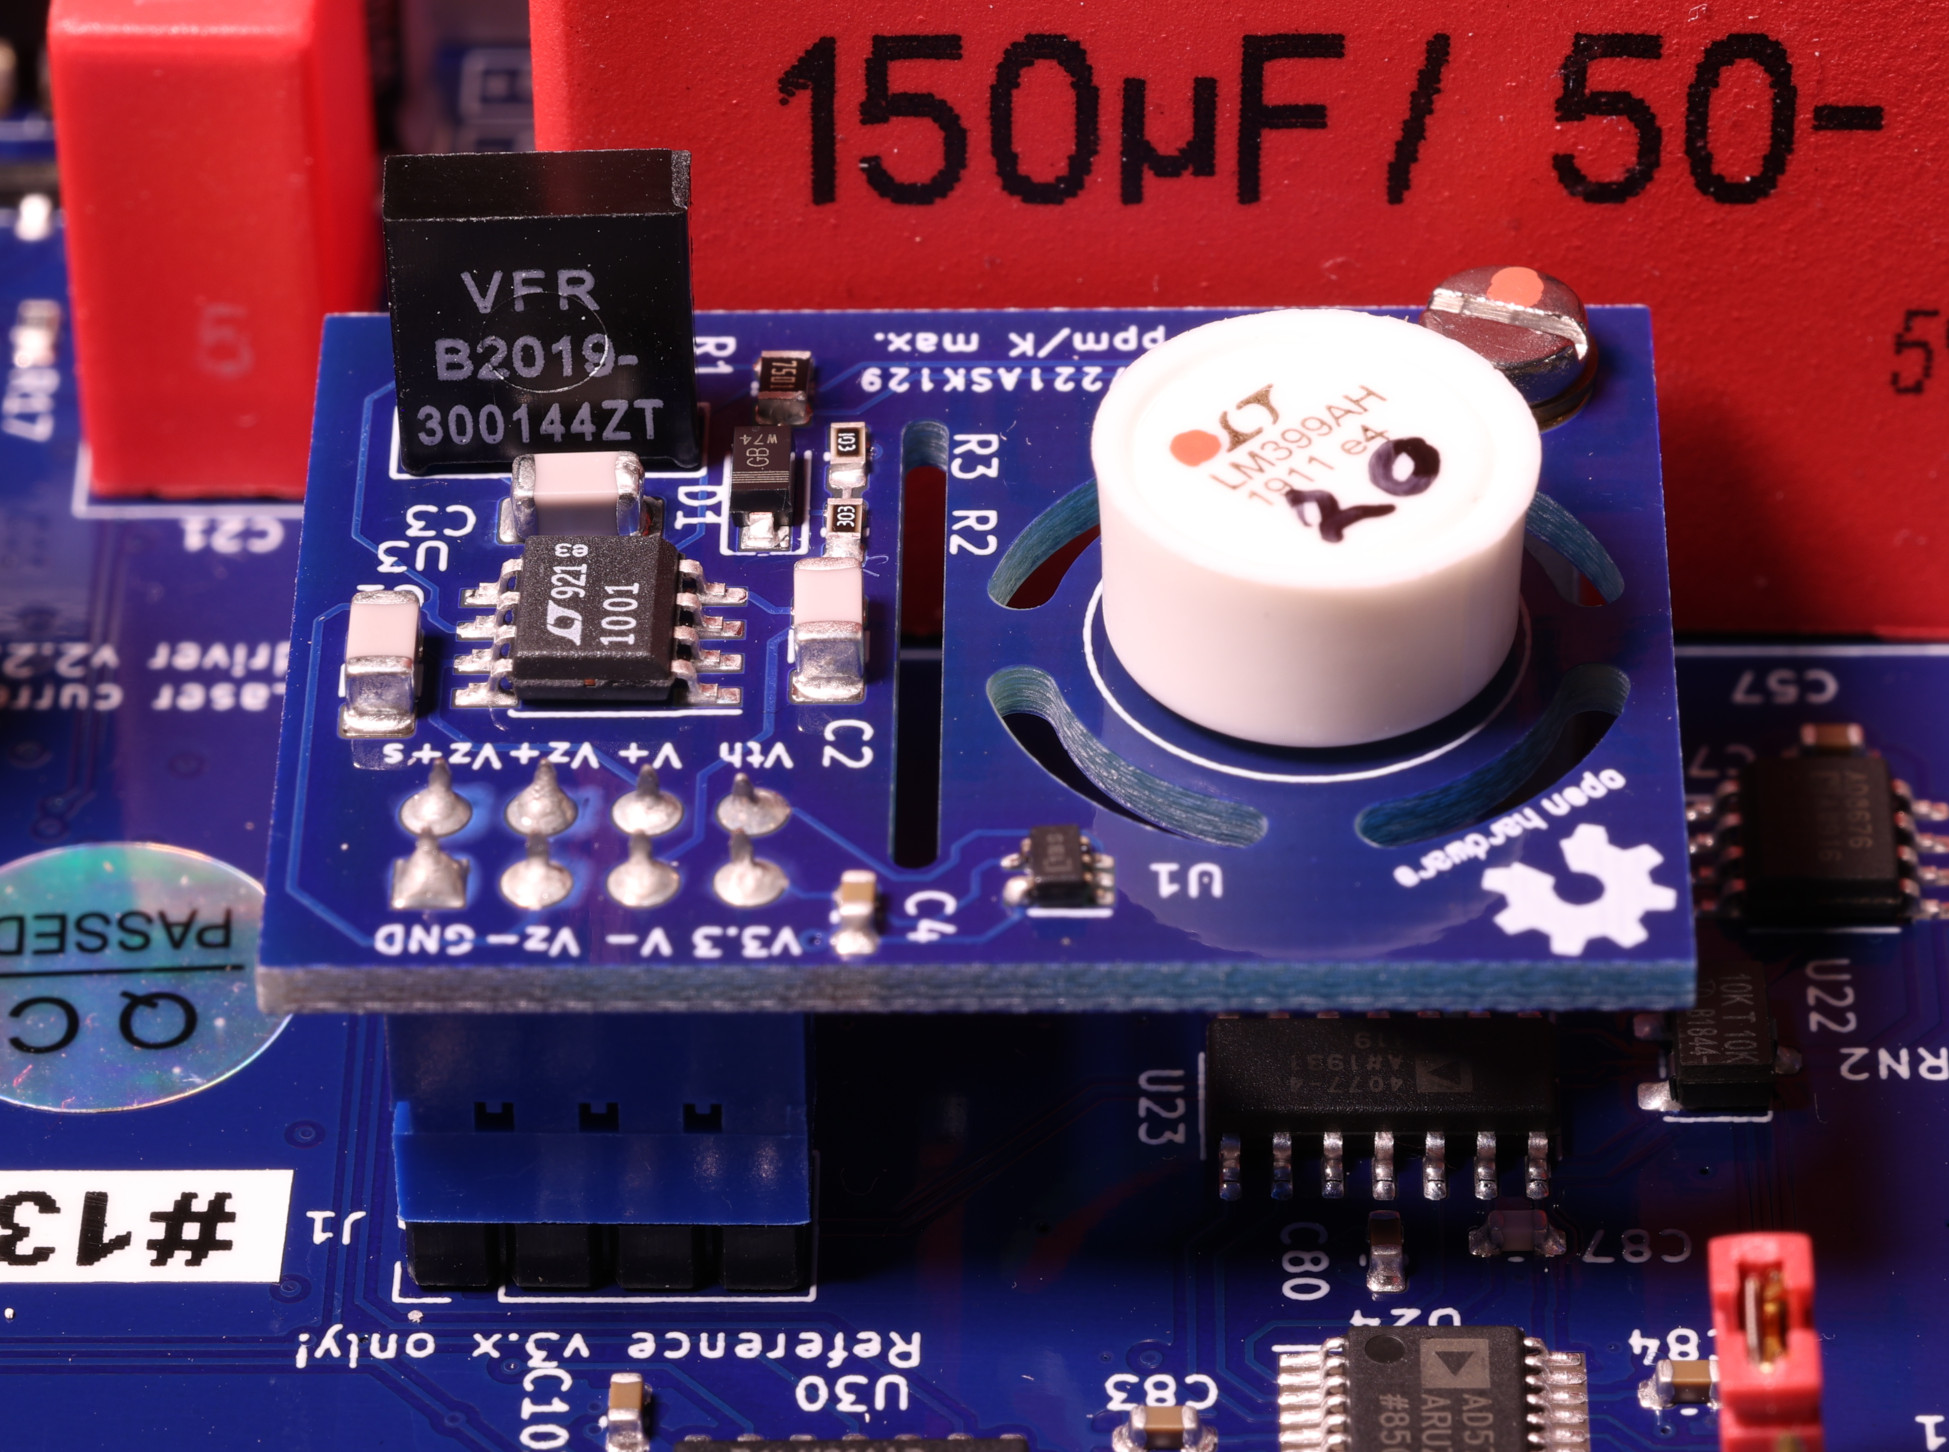
\includegraphics[width=0.75\textwidth]{images/BM1A6694_reference_15V_lowres.JPG}
    \caption{The voltage reference module mounted on its socket on the main current driver PCB. \device{LM399} no. 20 is marked with a red dot because it passed quality control. In the background, the large red filter capacitor can be seen.}
    \label{fig:reference_module_pcb}
\end{figure}

\subsection{Precision Current Source}
\label{sec:results_precision_current_source}
The theory behind the precision current source was laid out in section \ref{sec:precision_current_source}, but some interesting details were not discussed yet. One of the main drawbacks of the current source from section \ref{sec:precision_current_source} is that the setpoint has a direct impact on the compliance voltage as discussed in section \ref{sec:compliance_voltage}. Given an input supply voltage of \qty{15}{\V} it is immediately evident that with a reference voltage of \qty{7.5}{\V} a compliance voltage of \qty{8}{\V} as defined in specification \ref{lst:dgDrive_specs_electrical} is impossible to reach.

One solution would be to increase the division ratio after the DAC to three, for example, reducing the reference voltage to \qty{5}{\V}. Unfortunately, this solution increases the current noise by a factor of $\frac{7.5}{5} = 1.5$ according to table \ref{tab:current_source_noise_contributers}, because the sense resistor has to be scaled by the factor of $\frac{2}{3}$ to get the same output current.

Another option is to use the negative \qty{-15}{\V} rail instead of ground to connect the cathode of the laser diode. This would directly increase the compliance voltage by \qty{15}{\V} and include enough headroom for other components of the current source, like the MOSFET. This solution, however, brings along the problem that was discussed in section \ref{sec:current_sink_current_source}. Directly connecting the laser diode to a voltage rail can have catastrophic consequences for the diode in case the other side is accidentally connected to ground.

This work therefore presents a novel third option, which separates the current source from the compliance voltage requirement and enhances the current source shown in figure \ref{fig:precision_current_source} on page \pageref{fig:precision_current_source}. This circuit is shown in figure \ref{fig:dgDrive_current_source}.
\begin{figure}[ht]
    \centering
    %\resizebox {0.8\textwidth} {!} {
        \import{figures/}{dgDrive_current_source.tex}
    %} % resizebox
    \caption{Simplified current source implemented in the digital current driver. The voltage across $R_s$ is Kelvin sensed. The laser diode is wrapped in a feedback loop and the current source is shielded from the load. $U_1$ is an ADI \device{AD797B} and $U_2$ is an ADI \device{ADA4625-1}.}
    \label{fig:dgDrive_current_source}
\end{figure}

This circuit consists of the current source introduced in section \ref{sec:precision_current_source} and a current sink, that wraps the laser diode in a feedback loop to shield the current source from the load. In addition to the circuit shown in section \ref{sec:precision_current_source} in figure \ref{fig:precision_current_source} on page \pageref{fig:precision_current_source}, the sense resistor is connected differently. The sense resistor used is a Vishay \device{VPR221Z} \cite{datasheet_VPR}, a four-terminal device. This allows Kelvin sensing of the voltage across $R_s$. The positive voltage is buffered using several precision ADI \device{ADA4077-4} \cite{datasheet_ADA4077} op-amps. This voltage is then supplied to the voltage reference circuit, the DAC and the divider that follows. It is important that no current is drawn from this net. The negative voltage is sensed by $U_1$, an ADI \device{AD797} (B grade), to close the feedback loop around $R_s$.

To understand the current sink, it is easiest, to assume, for now, $V_{offset} = \qty{0}{\V}$ and the non-inverting input of $U_2$, an ADI \device{ADA4625-1}, is grounded. Applying a setpoint voltage $V_{set}$ to $U_1$ will cause the upper current source to source a current into the virtual ground and the laser diode. This will cause the virtual ground potential to rise and the op-amp $U_2$ will that see a positive voltage at its inverting input. $U_2$ will then pull its output low, pulling the gate of the p-channel MOSFET $Q_2$ low as well, causing the current sink to drain the appropriate amount of current. $U_2$ will always steer $Q_2$ in such a way that the virtual ground is maintained. Do note, that using a p-channel MOSFET for $Q_2$, will put an extra burden on the op-amp $U_2$, because it has to follow the load voltage with its output. Fortunately, remembering the Shockley equation \ref{eqn:shockley} it is clear that the voltage of a diode changes little with the current and this issue can therefore be neglected. On the other hand, using a p-channel MOSFET does not require the op-amp output to go down all the way to the negative diode supply to turn off the MOSFET. The p-channel MOSFET turns off at $V_{offset}-V_{th}$, which is close to \qty{0}{\V}. This arrangement is similar to the concept of a transimpedance amplifier, except that instead of a resistive element in the feedback path, a (laser) diode is used. Putting the laser diode into a feedback loop has a number of advantages, which are discussed below.

The most important one is that the current source does no longer see the load and only has to source the current into a virtual ground. The compliance voltage required from the upper current source is reduced to $V_{offset}$, because this is the voltage at the virtual ground. This also important for the modulation current source because its compliance voltage is limited as well as shown in equation \ref{eqn:howland_current_compliance_voltage}. The compliance voltage, that can be provided by the combined source is increased to more than \qty{10}{\V} with this design, more than adequate to meet the design specifications of \qty{8}{\V} given in specification \ref{lst:dgDrive_specs_electrical}. Using a higher voltage negative supply is also possible to further increase the compliance voltage. The compliance voltage is essentially independent of the upper current source.

The circuitry supplying the voltage for the current source is essentially a voltage source, so additional care must be taken to protect the laser diode. This is where the offset voltage comes into play. Choosing a positive offset is interesting because if the virtual ground is accidentally shorted to the system ground, the inverting input of $U_2$ will be pulled low and the output of $U_2$ will go high, closing the MOSFET $Q_2$, protecting the laser diode. If $V_{offset}$ were negative, $U_2$ would open $Q_2$, likely destroying the laser diode. $V_{offset}$ must therefore always be $\qty{\geq 0}{\V}$. In this design $V_{offset} = \qty{500}{\mV}$ has proven successful, but in future, it may be reduced to around $\qty{100}{\mV}$ for an increased headroom for the MOSFET $Q_1$ in higher current designs. The reduced load voltage seen by the current source is also important for the modulation current source discussed in section \ref{sec:howland_current_source}.

In addition to solving compliance voltage related problems, there is another benefit from this configuration. Since the current source does not see the load, but rather the constant virtual ground, the output impedance is considerably improved. In essence, any change of the virtual ground potential is suppressed by the gain of the op-amp $U_2$, which means the output impedance is multiplied by the open-loop gain of $U_2$. Typically, a gain of \num{e7} at low frequencies can be expected from the \device{ADA4625-1} \cite{datasheet_ADA4625}. The output impedance at this level is no longer limited by the current source, but rather other circuit parasitics. This helps the rather poor output impedance of the Howland current source to meet the requirements stated in specification \ref{lst:dgDrive_specs_electrical}.

There is one downside of this solution though. The laser diode is wrapped in a feedback loop that needs to close around the diode. This means, that the physical size of the loop is (regarding op-amps) enormous, because the laser head is not located on the PCB, but rather separated by several meters of cable, located on an optical table next to the rack. This introduces a considerable phase shift into the control loop at high frequencies. The details of the cabling are discussed in more detail in section \ref{sec:cables_and_connectors}. For now only the propagation speed of light is of interest. The DVI cables used have a velocity factor of \num{0.8} and a typical \qty{3}{\m} cable will therefore cause a delay of about $\tau = \qty{12.5}{\ns}$. The signal has to go through the cable twice, so at \qty{1}{\MHz}, this will introduce a phase delay of
\begin{equation*}
    \theta = 2 \pi \cdot 2 \tau \cdot \qty{1}{\MHz} \approx \frac{\pi}{20} = \qty{9}{\degree} \,.
\end{equation*}

While at \qty{1}{\MHz}, this is not yet critical. The phase delay of $\frac{\pi}{2}$ introduced at \qty{10}{\MHz} will send the control loop into oscillations. The bandwidth of $U_2$ is therefore limited to \qty{1}{\MHz}, which works well with cables of up to \qty{3}{\m}. Longer cables are not compatible with this device and should not be used. More details about the circuit surrounding $U_2$ can be found in the schematics \cite{git_dgDrive}.

The last issue that needs to be discussed is the power dissipation in the sense resistor. This is less problematic for low currents, but at currents of several hundred \unit{\mA} it becomes more and more of a problem. The power lost in the resistors scales linearly with the maximum output current as the maximum setpoint voltage of \qty{7.5}{\V} is fixed. At a full scale output of \qty{500}{\mA}, for example, the sense resistor is required to dissipate \qty{3.75}{\W}. The resistors used are rated for \qty{8}{\W} when mounted on a heat sink, but only at \qty{25}{\celsius} ambient, which is illusory, when mounted inside a box without active cooling. The chassis to which the resistors are bolted will already be warmer than \qty{25}{\celsius} inside a typical rack.

The \qty{8}{\W} maximum is also detrimental to the long-term stability target. The datasheet of the sense resistor gives a maximum load life stability of \qty{150}{\micro \ohm \per \ohm} for \qty{2000}{\hour} at \qty{8}{\W} \cite{datasheet_VPR}  when using a proper heat sink. A technical note from Vishay \cite{ResistorDrift} gives some hints regarding the long-term drift of the older C-Foil resistors. Assuming the Z-foil \device{VPR221Z} resistors behave in a similar way, the load life drift for \qty{30}{\day} (\qty{720}{\hour}) can be estimated as
\begin{equation*}
    \frac{\Delta R}{R}(\qty{30}{\day}, 3\sigma) = \qty{150}{\micro \ohm \per \ohm} \cdot \sqrt[\leftroot{-2}\uproot{2}3]{\frac{720}{2009}} = \qty{107}{\micro \ohm \per \ohm}\,.
\end{equation*}

Using the power derating curve in the datasheet \cite{datasheet_VPR} to estimate a thermal resistance of \qty{14}{\K \per \W} from the metal foil to ambient gives a temperature of \qty{112}{\K} above ambient for an \qty{8}{\W} load. Consulting \cite{ResistorDrift}, such a temperature causes in increase in the drift by a factor of \num{15} when compared to room temperature. Reducing the load to \qty{2}{\W} will decrease the internal temperature of the metal foil considerably to \qty{28}{\K} above ambient and therefore reduces the drift to less than a factor of \num{4} when compared to room temperature. The drift estimated above would then reduce to about \qty{29}{\micro \ohm \per \ohm}, far less than the required \qty{240}{\micro \ohm \per \ohm} as given by specification \ref{lst:dgDrive_specs_environment}, leaving a safe headroom for higher ambient temperatures.

In order to reduce the power lost in the resistor to the desired \qty{2}{\W}, $R_s$ can be split into multiple resistors to distribute the current. While this idea is neither novel nor interesting, it does become so, when looking at it in a different context. Splitting the sense resistor only becomes necessary at currents above a few hundred \unit{mA}. At these currents the sense resistor is of a fairly low value, typically \qty{< 50}{\ohm}, and the current noise of the current source is no longer dominated by the sense resistor. As a reminder, the voltage noise of the \device{AD797} op-amp is \qty{0.9}{\nV \Hz\tothe{-0.5}}. This is the equivalent to a \qty{50}{\ohm} resistor at room temperature. With $R_S < \qty{50}{\ohm}$, the op-amp becomes the dominant noise source of the current source. The voltage noise of the op-amp, in contrast to the thermal noise of the resistor, does see an improvement when averaged. Using $n$ op-amps improves the high frequency noise by a factor of $\sqrt{n}$. This assumes, that the wideband noise is uncorrelated, which should be the case, as any power supply noise is effectively filtered out and the noise is only produced inside the op-amp. At low frequencies, the reference noise still dominates the noise and using a single reference and setpoint DAC, which is fed into both current sources, the noise is correlated and therefore adds normally, so it does not see any improvement using this technique.

The simulation found at \external{source/current\_regulator\_AD797\_noise.asc} can be used to estimate the potential improvement. The simulation gives a more complete picture, because it includes the noise created by the resistors and the feedback network around $U_1$. Table \ref{tab:dual_current_source_noise_comparison} gives the simulated output noise for two solutions of a \qty{500}{\mA} laser driver, one with a single current source and the other with two current sources. The sense resistors in this case are smaller than the \qty{50}{\ohm} discussed above. The single source uses a \qty{15}{\ohm} resistor, while the dual current source solution employs two \qty{30}{\ohm} resistors.
\begin{table}[ht]
    \centering
    \begin{tabular}{lcc}
        \toprule
        & LF Noise \qtyrange[range-phrase=\textup{~to~}]{e-2}{e2}{\Hz}  & HF noise, \qtyrange[range-phrase=\textup{~to~}]{e2}{e5}{\Hz}\\
        \midrule
        Single & \qty{27.2}{\nA_{rms}} & \qty{21.7}{\nA_{rms}}\\
        Dual & \qty{27.2}{\nA_{rms}} &\qty{17.0}{\nA_{rms}}\\
        \bottomrule
    \end{tabular}
    \caption{Noise comparison of a single current source with $R_S = \qty{15}{\ohm}$ and dual current source with $2 \times \qty{30}{\ohm}$, both at \qty{500}{\mA}.}
    \label{tab:dual_current_source_noise_comparison}
\end{table}

From the simulation it can be easily gathered that the high frequency noise of a dual current source design is about $\frac{1}{\sqrt{2}}$ that of a single source design, just as predicted above. The low frequency noise is also not affected as discussed above. In order to improve the frequency noise, a lower noise reference like the \device{ADR1399} must be used. Judging from the datasheet of the \device{LM399} and \device{ADR1399} \cite{datasheet_LM399, datasheet_ADR1399} and preliminary tests, the \device{ADR1399} has \qty{30}{\percent} less noise. While the dual current source design is already very close to the desired \qty{30}{\nA_{rms}} in \qty{100}{\kHz} bandwidth, it is still slightly above the desired target with a total noise of \qty{31.9}{\nA_{rms}}. A low noise reference is therefore key and given the loose datasheet specifications of those references, selecting them for low noise is important. This is discussed in section \ref{sec:zener_diode_selection}.

Using a second current source also helps with reducing the statistical spread of both the drift and the temperature coefficient of the sense resistor and the \device{AD797} op-amp $U_1$. While the datasheet of the sense resistor gives a \textit{typical} value of \qty{\pm 0.05}{\micro\ohm \per \ohm \per \K}, the $3\sigma$ range is more like \qty{\pm 2}{\micro\ohm \per \ohm \per \K} \cite{ResistorTCR}. Using two current sources results an inherent statistical averaging regarding the temperature coefficient, making the \qty{1}{\uA \per \A \per \K} target of specification \ref{lst:dgDrive_specs_environment} easier to reach.
\begin{table}[hb]
    \centering
    \begin{tabular}{lcc}
        \toprule
        Configuration & Sense resistor value & Maximum current\\
        \midrule
        \device{DgDrive-150} & \qty{50}{\ohm} & \qty{150}{\mA}\\
        \device{DgDrive-250} & \qty{30}{\ohm} & \qty{250}{\mA}\\
        \device{DgDrive-300-LN} & $2 \times \qty{50}{\ohm}$ & \qty{300}{\mA}\\
        \device{DgDrive-500-LN} & $2 \times \qty{30}{\ohm}$ & \qty{500}{\mA}\\
        \bottomrule
    \end{tabular}
    \caption{Different configurations of the digital current driver current tested and built.}
    \label{tab:dgDrive_configurations}
\end{table}

Combining more than two current sources unfortunately yields diminishing returns as the noise scales as $\frac{1}{\sqrt{n}}$, whereas cost and complexity goes with $n$. Therefore a maximum of two current sources are used in this design. Table \ref{tab:dgDrive_configurations} lists the current source configures, that were built for this project. The \device{DgDrive-300-LN}, which is using a \qty{50}{\ohm} resistors is at the limit where adding a second current source has any benefits regarding the wideband noise. The difference in wideband noise is about \qty{15}{\percent} (\qty{13.8}{\nA_{rms}} versus \qty{11.6}{\nA_{rms}}) when comparing the simulation against a \qty{25}{\ohm} configuration. Only two of these units were built to test the extra stability added by the statistical averaging scheme.

A final note regarding the second current source and the Kelvin sensing mentioned above. As discussed above and shown in figure \ref{fig:dgDrive_current_source} one side of the sense resistor feeds the voltage reference to create the setpoint, the other goes to the \device{AD797} to create the current. This is different for the second resistor. The upper sense pin is not used in this case. One could, in theory, connect the sense pins of both resistors via another resistor to the op-amp and average the voltage, but the voltage difference between both pins is small because a copper pour on the PCB connects both resistors and the chance to introduce thermocouples is large.

Noise measurements of the digital current driver in comparison to other current drivers and the simulation results shown above are presented in section \ref{sec:results_current_noise}.

To summarize the results, a novel current source configuration was presented that addresses the limited compliance voltage by removing the load seen by the current source. The compliance voltage in this design is more than \qty{10}{\V}, limited by the power supply rails of \qty{\pm 15}{\V}. In addition, a solution was given to limit the increasing current noise contribution of the op-amp in high output current configurations that use small sense resistors. These results were underpinned by simulations and a simulation model was provided to estimate the expected improvements.
\begin{center}
    \begin{deviceProperties}[label={lst:dgDrive_properties_current_source}]{DgDrive current source}
    \begin{itemize}
        \item Compliance voltage: \qty{10}{\V}
        \item Long-term drift over \qty{30}{\day}: \qty{<100}{\micro\ohm \per \ohm}
        \item Current noise (\qty{1}{\Hz} to \qty{100}{\kHz}), \device{DgDrive-250}: \qty{19}{\nA_{rms}}
        \item Current noise (\qty{1}{\Hz} to \qty{100}{\kHz}), \device{DgDrive-500-LN}: \qty{19}{\nA_{rms}}
    \end{itemize}
    \end{deviceProperties}
\end{center}

\subsection{Modulation Current Source}%
\label{sec:modulation_current_source}
Several options for the modulation current source are presented in literature. Some designs use a simple AC coupled input \cite{diodelaser_modulation,libbrecht_hall}, which drastically reduces the high-frequency output impedance of the current source. Others use a JFET in parallel to the laser diode to divert some of the current \cite{laser_modulation_jfet,laser_modulation_jfet2,laser_modulation_jfet_appel}, which causes poor DC performance due to the missing feedback loop. \citeauthor{libbrecht_hall} \cite{laser_driver_digital,libbrecht_hall} in addition to the AC coupled input also presented a more rugged approach similar to a Howland current source, which delivers a reasonable DC performance and a claimed bandwidth of more than \qty{10}{\MHz}. The modulation circuit shown by \citeauthor{libbrecht_hall} is likely an update of an earlier version of the same laser driver printed in the paper of \citeauthor{diodelaser_modulation} \cite{diodelaser_modulation}, which would explain the rather peculiar arrangement. This circuit is shown in figure \ref{fig:libbrecht_hall_current_source} and will be discussed in more detail, because it also used in the legacy laser drivers found in this group.
\begin{figure}[ht]
    \centering
    %\scalebox{0.5} % scalebox
    \caption{The modulation current source used by \cite{laser_driver_digital,libbrecht_hall}. $R_1 = R_2 = R_3 = R_4 = \qty{1}{\kilo\ohm}$ are matched resistors. $\frac{R_5}{2} = R_6 = R_7 = R_8 = \qty{1}{\kilo\ohm}$. $C_1 = \qty{1}{\uF}$ $R_{t} = \qty{54}{\ohm}$ is optional.}
    \label{fig:libbrecht_hall_current_source}
\end{figure}

Looking at figure \ref{fig:libbrecht_hall_current_source}, the current source can be identified as the classic HCS. The Howland current source does require a very low impedance input $V_{in}$, because otherwise the tight matching of the four resistors $R_1 = R_2 = R_3 = R_4$ is imbalanced. This brings about a problem with an external input, having to either short the input to ground or keep it connected to a low impedance source at all times. If the input were kept open one side of the Howland current source would be imbalanced thus creating an offset current. \citeauthor{libbrecht_hall} addressed this problem by using an inverting amplifier $U_2$ to invert the output of $U_1$. Since the output current of $U_1$ is equally divided between one trace going to the inverting input of $U_1$ via $R_4$ and $R_3$ and the other trace with $R_1$ and $R_2$, the current that $U_2$ injects into the input trace must be divided by half, hence $R_5 = 2 \cdot R_x$. $R_x$ being the value used by the Howland current source. The resistor $R_8$ does not serve any immediate purpose. The design by \citeauthor{libbrecht_hall} uses the \device{OP07} \cite{datasheet_OP07} precision op-amp for both $U_1$ and $U_2$. This op-amp does have an internal bias current compensation scheme\footnote{This detail can either be read from the simplified schematic as there is a current source feeding into both inputs or from the input offset current and input bias current specification. The offset current is about the same as the bias current and does not have a defined polarity indicating the possibility of over- and undercompensation.} so its input bias current is very low and on the order of a few \unit{\nA}. This makes one wonder about the purpose of the resistor $R_8$, which is not only the wrong value for a compensation resistor, as it should be $R_8 = R_6 || R_7 = \qty{500}{\ohm}$, but also pretty much unneeded. This could be relic from an earlier design stage with different op-amps. The matching of the resistors $\frac{R_5}{2} = R_6 = R_7 = R_x$ fortunately does not need to be as tight as the ones of the HCS as discussed in section \ref{sec:howland_current_source}, because $U_2$ forms an inverting amplifier with gain $A_2 = \frac{R_6}{R_7} \approx -1$ and feeds back a current of $\frac{A_2 \cdot V_{o,U1}}{R_5}$ into the input node. The error current is then distributed between the input source and the HCS, so only the fraction $R_1 || R_{in}$ of the error current flows into $R_1$ and the HCS. For example, assuming a modulation source has an output impedance of \qty{50}{\ohm}, the error current flowing into $R_1$ is attenuated by a factor of $\frac{1}{47}$, relaxing the requirements of the matched resistor network by the same factor.

An issue that can be identified with the above circuit is the capacitor $C_1$. It forms a low-pass filter with the cutoff frequency
\begin{equation*}
    f_c = \frac{1}{2 \pi R_6 C_1} \approx \qty{159}{\Hz}
\end{equation*}
for $R_6 = \qty{1}{\kilo\ohm}$ and $C_1 = \qty{1}{\uF}$ as given in \cite{laser_driver_digital,libbrecht_hall}. This has two detrimental effects as it offsets the careful balance created by the feedback of $U_2$. First, it will dramatically decrease the output impedance of the current source. It was already shown in appendix \ref{sec:appendix_howland_current_source}, that the Howland current source is very sensitive to an imbalance of the resistor ratios and if the feedback of $U_2$ is reduced, the output impedance of the source starts playing a role. This effect can be seen in figure \ref{fig:output_impedance_libbrecht_hall}, which shows an LTSpice simulation of the circuit shown in figure \ref{fig:libbrecht_hall_current_source} with a \qty{50}{\ohm} source at the modulation input. The fast modulation input found in \cite{libbrecht_hall} was omitted in the simulation, but it would introduce an additional limit of \qty{10}{\kilo\ohm} above \qty{1.59}{\kHz} to ($CR=\qty{10}{\nF} \cdot \qty{10}{\kilo\ohm}$). The simulation file can be found at \external{source/spice/modulation\_input\_LibrechtHall.asc}.
\begin{figure}[hb]
    \centering
    %% Creator: Matplotlib, PGF backend
%%
%% To include the figure in your LaTeX document, write
%%   \input{<filename>.pgf}
%%
%% Make sure the required packages are loaded in your preamble
%%   \usepackage{pgf}
%%
%% Also ensure that all the required font packages are loaded; for instance,
%% the lmodern package is sometimes necessary when using math font.
%%   \usepackage{lmodern}
%%
%% Figures using additional raster images can only be included by \input if
%% they are in the same directory as the main LaTeX file. For loading figures
%% from other directories you can use the `import` package
%%   \usepackage{import}
%%
%% and then include the figures with
%%   \import{<path to file>}{<filename>.pgf}
%%
%% Matplotlib used the following preamble
%%   \usepackage{siunitx}
%%   \usepackage{fontspec}
%%   \makeatletter\@ifpackageloaded{underscore}{}{\usepackage[strings]{underscore}}\makeatother
%%
\begingroup%
\makeatletter%
\begin{pgfpicture}%
\pgfpathrectangle{\pgfpointorigin}{\pgfqpoint{5.431103in}{3.356606in}}%
\pgfusepath{use as bounding box, clip}%
\begin{pgfscope}%
\pgfsetbuttcap%
\pgfsetmiterjoin%
\definecolor{currentfill}{rgb}{1.000000,1.000000,1.000000}%
\pgfsetfillcolor{currentfill}%
\pgfsetlinewidth{0.000000pt}%
\definecolor{currentstroke}{rgb}{1.000000,1.000000,1.000000}%
\pgfsetstrokecolor{currentstroke}%
\pgfsetdash{}{0pt}%
\pgfpathmoveto{\pgfqpoint{0.000000in}{0.000000in}}%
\pgfpathlineto{\pgfqpoint{5.431103in}{0.000000in}}%
\pgfpathlineto{\pgfqpoint{5.431103in}{3.356606in}}%
\pgfpathlineto{\pgfqpoint{0.000000in}{3.356606in}}%
\pgfpathlineto{\pgfqpoint{0.000000in}{0.000000in}}%
\pgfpathclose%
\pgfusepath{fill}%
\end{pgfscope}%
\begin{pgfscope}%
\pgfsetbuttcap%
\pgfsetmiterjoin%
\definecolor{currentfill}{rgb}{1.000000,1.000000,1.000000}%
\pgfsetfillcolor{currentfill}%
\pgfsetlinewidth{0.000000pt}%
\definecolor{currentstroke}{rgb}{0.000000,0.000000,0.000000}%
\pgfsetstrokecolor{currentstroke}%
\pgfsetstrokeopacity{0.000000}%
\pgfsetdash{}{0pt}%
\pgfpathmoveto{\pgfqpoint{0.594124in}{0.524170in}}%
\pgfpathlineto{\pgfqpoint{5.281103in}{0.524170in}}%
\pgfpathlineto{\pgfqpoint{5.281103in}{3.206606in}}%
\pgfpathlineto{\pgfqpoint{0.594124in}{3.206606in}}%
\pgfpathlineto{\pgfqpoint{0.594124in}{0.524170in}}%
\pgfpathclose%
\pgfusepath{fill}%
\end{pgfscope}%
\begin{pgfscope}%
\pgfpathrectangle{\pgfqpoint{0.594124in}{0.524170in}}{\pgfqpoint{4.686978in}{2.682436in}}%
\pgfusepath{clip}%
\pgfsetrectcap%
\pgfsetroundjoin%
\pgfsetlinewidth{0.803000pt}%
\definecolor{currentstroke}{rgb}{0.450000,0.450000,0.450000}%
\pgfsetstrokecolor{currentstroke}%
\pgfsetdash{}{0pt}%
\pgfpathmoveto{\pgfqpoint{1.339780in}{0.524170in}}%
\pgfpathlineto{\pgfqpoint{1.339780in}{3.206606in}}%
\pgfusepath{stroke}%
\end{pgfscope}%
\begin{pgfscope}%
\pgfsetbuttcap%
\pgfsetroundjoin%
\definecolor{currentfill}{rgb}{0.000000,0.000000,0.000000}%
\pgfsetfillcolor{currentfill}%
\pgfsetlinewidth{0.803000pt}%
\definecolor{currentstroke}{rgb}{0.000000,0.000000,0.000000}%
\pgfsetstrokecolor{currentstroke}%
\pgfsetdash{}{0pt}%
\pgfsys@defobject{currentmarker}{\pgfqpoint{0.000000in}{-0.048611in}}{\pgfqpoint{0.000000in}{0.000000in}}{%
\pgfpathmoveto{\pgfqpoint{0.000000in}{0.000000in}}%
\pgfpathlineto{\pgfqpoint{0.000000in}{-0.048611in}}%
\pgfusepath{stroke,fill}%
}%
\begin{pgfscope}%
\pgfsys@transformshift{1.339780in}{0.524170in}%
\pgfsys@useobject{currentmarker}{}%
\end{pgfscope}%
\end{pgfscope}%
\begin{pgfscope}%
\definecolor{textcolor}{rgb}{0.000000,0.000000,0.000000}%
\pgfsetstrokecolor{textcolor}%
\pgfsetfillcolor{textcolor}%
\pgftext[x=1.339780in,y=0.426948in,,top]{\color{textcolor}\rmfamily\fontsize{8.000000}{9.600000}\selectfont \(\displaystyle {10^{0}}\)}%
\end{pgfscope}%
\begin{pgfscope}%
\pgfpathrectangle{\pgfqpoint{0.594124in}{0.524170in}}{\pgfqpoint{4.686978in}{2.682436in}}%
\pgfusepath{clip}%
\pgfsetrectcap%
\pgfsetroundjoin%
\pgfsetlinewidth{0.803000pt}%
\definecolor{currentstroke}{rgb}{0.450000,0.450000,0.450000}%
\pgfsetstrokecolor{currentstroke}%
\pgfsetdash{}{0pt}%
\pgfpathmoveto{\pgfqpoint{2.405002in}{0.524170in}}%
\pgfpathlineto{\pgfqpoint{2.405002in}{3.206606in}}%
\pgfusepath{stroke}%
\end{pgfscope}%
\begin{pgfscope}%
\pgfsetbuttcap%
\pgfsetroundjoin%
\definecolor{currentfill}{rgb}{0.000000,0.000000,0.000000}%
\pgfsetfillcolor{currentfill}%
\pgfsetlinewidth{0.803000pt}%
\definecolor{currentstroke}{rgb}{0.000000,0.000000,0.000000}%
\pgfsetstrokecolor{currentstroke}%
\pgfsetdash{}{0pt}%
\pgfsys@defobject{currentmarker}{\pgfqpoint{0.000000in}{-0.048611in}}{\pgfqpoint{0.000000in}{0.000000in}}{%
\pgfpathmoveto{\pgfqpoint{0.000000in}{0.000000in}}%
\pgfpathlineto{\pgfqpoint{0.000000in}{-0.048611in}}%
\pgfusepath{stroke,fill}%
}%
\begin{pgfscope}%
\pgfsys@transformshift{2.405002in}{0.524170in}%
\pgfsys@useobject{currentmarker}{}%
\end{pgfscope}%
\end{pgfscope}%
\begin{pgfscope}%
\definecolor{textcolor}{rgb}{0.000000,0.000000,0.000000}%
\pgfsetstrokecolor{textcolor}%
\pgfsetfillcolor{textcolor}%
\pgftext[x=2.405002in,y=0.426948in,,top]{\color{textcolor}\rmfamily\fontsize{8.000000}{9.600000}\selectfont \(\displaystyle {10^{2}}\)}%
\end{pgfscope}%
\begin{pgfscope}%
\pgfpathrectangle{\pgfqpoint{0.594124in}{0.524170in}}{\pgfqpoint{4.686978in}{2.682436in}}%
\pgfusepath{clip}%
\pgfsetrectcap%
\pgfsetroundjoin%
\pgfsetlinewidth{0.803000pt}%
\definecolor{currentstroke}{rgb}{0.450000,0.450000,0.450000}%
\pgfsetstrokecolor{currentstroke}%
\pgfsetdash{}{0pt}%
\pgfpathmoveto{\pgfqpoint{3.470225in}{0.524170in}}%
\pgfpathlineto{\pgfqpoint{3.470225in}{3.206606in}}%
\pgfusepath{stroke}%
\end{pgfscope}%
\begin{pgfscope}%
\pgfsetbuttcap%
\pgfsetroundjoin%
\definecolor{currentfill}{rgb}{0.000000,0.000000,0.000000}%
\pgfsetfillcolor{currentfill}%
\pgfsetlinewidth{0.803000pt}%
\definecolor{currentstroke}{rgb}{0.000000,0.000000,0.000000}%
\pgfsetstrokecolor{currentstroke}%
\pgfsetdash{}{0pt}%
\pgfsys@defobject{currentmarker}{\pgfqpoint{0.000000in}{-0.048611in}}{\pgfqpoint{0.000000in}{0.000000in}}{%
\pgfpathmoveto{\pgfqpoint{0.000000in}{0.000000in}}%
\pgfpathlineto{\pgfqpoint{0.000000in}{-0.048611in}}%
\pgfusepath{stroke,fill}%
}%
\begin{pgfscope}%
\pgfsys@transformshift{3.470225in}{0.524170in}%
\pgfsys@useobject{currentmarker}{}%
\end{pgfscope}%
\end{pgfscope}%
\begin{pgfscope}%
\definecolor{textcolor}{rgb}{0.000000,0.000000,0.000000}%
\pgfsetstrokecolor{textcolor}%
\pgfsetfillcolor{textcolor}%
\pgftext[x=3.470225in,y=0.426948in,,top]{\color{textcolor}\rmfamily\fontsize{8.000000}{9.600000}\selectfont \(\displaystyle {10^{4}}\)}%
\end{pgfscope}%
\begin{pgfscope}%
\pgfpathrectangle{\pgfqpoint{0.594124in}{0.524170in}}{\pgfqpoint{4.686978in}{2.682436in}}%
\pgfusepath{clip}%
\pgfsetrectcap%
\pgfsetroundjoin%
\pgfsetlinewidth{0.803000pt}%
\definecolor{currentstroke}{rgb}{0.450000,0.450000,0.450000}%
\pgfsetstrokecolor{currentstroke}%
\pgfsetdash{}{0pt}%
\pgfpathmoveto{\pgfqpoint{4.535447in}{0.524170in}}%
\pgfpathlineto{\pgfqpoint{4.535447in}{3.206606in}}%
\pgfusepath{stroke}%
\end{pgfscope}%
\begin{pgfscope}%
\pgfsetbuttcap%
\pgfsetroundjoin%
\definecolor{currentfill}{rgb}{0.000000,0.000000,0.000000}%
\pgfsetfillcolor{currentfill}%
\pgfsetlinewidth{0.803000pt}%
\definecolor{currentstroke}{rgb}{0.000000,0.000000,0.000000}%
\pgfsetstrokecolor{currentstroke}%
\pgfsetdash{}{0pt}%
\pgfsys@defobject{currentmarker}{\pgfqpoint{0.000000in}{-0.048611in}}{\pgfqpoint{0.000000in}{0.000000in}}{%
\pgfpathmoveto{\pgfqpoint{0.000000in}{0.000000in}}%
\pgfpathlineto{\pgfqpoint{0.000000in}{-0.048611in}}%
\pgfusepath{stroke,fill}%
}%
\begin{pgfscope}%
\pgfsys@transformshift{4.535447in}{0.524170in}%
\pgfsys@useobject{currentmarker}{}%
\end{pgfscope}%
\end{pgfscope}%
\begin{pgfscope}%
\definecolor{textcolor}{rgb}{0.000000,0.000000,0.000000}%
\pgfsetstrokecolor{textcolor}%
\pgfsetfillcolor{textcolor}%
\pgftext[x=4.535447in,y=0.426948in,,top]{\color{textcolor}\rmfamily\fontsize{8.000000}{9.600000}\selectfont \(\displaystyle {10^{6}}\)}%
\end{pgfscope}%
\begin{pgfscope}%
\definecolor{textcolor}{rgb}{0.000000,0.000000,0.000000}%
\pgfsetstrokecolor{textcolor}%
\pgfsetfillcolor{textcolor}%
\pgftext[x=2.937613in,y=0.271531in,,top]{\color{textcolor}\rmfamily\fontsize{10.000000}{12.000000}\selectfont Frequency in \unit{\Hz}}%
\end{pgfscope}%
\begin{pgfscope}%
\pgfpathrectangle{\pgfqpoint{0.594124in}{0.524170in}}{\pgfqpoint{4.686978in}{2.682436in}}%
\pgfusepath{clip}%
\pgfsetrectcap%
\pgfsetroundjoin%
\pgfsetlinewidth{0.803000pt}%
\definecolor{currentstroke}{rgb}{0.450000,0.450000,0.450000}%
\pgfsetstrokecolor{currentstroke}%
\pgfsetdash{}{0pt}%
\pgfpathmoveto{\pgfqpoint{0.594124in}{0.892138in}}%
\pgfpathlineto{\pgfqpoint{5.281103in}{0.892138in}}%
\pgfusepath{stroke}%
\end{pgfscope}%
\begin{pgfscope}%
\pgfsetbuttcap%
\pgfsetroundjoin%
\definecolor{currentfill}{rgb}{0.000000,0.000000,0.000000}%
\pgfsetfillcolor{currentfill}%
\pgfsetlinewidth{0.803000pt}%
\definecolor{currentstroke}{rgb}{0.000000,0.000000,0.000000}%
\pgfsetstrokecolor{currentstroke}%
\pgfsetdash{}{0pt}%
\pgfsys@defobject{currentmarker}{\pgfqpoint{-0.048611in}{0.000000in}}{\pgfqpoint{-0.000000in}{0.000000in}}{%
\pgfpathmoveto{\pgfqpoint{-0.000000in}{0.000000in}}%
\pgfpathlineto{\pgfqpoint{-0.048611in}{0.000000in}}%
\pgfusepath{stroke,fill}%
}%
\begin{pgfscope}%
\pgfsys@transformshift{0.594124in}{0.892138in}%
\pgfsys@useobject{currentmarker}{}%
\end{pgfscope}%
\end{pgfscope}%
\begin{pgfscope}%
\definecolor{textcolor}{rgb}{0.000000,0.000000,0.000000}%
\pgfsetstrokecolor{textcolor}%
\pgfsetfillcolor{textcolor}%
\pgftext[x=0.320975in, y=0.852986in, left, base]{\color{textcolor}\rmfamily\fontsize{8.000000}{9.600000}\selectfont \(\displaystyle {10^{3}}\)}%
\end{pgfscope}%
\begin{pgfscope}%
\pgfpathrectangle{\pgfqpoint{0.594124in}{0.524170in}}{\pgfqpoint{4.686978in}{2.682436in}}%
\pgfusepath{clip}%
\pgfsetrectcap%
\pgfsetroundjoin%
\pgfsetlinewidth{0.803000pt}%
\definecolor{currentstroke}{rgb}{0.450000,0.450000,0.450000}%
\pgfsetstrokecolor{currentstroke}%
\pgfsetdash{}{0pt}%
\pgfpathmoveto{\pgfqpoint{0.594124in}{1.511904in}}%
\pgfpathlineto{\pgfqpoint{5.281103in}{1.511904in}}%
\pgfusepath{stroke}%
\end{pgfscope}%
\begin{pgfscope}%
\pgfsetbuttcap%
\pgfsetroundjoin%
\definecolor{currentfill}{rgb}{0.000000,0.000000,0.000000}%
\pgfsetfillcolor{currentfill}%
\pgfsetlinewidth{0.803000pt}%
\definecolor{currentstroke}{rgb}{0.000000,0.000000,0.000000}%
\pgfsetstrokecolor{currentstroke}%
\pgfsetdash{}{0pt}%
\pgfsys@defobject{currentmarker}{\pgfqpoint{-0.048611in}{0.000000in}}{\pgfqpoint{-0.000000in}{0.000000in}}{%
\pgfpathmoveto{\pgfqpoint{-0.000000in}{0.000000in}}%
\pgfpathlineto{\pgfqpoint{-0.048611in}{0.000000in}}%
\pgfusepath{stroke,fill}%
}%
\begin{pgfscope}%
\pgfsys@transformshift{0.594124in}{1.511904in}%
\pgfsys@useobject{currentmarker}{}%
\end{pgfscope}%
\end{pgfscope}%
\begin{pgfscope}%
\definecolor{textcolor}{rgb}{0.000000,0.000000,0.000000}%
\pgfsetstrokecolor{textcolor}%
\pgfsetfillcolor{textcolor}%
\pgftext[x=0.320975in, y=1.472751in, left, base]{\color{textcolor}\rmfamily\fontsize{8.000000}{9.600000}\selectfont \(\displaystyle {10^{4}}\)}%
\end{pgfscope}%
\begin{pgfscope}%
\pgfpathrectangle{\pgfqpoint{0.594124in}{0.524170in}}{\pgfqpoint{4.686978in}{2.682436in}}%
\pgfusepath{clip}%
\pgfsetrectcap%
\pgfsetroundjoin%
\pgfsetlinewidth{0.803000pt}%
\definecolor{currentstroke}{rgb}{0.450000,0.450000,0.450000}%
\pgfsetstrokecolor{currentstroke}%
\pgfsetdash{}{0pt}%
\pgfpathmoveto{\pgfqpoint{0.594124in}{2.131670in}}%
\pgfpathlineto{\pgfqpoint{5.281103in}{2.131670in}}%
\pgfusepath{stroke}%
\end{pgfscope}%
\begin{pgfscope}%
\pgfsetbuttcap%
\pgfsetroundjoin%
\definecolor{currentfill}{rgb}{0.000000,0.000000,0.000000}%
\pgfsetfillcolor{currentfill}%
\pgfsetlinewidth{0.803000pt}%
\definecolor{currentstroke}{rgb}{0.000000,0.000000,0.000000}%
\pgfsetstrokecolor{currentstroke}%
\pgfsetdash{}{0pt}%
\pgfsys@defobject{currentmarker}{\pgfqpoint{-0.048611in}{0.000000in}}{\pgfqpoint{-0.000000in}{0.000000in}}{%
\pgfpathmoveto{\pgfqpoint{-0.000000in}{0.000000in}}%
\pgfpathlineto{\pgfqpoint{-0.048611in}{0.000000in}}%
\pgfusepath{stroke,fill}%
}%
\begin{pgfscope}%
\pgfsys@transformshift{0.594124in}{2.131670in}%
\pgfsys@useobject{currentmarker}{}%
\end{pgfscope}%
\end{pgfscope}%
\begin{pgfscope}%
\definecolor{textcolor}{rgb}{0.000000,0.000000,0.000000}%
\pgfsetstrokecolor{textcolor}%
\pgfsetfillcolor{textcolor}%
\pgftext[x=0.320975in, y=2.092517in, left, base]{\color{textcolor}\rmfamily\fontsize{8.000000}{9.600000}\selectfont \(\displaystyle {10^{5}}\)}%
\end{pgfscope}%
\begin{pgfscope}%
\pgfpathrectangle{\pgfqpoint{0.594124in}{0.524170in}}{\pgfqpoint{4.686978in}{2.682436in}}%
\pgfusepath{clip}%
\pgfsetrectcap%
\pgfsetroundjoin%
\pgfsetlinewidth{0.803000pt}%
\definecolor{currentstroke}{rgb}{0.450000,0.450000,0.450000}%
\pgfsetstrokecolor{currentstroke}%
\pgfsetdash{}{0pt}%
\pgfpathmoveto{\pgfqpoint{0.594124in}{2.751436in}}%
\pgfpathlineto{\pgfqpoint{5.281103in}{2.751436in}}%
\pgfusepath{stroke}%
\end{pgfscope}%
\begin{pgfscope}%
\pgfsetbuttcap%
\pgfsetroundjoin%
\definecolor{currentfill}{rgb}{0.000000,0.000000,0.000000}%
\pgfsetfillcolor{currentfill}%
\pgfsetlinewidth{0.803000pt}%
\definecolor{currentstroke}{rgb}{0.000000,0.000000,0.000000}%
\pgfsetstrokecolor{currentstroke}%
\pgfsetdash{}{0pt}%
\pgfsys@defobject{currentmarker}{\pgfqpoint{-0.048611in}{0.000000in}}{\pgfqpoint{-0.000000in}{0.000000in}}{%
\pgfpathmoveto{\pgfqpoint{-0.000000in}{0.000000in}}%
\pgfpathlineto{\pgfqpoint{-0.048611in}{0.000000in}}%
\pgfusepath{stroke,fill}%
}%
\begin{pgfscope}%
\pgfsys@transformshift{0.594124in}{2.751436in}%
\pgfsys@useobject{currentmarker}{}%
\end{pgfscope}%
\end{pgfscope}%
\begin{pgfscope}%
\definecolor{textcolor}{rgb}{0.000000,0.000000,0.000000}%
\pgfsetstrokecolor{textcolor}%
\pgfsetfillcolor{textcolor}%
\pgftext[x=0.320975in, y=2.712283in, left, base]{\color{textcolor}\rmfamily\fontsize{8.000000}{9.600000}\selectfont \(\displaystyle {10^{6}}\)}%
\end{pgfscope}%
\begin{pgfscope}%
\pgfpathrectangle{\pgfqpoint{0.594124in}{0.524170in}}{\pgfqpoint{4.686978in}{2.682436in}}%
\pgfusepath{clip}%
\pgfsetrectcap%
\pgfsetroundjoin%
\pgfsetlinewidth{0.803000pt}%
\definecolor{currentstroke}{rgb}{0.850000,0.850000,0.850000}%
\pgfsetstrokecolor{currentstroke}%
\pgfsetdash{}{0pt}%
\pgfpathmoveto{\pgfqpoint{0.594124in}{0.568076in}}%
\pgfpathlineto{\pgfqpoint{5.281103in}{0.568076in}}%
\pgfusepath{stroke}%
\end{pgfscope}%
\begin{pgfscope}%
\pgfsetbuttcap%
\pgfsetroundjoin%
\definecolor{currentfill}{rgb}{0.000000,0.000000,0.000000}%
\pgfsetfillcolor{currentfill}%
\pgfsetlinewidth{0.602250pt}%
\definecolor{currentstroke}{rgb}{0.000000,0.000000,0.000000}%
\pgfsetstrokecolor{currentstroke}%
\pgfsetdash{}{0pt}%
\pgfsys@defobject{currentmarker}{\pgfqpoint{-0.027778in}{0.000000in}}{\pgfqpoint{-0.000000in}{0.000000in}}{%
\pgfpathmoveto{\pgfqpoint{-0.000000in}{0.000000in}}%
\pgfpathlineto{\pgfqpoint{-0.027778in}{0.000000in}}%
\pgfusepath{stroke,fill}%
}%
\begin{pgfscope}%
\pgfsys@transformshift{0.594124in}{0.568076in}%
\pgfsys@useobject{currentmarker}{}%
\end{pgfscope}%
\end{pgfscope}%
\begin{pgfscope}%
\pgfpathrectangle{\pgfqpoint{0.594124in}{0.524170in}}{\pgfqpoint{4.686978in}{2.682436in}}%
\pgfusepath{clip}%
\pgfsetrectcap%
\pgfsetroundjoin%
\pgfsetlinewidth{0.803000pt}%
\definecolor{currentstroke}{rgb}{0.850000,0.850000,0.850000}%
\pgfsetstrokecolor{currentstroke}%
\pgfsetdash{}{0pt}%
\pgfpathmoveto{\pgfqpoint{0.594124in}{0.645509in}}%
\pgfpathlineto{\pgfqpoint{5.281103in}{0.645509in}}%
\pgfusepath{stroke}%
\end{pgfscope}%
\begin{pgfscope}%
\pgfsetbuttcap%
\pgfsetroundjoin%
\definecolor{currentfill}{rgb}{0.000000,0.000000,0.000000}%
\pgfsetfillcolor{currentfill}%
\pgfsetlinewidth{0.602250pt}%
\definecolor{currentstroke}{rgb}{0.000000,0.000000,0.000000}%
\pgfsetstrokecolor{currentstroke}%
\pgfsetdash{}{0pt}%
\pgfsys@defobject{currentmarker}{\pgfqpoint{-0.027778in}{0.000000in}}{\pgfqpoint{-0.000000in}{0.000000in}}{%
\pgfpathmoveto{\pgfqpoint{-0.000000in}{0.000000in}}%
\pgfpathlineto{\pgfqpoint{-0.027778in}{0.000000in}}%
\pgfusepath{stroke,fill}%
}%
\begin{pgfscope}%
\pgfsys@transformshift{0.594124in}{0.645509in}%
\pgfsys@useobject{currentmarker}{}%
\end{pgfscope}%
\end{pgfscope}%
\begin{pgfscope}%
\pgfpathrectangle{\pgfqpoint{0.594124in}{0.524170in}}{\pgfqpoint{4.686978in}{2.682436in}}%
\pgfusepath{clip}%
\pgfsetrectcap%
\pgfsetroundjoin%
\pgfsetlinewidth{0.803000pt}%
\definecolor{currentstroke}{rgb}{0.850000,0.850000,0.850000}%
\pgfsetstrokecolor{currentstroke}%
\pgfsetdash{}{0pt}%
\pgfpathmoveto{\pgfqpoint{0.594124in}{0.705570in}}%
\pgfpathlineto{\pgfqpoint{5.281103in}{0.705570in}}%
\pgfusepath{stroke}%
\end{pgfscope}%
\begin{pgfscope}%
\pgfsetbuttcap%
\pgfsetroundjoin%
\definecolor{currentfill}{rgb}{0.000000,0.000000,0.000000}%
\pgfsetfillcolor{currentfill}%
\pgfsetlinewidth{0.602250pt}%
\definecolor{currentstroke}{rgb}{0.000000,0.000000,0.000000}%
\pgfsetstrokecolor{currentstroke}%
\pgfsetdash{}{0pt}%
\pgfsys@defobject{currentmarker}{\pgfqpoint{-0.027778in}{0.000000in}}{\pgfqpoint{-0.000000in}{0.000000in}}{%
\pgfpathmoveto{\pgfqpoint{-0.000000in}{0.000000in}}%
\pgfpathlineto{\pgfqpoint{-0.027778in}{0.000000in}}%
\pgfusepath{stroke,fill}%
}%
\begin{pgfscope}%
\pgfsys@transformshift{0.594124in}{0.705570in}%
\pgfsys@useobject{currentmarker}{}%
\end{pgfscope}%
\end{pgfscope}%
\begin{pgfscope}%
\pgfpathrectangle{\pgfqpoint{0.594124in}{0.524170in}}{\pgfqpoint{4.686978in}{2.682436in}}%
\pgfusepath{clip}%
\pgfsetrectcap%
\pgfsetroundjoin%
\pgfsetlinewidth{0.803000pt}%
\definecolor{currentstroke}{rgb}{0.850000,0.850000,0.850000}%
\pgfsetstrokecolor{currentstroke}%
\pgfsetdash{}{0pt}%
\pgfpathmoveto{\pgfqpoint{0.594124in}{0.754644in}}%
\pgfpathlineto{\pgfqpoint{5.281103in}{0.754644in}}%
\pgfusepath{stroke}%
\end{pgfscope}%
\begin{pgfscope}%
\pgfsetbuttcap%
\pgfsetroundjoin%
\definecolor{currentfill}{rgb}{0.000000,0.000000,0.000000}%
\pgfsetfillcolor{currentfill}%
\pgfsetlinewidth{0.602250pt}%
\definecolor{currentstroke}{rgb}{0.000000,0.000000,0.000000}%
\pgfsetstrokecolor{currentstroke}%
\pgfsetdash{}{0pt}%
\pgfsys@defobject{currentmarker}{\pgfqpoint{-0.027778in}{0.000000in}}{\pgfqpoint{-0.000000in}{0.000000in}}{%
\pgfpathmoveto{\pgfqpoint{-0.000000in}{0.000000in}}%
\pgfpathlineto{\pgfqpoint{-0.027778in}{0.000000in}}%
\pgfusepath{stroke,fill}%
}%
\begin{pgfscope}%
\pgfsys@transformshift{0.594124in}{0.754644in}%
\pgfsys@useobject{currentmarker}{}%
\end{pgfscope}%
\end{pgfscope}%
\begin{pgfscope}%
\pgfpathrectangle{\pgfqpoint{0.594124in}{0.524170in}}{\pgfqpoint{4.686978in}{2.682436in}}%
\pgfusepath{clip}%
\pgfsetrectcap%
\pgfsetroundjoin%
\pgfsetlinewidth{0.803000pt}%
\definecolor{currentstroke}{rgb}{0.850000,0.850000,0.850000}%
\pgfsetstrokecolor{currentstroke}%
\pgfsetdash{}{0pt}%
\pgfpathmoveto{\pgfqpoint{0.594124in}{0.796135in}}%
\pgfpathlineto{\pgfqpoint{5.281103in}{0.796135in}}%
\pgfusepath{stroke}%
\end{pgfscope}%
\begin{pgfscope}%
\pgfsetbuttcap%
\pgfsetroundjoin%
\definecolor{currentfill}{rgb}{0.000000,0.000000,0.000000}%
\pgfsetfillcolor{currentfill}%
\pgfsetlinewidth{0.602250pt}%
\definecolor{currentstroke}{rgb}{0.000000,0.000000,0.000000}%
\pgfsetstrokecolor{currentstroke}%
\pgfsetdash{}{0pt}%
\pgfsys@defobject{currentmarker}{\pgfqpoint{-0.027778in}{0.000000in}}{\pgfqpoint{-0.000000in}{0.000000in}}{%
\pgfpathmoveto{\pgfqpoint{-0.000000in}{0.000000in}}%
\pgfpathlineto{\pgfqpoint{-0.027778in}{0.000000in}}%
\pgfusepath{stroke,fill}%
}%
\begin{pgfscope}%
\pgfsys@transformshift{0.594124in}{0.796135in}%
\pgfsys@useobject{currentmarker}{}%
\end{pgfscope}%
\end{pgfscope}%
\begin{pgfscope}%
\pgfpathrectangle{\pgfqpoint{0.594124in}{0.524170in}}{\pgfqpoint{4.686978in}{2.682436in}}%
\pgfusepath{clip}%
\pgfsetrectcap%
\pgfsetroundjoin%
\pgfsetlinewidth{0.803000pt}%
\definecolor{currentstroke}{rgb}{0.850000,0.850000,0.850000}%
\pgfsetstrokecolor{currentstroke}%
\pgfsetdash{}{0pt}%
\pgfpathmoveto{\pgfqpoint{0.594124in}{0.832077in}}%
\pgfpathlineto{\pgfqpoint{5.281103in}{0.832077in}}%
\pgfusepath{stroke}%
\end{pgfscope}%
\begin{pgfscope}%
\pgfsetbuttcap%
\pgfsetroundjoin%
\definecolor{currentfill}{rgb}{0.000000,0.000000,0.000000}%
\pgfsetfillcolor{currentfill}%
\pgfsetlinewidth{0.602250pt}%
\definecolor{currentstroke}{rgb}{0.000000,0.000000,0.000000}%
\pgfsetstrokecolor{currentstroke}%
\pgfsetdash{}{0pt}%
\pgfsys@defobject{currentmarker}{\pgfqpoint{-0.027778in}{0.000000in}}{\pgfqpoint{-0.000000in}{0.000000in}}{%
\pgfpathmoveto{\pgfqpoint{-0.000000in}{0.000000in}}%
\pgfpathlineto{\pgfqpoint{-0.027778in}{0.000000in}}%
\pgfusepath{stroke,fill}%
}%
\begin{pgfscope}%
\pgfsys@transformshift{0.594124in}{0.832077in}%
\pgfsys@useobject{currentmarker}{}%
\end{pgfscope}%
\end{pgfscope}%
\begin{pgfscope}%
\pgfpathrectangle{\pgfqpoint{0.594124in}{0.524170in}}{\pgfqpoint{4.686978in}{2.682436in}}%
\pgfusepath{clip}%
\pgfsetrectcap%
\pgfsetroundjoin%
\pgfsetlinewidth{0.803000pt}%
\definecolor{currentstroke}{rgb}{0.850000,0.850000,0.850000}%
\pgfsetstrokecolor{currentstroke}%
\pgfsetdash{}{0pt}%
\pgfpathmoveto{\pgfqpoint{0.594124in}{0.863779in}}%
\pgfpathlineto{\pgfqpoint{5.281103in}{0.863779in}}%
\pgfusepath{stroke}%
\end{pgfscope}%
\begin{pgfscope}%
\pgfsetbuttcap%
\pgfsetroundjoin%
\definecolor{currentfill}{rgb}{0.000000,0.000000,0.000000}%
\pgfsetfillcolor{currentfill}%
\pgfsetlinewidth{0.602250pt}%
\definecolor{currentstroke}{rgb}{0.000000,0.000000,0.000000}%
\pgfsetstrokecolor{currentstroke}%
\pgfsetdash{}{0pt}%
\pgfsys@defobject{currentmarker}{\pgfqpoint{-0.027778in}{0.000000in}}{\pgfqpoint{-0.000000in}{0.000000in}}{%
\pgfpathmoveto{\pgfqpoint{-0.000000in}{0.000000in}}%
\pgfpathlineto{\pgfqpoint{-0.027778in}{0.000000in}}%
\pgfusepath{stroke,fill}%
}%
\begin{pgfscope}%
\pgfsys@transformshift{0.594124in}{0.863779in}%
\pgfsys@useobject{currentmarker}{}%
\end{pgfscope}%
\end{pgfscope}%
\begin{pgfscope}%
\pgfpathrectangle{\pgfqpoint{0.594124in}{0.524170in}}{\pgfqpoint{4.686978in}{2.682436in}}%
\pgfusepath{clip}%
\pgfsetrectcap%
\pgfsetroundjoin%
\pgfsetlinewidth{0.803000pt}%
\definecolor{currentstroke}{rgb}{0.850000,0.850000,0.850000}%
\pgfsetstrokecolor{currentstroke}%
\pgfsetdash{}{0pt}%
\pgfpathmoveto{\pgfqpoint{0.594124in}{1.078706in}}%
\pgfpathlineto{\pgfqpoint{5.281103in}{1.078706in}}%
\pgfusepath{stroke}%
\end{pgfscope}%
\begin{pgfscope}%
\pgfsetbuttcap%
\pgfsetroundjoin%
\definecolor{currentfill}{rgb}{0.000000,0.000000,0.000000}%
\pgfsetfillcolor{currentfill}%
\pgfsetlinewidth{0.602250pt}%
\definecolor{currentstroke}{rgb}{0.000000,0.000000,0.000000}%
\pgfsetstrokecolor{currentstroke}%
\pgfsetdash{}{0pt}%
\pgfsys@defobject{currentmarker}{\pgfqpoint{-0.027778in}{0.000000in}}{\pgfqpoint{-0.000000in}{0.000000in}}{%
\pgfpathmoveto{\pgfqpoint{-0.000000in}{0.000000in}}%
\pgfpathlineto{\pgfqpoint{-0.027778in}{0.000000in}}%
\pgfusepath{stroke,fill}%
}%
\begin{pgfscope}%
\pgfsys@transformshift{0.594124in}{1.078706in}%
\pgfsys@useobject{currentmarker}{}%
\end{pgfscope}%
\end{pgfscope}%
\begin{pgfscope}%
\pgfpathrectangle{\pgfqpoint{0.594124in}{0.524170in}}{\pgfqpoint{4.686978in}{2.682436in}}%
\pgfusepath{clip}%
\pgfsetrectcap%
\pgfsetroundjoin%
\pgfsetlinewidth{0.803000pt}%
\definecolor{currentstroke}{rgb}{0.850000,0.850000,0.850000}%
\pgfsetstrokecolor{currentstroke}%
\pgfsetdash{}{0pt}%
\pgfpathmoveto{\pgfqpoint{0.594124in}{1.187842in}}%
\pgfpathlineto{\pgfqpoint{5.281103in}{1.187842in}}%
\pgfusepath{stroke}%
\end{pgfscope}%
\begin{pgfscope}%
\pgfsetbuttcap%
\pgfsetroundjoin%
\definecolor{currentfill}{rgb}{0.000000,0.000000,0.000000}%
\pgfsetfillcolor{currentfill}%
\pgfsetlinewidth{0.602250pt}%
\definecolor{currentstroke}{rgb}{0.000000,0.000000,0.000000}%
\pgfsetstrokecolor{currentstroke}%
\pgfsetdash{}{0pt}%
\pgfsys@defobject{currentmarker}{\pgfqpoint{-0.027778in}{0.000000in}}{\pgfqpoint{-0.000000in}{0.000000in}}{%
\pgfpathmoveto{\pgfqpoint{-0.000000in}{0.000000in}}%
\pgfpathlineto{\pgfqpoint{-0.027778in}{0.000000in}}%
\pgfusepath{stroke,fill}%
}%
\begin{pgfscope}%
\pgfsys@transformshift{0.594124in}{1.187842in}%
\pgfsys@useobject{currentmarker}{}%
\end{pgfscope}%
\end{pgfscope}%
\begin{pgfscope}%
\pgfpathrectangle{\pgfqpoint{0.594124in}{0.524170in}}{\pgfqpoint{4.686978in}{2.682436in}}%
\pgfusepath{clip}%
\pgfsetrectcap%
\pgfsetroundjoin%
\pgfsetlinewidth{0.803000pt}%
\definecolor{currentstroke}{rgb}{0.850000,0.850000,0.850000}%
\pgfsetstrokecolor{currentstroke}%
\pgfsetdash{}{0pt}%
\pgfpathmoveto{\pgfqpoint{0.594124in}{1.265275in}}%
\pgfpathlineto{\pgfqpoint{5.281103in}{1.265275in}}%
\pgfusepath{stroke}%
\end{pgfscope}%
\begin{pgfscope}%
\pgfsetbuttcap%
\pgfsetroundjoin%
\definecolor{currentfill}{rgb}{0.000000,0.000000,0.000000}%
\pgfsetfillcolor{currentfill}%
\pgfsetlinewidth{0.602250pt}%
\definecolor{currentstroke}{rgb}{0.000000,0.000000,0.000000}%
\pgfsetstrokecolor{currentstroke}%
\pgfsetdash{}{0pt}%
\pgfsys@defobject{currentmarker}{\pgfqpoint{-0.027778in}{0.000000in}}{\pgfqpoint{-0.000000in}{0.000000in}}{%
\pgfpathmoveto{\pgfqpoint{-0.000000in}{0.000000in}}%
\pgfpathlineto{\pgfqpoint{-0.027778in}{0.000000in}}%
\pgfusepath{stroke,fill}%
}%
\begin{pgfscope}%
\pgfsys@transformshift{0.594124in}{1.265275in}%
\pgfsys@useobject{currentmarker}{}%
\end{pgfscope}%
\end{pgfscope}%
\begin{pgfscope}%
\pgfpathrectangle{\pgfqpoint{0.594124in}{0.524170in}}{\pgfqpoint{4.686978in}{2.682436in}}%
\pgfusepath{clip}%
\pgfsetrectcap%
\pgfsetroundjoin%
\pgfsetlinewidth{0.803000pt}%
\definecolor{currentstroke}{rgb}{0.850000,0.850000,0.850000}%
\pgfsetstrokecolor{currentstroke}%
\pgfsetdash{}{0pt}%
\pgfpathmoveto{\pgfqpoint{0.594124in}{1.325336in}}%
\pgfpathlineto{\pgfqpoint{5.281103in}{1.325336in}}%
\pgfusepath{stroke}%
\end{pgfscope}%
\begin{pgfscope}%
\pgfsetbuttcap%
\pgfsetroundjoin%
\definecolor{currentfill}{rgb}{0.000000,0.000000,0.000000}%
\pgfsetfillcolor{currentfill}%
\pgfsetlinewidth{0.602250pt}%
\definecolor{currentstroke}{rgb}{0.000000,0.000000,0.000000}%
\pgfsetstrokecolor{currentstroke}%
\pgfsetdash{}{0pt}%
\pgfsys@defobject{currentmarker}{\pgfqpoint{-0.027778in}{0.000000in}}{\pgfqpoint{-0.000000in}{0.000000in}}{%
\pgfpathmoveto{\pgfqpoint{-0.000000in}{0.000000in}}%
\pgfpathlineto{\pgfqpoint{-0.027778in}{0.000000in}}%
\pgfusepath{stroke,fill}%
}%
\begin{pgfscope}%
\pgfsys@transformshift{0.594124in}{1.325336in}%
\pgfsys@useobject{currentmarker}{}%
\end{pgfscope}%
\end{pgfscope}%
\begin{pgfscope}%
\pgfpathrectangle{\pgfqpoint{0.594124in}{0.524170in}}{\pgfqpoint{4.686978in}{2.682436in}}%
\pgfusepath{clip}%
\pgfsetrectcap%
\pgfsetroundjoin%
\pgfsetlinewidth{0.803000pt}%
\definecolor{currentstroke}{rgb}{0.850000,0.850000,0.850000}%
\pgfsetstrokecolor{currentstroke}%
\pgfsetdash{}{0pt}%
\pgfpathmoveto{\pgfqpoint{0.594124in}{1.374410in}}%
\pgfpathlineto{\pgfqpoint{5.281103in}{1.374410in}}%
\pgfusepath{stroke}%
\end{pgfscope}%
\begin{pgfscope}%
\pgfsetbuttcap%
\pgfsetroundjoin%
\definecolor{currentfill}{rgb}{0.000000,0.000000,0.000000}%
\pgfsetfillcolor{currentfill}%
\pgfsetlinewidth{0.602250pt}%
\definecolor{currentstroke}{rgb}{0.000000,0.000000,0.000000}%
\pgfsetstrokecolor{currentstroke}%
\pgfsetdash{}{0pt}%
\pgfsys@defobject{currentmarker}{\pgfqpoint{-0.027778in}{0.000000in}}{\pgfqpoint{-0.000000in}{0.000000in}}{%
\pgfpathmoveto{\pgfqpoint{-0.000000in}{0.000000in}}%
\pgfpathlineto{\pgfqpoint{-0.027778in}{0.000000in}}%
\pgfusepath{stroke,fill}%
}%
\begin{pgfscope}%
\pgfsys@transformshift{0.594124in}{1.374410in}%
\pgfsys@useobject{currentmarker}{}%
\end{pgfscope}%
\end{pgfscope}%
\begin{pgfscope}%
\pgfpathrectangle{\pgfqpoint{0.594124in}{0.524170in}}{\pgfqpoint{4.686978in}{2.682436in}}%
\pgfusepath{clip}%
\pgfsetrectcap%
\pgfsetroundjoin%
\pgfsetlinewidth{0.803000pt}%
\definecolor{currentstroke}{rgb}{0.850000,0.850000,0.850000}%
\pgfsetstrokecolor{currentstroke}%
\pgfsetdash{}{0pt}%
\pgfpathmoveto{\pgfqpoint{0.594124in}{1.415901in}}%
\pgfpathlineto{\pgfqpoint{5.281103in}{1.415901in}}%
\pgfusepath{stroke}%
\end{pgfscope}%
\begin{pgfscope}%
\pgfsetbuttcap%
\pgfsetroundjoin%
\definecolor{currentfill}{rgb}{0.000000,0.000000,0.000000}%
\pgfsetfillcolor{currentfill}%
\pgfsetlinewidth{0.602250pt}%
\definecolor{currentstroke}{rgb}{0.000000,0.000000,0.000000}%
\pgfsetstrokecolor{currentstroke}%
\pgfsetdash{}{0pt}%
\pgfsys@defobject{currentmarker}{\pgfqpoint{-0.027778in}{0.000000in}}{\pgfqpoint{-0.000000in}{0.000000in}}{%
\pgfpathmoveto{\pgfqpoint{-0.000000in}{0.000000in}}%
\pgfpathlineto{\pgfqpoint{-0.027778in}{0.000000in}}%
\pgfusepath{stroke,fill}%
}%
\begin{pgfscope}%
\pgfsys@transformshift{0.594124in}{1.415901in}%
\pgfsys@useobject{currentmarker}{}%
\end{pgfscope}%
\end{pgfscope}%
\begin{pgfscope}%
\pgfpathrectangle{\pgfqpoint{0.594124in}{0.524170in}}{\pgfqpoint{4.686978in}{2.682436in}}%
\pgfusepath{clip}%
\pgfsetrectcap%
\pgfsetroundjoin%
\pgfsetlinewidth{0.803000pt}%
\definecolor{currentstroke}{rgb}{0.850000,0.850000,0.850000}%
\pgfsetstrokecolor{currentstroke}%
\pgfsetdash{}{0pt}%
\pgfpathmoveto{\pgfqpoint{0.594124in}{1.451843in}}%
\pgfpathlineto{\pgfqpoint{5.281103in}{1.451843in}}%
\pgfusepath{stroke}%
\end{pgfscope}%
\begin{pgfscope}%
\pgfsetbuttcap%
\pgfsetroundjoin%
\definecolor{currentfill}{rgb}{0.000000,0.000000,0.000000}%
\pgfsetfillcolor{currentfill}%
\pgfsetlinewidth{0.602250pt}%
\definecolor{currentstroke}{rgb}{0.000000,0.000000,0.000000}%
\pgfsetstrokecolor{currentstroke}%
\pgfsetdash{}{0pt}%
\pgfsys@defobject{currentmarker}{\pgfqpoint{-0.027778in}{0.000000in}}{\pgfqpoint{-0.000000in}{0.000000in}}{%
\pgfpathmoveto{\pgfqpoint{-0.000000in}{0.000000in}}%
\pgfpathlineto{\pgfqpoint{-0.027778in}{0.000000in}}%
\pgfusepath{stroke,fill}%
}%
\begin{pgfscope}%
\pgfsys@transformshift{0.594124in}{1.451843in}%
\pgfsys@useobject{currentmarker}{}%
\end{pgfscope}%
\end{pgfscope}%
\begin{pgfscope}%
\pgfpathrectangle{\pgfqpoint{0.594124in}{0.524170in}}{\pgfqpoint{4.686978in}{2.682436in}}%
\pgfusepath{clip}%
\pgfsetrectcap%
\pgfsetroundjoin%
\pgfsetlinewidth{0.803000pt}%
\definecolor{currentstroke}{rgb}{0.850000,0.850000,0.850000}%
\pgfsetstrokecolor{currentstroke}%
\pgfsetdash{}{0pt}%
\pgfpathmoveto{\pgfqpoint{0.594124in}{1.483545in}}%
\pgfpathlineto{\pgfqpoint{5.281103in}{1.483545in}}%
\pgfusepath{stroke}%
\end{pgfscope}%
\begin{pgfscope}%
\pgfsetbuttcap%
\pgfsetroundjoin%
\definecolor{currentfill}{rgb}{0.000000,0.000000,0.000000}%
\pgfsetfillcolor{currentfill}%
\pgfsetlinewidth{0.602250pt}%
\definecolor{currentstroke}{rgb}{0.000000,0.000000,0.000000}%
\pgfsetstrokecolor{currentstroke}%
\pgfsetdash{}{0pt}%
\pgfsys@defobject{currentmarker}{\pgfqpoint{-0.027778in}{0.000000in}}{\pgfqpoint{-0.000000in}{0.000000in}}{%
\pgfpathmoveto{\pgfqpoint{-0.000000in}{0.000000in}}%
\pgfpathlineto{\pgfqpoint{-0.027778in}{0.000000in}}%
\pgfusepath{stroke,fill}%
}%
\begin{pgfscope}%
\pgfsys@transformshift{0.594124in}{1.483545in}%
\pgfsys@useobject{currentmarker}{}%
\end{pgfscope}%
\end{pgfscope}%
\begin{pgfscope}%
\pgfpathrectangle{\pgfqpoint{0.594124in}{0.524170in}}{\pgfqpoint{4.686978in}{2.682436in}}%
\pgfusepath{clip}%
\pgfsetrectcap%
\pgfsetroundjoin%
\pgfsetlinewidth{0.803000pt}%
\definecolor{currentstroke}{rgb}{0.850000,0.850000,0.850000}%
\pgfsetstrokecolor{currentstroke}%
\pgfsetdash{}{0pt}%
\pgfpathmoveto{\pgfqpoint{0.594124in}{1.698472in}}%
\pgfpathlineto{\pgfqpoint{5.281103in}{1.698472in}}%
\pgfusepath{stroke}%
\end{pgfscope}%
\begin{pgfscope}%
\pgfsetbuttcap%
\pgfsetroundjoin%
\definecolor{currentfill}{rgb}{0.000000,0.000000,0.000000}%
\pgfsetfillcolor{currentfill}%
\pgfsetlinewidth{0.602250pt}%
\definecolor{currentstroke}{rgb}{0.000000,0.000000,0.000000}%
\pgfsetstrokecolor{currentstroke}%
\pgfsetdash{}{0pt}%
\pgfsys@defobject{currentmarker}{\pgfqpoint{-0.027778in}{0.000000in}}{\pgfqpoint{-0.000000in}{0.000000in}}{%
\pgfpathmoveto{\pgfqpoint{-0.000000in}{0.000000in}}%
\pgfpathlineto{\pgfqpoint{-0.027778in}{0.000000in}}%
\pgfusepath{stroke,fill}%
}%
\begin{pgfscope}%
\pgfsys@transformshift{0.594124in}{1.698472in}%
\pgfsys@useobject{currentmarker}{}%
\end{pgfscope}%
\end{pgfscope}%
\begin{pgfscope}%
\pgfpathrectangle{\pgfqpoint{0.594124in}{0.524170in}}{\pgfqpoint{4.686978in}{2.682436in}}%
\pgfusepath{clip}%
\pgfsetrectcap%
\pgfsetroundjoin%
\pgfsetlinewidth{0.803000pt}%
\definecolor{currentstroke}{rgb}{0.850000,0.850000,0.850000}%
\pgfsetstrokecolor{currentstroke}%
\pgfsetdash{}{0pt}%
\pgfpathmoveto{\pgfqpoint{0.594124in}{1.807608in}}%
\pgfpathlineto{\pgfqpoint{5.281103in}{1.807608in}}%
\pgfusepath{stroke}%
\end{pgfscope}%
\begin{pgfscope}%
\pgfsetbuttcap%
\pgfsetroundjoin%
\definecolor{currentfill}{rgb}{0.000000,0.000000,0.000000}%
\pgfsetfillcolor{currentfill}%
\pgfsetlinewidth{0.602250pt}%
\definecolor{currentstroke}{rgb}{0.000000,0.000000,0.000000}%
\pgfsetstrokecolor{currentstroke}%
\pgfsetdash{}{0pt}%
\pgfsys@defobject{currentmarker}{\pgfqpoint{-0.027778in}{0.000000in}}{\pgfqpoint{-0.000000in}{0.000000in}}{%
\pgfpathmoveto{\pgfqpoint{-0.000000in}{0.000000in}}%
\pgfpathlineto{\pgfqpoint{-0.027778in}{0.000000in}}%
\pgfusepath{stroke,fill}%
}%
\begin{pgfscope}%
\pgfsys@transformshift{0.594124in}{1.807608in}%
\pgfsys@useobject{currentmarker}{}%
\end{pgfscope}%
\end{pgfscope}%
\begin{pgfscope}%
\pgfpathrectangle{\pgfqpoint{0.594124in}{0.524170in}}{\pgfqpoint{4.686978in}{2.682436in}}%
\pgfusepath{clip}%
\pgfsetrectcap%
\pgfsetroundjoin%
\pgfsetlinewidth{0.803000pt}%
\definecolor{currentstroke}{rgb}{0.850000,0.850000,0.850000}%
\pgfsetstrokecolor{currentstroke}%
\pgfsetdash{}{0pt}%
\pgfpathmoveto{\pgfqpoint{0.594124in}{1.885041in}}%
\pgfpathlineto{\pgfqpoint{5.281103in}{1.885041in}}%
\pgfusepath{stroke}%
\end{pgfscope}%
\begin{pgfscope}%
\pgfsetbuttcap%
\pgfsetroundjoin%
\definecolor{currentfill}{rgb}{0.000000,0.000000,0.000000}%
\pgfsetfillcolor{currentfill}%
\pgfsetlinewidth{0.602250pt}%
\definecolor{currentstroke}{rgb}{0.000000,0.000000,0.000000}%
\pgfsetstrokecolor{currentstroke}%
\pgfsetdash{}{0pt}%
\pgfsys@defobject{currentmarker}{\pgfqpoint{-0.027778in}{0.000000in}}{\pgfqpoint{-0.000000in}{0.000000in}}{%
\pgfpathmoveto{\pgfqpoint{-0.000000in}{0.000000in}}%
\pgfpathlineto{\pgfqpoint{-0.027778in}{0.000000in}}%
\pgfusepath{stroke,fill}%
}%
\begin{pgfscope}%
\pgfsys@transformshift{0.594124in}{1.885041in}%
\pgfsys@useobject{currentmarker}{}%
\end{pgfscope}%
\end{pgfscope}%
\begin{pgfscope}%
\pgfpathrectangle{\pgfqpoint{0.594124in}{0.524170in}}{\pgfqpoint{4.686978in}{2.682436in}}%
\pgfusepath{clip}%
\pgfsetrectcap%
\pgfsetroundjoin%
\pgfsetlinewidth{0.803000pt}%
\definecolor{currentstroke}{rgb}{0.850000,0.850000,0.850000}%
\pgfsetstrokecolor{currentstroke}%
\pgfsetdash{}{0pt}%
\pgfpathmoveto{\pgfqpoint{0.594124in}{1.945102in}}%
\pgfpathlineto{\pgfqpoint{5.281103in}{1.945102in}}%
\pgfusepath{stroke}%
\end{pgfscope}%
\begin{pgfscope}%
\pgfsetbuttcap%
\pgfsetroundjoin%
\definecolor{currentfill}{rgb}{0.000000,0.000000,0.000000}%
\pgfsetfillcolor{currentfill}%
\pgfsetlinewidth{0.602250pt}%
\definecolor{currentstroke}{rgb}{0.000000,0.000000,0.000000}%
\pgfsetstrokecolor{currentstroke}%
\pgfsetdash{}{0pt}%
\pgfsys@defobject{currentmarker}{\pgfqpoint{-0.027778in}{0.000000in}}{\pgfqpoint{-0.000000in}{0.000000in}}{%
\pgfpathmoveto{\pgfqpoint{-0.000000in}{0.000000in}}%
\pgfpathlineto{\pgfqpoint{-0.027778in}{0.000000in}}%
\pgfusepath{stroke,fill}%
}%
\begin{pgfscope}%
\pgfsys@transformshift{0.594124in}{1.945102in}%
\pgfsys@useobject{currentmarker}{}%
\end{pgfscope}%
\end{pgfscope}%
\begin{pgfscope}%
\pgfpathrectangle{\pgfqpoint{0.594124in}{0.524170in}}{\pgfqpoint{4.686978in}{2.682436in}}%
\pgfusepath{clip}%
\pgfsetrectcap%
\pgfsetroundjoin%
\pgfsetlinewidth{0.803000pt}%
\definecolor{currentstroke}{rgb}{0.850000,0.850000,0.850000}%
\pgfsetstrokecolor{currentstroke}%
\pgfsetdash{}{0pt}%
\pgfpathmoveto{\pgfqpoint{0.594124in}{1.994176in}}%
\pgfpathlineto{\pgfqpoint{5.281103in}{1.994176in}}%
\pgfusepath{stroke}%
\end{pgfscope}%
\begin{pgfscope}%
\pgfsetbuttcap%
\pgfsetroundjoin%
\definecolor{currentfill}{rgb}{0.000000,0.000000,0.000000}%
\pgfsetfillcolor{currentfill}%
\pgfsetlinewidth{0.602250pt}%
\definecolor{currentstroke}{rgb}{0.000000,0.000000,0.000000}%
\pgfsetstrokecolor{currentstroke}%
\pgfsetdash{}{0pt}%
\pgfsys@defobject{currentmarker}{\pgfqpoint{-0.027778in}{0.000000in}}{\pgfqpoint{-0.000000in}{0.000000in}}{%
\pgfpathmoveto{\pgfqpoint{-0.000000in}{0.000000in}}%
\pgfpathlineto{\pgfqpoint{-0.027778in}{0.000000in}}%
\pgfusepath{stroke,fill}%
}%
\begin{pgfscope}%
\pgfsys@transformshift{0.594124in}{1.994176in}%
\pgfsys@useobject{currentmarker}{}%
\end{pgfscope}%
\end{pgfscope}%
\begin{pgfscope}%
\pgfpathrectangle{\pgfqpoint{0.594124in}{0.524170in}}{\pgfqpoint{4.686978in}{2.682436in}}%
\pgfusepath{clip}%
\pgfsetrectcap%
\pgfsetroundjoin%
\pgfsetlinewidth{0.803000pt}%
\definecolor{currentstroke}{rgb}{0.850000,0.850000,0.850000}%
\pgfsetstrokecolor{currentstroke}%
\pgfsetdash{}{0pt}%
\pgfpathmoveto{\pgfqpoint{0.594124in}{2.035667in}}%
\pgfpathlineto{\pgfqpoint{5.281103in}{2.035667in}}%
\pgfusepath{stroke}%
\end{pgfscope}%
\begin{pgfscope}%
\pgfsetbuttcap%
\pgfsetroundjoin%
\definecolor{currentfill}{rgb}{0.000000,0.000000,0.000000}%
\pgfsetfillcolor{currentfill}%
\pgfsetlinewidth{0.602250pt}%
\definecolor{currentstroke}{rgb}{0.000000,0.000000,0.000000}%
\pgfsetstrokecolor{currentstroke}%
\pgfsetdash{}{0pt}%
\pgfsys@defobject{currentmarker}{\pgfqpoint{-0.027778in}{0.000000in}}{\pgfqpoint{-0.000000in}{0.000000in}}{%
\pgfpathmoveto{\pgfqpoint{-0.000000in}{0.000000in}}%
\pgfpathlineto{\pgfqpoint{-0.027778in}{0.000000in}}%
\pgfusepath{stroke,fill}%
}%
\begin{pgfscope}%
\pgfsys@transformshift{0.594124in}{2.035667in}%
\pgfsys@useobject{currentmarker}{}%
\end{pgfscope}%
\end{pgfscope}%
\begin{pgfscope}%
\pgfpathrectangle{\pgfqpoint{0.594124in}{0.524170in}}{\pgfqpoint{4.686978in}{2.682436in}}%
\pgfusepath{clip}%
\pgfsetrectcap%
\pgfsetroundjoin%
\pgfsetlinewidth{0.803000pt}%
\definecolor{currentstroke}{rgb}{0.850000,0.850000,0.850000}%
\pgfsetstrokecolor{currentstroke}%
\pgfsetdash{}{0pt}%
\pgfpathmoveto{\pgfqpoint{0.594124in}{2.071609in}}%
\pgfpathlineto{\pgfqpoint{5.281103in}{2.071609in}}%
\pgfusepath{stroke}%
\end{pgfscope}%
\begin{pgfscope}%
\pgfsetbuttcap%
\pgfsetroundjoin%
\definecolor{currentfill}{rgb}{0.000000,0.000000,0.000000}%
\pgfsetfillcolor{currentfill}%
\pgfsetlinewidth{0.602250pt}%
\definecolor{currentstroke}{rgb}{0.000000,0.000000,0.000000}%
\pgfsetstrokecolor{currentstroke}%
\pgfsetdash{}{0pt}%
\pgfsys@defobject{currentmarker}{\pgfqpoint{-0.027778in}{0.000000in}}{\pgfqpoint{-0.000000in}{0.000000in}}{%
\pgfpathmoveto{\pgfqpoint{-0.000000in}{0.000000in}}%
\pgfpathlineto{\pgfqpoint{-0.027778in}{0.000000in}}%
\pgfusepath{stroke,fill}%
}%
\begin{pgfscope}%
\pgfsys@transformshift{0.594124in}{2.071609in}%
\pgfsys@useobject{currentmarker}{}%
\end{pgfscope}%
\end{pgfscope}%
\begin{pgfscope}%
\pgfpathrectangle{\pgfqpoint{0.594124in}{0.524170in}}{\pgfqpoint{4.686978in}{2.682436in}}%
\pgfusepath{clip}%
\pgfsetrectcap%
\pgfsetroundjoin%
\pgfsetlinewidth{0.803000pt}%
\definecolor{currentstroke}{rgb}{0.850000,0.850000,0.850000}%
\pgfsetstrokecolor{currentstroke}%
\pgfsetdash{}{0pt}%
\pgfpathmoveto{\pgfqpoint{0.594124in}{2.103311in}}%
\pgfpathlineto{\pgfqpoint{5.281103in}{2.103311in}}%
\pgfusepath{stroke}%
\end{pgfscope}%
\begin{pgfscope}%
\pgfsetbuttcap%
\pgfsetroundjoin%
\definecolor{currentfill}{rgb}{0.000000,0.000000,0.000000}%
\pgfsetfillcolor{currentfill}%
\pgfsetlinewidth{0.602250pt}%
\definecolor{currentstroke}{rgb}{0.000000,0.000000,0.000000}%
\pgfsetstrokecolor{currentstroke}%
\pgfsetdash{}{0pt}%
\pgfsys@defobject{currentmarker}{\pgfqpoint{-0.027778in}{0.000000in}}{\pgfqpoint{-0.000000in}{0.000000in}}{%
\pgfpathmoveto{\pgfqpoint{-0.000000in}{0.000000in}}%
\pgfpathlineto{\pgfqpoint{-0.027778in}{0.000000in}}%
\pgfusepath{stroke,fill}%
}%
\begin{pgfscope}%
\pgfsys@transformshift{0.594124in}{2.103311in}%
\pgfsys@useobject{currentmarker}{}%
\end{pgfscope}%
\end{pgfscope}%
\begin{pgfscope}%
\pgfpathrectangle{\pgfqpoint{0.594124in}{0.524170in}}{\pgfqpoint{4.686978in}{2.682436in}}%
\pgfusepath{clip}%
\pgfsetrectcap%
\pgfsetroundjoin%
\pgfsetlinewidth{0.803000pt}%
\definecolor{currentstroke}{rgb}{0.850000,0.850000,0.850000}%
\pgfsetstrokecolor{currentstroke}%
\pgfsetdash{}{0pt}%
\pgfpathmoveto{\pgfqpoint{0.594124in}{2.318238in}}%
\pgfpathlineto{\pgfqpoint{5.281103in}{2.318238in}}%
\pgfusepath{stroke}%
\end{pgfscope}%
\begin{pgfscope}%
\pgfsetbuttcap%
\pgfsetroundjoin%
\definecolor{currentfill}{rgb}{0.000000,0.000000,0.000000}%
\pgfsetfillcolor{currentfill}%
\pgfsetlinewidth{0.602250pt}%
\definecolor{currentstroke}{rgb}{0.000000,0.000000,0.000000}%
\pgfsetstrokecolor{currentstroke}%
\pgfsetdash{}{0pt}%
\pgfsys@defobject{currentmarker}{\pgfqpoint{-0.027778in}{0.000000in}}{\pgfqpoint{-0.000000in}{0.000000in}}{%
\pgfpathmoveto{\pgfqpoint{-0.000000in}{0.000000in}}%
\pgfpathlineto{\pgfqpoint{-0.027778in}{0.000000in}}%
\pgfusepath{stroke,fill}%
}%
\begin{pgfscope}%
\pgfsys@transformshift{0.594124in}{2.318238in}%
\pgfsys@useobject{currentmarker}{}%
\end{pgfscope}%
\end{pgfscope}%
\begin{pgfscope}%
\pgfpathrectangle{\pgfqpoint{0.594124in}{0.524170in}}{\pgfqpoint{4.686978in}{2.682436in}}%
\pgfusepath{clip}%
\pgfsetrectcap%
\pgfsetroundjoin%
\pgfsetlinewidth{0.803000pt}%
\definecolor{currentstroke}{rgb}{0.850000,0.850000,0.850000}%
\pgfsetstrokecolor{currentstroke}%
\pgfsetdash{}{0pt}%
\pgfpathmoveto{\pgfqpoint{0.594124in}{2.427374in}}%
\pgfpathlineto{\pgfqpoint{5.281103in}{2.427374in}}%
\pgfusepath{stroke}%
\end{pgfscope}%
\begin{pgfscope}%
\pgfsetbuttcap%
\pgfsetroundjoin%
\definecolor{currentfill}{rgb}{0.000000,0.000000,0.000000}%
\pgfsetfillcolor{currentfill}%
\pgfsetlinewidth{0.602250pt}%
\definecolor{currentstroke}{rgb}{0.000000,0.000000,0.000000}%
\pgfsetstrokecolor{currentstroke}%
\pgfsetdash{}{0pt}%
\pgfsys@defobject{currentmarker}{\pgfqpoint{-0.027778in}{0.000000in}}{\pgfqpoint{-0.000000in}{0.000000in}}{%
\pgfpathmoveto{\pgfqpoint{-0.000000in}{0.000000in}}%
\pgfpathlineto{\pgfqpoint{-0.027778in}{0.000000in}}%
\pgfusepath{stroke,fill}%
}%
\begin{pgfscope}%
\pgfsys@transformshift{0.594124in}{2.427374in}%
\pgfsys@useobject{currentmarker}{}%
\end{pgfscope}%
\end{pgfscope}%
\begin{pgfscope}%
\pgfpathrectangle{\pgfqpoint{0.594124in}{0.524170in}}{\pgfqpoint{4.686978in}{2.682436in}}%
\pgfusepath{clip}%
\pgfsetrectcap%
\pgfsetroundjoin%
\pgfsetlinewidth{0.803000pt}%
\definecolor{currentstroke}{rgb}{0.850000,0.850000,0.850000}%
\pgfsetstrokecolor{currentstroke}%
\pgfsetdash{}{0pt}%
\pgfpathmoveto{\pgfqpoint{0.594124in}{2.504806in}}%
\pgfpathlineto{\pgfqpoint{5.281103in}{2.504806in}}%
\pgfusepath{stroke}%
\end{pgfscope}%
\begin{pgfscope}%
\pgfsetbuttcap%
\pgfsetroundjoin%
\definecolor{currentfill}{rgb}{0.000000,0.000000,0.000000}%
\pgfsetfillcolor{currentfill}%
\pgfsetlinewidth{0.602250pt}%
\definecolor{currentstroke}{rgb}{0.000000,0.000000,0.000000}%
\pgfsetstrokecolor{currentstroke}%
\pgfsetdash{}{0pt}%
\pgfsys@defobject{currentmarker}{\pgfqpoint{-0.027778in}{0.000000in}}{\pgfqpoint{-0.000000in}{0.000000in}}{%
\pgfpathmoveto{\pgfqpoint{-0.000000in}{0.000000in}}%
\pgfpathlineto{\pgfqpoint{-0.027778in}{0.000000in}}%
\pgfusepath{stroke,fill}%
}%
\begin{pgfscope}%
\pgfsys@transformshift{0.594124in}{2.504806in}%
\pgfsys@useobject{currentmarker}{}%
\end{pgfscope}%
\end{pgfscope}%
\begin{pgfscope}%
\pgfpathrectangle{\pgfqpoint{0.594124in}{0.524170in}}{\pgfqpoint{4.686978in}{2.682436in}}%
\pgfusepath{clip}%
\pgfsetrectcap%
\pgfsetroundjoin%
\pgfsetlinewidth{0.803000pt}%
\definecolor{currentstroke}{rgb}{0.850000,0.850000,0.850000}%
\pgfsetstrokecolor{currentstroke}%
\pgfsetdash{}{0pt}%
\pgfpathmoveto{\pgfqpoint{0.594124in}{2.564868in}}%
\pgfpathlineto{\pgfqpoint{5.281103in}{2.564868in}}%
\pgfusepath{stroke}%
\end{pgfscope}%
\begin{pgfscope}%
\pgfsetbuttcap%
\pgfsetroundjoin%
\definecolor{currentfill}{rgb}{0.000000,0.000000,0.000000}%
\pgfsetfillcolor{currentfill}%
\pgfsetlinewidth{0.602250pt}%
\definecolor{currentstroke}{rgb}{0.000000,0.000000,0.000000}%
\pgfsetstrokecolor{currentstroke}%
\pgfsetdash{}{0pt}%
\pgfsys@defobject{currentmarker}{\pgfqpoint{-0.027778in}{0.000000in}}{\pgfqpoint{-0.000000in}{0.000000in}}{%
\pgfpathmoveto{\pgfqpoint{-0.000000in}{0.000000in}}%
\pgfpathlineto{\pgfqpoint{-0.027778in}{0.000000in}}%
\pgfusepath{stroke,fill}%
}%
\begin{pgfscope}%
\pgfsys@transformshift{0.594124in}{2.564868in}%
\pgfsys@useobject{currentmarker}{}%
\end{pgfscope}%
\end{pgfscope}%
\begin{pgfscope}%
\pgfpathrectangle{\pgfqpoint{0.594124in}{0.524170in}}{\pgfqpoint{4.686978in}{2.682436in}}%
\pgfusepath{clip}%
\pgfsetrectcap%
\pgfsetroundjoin%
\pgfsetlinewidth{0.803000pt}%
\definecolor{currentstroke}{rgb}{0.850000,0.850000,0.850000}%
\pgfsetstrokecolor{currentstroke}%
\pgfsetdash{}{0pt}%
\pgfpathmoveto{\pgfqpoint{0.594124in}{2.613942in}}%
\pgfpathlineto{\pgfqpoint{5.281103in}{2.613942in}}%
\pgfusepath{stroke}%
\end{pgfscope}%
\begin{pgfscope}%
\pgfsetbuttcap%
\pgfsetroundjoin%
\definecolor{currentfill}{rgb}{0.000000,0.000000,0.000000}%
\pgfsetfillcolor{currentfill}%
\pgfsetlinewidth{0.602250pt}%
\definecolor{currentstroke}{rgb}{0.000000,0.000000,0.000000}%
\pgfsetstrokecolor{currentstroke}%
\pgfsetdash{}{0pt}%
\pgfsys@defobject{currentmarker}{\pgfqpoint{-0.027778in}{0.000000in}}{\pgfqpoint{-0.000000in}{0.000000in}}{%
\pgfpathmoveto{\pgfqpoint{-0.000000in}{0.000000in}}%
\pgfpathlineto{\pgfqpoint{-0.027778in}{0.000000in}}%
\pgfusepath{stroke,fill}%
}%
\begin{pgfscope}%
\pgfsys@transformshift{0.594124in}{2.613942in}%
\pgfsys@useobject{currentmarker}{}%
\end{pgfscope}%
\end{pgfscope}%
\begin{pgfscope}%
\pgfpathrectangle{\pgfqpoint{0.594124in}{0.524170in}}{\pgfqpoint{4.686978in}{2.682436in}}%
\pgfusepath{clip}%
\pgfsetrectcap%
\pgfsetroundjoin%
\pgfsetlinewidth{0.803000pt}%
\definecolor{currentstroke}{rgb}{0.850000,0.850000,0.850000}%
\pgfsetstrokecolor{currentstroke}%
\pgfsetdash{}{0pt}%
\pgfpathmoveto{\pgfqpoint{0.594124in}{2.655433in}}%
\pgfpathlineto{\pgfqpoint{5.281103in}{2.655433in}}%
\pgfusepath{stroke}%
\end{pgfscope}%
\begin{pgfscope}%
\pgfsetbuttcap%
\pgfsetroundjoin%
\definecolor{currentfill}{rgb}{0.000000,0.000000,0.000000}%
\pgfsetfillcolor{currentfill}%
\pgfsetlinewidth{0.602250pt}%
\definecolor{currentstroke}{rgb}{0.000000,0.000000,0.000000}%
\pgfsetstrokecolor{currentstroke}%
\pgfsetdash{}{0pt}%
\pgfsys@defobject{currentmarker}{\pgfqpoint{-0.027778in}{0.000000in}}{\pgfqpoint{-0.000000in}{0.000000in}}{%
\pgfpathmoveto{\pgfqpoint{-0.000000in}{0.000000in}}%
\pgfpathlineto{\pgfqpoint{-0.027778in}{0.000000in}}%
\pgfusepath{stroke,fill}%
}%
\begin{pgfscope}%
\pgfsys@transformshift{0.594124in}{2.655433in}%
\pgfsys@useobject{currentmarker}{}%
\end{pgfscope}%
\end{pgfscope}%
\begin{pgfscope}%
\pgfpathrectangle{\pgfqpoint{0.594124in}{0.524170in}}{\pgfqpoint{4.686978in}{2.682436in}}%
\pgfusepath{clip}%
\pgfsetrectcap%
\pgfsetroundjoin%
\pgfsetlinewidth{0.803000pt}%
\definecolor{currentstroke}{rgb}{0.850000,0.850000,0.850000}%
\pgfsetstrokecolor{currentstroke}%
\pgfsetdash{}{0pt}%
\pgfpathmoveto{\pgfqpoint{0.594124in}{2.691375in}}%
\pgfpathlineto{\pgfqpoint{5.281103in}{2.691375in}}%
\pgfusepath{stroke}%
\end{pgfscope}%
\begin{pgfscope}%
\pgfsetbuttcap%
\pgfsetroundjoin%
\definecolor{currentfill}{rgb}{0.000000,0.000000,0.000000}%
\pgfsetfillcolor{currentfill}%
\pgfsetlinewidth{0.602250pt}%
\definecolor{currentstroke}{rgb}{0.000000,0.000000,0.000000}%
\pgfsetstrokecolor{currentstroke}%
\pgfsetdash{}{0pt}%
\pgfsys@defobject{currentmarker}{\pgfqpoint{-0.027778in}{0.000000in}}{\pgfqpoint{-0.000000in}{0.000000in}}{%
\pgfpathmoveto{\pgfqpoint{-0.000000in}{0.000000in}}%
\pgfpathlineto{\pgfqpoint{-0.027778in}{0.000000in}}%
\pgfusepath{stroke,fill}%
}%
\begin{pgfscope}%
\pgfsys@transformshift{0.594124in}{2.691375in}%
\pgfsys@useobject{currentmarker}{}%
\end{pgfscope}%
\end{pgfscope}%
\begin{pgfscope}%
\pgfpathrectangle{\pgfqpoint{0.594124in}{0.524170in}}{\pgfqpoint{4.686978in}{2.682436in}}%
\pgfusepath{clip}%
\pgfsetrectcap%
\pgfsetroundjoin%
\pgfsetlinewidth{0.803000pt}%
\definecolor{currentstroke}{rgb}{0.850000,0.850000,0.850000}%
\pgfsetstrokecolor{currentstroke}%
\pgfsetdash{}{0pt}%
\pgfpathmoveto{\pgfqpoint{0.594124in}{2.723077in}}%
\pgfpathlineto{\pgfqpoint{5.281103in}{2.723077in}}%
\pgfusepath{stroke}%
\end{pgfscope}%
\begin{pgfscope}%
\pgfsetbuttcap%
\pgfsetroundjoin%
\definecolor{currentfill}{rgb}{0.000000,0.000000,0.000000}%
\pgfsetfillcolor{currentfill}%
\pgfsetlinewidth{0.602250pt}%
\definecolor{currentstroke}{rgb}{0.000000,0.000000,0.000000}%
\pgfsetstrokecolor{currentstroke}%
\pgfsetdash{}{0pt}%
\pgfsys@defobject{currentmarker}{\pgfqpoint{-0.027778in}{0.000000in}}{\pgfqpoint{-0.000000in}{0.000000in}}{%
\pgfpathmoveto{\pgfqpoint{-0.000000in}{0.000000in}}%
\pgfpathlineto{\pgfqpoint{-0.027778in}{0.000000in}}%
\pgfusepath{stroke,fill}%
}%
\begin{pgfscope}%
\pgfsys@transformshift{0.594124in}{2.723077in}%
\pgfsys@useobject{currentmarker}{}%
\end{pgfscope}%
\end{pgfscope}%
\begin{pgfscope}%
\pgfpathrectangle{\pgfqpoint{0.594124in}{0.524170in}}{\pgfqpoint{4.686978in}{2.682436in}}%
\pgfusepath{clip}%
\pgfsetrectcap%
\pgfsetroundjoin%
\pgfsetlinewidth{0.803000pt}%
\definecolor{currentstroke}{rgb}{0.850000,0.850000,0.850000}%
\pgfsetstrokecolor{currentstroke}%
\pgfsetdash{}{0pt}%
\pgfpathmoveto{\pgfqpoint{0.594124in}{2.938004in}}%
\pgfpathlineto{\pgfqpoint{5.281103in}{2.938004in}}%
\pgfusepath{stroke}%
\end{pgfscope}%
\begin{pgfscope}%
\pgfsetbuttcap%
\pgfsetroundjoin%
\definecolor{currentfill}{rgb}{0.000000,0.000000,0.000000}%
\pgfsetfillcolor{currentfill}%
\pgfsetlinewidth{0.602250pt}%
\definecolor{currentstroke}{rgb}{0.000000,0.000000,0.000000}%
\pgfsetstrokecolor{currentstroke}%
\pgfsetdash{}{0pt}%
\pgfsys@defobject{currentmarker}{\pgfqpoint{-0.027778in}{0.000000in}}{\pgfqpoint{-0.000000in}{0.000000in}}{%
\pgfpathmoveto{\pgfqpoint{-0.000000in}{0.000000in}}%
\pgfpathlineto{\pgfqpoint{-0.027778in}{0.000000in}}%
\pgfusepath{stroke,fill}%
}%
\begin{pgfscope}%
\pgfsys@transformshift{0.594124in}{2.938004in}%
\pgfsys@useobject{currentmarker}{}%
\end{pgfscope}%
\end{pgfscope}%
\begin{pgfscope}%
\pgfpathrectangle{\pgfqpoint{0.594124in}{0.524170in}}{\pgfqpoint{4.686978in}{2.682436in}}%
\pgfusepath{clip}%
\pgfsetrectcap%
\pgfsetroundjoin%
\pgfsetlinewidth{0.803000pt}%
\definecolor{currentstroke}{rgb}{0.850000,0.850000,0.850000}%
\pgfsetstrokecolor{currentstroke}%
\pgfsetdash{}{0pt}%
\pgfpathmoveto{\pgfqpoint{0.594124in}{3.047140in}}%
\pgfpathlineto{\pgfqpoint{5.281103in}{3.047140in}}%
\pgfusepath{stroke}%
\end{pgfscope}%
\begin{pgfscope}%
\pgfsetbuttcap%
\pgfsetroundjoin%
\definecolor{currentfill}{rgb}{0.000000,0.000000,0.000000}%
\pgfsetfillcolor{currentfill}%
\pgfsetlinewidth{0.602250pt}%
\definecolor{currentstroke}{rgb}{0.000000,0.000000,0.000000}%
\pgfsetstrokecolor{currentstroke}%
\pgfsetdash{}{0pt}%
\pgfsys@defobject{currentmarker}{\pgfqpoint{-0.027778in}{0.000000in}}{\pgfqpoint{-0.000000in}{0.000000in}}{%
\pgfpathmoveto{\pgfqpoint{-0.000000in}{0.000000in}}%
\pgfpathlineto{\pgfqpoint{-0.027778in}{0.000000in}}%
\pgfusepath{stroke,fill}%
}%
\begin{pgfscope}%
\pgfsys@transformshift{0.594124in}{3.047140in}%
\pgfsys@useobject{currentmarker}{}%
\end{pgfscope}%
\end{pgfscope}%
\begin{pgfscope}%
\pgfpathrectangle{\pgfqpoint{0.594124in}{0.524170in}}{\pgfqpoint{4.686978in}{2.682436in}}%
\pgfusepath{clip}%
\pgfsetrectcap%
\pgfsetroundjoin%
\pgfsetlinewidth{0.803000pt}%
\definecolor{currentstroke}{rgb}{0.850000,0.850000,0.850000}%
\pgfsetstrokecolor{currentstroke}%
\pgfsetdash{}{0pt}%
\pgfpathmoveto{\pgfqpoint{0.594124in}{3.124572in}}%
\pgfpathlineto{\pgfqpoint{5.281103in}{3.124572in}}%
\pgfusepath{stroke}%
\end{pgfscope}%
\begin{pgfscope}%
\pgfsetbuttcap%
\pgfsetroundjoin%
\definecolor{currentfill}{rgb}{0.000000,0.000000,0.000000}%
\pgfsetfillcolor{currentfill}%
\pgfsetlinewidth{0.602250pt}%
\definecolor{currentstroke}{rgb}{0.000000,0.000000,0.000000}%
\pgfsetstrokecolor{currentstroke}%
\pgfsetdash{}{0pt}%
\pgfsys@defobject{currentmarker}{\pgfqpoint{-0.027778in}{0.000000in}}{\pgfqpoint{-0.000000in}{0.000000in}}{%
\pgfpathmoveto{\pgfqpoint{-0.000000in}{0.000000in}}%
\pgfpathlineto{\pgfqpoint{-0.027778in}{0.000000in}}%
\pgfusepath{stroke,fill}%
}%
\begin{pgfscope}%
\pgfsys@transformshift{0.594124in}{3.124572in}%
\pgfsys@useobject{currentmarker}{}%
\end{pgfscope}%
\end{pgfscope}%
\begin{pgfscope}%
\pgfpathrectangle{\pgfqpoint{0.594124in}{0.524170in}}{\pgfqpoint{4.686978in}{2.682436in}}%
\pgfusepath{clip}%
\pgfsetrectcap%
\pgfsetroundjoin%
\pgfsetlinewidth{0.803000pt}%
\definecolor{currentstroke}{rgb}{0.850000,0.850000,0.850000}%
\pgfsetstrokecolor{currentstroke}%
\pgfsetdash{}{0pt}%
\pgfpathmoveto{\pgfqpoint{0.594124in}{3.184634in}}%
\pgfpathlineto{\pgfqpoint{5.281103in}{3.184634in}}%
\pgfusepath{stroke}%
\end{pgfscope}%
\begin{pgfscope}%
\pgfsetbuttcap%
\pgfsetroundjoin%
\definecolor{currentfill}{rgb}{0.000000,0.000000,0.000000}%
\pgfsetfillcolor{currentfill}%
\pgfsetlinewidth{0.602250pt}%
\definecolor{currentstroke}{rgb}{0.000000,0.000000,0.000000}%
\pgfsetstrokecolor{currentstroke}%
\pgfsetdash{}{0pt}%
\pgfsys@defobject{currentmarker}{\pgfqpoint{-0.027778in}{0.000000in}}{\pgfqpoint{-0.000000in}{0.000000in}}{%
\pgfpathmoveto{\pgfqpoint{-0.000000in}{0.000000in}}%
\pgfpathlineto{\pgfqpoint{-0.027778in}{0.000000in}}%
\pgfusepath{stroke,fill}%
}%
\begin{pgfscope}%
\pgfsys@transformshift{0.594124in}{3.184634in}%
\pgfsys@useobject{currentmarker}{}%
\end{pgfscope}%
\end{pgfscope}%
\begin{pgfscope}%
\definecolor{textcolor}{rgb}{0.000000,0.000000,0.000000}%
\pgfsetstrokecolor{textcolor}%
\pgfsetfillcolor{textcolor}%
\pgftext[x=0.265420in,y=1.865388in,,bottom,rotate=90.000000]{\color{textcolor}\rmfamily\fontsize{10.000000}{12.000000}\selectfont Output impedance in \unit{\ohm}}%
\end{pgfscope}%
\begin{pgfscope}%
\pgfpathrectangle{\pgfqpoint{0.594124in}{0.524170in}}{\pgfqpoint{4.686978in}{2.682436in}}%
\pgfusepath{clip}%
\pgfsetrectcap%
\pgfsetroundjoin%
\pgfsetlinewidth{1.505625pt}%
\definecolor{currentstroke}{rgb}{0.003922,0.450980,0.698039}%
\pgfsetstrokecolor{currentstroke}%
\pgfsetstrokeopacity{0.700000}%
\pgfsetdash{}{0pt}%
\pgfpathmoveto{\pgfqpoint{0.807169in}{3.084677in}}%
\pgfpathlineto{\pgfqpoint{1.712608in}{3.083764in}}%
\pgfpathlineto{\pgfqpoint{1.872391in}{3.081077in}}%
\pgfpathlineto{\pgfqpoint{1.925652in}{3.079016in}}%
\pgfpathlineto{\pgfqpoint{1.978913in}{3.075811in}}%
\pgfpathlineto{\pgfqpoint{2.032174in}{3.070884in}}%
\pgfpathlineto{\pgfqpoint{2.085436in}{3.063426in}}%
\pgfpathlineto{\pgfqpoint{2.138697in}{3.052393in}}%
\pgfpathlineto{\pgfqpoint{2.191958in}{3.036572in}}%
\pgfpathlineto{\pgfqpoint{2.245219in}{3.014778in}}%
\pgfpathlineto{\pgfqpoint{2.298480in}{2.986160in}}%
\pgfpathlineto{\pgfqpoint{2.351741in}{2.950479in}}%
\pgfpathlineto{\pgfqpoint{2.405002in}{2.908199in}}%
\pgfpathlineto{\pgfqpoint{2.458263in}{2.860318in}}%
\pgfpathlineto{\pgfqpoint{2.511525in}{2.808061in}}%
\pgfpathlineto{\pgfqpoint{2.564786in}{2.752599in}}%
\pgfpathlineto{\pgfqpoint{2.671308in}{2.635696in}}%
\pgfpathlineto{\pgfqpoint{2.777830in}{2.514656in}}%
\pgfpathlineto{\pgfqpoint{2.990875in}{2.268399in}}%
\pgfpathlineto{\pgfqpoint{4.056097in}{1.032036in}}%
\pgfpathlineto{\pgfqpoint{4.162619in}{0.912457in}}%
\pgfpathlineto{\pgfqpoint{4.215880in}{0.854783in}}%
\pgfpathlineto{\pgfqpoint{4.269141in}{0.799707in}}%
\pgfpathlineto{\pgfqpoint{4.322402in}{0.748801in}}%
\pgfpathlineto{\pgfqpoint{4.375664in}{0.704517in}}%
\pgfpathlineto{\pgfqpoint{4.428925in}{0.670372in}}%
\pgfpathlineto{\pgfqpoint{4.482186in}{0.650303in}}%
\pgfpathlineto{\pgfqpoint{4.535447in}{0.646099in}}%
\pgfpathlineto{\pgfqpoint{4.588708in}{0.654713in}}%
\pgfpathlineto{\pgfqpoint{4.695230in}{0.685150in}}%
\pgfpathlineto{\pgfqpoint{4.748491in}{0.697605in}}%
\pgfpathlineto{\pgfqpoint{4.801752in}{0.706079in}}%
\pgfpathlineto{\pgfqpoint{4.855014in}{0.711093in}}%
\pgfpathlineto{\pgfqpoint{4.908275in}{0.713712in}}%
\pgfpathlineto{\pgfqpoint{5.014797in}{0.715304in}}%
\pgfpathlineto{\pgfqpoint{5.068058in}{0.715257in}}%
\pgfpathlineto{\pgfqpoint{5.068058in}{0.715257in}}%
\pgfusepath{stroke}%
\end{pgfscope}%
\begin{pgfscope}%
\pgfpathrectangle{\pgfqpoint{0.594124in}{0.524170in}}{\pgfqpoint{4.686978in}{2.682436in}}%
\pgfusepath{clip}%
\pgfsetrectcap%
\pgfsetroundjoin%
\pgfsetlinewidth{1.505625pt}%
\definecolor{currentstroke}{rgb}{0.870588,0.560784,0.019608}%
\pgfsetstrokecolor{currentstroke}%
\pgfsetstrokeopacity{0.700000}%
\pgfsetdash{}{0pt}%
\pgfpathmoveto{\pgfqpoint{0.807169in}{3.083344in}}%
\pgfpathlineto{\pgfqpoint{0.913691in}{3.081352in}}%
\pgfpathlineto{\pgfqpoint{1.020213in}{3.076476in}}%
\pgfpathlineto{\pgfqpoint{1.073474in}{3.071901in}}%
\pgfpathlineto{\pgfqpoint{1.126736in}{3.064955in}}%
\pgfpathlineto{\pgfqpoint{1.179997in}{3.054631in}}%
\pgfpathlineto{\pgfqpoint{1.233258in}{3.039736in}}%
\pgfpathlineto{\pgfqpoint{1.286519in}{3.019062in}}%
\pgfpathlineto{\pgfqpoint{1.339780in}{2.991675in}}%
\pgfpathlineto{\pgfqpoint{1.393041in}{2.957215in}}%
\pgfpathlineto{\pgfqpoint{1.446302in}{2.916032in}}%
\pgfpathlineto{\pgfqpoint{1.499563in}{2.869051in}}%
\pgfpathlineto{\pgfqpoint{1.552824in}{2.817482in}}%
\pgfpathlineto{\pgfqpoint{1.606086in}{2.762523in}}%
\pgfpathlineto{\pgfqpoint{1.712608in}{2.646252in}}%
\pgfpathlineto{\pgfqpoint{1.819130in}{2.525650in}}%
\pgfpathlineto{\pgfqpoint{2.138697in}{2.160657in}}%
\pgfpathlineto{\pgfqpoint{2.245219in}{2.044299in}}%
\pgfpathlineto{\pgfqpoint{2.298480in}{1.989263in}}%
\pgfpathlineto{\pgfqpoint{2.351741in}{1.937586in}}%
\pgfpathlineto{\pgfqpoint{2.405002in}{1.890464in}}%
\pgfpathlineto{\pgfqpoint{2.458263in}{1.849105in}}%
\pgfpathlineto{\pgfqpoint{2.511525in}{1.814447in}}%
\pgfpathlineto{\pgfqpoint{2.564786in}{1.786853in}}%
\pgfpathlineto{\pgfqpoint{2.618047in}{1.765976in}}%
\pgfpathlineto{\pgfqpoint{2.671308in}{1.750888in}}%
\pgfpathlineto{\pgfqpoint{2.724569in}{1.740369in}}%
\pgfpathlineto{\pgfqpoint{2.777830in}{1.733205in}}%
\pgfpathlineto{\pgfqpoint{2.831091in}{1.728353in}}%
\pgfpathlineto{\pgfqpoint{2.937613in}{1.722499in}}%
\pgfpathlineto{\pgfqpoint{3.097397in}{1.715517in}}%
\pgfpathlineto{\pgfqpoint{3.150658in}{1.711812in}}%
\pgfpathlineto{\pgfqpoint{3.203919in}{1.706408in}}%
\pgfpathlineto{\pgfqpoint{3.257180in}{1.698425in}}%
\pgfpathlineto{\pgfqpoint{3.310441in}{1.686761in}}%
\pgfpathlineto{\pgfqpoint{3.363702in}{1.670178in}}%
\pgfpathlineto{\pgfqpoint{3.416963in}{1.647506in}}%
\pgfpathlineto{\pgfqpoint{3.470225in}{1.617953in}}%
\pgfpathlineto{\pgfqpoint{3.523486in}{1.581369in}}%
\pgfpathlineto{\pgfqpoint{3.576747in}{1.538303in}}%
\pgfpathlineto{\pgfqpoint{3.630008in}{1.489801in}}%
\pgfpathlineto{\pgfqpoint{3.683269in}{1.437099in}}%
\pgfpathlineto{\pgfqpoint{3.736530in}{1.381354in}}%
\pgfpathlineto{\pgfqpoint{3.843052in}{1.264308in}}%
\pgfpathlineto{\pgfqpoint{4.215880in}{0.845454in}}%
\pgfpathlineto{\pgfqpoint{4.269141in}{0.790530in}}%
\pgfpathlineto{\pgfqpoint{4.322402in}{0.740229in}}%
\pgfpathlineto{\pgfqpoint{4.375664in}{0.697464in}}%
\pgfpathlineto{\pgfqpoint{4.428925in}{0.665979in}}%
\pgfpathlineto{\pgfqpoint{4.482186in}{0.648966in}}%
\pgfpathlineto{\pgfqpoint{4.535447in}{0.646755in}}%
\pgfpathlineto{\pgfqpoint{4.588708in}{0.655875in}}%
\pgfpathlineto{\pgfqpoint{4.695230in}{0.685676in}}%
\pgfpathlineto{\pgfqpoint{4.748491in}{0.697851in}}%
\pgfpathlineto{\pgfqpoint{4.801752in}{0.706167in}}%
\pgfpathlineto{\pgfqpoint{4.855014in}{0.711101in}}%
\pgfpathlineto{\pgfqpoint{4.908275in}{0.713681in}}%
\pgfpathlineto{\pgfqpoint{5.014797in}{0.715248in}}%
\pgfpathlineto{\pgfqpoint{5.068058in}{0.715197in}}%
\pgfpathlineto{\pgfqpoint{5.068058in}{0.715197in}}%
\pgfusepath{stroke}%
\end{pgfscope}%
\begin{pgfscope}%
\pgfsetrectcap%
\pgfsetmiterjoin%
\pgfsetlinewidth{0.803000pt}%
\definecolor{currentstroke}{rgb}{0.000000,0.000000,0.000000}%
\pgfsetstrokecolor{currentstroke}%
\pgfsetdash{}{0pt}%
\pgfpathmoveto{\pgfqpoint{0.594124in}{0.524170in}}%
\pgfpathlineto{\pgfqpoint{0.594124in}{3.206606in}}%
\pgfusepath{stroke}%
\end{pgfscope}%
\begin{pgfscope}%
\pgfsetrectcap%
\pgfsetmiterjoin%
\pgfsetlinewidth{0.803000pt}%
\definecolor{currentstroke}{rgb}{0.000000,0.000000,0.000000}%
\pgfsetstrokecolor{currentstroke}%
\pgfsetdash{}{0pt}%
\pgfpathmoveto{\pgfqpoint{5.281103in}{0.524170in}}%
\pgfpathlineto{\pgfqpoint{5.281103in}{3.206606in}}%
\pgfusepath{stroke}%
\end{pgfscope}%
\begin{pgfscope}%
\pgfsetrectcap%
\pgfsetmiterjoin%
\pgfsetlinewidth{0.803000pt}%
\definecolor{currentstroke}{rgb}{0.000000,0.000000,0.000000}%
\pgfsetstrokecolor{currentstroke}%
\pgfsetdash{}{0pt}%
\pgfpathmoveto{\pgfqpoint{0.594124in}{0.524170in}}%
\pgfpathlineto{\pgfqpoint{5.281103in}{0.524170in}}%
\pgfusepath{stroke}%
\end{pgfscope}%
\begin{pgfscope}%
\pgfsetrectcap%
\pgfsetmiterjoin%
\pgfsetlinewidth{0.803000pt}%
\definecolor{currentstroke}{rgb}{0.000000,0.000000,0.000000}%
\pgfsetstrokecolor{currentstroke}%
\pgfsetdash{}{0pt}%
\pgfpathmoveto{\pgfqpoint{0.594124in}{3.206606in}}%
\pgfpathlineto{\pgfqpoint{5.281103in}{3.206606in}}%
\pgfusepath{stroke}%
\end{pgfscope}%
\begin{pgfscope}%
\pgfsetbuttcap%
\pgfsetmiterjoin%
\definecolor{currentfill}{rgb}{1.000000,1.000000,1.000000}%
\pgfsetfillcolor{currentfill}%
\pgfsetfillopacity{0.800000}%
\pgfsetlinewidth{1.003750pt}%
\definecolor{currentstroke}{rgb}{0.800000,0.800000,0.800000}%
\pgfsetstrokecolor{currentstroke}%
\pgfsetstrokeopacity{0.800000}%
\pgfsetdash{}{0pt}%
\pgfpathmoveto{\pgfqpoint{4.327089in}{2.807940in}}%
\pgfpathlineto{\pgfqpoint{5.203325in}{2.807940in}}%
\pgfpathquadraticcurveto{\pgfqpoint{5.225547in}{2.807940in}}{\pgfqpoint{5.225547in}{2.830162in}}%
\pgfpathlineto{\pgfqpoint{5.225547in}{3.128828in}}%
\pgfpathquadraticcurveto{\pgfqpoint{5.225547in}{3.151050in}}{\pgfqpoint{5.203325in}{3.151050in}}%
\pgfpathlineto{\pgfqpoint{4.327089in}{3.151050in}}%
\pgfpathquadraticcurveto{\pgfqpoint{4.304866in}{3.151050in}}{\pgfqpoint{4.304866in}{3.128828in}}%
\pgfpathlineto{\pgfqpoint{4.304866in}{2.830162in}}%
\pgfpathquadraticcurveto{\pgfqpoint{4.304866in}{2.807940in}}{\pgfqpoint{4.327089in}{2.807940in}}%
\pgfpathlineto{\pgfqpoint{4.327089in}{2.807940in}}%
\pgfpathclose%
\pgfusepath{stroke,fill}%
\end{pgfscope}%
\begin{pgfscope}%
\pgfsetrectcap%
\pgfsetroundjoin%
\pgfsetlinewidth{1.505625pt}%
\definecolor{currentstroke}{rgb}{0.003922,0.450980,0.698039}%
\pgfsetstrokecolor{currentstroke}%
\pgfsetstrokeopacity{0.700000}%
\pgfsetdash{}{0pt}%
\pgfpathmoveto{\pgfqpoint{4.349311in}{3.067717in}}%
\pgfpathlineto{\pgfqpoint{4.460422in}{3.067717in}}%
\pgfpathlineto{\pgfqpoint{4.571533in}{3.067717in}}%
\pgfusepath{stroke}%
\end{pgfscope}%
\begin{pgfscope}%
\definecolor{textcolor}{rgb}{0.000000,0.000000,0.000000}%
\pgfsetstrokecolor{textcolor}%
\pgfsetfillcolor{textcolor}%
\pgftext[x=4.660422in,y=3.028828in,left,base]{\color{textcolor}\rmfamily\fontsize{8.000000}{9.600000}\selectfont no \(\displaystyle C_1\)}%
\end{pgfscope}%
\begin{pgfscope}%
\pgfsetrectcap%
\pgfsetroundjoin%
\pgfsetlinewidth{1.505625pt}%
\definecolor{currentstroke}{rgb}{0.870588,0.560784,0.019608}%
\pgfsetstrokecolor{currentstroke}%
\pgfsetstrokeopacity{0.700000}%
\pgfsetdash{}{0pt}%
\pgfpathmoveto{\pgfqpoint{4.349311in}{2.912828in}}%
\pgfpathlineto{\pgfqpoint{4.460422in}{2.912828in}}%
\pgfpathlineto{\pgfqpoint{4.571533in}{2.912828in}}%
\pgfusepath{stroke}%
\end{pgfscope}%
\begin{pgfscope}%
\definecolor{textcolor}{rgb}{0.000000,0.000000,0.000000}%
\pgfsetstrokecolor{textcolor}%
\pgfsetfillcolor{textcolor}%
\pgftext[x=4.660422in,y=2.873939in,left,base]{\color{textcolor}\rmfamily\fontsize{8.000000}{9.600000}\selectfont \(\displaystyle C_1 = \qty{1}{\uF}\)}%
\end{pgfscope}%
\end{pgfpicture}%
\makeatother%
\endgroup%

    \caption{The output impedance of the HCS from figure \ref{fig:libbrecht_hall_current_source} with \qty{0.01}{\percent} worst-case resistor matching and a \qty{50}{\ohm} source. The simulation was repeated with and without the capacitor $C_1$.}
    \label{fig:output_impedance_libbrecht_hall}
\end{figure}

Figure \ref{fig:output_impedance_libbrecht_hall} gives the output impedance for two configurations. With and without the capacitor $C_1$. The output impedance at low frequencies is around \qty{3.5}{\mega\ohm} for both configurations, which is the limit found due to the op-amp gain and the resistor array mismatch. This changes rapidly when inserting the capacitor. The output impedance drops to around \qty{20}{\kilo\ohm} at \qty{1}{\kHz}, created by the \qty{50}{\ohm} mismatch added to $R_1$. At even higher frequencies, the results converge again, because the op- amp gain is the more limiting factor.

The second effect of the capacitor $C_1$ is more subtle, but poses a serious problem for a high bandwidth servo. This has to do with the input impedance presented by the circuit. By inspection of figure \ref{fig:libbrecht_hall_current_source}, one finds the input impedance to be $R_6 || R_1 \approx \qty{667}{\ohm}$. The required termination resistor $R_t$ would be \qty{54}{\ohm}, or two \qty{27}{\ohm} resistors in series, which can be bought off-the-shelf. Unfortunately as soon as the current source balance is disturbed by the gain of the circuit surrounding $U_2$ rolling off, its input impedance changes. This makes proper input matching impossible and causes unpredictable high frequency behaviour depending on the load. This was also mentioned by \cite{laser_driver_digital} and investigated closer by \citeauthor{thesis_tilman} \cite{thesis_tilman} and therefore not covered here. \citeauthor{thesis_tilman} showed that this type modulation current source shows a highly load dependent behaviour above \qty{1}{\MHz}.

This work proposes a different approach to the problem. Instead of using the more complicated approach above, a simple buffer as part of a dual op-amp (Texas Instruments \device{OPA2140} \cite{datasheet_OPA2140}) is used. Earlier PCB version also used an ADI \device{AD8672} \cite{datasheet_AD8672}, which was replaced because the \device{OPA2140} has similar specifications, but a lower bias current and a rail-to-rail output. A buffer allows proper termination and has no bandwidth dependent issues. The design focuses on a maximally flat response up to \qty{1}{\MHz} and a well defined roll-off afterwards because the integrated modulation current source is typically used to steer the laser or lock it to an atomic transition. The former requires a well defined amplitude transfer function while the latter depends on a fast response with litte phase lag. The full circuit is shown in figure \ref{fig:dgDrive_mod_current_source}.
\begin{figure}[ht]
    \centering
    %\scalebox{0.5} % scalebox
    \caption{The modulation current source used by digital laser driver DgDrive. $R_1=R_2=R_3=R_4 = \qty{1}{\kilo\ohm}$ and $C_c = \qty{10}{\pF}$. The op-amp is a Texas Instruments \device{OPA2140}.}
    \label{fig:dgDrive_mod_current_source}
\end{figure}

The idea behind this design is simple. A current source is, by definition, a high impedance source. It can not be matched to the typical \qty{50}{\ohm} transmission line. Reflections, cable and load dependent behaviour are an inevitable consequence. By deliberately limiting the bandwidth to around \qty{1}{\MHz} these problems can be avoided. If a faster solution is desired it is best to move the current source directly into the laser head like it was done in \cite{current_mod_paper}.

As discussed in section \ref{sec:howland_current_source}, the four resistors $R_1$, $R_2$, $R_3$ and $R_4$ need to be closely matched. This is achieved using a Vishay \device{MORNTA1001AT5} \cite{datasheet_MORN} array. The ratio matching is \qty{0.05}{\percent} and according to table \ref{tab:howland_current_source_summary} on page \pageref{tab:howland_current_source_summary} one can expect a mediocre worst case output impedance of \qty{500}{\kilo\ohm}, which is in parallel with the precision current source that generates the bulk current. As discussed in section \ref{sec:precision_current_source} this current source has an output impedance of several \unit{\giga\ohm} and easily surpasses the requirement of \qty{7.5}{\mega\ohm} listed in table \ref{lst:dgDrive_specs_electrical} on page \pageref{lst:dgDrive_specs_electrical}. The modulation current source on the other hand fails to meet that target.

Normally this would be disastrous and a either a better resistor array or trimming would be required to restore the output impedance, but in this implementation it is less of a problem because as shown in the last section \ref{sec:results_precision_current_source}, the modulation output is sinked into a virtual ground node created by a current sink. The final output impedance is therefore multiplied by the gain of the \device{ADA4625-1}, which has plenty of bandwidth and open-loop gain with a unity-gain-bandwidth of \qty{45}{\MHz} and a gain of \num{e7}. The output impedance of the combined current source is therefore independent from the performance of the modulation current source and limited only by the physical properties of the cable as discussed in section \ref{sec:output_impedance}. This brings up the next subject to be discussed, the bandwidth of the current source.

The bandwidth of the modulation source is limited by the op-amp bandwidth and circuit parasitics. \citeauthor{laser_driver_digital} \cite{laser_driver_digital} used a \qty{50}{\ohm} dummy load (and likely a very short cable) to test their modulation current source. This gives a better performance due to the impedance matching of the cable and the load. To give a more realistic picture of the performance, a real laser was used in this work and the modulation was recorded using a photodiode.

Figure \ref{fig:dgDrive_modulation_amplitude} shows a frequency sweep of the modulation input of the DgDrive using a Keysight \device{DSOX1102G} oscilloscope, which has a signal generator output to create simple Bode plots. The DgDrive current source was driving an in-house ECDL with a Thorlabs \device{LD785-H1} laser diode via a \qty{2}{\m} cable. The laser diode was impedance matched using a matching network in the laser head as presented in \cite{current_mod_paper}. The laser output amplitude was recorded using a Hamamatsu \device{S9055-01} \cite{datasheet_photodiode} photodiode with a transimpedance amplifier as discussed in \cite{thesis_tilman} and a $\qty{1}{\V_{rms}} \equiv \qty{1}{\mA_{rms}}$ modulation was applied. The laser power is proportional to the current modulation \cite{diodelaser_modulation} and can therefore be used to test the modulation capability of the driver. The amplitude shown in the graph was normalised to the average of the flat part below \qty{100}{\kHz} to calibrate out the transimpedance amplifier gain of the photodiode. The op-amp used by the DgDrive modulation current source was an ADI \device{AD8672} and not the \device{OPA2140} discussed above because a hardware revision 2.2.1 laser driver was used.
\begin{figure}[ht]
    \centering
    %% Creator: Matplotlib, PGF backend
%%
%% To include the figure in your LaTeX document, write
%%   \input{<filename>.pgf}
%%
%% Make sure the required packages are loaded in your preamble
%%   \usepackage{pgf}
%%
%% Also ensure that all the required font packages are loaded; for instance,
%% the lmodern package is sometimes necessary when using math font.
%%   \usepackage{lmodern}
%%
%% Figures using additional raster images can only be included by \input if
%% they are in the same directory as the main LaTeX file. For loading figures
%% from other directories you can use the `import` package
%%   \usepackage{import}
%%
%% and then include the figures with
%%   \import{<path to file>}{<filename>.pgf}
%%
%% Matplotlib used the following preamble
%%   \usepackage{siunitx}
%%   \usepackage{fontspec}
%%   \makeatletter\@ifpackageloaded{underscore}{}{\usepackage[strings]{underscore}}\makeatother
%%
\begingroup%
\makeatletter%
\begin{pgfpicture}%
\pgfpathrectangle{\pgfpointorigin}{\pgfqpoint{5.431103in}{3.356606in}}%
\pgfusepath{use as bounding box, clip}%
\begin{pgfscope}%
\pgfsetbuttcap%
\pgfsetmiterjoin%
\definecolor{currentfill}{rgb}{1.000000,1.000000,1.000000}%
\pgfsetfillcolor{currentfill}%
\pgfsetlinewidth{0.000000pt}%
\definecolor{currentstroke}{rgb}{1.000000,1.000000,1.000000}%
\pgfsetstrokecolor{currentstroke}%
\pgfsetdash{}{0pt}%
\pgfpathmoveto{\pgfqpoint{0.000000in}{0.000000in}}%
\pgfpathlineto{\pgfqpoint{5.431103in}{0.000000in}}%
\pgfpathlineto{\pgfqpoint{5.431103in}{3.356606in}}%
\pgfpathlineto{\pgfqpoint{0.000000in}{3.356606in}}%
\pgfpathlineto{\pgfqpoint{0.000000in}{0.000000in}}%
\pgfpathclose%
\pgfusepath{fill}%
\end{pgfscope}%
\begin{pgfscope}%
\pgfsetbuttcap%
\pgfsetmiterjoin%
\definecolor{currentfill}{rgb}{1.000000,1.000000,1.000000}%
\pgfsetfillcolor{currentfill}%
\pgfsetlinewidth{0.000000pt}%
\definecolor{currentstroke}{rgb}{0.000000,0.000000,0.000000}%
\pgfsetstrokecolor{currentstroke}%
\pgfsetstrokeopacity{0.000000}%
\pgfsetdash{}{0pt}%
\pgfpathmoveto{\pgfqpoint{0.576061in}{0.524170in}}%
\pgfpathlineto{\pgfqpoint{4.737426in}{0.524170in}}%
\pgfpathlineto{\pgfqpoint{4.737426in}{3.206606in}}%
\pgfpathlineto{\pgfqpoint{0.576061in}{3.206606in}}%
\pgfpathlineto{\pgfqpoint{0.576061in}{0.524170in}}%
\pgfpathclose%
\pgfusepath{fill}%
\end{pgfscope}%
\begin{pgfscope}%
\pgfpathrectangle{\pgfqpoint{0.576061in}{0.524170in}}{\pgfqpoint{4.161365in}{2.682436in}}%
\pgfusepath{clip}%
\pgfsetrectcap%
\pgfsetroundjoin%
\pgfsetlinewidth{0.803000pt}%
\definecolor{currentstroke}{rgb}{0.450000,0.450000,0.450000}%
\pgfsetstrokecolor{currentstroke}%
\pgfsetdash{}{0pt}%
\pgfpathmoveto{\pgfqpoint{0.763816in}{0.524170in}}%
\pgfpathlineto{\pgfqpoint{0.763816in}{3.206606in}}%
\pgfusepath{stroke}%
\end{pgfscope}%
\begin{pgfscope}%
\pgfsetbuttcap%
\pgfsetroundjoin%
\definecolor{currentfill}{rgb}{0.000000,0.000000,0.000000}%
\pgfsetfillcolor{currentfill}%
\pgfsetlinewidth{0.803000pt}%
\definecolor{currentstroke}{rgb}{0.000000,0.000000,0.000000}%
\pgfsetstrokecolor{currentstroke}%
\pgfsetdash{}{0pt}%
\pgfsys@defobject{currentmarker}{\pgfqpoint{0.000000in}{-0.048611in}}{\pgfqpoint{0.000000in}{0.000000in}}{%
\pgfpathmoveto{\pgfqpoint{0.000000in}{0.000000in}}%
\pgfpathlineto{\pgfqpoint{0.000000in}{-0.048611in}}%
\pgfusepath{stroke,fill}%
}%
\begin{pgfscope}%
\pgfsys@transformshift{0.763816in}{0.524170in}%
\pgfsys@useobject{currentmarker}{}%
\end{pgfscope}%
\end{pgfscope}%
\begin{pgfscope}%
\definecolor{textcolor}{rgb}{0.000000,0.000000,0.000000}%
\pgfsetstrokecolor{textcolor}%
\pgfsetfillcolor{textcolor}%
\pgftext[x=0.763816in,y=0.426948in,,top]{\color{textcolor}\rmfamily\fontsize{8.000000}{9.600000}\selectfont \(\displaystyle {10^{2}}\)}%
\end{pgfscope}%
\begin{pgfscope}%
\pgfpathrectangle{\pgfqpoint{0.576061in}{0.524170in}}{\pgfqpoint{4.161365in}{2.682436in}}%
\pgfusepath{clip}%
\pgfsetrectcap%
\pgfsetroundjoin%
\pgfsetlinewidth{0.803000pt}%
\definecolor{currentstroke}{rgb}{0.450000,0.450000,0.450000}%
\pgfsetstrokecolor{currentstroke}%
\pgfsetdash{}{0pt}%
\pgfpathmoveto{\pgfqpoint{1.569683in}{0.524170in}}%
\pgfpathlineto{\pgfqpoint{1.569683in}{3.206606in}}%
\pgfusepath{stroke}%
\end{pgfscope}%
\begin{pgfscope}%
\pgfsetbuttcap%
\pgfsetroundjoin%
\definecolor{currentfill}{rgb}{0.000000,0.000000,0.000000}%
\pgfsetfillcolor{currentfill}%
\pgfsetlinewidth{0.803000pt}%
\definecolor{currentstroke}{rgb}{0.000000,0.000000,0.000000}%
\pgfsetstrokecolor{currentstroke}%
\pgfsetdash{}{0pt}%
\pgfsys@defobject{currentmarker}{\pgfqpoint{0.000000in}{-0.048611in}}{\pgfqpoint{0.000000in}{0.000000in}}{%
\pgfpathmoveto{\pgfqpoint{0.000000in}{0.000000in}}%
\pgfpathlineto{\pgfqpoint{0.000000in}{-0.048611in}}%
\pgfusepath{stroke,fill}%
}%
\begin{pgfscope}%
\pgfsys@transformshift{1.569683in}{0.524170in}%
\pgfsys@useobject{currentmarker}{}%
\end{pgfscope}%
\end{pgfscope}%
\begin{pgfscope}%
\definecolor{textcolor}{rgb}{0.000000,0.000000,0.000000}%
\pgfsetstrokecolor{textcolor}%
\pgfsetfillcolor{textcolor}%
\pgftext[x=1.569683in,y=0.426948in,,top]{\color{textcolor}\rmfamily\fontsize{8.000000}{9.600000}\selectfont \(\displaystyle {10^{3}}\)}%
\end{pgfscope}%
\begin{pgfscope}%
\pgfpathrectangle{\pgfqpoint{0.576061in}{0.524170in}}{\pgfqpoint{4.161365in}{2.682436in}}%
\pgfusepath{clip}%
\pgfsetrectcap%
\pgfsetroundjoin%
\pgfsetlinewidth{0.803000pt}%
\definecolor{currentstroke}{rgb}{0.450000,0.450000,0.450000}%
\pgfsetstrokecolor{currentstroke}%
\pgfsetdash{}{0pt}%
\pgfpathmoveto{\pgfqpoint{2.375550in}{0.524170in}}%
\pgfpathlineto{\pgfqpoint{2.375550in}{3.206606in}}%
\pgfusepath{stroke}%
\end{pgfscope}%
\begin{pgfscope}%
\pgfsetbuttcap%
\pgfsetroundjoin%
\definecolor{currentfill}{rgb}{0.000000,0.000000,0.000000}%
\pgfsetfillcolor{currentfill}%
\pgfsetlinewidth{0.803000pt}%
\definecolor{currentstroke}{rgb}{0.000000,0.000000,0.000000}%
\pgfsetstrokecolor{currentstroke}%
\pgfsetdash{}{0pt}%
\pgfsys@defobject{currentmarker}{\pgfqpoint{0.000000in}{-0.048611in}}{\pgfqpoint{0.000000in}{0.000000in}}{%
\pgfpathmoveto{\pgfqpoint{0.000000in}{0.000000in}}%
\pgfpathlineto{\pgfqpoint{0.000000in}{-0.048611in}}%
\pgfusepath{stroke,fill}%
}%
\begin{pgfscope}%
\pgfsys@transformshift{2.375550in}{0.524170in}%
\pgfsys@useobject{currentmarker}{}%
\end{pgfscope}%
\end{pgfscope}%
\begin{pgfscope}%
\definecolor{textcolor}{rgb}{0.000000,0.000000,0.000000}%
\pgfsetstrokecolor{textcolor}%
\pgfsetfillcolor{textcolor}%
\pgftext[x=2.375550in,y=0.426948in,,top]{\color{textcolor}\rmfamily\fontsize{8.000000}{9.600000}\selectfont \(\displaystyle {10^{4}}\)}%
\end{pgfscope}%
\begin{pgfscope}%
\pgfpathrectangle{\pgfqpoint{0.576061in}{0.524170in}}{\pgfqpoint{4.161365in}{2.682436in}}%
\pgfusepath{clip}%
\pgfsetrectcap%
\pgfsetroundjoin%
\pgfsetlinewidth{0.803000pt}%
\definecolor{currentstroke}{rgb}{0.450000,0.450000,0.450000}%
\pgfsetstrokecolor{currentstroke}%
\pgfsetdash{}{0pt}%
\pgfpathmoveto{\pgfqpoint{3.181417in}{0.524170in}}%
\pgfpathlineto{\pgfqpoint{3.181417in}{3.206606in}}%
\pgfusepath{stroke}%
\end{pgfscope}%
\begin{pgfscope}%
\pgfsetbuttcap%
\pgfsetroundjoin%
\definecolor{currentfill}{rgb}{0.000000,0.000000,0.000000}%
\pgfsetfillcolor{currentfill}%
\pgfsetlinewidth{0.803000pt}%
\definecolor{currentstroke}{rgb}{0.000000,0.000000,0.000000}%
\pgfsetstrokecolor{currentstroke}%
\pgfsetdash{}{0pt}%
\pgfsys@defobject{currentmarker}{\pgfqpoint{0.000000in}{-0.048611in}}{\pgfqpoint{0.000000in}{0.000000in}}{%
\pgfpathmoveto{\pgfqpoint{0.000000in}{0.000000in}}%
\pgfpathlineto{\pgfqpoint{0.000000in}{-0.048611in}}%
\pgfusepath{stroke,fill}%
}%
\begin{pgfscope}%
\pgfsys@transformshift{3.181417in}{0.524170in}%
\pgfsys@useobject{currentmarker}{}%
\end{pgfscope}%
\end{pgfscope}%
\begin{pgfscope}%
\definecolor{textcolor}{rgb}{0.000000,0.000000,0.000000}%
\pgfsetstrokecolor{textcolor}%
\pgfsetfillcolor{textcolor}%
\pgftext[x=3.181417in,y=0.426948in,,top]{\color{textcolor}\rmfamily\fontsize{8.000000}{9.600000}\selectfont \(\displaystyle {10^{5}}\)}%
\end{pgfscope}%
\begin{pgfscope}%
\pgfpathrectangle{\pgfqpoint{0.576061in}{0.524170in}}{\pgfqpoint{4.161365in}{2.682436in}}%
\pgfusepath{clip}%
\pgfsetrectcap%
\pgfsetroundjoin%
\pgfsetlinewidth{0.803000pt}%
\definecolor{currentstroke}{rgb}{0.450000,0.450000,0.450000}%
\pgfsetstrokecolor{currentstroke}%
\pgfsetdash{}{0pt}%
\pgfpathmoveto{\pgfqpoint{3.987284in}{0.524170in}}%
\pgfpathlineto{\pgfqpoint{3.987284in}{3.206606in}}%
\pgfusepath{stroke}%
\end{pgfscope}%
\begin{pgfscope}%
\pgfsetbuttcap%
\pgfsetroundjoin%
\definecolor{currentfill}{rgb}{0.000000,0.000000,0.000000}%
\pgfsetfillcolor{currentfill}%
\pgfsetlinewidth{0.803000pt}%
\definecolor{currentstroke}{rgb}{0.000000,0.000000,0.000000}%
\pgfsetstrokecolor{currentstroke}%
\pgfsetdash{}{0pt}%
\pgfsys@defobject{currentmarker}{\pgfqpoint{0.000000in}{-0.048611in}}{\pgfqpoint{0.000000in}{0.000000in}}{%
\pgfpathmoveto{\pgfqpoint{0.000000in}{0.000000in}}%
\pgfpathlineto{\pgfqpoint{0.000000in}{-0.048611in}}%
\pgfusepath{stroke,fill}%
}%
\begin{pgfscope}%
\pgfsys@transformshift{3.987284in}{0.524170in}%
\pgfsys@useobject{currentmarker}{}%
\end{pgfscope}%
\end{pgfscope}%
\begin{pgfscope}%
\definecolor{textcolor}{rgb}{0.000000,0.000000,0.000000}%
\pgfsetstrokecolor{textcolor}%
\pgfsetfillcolor{textcolor}%
\pgftext[x=3.987284in,y=0.426948in,,top]{\color{textcolor}\rmfamily\fontsize{8.000000}{9.600000}\selectfont \(\displaystyle {10^{6}}\)}%
\end{pgfscope}%
\begin{pgfscope}%
\pgfpathrectangle{\pgfqpoint{0.576061in}{0.524170in}}{\pgfqpoint{4.161365in}{2.682436in}}%
\pgfusepath{clip}%
\pgfsetrectcap%
\pgfsetroundjoin%
\pgfsetlinewidth{0.803000pt}%
\definecolor{currentstroke}{rgb}{0.850000,0.850000,0.850000}%
\pgfsetstrokecolor{currentstroke}%
\pgfsetdash{}{0pt}%
\pgfpathmoveto{\pgfqpoint{0.585036in}{0.524170in}}%
\pgfpathlineto{\pgfqpoint{0.585036in}{3.206606in}}%
\pgfusepath{stroke}%
\end{pgfscope}%
\begin{pgfscope}%
\pgfsetbuttcap%
\pgfsetroundjoin%
\definecolor{currentfill}{rgb}{0.000000,0.000000,0.000000}%
\pgfsetfillcolor{currentfill}%
\pgfsetlinewidth{0.602250pt}%
\definecolor{currentstroke}{rgb}{0.000000,0.000000,0.000000}%
\pgfsetstrokecolor{currentstroke}%
\pgfsetdash{}{0pt}%
\pgfsys@defobject{currentmarker}{\pgfqpoint{0.000000in}{-0.027778in}}{\pgfqpoint{0.000000in}{0.000000in}}{%
\pgfpathmoveto{\pgfqpoint{0.000000in}{0.000000in}}%
\pgfpathlineto{\pgfqpoint{0.000000in}{-0.027778in}}%
\pgfusepath{stroke,fill}%
}%
\begin{pgfscope}%
\pgfsys@transformshift{0.585036in}{0.524170in}%
\pgfsys@useobject{currentmarker}{}%
\end{pgfscope}%
\end{pgfscope}%
\begin{pgfscope}%
\pgfpathrectangle{\pgfqpoint{0.576061in}{0.524170in}}{\pgfqpoint{4.161365in}{2.682436in}}%
\pgfusepath{clip}%
\pgfsetrectcap%
\pgfsetroundjoin%
\pgfsetlinewidth{0.803000pt}%
\definecolor{currentstroke}{rgb}{0.850000,0.850000,0.850000}%
\pgfsetstrokecolor{currentstroke}%
\pgfsetdash{}{0pt}%
\pgfpathmoveto{\pgfqpoint{0.638986in}{0.524170in}}%
\pgfpathlineto{\pgfqpoint{0.638986in}{3.206606in}}%
\pgfusepath{stroke}%
\end{pgfscope}%
\begin{pgfscope}%
\pgfsetbuttcap%
\pgfsetroundjoin%
\definecolor{currentfill}{rgb}{0.000000,0.000000,0.000000}%
\pgfsetfillcolor{currentfill}%
\pgfsetlinewidth{0.602250pt}%
\definecolor{currentstroke}{rgb}{0.000000,0.000000,0.000000}%
\pgfsetstrokecolor{currentstroke}%
\pgfsetdash{}{0pt}%
\pgfsys@defobject{currentmarker}{\pgfqpoint{0.000000in}{-0.027778in}}{\pgfqpoint{0.000000in}{0.000000in}}{%
\pgfpathmoveto{\pgfqpoint{0.000000in}{0.000000in}}%
\pgfpathlineto{\pgfqpoint{0.000000in}{-0.027778in}}%
\pgfusepath{stroke,fill}%
}%
\begin{pgfscope}%
\pgfsys@transformshift{0.638986in}{0.524170in}%
\pgfsys@useobject{currentmarker}{}%
\end{pgfscope}%
\end{pgfscope}%
\begin{pgfscope}%
\pgfpathrectangle{\pgfqpoint{0.576061in}{0.524170in}}{\pgfqpoint{4.161365in}{2.682436in}}%
\pgfusepath{clip}%
\pgfsetrectcap%
\pgfsetroundjoin%
\pgfsetlinewidth{0.803000pt}%
\definecolor{currentstroke}{rgb}{0.850000,0.850000,0.850000}%
\pgfsetstrokecolor{currentstroke}%
\pgfsetdash{}{0pt}%
\pgfpathmoveto{\pgfqpoint{0.685720in}{0.524170in}}%
\pgfpathlineto{\pgfqpoint{0.685720in}{3.206606in}}%
\pgfusepath{stroke}%
\end{pgfscope}%
\begin{pgfscope}%
\pgfsetbuttcap%
\pgfsetroundjoin%
\definecolor{currentfill}{rgb}{0.000000,0.000000,0.000000}%
\pgfsetfillcolor{currentfill}%
\pgfsetlinewidth{0.602250pt}%
\definecolor{currentstroke}{rgb}{0.000000,0.000000,0.000000}%
\pgfsetstrokecolor{currentstroke}%
\pgfsetdash{}{0pt}%
\pgfsys@defobject{currentmarker}{\pgfqpoint{0.000000in}{-0.027778in}}{\pgfqpoint{0.000000in}{0.000000in}}{%
\pgfpathmoveto{\pgfqpoint{0.000000in}{0.000000in}}%
\pgfpathlineto{\pgfqpoint{0.000000in}{-0.027778in}}%
\pgfusepath{stroke,fill}%
}%
\begin{pgfscope}%
\pgfsys@transformshift{0.685720in}{0.524170in}%
\pgfsys@useobject{currentmarker}{}%
\end{pgfscope}%
\end{pgfscope}%
\begin{pgfscope}%
\pgfpathrectangle{\pgfqpoint{0.576061in}{0.524170in}}{\pgfqpoint{4.161365in}{2.682436in}}%
\pgfusepath{clip}%
\pgfsetrectcap%
\pgfsetroundjoin%
\pgfsetlinewidth{0.803000pt}%
\definecolor{currentstroke}{rgb}{0.850000,0.850000,0.850000}%
\pgfsetstrokecolor{currentstroke}%
\pgfsetdash{}{0pt}%
\pgfpathmoveto{\pgfqpoint{0.726942in}{0.524170in}}%
\pgfpathlineto{\pgfqpoint{0.726942in}{3.206606in}}%
\pgfusepath{stroke}%
\end{pgfscope}%
\begin{pgfscope}%
\pgfsetbuttcap%
\pgfsetroundjoin%
\definecolor{currentfill}{rgb}{0.000000,0.000000,0.000000}%
\pgfsetfillcolor{currentfill}%
\pgfsetlinewidth{0.602250pt}%
\definecolor{currentstroke}{rgb}{0.000000,0.000000,0.000000}%
\pgfsetstrokecolor{currentstroke}%
\pgfsetdash{}{0pt}%
\pgfsys@defobject{currentmarker}{\pgfqpoint{0.000000in}{-0.027778in}}{\pgfqpoint{0.000000in}{0.000000in}}{%
\pgfpathmoveto{\pgfqpoint{0.000000in}{0.000000in}}%
\pgfpathlineto{\pgfqpoint{0.000000in}{-0.027778in}}%
\pgfusepath{stroke,fill}%
}%
\begin{pgfscope}%
\pgfsys@transformshift{0.726942in}{0.524170in}%
\pgfsys@useobject{currentmarker}{}%
\end{pgfscope}%
\end{pgfscope}%
\begin{pgfscope}%
\pgfpathrectangle{\pgfqpoint{0.576061in}{0.524170in}}{\pgfqpoint{4.161365in}{2.682436in}}%
\pgfusepath{clip}%
\pgfsetrectcap%
\pgfsetroundjoin%
\pgfsetlinewidth{0.803000pt}%
\definecolor{currentstroke}{rgb}{0.850000,0.850000,0.850000}%
\pgfsetstrokecolor{currentstroke}%
\pgfsetdash{}{0pt}%
\pgfpathmoveto{\pgfqpoint{1.006407in}{0.524170in}}%
\pgfpathlineto{\pgfqpoint{1.006407in}{3.206606in}}%
\pgfusepath{stroke}%
\end{pgfscope}%
\begin{pgfscope}%
\pgfsetbuttcap%
\pgfsetroundjoin%
\definecolor{currentfill}{rgb}{0.000000,0.000000,0.000000}%
\pgfsetfillcolor{currentfill}%
\pgfsetlinewidth{0.602250pt}%
\definecolor{currentstroke}{rgb}{0.000000,0.000000,0.000000}%
\pgfsetstrokecolor{currentstroke}%
\pgfsetdash{}{0pt}%
\pgfsys@defobject{currentmarker}{\pgfqpoint{0.000000in}{-0.027778in}}{\pgfqpoint{0.000000in}{0.000000in}}{%
\pgfpathmoveto{\pgfqpoint{0.000000in}{0.000000in}}%
\pgfpathlineto{\pgfqpoint{0.000000in}{-0.027778in}}%
\pgfusepath{stroke,fill}%
}%
\begin{pgfscope}%
\pgfsys@transformshift{1.006407in}{0.524170in}%
\pgfsys@useobject{currentmarker}{}%
\end{pgfscope}%
\end{pgfscope}%
\begin{pgfscope}%
\pgfpathrectangle{\pgfqpoint{0.576061in}{0.524170in}}{\pgfqpoint{4.161365in}{2.682436in}}%
\pgfusepath{clip}%
\pgfsetrectcap%
\pgfsetroundjoin%
\pgfsetlinewidth{0.803000pt}%
\definecolor{currentstroke}{rgb}{0.850000,0.850000,0.850000}%
\pgfsetstrokecolor{currentstroke}%
\pgfsetdash{}{0pt}%
\pgfpathmoveto{\pgfqpoint{1.148313in}{0.524170in}}%
\pgfpathlineto{\pgfqpoint{1.148313in}{3.206606in}}%
\pgfusepath{stroke}%
\end{pgfscope}%
\begin{pgfscope}%
\pgfsetbuttcap%
\pgfsetroundjoin%
\definecolor{currentfill}{rgb}{0.000000,0.000000,0.000000}%
\pgfsetfillcolor{currentfill}%
\pgfsetlinewidth{0.602250pt}%
\definecolor{currentstroke}{rgb}{0.000000,0.000000,0.000000}%
\pgfsetstrokecolor{currentstroke}%
\pgfsetdash{}{0pt}%
\pgfsys@defobject{currentmarker}{\pgfqpoint{0.000000in}{-0.027778in}}{\pgfqpoint{0.000000in}{0.000000in}}{%
\pgfpathmoveto{\pgfqpoint{0.000000in}{0.000000in}}%
\pgfpathlineto{\pgfqpoint{0.000000in}{-0.027778in}}%
\pgfusepath{stroke,fill}%
}%
\begin{pgfscope}%
\pgfsys@transformshift{1.148313in}{0.524170in}%
\pgfsys@useobject{currentmarker}{}%
\end{pgfscope}%
\end{pgfscope}%
\begin{pgfscope}%
\pgfpathrectangle{\pgfqpoint{0.576061in}{0.524170in}}{\pgfqpoint{4.161365in}{2.682436in}}%
\pgfusepath{clip}%
\pgfsetrectcap%
\pgfsetroundjoin%
\pgfsetlinewidth{0.803000pt}%
\definecolor{currentstroke}{rgb}{0.850000,0.850000,0.850000}%
\pgfsetstrokecolor{currentstroke}%
\pgfsetdash{}{0pt}%
\pgfpathmoveto{\pgfqpoint{1.248997in}{0.524170in}}%
\pgfpathlineto{\pgfqpoint{1.248997in}{3.206606in}}%
\pgfusepath{stroke}%
\end{pgfscope}%
\begin{pgfscope}%
\pgfsetbuttcap%
\pgfsetroundjoin%
\definecolor{currentfill}{rgb}{0.000000,0.000000,0.000000}%
\pgfsetfillcolor{currentfill}%
\pgfsetlinewidth{0.602250pt}%
\definecolor{currentstroke}{rgb}{0.000000,0.000000,0.000000}%
\pgfsetstrokecolor{currentstroke}%
\pgfsetdash{}{0pt}%
\pgfsys@defobject{currentmarker}{\pgfqpoint{0.000000in}{-0.027778in}}{\pgfqpoint{0.000000in}{0.000000in}}{%
\pgfpathmoveto{\pgfqpoint{0.000000in}{0.000000in}}%
\pgfpathlineto{\pgfqpoint{0.000000in}{-0.027778in}}%
\pgfusepath{stroke,fill}%
}%
\begin{pgfscope}%
\pgfsys@transformshift{1.248997in}{0.524170in}%
\pgfsys@useobject{currentmarker}{}%
\end{pgfscope}%
\end{pgfscope}%
\begin{pgfscope}%
\pgfpathrectangle{\pgfqpoint{0.576061in}{0.524170in}}{\pgfqpoint{4.161365in}{2.682436in}}%
\pgfusepath{clip}%
\pgfsetrectcap%
\pgfsetroundjoin%
\pgfsetlinewidth{0.803000pt}%
\definecolor{currentstroke}{rgb}{0.850000,0.850000,0.850000}%
\pgfsetstrokecolor{currentstroke}%
\pgfsetdash{}{0pt}%
\pgfpathmoveto{\pgfqpoint{1.327093in}{0.524170in}}%
\pgfpathlineto{\pgfqpoint{1.327093in}{3.206606in}}%
\pgfusepath{stroke}%
\end{pgfscope}%
\begin{pgfscope}%
\pgfsetbuttcap%
\pgfsetroundjoin%
\definecolor{currentfill}{rgb}{0.000000,0.000000,0.000000}%
\pgfsetfillcolor{currentfill}%
\pgfsetlinewidth{0.602250pt}%
\definecolor{currentstroke}{rgb}{0.000000,0.000000,0.000000}%
\pgfsetstrokecolor{currentstroke}%
\pgfsetdash{}{0pt}%
\pgfsys@defobject{currentmarker}{\pgfqpoint{0.000000in}{-0.027778in}}{\pgfqpoint{0.000000in}{0.000000in}}{%
\pgfpathmoveto{\pgfqpoint{0.000000in}{0.000000in}}%
\pgfpathlineto{\pgfqpoint{0.000000in}{-0.027778in}}%
\pgfusepath{stroke,fill}%
}%
\begin{pgfscope}%
\pgfsys@transformshift{1.327093in}{0.524170in}%
\pgfsys@useobject{currentmarker}{}%
\end{pgfscope}%
\end{pgfscope}%
\begin{pgfscope}%
\pgfpathrectangle{\pgfqpoint{0.576061in}{0.524170in}}{\pgfqpoint{4.161365in}{2.682436in}}%
\pgfusepath{clip}%
\pgfsetrectcap%
\pgfsetroundjoin%
\pgfsetlinewidth{0.803000pt}%
\definecolor{currentstroke}{rgb}{0.850000,0.850000,0.850000}%
\pgfsetstrokecolor{currentstroke}%
\pgfsetdash{}{0pt}%
\pgfpathmoveto{\pgfqpoint{1.390903in}{0.524170in}}%
\pgfpathlineto{\pgfqpoint{1.390903in}{3.206606in}}%
\pgfusepath{stroke}%
\end{pgfscope}%
\begin{pgfscope}%
\pgfsetbuttcap%
\pgfsetroundjoin%
\definecolor{currentfill}{rgb}{0.000000,0.000000,0.000000}%
\pgfsetfillcolor{currentfill}%
\pgfsetlinewidth{0.602250pt}%
\definecolor{currentstroke}{rgb}{0.000000,0.000000,0.000000}%
\pgfsetstrokecolor{currentstroke}%
\pgfsetdash{}{0pt}%
\pgfsys@defobject{currentmarker}{\pgfqpoint{0.000000in}{-0.027778in}}{\pgfqpoint{0.000000in}{0.000000in}}{%
\pgfpathmoveto{\pgfqpoint{0.000000in}{0.000000in}}%
\pgfpathlineto{\pgfqpoint{0.000000in}{-0.027778in}}%
\pgfusepath{stroke,fill}%
}%
\begin{pgfscope}%
\pgfsys@transformshift{1.390903in}{0.524170in}%
\pgfsys@useobject{currentmarker}{}%
\end{pgfscope}%
\end{pgfscope}%
\begin{pgfscope}%
\pgfpathrectangle{\pgfqpoint{0.576061in}{0.524170in}}{\pgfqpoint{4.161365in}{2.682436in}}%
\pgfusepath{clip}%
\pgfsetrectcap%
\pgfsetroundjoin%
\pgfsetlinewidth{0.803000pt}%
\definecolor{currentstroke}{rgb}{0.850000,0.850000,0.850000}%
\pgfsetstrokecolor{currentstroke}%
\pgfsetdash{}{0pt}%
\pgfpathmoveto{\pgfqpoint{1.444853in}{0.524170in}}%
\pgfpathlineto{\pgfqpoint{1.444853in}{3.206606in}}%
\pgfusepath{stroke}%
\end{pgfscope}%
\begin{pgfscope}%
\pgfsetbuttcap%
\pgfsetroundjoin%
\definecolor{currentfill}{rgb}{0.000000,0.000000,0.000000}%
\pgfsetfillcolor{currentfill}%
\pgfsetlinewidth{0.602250pt}%
\definecolor{currentstroke}{rgb}{0.000000,0.000000,0.000000}%
\pgfsetstrokecolor{currentstroke}%
\pgfsetdash{}{0pt}%
\pgfsys@defobject{currentmarker}{\pgfqpoint{0.000000in}{-0.027778in}}{\pgfqpoint{0.000000in}{0.000000in}}{%
\pgfpathmoveto{\pgfqpoint{0.000000in}{0.000000in}}%
\pgfpathlineto{\pgfqpoint{0.000000in}{-0.027778in}}%
\pgfusepath{stroke,fill}%
}%
\begin{pgfscope}%
\pgfsys@transformshift{1.444853in}{0.524170in}%
\pgfsys@useobject{currentmarker}{}%
\end{pgfscope}%
\end{pgfscope}%
\begin{pgfscope}%
\pgfpathrectangle{\pgfqpoint{0.576061in}{0.524170in}}{\pgfqpoint{4.161365in}{2.682436in}}%
\pgfusepath{clip}%
\pgfsetrectcap%
\pgfsetroundjoin%
\pgfsetlinewidth{0.803000pt}%
\definecolor{currentstroke}{rgb}{0.850000,0.850000,0.850000}%
\pgfsetstrokecolor{currentstroke}%
\pgfsetdash{}{0pt}%
\pgfpathmoveto{\pgfqpoint{1.491587in}{0.524170in}}%
\pgfpathlineto{\pgfqpoint{1.491587in}{3.206606in}}%
\pgfusepath{stroke}%
\end{pgfscope}%
\begin{pgfscope}%
\pgfsetbuttcap%
\pgfsetroundjoin%
\definecolor{currentfill}{rgb}{0.000000,0.000000,0.000000}%
\pgfsetfillcolor{currentfill}%
\pgfsetlinewidth{0.602250pt}%
\definecolor{currentstroke}{rgb}{0.000000,0.000000,0.000000}%
\pgfsetstrokecolor{currentstroke}%
\pgfsetdash{}{0pt}%
\pgfsys@defobject{currentmarker}{\pgfqpoint{0.000000in}{-0.027778in}}{\pgfqpoint{0.000000in}{0.000000in}}{%
\pgfpathmoveto{\pgfqpoint{0.000000in}{0.000000in}}%
\pgfpathlineto{\pgfqpoint{0.000000in}{-0.027778in}}%
\pgfusepath{stroke,fill}%
}%
\begin{pgfscope}%
\pgfsys@transformshift{1.491587in}{0.524170in}%
\pgfsys@useobject{currentmarker}{}%
\end{pgfscope}%
\end{pgfscope}%
\begin{pgfscope}%
\pgfpathrectangle{\pgfqpoint{0.576061in}{0.524170in}}{\pgfqpoint{4.161365in}{2.682436in}}%
\pgfusepath{clip}%
\pgfsetrectcap%
\pgfsetroundjoin%
\pgfsetlinewidth{0.803000pt}%
\definecolor{currentstroke}{rgb}{0.850000,0.850000,0.850000}%
\pgfsetstrokecolor{currentstroke}%
\pgfsetdash{}{0pt}%
\pgfpathmoveto{\pgfqpoint{1.532809in}{0.524170in}}%
\pgfpathlineto{\pgfqpoint{1.532809in}{3.206606in}}%
\pgfusepath{stroke}%
\end{pgfscope}%
\begin{pgfscope}%
\pgfsetbuttcap%
\pgfsetroundjoin%
\definecolor{currentfill}{rgb}{0.000000,0.000000,0.000000}%
\pgfsetfillcolor{currentfill}%
\pgfsetlinewidth{0.602250pt}%
\definecolor{currentstroke}{rgb}{0.000000,0.000000,0.000000}%
\pgfsetstrokecolor{currentstroke}%
\pgfsetdash{}{0pt}%
\pgfsys@defobject{currentmarker}{\pgfqpoint{0.000000in}{-0.027778in}}{\pgfqpoint{0.000000in}{0.000000in}}{%
\pgfpathmoveto{\pgfqpoint{0.000000in}{0.000000in}}%
\pgfpathlineto{\pgfqpoint{0.000000in}{-0.027778in}}%
\pgfusepath{stroke,fill}%
}%
\begin{pgfscope}%
\pgfsys@transformshift{1.532809in}{0.524170in}%
\pgfsys@useobject{currentmarker}{}%
\end{pgfscope}%
\end{pgfscope}%
\begin{pgfscope}%
\pgfpathrectangle{\pgfqpoint{0.576061in}{0.524170in}}{\pgfqpoint{4.161365in}{2.682436in}}%
\pgfusepath{clip}%
\pgfsetrectcap%
\pgfsetroundjoin%
\pgfsetlinewidth{0.803000pt}%
\definecolor{currentstroke}{rgb}{0.850000,0.850000,0.850000}%
\pgfsetstrokecolor{currentstroke}%
\pgfsetdash{}{0pt}%
\pgfpathmoveto{\pgfqpoint{1.812273in}{0.524170in}}%
\pgfpathlineto{\pgfqpoint{1.812273in}{3.206606in}}%
\pgfusepath{stroke}%
\end{pgfscope}%
\begin{pgfscope}%
\pgfsetbuttcap%
\pgfsetroundjoin%
\definecolor{currentfill}{rgb}{0.000000,0.000000,0.000000}%
\pgfsetfillcolor{currentfill}%
\pgfsetlinewidth{0.602250pt}%
\definecolor{currentstroke}{rgb}{0.000000,0.000000,0.000000}%
\pgfsetstrokecolor{currentstroke}%
\pgfsetdash{}{0pt}%
\pgfsys@defobject{currentmarker}{\pgfqpoint{0.000000in}{-0.027778in}}{\pgfqpoint{0.000000in}{0.000000in}}{%
\pgfpathmoveto{\pgfqpoint{0.000000in}{0.000000in}}%
\pgfpathlineto{\pgfqpoint{0.000000in}{-0.027778in}}%
\pgfusepath{stroke,fill}%
}%
\begin{pgfscope}%
\pgfsys@transformshift{1.812273in}{0.524170in}%
\pgfsys@useobject{currentmarker}{}%
\end{pgfscope}%
\end{pgfscope}%
\begin{pgfscope}%
\pgfpathrectangle{\pgfqpoint{0.576061in}{0.524170in}}{\pgfqpoint{4.161365in}{2.682436in}}%
\pgfusepath{clip}%
\pgfsetrectcap%
\pgfsetroundjoin%
\pgfsetlinewidth{0.803000pt}%
\definecolor{currentstroke}{rgb}{0.850000,0.850000,0.850000}%
\pgfsetstrokecolor{currentstroke}%
\pgfsetdash{}{0pt}%
\pgfpathmoveto{\pgfqpoint{1.954179in}{0.524170in}}%
\pgfpathlineto{\pgfqpoint{1.954179in}{3.206606in}}%
\pgfusepath{stroke}%
\end{pgfscope}%
\begin{pgfscope}%
\pgfsetbuttcap%
\pgfsetroundjoin%
\definecolor{currentfill}{rgb}{0.000000,0.000000,0.000000}%
\pgfsetfillcolor{currentfill}%
\pgfsetlinewidth{0.602250pt}%
\definecolor{currentstroke}{rgb}{0.000000,0.000000,0.000000}%
\pgfsetstrokecolor{currentstroke}%
\pgfsetdash{}{0pt}%
\pgfsys@defobject{currentmarker}{\pgfqpoint{0.000000in}{-0.027778in}}{\pgfqpoint{0.000000in}{0.000000in}}{%
\pgfpathmoveto{\pgfqpoint{0.000000in}{0.000000in}}%
\pgfpathlineto{\pgfqpoint{0.000000in}{-0.027778in}}%
\pgfusepath{stroke,fill}%
}%
\begin{pgfscope}%
\pgfsys@transformshift{1.954179in}{0.524170in}%
\pgfsys@useobject{currentmarker}{}%
\end{pgfscope}%
\end{pgfscope}%
\begin{pgfscope}%
\pgfpathrectangle{\pgfqpoint{0.576061in}{0.524170in}}{\pgfqpoint{4.161365in}{2.682436in}}%
\pgfusepath{clip}%
\pgfsetrectcap%
\pgfsetroundjoin%
\pgfsetlinewidth{0.803000pt}%
\definecolor{currentstroke}{rgb}{0.850000,0.850000,0.850000}%
\pgfsetstrokecolor{currentstroke}%
\pgfsetdash{}{0pt}%
\pgfpathmoveto{\pgfqpoint{2.054863in}{0.524170in}}%
\pgfpathlineto{\pgfqpoint{2.054863in}{3.206606in}}%
\pgfusepath{stroke}%
\end{pgfscope}%
\begin{pgfscope}%
\pgfsetbuttcap%
\pgfsetroundjoin%
\definecolor{currentfill}{rgb}{0.000000,0.000000,0.000000}%
\pgfsetfillcolor{currentfill}%
\pgfsetlinewidth{0.602250pt}%
\definecolor{currentstroke}{rgb}{0.000000,0.000000,0.000000}%
\pgfsetstrokecolor{currentstroke}%
\pgfsetdash{}{0pt}%
\pgfsys@defobject{currentmarker}{\pgfqpoint{0.000000in}{-0.027778in}}{\pgfqpoint{0.000000in}{0.000000in}}{%
\pgfpathmoveto{\pgfqpoint{0.000000in}{0.000000in}}%
\pgfpathlineto{\pgfqpoint{0.000000in}{-0.027778in}}%
\pgfusepath{stroke,fill}%
}%
\begin{pgfscope}%
\pgfsys@transformshift{2.054863in}{0.524170in}%
\pgfsys@useobject{currentmarker}{}%
\end{pgfscope}%
\end{pgfscope}%
\begin{pgfscope}%
\pgfpathrectangle{\pgfqpoint{0.576061in}{0.524170in}}{\pgfqpoint{4.161365in}{2.682436in}}%
\pgfusepath{clip}%
\pgfsetrectcap%
\pgfsetroundjoin%
\pgfsetlinewidth{0.803000pt}%
\definecolor{currentstroke}{rgb}{0.850000,0.850000,0.850000}%
\pgfsetstrokecolor{currentstroke}%
\pgfsetdash{}{0pt}%
\pgfpathmoveto{\pgfqpoint{2.132960in}{0.524170in}}%
\pgfpathlineto{\pgfqpoint{2.132960in}{3.206606in}}%
\pgfusepath{stroke}%
\end{pgfscope}%
\begin{pgfscope}%
\pgfsetbuttcap%
\pgfsetroundjoin%
\definecolor{currentfill}{rgb}{0.000000,0.000000,0.000000}%
\pgfsetfillcolor{currentfill}%
\pgfsetlinewidth{0.602250pt}%
\definecolor{currentstroke}{rgb}{0.000000,0.000000,0.000000}%
\pgfsetstrokecolor{currentstroke}%
\pgfsetdash{}{0pt}%
\pgfsys@defobject{currentmarker}{\pgfqpoint{0.000000in}{-0.027778in}}{\pgfqpoint{0.000000in}{0.000000in}}{%
\pgfpathmoveto{\pgfqpoint{0.000000in}{0.000000in}}%
\pgfpathlineto{\pgfqpoint{0.000000in}{-0.027778in}}%
\pgfusepath{stroke,fill}%
}%
\begin{pgfscope}%
\pgfsys@transformshift{2.132960in}{0.524170in}%
\pgfsys@useobject{currentmarker}{}%
\end{pgfscope}%
\end{pgfscope}%
\begin{pgfscope}%
\pgfpathrectangle{\pgfqpoint{0.576061in}{0.524170in}}{\pgfqpoint{4.161365in}{2.682436in}}%
\pgfusepath{clip}%
\pgfsetrectcap%
\pgfsetroundjoin%
\pgfsetlinewidth{0.803000pt}%
\definecolor{currentstroke}{rgb}{0.850000,0.850000,0.850000}%
\pgfsetstrokecolor{currentstroke}%
\pgfsetdash{}{0pt}%
\pgfpathmoveto{\pgfqpoint{2.196770in}{0.524170in}}%
\pgfpathlineto{\pgfqpoint{2.196770in}{3.206606in}}%
\pgfusepath{stroke}%
\end{pgfscope}%
\begin{pgfscope}%
\pgfsetbuttcap%
\pgfsetroundjoin%
\definecolor{currentfill}{rgb}{0.000000,0.000000,0.000000}%
\pgfsetfillcolor{currentfill}%
\pgfsetlinewidth{0.602250pt}%
\definecolor{currentstroke}{rgb}{0.000000,0.000000,0.000000}%
\pgfsetstrokecolor{currentstroke}%
\pgfsetdash{}{0pt}%
\pgfsys@defobject{currentmarker}{\pgfqpoint{0.000000in}{-0.027778in}}{\pgfqpoint{0.000000in}{0.000000in}}{%
\pgfpathmoveto{\pgfqpoint{0.000000in}{0.000000in}}%
\pgfpathlineto{\pgfqpoint{0.000000in}{-0.027778in}}%
\pgfusepath{stroke,fill}%
}%
\begin{pgfscope}%
\pgfsys@transformshift{2.196770in}{0.524170in}%
\pgfsys@useobject{currentmarker}{}%
\end{pgfscope}%
\end{pgfscope}%
\begin{pgfscope}%
\pgfpathrectangle{\pgfqpoint{0.576061in}{0.524170in}}{\pgfqpoint{4.161365in}{2.682436in}}%
\pgfusepath{clip}%
\pgfsetrectcap%
\pgfsetroundjoin%
\pgfsetlinewidth{0.803000pt}%
\definecolor{currentstroke}{rgb}{0.850000,0.850000,0.850000}%
\pgfsetstrokecolor{currentstroke}%
\pgfsetdash{}{0pt}%
\pgfpathmoveto{\pgfqpoint{2.250720in}{0.524170in}}%
\pgfpathlineto{\pgfqpoint{2.250720in}{3.206606in}}%
\pgfusepath{stroke}%
\end{pgfscope}%
\begin{pgfscope}%
\pgfsetbuttcap%
\pgfsetroundjoin%
\definecolor{currentfill}{rgb}{0.000000,0.000000,0.000000}%
\pgfsetfillcolor{currentfill}%
\pgfsetlinewidth{0.602250pt}%
\definecolor{currentstroke}{rgb}{0.000000,0.000000,0.000000}%
\pgfsetstrokecolor{currentstroke}%
\pgfsetdash{}{0pt}%
\pgfsys@defobject{currentmarker}{\pgfqpoint{0.000000in}{-0.027778in}}{\pgfqpoint{0.000000in}{0.000000in}}{%
\pgfpathmoveto{\pgfqpoint{0.000000in}{0.000000in}}%
\pgfpathlineto{\pgfqpoint{0.000000in}{-0.027778in}}%
\pgfusepath{stroke,fill}%
}%
\begin{pgfscope}%
\pgfsys@transformshift{2.250720in}{0.524170in}%
\pgfsys@useobject{currentmarker}{}%
\end{pgfscope}%
\end{pgfscope}%
\begin{pgfscope}%
\pgfpathrectangle{\pgfqpoint{0.576061in}{0.524170in}}{\pgfqpoint{4.161365in}{2.682436in}}%
\pgfusepath{clip}%
\pgfsetrectcap%
\pgfsetroundjoin%
\pgfsetlinewidth{0.803000pt}%
\definecolor{currentstroke}{rgb}{0.850000,0.850000,0.850000}%
\pgfsetstrokecolor{currentstroke}%
\pgfsetdash{}{0pt}%
\pgfpathmoveto{\pgfqpoint{2.297454in}{0.524170in}}%
\pgfpathlineto{\pgfqpoint{2.297454in}{3.206606in}}%
\pgfusepath{stroke}%
\end{pgfscope}%
\begin{pgfscope}%
\pgfsetbuttcap%
\pgfsetroundjoin%
\definecolor{currentfill}{rgb}{0.000000,0.000000,0.000000}%
\pgfsetfillcolor{currentfill}%
\pgfsetlinewidth{0.602250pt}%
\definecolor{currentstroke}{rgb}{0.000000,0.000000,0.000000}%
\pgfsetstrokecolor{currentstroke}%
\pgfsetdash{}{0pt}%
\pgfsys@defobject{currentmarker}{\pgfqpoint{0.000000in}{-0.027778in}}{\pgfqpoint{0.000000in}{0.000000in}}{%
\pgfpathmoveto{\pgfqpoint{0.000000in}{0.000000in}}%
\pgfpathlineto{\pgfqpoint{0.000000in}{-0.027778in}}%
\pgfusepath{stroke,fill}%
}%
\begin{pgfscope}%
\pgfsys@transformshift{2.297454in}{0.524170in}%
\pgfsys@useobject{currentmarker}{}%
\end{pgfscope}%
\end{pgfscope}%
\begin{pgfscope}%
\pgfpathrectangle{\pgfqpoint{0.576061in}{0.524170in}}{\pgfqpoint{4.161365in}{2.682436in}}%
\pgfusepath{clip}%
\pgfsetrectcap%
\pgfsetroundjoin%
\pgfsetlinewidth{0.803000pt}%
\definecolor{currentstroke}{rgb}{0.850000,0.850000,0.850000}%
\pgfsetstrokecolor{currentstroke}%
\pgfsetdash{}{0pt}%
\pgfpathmoveto{\pgfqpoint{2.338676in}{0.524170in}}%
\pgfpathlineto{\pgfqpoint{2.338676in}{3.206606in}}%
\pgfusepath{stroke}%
\end{pgfscope}%
\begin{pgfscope}%
\pgfsetbuttcap%
\pgfsetroundjoin%
\definecolor{currentfill}{rgb}{0.000000,0.000000,0.000000}%
\pgfsetfillcolor{currentfill}%
\pgfsetlinewidth{0.602250pt}%
\definecolor{currentstroke}{rgb}{0.000000,0.000000,0.000000}%
\pgfsetstrokecolor{currentstroke}%
\pgfsetdash{}{0pt}%
\pgfsys@defobject{currentmarker}{\pgfqpoint{0.000000in}{-0.027778in}}{\pgfqpoint{0.000000in}{0.000000in}}{%
\pgfpathmoveto{\pgfqpoint{0.000000in}{0.000000in}}%
\pgfpathlineto{\pgfqpoint{0.000000in}{-0.027778in}}%
\pgfusepath{stroke,fill}%
}%
\begin{pgfscope}%
\pgfsys@transformshift{2.338676in}{0.524170in}%
\pgfsys@useobject{currentmarker}{}%
\end{pgfscope}%
\end{pgfscope}%
\begin{pgfscope}%
\pgfpathrectangle{\pgfqpoint{0.576061in}{0.524170in}}{\pgfqpoint{4.161365in}{2.682436in}}%
\pgfusepath{clip}%
\pgfsetrectcap%
\pgfsetroundjoin%
\pgfsetlinewidth{0.803000pt}%
\definecolor{currentstroke}{rgb}{0.850000,0.850000,0.850000}%
\pgfsetstrokecolor{currentstroke}%
\pgfsetdash{}{0pt}%
\pgfpathmoveto{\pgfqpoint{2.618140in}{0.524170in}}%
\pgfpathlineto{\pgfqpoint{2.618140in}{3.206606in}}%
\pgfusepath{stroke}%
\end{pgfscope}%
\begin{pgfscope}%
\pgfsetbuttcap%
\pgfsetroundjoin%
\definecolor{currentfill}{rgb}{0.000000,0.000000,0.000000}%
\pgfsetfillcolor{currentfill}%
\pgfsetlinewidth{0.602250pt}%
\definecolor{currentstroke}{rgb}{0.000000,0.000000,0.000000}%
\pgfsetstrokecolor{currentstroke}%
\pgfsetdash{}{0pt}%
\pgfsys@defobject{currentmarker}{\pgfqpoint{0.000000in}{-0.027778in}}{\pgfqpoint{0.000000in}{0.000000in}}{%
\pgfpathmoveto{\pgfqpoint{0.000000in}{0.000000in}}%
\pgfpathlineto{\pgfqpoint{0.000000in}{-0.027778in}}%
\pgfusepath{stroke,fill}%
}%
\begin{pgfscope}%
\pgfsys@transformshift{2.618140in}{0.524170in}%
\pgfsys@useobject{currentmarker}{}%
\end{pgfscope}%
\end{pgfscope}%
\begin{pgfscope}%
\pgfpathrectangle{\pgfqpoint{0.576061in}{0.524170in}}{\pgfqpoint{4.161365in}{2.682436in}}%
\pgfusepath{clip}%
\pgfsetrectcap%
\pgfsetroundjoin%
\pgfsetlinewidth{0.803000pt}%
\definecolor{currentstroke}{rgb}{0.850000,0.850000,0.850000}%
\pgfsetstrokecolor{currentstroke}%
\pgfsetdash{}{0pt}%
\pgfpathmoveto{\pgfqpoint{2.760046in}{0.524170in}}%
\pgfpathlineto{\pgfqpoint{2.760046in}{3.206606in}}%
\pgfusepath{stroke}%
\end{pgfscope}%
\begin{pgfscope}%
\pgfsetbuttcap%
\pgfsetroundjoin%
\definecolor{currentfill}{rgb}{0.000000,0.000000,0.000000}%
\pgfsetfillcolor{currentfill}%
\pgfsetlinewidth{0.602250pt}%
\definecolor{currentstroke}{rgb}{0.000000,0.000000,0.000000}%
\pgfsetstrokecolor{currentstroke}%
\pgfsetdash{}{0pt}%
\pgfsys@defobject{currentmarker}{\pgfqpoint{0.000000in}{-0.027778in}}{\pgfqpoint{0.000000in}{0.000000in}}{%
\pgfpathmoveto{\pgfqpoint{0.000000in}{0.000000in}}%
\pgfpathlineto{\pgfqpoint{0.000000in}{-0.027778in}}%
\pgfusepath{stroke,fill}%
}%
\begin{pgfscope}%
\pgfsys@transformshift{2.760046in}{0.524170in}%
\pgfsys@useobject{currentmarker}{}%
\end{pgfscope}%
\end{pgfscope}%
\begin{pgfscope}%
\pgfpathrectangle{\pgfqpoint{0.576061in}{0.524170in}}{\pgfqpoint{4.161365in}{2.682436in}}%
\pgfusepath{clip}%
\pgfsetrectcap%
\pgfsetroundjoin%
\pgfsetlinewidth{0.803000pt}%
\definecolor{currentstroke}{rgb}{0.850000,0.850000,0.850000}%
\pgfsetstrokecolor{currentstroke}%
\pgfsetdash{}{0pt}%
\pgfpathmoveto{\pgfqpoint{2.860730in}{0.524170in}}%
\pgfpathlineto{\pgfqpoint{2.860730in}{3.206606in}}%
\pgfusepath{stroke}%
\end{pgfscope}%
\begin{pgfscope}%
\pgfsetbuttcap%
\pgfsetroundjoin%
\definecolor{currentfill}{rgb}{0.000000,0.000000,0.000000}%
\pgfsetfillcolor{currentfill}%
\pgfsetlinewidth{0.602250pt}%
\definecolor{currentstroke}{rgb}{0.000000,0.000000,0.000000}%
\pgfsetstrokecolor{currentstroke}%
\pgfsetdash{}{0pt}%
\pgfsys@defobject{currentmarker}{\pgfqpoint{0.000000in}{-0.027778in}}{\pgfqpoint{0.000000in}{0.000000in}}{%
\pgfpathmoveto{\pgfqpoint{0.000000in}{0.000000in}}%
\pgfpathlineto{\pgfqpoint{0.000000in}{-0.027778in}}%
\pgfusepath{stroke,fill}%
}%
\begin{pgfscope}%
\pgfsys@transformshift{2.860730in}{0.524170in}%
\pgfsys@useobject{currentmarker}{}%
\end{pgfscope}%
\end{pgfscope}%
\begin{pgfscope}%
\pgfpathrectangle{\pgfqpoint{0.576061in}{0.524170in}}{\pgfqpoint{4.161365in}{2.682436in}}%
\pgfusepath{clip}%
\pgfsetrectcap%
\pgfsetroundjoin%
\pgfsetlinewidth{0.803000pt}%
\definecolor{currentstroke}{rgb}{0.850000,0.850000,0.850000}%
\pgfsetstrokecolor{currentstroke}%
\pgfsetdash{}{0pt}%
\pgfpathmoveto{\pgfqpoint{2.938827in}{0.524170in}}%
\pgfpathlineto{\pgfqpoint{2.938827in}{3.206606in}}%
\pgfusepath{stroke}%
\end{pgfscope}%
\begin{pgfscope}%
\pgfsetbuttcap%
\pgfsetroundjoin%
\definecolor{currentfill}{rgb}{0.000000,0.000000,0.000000}%
\pgfsetfillcolor{currentfill}%
\pgfsetlinewidth{0.602250pt}%
\definecolor{currentstroke}{rgb}{0.000000,0.000000,0.000000}%
\pgfsetstrokecolor{currentstroke}%
\pgfsetdash{}{0pt}%
\pgfsys@defobject{currentmarker}{\pgfqpoint{0.000000in}{-0.027778in}}{\pgfqpoint{0.000000in}{0.000000in}}{%
\pgfpathmoveto{\pgfqpoint{0.000000in}{0.000000in}}%
\pgfpathlineto{\pgfqpoint{0.000000in}{-0.027778in}}%
\pgfusepath{stroke,fill}%
}%
\begin{pgfscope}%
\pgfsys@transformshift{2.938827in}{0.524170in}%
\pgfsys@useobject{currentmarker}{}%
\end{pgfscope}%
\end{pgfscope}%
\begin{pgfscope}%
\pgfpathrectangle{\pgfqpoint{0.576061in}{0.524170in}}{\pgfqpoint{4.161365in}{2.682436in}}%
\pgfusepath{clip}%
\pgfsetrectcap%
\pgfsetroundjoin%
\pgfsetlinewidth{0.803000pt}%
\definecolor{currentstroke}{rgb}{0.850000,0.850000,0.850000}%
\pgfsetstrokecolor{currentstroke}%
\pgfsetdash{}{0pt}%
\pgfpathmoveto{\pgfqpoint{3.002636in}{0.524170in}}%
\pgfpathlineto{\pgfqpoint{3.002636in}{3.206606in}}%
\pgfusepath{stroke}%
\end{pgfscope}%
\begin{pgfscope}%
\pgfsetbuttcap%
\pgfsetroundjoin%
\definecolor{currentfill}{rgb}{0.000000,0.000000,0.000000}%
\pgfsetfillcolor{currentfill}%
\pgfsetlinewidth{0.602250pt}%
\definecolor{currentstroke}{rgb}{0.000000,0.000000,0.000000}%
\pgfsetstrokecolor{currentstroke}%
\pgfsetdash{}{0pt}%
\pgfsys@defobject{currentmarker}{\pgfqpoint{0.000000in}{-0.027778in}}{\pgfqpoint{0.000000in}{0.000000in}}{%
\pgfpathmoveto{\pgfqpoint{0.000000in}{0.000000in}}%
\pgfpathlineto{\pgfqpoint{0.000000in}{-0.027778in}}%
\pgfusepath{stroke,fill}%
}%
\begin{pgfscope}%
\pgfsys@transformshift{3.002636in}{0.524170in}%
\pgfsys@useobject{currentmarker}{}%
\end{pgfscope}%
\end{pgfscope}%
\begin{pgfscope}%
\pgfpathrectangle{\pgfqpoint{0.576061in}{0.524170in}}{\pgfqpoint{4.161365in}{2.682436in}}%
\pgfusepath{clip}%
\pgfsetrectcap%
\pgfsetroundjoin%
\pgfsetlinewidth{0.803000pt}%
\definecolor{currentstroke}{rgb}{0.850000,0.850000,0.850000}%
\pgfsetstrokecolor{currentstroke}%
\pgfsetdash{}{0pt}%
\pgfpathmoveto{\pgfqpoint{3.056587in}{0.524170in}}%
\pgfpathlineto{\pgfqpoint{3.056587in}{3.206606in}}%
\pgfusepath{stroke}%
\end{pgfscope}%
\begin{pgfscope}%
\pgfsetbuttcap%
\pgfsetroundjoin%
\definecolor{currentfill}{rgb}{0.000000,0.000000,0.000000}%
\pgfsetfillcolor{currentfill}%
\pgfsetlinewidth{0.602250pt}%
\definecolor{currentstroke}{rgb}{0.000000,0.000000,0.000000}%
\pgfsetstrokecolor{currentstroke}%
\pgfsetdash{}{0pt}%
\pgfsys@defobject{currentmarker}{\pgfqpoint{0.000000in}{-0.027778in}}{\pgfqpoint{0.000000in}{0.000000in}}{%
\pgfpathmoveto{\pgfqpoint{0.000000in}{0.000000in}}%
\pgfpathlineto{\pgfqpoint{0.000000in}{-0.027778in}}%
\pgfusepath{stroke,fill}%
}%
\begin{pgfscope}%
\pgfsys@transformshift{3.056587in}{0.524170in}%
\pgfsys@useobject{currentmarker}{}%
\end{pgfscope}%
\end{pgfscope}%
\begin{pgfscope}%
\pgfpathrectangle{\pgfqpoint{0.576061in}{0.524170in}}{\pgfqpoint{4.161365in}{2.682436in}}%
\pgfusepath{clip}%
\pgfsetrectcap%
\pgfsetroundjoin%
\pgfsetlinewidth{0.803000pt}%
\definecolor{currentstroke}{rgb}{0.850000,0.850000,0.850000}%
\pgfsetstrokecolor{currentstroke}%
\pgfsetdash{}{0pt}%
\pgfpathmoveto{\pgfqpoint{3.103320in}{0.524170in}}%
\pgfpathlineto{\pgfqpoint{3.103320in}{3.206606in}}%
\pgfusepath{stroke}%
\end{pgfscope}%
\begin{pgfscope}%
\pgfsetbuttcap%
\pgfsetroundjoin%
\definecolor{currentfill}{rgb}{0.000000,0.000000,0.000000}%
\pgfsetfillcolor{currentfill}%
\pgfsetlinewidth{0.602250pt}%
\definecolor{currentstroke}{rgb}{0.000000,0.000000,0.000000}%
\pgfsetstrokecolor{currentstroke}%
\pgfsetdash{}{0pt}%
\pgfsys@defobject{currentmarker}{\pgfqpoint{0.000000in}{-0.027778in}}{\pgfqpoint{0.000000in}{0.000000in}}{%
\pgfpathmoveto{\pgfqpoint{0.000000in}{0.000000in}}%
\pgfpathlineto{\pgfqpoint{0.000000in}{-0.027778in}}%
\pgfusepath{stroke,fill}%
}%
\begin{pgfscope}%
\pgfsys@transformshift{3.103320in}{0.524170in}%
\pgfsys@useobject{currentmarker}{}%
\end{pgfscope}%
\end{pgfscope}%
\begin{pgfscope}%
\pgfpathrectangle{\pgfqpoint{0.576061in}{0.524170in}}{\pgfqpoint{4.161365in}{2.682436in}}%
\pgfusepath{clip}%
\pgfsetrectcap%
\pgfsetroundjoin%
\pgfsetlinewidth{0.803000pt}%
\definecolor{currentstroke}{rgb}{0.850000,0.850000,0.850000}%
\pgfsetstrokecolor{currentstroke}%
\pgfsetdash{}{0pt}%
\pgfpathmoveto{\pgfqpoint{3.144542in}{0.524170in}}%
\pgfpathlineto{\pgfqpoint{3.144542in}{3.206606in}}%
\pgfusepath{stroke}%
\end{pgfscope}%
\begin{pgfscope}%
\pgfsetbuttcap%
\pgfsetroundjoin%
\definecolor{currentfill}{rgb}{0.000000,0.000000,0.000000}%
\pgfsetfillcolor{currentfill}%
\pgfsetlinewidth{0.602250pt}%
\definecolor{currentstroke}{rgb}{0.000000,0.000000,0.000000}%
\pgfsetstrokecolor{currentstroke}%
\pgfsetdash{}{0pt}%
\pgfsys@defobject{currentmarker}{\pgfqpoint{0.000000in}{-0.027778in}}{\pgfqpoint{0.000000in}{0.000000in}}{%
\pgfpathmoveto{\pgfqpoint{0.000000in}{0.000000in}}%
\pgfpathlineto{\pgfqpoint{0.000000in}{-0.027778in}}%
\pgfusepath{stroke,fill}%
}%
\begin{pgfscope}%
\pgfsys@transformshift{3.144542in}{0.524170in}%
\pgfsys@useobject{currentmarker}{}%
\end{pgfscope}%
\end{pgfscope}%
\begin{pgfscope}%
\pgfpathrectangle{\pgfqpoint{0.576061in}{0.524170in}}{\pgfqpoint{4.161365in}{2.682436in}}%
\pgfusepath{clip}%
\pgfsetrectcap%
\pgfsetroundjoin%
\pgfsetlinewidth{0.803000pt}%
\definecolor{currentstroke}{rgb}{0.850000,0.850000,0.850000}%
\pgfsetstrokecolor{currentstroke}%
\pgfsetdash{}{0pt}%
\pgfpathmoveto{\pgfqpoint{3.424007in}{0.524170in}}%
\pgfpathlineto{\pgfqpoint{3.424007in}{3.206606in}}%
\pgfusepath{stroke}%
\end{pgfscope}%
\begin{pgfscope}%
\pgfsetbuttcap%
\pgfsetroundjoin%
\definecolor{currentfill}{rgb}{0.000000,0.000000,0.000000}%
\pgfsetfillcolor{currentfill}%
\pgfsetlinewidth{0.602250pt}%
\definecolor{currentstroke}{rgb}{0.000000,0.000000,0.000000}%
\pgfsetstrokecolor{currentstroke}%
\pgfsetdash{}{0pt}%
\pgfsys@defobject{currentmarker}{\pgfqpoint{0.000000in}{-0.027778in}}{\pgfqpoint{0.000000in}{0.000000in}}{%
\pgfpathmoveto{\pgfqpoint{0.000000in}{0.000000in}}%
\pgfpathlineto{\pgfqpoint{0.000000in}{-0.027778in}}%
\pgfusepath{stroke,fill}%
}%
\begin{pgfscope}%
\pgfsys@transformshift{3.424007in}{0.524170in}%
\pgfsys@useobject{currentmarker}{}%
\end{pgfscope}%
\end{pgfscope}%
\begin{pgfscope}%
\pgfpathrectangle{\pgfqpoint{0.576061in}{0.524170in}}{\pgfqpoint{4.161365in}{2.682436in}}%
\pgfusepath{clip}%
\pgfsetrectcap%
\pgfsetroundjoin%
\pgfsetlinewidth{0.803000pt}%
\definecolor{currentstroke}{rgb}{0.850000,0.850000,0.850000}%
\pgfsetstrokecolor{currentstroke}%
\pgfsetdash{}{0pt}%
\pgfpathmoveto{\pgfqpoint{3.565913in}{0.524170in}}%
\pgfpathlineto{\pgfqpoint{3.565913in}{3.206606in}}%
\pgfusepath{stroke}%
\end{pgfscope}%
\begin{pgfscope}%
\pgfsetbuttcap%
\pgfsetroundjoin%
\definecolor{currentfill}{rgb}{0.000000,0.000000,0.000000}%
\pgfsetfillcolor{currentfill}%
\pgfsetlinewidth{0.602250pt}%
\definecolor{currentstroke}{rgb}{0.000000,0.000000,0.000000}%
\pgfsetstrokecolor{currentstroke}%
\pgfsetdash{}{0pt}%
\pgfsys@defobject{currentmarker}{\pgfqpoint{0.000000in}{-0.027778in}}{\pgfqpoint{0.000000in}{0.000000in}}{%
\pgfpathmoveto{\pgfqpoint{0.000000in}{0.000000in}}%
\pgfpathlineto{\pgfqpoint{0.000000in}{-0.027778in}}%
\pgfusepath{stroke,fill}%
}%
\begin{pgfscope}%
\pgfsys@transformshift{3.565913in}{0.524170in}%
\pgfsys@useobject{currentmarker}{}%
\end{pgfscope}%
\end{pgfscope}%
\begin{pgfscope}%
\pgfpathrectangle{\pgfqpoint{0.576061in}{0.524170in}}{\pgfqpoint{4.161365in}{2.682436in}}%
\pgfusepath{clip}%
\pgfsetrectcap%
\pgfsetroundjoin%
\pgfsetlinewidth{0.803000pt}%
\definecolor{currentstroke}{rgb}{0.850000,0.850000,0.850000}%
\pgfsetstrokecolor{currentstroke}%
\pgfsetdash{}{0pt}%
\pgfpathmoveto{\pgfqpoint{3.666597in}{0.524170in}}%
\pgfpathlineto{\pgfqpoint{3.666597in}{3.206606in}}%
\pgfusepath{stroke}%
\end{pgfscope}%
\begin{pgfscope}%
\pgfsetbuttcap%
\pgfsetroundjoin%
\definecolor{currentfill}{rgb}{0.000000,0.000000,0.000000}%
\pgfsetfillcolor{currentfill}%
\pgfsetlinewidth{0.602250pt}%
\definecolor{currentstroke}{rgb}{0.000000,0.000000,0.000000}%
\pgfsetstrokecolor{currentstroke}%
\pgfsetdash{}{0pt}%
\pgfsys@defobject{currentmarker}{\pgfqpoint{0.000000in}{-0.027778in}}{\pgfqpoint{0.000000in}{0.000000in}}{%
\pgfpathmoveto{\pgfqpoint{0.000000in}{0.000000in}}%
\pgfpathlineto{\pgfqpoint{0.000000in}{-0.027778in}}%
\pgfusepath{stroke,fill}%
}%
\begin{pgfscope}%
\pgfsys@transformshift{3.666597in}{0.524170in}%
\pgfsys@useobject{currentmarker}{}%
\end{pgfscope}%
\end{pgfscope}%
\begin{pgfscope}%
\pgfpathrectangle{\pgfqpoint{0.576061in}{0.524170in}}{\pgfqpoint{4.161365in}{2.682436in}}%
\pgfusepath{clip}%
\pgfsetrectcap%
\pgfsetroundjoin%
\pgfsetlinewidth{0.803000pt}%
\definecolor{currentstroke}{rgb}{0.850000,0.850000,0.850000}%
\pgfsetstrokecolor{currentstroke}%
\pgfsetdash{}{0pt}%
\pgfpathmoveto{\pgfqpoint{3.744694in}{0.524170in}}%
\pgfpathlineto{\pgfqpoint{3.744694in}{3.206606in}}%
\pgfusepath{stroke}%
\end{pgfscope}%
\begin{pgfscope}%
\pgfsetbuttcap%
\pgfsetroundjoin%
\definecolor{currentfill}{rgb}{0.000000,0.000000,0.000000}%
\pgfsetfillcolor{currentfill}%
\pgfsetlinewidth{0.602250pt}%
\definecolor{currentstroke}{rgb}{0.000000,0.000000,0.000000}%
\pgfsetstrokecolor{currentstroke}%
\pgfsetdash{}{0pt}%
\pgfsys@defobject{currentmarker}{\pgfqpoint{0.000000in}{-0.027778in}}{\pgfqpoint{0.000000in}{0.000000in}}{%
\pgfpathmoveto{\pgfqpoint{0.000000in}{0.000000in}}%
\pgfpathlineto{\pgfqpoint{0.000000in}{-0.027778in}}%
\pgfusepath{stroke,fill}%
}%
\begin{pgfscope}%
\pgfsys@transformshift{3.744694in}{0.524170in}%
\pgfsys@useobject{currentmarker}{}%
\end{pgfscope}%
\end{pgfscope}%
\begin{pgfscope}%
\pgfpathrectangle{\pgfqpoint{0.576061in}{0.524170in}}{\pgfqpoint{4.161365in}{2.682436in}}%
\pgfusepath{clip}%
\pgfsetrectcap%
\pgfsetroundjoin%
\pgfsetlinewidth{0.803000pt}%
\definecolor{currentstroke}{rgb}{0.850000,0.850000,0.850000}%
\pgfsetstrokecolor{currentstroke}%
\pgfsetdash{}{0pt}%
\pgfpathmoveto{\pgfqpoint{3.808503in}{0.524170in}}%
\pgfpathlineto{\pgfqpoint{3.808503in}{3.206606in}}%
\pgfusepath{stroke}%
\end{pgfscope}%
\begin{pgfscope}%
\pgfsetbuttcap%
\pgfsetroundjoin%
\definecolor{currentfill}{rgb}{0.000000,0.000000,0.000000}%
\pgfsetfillcolor{currentfill}%
\pgfsetlinewidth{0.602250pt}%
\definecolor{currentstroke}{rgb}{0.000000,0.000000,0.000000}%
\pgfsetstrokecolor{currentstroke}%
\pgfsetdash{}{0pt}%
\pgfsys@defobject{currentmarker}{\pgfqpoint{0.000000in}{-0.027778in}}{\pgfqpoint{0.000000in}{0.000000in}}{%
\pgfpathmoveto{\pgfqpoint{0.000000in}{0.000000in}}%
\pgfpathlineto{\pgfqpoint{0.000000in}{-0.027778in}}%
\pgfusepath{stroke,fill}%
}%
\begin{pgfscope}%
\pgfsys@transformshift{3.808503in}{0.524170in}%
\pgfsys@useobject{currentmarker}{}%
\end{pgfscope}%
\end{pgfscope}%
\begin{pgfscope}%
\pgfpathrectangle{\pgfqpoint{0.576061in}{0.524170in}}{\pgfqpoint{4.161365in}{2.682436in}}%
\pgfusepath{clip}%
\pgfsetrectcap%
\pgfsetroundjoin%
\pgfsetlinewidth{0.803000pt}%
\definecolor{currentstroke}{rgb}{0.850000,0.850000,0.850000}%
\pgfsetstrokecolor{currentstroke}%
\pgfsetdash{}{0pt}%
\pgfpathmoveto{\pgfqpoint{3.862453in}{0.524170in}}%
\pgfpathlineto{\pgfqpoint{3.862453in}{3.206606in}}%
\pgfusepath{stroke}%
\end{pgfscope}%
\begin{pgfscope}%
\pgfsetbuttcap%
\pgfsetroundjoin%
\definecolor{currentfill}{rgb}{0.000000,0.000000,0.000000}%
\pgfsetfillcolor{currentfill}%
\pgfsetlinewidth{0.602250pt}%
\definecolor{currentstroke}{rgb}{0.000000,0.000000,0.000000}%
\pgfsetstrokecolor{currentstroke}%
\pgfsetdash{}{0pt}%
\pgfsys@defobject{currentmarker}{\pgfqpoint{0.000000in}{-0.027778in}}{\pgfqpoint{0.000000in}{0.000000in}}{%
\pgfpathmoveto{\pgfqpoint{0.000000in}{0.000000in}}%
\pgfpathlineto{\pgfqpoint{0.000000in}{-0.027778in}}%
\pgfusepath{stroke,fill}%
}%
\begin{pgfscope}%
\pgfsys@transformshift{3.862453in}{0.524170in}%
\pgfsys@useobject{currentmarker}{}%
\end{pgfscope}%
\end{pgfscope}%
\begin{pgfscope}%
\pgfpathrectangle{\pgfqpoint{0.576061in}{0.524170in}}{\pgfqpoint{4.161365in}{2.682436in}}%
\pgfusepath{clip}%
\pgfsetrectcap%
\pgfsetroundjoin%
\pgfsetlinewidth{0.803000pt}%
\definecolor{currentstroke}{rgb}{0.850000,0.850000,0.850000}%
\pgfsetstrokecolor{currentstroke}%
\pgfsetdash{}{0pt}%
\pgfpathmoveto{\pgfqpoint{3.909187in}{0.524170in}}%
\pgfpathlineto{\pgfqpoint{3.909187in}{3.206606in}}%
\pgfusepath{stroke}%
\end{pgfscope}%
\begin{pgfscope}%
\pgfsetbuttcap%
\pgfsetroundjoin%
\definecolor{currentfill}{rgb}{0.000000,0.000000,0.000000}%
\pgfsetfillcolor{currentfill}%
\pgfsetlinewidth{0.602250pt}%
\definecolor{currentstroke}{rgb}{0.000000,0.000000,0.000000}%
\pgfsetstrokecolor{currentstroke}%
\pgfsetdash{}{0pt}%
\pgfsys@defobject{currentmarker}{\pgfqpoint{0.000000in}{-0.027778in}}{\pgfqpoint{0.000000in}{0.000000in}}{%
\pgfpathmoveto{\pgfqpoint{0.000000in}{0.000000in}}%
\pgfpathlineto{\pgfqpoint{0.000000in}{-0.027778in}}%
\pgfusepath{stroke,fill}%
}%
\begin{pgfscope}%
\pgfsys@transformshift{3.909187in}{0.524170in}%
\pgfsys@useobject{currentmarker}{}%
\end{pgfscope}%
\end{pgfscope}%
\begin{pgfscope}%
\pgfpathrectangle{\pgfqpoint{0.576061in}{0.524170in}}{\pgfqpoint{4.161365in}{2.682436in}}%
\pgfusepath{clip}%
\pgfsetrectcap%
\pgfsetroundjoin%
\pgfsetlinewidth{0.803000pt}%
\definecolor{currentstroke}{rgb}{0.850000,0.850000,0.850000}%
\pgfsetstrokecolor{currentstroke}%
\pgfsetdash{}{0pt}%
\pgfpathmoveto{\pgfqpoint{3.950409in}{0.524170in}}%
\pgfpathlineto{\pgfqpoint{3.950409in}{3.206606in}}%
\pgfusepath{stroke}%
\end{pgfscope}%
\begin{pgfscope}%
\pgfsetbuttcap%
\pgfsetroundjoin%
\definecolor{currentfill}{rgb}{0.000000,0.000000,0.000000}%
\pgfsetfillcolor{currentfill}%
\pgfsetlinewidth{0.602250pt}%
\definecolor{currentstroke}{rgb}{0.000000,0.000000,0.000000}%
\pgfsetstrokecolor{currentstroke}%
\pgfsetdash{}{0pt}%
\pgfsys@defobject{currentmarker}{\pgfqpoint{0.000000in}{-0.027778in}}{\pgfqpoint{0.000000in}{0.000000in}}{%
\pgfpathmoveto{\pgfqpoint{0.000000in}{0.000000in}}%
\pgfpathlineto{\pgfqpoint{0.000000in}{-0.027778in}}%
\pgfusepath{stroke,fill}%
}%
\begin{pgfscope}%
\pgfsys@transformshift{3.950409in}{0.524170in}%
\pgfsys@useobject{currentmarker}{}%
\end{pgfscope}%
\end{pgfscope}%
\begin{pgfscope}%
\pgfpathrectangle{\pgfqpoint{0.576061in}{0.524170in}}{\pgfqpoint{4.161365in}{2.682436in}}%
\pgfusepath{clip}%
\pgfsetrectcap%
\pgfsetroundjoin%
\pgfsetlinewidth{0.803000pt}%
\definecolor{currentstroke}{rgb}{0.850000,0.850000,0.850000}%
\pgfsetstrokecolor{currentstroke}%
\pgfsetdash{}{0pt}%
\pgfpathmoveto{\pgfqpoint{4.229874in}{0.524170in}}%
\pgfpathlineto{\pgfqpoint{4.229874in}{3.206606in}}%
\pgfusepath{stroke}%
\end{pgfscope}%
\begin{pgfscope}%
\pgfsetbuttcap%
\pgfsetroundjoin%
\definecolor{currentfill}{rgb}{0.000000,0.000000,0.000000}%
\pgfsetfillcolor{currentfill}%
\pgfsetlinewidth{0.602250pt}%
\definecolor{currentstroke}{rgb}{0.000000,0.000000,0.000000}%
\pgfsetstrokecolor{currentstroke}%
\pgfsetdash{}{0pt}%
\pgfsys@defobject{currentmarker}{\pgfqpoint{0.000000in}{-0.027778in}}{\pgfqpoint{0.000000in}{0.000000in}}{%
\pgfpathmoveto{\pgfqpoint{0.000000in}{0.000000in}}%
\pgfpathlineto{\pgfqpoint{0.000000in}{-0.027778in}}%
\pgfusepath{stroke,fill}%
}%
\begin{pgfscope}%
\pgfsys@transformshift{4.229874in}{0.524170in}%
\pgfsys@useobject{currentmarker}{}%
\end{pgfscope}%
\end{pgfscope}%
\begin{pgfscope}%
\pgfpathrectangle{\pgfqpoint{0.576061in}{0.524170in}}{\pgfqpoint{4.161365in}{2.682436in}}%
\pgfusepath{clip}%
\pgfsetrectcap%
\pgfsetroundjoin%
\pgfsetlinewidth{0.803000pt}%
\definecolor{currentstroke}{rgb}{0.850000,0.850000,0.850000}%
\pgfsetstrokecolor{currentstroke}%
\pgfsetdash{}{0pt}%
\pgfpathmoveto{\pgfqpoint{4.371780in}{0.524170in}}%
\pgfpathlineto{\pgfqpoint{4.371780in}{3.206606in}}%
\pgfusepath{stroke}%
\end{pgfscope}%
\begin{pgfscope}%
\pgfsetbuttcap%
\pgfsetroundjoin%
\definecolor{currentfill}{rgb}{0.000000,0.000000,0.000000}%
\pgfsetfillcolor{currentfill}%
\pgfsetlinewidth{0.602250pt}%
\definecolor{currentstroke}{rgb}{0.000000,0.000000,0.000000}%
\pgfsetstrokecolor{currentstroke}%
\pgfsetdash{}{0pt}%
\pgfsys@defobject{currentmarker}{\pgfqpoint{0.000000in}{-0.027778in}}{\pgfqpoint{0.000000in}{0.000000in}}{%
\pgfpathmoveto{\pgfqpoint{0.000000in}{0.000000in}}%
\pgfpathlineto{\pgfqpoint{0.000000in}{-0.027778in}}%
\pgfusepath{stroke,fill}%
}%
\begin{pgfscope}%
\pgfsys@transformshift{4.371780in}{0.524170in}%
\pgfsys@useobject{currentmarker}{}%
\end{pgfscope}%
\end{pgfscope}%
\begin{pgfscope}%
\pgfpathrectangle{\pgfqpoint{0.576061in}{0.524170in}}{\pgfqpoint{4.161365in}{2.682436in}}%
\pgfusepath{clip}%
\pgfsetrectcap%
\pgfsetroundjoin%
\pgfsetlinewidth{0.803000pt}%
\definecolor{currentstroke}{rgb}{0.850000,0.850000,0.850000}%
\pgfsetstrokecolor{currentstroke}%
\pgfsetdash{}{0pt}%
\pgfpathmoveto{\pgfqpoint{4.472464in}{0.524170in}}%
\pgfpathlineto{\pgfqpoint{4.472464in}{3.206606in}}%
\pgfusepath{stroke}%
\end{pgfscope}%
\begin{pgfscope}%
\pgfsetbuttcap%
\pgfsetroundjoin%
\definecolor{currentfill}{rgb}{0.000000,0.000000,0.000000}%
\pgfsetfillcolor{currentfill}%
\pgfsetlinewidth{0.602250pt}%
\definecolor{currentstroke}{rgb}{0.000000,0.000000,0.000000}%
\pgfsetstrokecolor{currentstroke}%
\pgfsetdash{}{0pt}%
\pgfsys@defobject{currentmarker}{\pgfqpoint{0.000000in}{-0.027778in}}{\pgfqpoint{0.000000in}{0.000000in}}{%
\pgfpathmoveto{\pgfqpoint{0.000000in}{0.000000in}}%
\pgfpathlineto{\pgfqpoint{0.000000in}{-0.027778in}}%
\pgfusepath{stroke,fill}%
}%
\begin{pgfscope}%
\pgfsys@transformshift{4.472464in}{0.524170in}%
\pgfsys@useobject{currentmarker}{}%
\end{pgfscope}%
\end{pgfscope}%
\begin{pgfscope}%
\pgfpathrectangle{\pgfqpoint{0.576061in}{0.524170in}}{\pgfqpoint{4.161365in}{2.682436in}}%
\pgfusepath{clip}%
\pgfsetrectcap%
\pgfsetroundjoin%
\pgfsetlinewidth{0.803000pt}%
\definecolor{currentstroke}{rgb}{0.850000,0.850000,0.850000}%
\pgfsetstrokecolor{currentstroke}%
\pgfsetdash{}{0pt}%
\pgfpathmoveto{\pgfqpoint{4.550561in}{0.524170in}}%
\pgfpathlineto{\pgfqpoint{4.550561in}{3.206606in}}%
\pgfusepath{stroke}%
\end{pgfscope}%
\begin{pgfscope}%
\pgfsetbuttcap%
\pgfsetroundjoin%
\definecolor{currentfill}{rgb}{0.000000,0.000000,0.000000}%
\pgfsetfillcolor{currentfill}%
\pgfsetlinewidth{0.602250pt}%
\definecolor{currentstroke}{rgb}{0.000000,0.000000,0.000000}%
\pgfsetstrokecolor{currentstroke}%
\pgfsetdash{}{0pt}%
\pgfsys@defobject{currentmarker}{\pgfqpoint{0.000000in}{-0.027778in}}{\pgfqpoint{0.000000in}{0.000000in}}{%
\pgfpathmoveto{\pgfqpoint{0.000000in}{0.000000in}}%
\pgfpathlineto{\pgfqpoint{0.000000in}{-0.027778in}}%
\pgfusepath{stroke,fill}%
}%
\begin{pgfscope}%
\pgfsys@transformshift{4.550561in}{0.524170in}%
\pgfsys@useobject{currentmarker}{}%
\end{pgfscope}%
\end{pgfscope}%
\begin{pgfscope}%
\pgfpathrectangle{\pgfqpoint{0.576061in}{0.524170in}}{\pgfqpoint{4.161365in}{2.682436in}}%
\pgfusepath{clip}%
\pgfsetrectcap%
\pgfsetroundjoin%
\pgfsetlinewidth{0.803000pt}%
\definecolor{currentstroke}{rgb}{0.850000,0.850000,0.850000}%
\pgfsetstrokecolor{currentstroke}%
\pgfsetdash{}{0pt}%
\pgfpathmoveto{\pgfqpoint{4.614370in}{0.524170in}}%
\pgfpathlineto{\pgfqpoint{4.614370in}{3.206606in}}%
\pgfusepath{stroke}%
\end{pgfscope}%
\begin{pgfscope}%
\pgfsetbuttcap%
\pgfsetroundjoin%
\definecolor{currentfill}{rgb}{0.000000,0.000000,0.000000}%
\pgfsetfillcolor{currentfill}%
\pgfsetlinewidth{0.602250pt}%
\definecolor{currentstroke}{rgb}{0.000000,0.000000,0.000000}%
\pgfsetstrokecolor{currentstroke}%
\pgfsetdash{}{0pt}%
\pgfsys@defobject{currentmarker}{\pgfqpoint{0.000000in}{-0.027778in}}{\pgfqpoint{0.000000in}{0.000000in}}{%
\pgfpathmoveto{\pgfqpoint{0.000000in}{0.000000in}}%
\pgfpathlineto{\pgfqpoint{0.000000in}{-0.027778in}}%
\pgfusepath{stroke,fill}%
}%
\begin{pgfscope}%
\pgfsys@transformshift{4.614370in}{0.524170in}%
\pgfsys@useobject{currentmarker}{}%
\end{pgfscope}%
\end{pgfscope}%
\begin{pgfscope}%
\pgfpathrectangle{\pgfqpoint{0.576061in}{0.524170in}}{\pgfqpoint{4.161365in}{2.682436in}}%
\pgfusepath{clip}%
\pgfsetrectcap%
\pgfsetroundjoin%
\pgfsetlinewidth{0.803000pt}%
\definecolor{currentstroke}{rgb}{0.850000,0.850000,0.850000}%
\pgfsetstrokecolor{currentstroke}%
\pgfsetdash{}{0pt}%
\pgfpathmoveto{\pgfqpoint{4.668320in}{0.524170in}}%
\pgfpathlineto{\pgfqpoint{4.668320in}{3.206606in}}%
\pgfusepath{stroke}%
\end{pgfscope}%
\begin{pgfscope}%
\pgfsetbuttcap%
\pgfsetroundjoin%
\definecolor{currentfill}{rgb}{0.000000,0.000000,0.000000}%
\pgfsetfillcolor{currentfill}%
\pgfsetlinewidth{0.602250pt}%
\definecolor{currentstroke}{rgb}{0.000000,0.000000,0.000000}%
\pgfsetstrokecolor{currentstroke}%
\pgfsetdash{}{0pt}%
\pgfsys@defobject{currentmarker}{\pgfqpoint{0.000000in}{-0.027778in}}{\pgfqpoint{0.000000in}{0.000000in}}{%
\pgfpathmoveto{\pgfqpoint{0.000000in}{0.000000in}}%
\pgfpathlineto{\pgfqpoint{0.000000in}{-0.027778in}}%
\pgfusepath{stroke,fill}%
}%
\begin{pgfscope}%
\pgfsys@transformshift{4.668320in}{0.524170in}%
\pgfsys@useobject{currentmarker}{}%
\end{pgfscope}%
\end{pgfscope}%
\begin{pgfscope}%
\pgfpathrectangle{\pgfqpoint{0.576061in}{0.524170in}}{\pgfqpoint{4.161365in}{2.682436in}}%
\pgfusepath{clip}%
\pgfsetrectcap%
\pgfsetroundjoin%
\pgfsetlinewidth{0.803000pt}%
\definecolor{currentstroke}{rgb}{0.850000,0.850000,0.850000}%
\pgfsetstrokecolor{currentstroke}%
\pgfsetdash{}{0pt}%
\pgfpathmoveto{\pgfqpoint{4.715054in}{0.524170in}}%
\pgfpathlineto{\pgfqpoint{4.715054in}{3.206606in}}%
\pgfusepath{stroke}%
\end{pgfscope}%
\begin{pgfscope}%
\pgfsetbuttcap%
\pgfsetroundjoin%
\definecolor{currentfill}{rgb}{0.000000,0.000000,0.000000}%
\pgfsetfillcolor{currentfill}%
\pgfsetlinewidth{0.602250pt}%
\definecolor{currentstroke}{rgb}{0.000000,0.000000,0.000000}%
\pgfsetstrokecolor{currentstroke}%
\pgfsetdash{}{0pt}%
\pgfsys@defobject{currentmarker}{\pgfqpoint{0.000000in}{-0.027778in}}{\pgfqpoint{0.000000in}{0.000000in}}{%
\pgfpathmoveto{\pgfqpoint{0.000000in}{0.000000in}}%
\pgfpathlineto{\pgfqpoint{0.000000in}{-0.027778in}}%
\pgfusepath{stroke,fill}%
}%
\begin{pgfscope}%
\pgfsys@transformshift{4.715054in}{0.524170in}%
\pgfsys@useobject{currentmarker}{}%
\end{pgfscope}%
\end{pgfscope}%
\begin{pgfscope}%
\definecolor{textcolor}{rgb}{0.000000,0.000000,0.000000}%
\pgfsetstrokecolor{textcolor}%
\pgfsetfillcolor{textcolor}%
\pgftext[x=2.656743in,y=0.271531in,,top]{\color{textcolor}\rmfamily\fontsize{10.000000}{12.000000}\selectfont Frequency in \unit{\Hz}}%
\end{pgfscope}%
\begin{pgfscope}%
\pgfpathrectangle{\pgfqpoint{0.576061in}{0.524170in}}{\pgfqpoint{4.161365in}{2.682436in}}%
\pgfusepath{clip}%
\pgfsetrectcap%
\pgfsetroundjoin%
\pgfsetlinewidth{0.803000pt}%
\definecolor{currentstroke}{rgb}{0.450000,0.450000,0.450000}%
\pgfsetstrokecolor{currentstroke}%
\pgfsetdash{}{0pt}%
\pgfpathmoveto{\pgfqpoint{0.576061in}{0.843825in}}%
\pgfpathlineto{\pgfqpoint{4.737426in}{0.843825in}}%
\pgfusepath{stroke}%
\end{pgfscope}%
\begin{pgfscope}%
\pgfsetbuttcap%
\pgfsetroundjoin%
\definecolor{currentfill}{rgb}{0.000000,0.000000,0.000000}%
\pgfsetfillcolor{currentfill}%
\pgfsetlinewidth{0.803000pt}%
\definecolor{currentstroke}{rgb}{0.000000,0.000000,0.000000}%
\pgfsetstrokecolor{currentstroke}%
\pgfsetdash{}{0pt}%
\pgfsys@defobject{currentmarker}{\pgfqpoint{-0.048611in}{0.000000in}}{\pgfqpoint{-0.000000in}{0.000000in}}{%
\pgfpathmoveto{\pgfqpoint{-0.000000in}{0.000000in}}%
\pgfpathlineto{\pgfqpoint{-0.048611in}{0.000000in}}%
\pgfusepath{stroke,fill}%
}%
\begin{pgfscope}%
\pgfsys@transformshift{0.576061in}{0.843825in}%
\pgfsys@useobject{currentmarker}{}%
\end{pgfscope}%
\end{pgfscope}%
\begin{pgfscope}%
\definecolor{textcolor}{rgb}{0.000000,0.000000,0.000000}%
\pgfsetstrokecolor{textcolor}%
\pgfsetfillcolor{textcolor}%
\pgftext[x=0.327987in, y=0.805269in, left, base]{\color{textcolor}\rmfamily\fontsize{8.000000}{9.600000}\selectfont \(\displaystyle {\ensuremath{-}6}\)}%
\end{pgfscope}%
\begin{pgfscope}%
\pgfpathrectangle{\pgfqpoint{0.576061in}{0.524170in}}{\pgfqpoint{4.161365in}{2.682436in}}%
\pgfusepath{clip}%
\pgfsetrectcap%
\pgfsetroundjoin%
\pgfsetlinewidth{0.803000pt}%
\definecolor{currentstroke}{rgb}{0.450000,0.450000,0.450000}%
\pgfsetstrokecolor{currentstroke}%
\pgfsetdash{}{0pt}%
\pgfpathmoveto{\pgfqpoint{0.576061in}{1.341792in}}%
\pgfpathlineto{\pgfqpoint{4.737426in}{1.341792in}}%
\pgfusepath{stroke}%
\end{pgfscope}%
\begin{pgfscope}%
\pgfsetbuttcap%
\pgfsetroundjoin%
\definecolor{currentfill}{rgb}{0.000000,0.000000,0.000000}%
\pgfsetfillcolor{currentfill}%
\pgfsetlinewidth{0.803000pt}%
\definecolor{currentstroke}{rgb}{0.000000,0.000000,0.000000}%
\pgfsetstrokecolor{currentstroke}%
\pgfsetdash{}{0pt}%
\pgfsys@defobject{currentmarker}{\pgfqpoint{-0.048611in}{0.000000in}}{\pgfqpoint{-0.000000in}{0.000000in}}{%
\pgfpathmoveto{\pgfqpoint{-0.000000in}{0.000000in}}%
\pgfpathlineto{\pgfqpoint{-0.048611in}{0.000000in}}%
\pgfusepath{stroke,fill}%
}%
\begin{pgfscope}%
\pgfsys@transformshift{0.576061in}{1.341792in}%
\pgfsys@useobject{currentmarker}{}%
\end{pgfscope}%
\end{pgfscope}%
\begin{pgfscope}%
\definecolor{textcolor}{rgb}{0.000000,0.000000,0.000000}%
\pgfsetstrokecolor{textcolor}%
\pgfsetfillcolor{textcolor}%
\pgftext[x=0.327987in, y=1.303236in, left, base]{\color{textcolor}\rmfamily\fontsize{8.000000}{9.600000}\selectfont \(\displaystyle {\ensuremath{-}4}\)}%
\end{pgfscope}%
\begin{pgfscope}%
\pgfpathrectangle{\pgfqpoint{0.576061in}{0.524170in}}{\pgfqpoint{4.161365in}{2.682436in}}%
\pgfusepath{clip}%
\pgfsetrectcap%
\pgfsetroundjoin%
\pgfsetlinewidth{0.803000pt}%
\definecolor{currentstroke}{rgb}{0.450000,0.450000,0.450000}%
\pgfsetstrokecolor{currentstroke}%
\pgfsetdash{}{0pt}%
\pgfpathmoveto{\pgfqpoint{0.576061in}{1.839759in}}%
\pgfpathlineto{\pgfqpoint{4.737426in}{1.839759in}}%
\pgfusepath{stroke}%
\end{pgfscope}%
\begin{pgfscope}%
\pgfsetbuttcap%
\pgfsetroundjoin%
\definecolor{currentfill}{rgb}{0.000000,0.000000,0.000000}%
\pgfsetfillcolor{currentfill}%
\pgfsetlinewidth{0.803000pt}%
\definecolor{currentstroke}{rgb}{0.000000,0.000000,0.000000}%
\pgfsetstrokecolor{currentstroke}%
\pgfsetdash{}{0pt}%
\pgfsys@defobject{currentmarker}{\pgfqpoint{-0.048611in}{0.000000in}}{\pgfqpoint{-0.000000in}{0.000000in}}{%
\pgfpathmoveto{\pgfqpoint{-0.000000in}{0.000000in}}%
\pgfpathlineto{\pgfqpoint{-0.048611in}{0.000000in}}%
\pgfusepath{stroke,fill}%
}%
\begin{pgfscope}%
\pgfsys@transformshift{0.576061in}{1.839759in}%
\pgfsys@useobject{currentmarker}{}%
\end{pgfscope}%
\end{pgfscope}%
\begin{pgfscope}%
\definecolor{textcolor}{rgb}{0.000000,0.000000,0.000000}%
\pgfsetstrokecolor{textcolor}%
\pgfsetfillcolor{textcolor}%
\pgftext[x=0.327987in, y=1.801203in, left, base]{\color{textcolor}\rmfamily\fontsize{8.000000}{9.600000}\selectfont \(\displaystyle {\ensuremath{-}2}\)}%
\end{pgfscope}%
\begin{pgfscope}%
\pgfpathrectangle{\pgfqpoint{0.576061in}{0.524170in}}{\pgfqpoint{4.161365in}{2.682436in}}%
\pgfusepath{clip}%
\pgfsetrectcap%
\pgfsetroundjoin%
\pgfsetlinewidth{0.803000pt}%
\definecolor{currentstroke}{rgb}{0.450000,0.450000,0.450000}%
\pgfsetstrokecolor{currentstroke}%
\pgfsetdash{}{0pt}%
\pgfpathmoveto{\pgfqpoint{0.576061in}{2.337726in}}%
\pgfpathlineto{\pgfqpoint{4.737426in}{2.337726in}}%
\pgfusepath{stroke}%
\end{pgfscope}%
\begin{pgfscope}%
\pgfsetbuttcap%
\pgfsetroundjoin%
\definecolor{currentfill}{rgb}{0.000000,0.000000,0.000000}%
\pgfsetfillcolor{currentfill}%
\pgfsetlinewidth{0.803000pt}%
\definecolor{currentstroke}{rgb}{0.000000,0.000000,0.000000}%
\pgfsetstrokecolor{currentstroke}%
\pgfsetdash{}{0pt}%
\pgfsys@defobject{currentmarker}{\pgfqpoint{-0.048611in}{0.000000in}}{\pgfqpoint{-0.000000in}{0.000000in}}{%
\pgfpathmoveto{\pgfqpoint{-0.000000in}{0.000000in}}%
\pgfpathlineto{\pgfqpoint{-0.048611in}{0.000000in}}%
\pgfusepath{stroke,fill}%
}%
\begin{pgfscope}%
\pgfsys@transformshift{0.576061in}{2.337726in}%
\pgfsys@useobject{currentmarker}{}%
\end{pgfscope}%
\end{pgfscope}%
\begin{pgfscope}%
\definecolor{textcolor}{rgb}{0.000000,0.000000,0.000000}%
\pgfsetstrokecolor{textcolor}%
\pgfsetfillcolor{textcolor}%
\pgftext[x=0.419810in, y=2.299171in, left, base]{\color{textcolor}\rmfamily\fontsize{8.000000}{9.600000}\selectfont \(\displaystyle {0}\)}%
\end{pgfscope}%
\begin{pgfscope}%
\pgfpathrectangle{\pgfqpoint{0.576061in}{0.524170in}}{\pgfqpoint{4.161365in}{2.682436in}}%
\pgfusepath{clip}%
\pgfsetrectcap%
\pgfsetroundjoin%
\pgfsetlinewidth{0.803000pt}%
\definecolor{currentstroke}{rgb}{0.450000,0.450000,0.450000}%
\pgfsetstrokecolor{currentstroke}%
\pgfsetdash{}{0pt}%
\pgfpathmoveto{\pgfqpoint{0.576061in}{2.835693in}}%
\pgfpathlineto{\pgfqpoint{4.737426in}{2.835693in}}%
\pgfusepath{stroke}%
\end{pgfscope}%
\begin{pgfscope}%
\pgfsetbuttcap%
\pgfsetroundjoin%
\definecolor{currentfill}{rgb}{0.000000,0.000000,0.000000}%
\pgfsetfillcolor{currentfill}%
\pgfsetlinewidth{0.803000pt}%
\definecolor{currentstroke}{rgb}{0.000000,0.000000,0.000000}%
\pgfsetstrokecolor{currentstroke}%
\pgfsetdash{}{0pt}%
\pgfsys@defobject{currentmarker}{\pgfqpoint{-0.048611in}{0.000000in}}{\pgfqpoint{-0.000000in}{0.000000in}}{%
\pgfpathmoveto{\pgfqpoint{-0.000000in}{0.000000in}}%
\pgfpathlineto{\pgfqpoint{-0.048611in}{0.000000in}}%
\pgfusepath{stroke,fill}%
}%
\begin{pgfscope}%
\pgfsys@transformshift{0.576061in}{2.835693in}%
\pgfsys@useobject{currentmarker}{}%
\end{pgfscope}%
\end{pgfscope}%
\begin{pgfscope}%
\definecolor{textcolor}{rgb}{0.000000,0.000000,0.000000}%
\pgfsetstrokecolor{textcolor}%
\pgfsetfillcolor{textcolor}%
\pgftext[x=0.419810in, y=2.797138in, left, base]{\color{textcolor}\rmfamily\fontsize{8.000000}{9.600000}\selectfont \(\displaystyle {2}\)}%
\end{pgfscope}%
\begin{pgfscope}%
\definecolor{textcolor}{rgb}{0.000000,0.000000,0.000000}%
\pgfsetstrokecolor{textcolor}%
\pgfsetfillcolor{textcolor}%
\pgftext[x=0.272432in,y=1.865388in,,bottom,rotate=90.000000]{\color{textcolor}\rmfamily\fontsize{10.000000}{12.000000}\selectfont Amplitude in \unit{\decibel}}%
\end{pgfscope}%
\begin{pgfscope}%
\pgfpathrectangle{\pgfqpoint{0.576061in}{0.524170in}}{\pgfqpoint{4.161365in}{2.682436in}}%
\pgfusepath{clip}%
\pgfsetrectcap%
\pgfsetroundjoin%
\pgfsetlinewidth{1.505625pt}%
\definecolor{currentstroke}{rgb}{0.003922,0.450980,0.698039}%
\pgfsetstrokecolor{currentstroke}%
\pgfsetstrokeopacity{0.700000}%
\pgfsetdash{}{0pt}%
\pgfpathmoveto{\pgfqpoint{0.765214in}{2.336697in}}%
\pgfpathlineto{\pgfqpoint{0.770404in}{2.339187in}}%
\pgfpathlineto{\pgfqpoint{0.775518in}{2.336697in}}%
\pgfpathlineto{\pgfqpoint{0.780559in}{2.341677in}}%
\pgfpathlineto{\pgfqpoint{0.785528in}{2.336697in}}%
\pgfpathlineto{\pgfqpoint{0.790752in}{2.339187in}}%
\pgfpathlineto{\pgfqpoint{0.800971in}{2.334207in}}%
\pgfpathlineto{\pgfqpoint{0.805971in}{2.336697in}}%
\pgfpathlineto{\pgfqpoint{0.810900in}{2.334207in}}%
\pgfpathlineto{\pgfqpoint{0.821150in}{2.339187in}}%
\pgfpathlineto{\pgfqpoint{0.826165in}{2.339187in}}%
\pgfpathlineto{\pgfqpoint{0.831397in}{2.336697in}}%
\pgfpathlineto{\pgfqpoint{0.836268in}{2.336697in}}%
\pgfpathlineto{\pgfqpoint{0.841353in}{2.334207in}}%
\pgfpathlineto{\pgfqpoint{0.846641in}{2.334207in}}%
\pgfpathlineto{\pgfqpoint{0.851578in}{2.339187in}}%
\pgfpathlineto{\pgfqpoint{0.856715in}{2.336697in}}%
\pgfpathlineto{\pgfqpoint{0.861778in}{2.336697in}}%
\pgfpathlineto{\pgfqpoint{0.866768in}{2.334207in}}%
\pgfpathlineto{\pgfqpoint{0.871945in}{2.334207in}}%
\pgfpathlineto{\pgfqpoint{0.877047in}{2.339187in}}%
\pgfpathlineto{\pgfqpoint{0.882076in}{2.339187in}}%
\pgfpathlineto{\pgfqpoint{0.887279in}{2.334207in}}%
\pgfpathlineto{\pgfqpoint{0.897459in}{2.334207in}}%
\pgfpathlineto{\pgfqpoint{0.902441in}{2.339187in}}%
\pgfpathlineto{\pgfqpoint{0.917650in}{2.339187in}}%
\pgfpathlineto{\pgfqpoint{0.922798in}{2.336697in}}%
\pgfpathlineto{\pgfqpoint{0.932874in}{2.341677in}}%
\pgfpathlineto{\pgfqpoint{0.938017in}{2.334207in}}%
\pgfpathlineto{\pgfqpoint{0.943087in}{2.334207in}}%
\pgfpathlineto{\pgfqpoint{0.948084in}{2.341677in}}%
\pgfpathlineto{\pgfqpoint{0.958270in}{2.336697in}}%
\pgfpathlineto{\pgfqpoint{0.963254in}{2.339187in}}%
\pgfpathlineto{\pgfqpoint{0.973592in}{2.339187in}}%
\pgfpathlineto{\pgfqpoint{0.978553in}{2.341677in}}%
\pgfpathlineto{\pgfqpoint{0.988823in}{2.336697in}}%
\pgfpathlineto{\pgfqpoint{0.993756in}{2.331718in}}%
\pgfpathlineto{\pgfqpoint{0.998979in}{2.339187in}}%
\pgfpathlineto{\pgfqpoint{1.003948in}{2.336697in}}%
\pgfpathlineto{\pgfqpoint{1.014194in}{2.336697in}}%
\pgfpathlineto{\pgfqpoint{1.024315in}{2.341677in}}%
\pgfpathlineto{\pgfqpoint{1.029431in}{2.341677in}}%
\pgfpathlineto{\pgfqpoint{1.034474in}{2.339187in}}%
\pgfpathlineto{\pgfqpoint{1.044661in}{2.339187in}}%
\pgfpathlineto{\pgfqpoint{1.054712in}{2.334207in}}%
\pgfpathlineto{\pgfqpoint{1.059856in}{2.339187in}}%
\pgfpathlineto{\pgfqpoint{1.064927in}{2.334207in}}%
\pgfpathlineto{\pgfqpoint{1.069924in}{2.336697in}}%
\pgfpathlineto{\pgfqpoint{1.074996in}{2.341677in}}%
\pgfpathlineto{\pgfqpoint{1.080136in}{2.344167in}}%
\pgfpathlineto{\pgfqpoint{1.085202in}{2.339187in}}%
\pgfpathlineto{\pgfqpoint{1.090334in}{2.339187in}}%
\pgfpathlineto{\pgfqpoint{1.095391in}{2.336697in}}%
\pgfpathlineto{\pgfqpoint{1.100511in}{2.339187in}}%
\pgfpathlineto{\pgfqpoint{1.105556in}{2.336697in}}%
\pgfpathlineto{\pgfqpoint{1.110660in}{2.339187in}}%
\pgfpathlineto{\pgfqpoint{1.115690in}{2.339187in}}%
\pgfpathlineto{\pgfqpoint{1.120775in}{2.334207in}}%
\pgfpathlineto{\pgfqpoint{1.125787in}{2.339187in}}%
\pgfpathlineto{\pgfqpoint{1.130974in}{2.341677in}}%
\pgfpathlineto{\pgfqpoint{1.135965in}{2.336697in}}%
\pgfpathlineto{\pgfqpoint{1.141123in}{2.336697in}}%
\pgfpathlineto{\pgfqpoint{1.146206in}{2.339187in}}%
\pgfpathlineto{\pgfqpoint{1.151217in}{2.339187in}}%
\pgfpathlineto{\pgfqpoint{1.156271in}{2.336697in}}%
\pgfpathlineto{\pgfqpoint{1.161366in}{2.339187in}}%
\pgfpathlineto{\pgfqpoint{1.166498in}{2.336697in}}%
\pgfpathlineto{\pgfqpoint{1.176649in}{2.336697in}}%
\pgfpathlineto{\pgfqpoint{1.181670in}{2.334207in}}%
\pgfpathlineto{\pgfqpoint{1.186724in}{2.339187in}}%
\pgfpathlineto{\pgfqpoint{1.217237in}{2.339187in}}%
\pgfpathlineto{\pgfqpoint{1.222278in}{2.336697in}}%
\pgfpathlineto{\pgfqpoint{1.227434in}{2.339187in}}%
\pgfpathlineto{\pgfqpoint{1.237524in}{2.334207in}}%
\pgfpathlineto{\pgfqpoint{1.242640in}{2.334207in}}%
\pgfpathlineto{\pgfqpoint{1.247682in}{2.339187in}}%
\pgfpathlineto{\pgfqpoint{1.252825in}{2.336697in}}%
\pgfpathlineto{\pgfqpoint{1.267984in}{2.336697in}}%
\pgfpathlineto{\pgfqpoint{1.273085in}{2.339187in}}%
\pgfpathlineto{\pgfqpoint{1.283227in}{2.339187in}}%
\pgfpathlineto{\pgfqpoint{1.288347in}{2.336697in}}%
\pgfpathlineto{\pgfqpoint{1.293393in}{2.339187in}}%
\pgfpathlineto{\pgfqpoint{1.298519in}{2.344167in}}%
\pgfpathlineto{\pgfqpoint{1.303571in}{2.341677in}}%
\pgfpathlineto{\pgfqpoint{1.313753in}{2.341677in}}%
\pgfpathlineto{\pgfqpoint{1.318806in}{2.339187in}}%
\pgfpathlineto{\pgfqpoint{1.323858in}{2.339187in}}%
\pgfpathlineto{\pgfqpoint{1.328978in}{2.341677in}}%
\pgfpathlineto{\pgfqpoint{1.334024in}{2.339187in}}%
\pgfpathlineto{\pgfqpoint{1.339133in}{2.341677in}}%
\pgfpathlineto{\pgfqpoint{1.344169in}{2.341677in}}%
\pgfpathlineto{\pgfqpoint{1.349265in}{2.339187in}}%
\pgfpathlineto{\pgfqpoint{1.354352in}{2.344167in}}%
\pgfpathlineto{\pgfqpoint{1.359431in}{2.344167in}}%
\pgfpathlineto{\pgfqpoint{1.369557in}{2.339187in}}%
\pgfpathlineto{\pgfqpoint{1.389910in}{2.339187in}}%
\pgfpathlineto{\pgfqpoint{1.394962in}{2.336697in}}%
\pgfpathlineto{\pgfqpoint{1.400057in}{2.339187in}}%
\pgfpathlineto{\pgfqpoint{1.405134in}{2.339187in}}%
\pgfpathlineto{\pgfqpoint{1.410194in}{2.336697in}}%
\pgfpathlineto{\pgfqpoint{1.415290in}{2.341677in}}%
\pgfpathlineto{\pgfqpoint{1.420367in}{2.336697in}}%
\pgfpathlineto{\pgfqpoint{1.430514in}{2.336697in}}%
\pgfpathlineto{\pgfqpoint{1.435582in}{2.341677in}}%
\pgfpathlineto{\pgfqpoint{1.440678in}{2.339187in}}%
\pgfpathlineto{\pgfqpoint{1.450802in}{2.339187in}}%
\pgfpathlineto{\pgfqpoint{1.455877in}{2.344167in}}%
\pgfpathlineto{\pgfqpoint{1.460975in}{2.339187in}}%
\pgfpathlineto{\pgfqpoint{1.466047in}{2.336697in}}%
\pgfpathlineto{\pgfqpoint{1.471139in}{2.339187in}}%
\pgfpathlineto{\pgfqpoint{1.476204in}{2.344167in}}%
\pgfpathlineto{\pgfqpoint{1.481287in}{2.339187in}}%
\pgfpathlineto{\pgfqpoint{1.496539in}{2.339187in}}%
\pgfpathlineto{\pgfqpoint{1.501592in}{2.341677in}}%
\pgfpathlineto{\pgfqpoint{1.506657in}{2.341677in}}%
\pgfpathlineto{\pgfqpoint{1.511773in}{2.339187in}}%
\pgfpathlineto{\pgfqpoint{1.521908in}{2.344167in}}%
\pgfpathlineto{\pgfqpoint{1.527006in}{2.336697in}}%
\pgfpathlineto{\pgfqpoint{1.532069in}{2.339187in}}%
\pgfpathlineto{\pgfqpoint{1.537137in}{2.346657in}}%
\pgfpathlineto{\pgfqpoint{1.542209in}{2.336697in}}%
\pgfpathlineto{\pgfqpoint{1.547282in}{2.344167in}}%
\pgfpathlineto{\pgfqpoint{1.552394in}{2.336697in}}%
\pgfpathlineto{\pgfqpoint{1.557468in}{2.336697in}}%
\pgfpathlineto{\pgfqpoint{1.562541in}{2.339187in}}%
\pgfpathlineto{\pgfqpoint{1.567612in}{2.344167in}}%
\pgfpathlineto{\pgfqpoint{1.572680in}{2.336697in}}%
\pgfpathlineto{\pgfqpoint{1.577779in}{2.341677in}}%
\pgfpathlineto{\pgfqpoint{1.582837in}{2.341677in}}%
\pgfpathlineto{\pgfqpoint{1.587924in}{2.336697in}}%
\pgfpathlineto{\pgfqpoint{1.593003in}{2.341677in}}%
\pgfpathlineto{\pgfqpoint{1.598074in}{2.341677in}}%
\pgfpathlineto{\pgfqpoint{1.603168in}{2.339187in}}%
\pgfpathlineto{\pgfqpoint{1.608220in}{2.344167in}}%
\pgfpathlineto{\pgfqpoint{1.618385in}{2.344167in}}%
\pgfpathlineto{\pgfqpoint{1.623463in}{2.341677in}}%
\pgfpathlineto{\pgfqpoint{1.628529in}{2.336697in}}%
\pgfpathlineto{\pgfqpoint{1.633609in}{2.336697in}}%
\pgfpathlineto{\pgfqpoint{1.638704in}{2.344167in}}%
\pgfpathlineto{\pgfqpoint{1.643781in}{2.344167in}}%
\pgfpathlineto{\pgfqpoint{1.648842in}{2.336697in}}%
\pgfpathlineto{\pgfqpoint{1.653941in}{2.334207in}}%
\pgfpathlineto{\pgfqpoint{1.659021in}{2.341677in}}%
\pgfpathlineto{\pgfqpoint{1.669175in}{2.336697in}}%
\pgfpathlineto{\pgfqpoint{1.674248in}{2.344167in}}%
\pgfpathlineto{\pgfqpoint{1.679325in}{2.339187in}}%
\pgfpathlineto{\pgfqpoint{1.689487in}{2.344167in}}%
\pgfpathlineto{\pgfqpoint{1.694545in}{2.344167in}}%
\pgfpathlineto{\pgfqpoint{1.699628in}{2.336697in}}%
\pgfpathlineto{\pgfqpoint{1.704709in}{2.344167in}}%
\pgfpathlineto{\pgfqpoint{1.709788in}{2.339187in}}%
\pgfpathlineto{\pgfqpoint{1.714864in}{2.346657in}}%
\pgfpathlineto{\pgfqpoint{1.719935in}{2.344167in}}%
\pgfpathlineto{\pgfqpoint{1.725024in}{2.346657in}}%
\pgfpathlineto{\pgfqpoint{1.730107in}{2.341677in}}%
\pgfpathlineto{\pgfqpoint{1.735182in}{2.344167in}}%
\pgfpathlineto{\pgfqpoint{1.740249in}{2.341677in}}%
\pgfpathlineto{\pgfqpoint{1.750418in}{2.346657in}}%
\pgfpathlineto{\pgfqpoint{1.755497in}{2.344167in}}%
\pgfpathlineto{\pgfqpoint{1.760565in}{2.344167in}}%
\pgfpathlineto{\pgfqpoint{1.775807in}{2.336697in}}%
\pgfpathlineto{\pgfqpoint{1.780878in}{2.336697in}}%
\pgfpathlineto{\pgfqpoint{1.785952in}{2.341677in}}%
\pgfpathlineto{\pgfqpoint{1.791027in}{2.334207in}}%
\pgfpathlineto{\pgfqpoint{1.801180in}{2.339187in}}%
\pgfpathlineto{\pgfqpoint{1.806272in}{2.336697in}}%
\pgfpathlineto{\pgfqpoint{1.811345in}{2.336697in}}%
\pgfpathlineto{\pgfqpoint{1.816414in}{2.339187in}}%
\pgfpathlineto{\pgfqpoint{1.821495in}{2.336697in}}%
\pgfpathlineto{\pgfqpoint{1.826572in}{2.336697in}}%
\pgfpathlineto{\pgfqpoint{1.831658in}{2.331718in}}%
\pgfpathlineto{\pgfqpoint{1.836737in}{2.336697in}}%
\pgfpathlineto{\pgfqpoint{1.841807in}{2.336697in}}%
\pgfpathlineto{\pgfqpoint{1.846885in}{2.334207in}}%
\pgfpathlineto{\pgfqpoint{1.851968in}{2.339187in}}%
\pgfpathlineto{\pgfqpoint{1.857040in}{2.336697in}}%
\pgfpathlineto{\pgfqpoint{1.867192in}{2.336697in}}%
\pgfpathlineto{\pgfqpoint{1.872271in}{2.334207in}}%
\pgfpathlineto{\pgfqpoint{1.877349in}{2.336697in}}%
\pgfpathlineto{\pgfqpoint{1.882427in}{2.336697in}}%
\pgfpathlineto{\pgfqpoint{1.887516in}{2.334207in}}%
\pgfpathlineto{\pgfqpoint{1.892589in}{2.336697in}}%
\pgfpathlineto{\pgfqpoint{1.897671in}{2.336697in}}%
\pgfpathlineto{\pgfqpoint{1.902748in}{2.331718in}}%
\pgfpathlineto{\pgfqpoint{1.907819in}{2.336697in}}%
\pgfpathlineto{\pgfqpoint{1.917978in}{2.336697in}}%
\pgfpathlineto{\pgfqpoint{1.923052in}{2.341677in}}%
\pgfpathlineto{\pgfqpoint{1.928128in}{2.336697in}}%
\pgfpathlineto{\pgfqpoint{1.933206in}{2.336697in}}%
\pgfpathlineto{\pgfqpoint{1.938285in}{2.329228in}}%
\pgfpathlineto{\pgfqpoint{1.943363in}{2.341677in}}%
\pgfpathlineto{\pgfqpoint{1.948440in}{2.334207in}}%
\pgfpathlineto{\pgfqpoint{1.953526in}{2.341677in}}%
\pgfpathlineto{\pgfqpoint{1.958596in}{2.336697in}}%
\pgfpathlineto{\pgfqpoint{1.963674in}{2.334207in}}%
\pgfpathlineto{\pgfqpoint{1.968758in}{2.336697in}}%
\pgfpathlineto{\pgfqpoint{1.973834in}{2.334207in}}%
\pgfpathlineto{\pgfqpoint{1.978915in}{2.334207in}}%
\pgfpathlineto{\pgfqpoint{1.983987in}{2.331718in}}%
\pgfpathlineto{\pgfqpoint{1.989071in}{2.336697in}}%
\pgfpathlineto{\pgfqpoint{1.994145in}{2.336697in}}%
\pgfpathlineto{\pgfqpoint{1.999218in}{2.331718in}}%
\pgfpathlineto{\pgfqpoint{2.004299in}{2.331718in}}%
\pgfpathlineto{\pgfqpoint{2.009377in}{2.336697in}}%
\pgfpathlineto{\pgfqpoint{2.014452in}{2.331718in}}%
\pgfpathlineto{\pgfqpoint{2.019531in}{2.344167in}}%
\pgfpathlineto{\pgfqpoint{2.024614in}{2.344167in}}%
\pgfpathlineto{\pgfqpoint{2.034768in}{2.339187in}}%
\pgfpathlineto{\pgfqpoint{2.039847in}{2.334207in}}%
\pgfpathlineto{\pgfqpoint{2.044924in}{2.331718in}}%
\pgfpathlineto{\pgfqpoint{2.050000in}{2.336697in}}%
\pgfpathlineto{\pgfqpoint{2.060152in}{2.336697in}}%
\pgfpathlineto{\pgfqpoint{2.065234in}{2.341677in}}%
\pgfpathlineto{\pgfqpoint{2.070311in}{2.334207in}}%
\pgfpathlineto{\pgfqpoint{2.075389in}{2.336697in}}%
\pgfpathlineto{\pgfqpoint{2.080467in}{2.351636in}}%
\pgfpathlineto{\pgfqpoint{2.085546in}{2.334207in}}%
\pgfpathlineto{\pgfqpoint{2.090622in}{2.329228in}}%
\pgfpathlineto{\pgfqpoint{2.095696in}{2.336697in}}%
\pgfpathlineto{\pgfqpoint{2.100775in}{2.334207in}}%
\pgfpathlineto{\pgfqpoint{2.105856in}{2.326738in}}%
\pgfpathlineto{\pgfqpoint{2.110932in}{2.341677in}}%
\pgfpathlineto{\pgfqpoint{2.116009in}{2.336697in}}%
\pgfpathlineto{\pgfqpoint{2.131241in}{2.336697in}}%
\pgfpathlineto{\pgfqpoint{2.136325in}{2.334207in}}%
\pgfpathlineto{\pgfqpoint{2.141397in}{2.336697in}}%
\pgfpathlineto{\pgfqpoint{2.146478in}{2.336697in}}%
\pgfpathlineto{\pgfqpoint{2.151552in}{2.334207in}}%
\pgfpathlineto{\pgfqpoint{2.156633in}{2.341677in}}%
\pgfpathlineto{\pgfqpoint{2.161712in}{2.341677in}}%
\pgfpathlineto{\pgfqpoint{2.166788in}{2.344167in}}%
\pgfpathlineto{\pgfqpoint{2.171866in}{2.341677in}}%
\pgfpathlineto{\pgfqpoint{2.176946in}{2.341677in}}%
\pgfpathlineto{\pgfqpoint{2.182020in}{2.334207in}}%
\pgfpathlineto{\pgfqpoint{2.187100in}{2.341677in}}%
\pgfpathlineto{\pgfqpoint{2.197253in}{2.341677in}}%
\pgfpathlineto{\pgfqpoint{2.202331in}{2.331718in}}%
\pgfpathlineto{\pgfqpoint{2.207409in}{2.336697in}}%
\pgfpathlineto{\pgfqpoint{2.212487in}{2.336697in}}%
\pgfpathlineto{\pgfqpoint{2.217564in}{2.331718in}}%
\pgfpathlineto{\pgfqpoint{2.227721in}{2.336697in}}%
\pgfpathlineto{\pgfqpoint{2.237878in}{2.336697in}}%
\pgfpathlineto{\pgfqpoint{2.242955in}{2.334207in}}%
\pgfpathlineto{\pgfqpoint{2.268343in}{2.334207in}}%
\pgfpathlineto{\pgfqpoint{2.273421in}{2.344167in}}%
\pgfpathlineto{\pgfqpoint{2.278501in}{2.331718in}}%
\pgfpathlineto{\pgfqpoint{2.283576in}{2.336697in}}%
\pgfpathlineto{\pgfqpoint{2.288656in}{2.334207in}}%
\pgfpathlineto{\pgfqpoint{2.293733in}{2.329228in}}%
\pgfpathlineto{\pgfqpoint{2.298811in}{2.331718in}}%
\pgfpathlineto{\pgfqpoint{2.303891in}{2.331718in}}%
\pgfpathlineto{\pgfqpoint{2.308969in}{2.336697in}}%
\pgfpathlineto{\pgfqpoint{2.314046in}{2.336697in}}%
\pgfpathlineto{\pgfqpoint{2.324202in}{2.331718in}}%
\pgfpathlineto{\pgfqpoint{2.329280in}{2.336697in}}%
\pgfpathlineto{\pgfqpoint{2.339433in}{2.336697in}}%
\pgfpathlineto{\pgfqpoint{2.344510in}{2.331718in}}%
\pgfpathlineto{\pgfqpoint{2.349590in}{2.336697in}}%
\pgfpathlineto{\pgfqpoint{2.354668in}{2.344167in}}%
\pgfpathlineto{\pgfqpoint{2.369902in}{2.344167in}}%
\pgfpathlineto{\pgfqpoint{2.374979in}{2.341677in}}%
\pgfpathlineto{\pgfqpoint{2.380057in}{2.356616in}}%
\pgfpathlineto{\pgfqpoint{2.385133in}{2.339187in}}%
\pgfpathlineto{\pgfqpoint{2.395289in}{2.339187in}}%
\pgfpathlineto{\pgfqpoint{2.400366in}{2.346657in}}%
\pgfpathlineto{\pgfqpoint{2.405444in}{2.339187in}}%
\pgfpathlineto{\pgfqpoint{2.410523in}{2.344167in}}%
\pgfpathlineto{\pgfqpoint{2.415601in}{2.346657in}}%
\pgfpathlineto{\pgfqpoint{2.420679in}{2.341677in}}%
\pgfpathlineto{\pgfqpoint{2.435913in}{2.341677in}}%
\pgfpathlineto{\pgfqpoint{2.440989in}{2.344167in}}%
\pgfpathlineto{\pgfqpoint{2.446067in}{2.341677in}}%
\pgfpathlineto{\pgfqpoint{2.451146in}{2.344167in}}%
\pgfpathlineto{\pgfqpoint{2.456221in}{2.344167in}}%
\pgfpathlineto{\pgfqpoint{2.461301in}{2.341677in}}%
\pgfpathlineto{\pgfqpoint{2.466378in}{2.344167in}}%
\pgfpathlineto{\pgfqpoint{2.471455in}{2.344167in}}%
\pgfpathlineto{\pgfqpoint{2.476535in}{2.341677in}}%
\pgfpathlineto{\pgfqpoint{2.481612in}{2.341677in}}%
\pgfpathlineto{\pgfqpoint{2.486690in}{2.346657in}}%
\pgfpathlineto{\pgfqpoint{2.491767in}{2.339187in}}%
\pgfpathlineto{\pgfqpoint{2.501923in}{2.344167in}}%
\pgfpathlineto{\pgfqpoint{2.512079in}{2.344167in}}%
\pgfpathlineto{\pgfqpoint{2.517157in}{2.341677in}}%
\pgfpathlineto{\pgfqpoint{2.522235in}{2.336697in}}%
\pgfpathlineto{\pgfqpoint{2.527312in}{2.339187in}}%
\pgfpathlineto{\pgfqpoint{2.532390in}{2.349147in}}%
\pgfpathlineto{\pgfqpoint{2.537468in}{2.346657in}}%
\pgfpathlineto{\pgfqpoint{2.542546in}{2.331718in}}%
\pgfpathlineto{\pgfqpoint{2.547623in}{2.339187in}}%
\pgfpathlineto{\pgfqpoint{2.552700in}{2.334207in}}%
\pgfpathlineto{\pgfqpoint{2.562857in}{2.329228in}}%
\pgfpathlineto{\pgfqpoint{2.567933in}{2.331718in}}%
\pgfpathlineto{\pgfqpoint{2.573013in}{2.339187in}}%
\pgfpathlineto{\pgfqpoint{2.578090in}{2.331718in}}%
\pgfpathlineto{\pgfqpoint{2.583168in}{2.339187in}}%
\pgfpathlineto{\pgfqpoint{2.588246in}{2.331718in}}%
\pgfpathlineto{\pgfqpoint{2.593323in}{2.341677in}}%
\pgfpathlineto{\pgfqpoint{2.598401in}{2.336697in}}%
\pgfpathlineto{\pgfqpoint{2.603479in}{2.334207in}}%
\pgfpathlineto{\pgfqpoint{2.608557in}{2.344167in}}%
\pgfpathlineto{\pgfqpoint{2.613635in}{2.336697in}}%
\pgfpathlineto{\pgfqpoint{2.618712in}{2.334207in}}%
\pgfpathlineto{\pgfqpoint{2.623790in}{2.334207in}}%
\pgfpathlineto{\pgfqpoint{2.633945in}{2.339187in}}%
\pgfpathlineto{\pgfqpoint{2.639023in}{2.339187in}}%
\pgfpathlineto{\pgfqpoint{2.644102in}{2.336697in}}%
\pgfpathlineto{\pgfqpoint{2.649180in}{2.331718in}}%
\pgfpathlineto{\pgfqpoint{2.654256in}{2.334207in}}%
\pgfpathlineto{\pgfqpoint{2.659334in}{2.344167in}}%
\pgfpathlineto{\pgfqpoint{2.664412in}{2.336697in}}%
\pgfpathlineto{\pgfqpoint{2.669490in}{2.339187in}}%
\pgfpathlineto{\pgfqpoint{2.674568in}{2.339187in}}%
\pgfpathlineto{\pgfqpoint{2.679645in}{2.336697in}}%
\pgfpathlineto{\pgfqpoint{2.689801in}{2.341677in}}%
\pgfpathlineto{\pgfqpoint{2.694879in}{2.341677in}}%
\pgfpathlineto{\pgfqpoint{2.699956in}{2.334207in}}%
\pgfpathlineto{\pgfqpoint{2.705034in}{2.336697in}}%
\pgfpathlineto{\pgfqpoint{2.715190in}{2.336697in}}%
\pgfpathlineto{\pgfqpoint{2.720268in}{2.334207in}}%
\pgfpathlineto{\pgfqpoint{2.725345in}{2.336697in}}%
\pgfpathlineto{\pgfqpoint{2.730424in}{2.341677in}}%
\pgfpathlineto{\pgfqpoint{2.735501in}{2.339187in}}%
\pgfpathlineto{\pgfqpoint{2.740580in}{2.339187in}}%
\pgfpathlineto{\pgfqpoint{2.745657in}{2.336697in}}%
\pgfpathlineto{\pgfqpoint{2.750735in}{2.339187in}}%
\pgfpathlineto{\pgfqpoint{2.755813in}{2.336697in}}%
\pgfpathlineto{\pgfqpoint{2.760890in}{2.336697in}}%
\pgfpathlineto{\pgfqpoint{2.765968in}{2.334207in}}%
\pgfpathlineto{\pgfqpoint{2.771045in}{2.339187in}}%
\pgfpathlineto{\pgfqpoint{2.776124in}{2.331718in}}%
\pgfpathlineto{\pgfqpoint{2.781201in}{2.344167in}}%
\pgfpathlineto{\pgfqpoint{2.786280in}{2.336697in}}%
\pgfpathlineto{\pgfqpoint{2.796435in}{2.336697in}}%
\pgfpathlineto{\pgfqpoint{2.801513in}{2.331718in}}%
\pgfpathlineto{\pgfqpoint{2.806590in}{2.334207in}}%
\pgfpathlineto{\pgfqpoint{2.811668in}{2.331718in}}%
\pgfpathlineto{\pgfqpoint{2.816746in}{2.334207in}}%
\pgfpathlineto{\pgfqpoint{2.821824in}{2.331718in}}%
\pgfpathlineto{\pgfqpoint{2.826902in}{2.331718in}}%
\pgfpathlineto{\pgfqpoint{2.831980in}{2.336697in}}%
\pgfpathlineto{\pgfqpoint{2.837057in}{2.334207in}}%
\pgfpathlineto{\pgfqpoint{2.842135in}{2.336697in}}%
\pgfpathlineto{\pgfqpoint{2.847213in}{2.336697in}}%
\pgfpathlineto{\pgfqpoint{2.852290in}{2.339187in}}%
\pgfpathlineto{\pgfqpoint{2.857368in}{2.336697in}}%
\pgfpathlineto{\pgfqpoint{2.862446in}{2.339187in}}%
\pgfpathlineto{\pgfqpoint{2.867524in}{2.339187in}}%
\pgfpathlineto{\pgfqpoint{2.872602in}{2.336697in}}%
\pgfpathlineto{\pgfqpoint{2.877679in}{2.346657in}}%
\pgfpathlineto{\pgfqpoint{2.882757in}{2.331718in}}%
\pgfpathlineto{\pgfqpoint{2.892913in}{2.341677in}}%
\pgfpathlineto{\pgfqpoint{2.897991in}{2.339187in}}%
\pgfpathlineto{\pgfqpoint{2.903068in}{2.341677in}}%
\pgfpathlineto{\pgfqpoint{2.913224in}{2.336697in}}%
\pgfpathlineto{\pgfqpoint{2.918302in}{2.336697in}}%
\pgfpathlineto{\pgfqpoint{2.923379in}{2.339187in}}%
\pgfpathlineto{\pgfqpoint{2.928457in}{2.336697in}}%
\pgfpathlineto{\pgfqpoint{2.933535in}{2.339187in}}%
\pgfpathlineto{\pgfqpoint{2.938613in}{2.336697in}}%
\pgfpathlineto{\pgfqpoint{2.943691in}{2.339187in}}%
\pgfpathlineto{\pgfqpoint{2.953847in}{2.339187in}}%
\pgfpathlineto{\pgfqpoint{2.958924in}{2.336697in}}%
\pgfpathlineto{\pgfqpoint{2.964002in}{2.339187in}}%
\pgfpathlineto{\pgfqpoint{2.979235in}{2.339187in}}%
\pgfpathlineto{\pgfqpoint{2.984313in}{2.336697in}}%
\pgfpathlineto{\pgfqpoint{2.989391in}{2.339187in}}%
\pgfpathlineto{\pgfqpoint{2.994469in}{2.336697in}}%
\pgfpathlineto{\pgfqpoint{2.999546in}{2.339187in}}%
\pgfpathlineto{\pgfqpoint{3.004624in}{2.339187in}}%
\pgfpathlineto{\pgfqpoint{3.009702in}{2.341677in}}%
\pgfpathlineto{\pgfqpoint{3.014780in}{2.336697in}}%
\pgfpathlineto{\pgfqpoint{3.024935in}{2.336697in}}%
\pgfpathlineto{\pgfqpoint{3.030013in}{2.334207in}}%
\pgfpathlineto{\pgfqpoint{3.035091in}{2.336697in}}%
\pgfpathlineto{\pgfqpoint{3.040169in}{2.334207in}}%
\pgfpathlineto{\pgfqpoint{3.045246in}{2.339187in}}%
\pgfpathlineto{\pgfqpoint{3.050324in}{2.334207in}}%
\pgfpathlineto{\pgfqpoint{3.055402in}{2.334207in}}%
\pgfpathlineto{\pgfqpoint{3.060480in}{2.326738in}}%
\pgfpathlineto{\pgfqpoint{3.065558in}{2.331718in}}%
\pgfpathlineto{\pgfqpoint{3.070636in}{2.331718in}}%
\pgfpathlineto{\pgfqpoint{3.075713in}{2.334207in}}%
\pgfpathlineto{\pgfqpoint{3.080791in}{2.331718in}}%
\pgfpathlineto{\pgfqpoint{3.085869in}{2.336697in}}%
\pgfpathlineto{\pgfqpoint{3.090947in}{2.331718in}}%
\pgfpathlineto{\pgfqpoint{3.096025in}{2.331718in}}%
\pgfpathlineto{\pgfqpoint{3.101102in}{2.336697in}}%
\pgfpathlineto{\pgfqpoint{3.106180in}{2.334207in}}%
\pgfpathlineto{\pgfqpoint{3.111258in}{2.334207in}}%
\pgfpathlineto{\pgfqpoint{3.116336in}{2.331718in}}%
\pgfpathlineto{\pgfqpoint{3.141725in}{2.331718in}}%
\pgfpathlineto{\pgfqpoint{3.146802in}{2.329228in}}%
\pgfpathlineto{\pgfqpoint{3.151880in}{2.331718in}}%
\pgfpathlineto{\pgfqpoint{3.156958in}{2.336697in}}%
\pgfpathlineto{\pgfqpoint{3.162036in}{2.326738in}}%
\pgfpathlineto{\pgfqpoint{3.167114in}{2.334207in}}%
\pgfpathlineto{\pgfqpoint{3.172191in}{2.331718in}}%
\pgfpathlineto{\pgfqpoint{3.177269in}{2.331718in}}%
\pgfpathlineto{\pgfqpoint{3.182347in}{2.334207in}}%
\pgfpathlineto{\pgfqpoint{3.187425in}{2.334207in}}%
\pgfpathlineto{\pgfqpoint{3.192503in}{2.331718in}}%
\pgfpathlineto{\pgfqpoint{3.197580in}{2.334207in}}%
\pgfpathlineto{\pgfqpoint{3.202658in}{2.334207in}}%
\pgfpathlineto{\pgfqpoint{3.207736in}{2.331718in}}%
\pgfpathlineto{\pgfqpoint{3.212814in}{2.334207in}}%
\pgfpathlineto{\pgfqpoint{3.217891in}{2.331718in}}%
\pgfpathlineto{\pgfqpoint{3.222969in}{2.331718in}}%
\pgfpathlineto{\pgfqpoint{3.228047in}{2.336697in}}%
\pgfpathlineto{\pgfqpoint{3.233125in}{2.334207in}}%
\pgfpathlineto{\pgfqpoint{3.238203in}{2.336697in}}%
\pgfpathlineto{\pgfqpoint{3.248358in}{2.331718in}}%
\pgfpathlineto{\pgfqpoint{3.253436in}{2.336697in}}%
\pgfpathlineto{\pgfqpoint{3.258514in}{2.334207in}}%
\pgfpathlineto{\pgfqpoint{3.263592in}{2.336697in}}%
\pgfpathlineto{\pgfqpoint{3.268669in}{2.331718in}}%
\pgfpathlineto{\pgfqpoint{3.278825in}{2.331718in}}%
\pgfpathlineto{\pgfqpoint{3.283903in}{2.336697in}}%
\pgfpathlineto{\pgfqpoint{3.288981in}{2.331718in}}%
\pgfpathlineto{\pgfqpoint{3.294058in}{2.336697in}}%
\pgfpathlineto{\pgfqpoint{3.299136in}{2.334207in}}%
\pgfpathlineto{\pgfqpoint{3.304214in}{2.329228in}}%
\pgfpathlineto{\pgfqpoint{3.309292in}{2.334207in}}%
\pgfpathlineto{\pgfqpoint{3.314370in}{2.331718in}}%
\pgfpathlineto{\pgfqpoint{3.319447in}{2.336697in}}%
\pgfpathlineto{\pgfqpoint{3.324525in}{2.336697in}}%
\pgfpathlineto{\pgfqpoint{3.329603in}{2.331718in}}%
\pgfpathlineto{\pgfqpoint{3.334681in}{2.331718in}}%
\pgfpathlineto{\pgfqpoint{3.339758in}{2.329228in}}%
\pgfpathlineto{\pgfqpoint{3.344836in}{2.336697in}}%
\pgfpathlineto{\pgfqpoint{3.349914in}{2.334207in}}%
\pgfpathlineto{\pgfqpoint{3.354992in}{2.334207in}}%
\pgfpathlineto{\pgfqpoint{3.360070in}{2.331718in}}%
\pgfpathlineto{\pgfqpoint{3.365147in}{2.331718in}}%
\pgfpathlineto{\pgfqpoint{3.370225in}{2.334207in}}%
\pgfpathlineto{\pgfqpoint{3.375303in}{2.331718in}}%
\pgfpathlineto{\pgfqpoint{3.385459in}{2.331718in}}%
\pgfpathlineto{\pgfqpoint{3.390536in}{2.326738in}}%
\pgfpathlineto{\pgfqpoint{3.395614in}{2.324248in}}%
\pgfpathlineto{\pgfqpoint{3.400692in}{2.331718in}}%
\pgfpathlineto{\pgfqpoint{3.405770in}{2.334207in}}%
\pgfpathlineto{\pgfqpoint{3.410848in}{2.326738in}}%
\pgfpathlineto{\pgfqpoint{3.415925in}{2.326738in}}%
\pgfpathlineto{\pgfqpoint{3.426081in}{2.331718in}}%
\pgfpathlineto{\pgfqpoint{3.431159in}{2.339187in}}%
\pgfpathlineto{\pgfqpoint{3.436236in}{2.331718in}}%
\pgfpathlineto{\pgfqpoint{3.441314in}{2.334207in}}%
\pgfpathlineto{\pgfqpoint{3.446392in}{2.326738in}}%
\pgfpathlineto{\pgfqpoint{3.451470in}{2.324248in}}%
\pgfpathlineto{\pgfqpoint{3.456548in}{2.331718in}}%
\pgfpathlineto{\pgfqpoint{3.466703in}{2.331718in}}%
\pgfpathlineto{\pgfqpoint{3.471781in}{2.326738in}}%
\pgfpathlineto{\pgfqpoint{3.476859in}{2.324248in}}%
\pgfpathlineto{\pgfqpoint{3.481937in}{2.326738in}}%
\pgfpathlineto{\pgfqpoint{3.487014in}{2.331718in}}%
\pgfpathlineto{\pgfqpoint{3.492092in}{2.339187in}}%
\pgfpathlineto{\pgfqpoint{3.497170in}{2.329228in}}%
\pgfpathlineto{\pgfqpoint{3.502248in}{2.329228in}}%
\pgfpathlineto{\pgfqpoint{3.507326in}{2.331718in}}%
\pgfpathlineto{\pgfqpoint{3.512403in}{2.321758in}}%
\pgfpathlineto{\pgfqpoint{3.517481in}{2.334207in}}%
\pgfpathlineto{\pgfqpoint{3.522559in}{2.336697in}}%
\pgfpathlineto{\pgfqpoint{3.527637in}{2.331718in}}%
\pgfpathlineto{\pgfqpoint{3.542870in}{2.331718in}}%
\pgfpathlineto{\pgfqpoint{3.547948in}{2.334207in}}%
\pgfpathlineto{\pgfqpoint{3.553026in}{2.331718in}}%
\pgfpathlineto{\pgfqpoint{3.558103in}{2.334207in}}%
\pgfpathlineto{\pgfqpoint{3.563181in}{2.334207in}}%
\pgfpathlineto{\pgfqpoint{3.573337in}{2.339187in}}%
\pgfpathlineto{\pgfqpoint{3.578415in}{2.339187in}}%
\pgfpathlineto{\pgfqpoint{3.583492in}{2.344167in}}%
\pgfpathlineto{\pgfqpoint{3.588570in}{2.344167in}}%
\pgfpathlineto{\pgfqpoint{3.593648in}{2.341677in}}%
\pgfpathlineto{\pgfqpoint{3.598726in}{2.351636in}}%
\pgfpathlineto{\pgfqpoint{3.603804in}{2.339187in}}%
\pgfpathlineto{\pgfqpoint{3.608881in}{2.346657in}}%
\pgfpathlineto{\pgfqpoint{3.613959in}{2.344167in}}%
\pgfpathlineto{\pgfqpoint{3.619037in}{2.344167in}}%
\pgfpathlineto{\pgfqpoint{3.624115in}{2.336697in}}%
\pgfpathlineto{\pgfqpoint{3.629193in}{2.344167in}}%
\pgfpathlineto{\pgfqpoint{3.634270in}{2.346657in}}%
\pgfpathlineto{\pgfqpoint{3.639348in}{2.351636in}}%
\pgfpathlineto{\pgfqpoint{3.644426in}{2.349147in}}%
\pgfpathlineto{\pgfqpoint{3.649504in}{2.351636in}}%
\pgfpathlineto{\pgfqpoint{3.654582in}{2.351636in}}%
\pgfpathlineto{\pgfqpoint{3.659659in}{2.354126in}}%
\pgfpathlineto{\pgfqpoint{3.664737in}{2.349147in}}%
\pgfpathlineto{\pgfqpoint{3.669815in}{2.351636in}}%
\pgfpathlineto{\pgfqpoint{3.679970in}{2.351636in}}%
\pgfpathlineto{\pgfqpoint{3.685048in}{2.361596in}}%
\pgfpathlineto{\pgfqpoint{3.690126in}{2.354126in}}%
\pgfpathlineto{\pgfqpoint{3.695204in}{2.356616in}}%
\pgfpathlineto{\pgfqpoint{3.700282in}{2.354126in}}%
\pgfpathlineto{\pgfqpoint{3.705359in}{2.356616in}}%
\pgfpathlineto{\pgfqpoint{3.710437in}{2.356616in}}%
\pgfpathlineto{\pgfqpoint{3.715515in}{2.359106in}}%
\pgfpathlineto{\pgfqpoint{3.725671in}{2.369065in}}%
\pgfpathlineto{\pgfqpoint{3.730748in}{2.364086in}}%
\pgfpathlineto{\pgfqpoint{3.735826in}{2.374045in}}%
\pgfpathlineto{\pgfqpoint{3.740904in}{2.369065in}}%
\pgfpathlineto{\pgfqpoint{3.745982in}{2.361596in}}%
\pgfpathlineto{\pgfqpoint{3.756137in}{2.376535in}}%
\pgfpathlineto{\pgfqpoint{3.761215in}{2.374045in}}%
\pgfpathlineto{\pgfqpoint{3.766293in}{2.376535in}}%
\pgfpathlineto{\pgfqpoint{3.771371in}{2.381514in}}%
\pgfpathlineto{\pgfqpoint{3.776448in}{2.379025in}}%
\pgfpathlineto{\pgfqpoint{3.781526in}{2.379025in}}%
\pgfpathlineto{\pgfqpoint{3.791682in}{2.388984in}}%
\pgfpathlineto{\pgfqpoint{3.796760in}{2.403923in}}%
\pgfpathlineto{\pgfqpoint{3.801837in}{2.396453in}}%
\pgfpathlineto{\pgfqpoint{3.806915in}{2.393964in}}%
\pgfpathlineto{\pgfqpoint{3.811993in}{2.386494in}}%
\pgfpathlineto{\pgfqpoint{3.817071in}{2.401433in}}%
\pgfpathlineto{\pgfqpoint{3.827226in}{2.401433in}}%
\pgfpathlineto{\pgfqpoint{3.832304in}{2.411392in}}%
\pgfpathlineto{\pgfqpoint{3.837382in}{2.413882in}}%
\pgfpathlineto{\pgfqpoint{3.842460in}{2.418862in}}%
\pgfpathlineto{\pgfqpoint{3.847538in}{2.411392in}}%
\pgfpathlineto{\pgfqpoint{3.852615in}{2.418862in}}%
\pgfpathlineto{\pgfqpoint{3.857693in}{2.416372in}}%
\pgfpathlineto{\pgfqpoint{3.862771in}{2.418862in}}%
\pgfpathlineto{\pgfqpoint{3.867849in}{2.433801in}}%
\pgfpathlineto{\pgfqpoint{3.883082in}{2.441270in}}%
\pgfpathlineto{\pgfqpoint{3.888160in}{2.441270in}}%
\pgfpathlineto{\pgfqpoint{3.893238in}{2.436291in}}%
\pgfpathlineto{\pgfqpoint{3.898315in}{2.453720in}}%
\pgfpathlineto{\pgfqpoint{3.903393in}{2.453720in}}%
\pgfpathlineto{\pgfqpoint{3.908471in}{2.458699in}}%
\pgfpathlineto{\pgfqpoint{3.913549in}{2.451230in}}%
\pgfpathlineto{\pgfqpoint{3.918627in}{2.466169in}}%
\pgfpathlineto{\pgfqpoint{3.923704in}{2.473638in}}%
\pgfpathlineto{\pgfqpoint{3.928782in}{2.476128in}}%
\pgfpathlineto{\pgfqpoint{3.933860in}{2.486087in}}%
\pgfpathlineto{\pgfqpoint{3.938938in}{2.478618in}}%
\pgfpathlineto{\pgfqpoint{3.944016in}{2.486087in}}%
\pgfpathlineto{\pgfqpoint{3.949093in}{2.486087in}}%
\pgfpathlineto{\pgfqpoint{3.964327in}{2.508496in}}%
\pgfpathlineto{\pgfqpoint{3.969405in}{2.510986in}}%
\pgfpathlineto{\pgfqpoint{3.979560in}{2.520945in}}%
\pgfpathlineto{\pgfqpoint{3.984638in}{2.528415in}}%
\pgfpathlineto{\pgfqpoint{3.989716in}{2.538374in}}%
\pgfpathlineto{\pgfqpoint{3.999871in}{2.543354in}}%
\pgfpathlineto{\pgfqpoint{4.004949in}{2.558293in}}%
\pgfpathlineto{\pgfqpoint{4.010027in}{2.555803in}}%
\pgfpathlineto{\pgfqpoint{4.015105in}{2.565762in}}%
\pgfpathlineto{\pgfqpoint{4.020182in}{2.573232in}}%
\pgfpathlineto{\pgfqpoint{4.025260in}{2.590661in}}%
\pgfpathlineto{\pgfqpoint{4.030338in}{2.593150in}}%
\pgfpathlineto{\pgfqpoint{4.035416in}{2.585681in}}%
\pgfpathlineto{\pgfqpoint{4.045571in}{2.613069in}}%
\pgfpathlineto{\pgfqpoint{4.050649in}{2.613069in}}%
\pgfpathlineto{\pgfqpoint{4.055727in}{2.615559in}}%
\pgfpathlineto{\pgfqpoint{4.065883in}{2.647927in}}%
\pgfpathlineto{\pgfqpoint{4.070960in}{2.650417in}}%
\pgfpathlineto{\pgfqpoint{4.076038in}{2.667846in}}%
\pgfpathlineto{\pgfqpoint{4.086194in}{2.672825in}}%
\pgfpathlineto{\pgfqpoint{4.091272in}{2.687764in}}%
\pgfpathlineto{\pgfqpoint{4.096349in}{2.692744in}}%
\pgfpathlineto{\pgfqpoint{4.101427in}{2.695234in}}%
\pgfpathlineto{\pgfqpoint{4.111583in}{2.732581in}}%
\pgfpathlineto{\pgfqpoint{4.116660in}{2.730091in}}%
\pgfpathlineto{\pgfqpoint{4.121738in}{2.740051in}}%
\pgfpathlineto{\pgfqpoint{4.126816in}{2.747520in}}%
\pgfpathlineto{\pgfqpoint{4.136972in}{2.767439in}}%
\pgfpathlineto{\pgfqpoint{4.142049in}{2.782378in}}%
\pgfpathlineto{\pgfqpoint{4.147127in}{2.789847in}}%
\pgfpathlineto{\pgfqpoint{4.152205in}{2.787358in}}%
\pgfpathlineto{\pgfqpoint{4.162361in}{2.802297in}}%
\pgfpathlineto{\pgfqpoint{4.167438in}{2.817236in}}%
\pgfpathlineto{\pgfqpoint{4.172516in}{2.819726in}}%
\pgfpathlineto{\pgfqpoint{4.177594in}{2.827195in}}%
\pgfpathlineto{\pgfqpoint{4.182672in}{2.837154in}}%
\pgfpathlineto{\pgfqpoint{4.187750in}{2.827195in}}%
\pgfpathlineto{\pgfqpoint{4.197905in}{2.837154in}}%
\pgfpathlineto{\pgfqpoint{4.202983in}{2.837154in}}%
\pgfpathlineto{\pgfqpoint{4.208061in}{2.822215in}}%
\pgfpathlineto{\pgfqpoint{4.213139in}{2.827195in}}%
\pgfpathlineto{\pgfqpoint{4.218216in}{2.819726in}}%
\pgfpathlineto{\pgfqpoint{4.223294in}{2.804786in}}%
\pgfpathlineto{\pgfqpoint{4.228372in}{2.794827in}}%
\pgfpathlineto{\pgfqpoint{4.238527in}{2.747520in}}%
\pgfpathlineto{\pgfqpoint{4.243605in}{2.757480in}}%
\pgfpathlineto{\pgfqpoint{4.248683in}{2.735071in}}%
\pgfpathlineto{\pgfqpoint{4.253761in}{2.705193in}}%
\pgfpathlineto{\pgfqpoint{4.258839in}{2.705193in}}%
\pgfpathlineto{\pgfqpoint{4.263916in}{2.675315in}}%
\pgfpathlineto{\pgfqpoint{4.268994in}{2.655396in}}%
\pgfpathlineto{\pgfqpoint{4.274072in}{2.657886in}}%
\pgfpathlineto{\pgfqpoint{4.279150in}{2.613069in}}%
\pgfpathlineto{\pgfqpoint{4.284228in}{2.613069in}}%
\pgfpathlineto{\pgfqpoint{4.289305in}{2.605600in}}%
\pgfpathlineto{\pgfqpoint{4.294383in}{2.578211in}}%
\pgfpathlineto{\pgfqpoint{4.299461in}{2.543354in}}%
\pgfpathlineto{\pgfqpoint{4.304539in}{2.540864in}}%
\pgfpathlineto{\pgfqpoint{4.309617in}{2.528415in}}%
\pgfpathlineto{\pgfqpoint{4.314694in}{2.506006in}}%
\pgfpathlineto{\pgfqpoint{4.319772in}{2.518455in}}%
\pgfpathlineto{\pgfqpoint{4.324850in}{2.473638in}}%
\pgfpathlineto{\pgfqpoint{4.329928in}{2.468659in}}%
\pgfpathlineto{\pgfqpoint{4.335006in}{2.461189in}}%
\pgfpathlineto{\pgfqpoint{4.340083in}{2.433801in}}%
\pgfpathlineto{\pgfqpoint{4.345161in}{2.426331in}}%
\pgfpathlineto{\pgfqpoint{4.360394in}{2.371555in}}%
\pgfpathlineto{\pgfqpoint{4.365472in}{2.341677in}}%
\pgfpathlineto{\pgfqpoint{4.370550in}{2.336697in}}%
\pgfpathlineto{\pgfqpoint{4.375628in}{2.306819in}}%
\pgfpathlineto{\pgfqpoint{4.380706in}{2.299350in}}%
\pgfpathlineto{\pgfqpoint{4.390861in}{2.257023in}}%
\pgfpathlineto{\pgfqpoint{4.395939in}{2.209716in}}%
\pgfpathlineto{\pgfqpoint{4.401017in}{2.217185in}}%
\pgfpathlineto{\pgfqpoint{4.406095in}{2.189797in}}%
\pgfpathlineto{\pgfqpoint{4.411172in}{2.172368in}}%
\pgfpathlineto{\pgfqpoint{4.416250in}{2.147470in}}%
\pgfpathlineto{\pgfqpoint{4.421328in}{2.112612in}}%
\pgfpathlineto{\pgfqpoint{4.426406in}{2.062815in}}%
\pgfpathlineto{\pgfqpoint{4.436561in}{2.025468in}}%
\pgfpathlineto{\pgfqpoint{4.451795in}{1.881057in}}%
\pgfpathlineto{\pgfqpoint{4.461950in}{1.813832in}}%
\pgfpathlineto{\pgfqpoint{4.467028in}{1.749096in}}%
\pgfpathlineto{\pgfqpoint{4.477184in}{1.661952in}}%
\pgfpathlineto{\pgfqpoint{4.482261in}{1.574808in}}%
\pgfpathlineto{\pgfqpoint{4.492417in}{1.455295in}}%
\pgfpathlineto{\pgfqpoint{4.502573in}{1.355702in}}%
\pgfpathlineto{\pgfqpoint{4.512728in}{1.166474in}}%
\pgfpathlineto{\pgfqpoint{4.517806in}{1.136596in}}%
\pgfpathlineto{\pgfqpoint{4.522884in}{1.071861in}}%
\pgfpathlineto{\pgfqpoint{4.538117in}{0.827857in}}%
\pgfpathlineto{\pgfqpoint{4.548273in}{0.646099in}}%
\pgfpathlineto{\pgfqpoint{4.548273in}{0.646099in}}%
\pgfusepath{stroke}%
\end{pgfscope}%
\begin{pgfscope}%
\pgfpathrectangle{\pgfqpoint{0.576061in}{0.524170in}}{\pgfqpoint{4.161365in}{2.682436in}}%
\pgfusepath{clip}%
\pgfsetbuttcap%
\pgfsetroundjoin%
\pgfsetlinewidth{1.505625pt}%
\definecolor{currentstroke}{rgb}{0.870588,0.560784,0.019608}%
\pgfsetstrokecolor{currentstroke}%
\pgfsetstrokeopacity{0.700000}%
\pgfsetdash{{7.500000pt}{15.000000pt}}{0.000000pt}%
\pgfpathmoveto{\pgfqpoint{0.765214in}{3.084677in}}%
\pgfpathlineto{\pgfqpoint{4.548273in}{3.084677in}}%
\pgfpathlineto{\pgfqpoint{4.548273in}{3.084677in}}%
\pgfusepath{stroke}%
\end{pgfscope}%
\begin{pgfscope}%
\pgfpathrectangle{\pgfqpoint{0.576061in}{0.524170in}}{\pgfqpoint{4.161365in}{2.682436in}}%
\pgfusepath{clip}%
\pgfsetbuttcap%
\pgfsetroundjoin%
\pgfsetlinewidth{1.505625pt}%
\definecolor{currentstroke}{rgb}{0.870588,0.560784,0.019608}%
\pgfsetstrokecolor{currentstroke}%
\pgfsetstrokeopacity{0.700000}%
\pgfsetdash{{7.500000pt}{15.000000pt}}{0.000000pt}%
\pgfpathmoveto{\pgfqpoint{0.765214in}{1.590775in}}%
\pgfpathlineto{\pgfqpoint{4.548273in}{1.590775in}}%
\pgfpathlineto{\pgfqpoint{4.548273in}{1.590775in}}%
\pgfusepath{stroke}%
\end{pgfscope}%
\begin{pgfscope}%
\pgfsetrectcap%
\pgfsetmiterjoin%
\pgfsetlinewidth{0.803000pt}%
\definecolor{currentstroke}{rgb}{0.000000,0.000000,0.000000}%
\pgfsetstrokecolor{currentstroke}%
\pgfsetdash{}{0pt}%
\pgfpathmoveto{\pgfqpoint{0.576061in}{0.524170in}}%
\pgfpathlineto{\pgfqpoint{0.576061in}{3.206606in}}%
\pgfusepath{stroke}%
\end{pgfscope}%
\begin{pgfscope}%
\pgfsetrectcap%
\pgfsetmiterjoin%
\pgfsetlinewidth{0.803000pt}%
\definecolor{currentstroke}{rgb}{0.000000,0.000000,0.000000}%
\pgfsetstrokecolor{currentstroke}%
\pgfsetdash{}{0pt}%
\pgfpathmoveto{\pgfqpoint{4.737426in}{0.524170in}}%
\pgfpathlineto{\pgfqpoint{4.737426in}{3.206606in}}%
\pgfusepath{stroke}%
\end{pgfscope}%
\begin{pgfscope}%
\pgfsetrectcap%
\pgfsetmiterjoin%
\pgfsetlinewidth{0.803000pt}%
\definecolor{currentstroke}{rgb}{0.000000,0.000000,0.000000}%
\pgfsetstrokecolor{currentstroke}%
\pgfsetdash{}{0pt}%
\pgfpathmoveto{\pgfqpoint{0.576061in}{0.524170in}}%
\pgfpathlineto{\pgfqpoint{4.737426in}{0.524170in}}%
\pgfusepath{stroke}%
\end{pgfscope}%
\begin{pgfscope}%
\pgfsetrectcap%
\pgfsetmiterjoin%
\pgfsetlinewidth{0.803000pt}%
\definecolor{currentstroke}{rgb}{0.000000,0.000000,0.000000}%
\pgfsetstrokecolor{currentstroke}%
\pgfsetdash{}{0pt}%
\pgfpathmoveto{\pgfqpoint{0.576061in}{3.206606in}}%
\pgfpathlineto{\pgfqpoint{4.737426in}{3.206606in}}%
\pgfusepath{stroke}%
\end{pgfscope}%
\begin{pgfscope}%
\pgfsetbuttcap%
\pgfsetroundjoin%
\definecolor{currentfill}{rgb}{0.000000,0.000000,0.000000}%
\pgfsetfillcolor{currentfill}%
\pgfsetlinewidth{0.803000pt}%
\definecolor{currentstroke}{rgb}{0.000000,0.000000,0.000000}%
\pgfsetstrokecolor{currentstroke}%
\pgfsetdash{}{0pt}%
\pgfsys@defobject{currentmarker}{\pgfqpoint{0.000000in}{0.000000in}}{\pgfqpoint{0.048611in}{0.000000in}}{%
\pgfpathmoveto{\pgfqpoint{0.000000in}{0.000000in}}%
\pgfpathlineto{\pgfqpoint{0.048611in}{0.000000in}}%
\pgfusepath{stroke,fill}%
}%
\begin{pgfscope}%
\pgfsys@transformshift{4.737426in}{0.764812in}%
\pgfsys@useobject{currentmarker}{}%
\end{pgfscope}%
\end{pgfscope}%
\begin{pgfscope}%
\definecolor{textcolor}{rgb}{0.000000,0.000000,0.000000}%
\pgfsetstrokecolor{textcolor}%
\pgfsetfillcolor{textcolor}%
\pgftext[x=4.834648in, y=0.726256in, left, base]{\color{textcolor}\rmfamily\fontsize{8.000000}{9.600000}\selectfont \(\displaystyle {\ensuremath{-}175}\)}%
\end{pgfscope}%
\begin{pgfscope}%
\pgfsetbuttcap%
\pgfsetroundjoin%
\definecolor{currentfill}{rgb}{0.000000,0.000000,0.000000}%
\pgfsetfillcolor{currentfill}%
\pgfsetlinewidth{0.803000pt}%
\definecolor{currentstroke}{rgb}{0.000000,0.000000,0.000000}%
\pgfsetstrokecolor{currentstroke}%
\pgfsetdash{}{0pt}%
\pgfsys@defobject{currentmarker}{\pgfqpoint{0.000000in}{0.000000in}}{\pgfqpoint{0.048611in}{0.000000in}}{%
\pgfpathmoveto{\pgfqpoint{0.000000in}{0.000000in}}%
\pgfpathlineto{\pgfqpoint{0.048611in}{0.000000in}}%
\pgfusepath{stroke,fill}%
}%
\begin{pgfscope}%
\pgfsys@transformshift{4.737426in}{1.095673in}%
\pgfsys@useobject{currentmarker}{}%
\end{pgfscope}%
\end{pgfscope}%
\begin{pgfscope}%
\definecolor{textcolor}{rgb}{0.000000,0.000000,0.000000}%
\pgfsetstrokecolor{textcolor}%
\pgfsetfillcolor{textcolor}%
\pgftext[x=4.834648in, y=1.057117in, left, base]{\color{textcolor}\rmfamily\fontsize{8.000000}{9.600000}\selectfont \(\displaystyle {\ensuremath{-}150}\)}%
\end{pgfscope}%
\begin{pgfscope}%
\pgfsetbuttcap%
\pgfsetroundjoin%
\definecolor{currentfill}{rgb}{0.000000,0.000000,0.000000}%
\pgfsetfillcolor{currentfill}%
\pgfsetlinewidth{0.803000pt}%
\definecolor{currentstroke}{rgb}{0.000000,0.000000,0.000000}%
\pgfsetstrokecolor{currentstroke}%
\pgfsetdash{}{0pt}%
\pgfsys@defobject{currentmarker}{\pgfqpoint{0.000000in}{0.000000in}}{\pgfqpoint{0.048611in}{0.000000in}}{%
\pgfpathmoveto{\pgfqpoint{0.000000in}{0.000000in}}%
\pgfpathlineto{\pgfqpoint{0.048611in}{0.000000in}}%
\pgfusepath{stroke,fill}%
}%
\begin{pgfscope}%
\pgfsys@transformshift{4.737426in}{1.426534in}%
\pgfsys@useobject{currentmarker}{}%
\end{pgfscope}%
\end{pgfscope}%
\begin{pgfscope}%
\definecolor{textcolor}{rgb}{0.000000,0.000000,0.000000}%
\pgfsetstrokecolor{textcolor}%
\pgfsetfillcolor{textcolor}%
\pgftext[x=4.834648in, y=1.387978in, left, base]{\color{textcolor}\rmfamily\fontsize{8.000000}{9.600000}\selectfont \(\displaystyle {\ensuremath{-}125}\)}%
\end{pgfscope}%
\begin{pgfscope}%
\pgfsetbuttcap%
\pgfsetroundjoin%
\definecolor{currentfill}{rgb}{0.000000,0.000000,0.000000}%
\pgfsetfillcolor{currentfill}%
\pgfsetlinewidth{0.803000pt}%
\definecolor{currentstroke}{rgb}{0.000000,0.000000,0.000000}%
\pgfsetstrokecolor{currentstroke}%
\pgfsetdash{}{0pt}%
\pgfsys@defobject{currentmarker}{\pgfqpoint{0.000000in}{0.000000in}}{\pgfqpoint{0.048611in}{0.000000in}}{%
\pgfpathmoveto{\pgfqpoint{0.000000in}{0.000000in}}%
\pgfpathlineto{\pgfqpoint{0.048611in}{0.000000in}}%
\pgfusepath{stroke,fill}%
}%
\begin{pgfscope}%
\pgfsys@transformshift{4.737426in}{1.757395in}%
\pgfsys@useobject{currentmarker}{}%
\end{pgfscope}%
\end{pgfscope}%
\begin{pgfscope}%
\definecolor{textcolor}{rgb}{0.000000,0.000000,0.000000}%
\pgfsetstrokecolor{textcolor}%
\pgfsetfillcolor{textcolor}%
\pgftext[x=4.834648in, y=1.718839in, left, base]{\color{textcolor}\rmfamily\fontsize{8.000000}{9.600000}\selectfont \(\displaystyle {\ensuremath{-}100}\)}%
\end{pgfscope}%
\begin{pgfscope}%
\pgfsetbuttcap%
\pgfsetroundjoin%
\definecolor{currentfill}{rgb}{0.000000,0.000000,0.000000}%
\pgfsetfillcolor{currentfill}%
\pgfsetlinewidth{0.803000pt}%
\definecolor{currentstroke}{rgb}{0.000000,0.000000,0.000000}%
\pgfsetstrokecolor{currentstroke}%
\pgfsetdash{}{0pt}%
\pgfsys@defobject{currentmarker}{\pgfqpoint{0.000000in}{0.000000in}}{\pgfqpoint{0.048611in}{0.000000in}}{%
\pgfpathmoveto{\pgfqpoint{0.000000in}{0.000000in}}%
\pgfpathlineto{\pgfqpoint{0.048611in}{0.000000in}}%
\pgfusepath{stroke,fill}%
}%
\begin{pgfscope}%
\pgfsys@transformshift{4.737426in}{2.088256in}%
\pgfsys@useobject{currentmarker}{}%
\end{pgfscope}%
\end{pgfscope}%
\begin{pgfscope}%
\definecolor{textcolor}{rgb}{0.000000,0.000000,0.000000}%
\pgfsetstrokecolor{textcolor}%
\pgfsetfillcolor{textcolor}%
\pgftext[x=4.834648in, y=2.049700in, left, base]{\color{textcolor}\rmfamily\fontsize{8.000000}{9.600000}\selectfont \(\displaystyle {\ensuremath{-}75}\)}%
\end{pgfscope}%
\begin{pgfscope}%
\pgfsetbuttcap%
\pgfsetroundjoin%
\definecolor{currentfill}{rgb}{0.000000,0.000000,0.000000}%
\pgfsetfillcolor{currentfill}%
\pgfsetlinewidth{0.803000pt}%
\definecolor{currentstroke}{rgb}{0.000000,0.000000,0.000000}%
\pgfsetstrokecolor{currentstroke}%
\pgfsetdash{}{0pt}%
\pgfsys@defobject{currentmarker}{\pgfqpoint{0.000000in}{0.000000in}}{\pgfqpoint{0.048611in}{0.000000in}}{%
\pgfpathmoveto{\pgfqpoint{0.000000in}{0.000000in}}%
\pgfpathlineto{\pgfqpoint{0.048611in}{0.000000in}}%
\pgfusepath{stroke,fill}%
}%
\begin{pgfscope}%
\pgfsys@transformshift{4.737426in}{2.419117in}%
\pgfsys@useobject{currentmarker}{}%
\end{pgfscope}%
\end{pgfscope}%
\begin{pgfscope}%
\definecolor{textcolor}{rgb}{0.000000,0.000000,0.000000}%
\pgfsetstrokecolor{textcolor}%
\pgfsetfillcolor{textcolor}%
\pgftext[x=4.834648in, y=2.380561in, left, base]{\color{textcolor}\rmfamily\fontsize{8.000000}{9.600000}\selectfont \(\displaystyle {\ensuremath{-}50}\)}%
\end{pgfscope}%
\begin{pgfscope}%
\pgfsetbuttcap%
\pgfsetroundjoin%
\definecolor{currentfill}{rgb}{0.000000,0.000000,0.000000}%
\pgfsetfillcolor{currentfill}%
\pgfsetlinewidth{0.803000pt}%
\definecolor{currentstroke}{rgb}{0.000000,0.000000,0.000000}%
\pgfsetstrokecolor{currentstroke}%
\pgfsetdash{}{0pt}%
\pgfsys@defobject{currentmarker}{\pgfqpoint{0.000000in}{0.000000in}}{\pgfqpoint{0.048611in}{0.000000in}}{%
\pgfpathmoveto{\pgfqpoint{0.000000in}{0.000000in}}%
\pgfpathlineto{\pgfqpoint{0.048611in}{0.000000in}}%
\pgfusepath{stroke,fill}%
}%
\begin{pgfscope}%
\pgfsys@transformshift{4.737426in}{2.749978in}%
\pgfsys@useobject{currentmarker}{}%
\end{pgfscope}%
\end{pgfscope}%
\begin{pgfscope}%
\definecolor{textcolor}{rgb}{0.000000,0.000000,0.000000}%
\pgfsetstrokecolor{textcolor}%
\pgfsetfillcolor{textcolor}%
\pgftext[x=4.834648in, y=2.711422in, left, base]{\color{textcolor}\rmfamily\fontsize{8.000000}{9.600000}\selectfont \(\displaystyle {\ensuremath{-}25}\)}%
\end{pgfscope}%
\begin{pgfscope}%
\pgfsetbuttcap%
\pgfsetroundjoin%
\definecolor{currentfill}{rgb}{0.000000,0.000000,0.000000}%
\pgfsetfillcolor{currentfill}%
\pgfsetlinewidth{0.803000pt}%
\definecolor{currentstroke}{rgb}{0.000000,0.000000,0.000000}%
\pgfsetstrokecolor{currentstroke}%
\pgfsetdash{}{0pt}%
\pgfsys@defobject{currentmarker}{\pgfqpoint{0.000000in}{0.000000in}}{\pgfqpoint{0.048611in}{0.000000in}}{%
\pgfpathmoveto{\pgfqpoint{0.000000in}{0.000000in}}%
\pgfpathlineto{\pgfqpoint{0.048611in}{0.000000in}}%
\pgfusepath{stroke,fill}%
}%
\begin{pgfscope}%
\pgfsys@transformshift{4.737426in}{3.080839in}%
\pgfsys@useobject{currentmarker}{}%
\end{pgfscope}%
\end{pgfscope}%
\begin{pgfscope}%
\definecolor{textcolor}{rgb}{0.000000,0.000000,0.000000}%
\pgfsetstrokecolor{textcolor}%
\pgfsetfillcolor{textcolor}%
\pgftext[x=4.834648in, y=3.042283in, left, base]{\color{textcolor}\rmfamily\fontsize{8.000000}{9.600000}\selectfont \(\displaystyle {0}\)}%
\end{pgfscope}%
\begin{pgfscope}%
\definecolor{textcolor}{rgb}{0.000000,0.000000,0.000000}%
\pgfsetstrokecolor{textcolor}%
\pgfsetfillcolor{textcolor}%
\pgftext[x=5.159112in,y=1.865388in,,top,rotate=90.000000]{\color{textcolor}\rmfamily\fontsize{10.000000}{12.000000}\selectfont Phase in \unit{\degree}}%
\end{pgfscope}%
\begin{pgfscope}%
\pgfpathrectangle{\pgfqpoint{0.576061in}{0.524170in}}{\pgfqpoint{4.161365in}{2.682436in}}%
\pgfusepath{clip}%
\pgfsetrectcap%
\pgfsetroundjoin%
\pgfsetlinewidth{1.505625pt}%
\definecolor{currentstroke}{rgb}{0.007843,0.619608,0.450980}%
\pgfsetstrokecolor{currentstroke}%
\pgfsetstrokeopacity{0.700000}%
\pgfsetdash{}{0pt}%
\pgfpathmoveto{\pgfqpoint{0.765214in}{3.081633in}}%
\pgfpathlineto{\pgfqpoint{0.795898in}{3.080707in}}%
\pgfpathlineto{\pgfqpoint{0.800971in}{3.081368in}}%
\pgfpathlineto{\pgfqpoint{0.810900in}{3.079383in}}%
\pgfpathlineto{\pgfqpoint{0.816063in}{3.081633in}}%
\pgfpathlineto{\pgfqpoint{0.846641in}{3.080839in}}%
\pgfpathlineto{\pgfqpoint{0.856715in}{3.082295in}}%
\pgfpathlineto{\pgfqpoint{0.861778in}{3.080971in}}%
\pgfpathlineto{\pgfqpoint{0.882076in}{3.081368in}}%
\pgfpathlineto{\pgfqpoint{0.887279in}{3.081765in}}%
\pgfpathlineto{\pgfqpoint{0.892164in}{3.080971in}}%
\pgfpathlineto{\pgfqpoint{0.897459in}{3.082295in}}%
\pgfpathlineto{\pgfqpoint{0.907584in}{3.081104in}}%
\pgfpathlineto{\pgfqpoint{0.912653in}{3.082030in}}%
\pgfpathlineto{\pgfqpoint{0.932874in}{3.081104in}}%
\pgfpathlineto{\pgfqpoint{0.948084in}{3.082162in}}%
\pgfpathlineto{\pgfqpoint{0.963254in}{3.082030in}}%
\pgfpathlineto{\pgfqpoint{0.988823in}{3.080707in}}%
\pgfpathlineto{\pgfqpoint{0.993756in}{3.081765in}}%
\pgfpathlineto{\pgfqpoint{1.009022in}{3.081633in}}%
\pgfpathlineto{\pgfqpoint{1.019291in}{3.081501in}}%
\pgfpathlineto{\pgfqpoint{1.034474in}{3.080839in}}%
\pgfpathlineto{\pgfqpoint{1.039445in}{3.082295in}}%
\pgfpathlineto{\pgfqpoint{1.044661in}{3.080707in}}%
\pgfpathlineto{\pgfqpoint{1.105556in}{3.082162in}}%
\pgfpathlineto{\pgfqpoint{1.110660in}{3.080839in}}%
\pgfpathlineto{\pgfqpoint{1.115690in}{3.081633in}}%
\pgfpathlineto{\pgfqpoint{1.125787in}{3.080839in}}%
\pgfpathlineto{\pgfqpoint{1.156271in}{3.081501in}}%
\pgfpathlineto{\pgfqpoint{1.171556in}{3.080839in}}%
\pgfpathlineto{\pgfqpoint{1.176649in}{3.082957in}}%
\pgfpathlineto{\pgfqpoint{1.181670in}{3.081368in}}%
\pgfpathlineto{\pgfqpoint{1.201963in}{3.081368in}}%
\pgfpathlineto{\pgfqpoint{1.207129in}{3.080839in}}%
\pgfpathlineto{\pgfqpoint{1.212122in}{3.081633in}}%
\pgfpathlineto{\pgfqpoint{1.222278in}{3.080707in}}%
\pgfpathlineto{\pgfqpoint{1.227434in}{3.081501in}}%
\pgfpathlineto{\pgfqpoint{1.232515in}{3.080971in}}%
\pgfpathlineto{\pgfqpoint{1.242640in}{3.081765in}}%
\pgfpathlineto{\pgfqpoint{1.252825in}{3.081104in}}%
\pgfpathlineto{\pgfqpoint{1.262976in}{3.081236in}}%
\pgfpathlineto{\pgfqpoint{1.318806in}{3.082427in}}%
\pgfpathlineto{\pgfqpoint{1.328978in}{3.080971in}}%
\pgfpathlineto{\pgfqpoint{1.334024in}{3.081501in}}%
\pgfpathlineto{\pgfqpoint{1.339133in}{3.080839in}}%
\pgfpathlineto{\pgfqpoint{1.344169in}{3.081765in}}%
\pgfpathlineto{\pgfqpoint{1.354352in}{3.080839in}}%
\pgfpathlineto{\pgfqpoint{1.369557in}{3.082427in}}%
\pgfpathlineto{\pgfqpoint{1.379761in}{3.080707in}}%
\pgfpathlineto{\pgfqpoint{1.384783in}{3.081501in}}%
\pgfpathlineto{\pgfqpoint{1.394962in}{3.080839in}}%
\pgfpathlineto{\pgfqpoint{1.405134in}{3.081633in}}%
\pgfpathlineto{\pgfqpoint{1.410194in}{3.080707in}}%
\pgfpathlineto{\pgfqpoint{1.420367in}{3.081501in}}%
\pgfpathlineto{\pgfqpoint{1.445752in}{3.080707in}}%
\pgfpathlineto{\pgfqpoint{1.455877in}{3.080971in}}%
\pgfpathlineto{\pgfqpoint{1.481287in}{3.081104in}}%
\pgfpathlineto{\pgfqpoint{1.491455in}{3.081633in}}%
\pgfpathlineto{\pgfqpoint{1.501592in}{3.080839in}}%
\pgfpathlineto{\pgfqpoint{1.633609in}{3.081104in}}%
\pgfpathlineto{\pgfqpoint{1.638704in}{3.082295in}}%
\pgfpathlineto{\pgfqpoint{1.643781in}{3.080045in}}%
\pgfpathlineto{\pgfqpoint{1.659021in}{3.080839in}}%
\pgfpathlineto{\pgfqpoint{1.669175in}{3.081633in}}%
\pgfpathlineto{\pgfqpoint{1.679325in}{3.080971in}}%
\pgfpathlineto{\pgfqpoint{1.689487in}{3.081368in}}%
\pgfpathlineto{\pgfqpoint{1.760565in}{3.080839in}}%
\pgfpathlineto{\pgfqpoint{1.765640in}{3.080177in}}%
\pgfpathlineto{\pgfqpoint{1.770721in}{3.081633in}}%
\pgfpathlineto{\pgfqpoint{1.791027in}{3.081765in}}%
\pgfpathlineto{\pgfqpoint{1.796104in}{3.080707in}}%
\pgfpathlineto{\pgfqpoint{1.841807in}{3.080971in}}%
\pgfpathlineto{\pgfqpoint{1.851968in}{3.081501in}}%
\pgfpathlineto{\pgfqpoint{1.857040in}{3.081501in}}%
\pgfpathlineto{\pgfqpoint{1.862115in}{3.080177in}}%
\pgfpathlineto{\pgfqpoint{1.877349in}{3.081501in}}%
\pgfpathlineto{\pgfqpoint{1.887516in}{3.080045in}}%
\pgfpathlineto{\pgfqpoint{1.892589in}{3.081368in}}%
\pgfpathlineto{\pgfqpoint{2.004299in}{3.080839in}}%
\pgfpathlineto{\pgfqpoint{2.009377in}{3.080177in}}%
\pgfpathlineto{\pgfqpoint{2.014452in}{3.081501in}}%
\pgfpathlineto{\pgfqpoint{2.019531in}{3.080574in}}%
\pgfpathlineto{\pgfqpoint{2.039847in}{3.080839in}}%
\pgfpathlineto{\pgfqpoint{2.044924in}{3.080177in}}%
\pgfpathlineto{\pgfqpoint{2.050000in}{3.081501in}}%
\pgfpathlineto{\pgfqpoint{2.060152in}{3.079383in}}%
\pgfpathlineto{\pgfqpoint{2.065234in}{3.082427in}}%
\pgfpathlineto{\pgfqpoint{2.075389in}{3.080177in}}%
\pgfpathlineto{\pgfqpoint{2.080467in}{3.083486in}}%
\pgfpathlineto{\pgfqpoint{2.090622in}{3.079648in}}%
\pgfpathlineto{\pgfqpoint{2.105856in}{3.082162in}}%
\pgfpathlineto{\pgfqpoint{2.110932in}{3.080839in}}%
\pgfpathlineto{\pgfqpoint{2.116009in}{3.081501in}}%
\pgfpathlineto{\pgfqpoint{2.121085in}{3.080442in}}%
\pgfpathlineto{\pgfqpoint{2.136325in}{3.080839in}}%
\pgfpathlineto{\pgfqpoint{2.141397in}{3.080310in}}%
\pgfpathlineto{\pgfqpoint{2.146478in}{3.081633in}}%
\pgfpathlineto{\pgfqpoint{2.151552in}{3.079383in}}%
\pgfpathlineto{\pgfqpoint{2.156633in}{3.080839in}}%
\pgfpathlineto{\pgfqpoint{2.176946in}{3.080839in}}%
\pgfpathlineto{\pgfqpoint{2.182020in}{3.079648in}}%
\pgfpathlineto{\pgfqpoint{2.197253in}{3.081633in}}%
\pgfpathlineto{\pgfqpoint{2.202331in}{3.080045in}}%
\pgfpathlineto{\pgfqpoint{2.212487in}{3.081898in}}%
\pgfpathlineto{\pgfqpoint{2.222644in}{3.080310in}}%
\pgfpathlineto{\pgfqpoint{2.227721in}{3.079516in}}%
\pgfpathlineto{\pgfqpoint{2.237878in}{3.081633in}}%
\pgfpathlineto{\pgfqpoint{2.242955in}{3.079780in}}%
\pgfpathlineto{\pgfqpoint{2.253111in}{3.081368in}}%
\pgfpathlineto{\pgfqpoint{2.258189in}{3.080045in}}%
\pgfpathlineto{\pgfqpoint{2.263267in}{3.081898in}}%
\pgfpathlineto{\pgfqpoint{2.268343in}{3.079648in}}%
\pgfpathlineto{\pgfqpoint{2.278501in}{3.080442in}}%
\pgfpathlineto{\pgfqpoint{2.288656in}{3.081633in}}%
\pgfpathlineto{\pgfqpoint{2.293733in}{3.081633in}}%
\pgfpathlineto{\pgfqpoint{2.298811in}{3.079913in}}%
\pgfpathlineto{\pgfqpoint{2.314046in}{3.080971in}}%
\pgfpathlineto{\pgfqpoint{2.319124in}{3.083618in}}%
\pgfpathlineto{\pgfqpoint{2.324202in}{3.080045in}}%
\pgfpathlineto{\pgfqpoint{2.344510in}{3.079913in}}%
\pgfpathlineto{\pgfqpoint{2.349590in}{3.084677in}}%
\pgfpathlineto{\pgfqpoint{2.354668in}{3.080442in}}%
\pgfpathlineto{\pgfqpoint{2.364821in}{3.080707in}}%
\pgfpathlineto{\pgfqpoint{2.374979in}{3.079913in}}%
\pgfpathlineto{\pgfqpoint{2.380057in}{3.083883in}}%
\pgfpathlineto{\pgfqpoint{2.385133in}{3.079780in}}%
\pgfpathlineto{\pgfqpoint{2.395289in}{3.080310in}}%
\pgfpathlineto{\pgfqpoint{2.420679in}{3.080177in}}%
\pgfpathlineto{\pgfqpoint{2.430834in}{3.079251in}}%
\pgfpathlineto{\pgfqpoint{2.446067in}{3.080442in}}%
\pgfpathlineto{\pgfqpoint{2.456221in}{3.080177in}}%
\pgfpathlineto{\pgfqpoint{2.461301in}{3.078722in}}%
\pgfpathlineto{\pgfqpoint{2.466378in}{3.079913in}}%
\pgfpathlineto{\pgfqpoint{2.471455in}{3.079383in}}%
\pgfpathlineto{\pgfqpoint{2.481612in}{3.080045in}}%
\pgfpathlineto{\pgfqpoint{2.486690in}{3.079383in}}%
\pgfpathlineto{\pgfqpoint{2.491767in}{3.080177in}}%
\pgfpathlineto{\pgfqpoint{2.496844in}{3.078986in}}%
\pgfpathlineto{\pgfqpoint{2.507000in}{3.079780in}}%
\pgfpathlineto{\pgfqpoint{2.517157in}{3.078192in}}%
\pgfpathlineto{\pgfqpoint{2.522235in}{3.080045in}}%
\pgfpathlineto{\pgfqpoint{2.542546in}{3.077795in}}%
\pgfpathlineto{\pgfqpoint{2.547623in}{3.080310in}}%
\pgfpathlineto{\pgfqpoint{2.562857in}{3.079383in}}%
\pgfpathlineto{\pgfqpoint{2.578090in}{3.078589in}}%
\pgfpathlineto{\pgfqpoint{2.583168in}{3.077927in}}%
\pgfpathlineto{\pgfqpoint{2.588246in}{3.079251in}}%
\pgfpathlineto{\pgfqpoint{2.598401in}{3.078325in}}%
\pgfpathlineto{\pgfqpoint{2.618712in}{3.078457in}}%
\pgfpathlineto{\pgfqpoint{2.623790in}{3.077795in}}%
\pgfpathlineto{\pgfqpoint{2.633945in}{3.078722in}}%
\pgfpathlineto{\pgfqpoint{2.644102in}{3.077398in}}%
\pgfpathlineto{\pgfqpoint{2.654256in}{3.078986in}}%
\pgfpathlineto{\pgfqpoint{2.659334in}{3.077927in}}%
\pgfpathlineto{\pgfqpoint{2.664412in}{3.079251in}}%
\pgfpathlineto{\pgfqpoint{2.684724in}{3.077398in}}%
\pgfpathlineto{\pgfqpoint{2.689801in}{3.077663in}}%
\pgfpathlineto{\pgfqpoint{2.694879in}{3.079648in}}%
\pgfpathlineto{\pgfqpoint{2.710113in}{3.077001in}}%
\pgfpathlineto{\pgfqpoint{2.715190in}{3.078325in}}%
\pgfpathlineto{\pgfqpoint{2.720268in}{3.076207in}}%
\pgfpathlineto{\pgfqpoint{2.725345in}{3.078457in}}%
\pgfpathlineto{\pgfqpoint{2.735501in}{3.076869in}}%
\pgfpathlineto{\pgfqpoint{2.740580in}{3.077530in}}%
\pgfpathlineto{\pgfqpoint{2.755813in}{3.075545in}}%
\pgfpathlineto{\pgfqpoint{2.765968in}{3.077927in}}%
\pgfpathlineto{\pgfqpoint{2.771045in}{3.076075in}}%
\pgfpathlineto{\pgfqpoint{2.776124in}{3.075810in}}%
\pgfpathlineto{\pgfqpoint{2.786280in}{3.076869in}}%
\pgfpathlineto{\pgfqpoint{2.791357in}{3.077398in}}%
\pgfpathlineto{\pgfqpoint{2.796435in}{3.075810in}}%
\pgfpathlineto{\pgfqpoint{2.857368in}{3.075281in}}%
\pgfpathlineto{\pgfqpoint{2.862446in}{3.074089in}}%
\pgfpathlineto{\pgfqpoint{2.867524in}{3.075413in}}%
\pgfpathlineto{\pgfqpoint{2.872602in}{3.075281in}}%
\pgfpathlineto{\pgfqpoint{2.877679in}{3.073957in}}%
\pgfpathlineto{\pgfqpoint{2.923379in}{3.074354in}}%
\pgfpathlineto{\pgfqpoint{2.938613in}{3.072369in}}%
\pgfpathlineto{\pgfqpoint{2.943691in}{3.074089in}}%
\pgfpathlineto{\pgfqpoint{2.948769in}{3.072501in}}%
\pgfpathlineto{\pgfqpoint{2.953847in}{3.074487in}}%
\pgfpathlineto{\pgfqpoint{2.964002in}{3.073560in}}%
\pgfpathlineto{\pgfqpoint{2.984313in}{3.072898in}}%
\pgfpathlineto{\pgfqpoint{2.994469in}{3.073163in}}%
\pgfpathlineto{\pgfqpoint{2.999546in}{3.071575in}}%
\pgfpathlineto{\pgfqpoint{3.004624in}{3.073295in}}%
\pgfpathlineto{\pgfqpoint{3.019858in}{3.072634in}}%
\pgfpathlineto{\pgfqpoint{3.024935in}{3.072237in}}%
\pgfpathlineto{\pgfqpoint{3.030013in}{3.073428in}}%
\pgfpathlineto{\pgfqpoint{3.035091in}{3.071178in}}%
\pgfpathlineto{\pgfqpoint{3.045246in}{3.071707in}}%
\pgfpathlineto{\pgfqpoint{3.050324in}{3.071575in}}%
\pgfpathlineto{\pgfqpoint{3.055402in}{3.072634in}}%
\pgfpathlineto{\pgfqpoint{3.060480in}{3.071707in}}%
\pgfpathlineto{\pgfqpoint{3.065558in}{3.072369in}}%
\pgfpathlineto{\pgfqpoint{3.070636in}{3.071840in}}%
\pgfpathlineto{\pgfqpoint{3.075713in}{3.073163in}}%
\pgfpathlineto{\pgfqpoint{3.085869in}{3.071310in}}%
\pgfpathlineto{\pgfqpoint{3.090947in}{3.073031in}}%
\pgfpathlineto{\pgfqpoint{3.096025in}{3.071178in}}%
\pgfpathlineto{\pgfqpoint{3.111258in}{3.070251in}}%
\pgfpathlineto{\pgfqpoint{3.116336in}{3.072237in}}%
\pgfpathlineto{\pgfqpoint{3.121413in}{3.070384in}}%
\pgfpathlineto{\pgfqpoint{3.131569in}{3.071575in}}%
\pgfpathlineto{\pgfqpoint{3.136647in}{3.069854in}}%
\pgfpathlineto{\pgfqpoint{3.141725in}{3.070781in}}%
\pgfpathlineto{\pgfqpoint{3.151880in}{3.069325in}}%
\pgfpathlineto{\pgfqpoint{3.156958in}{3.070119in}}%
\pgfpathlineto{\pgfqpoint{3.182347in}{3.069060in}}%
\pgfpathlineto{\pgfqpoint{3.187425in}{3.069722in}}%
\pgfpathlineto{\pgfqpoint{3.192503in}{3.067075in}}%
\pgfpathlineto{\pgfqpoint{3.197580in}{3.070251in}}%
\pgfpathlineto{\pgfqpoint{3.207736in}{3.069590in}}%
\pgfpathlineto{\pgfqpoint{3.212814in}{3.069060in}}%
\pgfpathlineto{\pgfqpoint{3.217891in}{3.067208in}}%
\pgfpathlineto{\pgfqpoint{3.222969in}{3.068663in}}%
\pgfpathlineto{\pgfqpoint{3.233125in}{3.067737in}}%
\pgfpathlineto{\pgfqpoint{3.238203in}{3.067869in}}%
\pgfpathlineto{\pgfqpoint{3.243280in}{3.069193in}}%
\pgfpathlineto{\pgfqpoint{3.248358in}{3.066414in}}%
\pgfpathlineto{\pgfqpoint{3.253436in}{3.065884in}}%
\pgfpathlineto{\pgfqpoint{3.258514in}{3.067737in}}%
\pgfpathlineto{\pgfqpoint{3.278825in}{3.065619in}}%
\pgfpathlineto{\pgfqpoint{3.288981in}{3.065884in}}%
\pgfpathlineto{\pgfqpoint{3.294058in}{3.066281in}}%
\pgfpathlineto{\pgfqpoint{3.299136in}{3.064825in}}%
\pgfpathlineto{\pgfqpoint{3.309292in}{3.065884in}}%
\pgfpathlineto{\pgfqpoint{3.314370in}{3.065222in}}%
\pgfpathlineto{\pgfqpoint{3.319447in}{3.066281in}}%
\pgfpathlineto{\pgfqpoint{3.329603in}{3.064296in}}%
\pgfpathlineto{\pgfqpoint{3.334681in}{3.065090in}}%
\pgfpathlineto{\pgfqpoint{3.344836in}{3.063634in}}%
\pgfpathlineto{\pgfqpoint{3.349914in}{3.063370in}}%
\pgfpathlineto{\pgfqpoint{3.354992in}{3.064825in}}%
\pgfpathlineto{\pgfqpoint{3.375303in}{3.062443in}}%
\pgfpathlineto{\pgfqpoint{3.385459in}{3.064693in}}%
\pgfpathlineto{\pgfqpoint{3.395614in}{3.063237in}}%
\pgfpathlineto{\pgfqpoint{3.400692in}{3.062311in}}%
\pgfpathlineto{\pgfqpoint{3.410848in}{3.063767in}}%
\pgfpathlineto{\pgfqpoint{3.421003in}{3.062178in}}%
\pgfpathlineto{\pgfqpoint{3.431159in}{3.060326in}}%
\pgfpathlineto{\pgfqpoint{3.436236in}{3.061120in}}%
\pgfpathlineto{\pgfqpoint{3.446392in}{3.061120in}}%
\pgfpathlineto{\pgfqpoint{3.456548in}{3.061517in}}%
\pgfpathlineto{\pgfqpoint{3.461625in}{3.059796in}}%
\pgfpathlineto{\pgfqpoint{3.466703in}{3.061781in}}%
\pgfpathlineto{\pgfqpoint{3.471781in}{3.060458in}}%
\pgfpathlineto{\pgfqpoint{3.481937in}{3.061252in}}%
\pgfpathlineto{\pgfqpoint{3.487014in}{3.058341in}}%
\pgfpathlineto{\pgfqpoint{3.497170in}{3.060193in}}%
\pgfpathlineto{\pgfqpoint{3.502248in}{3.059135in}}%
\pgfpathlineto{\pgfqpoint{3.507326in}{3.059796in}}%
\pgfpathlineto{\pgfqpoint{3.517481in}{3.057282in}}%
\pgfpathlineto{\pgfqpoint{3.527637in}{3.058605in}}%
\pgfpathlineto{\pgfqpoint{3.537792in}{3.058473in}}%
\pgfpathlineto{\pgfqpoint{3.542870in}{3.056355in}}%
\pgfpathlineto{\pgfqpoint{3.547948in}{3.058076in}}%
\pgfpathlineto{\pgfqpoint{3.563181in}{3.056488in}}%
\pgfpathlineto{\pgfqpoint{3.568259in}{3.054503in}}%
\pgfpathlineto{\pgfqpoint{3.573337in}{3.055826in}}%
\pgfpathlineto{\pgfqpoint{3.583492in}{3.054635in}}%
\pgfpathlineto{\pgfqpoint{3.588570in}{3.052517in}}%
\pgfpathlineto{\pgfqpoint{3.608881in}{3.049473in}}%
\pgfpathlineto{\pgfqpoint{3.613959in}{3.051723in}}%
\pgfpathlineto{\pgfqpoint{3.629193in}{3.048812in}}%
\pgfpathlineto{\pgfqpoint{3.639348in}{3.050003in}}%
\pgfpathlineto{\pgfqpoint{3.649504in}{3.048547in}}%
\pgfpathlineto{\pgfqpoint{3.654582in}{3.048812in}}%
\pgfpathlineto{\pgfqpoint{3.664737in}{3.046562in}}%
\pgfpathlineto{\pgfqpoint{3.669815in}{3.046959in}}%
\pgfpathlineto{\pgfqpoint{3.674893in}{3.045238in}}%
\pgfpathlineto{\pgfqpoint{3.679970in}{3.047224in}}%
\pgfpathlineto{\pgfqpoint{3.690126in}{3.045900in}}%
\pgfpathlineto{\pgfqpoint{3.695204in}{3.040077in}}%
\pgfpathlineto{\pgfqpoint{3.700282in}{3.045503in}}%
\pgfpathlineto{\pgfqpoint{3.705359in}{3.042989in}}%
\pgfpathlineto{\pgfqpoint{3.710437in}{3.041930in}}%
\pgfpathlineto{\pgfqpoint{3.715515in}{3.043915in}}%
\pgfpathlineto{\pgfqpoint{3.725671in}{3.038224in}}%
\pgfpathlineto{\pgfqpoint{3.730748in}{3.040606in}}%
\pgfpathlineto{\pgfqpoint{3.735826in}{3.038356in}}%
\pgfpathlineto{\pgfqpoint{3.756137in}{3.036768in}}%
\pgfpathlineto{\pgfqpoint{3.761215in}{3.036239in}}%
\pgfpathlineto{\pgfqpoint{3.766293in}{3.038092in}}%
\pgfpathlineto{\pgfqpoint{3.771371in}{3.033460in}}%
\pgfpathlineto{\pgfqpoint{3.776448in}{3.034386in}}%
\pgfpathlineto{\pgfqpoint{3.781526in}{3.033327in}}%
\pgfpathlineto{\pgfqpoint{3.786604in}{3.030151in}}%
\pgfpathlineto{\pgfqpoint{3.791682in}{3.032004in}}%
\pgfpathlineto{\pgfqpoint{3.796760in}{3.027769in}}%
\pgfpathlineto{\pgfqpoint{3.801837in}{3.032533in}}%
\pgfpathlineto{\pgfqpoint{3.822149in}{3.024196in}}%
\pgfpathlineto{\pgfqpoint{3.827226in}{3.026048in}}%
\pgfpathlineto{\pgfqpoint{3.837382in}{3.024725in}}%
\pgfpathlineto{\pgfqpoint{3.842460in}{3.020358in}}%
\pgfpathlineto{\pgfqpoint{3.847538in}{3.025387in}}%
\pgfpathlineto{\pgfqpoint{3.857693in}{3.017843in}}%
\pgfpathlineto{\pgfqpoint{3.862771in}{3.017578in}}%
\pgfpathlineto{\pgfqpoint{3.867849in}{3.019034in}}%
\pgfpathlineto{\pgfqpoint{3.878004in}{3.010299in}}%
\pgfpathlineto{\pgfqpoint{3.883082in}{3.012946in}}%
\pgfpathlineto{\pgfqpoint{3.893238in}{3.009505in}}%
\pgfpathlineto{\pgfqpoint{3.898315in}{3.006329in}}%
\pgfpathlineto{\pgfqpoint{3.903393in}{3.006726in}}%
\pgfpathlineto{\pgfqpoint{3.908471in}{3.004476in}}%
\pgfpathlineto{\pgfqpoint{3.913549in}{3.007653in}}%
\pgfpathlineto{\pgfqpoint{3.923704in}{2.999580in}}%
\pgfpathlineto{\pgfqpoint{3.949093in}{2.994550in}}%
\pgfpathlineto{\pgfqpoint{3.954171in}{2.986875in}}%
\pgfpathlineto{\pgfqpoint{3.959249in}{2.983963in}}%
\pgfpathlineto{\pgfqpoint{3.964327in}{2.983831in}}%
\pgfpathlineto{\pgfqpoint{3.969405in}{2.985419in}}%
\pgfpathlineto{\pgfqpoint{3.979560in}{2.978669in}}%
\pgfpathlineto{\pgfqpoint{3.989716in}{2.976287in}}%
\pgfpathlineto{\pgfqpoint{3.994794in}{2.974434in}}%
\pgfpathlineto{\pgfqpoint{3.999871in}{2.971390in}}%
\pgfpathlineto{\pgfqpoint{4.004949in}{2.966758in}}%
\pgfpathlineto{\pgfqpoint{4.010027in}{2.965170in}}%
\pgfpathlineto{\pgfqpoint{4.015105in}{2.957362in}}%
\pgfpathlineto{\pgfqpoint{4.020182in}{2.956965in}}%
\pgfpathlineto{\pgfqpoint{4.030338in}{2.952994in}}%
\pgfpathlineto{\pgfqpoint{4.035416in}{2.948759in}}%
\pgfpathlineto{\pgfqpoint{4.040494in}{2.947171in}}%
\pgfpathlineto{\pgfqpoint{4.045571in}{2.941083in}}%
\pgfpathlineto{\pgfqpoint{4.050649in}{2.941480in}}%
\pgfpathlineto{\pgfqpoint{4.055727in}{2.936716in}}%
\pgfpathlineto{\pgfqpoint{4.060805in}{2.928775in}}%
\pgfpathlineto{\pgfqpoint{4.065883in}{2.923349in}}%
\pgfpathlineto{\pgfqpoint{4.070960in}{2.922952in}}%
\pgfpathlineto{\pgfqpoint{4.076038in}{2.916467in}}%
\pgfpathlineto{\pgfqpoint{4.081116in}{2.914614in}}%
\pgfpathlineto{\pgfqpoint{4.086194in}{2.911306in}}%
\pgfpathlineto{\pgfqpoint{4.096349in}{2.896483in}}%
\pgfpathlineto{\pgfqpoint{4.101427in}{2.885102in}}%
\pgfpathlineto{\pgfqpoint{4.106505in}{2.889998in}}%
\pgfpathlineto{\pgfqpoint{4.111583in}{2.876235in}}%
\pgfpathlineto{\pgfqpoint{4.116660in}{2.871470in}}%
\pgfpathlineto{\pgfqpoint{4.121738in}{2.861015in}}%
\pgfpathlineto{\pgfqpoint{4.126816in}{2.854265in}}%
\pgfpathlineto{\pgfqpoint{4.131894in}{2.845398in}}%
\pgfpathlineto{\pgfqpoint{4.136972in}{2.842354in}}%
\pgfpathlineto{\pgfqpoint{4.142049in}{2.822106in}}%
\pgfpathlineto{\pgfqpoint{4.152205in}{2.807415in}}%
\pgfpathlineto{\pgfqpoint{4.157283in}{2.792990in}}%
\pgfpathlineto{\pgfqpoint{4.162361in}{2.786240in}}%
\pgfpathlineto{\pgfqpoint{4.167438in}{2.766786in}}%
\pgfpathlineto{\pgfqpoint{4.177594in}{2.741111in}}%
\pgfpathlineto{\pgfqpoint{4.208061in}{2.617501in}}%
\pgfpathlineto{\pgfqpoint{4.213139in}{2.584150in}}%
\pgfpathlineto{\pgfqpoint{4.218216in}{2.563505in}}%
\pgfpathlineto{\pgfqpoint{4.228372in}{2.497730in}}%
\pgfpathlineto{\pgfqpoint{4.238527in}{2.434072in}}%
\pgfpathlineto{\pgfqpoint{4.253761in}{2.338519in}}%
\pgfpathlineto{\pgfqpoint{4.258839in}{2.327402in}}%
\pgfpathlineto{\pgfqpoint{4.263916in}{2.286111in}}%
\pgfpathlineto{\pgfqpoint{4.268994in}{2.256069in}}%
\pgfpathlineto{\pgfqpoint{4.274072in}{2.240055in}}%
\pgfpathlineto{\pgfqpoint{4.284228in}{2.185926in}}%
\pgfpathlineto{\pgfqpoint{4.289305in}{2.165280in}}%
\pgfpathlineto{\pgfqpoint{4.294383in}{2.139870in}}%
\pgfpathlineto{\pgfqpoint{4.299461in}{2.096594in}}%
\pgfpathlineto{\pgfqpoint{4.304539in}{2.084418in}}%
\pgfpathlineto{\pgfqpoint{4.309617in}{2.047097in}}%
\pgfpathlineto{\pgfqpoint{4.314694in}{2.032804in}}%
\pgfpathlineto{\pgfqpoint{4.360394in}{1.798686in}}%
\pgfpathlineto{\pgfqpoint{4.365472in}{1.774335in}}%
\pgfpathlineto{\pgfqpoint{4.370550in}{1.732382in}}%
\pgfpathlineto{\pgfqpoint{4.380706in}{1.693737in}}%
\pgfpathlineto{\pgfqpoint{4.385783in}{1.655887in}}%
\pgfpathlineto{\pgfqpoint{4.390861in}{1.628624in}}%
\pgfpathlineto{\pgfqpoint{4.395939in}{1.591832in}}%
\pgfpathlineto{\pgfqpoint{4.401017in}{1.580450in}}%
\pgfpathlineto{\pgfqpoint{4.406095in}{1.531351in}}%
\pgfpathlineto{\pgfqpoint{4.411172in}{1.513352in}}%
\pgfpathlineto{\pgfqpoint{4.421328in}{1.452738in}}%
\pgfpathlineto{\pgfqpoint{4.431484in}{1.371214in}}%
\pgfpathlineto{\pgfqpoint{4.436561in}{1.344083in}}%
\pgfpathlineto{\pgfqpoint{4.441639in}{1.301468in}}%
\pgfpathlineto{\pgfqpoint{4.446717in}{1.284131in}}%
\pgfpathlineto{\pgfqpoint{4.456873in}{1.210945in}}%
\pgfpathlineto{\pgfqpoint{4.461950in}{1.190431in}}%
\pgfpathlineto{\pgfqpoint{4.467028in}{1.157213in}}%
\pgfpathlineto{\pgfqpoint{4.472106in}{1.102819in}}%
\pgfpathlineto{\pgfqpoint{4.482261in}{1.049484in}}%
\pgfpathlineto{\pgfqpoint{4.487339in}{1.017854in}}%
\pgfpathlineto{\pgfqpoint{4.492417in}{0.973386in}}%
\pgfpathlineto{\pgfqpoint{4.497495in}{0.952211in}}%
\pgfpathlineto{\pgfqpoint{4.502573in}{0.920713in}}%
\pgfpathlineto{\pgfqpoint{4.512728in}{0.841439in}}%
\pgfpathlineto{\pgfqpoint{4.517806in}{0.818279in}}%
\pgfpathlineto{\pgfqpoint{4.533039in}{0.729608in}}%
\pgfpathlineto{\pgfqpoint{4.538117in}{0.713197in}}%
\pgfpathlineto{\pgfqpoint{4.548273in}{0.646099in}}%
\pgfpathlineto{\pgfqpoint{4.548273in}{0.646099in}}%
\pgfusepath{stroke}%
\end{pgfscope}%
\begin{pgfscope}%
\pgfsetrectcap%
\pgfsetmiterjoin%
\pgfsetlinewidth{0.803000pt}%
\definecolor{currentstroke}{rgb}{0.000000,0.000000,0.000000}%
\pgfsetstrokecolor{currentstroke}%
\pgfsetdash{}{0pt}%
\pgfpathmoveto{\pgfqpoint{0.576061in}{0.524170in}}%
\pgfpathlineto{\pgfqpoint{0.576061in}{3.206606in}}%
\pgfusepath{stroke}%
\end{pgfscope}%
\begin{pgfscope}%
\pgfsetrectcap%
\pgfsetmiterjoin%
\pgfsetlinewidth{0.803000pt}%
\definecolor{currentstroke}{rgb}{0.000000,0.000000,0.000000}%
\pgfsetstrokecolor{currentstroke}%
\pgfsetdash{}{0pt}%
\pgfpathmoveto{\pgfqpoint{4.737426in}{0.524170in}}%
\pgfpathlineto{\pgfqpoint{4.737426in}{3.206606in}}%
\pgfusepath{stroke}%
\end{pgfscope}%
\begin{pgfscope}%
\pgfsetrectcap%
\pgfsetmiterjoin%
\pgfsetlinewidth{0.803000pt}%
\definecolor{currentstroke}{rgb}{0.000000,0.000000,0.000000}%
\pgfsetstrokecolor{currentstroke}%
\pgfsetdash{}{0pt}%
\pgfpathmoveto{\pgfqpoint{0.576061in}{0.524170in}}%
\pgfpathlineto{\pgfqpoint{4.737426in}{0.524170in}}%
\pgfusepath{stroke}%
\end{pgfscope}%
\begin{pgfscope}%
\pgfsetrectcap%
\pgfsetmiterjoin%
\pgfsetlinewidth{0.803000pt}%
\definecolor{currentstroke}{rgb}{0.000000,0.000000,0.000000}%
\pgfsetstrokecolor{currentstroke}%
\pgfsetdash{}{0pt}%
\pgfpathmoveto{\pgfqpoint{0.576061in}{3.206606in}}%
\pgfpathlineto{\pgfqpoint{4.737426in}{3.206606in}}%
\pgfusepath{stroke}%
\end{pgfscope}%
\begin{pgfscope}%
\pgfsetbuttcap%
\pgfsetmiterjoin%
\definecolor{currentfill}{rgb}{1.000000,1.000000,1.000000}%
\pgfsetfillcolor{currentfill}%
\pgfsetfillopacity{0.800000}%
\pgfsetlinewidth{1.003750pt}%
\definecolor{currentstroke}{rgb}{0.800000,0.800000,0.800000}%
\pgfsetstrokecolor{currentstroke}%
\pgfsetstrokeopacity{0.800000}%
\pgfsetdash{}{0pt}%
\pgfpathmoveto{\pgfqpoint{0.653838in}{0.579725in}}%
\pgfpathlineto{\pgfqpoint{2.153394in}{0.579725in}}%
\pgfpathquadraticcurveto{\pgfqpoint{2.175616in}{0.579725in}}{\pgfqpoint{2.175616in}{0.601948in}}%
\pgfpathlineto{\pgfqpoint{2.175616in}{1.055503in}}%
\pgfpathquadraticcurveto{\pgfqpoint{2.175616in}{1.077725in}}{\pgfqpoint{2.153394in}{1.077725in}}%
\pgfpathlineto{\pgfqpoint{0.653838in}{1.077725in}}%
\pgfpathquadraticcurveto{\pgfqpoint{0.631616in}{1.077725in}}{\pgfqpoint{0.631616in}{1.055503in}}%
\pgfpathlineto{\pgfqpoint{0.631616in}{0.601948in}}%
\pgfpathquadraticcurveto{\pgfqpoint{0.631616in}{0.579725in}}{\pgfqpoint{0.653838in}{0.579725in}}%
\pgfpathlineto{\pgfqpoint{0.653838in}{0.579725in}}%
\pgfpathclose%
\pgfusepath{stroke,fill}%
\end{pgfscope}%
\begin{pgfscope}%
\pgfsetrectcap%
\pgfsetroundjoin%
\pgfsetlinewidth{1.505625pt}%
\definecolor{currentstroke}{rgb}{0.003922,0.450980,0.698039}%
\pgfsetstrokecolor{currentstroke}%
\pgfsetstrokeopacity{0.700000}%
\pgfsetdash{}{0pt}%
\pgfpathmoveto{\pgfqpoint{0.676061in}{0.994392in}}%
\pgfpathlineto{\pgfqpoint{0.787172in}{0.994392in}}%
\pgfpathlineto{\pgfqpoint{0.898283in}{0.994392in}}%
\pgfusepath{stroke}%
\end{pgfscope}%
\begin{pgfscope}%
\definecolor{textcolor}{rgb}{0.000000,0.000000,0.000000}%
\pgfsetstrokecolor{textcolor}%
\pgfsetfillcolor{textcolor}%
\pgftext[x=0.987172in,y=0.955503in,left,base]{\color{textcolor}\rmfamily\fontsize{8.000000}{9.600000}\selectfont Normalized amplitude}%
\end{pgfscope}%
\begin{pgfscope}%
\pgfsetbuttcap%
\pgfsetroundjoin%
\pgfsetlinewidth{1.505625pt}%
\definecolor{currentstroke}{rgb}{0.870588,0.560784,0.019608}%
\pgfsetstrokecolor{currentstroke}%
\pgfsetstrokeopacity{0.700000}%
\pgfsetdash{{7.500000pt}{15.000000pt}}{0.000000pt}%
\pgfpathmoveto{\pgfqpoint{0.676061in}{0.839503in}}%
\pgfpathlineto{\pgfqpoint{0.787172in}{0.839503in}}%
\pgfpathlineto{\pgfqpoint{0.898283in}{0.839503in}}%
\pgfusepath{stroke}%
\end{pgfscope}%
\begin{pgfscope}%
\definecolor{textcolor}{rgb}{0.000000,0.000000,0.000000}%
\pgfsetstrokecolor{textcolor}%
\pgfsetfillcolor{textcolor}%
\pgftext[x=0.987172in,y=0.800614in,left,base]{\color{textcolor}\rmfamily\fontsize{8.000000}{9.600000}\selectfont \qty{\pm 3}{\decibel}}%
\end{pgfscope}%
\begin{pgfscope}%
\pgfsetrectcap%
\pgfsetroundjoin%
\pgfsetlinewidth{1.505625pt}%
\definecolor{currentstroke}{rgb}{0.007843,0.619608,0.450980}%
\pgfsetstrokecolor{currentstroke}%
\pgfsetstrokeopacity{0.700000}%
\pgfsetdash{}{0pt}%
\pgfpathmoveto{\pgfqpoint{0.676061in}{0.684614in}}%
\pgfpathlineto{\pgfqpoint{0.787172in}{0.684614in}}%
\pgfpathlineto{\pgfqpoint{0.898283in}{0.684614in}}%
\pgfusepath{stroke}%
\end{pgfscope}%
\begin{pgfscope}%
\definecolor{textcolor}{rgb}{0.000000,0.000000,0.000000}%
\pgfsetstrokecolor{textcolor}%
\pgfsetfillcolor{textcolor}%
\pgftext[x=0.987172in,y=0.645725in,left,base]{\color{textcolor}\rmfamily\fontsize{8.000000}{9.600000}\selectfont Phase}%
\end{pgfscope}%
\end{pgfpicture}%
\makeatother%
\endgroup%

    \caption{Modulated output current over frequency, measured using a Thorlabs \device{LD785-H1} laser diode as the load. Source: \cite{thesis_tilman}.}
    \label{fig:dgDrive_modulation_amplitude}
\end{figure}

The frequency response of the modulation shown in figure \ref{fig:dgDrive_modulation_amplitude} demonstrates the excellent capability of the integrated modulation current source for the purpose of frequency stabilisation or frequency steering. It has a very flat and predictable amplitude and phase response up to \qty{1}{\MHz}. A slight gain peaking of \qty{2}{\decibel} (\qty{26}{\percent}) is seen at \qty{1.8}{\MHz}, due to the op-amp input capacitance and other parasitic capacitance of the PCB. At \qty{1}{\MHz} the gain peaking is \qty{0.78}{\decibel} (\qty{9}{\percent}) with a phase shift of \qty{-8}{\degree}. The \qty{3}{\dB} bandwidth is \qty{4}{\MHz}. Due to the gain peaking, the phase shift is \qty{-150}{\degree} -- unsuitable for a control loop, but it may still be used for modulation purposes. These values provide excellent behaviour in a control loop up to \qty{1}{\MHz} as desired in specification \ref{lst:dgDrive_specs_electrical}. Future revisions > 2.3.0 include an additional input resistor $R_f$, which serves two purposes, first it makes the design more robust against electrostatic discharge (ESD) and second, it can be configured as a low pass filter using $C_f$. This can help mitigate gain peaking if a faster op-amp is used. The optional capacitor $C_c$ was added in case a faster op-amp needs some compensation to prevent oscillations. It is normally unpopulated but makes the design more flexible.

To summarize the modulation current source properties, the following list is given.
\begin{center}
    \begin{deviceProperties}[label={lst:dgDrive_properties_modulation}]{DgDrive modulation input}
    \begin{itemize}
        \item Transconductance \qty{1}{\mA \per \V}
        \item \qty{3}{\decibel}-bandwidth \qty{4}{\MHz}
        \item Recommended maximum control loop bandwidth \qty{1}{\MHz} with \qty{8}{\degree} phase shift
    \end{itemize}
    \end{deviceProperties}
\end{center}

\subsection{Cables and Connectors}
\label{sec:cables_and_connectors}
This section covers the cables used for the digital current driver. These include the external connection to the laser head and the internal connection of the analog board with the front end user interface board.

Several cabling options for connecting the current driver with the laser head were investigated while testing different current drivers. Both twisted pair cables and coaxial solutions are employed in the field by different solutions. Vescent, for example, uses an SMA connector and a coaxial cable. This solution is a universal approach as an abundance of SMA cables can be found in any lab. On the other hand, the typical RG-316 cable used with SMA connectors is geared towards high frequency applications. This is reflected in the rather poor capacitance of around \qty{100}{\pF \per \m}, which can be improved to \qty{75}{\pF \per \m} by using larger RG-58X cables with a polyethylene (PE) foam dielectric \cite{datasheet_7808A}. A coaxial cable works well, when only a single conductor is required.

During the design of the new digital laser driver, it was clear, that the number of conductors would increase. The past has shown that additional features like protection circuitry and a fast current modulation input should be moved into the laser head. The laser head design was presented in \cite{current_mod_paper} and shall not be discussed here, but this design requires a dual voltage supply and a signal line to actuate the protection relay. On top of that, the voltage of the laser diode is remote sensed, directly at the laser diode, adding another pair of conductors.

In addition to the need for more conductors, experience has shown, that self-made cables are a common source of problems in the lab. The legacy laser driver design, employed in this group, used a LEMO \device{ERA.0S.303.CLL} socket at the laser and the driver. For these sockets, cables were typically self-made using a LEMO \device{FFA.0S.303.CLAC44} plug on both ends. While the quality of the connectors is excellent, their assembly requires skilled hands, which resulted in fluctuating quality. Switching to professionally made cables considerably improved the situation in the past. Using custom specialty cables has the disadvantage of limited availability, high cost and likely longer lead times, so an off-the-shelf solution was preferred.

The laser head connector must be mechanically secure, be able to handle a current of \qty{500}{\mA} or more and ideally be widely available. Moglabs and \citeauthor{laser_driver_digital_update} proposed a Digital Visual Interface (DVI) connector \cite{laser_driver_digital_update} and the same approach was also adopted in this work. The DVI cable, which nowadays is a DVI-D cable, only contains twisted pairs. There are also DVI-I cables, which carry legacy analog signals through coaxial conductors, but these are obsolete. This brings up the question of the difference between a twisted pair cable and a coaxial cable, which needs to be addressed.

The most mundane difference is that twisted pairs are cheaper to manufacture than coaxial cables and they require less space, allowing more conductor in a cable. On the other hand, at high frequencies, the impedance of a coaxial cable is more uniform than that of the twisted pair. Fortunately, the latter property has greatly improved in recent years and, for example, the DVI cable is rated for clock rates of \qty{165}{\MHz}, far more than is needed for this application. While the price difference and space savings are interesting for large installations it is less critical for this application, where signal integrity is premium.

Regarding noise immunity there is a profound difference between the two types of cables and electric and magnetic field coupling must be distinguished. A coaxial cable grounded at one end with a floating load offers fairly good protection against low frequency electric and magnetic field coupling, while at frequencies above about \qty{100}{\kHz}, the shield forms an antenna. For the floating shield to work, the laser head construction must ensure, that it does not have a ground connection, because as soon as both ends are grounded, a ground loop is formed. At low frequencies, magnetically induced noise current can then flow in the shield, which also serves as the return conductor. This introduces a noise voltage via the shield resistance, which must be minimized with a thick braid to reduce the resistance. On the other hand, high frequency noise above around \qty{100}{\kHz} is kept out and the skin effect helps to confine the current loop closer to the inner conductor, thereby reducing magnetic pickup. With a coaxial cable one must choose between good low frequency protection or high frequency noise attenuation.

Looking at the twisted pair cable, it has very good magnetic shielding due to the twisted wires as long as there are enough turns per unit length \cite{ott_electromagnetic, twisted_pair_magnetic_shielding}. The mutual capacitance between the two conductors of a twisted pair is also lower, although the conductors are closer together, but the different geometry helps.  In case of a shielded twisted pair there is also the capacitance between the shield and the two conductors in addition to the mutual capacitance. Through this capacitance, electric field interference can still couple into the cable. In order to reduce the susceptibility, it is important to keep the cable capacitance as low as possible, which can be achieved using an insulating material with a low relative permittivity $\epsilon_r$ for the twisted pairs. To meet their high frequency specification, DVI cables typically use a low $\epsilon_r$ dielectric, namely air injected PE foam. Another option would be expanded PTFE (ePTFE), which is a microporous structure that contains air and is held together by strands of PTFE. Finally, having a dedicated shield allows to use a hybrid grounding scheme, by only capacitively coupling the shield at one end. This breaks the ground loop, yet keeps the shield effectively grounded at high frequency. A good overview of different grounding schemes can be found in \citep[p. 72]{ott_electromagnetic}. In order to find a suitable cable several options were explored.

The cables tested for the laser driver are a DVIGear \device{SHR} \cite{dvigear_SHR}, a SUPRA Cables \device{DVI-DVI Single-Link} \cite{supra_dvi_cable}, an unbranded DVI cable for comparison and a Gore \device{RCN9034-24} Category 6a Ethernet cable \cite{gore_cat6}. The former three cables have a PE foam dielectric and \num{17} conductors while the latter is an ePTFE cable with \num{8} conductors. The DVIGear \device{SHR} cable does have the largest conductors with \qty{0.33}{\square\mm} (AWG22) followed by the SUPRA cable with \qty{0.26}{\square\mm} (AWG23), then the Gore \device{RCN9034-24} with a conductor diameter of \qty{0.20}{\square\mm} (AWG24) and finally the unbranded cable with just \qty{0.05}{\square\mm} (AWG30).

The twisted pairs of all DVI cables are triple shielded, using a foil around the pairs, then another foil around all conductors and finally a braid over the outer foil. The Gore Category 6a cable has a foil shield around the 4 pairs and a braid around all conductors. The braid helps with low frequency shielding and the more coverage it has, the better. Since the braid can never fully shield a cable, the foil is added to help with high frequency shielding. Figure \ref{fig:braid_coverage} shows the the shielding of several cables tested. The Supra Cables \device{DVI-DVI Single-Link} is not shown, because the braid coverage is similar to the DVIGear cable and a photo can also be found in the datasheet \cite{supra_dvi_cable}.
\begin{figure}[ht]
    \centering
    \begin{subfigure}[t]{0.45\linewidth}
        \centering
        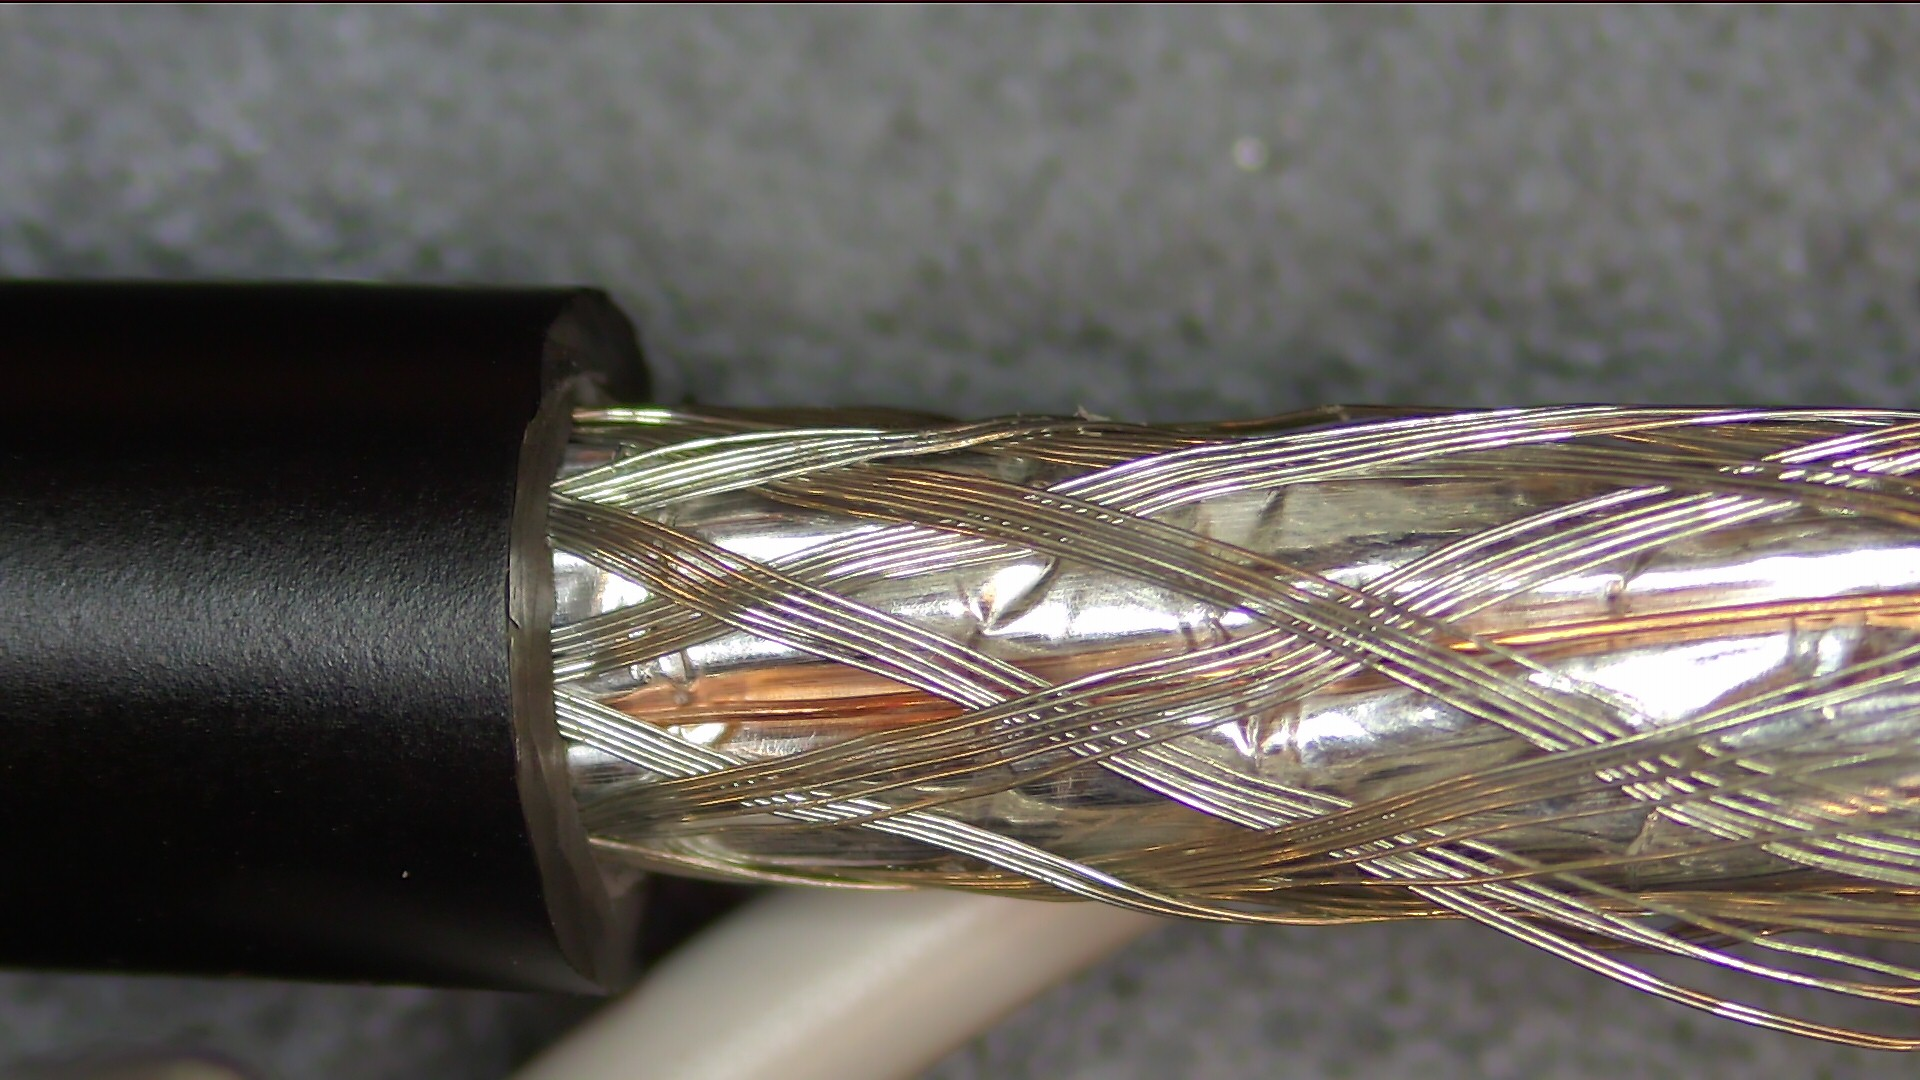
\includegraphics[width=0.95\textwidth]{images/braid_coverage/14-39-55.jpg}
        \caption{Unbranded DVI cable. \qty{60}{\percent} braid coverage.}
        \label{fig:braid_coverage_unknown}
    \end{subfigure}
    \begin{subfigure}[t]{0.45\linewidth}
        \centering
        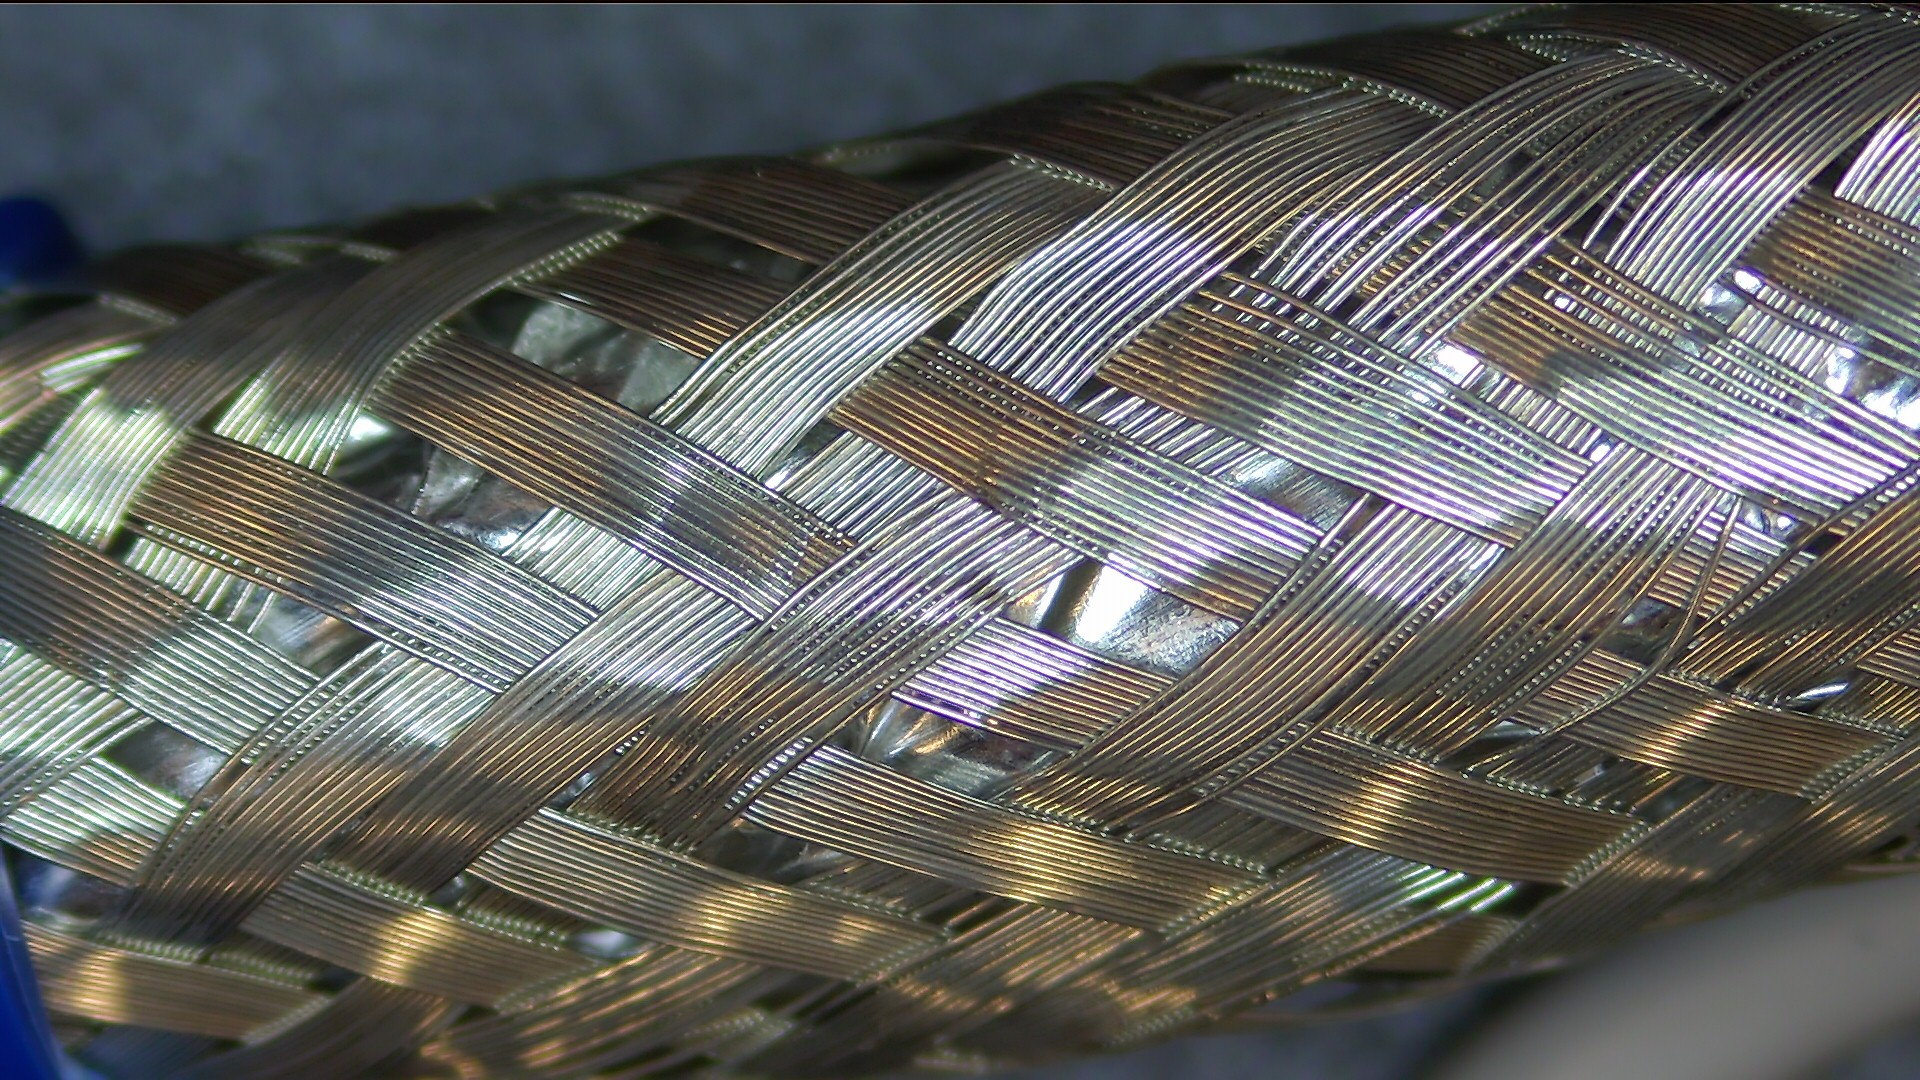
\includegraphics[width=0.95\textwidth]{images/braid_coverage/14-37-27.jpg}
        \caption{DVIGear \device{SHR}. \qty{80}{\percent} braid coverage.}
        \label{fig:braid_coverage_dvigear}
    \end{subfigure}
    \begin{subfigure}{0.45\linewidth}
        \centering
        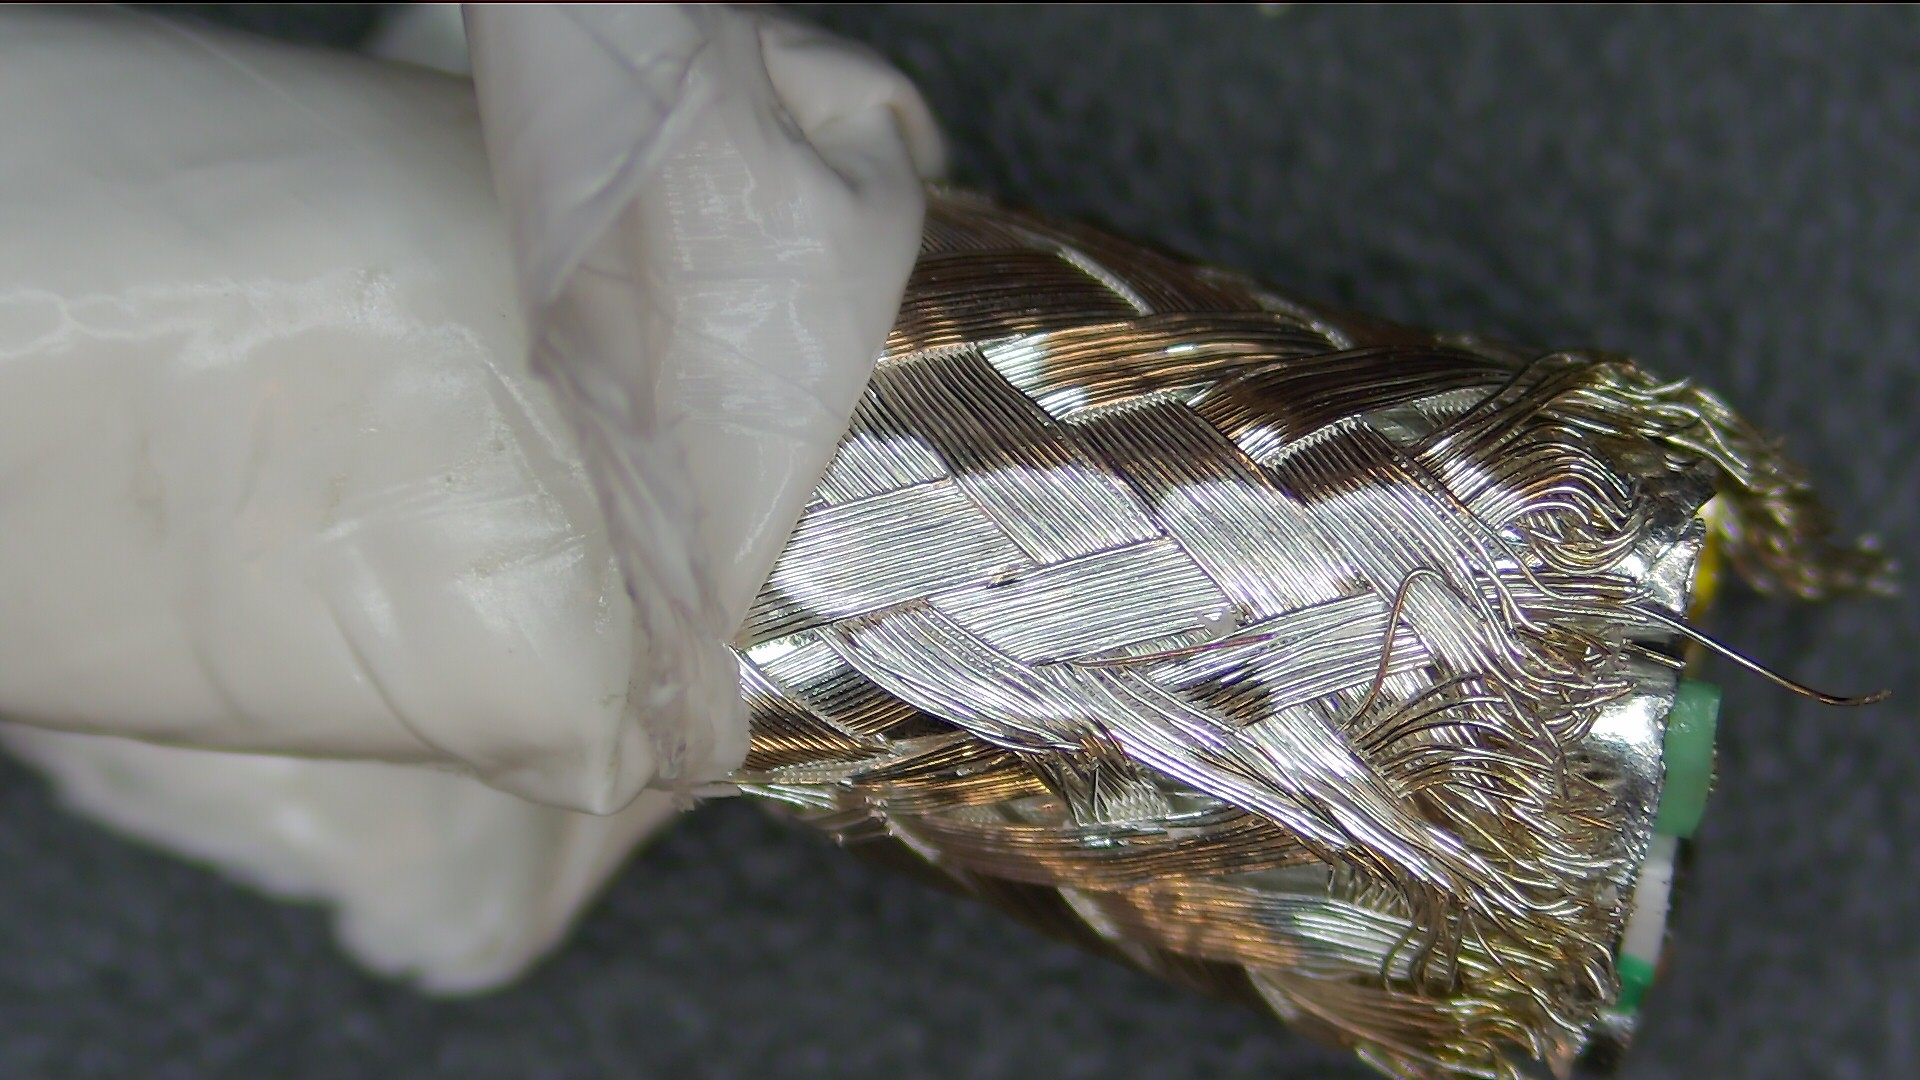
\includegraphics[width=0.95\textwidth]{images/braid_coverage/14-57-9.jpg}
        \caption{Gore \device{RCN9034-24}. \qty{95}{\percent} braid coverage.}
        \label{fig:braid_coverage_gore}
    \end{subfigure}
    \caption{Braid coverage of several DVI cables and a Category 6a cable.}
    \label{fig:braid_coverage}
\end{figure}

The braid of the unbranded cable has the least coverage with about \qty{60}{\percent} calculated according to ANSI/SCTE 51 2018 \cite{ANSI_SCTE_51_2018}. In addition, the braid is made of aluminium instead of copper. This increases the impedance and typically reduces the effectiveness by about \qty{20}{\decibel} \cite{circuit_designers_companion}. The other cables have an \qty{80}{\percent} and a \qty{95}{\percent} copper braid coverage. The braid and foil shield combination is fairly effective up to several dozen \unit{MHz} \citep[p. 84]{ott_electromagnetic} covering the most important frequency range for this device if a decent copper braid is used.

As it was mentioned above, using a shielded cable brings more capacitance to the table. A factor that needs to be considered when shielding a current source as it reduces the output impedance. It is therefore important to have a more detailed look at the cable capacitance in this application. Neglecting the parasitic capacitances to earth ground, the two capacitances most interesting are the mutual capacitance between the conductors $C_m$ and the capacitance between each conductor and the shield $C_{ws}$, for details see \cite{twisted_pair_cable}. The cable capacitances of all cables were measured using an LCR Research \device{LCR Pro 1 Plus} and the results are given in table \ref{tab:dvi_cable_capacitance}. To measure the capacitance between the conductor and the shield, one of the twisted pairs was shorted to the shield using a DVI connector with a solder joint connecting both the shield and the conductor. The Category 6a cable was soldered together without a connector. The capacitance was then measured between the shorted pins and the remaining conductor. The measured total capacitance $C_{tot}$ is the paralleled capacitance between the shield and the conductor $C_{ws}$ and the mutual capacitance $C_m$. $C_{ws}$ can then be calculated as
\begin{equation*}
    C_{ws} = C_{tot} - C_m\,.
\end{equation*}

\begin{table}[ht]
    \centering
    \begin{tabular}{lccc}
        \toprule
        DVIGear \device{SHR}& $C_m$& $C_{ws}$& Conductor Size\\
        \midrule
        DVIGear \device{SHR}& \qty{49 \pm 1}{\pF \per \m}& \qty{46 \pm 1.5}{\pF \per \m}& \qty{0.33}{\square\mm}\\
        SUPRA \device{DVI Single-Link}& \qty{42 \pm 1}{\pF \per \m}& \qty{36 \pm 1.5}{\pF \per \m}& \qty{0.26}{\square\mm}\\
        Gore \device{RCN9034}& \qty{43 \pm 1}{\pF \per \m}& \qty{95 \pm 1.5}{\pF \per \m}& \qty{0.20}{\square\mm}\\
        Unbranded DVI dual link& \qty{42 \pm 1}{\pF \per \m}& \qty{41 \pm 1.5}{\pF \per \m}& \qty{0.05}{\square\mm}\\
        \bottomrule
    \end{tabular}
    \caption{Measured cable capacitance for two DVI cables using a PE foam dielectric and an ePTFE Category 6a cable. All values were measured at \qty{10}{\kHz}.}
    \label{tab:dvi_cable_capacitance}
\end{table}

All DVI cables tested fared well regarding the capacitance and gave a similar performance of the mutual capacitance when compared to the ePTFE Category 6a Gore \device{RCN9034}. Given the measurement uncertainties of the \device{LCR Pro 1 Plus} no distinction can be made. Due to the smaller outer diameter of the Gore cable the shield capacitance unfortunately doubles.% In addition, to the low capacitance, the DVI cables are available off-the-shelf in good quality if some care is exercised. The connector itself is relatively rugged and cables in various lengths are available. Unfortunately, availability has declined over the years with the move towards HDMI, DisplayPort and USB-C connections. For example, the DVIGear \device{SHR} cables, which were tested, are mostly discontinued by now. This issue might need addressing in the long-term.

To give a figure for the capacitance seen by the current source, it must be determined, whether the circuit is balanced or unbalanced. Remembering section \ref{sec:results_precision_current_source} and especially figure \ref{fig:dgDrive_current_source} on page \pageref{fig:dgDrive_current_source} where the current source schematic was shown, it is clear, that the circuit is not balanced. The virtual ground has very little impedance, while the other conductor presents a high impedance current source via the MOSFET of the current sink. The virtual ground is the most sensitive node. Any noise current injected into it cannot be distinguished from the drive current. Noise current is injected via capacitive coupling, so the capacitance seen by the virtual ground node is the most important. This is analogous to transimpedance amplifier input node. This capacitance seen is $C_{tot}$ measured above. Looking at the number it can be seen that a DVI cable is indeed a good choice for this use case as it has the least capacitance when compared to the Gore Cat6a cable or a typical coaxial cable, which has about \qty{100}{\pF \per \m}.

The final decision was made in favor of the SUPRA \device{DVI Single-Link} cable, because of its decent shielding and very low capacitance, while being readily available in contrast to the DVIGear cables, some of which have already been given the end-of-life status.
A word of caution regarding the unbranded DVI cable needs be said. In addition to the meager shielding, the \qty{0.05}{\square\mm} wire is not recommended for carrying  \qty{500}{\mA} because it has a resistance of about \qty{330}{\milli\ohm \per \m}, Using a cable of \qty{3}{\m} length would already drop \qty{1}{\V} (or \qty{500}{\mV} when using a dual link cable) at \qty{500}{\mA}. The \qty{0.26}{\square\mm} cable chosen, for comparison, only drops \qty{82}{\mV} using a single link.
\begin{figure}[ht]
    \centering
    \scalebox{3}{%
        \import{figures/}{DVI_connector.tex}
    } % scalebox
    \caption{Pin layout of the DgDrive DVI connector. Ground is gray, positive voltages red, negative voltages blue, digital i/o pins brown. White pins are not connected.}
    \label{fig:dvi_connector_pin_layout}
\end{figure}

With the cable chosen, the connector layout needs to be discussed. DVI-D cables come in two flavours, single link and dual link cables. Dual link cables have twice the number of data lines. These data lines are called TMDS data lines. Those pairs and the clock line are shielded twisted pairs, each pair wrapped in an aluminium foil. Depending on the type of cable, it has \num{17} or \num{23} pins with either \num{3} or \num{6} TMDS lines. Each shield is brought out with a separate pin except for the additional TMDS lines in the dual link configuration. The shields of the additional neighbouring TMDS lines is connected together so only \num{4} pins are required to connect the shields of the TMDS and clock line twisted pairs as shown in figure \ref{fig:dvi_connector_pin_layout}. Apart from the shielded twisted pairs, there are \num{5} conductors available for additional functions. Theses conductors are neither shielded nor twisted. The connector layout of the DVI port of the digital current driver is shown in figure \ref{fig:dvi_connector_pin_layout}. A number of twisted pairs are left unconnected (NC) for future applications and some cannot be used because they are part of the legacy analog function of the DVI connector. Pin 8 and pins C1 to C5 are can only be used with a DVI-I digital and analog cable. As mentioned above, these cables have became rare as analog displays are mostly extinct.
\begin{table}[ht]
    \centering
    \begin{tabular}{llll}
        \toprule
        Pin    & Function    & Pin    & Function\\
        \midrule
        \numrange{1}{2}& NC& \num{14}& \qty[retain-explicit-plus]{+12}{\V}\\
        \num{3}& Shield, GND& \num{15}& GND\\
        \numrange{4}{5}& NC& \num{16}& Open-collector, enable laser\\
        \num{6}& \qty{-12}{\V}& \numrange{17}{18}& NC\\
        \num{7}& EEPROM& \num{19}& Shield, GND\\
        \num{8}& NC& \numrange{20}{21}& NC\\
        \num{9}& LD cathode& \num{22}& Shield, GND\\
        \num{10}& LD anode& \num{23}& LD voltage sense positive\\
        \num{11}& Shield, GND& \num{24}& LD voltage sense negative\\
        \num{12}& LD cathode& C5& GND\\
        \num{13}& LD anode& & \\
        \bottomrule
    \end{tabular}
    \caption{DVI connector pin layout. See figure \ref{fig:dvi_connector_pin_layout} for the pin labels.}
    \label{tab:dvi_connector_pin_layout}
\end{table}

Pin \num{9} and \num{10} are used to deliver the laser diode drive current, while the shielded clock line on pins \num{23} and \num{24} are used to sense the diode voltage. When a dual link cable is used, pin \num{12} and \num{13} are also used to carry current. Using a single link cables reduces the capacitance in comparison to a dual link cable.

The other conductors are used to supply the laser head with a \qty{\pm 12}{\V} rail and to actuate the protection relay in the laser head. Additionally, there is an  electrically erasable programmable read-only memory (EEPROM) chip inside the laser to identify it. This chip can be read using a one-wire protocol via pin \num{7} and contains information about the laser diode and maximum current settings, the date of assembly of the laser and more.

As discussed above, the shielding and grounding plays an important role to suppress noise. The digital current driver uses a floating DC power supply to supply the sub rack. The subrack is connected to chassis ground and so is the front panel of the current driver through the SMA connectors. The DVI cable shield is also connected to the front panel of the current driver and the system ground. This chassis forms the path of least impedance for any noise current present and diverts it around the PCB ground plane. On the laser side the shield is connected to the laser head, which is grounded as well to protect the laser from electrostatic discharge (ESD). The PCB inside the laser head is only connected to the return conductor, effectively staying inside the shield.

Finally the cable for connecting the display board with the analog board is presented. The analog board and the front panel are two separate boards as the current driver design is a modular concept. Both PCBs feature separate microcontrollers that communicate via a digital Inter-Integrated Circuit (I²C) bus. The cable is shielded as well and is grounded on the analog board as well as capacitively coupled via a \qty{10}{\nF} capacitor on the digital front panel board to keep the digital signals from interfering with the analog board. It is a 5 conductor cable as shown in figure \ref{fig:dgDrive_display_cable}. For example, a Belden \device{9535} cable can be used, but any other foil shielded cable can be used. The use of a foil is recommended because it is most effective for shielding against high frequency signals. The connectors are from the JST \device{PHR} series and currently the cable features an asymmetric layout. Initially the front panel board did not contain a separate microcontroller and the display required more control lines. It was found during development that a self-sufficient board is easier to maintain and also able to support more features like USB. The number of connectors was therefore reduced. The \num{7}-pin header on the analog side will be replaced with a \num{6}-pin header on both side with revision 2.4.0 of the analog board.
\begin{figure}[ht]
    \centering
    \scalebox{0.8}{%
        \import{figures/}{cable_dgDrive_display.tex}
    } % scalebox
    \caption{Display cable used to internally connect the display board with the analog board. The \num{7}-pin header is deprecated and will be replaced with a \num{6}-pin header.}
    \label{fig:dgDrive_display_cable}
\end{figure}
\begin{table}[hb]
    \centering
    \begin{tabular}{llllll}
        \toprule
        Pin& Function& Colour& Pin& Function& Colour\\
        \midrule
        \num{1}& \qty[retain-explicit-plus]{+3.3}{\V}& Red& \num{4}& I²C SCL& Green\\
        \num{2}& GND& Black& \num{5}& Interrupt& White\\
        \num{3}& I²C SDA& Brown& \num{6}& Shield& --\\
        \bottomrule
    \end{tabular}
    \caption{Display cable pin layout. See figure \ref{fig:dgDrive_display_cable} for the connector layout.}
    \label{tab:dgDrive_display_cable_pin_layout}
\end{table}

\subsection{Test Results: Output Impedance}%
\label{sec:output_impedance}
There are several ways of measuring the output impedance of a current source. Two such methods were used to test the output impedance of the current source and are shown in figure \ref{fig:measuring_output_impedance}.
\begin{figure}[ht]
    \centering
    \begin{subfigure}{0.35\linewidth}
        \centering
        \import{figures/}{measuring_output_impedance_dc.tex}
        \caption{DC scheme.}
        \label{fig:measuring_output_impedance_dc}
    \end{subfigure}
    \begin{subfigure}{0.55\linewidth}
        \centering
        \import{figures/}{measuring_output_impedance_ac.tex}
        \caption{AC scheme.}
        \label{fig:measuring_output_impedance_ac}
    \end{subfigure}
    \caption{Two methods for measuring the output impedance of a current source.}
    \label{fig:measuring_output_impedance}
\end{figure}
Figure \ref{fig:measuring_output_impedance_dc} shows the simpler scheme. It can be used to determine the static output impedance at DC and its setup only requires three components, an ammeter or multimeter, a resistor, and a switch. The resistor value should be scaled such that $R_{shunt} \cdot I_{out}$ is just below the compliance voltage of the current source to maximize the resolution. To calculate the output impedance, the following steps are required. The current flowing through the shunt is measured using the ammeter and then the switch is closed to short out the resistor and the current is measured again. Assuming the resistance of the switch and the internal shunt of the ammeter is very small in comparison to $R_{out}$ the current source is essentially shorted and it can be seen in figure \ref{fig:measuring_output_impedance_dc} that all current $I_{out}$ is flowing through the switch and the ammeter when the switch is closed. When opened, the current is split between $R_{shunt}$ and $R_{out}$. This allows calculating $R_{out}$ as
\begin{equation}
    R_{out} = \frac{R_{shunt} \cdot I_{shunt}}{I_{out} - I_{shunt}} = \frac{V_{shunt}}{\Delta I}\,. \label{eqn:output_impedance_dc}
\end{equation}

The shunt resistance $R_{shunt}$ can usually be determined with sufficient accuracy, but the difference in $\Delta I$ between to current with and without $R_{shunt}$ is an entirely different matter though. Given a high impedance source, $\Delta I$ is naturally small. For educational purposes this problem can be illustrated by measuring the output impedance of the digital laser driver, which is expected to be very high due to the novel current source configuration discussed in the last section.

The measurement shown in \ref{fig:dgDrive_output_impedance_dc} was conducted according to figure \ref{fig:measuring_output_impedance_dc}. The ammeter was a \num{7.5} digit Keysight \device{34470A} multimeter and the shunt resistor value was $R_{shunt} = \qty{3.298 \pm 0.002}{\mega\ohm}$, which was measured using a Keysight \device{3458A}. The output current was chosen as low as reasonably possible to allow for a larger shunt resistor to improve the sensitivity. The DMM settings were \qty{10}{\plc} with autozeroing enabled. To further improve the sensitivity a \qty{30}{\second} sample was taken for both switch positions to allow for additional averaging. Using the same settings, the measurement noise floor was determined first. A \qty{30}{\second} sample with open inputs resulted in a noise floor of \qty{7.1}{\pA_{rms}} using the \device{34470A} on the \qty{10}{\uA} range. This noise floor is low enough to be neglected as can be seen below. The measurement was then repeated with the setup shown in figure \ref{fig:measuring_output_impedance_dc}. Since the output impedance of the current source is so high and even though the noise of the current source is extremely low with only \qty{1.5}{\nA_{rms}} ($\equiv \qty{6}{\nA \per \A}$ referred to full scale output) over \qty{30}{\s}, the difference between the two switch settings is hardly recognizable. Figure \ref{fig:dgDrive_output_impedance_dc} shows, in orange, the mean value of both measurements before and after switching in the shunt resistor. Longer measurement or integration times in an attempting suppress more noise are ineffective due to the presence of flicker noise in the current source, rendering longer integration times futile.
\begin{figure}[ht]
    \centering
    %% Creator: Matplotlib, PGF backend
%%
%% To include the figure in your LaTeX document, write
%%   \input{<filename>.pgf}
%%
%% Make sure the required packages are loaded in your preamble
%%   \usepackage{pgf}
%%
%% Also ensure that all the required font packages are loaded; for instance,
%% the lmodern package is sometimes necessary when using math font.
%%   \usepackage{lmodern}
%%
%% Figures using additional raster images can only be included by \input if
%% they are in the same directory as the main LaTeX file. For loading figures
%% from other directories you can use the `import` package
%%   \usepackage{import}
%%
%% and then include the figures with
%%   \import{<path to file>}{<filename>.pgf}
%%
%% Matplotlib used the following preamble
%%   \usepackage{siunitx}
%%   \usepackage{fontspec}
%%   \makeatletter\@ifpackageloaded{underscore}{}{\usepackage[strings]{underscore}}\makeatother
%%
\begingroup%
\makeatletter%
\begin{pgfpicture}%
\pgfpathrectangle{\pgfpointorigin}{\pgfqpoint{5.431103in}{3.356606in}}%
\pgfusepath{use as bounding box, clip}%
\begin{pgfscope}%
\pgfsetbuttcap%
\pgfsetmiterjoin%
\definecolor{currentfill}{rgb}{1.000000,1.000000,1.000000}%
\pgfsetfillcolor{currentfill}%
\pgfsetlinewidth{0.000000pt}%
\definecolor{currentstroke}{rgb}{1.000000,1.000000,1.000000}%
\pgfsetstrokecolor{currentstroke}%
\pgfsetdash{}{0pt}%
\pgfpathmoveto{\pgfqpoint{0.000000in}{0.000000in}}%
\pgfpathlineto{\pgfqpoint{5.431103in}{0.000000in}}%
\pgfpathlineto{\pgfqpoint{5.431103in}{3.356606in}}%
\pgfpathlineto{\pgfqpoint{0.000000in}{3.356606in}}%
\pgfpathlineto{\pgfqpoint{0.000000in}{0.000000in}}%
\pgfpathclose%
\pgfusepath{fill}%
\end{pgfscope}%
\begin{pgfscope}%
\pgfsetbuttcap%
\pgfsetmiterjoin%
\definecolor{currentfill}{rgb}{1.000000,1.000000,1.000000}%
\pgfsetfillcolor{currentfill}%
\pgfsetlinewidth{0.000000pt}%
\definecolor{currentstroke}{rgb}{0.000000,0.000000,0.000000}%
\pgfsetstrokecolor{currentstroke}%
\pgfsetstrokeopacity{0.000000}%
\pgfsetdash{}{0pt}%
\pgfpathmoveto{\pgfqpoint{0.576061in}{0.524170in}}%
\pgfpathlineto{\pgfqpoint{5.281103in}{0.524170in}}%
\pgfpathlineto{\pgfqpoint{5.281103in}{3.082363in}}%
\pgfpathlineto{\pgfqpoint{0.576061in}{3.082363in}}%
\pgfpathlineto{\pgfqpoint{0.576061in}{0.524170in}}%
\pgfpathclose%
\pgfusepath{fill}%
\end{pgfscope}%
\begin{pgfscope}%
\pgfpathrectangle{\pgfqpoint{0.576061in}{0.524170in}}{\pgfqpoint{4.705042in}{2.558193in}}%
\pgfusepath{clip}%
\pgfsetrectcap%
\pgfsetroundjoin%
\pgfsetlinewidth{0.803000pt}%
\definecolor{currentstroke}{rgb}{0.450000,0.450000,0.450000}%
\pgfsetstrokecolor{currentstroke}%
\pgfsetdash{}{0pt}%
\pgfpathmoveto{\pgfqpoint{0.761025in}{0.524170in}}%
\pgfpathlineto{\pgfqpoint{0.761025in}{3.082363in}}%
\pgfusepath{stroke}%
\end{pgfscope}%
\begin{pgfscope}%
\pgfsetbuttcap%
\pgfsetroundjoin%
\definecolor{currentfill}{rgb}{0.000000,0.000000,0.000000}%
\pgfsetfillcolor{currentfill}%
\pgfsetlinewidth{0.803000pt}%
\definecolor{currentstroke}{rgb}{0.000000,0.000000,0.000000}%
\pgfsetstrokecolor{currentstroke}%
\pgfsetdash{}{0pt}%
\pgfsys@defobject{currentmarker}{\pgfqpoint{0.000000in}{-0.048611in}}{\pgfqpoint{0.000000in}{0.000000in}}{%
\pgfpathmoveto{\pgfqpoint{0.000000in}{0.000000in}}%
\pgfpathlineto{\pgfqpoint{0.000000in}{-0.048611in}}%
\pgfusepath{stroke,fill}%
}%
\begin{pgfscope}%
\pgfsys@transformshift{0.761025in}{0.524170in}%
\pgfsys@useobject{currentmarker}{}%
\end{pgfscope}%
\end{pgfscope}%
\begin{pgfscope}%
\definecolor{textcolor}{rgb}{0.000000,0.000000,0.000000}%
\pgfsetstrokecolor{textcolor}%
\pgfsetfillcolor{textcolor}%
\pgftext[x=0.761025in,y=0.426948in,,top]{\color{textcolor}\rmfamily\fontsize{8.000000}{9.600000}\selectfont \(\displaystyle {0}\)}%
\end{pgfscope}%
\begin{pgfscope}%
\pgfpathrectangle{\pgfqpoint{0.576061in}{0.524170in}}{\pgfqpoint{4.705042in}{2.558193in}}%
\pgfusepath{clip}%
\pgfsetrectcap%
\pgfsetroundjoin%
\pgfsetlinewidth{0.803000pt}%
\definecolor{currentstroke}{rgb}{0.450000,0.450000,0.450000}%
\pgfsetstrokecolor{currentstroke}%
\pgfsetdash{}{0pt}%
\pgfpathmoveto{\pgfqpoint{1.483544in}{0.524170in}}%
\pgfpathlineto{\pgfqpoint{1.483544in}{3.082363in}}%
\pgfusepath{stroke}%
\end{pgfscope}%
\begin{pgfscope}%
\pgfsetbuttcap%
\pgfsetroundjoin%
\definecolor{currentfill}{rgb}{0.000000,0.000000,0.000000}%
\pgfsetfillcolor{currentfill}%
\pgfsetlinewidth{0.803000pt}%
\definecolor{currentstroke}{rgb}{0.000000,0.000000,0.000000}%
\pgfsetstrokecolor{currentstroke}%
\pgfsetdash{}{0pt}%
\pgfsys@defobject{currentmarker}{\pgfqpoint{0.000000in}{-0.048611in}}{\pgfqpoint{0.000000in}{0.000000in}}{%
\pgfpathmoveto{\pgfqpoint{0.000000in}{0.000000in}}%
\pgfpathlineto{\pgfqpoint{0.000000in}{-0.048611in}}%
\pgfusepath{stroke,fill}%
}%
\begin{pgfscope}%
\pgfsys@transformshift{1.483544in}{0.524170in}%
\pgfsys@useobject{currentmarker}{}%
\end{pgfscope}%
\end{pgfscope}%
\begin{pgfscope}%
\definecolor{textcolor}{rgb}{0.000000,0.000000,0.000000}%
\pgfsetstrokecolor{textcolor}%
\pgfsetfillcolor{textcolor}%
\pgftext[x=1.483544in,y=0.426948in,,top]{\color{textcolor}\rmfamily\fontsize{8.000000}{9.600000}\selectfont \(\displaystyle {10}\)}%
\end{pgfscope}%
\begin{pgfscope}%
\pgfpathrectangle{\pgfqpoint{0.576061in}{0.524170in}}{\pgfqpoint{4.705042in}{2.558193in}}%
\pgfusepath{clip}%
\pgfsetrectcap%
\pgfsetroundjoin%
\pgfsetlinewidth{0.803000pt}%
\definecolor{currentstroke}{rgb}{0.450000,0.450000,0.450000}%
\pgfsetstrokecolor{currentstroke}%
\pgfsetdash{}{0pt}%
\pgfpathmoveto{\pgfqpoint{2.206063in}{0.524170in}}%
\pgfpathlineto{\pgfqpoint{2.206063in}{3.082363in}}%
\pgfusepath{stroke}%
\end{pgfscope}%
\begin{pgfscope}%
\pgfsetbuttcap%
\pgfsetroundjoin%
\definecolor{currentfill}{rgb}{0.000000,0.000000,0.000000}%
\pgfsetfillcolor{currentfill}%
\pgfsetlinewidth{0.803000pt}%
\definecolor{currentstroke}{rgb}{0.000000,0.000000,0.000000}%
\pgfsetstrokecolor{currentstroke}%
\pgfsetdash{}{0pt}%
\pgfsys@defobject{currentmarker}{\pgfqpoint{0.000000in}{-0.048611in}}{\pgfqpoint{0.000000in}{0.000000in}}{%
\pgfpathmoveto{\pgfqpoint{0.000000in}{0.000000in}}%
\pgfpathlineto{\pgfqpoint{0.000000in}{-0.048611in}}%
\pgfusepath{stroke,fill}%
}%
\begin{pgfscope}%
\pgfsys@transformshift{2.206063in}{0.524170in}%
\pgfsys@useobject{currentmarker}{}%
\end{pgfscope}%
\end{pgfscope}%
\begin{pgfscope}%
\definecolor{textcolor}{rgb}{0.000000,0.000000,0.000000}%
\pgfsetstrokecolor{textcolor}%
\pgfsetfillcolor{textcolor}%
\pgftext[x=2.206063in,y=0.426948in,,top]{\color{textcolor}\rmfamily\fontsize{8.000000}{9.600000}\selectfont \(\displaystyle {20}\)}%
\end{pgfscope}%
\begin{pgfscope}%
\pgfpathrectangle{\pgfqpoint{0.576061in}{0.524170in}}{\pgfqpoint{4.705042in}{2.558193in}}%
\pgfusepath{clip}%
\pgfsetrectcap%
\pgfsetroundjoin%
\pgfsetlinewidth{0.803000pt}%
\definecolor{currentstroke}{rgb}{0.450000,0.450000,0.450000}%
\pgfsetstrokecolor{currentstroke}%
\pgfsetdash{}{0pt}%
\pgfpathmoveto{\pgfqpoint{2.928582in}{0.524170in}}%
\pgfpathlineto{\pgfqpoint{2.928582in}{3.082363in}}%
\pgfusepath{stroke}%
\end{pgfscope}%
\begin{pgfscope}%
\pgfsetbuttcap%
\pgfsetroundjoin%
\definecolor{currentfill}{rgb}{0.000000,0.000000,0.000000}%
\pgfsetfillcolor{currentfill}%
\pgfsetlinewidth{0.803000pt}%
\definecolor{currentstroke}{rgb}{0.000000,0.000000,0.000000}%
\pgfsetstrokecolor{currentstroke}%
\pgfsetdash{}{0pt}%
\pgfsys@defobject{currentmarker}{\pgfqpoint{0.000000in}{-0.048611in}}{\pgfqpoint{0.000000in}{0.000000in}}{%
\pgfpathmoveto{\pgfqpoint{0.000000in}{0.000000in}}%
\pgfpathlineto{\pgfqpoint{0.000000in}{-0.048611in}}%
\pgfusepath{stroke,fill}%
}%
\begin{pgfscope}%
\pgfsys@transformshift{2.928582in}{0.524170in}%
\pgfsys@useobject{currentmarker}{}%
\end{pgfscope}%
\end{pgfscope}%
\begin{pgfscope}%
\definecolor{textcolor}{rgb}{0.000000,0.000000,0.000000}%
\pgfsetstrokecolor{textcolor}%
\pgfsetfillcolor{textcolor}%
\pgftext[x=2.928582in,y=0.426948in,,top]{\color{textcolor}\rmfamily\fontsize{8.000000}{9.600000}\selectfont \(\displaystyle {30}\)}%
\end{pgfscope}%
\begin{pgfscope}%
\pgfpathrectangle{\pgfqpoint{0.576061in}{0.524170in}}{\pgfqpoint{4.705042in}{2.558193in}}%
\pgfusepath{clip}%
\pgfsetrectcap%
\pgfsetroundjoin%
\pgfsetlinewidth{0.803000pt}%
\definecolor{currentstroke}{rgb}{0.450000,0.450000,0.450000}%
\pgfsetstrokecolor{currentstroke}%
\pgfsetdash{}{0pt}%
\pgfpathmoveto{\pgfqpoint{3.651100in}{0.524170in}}%
\pgfpathlineto{\pgfqpoint{3.651100in}{3.082363in}}%
\pgfusepath{stroke}%
\end{pgfscope}%
\begin{pgfscope}%
\pgfsetbuttcap%
\pgfsetroundjoin%
\definecolor{currentfill}{rgb}{0.000000,0.000000,0.000000}%
\pgfsetfillcolor{currentfill}%
\pgfsetlinewidth{0.803000pt}%
\definecolor{currentstroke}{rgb}{0.000000,0.000000,0.000000}%
\pgfsetstrokecolor{currentstroke}%
\pgfsetdash{}{0pt}%
\pgfsys@defobject{currentmarker}{\pgfqpoint{0.000000in}{-0.048611in}}{\pgfqpoint{0.000000in}{0.000000in}}{%
\pgfpathmoveto{\pgfqpoint{0.000000in}{0.000000in}}%
\pgfpathlineto{\pgfqpoint{0.000000in}{-0.048611in}}%
\pgfusepath{stroke,fill}%
}%
\begin{pgfscope}%
\pgfsys@transformshift{3.651100in}{0.524170in}%
\pgfsys@useobject{currentmarker}{}%
\end{pgfscope}%
\end{pgfscope}%
\begin{pgfscope}%
\definecolor{textcolor}{rgb}{0.000000,0.000000,0.000000}%
\pgfsetstrokecolor{textcolor}%
\pgfsetfillcolor{textcolor}%
\pgftext[x=3.651100in,y=0.426948in,,top]{\color{textcolor}\rmfamily\fontsize{8.000000}{9.600000}\selectfont \(\displaystyle {40}\)}%
\end{pgfscope}%
\begin{pgfscope}%
\pgfpathrectangle{\pgfqpoint{0.576061in}{0.524170in}}{\pgfqpoint{4.705042in}{2.558193in}}%
\pgfusepath{clip}%
\pgfsetrectcap%
\pgfsetroundjoin%
\pgfsetlinewidth{0.803000pt}%
\definecolor{currentstroke}{rgb}{0.450000,0.450000,0.450000}%
\pgfsetstrokecolor{currentstroke}%
\pgfsetdash{}{0pt}%
\pgfpathmoveto{\pgfqpoint{4.373619in}{0.524170in}}%
\pgfpathlineto{\pgfqpoint{4.373619in}{3.082363in}}%
\pgfusepath{stroke}%
\end{pgfscope}%
\begin{pgfscope}%
\pgfsetbuttcap%
\pgfsetroundjoin%
\definecolor{currentfill}{rgb}{0.000000,0.000000,0.000000}%
\pgfsetfillcolor{currentfill}%
\pgfsetlinewidth{0.803000pt}%
\definecolor{currentstroke}{rgb}{0.000000,0.000000,0.000000}%
\pgfsetstrokecolor{currentstroke}%
\pgfsetdash{}{0pt}%
\pgfsys@defobject{currentmarker}{\pgfqpoint{0.000000in}{-0.048611in}}{\pgfqpoint{0.000000in}{0.000000in}}{%
\pgfpathmoveto{\pgfqpoint{0.000000in}{0.000000in}}%
\pgfpathlineto{\pgfqpoint{0.000000in}{-0.048611in}}%
\pgfusepath{stroke,fill}%
}%
\begin{pgfscope}%
\pgfsys@transformshift{4.373619in}{0.524170in}%
\pgfsys@useobject{currentmarker}{}%
\end{pgfscope}%
\end{pgfscope}%
\begin{pgfscope}%
\definecolor{textcolor}{rgb}{0.000000,0.000000,0.000000}%
\pgfsetstrokecolor{textcolor}%
\pgfsetfillcolor{textcolor}%
\pgftext[x=4.373619in,y=0.426948in,,top]{\color{textcolor}\rmfamily\fontsize{8.000000}{9.600000}\selectfont \(\displaystyle {50}\)}%
\end{pgfscope}%
\begin{pgfscope}%
\pgfpathrectangle{\pgfqpoint{0.576061in}{0.524170in}}{\pgfqpoint{4.705042in}{2.558193in}}%
\pgfusepath{clip}%
\pgfsetrectcap%
\pgfsetroundjoin%
\pgfsetlinewidth{0.803000pt}%
\definecolor{currentstroke}{rgb}{0.450000,0.450000,0.450000}%
\pgfsetstrokecolor{currentstroke}%
\pgfsetdash{}{0pt}%
\pgfpathmoveto{\pgfqpoint{5.096138in}{0.524170in}}%
\pgfpathlineto{\pgfqpoint{5.096138in}{3.082363in}}%
\pgfusepath{stroke}%
\end{pgfscope}%
\begin{pgfscope}%
\pgfsetbuttcap%
\pgfsetroundjoin%
\definecolor{currentfill}{rgb}{0.000000,0.000000,0.000000}%
\pgfsetfillcolor{currentfill}%
\pgfsetlinewidth{0.803000pt}%
\definecolor{currentstroke}{rgb}{0.000000,0.000000,0.000000}%
\pgfsetstrokecolor{currentstroke}%
\pgfsetdash{}{0pt}%
\pgfsys@defobject{currentmarker}{\pgfqpoint{0.000000in}{-0.048611in}}{\pgfqpoint{0.000000in}{0.000000in}}{%
\pgfpathmoveto{\pgfqpoint{0.000000in}{0.000000in}}%
\pgfpathlineto{\pgfqpoint{0.000000in}{-0.048611in}}%
\pgfusepath{stroke,fill}%
}%
\begin{pgfscope}%
\pgfsys@transformshift{5.096138in}{0.524170in}%
\pgfsys@useobject{currentmarker}{}%
\end{pgfscope}%
\end{pgfscope}%
\begin{pgfscope}%
\definecolor{textcolor}{rgb}{0.000000,0.000000,0.000000}%
\pgfsetstrokecolor{textcolor}%
\pgfsetfillcolor{textcolor}%
\pgftext[x=5.096138in,y=0.426948in,,top]{\color{textcolor}\rmfamily\fontsize{8.000000}{9.600000}\selectfont \(\displaystyle {60}\)}%
\end{pgfscope}%
\begin{pgfscope}%
\definecolor{textcolor}{rgb}{0.000000,0.000000,0.000000}%
\pgfsetstrokecolor{textcolor}%
\pgfsetfillcolor{textcolor}%
\pgftext[x=2.928582in,y=0.272725in,,top]{\color{textcolor}\rmfamily\fontsize{10.000000}{12.000000}\selectfont Time in \unit{\s}}%
\end{pgfscope}%
\begin{pgfscope}%
\pgfpathrectangle{\pgfqpoint{0.576061in}{0.524170in}}{\pgfqpoint{4.705042in}{2.558193in}}%
\pgfusepath{clip}%
\pgfsetrectcap%
\pgfsetroundjoin%
\pgfsetlinewidth{0.803000pt}%
\definecolor{currentstroke}{rgb}{0.450000,0.450000,0.450000}%
\pgfsetstrokecolor{currentstroke}%
\pgfsetdash{}{0pt}%
\pgfpathmoveto{\pgfqpoint{0.576061in}{0.701547in}}%
\pgfpathlineto{\pgfqpoint{5.281103in}{0.701547in}}%
\pgfusepath{stroke}%
\end{pgfscope}%
\begin{pgfscope}%
\pgfsetbuttcap%
\pgfsetroundjoin%
\definecolor{currentfill}{rgb}{0.000000,0.000000,0.000000}%
\pgfsetfillcolor{currentfill}%
\pgfsetlinewidth{0.803000pt}%
\definecolor{currentstroke}{rgb}{0.000000,0.000000,0.000000}%
\pgfsetstrokecolor{currentstroke}%
\pgfsetdash{}{0pt}%
\pgfsys@defobject{currentmarker}{\pgfqpoint{-0.048611in}{0.000000in}}{\pgfqpoint{-0.000000in}{0.000000in}}{%
\pgfpathmoveto{\pgfqpoint{-0.000000in}{0.000000in}}%
\pgfpathlineto{\pgfqpoint{-0.048611in}{0.000000in}}%
\pgfusepath{stroke,fill}%
}%
\begin{pgfscope}%
\pgfsys@transformshift{0.576061in}{0.701547in}%
\pgfsys@useobject{currentmarker}{}%
\end{pgfscope}%
\end{pgfscope}%
\begin{pgfscope}%
\definecolor{textcolor}{rgb}{0.000000,0.000000,0.000000}%
\pgfsetstrokecolor{textcolor}%
\pgfsetfillcolor{textcolor}%
\pgftext[x=0.327987in, y=0.662991in, left, base]{\color{textcolor}\rmfamily\fontsize{8.000000}{9.600000}\selectfont \(\displaystyle {\ensuremath{-}3}\)}%
\end{pgfscope}%
\begin{pgfscope}%
\pgfpathrectangle{\pgfqpoint{0.576061in}{0.524170in}}{\pgfqpoint{4.705042in}{2.558193in}}%
\pgfusepath{clip}%
\pgfsetrectcap%
\pgfsetroundjoin%
\pgfsetlinewidth{0.803000pt}%
\definecolor{currentstroke}{rgb}{0.450000,0.450000,0.450000}%
\pgfsetstrokecolor{currentstroke}%
\pgfsetdash{}{0pt}%
\pgfpathmoveto{\pgfqpoint{0.576061in}{1.035898in}}%
\pgfpathlineto{\pgfqpoint{5.281103in}{1.035898in}}%
\pgfusepath{stroke}%
\end{pgfscope}%
\begin{pgfscope}%
\pgfsetbuttcap%
\pgfsetroundjoin%
\definecolor{currentfill}{rgb}{0.000000,0.000000,0.000000}%
\pgfsetfillcolor{currentfill}%
\pgfsetlinewidth{0.803000pt}%
\definecolor{currentstroke}{rgb}{0.000000,0.000000,0.000000}%
\pgfsetstrokecolor{currentstroke}%
\pgfsetdash{}{0pt}%
\pgfsys@defobject{currentmarker}{\pgfqpoint{-0.048611in}{0.000000in}}{\pgfqpoint{-0.000000in}{0.000000in}}{%
\pgfpathmoveto{\pgfqpoint{-0.000000in}{0.000000in}}%
\pgfpathlineto{\pgfqpoint{-0.048611in}{0.000000in}}%
\pgfusepath{stroke,fill}%
}%
\begin{pgfscope}%
\pgfsys@transformshift{0.576061in}{1.035898in}%
\pgfsys@useobject{currentmarker}{}%
\end{pgfscope}%
\end{pgfscope}%
\begin{pgfscope}%
\definecolor{textcolor}{rgb}{0.000000,0.000000,0.000000}%
\pgfsetstrokecolor{textcolor}%
\pgfsetfillcolor{textcolor}%
\pgftext[x=0.327987in, y=0.997342in, left, base]{\color{textcolor}\rmfamily\fontsize{8.000000}{9.600000}\selectfont \(\displaystyle {\ensuremath{-}2}\)}%
\end{pgfscope}%
\begin{pgfscope}%
\pgfpathrectangle{\pgfqpoint{0.576061in}{0.524170in}}{\pgfqpoint{4.705042in}{2.558193in}}%
\pgfusepath{clip}%
\pgfsetrectcap%
\pgfsetroundjoin%
\pgfsetlinewidth{0.803000pt}%
\definecolor{currentstroke}{rgb}{0.450000,0.450000,0.450000}%
\pgfsetstrokecolor{currentstroke}%
\pgfsetdash{}{0pt}%
\pgfpathmoveto{\pgfqpoint{0.576061in}{1.370249in}}%
\pgfpathlineto{\pgfqpoint{5.281103in}{1.370249in}}%
\pgfusepath{stroke}%
\end{pgfscope}%
\begin{pgfscope}%
\pgfsetbuttcap%
\pgfsetroundjoin%
\definecolor{currentfill}{rgb}{0.000000,0.000000,0.000000}%
\pgfsetfillcolor{currentfill}%
\pgfsetlinewidth{0.803000pt}%
\definecolor{currentstroke}{rgb}{0.000000,0.000000,0.000000}%
\pgfsetstrokecolor{currentstroke}%
\pgfsetdash{}{0pt}%
\pgfsys@defobject{currentmarker}{\pgfqpoint{-0.048611in}{0.000000in}}{\pgfqpoint{-0.000000in}{0.000000in}}{%
\pgfpathmoveto{\pgfqpoint{-0.000000in}{0.000000in}}%
\pgfpathlineto{\pgfqpoint{-0.048611in}{0.000000in}}%
\pgfusepath{stroke,fill}%
}%
\begin{pgfscope}%
\pgfsys@transformshift{0.576061in}{1.370249in}%
\pgfsys@useobject{currentmarker}{}%
\end{pgfscope}%
\end{pgfscope}%
\begin{pgfscope}%
\definecolor{textcolor}{rgb}{0.000000,0.000000,0.000000}%
\pgfsetstrokecolor{textcolor}%
\pgfsetfillcolor{textcolor}%
\pgftext[x=0.327987in, y=1.331693in, left, base]{\color{textcolor}\rmfamily\fontsize{8.000000}{9.600000}\selectfont \(\displaystyle {\ensuremath{-}1}\)}%
\end{pgfscope}%
\begin{pgfscope}%
\pgfpathrectangle{\pgfqpoint{0.576061in}{0.524170in}}{\pgfqpoint{4.705042in}{2.558193in}}%
\pgfusepath{clip}%
\pgfsetrectcap%
\pgfsetroundjoin%
\pgfsetlinewidth{0.803000pt}%
\definecolor{currentstroke}{rgb}{0.450000,0.450000,0.450000}%
\pgfsetstrokecolor{currentstroke}%
\pgfsetdash{}{0pt}%
\pgfpathmoveto{\pgfqpoint{0.576061in}{1.704599in}}%
\pgfpathlineto{\pgfqpoint{5.281103in}{1.704599in}}%
\pgfusepath{stroke}%
\end{pgfscope}%
\begin{pgfscope}%
\pgfsetbuttcap%
\pgfsetroundjoin%
\definecolor{currentfill}{rgb}{0.000000,0.000000,0.000000}%
\pgfsetfillcolor{currentfill}%
\pgfsetlinewidth{0.803000pt}%
\definecolor{currentstroke}{rgb}{0.000000,0.000000,0.000000}%
\pgfsetstrokecolor{currentstroke}%
\pgfsetdash{}{0pt}%
\pgfsys@defobject{currentmarker}{\pgfqpoint{-0.048611in}{0.000000in}}{\pgfqpoint{-0.000000in}{0.000000in}}{%
\pgfpathmoveto{\pgfqpoint{-0.000000in}{0.000000in}}%
\pgfpathlineto{\pgfqpoint{-0.048611in}{0.000000in}}%
\pgfusepath{stroke,fill}%
}%
\begin{pgfscope}%
\pgfsys@transformshift{0.576061in}{1.704599in}%
\pgfsys@useobject{currentmarker}{}%
\end{pgfscope}%
\end{pgfscope}%
\begin{pgfscope}%
\definecolor{textcolor}{rgb}{0.000000,0.000000,0.000000}%
\pgfsetstrokecolor{textcolor}%
\pgfsetfillcolor{textcolor}%
\pgftext[x=0.419810in, y=1.666044in, left, base]{\color{textcolor}\rmfamily\fontsize{8.000000}{9.600000}\selectfont \(\displaystyle {0}\)}%
\end{pgfscope}%
\begin{pgfscope}%
\pgfpathrectangle{\pgfqpoint{0.576061in}{0.524170in}}{\pgfqpoint{4.705042in}{2.558193in}}%
\pgfusepath{clip}%
\pgfsetrectcap%
\pgfsetroundjoin%
\pgfsetlinewidth{0.803000pt}%
\definecolor{currentstroke}{rgb}{0.450000,0.450000,0.450000}%
\pgfsetstrokecolor{currentstroke}%
\pgfsetdash{}{0pt}%
\pgfpathmoveto{\pgfqpoint{0.576061in}{2.038950in}}%
\pgfpathlineto{\pgfqpoint{5.281103in}{2.038950in}}%
\pgfusepath{stroke}%
\end{pgfscope}%
\begin{pgfscope}%
\pgfsetbuttcap%
\pgfsetroundjoin%
\definecolor{currentfill}{rgb}{0.000000,0.000000,0.000000}%
\pgfsetfillcolor{currentfill}%
\pgfsetlinewidth{0.803000pt}%
\definecolor{currentstroke}{rgb}{0.000000,0.000000,0.000000}%
\pgfsetstrokecolor{currentstroke}%
\pgfsetdash{}{0pt}%
\pgfsys@defobject{currentmarker}{\pgfqpoint{-0.048611in}{0.000000in}}{\pgfqpoint{-0.000000in}{0.000000in}}{%
\pgfpathmoveto{\pgfqpoint{-0.000000in}{0.000000in}}%
\pgfpathlineto{\pgfqpoint{-0.048611in}{0.000000in}}%
\pgfusepath{stroke,fill}%
}%
\begin{pgfscope}%
\pgfsys@transformshift{0.576061in}{2.038950in}%
\pgfsys@useobject{currentmarker}{}%
\end{pgfscope}%
\end{pgfscope}%
\begin{pgfscope}%
\definecolor{textcolor}{rgb}{0.000000,0.000000,0.000000}%
\pgfsetstrokecolor{textcolor}%
\pgfsetfillcolor{textcolor}%
\pgftext[x=0.419810in, y=2.000395in, left, base]{\color{textcolor}\rmfamily\fontsize{8.000000}{9.600000}\selectfont \(\displaystyle {1}\)}%
\end{pgfscope}%
\begin{pgfscope}%
\pgfpathrectangle{\pgfqpoint{0.576061in}{0.524170in}}{\pgfqpoint{4.705042in}{2.558193in}}%
\pgfusepath{clip}%
\pgfsetrectcap%
\pgfsetroundjoin%
\pgfsetlinewidth{0.803000pt}%
\definecolor{currentstroke}{rgb}{0.450000,0.450000,0.450000}%
\pgfsetstrokecolor{currentstroke}%
\pgfsetdash{}{0pt}%
\pgfpathmoveto{\pgfqpoint{0.576061in}{2.373301in}}%
\pgfpathlineto{\pgfqpoint{5.281103in}{2.373301in}}%
\pgfusepath{stroke}%
\end{pgfscope}%
\begin{pgfscope}%
\pgfsetbuttcap%
\pgfsetroundjoin%
\definecolor{currentfill}{rgb}{0.000000,0.000000,0.000000}%
\pgfsetfillcolor{currentfill}%
\pgfsetlinewidth{0.803000pt}%
\definecolor{currentstroke}{rgb}{0.000000,0.000000,0.000000}%
\pgfsetstrokecolor{currentstroke}%
\pgfsetdash{}{0pt}%
\pgfsys@defobject{currentmarker}{\pgfqpoint{-0.048611in}{0.000000in}}{\pgfqpoint{-0.000000in}{0.000000in}}{%
\pgfpathmoveto{\pgfqpoint{-0.000000in}{0.000000in}}%
\pgfpathlineto{\pgfqpoint{-0.048611in}{0.000000in}}%
\pgfusepath{stroke,fill}%
}%
\begin{pgfscope}%
\pgfsys@transformshift{0.576061in}{2.373301in}%
\pgfsys@useobject{currentmarker}{}%
\end{pgfscope}%
\end{pgfscope}%
\begin{pgfscope}%
\definecolor{textcolor}{rgb}{0.000000,0.000000,0.000000}%
\pgfsetstrokecolor{textcolor}%
\pgfsetfillcolor{textcolor}%
\pgftext[x=0.419810in, y=2.334746in, left, base]{\color{textcolor}\rmfamily\fontsize{8.000000}{9.600000}\selectfont \(\displaystyle {2}\)}%
\end{pgfscope}%
\begin{pgfscope}%
\pgfpathrectangle{\pgfqpoint{0.576061in}{0.524170in}}{\pgfqpoint{4.705042in}{2.558193in}}%
\pgfusepath{clip}%
\pgfsetrectcap%
\pgfsetroundjoin%
\pgfsetlinewidth{0.803000pt}%
\definecolor{currentstroke}{rgb}{0.450000,0.450000,0.450000}%
\pgfsetstrokecolor{currentstroke}%
\pgfsetdash{}{0pt}%
\pgfpathmoveto{\pgfqpoint{0.576061in}{2.707652in}}%
\pgfpathlineto{\pgfqpoint{5.281103in}{2.707652in}}%
\pgfusepath{stroke}%
\end{pgfscope}%
\begin{pgfscope}%
\pgfsetbuttcap%
\pgfsetroundjoin%
\definecolor{currentfill}{rgb}{0.000000,0.000000,0.000000}%
\pgfsetfillcolor{currentfill}%
\pgfsetlinewidth{0.803000pt}%
\definecolor{currentstroke}{rgb}{0.000000,0.000000,0.000000}%
\pgfsetstrokecolor{currentstroke}%
\pgfsetdash{}{0pt}%
\pgfsys@defobject{currentmarker}{\pgfqpoint{-0.048611in}{0.000000in}}{\pgfqpoint{-0.000000in}{0.000000in}}{%
\pgfpathmoveto{\pgfqpoint{-0.000000in}{0.000000in}}%
\pgfpathlineto{\pgfqpoint{-0.048611in}{0.000000in}}%
\pgfusepath{stroke,fill}%
}%
\begin{pgfscope}%
\pgfsys@transformshift{0.576061in}{2.707652in}%
\pgfsys@useobject{currentmarker}{}%
\end{pgfscope}%
\end{pgfscope}%
\begin{pgfscope}%
\definecolor{textcolor}{rgb}{0.000000,0.000000,0.000000}%
\pgfsetstrokecolor{textcolor}%
\pgfsetfillcolor{textcolor}%
\pgftext[x=0.419810in, y=2.669096in, left, base]{\color{textcolor}\rmfamily\fontsize{8.000000}{9.600000}\selectfont \(\displaystyle {3}\)}%
\end{pgfscope}%
\begin{pgfscope}%
\pgfpathrectangle{\pgfqpoint{0.576061in}{0.524170in}}{\pgfqpoint{4.705042in}{2.558193in}}%
\pgfusepath{clip}%
\pgfsetrectcap%
\pgfsetroundjoin%
\pgfsetlinewidth{0.803000pt}%
\definecolor{currentstroke}{rgb}{0.450000,0.450000,0.450000}%
\pgfsetstrokecolor{currentstroke}%
\pgfsetdash{}{0pt}%
\pgfpathmoveto{\pgfqpoint{0.576061in}{3.042003in}}%
\pgfpathlineto{\pgfqpoint{5.281103in}{3.042003in}}%
\pgfusepath{stroke}%
\end{pgfscope}%
\begin{pgfscope}%
\pgfsetbuttcap%
\pgfsetroundjoin%
\definecolor{currentfill}{rgb}{0.000000,0.000000,0.000000}%
\pgfsetfillcolor{currentfill}%
\pgfsetlinewidth{0.803000pt}%
\definecolor{currentstroke}{rgb}{0.000000,0.000000,0.000000}%
\pgfsetstrokecolor{currentstroke}%
\pgfsetdash{}{0pt}%
\pgfsys@defobject{currentmarker}{\pgfqpoint{-0.048611in}{0.000000in}}{\pgfqpoint{-0.000000in}{0.000000in}}{%
\pgfpathmoveto{\pgfqpoint{-0.000000in}{0.000000in}}%
\pgfpathlineto{\pgfqpoint{-0.048611in}{0.000000in}}%
\pgfusepath{stroke,fill}%
}%
\begin{pgfscope}%
\pgfsys@transformshift{0.576061in}{3.042003in}%
\pgfsys@useobject{currentmarker}{}%
\end{pgfscope}%
\end{pgfscope}%
\begin{pgfscope}%
\definecolor{textcolor}{rgb}{0.000000,0.000000,0.000000}%
\pgfsetstrokecolor{textcolor}%
\pgfsetfillcolor{textcolor}%
\pgftext[x=0.419810in, y=3.003447in, left, base]{\color{textcolor}\rmfamily\fontsize{8.000000}{9.600000}\selectfont \(\displaystyle {4}\)}%
\end{pgfscope}%
\begin{pgfscope}%
\definecolor{textcolor}{rgb}{0.000000,0.000000,0.000000}%
\pgfsetstrokecolor{textcolor}%
\pgfsetfillcolor{textcolor}%
\pgftext[x=0.272432in,y=1.803266in,,bottom,rotate=90.000000]{\color{textcolor}\rmfamily\fontsize{10.000000}{12.000000}\selectfont Output current deviation in \unit{\A}}%
\end{pgfscope}%
\begin{pgfscope}%
\definecolor{textcolor}{rgb}{0.000000,0.000000,0.000000}%
\pgfsetstrokecolor{textcolor}%
\pgfsetfillcolor{textcolor}%
\pgftext[x=0.576061in,y=3.124029in,left,base]{\color{textcolor}\rmfamily\fontsize{8.000000}{9.600000}\selectfont \(\displaystyle \times{10^{\ensuremath{-}9}}{}\)}%
\end{pgfscope}%
\begin{pgfscope}%
\pgfpathrectangle{\pgfqpoint{0.576061in}{0.524170in}}{\pgfqpoint{4.705042in}{2.558193in}}%
\pgfusepath{clip}%
\pgfsetrectcap%
\pgfsetroundjoin%
\pgfsetlinewidth{1.505625pt}%
\definecolor{currentstroke}{rgb}{0.003922,0.450980,0.698039}%
\pgfsetstrokecolor{currentstroke}%
\pgfsetstrokeopacity{0.700000}%
\pgfsetdash{}{0pt}%
\pgfpathmoveto{\pgfqpoint{0.789926in}{1.704599in}}%
\pgfpathlineto{\pgfqpoint{0.818827in}{1.510931in}}%
\pgfpathlineto{\pgfqpoint{0.847728in}{1.462762in}}%
\pgfpathlineto{\pgfqpoint{0.876628in}{1.404919in}}%
\pgfpathlineto{\pgfqpoint{0.905529in}{1.774782in}}%
\pgfpathlineto{\pgfqpoint{0.934430in}{1.748376in}}%
\pgfpathlineto{\pgfqpoint{0.963331in}{1.688604in}}%
\pgfpathlineto{\pgfqpoint{0.992231in}{2.117669in}}%
\pgfpathlineto{\pgfqpoint{1.021132in}{1.760600in}}%
\pgfpathlineto{\pgfqpoint{1.050033in}{1.709323in}}%
\pgfpathlineto{\pgfqpoint{1.078934in}{1.462156in}}%
\pgfpathlineto{\pgfqpoint{1.107834in}{1.757538in}}%
\pgfpathlineto{\pgfqpoint{1.136735in}{1.726899in}}%
\pgfpathlineto{\pgfqpoint{1.165636in}{1.568638in}}%
\pgfpathlineto{\pgfqpoint{1.194537in}{0.998602in}}%
\pgfpathlineto{\pgfqpoint{1.223437in}{1.103341in}}%
\pgfpathlineto{\pgfqpoint{1.252338in}{0.892865in}}%
\pgfpathlineto{\pgfqpoint{1.281239in}{0.842830in}}%
\pgfpathlineto{\pgfqpoint{1.310140in}{0.640451in}}%
\pgfpathlineto{\pgfqpoint{1.339040in}{0.988620in}}%
\pgfpathlineto{\pgfqpoint{1.367941in}{1.013990in}}%
\pgfpathlineto{\pgfqpoint{1.396842in}{1.265876in}}%
\pgfpathlineto{\pgfqpoint{1.425743in}{0.793620in}}%
\pgfpathlineto{\pgfqpoint{1.454643in}{0.668516in}}%
\pgfpathlineto{\pgfqpoint{1.483544in}{0.933217in}}%
\pgfpathlineto{\pgfqpoint{1.512445in}{1.271717in}}%
\pgfpathlineto{\pgfqpoint{1.541346in}{1.442600in}}%
\pgfpathlineto{\pgfqpoint{1.570246in}{1.756835in}}%
\pgfpathlineto{\pgfqpoint{1.599147in}{1.457613in}}%
\pgfpathlineto{\pgfqpoint{1.628048in}{1.493613in}}%
\pgfpathlineto{\pgfqpoint{1.656949in}{1.453661in}}%
\pgfpathlineto{\pgfqpoint{1.685849in}{1.862130in}}%
\pgfpathlineto{\pgfqpoint{1.714750in}{1.838233in}}%
\pgfpathlineto{\pgfqpoint{1.743651in}{2.110715in}}%
\pgfpathlineto{\pgfqpoint{1.772552in}{2.282133in}}%
\pgfpathlineto{\pgfqpoint{1.801452in}{2.287517in}}%
\pgfpathlineto{\pgfqpoint{1.830353in}{1.837135in}}%
\pgfpathlineto{\pgfqpoint{1.859254in}{2.697571in}}%
\pgfpathlineto{\pgfqpoint{1.888155in}{2.290547in}}%
\pgfpathlineto{\pgfqpoint{1.917055in}{2.577355in}}%
\pgfpathlineto{\pgfqpoint{1.945956in}{2.509687in}}%
\pgfpathlineto{\pgfqpoint{1.974857in}{2.275399in}}%
\pgfpathlineto{\pgfqpoint{2.003758in}{2.077632in}}%
\pgfpathlineto{\pgfqpoint{2.032658in}{2.467074in}}%
\pgfpathlineto{\pgfqpoint{2.061559in}{2.582532in}}%
\pgfpathlineto{\pgfqpoint{2.090460in}{2.144573in}}%
\pgfpathlineto{\pgfqpoint{2.148261in}{1.829683in}}%
\pgfpathlineto{\pgfqpoint{2.177162in}{2.442404in}}%
\pgfpathlineto{\pgfqpoint{2.206063in}{2.656537in}}%
\pgfpathlineto{\pgfqpoint{2.234964in}{1.856670in}}%
\pgfpathlineto{\pgfqpoint{2.263864in}{1.437639in}}%
\pgfpathlineto{\pgfqpoint{2.292765in}{1.179551in}}%
\pgfpathlineto{\pgfqpoint{2.321666in}{1.691834in}}%
\pgfpathlineto{\pgfqpoint{2.350567in}{1.277062in}}%
\pgfpathlineto{\pgfqpoint{2.379467in}{1.446905in}}%
\pgfpathlineto{\pgfqpoint{2.408368in}{1.484782in}}%
\pgfpathlineto{\pgfqpoint{2.437269in}{1.823742in}}%
\pgfpathlineto{\pgfqpoint{2.466170in}{1.438396in}}%
\pgfpathlineto{\pgfqpoint{2.495070in}{1.756065in}}%
\pgfpathlineto{\pgfqpoint{2.523971in}{1.278736in}}%
\pgfpathlineto{\pgfqpoint{2.552872in}{1.996078in}}%
\pgfpathlineto{\pgfqpoint{2.581773in}{0.934198in}}%
\pgfpathlineto{\pgfqpoint{2.610673in}{1.164363in}}%
\pgfpathlineto{\pgfqpoint{2.639574in}{1.178278in}}%
\pgfpathlineto{\pgfqpoint{2.668475in}{1.082351in}}%
\pgfpathlineto{\pgfqpoint{2.697376in}{1.502838in}}%
\pgfpathlineto{\pgfqpoint{2.726276in}{1.522230in}}%
\pgfpathlineto{\pgfqpoint{2.755177in}{1.151766in}}%
\pgfpathlineto{\pgfqpoint{2.784078in}{1.464756in}}%
\pgfpathlineto{\pgfqpoint{2.812979in}{1.219686in}}%
\pgfpathlineto{\pgfqpoint{2.841879in}{1.537041in}}%
\pgfpathlineto{\pgfqpoint{2.870780in}{1.084987in}}%
\pgfpathlineto{\pgfqpoint{2.899681in}{1.369447in}}%
\pgfpathlineto{\pgfqpoint{2.928582in}{1.557033in}}%
\pgfpathlineto{\pgfqpoint{2.957482in}{1.054345in}}%
\pgfpathlineto{\pgfqpoint{2.986383in}{1.854916in}}%
\pgfpathlineto{\pgfqpoint{3.015284in}{2.174644in}}%
\pgfpathlineto{\pgfqpoint{3.044185in}{1.772807in}}%
\pgfpathlineto{\pgfqpoint{3.073085in}{1.588530in}}%
\pgfpathlineto{\pgfqpoint{3.101986in}{1.890040in}}%
\pgfpathlineto{\pgfqpoint{3.130887in}{2.054028in}}%
\pgfpathlineto{\pgfqpoint{3.159788in}{1.547138in}}%
\pgfpathlineto{\pgfqpoint{3.188688in}{1.569612in}}%
\pgfpathlineto{\pgfqpoint{3.217589in}{1.860714in}}%
\pgfpathlineto{\pgfqpoint{3.246490in}{1.563491in}}%
\pgfpathlineto{\pgfqpoint{3.275391in}{2.210806in}}%
\pgfpathlineto{\pgfqpoint{3.304291in}{2.115080in}}%
\pgfpathlineto{\pgfqpoint{3.333192in}{2.443733in}}%
\pgfpathlineto{\pgfqpoint{3.362093in}{2.743707in}}%
\pgfpathlineto{\pgfqpoint{3.390994in}{2.591561in}}%
\pgfpathlineto{\pgfqpoint{3.419894in}{1.920310in}}%
\pgfpathlineto{\pgfqpoint{3.448795in}{2.396711in}}%
\pgfpathlineto{\pgfqpoint{3.477696in}{2.223497in}}%
\pgfpathlineto{\pgfqpoint{3.506597in}{2.024921in}}%
\pgfpathlineto{\pgfqpoint{3.535497in}{2.051536in}}%
\pgfpathlineto{\pgfqpoint{3.564398in}{2.149947in}}%
\pgfpathlineto{\pgfqpoint{3.593299in}{2.075519in}}%
\pgfpathlineto{\pgfqpoint{3.622200in}{2.505669in}}%
\pgfpathlineto{\pgfqpoint{3.651100in}{2.417952in}}%
\pgfpathlineto{\pgfqpoint{3.680001in}{2.410458in}}%
\pgfpathlineto{\pgfqpoint{3.708902in}{2.020529in}}%
\pgfpathlineto{\pgfqpoint{3.737803in}{1.599851in}}%
\pgfpathlineto{\pgfqpoint{3.766703in}{1.893761in}}%
\pgfpathlineto{\pgfqpoint{3.795604in}{2.015994in}}%
\pgfpathlineto{\pgfqpoint{3.824505in}{2.265923in}}%
\pgfpathlineto{\pgfqpoint{3.853406in}{1.986003in}}%
\pgfpathlineto{\pgfqpoint{3.882306in}{2.218198in}}%
\pgfpathlineto{\pgfqpoint{3.911207in}{2.357246in}}%
\pgfpathlineto{\pgfqpoint{3.940108in}{1.906095in}}%
\pgfpathlineto{\pgfqpoint{3.969009in}{2.940989in}}%
\pgfpathlineto{\pgfqpoint{3.997909in}{2.546305in}}%
\pgfpathlineto{\pgfqpoint{4.026810in}{2.171375in}}%
\pgfpathlineto{\pgfqpoint{4.055711in}{2.184596in}}%
\pgfpathlineto{\pgfqpoint{4.084612in}{2.641781in}}%
\pgfpathlineto{\pgfqpoint{4.113512in}{2.417984in}}%
\pgfpathlineto{\pgfqpoint{4.142413in}{2.312203in}}%
\pgfpathlineto{\pgfqpoint{4.171314in}{2.353192in}}%
\pgfpathlineto{\pgfqpoint{4.200215in}{2.008980in}}%
\pgfpathlineto{\pgfqpoint{4.229115in}{2.088491in}}%
\pgfpathlineto{\pgfqpoint{4.258016in}{2.251047in}}%
\pgfpathlineto{\pgfqpoint{4.286917in}{2.881683in}}%
\pgfpathlineto{\pgfqpoint{4.315818in}{2.615415in}}%
\pgfpathlineto{\pgfqpoint{4.344718in}{1.779798in}}%
\pgfpathlineto{\pgfqpoint{4.373619in}{2.057943in}}%
\pgfpathlineto{\pgfqpoint{4.402520in}{2.242910in}}%
\pgfpathlineto{\pgfqpoint{4.431421in}{2.344721in}}%
\pgfpathlineto{\pgfqpoint{4.460321in}{2.871714in}}%
\pgfpathlineto{\pgfqpoint{4.489222in}{2.512905in}}%
\pgfpathlineto{\pgfqpoint{4.518123in}{2.696795in}}%
\pgfpathlineto{\pgfqpoint{4.547024in}{2.920197in}}%
\pgfpathlineto{\pgfqpoint{4.575924in}{2.726206in}}%
\pgfpathlineto{\pgfqpoint{4.604825in}{2.791825in}}%
\pgfpathlineto{\pgfqpoint{4.633726in}{2.966081in}}%
\pgfpathlineto{\pgfqpoint{4.662627in}{2.827122in}}%
\pgfpathlineto{\pgfqpoint{4.720428in}{2.133749in}}%
\pgfpathlineto{\pgfqpoint{4.749329in}{2.183340in}}%
\pgfpathlineto{\pgfqpoint{4.778230in}{2.380161in}}%
\pgfpathlineto{\pgfqpoint{4.807130in}{2.114206in}}%
\pgfpathlineto{\pgfqpoint{4.836031in}{2.468813in}}%
\pgfpathlineto{\pgfqpoint{4.864932in}{2.583150in}}%
\pgfpathlineto{\pgfqpoint{4.893832in}{2.067200in}}%
\pgfpathlineto{\pgfqpoint{4.922733in}{1.644931in}}%
\pgfpathlineto{\pgfqpoint{4.951634in}{1.560629in}}%
\pgfpathlineto{\pgfqpoint{4.980535in}{1.995698in}}%
\pgfpathlineto{\pgfqpoint{5.009435in}{1.753529in}}%
\pgfpathlineto{\pgfqpoint{5.038336in}{1.905105in}}%
\pgfpathlineto{\pgfqpoint{5.067237in}{2.074523in}}%
\pgfpathlineto{\pgfqpoint{5.067237in}{2.074523in}}%
\pgfusepath{stroke}%
\end{pgfscope}%
\begin{pgfscope}%
\pgfpathrectangle{\pgfqpoint{0.576061in}{0.524170in}}{\pgfqpoint{4.705042in}{2.558193in}}%
\pgfusepath{clip}%
\pgfsetrectcap%
\pgfsetroundjoin%
\pgfsetlinewidth{1.505625pt}%
\definecolor{currentstroke}{rgb}{0.870588,0.560784,0.019608}%
\pgfsetstrokecolor{currentstroke}%
\pgfsetstrokeopacity{0.700000}%
\pgfsetdash{}{0pt}%
\pgfpathmoveto{\pgfqpoint{0.789926in}{1.600788in}}%
\pgfpathlineto{\pgfqpoint{0.818827in}{1.600788in}}%
\pgfpathlineto{\pgfqpoint{0.847728in}{1.600788in}}%
\pgfpathlineto{\pgfqpoint{0.876628in}{1.600788in}}%
\pgfpathlineto{\pgfqpoint{0.905529in}{1.600788in}}%
\pgfpathlineto{\pgfqpoint{0.934430in}{1.600788in}}%
\pgfpathlineto{\pgfqpoint{0.963331in}{1.600788in}}%
\pgfpathlineto{\pgfqpoint{0.992231in}{1.600788in}}%
\pgfpathlineto{\pgfqpoint{1.021132in}{1.600788in}}%
\pgfpathlineto{\pgfqpoint{1.050033in}{1.600788in}}%
\pgfpathlineto{\pgfqpoint{1.078934in}{1.600788in}}%
\pgfpathlineto{\pgfqpoint{1.107834in}{1.600788in}}%
\pgfpathlineto{\pgfqpoint{1.136735in}{1.600788in}}%
\pgfpathlineto{\pgfqpoint{1.165636in}{1.600788in}}%
\pgfpathlineto{\pgfqpoint{1.194537in}{1.600788in}}%
\pgfpathlineto{\pgfqpoint{1.223437in}{1.600788in}}%
\pgfpathlineto{\pgfqpoint{1.252338in}{1.600788in}}%
\pgfpathlineto{\pgfqpoint{1.281239in}{1.600788in}}%
\pgfpathlineto{\pgfqpoint{1.310140in}{1.600788in}}%
\pgfpathlineto{\pgfqpoint{1.339040in}{1.600788in}}%
\pgfpathlineto{\pgfqpoint{1.367941in}{1.600788in}}%
\pgfpathlineto{\pgfqpoint{1.396842in}{1.600788in}}%
\pgfpathlineto{\pgfqpoint{1.425743in}{1.600788in}}%
\pgfpathlineto{\pgfqpoint{1.454643in}{1.600788in}}%
\pgfpathlineto{\pgfqpoint{1.483544in}{1.600788in}}%
\pgfpathlineto{\pgfqpoint{1.512445in}{1.600788in}}%
\pgfpathlineto{\pgfqpoint{1.541346in}{1.600788in}}%
\pgfpathlineto{\pgfqpoint{1.570246in}{1.600788in}}%
\pgfpathlineto{\pgfqpoint{1.599147in}{1.600788in}}%
\pgfpathlineto{\pgfqpoint{1.628048in}{1.600788in}}%
\pgfpathlineto{\pgfqpoint{1.656949in}{1.600788in}}%
\pgfpathlineto{\pgfqpoint{1.685849in}{1.600788in}}%
\pgfpathlineto{\pgfqpoint{1.714750in}{1.600788in}}%
\pgfpathlineto{\pgfqpoint{1.743651in}{1.600788in}}%
\pgfpathlineto{\pgfqpoint{1.772552in}{1.600788in}}%
\pgfpathlineto{\pgfqpoint{1.801452in}{1.600788in}}%
\pgfpathlineto{\pgfqpoint{1.830353in}{1.600788in}}%
\pgfpathlineto{\pgfqpoint{1.859254in}{1.600788in}}%
\pgfpathlineto{\pgfqpoint{1.888155in}{1.600788in}}%
\pgfpathlineto{\pgfqpoint{1.917055in}{1.600788in}}%
\pgfpathlineto{\pgfqpoint{1.945956in}{1.600788in}}%
\pgfpathlineto{\pgfqpoint{1.974857in}{1.600788in}}%
\pgfpathlineto{\pgfqpoint{2.003758in}{1.600788in}}%
\pgfpathlineto{\pgfqpoint{2.032658in}{1.600788in}}%
\pgfpathlineto{\pgfqpoint{2.061559in}{1.600788in}}%
\pgfpathlineto{\pgfqpoint{2.090460in}{1.600788in}}%
\pgfpathlineto{\pgfqpoint{2.119361in}{1.600788in}}%
\pgfpathlineto{\pgfqpoint{2.148261in}{1.600788in}}%
\pgfpathlineto{\pgfqpoint{2.177162in}{1.600788in}}%
\pgfpathlineto{\pgfqpoint{2.206063in}{1.600788in}}%
\pgfpathlineto{\pgfqpoint{2.234964in}{1.600788in}}%
\pgfpathlineto{\pgfqpoint{2.263864in}{1.600788in}}%
\pgfpathlineto{\pgfqpoint{2.292765in}{1.600788in}}%
\pgfpathlineto{\pgfqpoint{2.321666in}{1.600788in}}%
\pgfpathlineto{\pgfqpoint{2.350567in}{1.600788in}}%
\pgfpathlineto{\pgfqpoint{2.379467in}{1.600788in}}%
\pgfpathlineto{\pgfqpoint{2.408368in}{1.600788in}}%
\pgfpathlineto{\pgfqpoint{2.437269in}{1.600788in}}%
\pgfpathlineto{\pgfqpoint{2.466170in}{1.600788in}}%
\pgfpathlineto{\pgfqpoint{2.495070in}{1.600788in}}%
\pgfpathlineto{\pgfqpoint{2.523971in}{1.600788in}}%
\pgfpathlineto{\pgfqpoint{2.552872in}{1.600788in}}%
\pgfpathlineto{\pgfqpoint{2.581773in}{1.600788in}}%
\pgfpathlineto{\pgfqpoint{2.610673in}{1.600788in}}%
\pgfpathlineto{\pgfqpoint{2.639574in}{1.600788in}}%
\pgfpathlineto{\pgfqpoint{2.668475in}{1.600788in}}%
\pgfpathlineto{\pgfqpoint{2.697376in}{1.600788in}}%
\pgfpathlineto{\pgfqpoint{2.726276in}{1.600788in}}%
\pgfpathlineto{\pgfqpoint{2.755177in}{1.600788in}}%
\pgfpathlineto{\pgfqpoint{2.784078in}{1.600788in}}%
\pgfpathlineto{\pgfqpoint{2.812979in}{1.600788in}}%
\pgfpathlineto{\pgfqpoint{2.841879in}{1.600788in}}%
\pgfpathlineto{\pgfqpoint{2.870780in}{1.600788in}}%
\pgfpathlineto{\pgfqpoint{2.899681in}{1.600788in}}%
\pgfpathlineto{\pgfqpoint{2.928582in}{1.600788in}}%
\pgfpathlineto{\pgfqpoint{2.957482in}{1.600788in}}%
\pgfusepath{stroke}%
\end{pgfscope}%
\begin{pgfscope}%
\pgfpathrectangle{\pgfqpoint{0.576061in}{0.524170in}}{\pgfqpoint{4.705042in}{2.558193in}}%
\pgfusepath{clip}%
\pgfsetrectcap%
\pgfsetroundjoin%
\pgfsetlinewidth{1.505625pt}%
\definecolor{currentstroke}{rgb}{0.870588,0.560784,0.019608}%
\pgfsetstrokecolor{currentstroke}%
\pgfsetstrokeopacity{0.700000}%
\pgfsetdash{}{0pt}%
\pgfpathmoveto{\pgfqpoint{2.986383in}{2.218144in}}%
\pgfpathlineto{\pgfqpoint{3.015284in}{2.218144in}}%
\pgfpathlineto{\pgfqpoint{3.044185in}{2.218144in}}%
\pgfpathlineto{\pgfqpoint{3.073085in}{2.218144in}}%
\pgfpathlineto{\pgfqpoint{3.101986in}{2.218144in}}%
\pgfpathlineto{\pgfqpoint{3.130887in}{2.218144in}}%
\pgfpathlineto{\pgfqpoint{3.159788in}{2.218144in}}%
\pgfpathlineto{\pgfqpoint{3.188688in}{2.218144in}}%
\pgfpathlineto{\pgfqpoint{3.217589in}{2.218144in}}%
\pgfpathlineto{\pgfqpoint{3.246490in}{2.218144in}}%
\pgfpathlineto{\pgfqpoint{3.275391in}{2.218144in}}%
\pgfpathlineto{\pgfqpoint{3.304291in}{2.218144in}}%
\pgfpathlineto{\pgfqpoint{3.333192in}{2.218144in}}%
\pgfpathlineto{\pgfqpoint{3.362093in}{2.218144in}}%
\pgfpathlineto{\pgfqpoint{3.390994in}{2.218144in}}%
\pgfpathlineto{\pgfqpoint{3.419894in}{2.218144in}}%
\pgfpathlineto{\pgfqpoint{3.448795in}{2.218144in}}%
\pgfpathlineto{\pgfqpoint{3.477696in}{2.218144in}}%
\pgfpathlineto{\pgfqpoint{3.506597in}{2.218144in}}%
\pgfpathlineto{\pgfqpoint{3.535497in}{2.218144in}}%
\pgfpathlineto{\pgfqpoint{3.564398in}{2.218144in}}%
\pgfpathlineto{\pgfqpoint{3.593299in}{2.218144in}}%
\pgfpathlineto{\pgfqpoint{3.622200in}{2.218144in}}%
\pgfpathlineto{\pgfqpoint{3.651100in}{2.218144in}}%
\pgfpathlineto{\pgfqpoint{3.680001in}{2.218144in}}%
\pgfpathlineto{\pgfqpoint{3.708902in}{2.218144in}}%
\pgfpathlineto{\pgfqpoint{3.737803in}{2.218144in}}%
\pgfpathlineto{\pgfqpoint{3.766703in}{2.218144in}}%
\pgfpathlineto{\pgfqpoint{3.795604in}{2.218144in}}%
\pgfpathlineto{\pgfqpoint{3.824505in}{2.218144in}}%
\pgfpathlineto{\pgfqpoint{3.853406in}{2.218144in}}%
\pgfpathlineto{\pgfqpoint{3.882306in}{2.218144in}}%
\pgfpathlineto{\pgfqpoint{3.911207in}{2.218144in}}%
\pgfpathlineto{\pgfqpoint{3.940108in}{2.218144in}}%
\pgfpathlineto{\pgfqpoint{3.969009in}{2.218144in}}%
\pgfpathlineto{\pgfqpoint{3.997909in}{2.218144in}}%
\pgfpathlineto{\pgfqpoint{4.026810in}{2.218144in}}%
\pgfpathlineto{\pgfqpoint{4.055711in}{2.218144in}}%
\pgfpathlineto{\pgfqpoint{4.084612in}{2.218144in}}%
\pgfpathlineto{\pgfqpoint{4.113512in}{2.218144in}}%
\pgfpathlineto{\pgfqpoint{4.142413in}{2.218144in}}%
\pgfpathlineto{\pgfqpoint{4.171314in}{2.218144in}}%
\pgfpathlineto{\pgfqpoint{4.200215in}{2.218144in}}%
\pgfpathlineto{\pgfqpoint{4.229115in}{2.218144in}}%
\pgfpathlineto{\pgfqpoint{4.258016in}{2.218144in}}%
\pgfpathlineto{\pgfqpoint{4.286917in}{2.218144in}}%
\pgfpathlineto{\pgfqpoint{4.315818in}{2.218144in}}%
\pgfpathlineto{\pgfqpoint{4.344718in}{2.218144in}}%
\pgfpathlineto{\pgfqpoint{4.373619in}{2.218144in}}%
\pgfpathlineto{\pgfqpoint{4.402520in}{2.218144in}}%
\pgfpathlineto{\pgfqpoint{4.431421in}{2.218144in}}%
\pgfpathlineto{\pgfqpoint{4.460321in}{2.218144in}}%
\pgfpathlineto{\pgfqpoint{4.489222in}{2.218144in}}%
\pgfpathlineto{\pgfqpoint{4.518123in}{2.218144in}}%
\pgfpathlineto{\pgfqpoint{4.547024in}{2.218144in}}%
\pgfpathlineto{\pgfqpoint{4.575924in}{2.218144in}}%
\pgfpathlineto{\pgfqpoint{4.604825in}{2.218144in}}%
\pgfpathlineto{\pgfqpoint{4.633726in}{2.218144in}}%
\pgfpathlineto{\pgfqpoint{4.662627in}{2.218144in}}%
\pgfpathlineto{\pgfqpoint{4.691527in}{2.218144in}}%
\pgfpathlineto{\pgfqpoint{4.720428in}{2.218144in}}%
\pgfpathlineto{\pgfqpoint{4.749329in}{2.218144in}}%
\pgfpathlineto{\pgfqpoint{4.778230in}{2.218144in}}%
\pgfpathlineto{\pgfqpoint{4.807130in}{2.218144in}}%
\pgfpathlineto{\pgfqpoint{4.836031in}{2.218144in}}%
\pgfpathlineto{\pgfqpoint{4.864932in}{2.218144in}}%
\pgfpathlineto{\pgfqpoint{4.893832in}{2.218144in}}%
\pgfpathlineto{\pgfqpoint{4.922733in}{2.218144in}}%
\pgfpathlineto{\pgfqpoint{4.951634in}{2.218144in}}%
\pgfpathlineto{\pgfqpoint{4.980535in}{2.218144in}}%
\pgfpathlineto{\pgfqpoint{5.009435in}{2.218144in}}%
\pgfpathlineto{\pgfqpoint{5.038336in}{2.218144in}}%
\pgfpathlineto{\pgfqpoint{5.067237in}{2.218144in}}%
\pgfusepath{stroke}%
\end{pgfscope}%
\begin{pgfscope}%
\pgfsetrectcap%
\pgfsetmiterjoin%
\pgfsetlinewidth{0.803000pt}%
\definecolor{currentstroke}{rgb}{0.000000,0.000000,0.000000}%
\pgfsetstrokecolor{currentstroke}%
\pgfsetdash{}{0pt}%
\pgfpathmoveto{\pgfqpoint{0.576061in}{0.524170in}}%
\pgfpathlineto{\pgfqpoint{0.576061in}{3.082363in}}%
\pgfusepath{stroke}%
\end{pgfscope}%
\begin{pgfscope}%
\pgfsetrectcap%
\pgfsetmiterjoin%
\pgfsetlinewidth{0.803000pt}%
\definecolor{currentstroke}{rgb}{0.000000,0.000000,0.000000}%
\pgfsetstrokecolor{currentstroke}%
\pgfsetdash{}{0pt}%
\pgfpathmoveto{\pgfqpoint{5.281103in}{0.524170in}}%
\pgfpathlineto{\pgfqpoint{5.281103in}{3.082363in}}%
\pgfusepath{stroke}%
\end{pgfscope}%
\begin{pgfscope}%
\pgfsetrectcap%
\pgfsetmiterjoin%
\pgfsetlinewidth{0.803000pt}%
\definecolor{currentstroke}{rgb}{0.000000,0.000000,0.000000}%
\pgfsetstrokecolor{currentstroke}%
\pgfsetdash{}{0pt}%
\pgfpathmoveto{\pgfqpoint{0.576061in}{0.524170in}}%
\pgfpathlineto{\pgfqpoint{5.281103in}{0.524170in}}%
\pgfusepath{stroke}%
\end{pgfscope}%
\begin{pgfscope}%
\pgfsetrectcap%
\pgfsetmiterjoin%
\pgfsetlinewidth{0.803000pt}%
\definecolor{currentstroke}{rgb}{0.000000,0.000000,0.000000}%
\pgfsetstrokecolor{currentstroke}%
\pgfsetdash{}{0pt}%
\pgfpathmoveto{\pgfqpoint{0.576061in}{3.082363in}}%
\pgfpathlineto{\pgfqpoint{5.281103in}{3.082363in}}%
\pgfusepath{stroke}%
\end{pgfscope}%
\end{pgfpicture}%
\makeatother%
\endgroup%

    \caption{Measurement of the output current using the technique illustrated in figure \ref{fig:measuring_output_impedance_dc}. $R_{shunt} = \qty{3.298 \pm 0.002}{\mega\ohm}$, $I_{out} = \qty{2.72 \pm 0.0015}{\uA}$. The shunt resistor was switched in at $T = \qty{30}{\s}$. The DMM was nulled before the measurement.}
    \label{fig:dgDrive_output_impedance_dc}
\end{figure}

The results nulled to \qty{2.72}{\uA} and extracted from figure \ref{fig:dgDrive_output_impedance_dc} are
\begin{align}
    I_{out} &= \qty{2.72}{\uA} + \qty{-0.31 \pm 1.48}{\nA} & I_{shunt} &= \qty{2.72}{\uA} + \qty{1.54 \pm 1.10}{\nA}\,. \label{eqn:measurement_output_impedance_dc}
\end{align}

There are two things to note about the result $\Delta I = \qty{-1.85}{\nA}$. First, the output current increases when the resistor is switched in which can also be seen from the negative sign of $\Delta I$. This means the output impedance is negative, which will be discussed below in more detail. The other issue concerns the statistical uncertainty. As it can be seen, the uncertainty of $\Delta I$ is in excess of \qty{50}{\percent} of its value. This means that applying the conventional approach of using the mean value and applying the simplified formula for the propagation of uncertainty
\begin{equation*}
    \sigma_f(x,y,...) \approx \sqrt{\left(\frac{\partial f}{\partial x} \sigma_x \right)^2 + \left(\frac{\partial f}{\partial x} \sigma_y\right)^2 + \dots}
\end{equation*}
will yield improper results for the calculation of $R_{out}$ since it requires the uncertainty to be limited to a close neighbourhood around the mean because the formula is only an approximation. More background information on working with asymmetric or large uncertainties can be found in \cite{asymmetric_uncertainty}.

There are several ways to address the problem and a common solution is a Monte Carlo simulation to calculate both the expected value of $R_{out}$ and its uncertainty. Such a simulation was prepared in Python and the source file can be found at \external{data/simulations/sim\_output\_impedance\_mc.py} as part of the online supplemental material \cite{supplemental_material}. For the simulation, the uncertainties of $R_{shunt}$ and the measurement noise floor were neglected because they are very small in comparison to the uncertainty of $\Delta I$. The same goes for the systematic uncertainty resulting from the DMM calibration error of $R_{shunt}$ and $I_{out}$. The simulation uses \num{e8} samples, which are drawn from a normal distribution of \qty{1.85 \pm 1.56}{\nA} to calculate the output impedance applying equation \ref{eqn:output_impedance_dc}. Drawing from a normal distribution is technically not correct because the measurement noise contains significant flicker noise, which is not white. Since the result is expected to have considerable uncertainty anyway, which gives a result of questionable significance, this is acceptable though. Using the samples drawn, $R_{out}$ was calculated and \num{81.6e6} results were found the range $\left[0, \qty{20}{\giga \ohm}\right]$. Those are shown in the histogram given in figure \ref{fig:dgDrive_output_impedance_dc_mc}.
\begin{figure}[ht]
    \centering
    %% Creator: Matplotlib, PGF backend
%%
%% To include the figure in your LaTeX document, write
%%   \input{<filename>.pgf}
%%
%% Make sure the required packages are loaded in your preamble
%%   \usepackage{pgf}
%%
%% Also ensure that all the required font packages are loaded; for instance,
%% the lmodern package is sometimes necessary when using math font.
%%   \usepackage{lmodern}
%%
%% Figures using additional raster images can only be included by \input if
%% they are in the same directory as the main LaTeX file. For loading figures
%% from other directories you can use the `import` package
%%   \usepackage{import}
%%
%% and then include the figures with
%%   \import{<path to file>}{<filename>.pgf}
%%
%% Matplotlib used the following preamble
%%   \usepackage{siunitx}
%%   \sisetup{per-mode = symbol}%
%%   \usepackage{fontspec}
%%   \makeatletter\@ifpackageloaded{underscore}{}{\usepackage[strings]{underscore}}\makeatother
%%
\begingroup%
\makeatletter%
\begin{pgfpicture}%
\pgfpathrectangle{\pgfpointorigin}{\pgfqpoint{5.431103in}{3.356606in}}%
\pgfusepath{use as bounding box, clip}%
\begin{pgfscope}%
\pgfsetbuttcap%
\pgfsetmiterjoin%
\definecolor{currentfill}{rgb}{1.000000,1.000000,1.000000}%
\pgfsetfillcolor{currentfill}%
\pgfsetlinewidth{0.000000pt}%
\definecolor{currentstroke}{rgb}{1.000000,1.000000,1.000000}%
\pgfsetstrokecolor{currentstroke}%
\pgfsetdash{}{0pt}%
\pgfpathmoveto{\pgfqpoint{0.000000in}{0.000000in}}%
\pgfpathlineto{\pgfqpoint{5.431103in}{0.000000in}}%
\pgfpathlineto{\pgfqpoint{5.431103in}{3.356606in}}%
\pgfpathlineto{\pgfqpoint{0.000000in}{3.356606in}}%
\pgfpathlineto{\pgfqpoint{0.000000in}{0.000000in}}%
\pgfpathclose%
\pgfusepath{fill}%
\end{pgfscope}%
\begin{pgfscope}%
\pgfsetbuttcap%
\pgfsetmiterjoin%
\definecolor{currentfill}{rgb}{1.000000,1.000000,1.000000}%
\pgfsetfillcolor{currentfill}%
\pgfsetlinewidth{0.000000pt}%
\definecolor{currentstroke}{rgb}{0.000000,0.000000,0.000000}%
\pgfsetstrokecolor{currentstroke}%
\pgfsetstrokeopacity{0.000000}%
\pgfsetdash{}{0pt}%
\pgfpathmoveto{\pgfqpoint{0.576061in}{0.524170in}}%
\pgfpathlineto{\pgfqpoint{5.281103in}{0.524170in}}%
\pgfpathlineto{\pgfqpoint{5.281103in}{3.082363in}}%
\pgfpathlineto{\pgfqpoint{0.576061in}{3.082363in}}%
\pgfpathlineto{\pgfqpoint{0.576061in}{0.524170in}}%
\pgfpathclose%
\pgfusepath{fill}%
\end{pgfscope}%
\begin{pgfscope}%
\pgfpathrectangle{\pgfqpoint{0.576061in}{0.524170in}}{\pgfqpoint{4.705042in}{2.558193in}}%
\pgfusepath{clip}%
\pgfsetbuttcap%
\pgfsetmiterjoin%
\definecolor{currentfill}{rgb}{0.003922,0.450980,0.698039}%
\pgfsetfillcolor{currentfill}%
\pgfsetlinewidth{0.000000pt}%
\definecolor{currentstroke}{rgb}{0.000000,0.000000,0.000000}%
\pgfsetstrokecolor{currentstroke}%
\pgfsetstrokeopacity{0.000000}%
\pgfsetdash{}{0pt}%
\pgfpathmoveto{\pgfqpoint{0.789926in}{0.524170in}}%
\pgfpathlineto{\pgfqpoint{0.800619in}{0.524170in}}%
\pgfpathlineto{\pgfqpoint{0.800619in}{0.524170in}}%
\pgfpathlineto{\pgfqpoint{0.789926in}{0.524170in}}%
\pgfpathlineto{\pgfqpoint{0.789926in}{0.524170in}}%
\pgfpathclose%
\pgfusepath{fill}%
\end{pgfscope}%
\begin{pgfscope}%
\pgfpathrectangle{\pgfqpoint{0.576061in}{0.524170in}}{\pgfqpoint{4.705042in}{2.558193in}}%
\pgfusepath{clip}%
\pgfsetbuttcap%
\pgfsetmiterjoin%
\definecolor{currentfill}{rgb}{0.003922,0.450980,0.698039}%
\pgfsetfillcolor{currentfill}%
\pgfsetlinewidth{0.000000pt}%
\definecolor{currentstroke}{rgb}{0.000000,0.000000,0.000000}%
\pgfsetstrokecolor{currentstroke}%
\pgfsetstrokeopacity{0.000000}%
\pgfsetdash{}{0pt}%
\pgfpathmoveto{\pgfqpoint{0.800619in}{0.524170in}}%
\pgfpathlineto{\pgfqpoint{0.811313in}{0.524170in}}%
\pgfpathlineto{\pgfqpoint{0.811313in}{0.524170in}}%
\pgfpathlineto{\pgfqpoint{0.800619in}{0.524170in}}%
\pgfpathlineto{\pgfqpoint{0.800619in}{0.524170in}}%
\pgfpathclose%
\pgfusepath{fill}%
\end{pgfscope}%
\begin{pgfscope}%
\pgfpathrectangle{\pgfqpoint{0.576061in}{0.524170in}}{\pgfqpoint{4.705042in}{2.558193in}}%
\pgfusepath{clip}%
\pgfsetbuttcap%
\pgfsetmiterjoin%
\definecolor{currentfill}{rgb}{0.003922,0.450980,0.698039}%
\pgfsetfillcolor{currentfill}%
\pgfsetlinewidth{0.000000pt}%
\definecolor{currentstroke}{rgb}{0.000000,0.000000,0.000000}%
\pgfsetstrokecolor{currentstroke}%
\pgfsetstrokeopacity{0.000000}%
\pgfsetdash{}{0pt}%
\pgfpathmoveto{\pgfqpoint{0.811313in}{0.524170in}}%
\pgfpathlineto{\pgfqpoint{0.822006in}{0.524170in}}%
\pgfpathlineto{\pgfqpoint{0.822006in}{0.524170in}}%
\pgfpathlineto{\pgfqpoint{0.811313in}{0.524170in}}%
\pgfpathlineto{\pgfqpoint{0.811313in}{0.524170in}}%
\pgfpathclose%
\pgfusepath{fill}%
\end{pgfscope}%
\begin{pgfscope}%
\pgfpathrectangle{\pgfqpoint{0.576061in}{0.524170in}}{\pgfqpoint{4.705042in}{2.558193in}}%
\pgfusepath{clip}%
\pgfsetbuttcap%
\pgfsetmiterjoin%
\definecolor{currentfill}{rgb}{0.003922,0.450980,0.698039}%
\pgfsetfillcolor{currentfill}%
\pgfsetlinewidth{0.000000pt}%
\definecolor{currentstroke}{rgb}{0.000000,0.000000,0.000000}%
\pgfsetstrokecolor{currentstroke}%
\pgfsetstrokeopacity{0.000000}%
\pgfsetdash{}{0pt}%
\pgfpathmoveto{\pgfqpoint{0.822006in}{0.524170in}}%
\pgfpathlineto{\pgfqpoint{0.832699in}{0.524170in}}%
\pgfpathlineto{\pgfqpoint{0.832699in}{0.524170in}}%
\pgfpathlineto{\pgfqpoint{0.822006in}{0.524170in}}%
\pgfpathlineto{\pgfqpoint{0.822006in}{0.524170in}}%
\pgfpathclose%
\pgfusepath{fill}%
\end{pgfscope}%
\begin{pgfscope}%
\pgfpathrectangle{\pgfqpoint{0.576061in}{0.524170in}}{\pgfqpoint{4.705042in}{2.558193in}}%
\pgfusepath{clip}%
\pgfsetbuttcap%
\pgfsetmiterjoin%
\definecolor{currentfill}{rgb}{0.003922,0.450980,0.698039}%
\pgfsetfillcolor{currentfill}%
\pgfsetlinewidth{0.000000pt}%
\definecolor{currentstroke}{rgb}{0.000000,0.000000,0.000000}%
\pgfsetstrokecolor{currentstroke}%
\pgfsetstrokeopacity{0.000000}%
\pgfsetdash{}{0pt}%
\pgfpathmoveto{\pgfqpoint{0.832699in}{0.524170in}}%
\pgfpathlineto{\pgfqpoint{0.843393in}{0.524170in}}%
\pgfpathlineto{\pgfqpoint{0.843393in}{0.524170in}}%
\pgfpathlineto{\pgfqpoint{0.832699in}{0.524170in}}%
\pgfpathlineto{\pgfqpoint{0.832699in}{0.524170in}}%
\pgfpathclose%
\pgfusepath{fill}%
\end{pgfscope}%
\begin{pgfscope}%
\pgfpathrectangle{\pgfqpoint{0.576061in}{0.524170in}}{\pgfqpoint{4.705042in}{2.558193in}}%
\pgfusepath{clip}%
\pgfsetbuttcap%
\pgfsetmiterjoin%
\definecolor{currentfill}{rgb}{0.003922,0.450980,0.698039}%
\pgfsetfillcolor{currentfill}%
\pgfsetlinewidth{0.000000pt}%
\definecolor{currentstroke}{rgb}{0.000000,0.000000,0.000000}%
\pgfsetstrokecolor{currentstroke}%
\pgfsetstrokeopacity{0.000000}%
\pgfsetdash{}{0pt}%
\pgfpathmoveto{\pgfqpoint{0.843393in}{0.524170in}}%
\pgfpathlineto{\pgfqpoint{0.854086in}{0.524170in}}%
\pgfpathlineto{\pgfqpoint{0.854086in}{0.524170in}}%
\pgfpathlineto{\pgfqpoint{0.843393in}{0.524170in}}%
\pgfpathlineto{\pgfqpoint{0.843393in}{0.524170in}}%
\pgfpathclose%
\pgfusepath{fill}%
\end{pgfscope}%
\begin{pgfscope}%
\pgfpathrectangle{\pgfqpoint{0.576061in}{0.524170in}}{\pgfqpoint{4.705042in}{2.558193in}}%
\pgfusepath{clip}%
\pgfsetbuttcap%
\pgfsetmiterjoin%
\definecolor{currentfill}{rgb}{0.003922,0.450980,0.698039}%
\pgfsetfillcolor{currentfill}%
\pgfsetlinewidth{0.000000pt}%
\definecolor{currentstroke}{rgb}{0.000000,0.000000,0.000000}%
\pgfsetstrokecolor{currentstroke}%
\pgfsetstrokeopacity{0.000000}%
\pgfsetdash{}{0pt}%
\pgfpathmoveto{\pgfqpoint{0.854086in}{0.524170in}}%
\pgfpathlineto{\pgfqpoint{0.864779in}{0.524170in}}%
\pgfpathlineto{\pgfqpoint{0.864779in}{0.524170in}}%
\pgfpathlineto{\pgfqpoint{0.854086in}{0.524170in}}%
\pgfpathlineto{\pgfqpoint{0.854086in}{0.524170in}}%
\pgfpathclose%
\pgfusepath{fill}%
\end{pgfscope}%
\begin{pgfscope}%
\pgfpathrectangle{\pgfqpoint{0.576061in}{0.524170in}}{\pgfqpoint{4.705042in}{2.558193in}}%
\pgfusepath{clip}%
\pgfsetbuttcap%
\pgfsetmiterjoin%
\definecolor{currentfill}{rgb}{0.003922,0.450980,0.698039}%
\pgfsetfillcolor{currentfill}%
\pgfsetlinewidth{0.000000pt}%
\definecolor{currentstroke}{rgb}{0.000000,0.000000,0.000000}%
\pgfsetstrokecolor{currentstroke}%
\pgfsetstrokeopacity{0.000000}%
\pgfsetdash{}{0pt}%
\pgfpathmoveto{\pgfqpoint{0.864779in}{0.524170in}}%
\pgfpathlineto{\pgfqpoint{0.875472in}{0.524170in}}%
\pgfpathlineto{\pgfqpoint{0.875472in}{0.524170in}}%
\pgfpathlineto{\pgfqpoint{0.864779in}{0.524170in}}%
\pgfpathlineto{\pgfqpoint{0.864779in}{0.524170in}}%
\pgfpathclose%
\pgfusepath{fill}%
\end{pgfscope}%
\begin{pgfscope}%
\pgfpathrectangle{\pgfqpoint{0.576061in}{0.524170in}}{\pgfqpoint{4.705042in}{2.558193in}}%
\pgfusepath{clip}%
\pgfsetbuttcap%
\pgfsetmiterjoin%
\definecolor{currentfill}{rgb}{0.003922,0.450980,0.698039}%
\pgfsetfillcolor{currentfill}%
\pgfsetlinewidth{0.000000pt}%
\definecolor{currentstroke}{rgb}{0.000000,0.000000,0.000000}%
\pgfsetstrokecolor{currentstroke}%
\pgfsetstrokeopacity{0.000000}%
\pgfsetdash{}{0pt}%
\pgfpathmoveto{\pgfqpoint{0.875472in}{0.524170in}}%
\pgfpathlineto{\pgfqpoint{0.886166in}{0.524170in}}%
\pgfpathlineto{\pgfqpoint{0.886166in}{0.524170in}}%
\pgfpathlineto{\pgfqpoint{0.875472in}{0.524170in}}%
\pgfpathlineto{\pgfqpoint{0.875472in}{0.524170in}}%
\pgfpathclose%
\pgfusepath{fill}%
\end{pgfscope}%
\begin{pgfscope}%
\pgfpathrectangle{\pgfqpoint{0.576061in}{0.524170in}}{\pgfqpoint{4.705042in}{2.558193in}}%
\pgfusepath{clip}%
\pgfsetbuttcap%
\pgfsetmiterjoin%
\definecolor{currentfill}{rgb}{0.003922,0.450980,0.698039}%
\pgfsetfillcolor{currentfill}%
\pgfsetlinewidth{0.000000pt}%
\definecolor{currentstroke}{rgb}{0.000000,0.000000,0.000000}%
\pgfsetstrokecolor{currentstroke}%
\pgfsetstrokeopacity{0.000000}%
\pgfsetdash{}{0pt}%
\pgfpathmoveto{\pgfqpoint{0.886166in}{0.524170in}}%
\pgfpathlineto{\pgfqpoint{0.896859in}{0.524170in}}%
\pgfpathlineto{\pgfqpoint{0.896859in}{0.524170in}}%
\pgfpathlineto{\pgfqpoint{0.886166in}{0.524170in}}%
\pgfpathlineto{\pgfqpoint{0.886166in}{0.524170in}}%
\pgfpathclose%
\pgfusepath{fill}%
\end{pgfscope}%
\begin{pgfscope}%
\pgfpathrectangle{\pgfqpoint{0.576061in}{0.524170in}}{\pgfqpoint{4.705042in}{2.558193in}}%
\pgfusepath{clip}%
\pgfsetbuttcap%
\pgfsetmiterjoin%
\definecolor{currentfill}{rgb}{0.003922,0.450980,0.698039}%
\pgfsetfillcolor{currentfill}%
\pgfsetlinewidth{0.000000pt}%
\definecolor{currentstroke}{rgb}{0.000000,0.000000,0.000000}%
\pgfsetstrokecolor{currentstroke}%
\pgfsetstrokeopacity{0.000000}%
\pgfsetdash{}{0pt}%
\pgfpathmoveto{\pgfqpoint{0.896859in}{0.524170in}}%
\pgfpathlineto{\pgfqpoint{0.907552in}{0.524170in}}%
\pgfpathlineto{\pgfqpoint{0.907552in}{0.524170in}}%
\pgfpathlineto{\pgfqpoint{0.896859in}{0.524170in}}%
\pgfpathlineto{\pgfqpoint{0.896859in}{0.524170in}}%
\pgfpathclose%
\pgfusepath{fill}%
\end{pgfscope}%
\begin{pgfscope}%
\pgfpathrectangle{\pgfqpoint{0.576061in}{0.524170in}}{\pgfqpoint{4.705042in}{2.558193in}}%
\pgfusepath{clip}%
\pgfsetbuttcap%
\pgfsetmiterjoin%
\definecolor{currentfill}{rgb}{0.003922,0.450980,0.698039}%
\pgfsetfillcolor{currentfill}%
\pgfsetlinewidth{0.000000pt}%
\definecolor{currentstroke}{rgb}{0.000000,0.000000,0.000000}%
\pgfsetstrokecolor{currentstroke}%
\pgfsetstrokeopacity{0.000000}%
\pgfsetdash{}{0pt}%
\pgfpathmoveto{\pgfqpoint{0.907552in}{0.524170in}}%
\pgfpathlineto{\pgfqpoint{0.918246in}{0.524170in}}%
\pgfpathlineto{\pgfqpoint{0.918246in}{0.524170in}}%
\pgfpathlineto{\pgfqpoint{0.907552in}{0.524170in}}%
\pgfpathlineto{\pgfqpoint{0.907552in}{0.524170in}}%
\pgfpathclose%
\pgfusepath{fill}%
\end{pgfscope}%
\begin{pgfscope}%
\pgfpathrectangle{\pgfqpoint{0.576061in}{0.524170in}}{\pgfqpoint{4.705042in}{2.558193in}}%
\pgfusepath{clip}%
\pgfsetbuttcap%
\pgfsetmiterjoin%
\definecolor{currentfill}{rgb}{0.003922,0.450980,0.698039}%
\pgfsetfillcolor{currentfill}%
\pgfsetlinewidth{0.000000pt}%
\definecolor{currentstroke}{rgb}{0.000000,0.000000,0.000000}%
\pgfsetstrokecolor{currentstroke}%
\pgfsetstrokeopacity{0.000000}%
\pgfsetdash{}{0pt}%
\pgfpathmoveto{\pgfqpoint{0.918246in}{0.524170in}}%
\pgfpathlineto{\pgfqpoint{0.928939in}{0.524170in}}%
\pgfpathlineto{\pgfqpoint{0.928939in}{0.524170in}}%
\pgfpathlineto{\pgfqpoint{0.918246in}{0.524170in}}%
\pgfpathlineto{\pgfqpoint{0.918246in}{0.524170in}}%
\pgfpathclose%
\pgfusepath{fill}%
\end{pgfscope}%
\begin{pgfscope}%
\pgfpathrectangle{\pgfqpoint{0.576061in}{0.524170in}}{\pgfqpoint{4.705042in}{2.558193in}}%
\pgfusepath{clip}%
\pgfsetbuttcap%
\pgfsetmiterjoin%
\definecolor{currentfill}{rgb}{0.003922,0.450980,0.698039}%
\pgfsetfillcolor{currentfill}%
\pgfsetlinewidth{0.000000pt}%
\definecolor{currentstroke}{rgb}{0.000000,0.000000,0.000000}%
\pgfsetstrokecolor{currentstroke}%
\pgfsetstrokeopacity{0.000000}%
\pgfsetdash{}{0pt}%
\pgfpathmoveto{\pgfqpoint{0.928939in}{0.524170in}}%
\pgfpathlineto{\pgfqpoint{0.939632in}{0.524170in}}%
\pgfpathlineto{\pgfqpoint{0.939632in}{0.524170in}}%
\pgfpathlineto{\pgfqpoint{0.928939in}{0.524170in}}%
\pgfpathlineto{\pgfqpoint{0.928939in}{0.524170in}}%
\pgfpathclose%
\pgfusepath{fill}%
\end{pgfscope}%
\begin{pgfscope}%
\pgfpathrectangle{\pgfqpoint{0.576061in}{0.524170in}}{\pgfqpoint{4.705042in}{2.558193in}}%
\pgfusepath{clip}%
\pgfsetbuttcap%
\pgfsetmiterjoin%
\definecolor{currentfill}{rgb}{0.003922,0.450980,0.698039}%
\pgfsetfillcolor{currentfill}%
\pgfsetlinewidth{0.000000pt}%
\definecolor{currentstroke}{rgb}{0.000000,0.000000,0.000000}%
\pgfsetstrokecolor{currentstroke}%
\pgfsetstrokeopacity{0.000000}%
\pgfsetdash{}{0pt}%
\pgfpathmoveto{\pgfqpoint{0.939632in}{0.524170in}}%
\pgfpathlineto{\pgfqpoint{0.950325in}{0.524170in}}%
\pgfpathlineto{\pgfqpoint{0.950325in}{0.524170in}}%
\pgfpathlineto{\pgfqpoint{0.939632in}{0.524170in}}%
\pgfpathlineto{\pgfqpoint{0.939632in}{0.524170in}}%
\pgfpathclose%
\pgfusepath{fill}%
\end{pgfscope}%
\begin{pgfscope}%
\pgfpathrectangle{\pgfqpoint{0.576061in}{0.524170in}}{\pgfqpoint{4.705042in}{2.558193in}}%
\pgfusepath{clip}%
\pgfsetbuttcap%
\pgfsetmiterjoin%
\definecolor{currentfill}{rgb}{0.003922,0.450980,0.698039}%
\pgfsetfillcolor{currentfill}%
\pgfsetlinewidth{0.000000pt}%
\definecolor{currentstroke}{rgb}{0.000000,0.000000,0.000000}%
\pgfsetstrokecolor{currentstroke}%
\pgfsetstrokeopacity{0.000000}%
\pgfsetdash{}{0pt}%
\pgfpathmoveto{\pgfqpoint{0.950325in}{0.524170in}}%
\pgfpathlineto{\pgfqpoint{0.961019in}{0.524170in}}%
\pgfpathlineto{\pgfqpoint{0.961019in}{0.524170in}}%
\pgfpathlineto{\pgfqpoint{0.950325in}{0.524170in}}%
\pgfpathlineto{\pgfqpoint{0.950325in}{0.524170in}}%
\pgfpathclose%
\pgfusepath{fill}%
\end{pgfscope}%
\begin{pgfscope}%
\pgfpathrectangle{\pgfqpoint{0.576061in}{0.524170in}}{\pgfqpoint{4.705042in}{2.558193in}}%
\pgfusepath{clip}%
\pgfsetbuttcap%
\pgfsetmiterjoin%
\definecolor{currentfill}{rgb}{0.003922,0.450980,0.698039}%
\pgfsetfillcolor{currentfill}%
\pgfsetlinewidth{0.000000pt}%
\definecolor{currentstroke}{rgb}{0.000000,0.000000,0.000000}%
\pgfsetstrokecolor{currentstroke}%
\pgfsetstrokeopacity{0.000000}%
\pgfsetdash{}{0pt}%
\pgfpathmoveto{\pgfqpoint{0.961019in}{0.524170in}}%
\pgfpathlineto{\pgfqpoint{0.971712in}{0.524170in}}%
\pgfpathlineto{\pgfqpoint{0.971712in}{0.524172in}}%
\pgfpathlineto{\pgfqpoint{0.961019in}{0.524172in}}%
\pgfpathlineto{\pgfqpoint{0.961019in}{0.524170in}}%
\pgfpathclose%
\pgfusepath{fill}%
\end{pgfscope}%
\begin{pgfscope}%
\pgfpathrectangle{\pgfqpoint{0.576061in}{0.524170in}}{\pgfqpoint{4.705042in}{2.558193in}}%
\pgfusepath{clip}%
\pgfsetbuttcap%
\pgfsetmiterjoin%
\definecolor{currentfill}{rgb}{0.003922,0.450980,0.698039}%
\pgfsetfillcolor{currentfill}%
\pgfsetlinewidth{0.000000pt}%
\definecolor{currentstroke}{rgb}{0.000000,0.000000,0.000000}%
\pgfsetstrokecolor{currentstroke}%
\pgfsetstrokeopacity{0.000000}%
\pgfsetdash{}{0pt}%
\pgfpathmoveto{\pgfqpoint{0.971712in}{0.524170in}}%
\pgfpathlineto{\pgfqpoint{0.982405in}{0.524170in}}%
\pgfpathlineto{\pgfqpoint{0.982405in}{0.524194in}}%
\pgfpathlineto{\pgfqpoint{0.971712in}{0.524194in}}%
\pgfpathlineto{\pgfqpoint{0.971712in}{0.524170in}}%
\pgfpathclose%
\pgfusepath{fill}%
\end{pgfscope}%
\begin{pgfscope}%
\pgfpathrectangle{\pgfqpoint{0.576061in}{0.524170in}}{\pgfqpoint{4.705042in}{2.558193in}}%
\pgfusepath{clip}%
\pgfsetbuttcap%
\pgfsetmiterjoin%
\definecolor{currentfill}{rgb}{0.003922,0.450980,0.698039}%
\pgfsetfillcolor{currentfill}%
\pgfsetlinewidth{0.000000pt}%
\definecolor{currentstroke}{rgb}{0.000000,0.000000,0.000000}%
\pgfsetstrokecolor{currentstroke}%
\pgfsetstrokeopacity{0.000000}%
\pgfsetdash{}{0pt}%
\pgfpathmoveto{\pgfqpoint{0.982405in}{0.524170in}}%
\pgfpathlineto{\pgfqpoint{0.993098in}{0.524170in}}%
\pgfpathlineto{\pgfqpoint{0.993098in}{0.524283in}}%
\pgfpathlineto{\pgfqpoint{0.982405in}{0.524283in}}%
\pgfpathlineto{\pgfqpoint{0.982405in}{0.524170in}}%
\pgfpathclose%
\pgfusepath{fill}%
\end{pgfscope}%
\begin{pgfscope}%
\pgfpathrectangle{\pgfqpoint{0.576061in}{0.524170in}}{\pgfqpoint{4.705042in}{2.558193in}}%
\pgfusepath{clip}%
\pgfsetbuttcap%
\pgfsetmiterjoin%
\definecolor{currentfill}{rgb}{0.003922,0.450980,0.698039}%
\pgfsetfillcolor{currentfill}%
\pgfsetlinewidth{0.000000pt}%
\definecolor{currentstroke}{rgb}{0.000000,0.000000,0.000000}%
\pgfsetstrokecolor{currentstroke}%
\pgfsetstrokeopacity{0.000000}%
\pgfsetdash{}{0pt}%
\pgfpathmoveto{\pgfqpoint{0.993098in}{0.524170in}}%
\pgfpathlineto{\pgfqpoint{1.003792in}{0.524170in}}%
\pgfpathlineto{\pgfqpoint{1.003792in}{0.524726in}}%
\pgfpathlineto{\pgfqpoint{0.993098in}{0.524726in}}%
\pgfpathlineto{\pgfqpoint{0.993098in}{0.524170in}}%
\pgfpathclose%
\pgfusepath{fill}%
\end{pgfscope}%
\begin{pgfscope}%
\pgfpathrectangle{\pgfqpoint{0.576061in}{0.524170in}}{\pgfqpoint{4.705042in}{2.558193in}}%
\pgfusepath{clip}%
\pgfsetbuttcap%
\pgfsetmiterjoin%
\definecolor{currentfill}{rgb}{0.003922,0.450980,0.698039}%
\pgfsetfillcolor{currentfill}%
\pgfsetlinewidth{0.000000pt}%
\definecolor{currentstroke}{rgb}{0.000000,0.000000,0.000000}%
\pgfsetstrokecolor{currentstroke}%
\pgfsetstrokeopacity{0.000000}%
\pgfsetdash{}{0pt}%
\pgfpathmoveto{\pgfqpoint{1.003792in}{0.524170in}}%
\pgfpathlineto{\pgfqpoint{1.014485in}{0.524170in}}%
\pgfpathlineto{\pgfqpoint{1.014485in}{0.525690in}}%
\pgfpathlineto{\pgfqpoint{1.003792in}{0.525690in}}%
\pgfpathlineto{\pgfqpoint{1.003792in}{0.524170in}}%
\pgfpathclose%
\pgfusepath{fill}%
\end{pgfscope}%
\begin{pgfscope}%
\pgfpathrectangle{\pgfqpoint{0.576061in}{0.524170in}}{\pgfqpoint{4.705042in}{2.558193in}}%
\pgfusepath{clip}%
\pgfsetbuttcap%
\pgfsetmiterjoin%
\definecolor{currentfill}{rgb}{0.003922,0.450980,0.698039}%
\pgfsetfillcolor{currentfill}%
\pgfsetlinewidth{0.000000pt}%
\definecolor{currentstroke}{rgb}{0.000000,0.000000,0.000000}%
\pgfsetstrokecolor{currentstroke}%
\pgfsetstrokeopacity{0.000000}%
\pgfsetdash{}{0pt}%
\pgfpathmoveto{\pgfqpoint{1.014485in}{0.524170in}}%
\pgfpathlineto{\pgfqpoint{1.025178in}{0.524170in}}%
\pgfpathlineto{\pgfqpoint{1.025178in}{0.528382in}}%
\pgfpathlineto{\pgfqpoint{1.014485in}{0.528382in}}%
\pgfpathlineto{\pgfqpoint{1.014485in}{0.524170in}}%
\pgfpathclose%
\pgfusepath{fill}%
\end{pgfscope}%
\begin{pgfscope}%
\pgfpathrectangle{\pgfqpoint{0.576061in}{0.524170in}}{\pgfqpoint{4.705042in}{2.558193in}}%
\pgfusepath{clip}%
\pgfsetbuttcap%
\pgfsetmiterjoin%
\definecolor{currentfill}{rgb}{0.003922,0.450980,0.698039}%
\pgfsetfillcolor{currentfill}%
\pgfsetlinewidth{0.000000pt}%
\definecolor{currentstroke}{rgb}{0.000000,0.000000,0.000000}%
\pgfsetstrokecolor{currentstroke}%
\pgfsetstrokeopacity{0.000000}%
\pgfsetdash{}{0pt}%
\pgfpathmoveto{\pgfqpoint{1.025178in}{0.524170in}}%
\pgfpathlineto{\pgfqpoint{1.035872in}{0.524170in}}%
\pgfpathlineto{\pgfqpoint{1.035872in}{0.534319in}}%
\pgfpathlineto{\pgfqpoint{1.025178in}{0.534319in}}%
\pgfpathlineto{\pgfqpoint{1.025178in}{0.524170in}}%
\pgfpathclose%
\pgfusepath{fill}%
\end{pgfscope}%
\begin{pgfscope}%
\pgfpathrectangle{\pgfqpoint{0.576061in}{0.524170in}}{\pgfqpoint{4.705042in}{2.558193in}}%
\pgfusepath{clip}%
\pgfsetbuttcap%
\pgfsetmiterjoin%
\definecolor{currentfill}{rgb}{0.003922,0.450980,0.698039}%
\pgfsetfillcolor{currentfill}%
\pgfsetlinewidth{0.000000pt}%
\definecolor{currentstroke}{rgb}{0.000000,0.000000,0.000000}%
\pgfsetstrokecolor{currentstroke}%
\pgfsetstrokeopacity{0.000000}%
\pgfsetdash{}{0pt}%
\pgfpathmoveto{\pgfqpoint{1.035872in}{0.524170in}}%
\pgfpathlineto{\pgfqpoint{1.046565in}{0.524170in}}%
\pgfpathlineto{\pgfqpoint{1.046565in}{0.545276in}}%
\pgfpathlineto{\pgfqpoint{1.035872in}{0.545276in}}%
\pgfpathlineto{\pgfqpoint{1.035872in}{0.524170in}}%
\pgfpathclose%
\pgfusepath{fill}%
\end{pgfscope}%
\begin{pgfscope}%
\pgfpathrectangle{\pgfqpoint{0.576061in}{0.524170in}}{\pgfqpoint{4.705042in}{2.558193in}}%
\pgfusepath{clip}%
\pgfsetbuttcap%
\pgfsetmiterjoin%
\definecolor{currentfill}{rgb}{0.003922,0.450980,0.698039}%
\pgfsetfillcolor{currentfill}%
\pgfsetlinewidth{0.000000pt}%
\definecolor{currentstroke}{rgb}{0.000000,0.000000,0.000000}%
\pgfsetstrokecolor{currentstroke}%
\pgfsetstrokeopacity{0.000000}%
\pgfsetdash{}{0pt}%
\pgfpathmoveto{\pgfqpoint{1.046565in}{0.524170in}}%
\pgfpathlineto{\pgfqpoint{1.057258in}{0.524170in}}%
\pgfpathlineto{\pgfqpoint{1.057258in}{0.563696in}}%
\pgfpathlineto{\pgfqpoint{1.046565in}{0.563696in}}%
\pgfpathlineto{\pgfqpoint{1.046565in}{0.524170in}}%
\pgfpathclose%
\pgfusepath{fill}%
\end{pgfscope}%
\begin{pgfscope}%
\pgfpathrectangle{\pgfqpoint{0.576061in}{0.524170in}}{\pgfqpoint{4.705042in}{2.558193in}}%
\pgfusepath{clip}%
\pgfsetbuttcap%
\pgfsetmiterjoin%
\definecolor{currentfill}{rgb}{0.003922,0.450980,0.698039}%
\pgfsetfillcolor{currentfill}%
\pgfsetlinewidth{0.000000pt}%
\definecolor{currentstroke}{rgb}{0.000000,0.000000,0.000000}%
\pgfsetstrokecolor{currentstroke}%
\pgfsetstrokeopacity{0.000000}%
\pgfsetdash{}{0pt}%
\pgfpathmoveto{\pgfqpoint{1.057258in}{0.524170in}}%
\pgfpathlineto{\pgfqpoint{1.067951in}{0.524170in}}%
\pgfpathlineto{\pgfqpoint{1.067951in}{0.592468in}}%
\pgfpathlineto{\pgfqpoint{1.057258in}{0.592468in}}%
\pgfpathlineto{\pgfqpoint{1.057258in}{0.524170in}}%
\pgfpathclose%
\pgfusepath{fill}%
\end{pgfscope}%
\begin{pgfscope}%
\pgfpathrectangle{\pgfqpoint{0.576061in}{0.524170in}}{\pgfqpoint{4.705042in}{2.558193in}}%
\pgfusepath{clip}%
\pgfsetbuttcap%
\pgfsetmiterjoin%
\definecolor{currentfill}{rgb}{0.003922,0.450980,0.698039}%
\pgfsetfillcolor{currentfill}%
\pgfsetlinewidth{0.000000pt}%
\definecolor{currentstroke}{rgb}{0.000000,0.000000,0.000000}%
\pgfsetstrokecolor{currentstroke}%
\pgfsetstrokeopacity{0.000000}%
\pgfsetdash{}{0pt}%
\pgfpathmoveto{\pgfqpoint{1.067951in}{0.524170in}}%
\pgfpathlineto{\pgfqpoint{1.078645in}{0.524170in}}%
\pgfpathlineto{\pgfqpoint{1.078645in}{0.633673in}}%
\pgfpathlineto{\pgfqpoint{1.067951in}{0.633673in}}%
\pgfpathlineto{\pgfqpoint{1.067951in}{0.524170in}}%
\pgfpathclose%
\pgfusepath{fill}%
\end{pgfscope}%
\begin{pgfscope}%
\pgfpathrectangle{\pgfqpoint{0.576061in}{0.524170in}}{\pgfqpoint{4.705042in}{2.558193in}}%
\pgfusepath{clip}%
\pgfsetbuttcap%
\pgfsetmiterjoin%
\definecolor{currentfill}{rgb}{0.003922,0.450980,0.698039}%
\pgfsetfillcolor{currentfill}%
\pgfsetlinewidth{0.000000pt}%
\definecolor{currentstroke}{rgb}{0.000000,0.000000,0.000000}%
\pgfsetstrokecolor{currentstroke}%
\pgfsetstrokeopacity{0.000000}%
\pgfsetdash{}{0pt}%
\pgfpathmoveto{\pgfqpoint{1.078645in}{0.524170in}}%
\pgfpathlineto{\pgfqpoint{1.089338in}{0.524170in}}%
\pgfpathlineto{\pgfqpoint{1.089338in}{0.689530in}}%
\pgfpathlineto{\pgfqpoint{1.078645in}{0.689530in}}%
\pgfpathlineto{\pgfqpoint{1.078645in}{0.524170in}}%
\pgfpathclose%
\pgfusepath{fill}%
\end{pgfscope}%
\begin{pgfscope}%
\pgfpathrectangle{\pgfqpoint{0.576061in}{0.524170in}}{\pgfqpoint{4.705042in}{2.558193in}}%
\pgfusepath{clip}%
\pgfsetbuttcap%
\pgfsetmiterjoin%
\definecolor{currentfill}{rgb}{0.003922,0.450980,0.698039}%
\pgfsetfillcolor{currentfill}%
\pgfsetlinewidth{0.000000pt}%
\definecolor{currentstroke}{rgb}{0.000000,0.000000,0.000000}%
\pgfsetstrokecolor{currentstroke}%
\pgfsetstrokeopacity{0.000000}%
\pgfsetdash{}{0pt}%
\pgfpathmoveto{\pgfqpoint{1.089338in}{0.524170in}}%
\pgfpathlineto{\pgfqpoint{1.100031in}{0.524170in}}%
\pgfpathlineto{\pgfqpoint{1.100031in}{0.761013in}}%
\pgfpathlineto{\pgfqpoint{1.089338in}{0.761013in}}%
\pgfpathlineto{\pgfqpoint{1.089338in}{0.524170in}}%
\pgfpathclose%
\pgfusepath{fill}%
\end{pgfscope}%
\begin{pgfscope}%
\pgfpathrectangle{\pgfqpoint{0.576061in}{0.524170in}}{\pgfqpoint{4.705042in}{2.558193in}}%
\pgfusepath{clip}%
\pgfsetbuttcap%
\pgfsetmiterjoin%
\definecolor{currentfill}{rgb}{0.003922,0.450980,0.698039}%
\pgfsetfillcolor{currentfill}%
\pgfsetlinewidth{0.000000pt}%
\definecolor{currentstroke}{rgb}{0.000000,0.000000,0.000000}%
\pgfsetstrokecolor{currentstroke}%
\pgfsetstrokeopacity{0.000000}%
\pgfsetdash{}{0pt}%
\pgfpathmoveto{\pgfqpoint{1.100031in}{0.524170in}}%
\pgfpathlineto{\pgfqpoint{1.110724in}{0.524170in}}%
\pgfpathlineto{\pgfqpoint{1.110724in}{0.845945in}}%
\pgfpathlineto{\pgfqpoint{1.100031in}{0.845945in}}%
\pgfpathlineto{\pgfqpoint{1.100031in}{0.524170in}}%
\pgfpathclose%
\pgfusepath{fill}%
\end{pgfscope}%
\begin{pgfscope}%
\pgfpathrectangle{\pgfqpoint{0.576061in}{0.524170in}}{\pgfqpoint{4.705042in}{2.558193in}}%
\pgfusepath{clip}%
\pgfsetbuttcap%
\pgfsetmiterjoin%
\definecolor{currentfill}{rgb}{0.003922,0.450980,0.698039}%
\pgfsetfillcolor{currentfill}%
\pgfsetlinewidth{0.000000pt}%
\definecolor{currentstroke}{rgb}{0.000000,0.000000,0.000000}%
\pgfsetstrokecolor{currentstroke}%
\pgfsetstrokeopacity{0.000000}%
\pgfsetdash{}{0pt}%
\pgfpathmoveto{\pgfqpoint{1.110724in}{0.524170in}}%
\pgfpathlineto{\pgfqpoint{1.121418in}{0.524170in}}%
\pgfpathlineto{\pgfqpoint{1.121418in}{0.948619in}}%
\pgfpathlineto{\pgfqpoint{1.110724in}{0.948619in}}%
\pgfpathlineto{\pgfqpoint{1.110724in}{0.524170in}}%
\pgfpathclose%
\pgfusepath{fill}%
\end{pgfscope}%
\begin{pgfscope}%
\pgfpathrectangle{\pgfqpoint{0.576061in}{0.524170in}}{\pgfqpoint{4.705042in}{2.558193in}}%
\pgfusepath{clip}%
\pgfsetbuttcap%
\pgfsetmiterjoin%
\definecolor{currentfill}{rgb}{0.003922,0.450980,0.698039}%
\pgfsetfillcolor{currentfill}%
\pgfsetlinewidth{0.000000pt}%
\definecolor{currentstroke}{rgb}{0.000000,0.000000,0.000000}%
\pgfsetstrokecolor{currentstroke}%
\pgfsetstrokeopacity{0.000000}%
\pgfsetdash{}{0pt}%
\pgfpathmoveto{\pgfqpoint{1.121418in}{0.524170in}}%
\pgfpathlineto{\pgfqpoint{1.132111in}{0.524170in}}%
\pgfpathlineto{\pgfqpoint{1.132111in}{1.060254in}}%
\pgfpathlineto{\pgfqpoint{1.121418in}{1.060254in}}%
\pgfpathlineto{\pgfqpoint{1.121418in}{0.524170in}}%
\pgfpathclose%
\pgfusepath{fill}%
\end{pgfscope}%
\begin{pgfscope}%
\pgfpathrectangle{\pgfqpoint{0.576061in}{0.524170in}}{\pgfqpoint{4.705042in}{2.558193in}}%
\pgfusepath{clip}%
\pgfsetbuttcap%
\pgfsetmiterjoin%
\definecolor{currentfill}{rgb}{0.003922,0.450980,0.698039}%
\pgfsetfillcolor{currentfill}%
\pgfsetlinewidth{0.000000pt}%
\definecolor{currentstroke}{rgb}{0.000000,0.000000,0.000000}%
\pgfsetstrokecolor{currentstroke}%
\pgfsetstrokeopacity{0.000000}%
\pgfsetdash{}{0pt}%
\pgfpathmoveto{\pgfqpoint{1.132111in}{0.524170in}}%
\pgfpathlineto{\pgfqpoint{1.142804in}{0.524170in}}%
\pgfpathlineto{\pgfqpoint{1.142804in}{1.181908in}}%
\pgfpathlineto{\pgfqpoint{1.132111in}{1.181908in}}%
\pgfpathlineto{\pgfqpoint{1.132111in}{0.524170in}}%
\pgfpathclose%
\pgfusepath{fill}%
\end{pgfscope}%
\begin{pgfscope}%
\pgfpathrectangle{\pgfqpoint{0.576061in}{0.524170in}}{\pgfqpoint{4.705042in}{2.558193in}}%
\pgfusepath{clip}%
\pgfsetbuttcap%
\pgfsetmiterjoin%
\definecolor{currentfill}{rgb}{0.003922,0.450980,0.698039}%
\pgfsetfillcolor{currentfill}%
\pgfsetlinewidth{0.000000pt}%
\definecolor{currentstroke}{rgb}{0.000000,0.000000,0.000000}%
\pgfsetstrokecolor{currentstroke}%
\pgfsetstrokeopacity{0.000000}%
\pgfsetdash{}{0pt}%
\pgfpathmoveto{\pgfqpoint{1.142804in}{0.524170in}}%
\pgfpathlineto{\pgfqpoint{1.153498in}{0.524170in}}%
\pgfpathlineto{\pgfqpoint{1.153498in}{1.314468in}}%
\pgfpathlineto{\pgfqpoint{1.142804in}{1.314468in}}%
\pgfpathlineto{\pgfqpoint{1.142804in}{0.524170in}}%
\pgfpathclose%
\pgfusepath{fill}%
\end{pgfscope}%
\begin{pgfscope}%
\pgfpathrectangle{\pgfqpoint{0.576061in}{0.524170in}}{\pgfqpoint{4.705042in}{2.558193in}}%
\pgfusepath{clip}%
\pgfsetbuttcap%
\pgfsetmiterjoin%
\definecolor{currentfill}{rgb}{0.003922,0.450980,0.698039}%
\pgfsetfillcolor{currentfill}%
\pgfsetlinewidth{0.000000pt}%
\definecolor{currentstroke}{rgb}{0.000000,0.000000,0.000000}%
\pgfsetstrokecolor{currentstroke}%
\pgfsetstrokeopacity{0.000000}%
\pgfsetdash{}{0pt}%
\pgfpathmoveto{\pgfqpoint{1.153498in}{0.524170in}}%
\pgfpathlineto{\pgfqpoint{1.164191in}{0.524170in}}%
\pgfpathlineto{\pgfqpoint{1.164191in}{1.451948in}}%
\pgfpathlineto{\pgfqpoint{1.153498in}{1.451948in}}%
\pgfpathlineto{\pgfqpoint{1.153498in}{0.524170in}}%
\pgfpathclose%
\pgfusepath{fill}%
\end{pgfscope}%
\begin{pgfscope}%
\pgfpathrectangle{\pgfqpoint{0.576061in}{0.524170in}}{\pgfqpoint{4.705042in}{2.558193in}}%
\pgfusepath{clip}%
\pgfsetbuttcap%
\pgfsetmiterjoin%
\definecolor{currentfill}{rgb}{0.003922,0.450980,0.698039}%
\pgfsetfillcolor{currentfill}%
\pgfsetlinewidth{0.000000pt}%
\definecolor{currentstroke}{rgb}{0.000000,0.000000,0.000000}%
\pgfsetstrokecolor{currentstroke}%
\pgfsetstrokeopacity{0.000000}%
\pgfsetdash{}{0pt}%
\pgfpathmoveto{\pgfqpoint{1.164191in}{0.524170in}}%
\pgfpathlineto{\pgfqpoint{1.174884in}{0.524170in}}%
\pgfpathlineto{\pgfqpoint{1.174884in}{1.594540in}}%
\pgfpathlineto{\pgfqpoint{1.164191in}{1.594540in}}%
\pgfpathlineto{\pgfqpoint{1.164191in}{0.524170in}}%
\pgfpathclose%
\pgfusepath{fill}%
\end{pgfscope}%
\begin{pgfscope}%
\pgfpathrectangle{\pgfqpoint{0.576061in}{0.524170in}}{\pgfqpoint{4.705042in}{2.558193in}}%
\pgfusepath{clip}%
\pgfsetbuttcap%
\pgfsetmiterjoin%
\definecolor{currentfill}{rgb}{0.003922,0.450980,0.698039}%
\pgfsetfillcolor{currentfill}%
\pgfsetlinewidth{0.000000pt}%
\definecolor{currentstroke}{rgb}{0.000000,0.000000,0.000000}%
\pgfsetstrokecolor{currentstroke}%
\pgfsetstrokeopacity{0.000000}%
\pgfsetdash{}{0pt}%
\pgfpathmoveto{\pgfqpoint{1.174884in}{0.524170in}}%
\pgfpathlineto{\pgfqpoint{1.185577in}{0.524170in}}%
\pgfpathlineto{\pgfqpoint{1.185577in}{1.731404in}}%
\pgfpathlineto{\pgfqpoint{1.174884in}{1.731404in}}%
\pgfpathlineto{\pgfqpoint{1.174884in}{0.524170in}}%
\pgfpathclose%
\pgfusepath{fill}%
\end{pgfscope}%
\begin{pgfscope}%
\pgfpathrectangle{\pgfqpoint{0.576061in}{0.524170in}}{\pgfqpoint{4.705042in}{2.558193in}}%
\pgfusepath{clip}%
\pgfsetbuttcap%
\pgfsetmiterjoin%
\definecolor{currentfill}{rgb}{0.003922,0.450980,0.698039}%
\pgfsetfillcolor{currentfill}%
\pgfsetlinewidth{0.000000pt}%
\definecolor{currentstroke}{rgb}{0.000000,0.000000,0.000000}%
\pgfsetstrokecolor{currentstroke}%
\pgfsetstrokeopacity{0.000000}%
\pgfsetdash{}{0pt}%
\pgfpathmoveto{\pgfqpoint{1.185577in}{0.524170in}}%
\pgfpathlineto{\pgfqpoint{1.196271in}{0.524170in}}%
\pgfpathlineto{\pgfqpoint{1.196271in}{1.866470in}}%
\pgfpathlineto{\pgfqpoint{1.185577in}{1.866470in}}%
\pgfpathlineto{\pgfqpoint{1.185577in}{0.524170in}}%
\pgfpathclose%
\pgfusepath{fill}%
\end{pgfscope}%
\begin{pgfscope}%
\pgfpathrectangle{\pgfqpoint{0.576061in}{0.524170in}}{\pgfqpoint{4.705042in}{2.558193in}}%
\pgfusepath{clip}%
\pgfsetbuttcap%
\pgfsetmiterjoin%
\definecolor{currentfill}{rgb}{0.003922,0.450980,0.698039}%
\pgfsetfillcolor{currentfill}%
\pgfsetlinewidth{0.000000pt}%
\definecolor{currentstroke}{rgb}{0.000000,0.000000,0.000000}%
\pgfsetstrokecolor{currentstroke}%
\pgfsetstrokeopacity{0.000000}%
\pgfsetdash{}{0pt}%
\pgfpathmoveto{\pgfqpoint{1.196271in}{0.524170in}}%
\pgfpathlineto{\pgfqpoint{1.206964in}{0.524170in}}%
\pgfpathlineto{\pgfqpoint{1.206964in}{1.999286in}}%
\pgfpathlineto{\pgfqpoint{1.196271in}{1.999286in}}%
\pgfpathlineto{\pgfqpoint{1.196271in}{0.524170in}}%
\pgfpathclose%
\pgfusepath{fill}%
\end{pgfscope}%
\begin{pgfscope}%
\pgfpathrectangle{\pgfqpoint{0.576061in}{0.524170in}}{\pgfqpoint{4.705042in}{2.558193in}}%
\pgfusepath{clip}%
\pgfsetbuttcap%
\pgfsetmiterjoin%
\definecolor{currentfill}{rgb}{0.003922,0.450980,0.698039}%
\pgfsetfillcolor{currentfill}%
\pgfsetlinewidth{0.000000pt}%
\definecolor{currentstroke}{rgb}{0.000000,0.000000,0.000000}%
\pgfsetstrokecolor{currentstroke}%
\pgfsetstrokeopacity{0.000000}%
\pgfsetdash{}{0pt}%
\pgfpathmoveto{\pgfqpoint{1.206964in}{0.524170in}}%
\pgfpathlineto{\pgfqpoint{1.217657in}{0.524170in}}%
\pgfpathlineto{\pgfqpoint{1.217657in}{2.129113in}}%
\pgfpathlineto{\pgfqpoint{1.206964in}{2.129113in}}%
\pgfpathlineto{\pgfqpoint{1.206964in}{0.524170in}}%
\pgfpathclose%
\pgfusepath{fill}%
\end{pgfscope}%
\begin{pgfscope}%
\pgfpathrectangle{\pgfqpoint{0.576061in}{0.524170in}}{\pgfqpoint{4.705042in}{2.558193in}}%
\pgfusepath{clip}%
\pgfsetbuttcap%
\pgfsetmiterjoin%
\definecolor{currentfill}{rgb}{0.003922,0.450980,0.698039}%
\pgfsetfillcolor{currentfill}%
\pgfsetlinewidth{0.000000pt}%
\definecolor{currentstroke}{rgb}{0.000000,0.000000,0.000000}%
\pgfsetstrokecolor{currentstroke}%
\pgfsetstrokeopacity{0.000000}%
\pgfsetdash{}{0pt}%
\pgfpathmoveto{\pgfqpoint{1.217657in}{0.524170in}}%
\pgfpathlineto{\pgfqpoint{1.228351in}{0.524170in}}%
\pgfpathlineto{\pgfqpoint{1.228351in}{2.242633in}}%
\pgfpathlineto{\pgfqpoint{1.217657in}{2.242633in}}%
\pgfpathlineto{\pgfqpoint{1.217657in}{0.524170in}}%
\pgfpathclose%
\pgfusepath{fill}%
\end{pgfscope}%
\begin{pgfscope}%
\pgfpathrectangle{\pgfqpoint{0.576061in}{0.524170in}}{\pgfqpoint{4.705042in}{2.558193in}}%
\pgfusepath{clip}%
\pgfsetbuttcap%
\pgfsetmiterjoin%
\definecolor{currentfill}{rgb}{0.003922,0.450980,0.698039}%
\pgfsetfillcolor{currentfill}%
\pgfsetlinewidth{0.000000pt}%
\definecolor{currentstroke}{rgb}{0.000000,0.000000,0.000000}%
\pgfsetstrokecolor{currentstroke}%
\pgfsetstrokeopacity{0.000000}%
\pgfsetdash{}{0pt}%
\pgfpathmoveto{\pgfqpoint{1.228351in}{0.524170in}}%
\pgfpathlineto{\pgfqpoint{1.239044in}{0.524170in}}%
\pgfpathlineto{\pgfqpoint{1.239044in}{2.357023in}}%
\pgfpathlineto{\pgfqpoint{1.228351in}{2.357023in}}%
\pgfpathlineto{\pgfqpoint{1.228351in}{0.524170in}}%
\pgfpathclose%
\pgfusepath{fill}%
\end{pgfscope}%
\begin{pgfscope}%
\pgfpathrectangle{\pgfqpoint{0.576061in}{0.524170in}}{\pgfqpoint{4.705042in}{2.558193in}}%
\pgfusepath{clip}%
\pgfsetbuttcap%
\pgfsetmiterjoin%
\definecolor{currentfill}{rgb}{0.003922,0.450980,0.698039}%
\pgfsetfillcolor{currentfill}%
\pgfsetlinewidth{0.000000pt}%
\definecolor{currentstroke}{rgb}{0.000000,0.000000,0.000000}%
\pgfsetstrokecolor{currentstroke}%
\pgfsetstrokeopacity{0.000000}%
\pgfsetdash{}{0pt}%
\pgfpathmoveto{\pgfqpoint{1.239044in}{0.524170in}}%
\pgfpathlineto{\pgfqpoint{1.249737in}{0.524170in}}%
\pgfpathlineto{\pgfqpoint{1.249737in}{2.456673in}}%
\pgfpathlineto{\pgfqpoint{1.239044in}{2.456673in}}%
\pgfpathlineto{\pgfqpoint{1.239044in}{0.524170in}}%
\pgfpathclose%
\pgfusepath{fill}%
\end{pgfscope}%
\begin{pgfscope}%
\pgfpathrectangle{\pgfqpoint{0.576061in}{0.524170in}}{\pgfqpoint{4.705042in}{2.558193in}}%
\pgfusepath{clip}%
\pgfsetbuttcap%
\pgfsetmiterjoin%
\definecolor{currentfill}{rgb}{0.003922,0.450980,0.698039}%
\pgfsetfillcolor{currentfill}%
\pgfsetlinewidth{0.000000pt}%
\definecolor{currentstroke}{rgb}{0.000000,0.000000,0.000000}%
\pgfsetstrokecolor{currentstroke}%
\pgfsetstrokeopacity{0.000000}%
\pgfsetdash{}{0pt}%
\pgfpathmoveto{\pgfqpoint{1.249737in}{0.524170in}}%
\pgfpathlineto{\pgfqpoint{1.260430in}{0.524170in}}%
\pgfpathlineto{\pgfqpoint{1.260430in}{2.545759in}}%
\pgfpathlineto{\pgfqpoint{1.249737in}{2.545759in}}%
\pgfpathlineto{\pgfqpoint{1.249737in}{0.524170in}}%
\pgfpathclose%
\pgfusepath{fill}%
\end{pgfscope}%
\begin{pgfscope}%
\pgfpathrectangle{\pgfqpoint{0.576061in}{0.524170in}}{\pgfqpoint{4.705042in}{2.558193in}}%
\pgfusepath{clip}%
\pgfsetbuttcap%
\pgfsetmiterjoin%
\definecolor{currentfill}{rgb}{0.003922,0.450980,0.698039}%
\pgfsetfillcolor{currentfill}%
\pgfsetlinewidth{0.000000pt}%
\definecolor{currentstroke}{rgb}{0.000000,0.000000,0.000000}%
\pgfsetstrokecolor{currentstroke}%
\pgfsetstrokeopacity{0.000000}%
\pgfsetdash{}{0pt}%
\pgfpathmoveto{\pgfqpoint{1.260430in}{0.524170in}}%
\pgfpathlineto{\pgfqpoint{1.271124in}{0.524170in}}%
\pgfpathlineto{\pgfqpoint{1.271124in}{2.627812in}}%
\pgfpathlineto{\pgfqpoint{1.260430in}{2.627812in}}%
\pgfpathlineto{\pgfqpoint{1.260430in}{0.524170in}}%
\pgfpathclose%
\pgfusepath{fill}%
\end{pgfscope}%
\begin{pgfscope}%
\pgfpathrectangle{\pgfqpoint{0.576061in}{0.524170in}}{\pgfqpoint{4.705042in}{2.558193in}}%
\pgfusepath{clip}%
\pgfsetbuttcap%
\pgfsetmiterjoin%
\definecolor{currentfill}{rgb}{0.003922,0.450980,0.698039}%
\pgfsetfillcolor{currentfill}%
\pgfsetlinewidth{0.000000pt}%
\definecolor{currentstroke}{rgb}{0.000000,0.000000,0.000000}%
\pgfsetstrokecolor{currentstroke}%
\pgfsetstrokeopacity{0.000000}%
\pgfsetdash{}{0pt}%
\pgfpathmoveto{\pgfqpoint{1.271124in}{0.524170in}}%
\pgfpathlineto{\pgfqpoint{1.281817in}{0.524170in}}%
\pgfpathlineto{\pgfqpoint{1.281817in}{2.705907in}}%
\pgfpathlineto{\pgfqpoint{1.271124in}{2.705907in}}%
\pgfpathlineto{\pgfqpoint{1.271124in}{0.524170in}}%
\pgfpathclose%
\pgfusepath{fill}%
\end{pgfscope}%
\begin{pgfscope}%
\pgfpathrectangle{\pgfqpoint{0.576061in}{0.524170in}}{\pgfqpoint{4.705042in}{2.558193in}}%
\pgfusepath{clip}%
\pgfsetbuttcap%
\pgfsetmiterjoin%
\definecolor{currentfill}{rgb}{0.003922,0.450980,0.698039}%
\pgfsetfillcolor{currentfill}%
\pgfsetlinewidth{0.000000pt}%
\definecolor{currentstroke}{rgb}{0.000000,0.000000,0.000000}%
\pgfsetstrokecolor{currentstroke}%
\pgfsetstrokeopacity{0.000000}%
\pgfsetdash{}{0pt}%
\pgfpathmoveto{\pgfqpoint{1.281817in}{0.524170in}}%
\pgfpathlineto{\pgfqpoint{1.292510in}{0.524170in}}%
\pgfpathlineto{\pgfqpoint{1.292510in}{2.765174in}}%
\pgfpathlineto{\pgfqpoint{1.281817in}{2.765174in}}%
\pgfpathlineto{\pgfqpoint{1.281817in}{0.524170in}}%
\pgfpathclose%
\pgfusepath{fill}%
\end{pgfscope}%
\begin{pgfscope}%
\pgfpathrectangle{\pgfqpoint{0.576061in}{0.524170in}}{\pgfqpoint{4.705042in}{2.558193in}}%
\pgfusepath{clip}%
\pgfsetbuttcap%
\pgfsetmiterjoin%
\definecolor{currentfill}{rgb}{0.003922,0.450980,0.698039}%
\pgfsetfillcolor{currentfill}%
\pgfsetlinewidth{0.000000pt}%
\definecolor{currentstroke}{rgb}{0.000000,0.000000,0.000000}%
\pgfsetstrokecolor{currentstroke}%
\pgfsetstrokeopacity{0.000000}%
\pgfsetdash{}{0pt}%
\pgfpathmoveto{\pgfqpoint{1.292510in}{0.524170in}}%
\pgfpathlineto{\pgfqpoint{1.303203in}{0.524170in}}%
\pgfpathlineto{\pgfqpoint{1.303203in}{2.812523in}}%
\pgfpathlineto{\pgfqpoint{1.292510in}{2.812523in}}%
\pgfpathlineto{\pgfqpoint{1.292510in}{0.524170in}}%
\pgfpathclose%
\pgfusepath{fill}%
\end{pgfscope}%
\begin{pgfscope}%
\pgfpathrectangle{\pgfqpoint{0.576061in}{0.524170in}}{\pgfqpoint{4.705042in}{2.558193in}}%
\pgfusepath{clip}%
\pgfsetbuttcap%
\pgfsetmiterjoin%
\definecolor{currentfill}{rgb}{0.003922,0.450980,0.698039}%
\pgfsetfillcolor{currentfill}%
\pgfsetlinewidth{0.000000pt}%
\definecolor{currentstroke}{rgb}{0.000000,0.000000,0.000000}%
\pgfsetstrokecolor{currentstroke}%
\pgfsetstrokeopacity{0.000000}%
\pgfsetdash{}{0pt}%
\pgfpathmoveto{\pgfqpoint{1.303203in}{0.524170in}}%
\pgfpathlineto{\pgfqpoint{1.313897in}{0.524170in}}%
\pgfpathlineto{\pgfqpoint{1.313897in}{2.853423in}}%
\pgfpathlineto{\pgfqpoint{1.303203in}{2.853423in}}%
\pgfpathlineto{\pgfqpoint{1.303203in}{0.524170in}}%
\pgfpathclose%
\pgfusepath{fill}%
\end{pgfscope}%
\begin{pgfscope}%
\pgfpathrectangle{\pgfqpoint{0.576061in}{0.524170in}}{\pgfqpoint{4.705042in}{2.558193in}}%
\pgfusepath{clip}%
\pgfsetbuttcap%
\pgfsetmiterjoin%
\definecolor{currentfill}{rgb}{0.003922,0.450980,0.698039}%
\pgfsetfillcolor{currentfill}%
\pgfsetlinewidth{0.000000pt}%
\definecolor{currentstroke}{rgb}{0.000000,0.000000,0.000000}%
\pgfsetstrokecolor{currentstroke}%
\pgfsetstrokeopacity{0.000000}%
\pgfsetdash{}{0pt}%
\pgfpathmoveto{\pgfqpoint{1.313897in}{0.524170in}}%
\pgfpathlineto{\pgfqpoint{1.324590in}{0.524170in}}%
\pgfpathlineto{\pgfqpoint{1.324590in}{2.891756in}}%
\pgfpathlineto{\pgfqpoint{1.313897in}{2.891756in}}%
\pgfpathlineto{\pgfqpoint{1.313897in}{0.524170in}}%
\pgfpathclose%
\pgfusepath{fill}%
\end{pgfscope}%
\begin{pgfscope}%
\pgfpathrectangle{\pgfqpoint{0.576061in}{0.524170in}}{\pgfqpoint{4.705042in}{2.558193in}}%
\pgfusepath{clip}%
\pgfsetbuttcap%
\pgfsetmiterjoin%
\definecolor{currentfill}{rgb}{0.003922,0.450980,0.698039}%
\pgfsetfillcolor{currentfill}%
\pgfsetlinewidth{0.000000pt}%
\definecolor{currentstroke}{rgb}{0.000000,0.000000,0.000000}%
\pgfsetstrokecolor{currentstroke}%
\pgfsetstrokeopacity{0.000000}%
\pgfsetdash{}{0pt}%
\pgfpathmoveto{\pgfqpoint{1.324590in}{0.524170in}}%
\pgfpathlineto{\pgfqpoint{1.335283in}{0.524170in}}%
\pgfpathlineto{\pgfqpoint{1.335283in}{2.923645in}}%
\pgfpathlineto{\pgfqpoint{1.324590in}{2.923645in}}%
\pgfpathlineto{\pgfqpoint{1.324590in}{0.524170in}}%
\pgfpathclose%
\pgfusepath{fill}%
\end{pgfscope}%
\begin{pgfscope}%
\pgfpathrectangle{\pgfqpoint{0.576061in}{0.524170in}}{\pgfqpoint{4.705042in}{2.558193in}}%
\pgfusepath{clip}%
\pgfsetbuttcap%
\pgfsetmiterjoin%
\definecolor{currentfill}{rgb}{0.003922,0.450980,0.698039}%
\pgfsetfillcolor{currentfill}%
\pgfsetlinewidth{0.000000pt}%
\definecolor{currentstroke}{rgb}{0.000000,0.000000,0.000000}%
\pgfsetstrokecolor{currentstroke}%
\pgfsetstrokeopacity{0.000000}%
\pgfsetdash{}{0pt}%
\pgfpathmoveto{\pgfqpoint{1.335283in}{0.524170in}}%
\pgfpathlineto{\pgfqpoint{1.345977in}{0.524170in}}%
\pgfpathlineto{\pgfqpoint{1.345977in}{2.940890in}}%
\pgfpathlineto{\pgfqpoint{1.335283in}{2.940890in}}%
\pgfpathlineto{\pgfqpoint{1.335283in}{0.524170in}}%
\pgfpathclose%
\pgfusepath{fill}%
\end{pgfscope}%
\begin{pgfscope}%
\pgfpathrectangle{\pgfqpoint{0.576061in}{0.524170in}}{\pgfqpoint{4.705042in}{2.558193in}}%
\pgfusepath{clip}%
\pgfsetbuttcap%
\pgfsetmiterjoin%
\definecolor{currentfill}{rgb}{0.003922,0.450980,0.698039}%
\pgfsetfillcolor{currentfill}%
\pgfsetlinewidth{0.000000pt}%
\definecolor{currentstroke}{rgb}{0.000000,0.000000,0.000000}%
\pgfsetstrokecolor{currentstroke}%
\pgfsetstrokeopacity{0.000000}%
\pgfsetdash{}{0pt}%
\pgfpathmoveto{\pgfqpoint{1.345977in}{0.524170in}}%
\pgfpathlineto{\pgfqpoint{1.356670in}{0.524170in}}%
\pgfpathlineto{\pgfqpoint{1.356670in}{2.950972in}}%
\pgfpathlineto{\pgfqpoint{1.345977in}{2.950972in}}%
\pgfpathlineto{\pgfqpoint{1.345977in}{0.524170in}}%
\pgfpathclose%
\pgfusepath{fill}%
\end{pgfscope}%
\begin{pgfscope}%
\pgfpathrectangle{\pgfqpoint{0.576061in}{0.524170in}}{\pgfqpoint{4.705042in}{2.558193in}}%
\pgfusepath{clip}%
\pgfsetbuttcap%
\pgfsetmiterjoin%
\definecolor{currentfill}{rgb}{0.003922,0.450980,0.698039}%
\pgfsetfillcolor{currentfill}%
\pgfsetlinewidth{0.000000pt}%
\definecolor{currentstroke}{rgb}{0.000000,0.000000,0.000000}%
\pgfsetstrokecolor{currentstroke}%
\pgfsetstrokeopacity{0.000000}%
\pgfsetdash{}{0pt}%
\pgfpathmoveto{\pgfqpoint{1.356670in}{0.524170in}}%
\pgfpathlineto{\pgfqpoint{1.367363in}{0.524170in}}%
\pgfpathlineto{\pgfqpoint{1.367363in}{2.957470in}}%
\pgfpathlineto{\pgfqpoint{1.356670in}{2.957470in}}%
\pgfpathlineto{\pgfqpoint{1.356670in}{0.524170in}}%
\pgfpathclose%
\pgfusepath{fill}%
\end{pgfscope}%
\begin{pgfscope}%
\pgfpathrectangle{\pgfqpoint{0.576061in}{0.524170in}}{\pgfqpoint{4.705042in}{2.558193in}}%
\pgfusepath{clip}%
\pgfsetbuttcap%
\pgfsetmiterjoin%
\definecolor{currentfill}{rgb}{0.003922,0.450980,0.698039}%
\pgfsetfillcolor{currentfill}%
\pgfsetlinewidth{0.000000pt}%
\definecolor{currentstroke}{rgb}{0.000000,0.000000,0.000000}%
\pgfsetstrokecolor{currentstroke}%
\pgfsetstrokeopacity{0.000000}%
\pgfsetdash{}{0pt}%
\pgfpathmoveto{\pgfqpoint{1.367363in}{0.524170in}}%
\pgfpathlineto{\pgfqpoint{1.378056in}{0.524170in}}%
\pgfpathlineto{\pgfqpoint{1.378056in}{2.960544in}}%
\pgfpathlineto{\pgfqpoint{1.367363in}{2.960544in}}%
\pgfpathlineto{\pgfqpoint{1.367363in}{0.524170in}}%
\pgfpathclose%
\pgfusepath{fill}%
\end{pgfscope}%
\begin{pgfscope}%
\pgfpathrectangle{\pgfqpoint{0.576061in}{0.524170in}}{\pgfqpoint{4.705042in}{2.558193in}}%
\pgfusepath{clip}%
\pgfsetbuttcap%
\pgfsetmiterjoin%
\definecolor{currentfill}{rgb}{0.003922,0.450980,0.698039}%
\pgfsetfillcolor{currentfill}%
\pgfsetlinewidth{0.000000pt}%
\definecolor{currentstroke}{rgb}{0.000000,0.000000,0.000000}%
\pgfsetstrokecolor{currentstroke}%
\pgfsetstrokeopacity{0.000000}%
\pgfsetdash{}{0pt}%
\pgfpathmoveto{\pgfqpoint{1.378056in}{0.524170in}}%
\pgfpathlineto{\pgfqpoint{1.388750in}{0.524170in}}%
\pgfpathlineto{\pgfqpoint{1.388750in}{2.958671in}}%
\pgfpathlineto{\pgfqpoint{1.378056in}{2.958671in}}%
\pgfpathlineto{\pgfqpoint{1.378056in}{0.524170in}}%
\pgfpathclose%
\pgfusepath{fill}%
\end{pgfscope}%
\begin{pgfscope}%
\pgfpathrectangle{\pgfqpoint{0.576061in}{0.524170in}}{\pgfqpoint{4.705042in}{2.558193in}}%
\pgfusepath{clip}%
\pgfsetbuttcap%
\pgfsetmiterjoin%
\definecolor{currentfill}{rgb}{0.003922,0.450980,0.698039}%
\pgfsetfillcolor{currentfill}%
\pgfsetlinewidth{0.000000pt}%
\definecolor{currentstroke}{rgb}{0.000000,0.000000,0.000000}%
\pgfsetstrokecolor{currentstroke}%
\pgfsetstrokeopacity{0.000000}%
\pgfsetdash{}{0pt}%
\pgfpathmoveto{\pgfqpoint{1.388750in}{0.524170in}}%
\pgfpathlineto{\pgfqpoint{1.399443in}{0.524170in}}%
\pgfpathlineto{\pgfqpoint{1.399443in}{2.946279in}}%
\pgfpathlineto{\pgfqpoint{1.388750in}{2.946279in}}%
\pgfpathlineto{\pgfqpoint{1.388750in}{0.524170in}}%
\pgfpathclose%
\pgfusepath{fill}%
\end{pgfscope}%
\begin{pgfscope}%
\pgfpathrectangle{\pgfqpoint{0.576061in}{0.524170in}}{\pgfqpoint{4.705042in}{2.558193in}}%
\pgfusepath{clip}%
\pgfsetbuttcap%
\pgfsetmiterjoin%
\definecolor{currentfill}{rgb}{0.003922,0.450980,0.698039}%
\pgfsetfillcolor{currentfill}%
\pgfsetlinewidth{0.000000pt}%
\definecolor{currentstroke}{rgb}{0.000000,0.000000,0.000000}%
\pgfsetstrokecolor{currentstroke}%
\pgfsetstrokeopacity{0.000000}%
\pgfsetdash{}{0pt}%
\pgfpathmoveto{\pgfqpoint{1.399443in}{0.524170in}}%
\pgfpathlineto{\pgfqpoint{1.410136in}{0.524170in}}%
\pgfpathlineto{\pgfqpoint{1.410136in}{2.932504in}}%
\pgfpathlineto{\pgfqpoint{1.399443in}{2.932504in}}%
\pgfpathlineto{\pgfqpoint{1.399443in}{0.524170in}}%
\pgfpathclose%
\pgfusepath{fill}%
\end{pgfscope}%
\begin{pgfscope}%
\pgfpathrectangle{\pgfqpoint{0.576061in}{0.524170in}}{\pgfqpoint{4.705042in}{2.558193in}}%
\pgfusepath{clip}%
\pgfsetbuttcap%
\pgfsetmiterjoin%
\definecolor{currentfill}{rgb}{0.003922,0.450980,0.698039}%
\pgfsetfillcolor{currentfill}%
\pgfsetlinewidth{0.000000pt}%
\definecolor{currentstroke}{rgb}{0.000000,0.000000,0.000000}%
\pgfsetstrokecolor{currentstroke}%
\pgfsetstrokeopacity{0.000000}%
\pgfsetdash{}{0pt}%
\pgfpathmoveto{\pgfqpoint{1.410136in}{0.524170in}}%
\pgfpathlineto{\pgfqpoint{1.420830in}{0.524170in}}%
\pgfpathlineto{\pgfqpoint{1.420830in}{2.912633in}}%
\pgfpathlineto{\pgfqpoint{1.410136in}{2.912633in}}%
\pgfpathlineto{\pgfqpoint{1.410136in}{0.524170in}}%
\pgfpathclose%
\pgfusepath{fill}%
\end{pgfscope}%
\begin{pgfscope}%
\pgfpathrectangle{\pgfqpoint{0.576061in}{0.524170in}}{\pgfqpoint{4.705042in}{2.558193in}}%
\pgfusepath{clip}%
\pgfsetbuttcap%
\pgfsetmiterjoin%
\definecolor{currentfill}{rgb}{0.003922,0.450980,0.698039}%
\pgfsetfillcolor{currentfill}%
\pgfsetlinewidth{0.000000pt}%
\definecolor{currentstroke}{rgb}{0.000000,0.000000,0.000000}%
\pgfsetstrokecolor{currentstroke}%
\pgfsetstrokeopacity{0.000000}%
\pgfsetdash{}{0pt}%
\pgfpathmoveto{\pgfqpoint{1.420830in}{0.524170in}}%
\pgfpathlineto{\pgfqpoint{1.431523in}{0.524170in}}%
\pgfpathlineto{\pgfqpoint{1.431523in}{2.891325in}}%
\pgfpathlineto{\pgfqpoint{1.420830in}{2.891325in}}%
\pgfpathlineto{\pgfqpoint{1.420830in}{0.524170in}}%
\pgfpathclose%
\pgfusepath{fill}%
\end{pgfscope}%
\begin{pgfscope}%
\pgfpathrectangle{\pgfqpoint{0.576061in}{0.524170in}}{\pgfqpoint{4.705042in}{2.558193in}}%
\pgfusepath{clip}%
\pgfsetbuttcap%
\pgfsetmiterjoin%
\definecolor{currentfill}{rgb}{0.003922,0.450980,0.698039}%
\pgfsetfillcolor{currentfill}%
\pgfsetlinewidth{0.000000pt}%
\definecolor{currentstroke}{rgb}{0.000000,0.000000,0.000000}%
\pgfsetstrokecolor{currentstroke}%
\pgfsetstrokeopacity{0.000000}%
\pgfsetdash{}{0pt}%
\pgfpathmoveto{\pgfqpoint{1.431523in}{0.524170in}}%
\pgfpathlineto{\pgfqpoint{1.442216in}{0.524170in}}%
\pgfpathlineto{\pgfqpoint{1.442216in}{2.869197in}}%
\pgfpathlineto{\pgfqpoint{1.431523in}{2.869197in}}%
\pgfpathlineto{\pgfqpoint{1.431523in}{0.524170in}}%
\pgfpathclose%
\pgfusepath{fill}%
\end{pgfscope}%
\begin{pgfscope}%
\pgfpathrectangle{\pgfqpoint{0.576061in}{0.524170in}}{\pgfqpoint{4.705042in}{2.558193in}}%
\pgfusepath{clip}%
\pgfsetbuttcap%
\pgfsetmiterjoin%
\definecolor{currentfill}{rgb}{0.003922,0.450980,0.698039}%
\pgfsetfillcolor{currentfill}%
\pgfsetlinewidth{0.000000pt}%
\definecolor{currentstroke}{rgb}{0.000000,0.000000,0.000000}%
\pgfsetstrokecolor{currentstroke}%
\pgfsetstrokeopacity{0.000000}%
\pgfsetdash{}{0pt}%
\pgfpathmoveto{\pgfqpoint{1.442216in}{0.524170in}}%
\pgfpathlineto{\pgfqpoint{1.452909in}{0.524170in}}%
\pgfpathlineto{\pgfqpoint{1.452909in}{2.842981in}}%
\pgfpathlineto{\pgfqpoint{1.442216in}{2.842981in}}%
\pgfpathlineto{\pgfqpoint{1.442216in}{0.524170in}}%
\pgfpathclose%
\pgfusepath{fill}%
\end{pgfscope}%
\begin{pgfscope}%
\pgfpathrectangle{\pgfqpoint{0.576061in}{0.524170in}}{\pgfqpoint{4.705042in}{2.558193in}}%
\pgfusepath{clip}%
\pgfsetbuttcap%
\pgfsetmiterjoin%
\definecolor{currentfill}{rgb}{0.003922,0.450980,0.698039}%
\pgfsetfillcolor{currentfill}%
\pgfsetlinewidth{0.000000pt}%
\definecolor{currentstroke}{rgb}{0.000000,0.000000,0.000000}%
\pgfsetstrokecolor{currentstroke}%
\pgfsetstrokeopacity{0.000000}%
\pgfsetdash{}{0pt}%
\pgfpathmoveto{\pgfqpoint{1.452909in}{0.524170in}}%
\pgfpathlineto{\pgfqpoint{1.463603in}{0.524170in}}%
\pgfpathlineto{\pgfqpoint{1.463603in}{2.814004in}}%
\pgfpathlineto{\pgfqpoint{1.452909in}{2.814004in}}%
\pgfpathlineto{\pgfqpoint{1.452909in}{0.524170in}}%
\pgfpathclose%
\pgfusepath{fill}%
\end{pgfscope}%
\begin{pgfscope}%
\pgfpathrectangle{\pgfqpoint{0.576061in}{0.524170in}}{\pgfqpoint{4.705042in}{2.558193in}}%
\pgfusepath{clip}%
\pgfsetbuttcap%
\pgfsetmiterjoin%
\definecolor{currentfill}{rgb}{0.003922,0.450980,0.698039}%
\pgfsetfillcolor{currentfill}%
\pgfsetlinewidth{0.000000pt}%
\definecolor{currentstroke}{rgb}{0.000000,0.000000,0.000000}%
\pgfsetstrokecolor{currentstroke}%
\pgfsetstrokeopacity{0.000000}%
\pgfsetdash{}{0pt}%
\pgfpathmoveto{\pgfqpoint{1.463603in}{0.524170in}}%
\pgfpathlineto{\pgfqpoint{1.474296in}{0.524170in}}%
\pgfpathlineto{\pgfqpoint{1.474296in}{2.785962in}}%
\pgfpathlineto{\pgfqpoint{1.463603in}{2.785962in}}%
\pgfpathlineto{\pgfqpoint{1.463603in}{0.524170in}}%
\pgfpathclose%
\pgfusepath{fill}%
\end{pgfscope}%
\begin{pgfscope}%
\pgfpathrectangle{\pgfqpoint{0.576061in}{0.524170in}}{\pgfqpoint{4.705042in}{2.558193in}}%
\pgfusepath{clip}%
\pgfsetbuttcap%
\pgfsetmiterjoin%
\definecolor{currentfill}{rgb}{0.003922,0.450980,0.698039}%
\pgfsetfillcolor{currentfill}%
\pgfsetlinewidth{0.000000pt}%
\definecolor{currentstroke}{rgb}{0.000000,0.000000,0.000000}%
\pgfsetstrokecolor{currentstroke}%
\pgfsetstrokeopacity{0.000000}%
\pgfsetdash{}{0pt}%
\pgfpathmoveto{\pgfqpoint{1.474296in}{0.524170in}}%
\pgfpathlineto{\pgfqpoint{1.484989in}{0.524170in}}%
\pgfpathlineto{\pgfqpoint{1.484989in}{2.752924in}}%
\pgfpathlineto{\pgfqpoint{1.474296in}{2.752924in}}%
\pgfpathlineto{\pgfqpoint{1.474296in}{0.524170in}}%
\pgfpathclose%
\pgfusepath{fill}%
\end{pgfscope}%
\begin{pgfscope}%
\pgfpathrectangle{\pgfqpoint{0.576061in}{0.524170in}}{\pgfqpoint{4.705042in}{2.558193in}}%
\pgfusepath{clip}%
\pgfsetbuttcap%
\pgfsetmiterjoin%
\definecolor{currentfill}{rgb}{0.003922,0.450980,0.698039}%
\pgfsetfillcolor{currentfill}%
\pgfsetlinewidth{0.000000pt}%
\definecolor{currentstroke}{rgb}{0.000000,0.000000,0.000000}%
\pgfsetstrokecolor{currentstroke}%
\pgfsetstrokeopacity{0.000000}%
\pgfsetdash{}{0pt}%
\pgfpathmoveto{\pgfqpoint{1.484989in}{0.524170in}}%
\pgfpathlineto{\pgfqpoint{1.495682in}{0.524170in}}%
\pgfpathlineto{\pgfqpoint{1.495682in}{2.720576in}}%
\pgfpathlineto{\pgfqpoint{1.484989in}{2.720576in}}%
\pgfpathlineto{\pgfqpoint{1.484989in}{0.524170in}}%
\pgfpathclose%
\pgfusepath{fill}%
\end{pgfscope}%
\begin{pgfscope}%
\pgfpathrectangle{\pgfqpoint{0.576061in}{0.524170in}}{\pgfqpoint{4.705042in}{2.558193in}}%
\pgfusepath{clip}%
\pgfsetbuttcap%
\pgfsetmiterjoin%
\definecolor{currentfill}{rgb}{0.003922,0.450980,0.698039}%
\pgfsetfillcolor{currentfill}%
\pgfsetlinewidth{0.000000pt}%
\definecolor{currentstroke}{rgb}{0.000000,0.000000,0.000000}%
\pgfsetstrokecolor{currentstroke}%
\pgfsetstrokeopacity{0.000000}%
\pgfsetdash{}{0pt}%
\pgfpathmoveto{\pgfqpoint{1.495682in}{0.524170in}}%
\pgfpathlineto{\pgfqpoint{1.506376in}{0.524170in}}%
\pgfpathlineto{\pgfqpoint{1.506376in}{2.685342in}}%
\pgfpathlineto{\pgfqpoint{1.495682in}{2.685342in}}%
\pgfpathlineto{\pgfqpoint{1.495682in}{0.524170in}}%
\pgfpathclose%
\pgfusepath{fill}%
\end{pgfscope}%
\begin{pgfscope}%
\pgfpathrectangle{\pgfqpoint{0.576061in}{0.524170in}}{\pgfqpoint{4.705042in}{2.558193in}}%
\pgfusepath{clip}%
\pgfsetbuttcap%
\pgfsetmiterjoin%
\definecolor{currentfill}{rgb}{0.003922,0.450980,0.698039}%
\pgfsetfillcolor{currentfill}%
\pgfsetlinewidth{0.000000pt}%
\definecolor{currentstroke}{rgb}{0.000000,0.000000,0.000000}%
\pgfsetstrokecolor{currentstroke}%
\pgfsetstrokeopacity{0.000000}%
\pgfsetdash{}{0pt}%
\pgfpathmoveto{\pgfqpoint{1.506376in}{0.524170in}}%
\pgfpathlineto{\pgfqpoint{1.517069in}{0.524170in}}%
\pgfpathlineto{\pgfqpoint{1.517069in}{2.646541in}}%
\pgfpathlineto{\pgfqpoint{1.506376in}{2.646541in}}%
\pgfpathlineto{\pgfqpoint{1.506376in}{0.524170in}}%
\pgfpathclose%
\pgfusepath{fill}%
\end{pgfscope}%
\begin{pgfscope}%
\pgfpathrectangle{\pgfqpoint{0.576061in}{0.524170in}}{\pgfqpoint{4.705042in}{2.558193in}}%
\pgfusepath{clip}%
\pgfsetbuttcap%
\pgfsetmiterjoin%
\definecolor{currentfill}{rgb}{0.003922,0.450980,0.698039}%
\pgfsetfillcolor{currentfill}%
\pgfsetlinewidth{0.000000pt}%
\definecolor{currentstroke}{rgb}{0.000000,0.000000,0.000000}%
\pgfsetstrokecolor{currentstroke}%
\pgfsetstrokeopacity{0.000000}%
\pgfsetdash{}{0pt}%
\pgfpathmoveto{\pgfqpoint{1.517069in}{0.524170in}}%
\pgfpathlineto{\pgfqpoint{1.527762in}{0.524170in}}%
\pgfpathlineto{\pgfqpoint{1.527762in}{2.616534in}}%
\pgfpathlineto{\pgfqpoint{1.517069in}{2.616534in}}%
\pgfpathlineto{\pgfqpoint{1.517069in}{0.524170in}}%
\pgfpathclose%
\pgfusepath{fill}%
\end{pgfscope}%
\begin{pgfscope}%
\pgfpathrectangle{\pgfqpoint{0.576061in}{0.524170in}}{\pgfqpoint{4.705042in}{2.558193in}}%
\pgfusepath{clip}%
\pgfsetbuttcap%
\pgfsetmiterjoin%
\definecolor{currentfill}{rgb}{0.003922,0.450980,0.698039}%
\pgfsetfillcolor{currentfill}%
\pgfsetlinewidth{0.000000pt}%
\definecolor{currentstroke}{rgb}{0.000000,0.000000,0.000000}%
\pgfsetstrokecolor{currentstroke}%
\pgfsetstrokeopacity{0.000000}%
\pgfsetdash{}{0pt}%
\pgfpathmoveto{\pgfqpoint{1.527762in}{0.524170in}}%
\pgfpathlineto{\pgfqpoint{1.538456in}{0.524170in}}%
\pgfpathlineto{\pgfqpoint{1.538456in}{2.579219in}}%
\pgfpathlineto{\pgfqpoint{1.527762in}{2.579219in}}%
\pgfpathlineto{\pgfqpoint{1.527762in}{0.524170in}}%
\pgfpathclose%
\pgfusepath{fill}%
\end{pgfscope}%
\begin{pgfscope}%
\pgfpathrectangle{\pgfqpoint{0.576061in}{0.524170in}}{\pgfqpoint{4.705042in}{2.558193in}}%
\pgfusepath{clip}%
\pgfsetbuttcap%
\pgfsetmiterjoin%
\definecolor{currentfill}{rgb}{0.003922,0.450980,0.698039}%
\pgfsetfillcolor{currentfill}%
\pgfsetlinewidth{0.000000pt}%
\definecolor{currentstroke}{rgb}{0.000000,0.000000,0.000000}%
\pgfsetstrokecolor{currentstroke}%
\pgfsetstrokeopacity{0.000000}%
\pgfsetdash{}{0pt}%
\pgfpathmoveto{\pgfqpoint{1.538456in}{0.524170in}}%
\pgfpathlineto{\pgfqpoint{1.549149in}{0.524170in}}%
\pgfpathlineto{\pgfqpoint{1.549149in}{2.543644in}}%
\pgfpathlineto{\pgfqpoint{1.538456in}{2.543644in}}%
\pgfpathlineto{\pgfqpoint{1.538456in}{0.524170in}}%
\pgfpathclose%
\pgfusepath{fill}%
\end{pgfscope}%
\begin{pgfscope}%
\pgfpathrectangle{\pgfqpoint{0.576061in}{0.524170in}}{\pgfqpoint{4.705042in}{2.558193in}}%
\pgfusepath{clip}%
\pgfsetbuttcap%
\pgfsetmiterjoin%
\definecolor{currentfill}{rgb}{0.003922,0.450980,0.698039}%
\pgfsetfillcolor{currentfill}%
\pgfsetlinewidth{0.000000pt}%
\definecolor{currentstroke}{rgb}{0.000000,0.000000,0.000000}%
\pgfsetstrokecolor{currentstroke}%
\pgfsetstrokeopacity{0.000000}%
\pgfsetdash{}{0pt}%
\pgfpathmoveto{\pgfqpoint{1.549149in}{0.524170in}}%
\pgfpathlineto{\pgfqpoint{1.559842in}{0.524170in}}%
\pgfpathlineto{\pgfqpoint{1.559842in}{2.511064in}}%
\pgfpathlineto{\pgfqpoint{1.549149in}{2.511064in}}%
\pgfpathlineto{\pgfqpoint{1.549149in}{0.524170in}}%
\pgfpathclose%
\pgfusepath{fill}%
\end{pgfscope}%
\begin{pgfscope}%
\pgfpathrectangle{\pgfqpoint{0.576061in}{0.524170in}}{\pgfqpoint{4.705042in}{2.558193in}}%
\pgfusepath{clip}%
\pgfsetbuttcap%
\pgfsetmiterjoin%
\definecolor{currentfill}{rgb}{0.003922,0.450980,0.698039}%
\pgfsetfillcolor{currentfill}%
\pgfsetlinewidth{0.000000pt}%
\definecolor{currentstroke}{rgb}{0.000000,0.000000,0.000000}%
\pgfsetstrokecolor{currentstroke}%
\pgfsetstrokeopacity{0.000000}%
\pgfsetdash{}{0pt}%
\pgfpathmoveto{\pgfqpoint{1.559842in}{0.524170in}}%
\pgfpathlineto{\pgfqpoint{1.570535in}{0.524170in}}%
\pgfpathlineto{\pgfqpoint{1.570535in}{2.470980in}}%
\pgfpathlineto{\pgfqpoint{1.559842in}{2.470980in}}%
\pgfpathlineto{\pgfqpoint{1.559842in}{0.524170in}}%
\pgfpathclose%
\pgfusepath{fill}%
\end{pgfscope}%
\begin{pgfscope}%
\pgfpathrectangle{\pgfqpoint{0.576061in}{0.524170in}}{\pgfqpoint{4.705042in}{2.558193in}}%
\pgfusepath{clip}%
\pgfsetbuttcap%
\pgfsetmiterjoin%
\definecolor{currentfill}{rgb}{0.003922,0.450980,0.698039}%
\pgfsetfillcolor{currentfill}%
\pgfsetlinewidth{0.000000pt}%
\definecolor{currentstroke}{rgb}{0.000000,0.000000,0.000000}%
\pgfsetstrokecolor{currentstroke}%
\pgfsetstrokeopacity{0.000000}%
\pgfsetdash{}{0pt}%
\pgfpathmoveto{\pgfqpoint{1.570535in}{0.524170in}}%
\pgfpathlineto{\pgfqpoint{1.581229in}{0.524170in}}%
\pgfpathlineto{\pgfqpoint{1.581229in}{2.433008in}}%
\pgfpathlineto{\pgfqpoint{1.570535in}{2.433008in}}%
\pgfpathlineto{\pgfqpoint{1.570535in}{0.524170in}}%
\pgfpathclose%
\pgfusepath{fill}%
\end{pgfscope}%
\begin{pgfscope}%
\pgfpathrectangle{\pgfqpoint{0.576061in}{0.524170in}}{\pgfqpoint{4.705042in}{2.558193in}}%
\pgfusepath{clip}%
\pgfsetbuttcap%
\pgfsetmiterjoin%
\definecolor{currentfill}{rgb}{0.003922,0.450980,0.698039}%
\pgfsetfillcolor{currentfill}%
\pgfsetlinewidth{0.000000pt}%
\definecolor{currentstroke}{rgb}{0.000000,0.000000,0.000000}%
\pgfsetstrokecolor{currentstroke}%
\pgfsetstrokeopacity{0.000000}%
\pgfsetdash{}{0pt}%
\pgfpathmoveto{\pgfqpoint{1.581229in}{0.524170in}}%
\pgfpathlineto{\pgfqpoint{1.591922in}{0.524170in}}%
\pgfpathlineto{\pgfqpoint{1.591922in}{2.400778in}}%
\pgfpathlineto{\pgfqpoint{1.581229in}{2.400778in}}%
\pgfpathlineto{\pgfqpoint{1.581229in}{0.524170in}}%
\pgfpathclose%
\pgfusepath{fill}%
\end{pgfscope}%
\begin{pgfscope}%
\pgfpathrectangle{\pgfqpoint{0.576061in}{0.524170in}}{\pgfqpoint{4.705042in}{2.558193in}}%
\pgfusepath{clip}%
\pgfsetbuttcap%
\pgfsetmiterjoin%
\definecolor{currentfill}{rgb}{0.003922,0.450980,0.698039}%
\pgfsetfillcolor{currentfill}%
\pgfsetlinewidth{0.000000pt}%
\definecolor{currentstroke}{rgb}{0.000000,0.000000,0.000000}%
\pgfsetstrokecolor{currentstroke}%
\pgfsetstrokeopacity{0.000000}%
\pgfsetdash{}{0pt}%
\pgfpathmoveto{\pgfqpoint{1.591922in}{0.524170in}}%
\pgfpathlineto{\pgfqpoint{1.602615in}{0.524170in}}%
\pgfpathlineto{\pgfqpoint{1.602615in}{2.362153in}}%
\pgfpathlineto{\pgfqpoint{1.591922in}{2.362153in}}%
\pgfpathlineto{\pgfqpoint{1.591922in}{0.524170in}}%
\pgfpathclose%
\pgfusepath{fill}%
\end{pgfscope}%
\begin{pgfscope}%
\pgfpathrectangle{\pgfqpoint{0.576061in}{0.524170in}}{\pgfqpoint{4.705042in}{2.558193in}}%
\pgfusepath{clip}%
\pgfsetbuttcap%
\pgfsetmiterjoin%
\definecolor{currentfill}{rgb}{0.003922,0.450980,0.698039}%
\pgfsetfillcolor{currentfill}%
\pgfsetlinewidth{0.000000pt}%
\definecolor{currentstroke}{rgb}{0.000000,0.000000,0.000000}%
\pgfsetstrokecolor{currentstroke}%
\pgfsetstrokeopacity{0.000000}%
\pgfsetdash{}{0pt}%
\pgfpathmoveto{\pgfqpoint{1.602615in}{0.524170in}}%
\pgfpathlineto{\pgfqpoint{1.613309in}{0.524170in}}%
\pgfpathlineto{\pgfqpoint{1.613309in}{2.324568in}}%
\pgfpathlineto{\pgfqpoint{1.602615in}{2.324568in}}%
\pgfpathlineto{\pgfqpoint{1.602615in}{0.524170in}}%
\pgfpathclose%
\pgfusepath{fill}%
\end{pgfscope}%
\begin{pgfscope}%
\pgfpathrectangle{\pgfqpoint{0.576061in}{0.524170in}}{\pgfqpoint{4.705042in}{2.558193in}}%
\pgfusepath{clip}%
\pgfsetbuttcap%
\pgfsetmiterjoin%
\definecolor{currentfill}{rgb}{0.003922,0.450980,0.698039}%
\pgfsetfillcolor{currentfill}%
\pgfsetlinewidth{0.000000pt}%
\definecolor{currentstroke}{rgb}{0.000000,0.000000,0.000000}%
\pgfsetstrokecolor{currentstroke}%
\pgfsetstrokeopacity{0.000000}%
\pgfsetdash{}{0pt}%
\pgfpathmoveto{\pgfqpoint{1.613309in}{0.524170in}}%
\pgfpathlineto{\pgfqpoint{1.624002in}{0.524170in}}%
\pgfpathlineto{\pgfqpoint{1.624002in}{2.289873in}}%
\pgfpathlineto{\pgfqpoint{1.613309in}{2.289873in}}%
\pgfpathlineto{\pgfqpoint{1.613309in}{0.524170in}}%
\pgfpathclose%
\pgfusepath{fill}%
\end{pgfscope}%
\begin{pgfscope}%
\pgfpathrectangle{\pgfqpoint{0.576061in}{0.524170in}}{\pgfqpoint{4.705042in}{2.558193in}}%
\pgfusepath{clip}%
\pgfsetbuttcap%
\pgfsetmiterjoin%
\definecolor{currentfill}{rgb}{0.003922,0.450980,0.698039}%
\pgfsetfillcolor{currentfill}%
\pgfsetlinewidth{0.000000pt}%
\definecolor{currentstroke}{rgb}{0.000000,0.000000,0.000000}%
\pgfsetstrokecolor{currentstroke}%
\pgfsetstrokeopacity{0.000000}%
\pgfsetdash{}{0pt}%
\pgfpathmoveto{\pgfqpoint{1.624002in}{0.524170in}}%
\pgfpathlineto{\pgfqpoint{1.634695in}{0.524170in}}%
\pgfpathlineto{\pgfqpoint{1.634695in}{2.255837in}}%
\pgfpathlineto{\pgfqpoint{1.624002in}{2.255837in}}%
\pgfpathlineto{\pgfqpoint{1.624002in}{0.524170in}}%
\pgfpathclose%
\pgfusepath{fill}%
\end{pgfscope}%
\begin{pgfscope}%
\pgfpathrectangle{\pgfqpoint{0.576061in}{0.524170in}}{\pgfqpoint{4.705042in}{2.558193in}}%
\pgfusepath{clip}%
\pgfsetbuttcap%
\pgfsetmiterjoin%
\definecolor{currentfill}{rgb}{0.003922,0.450980,0.698039}%
\pgfsetfillcolor{currentfill}%
\pgfsetlinewidth{0.000000pt}%
\definecolor{currentstroke}{rgb}{0.000000,0.000000,0.000000}%
\pgfsetstrokecolor{currentstroke}%
\pgfsetstrokeopacity{0.000000}%
\pgfsetdash{}{0pt}%
\pgfpathmoveto{\pgfqpoint{1.634695in}{0.524170in}}%
\pgfpathlineto{\pgfqpoint{1.645388in}{0.524170in}}%
\pgfpathlineto{\pgfqpoint{1.645388in}{2.218411in}}%
\pgfpathlineto{\pgfqpoint{1.634695in}{2.218411in}}%
\pgfpathlineto{\pgfqpoint{1.634695in}{0.524170in}}%
\pgfpathclose%
\pgfusepath{fill}%
\end{pgfscope}%
\begin{pgfscope}%
\pgfpathrectangle{\pgfqpoint{0.576061in}{0.524170in}}{\pgfqpoint{4.705042in}{2.558193in}}%
\pgfusepath{clip}%
\pgfsetbuttcap%
\pgfsetmiterjoin%
\definecolor{currentfill}{rgb}{0.003922,0.450980,0.698039}%
\pgfsetfillcolor{currentfill}%
\pgfsetlinewidth{0.000000pt}%
\definecolor{currentstroke}{rgb}{0.000000,0.000000,0.000000}%
\pgfsetstrokecolor{currentstroke}%
\pgfsetstrokeopacity{0.000000}%
\pgfsetdash{}{0pt}%
\pgfpathmoveto{\pgfqpoint{1.645388in}{0.524170in}}%
\pgfpathlineto{\pgfqpoint{1.656082in}{0.524170in}}%
\pgfpathlineto{\pgfqpoint{1.656082in}{2.185357in}}%
\pgfpathlineto{\pgfqpoint{1.645388in}{2.185357in}}%
\pgfpathlineto{\pgfqpoint{1.645388in}{0.524170in}}%
\pgfpathclose%
\pgfusepath{fill}%
\end{pgfscope}%
\begin{pgfscope}%
\pgfpathrectangle{\pgfqpoint{0.576061in}{0.524170in}}{\pgfqpoint{4.705042in}{2.558193in}}%
\pgfusepath{clip}%
\pgfsetbuttcap%
\pgfsetmiterjoin%
\definecolor{currentfill}{rgb}{0.003922,0.450980,0.698039}%
\pgfsetfillcolor{currentfill}%
\pgfsetlinewidth{0.000000pt}%
\definecolor{currentstroke}{rgb}{0.000000,0.000000,0.000000}%
\pgfsetstrokecolor{currentstroke}%
\pgfsetstrokeopacity{0.000000}%
\pgfsetdash{}{0pt}%
\pgfpathmoveto{\pgfqpoint{1.656082in}{0.524170in}}%
\pgfpathlineto{\pgfqpoint{1.666775in}{0.524170in}}%
\pgfpathlineto{\pgfqpoint{1.666775in}{2.150940in}}%
\pgfpathlineto{\pgfqpoint{1.656082in}{2.150940in}}%
\pgfpathlineto{\pgfqpoint{1.656082in}{0.524170in}}%
\pgfpathclose%
\pgfusepath{fill}%
\end{pgfscope}%
\begin{pgfscope}%
\pgfpathrectangle{\pgfqpoint{0.576061in}{0.524170in}}{\pgfqpoint{4.705042in}{2.558193in}}%
\pgfusepath{clip}%
\pgfsetbuttcap%
\pgfsetmiterjoin%
\definecolor{currentfill}{rgb}{0.003922,0.450980,0.698039}%
\pgfsetfillcolor{currentfill}%
\pgfsetlinewidth{0.000000pt}%
\definecolor{currentstroke}{rgb}{0.000000,0.000000,0.000000}%
\pgfsetstrokecolor{currentstroke}%
\pgfsetstrokeopacity{0.000000}%
\pgfsetdash{}{0pt}%
\pgfpathmoveto{\pgfqpoint{1.666775in}{0.524170in}}%
\pgfpathlineto{\pgfqpoint{1.677468in}{0.524170in}}%
\pgfpathlineto{\pgfqpoint{1.677468in}{2.119157in}}%
\pgfpathlineto{\pgfqpoint{1.666775in}{2.119157in}}%
\pgfpathlineto{\pgfqpoint{1.666775in}{0.524170in}}%
\pgfpathclose%
\pgfusepath{fill}%
\end{pgfscope}%
\begin{pgfscope}%
\pgfpathrectangle{\pgfqpoint{0.576061in}{0.524170in}}{\pgfqpoint{4.705042in}{2.558193in}}%
\pgfusepath{clip}%
\pgfsetbuttcap%
\pgfsetmiterjoin%
\definecolor{currentfill}{rgb}{0.003922,0.450980,0.698039}%
\pgfsetfillcolor{currentfill}%
\pgfsetlinewidth{0.000000pt}%
\definecolor{currentstroke}{rgb}{0.000000,0.000000,0.000000}%
\pgfsetstrokecolor{currentstroke}%
\pgfsetstrokeopacity{0.000000}%
\pgfsetdash{}{0pt}%
\pgfpathmoveto{\pgfqpoint{1.677468in}{0.524170in}}%
\pgfpathlineto{\pgfqpoint{1.688161in}{0.524170in}}%
\pgfpathlineto{\pgfqpoint{1.688161in}{2.083227in}}%
\pgfpathlineto{\pgfqpoint{1.677468in}{2.083227in}}%
\pgfpathlineto{\pgfqpoint{1.677468in}{0.524170in}}%
\pgfpathclose%
\pgfusepath{fill}%
\end{pgfscope}%
\begin{pgfscope}%
\pgfpathrectangle{\pgfqpoint{0.576061in}{0.524170in}}{\pgfqpoint{4.705042in}{2.558193in}}%
\pgfusepath{clip}%
\pgfsetbuttcap%
\pgfsetmiterjoin%
\definecolor{currentfill}{rgb}{0.003922,0.450980,0.698039}%
\pgfsetfillcolor{currentfill}%
\pgfsetlinewidth{0.000000pt}%
\definecolor{currentstroke}{rgb}{0.000000,0.000000,0.000000}%
\pgfsetstrokecolor{currentstroke}%
\pgfsetstrokeopacity{0.000000}%
\pgfsetdash{}{0pt}%
\pgfpathmoveto{\pgfqpoint{1.688161in}{0.524170in}}%
\pgfpathlineto{\pgfqpoint{1.698855in}{0.524170in}}%
\pgfpathlineto{\pgfqpoint{1.698855in}{2.058809in}}%
\pgfpathlineto{\pgfqpoint{1.688161in}{2.058809in}}%
\pgfpathlineto{\pgfqpoint{1.688161in}{0.524170in}}%
\pgfpathclose%
\pgfusepath{fill}%
\end{pgfscope}%
\begin{pgfscope}%
\pgfpathrectangle{\pgfqpoint{0.576061in}{0.524170in}}{\pgfqpoint{4.705042in}{2.558193in}}%
\pgfusepath{clip}%
\pgfsetbuttcap%
\pgfsetmiterjoin%
\definecolor{currentfill}{rgb}{0.003922,0.450980,0.698039}%
\pgfsetfillcolor{currentfill}%
\pgfsetlinewidth{0.000000pt}%
\definecolor{currentstroke}{rgb}{0.000000,0.000000,0.000000}%
\pgfsetstrokecolor{currentstroke}%
\pgfsetstrokeopacity{0.000000}%
\pgfsetdash{}{0pt}%
\pgfpathmoveto{\pgfqpoint{1.698855in}{0.524170in}}%
\pgfpathlineto{\pgfqpoint{1.709548in}{0.524170in}}%
\pgfpathlineto{\pgfqpoint{1.709548in}{2.021514in}}%
\pgfpathlineto{\pgfqpoint{1.698855in}{2.021514in}}%
\pgfpathlineto{\pgfqpoint{1.698855in}{0.524170in}}%
\pgfpathclose%
\pgfusepath{fill}%
\end{pgfscope}%
\begin{pgfscope}%
\pgfpathrectangle{\pgfqpoint{0.576061in}{0.524170in}}{\pgfqpoint{4.705042in}{2.558193in}}%
\pgfusepath{clip}%
\pgfsetbuttcap%
\pgfsetmiterjoin%
\definecolor{currentfill}{rgb}{0.003922,0.450980,0.698039}%
\pgfsetfillcolor{currentfill}%
\pgfsetlinewidth{0.000000pt}%
\definecolor{currentstroke}{rgb}{0.000000,0.000000,0.000000}%
\pgfsetstrokecolor{currentstroke}%
\pgfsetstrokeopacity{0.000000}%
\pgfsetdash{}{0pt}%
\pgfpathmoveto{\pgfqpoint{1.709548in}{0.524170in}}%
\pgfpathlineto{\pgfqpoint{1.720241in}{0.524170in}}%
\pgfpathlineto{\pgfqpoint{1.720241in}{1.991858in}}%
\pgfpathlineto{\pgfqpoint{1.709548in}{1.991858in}}%
\pgfpathlineto{\pgfqpoint{1.709548in}{0.524170in}}%
\pgfpathclose%
\pgfusepath{fill}%
\end{pgfscope}%
\begin{pgfscope}%
\pgfpathrectangle{\pgfqpoint{0.576061in}{0.524170in}}{\pgfqpoint{4.705042in}{2.558193in}}%
\pgfusepath{clip}%
\pgfsetbuttcap%
\pgfsetmiterjoin%
\definecolor{currentfill}{rgb}{0.003922,0.450980,0.698039}%
\pgfsetfillcolor{currentfill}%
\pgfsetlinewidth{0.000000pt}%
\definecolor{currentstroke}{rgb}{0.000000,0.000000,0.000000}%
\pgfsetstrokecolor{currentstroke}%
\pgfsetstrokeopacity{0.000000}%
\pgfsetdash{}{0pt}%
\pgfpathmoveto{\pgfqpoint{1.720241in}{0.524170in}}%
\pgfpathlineto{\pgfqpoint{1.730935in}{0.524170in}}%
\pgfpathlineto{\pgfqpoint{1.730935in}{1.961628in}}%
\pgfpathlineto{\pgfqpoint{1.720241in}{1.961628in}}%
\pgfpathlineto{\pgfqpoint{1.720241in}{0.524170in}}%
\pgfpathclose%
\pgfusepath{fill}%
\end{pgfscope}%
\begin{pgfscope}%
\pgfpathrectangle{\pgfqpoint{0.576061in}{0.524170in}}{\pgfqpoint{4.705042in}{2.558193in}}%
\pgfusepath{clip}%
\pgfsetbuttcap%
\pgfsetmiterjoin%
\definecolor{currentfill}{rgb}{0.003922,0.450980,0.698039}%
\pgfsetfillcolor{currentfill}%
\pgfsetlinewidth{0.000000pt}%
\definecolor{currentstroke}{rgb}{0.000000,0.000000,0.000000}%
\pgfsetstrokecolor{currentstroke}%
\pgfsetstrokeopacity{0.000000}%
\pgfsetdash{}{0pt}%
\pgfpathmoveto{\pgfqpoint{1.730935in}{0.524170in}}%
\pgfpathlineto{\pgfqpoint{1.741628in}{0.524170in}}%
\pgfpathlineto{\pgfqpoint{1.741628in}{1.928323in}}%
\pgfpathlineto{\pgfqpoint{1.730935in}{1.928323in}}%
\pgfpathlineto{\pgfqpoint{1.730935in}{0.524170in}}%
\pgfpathclose%
\pgfusepath{fill}%
\end{pgfscope}%
\begin{pgfscope}%
\pgfpathrectangle{\pgfqpoint{0.576061in}{0.524170in}}{\pgfqpoint{4.705042in}{2.558193in}}%
\pgfusepath{clip}%
\pgfsetbuttcap%
\pgfsetmiterjoin%
\definecolor{currentfill}{rgb}{0.003922,0.450980,0.698039}%
\pgfsetfillcolor{currentfill}%
\pgfsetlinewidth{0.000000pt}%
\definecolor{currentstroke}{rgb}{0.000000,0.000000,0.000000}%
\pgfsetstrokecolor{currentstroke}%
\pgfsetstrokeopacity{0.000000}%
\pgfsetdash{}{0pt}%
\pgfpathmoveto{\pgfqpoint{1.741628in}{0.524170in}}%
\pgfpathlineto{\pgfqpoint{1.752321in}{0.524170in}}%
\pgfpathlineto{\pgfqpoint{1.752321in}{1.902552in}}%
\pgfpathlineto{\pgfqpoint{1.741628in}{1.902552in}}%
\pgfpathlineto{\pgfqpoint{1.741628in}{0.524170in}}%
\pgfpathclose%
\pgfusepath{fill}%
\end{pgfscope}%
\begin{pgfscope}%
\pgfpathrectangle{\pgfqpoint{0.576061in}{0.524170in}}{\pgfqpoint{4.705042in}{2.558193in}}%
\pgfusepath{clip}%
\pgfsetbuttcap%
\pgfsetmiterjoin%
\definecolor{currentfill}{rgb}{0.003922,0.450980,0.698039}%
\pgfsetfillcolor{currentfill}%
\pgfsetlinewidth{0.000000pt}%
\definecolor{currentstroke}{rgb}{0.000000,0.000000,0.000000}%
\pgfsetstrokecolor{currentstroke}%
\pgfsetstrokeopacity{0.000000}%
\pgfsetdash{}{0pt}%
\pgfpathmoveto{\pgfqpoint{1.752321in}{0.524170in}}%
\pgfpathlineto{\pgfqpoint{1.763014in}{0.524170in}}%
\pgfpathlineto{\pgfqpoint{1.763014in}{1.873604in}}%
\pgfpathlineto{\pgfqpoint{1.752321in}{1.873604in}}%
\pgfpathlineto{\pgfqpoint{1.752321in}{0.524170in}}%
\pgfpathclose%
\pgfusepath{fill}%
\end{pgfscope}%
\begin{pgfscope}%
\pgfpathrectangle{\pgfqpoint{0.576061in}{0.524170in}}{\pgfqpoint{4.705042in}{2.558193in}}%
\pgfusepath{clip}%
\pgfsetbuttcap%
\pgfsetmiterjoin%
\definecolor{currentfill}{rgb}{0.003922,0.450980,0.698039}%
\pgfsetfillcolor{currentfill}%
\pgfsetlinewidth{0.000000pt}%
\definecolor{currentstroke}{rgb}{0.000000,0.000000,0.000000}%
\pgfsetstrokecolor{currentstroke}%
\pgfsetstrokeopacity{0.000000}%
\pgfsetdash{}{0pt}%
\pgfpathmoveto{\pgfqpoint{1.763014in}{0.524170in}}%
\pgfpathlineto{\pgfqpoint{1.773708in}{0.524170in}}%
\pgfpathlineto{\pgfqpoint{1.773708in}{1.846318in}}%
\pgfpathlineto{\pgfqpoint{1.763014in}{1.846318in}}%
\pgfpathlineto{\pgfqpoint{1.763014in}{0.524170in}}%
\pgfpathclose%
\pgfusepath{fill}%
\end{pgfscope}%
\begin{pgfscope}%
\pgfpathrectangle{\pgfqpoint{0.576061in}{0.524170in}}{\pgfqpoint{4.705042in}{2.558193in}}%
\pgfusepath{clip}%
\pgfsetbuttcap%
\pgfsetmiterjoin%
\definecolor{currentfill}{rgb}{0.003922,0.450980,0.698039}%
\pgfsetfillcolor{currentfill}%
\pgfsetlinewidth{0.000000pt}%
\definecolor{currentstroke}{rgb}{0.000000,0.000000,0.000000}%
\pgfsetstrokecolor{currentstroke}%
\pgfsetstrokeopacity{0.000000}%
\pgfsetdash{}{0pt}%
\pgfpathmoveto{\pgfqpoint{1.773708in}{0.524170in}}%
\pgfpathlineto{\pgfqpoint{1.784401in}{0.524170in}}%
\pgfpathlineto{\pgfqpoint{1.784401in}{1.814066in}}%
\pgfpathlineto{\pgfqpoint{1.773708in}{1.814066in}}%
\pgfpathlineto{\pgfqpoint{1.773708in}{0.524170in}}%
\pgfpathclose%
\pgfusepath{fill}%
\end{pgfscope}%
\begin{pgfscope}%
\pgfpathrectangle{\pgfqpoint{0.576061in}{0.524170in}}{\pgfqpoint{4.705042in}{2.558193in}}%
\pgfusepath{clip}%
\pgfsetbuttcap%
\pgfsetmiterjoin%
\definecolor{currentfill}{rgb}{0.003922,0.450980,0.698039}%
\pgfsetfillcolor{currentfill}%
\pgfsetlinewidth{0.000000pt}%
\definecolor{currentstroke}{rgb}{0.000000,0.000000,0.000000}%
\pgfsetstrokecolor{currentstroke}%
\pgfsetstrokeopacity{0.000000}%
\pgfsetdash{}{0pt}%
\pgfpathmoveto{\pgfqpoint{1.784401in}{0.524170in}}%
\pgfpathlineto{\pgfqpoint{1.795094in}{0.524170in}}%
\pgfpathlineto{\pgfqpoint{1.795094in}{1.791418in}}%
\pgfpathlineto{\pgfqpoint{1.784401in}{1.791418in}}%
\pgfpathlineto{\pgfqpoint{1.784401in}{0.524170in}}%
\pgfpathclose%
\pgfusepath{fill}%
\end{pgfscope}%
\begin{pgfscope}%
\pgfpathrectangle{\pgfqpoint{0.576061in}{0.524170in}}{\pgfqpoint{4.705042in}{2.558193in}}%
\pgfusepath{clip}%
\pgfsetbuttcap%
\pgfsetmiterjoin%
\definecolor{currentfill}{rgb}{0.003922,0.450980,0.698039}%
\pgfsetfillcolor{currentfill}%
\pgfsetlinewidth{0.000000pt}%
\definecolor{currentstroke}{rgb}{0.000000,0.000000,0.000000}%
\pgfsetstrokecolor{currentstroke}%
\pgfsetstrokeopacity{0.000000}%
\pgfsetdash{}{0pt}%
\pgfpathmoveto{\pgfqpoint{1.795094in}{0.524170in}}%
\pgfpathlineto{\pgfqpoint{1.805787in}{0.524170in}}%
\pgfpathlineto{\pgfqpoint{1.805787in}{1.765154in}}%
\pgfpathlineto{\pgfqpoint{1.795094in}{1.765154in}}%
\pgfpathlineto{\pgfqpoint{1.795094in}{0.524170in}}%
\pgfpathclose%
\pgfusepath{fill}%
\end{pgfscope}%
\begin{pgfscope}%
\pgfpathrectangle{\pgfqpoint{0.576061in}{0.524170in}}{\pgfqpoint{4.705042in}{2.558193in}}%
\pgfusepath{clip}%
\pgfsetbuttcap%
\pgfsetmiterjoin%
\definecolor{currentfill}{rgb}{0.003922,0.450980,0.698039}%
\pgfsetfillcolor{currentfill}%
\pgfsetlinewidth{0.000000pt}%
\definecolor{currentstroke}{rgb}{0.000000,0.000000,0.000000}%
\pgfsetstrokecolor{currentstroke}%
\pgfsetstrokeopacity{0.000000}%
\pgfsetdash{}{0pt}%
\pgfpathmoveto{\pgfqpoint{1.805787in}{0.524170in}}%
\pgfpathlineto{\pgfqpoint{1.816481in}{0.524170in}}%
\pgfpathlineto{\pgfqpoint{1.816481in}{1.739630in}}%
\pgfpathlineto{\pgfqpoint{1.805787in}{1.739630in}}%
\pgfpathlineto{\pgfqpoint{1.805787in}{0.524170in}}%
\pgfpathclose%
\pgfusepath{fill}%
\end{pgfscope}%
\begin{pgfscope}%
\pgfpathrectangle{\pgfqpoint{0.576061in}{0.524170in}}{\pgfqpoint{4.705042in}{2.558193in}}%
\pgfusepath{clip}%
\pgfsetbuttcap%
\pgfsetmiterjoin%
\definecolor{currentfill}{rgb}{0.003922,0.450980,0.698039}%
\pgfsetfillcolor{currentfill}%
\pgfsetlinewidth{0.000000pt}%
\definecolor{currentstroke}{rgb}{0.000000,0.000000,0.000000}%
\pgfsetstrokecolor{currentstroke}%
\pgfsetstrokeopacity{0.000000}%
\pgfsetdash{}{0pt}%
\pgfpathmoveto{\pgfqpoint{1.816481in}{0.524170in}}%
\pgfpathlineto{\pgfqpoint{1.827174in}{0.524170in}}%
\pgfpathlineto{\pgfqpoint{1.827174in}{1.715101in}}%
\pgfpathlineto{\pgfqpoint{1.816481in}{1.715101in}}%
\pgfpathlineto{\pgfqpoint{1.816481in}{0.524170in}}%
\pgfpathclose%
\pgfusepath{fill}%
\end{pgfscope}%
\begin{pgfscope}%
\pgfpathrectangle{\pgfqpoint{0.576061in}{0.524170in}}{\pgfqpoint{4.705042in}{2.558193in}}%
\pgfusepath{clip}%
\pgfsetbuttcap%
\pgfsetmiterjoin%
\definecolor{currentfill}{rgb}{0.003922,0.450980,0.698039}%
\pgfsetfillcolor{currentfill}%
\pgfsetlinewidth{0.000000pt}%
\definecolor{currentstroke}{rgb}{0.000000,0.000000,0.000000}%
\pgfsetstrokecolor{currentstroke}%
\pgfsetstrokeopacity{0.000000}%
\pgfsetdash{}{0pt}%
\pgfpathmoveto{\pgfqpoint{1.827174in}{0.524170in}}%
\pgfpathlineto{\pgfqpoint{1.837867in}{0.524170in}}%
\pgfpathlineto{\pgfqpoint{1.837867in}{1.691233in}}%
\pgfpathlineto{\pgfqpoint{1.827174in}{1.691233in}}%
\pgfpathlineto{\pgfqpoint{1.827174in}{0.524170in}}%
\pgfpathclose%
\pgfusepath{fill}%
\end{pgfscope}%
\begin{pgfscope}%
\pgfpathrectangle{\pgfqpoint{0.576061in}{0.524170in}}{\pgfqpoint{4.705042in}{2.558193in}}%
\pgfusepath{clip}%
\pgfsetbuttcap%
\pgfsetmiterjoin%
\definecolor{currentfill}{rgb}{0.003922,0.450980,0.698039}%
\pgfsetfillcolor{currentfill}%
\pgfsetlinewidth{0.000000pt}%
\definecolor{currentstroke}{rgb}{0.000000,0.000000,0.000000}%
\pgfsetstrokecolor{currentstroke}%
\pgfsetstrokeopacity{0.000000}%
\pgfsetdash{}{0pt}%
\pgfpathmoveto{\pgfqpoint{1.837867in}{0.524170in}}%
\pgfpathlineto{\pgfqpoint{1.848561in}{0.524170in}}%
\pgfpathlineto{\pgfqpoint{1.848561in}{1.666066in}}%
\pgfpathlineto{\pgfqpoint{1.837867in}{1.666066in}}%
\pgfpathlineto{\pgfqpoint{1.837867in}{0.524170in}}%
\pgfpathclose%
\pgfusepath{fill}%
\end{pgfscope}%
\begin{pgfscope}%
\pgfpathrectangle{\pgfqpoint{0.576061in}{0.524170in}}{\pgfqpoint{4.705042in}{2.558193in}}%
\pgfusepath{clip}%
\pgfsetbuttcap%
\pgfsetmiterjoin%
\definecolor{currentfill}{rgb}{0.003922,0.450980,0.698039}%
\pgfsetfillcolor{currentfill}%
\pgfsetlinewidth{0.000000pt}%
\definecolor{currentstroke}{rgb}{0.000000,0.000000,0.000000}%
\pgfsetstrokecolor{currentstroke}%
\pgfsetstrokeopacity{0.000000}%
\pgfsetdash{}{0pt}%
\pgfpathmoveto{\pgfqpoint{1.848561in}{0.524170in}}%
\pgfpathlineto{\pgfqpoint{1.859254in}{0.524170in}}%
\pgfpathlineto{\pgfqpoint{1.859254in}{1.644346in}}%
\pgfpathlineto{\pgfqpoint{1.848561in}{1.644346in}}%
\pgfpathlineto{\pgfqpoint{1.848561in}{0.524170in}}%
\pgfpathclose%
\pgfusepath{fill}%
\end{pgfscope}%
\begin{pgfscope}%
\pgfpathrectangle{\pgfqpoint{0.576061in}{0.524170in}}{\pgfqpoint{4.705042in}{2.558193in}}%
\pgfusepath{clip}%
\pgfsetbuttcap%
\pgfsetmiterjoin%
\definecolor{currentfill}{rgb}{0.003922,0.450980,0.698039}%
\pgfsetfillcolor{currentfill}%
\pgfsetlinewidth{0.000000pt}%
\definecolor{currentstroke}{rgb}{0.000000,0.000000,0.000000}%
\pgfsetstrokecolor{currentstroke}%
\pgfsetstrokeopacity{0.000000}%
\pgfsetdash{}{0pt}%
\pgfpathmoveto{\pgfqpoint{1.859254in}{0.524170in}}%
\pgfpathlineto{\pgfqpoint{1.869947in}{0.524170in}}%
\pgfpathlineto{\pgfqpoint{1.869947in}{1.621796in}}%
\pgfpathlineto{\pgfqpoint{1.859254in}{1.621796in}}%
\pgfpathlineto{\pgfqpoint{1.859254in}{0.524170in}}%
\pgfpathclose%
\pgfusepath{fill}%
\end{pgfscope}%
\begin{pgfscope}%
\pgfpathrectangle{\pgfqpoint{0.576061in}{0.524170in}}{\pgfqpoint{4.705042in}{2.558193in}}%
\pgfusepath{clip}%
\pgfsetbuttcap%
\pgfsetmiterjoin%
\definecolor{currentfill}{rgb}{0.003922,0.450980,0.698039}%
\pgfsetfillcolor{currentfill}%
\pgfsetlinewidth{0.000000pt}%
\definecolor{currentstroke}{rgb}{0.000000,0.000000,0.000000}%
\pgfsetstrokecolor{currentstroke}%
\pgfsetstrokeopacity{0.000000}%
\pgfsetdash{}{0pt}%
\pgfpathmoveto{\pgfqpoint{1.869947in}{0.524170in}}%
\pgfpathlineto{\pgfqpoint{1.880640in}{0.524170in}}%
\pgfpathlineto{\pgfqpoint{1.880640in}{1.598525in}}%
\pgfpathlineto{\pgfqpoint{1.869947in}{1.598525in}}%
\pgfpathlineto{\pgfqpoint{1.869947in}{0.524170in}}%
\pgfpathclose%
\pgfusepath{fill}%
\end{pgfscope}%
\begin{pgfscope}%
\pgfpathrectangle{\pgfqpoint{0.576061in}{0.524170in}}{\pgfqpoint{4.705042in}{2.558193in}}%
\pgfusepath{clip}%
\pgfsetbuttcap%
\pgfsetmiterjoin%
\definecolor{currentfill}{rgb}{0.003922,0.450980,0.698039}%
\pgfsetfillcolor{currentfill}%
\pgfsetlinewidth{0.000000pt}%
\definecolor{currentstroke}{rgb}{0.000000,0.000000,0.000000}%
\pgfsetstrokecolor{currentstroke}%
\pgfsetstrokeopacity{0.000000}%
\pgfsetdash{}{0pt}%
\pgfpathmoveto{\pgfqpoint{1.880640in}{0.524170in}}%
\pgfpathlineto{\pgfqpoint{1.891334in}{0.524170in}}%
\pgfpathlineto{\pgfqpoint{1.891334in}{1.579197in}}%
\pgfpathlineto{\pgfqpoint{1.880640in}{1.579197in}}%
\pgfpathlineto{\pgfqpoint{1.880640in}{0.524170in}}%
\pgfpathclose%
\pgfusepath{fill}%
\end{pgfscope}%
\begin{pgfscope}%
\pgfpathrectangle{\pgfqpoint{0.576061in}{0.524170in}}{\pgfqpoint{4.705042in}{2.558193in}}%
\pgfusepath{clip}%
\pgfsetbuttcap%
\pgfsetmiterjoin%
\definecolor{currentfill}{rgb}{0.003922,0.450980,0.698039}%
\pgfsetfillcolor{currentfill}%
\pgfsetlinewidth{0.000000pt}%
\definecolor{currentstroke}{rgb}{0.000000,0.000000,0.000000}%
\pgfsetstrokecolor{currentstroke}%
\pgfsetstrokeopacity{0.000000}%
\pgfsetdash{}{0pt}%
\pgfpathmoveto{\pgfqpoint{1.891334in}{0.524170in}}%
\pgfpathlineto{\pgfqpoint{1.902027in}{0.524170in}}%
\pgfpathlineto{\pgfqpoint{1.902027in}{1.555214in}}%
\pgfpathlineto{\pgfqpoint{1.891334in}{1.555214in}}%
\pgfpathlineto{\pgfqpoint{1.891334in}{0.524170in}}%
\pgfpathclose%
\pgfusepath{fill}%
\end{pgfscope}%
\begin{pgfscope}%
\pgfpathrectangle{\pgfqpoint{0.576061in}{0.524170in}}{\pgfqpoint{4.705042in}{2.558193in}}%
\pgfusepath{clip}%
\pgfsetbuttcap%
\pgfsetmiterjoin%
\definecolor{currentfill}{rgb}{0.003922,0.450980,0.698039}%
\pgfsetfillcolor{currentfill}%
\pgfsetlinewidth{0.000000pt}%
\definecolor{currentstroke}{rgb}{0.000000,0.000000,0.000000}%
\pgfsetstrokecolor{currentstroke}%
\pgfsetstrokeopacity{0.000000}%
\pgfsetdash{}{0pt}%
\pgfpathmoveto{\pgfqpoint{1.902027in}{0.524170in}}%
\pgfpathlineto{\pgfqpoint{1.912720in}{0.524170in}}%
\pgfpathlineto{\pgfqpoint{1.912720in}{1.537955in}}%
\pgfpathlineto{\pgfqpoint{1.902027in}{1.537955in}}%
\pgfpathlineto{\pgfqpoint{1.902027in}{0.524170in}}%
\pgfpathclose%
\pgfusepath{fill}%
\end{pgfscope}%
\begin{pgfscope}%
\pgfpathrectangle{\pgfqpoint{0.576061in}{0.524170in}}{\pgfqpoint{4.705042in}{2.558193in}}%
\pgfusepath{clip}%
\pgfsetbuttcap%
\pgfsetmiterjoin%
\definecolor{currentfill}{rgb}{0.003922,0.450980,0.698039}%
\pgfsetfillcolor{currentfill}%
\pgfsetlinewidth{0.000000pt}%
\definecolor{currentstroke}{rgb}{0.000000,0.000000,0.000000}%
\pgfsetstrokecolor{currentstroke}%
\pgfsetstrokeopacity{0.000000}%
\pgfsetdash{}{0pt}%
\pgfpathmoveto{\pgfqpoint{1.912720in}{0.524170in}}%
\pgfpathlineto{\pgfqpoint{1.923414in}{0.524170in}}%
\pgfpathlineto{\pgfqpoint{1.923414in}{1.516377in}}%
\pgfpathlineto{\pgfqpoint{1.912720in}{1.516377in}}%
\pgfpathlineto{\pgfqpoint{1.912720in}{0.524170in}}%
\pgfpathclose%
\pgfusepath{fill}%
\end{pgfscope}%
\begin{pgfscope}%
\pgfpathrectangle{\pgfqpoint{0.576061in}{0.524170in}}{\pgfqpoint{4.705042in}{2.558193in}}%
\pgfusepath{clip}%
\pgfsetbuttcap%
\pgfsetmiterjoin%
\definecolor{currentfill}{rgb}{0.003922,0.450980,0.698039}%
\pgfsetfillcolor{currentfill}%
\pgfsetlinewidth{0.000000pt}%
\definecolor{currentstroke}{rgb}{0.000000,0.000000,0.000000}%
\pgfsetstrokecolor{currentstroke}%
\pgfsetstrokeopacity{0.000000}%
\pgfsetdash{}{0pt}%
\pgfpathmoveto{\pgfqpoint{1.923414in}{0.524170in}}%
\pgfpathlineto{\pgfqpoint{1.934107in}{0.524170in}}%
\pgfpathlineto{\pgfqpoint{1.934107in}{1.493171in}}%
\pgfpathlineto{\pgfqpoint{1.923414in}{1.493171in}}%
\pgfpathlineto{\pgfqpoint{1.923414in}{0.524170in}}%
\pgfpathclose%
\pgfusepath{fill}%
\end{pgfscope}%
\begin{pgfscope}%
\pgfpathrectangle{\pgfqpoint{0.576061in}{0.524170in}}{\pgfqpoint{4.705042in}{2.558193in}}%
\pgfusepath{clip}%
\pgfsetbuttcap%
\pgfsetmiterjoin%
\definecolor{currentfill}{rgb}{0.003922,0.450980,0.698039}%
\pgfsetfillcolor{currentfill}%
\pgfsetlinewidth{0.000000pt}%
\definecolor{currentstroke}{rgb}{0.000000,0.000000,0.000000}%
\pgfsetstrokecolor{currentstroke}%
\pgfsetstrokeopacity{0.000000}%
\pgfsetdash{}{0pt}%
\pgfpathmoveto{\pgfqpoint{1.934107in}{0.524170in}}%
\pgfpathlineto{\pgfqpoint{1.944800in}{0.524170in}}%
\pgfpathlineto{\pgfqpoint{1.944800in}{1.476781in}}%
\pgfpathlineto{\pgfqpoint{1.934107in}{1.476781in}}%
\pgfpathlineto{\pgfqpoint{1.934107in}{0.524170in}}%
\pgfpathclose%
\pgfusepath{fill}%
\end{pgfscope}%
\begin{pgfscope}%
\pgfpathrectangle{\pgfqpoint{0.576061in}{0.524170in}}{\pgfqpoint{4.705042in}{2.558193in}}%
\pgfusepath{clip}%
\pgfsetbuttcap%
\pgfsetmiterjoin%
\definecolor{currentfill}{rgb}{0.003922,0.450980,0.698039}%
\pgfsetfillcolor{currentfill}%
\pgfsetlinewidth{0.000000pt}%
\definecolor{currentstroke}{rgb}{0.000000,0.000000,0.000000}%
\pgfsetstrokecolor{currentstroke}%
\pgfsetstrokeopacity{0.000000}%
\pgfsetdash{}{0pt}%
\pgfpathmoveto{\pgfqpoint{1.944800in}{0.524170in}}%
\pgfpathlineto{\pgfqpoint{1.955493in}{0.524170in}}%
\pgfpathlineto{\pgfqpoint{1.955493in}{1.460691in}}%
\pgfpathlineto{\pgfqpoint{1.944800in}{1.460691in}}%
\pgfpathlineto{\pgfqpoint{1.944800in}{0.524170in}}%
\pgfpathclose%
\pgfusepath{fill}%
\end{pgfscope}%
\begin{pgfscope}%
\pgfpathrectangle{\pgfqpoint{0.576061in}{0.524170in}}{\pgfqpoint{4.705042in}{2.558193in}}%
\pgfusepath{clip}%
\pgfsetbuttcap%
\pgfsetmiterjoin%
\definecolor{currentfill}{rgb}{0.003922,0.450980,0.698039}%
\pgfsetfillcolor{currentfill}%
\pgfsetlinewidth{0.000000pt}%
\definecolor{currentstroke}{rgb}{0.000000,0.000000,0.000000}%
\pgfsetstrokecolor{currentstroke}%
\pgfsetstrokeopacity{0.000000}%
\pgfsetdash{}{0pt}%
\pgfpathmoveto{\pgfqpoint{1.955493in}{0.524170in}}%
\pgfpathlineto{\pgfqpoint{1.966187in}{0.524170in}}%
\pgfpathlineto{\pgfqpoint{1.966187in}{1.438239in}}%
\pgfpathlineto{\pgfqpoint{1.955493in}{1.438239in}}%
\pgfpathlineto{\pgfqpoint{1.955493in}{0.524170in}}%
\pgfpathclose%
\pgfusepath{fill}%
\end{pgfscope}%
\begin{pgfscope}%
\pgfpathrectangle{\pgfqpoint{0.576061in}{0.524170in}}{\pgfqpoint{4.705042in}{2.558193in}}%
\pgfusepath{clip}%
\pgfsetbuttcap%
\pgfsetmiterjoin%
\definecolor{currentfill}{rgb}{0.003922,0.450980,0.698039}%
\pgfsetfillcolor{currentfill}%
\pgfsetlinewidth{0.000000pt}%
\definecolor{currentstroke}{rgb}{0.000000,0.000000,0.000000}%
\pgfsetstrokecolor{currentstroke}%
\pgfsetstrokeopacity{0.000000}%
\pgfsetdash{}{0pt}%
\pgfpathmoveto{\pgfqpoint{1.966187in}{0.524170in}}%
\pgfpathlineto{\pgfqpoint{1.976880in}{0.524170in}}%
\pgfpathlineto{\pgfqpoint{1.976880in}{1.421277in}}%
\pgfpathlineto{\pgfqpoint{1.966187in}{1.421277in}}%
\pgfpathlineto{\pgfqpoint{1.966187in}{0.524170in}}%
\pgfpathclose%
\pgfusepath{fill}%
\end{pgfscope}%
\begin{pgfscope}%
\pgfpathrectangle{\pgfqpoint{0.576061in}{0.524170in}}{\pgfqpoint{4.705042in}{2.558193in}}%
\pgfusepath{clip}%
\pgfsetbuttcap%
\pgfsetmiterjoin%
\definecolor{currentfill}{rgb}{0.003922,0.450980,0.698039}%
\pgfsetfillcolor{currentfill}%
\pgfsetlinewidth{0.000000pt}%
\definecolor{currentstroke}{rgb}{0.000000,0.000000,0.000000}%
\pgfsetstrokecolor{currentstroke}%
\pgfsetstrokeopacity{0.000000}%
\pgfsetdash{}{0pt}%
\pgfpathmoveto{\pgfqpoint{1.976880in}{0.524170in}}%
\pgfpathlineto{\pgfqpoint{1.987573in}{0.524170in}}%
\pgfpathlineto{\pgfqpoint{1.987573in}{1.407108in}}%
\pgfpathlineto{\pgfqpoint{1.976880in}{1.407108in}}%
\pgfpathlineto{\pgfqpoint{1.976880in}{0.524170in}}%
\pgfpathclose%
\pgfusepath{fill}%
\end{pgfscope}%
\begin{pgfscope}%
\pgfpathrectangle{\pgfqpoint{0.576061in}{0.524170in}}{\pgfqpoint{4.705042in}{2.558193in}}%
\pgfusepath{clip}%
\pgfsetbuttcap%
\pgfsetmiterjoin%
\definecolor{currentfill}{rgb}{0.003922,0.450980,0.698039}%
\pgfsetfillcolor{currentfill}%
\pgfsetlinewidth{0.000000pt}%
\definecolor{currentstroke}{rgb}{0.000000,0.000000,0.000000}%
\pgfsetstrokecolor{currentstroke}%
\pgfsetstrokeopacity{0.000000}%
\pgfsetdash{}{0pt}%
\pgfpathmoveto{\pgfqpoint{1.987573in}{0.524170in}}%
\pgfpathlineto{\pgfqpoint{1.998266in}{0.524170in}}%
\pgfpathlineto{\pgfqpoint{1.998266in}{1.388735in}}%
\pgfpathlineto{\pgfqpoint{1.987573in}{1.388735in}}%
\pgfpathlineto{\pgfqpoint{1.987573in}{0.524170in}}%
\pgfpathclose%
\pgfusepath{fill}%
\end{pgfscope}%
\begin{pgfscope}%
\pgfpathrectangle{\pgfqpoint{0.576061in}{0.524170in}}{\pgfqpoint{4.705042in}{2.558193in}}%
\pgfusepath{clip}%
\pgfsetbuttcap%
\pgfsetmiterjoin%
\definecolor{currentfill}{rgb}{0.003922,0.450980,0.698039}%
\pgfsetfillcolor{currentfill}%
\pgfsetlinewidth{0.000000pt}%
\definecolor{currentstroke}{rgb}{0.000000,0.000000,0.000000}%
\pgfsetstrokecolor{currentstroke}%
\pgfsetstrokeopacity{0.000000}%
\pgfsetdash{}{0pt}%
\pgfpathmoveto{\pgfqpoint{1.998266in}{0.524170in}}%
\pgfpathlineto{\pgfqpoint{2.008960in}{0.524170in}}%
\pgfpathlineto{\pgfqpoint{2.008960in}{1.372749in}}%
\pgfpathlineto{\pgfqpoint{1.998266in}{1.372749in}}%
\pgfpathlineto{\pgfqpoint{1.998266in}{0.524170in}}%
\pgfpathclose%
\pgfusepath{fill}%
\end{pgfscope}%
\begin{pgfscope}%
\pgfpathrectangle{\pgfqpoint{0.576061in}{0.524170in}}{\pgfqpoint{4.705042in}{2.558193in}}%
\pgfusepath{clip}%
\pgfsetbuttcap%
\pgfsetmiterjoin%
\definecolor{currentfill}{rgb}{0.003922,0.450980,0.698039}%
\pgfsetfillcolor{currentfill}%
\pgfsetlinewidth{0.000000pt}%
\definecolor{currentstroke}{rgb}{0.000000,0.000000,0.000000}%
\pgfsetstrokecolor{currentstroke}%
\pgfsetstrokeopacity{0.000000}%
\pgfsetdash{}{0pt}%
\pgfpathmoveto{\pgfqpoint{2.008960in}{0.524170in}}%
\pgfpathlineto{\pgfqpoint{2.019653in}{0.524170in}}%
\pgfpathlineto{\pgfqpoint{2.019653in}{1.355975in}}%
\pgfpathlineto{\pgfqpoint{2.008960in}{1.355975in}}%
\pgfpathlineto{\pgfqpoint{2.008960in}{0.524170in}}%
\pgfpathclose%
\pgfusepath{fill}%
\end{pgfscope}%
\begin{pgfscope}%
\pgfpathrectangle{\pgfqpoint{0.576061in}{0.524170in}}{\pgfqpoint{4.705042in}{2.558193in}}%
\pgfusepath{clip}%
\pgfsetbuttcap%
\pgfsetmiterjoin%
\definecolor{currentfill}{rgb}{0.003922,0.450980,0.698039}%
\pgfsetfillcolor{currentfill}%
\pgfsetlinewidth{0.000000pt}%
\definecolor{currentstroke}{rgb}{0.000000,0.000000,0.000000}%
\pgfsetstrokecolor{currentstroke}%
\pgfsetstrokeopacity{0.000000}%
\pgfsetdash{}{0pt}%
\pgfpathmoveto{\pgfqpoint{2.019653in}{0.524170in}}%
\pgfpathlineto{\pgfqpoint{2.030346in}{0.524170in}}%
\pgfpathlineto{\pgfqpoint{2.030346in}{1.339240in}}%
\pgfpathlineto{\pgfqpoint{2.019653in}{1.339240in}}%
\pgfpathlineto{\pgfqpoint{2.019653in}{0.524170in}}%
\pgfpathclose%
\pgfusepath{fill}%
\end{pgfscope}%
\begin{pgfscope}%
\pgfpathrectangle{\pgfqpoint{0.576061in}{0.524170in}}{\pgfqpoint{4.705042in}{2.558193in}}%
\pgfusepath{clip}%
\pgfsetbuttcap%
\pgfsetmiterjoin%
\definecolor{currentfill}{rgb}{0.003922,0.450980,0.698039}%
\pgfsetfillcolor{currentfill}%
\pgfsetlinewidth{0.000000pt}%
\definecolor{currentstroke}{rgb}{0.000000,0.000000,0.000000}%
\pgfsetstrokecolor{currentstroke}%
\pgfsetstrokeopacity{0.000000}%
\pgfsetdash{}{0pt}%
\pgfpathmoveto{\pgfqpoint{2.030346in}{0.524170in}}%
\pgfpathlineto{\pgfqpoint{2.041040in}{0.524170in}}%
\pgfpathlineto{\pgfqpoint{2.041040in}{1.324958in}}%
\pgfpathlineto{\pgfqpoint{2.030346in}{1.324958in}}%
\pgfpathlineto{\pgfqpoint{2.030346in}{0.524170in}}%
\pgfpathclose%
\pgfusepath{fill}%
\end{pgfscope}%
\begin{pgfscope}%
\pgfpathrectangle{\pgfqpoint{0.576061in}{0.524170in}}{\pgfqpoint{4.705042in}{2.558193in}}%
\pgfusepath{clip}%
\pgfsetbuttcap%
\pgfsetmiterjoin%
\definecolor{currentfill}{rgb}{0.003922,0.450980,0.698039}%
\pgfsetfillcolor{currentfill}%
\pgfsetlinewidth{0.000000pt}%
\definecolor{currentstroke}{rgb}{0.000000,0.000000,0.000000}%
\pgfsetstrokecolor{currentstroke}%
\pgfsetstrokeopacity{0.000000}%
\pgfsetdash{}{0pt}%
\pgfpathmoveto{\pgfqpoint{2.041040in}{0.524170in}}%
\pgfpathlineto{\pgfqpoint{2.051733in}{0.524170in}}%
\pgfpathlineto{\pgfqpoint{2.051733in}{1.310957in}}%
\pgfpathlineto{\pgfqpoint{2.041040in}{1.310957in}}%
\pgfpathlineto{\pgfqpoint{2.041040in}{0.524170in}}%
\pgfpathclose%
\pgfusepath{fill}%
\end{pgfscope}%
\begin{pgfscope}%
\pgfpathrectangle{\pgfqpoint{0.576061in}{0.524170in}}{\pgfqpoint{4.705042in}{2.558193in}}%
\pgfusepath{clip}%
\pgfsetbuttcap%
\pgfsetmiterjoin%
\definecolor{currentfill}{rgb}{0.003922,0.450980,0.698039}%
\pgfsetfillcolor{currentfill}%
\pgfsetlinewidth{0.000000pt}%
\definecolor{currentstroke}{rgb}{0.000000,0.000000,0.000000}%
\pgfsetstrokecolor{currentstroke}%
\pgfsetstrokeopacity{0.000000}%
\pgfsetdash{}{0pt}%
\pgfpathmoveto{\pgfqpoint{2.051733in}{0.524170in}}%
\pgfpathlineto{\pgfqpoint{2.062426in}{0.524170in}}%
\pgfpathlineto{\pgfqpoint{2.062426in}{1.295464in}}%
\pgfpathlineto{\pgfqpoint{2.051733in}{1.295464in}}%
\pgfpathlineto{\pgfqpoint{2.051733in}{0.524170in}}%
\pgfpathclose%
\pgfusepath{fill}%
\end{pgfscope}%
\begin{pgfscope}%
\pgfpathrectangle{\pgfqpoint{0.576061in}{0.524170in}}{\pgfqpoint{4.705042in}{2.558193in}}%
\pgfusepath{clip}%
\pgfsetbuttcap%
\pgfsetmiterjoin%
\definecolor{currentfill}{rgb}{0.003922,0.450980,0.698039}%
\pgfsetfillcolor{currentfill}%
\pgfsetlinewidth{0.000000pt}%
\definecolor{currentstroke}{rgb}{0.000000,0.000000,0.000000}%
\pgfsetstrokecolor{currentstroke}%
\pgfsetstrokeopacity{0.000000}%
\pgfsetdash{}{0pt}%
\pgfpathmoveto{\pgfqpoint{2.062426in}{0.524170in}}%
\pgfpathlineto{\pgfqpoint{2.073119in}{0.524170in}}%
\pgfpathlineto{\pgfqpoint{2.073119in}{1.282455in}}%
\pgfpathlineto{\pgfqpoint{2.062426in}{1.282455in}}%
\pgfpathlineto{\pgfqpoint{2.062426in}{0.524170in}}%
\pgfpathclose%
\pgfusepath{fill}%
\end{pgfscope}%
\begin{pgfscope}%
\pgfpathrectangle{\pgfqpoint{0.576061in}{0.524170in}}{\pgfqpoint{4.705042in}{2.558193in}}%
\pgfusepath{clip}%
\pgfsetbuttcap%
\pgfsetmiterjoin%
\definecolor{currentfill}{rgb}{0.003922,0.450980,0.698039}%
\pgfsetfillcolor{currentfill}%
\pgfsetlinewidth{0.000000pt}%
\definecolor{currentstroke}{rgb}{0.000000,0.000000,0.000000}%
\pgfsetstrokecolor{currentstroke}%
\pgfsetstrokeopacity{0.000000}%
\pgfsetdash{}{0pt}%
\pgfpathmoveto{\pgfqpoint{2.073119in}{0.524170in}}%
\pgfpathlineto{\pgfqpoint{2.083813in}{0.524170in}}%
\pgfpathlineto{\pgfqpoint{2.083813in}{1.269251in}}%
\pgfpathlineto{\pgfqpoint{2.073119in}{1.269251in}}%
\pgfpathlineto{\pgfqpoint{2.073119in}{0.524170in}}%
\pgfpathclose%
\pgfusepath{fill}%
\end{pgfscope}%
\begin{pgfscope}%
\pgfpathrectangle{\pgfqpoint{0.576061in}{0.524170in}}{\pgfqpoint{4.705042in}{2.558193in}}%
\pgfusepath{clip}%
\pgfsetbuttcap%
\pgfsetmiterjoin%
\definecolor{currentfill}{rgb}{0.003922,0.450980,0.698039}%
\pgfsetfillcolor{currentfill}%
\pgfsetlinewidth{0.000000pt}%
\definecolor{currentstroke}{rgb}{0.000000,0.000000,0.000000}%
\pgfsetstrokecolor{currentstroke}%
\pgfsetstrokeopacity{0.000000}%
\pgfsetdash{}{0pt}%
\pgfpathmoveto{\pgfqpoint{2.083813in}{0.524170in}}%
\pgfpathlineto{\pgfqpoint{2.094506in}{0.524170in}}%
\pgfpathlineto{\pgfqpoint{2.094506in}{1.251723in}}%
\pgfpathlineto{\pgfqpoint{2.083813in}{1.251723in}}%
\pgfpathlineto{\pgfqpoint{2.083813in}{0.524170in}}%
\pgfpathclose%
\pgfusepath{fill}%
\end{pgfscope}%
\begin{pgfscope}%
\pgfpathrectangle{\pgfqpoint{0.576061in}{0.524170in}}{\pgfqpoint{4.705042in}{2.558193in}}%
\pgfusepath{clip}%
\pgfsetbuttcap%
\pgfsetmiterjoin%
\definecolor{currentfill}{rgb}{0.003922,0.450980,0.698039}%
\pgfsetfillcolor{currentfill}%
\pgfsetlinewidth{0.000000pt}%
\definecolor{currentstroke}{rgb}{0.000000,0.000000,0.000000}%
\pgfsetstrokecolor{currentstroke}%
\pgfsetstrokeopacity{0.000000}%
\pgfsetdash{}{0pt}%
\pgfpathmoveto{\pgfqpoint{2.094506in}{0.524170in}}%
\pgfpathlineto{\pgfqpoint{2.105199in}{0.524170in}}%
\pgfpathlineto{\pgfqpoint{2.105199in}{1.240177in}}%
\pgfpathlineto{\pgfqpoint{2.094506in}{1.240177in}}%
\pgfpathlineto{\pgfqpoint{2.094506in}{0.524170in}}%
\pgfpathclose%
\pgfusepath{fill}%
\end{pgfscope}%
\begin{pgfscope}%
\pgfpathrectangle{\pgfqpoint{0.576061in}{0.524170in}}{\pgfqpoint{4.705042in}{2.558193in}}%
\pgfusepath{clip}%
\pgfsetbuttcap%
\pgfsetmiterjoin%
\definecolor{currentfill}{rgb}{0.003922,0.450980,0.698039}%
\pgfsetfillcolor{currentfill}%
\pgfsetlinewidth{0.000000pt}%
\definecolor{currentstroke}{rgb}{0.000000,0.000000,0.000000}%
\pgfsetstrokecolor{currentstroke}%
\pgfsetstrokeopacity{0.000000}%
\pgfsetdash{}{0pt}%
\pgfpathmoveto{\pgfqpoint{2.105199in}{0.524170in}}%
\pgfpathlineto{\pgfqpoint{2.115893in}{0.524170in}}%
\pgfpathlineto{\pgfqpoint{2.115893in}{1.227678in}}%
\pgfpathlineto{\pgfqpoint{2.105199in}{1.227678in}}%
\pgfpathlineto{\pgfqpoint{2.105199in}{0.524170in}}%
\pgfpathclose%
\pgfusepath{fill}%
\end{pgfscope}%
\begin{pgfscope}%
\pgfpathrectangle{\pgfqpoint{0.576061in}{0.524170in}}{\pgfqpoint{4.705042in}{2.558193in}}%
\pgfusepath{clip}%
\pgfsetbuttcap%
\pgfsetmiterjoin%
\definecolor{currentfill}{rgb}{0.003922,0.450980,0.698039}%
\pgfsetfillcolor{currentfill}%
\pgfsetlinewidth{0.000000pt}%
\definecolor{currentstroke}{rgb}{0.000000,0.000000,0.000000}%
\pgfsetstrokecolor{currentstroke}%
\pgfsetstrokeopacity{0.000000}%
\pgfsetdash{}{0pt}%
\pgfpathmoveto{\pgfqpoint{2.115893in}{0.524170in}}%
\pgfpathlineto{\pgfqpoint{2.126586in}{0.524170in}}%
\pgfpathlineto{\pgfqpoint{2.126586in}{1.216419in}}%
\pgfpathlineto{\pgfqpoint{2.115893in}{1.216419in}}%
\pgfpathlineto{\pgfqpoint{2.115893in}{0.524170in}}%
\pgfpathclose%
\pgfusepath{fill}%
\end{pgfscope}%
\begin{pgfscope}%
\pgfpathrectangle{\pgfqpoint{0.576061in}{0.524170in}}{\pgfqpoint{4.705042in}{2.558193in}}%
\pgfusepath{clip}%
\pgfsetbuttcap%
\pgfsetmiterjoin%
\definecolor{currentfill}{rgb}{0.003922,0.450980,0.698039}%
\pgfsetfillcolor{currentfill}%
\pgfsetlinewidth{0.000000pt}%
\definecolor{currentstroke}{rgb}{0.000000,0.000000,0.000000}%
\pgfsetstrokecolor{currentstroke}%
\pgfsetstrokeopacity{0.000000}%
\pgfsetdash{}{0pt}%
\pgfpathmoveto{\pgfqpoint{2.126586in}{0.524170in}}%
\pgfpathlineto{\pgfqpoint{2.137279in}{0.524170in}}%
\pgfpathlineto{\pgfqpoint{2.137279in}{1.203775in}}%
\pgfpathlineto{\pgfqpoint{2.126586in}{1.203775in}}%
\pgfpathlineto{\pgfqpoint{2.126586in}{0.524170in}}%
\pgfpathclose%
\pgfusepath{fill}%
\end{pgfscope}%
\begin{pgfscope}%
\pgfpathrectangle{\pgfqpoint{0.576061in}{0.524170in}}{\pgfqpoint{4.705042in}{2.558193in}}%
\pgfusepath{clip}%
\pgfsetbuttcap%
\pgfsetmiterjoin%
\definecolor{currentfill}{rgb}{0.003922,0.450980,0.698039}%
\pgfsetfillcolor{currentfill}%
\pgfsetlinewidth{0.000000pt}%
\definecolor{currentstroke}{rgb}{0.000000,0.000000,0.000000}%
\pgfsetstrokecolor{currentstroke}%
\pgfsetstrokeopacity{0.000000}%
\pgfsetdash{}{0pt}%
\pgfpathmoveto{\pgfqpoint{2.137279in}{0.524170in}}%
\pgfpathlineto{\pgfqpoint{2.147972in}{0.524170in}}%
\pgfpathlineto{\pgfqpoint{2.147972in}{1.190810in}}%
\pgfpathlineto{\pgfqpoint{2.137279in}{1.190810in}}%
\pgfpathlineto{\pgfqpoint{2.137279in}{0.524170in}}%
\pgfpathclose%
\pgfusepath{fill}%
\end{pgfscope}%
\begin{pgfscope}%
\pgfpathrectangle{\pgfqpoint{0.576061in}{0.524170in}}{\pgfqpoint{4.705042in}{2.558193in}}%
\pgfusepath{clip}%
\pgfsetbuttcap%
\pgfsetmiterjoin%
\definecolor{currentfill}{rgb}{0.003922,0.450980,0.698039}%
\pgfsetfillcolor{currentfill}%
\pgfsetlinewidth{0.000000pt}%
\definecolor{currentstroke}{rgb}{0.000000,0.000000,0.000000}%
\pgfsetstrokecolor{currentstroke}%
\pgfsetstrokeopacity{0.000000}%
\pgfsetdash{}{0pt}%
\pgfpathmoveto{\pgfqpoint{2.147972in}{0.524170in}}%
\pgfpathlineto{\pgfqpoint{2.158666in}{0.524170in}}%
\pgfpathlineto{\pgfqpoint{2.158666in}{1.179288in}}%
\pgfpathlineto{\pgfqpoint{2.147972in}{1.179288in}}%
\pgfpathlineto{\pgfqpoint{2.147972in}{0.524170in}}%
\pgfpathclose%
\pgfusepath{fill}%
\end{pgfscope}%
\begin{pgfscope}%
\pgfpathrectangle{\pgfqpoint{0.576061in}{0.524170in}}{\pgfqpoint{4.705042in}{2.558193in}}%
\pgfusepath{clip}%
\pgfsetbuttcap%
\pgfsetmiterjoin%
\definecolor{currentfill}{rgb}{0.003922,0.450980,0.698039}%
\pgfsetfillcolor{currentfill}%
\pgfsetlinewidth{0.000000pt}%
\definecolor{currentstroke}{rgb}{0.000000,0.000000,0.000000}%
\pgfsetstrokecolor{currentstroke}%
\pgfsetstrokeopacity{0.000000}%
\pgfsetdash{}{0pt}%
\pgfpathmoveto{\pgfqpoint{2.158666in}{0.524170in}}%
\pgfpathlineto{\pgfqpoint{2.169359in}{0.524170in}}%
\pgfpathlineto{\pgfqpoint{2.169359in}{1.169298in}}%
\pgfpathlineto{\pgfqpoint{2.158666in}{1.169298in}}%
\pgfpathlineto{\pgfqpoint{2.158666in}{0.524170in}}%
\pgfpathclose%
\pgfusepath{fill}%
\end{pgfscope}%
\begin{pgfscope}%
\pgfpathrectangle{\pgfqpoint{0.576061in}{0.524170in}}{\pgfqpoint{4.705042in}{2.558193in}}%
\pgfusepath{clip}%
\pgfsetbuttcap%
\pgfsetmiterjoin%
\definecolor{currentfill}{rgb}{0.003922,0.450980,0.698039}%
\pgfsetfillcolor{currentfill}%
\pgfsetlinewidth{0.000000pt}%
\definecolor{currentstroke}{rgb}{0.000000,0.000000,0.000000}%
\pgfsetstrokecolor{currentstroke}%
\pgfsetstrokeopacity{0.000000}%
\pgfsetdash{}{0pt}%
\pgfpathmoveto{\pgfqpoint{2.169359in}{0.524170in}}%
\pgfpathlineto{\pgfqpoint{2.180052in}{0.524170in}}%
\pgfpathlineto{\pgfqpoint{2.180052in}{1.156142in}}%
\pgfpathlineto{\pgfqpoint{2.169359in}{1.156142in}}%
\pgfpathlineto{\pgfqpoint{2.169359in}{0.524170in}}%
\pgfpathclose%
\pgfusepath{fill}%
\end{pgfscope}%
\begin{pgfscope}%
\pgfpathrectangle{\pgfqpoint{0.576061in}{0.524170in}}{\pgfqpoint{4.705042in}{2.558193in}}%
\pgfusepath{clip}%
\pgfsetbuttcap%
\pgfsetmiterjoin%
\definecolor{currentfill}{rgb}{0.003922,0.450980,0.698039}%
\pgfsetfillcolor{currentfill}%
\pgfsetlinewidth{0.000000pt}%
\definecolor{currentstroke}{rgb}{0.000000,0.000000,0.000000}%
\pgfsetstrokecolor{currentstroke}%
\pgfsetstrokeopacity{0.000000}%
\pgfsetdash{}{0pt}%
\pgfpathmoveto{\pgfqpoint{2.180052in}{0.524170in}}%
\pgfpathlineto{\pgfqpoint{2.190745in}{0.524170in}}%
\pgfpathlineto{\pgfqpoint{2.190745in}{1.147053in}}%
\pgfpathlineto{\pgfqpoint{2.180052in}{1.147053in}}%
\pgfpathlineto{\pgfqpoint{2.180052in}{0.524170in}}%
\pgfpathclose%
\pgfusepath{fill}%
\end{pgfscope}%
\begin{pgfscope}%
\pgfpathrectangle{\pgfqpoint{0.576061in}{0.524170in}}{\pgfqpoint{4.705042in}{2.558193in}}%
\pgfusepath{clip}%
\pgfsetbuttcap%
\pgfsetmiterjoin%
\definecolor{currentfill}{rgb}{0.003922,0.450980,0.698039}%
\pgfsetfillcolor{currentfill}%
\pgfsetlinewidth{0.000000pt}%
\definecolor{currentstroke}{rgb}{0.000000,0.000000,0.000000}%
\pgfsetstrokecolor{currentstroke}%
\pgfsetstrokeopacity{0.000000}%
\pgfsetdash{}{0pt}%
\pgfpathmoveto{\pgfqpoint{2.190745in}{0.524170in}}%
\pgfpathlineto{\pgfqpoint{2.201439in}{0.524170in}}%
\pgfpathlineto{\pgfqpoint{2.201439in}{1.134397in}}%
\pgfpathlineto{\pgfqpoint{2.190745in}{1.134397in}}%
\pgfpathlineto{\pgfqpoint{2.190745in}{0.524170in}}%
\pgfpathclose%
\pgfusepath{fill}%
\end{pgfscope}%
\begin{pgfscope}%
\pgfpathrectangle{\pgfqpoint{0.576061in}{0.524170in}}{\pgfqpoint{4.705042in}{2.558193in}}%
\pgfusepath{clip}%
\pgfsetbuttcap%
\pgfsetmiterjoin%
\definecolor{currentfill}{rgb}{0.003922,0.450980,0.698039}%
\pgfsetfillcolor{currentfill}%
\pgfsetlinewidth{0.000000pt}%
\definecolor{currentstroke}{rgb}{0.000000,0.000000,0.000000}%
\pgfsetstrokecolor{currentstroke}%
\pgfsetstrokeopacity{0.000000}%
\pgfsetdash{}{0pt}%
\pgfpathmoveto{\pgfqpoint{2.201439in}{0.524170in}}%
\pgfpathlineto{\pgfqpoint{2.212132in}{0.524170in}}%
\pgfpathlineto{\pgfqpoint{2.212132in}{1.123431in}}%
\pgfpathlineto{\pgfqpoint{2.201439in}{1.123431in}}%
\pgfpathlineto{\pgfqpoint{2.201439in}{0.524170in}}%
\pgfpathclose%
\pgfusepath{fill}%
\end{pgfscope}%
\begin{pgfscope}%
\pgfpathrectangle{\pgfqpoint{0.576061in}{0.524170in}}{\pgfqpoint{4.705042in}{2.558193in}}%
\pgfusepath{clip}%
\pgfsetbuttcap%
\pgfsetmiterjoin%
\definecolor{currentfill}{rgb}{0.003922,0.450980,0.698039}%
\pgfsetfillcolor{currentfill}%
\pgfsetlinewidth{0.000000pt}%
\definecolor{currentstroke}{rgb}{0.000000,0.000000,0.000000}%
\pgfsetstrokecolor{currentstroke}%
\pgfsetstrokeopacity{0.000000}%
\pgfsetdash{}{0pt}%
\pgfpathmoveto{\pgfqpoint{2.212132in}{0.524170in}}%
\pgfpathlineto{\pgfqpoint{2.222825in}{0.524170in}}%
\pgfpathlineto{\pgfqpoint{2.222825in}{1.114277in}}%
\pgfpathlineto{\pgfqpoint{2.212132in}{1.114277in}}%
\pgfpathlineto{\pgfqpoint{2.212132in}{0.524170in}}%
\pgfpathclose%
\pgfusepath{fill}%
\end{pgfscope}%
\begin{pgfscope}%
\pgfpathrectangle{\pgfqpoint{0.576061in}{0.524170in}}{\pgfqpoint{4.705042in}{2.558193in}}%
\pgfusepath{clip}%
\pgfsetbuttcap%
\pgfsetmiterjoin%
\definecolor{currentfill}{rgb}{0.003922,0.450980,0.698039}%
\pgfsetfillcolor{currentfill}%
\pgfsetlinewidth{0.000000pt}%
\definecolor{currentstroke}{rgb}{0.000000,0.000000,0.000000}%
\pgfsetstrokecolor{currentstroke}%
\pgfsetstrokeopacity{0.000000}%
\pgfsetdash{}{0pt}%
\pgfpathmoveto{\pgfqpoint{2.222825in}{0.524170in}}%
\pgfpathlineto{\pgfqpoint{2.233519in}{0.524170in}}%
\pgfpathlineto{\pgfqpoint{2.233519in}{1.104473in}}%
\pgfpathlineto{\pgfqpoint{2.222825in}{1.104473in}}%
\pgfpathlineto{\pgfqpoint{2.222825in}{0.524170in}}%
\pgfpathclose%
\pgfusepath{fill}%
\end{pgfscope}%
\begin{pgfscope}%
\pgfpathrectangle{\pgfqpoint{0.576061in}{0.524170in}}{\pgfqpoint{4.705042in}{2.558193in}}%
\pgfusepath{clip}%
\pgfsetbuttcap%
\pgfsetmiterjoin%
\definecolor{currentfill}{rgb}{0.003922,0.450980,0.698039}%
\pgfsetfillcolor{currentfill}%
\pgfsetlinewidth{0.000000pt}%
\definecolor{currentstroke}{rgb}{0.000000,0.000000,0.000000}%
\pgfsetstrokecolor{currentstroke}%
\pgfsetstrokeopacity{0.000000}%
\pgfsetdash{}{0pt}%
\pgfpathmoveto{\pgfqpoint{2.233519in}{0.524170in}}%
\pgfpathlineto{\pgfqpoint{2.244212in}{0.524170in}}%
\pgfpathlineto{\pgfqpoint{2.244212in}{1.093052in}}%
\pgfpathlineto{\pgfqpoint{2.233519in}{1.093052in}}%
\pgfpathlineto{\pgfqpoint{2.233519in}{0.524170in}}%
\pgfpathclose%
\pgfusepath{fill}%
\end{pgfscope}%
\begin{pgfscope}%
\pgfpathrectangle{\pgfqpoint{0.576061in}{0.524170in}}{\pgfqpoint{4.705042in}{2.558193in}}%
\pgfusepath{clip}%
\pgfsetbuttcap%
\pgfsetmiterjoin%
\definecolor{currentfill}{rgb}{0.003922,0.450980,0.698039}%
\pgfsetfillcolor{currentfill}%
\pgfsetlinewidth{0.000000pt}%
\definecolor{currentstroke}{rgb}{0.000000,0.000000,0.000000}%
\pgfsetstrokecolor{currentstroke}%
\pgfsetstrokeopacity{0.000000}%
\pgfsetdash{}{0pt}%
\pgfpathmoveto{\pgfqpoint{2.244212in}{0.524170in}}%
\pgfpathlineto{\pgfqpoint{2.254905in}{0.524170in}}%
\pgfpathlineto{\pgfqpoint{2.254905in}{1.084956in}}%
\pgfpathlineto{\pgfqpoint{2.244212in}{1.084956in}}%
\pgfpathlineto{\pgfqpoint{2.244212in}{0.524170in}}%
\pgfpathclose%
\pgfusepath{fill}%
\end{pgfscope}%
\begin{pgfscope}%
\pgfpathrectangle{\pgfqpoint{0.576061in}{0.524170in}}{\pgfqpoint{4.705042in}{2.558193in}}%
\pgfusepath{clip}%
\pgfsetbuttcap%
\pgfsetmiterjoin%
\definecolor{currentfill}{rgb}{0.003922,0.450980,0.698039}%
\pgfsetfillcolor{currentfill}%
\pgfsetlinewidth{0.000000pt}%
\definecolor{currentstroke}{rgb}{0.000000,0.000000,0.000000}%
\pgfsetstrokecolor{currentstroke}%
\pgfsetstrokeopacity{0.000000}%
\pgfsetdash{}{0pt}%
\pgfpathmoveto{\pgfqpoint{2.254905in}{0.524170in}}%
\pgfpathlineto{\pgfqpoint{2.265598in}{0.524170in}}%
\pgfpathlineto{\pgfqpoint{2.265598in}{1.076529in}}%
\pgfpathlineto{\pgfqpoint{2.254905in}{1.076529in}}%
\pgfpathlineto{\pgfqpoint{2.254905in}{0.524170in}}%
\pgfpathclose%
\pgfusepath{fill}%
\end{pgfscope}%
\begin{pgfscope}%
\pgfpathrectangle{\pgfqpoint{0.576061in}{0.524170in}}{\pgfqpoint{4.705042in}{2.558193in}}%
\pgfusepath{clip}%
\pgfsetbuttcap%
\pgfsetmiterjoin%
\definecolor{currentfill}{rgb}{0.003922,0.450980,0.698039}%
\pgfsetfillcolor{currentfill}%
\pgfsetlinewidth{0.000000pt}%
\definecolor{currentstroke}{rgb}{0.000000,0.000000,0.000000}%
\pgfsetstrokecolor{currentstroke}%
\pgfsetstrokeopacity{0.000000}%
\pgfsetdash{}{0pt}%
\pgfpathmoveto{\pgfqpoint{2.265598in}{0.524170in}}%
\pgfpathlineto{\pgfqpoint{2.276292in}{0.524170in}}%
\pgfpathlineto{\pgfqpoint{2.276292in}{1.065594in}}%
\pgfpathlineto{\pgfqpoint{2.265598in}{1.065594in}}%
\pgfpathlineto{\pgfqpoint{2.265598in}{0.524170in}}%
\pgfpathclose%
\pgfusepath{fill}%
\end{pgfscope}%
\begin{pgfscope}%
\pgfpathrectangle{\pgfqpoint{0.576061in}{0.524170in}}{\pgfqpoint{4.705042in}{2.558193in}}%
\pgfusepath{clip}%
\pgfsetbuttcap%
\pgfsetmiterjoin%
\definecolor{currentfill}{rgb}{0.003922,0.450980,0.698039}%
\pgfsetfillcolor{currentfill}%
\pgfsetlinewidth{0.000000pt}%
\definecolor{currentstroke}{rgb}{0.000000,0.000000,0.000000}%
\pgfsetstrokecolor{currentstroke}%
\pgfsetstrokeopacity{0.000000}%
\pgfsetdash{}{0pt}%
\pgfpathmoveto{\pgfqpoint{2.276292in}{0.524170in}}%
\pgfpathlineto{\pgfqpoint{2.286985in}{0.524170in}}%
\pgfpathlineto{\pgfqpoint{2.286985in}{1.056822in}}%
\pgfpathlineto{\pgfqpoint{2.276292in}{1.056822in}}%
\pgfpathlineto{\pgfqpoint{2.276292in}{0.524170in}}%
\pgfpathclose%
\pgfusepath{fill}%
\end{pgfscope}%
\begin{pgfscope}%
\pgfpathrectangle{\pgfqpoint{0.576061in}{0.524170in}}{\pgfqpoint{4.705042in}{2.558193in}}%
\pgfusepath{clip}%
\pgfsetbuttcap%
\pgfsetmiterjoin%
\definecolor{currentfill}{rgb}{0.003922,0.450980,0.698039}%
\pgfsetfillcolor{currentfill}%
\pgfsetlinewidth{0.000000pt}%
\definecolor{currentstroke}{rgb}{0.000000,0.000000,0.000000}%
\pgfsetstrokecolor{currentstroke}%
\pgfsetstrokeopacity{0.000000}%
\pgfsetdash{}{0pt}%
\pgfpathmoveto{\pgfqpoint{2.286985in}{0.524170in}}%
\pgfpathlineto{\pgfqpoint{2.297678in}{0.524170in}}%
\pgfpathlineto{\pgfqpoint{2.297678in}{1.050476in}}%
\pgfpathlineto{\pgfqpoint{2.286985in}{1.050476in}}%
\pgfpathlineto{\pgfqpoint{2.286985in}{0.524170in}}%
\pgfpathclose%
\pgfusepath{fill}%
\end{pgfscope}%
\begin{pgfscope}%
\pgfpathrectangle{\pgfqpoint{0.576061in}{0.524170in}}{\pgfqpoint{4.705042in}{2.558193in}}%
\pgfusepath{clip}%
\pgfsetbuttcap%
\pgfsetmiterjoin%
\definecolor{currentfill}{rgb}{0.003922,0.450980,0.698039}%
\pgfsetfillcolor{currentfill}%
\pgfsetlinewidth{0.000000pt}%
\definecolor{currentstroke}{rgb}{0.000000,0.000000,0.000000}%
\pgfsetstrokecolor{currentstroke}%
\pgfsetstrokeopacity{0.000000}%
\pgfsetdash{}{0pt}%
\pgfpathmoveto{\pgfqpoint{2.297678in}{0.524170in}}%
\pgfpathlineto{\pgfqpoint{2.308372in}{0.524170in}}%
\pgfpathlineto{\pgfqpoint{2.308372in}{1.038910in}}%
\pgfpathlineto{\pgfqpoint{2.297678in}{1.038910in}}%
\pgfpathlineto{\pgfqpoint{2.297678in}{0.524170in}}%
\pgfpathclose%
\pgfusepath{fill}%
\end{pgfscope}%
\begin{pgfscope}%
\pgfpathrectangle{\pgfqpoint{0.576061in}{0.524170in}}{\pgfqpoint{4.705042in}{2.558193in}}%
\pgfusepath{clip}%
\pgfsetbuttcap%
\pgfsetmiterjoin%
\definecolor{currentfill}{rgb}{0.003922,0.450980,0.698039}%
\pgfsetfillcolor{currentfill}%
\pgfsetlinewidth{0.000000pt}%
\definecolor{currentstroke}{rgb}{0.000000,0.000000,0.000000}%
\pgfsetstrokecolor{currentstroke}%
\pgfsetstrokeopacity{0.000000}%
\pgfsetdash{}{0pt}%
\pgfpathmoveto{\pgfqpoint{2.308372in}{0.524170in}}%
\pgfpathlineto{\pgfqpoint{2.319065in}{0.524170in}}%
\pgfpathlineto{\pgfqpoint{2.319065in}{1.032361in}}%
\pgfpathlineto{\pgfqpoint{2.308372in}{1.032361in}}%
\pgfpathlineto{\pgfqpoint{2.308372in}{0.524170in}}%
\pgfpathclose%
\pgfusepath{fill}%
\end{pgfscope}%
\begin{pgfscope}%
\pgfpathrectangle{\pgfqpoint{0.576061in}{0.524170in}}{\pgfqpoint{4.705042in}{2.558193in}}%
\pgfusepath{clip}%
\pgfsetbuttcap%
\pgfsetmiterjoin%
\definecolor{currentfill}{rgb}{0.003922,0.450980,0.698039}%
\pgfsetfillcolor{currentfill}%
\pgfsetlinewidth{0.000000pt}%
\definecolor{currentstroke}{rgb}{0.000000,0.000000,0.000000}%
\pgfsetstrokecolor{currentstroke}%
\pgfsetstrokeopacity{0.000000}%
\pgfsetdash{}{0pt}%
\pgfpathmoveto{\pgfqpoint{2.319065in}{0.524170in}}%
\pgfpathlineto{\pgfqpoint{2.329758in}{0.524170in}}%
\pgfpathlineto{\pgfqpoint{2.329758in}{1.022937in}}%
\pgfpathlineto{\pgfqpoint{2.319065in}{1.022937in}}%
\pgfpathlineto{\pgfqpoint{2.319065in}{0.524170in}}%
\pgfpathclose%
\pgfusepath{fill}%
\end{pgfscope}%
\begin{pgfscope}%
\pgfpathrectangle{\pgfqpoint{0.576061in}{0.524170in}}{\pgfqpoint{4.705042in}{2.558193in}}%
\pgfusepath{clip}%
\pgfsetbuttcap%
\pgfsetmiterjoin%
\definecolor{currentfill}{rgb}{0.003922,0.450980,0.698039}%
\pgfsetfillcolor{currentfill}%
\pgfsetlinewidth{0.000000pt}%
\definecolor{currentstroke}{rgb}{0.000000,0.000000,0.000000}%
\pgfsetstrokecolor{currentstroke}%
\pgfsetstrokeopacity{0.000000}%
\pgfsetdash{}{0pt}%
\pgfpathmoveto{\pgfqpoint{2.329758in}{0.524170in}}%
\pgfpathlineto{\pgfqpoint{2.340451in}{0.524170in}}%
\pgfpathlineto{\pgfqpoint{2.340451in}{1.018616in}}%
\pgfpathlineto{\pgfqpoint{2.329758in}{1.018616in}}%
\pgfpathlineto{\pgfqpoint{2.329758in}{0.524170in}}%
\pgfpathclose%
\pgfusepath{fill}%
\end{pgfscope}%
\begin{pgfscope}%
\pgfpathrectangle{\pgfqpoint{0.576061in}{0.524170in}}{\pgfqpoint{4.705042in}{2.558193in}}%
\pgfusepath{clip}%
\pgfsetbuttcap%
\pgfsetmiterjoin%
\definecolor{currentfill}{rgb}{0.003922,0.450980,0.698039}%
\pgfsetfillcolor{currentfill}%
\pgfsetlinewidth{0.000000pt}%
\definecolor{currentstroke}{rgb}{0.000000,0.000000,0.000000}%
\pgfsetstrokecolor{currentstroke}%
\pgfsetstrokeopacity{0.000000}%
\pgfsetdash{}{0pt}%
\pgfpathmoveto{\pgfqpoint{2.340451in}{0.524170in}}%
\pgfpathlineto{\pgfqpoint{2.351145in}{0.524170in}}%
\pgfpathlineto{\pgfqpoint{2.351145in}{1.008652in}}%
\pgfpathlineto{\pgfqpoint{2.340451in}{1.008652in}}%
\pgfpathlineto{\pgfqpoint{2.340451in}{0.524170in}}%
\pgfpathclose%
\pgfusepath{fill}%
\end{pgfscope}%
\begin{pgfscope}%
\pgfpathrectangle{\pgfqpoint{0.576061in}{0.524170in}}{\pgfqpoint{4.705042in}{2.558193in}}%
\pgfusepath{clip}%
\pgfsetbuttcap%
\pgfsetmiterjoin%
\definecolor{currentfill}{rgb}{0.003922,0.450980,0.698039}%
\pgfsetfillcolor{currentfill}%
\pgfsetlinewidth{0.000000pt}%
\definecolor{currentstroke}{rgb}{0.000000,0.000000,0.000000}%
\pgfsetstrokecolor{currentstroke}%
\pgfsetstrokeopacity{0.000000}%
\pgfsetdash{}{0pt}%
\pgfpathmoveto{\pgfqpoint{2.351145in}{0.524170in}}%
\pgfpathlineto{\pgfqpoint{2.361838in}{0.524170in}}%
\pgfpathlineto{\pgfqpoint{2.361838in}{1.000784in}}%
\pgfpathlineto{\pgfqpoint{2.351145in}{1.000784in}}%
\pgfpathlineto{\pgfqpoint{2.351145in}{0.524170in}}%
\pgfpathclose%
\pgfusepath{fill}%
\end{pgfscope}%
\begin{pgfscope}%
\pgfpathrectangle{\pgfqpoint{0.576061in}{0.524170in}}{\pgfqpoint{4.705042in}{2.558193in}}%
\pgfusepath{clip}%
\pgfsetbuttcap%
\pgfsetmiterjoin%
\definecolor{currentfill}{rgb}{0.003922,0.450980,0.698039}%
\pgfsetfillcolor{currentfill}%
\pgfsetlinewidth{0.000000pt}%
\definecolor{currentstroke}{rgb}{0.000000,0.000000,0.000000}%
\pgfsetstrokecolor{currentstroke}%
\pgfsetstrokeopacity{0.000000}%
\pgfsetdash{}{0pt}%
\pgfpathmoveto{\pgfqpoint{2.361838in}{0.524170in}}%
\pgfpathlineto{\pgfqpoint{2.372531in}{0.524170in}}%
\pgfpathlineto{\pgfqpoint{2.372531in}{0.993507in}}%
\pgfpathlineto{\pgfqpoint{2.361838in}{0.993507in}}%
\pgfpathlineto{\pgfqpoint{2.361838in}{0.524170in}}%
\pgfpathclose%
\pgfusepath{fill}%
\end{pgfscope}%
\begin{pgfscope}%
\pgfpathrectangle{\pgfqpoint{0.576061in}{0.524170in}}{\pgfqpoint{4.705042in}{2.558193in}}%
\pgfusepath{clip}%
\pgfsetbuttcap%
\pgfsetmiterjoin%
\definecolor{currentfill}{rgb}{0.003922,0.450980,0.698039}%
\pgfsetfillcolor{currentfill}%
\pgfsetlinewidth{0.000000pt}%
\definecolor{currentstroke}{rgb}{0.000000,0.000000,0.000000}%
\pgfsetstrokecolor{currentstroke}%
\pgfsetstrokeopacity{0.000000}%
\pgfsetdash{}{0pt}%
\pgfpathmoveto{\pgfqpoint{2.372531in}{0.524170in}}%
\pgfpathlineto{\pgfqpoint{2.383224in}{0.524170in}}%
\pgfpathlineto{\pgfqpoint{2.383224in}{0.986083in}}%
\pgfpathlineto{\pgfqpoint{2.372531in}{0.986083in}}%
\pgfpathlineto{\pgfqpoint{2.372531in}{0.524170in}}%
\pgfpathclose%
\pgfusepath{fill}%
\end{pgfscope}%
\begin{pgfscope}%
\pgfpathrectangle{\pgfqpoint{0.576061in}{0.524170in}}{\pgfqpoint{4.705042in}{2.558193in}}%
\pgfusepath{clip}%
\pgfsetbuttcap%
\pgfsetmiterjoin%
\definecolor{currentfill}{rgb}{0.003922,0.450980,0.698039}%
\pgfsetfillcolor{currentfill}%
\pgfsetlinewidth{0.000000pt}%
\definecolor{currentstroke}{rgb}{0.000000,0.000000,0.000000}%
\pgfsetstrokecolor{currentstroke}%
\pgfsetstrokeopacity{0.000000}%
\pgfsetdash{}{0pt}%
\pgfpathmoveto{\pgfqpoint{2.383224in}{0.524170in}}%
\pgfpathlineto{\pgfqpoint{2.393918in}{0.524170in}}%
\pgfpathlineto{\pgfqpoint{2.393918in}{0.978367in}}%
\pgfpathlineto{\pgfqpoint{2.383224in}{0.978367in}}%
\pgfpathlineto{\pgfqpoint{2.383224in}{0.524170in}}%
\pgfpathclose%
\pgfusepath{fill}%
\end{pgfscope}%
\begin{pgfscope}%
\pgfpathrectangle{\pgfqpoint{0.576061in}{0.524170in}}{\pgfqpoint{4.705042in}{2.558193in}}%
\pgfusepath{clip}%
\pgfsetbuttcap%
\pgfsetmiterjoin%
\definecolor{currentfill}{rgb}{0.003922,0.450980,0.698039}%
\pgfsetfillcolor{currentfill}%
\pgfsetlinewidth{0.000000pt}%
\definecolor{currentstroke}{rgb}{0.000000,0.000000,0.000000}%
\pgfsetstrokecolor{currentstroke}%
\pgfsetstrokeopacity{0.000000}%
\pgfsetdash{}{0pt}%
\pgfpathmoveto{\pgfqpoint{2.393918in}{0.524170in}}%
\pgfpathlineto{\pgfqpoint{2.404611in}{0.524170in}}%
\pgfpathlineto{\pgfqpoint{2.404611in}{0.972176in}}%
\pgfpathlineto{\pgfqpoint{2.393918in}{0.972176in}}%
\pgfpathlineto{\pgfqpoint{2.393918in}{0.524170in}}%
\pgfpathclose%
\pgfusepath{fill}%
\end{pgfscope}%
\begin{pgfscope}%
\pgfpathrectangle{\pgfqpoint{0.576061in}{0.524170in}}{\pgfqpoint{4.705042in}{2.558193in}}%
\pgfusepath{clip}%
\pgfsetbuttcap%
\pgfsetmiterjoin%
\definecolor{currentfill}{rgb}{0.003922,0.450980,0.698039}%
\pgfsetfillcolor{currentfill}%
\pgfsetlinewidth{0.000000pt}%
\definecolor{currentstroke}{rgb}{0.000000,0.000000,0.000000}%
\pgfsetstrokecolor{currentstroke}%
\pgfsetstrokeopacity{0.000000}%
\pgfsetdash{}{0pt}%
\pgfpathmoveto{\pgfqpoint{2.404611in}{0.524170in}}%
\pgfpathlineto{\pgfqpoint{2.415304in}{0.524170in}}%
\pgfpathlineto{\pgfqpoint{2.415304in}{0.963450in}}%
\pgfpathlineto{\pgfqpoint{2.404611in}{0.963450in}}%
\pgfpathlineto{\pgfqpoint{2.404611in}{0.524170in}}%
\pgfpathclose%
\pgfusepath{fill}%
\end{pgfscope}%
\begin{pgfscope}%
\pgfpathrectangle{\pgfqpoint{0.576061in}{0.524170in}}{\pgfqpoint{4.705042in}{2.558193in}}%
\pgfusepath{clip}%
\pgfsetbuttcap%
\pgfsetmiterjoin%
\definecolor{currentfill}{rgb}{0.003922,0.450980,0.698039}%
\pgfsetfillcolor{currentfill}%
\pgfsetlinewidth{0.000000pt}%
\definecolor{currentstroke}{rgb}{0.000000,0.000000,0.000000}%
\pgfsetstrokecolor{currentstroke}%
\pgfsetstrokeopacity{0.000000}%
\pgfsetdash{}{0pt}%
\pgfpathmoveto{\pgfqpoint{2.415304in}{0.524170in}}%
\pgfpathlineto{\pgfqpoint{2.425998in}{0.524170in}}%
\pgfpathlineto{\pgfqpoint{2.425998in}{0.958498in}}%
\pgfpathlineto{\pgfqpoint{2.415304in}{0.958498in}}%
\pgfpathlineto{\pgfqpoint{2.415304in}{0.524170in}}%
\pgfpathclose%
\pgfusepath{fill}%
\end{pgfscope}%
\begin{pgfscope}%
\pgfpathrectangle{\pgfqpoint{0.576061in}{0.524170in}}{\pgfqpoint{4.705042in}{2.558193in}}%
\pgfusepath{clip}%
\pgfsetbuttcap%
\pgfsetmiterjoin%
\definecolor{currentfill}{rgb}{0.003922,0.450980,0.698039}%
\pgfsetfillcolor{currentfill}%
\pgfsetlinewidth{0.000000pt}%
\definecolor{currentstroke}{rgb}{0.000000,0.000000,0.000000}%
\pgfsetstrokecolor{currentstroke}%
\pgfsetstrokeopacity{0.000000}%
\pgfsetdash{}{0pt}%
\pgfpathmoveto{\pgfqpoint{2.425998in}{0.524170in}}%
\pgfpathlineto{\pgfqpoint{2.436691in}{0.524170in}}%
\pgfpathlineto{\pgfqpoint{2.436691in}{0.951002in}}%
\pgfpathlineto{\pgfqpoint{2.425998in}{0.951002in}}%
\pgfpathlineto{\pgfqpoint{2.425998in}{0.524170in}}%
\pgfpathclose%
\pgfusepath{fill}%
\end{pgfscope}%
\begin{pgfscope}%
\pgfpathrectangle{\pgfqpoint{0.576061in}{0.524170in}}{\pgfqpoint{4.705042in}{2.558193in}}%
\pgfusepath{clip}%
\pgfsetbuttcap%
\pgfsetmiterjoin%
\definecolor{currentfill}{rgb}{0.003922,0.450980,0.698039}%
\pgfsetfillcolor{currentfill}%
\pgfsetlinewidth{0.000000pt}%
\definecolor{currentstroke}{rgb}{0.000000,0.000000,0.000000}%
\pgfsetstrokecolor{currentstroke}%
\pgfsetstrokeopacity{0.000000}%
\pgfsetdash{}{0pt}%
\pgfpathmoveto{\pgfqpoint{2.436691in}{0.524170in}}%
\pgfpathlineto{\pgfqpoint{2.447384in}{0.524170in}}%
\pgfpathlineto{\pgfqpoint{2.447384in}{0.944230in}}%
\pgfpathlineto{\pgfqpoint{2.436691in}{0.944230in}}%
\pgfpathlineto{\pgfqpoint{2.436691in}{0.524170in}}%
\pgfpathclose%
\pgfusepath{fill}%
\end{pgfscope}%
\begin{pgfscope}%
\pgfpathrectangle{\pgfqpoint{0.576061in}{0.524170in}}{\pgfqpoint{4.705042in}{2.558193in}}%
\pgfusepath{clip}%
\pgfsetbuttcap%
\pgfsetmiterjoin%
\definecolor{currentfill}{rgb}{0.003922,0.450980,0.698039}%
\pgfsetfillcolor{currentfill}%
\pgfsetlinewidth{0.000000pt}%
\definecolor{currentstroke}{rgb}{0.000000,0.000000,0.000000}%
\pgfsetstrokecolor{currentstroke}%
\pgfsetstrokeopacity{0.000000}%
\pgfsetdash{}{0pt}%
\pgfpathmoveto{\pgfqpoint{2.447384in}{0.524170in}}%
\pgfpathlineto{\pgfqpoint{2.458077in}{0.524170in}}%
\pgfpathlineto{\pgfqpoint{2.458077in}{0.939953in}}%
\pgfpathlineto{\pgfqpoint{2.447384in}{0.939953in}}%
\pgfpathlineto{\pgfqpoint{2.447384in}{0.524170in}}%
\pgfpathclose%
\pgfusepath{fill}%
\end{pgfscope}%
\begin{pgfscope}%
\pgfpathrectangle{\pgfqpoint{0.576061in}{0.524170in}}{\pgfqpoint{4.705042in}{2.558193in}}%
\pgfusepath{clip}%
\pgfsetbuttcap%
\pgfsetmiterjoin%
\definecolor{currentfill}{rgb}{0.003922,0.450980,0.698039}%
\pgfsetfillcolor{currentfill}%
\pgfsetlinewidth{0.000000pt}%
\definecolor{currentstroke}{rgb}{0.000000,0.000000,0.000000}%
\pgfsetstrokecolor{currentstroke}%
\pgfsetstrokeopacity{0.000000}%
\pgfsetdash{}{0pt}%
\pgfpathmoveto{\pgfqpoint{2.458077in}{0.524170in}}%
\pgfpathlineto{\pgfqpoint{2.468771in}{0.524170in}}%
\pgfpathlineto{\pgfqpoint{2.468771in}{0.933264in}}%
\pgfpathlineto{\pgfqpoint{2.458077in}{0.933264in}}%
\pgfpathlineto{\pgfqpoint{2.458077in}{0.524170in}}%
\pgfpathclose%
\pgfusepath{fill}%
\end{pgfscope}%
\begin{pgfscope}%
\pgfpathrectangle{\pgfqpoint{0.576061in}{0.524170in}}{\pgfqpoint{4.705042in}{2.558193in}}%
\pgfusepath{clip}%
\pgfsetbuttcap%
\pgfsetmiterjoin%
\definecolor{currentfill}{rgb}{0.003922,0.450980,0.698039}%
\pgfsetfillcolor{currentfill}%
\pgfsetlinewidth{0.000000pt}%
\definecolor{currentstroke}{rgb}{0.000000,0.000000,0.000000}%
\pgfsetstrokecolor{currentstroke}%
\pgfsetstrokeopacity{0.000000}%
\pgfsetdash{}{0pt}%
\pgfpathmoveto{\pgfqpoint{2.468771in}{0.524170in}}%
\pgfpathlineto{\pgfqpoint{2.479464in}{0.524170in}}%
\pgfpathlineto{\pgfqpoint{2.479464in}{0.927561in}}%
\pgfpathlineto{\pgfqpoint{2.468771in}{0.927561in}}%
\pgfpathlineto{\pgfqpoint{2.468771in}{0.524170in}}%
\pgfpathclose%
\pgfusepath{fill}%
\end{pgfscope}%
\begin{pgfscope}%
\pgfpathrectangle{\pgfqpoint{0.576061in}{0.524170in}}{\pgfqpoint{4.705042in}{2.558193in}}%
\pgfusepath{clip}%
\pgfsetbuttcap%
\pgfsetmiterjoin%
\definecolor{currentfill}{rgb}{0.003922,0.450980,0.698039}%
\pgfsetfillcolor{currentfill}%
\pgfsetlinewidth{0.000000pt}%
\definecolor{currentstroke}{rgb}{0.000000,0.000000,0.000000}%
\pgfsetstrokecolor{currentstroke}%
\pgfsetstrokeopacity{0.000000}%
\pgfsetdash{}{0pt}%
\pgfpathmoveto{\pgfqpoint{2.479464in}{0.524170in}}%
\pgfpathlineto{\pgfqpoint{2.490157in}{0.524170in}}%
\pgfpathlineto{\pgfqpoint{2.490157in}{0.922416in}}%
\pgfpathlineto{\pgfqpoint{2.479464in}{0.922416in}}%
\pgfpathlineto{\pgfqpoint{2.479464in}{0.524170in}}%
\pgfpathclose%
\pgfusepath{fill}%
\end{pgfscope}%
\begin{pgfscope}%
\pgfpathrectangle{\pgfqpoint{0.576061in}{0.524170in}}{\pgfqpoint{4.705042in}{2.558193in}}%
\pgfusepath{clip}%
\pgfsetbuttcap%
\pgfsetmiterjoin%
\definecolor{currentfill}{rgb}{0.003922,0.450980,0.698039}%
\pgfsetfillcolor{currentfill}%
\pgfsetlinewidth{0.000000pt}%
\definecolor{currentstroke}{rgb}{0.000000,0.000000,0.000000}%
\pgfsetstrokecolor{currentstroke}%
\pgfsetstrokeopacity{0.000000}%
\pgfsetdash{}{0pt}%
\pgfpathmoveto{\pgfqpoint{2.490157in}{0.524170in}}%
\pgfpathlineto{\pgfqpoint{2.500851in}{0.524170in}}%
\pgfpathlineto{\pgfqpoint{2.500851in}{0.914895in}}%
\pgfpathlineto{\pgfqpoint{2.490157in}{0.914895in}}%
\pgfpathlineto{\pgfqpoint{2.490157in}{0.524170in}}%
\pgfpathclose%
\pgfusepath{fill}%
\end{pgfscope}%
\begin{pgfscope}%
\pgfpathrectangle{\pgfqpoint{0.576061in}{0.524170in}}{\pgfqpoint{4.705042in}{2.558193in}}%
\pgfusepath{clip}%
\pgfsetbuttcap%
\pgfsetmiterjoin%
\definecolor{currentfill}{rgb}{0.003922,0.450980,0.698039}%
\pgfsetfillcolor{currentfill}%
\pgfsetlinewidth{0.000000pt}%
\definecolor{currentstroke}{rgb}{0.000000,0.000000,0.000000}%
\pgfsetstrokecolor{currentstroke}%
\pgfsetstrokeopacity{0.000000}%
\pgfsetdash{}{0pt}%
\pgfpathmoveto{\pgfqpoint{2.500851in}{0.524170in}}%
\pgfpathlineto{\pgfqpoint{2.511544in}{0.524170in}}%
\pgfpathlineto{\pgfqpoint{2.511544in}{0.908663in}}%
\pgfpathlineto{\pgfqpoint{2.500851in}{0.908663in}}%
\pgfpathlineto{\pgfqpoint{2.500851in}{0.524170in}}%
\pgfpathclose%
\pgfusepath{fill}%
\end{pgfscope}%
\begin{pgfscope}%
\pgfpathrectangle{\pgfqpoint{0.576061in}{0.524170in}}{\pgfqpoint{4.705042in}{2.558193in}}%
\pgfusepath{clip}%
\pgfsetbuttcap%
\pgfsetmiterjoin%
\definecolor{currentfill}{rgb}{0.003922,0.450980,0.698039}%
\pgfsetfillcolor{currentfill}%
\pgfsetlinewidth{0.000000pt}%
\definecolor{currentstroke}{rgb}{0.000000,0.000000,0.000000}%
\pgfsetstrokecolor{currentstroke}%
\pgfsetstrokeopacity{0.000000}%
\pgfsetdash{}{0pt}%
\pgfpathmoveto{\pgfqpoint{2.511544in}{0.524170in}}%
\pgfpathlineto{\pgfqpoint{2.522237in}{0.524170in}}%
\pgfpathlineto{\pgfqpoint{2.522237in}{0.905473in}}%
\pgfpathlineto{\pgfqpoint{2.511544in}{0.905473in}}%
\pgfpathlineto{\pgfqpoint{2.511544in}{0.524170in}}%
\pgfpathclose%
\pgfusepath{fill}%
\end{pgfscope}%
\begin{pgfscope}%
\pgfpathrectangle{\pgfqpoint{0.576061in}{0.524170in}}{\pgfqpoint{4.705042in}{2.558193in}}%
\pgfusepath{clip}%
\pgfsetbuttcap%
\pgfsetmiterjoin%
\definecolor{currentfill}{rgb}{0.003922,0.450980,0.698039}%
\pgfsetfillcolor{currentfill}%
\pgfsetlinewidth{0.000000pt}%
\definecolor{currentstroke}{rgb}{0.000000,0.000000,0.000000}%
\pgfsetstrokecolor{currentstroke}%
\pgfsetstrokeopacity{0.000000}%
\pgfsetdash{}{0pt}%
\pgfpathmoveto{\pgfqpoint{2.522237in}{0.524170in}}%
\pgfpathlineto{\pgfqpoint{2.532930in}{0.524170in}}%
\pgfpathlineto{\pgfqpoint{2.532930in}{0.899289in}}%
\pgfpathlineto{\pgfqpoint{2.522237in}{0.899289in}}%
\pgfpathlineto{\pgfqpoint{2.522237in}{0.524170in}}%
\pgfpathclose%
\pgfusepath{fill}%
\end{pgfscope}%
\begin{pgfscope}%
\pgfpathrectangle{\pgfqpoint{0.576061in}{0.524170in}}{\pgfqpoint{4.705042in}{2.558193in}}%
\pgfusepath{clip}%
\pgfsetbuttcap%
\pgfsetmiterjoin%
\definecolor{currentfill}{rgb}{0.003922,0.450980,0.698039}%
\pgfsetfillcolor{currentfill}%
\pgfsetlinewidth{0.000000pt}%
\definecolor{currentstroke}{rgb}{0.000000,0.000000,0.000000}%
\pgfsetstrokecolor{currentstroke}%
\pgfsetstrokeopacity{0.000000}%
\pgfsetdash{}{0pt}%
\pgfpathmoveto{\pgfqpoint{2.532930in}{0.524170in}}%
\pgfpathlineto{\pgfqpoint{2.543624in}{0.524170in}}%
\pgfpathlineto{\pgfqpoint{2.543624in}{0.894419in}}%
\pgfpathlineto{\pgfqpoint{2.532930in}{0.894419in}}%
\pgfpathlineto{\pgfqpoint{2.532930in}{0.524170in}}%
\pgfpathclose%
\pgfusepath{fill}%
\end{pgfscope}%
\begin{pgfscope}%
\pgfpathrectangle{\pgfqpoint{0.576061in}{0.524170in}}{\pgfqpoint{4.705042in}{2.558193in}}%
\pgfusepath{clip}%
\pgfsetbuttcap%
\pgfsetmiterjoin%
\definecolor{currentfill}{rgb}{0.003922,0.450980,0.698039}%
\pgfsetfillcolor{currentfill}%
\pgfsetlinewidth{0.000000pt}%
\definecolor{currentstroke}{rgb}{0.000000,0.000000,0.000000}%
\pgfsetstrokecolor{currentstroke}%
\pgfsetstrokeopacity{0.000000}%
\pgfsetdash{}{0pt}%
\pgfpathmoveto{\pgfqpoint{2.543624in}{0.524170in}}%
\pgfpathlineto{\pgfqpoint{2.554317in}{0.524170in}}%
\pgfpathlineto{\pgfqpoint{2.554317in}{0.888214in}}%
\pgfpathlineto{\pgfqpoint{2.543624in}{0.888214in}}%
\pgfpathlineto{\pgfqpoint{2.543624in}{0.524170in}}%
\pgfpathclose%
\pgfusepath{fill}%
\end{pgfscope}%
\begin{pgfscope}%
\pgfpathrectangle{\pgfqpoint{0.576061in}{0.524170in}}{\pgfqpoint{4.705042in}{2.558193in}}%
\pgfusepath{clip}%
\pgfsetbuttcap%
\pgfsetmiterjoin%
\definecolor{currentfill}{rgb}{0.003922,0.450980,0.698039}%
\pgfsetfillcolor{currentfill}%
\pgfsetlinewidth{0.000000pt}%
\definecolor{currentstroke}{rgb}{0.000000,0.000000,0.000000}%
\pgfsetstrokecolor{currentstroke}%
\pgfsetstrokeopacity{0.000000}%
\pgfsetdash{}{0pt}%
\pgfpathmoveto{\pgfqpoint{2.554317in}{0.524170in}}%
\pgfpathlineto{\pgfqpoint{2.565010in}{0.524170in}}%
\pgfpathlineto{\pgfqpoint{2.565010in}{0.883020in}}%
\pgfpathlineto{\pgfqpoint{2.554317in}{0.883020in}}%
\pgfpathlineto{\pgfqpoint{2.554317in}{0.524170in}}%
\pgfpathclose%
\pgfusepath{fill}%
\end{pgfscope}%
\begin{pgfscope}%
\pgfpathrectangle{\pgfqpoint{0.576061in}{0.524170in}}{\pgfqpoint{4.705042in}{2.558193in}}%
\pgfusepath{clip}%
\pgfsetbuttcap%
\pgfsetmiterjoin%
\definecolor{currentfill}{rgb}{0.003922,0.450980,0.698039}%
\pgfsetfillcolor{currentfill}%
\pgfsetlinewidth{0.000000pt}%
\definecolor{currentstroke}{rgb}{0.000000,0.000000,0.000000}%
\pgfsetstrokecolor{currentstroke}%
\pgfsetstrokeopacity{0.000000}%
\pgfsetdash{}{0pt}%
\pgfpathmoveto{\pgfqpoint{2.565010in}{0.524170in}}%
\pgfpathlineto{\pgfqpoint{2.575703in}{0.524170in}}%
\pgfpathlineto{\pgfqpoint{2.575703in}{0.877274in}}%
\pgfpathlineto{\pgfqpoint{2.565010in}{0.877274in}}%
\pgfpathlineto{\pgfqpoint{2.565010in}{0.524170in}}%
\pgfpathclose%
\pgfusepath{fill}%
\end{pgfscope}%
\begin{pgfscope}%
\pgfpathrectangle{\pgfqpoint{0.576061in}{0.524170in}}{\pgfqpoint{4.705042in}{2.558193in}}%
\pgfusepath{clip}%
\pgfsetbuttcap%
\pgfsetmiterjoin%
\definecolor{currentfill}{rgb}{0.003922,0.450980,0.698039}%
\pgfsetfillcolor{currentfill}%
\pgfsetlinewidth{0.000000pt}%
\definecolor{currentstroke}{rgb}{0.000000,0.000000,0.000000}%
\pgfsetstrokecolor{currentstroke}%
\pgfsetstrokeopacity{0.000000}%
\pgfsetdash{}{0pt}%
\pgfpathmoveto{\pgfqpoint{2.575703in}{0.524170in}}%
\pgfpathlineto{\pgfqpoint{2.586397in}{0.524170in}}%
\pgfpathlineto{\pgfqpoint{2.586397in}{0.873277in}}%
\pgfpathlineto{\pgfqpoint{2.575703in}{0.873277in}}%
\pgfpathlineto{\pgfqpoint{2.575703in}{0.524170in}}%
\pgfpathclose%
\pgfusepath{fill}%
\end{pgfscope}%
\begin{pgfscope}%
\pgfpathrectangle{\pgfqpoint{0.576061in}{0.524170in}}{\pgfqpoint{4.705042in}{2.558193in}}%
\pgfusepath{clip}%
\pgfsetbuttcap%
\pgfsetmiterjoin%
\definecolor{currentfill}{rgb}{0.003922,0.450980,0.698039}%
\pgfsetfillcolor{currentfill}%
\pgfsetlinewidth{0.000000pt}%
\definecolor{currentstroke}{rgb}{0.000000,0.000000,0.000000}%
\pgfsetstrokecolor{currentstroke}%
\pgfsetstrokeopacity{0.000000}%
\pgfsetdash{}{0pt}%
\pgfpathmoveto{\pgfqpoint{2.586397in}{0.524170in}}%
\pgfpathlineto{\pgfqpoint{2.597090in}{0.524170in}}%
\pgfpathlineto{\pgfqpoint{2.597090in}{0.868731in}}%
\pgfpathlineto{\pgfqpoint{2.586397in}{0.868731in}}%
\pgfpathlineto{\pgfqpoint{2.586397in}{0.524170in}}%
\pgfpathclose%
\pgfusepath{fill}%
\end{pgfscope}%
\begin{pgfscope}%
\pgfpathrectangle{\pgfqpoint{0.576061in}{0.524170in}}{\pgfqpoint{4.705042in}{2.558193in}}%
\pgfusepath{clip}%
\pgfsetbuttcap%
\pgfsetmiterjoin%
\definecolor{currentfill}{rgb}{0.003922,0.450980,0.698039}%
\pgfsetfillcolor{currentfill}%
\pgfsetlinewidth{0.000000pt}%
\definecolor{currentstroke}{rgb}{0.000000,0.000000,0.000000}%
\pgfsetstrokecolor{currentstroke}%
\pgfsetstrokeopacity{0.000000}%
\pgfsetdash{}{0pt}%
\pgfpathmoveto{\pgfqpoint{2.597090in}{0.524170in}}%
\pgfpathlineto{\pgfqpoint{2.607783in}{0.524170in}}%
\pgfpathlineto{\pgfqpoint{2.607783in}{0.864758in}}%
\pgfpathlineto{\pgfqpoint{2.597090in}{0.864758in}}%
\pgfpathlineto{\pgfqpoint{2.597090in}{0.524170in}}%
\pgfpathclose%
\pgfusepath{fill}%
\end{pgfscope}%
\begin{pgfscope}%
\pgfpathrectangle{\pgfqpoint{0.576061in}{0.524170in}}{\pgfqpoint{4.705042in}{2.558193in}}%
\pgfusepath{clip}%
\pgfsetbuttcap%
\pgfsetmiterjoin%
\definecolor{currentfill}{rgb}{0.003922,0.450980,0.698039}%
\pgfsetfillcolor{currentfill}%
\pgfsetlinewidth{0.000000pt}%
\definecolor{currentstroke}{rgb}{0.000000,0.000000,0.000000}%
\pgfsetstrokecolor{currentstroke}%
\pgfsetstrokeopacity{0.000000}%
\pgfsetdash{}{0pt}%
\pgfpathmoveto{\pgfqpoint{2.607783in}{0.524170in}}%
\pgfpathlineto{\pgfqpoint{2.618477in}{0.524170in}}%
\pgfpathlineto{\pgfqpoint{2.618477in}{0.859028in}}%
\pgfpathlineto{\pgfqpoint{2.607783in}{0.859028in}}%
\pgfpathlineto{\pgfqpoint{2.607783in}{0.524170in}}%
\pgfpathclose%
\pgfusepath{fill}%
\end{pgfscope}%
\begin{pgfscope}%
\pgfpathrectangle{\pgfqpoint{0.576061in}{0.524170in}}{\pgfqpoint{4.705042in}{2.558193in}}%
\pgfusepath{clip}%
\pgfsetbuttcap%
\pgfsetmiterjoin%
\definecolor{currentfill}{rgb}{0.003922,0.450980,0.698039}%
\pgfsetfillcolor{currentfill}%
\pgfsetlinewidth{0.000000pt}%
\definecolor{currentstroke}{rgb}{0.000000,0.000000,0.000000}%
\pgfsetstrokecolor{currentstroke}%
\pgfsetstrokeopacity{0.000000}%
\pgfsetdash{}{0pt}%
\pgfpathmoveto{\pgfqpoint{2.618477in}{0.524170in}}%
\pgfpathlineto{\pgfqpoint{2.629170in}{0.524170in}}%
\pgfpathlineto{\pgfqpoint{2.629170in}{0.854355in}}%
\pgfpathlineto{\pgfqpoint{2.618477in}{0.854355in}}%
\pgfpathlineto{\pgfqpoint{2.618477in}{0.524170in}}%
\pgfpathclose%
\pgfusepath{fill}%
\end{pgfscope}%
\begin{pgfscope}%
\pgfpathrectangle{\pgfqpoint{0.576061in}{0.524170in}}{\pgfqpoint{4.705042in}{2.558193in}}%
\pgfusepath{clip}%
\pgfsetbuttcap%
\pgfsetmiterjoin%
\definecolor{currentfill}{rgb}{0.003922,0.450980,0.698039}%
\pgfsetfillcolor{currentfill}%
\pgfsetlinewidth{0.000000pt}%
\definecolor{currentstroke}{rgb}{0.000000,0.000000,0.000000}%
\pgfsetstrokecolor{currentstroke}%
\pgfsetstrokeopacity{0.000000}%
\pgfsetdash{}{0pt}%
\pgfpathmoveto{\pgfqpoint{2.629170in}{0.524170in}}%
\pgfpathlineto{\pgfqpoint{2.639863in}{0.524170in}}%
\pgfpathlineto{\pgfqpoint{2.639863in}{0.850326in}}%
\pgfpathlineto{\pgfqpoint{2.629170in}{0.850326in}}%
\pgfpathlineto{\pgfqpoint{2.629170in}{0.524170in}}%
\pgfpathclose%
\pgfusepath{fill}%
\end{pgfscope}%
\begin{pgfscope}%
\pgfpathrectangle{\pgfqpoint{0.576061in}{0.524170in}}{\pgfqpoint{4.705042in}{2.558193in}}%
\pgfusepath{clip}%
\pgfsetbuttcap%
\pgfsetmiterjoin%
\definecolor{currentfill}{rgb}{0.003922,0.450980,0.698039}%
\pgfsetfillcolor{currentfill}%
\pgfsetlinewidth{0.000000pt}%
\definecolor{currentstroke}{rgb}{0.000000,0.000000,0.000000}%
\pgfsetstrokecolor{currentstroke}%
\pgfsetstrokeopacity{0.000000}%
\pgfsetdash{}{0pt}%
\pgfpathmoveto{\pgfqpoint{2.639863in}{0.524170in}}%
\pgfpathlineto{\pgfqpoint{2.650556in}{0.524170in}}%
\pgfpathlineto{\pgfqpoint{2.650556in}{0.845283in}}%
\pgfpathlineto{\pgfqpoint{2.639863in}{0.845283in}}%
\pgfpathlineto{\pgfqpoint{2.639863in}{0.524170in}}%
\pgfpathclose%
\pgfusepath{fill}%
\end{pgfscope}%
\begin{pgfscope}%
\pgfpathrectangle{\pgfqpoint{0.576061in}{0.524170in}}{\pgfqpoint{4.705042in}{2.558193in}}%
\pgfusepath{clip}%
\pgfsetbuttcap%
\pgfsetmiterjoin%
\definecolor{currentfill}{rgb}{0.003922,0.450980,0.698039}%
\pgfsetfillcolor{currentfill}%
\pgfsetlinewidth{0.000000pt}%
\definecolor{currentstroke}{rgb}{0.000000,0.000000,0.000000}%
\pgfsetstrokecolor{currentstroke}%
\pgfsetstrokeopacity{0.000000}%
\pgfsetdash{}{0pt}%
\pgfpathmoveto{\pgfqpoint{2.650556in}{0.524170in}}%
\pgfpathlineto{\pgfqpoint{2.661250in}{0.524170in}}%
\pgfpathlineto{\pgfqpoint{2.661250in}{0.839096in}}%
\pgfpathlineto{\pgfqpoint{2.650556in}{0.839096in}}%
\pgfpathlineto{\pgfqpoint{2.650556in}{0.524170in}}%
\pgfpathclose%
\pgfusepath{fill}%
\end{pgfscope}%
\begin{pgfscope}%
\pgfpathrectangle{\pgfqpoint{0.576061in}{0.524170in}}{\pgfqpoint{4.705042in}{2.558193in}}%
\pgfusepath{clip}%
\pgfsetbuttcap%
\pgfsetmiterjoin%
\definecolor{currentfill}{rgb}{0.003922,0.450980,0.698039}%
\pgfsetfillcolor{currentfill}%
\pgfsetlinewidth{0.000000pt}%
\definecolor{currentstroke}{rgb}{0.000000,0.000000,0.000000}%
\pgfsetstrokecolor{currentstroke}%
\pgfsetstrokeopacity{0.000000}%
\pgfsetdash{}{0pt}%
\pgfpathmoveto{\pgfqpoint{2.661250in}{0.524170in}}%
\pgfpathlineto{\pgfqpoint{2.671943in}{0.524170in}}%
\pgfpathlineto{\pgfqpoint{2.671943in}{0.836933in}}%
\pgfpathlineto{\pgfqpoint{2.661250in}{0.836933in}}%
\pgfpathlineto{\pgfqpoint{2.661250in}{0.524170in}}%
\pgfpathclose%
\pgfusepath{fill}%
\end{pgfscope}%
\begin{pgfscope}%
\pgfpathrectangle{\pgfqpoint{0.576061in}{0.524170in}}{\pgfqpoint{4.705042in}{2.558193in}}%
\pgfusepath{clip}%
\pgfsetbuttcap%
\pgfsetmiterjoin%
\definecolor{currentfill}{rgb}{0.003922,0.450980,0.698039}%
\pgfsetfillcolor{currentfill}%
\pgfsetlinewidth{0.000000pt}%
\definecolor{currentstroke}{rgb}{0.000000,0.000000,0.000000}%
\pgfsetstrokecolor{currentstroke}%
\pgfsetstrokeopacity{0.000000}%
\pgfsetdash{}{0pt}%
\pgfpathmoveto{\pgfqpoint{2.671943in}{0.524170in}}%
\pgfpathlineto{\pgfqpoint{2.682636in}{0.524170in}}%
\pgfpathlineto{\pgfqpoint{2.682636in}{0.832206in}}%
\pgfpathlineto{\pgfqpoint{2.671943in}{0.832206in}}%
\pgfpathlineto{\pgfqpoint{2.671943in}{0.524170in}}%
\pgfpathclose%
\pgfusepath{fill}%
\end{pgfscope}%
\begin{pgfscope}%
\pgfpathrectangle{\pgfqpoint{0.576061in}{0.524170in}}{\pgfqpoint{4.705042in}{2.558193in}}%
\pgfusepath{clip}%
\pgfsetbuttcap%
\pgfsetmiterjoin%
\definecolor{currentfill}{rgb}{0.003922,0.450980,0.698039}%
\pgfsetfillcolor{currentfill}%
\pgfsetlinewidth{0.000000pt}%
\definecolor{currentstroke}{rgb}{0.000000,0.000000,0.000000}%
\pgfsetstrokecolor{currentstroke}%
\pgfsetstrokeopacity{0.000000}%
\pgfsetdash{}{0pt}%
\pgfpathmoveto{\pgfqpoint{2.682636in}{0.524170in}}%
\pgfpathlineto{\pgfqpoint{2.693329in}{0.524170in}}%
\pgfpathlineto{\pgfqpoint{2.693329in}{0.828045in}}%
\pgfpathlineto{\pgfqpoint{2.682636in}{0.828045in}}%
\pgfpathlineto{\pgfqpoint{2.682636in}{0.524170in}}%
\pgfpathclose%
\pgfusepath{fill}%
\end{pgfscope}%
\begin{pgfscope}%
\pgfpathrectangle{\pgfqpoint{0.576061in}{0.524170in}}{\pgfqpoint{4.705042in}{2.558193in}}%
\pgfusepath{clip}%
\pgfsetbuttcap%
\pgfsetmiterjoin%
\definecolor{currentfill}{rgb}{0.003922,0.450980,0.698039}%
\pgfsetfillcolor{currentfill}%
\pgfsetlinewidth{0.000000pt}%
\definecolor{currentstroke}{rgb}{0.000000,0.000000,0.000000}%
\pgfsetstrokecolor{currentstroke}%
\pgfsetstrokeopacity{0.000000}%
\pgfsetdash{}{0pt}%
\pgfpathmoveto{\pgfqpoint{2.693329in}{0.524170in}}%
\pgfpathlineto{\pgfqpoint{2.704023in}{0.524170in}}%
\pgfpathlineto{\pgfqpoint{2.704023in}{0.824497in}}%
\pgfpathlineto{\pgfqpoint{2.693329in}{0.824497in}}%
\pgfpathlineto{\pgfqpoint{2.693329in}{0.524170in}}%
\pgfpathclose%
\pgfusepath{fill}%
\end{pgfscope}%
\begin{pgfscope}%
\pgfpathrectangle{\pgfqpoint{0.576061in}{0.524170in}}{\pgfqpoint{4.705042in}{2.558193in}}%
\pgfusepath{clip}%
\pgfsetbuttcap%
\pgfsetmiterjoin%
\definecolor{currentfill}{rgb}{0.003922,0.450980,0.698039}%
\pgfsetfillcolor{currentfill}%
\pgfsetlinewidth{0.000000pt}%
\definecolor{currentstroke}{rgb}{0.000000,0.000000,0.000000}%
\pgfsetstrokecolor{currentstroke}%
\pgfsetstrokeopacity{0.000000}%
\pgfsetdash{}{0pt}%
\pgfpathmoveto{\pgfqpoint{2.704023in}{0.524170in}}%
\pgfpathlineto{\pgfqpoint{2.714716in}{0.524170in}}%
\pgfpathlineto{\pgfqpoint{2.714716in}{0.820085in}}%
\pgfpathlineto{\pgfqpoint{2.704023in}{0.820085in}}%
\pgfpathlineto{\pgfqpoint{2.704023in}{0.524170in}}%
\pgfpathclose%
\pgfusepath{fill}%
\end{pgfscope}%
\begin{pgfscope}%
\pgfpathrectangle{\pgfqpoint{0.576061in}{0.524170in}}{\pgfqpoint{4.705042in}{2.558193in}}%
\pgfusepath{clip}%
\pgfsetbuttcap%
\pgfsetmiterjoin%
\definecolor{currentfill}{rgb}{0.003922,0.450980,0.698039}%
\pgfsetfillcolor{currentfill}%
\pgfsetlinewidth{0.000000pt}%
\definecolor{currentstroke}{rgb}{0.000000,0.000000,0.000000}%
\pgfsetstrokecolor{currentstroke}%
\pgfsetstrokeopacity{0.000000}%
\pgfsetdash{}{0pt}%
\pgfpathmoveto{\pgfqpoint{2.714716in}{0.524170in}}%
\pgfpathlineto{\pgfqpoint{2.725409in}{0.524170in}}%
\pgfpathlineto{\pgfqpoint{2.725409in}{0.817717in}}%
\pgfpathlineto{\pgfqpoint{2.714716in}{0.817717in}}%
\pgfpathlineto{\pgfqpoint{2.714716in}{0.524170in}}%
\pgfpathclose%
\pgfusepath{fill}%
\end{pgfscope}%
\begin{pgfscope}%
\pgfpathrectangle{\pgfqpoint{0.576061in}{0.524170in}}{\pgfqpoint{4.705042in}{2.558193in}}%
\pgfusepath{clip}%
\pgfsetbuttcap%
\pgfsetmiterjoin%
\definecolor{currentfill}{rgb}{0.003922,0.450980,0.698039}%
\pgfsetfillcolor{currentfill}%
\pgfsetlinewidth{0.000000pt}%
\definecolor{currentstroke}{rgb}{0.000000,0.000000,0.000000}%
\pgfsetstrokecolor{currentstroke}%
\pgfsetstrokeopacity{0.000000}%
\pgfsetdash{}{0pt}%
\pgfpathmoveto{\pgfqpoint{2.725409in}{0.524170in}}%
\pgfpathlineto{\pgfqpoint{2.736103in}{0.524170in}}%
\pgfpathlineto{\pgfqpoint{2.736103in}{0.811153in}}%
\pgfpathlineto{\pgfqpoint{2.725409in}{0.811153in}}%
\pgfpathlineto{\pgfqpoint{2.725409in}{0.524170in}}%
\pgfpathclose%
\pgfusepath{fill}%
\end{pgfscope}%
\begin{pgfscope}%
\pgfpathrectangle{\pgfqpoint{0.576061in}{0.524170in}}{\pgfqpoint{4.705042in}{2.558193in}}%
\pgfusepath{clip}%
\pgfsetbuttcap%
\pgfsetmiterjoin%
\definecolor{currentfill}{rgb}{0.003922,0.450980,0.698039}%
\pgfsetfillcolor{currentfill}%
\pgfsetlinewidth{0.000000pt}%
\definecolor{currentstroke}{rgb}{0.000000,0.000000,0.000000}%
\pgfsetstrokecolor{currentstroke}%
\pgfsetstrokeopacity{0.000000}%
\pgfsetdash{}{0pt}%
\pgfpathmoveto{\pgfqpoint{2.736103in}{0.524170in}}%
\pgfpathlineto{\pgfqpoint{2.746796in}{0.524170in}}%
\pgfpathlineto{\pgfqpoint{2.746796in}{0.809512in}}%
\pgfpathlineto{\pgfqpoint{2.736103in}{0.809512in}}%
\pgfpathlineto{\pgfqpoint{2.736103in}{0.524170in}}%
\pgfpathclose%
\pgfusepath{fill}%
\end{pgfscope}%
\begin{pgfscope}%
\pgfpathrectangle{\pgfqpoint{0.576061in}{0.524170in}}{\pgfqpoint{4.705042in}{2.558193in}}%
\pgfusepath{clip}%
\pgfsetbuttcap%
\pgfsetmiterjoin%
\definecolor{currentfill}{rgb}{0.003922,0.450980,0.698039}%
\pgfsetfillcolor{currentfill}%
\pgfsetlinewidth{0.000000pt}%
\definecolor{currentstroke}{rgb}{0.000000,0.000000,0.000000}%
\pgfsetstrokecolor{currentstroke}%
\pgfsetstrokeopacity{0.000000}%
\pgfsetdash{}{0pt}%
\pgfpathmoveto{\pgfqpoint{2.746796in}{0.524170in}}%
\pgfpathlineto{\pgfqpoint{2.757489in}{0.524170in}}%
\pgfpathlineto{\pgfqpoint{2.757489in}{0.807100in}}%
\pgfpathlineto{\pgfqpoint{2.746796in}{0.807100in}}%
\pgfpathlineto{\pgfqpoint{2.746796in}{0.524170in}}%
\pgfpathclose%
\pgfusepath{fill}%
\end{pgfscope}%
\begin{pgfscope}%
\pgfpathrectangle{\pgfqpoint{0.576061in}{0.524170in}}{\pgfqpoint{4.705042in}{2.558193in}}%
\pgfusepath{clip}%
\pgfsetbuttcap%
\pgfsetmiterjoin%
\definecolor{currentfill}{rgb}{0.003922,0.450980,0.698039}%
\pgfsetfillcolor{currentfill}%
\pgfsetlinewidth{0.000000pt}%
\definecolor{currentstroke}{rgb}{0.000000,0.000000,0.000000}%
\pgfsetstrokecolor{currentstroke}%
\pgfsetstrokeopacity{0.000000}%
\pgfsetdash{}{0pt}%
\pgfpathmoveto{\pgfqpoint{2.757489in}{0.524170in}}%
\pgfpathlineto{\pgfqpoint{2.768182in}{0.524170in}}%
\pgfpathlineto{\pgfqpoint{2.768182in}{0.801934in}}%
\pgfpathlineto{\pgfqpoint{2.757489in}{0.801934in}}%
\pgfpathlineto{\pgfqpoint{2.757489in}{0.524170in}}%
\pgfpathclose%
\pgfusepath{fill}%
\end{pgfscope}%
\begin{pgfscope}%
\pgfpathrectangle{\pgfqpoint{0.576061in}{0.524170in}}{\pgfqpoint{4.705042in}{2.558193in}}%
\pgfusepath{clip}%
\pgfsetbuttcap%
\pgfsetmiterjoin%
\definecolor{currentfill}{rgb}{0.003922,0.450980,0.698039}%
\pgfsetfillcolor{currentfill}%
\pgfsetlinewidth{0.000000pt}%
\definecolor{currentstroke}{rgb}{0.000000,0.000000,0.000000}%
\pgfsetstrokecolor{currentstroke}%
\pgfsetstrokeopacity{0.000000}%
\pgfsetdash{}{0pt}%
\pgfpathmoveto{\pgfqpoint{2.768182in}{0.524170in}}%
\pgfpathlineto{\pgfqpoint{2.778876in}{0.524170in}}%
\pgfpathlineto{\pgfqpoint{2.778876in}{0.798173in}}%
\pgfpathlineto{\pgfqpoint{2.768182in}{0.798173in}}%
\pgfpathlineto{\pgfqpoint{2.768182in}{0.524170in}}%
\pgfpathclose%
\pgfusepath{fill}%
\end{pgfscope}%
\begin{pgfscope}%
\pgfpathrectangle{\pgfqpoint{0.576061in}{0.524170in}}{\pgfqpoint{4.705042in}{2.558193in}}%
\pgfusepath{clip}%
\pgfsetbuttcap%
\pgfsetmiterjoin%
\definecolor{currentfill}{rgb}{0.003922,0.450980,0.698039}%
\pgfsetfillcolor{currentfill}%
\pgfsetlinewidth{0.000000pt}%
\definecolor{currentstroke}{rgb}{0.000000,0.000000,0.000000}%
\pgfsetstrokecolor{currentstroke}%
\pgfsetstrokeopacity{0.000000}%
\pgfsetdash{}{0pt}%
\pgfpathmoveto{\pgfqpoint{2.778876in}{0.524170in}}%
\pgfpathlineto{\pgfqpoint{2.789569in}{0.524170in}}%
\pgfpathlineto{\pgfqpoint{2.789569in}{0.795126in}}%
\pgfpathlineto{\pgfqpoint{2.778876in}{0.795126in}}%
\pgfpathlineto{\pgfqpoint{2.778876in}{0.524170in}}%
\pgfpathclose%
\pgfusepath{fill}%
\end{pgfscope}%
\begin{pgfscope}%
\pgfpathrectangle{\pgfqpoint{0.576061in}{0.524170in}}{\pgfqpoint{4.705042in}{2.558193in}}%
\pgfusepath{clip}%
\pgfsetbuttcap%
\pgfsetmiterjoin%
\definecolor{currentfill}{rgb}{0.003922,0.450980,0.698039}%
\pgfsetfillcolor{currentfill}%
\pgfsetlinewidth{0.000000pt}%
\definecolor{currentstroke}{rgb}{0.000000,0.000000,0.000000}%
\pgfsetstrokecolor{currentstroke}%
\pgfsetstrokeopacity{0.000000}%
\pgfsetdash{}{0pt}%
\pgfpathmoveto{\pgfqpoint{2.789569in}{0.524170in}}%
\pgfpathlineto{\pgfqpoint{2.800262in}{0.524170in}}%
\pgfpathlineto{\pgfqpoint{2.800262in}{0.793101in}}%
\pgfpathlineto{\pgfqpoint{2.789569in}{0.793101in}}%
\pgfpathlineto{\pgfqpoint{2.789569in}{0.524170in}}%
\pgfpathclose%
\pgfusepath{fill}%
\end{pgfscope}%
\begin{pgfscope}%
\pgfpathrectangle{\pgfqpoint{0.576061in}{0.524170in}}{\pgfqpoint{4.705042in}{2.558193in}}%
\pgfusepath{clip}%
\pgfsetbuttcap%
\pgfsetmiterjoin%
\definecolor{currentfill}{rgb}{0.003922,0.450980,0.698039}%
\pgfsetfillcolor{currentfill}%
\pgfsetlinewidth{0.000000pt}%
\definecolor{currentstroke}{rgb}{0.000000,0.000000,0.000000}%
\pgfsetstrokecolor{currentstroke}%
\pgfsetstrokeopacity{0.000000}%
\pgfsetdash{}{0pt}%
\pgfpathmoveto{\pgfqpoint{2.800262in}{0.524170in}}%
\pgfpathlineto{\pgfqpoint{2.810956in}{0.524170in}}%
\pgfpathlineto{\pgfqpoint{2.810956in}{0.788725in}}%
\pgfpathlineto{\pgfqpoint{2.800262in}{0.788725in}}%
\pgfpathlineto{\pgfqpoint{2.800262in}{0.524170in}}%
\pgfpathclose%
\pgfusepath{fill}%
\end{pgfscope}%
\begin{pgfscope}%
\pgfpathrectangle{\pgfqpoint{0.576061in}{0.524170in}}{\pgfqpoint{4.705042in}{2.558193in}}%
\pgfusepath{clip}%
\pgfsetbuttcap%
\pgfsetmiterjoin%
\definecolor{currentfill}{rgb}{0.003922,0.450980,0.698039}%
\pgfsetfillcolor{currentfill}%
\pgfsetlinewidth{0.000000pt}%
\definecolor{currentstroke}{rgb}{0.000000,0.000000,0.000000}%
\pgfsetstrokecolor{currentstroke}%
\pgfsetstrokeopacity{0.000000}%
\pgfsetdash{}{0pt}%
\pgfpathmoveto{\pgfqpoint{2.810956in}{0.524170in}}%
\pgfpathlineto{\pgfqpoint{2.821649in}{0.524170in}}%
\pgfpathlineto{\pgfqpoint{2.821649in}{0.785583in}}%
\pgfpathlineto{\pgfqpoint{2.810956in}{0.785583in}}%
\pgfpathlineto{\pgfqpoint{2.810956in}{0.524170in}}%
\pgfpathclose%
\pgfusepath{fill}%
\end{pgfscope}%
\begin{pgfscope}%
\pgfpathrectangle{\pgfqpoint{0.576061in}{0.524170in}}{\pgfqpoint{4.705042in}{2.558193in}}%
\pgfusepath{clip}%
\pgfsetbuttcap%
\pgfsetmiterjoin%
\definecolor{currentfill}{rgb}{0.003922,0.450980,0.698039}%
\pgfsetfillcolor{currentfill}%
\pgfsetlinewidth{0.000000pt}%
\definecolor{currentstroke}{rgb}{0.000000,0.000000,0.000000}%
\pgfsetstrokecolor{currentstroke}%
\pgfsetstrokeopacity{0.000000}%
\pgfsetdash{}{0pt}%
\pgfpathmoveto{\pgfqpoint{2.821649in}{0.524170in}}%
\pgfpathlineto{\pgfqpoint{2.832342in}{0.524170in}}%
\pgfpathlineto{\pgfqpoint{2.832342in}{0.781651in}}%
\pgfpathlineto{\pgfqpoint{2.821649in}{0.781651in}}%
\pgfpathlineto{\pgfqpoint{2.821649in}{0.524170in}}%
\pgfpathclose%
\pgfusepath{fill}%
\end{pgfscope}%
\begin{pgfscope}%
\pgfpathrectangle{\pgfqpoint{0.576061in}{0.524170in}}{\pgfqpoint{4.705042in}{2.558193in}}%
\pgfusepath{clip}%
\pgfsetbuttcap%
\pgfsetmiterjoin%
\definecolor{currentfill}{rgb}{0.003922,0.450980,0.698039}%
\pgfsetfillcolor{currentfill}%
\pgfsetlinewidth{0.000000pt}%
\definecolor{currentstroke}{rgb}{0.000000,0.000000,0.000000}%
\pgfsetstrokecolor{currentstroke}%
\pgfsetstrokeopacity{0.000000}%
\pgfsetdash{}{0pt}%
\pgfpathmoveto{\pgfqpoint{2.832342in}{0.524170in}}%
\pgfpathlineto{\pgfqpoint{2.843035in}{0.524170in}}%
\pgfpathlineto{\pgfqpoint{2.843035in}{0.777782in}}%
\pgfpathlineto{\pgfqpoint{2.832342in}{0.777782in}}%
\pgfpathlineto{\pgfqpoint{2.832342in}{0.524170in}}%
\pgfpathclose%
\pgfusepath{fill}%
\end{pgfscope}%
\begin{pgfscope}%
\pgfpathrectangle{\pgfqpoint{0.576061in}{0.524170in}}{\pgfqpoint{4.705042in}{2.558193in}}%
\pgfusepath{clip}%
\pgfsetbuttcap%
\pgfsetmiterjoin%
\definecolor{currentfill}{rgb}{0.003922,0.450980,0.698039}%
\pgfsetfillcolor{currentfill}%
\pgfsetlinewidth{0.000000pt}%
\definecolor{currentstroke}{rgb}{0.000000,0.000000,0.000000}%
\pgfsetstrokecolor{currentstroke}%
\pgfsetstrokeopacity{0.000000}%
\pgfsetdash{}{0pt}%
\pgfpathmoveto{\pgfqpoint{2.843035in}{0.524170in}}%
\pgfpathlineto{\pgfqpoint{2.853729in}{0.524170in}}%
\pgfpathlineto{\pgfqpoint{2.853729in}{0.776146in}}%
\pgfpathlineto{\pgfqpoint{2.843035in}{0.776146in}}%
\pgfpathlineto{\pgfqpoint{2.843035in}{0.524170in}}%
\pgfpathclose%
\pgfusepath{fill}%
\end{pgfscope}%
\begin{pgfscope}%
\pgfpathrectangle{\pgfqpoint{0.576061in}{0.524170in}}{\pgfqpoint{4.705042in}{2.558193in}}%
\pgfusepath{clip}%
\pgfsetbuttcap%
\pgfsetmiterjoin%
\definecolor{currentfill}{rgb}{0.003922,0.450980,0.698039}%
\pgfsetfillcolor{currentfill}%
\pgfsetlinewidth{0.000000pt}%
\definecolor{currentstroke}{rgb}{0.000000,0.000000,0.000000}%
\pgfsetstrokecolor{currentstroke}%
\pgfsetstrokeopacity{0.000000}%
\pgfsetdash{}{0pt}%
\pgfpathmoveto{\pgfqpoint{2.853729in}{0.524170in}}%
\pgfpathlineto{\pgfqpoint{2.864422in}{0.524170in}}%
\pgfpathlineto{\pgfqpoint{2.864422in}{0.772814in}}%
\pgfpathlineto{\pgfqpoint{2.853729in}{0.772814in}}%
\pgfpathlineto{\pgfqpoint{2.853729in}{0.524170in}}%
\pgfpathclose%
\pgfusepath{fill}%
\end{pgfscope}%
\begin{pgfscope}%
\pgfpathrectangle{\pgfqpoint{0.576061in}{0.524170in}}{\pgfqpoint{4.705042in}{2.558193in}}%
\pgfusepath{clip}%
\pgfsetbuttcap%
\pgfsetmiterjoin%
\definecolor{currentfill}{rgb}{0.003922,0.450980,0.698039}%
\pgfsetfillcolor{currentfill}%
\pgfsetlinewidth{0.000000pt}%
\definecolor{currentstroke}{rgb}{0.000000,0.000000,0.000000}%
\pgfsetstrokecolor{currentstroke}%
\pgfsetstrokeopacity{0.000000}%
\pgfsetdash{}{0pt}%
\pgfpathmoveto{\pgfqpoint{2.864422in}{0.524170in}}%
\pgfpathlineto{\pgfqpoint{2.875115in}{0.524170in}}%
\pgfpathlineto{\pgfqpoint{2.875115in}{0.769211in}}%
\pgfpathlineto{\pgfqpoint{2.864422in}{0.769211in}}%
\pgfpathlineto{\pgfqpoint{2.864422in}{0.524170in}}%
\pgfpathclose%
\pgfusepath{fill}%
\end{pgfscope}%
\begin{pgfscope}%
\pgfpathrectangle{\pgfqpoint{0.576061in}{0.524170in}}{\pgfqpoint{4.705042in}{2.558193in}}%
\pgfusepath{clip}%
\pgfsetbuttcap%
\pgfsetmiterjoin%
\definecolor{currentfill}{rgb}{0.003922,0.450980,0.698039}%
\pgfsetfillcolor{currentfill}%
\pgfsetlinewidth{0.000000pt}%
\definecolor{currentstroke}{rgb}{0.000000,0.000000,0.000000}%
\pgfsetstrokecolor{currentstroke}%
\pgfsetstrokeopacity{0.000000}%
\pgfsetdash{}{0pt}%
\pgfpathmoveto{\pgfqpoint{2.875115in}{0.524170in}}%
\pgfpathlineto{\pgfqpoint{2.885808in}{0.524170in}}%
\pgfpathlineto{\pgfqpoint{2.885808in}{0.766245in}}%
\pgfpathlineto{\pgfqpoint{2.875115in}{0.766245in}}%
\pgfpathlineto{\pgfqpoint{2.875115in}{0.524170in}}%
\pgfpathclose%
\pgfusepath{fill}%
\end{pgfscope}%
\begin{pgfscope}%
\pgfpathrectangle{\pgfqpoint{0.576061in}{0.524170in}}{\pgfqpoint{4.705042in}{2.558193in}}%
\pgfusepath{clip}%
\pgfsetbuttcap%
\pgfsetmiterjoin%
\definecolor{currentfill}{rgb}{0.003922,0.450980,0.698039}%
\pgfsetfillcolor{currentfill}%
\pgfsetlinewidth{0.000000pt}%
\definecolor{currentstroke}{rgb}{0.000000,0.000000,0.000000}%
\pgfsetstrokecolor{currentstroke}%
\pgfsetstrokeopacity{0.000000}%
\pgfsetdash{}{0pt}%
\pgfpathmoveto{\pgfqpoint{2.885808in}{0.524170in}}%
\pgfpathlineto{\pgfqpoint{2.896502in}{0.524170in}}%
\pgfpathlineto{\pgfqpoint{2.896502in}{0.764184in}}%
\pgfpathlineto{\pgfqpoint{2.885808in}{0.764184in}}%
\pgfpathlineto{\pgfqpoint{2.885808in}{0.524170in}}%
\pgfpathclose%
\pgfusepath{fill}%
\end{pgfscope}%
\begin{pgfscope}%
\pgfpathrectangle{\pgfqpoint{0.576061in}{0.524170in}}{\pgfqpoint{4.705042in}{2.558193in}}%
\pgfusepath{clip}%
\pgfsetbuttcap%
\pgfsetmiterjoin%
\definecolor{currentfill}{rgb}{0.003922,0.450980,0.698039}%
\pgfsetfillcolor{currentfill}%
\pgfsetlinewidth{0.000000pt}%
\definecolor{currentstroke}{rgb}{0.000000,0.000000,0.000000}%
\pgfsetstrokecolor{currentstroke}%
\pgfsetstrokeopacity{0.000000}%
\pgfsetdash{}{0pt}%
\pgfpathmoveto{\pgfqpoint{2.896502in}{0.524170in}}%
\pgfpathlineto{\pgfqpoint{2.907195in}{0.524170in}}%
\pgfpathlineto{\pgfqpoint{2.907195in}{0.760342in}}%
\pgfpathlineto{\pgfqpoint{2.896502in}{0.760342in}}%
\pgfpathlineto{\pgfqpoint{2.896502in}{0.524170in}}%
\pgfpathclose%
\pgfusepath{fill}%
\end{pgfscope}%
\begin{pgfscope}%
\pgfpathrectangle{\pgfqpoint{0.576061in}{0.524170in}}{\pgfqpoint{4.705042in}{2.558193in}}%
\pgfusepath{clip}%
\pgfsetbuttcap%
\pgfsetmiterjoin%
\definecolor{currentfill}{rgb}{0.003922,0.450980,0.698039}%
\pgfsetfillcolor{currentfill}%
\pgfsetlinewidth{0.000000pt}%
\definecolor{currentstroke}{rgb}{0.000000,0.000000,0.000000}%
\pgfsetstrokecolor{currentstroke}%
\pgfsetstrokeopacity{0.000000}%
\pgfsetdash{}{0pt}%
\pgfpathmoveto{\pgfqpoint{2.907195in}{0.524170in}}%
\pgfpathlineto{\pgfqpoint{2.917888in}{0.524170in}}%
\pgfpathlineto{\pgfqpoint{2.917888in}{0.758307in}}%
\pgfpathlineto{\pgfqpoint{2.907195in}{0.758307in}}%
\pgfpathlineto{\pgfqpoint{2.907195in}{0.524170in}}%
\pgfpathclose%
\pgfusepath{fill}%
\end{pgfscope}%
\begin{pgfscope}%
\pgfpathrectangle{\pgfqpoint{0.576061in}{0.524170in}}{\pgfqpoint{4.705042in}{2.558193in}}%
\pgfusepath{clip}%
\pgfsetbuttcap%
\pgfsetmiterjoin%
\definecolor{currentfill}{rgb}{0.003922,0.450980,0.698039}%
\pgfsetfillcolor{currentfill}%
\pgfsetlinewidth{0.000000pt}%
\definecolor{currentstroke}{rgb}{0.000000,0.000000,0.000000}%
\pgfsetstrokecolor{currentstroke}%
\pgfsetstrokeopacity{0.000000}%
\pgfsetdash{}{0pt}%
\pgfpathmoveto{\pgfqpoint{2.917888in}{0.524170in}}%
\pgfpathlineto{\pgfqpoint{2.928582in}{0.524170in}}%
\pgfpathlineto{\pgfqpoint{2.928582in}{0.755564in}}%
\pgfpathlineto{\pgfqpoint{2.917888in}{0.755564in}}%
\pgfpathlineto{\pgfqpoint{2.917888in}{0.524170in}}%
\pgfpathclose%
\pgfusepath{fill}%
\end{pgfscope}%
\begin{pgfscope}%
\pgfpathrectangle{\pgfqpoint{0.576061in}{0.524170in}}{\pgfqpoint{4.705042in}{2.558193in}}%
\pgfusepath{clip}%
\pgfsetbuttcap%
\pgfsetmiterjoin%
\definecolor{currentfill}{rgb}{0.003922,0.450980,0.698039}%
\pgfsetfillcolor{currentfill}%
\pgfsetlinewidth{0.000000pt}%
\definecolor{currentstroke}{rgb}{0.000000,0.000000,0.000000}%
\pgfsetstrokecolor{currentstroke}%
\pgfsetstrokeopacity{0.000000}%
\pgfsetdash{}{0pt}%
\pgfpathmoveto{\pgfqpoint{2.928582in}{0.524170in}}%
\pgfpathlineto{\pgfqpoint{2.939275in}{0.524170in}}%
\pgfpathlineto{\pgfqpoint{2.939275in}{0.751753in}}%
\pgfpathlineto{\pgfqpoint{2.928582in}{0.751753in}}%
\pgfpathlineto{\pgfqpoint{2.928582in}{0.524170in}}%
\pgfpathclose%
\pgfusepath{fill}%
\end{pgfscope}%
\begin{pgfscope}%
\pgfpathrectangle{\pgfqpoint{0.576061in}{0.524170in}}{\pgfqpoint{4.705042in}{2.558193in}}%
\pgfusepath{clip}%
\pgfsetbuttcap%
\pgfsetmiterjoin%
\definecolor{currentfill}{rgb}{0.003922,0.450980,0.698039}%
\pgfsetfillcolor{currentfill}%
\pgfsetlinewidth{0.000000pt}%
\definecolor{currentstroke}{rgb}{0.000000,0.000000,0.000000}%
\pgfsetstrokecolor{currentstroke}%
\pgfsetstrokeopacity{0.000000}%
\pgfsetdash{}{0pt}%
\pgfpathmoveto{\pgfqpoint{2.939275in}{0.524170in}}%
\pgfpathlineto{\pgfqpoint{2.949968in}{0.524170in}}%
\pgfpathlineto{\pgfqpoint{2.949968in}{0.750583in}}%
\pgfpathlineto{\pgfqpoint{2.939275in}{0.750583in}}%
\pgfpathlineto{\pgfqpoint{2.939275in}{0.524170in}}%
\pgfpathclose%
\pgfusepath{fill}%
\end{pgfscope}%
\begin{pgfscope}%
\pgfpathrectangle{\pgfqpoint{0.576061in}{0.524170in}}{\pgfqpoint{4.705042in}{2.558193in}}%
\pgfusepath{clip}%
\pgfsetbuttcap%
\pgfsetmiterjoin%
\definecolor{currentfill}{rgb}{0.003922,0.450980,0.698039}%
\pgfsetfillcolor{currentfill}%
\pgfsetlinewidth{0.000000pt}%
\definecolor{currentstroke}{rgb}{0.000000,0.000000,0.000000}%
\pgfsetstrokecolor{currentstroke}%
\pgfsetstrokeopacity{0.000000}%
\pgfsetdash{}{0pt}%
\pgfpathmoveto{\pgfqpoint{2.949968in}{0.524170in}}%
\pgfpathlineto{\pgfqpoint{2.960661in}{0.524170in}}%
\pgfpathlineto{\pgfqpoint{2.960661in}{0.748184in}}%
\pgfpathlineto{\pgfqpoint{2.949968in}{0.748184in}}%
\pgfpathlineto{\pgfqpoint{2.949968in}{0.524170in}}%
\pgfpathclose%
\pgfusepath{fill}%
\end{pgfscope}%
\begin{pgfscope}%
\pgfpathrectangle{\pgfqpoint{0.576061in}{0.524170in}}{\pgfqpoint{4.705042in}{2.558193in}}%
\pgfusepath{clip}%
\pgfsetbuttcap%
\pgfsetmiterjoin%
\definecolor{currentfill}{rgb}{0.003922,0.450980,0.698039}%
\pgfsetfillcolor{currentfill}%
\pgfsetlinewidth{0.000000pt}%
\definecolor{currentstroke}{rgb}{0.000000,0.000000,0.000000}%
\pgfsetstrokecolor{currentstroke}%
\pgfsetstrokeopacity{0.000000}%
\pgfsetdash{}{0pt}%
\pgfpathmoveto{\pgfqpoint{2.960661in}{0.524170in}}%
\pgfpathlineto{\pgfqpoint{2.971355in}{0.524170in}}%
\pgfpathlineto{\pgfqpoint{2.971355in}{0.744897in}}%
\pgfpathlineto{\pgfqpoint{2.960661in}{0.744897in}}%
\pgfpathlineto{\pgfqpoint{2.960661in}{0.524170in}}%
\pgfpathclose%
\pgfusepath{fill}%
\end{pgfscope}%
\begin{pgfscope}%
\pgfpathrectangle{\pgfqpoint{0.576061in}{0.524170in}}{\pgfqpoint{4.705042in}{2.558193in}}%
\pgfusepath{clip}%
\pgfsetbuttcap%
\pgfsetmiterjoin%
\definecolor{currentfill}{rgb}{0.003922,0.450980,0.698039}%
\pgfsetfillcolor{currentfill}%
\pgfsetlinewidth{0.000000pt}%
\definecolor{currentstroke}{rgb}{0.000000,0.000000,0.000000}%
\pgfsetstrokecolor{currentstroke}%
\pgfsetstrokeopacity{0.000000}%
\pgfsetdash{}{0pt}%
\pgfpathmoveto{\pgfqpoint{2.971355in}{0.524170in}}%
\pgfpathlineto{\pgfqpoint{2.982048in}{0.524170in}}%
\pgfpathlineto{\pgfqpoint{2.982048in}{0.743104in}}%
\pgfpathlineto{\pgfqpoint{2.971355in}{0.743104in}}%
\pgfpathlineto{\pgfqpoint{2.971355in}{0.524170in}}%
\pgfpathclose%
\pgfusepath{fill}%
\end{pgfscope}%
\begin{pgfscope}%
\pgfpathrectangle{\pgfqpoint{0.576061in}{0.524170in}}{\pgfqpoint{4.705042in}{2.558193in}}%
\pgfusepath{clip}%
\pgfsetbuttcap%
\pgfsetmiterjoin%
\definecolor{currentfill}{rgb}{0.003922,0.450980,0.698039}%
\pgfsetfillcolor{currentfill}%
\pgfsetlinewidth{0.000000pt}%
\definecolor{currentstroke}{rgb}{0.000000,0.000000,0.000000}%
\pgfsetstrokecolor{currentstroke}%
\pgfsetstrokeopacity{0.000000}%
\pgfsetdash{}{0pt}%
\pgfpathmoveto{\pgfqpoint{2.982048in}{0.524170in}}%
\pgfpathlineto{\pgfqpoint{2.992741in}{0.524170in}}%
\pgfpathlineto{\pgfqpoint{2.992741in}{0.739039in}}%
\pgfpathlineto{\pgfqpoint{2.982048in}{0.739039in}}%
\pgfpathlineto{\pgfqpoint{2.982048in}{0.524170in}}%
\pgfpathclose%
\pgfusepath{fill}%
\end{pgfscope}%
\begin{pgfscope}%
\pgfpathrectangle{\pgfqpoint{0.576061in}{0.524170in}}{\pgfqpoint{4.705042in}{2.558193in}}%
\pgfusepath{clip}%
\pgfsetbuttcap%
\pgfsetmiterjoin%
\definecolor{currentfill}{rgb}{0.003922,0.450980,0.698039}%
\pgfsetfillcolor{currentfill}%
\pgfsetlinewidth{0.000000pt}%
\definecolor{currentstroke}{rgb}{0.000000,0.000000,0.000000}%
\pgfsetstrokecolor{currentstroke}%
\pgfsetstrokeopacity{0.000000}%
\pgfsetdash{}{0pt}%
\pgfpathmoveto{\pgfqpoint{2.992741in}{0.524170in}}%
\pgfpathlineto{\pgfqpoint{3.003435in}{0.524170in}}%
\pgfpathlineto{\pgfqpoint{3.003435in}{0.738921in}}%
\pgfpathlineto{\pgfqpoint{2.992741in}{0.738921in}}%
\pgfpathlineto{\pgfqpoint{2.992741in}{0.524170in}}%
\pgfpathclose%
\pgfusepath{fill}%
\end{pgfscope}%
\begin{pgfscope}%
\pgfpathrectangle{\pgfqpoint{0.576061in}{0.524170in}}{\pgfqpoint{4.705042in}{2.558193in}}%
\pgfusepath{clip}%
\pgfsetbuttcap%
\pgfsetmiterjoin%
\definecolor{currentfill}{rgb}{0.003922,0.450980,0.698039}%
\pgfsetfillcolor{currentfill}%
\pgfsetlinewidth{0.000000pt}%
\definecolor{currentstroke}{rgb}{0.000000,0.000000,0.000000}%
\pgfsetstrokecolor{currentstroke}%
\pgfsetstrokeopacity{0.000000}%
\pgfsetdash{}{0pt}%
\pgfpathmoveto{\pgfqpoint{3.003435in}{0.524170in}}%
\pgfpathlineto{\pgfqpoint{3.014128in}{0.524170in}}%
\pgfpathlineto{\pgfqpoint{3.014128in}{0.735149in}}%
\pgfpathlineto{\pgfqpoint{3.003435in}{0.735149in}}%
\pgfpathlineto{\pgfqpoint{3.003435in}{0.524170in}}%
\pgfpathclose%
\pgfusepath{fill}%
\end{pgfscope}%
\begin{pgfscope}%
\pgfpathrectangle{\pgfqpoint{0.576061in}{0.524170in}}{\pgfqpoint{4.705042in}{2.558193in}}%
\pgfusepath{clip}%
\pgfsetbuttcap%
\pgfsetmiterjoin%
\definecolor{currentfill}{rgb}{0.003922,0.450980,0.698039}%
\pgfsetfillcolor{currentfill}%
\pgfsetlinewidth{0.000000pt}%
\definecolor{currentstroke}{rgb}{0.000000,0.000000,0.000000}%
\pgfsetstrokecolor{currentstroke}%
\pgfsetstrokeopacity{0.000000}%
\pgfsetdash{}{0pt}%
\pgfpathmoveto{\pgfqpoint{3.014128in}{0.524170in}}%
\pgfpathlineto{\pgfqpoint{3.024821in}{0.524170in}}%
\pgfpathlineto{\pgfqpoint{3.024821in}{0.733133in}}%
\pgfpathlineto{\pgfqpoint{3.014128in}{0.733133in}}%
\pgfpathlineto{\pgfqpoint{3.014128in}{0.524170in}}%
\pgfpathclose%
\pgfusepath{fill}%
\end{pgfscope}%
\begin{pgfscope}%
\pgfpathrectangle{\pgfqpoint{0.576061in}{0.524170in}}{\pgfqpoint{4.705042in}{2.558193in}}%
\pgfusepath{clip}%
\pgfsetbuttcap%
\pgfsetmiterjoin%
\definecolor{currentfill}{rgb}{0.003922,0.450980,0.698039}%
\pgfsetfillcolor{currentfill}%
\pgfsetlinewidth{0.000000pt}%
\definecolor{currentstroke}{rgb}{0.000000,0.000000,0.000000}%
\pgfsetstrokecolor{currentstroke}%
\pgfsetstrokeopacity{0.000000}%
\pgfsetdash{}{0pt}%
\pgfpathmoveto{\pgfqpoint{3.024821in}{0.524170in}}%
\pgfpathlineto{\pgfqpoint{3.035514in}{0.524170in}}%
\pgfpathlineto{\pgfqpoint{3.035514in}{0.731248in}}%
\pgfpathlineto{\pgfqpoint{3.024821in}{0.731248in}}%
\pgfpathlineto{\pgfqpoint{3.024821in}{0.524170in}}%
\pgfpathclose%
\pgfusepath{fill}%
\end{pgfscope}%
\begin{pgfscope}%
\pgfpathrectangle{\pgfqpoint{0.576061in}{0.524170in}}{\pgfqpoint{4.705042in}{2.558193in}}%
\pgfusepath{clip}%
\pgfsetbuttcap%
\pgfsetmiterjoin%
\definecolor{currentfill}{rgb}{0.003922,0.450980,0.698039}%
\pgfsetfillcolor{currentfill}%
\pgfsetlinewidth{0.000000pt}%
\definecolor{currentstroke}{rgb}{0.000000,0.000000,0.000000}%
\pgfsetstrokecolor{currentstroke}%
\pgfsetstrokeopacity{0.000000}%
\pgfsetdash{}{0pt}%
\pgfpathmoveto{\pgfqpoint{3.035514in}{0.524170in}}%
\pgfpathlineto{\pgfqpoint{3.046208in}{0.524170in}}%
\pgfpathlineto{\pgfqpoint{3.046208in}{0.728986in}}%
\pgfpathlineto{\pgfqpoint{3.035514in}{0.728986in}}%
\pgfpathlineto{\pgfqpoint{3.035514in}{0.524170in}}%
\pgfpathclose%
\pgfusepath{fill}%
\end{pgfscope}%
\begin{pgfscope}%
\pgfpathrectangle{\pgfqpoint{0.576061in}{0.524170in}}{\pgfqpoint{4.705042in}{2.558193in}}%
\pgfusepath{clip}%
\pgfsetbuttcap%
\pgfsetmiterjoin%
\definecolor{currentfill}{rgb}{0.003922,0.450980,0.698039}%
\pgfsetfillcolor{currentfill}%
\pgfsetlinewidth{0.000000pt}%
\definecolor{currentstroke}{rgb}{0.000000,0.000000,0.000000}%
\pgfsetstrokecolor{currentstroke}%
\pgfsetstrokeopacity{0.000000}%
\pgfsetdash{}{0pt}%
\pgfpathmoveto{\pgfqpoint{3.046208in}{0.524170in}}%
\pgfpathlineto{\pgfqpoint{3.056901in}{0.524170in}}%
\pgfpathlineto{\pgfqpoint{3.056901in}{0.726115in}}%
\pgfpathlineto{\pgfqpoint{3.046208in}{0.726115in}}%
\pgfpathlineto{\pgfqpoint{3.046208in}{0.524170in}}%
\pgfpathclose%
\pgfusepath{fill}%
\end{pgfscope}%
\begin{pgfscope}%
\pgfpathrectangle{\pgfqpoint{0.576061in}{0.524170in}}{\pgfqpoint{4.705042in}{2.558193in}}%
\pgfusepath{clip}%
\pgfsetbuttcap%
\pgfsetmiterjoin%
\definecolor{currentfill}{rgb}{0.003922,0.450980,0.698039}%
\pgfsetfillcolor{currentfill}%
\pgfsetlinewidth{0.000000pt}%
\definecolor{currentstroke}{rgb}{0.000000,0.000000,0.000000}%
\pgfsetstrokecolor{currentstroke}%
\pgfsetstrokeopacity{0.000000}%
\pgfsetdash{}{0pt}%
\pgfpathmoveto{\pgfqpoint{3.056901in}{0.524170in}}%
\pgfpathlineto{\pgfqpoint{3.067594in}{0.524170in}}%
\pgfpathlineto{\pgfqpoint{3.067594in}{0.722906in}}%
\pgfpathlineto{\pgfqpoint{3.056901in}{0.722906in}}%
\pgfpathlineto{\pgfqpoint{3.056901in}{0.524170in}}%
\pgfpathclose%
\pgfusepath{fill}%
\end{pgfscope}%
\begin{pgfscope}%
\pgfpathrectangle{\pgfqpoint{0.576061in}{0.524170in}}{\pgfqpoint{4.705042in}{2.558193in}}%
\pgfusepath{clip}%
\pgfsetbuttcap%
\pgfsetmiterjoin%
\definecolor{currentfill}{rgb}{0.003922,0.450980,0.698039}%
\pgfsetfillcolor{currentfill}%
\pgfsetlinewidth{0.000000pt}%
\definecolor{currentstroke}{rgb}{0.000000,0.000000,0.000000}%
\pgfsetstrokecolor{currentstroke}%
\pgfsetstrokeopacity{0.000000}%
\pgfsetdash{}{0pt}%
\pgfpathmoveto{\pgfqpoint{3.067594in}{0.524170in}}%
\pgfpathlineto{\pgfqpoint{3.078287in}{0.524170in}}%
\pgfpathlineto{\pgfqpoint{3.078287in}{0.721901in}}%
\pgfpathlineto{\pgfqpoint{3.067594in}{0.721901in}}%
\pgfpathlineto{\pgfqpoint{3.067594in}{0.524170in}}%
\pgfpathclose%
\pgfusepath{fill}%
\end{pgfscope}%
\begin{pgfscope}%
\pgfpathrectangle{\pgfqpoint{0.576061in}{0.524170in}}{\pgfqpoint{4.705042in}{2.558193in}}%
\pgfusepath{clip}%
\pgfsetbuttcap%
\pgfsetmiterjoin%
\definecolor{currentfill}{rgb}{0.003922,0.450980,0.698039}%
\pgfsetfillcolor{currentfill}%
\pgfsetlinewidth{0.000000pt}%
\definecolor{currentstroke}{rgb}{0.000000,0.000000,0.000000}%
\pgfsetstrokecolor{currentstroke}%
\pgfsetstrokeopacity{0.000000}%
\pgfsetdash{}{0pt}%
\pgfpathmoveto{\pgfqpoint{3.078287in}{0.524170in}}%
\pgfpathlineto{\pgfqpoint{3.088981in}{0.524170in}}%
\pgfpathlineto{\pgfqpoint{3.088981in}{0.719496in}}%
\pgfpathlineto{\pgfqpoint{3.078287in}{0.719496in}}%
\pgfpathlineto{\pgfqpoint{3.078287in}{0.524170in}}%
\pgfpathclose%
\pgfusepath{fill}%
\end{pgfscope}%
\begin{pgfscope}%
\pgfpathrectangle{\pgfqpoint{0.576061in}{0.524170in}}{\pgfqpoint{4.705042in}{2.558193in}}%
\pgfusepath{clip}%
\pgfsetbuttcap%
\pgfsetmiterjoin%
\definecolor{currentfill}{rgb}{0.003922,0.450980,0.698039}%
\pgfsetfillcolor{currentfill}%
\pgfsetlinewidth{0.000000pt}%
\definecolor{currentstroke}{rgb}{0.000000,0.000000,0.000000}%
\pgfsetstrokecolor{currentstroke}%
\pgfsetstrokeopacity{0.000000}%
\pgfsetdash{}{0pt}%
\pgfpathmoveto{\pgfqpoint{3.088981in}{0.524170in}}%
\pgfpathlineto{\pgfqpoint{3.099674in}{0.524170in}}%
\pgfpathlineto{\pgfqpoint{3.099674in}{0.716937in}}%
\pgfpathlineto{\pgfqpoint{3.088981in}{0.716937in}}%
\pgfpathlineto{\pgfqpoint{3.088981in}{0.524170in}}%
\pgfpathclose%
\pgfusepath{fill}%
\end{pgfscope}%
\begin{pgfscope}%
\pgfpathrectangle{\pgfqpoint{0.576061in}{0.524170in}}{\pgfqpoint{4.705042in}{2.558193in}}%
\pgfusepath{clip}%
\pgfsetbuttcap%
\pgfsetmiterjoin%
\definecolor{currentfill}{rgb}{0.003922,0.450980,0.698039}%
\pgfsetfillcolor{currentfill}%
\pgfsetlinewidth{0.000000pt}%
\definecolor{currentstroke}{rgb}{0.000000,0.000000,0.000000}%
\pgfsetstrokecolor{currentstroke}%
\pgfsetstrokeopacity{0.000000}%
\pgfsetdash{}{0pt}%
\pgfpathmoveto{\pgfqpoint{3.099674in}{0.524170in}}%
\pgfpathlineto{\pgfqpoint{3.110367in}{0.524170in}}%
\pgfpathlineto{\pgfqpoint{3.110367in}{0.716038in}}%
\pgfpathlineto{\pgfqpoint{3.099674in}{0.716038in}}%
\pgfpathlineto{\pgfqpoint{3.099674in}{0.524170in}}%
\pgfpathclose%
\pgfusepath{fill}%
\end{pgfscope}%
\begin{pgfscope}%
\pgfpathrectangle{\pgfqpoint{0.576061in}{0.524170in}}{\pgfqpoint{4.705042in}{2.558193in}}%
\pgfusepath{clip}%
\pgfsetbuttcap%
\pgfsetmiterjoin%
\definecolor{currentfill}{rgb}{0.003922,0.450980,0.698039}%
\pgfsetfillcolor{currentfill}%
\pgfsetlinewidth{0.000000pt}%
\definecolor{currentstroke}{rgb}{0.000000,0.000000,0.000000}%
\pgfsetstrokecolor{currentstroke}%
\pgfsetstrokeopacity{0.000000}%
\pgfsetdash{}{0pt}%
\pgfpathmoveto{\pgfqpoint{3.110367in}{0.524170in}}%
\pgfpathlineto{\pgfqpoint{3.121061in}{0.524170in}}%
\pgfpathlineto{\pgfqpoint{3.121061in}{0.712358in}}%
\pgfpathlineto{\pgfqpoint{3.110367in}{0.712358in}}%
\pgfpathlineto{\pgfqpoint{3.110367in}{0.524170in}}%
\pgfpathclose%
\pgfusepath{fill}%
\end{pgfscope}%
\begin{pgfscope}%
\pgfpathrectangle{\pgfqpoint{0.576061in}{0.524170in}}{\pgfqpoint{4.705042in}{2.558193in}}%
\pgfusepath{clip}%
\pgfsetbuttcap%
\pgfsetmiterjoin%
\definecolor{currentfill}{rgb}{0.003922,0.450980,0.698039}%
\pgfsetfillcolor{currentfill}%
\pgfsetlinewidth{0.000000pt}%
\definecolor{currentstroke}{rgb}{0.000000,0.000000,0.000000}%
\pgfsetstrokecolor{currentstroke}%
\pgfsetstrokeopacity{0.000000}%
\pgfsetdash{}{0pt}%
\pgfpathmoveto{\pgfqpoint{3.121061in}{0.524170in}}%
\pgfpathlineto{\pgfqpoint{3.131754in}{0.524170in}}%
\pgfpathlineto{\pgfqpoint{3.131754in}{0.709842in}}%
\pgfpathlineto{\pgfqpoint{3.121061in}{0.709842in}}%
\pgfpathlineto{\pgfqpoint{3.121061in}{0.524170in}}%
\pgfpathclose%
\pgfusepath{fill}%
\end{pgfscope}%
\begin{pgfscope}%
\pgfpathrectangle{\pgfqpoint{0.576061in}{0.524170in}}{\pgfqpoint{4.705042in}{2.558193in}}%
\pgfusepath{clip}%
\pgfsetbuttcap%
\pgfsetmiterjoin%
\definecolor{currentfill}{rgb}{0.003922,0.450980,0.698039}%
\pgfsetfillcolor{currentfill}%
\pgfsetlinewidth{0.000000pt}%
\definecolor{currentstroke}{rgb}{0.000000,0.000000,0.000000}%
\pgfsetstrokecolor{currentstroke}%
\pgfsetstrokeopacity{0.000000}%
\pgfsetdash{}{0pt}%
\pgfpathmoveto{\pgfqpoint{3.131754in}{0.524170in}}%
\pgfpathlineto{\pgfqpoint{3.142447in}{0.524170in}}%
\pgfpathlineto{\pgfqpoint{3.142447in}{0.708899in}}%
\pgfpathlineto{\pgfqpoint{3.131754in}{0.708899in}}%
\pgfpathlineto{\pgfqpoint{3.131754in}{0.524170in}}%
\pgfpathclose%
\pgfusepath{fill}%
\end{pgfscope}%
\begin{pgfscope}%
\pgfpathrectangle{\pgfqpoint{0.576061in}{0.524170in}}{\pgfqpoint{4.705042in}{2.558193in}}%
\pgfusepath{clip}%
\pgfsetbuttcap%
\pgfsetmiterjoin%
\definecolor{currentfill}{rgb}{0.003922,0.450980,0.698039}%
\pgfsetfillcolor{currentfill}%
\pgfsetlinewidth{0.000000pt}%
\definecolor{currentstroke}{rgb}{0.000000,0.000000,0.000000}%
\pgfsetstrokecolor{currentstroke}%
\pgfsetstrokeopacity{0.000000}%
\pgfsetdash{}{0pt}%
\pgfpathmoveto{\pgfqpoint{3.142447in}{0.524170in}}%
\pgfpathlineto{\pgfqpoint{3.153140in}{0.524170in}}%
\pgfpathlineto{\pgfqpoint{3.153140in}{0.707174in}}%
\pgfpathlineto{\pgfqpoint{3.142447in}{0.707174in}}%
\pgfpathlineto{\pgfqpoint{3.142447in}{0.524170in}}%
\pgfpathclose%
\pgfusepath{fill}%
\end{pgfscope}%
\begin{pgfscope}%
\pgfpathrectangle{\pgfqpoint{0.576061in}{0.524170in}}{\pgfqpoint{4.705042in}{2.558193in}}%
\pgfusepath{clip}%
\pgfsetbuttcap%
\pgfsetmiterjoin%
\definecolor{currentfill}{rgb}{0.003922,0.450980,0.698039}%
\pgfsetfillcolor{currentfill}%
\pgfsetlinewidth{0.000000pt}%
\definecolor{currentstroke}{rgb}{0.000000,0.000000,0.000000}%
\pgfsetstrokecolor{currentstroke}%
\pgfsetstrokeopacity{0.000000}%
\pgfsetdash{}{0pt}%
\pgfpathmoveto{\pgfqpoint{3.153140in}{0.524170in}}%
\pgfpathlineto{\pgfqpoint{3.163834in}{0.524170in}}%
\pgfpathlineto{\pgfqpoint{3.163834in}{0.705765in}}%
\pgfpathlineto{\pgfqpoint{3.153140in}{0.705765in}}%
\pgfpathlineto{\pgfqpoint{3.153140in}{0.524170in}}%
\pgfpathclose%
\pgfusepath{fill}%
\end{pgfscope}%
\begin{pgfscope}%
\pgfpathrectangle{\pgfqpoint{0.576061in}{0.524170in}}{\pgfqpoint{4.705042in}{2.558193in}}%
\pgfusepath{clip}%
\pgfsetbuttcap%
\pgfsetmiterjoin%
\definecolor{currentfill}{rgb}{0.003922,0.450980,0.698039}%
\pgfsetfillcolor{currentfill}%
\pgfsetlinewidth{0.000000pt}%
\definecolor{currentstroke}{rgb}{0.000000,0.000000,0.000000}%
\pgfsetstrokecolor{currentstroke}%
\pgfsetstrokeopacity{0.000000}%
\pgfsetdash{}{0pt}%
\pgfpathmoveto{\pgfqpoint{3.163834in}{0.524170in}}%
\pgfpathlineto{\pgfqpoint{3.174527in}{0.524170in}}%
\pgfpathlineto{\pgfqpoint{3.174527in}{0.703199in}}%
\pgfpathlineto{\pgfqpoint{3.163834in}{0.703199in}}%
\pgfpathlineto{\pgfqpoint{3.163834in}{0.524170in}}%
\pgfpathclose%
\pgfusepath{fill}%
\end{pgfscope}%
\begin{pgfscope}%
\pgfpathrectangle{\pgfqpoint{0.576061in}{0.524170in}}{\pgfqpoint{4.705042in}{2.558193in}}%
\pgfusepath{clip}%
\pgfsetbuttcap%
\pgfsetmiterjoin%
\definecolor{currentfill}{rgb}{0.003922,0.450980,0.698039}%
\pgfsetfillcolor{currentfill}%
\pgfsetlinewidth{0.000000pt}%
\definecolor{currentstroke}{rgb}{0.000000,0.000000,0.000000}%
\pgfsetstrokecolor{currentstroke}%
\pgfsetstrokeopacity{0.000000}%
\pgfsetdash{}{0pt}%
\pgfpathmoveto{\pgfqpoint{3.174527in}{0.524170in}}%
\pgfpathlineto{\pgfqpoint{3.185220in}{0.524170in}}%
\pgfpathlineto{\pgfqpoint{3.185220in}{0.702399in}}%
\pgfpathlineto{\pgfqpoint{3.174527in}{0.702399in}}%
\pgfpathlineto{\pgfqpoint{3.174527in}{0.524170in}}%
\pgfpathclose%
\pgfusepath{fill}%
\end{pgfscope}%
\begin{pgfscope}%
\pgfpathrectangle{\pgfqpoint{0.576061in}{0.524170in}}{\pgfqpoint{4.705042in}{2.558193in}}%
\pgfusepath{clip}%
\pgfsetbuttcap%
\pgfsetmiterjoin%
\definecolor{currentfill}{rgb}{0.003922,0.450980,0.698039}%
\pgfsetfillcolor{currentfill}%
\pgfsetlinewidth{0.000000pt}%
\definecolor{currentstroke}{rgb}{0.000000,0.000000,0.000000}%
\pgfsetstrokecolor{currentstroke}%
\pgfsetstrokeopacity{0.000000}%
\pgfsetdash{}{0pt}%
\pgfpathmoveto{\pgfqpoint{3.185220in}{0.524170in}}%
\pgfpathlineto{\pgfqpoint{3.195914in}{0.524170in}}%
\pgfpathlineto{\pgfqpoint{3.195914in}{0.699431in}}%
\pgfpathlineto{\pgfqpoint{3.185220in}{0.699431in}}%
\pgfpathlineto{\pgfqpoint{3.185220in}{0.524170in}}%
\pgfpathclose%
\pgfusepath{fill}%
\end{pgfscope}%
\begin{pgfscope}%
\pgfpathrectangle{\pgfqpoint{0.576061in}{0.524170in}}{\pgfqpoint{4.705042in}{2.558193in}}%
\pgfusepath{clip}%
\pgfsetbuttcap%
\pgfsetmiterjoin%
\definecolor{currentfill}{rgb}{0.003922,0.450980,0.698039}%
\pgfsetfillcolor{currentfill}%
\pgfsetlinewidth{0.000000pt}%
\definecolor{currentstroke}{rgb}{0.000000,0.000000,0.000000}%
\pgfsetstrokecolor{currentstroke}%
\pgfsetstrokeopacity{0.000000}%
\pgfsetdash{}{0pt}%
\pgfpathmoveto{\pgfqpoint{3.195914in}{0.524170in}}%
\pgfpathlineto{\pgfqpoint{3.206607in}{0.524170in}}%
\pgfpathlineto{\pgfqpoint{3.206607in}{0.697525in}}%
\pgfpathlineto{\pgfqpoint{3.195914in}{0.697525in}}%
\pgfpathlineto{\pgfqpoint{3.195914in}{0.524170in}}%
\pgfpathclose%
\pgfusepath{fill}%
\end{pgfscope}%
\begin{pgfscope}%
\pgfpathrectangle{\pgfqpoint{0.576061in}{0.524170in}}{\pgfqpoint{4.705042in}{2.558193in}}%
\pgfusepath{clip}%
\pgfsetbuttcap%
\pgfsetmiterjoin%
\definecolor{currentfill}{rgb}{0.003922,0.450980,0.698039}%
\pgfsetfillcolor{currentfill}%
\pgfsetlinewidth{0.000000pt}%
\definecolor{currentstroke}{rgb}{0.000000,0.000000,0.000000}%
\pgfsetstrokecolor{currentstroke}%
\pgfsetstrokeopacity{0.000000}%
\pgfsetdash{}{0pt}%
\pgfpathmoveto{\pgfqpoint{3.206607in}{0.524170in}}%
\pgfpathlineto{\pgfqpoint{3.217300in}{0.524170in}}%
\pgfpathlineto{\pgfqpoint{3.217300in}{0.697616in}}%
\pgfpathlineto{\pgfqpoint{3.206607in}{0.697616in}}%
\pgfpathlineto{\pgfqpoint{3.206607in}{0.524170in}}%
\pgfpathclose%
\pgfusepath{fill}%
\end{pgfscope}%
\begin{pgfscope}%
\pgfpathrectangle{\pgfqpoint{0.576061in}{0.524170in}}{\pgfqpoint{4.705042in}{2.558193in}}%
\pgfusepath{clip}%
\pgfsetbuttcap%
\pgfsetmiterjoin%
\definecolor{currentfill}{rgb}{0.003922,0.450980,0.698039}%
\pgfsetfillcolor{currentfill}%
\pgfsetlinewidth{0.000000pt}%
\definecolor{currentstroke}{rgb}{0.000000,0.000000,0.000000}%
\pgfsetstrokecolor{currentstroke}%
\pgfsetstrokeopacity{0.000000}%
\pgfsetdash{}{0pt}%
\pgfpathmoveto{\pgfqpoint{3.217300in}{0.524170in}}%
\pgfpathlineto{\pgfqpoint{3.227993in}{0.524170in}}%
\pgfpathlineto{\pgfqpoint{3.227993in}{0.693034in}}%
\pgfpathlineto{\pgfqpoint{3.217300in}{0.693034in}}%
\pgfpathlineto{\pgfqpoint{3.217300in}{0.524170in}}%
\pgfpathclose%
\pgfusepath{fill}%
\end{pgfscope}%
\begin{pgfscope}%
\pgfpathrectangle{\pgfqpoint{0.576061in}{0.524170in}}{\pgfqpoint{4.705042in}{2.558193in}}%
\pgfusepath{clip}%
\pgfsetbuttcap%
\pgfsetmiterjoin%
\definecolor{currentfill}{rgb}{0.003922,0.450980,0.698039}%
\pgfsetfillcolor{currentfill}%
\pgfsetlinewidth{0.000000pt}%
\definecolor{currentstroke}{rgb}{0.000000,0.000000,0.000000}%
\pgfsetstrokecolor{currentstroke}%
\pgfsetstrokeopacity{0.000000}%
\pgfsetdash{}{0pt}%
\pgfpathmoveto{\pgfqpoint{3.227993in}{0.524170in}}%
\pgfpathlineto{\pgfqpoint{3.238687in}{0.524170in}}%
\pgfpathlineto{\pgfqpoint{3.238687in}{0.691957in}}%
\pgfpathlineto{\pgfqpoint{3.227993in}{0.691957in}}%
\pgfpathlineto{\pgfqpoint{3.227993in}{0.524170in}}%
\pgfpathclose%
\pgfusepath{fill}%
\end{pgfscope}%
\begin{pgfscope}%
\pgfpathrectangle{\pgfqpoint{0.576061in}{0.524170in}}{\pgfqpoint{4.705042in}{2.558193in}}%
\pgfusepath{clip}%
\pgfsetbuttcap%
\pgfsetmiterjoin%
\definecolor{currentfill}{rgb}{0.003922,0.450980,0.698039}%
\pgfsetfillcolor{currentfill}%
\pgfsetlinewidth{0.000000pt}%
\definecolor{currentstroke}{rgb}{0.000000,0.000000,0.000000}%
\pgfsetstrokecolor{currentstroke}%
\pgfsetstrokeopacity{0.000000}%
\pgfsetdash{}{0pt}%
\pgfpathmoveto{\pgfqpoint{3.238687in}{0.524170in}}%
\pgfpathlineto{\pgfqpoint{3.249380in}{0.524170in}}%
\pgfpathlineto{\pgfqpoint{3.249380in}{0.690565in}}%
\pgfpathlineto{\pgfqpoint{3.238687in}{0.690565in}}%
\pgfpathlineto{\pgfqpoint{3.238687in}{0.524170in}}%
\pgfpathclose%
\pgfusepath{fill}%
\end{pgfscope}%
\begin{pgfscope}%
\pgfpathrectangle{\pgfqpoint{0.576061in}{0.524170in}}{\pgfqpoint{4.705042in}{2.558193in}}%
\pgfusepath{clip}%
\pgfsetbuttcap%
\pgfsetmiterjoin%
\definecolor{currentfill}{rgb}{0.003922,0.450980,0.698039}%
\pgfsetfillcolor{currentfill}%
\pgfsetlinewidth{0.000000pt}%
\definecolor{currentstroke}{rgb}{0.000000,0.000000,0.000000}%
\pgfsetstrokecolor{currentstroke}%
\pgfsetstrokeopacity{0.000000}%
\pgfsetdash{}{0pt}%
\pgfpathmoveto{\pgfqpoint{3.249380in}{0.524170in}}%
\pgfpathlineto{\pgfqpoint{3.260073in}{0.524170in}}%
\pgfpathlineto{\pgfqpoint{3.260073in}{0.689571in}}%
\pgfpathlineto{\pgfqpoint{3.249380in}{0.689571in}}%
\pgfpathlineto{\pgfqpoint{3.249380in}{0.524170in}}%
\pgfpathclose%
\pgfusepath{fill}%
\end{pgfscope}%
\begin{pgfscope}%
\pgfpathrectangle{\pgfqpoint{0.576061in}{0.524170in}}{\pgfqpoint{4.705042in}{2.558193in}}%
\pgfusepath{clip}%
\pgfsetbuttcap%
\pgfsetmiterjoin%
\definecolor{currentfill}{rgb}{0.003922,0.450980,0.698039}%
\pgfsetfillcolor{currentfill}%
\pgfsetlinewidth{0.000000pt}%
\definecolor{currentstroke}{rgb}{0.000000,0.000000,0.000000}%
\pgfsetstrokecolor{currentstroke}%
\pgfsetstrokeopacity{0.000000}%
\pgfsetdash{}{0pt}%
\pgfpathmoveto{\pgfqpoint{3.260073in}{0.524170in}}%
\pgfpathlineto{\pgfqpoint{3.270766in}{0.524170in}}%
\pgfpathlineto{\pgfqpoint{3.270766in}{0.687749in}}%
\pgfpathlineto{\pgfqpoint{3.260073in}{0.687749in}}%
\pgfpathlineto{\pgfqpoint{3.260073in}{0.524170in}}%
\pgfpathclose%
\pgfusepath{fill}%
\end{pgfscope}%
\begin{pgfscope}%
\pgfpathrectangle{\pgfqpoint{0.576061in}{0.524170in}}{\pgfqpoint{4.705042in}{2.558193in}}%
\pgfusepath{clip}%
\pgfsetbuttcap%
\pgfsetmiterjoin%
\definecolor{currentfill}{rgb}{0.003922,0.450980,0.698039}%
\pgfsetfillcolor{currentfill}%
\pgfsetlinewidth{0.000000pt}%
\definecolor{currentstroke}{rgb}{0.000000,0.000000,0.000000}%
\pgfsetstrokecolor{currentstroke}%
\pgfsetstrokeopacity{0.000000}%
\pgfsetdash{}{0pt}%
\pgfpathmoveto{\pgfqpoint{3.270766in}{0.524170in}}%
\pgfpathlineto{\pgfqpoint{3.281460in}{0.524170in}}%
\pgfpathlineto{\pgfqpoint{3.281460in}{0.685420in}}%
\pgfpathlineto{\pgfqpoint{3.270766in}{0.685420in}}%
\pgfpathlineto{\pgfqpoint{3.270766in}{0.524170in}}%
\pgfpathclose%
\pgfusepath{fill}%
\end{pgfscope}%
\begin{pgfscope}%
\pgfpathrectangle{\pgfqpoint{0.576061in}{0.524170in}}{\pgfqpoint{4.705042in}{2.558193in}}%
\pgfusepath{clip}%
\pgfsetbuttcap%
\pgfsetmiterjoin%
\definecolor{currentfill}{rgb}{0.003922,0.450980,0.698039}%
\pgfsetfillcolor{currentfill}%
\pgfsetlinewidth{0.000000pt}%
\definecolor{currentstroke}{rgb}{0.000000,0.000000,0.000000}%
\pgfsetstrokecolor{currentstroke}%
\pgfsetstrokeopacity{0.000000}%
\pgfsetdash{}{0pt}%
\pgfpathmoveto{\pgfqpoint{3.281460in}{0.524170in}}%
\pgfpathlineto{\pgfqpoint{3.292153in}{0.524170in}}%
\pgfpathlineto{\pgfqpoint{3.292153in}{0.683975in}}%
\pgfpathlineto{\pgfqpoint{3.281460in}{0.683975in}}%
\pgfpathlineto{\pgfqpoint{3.281460in}{0.524170in}}%
\pgfpathclose%
\pgfusepath{fill}%
\end{pgfscope}%
\begin{pgfscope}%
\pgfpathrectangle{\pgfqpoint{0.576061in}{0.524170in}}{\pgfqpoint{4.705042in}{2.558193in}}%
\pgfusepath{clip}%
\pgfsetbuttcap%
\pgfsetmiterjoin%
\definecolor{currentfill}{rgb}{0.003922,0.450980,0.698039}%
\pgfsetfillcolor{currentfill}%
\pgfsetlinewidth{0.000000pt}%
\definecolor{currentstroke}{rgb}{0.000000,0.000000,0.000000}%
\pgfsetstrokecolor{currentstroke}%
\pgfsetstrokeopacity{0.000000}%
\pgfsetdash{}{0pt}%
\pgfpathmoveto{\pgfqpoint{3.292153in}{0.524170in}}%
\pgfpathlineto{\pgfqpoint{3.302846in}{0.524170in}}%
\pgfpathlineto{\pgfqpoint{3.302846in}{0.682800in}}%
\pgfpathlineto{\pgfqpoint{3.292153in}{0.682800in}}%
\pgfpathlineto{\pgfqpoint{3.292153in}{0.524170in}}%
\pgfpathclose%
\pgfusepath{fill}%
\end{pgfscope}%
\begin{pgfscope}%
\pgfpathrectangle{\pgfqpoint{0.576061in}{0.524170in}}{\pgfqpoint{4.705042in}{2.558193in}}%
\pgfusepath{clip}%
\pgfsetbuttcap%
\pgfsetmiterjoin%
\definecolor{currentfill}{rgb}{0.003922,0.450980,0.698039}%
\pgfsetfillcolor{currentfill}%
\pgfsetlinewidth{0.000000pt}%
\definecolor{currentstroke}{rgb}{0.000000,0.000000,0.000000}%
\pgfsetstrokecolor{currentstroke}%
\pgfsetstrokeopacity{0.000000}%
\pgfsetdash{}{0pt}%
\pgfpathmoveto{\pgfqpoint{3.302846in}{0.524170in}}%
\pgfpathlineto{\pgfqpoint{3.313540in}{0.524170in}}%
\pgfpathlineto{\pgfqpoint{3.313540in}{0.680790in}}%
\pgfpathlineto{\pgfqpoint{3.302846in}{0.680790in}}%
\pgfpathlineto{\pgfqpoint{3.302846in}{0.524170in}}%
\pgfpathclose%
\pgfusepath{fill}%
\end{pgfscope}%
\begin{pgfscope}%
\pgfpathrectangle{\pgfqpoint{0.576061in}{0.524170in}}{\pgfqpoint{4.705042in}{2.558193in}}%
\pgfusepath{clip}%
\pgfsetbuttcap%
\pgfsetmiterjoin%
\definecolor{currentfill}{rgb}{0.003922,0.450980,0.698039}%
\pgfsetfillcolor{currentfill}%
\pgfsetlinewidth{0.000000pt}%
\definecolor{currentstroke}{rgb}{0.000000,0.000000,0.000000}%
\pgfsetstrokecolor{currentstroke}%
\pgfsetstrokeopacity{0.000000}%
\pgfsetdash{}{0pt}%
\pgfpathmoveto{\pgfqpoint{3.313540in}{0.524170in}}%
\pgfpathlineto{\pgfqpoint{3.324233in}{0.524170in}}%
\pgfpathlineto{\pgfqpoint{3.324233in}{0.679460in}}%
\pgfpathlineto{\pgfqpoint{3.313540in}{0.679460in}}%
\pgfpathlineto{\pgfqpoint{3.313540in}{0.524170in}}%
\pgfpathclose%
\pgfusepath{fill}%
\end{pgfscope}%
\begin{pgfscope}%
\pgfpathrectangle{\pgfqpoint{0.576061in}{0.524170in}}{\pgfqpoint{4.705042in}{2.558193in}}%
\pgfusepath{clip}%
\pgfsetbuttcap%
\pgfsetmiterjoin%
\definecolor{currentfill}{rgb}{0.003922,0.450980,0.698039}%
\pgfsetfillcolor{currentfill}%
\pgfsetlinewidth{0.000000pt}%
\definecolor{currentstroke}{rgb}{0.000000,0.000000,0.000000}%
\pgfsetstrokecolor{currentstroke}%
\pgfsetstrokeopacity{0.000000}%
\pgfsetdash{}{0pt}%
\pgfpathmoveto{\pgfqpoint{3.324233in}{0.524170in}}%
\pgfpathlineto{\pgfqpoint{3.334926in}{0.524170in}}%
\pgfpathlineto{\pgfqpoint{3.334926in}{0.678213in}}%
\pgfpathlineto{\pgfqpoint{3.324233in}{0.678213in}}%
\pgfpathlineto{\pgfqpoint{3.324233in}{0.524170in}}%
\pgfpathclose%
\pgfusepath{fill}%
\end{pgfscope}%
\begin{pgfscope}%
\pgfpathrectangle{\pgfqpoint{0.576061in}{0.524170in}}{\pgfqpoint{4.705042in}{2.558193in}}%
\pgfusepath{clip}%
\pgfsetbuttcap%
\pgfsetmiterjoin%
\definecolor{currentfill}{rgb}{0.003922,0.450980,0.698039}%
\pgfsetfillcolor{currentfill}%
\pgfsetlinewidth{0.000000pt}%
\definecolor{currentstroke}{rgb}{0.000000,0.000000,0.000000}%
\pgfsetstrokecolor{currentstroke}%
\pgfsetstrokeopacity{0.000000}%
\pgfsetdash{}{0pt}%
\pgfpathmoveto{\pgfqpoint{3.334926in}{0.524170in}}%
\pgfpathlineto{\pgfqpoint{3.345619in}{0.524170in}}%
\pgfpathlineto{\pgfqpoint{3.345619in}{0.675768in}}%
\pgfpathlineto{\pgfqpoint{3.334926in}{0.675768in}}%
\pgfpathlineto{\pgfqpoint{3.334926in}{0.524170in}}%
\pgfpathclose%
\pgfusepath{fill}%
\end{pgfscope}%
\begin{pgfscope}%
\pgfpathrectangle{\pgfqpoint{0.576061in}{0.524170in}}{\pgfqpoint{4.705042in}{2.558193in}}%
\pgfusepath{clip}%
\pgfsetbuttcap%
\pgfsetmiterjoin%
\definecolor{currentfill}{rgb}{0.003922,0.450980,0.698039}%
\pgfsetfillcolor{currentfill}%
\pgfsetlinewidth{0.000000pt}%
\definecolor{currentstroke}{rgb}{0.000000,0.000000,0.000000}%
\pgfsetstrokecolor{currentstroke}%
\pgfsetstrokeopacity{0.000000}%
\pgfsetdash{}{0pt}%
\pgfpathmoveto{\pgfqpoint{3.345619in}{0.524170in}}%
\pgfpathlineto{\pgfqpoint{3.356313in}{0.524170in}}%
\pgfpathlineto{\pgfqpoint{3.356313in}{0.674717in}}%
\pgfpathlineto{\pgfqpoint{3.345619in}{0.674717in}}%
\pgfpathlineto{\pgfqpoint{3.345619in}{0.524170in}}%
\pgfpathclose%
\pgfusepath{fill}%
\end{pgfscope}%
\begin{pgfscope}%
\pgfpathrectangle{\pgfqpoint{0.576061in}{0.524170in}}{\pgfqpoint{4.705042in}{2.558193in}}%
\pgfusepath{clip}%
\pgfsetbuttcap%
\pgfsetmiterjoin%
\definecolor{currentfill}{rgb}{0.003922,0.450980,0.698039}%
\pgfsetfillcolor{currentfill}%
\pgfsetlinewidth{0.000000pt}%
\definecolor{currentstroke}{rgb}{0.000000,0.000000,0.000000}%
\pgfsetstrokecolor{currentstroke}%
\pgfsetstrokeopacity{0.000000}%
\pgfsetdash{}{0pt}%
\pgfpathmoveto{\pgfqpoint{3.356313in}{0.524170in}}%
\pgfpathlineto{\pgfqpoint{3.367006in}{0.524170in}}%
\pgfpathlineto{\pgfqpoint{3.367006in}{0.673484in}}%
\pgfpathlineto{\pgfqpoint{3.356313in}{0.673484in}}%
\pgfpathlineto{\pgfqpoint{3.356313in}{0.524170in}}%
\pgfpathclose%
\pgfusepath{fill}%
\end{pgfscope}%
\begin{pgfscope}%
\pgfpathrectangle{\pgfqpoint{0.576061in}{0.524170in}}{\pgfqpoint{4.705042in}{2.558193in}}%
\pgfusepath{clip}%
\pgfsetbuttcap%
\pgfsetmiterjoin%
\definecolor{currentfill}{rgb}{0.003922,0.450980,0.698039}%
\pgfsetfillcolor{currentfill}%
\pgfsetlinewidth{0.000000pt}%
\definecolor{currentstroke}{rgb}{0.000000,0.000000,0.000000}%
\pgfsetstrokecolor{currentstroke}%
\pgfsetstrokeopacity{0.000000}%
\pgfsetdash{}{0pt}%
\pgfpathmoveto{\pgfqpoint{3.367006in}{0.524170in}}%
\pgfpathlineto{\pgfqpoint{3.377699in}{0.524170in}}%
\pgfpathlineto{\pgfqpoint{3.377699in}{0.672090in}}%
\pgfpathlineto{\pgfqpoint{3.367006in}{0.672090in}}%
\pgfpathlineto{\pgfqpoint{3.367006in}{0.524170in}}%
\pgfpathclose%
\pgfusepath{fill}%
\end{pgfscope}%
\begin{pgfscope}%
\pgfpathrectangle{\pgfqpoint{0.576061in}{0.524170in}}{\pgfqpoint{4.705042in}{2.558193in}}%
\pgfusepath{clip}%
\pgfsetbuttcap%
\pgfsetmiterjoin%
\definecolor{currentfill}{rgb}{0.003922,0.450980,0.698039}%
\pgfsetfillcolor{currentfill}%
\pgfsetlinewidth{0.000000pt}%
\definecolor{currentstroke}{rgb}{0.000000,0.000000,0.000000}%
\pgfsetstrokecolor{currentstroke}%
\pgfsetstrokeopacity{0.000000}%
\pgfsetdash{}{0pt}%
\pgfpathmoveto{\pgfqpoint{3.377699in}{0.524170in}}%
\pgfpathlineto{\pgfqpoint{3.388392in}{0.524170in}}%
\pgfpathlineto{\pgfqpoint{3.388392in}{0.670821in}}%
\pgfpathlineto{\pgfqpoint{3.377699in}{0.670821in}}%
\pgfpathlineto{\pgfqpoint{3.377699in}{0.524170in}}%
\pgfpathclose%
\pgfusepath{fill}%
\end{pgfscope}%
\begin{pgfscope}%
\pgfpathrectangle{\pgfqpoint{0.576061in}{0.524170in}}{\pgfqpoint{4.705042in}{2.558193in}}%
\pgfusepath{clip}%
\pgfsetbuttcap%
\pgfsetmiterjoin%
\definecolor{currentfill}{rgb}{0.003922,0.450980,0.698039}%
\pgfsetfillcolor{currentfill}%
\pgfsetlinewidth{0.000000pt}%
\definecolor{currentstroke}{rgb}{0.000000,0.000000,0.000000}%
\pgfsetstrokecolor{currentstroke}%
\pgfsetstrokeopacity{0.000000}%
\pgfsetdash{}{0pt}%
\pgfpathmoveto{\pgfqpoint{3.388392in}{0.524170in}}%
\pgfpathlineto{\pgfqpoint{3.399086in}{0.524170in}}%
\pgfpathlineto{\pgfqpoint{3.399086in}{0.669096in}}%
\pgfpathlineto{\pgfqpoint{3.388392in}{0.669096in}}%
\pgfpathlineto{\pgfqpoint{3.388392in}{0.524170in}}%
\pgfpathclose%
\pgfusepath{fill}%
\end{pgfscope}%
\begin{pgfscope}%
\pgfpathrectangle{\pgfqpoint{0.576061in}{0.524170in}}{\pgfqpoint{4.705042in}{2.558193in}}%
\pgfusepath{clip}%
\pgfsetbuttcap%
\pgfsetmiterjoin%
\definecolor{currentfill}{rgb}{0.003922,0.450980,0.698039}%
\pgfsetfillcolor{currentfill}%
\pgfsetlinewidth{0.000000pt}%
\definecolor{currentstroke}{rgb}{0.000000,0.000000,0.000000}%
\pgfsetstrokecolor{currentstroke}%
\pgfsetstrokeopacity{0.000000}%
\pgfsetdash{}{0pt}%
\pgfpathmoveto{\pgfqpoint{3.399086in}{0.524170in}}%
\pgfpathlineto{\pgfqpoint{3.409779in}{0.524170in}}%
\pgfpathlineto{\pgfqpoint{3.409779in}{0.666686in}}%
\pgfpathlineto{\pgfqpoint{3.399086in}{0.666686in}}%
\pgfpathlineto{\pgfqpoint{3.399086in}{0.524170in}}%
\pgfpathclose%
\pgfusepath{fill}%
\end{pgfscope}%
\begin{pgfscope}%
\pgfpathrectangle{\pgfqpoint{0.576061in}{0.524170in}}{\pgfqpoint{4.705042in}{2.558193in}}%
\pgfusepath{clip}%
\pgfsetbuttcap%
\pgfsetmiterjoin%
\definecolor{currentfill}{rgb}{0.003922,0.450980,0.698039}%
\pgfsetfillcolor{currentfill}%
\pgfsetlinewidth{0.000000pt}%
\definecolor{currentstroke}{rgb}{0.000000,0.000000,0.000000}%
\pgfsetstrokecolor{currentstroke}%
\pgfsetstrokeopacity{0.000000}%
\pgfsetdash{}{0pt}%
\pgfpathmoveto{\pgfqpoint{3.409779in}{0.524170in}}%
\pgfpathlineto{\pgfqpoint{3.420472in}{0.524170in}}%
\pgfpathlineto{\pgfqpoint{3.420472in}{0.666048in}}%
\pgfpathlineto{\pgfqpoint{3.409779in}{0.666048in}}%
\pgfpathlineto{\pgfqpoint{3.409779in}{0.524170in}}%
\pgfpathclose%
\pgfusepath{fill}%
\end{pgfscope}%
\begin{pgfscope}%
\pgfpathrectangle{\pgfqpoint{0.576061in}{0.524170in}}{\pgfqpoint{4.705042in}{2.558193in}}%
\pgfusepath{clip}%
\pgfsetbuttcap%
\pgfsetmiterjoin%
\definecolor{currentfill}{rgb}{0.003922,0.450980,0.698039}%
\pgfsetfillcolor{currentfill}%
\pgfsetlinewidth{0.000000pt}%
\definecolor{currentstroke}{rgb}{0.000000,0.000000,0.000000}%
\pgfsetstrokecolor{currentstroke}%
\pgfsetstrokeopacity{0.000000}%
\pgfsetdash{}{0pt}%
\pgfpathmoveto{\pgfqpoint{3.420472in}{0.524170in}}%
\pgfpathlineto{\pgfqpoint{3.431166in}{0.524170in}}%
\pgfpathlineto{\pgfqpoint{3.431166in}{0.664485in}}%
\pgfpathlineto{\pgfqpoint{3.420472in}{0.664485in}}%
\pgfpathlineto{\pgfqpoint{3.420472in}{0.524170in}}%
\pgfpathclose%
\pgfusepath{fill}%
\end{pgfscope}%
\begin{pgfscope}%
\pgfpathrectangle{\pgfqpoint{0.576061in}{0.524170in}}{\pgfqpoint{4.705042in}{2.558193in}}%
\pgfusepath{clip}%
\pgfsetbuttcap%
\pgfsetmiterjoin%
\definecolor{currentfill}{rgb}{0.003922,0.450980,0.698039}%
\pgfsetfillcolor{currentfill}%
\pgfsetlinewidth{0.000000pt}%
\definecolor{currentstroke}{rgb}{0.000000,0.000000,0.000000}%
\pgfsetstrokecolor{currentstroke}%
\pgfsetstrokeopacity{0.000000}%
\pgfsetdash{}{0pt}%
\pgfpathmoveto{\pgfqpoint{3.431166in}{0.524170in}}%
\pgfpathlineto{\pgfqpoint{3.441859in}{0.524170in}}%
\pgfpathlineto{\pgfqpoint{3.441859in}{0.663936in}}%
\pgfpathlineto{\pgfqpoint{3.431166in}{0.663936in}}%
\pgfpathlineto{\pgfqpoint{3.431166in}{0.524170in}}%
\pgfpathclose%
\pgfusepath{fill}%
\end{pgfscope}%
\begin{pgfscope}%
\pgfpathrectangle{\pgfqpoint{0.576061in}{0.524170in}}{\pgfqpoint{4.705042in}{2.558193in}}%
\pgfusepath{clip}%
\pgfsetbuttcap%
\pgfsetmiterjoin%
\definecolor{currentfill}{rgb}{0.003922,0.450980,0.698039}%
\pgfsetfillcolor{currentfill}%
\pgfsetlinewidth{0.000000pt}%
\definecolor{currentstroke}{rgb}{0.000000,0.000000,0.000000}%
\pgfsetstrokecolor{currentstroke}%
\pgfsetstrokeopacity{0.000000}%
\pgfsetdash{}{0pt}%
\pgfpathmoveto{\pgfqpoint{3.441859in}{0.524170in}}%
\pgfpathlineto{\pgfqpoint{3.452552in}{0.524170in}}%
\pgfpathlineto{\pgfqpoint{3.452552in}{0.662332in}}%
\pgfpathlineto{\pgfqpoint{3.441859in}{0.662332in}}%
\pgfpathlineto{\pgfqpoint{3.441859in}{0.524170in}}%
\pgfpathclose%
\pgfusepath{fill}%
\end{pgfscope}%
\begin{pgfscope}%
\pgfpathrectangle{\pgfqpoint{0.576061in}{0.524170in}}{\pgfqpoint{4.705042in}{2.558193in}}%
\pgfusepath{clip}%
\pgfsetbuttcap%
\pgfsetmiterjoin%
\definecolor{currentfill}{rgb}{0.003922,0.450980,0.698039}%
\pgfsetfillcolor{currentfill}%
\pgfsetlinewidth{0.000000pt}%
\definecolor{currentstroke}{rgb}{0.000000,0.000000,0.000000}%
\pgfsetstrokecolor{currentstroke}%
\pgfsetstrokeopacity{0.000000}%
\pgfsetdash{}{0pt}%
\pgfpathmoveto{\pgfqpoint{3.452552in}{0.524170in}}%
\pgfpathlineto{\pgfqpoint{3.463245in}{0.524170in}}%
\pgfpathlineto{\pgfqpoint{3.463245in}{0.660674in}}%
\pgfpathlineto{\pgfqpoint{3.452552in}{0.660674in}}%
\pgfpathlineto{\pgfqpoint{3.452552in}{0.524170in}}%
\pgfpathclose%
\pgfusepath{fill}%
\end{pgfscope}%
\begin{pgfscope}%
\pgfpathrectangle{\pgfqpoint{0.576061in}{0.524170in}}{\pgfqpoint{4.705042in}{2.558193in}}%
\pgfusepath{clip}%
\pgfsetbuttcap%
\pgfsetmiterjoin%
\definecolor{currentfill}{rgb}{0.003922,0.450980,0.698039}%
\pgfsetfillcolor{currentfill}%
\pgfsetlinewidth{0.000000pt}%
\definecolor{currentstroke}{rgb}{0.000000,0.000000,0.000000}%
\pgfsetstrokecolor{currentstroke}%
\pgfsetstrokeopacity{0.000000}%
\pgfsetdash{}{0pt}%
\pgfpathmoveto{\pgfqpoint{3.463245in}{0.524170in}}%
\pgfpathlineto{\pgfqpoint{3.473939in}{0.524170in}}%
\pgfpathlineto{\pgfqpoint{3.473939in}{0.660447in}}%
\pgfpathlineto{\pgfqpoint{3.463245in}{0.660447in}}%
\pgfpathlineto{\pgfqpoint{3.463245in}{0.524170in}}%
\pgfpathclose%
\pgfusepath{fill}%
\end{pgfscope}%
\begin{pgfscope}%
\pgfpathrectangle{\pgfqpoint{0.576061in}{0.524170in}}{\pgfqpoint{4.705042in}{2.558193in}}%
\pgfusepath{clip}%
\pgfsetbuttcap%
\pgfsetmiterjoin%
\definecolor{currentfill}{rgb}{0.003922,0.450980,0.698039}%
\pgfsetfillcolor{currentfill}%
\pgfsetlinewidth{0.000000pt}%
\definecolor{currentstroke}{rgb}{0.000000,0.000000,0.000000}%
\pgfsetstrokecolor{currentstroke}%
\pgfsetstrokeopacity{0.000000}%
\pgfsetdash{}{0pt}%
\pgfpathmoveto{\pgfqpoint{3.473939in}{0.524170in}}%
\pgfpathlineto{\pgfqpoint{3.484632in}{0.524170in}}%
\pgfpathlineto{\pgfqpoint{3.484632in}{0.658803in}}%
\pgfpathlineto{\pgfqpoint{3.473939in}{0.658803in}}%
\pgfpathlineto{\pgfqpoint{3.473939in}{0.524170in}}%
\pgfpathclose%
\pgfusepath{fill}%
\end{pgfscope}%
\begin{pgfscope}%
\pgfpathrectangle{\pgfqpoint{0.576061in}{0.524170in}}{\pgfqpoint{4.705042in}{2.558193in}}%
\pgfusepath{clip}%
\pgfsetbuttcap%
\pgfsetmiterjoin%
\definecolor{currentfill}{rgb}{0.003922,0.450980,0.698039}%
\pgfsetfillcolor{currentfill}%
\pgfsetlinewidth{0.000000pt}%
\definecolor{currentstroke}{rgb}{0.000000,0.000000,0.000000}%
\pgfsetstrokecolor{currentstroke}%
\pgfsetstrokeopacity{0.000000}%
\pgfsetdash{}{0pt}%
\pgfpathmoveto{\pgfqpoint{3.484632in}{0.524170in}}%
\pgfpathlineto{\pgfqpoint{3.495325in}{0.524170in}}%
\pgfpathlineto{\pgfqpoint{3.495325in}{0.657481in}}%
\pgfpathlineto{\pgfqpoint{3.484632in}{0.657481in}}%
\pgfpathlineto{\pgfqpoint{3.484632in}{0.524170in}}%
\pgfpathclose%
\pgfusepath{fill}%
\end{pgfscope}%
\begin{pgfscope}%
\pgfpathrectangle{\pgfqpoint{0.576061in}{0.524170in}}{\pgfqpoint{4.705042in}{2.558193in}}%
\pgfusepath{clip}%
\pgfsetbuttcap%
\pgfsetmiterjoin%
\definecolor{currentfill}{rgb}{0.003922,0.450980,0.698039}%
\pgfsetfillcolor{currentfill}%
\pgfsetlinewidth{0.000000pt}%
\definecolor{currentstroke}{rgb}{0.000000,0.000000,0.000000}%
\pgfsetstrokecolor{currentstroke}%
\pgfsetstrokeopacity{0.000000}%
\pgfsetdash{}{0pt}%
\pgfpathmoveto{\pgfqpoint{3.495325in}{0.524170in}}%
\pgfpathlineto{\pgfqpoint{3.506019in}{0.524170in}}%
\pgfpathlineto{\pgfqpoint{3.506019in}{0.656636in}}%
\pgfpathlineto{\pgfqpoint{3.495325in}{0.656636in}}%
\pgfpathlineto{\pgfqpoint{3.495325in}{0.524170in}}%
\pgfpathclose%
\pgfusepath{fill}%
\end{pgfscope}%
\begin{pgfscope}%
\pgfpathrectangle{\pgfqpoint{0.576061in}{0.524170in}}{\pgfqpoint{4.705042in}{2.558193in}}%
\pgfusepath{clip}%
\pgfsetbuttcap%
\pgfsetmiterjoin%
\definecolor{currentfill}{rgb}{0.003922,0.450980,0.698039}%
\pgfsetfillcolor{currentfill}%
\pgfsetlinewidth{0.000000pt}%
\definecolor{currentstroke}{rgb}{0.000000,0.000000,0.000000}%
\pgfsetstrokecolor{currentstroke}%
\pgfsetstrokeopacity{0.000000}%
\pgfsetdash{}{0pt}%
\pgfpathmoveto{\pgfqpoint{3.506019in}{0.524170in}}%
\pgfpathlineto{\pgfqpoint{3.516712in}{0.524170in}}%
\pgfpathlineto{\pgfqpoint{3.516712in}{0.655120in}}%
\pgfpathlineto{\pgfqpoint{3.506019in}{0.655120in}}%
\pgfpathlineto{\pgfqpoint{3.506019in}{0.524170in}}%
\pgfpathclose%
\pgfusepath{fill}%
\end{pgfscope}%
\begin{pgfscope}%
\pgfpathrectangle{\pgfqpoint{0.576061in}{0.524170in}}{\pgfqpoint{4.705042in}{2.558193in}}%
\pgfusepath{clip}%
\pgfsetbuttcap%
\pgfsetmiterjoin%
\definecolor{currentfill}{rgb}{0.003922,0.450980,0.698039}%
\pgfsetfillcolor{currentfill}%
\pgfsetlinewidth{0.000000pt}%
\definecolor{currentstroke}{rgb}{0.000000,0.000000,0.000000}%
\pgfsetstrokecolor{currentstroke}%
\pgfsetstrokeopacity{0.000000}%
\pgfsetdash{}{0pt}%
\pgfpathmoveto{\pgfqpoint{3.516712in}{0.524170in}}%
\pgfpathlineto{\pgfqpoint{3.527405in}{0.524170in}}%
\pgfpathlineto{\pgfqpoint{3.527405in}{0.653069in}}%
\pgfpathlineto{\pgfqpoint{3.516712in}{0.653069in}}%
\pgfpathlineto{\pgfqpoint{3.516712in}{0.524170in}}%
\pgfpathclose%
\pgfusepath{fill}%
\end{pgfscope}%
\begin{pgfscope}%
\pgfpathrectangle{\pgfqpoint{0.576061in}{0.524170in}}{\pgfqpoint{4.705042in}{2.558193in}}%
\pgfusepath{clip}%
\pgfsetbuttcap%
\pgfsetmiterjoin%
\definecolor{currentfill}{rgb}{0.003922,0.450980,0.698039}%
\pgfsetfillcolor{currentfill}%
\pgfsetlinewidth{0.000000pt}%
\definecolor{currentstroke}{rgb}{0.000000,0.000000,0.000000}%
\pgfsetstrokecolor{currentstroke}%
\pgfsetstrokeopacity{0.000000}%
\pgfsetdash{}{0pt}%
\pgfpathmoveto{\pgfqpoint{3.527405in}{0.524170in}}%
\pgfpathlineto{\pgfqpoint{3.538098in}{0.524170in}}%
\pgfpathlineto{\pgfqpoint{3.538098in}{0.652254in}}%
\pgfpathlineto{\pgfqpoint{3.527405in}{0.652254in}}%
\pgfpathlineto{\pgfqpoint{3.527405in}{0.524170in}}%
\pgfpathclose%
\pgfusepath{fill}%
\end{pgfscope}%
\begin{pgfscope}%
\pgfpathrectangle{\pgfqpoint{0.576061in}{0.524170in}}{\pgfqpoint{4.705042in}{2.558193in}}%
\pgfusepath{clip}%
\pgfsetbuttcap%
\pgfsetmiterjoin%
\definecolor{currentfill}{rgb}{0.003922,0.450980,0.698039}%
\pgfsetfillcolor{currentfill}%
\pgfsetlinewidth{0.000000pt}%
\definecolor{currentstroke}{rgb}{0.000000,0.000000,0.000000}%
\pgfsetstrokecolor{currentstroke}%
\pgfsetstrokeopacity{0.000000}%
\pgfsetdash{}{0pt}%
\pgfpathmoveto{\pgfqpoint{3.538098in}{0.524170in}}%
\pgfpathlineto{\pgfqpoint{3.548792in}{0.524170in}}%
\pgfpathlineto{\pgfqpoint{3.548792in}{0.650833in}}%
\pgfpathlineto{\pgfqpoint{3.538098in}{0.650833in}}%
\pgfpathlineto{\pgfqpoint{3.538098in}{0.524170in}}%
\pgfpathclose%
\pgfusepath{fill}%
\end{pgfscope}%
\begin{pgfscope}%
\pgfpathrectangle{\pgfqpoint{0.576061in}{0.524170in}}{\pgfqpoint{4.705042in}{2.558193in}}%
\pgfusepath{clip}%
\pgfsetbuttcap%
\pgfsetmiterjoin%
\definecolor{currentfill}{rgb}{0.003922,0.450980,0.698039}%
\pgfsetfillcolor{currentfill}%
\pgfsetlinewidth{0.000000pt}%
\definecolor{currentstroke}{rgb}{0.000000,0.000000,0.000000}%
\pgfsetstrokecolor{currentstroke}%
\pgfsetstrokeopacity{0.000000}%
\pgfsetdash{}{0pt}%
\pgfpathmoveto{\pgfqpoint{3.548792in}{0.524170in}}%
\pgfpathlineto{\pgfqpoint{3.559485in}{0.524170in}}%
\pgfpathlineto{\pgfqpoint{3.559485in}{0.649623in}}%
\pgfpathlineto{\pgfqpoint{3.548792in}{0.649623in}}%
\pgfpathlineto{\pgfqpoint{3.548792in}{0.524170in}}%
\pgfpathclose%
\pgfusepath{fill}%
\end{pgfscope}%
\begin{pgfscope}%
\pgfpathrectangle{\pgfqpoint{0.576061in}{0.524170in}}{\pgfqpoint{4.705042in}{2.558193in}}%
\pgfusepath{clip}%
\pgfsetbuttcap%
\pgfsetmiterjoin%
\definecolor{currentfill}{rgb}{0.003922,0.450980,0.698039}%
\pgfsetfillcolor{currentfill}%
\pgfsetlinewidth{0.000000pt}%
\definecolor{currentstroke}{rgb}{0.000000,0.000000,0.000000}%
\pgfsetstrokecolor{currentstroke}%
\pgfsetstrokeopacity{0.000000}%
\pgfsetdash{}{0pt}%
\pgfpathmoveto{\pgfqpoint{3.559485in}{0.524170in}}%
\pgfpathlineto{\pgfqpoint{3.570178in}{0.524170in}}%
\pgfpathlineto{\pgfqpoint{3.570178in}{0.649270in}}%
\pgfpathlineto{\pgfqpoint{3.559485in}{0.649270in}}%
\pgfpathlineto{\pgfqpoint{3.559485in}{0.524170in}}%
\pgfpathclose%
\pgfusepath{fill}%
\end{pgfscope}%
\begin{pgfscope}%
\pgfpathrectangle{\pgfqpoint{0.576061in}{0.524170in}}{\pgfqpoint{4.705042in}{2.558193in}}%
\pgfusepath{clip}%
\pgfsetbuttcap%
\pgfsetmiterjoin%
\definecolor{currentfill}{rgb}{0.003922,0.450980,0.698039}%
\pgfsetfillcolor{currentfill}%
\pgfsetlinewidth{0.000000pt}%
\definecolor{currentstroke}{rgb}{0.000000,0.000000,0.000000}%
\pgfsetstrokecolor{currentstroke}%
\pgfsetstrokeopacity{0.000000}%
\pgfsetdash{}{0pt}%
\pgfpathmoveto{\pgfqpoint{3.570178in}{0.524170in}}%
\pgfpathlineto{\pgfqpoint{3.580871in}{0.524170in}}%
\pgfpathlineto{\pgfqpoint{3.580871in}{0.648388in}}%
\pgfpathlineto{\pgfqpoint{3.570178in}{0.648388in}}%
\pgfpathlineto{\pgfqpoint{3.570178in}{0.524170in}}%
\pgfpathclose%
\pgfusepath{fill}%
\end{pgfscope}%
\begin{pgfscope}%
\pgfpathrectangle{\pgfqpoint{0.576061in}{0.524170in}}{\pgfqpoint{4.705042in}{2.558193in}}%
\pgfusepath{clip}%
\pgfsetbuttcap%
\pgfsetmiterjoin%
\definecolor{currentfill}{rgb}{0.003922,0.450980,0.698039}%
\pgfsetfillcolor{currentfill}%
\pgfsetlinewidth{0.000000pt}%
\definecolor{currentstroke}{rgb}{0.000000,0.000000,0.000000}%
\pgfsetstrokecolor{currentstroke}%
\pgfsetstrokeopacity{0.000000}%
\pgfsetdash{}{0pt}%
\pgfpathmoveto{\pgfqpoint{3.580871in}{0.524170in}}%
\pgfpathlineto{\pgfqpoint{3.591565in}{0.524170in}}%
\pgfpathlineto{\pgfqpoint{3.591565in}{0.646421in}}%
\pgfpathlineto{\pgfqpoint{3.580871in}{0.646421in}}%
\pgfpathlineto{\pgfqpoint{3.580871in}{0.524170in}}%
\pgfpathclose%
\pgfusepath{fill}%
\end{pgfscope}%
\begin{pgfscope}%
\pgfpathrectangle{\pgfqpoint{0.576061in}{0.524170in}}{\pgfqpoint{4.705042in}{2.558193in}}%
\pgfusepath{clip}%
\pgfsetbuttcap%
\pgfsetmiterjoin%
\definecolor{currentfill}{rgb}{0.003922,0.450980,0.698039}%
\pgfsetfillcolor{currentfill}%
\pgfsetlinewidth{0.000000pt}%
\definecolor{currentstroke}{rgb}{0.000000,0.000000,0.000000}%
\pgfsetstrokecolor{currentstroke}%
\pgfsetstrokeopacity{0.000000}%
\pgfsetdash{}{0pt}%
\pgfpathmoveto{\pgfqpoint{3.591565in}{0.524170in}}%
\pgfpathlineto{\pgfqpoint{3.602258in}{0.524170in}}%
\pgfpathlineto{\pgfqpoint{3.602258in}{0.645099in}}%
\pgfpathlineto{\pgfqpoint{3.591565in}{0.645099in}}%
\pgfpathlineto{\pgfqpoint{3.591565in}{0.524170in}}%
\pgfpathclose%
\pgfusepath{fill}%
\end{pgfscope}%
\begin{pgfscope}%
\pgfpathrectangle{\pgfqpoint{0.576061in}{0.524170in}}{\pgfqpoint{4.705042in}{2.558193in}}%
\pgfusepath{clip}%
\pgfsetbuttcap%
\pgfsetmiterjoin%
\definecolor{currentfill}{rgb}{0.003922,0.450980,0.698039}%
\pgfsetfillcolor{currentfill}%
\pgfsetlinewidth{0.000000pt}%
\definecolor{currentstroke}{rgb}{0.000000,0.000000,0.000000}%
\pgfsetstrokecolor{currentstroke}%
\pgfsetstrokeopacity{0.000000}%
\pgfsetdash{}{0pt}%
\pgfpathmoveto{\pgfqpoint{3.602258in}{0.524170in}}%
\pgfpathlineto{\pgfqpoint{3.612951in}{0.524170in}}%
\pgfpathlineto{\pgfqpoint{3.612951in}{0.645275in}}%
\pgfpathlineto{\pgfqpoint{3.602258in}{0.645275in}}%
\pgfpathlineto{\pgfqpoint{3.602258in}{0.524170in}}%
\pgfpathclose%
\pgfusepath{fill}%
\end{pgfscope}%
\begin{pgfscope}%
\pgfpathrectangle{\pgfqpoint{0.576061in}{0.524170in}}{\pgfqpoint{4.705042in}{2.558193in}}%
\pgfusepath{clip}%
\pgfsetbuttcap%
\pgfsetmiterjoin%
\definecolor{currentfill}{rgb}{0.003922,0.450980,0.698039}%
\pgfsetfillcolor{currentfill}%
\pgfsetlinewidth{0.000000pt}%
\definecolor{currentstroke}{rgb}{0.000000,0.000000,0.000000}%
\pgfsetstrokecolor{currentstroke}%
\pgfsetstrokeopacity{0.000000}%
\pgfsetdash{}{0pt}%
\pgfpathmoveto{\pgfqpoint{3.612951in}{0.524170in}}%
\pgfpathlineto{\pgfqpoint{3.623645in}{0.524170in}}%
\pgfpathlineto{\pgfqpoint{3.623645in}{0.643666in}}%
\pgfpathlineto{\pgfqpoint{3.612951in}{0.643666in}}%
\pgfpathlineto{\pgfqpoint{3.612951in}{0.524170in}}%
\pgfpathclose%
\pgfusepath{fill}%
\end{pgfscope}%
\begin{pgfscope}%
\pgfpathrectangle{\pgfqpoint{0.576061in}{0.524170in}}{\pgfqpoint{4.705042in}{2.558193in}}%
\pgfusepath{clip}%
\pgfsetbuttcap%
\pgfsetmiterjoin%
\definecolor{currentfill}{rgb}{0.003922,0.450980,0.698039}%
\pgfsetfillcolor{currentfill}%
\pgfsetlinewidth{0.000000pt}%
\definecolor{currentstroke}{rgb}{0.000000,0.000000,0.000000}%
\pgfsetstrokecolor{currentstroke}%
\pgfsetstrokeopacity{0.000000}%
\pgfsetdash{}{0pt}%
\pgfpathmoveto{\pgfqpoint{3.623645in}{0.524170in}}%
\pgfpathlineto{\pgfqpoint{3.634338in}{0.524170in}}%
\pgfpathlineto{\pgfqpoint{3.634338in}{0.643008in}}%
\pgfpathlineto{\pgfqpoint{3.623645in}{0.643008in}}%
\pgfpathlineto{\pgfqpoint{3.623645in}{0.524170in}}%
\pgfpathclose%
\pgfusepath{fill}%
\end{pgfscope}%
\begin{pgfscope}%
\pgfpathrectangle{\pgfqpoint{0.576061in}{0.524170in}}{\pgfqpoint{4.705042in}{2.558193in}}%
\pgfusepath{clip}%
\pgfsetbuttcap%
\pgfsetmiterjoin%
\definecolor{currentfill}{rgb}{0.003922,0.450980,0.698039}%
\pgfsetfillcolor{currentfill}%
\pgfsetlinewidth{0.000000pt}%
\definecolor{currentstroke}{rgb}{0.000000,0.000000,0.000000}%
\pgfsetstrokecolor{currentstroke}%
\pgfsetstrokeopacity{0.000000}%
\pgfsetdash{}{0pt}%
\pgfpathmoveto{\pgfqpoint{3.634338in}{0.524170in}}%
\pgfpathlineto{\pgfqpoint{3.645031in}{0.524170in}}%
\pgfpathlineto{\pgfqpoint{3.645031in}{0.642325in}}%
\pgfpathlineto{\pgfqpoint{3.634338in}{0.642325in}}%
\pgfpathlineto{\pgfqpoint{3.634338in}{0.524170in}}%
\pgfpathclose%
\pgfusepath{fill}%
\end{pgfscope}%
\begin{pgfscope}%
\pgfpathrectangle{\pgfqpoint{0.576061in}{0.524170in}}{\pgfqpoint{4.705042in}{2.558193in}}%
\pgfusepath{clip}%
\pgfsetbuttcap%
\pgfsetmiterjoin%
\definecolor{currentfill}{rgb}{0.003922,0.450980,0.698039}%
\pgfsetfillcolor{currentfill}%
\pgfsetlinewidth{0.000000pt}%
\definecolor{currentstroke}{rgb}{0.000000,0.000000,0.000000}%
\pgfsetstrokecolor{currentstroke}%
\pgfsetstrokeopacity{0.000000}%
\pgfsetdash{}{0pt}%
\pgfpathmoveto{\pgfqpoint{3.645031in}{0.524170in}}%
\pgfpathlineto{\pgfqpoint{3.655724in}{0.524170in}}%
\pgfpathlineto{\pgfqpoint{3.655724in}{0.640145in}}%
\pgfpathlineto{\pgfqpoint{3.645031in}{0.640145in}}%
\pgfpathlineto{\pgfqpoint{3.645031in}{0.524170in}}%
\pgfpathclose%
\pgfusepath{fill}%
\end{pgfscope}%
\begin{pgfscope}%
\pgfpathrectangle{\pgfqpoint{0.576061in}{0.524170in}}{\pgfqpoint{4.705042in}{2.558193in}}%
\pgfusepath{clip}%
\pgfsetbuttcap%
\pgfsetmiterjoin%
\definecolor{currentfill}{rgb}{0.003922,0.450980,0.698039}%
\pgfsetfillcolor{currentfill}%
\pgfsetlinewidth{0.000000pt}%
\definecolor{currentstroke}{rgb}{0.000000,0.000000,0.000000}%
\pgfsetstrokecolor{currentstroke}%
\pgfsetstrokeopacity{0.000000}%
\pgfsetdash{}{0pt}%
\pgfpathmoveto{\pgfqpoint{3.655724in}{0.524170in}}%
\pgfpathlineto{\pgfqpoint{3.666418in}{0.524170in}}%
\pgfpathlineto{\pgfqpoint{3.666418in}{0.639616in}}%
\pgfpathlineto{\pgfqpoint{3.655724in}{0.639616in}}%
\pgfpathlineto{\pgfqpoint{3.655724in}{0.524170in}}%
\pgfpathclose%
\pgfusepath{fill}%
\end{pgfscope}%
\begin{pgfscope}%
\pgfpathrectangle{\pgfqpoint{0.576061in}{0.524170in}}{\pgfqpoint{4.705042in}{2.558193in}}%
\pgfusepath{clip}%
\pgfsetbuttcap%
\pgfsetmiterjoin%
\definecolor{currentfill}{rgb}{0.003922,0.450980,0.698039}%
\pgfsetfillcolor{currentfill}%
\pgfsetlinewidth{0.000000pt}%
\definecolor{currentstroke}{rgb}{0.000000,0.000000,0.000000}%
\pgfsetstrokecolor{currentstroke}%
\pgfsetstrokeopacity{0.000000}%
\pgfsetdash{}{0pt}%
\pgfpathmoveto{\pgfqpoint{3.666418in}{0.524170in}}%
\pgfpathlineto{\pgfqpoint{3.677111in}{0.524170in}}%
\pgfpathlineto{\pgfqpoint{3.677111in}{0.638497in}}%
\pgfpathlineto{\pgfqpoint{3.666418in}{0.638497in}}%
\pgfpathlineto{\pgfqpoint{3.666418in}{0.524170in}}%
\pgfpathclose%
\pgfusepath{fill}%
\end{pgfscope}%
\begin{pgfscope}%
\pgfpathrectangle{\pgfqpoint{0.576061in}{0.524170in}}{\pgfqpoint{4.705042in}{2.558193in}}%
\pgfusepath{clip}%
\pgfsetbuttcap%
\pgfsetmiterjoin%
\definecolor{currentfill}{rgb}{0.003922,0.450980,0.698039}%
\pgfsetfillcolor{currentfill}%
\pgfsetlinewidth{0.000000pt}%
\definecolor{currentstroke}{rgb}{0.000000,0.000000,0.000000}%
\pgfsetstrokecolor{currentstroke}%
\pgfsetstrokeopacity{0.000000}%
\pgfsetdash{}{0pt}%
\pgfpathmoveto{\pgfqpoint{3.677111in}{0.524170in}}%
\pgfpathlineto{\pgfqpoint{3.687804in}{0.524170in}}%
\pgfpathlineto{\pgfqpoint{3.687804in}{0.637559in}}%
\pgfpathlineto{\pgfqpoint{3.677111in}{0.637559in}}%
\pgfpathlineto{\pgfqpoint{3.677111in}{0.524170in}}%
\pgfpathclose%
\pgfusepath{fill}%
\end{pgfscope}%
\begin{pgfscope}%
\pgfpathrectangle{\pgfqpoint{0.576061in}{0.524170in}}{\pgfqpoint{4.705042in}{2.558193in}}%
\pgfusepath{clip}%
\pgfsetbuttcap%
\pgfsetmiterjoin%
\definecolor{currentfill}{rgb}{0.003922,0.450980,0.698039}%
\pgfsetfillcolor{currentfill}%
\pgfsetlinewidth{0.000000pt}%
\definecolor{currentstroke}{rgb}{0.000000,0.000000,0.000000}%
\pgfsetstrokecolor{currentstroke}%
\pgfsetstrokeopacity{0.000000}%
\pgfsetdash{}{0pt}%
\pgfpathmoveto{\pgfqpoint{3.687804in}{0.524170in}}%
\pgfpathlineto{\pgfqpoint{3.698498in}{0.524170in}}%
\pgfpathlineto{\pgfqpoint{3.698498in}{0.636807in}}%
\pgfpathlineto{\pgfqpoint{3.687804in}{0.636807in}}%
\pgfpathlineto{\pgfqpoint{3.687804in}{0.524170in}}%
\pgfpathclose%
\pgfusepath{fill}%
\end{pgfscope}%
\begin{pgfscope}%
\pgfpathrectangle{\pgfqpoint{0.576061in}{0.524170in}}{\pgfqpoint{4.705042in}{2.558193in}}%
\pgfusepath{clip}%
\pgfsetbuttcap%
\pgfsetmiterjoin%
\definecolor{currentfill}{rgb}{0.003922,0.450980,0.698039}%
\pgfsetfillcolor{currentfill}%
\pgfsetlinewidth{0.000000pt}%
\definecolor{currentstroke}{rgb}{0.000000,0.000000,0.000000}%
\pgfsetstrokecolor{currentstroke}%
\pgfsetstrokeopacity{0.000000}%
\pgfsetdash{}{0pt}%
\pgfpathmoveto{\pgfqpoint{3.698498in}{0.524170in}}%
\pgfpathlineto{\pgfqpoint{3.709191in}{0.524170in}}%
\pgfpathlineto{\pgfqpoint{3.709191in}{0.636595in}}%
\pgfpathlineto{\pgfqpoint{3.698498in}{0.636595in}}%
\pgfpathlineto{\pgfqpoint{3.698498in}{0.524170in}}%
\pgfpathclose%
\pgfusepath{fill}%
\end{pgfscope}%
\begin{pgfscope}%
\pgfpathrectangle{\pgfqpoint{0.576061in}{0.524170in}}{\pgfqpoint{4.705042in}{2.558193in}}%
\pgfusepath{clip}%
\pgfsetbuttcap%
\pgfsetmiterjoin%
\definecolor{currentfill}{rgb}{0.003922,0.450980,0.698039}%
\pgfsetfillcolor{currentfill}%
\pgfsetlinewidth{0.000000pt}%
\definecolor{currentstroke}{rgb}{0.000000,0.000000,0.000000}%
\pgfsetstrokecolor{currentstroke}%
\pgfsetstrokeopacity{0.000000}%
\pgfsetdash{}{0pt}%
\pgfpathmoveto{\pgfqpoint{3.709191in}{0.524170in}}%
\pgfpathlineto{\pgfqpoint{3.719884in}{0.524170in}}%
\pgfpathlineto{\pgfqpoint{3.719884in}{0.635217in}}%
\pgfpathlineto{\pgfqpoint{3.709191in}{0.635217in}}%
\pgfpathlineto{\pgfqpoint{3.709191in}{0.524170in}}%
\pgfpathclose%
\pgfusepath{fill}%
\end{pgfscope}%
\begin{pgfscope}%
\pgfpathrectangle{\pgfqpoint{0.576061in}{0.524170in}}{\pgfqpoint{4.705042in}{2.558193in}}%
\pgfusepath{clip}%
\pgfsetbuttcap%
\pgfsetmiterjoin%
\definecolor{currentfill}{rgb}{0.003922,0.450980,0.698039}%
\pgfsetfillcolor{currentfill}%
\pgfsetlinewidth{0.000000pt}%
\definecolor{currentstroke}{rgb}{0.000000,0.000000,0.000000}%
\pgfsetstrokecolor{currentstroke}%
\pgfsetstrokeopacity{0.000000}%
\pgfsetdash{}{0pt}%
\pgfpathmoveto{\pgfqpoint{3.719884in}{0.524170in}}%
\pgfpathlineto{\pgfqpoint{3.730577in}{0.524170in}}%
\pgfpathlineto{\pgfqpoint{3.730577in}{0.633842in}}%
\pgfpathlineto{\pgfqpoint{3.719884in}{0.633842in}}%
\pgfpathlineto{\pgfqpoint{3.719884in}{0.524170in}}%
\pgfpathclose%
\pgfusepath{fill}%
\end{pgfscope}%
\begin{pgfscope}%
\pgfpathrectangle{\pgfqpoint{0.576061in}{0.524170in}}{\pgfqpoint{4.705042in}{2.558193in}}%
\pgfusepath{clip}%
\pgfsetbuttcap%
\pgfsetmiterjoin%
\definecolor{currentfill}{rgb}{0.003922,0.450980,0.698039}%
\pgfsetfillcolor{currentfill}%
\pgfsetlinewidth{0.000000pt}%
\definecolor{currentstroke}{rgb}{0.000000,0.000000,0.000000}%
\pgfsetstrokecolor{currentstroke}%
\pgfsetstrokeopacity{0.000000}%
\pgfsetdash{}{0pt}%
\pgfpathmoveto{\pgfqpoint{3.730577in}{0.524170in}}%
\pgfpathlineto{\pgfqpoint{3.741271in}{0.524170in}}%
\pgfpathlineto{\pgfqpoint{3.741271in}{0.632750in}}%
\pgfpathlineto{\pgfqpoint{3.730577in}{0.632750in}}%
\pgfpathlineto{\pgfqpoint{3.730577in}{0.524170in}}%
\pgfpathclose%
\pgfusepath{fill}%
\end{pgfscope}%
\begin{pgfscope}%
\pgfpathrectangle{\pgfqpoint{0.576061in}{0.524170in}}{\pgfqpoint{4.705042in}{2.558193in}}%
\pgfusepath{clip}%
\pgfsetbuttcap%
\pgfsetmiterjoin%
\definecolor{currentfill}{rgb}{0.003922,0.450980,0.698039}%
\pgfsetfillcolor{currentfill}%
\pgfsetlinewidth{0.000000pt}%
\definecolor{currentstroke}{rgb}{0.000000,0.000000,0.000000}%
\pgfsetstrokecolor{currentstroke}%
\pgfsetstrokeopacity{0.000000}%
\pgfsetdash{}{0pt}%
\pgfpathmoveto{\pgfqpoint{3.741271in}{0.524170in}}%
\pgfpathlineto{\pgfqpoint{3.751964in}{0.524170in}}%
\pgfpathlineto{\pgfqpoint{3.751964in}{0.631455in}}%
\pgfpathlineto{\pgfqpoint{3.741271in}{0.631455in}}%
\pgfpathlineto{\pgfqpoint{3.741271in}{0.524170in}}%
\pgfpathclose%
\pgfusepath{fill}%
\end{pgfscope}%
\begin{pgfscope}%
\pgfpathrectangle{\pgfqpoint{0.576061in}{0.524170in}}{\pgfqpoint{4.705042in}{2.558193in}}%
\pgfusepath{clip}%
\pgfsetbuttcap%
\pgfsetmiterjoin%
\definecolor{currentfill}{rgb}{0.003922,0.450980,0.698039}%
\pgfsetfillcolor{currentfill}%
\pgfsetlinewidth{0.000000pt}%
\definecolor{currentstroke}{rgb}{0.000000,0.000000,0.000000}%
\pgfsetstrokecolor{currentstroke}%
\pgfsetstrokeopacity{0.000000}%
\pgfsetdash{}{0pt}%
\pgfpathmoveto{\pgfqpoint{3.751964in}{0.524170in}}%
\pgfpathlineto{\pgfqpoint{3.762657in}{0.524170in}}%
\pgfpathlineto{\pgfqpoint{3.762657in}{0.631595in}}%
\pgfpathlineto{\pgfqpoint{3.751964in}{0.631595in}}%
\pgfpathlineto{\pgfqpoint{3.751964in}{0.524170in}}%
\pgfpathclose%
\pgfusepath{fill}%
\end{pgfscope}%
\begin{pgfscope}%
\pgfpathrectangle{\pgfqpoint{0.576061in}{0.524170in}}{\pgfqpoint{4.705042in}{2.558193in}}%
\pgfusepath{clip}%
\pgfsetbuttcap%
\pgfsetmiterjoin%
\definecolor{currentfill}{rgb}{0.003922,0.450980,0.698039}%
\pgfsetfillcolor{currentfill}%
\pgfsetlinewidth{0.000000pt}%
\definecolor{currentstroke}{rgb}{0.000000,0.000000,0.000000}%
\pgfsetstrokecolor{currentstroke}%
\pgfsetstrokeopacity{0.000000}%
\pgfsetdash{}{0pt}%
\pgfpathmoveto{\pgfqpoint{3.762657in}{0.524170in}}%
\pgfpathlineto{\pgfqpoint{3.773350in}{0.524170in}}%
\pgfpathlineto{\pgfqpoint{3.773350in}{0.630493in}}%
\pgfpathlineto{\pgfqpoint{3.762657in}{0.630493in}}%
\pgfpathlineto{\pgfqpoint{3.762657in}{0.524170in}}%
\pgfpathclose%
\pgfusepath{fill}%
\end{pgfscope}%
\begin{pgfscope}%
\pgfpathrectangle{\pgfqpoint{0.576061in}{0.524170in}}{\pgfqpoint{4.705042in}{2.558193in}}%
\pgfusepath{clip}%
\pgfsetbuttcap%
\pgfsetmiterjoin%
\definecolor{currentfill}{rgb}{0.003922,0.450980,0.698039}%
\pgfsetfillcolor{currentfill}%
\pgfsetlinewidth{0.000000pt}%
\definecolor{currentstroke}{rgb}{0.000000,0.000000,0.000000}%
\pgfsetstrokecolor{currentstroke}%
\pgfsetstrokeopacity{0.000000}%
\pgfsetdash{}{0pt}%
\pgfpathmoveto{\pgfqpoint{3.773350in}{0.524170in}}%
\pgfpathlineto{\pgfqpoint{3.784044in}{0.524170in}}%
\pgfpathlineto{\pgfqpoint{3.784044in}{0.628968in}}%
\pgfpathlineto{\pgfqpoint{3.773350in}{0.628968in}}%
\pgfpathlineto{\pgfqpoint{3.773350in}{0.524170in}}%
\pgfpathclose%
\pgfusepath{fill}%
\end{pgfscope}%
\begin{pgfscope}%
\pgfpathrectangle{\pgfqpoint{0.576061in}{0.524170in}}{\pgfqpoint{4.705042in}{2.558193in}}%
\pgfusepath{clip}%
\pgfsetbuttcap%
\pgfsetmiterjoin%
\definecolor{currentfill}{rgb}{0.003922,0.450980,0.698039}%
\pgfsetfillcolor{currentfill}%
\pgfsetlinewidth{0.000000pt}%
\definecolor{currentstroke}{rgb}{0.000000,0.000000,0.000000}%
\pgfsetstrokecolor{currentstroke}%
\pgfsetstrokeopacity{0.000000}%
\pgfsetdash{}{0pt}%
\pgfpathmoveto{\pgfqpoint{3.784044in}{0.524170in}}%
\pgfpathlineto{\pgfqpoint{3.794737in}{0.524170in}}%
\pgfpathlineto{\pgfqpoint{3.794737in}{0.628417in}}%
\pgfpathlineto{\pgfqpoint{3.784044in}{0.628417in}}%
\pgfpathlineto{\pgfqpoint{3.784044in}{0.524170in}}%
\pgfpathclose%
\pgfusepath{fill}%
\end{pgfscope}%
\begin{pgfscope}%
\pgfpathrectangle{\pgfqpoint{0.576061in}{0.524170in}}{\pgfqpoint{4.705042in}{2.558193in}}%
\pgfusepath{clip}%
\pgfsetbuttcap%
\pgfsetmiterjoin%
\definecolor{currentfill}{rgb}{0.003922,0.450980,0.698039}%
\pgfsetfillcolor{currentfill}%
\pgfsetlinewidth{0.000000pt}%
\definecolor{currentstroke}{rgb}{0.000000,0.000000,0.000000}%
\pgfsetstrokecolor{currentstroke}%
\pgfsetstrokeopacity{0.000000}%
\pgfsetdash{}{0pt}%
\pgfpathmoveto{\pgfqpoint{3.794737in}{0.524170in}}%
\pgfpathlineto{\pgfqpoint{3.805430in}{0.524170in}}%
\pgfpathlineto{\pgfqpoint{3.805430in}{0.626827in}}%
\pgfpathlineto{\pgfqpoint{3.794737in}{0.626827in}}%
\pgfpathlineto{\pgfqpoint{3.794737in}{0.524170in}}%
\pgfpathclose%
\pgfusepath{fill}%
\end{pgfscope}%
\begin{pgfscope}%
\pgfpathrectangle{\pgfqpoint{0.576061in}{0.524170in}}{\pgfqpoint{4.705042in}{2.558193in}}%
\pgfusepath{clip}%
\pgfsetbuttcap%
\pgfsetmiterjoin%
\definecolor{currentfill}{rgb}{0.003922,0.450980,0.698039}%
\pgfsetfillcolor{currentfill}%
\pgfsetlinewidth{0.000000pt}%
\definecolor{currentstroke}{rgb}{0.000000,0.000000,0.000000}%
\pgfsetstrokecolor{currentstroke}%
\pgfsetstrokeopacity{0.000000}%
\pgfsetdash{}{0pt}%
\pgfpathmoveto{\pgfqpoint{3.805430in}{0.524170in}}%
\pgfpathlineto{\pgfqpoint{3.816124in}{0.524170in}}%
\pgfpathlineto{\pgfqpoint{3.816124in}{0.626266in}}%
\pgfpathlineto{\pgfqpoint{3.805430in}{0.626266in}}%
\pgfpathlineto{\pgfqpoint{3.805430in}{0.524170in}}%
\pgfpathclose%
\pgfusepath{fill}%
\end{pgfscope}%
\begin{pgfscope}%
\pgfpathrectangle{\pgfqpoint{0.576061in}{0.524170in}}{\pgfqpoint{4.705042in}{2.558193in}}%
\pgfusepath{clip}%
\pgfsetbuttcap%
\pgfsetmiterjoin%
\definecolor{currentfill}{rgb}{0.003922,0.450980,0.698039}%
\pgfsetfillcolor{currentfill}%
\pgfsetlinewidth{0.000000pt}%
\definecolor{currentstroke}{rgb}{0.000000,0.000000,0.000000}%
\pgfsetstrokecolor{currentstroke}%
\pgfsetstrokeopacity{0.000000}%
\pgfsetdash{}{0pt}%
\pgfpathmoveto{\pgfqpoint{3.816124in}{0.524170in}}%
\pgfpathlineto{\pgfqpoint{3.826817in}{0.524170in}}%
\pgfpathlineto{\pgfqpoint{3.826817in}{0.625860in}}%
\pgfpathlineto{\pgfqpoint{3.816124in}{0.625860in}}%
\pgfpathlineto{\pgfqpoint{3.816124in}{0.524170in}}%
\pgfpathclose%
\pgfusepath{fill}%
\end{pgfscope}%
\begin{pgfscope}%
\pgfpathrectangle{\pgfqpoint{0.576061in}{0.524170in}}{\pgfqpoint{4.705042in}{2.558193in}}%
\pgfusepath{clip}%
\pgfsetbuttcap%
\pgfsetmiterjoin%
\definecolor{currentfill}{rgb}{0.003922,0.450980,0.698039}%
\pgfsetfillcolor{currentfill}%
\pgfsetlinewidth{0.000000pt}%
\definecolor{currentstroke}{rgb}{0.000000,0.000000,0.000000}%
\pgfsetstrokecolor{currentstroke}%
\pgfsetstrokeopacity{0.000000}%
\pgfsetdash{}{0pt}%
\pgfpathmoveto{\pgfqpoint{3.826817in}{0.524170in}}%
\pgfpathlineto{\pgfqpoint{3.837510in}{0.524170in}}%
\pgfpathlineto{\pgfqpoint{3.837510in}{0.624401in}}%
\pgfpathlineto{\pgfqpoint{3.826817in}{0.624401in}}%
\pgfpathlineto{\pgfqpoint{3.826817in}{0.524170in}}%
\pgfpathclose%
\pgfusepath{fill}%
\end{pgfscope}%
\begin{pgfscope}%
\pgfpathrectangle{\pgfqpoint{0.576061in}{0.524170in}}{\pgfqpoint{4.705042in}{2.558193in}}%
\pgfusepath{clip}%
\pgfsetbuttcap%
\pgfsetmiterjoin%
\definecolor{currentfill}{rgb}{0.003922,0.450980,0.698039}%
\pgfsetfillcolor{currentfill}%
\pgfsetlinewidth{0.000000pt}%
\definecolor{currentstroke}{rgb}{0.000000,0.000000,0.000000}%
\pgfsetstrokecolor{currentstroke}%
\pgfsetstrokeopacity{0.000000}%
\pgfsetdash{}{0pt}%
\pgfpathmoveto{\pgfqpoint{3.837510in}{0.524170in}}%
\pgfpathlineto{\pgfqpoint{3.848203in}{0.524170in}}%
\pgfpathlineto{\pgfqpoint{3.848203in}{0.623652in}}%
\pgfpathlineto{\pgfqpoint{3.837510in}{0.623652in}}%
\pgfpathlineto{\pgfqpoint{3.837510in}{0.524170in}}%
\pgfpathclose%
\pgfusepath{fill}%
\end{pgfscope}%
\begin{pgfscope}%
\pgfpathrectangle{\pgfqpoint{0.576061in}{0.524170in}}{\pgfqpoint{4.705042in}{2.558193in}}%
\pgfusepath{clip}%
\pgfsetbuttcap%
\pgfsetmiterjoin%
\definecolor{currentfill}{rgb}{0.003922,0.450980,0.698039}%
\pgfsetfillcolor{currentfill}%
\pgfsetlinewidth{0.000000pt}%
\definecolor{currentstroke}{rgb}{0.000000,0.000000,0.000000}%
\pgfsetstrokecolor{currentstroke}%
\pgfsetstrokeopacity{0.000000}%
\pgfsetdash{}{0pt}%
\pgfpathmoveto{\pgfqpoint{3.848203in}{0.524170in}}%
\pgfpathlineto{\pgfqpoint{3.858897in}{0.524170in}}%
\pgfpathlineto{\pgfqpoint{3.858897in}{0.623349in}}%
\pgfpathlineto{\pgfqpoint{3.848203in}{0.623349in}}%
\pgfpathlineto{\pgfqpoint{3.848203in}{0.524170in}}%
\pgfpathclose%
\pgfusepath{fill}%
\end{pgfscope}%
\begin{pgfscope}%
\pgfpathrectangle{\pgfqpoint{0.576061in}{0.524170in}}{\pgfqpoint{4.705042in}{2.558193in}}%
\pgfusepath{clip}%
\pgfsetbuttcap%
\pgfsetmiterjoin%
\definecolor{currentfill}{rgb}{0.003922,0.450980,0.698039}%
\pgfsetfillcolor{currentfill}%
\pgfsetlinewidth{0.000000pt}%
\definecolor{currentstroke}{rgb}{0.000000,0.000000,0.000000}%
\pgfsetstrokecolor{currentstroke}%
\pgfsetstrokeopacity{0.000000}%
\pgfsetdash{}{0pt}%
\pgfpathmoveto{\pgfqpoint{3.858897in}{0.524170in}}%
\pgfpathlineto{\pgfqpoint{3.869590in}{0.524170in}}%
\pgfpathlineto{\pgfqpoint{3.869590in}{0.623159in}}%
\pgfpathlineto{\pgfqpoint{3.858897in}{0.623159in}}%
\pgfpathlineto{\pgfqpoint{3.858897in}{0.524170in}}%
\pgfpathclose%
\pgfusepath{fill}%
\end{pgfscope}%
\begin{pgfscope}%
\pgfpathrectangle{\pgfqpoint{0.576061in}{0.524170in}}{\pgfqpoint{4.705042in}{2.558193in}}%
\pgfusepath{clip}%
\pgfsetbuttcap%
\pgfsetmiterjoin%
\definecolor{currentfill}{rgb}{0.003922,0.450980,0.698039}%
\pgfsetfillcolor{currentfill}%
\pgfsetlinewidth{0.000000pt}%
\definecolor{currentstroke}{rgb}{0.000000,0.000000,0.000000}%
\pgfsetstrokecolor{currentstroke}%
\pgfsetstrokeopacity{0.000000}%
\pgfsetdash{}{0pt}%
\pgfpathmoveto{\pgfqpoint{3.869590in}{0.524170in}}%
\pgfpathlineto{\pgfqpoint{3.880283in}{0.524170in}}%
\pgfpathlineto{\pgfqpoint{3.880283in}{0.621943in}}%
\pgfpathlineto{\pgfqpoint{3.869590in}{0.621943in}}%
\pgfpathlineto{\pgfqpoint{3.869590in}{0.524170in}}%
\pgfpathclose%
\pgfusepath{fill}%
\end{pgfscope}%
\begin{pgfscope}%
\pgfpathrectangle{\pgfqpoint{0.576061in}{0.524170in}}{\pgfqpoint{4.705042in}{2.558193in}}%
\pgfusepath{clip}%
\pgfsetbuttcap%
\pgfsetmiterjoin%
\definecolor{currentfill}{rgb}{0.003922,0.450980,0.698039}%
\pgfsetfillcolor{currentfill}%
\pgfsetlinewidth{0.000000pt}%
\definecolor{currentstroke}{rgb}{0.000000,0.000000,0.000000}%
\pgfsetstrokecolor{currentstroke}%
\pgfsetstrokeopacity{0.000000}%
\pgfsetdash{}{0pt}%
\pgfpathmoveto{\pgfqpoint{3.880283in}{0.524170in}}%
\pgfpathlineto{\pgfqpoint{3.890977in}{0.524170in}}%
\pgfpathlineto{\pgfqpoint{3.890977in}{0.620711in}}%
\pgfpathlineto{\pgfqpoint{3.880283in}{0.620711in}}%
\pgfpathlineto{\pgfqpoint{3.880283in}{0.524170in}}%
\pgfpathclose%
\pgfusepath{fill}%
\end{pgfscope}%
\begin{pgfscope}%
\pgfpathrectangle{\pgfqpoint{0.576061in}{0.524170in}}{\pgfqpoint{4.705042in}{2.558193in}}%
\pgfusepath{clip}%
\pgfsetbuttcap%
\pgfsetmiterjoin%
\definecolor{currentfill}{rgb}{0.003922,0.450980,0.698039}%
\pgfsetfillcolor{currentfill}%
\pgfsetlinewidth{0.000000pt}%
\definecolor{currentstroke}{rgb}{0.000000,0.000000,0.000000}%
\pgfsetstrokecolor{currentstroke}%
\pgfsetstrokeopacity{0.000000}%
\pgfsetdash{}{0pt}%
\pgfpathmoveto{\pgfqpoint{3.890977in}{0.524170in}}%
\pgfpathlineto{\pgfqpoint{3.901670in}{0.524170in}}%
\pgfpathlineto{\pgfqpoint{3.901670in}{0.621312in}}%
\pgfpathlineto{\pgfqpoint{3.890977in}{0.621312in}}%
\pgfpathlineto{\pgfqpoint{3.890977in}{0.524170in}}%
\pgfpathclose%
\pgfusepath{fill}%
\end{pgfscope}%
\begin{pgfscope}%
\pgfpathrectangle{\pgfqpoint{0.576061in}{0.524170in}}{\pgfqpoint{4.705042in}{2.558193in}}%
\pgfusepath{clip}%
\pgfsetbuttcap%
\pgfsetmiterjoin%
\definecolor{currentfill}{rgb}{0.003922,0.450980,0.698039}%
\pgfsetfillcolor{currentfill}%
\pgfsetlinewidth{0.000000pt}%
\definecolor{currentstroke}{rgb}{0.000000,0.000000,0.000000}%
\pgfsetstrokecolor{currentstroke}%
\pgfsetstrokeopacity{0.000000}%
\pgfsetdash{}{0pt}%
\pgfpathmoveto{\pgfqpoint{3.901670in}{0.524170in}}%
\pgfpathlineto{\pgfqpoint{3.912363in}{0.524170in}}%
\pgfpathlineto{\pgfqpoint{3.912363in}{0.619983in}}%
\pgfpathlineto{\pgfqpoint{3.901670in}{0.619983in}}%
\pgfpathlineto{\pgfqpoint{3.901670in}{0.524170in}}%
\pgfpathclose%
\pgfusepath{fill}%
\end{pgfscope}%
\begin{pgfscope}%
\pgfpathrectangle{\pgfqpoint{0.576061in}{0.524170in}}{\pgfqpoint{4.705042in}{2.558193in}}%
\pgfusepath{clip}%
\pgfsetbuttcap%
\pgfsetmiterjoin%
\definecolor{currentfill}{rgb}{0.003922,0.450980,0.698039}%
\pgfsetfillcolor{currentfill}%
\pgfsetlinewidth{0.000000pt}%
\definecolor{currentstroke}{rgb}{0.000000,0.000000,0.000000}%
\pgfsetstrokecolor{currentstroke}%
\pgfsetstrokeopacity{0.000000}%
\pgfsetdash{}{0pt}%
\pgfpathmoveto{\pgfqpoint{3.912363in}{0.524170in}}%
\pgfpathlineto{\pgfqpoint{3.923056in}{0.524170in}}%
\pgfpathlineto{\pgfqpoint{3.923056in}{0.618417in}}%
\pgfpathlineto{\pgfqpoint{3.912363in}{0.618417in}}%
\pgfpathlineto{\pgfqpoint{3.912363in}{0.524170in}}%
\pgfpathclose%
\pgfusepath{fill}%
\end{pgfscope}%
\begin{pgfscope}%
\pgfpathrectangle{\pgfqpoint{0.576061in}{0.524170in}}{\pgfqpoint{4.705042in}{2.558193in}}%
\pgfusepath{clip}%
\pgfsetbuttcap%
\pgfsetmiterjoin%
\definecolor{currentfill}{rgb}{0.003922,0.450980,0.698039}%
\pgfsetfillcolor{currentfill}%
\pgfsetlinewidth{0.000000pt}%
\definecolor{currentstroke}{rgb}{0.000000,0.000000,0.000000}%
\pgfsetstrokecolor{currentstroke}%
\pgfsetstrokeopacity{0.000000}%
\pgfsetdash{}{0pt}%
\pgfpathmoveto{\pgfqpoint{3.923056in}{0.524170in}}%
\pgfpathlineto{\pgfqpoint{3.933750in}{0.524170in}}%
\pgfpathlineto{\pgfqpoint{3.933750in}{0.618509in}}%
\pgfpathlineto{\pgfqpoint{3.923056in}{0.618509in}}%
\pgfpathlineto{\pgfqpoint{3.923056in}{0.524170in}}%
\pgfpathclose%
\pgfusepath{fill}%
\end{pgfscope}%
\begin{pgfscope}%
\pgfpathrectangle{\pgfqpoint{0.576061in}{0.524170in}}{\pgfqpoint{4.705042in}{2.558193in}}%
\pgfusepath{clip}%
\pgfsetbuttcap%
\pgfsetmiterjoin%
\definecolor{currentfill}{rgb}{0.003922,0.450980,0.698039}%
\pgfsetfillcolor{currentfill}%
\pgfsetlinewidth{0.000000pt}%
\definecolor{currentstroke}{rgb}{0.000000,0.000000,0.000000}%
\pgfsetstrokecolor{currentstroke}%
\pgfsetstrokeopacity{0.000000}%
\pgfsetdash{}{0pt}%
\pgfpathmoveto{\pgfqpoint{3.933750in}{0.524170in}}%
\pgfpathlineto{\pgfqpoint{3.944443in}{0.524170in}}%
\pgfpathlineto{\pgfqpoint{3.944443in}{0.618287in}}%
\pgfpathlineto{\pgfqpoint{3.933750in}{0.618287in}}%
\pgfpathlineto{\pgfqpoint{3.933750in}{0.524170in}}%
\pgfpathclose%
\pgfusepath{fill}%
\end{pgfscope}%
\begin{pgfscope}%
\pgfpathrectangle{\pgfqpoint{0.576061in}{0.524170in}}{\pgfqpoint{4.705042in}{2.558193in}}%
\pgfusepath{clip}%
\pgfsetbuttcap%
\pgfsetmiterjoin%
\definecolor{currentfill}{rgb}{0.003922,0.450980,0.698039}%
\pgfsetfillcolor{currentfill}%
\pgfsetlinewidth{0.000000pt}%
\definecolor{currentstroke}{rgb}{0.000000,0.000000,0.000000}%
\pgfsetstrokecolor{currentstroke}%
\pgfsetstrokeopacity{0.000000}%
\pgfsetdash{}{0pt}%
\pgfpathmoveto{\pgfqpoint{3.944443in}{0.524170in}}%
\pgfpathlineto{\pgfqpoint{3.955136in}{0.524170in}}%
\pgfpathlineto{\pgfqpoint{3.955136in}{0.616663in}}%
\pgfpathlineto{\pgfqpoint{3.944443in}{0.616663in}}%
\pgfpathlineto{\pgfqpoint{3.944443in}{0.524170in}}%
\pgfpathclose%
\pgfusepath{fill}%
\end{pgfscope}%
\begin{pgfscope}%
\pgfpathrectangle{\pgfqpoint{0.576061in}{0.524170in}}{\pgfqpoint{4.705042in}{2.558193in}}%
\pgfusepath{clip}%
\pgfsetbuttcap%
\pgfsetmiterjoin%
\definecolor{currentfill}{rgb}{0.003922,0.450980,0.698039}%
\pgfsetfillcolor{currentfill}%
\pgfsetlinewidth{0.000000pt}%
\definecolor{currentstroke}{rgb}{0.000000,0.000000,0.000000}%
\pgfsetstrokecolor{currentstroke}%
\pgfsetstrokeopacity{0.000000}%
\pgfsetdash{}{0pt}%
\pgfpathmoveto{\pgfqpoint{3.955136in}{0.524170in}}%
\pgfpathlineto{\pgfqpoint{3.965829in}{0.524170in}}%
\pgfpathlineto{\pgfqpoint{3.965829in}{0.615979in}}%
\pgfpathlineto{\pgfqpoint{3.955136in}{0.615979in}}%
\pgfpathlineto{\pgfqpoint{3.955136in}{0.524170in}}%
\pgfpathclose%
\pgfusepath{fill}%
\end{pgfscope}%
\begin{pgfscope}%
\pgfpathrectangle{\pgfqpoint{0.576061in}{0.524170in}}{\pgfqpoint{4.705042in}{2.558193in}}%
\pgfusepath{clip}%
\pgfsetbuttcap%
\pgfsetmiterjoin%
\definecolor{currentfill}{rgb}{0.003922,0.450980,0.698039}%
\pgfsetfillcolor{currentfill}%
\pgfsetlinewidth{0.000000pt}%
\definecolor{currentstroke}{rgb}{0.000000,0.000000,0.000000}%
\pgfsetstrokecolor{currentstroke}%
\pgfsetstrokeopacity{0.000000}%
\pgfsetdash{}{0pt}%
\pgfpathmoveto{\pgfqpoint{3.965829in}{0.524170in}}%
\pgfpathlineto{\pgfqpoint{3.976523in}{0.524170in}}%
\pgfpathlineto{\pgfqpoint{3.976523in}{0.615358in}}%
\pgfpathlineto{\pgfqpoint{3.965829in}{0.615358in}}%
\pgfpathlineto{\pgfqpoint{3.965829in}{0.524170in}}%
\pgfpathclose%
\pgfusepath{fill}%
\end{pgfscope}%
\begin{pgfscope}%
\pgfpathrectangle{\pgfqpoint{0.576061in}{0.524170in}}{\pgfqpoint{4.705042in}{2.558193in}}%
\pgfusepath{clip}%
\pgfsetbuttcap%
\pgfsetmiterjoin%
\definecolor{currentfill}{rgb}{0.003922,0.450980,0.698039}%
\pgfsetfillcolor{currentfill}%
\pgfsetlinewidth{0.000000pt}%
\definecolor{currentstroke}{rgb}{0.000000,0.000000,0.000000}%
\pgfsetstrokecolor{currentstroke}%
\pgfsetstrokeopacity{0.000000}%
\pgfsetdash{}{0pt}%
\pgfpathmoveto{\pgfqpoint{3.976523in}{0.524170in}}%
\pgfpathlineto{\pgfqpoint{3.987216in}{0.524170in}}%
\pgfpathlineto{\pgfqpoint{3.987216in}{0.614302in}}%
\pgfpathlineto{\pgfqpoint{3.976523in}{0.614302in}}%
\pgfpathlineto{\pgfqpoint{3.976523in}{0.524170in}}%
\pgfpathclose%
\pgfusepath{fill}%
\end{pgfscope}%
\begin{pgfscope}%
\pgfpathrectangle{\pgfqpoint{0.576061in}{0.524170in}}{\pgfqpoint{4.705042in}{2.558193in}}%
\pgfusepath{clip}%
\pgfsetbuttcap%
\pgfsetmiterjoin%
\definecolor{currentfill}{rgb}{0.003922,0.450980,0.698039}%
\pgfsetfillcolor{currentfill}%
\pgfsetlinewidth{0.000000pt}%
\definecolor{currentstroke}{rgb}{0.000000,0.000000,0.000000}%
\pgfsetstrokecolor{currentstroke}%
\pgfsetstrokeopacity{0.000000}%
\pgfsetdash{}{0pt}%
\pgfpathmoveto{\pgfqpoint{3.987216in}{0.524170in}}%
\pgfpathlineto{\pgfqpoint{3.997909in}{0.524170in}}%
\pgfpathlineto{\pgfqpoint{3.997909in}{0.613751in}}%
\pgfpathlineto{\pgfqpoint{3.987216in}{0.613751in}}%
\pgfpathlineto{\pgfqpoint{3.987216in}{0.524170in}}%
\pgfpathclose%
\pgfusepath{fill}%
\end{pgfscope}%
\begin{pgfscope}%
\pgfpathrectangle{\pgfqpoint{0.576061in}{0.524170in}}{\pgfqpoint{4.705042in}{2.558193in}}%
\pgfusepath{clip}%
\pgfsetbuttcap%
\pgfsetmiterjoin%
\definecolor{currentfill}{rgb}{0.003922,0.450980,0.698039}%
\pgfsetfillcolor{currentfill}%
\pgfsetlinewidth{0.000000pt}%
\definecolor{currentstroke}{rgb}{0.000000,0.000000,0.000000}%
\pgfsetstrokecolor{currentstroke}%
\pgfsetstrokeopacity{0.000000}%
\pgfsetdash{}{0pt}%
\pgfpathmoveto{\pgfqpoint{3.997909in}{0.524170in}}%
\pgfpathlineto{\pgfqpoint{4.008603in}{0.524170in}}%
\pgfpathlineto{\pgfqpoint{4.008603in}{0.612511in}}%
\pgfpathlineto{\pgfqpoint{3.997909in}{0.612511in}}%
\pgfpathlineto{\pgfqpoint{3.997909in}{0.524170in}}%
\pgfpathclose%
\pgfusepath{fill}%
\end{pgfscope}%
\begin{pgfscope}%
\pgfpathrectangle{\pgfqpoint{0.576061in}{0.524170in}}{\pgfqpoint{4.705042in}{2.558193in}}%
\pgfusepath{clip}%
\pgfsetbuttcap%
\pgfsetmiterjoin%
\definecolor{currentfill}{rgb}{0.003922,0.450980,0.698039}%
\pgfsetfillcolor{currentfill}%
\pgfsetlinewidth{0.000000pt}%
\definecolor{currentstroke}{rgb}{0.000000,0.000000,0.000000}%
\pgfsetstrokecolor{currentstroke}%
\pgfsetstrokeopacity{0.000000}%
\pgfsetdash{}{0pt}%
\pgfpathmoveto{\pgfqpoint{4.008603in}{0.524170in}}%
\pgfpathlineto{\pgfqpoint{4.019296in}{0.524170in}}%
\pgfpathlineto{\pgfqpoint{4.019296in}{0.612965in}}%
\pgfpathlineto{\pgfqpoint{4.008603in}{0.612965in}}%
\pgfpathlineto{\pgfqpoint{4.008603in}{0.524170in}}%
\pgfpathclose%
\pgfusepath{fill}%
\end{pgfscope}%
\begin{pgfscope}%
\pgfpathrectangle{\pgfqpoint{0.576061in}{0.524170in}}{\pgfqpoint{4.705042in}{2.558193in}}%
\pgfusepath{clip}%
\pgfsetbuttcap%
\pgfsetmiterjoin%
\definecolor{currentfill}{rgb}{0.003922,0.450980,0.698039}%
\pgfsetfillcolor{currentfill}%
\pgfsetlinewidth{0.000000pt}%
\definecolor{currentstroke}{rgb}{0.000000,0.000000,0.000000}%
\pgfsetstrokecolor{currentstroke}%
\pgfsetstrokeopacity{0.000000}%
\pgfsetdash{}{0pt}%
\pgfpathmoveto{\pgfqpoint{4.019296in}{0.524170in}}%
\pgfpathlineto{\pgfqpoint{4.029989in}{0.524170in}}%
\pgfpathlineto{\pgfqpoint{4.029989in}{0.611878in}}%
\pgfpathlineto{\pgfqpoint{4.019296in}{0.611878in}}%
\pgfpathlineto{\pgfqpoint{4.019296in}{0.524170in}}%
\pgfpathclose%
\pgfusepath{fill}%
\end{pgfscope}%
\begin{pgfscope}%
\pgfpathrectangle{\pgfqpoint{0.576061in}{0.524170in}}{\pgfqpoint{4.705042in}{2.558193in}}%
\pgfusepath{clip}%
\pgfsetbuttcap%
\pgfsetmiterjoin%
\definecolor{currentfill}{rgb}{0.003922,0.450980,0.698039}%
\pgfsetfillcolor{currentfill}%
\pgfsetlinewidth{0.000000pt}%
\definecolor{currentstroke}{rgb}{0.000000,0.000000,0.000000}%
\pgfsetstrokecolor{currentstroke}%
\pgfsetstrokeopacity{0.000000}%
\pgfsetdash{}{0pt}%
\pgfpathmoveto{\pgfqpoint{4.029989in}{0.524170in}}%
\pgfpathlineto{\pgfqpoint{4.040682in}{0.524170in}}%
\pgfpathlineto{\pgfqpoint{4.040682in}{0.611337in}}%
\pgfpathlineto{\pgfqpoint{4.029989in}{0.611337in}}%
\pgfpathlineto{\pgfqpoint{4.029989in}{0.524170in}}%
\pgfpathclose%
\pgfusepath{fill}%
\end{pgfscope}%
\begin{pgfscope}%
\pgfpathrectangle{\pgfqpoint{0.576061in}{0.524170in}}{\pgfqpoint{4.705042in}{2.558193in}}%
\pgfusepath{clip}%
\pgfsetbuttcap%
\pgfsetmiterjoin%
\definecolor{currentfill}{rgb}{0.003922,0.450980,0.698039}%
\pgfsetfillcolor{currentfill}%
\pgfsetlinewidth{0.000000pt}%
\definecolor{currentstroke}{rgb}{0.000000,0.000000,0.000000}%
\pgfsetstrokecolor{currentstroke}%
\pgfsetstrokeopacity{0.000000}%
\pgfsetdash{}{0pt}%
\pgfpathmoveto{\pgfqpoint{4.040682in}{0.524170in}}%
\pgfpathlineto{\pgfqpoint{4.051376in}{0.524170in}}%
\pgfpathlineto{\pgfqpoint{4.051376in}{0.609802in}}%
\pgfpathlineto{\pgfqpoint{4.040682in}{0.609802in}}%
\pgfpathlineto{\pgfqpoint{4.040682in}{0.524170in}}%
\pgfpathclose%
\pgfusepath{fill}%
\end{pgfscope}%
\begin{pgfscope}%
\pgfpathrectangle{\pgfqpoint{0.576061in}{0.524170in}}{\pgfqpoint{4.705042in}{2.558193in}}%
\pgfusepath{clip}%
\pgfsetbuttcap%
\pgfsetmiterjoin%
\definecolor{currentfill}{rgb}{0.003922,0.450980,0.698039}%
\pgfsetfillcolor{currentfill}%
\pgfsetlinewidth{0.000000pt}%
\definecolor{currentstroke}{rgb}{0.000000,0.000000,0.000000}%
\pgfsetstrokecolor{currentstroke}%
\pgfsetstrokeopacity{0.000000}%
\pgfsetdash{}{0pt}%
\pgfpathmoveto{\pgfqpoint{4.051376in}{0.524170in}}%
\pgfpathlineto{\pgfqpoint{4.062069in}{0.524170in}}%
\pgfpathlineto{\pgfqpoint{4.062069in}{0.610003in}}%
\pgfpathlineto{\pgfqpoint{4.051376in}{0.610003in}}%
\pgfpathlineto{\pgfqpoint{4.051376in}{0.524170in}}%
\pgfpathclose%
\pgfusepath{fill}%
\end{pgfscope}%
\begin{pgfscope}%
\pgfpathrectangle{\pgfqpoint{0.576061in}{0.524170in}}{\pgfqpoint{4.705042in}{2.558193in}}%
\pgfusepath{clip}%
\pgfsetbuttcap%
\pgfsetmiterjoin%
\definecolor{currentfill}{rgb}{0.003922,0.450980,0.698039}%
\pgfsetfillcolor{currentfill}%
\pgfsetlinewidth{0.000000pt}%
\definecolor{currentstroke}{rgb}{0.000000,0.000000,0.000000}%
\pgfsetstrokecolor{currentstroke}%
\pgfsetstrokeopacity{0.000000}%
\pgfsetdash{}{0pt}%
\pgfpathmoveto{\pgfqpoint{4.062069in}{0.524170in}}%
\pgfpathlineto{\pgfqpoint{4.072762in}{0.524170in}}%
\pgfpathlineto{\pgfqpoint{4.072762in}{0.609638in}}%
\pgfpathlineto{\pgfqpoint{4.062069in}{0.609638in}}%
\pgfpathlineto{\pgfqpoint{4.062069in}{0.524170in}}%
\pgfpathclose%
\pgfusepath{fill}%
\end{pgfscope}%
\begin{pgfscope}%
\pgfpathrectangle{\pgfqpoint{0.576061in}{0.524170in}}{\pgfqpoint{4.705042in}{2.558193in}}%
\pgfusepath{clip}%
\pgfsetbuttcap%
\pgfsetmiterjoin%
\definecolor{currentfill}{rgb}{0.003922,0.450980,0.698039}%
\pgfsetfillcolor{currentfill}%
\pgfsetlinewidth{0.000000pt}%
\definecolor{currentstroke}{rgb}{0.000000,0.000000,0.000000}%
\pgfsetstrokecolor{currentstroke}%
\pgfsetstrokeopacity{0.000000}%
\pgfsetdash{}{0pt}%
\pgfpathmoveto{\pgfqpoint{4.072762in}{0.524170in}}%
\pgfpathlineto{\pgfqpoint{4.083456in}{0.524170in}}%
\pgfpathlineto{\pgfqpoint{4.083456in}{0.608006in}}%
\pgfpathlineto{\pgfqpoint{4.072762in}{0.608006in}}%
\pgfpathlineto{\pgfqpoint{4.072762in}{0.524170in}}%
\pgfpathclose%
\pgfusepath{fill}%
\end{pgfscope}%
\begin{pgfscope}%
\pgfpathrectangle{\pgfqpoint{0.576061in}{0.524170in}}{\pgfqpoint{4.705042in}{2.558193in}}%
\pgfusepath{clip}%
\pgfsetbuttcap%
\pgfsetmiterjoin%
\definecolor{currentfill}{rgb}{0.003922,0.450980,0.698039}%
\pgfsetfillcolor{currentfill}%
\pgfsetlinewidth{0.000000pt}%
\definecolor{currentstroke}{rgb}{0.000000,0.000000,0.000000}%
\pgfsetstrokecolor{currentstroke}%
\pgfsetstrokeopacity{0.000000}%
\pgfsetdash{}{0pt}%
\pgfpathmoveto{\pgfqpoint{4.083456in}{0.524170in}}%
\pgfpathlineto{\pgfqpoint{4.094149in}{0.524170in}}%
\pgfpathlineto{\pgfqpoint{4.094149in}{0.608572in}}%
\pgfpathlineto{\pgfqpoint{4.083456in}{0.608572in}}%
\pgfpathlineto{\pgfqpoint{4.083456in}{0.524170in}}%
\pgfpathclose%
\pgfusepath{fill}%
\end{pgfscope}%
\begin{pgfscope}%
\pgfpathrectangle{\pgfqpoint{0.576061in}{0.524170in}}{\pgfqpoint{4.705042in}{2.558193in}}%
\pgfusepath{clip}%
\pgfsetbuttcap%
\pgfsetmiterjoin%
\definecolor{currentfill}{rgb}{0.003922,0.450980,0.698039}%
\pgfsetfillcolor{currentfill}%
\pgfsetlinewidth{0.000000pt}%
\definecolor{currentstroke}{rgb}{0.000000,0.000000,0.000000}%
\pgfsetstrokecolor{currentstroke}%
\pgfsetstrokeopacity{0.000000}%
\pgfsetdash{}{0pt}%
\pgfpathmoveto{\pgfqpoint{4.094149in}{0.524170in}}%
\pgfpathlineto{\pgfqpoint{4.104842in}{0.524170in}}%
\pgfpathlineto{\pgfqpoint{4.104842in}{0.607016in}}%
\pgfpathlineto{\pgfqpoint{4.094149in}{0.607016in}}%
\pgfpathlineto{\pgfqpoint{4.094149in}{0.524170in}}%
\pgfpathclose%
\pgfusepath{fill}%
\end{pgfscope}%
\begin{pgfscope}%
\pgfpathrectangle{\pgfqpoint{0.576061in}{0.524170in}}{\pgfqpoint{4.705042in}{2.558193in}}%
\pgfusepath{clip}%
\pgfsetbuttcap%
\pgfsetmiterjoin%
\definecolor{currentfill}{rgb}{0.003922,0.450980,0.698039}%
\pgfsetfillcolor{currentfill}%
\pgfsetlinewidth{0.000000pt}%
\definecolor{currentstroke}{rgb}{0.000000,0.000000,0.000000}%
\pgfsetstrokecolor{currentstroke}%
\pgfsetstrokeopacity{0.000000}%
\pgfsetdash{}{0pt}%
\pgfpathmoveto{\pgfqpoint{4.104842in}{0.524170in}}%
\pgfpathlineto{\pgfqpoint{4.115535in}{0.524170in}}%
\pgfpathlineto{\pgfqpoint{4.115535in}{0.606332in}}%
\pgfpathlineto{\pgfqpoint{4.104842in}{0.606332in}}%
\pgfpathlineto{\pgfqpoint{4.104842in}{0.524170in}}%
\pgfpathclose%
\pgfusepath{fill}%
\end{pgfscope}%
\begin{pgfscope}%
\pgfpathrectangle{\pgfqpoint{0.576061in}{0.524170in}}{\pgfqpoint{4.705042in}{2.558193in}}%
\pgfusepath{clip}%
\pgfsetbuttcap%
\pgfsetmiterjoin%
\definecolor{currentfill}{rgb}{0.003922,0.450980,0.698039}%
\pgfsetfillcolor{currentfill}%
\pgfsetlinewidth{0.000000pt}%
\definecolor{currentstroke}{rgb}{0.000000,0.000000,0.000000}%
\pgfsetstrokecolor{currentstroke}%
\pgfsetstrokeopacity{0.000000}%
\pgfsetdash{}{0pt}%
\pgfpathmoveto{\pgfqpoint{4.115535in}{0.524170in}}%
\pgfpathlineto{\pgfqpoint{4.126229in}{0.524170in}}%
\pgfpathlineto{\pgfqpoint{4.126229in}{0.605566in}}%
\pgfpathlineto{\pgfqpoint{4.115535in}{0.605566in}}%
\pgfpathlineto{\pgfqpoint{4.115535in}{0.524170in}}%
\pgfpathclose%
\pgfusepath{fill}%
\end{pgfscope}%
\begin{pgfscope}%
\pgfpathrectangle{\pgfqpoint{0.576061in}{0.524170in}}{\pgfqpoint{4.705042in}{2.558193in}}%
\pgfusepath{clip}%
\pgfsetbuttcap%
\pgfsetmiterjoin%
\definecolor{currentfill}{rgb}{0.003922,0.450980,0.698039}%
\pgfsetfillcolor{currentfill}%
\pgfsetlinewidth{0.000000pt}%
\definecolor{currentstroke}{rgb}{0.000000,0.000000,0.000000}%
\pgfsetstrokecolor{currentstroke}%
\pgfsetstrokeopacity{0.000000}%
\pgfsetdash{}{0pt}%
\pgfpathmoveto{\pgfqpoint{4.126229in}{0.524170in}}%
\pgfpathlineto{\pgfqpoint{4.136922in}{0.524170in}}%
\pgfpathlineto{\pgfqpoint{4.136922in}{0.604923in}}%
\pgfpathlineto{\pgfqpoint{4.126229in}{0.604923in}}%
\pgfpathlineto{\pgfqpoint{4.126229in}{0.524170in}}%
\pgfpathclose%
\pgfusepath{fill}%
\end{pgfscope}%
\begin{pgfscope}%
\pgfpathrectangle{\pgfqpoint{0.576061in}{0.524170in}}{\pgfqpoint{4.705042in}{2.558193in}}%
\pgfusepath{clip}%
\pgfsetbuttcap%
\pgfsetmiterjoin%
\definecolor{currentfill}{rgb}{0.003922,0.450980,0.698039}%
\pgfsetfillcolor{currentfill}%
\pgfsetlinewidth{0.000000pt}%
\definecolor{currentstroke}{rgb}{0.000000,0.000000,0.000000}%
\pgfsetstrokecolor{currentstroke}%
\pgfsetstrokeopacity{0.000000}%
\pgfsetdash{}{0pt}%
\pgfpathmoveto{\pgfqpoint{4.136922in}{0.524170in}}%
\pgfpathlineto{\pgfqpoint{4.147615in}{0.524170in}}%
\pgfpathlineto{\pgfqpoint{4.147615in}{0.605220in}}%
\pgfpathlineto{\pgfqpoint{4.136922in}{0.605220in}}%
\pgfpathlineto{\pgfqpoint{4.136922in}{0.524170in}}%
\pgfpathclose%
\pgfusepath{fill}%
\end{pgfscope}%
\begin{pgfscope}%
\pgfpathrectangle{\pgfqpoint{0.576061in}{0.524170in}}{\pgfqpoint{4.705042in}{2.558193in}}%
\pgfusepath{clip}%
\pgfsetbuttcap%
\pgfsetmiterjoin%
\definecolor{currentfill}{rgb}{0.003922,0.450980,0.698039}%
\pgfsetfillcolor{currentfill}%
\pgfsetlinewidth{0.000000pt}%
\definecolor{currentstroke}{rgb}{0.000000,0.000000,0.000000}%
\pgfsetstrokecolor{currentstroke}%
\pgfsetstrokeopacity{0.000000}%
\pgfsetdash{}{0pt}%
\pgfpathmoveto{\pgfqpoint{4.147615in}{0.524170in}}%
\pgfpathlineto{\pgfqpoint{4.158308in}{0.524170in}}%
\pgfpathlineto{\pgfqpoint{4.158308in}{0.604855in}}%
\pgfpathlineto{\pgfqpoint{4.147615in}{0.604855in}}%
\pgfpathlineto{\pgfqpoint{4.147615in}{0.524170in}}%
\pgfpathclose%
\pgfusepath{fill}%
\end{pgfscope}%
\begin{pgfscope}%
\pgfpathrectangle{\pgfqpoint{0.576061in}{0.524170in}}{\pgfqpoint{4.705042in}{2.558193in}}%
\pgfusepath{clip}%
\pgfsetbuttcap%
\pgfsetmiterjoin%
\definecolor{currentfill}{rgb}{0.003922,0.450980,0.698039}%
\pgfsetfillcolor{currentfill}%
\pgfsetlinewidth{0.000000pt}%
\definecolor{currentstroke}{rgb}{0.000000,0.000000,0.000000}%
\pgfsetstrokecolor{currentstroke}%
\pgfsetstrokeopacity{0.000000}%
\pgfsetdash{}{0pt}%
\pgfpathmoveto{\pgfqpoint{4.158308in}{0.524170in}}%
\pgfpathlineto{\pgfqpoint{4.169002in}{0.524170in}}%
\pgfpathlineto{\pgfqpoint{4.169002in}{0.604029in}}%
\pgfpathlineto{\pgfqpoint{4.158308in}{0.604029in}}%
\pgfpathlineto{\pgfqpoint{4.158308in}{0.524170in}}%
\pgfpathclose%
\pgfusepath{fill}%
\end{pgfscope}%
\begin{pgfscope}%
\pgfpathrectangle{\pgfqpoint{0.576061in}{0.524170in}}{\pgfqpoint{4.705042in}{2.558193in}}%
\pgfusepath{clip}%
\pgfsetbuttcap%
\pgfsetmiterjoin%
\definecolor{currentfill}{rgb}{0.003922,0.450980,0.698039}%
\pgfsetfillcolor{currentfill}%
\pgfsetlinewidth{0.000000pt}%
\definecolor{currentstroke}{rgb}{0.000000,0.000000,0.000000}%
\pgfsetstrokecolor{currentstroke}%
\pgfsetstrokeopacity{0.000000}%
\pgfsetdash{}{0pt}%
\pgfpathmoveto{\pgfqpoint{4.169002in}{0.524170in}}%
\pgfpathlineto{\pgfqpoint{4.179695in}{0.524170in}}%
\pgfpathlineto{\pgfqpoint{4.179695in}{0.602219in}}%
\pgfpathlineto{\pgfqpoint{4.169002in}{0.602219in}}%
\pgfpathlineto{\pgfqpoint{4.169002in}{0.524170in}}%
\pgfpathclose%
\pgfusepath{fill}%
\end{pgfscope}%
\begin{pgfscope}%
\pgfpathrectangle{\pgfqpoint{0.576061in}{0.524170in}}{\pgfqpoint{4.705042in}{2.558193in}}%
\pgfusepath{clip}%
\pgfsetbuttcap%
\pgfsetmiterjoin%
\definecolor{currentfill}{rgb}{0.003922,0.450980,0.698039}%
\pgfsetfillcolor{currentfill}%
\pgfsetlinewidth{0.000000pt}%
\definecolor{currentstroke}{rgb}{0.000000,0.000000,0.000000}%
\pgfsetstrokecolor{currentstroke}%
\pgfsetstrokeopacity{0.000000}%
\pgfsetdash{}{0pt}%
\pgfpathmoveto{\pgfqpoint{4.179695in}{0.524170in}}%
\pgfpathlineto{\pgfqpoint{4.190388in}{0.524170in}}%
\pgfpathlineto{\pgfqpoint{4.190388in}{0.601909in}}%
\pgfpathlineto{\pgfqpoint{4.179695in}{0.601909in}}%
\pgfpathlineto{\pgfqpoint{4.179695in}{0.524170in}}%
\pgfpathclose%
\pgfusepath{fill}%
\end{pgfscope}%
\begin{pgfscope}%
\pgfpathrectangle{\pgfqpoint{0.576061in}{0.524170in}}{\pgfqpoint{4.705042in}{2.558193in}}%
\pgfusepath{clip}%
\pgfsetbuttcap%
\pgfsetmiterjoin%
\definecolor{currentfill}{rgb}{0.003922,0.450980,0.698039}%
\pgfsetfillcolor{currentfill}%
\pgfsetlinewidth{0.000000pt}%
\definecolor{currentstroke}{rgb}{0.000000,0.000000,0.000000}%
\pgfsetstrokecolor{currentstroke}%
\pgfsetstrokeopacity{0.000000}%
\pgfsetdash{}{0pt}%
\pgfpathmoveto{\pgfqpoint{4.190388in}{0.524170in}}%
\pgfpathlineto{\pgfqpoint{4.201082in}{0.524170in}}%
\pgfpathlineto{\pgfqpoint{4.201082in}{0.602318in}}%
\pgfpathlineto{\pgfqpoint{4.190388in}{0.602318in}}%
\pgfpathlineto{\pgfqpoint{4.190388in}{0.524170in}}%
\pgfpathclose%
\pgfusepath{fill}%
\end{pgfscope}%
\begin{pgfscope}%
\pgfpathrectangle{\pgfqpoint{0.576061in}{0.524170in}}{\pgfqpoint{4.705042in}{2.558193in}}%
\pgfusepath{clip}%
\pgfsetbuttcap%
\pgfsetmiterjoin%
\definecolor{currentfill}{rgb}{0.003922,0.450980,0.698039}%
\pgfsetfillcolor{currentfill}%
\pgfsetlinewidth{0.000000pt}%
\definecolor{currentstroke}{rgb}{0.000000,0.000000,0.000000}%
\pgfsetstrokecolor{currentstroke}%
\pgfsetstrokeopacity{0.000000}%
\pgfsetdash{}{0pt}%
\pgfpathmoveto{\pgfqpoint{4.201082in}{0.524170in}}%
\pgfpathlineto{\pgfqpoint{4.211775in}{0.524170in}}%
\pgfpathlineto{\pgfqpoint{4.211775in}{0.601634in}}%
\pgfpathlineto{\pgfqpoint{4.201082in}{0.601634in}}%
\pgfpathlineto{\pgfqpoint{4.201082in}{0.524170in}}%
\pgfpathclose%
\pgfusepath{fill}%
\end{pgfscope}%
\begin{pgfscope}%
\pgfpathrectangle{\pgfqpoint{0.576061in}{0.524170in}}{\pgfqpoint{4.705042in}{2.558193in}}%
\pgfusepath{clip}%
\pgfsetbuttcap%
\pgfsetmiterjoin%
\definecolor{currentfill}{rgb}{0.003922,0.450980,0.698039}%
\pgfsetfillcolor{currentfill}%
\pgfsetlinewidth{0.000000pt}%
\definecolor{currentstroke}{rgb}{0.000000,0.000000,0.000000}%
\pgfsetstrokecolor{currentstroke}%
\pgfsetstrokeopacity{0.000000}%
\pgfsetdash{}{0pt}%
\pgfpathmoveto{\pgfqpoint{4.211775in}{0.524170in}}%
\pgfpathlineto{\pgfqpoint{4.222468in}{0.524170in}}%
\pgfpathlineto{\pgfqpoint{4.222468in}{0.600725in}}%
\pgfpathlineto{\pgfqpoint{4.211775in}{0.600725in}}%
\pgfpathlineto{\pgfqpoint{4.211775in}{0.524170in}}%
\pgfpathclose%
\pgfusepath{fill}%
\end{pgfscope}%
\begin{pgfscope}%
\pgfpathrectangle{\pgfqpoint{0.576061in}{0.524170in}}{\pgfqpoint{4.705042in}{2.558193in}}%
\pgfusepath{clip}%
\pgfsetbuttcap%
\pgfsetmiterjoin%
\definecolor{currentfill}{rgb}{0.003922,0.450980,0.698039}%
\pgfsetfillcolor{currentfill}%
\pgfsetlinewidth{0.000000pt}%
\definecolor{currentstroke}{rgb}{0.000000,0.000000,0.000000}%
\pgfsetstrokecolor{currentstroke}%
\pgfsetstrokeopacity{0.000000}%
\pgfsetdash{}{0pt}%
\pgfpathmoveto{\pgfqpoint{4.222468in}{0.524170in}}%
\pgfpathlineto{\pgfqpoint{4.233161in}{0.524170in}}%
\pgfpathlineto{\pgfqpoint{4.233161in}{0.600590in}}%
\pgfpathlineto{\pgfqpoint{4.222468in}{0.600590in}}%
\pgfpathlineto{\pgfqpoint{4.222468in}{0.524170in}}%
\pgfpathclose%
\pgfusepath{fill}%
\end{pgfscope}%
\begin{pgfscope}%
\pgfpathrectangle{\pgfqpoint{0.576061in}{0.524170in}}{\pgfqpoint{4.705042in}{2.558193in}}%
\pgfusepath{clip}%
\pgfsetbuttcap%
\pgfsetmiterjoin%
\definecolor{currentfill}{rgb}{0.003922,0.450980,0.698039}%
\pgfsetfillcolor{currentfill}%
\pgfsetlinewidth{0.000000pt}%
\definecolor{currentstroke}{rgb}{0.000000,0.000000,0.000000}%
\pgfsetstrokecolor{currentstroke}%
\pgfsetstrokeopacity{0.000000}%
\pgfsetdash{}{0pt}%
\pgfpathmoveto{\pgfqpoint{4.233161in}{0.524170in}}%
\pgfpathlineto{\pgfqpoint{4.243855in}{0.524170in}}%
\pgfpathlineto{\pgfqpoint{4.243855in}{0.599788in}}%
\pgfpathlineto{\pgfqpoint{4.233161in}{0.599788in}}%
\pgfpathlineto{\pgfqpoint{4.233161in}{0.524170in}}%
\pgfpathclose%
\pgfusepath{fill}%
\end{pgfscope}%
\begin{pgfscope}%
\pgfpathrectangle{\pgfqpoint{0.576061in}{0.524170in}}{\pgfqpoint{4.705042in}{2.558193in}}%
\pgfusepath{clip}%
\pgfsetbuttcap%
\pgfsetmiterjoin%
\definecolor{currentfill}{rgb}{0.003922,0.450980,0.698039}%
\pgfsetfillcolor{currentfill}%
\pgfsetlinewidth{0.000000pt}%
\definecolor{currentstroke}{rgb}{0.000000,0.000000,0.000000}%
\pgfsetstrokecolor{currentstroke}%
\pgfsetstrokeopacity{0.000000}%
\pgfsetdash{}{0pt}%
\pgfpathmoveto{\pgfqpoint{4.243855in}{0.524170in}}%
\pgfpathlineto{\pgfqpoint{4.254548in}{0.524170in}}%
\pgfpathlineto{\pgfqpoint{4.254548in}{0.599278in}}%
\pgfpathlineto{\pgfqpoint{4.243855in}{0.599278in}}%
\pgfpathlineto{\pgfqpoint{4.243855in}{0.524170in}}%
\pgfpathclose%
\pgfusepath{fill}%
\end{pgfscope}%
\begin{pgfscope}%
\pgfpathrectangle{\pgfqpoint{0.576061in}{0.524170in}}{\pgfqpoint{4.705042in}{2.558193in}}%
\pgfusepath{clip}%
\pgfsetbuttcap%
\pgfsetmiterjoin%
\definecolor{currentfill}{rgb}{0.003922,0.450980,0.698039}%
\pgfsetfillcolor{currentfill}%
\pgfsetlinewidth{0.000000pt}%
\definecolor{currentstroke}{rgb}{0.000000,0.000000,0.000000}%
\pgfsetstrokecolor{currentstroke}%
\pgfsetstrokeopacity{0.000000}%
\pgfsetdash{}{0pt}%
\pgfpathmoveto{\pgfqpoint{4.254548in}{0.524170in}}%
\pgfpathlineto{\pgfqpoint{4.265241in}{0.524170in}}%
\pgfpathlineto{\pgfqpoint{4.265241in}{0.597719in}}%
\pgfpathlineto{\pgfqpoint{4.254548in}{0.597719in}}%
\pgfpathlineto{\pgfqpoint{4.254548in}{0.524170in}}%
\pgfpathclose%
\pgfusepath{fill}%
\end{pgfscope}%
\begin{pgfscope}%
\pgfpathrectangle{\pgfqpoint{0.576061in}{0.524170in}}{\pgfqpoint{4.705042in}{2.558193in}}%
\pgfusepath{clip}%
\pgfsetbuttcap%
\pgfsetmiterjoin%
\definecolor{currentfill}{rgb}{0.003922,0.450980,0.698039}%
\pgfsetfillcolor{currentfill}%
\pgfsetlinewidth{0.000000pt}%
\definecolor{currentstroke}{rgb}{0.000000,0.000000,0.000000}%
\pgfsetstrokecolor{currentstroke}%
\pgfsetstrokeopacity{0.000000}%
\pgfsetdash{}{0pt}%
\pgfpathmoveto{\pgfqpoint{4.265241in}{0.524170in}}%
\pgfpathlineto{\pgfqpoint{4.275934in}{0.524170in}}%
\pgfpathlineto{\pgfqpoint{4.275934in}{0.599299in}}%
\pgfpathlineto{\pgfqpoint{4.265241in}{0.599299in}}%
\pgfpathlineto{\pgfqpoint{4.265241in}{0.524170in}}%
\pgfpathclose%
\pgfusepath{fill}%
\end{pgfscope}%
\begin{pgfscope}%
\pgfpathrectangle{\pgfqpoint{0.576061in}{0.524170in}}{\pgfqpoint{4.705042in}{2.558193in}}%
\pgfusepath{clip}%
\pgfsetbuttcap%
\pgfsetmiterjoin%
\definecolor{currentfill}{rgb}{0.003922,0.450980,0.698039}%
\pgfsetfillcolor{currentfill}%
\pgfsetlinewidth{0.000000pt}%
\definecolor{currentstroke}{rgb}{0.000000,0.000000,0.000000}%
\pgfsetstrokecolor{currentstroke}%
\pgfsetstrokeopacity{0.000000}%
\pgfsetdash{}{0pt}%
\pgfpathmoveto{\pgfqpoint{4.275934in}{0.524170in}}%
\pgfpathlineto{\pgfqpoint{4.286628in}{0.524170in}}%
\pgfpathlineto{\pgfqpoint{4.286628in}{0.597504in}}%
\pgfpathlineto{\pgfqpoint{4.275934in}{0.597504in}}%
\pgfpathlineto{\pgfqpoint{4.275934in}{0.524170in}}%
\pgfpathclose%
\pgfusepath{fill}%
\end{pgfscope}%
\begin{pgfscope}%
\pgfpathrectangle{\pgfqpoint{0.576061in}{0.524170in}}{\pgfqpoint{4.705042in}{2.558193in}}%
\pgfusepath{clip}%
\pgfsetbuttcap%
\pgfsetmiterjoin%
\definecolor{currentfill}{rgb}{0.003922,0.450980,0.698039}%
\pgfsetfillcolor{currentfill}%
\pgfsetlinewidth{0.000000pt}%
\definecolor{currentstroke}{rgb}{0.000000,0.000000,0.000000}%
\pgfsetstrokecolor{currentstroke}%
\pgfsetstrokeopacity{0.000000}%
\pgfsetdash{}{0pt}%
\pgfpathmoveto{\pgfqpoint{4.286628in}{0.524170in}}%
\pgfpathlineto{\pgfqpoint{4.297321in}{0.524170in}}%
\pgfpathlineto{\pgfqpoint{4.297321in}{0.597149in}}%
\pgfpathlineto{\pgfqpoint{4.286628in}{0.597149in}}%
\pgfpathlineto{\pgfqpoint{4.286628in}{0.524170in}}%
\pgfpathclose%
\pgfusepath{fill}%
\end{pgfscope}%
\begin{pgfscope}%
\pgfpathrectangle{\pgfqpoint{0.576061in}{0.524170in}}{\pgfqpoint{4.705042in}{2.558193in}}%
\pgfusepath{clip}%
\pgfsetbuttcap%
\pgfsetmiterjoin%
\definecolor{currentfill}{rgb}{0.003922,0.450980,0.698039}%
\pgfsetfillcolor{currentfill}%
\pgfsetlinewidth{0.000000pt}%
\definecolor{currentstroke}{rgb}{0.000000,0.000000,0.000000}%
\pgfsetstrokecolor{currentstroke}%
\pgfsetstrokeopacity{0.000000}%
\pgfsetdash{}{0pt}%
\pgfpathmoveto{\pgfqpoint{4.297321in}{0.524170in}}%
\pgfpathlineto{\pgfqpoint{4.308014in}{0.524170in}}%
\pgfpathlineto{\pgfqpoint{4.308014in}{0.597477in}}%
\pgfpathlineto{\pgfqpoint{4.297321in}{0.597477in}}%
\pgfpathlineto{\pgfqpoint{4.297321in}{0.524170in}}%
\pgfpathclose%
\pgfusepath{fill}%
\end{pgfscope}%
\begin{pgfscope}%
\pgfpathrectangle{\pgfqpoint{0.576061in}{0.524170in}}{\pgfqpoint{4.705042in}{2.558193in}}%
\pgfusepath{clip}%
\pgfsetbuttcap%
\pgfsetmiterjoin%
\definecolor{currentfill}{rgb}{0.003922,0.450980,0.698039}%
\pgfsetfillcolor{currentfill}%
\pgfsetlinewidth{0.000000pt}%
\definecolor{currentstroke}{rgb}{0.000000,0.000000,0.000000}%
\pgfsetstrokecolor{currentstroke}%
\pgfsetstrokeopacity{0.000000}%
\pgfsetdash{}{0pt}%
\pgfpathmoveto{\pgfqpoint{4.308014in}{0.524170in}}%
\pgfpathlineto{\pgfqpoint{4.318708in}{0.524170in}}%
\pgfpathlineto{\pgfqpoint{4.318708in}{0.595919in}}%
\pgfpathlineto{\pgfqpoint{4.308014in}{0.595919in}}%
\pgfpathlineto{\pgfqpoint{4.308014in}{0.524170in}}%
\pgfpathclose%
\pgfusepath{fill}%
\end{pgfscope}%
\begin{pgfscope}%
\pgfpathrectangle{\pgfqpoint{0.576061in}{0.524170in}}{\pgfqpoint{4.705042in}{2.558193in}}%
\pgfusepath{clip}%
\pgfsetbuttcap%
\pgfsetmiterjoin%
\definecolor{currentfill}{rgb}{0.003922,0.450980,0.698039}%
\pgfsetfillcolor{currentfill}%
\pgfsetlinewidth{0.000000pt}%
\definecolor{currentstroke}{rgb}{0.000000,0.000000,0.000000}%
\pgfsetstrokecolor{currentstroke}%
\pgfsetstrokeopacity{0.000000}%
\pgfsetdash{}{0pt}%
\pgfpathmoveto{\pgfqpoint{4.318708in}{0.524170in}}%
\pgfpathlineto{\pgfqpoint{4.329401in}{0.524170in}}%
\pgfpathlineto{\pgfqpoint{4.329401in}{0.595546in}}%
\pgfpathlineto{\pgfqpoint{4.318708in}{0.595546in}}%
\pgfpathlineto{\pgfqpoint{4.318708in}{0.524170in}}%
\pgfpathclose%
\pgfusepath{fill}%
\end{pgfscope}%
\begin{pgfscope}%
\pgfpathrectangle{\pgfqpoint{0.576061in}{0.524170in}}{\pgfqpoint{4.705042in}{2.558193in}}%
\pgfusepath{clip}%
\pgfsetbuttcap%
\pgfsetmiterjoin%
\definecolor{currentfill}{rgb}{0.003922,0.450980,0.698039}%
\pgfsetfillcolor{currentfill}%
\pgfsetlinewidth{0.000000pt}%
\definecolor{currentstroke}{rgb}{0.000000,0.000000,0.000000}%
\pgfsetstrokecolor{currentstroke}%
\pgfsetstrokeopacity{0.000000}%
\pgfsetdash{}{0pt}%
\pgfpathmoveto{\pgfqpoint{4.329401in}{0.524170in}}%
\pgfpathlineto{\pgfqpoint{4.340094in}{0.524170in}}%
\pgfpathlineto{\pgfqpoint{4.340094in}{0.594297in}}%
\pgfpathlineto{\pgfqpoint{4.329401in}{0.594297in}}%
\pgfpathlineto{\pgfqpoint{4.329401in}{0.524170in}}%
\pgfpathclose%
\pgfusepath{fill}%
\end{pgfscope}%
\begin{pgfscope}%
\pgfpathrectangle{\pgfqpoint{0.576061in}{0.524170in}}{\pgfqpoint{4.705042in}{2.558193in}}%
\pgfusepath{clip}%
\pgfsetbuttcap%
\pgfsetmiterjoin%
\definecolor{currentfill}{rgb}{0.003922,0.450980,0.698039}%
\pgfsetfillcolor{currentfill}%
\pgfsetlinewidth{0.000000pt}%
\definecolor{currentstroke}{rgb}{0.000000,0.000000,0.000000}%
\pgfsetstrokecolor{currentstroke}%
\pgfsetstrokeopacity{0.000000}%
\pgfsetdash{}{0pt}%
\pgfpathmoveto{\pgfqpoint{4.340094in}{0.524170in}}%
\pgfpathlineto{\pgfqpoint{4.350787in}{0.524170in}}%
\pgfpathlineto{\pgfqpoint{4.350787in}{0.594486in}}%
\pgfpathlineto{\pgfqpoint{4.340094in}{0.594486in}}%
\pgfpathlineto{\pgfqpoint{4.340094in}{0.524170in}}%
\pgfpathclose%
\pgfusepath{fill}%
\end{pgfscope}%
\begin{pgfscope}%
\pgfpathrectangle{\pgfqpoint{0.576061in}{0.524170in}}{\pgfqpoint{4.705042in}{2.558193in}}%
\pgfusepath{clip}%
\pgfsetbuttcap%
\pgfsetmiterjoin%
\definecolor{currentfill}{rgb}{0.003922,0.450980,0.698039}%
\pgfsetfillcolor{currentfill}%
\pgfsetlinewidth{0.000000pt}%
\definecolor{currentstroke}{rgb}{0.000000,0.000000,0.000000}%
\pgfsetstrokecolor{currentstroke}%
\pgfsetstrokeopacity{0.000000}%
\pgfsetdash{}{0pt}%
\pgfpathmoveto{\pgfqpoint{4.350787in}{0.524170in}}%
\pgfpathlineto{\pgfqpoint{4.361481in}{0.524170in}}%
\pgfpathlineto{\pgfqpoint{4.361481in}{0.594169in}}%
\pgfpathlineto{\pgfqpoint{4.350787in}{0.594169in}}%
\pgfpathlineto{\pgfqpoint{4.350787in}{0.524170in}}%
\pgfpathclose%
\pgfusepath{fill}%
\end{pgfscope}%
\begin{pgfscope}%
\pgfpathrectangle{\pgfqpoint{0.576061in}{0.524170in}}{\pgfqpoint{4.705042in}{2.558193in}}%
\pgfusepath{clip}%
\pgfsetbuttcap%
\pgfsetmiterjoin%
\definecolor{currentfill}{rgb}{0.003922,0.450980,0.698039}%
\pgfsetfillcolor{currentfill}%
\pgfsetlinewidth{0.000000pt}%
\definecolor{currentstroke}{rgb}{0.000000,0.000000,0.000000}%
\pgfsetstrokecolor{currentstroke}%
\pgfsetstrokeopacity{0.000000}%
\pgfsetdash{}{0pt}%
\pgfpathmoveto{\pgfqpoint{4.361481in}{0.524170in}}%
\pgfpathlineto{\pgfqpoint{4.372174in}{0.524170in}}%
\pgfpathlineto{\pgfqpoint{4.372174in}{0.594082in}}%
\pgfpathlineto{\pgfqpoint{4.361481in}{0.594082in}}%
\pgfpathlineto{\pgfqpoint{4.361481in}{0.524170in}}%
\pgfpathclose%
\pgfusepath{fill}%
\end{pgfscope}%
\begin{pgfscope}%
\pgfpathrectangle{\pgfqpoint{0.576061in}{0.524170in}}{\pgfqpoint{4.705042in}{2.558193in}}%
\pgfusepath{clip}%
\pgfsetbuttcap%
\pgfsetmiterjoin%
\definecolor{currentfill}{rgb}{0.003922,0.450980,0.698039}%
\pgfsetfillcolor{currentfill}%
\pgfsetlinewidth{0.000000pt}%
\definecolor{currentstroke}{rgb}{0.000000,0.000000,0.000000}%
\pgfsetstrokecolor{currentstroke}%
\pgfsetstrokeopacity{0.000000}%
\pgfsetdash{}{0pt}%
\pgfpathmoveto{\pgfqpoint{4.372174in}{0.524170in}}%
\pgfpathlineto{\pgfqpoint{4.382867in}{0.524170in}}%
\pgfpathlineto{\pgfqpoint{4.382867in}{0.593098in}}%
\pgfpathlineto{\pgfqpoint{4.372174in}{0.593098in}}%
\pgfpathlineto{\pgfqpoint{4.372174in}{0.524170in}}%
\pgfpathclose%
\pgfusepath{fill}%
\end{pgfscope}%
\begin{pgfscope}%
\pgfpathrectangle{\pgfqpoint{0.576061in}{0.524170in}}{\pgfqpoint{4.705042in}{2.558193in}}%
\pgfusepath{clip}%
\pgfsetbuttcap%
\pgfsetmiterjoin%
\definecolor{currentfill}{rgb}{0.003922,0.450980,0.698039}%
\pgfsetfillcolor{currentfill}%
\pgfsetlinewidth{0.000000pt}%
\definecolor{currentstroke}{rgb}{0.000000,0.000000,0.000000}%
\pgfsetstrokecolor{currentstroke}%
\pgfsetstrokeopacity{0.000000}%
\pgfsetdash{}{0pt}%
\pgfpathmoveto{\pgfqpoint{4.382867in}{0.524170in}}%
\pgfpathlineto{\pgfqpoint{4.393561in}{0.524170in}}%
\pgfpathlineto{\pgfqpoint{4.393561in}{0.592772in}}%
\pgfpathlineto{\pgfqpoint{4.382867in}{0.592772in}}%
\pgfpathlineto{\pgfqpoint{4.382867in}{0.524170in}}%
\pgfpathclose%
\pgfusepath{fill}%
\end{pgfscope}%
\begin{pgfscope}%
\pgfpathrectangle{\pgfqpoint{0.576061in}{0.524170in}}{\pgfqpoint{4.705042in}{2.558193in}}%
\pgfusepath{clip}%
\pgfsetbuttcap%
\pgfsetmiterjoin%
\definecolor{currentfill}{rgb}{0.003922,0.450980,0.698039}%
\pgfsetfillcolor{currentfill}%
\pgfsetlinewidth{0.000000pt}%
\definecolor{currentstroke}{rgb}{0.000000,0.000000,0.000000}%
\pgfsetstrokecolor{currentstroke}%
\pgfsetstrokeopacity{0.000000}%
\pgfsetdash{}{0pt}%
\pgfpathmoveto{\pgfqpoint{4.393561in}{0.524170in}}%
\pgfpathlineto{\pgfqpoint{4.404254in}{0.524170in}}%
\pgfpathlineto{\pgfqpoint{4.404254in}{0.592419in}}%
\pgfpathlineto{\pgfqpoint{4.393561in}{0.592419in}}%
\pgfpathlineto{\pgfqpoint{4.393561in}{0.524170in}}%
\pgfpathclose%
\pgfusepath{fill}%
\end{pgfscope}%
\begin{pgfscope}%
\pgfpathrectangle{\pgfqpoint{0.576061in}{0.524170in}}{\pgfqpoint{4.705042in}{2.558193in}}%
\pgfusepath{clip}%
\pgfsetbuttcap%
\pgfsetmiterjoin%
\definecolor{currentfill}{rgb}{0.003922,0.450980,0.698039}%
\pgfsetfillcolor{currentfill}%
\pgfsetlinewidth{0.000000pt}%
\definecolor{currentstroke}{rgb}{0.000000,0.000000,0.000000}%
\pgfsetstrokecolor{currentstroke}%
\pgfsetstrokeopacity{0.000000}%
\pgfsetdash{}{0pt}%
\pgfpathmoveto{\pgfqpoint{4.404254in}{0.524170in}}%
\pgfpathlineto{\pgfqpoint{4.414947in}{0.524170in}}%
\pgfpathlineto{\pgfqpoint{4.414947in}{0.592108in}}%
\pgfpathlineto{\pgfqpoint{4.404254in}{0.592108in}}%
\pgfpathlineto{\pgfqpoint{4.404254in}{0.524170in}}%
\pgfpathclose%
\pgfusepath{fill}%
\end{pgfscope}%
\begin{pgfscope}%
\pgfpathrectangle{\pgfqpoint{0.576061in}{0.524170in}}{\pgfqpoint{4.705042in}{2.558193in}}%
\pgfusepath{clip}%
\pgfsetbuttcap%
\pgfsetmiterjoin%
\definecolor{currentfill}{rgb}{0.003922,0.450980,0.698039}%
\pgfsetfillcolor{currentfill}%
\pgfsetlinewidth{0.000000pt}%
\definecolor{currentstroke}{rgb}{0.000000,0.000000,0.000000}%
\pgfsetstrokecolor{currentstroke}%
\pgfsetstrokeopacity{0.000000}%
\pgfsetdash{}{0pt}%
\pgfpathmoveto{\pgfqpoint{4.414947in}{0.524170in}}%
\pgfpathlineto{\pgfqpoint{4.425640in}{0.524170in}}%
\pgfpathlineto{\pgfqpoint{4.425640in}{0.590996in}}%
\pgfpathlineto{\pgfqpoint{4.414947in}{0.590996in}}%
\pgfpathlineto{\pgfqpoint{4.414947in}{0.524170in}}%
\pgfpathclose%
\pgfusepath{fill}%
\end{pgfscope}%
\begin{pgfscope}%
\pgfpathrectangle{\pgfqpoint{0.576061in}{0.524170in}}{\pgfqpoint{4.705042in}{2.558193in}}%
\pgfusepath{clip}%
\pgfsetbuttcap%
\pgfsetmiterjoin%
\definecolor{currentfill}{rgb}{0.003922,0.450980,0.698039}%
\pgfsetfillcolor{currentfill}%
\pgfsetlinewidth{0.000000pt}%
\definecolor{currentstroke}{rgb}{0.000000,0.000000,0.000000}%
\pgfsetstrokecolor{currentstroke}%
\pgfsetstrokeopacity{0.000000}%
\pgfsetdash{}{0pt}%
\pgfpathmoveto{\pgfqpoint{4.425640in}{0.524170in}}%
\pgfpathlineto{\pgfqpoint{4.436334in}{0.524170in}}%
\pgfpathlineto{\pgfqpoint{4.436334in}{0.591090in}}%
\pgfpathlineto{\pgfqpoint{4.425640in}{0.591090in}}%
\pgfpathlineto{\pgfqpoint{4.425640in}{0.524170in}}%
\pgfpathclose%
\pgfusepath{fill}%
\end{pgfscope}%
\begin{pgfscope}%
\pgfpathrectangle{\pgfqpoint{0.576061in}{0.524170in}}{\pgfqpoint{4.705042in}{2.558193in}}%
\pgfusepath{clip}%
\pgfsetbuttcap%
\pgfsetmiterjoin%
\definecolor{currentfill}{rgb}{0.003922,0.450980,0.698039}%
\pgfsetfillcolor{currentfill}%
\pgfsetlinewidth{0.000000pt}%
\definecolor{currentstroke}{rgb}{0.000000,0.000000,0.000000}%
\pgfsetstrokecolor{currentstroke}%
\pgfsetstrokeopacity{0.000000}%
\pgfsetdash{}{0pt}%
\pgfpathmoveto{\pgfqpoint{4.436334in}{0.524170in}}%
\pgfpathlineto{\pgfqpoint{4.447027in}{0.524170in}}%
\pgfpathlineto{\pgfqpoint{4.447027in}{0.589826in}}%
\pgfpathlineto{\pgfqpoint{4.436334in}{0.589826in}}%
\pgfpathlineto{\pgfqpoint{4.436334in}{0.524170in}}%
\pgfpathclose%
\pgfusepath{fill}%
\end{pgfscope}%
\begin{pgfscope}%
\pgfpathrectangle{\pgfqpoint{0.576061in}{0.524170in}}{\pgfqpoint{4.705042in}{2.558193in}}%
\pgfusepath{clip}%
\pgfsetbuttcap%
\pgfsetmiterjoin%
\definecolor{currentfill}{rgb}{0.003922,0.450980,0.698039}%
\pgfsetfillcolor{currentfill}%
\pgfsetlinewidth{0.000000pt}%
\definecolor{currentstroke}{rgb}{0.000000,0.000000,0.000000}%
\pgfsetstrokecolor{currentstroke}%
\pgfsetstrokeopacity{0.000000}%
\pgfsetdash{}{0pt}%
\pgfpathmoveto{\pgfqpoint{4.447027in}{0.524170in}}%
\pgfpathlineto{\pgfqpoint{4.457720in}{0.524170in}}%
\pgfpathlineto{\pgfqpoint{4.457720in}{0.589677in}}%
\pgfpathlineto{\pgfqpoint{4.447027in}{0.589677in}}%
\pgfpathlineto{\pgfqpoint{4.447027in}{0.524170in}}%
\pgfpathclose%
\pgfusepath{fill}%
\end{pgfscope}%
\begin{pgfscope}%
\pgfpathrectangle{\pgfqpoint{0.576061in}{0.524170in}}{\pgfqpoint{4.705042in}{2.558193in}}%
\pgfusepath{clip}%
\pgfsetbuttcap%
\pgfsetmiterjoin%
\definecolor{currentfill}{rgb}{0.003922,0.450980,0.698039}%
\pgfsetfillcolor{currentfill}%
\pgfsetlinewidth{0.000000pt}%
\definecolor{currentstroke}{rgb}{0.000000,0.000000,0.000000}%
\pgfsetstrokecolor{currentstroke}%
\pgfsetstrokeopacity{0.000000}%
\pgfsetdash{}{0pt}%
\pgfpathmoveto{\pgfqpoint{4.457720in}{0.524170in}}%
\pgfpathlineto{\pgfqpoint{4.468413in}{0.524170in}}%
\pgfpathlineto{\pgfqpoint{4.468413in}{0.590322in}}%
\pgfpathlineto{\pgfqpoint{4.457720in}{0.590322in}}%
\pgfpathlineto{\pgfqpoint{4.457720in}{0.524170in}}%
\pgfpathclose%
\pgfusepath{fill}%
\end{pgfscope}%
\begin{pgfscope}%
\pgfpathrectangle{\pgfqpoint{0.576061in}{0.524170in}}{\pgfqpoint{4.705042in}{2.558193in}}%
\pgfusepath{clip}%
\pgfsetbuttcap%
\pgfsetmiterjoin%
\definecolor{currentfill}{rgb}{0.003922,0.450980,0.698039}%
\pgfsetfillcolor{currentfill}%
\pgfsetlinewidth{0.000000pt}%
\definecolor{currentstroke}{rgb}{0.000000,0.000000,0.000000}%
\pgfsetstrokecolor{currentstroke}%
\pgfsetstrokeopacity{0.000000}%
\pgfsetdash{}{0pt}%
\pgfpathmoveto{\pgfqpoint{4.468413in}{0.524170in}}%
\pgfpathlineto{\pgfqpoint{4.479107in}{0.524170in}}%
\pgfpathlineto{\pgfqpoint{4.479107in}{0.588782in}}%
\pgfpathlineto{\pgfqpoint{4.468413in}{0.588782in}}%
\pgfpathlineto{\pgfqpoint{4.468413in}{0.524170in}}%
\pgfpathclose%
\pgfusepath{fill}%
\end{pgfscope}%
\begin{pgfscope}%
\pgfpathrectangle{\pgfqpoint{0.576061in}{0.524170in}}{\pgfqpoint{4.705042in}{2.558193in}}%
\pgfusepath{clip}%
\pgfsetbuttcap%
\pgfsetmiterjoin%
\definecolor{currentfill}{rgb}{0.003922,0.450980,0.698039}%
\pgfsetfillcolor{currentfill}%
\pgfsetlinewidth{0.000000pt}%
\definecolor{currentstroke}{rgb}{0.000000,0.000000,0.000000}%
\pgfsetstrokecolor{currentstroke}%
\pgfsetstrokeopacity{0.000000}%
\pgfsetdash{}{0pt}%
\pgfpathmoveto{\pgfqpoint{4.479107in}{0.524170in}}%
\pgfpathlineto{\pgfqpoint{4.489800in}{0.524170in}}%
\pgfpathlineto{\pgfqpoint{4.489800in}{0.588154in}}%
\pgfpathlineto{\pgfqpoint{4.479107in}{0.588154in}}%
\pgfpathlineto{\pgfqpoint{4.479107in}{0.524170in}}%
\pgfpathclose%
\pgfusepath{fill}%
\end{pgfscope}%
\begin{pgfscope}%
\pgfpathrectangle{\pgfqpoint{0.576061in}{0.524170in}}{\pgfqpoint{4.705042in}{2.558193in}}%
\pgfusepath{clip}%
\pgfsetbuttcap%
\pgfsetmiterjoin%
\definecolor{currentfill}{rgb}{0.003922,0.450980,0.698039}%
\pgfsetfillcolor{currentfill}%
\pgfsetlinewidth{0.000000pt}%
\definecolor{currentstroke}{rgb}{0.000000,0.000000,0.000000}%
\pgfsetstrokecolor{currentstroke}%
\pgfsetstrokeopacity{0.000000}%
\pgfsetdash{}{0pt}%
\pgfpathmoveto{\pgfqpoint{4.489800in}{0.524170in}}%
\pgfpathlineto{\pgfqpoint{4.500493in}{0.524170in}}%
\pgfpathlineto{\pgfqpoint{4.500493in}{0.587332in}}%
\pgfpathlineto{\pgfqpoint{4.489800in}{0.587332in}}%
\pgfpathlineto{\pgfqpoint{4.489800in}{0.524170in}}%
\pgfpathclose%
\pgfusepath{fill}%
\end{pgfscope}%
\begin{pgfscope}%
\pgfpathrectangle{\pgfqpoint{0.576061in}{0.524170in}}{\pgfqpoint{4.705042in}{2.558193in}}%
\pgfusepath{clip}%
\pgfsetbuttcap%
\pgfsetmiterjoin%
\definecolor{currentfill}{rgb}{0.003922,0.450980,0.698039}%
\pgfsetfillcolor{currentfill}%
\pgfsetlinewidth{0.000000pt}%
\definecolor{currentstroke}{rgb}{0.000000,0.000000,0.000000}%
\pgfsetstrokecolor{currentstroke}%
\pgfsetstrokeopacity{0.000000}%
\pgfsetdash{}{0pt}%
\pgfpathmoveto{\pgfqpoint{4.500493in}{0.524170in}}%
\pgfpathlineto{\pgfqpoint{4.511187in}{0.524170in}}%
\pgfpathlineto{\pgfqpoint{4.511187in}{0.587221in}}%
\pgfpathlineto{\pgfqpoint{4.500493in}{0.587221in}}%
\pgfpathlineto{\pgfqpoint{4.500493in}{0.524170in}}%
\pgfpathclose%
\pgfusepath{fill}%
\end{pgfscope}%
\begin{pgfscope}%
\pgfpathrectangle{\pgfqpoint{0.576061in}{0.524170in}}{\pgfqpoint{4.705042in}{2.558193in}}%
\pgfusepath{clip}%
\pgfsetbuttcap%
\pgfsetmiterjoin%
\definecolor{currentfill}{rgb}{0.003922,0.450980,0.698039}%
\pgfsetfillcolor{currentfill}%
\pgfsetlinewidth{0.000000pt}%
\definecolor{currentstroke}{rgb}{0.000000,0.000000,0.000000}%
\pgfsetstrokecolor{currentstroke}%
\pgfsetstrokeopacity{0.000000}%
\pgfsetdash{}{0pt}%
\pgfpathmoveto{\pgfqpoint{4.511187in}{0.524170in}}%
\pgfpathlineto{\pgfqpoint{4.521880in}{0.524170in}}%
\pgfpathlineto{\pgfqpoint{4.521880in}{0.588053in}}%
\pgfpathlineto{\pgfqpoint{4.511187in}{0.588053in}}%
\pgfpathlineto{\pgfqpoint{4.511187in}{0.524170in}}%
\pgfpathclose%
\pgfusepath{fill}%
\end{pgfscope}%
\begin{pgfscope}%
\pgfpathrectangle{\pgfqpoint{0.576061in}{0.524170in}}{\pgfqpoint{4.705042in}{2.558193in}}%
\pgfusepath{clip}%
\pgfsetbuttcap%
\pgfsetmiterjoin%
\definecolor{currentfill}{rgb}{0.003922,0.450980,0.698039}%
\pgfsetfillcolor{currentfill}%
\pgfsetlinewidth{0.000000pt}%
\definecolor{currentstroke}{rgb}{0.000000,0.000000,0.000000}%
\pgfsetstrokecolor{currentstroke}%
\pgfsetstrokeopacity{0.000000}%
\pgfsetdash{}{0pt}%
\pgfpathmoveto{\pgfqpoint{4.521880in}{0.524170in}}%
\pgfpathlineto{\pgfqpoint{4.532573in}{0.524170in}}%
\pgfpathlineto{\pgfqpoint{4.532573in}{0.587018in}}%
\pgfpathlineto{\pgfqpoint{4.521880in}{0.587018in}}%
\pgfpathlineto{\pgfqpoint{4.521880in}{0.524170in}}%
\pgfpathclose%
\pgfusepath{fill}%
\end{pgfscope}%
\begin{pgfscope}%
\pgfpathrectangle{\pgfqpoint{0.576061in}{0.524170in}}{\pgfqpoint{4.705042in}{2.558193in}}%
\pgfusepath{clip}%
\pgfsetbuttcap%
\pgfsetmiterjoin%
\definecolor{currentfill}{rgb}{0.003922,0.450980,0.698039}%
\pgfsetfillcolor{currentfill}%
\pgfsetlinewidth{0.000000pt}%
\definecolor{currentstroke}{rgb}{0.000000,0.000000,0.000000}%
\pgfsetstrokecolor{currentstroke}%
\pgfsetstrokeopacity{0.000000}%
\pgfsetdash{}{0pt}%
\pgfpathmoveto{\pgfqpoint{4.532573in}{0.524170in}}%
\pgfpathlineto{\pgfqpoint{4.543266in}{0.524170in}}%
\pgfpathlineto{\pgfqpoint{4.543266in}{0.586632in}}%
\pgfpathlineto{\pgfqpoint{4.532573in}{0.586632in}}%
\pgfpathlineto{\pgfqpoint{4.532573in}{0.524170in}}%
\pgfpathclose%
\pgfusepath{fill}%
\end{pgfscope}%
\begin{pgfscope}%
\pgfpathrectangle{\pgfqpoint{0.576061in}{0.524170in}}{\pgfqpoint{4.705042in}{2.558193in}}%
\pgfusepath{clip}%
\pgfsetbuttcap%
\pgfsetmiterjoin%
\definecolor{currentfill}{rgb}{0.003922,0.450980,0.698039}%
\pgfsetfillcolor{currentfill}%
\pgfsetlinewidth{0.000000pt}%
\definecolor{currentstroke}{rgb}{0.000000,0.000000,0.000000}%
\pgfsetstrokecolor{currentstroke}%
\pgfsetstrokeopacity{0.000000}%
\pgfsetdash{}{0pt}%
\pgfpathmoveto{\pgfqpoint{4.543266in}{0.524170in}}%
\pgfpathlineto{\pgfqpoint{4.553960in}{0.524170in}}%
\pgfpathlineto{\pgfqpoint{4.553960in}{0.586383in}}%
\pgfpathlineto{\pgfqpoint{4.543266in}{0.586383in}}%
\pgfpathlineto{\pgfqpoint{4.543266in}{0.524170in}}%
\pgfpathclose%
\pgfusepath{fill}%
\end{pgfscope}%
\begin{pgfscope}%
\pgfpathrectangle{\pgfqpoint{0.576061in}{0.524170in}}{\pgfqpoint{4.705042in}{2.558193in}}%
\pgfusepath{clip}%
\pgfsetbuttcap%
\pgfsetmiterjoin%
\definecolor{currentfill}{rgb}{0.003922,0.450980,0.698039}%
\pgfsetfillcolor{currentfill}%
\pgfsetlinewidth{0.000000pt}%
\definecolor{currentstroke}{rgb}{0.000000,0.000000,0.000000}%
\pgfsetstrokecolor{currentstroke}%
\pgfsetstrokeopacity{0.000000}%
\pgfsetdash{}{0pt}%
\pgfpathmoveto{\pgfqpoint{4.553960in}{0.524170in}}%
\pgfpathlineto{\pgfqpoint{4.564653in}{0.524170in}}%
\pgfpathlineto{\pgfqpoint{4.564653in}{0.585882in}}%
\pgfpathlineto{\pgfqpoint{4.553960in}{0.585882in}}%
\pgfpathlineto{\pgfqpoint{4.553960in}{0.524170in}}%
\pgfpathclose%
\pgfusepath{fill}%
\end{pgfscope}%
\begin{pgfscope}%
\pgfpathrectangle{\pgfqpoint{0.576061in}{0.524170in}}{\pgfqpoint{4.705042in}{2.558193in}}%
\pgfusepath{clip}%
\pgfsetbuttcap%
\pgfsetmiterjoin%
\definecolor{currentfill}{rgb}{0.003922,0.450980,0.698039}%
\pgfsetfillcolor{currentfill}%
\pgfsetlinewidth{0.000000pt}%
\definecolor{currentstroke}{rgb}{0.000000,0.000000,0.000000}%
\pgfsetstrokecolor{currentstroke}%
\pgfsetstrokeopacity{0.000000}%
\pgfsetdash{}{0pt}%
\pgfpathmoveto{\pgfqpoint{4.564653in}{0.524170in}}%
\pgfpathlineto{\pgfqpoint{4.575346in}{0.524170in}}%
\pgfpathlineto{\pgfqpoint{4.575346in}{0.585394in}}%
\pgfpathlineto{\pgfqpoint{4.564653in}{0.585394in}}%
\pgfpathlineto{\pgfqpoint{4.564653in}{0.524170in}}%
\pgfpathclose%
\pgfusepath{fill}%
\end{pgfscope}%
\begin{pgfscope}%
\pgfpathrectangle{\pgfqpoint{0.576061in}{0.524170in}}{\pgfqpoint{4.705042in}{2.558193in}}%
\pgfusepath{clip}%
\pgfsetbuttcap%
\pgfsetmiterjoin%
\definecolor{currentfill}{rgb}{0.003922,0.450980,0.698039}%
\pgfsetfillcolor{currentfill}%
\pgfsetlinewidth{0.000000pt}%
\definecolor{currentstroke}{rgb}{0.000000,0.000000,0.000000}%
\pgfsetstrokecolor{currentstroke}%
\pgfsetstrokeopacity{0.000000}%
\pgfsetdash{}{0pt}%
\pgfpathmoveto{\pgfqpoint{4.575346in}{0.524170in}}%
\pgfpathlineto{\pgfqpoint{4.586040in}{0.524170in}}%
\pgfpathlineto{\pgfqpoint{4.586040in}{0.584930in}}%
\pgfpathlineto{\pgfqpoint{4.575346in}{0.584930in}}%
\pgfpathlineto{\pgfqpoint{4.575346in}{0.524170in}}%
\pgfpathclose%
\pgfusepath{fill}%
\end{pgfscope}%
\begin{pgfscope}%
\pgfpathrectangle{\pgfqpoint{0.576061in}{0.524170in}}{\pgfqpoint{4.705042in}{2.558193in}}%
\pgfusepath{clip}%
\pgfsetbuttcap%
\pgfsetmiterjoin%
\definecolor{currentfill}{rgb}{0.003922,0.450980,0.698039}%
\pgfsetfillcolor{currentfill}%
\pgfsetlinewidth{0.000000pt}%
\definecolor{currentstroke}{rgb}{0.000000,0.000000,0.000000}%
\pgfsetstrokecolor{currentstroke}%
\pgfsetstrokeopacity{0.000000}%
\pgfsetdash{}{0pt}%
\pgfpathmoveto{\pgfqpoint{4.586040in}{0.524170in}}%
\pgfpathlineto{\pgfqpoint{4.596733in}{0.524170in}}%
\pgfpathlineto{\pgfqpoint{4.596733in}{0.584495in}}%
\pgfpathlineto{\pgfqpoint{4.586040in}{0.584495in}}%
\pgfpathlineto{\pgfqpoint{4.586040in}{0.524170in}}%
\pgfpathclose%
\pgfusepath{fill}%
\end{pgfscope}%
\begin{pgfscope}%
\pgfpathrectangle{\pgfqpoint{0.576061in}{0.524170in}}{\pgfqpoint{4.705042in}{2.558193in}}%
\pgfusepath{clip}%
\pgfsetbuttcap%
\pgfsetmiterjoin%
\definecolor{currentfill}{rgb}{0.003922,0.450980,0.698039}%
\pgfsetfillcolor{currentfill}%
\pgfsetlinewidth{0.000000pt}%
\definecolor{currentstroke}{rgb}{0.000000,0.000000,0.000000}%
\pgfsetstrokecolor{currentstroke}%
\pgfsetstrokeopacity{0.000000}%
\pgfsetdash{}{0pt}%
\pgfpathmoveto{\pgfqpoint{4.596733in}{0.524170in}}%
\pgfpathlineto{\pgfqpoint{4.607426in}{0.524170in}}%
\pgfpathlineto{\pgfqpoint{4.607426in}{0.584578in}}%
\pgfpathlineto{\pgfqpoint{4.596733in}{0.584578in}}%
\pgfpathlineto{\pgfqpoint{4.596733in}{0.524170in}}%
\pgfpathclose%
\pgfusepath{fill}%
\end{pgfscope}%
\begin{pgfscope}%
\pgfpathrectangle{\pgfqpoint{0.576061in}{0.524170in}}{\pgfqpoint{4.705042in}{2.558193in}}%
\pgfusepath{clip}%
\pgfsetbuttcap%
\pgfsetmiterjoin%
\definecolor{currentfill}{rgb}{0.003922,0.450980,0.698039}%
\pgfsetfillcolor{currentfill}%
\pgfsetlinewidth{0.000000pt}%
\definecolor{currentstroke}{rgb}{0.000000,0.000000,0.000000}%
\pgfsetstrokecolor{currentstroke}%
\pgfsetstrokeopacity{0.000000}%
\pgfsetdash{}{0pt}%
\pgfpathmoveto{\pgfqpoint{4.607426in}{0.524170in}}%
\pgfpathlineto{\pgfqpoint{4.618119in}{0.524170in}}%
\pgfpathlineto{\pgfqpoint{4.618119in}{0.583737in}}%
\pgfpathlineto{\pgfqpoint{4.607426in}{0.583737in}}%
\pgfpathlineto{\pgfqpoint{4.607426in}{0.524170in}}%
\pgfpathclose%
\pgfusepath{fill}%
\end{pgfscope}%
\begin{pgfscope}%
\pgfpathrectangle{\pgfqpoint{0.576061in}{0.524170in}}{\pgfqpoint{4.705042in}{2.558193in}}%
\pgfusepath{clip}%
\pgfsetbuttcap%
\pgfsetmiterjoin%
\definecolor{currentfill}{rgb}{0.003922,0.450980,0.698039}%
\pgfsetfillcolor{currentfill}%
\pgfsetlinewidth{0.000000pt}%
\definecolor{currentstroke}{rgb}{0.000000,0.000000,0.000000}%
\pgfsetstrokecolor{currentstroke}%
\pgfsetstrokeopacity{0.000000}%
\pgfsetdash{}{0pt}%
\pgfpathmoveto{\pgfqpoint{4.618119in}{0.524170in}}%
\pgfpathlineto{\pgfqpoint{4.628813in}{0.524170in}}%
\pgfpathlineto{\pgfqpoint{4.628813in}{0.583248in}}%
\pgfpathlineto{\pgfqpoint{4.618119in}{0.583248in}}%
\pgfpathlineto{\pgfqpoint{4.618119in}{0.524170in}}%
\pgfpathclose%
\pgfusepath{fill}%
\end{pgfscope}%
\begin{pgfscope}%
\pgfpathrectangle{\pgfqpoint{0.576061in}{0.524170in}}{\pgfqpoint{4.705042in}{2.558193in}}%
\pgfusepath{clip}%
\pgfsetbuttcap%
\pgfsetmiterjoin%
\definecolor{currentfill}{rgb}{0.003922,0.450980,0.698039}%
\pgfsetfillcolor{currentfill}%
\pgfsetlinewidth{0.000000pt}%
\definecolor{currentstroke}{rgb}{0.000000,0.000000,0.000000}%
\pgfsetstrokecolor{currentstroke}%
\pgfsetstrokeopacity{0.000000}%
\pgfsetdash{}{0pt}%
\pgfpathmoveto{\pgfqpoint{4.628813in}{0.524170in}}%
\pgfpathlineto{\pgfqpoint{4.639506in}{0.524170in}}%
\pgfpathlineto{\pgfqpoint{4.639506in}{0.583350in}}%
\pgfpathlineto{\pgfqpoint{4.628813in}{0.583350in}}%
\pgfpathlineto{\pgfqpoint{4.628813in}{0.524170in}}%
\pgfpathclose%
\pgfusepath{fill}%
\end{pgfscope}%
\begin{pgfscope}%
\pgfpathrectangle{\pgfqpoint{0.576061in}{0.524170in}}{\pgfqpoint{4.705042in}{2.558193in}}%
\pgfusepath{clip}%
\pgfsetbuttcap%
\pgfsetmiterjoin%
\definecolor{currentfill}{rgb}{0.003922,0.450980,0.698039}%
\pgfsetfillcolor{currentfill}%
\pgfsetlinewidth{0.000000pt}%
\definecolor{currentstroke}{rgb}{0.000000,0.000000,0.000000}%
\pgfsetstrokecolor{currentstroke}%
\pgfsetstrokeopacity{0.000000}%
\pgfsetdash{}{0pt}%
\pgfpathmoveto{\pgfqpoint{4.639506in}{0.524170in}}%
\pgfpathlineto{\pgfqpoint{4.650199in}{0.524170in}}%
\pgfpathlineto{\pgfqpoint{4.650199in}{0.582741in}}%
\pgfpathlineto{\pgfqpoint{4.639506in}{0.582741in}}%
\pgfpathlineto{\pgfqpoint{4.639506in}{0.524170in}}%
\pgfpathclose%
\pgfusepath{fill}%
\end{pgfscope}%
\begin{pgfscope}%
\pgfpathrectangle{\pgfqpoint{0.576061in}{0.524170in}}{\pgfqpoint{4.705042in}{2.558193in}}%
\pgfusepath{clip}%
\pgfsetbuttcap%
\pgfsetmiterjoin%
\definecolor{currentfill}{rgb}{0.003922,0.450980,0.698039}%
\pgfsetfillcolor{currentfill}%
\pgfsetlinewidth{0.000000pt}%
\definecolor{currentstroke}{rgb}{0.000000,0.000000,0.000000}%
\pgfsetstrokecolor{currentstroke}%
\pgfsetstrokeopacity{0.000000}%
\pgfsetdash{}{0pt}%
\pgfpathmoveto{\pgfqpoint{4.650199in}{0.524170in}}%
\pgfpathlineto{\pgfqpoint{4.660892in}{0.524170in}}%
\pgfpathlineto{\pgfqpoint{4.660892in}{0.582253in}}%
\pgfpathlineto{\pgfqpoint{4.650199in}{0.582253in}}%
\pgfpathlineto{\pgfqpoint{4.650199in}{0.524170in}}%
\pgfpathclose%
\pgfusepath{fill}%
\end{pgfscope}%
\begin{pgfscope}%
\pgfpathrectangle{\pgfqpoint{0.576061in}{0.524170in}}{\pgfqpoint{4.705042in}{2.558193in}}%
\pgfusepath{clip}%
\pgfsetbuttcap%
\pgfsetmiterjoin%
\definecolor{currentfill}{rgb}{0.003922,0.450980,0.698039}%
\pgfsetfillcolor{currentfill}%
\pgfsetlinewidth{0.000000pt}%
\definecolor{currentstroke}{rgb}{0.000000,0.000000,0.000000}%
\pgfsetstrokecolor{currentstroke}%
\pgfsetstrokeopacity{0.000000}%
\pgfsetdash{}{0pt}%
\pgfpathmoveto{\pgfqpoint{4.660892in}{0.524170in}}%
\pgfpathlineto{\pgfqpoint{4.671586in}{0.524170in}}%
\pgfpathlineto{\pgfqpoint{4.671586in}{0.582555in}}%
\pgfpathlineto{\pgfqpoint{4.660892in}{0.582555in}}%
\pgfpathlineto{\pgfqpoint{4.660892in}{0.524170in}}%
\pgfpathclose%
\pgfusepath{fill}%
\end{pgfscope}%
\begin{pgfscope}%
\pgfpathrectangle{\pgfqpoint{0.576061in}{0.524170in}}{\pgfqpoint{4.705042in}{2.558193in}}%
\pgfusepath{clip}%
\pgfsetbuttcap%
\pgfsetmiterjoin%
\definecolor{currentfill}{rgb}{0.003922,0.450980,0.698039}%
\pgfsetfillcolor{currentfill}%
\pgfsetlinewidth{0.000000pt}%
\definecolor{currentstroke}{rgb}{0.000000,0.000000,0.000000}%
\pgfsetstrokecolor{currentstroke}%
\pgfsetstrokeopacity{0.000000}%
\pgfsetdash{}{0pt}%
\pgfpathmoveto{\pgfqpoint{4.671586in}{0.524170in}}%
\pgfpathlineto{\pgfqpoint{4.682279in}{0.524170in}}%
\pgfpathlineto{\pgfqpoint{4.682279in}{0.581910in}}%
\pgfpathlineto{\pgfqpoint{4.671586in}{0.581910in}}%
\pgfpathlineto{\pgfqpoint{4.671586in}{0.524170in}}%
\pgfpathclose%
\pgfusepath{fill}%
\end{pgfscope}%
\begin{pgfscope}%
\pgfpathrectangle{\pgfqpoint{0.576061in}{0.524170in}}{\pgfqpoint{4.705042in}{2.558193in}}%
\pgfusepath{clip}%
\pgfsetbuttcap%
\pgfsetmiterjoin%
\definecolor{currentfill}{rgb}{0.003922,0.450980,0.698039}%
\pgfsetfillcolor{currentfill}%
\pgfsetlinewidth{0.000000pt}%
\definecolor{currentstroke}{rgb}{0.000000,0.000000,0.000000}%
\pgfsetstrokecolor{currentstroke}%
\pgfsetstrokeopacity{0.000000}%
\pgfsetdash{}{0pt}%
\pgfpathmoveto{\pgfqpoint{4.682279in}{0.524170in}}%
\pgfpathlineto{\pgfqpoint{4.692972in}{0.524170in}}%
\pgfpathlineto{\pgfqpoint{4.692972in}{0.581115in}}%
\pgfpathlineto{\pgfqpoint{4.682279in}{0.581115in}}%
\pgfpathlineto{\pgfqpoint{4.682279in}{0.524170in}}%
\pgfpathclose%
\pgfusepath{fill}%
\end{pgfscope}%
\begin{pgfscope}%
\pgfpathrectangle{\pgfqpoint{0.576061in}{0.524170in}}{\pgfqpoint{4.705042in}{2.558193in}}%
\pgfusepath{clip}%
\pgfsetbuttcap%
\pgfsetmiterjoin%
\definecolor{currentfill}{rgb}{0.003922,0.450980,0.698039}%
\pgfsetfillcolor{currentfill}%
\pgfsetlinewidth{0.000000pt}%
\definecolor{currentstroke}{rgb}{0.000000,0.000000,0.000000}%
\pgfsetstrokecolor{currentstroke}%
\pgfsetstrokeopacity{0.000000}%
\pgfsetdash{}{0pt}%
\pgfpathmoveto{\pgfqpoint{4.692972in}{0.524170in}}%
\pgfpathlineto{\pgfqpoint{4.703666in}{0.524170in}}%
\pgfpathlineto{\pgfqpoint{4.703666in}{0.581206in}}%
\pgfpathlineto{\pgfqpoint{4.692972in}{0.581206in}}%
\pgfpathlineto{\pgfqpoint{4.692972in}{0.524170in}}%
\pgfpathclose%
\pgfusepath{fill}%
\end{pgfscope}%
\begin{pgfscope}%
\pgfpathrectangle{\pgfqpoint{0.576061in}{0.524170in}}{\pgfqpoint{4.705042in}{2.558193in}}%
\pgfusepath{clip}%
\pgfsetbuttcap%
\pgfsetmiterjoin%
\definecolor{currentfill}{rgb}{0.003922,0.450980,0.698039}%
\pgfsetfillcolor{currentfill}%
\pgfsetlinewidth{0.000000pt}%
\definecolor{currentstroke}{rgb}{0.000000,0.000000,0.000000}%
\pgfsetstrokecolor{currentstroke}%
\pgfsetstrokeopacity{0.000000}%
\pgfsetdash{}{0pt}%
\pgfpathmoveto{\pgfqpoint{4.703666in}{0.524170in}}%
\pgfpathlineto{\pgfqpoint{4.714359in}{0.524170in}}%
\pgfpathlineto{\pgfqpoint{4.714359in}{0.580738in}}%
\pgfpathlineto{\pgfqpoint{4.703666in}{0.580738in}}%
\pgfpathlineto{\pgfqpoint{4.703666in}{0.524170in}}%
\pgfpathclose%
\pgfusepath{fill}%
\end{pgfscope}%
\begin{pgfscope}%
\pgfpathrectangle{\pgfqpoint{0.576061in}{0.524170in}}{\pgfqpoint{4.705042in}{2.558193in}}%
\pgfusepath{clip}%
\pgfsetbuttcap%
\pgfsetmiterjoin%
\definecolor{currentfill}{rgb}{0.003922,0.450980,0.698039}%
\pgfsetfillcolor{currentfill}%
\pgfsetlinewidth{0.000000pt}%
\definecolor{currentstroke}{rgb}{0.000000,0.000000,0.000000}%
\pgfsetstrokecolor{currentstroke}%
\pgfsetstrokeopacity{0.000000}%
\pgfsetdash{}{0pt}%
\pgfpathmoveto{\pgfqpoint{4.714359in}{0.524170in}}%
\pgfpathlineto{\pgfqpoint{4.725052in}{0.524170in}}%
\pgfpathlineto{\pgfqpoint{4.725052in}{0.581030in}}%
\pgfpathlineto{\pgfqpoint{4.714359in}{0.581030in}}%
\pgfpathlineto{\pgfqpoint{4.714359in}{0.524170in}}%
\pgfpathclose%
\pgfusepath{fill}%
\end{pgfscope}%
\begin{pgfscope}%
\pgfpathrectangle{\pgfqpoint{0.576061in}{0.524170in}}{\pgfqpoint{4.705042in}{2.558193in}}%
\pgfusepath{clip}%
\pgfsetbuttcap%
\pgfsetmiterjoin%
\definecolor{currentfill}{rgb}{0.003922,0.450980,0.698039}%
\pgfsetfillcolor{currentfill}%
\pgfsetlinewidth{0.000000pt}%
\definecolor{currentstroke}{rgb}{0.000000,0.000000,0.000000}%
\pgfsetstrokecolor{currentstroke}%
\pgfsetstrokeopacity{0.000000}%
\pgfsetdash{}{0pt}%
\pgfpathmoveto{\pgfqpoint{4.725052in}{0.524170in}}%
\pgfpathlineto{\pgfqpoint{4.735745in}{0.524170in}}%
\pgfpathlineto{\pgfqpoint{4.735745in}{0.579072in}}%
\pgfpathlineto{\pgfqpoint{4.725052in}{0.579072in}}%
\pgfpathlineto{\pgfqpoint{4.725052in}{0.524170in}}%
\pgfpathclose%
\pgfusepath{fill}%
\end{pgfscope}%
\begin{pgfscope}%
\pgfpathrectangle{\pgfqpoint{0.576061in}{0.524170in}}{\pgfqpoint{4.705042in}{2.558193in}}%
\pgfusepath{clip}%
\pgfsetbuttcap%
\pgfsetmiterjoin%
\definecolor{currentfill}{rgb}{0.003922,0.450980,0.698039}%
\pgfsetfillcolor{currentfill}%
\pgfsetlinewidth{0.000000pt}%
\definecolor{currentstroke}{rgb}{0.000000,0.000000,0.000000}%
\pgfsetstrokecolor{currentstroke}%
\pgfsetstrokeopacity{0.000000}%
\pgfsetdash{}{0pt}%
\pgfpathmoveto{\pgfqpoint{4.735745in}{0.524170in}}%
\pgfpathlineto{\pgfqpoint{4.746439in}{0.524170in}}%
\pgfpathlineto{\pgfqpoint{4.746439in}{0.579580in}}%
\pgfpathlineto{\pgfqpoint{4.735745in}{0.579580in}}%
\pgfpathlineto{\pgfqpoint{4.735745in}{0.524170in}}%
\pgfpathclose%
\pgfusepath{fill}%
\end{pgfscope}%
\begin{pgfscope}%
\pgfpathrectangle{\pgfqpoint{0.576061in}{0.524170in}}{\pgfqpoint{4.705042in}{2.558193in}}%
\pgfusepath{clip}%
\pgfsetbuttcap%
\pgfsetmiterjoin%
\definecolor{currentfill}{rgb}{0.003922,0.450980,0.698039}%
\pgfsetfillcolor{currentfill}%
\pgfsetlinewidth{0.000000pt}%
\definecolor{currentstroke}{rgb}{0.000000,0.000000,0.000000}%
\pgfsetstrokecolor{currentstroke}%
\pgfsetstrokeopacity{0.000000}%
\pgfsetdash{}{0pt}%
\pgfpathmoveto{\pgfqpoint{4.746439in}{0.524170in}}%
\pgfpathlineto{\pgfqpoint{4.757132in}{0.524170in}}%
\pgfpathlineto{\pgfqpoint{4.757132in}{0.578683in}}%
\pgfpathlineto{\pgfqpoint{4.746439in}{0.578683in}}%
\pgfpathlineto{\pgfqpoint{4.746439in}{0.524170in}}%
\pgfpathclose%
\pgfusepath{fill}%
\end{pgfscope}%
\begin{pgfscope}%
\pgfpathrectangle{\pgfqpoint{0.576061in}{0.524170in}}{\pgfqpoint{4.705042in}{2.558193in}}%
\pgfusepath{clip}%
\pgfsetbuttcap%
\pgfsetmiterjoin%
\definecolor{currentfill}{rgb}{0.003922,0.450980,0.698039}%
\pgfsetfillcolor{currentfill}%
\pgfsetlinewidth{0.000000pt}%
\definecolor{currentstroke}{rgb}{0.000000,0.000000,0.000000}%
\pgfsetstrokecolor{currentstroke}%
\pgfsetstrokeopacity{0.000000}%
\pgfsetdash{}{0pt}%
\pgfpathmoveto{\pgfqpoint{4.757132in}{0.524170in}}%
\pgfpathlineto{\pgfqpoint{4.767825in}{0.524170in}}%
\pgfpathlineto{\pgfqpoint{4.767825in}{0.579271in}}%
\pgfpathlineto{\pgfqpoint{4.757132in}{0.579271in}}%
\pgfpathlineto{\pgfqpoint{4.757132in}{0.524170in}}%
\pgfpathclose%
\pgfusepath{fill}%
\end{pgfscope}%
\begin{pgfscope}%
\pgfpathrectangle{\pgfqpoint{0.576061in}{0.524170in}}{\pgfqpoint{4.705042in}{2.558193in}}%
\pgfusepath{clip}%
\pgfsetbuttcap%
\pgfsetmiterjoin%
\definecolor{currentfill}{rgb}{0.003922,0.450980,0.698039}%
\pgfsetfillcolor{currentfill}%
\pgfsetlinewidth{0.000000pt}%
\definecolor{currentstroke}{rgb}{0.000000,0.000000,0.000000}%
\pgfsetstrokecolor{currentstroke}%
\pgfsetstrokeopacity{0.000000}%
\pgfsetdash{}{0pt}%
\pgfpathmoveto{\pgfqpoint{4.767825in}{0.524170in}}%
\pgfpathlineto{\pgfqpoint{4.778519in}{0.524170in}}%
\pgfpathlineto{\pgfqpoint{4.778519in}{0.578674in}}%
\pgfpathlineto{\pgfqpoint{4.767825in}{0.578674in}}%
\pgfpathlineto{\pgfqpoint{4.767825in}{0.524170in}}%
\pgfpathclose%
\pgfusepath{fill}%
\end{pgfscope}%
\begin{pgfscope}%
\pgfpathrectangle{\pgfqpoint{0.576061in}{0.524170in}}{\pgfqpoint{4.705042in}{2.558193in}}%
\pgfusepath{clip}%
\pgfsetbuttcap%
\pgfsetmiterjoin%
\definecolor{currentfill}{rgb}{0.003922,0.450980,0.698039}%
\pgfsetfillcolor{currentfill}%
\pgfsetlinewidth{0.000000pt}%
\definecolor{currentstroke}{rgb}{0.000000,0.000000,0.000000}%
\pgfsetstrokecolor{currentstroke}%
\pgfsetstrokeopacity{0.000000}%
\pgfsetdash{}{0pt}%
\pgfpathmoveto{\pgfqpoint{4.778519in}{0.524170in}}%
\pgfpathlineto{\pgfqpoint{4.789212in}{0.524170in}}%
\pgfpathlineto{\pgfqpoint{4.789212in}{0.578089in}}%
\pgfpathlineto{\pgfqpoint{4.778519in}{0.578089in}}%
\pgfpathlineto{\pgfqpoint{4.778519in}{0.524170in}}%
\pgfpathclose%
\pgfusepath{fill}%
\end{pgfscope}%
\begin{pgfscope}%
\pgfpathrectangle{\pgfqpoint{0.576061in}{0.524170in}}{\pgfqpoint{4.705042in}{2.558193in}}%
\pgfusepath{clip}%
\pgfsetbuttcap%
\pgfsetmiterjoin%
\definecolor{currentfill}{rgb}{0.003922,0.450980,0.698039}%
\pgfsetfillcolor{currentfill}%
\pgfsetlinewidth{0.000000pt}%
\definecolor{currentstroke}{rgb}{0.000000,0.000000,0.000000}%
\pgfsetstrokecolor{currentstroke}%
\pgfsetstrokeopacity{0.000000}%
\pgfsetdash{}{0pt}%
\pgfpathmoveto{\pgfqpoint{4.789212in}{0.524170in}}%
\pgfpathlineto{\pgfqpoint{4.799905in}{0.524170in}}%
\pgfpathlineto{\pgfqpoint{4.799905in}{0.578140in}}%
\pgfpathlineto{\pgfqpoint{4.789212in}{0.578140in}}%
\pgfpathlineto{\pgfqpoint{4.789212in}{0.524170in}}%
\pgfpathclose%
\pgfusepath{fill}%
\end{pgfscope}%
\begin{pgfscope}%
\pgfpathrectangle{\pgfqpoint{0.576061in}{0.524170in}}{\pgfqpoint{4.705042in}{2.558193in}}%
\pgfusepath{clip}%
\pgfsetbuttcap%
\pgfsetmiterjoin%
\definecolor{currentfill}{rgb}{0.003922,0.450980,0.698039}%
\pgfsetfillcolor{currentfill}%
\pgfsetlinewidth{0.000000pt}%
\definecolor{currentstroke}{rgb}{0.000000,0.000000,0.000000}%
\pgfsetstrokecolor{currentstroke}%
\pgfsetstrokeopacity{0.000000}%
\pgfsetdash{}{0pt}%
\pgfpathmoveto{\pgfqpoint{4.799905in}{0.524170in}}%
\pgfpathlineto{\pgfqpoint{4.810598in}{0.524170in}}%
\pgfpathlineto{\pgfqpoint{4.810598in}{0.577978in}}%
\pgfpathlineto{\pgfqpoint{4.799905in}{0.577978in}}%
\pgfpathlineto{\pgfqpoint{4.799905in}{0.524170in}}%
\pgfpathclose%
\pgfusepath{fill}%
\end{pgfscope}%
\begin{pgfscope}%
\pgfpathrectangle{\pgfqpoint{0.576061in}{0.524170in}}{\pgfqpoint{4.705042in}{2.558193in}}%
\pgfusepath{clip}%
\pgfsetbuttcap%
\pgfsetmiterjoin%
\definecolor{currentfill}{rgb}{0.003922,0.450980,0.698039}%
\pgfsetfillcolor{currentfill}%
\pgfsetlinewidth{0.000000pt}%
\definecolor{currentstroke}{rgb}{0.000000,0.000000,0.000000}%
\pgfsetstrokecolor{currentstroke}%
\pgfsetstrokeopacity{0.000000}%
\pgfsetdash{}{0pt}%
\pgfpathmoveto{\pgfqpoint{4.810598in}{0.524170in}}%
\pgfpathlineto{\pgfqpoint{4.821292in}{0.524170in}}%
\pgfpathlineto{\pgfqpoint{4.821292in}{0.577444in}}%
\pgfpathlineto{\pgfqpoint{4.810598in}{0.577444in}}%
\pgfpathlineto{\pgfqpoint{4.810598in}{0.524170in}}%
\pgfpathclose%
\pgfusepath{fill}%
\end{pgfscope}%
\begin{pgfscope}%
\pgfpathrectangle{\pgfqpoint{0.576061in}{0.524170in}}{\pgfqpoint{4.705042in}{2.558193in}}%
\pgfusepath{clip}%
\pgfsetbuttcap%
\pgfsetmiterjoin%
\definecolor{currentfill}{rgb}{0.003922,0.450980,0.698039}%
\pgfsetfillcolor{currentfill}%
\pgfsetlinewidth{0.000000pt}%
\definecolor{currentstroke}{rgb}{0.000000,0.000000,0.000000}%
\pgfsetstrokecolor{currentstroke}%
\pgfsetstrokeopacity{0.000000}%
\pgfsetdash{}{0pt}%
\pgfpathmoveto{\pgfqpoint{4.821292in}{0.524170in}}%
\pgfpathlineto{\pgfqpoint{4.831985in}{0.524170in}}%
\pgfpathlineto{\pgfqpoint{4.831985in}{0.576119in}}%
\pgfpathlineto{\pgfqpoint{4.821292in}{0.576119in}}%
\pgfpathlineto{\pgfqpoint{4.821292in}{0.524170in}}%
\pgfpathclose%
\pgfusepath{fill}%
\end{pgfscope}%
\begin{pgfscope}%
\pgfpathrectangle{\pgfqpoint{0.576061in}{0.524170in}}{\pgfqpoint{4.705042in}{2.558193in}}%
\pgfusepath{clip}%
\pgfsetbuttcap%
\pgfsetmiterjoin%
\definecolor{currentfill}{rgb}{0.003922,0.450980,0.698039}%
\pgfsetfillcolor{currentfill}%
\pgfsetlinewidth{0.000000pt}%
\definecolor{currentstroke}{rgb}{0.000000,0.000000,0.000000}%
\pgfsetstrokecolor{currentstroke}%
\pgfsetstrokeopacity{0.000000}%
\pgfsetdash{}{0pt}%
\pgfpathmoveto{\pgfqpoint{4.831985in}{0.524170in}}%
\pgfpathlineto{\pgfqpoint{4.842678in}{0.524170in}}%
\pgfpathlineto{\pgfqpoint{4.842678in}{0.576905in}}%
\pgfpathlineto{\pgfqpoint{4.831985in}{0.576905in}}%
\pgfpathlineto{\pgfqpoint{4.831985in}{0.524170in}}%
\pgfpathclose%
\pgfusepath{fill}%
\end{pgfscope}%
\begin{pgfscope}%
\pgfpathrectangle{\pgfqpoint{0.576061in}{0.524170in}}{\pgfqpoint{4.705042in}{2.558193in}}%
\pgfusepath{clip}%
\pgfsetbuttcap%
\pgfsetmiterjoin%
\definecolor{currentfill}{rgb}{0.003922,0.450980,0.698039}%
\pgfsetfillcolor{currentfill}%
\pgfsetlinewidth{0.000000pt}%
\definecolor{currentstroke}{rgb}{0.000000,0.000000,0.000000}%
\pgfsetstrokecolor{currentstroke}%
\pgfsetstrokeopacity{0.000000}%
\pgfsetdash{}{0pt}%
\pgfpathmoveto{\pgfqpoint{4.842678in}{0.524170in}}%
\pgfpathlineto{\pgfqpoint{4.853371in}{0.524170in}}%
\pgfpathlineto{\pgfqpoint{4.853371in}{0.575907in}}%
\pgfpathlineto{\pgfqpoint{4.842678in}{0.575907in}}%
\pgfpathlineto{\pgfqpoint{4.842678in}{0.524170in}}%
\pgfpathclose%
\pgfusepath{fill}%
\end{pgfscope}%
\begin{pgfscope}%
\pgfpathrectangle{\pgfqpoint{0.576061in}{0.524170in}}{\pgfqpoint{4.705042in}{2.558193in}}%
\pgfusepath{clip}%
\pgfsetbuttcap%
\pgfsetmiterjoin%
\definecolor{currentfill}{rgb}{0.003922,0.450980,0.698039}%
\pgfsetfillcolor{currentfill}%
\pgfsetlinewidth{0.000000pt}%
\definecolor{currentstroke}{rgb}{0.000000,0.000000,0.000000}%
\pgfsetstrokecolor{currentstroke}%
\pgfsetstrokeopacity{0.000000}%
\pgfsetdash{}{0pt}%
\pgfpathmoveto{\pgfqpoint{4.853371in}{0.524170in}}%
\pgfpathlineto{\pgfqpoint{4.864065in}{0.524170in}}%
\pgfpathlineto{\pgfqpoint{4.864065in}{0.576025in}}%
\pgfpathlineto{\pgfqpoint{4.853371in}{0.576025in}}%
\pgfpathlineto{\pgfqpoint{4.853371in}{0.524170in}}%
\pgfpathclose%
\pgfusepath{fill}%
\end{pgfscope}%
\begin{pgfscope}%
\pgfpathrectangle{\pgfqpoint{0.576061in}{0.524170in}}{\pgfqpoint{4.705042in}{2.558193in}}%
\pgfusepath{clip}%
\pgfsetbuttcap%
\pgfsetmiterjoin%
\definecolor{currentfill}{rgb}{0.003922,0.450980,0.698039}%
\pgfsetfillcolor{currentfill}%
\pgfsetlinewidth{0.000000pt}%
\definecolor{currentstroke}{rgb}{0.000000,0.000000,0.000000}%
\pgfsetstrokecolor{currentstroke}%
\pgfsetstrokeopacity{0.000000}%
\pgfsetdash{}{0pt}%
\pgfpathmoveto{\pgfqpoint{4.864065in}{0.524170in}}%
\pgfpathlineto{\pgfqpoint{4.874758in}{0.524170in}}%
\pgfpathlineto{\pgfqpoint{4.874758in}{0.575264in}}%
\pgfpathlineto{\pgfqpoint{4.864065in}{0.575264in}}%
\pgfpathlineto{\pgfqpoint{4.864065in}{0.524170in}}%
\pgfpathclose%
\pgfusepath{fill}%
\end{pgfscope}%
\begin{pgfscope}%
\pgfpathrectangle{\pgfqpoint{0.576061in}{0.524170in}}{\pgfqpoint{4.705042in}{2.558193in}}%
\pgfusepath{clip}%
\pgfsetbuttcap%
\pgfsetmiterjoin%
\definecolor{currentfill}{rgb}{0.003922,0.450980,0.698039}%
\pgfsetfillcolor{currentfill}%
\pgfsetlinewidth{0.000000pt}%
\definecolor{currentstroke}{rgb}{0.000000,0.000000,0.000000}%
\pgfsetstrokecolor{currentstroke}%
\pgfsetstrokeopacity{0.000000}%
\pgfsetdash{}{0pt}%
\pgfpathmoveto{\pgfqpoint{4.874758in}{0.524170in}}%
\pgfpathlineto{\pgfqpoint{4.885451in}{0.524170in}}%
\pgfpathlineto{\pgfqpoint{4.885451in}{0.575008in}}%
\pgfpathlineto{\pgfqpoint{4.874758in}{0.575008in}}%
\pgfpathlineto{\pgfqpoint{4.874758in}{0.524170in}}%
\pgfpathclose%
\pgfusepath{fill}%
\end{pgfscope}%
\begin{pgfscope}%
\pgfpathrectangle{\pgfqpoint{0.576061in}{0.524170in}}{\pgfqpoint{4.705042in}{2.558193in}}%
\pgfusepath{clip}%
\pgfsetbuttcap%
\pgfsetmiterjoin%
\definecolor{currentfill}{rgb}{0.003922,0.450980,0.698039}%
\pgfsetfillcolor{currentfill}%
\pgfsetlinewidth{0.000000pt}%
\definecolor{currentstroke}{rgb}{0.000000,0.000000,0.000000}%
\pgfsetstrokecolor{currentstroke}%
\pgfsetstrokeopacity{0.000000}%
\pgfsetdash{}{0pt}%
\pgfpathmoveto{\pgfqpoint{4.885451in}{0.524170in}}%
\pgfpathlineto{\pgfqpoint{4.896145in}{0.524170in}}%
\pgfpathlineto{\pgfqpoint{4.896145in}{0.575634in}}%
\pgfpathlineto{\pgfqpoint{4.885451in}{0.575634in}}%
\pgfpathlineto{\pgfqpoint{4.885451in}{0.524170in}}%
\pgfpathclose%
\pgfusepath{fill}%
\end{pgfscope}%
\begin{pgfscope}%
\pgfpathrectangle{\pgfqpoint{0.576061in}{0.524170in}}{\pgfqpoint{4.705042in}{2.558193in}}%
\pgfusepath{clip}%
\pgfsetbuttcap%
\pgfsetmiterjoin%
\definecolor{currentfill}{rgb}{0.003922,0.450980,0.698039}%
\pgfsetfillcolor{currentfill}%
\pgfsetlinewidth{0.000000pt}%
\definecolor{currentstroke}{rgb}{0.000000,0.000000,0.000000}%
\pgfsetstrokecolor{currentstroke}%
\pgfsetstrokeopacity{0.000000}%
\pgfsetdash{}{0pt}%
\pgfpathmoveto{\pgfqpoint{4.896145in}{0.524170in}}%
\pgfpathlineto{\pgfqpoint{4.906838in}{0.524170in}}%
\pgfpathlineto{\pgfqpoint{4.906838in}{0.574812in}}%
\pgfpathlineto{\pgfqpoint{4.896145in}{0.574812in}}%
\pgfpathlineto{\pgfqpoint{4.896145in}{0.524170in}}%
\pgfpathclose%
\pgfusepath{fill}%
\end{pgfscope}%
\begin{pgfscope}%
\pgfpathrectangle{\pgfqpoint{0.576061in}{0.524170in}}{\pgfqpoint{4.705042in}{2.558193in}}%
\pgfusepath{clip}%
\pgfsetbuttcap%
\pgfsetmiterjoin%
\definecolor{currentfill}{rgb}{0.003922,0.450980,0.698039}%
\pgfsetfillcolor{currentfill}%
\pgfsetlinewidth{0.000000pt}%
\definecolor{currentstroke}{rgb}{0.000000,0.000000,0.000000}%
\pgfsetstrokecolor{currentstroke}%
\pgfsetstrokeopacity{0.000000}%
\pgfsetdash{}{0pt}%
\pgfpathmoveto{\pgfqpoint{4.906838in}{0.524170in}}%
\pgfpathlineto{\pgfqpoint{4.917531in}{0.524170in}}%
\pgfpathlineto{\pgfqpoint{4.917531in}{0.574051in}}%
\pgfpathlineto{\pgfqpoint{4.906838in}{0.574051in}}%
\pgfpathlineto{\pgfqpoint{4.906838in}{0.524170in}}%
\pgfpathclose%
\pgfusepath{fill}%
\end{pgfscope}%
\begin{pgfscope}%
\pgfpathrectangle{\pgfqpoint{0.576061in}{0.524170in}}{\pgfqpoint{4.705042in}{2.558193in}}%
\pgfusepath{clip}%
\pgfsetbuttcap%
\pgfsetmiterjoin%
\definecolor{currentfill}{rgb}{0.003922,0.450980,0.698039}%
\pgfsetfillcolor{currentfill}%
\pgfsetlinewidth{0.000000pt}%
\definecolor{currentstroke}{rgb}{0.000000,0.000000,0.000000}%
\pgfsetstrokecolor{currentstroke}%
\pgfsetstrokeopacity{0.000000}%
\pgfsetdash{}{0pt}%
\pgfpathmoveto{\pgfqpoint{4.917531in}{0.524170in}}%
\pgfpathlineto{\pgfqpoint{4.928224in}{0.524170in}}%
\pgfpathlineto{\pgfqpoint{4.928224in}{0.574039in}}%
\pgfpathlineto{\pgfqpoint{4.917531in}{0.574039in}}%
\pgfpathlineto{\pgfqpoint{4.917531in}{0.524170in}}%
\pgfpathclose%
\pgfusepath{fill}%
\end{pgfscope}%
\begin{pgfscope}%
\pgfpathrectangle{\pgfqpoint{0.576061in}{0.524170in}}{\pgfqpoint{4.705042in}{2.558193in}}%
\pgfusepath{clip}%
\pgfsetbuttcap%
\pgfsetmiterjoin%
\definecolor{currentfill}{rgb}{0.003922,0.450980,0.698039}%
\pgfsetfillcolor{currentfill}%
\pgfsetlinewidth{0.000000pt}%
\definecolor{currentstroke}{rgb}{0.000000,0.000000,0.000000}%
\pgfsetstrokecolor{currentstroke}%
\pgfsetstrokeopacity{0.000000}%
\pgfsetdash{}{0pt}%
\pgfpathmoveto{\pgfqpoint{4.928224in}{0.524170in}}%
\pgfpathlineto{\pgfqpoint{4.938918in}{0.524170in}}%
\pgfpathlineto{\pgfqpoint{4.938918in}{0.574329in}}%
\pgfpathlineto{\pgfqpoint{4.928224in}{0.574329in}}%
\pgfpathlineto{\pgfqpoint{4.928224in}{0.524170in}}%
\pgfpathclose%
\pgfusepath{fill}%
\end{pgfscope}%
\begin{pgfscope}%
\pgfpathrectangle{\pgfqpoint{0.576061in}{0.524170in}}{\pgfqpoint{4.705042in}{2.558193in}}%
\pgfusepath{clip}%
\pgfsetbuttcap%
\pgfsetmiterjoin%
\definecolor{currentfill}{rgb}{0.003922,0.450980,0.698039}%
\pgfsetfillcolor{currentfill}%
\pgfsetlinewidth{0.000000pt}%
\definecolor{currentstroke}{rgb}{0.000000,0.000000,0.000000}%
\pgfsetstrokecolor{currentstroke}%
\pgfsetstrokeopacity{0.000000}%
\pgfsetdash{}{0pt}%
\pgfpathmoveto{\pgfqpoint{4.938918in}{0.524170in}}%
\pgfpathlineto{\pgfqpoint{4.949611in}{0.524170in}}%
\pgfpathlineto{\pgfqpoint{4.949611in}{0.573454in}}%
\pgfpathlineto{\pgfqpoint{4.938918in}{0.573454in}}%
\pgfpathlineto{\pgfqpoint{4.938918in}{0.524170in}}%
\pgfpathclose%
\pgfusepath{fill}%
\end{pgfscope}%
\begin{pgfscope}%
\pgfpathrectangle{\pgfqpoint{0.576061in}{0.524170in}}{\pgfqpoint{4.705042in}{2.558193in}}%
\pgfusepath{clip}%
\pgfsetbuttcap%
\pgfsetmiterjoin%
\definecolor{currentfill}{rgb}{0.003922,0.450980,0.698039}%
\pgfsetfillcolor{currentfill}%
\pgfsetlinewidth{0.000000pt}%
\definecolor{currentstroke}{rgb}{0.000000,0.000000,0.000000}%
\pgfsetstrokecolor{currentstroke}%
\pgfsetstrokeopacity{0.000000}%
\pgfsetdash{}{0pt}%
\pgfpathmoveto{\pgfqpoint{4.949611in}{0.524170in}}%
\pgfpathlineto{\pgfqpoint{4.960304in}{0.524170in}}%
\pgfpathlineto{\pgfqpoint{4.960304in}{0.573263in}}%
\pgfpathlineto{\pgfqpoint{4.949611in}{0.573263in}}%
\pgfpathlineto{\pgfqpoint{4.949611in}{0.524170in}}%
\pgfpathclose%
\pgfusepath{fill}%
\end{pgfscope}%
\begin{pgfscope}%
\pgfpathrectangle{\pgfqpoint{0.576061in}{0.524170in}}{\pgfqpoint{4.705042in}{2.558193in}}%
\pgfusepath{clip}%
\pgfsetbuttcap%
\pgfsetmiterjoin%
\definecolor{currentfill}{rgb}{0.003922,0.450980,0.698039}%
\pgfsetfillcolor{currentfill}%
\pgfsetlinewidth{0.000000pt}%
\definecolor{currentstroke}{rgb}{0.000000,0.000000,0.000000}%
\pgfsetstrokecolor{currentstroke}%
\pgfsetstrokeopacity{0.000000}%
\pgfsetdash{}{0pt}%
\pgfpathmoveto{\pgfqpoint{4.960304in}{0.524170in}}%
\pgfpathlineto{\pgfqpoint{4.970997in}{0.524170in}}%
\pgfpathlineto{\pgfqpoint{4.970997in}{0.573004in}}%
\pgfpathlineto{\pgfqpoint{4.960304in}{0.573004in}}%
\pgfpathlineto{\pgfqpoint{4.960304in}{0.524170in}}%
\pgfpathclose%
\pgfusepath{fill}%
\end{pgfscope}%
\begin{pgfscope}%
\pgfpathrectangle{\pgfqpoint{0.576061in}{0.524170in}}{\pgfqpoint{4.705042in}{2.558193in}}%
\pgfusepath{clip}%
\pgfsetbuttcap%
\pgfsetmiterjoin%
\definecolor{currentfill}{rgb}{0.003922,0.450980,0.698039}%
\pgfsetfillcolor{currentfill}%
\pgfsetlinewidth{0.000000pt}%
\definecolor{currentstroke}{rgb}{0.000000,0.000000,0.000000}%
\pgfsetstrokecolor{currentstroke}%
\pgfsetstrokeopacity{0.000000}%
\pgfsetdash{}{0pt}%
\pgfpathmoveto{\pgfqpoint{4.970997in}{0.524170in}}%
\pgfpathlineto{\pgfqpoint{4.981691in}{0.524170in}}%
\pgfpathlineto{\pgfqpoint{4.981691in}{0.572538in}}%
\pgfpathlineto{\pgfqpoint{4.970997in}{0.572538in}}%
\pgfpathlineto{\pgfqpoint{4.970997in}{0.524170in}}%
\pgfpathclose%
\pgfusepath{fill}%
\end{pgfscope}%
\begin{pgfscope}%
\pgfpathrectangle{\pgfqpoint{0.576061in}{0.524170in}}{\pgfqpoint{4.705042in}{2.558193in}}%
\pgfusepath{clip}%
\pgfsetbuttcap%
\pgfsetmiterjoin%
\definecolor{currentfill}{rgb}{0.003922,0.450980,0.698039}%
\pgfsetfillcolor{currentfill}%
\pgfsetlinewidth{0.000000pt}%
\definecolor{currentstroke}{rgb}{0.000000,0.000000,0.000000}%
\pgfsetstrokecolor{currentstroke}%
\pgfsetstrokeopacity{0.000000}%
\pgfsetdash{}{0pt}%
\pgfpathmoveto{\pgfqpoint{4.981691in}{0.524170in}}%
\pgfpathlineto{\pgfqpoint{4.992384in}{0.524170in}}%
\pgfpathlineto{\pgfqpoint{4.992384in}{0.572582in}}%
\pgfpathlineto{\pgfqpoint{4.981691in}{0.572582in}}%
\pgfpathlineto{\pgfqpoint{4.981691in}{0.524170in}}%
\pgfpathclose%
\pgfusepath{fill}%
\end{pgfscope}%
\begin{pgfscope}%
\pgfpathrectangle{\pgfqpoint{0.576061in}{0.524170in}}{\pgfqpoint{4.705042in}{2.558193in}}%
\pgfusepath{clip}%
\pgfsetbuttcap%
\pgfsetmiterjoin%
\definecolor{currentfill}{rgb}{0.003922,0.450980,0.698039}%
\pgfsetfillcolor{currentfill}%
\pgfsetlinewidth{0.000000pt}%
\definecolor{currentstroke}{rgb}{0.000000,0.000000,0.000000}%
\pgfsetstrokecolor{currentstroke}%
\pgfsetstrokeopacity{0.000000}%
\pgfsetdash{}{0pt}%
\pgfpathmoveto{\pgfqpoint{4.992384in}{0.524170in}}%
\pgfpathlineto{\pgfqpoint{5.003077in}{0.524170in}}%
\pgfpathlineto{\pgfqpoint{5.003077in}{0.571987in}}%
\pgfpathlineto{\pgfqpoint{4.992384in}{0.571987in}}%
\pgfpathlineto{\pgfqpoint{4.992384in}{0.524170in}}%
\pgfpathclose%
\pgfusepath{fill}%
\end{pgfscope}%
\begin{pgfscope}%
\pgfpathrectangle{\pgfqpoint{0.576061in}{0.524170in}}{\pgfqpoint{4.705042in}{2.558193in}}%
\pgfusepath{clip}%
\pgfsetbuttcap%
\pgfsetmiterjoin%
\definecolor{currentfill}{rgb}{0.003922,0.450980,0.698039}%
\pgfsetfillcolor{currentfill}%
\pgfsetlinewidth{0.000000pt}%
\definecolor{currentstroke}{rgb}{0.000000,0.000000,0.000000}%
\pgfsetstrokecolor{currentstroke}%
\pgfsetstrokeopacity{0.000000}%
\pgfsetdash{}{0pt}%
\pgfpathmoveto{\pgfqpoint{5.003077in}{0.524170in}}%
\pgfpathlineto{\pgfqpoint{5.013771in}{0.524170in}}%
\pgfpathlineto{\pgfqpoint{5.013771in}{0.571506in}}%
\pgfpathlineto{\pgfqpoint{5.003077in}{0.571506in}}%
\pgfpathlineto{\pgfqpoint{5.003077in}{0.524170in}}%
\pgfpathclose%
\pgfusepath{fill}%
\end{pgfscope}%
\begin{pgfscope}%
\pgfpathrectangle{\pgfqpoint{0.576061in}{0.524170in}}{\pgfqpoint{4.705042in}{2.558193in}}%
\pgfusepath{clip}%
\pgfsetbuttcap%
\pgfsetmiterjoin%
\definecolor{currentfill}{rgb}{0.003922,0.450980,0.698039}%
\pgfsetfillcolor{currentfill}%
\pgfsetlinewidth{0.000000pt}%
\definecolor{currentstroke}{rgb}{0.000000,0.000000,0.000000}%
\pgfsetstrokecolor{currentstroke}%
\pgfsetstrokeopacity{0.000000}%
\pgfsetdash{}{0pt}%
\pgfpathmoveto{\pgfqpoint{5.013771in}{0.524170in}}%
\pgfpathlineto{\pgfqpoint{5.024464in}{0.524170in}}%
\pgfpathlineto{\pgfqpoint{5.024464in}{0.571499in}}%
\pgfpathlineto{\pgfqpoint{5.013771in}{0.571499in}}%
\pgfpathlineto{\pgfqpoint{5.013771in}{0.524170in}}%
\pgfpathclose%
\pgfusepath{fill}%
\end{pgfscope}%
\begin{pgfscope}%
\pgfpathrectangle{\pgfqpoint{0.576061in}{0.524170in}}{\pgfqpoint{4.705042in}{2.558193in}}%
\pgfusepath{clip}%
\pgfsetbuttcap%
\pgfsetmiterjoin%
\definecolor{currentfill}{rgb}{0.003922,0.450980,0.698039}%
\pgfsetfillcolor{currentfill}%
\pgfsetlinewidth{0.000000pt}%
\definecolor{currentstroke}{rgb}{0.000000,0.000000,0.000000}%
\pgfsetstrokecolor{currentstroke}%
\pgfsetstrokeopacity{0.000000}%
\pgfsetdash{}{0pt}%
\pgfpathmoveto{\pgfqpoint{5.024464in}{0.524170in}}%
\pgfpathlineto{\pgfqpoint{5.035157in}{0.524170in}}%
\pgfpathlineto{\pgfqpoint{5.035157in}{0.571327in}}%
\pgfpathlineto{\pgfqpoint{5.024464in}{0.571327in}}%
\pgfpathlineto{\pgfqpoint{5.024464in}{0.524170in}}%
\pgfpathclose%
\pgfusepath{fill}%
\end{pgfscope}%
\begin{pgfscope}%
\pgfpathrectangle{\pgfqpoint{0.576061in}{0.524170in}}{\pgfqpoint{4.705042in}{2.558193in}}%
\pgfusepath{clip}%
\pgfsetbuttcap%
\pgfsetmiterjoin%
\definecolor{currentfill}{rgb}{0.003922,0.450980,0.698039}%
\pgfsetfillcolor{currentfill}%
\pgfsetlinewidth{0.000000pt}%
\definecolor{currentstroke}{rgb}{0.000000,0.000000,0.000000}%
\pgfsetstrokecolor{currentstroke}%
\pgfsetstrokeopacity{0.000000}%
\pgfsetdash{}{0pt}%
\pgfpathmoveto{\pgfqpoint{5.035157in}{0.524170in}}%
\pgfpathlineto{\pgfqpoint{5.045850in}{0.524170in}}%
\pgfpathlineto{\pgfqpoint{5.045850in}{0.570779in}}%
\pgfpathlineto{\pgfqpoint{5.035157in}{0.570779in}}%
\pgfpathlineto{\pgfqpoint{5.035157in}{0.524170in}}%
\pgfpathclose%
\pgfusepath{fill}%
\end{pgfscope}%
\begin{pgfscope}%
\pgfpathrectangle{\pgfqpoint{0.576061in}{0.524170in}}{\pgfqpoint{4.705042in}{2.558193in}}%
\pgfusepath{clip}%
\pgfsetbuttcap%
\pgfsetmiterjoin%
\definecolor{currentfill}{rgb}{0.003922,0.450980,0.698039}%
\pgfsetfillcolor{currentfill}%
\pgfsetlinewidth{0.000000pt}%
\definecolor{currentstroke}{rgb}{0.000000,0.000000,0.000000}%
\pgfsetstrokecolor{currentstroke}%
\pgfsetstrokeopacity{0.000000}%
\pgfsetdash{}{0pt}%
\pgfpathmoveto{\pgfqpoint{5.045850in}{0.524170in}}%
\pgfpathlineto{\pgfqpoint{5.056544in}{0.524170in}}%
\pgfpathlineto{\pgfqpoint{5.056544in}{0.570428in}}%
\pgfpathlineto{\pgfqpoint{5.045850in}{0.570428in}}%
\pgfpathlineto{\pgfqpoint{5.045850in}{0.524170in}}%
\pgfpathclose%
\pgfusepath{fill}%
\end{pgfscope}%
\begin{pgfscope}%
\pgfpathrectangle{\pgfqpoint{0.576061in}{0.524170in}}{\pgfqpoint{4.705042in}{2.558193in}}%
\pgfusepath{clip}%
\pgfsetbuttcap%
\pgfsetmiterjoin%
\definecolor{currentfill}{rgb}{0.003922,0.450980,0.698039}%
\pgfsetfillcolor{currentfill}%
\pgfsetlinewidth{0.000000pt}%
\definecolor{currentstroke}{rgb}{0.000000,0.000000,0.000000}%
\pgfsetstrokecolor{currentstroke}%
\pgfsetstrokeopacity{0.000000}%
\pgfsetdash{}{0pt}%
\pgfpathmoveto{\pgfqpoint{5.056544in}{0.524170in}}%
\pgfpathlineto{\pgfqpoint{5.067237in}{0.524170in}}%
\pgfpathlineto{\pgfqpoint{5.067237in}{0.570658in}}%
\pgfpathlineto{\pgfqpoint{5.056544in}{0.570658in}}%
\pgfpathlineto{\pgfqpoint{5.056544in}{0.524170in}}%
\pgfpathclose%
\pgfusepath{fill}%
\end{pgfscope}%
\begin{pgfscope}%
\pgfpathrectangle{\pgfqpoint{0.576061in}{0.524170in}}{\pgfqpoint{4.705042in}{2.558193in}}%
\pgfusepath{clip}%
\pgfsetrectcap%
\pgfsetroundjoin%
\pgfsetlinewidth{0.803000pt}%
\definecolor{currentstroke}{rgb}{0.450000,0.450000,0.450000}%
\pgfsetstrokecolor{currentstroke}%
\pgfsetdash{}{0pt}%
\pgfpathmoveto{\pgfqpoint{0.789926in}{0.524170in}}%
\pgfpathlineto{\pgfqpoint{0.789926in}{3.082363in}}%
\pgfusepath{stroke}%
\end{pgfscope}%
\begin{pgfscope}%
\pgfsetbuttcap%
\pgfsetroundjoin%
\definecolor{currentfill}{rgb}{0.000000,0.000000,0.000000}%
\pgfsetfillcolor{currentfill}%
\pgfsetlinewidth{0.803000pt}%
\definecolor{currentstroke}{rgb}{0.000000,0.000000,0.000000}%
\pgfsetstrokecolor{currentstroke}%
\pgfsetdash{}{0pt}%
\pgfsys@defobject{currentmarker}{\pgfqpoint{0.000000in}{-0.048611in}}{\pgfqpoint{0.000000in}{0.000000in}}{%
\pgfpathmoveto{\pgfqpoint{0.000000in}{0.000000in}}%
\pgfpathlineto{\pgfqpoint{0.000000in}{-0.048611in}}%
\pgfusepath{stroke,fill}%
}%
\begin{pgfscope}%
\pgfsys@transformshift{0.789926in}{0.524170in}%
\pgfsys@useobject{currentmarker}{}%
\end{pgfscope}%
\end{pgfscope}%
\begin{pgfscope}%
\definecolor{textcolor}{rgb}{0.000000,0.000000,0.000000}%
\pgfsetstrokecolor{textcolor}%
\pgfsetfillcolor{textcolor}%
\pgftext[x=0.789926in,y=0.426948in,,top]{\color{textcolor}\rmfamily\fontsize{8.000000}{9.600000}\selectfont \(\displaystyle {0.0}\)}%
\end{pgfscope}%
\begin{pgfscope}%
\pgfpathrectangle{\pgfqpoint{0.576061in}{0.524170in}}{\pgfqpoint{4.705042in}{2.558193in}}%
\pgfusepath{clip}%
\pgfsetrectcap%
\pgfsetroundjoin%
\pgfsetlinewidth{0.803000pt}%
\definecolor{currentstroke}{rgb}{0.450000,0.450000,0.450000}%
\pgfsetstrokecolor{currentstroke}%
\pgfsetdash{}{0pt}%
\pgfpathmoveto{\pgfqpoint{1.324590in}{0.524170in}}%
\pgfpathlineto{\pgfqpoint{1.324590in}{3.082363in}}%
\pgfusepath{stroke}%
\end{pgfscope}%
\begin{pgfscope}%
\pgfsetbuttcap%
\pgfsetroundjoin%
\definecolor{currentfill}{rgb}{0.000000,0.000000,0.000000}%
\pgfsetfillcolor{currentfill}%
\pgfsetlinewidth{0.803000pt}%
\definecolor{currentstroke}{rgb}{0.000000,0.000000,0.000000}%
\pgfsetstrokecolor{currentstroke}%
\pgfsetdash{}{0pt}%
\pgfsys@defobject{currentmarker}{\pgfqpoint{0.000000in}{-0.048611in}}{\pgfqpoint{0.000000in}{0.000000in}}{%
\pgfpathmoveto{\pgfqpoint{0.000000in}{0.000000in}}%
\pgfpathlineto{\pgfqpoint{0.000000in}{-0.048611in}}%
\pgfusepath{stroke,fill}%
}%
\begin{pgfscope}%
\pgfsys@transformshift{1.324590in}{0.524170in}%
\pgfsys@useobject{currentmarker}{}%
\end{pgfscope}%
\end{pgfscope}%
\begin{pgfscope}%
\definecolor{textcolor}{rgb}{0.000000,0.000000,0.000000}%
\pgfsetstrokecolor{textcolor}%
\pgfsetfillcolor{textcolor}%
\pgftext[x=1.324590in,y=0.426948in,,top]{\color{textcolor}\rmfamily\fontsize{8.000000}{9.600000}\selectfont \(\displaystyle {2.5}\)}%
\end{pgfscope}%
\begin{pgfscope}%
\pgfpathrectangle{\pgfqpoint{0.576061in}{0.524170in}}{\pgfqpoint{4.705042in}{2.558193in}}%
\pgfusepath{clip}%
\pgfsetrectcap%
\pgfsetroundjoin%
\pgfsetlinewidth{0.803000pt}%
\definecolor{currentstroke}{rgb}{0.450000,0.450000,0.450000}%
\pgfsetstrokecolor{currentstroke}%
\pgfsetdash{}{0pt}%
\pgfpathmoveto{\pgfqpoint{1.859254in}{0.524170in}}%
\pgfpathlineto{\pgfqpoint{1.859254in}{3.082363in}}%
\pgfusepath{stroke}%
\end{pgfscope}%
\begin{pgfscope}%
\pgfsetbuttcap%
\pgfsetroundjoin%
\definecolor{currentfill}{rgb}{0.000000,0.000000,0.000000}%
\pgfsetfillcolor{currentfill}%
\pgfsetlinewidth{0.803000pt}%
\definecolor{currentstroke}{rgb}{0.000000,0.000000,0.000000}%
\pgfsetstrokecolor{currentstroke}%
\pgfsetdash{}{0pt}%
\pgfsys@defobject{currentmarker}{\pgfqpoint{0.000000in}{-0.048611in}}{\pgfqpoint{0.000000in}{0.000000in}}{%
\pgfpathmoveto{\pgfqpoint{0.000000in}{0.000000in}}%
\pgfpathlineto{\pgfqpoint{0.000000in}{-0.048611in}}%
\pgfusepath{stroke,fill}%
}%
\begin{pgfscope}%
\pgfsys@transformshift{1.859254in}{0.524170in}%
\pgfsys@useobject{currentmarker}{}%
\end{pgfscope}%
\end{pgfscope}%
\begin{pgfscope}%
\definecolor{textcolor}{rgb}{0.000000,0.000000,0.000000}%
\pgfsetstrokecolor{textcolor}%
\pgfsetfillcolor{textcolor}%
\pgftext[x=1.859254in,y=0.426948in,,top]{\color{textcolor}\rmfamily\fontsize{8.000000}{9.600000}\selectfont \(\displaystyle {5.0}\)}%
\end{pgfscope}%
\begin{pgfscope}%
\pgfpathrectangle{\pgfqpoint{0.576061in}{0.524170in}}{\pgfqpoint{4.705042in}{2.558193in}}%
\pgfusepath{clip}%
\pgfsetrectcap%
\pgfsetroundjoin%
\pgfsetlinewidth{0.803000pt}%
\definecolor{currentstroke}{rgb}{0.450000,0.450000,0.450000}%
\pgfsetstrokecolor{currentstroke}%
\pgfsetdash{}{0pt}%
\pgfpathmoveto{\pgfqpoint{2.393918in}{0.524170in}}%
\pgfpathlineto{\pgfqpoint{2.393918in}{3.082363in}}%
\pgfusepath{stroke}%
\end{pgfscope}%
\begin{pgfscope}%
\pgfsetbuttcap%
\pgfsetroundjoin%
\definecolor{currentfill}{rgb}{0.000000,0.000000,0.000000}%
\pgfsetfillcolor{currentfill}%
\pgfsetlinewidth{0.803000pt}%
\definecolor{currentstroke}{rgb}{0.000000,0.000000,0.000000}%
\pgfsetstrokecolor{currentstroke}%
\pgfsetdash{}{0pt}%
\pgfsys@defobject{currentmarker}{\pgfqpoint{0.000000in}{-0.048611in}}{\pgfqpoint{0.000000in}{0.000000in}}{%
\pgfpathmoveto{\pgfqpoint{0.000000in}{0.000000in}}%
\pgfpathlineto{\pgfqpoint{0.000000in}{-0.048611in}}%
\pgfusepath{stroke,fill}%
}%
\begin{pgfscope}%
\pgfsys@transformshift{2.393918in}{0.524170in}%
\pgfsys@useobject{currentmarker}{}%
\end{pgfscope}%
\end{pgfscope}%
\begin{pgfscope}%
\definecolor{textcolor}{rgb}{0.000000,0.000000,0.000000}%
\pgfsetstrokecolor{textcolor}%
\pgfsetfillcolor{textcolor}%
\pgftext[x=2.393918in,y=0.426948in,,top]{\color{textcolor}\rmfamily\fontsize{8.000000}{9.600000}\selectfont \(\displaystyle {7.5}\)}%
\end{pgfscope}%
\begin{pgfscope}%
\pgfpathrectangle{\pgfqpoint{0.576061in}{0.524170in}}{\pgfqpoint{4.705042in}{2.558193in}}%
\pgfusepath{clip}%
\pgfsetrectcap%
\pgfsetroundjoin%
\pgfsetlinewidth{0.803000pt}%
\definecolor{currentstroke}{rgb}{0.450000,0.450000,0.450000}%
\pgfsetstrokecolor{currentstroke}%
\pgfsetdash{}{0pt}%
\pgfpathmoveto{\pgfqpoint{2.928582in}{0.524170in}}%
\pgfpathlineto{\pgfqpoint{2.928582in}{3.082363in}}%
\pgfusepath{stroke}%
\end{pgfscope}%
\begin{pgfscope}%
\pgfsetbuttcap%
\pgfsetroundjoin%
\definecolor{currentfill}{rgb}{0.000000,0.000000,0.000000}%
\pgfsetfillcolor{currentfill}%
\pgfsetlinewidth{0.803000pt}%
\definecolor{currentstroke}{rgb}{0.000000,0.000000,0.000000}%
\pgfsetstrokecolor{currentstroke}%
\pgfsetdash{}{0pt}%
\pgfsys@defobject{currentmarker}{\pgfqpoint{0.000000in}{-0.048611in}}{\pgfqpoint{0.000000in}{0.000000in}}{%
\pgfpathmoveto{\pgfqpoint{0.000000in}{0.000000in}}%
\pgfpathlineto{\pgfqpoint{0.000000in}{-0.048611in}}%
\pgfusepath{stroke,fill}%
}%
\begin{pgfscope}%
\pgfsys@transformshift{2.928582in}{0.524170in}%
\pgfsys@useobject{currentmarker}{}%
\end{pgfscope}%
\end{pgfscope}%
\begin{pgfscope}%
\definecolor{textcolor}{rgb}{0.000000,0.000000,0.000000}%
\pgfsetstrokecolor{textcolor}%
\pgfsetfillcolor{textcolor}%
\pgftext[x=2.928582in,y=0.426948in,,top]{\color{textcolor}\rmfamily\fontsize{8.000000}{9.600000}\selectfont \(\displaystyle {10.0}\)}%
\end{pgfscope}%
\begin{pgfscope}%
\pgfpathrectangle{\pgfqpoint{0.576061in}{0.524170in}}{\pgfqpoint{4.705042in}{2.558193in}}%
\pgfusepath{clip}%
\pgfsetrectcap%
\pgfsetroundjoin%
\pgfsetlinewidth{0.803000pt}%
\definecolor{currentstroke}{rgb}{0.450000,0.450000,0.450000}%
\pgfsetstrokecolor{currentstroke}%
\pgfsetdash{}{0pt}%
\pgfpathmoveto{\pgfqpoint{3.463245in}{0.524170in}}%
\pgfpathlineto{\pgfqpoint{3.463245in}{3.082363in}}%
\pgfusepath{stroke}%
\end{pgfscope}%
\begin{pgfscope}%
\pgfsetbuttcap%
\pgfsetroundjoin%
\definecolor{currentfill}{rgb}{0.000000,0.000000,0.000000}%
\pgfsetfillcolor{currentfill}%
\pgfsetlinewidth{0.803000pt}%
\definecolor{currentstroke}{rgb}{0.000000,0.000000,0.000000}%
\pgfsetstrokecolor{currentstroke}%
\pgfsetdash{}{0pt}%
\pgfsys@defobject{currentmarker}{\pgfqpoint{0.000000in}{-0.048611in}}{\pgfqpoint{0.000000in}{0.000000in}}{%
\pgfpathmoveto{\pgfqpoint{0.000000in}{0.000000in}}%
\pgfpathlineto{\pgfqpoint{0.000000in}{-0.048611in}}%
\pgfusepath{stroke,fill}%
}%
\begin{pgfscope}%
\pgfsys@transformshift{3.463245in}{0.524170in}%
\pgfsys@useobject{currentmarker}{}%
\end{pgfscope}%
\end{pgfscope}%
\begin{pgfscope}%
\definecolor{textcolor}{rgb}{0.000000,0.000000,0.000000}%
\pgfsetstrokecolor{textcolor}%
\pgfsetfillcolor{textcolor}%
\pgftext[x=3.463245in,y=0.426948in,,top]{\color{textcolor}\rmfamily\fontsize{8.000000}{9.600000}\selectfont \(\displaystyle {12.5}\)}%
\end{pgfscope}%
\begin{pgfscope}%
\pgfpathrectangle{\pgfqpoint{0.576061in}{0.524170in}}{\pgfqpoint{4.705042in}{2.558193in}}%
\pgfusepath{clip}%
\pgfsetrectcap%
\pgfsetroundjoin%
\pgfsetlinewidth{0.803000pt}%
\definecolor{currentstroke}{rgb}{0.450000,0.450000,0.450000}%
\pgfsetstrokecolor{currentstroke}%
\pgfsetdash{}{0pt}%
\pgfpathmoveto{\pgfqpoint{3.997909in}{0.524170in}}%
\pgfpathlineto{\pgfqpoint{3.997909in}{3.082363in}}%
\pgfusepath{stroke}%
\end{pgfscope}%
\begin{pgfscope}%
\pgfsetbuttcap%
\pgfsetroundjoin%
\definecolor{currentfill}{rgb}{0.000000,0.000000,0.000000}%
\pgfsetfillcolor{currentfill}%
\pgfsetlinewidth{0.803000pt}%
\definecolor{currentstroke}{rgb}{0.000000,0.000000,0.000000}%
\pgfsetstrokecolor{currentstroke}%
\pgfsetdash{}{0pt}%
\pgfsys@defobject{currentmarker}{\pgfqpoint{0.000000in}{-0.048611in}}{\pgfqpoint{0.000000in}{0.000000in}}{%
\pgfpathmoveto{\pgfqpoint{0.000000in}{0.000000in}}%
\pgfpathlineto{\pgfqpoint{0.000000in}{-0.048611in}}%
\pgfusepath{stroke,fill}%
}%
\begin{pgfscope}%
\pgfsys@transformshift{3.997909in}{0.524170in}%
\pgfsys@useobject{currentmarker}{}%
\end{pgfscope}%
\end{pgfscope}%
\begin{pgfscope}%
\definecolor{textcolor}{rgb}{0.000000,0.000000,0.000000}%
\pgfsetstrokecolor{textcolor}%
\pgfsetfillcolor{textcolor}%
\pgftext[x=3.997909in,y=0.426948in,,top]{\color{textcolor}\rmfamily\fontsize{8.000000}{9.600000}\selectfont \(\displaystyle {15.0}\)}%
\end{pgfscope}%
\begin{pgfscope}%
\pgfpathrectangle{\pgfqpoint{0.576061in}{0.524170in}}{\pgfqpoint{4.705042in}{2.558193in}}%
\pgfusepath{clip}%
\pgfsetrectcap%
\pgfsetroundjoin%
\pgfsetlinewidth{0.803000pt}%
\definecolor{currentstroke}{rgb}{0.450000,0.450000,0.450000}%
\pgfsetstrokecolor{currentstroke}%
\pgfsetdash{}{0pt}%
\pgfpathmoveto{\pgfqpoint{4.532573in}{0.524170in}}%
\pgfpathlineto{\pgfqpoint{4.532573in}{3.082363in}}%
\pgfusepath{stroke}%
\end{pgfscope}%
\begin{pgfscope}%
\pgfsetbuttcap%
\pgfsetroundjoin%
\definecolor{currentfill}{rgb}{0.000000,0.000000,0.000000}%
\pgfsetfillcolor{currentfill}%
\pgfsetlinewidth{0.803000pt}%
\definecolor{currentstroke}{rgb}{0.000000,0.000000,0.000000}%
\pgfsetstrokecolor{currentstroke}%
\pgfsetdash{}{0pt}%
\pgfsys@defobject{currentmarker}{\pgfqpoint{0.000000in}{-0.048611in}}{\pgfqpoint{0.000000in}{0.000000in}}{%
\pgfpathmoveto{\pgfqpoint{0.000000in}{0.000000in}}%
\pgfpathlineto{\pgfqpoint{0.000000in}{-0.048611in}}%
\pgfusepath{stroke,fill}%
}%
\begin{pgfscope}%
\pgfsys@transformshift{4.532573in}{0.524170in}%
\pgfsys@useobject{currentmarker}{}%
\end{pgfscope}%
\end{pgfscope}%
\begin{pgfscope}%
\definecolor{textcolor}{rgb}{0.000000,0.000000,0.000000}%
\pgfsetstrokecolor{textcolor}%
\pgfsetfillcolor{textcolor}%
\pgftext[x=4.532573in,y=0.426948in,,top]{\color{textcolor}\rmfamily\fontsize{8.000000}{9.600000}\selectfont \(\displaystyle {17.5}\)}%
\end{pgfscope}%
\begin{pgfscope}%
\pgfpathrectangle{\pgfqpoint{0.576061in}{0.524170in}}{\pgfqpoint{4.705042in}{2.558193in}}%
\pgfusepath{clip}%
\pgfsetrectcap%
\pgfsetroundjoin%
\pgfsetlinewidth{0.803000pt}%
\definecolor{currentstroke}{rgb}{0.450000,0.450000,0.450000}%
\pgfsetstrokecolor{currentstroke}%
\pgfsetdash{}{0pt}%
\pgfpathmoveto{\pgfqpoint{5.067237in}{0.524170in}}%
\pgfpathlineto{\pgfqpoint{5.067237in}{3.082363in}}%
\pgfusepath{stroke}%
\end{pgfscope}%
\begin{pgfscope}%
\pgfsetbuttcap%
\pgfsetroundjoin%
\definecolor{currentfill}{rgb}{0.000000,0.000000,0.000000}%
\pgfsetfillcolor{currentfill}%
\pgfsetlinewidth{0.803000pt}%
\definecolor{currentstroke}{rgb}{0.000000,0.000000,0.000000}%
\pgfsetstrokecolor{currentstroke}%
\pgfsetdash{}{0pt}%
\pgfsys@defobject{currentmarker}{\pgfqpoint{0.000000in}{-0.048611in}}{\pgfqpoint{0.000000in}{0.000000in}}{%
\pgfpathmoveto{\pgfqpoint{0.000000in}{0.000000in}}%
\pgfpathlineto{\pgfqpoint{0.000000in}{-0.048611in}}%
\pgfusepath{stroke,fill}%
}%
\begin{pgfscope}%
\pgfsys@transformshift{5.067237in}{0.524170in}%
\pgfsys@useobject{currentmarker}{}%
\end{pgfscope}%
\end{pgfscope}%
\begin{pgfscope}%
\definecolor{textcolor}{rgb}{0.000000,0.000000,0.000000}%
\pgfsetstrokecolor{textcolor}%
\pgfsetfillcolor{textcolor}%
\pgftext[x=5.067237in,y=0.426948in,,top]{\color{textcolor}\rmfamily\fontsize{8.000000}{9.600000}\selectfont \(\displaystyle {20.0}\)}%
\end{pgfscope}%
\begin{pgfscope}%
\definecolor{textcolor}{rgb}{0.000000,0.000000,0.000000}%
\pgfsetstrokecolor{textcolor}%
\pgfsetfillcolor{textcolor}%
\pgftext[x=2.928582in,y=0.272725in,,top]{\color{textcolor}\rmfamily\fontsize{10.000000}{12.000000}\selectfont Output impedance in \unit{\ohm}}%
\end{pgfscope}%
\begin{pgfscope}%
\definecolor{textcolor}{rgb}{0.000000,0.000000,0.000000}%
\pgfsetstrokecolor{textcolor}%
\pgfsetfillcolor{textcolor}%
\pgftext[x=5.281103in,y=0.286614in,right,top]{\color{textcolor}\rmfamily\fontsize{8.000000}{9.600000}\selectfont \(\displaystyle \times{10^{9}}{}\)}%
\end{pgfscope}%
\begin{pgfscope}%
\pgfpathrectangle{\pgfqpoint{0.576061in}{0.524170in}}{\pgfqpoint{4.705042in}{2.558193in}}%
\pgfusepath{clip}%
\pgfsetrectcap%
\pgfsetroundjoin%
\pgfsetlinewidth{0.803000pt}%
\definecolor{currentstroke}{rgb}{0.450000,0.450000,0.450000}%
\pgfsetstrokecolor{currentstroke}%
\pgfsetdash{}{0pt}%
\pgfpathmoveto{\pgfqpoint{0.576061in}{0.524170in}}%
\pgfpathlineto{\pgfqpoint{5.281103in}{0.524170in}}%
\pgfusepath{stroke}%
\end{pgfscope}%
\begin{pgfscope}%
\pgfsetbuttcap%
\pgfsetroundjoin%
\definecolor{currentfill}{rgb}{0.000000,0.000000,0.000000}%
\pgfsetfillcolor{currentfill}%
\pgfsetlinewidth{0.803000pt}%
\definecolor{currentstroke}{rgb}{0.000000,0.000000,0.000000}%
\pgfsetstrokecolor{currentstroke}%
\pgfsetdash{}{0pt}%
\pgfsys@defobject{currentmarker}{\pgfqpoint{-0.048611in}{0.000000in}}{\pgfqpoint{-0.000000in}{0.000000in}}{%
\pgfpathmoveto{\pgfqpoint{-0.000000in}{0.000000in}}%
\pgfpathlineto{\pgfqpoint{-0.048611in}{0.000000in}}%
\pgfusepath{stroke,fill}%
}%
\begin{pgfscope}%
\pgfsys@transformshift{0.576061in}{0.524170in}%
\pgfsys@useobject{currentmarker}{}%
\end{pgfscope}%
\end{pgfscope}%
\begin{pgfscope}%
\definecolor{textcolor}{rgb}{0.000000,0.000000,0.000000}%
\pgfsetstrokecolor{textcolor}%
\pgfsetfillcolor{textcolor}%
\pgftext[x=0.327987in, y=0.485614in, left, base]{\color{textcolor}\rmfamily\fontsize{8.000000}{9.600000}\selectfont \(\displaystyle {0.0}\)}%
\end{pgfscope}%
\begin{pgfscope}%
\pgfpathrectangle{\pgfqpoint{0.576061in}{0.524170in}}{\pgfqpoint{4.705042in}{2.558193in}}%
\pgfusepath{clip}%
\pgfsetrectcap%
\pgfsetroundjoin%
\pgfsetlinewidth{0.803000pt}%
\definecolor{currentstroke}{rgb}{0.450000,0.450000,0.450000}%
\pgfsetstrokecolor{currentstroke}%
\pgfsetdash{}{0pt}%
\pgfpathmoveto{\pgfqpoint{0.576061in}{1.007490in}}%
\pgfpathlineto{\pgfqpoint{5.281103in}{1.007490in}}%
\pgfusepath{stroke}%
\end{pgfscope}%
\begin{pgfscope}%
\pgfsetbuttcap%
\pgfsetroundjoin%
\definecolor{currentfill}{rgb}{0.000000,0.000000,0.000000}%
\pgfsetfillcolor{currentfill}%
\pgfsetlinewidth{0.803000pt}%
\definecolor{currentstroke}{rgb}{0.000000,0.000000,0.000000}%
\pgfsetstrokecolor{currentstroke}%
\pgfsetdash{}{0pt}%
\pgfsys@defobject{currentmarker}{\pgfqpoint{-0.048611in}{0.000000in}}{\pgfqpoint{-0.000000in}{0.000000in}}{%
\pgfpathmoveto{\pgfqpoint{-0.000000in}{0.000000in}}%
\pgfpathlineto{\pgfqpoint{-0.048611in}{0.000000in}}%
\pgfusepath{stroke,fill}%
}%
\begin{pgfscope}%
\pgfsys@transformshift{0.576061in}{1.007490in}%
\pgfsys@useobject{currentmarker}{}%
\end{pgfscope}%
\end{pgfscope}%
\begin{pgfscope}%
\definecolor{textcolor}{rgb}{0.000000,0.000000,0.000000}%
\pgfsetstrokecolor{textcolor}%
\pgfsetfillcolor{textcolor}%
\pgftext[x=0.327987in, y=0.968934in, left, base]{\color{textcolor}\rmfamily\fontsize{8.000000}{9.600000}\selectfont \(\displaystyle {0.2}\)}%
\end{pgfscope}%
\begin{pgfscope}%
\pgfpathrectangle{\pgfqpoint{0.576061in}{0.524170in}}{\pgfqpoint{4.705042in}{2.558193in}}%
\pgfusepath{clip}%
\pgfsetrectcap%
\pgfsetroundjoin%
\pgfsetlinewidth{0.803000pt}%
\definecolor{currentstroke}{rgb}{0.450000,0.450000,0.450000}%
\pgfsetstrokecolor{currentstroke}%
\pgfsetdash{}{0pt}%
\pgfpathmoveto{\pgfqpoint{0.576061in}{1.490809in}}%
\pgfpathlineto{\pgfqpoint{5.281103in}{1.490809in}}%
\pgfusepath{stroke}%
\end{pgfscope}%
\begin{pgfscope}%
\pgfsetbuttcap%
\pgfsetroundjoin%
\definecolor{currentfill}{rgb}{0.000000,0.000000,0.000000}%
\pgfsetfillcolor{currentfill}%
\pgfsetlinewidth{0.803000pt}%
\definecolor{currentstroke}{rgb}{0.000000,0.000000,0.000000}%
\pgfsetstrokecolor{currentstroke}%
\pgfsetdash{}{0pt}%
\pgfsys@defobject{currentmarker}{\pgfqpoint{-0.048611in}{0.000000in}}{\pgfqpoint{-0.000000in}{0.000000in}}{%
\pgfpathmoveto{\pgfqpoint{-0.000000in}{0.000000in}}%
\pgfpathlineto{\pgfqpoint{-0.048611in}{0.000000in}}%
\pgfusepath{stroke,fill}%
}%
\begin{pgfscope}%
\pgfsys@transformshift{0.576061in}{1.490809in}%
\pgfsys@useobject{currentmarker}{}%
\end{pgfscope}%
\end{pgfscope}%
\begin{pgfscope}%
\definecolor{textcolor}{rgb}{0.000000,0.000000,0.000000}%
\pgfsetstrokecolor{textcolor}%
\pgfsetfillcolor{textcolor}%
\pgftext[x=0.327987in, y=1.452254in, left, base]{\color{textcolor}\rmfamily\fontsize{8.000000}{9.600000}\selectfont \(\displaystyle {0.4}\)}%
\end{pgfscope}%
\begin{pgfscope}%
\pgfpathrectangle{\pgfqpoint{0.576061in}{0.524170in}}{\pgfqpoint{4.705042in}{2.558193in}}%
\pgfusepath{clip}%
\pgfsetrectcap%
\pgfsetroundjoin%
\pgfsetlinewidth{0.803000pt}%
\definecolor{currentstroke}{rgb}{0.450000,0.450000,0.450000}%
\pgfsetstrokecolor{currentstroke}%
\pgfsetdash{}{0pt}%
\pgfpathmoveto{\pgfqpoint{0.576061in}{1.974129in}}%
\pgfpathlineto{\pgfqpoint{5.281103in}{1.974129in}}%
\pgfusepath{stroke}%
\end{pgfscope}%
\begin{pgfscope}%
\pgfsetbuttcap%
\pgfsetroundjoin%
\definecolor{currentfill}{rgb}{0.000000,0.000000,0.000000}%
\pgfsetfillcolor{currentfill}%
\pgfsetlinewidth{0.803000pt}%
\definecolor{currentstroke}{rgb}{0.000000,0.000000,0.000000}%
\pgfsetstrokecolor{currentstroke}%
\pgfsetdash{}{0pt}%
\pgfsys@defobject{currentmarker}{\pgfqpoint{-0.048611in}{0.000000in}}{\pgfqpoint{-0.000000in}{0.000000in}}{%
\pgfpathmoveto{\pgfqpoint{-0.000000in}{0.000000in}}%
\pgfpathlineto{\pgfqpoint{-0.048611in}{0.000000in}}%
\pgfusepath{stroke,fill}%
}%
\begin{pgfscope}%
\pgfsys@transformshift{0.576061in}{1.974129in}%
\pgfsys@useobject{currentmarker}{}%
\end{pgfscope}%
\end{pgfscope}%
\begin{pgfscope}%
\definecolor{textcolor}{rgb}{0.000000,0.000000,0.000000}%
\pgfsetstrokecolor{textcolor}%
\pgfsetfillcolor{textcolor}%
\pgftext[x=0.327987in, y=1.935574in, left, base]{\color{textcolor}\rmfamily\fontsize{8.000000}{9.600000}\selectfont \(\displaystyle {0.6}\)}%
\end{pgfscope}%
\begin{pgfscope}%
\pgfpathrectangle{\pgfqpoint{0.576061in}{0.524170in}}{\pgfqpoint{4.705042in}{2.558193in}}%
\pgfusepath{clip}%
\pgfsetrectcap%
\pgfsetroundjoin%
\pgfsetlinewidth{0.803000pt}%
\definecolor{currentstroke}{rgb}{0.450000,0.450000,0.450000}%
\pgfsetstrokecolor{currentstroke}%
\pgfsetdash{}{0pt}%
\pgfpathmoveto{\pgfqpoint{0.576061in}{2.457449in}}%
\pgfpathlineto{\pgfqpoint{5.281103in}{2.457449in}}%
\pgfusepath{stroke}%
\end{pgfscope}%
\begin{pgfscope}%
\pgfsetbuttcap%
\pgfsetroundjoin%
\definecolor{currentfill}{rgb}{0.000000,0.000000,0.000000}%
\pgfsetfillcolor{currentfill}%
\pgfsetlinewidth{0.803000pt}%
\definecolor{currentstroke}{rgb}{0.000000,0.000000,0.000000}%
\pgfsetstrokecolor{currentstroke}%
\pgfsetdash{}{0pt}%
\pgfsys@defobject{currentmarker}{\pgfqpoint{-0.048611in}{0.000000in}}{\pgfqpoint{-0.000000in}{0.000000in}}{%
\pgfpathmoveto{\pgfqpoint{-0.000000in}{0.000000in}}%
\pgfpathlineto{\pgfqpoint{-0.048611in}{0.000000in}}%
\pgfusepath{stroke,fill}%
}%
\begin{pgfscope}%
\pgfsys@transformshift{0.576061in}{2.457449in}%
\pgfsys@useobject{currentmarker}{}%
\end{pgfscope}%
\end{pgfscope}%
\begin{pgfscope}%
\definecolor{textcolor}{rgb}{0.000000,0.000000,0.000000}%
\pgfsetstrokecolor{textcolor}%
\pgfsetfillcolor{textcolor}%
\pgftext[x=0.327987in, y=2.418894in, left, base]{\color{textcolor}\rmfamily\fontsize{8.000000}{9.600000}\selectfont \(\displaystyle {0.8}\)}%
\end{pgfscope}%
\begin{pgfscope}%
\pgfpathrectangle{\pgfqpoint{0.576061in}{0.524170in}}{\pgfqpoint{4.705042in}{2.558193in}}%
\pgfusepath{clip}%
\pgfsetrectcap%
\pgfsetroundjoin%
\pgfsetlinewidth{0.803000pt}%
\definecolor{currentstroke}{rgb}{0.450000,0.450000,0.450000}%
\pgfsetstrokecolor{currentstroke}%
\pgfsetdash{}{0pt}%
\pgfpathmoveto{\pgfqpoint{0.576061in}{2.940769in}}%
\pgfpathlineto{\pgfqpoint{5.281103in}{2.940769in}}%
\pgfusepath{stroke}%
\end{pgfscope}%
\begin{pgfscope}%
\pgfsetbuttcap%
\pgfsetroundjoin%
\definecolor{currentfill}{rgb}{0.000000,0.000000,0.000000}%
\pgfsetfillcolor{currentfill}%
\pgfsetlinewidth{0.803000pt}%
\definecolor{currentstroke}{rgb}{0.000000,0.000000,0.000000}%
\pgfsetstrokecolor{currentstroke}%
\pgfsetdash{}{0pt}%
\pgfsys@defobject{currentmarker}{\pgfqpoint{-0.048611in}{0.000000in}}{\pgfqpoint{-0.000000in}{0.000000in}}{%
\pgfpathmoveto{\pgfqpoint{-0.000000in}{0.000000in}}%
\pgfpathlineto{\pgfqpoint{-0.048611in}{0.000000in}}%
\pgfusepath{stroke,fill}%
}%
\begin{pgfscope}%
\pgfsys@transformshift{0.576061in}{2.940769in}%
\pgfsys@useobject{currentmarker}{}%
\end{pgfscope}%
\end{pgfscope}%
\begin{pgfscope}%
\definecolor{textcolor}{rgb}{0.000000,0.000000,0.000000}%
\pgfsetstrokecolor{textcolor}%
\pgfsetfillcolor{textcolor}%
\pgftext[x=0.327987in, y=2.902213in, left, base]{\color{textcolor}\rmfamily\fontsize{8.000000}{9.600000}\selectfont \(\displaystyle {1.0}\)}%
\end{pgfscope}%
\begin{pgfscope}%
\definecolor{textcolor}{rgb}{0.000000,0.000000,0.000000}%
\pgfsetstrokecolor{textcolor}%
\pgfsetfillcolor{textcolor}%
\pgftext[x=0.272432in,y=1.803266in,,bottom,rotate=90.000000]{\color{textcolor}\rmfamily\fontsize{10.000000}{12.000000}\selectfont Counts}%
\end{pgfscope}%
\begin{pgfscope}%
\definecolor{textcolor}{rgb}{0.000000,0.000000,0.000000}%
\pgfsetstrokecolor{textcolor}%
\pgfsetfillcolor{textcolor}%
\pgftext[x=0.576061in,y=3.124029in,left,base]{\color{textcolor}\rmfamily\fontsize{8.000000}{9.600000}\selectfont \(\displaystyle \times{10^{6}}{}\)}%
\end{pgfscope}%
\begin{pgfscope}%
\pgfpathrectangle{\pgfqpoint{0.576061in}{0.524170in}}{\pgfqpoint{4.705042in}{2.558193in}}%
\pgfusepath{clip}%
\pgfsetbuttcap%
\pgfsetroundjoin%
\pgfsetlinewidth{1.505625pt}%
\definecolor{currentstroke}{rgb}{0.870588,0.560784,0.019608}%
\pgfsetstrokecolor{currentstroke}%
\pgfsetdash{}{0pt}%
\pgfpathmoveto{\pgfqpoint{1.231336in}{0.524170in}}%
\pgfpathlineto{\pgfqpoint{1.231336in}{2.940769in}}%
\pgfusepath{stroke}%
\end{pgfscope}%
\begin{pgfscope}%
\pgfpathrectangle{\pgfqpoint{0.576061in}{0.524170in}}{\pgfqpoint{4.705042in}{2.558193in}}%
\pgfusepath{clip}%
\pgfsetbuttcap%
\pgfsetroundjoin%
\pgfsetlinewidth{1.505625pt}%
\definecolor{currentstroke}{rgb}{0.870588,0.560784,0.019608}%
\pgfsetstrokecolor{currentstroke}%
\pgfsetdash{}{0pt}%
\pgfpathmoveto{\pgfqpoint{2.363507in}{0.524170in}}%
\pgfpathlineto{\pgfqpoint{2.363507in}{2.940769in}}%
\pgfusepath{stroke}%
\end{pgfscope}%
\begin{pgfscope}%
\pgfsetrectcap%
\pgfsetmiterjoin%
\pgfsetlinewidth{0.803000pt}%
\definecolor{currentstroke}{rgb}{0.000000,0.000000,0.000000}%
\pgfsetstrokecolor{currentstroke}%
\pgfsetdash{}{0pt}%
\pgfpathmoveto{\pgfqpoint{0.576061in}{0.524170in}}%
\pgfpathlineto{\pgfqpoint{0.576061in}{3.082363in}}%
\pgfusepath{stroke}%
\end{pgfscope}%
\begin{pgfscope}%
\pgfsetrectcap%
\pgfsetmiterjoin%
\pgfsetlinewidth{0.803000pt}%
\definecolor{currentstroke}{rgb}{0.000000,0.000000,0.000000}%
\pgfsetstrokecolor{currentstroke}%
\pgfsetdash{}{0pt}%
\pgfpathmoveto{\pgfqpoint{5.281103in}{0.524170in}}%
\pgfpathlineto{\pgfqpoint{5.281103in}{3.082363in}}%
\pgfusepath{stroke}%
\end{pgfscope}%
\begin{pgfscope}%
\pgfsetrectcap%
\pgfsetmiterjoin%
\pgfsetlinewidth{0.803000pt}%
\definecolor{currentstroke}{rgb}{0.000000,0.000000,0.000000}%
\pgfsetstrokecolor{currentstroke}%
\pgfsetdash{}{0pt}%
\pgfpathmoveto{\pgfqpoint{0.576061in}{0.524170in}}%
\pgfpathlineto{\pgfqpoint{5.281103in}{0.524170in}}%
\pgfusepath{stroke}%
\end{pgfscope}%
\begin{pgfscope}%
\pgfsetrectcap%
\pgfsetmiterjoin%
\pgfsetlinewidth{0.803000pt}%
\definecolor{currentstroke}{rgb}{0.000000,0.000000,0.000000}%
\pgfsetstrokecolor{currentstroke}%
\pgfsetdash{}{0pt}%
\pgfpathmoveto{\pgfqpoint{0.576061in}{3.082363in}}%
\pgfpathlineto{\pgfqpoint{5.281103in}{3.082363in}}%
\pgfusepath{stroke}%
\end{pgfscope}%
\begin{pgfscope}%
\pgfsetbuttcap%
\pgfsetmiterjoin%
\definecolor{currentfill}{rgb}{1.000000,1.000000,1.000000}%
\pgfsetfillcolor{currentfill}%
\pgfsetfillopacity{0.800000}%
\pgfsetlinewidth{1.003750pt}%
\definecolor{currentstroke}{rgb}{0.800000,0.800000,0.800000}%
\pgfsetstrokecolor{currentstroke}%
\pgfsetstrokeopacity{0.800000}%
\pgfsetdash{}{0pt}%
\pgfpathmoveto{\pgfqpoint{4.453769in}{2.837363in}}%
\pgfpathlineto{\pgfqpoint{5.203325in}{2.837363in}}%
\pgfpathquadraticcurveto{\pgfqpoint{5.225547in}{2.837363in}}{\pgfqpoint{5.225547in}{2.859585in}}%
\pgfpathlineto{\pgfqpoint{5.225547in}{3.004585in}}%
\pgfpathquadraticcurveto{\pgfqpoint{5.225547in}{3.026807in}}{\pgfqpoint{5.203325in}{3.026807in}}%
\pgfpathlineto{\pgfqpoint{4.453769in}{3.026807in}}%
\pgfpathquadraticcurveto{\pgfqpoint{4.431547in}{3.026807in}}{\pgfqpoint{4.431547in}{3.004585in}}%
\pgfpathlineto{\pgfqpoint{4.431547in}{2.859585in}}%
\pgfpathquadraticcurveto{\pgfqpoint{4.431547in}{2.837363in}}{\pgfqpoint{4.453769in}{2.837363in}}%
\pgfpathlineto{\pgfqpoint{4.453769in}{2.837363in}}%
\pgfpathclose%
\pgfusepath{stroke,fill}%
\end{pgfscope}%
\begin{pgfscope}%
\pgfsetbuttcap%
\pgfsetroundjoin%
\pgfsetlinewidth{1.505625pt}%
\definecolor{currentstroke}{rgb}{0.870588,0.560784,0.019608}%
\pgfsetstrokecolor{currentstroke}%
\pgfsetdash{}{0pt}%
\pgfpathmoveto{\pgfqpoint{4.475991in}{2.943474in}}%
\pgfpathlineto{\pgfqpoint{4.698214in}{2.943474in}}%
\pgfusepath{stroke}%
\end{pgfscope}%
\begin{pgfscope}%
\definecolor{textcolor}{rgb}{0.000000,0.000000,0.000000}%
\pgfsetstrokecolor{textcolor}%
\pgfsetfillcolor{textcolor}%
\pgftext[x=4.787103in,y=2.904585in,left,base]{\color{textcolor}\rmfamily\fontsize{8.000000}{9.600000}\selectfont 1-sigma}%
\end{pgfscope}%
\end{pgfpicture}%
\makeatother%
\endgroup%

    \caption{Monte Carlo simulation to derive the output impedance of the DgDrive from the parameters given in \ref{eqn:measurement_output_impedance_dc}.}
    \label{fig:dgDrive_output_impedance_dc_mc}
\end{figure}

From the largest bin of the histogram and the one-$\sigma$ range the following result for the static output impedance
\begin{equation*}
    R_{out} = 2.7\substack{+4.70 \\ -0.64}\,\unit{\giga\ohm}
\end{equation*}
was found.

From the simulation results one can gather that the DC output impedance is likely a lot higher than \qty{2}{\giga\ohm}. Given the high value of $R_{out}$ measurement technique can only yield limited results. These limits are imposed by the current noise of the source and its flicker noise character. As explained in section \ref{sec:flicker_noise} this type of noise cannot be averaged out or filtered to yield a better uncertainty. It must be stressed though that this is not a problem with the source, but rather the measurement technique. The source itself allows measurements down to \qty{6}{\nA \per \A} over \qty{30}{\second}, which is a very low noise figure. To get more conclusive results a different approach is therefore needed. Using the method shown in figure \ref{fig:measuring_output_impedance_ac}, a signal generator in combination with an oscilloscope or a network analyser can be used to determine the output impedance over a wide frequency range. Moving away from DC is beneficial since the laser driver current source relies on op-amps and their gain. The output impedance therefore declines with increasing frequency. This way, the limited resolution of the previous measurement can be evaded. Additionally, the output impedance frequency spectrum can reveal a lot more details about the current source as will be discussed next.

The setup shown in figure \ref{fig:measuring_output_impedance_ac} puts a few requirements on the signal generator/VNA and the amplifier that need to be addressed first. The measurement setup can be configured in two ways as shown in figure \ref{fig:measuring_output_impedance_challenges} below. One approach requires a floating signal generator because the resistor is ground referenced and the other technique requires a floating or differential amplifier because the signal generator is grounded. Due to this nature, the whole measurement becomes more of a test of CMRR and ground isolation than anything else. This statement will be briefly elucidated to help understand the final solution implemented.

Starting with a ground referenced amplifier as shown in figure \ref{fig:measuring_output_impedance_cmrr}, it is clear that the amplifier sees the common-mode voltage $V_{cm}$ produced by the signal generator on both inputs. An ideal amplifier is unaffected by $V_{cm}$ and has a common-mode gain $A_{cm} = 0$, but any amplifier existing in reality has both a common-mode and a differential mode gain $A_d$ with the CMRR defined as \citep[p. 328]{tietze_1991}
\begin{equation*}
    CMRR \coloneqq \frac{A_d}{A_{cm}}\,.
\end{equation*}
\begin{figure}[ht]
    \centering
    \begin{subfigure}{0.4\linewidth}
        \centering
        \import{figures/}{measuring_output_impedance_cmrr.tex}
        \caption{Grounded signal generator.}
        \label{fig:measuring_output_impedance_cmrr}
    \end{subfigure}
    \begin{subfigure}{0.5\linewidth}
        \centering
        \import{figures/}{measuring_output_impedance_isolation.tex}
        \caption{Floating signal generator.}
        \label{fig:measuring_output_impedance_isolation}
    \end{subfigure}
    \caption{Different configurations of the amplifier have a profound effect on the measurement. Placing the signal generator on top gives significant coupling to ground, yet allows a single-ended amplifier.}
    \label{fig:measuring_output_impedance_challenges}
\end{figure}

The common-mode rejection quickly becomes a problem, because a larger output impedance implies a smaller differential signal albeit the same common-mode signal. Therefore the CMRR of the amplifier presents an upper limit to the sensitivity in this configuration. The most frequently used amplifier for this situation is a so-called instrumentation amplifier, which is a difference amplifier with buffered high impedance inputs \cite{tietze_1991}. It is a design based on three op-amps and the CMRR is mostly limited by the matching of four internal resistors. To give some numbers, a \qty{1}{\kilo\ohm} shunt resistor in combination with a modern high precision instrumentation amplifier like the Texas instruments \device{INA821} \cite{datasheet_INA821} will give a CMRR of around \qty{120}{\decibel} limiting the maximum output impedance that can be measured to $R_{out} \ll \qty{1}{\giga \ohm}$. Increasing $R_{shunt}$ is impractical, because the CMRR will also drop with increasing source imbalance due to the input impedance of the instrumentation amplifier. AC coupling the amplifier as shown in figure \ref{fig:measuring_output_impedance_cmrr} aggrandizes the CMRR problem discussed before. In addition to the common-mode rejection of the amplifier, the transfer function of both high-pass filters has to be closely matched as well, because a gain mismatch translates into a decreased CMRR. Matching those filters to \num{e-6} is a tedious venture.

Alternatively, the signal generator can be floated and placed above the shunt resistor as shown in figure \ref{fig:measuring_output_impedance_isolation}. This allows to use a singled ended amplifier, which can be easily AC coupled to remove the DC offset. While this takes care of the CMRR issues, it creates another one. The signal generator may have a isolated outputs, but there is still a capacitive coupling $C_{iso}$ to earth and if either the amplifier, the current source, or the oscilloscope is connected to protective earth an AC leakage current can be observed. Using a high value shunt resistor of several \unit{\mega \ohm} to improve the signal-to-noise ratio (SNR) of the measurement exaggerates the problem, especially around the line frequency, and multiples thereof. This foiled any attempts to measure the output resistance at low frequencies. Using a low capacitance isolation transformer could solve this issue, but there is a solution, that promises fewer sources of error.

Instead of floating the signal generator or using a differential amplifier, the amplifier can be floated as well. Battery driven amplifiers, like the Stanford Research \device{SR560} or the Signal Recovery \device{5113} are available off-the-shelf and include additional filters and a variable gain. Using a floating amplifier either requires an isolated oscilloscope or an isolated differential probe to connect a grounded oscilloscope. Amplifying the signal first greatly relaxes the common-mode rejection and noise requirement of the active probe allowing the use of commercial off-the-shelf solutions. The performance difference between an isolated oscilloscope and isolated probe only depends on the input capacitance of the device or probe as the capabilities of battery driven scopes has vastly improved in recent years and their performance matches that of mains powered scopes in this application. Both option will be compared below.
\begin{figure}[ht]
    \centering
    %current_regulator_TIA_simple_output_impedance.asc was used for the simulation
    %% Creator: Matplotlib, PGF backend
%%
%% To include the figure in your LaTeX document, write
%%   \input{<filename>.pgf}
%%
%% Make sure the required packages are loaded in your preamble
%%   \usepackage{pgf}
%%
%% Also ensure that all the required font packages are loaded; for instance,
%% the lmodern package is sometimes necessary when using math font.
%%   \usepackage{lmodern}
%%
%% Figures using additional raster images can only be included by \input if
%% they are in the same directory as the main LaTeX file. For loading figures
%% from other directories you can use the `import` package
%%   \usepackage{import}
%%
%% and then include the figures with
%%   \import{<path to file>}{<filename>.pgf}
%%
%% Matplotlib used the following preamble
%%   \usepackage{siunitx}
%%   \sisetup{per-mode = symbol}%
%%   \usepackage{fontspec}
%%   \makeatletter\@ifpackageloaded{underscore}{}{\usepackage[strings]{underscore}}\makeatother
%%
\begingroup%
\makeatletter%
\begin{pgfpicture}%
\pgfpathrectangle{\pgfpointorigin}{\pgfqpoint{5.431103in}{3.356606in}}%
\pgfusepath{use as bounding box, clip}%
\begin{pgfscope}%
\pgfsetbuttcap%
\pgfsetmiterjoin%
\definecolor{currentfill}{rgb}{1.000000,1.000000,1.000000}%
\pgfsetfillcolor{currentfill}%
\pgfsetlinewidth{0.000000pt}%
\definecolor{currentstroke}{rgb}{1.000000,1.000000,1.000000}%
\pgfsetstrokecolor{currentstroke}%
\pgfsetdash{}{0pt}%
\pgfpathmoveto{\pgfqpoint{0.000000in}{0.000000in}}%
\pgfpathlineto{\pgfqpoint{5.431103in}{0.000000in}}%
\pgfpathlineto{\pgfqpoint{5.431103in}{3.356606in}}%
\pgfpathlineto{\pgfqpoint{0.000000in}{3.356606in}}%
\pgfpathlineto{\pgfqpoint{0.000000in}{0.000000in}}%
\pgfpathclose%
\pgfusepath{fill}%
\end{pgfscope}%
\begin{pgfscope}%
\pgfsetbuttcap%
\pgfsetmiterjoin%
\definecolor{currentfill}{rgb}{1.000000,1.000000,1.000000}%
\pgfsetfillcolor{currentfill}%
\pgfsetlinewidth{0.000000pt}%
\definecolor{currentstroke}{rgb}{0.000000,0.000000,0.000000}%
\pgfsetstrokecolor{currentstroke}%
\pgfsetstrokeopacity{0.000000}%
\pgfsetdash{}{0pt}%
\pgfpathmoveto{\pgfqpoint{0.594124in}{0.524170in}}%
\pgfpathlineto{\pgfqpoint{5.281103in}{0.524170in}}%
\pgfpathlineto{\pgfqpoint{5.281103in}{3.206606in}}%
\pgfpathlineto{\pgfqpoint{0.594124in}{3.206606in}}%
\pgfpathlineto{\pgfqpoint{0.594124in}{0.524170in}}%
\pgfpathclose%
\pgfusepath{fill}%
\end{pgfscope}%
\begin{pgfscope}%
\pgfpathrectangle{\pgfqpoint{0.594124in}{0.524170in}}{\pgfqpoint{4.686978in}{2.682436in}}%
\pgfusepath{clip}%
\pgfsetbuttcap%
\pgfsetroundjoin%
\definecolor{currentfill}{rgb}{0.000000,0.419608,0.643137}%
\pgfsetfillcolor{currentfill}%
\pgfsetfillopacity{0.100000}%
\pgfsetlinewidth{0.000000pt}%
\definecolor{currentstroke}{rgb}{0.000000,0.000000,0.000000}%
\pgfsetstrokecolor{currentstroke}%
\pgfsetdash{}{0pt}%
\pgfpathmoveto{\pgfqpoint{0.807744in}{2.995629in}}%
\pgfpathlineto{\pgfqpoint{0.807744in}{-226.701573in}}%
\pgfpathmoveto{\pgfqpoint{5.068058in}{-226.701573in}}%
\pgfpathlineto{\pgfqpoint{5.068058in}{0.646099in}}%
\pgfpathlineto{\pgfqpoint{5.068058in}{0.646099in}}%
\pgfpathlineto{\pgfqpoint{5.062525in}{0.649151in}}%
\pgfpathlineto{\pgfqpoint{5.056992in}{0.652203in}}%
\pgfpathlineto{\pgfqpoint{5.051459in}{0.655255in}}%
\pgfpathlineto{\pgfqpoint{5.045927in}{0.658308in}}%
\pgfpathlineto{\pgfqpoint{5.040394in}{0.661360in}}%
\pgfpathlineto{\pgfqpoint{5.034861in}{0.664412in}}%
\pgfpathlineto{\pgfqpoint{5.029328in}{0.667464in}}%
\pgfpathlineto{\pgfqpoint{5.023795in}{0.670516in}}%
\pgfpathlineto{\pgfqpoint{5.018262in}{0.673569in}}%
\pgfpathlineto{\pgfqpoint{5.012729in}{0.676621in}}%
\pgfpathlineto{\pgfqpoint{5.007196in}{0.679673in}}%
\pgfpathlineto{\pgfqpoint{5.001664in}{0.682725in}}%
\pgfpathlineto{\pgfqpoint{4.996131in}{0.685777in}}%
\pgfpathlineto{\pgfqpoint{4.990598in}{0.688830in}}%
\pgfpathlineto{\pgfqpoint{4.985065in}{0.691882in}}%
\pgfpathlineto{\pgfqpoint{4.979532in}{0.694934in}}%
\pgfpathlineto{\pgfqpoint{4.973999in}{0.697986in}}%
\pgfpathlineto{\pgfqpoint{4.968466in}{0.701038in}}%
\pgfpathlineto{\pgfqpoint{4.962933in}{0.704091in}}%
\pgfpathlineto{\pgfqpoint{4.957401in}{0.707143in}}%
\pgfpathlineto{\pgfqpoint{4.951868in}{0.710195in}}%
\pgfpathlineto{\pgfqpoint{4.946335in}{0.713247in}}%
\pgfpathlineto{\pgfqpoint{4.940802in}{0.716299in}}%
\pgfpathlineto{\pgfqpoint{4.935269in}{0.719352in}}%
\pgfpathlineto{\pgfqpoint{4.929736in}{0.722404in}}%
\pgfpathlineto{\pgfqpoint{4.924203in}{0.725456in}}%
\pgfpathlineto{\pgfqpoint{4.918670in}{0.728508in}}%
\pgfpathlineto{\pgfqpoint{4.913138in}{0.731561in}}%
\pgfpathlineto{\pgfqpoint{4.907605in}{0.734613in}}%
\pgfpathlineto{\pgfqpoint{4.902072in}{0.737665in}}%
\pgfpathlineto{\pgfqpoint{4.896539in}{0.740717in}}%
\pgfpathlineto{\pgfqpoint{4.891006in}{0.743769in}}%
\pgfpathlineto{\pgfqpoint{4.885473in}{0.746822in}}%
\pgfpathlineto{\pgfqpoint{4.879940in}{0.749874in}}%
\pgfpathlineto{\pgfqpoint{4.874407in}{0.752926in}}%
\pgfpathlineto{\pgfqpoint{4.868875in}{0.755978in}}%
\pgfpathlineto{\pgfqpoint{4.863342in}{0.759030in}}%
\pgfpathlineto{\pgfqpoint{4.857809in}{0.762083in}}%
\pgfpathlineto{\pgfqpoint{4.852276in}{0.765135in}}%
\pgfpathlineto{\pgfqpoint{4.846743in}{0.768187in}}%
\pgfpathlineto{\pgfqpoint{4.841210in}{0.771239in}}%
\pgfpathlineto{\pgfqpoint{4.835677in}{0.774291in}}%
\pgfpathlineto{\pgfqpoint{4.830144in}{0.777344in}}%
\pgfpathlineto{\pgfqpoint{4.824612in}{0.780396in}}%
\pgfpathlineto{\pgfqpoint{4.819079in}{0.783448in}}%
\pgfpathlineto{\pgfqpoint{4.813546in}{0.786500in}}%
\pgfpathlineto{\pgfqpoint{4.808013in}{0.789552in}}%
\pgfpathlineto{\pgfqpoint{4.802480in}{0.792605in}}%
\pgfpathlineto{\pgfqpoint{4.796947in}{0.795657in}}%
\pgfpathlineto{\pgfqpoint{4.791414in}{0.798709in}}%
\pgfpathlineto{\pgfqpoint{4.785881in}{0.801761in}}%
\pgfpathlineto{\pgfqpoint{4.780349in}{0.804814in}}%
\pgfpathlineto{\pgfqpoint{4.774816in}{0.807866in}}%
\pgfpathlineto{\pgfqpoint{4.769283in}{0.810918in}}%
\pgfpathlineto{\pgfqpoint{4.763750in}{0.813970in}}%
\pgfpathlineto{\pgfqpoint{4.758217in}{0.817022in}}%
\pgfpathlineto{\pgfqpoint{4.752684in}{0.820075in}}%
\pgfpathlineto{\pgfqpoint{4.747151in}{0.823127in}}%
\pgfpathlineto{\pgfqpoint{4.741618in}{0.826179in}}%
\pgfpathlineto{\pgfqpoint{4.736086in}{0.829231in}}%
\pgfpathlineto{\pgfqpoint{4.730553in}{0.832283in}}%
\pgfpathlineto{\pgfqpoint{4.725020in}{0.835336in}}%
\pgfpathlineto{\pgfqpoint{4.719487in}{0.838388in}}%
\pgfpathlineto{\pgfqpoint{4.713954in}{0.841440in}}%
\pgfpathlineto{\pgfqpoint{4.708421in}{0.844492in}}%
\pgfpathlineto{\pgfqpoint{4.702888in}{0.847544in}}%
\pgfpathlineto{\pgfqpoint{4.697355in}{0.850597in}}%
\pgfpathlineto{\pgfqpoint{4.691822in}{0.853649in}}%
\pgfpathlineto{\pgfqpoint{4.686290in}{0.856701in}}%
\pgfpathlineto{\pgfqpoint{4.680757in}{0.859753in}}%
\pgfpathlineto{\pgfqpoint{4.675224in}{0.862805in}}%
\pgfpathlineto{\pgfqpoint{4.669691in}{0.865858in}}%
\pgfpathlineto{\pgfqpoint{4.664158in}{0.868910in}}%
\pgfpathlineto{\pgfqpoint{4.658625in}{0.871962in}}%
\pgfpathlineto{\pgfqpoint{4.653092in}{0.875014in}}%
\pgfpathlineto{\pgfqpoint{4.647559in}{0.878066in}}%
\pgfpathlineto{\pgfqpoint{4.642027in}{0.881119in}}%
\pgfpathlineto{\pgfqpoint{4.636494in}{0.884171in}}%
\pgfpathlineto{\pgfqpoint{4.630961in}{0.887223in}}%
\pgfpathlineto{\pgfqpoint{4.625428in}{0.890275in}}%
\pgfpathlineto{\pgfqpoint{4.619895in}{0.893328in}}%
\pgfpathlineto{\pgfqpoint{4.614362in}{0.896380in}}%
\pgfpathlineto{\pgfqpoint{4.608829in}{0.899432in}}%
\pgfpathlineto{\pgfqpoint{4.603296in}{0.902484in}}%
\pgfpathlineto{\pgfqpoint{4.597764in}{0.905536in}}%
\pgfpathlineto{\pgfqpoint{4.592231in}{0.908589in}}%
\pgfpathlineto{\pgfqpoint{4.586698in}{0.911641in}}%
\pgfpathlineto{\pgfqpoint{4.581165in}{0.914693in}}%
\pgfpathlineto{\pgfqpoint{4.575632in}{0.917745in}}%
\pgfpathlineto{\pgfqpoint{4.570099in}{0.920797in}}%
\pgfpathlineto{\pgfqpoint{4.564566in}{0.923850in}}%
\pgfpathlineto{\pgfqpoint{4.559033in}{0.926902in}}%
\pgfpathlineto{\pgfqpoint{4.553501in}{0.929954in}}%
\pgfpathlineto{\pgfqpoint{4.547968in}{0.933006in}}%
\pgfpathlineto{\pgfqpoint{4.542435in}{0.936058in}}%
\pgfpathlineto{\pgfqpoint{4.536902in}{0.939111in}}%
\pgfpathlineto{\pgfqpoint{4.531369in}{0.942163in}}%
\pgfpathlineto{\pgfqpoint{4.525836in}{0.945215in}}%
\pgfpathlineto{\pgfqpoint{4.520303in}{0.948267in}}%
\pgfpathlineto{\pgfqpoint{4.514770in}{0.951319in}}%
\pgfpathlineto{\pgfqpoint{4.509238in}{0.954372in}}%
\pgfpathlineto{\pgfqpoint{4.503705in}{0.957424in}}%
\pgfpathlineto{\pgfqpoint{4.498172in}{0.960476in}}%
\pgfpathlineto{\pgfqpoint{4.492639in}{0.963528in}}%
\pgfpathlineto{\pgfqpoint{4.487106in}{0.966581in}}%
\pgfpathlineto{\pgfqpoint{4.481573in}{0.969633in}}%
\pgfpathlineto{\pgfqpoint{4.476040in}{0.972685in}}%
\pgfpathlineto{\pgfqpoint{4.470507in}{0.975737in}}%
\pgfpathlineto{\pgfqpoint{4.464975in}{0.978789in}}%
\pgfpathlineto{\pgfqpoint{4.459442in}{0.981842in}}%
\pgfpathlineto{\pgfqpoint{4.453909in}{0.984894in}}%
\pgfpathlineto{\pgfqpoint{4.448376in}{0.987946in}}%
\pgfpathlineto{\pgfqpoint{4.442843in}{0.990998in}}%
\pgfpathlineto{\pgfqpoint{4.437310in}{0.994050in}}%
\pgfpathlineto{\pgfqpoint{4.431777in}{0.997103in}}%
\pgfpathlineto{\pgfqpoint{4.426244in}{1.000155in}}%
\pgfpathlineto{\pgfqpoint{4.420712in}{1.003207in}}%
\pgfpathlineto{\pgfqpoint{4.415179in}{1.006259in}}%
\pgfpathlineto{\pgfqpoint{4.409646in}{1.009311in}}%
\pgfpathlineto{\pgfqpoint{4.404113in}{1.012364in}}%
\pgfpathlineto{\pgfqpoint{4.398580in}{1.015416in}}%
\pgfpathlineto{\pgfqpoint{4.393047in}{1.018468in}}%
\pgfpathlineto{\pgfqpoint{4.387514in}{1.021520in}}%
\pgfpathlineto{\pgfqpoint{4.381981in}{1.024572in}}%
\pgfpathlineto{\pgfqpoint{4.376449in}{1.027625in}}%
\pgfpathlineto{\pgfqpoint{4.370916in}{1.030677in}}%
\pgfpathlineto{\pgfqpoint{4.365383in}{1.033729in}}%
\pgfpathlineto{\pgfqpoint{4.359850in}{1.036781in}}%
\pgfpathlineto{\pgfqpoint{4.354317in}{1.039834in}}%
\pgfpathlineto{\pgfqpoint{4.348784in}{1.042886in}}%
\pgfpathlineto{\pgfqpoint{4.343251in}{1.045938in}}%
\pgfpathlineto{\pgfqpoint{4.337718in}{1.048990in}}%
\pgfpathlineto{\pgfqpoint{4.332186in}{1.052042in}}%
\pgfpathlineto{\pgfqpoint{4.326653in}{1.055095in}}%
\pgfpathlineto{\pgfqpoint{4.321120in}{1.058147in}}%
\pgfpathlineto{\pgfqpoint{4.315587in}{1.061199in}}%
\pgfpathlineto{\pgfqpoint{4.310054in}{1.064251in}}%
\pgfpathlineto{\pgfqpoint{4.304521in}{1.067303in}}%
\pgfpathlineto{\pgfqpoint{4.298988in}{1.070356in}}%
\pgfpathlineto{\pgfqpoint{4.293455in}{1.073408in}}%
\pgfpathlineto{\pgfqpoint{4.287923in}{1.076460in}}%
\pgfpathlineto{\pgfqpoint{4.282390in}{1.079512in}}%
\pgfpathlineto{\pgfqpoint{4.276857in}{1.082564in}}%
\pgfpathlineto{\pgfqpoint{4.271324in}{1.085617in}}%
\pgfpathlineto{\pgfqpoint{4.265791in}{1.088669in}}%
\pgfpathlineto{\pgfqpoint{4.260258in}{1.091721in}}%
\pgfpathlineto{\pgfqpoint{4.254725in}{1.094773in}}%
\pgfpathlineto{\pgfqpoint{4.249192in}{1.097825in}}%
\pgfpathlineto{\pgfqpoint{4.243660in}{1.100878in}}%
\pgfpathlineto{\pgfqpoint{4.238127in}{1.103930in}}%
\pgfpathlineto{\pgfqpoint{4.232594in}{1.106982in}}%
\pgfpathlineto{\pgfqpoint{4.227061in}{1.110034in}}%
\pgfpathlineto{\pgfqpoint{4.221528in}{1.113087in}}%
\pgfpathlineto{\pgfqpoint{4.215995in}{1.116139in}}%
\pgfpathlineto{\pgfqpoint{4.210462in}{1.119191in}}%
\pgfpathlineto{\pgfqpoint{4.204929in}{1.122243in}}%
\pgfpathlineto{\pgfqpoint{4.199397in}{1.125295in}}%
\pgfpathlineto{\pgfqpoint{4.193864in}{1.128348in}}%
\pgfpathlineto{\pgfqpoint{4.188331in}{1.131400in}}%
\pgfpathlineto{\pgfqpoint{4.182798in}{1.134452in}}%
\pgfpathlineto{\pgfqpoint{4.177265in}{1.137504in}}%
\pgfpathlineto{\pgfqpoint{4.171732in}{1.140556in}}%
\pgfpathlineto{\pgfqpoint{4.166199in}{1.143609in}}%
\pgfpathlineto{\pgfqpoint{4.160666in}{1.146661in}}%
\pgfpathlineto{\pgfqpoint{4.155134in}{1.149713in}}%
\pgfpathlineto{\pgfqpoint{4.149601in}{1.152765in}}%
\pgfpathlineto{\pgfqpoint{4.144068in}{1.155817in}}%
\pgfpathlineto{\pgfqpoint{4.138535in}{1.158870in}}%
\pgfpathlineto{\pgfqpoint{4.133002in}{1.161922in}}%
\pgfpathlineto{\pgfqpoint{4.127469in}{1.164974in}}%
\pgfpathlineto{\pgfqpoint{4.121936in}{1.168026in}}%
\pgfpathlineto{\pgfqpoint{4.116403in}{1.171078in}}%
\pgfpathlineto{\pgfqpoint{4.110871in}{1.174131in}}%
\pgfpathlineto{\pgfqpoint{4.105338in}{1.177183in}}%
\pgfpathlineto{\pgfqpoint{4.099805in}{1.180235in}}%
\pgfpathlineto{\pgfqpoint{4.094272in}{1.183287in}}%
\pgfpathlineto{\pgfqpoint{4.088739in}{1.186339in}}%
\pgfpathlineto{\pgfqpoint{4.083206in}{1.189392in}}%
\pgfpathlineto{\pgfqpoint{4.077673in}{1.192444in}}%
\pgfpathlineto{\pgfqpoint{4.072140in}{1.195496in}}%
\pgfpathlineto{\pgfqpoint{4.066608in}{1.198548in}}%
\pgfpathlineto{\pgfqpoint{4.061075in}{1.201601in}}%
\pgfpathlineto{\pgfqpoint{4.055542in}{1.204653in}}%
\pgfpathlineto{\pgfqpoint{4.050009in}{1.207705in}}%
\pgfpathlineto{\pgfqpoint{4.044476in}{1.210757in}}%
\pgfpathlineto{\pgfqpoint{4.038943in}{1.213809in}}%
\pgfpathlineto{\pgfqpoint{4.033410in}{1.216862in}}%
\pgfpathlineto{\pgfqpoint{4.027877in}{1.219914in}}%
\pgfpathlineto{\pgfqpoint{4.022344in}{1.222966in}}%
\pgfpathlineto{\pgfqpoint{4.016812in}{1.226018in}}%
\pgfpathlineto{\pgfqpoint{4.011279in}{1.229070in}}%
\pgfpathlineto{\pgfqpoint{4.005746in}{1.232123in}}%
\pgfpathlineto{\pgfqpoint{4.000213in}{1.235175in}}%
\pgfpathlineto{\pgfqpoint{3.994680in}{1.238227in}}%
\pgfpathlineto{\pgfqpoint{3.989147in}{1.241279in}}%
\pgfpathlineto{\pgfqpoint{3.983614in}{1.244331in}}%
\pgfpathlineto{\pgfqpoint{3.978081in}{1.247384in}}%
\pgfpathlineto{\pgfqpoint{3.972549in}{1.250436in}}%
\pgfpathlineto{\pgfqpoint{3.967016in}{1.253488in}}%
\pgfpathlineto{\pgfqpoint{3.961483in}{1.256540in}}%
\pgfpathlineto{\pgfqpoint{3.955950in}{1.259592in}}%
\pgfpathlineto{\pgfqpoint{3.950417in}{1.262645in}}%
\pgfpathlineto{\pgfqpoint{3.944884in}{1.265697in}}%
\pgfpathlineto{\pgfqpoint{3.939351in}{1.268749in}}%
\pgfpathlineto{\pgfqpoint{3.933818in}{1.271801in}}%
\pgfpathlineto{\pgfqpoint{3.928286in}{1.274854in}}%
\pgfpathlineto{\pgfqpoint{3.922753in}{1.277906in}}%
\pgfpathlineto{\pgfqpoint{3.917220in}{1.280958in}}%
\pgfpathlineto{\pgfqpoint{3.911687in}{1.284010in}}%
\pgfpathlineto{\pgfqpoint{3.906154in}{1.287062in}}%
\pgfpathlineto{\pgfqpoint{3.900621in}{1.290115in}}%
\pgfpathlineto{\pgfqpoint{3.895088in}{1.293167in}}%
\pgfpathlineto{\pgfqpoint{3.889555in}{1.296219in}}%
\pgfpathlineto{\pgfqpoint{3.884023in}{1.299271in}}%
\pgfpathlineto{\pgfqpoint{3.878490in}{1.302323in}}%
\pgfpathlineto{\pgfqpoint{3.872957in}{1.305376in}}%
\pgfpathlineto{\pgfqpoint{3.867424in}{1.308428in}}%
\pgfpathlineto{\pgfqpoint{3.861891in}{1.311480in}}%
\pgfpathlineto{\pgfqpoint{3.856358in}{1.314532in}}%
\pgfpathlineto{\pgfqpoint{3.850825in}{1.317584in}}%
\pgfpathlineto{\pgfqpoint{3.845292in}{1.320637in}}%
\pgfpathlineto{\pgfqpoint{3.839760in}{1.323689in}}%
\pgfpathlineto{\pgfqpoint{3.834227in}{1.326741in}}%
\pgfpathlineto{\pgfqpoint{3.828694in}{1.329793in}}%
\pgfpathlineto{\pgfqpoint{3.823161in}{1.332845in}}%
\pgfpathlineto{\pgfqpoint{3.817628in}{1.335898in}}%
\pgfpathlineto{\pgfqpoint{3.812095in}{1.338950in}}%
\pgfpathlineto{\pgfqpoint{3.806562in}{1.342002in}}%
\pgfpathlineto{\pgfqpoint{3.801029in}{1.345054in}}%
\pgfpathlineto{\pgfqpoint{3.795497in}{1.348107in}}%
\pgfpathlineto{\pgfqpoint{3.789964in}{1.351159in}}%
\pgfpathlineto{\pgfqpoint{3.784431in}{1.354211in}}%
\pgfpathlineto{\pgfqpoint{3.778898in}{1.357263in}}%
\pgfpathlineto{\pgfqpoint{3.773365in}{1.360315in}}%
\pgfpathlineto{\pgfqpoint{3.767832in}{1.363368in}}%
\pgfpathlineto{\pgfqpoint{3.762299in}{1.366420in}}%
\pgfpathlineto{\pgfqpoint{3.756766in}{1.369472in}}%
\pgfpathlineto{\pgfqpoint{3.751234in}{1.372524in}}%
\pgfpathlineto{\pgfqpoint{3.745701in}{1.375576in}}%
\pgfpathlineto{\pgfqpoint{3.740168in}{1.378629in}}%
\pgfpathlineto{\pgfqpoint{3.734635in}{1.381681in}}%
\pgfpathlineto{\pgfqpoint{3.729102in}{1.384733in}}%
\pgfpathlineto{\pgfqpoint{3.723569in}{1.387785in}}%
\pgfpathlineto{\pgfqpoint{3.718036in}{1.390837in}}%
\pgfpathlineto{\pgfqpoint{3.712503in}{1.393890in}}%
\pgfpathlineto{\pgfqpoint{3.706971in}{1.396942in}}%
\pgfpathlineto{\pgfqpoint{3.701438in}{1.399994in}}%
\pgfpathlineto{\pgfqpoint{3.695905in}{1.403046in}}%
\pgfpathlineto{\pgfqpoint{3.690372in}{1.406098in}}%
\pgfpathlineto{\pgfqpoint{3.684839in}{1.409151in}}%
\pgfpathlineto{\pgfqpoint{3.679306in}{1.412203in}}%
\pgfpathlineto{\pgfqpoint{3.673773in}{1.415255in}}%
\pgfpathlineto{\pgfqpoint{3.668240in}{1.418307in}}%
\pgfpathlineto{\pgfqpoint{3.662708in}{1.421360in}}%
\pgfpathlineto{\pgfqpoint{3.657175in}{1.424412in}}%
\pgfpathlineto{\pgfqpoint{3.651642in}{1.427464in}}%
\pgfpathlineto{\pgfqpoint{3.646109in}{1.430516in}}%
\pgfpathlineto{\pgfqpoint{3.640576in}{1.433568in}}%
\pgfpathlineto{\pgfqpoint{3.635043in}{1.436621in}}%
\pgfpathlineto{\pgfqpoint{3.629510in}{1.439673in}}%
\pgfpathlineto{\pgfqpoint{3.623977in}{1.442725in}}%
\pgfpathlineto{\pgfqpoint{3.618445in}{1.445777in}}%
\pgfpathlineto{\pgfqpoint{3.612912in}{1.448829in}}%
\pgfpathlineto{\pgfqpoint{3.607379in}{1.451882in}}%
\pgfpathlineto{\pgfqpoint{3.601846in}{1.454934in}}%
\pgfpathlineto{\pgfqpoint{3.596313in}{1.457986in}}%
\pgfpathlineto{\pgfqpoint{3.590780in}{1.461038in}}%
\pgfpathlineto{\pgfqpoint{3.585247in}{1.464090in}}%
\pgfpathlineto{\pgfqpoint{3.579714in}{1.467143in}}%
\pgfpathlineto{\pgfqpoint{3.574182in}{1.470195in}}%
\pgfpathlineto{\pgfqpoint{3.568649in}{1.473247in}}%
\pgfpathlineto{\pgfqpoint{3.563116in}{1.476299in}}%
\pgfpathlineto{\pgfqpoint{3.557583in}{1.479351in}}%
\pgfpathlineto{\pgfqpoint{3.552050in}{1.482404in}}%
\pgfpathlineto{\pgfqpoint{3.546517in}{1.485456in}}%
\pgfpathlineto{\pgfqpoint{3.540984in}{1.488508in}}%
\pgfpathlineto{\pgfqpoint{3.535451in}{1.491560in}}%
\pgfpathlineto{\pgfqpoint{3.529919in}{1.494612in}}%
\pgfpathlineto{\pgfqpoint{3.524386in}{1.497665in}}%
\pgfpathlineto{\pgfqpoint{3.518853in}{1.500717in}}%
\pgfpathlineto{\pgfqpoint{3.513320in}{1.503769in}}%
\pgfpathlineto{\pgfqpoint{3.507787in}{1.506821in}}%
\pgfpathlineto{\pgfqpoint{3.502254in}{1.509874in}}%
\pgfpathlineto{\pgfqpoint{3.496721in}{1.512926in}}%
\pgfpathlineto{\pgfqpoint{3.491188in}{1.515978in}}%
\pgfpathlineto{\pgfqpoint{3.485656in}{1.519030in}}%
\pgfpathlineto{\pgfqpoint{3.480123in}{1.522082in}}%
\pgfpathlineto{\pgfqpoint{3.474590in}{1.525135in}}%
\pgfpathlineto{\pgfqpoint{3.469057in}{1.528187in}}%
\pgfpathlineto{\pgfqpoint{3.463524in}{1.531239in}}%
\pgfpathlineto{\pgfqpoint{3.457991in}{1.534291in}}%
\pgfpathlineto{\pgfqpoint{3.452458in}{1.537343in}}%
\pgfpathlineto{\pgfqpoint{3.446925in}{1.540396in}}%
\pgfpathlineto{\pgfqpoint{3.441393in}{1.543448in}}%
\pgfpathlineto{\pgfqpoint{3.435860in}{1.546500in}}%
\pgfpathlineto{\pgfqpoint{3.430327in}{1.549552in}}%
\pgfpathlineto{\pgfqpoint{3.424794in}{1.552604in}}%
\pgfpathlineto{\pgfqpoint{3.419261in}{1.555657in}}%
\pgfpathlineto{\pgfqpoint{3.413728in}{1.558709in}}%
\pgfpathlineto{\pgfqpoint{3.408195in}{1.561761in}}%
\pgfpathlineto{\pgfqpoint{3.402662in}{1.564813in}}%
\pgfpathlineto{\pgfqpoint{3.397130in}{1.567865in}}%
\pgfpathlineto{\pgfqpoint{3.391597in}{1.570918in}}%
\pgfpathlineto{\pgfqpoint{3.386064in}{1.573970in}}%
\pgfpathlineto{\pgfqpoint{3.380531in}{1.577022in}}%
\pgfpathlineto{\pgfqpoint{3.374998in}{1.580074in}}%
\pgfpathlineto{\pgfqpoint{3.369465in}{1.583127in}}%
\pgfpathlineto{\pgfqpoint{3.363932in}{1.586179in}}%
\pgfpathlineto{\pgfqpoint{3.358399in}{1.589231in}}%
\pgfpathlineto{\pgfqpoint{3.352866in}{1.592283in}}%
\pgfpathlineto{\pgfqpoint{3.347334in}{1.595335in}}%
\pgfpathlineto{\pgfqpoint{3.341801in}{1.598388in}}%
\pgfpathlineto{\pgfqpoint{3.336268in}{1.601440in}}%
\pgfpathlineto{\pgfqpoint{3.330735in}{1.604492in}}%
\pgfpathlineto{\pgfqpoint{3.325202in}{1.607544in}}%
\pgfpathlineto{\pgfqpoint{3.319669in}{1.610596in}}%
\pgfpathlineto{\pgfqpoint{3.314136in}{1.613649in}}%
\pgfpathlineto{\pgfqpoint{3.308603in}{1.616701in}}%
\pgfpathlineto{\pgfqpoint{3.303071in}{1.619753in}}%
\pgfpathlineto{\pgfqpoint{3.297538in}{1.622805in}}%
\pgfpathlineto{\pgfqpoint{3.292005in}{1.625857in}}%
\pgfpathlineto{\pgfqpoint{3.286472in}{1.628910in}}%
\pgfpathlineto{\pgfqpoint{3.280939in}{1.631962in}}%
\pgfpathlineto{\pgfqpoint{3.275406in}{1.635014in}}%
\pgfpathlineto{\pgfqpoint{3.269873in}{1.638066in}}%
\pgfpathlineto{\pgfqpoint{3.264340in}{1.641118in}}%
\pgfpathlineto{\pgfqpoint{3.258808in}{1.644171in}}%
\pgfpathlineto{\pgfqpoint{3.253275in}{1.647223in}}%
\pgfpathlineto{\pgfqpoint{3.247742in}{1.650275in}}%
\pgfpathlineto{\pgfqpoint{3.242209in}{1.653327in}}%
\pgfpathlineto{\pgfqpoint{3.236676in}{1.656380in}}%
\pgfpathlineto{\pgfqpoint{3.231143in}{1.659432in}}%
\pgfpathlineto{\pgfqpoint{3.225610in}{1.662484in}}%
\pgfpathlineto{\pgfqpoint{3.220077in}{1.665536in}}%
\pgfpathlineto{\pgfqpoint{3.214545in}{1.668588in}}%
\pgfpathlineto{\pgfqpoint{3.209012in}{1.671641in}}%
\pgfpathlineto{\pgfqpoint{3.203479in}{1.674693in}}%
\pgfpathlineto{\pgfqpoint{3.197946in}{1.677745in}}%
\pgfpathlineto{\pgfqpoint{3.192413in}{1.680797in}}%
\pgfpathlineto{\pgfqpoint{3.186880in}{1.683849in}}%
\pgfpathlineto{\pgfqpoint{3.181347in}{1.686902in}}%
\pgfpathlineto{\pgfqpoint{3.175814in}{1.689954in}}%
\pgfpathlineto{\pgfqpoint{3.170282in}{1.693006in}}%
\pgfpathlineto{\pgfqpoint{3.164749in}{1.696058in}}%
\pgfpathlineto{\pgfqpoint{3.159216in}{1.699110in}}%
\pgfpathlineto{\pgfqpoint{3.153683in}{1.702163in}}%
\pgfpathlineto{\pgfqpoint{3.148150in}{1.705215in}}%
\pgfpathlineto{\pgfqpoint{3.142617in}{1.708267in}}%
\pgfpathlineto{\pgfqpoint{3.137084in}{1.711319in}}%
\pgfpathlineto{\pgfqpoint{3.131551in}{1.714371in}}%
\pgfpathlineto{\pgfqpoint{3.126019in}{1.717424in}}%
\pgfpathlineto{\pgfqpoint{3.120486in}{1.720476in}}%
\pgfpathlineto{\pgfqpoint{3.114953in}{1.723528in}}%
\pgfpathlineto{\pgfqpoint{3.109420in}{1.726580in}}%
\pgfpathlineto{\pgfqpoint{3.103887in}{1.729633in}}%
\pgfpathlineto{\pgfqpoint{3.098354in}{1.732685in}}%
\pgfpathlineto{\pgfqpoint{3.092821in}{1.735737in}}%
\pgfpathlineto{\pgfqpoint{3.087288in}{1.738789in}}%
\pgfpathlineto{\pgfqpoint{3.081756in}{1.741841in}}%
\pgfpathlineto{\pgfqpoint{3.076223in}{1.744894in}}%
\pgfpathlineto{\pgfqpoint{3.070690in}{1.747946in}}%
\pgfpathlineto{\pgfqpoint{3.065157in}{1.750998in}}%
\pgfpathlineto{\pgfqpoint{3.059624in}{1.754050in}}%
\pgfpathlineto{\pgfqpoint{3.054091in}{1.757102in}}%
\pgfpathlineto{\pgfqpoint{3.048558in}{1.760155in}}%
\pgfpathlineto{\pgfqpoint{3.043025in}{1.763207in}}%
\pgfpathlineto{\pgfqpoint{3.037493in}{1.766259in}}%
\pgfpathlineto{\pgfqpoint{3.031960in}{1.769311in}}%
\pgfpathlineto{\pgfqpoint{3.026427in}{1.772363in}}%
\pgfpathlineto{\pgfqpoint{3.020894in}{1.775416in}}%
\pgfpathlineto{\pgfqpoint{3.015361in}{1.778468in}}%
\pgfpathlineto{\pgfqpoint{3.009828in}{1.781520in}}%
\pgfpathlineto{\pgfqpoint{3.004295in}{1.784572in}}%
\pgfpathlineto{\pgfqpoint{2.998762in}{1.787624in}}%
\pgfpathlineto{\pgfqpoint{2.993230in}{1.790677in}}%
\pgfpathlineto{\pgfqpoint{2.987697in}{1.793729in}}%
\pgfpathlineto{\pgfqpoint{2.982164in}{1.796781in}}%
\pgfpathlineto{\pgfqpoint{2.976631in}{1.799833in}}%
\pgfpathlineto{\pgfqpoint{2.971098in}{1.802885in}}%
\pgfpathlineto{\pgfqpoint{2.965565in}{1.805938in}}%
\pgfpathlineto{\pgfqpoint{2.960032in}{1.808990in}}%
\pgfpathlineto{\pgfqpoint{2.954499in}{1.812042in}}%
\pgfpathlineto{\pgfqpoint{2.948967in}{1.815094in}}%
\pgfpathlineto{\pgfqpoint{2.943434in}{1.818147in}}%
\pgfpathlineto{\pgfqpoint{2.937901in}{1.821199in}}%
\pgfpathlineto{\pgfqpoint{2.932368in}{1.824251in}}%
\pgfpathlineto{\pgfqpoint{2.926835in}{1.827303in}}%
\pgfpathlineto{\pgfqpoint{2.921302in}{1.830355in}}%
\pgfpathlineto{\pgfqpoint{2.915769in}{1.833408in}}%
\pgfpathlineto{\pgfqpoint{2.910236in}{1.836460in}}%
\pgfpathlineto{\pgfqpoint{2.904704in}{1.839512in}}%
\pgfpathlineto{\pgfqpoint{2.899171in}{1.842564in}}%
\pgfpathlineto{\pgfqpoint{2.893638in}{1.845616in}}%
\pgfpathlineto{\pgfqpoint{2.888105in}{1.848669in}}%
\pgfpathlineto{\pgfqpoint{2.882572in}{1.851721in}}%
\pgfpathlineto{\pgfqpoint{2.877039in}{1.854773in}}%
\pgfpathlineto{\pgfqpoint{2.871506in}{1.857825in}}%
\pgfpathlineto{\pgfqpoint{2.865973in}{1.860877in}}%
\pgfpathlineto{\pgfqpoint{2.860441in}{1.863930in}}%
\pgfpathlineto{\pgfqpoint{2.854908in}{1.866982in}}%
\pgfpathlineto{\pgfqpoint{2.849375in}{1.870034in}}%
\pgfpathlineto{\pgfqpoint{2.843842in}{1.873086in}}%
\pgfpathlineto{\pgfqpoint{2.838309in}{1.876138in}}%
\pgfpathlineto{\pgfqpoint{2.832776in}{1.879191in}}%
\pgfpathlineto{\pgfqpoint{2.827243in}{1.882243in}}%
\pgfpathlineto{\pgfqpoint{2.821710in}{1.885295in}}%
\pgfpathlineto{\pgfqpoint{2.816178in}{1.888347in}}%
\pgfpathlineto{\pgfqpoint{2.810645in}{1.891400in}}%
\pgfpathlineto{\pgfqpoint{2.805112in}{1.894452in}}%
\pgfpathlineto{\pgfqpoint{2.799579in}{1.897504in}}%
\pgfpathlineto{\pgfqpoint{2.794046in}{1.900556in}}%
\pgfpathlineto{\pgfqpoint{2.788513in}{1.903608in}}%
\pgfpathlineto{\pgfqpoint{2.782980in}{1.906661in}}%
\pgfpathlineto{\pgfqpoint{2.777447in}{1.909713in}}%
\pgfpathlineto{\pgfqpoint{2.771915in}{1.912765in}}%
\pgfpathlineto{\pgfqpoint{2.766382in}{1.915817in}}%
\pgfpathlineto{\pgfqpoint{2.760849in}{1.918869in}}%
\pgfpathlineto{\pgfqpoint{2.755316in}{1.921922in}}%
\pgfpathlineto{\pgfqpoint{2.749783in}{1.924974in}}%
\pgfpathlineto{\pgfqpoint{2.744250in}{1.928026in}}%
\pgfpathlineto{\pgfqpoint{2.738717in}{1.931078in}}%
\pgfpathlineto{\pgfqpoint{2.733184in}{1.934130in}}%
\pgfpathlineto{\pgfqpoint{2.727652in}{1.937183in}}%
\pgfpathlineto{\pgfqpoint{2.722119in}{1.940235in}}%
\pgfpathlineto{\pgfqpoint{2.716586in}{1.943287in}}%
\pgfpathlineto{\pgfqpoint{2.711053in}{1.946339in}}%
\pgfpathlineto{\pgfqpoint{2.705520in}{1.949391in}}%
\pgfpathlineto{\pgfqpoint{2.699987in}{1.952444in}}%
\pgfpathlineto{\pgfqpoint{2.694454in}{1.955496in}}%
\pgfpathlineto{\pgfqpoint{2.688921in}{1.958548in}}%
\pgfpathlineto{\pgfqpoint{2.683388in}{1.961600in}}%
\pgfpathlineto{\pgfqpoint{2.677856in}{1.964653in}}%
\pgfpathlineto{\pgfqpoint{2.672323in}{1.967705in}}%
\pgfpathlineto{\pgfqpoint{2.666790in}{1.970757in}}%
\pgfpathlineto{\pgfqpoint{2.661257in}{1.973809in}}%
\pgfpathlineto{\pgfqpoint{2.655724in}{1.976861in}}%
\pgfpathlineto{\pgfqpoint{2.650191in}{1.979914in}}%
\pgfpathlineto{\pgfqpoint{2.644658in}{1.982966in}}%
\pgfpathlineto{\pgfqpoint{2.639125in}{1.986018in}}%
\pgfpathlineto{\pgfqpoint{2.633593in}{1.989070in}}%
\pgfpathlineto{\pgfqpoint{2.628060in}{1.992122in}}%
\pgfpathlineto{\pgfqpoint{2.622527in}{1.995175in}}%
\pgfpathlineto{\pgfqpoint{2.616994in}{1.998227in}}%
\pgfpathlineto{\pgfqpoint{2.611461in}{2.001279in}}%
\pgfpathlineto{\pgfqpoint{2.605928in}{2.004331in}}%
\pgfpathlineto{\pgfqpoint{2.600395in}{2.007383in}}%
\pgfpathlineto{\pgfqpoint{2.594862in}{2.010436in}}%
\pgfpathlineto{\pgfqpoint{2.589330in}{2.013488in}}%
\pgfpathlineto{\pgfqpoint{2.583797in}{2.016540in}}%
\pgfpathlineto{\pgfqpoint{2.578264in}{2.019592in}}%
\pgfpathlineto{\pgfqpoint{2.572731in}{2.022644in}}%
\pgfpathlineto{\pgfqpoint{2.567198in}{2.025697in}}%
\pgfpathlineto{\pgfqpoint{2.561665in}{2.028749in}}%
\pgfpathlineto{\pgfqpoint{2.556132in}{2.031801in}}%
\pgfpathlineto{\pgfqpoint{2.550599in}{2.034853in}}%
\pgfpathlineto{\pgfqpoint{2.545067in}{2.037906in}}%
\pgfpathlineto{\pgfqpoint{2.539534in}{2.040958in}}%
\pgfpathlineto{\pgfqpoint{2.534001in}{2.044010in}}%
\pgfpathlineto{\pgfqpoint{2.528468in}{2.047062in}}%
\pgfpathlineto{\pgfqpoint{2.522935in}{2.050114in}}%
\pgfpathlineto{\pgfqpoint{2.517402in}{2.053167in}}%
\pgfpathlineto{\pgfqpoint{2.511869in}{2.056219in}}%
\pgfpathlineto{\pgfqpoint{2.506336in}{2.059271in}}%
\pgfpathlineto{\pgfqpoint{2.500804in}{2.062323in}}%
\pgfpathlineto{\pgfqpoint{2.495271in}{2.065375in}}%
\pgfpathlineto{\pgfqpoint{2.489738in}{2.068428in}}%
\pgfpathlineto{\pgfqpoint{2.484205in}{2.071480in}}%
\pgfpathlineto{\pgfqpoint{2.478672in}{2.074532in}}%
\pgfpathlineto{\pgfqpoint{2.473139in}{2.077584in}}%
\pgfpathlineto{\pgfqpoint{2.467606in}{2.080636in}}%
\pgfpathlineto{\pgfqpoint{2.462073in}{2.083689in}}%
\pgfpathlineto{\pgfqpoint{2.456541in}{2.086741in}}%
\pgfpathlineto{\pgfqpoint{2.451008in}{2.089793in}}%
\pgfpathlineto{\pgfqpoint{2.445475in}{2.092845in}}%
\pgfpathlineto{\pgfqpoint{2.439942in}{2.095897in}}%
\pgfpathlineto{\pgfqpoint{2.434409in}{2.098950in}}%
\pgfpathlineto{\pgfqpoint{2.428876in}{2.102002in}}%
\pgfpathlineto{\pgfqpoint{2.423343in}{2.105054in}}%
\pgfpathlineto{\pgfqpoint{2.417810in}{2.108106in}}%
\pgfpathlineto{\pgfqpoint{2.412278in}{2.111158in}}%
\pgfpathlineto{\pgfqpoint{2.406745in}{2.114211in}}%
\pgfpathlineto{\pgfqpoint{2.401212in}{2.117263in}}%
\pgfpathlineto{\pgfqpoint{2.395679in}{2.120315in}}%
\pgfpathlineto{\pgfqpoint{2.390146in}{2.123367in}}%
\pgfpathlineto{\pgfqpoint{2.384613in}{2.126420in}}%
\pgfpathlineto{\pgfqpoint{2.379080in}{2.129472in}}%
\pgfpathlineto{\pgfqpoint{2.373547in}{2.132524in}}%
\pgfpathlineto{\pgfqpoint{2.368015in}{2.135576in}}%
\pgfpathlineto{\pgfqpoint{2.362482in}{2.138628in}}%
\pgfpathlineto{\pgfqpoint{2.356949in}{2.141681in}}%
\pgfpathlineto{\pgfqpoint{2.351416in}{2.144733in}}%
\pgfpathlineto{\pgfqpoint{2.345883in}{2.147785in}}%
\pgfpathlineto{\pgfqpoint{2.340350in}{2.150837in}}%
\pgfpathlineto{\pgfqpoint{2.334817in}{2.153889in}}%
\pgfpathlineto{\pgfqpoint{2.329284in}{2.156942in}}%
\pgfpathlineto{\pgfqpoint{2.323752in}{2.159994in}}%
\pgfpathlineto{\pgfqpoint{2.318219in}{2.163046in}}%
\pgfpathlineto{\pgfqpoint{2.312686in}{2.166098in}}%
\pgfpathlineto{\pgfqpoint{2.307153in}{2.169150in}}%
\pgfpathlineto{\pgfqpoint{2.301620in}{2.172203in}}%
\pgfpathlineto{\pgfqpoint{2.296087in}{2.175255in}}%
\pgfpathlineto{\pgfqpoint{2.290554in}{2.178307in}}%
\pgfpathlineto{\pgfqpoint{2.285021in}{2.181359in}}%
\pgfpathlineto{\pgfqpoint{2.279489in}{2.184411in}}%
\pgfpathlineto{\pgfqpoint{2.273956in}{2.187464in}}%
\pgfpathlineto{\pgfqpoint{2.268423in}{2.190516in}}%
\pgfpathlineto{\pgfqpoint{2.262890in}{2.193568in}}%
\pgfpathlineto{\pgfqpoint{2.257357in}{2.196620in}}%
\pgfpathlineto{\pgfqpoint{2.251824in}{2.199673in}}%
\pgfpathlineto{\pgfqpoint{2.246291in}{2.202725in}}%
\pgfpathlineto{\pgfqpoint{2.240758in}{2.205777in}}%
\pgfpathlineto{\pgfqpoint{2.235226in}{2.208829in}}%
\pgfpathlineto{\pgfqpoint{2.229693in}{2.211881in}}%
\pgfpathlineto{\pgfqpoint{2.224160in}{2.214934in}}%
\pgfpathlineto{\pgfqpoint{2.218627in}{2.217986in}}%
\pgfpathlineto{\pgfqpoint{2.213094in}{2.221038in}}%
\pgfpathlineto{\pgfqpoint{2.207561in}{2.224090in}}%
\pgfpathlineto{\pgfqpoint{2.202028in}{2.227142in}}%
\pgfpathlineto{\pgfqpoint{2.196495in}{2.230195in}}%
\pgfpathlineto{\pgfqpoint{2.190963in}{2.233247in}}%
\pgfpathlineto{\pgfqpoint{2.185430in}{2.236299in}}%
\pgfpathlineto{\pgfqpoint{2.179897in}{2.239351in}}%
\pgfpathlineto{\pgfqpoint{2.174364in}{2.242403in}}%
\pgfpathlineto{\pgfqpoint{2.168831in}{2.245456in}}%
\pgfpathlineto{\pgfqpoint{2.163298in}{2.248508in}}%
\pgfpathlineto{\pgfqpoint{2.157765in}{2.251560in}}%
\pgfpathlineto{\pgfqpoint{2.152232in}{2.254612in}}%
\pgfpathlineto{\pgfqpoint{2.146700in}{2.257664in}}%
\pgfpathlineto{\pgfqpoint{2.141167in}{2.260717in}}%
\pgfpathlineto{\pgfqpoint{2.135634in}{2.263769in}}%
\pgfpathlineto{\pgfqpoint{2.130101in}{2.266821in}}%
\pgfpathlineto{\pgfqpoint{2.124568in}{2.269873in}}%
\pgfpathlineto{\pgfqpoint{2.119035in}{2.272926in}}%
\pgfpathlineto{\pgfqpoint{2.113502in}{2.275978in}}%
\pgfpathlineto{\pgfqpoint{2.107969in}{2.279030in}}%
\pgfpathlineto{\pgfqpoint{2.102437in}{2.282082in}}%
\pgfpathlineto{\pgfqpoint{2.096904in}{2.285134in}}%
\pgfpathlineto{\pgfqpoint{2.091371in}{2.288187in}}%
\pgfpathlineto{\pgfqpoint{2.085838in}{2.291239in}}%
\pgfpathlineto{\pgfqpoint{2.080305in}{2.294291in}}%
\pgfpathlineto{\pgfqpoint{2.074772in}{2.297343in}}%
\pgfpathlineto{\pgfqpoint{2.069239in}{2.300395in}}%
\pgfpathlineto{\pgfqpoint{2.063706in}{2.303448in}}%
\pgfpathlineto{\pgfqpoint{2.058174in}{2.306500in}}%
\pgfpathlineto{\pgfqpoint{2.052641in}{2.309552in}}%
\pgfpathlineto{\pgfqpoint{2.047108in}{2.312604in}}%
\pgfpathlineto{\pgfqpoint{2.041575in}{2.315656in}}%
\pgfpathlineto{\pgfqpoint{2.036042in}{2.318709in}}%
\pgfpathlineto{\pgfqpoint{2.030509in}{2.321761in}}%
\pgfpathlineto{\pgfqpoint{2.024976in}{2.324813in}}%
\pgfpathlineto{\pgfqpoint{2.019443in}{2.327865in}}%
\pgfpathlineto{\pgfqpoint{2.013910in}{2.330917in}}%
\pgfpathlineto{\pgfqpoint{2.008378in}{2.333970in}}%
\pgfpathlineto{\pgfqpoint{2.002845in}{2.337022in}}%
\pgfpathlineto{\pgfqpoint{1.997312in}{2.340074in}}%
\pgfpathlineto{\pgfqpoint{1.991779in}{2.343126in}}%
\pgfpathlineto{\pgfqpoint{1.986246in}{2.346178in}}%
\pgfpathlineto{\pgfqpoint{1.980713in}{2.349231in}}%
\pgfpathlineto{\pgfqpoint{1.975180in}{2.352283in}}%
\pgfpathlineto{\pgfqpoint{1.969647in}{2.355335in}}%
\pgfpathlineto{\pgfqpoint{1.964115in}{2.358387in}}%
\pgfpathlineto{\pgfqpoint{1.958582in}{2.361439in}}%
\pgfpathlineto{\pgfqpoint{1.953049in}{2.364492in}}%
\pgfpathlineto{\pgfqpoint{1.947516in}{2.367544in}}%
\pgfpathlineto{\pgfqpoint{1.941983in}{2.370596in}}%
\pgfpathlineto{\pgfqpoint{1.936450in}{2.373648in}}%
\pgfpathlineto{\pgfqpoint{1.930917in}{2.376701in}}%
\pgfpathlineto{\pgfqpoint{1.925384in}{2.379753in}}%
\pgfpathlineto{\pgfqpoint{1.919852in}{2.382805in}}%
\pgfpathlineto{\pgfqpoint{1.914319in}{2.385857in}}%
\pgfpathlineto{\pgfqpoint{1.908786in}{2.388909in}}%
\pgfpathlineto{\pgfqpoint{1.903253in}{2.391962in}}%
\pgfpathlineto{\pgfqpoint{1.897720in}{2.395014in}}%
\pgfpathlineto{\pgfqpoint{1.892187in}{2.398066in}}%
\pgfpathlineto{\pgfqpoint{1.886654in}{2.401118in}}%
\pgfpathlineto{\pgfqpoint{1.881121in}{2.404170in}}%
\pgfpathlineto{\pgfqpoint{1.875589in}{2.407223in}}%
\pgfpathlineto{\pgfqpoint{1.870056in}{2.410275in}}%
\pgfpathlineto{\pgfqpoint{1.864523in}{2.413327in}}%
\pgfpathlineto{\pgfqpoint{1.858990in}{2.416379in}}%
\pgfpathlineto{\pgfqpoint{1.853457in}{2.419431in}}%
\pgfpathlineto{\pgfqpoint{1.847924in}{2.422484in}}%
\pgfpathlineto{\pgfqpoint{1.842391in}{2.425536in}}%
\pgfpathlineto{\pgfqpoint{1.836858in}{2.428588in}}%
\pgfpathlineto{\pgfqpoint{1.831326in}{2.431640in}}%
\pgfpathlineto{\pgfqpoint{1.825793in}{2.434692in}}%
\pgfpathlineto{\pgfqpoint{1.820260in}{2.437745in}}%
\pgfpathlineto{\pgfqpoint{1.814727in}{2.440797in}}%
\pgfpathlineto{\pgfqpoint{1.809194in}{2.443849in}}%
\pgfpathlineto{\pgfqpoint{1.803661in}{2.446901in}}%
\pgfpathlineto{\pgfqpoint{1.798128in}{2.449953in}}%
\pgfpathlineto{\pgfqpoint{1.792595in}{2.453006in}}%
\pgfpathlineto{\pgfqpoint{1.787063in}{2.456058in}}%
\pgfpathlineto{\pgfqpoint{1.781530in}{2.459110in}}%
\pgfpathlineto{\pgfqpoint{1.775997in}{2.462162in}}%
\pgfpathlineto{\pgfqpoint{1.770464in}{2.465214in}}%
\pgfpathlineto{\pgfqpoint{1.764931in}{2.468267in}}%
\pgfpathlineto{\pgfqpoint{1.759398in}{2.471319in}}%
\pgfpathlineto{\pgfqpoint{1.753865in}{2.474371in}}%
\pgfpathlineto{\pgfqpoint{1.748332in}{2.477423in}}%
\pgfpathlineto{\pgfqpoint{1.742800in}{2.480475in}}%
\pgfpathlineto{\pgfqpoint{1.737267in}{2.483528in}}%
\pgfpathlineto{\pgfqpoint{1.731734in}{2.486580in}}%
\pgfpathlineto{\pgfqpoint{1.726201in}{2.489632in}}%
\pgfpathlineto{\pgfqpoint{1.720668in}{2.492684in}}%
\pgfpathlineto{\pgfqpoint{1.715135in}{2.495736in}}%
\pgfpathlineto{\pgfqpoint{1.709602in}{2.498789in}}%
\pgfpathlineto{\pgfqpoint{1.704069in}{2.501841in}}%
\pgfpathlineto{\pgfqpoint{1.698537in}{2.504893in}}%
\pgfpathlineto{\pgfqpoint{1.693004in}{2.507945in}}%
\pgfpathlineto{\pgfqpoint{1.687471in}{2.510997in}}%
\pgfpathlineto{\pgfqpoint{1.681938in}{2.514049in}}%
\pgfpathlineto{\pgfqpoint{1.676405in}{2.517102in}}%
\pgfpathlineto{\pgfqpoint{1.670872in}{2.520154in}}%
\pgfpathlineto{\pgfqpoint{1.665339in}{2.523206in}}%
\pgfpathlineto{\pgfqpoint{1.659806in}{2.526258in}}%
\pgfpathlineto{\pgfqpoint{1.654274in}{2.529310in}}%
\pgfpathlineto{\pgfqpoint{1.648741in}{2.532363in}}%
\pgfpathlineto{\pgfqpoint{1.643208in}{2.535415in}}%
\pgfpathlineto{\pgfqpoint{1.637675in}{2.538467in}}%
\pgfpathlineto{\pgfqpoint{1.632142in}{2.541519in}}%
\pgfpathlineto{\pgfqpoint{1.626609in}{2.544571in}}%
\pgfpathlineto{\pgfqpoint{1.621076in}{2.547623in}}%
\pgfpathlineto{\pgfqpoint{1.615543in}{2.550676in}}%
\pgfpathlineto{\pgfqpoint{1.610011in}{2.553728in}}%
\pgfpathlineto{\pgfqpoint{1.604478in}{2.556780in}}%
\pgfpathlineto{\pgfqpoint{1.598945in}{2.559832in}}%
\pgfpathlineto{\pgfqpoint{1.593412in}{2.562884in}}%
\pgfpathlineto{\pgfqpoint{1.587879in}{2.565936in}}%
\pgfpathlineto{\pgfqpoint{1.582346in}{2.568989in}}%
\pgfpathlineto{\pgfqpoint{1.576813in}{2.572041in}}%
\pgfpathlineto{\pgfqpoint{1.571280in}{2.575093in}}%
\pgfpathlineto{\pgfqpoint{1.565748in}{2.578145in}}%
\pgfpathlineto{\pgfqpoint{1.560215in}{2.581197in}}%
\pgfpathlineto{\pgfqpoint{1.554682in}{2.584249in}}%
\pgfpathlineto{\pgfqpoint{1.549149in}{2.587302in}}%
\pgfpathlineto{\pgfqpoint{1.543616in}{2.590354in}}%
\pgfpathlineto{\pgfqpoint{1.538083in}{2.593406in}}%
\pgfpathlineto{\pgfqpoint{1.532550in}{2.596458in}}%
\pgfpathlineto{\pgfqpoint{1.527017in}{2.599510in}}%
\pgfpathlineto{\pgfqpoint{1.521485in}{2.602562in}}%
\pgfpathlineto{\pgfqpoint{1.515952in}{2.605614in}}%
\pgfpathlineto{\pgfqpoint{1.510419in}{2.608666in}}%
\pgfpathlineto{\pgfqpoint{1.504886in}{2.611719in}}%
\pgfpathlineto{\pgfqpoint{1.499353in}{2.614771in}}%
\pgfpathlineto{\pgfqpoint{1.493820in}{2.617823in}}%
\pgfpathlineto{\pgfqpoint{1.488287in}{2.620875in}}%
\pgfpathlineto{\pgfqpoint{1.482754in}{2.623927in}}%
\pgfpathlineto{\pgfqpoint{1.477222in}{2.626979in}}%
\pgfpathlineto{\pgfqpoint{1.471689in}{2.630031in}}%
\pgfpathlineto{\pgfqpoint{1.466156in}{2.633083in}}%
\pgfpathlineto{\pgfqpoint{1.460623in}{2.636135in}}%
\pgfpathlineto{\pgfqpoint{1.455090in}{2.639187in}}%
\pgfpathlineto{\pgfqpoint{1.449557in}{2.642239in}}%
\pgfpathlineto{\pgfqpoint{1.444024in}{2.645292in}}%
\pgfpathlineto{\pgfqpoint{1.438491in}{2.648344in}}%
\pgfpathlineto{\pgfqpoint{1.432959in}{2.651396in}}%
\pgfpathlineto{\pgfqpoint{1.427426in}{2.654448in}}%
\pgfpathlineto{\pgfqpoint{1.421893in}{2.657500in}}%
\pgfpathlineto{\pgfqpoint{1.416360in}{2.660552in}}%
\pgfpathlineto{\pgfqpoint{1.410827in}{2.663604in}}%
\pgfpathlineto{\pgfqpoint{1.405294in}{2.666656in}}%
\pgfpathlineto{\pgfqpoint{1.399761in}{2.669708in}}%
\pgfpathlineto{\pgfqpoint{1.394228in}{2.672760in}}%
\pgfpathlineto{\pgfqpoint{1.388696in}{2.675812in}}%
\pgfpathlineto{\pgfqpoint{1.383163in}{2.678864in}}%
\pgfpathlineto{\pgfqpoint{1.377630in}{2.681916in}}%
\pgfpathlineto{\pgfqpoint{1.372097in}{2.684967in}}%
\pgfpathlineto{\pgfqpoint{1.366564in}{2.688019in}}%
\pgfpathlineto{\pgfqpoint{1.361031in}{2.691071in}}%
\pgfpathlineto{\pgfqpoint{1.355498in}{2.694123in}}%
\pgfpathlineto{\pgfqpoint{1.349965in}{2.697175in}}%
\pgfpathlineto{\pgfqpoint{1.344432in}{2.700227in}}%
\pgfpathlineto{\pgfqpoint{1.338900in}{2.703279in}}%
\pgfpathlineto{\pgfqpoint{1.333367in}{2.706331in}}%
\pgfpathlineto{\pgfqpoint{1.327834in}{2.709382in}}%
\pgfpathlineto{\pgfqpoint{1.322301in}{2.712434in}}%
\pgfpathlineto{\pgfqpoint{1.316768in}{2.715486in}}%
\pgfpathlineto{\pgfqpoint{1.311235in}{2.718538in}}%
\pgfpathlineto{\pgfqpoint{1.305702in}{2.721589in}}%
\pgfpathlineto{\pgfqpoint{1.300169in}{2.724641in}}%
\pgfpathlineto{\pgfqpoint{1.294637in}{2.727693in}}%
\pgfpathlineto{\pgfqpoint{1.289104in}{2.730744in}}%
\pgfpathlineto{\pgfqpoint{1.283571in}{2.733796in}}%
\pgfpathlineto{\pgfqpoint{1.278038in}{2.736848in}}%
\pgfpathlineto{\pgfqpoint{1.272505in}{2.739899in}}%
\pgfpathlineto{\pgfqpoint{1.266972in}{2.742951in}}%
\pgfpathlineto{\pgfqpoint{1.261439in}{2.746002in}}%
\pgfpathlineto{\pgfqpoint{1.255906in}{2.749054in}}%
\pgfpathlineto{\pgfqpoint{1.250374in}{2.752105in}}%
\pgfpathlineto{\pgfqpoint{1.244841in}{2.755157in}}%
\pgfpathlineto{\pgfqpoint{1.239308in}{2.758208in}}%
\pgfpathlineto{\pgfqpoint{1.233775in}{2.761259in}}%
\pgfpathlineto{\pgfqpoint{1.228242in}{2.764311in}}%
\pgfpathlineto{\pgfqpoint{1.222709in}{2.767362in}}%
\pgfpathlineto{\pgfqpoint{1.217176in}{2.770413in}}%
\pgfpathlineto{\pgfqpoint{1.211643in}{2.773464in}}%
\pgfpathlineto{\pgfqpoint{1.206111in}{2.776515in}}%
\pgfpathlineto{\pgfqpoint{1.200578in}{2.779566in}}%
\pgfpathlineto{\pgfqpoint{1.195045in}{2.782617in}}%
\pgfpathlineto{\pgfqpoint{1.189512in}{2.785668in}}%
\pgfpathlineto{\pgfqpoint{1.183979in}{2.788719in}}%
\pgfpathlineto{\pgfqpoint{1.178446in}{2.791770in}}%
\pgfpathlineto{\pgfqpoint{1.172913in}{2.794821in}}%
\pgfpathlineto{\pgfqpoint{1.167380in}{2.797872in}}%
\pgfpathlineto{\pgfqpoint{1.161848in}{2.800922in}}%
\pgfpathlineto{\pgfqpoint{1.156315in}{2.803973in}}%
\pgfpathlineto{\pgfqpoint{1.150782in}{2.807023in}}%
\pgfpathlineto{\pgfqpoint{1.145249in}{2.810074in}}%
\pgfpathlineto{\pgfqpoint{1.139716in}{2.813124in}}%
\pgfpathlineto{\pgfqpoint{1.134183in}{2.816174in}}%
\pgfpathlineto{\pgfqpoint{1.128650in}{2.819224in}}%
\pgfpathlineto{\pgfqpoint{1.123117in}{2.822274in}}%
\pgfpathlineto{\pgfqpoint{1.117585in}{2.825324in}}%
\pgfpathlineto{\pgfqpoint{1.112052in}{2.828374in}}%
\pgfpathlineto{\pgfqpoint{1.106519in}{2.831424in}}%
\pgfpathlineto{\pgfqpoint{1.100986in}{2.834473in}}%
\pgfpathlineto{\pgfqpoint{1.095453in}{2.837523in}}%
\pgfpathlineto{\pgfqpoint{1.089920in}{2.840572in}}%
\pgfpathlineto{\pgfqpoint{1.084387in}{2.843621in}}%
\pgfpathlineto{\pgfqpoint{1.078854in}{2.846670in}}%
\pgfpathlineto{\pgfqpoint{1.073322in}{2.849719in}}%
\pgfpathlineto{\pgfqpoint{1.067789in}{2.852768in}}%
\pgfpathlineto{\pgfqpoint{1.062256in}{2.855816in}}%
\pgfpathlineto{\pgfqpoint{1.056723in}{2.858865in}}%
\pgfpathlineto{\pgfqpoint{1.051190in}{2.861913in}}%
\pgfpathlineto{\pgfqpoint{1.045657in}{2.864961in}}%
\pgfpathlineto{\pgfqpoint{1.040124in}{2.868009in}}%
\pgfpathlineto{\pgfqpoint{1.034591in}{2.871056in}}%
\pgfpathlineto{\pgfqpoint{1.029059in}{2.874104in}}%
\pgfpathlineto{\pgfqpoint{1.023526in}{2.877151in}}%
\pgfpathlineto{\pgfqpoint{1.017993in}{2.880198in}}%
\pgfpathlineto{\pgfqpoint{1.012460in}{2.883245in}}%
\pgfpathlineto{\pgfqpoint{1.006927in}{2.886291in}}%
\pgfpathlineto{\pgfqpoint{1.001394in}{2.889337in}}%
\pgfpathlineto{\pgfqpoint{0.995861in}{2.892383in}}%
\pgfpathlineto{\pgfqpoint{0.990328in}{2.895429in}}%
\pgfpathlineto{\pgfqpoint{0.984796in}{2.898474in}}%
\pgfpathlineto{\pgfqpoint{0.979263in}{2.901519in}}%
\pgfpathlineto{\pgfqpoint{0.973730in}{2.904564in}}%
\pgfpathlineto{\pgfqpoint{0.968197in}{2.907608in}}%
\pgfpathlineto{\pgfqpoint{0.962664in}{2.910652in}}%
\pgfpathlineto{\pgfqpoint{0.957131in}{2.913695in}}%
\pgfpathlineto{\pgfqpoint{0.951598in}{2.916738in}}%
\pgfpathlineto{\pgfqpoint{0.946065in}{2.919781in}}%
\pgfpathlineto{\pgfqpoint{0.940533in}{2.922823in}}%
\pgfpathlineto{\pgfqpoint{0.935000in}{2.925865in}}%
\pgfpathlineto{\pgfqpoint{0.929467in}{2.928906in}}%
\pgfpathlineto{\pgfqpoint{0.923934in}{2.931947in}}%
\pgfpathlineto{\pgfqpoint{0.918401in}{2.934987in}}%
\pgfpathlineto{\pgfqpoint{0.912868in}{2.938027in}}%
\pgfpathlineto{\pgfqpoint{0.907335in}{2.941066in}}%
\pgfpathlineto{\pgfqpoint{0.901802in}{2.944104in}}%
\pgfpathlineto{\pgfqpoint{0.896270in}{2.947142in}}%
\pgfpathlineto{\pgfqpoint{0.890737in}{2.950179in}}%
\pgfpathlineto{\pgfqpoint{0.885204in}{2.953215in}}%
\pgfpathlineto{\pgfqpoint{0.879671in}{2.956251in}}%
\pgfpathlineto{\pgfqpoint{0.874138in}{2.959286in}}%
\pgfpathlineto{\pgfqpoint{0.868605in}{2.962320in}}%
\pgfpathlineto{\pgfqpoint{0.863072in}{2.965353in}}%
\pgfpathlineto{\pgfqpoint{0.857539in}{2.968385in}}%
\pgfpathlineto{\pgfqpoint{0.852007in}{2.971417in}}%
\pgfpathlineto{\pgfqpoint{0.846474in}{2.974447in}}%
\pgfpathlineto{\pgfqpoint{0.840941in}{2.977477in}}%
\pgfpathlineto{\pgfqpoint{0.835408in}{2.980505in}}%
\pgfpathlineto{\pgfqpoint{0.829875in}{2.983532in}}%
\pgfpathlineto{\pgfqpoint{0.824342in}{2.986558in}}%
\pgfpathlineto{\pgfqpoint{0.818809in}{2.989583in}}%
\pgfpathlineto{\pgfqpoint{0.813276in}{2.992606in}}%
\pgfpathlineto{\pgfqpoint{0.807744in}{2.995629in}}%
\pgfpathlineto{\pgfqpoint{0.807744in}{2.995629in}}%
\pgfusepath{fill}%
\end{pgfscope}%
\begin{pgfscope}%
\pgfpathrectangle{\pgfqpoint{0.594124in}{0.524170in}}{\pgfqpoint{4.686978in}{2.682436in}}%
\pgfusepath{clip}%
\pgfsetrectcap%
\pgfsetroundjoin%
\pgfsetlinewidth{0.803000pt}%
\definecolor{currentstroke}{rgb}{0.450000,0.450000,0.450000}%
\pgfsetstrokecolor{currentstroke}%
\pgfsetdash{}{0pt}%
\pgfpathmoveto{\pgfqpoint{0.973730in}{0.524170in}}%
\pgfpathlineto{\pgfqpoint{0.973730in}{3.206606in}}%
\pgfusepath{stroke}%
\end{pgfscope}%
\begin{pgfscope}%
\pgfsetbuttcap%
\pgfsetroundjoin%
\definecolor{currentfill}{rgb}{0.000000,0.000000,0.000000}%
\pgfsetfillcolor{currentfill}%
\pgfsetlinewidth{0.803000pt}%
\definecolor{currentstroke}{rgb}{0.000000,0.000000,0.000000}%
\pgfsetstrokecolor{currentstroke}%
\pgfsetdash{}{0pt}%
\pgfsys@defobject{currentmarker}{\pgfqpoint{0.000000in}{-0.048611in}}{\pgfqpoint{0.000000in}{0.000000in}}{%
\pgfpathmoveto{\pgfqpoint{0.000000in}{0.000000in}}%
\pgfpathlineto{\pgfqpoint{0.000000in}{-0.048611in}}%
\pgfusepath{stroke,fill}%
}%
\begin{pgfscope}%
\pgfsys@transformshift{0.973730in}{0.524170in}%
\pgfsys@useobject{currentmarker}{}%
\end{pgfscope}%
\end{pgfscope}%
\begin{pgfscope}%
\definecolor{textcolor}{rgb}{0.000000,0.000000,0.000000}%
\pgfsetstrokecolor{textcolor}%
\pgfsetfillcolor{textcolor}%
\pgftext[x=0.973730in,y=0.426948in,,top]{\color{textcolor}\rmfamily\fontsize{8.000000}{9.600000}\selectfont \(\displaystyle {10^{0}}\)}%
\end{pgfscope}%
\begin{pgfscope}%
\pgfpathrectangle{\pgfqpoint{0.594124in}{0.524170in}}{\pgfqpoint{4.686978in}{2.682436in}}%
\pgfusepath{clip}%
\pgfsetrectcap%
\pgfsetroundjoin%
\pgfsetlinewidth{0.803000pt}%
\definecolor{currentstroke}{rgb}{0.450000,0.450000,0.450000}%
\pgfsetstrokecolor{currentstroke}%
\pgfsetdash{}{0pt}%
\pgfpathmoveto{\pgfqpoint{1.527017in}{0.524170in}}%
\pgfpathlineto{\pgfqpoint{1.527017in}{3.206606in}}%
\pgfusepath{stroke}%
\end{pgfscope}%
\begin{pgfscope}%
\pgfsetbuttcap%
\pgfsetroundjoin%
\definecolor{currentfill}{rgb}{0.000000,0.000000,0.000000}%
\pgfsetfillcolor{currentfill}%
\pgfsetlinewidth{0.803000pt}%
\definecolor{currentstroke}{rgb}{0.000000,0.000000,0.000000}%
\pgfsetstrokecolor{currentstroke}%
\pgfsetdash{}{0pt}%
\pgfsys@defobject{currentmarker}{\pgfqpoint{0.000000in}{-0.048611in}}{\pgfqpoint{0.000000in}{0.000000in}}{%
\pgfpathmoveto{\pgfqpoint{0.000000in}{0.000000in}}%
\pgfpathlineto{\pgfqpoint{0.000000in}{-0.048611in}}%
\pgfusepath{stroke,fill}%
}%
\begin{pgfscope}%
\pgfsys@transformshift{1.527017in}{0.524170in}%
\pgfsys@useobject{currentmarker}{}%
\end{pgfscope}%
\end{pgfscope}%
\begin{pgfscope}%
\definecolor{textcolor}{rgb}{0.000000,0.000000,0.000000}%
\pgfsetstrokecolor{textcolor}%
\pgfsetfillcolor{textcolor}%
\pgftext[x=1.527017in,y=0.426948in,,top]{\color{textcolor}\rmfamily\fontsize{8.000000}{9.600000}\selectfont \(\displaystyle {10^{1}}\)}%
\end{pgfscope}%
\begin{pgfscope}%
\pgfpathrectangle{\pgfqpoint{0.594124in}{0.524170in}}{\pgfqpoint{4.686978in}{2.682436in}}%
\pgfusepath{clip}%
\pgfsetrectcap%
\pgfsetroundjoin%
\pgfsetlinewidth{0.803000pt}%
\definecolor{currentstroke}{rgb}{0.450000,0.450000,0.450000}%
\pgfsetstrokecolor{currentstroke}%
\pgfsetdash{}{0pt}%
\pgfpathmoveto{\pgfqpoint{2.080305in}{0.524170in}}%
\pgfpathlineto{\pgfqpoint{2.080305in}{3.206606in}}%
\pgfusepath{stroke}%
\end{pgfscope}%
\begin{pgfscope}%
\pgfsetbuttcap%
\pgfsetroundjoin%
\definecolor{currentfill}{rgb}{0.000000,0.000000,0.000000}%
\pgfsetfillcolor{currentfill}%
\pgfsetlinewidth{0.803000pt}%
\definecolor{currentstroke}{rgb}{0.000000,0.000000,0.000000}%
\pgfsetstrokecolor{currentstroke}%
\pgfsetdash{}{0pt}%
\pgfsys@defobject{currentmarker}{\pgfqpoint{0.000000in}{-0.048611in}}{\pgfqpoint{0.000000in}{0.000000in}}{%
\pgfpathmoveto{\pgfqpoint{0.000000in}{0.000000in}}%
\pgfpathlineto{\pgfqpoint{0.000000in}{-0.048611in}}%
\pgfusepath{stroke,fill}%
}%
\begin{pgfscope}%
\pgfsys@transformshift{2.080305in}{0.524170in}%
\pgfsys@useobject{currentmarker}{}%
\end{pgfscope}%
\end{pgfscope}%
\begin{pgfscope}%
\definecolor{textcolor}{rgb}{0.000000,0.000000,0.000000}%
\pgfsetstrokecolor{textcolor}%
\pgfsetfillcolor{textcolor}%
\pgftext[x=2.080305in,y=0.426948in,,top]{\color{textcolor}\rmfamily\fontsize{8.000000}{9.600000}\selectfont \(\displaystyle {10^{2}}\)}%
\end{pgfscope}%
\begin{pgfscope}%
\pgfpathrectangle{\pgfqpoint{0.594124in}{0.524170in}}{\pgfqpoint{4.686978in}{2.682436in}}%
\pgfusepath{clip}%
\pgfsetrectcap%
\pgfsetroundjoin%
\pgfsetlinewidth{0.803000pt}%
\definecolor{currentstroke}{rgb}{0.450000,0.450000,0.450000}%
\pgfsetstrokecolor{currentstroke}%
\pgfsetdash{}{0pt}%
\pgfpathmoveto{\pgfqpoint{2.633593in}{0.524170in}}%
\pgfpathlineto{\pgfqpoint{2.633593in}{3.206606in}}%
\pgfusepath{stroke}%
\end{pgfscope}%
\begin{pgfscope}%
\pgfsetbuttcap%
\pgfsetroundjoin%
\definecolor{currentfill}{rgb}{0.000000,0.000000,0.000000}%
\pgfsetfillcolor{currentfill}%
\pgfsetlinewidth{0.803000pt}%
\definecolor{currentstroke}{rgb}{0.000000,0.000000,0.000000}%
\pgfsetstrokecolor{currentstroke}%
\pgfsetdash{}{0pt}%
\pgfsys@defobject{currentmarker}{\pgfqpoint{0.000000in}{-0.048611in}}{\pgfqpoint{0.000000in}{0.000000in}}{%
\pgfpathmoveto{\pgfqpoint{0.000000in}{0.000000in}}%
\pgfpathlineto{\pgfqpoint{0.000000in}{-0.048611in}}%
\pgfusepath{stroke,fill}%
}%
\begin{pgfscope}%
\pgfsys@transformshift{2.633593in}{0.524170in}%
\pgfsys@useobject{currentmarker}{}%
\end{pgfscope}%
\end{pgfscope}%
\begin{pgfscope}%
\definecolor{textcolor}{rgb}{0.000000,0.000000,0.000000}%
\pgfsetstrokecolor{textcolor}%
\pgfsetfillcolor{textcolor}%
\pgftext[x=2.633593in,y=0.426948in,,top]{\color{textcolor}\rmfamily\fontsize{8.000000}{9.600000}\selectfont \(\displaystyle {10^{3}}\)}%
\end{pgfscope}%
\begin{pgfscope}%
\pgfpathrectangle{\pgfqpoint{0.594124in}{0.524170in}}{\pgfqpoint{4.686978in}{2.682436in}}%
\pgfusepath{clip}%
\pgfsetrectcap%
\pgfsetroundjoin%
\pgfsetlinewidth{0.803000pt}%
\definecolor{currentstroke}{rgb}{0.450000,0.450000,0.450000}%
\pgfsetstrokecolor{currentstroke}%
\pgfsetdash{}{0pt}%
\pgfpathmoveto{\pgfqpoint{3.186880in}{0.524170in}}%
\pgfpathlineto{\pgfqpoint{3.186880in}{3.206606in}}%
\pgfusepath{stroke}%
\end{pgfscope}%
\begin{pgfscope}%
\pgfsetbuttcap%
\pgfsetroundjoin%
\definecolor{currentfill}{rgb}{0.000000,0.000000,0.000000}%
\pgfsetfillcolor{currentfill}%
\pgfsetlinewidth{0.803000pt}%
\definecolor{currentstroke}{rgb}{0.000000,0.000000,0.000000}%
\pgfsetstrokecolor{currentstroke}%
\pgfsetdash{}{0pt}%
\pgfsys@defobject{currentmarker}{\pgfqpoint{0.000000in}{-0.048611in}}{\pgfqpoint{0.000000in}{0.000000in}}{%
\pgfpathmoveto{\pgfqpoint{0.000000in}{0.000000in}}%
\pgfpathlineto{\pgfqpoint{0.000000in}{-0.048611in}}%
\pgfusepath{stroke,fill}%
}%
\begin{pgfscope}%
\pgfsys@transformshift{3.186880in}{0.524170in}%
\pgfsys@useobject{currentmarker}{}%
\end{pgfscope}%
\end{pgfscope}%
\begin{pgfscope}%
\definecolor{textcolor}{rgb}{0.000000,0.000000,0.000000}%
\pgfsetstrokecolor{textcolor}%
\pgfsetfillcolor{textcolor}%
\pgftext[x=3.186880in,y=0.426948in,,top]{\color{textcolor}\rmfamily\fontsize{8.000000}{9.600000}\selectfont \(\displaystyle {10^{4}}\)}%
\end{pgfscope}%
\begin{pgfscope}%
\pgfpathrectangle{\pgfqpoint{0.594124in}{0.524170in}}{\pgfqpoint{4.686978in}{2.682436in}}%
\pgfusepath{clip}%
\pgfsetrectcap%
\pgfsetroundjoin%
\pgfsetlinewidth{0.803000pt}%
\definecolor{currentstroke}{rgb}{0.450000,0.450000,0.450000}%
\pgfsetstrokecolor{currentstroke}%
\pgfsetdash{}{0pt}%
\pgfpathmoveto{\pgfqpoint{3.740168in}{0.524170in}}%
\pgfpathlineto{\pgfqpoint{3.740168in}{3.206606in}}%
\pgfusepath{stroke}%
\end{pgfscope}%
\begin{pgfscope}%
\pgfsetbuttcap%
\pgfsetroundjoin%
\definecolor{currentfill}{rgb}{0.000000,0.000000,0.000000}%
\pgfsetfillcolor{currentfill}%
\pgfsetlinewidth{0.803000pt}%
\definecolor{currentstroke}{rgb}{0.000000,0.000000,0.000000}%
\pgfsetstrokecolor{currentstroke}%
\pgfsetdash{}{0pt}%
\pgfsys@defobject{currentmarker}{\pgfqpoint{0.000000in}{-0.048611in}}{\pgfqpoint{0.000000in}{0.000000in}}{%
\pgfpathmoveto{\pgfqpoint{0.000000in}{0.000000in}}%
\pgfpathlineto{\pgfqpoint{0.000000in}{-0.048611in}}%
\pgfusepath{stroke,fill}%
}%
\begin{pgfscope}%
\pgfsys@transformshift{3.740168in}{0.524170in}%
\pgfsys@useobject{currentmarker}{}%
\end{pgfscope}%
\end{pgfscope}%
\begin{pgfscope}%
\definecolor{textcolor}{rgb}{0.000000,0.000000,0.000000}%
\pgfsetstrokecolor{textcolor}%
\pgfsetfillcolor{textcolor}%
\pgftext[x=3.740168in,y=0.426948in,,top]{\color{textcolor}\rmfamily\fontsize{8.000000}{9.600000}\selectfont \(\displaystyle {10^{5}}\)}%
\end{pgfscope}%
\begin{pgfscope}%
\pgfpathrectangle{\pgfqpoint{0.594124in}{0.524170in}}{\pgfqpoint{4.686978in}{2.682436in}}%
\pgfusepath{clip}%
\pgfsetrectcap%
\pgfsetroundjoin%
\pgfsetlinewidth{0.803000pt}%
\definecolor{currentstroke}{rgb}{0.450000,0.450000,0.450000}%
\pgfsetstrokecolor{currentstroke}%
\pgfsetdash{}{0pt}%
\pgfpathmoveto{\pgfqpoint{4.293455in}{0.524170in}}%
\pgfpathlineto{\pgfqpoint{4.293455in}{3.206606in}}%
\pgfusepath{stroke}%
\end{pgfscope}%
\begin{pgfscope}%
\pgfsetbuttcap%
\pgfsetroundjoin%
\definecolor{currentfill}{rgb}{0.000000,0.000000,0.000000}%
\pgfsetfillcolor{currentfill}%
\pgfsetlinewidth{0.803000pt}%
\definecolor{currentstroke}{rgb}{0.000000,0.000000,0.000000}%
\pgfsetstrokecolor{currentstroke}%
\pgfsetdash{}{0pt}%
\pgfsys@defobject{currentmarker}{\pgfqpoint{0.000000in}{-0.048611in}}{\pgfqpoint{0.000000in}{0.000000in}}{%
\pgfpathmoveto{\pgfqpoint{0.000000in}{0.000000in}}%
\pgfpathlineto{\pgfqpoint{0.000000in}{-0.048611in}}%
\pgfusepath{stroke,fill}%
}%
\begin{pgfscope}%
\pgfsys@transformshift{4.293455in}{0.524170in}%
\pgfsys@useobject{currentmarker}{}%
\end{pgfscope}%
\end{pgfscope}%
\begin{pgfscope}%
\definecolor{textcolor}{rgb}{0.000000,0.000000,0.000000}%
\pgfsetstrokecolor{textcolor}%
\pgfsetfillcolor{textcolor}%
\pgftext[x=4.293455in,y=0.426948in,,top]{\color{textcolor}\rmfamily\fontsize{8.000000}{9.600000}\selectfont \(\displaystyle {10^{6}}\)}%
\end{pgfscope}%
\begin{pgfscope}%
\pgfpathrectangle{\pgfqpoint{0.594124in}{0.524170in}}{\pgfqpoint{4.686978in}{2.682436in}}%
\pgfusepath{clip}%
\pgfsetrectcap%
\pgfsetroundjoin%
\pgfsetlinewidth{0.803000pt}%
\definecolor{currentstroke}{rgb}{0.450000,0.450000,0.450000}%
\pgfsetstrokecolor{currentstroke}%
\pgfsetdash{}{0pt}%
\pgfpathmoveto{\pgfqpoint{4.846743in}{0.524170in}}%
\pgfpathlineto{\pgfqpoint{4.846743in}{3.206606in}}%
\pgfusepath{stroke}%
\end{pgfscope}%
\begin{pgfscope}%
\pgfsetbuttcap%
\pgfsetroundjoin%
\definecolor{currentfill}{rgb}{0.000000,0.000000,0.000000}%
\pgfsetfillcolor{currentfill}%
\pgfsetlinewidth{0.803000pt}%
\definecolor{currentstroke}{rgb}{0.000000,0.000000,0.000000}%
\pgfsetstrokecolor{currentstroke}%
\pgfsetdash{}{0pt}%
\pgfsys@defobject{currentmarker}{\pgfqpoint{0.000000in}{-0.048611in}}{\pgfqpoint{0.000000in}{0.000000in}}{%
\pgfpathmoveto{\pgfqpoint{0.000000in}{0.000000in}}%
\pgfpathlineto{\pgfqpoint{0.000000in}{-0.048611in}}%
\pgfusepath{stroke,fill}%
}%
\begin{pgfscope}%
\pgfsys@transformshift{4.846743in}{0.524170in}%
\pgfsys@useobject{currentmarker}{}%
\end{pgfscope}%
\end{pgfscope}%
\begin{pgfscope}%
\definecolor{textcolor}{rgb}{0.000000,0.000000,0.000000}%
\pgfsetstrokecolor{textcolor}%
\pgfsetfillcolor{textcolor}%
\pgftext[x=4.846743in,y=0.426948in,,top]{\color{textcolor}\rmfamily\fontsize{8.000000}{9.600000}\selectfont \(\displaystyle {10^{7}}\)}%
\end{pgfscope}%
\begin{pgfscope}%
\pgfpathrectangle{\pgfqpoint{0.594124in}{0.524170in}}{\pgfqpoint{4.686978in}{2.682436in}}%
\pgfusepath{clip}%
\pgfsetrectcap%
\pgfsetroundjoin%
\pgfsetlinewidth{0.803000pt}%
\definecolor{currentstroke}{rgb}{0.850000,0.850000,0.850000}%
\pgfsetstrokecolor{currentstroke}%
\pgfsetdash{}{0pt}%
\pgfpathmoveto{\pgfqpoint{0.684427in}{0.524170in}}%
\pgfpathlineto{\pgfqpoint{0.684427in}{3.206606in}}%
\pgfusepath{stroke}%
\end{pgfscope}%
\begin{pgfscope}%
\pgfsetbuttcap%
\pgfsetroundjoin%
\definecolor{currentfill}{rgb}{0.000000,0.000000,0.000000}%
\pgfsetfillcolor{currentfill}%
\pgfsetlinewidth{0.602250pt}%
\definecolor{currentstroke}{rgb}{0.000000,0.000000,0.000000}%
\pgfsetstrokecolor{currentstroke}%
\pgfsetdash{}{0pt}%
\pgfsys@defobject{currentmarker}{\pgfqpoint{0.000000in}{-0.027778in}}{\pgfqpoint{0.000000in}{0.000000in}}{%
\pgfpathmoveto{\pgfqpoint{0.000000in}{0.000000in}}%
\pgfpathlineto{\pgfqpoint{0.000000in}{-0.027778in}}%
\pgfusepath{stroke,fill}%
}%
\begin{pgfscope}%
\pgfsys@transformshift{0.684427in}{0.524170in}%
\pgfsys@useobject{currentmarker}{}%
\end{pgfscope}%
\end{pgfscope}%
\begin{pgfscope}%
\pgfpathrectangle{\pgfqpoint{0.594124in}{0.524170in}}{\pgfqpoint{4.686978in}{2.682436in}}%
\pgfusepath{clip}%
\pgfsetrectcap%
\pgfsetroundjoin%
\pgfsetlinewidth{0.803000pt}%
\definecolor{currentstroke}{rgb}{0.850000,0.850000,0.850000}%
\pgfsetstrokecolor{currentstroke}%
\pgfsetdash{}{0pt}%
\pgfpathmoveto{\pgfqpoint{0.753555in}{0.524170in}}%
\pgfpathlineto{\pgfqpoint{0.753555in}{3.206606in}}%
\pgfusepath{stroke}%
\end{pgfscope}%
\begin{pgfscope}%
\pgfsetbuttcap%
\pgfsetroundjoin%
\definecolor{currentfill}{rgb}{0.000000,0.000000,0.000000}%
\pgfsetfillcolor{currentfill}%
\pgfsetlinewidth{0.602250pt}%
\definecolor{currentstroke}{rgb}{0.000000,0.000000,0.000000}%
\pgfsetstrokecolor{currentstroke}%
\pgfsetdash{}{0pt}%
\pgfsys@defobject{currentmarker}{\pgfqpoint{0.000000in}{-0.027778in}}{\pgfqpoint{0.000000in}{0.000000in}}{%
\pgfpathmoveto{\pgfqpoint{0.000000in}{0.000000in}}%
\pgfpathlineto{\pgfqpoint{0.000000in}{-0.027778in}}%
\pgfusepath{stroke,fill}%
}%
\begin{pgfscope}%
\pgfsys@transformshift{0.753555in}{0.524170in}%
\pgfsys@useobject{currentmarker}{}%
\end{pgfscope}%
\end{pgfscope}%
\begin{pgfscope}%
\pgfpathrectangle{\pgfqpoint{0.594124in}{0.524170in}}{\pgfqpoint{4.686978in}{2.682436in}}%
\pgfusepath{clip}%
\pgfsetrectcap%
\pgfsetroundjoin%
\pgfsetlinewidth{0.803000pt}%
\definecolor{currentstroke}{rgb}{0.850000,0.850000,0.850000}%
\pgfsetstrokecolor{currentstroke}%
\pgfsetdash{}{0pt}%
\pgfpathmoveto{\pgfqpoint{0.807174in}{0.524170in}}%
\pgfpathlineto{\pgfqpoint{0.807174in}{3.206606in}}%
\pgfusepath{stroke}%
\end{pgfscope}%
\begin{pgfscope}%
\pgfsetbuttcap%
\pgfsetroundjoin%
\definecolor{currentfill}{rgb}{0.000000,0.000000,0.000000}%
\pgfsetfillcolor{currentfill}%
\pgfsetlinewidth{0.602250pt}%
\definecolor{currentstroke}{rgb}{0.000000,0.000000,0.000000}%
\pgfsetstrokecolor{currentstroke}%
\pgfsetdash{}{0pt}%
\pgfsys@defobject{currentmarker}{\pgfqpoint{0.000000in}{-0.027778in}}{\pgfqpoint{0.000000in}{0.000000in}}{%
\pgfpathmoveto{\pgfqpoint{0.000000in}{0.000000in}}%
\pgfpathlineto{\pgfqpoint{0.000000in}{-0.027778in}}%
\pgfusepath{stroke,fill}%
}%
\begin{pgfscope}%
\pgfsys@transformshift{0.807174in}{0.524170in}%
\pgfsys@useobject{currentmarker}{}%
\end{pgfscope}%
\end{pgfscope}%
\begin{pgfscope}%
\pgfpathrectangle{\pgfqpoint{0.594124in}{0.524170in}}{\pgfqpoint{4.686978in}{2.682436in}}%
\pgfusepath{clip}%
\pgfsetrectcap%
\pgfsetroundjoin%
\pgfsetlinewidth{0.803000pt}%
\definecolor{currentstroke}{rgb}{0.850000,0.850000,0.850000}%
\pgfsetstrokecolor{currentstroke}%
\pgfsetdash{}{0pt}%
\pgfpathmoveto{\pgfqpoint{0.850984in}{0.524170in}}%
\pgfpathlineto{\pgfqpoint{0.850984in}{3.206606in}}%
\pgfusepath{stroke}%
\end{pgfscope}%
\begin{pgfscope}%
\pgfsetbuttcap%
\pgfsetroundjoin%
\definecolor{currentfill}{rgb}{0.000000,0.000000,0.000000}%
\pgfsetfillcolor{currentfill}%
\pgfsetlinewidth{0.602250pt}%
\definecolor{currentstroke}{rgb}{0.000000,0.000000,0.000000}%
\pgfsetstrokecolor{currentstroke}%
\pgfsetdash{}{0pt}%
\pgfsys@defobject{currentmarker}{\pgfqpoint{0.000000in}{-0.027778in}}{\pgfqpoint{0.000000in}{0.000000in}}{%
\pgfpathmoveto{\pgfqpoint{0.000000in}{0.000000in}}%
\pgfpathlineto{\pgfqpoint{0.000000in}{-0.027778in}}%
\pgfusepath{stroke,fill}%
}%
\begin{pgfscope}%
\pgfsys@transformshift{0.850984in}{0.524170in}%
\pgfsys@useobject{currentmarker}{}%
\end{pgfscope}%
\end{pgfscope}%
\begin{pgfscope}%
\pgfpathrectangle{\pgfqpoint{0.594124in}{0.524170in}}{\pgfqpoint{4.686978in}{2.682436in}}%
\pgfusepath{clip}%
\pgfsetrectcap%
\pgfsetroundjoin%
\pgfsetlinewidth{0.803000pt}%
\definecolor{currentstroke}{rgb}{0.850000,0.850000,0.850000}%
\pgfsetstrokecolor{currentstroke}%
\pgfsetdash{}{0pt}%
\pgfpathmoveto{\pgfqpoint{0.888024in}{0.524170in}}%
\pgfpathlineto{\pgfqpoint{0.888024in}{3.206606in}}%
\pgfusepath{stroke}%
\end{pgfscope}%
\begin{pgfscope}%
\pgfsetbuttcap%
\pgfsetroundjoin%
\definecolor{currentfill}{rgb}{0.000000,0.000000,0.000000}%
\pgfsetfillcolor{currentfill}%
\pgfsetlinewidth{0.602250pt}%
\definecolor{currentstroke}{rgb}{0.000000,0.000000,0.000000}%
\pgfsetstrokecolor{currentstroke}%
\pgfsetdash{}{0pt}%
\pgfsys@defobject{currentmarker}{\pgfqpoint{0.000000in}{-0.027778in}}{\pgfqpoint{0.000000in}{0.000000in}}{%
\pgfpathmoveto{\pgfqpoint{0.000000in}{0.000000in}}%
\pgfpathlineto{\pgfqpoint{0.000000in}{-0.027778in}}%
\pgfusepath{stroke,fill}%
}%
\begin{pgfscope}%
\pgfsys@transformshift{0.888024in}{0.524170in}%
\pgfsys@useobject{currentmarker}{}%
\end{pgfscope}%
\end{pgfscope}%
\begin{pgfscope}%
\pgfpathrectangle{\pgfqpoint{0.594124in}{0.524170in}}{\pgfqpoint{4.686978in}{2.682436in}}%
\pgfusepath{clip}%
\pgfsetrectcap%
\pgfsetroundjoin%
\pgfsetlinewidth{0.803000pt}%
\definecolor{currentstroke}{rgb}{0.850000,0.850000,0.850000}%
\pgfsetstrokecolor{currentstroke}%
\pgfsetdash{}{0pt}%
\pgfpathmoveto{\pgfqpoint{0.920111in}{0.524170in}}%
\pgfpathlineto{\pgfqpoint{0.920111in}{3.206606in}}%
\pgfusepath{stroke}%
\end{pgfscope}%
\begin{pgfscope}%
\pgfsetbuttcap%
\pgfsetroundjoin%
\definecolor{currentfill}{rgb}{0.000000,0.000000,0.000000}%
\pgfsetfillcolor{currentfill}%
\pgfsetlinewidth{0.602250pt}%
\definecolor{currentstroke}{rgb}{0.000000,0.000000,0.000000}%
\pgfsetstrokecolor{currentstroke}%
\pgfsetdash{}{0pt}%
\pgfsys@defobject{currentmarker}{\pgfqpoint{0.000000in}{-0.027778in}}{\pgfqpoint{0.000000in}{0.000000in}}{%
\pgfpathmoveto{\pgfqpoint{0.000000in}{0.000000in}}%
\pgfpathlineto{\pgfqpoint{0.000000in}{-0.027778in}}%
\pgfusepath{stroke,fill}%
}%
\begin{pgfscope}%
\pgfsys@transformshift{0.920111in}{0.524170in}%
\pgfsys@useobject{currentmarker}{}%
\end{pgfscope}%
\end{pgfscope}%
\begin{pgfscope}%
\pgfpathrectangle{\pgfqpoint{0.594124in}{0.524170in}}{\pgfqpoint{4.686978in}{2.682436in}}%
\pgfusepath{clip}%
\pgfsetrectcap%
\pgfsetroundjoin%
\pgfsetlinewidth{0.803000pt}%
\definecolor{currentstroke}{rgb}{0.850000,0.850000,0.850000}%
\pgfsetstrokecolor{currentstroke}%
\pgfsetdash{}{0pt}%
\pgfpathmoveto{\pgfqpoint{0.948413in}{0.524170in}}%
\pgfpathlineto{\pgfqpoint{0.948413in}{3.206606in}}%
\pgfusepath{stroke}%
\end{pgfscope}%
\begin{pgfscope}%
\pgfsetbuttcap%
\pgfsetroundjoin%
\definecolor{currentfill}{rgb}{0.000000,0.000000,0.000000}%
\pgfsetfillcolor{currentfill}%
\pgfsetlinewidth{0.602250pt}%
\definecolor{currentstroke}{rgb}{0.000000,0.000000,0.000000}%
\pgfsetstrokecolor{currentstroke}%
\pgfsetdash{}{0pt}%
\pgfsys@defobject{currentmarker}{\pgfqpoint{0.000000in}{-0.027778in}}{\pgfqpoint{0.000000in}{0.000000in}}{%
\pgfpathmoveto{\pgfqpoint{0.000000in}{0.000000in}}%
\pgfpathlineto{\pgfqpoint{0.000000in}{-0.027778in}}%
\pgfusepath{stroke,fill}%
}%
\begin{pgfscope}%
\pgfsys@transformshift{0.948413in}{0.524170in}%
\pgfsys@useobject{currentmarker}{}%
\end{pgfscope}%
\end{pgfscope}%
\begin{pgfscope}%
\pgfpathrectangle{\pgfqpoint{0.594124in}{0.524170in}}{\pgfqpoint{4.686978in}{2.682436in}}%
\pgfusepath{clip}%
\pgfsetrectcap%
\pgfsetroundjoin%
\pgfsetlinewidth{0.803000pt}%
\definecolor{currentstroke}{rgb}{0.850000,0.850000,0.850000}%
\pgfsetstrokecolor{currentstroke}%
\pgfsetdash{}{0pt}%
\pgfpathmoveto{\pgfqpoint{1.140286in}{0.524170in}}%
\pgfpathlineto{\pgfqpoint{1.140286in}{3.206606in}}%
\pgfusepath{stroke}%
\end{pgfscope}%
\begin{pgfscope}%
\pgfsetbuttcap%
\pgfsetroundjoin%
\definecolor{currentfill}{rgb}{0.000000,0.000000,0.000000}%
\pgfsetfillcolor{currentfill}%
\pgfsetlinewidth{0.602250pt}%
\definecolor{currentstroke}{rgb}{0.000000,0.000000,0.000000}%
\pgfsetstrokecolor{currentstroke}%
\pgfsetdash{}{0pt}%
\pgfsys@defobject{currentmarker}{\pgfqpoint{0.000000in}{-0.027778in}}{\pgfqpoint{0.000000in}{0.000000in}}{%
\pgfpathmoveto{\pgfqpoint{0.000000in}{0.000000in}}%
\pgfpathlineto{\pgfqpoint{0.000000in}{-0.027778in}}%
\pgfusepath{stroke,fill}%
}%
\begin{pgfscope}%
\pgfsys@transformshift{1.140286in}{0.524170in}%
\pgfsys@useobject{currentmarker}{}%
\end{pgfscope}%
\end{pgfscope}%
\begin{pgfscope}%
\pgfpathrectangle{\pgfqpoint{0.594124in}{0.524170in}}{\pgfqpoint{4.686978in}{2.682436in}}%
\pgfusepath{clip}%
\pgfsetrectcap%
\pgfsetroundjoin%
\pgfsetlinewidth{0.803000pt}%
\definecolor{currentstroke}{rgb}{0.850000,0.850000,0.850000}%
\pgfsetstrokecolor{currentstroke}%
\pgfsetdash{}{0pt}%
\pgfpathmoveto{\pgfqpoint{1.237715in}{0.524170in}}%
\pgfpathlineto{\pgfqpoint{1.237715in}{3.206606in}}%
\pgfusepath{stroke}%
\end{pgfscope}%
\begin{pgfscope}%
\pgfsetbuttcap%
\pgfsetroundjoin%
\definecolor{currentfill}{rgb}{0.000000,0.000000,0.000000}%
\pgfsetfillcolor{currentfill}%
\pgfsetlinewidth{0.602250pt}%
\definecolor{currentstroke}{rgb}{0.000000,0.000000,0.000000}%
\pgfsetstrokecolor{currentstroke}%
\pgfsetdash{}{0pt}%
\pgfsys@defobject{currentmarker}{\pgfqpoint{0.000000in}{-0.027778in}}{\pgfqpoint{0.000000in}{0.000000in}}{%
\pgfpathmoveto{\pgfqpoint{0.000000in}{0.000000in}}%
\pgfpathlineto{\pgfqpoint{0.000000in}{-0.027778in}}%
\pgfusepath{stroke,fill}%
}%
\begin{pgfscope}%
\pgfsys@transformshift{1.237715in}{0.524170in}%
\pgfsys@useobject{currentmarker}{}%
\end{pgfscope}%
\end{pgfscope}%
\begin{pgfscope}%
\pgfpathrectangle{\pgfqpoint{0.594124in}{0.524170in}}{\pgfqpoint{4.686978in}{2.682436in}}%
\pgfusepath{clip}%
\pgfsetrectcap%
\pgfsetroundjoin%
\pgfsetlinewidth{0.803000pt}%
\definecolor{currentstroke}{rgb}{0.850000,0.850000,0.850000}%
\pgfsetstrokecolor{currentstroke}%
\pgfsetdash{}{0pt}%
\pgfpathmoveto{\pgfqpoint{1.306842in}{0.524170in}}%
\pgfpathlineto{\pgfqpoint{1.306842in}{3.206606in}}%
\pgfusepath{stroke}%
\end{pgfscope}%
\begin{pgfscope}%
\pgfsetbuttcap%
\pgfsetroundjoin%
\definecolor{currentfill}{rgb}{0.000000,0.000000,0.000000}%
\pgfsetfillcolor{currentfill}%
\pgfsetlinewidth{0.602250pt}%
\definecolor{currentstroke}{rgb}{0.000000,0.000000,0.000000}%
\pgfsetstrokecolor{currentstroke}%
\pgfsetdash{}{0pt}%
\pgfsys@defobject{currentmarker}{\pgfqpoint{0.000000in}{-0.027778in}}{\pgfqpoint{0.000000in}{0.000000in}}{%
\pgfpathmoveto{\pgfqpoint{0.000000in}{0.000000in}}%
\pgfpathlineto{\pgfqpoint{0.000000in}{-0.027778in}}%
\pgfusepath{stroke,fill}%
}%
\begin{pgfscope}%
\pgfsys@transformshift{1.306842in}{0.524170in}%
\pgfsys@useobject{currentmarker}{}%
\end{pgfscope}%
\end{pgfscope}%
\begin{pgfscope}%
\pgfpathrectangle{\pgfqpoint{0.594124in}{0.524170in}}{\pgfqpoint{4.686978in}{2.682436in}}%
\pgfusepath{clip}%
\pgfsetrectcap%
\pgfsetroundjoin%
\pgfsetlinewidth{0.803000pt}%
\definecolor{currentstroke}{rgb}{0.850000,0.850000,0.850000}%
\pgfsetstrokecolor{currentstroke}%
\pgfsetdash{}{0pt}%
\pgfpathmoveto{\pgfqpoint{1.360461in}{0.524170in}}%
\pgfpathlineto{\pgfqpoint{1.360461in}{3.206606in}}%
\pgfusepath{stroke}%
\end{pgfscope}%
\begin{pgfscope}%
\pgfsetbuttcap%
\pgfsetroundjoin%
\definecolor{currentfill}{rgb}{0.000000,0.000000,0.000000}%
\pgfsetfillcolor{currentfill}%
\pgfsetlinewidth{0.602250pt}%
\definecolor{currentstroke}{rgb}{0.000000,0.000000,0.000000}%
\pgfsetstrokecolor{currentstroke}%
\pgfsetdash{}{0pt}%
\pgfsys@defobject{currentmarker}{\pgfqpoint{0.000000in}{-0.027778in}}{\pgfqpoint{0.000000in}{0.000000in}}{%
\pgfpathmoveto{\pgfqpoint{0.000000in}{0.000000in}}%
\pgfpathlineto{\pgfqpoint{0.000000in}{-0.027778in}}%
\pgfusepath{stroke,fill}%
}%
\begin{pgfscope}%
\pgfsys@transformshift{1.360461in}{0.524170in}%
\pgfsys@useobject{currentmarker}{}%
\end{pgfscope}%
\end{pgfscope}%
\begin{pgfscope}%
\pgfpathrectangle{\pgfqpoint{0.594124in}{0.524170in}}{\pgfqpoint{4.686978in}{2.682436in}}%
\pgfusepath{clip}%
\pgfsetrectcap%
\pgfsetroundjoin%
\pgfsetlinewidth{0.803000pt}%
\definecolor{currentstroke}{rgb}{0.850000,0.850000,0.850000}%
\pgfsetstrokecolor{currentstroke}%
\pgfsetdash{}{0pt}%
\pgfpathmoveto{\pgfqpoint{1.404271in}{0.524170in}}%
\pgfpathlineto{\pgfqpoint{1.404271in}{3.206606in}}%
\pgfusepath{stroke}%
\end{pgfscope}%
\begin{pgfscope}%
\pgfsetbuttcap%
\pgfsetroundjoin%
\definecolor{currentfill}{rgb}{0.000000,0.000000,0.000000}%
\pgfsetfillcolor{currentfill}%
\pgfsetlinewidth{0.602250pt}%
\definecolor{currentstroke}{rgb}{0.000000,0.000000,0.000000}%
\pgfsetstrokecolor{currentstroke}%
\pgfsetdash{}{0pt}%
\pgfsys@defobject{currentmarker}{\pgfqpoint{0.000000in}{-0.027778in}}{\pgfqpoint{0.000000in}{0.000000in}}{%
\pgfpathmoveto{\pgfqpoint{0.000000in}{0.000000in}}%
\pgfpathlineto{\pgfqpoint{0.000000in}{-0.027778in}}%
\pgfusepath{stroke,fill}%
}%
\begin{pgfscope}%
\pgfsys@transformshift{1.404271in}{0.524170in}%
\pgfsys@useobject{currentmarker}{}%
\end{pgfscope}%
\end{pgfscope}%
\begin{pgfscope}%
\pgfpathrectangle{\pgfqpoint{0.594124in}{0.524170in}}{\pgfqpoint{4.686978in}{2.682436in}}%
\pgfusepath{clip}%
\pgfsetrectcap%
\pgfsetroundjoin%
\pgfsetlinewidth{0.803000pt}%
\definecolor{currentstroke}{rgb}{0.850000,0.850000,0.850000}%
\pgfsetstrokecolor{currentstroke}%
\pgfsetdash{}{0pt}%
\pgfpathmoveto{\pgfqpoint{1.441312in}{0.524170in}}%
\pgfpathlineto{\pgfqpoint{1.441312in}{3.206606in}}%
\pgfusepath{stroke}%
\end{pgfscope}%
\begin{pgfscope}%
\pgfsetbuttcap%
\pgfsetroundjoin%
\definecolor{currentfill}{rgb}{0.000000,0.000000,0.000000}%
\pgfsetfillcolor{currentfill}%
\pgfsetlinewidth{0.602250pt}%
\definecolor{currentstroke}{rgb}{0.000000,0.000000,0.000000}%
\pgfsetstrokecolor{currentstroke}%
\pgfsetdash{}{0pt}%
\pgfsys@defobject{currentmarker}{\pgfqpoint{0.000000in}{-0.027778in}}{\pgfqpoint{0.000000in}{0.000000in}}{%
\pgfpathmoveto{\pgfqpoint{0.000000in}{0.000000in}}%
\pgfpathlineto{\pgfqpoint{0.000000in}{-0.027778in}}%
\pgfusepath{stroke,fill}%
}%
\begin{pgfscope}%
\pgfsys@transformshift{1.441312in}{0.524170in}%
\pgfsys@useobject{currentmarker}{}%
\end{pgfscope}%
\end{pgfscope}%
\begin{pgfscope}%
\pgfpathrectangle{\pgfqpoint{0.594124in}{0.524170in}}{\pgfqpoint{4.686978in}{2.682436in}}%
\pgfusepath{clip}%
\pgfsetrectcap%
\pgfsetroundjoin%
\pgfsetlinewidth{0.803000pt}%
\definecolor{currentstroke}{rgb}{0.850000,0.850000,0.850000}%
\pgfsetstrokecolor{currentstroke}%
\pgfsetdash{}{0pt}%
\pgfpathmoveto{\pgfqpoint{1.473398in}{0.524170in}}%
\pgfpathlineto{\pgfqpoint{1.473398in}{3.206606in}}%
\pgfusepath{stroke}%
\end{pgfscope}%
\begin{pgfscope}%
\pgfsetbuttcap%
\pgfsetroundjoin%
\definecolor{currentfill}{rgb}{0.000000,0.000000,0.000000}%
\pgfsetfillcolor{currentfill}%
\pgfsetlinewidth{0.602250pt}%
\definecolor{currentstroke}{rgb}{0.000000,0.000000,0.000000}%
\pgfsetstrokecolor{currentstroke}%
\pgfsetdash{}{0pt}%
\pgfsys@defobject{currentmarker}{\pgfqpoint{0.000000in}{-0.027778in}}{\pgfqpoint{0.000000in}{0.000000in}}{%
\pgfpathmoveto{\pgfqpoint{0.000000in}{0.000000in}}%
\pgfpathlineto{\pgfqpoint{0.000000in}{-0.027778in}}%
\pgfusepath{stroke,fill}%
}%
\begin{pgfscope}%
\pgfsys@transformshift{1.473398in}{0.524170in}%
\pgfsys@useobject{currentmarker}{}%
\end{pgfscope}%
\end{pgfscope}%
\begin{pgfscope}%
\pgfpathrectangle{\pgfqpoint{0.594124in}{0.524170in}}{\pgfqpoint{4.686978in}{2.682436in}}%
\pgfusepath{clip}%
\pgfsetrectcap%
\pgfsetroundjoin%
\pgfsetlinewidth{0.803000pt}%
\definecolor{currentstroke}{rgb}{0.850000,0.850000,0.850000}%
\pgfsetstrokecolor{currentstroke}%
\pgfsetdash{}{0pt}%
\pgfpathmoveto{\pgfqpoint{1.501700in}{0.524170in}}%
\pgfpathlineto{\pgfqpoint{1.501700in}{3.206606in}}%
\pgfusepath{stroke}%
\end{pgfscope}%
\begin{pgfscope}%
\pgfsetbuttcap%
\pgfsetroundjoin%
\definecolor{currentfill}{rgb}{0.000000,0.000000,0.000000}%
\pgfsetfillcolor{currentfill}%
\pgfsetlinewidth{0.602250pt}%
\definecolor{currentstroke}{rgb}{0.000000,0.000000,0.000000}%
\pgfsetstrokecolor{currentstroke}%
\pgfsetdash{}{0pt}%
\pgfsys@defobject{currentmarker}{\pgfqpoint{0.000000in}{-0.027778in}}{\pgfqpoint{0.000000in}{0.000000in}}{%
\pgfpathmoveto{\pgfqpoint{0.000000in}{0.000000in}}%
\pgfpathlineto{\pgfqpoint{0.000000in}{-0.027778in}}%
\pgfusepath{stroke,fill}%
}%
\begin{pgfscope}%
\pgfsys@transformshift{1.501700in}{0.524170in}%
\pgfsys@useobject{currentmarker}{}%
\end{pgfscope}%
\end{pgfscope}%
\begin{pgfscope}%
\pgfpathrectangle{\pgfqpoint{0.594124in}{0.524170in}}{\pgfqpoint{4.686978in}{2.682436in}}%
\pgfusepath{clip}%
\pgfsetrectcap%
\pgfsetroundjoin%
\pgfsetlinewidth{0.803000pt}%
\definecolor{currentstroke}{rgb}{0.850000,0.850000,0.850000}%
\pgfsetstrokecolor{currentstroke}%
\pgfsetdash{}{0pt}%
\pgfpathmoveto{\pgfqpoint{1.693574in}{0.524170in}}%
\pgfpathlineto{\pgfqpoint{1.693574in}{3.206606in}}%
\pgfusepath{stroke}%
\end{pgfscope}%
\begin{pgfscope}%
\pgfsetbuttcap%
\pgfsetroundjoin%
\definecolor{currentfill}{rgb}{0.000000,0.000000,0.000000}%
\pgfsetfillcolor{currentfill}%
\pgfsetlinewidth{0.602250pt}%
\definecolor{currentstroke}{rgb}{0.000000,0.000000,0.000000}%
\pgfsetstrokecolor{currentstroke}%
\pgfsetdash{}{0pt}%
\pgfsys@defobject{currentmarker}{\pgfqpoint{0.000000in}{-0.027778in}}{\pgfqpoint{0.000000in}{0.000000in}}{%
\pgfpathmoveto{\pgfqpoint{0.000000in}{0.000000in}}%
\pgfpathlineto{\pgfqpoint{0.000000in}{-0.027778in}}%
\pgfusepath{stroke,fill}%
}%
\begin{pgfscope}%
\pgfsys@transformshift{1.693574in}{0.524170in}%
\pgfsys@useobject{currentmarker}{}%
\end{pgfscope}%
\end{pgfscope}%
\begin{pgfscope}%
\pgfpathrectangle{\pgfqpoint{0.594124in}{0.524170in}}{\pgfqpoint{4.686978in}{2.682436in}}%
\pgfusepath{clip}%
\pgfsetrectcap%
\pgfsetroundjoin%
\pgfsetlinewidth{0.803000pt}%
\definecolor{currentstroke}{rgb}{0.850000,0.850000,0.850000}%
\pgfsetstrokecolor{currentstroke}%
\pgfsetdash{}{0pt}%
\pgfpathmoveto{\pgfqpoint{1.791003in}{0.524170in}}%
\pgfpathlineto{\pgfqpoint{1.791003in}{3.206606in}}%
\pgfusepath{stroke}%
\end{pgfscope}%
\begin{pgfscope}%
\pgfsetbuttcap%
\pgfsetroundjoin%
\definecolor{currentfill}{rgb}{0.000000,0.000000,0.000000}%
\pgfsetfillcolor{currentfill}%
\pgfsetlinewidth{0.602250pt}%
\definecolor{currentstroke}{rgb}{0.000000,0.000000,0.000000}%
\pgfsetstrokecolor{currentstroke}%
\pgfsetdash{}{0pt}%
\pgfsys@defobject{currentmarker}{\pgfqpoint{0.000000in}{-0.027778in}}{\pgfqpoint{0.000000in}{0.000000in}}{%
\pgfpathmoveto{\pgfqpoint{0.000000in}{0.000000in}}%
\pgfpathlineto{\pgfqpoint{0.000000in}{-0.027778in}}%
\pgfusepath{stroke,fill}%
}%
\begin{pgfscope}%
\pgfsys@transformshift{1.791003in}{0.524170in}%
\pgfsys@useobject{currentmarker}{}%
\end{pgfscope}%
\end{pgfscope}%
\begin{pgfscope}%
\pgfpathrectangle{\pgfqpoint{0.594124in}{0.524170in}}{\pgfqpoint{4.686978in}{2.682436in}}%
\pgfusepath{clip}%
\pgfsetrectcap%
\pgfsetroundjoin%
\pgfsetlinewidth{0.803000pt}%
\definecolor{currentstroke}{rgb}{0.850000,0.850000,0.850000}%
\pgfsetstrokecolor{currentstroke}%
\pgfsetdash{}{0pt}%
\pgfpathmoveto{\pgfqpoint{1.860130in}{0.524170in}}%
\pgfpathlineto{\pgfqpoint{1.860130in}{3.206606in}}%
\pgfusepath{stroke}%
\end{pgfscope}%
\begin{pgfscope}%
\pgfsetbuttcap%
\pgfsetroundjoin%
\definecolor{currentfill}{rgb}{0.000000,0.000000,0.000000}%
\pgfsetfillcolor{currentfill}%
\pgfsetlinewidth{0.602250pt}%
\definecolor{currentstroke}{rgb}{0.000000,0.000000,0.000000}%
\pgfsetstrokecolor{currentstroke}%
\pgfsetdash{}{0pt}%
\pgfsys@defobject{currentmarker}{\pgfqpoint{0.000000in}{-0.027778in}}{\pgfqpoint{0.000000in}{0.000000in}}{%
\pgfpathmoveto{\pgfqpoint{0.000000in}{0.000000in}}%
\pgfpathlineto{\pgfqpoint{0.000000in}{-0.027778in}}%
\pgfusepath{stroke,fill}%
}%
\begin{pgfscope}%
\pgfsys@transformshift{1.860130in}{0.524170in}%
\pgfsys@useobject{currentmarker}{}%
\end{pgfscope}%
\end{pgfscope}%
\begin{pgfscope}%
\pgfpathrectangle{\pgfqpoint{0.594124in}{0.524170in}}{\pgfqpoint{4.686978in}{2.682436in}}%
\pgfusepath{clip}%
\pgfsetrectcap%
\pgfsetroundjoin%
\pgfsetlinewidth{0.803000pt}%
\definecolor{currentstroke}{rgb}{0.850000,0.850000,0.850000}%
\pgfsetstrokecolor{currentstroke}%
\pgfsetdash{}{0pt}%
\pgfpathmoveto{\pgfqpoint{1.913749in}{0.524170in}}%
\pgfpathlineto{\pgfqpoint{1.913749in}{3.206606in}}%
\pgfusepath{stroke}%
\end{pgfscope}%
\begin{pgfscope}%
\pgfsetbuttcap%
\pgfsetroundjoin%
\definecolor{currentfill}{rgb}{0.000000,0.000000,0.000000}%
\pgfsetfillcolor{currentfill}%
\pgfsetlinewidth{0.602250pt}%
\definecolor{currentstroke}{rgb}{0.000000,0.000000,0.000000}%
\pgfsetstrokecolor{currentstroke}%
\pgfsetdash{}{0pt}%
\pgfsys@defobject{currentmarker}{\pgfqpoint{0.000000in}{-0.027778in}}{\pgfqpoint{0.000000in}{0.000000in}}{%
\pgfpathmoveto{\pgfqpoint{0.000000in}{0.000000in}}%
\pgfpathlineto{\pgfqpoint{0.000000in}{-0.027778in}}%
\pgfusepath{stroke,fill}%
}%
\begin{pgfscope}%
\pgfsys@transformshift{1.913749in}{0.524170in}%
\pgfsys@useobject{currentmarker}{}%
\end{pgfscope}%
\end{pgfscope}%
\begin{pgfscope}%
\pgfpathrectangle{\pgfqpoint{0.594124in}{0.524170in}}{\pgfqpoint{4.686978in}{2.682436in}}%
\pgfusepath{clip}%
\pgfsetrectcap%
\pgfsetroundjoin%
\pgfsetlinewidth{0.803000pt}%
\definecolor{currentstroke}{rgb}{0.850000,0.850000,0.850000}%
\pgfsetstrokecolor{currentstroke}%
\pgfsetdash{}{0pt}%
\pgfpathmoveto{\pgfqpoint{1.957559in}{0.524170in}}%
\pgfpathlineto{\pgfqpoint{1.957559in}{3.206606in}}%
\pgfusepath{stroke}%
\end{pgfscope}%
\begin{pgfscope}%
\pgfsetbuttcap%
\pgfsetroundjoin%
\definecolor{currentfill}{rgb}{0.000000,0.000000,0.000000}%
\pgfsetfillcolor{currentfill}%
\pgfsetlinewidth{0.602250pt}%
\definecolor{currentstroke}{rgb}{0.000000,0.000000,0.000000}%
\pgfsetstrokecolor{currentstroke}%
\pgfsetdash{}{0pt}%
\pgfsys@defobject{currentmarker}{\pgfqpoint{0.000000in}{-0.027778in}}{\pgfqpoint{0.000000in}{0.000000in}}{%
\pgfpathmoveto{\pgfqpoint{0.000000in}{0.000000in}}%
\pgfpathlineto{\pgfqpoint{0.000000in}{-0.027778in}}%
\pgfusepath{stroke,fill}%
}%
\begin{pgfscope}%
\pgfsys@transformshift{1.957559in}{0.524170in}%
\pgfsys@useobject{currentmarker}{}%
\end{pgfscope}%
\end{pgfscope}%
\begin{pgfscope}%
\pgfpathrectangle{\pgfqpoint{0.594124in}{0.524170in}}{\pgfqpoint{4.686978in}{2.682436in}}%
\pgfusepath{clip}%
\pgfsetrectcap%
\pgfsetroundjoin%
\pgfsetlinewidth{0.803000pt}%
\definecolor{currentstroke}{rgb}{0.850000,0.850000,0.850000}%
\pgfsetstrokecolor{currentstroke}%
\pgfsetdash{}{0pt}%
\pgfpathmoveto{\pgfqpoint{1.994600in}{0.524170in}}%
\pgfpathlineto{\pgfqpoint{1.994600in}{3.206606in}}%
\pgfusepath{stroke}%
\end{pgfscope}%
\begin{pgfscope}%
\pgfsetbuttcap%
\pgfsetroundjoin%
\definecolor{currentfill}{rgb}{0.000000,0.000000,0.000000}%
\pgfsetfillcolor{currentfill}%
\pgfsetlinewidth{0.602250pt}%
\definecolor{currentstroke}{rgb}{0.000000,0.000000,0.000000}%
\pgfsetstrokecolor{currentstroke}%
\pgfsetdash{}{0pt}%
\pgfsys@defobject{currentmarker}{\pgfqpoint{0.000000in}{-0.027778in}}{\pgfqpoint{0.000000in}{0.000000in}}{%
\pgfpathmoveto{\pgfqpoint{0.000000in}{0.000000in}}%
\pgfpathlineto{\pgfqpoint{0.000000in}{-0.027778in}}%
\pgfusepath{stroke,fill}%
}%
\begin{pgfscope}%
\pgfsys@transformshift{1.994600in}{0.524170in}%
\pgfsys@useobject{currentmarker}{}%
\end{pgfscope}%
\end{pgfscope}%
\begin{pgfscope}%
\pgfpathrectangle{\pgfqpoint{0.594124in}{0.524170in}}{\pgfqpoint{4.686978in}{2.682436in}}%
\pgfusepath{clip}%
\pgfsetrectcap%
\pgfsetroundjoin%
\pgfsetlinewidth{0.803000pt}%
\definecolor{currentstroke}{rgb}{0.850000,0.850000,0.850000}%
\pgfsetstrokecolor{currentstroke}%
\pgfsetdash{}{0pt}%
\pgfpathmoveto{\pgfqpoint{2.026686in}{0.524170in}}%
\pgfpathlineto{\pgfqpoint{2.026686in}{3.206606in}}%
\pgfusepath{stroke}%
\end{pgfscope}%
\begin{pgfscope}%
\pgfsetbuttcap%
\pgfsetroundjoin%
\definecolor{currentfill}{rgb}{0.000000,0.000000,0.000000}%
\pgfsetfillcolor{currentfill}%
\pgfsetlinewidth{0.602250pt}%
\definecolor{currentstroke}{rgb}{0.000000,0.000000,0.000000}%
\pgfsetstrokecolor{currentstroke}%
\pgfsetdash{}{0pt}%
\pgfsys@defobject{currentmarker}{\pgfqpoint{0.000000in}{-0.027778in}}{\pgfqpoint{0.000000in}{0.000000in}}{%
\pgfpathmoveto{\pgfqpoint{0.000000in}{0.000000in}}%
\pgfpathlineto{\pgfqpoint{0.000000in}{-0.027778in}}%
\pgfusepath{stroke,fill}%
}%
\begin{pgfscope}%
\pgfsys@transformshift{2.026686in}{0.524170in}%
\pgfsys@useobject{currentmarker}{}%
\end{pgfscope}%
\end{pgfscope}%
\begin{pgfscope}%
\pgfpathrectangle{\pgfqpoint{0.594124in}{0.524170in}}{\pgfqpoint{4.686978in}{2.682436in}}%
\pgfusepath{clip}%
\pgfsetrectcap%
\pgfsetroundjoin%
\pgfsetlinewidth{0.803000pt}%
\definecolor{currentstroke}{rgb}{0.850000,0.850000,0.850000}%
\pgfsetstrokecolor{currentstroke}%
\pgfsetdash{}{0pt}%
\pgfpathmoveto{\pgfqpoint{2.054988in}{0.524170in}}%
\pgfpathlineto{\pgfqpoint{2.054988in}{3.206606in}}%
\pgfusepath{stroke}%
\end{pgfscope}%
\begin{pgfscope}%
\pgfsetbuttcap%
\pgfsetroundjoin%
\definecolor{currentfill}{rgb}{0.000000,0.000000,0.000000}%
\pgfsetfillcolor{currentfill}%
\pgfsetlinewidth{0.602250pt}%
\definecolor{currentstroke}{rgb}{0.000000,0.000000,0.000000}%
\pgfsetstrokecolor{currentstroke}%
\pgfsetdash{}{0pt}%
\pgfsys@defobject{currentmarker}{\pgfqpoint{0.000000in}{-0.027778in}}{\pgfqpoint{0.000000in}{0.000000in}}{%
\pgfpathmoveto{\pgfqpoint{0.000000in}{0.000000in}}%
\pgfpathlineto{\pgfqpoint{0.000000in}{-0.027778in}}%
\pgfusepath{stroke,fill}%
}%
\begin{pgfscope}%
\pgfsys@transformshift{2.054988in}{0.524170in}%
\pgfsys@useobject{currentmarker}{}%
\end{pgfscope}%
\end{pgfscope}%
\begin{pgfscope}%
\pgfpathrectangle{\pgfqpoint{0.594124in}{0.524170in}}{\pgfqpoint{4.686978in}{2.682436in}}%
\pgfusepath{clip}%
\pgfsetrectcap%
\pgfsetroundjoin%
\pgfsetlinewidth{0.803000pt}%
\definecolor{currentstroke}{rgb}{0.850000,0.850000,0.850000}%
\pgfsetstrokecolor{currentstroke}%
\pgfsetdash{}{0pt}%
\pgfpathmoveto{\pgfqpoint{2.246861in}{0.524170in}}%
\pgfpathlineto{\pgfqpoint{2.246861in}{3.206606in}}%
\pgfusepath{stroke}%
\end{pgfscope}%
\begin{pgfscope}%
\pgfsetbuttcap%
\pgfsetroundjoin%
\definecolor{currentfill}{rgb}{0.000000,0.000000,0.000000}%
\pgfsetfillcolor{currentfill}%
\pgfsetlinewidth{0.602250pt}%
\definecolor{currentstroke}{rgb}{0.000000,0.000000,0.000000}%
\pgfsetstrokecolor{currentstroke}%
\pgfsetdash{}{0pt}%
\pgfsys@defobject{currentmarker}{\pgfqpoint{0.000000in}{-0.027778in}}{\pgfqpoint{0.000000in}{0.000000in}}{%
\pgfpathmoveto{\pgfqpoint{0.000000in}{0.000000in}}%
\pgfpathlineto{\pgfqpoint{0.000000in}{-0.027778in}}%
\pgfusepath{stroke,fill}%
}%
\begin{pgfscope}%
\pgfsys@transformshift{2.246861in}{0.524170in}%
\pgfsys@useobject{currentmarker}{}%
\end{pgfscope}%
\end{pgfscope}%
\begin{pgfscope}%
\pgfpathrectangle{\pgfqpoint{0.594124in}{0.524170in}}{\pgfqpoint{4.686978in}{2.682436in}}%
\pgfusepath{clip}%
\pgfsetrectcap%
\pgfsetroundjoin%
\pgfsetlinewidth{0.803000pt}%
\definecolor{currentstroke}{rgb}{0.850000,0.850000,0.850000}%
\pgfsetstrokecolor{currentstroke}%
\pgfsetdash{}{0pt}%
\pgfpathmoveto{\pgfqpoint{2.344290in}{0.524170in}}%
\pgfpathlineto{\pgfqpoint{2.344290in}{3.206606in}}%
\pgfusepath{stroke}%
\end{pgfscope}%
\begin{pgfscope}%
\pgfsetbuttcap%
\pgfsetroundjoin%
\definecolor{currentfill}{rgb}{0.000000,0.000000,0.000000}%
\pgfsetfillcolor{currentfill}%
\pgfsetlinewidth{0.602250pt}%
\definecolor{currentstroke}{rgb}{0.000000,0.000000,0.000000}%
\pgfsetstrokecolor{currentstroke}%
\pgfsetdash{}{0pt}%
\pgfsys@defobject{currentmarker}{\pgfqpoint{0.000000in}{-0.027778in}}{\pgfqpoint{0.000000in}{0.000000in}}{%
\pgfpathmoveto{\pgfqpoint{0.000000in}{0.000000in}}%
\pgfpathlineto{\pgfqpoint{0.000000in}{-0.027778in}}%
\pgfusepath{stroke,fill}%
}%
\begin{pgfscope}%
\pgfsys@transformshift{2.344290in}{0.524170in}%
\pgfsys@useobject{currentmarker}{}%
\end{pgfscope}%
\end{pgfscope}%
\begin{pgfscope}%
\pgfpathrectangle{\pgfqpoint{0.594124in}{0.524170in}}{\pgfqpoint{4.686978in}{2.682436in}}%
\pgfusepath{clip}%
\pgfsetrectcap%
\pgfsetroundjoin%
\pgfsetlinewidth{0.803000pt}%
\definecolor{currentstroke}{rgb}{0.850000,0.850000,0.850000}%
\pgfsetstrokecolor{currentstroke}%
\pgfsetdash{}{0pt}%
\pgfpathmoveto{\pgfqpoint{2.413417in}{0.524170in}}%
\pgfpathlineto{\pgfqpoint{2.413417in}{3.206606in}}%
\pgfusepath{stroke}%
\end{pgfscope}%
\begin{pgfscope}%
\pgfsetbuttcap%
\pgfsetroundjoin%
\definecolor{currentfill}{rgb}{0.000000,0.000000,0.000000}%
\pgfsetfillcolor{currentfill}%
\pgfsetlinewidth{0.602250pt}%
\definecolor{currentstroke}{rgb}{0.000000,0.000000,0.000000}%
\pgfsetstrokecolor{currentstroke}%
\pgfsetdash{}{0pt}%
\pgfsys@defobject{currentmarker}{\pgfqpoint{0.000000in}{-0.027778in}}{\pgfqpoint{0.000000in}{0.000000in}}{%
\pgfpathmoveto{\pgfqpoint{0.000000in}{0.000000in}}%
\pgfpathlineto{\pgfqpoint{0.000000in}{-0.027778in}}%
\pgfusepath{stroke,fill}%
}%
\begin{pgfscope}%
\pgfsys@transformshift{2.413417in}{0.524170in}%
\pgfsys@useobject{currentmarker}{}%
\end{pgfscope}%
\end{pgfscope}%
\begin{pgfscope}%
\pgfpathrectangle{\pgfqpoint{0.594124in}{0.524170in}}{\pgfqpoint{4.686978in}{2.682436in}}%
\pgfusepath{clip}%
\pgfsetrectcap%
\pgfsetroundjoin%
\pgfsetlinewidth{0.803000pt}%
\definecolor{currentstroke}{rgb}{0.850000,0.850000,0.850000}%
\pgfsetstrokecolor{currentstroke}%
\pgfsetdash{}{0pt}%
\pgfpathmoveto{\pgfqpoint{2.467036in}{0.524170in}}%
\pgfpathlineto{\pgfqpoint{2.467036in}{3.206606in}}%
\pgfusepath{stroke}%
\end{pgfscope}%
\begin{pgfscope}%
\pgfsetbuttcap%
\pgfsetroundjoin%
\definecolor{currentfill}{rgb}{0.000000,0.000000,0.000000}%
\pgfsetfillcolor{currentfill}%
\pgfsetlinewidth{0.602250pt}%
\definecolor{currentstroke}{rgb}{0.000000,0.000000,0.000000}%
\pgfsetstrokecolor{currentstroke}%
\pgfsetdash{}{0pt}%
\pgfsys@defobject{currentmarker}{\pgfqpoint{0.000000in}{-0.027778in}}{\pgfqpoint{0.000000in}{0.000000in}}{%
\pgfpathmoveto{\pgfqpoint{0.000000in}{0.000000in}}%
\pgfpathlineto{\pgfqpoint{0.000000in}{-0.027778in}}%
\pgfusepath{stroke,fill}%
}%
\begin{pgfscope}%
\pgfsys@transformshift{2.467036in}{0.524170in}%
\pgfsys@useobject{currentmarker}{}%
\end{pgfscope}%
\end{pgfscope}%
\begin{pgfscope}%
\pgfpathrectangle{\pgfqpoint{0.594124in}{0.524170in}}{\pgfqpoint{4.686978in}{2.682436in}}%
\pgfusepath{clip}%
\pgfsetrectcap%
\pgfsetroundjoin%
\pgfsetlinewidth{0.803000pt}%
\definecolor{currentstroke}{rgb}{0.850000,0.850000,0.850000}%
\pgfsetstrokecolor{currentstroke}%
\pgfsetdash{}{0pt}%
\pgfpathmoveto{\pgfqpoint{2.510846in}{0.524170in}}%
\pgfpathlineto{\pgfqpoint{2.510846in}{3.206606in}}%
\pgfusepath{stroke}%
\end{pgfscope}%
\begin{pgfscope}%
\pgfsetbuttcap%
\pgfsetroundjoin%
\definecolor{currentfill}{rgb}{0.000000,0.000000,0.000000}%
\pgfsetfillcolor{currentfill}%
\pgfsetlinewidth{0.602250pt}%
\definecolor{currentstroke}{rgb}{0.000000,0.000000,0.000000}%
\pgfsetstrokecolor{currentstroke}%
\pgfsetdash{}{0pt}%
\pgfsys@defobject{currentmarker}{\pgfqpoint{0.000000in}{-0.027778in}}{\pgfqpoint{0.000000in}{0.000000in}}{%
\pgfpathmoveto{\pgfqpoint{0.000000in}{0.000000in}}%
\pgfpathlineto{\pgfqpoint{0.000000in}{-0.027778in}}%
\pgfusepath{stroke,fill}%
}%
\begin{pgfscope}%
\pgfsys@transformshift{2.510846in}{0.524170in}%
\pgfsys@useobject{currentmarker}{}%
\end{pgfscope}%
\end{pgfscope}%
\begin{pgfscope}%
\pgfpathrectangle{\pgfqpoint{0.594124in}{0.524170in}}{\pgfqpoint{4.686978in}{2.682436in}}%
\pgfusepath{clip}%
\pgfsetrectcap%
\pgfsetroundjoin%
\pgfsetlinewidth{0.803000pt}%
\definecolor{currentstroke}{rgb}{0.850000,0.850000,0.850000}%
\pgfsetstrokecolor{currentstroke}%
\pgfsetdash{}{0pt}%
\pgfpathmoveto{\pgfqpoint{2.547887in}{0.524170in}}%
\pgfpathlineto{\pgfqpoint{2.547887in}{3.206606in}}%
\pgfusepath{stroke}%
\end{pgfscope}%
\begin{pgfscope}%
\pgfsetbuttcap%
\pgfsetroundjoin%
\definecolor{currentfill}{rgb}{0.000000,0.000000,0.000000}%
\pgfsetfillcolor{currentfill}%
\pgfsetlinewidth{0.602250pt}%
\definecolor{currentstroke}{rgb}{0.000000,0.000000,0.000000}%
\pgfsetstrokecolor{currentstroke}%
\pgfsetdash{}{0pt}%
\pgfsys@defobject{currentmarker}{\pgfqpoint{0.000000in}{-0.027778in}}{\pgfqpoint{0.000000in}{0.000000in}}{%
\pgfpathmoveto{\pgfqpoint{0.000000in}{0.000000in}}%
\pgfpathlineto{\pgfqpoint{0.000000in}{-0.027778in}}%
\pgfusepath{stroke,fill}%
}%
\begin{pgfscope}%
\pgfsys@transformshift{2.547887in}{0.524170in}%
\pgfsys@useobject{currentmarker}{}%
\end{pgfscope}%
\end{pgfscope}%
\begin{pgfscope}%
\pgfpathrectangle{\pgfqpoint{0.594124in}{0.524170in}}{\pgfqpoint{4.686978in}{2.682436in}}%
\pgfusepath{clip}%
\pgfsetrectcap%
\pgfsetroundjoin%
\pgfsetlinewidth{0.803000pt}%
\definecolor{currentstroke}{rgb}{0.850000,0.850000,0.850000}%
\pgfsetstrokecolor{currentstroke}%
\pgfsetdash{}{0pt}%
\pgfpathmoveto{\pgfqpoint{2.579974in}{0.524170in}}%
\pgfpathlineto{\pgfqpoint{2.579974in}{3.206606in}}%
\pgfusepath{stroke}%
\end{pgfscope}%
\begin{pgfscope}%
\pgfsetbuttcap%
\pgfsetroundjoin%
\definecolor{currentfill}{rgb}{0.000000,0.000000,0.000000}%
\pgfsetfillcolor{currentfill}%
\pgfsetlinewidth{0.602250pt}%
\definecolor{currentstroke}{rgb}{0.000000,0.000000,0.000000}%
\pgfsetstrokecolor{currentstroke}%
\pgfsetdash{}{0pt}%
\pgfsys@defobject{currentmarker}{\pgfqpoint{0.000000in}{-0.027778in}}{\pgfqpoint{0.000000in}{0.000000in}}{%
\pgfpathmoveto{\pgfqpoint{0.000000in}{0.000000in}}%
\pgfpathlineto{\pgfqpoint{0.000000in}{-0.027778in}}%
\pgfusepath{stroke,fill}%
}%
\begin{pgfscope}%
\pgfsys@transformshift{2.579974in}{0.524170in}%
\pgfsys@useobject{currentmarker}{}%
\end{pgfscope}%
\end{pgfscope}%
\begin{pgfscope}%
\pgfpathrectangle{\pgfqpoint{0.594124in}{0.524170in}}{\pgfqpoint{4.686978in}{2.682436in}}%
\pgfusepath{clip}%
\pgfsetrectcap%
\pgfsetroundjoin%
\pgfsetlinewidth{0.803000pt}%
\definecolor{currentstroke}{rgb}{0.850000,0.850000,0.850000}%
\pgfsetstrokecolor{currentstroke}%
\pgfsetdash{}{0pt}%
\pgfpathmoveto{\pgfqpoint{2.608276in}{0.524170in}}%
\pgfpathlineto{\pgfqpoint{2.608276in}{3.206606in}}%
\pgfusepath{stroke}%
\end{pgfscope}%
\begin{pgfscope}%
\pgfsetbuttcap%
\pgfsetroundjoin%
\definecolor{currentfill}{rgb}{0.000000,0.000000,0.000000}%
\pgfsetfillcolor{currentfill}%
\pgfsetlinewidth{0.602250pt}%
\definecolor{currentstroke}{rgb}{0.000000,0.000000,0.000000}%
\pgfsetstrokecolor{currentstroke}%
\pgfsetdash{}{0pt}%
\pgfsys@defobject{currentmarker}{\pgfqpoint{0.000000in}{-0.027778in}}{\pgfqpoint{0.000000in}{0.000000in}}{%
\pgfpathmoveto{\pgfqpoint{0.000000in}{0.000000in}}%
\pgfpathlineto{\pgfqpoint{0.000000in}{-0.027778in}}%
\pgfusepath{stroke,fill}%
}%
\begin{pgfscope}%
\pgfsys@transformshift{2.608276in}{0.524170in}%
\pgfsys@useobject{currentmarker}{}%
\end{pgfscope}%
\end{pgfscope}%
\begin{pgfscope}%
\pgfpathrectangle{\pgfqpoint{0.594124in}{0.524170in}}{\pgfqpoint{4.686978in}{2.682436in}}%
\pgfusepath{clip}%
\pgfsetrectcap%
\pgfsetroundjoin%
\pgfsetlinewidth{0.803000pt}%
\definecolor{currentstroke}{rgb}{0.850000,0.850000,0.850000}%
\pgfsetstrokecolor{currentstroke}%
\pgfsetdash{}{0pt}%
\pgfpathmoveto{\pgfqpoint{2.800149in}{0.524170in}}%
\pgfpathlineto{\pgfqpoint{2.800149in}{3.206606in}}%
\pgfusepath{stroke}%
\end{pgfscope}%
\begin{pgfscope}%
\pgfsetbuttcap%
\pgfsetroundjoin%
\definecolor{currentfill}{rgb}{0.000000,0.000000,0.000000}%
\pgfsetfillcolor{currentfill}%
\pgfsetlinewidth{0.602250pt}%
\definecolor{currentstroke}{rgb}{0.000000,0.000000,0.000000}%
\pgfsetstrokecolor{currentstroke}%
\pgfsetdash{}{0pt}%
\pgfsys@defobject{currentmarker}{\pgfqpoint{0.000000in}{-0.027778in}}{\pgfqpoint{0.000000in}{0.000000in}}{%
\pgfpathmoveto{\pgfqpoint{0.000000in}{0.000000in}}%
\pgfpathlineto{\pgfqpoint{0.000000in}{-0.027778in}}%
\pgfusepath{stroke,fill}%
}%
\begin{pgfscope}%
\pgfsys@transformshift{2.800149in}{0.524170in}%
\pgfsys@useobject{currentmarker}{}%
\end{pgfscope}%
\end{pgfscope}%
\begin{pgfscope}%
\pgfpathrectangle{\pgfqpoint{0.594124in}{0.524170in}}{\pgfqpoint{4.686978in}{2.682436in}}%
\pgfusepath{clip}%
\pgfsetrectcap%
\pgfsetroundjoin%
\pgfsetlinewidth{0.803000pt}%
\definecolor{currentstroke}{rgb}{0.850000,0.850000,0.850000}%
\pgfsetstrokecolor{currentstroke}%
\pgfsetdash{}{0pt}%
\pgfpathmoveto{\pgfqpoint{2.897578in}{0.524170in}}%
\pgfpathlineto{\pgfqpoint{2.897578in}{3.206606in}}%
\pgfusepath{stroke}%
\end{pgfscope}%
\begin{pgfscope}%
\pgfsetbuttcap%
\pgfsetroundjoin%
\definecolor{currentfill}{rgb}{0.000000,0.000000,0.000000}%
\pgfsetfillcolor{currentfill}%
\pgfsetlinewidth{0.602250pt}%
\definecolor{currentstroke}{rgb}{0.000000,0.000000,0.000000}%
\pgfsetstrokecolor{currentstroke}%
\pgfsetdash{}{0pt}%
\pgfsys@defobject{currentmarker}{\pgfqpoint{0.000000in}{-0.027778in}}{\pgfqpoint{0.000000in}{0.000000in}}{%
\pgfpathmoveto{\pgfqpoint{0.000000in}{0.000000in}}%
\pgfpathlineto{\pgfqpoint{0.000000in}{-0.027778in}}%
\pgfusepath{stroke,fill}%
}%
\begin{pgfscope}%
\pgfsys@transformshift{2.897578in}{0.524170in}%
\pgfsys@useobject{currentmarker}{}%
\end{pgfscope}%
\end{pgfscope}%
\begin{pgfscope}%
\pgfpathrectangle{\pgfqpoint{0.594124in}{0.524170in}}{\pgfqpoint{4.686978in}{2.682436in}}%
\pgfusepath{clip}%
\pgfsetrectcap%
\pgfsetroundjoin%
\pgfsetlinewidth{0.803000pt}%
\definecolor{currentstroke}{rgb}{0.850000,0.850000,0.850000}%
\pgfsetstrokecolor{currentstroke}%
\pgfsetdash{}{0pt}%
\pgfpathmoveto{\pgfqpoint{2.966705in}{0.524170in}}%
\pgfpathlineto{\pgfqpoint{2.966705in}{3.206606in}}%
\pgfusepath{stroke}%
\end{pgfscope}%
\begin{pgfscope}%
\pgfsetbuttcap%
\pgfsetroundjoin%
\definecolor{currentfill}{rgb}{0.000000,0.000000,0.000000}%
\pgfsetfillcolor{currentfill}%
\pgfsetlinewidth{0.602250pt}%
\definecolor{currentstroke}{rgb}{0.000000,0.000000,0.000000}%
\pgfsetstrokecolor{currentstroke}%
\pgfsetdash{}{0pt}%
\pgfsys@defobject{currentmarker}{\pgfqpoint{0.000000in}{-0.027778in}}{\pgfqpoint{0.000000in}{0.000000in}}{%
\pgfpathmoveto{\pgfqpoint{0.000000in}{0.000000in}}%
\pgfpathlineto{\pgfqpoint{0.000000in}{-0.027778in}}%
\pgfusepath{stroke,fill}%
}%
\begin{pgfscope}%
\pgfsys@transformshift{2.966705in}{0.524170in}%
\pgfsys@useobject{currentmarker}{}%
\end{pgfscope}%
\end{pgfscope}%
\begin{pgfscope}%
\pgfpathrectangle{\pgfqpoint{0.594124in}{0.524170in}}{\pgfqpoint{4.686978in}{2.682436in}}%
\pgfusepath{clip}%
\pgfsetrectcap%
\pgfsetroundjoin%
\pgfsetlinewidth{0.803000pt}%
\definecolor{currentstroke}{rgb}{0.850000,0.850000,0.850000}%
\pgfsetstrokecolor{currentstroke}%
\pgfsetdash{}{0pt}%
\pgfpathmoveto{\pgfqpoint{3.020324in}{0.524170in}}%
\pgfpathlineto{\pgfqpoint{3.020324in}{3.206606in}}%
\pgfusepath{stroke}%
\end{pgfscope}%
\begin{pgfscope}%
\pgfsetbuttcap%
\pgfsetroundjoin%
\definecolor{currentfill}{rgb}{0.000000,0.000000,0.000000}%
\pgfsetfillcolor{currentfill}%
\pgfsetlinewidth{0.602250pt}%
\definecolor{currentstroke}{rgb}{0.000000,0.000000,0.000000}%
\pgfsetstrokecolor{currentstroke}%
\pgfsetdash{}{0pt}%
\pgfsys@defobject{currentmarker}{\pgfqpoint{0.000000in}{-0.027778in}}{\pgfqpoint{0.000000in}{0.000000in}}{%
\pgfpathmoveto{\pgfqpoint{0.000000in}{0.000000in}}%
\pgfpathlineto{\pgfqpoint{0.000000in}{-0.027778in}}%
\pgfusepath{stroke,fill}%
}%
\begin{pgfscope}%
\pgfsys@transformshift{3.020324in}{0.524170in}%
\pgfsys@useobject{currentmarker}{}%
\end{pgfscope}%
\end{pgfscope}%
\begin{pgfscope}%
\pgfpathrectangle{\pgfqpoint{0.594124in}{0.524170in}}{\pgfqpoint{4.686978in}{2.682436in}}%
\pgfusepath{clip}%
\pgfsetrectcap%
\pgfsetroundjoin%
\pgfsetlinewidth{0.803000pt}%
\definecolor{currentstroke}{rgb}{0.850000,0.850000,0.850000}%
\pgfsetstrokecolor{currentstroke}%
\pgfsetdash{}{0pt}%
\pgfpathmoveto{\pgfqpoint{3.064134in}{0.524170in}}%
\pgfpathlineto{\pgfqpoint{3.064134in}{3.206606in}}%
\pgfusepath{stroke}%
\end{pgfscope}%
\begin{pgfscope}%
\pgfsetbuttcap%
\pgfsetroundjoin%
\definecolor{currentfill}{rgb}{0.000000,0.000000,0.000000}%
\pgfsetfillcolor{currentfill}%
\pgfsetlinewidth{0.602250pt}%
\definecolor{currentstroke}{rgb}{0.000000,0.000000,0.000000}%
\pgfsetstrokecolor{currentstroke}%
\pgfsetdash{}{0pt}%
\pgfsys@defobject{currentmarker}{\pgfqpoint{0.000000in}{-0.027778in}}{\pgfqpoint{0.000000in}{0.000000in}}{%
\pgfpathmoveto{\pgfqpoint{0.000000in}{0.000000in}}%
\pgfpathlineto{\pgfqpoint{0.000000in}{-0.027778in}}%
\pgfusepath{stroke,fill}%
}%
\begin{pgfscope}%
\pgfsys@transformshift{3.064134in}{0.524170in}%
\pgfsys@useobject{currentmarker}{}%
\end{pgfscope}%
\end{pgfscope}%
\begin{pgfscope}%
\pgfpathrectangle{\pgfqpoint{0.594124in}{0.524170in}}{\pgfqpoint{4.686978in}{2.682436in}}%
\pgfusepath{clip}%
\pgfsetrectcap%
\pgfsetroundjoin%
\pgfsetlinewidth{0.803000pt}%
\definecolor{currentstroke}{rgb}{0.850000,0.850000,0.850000}%
\pgfsetstrokecolor{currentstroke}%
\pgfsetdash{}{0pt}%
\pgfpathmoveto{\pgfqpoint{3.101175in}{0.524170in}}%
\pgfpathlineto{\pgfqpoint{3.101175in}{3.206606in}}%
\pgfusepath{stroke}%
\end{pgfscope}%
\begin{pgfscope}%
\pgfsetbuttcap%
\pgfsetroundjoin%
\definecolor{currentfill}{rgb}{0.000000,0.000000,0.000000}%
\pgfsetfillcolor{currentfill}%
\pgfsetlinewidth{0.602250pt}%
\definecolor{currentstroke}{rgb}{0.000000,0.000000,0.000000}%
\pgfsetstrokecolor{currentstroke}%
\pgfsetdash{}{0pt}%
\pgfsys@defobject{currentmarker}{\pgfqpoint{0.000000in}{-0.027778in}}{\pgfqpoint{0.000000in}{0.000000in}}{%
\pgfpathmoveto{\pgfqpoint{0.000000in}{0.000000in}}%
\pgfpathlineto{\pgfqpoint{0.000000in}{-0.027778in}}%
\pgfusepath{stroke,fill}%
}%
\begin{pgfscope}%
\pgfsys@transformshift{3.101175in}{0.524170in}%
\pgfsys@useobject{currentmarker}{}%
\end{pgfscope}%
\end{pgfscope}%
\begin{pgfscope}%
\pgfpathrectangle{\pgfqpoint{0.594124in}{0.524170in}}{\pgfqpoint{4.686978in}{2.682436in}}%
\pgfusepath{clip}%
\pgfsetrectcap%
\pgfsetroundjoin%
\pgfsetlinewidth{0.803000pt}%
\definecolor{currentstroke}{rgb}{0.850000,0.850000,0.850000}%
\pgfsetstrokecolor{currentstroke}%
\pgfsetdash{}{0pt}%
\pgfpathmoveto{\pgfqpoint{3.133261in}{0.524170in}}%
\pgfpathlineto{\pgfqpoint{3.133261in}{3.206606in}}%
\pgfusepath{stroke}%
\end{pgfscope}%
\begin{pgfscope}%
\pgfsetbuttcap%
\pgfsetroundjoin%
\definecolor{currentfill}{rgb}{0.000000,0.000000,0.000000}%
\pgfsetfillcolor{currentfill}%
\pgfsetlinewidth{0.602250pt}%
\definecolor{currentstroke}{rgb}{0.000000,0.000000,0.000000}%
\pgfsetstrokecolor{currentstroke}%
\pgfsetdash{}{0pt}%
\pgfsys@defobject{currentmarker}{\pgfqpoint{0.000000in}{-0.027778in}}{\pgfqpoint{0.000000in}{0.000000in}}{%
\pgfpathmoveto{\pgfqpoint{0.000000in}{0.000000in}}%
\pgfpathlineto{\pgfqpoint{0.000000in}{-0.027778in}}%
\pgfusepath{stroke,fill}%
}%
\begin{pgfscope}%
\pgfsys@transformshift{3.133261in}{0.524170in}%
\pgfsys@useobject{currentmarker}{}%
\end{pgfscope}%
\end{pgfscope}%
\begin{pgfscope}%
\pgfpathrectangle{\pgfqpoint{0.594124in}{0.524170in}}{\pgfqpoint{4.686978in}{2.682436in}}%
\pgfusepath{clip}%
\pgfsetrectcap%
\pgfsetroundjoin%
\pgfsetlinewidth{0.803000pt}%
\definecolor{currentstroke}{rgb}{0.850000,0.850000,0.850000}%
\pgfsetstrokecolor{currentstroke}%
\pgfsetdash{}{0pt}%
\pgfpathmoveto{\pgfqpoint{3.161563in}{0.524170in}}%
\pgfpathlineto{\pgfqpoint{3.161563in}{3.206606in}}%
\pgfusepath{stroke}%
\end{pgfscope}%
\begin{pgfscope}%
\pgfsetbuttcap%
\pgfsetroundjoin%
\definecolor{currentfill}{rgb}{0.000000,0.000000,0.000000}%
\pgfsetfillcolor{currentfill}%
\pgfsetlinewidth{0.602250pt}%
\definecolor{currentstroke}{rgb}{0.000000,0.000000,0.000000}%
\pgfsetstrokecolor{currentstroke}%
\pgfsetdash{}{0pt}%
\pgfsys@defobject{currentmarker}{\pgfqpoint{0.000000in}{-0.027778in}}{\pgfqpoint{0.000000in}{0.000000in}}{%
\pgfpathmoveto{\pgfqpoint{0.000000in}{0.000000in}}%
\pgfpathlineto{\pgfqpoint{0.000000in}{-0.027778in}}%
\pgfusepath{stroke,fill}%
}%
\begin{pgfscope}%
\pgfsys@transformshift{3.161563in}{0.524170in}%
\pgfsys@useobject{currentmarker}{}%
\end{pgfscope}%
\end{pgfscope}%
\begin{pgfscope}%
\pgfpathrectangle{\pgfqpoint{0.594124in}{0.524170in}}{\pgfqpoint{4.686978in}{2.682436in}}%
\pgfusepath{clip}%
\pgfsetrectcap%
\pgfsetroundjoin%
\pgfsetlinewidth{0.803000pt}%
\definecolor{currentstroke}{rgb}{0.850000,0.850000,0.850000}%
\pgfsetstrokecolor{currentstroke}%
\pgfsetdash{}{0pt}%
\pgfpathmoveto{\pgfqpoint{3.353436in}{0.524170in}}%
\pgfpathlineto{\pgfqpoint{3.353436in}{3.206606in}}%
\pgfusepath{stroke}%
\end{pgfscope}%
\begin{pgfscope}%
\pgfsetbuttcap%
\pgfsetroundjoin%
\definecolor{currentfill}{rgb}{0.000000,0.000000,0.000000}%
\pgfsetfillcolor{currentfill}%
\pgfsetlinewidth{0.602250pt}%
\definecolor{currentstroke}{rgb}{0.000000,0.000000,0.000000}%
\pgfsetstrokecolor{currentstroke}%
\pgfsetdash{}{0pt}%
\pgfsys@defobject{currentmarker}{\pgfqpoint{0.000000in}{-0.027778in}}{\pgfqpoint{0.000000in}{0.000000in}}{%
\pgfpathmoveto{\pgfqpoint{0.000000in}{0.000000in}}%
\pgfpathlineto{\pgfqpoint{0.000000in}{-0.027778in}}%
\pgfusepath{stroke,fill}%
}%
\begin{pgfscope}%
\pgfsys@transformshift{3.353436in}{0.524170in}%
\pgfsys@useobject{currentmarker}{}%
\end{pgfscope}%
\end{pgfscope}%
\begin{pgfscope}%
\pgfpathrectangle{\pgfqpoint{0.594124in}{0.524170in}}{\pgfqpoint{4.686978in}{2.682436in}}%
\pgfusepath{clip}%
\pgfsetrectcap%
\pgfsetroundjoin%
\pgfsetlinewidth{0.803000pt}%
\definecolor{currentstroke}{rgb}{0.850000,0.850000,0.850000}%
\pgfsetstrokecolor{currentstroke}%
\pgfsetdash{}{0pt}%
\pgfpathmoveto{\pgfqpoint{3.450865in}{0.524170in}}%
\pgfpathlineto{\pgfqpoint{3.450865in}{3.206606in}}%
\pgfusepath{stroke}%
\end{pgfscope}%
\begin{pgfscope}%
\pgfsetbuttcap%
\pgfsetroundjoin%
\definecolor{currentfill}{rgb}{0.000000,0.000000,0.000000}%
\pgfsetfillcolor{currentfill}%
\pgfsetlinewidth{0.602250pt}%
\definecolor{currentstroke}{rgb}{0.000000,0.000000,0.000000}%
\pgfsetstrokecolor{currentstroke}%
\pgfsetdash{}{0pt}%
\pgfsys@defobject{currentmarker}{\pgfqpoint{0.000000in}{-0.027778in}}{\pgfqpoint{0.000000in}{0.000000in}}{%
\pgfpathmoveto{\pgfqpoint{0.000000in}{0.000000in}}%
\pgfpathlineto{\pgfqpoint{0.000000in}{-0.027778in}}%
\pgfusepath{stroke,fill}%
}%
\begin{pgfscope}%
\pgfsys@transformshift{3.450865in}{0.524170in}%
\pgfsys@useobject{currentmarker}{}%
\end{pgfscope}%
\end{pgfscope}%
\begin{pgfscope}%
\pgfpathrectangle{\pgfqpoint{0.594124in}{0.524170in}}{\pgfqpoint{4.686978in}{2.682436in}}%
\pgfusepath{clip}%
\pgfsetrectcap%
\pgfsetroundjoin%
\pgfsetlinewidth{0.803000pt}%
\definecolor{currentstroke}{rgb}{0.850000,0.850000,0.850000}%
\pgfsetstrokecolor{currentstroke}%
\pgfsetdash{}{0pt}%
\pgfpathmoveto{\pgfqpoint{3.519993in}{0.524170in}}%
\pgfpathlineto{\pgfqpoint{3.519993in}{3.206606in}}%
\pgfusepath{stroke}%
\end{pgfscope}%
\begin{pgfscope}%
\pgfsetbuttcap%
\pgfsetroundjoin%
\definecolor{currentfill}{rgb}{0.000000,0.000000,0.000000}%
\pgfsetfillcolor{currentfill}%
\pgfsetlinewidth{0.602250pt}%
\definecolor{currentstroke}{rgb}{0.000000,0.000000,0.000000}%
\pgfsetstrokecolor{currentstroke}%
\pgfsetdash{}{0pt}%
\pgfsys@defobject{currentmarker}{\pgfqpoint{0.000000in}{-0.027778in}}{\pgfqpoint{0.000000in}{0.000000in}}{%
\pgfpathmoveto{\pgfqpoint{0.000000in}{0.000000in}}%
\pgfpathlineto{\pgfqpoint{0.000000in}{-0.027778in}}%
\pgfusepath{stroke,fill}%
}%
\begin{pgfscope}%
\pgfsys@transformshift{3.519993in}{0.524170in}%
\pgfsys@useobject{currentmarker}{}%
\end{pgfscope}%
\end{pgfscope}%
\begin{pgfscope}%
\pgfpathrectangle{\pgfqpoint{0.594124in}{0.524170in}}{\pgfqpoint{4.686978in}{2.682436in}}%
\pgfusepath{clip}%
\pgfsetrectcap%
\pgfsetroundjoin%
\pgfsetlinewidth{0.803000pt}%
\definecolor{currentstroke}{rgb}{0.850000,0.850000,0.850000}%
\pgfsetstrokecolor{currentstroke}%
\pgfsetdash{}{0pt}%
\pgfpathmoveto{\pgfqpoint{3.573612in}{0.524170in}}%
\pgfpathlineto{\pgfqpoint{3.573612in}{3.206606in}}%
\pgfusepath{stroke}%
\end{pgfscope}%
\begin{pgfscope}%
\pgfsetbuttcap%
\pgfsetroundjoin%
\definecolor{currentfill}{rgb}{0.000000,0.000000,0.000000}%
\pgfsetfillcolor{currentfill}%
\pgfsetlinewidth{0.602250pt}%
\definecolor{currentstroke}{rgb}{0.000000,0.000000,0.000000}%
\pgfsetstrokecolor{currentstroke}%
\pgfsetdash{}{0pt}%
\pgfsys@defobject{currentmarker}{\pgfqpoint{0.000000in}{-0.027778in}}{\pgfqpoint{0.000000in}{0.000000in}}{%
\pgfpathmoveto{\pgfqpoint{0.000000in}{0.000000in}}%
\pgfpathlineto{\pgfqpoint{0.000000in}{-0.027778in}}%
\pgfusepath{stroke,fill}%
}%
\begin{pgfscope}%
\pgfsys@transformshift{3.573612in}{0.524170in}%
\pgfsys@useobject{currentmarker}{}%
\end{pgfscope}%
\end{pgfscope}%
\begin{pgfscope}%
\pgfpathrectangle{\pgfqpoint{0.594124in}{0.524170in}}{\pgfqpoint{4.686978in}{2.682436in}}%
\pgfusepath{clip}%
\pgfsetrectcap%
\pgfsetroundjoin%
\pgfsetlinewidth{0.803000pt}%
\definecolor{currentstroke}{rgb}{0.850000,0.850000,0.850000}%
\pgfsetstrokecolor{currentstroke}%
\pgfsetdash{}{0pt}%
\pgfpathmoveto{\pgfqpoint{3.617422in}{0.524170in}}%
\pgfpathlineto{\pgfqpoint{3.617422in}{3.206606in}}%
\pgfusepath{stroke}%
\end{pgfscope}%
\begin{pgfscope}%
\pgfsetbuttcap%
\pgfsetroundjoin%
\definecolor{currentfill}{rgb}{0.000000,0.000000,0.000000}%
\pgfsetfillcolor{currentfill}%
\pgfsetlinewidth{0.602250pt}%
\definecolor{currentstroke}{rgb}{0.000000,0.000000,0.000000}%
\pgfsetstrokecolor{currentstroke}%
\pgfsetdash{}{0pt}%
\pgfsys@defobject{currentmarker}{\pgfqpoint{0.000000in}{-0.027778in}}{\pgfqpoint{0.000000in}{0.000000in}}{%
\pgfpathmoveto{\pgfqpoint{0.000000in}{0.000000in}}%
\pgfpathlineto{\pgfqpoint{0.000000in}{-0.027778in}}%
\pgfusepath{stroke,fill}%
}%
\begin{pgfscope}%
\pgfsys@transformshift{3.617422in}{0.524170in}%
\pgfsys@useobject{currentmarker}{}%
\end{pgfscope}%
\end{pgfscope}%
\begin{pgfscope}%
\pgfpathrectangle{\pgfqpoint{0.594124in}{0.524170in}}{\pgfqpoint{4.686978in}{2.682436in}}%
\pgfusepath{clip}%
\pgfsetrectcap%
\pgfsetroundjoin%
\pgfsetlinewidth{0.803000pt}%
\definecolor{currentstroke}{rgb}{0.850000,0.850000,0.850000}%
\pgfsetstrokecolor{currentstroke}%
\pgfsetdash{}{0pt}%
\pgfpathmoveto{\pgfqpoint{3.654462in}{0.524170in}}%
\pgfpathlineto{\pgfqpoint{3.654462in}{3.206606in}}%
\pgfusepath{stroke}%
\end{pgfscope}%
\begin{pgfscope}%
\pgfsetbuttcap%
\pgfsetroundjoin%
\definecolor{currentfill}{rgb}{0.000000,0.000000,0.000000}%
\pgfsetfillcolor{currentfill}%
\pgfsetlinewidth{0.602250pt}%
\definecolor{currentstroke}{rgb}{0.000000,0.000000,0.000000}%
\pgfsetstrokecolor{currentstroke}%
\pgfsetdash{}{0pt}%
\pgfsys@defobject{currentmarker}{\pgfqpoint{0.000000in}{-0.027778in}}{\pgfqpoint{0.000000in}{0.000000in}}{%
\pgfpathmoveto{\pgfqpoint{0.000000in}{0.000000in}}%
\pgfpathlineto{\pgfqpoint{0.000000in}{-0.027778in}}%
\pgfusepath{stroke,fill}%
}%
\begin{pgfscope}%
\pgfsys@transformshift{3.654462in}{0.524170in}%
\pgfsys@useobject{currentmarker}{}%
\end{pgfscope}%
\end{pgfscope}%
\begin{pgfscope}%
\pgfpathrectangle{\pgfqpoint{0.594124in}{0.524170in}}{\pgfqpoint{4.686978in}{2.682436in}}%
\pgfusepath{clip}%
\pgfsetrectcap%
\pgfsetroundjoin%
\pgfsetlinewidth{0.803000pt}%
\definecolor{currentstroke}{rgb}{0.850000,0.850000,0.850000}%
\pgfsetstrokecolor{currentstroke}%
\pgfsetdash{}{0pt}%
\pgfpathmoveto{\pgfqpoint{3.686549in}{0.524170in}}%
\pgfpathlineto{\pgfqpoint{3.686549in}{3.206606in}}%
\pgfusepath{stroke}%
\end{pgfscope}%
\begin{pgfscope}%
\pgfsetbuttcap%
\pgfsetroundjoin%
\definecolor{currentfill}{rgb}{0.000000,0.000000,0.000000}%
\pgfsetfillcolor{currentfill}%
\pgfsetlinewidth{0.602250pt}%
\definecolor{currentstroke}{rgb}{0.000000,0.000000,0.000000}%
\pgfsetstrokecolor{currentstroke}%
\pgfsetdash{}{0pt}%
\pgfsys@defobject{currentmarker}{\pgfqpoint{0.000000in}{-0.027778in}}{\pgfqpoint{0.000000in}{0.000000in}}{%
\pgfpathmoveto{\pgfqpoint{0.000000in}{0.000000in}}%
\pgfpathlineto{\pgfqpoint{0.000000in}{-0.027778in}}%
\pgfusepath{stroke,fill}%
}%
\begin{pgfscope}%
\pgfsys@transformshift{3.686549in}{0.524170in}%
\pgfsys@useobject{currentmarker}{}%
\end{pgfscope}%
\end{pgfscope}%
\begin{pgfscope}%
\pgfpathrectangle{\pgfqpoint{0.594124in}{0.524170in}}{\pgfqpoint{4.686978in}{2.682436in}}%
\pgfusepath{clip}%
\pgfsetrectcap%
\pgfsetroundjoin%
\pgfsetlinewidth{0.803000pt}%
\definecolor{currentstroke}{rgb}{0.850000,0.850000,0.850000}%
\pgfsetstrokecolor{currentstroke}%
\pgfsetdash{}{0pt}%
\pgfpathmoveto{\pgfqpoint{3.714851in}{0.524170in}}%
\pgfpathlineto{\pgfqpoint{3.714851in}{3.206606in}}%
\pgfusepath{stroke}%
\end{pgfscope}%
\begin{pgfscope}%
\pgfsetbuttcap%
\pgfsetroundjoin%
\definecolor{currentfill}{rgb}{0.000000,0.000000,0.000000}%
\pgfsetfillcolor{currentfill}%
\pgfsetlinewidth{0.602250pt}%
\definecolor{currentstroke}{rgb}{0.000000,0.000000,0.000000}%
\pgfsetstrokecolor{currentstroke}%
\pgfsetdash{}{0pt}%
\pgfsys@defobject{currentmarker}{\pgfqpoint{0.000000in}{-0.027778in}}{\pgfqpoint{0.000000in}{0.000000in}}{%
\pgfpathmoveto{\pgfqpoint{0.000000in}{0.000000in}}%
\pgfpathlineto{\pgfqpoint{0.000000in}{-0.027778in}}%
\pgfusepath{stroke,fill}%
}%
\begin{pgfscope}%
\pgfsys@transformshift{3.714851in}{0.524170in}%
\pgfsys@useobject{currentmarker}{}%
\end{pgfscope}%
\end{pgfscope}%
\begin{pgfscope}%
\pgfpathrectangle{\pgfqpoint{0.594124in}{0.524170in}}{\pgfqpoint{4.686978in}{2.682436in}}%
\pgfusepath{clip}%
\pgfsetrectcap%
\pgfsetroundjoin%
\pgfsetlinewidth{0.803000pt}%
\definecolor{currentstroke}{rgb}{0.850000,0.850000,0.850000}%
\pgfsetstrokecolor{currentstroke}%
\pgfsetdash{}{0pt}%
\pgfpathmoveto{\pgfqpoint{3.906724in}{0.524170in}}%
\pgfpathlineto{\pgfqpoint{3.906724in}{3.206606in}}%
\pgfusepath{stroke}%
\end{pgfscope}%
\begin{pgfscope}%
\pgfsetbuttcap%
\pgfsetroundjoin%
\definecolor{currentfill}{rgb}{0.000000,0.000000,0.000000}%
\pgfsetfillcolor{currentfill}%
\pgfsetlinewidth{0.602250pt}%
\definecolor{currentstroke}{rgb}{0.000000,0.000000,0.000000}%
\pgfsetstrokecolor{currentstroke}%
\pgfsetdash{}{0pt}%
\pgfsys@defobject{currentmarker}{\pgfqpoint{0.000000in}{-0.027778in}}{\pgfqpoint{0.000000in}{0.000000in}}{%
\pgfpathmoveto{\pgfqpoint{0.000000in}{0.000000in}}%
\pgfpathlineto{\pgfqpoint{0.000000in}{-0.027778in}}%
\pgfusepath{stroke,fill}%
}%
\begin{pgfscope}%
\pgfsys@transformshift{3.906724in}{0.524170in}%
\pgfsys@useobject{currentmarker}{}%
\end{pgfscope}%
\end{pgfscope}%
\begin{pgfscope}%
\pgfpathrectangle{\pgfqpoint{0.594124in}{0.524170in}}{\pgfqpoint{4.686978in}{2.682436in}}%
\pgfusepath{clip}%
\pgfsetrectcap%
\pgfsetroundjoin%
\pgfsetlinewidth{0.803000pt}%
\definecolor{currentstroke}{rgb}{0.850000,0.850000,0.850000}%
\pgfsetstrokecolor{currentstroke}%
\pgfsetdash{}{0pt}%
\pgfpathmoveto{\pgfqpoint{4.004153in}{0.524170in}}%
\pgfpathlineto{\pgfqpoint{4.004153in}{3.206606in}}%
\pgfusepath{stroke}%
\end{pgfscope}%
\begin{pgfscope}%
\pgfsetbuttcap%
\pgfsetroundjoin%
\definecolor{currentfill}{rgb}{0.000000,0.000000,0.000000}%
\pgfsetfillcolor{currentfill}%
\pgfsetlinewidth{0.602250pt}%
\definecolor{currentstroke}{rgb}{0.000000,0.000000,0.000000}%
\pgfsetstrokecolor{currentstroke}%
\pgfsetdash{}{0pt}%
\pgfsys@defobject{currentmarker}{\pgfqpoint{0.000000in}{-0.027778in}}{\pgfqpoint{0.000000in}{0.000000in}}{%
\pgfpathmoveto{\pgfqpoint{0.000000in}{0.000000in}}%
\pgfpathlineto{\pgfqpoint{0.000000in}{-0.027778in}}%
\pgfusepath{stroke,fill}%
}%
\begin{pgfscope}%
\pgfsys@transformshift{4.004153in}{0.524170in}%
\pgfsys@useobject{currentmarker}{}%
\end{pgfscope}%
\end{pgfscope}%
\begin{pgfscope}%
\pgfpathrectangle{\pgfqpoint{0.594124in}{0.524170in}}{\pgfqpoint{4.686978in}{2.682436in}}%
\pgfusepath{clip}%
\pgfsetrectcap%
\pgfsetroundjoin%
\pgfsetlinewidth{0.803000pt}%
\definecolor{currentstroke}{rgb}{0.850000,0.850000,0.850000}%
\pgfsetstrokecolor{currentstroke}%
\pgfsetdash{}{0pt}%
\pgfpathmoveto{\pgfqpoint{4.073280in}{0.524170in}}%
\pgfpathlineto{\pgfqpoint{4.073280in}{3.206606in}}%
\pgfusepath{stroke}%
\end{pgfscope}%
\begin{pgfscope}%
\pgfsetbuttcap%
\pgfsetroundjoin%
\definecolor{currentfill}{rgb}{0.000000,0.000000,0.000000}%
\pgfsetfillcolor{currentfill}%
\pgfsetlinewidth{0.602250pt}%
\definecolor{currentstroke}{rgb}{0.000000,0.000000,0.000000}%
\pgfsetstrokecolor{currentstroke}%
\pgfsetdash{}{0pt}%
\pgfsys@defobject{currentmarker}{\pgfqpoint{0.000000in}{-0.027778in}}{\pgfqpoint{0.000000in}{0.000000in}}{%
\pgfpathmoveto{\pgfqpoint{0.000000in}{0.000000in}}%
\pgfpathlineto{\pgfqpoint{0.000000in}{-0.027778in}}%
\pgfusepath{stroke,fill}%
}%
\begin{pgfscope}%
\pgfsys@transformshift{4.073280in}{0.524170in}%
\pgfsys@useobject{currentmarker}{}%
\end{pgfscope}%
\end{pgfscope}%
\begin{pgfscope}%
\pgfpathrectangle{\pgfqpoint{0.594124in}{0.524170in}}{\pgfqpoint{4.686978in}{2.682436in}}%
\pgfusepath{clip}%
\pgfsetrectcap%
\pgfsetroundjoin%
\pgfsetlinewidth{0.803000pt}%
\definecolor{currentstroke}{rgb}{0.850000,0.850000,0.850000}%
\pgfsetstrokecolor{currentstroke}%
\pgfsetdash{}{0pt}%
\pgfpathmoveto{\pgfqpoint{4.126899in}{0.524170in}}%
\pgfpathlineto{\pgfqpoint{4.126899in}{3.206606in}}%
\pgfusepath{stroke}%
\end{pgfscope}%
\begin{pgfscope}%
\pgfsetbuttcap%
\pgfsetroundjoin%
\definecolor{currentfill}{rgb}{0.000000,0.000000,0.000000}%
\pgfsetfillcolor{currentfill}%
\pgfsetlinewidth{0.602250pt}%
\definecolor{currentstroke}{rgb}{0.000000,0.000000,0.000000}%
\pgfsetstrokecolor{currentstroke}%
\pgfsetdash{}{0pt}%
\pgfsys@defobject{currentmarker}{\pgfqpoint{0.000000in}{-0.027778in}}{\pgfqpoint{0.000000in}{0.000000in}}{%
\pgfpathmoveto{\pgfqpoint{0.000000in}{0.000000in}}%
\pgfpathlineto{\pgfqpoint{0.000000in}{-0.027778in}}%
\pgfusepath{stroke,fill}%
}%
\begin{pgfscope}%
\pgfsys@transformshift{4.126899in}{0.524170in}%
\pgfsys@useobject{currentmarker}{}%
\end{pgfscope}%
\end{pgfscope}%
\begin{pgfscope}%
\pgfpathrectangle{\pgfqpoint{0.594124in}{0.524170in}}{\pgfqpoint{4.686978in}{2.682436in}}%
\pgfusepath{clip}%
\pgfsetrectcap%
\pgfsetroundjoin%
\pgfsetlinewidth{0.803000pt}%
\definecolor{currentstroke}{rgb}{0.850000,0.850000,0.850000}%
\pgfsetstrokecolor{currentstroke}%
\pgfsetdash{}{0pt}%
\pgfpathmoveto{\pgfqpoint{4.170709in}{0.524170in}}%
\pgfpathlineto{\pgfqpoint{4.170709in}{3.206606in}}%
\pgfusepath{stroke}%
\end{pgfscope}%
\begin{pgfscope}%
\pgfsetbuttcap%
\pgfsetroundjoin%
\definecolor{currentfill}{rgb}{0.000000,0.000000,0.000000}%
\pgfsetfillcolor{currentfill}%
\pgfsetlinewidth{0.602250pt}%
\definecolor{currentstroke}{rgb}{0.000000,0.000000,0.000000}%
\pgfsetstrokecolor{currentstroke}%
\pgfsetdash{}{0pt}%
\pgfsys@defobject{currentmarker}{\pgfqpoint{0.000000in}{-0.027778in}}{\pgfqpoint{0.000000in}{0.000000in}}{%
\pgfpathmoveto{\pgfqpoint{0.000000in}{0.000000in}}%
\pgfpathlineto{\pgfqpoint{0.000000in}{-0.027778in}}%
\pgfusepath{stroke,fill}%
}%
\begin{pgfscope}%
\pgfsys@transformshift{4.170709in}{0.524170in}%
\pgfsys@useobject{currentmarker}{}%
\end{pgfscope}%
\end{pgfscope}%
\begin{pgfscope}%
\pgfpathrectangle{\pgfqpoint{0.594124in}{0.524170in}}{\pgfqpoint{4.686978in}{2.682436in}}%
\pgfusepath{clip}%
\pgfsetrectcap%
\pgfsetroundjoin%
\pgfsetlinewidth{0.803000pt}%
\definecolor{currentstroke}{rgb}{0.850000,0.850000,0.850000}%
\pgfsetstrokecolor{currentstroke}%
\pgfsetdash{}{0pt}%
\pgfpathmoveto{\pgfqpoint{4.207750in}{0.524170in}}%
\pgfpathlineto{\pgfqpoint{4.207750in}{3.206606in}}%
\pgfusepath{stroke}%
\end{pgfscope}%
\begin{pgfscope}%
\pgfsetbuttcap%
\pgfsetroundjoin%
\definecolor{currentfill}{rgb}{0.000000,0.000000,0.000000}%
\pgfsetfillcolor{currentfill}%
\pgfsetlinewidth{0.602250pt}%
\definecolor{currentstroke}{rgb}{0.000000,0.000000,0.000000}%
\pgfsetstrokecolor{currentstroke}%
\pgfsetdash{}{0pt}%
\pgfsys@defobject{currentmarker}{\pgfqpoint{0.000000in}{-0.027778in}}{\pgfqpoint{0.000000in}{0.000000in}}{%
\pgfpathmoveto{\pgfqpoint{0.000000in}{0.000000in}}%
\pgfpathlineto{\pgfqpoint{0.000000in}{-0.027778in}}%
\pgfusepath{stroke,fill}%
}%
\begin{pgfscope}%
\pgfsys@transformshift{4.207750in}{0.524170in}%
\pgfsys@useobject{currentmarker}{}%
\end{pgfscope}%
\end{pgfscope}%
\begin{pgfscope}%
\pgfpathrectangle{\pgfqpoint{0.594124in}{0.524170in}}{\pgfqpoint{4.686978in}{2.682436in}}%
\pgfusepath{clip}%
\pgfsetrectcap%
\pgfsetroundjoin%
\pgfsetlinewidth{0.803000pt}%
\definecolor{currentstroke}{rgb}{0.850000,0.850000,0.850000}%
\pgfsetstrokecolor{currentstroke}%
\pgfsetdash{}{0pt}%
\pgfpathmoveto{\pgfqpoint{4.239836in}{0.524170in}}%
\pgfpathlineto{\pgfqpoint{4.239836in}{3.206606in}}%
\pgfusepath{stroke}%
\end{pgfscope}%
\begin{pgfscope}%
\pgfsetbuttcap%
\pgfsetroundjoin%
\definecolor{currentfill}{rgb}{0.000000,0.000000,0.000000}%
\pgfsetfillcolor{currentfill}%
\pgfsetlinewidth{0.602250pt}%
\definecolor{currentstroke}{rgb}{0.000000,0.000000,0.000000}%
\pgfsetstrokecolor{currentstroke}%
\pgfsetdash{}{0pt}%
\pgfsys@defobject{currentmarker}{\pgfqpoint{0.000000in}{-0.027778in}}{\pgfqpoint{0.000000in}{0.000000in}}{%
\pgfpathmoveto{\pgfqpoint{0.000000in}{0.000000in}}%
\pgfpathlineto{\pgfqpoint{0.000000in}{-0.027778in}}%
\pgfusepath{stroke,fill}%
}%
\begin{pgfscope}%
\pgfsys@transformshift{4.239836in}{0.524170in}%
\pgfsys@useobject{currentmarker}{}%
\end{pgfscope}%
\end{pgfscope}%
\begin{pgfscope}%
\pgfpathrectangle{\pgfqpoint{0.594124in}{0.524170in}}{\pgfqpoint{4.686978in}{2.682436in}}%
\pgfusepath{clip}%
\pgfsetrectcap%
\pgfsetroundjoin%
\pgfsetlinewidth{0.803000pt}%
\definecolor{currentstroke}{rgb}{0.850000,0.850000,0.850000}%
\pgfsetstrokecolor{currentstroke}%
\pgfsetdash{}{0pt}%
\pgfpathmoveto{\pgfqpoint{4.268138in}{0.524170in}}%
\pgfpathlineto{\pgfqpoint{4.268138in}{3.206606in}}%
\pgfusepath{stroke}%
\end{pgfscope}%
\begin{pgfscope}%
\pgfsetbuttcap%
\pgfsetroundjoin%
\definecolor{currentfill}{rgb}{0.000000,0.000000,0.000000}%
\pgfsetfillcolor{currentfill}%
\pgfsetlinewidth{0.602250pt}%
\definecolor{currentstroke}{rgb}{0.000000,0.000000,0.000000}%
\pgfsetstrokecolor{currentstroke}%
\pgfsetdash{}{0pt}%
\pgfsys@defobject{currentmarker}{\pgfqpoint{0.000000in}{-0.027778in}}{\pgfqpoint{0.000000in}{0.000000in}}{%
\pgfpathmoveto{\pgfqpoint{0.000000in}{0.000000in}}%
\pgfpathlineto{\pgfqpoint{0.000000in}{-0.027778in}}%
\pgfusepath{stroke,fill}%
}%
\begin{pgfscope}%
\pgfsys@transformshift{4.268138in}{0.524170in}%
\pgfsys@useobject{currentmarker}{}%
\end{pgfscope}%
\end{pgfscope}%
\begin{pgfscope}%
\pgfpathrectangle{\pgfqpoint{0.594124in}{0.524170in}}{\pgfqpoint{4.686978in}{2.682436in}}%
\pgfusepath{clip}%
\pgfsetrectcap%
\pgfsetroundjoin%
\pgfsetlinewidth{0.803000pt}%
\definecolor{currentstroke}{rgb}{0.850000,0.850000,0.850000}%
\pgfsetstrokecolor{currentstroke}%
\pgfsetdash{}{0pt}%
\pgfpathmoveto{\pgfqpoint{4.460012in}{0.524170in}}%
\pgfpathlineto{\pgfqpoint{4.460012in}{3.206606in}}%
\pgfusepath{stroke}%
\end{pgfscope}%
\begin{pgfscope}%
\pgfsetbuttcap%
\pgfsetroundjoin%
\definecolor{currentfill}{rgb}{0.000000,0.000000,0.000000}%
\pgfsetfillcolor{currentfill}%
\pgfsetlinewidth{0.602250pt}%
\definecolor{currentstroke}{rgb}{0.000000,0.000000,0.000000}%
\pgfsetstrokecolor{currentstroke}%
\pgfsetdash{}{0pt}%
\pgfsys@defobject{currentmarker}{\pgfqpoint{0.000000in}{-0.027778in}}{\pgfqpoint{0.000000in}{0.000000in}}{%
\pgfpathmoveto{\pgfqpoint{0.000000in}{0.000000in}}%
\pgfpathlineto{\pgfqpoint{0.000000in}{-0.027778in}}%
\pgfusepath{stroke,fill}%
}%
\begin{pgfscope}%
\pgfsys@transformshift{4.460012in}{0.524170in}%
\pgfsys@useobject{currentmarker}{}%
\end{pgfscope}%
\end{pgfscope}%
\begin{pgfscope}%
\pgfpathrectangle{\pgfqpoint{0.594124in}{0.524170in}}{\pgfqpoint{4.686978in}{2.682436in}}%
\pgfusepath{clip}%
\pgfsetrectcap%
\pgfsetroundjoin%
\pgfsetlinewidth{0.803000pt}%
\definecolor{currentstroke}{rgb}{0.850000,0.850000,0.850000}%
\pgfsetstrokecolor{currentstroke}%
\pgfsetdash{}{0pt}%
\pgfpathmoveto{\pgfqpoint{4.557441in}{0.524170in}}%
\pgfpathlineto{\pgfqpoint{4.557441in}{3.206606in}}%
\pgfusepath{stroke}%
\end{pgfscope}%
\begin{pgfscope}%
\pgfsetbuttcap%
\pgfsetroundjoin%
\definecolor{currentfill}{rgb}{0.000000,0.000000,0.000000}%
\pgfsetfillcolor{currentfill}%
\pgfsetlinewidth{0.602250pt}%
\definecolor{currentstroke}{rgb}{0.000000,0.000000,0.000000}%
\pgfsetstrokecolor{currentstroke}%
\pgfsetdash{}{0pt}%
\pgfsys@defobject{currentmarker}{\pgfqpoint{0.000000in}{-0.027778in}}{\pgfqpoint{0.000000in}{0.000000in}}{%
\pgfpathmoveto{\pgfqpoint{0.000000in}{0.000000in}}%
\pgfpathlineto{\pgfqpoint{0.000000in}{-0.027778in}}%
\pgfusepath{stroke,fill}%
}%
\begin{pgfscope}%
\pgfsys@transformshift{4.557441in}{0.524170in}%
\pgfsys@useobject{currentmarker}{}%
\end{pgfscope}%
\end{pgfscope}%
\begin{pgfscope}%
\pgfpathrectangle{\pgfqpoint{0.594124in}{0.524170in}}{\pgfqpoint{4.686978in}{2.682436in}}%
\pgfusepath{clip}%
\pgfsetrectcap%
\pgfsetroundjoin%
\pgfsetlinewidth{0.803000pt}%
\definecolor{currentstroke}{rgb}{0.850000,0.850000,0.850000}%
\pgfsetstrokecolor{currentstroke}%
\pgfsetdash{}{0pt}%
\pgfpathmoveto{\pgfqpoint{4.626568in}{0.524170in}}%
\pgfpathlineto{\pgfqpoint{4.626568in}{3.206606in}}%
\pgfusepath{stroke}%
\end{pgfscope}%
\begin{pgfscope}%
\pgfsetbuttcap%
\pgfsetroundjoin%
\definecolor{currentfill}{rgb}{0.000000,0.000000,0.000000}%
\pgfsetfillcolor{currentfill}%
\pgfsetlinewidth{0.602250pt}%
\definecolor{currentstroke}{rgb}{0.000000,0.000000,0.000000}%
\pgfsetstrokecolor{currentstroke}%
\pgfsetdash{}{0pt}%
\pgfsys@defobject{currentmarker}{\pgfqpoint{0.000000in}{-0.027778in}}{\pgfqpoint{0.000000in}{0.000000in}}{%
\pgfpathmoveto{\pgfqpoint{0.000000in}{0.000000in}}%
\pgfpathlineto{\pgfqpoint{0.000000in}{-0.027778in}}%
\pgfusepath{stroke,fill}%
}%
\begin{pgfscope}%
\pgfsys@transformshift{4.626568in}{0.524170in}%
\pgfsys@useobject{currentmarker}{}%
\end{pgfscope}%
\end{pgfscope}%
\begin{pgfscope}%
\pgfpathrectangle{\pgfqpoint{0.594124in}{0.524170in}}{\pgfqpoint{4.686978in}{2.682436in}}%
\pgfusepath{clip}%
\pgfsetrectcap%
\pgfsetroundjoin%
\pgfsetlinewidth{0.803000pt}%
\definecolor{currentstroke}{rgb}{0.850000,0.850000,0.850000}%
\pgfsetstrokecolor{currentstroke}%
\pgfsetdash{}{0pt}%
\pgfpathmoveto{\pgfqpoint{4.680187in}{0.524170in}}%
\pgfpathlineto{\pgfqpoint{4.680187in}{3.206606in}}%
\pgfusepath{stroke}%
\end{pgfscope}%
\begin{pgfscope}%
\pgfsetbuttcap%
\pgfsetroundjoin%
\definecolor{currentfill}{rgb}{0.000000,0.000000,0.000000}%
\pgfsetfillcolor{currentfill}%
\pgfsetlinewidth{0.602250pt}%
\definecolor{currentstroke}{rgb}{0.000000,0.000000,0.000000}%
\pgfsetstrokecolor{currentstroke}%
\pgfsetdash{}{0pt}%
\pgfsys@defobject{currentmarker}{\pgfqpoint{0.000000in}{-0.027778in}}{\pgfqpoint{0.000000in}{0.000000in}}{%
\pgfpathmoveto{\pgfqpoint{0.000000in}{0.000000in}}%
\pgfpathlineto{\pgfqpoint{0.000000in}{-0.027778in}}%
\pgfusepath{stroke,fill}%
}%
\begin{pgfscope}%
\pgfsys@transformshift{4.680187in}{0.524170in}%
\pgfsys@useobject{currentmarker}{}%
\end{pgfscope}%
\end{pgfscope}%
\begin{pgfscope}%
\pgfpathrectangle{\pgfqpoint{0.594124in}{0.524170in}}{\pgfqpoint{4.686978in}{2.682436in}}%
\pgfusepath{clip}%
\pgfsetrectcap%
\pgfsetroundjoin%
\pgfsetlinewidth{0.803000pt}%
\definecolor{currentstroke}{rgb}{0.850000,0.850000,0.850000}%
\pgfsetstrokecolor{currentstroke}%
\pgfsetdash{}{0pt}%
\pgfpathmoveto{\pgfqpoint{4.723997in}{0.524170in}}%
\pgfpathlineto{\pgfqpoint{4.723997in}{3.206606in}}%
\pgfusepath{stroke}%
\end{pgfscope}%
\begin{pgfscope}%
\pgfsetbuttcap%
\pgfsetroundjoin%
\definecolor{currentfill}{rgb}{0.000000,0.000000,0.000000}%
\pgfsetfillcolor{currentfill}%
\pgfsetlinewidth{0.602250pt}%
\definecolor{currentstroke}{rgb}{0.000000,0.000000,0.000000}%
\pgfsetstrokecolor{currentstroke}%
\pgfsetdash{}{0pt}%
\pgfsys@defobject{currentmarker}{\pgfqpoint{0.000000in}{-0.027778in}}{\pgfqpoint{0.000000in}{0.000000in}}{%
\pgfpathmoveto{\pgfqpoint{0.000000in}{0.000000in}}%
\pgfpathlineto{\pgfqpoint{0.000000in}{-0.027778in}}%
\pgfusepath{stroke,fill}%
}%
\begin{pgfscope}%
\pgfsys@transformshift{4.723997in}{0.524170in}%
\pgfsys@useobject{currentmarker}{}%
\end{pgfscope}%
\end{pgfscope}%
\begin{pgfscope}%
\pgfpathrectangle{\pgfqpoint{0.594124in}{0.524170in}}{\pgfqpoint{4.686978in}{2.682436in}}%
\pgfusepath{clip}%
\pgfsetrectcap%
\pgfsetroundjoin%
\pgfsetlinewidth{0.803000pt}%
\definecolor{currentstroke}{rgb}{0.850000,0.850000,0.850000}%
\pgfsetstrokecolor{currentstroke}%
\pgfsetdash{}{0pt}%
\pgfpathmoveto{\pgfqpoint{4.761038in}{0.524170in}}%
\pgfpathlineto{\pgfqpoint{4.761038in}{3.206606in}}%
\pgfusepath{stroke}%
\end{pgfscope}%
\begin{pgfscope}%
\pgfsetbuttcap%
\pgfsetroundjoin%
\definecolor{currentfill}{rgb}{0.000000,0.000000,0.000000}%
\pgfsetfillcolor{currentfill}%
\pgfsetlinewidth{0.602250pt}%
\definecolor{currentstroke}{rgb}{0.000000,0.000000,0.000000}%
\pgfsetstrokecolor{currentstroke}%
\pgfsetdash{}{0pt}%
\pgfsys@defobject{currentmarker}{\pgfqpoint{0.000000in}{-0.027778in}}{\pgfqpoint{0.000000in}{0.000000in}}{%
\pgfpathmoveto{\pgfqpoint{0.000000in}{0.000000in}}%
\pgfpathlineto{\pgfqpoint{0.000000in}{-0.027778in}}%
\pgfusepath{stroke,fill}%
}%
\begin{pgfscope}%
\pgfsys@transformshift{4.761038in}{0.524170in}%
\pgfsys@useobject{currentmarker}{}%
\end{pgfscope}%
\end{pgfscope}%
\begin{pgfscope}%
\pgfpathrectangle{\pgfqpoint{0.594124in}{0.524170in}}{\pgfqpoint{4.686978in}{2.682436in}}%
\pgfusepath{clip}%
\pgfsetrectcap%
\pgfsetroundjoin%
\pgfsetlinewidth{0.803000pt}%
\definecolor{currentstroke}{rgb}{0.850000,0.850000,0.850000}%
\pgfsetstrokecolor{currentstroke}%
\pgfsetdash{}{0pt}%
\pgfpathmoveto{\pgfqpoint{4.793124in}{0.524170in}}%
\pgfpathlineto{\pgfqpoint{4.793124in}{3.206606in}}%
\pgfusepath{stroke}%
\end{pgfscope}%
\begin{pgfscope}%
\pgfsetbuttcap%
\pgfsetroundjoin%
\definecolor{currentfill}{rgb}{0.000000,0.000000,0.000000}%
\pgfsetfillcolor{currentfill}%
\pgfsetlinewidth{0.602250pt}%
\definecolor{currentstroke}{rgb}{0.000000,0.000000,0.000000}%
\pgfsetstrokecolor{currentstroke}%
\pgfsetdash{}{0pt}%
\pgfsys@defobject{currentmarker}{\pgfqpoint{0.000000in}{-0.027778in}}{\pgfqpoint{0.000000in}{0.000000in}}{%
\pgfpathmoveto{\pgfqpoint{0.000000in}{0.000000in}}%
\pgfpathlineto{\pgfqpoint{0.000000in}{-0.027778in}}%
\pgfusepath{stroke,fill}%
}%
\begin{pgfscope}%
\pgfsys@transformshift{4.793124in}{0.524170in}%
\pgfsys@useobject{currentmarker}{}%
\end{pgfscope}%
\end{pgfscope}%
\begin{pgfscope}%
\pgfpathrectangle{\pgfqpoint{0.594124in}{0.524170in}}{\pgfqpoint{4.686978in}{2.682436in}}%
\pgfusepath{clip}%
\pgfsetrectcap%
\pgfsetroundjoin%
\pgfsetlinewidth{0.803000pt}%
\definecolor{currentstroke}{rgb}{0.850000,0.850000,0.850000}%
\pgfsetstrokecolor{currentstroke}%
\pgfsetdash{}{0pt}%
\pgfpathmoveto{\pgfqpoint{4.821426in}{0.524170in}}%
\pgfpathlineto{\pgfqpoint{4.821426in}{3.206606in}}%
\pgfusepath{stroke}%
\end{pgfscope}%
\begin{pgfscope}%
\pgfsetbuttcap%
\pgfsetroundjoin%
\definecolor{currentfill}{rgb}{0.000000,0.000000,0.000000}%
\pgfsetfillcolor{currentfill}%
\pgfsetlinewidth{0.602250pt}%
\definecolor{currentstroke}{rgb}{0.000000,0.000000,0.000000}%
\pgfsetstrokecolor{currentstroke}%
\pgfsetdash{}{0pt}%
\pgfsys@defobject{currentmarker}{\pgfqpoint{0.000000in}{-0.027778in}}{\pgfqpoint{0.000000in}{0.000000in}}{%
\pgfpathmoveto{\pgfqpoint{0.000000in}{0.000000in}}%
\pgfpathlineto{\pgfqpoint{0.000000in}{-0.027778in}}%
\pgfusepath{stroke,fill}%
}%
\begin{pgfscope}%
\pgfsys@transformshift{4.821426in}{0.524170in}%
\pgfsys@useobject{currentmarker}{}%
\end{pgfscope}%
\end{pgfscope}%
\begin{pgfscope}%
\pgfpathrectangle{\pgfqpoint{0.594124in}{0.524170in}}{\pgfqpoint{4.686978in}{2.682436in}}%
\pgfusepath{clip}%
\pgfsetrectcap%
\pgfsetroundjoin%
\pgfsetlinewidth{0.803000pt}%
\definecolor{currentstroke}{rgb}{0.850000,0.850000,0.850000}%
\pgfsetstrokecolor{currentstroke}%
\pgfsetdash{}{0pt}%
\pgfpathmoveto{\pgfqpoint{5.013299in}{0.524170in}}%
\pgfpathlineto{\pgfqpoint{5.013299in}{3.206606in}}%
\pgfusepath{stroke}%
\end{pgfscope}%
\begin{pgfscope}%
\pgfsetbuttcap%
\pgfsetroundjoin%
\definecolor{currentfill}{rgb}{0.000000,0.000000,0.000000}%
\pgfsetfillcolor{currentfill}%
\pgfsetlinewidth{0.602250pt}%
\definecolor{currentstroke}{rgb}{0.000000,0.000000,0.000000}%
\pgfsetstrokecolor{currentstroke}%
\pgfsetdash{}{0pt}%
\pgfsys@defobject{currentmarker}{\pgfqpoint{0.000000in}{-0.027778in}}{\pgfqpoint{0.000000in}{0.000000in}}{%
\pgfpathmoveto{\pgfqpoint{0.000000in}{0.000000in}}%
\pgfpathlineto{\pgfqpoint{0.000000in}{-0.027778in}}%
\pgfusepath{stroke,fill}%
}%
\begin{pgfscope}%
\pgfsys@transformshift{5.013299in}{0.524170in}%
\pgfsys@useobject{currentmarker}{}%
\end{pgfscope}%
\end{pgfscope}%
\begin{pgfscope}%
\pgfpathrectangle{\pgfqpoint{0.594124in}{0.524170in}}{\pgfqpoint{4.686978in}{2.682436in}}%
\pgfusepath{clip}%
\pgfsetrectcap%
\pgfsetroundjoin%
\pgfsetlinewidth{0.803000pt}%
\definecolor{currentstroke}{rgb}{0.850000,0.850000,0.850000}%
\pgfsetstrokecolor{currentstroke}%
\pgfsetdash{}{0pt}%
\pgfpathmoveto{\pgfqpoint{5.110728in}{0.524170in}}%
\pgfpathlineto{\pgfqpoint{5.110728in}{3.206606in}}%
\pgfusepath{stroke}%
\end{pgfscope}%
\begin{pgfscope}%
\pgfsetbuttcap%
\pgfsetroundjoin%
\definecolor{currentfill}{rgb}{0.000000,0.000000,0.000000}%
\pgfsetfillcolor{currentfill}%
\pgfsetlinewidth{0.602250pt}%
\definecolor{currentstroke}{rgb}{0.000000,0.000000,0.000000}%
\pgfsetstrokecolor{currentstroke}%
\pgfsetdash{}{0pt}%
\pgfsys@defobject{currentmarker}{\pgfqpoint{0.000000in}{-0.027778in}}{\pgfqpoint{0.000000in}{0.000000in}}{%
\pgfpathmoveto{\pgfqpoint{0.000000in}{0.000000in}}%
\pgfpathlineto{\pgfqpoint{0.000000in}{-0.027778in}}%
\pgfusepath{stroke,fill}%
}%
\begin{pgfscope}%
\pgfsys@transformshift{5.110728in}{0.524170in}%
\pgfsys@useobject{currentmarker}{}%
\end{pgfscope}%
\end{pgfscope}%
\begin{pgfscope}%
\pgfpathrectangle{\pgfqpoint{0.594124in}{0.524170in}}{\pgfqpoint{4.686978in}{2.682436in}}%
\pgfusepath{clip}%
\pgfsetrectcap%
\pgfsetroundjoin%
\pgfsetlinewidth{0.803000pt}%
\definecolor{currentstroke}{rgb}{0.850000,0.850000,0.850000}%
\pgfsetstrokecolor{currentstroke}%
\pgfsetdash{}{0pt}%
\pgfpathmoveto{\pgfqpoint{5.179855in}{0.524170in}}%
\pgfpathlineto{\pgfqpoint{5.179855in}{3.206606in}}%
\pgfusepath{stroke}%
\end{pgfscope}%
\begin{pgfscope}%
\pgfsetbuttcap%
\pgfsetroundjoin%
\definecolor{currentfill}{rgb}{0.000000,0.000000,0.000000}%
\pgfsetfillcolor{currentfill}%
\pgfsetlinewidth{0.602250pt}%
\definecolor{currentstroke}{rgb}{0.000000,0.000000,0.000000}%
\pgfsetstrokecolor{currentstroke}%
\pgfsetdash{}{0pt}%
\pgfsys@defobject{currentmarker}{\pgfqpoint{0.000000in}{-0.027778in}}{\pgfqpoint{0.000000in}{0.000000in}}{%
\pgfpathmoveto{\pgfqpoint{0.000000in}{0.000000in}}%
\pgfpathlineto{\pgfqpoint{0.000000in}{-0.027778in}}%
\pgfusepath{stroke,fill}%
}%
\begin{pgfscope}%
\pgfsys@transformshift{5.179855in}{0.524170in}%
\pgfsys@useobject{currentmarker}{}%
\end{pgfscope}%
\end{pgfscope}%
\begin{pgfscope}%
\pgfpathrectangle{\pgfqpoint{0.594124in}{0.524170in}}{\pgfqpoint{4.686978in}{2.682436in}}%
\pgfusepath{clip}%
\pgfsetrectcap%
\pgfsetroundjoin%
\pgfsetlinewidth{0.803000pt}%
\definecolor{currentstroke}{rgb}{0.850000,0.850000,0.850000}%
\pgfsetstrokecolor{currentstroke}%
\pgfsetdash{}{0pt}%
\pgfpathmoveto{\pgfqpoint{5.233474in}{0.524170in}}%
\pgfpathlineto{\pgfqpoint{5.233474in}{3.206606in}}%
\pgfusepath{stroke}%
\end{pgfscope}%
\begin{pgfscope}%
\pgfsetbuttcap%
\pgfsetroundjoin%
\definecolor{currentfill}{rgb}{0.000000,0.000000,0.000000}%
\pgfsetfillcolor{currentfill}%
\pgfsetlinewidth{0.602250pt}%
\definecolor{currentstroke}{rgb}{0.000000,0.000000,0.000000}%
\pgfsetstrokecolor{currentstroke}%
\pgfsetdash{}{0pt}%
\pgfsys@defobject{currentmarker}{\pgfqpoint{0.000000in}{-0.027778in}}{\pgfqpoint{0.000000in}{0.000000in}}{%
\pgfpathmoveto{\pgfqpoint{0.000000in}{0.000000in}}%
\pgfpathlineto{\pgfqpoint{0.000000in}{-0.027778in}}%
\pgfusepath{stroke,fill}%
}%
\begin{pgfscope}%
\pgfsys@transformshift{5.233474in}{0.524170in}%
\pgfsys@useobject{currentmarker}{}%
\end{pgfscope}%
\end{pgfscope}%
\begin{pgfscope}%
\pgfpathrectangle{\pgfqpoint{0.594124in}{0.524170in}}{\pgfqpoint{4.686978in}{2.682436in}}%
\pgfusepath{clip}%
\pgfsetrectcap%
\pgfsetroundjoin%
\pgfsetlinewidth{0.803000pt}%
\definecolor{currentstroke}{rgb}{0.850000,0.850000,0.850000}%
\pgfsetstrokecolor{currentstroke}%
\pgfsetdash{}{0pt}%
\pgfpathmoveto{\pgfqpoint{5.277284in}{0.524170in}}%
\pgfpathlineto{\pgfqpoint{5.277284in}{3.206606in}}%
\pgfusepath{stroke}%
\end{pgfscope}%
\begin{pgfscope}%
\pgfsetbuttcap%
\pgfsetroundjoin%
\definecolor{currentfill}{rgb}{0.000000,0.000000,0.000000}%
\pgfsetfillcolor{currentfill}%
\pgfsetlinewidth{0.602250pt}%
\definecolor{currentstroke}{rgb}{0.000000,0.000000,0.000000}%
\pgfsetstrokecolor{currentstroke}%
\pgfsetdash{}{0pt}%
\pgfsys@defobject{currentmarker}{\pgfqpoint{0.000000in}{-0.027778in}}{\pgfqpoint{0.000000in}{0.000000in}}{%
\pgfpathmoveto{\pgfqpoint{0.000000in}{0.000000in}}%
\pgfpathlineto{\pgfqpoint{0.000000in}{-0.027778in}}%
\pgfusepath{stroke,fill}%
}%
\begin{pgfscope}%
\pgfsys@transformshift{5.277284in}{0.524170in}%
\pgfsys@useobject{currentmarker}{}%
\end{pgfscope}%
\end{pgfscope}%
\begin{pgfscope}%
\definecolor{textcolor}{rgb}{0.000000,0.000000,0.000000}%
\pgfsetstrokecolor{textcolor}%
\pgfsetfillcolor{textcolor}%
\pgftext[x=2.937613in,y=0.271531in,,top]{\color{textcolor}\rmfamily\fontsize{10.000000}{12.000000}\selectfont Frequency in \unit{\Hz}}%
\end{pgfscope}%
\begin{pgfscope}%
\pgfpathrectangle{\pgfqpoint{0.594124in}{0.524170in}}{\pgfqpoint{4.686978in}{2.682436in}}%
\pgfusepath{clip}%
\pgfsetrectcap%
\pgfsetroundjoin%
\pgfsetlinewidth{0.803000pt}%
\definecolor{currentstroke}{rgb}{0.450000,0.450000,0.450000}%
\pgfsetstrokecolor{currentstroke}%
\pgfsetdash{}{0pt}%
\pgfpathmoveto{\pgfqpoint{0.594124in}{0.858682in}}%
\pgfpathlineto{\pgfqpoint{5.281103in}{0.858682in}}%
\pgfusepath{stroke}%
\end{pgfscope}%
\begin{pgfscope}%
\pgfsetbuttcap%
\pgfsetroundjoin%
\definecolor{currentfill}{rgb}{0.000000,0.000000,0.000000}%
\pgfsetfillcolor{currentfill}%
\pgfsetlinewidth{0.803000pt}%
\definecolor{currentstroke}{rgb}{0.000000,0.000000,0.000000}%
\pgfsetstrokecolor{currentstroke}%
\pgfsetdash{}{0pt}%
\pgfsys@defobject{currentmarker}{\pgfqpoint{-0.048611in}{0.000000in}}{\pgfqpoint{-0.000000in}{0.000000in}}{%
\pgfpathmoveto{\pgfqpoint{-0.000000in}{0.000000in}}%
\pgfpathlineto{\pgfqpoint{-0.048611in}{0.000000in}}%
\pgfusepath{stroke,fill}%
}%
\begin{pgfscope}%
\pgfsys@transformshift{0.594124in}{0.858682in}%
\pgfsys@useobject{currentmarker}{}%
\end{pgfscope}%
\end{pgfscope}%
\begin{pgfscope}%
\definecolor{textcolor}{rgb}{0.000000,0.000000,0.000000}%
\pgfsetstrokecolor{textcolor}%
\pgfsetfillcolor{textcolor}%
\pgftext[x=0.320975in, y=0.819529in, left, base]{\color{textcolor}\rmfamily\fontsize{8.000000}{9.600000}\selectfont \(\displaystyle {10^{2}}\)}%
\end{pgfscope}%
\begin{pgfscope}%
\pgfpathrectangle{\pgfqpoint{0.594124in}{0.524170in}}{\pgfqpoint{4.686978in}{2.682436in}}%
\pgfusepath{clip}%
\pgfsetrectcap%
\pgfsetroundjoin%
\pgfsetlinewidth{0.803000pt}%
\definecolor{currentstroke}{rgb}{0.450000,0.450000,0.450000}%
\pgfsetstrokecolor{currentstroke}%
\pgfsetdash{}{0pt}%
\pgfpathmoveto{\pgfqpoint{0.594124in}{1.469124in}}%
\pgfpathlineto{\pgfqpoint{5.281103in}{1.469124in}}%
\pgfusepath{stroke}%
\end{pgfscope}%
\begin{pgfscope}%
\pgfsetbuttcap%
\pgfsetroundjoin%
\definecolor{currentfill}{rgb}{0.000000,0.000000,0.000000}%
\pgfsetfillcolor{currentfill}%
\pgfsetlinewidth{0.803000pt}%
\definecolor{currentstroke}{rgb}{0.000000,0.000000,0.000000}%
\pgfsetstrokecolor{currentstroke}%
\pgfsetdash{}{0pt}%
\pgfsys@defobject{currentmarker}{\pgfqpoint{-0.048611in}{0.000000in}}{\pgfqpoint{-0.000000in}{0.000000in}}{%
\pgfpathmoveto{\pgfqpoint{-0.000000in}{0.000000in}}%
\pgfpathlineto{\pgfqpoint{-0.048611in}{0.000000in}}%
\pgfusepath{stroke,fill}%
}%
\begin{pgfscope}%
\pgfsys@transformshift{0.594124in}{1.469124in}%
\pgfsys@useobject{currentmarker}{}%
\end{pgfscope}%
\end{pgfscope}%
\begin{pgfscope}%
\definecolor{textcolor}{rgb}{0.000000,0.000000,0.000000}%
\pgfsetstrokecolor{textcolor}%
\pgfsetfillcolor{textcolor}%
\pgftext[x=0.320975in, y=1.429971in, left, base]{\color{textcolor}\rmfamily\fontsize{8.000000}{9.600000}\selectfont \(\displaystyle {10^{4}}\)}%
\end{pgfscope}%
\begin{pgfscope}%
\pgfpathrectangle{\pgfqpoint{0.594124in}{0.524170in}}{\pgfqpoint{4.686978in}{2.682436in}}%
\pgfusepath{clip}%
\pgfsetrectcap%
\pgfsetroundjoin%
\pgfsetlinewidth{0.803000pt}%
\definecolor{currentstroke}{rgb}{0.450000,0.450000,0.450000}%
\pgfsetstrokecolor{currentstroke}%
\pgfsetdash{}{0pt}%
\pgfpathmoveto{\pgfqpoint{0.594124in}{2.079565in}}%
\pgfpathlineto{\pgfqpoint{5.281103in}{2.079565in}}%
\pgfusepath{stroke}%
\end{pgfscope}%
\begin{pgfscope}%
\pgfsetbuttcap%
\pgfsetroundjoin%
\definecolor{currentfill}{rgb}{0.000000,0.000000,0.000000}%
\pgfsetfillcolor{currentfill}%
\pgfsetlinewidth{0.803000pt}%
\definecolor{currentstroke}{rgb}{0.000000,0.000000,0.000000}%
\pgfsetstrokecolor{currentstroke}%
\pgfsetdash{}{0pt}%
\pgfsys@defobject{currentmarker}{\pgfqpoint{-0.048611in}{0.000000in}}{\pgfqpoint{-0.000000in}{0.000000in}}{%
\pgfpathmoveto{\pgfqpoint{-0.000000in}{0.000000in}}%
\pgfpathlineto{\pgfqpoint{-0.048611in}{0.000000in}}%
\pgfusepath{stroke,fill}%
}%
\begin{pgfscope}%
\pgfsys@transformshift{0.594124in}{2.079565in}%
\pgfsys@useobject{currentmarker}{}%
\end{pgfscope}%
\end{pgfscope}%
\begin{pgfscope}%
\definecolor{textcolor}{rgb}{0.000000,0.000000,0.000000}%
\pgfsetstrokecolor{textcolor}%
\pgfsetfillcolor{textcolor}%
\pgftext[x=0.320975in, y=2.040412in, left, base]{\color{textcolor}\rmfamily\fontsize{8.000000}{9.600000}\selectfont \(\displaystyle {10^{6}}\)}%
\end{pgfscope}%
\begin{pgfscope}%
\pgfpathrectangle{\pgfqpoint{0.594124in}{0.524170in}}{\pgfqpoint{4.686978in}{2.682436in}}%
\pgfusepath{clip}%
\pgfsetrectcap%
\pgfsetroundjoin%
\pgfsetlinewidth{0.803000pt}%
\definecolor{currentstroke}{rgb}{0.450000,0.450000,0.450000}%
\pgfsetstrokecolor{currentstroke}%
\pgfsetdash{}{0pt}%
\pgfpathmoveto{\pgfqpoint{0.594124in}{2.690007in}}%
\pgfpathlineto{\pgfqpoint{5.281103in}{2.690007in}}%
\pgfusepath{stroke}%
\end{pgfscope}%
\begin{pgfscope}%
\pgfsetbuttcap%
\pgfsetroundjoin%
\definecolor{currentfill}{rgb}{0.000000,0.000000,0.000000}%
\pgfsetfillcolor{currentfill}%
\pgfsetlinewidth{0.803000pt}%
\definecolor{currentstroke}{rgb}{0.000000,0.000000,0.000000}%
\pgfsetstrokecolor{currentstroke}%
\pgfsetdash{}{0pt}%
\pgfsys@defobject{currentmarker}{\pgfqpoint{-0.048611in}{0.000000in}}{\pgfqpoint{-0.000000in}{0.000000in}}{%
\pgfpathmoveto{\pgfqpoint{-0.000000in}{0.000000in}}%
\pgfpathlineto{\pgfqpoint{-0.048611in}{0.000000in}}%
\pgfusepath{stroke,fill}%
}%
\begin{pgfscope}%
\pgfsys@transformshift{0.594124in}{2.690007in}%
\pgfsys@useobject{currentmarker}{}%
\end{pgfscope}%
\end{pgfscope}%
\begin{pgfscope}%
\definecolor{textcolor}{rgb}{0.000000,0.000000,0.000000}%
\pgfsetstrokecolor{textcolor}%
\pgfsetfillcolor{textcolor}%
\pgftext[x=0.320975in, y=2.650854in, left, base]{\color{textcolor}\rmfamily\fontsize{8.000000}{9.600000}\selectfont \(\displaystyle {10^{8}}\)}%
\end{pgfscope}%
\begin{pgfscope}%
\definecolor{textcolor}{rgb}{0.000000,0.000000,0.000000}%
\pgfsetstrokecolor{textcolor}%
\pgfsetfillcolor{textcolor}%
\pgftext[x=0.265420in,y=1.865388in,,bottom,rotate=90.000000]{\color{textcolor}\rmfamily\fontsize{10.000000}{12.000000}\selectfont Output impedance in \unit{\ohm}}%
\end{pgfscope}%
\begin{pgfscope}%
\pgfpathrectangle{\pgfqpoint{0.594124in}{0.524170in}}{\pgfqpoint{4.686978in}{2.682436in}}%
\pgfusepath{clip}%
\pgfsetrectcap%
\pgfsetroundjoin%
\pgfsetlinewidth{1.505625pt}%
\definecolor{currentstroke}{rgb}{0.007843,0.619608,0.450980}%
\pgfsetstrokecolor{currentstroke}%
\pgfsetdash{}{0pt}%
\pgfpathmoveto{\pgfqpoint{0.807198in}{1.747386in}}%
\pgfpathlineto{\pgfqpoint{0.973754in}{1.750005in}}%
\pgfpathlineto{\pgfqpoint{1.360485in}{1.788429in}}%
\pgfpathlineto{\pgfqpoint{1.527258in}{1.808668in}}%
\pgfpathlineto{\pgfqpoint{1.936675in}{1.820920in}}%
\pgfpathlineto{\pgfqpoint{2.103231in}{1.820521in}}%
\pgfpathlineto{\pgfqpoint{2.467039in}{1.808071in}}%
\pgfpathlineto{\pgfqpoint{2.633595in}{1.770195in}}%
\pgfpathlineto{\pgfqpoint{3.020317in}{1.592691in}}%
\pgfpathlineto{\pgfqpoint{3.186873in}{1.500179in}}%
\pgfpathlineto{\pgfqpoint{3.573612in}{1.264908in}}%
\pgfpathlineto{\pgfqpoint{3.740168in}{1.206111in}}%
\pgfpathlineto{\pgfqpoint{4.126899in}{0.954498in}}%
\pgfpathlineto{\pgfqpoint{4.293456in}{0.843487in}}%
\pgfusepath{stroke}%
\end{pgfscope}%
\begin{pgfscope}%
\pgfpathrectangle{\pgfqpoint{0.594124in}{0.524170in}}{\pgfqpoint{4.686978in}{2.682436in}}%
\pgfusepath{clip}%
\pgfsetrectcap%
\pgfsetroundjoin%
\pgfsetlinewidth{1.505625pt}%
\definecolor{currentstroke}{rgb}{0.792157,0.568627,0.380392}%
\pgfsetstrokecolor{currentstroke}%
\pgfsetdash{}{0pt}%
\pgfpathmoveto{\pgfqpoint{0.807169in}{1.689623in}}%
\pgfpathlineto{\pgfqpoint{0.973725in}{1.682736in}}%
\pgfpathlineto{\pgfqpoint{1.203325in}{1.652583in}}%
\pgfpathlineto{\pgfqpoint{1.360456in}{1.660924in}}%
\pgfpathlineto{\pgfqpoint{1.549915in}{1.606294in}}%
\pgfpathlineto{\pgfqpoint{1.756612in}{1.506471in}}%
\pgfpathlineto{\pgfqpoint{1.913742in}{1.420756in}}%
\pgfpathlineto{\pgfqpoint{2.103200in}{1.333233in}}%
\pgfpathlineto{\pgfqpoint{2.309897in}{1.262039in}}%
\pgfpathlineto{\pgfqpoint{2.471795in}{1.236751in}}%
\pgfpathlineto{\pgfqpoint{2.633585in}{1.237762in}}%
\pgfpathlineto{\pgfqpoint{2.853768in}{1.234542in}}%
\pgfpathlineto{\pgfqpoint{3.020317in}{1.231974in}}%
\pgfpathlineto{\pgfqpoint{3.186873in}{1.211060in}}%
\pgfpathlineto{\pgfqpoint{3.407055in}{1.151063in}}%
\pgfpathlineto{\pgfqpoint{3.573604in}{1.079046in}}%
\pgfpathlineto{\pgfqpoint{3.740161in}{0.983078in}}%
\pgfpathlineto{\pgfqpoint{3.960343in}{0.895194in}}%
\pgfpathlineto{\pgfqpoint{4.126870in}{1.017551in}}%
\pgfpathlineto{\pgfqpoint{4.293398in}{1.162625in}}%
\pgfusepath{stroke}%
\end{pgfscope}%
\begin{pgfscope}%
\pgfpathrectangle{\pgfqpoint{0.594124in}{0.524170in}}{\pgfqpoint{4.686978in}{2.682436in}}%
\pgfusepath{clip}%
\pgfsetrectcap%
\pgfsetroundjoin%
\pgfsetlinewidth{1.505625pt}%
\definecolor{currentstroke}{rgb}{0.800000,0.470588,0.737255}%
\pgfsetstrokecolor{currentstroke}%
\pgfsetdash{}{0pt}%
\pgfpathmoveto{\pgfqpoint{0.807169in}{2.023823in}}%
\pgfpathlineto{\pgfqpoint{0.996627in}{2.023767in}}%
\pgfpathlineto{\pgfqpoint{1.203325in}{2.025546in}}%
\pgfpathlineto{\pgfqpoint{1.383358in}{2.025453in}}%
\pgfpathlineto{\pgfqpoint{1.549919in}{2.012830in}}%
\pgfpathlineto{\pgfqpoint{1.756612in}{1.969434in}}%
\pgfpathlineto{\pgfqpoint{1.756612in}{1.969434in}}%
\pgfpathlineto{\pgfqpoint{1.756612in}{1.969434in}}%
\pgfpathlineto{\pgfqpoint{1.936644in}{1.895822in}}%
\pgfpathlineto{\pgfqpoint{2.103200in}{1.811539in}}%
\pgfpathlineto{\pgfqpoint{2.309897in}{1.701651in}}%
\pgfpathlineto{\pgfqpoint{2.467029in}{1.620748in}}%
\pgfpathlineto{\pgfqpoint{2.656487in}{1.536070in}}%
\pgfpathlineto{\pgfqpoint{2.863185in}{1.480329in}}%
\pgfpathlineto{\pgfqpoint{3.020317in}{1.461215in}}%
\pgfpathlineto{\pgfqpoint{3.186873in}{1.442109in}}%
\pgfpathlineto{\pgfqpoint{3.407055in}{1.385403in}}%
\pgfpathlineto{\pgfqpoint{3.573604in}{1.313884in}}%
\pgfpathlineto{\pgfqpoint{3.969756in}{1.131105in}}%
\pgfpathlineto{\pgfqpoint{4.073251in}{1.101275in}}%
\pgfpathlineto{\pgfqpoint{4.126870in}{1.164255in}}%
\pgfpathlineto{\pgfqpoint{4.149772in}{1.211820in}}%
\pgfpathlineto{\pgfqpoint{4.170680in}{1.130825in}}%
\pgfpathlineto{\pgfqpoint{4.207721in}{1.027528in}}%
\pgfpathlineto{\pgfqpoint{4.239807in}{0.983831in}}%
\pgfpathlineto{\pgfqpoint{4.293340in}{0.945012in}}%
\pgfusepath{stroke}%
\end{pgfscope}%
\begin{pgfscope}%
\pgfpathrectangle{\pgfqpoint{0.594124in}{0.524170in}}{\pgfqpoint{4.686978in}{2.682436in}}%
\pgfusepath{clip}%
\pgfsetrectcap%
\pgfsetroundjoin%
\pgfsetlinewidth{1.505625pt}%
\definecolor{currentstroke}{rgb}{0.835294,0.368627,0.000000}%
\pgfsetstrokecolor{currentstroke}%
\pgfsetdash{}{0pt}%
\pgfpathmoveto{\pgfqpoint{0.807174in}{3.055102in}}%
\pgfpathlineto{\pgfqpoint{0.996632in}{3.000793in}}%
\pgfpathlineto{\pgfqpoint{1.383363in}{2.779740in}}%
\pgfpathlineto{\pgfqpoint{1.549919in}{2.686870in}}%
\pgfpathlineto{\pgfqpoint{1.936651in}{2.467716in}}%
\pgfpathlineto{\pgfqpoint{2.103207in}{2.367565in}}%
\pgfpathlineto{\pgfqpoint{2.309905in}{2.259956in}}%
\pgfpathlineto{\pgfqpoint{2.471795in}{2.152390in}}%
\pgfpathlineto{\pgfqpoint{2.633593in}{2.030001in}}%
\pgfpathlineto{\pgfqpoint{2.853768in}{1.865923in}}%
\pgfpathlineto{\pgfqpoint{3.020324in}{1.760156in}}%
\pgfpathlineto{\pgfqpoint{3.186880in}{1.662882in}}%
\pgfpathlineto{\pgfqpoint{3.416480in}{1.533885in}}%
\pgfpathlineto{\pgfqpoint{3.573612in}{1.448710in}}%
\pgfpathlineto{\pgfqpoint{3.740168in}{1.370450in}}%
\pgfpathlineto{\pgfqpoint{3.969767in}{1.301286in}}%
\pgfpathlineto{\pgfqpoint{4.126899in}{1.230466in}}%
\pgfpathlineto{\pgfqpoint{4.293455in}{1.053065in}}%
\pgfpathlineto{\pgfqpoint{4.523055in}{0.922384in}}%
\pgfpathlineto{\pgfqpoint{4.680187in}{0.826362in}}%
\pgfpathlineto{\pgfqpoint{4.846743in}{0.681699in}}%
\pgfpathlineto{\pgfqpoint{5.066922in}{0.753014in}}%
\pgfusepath{stroke}%
\end{pgfscope}%
\begin{pgfscope}%
\pgfpathrectangle{\pgfqpoint{0.594124in}{0.524170in}}{\pgfqpoint{4.686978in}{2.682436in}}%
\pgfusepath{clip}%
\pgfsetbuttcap%
\pgfsetroundjoin%
\pgfsetlinewidth{1.505625pt}%
\definecolor{currentstroke}{rgb}{0.835294,0.368627,0.000000}%
\pgfsetstrokecolor{currentstroke}%
\pgfsetdash{{5.550000pt}{2.400000pt}}{0.000000pt}%
\pgfpathmoveto{\pgfqpoint{0.807744in}{3.084677in}}%
\pgfpathlineto{\pgfqpoint{2.329284in}{2.244089in}}%
\pgfpathlineto{\pgfqpoint{2.478672in}{2.158970in}}%
\pgfpathlineto{\pgfqpoint{2.589330in}{2.093355in}}%
\pgfpathlineto{\pgfqpoint{2.699987in}{2.025011in}}%
\pgfpathlineto{\pgfqpoint{2.871506in}{1.918784in}}%
\pgfpathlineto{\pgfqpoint{2.954499in}{1.870174in}}%
\pgfpathlineto{\pgfqpoint{3.037493in}{1.824149in}}%
\pgfpathlineto{\pgfqpoint{3.120486in}{1.780803in}}%
\pgfpathlineto{\pgfqpoint{3.203479in}{1.740025in}}%
\pgfpathlineto{\pgfqpoint{3.330735in}{1.680478in}}%
\pgfpathlineto{\pgfqpoint{3.441393in}{1.627756in}}%
\pgfpathlineto{\pgfqpoint{3.535451in}{1.580457in}}%
\pgfpathlineto{\pgfqpoint{3.651642in}{1.519313in}}%
\pgfpathlineto{\pgfqpoint{3.828694in}{1.423207in}}%
\pgfpathlineto{\pgfqpoint{4.293455in}{1.167377in}}%
\pgfpathlineto{\pgfqpoint{5.066918in}{0.741315in}}%
\pgfpathlineto{\pgfqpoint{5.066918in}{0.741315in}}%
\pgfusepath{stroke}%
\end{pgfscope}%
\begin{pgfscope}%
\pgfpathrectangle{\pgfqpoint{0.594124in}{0.524170in}}{\pgfqpoint{4.686978in}{2.682436in}}%
\pgfusepath{clip}%
\pgfsetrectcap%
\pgfsetroundjoin%
\pgfsetlinewidth{1.505625pt}%
\definecolor{currentstroke}{rgb}{0.003922,0.450980,0.698039}%
\pgfsetstrokecolor{currentstroke}%
\pgfsetdash{}{0pt}%
\pgfpathmoveto{\pgfqpoint{2.080305in}{2.379173in}}%
\pgfpathlineto{\pgfqpoint{2.094137in}{2.375684in}}%
\pgfpathlineto{\pgfqpoint{2.101053in}{2.376097in}}%
\pgfpathlineto{\pgfqpoint{2.107969in}{2.372882in}}%
\pgfpathlineto{\pgfqpoint{2.114885in}{2.362705in}}%
\pgfpathlineto{\pgfqpoint{2.121802in}{2.364733in}}%
\pgfpathlineto{\pgfqpoint{2.128718in}{2.362239in}}%
\pgfpathlineto{\pgfqpoint{2.135634in}{2.352914in}}%
\pgfpathlineto{\pgfqpoint{2.142550in}{2.354719in}}%
\pgfpathlineto{\pgfqpoint{2.149466in}{2.350477in}}%
\pgfpathlineto{\pgfqpoint{2.156382in}{2.343299in}}%
\pgfpathlineto{\pgfqpoint{2.163298in}{2.343308in}}%
\pgfpathlineto{\pgfqpoint{2.170214in}{2.337499in}}%
\pgfpathlineto{\pgfqpoint{2.177130in}{2.335514in}}%
\pgfpathlineto{\pgfqpoint{2.190963in}{2.324106in}}%
\pgfpathlineto{\pgfqpoint{2.204795in}{2.320062in}}%
\pgfpathlineto{\pgfqpoint{2.211711in}{2.314408in}}%
\pgfpathlineto{\pgfqpoint{2.218627in}{2.310520in}}%
\pgfpathlineto{\pgfqpoint{2.232459in}{2.305589in}}%
\pgfpathlineto{\pgfqpoint{2.239375in}{2.300155in}}%
\pgfpathlineto{\pgfqpoint{2.246291in}{2.297051in}}%
\pgfpathlineto{\pgfqpoint{2.253207in}{2.290635in}}%
\pgfpathlineto{\pgfqpoint{2.267040in}{2.285056in}}%
\pgfpathlineto{\pgfqpoint{2.273956in}{2.278805in}}%
\pgfpathlineto{\pgfqpoint{2.301620in}{2.264502in}}%
\pgfpathlineto{\pgfqpoint{2.308536in}{2.259282in}}%
\pgfpathlineto{\pgfqpoint{2.315452in}{2.256136in}}%
\pgfpathlineto{\pgfqpoint{2.329284in}{2.247090in}}%
\pgfpathlineto{\pgfqpoint{2.377697in}{2.216878in}}%
\pgfpathlineto{\pgfqpoint{2.384613in}{2.211287in}}%
\pgfpathlineto{\pgfqpoint{2.405361in}{2.198634in}}%
\pgfpathlineto{\pgfqpoint{2.543683in}{2.100150in}}%
\pgfpathlineto{\pgfqpoint{2.716586in}{1.965665in}}%
\pgfpathlineto{\pgfqpoint{2.806495in}{1.899092in}}%
\pgfpathlineto{\pgfqpoint{2.889488in}{1.842570in}}%
\pgfpathlineto{\pgfqpoint{2.951733in}{1.802935in}}%
\pgfpathlineto{\pgfqpoint{3.027810in}{1.757024in}}%
\pgfpathlineto{\pgfqpoint{3.103887in}{1.712801in}}%
\pgfpathlineto{\pgfqpoint{3.228377in}{1.642735in}}%
\pgfpathlineto{\pgfqpoint{3.428944in}{1.533393in}}%
\pgfpathlineto{\pgfqpoint{3.539601in}{1.475841in}}%
\pgfpathlineto{\pgfqpoint{3.615678in}{1.438665in}}%
\pgfpathlineto{\pgfqpoint{3.677923in}{1.410648in}}%
\pgfpathlineto{\pgfqpoint{3.733252in}{1.388281in}}%
\pgfpathlineto{\pgfqpoint{3.781664in}{1.371092in}}%
\pgfpathlineto{\pgfqpoint{3.830077in}{1.356233in}}%
\pgfpathlineto{\pgfqpoint{3.892322in}{1.340110in}}%
\pgfpathlineto{\pgfqpoint{3.975315in}{1.319121in}}%
\pgfpathlineto{\pgfqpoint{4.009896in}{1.307496in}}%
\pgfpathlineto{\pgfqpoint{4.037560in}{1.295596in}}%
\pgfpathlineto{\pgfqpoint{4.065224in}{1.280522in}}%
\pgfpathlineto{\pgfqpoint{4.085973in}{1.266672in}}%
\pgfpathlineto{\pgfqpoint{4.106721in}{1.249186in}}%
\pgfpathlineto{\pgfqpoint{4.120553in}{1.235461in}}%
\pgfpathlineto{\pgfqpoint{4.148217in}{1.197013in}}%
\pgfpathlineto{\pgfqpoint{4.155134in}{1.185655in}}%
\pgfpathlineto{\pgfqpoint{4.162050in}{1.176900in}}%
\pgfpathlineto{\pgfqpoint{4.175882in}{1.164376in}}%
\pgfpathlineto{\pgfqpoint{4.182798in}{1.161109in}}%
\pgfpathlineto{\pgfqpoint{4.196630in}{1.158766in}}%
\pgfpathlineto{\pgfqpoint{4.203546in}{1.157553in}}%
\pgfpathlineto{\pgfqpoint{4.210462in}{1.161083in}}%
\pgfpathlineto{\pgfqpoint{4.217378in}{1.167208in}}%
\pgfpathlineto{\pgfqpoint{4.224294in}{1.170242in}}%
\pgfpathlineto{\pgfqpoint{4.231211in}{1.171595in}}%
\pgfpathlineto{\pgfqpoint{4.238127in}{1.177135in}}%
\pgfpathlineto{\pgfqpoint{4.245043in}{1.186143in}}%
\pgfpathlineto{\pgfqpoint{4.251959in}{1.191913in}}%
\pgfpathlineto{\pgfqpoint{4.258875in}{1.193864in}}%
\pgfpathlineto{\pgfqpoint{4.265791in}{1.199142in}}%
\pgfpathlineto{\pgfqpoint{4.272707in}{1.208728in}}%
\pgfpathlineto{\pgfqpoint{4.279623in}{1.216194in}}%
\pgfpathlineto{\pgfqpoint{4.286539in}{1.219211in}}%
\pgfpathlineto{\pgfqpoint{4.293455in}{1.223564in}}%
\pgfpathlineto{\pgfqpoint{4.307288in}{1.239810in}}%
\pgfpathlineto{\pgfqpoint{4.334952in}{1.250200in}}%
\pgfpathlineto{\pgfqpoint{4.341868in}{1.248166in}}%
\pgfpathlineto{\pgfqpoint{4.348784in}{1.244774in}}%
\pgfpathlineto{\pgfqpoint{4.355700in}{1.239138in}}%
\pgfpathlineto{\pgfqpoint{4.383365in}{1.199456in}}%
\pgfpathlineto{\pgfqpoint{4.397197in}{1.170837in}}%
\pgfpathlineto{\pgfqpoint{4.411029in}{1.148653in}}%
\pgfpathlineto{\pgfqpoint{4.424861in}{1.122751in}}%
\pgfpathlineto{\pgfqpoint{4.452526in}{1.086919in}}%
\pgfpathlineto{\pgfqpoint{4.466358in}{1.073698in}}%
\pgfpathlineto{\pgfqpoint{4.480190in}{1.062245in}}%
\pgfpathlineto{\pgfqpoint{4.494022in}{1.055118in}}%
\pgfpathlineto{\pgfqpoint{4.507854in}{1.049667in}}%
\pgfpathlineto{\pgfqpoint{4.521687in}{1.046717in}}%
\pgfpathlineto{\pgfqpoint{4.542435in}{1.044694in}}%
\pgfpathlineto{\pgfqpoint{4.563183in}{1.045533in}}%
\pgfpathlineto{\pgfqpoint{4.583931in}{1.048654in}}%
\pgfpathlineto{\pgfqpoint{4.597764in}{1.050961in}}%
\pgfpathlineto{\pgfqpoint{4.611596in}{1.052323in}}%
\pgfpathlineto{\pgfqpoint{4.646176in}{1.059119in}}%
\pgfpathlineto{\pgfqpoint{4.694589in}{1.070134in}}%
\pgfpathlineto{\pgfqpoint{4.743002in}{1.078205in}}%
\pgfpathlineto{\pgfqpoint{4.791414in}{1.090783in}}%
\pgfpathlineto{\pgfqpoint{4.805246in}{1.096852in}}%
\pgfpathlineto{\pgfqpoint{4.825995in}{1.108676in}}%
\pgfpathlineto{\pgfqpoint{4.846743in}{1.125216in}}%
\pgfpathlineto{\pgfqpoint{4.846743in}{1.125216in}}%
\pgfusepath{stroke}%
\end{pgfscope}%
\begin{pgfscope}%
\pgfpathrectangle{\pgfqpoint{0.594124in}{0.524170in}}{\pgfqpoint{4.686978in}{2.682436in}}%
\pgfusepath{clip}%
\pgfsetbuttcap%
\pgfsetroundjoin%
\pgfsetlinewidth{1.505625pt}%
\definecolor{currentstroke}{rgb}{0.003922,0.450980,0.698039}%
\pgfsetstrokecolor{currentstroke}%
\pgfsetdash{{5.550000pt}{2.400000pt}}{0.000000pt}%
\pgfpathmoveto{\pgfqpoint{2.080305in}{2.382510in}}%
\pgfpathlineto{\pgfqpoint{2.379080in}{2.216018in}}%
\pgfpathlineto{\pgfqpoint{2.511869in}{2.139575in}}%
\pgfpathlineto{\pgfqpoint{2.616994in}{2.076499in}}%
\pgfpathlineto{\pgfqpoint{2.749783in}{1.993790in}}%
\pgfpathlineto{\pgfqpoint{2.871506in}{1.918784in}}%
\pgfpathlineto{\pgfqpoint{2.954499in}{1.870174in}}%
\pgfpathlineto{\pgfqpoint{3.037493in}{1.824149in}}%
\pgfpathlineto{\pgfqpoint{3.120486in}{1.780804in}}%
\pgfpathlineto{\pgfqpoint{3.203479in}{1.740026in}}%
\pgfpathlineto{\pgfqpoint{3.330735in}{1.680481in}}%
\pgfpathlineto{\pgfqpoint{3.441393in}{1.627763in}}%
\pgfpathlineto{\pgfqpoint{3.535451in}{1.580471in}}%
\pgfpathlineto{\pgfqpoint{3.651642in}{1.519351in}}%
\pgfpathlineto{\pgfqpoint{3.834227in}{1.420350in}}%
\pgfpathlineto{\pgfqpoint{4.166199in}{1.240132in}}%
\pgfpathlineto{\pgfqpoint{4.265791in}{1.188622in}}%
\pgfpathlineto{\pgfqpoint{4.343251in}{1.150937in}}%
\pgfpathlineto{\pgfqpoint{4.404113in}{1.123747in}}%
\pgfpathlineto{\pgfqpoint{4.453909in}{1.103703in}}%
\pgfpathlineto{\pgfqpoint{4.503705in}{1.086092in}}%
\pgfpathlineto{\pgfqpoint{4.547968in}{1.072725in}}%
\pgfpathlineto{\pgfqpoint{4.592231in}{1.061594in}}%
\pgfpathlineto{\pgfqpoint{4.636494in}{1.052629in}}%
\pgfpathlineto{\pgfqpoint{4.686290in}{1.044881in}}%
\pgfpathlineto{\pgfqpoint{4.741618in}{1.038695in}}%
\pgfpathlineto{\pgfqpoint{4.802480in}{1.034135in}}%
\pgfpathlineto{\pgfqpoint{4.846743in}{1.031893in}}%
\pgfpathlineto{\pgfqpoint{4.846743in}{1.031893in}}%
\pgfusepath{stroke}%
\end{pgfscope}%
\begin{pgfscope}%
\pgfpathrectangle{\pgfqpoint{0.594124in}{0.524170in}}{\pgfqpoint{4.686978in}{2.682436in}}%
\pgfusepath{clip}%
\pgfsetbuttcap%
\pgfsetroundjoin%
\pgfsetlinewidth{1.505625pt}%
\definecolor{currentstroke}{rgb}{0.000000,0.000000,0.000000}%
\pgfsetstrokecolor{currentstroke}%
\pgfsetdash{{1.500000pt}{2.475000pt}}{0.000000pt}%
\pgfpathmoveto{\pgfqpoint{0.807744in}{2.995629in}}%
\pgfpathlineto{\pgfqpoint{1.156315in}{2.803973in}}%
\pgfpathlineto{\pgfqpoint{5.068058in}{0.646099in}}%
\pgfpathlineto{\pgfqpoint{5.068058in}{0.646099in}}%
\pgfusepath{stroke}%
\end{pgfscope}%
\begin{pgfscope}%
\pgfsetrectcap%
\pgfsetmiterjoin%
\pgfsetlinewidth{0.803000pt}%
\definecolor{currentstroke}{rgb}{0.000000,0.000000,0.000000}%
\pgfsetstrokecolor{currentstroke}%
\pgfsetdash{}{0pt}%
\pgfpathmoveto{\pgfqpoint{0.594124in}{0.524170in}}%
\pgfpathlineto{\pgfqpoint{0.594124in}{3.206606in}}%
\pgfusepath{stroke}%
\end{pgfscope}%
\begin{pgfscope}%
\pgfsetrectcap%
\pgfsetmiterjoin%
\pgfsetlinewidth{0.803000pt}%
\definecolor{currentstroke}{rgb}{0.000000,0.000000,0.000000}%
\pgfsetstrokecolor{currentstroke}%
\pgfsetdash{}{0pt}%
\pgfpathmoveto{\pgfqpoint{5.281103in}{0.524170in}}%
\pgfpathlineto{\pgfqpoint{5.281103in}{3.206606in}}%
\pgfusepath{stroke}%
\end{pgfscope}%
\begin{pgfscope}%
\pgfsetrectcap%
\pgfsetmiterjoin%
\pgfsetlinewidth{0.803000pt}%
\definecolor{currentstroke}{rgb}{0.000000,0.000000,0.000000}%
\pgfsetstrokecolor{currentstroke}%
\pgfsetdash{}{0pt}%
\pgfpathmoveto{\pgfqpoint{0.594124in}{0.524170in}}%
\pgfpathlineto{\pgfqpoint{5.281103in}{0.524170in}}%
\pgfusepath{stroke}%
\end{pgfscope}%
\begin{pgfscope}%
\pgfsetrectcap%
\pgfsetmiterjoin%
\pgfsetlinewidth{0.803000pt}%
\definecolor{currentstroke}{rgb}{0.000000,0.000000,0.000000}%
\pgfsetstrokecolor{currentstroke}%
\pgfsetdash{}{0pt}%
\pgfpathmoveto{\pgfqpoint{0.594124in}{3.206606in}}%
\pgfpathlineto{\pgfqpoint{5.281103in}{3.206606in}}%
\pgfusepath{stroke}%
\end{pgfscope}%
\begin{pgfscope}%
\pgfsetbuttcap%
\pgfsetmiterjoin%
\definecolor{currentfill}{rgb}{1.000000,1.000000,1.000000}%
\pgfsetfillcolor{currentfill}%
\pgfsetfillopacity{0.800000}%
\pgfsetlinewidth{1.003750pt}%
\definecolor{currentstroke}{rgb}{0.800000,0.800000,0.800000}%
\pgfsetstrokecolor{currentstroke}%
\pgfsetstrokeopacity{0.800000}%
\pgfsetdash{}{0pt}%
\pgfpathmoveto{\pgfqpoint{3.456325in}{2.151385in}}%
\pgfpathlineto{\pgfqpoint{5.203325in}{2.151385in}}%
\pgfpathquadraticcurveto{\pgfqpoint{5.225547in}{2.151385in}}{\pgfqpoint{5.225547in}{2.173607in}}%
\pgfpathlineto{\pgfqpoint{5.225547in}{3.128828in}}%
\pgfpathquadraticcurveto{\pgfqpoint{5.225547in}{3.151050in}}{\pgfqpoint{5.203325in}{3.151050in}}%
\pgfpathlineto{\pgfqpoint{3.456325in}{3.151050in}}%
\pgfpathquadraticcurveto{\pgfqpoint{3.434103in}{3.151050in}}{\pgfqpoint{3.434103in}{3.128828in}}%
\pgfpathlineto{\pgfqpoint{3.434103in}{2.173607in}}%
\pgfpathquadraticcurveto{\pgfqpoint{3.434103in}{2.151385in}}{\pgfqpoint{3.456325in}{2.151385in}}%
\pgfpathlineto{\pgfqpoint{3.456325in}{2.151385in}}%
\pgfpathclose%
\pgfusepath{stroke,fill}%
\end{pgfscope}%
\begin{pgfscope}%
\pgfsetrectcap%
\pgfsetroundjoin%
\pgfsetlinewidth{1.505625pt}%
\definecolor{currentstroke}{rgb}{0.007843,0.619608,0.450980}%
\pgfsetstrokecolor{currentstroke}%
\pgfsetdash{}{0pt}%
\pgfpathmoveto{\pgfqpoint{3.478547in}{3.067273in}}%
\pgfpathlineto{\pgfqpoint{3.589658in}{3.067273in}}%
\pgfpathlineto{\pgfqpoint{3.700769in}{3.067273in}}%
\pgfusepath{stroke}%
\end{pgfscope}%
\begin{pgfscope}%
\definecolor{textcolor}{rgb}{0.000000,0.000000,0.000000}%
\pgfsetstrokecolor{textcolor}%
\pgfsetfillcolor{textcolor}%
\pgftext[x=3.789658in,y=3.028384in,left,base]{\color{textcolor}\rmfamily\fontsize{8.000000}{9.600000}\selectfont Moglabs DLC-202}%
\end{pgfscope}%
\begin{pgfscope}%
\pgfsetrectcap%
\pgfsetroundjoin%
\pgfsetlinewidth{1.505625pt}%
\definecolor{currentstroke}{rgb}{0.792157,0.568627,0.380392}%
\pgfsetstrokecolor{currentstroke}%
\pgfsetdash{}{0pt}%
\pgfpathmoveto{\pgfqpoint{3.478547in}{2.911162in}}%
\pgfpathlineto{\pgfqpoint{3.589658in}{2.911162in}}%
\pgfpathlineto{\pgfqpoint{3.700769in}{2.911162in}}%
\pgfusepath{stroke}%
\end{pgfscope}%
\begin{pgfscope}%
\definecolor{textcolor}{rgb}{0.000000,0.000000,0.000000}%
\pgfsetstrokecolor{textcolor}%
\pgfsetfillcolor{textcolor}%
\pgftext[x=3.789658in,y=2.872273in,left,base]{\color{textcolor}\rmfamily\fontsize{8.000000}{9.600000}\selectfont Vescent D2-105-500}%
\end{pgfscope}%
\begin{pgfscope}%
\pgfsetrectcap%
\pgfsetroundjoin%
\pgfsetlinewidth{1.505625pt}%
\definecolor{currentstroke}{rgb}{0.800000,0.470588,0.737255}%
\pgfsetstrokecolor{currentstroke}%
\pgfsetdash{}{0pt}%
\pgfpathmoveto{\pgfqpoint{3.478547in}{2.750717in}}%
\pgfpathlineto{\pgfqpoint{3.589658in}{2.750717in}}%
\pgfpathlineto{\pgfqpoint{3.700769in}{2.750717in}}%
\pgfusepath{stroke}%
\end{pgfscope}%
\begin{pgfscope}%
\definecolor{textcolor}{rgb}{0.000000,0.000000,0.000000}%
\pgfsetstrokecolor{textcolor}%
\pgfsetfillcolor{textcolor}%
\pgftext[x=3.789658in,y=2.711829in,left,base]{\color{textcolor}\rmfamily\fontsize{8.000000}{9.600000}\selectfont Sisyph SMC11 (\qty{470}{\mA})}%
\end{pgfscope}%
\begin{pgfscope}%
\pgfsetrectcap%
\pgfsetroundjoin%
\pgfsetlinewidth{1.505625pt}%
\definecolor{currentstroke}{rgb}{0.835294,0.368627,0.000000}%
\pgfsetstrokecolor{currentstroke}%
\pgfsetdash{}{0pt}%
\pgfpathmoveto{\pgfqpoint{3.478547in}{2.584051in}}%
\pgfpathlineto{\pgfqpoint{3.589658in}{2.584051in}}%
\pgfpathlineto{\pgfqpoint{3.700769in}{2.584051in}}%
\pgfusepath{stroke}%
\end{pgfscope}%
\begin{pgfscope}%
\definecolor{textcolor}{rgb}{0.000000,0.000000,0.000000}%
\pgfsetstrokecolor{textcolor}%
\pgfsetfillcolor{textcolor}%
\pgftext[x=3.789658in,y=2.545162in,left,base]{\color{textcolor}\rmfamily\fontsize{8.000000}{9.600000}\selectfont DgDrive v2.3.1 (RTH1004)}%
\end{pgfscope}%
\begin{pgfscope}%
\pgfsetrectcap%
\pgfsetroundjoin%
\pgfsetlinewidth{1.505625pt}%
\definecolor{currentstroke}{rgb}{0.003922,0.450980,0.698039}%
\pgfsetstrokecolor{currentstroke}%
\pgfsetdash{}{0pt}%
\pgfpathmoveto{\pgfqpoint{3.478547in}{2.417385in}}%
\pgfpathlineto{\pgfqpoint{3.589658in}{2.417385in}}%
\pgfpathlineto{\pgfqpoint{3.700769in}{2.417385in}}%
\pgfusepath{stroke}%
\end{pgfscope}%
\begin{pgfscope}%
\definecolor{textcolor}{rgb}{0.000000,0.000000,0.000000}%
\pgfsetstrokecolor{textcolor}%
\pgfsetfillcolor{textcolor}%
\pgftext[x=3.789658in,y=2.378496in,left,base]{\color{textcolor}\rmfamily\fontsize{8.000000}{9.600000}\selectfont DgDrive v2.3.1 (Bode 100)}%
\end{pgfscope}%
\begin{pgfscope}%
\pgfsetbuttcap%
\pgfsetroundjoin%
\pgfsetlinewidth{1.505625pt}%
\definecolor{currentstroke}{rgb}{0.000000,0.000000,0.000000}%
\pgfsetstrokecolor{currentstroke}%
\pgfsetdash{{1.500000pt}{2.475000pt}}{0.000000pt}%
\pgfpathmoveto{\pgfqpoint{3.478547in}{2.256274in}}%
\pgfpathlineto{\pgfqpoint{3.589658in}{2.256274in}}%
\pgfpathlineto{\pgfqpoint{3.700769in}{2.256274in}}%
\pgfusepath{stroke}%
\end{pgfscope}%
\begin{pgfscope}%
\definecolor{textcolor}{rgb}{0.000000,0.000000,0.000000}%
\pgfsetstrokecolor{textcolor}%
\pgfsetfillcolor{textcolor}%
\pgftext[x=3.789658in,y=2.217385in,left,base]{\color{textcolor}\rmfamily\fontsize{8.000000}{9.600000}\selectfont \qty{315}{\pF} limit}%
\end{pgfscope}%
\end{pgfpicture}%
\makeatother%
\endgroup%

    \caption{Measured output impedance of several laser diode drivers. The shaded region is the limit imposed by a \qty{3}{\m} RG-213 coaxial cable with a capacitance of \qty{315}{\pF} between conductor and shield. The coloured dashed lines show the results of an LTSpice simulation.}
    \label{fig:dgDrive_output_impedance_comparison}
\end{figure}

The instruments used for the dynamic output impedance measurement were a Keysight \device{33522B} signal generator, a Stanford Research \device{SR560} \cite{datasheet_SR560}, a Sapphire \device{HVP70} differential probe and a Keysight \device{MSO9254A} oscilloscope. Additionally, a Rohde \& Schwarz \device{RTH1004} \cite{datasheet_RTH1004} isolated battery powered oscilloscope and an Omicron \device{Bode 100} \cite{datasheet_bode100} VNA was used for parts of the measurement. The devices tested were the Vescent \device{D2-105-500}, the Moglabs \device{DLC-102}, the Sisyph \device{SMC11} and the DgDrive-250, a \qty{250}{\mA} version of the current driver. An overview of all versions is shown in table \ref{tab:dgDrive_configurations} on page \pageref{tab:dgDrive_configurations}. The shunt resistor was mounted in a test fixture and connected via a \qty{1}{\m} RG-213 coaxial cable to the driver, either directly or via a DVI adaptor. The cable length was deliberately kept short to limit the cable capacitance as the impedance of that capacitance is in parallel with the output impedance of the current source and therefore presents an upper limit to the output impedance measurable at high frequencies. The commercial drivers were tested using a \qty{10}{\ohm} shunt resistor while the \device{DgDrive-250} required several different shunt resistors to meet the signal-to-noise requirements. The results of the measurements are shown in figure \ref{fig:dgDrive_output_impedance_comparison}.

Both the Sisyph \device{SMC11} and the Vescent \device{D2-105-500} show a familiar characteristic. The output impedance is reminiscent of the simulation shown in figure \ref{fig:output_impedance_libbrecht_hall} on page \ref{fig:output_impedance_libbrecht_hall}. This is not surprising as Vescent claims, in the datasheet \cite{datasheet_vescent_laser_driver}, that the heritage of their driver is the design by \citeauthor{libbrecht_hall} \cite{libbrecht_hall}. Regarding the \device{SMC11} this is unknown but it is likely that a similar circuit for the modulation current source is used. Moglabs on the other hands employs a different circuit as confirmed by the author. The output impedance of those three drivers is nonetheless limited, at low frequencies, by the resistor matching of the modulation current source. Going above \qty{1}{\kHz} the op-amp gain becomes the major limiting factor as discussed in section \ref{sec:modulation_current_source}. The peaking of the output impedance seen with both the \device{D2-105-500} and the \device{SMC11} around \qty{1}{\MHz} stem from the test fixture and its parasitic effects, including the impedance mismatch from connecting a current source to a low impedance sink. Some of the parasitic effects are shown in figure \ref{fig:measuring_output_impedance_parasitics} and will discussed along with the output impedance of the \device{DgDrive-250}.

All commercial current drivers share the same problem, the limited output impedance of the modulation current source confines the combined current source to below \qty{1}{\mega\ohm}. Assuming a \qty{3}{\m} cable length required to connect the laser with the laser driver, none of these drivers manage to get close to the physical limit imposed by a \qty{3}{\m} RG-213 coaxial cable. RG-213 cables are commonly used in experimental setups and the ones used in the group have a measured capacitance of \qty{105}{\pF \per \m}. Do note, the \device{DLC-102} and the \device{DgDrive-250} use a DVI cable with less capacitance, but both the \device{SMC11} and the \device{D2-105-500} have an SMA output for the laser current and such a connection would likely be adopted in a real situation. The \qty{315}{\pF}-limit is shown as a dotted black line with a light blue fill below in figure \ref{fig:dgDrive_output_impedance_comparison}. The values within the blue shaded region marks the output impedance physically realisable when a \qty{315}{\pF} capacitor is connected in parallel to a high impedance current source. This means that the commercial drivers do not utilize the full potential to suppress external noise sources because a higher output impedance serves the purpose of suppressing current noise as detailed in section \ref{sec:ideal_current_source} on page \pageref{sec:ideal_current_source}. The topic of noise will be discussed in depth in the next section \ref{sec:results_current_noise}.

The \device{DgDrive-250} (serial number: \#13) required special attention when measuring its output impedance. First of all, this current source has a floating output, which makes a floating output of the signal generator mandatory. It also means that the oscilloscope measuring the signal generator voltage needs two isolated inputs one for the signal generator and one for the shunt resistor signal. To facilitate this, the \device{MSO9254A} was replaced with the fully isolated, battery powered \device{RTH1004}. In addition to that complication, the output impedance of the laser driver is so high that at low frequencies between \qty{0.5}{\Hz} and \qty{110}{\Hz} a \qty{1}{\mega\ohm} resistor had to be used to reach the required signal-to-noise ratio. The test current was set to \qty{5}{\uA} for the \qty{1}{\mega\ohm} resistor, which had no bearing on the result due to the novel current source design. This can be confirmed using the LTSpice simulation found at \external{source/spice/current\_regulator\_TIA\_simple\_output\_impedance.asc}. Between \qty{260}{\Hz} and \qty{250}{\kHz} the \qty{1}{\mega\ohm} shunt was replaced by a \qty{1}{\kilo\ohm} resistor and the current was increased to \qty{5}{\mA}. Beyond that, a \qty{49.9}{\ohm} shunt resistor was used and the current again increased to \qty{50}{\mA}. Along with the change to a \qty{49.9}{\ohm} shunt resistor the amplifier was removed and the signal was directly fed into the \device{RTH1004}, because the bandwidth of the \device{SR560} is limited to \qty{1}{\MHz} \cite{datasheet_SR560}. The low noise \qty{10}{\bit} ADC of the \device{RTH1004} \cite{datasheet_RTH1004} was able to compensate for the loss in gain. In order to reduce parasitic effects, the shunt resistor was a small 0805 SMD high power (\qty{250}{\mW}) resistor, that was soldered between the pins of an isolated BNC connector. Using this scheme it was possible to measure the output impedance between \qty{0.5}{\Hz} and \qty{10}{\MHz} without significant distortion. Towards lower frequencies, the measurement is limited by noise and the minimum cutoff frequency of \qty{0.03}{\Hz} of the band-pass filter in the \device{SR560} \cite{datasheet_SR560}. Nonetheless \qty{1}{\giga\ohm} at \qty{1}{\Hz} was measured, which agrees well with the results from the DC measurement shown above. Towards higher frequencies, the output impedance drops by an order of magnitude per decade of frequency -- the typical behaviour of an RC filter. This RC filter is created by the parasitic capacitance of the test fixture and the \qty{1}{\m} coaxial cable used to connect the driver to the fixture. That cable is an RG-213 coaxial cable soldered to pins of a DVI connector. The test fixture including the cable was measured as having a capacitance of \qty{155}{\pF}. This capacitance is between the output and the return path of the current source. Additionally, the input capacitance of the \device{RTH1004} must be considered. Its value is \qty{12}{\pF} \cite{datasheet_RTH1004} and it is connected in parallel with the shunt resistor. These parasitic capacitances are shown in figure \ref{fig:measuring_output_impedance_parasitics} for better illustration.
\begin{figure}[ht]
    \centering
    %\scalebox{0.5} % scalebox
    \caption{Simplified setup for measuring the output impedance including the mutual capacitance of the cable $C_m$ and the parasitic input capacitance $C_{in}$ of the instrument.}
    \label{fig:measuring_output_impedance_parasitics}
\end{figure}

Figure \ref{fig:measuring_output_impedance_parasitics} shows a model of the test setup along with the most prominent parasitic effects. The mutual capacitance between the two conductors $C_m$ of the current driver output lead is in parallel with the output resistance $R_{out}$. In addition, the input capacitance $C_{in}$ of the measurement instrument is in parallel with the shunt resistor $R_{shunt}$. The measurement instrument is either the \device{Bode 100} VNA, the \device{SR560} amplifier, or the \device{RTH1004} oscilloscope along with a \qty{25}{\cm} RG-213 coaxial cable.

Using these numbers a simulation in LTSpice was conducted and the results are also shown in figure \ref{fig:dgDrive_output_impedance_comparison} as dashed lines of the same colour as the corresponding measurement trace. From the agreement of the simulation, when the parasitics are included, with the impedance measurement, it can be inferred that this measurement only delivers a lower bound, constrained by the test setup. Nonetheless, the \qty{155}{\pF} capacitance of the test setup gives a reasonable approximation of the real-life situation. As measured in section \ref{sec:cables_and_connectors} and presented in table \ref{tab:dvi_cable_capacitance} on page \pageref{tab:dvi_cable_capacitance}, the DVI cable has a mutual capacitance of \qtyrange[range-units = single]{42}{49}{\pF \per \m}, depending on the model. The \qty{155}{\pF} therefore represents a typical value for a \qty{3}{\m} cable and the results presented in figure \ref{fig:dgDrive_output_impedance_comparison} can be anticipated in real-life situations.

To confirm the results obtained using the signal generator and the oscilloscope, the measurement was repeated using a different setup. The generator and the oscilloscope was replaced by an Omicron \device{Bode 100} VNA. This setup needs some introduction because, as before, the signals of interest have different ground potentials. The VNA itself can be floated but its inputs and outputs share the same ground reference and must therefore be individually isolated. To inject the modulation, a Picotest \device{J2101A} injection transformer was used to isolate the output. The injected signal behind the transformer, referenced to the low side of the current source, was sampled using a Sapphire \device{HVP70} differential probe. The second input, sampling the shunt voltage, was floated to the shunt resistor potential. The shunt was a \qty{1}{\kilo\ohm} resistor without the \device{SR560} preamplifier to simplify the setup. Therefore, is was only possible to cover the frequency range between \qty{100}{\Hz} and \qty{10}{\MHz}. The lower limit comes from the signal to noise ratio and the upper limit is given by the injection transformer bandwidth of about \qty{10}{\MHz} \cite{datasheet_j2101a}. As can be seen in figure \ref{fig:dgDrive_output_impedance_comparison}, both measurements agree very well. The only difference is visible at frequencies above \qty{1}{\MHz}. The flattening of the output impedance curve is caused by the input capacitance of the VNA (\qty{55}{\pF}, \cite{datasheet_bode100}). To understand this, figure \ref{fig:measuring_output_impedance_parasitics} can again be consulted to aid with the following explanation.

The output impedance shown in figure \ref{fig:dgDrive_output_impedance_comparison} is calculated without parasitics and only valid if the assumption
\begin{align}
    R_{out} &= \frac{v_{mod}}{i_{shunt}} - R_{shunt} & i_m &\ll i_{shunt} & i_{in} &\ll i_{shunt} \label{eqn:measurement_output_impedance_ac}
\end{align}
holds. As can be seen from the parasitics shown in figure \ref{fig:measuring_output_impedance_parasitics} the validity of the assumptions made about the parasitic currents is frequency dependent as the impedance of the parasitic capacitances is determined by frequency. It also depends on the respective resistances $R_{out}$ and $R_{shunt}$. The current $i_m$, flowing into the cable capacitance, is the most sensitive parasitic because $R_{out}$ is very large. $C_m$ must therefore be kept very low. If $i_m \ll i_{shunt}$ cannot be satisfied, a substantial current flows around $R_{out}$ and applying equation \ref{eqn:measurement_output_impedance_ac} without taking this into account makes the output impedance look smaller. This is responsible for the one decade per decade roll-off seen in figure \ref{fig:dgDrive_output_impedance_comparison} as already mentioned above. The effect of $i_{in}$ can only be seen at high frequencies or large values of $R_{shunt}$. For this reason, $R_{shunt}$ must be reduced with increasing frequency. This was done by going from a \qty{1}{\mega\ohm} resistor to a \qty{1}{\kilo\ohm} and then to a \qty{50}{\ohm} resistor. Skipping this procedure causes the effect seen in the measurement conducted with the VNA. Using a fixed \qty{1}{\kilo\ohm} resistor in combination with the larger input capacitance of the VNA leads to an apparent increase of the output impedance at frequencies above \qty{1}{\MHz}, which is entirely due a systematic measurement error. This can also be reproduced in the simulation by inserting the capacitor $C_{in} = \qty{55}{\pF}$ into the model as shown in figure \ref{fig:measuring_output_impedance_parasitics}. Those simulation results are shown as a dashed blue line in figure \ref{fig:dgDrive_output_impedance_comparison}.

When comparing the simulation with the measured results a drop in the output impedance by a factor of \num{2} at \qty{1}{\kHz} is currently not well understood. It could be due of the test fixture, which was already found to be the limiting element of the measurement. There are plans to revise the test fixture and replace it with a dedicated PCB along with amplifiers directly on the board to reduce the capacitance seen by the current source. This would give a clearer picture on the source of this phenomenon.

The results shown in this section can be summarized as follows. A high output impedance is desirable to ensure a good noise immunity of the current source as shown in figure \ref{fig:ideal_current_source_thevenin} on page \pageref{fig:ideal_current_source_thevenin}. The output impedance of all commercial laser drivers tested were limited by the output impedance of the modulation current source and measured below \qty{1}{\mega\ohm} at low frequencies. This limit was shown to be result of the resistor matching in the modulation current source. It can be expected to vary widely between individual samples of the devices as explained in figure \ref{fig:ltpsice_howland_mc_output_impedance} on page \pageref{fig:ltpsice_howland_mc_output_impedance}. The \device{DgDrive-250} was demonstrated to have a very high output impedance of at least \qty{1}{\giga\ohm} at \qty{1}{\Hz}, which was the limit of the test setup, rather than that of the \device{DgDrive-250}. At higher frequencies, the field of tested drivers moves closer together, because the output impedance is limited by the bandwidth of the op-amps used. All drivers are within a range of \qty{100}{\ohm} to \qty{1}{\kilo\ohm} at \qty{1}{\MHz}.

None of the commercial current drivers tested reached the physical limits imposed by the external cabling. A typical \qty{3}{\m} RG-213 coaxial cable was chosen as an example for connecting the laser driver. Of the drivers tested, the Moglabs \device{DLC-102} has shown the best performance between \qty{100}{\Hz} and \qty{100}{\kHz}, a range containing a lot of noise sources like fluorescent overhead lights and switch mode power supplies. The Vescent \device{D2-105} and Sisyph \device{SMC11} demonstrated a similar behaviour as seen with the design of the original paper presented by \citeauthor{libbrecht_hall} \cite{libbrecht_hall}. Those drivers could do lot better by improving on the modulation current source circuit. The Vescent \device{D2-105} driver has generally shown the worst performance in this test, so a poor noise immunity is expected in later tests.

The DgDrive in turn managed to push the limits of a low capacitance DVI cable and delivered a performance only limited by the cable capacitance which translates in a superior noise rejection capability compared to the commercial devices. The noise performance will be discussed next.
\begin{center}
    \begin{deviceProperties}[label={lst:dgDrive_output_impedance}]{DgDrive output impedance}
    \begin{itemize}
        \item $R_{out} \geq \qty{1}{\giga\ohm}$ at \qty{1}{\Hz}
        \item $R_{out}$ is limited by the capacitance of the DVI cable not the driver
    \end{itemize}
    \end{deviceProperties}
\end{center}

\subsection{Test Results: Current Noise}%
\label{sec:results_current_noise}
The spectral current noise density is a quantity, that is both seemingly trivial to measure and also easy to understand and graphically compare. Therefore, it is a figure widely by manufacturers and many devices are emblazoned by such graphs. The upside is that these numbers can used for reference although comparing devices is not trivial, because the noise depends on the output current range as discussed in section \ref{sec:current_source_noise}.

Defining the bandwidth of such a measurement is a matter of debate and depends on the future use-case of the current driver. In this work an upper frequency of \qty{1}{\MHz} was chosen for two reasons, first, to limit the number of amplifiers required. As the noise power rises with the bandwidth (in the best case as $\sqrt{\Delta f}$ for white noise) and impedance matching comes into play, a higher power amplifier is required, a trait that does not bode well with low noise, low frequency front ends. So for frequencies above a few \unit{\MHz} more than one amplifier is called for. Additional amplifiers make the whole measurement more intricate, because the amplifiers are the most critical parts in the whole chain.

The second reason does not root in the laziness of the researcher, but has a physical origin. Cables used in the lab like RG-58 or RG-223 have a capacitance of about \qty{100}{\pF \per \m}. With a cable length of \qty{3}{\m}, resulting in \qty{300}{\pF}, one finds that at \qty{10}{\MHz} the impedance seen by the laser diode approaches \qty{50}{\ohm}. Not unsurprising, given that the cable design impedance is \qty{50}{\ohm} and a signal at \qty{10}{\MHz} has a wavelength of $\lambda \approx \qty{2}{\m}$ calling for impedance matching. At this point the performance of a current source is naturally limited as discussed in the previous section and the laser should be stabilized to an external reference using a current source closer to the laser diode like in the laser head as demonstrated by \citeauthor{current_mod_paper} \cite{current_mod_paper}.

The measurement technique used in this section is a simple shunt resistor, through which the current is sourced to convert the current noise into a voltage noise. An AC coupled amplifier is then used to amplify the voltage noise. This measurement setup is owed to the fact, that most publications \cite{laser_driver_digital,laser_driver_qcl_taubman,libbrecht_hall,laser_driver_mosfet_noise} and commercial drivers \cite{datasheet_LQprO,moglabs_noise_noise_measurement,datasheet_vescent_laser_driver} use this method and it therefore allows intercomparison. A better signal-to-noise ratio could be achieved using a transimpedance amplifier configuration, which would provide more gain and less noise. Nonetheless, sufficient SNR can be achieved using a \qty{10}{\ohm} resistor and a low noise amplifier (LNA). A \qty{10}{\ohm} resistor was chosen to keep the load on the current driver low to exclude any compliance voltage related effects. These will be discussed separately at the end of this section. Using a test current of \qty{50}{\mA} gives a voltage drop of only \qty{500}{\mV}, well below the typical forward voltage of a laser diode, compliance voltage related effect should therefore not be visible. In addition, using \qty{250}{\mA} and \qty{2.5}{\V} is close to the specifications of the Thorlabs \device{L785H1} \cite{datasheet_thorlabs_780nm} laser diode used in the group. Both scenarios can be covered using a single resistor, simplifying the setup.

A \qty{10}{\ohm} resistor creates a thermal noise density of \qty{400}{\pV \per \Hz\tothe{0.5}}. This excludes the \device{SR560} as an amplifier, because it would severely limit the measurement by its own noise figure of \qty{4}{\nV \per \Hz\tothe{0.5}} \cite{datasheet_SR560}, the equivalent of a \qty{1}{\kilo\ohm} resistor. While the \device{SR560} uses a FET input amplifier with a very high input impedance and low input current noise, the \qty{10}{\ohm} input impedance allows the use of bipolar transistors at the input of the amplifier similar to the front end shown in figure \ref{fig:op-amp_input_stage} on page \pageref{fig:op-amp_input_stage}. Bipolar transistors are more sensitive to the source impedance since they do not present a high impedance input like a JFET, resulting in a higher input current noise, but achieving a lower voltage noise in return. A design based on the amplifier presented in \cite{appnote_low_noise_amp} with a noise floor of \qty{460}{\pV \per \Hz\tothe{0.5}}, a \qty{3}{\decibel}-bandwidth of \qty{10}{\Hz} to \qty{1.5}{\MHz} and a fixed gain of \qty{80}{\decibel} (\num{e4}) was built for this purpose. The amplifier is powered by alkaline batteries to prevent mains hum from entering the amplifier through the power supply. The input impedance is only \qty{500}{\ohm}, so this has to be taken into account for the source impedance of \qty{10}{\ohm} as proposed above. The voltage divider formed will reduces the gain to about \num{9800}.
\begin{figure}[ht]
    \centering
    %% Creator: Matplotlib, PGF backend
%%
%% To include the figure in your LaTeX document, write
%%   \input{<filename>.pgf}
%%
%% Make sure the required packages are loaded in your preamble
%%   \usepackage{pgf}
%%
%% Also ensure that all the required font packages are loaded; for instance,
%% the lmodern package is sometimes necessary when using math font.
%%   \usepackage{lmodern}
%%
%% Figures using additional raster images can only be included by \input if
%% they are in the same directory as the main LaTeX file. For loading figures
%% from other directories you can use the `import` package
%%   \usepackage{import}
%%
%% and then include the figures with
%%   \import{<path to file>}{<filename>.pgf}
%%
%% Matplotlib used the following preamble
%%   \usepackage{siunitx}
%%   \sisetup{per-mode = symbol}%
%%   \usepackage{fontspec}
%%   \makeatletter\@ifpackageloaded{underscore}{}{\usepackage[strings]{underscore}}\makeatother
%%
\begingroup%
\makeatletter%
\begin{pgfpicture}%
\pgfpathrectangle{\pgfpointorigin}{\pgfqpoint{5.492126in}{2.471457in}}%
\pgfusepath{use as bounding box, clip}%
\begin{pgfscope}%
\pgfsetbuttcap%
\pgfsetmiterjoin%
\definecolor{currentfill}{rgb}{1.000000,1.000000,1.000000}%
\pgfsetfillcolor{currentfill}%
\pgfsetlinewidth{0.000000pt}%
\definecolor{currentstroke}{rgb}{1.000000,1.000000,1.000000}%
\pgfsetstrokecolor{currentstroke}%
\pgfsetdash{}{0pt}%
\pgfpathmoveto{\pgfqpoint{0.000000in}{0.000000in}}%
\pgfpathlineto{\pgfqpoint{5.492126in}{0.000000in}}%
\pgfpathlineto{\pgfqpoint{5.492126in}{2.471457in}}%
\pgfpathlineto{\pgfqpoint{0.000000in}{2.471457in}}%
\pgfpathlineto{\pgfqpoint{0.000000in}{0.000000in}}%
\pgfpathclose%
\pgfusepath{fill}%
\end{pgfscope}%
\begin{pgfscope}%
\pgfsetbuttcap%
\pgfsetmiterjoin%
\definecolor{currentfill}{rgb}{1.000000,1.000000,1.000000}%
\pgfsetfillcolor{currentfill}%
\pgfsetlinewidth{0.000000pt}%
\definecolor{currentstroke}{rgb}{0.000000,0.000000,0.000000}%
\pgfsetstrokecolor{currentstroke}%
\pgfsetstrokeopacity{0.000000}%
\pgfsetdash{}{0pt}%
\pgfpathmoveto{\pgfqpoint{0.939429in}{0.524170in}}%
\pgfpathlineto{\pgfqpoint{5.342126in}{0.524170in}}%
\pgfpathlineto{\pgfqpoint{5.342126in}{2.321457in}}%
\pgfpathlineto{\pgfqpoint{0.939429in}{2.321457in}}%
\pgfpathlineto{\pgfqpoint{0.939429in}{0.524170in}}%
\pgfpathclose%
\pgfusepath{fill}%
\end{pgfscope}%
\begin{pgfscope}%
\pgfpathrectangle{\pgfqpoint{0.939429in}{0.524170in}}{\pgfqpoint{4.402697in}{1.797287in}}%
\pgfusepath{clip}%
\pgfsetrectcap%
\pgfsetroundjoin%
\pgfsetlinewidth{0.803000pt}%
\definecolor{currentstroke}{rgb}{0.450000,0.450000,0.450000}%
\pgfsetstrokecolor{currentstroke}%
\pgfsetdash{}{0pt}%
\pgfpathmoveto{\pgfqpoint{1.139552in}{0.524170in}}%
\pgfpathlineto{\pgfqpoint{1.139552in}{2.321457in}}%
\pgfusepath{stroke}%
\end{pgfscope}%
\begin{pgfscope}%
\pgfsetbuttcap%
\pgfsetroundjoin%
\definecolor{currentfill}{rgb}{0.000000,0.000000,0.000000}%
\pgfsetfillcolor{currentfill}%
\pgfsetlinewidth{0.803000pt}%
\definecolor{currentstroke}{rgb}{0.000000,0.000000,0.000000}%
\pgfsetstrokecolor{currentstroke}%
\pgfsetdash{}{0pt}%
\pgfsys@defobject{currentmarker}{\pgfqpoint{0.000000in}{-0.048611in}}{\pgfqpoint{0.000000in}{0.000000in}}{%
\pgfpathmoveto{\pgfqpoint{0.000000in}{0.000000in}}%
\pgfpathlineto{\pgfqpoint{0.000000in}{-0.048611in}}%
\pgfusepath{stroke,fill}%
}%
\begin{pgfscope}%
\pgfsys@transformshift{1.139552in}{0.524170in}%
\pgfsys@useobject{currentmarker}{}%
\end{pgfscope}%
\end{pgfscope}%
\begin{pgfscope}%
\definecolor{textcolor}{rgb}{0.000000,0.000000,0.000000}%
\pgfsetstrokecolor{textcolor}%
\pgfsetfillcolor{textcolor}%
\pgftext[x=1.139552in,y=0.426948in,,top]{\color{textcolor}\rmfamily\fontsize{8.000000}{9.600000}\selectfont \(\displaystyle {10^{1}}\)}%
\end{pgfscope}%
\begin{pgfscope}%
\pgfpathrectangle{\pgfqpoint{0.939429in}{0.524170in}}{\pgfqpoint{4.402697in}{1.797287in}}%
\pgfusepath{clip}%
\pgfsetrectcap%
\pgfsetroundjoin%
\pgfsetlinewidth{0.803000pt}%
\definecolor{currentstroke}{rgb}{0.450000,0.450000,0.450000}%
\pgfsetstrokecolor{currentstroke}%
\pgfsetdash{}{0pt}%
\pgfpathmoveto{\pgfqpoint{1.940042in}{0.524170in}}%
\pgfpathlineto{\pgfqpoint{1.940042in}{2.321457in}}%
\pgfusepath{stroke}%
\end{pgfscope}%
\begin{pgfscope}%
\pgfsetbuttcap%
\pgfsetroundjoin%
\definecolor{currentfill}{rgb}{0.000000,0.000000,0.000000}%
\pgfsetfillcolor{currentfill}%
\pgfsetlinewidth{0.803000pt}%
\definecolor{currentstroke}{rgb}{0.000000,0.000000,0.000000}%
\pgfsetstrokecolor{currentstroke}%
\pgfsetdash{}{0pt}%
\pgfsys@defobject{currentmarker}{\pgfqpoint{0.000000in}{-0.048611in}}{\pgfqpoint{0.000000in}{0.000000in}}{%
\pgfpathmoveto{\pgfqpoint{0.000000in}{0.000000in}}%
\pgfpathlineto{\pgfqpoint{0.000000in}{-0.048611in}}%
\pgfusepath{stroke,fill}%
}%
\begin{pgfscope}%
\pgfsys@transformshift{1.940042in}{0.524170in}%
\pgfsys@useobject{currentmarker}{}%
\end{pgfscope}%
\end{pgfscope}%
\begin{pgfscope}%
\definecolor{textcolor}{rgb}{0.000000,0.000000,0.000000}%
\pgfsetstrokecolor{textcolor}%
\pgfsetfillcolor{textcolor}%
\pgftext[x=1.940042in,y=0.426948in,,top]{\color{textcolor}\rmfamily\fontsize{8.000000}{9.600000}\selectfont \(\displaystyle {10^{2}}\)}%
\end{pgfscope}%
\begin{pgfscope}%
\pgfpathrectangle{\pgfqpoint{0.939429in}{0.524170in}}{\pgfqpoint{4.402697in}{1.797287in}}%
\pgfusepath{clip}%
\pgfsetrectcap%
\pgfsetroundjoin%
\pgfsetlinewidth{0.803000pt}%
\definecolor{currentstroke}{rgb}{0.450000,0.450000,0.450000}%
\pgfsetstrokecolor{currentstroke}%
\pgfsetdash{}{0pt}%
\pgfpathmoveto{\pgfqpoint{2.740532in}{0.524170in}}%
\pgfpathlineto{\pgfqpoint{2.740532in}{2.321457in}}%
\pgfusepath{stroke}%
\end{pgfscope}%
\begin{pgfscope}%
\pgfsetbuttcap%
\pgfsetroundjoin%
\definecolor{currentfill}{rgb}{0.000000,0.000000,0.000000}%
\pgfsetfillcolor{currentfill}%
\pgfsetlinewidth{0.803000pt}%
\definecolor{currentstroke}{rgb}{0.000000,0.000000,0.000000}%
\pgfsetstrokecolor{currentstroke}%
\pgfsetdash{}{0pt}%
\pgfsys@defobject{currentmarker}{\pgfqpoint{0.000000in}{-0.048611in}}{\pgfqpoint{0.000000in}{0.000000in}}{%
\pgfpathmoveto{\pgfqpoint{0.000000in}{0.000000in}}%
\pgfpathlineto{\pgfqpoint{0.000000in}{-0.048611in}}%
\pgfusepath{stroke,fill}%
}%
\begin{pgfscope}%
\pgfsys@transformshift{2.740532in}{0.524170in}%
\pgfsys@useobject{currentmarker}{}%
\end{pgfscope}%
\end{pgfscope}%
\begin{pgfscope}%
\definecolor{textcolor}{rgb}{0.000000,0.000000,0.000000}%
\pgfsetstrokecolor{textcolor}%
\pgfsetfillcolor{textcolor}%
\pgftext[x=2.740532in,y=0.426948in,,top]{\color{textcolor}\rmfamily\fontsize{8.000000}{9.600000}\selectfont \(\displaystyle {10^{3}}\)}%
\end{pgfscope}%
\begin{pgfscope}%
\pgfpathrectangle{\pgfqpoint{0.939429in}{0.524170in}}{\pgfqpoint{4.402697in}{1.797287in}}%
\pgfusepath{clip}%
\pgfsetrectcap%
\pgfsetroundjoin%
\pgfsetlinewidth{0.803000pt}%
\definecolor{currentstroke}{rgb}{0.450000,0.450000,0.450000}%
\pgfsetstrokecolor{currentstroke}%
\pgfsetdash{}{0pt}%
\pgfpathmoveto{\pgfqpoint{3.541023in}{0.524170in}}%
\pgfpathlineto{\pgfqpoint{3.541023in}{2.321457in}}%
\pgfusepath{stroke}%
\end{pgfscope}%
\begin{pgfscope}%
\pgfsetbuttcap%
\pgfsetroundjoin%
\definecolor{currentfill}{rgb}{0.000000,0.000000,0.000000}%
\pgfsetfillcolor{currentfill}%
\pgfsetlinewidth{0.803000pt}%
\definecolor{currentstroke}{rgb}{0.000000,0.000000,0.000000}%
\pgfsetstrokecolor{currentstroke}%
\pgfsetdash{}{0pt}%
\pgfsys@defobject{currentmarker}{\pgfqpoint{0.000000in}{-0.048611in}}{\pgfqpoint{0.000000in}{0.000000in}}{%
\pgfpathmoveto{\pgfqpoint{0.000000in}{0.000000in}}%
\pgfpathlineto{\pgfqpoint{0.000000in}{-0.048611in}}%
\pgfusepath{stroke,fill}%
}%
\begin{pgfscope}%
\pgfsys@transformshift{3.541023in}{0.524170in}%
\pgfsys@useobject{currentmarker}{}%
\end{pgfscope}%
\end{pgfscope}%
\begin{pgfscope}%
\definecolor{textcolor}{rgb}{0.000000,0.000000,0.000000}%
\pgfsetstrokecolor{textcolor}%
\pgfsetfillcolor{textcolor}%
\pgftext[x=3.541023in,y=0.426948in,,top]{\color{textcolor}\rmfamily\fontsize{8.000000}{9.600000}\selectfont \(\displaystyle {10^{4}}\)}%
\end{pgfscope}%
\begin{pgfscope}%
\pgfpathrectangle{\pgfqpoint{0.939429in}{0.524170in}}{\pgfqpoint{4.402697in}{1.797287in}}%
\pgfusepath{clip}%
\pgfsetrectcap%
\pgfsetroundjoin%
\pgfsetlinewidth{0.803000pt}%
\definecolor{currentstroke}{rgb}{0.450000,0.450000,0.450000}%
\pgfsetstrokecolor{currentstroke}%
\pgfsetdash{}{0pt}%
\pgfpathmoveto{\pgfqpoint{4.341513in}{0.524170in}}%
\pgfpathlineto{\pgfqpoint{4.341513in}{2.321457in}}%
\pgfusepath{stroke}%
\end{pgfscope}%
\begin{pgfscope}%
\pgfsetbuttcap%
\pgfsetroundjoin%
\definecolor{currentfill}{rgb}{0.000000,0.000000,0.000000}%
\pgfsetfillcolor{currentfill}%
\pgfsetlinewidth{0.803000pt}%
\definecolor{currentstroke}{rgb}{0.000000,0.000000,0.000000}%
\pgfsetstrokecolor{currentstroke}%
\pgfsetdash{}{0pt}%
\pgfsys@defobject{currentmarker}{\pgfqpoint{0.000000in}{-0.048611in}}{\pgfqpoint{0.000000in}{0.000000in}}{%
\pgfpathmoveto{\pgfqpoint{0.000000in}{0.000000in}}%
\pgfpathlineto{\pgfqpoint{0.000000in}{-0.048611in}}%
\pgfusepath{stroke,fill}%
}%
\begin{pgfscope}%
\pgfsys@transformshift{4.341513in}{0.524170in}%
\pgfsys@useobject{currentmarker}{}%
\end{pgfscope}%
\end{pgfscope}%
\begin{pgfscope}%
\definecolor{textcolor}{rgb}{0.000000,0.000000,0.000000}%
\pgfsetstrokecolor{textcolor}%
\pgfsetfillcolor{textcolor}%
\pgftext[x=4.341513in,y=0.426948in,,top]{\color{textcolor}\rmfamily\fontsize{8.000000}{9.600000}\selectfont \(\displaystyle {10^{5}}\)}%
\end{pgfscope}%
\begin{pgfscope}%
\pgfpathrectangle{\pgfqpoint{0.939429in}{0.524170in}}{\pgfqpoint{4.402697in}{1.797287in}}%
\pgfusepath{clip}%
\pgfsetrectcap%
\pgfsetroundjoin%
\pgfsetlinewidth{0.803000pt}%
\definecolor{currentstroke}{rgb}{0.450000,0.450000,0.450000}%
\pgfsetstrokecolor{currentstroke}%
\pgfsetdash{}{0pt}%
\pgfpathmoveto{\pgfqpoint{5.142004in}{0.524170in}}%
\pgfpathlineto{\pgfqpoint{5.142004in}{2.321457in}}%
\pgfusepath{stroke}%
\end{pgfscope}%
\begin{pgfscope}%
\pgfsetbuttcap%
\pgfsetroundjoin%
\definecolor{currentfill}{rgb}{0.000000,0.000000,0.000000}%
\pgfsetfillcolor{currentfill}%
\pgfsetlinewidth{0.803000pt}%
\definecolor{currentstroke}{rgb}{0.000000,0.000000,0.000000}%
\pgfsetstrokecolor{currentstroke}%
\pgfsetdash{}{0pt}%
\pgfsys@defobject{currentmarker}{\pgfqpoint{0.000000in}{-0.048611in}}{\pgfqpoint{0.000000in}{0.000000in}}{%
\pgfpathmoveto{\pgfqpoint{0.000000in}{0.000000in}}%
\pgfpathlineto{\pgfqpoint{0.000000in}{-0.048611in}}%
\pgfusepath{stroke,fill}%
}%
\begin{pgfscope}%
\pgfsys@transformshift{5.142004in}{0.524170in}%
\pgfsys@useobject{currentmarker}{}%
\end{pgfscope}%
\end{pgfscope}%
\begin{pgfscope}%
\definecolor{textcolor}{rgb}{0.000000,0.000000,0.000000}%
\pgfsetstrokecolor{textcolor}%
\pgfsetfillcolor{textcolor}%
\pgftext[x=5.142004in,y=0.426948in,,top]{\color{textcolor}\rmfamily\fontsize{8.000000}{9.600000}\selectfont \(\displaystyle {10^{6}}\)}%
\end{pgfscope}%
\begin{pgfscope}%
\pgfpathrectangle{\pgfqpoint{0.939429in}{0.524170in}}{\pgfqpoint{4.402697in}{1.797287in}}%
\pgfusepath{clip}%
\pgfsetrectcap%
\pgfsetroundjoin%
\pgfsetlinewidth{0.803000pt}%
\definecolor{currentstroke}{rgb}{0.850000,0.850000,0.850000}%
\pgfsetstrokecolor{currentstroke}%
\pgfsetdash{}{0pt}%
\pgfpathmoveto{\pgfqpoint{0.961964in}{0.524170in}}%
\pgfpathlineto{\pgfqpoint{0.961964in}{2.321457in}}%
\pgfusepath{stroke}%
\end{pgfscope}%
\begin{pgfscope}%
\pgfsetbuttcap%
\pgfsetroundjoin%
\definecolor{currentfill}{rgb}{0.000000,0.000000,0.000000}%
\pgfsetfillcolor{currentfill}%
\pgfsetlinewidth{0.602250pt}%
\definecolor{currentstroke}{rgb}{0.000000,0.000000,0.000000}%
\pgfsetstrokecolor{currentstroke}%
\pgfsetdash{}{0pt}%
\pgfsys@defobject{currentmarker}{\pgfqpoint{0.000000in}{-0.027778in}}{\pgfqpoint{0.000000in}{0.000000in}}{%
\pgfpathmoveto{\pgfqpoint{0.000000in}{0.000000in}}%
\pgfpathlineto{\pgfqpoint{0.000000in}{-0.027778in}}%
\pgfusepath{stroke,fill}%
}%
\begin{pgfscope}%
\pgfsys@transformshift{0.961964in}{0.524170in}%
\pgfsys@useobject{currentmarker}{}%
\end{pgfscope}%
\end{pgfscope}%
\begin{pgfscope}%
\pgfpathrectangle{\pgfqpoint{0.939429in}{0.524170in}}{\pgfqpoint{4.402697in}{1.797287in}}%
\pgfusepath{clip}%
\pgfsetrectcap%
\pgfsetroundjoin%
\pgfsetlinewidth{0.803000pt}%
\definecolor{currentstroke}{rgb}{0.850000,0.850000,0.850000}%
\pgfsetstrokecolor{currentstroke}%
\pgfsetdash{}{0pt}%
\pgfpathmoveto{\pgfqpoint{1.015554in}{0.524170in}}%
\pgfpathlineto{\pgfqpoint{1.015554in}{2.321457in}}%
\pgfusepath{stroke}%
\end{pgfscope}%
\begin{pgfscope}%
\pgfsetbuttcap%
\pgfsetroundjoin%
\definecolor{currentfill}{rgb}{0.000000,0.000000,0.000000}%
\pgfsetfillcolor{currentfill}%
\pgfsetlinewidth{0.602250pt}%
\definecolor{currentstroke}{rgb}{0.000000,0.000000,0.000000}%
\pgfsetstrokecolor{currentstroke}%
\pgfsetdash{}{0pt}%
\pgfsys@defobject{currentmarker}{\pgfqpoint{0.000000in}{-0.027778in}}{\pgfqpoint{0.000000in}{0.000000in}}{%
\pgfpathmoveto{\pgfqpoint{0.000000in}{0.000000in}}%
\pgfpathlineto{\pgfqpoint{0.000000in}{-0.027778in}}%
\pgfusepath{stroke,fill}%
}%
\begin{pgfscope}%
\pgfsys@transformshift{1.015554in}{0.524170in}%
\pgfsys@useobject{currentmarker}{}%
\end{pgfscope}%
\end{pgfscope}%
\begin{pgfscope}%
\pgfpathrectangle{\pgfqpoint{0.939429in}{0.524170in}}{\pgfqpoint{4.402697in}{1.797287in}}%
\pgfusepath{clip}%
\pgfsetrectcap%
\pgfsetroundjoin%
\pgfsetlinewidth{0.803000pt}%
\definecolor{currentstroke}{rgb}{0.850000,0.850000,0.850000}%
\pgfsetstrokecolor{currentstroke}%
\pgfsetdash{}{0pt}%
\pgfpathmoveto{\pgfqpoint{1.061976in}{0.524170in}}%
\pgfpathlineto{\pgfqpoint{1.061976in}{2.321457in}}%
\pgfusepath{stroke}%
\end{pgfscope}%
\begin{pgfscope}%
\pgfsetbuttcap%
\pgfsetroundjoin%
\definecolor{currentfill}{rgb}{0.000000,0.000000,0.000000}%
\pgfsetfillcolor{currentfill}%
\pgfsetlinewidth{0.602250pt}%
\definecolor{currentstroke}{rgb}{0.000000,0.000000,0.000000}%
\pgfsetstrokecolor{currentstroke}%
\pgfsetdash{}{0pt}%
\pgfsys@defobject{currentmarker}{\pgfqpoint{0.000000in}{-0.027778in}}{\pgfqpoint{0.000000in}{0.000000in}}{%
\pgfpathmoveto{\pgfqpoint{0.000000in}{0.000000in}}%
\pgfpathlineto{\pgfqpoint{0.000000in}{-0.027778in}}%
\pgfusepath{stroke,fill}%
}%
\begin{pgfscope}%
\pgfsys@transformshift{1.061976in}{0.524170in}%
\pgfsys@useobject{currentmarker}{}%
\end{pgfscope}%
\end{pgfscope}%
\begin{pgfscope}%
\pgfpathrectangle{\pgfqpoint{0.939429in}{0.524170in}}{\pgfqpoint{4.402697in}{1.797287in}}%
\pgfusepath{clip}%
\pgfsetrectcap%
\pgfsetroundjoin%
\pgfsetlinewidth{0.803000pt}%
\definecolor{currentstroke}{rgb}{0.850000,0.850000,0.850000}%
\pgfsetstrokecolor{currentstroke}%
\pgfsetdash{}{0pt}%
\pgfpathmoveto{\pgfqpoint{1.102923in}{0.524170in}}%
\pgfpathlineto{\pgfqpoint{1.102923in}{2.321457in}}%
\pgfusepath{stroke}%
\end{pgfscope}%
\begin{pgfscope}%
\pgfsetbuttcap%
\pgfsetroundjoin%
\definecolor{currentfill}{rgb}{0.000000,0.000000,0.000000}%
\pgfsetfillcolor{currentfill}%
\pgfsetlinewidth{0.602250pt}%
\definecolor{currentstroke}{rgb}{0.000000,0.000000,0.000000}%
\pgfsetstrokecolor{currentstroke}%
\pgfsetdash{}{0pt}%
\pgfsys@defobject{currentmarker}{\pgfqpoint{0.000000in}{-0.027778in}}{\pgfqpoint{0.000000in}{0.000000in}}{%
\pgfpathmoveto{\pgfqpoint{0.000000in}{0.000000in}}%
\pgfpathlineto{\pgfqpoint{0.000000in}{-0.027778in}}%
\pgfusepath{stroke,fill}%
}%
\begin{pgfscope}%
\pgfsys@transformshift{1.102923in}{0.524170in}%
\pgfsys@useobject{currentmarker}{}%
\end{pgfscope}%
\end{pgfscope}%
\begin{pgfscope}%
\pgfpathrectangle{\pgfqpoint{0.939429in}{0.524170in}}{\pgfqpoint{4.402697in}{1.797287in}}%
\pgfusepath{clip}%
\pgfsetrectcap%
\pgfsetroundjoin%
\pgfsetlinewidth{0.803000pt}%
\definecolor{currentstroke}{rgb}{0.850000,0.850000,0.850000}%
\pgfsetstrokecolor{currentstroke}%
\pgfsetdash{}{0pt}%
\pgfpathmoveto{\pgfqpoint{1.380523in}{0.524170in}}%
\pgfpathlineto{\pgfqpoint{1.380523in}{2.321457in}}%
\pgfusepath{stroke}%
\end{pgfscope}%
\begin{pgfscope}%
\pgfsetbuttcap%
\pgfsetroundjoin%
\definecolor{currentfill}{rgb}{0.000000,0.000000,0.000000}%
\pgfsetfillcolor{currentfill}%
\pgfsetlinewidth{0.602250pt}%
\definecolor{currentstroke}{rgb}{0.000000,0.000000,0.000000}%
\pgfsetstrokecolor{currentstroke}%
\pgfsetdash{}{0pt}%
\pgfsys@defobject{currentmarker}{\pgfqpoint{0.000000in}{-0.027778in}}{\pgfqpoint{0.000000in}{0.000000in}}{%
\pgfpathmoveto{\pgfqpoint{0.000000in}{0.000000in}}%
\pgfpathlineto{\pgfqpoint{0.000000in}{-0.027778in}}%
\pgfusepath{stroke,fill}%
}%
\begin{pgfscope}%
\pgfsys@transformshift{1.380523in}{0.524170in}%
\pgfsys@useobject{currentmarker}{}%
\end{pgfscope}%
\end{pgfscope}%
\begin{pgfscope}%
\pgfpathrectangle{\pgfqpoint{0.939429in}{0.524170in}}{\pgfqpoint{4.402697in}{1.797287in}}%
\pgfusepath{clip}%
\pgfsetrectcap%
\pgfsetroundjoin%
\pgfsetlinewidth{0.803000pt}%
\definecolor{currentstroke}{rgb}{0.850000,0.850000,0.850000}%
\pgfsetstrokecolor{currentstroke}%
\pgfsetdash{}{0pt}%
\pgfpathmoveto{\pgfqpoint{1.521483in}{0.524170in}}%
\pgfpathlineto{\pgfqpoint{1.521483in}{2.321457in}}%
\pgfusepath{stroke}%
\end{pgfscope}%
\begin{pgfscope}%
\pgfsetbuttcap%
\pgfsetroundjoin%
\definecolor{currentfill}{rgb}{0.000000,0.000000,0.000000}%
\pgfsetfillcolor{currentfill}%
\pgfsetlinewidth{0.602250pt}%
\definecolor{currentstroke}{rgb}{0.000000,0.000000,0.000000}%
\pgfsetstrokecolor{currentstroke}%
\pgfsetdash{}{0pt}%
\pgfsys@defobject{currentmarker}{\pgfqpoint{0.000000in}{-0.027778in}}{\pgfqpoint{0.000000in}{0.000000in}}{%
\pgfpathmoveto{\pgfqpoint{0.000000in}{0.000000in}}%
\pgfpathlineto{\pgfqpoint{0.000000in}{-0.027778in}}%
\pgfusepath{stroke,fill}%
}%
\begin{pgfscope}%
\pgfsys@transformshift{1.521483in}{0.524170in}%
\pgfsys@useobject{currentmarker}{}%
\end{pgfscope}%
\end{pgfscope}%
\begin{pgfscope}%
\pgfpathrectangle{\pgfqpoint{0.939429in}{0.524170in}}{\pgfqpoint{4.402697in}{1.797287in}}%
\pgfusepath{clip}%
\pgfsetrectcap%
\pgfsetroundjoin%
\pgfsetlinewidth{0.803000pt}%
\definecolor{currentstroke}{rgb}{0.850000,0.850000,0.850000}%
\pgfsetstrokecolor{currentstroke}%
\pgfsetdash{}{0pt}%
\pgfpathmoveto{\pgfqpoint{1.621495in}{0.524170in}}%
\pgfpathlineto{\pgfqpoint{1.621495in}{2.321457in}}%
\pgfusepath{stroke}%
\end{pgfscope}%
\begin{pgfscope}%
\pgfsetbuttcap%
\pgfsetroundjoin%
\definecolor{currentfill}{rgb}{0.000000,0.000000,0.000000}%
\pgfsetfillcolor{currentfill}%
\pgfsetlinewidth{0.602250pt}%
\definecolor{currentstroke}{rgb}{0.000000,0.000000,0.000000}%
\pgfsetstrokecolor{currentstroke}%
\pgfsetdash{}{0pt}%
\pgfsys@defobject{currentmarker}{\pgfqpoint{0.000000in}{-0.027778in}}{\pgfqpoint{0.000000in}{0.000000in}}{%
\pgfpathmoveto{\pgfqpoint{0.000000in}{0.000000in}}%
\pgfpathlineto{\pgfqpoint{0.000000in}{-0.027778in}}%
\pgfusepath{stroke,fill}%
}%
\begin{pgfscope}%
\pgfsys@transformshift{1.621495in}{0.524170in}%
\pgfsys@useobject{currentmarker}{}%
\end{pgfscope}%
\end{pgfscope}%
\begin{pgfscope}%
\pgfpathrectangle{\pgfqpoint{0.939429in}{0.524170in}}{\pgfqpoint{4.402697in}{1.797287in}}%
\pgfusepath{clip}%
\pgfsetrectcap%
\pgfsetroundjoin%
\pgfsetlinewidth{0.803000pt}%
\definecolor{currentstroke}{rgb}{0.850000,0.850000,0.850000}%
\pgfsetstrokecolor{currentstroke}%
\pgfsetdash{}{0pt}%
\pgfpathmoveto{\pgfqpoint{1.699070in}{0.524170in}}%
\pgfpathlineto{\pgfqpoint{1.699070in}{2.321457in}}%
\pgfusepath{stroke}%
\end{pgfscope}%
\begin{pgfscope}%
\pgfsetbuttcap%
\pgfsetroundjoin%
\definecolor{currentfill}{rgb}{0.000000,0.000000,0.000000}%
\pgfsetfillcolor{currentfill}%
\pgfsetlinewidth{0.602250pt}%
\definecolor{currentstroke}{rgb}{0.000000,0.000000,0.000000}%
\pgfsetstrokecolor{currentstroke}%
\pgfsetdash{}{0pt}%
\pgfsys@defobject{currentmarker}{\pgfqpoint{0.000000in}{-0.027778in}}{\pgfqpoint{0.000000in}{0.000000in}}{%
\pgfpathmoveto{\pgfqpoint{0.000000in}{0.000000in}}%
\pgfpathlineto{\pgfqpoint{0.000000in}{-0.027778in}}%
\pgfusepath{stroke,fill}%
}%
\begin{pgfscope}%
\pgfsys@transformshift{1.699070in}{0.524170in}%
\pgfsys@useobject{currentmarker}{}%
\end{pgfscope}%
\end{pgfscope}%
\begin{pgfscope}%
\pgfpathrectangle{\pgfqpoint{0.939429in}{0.524170in}}{\pgfqpoint{4.402697in}{1.797287in}}%
\pgfusepath{clip}%
\pgfsetrectcap%
\pgfsetroundjoin%
\pgfsetlinewidth{0.803000pt}%
\definecolor{currentstroke}{rgb}{0.850000,0.850000,0.850000}%
\pgfsetstrokecolor{currentstroke}%
\pgfsetdash{}{0pt}%
\pgfpathmoveto{\pgfqpoint{1.762454in}{0.524170in}}%
\pgfpathlineto{\pgfqpoint{1.762454in}{2.321457in}}%
\pgfusepath{stroke}%
\end{pgfscope}%
\begin{pgfscope}%
\pgfsetbuttcap%
\pgfsetroundjoin%
\definecolor{currentfill}{rgb}{0.000000,0.000000,0.000000}%
\pgfsetfillcolor{currentfill}%
\pgfsetlinewidth{0.602250pt}%
\definecolor{currentstroke}{rgb}{0.000000,0.000000,0.000000}%
\pgfsetstrokecolor{currentstroke}%
\pgfsetdash{}{0pt}%
\pgfsys@defobject{currentmarker}{\pgfqpoint{0.000000in}{-0.027778in}}{\pgfqpoint{0.000000in}{0.000000in}}{%
\pgfpathmoveto{\pgfqpoint{0.000000in}{0.000000in}}%
\pgfpathlineto{\pgfqpoint{0.000000in}{-0.027778in}}%
\pgfusepath{stroke,fill}%
}%
\begin{pgfscope}%
\pgfsys@transformshift{1.762454in}{0.524170in}%
\pgfsys@useobject{currentmarker}{}%
\end{pgfscope}%
\end{pgfscope}%
\begin{pgfscope}%
\pgfpathrectangle{\pgfqpoint{0.939429in}{0.524170in}}{\pgfqpoint{4.402697in}{1.797287in}}%
\pgfusepath{clip}%
\pgfsetrectcap%
\pgfsetroundjoin%
\pgfsetlinewidth{0.803000pt}%
\definecolor{currentstroke}{rgb}{0.850000,0.850000,0.850000}%
\pgfsetstrokecolor{currentstroke}%
\pgfsetdash{}{0pt}%
\pgfpathmoveto{\pgfqpoint{1.816045in}{0.524170in}}%
\pgfpathlineto{\pgfqpoint{1.816045in}{2.321457in}}%
\pgfusepath{stroke}%
\end{pgfscope}%
\begin{pgfscope}%
\pgfsetbuttcap%
\pgfsetroundjoin%
\definecolor{currentfill}{rgb}{0.000000,0.000000,0.000000}%
\pgfsetfillcolor{currentfill}%
\pgfsetlinewidth{0.602250pt}%
\definecolor{currentstroke}{rgb}{0.000000,0.000000,0.000000}%
\pgfsetstrokecolor{currentstroke}%
\pgfsetdash{}{0pt}%
\pgfsys@defobject{currentmarker}{\pgfqpoint{0.000000in}{-0.027778in}}{\pgfqpoint{0.000000in}{0.000000in}}{%
\pgfpathmoveto{\pgfqpoint{0.000000in}{0.000000in}}%
\pgfpathlineto{\pgfqpoint{0.000000in}{-0.027778in}}%
\pgfusepath{stroke,fill}%
}%
\begin{pgfscope}%
\pgfsys@transformshift{1.816045in}{0.524170in}%
\pgfsys@useobject{currentmarker}{}%
\end{pgfscope}%
\end{pgfscope}%
\begin{pgfscope}%
\pgfpathrectangle{\pgfqpoint{0.939429in}{0.524170in}}{\pgfqpoint{4.402697in}{1.797287in}}%
\pgfusepath{clip}%
\pgfsetrectcap%
\pgfsetroundjoin%
\pgfsetlinewidth{0.803000pt}%
\definecolor{currentstroke}{rgb}{0.850000,0.850000,0.850000}%
\pgfsetstrokecolor{currentstroke}%
\pgfsetdash{}{0pt}%
\pgfpathmoveto{\pgfqpoint{1.862467in}{0.524170in}}%
\pgfpathlineto{\pgfqpoint{1.862467in}{2.321457in}}%
\pgfusepath{stroke}%
\end{pgfscope}%
\begin{pgfscope}%
\pgfsetbuttcap%
\pgfsetroundjoin%
\definecolor{currentfill}{rgb}{0.000000,0.000000,0.000000}%
\pgfsetfillcolor{currentfill}%
\pgfsetlinewidth{0.602250pt}%
\definecolor{currentstroke}{rgb}{0.000000,0.000000,0.000000}%
\pgfsetstrokecolor{currentstroke}%
\pgfsetdash{}{0pt}%
\pgfsys@defobject{currentmarker}{\pgfqpoint{0.000000in}{-0.027778in}}{\pgfqpoint{0.000000in}{0.000000in}}{%
\pgfpathmoveto{\pgfqpoint{0.000000in}{0.000000in}}%
\pgfpathlineto{\pgfqpoint{0.000000in}{-0.027778in}}%
\pgfusepath{stroke,fill}%
}%
\begin{pgfscope}%
\pgfsys@transformshift{1.862467in}{0.524170in}%
\pgfsys@useobject{currentmarker}{}%
\end{pgfscope}%
\end{pgfscope}%
\begin{pgfscope}%
\pgfpathrectangle{\pgfqpoint{0.939429in}{0.524170in}}{\pgfqpoint{4.402697in}{1.797287in}}%
\pgfusepath{clip}%
\pgfsetrectcap%
\pgfsetroundjoin%
\pgfsetlinewidth{0.803000pt}%
\definecolor{currentstroke}{rgb}{0.850000,0.850000,0.850000}%
\pgfsetstrokecolor{currentstroke}%
\pgfsetdash{}{0pt}%
\pgfpathmoveto{\pgfqpoint{1.903414in}{0.524170in}}%
\pgfpathlineto{\pgfqpoint{1.903414in}{2.321457in}}%
\pgfusepath{stroke}%
\end{pgfscope}%
\begin{pgfscope}%
\pgfsetbuttcap%
\pgfsetroundjoin%
\definecolor{currentfill}{rgb}{0.000000,0.000000,0.000000}%
\pgfsetfillcolor{currentfill}%
\pgfsetlinewidth{0.602250pt}%
\definecolor{currentstroke}{rgb}{0.000000,0.000000,0.000000}%
\pgfsetstrokecolor{currentstroke}%
\pgfsetdash{}{0pt}%
\pgfsys@defobject{currentmarker}{\pgfqpoint{0.000000in}{-0.027778in}}{\pgfqpoint{0.000000in}{0.000000in}}{%
\pgfpathmoveto{\pgfqpoint{0.000000in}{0.000000in}}%
\pgfpathlineto{\pgfqpoint{0.000000in}{-0.027778in}}%
\pgfusepath{stroke,fill}%
}%
\begin{pgfscope}%
\pgfsys@transformshift{1.903414in}{0.524170in}%
\pgfsys@useobject{currentmarker}{}%
\end{pgfscope}%
\end{pgfscope}%
\begin{pgfscope}%
\pgfpathrectangle{\pgfqpoint{0.939429in}{0.524170in}}{\pgfqpoint{4.402697in}{1.797287in}}%
\pgfusepath{clip}%
\pgfsetrectcap%
\pgfsetroundjoin%
\pgfsetlinewidth{0.803000pt}%
\definecolor{currentstroke}{rgb}{0.850000,0.850000,0.850000}%
\pgfsetstrokecolor{currentstroke}%
\pgfsetdash{}{0pt}%
\pgfpathmoveto{\pgfqpoint{2.181014in}{0.524170in}}%
\pgfpathlineto{\pgfqpoint{2.181014in}{2.321457in}}%
\pgfusepath{stroke}%
\end{pgfscope}%
\begin{pgfscope}%
\pgfsetbuttcap%
\pgfsetroundjoin%
\definecolor{currentfill}{rgb}{0.000000,0.000000,0.000000}%
\pgfsetfillcolor{currentfill}%
\pgfsetlinewidth{0.602250pt}%
\definecolor{currentstroke}{rgb}{0.000000,0.000000,0.000000}%
\pgfsetstrokecolor{currentstroke}%
\pgfsetdash{}{0pt}%
\pgfsys@defobject{currentmarker}{\pgfqpoint{0.000000in}{-0.027778in}}{\pgfqpoint{0.000000in}{0.000000in}}{%
\pgfpathmoveto{\pgfqpoint{0.000000in}{0.000000in}}%
\pgfpathlineto{\pgfqpoint{0.000000in}{-0.027778in}}%
\pgfusepath{stroke,fill}%
}%
\begin{pgfscope}%
\pgfsys@transformshift{2.181014in}{0.524170in}%
\pgfsys@useobject{currentmarker}{}%
\end{pgfscope}%
\end{pgfscope}%
\begin{pgfscope}%
\pgfpathrectangle{\pgfqpoint{0.939429in}{0.524170in}}{\pgfqpoint{4.402697in}{1.797287in}}%
\pgfusepath{clip}%
\pgfsetrectcap%
\pgfsetroundjoin%
\pgfsetlinewidth{0.803000pt}%
\definecolor{currentstroke}{rgb}{0.850000,0.850000,0.850000}%
\pgfsetstrokecolor{currentstroke}%
\pgfsetdash{}{0pt}%
\pgfpathmoveto{\pgfqpoint{2.321973in}{0.524170in}}%
\pgfpathlineto{\pgfqpoint{2.321973in}{2.321457in}}%
\pgfusepath{stroke}%
\end{pgfscope}%
\begin{pgfscope}%
\pgfsetbuttcap%
\pgfsetroundjoin%
\definecolor{currentfill}{rgb}{0.000000,0.000000,0.000000}%
\pgfsetfillcolor{currentfill}%
\pgfsetlinewidth{0.602250pt}%
\definecolor{currentstroke}{rgb}{0.000000,0.000000,0.000000}%
\pgfsetstrokecolor{currentstroke}%
\pgfsetdash{}{0pt}%
\pgfsys@defobject{currentmarker}{\pgfqpoint{0.000000in}{-0.027778in}}{\pgfqpoint{0.000000in}{0.000000in}}{%
\pgfpathmoveto{\pgfqpoint{0.000000in}{0.000000in}}%
\pgfpathlineto{\pgfqpoint{0.000000in}{-0.027778in}}%
\pgfusepath{stroke,fill}%
}%
\begin{pgfscope}%
\pgfsys@transformshift{2.321973in}{0.524170in}%
\pgfsys@useobject{currentmarker}{}%
\end{pgfscope}%
\end{pgfscope}%
\begin{pgfscope}%
\pgfpathrectangle{\pgfqpoint{0.939429in}{0.524170in}}{\pgfqpoint{4.402697in}{1.797287in}}%
\pgfusepath{clip}%
\pgfsetrectcap%
\pgfsetroundjoin%
\pgfsetlinewidth{0.803000pt}%
\definecolor{currentstroke}{rgb}{0.850000,0.850000,0.850000}%
\pgfsetstrokecolor{currentstroke}%
\pgfsetdash{}{0pt}%
\pgfpathmoveto{\pgfqpoint{2.421985in}{0.524170in}}%
\pgfpathlineto{\pgfqpoint{2.421985in}{2.321457in}}%
\pgfusepath{stroke}%
\end{pgfscope}%
\begin{pgfscope}%
\pgfsetbuttcap%
\pgfsetroundjoin%
\definecolor{currentfill}{rgb}{0.000000,0.000000,0.000000}%
\pgfsetfillcolor{currentfill}%
\pgfsetlinewidth{0.602250pt}%
\definecolor{currentstroke}{rgb}{0.000000,0.000000,0.000000}%
\pgfsetstrokecolor{currentstroke}%
\pgfsetdash{}{0pt}%
\pgfsys@defobject{currentmarker}{\pgfqpoint{0.000000in}{-0.027778in}}{\pgfqpoint{0.000000in}{0.000000in}}{%
\pgfpathmoveto{\pgfqpoint{0.000000in}{0.000000in}}%
\pgfpathlineto{\pgfqpoint{0.000000in}{-0.027778in}}%
\pgfusepath{stroke,fill}%
}%
\begin{pgfscope}%
\pgfsys@transformshift{2.421985in}{0.524170in}%
\pgfsys@useobject{currentmarker}{}%
\end{pgfscope}%
\end{pgfscope}%
\begin{pgfscope}%
\pgfpathrectangle{\pgfqpoint{0.939429in}{0.524170in}}{\pgfqpoint{4.402697in}{1.797287in}}%
\pgfusepath{clip}%
\pgfsetrectcap%
\pgfsetroundjoin%
\pgfsetlinewidth{0.803000pt}%
\definecolor{currentstroke}{rgb}{0.850000,0.850000,0.850000}%
\pgfsetstrokecolor{currentstroke}%
\pgfsetdash{}{0pt}%
\pgfpathmoveto{\pgfqpoint{2.499561in}{0.524170in}}%
\pgfpathlineto{\pgfqpoint{2.499561in}{2.321457in}}%
\pgfusepath{stroke}%
\end{pgfscope}%
\begin{pgfscope}%
\pgfsetbuttcap%
\pgfsetroundjoin%
\definecolor{currentfill}{rgb}{0.000000,0.000000,0.000000}%
\pgfsetfillcolor{currentfill}%
\pgfsetlinewidth{0.602250pt}%
\definecolor{currentstroke}{rgb}{0.000000,0.000000,0.000000}%
\pgfsetstrokecolor{currentstroke}%
\pgfsetdash{}{0pt}%
\pgfsys@defobject{currentmarker}{\pgfqpoint{0.000000in}{-0.027778in}}{\pgfqpoint{0.000000in}{0.000000in}}{%
\pgfpathmoveto{\pgfqpoint{0.000000in}{0.000000in}}%
\pgfpathlineto{\pgfqpoint{0.000000in}{-0.027778in}}%
\pgfusepath{stroke,fill}%
}%
\begin{pgfscope}%
\pgfsys@transformshift{2.499561in}{0.524170in}%
\pgfsys@useobject{currentmarker}{}%
\end{pgfscope}%
\end{pgfscope}%
\begin{pgfscope}%
\pgfpathrectangle{\pgfqpoint{0.939429in}{0.524170in}}{\pgfqpoint{4.402697in}{1.797287in}}%
\pgfusepath{clip}%
\pgfsetrectcap%
\pgfsetroundjoin%
\pgfsetlinewidth{0.803000pt}%
\definecolor{currentstroke}{rgb}{0.850000,0.850000,0.850000}%
\pgfsetstrokecolor{currentstroke}%
\pgfsetdash{}{0pt}%
\pgfpathmoveto{\pgfqpoint{2.562945in}{0.524170in}}%
\pgfpathlineto{\pgfqpoint{2.562945in}{2.321457in}}%
\pgfusepath{stroke}%
\end{pgfscope}%
\begin{pgfscope}%
\pgfsetbuttcap%
\pgfsetroundjoin%
\definecolor{currentfill}{rgb}{0.000000,0.000000,0.000000}%
\pgfsetfillcolor{currentfill}%
\pgfsetlinewidth{0.602250pt}%
\definecolor{currentstroke}{rgb}{0.000000,0.000000,0.000000}%
\pgfsetstrokecolor{currentstroke}%
\pgfsetdash{}{0pt}%
\pgfsys@defobject{currentmarker}{\pgfqpoint{0.000000in}{-0.027778in}}{\pgfqpoint{0.000000in}{0.000000in}}{%
\pgfpathmoveto{\pgfqpoint{0.000000in}{0.000000in}}%
\pgfpathlineto{\pgfqpoint{0.000000in}{-0.027778in}}%
\pgfusepath{stroke,fill}%
}%
\begin{pgfscope}%
\pgfsys@transformshift{2.562945in}{0.524170in}%
\pgfsys@useobject{currentmarker}{}%
\end{pgfscope}%
\end{pgfscope}%
\begin{pgfscope}%
\pgfpathrectangle{\pgfqpoint{0.939429in}{0.524170in}}{\pgfqpoint{4.402697in}{1.797287in}}%
\pgfusepath{clip}%
\pgfsetrectcap%
\pgfsetroundjoin%
\pgfsetlinewidth{0.803000pt}%
\definecolor{currentstroke}{rgb}{0.850000,0.850000,0.850000}%
\pgfsetstrokecolor{currentstroke}%
\pgfsetdash{}{0pt}%
\pgfpathmoveto{\pgfqpoint{2.616535in}{0.524170in}}%
\pgfpathlineto{\pgfqpoint{2.616535in}{2.321457in}}%
\pgfusepath{stroke}%
\end{pgfscope}%
\begin{pgfscope}%
\pgfsetbuttcap%
\pgfsetroundjoin%
\definecolor{currentfill}{rgb}{0.000000,0.000000,0.000000}%
\pgfsetfillcolor{currentfill}%
\pgfsetlinewidth{0.602250pt}%
\definecolor{currentstroke}{rgb}{0.000000,0.000000,0.000000}%
\pgfsetstrokecolor{currentstroke}%
\pgfsetdash{}{0pt}%
\pgfsys@defobject{currentmarker}{\pgfqpoint{0.000000in}{-0.027778in}}{\pgfqpoint{0.000000in}{0.000000in}}{%
\pgfpathmoveto{\pgfqpoint{0.000000in}{0.000000in}}%
\pgfpathlineto{\pgfqpoint{0.000000in}{-0.027778in}}%
\pgfusepath{stroke,fill}%
}%
\begin{pgfscope}%
\pgfsys@transformshift{2.616535in}{0.524170in}%
\pgfsys@useobject{currentmarker}{}%
\end{pgfscope}%
\end{pgfscope}%
\begin{pgfscope}%
\pgfpathrectangle{\pgfqpoint{0.939429in}{0.524170in}}{\pgfqpoint{4.402697in}{1.797287in}}%
\pgfusepath{clip}%
\pgfsetrectcap%
\pgfsetroundjoin%
\pgfsetlinewidth{0.803000pt}%
\definecolor{currentstroke}{rgb}{0.850000,0.850000,0.850000}%
\pgfsetstrokecolor{currentstroke}%
\pgfsetdash{}{0pt}%
\pgfpathmoveto{\pgfqpoint{2.662957in}{0.524170in}}%
\pgfpathlineto{\pgfqpoint{2.662957in}{2.321457in}}%
\pgfusepath{stroke}%
\end{pgfscope}%
\begin{pgfscope}%
\pgfsetbuttcap%
\pgfsetroundjoin%
\definecolor{currentfill}{rgb}{0.000000,0.000000,0.000000}%
\pgfsetfillcolor{currentfill}%
\pgfsetlinewidth{0.602250pt}%
\definecolor{currentstroke}{rgb}{0.000000,0.000000,0.000000}%
\pgfsetstrokecolor{currentstroke}%
\pgfsetdash{}{0pt}%
\pgfsys@defobject{currentmarker}{\pgfqpoint{0.000000in}{-0.027778in}}{\pgfqpoint{0.000000in}{0.000000in}}{%
\pgfpathmoveto{\pgfqpoint{0.000000in}{0.000000in}}%
\pgfpathlineto{\pgfqpoint{0.000000in}{-0.027778in}}%
\pgfusepath{stroke,fill}%
}%
\begin{pgfscope}%
\pgfsys@transformshift{2.662957in}{0.524170in}%
\pgfsys@useobject{currentmarker}{}%
\end{pgfscope}%
\end{pgfscope}%
\begin{pgfscope}%
\pgfpathrectangle{\pgfqpoint{0.939429in}{0.524170in}}{\pgfqpoint{4.402697in}{1.797287in}}%
\pgfusepath{clip}%
\pgfsetrectcap%
\pgfsetroundjoin%
\pgfsetlinewidth{0.803000pt}%
\definecolor{currentstroke}{rgb}{0.850000,0.850000,0.850000}%
\pgfsetstrokecolor{currentstroke}%
\pgfsetdash{}{0pt}%
\pgfpathmoveto{\pgfqpoint{2.703904in}{0.524170in}}%
\pgfpathlineto{\pgfqpoint{2.703904in}{2.321457in}}%
\pgfusepath{stroke}%
\end{pgfscope}%
\begin{pgfscope}%
\pgfsetbuttcap%
\pgfsetroundjoin%
\definecolor{currentfill}{rgb}{0.000000,0.000000,0.000000}%
\pgfsetfillcolor{currentfill}%
\pgfsetlinewidth{0.602250pt}%
\definecolor{currentstroke}{rgb}{0.000000,0.000000,0.000000}%
\pgfsetstrokecolor{currentstroke}%
\pgfsetdash{}{0pt}%
\pgfsys@defobject{currentmarker}{\pgfqpoint{0.000000in}{-0.027778in}}{\pgfqpoint{0.000000in}{0.000000in}}{%
\pgfpathmoveto{\pgfqpoint{0.000000in}{0.000000in}}%
\pgfpathlineto{\pgfqpoint{0.000000in}{-0.027778in}}%
\pgfusepath{stroke,fill}%
}%
\begin{pgfscope}%
\pgfsys@transformshift{2.703904in}{0.524170in}%
\pgfsys@useobject{currentmarker}{}%
\end{pgfscope}%
\end{pgfscope}%
\begin{pgfscope}%
\pgfpathrectangle{\pgfqpoint{0.939429in}{0.524170in}}{\pgfqpoint{4.402697in}{1.797287in}}%
\pgfusepath{clip}%
\pgfsetrectcap%
\pgfsetroundjoin%
\pgfsetlinewidth{0.803000pt}%
\definecolor{currentstroke}{rgb}{0.850000,0.850000,0.850000}%
\pgfsetstrokecolor{currentstroke}%
\pgfsetdash{}{0pt}%
\pgfpathmoveto{\pgfqpoint{2.981504in}{0.524170in}}%
\pgfpathlineto{\pgfqpoint{2.981504in}{2.321457in}}%
\pgfusepath{stroke}%
\end{pgfscope}%
\begin{pgfscope}%
\pgfsetbuttcap%
\pgfsetroundjoin%
\definecolor{currentfill}{rgb}{0.000000,0.000000,0.000000}%
\pgfsetfillcolor{currentfill}%
\pgfsetlinewidth{0.602250pt}%
\definecolor{currentstroke}{rgb}{0.000000,0.000000,0.000000}%
\pgfsetstrokecolor{currentstroke}%
\pgfsetdash{}{0pt}%
\pgfsys@defobject{currentmarker}{\pgfqpoint{0.000000in}{-0.027778in}}{\pgfqpoint{0.000000in}{0.000000in}}{%
\pgfpathmoveto{\pgfqpoint{0.000000in}{0.000000in}}%
\pgfpathlineto{\pgfqpoint{0.000000in}{-0.027778in}}%
\pgfusepath{stroke,fill}%
}%
\begin{pgfscope}%
\pgfsys@transformshift{2.981504in}{0.524170in}%
\pgfsys@useobject{currentmarker}{}%
\end{pgfscope}%
\end{pgfscope}%
\begin{pgfscope}%
\pgfpathrectangle{\pgfqpoint{0.939429in}{0.524170in}}{\pgfqpoint{4.402697in}{1.797287in}}%
\pgfusepath{clip}%
\pgfsetrectcap%
\pgfsetroundjoin%
\pgfsetlinewidth{0.803000pt}%
\definecolor{currentstroke}{rgb}{0.850000,0.850000,0.850000}%
\pgfsetstrokecolor{currentstroke}%
\pgfsetdash{}{0pt}%
\pgfpathmoveto{\pgfqpoint{3.122463in}{0.524170in}}%
\pgfpathlineto{\pgfqpoint{3.122463in}{2.321457in}}%
\pgfusepath{stroke}%
\end{pgfscope}%
\begin{pgfscope}%
\pgfsetbuttcap%
\pgfsetroundjoin%
\definecolor{currentfill}{rgb}{0.000000,0.000000,0.000000}%
\pgfsetfillcolor{currentfill}%
\pgfsetlinewidth{0.602250pt}%
\definecolor{currentstroke}{rgb}{0.000000,0.000000,0.000000}%
\pgfsetstrokecolor{currentstroke}%
\pgfsetdash{}{0pt}%
\pgfsys@defobject{currentmarker}{\pgfqpoint{0.000000in}{-0.027778in}}{\pgfqpoint{0.000000in}{0.000000in}}{%
\pgfpathmoveto{\pgfqpoint{0.000000in}{0.000000in}}%
\pgfpathlineto{\pgfqpoint{0.000000in}{-0.027778in}}%
\pgfusepath{stroke,fill}%
}%
\begin{pgfscope}%
\pgfsys@transformshift{3.122463in}{0.524170in}%
\pgfsys@useobject{currentmarker}{}%
\end{pgfscope}%
\end{pgfscope}%
\begin{pgfscope}%
\pgfpathrectangle{\pgfqpoint{0.939429in}{0.524170in}}{\pgfqpoint{4.402697in}{1.797287in}}%
\pgfusepath{clip}%
\pgfsetrectcap%
\pgfsetroundjoin%
\pgfsetlinewidth{0.803000pt}%
\definecolor{currentstroke}{rgb}{0.850000,0.850000,0.850000}%
\pgfsetstrokecolor{currentstroke}%
\pgfsetdash{}{0pt}%
\pgfpathmoveto{\pgfqpoint{3.222476in}{0.524170in}}%
\pgfpathlineto{\pgfqpoint{3.222476in}{2.321457in}}%
\pgfusepath{stroke}%
\end{pgfscope}%
\begin{pgfscope}%
\pgfsetbuttcap%
\pgfsetroundjoin%
\definecolor{currentfill}{rgb}{0.000000,0.000000,0.000000}%
\pgfsetfillcolor{currentfill}%
\pgfsetlinewidth{0.602250pt}%
\definecolor{currentstroke}{rgb}{0.000000,0.000000,0.000000}%
\pgfsetstrokecolor{currentstroke}%
\pgfsetdash{}{0pt}%
\pgfsys@defobject{currentmarker}{\pgfqpoint{0.000000in}{-0.027778in}}{\pgfqpoint{0.000000in}{0.000000in}}{%
\pgfpathmoveto{\pgfqpoint{0.000000in}{0.000000in}}%
\pgfpathlineto{\pgfqpoint{0.000000in}{-0.027778in}}%
\pgfusepath{stroke,fill}%
}%
\begin{pgfscope}%
\pgfsys@transformshift{3.222476in}{0.524170in}%
\pgfsys@useobject{currentmarker}{}%
\end{pgfscope}%
\end{pgfscope}%
\begin{pgfscope}%
\pgfpathrectangle{\pgfqpoint{0.939429in}{0.524170in}}{\pgfqpoint{4.402697in}{1.797287in}}%
\pgfusepath{clip}%
\pgfsetrectcap%
\pgfsetroundjoin%
\pgfsetlinewidth{0.803000pt}%
\definecolor{currentstroke}{rgb}{0.850000,0.850000,0.850000}%
\pgfsetstrokecolor{currentstroke}%
\pgfsetdash{}{0pt}%
\pgfpathmoveto{\pgfqpoint{3.300051in}{0.524170in}}%
\pgfpathlineto{\pgfqpoint{3.300051in}{2.321457in}}%
\pgfusepath{stroke}%
\end{pgfscope}%
\begin{pgfscope}%
\pgfsetbuttcap%
\pgfsetroundjoin%
\definecolor{currentfill}{rgb}{0.000000,0.000000,0.000000}%
\pgfsetfillcolor{currentfill}%
\pgfsetlinewidth{0.602250pt}%
\definecolor{currentstroke}{rgb}{0.000000,0.000000,0.000000}%
\pgfsetstrokecolor{currentstroke}%
\pgfsetdash{}{0pt}%
\pgfsys@defobject{currentmarker}{\pgfqpoint{0.000000in}{-0.027778in}}{\pgfqpoint{0.000000in}{0.000000in}}{%
\pgfpathmoveto{\pgfqpoint{0.000000in}{0.000000in}}%
\pgfpathlineto{\pgfqpoint{0.000000in}{-0.027778in}}%
\pgfusepath{stroke,fill}%
}%
\begin{pgfscope}%
\pgfsys@transformshift{3.300051in}{0.524170in}%
\pgfsys@useobject{currentmarker}{}%
\end{pgfscope}%
\end{pgfscope}%
\begin{pgfscope}%
\pgfpathrectangle{\pgfqpoint{0.939429in}{0.524170in}}{\pgfqpoint{4.402697in}{1.797287in}}%
\pgfusepath{clip}%
\pgfsetrectcap%
\pgfsetroundjoin%
\pgfsetlinewidth{0.803000pt}%
\definecolor{currentstroke}{rgb}{0.850000,0.850000,0.850000}%
\pgfsetstrokecolor{currentstroke}%
\pgfsetdash{}{0pt}%
\pgfpathmoveto{\pgfqpoint{3.363435in}{0.524170in}}%
\pgfpathlineto{\pgfqpoint{3.363435in}{2.321457in}}%
\pgfusepath{stroke}%
\end{pgfscope}%
\begin{pgfscope}%
\pgfsetbuttcap%
\pgfsetroundjoin%
\definecolor{currentfill}{rgb}{0.000000,0.000000,0.000000}%
\pgfsetfillcolor{currentfill}%
\pgfsetlinewidth{0.602250pt}%
\definecolor{currentstroke}{rgb}{0.000000,0.000000,0.000000}%
\pgfsetstrokecolor{currentstroke}%
\pgfsetdash{}{0pt}%
\pgfsys@defobject{currentmarker}{\pgfqpoint{0.000000in}{-0.027778in}}{\pgfqpoint{0.000000in}{0.000000in}}{%
\pgfpathmoveto{\pgfqpoint{0.000000in}{0.000000in}}%
\pgfpathlineto{\pgfqpoint{0.000000in}{-0.027778in}}%
\pgfusepath{stroke,fill}%
}%
\begin{pgfscope}%
\pgfsys@transformshift{3.363435in}{0.524170in}%
\pgfsys@useobject{currentmarker}{}%
\end{pgfscope}%
\end{pgfscope}%
\begin{pgfscope}%
\pgfpathrectangle{\pgfqpoint{0.939429in}{0.524170in}}{\pgfqpoint{4.402697in}{1.797287in}}%
\pgfusepath{clip}%
\pgfsetrectcap%
\pgfsetroundjoin%
\pgfsetlinewidth{0.803000pt}%
\definecolor{currentstroke}{rgb}{0.850000,0.850000,0.850000}%
\pgfsetstrokecolor{currentstroke}%
\pgfsetdash{}{0pt}%
\pgfpathmoveto{\pgfqpoint{3.417025in}{0.524170in}}%
\pgfpathlineto{\pgfqpoint{3.417025in}{2.321457in}}%
\pgfusepath{stroke}%
\end{pgfscope}%
\begin{pgfscope}%
\pgfsetbuttcap%
\pgfsetroundjoin%
\definecolor{currentfill}{rgb}{0.000000,0.000000,0.000000}%
\pgfsetfillcolor{currentfill}%
\pgfsetlinewidth{0.602250pt}%
\definecolor{currentstroke}{rgb}{0.000000,0.000000,0.000000}%
\pgfsetstrokecolor{currentstroke}%
\pgfsetdash{}{0pt}%
\pgfsys@defobject{currentmarker}{\pgfqpoint{0.000000in}{-0.027778in}}{\pgfqpoint{0.000000in}{0.000000in}}{%
\pgfpathmoveto{\pgfqpoint{0.000000in}{0.000000in}}%
\pgfpathlineto{\pgfqpoint{0.000000in}{-0.027778in}}%
\pgfusepath{stroke,fill}%
}%
\begin{pgfscope}%
\pgfsys@transformshift{3.417025in}{0.524170in}%
\pgfsys@useobject{currentmarker}{}%
\end{pgfscope}%
\end{pgfscope}%
\begin{pgfscope}%
\pgfpathrectangle{\pgfqpoint{0.939429in}{0.524170in}}{\pgfqpoint{4.402697in}{1.797287in}}%
\pgfusepath{clip}%
\pgfsetrectcap%
\pgfsetroundjoin%
\pgfsetlinewidth{0.803000pt}%
\definecolor{currentstroke}{rgb}{0.850000,0.850000,0.850000}%
\pgfsetstrokecolor{currentstroke}%
\pgfsetdash{}{0pt}%
\pgfpathmoveto{\pgfqpoint{3.463447in}{0.524170in}}%
\pgfpathlineto{\pgfqpoint{3.463447in}{2.321457in}}%
\pgfusepath{stroke}%
\end{pgfscope}%
\begin{pgfscope}%
\pgfsetbuttcap%
\pgfsetroundjoin%
\definecolor{currentfill}{rgb}{0.000000,0.000000,0.000000}%
\pgfsetfillcolor{currentfill}%
\pgfsetlinewidth{0.602250pt}%
\definecolor{currentstroke}{rgb}{0.000000,0.000000,0.000000}%
\pgfsetstrokecolor{currentstroke}%
\pgfsetdash{}{0pt}%
\pgfsys@defobject{currentmarker}{\pgfqpoint{0.000000in}{-0.027778in}}{\pgfqpoint{0.000000in}{0.000000in}}{%
\pgfpathmoveto{\pgfqpoint{0.000000in}{0.000000in}}%
\pgfpathlineto{\pgfqpoint{0.000000in}{-0.027778in}}%
\pgfusepath{stroke,fill}%
}%
\begin{pgfscope}%
\pgfsys@transformshift{3.463447in}{0.524170in}%
\pgfsys@useobject{currentmarker}{}%
\end{pgfscope}%
\end{pgfscope}%
\begin{pgfscope}%
\pgfpathrectangle{\pgfqpoint{0.939429in}{0.524170in}}{\pgfqpoint{4.402697in}{1.797287in}}%
\pgfusepath{clip}%
\pgfsetrectcap%
\pgfsetroundjoin%
\pgfsetlinewidth{0.803000pt}%
\definecolor{currentstroke}{rgb}{0.850000,0.850000,0.850000}%
\pgfsetstrokecolor{currentstroke}%
\pgfsetdash{}{0pt}%
\pgfpathmoveto{\pgfqpoint{3.504394in}{0.524170in}}%
\pgfpathlineto{\pgfqpoint{3.504394in}{2.321457in}}%
\pgfusepath{stroke}%
\end{pgfscope}%
\begin{pgfscope}%
\pgfsetbuttcap%
\pgfsetroundjoin%
\definecolor{currentfill}{rgb}{0.000000,0.000000,0.000000}%
\pgfsetfillcolor{currentfill}%
\pgfsetlinewidth{0.602250pt}%
\definecolor{currentstroke}{rgb}{0.000000,0.000000,0.000000}%
\pgfsetstrokecolor{currentstroke}%
\pgfsetdash{}{0pt}%
\pgfsys@defobject{currentmarker}{\pgfqpoint{0.000000in}{-0.027778in}}{\pgfqpoint{0.000000in}{0.000000in}}{%
\pgfpathmoveto{\pgfqpoint{0.000000in}{0.000000in}}%
\pgfpathlineto{\pgfqpoint{0.000000in}{-0.027778in}}%
\pgfusepath{stroke,fill}%
}%
\begin{pgfscope}%
\pgfsys@transformshift{3.504394in}{0.524170in}%
\pgfsys@useobject{currentmarker}{}%
\end{pgfscope}%
\end{pgfscope}%
\begin{pgfscope}%
\pgfpathrectangle{\pgfqpoint{0.939429in}{0.524170in}}{\pgfqpoint{4.402697in}{1.797287in}}%
\pgfusepath{clip}%
\pgfsetrectcap%
\pgfsetroundjoin%
\pgfsetlinewidth{0.803000pt}%
\definecolor{currentstroke}{rgb}{0.850000,0.850000,0.850000}%
\pgfsetstrokecolor{currentstroke}%
\pgfsetdash{}{0pt}%
\pgfpathmoveto{\pgfqpoint{3.781994in}{0.524170in}}%
\pgfpathlineto{\pgfqpoint{3.781994in}{2.321457in}}%
\pgfusepath{stroke}%
\end{pgfscope}%
\begin{pgfscope}%
\pgfsetbuttcap%
\pgfsetroundjoin%
\definecolor{currentfill}{rgb}{0.000000,0.000000,0.000000}%
\pgfsetfillcolor{currentfill}%
\pgfsetlinewidth{0.602250pt}%
\definecolor{currentstroke}{rgb}{0.000000,0.000000,0.000000}%
\pgfsetstrokecolor{currentstroke}%
\pgfsetdash{}{0pt}%
\pgfsys@defobject{currentmarker}{\pgfqpoint{0.000000in}{-0.027778in}}{\pgfqpoint{0.000000in}{0.000000in}}{%
\pgfpathmoveto{\pgfqpoint{0.000000in}{0.000000in}}%
\pgfpathlineto{\pgfqpoint{0.000000in}{-0.027778in}}%
\pgfusepath{stroke,fill}%
}%
\begin{pgfscope}%
\pgfsys@transformshift{3.781994in}{0.524170in}%
\pgfsys@useobject{currentmarker}{}%
\end{pgfscope}%
\end{pgfscope}%
\begin{pgfscope}%
\pgfpathrectangle{\pgfqpoint{0.939429in}{0.524170in}}{\pgfqpoint{4.402697in}{1.797287in}}%
\pgfusepath{clip}%
\pgfsetrectcap%
\pgfsetroundjoin%
\pgfsetlinewidth{0.803000pt}%
\definecolor{currentstroke}{rgb}{0.850000,0.850000,0.850000}%
\pgfsetstrokecolor{currentstroke}%
\pgfsetdash{}{0pt}%
\pgfpathmoveto{\pgfqpoint{3.922954in}{0.524170in}}%
\pgfpathlineto{\pgfqpoint{3.922954in}{2.321457in}}%
\pgfusepath{stroke}%
\end{pgfscope}%
\begin{pgfscope}%
\pgfsetbuttcap%
\pgfsetroundjoin%
\definecolor{currentfill}{rgb}{0.000000,0.000000,0.000000}%
\pgfsetfillcolor{currentfill}%
\pgfsetlinewidth{0.602250pt}%
\definecolor{currentstroke}{rgb}{0.000000,0.000000,0.000000}%
\pgfsetstrokecolor{currentstroke}%
\pgfsetdash{}{0pt}%
\pgfsys@defobject{currentmarker}{\pgfqpoint{0.000000in}{-0.027778in}}{\pgfqpoint{0.000000in}{0.000000in}}{%
\pgfpathmoveto{\pgfqpoint{0.000000in}{0.000000in}}%
\pgfpathlineto{\pgfqpoint{0.000000in}{-0.027778in}}%
\pgfusepath{stroke,fill}%
}%
\begin{pgfscope}%
\pgfsys@transformshift{3.922954in}{0.524170in}%
\pgfsys@useobject{currentmarker}{}%
\end{pgfscope}%
\end{pgfscope}%
\begin{pgfscope}%
\pgfpathrectangle{\pgfqpoint{0.939429in}{0.524170in}}{\pgfqpoint{4.402697in}{1.797287in}}%
\pgfusepath{clip}%
\pgfsetrectcap%
\pgfsetroundjoin%
\pgfsetlinewidth{0.803000pt}%
\definecolor{currentstroke}{rgb}{0.850000,0.850000,0.850000}%
\pgfsetstrokecolor{currentstroke}%
\pgfsetdash{}{0pt}%
\pgfpathmoveto{\pgfqpoint{4.022966in}{0.524170in}}%
\pgfpathlineto{\pgfqpoint{4.022966in}{2.321457in}}%
\pgfusepath{stroke}%
\end{pgfscope}%
\begin{pgfscope}%
\pgfsetbuttcap%
\pgfsetroundjoin%
\definecolor{currentfill}{rgb}{0.000000,0.000000,0.000000}%
\pgfsetfillcolor{currentfill}%
\pgfsetlinewidth{0.602250pt}%
\definecolor{currentstroke}{rgb}{0.000000,0.000000,0.000000}%
\pgfsetstrokecolor{currentstroke}%
\pgfsetdash{}{0pt}%
\pgfsys@defobject{currentmarker}{\pgfqpoint{0.000000in}{-0.027778in}}{\pgfqpoint{0.000000in}{0.000000in}}{%
\pgfpathmoveto{\pgfqpoint{0.000000in}{0.000000in}}%
\pgfpathlineto{\pgfqpoint{0.000000in}{-0.027778in}}%
\pgfusepath{stroke,fill}%
}%
\begin{pgfscope}%
\pgfsys@transformshift{4.022966in}{0.524170in}%
\pgfsys@useobject{currentmarker}{}%
\end{pgfscope}%
\end{pgfscope}%
\begin{pgfscope}%
\pgfpathrectangle{\pgfqpoint{0.939429in}{0.524170in}}{\pgfqpoint{4.402697in}{1.797287in}}%
\pgfusepath{clip}%
\pgfsetrectcap%
\pgfsetroundjoin%
\pgfsetlinewidth{0.803000pt}%
\definecolor{currentstroke}{rgb}{0.850000,0.850000,0.850000}%
\pgfsetstrokecolor{currentstroke}%
\pgfsetdash{}{0pt}%
\pgfpathmoveto{\pgfqpoint{4.100542in}{0.524170in}}%
\pgfpathlineto{\pgfqpoint{4.100542in}{2.321457in}}%
\pgfusepath{stroke}%
\end{pgfscope}%
\begin{pgfscope}%
\pgfsetbuttcap%
\pgfsetroundjoin%
\definecolor{currentfill}{rgb}{0.000000,0.000000,0.000000}%
\pgfsetfillcolor{currentfill}%
\pgfsetlinewidth{0.602250pt}%
\definecolor{currentstroke}{rgb}{0.000000,0.000000,0.000000}%
\pgfsetstrokecolor{currentstroke}%
\pgfsetdash{}{0pt}%
\pgfsys@defobject{currentmarker}{\pgfqpoint{0.000000in}{-0.027778in}}{\pgfqpoint{0.000000in}{0.000000in}}{%
\pgfpathmoveto{\pgfqpoint{0.000000in}{0.000000in}}%
\pgfpathlineto{\pgfqpoint{0.000000in}{-0.027778in}}%
\pgfusepath{stroke,fill}%
}%
\begin{pgfscope}%
\pgfsys@transformshift{4.100542in}{0.524170in}%
\pgfsys@useobject{currentmarker}{}%
\end{pgfscope}%
\end{pgfscope}%
\begin{pgfscope}%
\pgfpathrectangle{\pgfqpoint{0.939429in}{0.524170in}}{\pgfqpoint{4.402697in}{1.797287in}}%
\pgfusepath{clip}%
\pgfsetrectcap%
\pgfsetroundjoin%
\pgfsetlinewidth{0.803000pt}%
\definecolor{currentstroke}{rgb}{0.850000,0.850000,0.850000}%
\pgfsetstrokecolor{currentstroke}%
\pgfsetdash{}{0pt}%
\pgfpathmoveto{\pgfqpoint{4.163925in}{0.524170in}}%
\pgfpathlineto{\pgfqpoint{4.163925in}{2.321457in}}%
\pgfusepath{stroke}%
\end{pgfscope}%
\begin{pgfscope}%
\pgfsetbuttcap%
\pgfsetroundjoin%
\definecolor{currentfill}{rgb}{0.000000,0.000000,0.000000}%
\pgfsetfillcolor{currentfill}%
\pgfsetlinewidth{0.602250pt}%
\definecolor{currentstroke}{rgb}{0.000000,0.000000,0.000000}%
\pgfsetstrokecolor{currentstroke}%
\pgfsetdash{}{0pt}%
\pgfsys@defobject{currentmarker}{\pgfqpoint{0.000000in}{-0.027778in}}{\pgfqpoint{0.000000in}{0.000000in}}{%
\pgfpathmoveto{\pgfqpoint{0.000000in}{0.000000in}}%
\pgfpathlineto{\pgfqpoint{0.000000in}{-0.027778in}}%
\pgfusepath{stroke,fill}%
}%
\begin{pgfscope}%
\pgfsys@transformshift{4.163925in}{0.524170in}%
\pgfsys@useobject{currentmarker}{}%
\end{pgfscope}%
\end{pgfscope}%
\begin{pgfscope}%
\pgfpathrectangle{\pgfqpoint{0.939429in}{0.524170in}}{\pgfqpoint{4.402697in}{1.797287in}}%
\pgfusepath{clip}%
\pgfsetrectcap%
\pgfsetroundjoin%
\pgfsetlinewidth{0.803000pt}%
\definecolor{currentstroke}{rgb}{0.850000,0.850000,0.850000}%
\pgfsetstrokecolor{currentstroke}%
\pgfsetdash{}{0pt}%
\pgfpathmoveto{\pgfqpoint{4.217516in}{0.524170in}}%
\pgfpathlineto{\pgfqpoint{4.217516in}{2.321457in}}%
\pgfusepath{stroke}%
\end{pgfscope}%
\begin{pgfscope}%
\pgfsetbuttcap%
\pgfsetroundjoin%
\definecolor{currentfill}{rgb}{0.000000,0.000000,0.000000}%
\pgfsetfillcolor{currentfill}%
\pgfsetlinewidth{0.602250pt}%
\definecolor{currentstroke}{rgb}{0.000000,0.000000,0.000000}%
\pgfsetstrokecolor{currentstroke}%
\pgfsetdash{}{0pt}%
\pgfsys@defobject{currentmarker}{\pgfqpoint{0.000000in}{-0.027778in}}{\pgfqpoint{0.000000in}{0.000000in}}{%
\pgfpathmoveto{\pgfqpoint{0.000000in}{0.000000in}}%
\pgfpathlineto{\pgfqpoint{0.000000in}{-0.027778in}}%
\pgfusepath{stroke,fill}%
}%
\begin{pgfscope}%
\pgfsys@transformshift{4.217516in}{0.524170in}%
\pgfsys@useobject{currentmarker}{}%
\end{pgfscope}%
\end{pgfscope}%
\begin{pgfscope}%
\pgfpathrectangle{\pgfqpoint{0.939429in}{0.524170in}}{\pgfqpoint{4.402697in}{1.797287in}}%
\pgfusepath{clip}%
\pgfsetrectcap%
\pgfsetroundjoin%
\pgfsetlinewidth{0.803000pt}%
\definecolor{currentstroke}{rgb}{0.850000,0.850000,0.850000}%
\pgfsetstrokecolor{currentstroke}%
\pgfsetdash{}{0pt}%
\pgfpathmoveto{\pgfqpoint{4.263938in}{0.524170in}}%
\pgfpathlineto{\pgfqpoint{4.263938in}{2.321457in}}%
\pgfusepath{stroke}%
\end{pgfscope}%
\begin{pgfscope}%
\pgfsetbuttcap%
\pgfsetroundjoin%
\definecolor{currentfill}{rgb}{0.000000,0.000000,0.000000}%
\pgfsetfillcolor{currentfill}%
\pgfsetlinewidth{0.602250pt}%
\definecolor{currentstroke}{rgb}{0.000000,0.000000,0.000000}%
\pgfsetstrokecolor{currentstroke}%
\pgfsetdash{}{0pt}%
\pgfsys@defobject{currentmarker}{\pgfqpoint{0.000000in}{-0.027778in}}{\pgfqpoint{0.000000in}{0.000000in}}{%
\pgfpathmoveto{\pgfqpoint{0.000000in}{0.000000in}}%
\pgfpathlineto{\pgfqpoint{0.000000in}{-0.027778in}}%
\pgfusepath{stroke,fill}%
}%
\begin{pgfscope}%
\pgfsys@transformshift{4.263938in}{0.524170in}%
\pgfsys@useobject{currentmarker}{}%
\end{pgfscope}%
\end{pgfscope}%
\begin{pgfscope}%
\pgfpathrectangle{\pgfqpoint{0.939429in}{0.524170in}}{\pgfqpoint{4.402697in}{1.797287in}}%
\pgfusepath{clip}%
\pgfsetrectcap%
\pgfsetroundjoin%
\pgfsetlinewidth{0.803000pt}%
\definecolor{currentstroke}{rgb}{0.850000,0.850000,0.850000}%
\pgfsetstrokecolor{currentstroke}%
\pgfsetdash{}{0pt}%
\pgfpathmoveto{\pgfqpoint{4.304885in}{0.524170in}}%
\pgfpathlineto{\pgfqpoint{4.304885in}{2.321457in}}%
\pgfusepath{stroke}%
\end{pgfscope}%
\begin{pgfscope}%
\pgfsetbuttcap%
\pgfsetroundjoin%
\definecolor{currentfill}{rgb}{0.000000,0.000000,0.000000}%
\pgfsetfillcolor{currentfill}%
\pgfsetlinewidth{0.602250pt}%
\definecolor{currentstroke}{rgb}{0.000000,0.000000,0.000000}%
\pgfsetstrokecolor{currentstroke}%
\pgfsetdash{}{0pt}%
\pgfsys@defobject{currentmarker}{\pgfqpoint{0.000000in}{-0.027778in}}{\pgfqpoint{0.000000in}{0.000000in}}{%
\pgfpathmoveto{\pgfqpoint{0.000000in}{0.000000in}}%
\pgfpathlineto{\pgfqpoint{0.000000in}{-0.027778in}}%
\pgfusepath{stroke,fill}%
}%
\begin{pgfscope}%
\pgfsys@transformshift{4.304885in}{0.524170in}%
\pgfsys@useobject{currentmarker}{}%
\end{pgfscope}%
\end{pgfscope}%
\begin{pgfscope}%
\pgfpathrectangle{\pgfqpoint{0.939429in}{0.524170in}}{\pgfqpoint{4.402697in}{1.797287in}}%
\pgfusepath{clip}%
\pgfsetrectcap%
\pgfsetroundjoin%
\pgfsetlinewidth{0.803000pt}%
\definecolor{currentstroke}{rgb}{0.850000,0.850000,0.850000}%
\pgfsetstrokecolor{currentstroke}%
\pgfsetdash{}{0pt}%
\pgfpathmoveto{\pgfqpoint{4.582485in}{0.524170in}}%
\pgfpathlineto{\pgfqpoint{4.582485in}{2.321457in}}%
\pgfusepath{stroke}%
\end{pgfscope}%
\begin{pgfscope}%
\pgfsetbuttcap%
\pgfsetroundjoin%
\definecolor{currentfill}{rgb}{0.000000,0.000000,0.000000}%
\pgfsetfillcolor{currentfill}%
\pgfsetlinewidth{0.602250pt}%
\definecolor{currentstroke}{rgb}{0.000000,0.000000,0.000000}%
\pgfsetstrokecolor{currentstroke}%
\pgfsetdash{}{0pt}%
\pgfsys@defobject{currentmarker}{\pgfqpoint{0.000000in}{-0.027778in}}{\pgfqpoint{0.000000in}{0.000000in}}{%
\pgfpathmoveto{\pgfqpoint{0.000000in}{0.000000in}}%
\pgfpathlineto{\pgfqpoint{0.000000in}{-0.027778in}}%
\pgfusepath{stroke,fill}%
}%
\begin{pgfscope}%
\pgfsys@transformshift{4.582485in}{0.524170in}%
\pgfsys@useobject{currentmarker}{}%
\end{pgfscope}%
\end{pgfscope}%
\begin{pgfscope}%
\pgfpathrectangle{\pgfqpoint{0.939429in}{0.524170in}}{\pgfqpoint{4.402697in}{1.797287in}}%
\pgfusepath{clip}%
\pgfsetrectcap%
\pgfsetroundjoin%
\pgfsetlinewidth{0.803000pt}%
\definecolor{currentstroke}{rgb}{0.850000,0.850000,0.850000}%
\pgfsetstrokecolor{currentstroke}%
\pgfsetdash{}{0pt}%
\pgfpathmoveto{\pgfqpoint{4.723444in}{0.524170in}}%
\pgfpathlineto{\pgfqpoint{4.723444in}{2.321457in}}%
\pgfusepath{stroke}%
\end{pgfscope}%
\begin{pgfscope}%
\pgfsetbuttcap%
\pgfsetroundjoin%
\definecolor{currentfill}{rgb}{0.000000,0.000000,0.000000}%
\pgfsetfillcolor{currentfill}%
\pgfsetlinewidth{0.602250pt}%
\definecolor{currentstroke}{rgb}{0.000000,0.000000,0.000000}%
\pgfsetstrokecolor{currentstroke}%
\pgfsetdash{}{0pt}%
\pgfsys@defobject{currentmarker}{\pgfqpoint{0.000000in}{-0.027778in}}{\pgfqpoint{0.000000in}{0.000000in}}{%
\pgfpathmoveto{\pgfqpoint{0.000000in}{0.000000in}}%
\pgfpathlineto{\pgfqpoint{0.000000in}{-0.027778in}}%
\pgfusepath{stroke,fill}%
}%
\begin{pgfscope}%
\pgfsys@transformshift{4.723444in}{0.524170in}%
\pgfsys@useobject{currentmarker}{}%
\end{pgfscope}%
\end{pgfscope}%
\begin{pgfscope}%
\pgfpathrectangle{\pgfqpoint{0.939429in}{0.524170in}}{\pgfqpoint{4.402697in}{1.797287in}}%
\pgfusepath{clip}%
\pgfsetrectcap%
\pgfsetroundjoin%
\pgfsetlinewidth{0.803000pt}%
\definecolor{currentstroke}{rgb}{0.850000,0.850000,0.850000}%
\pgfsetstrokecolor{currentstroke}%
\pgfsetdash{}{0pt}%
\pgfpathmoveto{\pgfqpoint{4.823456in}{0.524170in}}%
\pgfpathlineto{\pgfqpoint{4.823456in}{2.321457in}}%
\pgfusepath{stroke}%
\end{pgfscope}%
\begin{pgfscope}%
\pgfsetbuttcap%
\pgfsetroundjoin%
\definecolor{currentfill}{rgb}{0.000000,0.000000,0.000000}%
\pgfsetfillcolor{currentfill}%
\pgfsetlinewidth{0.602250pt}%
\definecolor{currentstroke}{rgb}{0.000000,0.000000,0.000000}%
\pgfsetstrokecolor{currentstroke}%
\pgfsetdash{}{0pt}%
\pgfsys@defobject{currentmarker}{\pgfqpoint{0.000000in}{-0.027778in}}{\pgfqpoint{0.000000in}{0.000000in}}{%
\pgfpathmoveto{\pgfqpoint{0.000000in}{0.000000in}}%
\pgfpathlineto{\pgfqpoint{0.000000in}{-0.027778in}}%
\pgfusepath{stroke,fill}%
}%
\begin{pgfscope}%
\pgfsys@transformshift{4.823456in}{0.524170in}%
\pgfsys@useobject{currentmarker}{}%
\end{pgfscope}%
\end{pgfscope}%
\begin{pgfscope}%
\pgfpathrectangle{\pgfqpoint{0.939429in}{0.524170in}}{\pgfqpoint{4.402697in}{1.797287in}}%
\pgfusepath{clip}%
\pgfsetrectcap%
\pgfsetroundjoin%
\pgfsetlinewidth{0.803000pt}%
\definecolor{currentstroke}{rgb}{0.850000,0.850000,0.850000}%
\pgfsetstrokecolor{currentstroke}%
\pgfsetdash{}{0pt}%
\pgfpathmoveto{\pgfqpoint{4.901032in}{0.524170in}}%
\pgfpathlineto{\pgfqpoint{4.901032in}{2.321457in}}%
\pgfusepath{stroke}%
\end{pgfscope}%
\begin{pgfscope}%
\pgfsetbuttcap%
\pgfsetroundjoin%
\definecolor{currentfill}{rgb}{0.000000,0.000000,0.000000}%
\pgfsetfillcolor{currentfill}%
\pgfsetlinewidth{0.602250pt}%
\definecolor{currentstroke}{rgb}{0.000000,0.000000,0.000000}%
\pgfsetstrokecolor{currentstroke}%
\pgfsetdash{}{0pt}%
\pgfsys@defobject{currentmarker}{\pgfqpoint{0.000000in}{-0.027778in}}{\pgfqpoint{0.000000in}{0.000000in}}{%
\pgfpathmoveto{\pgfqpoint{0.000000in}{0.000000in}}%
\pgfpathlineto{\pgfqpoint{0.000000in}{-0.027778in}}%
\pgfusepath{stroke,fill}%
}%
\begin{pgfscope}%
\pgfsys@transformshift{4.901032in}{0.524170in}%
\pgfsys@useobject{currentmarker}{}%
\end{pgfscope}%
\end{pgfscope}%
\begin{pgfscope}%
\pgfpathrectangle{\pgfqpoint{0.939429in}{0.524170in}}{\pgfqpoint{4.402697in}{1.797287in}}%
\pgfusepath{clip}%
\pgfsetrectcap%
\pgfsetroundjoin%
\pgfsetlinewidth{0.803000pt}%
\definecolor{currentstroke}{rgb}{0.850000,0.850000,0.850000}%
\pgfsetstrokecolor{currentstroke}%
\pgfsetdash{}{0pt}%
\pgfpathmoveto{\pgfqpoint{4.964416in}{0.524170in}}%
\pgfpathlineto{\pgfqpoint{4.964416in}{2.321457in}}%
\pgfusepath{stroke}%
\end{pgfscope}%
\begin{pgfscope}%
\pgfsetbuttcap%
\pgfsetroundjoin%
\definecolor{currentfill}{rgb}{0.000000,0.000000,0.000000}%
\pgfsetfillcolor{currentfill}%
\pgfsetlinewidth{0.602250pt}%
\definecolor{currentstroke}{rgb}{0.000000,0.000000,0.000000}%
\pgfsetstrokecolor{currentstroke}%
\pgfsetdash{}{0pt}%
\pgfsys@defobject{currentmarker}{\pgfqpoint{0.000000in}{-0.027778in}}{\pgfqpoint{0.000000in}{0.000000in}}{%
\pgfpathmoveto{\pgfqpoint{0.000000in}{0.000000in}}%
\pgfpathlineto{\pgfqpoint{0.000000in}{-0.027778in}}%
\pgfusepath{stroke,fill}%
}%
\begin{pgfscope}%
\pgfsys@transformshift{4.964416in}{0.524170in}%
\pgfsys@useobject{currentmarker}{}%
\end{pgfscope}%
\end{pgfscope}%
\begin{pgfscope}%
\pgfpathrectangle{\pgfqpoint{0.939429in}{0.524170in}}{\pgfqpoint{4.402697in}{1.797287in}}%
\pgfusepath{clip}%
\pgfsetrectcap%
\pgfsetroundjoin%
\pgfsetlinewidth{0.803000pt}%
\definecolor{currentstroke}{rgb}{0.850000,0.850000,0.850000}%
\pgfsetstrokecolor{currentstroke}%
\pgfsetdash{}{0pt}%
\pgfpathmoveto{\pgfqpoint{5.018006in}{0.524170in}}%
\pgfpathlineto{\pgfqpoint{5.018006in}{2.321457in}}%
\pgfusepath{stroke}%
\end{pgfscope}%
\begin{pgfscope}%
\pgfsetbuttcap%
\pgfsetroundjoin%
\definecolor{currentfill}{rgb}{0.000000,0.000000,0.000000}%
\pgfsetfillcolor{currentfill}%
\pgfsetlinewidth{0.602250pt}%
\definecolor{currentstroke}{rgb}{0.000000,0.000000,0.000000}%
\pgfsetstrokecolor{currentstroke}%
\pgfsetdash{}{0pt}%
\pgfsys@defobject{currentmarker}{\pgfqpoint{0.000000in}{-0.027778in}}{\pgfqpoint{0.000000in}{0.000000in}}{%
\pgfpathmoveto{\pgfqpoint{0.000000in}{0.000000in}}%
\pgfpathlineto{\pgfqpoint{0.000000in}{-0.027778in}}%
\pgfusepath{stroke,fill}%
}%
\begin{pgfscope}%
\pgfsys@transformshift{5.018006in}{0.524170in}%
\pgfsys@useobject{currentmarker}{}%
\end{pgfscope}%
\end{pgfscope}%
\begin{pgfscope}%
\pgfpathrectangle{\pgfqpoint{0.939429in}{0.524170in}}{\pgfqpoint{4.402697in}{1.797287in}}%
\pgfusepath{clip}%
\pgfsetrectcap%
\pgfsetroundjoin%
\pgfsetlinewidth{0.803000pt}%
\definecolor{currentstroke}{rgb}{0.850000,0.850000,0.850000}%
\pgfsetstrokecolor{currentstroke}%
\pgfsetdash{}{0pt}%
\pgfpathmoveto{\pgfqpoint{5.064428in}{0.524170in}}%
\pgfpathlineto{\pgfqpoint{5.064428in}{2.321457in}}%
\pgfusepath{stroke}%
\end{pgfscope}%
\begin{pgfscope}%
\pgfsetbuttcap%
\pgfsetroundjoin%
\definecolor{currentfill}{rgb}{0.000000,0.000000,0.000000}%
\pgfsetfillcolor{currentfill}%
\pgfsetlinewidth{0.602250pt}%
\definecolor{currentstroke}{rgb}{0.000000,0.000000,0.000000}%
\pgfsetstrokecolor{currentstroke}%
\pgfsetdash{}{0pt}%
\pgfsys@defobject{currentmarker}{\pgfqpoint{0.000000in}{-0.027778in}}{\pgfqpoint{0.000000in}{0.000000in}}{%
\pgfpathmoveto{\pgfqpoint{0.000000in}{0.000000in}}%
\pgfpathlineto{\pgfqpoint{0.000000in}{-0.027778in}}%
\pgfusepath{stroke,fill}%
}%
\begin{pgfscope}%
\pgfsys@transformshift{5.064428in}{0.524170in}%
\pgfsys@useobject{currentmarker}{}%
\end{pgfscope}%
\end{pgfscope}%
\begin{pgfscope}%
\pgfpathrectangle{\pgfqpoint{0.939429in}{0.524170in}}{\pgfqpoint{4.402697in}{1.797287in}}%
\pgfusepath{clip}%
\pgfsetrectcap%
\pgfsetroundjoin%
\pgfsetlinewidth{0.803000pt}%
\definecolor{currentstroke}{rgb}{0.850000,0.850000,0.850000}%
\pgfsetstrokecolor{currentstroke}%
\pgfsetdash{}{0pt}%
\pgfpathmoveto{\pgfqpoint{5.105375in}{0.524170in}}%
\pgfpathlineto{\pgfqpoint{5.105375in}{2.321457in}}%
\pgfusepath{stroke}%
\end{pgfscope}%
\begin{pgfscope}%
\pgfsetbuttcap%
\pgfsetroundjoin%
\definecolor{currentfill}{rgb}{0.000000,0.000000,0.000000}%
\pgfsetfillcolor{currentfill}%
\pgfsetlinewidth{0.602250pt}%
\definecolor{currentstroke}{rgb}{0.000000,0.000000,0.000000}%
\pgfsetstrokecolor{currentstroke}%
\pgfsetdash{}{0pt}%
\pgfsys@defobject{currentmarker}{\pgfqpoint{0.000000in}{-0.027778in}}{\pgfqpoint{0.000000in}{0.000000in}}{%
\pgfpathmoveto{\pgfqpoint{0.000000in}{0.000000in}}%
\pgfpathlineto{\pgfqpoint{0.000000in}{-0.027778in}}%
\pgfusepath{stroke,fill}%
}%
\begin{pgfscope}%
\pgfsys@transformshift{5.105375in}{0.524170in}%
\pgfsys@useobject{currentmarker}{}%
\end{pgfscope}%
\end{pgfscope}%
\begin{pgfscope}%
\definecolor{textcolor}{rgb}{0.000000,0.000000,0.000000}%
\pgfsetstrokecolor{textcolor}%
\pgfsetfillcolor{textcolor}%
\pgftext[x=3.140778in,y=0.271531in,,top]{\color{textcolor}\rmfamily\fontsize{10.000000}{12.000000}\selectfont Frequency in \unit{\Hz}}%
\end{pgfscope}%
\begin{pgfscope}%
\pgfpathrectangle{\pgfqpoint{0.939429in}{0.524170in}}{\pgfqpoint{4.402697in}{1.797287in}}%
\pgfusepath{clip}%
\pgfsetrectcap%
\pgfsetroundjoin%
\pgfsetlinewidth{0.803000pt}%
\definecolor{currentstroke}{rgb}{0.450000,0.450000,0.450000}%
\pgfsetstrokecolor{currentstroke}%
\pgfsetdash{}{0pt}%
\pgfpathmoveto{\pgfqpoint{0.939429in}{2.028677in}}%
\pgfpathlineto{\pgfqpoint{5.342126in}{2.028677in}}%
\pgfusepath{stroke}%
\end{pgfscope}%
\begin{pgfscope}%
\pgfsetbuttcap%
\pgfsetroundjoin%
\definecolor{currentfill}{rgb}{0.000000,0.000000,0.000000}%
\pgfsetfillcolor{currentfill}%
\pgfsetlinewidth{0.803000pt}%
\definecolor{currentstroke}{rgb}{0.000000,0.000000,0.000000}%
\pgfsetstrokecolor{currentstroke}%
\pgfsetdash{}{0pt}%
\pgfsys@defobject{currentmarker}{\pgfqpoint{-0.048611in}{0.000000in}}{\pgfqpoint{-0.000000in}{0.000000in}}{%
\pgfpathmoveto{\pgfqpoint{-0.000000in}{0.000000in}}%
\pgfpathlineto{\pgfqpoint{-0.048611in}{0.000000in}}%
\pgfusepath{stroke,fill}%
}%
\begin{pgfscope}%
\pgfsys@transformshift{0.939429in}{2.028677in}%
\pgfsys@useobject{currentmarker}{}%
\end{pgfscope}%
\end{pgfscope}%
\begin{pgfscope}%
\definecolor{textcolor}{rgb}{0.000000,0.000000,0.000000}%
\pgfsetstrokecolor{textcolor}%
\pgfsetfillcolor{textcolor}%
\pgftext[x=0.586034in, y=1.989524in, left, base]{\color{textcolor}\rmfamily\fontsize{8.000000}{9.600000}\selectfont \(\displaystyle {10^{-9}}\)}%
\end{pgfscope}%
\begin{pgfscope}%
\pgfpathrectangle{\pgfqpoint{0.939429in}{0.524170in}}{\pgfqpoint{4.402697in}{1.797287in}}%
\pgfusepath{clip}%
\pgfsetrectcap%
\pgfsetroundjoin%
\pgfsetlinewidth{0.803000pt}%
\definecolor{currentstroke}{rgb}{0.850000,0.850000,0.850000}%
\pgfsetstrokecolor{currentstroke}%
\pgfsetdash{}{0pt}%
\pgfpathmoveto{\pgfqpoint{0.939429in}{0.759116in}}%
\pgfpathlineto{\pgfqpoint{5.342126in}{0.759116in}}%
\pgfusepath{stroke}%
\end{pgfscope}%
\begin{pgfscope}%
\pgfsetbuttcap%
\pgfsetroundjoin%
\definecolor{currentfill}{rgb}{0.000000,0.000000,0.000000}%
\pgfsetfillcolor{currentfill}%
\pgfsetlinewidth{0.602250pt}%
\definecolor{currentstroke}{rgb}{0.000000,0.000000,0.000000}%
\pgfsetstrokecolor{currentstroke}%
\pgfsetdash{}{0pt}%
\pgfsys@defobject{currentmarker}{\pgfqpoint{-0.027778in}{0.000000in}}{\pgfqpoint{-0.000000in}{0.000000in}}{%
\pgfpathmoveto{\pgfqpoint{-0.000000in}{0.000000in}}%
\pgfpathlineto{\pgfqpoint{-0.027778in}{0.000000in}}%
\pgfusepath{stroke,fill}%
}%
\begin{pgfscope}%
\pgfsys@transformshift{0.939429in}{0.759116in}%
\pgfsys@useobject{currentmarker}{}%
\end{pgfscope}%
\end{pgfscope}%
\begin{pgfscope}%
\definecolor{textcolor}{rgb}{0.000000,0.000000,0.000000}%
\pgfsetstrokecolor{textcolor}%
\pgfsetfillcolor{textcolor}%
\pgftext[x=0.354010in, y=0.714176in, left, base]{\color{textcolor}\rmfamily\fontsize{8.000000}{9.600000}\selectfont \(\displaystyle {2\times10^{-10}}\)}%
\end{pgfscope}%
\begin{pgfscope}%
\pgfpathrectangle{\pgfqpoint{0.939429in}{0.524170in}}{\pgfqpoint{4.402697in}{1.797287in}}%
\pgfusepath{clip}%
\pgfsetrectcap%
\pgfsetroundjoin%
\pgfsetlinewidth{0.803000pt}%
\definecolor{currentstroke}{rgb}{0.850000,0.850000,0.850000}%
\pgfsetstrokecolor{currentstroke}%
\pgfsetdash{}{0pt}%
\pgfpathmoveto{\pgfqpoint{0.939429in}{1.078956in}}%
\pgfpathlineto{\pgfqpoint{5.342126in}{1.078956in}}%
\pgfusepath{stroke}%
\end{pgfscope}%
\begin{pgfscope}%
\pgfsetbuttcap%
\pgfsetroundjoin%
\definecolor{currentfill}{rgb}{0.000000,0.000000,0.000000}%
\pgfsetfillcolor{currentfill}%
\pgfsetlinewidth{0.602250pt}%
\definecolor{currentstroke}{rgb}{0.000000,0.000000,0.000000}%
\pgfsetstrokecolor{currentstroke}%
\pgfsetdash{}{0pt}%
\pgfsys@defobject{currentmarker}{\pgfqpoint{-0.027778in}{0.000000in}}{\pgfqpoint{-0.000000in}{0.000000in}}{%
\pgfpathmoveto{\pgfqpoint{-0.000000in}{0.000000in}}%
\pgfpathlineto{\pgfqpoint{-0.027778in}{0.000000in}}%
\pgfusepath{stroke,fill}%
}%
\begin{pgfscope}%
\pgfsys@transformshift{0.939429in}{1.078956in}%
\pgfsys@useobject{currentmarker}{}%
\end{pgfscope}%
\end{pgfscope}%
\begin{pgfscope}%
\definecolor{textcolor}{rgb}{0.000000,0.000000,0.000000}%
\pgfsetstrokecolor{textcolor}%
\pgfsetfillcolor{textcolor}%
\pgftext[x=0.354010in, y=1.034016in, left, base]{\color{textcolor}\rmfamily\fontsize{8.000000}{9.600000}\selectfont \(\displaystyle {3\times10^{-10}}\)}%
\end{pgfscope}%
\begin{pgfscope}%
\pgfpathrectangle{\pgfqpoint{0.939429in}{0.524170in}}{\pgfqpoint{4.402697in}{1.797287in}}%
\pgfusepath{clip}%
\pgfsetrectcap%
\pgfsetroundjoin%
\pgfsetlinewidth{0.803000pt}%
\definecolor{currentstroke}{rgb}{0.850000,0.850000,0.850000}%
\pgfsetstrokecolor{currentstroke}%
\pgfsetdash{}{0pt}%
\pgfpathmoveto{\pgfqpoint{0.939429in}{1.305886in}}%
\pgfpathlineto{\pgfqpoint{5.342126in}{1.305886in}}%
\pgfusepath{stroke}%
\end{pgfscope}%
\begin{pgfscope}%
\pgfsetbuttcap%
\pgfsetroundjoin%
\definecolor{currentfill}{rgb}{0.000000,0.000000,0.000000}%
\pgfsetfillcolor{currentfill}%
\pgfsetlinewidth{0.602250pt}%
\definecolor{currentstroke}{rgb}{0.000000,0.000000,0.000000}%
\pgfsetstrokecolor{currentstroke}%
\pgfsetdash{}{0pt}%
\pgfsys@defobject{currentmarker}{\pgfqpoint{-0.027778in}{0.000000in}}{\pgfqpoint{-0.000000in}{0.000000in}}{%
\pgfpathmoveto{\pgfqpoint{-0.000000in}{0.000000in}}%
\pgfpathlineto{\pgfqpoint{-0.027778in}{0.000000in}}%
\pgfusepath{stroke,fill}%
}%
\begin{pgfscope}%
\pgfsys@transformshift{0.939429in}{1.305886in}%
\pgfsys@useobject{currentmarker}{}%
\end{pgfscope}%
\end{pgfscope}%
\begin{pgfscope}%
\definecolor{textcolor}{rgb}{0.000000,0.000000,0.000000}%
\pgfsetstrokecolor{textcolor}%
\pgfsetfillcolor{textcolor}%
\pgftext[x=0.354010in, y=1.260946in, left, base]{\color{textcolor}\rmfamily\fontsize{8.000000}{9.600000}\selectfont \(\displaystyle {4\times10^{-10}}\)}%
\end{pgfscope}%
\begin{pgfscope}%
\pgfpathrectangle{\pgfqpoint{0.939429in}{0.524170in}}{\pgfqpoint{4.402697in}{1.797287in}}%
\pgfusepath{clip}%
\pgfsetrectcap%
\pgfsetroundjoin%
\pgfsetlinewidth{0.803000pt}%
\definecolor{currentstroke}{rgb}{0.850000,0.850000,0.850000}%
\pgfsetstrokecolor{currentstroke}%
\pgfsetdash{}{0pt}%
\pgfpathmoveto{\pgfqpoint{0.939429in}{1.481907in}}%
\pgfpathlineto{\pgfqpoint{5.342126in}{1.481907in}}%
\pgfusepath{stroke}%
\end{pgfscope}%
\begin{pgfscope}%
\pgfsetbuttcap%
\pgfsetroundjoin%
\definecolor{currentfill}{rgb}{0.000000,0.000000,0.000000}%
\pgfsetfillcolor{currentfill}%
\pgfsetlinewidth{0.602250pt}%
\definecolor{currentstroke}{rgb}{0.000000,0.000000,0.000000}%
\pgfsetstrokecolor{currentstroke}%
\pgfsetdash{}{0pt}%
\pgfsys@defobject{currentmarker}{\pgfqpoint{-0.027778in}{0.000000in}}{\pgfqpoint{-0.000000in}{0.000000in}}{%
\pgfpathmoveto{\pgfqpoint{-0.000000in}{0.000000in}}%
\pgfpathlineto{\pgfqpoint{-0.027778in}{0.000000in}}%
\pgfusepath{stroke,fill}%
}%
\begin{pgfscope}%
\pgfsys@transformshift{0.939429in}{1.481907in}%
\pgfsys@useobject{currentmarker}{}%
\end{pgfscope}%
\end{pgfscope}%
\begin{pgfscope}%
\pgfpathrectangle{\pgfqpoint{0.939429in}{0.524170in}}{\pgfqpoint{4.402697in}{1.797287in}}%
\pgfusepath{clip}%
\pgfsetrectcap%
\pgfsetroundjoin%
\pgfsetlinewidth{0.803000pt}%
\definecolor{currentstroke}{rgb}{0.850000,0.850000,0.850000}%
\pgfsetstrokecolor{currentstroke}%
\pgfsetdash{}{0pt}%
\pgfpathmoveto{\pgfqpoint{0.939429in}{1.625726in}}%
\pgfpathlineto{\pgfqpoint{5.342126in}{1.625726in}}%
\pgfusepath{stroke}%
\end{pgfscope}%
\begin{pgfscope}%
\pgfsetbuttcap%
\pgfsetroundjoin%
\definecolor{currentfill}{rgb}{0.000000,0.000000,0.000000}%
\pgfsetfillcolor{currentfill}%
\pgfsetlinewidth{0.602250pt}%
\definecolor{currentstroke}{rgb}{0.000000,0.000000,0.000000}%
\pgfsetstrokecolor{currentstroke}%
\pgfsetdash{}{0pt}%
\pgfsys@defobject{currentmarker}{\pgfqpoint{-0.027778in}{0.000000in}}{\pgfqpoint{-0.000000in}{0.000000in}}{%
\pgfpathmoveto{\pgfqpoint{-0.000000in}{0.000000in}}%
\pgfpathlineto{\pgfqpoint{-0.027778in}{0.000000in}}%
\pgfusepath{stroke,fill}%
}%
\begin{pgfscope}%
\pgfsys@transformshift{0.939429in}{1.625726in}%
\pgfsys@useobject{currentmarker}{}%
\end{pgfscope}%
\end{pgfscope}%
\begin{pgfscope}%
\definecolor{textcolor}{rgb}{0.000000,0.000000,0.000000}%
\pgfsetstrokecolor{textcolor}%
\pgfsetfillcolor{textcolor}%
\pgftext[x=0.354010in, y=1.580786in, left, base]{\color{textcolor}\rmfamily\fontsize{8.000000}{9.600000}\selectfont \(\displaystyle {6\times10^{-10}}\)}%
\end{pgfscope}%
\begin{pgfscope}%
\pgfpathrectangle{\pgfqpoint{0.939429in}{0.524170in}}{\pgfqpoint{4.402697in}{1.797287in}}%
\pgfusepath{clip}%
\pgfsetrectcap%
\pgfsetroundjoin%
\pgfsetlinewidth{0.803000pt}%
\definecolor{currentstroke}{rgb}{0.850000,0.850000,0.850000}%
\pgfsetstrokecolor{currentstroke}%
\pgfsetdash{}{0pt}%
\pgfpathmoveto{\pgfqpoint{0.939429in}{1.747323in}}%
\pgfpathlineto{\pgfqpoint{5.342126in}{1.747323in}}%
\pgfusepath{stroke}%
\end{pgfscope}%
\begin{pgfscope}%
\pgfsetbuttcap%
\pgfsetroundjoin%
\definecolor{currentfill}{rgb}{0.000000,0.000000,0.000000}%
\pgfsetfillcolor{currentfill}%
\pgfsetlinewidth{0.602250pt}%
\definecolor{currentstroke}{rgb}{0.000000,0.000000,0.000000}%
\pgfsetstrokecolor{currentstroke}%
\pgfsetdash{}{0pt}%
\pgfsys@defobject{currentmarker}{\pgfqpoint{-0.027778in}{0.000000in}}{\pgfqpoint{-0.000000in}{0.000000in}}{%
\pgfpathmoveto{\pgfqpoint{-0.000000in}{0.000000in}}%
\pgfpathlineto{\pgfqpoint{-0.027778in}{0.000000in}}%
\pgfusepath{stroke,fill}%
}%
\begin{pgfscope}%
\pgfsys@transformshift{0.939429in}{1.747323in}%
\pgfsys@useobject{currentmarker}{}%
\end{pgfscope}%
\end{pgfscope}%
\begin{pgfscope}%
\pgfpathrectangle{\pgfqpoint{0.939429in}{0.524170in}}{\pgfqpoint{4.402697in}{1.797287in}}%
\pgfusepath{clip}%
\pgfsetrectcap%
\pgfsetroundjoin%
\pgfsetlinewidth{0.803000pt}%
\definecolor{currentstroke}{rgb}{0.850000,0.850000,0.850000}%
\pgfsetstrokecolor{currentstroke}%
\pgfsetdash{}{0pt}%
\pgfpathmoveto{\pgfqpoint{0.939429in}{1.852656in}}%
\pgfpathlineto{\pgfqpoint{5.342126in}{1.852656in}}%
\pgfusepath{stroke}%
\end{pgfscope}%
\begin{pgfscope}%
\pgfsetbuttcap%
\pgfsetroundjoin%
\definecolor{currentfill}{rgb}{0.000000,0.000000,0.000000}%
\pgfsetfillcolor{currentfill}%
\pgfsetlinewidth{0.602250pt}%
\definecolor{currentstroke}{rgb}{0.000000,0.000000,0.000000}%
\pgfsetstrokecolor{currentstroke}%
\pgfsetdash{}{0pt}%
\pgfsys@defobject{currentmarker}{\pgfqpoint{-0.027778in}{0.000000in}}{\pgfqpoint{-0.000000in}{0.000000in}}{%
\pgfpathmoveto{\pgfqpoint{-0.000000in}{0.000000in}}%
\pgfpathlineto{\pgfqpoint{-0.027778in}{0.000000in}}%
\pgfusepath{stroke,fill}%
}%
\begin{pgfscope}%
\pgfsys@transformshift{0.939429in}{1.852656in}%
\pgfsys@useobject{currentmarker}{}%
\end{pgfscope}%
\end{pgfscope}%
\begin{pgfscope}%
\pgfpathrectangle{\pgfqpoint{0.939429in}{0.524170in}}{\pgfqpoint{4.402697in}{1.797287in}}%
\pgfusepath{clip}%
\pgfsetrectcap%
\pgfsetroundjoin%
\pgfsetlinewidth{0.803000pt}%
\definecolor{currentstroke}{rgb}{0.850000,0.850000,0.850000}%
\pgfsetstrokecolor{currentstroke}%
\pgfsetdash{}{0pt}%
\pgfpathmoveto{\pgfqpoint{0.939429in}{1.945566in}}%
\pgfpathlineto{\pgfqpoint{5.342126in}{1.945566in}}%
\pgfusepath{stroke}%
\end{pgfscope}%
\begin{pgfscope}%
\pgfsetbuttcap%
\pgfsetroundjoin%
\definecolor{currentfill}{rgb}{0.000000,0.000000,0.000000}%
\pgfsetfillcolor{currentfill}%
\pgfsetlinewidth{0.602250pt}%
\definecolor{currentstroke}{rgb}{0.000000,0.000000,0.000000}%
\pgfsetstrokecolor{currentstroke}%
\pgfsetdash{}{0pt}%
\pgfsys@defobject{currentmarker}{\pgfqpoint{-0.027778in}{0.000000in}}{\pgfqpoint{-0.000000in}{0.000000in}}{%
\pgfpathmoveto{\pgfqpoint{-0.000000in}{0.000000in}}%
\pgfpathlineto{\pgfqpoint{-0.027778in}{0.000000in}}%
\pgfusepath{stroke,fill}%
}%
\begin{pgfscope}%
\pgfsys@transformshift{0.939429in}{1.945566in}%
\pgfsys@useobject{currentmarker}{}%
\end{pgfscope}%
\end{pgfscope}%
\begin{pgfscope}%
\definecolor{textcolor}{rgb}{0.000000,0.000000,0.000000}%
\pgfsetstrokecolor{textcolor}%
\pgfsetfillcolor{textcolor}%
\pgftext[x=0.298455in,y=1.422813in,,bottom,rotate=90.000000]{\color{textcolor}\rmfamily\fontsize{10.000000}{12.000000}\selectfont Noise density in \unit[power-half-as-sqrt,per-mode=symbol]{\V \Hz\tothe{-0.5}}}%
\end{pgfscope}%
\begin{pgfscope}%
\pgfpathrectangle{\pgfqpoint{0.939429in}{0.524170in}}{\pgfqpoint{4.402697in}{1.797287in}}%
\pgfusepath{clip}%
\pgfsetrectcap%
\pgfsetroundjoin%
\pgfsetlinewidth{1.505625pt}%
\definecolor{currentstroke}{rgb}{0.007843,0.619608,0.450980}%
\pgfsetstrokecolor{currentstroke}%
\pgfsetstrokeopacity{0.700000}%
\pgfsetdash{}{0pt}%
\pgfpathmoveto{\pgfqpoint{1.139552in}{1.566283in}}%
\pgfpathlineto{\pgfqpoint{1.140662in}{1.440972in}}%
\pgfpathlineto{\pgfqpoint{1.141216in}{1.458594in}}%
\pgfpathlineto{\pgfqpoint{1.143424in}{1.620789in}}%
\pgfpathlineto{\pgfqpoint{1.145617in}{1.703763in}}%
\pgfpathlineto{\pgfqpoint{1.147253in}{1.608674in}}%
\pgfpathlineto{\pgfqpoint{1.147797in}{1.627801in}}%
\pgfpathlineto{\pgfqpoint{1.148881in}{1.658499in}}%
\pgfpathlineto{\pgfqpoint{1.149423in}{1.654174in}}%
\pgfpathlineto{\pgfqpoint{1.150502in}{1.615840in}}%
\pgfpathlineto{\pgfqpoint{1.151041in}{1.623577in}}%
\pgfpathlineto{\pgfqpoint{1.152651in}{1.610665in}}%
\pgfpathlineto{\pgfqpoint{1.154255in}{1.568524in}}%
\pgfpathlineto{\pgfqpoint{1.157439in}{1.739299in}}%
\pgfpathlineto{\pgfqpoint{1.157967in}{1.719044in}}%
\pgfpathlineto{\pgfqpoint{1.159546in}{1.595526in}}%
\pgfpathlineto{\pgfqpoint{1.160071in}{1.608290in}}%
\pgfpathlineto{\pgfqpoint{1.160595in}{1.631090in}}%
\pgfpathlineto{\pgfqpoint{1.161118in}{1.616688in}}%
\pgfpathlineto{\pgfqpoint{1.161641in}{1.581297in}}%
\pgfpathlineto{\pgfqpoint{1.162162in}{1.582846in}}%
\pgfpathlineto{\pgfqpoint{1.163203in}{1.700584in}}%
\pgfpathlineto{\pgfqpoint{1.163722in}{1.681974in}}%
\pgfpathlineto{\pgfqpoint{1.164241in}{1.642893in}}%
\pgfpathlineto{\pgfqpoint{1.164759in}{1.654689in}}%
\pgfpathlineto{\pgfqpoint{1.165792in}{1.689449in}}%
\pgfpathlineto{\pgfqpoint{1.166307in}{1.681351in}}%
\pgfpathlineto{\pgfqpoint{1.167849in}{1.638082in}}%
\pgfpathlineto{\pgfqpoint{1.168873in}{1.691568in}}%
\pgfpathlineto{\pgfqpoint{1.169384in}{1.680964in}}%
\pgfpathlineto{\pgfqpoint{1.170912in}{1.552588in}}%
\pgfpathlineto{\pgfqpoint{1.172939in}{1.675698in}}%
\pgfpathlineto{\pgfqpoint{1.173444in}{1.664083in}}%
\pgfpathlineto{\pgfqpoint{1.173948in}{1.658818in}}%
\pgfpathlineto{\pgfqpoint{1.174954in}{1.685402in}}%
\pgfpathlineto{\pgfqpoint{1.175456in}{1.713738in}}%
\pgfpathlineto{\pgfqpoint{1.176458in}{1.709009in}}%
\pgfpathlineto{\pgfqpoint{1.177956in}{1.754281in}}%
\pgfpathlineto{\pgfqpoint{1.180931in}{1.621080in}}%
\pgfpathlineto{\pgfqpoint{1.182409in}{1.695163in}}%
\pgfpathlineto{\pgfqpoint{1.184859in}{1.650199in}}%
\pgfpathlineto{\pgfqpoint{1.185835in}{1.709231in}}%
\pgfpathlineto{\pgfqpoint{1.186321in}{1.685905in}}%
\pgfpathlineto{\pgfqpoint{1.187292in}{1.650745in}}%
\pgfpathlineto{\pgfqpoint{1.187777in}{1.659734in}}%
\pgfpathlineto{\pgfqpoint{1.189226in}{1.591697in}}%
\pgfpathlineto{\pgfqpoint{1.189708in}{1.574700in}}%
\pgfpathlineto{\pgfqpoint{1.191629in}{1.681101in}}%
\pgfpathlineto{\pgfqpoint{1.192107in}{1.661136in}}%
\pgfpathlineto{\pgfqpoint{1.193062in}{1.542930in}}%
\pgfpathlineto{\pgfqpoint{1.193539in}{1.576372in}}%
\pgfpathlineto{\pgfqpoint{1.194965in}{1.715451in}}%
\pgfpathlineto{\pgfqpoint{1.195439in}{1.707471in}}%
\pgfpathlineto{\pgfqpoint{1.196385in}{1.630447in}}%
\pgfpathlineto{\pgfqpoint{1.196857in}{1.652470in}}%
\pgfpathlineto{\pgfqpoint{1.199676in}{1.750384in}}%
\pgfpathlineto{\pgfqpoint{1.201542in}{1.622914in}}%
\pgfpathlineto{\pgfqpoint{1.202007in}{1.666299in}}%
\pgfpathlineto{\pgfqpoint{1.203861in}{1.718148in}}%
\pgfpathlineto{\pgfqpoint{1.204323in}{1.729488in}}%
\pgfpathlineto{\pgfqpoint{1.204785in}{1.717609in}}%
\pgfpathlineto{\pgfqpoint{1.205706in}{1.641312in}}%
\pgfpathlineto{\pgfqpoint{1.206165in}{1.644610in}}%
\pgfpathlineto{\pgfqpoint{1.207540in}{1.712370in}}%
\pgfpathlineto{\pgfqpoint{1.208454in}{1.659364in}}%
\pgfpathlineto{\pgfqpoint{1.208910in}{1.673013in}}%
\pgfpathlineto{\pgfqpoint{1.209365in}{1.675812in}}%
\pgfpathlineto{\pgfqpoint{1.210274in}{1.618409in}}%
\pgfpathlineto{\pgfqpoint{1.210728in}{1.637298in}}%
\pgfpathlineto{\pgfqpoint{1.211633in}{1.660288in}}%
\pgfpathlineto{\pgfqpoint{1.212085in}{1.650215in}}%
\pgfpathlineto{\pgfqpoint{1.212536in}{1.639640in}}%
\pgfpathlineto{\pgfqpoint{1.212987in}{1.645827in}}%
\pgfpathlineto{\pgfqpoint{1.213886in}{1.653302in}}%
\pgfpathlineto{\pgfqpoint{1.215678in}{1.810012in}}%
\pgfpathlineto{\pgfqpoint{1.216125in}{1.763886in}}%
\pgfpathlineto{\pgfqpoint{1.217461in}{1.722755in}}%
\pgfpathlineto{\pgfqpoint{1.217905in}{1.733233in}}%
\pgfpathlineto{\pgfqpoint{1.218349in}{1.720640in}}%
\pgfpathlineto{\pgfqpoint{1.218792in}{1.684818in}}%
\pgfpathlineto{\pgfqpoint{1.219235in}{1.686242in}}%
\pgfpathlineto{\pgfqpoint{1.220559in}{1.738270in}}%
\pgfpathlineto{\pgfqpoint{1.220999in}{1.731335in}}%
\pgfpathlineto{\pgfqpoint{1.221878in}{1.718868in}}%
\pgfpathlineto{\pgfqpoint{1.224937in}{1.494021in}}%
\pgfpathlineto{\pgfqpoint{1.227106in}{1.711085in}}%
\pgfpathlineto{\pgfqpoint{1.227970in}{1.682632in}}%
\pgfpathlineto{\pgfqpoint{1.229691in}{1.794784in}}%
\pgfpathlineto{\pgfqpoint{1.230548in}{1.747436in}}%
\pgfpathlineto{\pgfqpoint{1.230976in}{1.761249in}}%
\pgfpathlineto{\pgfqpoint{1.231403in}{1.765785in}}%
\pgfpathlineto{\pgfqpoint{1.233532in}{1.643026in}}%
\pgfpathlineto{\pgfqpoint{1.233957in}{1.646415in}}%
\pgfpathlineto{\pgfqpoint{1.234803in}{1.733749in}}%
\pgfpathlineto{\pgfqpoint{1.235226in}{1.707466in}}%
\pgfpathlineto{\pgfqpoint{1.236912in}{1.608840in}}%
\pgfpathlineto{\pgfqpoint{1.237751in}{1.687307in}}%
\pgfpathlineto{\pgfqpoint{1.238171in}{1.657734in}}%
\pgfpathlineto{\pgfqpoint{1.239007in}{1.557161in}}%
\pgfpathlineto{\pgfqpoint{1.239425in}{1.622544in}}%
\pgfpathlineto{\pgfqpoint{1.239842in}{1.665904in}}%
\pgfpathlineto{\pgfqpoint{1.240259in}{1.657979in}}%
\pgfpathlineto{\pgfqpoint{1.241090in}{1.617881in}}%
\pgfpathlineto{\pgfqpoint{1.241505in}{1.632025in}}%
\pgfpathlineto{\pgfqpoint{1.242334in}{1.676529in}}%
\pgfpathlineto{\pgfqpoint{1.242748in}{1.674013in}}%
\pgfpathlineto{\pgfqpoint{1.243161in}{1.684791in}}%
\pgfpathlineto{\pgfqpoint{1.243986in}{1.582357in}}%
\pgfpathlineto{\pgfqpoint{1.244397in}{1.602285in}}%
\pgfpathlineto{\pgfqpoint{1.245219in}{1.678559in}}%
\pgfpathlineto{\pgfqpoint{1.245629in}{1.669879in}}%
\pgfpathlineto{\pgfqpoint{1.246039in}{1.652184in}}%
\pgfpathlineto{\pgfqpoint{1.246448in}{1.662876in}}%
\pgfpathlineto{\pgfqpoint{1.248080in}{1.722682in}}%
\pgfpathlineto{\pgfqpoint{1.249300in}{1.640733in}}%
\pgfpathlineto{\pgfqpoint{1.249705in}{1.673705in}}%
\pgfpathlineto{\pgfqpoint{1.250918in}{1.767705in}}%
\pgfpathlineto{\pgfqpoint{1.251322in}{1.731985in}}%
\pgfpathlineto{\pgfqpoint{1.253333in}{1.631933in}}%
\pgfpathlineto{\pgfqpoint{1.253733in}{1.677417in}}%
\pgfpathlineto{\pgfqpoint{1.254134in}{1.694823in}}%
\pgfpathlineto{\pgfqpoint{1.254534in}{1.665151in}}%
\pgfpathlineto{\pgfqpoint{1.255332in}{1.612360in}}%
\pgfpathlineto{\pgfqpoint{1.255730in}{1.626058in}}%
\pgfpathlineto{\pgfqpoint{1.256526in}{1.729347in}}%
\pgfpathlineto{\pgfqpoint{1.256923in}{1.725871in}}%
\pgfpathlineto{\pgfqpoint{1.259296in}{1.591876in}}%
\pgfpathlineto{\pgfqpoint{1.259690in}{1.590259in}}%
\pgfpathlineto{\pgfqpoint{1.262435in}{1.672866in}}%
\pgfpathlineto{\pgfqpoint{1.263215in}{1.637585in}}%
\pgfpathlineto{\pgfqpoint{1.263605in}{1.658220in}}%
\pgfpathlineto{\pgfqpoint{1.263994in}{1.665709in}}%
\pgfpathlineto{\pgfqpoint{1.265546in}{1.585912in}}%
\pgfpathlineto{\pgfqpoint{1.265933in}{1.591872in}}%
\pgfpathlineto{\pgfqpoint{1.267476in}{1.719582in}}%
\pgfpathlineto{\pgfqpoint{1.267861in}{1.688678in}}%
\pgfpathlineto{\pgfqpoint{1.268629in}{1.593033in}}%
\pgfpathlineto{\pgfqpoint{1.269013in}{1.609898in}}%
\pgfpathlineto{\pgfqpoint{1.269396in}{1.620001in}}%
\pgfpathlineto{\pgfqpoint{1.270161in}{1.587190in}}%
\pgfpathlineto{\pgfqpoint{1.271686in}{1.714844in}}%
\pgfpathlineto{\pgfqpoint{1.272825in}{1.577656in}}%
\pgfpathlineto{\pgfqpoint{1.273204in}{1.615795in}}%
\pgfpathlineto{\pgfqpoint{1.273960in}{1.716473in}}%
\pgfpathlineto{\pgfqpoint{1.274338in}{1.703231in}}%
\pgfpathlineto{\pgfqpoint{1.275092in}{1.564985in}}%
\pgfpathlineto{\pgfqpoint{1.275469in}{1.588104in}}%
\pgfpathlineto{\pgfqpoint{1.276220in}{1.691910in}}%
\pgfpathlineto{\pgfqpoint{1.276595in}{1.680565in}}%
\pgfpathlineto{\pgfqpoint{1.277719in}{1.576614in}}%
\pgfpathlineto{\pgfqpoint{1.278092in}{1.578092in}}%
\pgfpathlineto{\pgfqpoint{1.279583in}{1.700946in}}%
\pgfpathlineto{\pgfqpoint{1.279954in}{1.679819in}}%
\pgfpathlineto{\pgfqpoint{1.280326in}{1.651016in}}%
\pgfpathlineto{\pgfqpoint{1.280696in}{1.653955in}}%
\pgfpathlineto{\pgfqpoint{1.281437in}{1.689828in}}%
\pgfpathlineto{\pgfqpoint{1.281807in}{1.666586in}}%
\pgfpathlineto{\pgfqpoint{1.282176in}{1.648547in}}%
\pgfpathlineto{\pgfqpoint{1.282545in}{1.649085in}}%
\pgfpathlineto{\pgfqpoint{1.283281in}{1.705513in}}%
\pgfpathlineto{\pgfqpoint{1.284016in}{1.700253in}}%
\pgfpathlineto{\pgfqpoint{1.284383in}{1.715602in}}%
\pgfpathlineto{\pgfqpoint{1.285847in}{1.621859in}}%
\pgfpathlineto{\pgfqpoint{1.286212in}{1.630995in}}%
\pgfpathlineto{\pgfqpoint{1.286576in}{1.640405in}}%
\pgfpathlineto{\pgfqpoint{1.286941in}{1.639026in}}%
\pgfpathlineto{\pgfqpoint{1.288394in}{1.581058in}}%
\pgfpathlineto{\pgfqpoint{1.289118in}{1.591727in}}%
\pgfpathlineto{\pgfqpoint{1.290922in}{1.710788in}}%
\pgfpathlineto{\pgfqpoint{1.291282in}{1.670899in}}%
\pgfpathlineto{\pgfqpoint{1.292000in}{1.538339in}}%
\pgfpathlineto{\pgfqpoint{1.292359in}{1.539429in}}%
\pgfpathlineto{\pgfqpoint{1.293075in}{1.654417in}}%
\pgfpathlineto{\pgfqpoint{1.293789in}{1.615009in}}%
\pgfpathlineto{\pgfqpoint{1.294146in}{1.586548in}}%
\pgfpathlineto{\pgfqpoint{1.294502in}{1.610635in}}%
\pgfpathlineto{\pgfqpoint{1.295214in}{1.679858in}}%
\pgfpathlineto{\pgfqpoint{1.295569in}{1.666585in}}%
\pgfpathlineto{\pgfqpoint{1.295924in}{1.622167in}}%
\pgfpathlineto{\pgfqpoint{1.296633in}{1.651615in}}%
\pgfpathlineto{\pgfqpoint{1.296987in}{1.685793in}}%
\pgfpathlineto{\pgfqpoint{1.297340in}{1.670289in}}%
\pgfpathlineto{\pgfqpoint{1.298399in}{1.583161in}}%
\pgfpathlineto{\pgfqpoint{1.298751in}{1.617969in}}%
\pgfpathlineto{\pgfqpoint{1.299454in}{1.678880in}}%
\pgfpathlineto{\pgfqpoint{1.299805in}{1.619555in}}%
\pgfpathlineto{\pgfqpoint{1.300155in}{1.600818in}}%
\pgfpathlineto{\pgfqpoint{1.300856in}{1.613196in}}%
\pgfpathlineto{\pgfqpoint{1.301205in}{1.605033in}}%
\pgfpathlineto{\pgfqpoint{1.301554in}{1.618777in}}%
\pgfpathlineto{\pgfqpoint{1.302600in}{1.719343in}}%
\pgfpathlineto{\pgfqpoint{1.302948in}{1.708177in}}%
\pgfpathlineto{\pgfqpoint{1.303989in}{1.594951in}}%
\pgfpathlineto{\pgfqpoint{1.304682in}{1.630427in}}%
\pgfpathlineto{\pgfqpoint{1.305027in}{1.634985in}}%
\pgfpathlineto{\pgfqpoint{1.306063in}{1.577933in}}%
\pgfpathlineto{\pgfqpoint{1.306407in}{1.592291in}}%
\pgfpathlineto{\pgfqpoint{1.306751in}{1.618840in}}%
\pgfpathlineto{\pgfqpoint{1.307095in}{1.602193in}}%
\pgfpathlineto{\pgfqpoint{1.307438in}{1.564075in}}%
\pgfpathlineto{\pgfqpoint{1.307781in}{1.586078in}}%
\pgfpathlineto{\pgfqpoint{1.309832in}{1.715010in}}%
\pgfpathlineto{\pgfqpoint{1.310853in}{1.548667in}}%
\pgfpathlineto{\pgfqpoint{1.311532in}{1.664166in}}%
\pgfpathlineto{\pgfqpoint{1.311871in}{1.700308in}}%
\pgfpathlineto{\pgfqpoint{1.312210in}{1.680848in}}%
\pgfpathlineto{\pgfqpoint{1.313561in}{1.507599in}}%
\pgfpathlineto{\pgfqpoint{1.313898in}{1.526853in}}%
\pgfpathlineto{\pgfqpoint{1.315579in}{1.601824in}}%
\pgfpathlineto{\pgfqpoint{1.316917in}{1.655683in}}%
\pgfpathlineto{\pgfqpoint{1.317251in}{1.679729in}}%
\pgfpathlineto{\pgfqpoint{1.317917in}{1.660682in}}%
\pgfpathlineto{\pgfqpoint{1.318915in}{1.612068in}}%
\pgfpathlineto{\pgfqpoint{1.319247in}{1.624794in}}%
\pgfpathlineto{\pgfqpoint{1.320241in}{1.658290in}}%
\pgfpathlineto{\pgfqpoint{1.320571in}{1.639339in}}%
\pgfpathlineto{\pgfqpoint{1.321231in}{1.557121in}}%
\pgfpathlineto{\pgfqpoint{1.321891in}{1.585945in}}%
\pgfpathlineto{\pgfqpoint{1.322548in}{1.535739in}}%
\pgfpathlineto{\pgfqpoint{1.322877in}{1.570747in}}%
\pgfpathlineto{\pgfqpoint{1.323533in}{1.672751in}}%
\pgfpathlineto{\pgfqpoint{1.323860in}{1.644770in}}%
\pgfpathlineto{\pgfqpoint{1.324187in}{1.575375in}}%
\pgfpathlineto{\pgfqpoint{1.324841in}{1.641772in}}%
\pgfpathlineto{\pgfqpoint{1.325493in}{1.695991in}}%
\pgfpathlineto{\pgfqpoint{1.325819in}{1.639772in}}%
\pgfpathlineto{\pgfqpoint{1.326469in}{1.591112in}}%
\pgfpathlineto{\pgfqpoint{1.326794in}{1.605044in}}%
\pgfpathlineto{\pgfqpoint{1.327443in}{1.650046in}}%
\pgfpathlineto{\pgfqpoint{1.327766in}{1.627346in}}%
\pgfpathlineto{\pgfqpoint{1.328736in}{1.541739in}}%
\pgfpathlineto{\pgfqpoint{1.329381in}{1.565436in}}%
\pgfpathlineto{\pgfqpoint{1.330025in}{1.560847in}}%
\pgfpathlineto{\pgfqpoint{1.330346in}{1.573409in}}%
\pgfpathlineto{\pgfqpoint{1.330988in}{1.560987in}}%
\pgfpathlineto{\pgfqpoint{1.331629in}{1.618629in}}%
\pgfpathlineto{\pgfqpoint{1.331949in}{1.596069in}}%
\pgfpathlineto{\pgfqpoint{1.333545in}{1.553898in}}%
\pgfpathlineto{\pgfqpoint{1.333863in}{1.549829in}}%
\pgfpathlineto{\pgfqpoint{1.334498in}{1.583610in}}%
\pgfpathlineto{\pgfqpoint{1.335133in}{1.560563in}}%
\pgfpathlineto{\pgfqpoint{1.335450in}{1.561963in}}%
\pgfpathlineto{\pgfqpoint{1.336082in}{1.528046in}}%
\pgfpathlineto{\pgfqpoint{1.336398in}{1.536713in}}%
\pgfpathlineto{\pgfqpoint{1.337659in}{1.641777in}}%
\pgfpathlineto{\pgfqpoint{1.337973in}{1.631349in}}%
\pgfpathlineto{\pgfqpoint{1.338288in}{1.622813in}}%
\pgfpathlineto{\pgfqpoint{1.338601in}{1.633026in}}%
\pgfpathlineto{\pgfqpoint{1.338915in}{1.625102in}}%
\pgfpathlineto{\pgfqpoint{1.339541in}{1.654109in}}%
\pgfpathlineto{\pgfqpoint{1.340167in}{1.700982in}}%
\pgfpathlineto{\pgfqpoint{1.340479in}{1.664680in}}%
\pgfpathlineto{\pgfqpoint{1.342036in}{1.627303in}}%
\pgfpathlineto{\pgfqpoint{1.342346in}{1.630147in}}%
\pgfpathlineto{\pgfqpoint{1.342967in}{1.555172in}}%
\pgfpathlineto{\pgfqpoint{1.343276in}{1.502118in}}%
\pgfpathlineto{\pgfqpoint{1.343895in}{1.529796in}}%
\pgfpathlineto{\pgfqpoint{1.345129in}{1.607812in}}%
\pgfpathlineto{\pgfqpoint{1.346051in}{1.485064in}}%
\pgfpathlineto{\pgfqpoint{1.346665in}{1.559583in}}%
\pgfpathlineto{\pgfqpoint{1.347583in}{1.614017in}}%
\pgfpathlineto{\pgfqpoint{1.347889in}{1.598580in}}%
\pgfpathlineto{\pgfqpoint{1.348500in}{1.543797in}}%
\pgfpathlineto{\pgfqpoint{1.349109in}{1.560370in}}%
\pgfpathlineto{\pgfqpoint{1.350324in}{1.612733in}}%
\pgfpathlineto{\pgfqpoint{1.350931in}{1.588692in}}%
\pgfpathlineto{\pgfqpoint{1.351233in}{1.587965in}}%
\pgfpathlineto{\pgfqpoint{1.351536in}{1.591224in}}%
\pgfpathlineto{\pgfqpoint{1.352140in}{1.649674in}}%
\pgfpathlineto{\pgfqpoint{1.352442in}{1.603743in}}%
\pgfpathlineto{\pgfqpoint{1.353646in}{1.454836in}}%
\pgfpathlineto{\pgfqpoint{1.353946in}{1.470135in}}%
\pgfpathlineto{\pgfqpoint{1.354845in}{1.653533in}}%
\pgfpathlineto{\pgfqpoint{1.356041in}{1.632852in}}%
\pgfpathlineto{\pgfqpoint{1.356637in}{1.558798in}}%
\pgfpathlineto{\pgfqpoint{1.357233in}{1.458881in}}%
\pgfpathlineto{\pgfqpoint{1.357530in}{1.511016in}}%
\pgfpathlineto{\pgfqpoint{1.358716in}{1.670426in}}%
\pgfpathlineto{\pgfqpoint{1.359012in}{1.616912in}}%
\pgfpathlineto{\pgfqpoint{1.359899in}{1.455715in}}%
\pgfpathlineto{\pgfqpoint{1.360194in}{1.502436in}}%
\pgfpathlineto{\pgfqpoint{1.360783in}{1.569255in}}%
\pgfpathlineto{\pgfqpoint{1.361371in}{1.555409in}}%
\pgfpathlineto{\pgfqpoint{1.361665in}{1.545152in}}%
\pgfpathlineto{\pgfqpoint{1.361959in}{1.573081in}}%
\pgfpathlineto{\pgfqpoint{1.363130in}{1.614613in}}%
\pgfpathlineto{\pgfqpoint{1.364298in}{1.565652in}}%
\pgfpathlineto{\pgfqpoint{1.365461in}{1.654140in}}%
\pgfpathlineto{\pgfqpoint{1.365752in}{1.628296in}}%
\pgfpathlineto{\pgfqpoint{1.366042in}{1.610793in}}%
\pgfpathlineto{\pgfqpoint{1.366621in}{1.624775in}}%
\pgfpathlineto{\pgfqpoint{1.367200in}{1.672563in}}%
\pgfpathlineto{\pgfqpoint{1.367488in}{1.649605in}}%
\pgfpathlineto{\pgfqpoint{1.368354in}{1.542106in}}%
\pgfpathlineto{\pgfqpoint{1.369217in}{1.567000in}}%
\pgfpathlineto{\pgfqpoint{1.369791in}{1.554196in}}%
\pgfpathlineto{\pgfqpoint{1.370078in}{1.567893in}}%
\pgfpathlineto{\pgfqpoint{1.371508in}{1.633328in}}%
\pgfpathlineto{\pgfqpoint{1.372363in}{1.602639in}}%
\pgfpathlineto{\pgfqpoint{1.373500in}{1.502903in}}%
\pgfpathlineto{\pgfqpoint{1.374350in}{1.510510in}}%
\pgfpathlineto{\pgfqpoint{1.374916in}{1.551482in}}%
\pgfpathlineto{\pgfqpoint{1.375481in}{1.541932in}}%
\pgfpathlineto{\pgfqpoint{1.377170in}{1.481669in}}%
\pgfpathlineto{\pgfqpoint{1.379130in}{1.626554in}}%
\pgfpathlineto{\pgfqpoint{1.379688in}{1.583677in}}%
\pgfpathlineto{\pgfqpoint{1.379967in}{1.558951in}}%
\pgfpathlineto{\pgfqpoint{1.380523in}{1.601467in}}%
\pgfpathlineto{\pgfqpoint{1.380801in}{1.630361in}}%
\pgfpathlineto{\pgfqpoint{1.381079in}{1.624227in}}%
\pgfpathlineto{\pgfqpoint{1.381911in}{1.515920in}}%
\pgfpathlineto{\pgfqpoint{1.382465in}{1.543307in}}%
\pgfpathlineto{\pgfqpoint{1.384120in}{1.626351in}}%
\pgfpathlineto{\pgfqpoint{1.384395in}{1.612003in}}%
\pgfpathlineto{\pgfqpoint{1.384670in}{1.612116in}}%
\pgfpathlineto{\pgfqpoint{1.385494in}{1.517032in}}%
\pgfpathlineto{\pgfqpoint{1.386042in}{1.547775in}}%
\pgfpathlineto{\pgfqpoint{1.387680in}{1.596951in}}%
\pgfpathlineto{\pgfqpoint{1.387953in}{1.584961in}}%
\pgfpathlineto{\pgfqpoint{1.388768in}{1.586540in}}%
\pgfpathlineto{\pgfqpoint{1.389040in}{1.589480in}}%
\pgfpathlineto{\pgfqpoint{1.390664in}{1.493980in}}%
\pgfpathlineto{\pgfqpoint{1.391204in}{1.497809in}}%
\pgfpathlineto{\pgfqpoint{1.391743in}{1.568716in}}%
\pgfpathlineto{\pgfqpoint{1.392550in}{1.556498in}}%
\pgfpathlineto{\pgfqpoint{1.392819in}{1.566703in}}%
\pgfpathlineto{\pgfqpoint{1.393355in}{1.551473in}}%
\pgfpathlineto{\pgfqpoint{1.393891in}{1.529981in}}%
\pgfpathlineto{\pgfqpoint{1.394158in}{1.531041in}}%
\pgfpathlineto{\pgfqpoint{1.394960in}{1.584124in}}%
\pgfpathlineto{\pgfqpoint{1.395226in}{1.581467in}}%
\pgfpathlineto{\pgfqpoint{1.395759in}{1.524791in}}%
\pgfpathlineto{\pgfqpoint{1.396291in}{1.584725in}}%
\pgfpathlineto{\pgfqpoint{1.396557in}{1.589316in}}%
\pgfpathlineto{\pgfqpoint{1.396822in}{1.576085in}}%
\pgfpathlineto{\pgfqpoint{1.397882in}{1.532980in}}%
\pgfpathlineto{\pgfqpoint{1.398147in}{1.545812in}}%
\pgfpathlineto{\pgfqpoint{1.398939in}{1.590273in}}%
\pgfpathlineto{\pgfqpoint{1.399203in}{1.556065in}}%
\pgfpathlineto{\pgfqpoint{1.400780in}{1.510670in}}%
\pgfpathlineto{\pgfqpoint{1.401043in}{1.524611in}}%
\pgfpathlineto{\pgfqpoint{1.401828in}{1.568128in}}%
\pgfpathlineto{\pgfqpoint{1.402090in}{1.558248in}}%
\pgfpathlineto{\pgfqpoint{1.402873in}{1.434747in}}%
\pgfpathlineto{\pgfqpoint{1.403394in}{1.515342in}}%
\pgfpathlineto{\pgfqpoint{1.403655in}{1.547183in}}%
\pgfpathlineto{\pgfqpoint{1.404175in}{1.501095in}}%
\pgfpathlineto{\pgfqpoint{1.404953in}{1.454758in}}%
\pgfpathlineto{\pgfqpoint{1.405212in}{1.479215in}}%
\pgfpathlineto{\pgfqpoint{1.405989in}{1.636133in}}%
\pgfpathlineto{\pgfqpoint{1.406505in}{1.546917in}}%
\pgfpathlineto{\pgfqpoint{1.407021in}{1.489627in}}%
\pgfpathlineto{\pgfqpoint{1.407536in}{1.540174in}}%
\pgfpathlineto{\pgfqpoint{1.408307in}{1.599641in}}%
\pgfpathlineto{\pgfqpoint{1.408564in}{1.562352in}}%
\pgfpathlineto{\pgfqpoint{1.408820in}{1.531769in}}%
\pgfpathlineto{\pgfqpoint{1.409333in}{1.582153in}}%
\pgfpathlineto{\pgfqpoint{1.410100in}{1.609097in}}%
\pgfpathlineto{\pgfqpoint{1.410610in}{1.534883in}}%
\pgfpathlineto{\pgfqpoint{1.411375in}{1.558438in}}%
\pgfpathlineto{\pgfqpoint{1.411883in}{1.512974in}}%
\pgfpathlineto{\pgfqpoint{1.412137in}{1.523914in}}%
\pgfpathlineto{\pgfqpoint{1.412898in}{1.649745in}}%
\pgfpathlineto{\pgfqpoint{1.413405in}{1.565032in}}%
\pgfpathlineto{\pgfqpoint{1.413910in}{1.505224in}}%
\pgfpathlineto{\pgfqpoint{1.414415in}{1.553073in}}%
\pgfpathlineto{\pgfqpoint{1.415423in}{1.612506in}}%
\pgfpathlineto{\pgfqpoint{1.415926in}{1.601015in}}%
\pgfpathlineto{\pgfqpoint{1.416428in}{1.563598in}}%
\pgfpathlineto{\pgfqpoint{1.417180in}{1.569036in}}%
\pgfpathlineto{\pgfqpoint{1.417680in}{1.620664in}}%
\pgfpathlineto{\pgfqpoint{1.418179in}{1.589693in}}%
\pgfpathlineto{\pgfqpoint{1.418429in}{1.545280in}}%
\pgfpathlineto{\pgfqpoint{1.419425in}{1.551560in}}%
\pgfpathlineto{\pgfqpoint{1.419922in}{1.519079in}}%
\pgfpathlineto{\pgfqpoint{1.420418in}{1.536858in}}%
\pgfpathlineto{\pgfqpoint{1.420666in}{1.558472in}}%
\pgfpathlineto{\pgfqpoint{1.421161in}{1.526778in}}%
\pgfpathlineto{\pgfqpoint{1.421656in}{1.499033in}}%
\pgfpathlineto{\pgfqpoint{1.422396in}{1.499218in}}%
\pgfpathlineto{\pgfqpoint{1.422643in}{1.504659in}}%
\pgfpathlineto{\pgfqpoint{1.423135in}{1.470625in}}%
\pgfpathlineto{\pgfqpoint{1.423381in}{1.501003in}}%
\pgfpathlineto{\pgfqpoint{1.423872in}{1.557189in}}%
\pgfpathlineto{\pgfqpoint{1.424608in}{1.549945in}}%
\pgfpathlineto{\pgfqpoint{1.425342in}{1.515001in}}%
\pgfpathlineto{\pgfqpoint{1.425587in}{1.518469in}}%
\pgfpathlineto{\pgfqpoint{1.426075in}{1.567182in}}%
\pgfpathlineto{\pgfqpoint{1.426806in}{1.557044in}}%
\pgfpathlineto{\pgfqpoint{1.427050in}{1.552252in}}%
\pgfpathlineto{\pgfqpoint{1.428021in}{1.470439in}}%
\pgfpathlineto{\pgfqpoint{1.428264in}{1.489913in}}%
\pgfpathlineto{\pgfqpoint{1.429232in}{1.550973in}}%
\pgfpathlineto{\pgfqpoint{1.429474in}{1.529707in}}%
\pgfpathlineto{\pgfqpoint{1.430198in}{1.483209in}}%
\pgfpathlineto{\pgfqpoint{1.430439in}{1.495753in}}%
\pgfpathlineto{\pgfqpoint{1.431881in}{1.578627in}}%
\pgfpathlineto{\pgfqpoint{1.432840in}{1.631185in}}%
\pgfpathlineto{\pgfqpoint{1.433557in}{1.422367in}}%
\pgfpathlineto{\pgfqpoint{1.434272in}{1.505809in}}%
\pgfpathlineto{\pgfqpoint{1.434987in}{1.409174in}}%
\pgfpathlineto{\pgfqpoint{1.435462in}{1.485965in}}%
\pgfpathlineto{\pgfqpoint{1.436884in}{1.643515in}}%
\pgfpathlineto{\pgfqpoint{1.437356in}{1.566503in}}%
\pgfpathlineto{\pgfqpoint{1.438771in}{1.477773in}}%
\pgfpathlineto{\pgfqpoint{1.440413in}{1.545127in}}%
\pgfpathlineto{\pgfqpoint{1.440647in}{1.531101in}}%
\pgfpathlineto{\pgfqpoint{1.441115in}{1.448282in}}%
\pgfpathlineto{\pgfqpoint{1.441582in}{1.493182in}}%
\pgfpathlineto{\pgfqpoint{1.442514in}{1.571810in}}%
\pgfpathlineto{\pgfqpoint{1.442979in}{1.565003in}}%
\pgfpathlineto{\pgfqpoint{1.443211in}{1.565282in}}%
\pgfpathlineto{\pgfqpoint{1.444833in}{1.471776in}}%
\pgfpathlineto{\pgfqpoint{1.443907in}{1.571605in}}%
\pgfpathlineto{\pgfqpoint{1.445756in}{1.490434in}}%
\pgfpathlineto{\pgfqpoint{1.447366in}{1.621926in}}%
\pgfpathlineto{\pgfqpoint{1.447596in}{1.617580in}}%
\pgfpathlineto{\pgfqpoint{1.449425in}{1.407971in}}%
\pgfpathlineto{\pgfqpoint{1.449654in}{1.434170in}}%
\pgfpathlineto{\pgfqpoint{1.451246in}{1.600365in}}%
\pgfpathlineto{\pgfqpoint{1.451926in}{1.513131in}}%
\pgfpathlineto{\pgfqpoint{1.452152in}{1.489470in}}%
\pgfpathlineto{\pgfqpoint{1.452378in}{1.513335in}}%
\pgfpathlineto{\pgfqpoint{1.452830in}{1.607067in}}%
\pgfpathlineto{\pgfqpoint{1.453282in}{1.553182in}}%
\pgfpathlineto{\pgfqpoint{1.453958in}{1.483818in}}%
\pgfpathlineto{\pgfqpoint{1.454408in}{1.513914in}}%
\pgfpathlineto{\pgfqpoint{1.455531in}{1.570515in}}%
\pgfpathlineto{\pgfqpoint{1.455755in}{1.554283in}}%
\pgfpathlineto{\pgfqpoint{1.456202in}{1.493984in}}%
\pgfpathlineto{\pgfqpoint{1.456650in}{1.589614in}}%
\pgfpathlineto{\pgfqpoint{1.457096in}{1.536201in}}%
\pgfpathlineto{\pgfqpoint{1.457988in}{1.545298in}}%
\pgfpathlineto{\pgfqpoint{1.459764in}{1.573358in}}%
\pgfpathlineto{\pgfqpoint{1.461971in}{1.563001in}}%
\pgfpathlineto{\pgfqpoint{1.464164in}{1.525022in}}%
\pgfpathlineto{\pgfqpoint{1.468510in}{1.388124in}}%
\pgfpathlineto{\pgfqpoint{1.470663in}{1.394674in}}%
\pgfpathlineto{\pgfqpoint{1.474928in}{1.487136in}}%
\pgfpathlineto{\pgfqpoint{1.479142in}{1.437166in}}%
\pgfpathlineto{\pgfqpoint{1.481230in}{1.453048in}}%
\pgfpathlineto{\pgfqpoint{1.485369in}{1.553143in}}%
\pgfpathlineto{\pgfqpoint{1.489459in}{1.594991in}}%
\pgfpathlineto{\pgfqpoint{1.491486in}{1.579555in}}%
\pgfpathlineto{\pgfqpoint{1.495505in}{1.509130in}}%
\pgfpathlineto{\pgfqpoint{1.497497in}{1.451722in}}%
\pgfpathlineto{\pgfqpoint{1.499478in}{1.440916in}}%
\pgfpathlineto{\pgfqpoint{1.501448in}{1.459687in}}%
\pgfpathlineto{\pgfqpoint{1.503407in}{1.494482in}}%
\pgfpathlineto{\pgfqpoint{1.505354in}{1.508492in}}%
\pgfpathlineto{\pgfqpoint{1.507291in}{1.467702in}}%
\pgfpathlineto{\pgfqpoint{1.509217in}{1.467540in}}%
\pgfpathlineto{\pgfqpoint{1.511132in}{1.497999in}}%
\pgfpathlineto{\pgfqpoint{1.513037in}{1.503498in}}%
\pgfpathlineto{\pgfqpoint{1.514932in}{1.480779in}}%
\pgfpathlineto{\pgfqpoint{1.518690in}{1.507799in}}%
\pgfpathlineto{\pgfqpoint{1.522408in}{1.420458in}}%
\pgfpathlineto{\pgfqpoint{1.524253in}{1.466527in}}%
\pgfpathlineto{\pgfqpoint{1.527912in}{1.583654in}}%
\pgfpathlineto{\pgfqpoint{1.529728in}{1.565385in}}%
\pgfpathlineto{\pgfqpoint{1.535118in}{1.465756in}}%
\pgfpathlineto{\pgfqpoint{1.536896in}{1.467828in}}%
\pgfpathlineto{\pgfqpoint{1.538665in}{1.476739in}}%
\pgfpathlineto{\pgfqpoint{1.540425in}{1.469460in}}%
\pgfpathlineto{\pgfqpoint{1.543919in}{1.488760in}}%
\pgfpathlineto{\pgfqpoint{1.545653in}{1.456382in}}%
\pgfpathlineto{\pgfqpoint{1.547379in}{1.476304in}}%
\pgfpathlineto{\pgfqpoint{1.549095in}{1.517531in}}%
\pgfpathlineto{\pgfqpoint{1.550804in}{1.509429in}}%
\pgfpathlineto{\pgfqpoint{1.552504in}{1.512410in}}%
\pgfpathlineto{\pgfqpoint{1.554195in}{1.530670in}}%
\pgfpathlineto{\pgfqpoint{1.555879in}{1.526976in}}%
\pgfpathlineto{\pgfqpoint{1.557554in}{1.505841in}}%
\pgfpathlineto{\pgfqpoint{1.560881in}{1.390230in}}%
\pgfpathlineto{\pgfqpoint{1.565812in}{1.478617in}}%
\pgfpathlineto{\pgfqpoint{1.567441in}{1.487547in}}%
\pgfpathlineto{\pgfqpoint{1.570675in}{1.472843in}}%
\pgfpathlineto{\pgfqpoint{1.573879in}{1.521766in}}%
\pgfpathlineto{\pgfqpoint{1.575470in}{1.492844in}}%
\pgfpathlineto{\pgfqpoint{1.577054in}{1.434121in}}%
\pgfpathlineto{\pgfqpoint{1.578630in}{1.444389in}}%
\pgfpathlineto{\pgfqpoint{1.581762in}{1.516521in}}%
\pgfpathlineto{\pgfqpoint{1.583318in}{1.515157in}}%
\pgfpathlineto{\pgfqpoint{1.584866in}{1.517901in}}%
\pgfpathlineto{\pgfqpoint{1.586408in}{1.523953in}}%
\pgfpathlineto{\pgfqpoint{1.587943in}{1.538130in}}%
\pgfpathlineto{\pgfqpoint{1.589471in}{1.563500in}}%
\pgfpathlineto{\pgfqpoint{1.594016in}{1.516099in}}%
\pgfpathlineto{\pgfqpoint{1.597013in}{1.466181in}}%
\pgfpathlineto{\pgfqpoint{1.598502in}{1.483352in}}%
\pgfpathlineto{\pgfqpoint{1.601460in}{1.531352in}}%
\pgfpathlineto{\pgfqpoint{1.602930in}{1.506529in}}%
\pgfpathlineto{\pgfqpoint{1.605852in}{1.530549in}}%
\pgfpathlineto{\pgfqpoint{1.607303in}{1.533250in}}%
\pgfpathlineto{\pgfqpoint{1.608749in}{1.530038in}}%
\pgfpathlineto{\pgfqpoint{1.610188in}{1.519698in}}%
\pgfpathlineto{\pgfqpoint{1.613050in}{1.486964in}}%
\pgfpathlineto{\pgfqpoint{1.614471in}{1.471629in}}%
\pgfpathlineto{\pgfqpoint{1.615888in}{1.474096in}}%
\pgfpathlineto{\pgfqpoint{1.620102in}{1.522091in}}%
\pgfpathlineto{\pgfqpoint{1.622883in}{1.582662in}}%
\pgfpathlineto{\pgfqpoint{1.628379in}{1.453567in}}%
\pgfpathlineto{\pgfqpoint{1.632445in}{1.565987in}}%
\pgfpathlineto{\pgfqpoint{1.636464in}{1.521980in}}%
\pgfpathlineto{\pgfqpoint{1.639118in}{1.530954in}}%
\pgfpathlineto{\pgfqpoint{1.640438in}{1.533680in}}%
\pgfpathlineto{\pgfqpoint{1.643061in}{1.566869in}}%
\pgfpathlineto{\pgfqpoint{1.644366in}{1.553721in}}%
\pgfpathlineto{\pgfqpoint{1.646960in}{1.477935in}}%
\pgfpathlineto{\pgfqpoint{1.649536in}{1.499492in}}%
\pgfpathlineto{\pgfqpoint{1.652092in}{1.414311in}}%
\pgfpathlineto{\pgfqpoint{1.653363in}{1.441868in}}%
\pgfpathlineto{\pgfqpoint{1.655891in}{1.517956in}}%
\pgfpathlineto{\pgfqpoint{1.657149in}{1.528203in}}%
\pgfpathlineto{\pgfqpoint{1.658401in}{1.527874in}}%
\pgfpathlineto{\pgfqpoint{1.659650in}{1.532691in}}%
\pgfpathlineto{\pgfqpoint{1.660893in}{1.543608in}}%
\pgfpathlineto{\pgfqpoint{1.663368in}{1.584366in}}%
\pgfpathlineto{\pgfqpoint{1.667047in}{1.521085in}}%
\pgfpathlineto{\pgfqpoint{1.669478in}{1.489504in}}%
\pgfpathlineto{\pgfqpoint{1.675482in}{1.428406in}}%
\pgfpathlineto{\pgfqpoint{1.676671in}{1.431098in}}%
\pgfpathlineto{\pgfqpoint{1.677855in}{1.459559in}}%
\pgfpathlineto{\pgfqpoint{1.679036in}{1.458401in}}%
\pgfpathlineto{\pgfqpoint{1.680212in}{1.465514in}}%
\pgfpathlineto{\pgfqpoint{1.684879in}{1.532940in}}%
\pgfpathlineto{\pgfqpoint{1.686036in}{1.532114in}}%
\pgfpathlineto{\pgfqpoint{1.688338in}{1.541548in}}%
\pgfpathlineto{\pgfqpoint{1.690625in}{1.520882in}}%
\pgfpathlineto{\pgfqpoint{1.692897in}{1.492516in}}%
\pgfpathlineto{\pgfqpoint{1.695155in}{1.532898in}}%
\pgfpathlineto{\pgfqpoint{1.698514in}{1.669619in}}%
\pgfpathlineto{\pgfqpoint{1.699626in}{1.659616in}}%
\pgfpathlineto{\pgfqpoint{1.702942in}{1.479897in}}%
\pgfpathlineto{\pgfqpoint{1.705136in}{1.441308in}}%
\pgfpathlineto{\pgfqpoint{1.706227in}{1.440180in}}%
\pgfpathlineto{\pgfqpoint{1.707315in}{1.417917in}}%
\pgfpathlineto{\pgfqpoint{1.708400in}{1.421421in}}%
\pgfpathlineto{\pgfqpoint{1.710559in}{1.506544in}}%
\pgfpathlineto{\pgfqpoint{1.711634in}{1.494987in}}%
\pgfpathlineto{\pgfqpoint{1.713774in}{1.462234in}}%
\pgfpathlineto{\pgfqpoint{1.715900in}{1.525197in}}%
\pgfpathlineto{\pgfqpoint{1.716958in}{1.527947in}}%
\pgfpathlineto{\pgfqpoint{1.718013in}{1.521418in}}%
\pgfpathlineto{\pgfqpoint{1.721159in}{1.456904in}}%
\pgfpathlineto{\pgfqpoint{1.722202in}{1.431045in}}%
\pgfpathlineto{\pgfqpoint{1.726340in}{1.508621in}}%
\pgfpathlineto{\pgfqpoint{1.728392in}{1.475195in}}%
\pgfpathlineto{\pgfqpoint{1.730431in}{1.544860in}}%
\pgfpathlineto{\pgfqpoint{1.736477in}{1.356849in}}%
\pgfpathlineto{\pgfqpoint{1.737474in}{1.399014in}}%
\pgfpathlineto{\pgfqpoint{1.739461in}{1.559991in}}%
\pgfpathlineto{\pgfqpoint{1.740450in}{1.564831in}}%
\pgfpathlineto{\pgfqpoint{1.741436in}{1.542652in}}%
\pgfpathlineto{\pgfqpoint{1.744378in}{1.391478in}}%
\pgfpathlineto{\pgfqpoint{1.745353in}{1.421564in}}%
\pgfpathlineto{\pgfqpoint{1.747296in}{1.515514in}}%
\pgfpathlineto{\pgfqpoint{1.749227in}{1.497952in}}%
\pgfpathlineto{\pgfqpoint{1.751148in}{1.463653in}}%
\pgfpathlineto{\pgfqpoint{1.752104in}{1.470942in}}%
\pgfpathlineto{\pgfqpoint{1.754009in}{1.430791in}}%
\pgfpathlineto{\pgfqpoint{1.754958in}{1.448377in}}%
\pgfpathlineto{\pgfqpoint{1.757788in}{1.539258in}}%
\pgfpathlineto{\pgfqpoint{1.759662in}{1.518218in}}%
\pgfpathlineto{\pgfqpoint{1.760595in}{1.522374in}}%
\pgfpathlineto{\pgfqpoint{1.762454in}{1.541136in}}%
\pgfpathlineto{\pgfqpoint{1.765224in}{1.440756in}}%
\pgfpathlineto{\pgfqpoint{1.767059in}{1.457994in}}%
\pgfpathlineto{\pgfqpoint{1.769793in}{1.580061in}}%
\pgfpathlineto{\pgfqpoint{1.772505in}{1.483776in}}%
\pgfpathlineto{\pgfqpoint{1.774302in}{1.450999in}}%
\pgfpathlineto{\pgfqpoint{1.775197in}{1.452800in}}%
\pgfpathlineto{\pgfqpoint{1.780518in}{1.350833in}}%
\pgfpathlineto{\pgfqpoint{1.781397in}{1.361795in}}%
\pgfpathlineto{\pgfqpoint{1.784021in}{1.463711in}}%
\pgfpathlineto{\pgfqpoint{1.784891in}{1.457389in}}%
\pgfpathlineto{\pgfqpoint{1.785759in}{1.441024in}}%
\pgfpathlineto{\pgfqpoint{1.786625in}{1.448033in}}%
\pgfpathlineto{\pgfqpoint{1.789210in}{1.527797in}}%
\pgfpathlineto{\pgfqpoint{1.791775in}{1.442787in}}%
\pgfpathlineto{\pgfqpoint{1.793475in}{1.448060in}}%
\pgfpathlineto{\pgfqpoint{1.794322in}{1.426409in}}%
\pgfpathlineto{\pgfqpoint{1.796010in}{1.308856in}}%
\pgfpathlineto{\pgfqpoint{1.796851in}{1.331353in}}%
\pgfpathlineto{\pgfqpoint{1.799361in}{1.485231in}}%
\pgfpathlineto{\pgfqpoint{1.800193in}{1.485376in}}%
\pgfpathlineto{\pgfqpoint{1.801853in}{1.524756in}}%
\pgfpathlineto{\pgfqpoint{1.802680in}{1.516525in}}%
\pgfpathlineto{\pgfqpoint{1.804327in}{1.426670in}}%
\pgfpathlineto{\pgfqpoint{1.806784in}{1.520502in}}%
\pgfpathlineto{\pgfqpoint{1.808412in}{1.427117in}}%
\pgfpathlineto{\pgfqpoint{1.809224in}{1.439910in}}%
\pgfpathlineto{\pgfqpoint{1.810841in}{1.481769in}}%
\pgfpathlineto{\pgfqpoint{1.811646in}{1.441508in}}%
\pgfpathlineto{\pgfqpoint{1.813252in}{1.510832in}}%
\pgfpathlineto{\pgfqpoint{1.814052in}{1.503941in}}%
\pgfpathlineto{\pgfqpoint{1.815647in}{1.466970in}}%
\pgfpathlineto{\pgfqpoint{1.818025in}{1.517002in}}%
\pgfpathlineto{\pgfqpoint{1.819602in}{1.436439in}}%
\pgfpathlineto{\pgfqpoint{1.821172in}{1.346129in}}%
\pgfpathlineto{\pgfqpoint{1.825065in}{1.486215in}}%
\pgfpathlineto{\pgfqpoint{1.825838in}{1.491184in}}%
\pgfpathlineto{\pgfqpoint{1.826610in}{1.511473in}}%
\pgfpathlineto{\pgfqpoint{1.827380in}{1.494540in}}%
\pgfpathlineto{\pgfqpoint{1.828915in}{1.437994in}}%
\pgfpathlineto{\pgfqpoint{1.829680in}{1.443423in}}%
\pgfpathlineto{\pgfqpoint{1.831204in}{1.417515in}}%
\pgfpathlineto{\pgfqpoint{1.832722in}{1.419720in}}%
\pgfpathlineto{\pgfqpoint{1.834234in}{1.451545in}}%
\pgfpathlineto{\pgfqpoint{1.835739in}{1.430791in}}%
\pgfpathlineto{\pgfqpoint{1.837237in}{1.468668in}}%
\pgfpathlineto{\pgfqpoint{1.837984in}{1.447206in}}%
\pgfpathlineto{\pgfqpoint{1.838729in}{1.462623in}}%
\pgfpathlineto{\pgfqpoint{1.839473in}{1.513180in}}%
\pgfpathlineto{\pgfqpoint{1.840215in}{1.506297in}}%
\pgfpathlineto{\pgfqpoint{1.842432in}{1.471123in}}%
\pgfpathlineto{\pgfqpoint{1.843168in}{1.451323in}}%
\pgfpathlineto{\pgfqpoint{1.844634in}{1.484611in}}%
\pgfpathlineto{\pgfqpoint{1.846823in}{1.382322in}}%
\pgfpathlineto{\pgfqpoint{1.848275in}{1.405277in}}%
\pgfpathlineto{\pgfqpoint{1.849720in}{1.386463in}}%
\pgfpathlineto{\pgfqpoint{1.850441in}{1.404493in}}%
\pgfpathlineto{\pgfqpoint{1.851877in}{1.465666in}}%
\pgfpathlineto{\pgfqpoint{1.853308in}{1.424791in}}%
\pgfpathlineto{\pgfqpoint{1.854733in}{1.465499in}}%
\pgfpathlineto{\pgfqpoint{1.856152in}{1.409577in}}%
\pgfpathlineto{\pgfqpoint{1.856859in}{1.415674in}}%
\pgfpathlineto{\pgfqpoint{1.857565in}{1.417961in}}%
\pgfpathlineto{\pgfqpoint{1.858973in}{1.353874in}}%
\pgfpathlineto{\pgfqpoint{1.859674in}{1.372320in}}%
\pgfpathlineto{\pgfqpoint{1.862467in}{1.549283in}}%
\pgfpathlineto{\pgfqpoint{1.865237in}{1.412341in}}%
\pgfpathlineto{\pgfqpoint{1.865926in}{1.432148in}}%
\pgfpathlineto{\pgfqpoint{1.866613in}{1.455504in}}%
\pgfpathlineto{\pgfqpoint{1.867985in}{1.421380in}}%
\pgfpathlineto{\pgfqpoint{1.872067in}{1.509580in}}%
\pgfpathlineto{\pgfqpoint{1.872743in}{1.499905in}}%
\pgfpathlineto{\pgfqpoint{1.874090in}{1.424506in}}%
\pgfpathlineto{\pgfqpoint{1.874762in}{1.428014in}}%
\pgfpathlineto{\pgfqpoint{1.877436in}{1.534687in}}%
\pgfpathlineto{\pgfqpoint{1.878766in}{1.492984in}}%
\pgfpathlineto{\pgfqpoint{1.879428in}{1.502402in}}%
\pgfpathlineto{\pgfqpoint{1.880090in}{1.512204in}}%
\pgfpathlineto{\pgfqpoint{1.881409in}{1.464682in}}%
\pgfpathlineto{\pgfqpoint{1.882724in}{1.371297in}}%
\pgfpathlineto{\pgfqpoint{1.883379in}{1.381788in}}%
\pgfpathlineto{\pgfqpoint{1.885338in}{1.415144in}}%
\pgfpathlineto{\pgfqpoint{1.885988in}{1.405706in}}%
\pgfpathlineto{\pgfqpoint{1.888578in}{1.450791in}}%
\pgfpathlineto{\pgfqpoint{1.889222in}{1.453697in}}%
\pgfpathlineto{\pgfqpoint{1.891788in}{1.419374in}}%
\pgfpathlineto{\pgfqpoint{1.893700in}{1.437808in}}%
\pgfpathlineto{\pgfqpoint{1.894334in}{1.442016in}}%
\pgfpathlineto{\pgfqpoint{1.896232in}{1.485964in}}%
\pgfpathlineto{\pgfqpoint{1.898120in}{1.375550in}}%
\pgfpathlineto{\pgfqpoint{1.898747in}{1.379429in}}%
\pgfpathlineto{\pgfqpoint{1.900621in}{1.450247in}}%
\pgfpathlineto{\pgfqpoint{1.902485in}{1.502586in}}%
\pgfpathlineto{\pgfqpoint{1.903723in}{1.438901in}}%
\pgfpathlineto{\pgfqpoint{1.904955in}{1.530273in}}%
\pgfpathlineto{\pgfqpoint{1.905570in}{1.509781in}}%
\pgfpathlineto{\pgfqpoint{1.907408in}{1.428356in}}%
\pgfpathlineto{\pgfqpoint{1.908018in}{1.453164in}}%
\pgfpathlineto{\pgfqpoint{1.910449in}{1.519998in}}%
\pgfpathlineto{\pgfqpoint{1.911055in}{1.519488in}}%
\pgfpathlineto{\pgfqpoint{1.914065in}{1.431012in}}%
\pgfpathlineto{\pgfqpoint{1.914663in}{1.441639in}}%
\pgfpathlineto{\pgfqpoint{1.916454in}{1.540836in}}%
\pgfpathlineto{\pgfqpoint{1.917049in}{1.511686in}}%
\pgfpathlineto{\pgfqpoint{1.918827in}{1.408197in}}%
\pgfpathlineto{\pgfqpoint{1.920007in}{1.448777in}}%
\pgfpathlineto{\pgfqpoint{1.921771in}{1.417481in}}%
\pgfpathlineto{\pgfqpoint{1.922941in}{1.448865in}}%
\pgfpathlineto{\pgfqpoint{1.923525in}{1.437596in}}%
\pgfpathlineto{\pgfqpoint{1.924690in}{1.475551in}}%
\pgfpathlineto{\pgfqpoint{1.925850in}{1.388935in}}%
\pgfpathlineto{\pgfqpoint{1.926429in}{1.352046in}}%
\pgfpathlineto{\pgfqpoint{1.928735in}{1.483981in}}%
\pgfpathlineto{\pgfqpoint{1.930455in}{1.569439in}}%
\pgfpathlineto{\pgfqpoint{1.932166in}{1.436366in}}%
\pgfpathlineto{\pgfqpoint{1.933302in}{1.467381in}}%
\pgfpathlineto{\pgfqpoint{1.935563in}{1.350388in}}%
\pgfpathlineto{\pgfqpoint{1.939485in}{1.557654in}}%
\pgfpathlineto{\pgfqpoint{1.940042in}{1.529550in}}%
\pgfpathlineto{\pgfqpoint{1.942260in}{1.374521in}}%
\pgfpathlineto{\pgfqpoint{1.944464in}{1.564634in}}%
\pgfpathlineto{\pgfqpoint{1.945013in}{1.538911in}}%
\pgfpathlineto{\pgfqpoint{1.946107in}{1.481130in}}%
\pgfpathlineto{\pgfqpoint{1.946654in}{1.501633in}}%
\pgfpathlineto{\pgfqpoint{1.947199in}{1.505977in}}%
\pgfpathlineto{\pgfqpoint{1.948830in}{1.408656in}}%
\pgfpathlineto{\pgfqpoint{1.949372in}{1.414624in}}%
\pgfpathlineto{\pgfqpoint{1.949913in}{1.418030in}}%
\pgfpathlineto{\pgfqpoint{1.952069in}{1.502528in}}%
\pgfpathlineto{\pgfqpoint{1.952606in}{1.498271in}}%
\pgfpathlineto{\pgfqpoint{1.954212in}{1.449275in}}%
\pgfpathlineto{\pgfqpoint{1.955278in}{1.472860in}}%
\pgfpathlineto{\pgfqpoint{1.955810in}{1.467010in}}%
\pgfpathlineto{\pgfqpoint{1.956341in}{1.471811in}}%
\pgfpathlineto{\pgfqpoint{1.957930in}{1.344995in}}%
\pgfpathlineto{\pgfqpoint{1.958458in}{1.402499in}}%
\pgfpathlineto{\pgfqpoint{1.959511in}{1.559851in}}%
\pgfpathlineto{\pgfqpoint{1.960037in}{1.548557in}}%
\pgfpathlineto{\pgfqpoint{1.961085in}{1.573668in}}%
\pgfpathlineto{\pgfqpoint{1.961609in}{1.566803in}}%
\pgfpathlineto{\pgfqpoint{1.964213in}{1.447732in}}%
\pgfpathlineto{\pgfqpoint{1.964731in}{1.442290in}}%
\pgfpathlineto{\pgfqpoint{1.965766in}{1.385397in}}%
\pgfpathlineto{\pgfqpoint{1.966282in}{1.410410in}}%
\pgfpathlineto{\pgfqpoint{1.966797in}{1.450837in}}%
\pgfpathlineto{\pgfqpoint{1.967826in}{1.447934in}}%
\pgfpathlineto{\pgfqpoint{1.968852in}{1.397340in}}%
\pgfpathlineto{\pgfqpoint{1.969363in}{1.407547in}}%
\pgfpathlineto{\pgfqpoint{1.969874in}{1.406587in}}%
\pgfpathlineto{\pgfqpoint{1.970384in}{1.410013in}}%
\pgfpathlineto{\pgfqpoint{1.971910in}{1.445267in}}%
\pgfpathlineto{\pgfqpoint{1.973429in}{1.386043in}}%
\pgfpathlineto{\pgfqpoint{1.974942in}{1.510513in}}%
\pgfpathlineto{\pgfqpoint{1.975445in}{1.484472in}}%
\pgfpathlineto{\pgfqpoint{1.976949in}{1.383936in}}%
\pgfpathlineto{\pgfqpoint{1.977448in}{1.399045in}}%
\pgfpathlineto{\pgfqpoint{1.978446in}{1.363699in}}%
\pgfpathlineto{\pgfqpoint{1.978944in}{1.373934in}}%
\pgfpathlineto{\pgfqpoint{1.980927in}{1.513123in}}%
\pgfpathlineto{\pgfqpoint{1.982408in}{1.469010in}}%
\pgfpathlineto{\pgfqpoint{1.982900in}{1.487121in}}%
\pgfpathlineto{\pgfqpoint{1.983391in}{1.475561in}}%
\pgfpathlineto{\pgfqpoint{1.985350in}{1.442872in}}%
\pgfpathlineto{\pgfqpoint{1.987297in}{1.505041in}}%
\pgfpathlineto{\pgfqpoint{1.988267in}{1.501375in}}%
\pgfpathlineto{\pgfqpoint{1.989717in}{1.434764in}}%
\pgfpathlineto{\pgfqpoint{1.990199in}{1.452087in}}%
\pgfpathlineto{\pgfqpoint{1.991160in}{1.515727in}}%
\pgfpathlineto{\pgfqpoint{1.991640in}{1.490277in}}%
\pgfpathlineto{\pgfqpoint{1.992598in}{1.449665in}}%
\pgfpathlineto{\pgfqpoint{1.993076in}{1.456963in}}%
\pgfpathlineto{\pgfqpoint{1.993553in}{1.461366in}}%
\pgfpathlineto{\pgfqpoint{1.994505in}{1.437955in}}%
\pgfpathlineto{\pgfqpoint{1.995455in}{1.491892in}}%
\pgfpathlineto{\pgfqpoint{1.996402in}{1.558290in}}%
\pgfpathlineto{\pgfqpoint{1.996875in}{1.529140in}}%
\pgfpathlineto{\pgfqpoint{1.999229in}{1.348402in}}%
\pgfpathlineto{\pgfqpoint{1.999698in}{1.353253in}}%
\pgfpathlineto{\pgfqpoint{2.002498in}{1.549384in}}%
\pgfpathlineto{\pgfqpoint{2.002962in}{1.541079in}}%
\pgfpathlineto{\pgfqpoint{2.005736in}{1.398633in}}%
\pgfpathlineto{\pgfqpoint{2.007115in}{1.458099in}}%
\pgfpathlineto{\pgfqpoint{2.007573in}{1.474555in}}%
\pgfpathlineto{\pgfqpoint{2.008488in}{1.431584in}}%
\pgfpathlineto{\pgfqpoint{2.008944in}{1.440918in}}%
\pgfpathlineto{\pgfqpoint{2.009856in}{1.452040in}}%
\pgfpathlineto{\pgfqpoint{2.010310in}{1.446105in}}%
\pgfpathlineto{\pgfqpoint{2.010764in}{1.446452in}}%
\pgfpathlineto{\pgfqpoint{2.011218in}{1.444355in}}%
\pgfpathlineto{\pgfqpoint{2.011671in}{1.434510in}}%
\pgfpathlineto{\pgfqpoint{2.012575in}{1.479852in}}%
\pgfpathlineto{\pgfqpoint{2.013026in}{1.474905in}}%
\pgfpathlineto{\pgfqpoint{2.013927in}{1.420124in}}%
\pgfpathlineto{\pgfqpoint{2.014376in}{1.440938in}}%
\pgfpathlineto{\pgfqpoint{2.015721in}{1.493715in}}%
\pgfpathlineto{\pgfqpoint{2.016168in}{1.474548in}}%
\pgfpathlineto{\pgfqpoint{2.016615in}{1.458907in}}%
\pgfpathlineto{\pgfqpoint{2.017061in}{1.470599in}}%
\pgfpathlineto{\pgfqpoint{2.017951in}{1.488643in}}%
\pgfpathlineto{\pgfqpoint{2.018839in}{1.442492in}}%
\pgfpathlineto{\pgfqpoint{2.019282in}{1.442909in}}%
\pgfpathlineto{\pgfqpoint{2.020608in}{1.479568in}}%
\pgfpathlineto{\pgfqpoint{2.021929in}{1.388365in}}%
\pgfpathlineto{\pgfqpoint{2.022369in}{1.407044in}}%
\pgfpathlineto{\pgfqpoint{2.022807in}{1.417431in}}%
\pgfpathlineto{\pgfqpoint{2.024556in}{1.562535in}}%
\pgfpathlineto{\pgfqpoint{2.024992in}{1.557681in}}%
\pgfpathlineto{\pgfqpoint{2.026731in}{1.489935in}}%
\pgfpathlineto{\pgfqpoint{2.027164in}{1.487137in}}%
\pgfpathlineto{\pgfqpoint{2.027597in}{1.492833in}}%
\pgfpathlineto{\pgfqpoint{2.028460in}{1.530602in}}%
\pgfpathlineto{\pgfqpoint{2.030181in}{1.426172in}}%
\pgfpathlineto{\pgfqpoint{2.030610in}{1.439824in}}%
\pgfpathlineto{\pgfqpoint{2.031466in}{1.504205in}}%
\pgfpathlineto{\pgfqpoint{2.031894in}{1.482669in}}%
\pgfpathlineto{\pgfqpoint{2.032747in}{1.439666in}}%
\pgfpathlineto{\pgfqpoint{2.033173in}{1.441910in}}%
\pgfpathlineto{\pgfqpoint{2.033598in}{1.437955in}}%
\pgfpathlineto{\pgfqpoint{2.034871in}{1.380080in}}%
\pgfpathlineto{\pgfqpoint{2.035294in}{1.383491in}}%
\pgfpathlineto{\pgfqpoint{2.035717in}{1.394306in}}%
\pgfpathlineto{\pgfqpoint{2.036560in}{1.387988in}}%
\pgfpathlineto{\pgfqpoint{2.036981in}{1.391620in}}%
\pgfpathlineto{\pgfqpoint{2.039080in}{1.457833in}}%
\pgfpathlineto{\pgfqpoint{2.039498in}{1.454956in}}%
\pgfpathlineto{\pgfqpoint{2.040332in}{1.396271in}}%
\pgfpathlineto{\pgfqpoint{2.040749in}{1.426474in}}%
\pgfpathlineto{\pgfqpoint{2.041581in}{1.524928in}}%
\pgfpathlineto{\pgfqpoint{2.041996in}{1.520652in}}%
\pgfpathlineto{\pgfqpoint{2.045710in}{1.420071in}}%
\pgfpathlineto{\pgfqpoint{2.046120in}{1.438723in}}%
\pgfpathlineto{\pgfqpoint{2.046529in}{1.432633in}}%
\pgfpathlineto{\pgfqpoint{2.046939in}{1.404750in}}%
\pgfpathlineto{\pgfqpoint{2.047347in}{1.428346in}}%
\pgfpathlineto{\pgfqpoint{2.048571in}{1.472057in}}%
\pgfpathlineto{\pgfqpoint{2.048978in}{1.466244in}}%
\pgfpathlineto{\pgfqpoint{2.049790in}{1.417727in}}%
\pgfpathlineto{\pgfqpoint{2.050600in}{1.499158in}}%
\pgfpathlineto{\pgfqpoint{2.051409in}{1.488625in}}%
\pgfpathlineto{\pgfqpoint{2.051812in}{1.502501in}}%
\pgfpathlineto{\pgfqpoint{2.053422in}{1.398269in}}%
\pgfpathlineto{\pgfqpoint{2.055024in}{1.483250in}}%
\pgfpathlineto{\pgfqpoint{2.056221in}{1.312666in}}%
\pgfpathlineto{\pgfqpoint{2.057016in}{1.367237in}}%
\pgfpathlineto{\pgfqpoint{2.058997in}{1.539722in}}%
\pgfpathlineto{\pgfqpoint{2.059392in}{1.528048in}}%
\pgfpathlineto{\pgfqpoint{2.060574in}{1.404715in}}%
\pgfpathlineto{\pgfqpoint{2.061359in}{1.420261in}}%
\pgfpathlineto{\pgfqpoint{2.061752in}{1.420185in}}%
\pgfpathlineto{\pgfqpoint{2.062534in}{1.405565in}}%
\pgfpathlineto{\pgfqpoint{2.062925in}{1.445517in}}%
\pgfpathlineto{\pgfqpoint{2.063316in}{1.441600in}}%
\pgfpathlineto{\pgfqpoint{2.064095in}{1.399909in}}%
\pgfpathlineto{\pgfqpoint{2.064484in}{1.412826in}}%
\pgfpathlineto{\pgfqpoint{2.066423in}{1.537344in}}%
\pgfpathlineto{\pgfqpoint{2.066810in}{1.499639in}}%
\pgfpathlineto{\pgfqpoint{2.067581in}{1.419715in}}%
\pgfpathlineto{\pgfqpoint{2.068351in}{1.439316in}}%
\pgfpathlineto{\pgfqpoint{2.068736in}{1.455868in}}%
\pgfpathlineto{\pgfqpoint{2.069120in}{1.441562in}}%
\pgfpathlineto{\pgfqpoint{2.070269in}{1.416707in}}%
\pgfpathlineto{\pgfqpoint{2.073315in}{1.558267in}}%
\pgfpathlineto{\pgfqpoint{2.076335in}{1.381461in}}%
\pgfpathlineto{\pgfqpoint{2.076711in}{1.394515in}}%
\pgfpathlineto{\pgfqpoint{2.077835in}{1.503691in}}%
\pgfpathlineto{\pgfqpoint{2.078209in}{1.470640in}}%
\pgfpathlineto{\pgfqpoint{2.078583in}{1.453508in}}%
\pgfpathlineto{\pgfqpoint{2.078956in}{1.484111in}}%
\pgfpathlineto{\pgfqpoint{2.080073in}{2.070619in}}%
\pgfpathlineto{\pgfqpoint{2.080816in}{1.927023in}}%
\pgfpathlineto{\pgfqpoint{2.082297in}{1.338449in}}%
\pgfpathlineto{\pgfqpoint{2.082666in}{1.324508in}}%
\pgfpathlineto{\pgfqpoint{2.085606in}{1.577048in}}%
\pgfpathlineto{\pgfqpoint{2.085972in}{1.544055in}}%
\pgfpathlineto{\pgfqpoint{2.086702in}{1.494067in}}%
\pgfpathlineto{\pgfqpoint{2.087067in}{1.499510in}}%
\pgfpathlineto{\pgfqpoint{2.087795in}{1.516652in}}%
\pgfpathlineto{\pgfqpoint{2.088884in}{1.447862in}}%
\pgfpathlineto{\pgfqpoint{2.089246in}{1.455209in}}%
\pgfpathlineto{\pgfqpoint{2.090331in}{1.497998in}}%
\pgfpathlineto{\pgfqpoint{2.090692in}{1.490415in}}%
\pgfpathlineto{\pgfqpoint{2.091052in}{1.479478in}}%
\pgfpathlineto{\pgfqpoint{2.091412in}{1.498601in}}%
\pgfpathlineto{\pgfqpoint{2.092490in}{1.497758in}}%
\pgfpathlineto{\pgfqpoint{2.092849in}{1.520198in}}%
\pgfpathlineto{\pgfqpoint{2.093207in}{1.505067in}}%
\pgfpathlineto{\pgfqpoint{2.093923in}{1.383095in}}%
\pgfpathlineto{\pgfqpoint{2.094636in}{1.431641in}}%
\pgfpathlineto{\pgfqpoint{2.095349in}{1.481624in}}%
\pgfpathlineto{\pgfqpoint{2.095704in}{1.481036in}}%
\pgfpathlineto{\pgfqpoint{2.096060in}{1.439042in}}%
\pgfpathlineto{\pgfqpoint{2.096769in}{1.477044in}}%
\pgfpathlineto{\pgfqpoint{2.097123in}{1.482628in}}%
\pgfpathlineto{\pgfqpoint{2.097477in}{1.473322in}}%
\pgfpathlineto{\pgfqpoint{2.097831in}{1.463668in}}%
\pgfpathlineto{\pgfqpoint{2.098184in}{1.490326in}}%
\pgfpathlineto{\pgfqpoint{2.098889in}{1.464697in}}%
\pgfpathlineto{\pgfqpoint{2.099593in}{1.478334in}}%
\pgfpathlineto{\pgfqpoint{2.100295in}{1.530039in}}%
\pgfpathlineto{\pgfqpoint{2.100646in}{1.518500in}}%
\pgfpathlineto{\pgfqpoint{2.101346in}{1.464045in}}%
\pgfpathlineto{\pgfqpoint{2.101696in}{1.507034in}}%
\pgfpathlineto{\pgfqpoint{2.102045in}{1.547366in}}%
\pgfpathlineto{\pgfqpoint{2.102394in}{1.522184in}}%
\pgfpathlineto{\pgfqpoint{2.103090in}{1.435193in}}%
\pgfpathlineto{\pgfqpoint{2.103786in}{1.469863in}}%
\pgfpathlineto{\pgfqpoint{2.104133in}{1.473679in}}%
\pgfpathlineto{\pgfqpoint{2.105172in}{1.392070in}}%
\pgfpathlineto{\pgfqpoint{2.105518in}{1.340106in}}%
\pgfpathlineto{\pgfqpoint{2.105863in}{1.361779in}}%
\pgfpathlineto{\pgfqpoint{2.107241in}{1.486858in}}%
\pgfpathlineto{\pgfqpoint{2.107585in}{1.486571in}}%
\pgfpathlineto{\pgfqpoint{2.108614in}{1.451188in}}%
\pgfpathlineto{\pgfqpoint{2.109298in}{1.391525in}}%
\pgfpathlineto{\pgfqpoint{2.109640in}{1.417541in}}%
\pgfpathlineto{\pgfqpoint{2.111003in}{1.522500in}}%
\pgfpathlineto{\pgfqpoint{2.111343in}{1.499366in}}%
\pgfpathlineto{\pgfqpoint{2.112022in}{1.462285in}}%
\pgfpathlineto{\pgfqpoint{2.112361in}{1.498066in}}%
\pgfpathlineto{\pgfqpoint{2.113039in}{1.542491in}}%
\pgfpathlineto{\pgfqpoint{2.113377in}{1.528418in}}%
\pgfpathlineto{\pgfqpoint{2.115398in}{1.394996in}}%
\pgfpathlineto{\pgfqpoint{2.115733in}{1.404362in}}%
\pgfpathlineto{\pgfqpoint{2.116069in}{1.408512in}}%
\pgfpathlineto{\pgfqpoint{2.116404in}{1.397148in}}%
\pgfpathlineto{\pgfqpoint{2.116739in}{1.409497in}}%
\pgfpathlineto{\pgfqpoint{2.118408in}{1.510733in}}%
\pgfpathlineto{\pgfqpoint{2.118741in}{1.507575in}}%
\pgfpathlineto{\pgfqpoint{2.121062in}{1.394030in}}%
\pgfpathlineto{\pgfqpoint{2.123039in}{1.506094in}}%
\pgfpathlineto{\pgfqpoint{2.123367in}{1.502364in}}%
\pgfpathlineto{\pgfqpoint{2.125005in}{1.428650in}}%
\pgfpathlineto{\pgfqpoint{2.125331in}{1.442681in}}%
\pgfpathlineto{\pgfqpoint{2.126635in}{1.513382in}}%
\pgfpathlineto{\pgfqpoint{2.126960in}{1.542455in}}%
\pgfpathlineto{\pgfqpoint{2.127609in}{1.510776in}}%
\pgfpathlineto{\pgfqpoint{2.129549in}{1.377927in}}%
\pgfpathlineto{\pgfqpoint{2.129871in}{1.433683in}}%
\pgfpathlineto{\pgfqpoint{2.130194in}{1.444648in}}%
\pgfpathlineto{\pgfqpoint{2.130837in}{1.407676in}}%
\pgfpathlineto{\pgfqpoint{2.131479in}{1.541342in}}%
\pgfpathlineto{\pgfqpoint{2.132120in}{1.488340in}}%
\pgfpathlineto{\pgfqpoint{2.133398in}{1.480340in}}%
\pgfpathlineto{\pgfqpoint{2.134671in}{1.379196in}}%
\pgfpathlineto{\pgfqpoint{2.134989in}{1.384753in}}%
\pgfpathlineto{\pgfqpoint{2.135940in}{1.486528in}}%
\pgfpathlineto{\pgfqpoint{2.136256in}{1.472671in}}%
\pgfpathlineto{\pgfqpoint{2.136573in}{1.450683in}}%
\pgfpathlineto{\pgfqpoint{2.136888in}{1.456157in}}%
\pgfpathlineto{\pgfqpoint{2.137519in}{1.509117in}}%
\pgfpathlineto{\pgfqpoint{2.137834in}{1.503219in}}%
\pgfpathlineto{\pgfqpoint{2.140032in}{1.387368in}}%
\pgfpathlineto{\pgfqpoint{2.141904in}{1.529757in}}%
\pgfpathlineto{\pgfqpoint{2.145619in}{1.321976in}}%
\pgfpathlineto{\pgfqpoint{2.145927in}{1.357953in}}%
\pgfpathlineto{\pgfqpoint{2.146849in}{1.527648in}}%
\pgfpathlineto{\pgfqpoint{2.147462in}{1.448832in}}%
\pgfpathlineto{\pgfqpoint{2.148074in}{1.419367in}}%
\pgfpathlineto{\pgfqpoint{2.148379in}{1.432669in}}%
\pgfpathlineto{\pgfqpoint{2.151118in}{1.519796in}}%
\pgfpathlineto{\pgfqpoint{2.151421in}{1.515299in}}%
\pgfpathlineto{\pgfqpoint{2.152630in}{1.400581in}}%
\pgfpathlineto{\pgfqpoint{2.153233in}{1.423614in}}%
\pgfpathlineto{\pgfqpoint{2.154136in}{1.446271in}}%
\pgfpathlineto{\pgfqpoint{2.154436in}{1.438659in}}%
\pgfpathlineto{\pgfqpoint{2.155336in}{1.410260in}}%
\pgfpathlineto{\pgfqpoint{2.155635in}{1.416543in}}%
\pgfpathlineto{\pgfqpoint{2.156233in}{1.447406in}}%
\pgfpathlineto{\pgfqpoint{2.156830in}{1.422851in}}%
\pgfpathlineto{\pgfqpoint{2.157128in}{1.417098in}}%
\pgfpathlineto{\pgfqpoint{2.157425in}{1.426302in}}%
\pgfpathlineto{\pgfqpoint{2.158317in}{1.536143in}}%
\pgfpathlineto{\pgfqpoint{2.158614in}{1.497481in}}%
\pgfpathlineto{\pgfqpoint{2.159503in}{1.396103in}}%
\pgfpathlineto{\pgfqpoint{2.159799in}{1.423023in}}%
\pgfpathlineto{\pgfqpoint{2.160094in}{1.449036in}}%
\pgfpathlineto{\pgfqpoint{2.160389in}{1.413539in}}%
\pgfpathlineto{\pgfqpoint{2.160979in}{1.317633in}}%
\pgfpathlineto{\pgfqpoint{2.161273in}{1.371503in}}%
\pgfpathlineto{\pgfqpoint{2.162449in}{1.492037in}}%
\pgfpathlineto{\pgfqpoint{2.162742in}{1.466428in}}%
\pgfpathlineto{\pgfqpoint{2.164497in}{1.375319in}}%
\pgfpathlineto{\pgfqpoint{2.164788in}{1.389853in}}%
\pgfpathlineto{\pgfqpoint{2.165370in}{1.466060in}}%
\pgfpathlineto{\pgfqpoint{2.165952in}{1.595786in}}%
\pgfpathlineto{\pgfqpoint{2.166242in}{1.544900in}}%
\pgfpathlineto{\pgfqpoint{2.166822in}{1.431776in}}%
\pgfpathlineto{\pgfqpoint{2.167401in}{1.494538in}}%
\pgfpathlineto{\pgfqpoint{2.168267in}{1.404262in}}%
\pgfpathlineto{\pgfqpoint{2.168844in}{1.453961in}}%
\pgfpathlineto{\pgfqpoint{2.169420in}{1.472395in}}%
\pgfpathlineto{\pgfqpoint{2.170568in}{1.349393in}}%
\pgfpathlineto{\pgfqpoint{2.170854in}{1.392984in}}%
\pgfpathlineto{\pgfqpoint{2.171712in}{1.522952in}}%
\pgfpathlineto{\pgfqpoint{2.172568in}{1.483174in}}%
\pgfpathlineto{\pgfqpoint{2.173422in}{1.519015in}}%
\pgfpathlineto{\pgfqpoint{2.173706in}{1.498187in}}%
\pgfpathlineto{\pgfqpoint{2.174557in}{1.451152in}}%
\pgfpathlineto{\pgfqpoint{2.174841in}{1.484634in}}%
\pgfpathlineto{\pgfqpoint{2.175124in}{1.508950in}}%
\pgfpathlineto{\pgfqpoint{2.175971in}{1.499037in}}%
\pgfpathlineto{\pgfqpoint{2.177660in}{1.449910in}}%
\pgfpathlineto{\pgfqpoint{2.178221in}{1.301059in}}%
\pgfpathlineto{\pgfqpoint{2.178502in}{1.388198in}}%
\pgfpathlineto{\pgfqpoint{2.178782in}{1.451599in}}%
\pgfpathlineto{\pgfqpoint{2.179620in}{1.399428in}}%
\pgfpathlineto{\pgfqpoint{2.180457in}{1.384624in}}%
\pgfpathlineto{\pgfqpoint{2.181847in}{1.526765in}}%
\pgfpathlineto{\pgfqpoint{2.182401in}{1.462071in}}%
\pgfpathlineto{\pgfqpoint{2.184335in}{1.381238in}}%
\pgfpathlineto{\pgfqpoint{2.186258in}{1.521024in}}%
\pgfpathlineto{\pgfqpoint{2.186532in}{1.496564in}}%
\pgfpathlineto{\pgfqpoint{2.187352in}{1.436134in}}%
\pgfpathlineto{\pgfqpoint{2.187625in}{1.454806in}}%
\pgfpathlineto{\pgfqpoint{2.188987in}{1.540175in}}%
\pgfpathlineto{\pgfqpoint{2.189259in}{1.533557in}}%
\pgfpathlineto{\pgfqpoint{2.190614in}{1.384777in}}%
\pgfpathlineto{\pgfqpoint{2.190884in}{1.428633in}}%
\pgfpathlineto{\pgfqpoint{2.191695in}{1.564146in}}%
\pgfpathlineto{\pgfqpoint{2.192234in}{1.527514in}}%
\pgfpathlineto{\pgfqpoint{2.193309in}{1.421576in}}%
\pgfpathlineto{\pgfqpoint{2.193846in}{1.454468in}}%
\pgfpathlineto{\pgfqpoint{2.194649in}{1.494897in}}%
\pgfpathlineto{\pgfqpoint{2.195450in}{1.307724in}}%
\pgfpathlineto{\pgfqpoint{2.195983in}{1.378111in}}%
\pgfpathlineto{\pgfqpoint{2.197047in}{1.555924in}}%
\pgfpathlineto{\pgfqpoint{2.197313in}{1.541620in}}%
\pgfpathlineto{\pgfqpoint{2.198637in}{1.353450in}}%
\pgfpathlineto{\pgfqpoint{2.199165in}{1.397274in}}%
\pgfpathlineto{\pgfqpoint{2.199693in}{1.446875in}}%
\pgfpathlineto{\pgfqpoint{2.199956in}{1.408513in}}%
\pgfpathlineto{\pgfqpoint{2.200483in}{1.327411in}}%
\pgfpathlineto{\pgfqpoint{2.201008in}{1.377822in}}%
\pgfpathlineto{\pgfqpoint{2.202319in}{1.428498in}}%
\pgfpathlineto{\pgfqpoint{2.202841in}{1.364001in}}%
\pgfpathlineto{\pgfqpoint{2.203624in}{1.399295in}}%
\pgfpathlineto{\pgfqpoint{2.203885in}{1.389433in}}%
\pgfpathlineto{\pgfqpoint{2.204145in}{1.417321in}}%
\pgfpathlineto{\pgfqpoint{2.205184in}{1.523272in}}%
\pgfpathlineto{\pgfqpoint{2.205962in}{1.506262in}}%
\pgfpathlineto{\pgfqpoint{2.206221in}{1.505946in}}%
\pgfpathlineto{\pgfqpoint{2.206737in}{1.455096in}}%
\pgfpathlineto{\pgfqpoint{2.207254in}{1.486674in}}%
\pgfpathlineto{\pgfqpoint{2.207769in}{1.522164in}}%
\pgfpathlineto{\pgfqpoint{2.208026in}{1.491487in}}%
\pgfpathlineto{\pgfqpoint{2.209823in}{1.311626in}}%
\pgfpathlineto{\pgfqpoint{2.211101in}{1.425274in}}%
\pgfpathlineto{\pgfqpoint{2.211865in}{1.397856in}}%
\pgfpathlineto{\pgfqpoint{2.212120in}{1.391585in}}%
\pgfpathlineto{\pgfqpoint{2.212628in}{1.346407in}}%
\pgfpathlineto{\pgfqpoint{2.212882in}{1.409108in}}%
\pgfpathlineto{\pgfqpoint{2.214148in}{1.487530in}}%
\pgfpathlineto{\pgfqpoint{2.214401in}{1.478398in}}%
\pgfpathlineto{\pgfqpoint{2.214906in}{1.463821in}}%
\pgfpathlineto{\pgfqpoint{2.216165in}{1.523332in}}%
\pgfpathlineto{\pgfqpoint{2.217169in}{1.431088in}}%
\pgfpathlineto{\pgfqpoint{2.217420in}{1.454122in}}%
\pgfpathlineto{\pgfqpoint{2.217920in}{1.516617in}}%
\pgfpathlineto{\pgfqpoint{2.218420in}{1.474820in}}%
\pgfpathlineto{\pgfqpoint{2.219915in}{1.375807in}}%
\pgfpathlineto{\pgfqpoint{2.220164in}{1.350727in}}%
\pgfpathlineto{\pgfqpoint{2.220412in}{1.359953in}}%
\pgfpathlineto{\pgfqpoint{2.220909in}{1.460816in}}%
\pgfpathlineto{\pgfqpoint{2.221652in}{1.413049in}}%
\pgfpathlineto{\pgfqpoint{2.222146in}{1.363607in}}%
\pgfpathlineto{\pgfqpoint{2.222640in}{1.429439in}}%
\pgfpathlineto{\pgfqpoint{2.223133in}{1.486886in}}%
\pgfpathlineto{\pgfqpoint{2.223625in}{1.425858in}}%
\pgfpathlineto{\pgfqpoint{2.224117in}{1.307593in}}%
\pgfpathlineto{\pgfqpoint{2.224608in}{1.407786in}}%
\pgfpathlineto{\pgfqpoint{2.224854in}{1.441348in}}%
\pgfpathlineto{\pgfqpoint{2.225099in}{1.409288in}}%
\pgfpathlineto{\pgfqpoint{2.225588in}{1.317353in}}%
\pgfpathlineto{\pgfqpoint{2.225833in}{1.405364in}}%
\pgfpathlineto{\pgfqpoint{2.226321in}{1.479186in}}%
\pgfpathlineto{\pgfqpoint{2.227053in}{1.460999in}}%
\pgfpathlineto{\pgfqpoint{2.228269in}{1.342831in}}%
\pgfpathlineto{\pgfqpoint{2.228997in}{1.356509in}}%
\pgfpathlineto{\pgfqpoint{2.229964in}{1.471442in}}%
\pgfpathlineto{\pgfqpoint{2.230688in}{1.453442in}}%
\pgfpathlineto{\pgfqpoint{2.231170in}{1.404403in}}%
\pgfpathlineto{\pgfqpoint{2.231651in}{1.420537in}}%
\pgfpathlineto{\pgfqpoint{2.232612in}{1.447202in}}%
\pgfpathlineto{\pgfqpoint{2.233091in}{1.353988in}}%
\pgfpathlineto{\pgfqpoint{2.233569in}{1.441165in}}%
\pgfpathlineto{\pgfqpoint{2.233808in}{1.488503in}}%
\pgfpathlineto{\pgfqpoint{2.234286in}{1.407537in}}%
\pgfpathlineto{\pgfqpoint{2.234524in}{1.356958in}}%
\pgfpathlineto{\pgfqpoint{2.235239in}{1.438583in}}%
\pgfpathlineto{\pgfqpoint{2.235952in}{1.494099in}}%
\pgfpathlineto{\pgfqpoint{2.236427in}{1.478372in}}%
\pgfpathlineto{\pgfqpoint{2.237374in}{1.480047in}}%
\pgfpathlineto{\pgfqpoint{2.237847in}{1.455884in}}%
\pgfpathlineto{\pgfqpoint{2.238319in}{1.480603in}}%
\pgfpathlineto{\pgfqpoint{2.238555in}{1.469705in}}%
\pgfpathlineto{\pgfqpoint{2.239026in}{1.426581in}}%
\pgfpathlineto{\pgfqpoint{2.239496in}{1.447459in}}%
\pgfpathlineto{\pgfqpoint{2.239966in}{1.491304in}}%
\pgfpathlineto{\pgfqpoint{2.240435in}{1.478425in}}%
\pgfpathlineto{\pgfqpoint{2.240904in}{1.397987in}}%
\pgfpathlineto{\pgfqpoint{2.241371in}{1.462848in}}%
\pgfpathlineto{\pgfqpoint{2.241605in}{1.489648in}}%
\pgfpathlineto{\pgfqpoint{2.242072in}{1.443260in}}%
\pgfpathlineto{\pgfqpoint{2.242538in}{1.369928in}}%
\pgfpathlineto{\pgfqpoint{2.243004in}{1.444681in}}%
\pgfpathlineto{\pgfqpoint{2.243934in}{1.490432in}}%
\pgfpathlineto{\pgfqpoint{2.244166in}{1.469882in}}%
\pgfpathlineto{\pgfqpoint{2.244629in}{1.326337in}}%
\pgfpathlineto{\pgfqpoint{2.245092in}{1.444933in}}%
\pgfpathlineto{\pgfqpoint{2.245554in}{1.498004in}}%
\pgfpathlineto{\pgfqpoint{2.246016in}{1.459633in}}%
\pgfpathlineto{\pgfqpoint{2.248315in}{1.267756in}}%
\pgfpathlineto{\pgfqpoint{2.248544in}{1.285381in}}%
\pgfpathlineto{\pgfqpoint{2.250144in}{1.412034in}}%
\pgfpathlineto{\pgfqpoint{2.251282in}{1.477327in}}%
\pgfpathlineto{\pgfqpoint{2.251509in}{1.470305in}}%
\pgfpathlineto{\pgfqpoint{2.251736in}{1.455281in}}%
\pgfpathlineto{\pgfqpoint{2.251963in}{1.469899in}}%
\pgfpathlineto{\pgfqpoint{2.252416in}{1.515635in}}%
\pgfpathlineto{\pgfqpoint{2.252643in}{1.462669in}}%
\pgfpathlineto{\pgfqpoint{2.253321in}{1.316669in}}%
\pgfpathlineto{\pgfqpoint{2.253998in}{1.394676in}}%
\pgfpathlineto{\pgfqpoint{2.254223in}{1.390183in}}%
\pgfpathlineto{\pgfqpoint{2.254899in}{1.486014in}}%
\pgfpathlineto{\pgfqpoint{2.255572in}{1.436559in}}%
\pgfpathlineto{\pgfqpoint{2.255797in}{1.439788in}}%
\pgfpathlineto{\pgfqpoint{2.256916in}{1.522782in}}%
\pgfpathlineto{\pgfqpoint{2.257140in}{1.496969in}}%
\pgfpathlineto{\pgfqpoint{2.258255in}{1.374727in}}%
\pgfpathlineto{\pgfqpoint{2.258478in}{1.458463in}}%
\pgfpathlineto{\pgfqpoint{2.259145in}{1.560214in}}%
\pgfpathlineto{\pgfqpoint{2.259367in}{1.509709in}}%
\pgfpathlineto{\pgfqpoint{2.260032in}{1.330583in}}%
\pgfpathlineto{\pgfqpoint{2.260697in}{1.393783in}}%
\pgfpathlineto{\pgfqpoint{2.261139in}{1.423067in}}%
\pgfpathlineto{\pgfqpoint{2.261580in}{1.486229in}}%
\pgfpathlineto{\pgfqpoint{2.262021in}{1.434132in}}%
\pgfpathlineto{\pgfqpoint{2.262901in}{1.370152in}}%
\pgfpathlineto{\pgfqpoint{2.263121in}{1.394295in}}%
\pgfpathlineto{\pgfqpoint{2.263779in}{1.484189in}}%
\pgfpathlineto{\pgfqpoint{2.264217in}{1.422599in}}%
\pgfpathlineto{\pgfqpoint{2.265092in}{1.352496in}}%
\pgfpathlineto{\pgfqpoint{2.265310in}{1.358823in}}%
\pgfpathlineto{\pgfqpoint{2.265746in}{1.459948in}}%
\pgfpathlineto{\pgfqpoint{2.266617in}{1.455966in}}%
\pgfpathlineto{\pgfqpoint{2.267269in}{1.370356in}}%
\pgfpathlineto{\pgfqpoint{2.267919in}{1.399133in}}%
\pgfpathlineto{\pgfqpoint{2.268352in}{1.467015in}}%
\pgfpathlineto{\pgfqpoint{2.268568in}{1.407445in}}%
\pgfpathlineto{\pgfqpoint{2.269000in}{1.296044in}}%
\pgfpathlineto{\pgfqpoint{2.269647in}{1.390149in}}%
\pgfpathlineto{\pgfqpoint{2.269863in}{1.363431in}}%
\pgfpathlineto{\pgfqpoint{2.270509in}{1.408630in}}%
\pgfpathlineto{\pgfqpoint{2.271367in}{1.531956in}}%
\pgfpathlineto{\pgfqpoint{2.271796in}{1.453571in}}%
\pgfpathlineto{\pgfqpoint{2.272224in}{1.426790in}}%
\pgfpathlineto{\pgfqpoint{2.272865in}{1.454559in}}%
\pgfpathlineto{\pgfqpoint{2.273719in}{1.450086in}}%
\pgfpathlineto{\pgfqpoint{2.277110in}{1.372154in}}%
\pgfpathlineto{\pgfqpoint{2.277953in}{1.378295in}}%
\pgfpathlineto{\pgfqpoint{2.279633in}{1.347970in}}%
\pgfpathlineto{\pgfqpoint{2.283796in}{1.424989in}}%
\pgfpathlineto{\pgfqpoint{2.286270in}{1.359565in}}%
\pgfpathlineto{\pgfqpoint{2.289542in}{1.478909in}}%
\pgfpathlineto{\pgfqpoint{2.290356in}{1.468696in}}%
\pgfpathlineto{\pgfqpoint{2.292784in}{1.432024in}}%
\pgfpathlineto{\pgfqpoint{2.293590in}{1.426515in}}%
\pgfpathlineto{\pgfqpoint{2.295195in}{1.460723in}}%
\pgfpathlineto{\pgfqpoint{2.295996in}{1.457399in}}%
\pgfpathlineto{\pgfqpoint{2.296794in}{1.456877in}}%
\pgfpathlineto{\pgfqpoint{2.297590in}{1.439878in}}%
\pgfpathlineto{\pgfqpoint{2.299178in}{1.341486in}}%
\pgfpathlineto{\pgfqpoint{2.299969in}{1.347057in}}%
\pgfpathlineto{\pgfqpoint{2.303115in}{1.493476in}}%
\pgfpathlineto{\pgfqpoint{2.304677in}{1.449491in}}%
\pgfpathlineto{\pgfqpoint{2.306233in}{1.412707in}}%
\pgfpathlineto{\pgfqpoint{2.307781in}{1.449113in}}%
\pgfpathlineto{\pgfqpoint{2.308553in}{1.440538in}}%
\pgfpathlineto{\pgfqpoint{2.311623in}{1.513427in}}%
\pgfpathlineto{\pgfqpoint{2.313907in}{1.412170in}}%
\pgfpathlineto{\pgfqpoint{2.314666in}{1.434060in}}%
\pgfpathlineto{\pgfqpoint{2.316931in}{1.479467in}}%
\pgfpathlineto{\pgfqpoint{2.319181in}{1.456536in}}%
\pgfpathlineto{\pgfqpoint{2.319927in}{1.421950in}}%
\pgfpathlineto{\pgfqpoint{2.320673in}{1.424159in}}%
\pgfpathlineto{\pgfqpoint{2.322899in}{1.450488in}}%
\pgfpathlineto{\pgfqpoint{2.323638in}{1.452761in}}%
\pgfpathlineto{\pgfqpoint{2.326578in}{1.417163in}}%
\pgfpathlineto{\pgfqpoint{2.327309in}{1.409642in}}%
\pgfpathlineto{\pgfqpoint{2.328038in}{1.414891in}}%
\pgfpathlineto{\pgfqpoint{2.328766in}{1.434589in}}%
\pgfpathlineto{\pgfqpoint{2.329493in}{1.432168in}}%
\pgfpathlineto{\pgfqpoint{2.331664in}{1.440775in}}%
\pgfpathlineto{\pgfqpoint{2.332384in}{1.453034in}}%
\pgfpathlineto{\pgfqpoint{2.333821in}{1.417705in}}%
\pgfpathlineto{\pgfqpoint{2.335251in}{1.457859in}}%
\pgfpathlineto{\pgfqpoint{2.335964in}{1.457075in}}%
\pgfpathlineto{\pgfqpoint{2.338802in}{1.469469in}}%
\pgfpathlineto{\pgfqpoint{2.339508in}{1.464951in}}%
\pgfpathlineto{\pgfqpoint{2.340213in}{1.463930in}}%
\pgfpathlineto{\pgfqpoint{2.342318in}{1.409519in}}%
\pgfpathlineto{\pgfqpoint{2.344410in}{1.487754in}}%
\pgfpathlineto{\pgfqpoint{2.346489in}{1.386329in}}%
\pgfpathlineto{\pgfqpoint{2.347180in}{1.399125in}}%
\pgfpathlineto{\pgfqpoint{2.348557in}{1.437758in}}%
\pgfpathlineto{\pgfqpoint{2.349243in}{1.438113in}}%
\pgfpathlineto{\pgfqpoint{2.350612in}{1.395913in}}%
\pgfpathlineto{\pgfqpoint{2.351294in}{1.410702in}}%
\pgfpathlineto{\pgfqpoint{2.353333in}{1.441759in}}%
\pgfpathlineto{\pgfqpoint{2.354010in}{1.447725in}}%
\pgfpathlineto{\pgfqpoint{2.356033in}{1.529650in}}%
\pgfpathlineto{\pgfqpoint{2.356705in}{1.521723in}}%
\pgfpathlineto{\pgfqpoint{2.358713in}{1.386156in}}%
\pgfpathlineto{\pgfqpoint{2.360045in}{1.460736in}}%
\pgfpathlineto{\pgfqpoint{2.360709in}{1.455327in}}%
\pgfpathlineto{\pgfqpoint{2.362693in}{1.396108in}}%
\pgfpathlineto{\pgfqpoint{2.363352in}{1.401715in}}%
\pgfpathlineto{\pgfqpoint{2.364667in}{1.452119in}}%
\pgfpathlineto{\pgfqpoint{2.365976in}{1.500838in}}%
\pgfpathlineto{\pgfqpoint{2.368580in}{1.428349in}}%
\pgfpathlineto{\pgfqpoint{2.369875in}{1.442622in}}%
\pgfpathlineto{\pgfqpoint{2.371165in}{1.476724in}}%
\pgfpathlineto{\pgfqpoint{2.371808in}{1.468098in}}%
\pgfpathlineto{\pgfqpoint{2.373731in}{1.431086in}}%
\pgfpathlineto{\pgfqpoint{2.375007in}{1.455560in}}%
\pgfpathlineto{\pgfqpoint{2.376278in}{1.433331in}}%
\pgfpathlineto{\pgfqpoint{2.376912in}{1.438265in}}%
\pgfpathlineto{\pgfqpoint{2.377544in}{1.439379in}}%
\pgfpathlineto{\pgfqpoint{2.378176in}{1.431524in}}%
\pgfpathlineto{\pgfqpoint{2.378806in}{1.431892in}}%
\pgfpathlineto{\pgfqpoint{2.382564in}{1.496491in}}%
\pgfpathlineto{\pgfqpoint{2.383187in}{1.482718in}}%
\pgfpathlineto{\pgfqpoint{2.385048in}{1.391354in}}%
\pgfpathlineto{\pgfqpoint{2.385666in}{1.375492in}}%
\pgfpathlineto{\pgfqpoint{2.388127in}{1.433114in}}%
\pgfpathlineto{\pgfqpoint{2.389962in}{1.480136in}}%
\pgfpathlineto{\pgfqpoint{2.392393in}{1.462355in}}%
\pgfpathlineto{\pgfqpoint{2.392998in}{1.469767in}}%
\pgfpathlineto{\pgfqpoint{2.393602in}{1.469135in}}%
\pgfpathlineto{\pgfqpoint{2.394205in}{1.468042in}}%
\pgfpathlineto{\pgfqpoint{2.394807in}{1.452957in}}%
\pgfpathlineto{\pgfqpoint{2.395408in}{1.462129in}}%
\pgfpathlineto{\pgfqpoint{2.397801in}{1.493616in}}%
\pgfpathlineto{\pgfqpoint{2.400770in}{1.401220in}}%
\pgfpathlineto{\pgfqpoint{2.402539in}{1.450836in}}%
\pgfpathlineto{\pgfqpoint{2.403714in}{1.481560in}}%
\pgfpathlineto{\pgfqpoint{2.404300in}{1.479789in}}%
\pgfpathlineto{\pgfqpoint{2.406633in}{1.493765in}}%
\pgfpathlineto{\pgfqpoint{2.407214in}{1.486636in}}%
\pgfpathlineto{\pgfqpoint{2.409527in}{1.410320in}}%
\pgfpathlineto{\pgfqpoint{2.411826in}{1.462287in}}%
\pgfpathlineto{\pgfqpoint{2.412398in}{1.446931in}}%
\pgfpathlineto{\pgfqpoint{2.412970in}{1.442426in}}%
\pgfpathlineto{\pgfqpoint{2.414678in}{1.542340in}}%
\pgfpathlineto{\pgfqpoint{2.415246in}{1.539566in}}%
\pgfpathlineto{\pgfqpoint{2.416943in}{1.492242in}}%
\pgfpathlineto{\pgfqpoint{2.418070in}{1.476287in}}%
\pgfpathlineto{\pgfqpoint{2.419753in}{1.451149in}}%
\pgfpathlineto{\pgfqpoint{2.420313in}{1.464144in}}%
\pgfpathlineto{\pgfqpoint{2.420871in}{1.459725in}}%
\pgfpathlineto{\pgfqpoint{2.422541in}{1.451432in}}%
\pgfpathlineto{\pgfqpoint{2.424203in}{1.504847in}}%
\pgfpathlineto{\pgfqpoint{2.425307in}{1.484157in}}%
\pgfpathlineto{\pgfqpoint{2.426956in}{1.447095in}}%
\pgfpathlineto{\pgfqpoint{2.428051in}{1.415675in}}%
\pgfpathlineto{\pgfqpoint{2.429687in}{1.431443in}}%
\pgfpathlineto{\pgfqpoint{2.430230in}{1.437838in}}%
\pgfpathlineto{\pgfqpoint{2.430773in}{1.427311in}}%
\pgfpathlineto{\pgfqpoint{2.431315in}{1.428463in}}%
\pgfpathlineto{\pgfqpoint{2.431856in}{1.429263in}}%
\pgfpathlineto{\pgfqpoint{2.432396in}{1.435796in}}%
\pgfpathlineto{\pgfqpoint{2.433474in}{1.421104in}}%
\pgfpathlineto{\pgfqpoint{2.434549in}{1.439488in}}%
\pgfpathlineto{\pgfqpoint{2.435620in}{1.423123in}}%
\pgfpathlineto{\pgfqpoint{2.438284in}{1.494324in}}%
\pgfpathlineto{\pgfqpoint{2.439873in}{1.417430in}}%
\pgfpathlineto{\pgfqpoint{2.440401in}{1.440393in}}%
\pgfpathlineto{\pgfqpoint{2.441980in}{1.489921in}}%
\pgfpathlineto{\pgfqpoint{2.444074in}{1.449044in}}%
\pgfpathlineto{\pgfqpoint{2.445637in}{1.489083in}}%
\pgfpathlineto{\pgfqpoint{2.446156in}{1.470155in}}%
\pgfpathlineto{\pgfqpoint{2.447709in}{1.404599in}}%
\pgfpathlineto{\pgfqpoint{2.448225in}{1.409175in}}%
\pgfpathlineto{\pgfqpoint{2.450282in}{1.502092in}}%
\pgfpathlineto{\pgfqpoint{2.450795in}{1.472839in}}%
\pgfpathlineto{\pgfqpoint{2.451817in}{1.442026in}}%
\pgfpathlineto{\pgfqpoint{2.452327in}{1.447986in}}%
\pgfpathlineto{\pgfqpoint{2.452837in}{1.432721in}}%
\pgfpathlineto{\pgfqpoint{2.453345in}{1.433797in}}%
\pgfpathlineto{\pgfqpoint{2.454867in}{1.481975in}}%
\pgfpathlineto{\pgfqpoint{2.455372in}{1.479744in}}%
\pgfpathlineto{\pgfqpoint{2.456382in}{1.409502in}}%
\pgfpathlineto{\pgfqpoint{2.456885in}{1.436777in}}%
\pgfpathlineto{\pgfqpoint{2.458391in}{1.494524in}}%
\pgfpathlineto{\pgfqpoint{2.459891in}{1.448557in}}%
\pgfpathlineto{\pgfqpoint{2.460887in}{1.476330in}}%
\pgfpathlineto{\pgfqpoint{2.461384in}{1.465774in}}%
\pgfpathlineto{\pgfqpoint{2.462871in}{1.416090in}}%
\pgfpathlineto{\pgfqpoint{2.463365in}{1.419840in}}%
\pgfpathlineto{\pgfqpoint{2.464843in}{1.464415in}}%
\pgfpathlineto{\pgfqpoint{2.465334in}{1.457325in}}%
\pgfpathlineto{\pgfqpoint{2.465825in}{1.456897in}}%
\pgfpathlineto{\pgfqpoint{2.467781in}{1.484681in}}%
\pgfpathlineto{\pgfqpoint{2.469726in}{1.373505in}}%
\pgfpathlineto{\pgfqpoint{2.470210in}{1.401337in}}%
\pgfpathlineto{\pgfqpoint{2.471177in}{1.457454in}}%
\pgfpathlineto{\pgfqpoint{2.471660in}{1.457139in}}%
\pgfpathlineto{\pgfqpoint{2.473103in}{1.410552in}}%
\pgfpathlineto{\pgfqpoint{2.473583in}{1.417681in}}%
\pgfpathlineto{\pgfqpoint{2.474541in}{1.463676in}}%
\pgfpathlineto{\pgfqpoint{2.475019in}{1.457185in}}%
\pgfpathlineto{\pgfqpoint{2.476449in}{1.415968in}}%
\pgfpathlineto{\pgfqpoint{2.476924in}{1.426379in}}%
\pgfpathlineto{\pgfqpoint{2.477872in}{1.517230in}}%
\pgfpathlineto{\pgfqpoint{2.478346in}{1.506730in}}%
\pgfpathlineto{\pgfqpoint{2.481172in}{1.447753in}}%
\pgfpathlineto{\pgfqpoint{2.481641in}{1.414994in}}%
\pgfpathlineto{\pgfqpoint{2.482109in}{1.423419in}}%
\pgfpathlineto{\pgfqpoint{2.483044in}{1.452663in}}%
\pgfpathlineto{\pgfqpoint{2.483510in}{1.452367in}}%
\pgfpathlineto{\pgfqpoint{2.484905in}{1.398412in}}%
\pgfpathlineto{\pgfqpoint{2.487679in}{1.476396in}}%
\pgfpathlineto{\pgfqpoint{2.488139in}{1.475853in}}%
\pgfpathlineto{\pgfqpoint{2.488599in}{1.472168in}}%
\pgfpathlineto{\pgfqpoint{2.489058in}{1.472575in}}%
\pgfpathlineto{\pgfqpoint{2.490431in}{1.513351in}}%
\pgfpathlineto{\pgfqpoint{2.492253in}{1.417988in}}%
\pgfpathlineto{\pgfqpoint{2.492708in}{1.418178in}}%
\pgfpathlineto{\pgfqpoint{2.493161in}{1.426881in}}%
\pgfpathlineto{\pgfqpoint{2.493614in}{1.421908in}}%
\pgfpathlineto{\pgfqpoint{2.494518in}{1.374564in}}%
\pgfpathlineto{\pgfqpoint{2.494969in}{1.378709in}}%
\pgfpathlineto{\pgfqpoint{2.496320in}{1.469045in}}%
\pgfpathlineto{\pgfqpoint{2.496768in}{1.455845in}}%
\pgfpathlineto{\pgfqpoint{2.498112in}{1.389593in}}%
\pgfpathlineto{\pgfqpoint{2.498558in}{1.400914in}}%
\pgfpathlineto{\pgfqpoint{2.499894in}{1.494189in}}%
\pgfpathlineto{\pgfqpoint{2.500339in}{1.476658in}}%
\pgfpathlineto{\pgfqpoint{2.500782in}{1.471432in}}%
\pgfpathlineto{\pgfqpoint{2.501226in}{1.477596in}}%
\pgfpathlineto{\pgfqpoint{2.501668in}{1.477111in}}%
\pgfpathlineto{\pgfqpoint{2.502110in}{1.486093in}}%
\pgfpathlineto{\pgfqpoint{2.502552in}{1.485882in}}%
\pgfpathlineto{\pgfqpoint{2.505189in}{1.429116in}}%
\pgfpathlineto{\pgfqpoint{2.506063in}{1.432837in}}%
\pgfpathlineto{\pgfqpoint{2.508674in}{1.494351in}}%
\pgfpathlineto{\pgfqpoint{2.511695in}{1.391492in}}%
\pgfpathlineto{\pgfqpoint{2.513837in}{1.457496in}}%
\pgfpathlineto{\pgfqpoint{2.514264in}{1.457392in}}%
\pgfpathlineto{\pgfqpoint{2.514690in}{1.457175in}}%
\pgfpathlineto{\pgfqpoint{2.515541in}{1.421878in}}%
\pgfpathlineto{\pgfqpoint{2.515966in}{1.437925in}}%
\pgfpathlineto{\pgfqpoint{2.516390in}{1.455165in}}%
\pgfpathlineto{\pgfqpoint{2.516814in}{1.452711in}}%
\pgfpathlineto{\pgfqpoint{2.517237in}{1.441320in}}%
\pgfpathlineto{\pgfqpoint{2.517660in}{1.449132in}}%
\pgfpathlineto{\pgfqpoint{2.518082in}{1.457567in}}%
\pgfpathlineto{\pgfqpoint{2.518925in}{1.432861in}}%
\pgfpathlineto{\pgfqpoint{2.519765in}{1.499864in}}%
\pgfpathlineto{\pgfqpoint{2.520185in}{1.491456in}}%
\pgfpathlineto{\pgfqpoint{2.521858in}{1.415098in}}%
\pgfpathlineto{\pgfqpoint{2.522276in}{1.409858in}}%
\pgfpathlineto{\pgfqpoint{2.522692in}{1.413027in}}%
\pgfpathlineto{\pgfqpoint{2.525181in}{1.462720in}}%
\pgfpathlineto{\pgfqpoint{2.525594in}{1.455556in}}%
\pgfpathlineto{\pgfqpoint{2.526831in}{1.503859in}}%
\pgfpathlineto{\pgfqpoint{2.529291in}{1.419906in}}%
\pgfpathlineto{\pgfqpoint{2.530514in}{1.450507in}}%
\pgfpathlineto{\pgfqpoint{2.530921in}{1.446587in}}%
\pgfpathlineto{\pgfqpoint{2.531733in}{1.424454in}}%
\pgfpathlineto{\pgfqpoint{2.532139in}{1.437114in}}%
\pgfpathlineto{\pgfqpoint{2.532544in}{1.434081in}}%
\pgfpathlineto{\pgfqpoint{2.534561in}{1.477677in}}%
\pgfpathlineto{\pgfqpoint{2.534963in}{1.467500in}}%
\pgfpathlineto{\pgfqpoint{2.535365in}{1.447910in}}%
\pgfpathlineto{\pgfqpoint{2.535766in}{1.466107in}}%
\pgfpathlineto{\pgfqpoint{2.536167in}{1.509678in}}%
\pgfpathlineto{\pgfqpoint{2.536567in}{1.503216in}}%
\pgfpathlineto{\pgfqpoint{2.537366in}{1.441086in}}%
\pgfpathlineto{\pgfqpoint{2.537765in}{1.459850in}}%
\pgfpathlineto{\pgfqpoint{2.538164in}{1.474571in}}%
\pgfpathlineto{\pgfqpoint{2.539356in}{1.378146in}}%
\pgfpathlineto{\pgfqpoint{2.539753in}{1.409229in}}%
\pgfpathlineto{\pgfqpoint{2.540940in}{1.483898in}}%
\pgfpathlineto{\pgfqpoint{2.541335in}{1.469320in}}%
\pgfpathlineto{\pgfqpoint{2.542123in}{1.481151in}}%
\pgfpathlineto{\pgfqpoint{2.542910in}{1.464416in}}%
\pgfpathlineto{\pgfqpoint{2.543303in}{1.469764in}}%
\pgfpathlineto{\pgfqpoint{2.544086in}{1.500421in}}%
\pgfpathlineto{\pgfqpoint{2.544478in}{1.493852in}}%
\pgfpathlineto{\pgfqpoint{2.545649in}{1.454976in}}%
\pgfpathlineto{\pgfqpoint{2.546038in}{1.423269in}}%
\pgfpathlineto{\pgfqpoint{2.546816in}{1.442258in}}%
\pgfpathlineto{\pgfqpoint{2.547980in}{1.515877in}}%
\pgfpathlineto{\pgfqpoint{2.548366in}{1.491659in}}%
\pgfpathlineto{\pgfqpoint{2.549525in}{1.404120in}}%
\pgfpathlineto{\pgfqpoint{2.549910in}{1.404510in}}%
\pgfpathlineto{\pgfqpoint{2.551063in}{1.467156in}}%
\pgfpathlineto{\pgfqpoint{2.551446in}{1.451802in}}%
\pgfpathlineto{\pgfqpoint{2.552212in}{1.400681in}}%
\pgfpathlineto{\pgfqpoint{2.552594in}{1.414510in}}%
\pgfpathlineto{\pgfqpoint{2.553358in}{1.472445in}}%
\pgfpathlineto{\pgfqpoint{2.553739in}{1.459265in}}%
\pgfpathlineto{\pgfqpoint{2.554119in}{1.447204in}}%
\pgfpathlineto{\pgfqpoint{2.554499in}{1.460403in}}%
\pgfpathlineto{\pgfqpoint{2.555637in}{1.518034in}}%
\pgfpathlineto{\pgfqpoint{2.556016in}{1.512395in}}%
\pgfpathlineto{\pgfqpoint{2.557149in}{1.405707in}}%
\pgfpathlineto{\pgfqpoint{2.557526in}{1.418156in}}%
\pgfpathlineto{\pgfqpoint{2.558278in}{1.447307in}}%
\pgfpathlineto{\pgfqpoint{2.559404in}{1.386223in}}%
\pgfpathlineto{\pgfqpoint{2.559778in}{1.389830in}}%
\pgfpathlineto{\pgfqpoint{2.560899in}{1.462063in}}%
\pgfpathlineto{\pgfqpoint{2.561272in}{1.453226in}}%
\pgfpathlineto{\pgfqpoint{2.561644in}{1.435264in}}%
\pgfpathlineto{\pgfqpoint{2.562016in}{1.436258in}}%
\pgfpathlineto{\pgfqpoint{2.563130in}{1.484245in}}%
\pgfpathlineto{\pgfqpoint{2.563500in}{1.471788in}}%
\pgfpathlineto{\pgfqpoint{2.564240in}{1.404239in}}%
\pgfpathlineto{\pgfqpoint{2.564609in}{1.417744in}}%
\pgfpathlineto{\pgfqpoint{2.566082in}{1.505151in}}%
\pgfpathlineto{\pgfqpoint{2.566450in}{1.490943in}}%
\pgfpathlineto{\pgfqpoint{2.569010in}{1.397238in}}%
\pgfpathlineto{\pgfqpoint{2.570102in}{1.524373in}}%
\pgfpathlineto{\pgfqpoint{2.570827in}{1.491331in}}%
\pgfpathlineto{\pgfqpoint{2.571913in}{1.437354in}}%
\pgfpathlineto{\pgfqpoint{2.572274in}{1.459892in}}%
\pgfpathlineto{\pgfqpoint{2.572635in}{1.484543in}}%
\pgfpathlineto{\pgfqpoint{2.573356in}{1.473369in}}%
\pgfpathlineto{\pgfqpoint{2.573715in}{1.468684in}}%
\pgfpathlineto{\pgfqpoint{2.574434in}{1.401564in}}%
\pgfpathlineto{\pgfqpoint{2.575150in}{1.413974in}}%
\pgfpathlineto{\pgfqpoint{2.575508in}{1.413890in}}%
\pgfpathlineto{\pgfqpoint{2.577292in}{1.475276in}}%
\pgfpathlineto{\pgfqpoint{2.578003in}{1.534512in}}%
\pgfpathlineto{\pgfqpoint{2.578358in}{1.514450in}}%
\pgfpathlineto{\pgfqpoint{2.578712in}{1.474757in}}%
\pgfpathlineto{\pgfqpoint{2.579067in}{1.486933in}}%
\pgfpathlineto{\pgfqpoint{2.579774in}{1.526071in}}%
\pgfpathlineto{\pgfqpoint{2.580127in}{1.484820in}}%
\pgfpathlineto{\pgfqpoint{2.580832in}{1.394907in}}%
\pgfpathlineto{\pgfqpoint{2.581536in}{1.408837in}}%
\pgfpathlineto{\pgfqpoint{2.582238in}{1.440894in}}%
\pgfpathlineto{\pgfqpoint{2.582589in}{1.453886in}}%
\pgfpathlineto{\pgfqpoint{2.582939in}{1.435039in}}%
\pgfpathlineto{\pgfqpoint{2.583289in}{1.420467in}}%
\pgfpathlineto{\pgfqpoint{2.583639in}{1.433980in}}%
\pgfpathlineto{\pgfqpoint{2.585729in}{1.498291in}}%
\pgfpathlineto{\pgfqpoint{2.586076in}{1.491498in}}%
\pgfpathlineto{\pgfqpoint{2.586769in}{1.469804in}}%
\pgfpathlineto{\pgfqpoint{2.587461in}{1.480900in}}%
\pgfpathlineto{\pgfqpoint{2.588841in}{1.461655in}}%
\pgfpathlineto{\pgfqpoint{2.590215in}{1.474332in}}%
\pgfpathlineto{\pgfqpoint{2.590900in}{1.433367in}}%
\pgfpathlineto{\pgfqpoint{2.591242in}{1.445167in}}%
\pgfpathlineto{\pgfqpoint{2.592947in}{1.493859in}}%
\pgfpathlineto{\pgfqpoint{2.593287in}{1.487703in}}%
\pgfpathlineto{\pgfqpoint{2.593626in}{1.495135in}}%
\pgfpathlineto{\pgfqpoint{2.593966in}{1.496009in}}%
\pgfpathlineto{\pgfqpoint{2.596669in}{1.409790in}}%
\pgfpathlineto{\pgfqpoint{2.599016in}{1.530436in}}%
\pgfpathlineto{\pgfqpoint{2.600018in}{1.522649in}}%
\pgfpathlineto{\pgfqpoint{2.600684in}{1.498816in}}%
\pgfpathlineto{\pgfqpoint{2.601680in}{1.444011in}}%
\pgfpathlineto{\pgfqpoint{2.602012in}{1.450222in}}%
\pgfpathlineto{\pgfqpoint{2.602343in}{1.464602in}}%
\pgfpathlineto{\pgfqpoint{2.602674in}{1.455296in}}%
\pgfpathlineto{\pgfqpoint{2.603665in}{1.377208in}}%
\pgfpathlineto{\pgfqpoint{2.603995in}{1.395797in}}%
\pgfpathlineto{\pgfqpoint{2.605638in}{1.455194in}}%
\pgfpathlineto{\pgfqpoint{2.605966in}{1.451957in}}%
\pgfpathlineto{\pgfqpoint{2.606621in}{1.495524in}}%
\pgfpathlineto{\pgfqpoint{2.606948in}{1.484011in}}%
\pgfpathlineto{\pgfqpoint{2.608578in}{1.440615in}}%
\pgfpathlineto{\pgfqpoint{2.608903in}{1.435248in}}%
\pgfpathlineto{\pgfqpoint{2.609552in}{1.367359in}}%
\pgfpathlineto{\pgfqpoint{2.610200in}{1.409152in}}%
\pgfpathlineto{\pgfqpoint{2.611170in}{1.384103in}}%
\pgfpathlineto{\pgfqpoint{2.611815in}{1.464393in}}%
\pgfpathlineto{\pgfqpoint{2.612459in}{1.432831in}}%
\pgfpathlineto{\pgfqpoint{2.613101in}{1.421739in}}%
\pgfpathlineto{\pgfqpoint{2.613422in}{1.433445in}}%
\pgfpathlineto{\pgfqpoint{2.614702in}{1.538996in}}%
\pgfpathlineto{\pgfqpoint{2.615022in}{1.502757in}}%
\pgfpathlineto{\pgfqpoint{2.616296in}{1.383148in}}%
\pgfpathlineto{\pgfqpoint{2.616614in}{1.398975in}}%
\pgfpathlineto{\pgfqpoint{2.618516in}{1.541072in}}%
\pgfpathlineto{\pgfqpoint{2.619463in}{1.379910in}}%
\pgfpathlineto{\pgfqpoint{2.620407in}{1.436864in}}%
\pgfpathlineto{\pgfqpoint{2.621035in}{1.487275in}}%
\pgfpathlineto{\pgfqpoint{2.621349in}{1.441402in}}%
\pgfpathlineto{\pgfqpoint{2.622600in}{1.374513in}}%
\pgfpathlineto{\pgfqpoint{2.622913in}{1.380404in}}%
\pgfpathlineto{\pgfqpoint{2.624780in}{1.473774in}}%
\pgfpathlineto{\pgfqpoint{2.625090in}{1.475855in}}%
\pgfpathlineto{\pgfqpoint{2.625710in}{1.523826in}}%
\pgfpathlineto{\pgfqpoint{2.626019in}{1.512439in}}%
\pgfpathlineto{\pgfqpoint{2.626637in}{1.454138in}}%
\pgfpathlineto{\pgfqpoint{2.626946in}{1.465595in}}%
\pgfpathlineto{\pgfqpoint{2.627562in}{1.508543in}}%
\pgfpathlineto{\pgfqpoint{2.627870in}{1.488793in}}%
\pgfpathlineto{\pgfqpoint{2.629099in}{1.425677in}}%
\pgfpathlineto{\pgfqpoint{2.629405in}{1.426189in}}%
\pgfpathlineto{\pgfqpoint{2.630323in}{1.500467in}}%
\pgfpathlineto{\pgfqpoint{2.630628in}{1.475429in}}%
\pgfpathlineto{\pgfqpoint{2.631238in}{1.428193in}}%
\pgfpathlineto{\pgfqpoint{2.631543in}{1.446186in}}%
\pgfpathlineto{\pgfqpoint{2.632151in}{1.470874in}}%
\pgfpathlineto{\pgfqpoint{2.632455in}{1.456656in}}%
\pgfpathlineto{\pgfqpoint{2.633061in}{1.428619in}}%
\pgfpathlineto{\pgfqpoint{2.633969in}{1.435569in}}%
\pgfpathlineto{\pgfqpoint{2.634875in}{1.417408in}}%
\pgfpathlineto{\pgfqpoint{2.635779in}{1.399071in}}%
\pgfpathlineto{\pgfqpoint{2.636979in}{1.514331in}}%
\pgfpathlineto{\pgfqpoint{2.637578in}{1.460813in}}%
\pgfpathlineto{\pgfqpoint{2.637877in}{1.435497in}}%
\pgfpathlineto{\pgfqpoint{2.638773in}{1.446519in}}%
\pgfpathlineto{\pgfqpoint{2.639369in}{1.480614in}}%
\pgfpathlineto{\pgfqpoint{2.639963in}{1.454801in}}%
\pgfpathlineto{\pgfqpoint{2.641446in}{1.494280in}}%
\pgfpathlineto{\pgfqpoint{2.641742in}{1.483117in}}%
\pgfpathlineto{\pgfqpoint{2.644099in}{1.376641in}}%
\pgfpathlineto{\pgfqpoint{2.645856in}{1.478652in}}%
\pgfpathlineto{\pgfqpoint{2.646148in}{1.507769in}}%
\pgfpathlineto{\pgfqpoint{2.646440in}{1.492861in}}%
\pgfpathlineto{\pgfqpoint{2.647895in}{1.420375in}}%
\pgfpathlineto{\pgfqpoint{2.648475in}{1.448844in}}%
\pgfpathlineto{\pgfqpoint{2.648765in}{1.444562in}}%
\pgfpathlineto{\pgfqpoint{2.650211in}{1.397940in}}%
\pgfpathlineto{\pgfqpoint{2.650499in}{1.392551in}}%
\pgfpathlineto{\pgfqpoint{2.650787in}{1.404311in}}%
\pgfpathlineto{\pgfqpoint{2.651075in}{1.405487in}}%
\pgfpathlineto{\pgfqpoint{2.651363in}{1.392931in}}%
\pgfpathlineto{\pgfqpoint{2.651650in}{1.419797in}}%
\pgfpathlineto{\pgfqpoint{2.652224in}{1.412755in}}%
\pgfpathlineto{\pgfqpoint{2.653370in}{1.471594in}}%
\pgfpathlineto{\pgfqpoint{2.654512in}{1.399424in}}%
\pgfpathlineto{\pgfqpoint{2.654796in}{1.417628in}}%
\pgfpathlineto{\pgfqpoint{2.655933in}{1.488735in}}%
\pgfpathlineto{\pgfqpoint{2.656217in}{1.453838in}}%
\pgfpathlineto{\pgfqpoint{2.656784in}{1.407037in}}%
\pgfpathlineto{\pgfqpoint{2.657350in}{1.429446in}}%
\pgfpathlineto{\pgfqpoint{2.657632in}{1.439730in}}%
\pgfpathlineto{\pgfqpoint{2.657914in}{1.422246in}}%
\pgfpathlineto{\pgfqpoint{2.658196in}{1.411001in}}%
\pgfpathlineto{\pgfqpoint{2.659041in}{1.497840in}}%
\pgfpathlineto{\pgfqpoint{2.659322in}{1.469342in}}%
\pgfpathlineto{\pgfqpoint{2.659884in}{1.368166in}}%
\pgfpathlineto{\pgfqpoint{2.660445in}{1.409988in}}%
\pgfpathlineto{\pgfqpoint{2.661005in}{1.446622in}}%
\pgfpathlineto{\pgfqpoint{2.661284in}{1.427416in}}%
\pgfpathlineto{\pgfqpoint{2.661564in}{1.397441in}}%
\pgfpathlineto{\pgfqpoint{2.662122in}{1.442183in}}%
\pgfpathlineto{\pgfqpoint{2.663235in}{1.496970in}}%
\pgfpathlineto{\pgfqpoint{2.663513in}{1.483141in}}%
\pgfpathlineto{\pgfqpoint{2.664345in}{1.379344in}}%
\pgfpathlineto{\pgfqpoint{2.664622in}{1.396919in}}%
\pgfpathlineto{\pgfqpoint{2.665451in}{1.500620in}}%
\pgfpathlineto{\pgfqpoint{2.666003in}{1.472074in}}%
\pgfpathlineto{\pgfqpoint{2.667379in}{1.383442in}}%
\pgfpathlineto{\pgfqpoint{2.667653in}{1.417116in}}%
\pgfpathlineto{\pgfqpoint{2.669022in}{1.494272in}}%
\pgfpathlineto{\pgfqpoint{2.669296in}{1.472580in}}%
\pgfpathlineto{\pgfqpoint{2.669841in}{1.423736in}}%
\pgfpathlineto{\pgfqpoint{2.670386in}{1.429160in}}%
\pgfpathlineto{\pgfqpoint{2.671202in}{1.483137in}}%
\pgfpathlineto{\pgfqpoint{2.671473in}{1.462721in}}%
\pgfpathlineto{\pgfqpoint{2.672016in}{1.432198in}}%
\pgfpathlineto{\pgfqpoint{2.672557in}{1.451445in}}%
\pgfpathlineto{\pgfqpoint{2.672828in}{1.452326in}}%
\pgfpathlineto{\pgfqpoint{2.673368in}{1.486036in}}%
\pgfpathlineto{\pgfqpoint{2.673907in}{1.449951in}}%
\pgfpathlineto{\pgfqpoint{2.674177in}{1.461465in}}%
\pgfpathlineto{\pgfqpoint{2.674446in}{1.449384in}}%
\pgfpathlineto{\pgfqpoint{2.674984in}{1.396253in}}%
\pgfpathlineto{\pgfqpoint{2.675789in}{1.417821in}}%
\pgfpathlineto{\pgfqpoint{2.676057in}{1.419443in}}%
\pgfpathlineto{\pgfqpoint{2.676324in}{1.401951in}}%
\pgfpathlineto{\pgfqpoint{2.676859in}{1.426230in}}%
\pgfpathlineto{\pgfqpoint{2.677393in}{1.474108in}}%
\pgfpathlineto{\pgfqpoint{2.677926in}{1.452432in}}%
\pgfpathlineto{\pgfqpoint{2.678459in}{1.412925in}}%
\pgfpathlineto{\pgfqpoint{2.678725in}{1.439562in}}%
\pgfpathlineto{\pgfqpoint{2.678990in}{1.457236in}}%
\pgfpathlineto{\pgfqpoint{2.679521in}{1.441459in}}%
\pgfpathlineto{\pgfqpoint{2.680580in}{1.362646in}}%
\pgfpathlineto{\pgfqpoint{2.681373in}{1.406573in}}%
\pgfpathlineto{\pgfqpoint{2.681636in}{1.410411in}}%
\pgfpathlineto{\pgfqpoint{2.682163in}{1.392943in}}%
\pgfpathlineto{\pgfqpoint{2.682426in}{1.409712in}}%
\pgfpathlineto{\pgfqpoint{2.683476in}{1.541625in}}%
\pgfpathlineto{\pgfqpoint{2.683738in}{1.520951in}}%
\pgfpathlineto{\pgfqpoint{2.685307in}{1.419498in}}%
\pgfpathlineto{\pgfqpoint{2.687387in}{1.496280in}}%
\pgfpathlineto{\pgfqpoint{2.687646in}{1.487777in}}%
\pgfpathlineto{\pgfqpoint{2.690227in}{1.404479in}}%
\pgfpathlineto{\pgfqpoint{2.692534in}{1.479410in}}%
\pgfpathlineto{\pgfqpoint{2.693044in}{1.465689in}}%
\pgfpathlineto{\pgfqpoint{2.693808in}{1.472370in}}%
\pgfpathlineto{\pgfqpoint{2.694825in}{1.402398in}}%
\pgfpathlineto{\pgfqpoint{2.695332in}{1.463408in}}%
\pgfpathlineto{\pgfqpoint{2.696091in}{1.436162in}}%
\pgfpathlineto{\pgfqpoint{2.696597in}{1.460762in}}%
\pgfpathlineto{\pgfqpoint{2.697101in}{1.451667in}}%
\pgfpathlineto{\pgfqpoint{2.698611in}{1.375753in}}%
\pgfpathlineto{\pgfqpoint{2.698861in}{1.393611in}}%
\pgfpathlineto{\pgfqpoint{2.699613in}{1.517082in}}%
\pgfpathlineto{\pgfqpoint{2.700113in}{1.468997in}}%
\pgfpathlineto{\pgfqpoint{2.700862in}{1.409502in}}%
\pgfpathlineto{\pgfqpoint{2.701610in}{1.433200in}}%
\pgfpathlineto{\pgfqpoint{2.702604in}{1.496993in}}%
\pgfpathlineto{\pgfqpoint{2.702852in}{1.494008in}}%
\pgfpathlineto{\pgfqpoint{2.703347in}{1.455548in}}%
\pgfpathlineto{\pgfqpoint{2.703842in}{1.483416in}}%
\pgfpathlineto{\pgfqpoint{2.704089in}{1.497318in}}%
\pgfpathlineto{\pgfqpoint{2.704583in}{1.466472in}}%
\pgfpathlineto{\pgfqpoint{2.706060in}{1.375899in}}%
\pgfpathlineto{\pgfqpoint{2.706306in}{1.393119in}}%
\pgfpathlineto{\pgfqpoint{2.707531in}{1.486169in}}%
\pgfpathlineto{\pgfqpoint{2.708020in}{1.477464in}}%
\pgfpathlineto{\pgfqpoint{2.709726in}{1.381485in}}%
\pgfpathlineto{\pgfqpoint{2.708996in}{1.478856in}}%
\pgfpathlineto{\pgfqpoint{2.710212in}{1.408325in}}%
\pgfpathlineto{\pgfqpoint{2.710455in}{1.410147in}}%
\pgfpathlineto{\pgfqpoint{2.710697in}{1.405495in}}%
\pgfpathlineto{\pgfqpoint{2.711182in}{1.395669in}}%
\pgfpathlineto{\pgfqpoint{2.711424in}{1.407537in}}%
\pgfpathlineto{\pgfqpoint{2.711908in}{1.458112in}}%
\pgfpathlineto{\pgfqpoint{2.712632in}{1.453727in}}%
\pgfpathlineto{\pgfqpoint{2.712873in}{1.442459in}}%
\pgfpathlineto{\pgfqpoint{2.713113in}{1.449759in}}%
\pgfpathlineto{\pgfqpoint{2.714795in}{1.532788in}}%
\pgfpathlineto{\pgfqpoint{2.715034in}{1.530885in}}%
\pgfpathlineto{\pgfqpoint{2.716706in}{1.368123in}}%
\pgfpathlineto{\pgfqpoint{2.716944in}{1.386991in}}%
\pgfpathlineto{\pgfqpoint{2.718133in}{1.483686in}}%
\pgfpathlineto{\pgfqpoint{2.718607in}{1.455690in}}%
\pgfpathlineto{\pgfqpoint{2.719317in}{1.389319in}}%
\pgfpathlineto{\pgfqpoint{2.719790in}{1.443269in}}%
\pgfpathlineto{\pgfqpoint{2.720262in}{1.477568in}}%
\pgfpathlineto{\pgfqpoint{2.720733in}{1.434616in}}%
\pgfpathlineto{\pgfqpoint{2.720969in}{1.420678in}}%
\pgfpathlineto{\pgfqpoint{2.721439in}{1.440538in}}%
\pgfpathlineto{\pgfqpoint{2.722144in}{1.474228in}}%
\pgfpathlineto{\pgfqpoint{2.722378in}{1.470021in}}%
\pgfpathlineto{\pgfqpoint{2.723548in}{1.418685in}}%
\pgfpathlineto{\pgfqpoint{2.723782in}{1.430196in}}%
\pgfpathlineto{\pgfqpoint{2.725877in}{1.511723in}}%
\pgfpathlineto{\pgfqpoint{2.726109in}{1.495778in}}%
\pgfpathlineto{\pgfqpoint{2.726572in}{1.458104in}}%
\pgfpathlineto{\pgfqpoint{2.727267in}{1.483956in}}%
\pgfpathlineto{\pgfqpoint{2.727729in}{1.471559in}}%
\pgfpathlineto{\pgfqpoint{2.728420in}{1.365665in}}%
\pgfpathlineto{\pgfqpoint{2.729341in}{1.383979in}}%
\pgfpathlineto{\pgfqpoint{2.730717in}{1.450705in}}%
\pgfpathlineto{\pgfqpoint{2.730945in}{1.438277in}}%
\pgfpathlineto{\pgfqpoint{2.731403in}{1.366779in}}%
\pgfpathlineto{\pgfqpoint{2.732087in}{1.424696in}}%
\pgfpathlineto{\pgfqpoint{2.732543in}{1.404195in}}%
\pgfpathlineto{\pgfqpoint{2.732770in}{1.407862in}}%
\pgfpathlineto{\pgfqpoint{2.733225in}{1.466377in}}%
\pgfpathlineto{\pgfqpoint{2.733679in}{1.426912in}}%
\pgfpathlineto{\pgfqpoint{2.733906in}{1.376941in}}%
\pgfpathlineto{\pgfqpoint{2.734586in}{1.443987in}}%
\pgfpathlineto{\pgfqpoint{2.735038in}{1.469084in}}%
\pgfpathlineto{\pgfqpoint{2.735490in}{1.450149in}}%
\pgfpathlineto{\pgfqpoint{2.736392in}{1.340543in}}%
\pgfpathlineto{\pgfqpoint{2.736617in}{1.371657in}}%
\pgfpathlineto{\pgfqpoint{2.737067in}{1.439427in}}%
\pgfpathlineto{\pgfqpoint{2.737740in}{1.424174in}}%
\pgfpathlineto{\pgfqpoint{2.739307in}{1.366218in}}%
\pgfpathlineto{\pgfqpoint{2.739976in}{1.434567in}}%
\pgfpathlineto{\pgfqpoint{2.740421in}{1.432047in}}%
\pgfpathlineto{\pgfqpoint{2.744404in}{1.406363in}}%
\pgfpathlineto{\pgfqpoint{2.746598in}{1.383575in}}%
\pgfpathlineto{\pgfqpoint{2.748777in}{1.390107in}}%
\pgfpathlineto{\pgfqpoint{2.750943in}{1.407310in}}%
\pgfpathlineto{\pgfqpoint{2.753096in}{1.403317in}}%
\pgfpathlineto{\pgfqpoint{2.757362in}{1.363454in}}%
\pgfpathlineto{\pgfqpoint{2.759475in}{1.370035in}}%
\pgfpathlineto{\pgfqpoint{2.761576in}{1.388166in}}%
\pgfpathlineto{\pgfqpoint{2.763664in}{1.418078in}}%
\pgfpathlineto{\pgfqpoint{2.765739in}{1.417957in}}%
\pgfpathlineto{\pgfqpoint{2.767802in}{1.437211in}}%
\pgfpathlineto{\pgfqpoint{2.769854in}{1.484975in}}%
\pgfpathlineto{\pgfqpoint{2.771893in}{1.495800in}}%
\pgfpathlineto{\pgfqpoint{2.779931in}{1.404557in}}%
\pgfpathlineto{\pgfqpoint{2.781912in}{1.405183in}}%
\pgfpathlineto{\pgfqpoint{2.785840in}{1.417728in}}%
\pgfpathlineto{\pgfqpoint{2.787788in}{1.416794in}}%
\pgfpathlineto{\pgfqpoint{2.791651in}{1.469781in}}%
\pgfpathlineto{\pgfqpoint{2.795471in}{1.450177in}}%
\pgfpathlineto{\pgfqpoint{2.797365in}{1.457880in}}%
\pgfpathlineto{\pgfqpoint{2.799250in}{1.457810in}}%
\pgfpathlineto{\pgfqpoint{2.802988in}{1.440957in}}%
\pgfpathlineto{\pgfqpoint{2.804842in}{1.438092in}}%
\pgfpathlineto{\pgfqpoint{2.806686in}{1.443721in}}%
\pgfpathlineto{\pgfqpoint{2.808521in}{1.465009in}}%
\pgfpathlineto{\pgfqpoint{2.810346in}{1.465834in}}%
\pgfpathlineto{\pgfqpoint{2.813967in}{1.406216in}}%
\pgfpathlineto{\pgfqpoint{2.815764in}{1.406518in}}%
\pgfpathlineto{\pgfqpoint{2.821099in}{1.472830in}}%
\pgfpathlineto{\pgfqpoint{2.822859in}{1.466918in}}%
\pgfpathlineto{\pgfqpoint{2.828087in}{1.391239in}}%
\pgfpathlineto{\pgfqpoint{2.831529in}{1.403027in}}%
\pgfpathlineto{\pgfqpoint{2.833237in}{1.400794in}}%
\pgfpathlineto{\pgfqpoint{2.838313in}{1.433399in}}%
\pgfpathlineto{\pgfqpoint{2.841655in}{1.414286in}}%
\pgfpathlineto{\pgfqpoint{2.843315in}{1.420448in}}%
\pgfpathlineto{\pgfqpoint{2.846610in}{1.424882in}}%
\pgfpathlineto{\pgfqpoint{2.848246in}{1.419055in}}%
\pgfpathlineto{\pgfqpoint{2.849874in}{1.405552in}}%
\pgfpathlineto{\pgfqpoint{2.851495in}{1.411784in}}%
\pgfpathlineto{\pgfqpoint{2.853108in}{1.410163in}}%
\pgfpathlineto{\pgfqpoint{2.857904in}{1.360912in}}%
\pgfpathlineto{\pgfqpoint{2.865752in}{1.485417in}}%
\pgfpathlineto{\pgfqpoint{2.867300in}{1.491198in}}%
\pgfpathlineto{\pgfqpoint{2.871905in}{1.410148in}}%
\pgfpathlineto{\pgfqpoint{2.873426in}{1.409765in}}%
\pgfpathlineto{\pgfqpoint{2.874941in}{1.414798in}}%
\pgfpathlineto{\pgfqpoint{2.877951in}{1.460981in}}%
\pgfpathlineto{\pgfqpoint{2.879446in}{1.459688in}}%
\pgfpathlineto{\pgfqpoint{2.882418in}{1.471198in}}%
\pgfpathlineto{\pgfqpoint{2.885364in}{1.415387in}}%
\pgfpathlineto{\pgfqpoint{2.886828in}{1.425143in}}%
\pgfpathlineto{\pgfqpoint{2.889737in}{1.487778in}}%
\pgfpathlineto{\pgfqpoint{2.891182in}{1.502107in}}%
\pgfpathlineto{\pgfqpoint{2.896905in}{1.459994in}}%
\pgfpathlineto{\pgfqpoint{2.898321in}{1.458311in}}%
\pgfpathlineto{\pgfqpoint{2.901136in}{1.444880in}}%
\pgfpathlineto{\pgfqpoint{2.905316in}{1.416773in}}%
\pgfpathlineto{\pgfqpoint{2.906699in}{1.434387in}}%
\pgfpathlineto{\pgfqpoint{2.908075in}{1.433041in}}%
\pgfpathlineto{\pgfqpoint{2.910813in}{1.440272in}}%
\pgfpathlineto{\pgfqpoint{2.914879in}{1.398598in}}%
\pgfpathlineto{\pgfqpoint{2.917564in}{1.442668in}}%
\pgfpathlineto{\pgfqpoint{2.918898in}{1.437109in}}%
\pgfpathlineto{\pgfqpoint{2.921552in}{1.418207in}}%
\pgfpathlineto{\pgfqpoint{2.924186in}{1.461201in}}%
\pgfpathlineto{\pgfqpoint{2.926800in}{1.417934in}}%
\pgfpathlineto{\pgfqpoint{2.928099in}{1.426389in}}%
\pgfpathlineto{\pgfqpoint{2.930684in}{1.463348in}}%
\pgfpathlineto{\pgfqpoint{2.931969in}{1.452011in}}%
\pgfpathlineto{\pgfqpoint{2.933250in}{1.450989in}}%
\pgfpathlineto{\pgfqpoint{2.937063in}{1.390229in}}%
\pgfpathlineto{\pgfqpoint{2.938325in}{1.360433in}}%
\pgfpathlineto{\pgfqpoint{2.939582in}{1.361070in}}%
\pgfpathlineto{\pgfqpoint{2.942083in}{1.433099in}}%
\pgfpathlineto{\pgfqpoint{2.943327in}{1.425961in}}%
\pgfpathlineto{\pgfqpoint{2.944566in}{1.399811in}}%
\pgfpathlineto{\pgfqpoint{2.945801in}{1.418887in}}%
\pgfpathlineto{\pgfqpoint{2.948258in}{1.476042in}}%
\pgfpathlineto{\pgfqpoint{2.949480in}{1.480361in}}%
\pgfpathlineto{\pgfqpoint{2.950698in}{1.470666in}}%
\pgfpathlineto{\pgfqpoint{2.951911in}{1.477082in}}%
\pgfpathlineto{\pgfqpoint{2.955527in}{1.403209in}}%
\pgfpathlineto{\pgfqpoint{2.957916in}{1.476664in}}%
\pgfpathlineto{\pgfqpoint{2.960289in}{1.440459in}}%
\pgfpathlineto{\pgfqpoint{2.962646in}{1.453950in}}%
\pgfpathlineto{\pgfqpoint{2.964987in}{1.434503in}}%
\pgfpathlineto{\pgfqpoint{2.967312in}{1.491576in}}%
\pgfpathlineto{\pgfqpoint{2.968469in}{1.488713in}}%
\pgfpathlineto{\pgfqpoint{2.969622in}{1.478451in}}%
\pgfpathlineto{\pgfqpoint{2.970772in}{1.480536in}}%
\pgfpathlineto{\pgfqpoint{2.973059in}{1.492549in}}%
\pgfpathlineto{\pgfqpoint{2.974197in}{1.483519in}}%
\pgfpathlineto{\pgfqpoint{2.977588in}{1.385266in}}%
\pgfpathlineto{\pgfqpoint{2.980947in}{1.438192in}}%
\pgfpathlineto{\pgfqpoint{2.983169in}{1.396655in}}%
\pgfpathlineto{\pgfqpoint{2.984274in}{1.417812in}}%
\pgfpathlineto{\pgfqpoint{2.987569in}{1.543174in}}%
\pgfpathlineto{\pgfqpoint{2.988661in}{1.528248in}}%
\pgfpathlineto{\pgfqpoint{2.992993in}{1.381770in}}%
\pgfpathlineto{\pgfqpoint{2.996207in}{1.408550in}}%
\pgfpathlineto{\pgfqpoint{2.997272in}{1.424464in}}%
\pgfpathlineto{\pgfqpoint{3.000447in}{1.504010in}}%
\pgfpathlineto{\pgfqpoint{3.001499in}{1.492926in}}%
\pgfpathlineto{\pgfqpoint{3.004635in}{1.411029in}}%
\pgfpathlineto{\pgfqpoint{3.007744in}{1.356281in}}%
\pgfpathlineto{\pgfqpoint{3.008774in}{1.370530in}}%
\pgfpathlineto{\pgfqpoint{3.011846in}{1.468047in}}%
\pgfpathlineto{\pgfqpoint{3.013879in}{1.441020in}}%
\pgfpathlineto{\pgfqpoint{3.014891in}{1.414414in}}%
\pgfpathlineto{\pgfqpoint{3.015900in}{1.427644in}}%
\pgfpathlineto{\pgfqpoint{3.016907in}{1.462463in}}%
\pgfpathlineto{\pgfqpoint{3.020903in}{1.418068in}}%
\pgfpathlineto{\pgfqpoint{3.022884in}{1.438323in}}%
\pgfpathlineto{\pgfqpoint{3.024853in}{1.410727in}}%
\pgfpathlineto{\pgfqpoint{3.027787in}{1.501174in}}%
\pgfpathlineto{\pgfqpoint{3.028759in}{1.493299in}}%
\pgfpathlineto{\pgfqpoint{3.031661in}{1.419569in}}%
\pgfpathlineto{\pgfqpoint{3.032622in}{1.412614in}}%
\pgfpathlineto{\pgfqpoint{3.034538in}{1.372235in}}%
\pgfpathlineto{\pgfqpoint{3.035491in}{1.384750in}}%
\pgfpathlineto{\pgfqpoint{3.037391in}{1.371463in}}%
\pgfpathlineto{\pgfqpoint{3.038337in}{1.381856in}}%
\pgfpathlineto{\pgfqpoint{3.041160in}{1.444154in}}%
\pgfpathlineto{\pgfqpoint{3.042096in}{1.444359in}}%
\pgfpathlineto{\pgfqpoint{3.043029in}{1.452925in}}%
\pgfpathlineto{\pgfqpoint{3.045814in}{1.406258in}}%
\pgfpathlineto{\pgfqpoint{3.046737in}{1.395266in}}%
\pgfpathlineto{\pgfqpoint{3.047658in}{1.411604in}}%
\pgfpathlineto{\pgfqpoint{3.049493in}{1.472105in}}%
\pgfpathlineto{\pgfqpoint{3.050406in}{1.472269in}}%
\pgfpathlineto{\pgfqpoint{3.051317in}{1.466753in}}%
\pgfpathlineto{\pgfqpoint{3.054037in}{1.427707in}}%
\pgfpathlineto{\pgfqpoint{3.054939in}{1.424585in}}%
\pgfpathlineto{\pgfqpoint{3.055838in}{1.436206in}}%
\pgfpathlineto{\pgfqpoint{3.059413in}{1.525684in}}%
\pgfpathlineto{\pgfqpoint{3.060301in}{1.535959in}}%
\pgfpathlineto{\pgfqpoint{3.061187in}{1.531768in}}%
\pgfpathlineto{\pgfqpoint{3.063831in}{1.454368in}}%
\pgfpathlineto{\pgfqpoint{3.065582in}{1.436324in}}%
\pgfpathlineto{\pgfqpoint{3.066454in}{1.442544in}}%
\pgfpathlineto{\pgfqpoint{3.068193in}{1.479763in}}%
\pgfpathlineto{\pgfqpoint{3.069059in}{1.473536in}}%
\pgfpathlineto{\pgfqpoint{3.071643in}{1.385921in}}%
\pgfpathlineto{\pgfqpoint{3.075060in}{1.466866in}}%
\pgfpathlineto{\pgfqpoint{3.076756in}{1.434486in}}%
\pgfpathlineto{\pgfqpoint{3.078443in}{1.408261in}}%
\pgfpathlineto{\pgfqpoint{3.079284in}{1.409249in}}%
\pgfpathlineto{\pgfqpoint{3.080960in}{1.445358in}}%
\pgfpathlineto{\pgfqpoint{3.082627in}{1.410478in}}%
\pgfpathlineto{\pgfqpoint{3.084286in}{1.420326in}}%
\pgfpathlineto{\pgfqpoint{3.085938in}{1.484080in}}%
\pgfpathlineto{\pgfqpoint{3.088401in}{1.407555in}}%
\pgfpathlineto{\pgfqpoint{3.089218in}{1.408064in}}%
\pgfpathlineto{\pgfqpoint{3.091657in}{1.479662in}}%
\pgfpathlineto{\pgfqpoint{3.092467in}{1.475815in}}%
\pgfpathlineto{\pgfqpoint{3.095686in}{1.434569in}}%
\pgfpathlineto{\pgfqpoint{3.098081in}{1.452794in}}%
\pgfpathlineto{\pgfqpoint{3.100459in}{1.358026in}}%
\pgfpathlineto{\pgfqpoint{3.102036in}{1.395882in}}%
\pgfpathlineto{\pgfqpoint{3.102821in}{1.390011in}}%
\pgfpathlineto{\pgfqpoint{3.105168in}{1.455393in}}%
\pgfpathlineto{\pgfqpoint{3.105946in}{1.451802in}}%
\pgfpathlineto{\pgfqpoint{3.106723in}{1.435149in}}%
\pgfpathlineto{\pgfqpoint{3.109813in}{1.510264in}}%
\pgfpathlineto{\pgfqpoint{3.112113in}{1.456831in}}%
\pgfpathlineto{\pgfqpoint{3.112876in}{1.445867in}}%
\pgfpathlineto{\pgfqpoint{3.113638in}{1.449836in}}%
\pgfpathlineto{\pgfqpoint{3.115156in}{1.442095in}}%
\pgfpathlineto{\pgfqpoint{3.116668in}{1.396558in}}%
\pgfpathlineto{\pgfqpoint{3.117421in}{1.400588in}}%
\pgfpathlineto{\pgfqpoint{3.118923in}{1.395118in}}%
\pgfpathlineto{\pgfqpoint{3.121163in}{1.465104in}}%
\pgfpathlineto{\pgfqpoint{3.122649in}{1.478496in}}%
\pgfpathlineto{\pgfqpoint{3.123389in}{1.477608in}}%
\pgfpathlineto{\pgfqpoint{3.125601in}{1.394111in}}%
\pgfpathlineto{\pgfqpoint{3.127068in}{1.346899in}}%
\pgfpathlineto{\pgfqpoint{3.129983in}{1.456061in}}%
\pgfpathlineto{\pgfqpoint{3.131432in}{1.425398in}}%
\pgfpathlineto{\pgfqpoint{3.135742in}{1.483814in}}%
\pgfpathlineto{\pgfqpoint{3.137166in}{1.470919in}}%
\pgfpathlineto{\pgfqpoint{3.138585in}{1.421867in}}%
\pgfpathlineto{\pgfqpoint{3.139293in}{1.421967in}}%
\pgfpathlineto{\pgfqpoint{3.140703in}{1.459371in}}%
\pgfpathlineto{\pgfqpoint{3.142108in}{1.436448in}}%
\pgfpathlineto{\pgfqpoint{3.143507in}{1.465063in}}%
\pgfpathlineto{\pgfqpoint{3.144204in}{1.452622in}}%
\pgfpathlineto{\pgfqpoint{3.147670in}{1.371301in}}%
\pgfpathlineto{\pgfqpoint{3.148359in}{1.370078in}}%
\pgfpathlineto{\pgfqpoint{3.149733in}{1.376161in}}%
\pgfpathlineto{\pgfqpoint{3.151784in}{1.431872in}}%
\pgfpathlineto{\pgfqpoint{3.153145in}{1.423184in}}%
\pgfpathlineto{\pgfqpoint{3.153823in}{1.426021in}}%
\pgfpathlineto{\pgfqpoint{3.154501in}{1.420348in}}%
\pgfpathlineto{\pgfqpoint{3.156524in}{1.460188in}}%
\pgfpathlineto{\pgfqpoint{3.158535in}{1.407853in}}%
\pgfpathlineto{\pgfqpoint{3.160535in}{1.469930in}}%
\pgfpathlineto{\pgfqpoint{3.161199in}{1.459944in}}%
\pgfpathlineto{\pgfqpoint{3.161862in}{1.453640in}}%
\pgfpathlineto{\pgfqpoint{3.163843in}{1.493990in}}%
\pgfpathlineto{\pgfqpoint{3.164501in}{1.498226in}}%
\pgfpathlineto{\pgfqpoint{3.166467in}{1.446333in}}%
\pgfpathlineto{\pgfqpoint{3.168422in}{1.515531in}}%
\pgfpathlineto{\pgfqpoint{3.169719in}{1.430676in}}%
\pgfpathlineto{\pgfqpoint{3.171011in}{1.344327in}}%
\pgfpathlineto{\pgfqpoint{3.173582in}{1.464050in}}%
\pgfpathlineto{\pgfqpoint{3.174221in}{1.465716in}}%
\pgfpathlineto{\pgfqpoint{3.175497in}{1.433422in}}%
\pgfpathlineto{\pgfqpoint{3.176133in}{1.440611in}}%
\pgfpathlineto{\pgfqpoint{3.178035in}{1.408789in}}%
\pgfpathlineto{\pgfqpoint{3.178666in}{1.421096in}}%
\pgfpathlineto{\pgfqpoint{3.179926in}{1.457533in}}%
\pgfpathlineto{\pgfqpoint{3.181807in}{1.419948in}}%
\pgfpathlineto{\pgfqpoint{3.183055in}{1.432257in}}%
\pgfpathlineto{\pgfqpoint{3.183677in}{1.428766in}}%
\pgfpathlineto{\pgfqpoint{3.184299in}{1.433233in}}%
\pgfpathlineto{\pgfqpoint{3.185538in}{1.461089in}}%
\pgfpathlineto{\pgfqpoint{3.186156in}{1.455183in}}%
\pgfpathlineto{\pgfqpoint{3.187389in}{1.414190in}}%
\pgfpathlineto{\pgfqpoint{3.189230in}{1.438727in}}%
\pgfpathlineto{\pgfqpoint{3.190452in}{1.412806in}}%
\pgfpathlineto{\pgfqpoint{3.192883in}{1.470920in}}%
\pgfpathlineto{\pgfqpoint{3.193488in}{1.468197in}}%
\pgfpathlineto{\pgfqpoint{3.194092in}{1.453860in}}%
\pgfpathlineto{\pgfqpoint{3.194695in}{1.465629in}}%
\pgfpathlineto{\pgfqpoint{3.195297in}{1.476658in}}%
\pgfpathlineto{\pgfqpoint{3.195898in}{1.468492in}}%
\pgfpathlineto{\pgfqpoint{3.197695in}{1.379987in}}%
\pgfpathlineto{\pgfqpoint{3.198292in}{1.394377in}}%
\pgfpathlineto{\pgfqpoint{3.201261in}{1.491869in}}%
\pgfpathlineto{\pgfqpoint{3.203030in}{1.481737in}}%
\pgfpathlineto{\pgfqpoint{3.204204in}{1.439957in}}%
\pgfpathlineto{\pgfqpoint{3.204790in}{1.441031in}}%
\pgfpathlineto{\pgfqpoint{3.205959in}{1.466487in}}%
\pgfpathlineto{\pgfqpoint{3.206541in}{1.465961in}}%
\pgfpathlineto{\pgfqpoint{3.207704in}{1.422621in}}%
\pgfpathlineto{\pgfqpoint{3.208863in}{1.452470in}}%
\pgfpathlineto{\pgfqpoint{3.210018in}{1.381334in}}%
\pgfpathlineto{\pgfqpoint{3.210594in}{1.394770in}}%
\pgfpathlineto{\pgfqpoint{3.211743in}{1.445966in}}%
\pgfpathlineto{\pgfqpoint{3.212889in}{1.402010in}}%
\pgfpathlineto{\pgfqpoint{3.213460in}{1.404148in}}%
\pgfpathlineto{\pgfqpoint{3.214030in}{1.432470in}}%
\pgfpathlineto{\pgfqpoint{3.214600in}{1.408855in}}%
\pgfpathlineto{\pgfqpoint{3.215168in}{1.374694in}}%
\pgfpathlineto{\pgfqpoint{3.215736in}{1.381020in}}%
\pgfpathlineto{\pgfqpoint{3.217433in}{1.458445in}}%
\pgfpathlineto{\pgfqpoint{3.218560in}{1.447077in}}%
\pgfpathlineto{\pgfqpoint{3.219683in}{1.431778in}}%
\pgfpathlineto{\pgfqpoint{3.220803in}{1.460387in}}%
\pgfpathlineto{\pgfqpoint{3.221361in}{1.458712in}}%
\pgfpathlineto{\pgfqpoint{3.221919in}{1.449827in}}%
\pgfpathlineto{\pgfqpoint{3.224140in}{1.381564in}}%
\pgfpathlineto{\pgfqpoint{3.224694in}{1.372615in}}%
\pgfpathlineto{\pgfqpoint{3.226348in}{1.451606in}}%
\pgfpathlineto{\pgfqpoint{3.227446in}{1.427578in}}%
\pgfpathlineto{\pgfqpoint{3.228541in}{1.425829in}}%
\pgfpathlineto{\pgfqpoint{3.229087in}{1.417079in}}%
\pgfpathlineto{\pgfqpoint{3.230177in}{1.467570in}}%
\pgfpathlineto{\pgfqpoint{3.231263in}{1.539450in}}%
\pgfpathlineto{\pgfqpoint{3.231805in}{1.526453in}}%
\pgfpathlineto{\pgfqpoint{3.233426in}{1.466812in}}%
\pgfpathlineto{\pgfqpoint{3.233965in}{1.476427in}}%
\pgfpathlineto{\pgfqpoint{3.236111in}{1.401540in}}%
\pgfpathlineto{\pgfqpoint{3.236645in}{1.419095in}}%
\pgfpathlineto{\pgfqpoint{3.238244in}{1.438296in}}%
\pgfpathlineto{\pgfqpoint{3.239305in}{1.448734in}}%
\pgfpathlineto{\pgfqpoint{3.243519in}{1.378477in}}%
\pgfpathlineto{\pgfqpoint{3.244042in}{1.385137in}}%
\pgfpathlineto{\pgfqpoint{3.245086in}{1.369222in}}%
\pgfpathlineto{\pgfqpoint{3.245607in}{1.372499in}}%
\pgfpathlineto{\pgfqpoint{3.247165in}{1.494774in}}%
\pgfpathlineto{\pgfqpoint{3.247683in}{1.491670in}}%
\pgfpathlineto{\pgfqpoint{3.250260in}{1.363840in}}%
\pgfpathlineto{\pgfqpoint{3.250773in}{1.368373in}}%
\pgfpathlineto{\pgfqpoint{3.252818in}{1.403937in}}%
\pgfpathlineto{\pgfqpoint{3.253327in}{1.406141in}}%
\pgfpathlineto{\pgfqpoint{3.254851in}{1.393800in}}%
\pgfpathlineto{\pgfqpoint{3.255357in}{1.409534in}}%
\pgfpathlineto{\pgfqpoint{3.255863in}{1.401612in}}%
\pgfpathlineto{\pgfqpoint{3.257375in}{1.375064in}}%
\pgfpathlineto{\pgfqpoint{3.257878in}{1.369406in}}%
\pgfpathlineto{\pgfqpoint{3.258882in}{1.434398in}}%
\pgfpathlineto{\pgfqpoint{3.260880in}{1.515778in}}%
\pgfpathlineto{\pgfqpoint{3.261377in}{1.520020in}}%
\pgfpathlineto{\pgfqpoint{3.262371in}{1.501718in}}%
\pgfpathlineto{\pgfqpoint{3.262866in}{1.504595in}}%
\pgfpathlineto{\pgfqpoint{3.263361in}{1.501338in}}%
\pgfpathlineto{\pgfqpoint{3.264841in}{1.441654in}}%
\pgfpathlineto{\pgfqpoint{3.265333in}{1.456271in}}%
\pgfpathlineto{\pgfqpoint{3.266315in}{1.478803in}}%
\pgfpathlineto{\pgfqpoint{3.266805in}{1.492351in}}%
\pgfpathlineto{\pgfqpoint{3.267295in}{1.486582in}}%
\pgfpathlineto{\pgfqpoint{3.269731in}{1.352734in}}%
\pgfpathlineto{\pgfqpoint{3.273594in}{1.458059in}}%
\pgfpathlineto{\pgfqpoint{3.274553in}{1.422485in}}%
\pgfpathlineto{\pgfqpoint{3.275031in}{1.432841in}}%
\pgfpathlineto{\pgfqpoint{3.275509in}{1.431643in}}%
\pgfpathlineto{\pgfqpoint{3.277414in}{1.409393in}}%
\pgfpathlineto{\pgfqpoint{3.277889in}{1.405573in}}%
\pgfpathlineto{\pgfqpoint{3.279781in}{1.452671in}}%
\pgfpathlineto{\pgfqpoint{3.280252in}{1.450234in}}%
\pgfpathlineto{\pgfqpoint{3.282131in}{1.428058in}}%
\pgfpathlineto{\pgfqpoint{3.284000in}{1.481439in}}%
\pgfpathlineto{\pgfqpoint{3.284466in}{1.479596in}}%
\pgfpathlineto{\pgfqpoint{3.284931in}{1.476555in}}%
\pgfpathlineto{\pgfqpoint{3.285859in}{1.497432in}}%
\pgfpathlineto{\pgfqpoint{3.289089in}{1.390221in}}%
\pgfpathlineto{\pgfqpoint{3.289548in}{1.416343in}}%
\pgfpathlineto{\pgfqpoint{3.290464in}{1.462627in}}%
\pgfpathlineto{\pgfqpoint{3.290921in}{1.459711in}}%
\pgfpathlineto{\pgfqpoint{3.291378in}{1.457767in}}%
\pgfpathlineto{\pgfqpoint{3.292289in}{1.470420in}}%
\pgfpathlineto{\pgfqpoint{3.292744in}{1.460349in}}%
\pgfpathlineto{\pgfqpoint{3.293198in}{1.466986in}}%
\pgfpathlineto{\pgfqpoint{3.293652in}{1.469792in}}%
\pgfpathlineto{\pgfqpoint{3.294557in}{1.409055in}}%
\pgfpathlineto{\pgfqpoint{3.295009in}{1.418555in}}%
\pgfpathlineto{\pgfqpoint{3.295460in}{1.418658in}}%
\pgfpathlineto{\pgfqpoint{3.296361in}{1.391701in}}%
\pgfpathlineto{\pgfqpoint{3.296810in}{1.392467in}}%
\pgfpathlineto{\pgfqpoint{3.298155in}{1.446997in}}%
\pgfpathlineto{\pgfqpoint{3.298602in}{1.446407in}}%
\pgfpathlineto{\pgfqpoint{3.299495in}{1.399948in}}%
\pgfpathlineto{\pgfqpoint{3.299940in}{1.426828in}}%
\pgfpathlineto{\pgfqpoint{3.300829in}{1.465214in}}%
\pgfpathlineto{\pgfqpoint{3.301716in}{1.410874in}}%
\pgfpathlineto{\pgfqpoint{3.302159in}{1.421669in}}%
\pgfpathlineto{\pgfqpoint{3.303923in}{1.464770in}}%
\pgfpathlineto{\pgfqpoint{3.304363in}{1.479082in}}%
\pgfpathlineto{\pgfqpoint{3.304802in}{1.476547in}}%
\pgfpathlineto{\pgfqpoint{3.306554in}{1.365422in}}%
\pgfpathlineto{\pgfqpoint{3.307861in}{1.415346in}}%
\pgfpathlineto{\pgfqpoint{3.308296in}{1.398494in}}%
\pgfpathlineto{\pgfqpoint{3.309164in}{1.341193in}}%
\pgfpathlineto{\pgfqpoint{3.309597in}{1.372069in}}%
\pgfpathlineto{\pgfqpoint{3.312185in}{1.425361in}}%
\pgfpathlineto{\pgfqpoint{3.313044in}{1.407344in}}%
\pgfpathlineto{\pgfqpoint{3.314327in}{1.448184in}}%
\pgfpathlineto{\pgfqpoint{3.315606in}{1.390367in}}%
\pgfpathlineto{\pgfqpoint{3.316032in}{1.398433in}}%
\pgfpathlineto{\pgfqpoint{3.317304in}{1.467805in}}%
\pgfpathlineto{\pgfqpoint{3.317727in}{1.444857in}}%
\pgfpathlineto{\pgfqpoint{3.319836in}{1.374479in}}%
\pgfpathlineto{\pgfqpoint{3.320256in}{1.379413in}}%
\pgfpathlineto{\pgfqpoint{3.321095in}{1.406384in}}%
\pgfpathlineto{\pgfqpoint{3.321931in}{1.366235in}}%
\pgfpathlineto{\pgfqpoint{3.322349in}{1.371485in}}%
\pgfpathlineto{\pgfqpoint{3.324429in}{1.440192in}}%
\pgfpathlineto{\pgfqpoint{3.325258in}{1.372175in}}%
\pgfpathlineto{\pgfqpoint{3.325672in}{1.380715in}}%
\pgfpathlineto{\pgfqpoint{3.327321in}{1.473155in}}%
\pgfpathlineto{\pgfqpoint{3.327732in}{1.462307in}}%
\pgfpathlineto{\pgfqpoint{3.328963in}{1.406181in}}%
\pgfpathlineto{\pgfqpoint{3.329372in}{1.422588in}}%
\pgfpathlineto{\pgfqpoint{3.330189in}{1.477195in}}%
\pgfpathlineto{\pgfqpoint{3.330597in}{1.461733in}}%
\pgfpathlineto{\pgfqpoint{3.331818in}{1.363470in}}%
\pgfpathlineto{\pgfqpoint{3.332224in}{1.373852in}}%
\pgfpathlineto{\pgfqpoint{3.333034in}{1.450367in}}%
\pgfpathlineto{\pgfqpoint{3.333842in}{1.425207in}}%
\pgfpathlineto{\pgfqpoint{3.334246in}{1.412229in}}%
\pgfpathlineto{\pgfqpoint{3.334649in}{1.420494in}}%
\pgfpathlineto{\pgfqpoint{3.337058in}{1.486721in}}%
\pgfpathlineto{\pgfqpoint{3.338256in}{1.425211in}}%
\pgfpathlineto{\pgfqpoint{3.338654in}{1.440077in}}%
\pgfpathlineto{\pgfqpoint{3.339052in}{1.444152in}}%
\pgfpathlineto{\pgfqpoint{3.339847in}{1.427267in}}%
\pgfpathlineto{\pgfqpoint{3.340243in}{1.440990in}}%
\pgfpathlineto{\pgfqpoint{3.341035in}{1.467974in}}%
\pgfpathlineto{\pgfqpoint{3.341431in}{1.455356in}}%
\pgfpathlineto{\pgfqpoint{3.342220in}{1.409016in}}%
\pgfpathlineto{\pgfqpoint{3.342614in}{1.426628in}}%
\pgfpathlineto{\pgfqpoint{3.343007in}{1.433838in}}%
\pgfpathlineto{\pgfqpoint{3.344185in}{1.366995in}}%
\pgfpathlineto{\pgfqpoint{3.344577in}{1.375999in}}%
\pgfpathlineto{\pgfqpoint{3.346139in}{1.448695in}}%
\pgfpathlineto{\pgfqpoint{3.346529in}{1.439720in}}%
\pgfpathlineto{\pgfqpoint{3.346918in}{1.440418in}}%
\pgfpathlineto{\pgfqpoint{3.347695in}{1.487653in}}%
\pgfpathlineto{\pgfqpoint{3.348470in}{1.480950in}}%
\pgfpathlineto{\pgfqpoint{3.348857in}{1.478860in}}%
\pgfpathlineto{\pgfqpoint{3.351937in}{1.318150in}}%
\pgfpathlineto{\pgfqpoint{3.352320in}{1.323966in}}%
\pgfpathlineto{\pgfqpoint{3.354610in}{1.428951in}}%
\pgfpathlineto{\pgfqpoint{3.356128in}{1.392987in}}%
\pgfpathlineto{\pgfqpoint{3.357262in}{1.473232in}}%
\pgfpathlineto{\pgfqpoint{3.357639in}{1.462884in}}%
\pgfpathlineto{\pgfqpoint{3.358769in}{1.367660in}}%
\pgfpathlineto{\pgfqpoint{3.359144in}{1.374820in}}%
\pgfpathlineto{\pgfqpoint{3.361016in}{1.455883in}}%
\pgfpathlineto{\pgfqpoint{3.361389in}{1.454568in}}%
\pgfpathlineto{\pgfqpoint{3.362878in}{1.327367in}}%
\pgfpathlineto{\pgfqpoint{3.363250in}{1.376609in}}%
\pgfpathlineto{\pgfqpoint{3.364361in}{1.475773in}}%
\pgfpathlineto{\pgfqpoint{3.364730in}{1.450001in}}%
\pgfpathlineto{\pgfqpoint{3.366573in}{1.403495in}}%
\pgfpathlineto{\pgfqpoint{3.366940in}{1.404218in}}%
\pgfpathlineto{\pgfqpoint{3.367307in}{1.397599in}}%
\pgfpathlineto{\pgfqpoint{3.367674in}{1.404896in}}%
\pgfpathlineto{\pgfqpoint{3.368771in}{1.433014in}}%
\pgfpathlineto{\pgfqpoint{3.369136in}{1.426026in}}%
\pgfpathlineto{\pgfqpoint{3.369865in}{1.437200in}}%
\pgfpathlineto{\pgfqpoint{3.370955in}{1.407950in}}%
\pgfpathlineto{\pgfqpoint{3.371318in}{1.417804in}}%
\pgfpathlineto{\pgfqpoint{3.372042in}{1.453768in}}%
\pgfpathlineto{\pgfqpoint{3.372404in}{1.445526in}}%
\pgfpathlineto{\pgfqpoint{3.373486in}{1.397207in}}%
\pgfpathlineto{\pgfqpoint{3.373846in}{1.423806in}}%
\pgfpathlineto{\pgfqpoint{3.374206in}{1.440510in}}%
\pgfpathlineto{\pgfqpoint{3.375283in}{1.439223in}}%
\pgfpathlineto{\pgfqpoint{3.376713in}{1.461212in}}%
\pgfpathlineto{\pgfqpoint{3.378493in}{1.388516in}}%
\pgfpathlineto{\pgfqpoint{3.378848in}{1.399467in}}%
\pgfpathlineto{\pgfqpoint{3.381675in}{1.494514in}}%
\pgfpathlineto{\pgfqpoint{3.382378in}{1.464468in}}%
\pgfpathlineto{\pgfqpoint{3.382729in}{1.463566in}}%
\pgfpathlineto{\pgfqpoint{3.383430in}{1.490072in}}%
\pgfpathlineto{\pgfqpoint{3.383780in}{1.463261in}}%
\pgfpathlineto{\pgfqpoint{3.384827in}{1.411810in}}%
\pgfpathlineto{\pgfqpoint{3.385176in}{1.433976in}}%
\pgfpathlineto{\pgfqpoint{3.385524in}{1.432649in}}%
\pgfpathlineto{\pgfqpoint{3.386219in}{1.363287in}}%
\pgfpathlineto{\pgfqpoint{3.386566in}{1.382784in}}%
\pgfpathlineto{\pgfqpoint{3.387606in}{1.438594in}}%
\pgfpathlineto{\pgfqpoint{3.387951in}{1.428129in}}%
\pgfpathlineto{\pgfqpoint{3.388642in}{1.403582in}}%
\pgfpathlineto{\pgfqpoint{3.388987in}{1.423414in}}%
\pgfpathlineto{\pgfqpoint{3.389675in}{1.448703in}}%
\pgfpathlineto{\pgfqpoint{3.390019in}{1.445174in}}%
\pgfpathlineto{\pgfqpoint{3.392756in}{1.336771in}}%
\pgfpathlineto{\pgfqpoint{3.393097in}{1.333059in}}%
\pgfpathlineto{\pgfqpoint{3.393437in}{1.336919in}}%
\pgfpathlineto{\pgfqpoint{3.394456in}{1.479276in}}%
\pgfpathlineto{\pgfqpoint{3.395134in}{1.433634in}}%
\pgfpathlineto{\pgfqpoint{3.395472in}{1.419985in}}%
\pgfpathlineto{\pgfqpoint{3.395810in}{1.432751in}}%
\pgfpathlineto{\pgfqpoint{3.396148in}{1.438601in}}%
\pgfpathlineto{\pgfqpoint{3.396485in}{1.434437in}}%
\pgfpathlineto{\pgfqpoint{3.396822in}{1.418061in}}%
\pgfpathlineto{\pgfqpoint{3.397159in}{1.430953in}}%
\pgfpathlineto{\pgfqpoint{3.397495in}{1.443103in}}%
\pgfpathlineto{\pgfqpoint{3.397831in}{1.421582in}}%
\pgfpathlineto{\pgfqpoint{3.398838in}{1.401555in}}%
\pgfpathlineto{\pgfqpoint{3.400175in}{1.368105in}}%
\pgfpathlineto{\pgfqpoint{3.401174in}{1.431446in}}%
\pgfpathlineto{\pgfqpoint{3.401507in}{1.410317in}}%
\pgfpathlineto{\pgfqpoint{3.403495in}{1.340978in}}%
\pgfpathlineto{\pgfqpoint{3.404155in}{1.407331in}}%
\pgfpathlineto{\pgfqpoint{3.404814in}{1.389972in}}%
\pgfpathlineto{\pgfqpoint{3.405144in}{1.396267in}}%
\pgfpathlineto{\pgfqpoint{3.405472in}{1.391507in}}%
\pgfpathlineto{\pgfqpoint{3.406129in}{1.334981in}}%
\pgfpathlineto{\pgfqpoint{3.406784in}{1.357362in}}%
\pgfpathlineto{\pgfqpoint{3.408091in}{1.430532in}}%
\pgfpathlineto{\pgfqpoint{3.408417in}{1.424090in}}%
\pgfpathlineto{\pgfqpoint{3.409068in}{1.381495in}}%
\pgfpathlineto{\pgfqpoint{3.409393in}{1.390600in}}%
\pgfpathlineto{\pgfqpoint{3.410367in}{1.435620in}}%
\pgfpathlineto{\pgfqpoint{3.410690in}{1.420109in}}%
\pgfpathlineto{\pgfqpoint{3.411337in}{1.369455in}}%
\pgfpathlineto{\pgfqpoint{3.411660in}{1.380309in}}%
\pgfpathlineto{\pgfqpoint{3.412305in}{1.492067in}}%
\pgfpathlineto{\pgfqpoint{3.412949in}{1.454029in}}%
\pgfpathlineto{\pgfqpoint{3.413912in}{1.410607in}}%
\pgfpathlineto{\pgfqpoint{3.414233in}{1.412305in}}%
\pgfpathlineto{\pgfqpoint{3.414553in}{1.410065in}}%
\pgfpathlineto{\pgfqpoint{3.415193in}{1.432499in}}%
\pgfpathlineto{\pgfqpoint{3.415831in}{1.422307in}}%
\pgfpathlineto{\pgfqpoint{3.416150in}{1.423936in}}%
\pgfpathlineto{\pgfqpoint{3.416787in}{1.448247in}}%
\pgfpathlineto{\pgfqpoint{3.417422in}{1.436115in}}%
\pgfpathlineto{\pgfqpoint{3.417740in}{1.435237in}}%
\pgfpathlineto{\pgfqpoint{3.418374in}{1.409375in}}%
\pgfpathlineto{\pgfqpoint{3.418690in}{1.420095in}}%
\pgfpathlineto{\pgfqpoint{3.419322in}{1.450417in}}%
\pgfpathlineto{\pgfqpoint{3.419638in}{1.431368in}}%
\pgfpathlineto{\pgfqpoint{3.421839in}{1.360548in}}%
\pgfpathlineto{\pgfqpoint{3.420583in}{1.432246in}}%
\pgfpathlineto{\pgfqpoint{3.422152in}{1.373198in}}%
\pgfpathlineto{\pgfqpoint{3.423715in}{1.533747in}}%
\pgfpathlineto{\pgfqpoint{3.424338in}{1.455544in}}%
\pgfpathlineto{\pgfqpoint{3.424649in}{1.419041in}}%
\pgfpathlineto{\pgfqpoint{3.425270in}{1.445238in}}%
\pgfpathlineto{\pgfqpoint{3.426200in}{1.479812in}}%
\pgfpathlineto{\pgfqpoint{3.426510in}{1.493167in}}%
\pgfpathlineto{\pgfqpoint{3.426819in}{1.486622in}}%
\pgfpathlineto{\pgfqpoint{3.428053in}{1.352847in}}%
\pgfpathlineto{\pgfqpoint{3.429282in}{1.363980in}}%
\pgfpathlineto{\pgfqpoint{3.431118in}{1.426608in}}%
\pgfpathlineto{\pgfqpoint{3.431424in}{1.419008in}}%
\pgfpathlineto{\pgfqpoint{3.431728in}{1.422919in}}%
\pgfpathlineto{\pgfqpoint{3.432337in}{1.450499in}}%
\pgfpathlineto{\pgfqpoint{3.432641in}{1.425134in}}%
\pgfpathlineto{\pgfqpoint{3.433552in}{1.338963in}}%
\pgfpathlineto{\pgfqpoint{3.434157in}{1.376936in}}%
\pgfpathlineto{\pgfqpoint{3.434762in}{1.417543in}}%
\pgfpathlineto{\pgfqpoint{3.435064in}{1.391752in}}%
\pgfpathlineto{\pgfqpoint{3.435366in}{1.353127in}}%
\pgfpathlineto{\pgfqpoint{3.435968in}{1.391389in}}%
\pgfpathlineto{\pgfqpoint{3.436269in}{1.386000in}}%
\pgfpathlineto{\pgfqpoint{3.436569in}{1.395415in}}%
\pgfpathlineto{\pgfqpoint{3.436870in}{1.404606in}}%
\pgfpathlineto{\pgfqpoint{3.437170in}{1.379053in}}%
\pgfpathlineto{\pgfqpoint{3.437769in}{1.403520in}}%
\pgfpathlineto{\pgfqpoint{3.438666in}{1.368236in}}%
\pgfpathlineto{\pgfqpoint{3.438965in}{1.335510in}}%
\pgfpathlineto{\pgfqpoint{3.439561in}{1.367905in}}%
\pgfpathlineto{\pgfqpoint{3.440157in}{1.388883in}}%
\pgfpathlineto{\pgfqpoint{3.440454in}{1.380068in}}%
\pgfpathlineto{\pgfqpoint{3.441048in}{1.367362in}}%
\pgfpathlineto{\pgfqpoint{3.441640in}{1.376097in}}%
\pgfpathlineto{\pgfqpoint{3.442232in}{1.422681in}}%
\pgfpathlineto{\pgfqpoint{3.442528in}{1.399559in}}%
\pgfpathlineto{\pgfqpoint{3.443413in}{1.408924in}}%
\pgfpathlineto{\pgfqpoint{3.444001in}{1.355426in}}%
\pgfpathlineto{\pgfqpoint{3.444883in}{1.419388in}}%
\pgfpathlineto{\pgfqpoint{3.446054in}{1.391554in}}%
\pgfpathlineto{\pgfqpoint{3.446638in}{1.414723in}}%
\pgfpathlineto{\pgfqpoint{3.446930in}{1.400509in}}%
\pgfpathlineto{\pgfqpoint{3.448095in}{1.316661in}}%
\pgfpathlineto{\pgfqpoint{3.448385in}{1.359334in}}%
\pgfpathlineto{\pgfqpoint{3.449256in}{1.414438in}}%
\pgfpathlineto{\pgfqpoint{3.449835in}{1.409084in}}%
\pgfpathlineto{\pgfqpoint{3.450124in}{1.410533in}}%
\pgfpathlineto{\pgfqpoint{3.451566in}{1.381297in}}%
\pgfpathlineto{\pgfqpoint{3.452428in}{1.467270in}}%
\pgfpathlineto{\pgfqpoint{3.453002in}{1.416407in}}%
\pgfpathlineto{\pgfqpoint{3.453574in}{1.374801in}}%
\pgfpathlineto{\pgfqpoint{3.453860in}{1.393854in}}%
\pgfpathlineto{\pgfqpoint{3.454432in}{1.434798in}}%
\pgfpathlineto{\pgfqpoint{3.455287in}{1.422888in}}%
\pgfpathlineto{\pgfqpoint{3.455856in}{1.376635in}}%
\pgfpathlineto{\pgfqpoint{3.456708in}{1.382655in}}%
\pgfpathlineto{\pgfqpoint{3.456991in}{1.376303in}}%
\pgfpathlineto{\pgfqpoint{3.457840in}{1.378960in}}%
\pgfpathlineto{\pgfqpoint{3.458405in}{1.405398in}}%
\pgfpathlineto{\pgfqpoint{3.458687in}{1.418467in}}%
\pgfpathlineto{\pgfqpoint{3.459250in}{1.394165in}}%
\pgfpathlineto{\pgfqpoint{3.459532in}{1.391843in}}%
\pgfpathlineto{\pgfqpoint{3.459813in}{1.398349in}}%
\pgfpathlineto{\pgfqpoint{3.460094in}{1.407990in}}%
\pgfpathlineto{\pgfqpoint{3.460655in}{1.401905in}}%
\pgfpathlineto{\pgfqpoint{3.461215in}{1.392357in}}%
\pgfpathlineto{\pgfqpoint{3.461495in}{1.400462in}}%
\pgfpathlineto{\pgfqpoint{3.462054in}{1.438956in}}%
\pgfpathlineto{\pgfqpoint{3.462333in}{1.424224in}}%
\pgfpathlineto{\pgfqpoint{3.462891in}{1.359237in}}%
\pgfpathlineto{\pgfqpoint{3.463725in}{1.387247in}}%
\pgfpathlineto{\pgfqpoint{3.464558in}{1.446880in}}%
\pgfpathlineto{\pgfqpoint{3.464835in}{1.432548in}}%
\pgfpathlineto{\pgfqpoint{3.465941in}{1.327160in}}%
\pgfpathlineto{\pgfqpoint{3.466217in}{1.366601in}}%
\pgfpathlineto{\pgfqpoint{3.466769in}{1.428240in}}%
\pgfpathlineto{\pgfqpoint{3.467319in}{1.397344in}}%
\pgfpathlineto{\pgfqpoint{3.468966in}{1.469184in}}%
\pgfpathlineto{\pgfqpoint{3.468143in}{1.394139in}}%
\pgfpathlineto{\pgfqpoint{3.469239in}{1.460441in}}%
\pgfpathlineto{\pgfqpoint{3.470877in}{1.367012in}}%
\pgfpathlineto{\pgfqpoint{3.471149in}{1.370217in}}%
\pgfpathlineto{\pgfqpoint{3.471964in}{1.445239in}}%
\pgfpathlineto{\pgfqpoint{3.472235in}{1.410238in}}%
\pgfpathlineto{\pgfqpoint{3.472506in}{1.371898in}}%
\pgfpathlineto{\pgfqpoint{3.473048in}{1.404848in}}%
\pgfpathlineto{\pgfqpoint{3.473858in}{1.479590in}}%
\pgfpathlineto{\pgfqpoint{3.474128in}{1.439106in}}%
\pgfpathlineto{\pgfqpoint{3.474936in}{1.440845in}}%
\pgfpathlineto{\pgfqpoint{3.475474in}{1.400117in}}%
\pgfpathlineto{\pgfqpoint{3.476279in}{1.395251in}}%
\pgfpathlineto{\pgfqpoint{3.477082in}{1.437911in}}%
\pgfpathlineto{\pgfqpoint{3.477617in}{1.504467in}}%
\pgfpathlineto{\pgfqpoint{3.478150in}{1.445288in}}%
\pgfpathlineto{\pgfqpoint{3.478683in}{1.380416in}}%
\pgfpathlineto{\pgfqpoint{3.479215in}{1.426454in}}%
\pgfpathlineto{\pgfqpoint{3.480277in}{1.413538in}}%
\pgfpathlineto{\pgfqpoint{3.481335in}{1.449343in}}%
\pgfpathlineto{\pgfqpoint{3.482127in}{1.449078in}}%
\pgfpathlineto{\pgfqpoint{3.482653in}{1.388352in}}%
\pgfpathlineto{\pgfqpoint{3.483179in}{1.323782in}}%
\pgfpathlineto{\pgfqpoint{3.483704in}{1.385480in}}%
\pgfpathlineto{\pgfqpoint{3.484752in}{1.452734in}}%
\pgfpathlineto{\pgfqpoint{3.485275in}{1.430171in}}%
\pgfpathlineto{\pgfqpoint{3.486318in}{1.487939in}}%
\pgfpathlineto{\pgfqpoint{3.486579in}{1.456130in}}%
\pgfpathlineto{\pgfqpoint{3.487099in}{1.389374in}}%
\pgfpathlineto{\pgfqpoint{3.487877in}{1.398292in}}%
\pgfpathlineto{\pgfqpoint{3.488136in}{1.388494in}}%
\pgfpathlineto{\pgfqpoint{3.488395in}{1.406249in}}%
\pgfpathlineto{\pgfqpoint{3.489429in}{1.401731in}}%
\pgfpathlineto{\pgfqpoint{3.490203in}{1.454450in}}%
\pgfpathlineto{\pgfqpoint{3.490717in}{1.429154in}}%
\pgfpathlineto{\pgfqpoint{3.490974in}{1.440358in}}%
\pgfpathlineto{\pgfqpoint{3.491744in}{1.467042in}}%
\pgfpathlineto{\pgfqpoint{3.492001in}{1.448111in}}%
\pgfpathlineto{\pgfqpoint{3.493534in}{1.398047in}}%
\pgfpathlineto{\pgfqpoint{3.495315in}{1.469196in}}%
\pgfpathlineto{\pgfqpoint{3.495822in}{1.437959in}}%
\pgfpathlineto{\pgfqpoint{3.496582in}{1.406288in}}%
\pgfpathlineto{\pgfqpoint{3.496834in}{1.415942in}}%
\pgfpathlineto{\pgfqpoint{3.497339in}{1.463701in}}%
\pgfpathlineto{\pgfqpoint{3.497844in}{1.429114in}}%
\pgfpathlineto{\pgfqpoint{3.498347in}{1.338241in}}%
\pgfpathlineto{\pgfqpoint{3.498850in}{1.440601in}}%
\pgfpathlineto{\pgfqpoint{3.499101in}{1.459257in}}%
\pgfpathlineto{\pgfqpoint{3.499603in}{1.427057in}}%
\pgfpathlineto{\pgfqpoint{3.500104in}{1.371929in}}%
\pgfpathlineto{\pgfqpoint{3.500854in}{1.389919in}}%
\pgfpathlineto{\pgfqpoint{3.501103in}{1.390922in}}%
\pgfpathlineto{\pgfqpoint{3.501851in}{1.389179in}}%
\pgfpathlineto{\pgfqpoint{3.502349in}{1.405475in}}%
\pgfpathlineto{\pgfqpoint{3.502597in}{1.403632in}}%
\pgfpathlineto{\pgfqpoint{3.503094in}{1.357334in}}%
\pgfpathlineto{\pgfqpoint{3.503838in}{1.387172in}}%
\pgfpathlineto{\pgfqpoint{3.504333in}{1.361732in}}%
\pgfpathlineto{\pgfqpoint{3.504827in}{1.378660in}}%
\pgfpathlineto{\pgfqpoint{3.505320in}{1.427275in}}%
\pgfpathlineto{\pgfqpoint{3.506059in}{1.396653in}}%
\pgfpathlineto{\pgfqpoint{3.507287in}{1.438697in}}%
\pgfpathlineto{\pgfqpoint{3.507777in}{1.428429in}}%
\pgfpathlineto{\pgfqpoint{3.508022in}{1.406694in}}%
\pgfpathlineto{\pgfqpoint{3.508511in}{1.448603in}}%
\pgfpathlineto{\pgfqpoint{3.508755in}{1.465884in}}%
\pgfpathlineto{\pgfqpoint{3.509243in}{1.433829in}}%
\pgfpathlineto{\pgfqpoint{3.509974in}{1.376582in}}%
\pgfpathlineto{\pgfqpoint{3.510460in}{1.407437in}}%
\pgfpathlineto{\pgfqpoint{3.511188in}{1.390545in}}%
\pgfpathlineto{\pgfqpoint{3.511430in}{1.404561in}}%
\pgfpathlineto{\pgfqpoint{3.512398in}{1.427154in}}%
\pgfpathlineto{\pgfqpoint{3.512639in}{1.415821in}}%
\pgfpathlineto{\pgfqpoint{3.512881in}{1.402353in}}%
\pgfpathlineto{\pgfqpoint{3.513122in}{1.408437in}}%
\pgfpathlineto{\pgfqpoint{3.513604in}{1.461009in}}%
\pgfpathlineto{\pgfqpoint{3.514085in}{1.422668in}}%
\pgfpathlineto{\pgfqpoint{3.515764in}{1.345095in}}%
\pgfpathlineto{\pgfqpoint{3.516481in}{1.466936in}}%
\pgfpathlineto{\pgfqpoint{3.517435in}{1.417420in}}%
\pgfpathlineto{\pgfqpoint{3.517911in}{1.350980in}}%
\pgfpathlineto{\pgfqpoint{3.518386in}{1.444304in}}%
\pgfpathlineto{\pgfqpoint{3.518623in}{1.463856in}}%
\pgfpathlineto{\pgfqpoint{3.518860in}{1.448219in}}%
\pgfpathlineto{\pgfqpoint{3.519334in}{1.384497in}}%
\pgfpathlineto{\pgfqpoint{3.520044in}{1.408319in}}%
\pgfpathlineto{\pgfqpoint{3.520988in}{1.465904in}}%
\pgfpathlineto{\pgfqpoint{3.521459in}{1.440093in}}%
\pgfpathlineto{\pgfqpoint{3.522165in}{1.382733in}}%
\pgfpathlineto{\pgfqpoint{3.522634in}{1.401012in}}%
\pgfpathlineto{\pgfqpoint{3.522869in}{1.421308in}}%
\pgfpathlineto{\pgfqpoint{3.523337in}{1.405336in}}%
\pgfpathlineto{\pgfqpoint{3.523805in}{1.376526in}}%
\pgfpathlineto{\pgfqpoint{3.524039in}{1.419149in}}%
\pgfpathlineto{\pgfqpoint{3.524272in}{1.442204in}}%
\pgfpathlineto{\pgfqpoint{3.524506in}{1.410792in}}%
\pgfpathlineto{\pgfqpoint{3.524972in}{1.360749in}}%
\pgfpathlineto{\pgfqpoint{3.525670in}{1.382980in}}%
\pgfpathlineto{\pgfqpoint{3.527063in}{1.336504in}}%
\pgfpathlineto{\pgfqpoint{3.529141in}{1.476081in}}%
\pgfpathlineto{\pgfqpoint{3.530061in}{1.424302in}}%
\pgfpathlineto{\pgfqpoint{3.530978in}{1.362867in}}%
\pgfpathlineto{\pgfqpoint{3.531893in}{1.379648in}}%
\pgfpathlineto{\pgfqpoint{3.532121in}{1.376902in}}%
\pgfpathlineto{\pgfqpoint{3.532349in}{1.385296in}}%
\pgfpathlineto{\pgfqpoint{3.533033in}{1.470336in}}%
\pgfpathlineto{\pgfqpoint{3.533715in}{1.432098in}}%
\pgfpathlineto{\pgfqpoint{3.534170in}{1.435770in}}%
\pgfpathlineto{\pgfqpoint{3.534396in}{1.429429in}}%
\pgfpathlineto{\pgfqpoint{3.534850in}{1.385543in}}%
\pgfpathlineto{\pgfqpoint{3.535076in}{1.403507in}}%
\pgfpathlineto{\pgfqpoint{3.535754in}{1.480452in}}%
\pgfpathlineto{\pgfqpoint{3.536206in}{1.428697in}}%
\pgfpathlineto{\pgfqpoint{3.536882in}{1.334191in}}%
\pgfpathlineto{\pgfqpoint{3.537332in}{1.398469in}}%
\pgfpathlineto{\pgfqpoint{3.537557in}{1.439992in}}%
\pgfpathlineto{\pgfqpoint{3.538230in}{1.393171in}}%
\pgfpathlineto{\pgfqpoint{3.538455in}{1.383516in}}%
\pgfpathlineto{\pgfqpoint{3.538903in}{1.407143in}}%
\pgfpathlineto{\pgfqpoint{3.539126in}{1.405156in}}%
\pgfpathlineto{\pgfqpoint{3.539574in}{1.375671in}}%
\pgfpathlineto{\pgfqpoint{3.539797in}{1.415937in}}%
\pgfpathlineto{\pgfqpoint{3.540466in}{1.468973in}}%
\pgfpathlineto{\pgfqpoint{3.540912in}{1.455717in}}%
\pgfpathlineto{\pgfqpoint{3.541566in}{1.411000in}}%
\pgfpathlineto{\pgfqpoint{3.542108in}{1.460097in}}%
\pgfpathlineto{\pgfqpoint{3.542649in}{1.443880in}}%
\pgfpathlineto{\pgfqpoint{3.543189in}{1.404892in}}%
\pgfpathlineto{\pgfqpoint{3.543728in}{1.430791in}}%
\pgfpathlineto{\pgfqpoint{3.544267in}{1.431302in}}%
\pgfpathlineto{\pgfqpoint{3.545878in}{1.398958in}}%
\pgfpathlineto{\pgfqpoint{3.547481in}{1.454587in}}%
\pgfpathlineto{\pgfqpoint{3.548014in}{1.413339in}}%
\pgfpathlineto{\pgfqpoint{3.548546in}{1.443224in}}%
\pgfpathlineto{\pgfqpoint{3.549077in}{1.447933in}}%
\pgfpathlineto{\pgfqpoint{3.550665in}{1.402359in}}%
\pgfpathlineto{\pgfqpoint{3.552247in}{1.429605in}}%
\pgfpathlineto{\pgfqpoint{3.552772in}{1.428711in}}%
\pgfpathlineto{\pgfqpoint{3.554344in}{1.395942in}}%
\pgfpathlineto{\pgfqpoint{3.554867in}{1.421078in}}%
\pgfpathlineto{\pgfqpoint{3.555388in}{1.409297in}}%
\pgfpathlineto{\pgfqpoint{3.556429in}{1.400794in}}%
\pgfpathlineto{\pgfqpoint{3.556948in}{1.391941in}}%
\pgfpathlineto{\pgfqpoint{3.557467in}{1.440512in}}%
\pgfpathlineto{\pgfqpoint{3.557985in}{1.368685in}}%
\pgfpathlineto{\pgfqpoint{3.558502in}{1.419057in}}%
\pgfpathlineto{\pgfqpoint{3.559018in}{1.454420in}}%
\pgfpathlineto{\pgfqpoint{3.559533in}{1.393327in}}%
\pgfpathlineto{\pgfqpoint{3.560048in}{1.412999in}}%
\pgfpathlineto{\pgfqpoint{3.560562in}{1.409832in}}%
\pgfpathlineto{\pgfqpoint{3.561075in}{1.413230in}}%
\pgfpathlineto{\pgfqpoint{3.561587in}{1.381896in}}%
\pgfpathlineto{\pgfqpoint{3.562610in}{1.461839in}}%
\pgfpathlineto{\pgfqpoint{3.563629in}{1.417547in}}%
\pgfpathlineto{\pgfqpoint{3.564138in}{1.429163in}}%
\pgfpathlineto{\pgfqpoint{3.564646in}{1.416517in}}%
\pgfpathlineto{\pgfqpoint{3.565153in}{1.405583in}}%
\pgfpathlineto{\pgfqpoint{3.566670in}{1.436098in}}%
\pgfpathlineto{\pgfqpoint{3.568682in}{1.390309in}}%
\pgfpathlineto{\pgfqpoint{3.569684in}{1.439116in}}%
\pgfpathlineto{\pgfqpoint{3.570184in}{1.392204in}}%
\pgfpathlineto{\pgfqpoint{3.571182in}{1.396014in}}%
\pgfpathlineto{\pgfqpoint{3.571679in}{1.392151in}}%
\pgfpathlineto{\pgfqpoint{3.572673in}{1.434020in}}%
\pgfpathlineto{\pgfqpoint{3.573168in}{1.417045in}}%
\pgfpathlineto{\pgfqpoint{3.573663in}{1.410216in}}%
\pgfpathlineto{\pgfqpoint{3.574157in}{1.444853in}}%
\pgfpathlineto{\pgfqpoint{3.574651in}{1.424869in}}%
\pgfpathlineto{\pgfqpoint{3.575636in}{1.411900in}}%
\pgfpathlineto{\pgfqpoint{3.576618in}{1.442025in}}%
\pgfpathlineto{\pgfqpoint{3.577108in}{1.405281in}}%
\pgfpathlineto{\pgfqpoint{3.577597in}{1.432188in}}%
\pgfpathlineto{\pgfqpoint{3.578086in}{1.447183in}}%
\pgfpathlineto{\pgfqpoint{3.578573in}{1.430031in}}%
\pgfpathlineto{\pgfqpoint{3.579547in}{1.396425in}}%
\pgfpathlineto{\pgfqpoint{3.580518in}{1.450315in}}%
\pgfpathlineto{\pgfqpoint{3.581487in}{1.444326in}}%
\pgfpathlineto{\pgfqpoint{3.581970in}{1.433093in}}%
\pgfpathlineto{\pgfqpoint{3.582452in}{1.456805in}}%
\pgfpathlineto{\pgfqpoint{3.583896in}{1.381752in}}%
\pgfpathlineto{\pgfqpoint{3.584376in}{1.436962in}}%
\pgfpathlineto{\pgfqpoint{3.585334in}{1.423338in}}%
\pgfpathlineto{\pgfqpoint{3.585811in}{1.423874in}}%
\pgfpathlineto{\pgfqpoint{3.586765in}{1.406308in}}%
\pgfpathlineto{\pgfqpoint{3.587241in}{1.422008in}}%
\pgfpathlineto{\pgfqpoint{3.587716in}{1.414928in}}%
\pgfpathlineto{\pgfqpoint{3.588665in}{1.411236in}}%
\pgfpathlineto{\pgfqpoint{3.589138in}{1.422663in}}%
\pgfpathlineto{\pgfqpoint{3.589611in}{1.412224in}}%
\pgfpathlineto{\pgfqpoint{3.590083in}{1.410828in}}%
\pgfpathlineto{\pgfqpoint{3.591025in}{1.446816in}}%
\pgfpathlineto{\pgfqpoint{3.592902in}{1.392723in}}%
\pgfpathlineto{\pgfqpoint{3.594768in}{1.446453in}}%
\pgfpathlineto{\pgfqpoint{3.595233in}{1.410187in}}%
\pgfpathlineto{\pgfqpoint{3.596162in}{1.412692in}}%
\pgfpathlineto{\pgfqpoint{3.597087in}{1.408193in}}%
\pgfpathlineto{\pgfqpoint{3.597549in}{1.432129in}}%
\pgfpathlineto{\pgfqpoint{3.598011in}{1.418525in}}%
\pgfpathlineto{\pgfqpoint{3.598472in}{1.426469in}}%
\pgfpathlineto{\pgfqpoint{3.599850in}{1.425833in}}%
\pgfpathlineto{\pgfqpoint{3.600766in}{1.400962in}}%
\pgfpathlineto{\pgfqpoint{3.601223in}{1.409674in}}%
\pgfpathlineto{\pgfqpoint{3.601680in}{1.457380in}}%
\pgfpathlineto{\pgfqpoint{3.602136in}{1.434861in}}%
\pgfpathlineto{\pgfqpoint{3.603046in}{1.407469in}}%
\pgfpathlineto{\pgfqpoint{3.603500in}{1.408025in}}%
\pgfpathlineto{\pgfqpoint{3.603954in}{1.438293in}}%
\pgfpathlineto{\pgfqpoint{3.604407in}{1.422062in}}%
\pgfpathlineto{\pgfqpoint{3.605311in}{1.380629in}}%
\pgfpathlineto{\pgfqpoint{3.606663in}{1.422363in}}%
\pgfpathlineto{\pgfqpoint{3.607112in}{1.412938in}}%
\pgfpathlineto{\pgfqpoint{3.608457in}{1.442788in}}%
\pgfpathlineto{\pgfqpoint{3.610242in}{1.382274in}}%
\pgfpathlineto{\pgfqpoint{3.612018in}{1.413911in}}%
\pgfpathlineto{\pgfqpoint{3.612461in}{1.389661in}}%
\pgfpathlineto{\pgfqpoint{3.612903in}{1.391115in}}%
\pgfpathlineto{\pgfqpoint{3.613344in}{1.433650in}}%
\pgfpathlineto{\pgfqpoint{3.614225in}{1.412546in}}%
\pgfpathlineto{\pgfqpoint{3.614665in}{1.410802in}}%
\pgfpathlineto{\pgfqpoint{3.615104in}{1.436375in}}%
\pgfpathlineto{\pgfqpoint{3.615543in}{1.391340in}}%
\pgfpathlineto{\pgfqpoint{3.615981in}{1.398483in}}%
\pgfpathlineto{\pgfqpoint{3.617292in}{1.428833in}}%
\pgfpathlineto{\pgfqpoint{3.618598in}{1.393832in}}%
\pgfpathlineto{\pgfqpoint{3.619033in}{1.420060in}}%
\pgfpathlineto{\pgfqpoint{3.619466in}{1.357827in}}%
\pgfpathlineto{\pgfqpoint{3.620332in}{1.376870in}}%
\pgfpathlineto{\pgfqpoint{3.620764in}{1.412317in}}%
\pgfpathlineto{\pgfqpoint{3.621627in}{1.411394in}}%
\pgfpathlineto{\pgfqpoint{3.622058in}{1.400622in}}%
\pgfpathlineto{\pgfqpoint{3.622917in}{1.429949in}}%
\pgfpathlineto{\pgfqpoint{3.623346in}{1.420264in}}%
\pgfpathlineto{\pgfqpoint{3.624630in}{1.398324in}}%
\pgfpathlineto{\pgfqpoint{3.625056in}{1.406340in}}%
\pgfpathlineto{\pgfqpoint{3.625483in}{1.394790in}}%
\pgfpathlineto{\pgfqpoint{3.625908in}{1.374961in}}%
\pgfpathlineto{\pgfqpoint{3.626334in}{1.401422in}}%
\pgfpathlineto{\pgfqpoint{3.626758in}{1.430305in}}%
\pgfpathlineto{\pgfqpoint{3.627183in}{1.378892in}}%
\pgfpathlineto{\pgfqpoint{3.628030in}{1.410891in}}%
\pgfpathlineto{\pgfqpoint{3.628452in}{1.370030in}}%
\pgfpathlineto{\pgfqpoint{3.628874in}{1.412235in}}%
\pgfpathlineto{\pgfqpoint{3.629296in}{1.424856in}}%
\pgfpathlineto{\pgfqpoint{3.630138in}{1.417004in}}%
\pgfpathlineto{\pgfqpoint{3.630558in}{1.386085in}}%
\pgfpathlineto{\pgfqpoint{3.630978in}{1.416912in}}%
\pgfpathlineto{\pgfqpoint{3.632651in}{1.385153in}}%
\pgfpathlineto{\pgfqpoint{3.633068in}{1.442269in}}%
\pgfpathlineto{\pgfqpoint{3.633485in}{1.396351in}}%
\pgfpathlineto{\pgfqpoint{3.633901in}{1.376265in}}%
\pgfpathlineto{\pgfqpoint{3.634316in}{1.410963in}}%
\pgfpathlineto{\pgfqpoint{3.634731in}{1.392036in}}%
\pgfpathlineto{\pgfqpoint{3.635146in}{1.382077in}}%
\pgfpathlineto{\pgfqpoint{3.635560in}{1.393335in}}%
\pgfpathlineto{\pgfqpoint{3.635974in}{1.396319in}}%
\pgfpathlineto{\pgfqpoint{3.636387in}{1.412577in}}%
\pgfpathlineto{\pgfqpoint{3.636800in}{1.366243in}}%
\pgfpathlineto{\pgfqpoint{3.637212in}{1.382626in}}%
\pgfpathlineto{\pgfqpoint{3.638035in}{1.422075in}}%
\pgfpathlineto{\pgfqpoint{3.638445in}{1.415597in}}%
\pgfpathlineto{\pgfqpoint{3.638855in}{1.406951in}}%
\pgfpathlineto{\pgfqpoint{3.639265in}{1.424635in}}%
\pgfpathlineto{\pgfqpoint{3.639674in}{1.387637in}}%
\pgfpathlineto{\pgfqpoint{3.640083in}{1.430043in}}%
\pgfpathlineto{\pgfqpoint{3.640491in}{1.407700in}}%
\pgfpathlineto{\pgfqpoint{3.640899in}{1.406439in}}%
\pgfpathlineto{\pgfqpoint{3.641307in}{1.364506in}}%
\pgfpathlineto{\pgfqpoint{3.641713in}{1.392689in}}%
\pgfpathlineto{\pgfqpoint{3.642526in}{1.388808in}}%
\pgfpathlineto{\pgfqpoint{3.643336in}{1.415437in}}%
\pgfpathlineto{\pgfqpoint{3.643741in}{1.383345in}}%
\pgfpathlineto{\pgfqpoint{3.644145in}{1.422947in}}%
\pgfpathlineto{\pgfqpoint{3.644548in}{1.385101in}}%
\pgfpathlineto{\pgfqpoint{3.645756in}{1.402962in}}%
\pgfpathlineto{\pgfqpoint{3.646158in}{1.383227in}}%
\pgfpathlineto{\pgfqpoint{3.646559in}{1.396592in}}%
\pgfpathlineto{\pgfqpoint{3.647360in}{1.389159in}}%
\pgfpathlineto{\pgfqpoint{3.647760in}{1.421392in}}%
\pgfpathlineto{\pgfqpoint{3.648159in}{1.392121in}}%
\pgfpathlineto{\pgfqpoint{3.648558in}{1.422183in}}%
\pgfpathlineto{\pgfqpoint{3.648956in}{1.430523in}}%
\pgfpathlineto{\pgfqpoint{3.649354in}{1.422336in}}%
\pgfpathlineto{\pgfqpoint{3.650546in}{1.374378in}}%
\pgfpathlineto{\pgfqpoint{3.650942in}{1.375952in}}%
\pgfpathlineto{\pgfqpoint{3.651733in}{1.394860in}}%
\pgfpathlineto{\pgfqpoint{3.652522in}{1.370540in}}%
\pgfpathlineto{\pgfqpoint{3.653702in}{1.418931in}}%
\pgfpathlineto{\pgfqpoint{3.654879in}{1.384224in}}%
\pgfpathlineto{\pgfqpoint{3.655270in}{1.391558in}}%
\pgfpathlineto{\pgfqpoint{3.656051in}{1.419008in}}%
\pgfpathlineto{\pgfqpoint{3.657609in}{1.362836in}}%
\pgfpathlineto{\pgfqpoint{3.657997in}{1.380301in}}%
\pgfpathlineto{\pgfqpoint{3.658772in}{1.374613in}}%
\pgfpathlineto{\pgfqpoint{3.659159in}{1.378681in}}%
\pgfpathlineto{\pgfqpoint{3.659545in}{1.408468in}}%
\pgfpathlineto{\pgfqpoint{3.660317in}{1.400974in}}%
\pgfpathlineto{\pgfqpoint{3.661087in}{1.371441in}}%
\pgfpathlineto{\pgfqpoint{3.661471in}{1.393118in}}%
\pgfpathlineto{\pgfqpoint{3.661855in}{1.377679in}}%
\pgfpathlineto{\pgfqpoint{3.662239in}{1.398840in}}%
\pgfpathlineto{\pgfqpoint{3.662622in}{1.390980in}}%
\pgfpathlineto{\pgfqpoint{3.663387in}{1.364262in}}%
\pgfpathlineto{\pgfqpoint{3.663769in}{1.415960in}}%
\pgfpathlineto{\pgfqpoint{3.664531in}{1.373173in}}%
\pgfpathlineto{\pgfqpoint{3.664912in}{1.354859in}}%
\pgfpathlineto{\pgfqpoint{3.666051in}{1.430540in}}%
\pgfpathlineto{\pgfqpoint{3.667564in}{1.368278in}}%
\pgfpathlineto{\pgfqpoint{3.668695in}{1.410610in}}%
\pgfpathlineto{\pgfqpoint{3.669822in}{1.369430in}}%
\pgfpathlineto{\pgfqpoint{3.671692in}{1.404059in}}%
\pgfpathlineto{\pgfqpoint{3.672064in}{1.410598in}}%
\pgfpathlineto{\pgfqpoint{3.672809in}{1.376135in}}%
\pgfpathlineto{\pgfqpoint{3.673180in}{1.410795in}}%
\pgfpathlineto{\pgfqpoint{3.673552in}{1.367512in}}%
\pgfpathlineto{\pgfqpoint{3.673923in}{1.374036in}}%
\pgfpathlineto{\pgfqpoint{3.674663in}{1.414438in}}%
\pgfpathlineto{\pgfqpoint{3.675033in}{1.411020in}}%
\pgfpathlineto{\pgfqpoint{3.675402in}{1.363532in}}%
\pgfpathlineto{\pgfqpoint{3.676139in}{1.407888in}}%
\pgfpathlineto{\pgfqpoint{3.676507in}{1.427225in}}%
\pgfpathlineto{\pgfqpoint{3.677242in}{1.377678in}}%
\pgfpathlineto{\pgfqpoint{3.677609in}{1.385641in}}%
\pgfpathlineto{\pgfqpoint{3.677976in}{1.403674in}}%
\pgfpathlineto{\pgfqpoint{3.678342in}{1.374824in}}%
\pgfpathlineto{\pgfqpoint{3.679073in}{1.384080in}}%
\pgfpathlineto{\pgfqpoint{3.679438in}{1.369791in}}%
\pgfpathlineto{\pgfqpoint{3.679803in}{1.412813in}}%
\pgfpathlineto{\pgfqpoint{3.680531in}{1.405554in}}%
\pgfpathlineto{\pgfqpoint{3.681982in}{1.390935in}}%
\pgfpathlineto{\pgfqpoint{3.682706in}{1.376883in}}%
\pgfpathlineto{\pgfqpoint{3.683067in}{1.384695in}}%
\pgfpathlineto{\pgfqpoint{3.683788in}{1.381584in}}%
\pgfpathlineto{\pgfqpoint{3.684148in}{1.417005in}}%
\pgfpathlineto{\pgfqpoint{3.684508in}{1.368496in}}%
\pgfpathlineto{\pgfqpoint{3.685226in}{1.395384in}}%
\pgfpathlineto{\pgfqpoint{3.685585in}{1.409018in}}%
\pgfpathlineto{\pgfqpoint{3.685943in}{1.360962in}}%
\pgfpathlineto{\pgfqpoint{3.686658in}{1.410675in}}%
\pgfpathlineto{\pgfqpoint{3.687015in}{1.421841in}}%
\pgfpathlineto{\pgfqpoint{3.687372in}{1.420127in}}%
\pgfpathlineto{\pgfqpoint{3.688085in}{1.378278in}}%
\pgfpathlineto{\pgfqpoint{3.688440in}{1.385072in}}%
\pgfpathlineto{\pgfqpoint{3.688796in}{1.393999in}}%
\pgfpathlineto{\pgfqpoint{3.690213in}{1.351073in}}%
\pgfpathlineto{\pgfqpoint{3.691272in}{1.419641in}}%
\pgfpathlineto{\pgfqpoint{3.691625in}{1.354129in}}%
\pgfpathlineto{\pgfqpoint{3.692329in}{1.379778in}}%
\pgfpathlineto{\pgfqpoint{3.693382in}{1.417651in}}%
\pgfpathlineto{\pgfqpoint{3.693732in}{1.384309in}}%
\pgfpathlineto{\pgfqpoint{3.694431in}{1.419988in}}%
\pgfpathlineto{\pgfqpoint{3.695826in}{1.383083in}}%
\pgfpathlineto{\pgfqpoint{3.696868in}{1.422138in}}%
\pgfpathlineto{\pgfqpoint{3.697908in}{1.373892in}}%
\pgfpathlineto{\pgfqpoint{3.698254in}{1.379737in}}%
\pgfpathlineto{\pgfqpoint{3.698944in}{1.414642in}}%
\pgfpathlineto{\pgfqpoint{3.699289in}{1.390370in}}%
\pgfpathlineto{\pgfqpoint{3.699633in}{1.383023in}}%
\pgfpathlineto{\pgfqpoint{3.699977in}{1.441783in}}%
\pgfpathlineto{\pgfqpoint{3.700664in}{1.377247in}}%
\pgfpathlineto{\pgfqpoint{3.701350in}{1.395612in}}%
\pgfpathlineto{\pgfqpoint{3.701692in}{1.412419in}}%
\pgfpathlineto{\pgfqpoint{3.702034in}{1.384628in}}%
\pgfpathlineto{\pgfqpoint{3.702376in}{1.396743in}}%
\pgfpathlineto{\pgfqpoint{3.702717in}{1.384798in}}%
\pgfpathlineto{\pgfqpoint{3.703058in}{1.392331in}}%
\pgfpathlineto{\pgfqpoint{3.703399in}{1.415545in}}%
\pgfpathlineto{\pgfqpoint{3.704758in}{1.359998in}}%
\pgfpathlineto{\pgfqpoint{3.706112in}{1.408712in}}%
\pgfpathlineto{\pgfqpoint{3.706450in}{1.410036in}}%
\pgfpathlineto{\pgfqpoint{3.706787in}{1.370214in}}%
\pgfpathlineto{\pgfqpoint{3.707461in}{1.389323in}}%
\pgfpathlineto{\pgfqpoint{3.707797in}{1.396620in}}%
\pgfpathlineto{\pgfqpoint{3.708133in}{1.375480in}}%
\pgfpathlineto{\pgfqpoint{3.708805in}{1.388991in}}%
\pgfpathlineto{\pgfqpoint{3.709140in}{1.390373in}}%
\pgfpathlineto{\pgfqpoint{3.709474in}{1.415074in}}%
\pgfpathlineto{\pgfqpoint{3.709809in}{1.384936in}}%
\pgfpathlineto{\pgfqpoint{3.710143in}{1.409883in}}%
\pgfpathlineto{\pgfqpoint{3.711143in}{1.369913in}}%
\pgfpathlineto{\pgfqpoint{3.711476in}{1.381482in}}%
\pgfpathlineto{\pgfqpoint{3.712141in}{1.411603in}}%
\pgfpathlineto{\pgfqpoint{3.713136in}{1.400529in}}%
\pgfpathlineto{\pgfqpoint{3.713467in}{1.392329in}}%
\pgfpathlineto{\pgfqpoint{3.714787in}{1.427239in}}%
\pgfpathlineto{\pgfqpoint{3.715446in}{1.373728in}}%
\pgfpathlineto{\pgfqpoint{3.715774in}{1.414508in}}%
\pgfpathlineto{\pgfqpoint{3.716103in}{1.421568in}}%
\pgfpathlineto{\pgfqpoint{3.716431in}{1.405878in}}%
\pgfpathlineto{\pgfqpoint{3.717086in}{1.401621in}}%
\pgfpathlineto{\pgfqpoint{3.717413in}{1.357563in}}%
\pgfpathlineto{\pgfqpoint{3.718067in}{1.400341in}}%
\pgfpathlineto{\pgfqpoint{3.718393in}{1.376852in}}%
\pgfpathlineto{\pgfqpoint{3.718719in}{1.433917in}}%
\pgfpathlineto{\pgfqpoint{3.719370in}{1.400373in}}%
\pgfpathlineto{\pgfqpoint{3.719695in}{1.390287in}}%
\pgfpathlineto{\pgfqpoint{3.720020in}{1.407565in}}%
\pgfpathlineto{\pgfqpoint{3.720345in}{1.426328in}}%
\pgfpathlineto{\pgfqpoint{3.720669in}{1.379478in}}%
\pgfpathlineto{\pgfqpoint{3.721639in}{1.388355in}}%
\pgfpathlineto{\pgfqpoint{3.721962in}{1.416554in}}%
\pgfpathlineto{\pgfqpoint{3.722607in}{1.406496in}}%
\pgfpathlineto{\pgfqpoint{3.722929in}{1.387581in}}%
\pgfpathlineto{\pgfqpoint{3.723251in}{1.406204in}}%
\pgfpathlineto{\pgfqpoint{3.723572in}{1.424000in}}%
\pgfpathlineto{\pgfqpoint{3.723894in}{1.409354in}}%
\pgfpathlineto{\pgfqpoint{3.724214in}{1.395052in}}%
\pgfpathlineto{\pgfqpoint{3.724535in}{1.425943in}}%
\pgfpathlineto{\pgfqpoint{3.724855in}{1.421957in}}%
\pgfpathlineto{\pgfqpoint{3.725814in}{1.390040in}}%
\pgfpathlineto{\pgfqpoint{3.726133in}{1.428383in}}%
\pgfpathlineto{\pgfqpoint{3.726452in}{1.363157in}}%
\pgfpathlineto{\pgfqpoint{3.726771in}{1.395697in}}%
\pgfpathlineto{\pgfqpoint{3.727089in}{1.395301in}}%
\pgfpathlineto{\pgfqpoint{3.727407in}{1.398698in}}%
\pgfpathlineto{\pgfqpoint{3.727724in}{1.435816in}}%
\pgfpathlineto{\pgfqpoint{3.728359in}{1.380665in}}%
\pgfpathlineto{\pgfqpoint{3.728676in}{1.381097in}}%
\pgfpathlineto{\pgfqpoint{3.729308in}{1.378984in}}%
\pgfpathlineto{\pgfqpoint{3.729624in}{1.397312in}}%
\pgfpathlineto{\pgfqpoint{3.729940in}{1.375460in}}%
\pgfpathlineto{\pgfqpoint{3.730255in}{1.423112in}}%
\pgfpathlineto{\pgfqpoint{3.730570in}{1.389540in}}%
\pgfpathlineto{\pgfqpoint{3.730885in}{1.402743in}}%
\pgfpathlineto{\pgfqpoint{3.731199in}{1.397913in}}%
\pgfpathlineto{\pgfqpoint{3.731514in}{1.372123in}}%
\pgfpathlineto{\pgfqpoint{3.731828in}{1.412553in}}%
\pgfpathlineto{\pgfqpoint{3.732141in}{1.413291in}}%
\pgfpathlineto{\pgfqpoint{3.732768in}{1.434749in}}%
\pgfpathlineto{\pgfqpoint{3.734017in}{1.355598in}}%
\pgfpathlineto{\pgfqpoint{3.734951in}{1.413721in}}%
\pgfpathlineto{\pgfqpoint{3.735262in}{1.375945in}}%
\pgfpathlineto{\pgfqpoint{3.735883in}{1.424210in}}%
\pgfpathlineto{\pgfqpoint{3.736193in}{1.400436in}}%
\pgfpathlineto{\pgfqpoint{3.736812in}{1.413125in}}%
\pgfpathlineto{\pgfqpoint{3.737121in}{1.420407in}}%
\pgfpathlineto{\pgfqpoint{3.738663in}{1.379714in}}%
\pgfpathlineto{\pgfqpoint{3.738970in}{1.400472in}}%
\pgfpathlineto{\pgfqpoint{3.739277in}{1.376755in}}%
\pgfpathlineto{\pgfqpoint{3.739584in}{1.355048in}}%
\pgfpathlineto{\pgfqpoint{3.739891in}{1.386154in}}%
\pgfpathlineto{\pgfqpoint{3.740198in}{1.378547in}}%
\pgfpathlineto{\pgfqpoint{3.740810in}{1.413330in}}%
\pgfpathlineto{\pgfqpoint{3.741421in}{1.384917in}}%
\pgfpathlineto{\pgfqpoint{3.741726in}{1.452385in}}%
\pgfpathlineto{\pgfqpoint{3.742335in}{1.423307in}}%
\pgfpathlineto{\pgfqpoint{3.743551in}{1.381627in}}%
\pgfpathlineto{\pgfqpoint{3.743854in}{1.386537in}}%
\pgfpathlineto{\pgfqpoint{3.744157in}{1.428515in}}%
\pgfpathlineto{\pgfqpoint{3.744762in}{1.387170in}}%
\pgfpathlineto{\pgfqpoint{3.745064in}{1.377996in}}%
\pgfpathlineto{\pgfqpoint{3.745366in}{1.396438in}}%
\pgfpathlineto{\pgfqpoint{3.745668in}{1.400899in}}%
\pgfpathlineto{\pgfqpoint{3.745969in}{1.371530in}}%
\pgfpathlineto{\pgfqpoint{3.746571in}{1.387107in}}%
\pgfpathlineto{\pgfqpoint{3.747472in}{1.432093in}}%
\pgfpathlineto{\pgfqpoint{3.747772in}{1.421016in}}%
\pgfpathlineto{\pgfqpoint{3.748371in}{1.392725in}}%
\pgfpathlineto{\pgfqpoint{3.748670in}{1.418461in}}%
\pgfpathlineto{\pgfqpoint{3.748969in}{1.455048in}}%
\pgfpathlineto{\pgfqpoint{3.749267in}{1.385034in}}%
\pgfpathlineto{\pgfqpoint{3.749565in}{1.419965in}}%
\pgfpathlineto{\pgfqpoint{3.750756in}{1.390096in}}%
\pgfpathlineto{\pgfqpoint{3.751053in}{1.393657in}}%
\pgfpathlineto{\pgfqpoint{3.751943in}{1.442990in}}%
\pgfpathlineto{\pgfqpoint{3.752239in}{1.385924in}}%
\pgfpathlineto{\pgfqpoint{3.753125in}{1.409593in}}%
\pgfpathlineto{\pgfqpoint{3.753715in}{1.435121in}}%
\pgfpathlineto{\pgfqpoint{3.754891in}{1.361820in}}%
\pgfpathlineto{\pgfqpoint{3.755771in}{1.440630in}}%
\pgfpathlineto{\pgfqpoint{3.756356in}{1.427734in}}%
\pgfpathlineto{\pgfqpoint{3.756648in}{1.386693in}}%
\pgfpathlineto{\pgfqpoint{3.757524in}{1.398883in}}%
\pgfpathlineto{\pgfqpoint{3.757815in}{1.418986in}}%
\pgfpathlineto{\pgfqpoint{3.758687in}{1.414219in}}%
\pgfpathlineto{\pgfqpoint{3.758978in}{1.421705in}}%
\pgfpathlineto{\pgfqpoint{3.759847in}{1.394972in}}%
\pgfpathlineto{\pgfqpoint{3.760137in}{1.412673in}}%
\pgfpathlineto{\pgfqpoint{3.760426in}{1.438482in}}%
\pgfpathlineto{\pgfqpoint{3.761003in}{1.400728in}}%
\pgfpathlineto{\pgfqpoint{3.761292in}{1.373899in}}%
\pgfpathlineto{\pgfqpoint{3.761580in}{1.431351in}}%
\pgfpathlineto{\pgfqpoint{3.761868in}{1.421007in}}%
\pgfpathlineto{\pgfqpoint{3.762155in}{1.425991in}}%
\pgfpathlineto{\pgfqpoint{3.762730in}{1.451467in}}%
\pgfpathlineto{\pgfqpoint{3.763590in}{1.366552in}}%
\pgfpathlineto{\pgfqpoint{3.763876in}{1.444915in}}%
\pgfpathlineto{\pgfqpoint{3.764734in}{1.406837in}}%
\pgfpathlineto{\pgfqpoint{3.765019in}{1.420322in}}%
\pgfpathlineto{\pgfqpoint{3.765589in}{1.414815in}}%
\pgfpathlineto{\pgfqpoint{3.766158in}{1.418038in}}%
\pgfpathlineto{\pgfqpoint{3.766726in}{1.388490in}}%
\pgfpathlineto{\pgfqpoint{3.767576in}{1.439856in}}%
\pgfpathlineto{\pgfqpoint{3.767859in}{1.408739in}}%
\pgfpathlineto{\pgfqpoint{3.768707in}{1.419516in}}%
\pgfpathlineto{\pgfqpoint{3.768989in}{1.399997in}}%
\pgfpathlineto{\pgfqpoint{3.769271in}{1.432651in}}%
\pgfpathlineto{\pgfqpoint{3.769552in}{1.417916in}}%
\pgfpathlineto{\pgfqpoint{3.769834in}{1.441946in}}%
\pgfpathlineto{\pgfqpoint{3.770115in}{1.418001in}}%
\pgfpathlineto{\pgfqpoint{3.770396in}{1.387484in}}%
\pgfpathlineto{\pgfqpoint{3.770957in}{1.431054in}}%
\pgfpathlineto{\pgfqpoint{3.771517in}{1.388592in}}%
\pgfpathlineto{\pgfqpoint{3.771797in}{1.439307in}}%
\pgfpathlineto{\pgfqpoint{3.772077in}{1.390849in}}%
\pgfpathlineto{\pgfqpoint{3.772914in}{1.439569in}}%
\pgfpathlineto{\pgfqpoint{3.773193in}{1.409020in}}%
\pgfpathlineto{\pgfqpoint{3.773749in}{1.393409in}}%
\pgfpathlineto{\pgfqpoint{3.774305in}{1.401373in}}%
\pgfpathlineto{\pgfqpoint{3.775137in}{1.449540in}}%
\pgfpathlineto{\pgfqpoint{3.775414in}{1.446400in}}%
\pgfpathlineto{\pgfqpoint{3.776795in}{1.374416in}}%
\pgfpathlineto{\pgfqpoint{3.777346in}{1.450049in}}%
\pgfpathlineto{\pgfqpoint{3.777896in}{1.429374in}}%
\pgfpathlineto{\pgfqpoint{3.778720in}{1.400126in}}%
\pgfpathlineto{\pgfqpoint{3.778994in}{1.412879in}}%
\pgfpathlineto{\pgfqpoint{3.779268in}{1.412529in}}%
\pgfpathlineto{\pgfqpoint{3.779541in}{1.427593in}}%
\pgfpathlineto{\pgfqpoint{3.779815in}{1.395335in}}%
\pgfpathlineto{\pgfqpoint{3.780088in}{1.400142in}}%
\pgfpathlineto{\pgfqpoint{3.780906in}{1.434376in}}%
\pgfpathlineto{\pgfqpoint{3.780634in}{1.393703in}}%
\pgfpathlineto{\pgfqpoint{3.781179in}{1.409921in}}%
\pgfpathlineto{\pgfqpoint{3.781451in}{1.385027in}}%
\pgfpathlineto{\pgfqpoint{3.781994in}{1.425771in}}%
\pgfpathlineto{\pgfqpoint{3.782266in}{1.403391in}}%
\pgfpathlineto{\pgfqpoint{3.782537in}{1.436982in}}%
\pgfpathlineto{\pgfqpoint{3.782808in}{1.402307in}}%
\pgfpathlineto{\pgfqpoint{3.783350in}{1.429027in}}%
\pgfpathlineto{\pgfqpoint{3.783620in}{1.429324in}}%
\pgfpathlineto{\pgfqpoint{3.784969in}{1.405951in}}%
\pgfpathlineto{\pgfqpoint{3.785507in}{1.375580in}}%
\pgfpathlineto{\pgfqpoint{3.786313in}{1.444217in}}%
\pgfpathlineto{\pgfqpoint{3.787117in}{1.402990in}}%
\pgfpathlineto{\pgfqpoint{3.787384in}{1.425301in}}%
\pgfpathlineto{\pgfqpoint{3.787652in}{1.440637in}}%
\pgfpathlineto{\pgfqpoint{3.787919in}{1.416179in}}%
\pgfpathlineto{\pgfqpoint{3.788452in}{1.424487in}}%
\pgfpathlineto{\pgfqpoint{3.788719in}{1.399320in}}%
\pgfpathlineto{\pgfqpoint{3.788985in}{1.447654in}}%
\pgfpathlineto{\pgfqpoint{3.789517in}{1.405675in}}%
\pgfpathlineto{\pgfqpoint{3.789783in}{1.424842in}}%
\pgfpathlineto{\pgfqpoint{3.790314in}{1.395274in}}%
\pgfpathlineto{\pgfqpoint{3.790844in}{1.392903in}}%
\pgfpathlineto{\pgfqpoint{3.791373in}{1.414529in}}%
\pgfpathlineto{\pgfqpoint{3.791637in}{1.429440in}}%
\pgfpathlineto{\pgfqpoint{3.791901in}{1.392387in}}%
\pgfpathlineto{\pgfqpoint{3.792429in}{1.418334in}}%
\pgfpathlineto{\pgfqpoint{3.792692in}{1.404126in}}%
\pgfpathlineto{\pgfqpoint{3.792955in}{1.416494in}}%
\pgfpathlineto{\pgfqpoint{3.793218in}{1.445591in}}%
\pgfpathlineto{\pgfqpoint{3.793744in}{1.400891in}}%
\pgfpathlineto{\pgfqpoint{3.794007in}{1.433987in}}%
\pgfpathlineto{\pgfqpoint{3.794531in}{1.448362in}}%
\pgfpathlineto{\pgfqpoint{3.795054in}{1.388344in}}%
\pgfpathlineto{\pgfqpoint{3.795316in}{1.425467in}}%
\pgfpathlineto{\pgfqpoint{3.796360in}{1.422286in}}%
\pgfpathlineto{\pgfqpoint{3.797401in}{1.379366in}}%
\pgfpathlineto{\pgfqpoint{3.797661in}{1.386792in}}%
\pgfpathlineto{\pgfqpoint{3.797920in}{1.446162in}}%
\pgfpathlineto{\pgfqpoint{3.798697in}{1.424210in}}%
\pgfpathlineto{\pgfqpoint{3.798956in}{1.426646in}}%
\pgfpathlineto{\pgfqpoint{3.799989in}{1.382212in}}%
\pgfpathlineto{\pgfqpoint{3.801019in}{1.479117in}}%
\pgfpathlineto{\pgfqpoint{3.801276in}{1.416619in}}%
\pgfpathlineto{\pgfqpoint{3.801533in}{1.417672in}}%
\pgfpathlineto{\pgfqpoint{3.801790in}{1.435754in}}%
\pgfpathlineto{\pgfqpoint{3.802046in}{1.411271in}}%
\pgfpathlineto{\pgfqpoint{3.802559in}{1.412384in}}%
\pgfpathlineto{\pgfqpoint{3.803070in}{1.410322in}}%
\pgfpathlineto{\pgfqpoint{3.803581in}{1.425225in}}%
\pgfpathlineto{\pgfqpoint{3.804091in}{1.408506in}}%
\pgfpathlineto{\pgfqpoint{3.804346in}{1.413663in}}%
\pgfpathlineto{\pgfqpoint{3.804601in}{1.410204in}}%
\pgfpathlineto{\pgfqpoint{3.804855in}{1.388902in}}%
\pgfpathlineto{\pgfqpoint{3.805109in}{1.437726in}}%
\pgfpathlineto{\pgfqpoint{3.805617in}{1.405701in}}%
\pgfpathlineto{\pgfqpoint{3.805871in}{1.439465in}}%
\pgfpathlineto{\pgfqpoint{3.806378in}{1.404970in}}%
\pgfpathlineto{\pgfqpoint{3.806631in}{1.437399in}}%
\pgfpathlineto{\pgfqpoint{3.807389in}{1.370371in}}%
\pgfpathlineto{\pgfqpoint{3.807894in}{1.413255in}}%
\pgfpathlineto{\pgfqpoint{3.808146in}{1.423755in}}%
\pgfpathlineto{\pgfqpoint{3.808901in}{1.411183in}}%
\pgfpathlineto{\pgfqpoint{3.809152in}{1.418531in}}%
\pgfpathlineto{\pgfqpoint{3.809403in}{1.382691in}}%
\pgfpathlineto{\pgfqpoint{3.809905in}{1.426070in}}%
\pgfpathlineto{\pgfqpoint{3.810155in}{1.425195in}}%
\pgfpathlineto{\pgfqpoint{3.810656in}{1.378434in}}%
\pgfpathlineto{\pgfqpoint{3.811156in}{1.413277in}}%
\pgfpathlineto{\pgfqpoint{3.811405in}{1.421823in}}%
\pgfpathlineto{\pgfqpoint{3.811655in}{1.381080in}}%
\pgfpathlineto{\pgfqpoint{3.812153in}{1.445112in}}%
\pgfpathlineto{\pgfqpoint{3.812402in}{1.421031in}}%
\pgfpathlineto{\pgfqpoint{3.814140in}{1.391460in}}%
\pgfpathlineto{\pgfqpoint{3.814387in}{1.397549in}}%
\pgfpathlineto{\pgfqpoint{3.815376in}{1.364909in}}%
\pgfpathlineto{\pgfqpoint{3.814882in}{1.407706in}}%
\pgfpathlineto{\pgfqpoint{3.815622in}{1.371782in}}%
\pgfpathlineto{\pgfqpoint{3.816853in}{1.438596in}}%
\pgfpathlineto{\pgfqpoint{3.817099in}{1.436229in}}%
\pgfpathlineto{\pgfqpoint{3.818079in}{1.387675in}}%
\pgfpathlineto{\pgfqpoint{3.818569in}{1.387900in}}%
\pgfpathlineto{\pgfqpoint{3.818813in}{1.431262in}}%
\pgfpathlineto{\pgfqpoint{3.819545in}{1.406490in}}%
\pgfpathlineto{\pgfqpoint{3.819789in}{1.394169in}}%
\pgfpathlineto{\pgfqpoint{3.820032in}{1.419486in}}%
\pgfpathlineto{\pgfqpoint{3.820276in}{1.408172in}}%
\pgfpathlineto{\pgfqpoint{3.820519in}{1.427534in}}%
\pgfpathlineto{\pgfqpoint{3.820762in}{1.362961in}}%
\pgfpathlineto{\pgfqpoint{3.821247in}{1.407634in}}%
\pgfpathlineto{\pgfqpoint{3.821490in}{1.380122in}}%
\pgfpathlineto{\pgfqpoint{3.821732in}{1.441115in}}%
\pgfpathlineto{\pgfqpoint{3.822217in}{1.401275in}}%
\pgfpathlineto{\pgfqpoint{3.823665in}{1.446604in}}%
\pgfpathlineto{\pgfqpoint{3.824627in}{1.383346in}}%
\pgfpathlineto{\pgfqpoint{3.824147in}{1.452023in}}%
\pgfpathlineto{\pgfqpoint{3.825108in}{1.416982in}}%
\pgfpathlineto{\pgfqpoint{3.826066in}{1.417333in}}%
\pgfpathlineto{\pgfqpoint{3.826305in}{1.389955in}}%
\pgfpathlineto{\pgfqpoint{3.826544in}{1.421527in}}%
\pgfpathlineto{\pgfqpoint{3.827022in}{1.405929in}}%
\pgfpathlineto{\pgfqpoint{3.827260in}{1.367556in}}%
\pgfpathlineto{\pgfqpoint{3.827499in}{1.417822in}}%
\pgfpathlineto{\pgfqpoint{3.827975in}{1.398929in}}%
\pgfpathlineto{\pgfqpoint{3.828213in}{1.402430in}}%
\pgfpathlineto{\pgfqpoint{3.828450in}{1.381652in}}%
\pgfpathlineto{\pgfqpoint{3.828688in}{1.424679in}}%
\pgfpathlineto{\pgfqpoint{3.829163in}{1.407513in}}%
\pgfpathlineto{\pgfqpoint{3.829636in}{1.398032in}}%
\pgfpathlineto{\pgfqpoint{3.830110in}{1.433211in}}%
\pgfpathlineto{\pgfqpoint{3.831054in}{1.402643in}}%
\pgfpathlineto{\pgfqpoint{3.831290in}{1.436672in}}%
\pgfpathlineto{\pgfqpoint{3.831526in}{1.377964in}}%
\pgfpathlineto{\pgfqpoint{3.832232in}{1.419958in}}%
\pgfpathlineto{\pgfqpoint{3.832467in}{1.420385in}}%
\pgfpathlineto{\pgfqpoint{3.832702in}{1.418238in}}%
\pgfpathlineto{\pgfqpoint{3.832936in}{1.419660in}}%
\pgfpathlineto{\pgfqpoint{3.833171in}{1.431577in}}%
\pgfpathlineto{\pgfqpoint{3.833639in}{1.405471in}}%
\pgfpathlineto{\pgfqpoint{3.833873in}{1.407243in}}%
\pgfpathlineto{\pgfqpoint{3.834808in}{1.387400in}}%
\pgfpathlineto{\pgfqpoint{3.834341in}{1.422356in}}%
\pgfpathlineto{\pgfqpoint{3.835041in}{1.399234in}}%
\pgfpathlineto{\pgfqpoint{3.835274in}{1.418588in}}%
\pgfpathlineto{\pgfqpoint{3.835507in}{1.395219in}}%
\pgfpathlineto{\pgfqpoint{3.835740in}{1.404738in}}%
\pgfpathlineto{\pgfqpoint{3.835972in}{1.378058in}}%
\pgfpathlineto{\pgfqpoint{3.836437in}{1.426769in}}%
\pgfpathlineto{\pgfqpoint{3.836669in}{1.387002in}}%
\pgfpathlineto{\pgfqpoint{3.837596in}{1.377850in}}%
\pgfpathlineto{\pgfqpoint{3.837828in}{1.433191in}}%
\pgfpathlineto{\pgfqpoint{3.838982in}{1.394314in}}%
\pgfpathlineto{\pgfqpoint{3.839213in}{1.399635in}}%
\pgfpathlineto{\pgfqpoint{3.841051in}{1.441878in}}%
\pgfpathlineto{\pgfqpoint{3.841738in}{1.383887in}}%
\pgfpathlineto{\pgfqpoint{3.842195in}{1.408467in}}%
\pgfpathlineto{\pgfqpoint{3.842423in}{1.427495in}}%
\pgfpathlineto{\pgfqpoint{3.842880in}{1.401150in}}%
\pgfpathlineto{\pgfqpoint{3.843335in}{1.412490in}}%
\pgfpathlineto{\pgfqpoint{3.843563in}{1.414048in}}%
\pgfpathlineto{\pgfqpoint{3.844018in}{1.368782in}}%
\pgfpathlineto{\pgfqpoint{3.844699in}{1.369874in}}%
\pgfpathlineto{\pgfqpoint{3.845378in}{1.452936in}}%
\pgfpathlineto{\pgfqpoint{3.846057in}{1.428087in}}%
\pgfpathlineto{\pgfqpoint{3.847634in}{1.386249in}}%
\pgfpathlineto{\pgfqpoint{3.847859in}{1.399866in}}%
\pgfpathlineto{\pgfqpoint{3.848308in}{1.432116in}}%
\pgfpathlineto{\pgfqpoint{3.848533in}{1.401095in}}%
\pgfpathlineto{\pgfqpoint{3.848757in}{1.388591in}}%
\pgfpathlineto{\pgfqpoint{3.848981in}{1.402923in}}%
\pgfpathlineto{\pgfqpoint{3.850099in}{1.449826in}}%
\pgfpathlineto{\pgfqpoint{3.849429in}{1.390153in}}%
\pgfpathlineto{\pgfqpoint{3.850322in}{1.439438in}}%
\pgfpathlineto{\pgfqpoint{3.851659in}{1.386247in}}%
\pgfpathlineto{\pgfqpoint{3.851881in}{1.388258in}}%
\pgfpathlineto{\pgfqpoint{3.852325in}{1.447696in}}%
\pgfpathlineto{\pgfqpoint{3.852990in}{1.405211in}}%
\pgfpathlineto{\pgfqpoint{3.853432in}{1.389060in}}%
\pgfpathlineto{\pgfqpoint{3.853653in}{1.409016in}}%
\pgfpathlineto{\pgfqpoint{3.854316in}{1.424058in}}%
\pgfpathlineto{\pgfqpoint{3.854536in}{1.406051in}}%
\pgfpathlineto{\pgfqpoint{3.854757in}{1.417287in}}%
\pgfpathlineto{\pgfqpoint{3.854977in}{1.375846in}}%
\pgfpathlineto{\pgfqpoint{3.855417in}{1.431995in}}%
\pgfpathlineto{\pgfqpoint{3.855856in}{1.415469in}}%
\pgfpathlineto{\pgfqpoint{3.856515in}{1.379968in}}%
\pgfpathlineto{\pgfqpoint{3.856734in}{1.443449in}}%
\pgfpathlineto{\pgfqpoint{3.857609in}{1.399191in}}%
\pgfpathlineto{\pgfqpoint{3.858264in}{1.415633in}}%
\pgfpathlineto{\pgfqpoint{3.858700in}{1.384271in}}%
\pgfpathlineto{\pgfqpoint{3.859353in}{1.370273in}}%
\pgfpathlineto{\pgfqpoint{3.859787in}{1.424616in}}%
\pgfpathlineto{\pgfqpoint{3.860655in}{1.401199in}}%
\pgfpathlineto{\pgfqpoint{3.860221in}{1.446758in}}%
\pgfpathlineto{\pgfqpoint{3.860871in}{1.414954in}}%
\pgfpathlineto{\pgfqpoint{3.861088in}{1.442651in}}%
\pgfpathlineto{\pgfqpoint{3.861520in}{1.374576in}}%
\pgfpathlineto{\pgfqpoint{3.861736in}{1.410330in}}%
\pgfpathlineto{\pgfqpoint{3.861952in}{1.410051in}}%
\pgfpathlineto{\pgfqpoint{3.862383in}{1.394508in}}%
\pgfpathlineto{\pgfqpoint{3.862814in}{1.411567in}}%
\pgfpathlineto{\pgfqpoint{3.863029in}{1.400268in}}%
\pgfpathlineto{\pgfqpoint{3.863459in}{1.418042in}}%
\pgfpathlineto{\pgfqpoint{3.863674in}{1.399737in}}%
\pgfpathlineto{\pgfqpoint{3.863889in}{1.381104in}}%
\pgfpathlineto{\pgfqpoint{3.864103in}{1.405575in}}%
\pgfpathlineto{\pgfqpoint{3.864318in}{1.457986in}}%
\pgfpathlineto{\pgfqpoint{3.865174in}{1.396940in}}%
\pgfpathlineto{\pgfqpoint{3.865815in}{1.431195in}}%
\pgfpathlineto{\pgfqpoint{3.865601in}{1.370583in}}%
\pgfpathlineto{\pgfqpoint{3.866454in}{1.427737in}}%
\pgfpathlineto{\pgfqpoint{3.866880in}{1.438249in}}%
\pgfpathlineto{\pgfqpoint{3.867518in}{1.402920in}}%
\pgfpathlineto{\pgfqpoint{3.868366in}{1.430793in}}%
\pgfpathlineto{\pgfqpoint{3.868578in}{1.400542in}}%
\pgfpathlineto{\pgfqpoint{3.868790in}{1.382269in}}%
\pgfpathlineto{\pgfqpoint{3.869001in}{1.442100in}}%
\pgfpathlineto{\pgfqpoint{3.869635in}{1.400903in}}%
\pgfpathlineto{\pgfqpoint{3.870057in}{1.447792in}}%
\pgfpathlineto{\pgfqpoint{3.870478in}{1.407794in}}%
\pgfpathlineto{\pgfqpoint{3.870689in}{1.377835in}}%
\pgfpathlineto{\pgfqpoint{3.871530in}{1.389901in}}%
\pgfpathlineto{\pgfqpoint{3.871739in}{1.433632in}}%
\pgfpathlineto{\pgfqpoint{3.872578in}{1.418423in}}%
\pgfpathlineto{\pgfqpoint{3.872996in}{1.389215in}}%
\pgfpathlineto{\pgfqpoint{3.873205in}{1.436221in}}%
\pgfpathlineto{\pgfqpoint{3.874040in}{1.401780in}}%
\pgfpathlineto{\pgfqpoint{3.874248in}{1.422169in}}%
\pgfpathlineto{\pgfqpoint{3.874456in}{1.386857in}}%
\pgfpathlineto{\pgfqpoint{3.874872in}{1.409239in}}%
\pgfpathlineto{\pgfqpoint{3.875080in}{1.390459in}}%
\pgfpathlineto{\pgfqpoint{3.875703in}{1.422303in}}%
\pgfpathlineto{\pgfqpoint{3.875910in}{1.431222in}}%
\pgfpathlineto{\pgfqpoint{3.876532in}{1.413944in}}%
\pgfpathlineto{\pgfqpoint{3.877565in}{1.416161in}}%
\pgfpathlineto{\pgfqpoint{3.877771in}{1.388300in}}%
\pgfpathlineto{\pgfqpoint{3.878183in}{1.446709in}}%
\pgfpathlineto{\pgfqpoint{3.879006in}{1.416245in}}%
\pgfpathlineto{\pgfqpoint{3.879622in}{1.419522in}}%
\pgfpathlineto{\pgfqpoint{3.880441in}{1.376542in}}%
\pgfpathlineto{\pgfqpoint{3.880850in}{1.456701in}}%
\pgfpathlineto{\pgfqpoint{3.881667in}{1.419434in}}%
\pgfpathlineto{\pgfqpoint{3.881871in}{1.417793in}}%
\pgfpathlineto{\pgfqpoint{3.882278in}{1.390515in}}%
\pgfpathlineto{\pgfqpoint{3.882482in}{1.418652in}}%
\pgfpathlineto{\pgfqpoint{3.882888in}{1.417948in}}%
\pgfpathlineto{\pgfqpoint{3.883091in}{1.437534in}}%
\pgfpathlineto{\pgfqpoint{3.883294in}{1.405913in}}%
\pgfpathlineto{\pgfqpoint{3.883903in}{1.414759in}}%
\pgfpathlineto{\pgfqpoint{3.884308in}{1.401076in}}%
\pgfpathlineto{\pgfqpoint{3.884510in}{1.449542in}}%
\pgfpathlineto{\pgfqpoint{3.885116in}{1.373866in}}%
\pgfpathlineto{\pgfqpoint{3.885318in}{1.408110in}}%
\pgfpathlineto{\pgfqpoint{3.885520in}{1.380529in}}%
\pgfpathlineto{\pgfqpoint{3.885721in}{1.417859in}}%
\pgfpathlineto{\pgfqpoint{3.886325in}{1.409761in}}%
\pgfpathlineto{\pgfqpoint{3.886727in}{1.437481in}}%
\pgfpathlineto{\pgfqpoint{3.887129in}{1.388293in}}%
\pgfpathlineto{\pgfqpoint{3.887330in}{1.425152in}}%
\pgfpathlineto{\pgfqpoint{3.887931in}{1.389416in}}%
\pgfpathlineto{\pgfqpoint{3.888131in}{1.430530in}}%
\pgfpathlineto{\pgfqpoint{3.888531in}{1.391209in}}%
\pgfpathlineto{\pgfqpoint{3.889330in}{1.380106in}}%
\pgfpathlineto{\pgfqpoint{3.889530in}{1.452388in}}%
\pgfpathlineto{\pgfqpoint{3.889729in}{1.387209in}}%
\pgfpathlineto{\pgfqpoint{3.890723in}{1.415607in}}%
\pgfpathlineto{\pgfqpoint{3.890922in}{1.415197in}}%
\pgfpathlineto{\pgfqpoint{3.891121in}{1.375519in}}%
\pgfpathlineto{\pgfqpoint{3.891715in}{1.418337in}}%
\pgfpathlineto{\pgfqpoint{3.892111in}{1.393238in}}%
\pgfpathlineto{\pgfqpoint{3.892902in}{1.442425in}}%
\pgfpathlineto{\pgfqpoint{3.892507in}{1.375330in}}%
\pgfpathlineto{\pgfqpoint{3.893296in}{1.404498in}}%
\pgfpathlineto{\pgfqpoint{3.894478in}{1.379913in}}%
\pgfpathlineto{\pgfqpoint{3.893888in}{1.416735in}}%
\pgfpathlineto{\pgfqpoint{3.894674in}{1.382618in}}%
\pgfpathlineto{\pgfqpoint{3.895067in}{1.449466in}}%
\pgfpathlineto{\pgfqpoint{3.896046in}{1.401447in}}%
\pgfpathlineto{\pgfqpoint{3.896242in}{1.383329in}}%
\pgfpathlineto{\pgfqpoint{3.896828in}{1.390699in}}%
\pgfpathlineto{\pgfqpoint{3.897413in}{1.421825in}}%
\pgfpathlineto{\pgfqpoint{3.897608in}{1.404389in}}%
\pgfpathlineto{\pgfqpoint{3.897997in}{1.356971in}}%
\pgfpathlineto{\pgfqpoint{3.898580in}{1.433278in}}%
\pgfpathlineto{\pgfqpoint{3.898774in}{1.401244in}}%
\pgfpathlineto{\pgfqpoint{3.899744in}{1.420594in}}%
\pgfpathlineto{\pgfqpoint{3.900710in}{1.432037in}}%
\pgfpathlineto{\pgfqpoint{3.901096in}{1.387352in}}%
\pgfpathlineto{\pgfqpoint{3.902443in}{1.438417in}}%
\pgfpathlineto{\pgfqpoint{3.902635in}{1.378147in}}%
\pgfpathlineto{\pgfqpoint{3.903594in}{1.417146in}}%
\pgfpathlineto{\pgfqpoint{3.904549in}{1.426203in}}%
\pgfpathlineto{\pgfqpoint{3.904740in}{1.387998in}}%
\pgfpathlineto{\pgfqpoint{3.905693in}{1.435237in}}%
\pgfpathlineto{\pgfqpoint{3.905883in}{1.400555in}}%
\pgfpathlineto{\pgfqpoint{3.906073in}{1.397048in}}%
\pgfpathlineto{\pgfqpoint{3.906453in}{1.439522in}}%
\pgfpathlineto{\pgfqpoint{3.907023in}{1.400946in}}%
\pgfpathlineto{\pgfqpoint{3.907591in}{1.380204in}}%
\pgfpathlineto{\pgfqpoint{3.907780in}{1.446017in}}%
\pgfpathlineto{\pgfqpoint{3.908724in}{1.436286in}}%
\pgfpathlineto{\pgfqpoint{3.909478in}{1.385109in}}%
\pgfpathlineto{\pgfqpoint{3.909854in}{1.428791in}}%
\pgfpathlineto{\pgfqpoint{3.910418in}{1.388810in}}%
\pgfpathlineto{\pgfqpoint{3.910793in}{1.433081in}}%
\pgfpathlineto{\pgfqpoint{3.911168in}{1.404826in}}%
\pgfpathlineto{\pgfqpoint{3.911355in}{1.416211in}}%
\pgfpathlineto{\pgfqpoint{3.911916in}{1.401376in}}%
\pgfpathlineto{\pgfqpoint{3.912103in}{1.390806in}}%
\pgfpathlineto{\pgfqpoint{3.912477in}{1.420319in}}%
\pgfpathlineto{\pgfqpoint{3.912663in}{1.427742in}}%
\pgfpathlineto{\pgfqpoint{3.912850in}{1.372915in}}%
\pgfpathlineto{\pgfqpoint{3.913780in}{1.416054in}}%
\pgfpathlineto{\pgfqpoint{3.913966in}{1.414274in}}%
\pgfpathlineto{\pgfqpoint{3.914152in}{1.387840in}}%
\pgfpathlineto{\pgfqpoint{3.914709in}{1.430647in}}%
\pgfpathlineto{\pgfqpoint{3.914894in}{1.411637in}}%
\pgfpathlineto{\pgfqpoint{3.915635in}{1.444235in}}%
\pgfpathlineto{\pgfqpoint{3.915265in}{1.383678in}}%
\pgfpathlineto{\pgfqpoint{3.916004in}{1.414692in}}%
\pgfpathlineto{\pgfqpoint{3.916189in}{1.433935in}}%
\pgfpathlineto{\pgfqpoint{3.917111in}{1.418138in}}%
\pgfpathlineto{\pgfqpoint{3.917479in}{1.450665in}}%
\pgfpathlineto{\pgfqpoint{3.917663in}{1.398195in}}%
\pgfpathlineto{\pgfqpoint{3.917847in}{1.415825in}}%
\pgfpathlineto{\pgfqpoint{3.918397in}{1.350770in}}%
\pgfpathlineto{\pgfqpoint{3.918214in}{1.424627in}}%
\pgfpathlineto{\pgfqpoint{3.919130in}{1.394609in}}%
\pgfpathlineto{\pgfqpoint{3.919862in}{1.427992in}}%
\pgfpathlineto{\pgfqpoint{3.919679in}{1.380934in}}%
\pgfpathlineto{\pgfqpoint{3.920227in}{1.421382in}}%
\pgfpathlineto{\pgfqpoint{3.920774in}{1.424480in}}%
\pgfpathlineto{\pgfqpoint{3.921502in}{1.367431in}}%
\pgfpathlineto{\pgfqpoint{3.922229in}{1.434329in}}%
\pgfpathlineto{\pgfqpoint{3.922773in}{1.404274in}}%
\pgfpathlineto{\pgfqpoint{3.923316in}{1.394051in}}%
\pgfpathlineto{\pgfqpoint{3.923677in}{1.429308in}}%
\pgfpathlineto{\pgfqpoint{3.924399in}{1.385743in}}%
\pgfpathlineto{\pgfqpoint{3.924038in}{1.433475in}}%
\pgfpathlineto{\pgfqpoint{3.924760in}{1.415653in}}%
\pgfpathlineto{\pgfqpoint{3.924940in}{1.416049in}}%
\pgfpathlineto{\pgfqpoint{3.925480in}{1.335579in}}%
\pgfpathlineto{\pgfqpoint{3.926198in}{1.377029in}}%
\pgfpathlineto{\pgfqpoint{3.927094in}{1.430935in}}%
\pgfpathlineto{\pgfqpoint{3.927451in}{1.394158in}}%
\pgfpathlineto{\pgfqpoint{3.927630in}{1.394584in}}%
\pgfpathlineto{\pgfqpoint{3.927809in}{1.444472in}}%
\pgfpathlineto{\pgfqpoint{3.928344in}{1.361164in}}%
\pgfpathlineto{\pgfqpoint{3.928700in}{1.409565in}}%
\pgfpathlineto{\pgfqpoint{3.929234in}{1.388437in}}%
\pgfpathlineto{\pgfqpoint{3.929056in}{1.431717in}}%
\pgfpathlineto{\pgfqpoint{3.929590in}{1.406516in}}%
\pgfpathlineto{\pgfqpoint{3.930477in}{1.428937in}}%
\pgfpathlineto{\pgfqpoint{3.930299in}{1.399123in}}%
\pgfpathlineto{\pgfqpoint{3.930654in}{1.418010in}}%
\pgfpathlineto{\pgfqpoint{3.931715in}{1.391704in}}%
\pgfpathlineto{\pgfqpoint{3.931891in}{1.418852in}}%
\pgfpathlineto{\pgfqpoint{3.932596in}{1.379341in}}%
\pgfpathlineto{\pgfqpoint{3.932772in}{1.411087in}}%
\pgfpathlineto{\pgfqpoint{3.932948in}{1.378428in}}%
\pgfpathlineto{\pgfqpoint{3.933300in}{1.424002in}}%
\pgfpathlineto{\pgfqpoint{3.933827in}{1.405113in}}%
\pgfpathlineto{\pgfqpoint{3.934353in}{1.450831in}}%
\pgfpathlineto{\pgfqpoint{3.934528in}{1.404732in}}%
\pgfpathlineto{\pgfqpoint{3.934878in}{1.405414in}}%
\pgfpathlineto{\pgfqpoint{3.935228in}{1.382755in}}%
\pgfpathlineto{\pgfqpoint{3.935403in}{1.394722in}}%
\pgfpathlineto{\pgfqpoint{3.935578in}{1.427799in}}%
\pgfpathlineto{\pgfqpoint{3.936624in}{1.423574in}}%
\pgfpathlineto{\pgfqpoint{3.936972in}{1.427507in}}%
\pgfpathlineto{\pgfqpoint{3.937840in}{1.433151in}}%
\pgfpathlineto{\pgfqpoint{3.938014in}{1.382802in}}%
\pgfpathlineto{\pgfqpoint{3.938533in}{1.430523in}}%
\pgfpathlineto{\pgfqpoint{3.939052in}{1.411213in}}%
\pgfpathlineto{\pgfqpoint{3.939743in}{1.376798in}}%
\pgfpathlineto{\pgfqpoint{3.939916in}{1.417833in}}%
\pgfpathlineto{\pgfqpoint{3.940260in}{1.379274in}}%
\pgfpathlineto{\pgfqpoint{3.940949in}{1.441308in}}%
\pgfpathlineto{\pgfqpoint{3.941636in}{1.441446in}}%
\pgfpathlineto{\pgfqpoint{3.942150in}{1.403583in}}%
\pgfpathlineto{\pgfqpoint{3.942835in}{1.445401in}}%
\pgfpathlineto{\pgfqpoint{3.943006in}{1.398631in}}%
\pgfpathlineto{\pgfqpoint{3.943177in}{1.408932in}}%
\pgfpathlineto{\pgfqpoint{3.943689in}{1.387907in}}%
\pgfpathlineto{\pgfqpoint{3.943859in}{1.437034in}}%
\pgfpathlineto{\pgfqpoint{3.944200in}{1.399039in}}%
\pgfpathlineto{\pgfqpoint{3.944371in}{1.432192in}}%
\pgfpathlineto{\pgfqpoint{3.945221in}{1.385001in}}%
\pgfpathlineto{\pgfqpoint{3.946238in}{1.420264in}}%
\pgfpathlineto{\pgfqpoint{3.946408in}{1.383185in}}%
\pgfpathlineto{\pgfqpoint{3.946915in}{1.451341in}}%
\pgfpathlineto{\pgfqpoint{3.947253in}{1.439331in}}%
\pgfpathlineto{\pgfqpoint{3.948433in}{1.389994in}}%
\pgfpathlineto{\pgfqpoint{3.947927in}{1.445885in}}%
\pgfpathlineto{\pgfqpoint{3.948601in}{1.419827in}}%
\pgfpathlineto{\pgfqpoint{3.948769in}{1.467775in}}%
\pgfpathlineto{\pgfqpoint{3.949105in}{1.395582in}}%
\pgfpathlineto{\pgfqpoint{3.949609in}{1.423023in}}%
\pgfpathlineto{\pgfqpoint{3.949776in}{1.390080in}}%
\pgfpathlineto{\pgfqpoint{3.950781in}{1.409890in}}%
\pgfpathlineto{\pgfqpoint{3.951949in}{1.386575in}}%
\pgfpathlineto{\pgfqpoint{3.951282in}{1.430329in}}%
\pgfpathlineto{\pgfqpoint{3.952115in}{1.393301in}}%
\pgfpathlineto{\pgfqpoint{3.952282in}{1.437279in}}%
\pgfpathlineto{\pgfqpoint{3.952448in}{1.385521in}}%
\pgfpathlineto{\pgfqpoint{3.952947in}{1.425980in}}%
\pgfpathlineto{\pgfqpoint{3.953113in}{1.362322in}}%
\pgfpathlineto{\pgfqpoint{3.954107in}{1.401190in}}%
\pgfpathlineto{\pgfqpoint{3.954273in}{1.442164in}}%
\pgfpathlineto{\pgfqpoint{3.955099in}{1.414383in}}%
\pgfpathlineto{\pgfqpoint{3.955594in}{1.382474in}}%
\pgfpathlineto{\pgfqpoint{3.955759in}{1.437046in}}%
\pgfpathlineto{\pgfqpoint{3.956417in}{1.395324in}}%
\pgfpathlineto{\pgfqpoint{3.956746in}{1.440424in}}%
\pgfpathlineto{\pgfqpoint{3.957730in}{1.435410in}}%
\pgfpathlineto{\pgfqpoint{3.958058in}{1.378838in}}%
\pgfpathlineto{\pgfqpoint{3.958875in}{1.397878in}}%
\pgfpathlineto{\pgfqpoint{3.959365in}{1.375920in}}%
\pgfpathlineto{\pgfqpoint{3.959528in}{1.413587in}}%
\pgfpathlineto{\pgfqpoint{3.959691in}{1.436404in}}%
\pgfpathlineto{\pgfqpoint{3.960017in}{1.371522in}}%
\pgfpathlineto{\pgfqpoint{3.960667in}{1.429763in}}%
\pgfpathlineto{\pgfqpoint{3.961640in}{1.375016in}}%
\pgfpathlineto{\pgfqpoint{3.961478in}{1.441270in}}%
\pgfpathlineto{\pgfqpoint{3.961802in}{1.391010in}}%
\pgfpathlineto{\pgfqpoint{3.961964in}{1.434785in}}%
\pgfpathlineto{\pgfqpoint{3.962934in}{1.409891in}}%
\pgfpathlineto{\pgfqpoint{3.963095in}{1.403326in}}%
\pgfpathlineto{\pgfqpoint{3.963418in}{1.434567in}}%
\pgfpathlineto{\pgfqpoint{3.963579in}{1.403474in}}%
\pgfpathlineto{\pgfqpoint{3.963901in}{1.444048in}}%
\pgfpathlineto{\pgfqpoint{3.964223in}{1.381295in}}%
\pgfpathlineto{\pgfqpoint{3.964705in}{1.436597in}}%
\pgfpathlineto{\pgfqpoint{3.965026in}{1.374842in}}%
\pgfpathlineto{\pgfqpoint{3.965827in}{1.394497in}}%
\pgfpathlineto{\pgfqpoint{3.966147in}{1.432563in}}%
\pgfpathlineto{\pgfqpoint{3.966626in}{1.385663in}}%
\pgfpathlineto{\pgfqpoint{3.966786in}{1.389026in}}%
\pgfpathlineto{\pgfqpoint{3.966946in}{1.382783in}}%
\pgfpathlineto{\pgfqpoint{3.967264in}{1.409931in}}%
\pgfpathlineto{\pgfqpoint{3.967424in}{1.459258in}}%
\pgfpathlineto{\pgfqpoint{3.967583in}{1.373919in}}%
\pgfpathlineto{\pgfqpoint{3.968220in}{1.424094in}}%
\pgfpathlineto{\pgfqpoint{3.968378in}{1.374943in}}%
\pgfpathlineto{\pgfqpoint{3.969172in}{1.406678in}}%
\pgfpathlineto{\pgfqpoint{3.969331in}{1.436850in}}%
\pgfpathlineto{\pgfqpoint{3.969489in}{1.392707in}}%
\pgfpathlineto{\pgfqpoint{3.970280in}{1.420829in}}%
\pgfpathlineto{\pgfqpoint{3.970754in}{1.427451in}}%
\pgfpathlineto{\pgfqpoint{3.971542in}{1.374448in}}%
\pgfpathlineto{\pgfqpoint{3.972799in}{1.449005in}}%
\pgfpathlineto{\pgfqpoint{3.973739in}{1.390598in}}%
\pgfpathlineto{\pgfqpoint{3.974052in}{1.398631in}}%
\pgfpathlineto{\pgfqpoint{3.974677in}{1.424899in}}%
\pgfpathlineto{\pgfqpoint{3.975144in}{1.405043in}}%
\pgfpathlineto{\pgfqpoint{3.975300in}{1.365098in}}%
\pgfpathlineto{\pgfqpoint{3.975612in}{1.418222in}}%
\pgfpathlineto{\pgfqpoint{3.976078in}{1.401020in}}%
\pgfpathlineto{\pgfqpoint{3.976389in}{1.444366in}}%
\pgfpathlineto{\pgfqpoint{3.976854in}{1.399724in}}%
\pgfpathlineto{\pgfqpoint{3.977164in}{1.414750in}}%
\pgfpathlineto{\pgfqpoint{3.977783in}{1.390932in}}%
\pgfpathlineto{\pgfqpoint{3.978093in}{1.422082in}}%
\pgfpathlineto{\pgfqpoint{3.978401in}{1.402043in}}%
\pgfpathlineto{\pgfqpoint{3.978864in}{1.420151in}}%
\pgfpathlineto{\pgfqpoint{3.979018in}{1.361466in}}%
\pgfpathlineto{\pgfqpoint{3.979788in}{1.425230in}}%
\pgfpathlineto{\pgfqpoint{3.979942in}{1.447280in}}%
\pgfpathlineto{\pgfqpoint{3.980556in}{1.392656in}}%
\pgfpathlineto{\pgfqpoint{3.980709in}{1.423738in}}%
\pgfpathlineto{\pgfqpoint{3.981322in}{1.394491in}}%
\pgfpathlineto{\pgfqpoint{3.981934in}{1.401940in}}%
\pgfpathlineto{\pgfqpoint{3.982392in}{1.426904in}}%
\pgfpathlineto{\pgfqpoint{3.982850in}{1.396909in}}%
\pgfpathlineto{\pgfqpoint{3.983459in}{1.432360in}}%
\pgfpathlineto{\pgfqpoint{3.983611in}{1.359176in}}%
\pgfpathlineto{\pgfqpoint{3.983763in}{1.434724in}}%
\pgfpathlineto{\pgfqpoint{3.984674in}{1.416031in}}%
\pgfpathlineto{\pgfqpoint{3.985280in}{1.401351in}}%
\pgfpathlineto{\pgfqpoint{3.985128in}{1.440736in}}%
\pgfpathlineto{\pgfqpoint{3.985582in}{1.422519in}}%
\pgfpathlineto{\pgfqpoint{3.985734in}{1.423914in}}%
\pgfpathlineto{\pgfqpoint{3.985885in}{1.394438in}}%
\pgfpathlineto{\pgfqpoint{3.986338in}{1.453077in}}%
\pgfpathlineto{\pgfqpoint{3.986941in}{1.404681in}}%
\pgfpathlineto{\pgfqpoint{3.987392in}{1.382727in}}%
\pgfpathlineto{\pgfqpoint{3.987693in}{1.423023in}}%
\pgfpathlineto{\pgfqpoint{3.987843in}{1.414594in}}%
\pgfpathlineto{\pgfqpoint{3.987993in}{1.434575in}}%
\pgfpathlineto{\pgfqpoint{3.988294in}{1.398755in}}%
\pgfpathlineto{\pgfqpoint{3.988743in}{1.433245in}}%
\pgfpathlineto{\pgfqpoint{3.989043in}{1.359746in}}%
\pgfpathlineto{\pgfqpoint{3.989940in}{1.388840in}}%
\pgfpathlineto{\pgfqpoint{3.991133in}{1.416194in}}%
\pgfpathlineto{\pgfqpoint{3.990537in}{1.381918in}}%
\pgfpathlineto{\pgfqpoint{3.991282in}{1.414440in}}%
\pgfpathlineto{\pgfqpoint{3.991579in}{1.399388in}}%
\pgfpathlineto{\pgfqpoint{3.991728in}{1.411142in}}%
\pgfpathlineto{\pgfqpoint{3.991876in}{1.431031in}}%
\pgfpathlineto{\pgfqpoint{3.992321in}{1.399116in}}%
\pgfpathlineto{\pgfqpoint{3.992766in}{1.408771in}}%
\pgfpathlineto{\pgfqpoint{3.992914in}{1.408098in}}%
\pgfpathlineto{\pgfqpoint{3.993062in}{1.375916in}}%
\pgfpathlineto{\pgfqpoint{3.993210in}{1.423396in}}%
\pgfpathlineto{\pgfqpoint{3.993949in}{1.413183in}}%
\pgfpathlineto{\pgfqpoint{3.994097in}{1.408666in}}%
\pgfpathlineto{\pgfqpoint{3.994244in}{1.448866in}}%
\pgfpathlineto{\pgfqpoint{3.994834in}{1.396113in}}%
\pgfpathlineto{\pgfqpoint{3.995128in}{1.420240in}}%
\pgfpathlineto{\pgfqpoint{3.996156in}{1.421474in}}%
\pgfpathlineto{\pgfqpoint{3.996303in}{1.365833in}}%
\pgfpathlineto{\pgfqpoint{3.997035in}{1.445944in}}%
\pgfpathlineto{\pgfqpoint{3.997474in}{1.436385in}}%
\pgfpathlineto{\pgfqpoint{3.998058in}{1.384548in}}%
\pgfpathlineto{\pgfqpoint{3.998641in}{1.390085in}}%
\pgfpathlineto{\pgfqpoint{3.999223in}{1.389207in}}%
\pgfpathlineto{\pgfqpoint{3.999949in}{1.462496in}}%
\pgfpathlineto{\pgfqpoint{4.000674in}{1.371359in}}%
\pgfpathlineto{\pgfqpoint{4.001108in}{1.391982in}}%
\pgfpathlineto{\pgfqpoint{4.001253in}{1.422203in}}%
\pgfpathlineto{\pgfqpoint{4.001686in}{1.380720in}}%
\pgfpathlineto{\pgfqpoint{4.002119in}{1.408644in}}%
\pgfpathlineto{\pgfqpoint{4.002263in}{1.372010in}}%
\pgfpathlineto{\pgfqpoint{4.002695in}{1.443982in}}%
\pgfpathlineto{\pgfqpoint{4.003127in}{1.431023in}}%
\pgfpathlineto{\pgfqpoint{4.003845in}{1.390292in}}%
\pgfpathlineto{\pgfqpoint{4.004419in}{1.404830in}}%
\pgfpathlineto{\pgfqpoint{4.004562in}{1.401216in}}%
\pgfpathlineto{\pgfqpoint{4.005277in}{1.446038in}}%
\pgfpathlineto{\pgfqpoint{4.005705in}{1.411339in}}%
\pgfpathlineto{\pgfqpoint{4.006276in}{1.395151in}}%
\pgfpathlineto{\pgfqpoint{4.006561in}{1.432310in}}%
\pgfpathlineto{\pgfqpoint{4.007556in}{1.387943in}}%
\pgfpathlineto{\pgfqpoint{4.007698in}{1.414259in}}%
\pgfpathlineto{\pgfqpoint{4.008265in}{1.418099in}}%
\pgfpathlineto{\pgfqpoint{4.008123in}{1.399342in}}%
\pgfpathlineto{\pgfqpoint{4.008406in}{1.412115in}}%
\pgfpathlineto{\pgfqpoint{4.008831in}{1.390034in}}%
\pgfpathlineto{\pgfqpoint{4.008689in}{1.421569in}}%
\pgfpathlineto{\pgfqpoint{4.009678in}{1.392980in}}%
\pgfpathlineto{\pgfqpoint{4.010242in}{1.445923in}}%
\pgfpathlineto{\pgfqpoint{4.010383in}{1.422975in}}%
\pgfpathlineto{\pgfqpoint{4.010524in}{1.361050in}}%
\pgfpathlineto{\pgfqpoint{4.011087in}{1.442235in}}%
\pgfpathlineto{\pgfqpoint{4.011508in}{1.389059in}}%
\pgfpathlineto{\pgfqpoint{4.012209in}{1.436648in}}%
\pgfpathlineto{\pgfqpoint{4.011788in}{1.380222in}}%
\pgfpathlineto{\pgfqpoint{4.012769in}{1.413477in}}%
\pgfpathlineto{\pgfqpoint{4.013048in}{1.381929in}}%
\pgfpathlineto{\pgfqpoint{4.013467in}{1.435343in}}%
\pgfpathlineto{\pgfqpoint{4.013746in}{1.393749in}}%
\pgfpathlineto{\pgfqpoint{4.014582in}{1.386173in}}%
\pgfpathlineto{\pgfqpoint{4.014860in}{1.431648in}}%
\pgfpathlineto{\pgfqpoint{4.015277in}{1.382381in}}%
\pgfpathlineto{\pgfqpoint{4.015138in}{1.442159in}}%
\pgfpathlineto{\pgfqpoint{4.015970in}{1.399156in}}%
\pgfpathlineto{\pgfqpoint{4.016109in}{1.444406in}}%
\pgfpathlineto{\pgfqpoint{4.016801in}{1.370685in}}%
\pgfpathlineto{\pgfqpoint{4.017077in}{1.408866in}}%
\pgfpathlineto{\pgfqpoint{4.017491in}{1.421241in}}%
\pgfpathlineto{\pgfqpoint{4.018043in}{1.367803in}}%
\pgfpathlineto{\pgfqpoint{4.018318in}{1.421787in}}%
\pgfpathlineto{\pgfqpoint{4.018731in}{1.365657in}}%
\pgfpathlineto{\pgfqpoint{4.019280in}{1.414864in}}%
\pgfpathlineto{\pgfqpoint{4.019691in}{1.427213in}}%
\pgfpathlineto{\pgfqpoint{4.020239in}{1.374043in}}%
\pgfpathlineto{\pgfqpoint{4.020786in}{1.421045in}}%
\pgfpathlineto{\pgfqpoint{4.021469in}{1.420683in}}%
\pgfpathlineto{\pgfqpoint{4.021605in}{1.446559in}}%
\pgfpathlineto{\pgfqpoint{4.021878in}{1.389348in}}%
\pgfpathlineto{\pgfqpoint{4.022422in}{1.419099in}}%
\pgfpathlineto{\pgfqpoint{4.023102in}{1.378075in}}%
\pgfpathlineto{\pgfqpoint{4.022830in}{1.424103in}}%
\pgfpathlineto{\pgfqpoint{4.023644in}{1.385460in}}%
\pgfpathlineto{\pgfqpoint{4.023780in}{1.445778in}}%
\pgfpathlineto{\pgfqpoint{4.024186in}{1.347500in}}%
\pgfpathlineto{\pgfqpoint{4.024727in}{1.442246in}}%
\pgfpathlineto{\pgfqpoint{4.024997in}{1.379747in}}%
\pgfpathlineto{\pgfqpoint{4.025806in}{1.417859in}}%
\pgfpathlineto{\pgfqpoint{4.025941in}{1.438885in}}%
\pgfpathlineto{\pgfqpoint{4.026613in}{1.382687in}}%
\pgfpathlineto{\pgfqpoint{4.026748in}{1.369897in}}%
\pgfpathlineto{\pgfqpoint{4.027016in}{1.407366in}}%
\pgfpathlineto{\pgfqpoint{4.027151in}{1.443296in}}%
\pgfpathlineto{\pgfqpoint{4.027285in}{1.394274in}}%
\pgfpathlineto{\pgfqpoint{4.028089in}{1.424313in}}%
\pgfpathlineto{\pgfqpoint{4.028490in}{1.389590in}}%
\pgfpathlineto{\pgfqpoint{4.029157in}{1.426695in}}%
\pgfpathlineto{\pgfqpoint{4.029291in}{1.435339in}}%
\pgfpathlineto{\pgfqpoint{4.029557in}{1.411925in}}%
\pgfpathlineto{\pgfqpoint{4.029957in}{1.434957in}}%
\pgfpathlineto{\pgfqpoint{4.030622in}{1.395877in}}%
\pgfpathlineto{\pgfqpoint{4.031020in}{1.429116in}}%
\pgfpathlineto{\pgfqpoint{4.031153in}{1.431038in}}%
\pgfpathlineto{\pgfqpoint{4.032080in}{1.383420in}}%
\pgfpathlineto{\pgfqpoint{4.032212in}{1.412969in}}%
\pgfpathlineto{\pgfqpoint{4.032873in}{1.441962in}}%
\pgfpathlineto{\pgfqpoint{4.032477in}{1.403396in}}%
\pgfpathlineto{\pgfqpoint{4.033268in}{1.413959in}}%
\pgfpathlineto{\pgfqpoint{4.033927in}{1.390015in}}%
\pgfpathlineto{\pgfqpoint{4.033795in}{1.425315in}}%
\pgfpathlineto{\pgfqpoint{4.034190in}{1.390779in}}%
\pgfpathlineto{\pgfqpoint{4.034322in}{1.439228in}}%
\pgfpathlineto{\pgfqpoint{4.034978in}{1.376307in}}%
\pgfpathlineto{\pgfqpoint{4.035240in}{1.416424in}}%
\pgfpathlineto{\pgfqpoint{4.035371in}{1.380428in}}%
\pgfpathlineto{\pgfqpoint{4.035764in}{1.433928in}}%
\pgfpathlineto{\pgfqpoint{4.036288in}{1.419994in}}%
\pgfpathlineto{\pgfqpoint{4.037071in}{1.394459in}}%
\pgfpathlineto{\pgfqpoint{4.036940in}{1.449676in}}%
\pgfpathlineto{\pgfqpoint{4.037462in}{1.397955in}}%
\pgfpathlineto{\pgfqpoint{4.037722in}{1.447497in}}%
\pgfpathlineto{\pgfqpoint{4.038502in}{1.396189in}}%
\pgfpathlineto{\pgfqpoint{4.038632in}{1.416257in}}%
\pgfpathlineto{\pgfqpoint{4.039540in}{1.383615in}}%
\pgfpathlineto{\pgfqpoint{4.039021in}{1.417583in}}%
\pgfpathlineto{\pgfqpoint{4.039669in}{1.412641in}}%
\pgfpathlineto{\pgfqpoint{4.039799in}{1.439410in}}%
\pgfpathlineto{\pgfqpoint{4.039928in}{1.390492in}}%
\pgfpathlineto{\pgfqpoint{4.040703in}{1.409703in}}%
\pgfpathlineto{\pgfqpoint{4.040961in}{1.383357in}}%
\pgfpathlineto{\pgfqpoint{4.041476in}{1.437789in}}%
\pgfpathlineto{\pgfqpoint{4.041734in}{1.395086in}}%
\pgfpathlineto{\pgfqpoint{4.041991in}{1.424982in}}%
\pgfpathlineto{\pgfqpoint{4.042633in}{1.382871in}}%
\pgfpathlineto{\pgfqpoint{4.042762in}{1.379300in}}%
\pgfpathlineto{\pgfqpoint{4.043018in}{1.442175in}}%
\pgfpathlineto{\pgfqpoint{4.043914in}{1.397218in}}%
\pgfpathlineto{\pgfqpoint{4.044808in}{1.435157in}}%
\pgfpathlineto{\pgfqpoint{4.044425in}{1.380837in}}%
\pgfpathlineto{\pgfqpoint{4.045063in}{1.405404in}}%
\pgfpathlineto{\pgfqpoint{4.045445in}{1.393730in}}%
\pgfpathlineto{\pgfqpoint{4.045572in}{1.419128in}}%
\pgfpathlineto{\pgfqpoint{4.045700in}{1.407466in}}%
\pgfpathlineto{\pgfqpoint{4.046462in}{1.399445in}}%
\pgfpathlineto{\pgfqpoint{4.046589in}{1.440668in}}%
\pgfpathlineto{\pgfqpoint{4.046716in}{1.375181in}}%
\pgfpathlineto{\pgfqpoint{4.047349in}{1.442604in}}%
\pgfpathlineto{\pgfqpoint{4.047729in}{1.390143in}}%
\pgfpathlineto{\pgfqpoint{4.047855in}{1.391009in}}%
\pgfpathlineto{\pgfqpoint{4.048361in}{1.435811in}}%
\pgfpathlineto{\pgfqpoint{4.048991in}{1.434184in}}%
\pgfpathlineto{\pgfqpoint{4.049117in}{1.396593in}}%
\pgfpathlineto{\pgfqpoint{4.049747in}{1.435487in}}%
\pgfpathlineto{\pgfqpoint{4.050124in}{1.424331in}}%
\pgfpathlineto{\pgfqpoint{4.050500in}{1.380478in}}%
\pgfpathlineto{\pgfqpoint{4.051377in}{1.381470in}}%
\pgfpathlineto{\pgfqpoint{4.052751in}{1.447735in}}%
\pgfpathlineto{\pgfqpoint{4.053125in}{1.390832in}}%
\pgfpathlineto{\pgfqpoint{4.053995in}{1.415052in}}%
\pgfpathlineto{\pgfqpoint{4.054740in}{1.395675in}}%
\pgfpathlineto{\pgfqpoint{4.054244in}{1.428795in}}%
\pgfpathlineto{\pgfqpoint{4.054988in}{1.420882in}}%
\pgfpathlineto{\pgfqpoint{4.055235in}{1.395760in}}%
\pgfpathlineto{\pgfqpoint{4.055606in}{1.417074in}}%
\pgfpathlineto{\pgfqpoint{4.055730in}{1.446636in}}%
\pgfpathlineto{\pgfqpoint{4.056100in}{1.388192in}}%
\pgfpathlineto{\pgfqpoint{4.056717in}{1.423576in}}%
\pgfpathlineto{\pgfqpoint{4.056840in}{1.387876in}}%
\pgfpathlineto{\pgfqpoint{4.057087in}{1.434495in}}%
\pgfpathlineto{\pgfqpoint{4.057825in}{1.390789in}}%
\pgfpathlineto{\pgfqpoint{4.057947in}{1.430361in}}%
\pgfpathlineto{\pgfqpoint{4.058928in}{1.407199in}}%
\pgfpathlineto{\pgfqpoint{4.059907in}{1.437467in}}%
\pgfpathlineto{\pgfqpoint{4.059662in}{1.385056in}}%
\pgfpathlineto{\pgfqpoint{4.060029in}{1.416050in}}%
\pgfpathlineto{\pgfqpoint{4.060273in}{1.415351in}}%
\pgfpathlineto{\pgfqpoint{4.060395in}{1.434022in}}%
\pgfpathlineto{\pgfqpoint{4.060517in}{1.365924in}}%
\pgfpathlineto{\pgfqpoint{4.060882in}{1.441384in}}%
\pgfpathlineto{\pgfqpoint{4.061490in}{1.399535in}}%
\pgfpathlineto{\pgfqpoint{4.061612in}{1.400811in}}%
\pgfpathlineto{\pgfqpoint{4.062219in}{1.436123in}}%
\pgfpathlineto{\pgfqpoint{4.062462in}{1.390076in}}%
\pgfpathlineto{\pgfqpoint{4.062704in}{1.435989in}}%
\pgfpathlineto{\pgfqpoint{4.062825in}{1.366688in}}%
\pgfpathlineto{\pgfqpoint{4.063792in}{1.399393in}}%
\pgfpathlineto{\pgfqpoint{4.064637in}{1.449289in}}%
\pgfpathlineto{\pgfqpoint{4.064034in}{1.386793in}}%
\pgfpathlineto{\pgfqpoint{4.064877in}{1.411385in}}%
\pgfpathlineto{\pgfqpoint{4.065479in}{1.390593in}}%
\pgfpathlineto{\pgfqpoint{4.065719in}{1.429435in}}%
\pgfpathlineto{\pgfqpoint{4.065839in}{1.442511in}}%
\pgfpathlineto{\pgfqpoint{4.065959in}{1.393024in}}%
\pgfpathlineto{\pgfqpoint{4.066319in}{1.437241in}}%
\pgfpathlineto{\pgfqpoint{4.067038in}{1.367334in}}%
\pgfpathlineto{\pgfqpoint{4.067396in}{1.381013in}}%
\pgfpathlineto{\pgfqpoint{4.067874in}{1.421448in}}%
\pgfpathlineto{\pgfqpoint{4.068351in}{1.366446in}}%
\pgfpathlineto{\pgfqpoint{4.068589in}{1.408833in}}%
\pgfpathlineto{\pgfqpoint{4.068708in}{1.441569in}}%
\pgfpathlineto{\pgfqpoint{4.069422in}{1.395938in}}%
\pgfpathlineto{\pgfqpoint{4.069660in}{1.401209in}}%
\pgfpathlineto{\pgfqpoint{4.070371in}{1.446354in}}%
\pgfpathlineto{\pgfqpoint{4.069897in}{1.360475in}}%
\pgfpathlineto{\pgfqpoint{4.070726in}{1.422163in}}%
\pgfpathlineto{\pgfqpoint{4.071672in}{1.384759in}}%
\pgfpathlineto{\pgfqpoint{4.070963in}{1.428042in}}%
\pgfpathlineto{\pgfqpoint{4.071908in}{1.392213in}}%
\pgfpathlineto{\pgfqpoint{4.072026in}{1.438237in}}%
\pgfpathlineto{\pgfqpoint{4.072144in}{1.369570in}}%
\pgfpathlineto{\pgfqpoint{4.072968in}{1.417645in}}%
\pgfpathlineto{\pgfqpoint{4.074025in}{1.391207in}}%
\pgfpathlineto{\pgfqpoint{4.073321in}{1.443860in}}%
\pgfpathlineto{\pgfqpoint{4.074142in}{1.406602in}}%
\pgfpathlineto{\pgfqpoint{4.074260in}{1.409792in}}%
\pgfpathlineto{\pgfqpoint{4.074845in}{1.381500in}}%
\pgfpathlineto{\pgfqpoint{4.074494in}{1.423253in}}%
\pgfpathlineto{\pgfqpoint{4.075312in}{1.407968in}}%
\pgfpathlineto{\pgfqpoint{4.075779in}{1.450677in}}%
\pgfpathlineto{\pgfqpoint{4.075663in}{1.406374in}}%
\pgfpathlineto{\pgfqpoint{4.076362in}{1.435664in}}%
\pgfpathlineto{\pgfqpoint{4.076828in}{1.390964in}}%
\pgfpathlineto{\pgfqpoint{4.077060in}{1.447947in}}%
\pgfpathlineto{\pgfqpoint{4.077409in}{1.440824in}}%
\pgfpathlineto{\pgfqpoint{4.078221in}{1.402777in}}%
\pgfpathlineto{\pgfqpoint{4.078452in}{1.444608in}}%
\pgfpathlineto{\pgfqpoint{4.078684in}{1.421600in}}%
\pgfpathlineto{\pgfqpoint{4.079262in}{1.439846in}}%
\pgfpathlineto{\pgfqpoint{4.079493in}{1.382418in}}%
\pgfpathlineto{\pgfqpoint{4.079608in}{1.413137in}}%
\pgfpathlineto{\pgfqpoint{4.079839in}{1.393345in}}%
\pgfpathlineto{\pgfqpoint{4.080185in}{1.433735in}}%
\pgfpathlineto{\pgfqpoint{4.080415in}{1.401060in}}%
\pgfpathlineto{\pgfqpoint{4.080530in}{1.428085in}}%
\pgfpathlineto{\pgfqpoint{4.081220in}{1.377743in}}%
\pgfpathlineto{\pgfqpoint{4.081449in}{1.400937in}}%
\pgfpathlineto{\pgfqpoint{4.081564in}{1.377473in}}%
\pgfpathlineto{\pgfqpoint{4.081793in}{1.434529in}}%
\pgfpathlineto{\pgfqpoint{4.082481in}{1.392119in}}%
\pgfpathlineto{\pgfqpoint{4.083167in}{1.444223in}}%
\pgfpathlineto{\pgfqpoint{4.083052in}{1.386959in}}%
\pgfpathlineto{\pgfqpoint{4.083509in}{1.411235in}}%
\pgfpathlineto{\pgfqpoint{4.083737in}{1.429588in}}%
\pgfpathlineto{\pgfqpoint{4.084421in}{1.386701in}}%
\pgfpathlineto{\pgfqpoint{4.085216in}{1.444337in}}%
\pgfpathlineto{\pgfqpoint{4.085557in}{1.396225in}}%
\pgfpathlineto{\pgfqpoint{4.086463in}{1.392202in}}%
\pgfpathlineto{\pgfqpoint{4.086689in}{1.458435in}}%
\pgfpathlineto{\pgfqpoint{4.086802in}{1.393960in}}%
\pgfpathlineto{\pgfqpoint{4.087818in}{1.434909in}}%
\pgfpathlineto{\pgfqpoint{4.088493in}{1.382869in}}%
\pgfpathlineto{\pgfqpoint{4.088718in}{1.438047in}}%
\pgfpathlineto{\pgfqpoint{4.088943in}{1.419913in}}%
\pgfpathlineto{\pgfqpoint{4.089504in}{1.386488in}}%
\pgfpathlineto{\pgfqpoint{4.089728in}{1.426090in}}%
\pgfpathlineto{\pgfqpoint{4.090064in}{1.406130in}}%
\pgfpathlineto{\pgfqpoint{4.090512in}{1.432119in}}%
\pgfpathlineto{\pgfqpoint{4.090400in}{1.405352in}}%
\pgfpathlineto{\pgfqpoint{4.090959in}{1.414579in}}%
\pgfpathlineto{\pgfqpoint{4.091071in}{1.376647in}}%
\pgfpathlineto{\pgfqpoint{4.091517in}{1.442221in}}%
\pgfpathlineto{\pgfqpoint{4.092074in}{1.412471in}}%
\pgfpathlineto{\pgfqpoint{4.092630in}{1.376009in}}%
\pgfpathlineto{\pgfqpoint{4.092741in}{1.435108in}}%
\pgfpathlineto{\pgfqpoint{4.092852in}{1.439109in}}%
\pgfpathlineto{\pgfqpoint{4.092963in}{1.417812in}}%
\pgfpathlineto{\pgfqpoint{4.093185in}{1.378743in}}%
\pgfpathlineto{\pgfqpoint{4.093518in}{1.429346in}}%
\pgfpathlineto{\pgfqpoint{4.094072in}{1.406064in}}%
\pgfpathlineto{\pgfqpoint{4.094625in}{1.431402in}}%
\pgfpathlineto{\pgfqpoint{4.094404in}{1.373112in}}%
\pgfpathlineto{\pgfqpoint{4.095067in}{1.425505in}}%
\pgfpathlineto{\pgfqpoint{4.095508in}{1.371920in}}%
\pgfpathlineto{\pgfqpoint{4.095838in}{1.462181in}}%
\pgfpathlineto{\pgfqpoint{4.096169in}{1.401427in}}%
\pgfpathlineto{\pgfqpoint{4.096279in}{1.401177in}}%
\pgfpathlineto{\pgfqpoint{4.097048in}{1.426404in}}%
\pgfpathlineto{\pgfqpoint{4.096608in}{1.361259in}}%
\pgfpathlineto{\pgfqpoint{4.097377in}{1.422012in}}%
\pgfpathlineto{\pgfqpoint{4.097486in}{1.387403in}}%
\pgfpathlineto{\pgfqpoint{4.097705in}{1.437815in}}%
\pgfpathlineto{\pgfqpoint{4.098362in}{1.417393in}}%
\pgfpathlineto{\pgfqpoint{4.098581in}{1.395427in}}%
\pgfpathlineto{\pgfqpoint{4.099453in}{1.444234in}}%
\pgfpathlineto{\pgfqpoint{4.100542in}{1.381949in}}%
\pgfpathlineto{\pgfqpoint{4.100759in}{1.428571in}}%
\pgfpathlineto{\pgfqpoint{4.101626in}{1.415206in}}%
\pgfpathlineto{\pgfqpoint{4.101735in}{1.381503in}}%
\pgfpathlineto{\pgfqpoint{4.101951in}{1.454741in}}%
\pgfpathlineto{\pgfqpoint{4.102708in}{1.413362in}}%
\pgfpathlineto{\pgfqpoint{4.103139in}{1.435999in}}%
\pgfpathlineto{\pgfqpoint{4.103247in}{1.392824in}}%
\pgfpathlineto{\pgfqpoint{4.103786in}{1.413006in}}%
\pgfpathlineto{\pgfqpoint{4.104323in}{1.394148in}}%
\pgfpathlineto{\pgfqpoint{4.105396in}{1.433576in}}%
\pgfpathlineto{\pgfqpoint{4.105503in}{1.415674in}}%
\pgfpathlineto{\pgfqpoint{4.106466in}{1.379443in}}%
\pgfpathlineto{\pgfqpoint{4.105932in}{1.441382in}}%
\pgfpathlineto{\pgfqpoint{4.106573in}{1.424952in}}%
\pgfpathlineto{\pgfqpoint{4.107000in}{1.394199in}}%
\pgfpathlineto{\pgfqpoint{4.107319in}{1.451903in}}%
\pgfpathlineto{\pgfqpoint{4.107852in}{1.397006in}}%
\pgfpathlineto{\pgfqpoint{4.108489in}{1.446939in}}%
\pgfpathlineto{\pgfqpoint{4.108914in}{1.401877in}}%
\pgfpathlineto{\pgfqpoint{4.109761in}{1.386126in}}%
\pgfpathlineto{\pgfqpoint{4.109655in}{1.426215in}}%
\pgfpathlineto{\pgfqpoint{4.109867in}{1.398210in}}%
\pgfpathlineto{\pgfqpoint{4.110079in}{1.451529in}}%
\pgfpathlineto{\pgfqpoint{4.110818in}{1.382375in}}%
\pgfpathlineto{\pgfqpoint{4.110923in}{1.429300in}}%
\pgfpathlineto{\pgfqpoint{4.111029in}{1.397176in}}%
\pgfpathlineto{\pgfqpoint{4.111555in}{1.462370in}}%
\pgfpathlineto{\pgfqpoint{4.112081in}{1.399195in}}%
\pgfpathlineto{\pgfqpoint{4.112186in}{1.441065in}}%
\pgfpathlineto{\pgfqpoint{4.112291in}{1.373259in}}%
\pgfpathlineto{\pgfqpoint{4.113235in}{1.418789in}}%
\pgfpathlineto{\pgfqpoint{4.114072in}{1.371588in}}%
\pgfpathlineto{\pgfqpoint{4.113758in}{1.429813in}}%
\pgfpathlineto{\pgfqpoint{4.114281in}{1.413913in}}%
\pgfpathlineto{\pgfqpoint{4.114385in}{1.431539in}}%
\pgfpathlineto{\pgfqpoint{4.114907in}{1.402593in}}%
\pgfpathlineto{\pgfqpoint{4.115324in}{1.421055in}}%
\pgfpathlineto{\pgfqpoint{4.115532in}{1.400721in}}%
\pgfpathlineto{\pgfqpoint{4.116260in}{1.459118in}}%
\pgfpathlineto{\pgfqpoint{4.116571in}{1.431967in}}%
\pgfpathlineto{\pgfqpoint{4.116882in}{1.378917in}}%
\pgfpathlineto{\pgfqpoint{4.117814in}{1.399587in}}%
\pgfpathlineto{\pgfqpoint{4.117917in}{1.424499in}}%
\pgfpathlineto{\pgfqpoint{4.118227in}{1.396351in}}%
\pgfpathlineto{\pgfqpoint{4.118949in}{1.409425in}}%
\pgfpathlineto{\pgfqpoint{4.119361in}{1.427967in}}%
\pgfpathlineto{\pgfqpoint{4.119567in}{1.382884in}}%
\pgfpathlineto{\pgfqpoint{4.119772in}{1.410703in}}%
\pgfpathlineto{\pgfqpoint{4.119875in}{1.386367in}}%
\pgfpathlineto{\pgfqpoint{4.120491in}{1.444185in}}%
\pgfpathlineto{\pgfqpoint{4.120901in}{1.394948in}}%
\pgfpathlineto{\pgfqpoint{4.121720in}{1.390375in}}%
\pgfpathlineto{\pgfqpoint{4.122231in}{1.454854in}}%
\pgfpathlineto{\pgfqpoint{4.122842in}{1.391067in}}%
\pgfpathlineto{\pgfqpoint{4.123352in}{1.432487in}}%
\pgfpathlineto{\pgfqpoint{4.123758in}{1.379219in}}%
\pgfpathlineto{\pgfqpoint{4.123555in}{1.444486in}}%
\pgfpathlineto{\pgfqpoint{4.124469in}{1.402021in}}%
\pgfpathlineto{\pgfqpoint{4.125178in}{1.442346in}}%
\pgfpathlineto{\pgfqpoint{4.125077in}{1.393850in}}%
\pgfpathlineto{\pgfqpoint{4.125482in}{1.410436in}}%
\pgfpathlineto{\pgfqpoint{4.125987in}{1.458709in}}%
\pgfpathlineto{\pgfqpoint{4.126491in}{1.387857in}}%
\pgfpathlineto{\pgfqpoint{4.127096in}{1.450622in}}%
\pgfpathlineto{\pgfqpoint{4.127699in}{1.437550in}}%
\pgfpathlineto{\pgfqpoint{4.128101in}{1.454529in}}%
\pgfpathlineto{\pgfqpoint{4.128402in}{1.398310in}}%
\pgfpathlineto{\pgfqpoint{4.128602in}{1.422342in}}%
\pgfpathlineto{\pgfqpoint{4.128803in}{1.374399in}}%
\pgfpathlineto{\pgfqpoint{4.129303in}{1.432921in}}%
\pgfpathlineto{\pgfqpoint{4.129603in}{1.395523in}}%
\pgfpathlineto{\pgfqpoint{4.130002in}{1.441362in}}%
\pgfpathlineto{\pgfqpoint{4.130700in}{1.403455in}}%
\pgfpathlineto{\pgfqpoint{4.131596in}{1.384692in}}%
\pgfpathlineto{\pgfqpoint{4.131993in}{1.451690in}}%
\pgfpathlineto{\pgfqpoint{4.133182in}{1.392309in}}%
\pgfpathlineto{\pgfqpoint{4.134268in}{1.442859in}}%
\pgfpathlineto{\pgfqpoint{4.134465in}{1.425932in}}%
\pgfpathlineto{\pgfqpoint{4.135449in}{1.389886in}}%
\pgfpathlineto{\pgfqpoint{4.134958in}{1.444245in}}%
\pgfpathlineto{\pgfqpoint{4.135547in}{1.396409in}}%
\pgfpathlineto{\pgfqpoint{4.136528in}{1.451172in}}%
\pgfpathlineto{\pgfqpoint{4.136136in}{1.375042in}}%
\pgfpathlineto{\pgfqpoint{4.136724in}{1.411534in}}%
\pgfpathlineto{\pgfqpoint{4.137409in}{1.394212in}}%
\pgfpathlineto{\pgfqpoint{4.137018in}{1.452336in}}%
\pgfpathlineto{\pgfqpoint{4.137702in}{1.414040in}}%
\pgfpathlineto{\pgfqpoint{4.137800in}{1.434436in}}%
\pgfpathlineto{\pgfqpoint{4.138677in}{1.385712in}}%
\pgfpathlineto{\pgfqpoint{4.139455in}{1.446876in}}%
\pgfpathlineto{\pgfqpoint{4.139843in}{1.400428in}}%
\pgfpathlineto{\pgfqpoint{4.139940in}{1.402825in}}%
\pgfpathlineto{\pgfqpoint{4.140425in}{1.389625in}}%
\pgfpathlineto{\pgfqpoint{4.141005in}{1.449766in}}%
\pgfpathlineto{\pgfqpoint{4.141295in}{1.451800in}}%
\pgfpathlineto{\pgfqpoint{4.142068in}{1.376201in}}%
\pgfpathlineto{\pgfqpoint{4.142164in}{1.440201in}}%
\pgfpathlineto{\pgfqpoint{4.143223in}{1.431461in}}%
\pgfpathlineto{\pgfqpoint{4.144086in}{1.378979in}}%
\pgfpathlineto{\pgfqpoint{4.143607in}{1.438371in}}%
\pgfpathlineto{\pgfqpoint{4.144182in}{1.426180in}}%
\pgfpathlineto{\pgfqpoint{4.144278in}{1.461352in}}%
\pgfpathlineto{\pgfqpoint{4.144948in}{1.395630in}}%
\pgfpathlineto{\pgfqpoint{4.145330in}{1.450720in}}%
\pgfpathlineto{\pgfqpoint{4.145903in}{1.380683in}}%
\pgfpathlineto{\pgfqpoint{4.145617in}{1.476044in}}%
\pgfpathlineto{\pgfqpoint{4.146570in}{1.402693in}}%
\pgfpathlineto{\pgfqpoint{4.147045in}{1.451097in}}%
\pgfpathlineto{\pgfqpoint{4.146855in}{1.382141in}}%
\pgfpathlineto{\pgfqpoint{4.147520in}{1.435842in}}%
\pgfpathlineto{\pgfqpoint{4.147615in}{1.380631in}}%
\pgfpathlineto{\pgfqpoint{4.147899in}{1.449173in}}%
\pgfpathlineto{\pgfqpoint{4.148657in}{1.409037in}}%
\pgfpathlineto{\pgfqpoint{4.148846in}{1.400212in}}%
\pgfpathlineto{\pgfqpoint{4.148941in}{1.435358in}}%
\pgfpathlineto{\pgfqpoint{4.149035in}{1.446717in}}%
\pgfpathlineto{\pgfqpoint{4.149224in}{1.395712in}}%
\pgfpathlineto{\pgfqpoint{4.149602in}{1.414690in}}%
\pgfpathlineto{\pgfqpoint{4.149696in}{1.390074in}}%
\pgfpathlineto{\pgfqpoint{4.150261in}{1.440538in}}%
\pgfpathlineto{\pgfqpoint{4.150638in}{1.410482in}}%
\pgfpathlineto{\pgfqpoint{4.151483in}{1.440267in}}%
\pgfpathlineto{\pgfqpoint{4.151202in}{1.371467in}}%
\pgfpathlineto{\pgfqpoint{4.151671in}{1.415192in}}%
\pgfpathlineto{\pgfqpoint{4.151952in}{1.439395in}}%
\pgfpathlineto{\pgfqpoint{4.152608in}{1.367299in}}%
\pgfpathlineto{\pgfqpoint{4.152981in}{1.454369in}}%
\pgfpathlineto{\pgfqpoint{4.153728in}{1.441213in}}%
\pgfpathlineto{\pgfqpoint{4.154101in}{1.392458in}}%
\pgfpathlineto{\pgfqpoint{4.154566in}{1.441448in}}%
\pgfpathlineto{\pgfqpoint{4.154845in}{1.413318in}}%
\pgfpathlineto{\pgfqpoint{4.155217in}{1.448825in}}%
\pgfpathlineto{\pgfqpoint{4.155495in}{1.395745in}}%
\pgfpathlineto{\pgfqpoint{4.155958in}{1.422129in}}%
\pgfpathlineto{\pgfqpoint{4.156514in}{1.381932in}}%
\pgfpathlineto{\pgfqpoint{4.156976in}{1.436909in}}%
\pgfpathlineto{\pgfqpoint{4.157806in}{1.376386in}}%
\pgfpathlineto{\pgfqpoint{4.157530in}{1.448322in}}%
\pgfpathlineto{\pgfqpoint{4.157990in}{1.401881in}}%
\pgfpathlineto{\pgfqpoint{4.158082in}{1.472220in}}%
\pgfpathlineto{\pgfqpoint{4.158726in}{1.399780in}}%
\pgfpathlineto{\pgfqpoint{4.159094in}{1.407417in}}%
\pgfpathlineto{\pgfqpoint{4.159185in}{1.394022in}}%
\pgfpathlineto{\pgfqpoint{4.159277in}{1.448041in}}%
\pgfpathlineto{\pgfqpoint{4.159919in}{1.438913in}}%
\pgfpathlineto{\pgfqpoint{4.160102in}{1.442779in}}%
\pgfpathlineto{\pgfqpoint{4.160194in}{1.417370in}}%
\pgfpathlineto{\pgfqpoint{4.160285in}{1.422281in}}%
\pgfpathlineto{\pgfqpoint{4.160925in}{1.364168in}}%
\pgfpathlineto{\pgfqpoint{4.160834in}{1.453680in}}%
\pgfpathlineto{\pgfqpoint{4.161472in}{1.399440in}}%
\pgfpathlineto{\pgfqpoint{4.162019in}{1.465193in}}%
\pgfpathlineto{\pgfqpoint{4.162201in}{1.383735in}}%
\pgfpathlineto{\pgfqpoint{4.162565in}{1.406068in}}%
\pgfpathlineto{\pgfqpoint{4.162656in}{1.371119in}}%
\pgfpathlineto{\pgfqpoint{4.162837in}{1.453928in}}%
\pgfpathlineto{\pgfqpoint{4.163563in}{1.406584in}}%
\pgfpathlineto{\pgfqpoint{4.163835in}{1.450891in}}%
\pgfpathlineto{\pgfqpoint{4.164378in}{1.403487in}}%
\pgfpathlineto{\pgfqpoint{4.164559in}{1.419567in}}%
\pgfpathlineto{\pgfqpoint{4.164649in}{1.385122in}}%
\pgfpathlineto{\pgfqpoint{4.165461in}{1.458364in}}%
\pgfpathlineto{\pgfqpoint{4.165641in}{1.405818in}}%
\pgfpathlineto{\pgfqpoint{4.166361in}{1.436247in}}%
\pgfpathlineto{\pgfqpoint{4.166271in}{1.375886in}}%
\pgfpathlineto{\pgfqpoint{4.166810in}{1.435603in}}%
\pgfpathlineto{\pgfqpoint{4.167438in}{1.386910in}}%
\pgfpathlineto{\pgfqpoint{4.167707in}{1.439727in}}%
\pgfpathlineto{\pgfqpoint{4.167797in}{1.458764in}}%
\pgfpathlineto{\pgfqpoint{4.168065in}{1.402707in}}%
\pgfpathlineto{\pgfqpoint{4.168691in}{1.435265in}}%
\pgfpathlineto{\pgfqpoint{4.169315in}{1.392721in}}%
\pgfpathlineto{\pgfqpoint{4.168959in}{1.445378in}}%
\pgfpathlineto{\pgfqpoint{4.169850in}{1.408247in}}%
\pgfpathlineto{\pgfqpoint{4.169939in}{1.406419in}}%
\pgfpathlineto{\pgfqpoint{4.170028in}{1.425830in}}%
\pgfpathlineto{\pgfqpoint{4.170472in}{1.440269in}}%
\pgfpathlineto{\pgfqpoint{4.170561in}{1.399229in}}%
\pgfpathlineto{\pgfqpoint{4.170828in}{1.414086in}}%
\pgfpathlineto{\pgfqpoint{4.171182in}{1.407934in}}%
\pgfpathlineto{\pgfqpoint{4.171005in}{1.456449in}}%
\pgfpathlineto{\pgfqpoint{4.171271in}{1.428117in}}%
\pgfpathlineto{\pgfqpoint{4.171537in}{1.453058in}}%
\pgfpathlineto{\pgfqpoint{4.171625in}{1.392749in}}%
\pgfpathlineto{\pgfqpoint{4.172156in}{1.407261in}}%
\pgfpathlineto{\pgfqpoint{4.172245in}{1.396502in}}%
\pgfpathlineto{\pgfqpoint{4.173039in}{1.434225in}}%
\pgfpathlineto{\pgfqpoint{4.173127in}{1.407552in}}%
\pgfpathlineto{\pgfqpoint{4.174008in}{1.383859in}}%
\pgfpathlineto{\pgfqpoint{4.174360in}{1.478700in}}%
\pgfpathlineto{\pgfqpoint{4.175325in}{1.367536in}}%
\pgfpathlineto{\pgfqpoint{4.175587in}{1.416859in}}%
\pgfpathlineto{\pgfqpoint{4.175937in}{1.454955in}}%
\pgfpathlineto{\pgfqpoint{4.176287in}{1.409122in}}%
\pgfpathlineto{\pgfqpoint{4.176549in}{1.414480in}}%
\pgfpathlineto{\pgfqpoint{4.176636in}{1.391832in}}%
\pgfpathlineto{\pgfqpoint{4.176724in}{1.445949in}}%
\pgfpathlineto{\pgfqpoint{4.177508in}{1.418763in}}%
\pgfpathlineto{\pgfqpoint{4.178378in}{1.455468in}}%
\pgfpathlineto{\pgfqpoint{4.177943in}{1.381326in}}%
\pgfpathlineto{\pgfqpoint{4.178551in}{1.402252in}}%
\pgfpathlineto{\pgfqpoint{4.178638in}{1.401887in}}%
\pgfpathlineto{\pgfqpoint{4.178898in}{1.375073in}}%
\pgfpathlineto{\pgfqpoint{4.179332in}{1.449161in}}%
\pgfpathlineto{\pgfqpoint{4.179505in}{1.438654in}}%
\pgfpathlineto{\pgfqpoint{4.179678in}{1.388192in}}%
\pgfpathlineto{\pgfqpoint{4.180715in}{1.418712in}}%
\pgfpathlineto{\pgfqpoint{4.181060in}{1.451301in}}%
\pgfpathlineto{\pgfqpoint{4.181662in}{1.398707in}}%
\pgfpathlineto{\pgfqpoint{4.181748in}{1.403665in}}%
\pgfpathlineto{\pgfqpoint{4.181834in}{1.402823in}}%
\pgfpathlineto{\pgfqpoint{4.181920in}{1.384666in}}%
\pgfpathlineto{\pgfqpoint{4.182178in}{1.459412in}}%
\pgfpathlineto{\pgfqpoint{4.182865in}{1.399320in}}%
\pgfpathlineto{\pgfqpoint{4.183806in}{1.445710in}}%
\pgfpathlineto{\pgfqpoint{4.183892in}{1.397431in}}%
\pgfpathlineto{\pgfqpoint{4.184148in}{1.418050in}}%
\pgfpathlineto{\pgfqpoint{4.184660in}{1.382401in}}%
\pgfpathlineto{\pgfqpoint{4.184319in}{1.440956in}}%
\pgfpathlineto{\pgfqpoint{4.185257in}{1.401864in}}%
\pgfpathlineto{\pgfqpoint{4.186447in}{1.453652in}}%
\pgfpathlineto{\pgfqpoint{4.186532in}{1.382297in}}%
\pgfpathlineto{\pgfqpoint{4.187548in}{1.454972in}}%
\pgfpathlineto{\pgfqpoint{4.188646in}{1.388297in}}%
\pgfpathlineto{\pgfqpoint{4.188815in}{1.414001in}}%
\pgfpathlineto{\pgfqpoint{4.189068in}{1.456036in}}%
\pgfpathlineto{\pgfqpoint{4.189741in}{1.384655in}}%
\pgfpathlineto{\pgfqpoint{4.189993in}{1.439298in}}%
\pgfpathlineto{\pgfqpoint{4.190748in}{1.405738in}}%
\pgfpathlineto{\pgfqpoint{4.190412in}{1.445849in}}%
\pgfpathlineto{\pgfqpoint{4.191083in}{1.409396in}}%
\pgfpathlineto{\pgfqpoint{4.191167in}{1.461651in}}%
\pgfpathlineto{\pgfqpoint{4.191501in}{1.390479in}}%
\pgfpathlineto{\pgfqpoint{4.192170in}{1.411899in}}%
\pgfpathlineto{\pgfqpoint{4.192587in}{1.380352in}}%
\pgfpathlineto{\pgfqpoint{4.192754in}{1.455679in}}%
\pgfpathlineto{\pgfqpoint{4.193170in}{1.419354in}}%
\pgfpathlineto{\pgfqpoint{4.193752in}{1.460855in}}%
\pgfpathlineto{\pgfqpoint{4.194167in}{1.402964in}}%
\pgfpathlineto{\pgfqpoint{4.194416in}{1.448429in}}%
\pgfpathlineto{\pgfqpoint{4.194831in}{1.391799in}}%
\pgfpathlineto{\pgfqpoint{4.195575in}{1.402427in}}%
\pgfpathlineto{\pgfqpoint{4.195740in}{1.454274in}}%
\pgfpathlineto{\pgfqpoint{4.196648in}{1.414494in}}%
\pgfpathlineto{\pgfqpoint{4.197553in}{1.369706in}}%
\pgfpathlineto{\pgfqpoint{4.196978in}{1.441224in}}%
\pgfpathlineto{\pgfqpoint{4.197718in}{1.412863in}}%
\pgfpathlineto{\pgfqpoint{4.197800in}{1.406538in}}%
\pgfpathlineto{\pgfqpoint{4.198292in}{1.439880in}}%
\pgfpathlineto{\pgfqpoint{4.198456in}{1.420254in}}%
\pgfpathlineto{\pgfqpoint{4.199357in}{1.391548in}}%
\pgfpathlineto{\pgfqpoint{4.199684in}{1.463003in}}%
\pgfpathlineto{\pgfqpoint{4.200173in}{1.382210in}}%
\pgfpathlineto{\pgfqpoint{4.200744in}{1.471388in}}%
\pgfpathlineto{\pgfqpoint{4.201069in}{1.396760in}}%
\pgfpathlineto{\pgfqpoint{4.202126in}{1.414964in}}%
\pgfpathlineto{\pgfqpoint{4.202774in}{1.457537in}}%
\pgfpathlineto{\pgfqpoint{4.202855in}{1.404209in}}%
\pgfpathlineto{\pgfqpoint{4.203259in}{1.428146in}}%
\pgfpathlineto{\pgfqpoint{4.203340in}{1.431247in}}%
\pgfpathlineto{\pgfqpoint{4.203583in}{1.420129in}}%
\pgfpathlineto{\pgfqpoint{4.203663in}{1.430229in}}%
\pgfpathlineto{\pgfqpoint{4.203986in}{1.388613in}}%
\pgfpathlineto{\pgfqpoint{4.204309in}{1.443091in}}%
\pgfpathlineto{\pgfqpoint{4.204712in}{1.413067in}}%
\pgfpathlineto{\pgfqpoint{4.205837in}{1.471328in}}%
\pgfpathlineto{\pgfqpoint{4.205275in}{1.389406in}}%
\pgfpathlineto{\pgfqpoint{4.205917in}{1.442007in}}%
\pgfpathlineto{\pgfqpoint{4.206879in}{1.392092in}}%
\pgfpathlineto{\pgfqpoint{4.206558in}{1.452391in}}%
\pgfpathlineto{\pgfqpoint{4.207039in}{1.409345in}}%
\pgfpathlineto{\pgfqpoint{4.207598in}{1.438730in}}%
\pgfpathlineto{\pgfqpoint{4.207358in}{1.393941in}}%
\pgfpathlineto{\pgfqpoint{4.208156in}{1.421534in}}%
\pgfpathlineto{\pgfqpoint{4.208873in}{1.394154in}}%
\pgfpathlineto{\pgfqpoint{4.208634in}{1.439461in}}%
\pgfpathlineto{\pgfqpoint{4.209191in}{1.410319in}}%
\pgfpathlineto{\pgfqpoint{4.209668in}{1.452648in}}%
\pgfpathlineto{\pgfqpoint{4.209747in}{1.382597in}}%
\pgfpathlineto{\pgfqpoint{4.210461in}{1.439367in}}%
\pgfpathlineto{\pgfqpoint{4.211093in}{1.403440in}}%
\pgfpathlineto{\pgfqpoint{4.211173in}{1.473259in}}%
\pgfpathlineto{\pgfqpoint{4.211567in}{1.418517in}}%
\pgfpathlineto{\pgfqpoint{4.211646in}{1.451809in}}%
\pgfpathlineto{\pgfqpoint{4.211883in}{1.393342in}}%
\pgfpathlineto{\pgfqpoint{4.212592in}{1.411253in}}%
\pgfpathlineto{\pgfqpoint{4.212907in}{1.462389in}}%
\pgfpathlineto{\pgfqpoint{4.212985in}{1.406293in}}%
\pgfpathlineto{\pgfqpoint{4.213771in}{1.443447in}}%
\pgfpathlineto{\pgfqpoint{4.214006in}{1.390635in}}%
\pgfpathlineto{\pgfqpoint{4.214476in}{1.454020in}}%
\pgfpathlineto{\pgfqpoint{4.214945in}{1.416933in}}%
\pgfpathlineto{\pgfqpoint{4.215648in}{1.472025in}}%
\pgfpathlineto{\pgfqpoint{4.215258in}{1.395177in}}%
\pgfpathlineto{\pgfqpoint{4.215960in}{1.428185in}}%
\pgfpathlineto{\pgfqpoint{4.216038in}{1.392005in}}%
\pgfpathlineto{\pgfqpoint{4.216583in}{1.464541in}}%
\pgfpathlineto{\pgfqpoint{4.217050in}{1.412066in}}%
\pgfpathlineto{\pgfqpoint{4.217826in}{1.481295in}}%
\pgfpathlineto{\pgfqpoint{4.217981in}{1.398259in}}%
\pgfpathlineto{\pgfqpoint{4.218291in}{1.456833in}}%
\pgfpathlineto{\pgfqpoint{4.219527in}{1.390002in}}%
\pgfpathlineto{\pgfqpoint{4.220760in}{1.449706in}}%
\pgfpathlineto{\pgfqpoint{4.221834in}{1.408600in}}%
\pgfpathlineto{\pgfqpoint{4.221988in}{1.461222in}}%
\pgfpathlineto{\pgfqpoint{4.222676in}{1.402016in}}%
\pgfpathlineto{\pgfqpoint{4.222982in}{1.430042in}}%
\pgfpathlineto{\pgfqpoint{4.223440in}{1.473596in}}%
\pgfpathlineto{\pgfqpoint{4.223669in}{1.399582in}}%
\pgfpathlineto{\pgfqpoint{4.223898in}{1.441235in}}%
\pgfpathlineto{\pgfqpoint{4.223974in}{1.414490in}}%
\pgfpathlineto{\pgfqpoint{4.224811in}{1.467238in}}%
\pgfpathlineto{\pgfqpoint{4.225038in}{1.421689in}}%
\pgfpathlineto{\pgfqpoint{4.225645in}{1.471581in}}%
\pgfpathlineto{\pgfqpoint{4.226024in}{1.405471in}}%
\pgfpathlineto{\pgfqpoint{4.226100in}{1.455329in}}%
\pgfpathlineto{\pgfqpoint{4.227083in}{1.378618in}}%
\pgfpathlineto{\pgfqpoint{4.226630in}{1.458514in}}%
\pgfpathlineto{\pgfqpoint{4.227234in}{1.412583in}}%
\pgfpathlineto{\pgfqpoint{4.228063in}{1.449597in}}%
\pgfpathlineto{\pgfqpoint{4.227385in}{1.399417in}}%
\pgfpathlineto{\pgfqpoint{4.228439in}{1.444200in}}%
\pgfpathlineto{\pgfqpoint{4.229040in}{1.402467in}}%
\pgfpathlineto{\pgfqpoint{4.228815in}{1.469190in}}%
\pgfpathlineto{\pgfqpoint{4.229565in}{1.424361in}}%
\pgfpathlineto{\pgfqpoint{4.229790in}{1.463568in}}%
\pgfpathlineto{\pgfqpoint{4.230164in}{1.387812in}}%
\pgfpathlineto{\pgfqpoint{4.230613in}{1.454649in}}%
\pgfpathlineto{\pgfqpoint{4.231360in}{1.390488in}}%
\pgfpathlineto{\pgfqpoint{4.231509in}{1.469710in}}%
\pgfpathlineto{\pgfqpoint{4.231732in}{1.417636in}}%
\pgfpathlineto{\pgfqpoint{4.231881in}{1.403120in}}%
\pgfpathlineto{\pgfqpoint{4.232996in}{1.469733in}}%
\pgfpathlineto{\pgfqpoint{4.233293in}{1.478353in}}%
\pgfpathlineto{\pgfqpoint{4.234182in}{1.375514in}}%
\pgfpathlineto{\pgfqpoint{4.234773in}{1.458869in}}%
\pgfpathlineto{\pgfqpoint{4.235363in}{1.419269in}}%
\pgfpathlineto{\pgfqpoint{4.235805in}{1.454596in}}%
\pgfpathlineto{\pgfqpoint{4.235732in}{1.401391in}}%
\pgfpathlineto{\pgfqpoint{4.236467in}{1.428760in}}%
\pgfpathlineto{\pgfqpoint{4.236614in}{1.463046in}}%
\pgfpathlineto{\pgfqpoint{4.236688in}{1.398121in}}%
\pgfpathlineto{\pgfqpoint{4.237348in}{1.432290in}}%
\pgfpathlineto{\pgfqpoint{4.237421in}{1.393586in}}%
\pgfpathlineto{\pgfqpoint{4.238080in}{1.452555in}}%
\pgfpathlineto{\pgfqpoint{4.238373in}{1.428513in}}%
\pgfpathlineto{\pgfqpoint{4.239030in}{1.463708in}}%
\pgfpathlineto{\pgfqpoint{4.239394in}{1.414846in}}%
\pgfpathlineto{\pgfqpoint{4.239540in}{1.412359in}}%
\pgfpathlineto{\pgfqpoint{4.240558in}{1.462359in}}%
\pgfpathlineto{\pgfqpoint{4.240703in}{1.441349in}}%
\pgfpathlineto{\pgfqpoint{4.241573in}{1.398859in}}%
\pgfpathlineto{\pgfqpoint{4.241718in}{1.464755in}}%
\pgfpathlineto{\pgfqpoint{4.241791in}{1.444783in}}%
\pgfpathlineto{\pgfqpoint{4.241863in}{1.443782in}}%
\pgfpathlineto{\pgfqpoint{4.241935in}{1.397540in}}%
\pgfpathlineto{\pgfqpoint{4.242224in}{1.461220in}}%
\pgfpathlineto{\pgfqpoint{4.242946in}{1.418304in}}%
\pgfpathlineto{\pgfqpoint{4.243163in}{1.455998in}}%
\pgfpathlineto{\pgfqpoint{4.243667in}{1.392715in}}%
\pgfpathlineto{\pgfqpoint{4.244027in}{1.449602in}}%
\pgfpathlineto{\pgfqpoint{4.244242in}{1.411369in}}%
\pgfpathlineto{\pgfqpoint{4.244745in}{1.453436in}}%
\pgfpathlineto{\pgfqpoint{4.245175in}{1.429178in}}%
\pgfpathlineto{\pgfqpoint{4.245748in}{1.465212in}}%
\pgfpathlineto{\pgfqpoint{4.246034in}{1.422400in}}%
\pgfpathlineto{\pgfqpoint{4.246249in}{1.435170in}}%
\pgfpathlineto{\pgfqpoint{4.246606in}{1.397168in}}%
\pgfpathlineto{\pgfqpoint{4.246534in}{1.462644in}}%
\pgfpathlineto{\pgfqpoint{4.247319in}{1.448398in}}%
\pgfpathlineto{\pgfqpoint{4.248101in}{1.395117in}}%
\pgfpathlineto{\pgfqpoint{4.248243in}{1.453258in}}%
\pgfpathlineto{\pgfqpoint{4.248314in}{1.447253in}}%
\pgfpathlineto{\pgfqpoint{4.248953in}{1.486605in}}%
\pgfpathlineto{\pgfqpoint{4.248811in}{1.411408in}}%
\pgfpathlineto{\pgfqpoint{4.249307in}{1.444426in}}%
\pgfpathlineto{\pgfqpoint{4.249378in}{1.406311in}}%
\pgfpathlineto{\pgfqpoint{4.249873in}{1.464091in}}%
\pgfpathlineto{\pgfqpoint{4.250438in}{1.432388in}}%
\pgfpathlineto{\pgfqpoint{4.251073in}{1.417570in}}%
\pgfpathlineto{\pgfqpoint{4.251003in}{1.444408in}}%
\pgfpathlineto{\pgfqpoint{4.251144in}{1.436833in}}%
\pgfpathlineto{\pgfqpoint{4.251214in}{1.460406in}}%
\pgfpathlineto{\pgfqpoint{4.251777in}{1.397016in}}%
\pgfpathlineto{\pgfqpoint{4.252128in}{1.400071in}}%
\pgfpathlineto{\pgfqpoint{4.252199in}{1.396619in}}%
\pgfpathlineto{\pgfqpoint{4.252409in}{1.467006in}}%
\pgfpathlineto{\pgfqpoint{4.253251in}{1.388989in}}%
\pgfpathlineto{\pgfqpoint{4.253321in}{1.425684in}}%
\pgfpathlineto{\pgfqpoint{4.253391in}{1.451135in}}%
\pgfpathlineto{\pgfqpoint{4.254229in}{1.393111in}}%
\pgfpathlineto{\pgfqpoint{4.254369in}{1.404276in}}%
\pgfpathlineto{\pgfqpoint{4.255762in}{1.466170in}}%
\pgfpathlineto{\pgfqpoint{4.255832in}{1.451088in}}%
\pgfpathlineto{\pgfqpoint{4.256179in}{1.393536in}}%
\pgfpathlineto{\pgfqpoint{4.256040in}{1.470522in}}%
\pgfpathlineto{\pgfqpoint{4.256942in}{1.435754in}}%
\pgfpathlineto{\pgfqpoint{4.257703in}{1.460520in}}%
\pgfpathlineto{\pgfqpoint{4.257565in}{1.425939in}}%
\pgfpathlineto{\pgfqpoint{4.257772in}{1.430742in}}%
\pgfpathlineto{\pgfqpoint{4.258325in}{1.406765in}}%
\pgfpathlineto{\pgfqpoint{4.258256in}{1.455848in}}%
\pgfpathlineto{\pgfqpoint{4.258739in}{1.440024in}}%
\pgfpathlineto{\pgfqpoint{4.259633in}{1.490230in}}%
\pgfpathlineto{\pgfqpoint{4.259290in}{1.403256in}}%
\pgfpathlineto{\pgfqpoint{4.259702in}{1.444279in}}%
\pgfpathlineto{\pgfqpoint{4.260114in}{1.407442in}}%
\pgfpathlineto{\pgfqpoint{4.260457in}{1.469834in}}%
\pgfpathlineto{\pgfqpoint{4.260800in}{1.447490in}}%
\pgfpathlineto{\pgfqpoint{4.261758in}{1.390244in}}%
\pgfpathlineto{\pgfqpoint{4.261211in}{1.461840in}}%
\pgfpathlineto{\pgfqpoint{4.261895in}{1.428991in}}%
\pgfpathlineto{\pgfqpoint{4.262441in}{1.468689in}}%
\pgfpathlineto{\pgfqpoint{4.262713in}{1.414964in}}%
\pgfpathlineto{\pgfqpoint{4.262918in}{1.435817in}}%
\pgfpathlineto{\pgfqpoint{4.263462in}{1.393590in}}%
\pgfpathlineto{\pgfqpoint{4.263326in}{1.467626in}}%
\pgfpathlineto{\pgfqpoint{4.263938in}{1.450433in}}%
\pgfpathlineto{\pgfqpoint{4.264616in}{1.484173in}}%
\pgfpathlineto{\pgfqpoint{4.264345in}{1.395811in}}%
\pgfpathlineto{\pgfqpoint{4.264955in}{1.453275in}}%
\pgfpathlineto{\pgfqpoint{4.265631in}{1.406299in}}%
\pgfpathlineto{\pgfqpoint{4.266104in}{1.438876in}}%
\pgfpathlineto{\pgfqpoint{4.266306in}{1.418690in}}%
\pgfpathlineto{\pgfqpoint{4.267182in}{1.452544in}}%
\pgfpathlineto{\pgfqpoint{4.267249in}{1.379370in}}%
\pgfpathlineto{\pgfqpoint{4.267383in}{1.476031in}}%
\pgfpathlineto{\pgfqpoint{4.268256in}{1.459936in}}%
\pgfpathlineto{\pgfqpoint{4.268524in}{1.395298in}}%
\pgfpathlineto{\pgfqpoint{4.269328in}{1.438920in}}%
\pgfpathlineto{\pgfqpoint{4.269461in}{1.474441in}}%
\pgfpathlineto{\pgfqpoint{4.269996in}{1.416069in}}%
\pgfpathlineto{\pgfqpoint{4.270396in}{1.449537in}}%
\pgfpathlineto{\pgfqpoint{4.270462in}{1.408407in}}%
\pgfpathlineto{\pgfqpoint{4.271128in}{1.478311in}}%
\pgfpathlineto{\pgfqpoint{4.271527in}{1.419653in}}%
\pgfpathlineto{\pgfqpoint{4.271593in}{1.416821in}}%
\pgfpathlineto{\pgfqpoint{4.271660in}{1.459373in}}%
\pgfpathlineto{\pgfqpoint{4.271859in}{1.448914in}}%
\pgfpathlineto{\pgfqpoint{4.271925in}{1.492397in}}%
\pgfpathlineto{\pgfqpoint{4.272456in}{1.425054in}}%
\pgfpathlineto{\pgfqpoint{4.272919in}{1.441649in}}%
\pgfpathlineto{\pgfqpoint{4.273646in}{1.406025in}}%
\pgfpathlineto{\pgfqpoint{4.273448in}{1.463243in}}%
\pgfpathlineto{\pgfqpoint{4.273976in}{1.454273in}}%
\pgfpathlineto{\pgfqpoint{4.274701in}{1.486304in}}%
\pgfpathlineto{\pgfqpoint{4.274504in}{1.410785in}}%
\pgfpathlineto{\pgfqpoint{4.274964in}{1.444671in}}%
\pgfpathlineto{\pgfqpoint{4.275819in}{1.408935in}}%
\pgfpathlineto{\pgfqpoint{4.275096in}{1.470589in}}%
\pgfpathlineto{\pgfqpoint{4.275884in}{1.434278in}}%
\pgfpathlineto{\pgfqpoint{4.276474in}{1.488230in}}%
\pgfpathlineto{\pgfqpoint{4.276212in}{1.412485in}}%
\pgfpathlineto{\pgfqpoint{4.276932in}{1.445335in}}%
\pgfpathlineto{\pgfqpoint{4.277782in}{1.404781in}}%
\pgfpathlineto{\pgfqpoint{4.277063in}{1.459688in}}%
\pgfpathlineto{\pgfqpoint{4.278042in}{1.432268in}}%
\pgfpathlineto{\pgfqpoint{4.278954in}{1.475684in}}%
\pgfpathlineto{\pgfqpoint{4.278433in}{1.401014in}}%
\pgfpathlineto{\pgfqpoint{4.279149in}{1.451880in}}%
\pgfpathlineto{\pgfqpoint{4.279214in}{1.399241in}}%
\pgfpathlineto{\pgfqpoint{4.279604in}{1.459225in}}%
\pgfpathlineto{\pgfqpoint{4.280252in}{1.456021in}}%
\pgfpathlineto{\pgfqpoint{4.280964in}{1.413434in}}%
\pgfpathlineto{\pgfqpoint{4.280770in}{1.483272in}}%
\pgfpathlineto{\pgfqpoint{4.281287in}{1.438071in}}%
\pgfpathlineto{\pgfqpoint{4.281352in}{1.475888in}}%
\pgfpathlineto{\pgfqpoint{4.281546in}{1.419211in}}%
\pgfpathlineto{\pgfqpoint{4.282384in}{1.457987in}}%
\pgfpathlineto{\pgfqpoint{4.283220in}{1.412378in}}%
\pgfpathlineto{\pgfqpoint{4.282963in}{1.470062in}}%
\pgfpathlineto{\pgfqpoint{4.283412in}{1.457696in}}%
\pgfpathlineto{\pgfqpoint{4.283477in}{1.478788in}}%
\pgfpathlineto{\pgfqpoint{4.284118in}{1.415318in}}%
\pgfpathlineto{\pgfqpoint{4.284374in}{1.422985in}}%
\pgfpathlineto{\pgfqpoint{4.284566in}{1.414614in}}%
\pgfpathlineto{\pgfqpoint{4.284502in}{1.447003in}}%
\pgfpathlineto{\pgfqpoint{4.284694in}{1.440718in}}%
\pgfpathlineto{\pgfqpoint{4.285588in}{1.471552in}}%
\pgfpathlineto{\pgfqpoint{4.284822in}{1.378540in}}%
\pgfpathlineto{\pgfqpoint{4.285652in}{1.443238in}}%
\pgfpathlineto{\pgfqpoint{4.286098in}{1.409531in}}%
\pgfpathlineto{\pgfqpoint{4.285780in}{1.457439in}}%
\pgfpathlineto{\pgfqpoint{4.286798in}{1.419405in}}%
\pgfpathlineto{\pgfqpoint{4.287878in}{1.464013in}}%
\pgfpathlineto{\pgfqpoint{4.287941in}{1.463520in}}%
\pgfpathlineto{\pgfqpoint{4.288511in}{1.393547in}}%
\pgfpathlineto{\pgfqpoint{4.289080in}{1.413316in}}%
\pgfpathlineto{\pgfqpoint{4.289585in}{1.463672in}}%
\pgfpathlineto{\pgfqpoint{4.289522in}{1.403974in}}%
\pgfpathlineto{\pgfqpoint{4.290278in}{1.442658in}}%
\pgfpathlineto{\pgfqpoint{4.290341in}{1.407261in}}%
\pgfpathlineto{\pgfqpoint{4.291284in}{1.458457in}}%
\pgfpathlineto{\pgfqpoint{4.291346in}{1.436489in}}%
\pgfpathlineto{\pgfqpoint{4.292349in}{1.462165in}}%
\pgfpathlineto{\pgfqpoint{4.292161in}{1.403210in}}%
\pgfpathlineto{\pgfqpoint{4.292411in}{1.427385in}}%
\pgfpathlineto{\pgfqpoint{4.292474in}{1.425371in}}%
\pgfpathlineto{\pgfqpoint{4.292599in}{1.446445in}}%
\pgfpathlineto{\pgfqpoint{4.292787in}{1.463512in}}%
\pgfpathlineto{\pgfqpoint{4.293286in}{1.396511in}}%
\pgfpathlineto{\pgfqpoint{4.293660in}{1.453959in}}%
\pgfpathlineto{\pgfqpoint{4.293723in}{1.421153in}}%
\pgfpathlineto{\pgfqpoint{4.293785in}{1.474325in}}%
\pgfpathlineto{\pgfqpoint{4.294719in}{1.462480in}}%
\pgfpathlineto{\pgfqpoint{4.295153in}{1.399972in}}%
\pgfpathlineto{\pgfqpoint{4.295215in}{1.465778in}}%
\pgfpathlineto{\pgfqpoint{4.295773in}{1.462088in}}%
\pgfpathlineto{\pgfqpoint{4.296578in}{1.477098in}}%
\pgfpathlineto{\pgfqpoint{4.296083in}{1.408758in}}%
\pgfpathlineto{\pgfqpoint{4.296763in}{1.476740in}}%
\pgfpathlineto{\pgfqpoint{4.297196in}{1.380729in}}%
\pgfpathlineto{\pgfqpoint{4.297935in}{1.423818in}}%
\pgfpathlineto{\pgfqpoint{4.298796in}{1.478136in}}%
\pgfpathlineto{\pgfqpoint{4.298550in}{1.418871in}}%
\pgfpathlineto{\pgfqpoint{4.299103in}{1.442897in}}%
\pgfpathlineto{\pgfqpoint{4.299594in}{1.469640in}}%
\pgfpathlineto{\pgfqpoint{4.299349in}{1.427467in}}%
\pgfpathlineto{\pgfqpoint{4.300145in}{1.449962in}}%
\pgfpathlineto{\pgfqpoint{4.300695in}{1.381858in}}%
\pgfpathlineto{\pgfqpoint{4.301122in}{1.470004in}}%
\pgfpathlineto{\pgfqpoint{4.301244in}{1.442409in}}%
\pgfpathlineto{\pgfqpoint{4.301976in}{1.404139in}}%
\pgfpathlineto{\pgfqpoint{4.301549in}{1.467279in}}%
\pgfpathlineto{\pgfqpoint{4.302158in}{1.438693in}}%
\pgfpathlineto{\pgfqpoint{4.302219in}{1.475141in}}%
\pgfpathlineto{\pgfqpoint{4.302280in}{1.399097in}}%
\pgfpathlineto{\pgfqpoint{4.303251in}{1.467448in}}%
\pgfpathlineto{\pgfqpoint{4.304281in}{1.406450in}}%
\pgfpathlineto{\pgfqpoint{4.304341in}{1.467873in}}%
\pgfpathlineto{\pgfqpoint{4.304462in}{1.418920in}}%
\pgfpathlineto{\pgfqpoint{4.305307in}{1.484945in}}%
\pgfpathlineto{\pgfqpoint{4.305548in}{1.455383in}}%
\pgfpathlineto{\pgfqpoint{4.306450in}{1.421999in}}%
\pgfpathlineto{\pgfqpoint{4.306090in}{1.480777in}}%
\pgfpathlineto{\pgfqpoint{4.306631in}{1.447640in}}%
\pgfpathlineto{\pgfqpoint{4.306691in}{1.478782in}}%
\pgfpathlineto{\pgfqpoint{4.307590in}{1.422019in}}%
\pgfpathlineto{\pgfqpoint{4.307770in}{1.466849in}}%
\pgfpathlineto{\pgfqpoint{4.308308in}{1.405920in}}%
\pgfpathlineto{\pgfqpoint{4.308667in}{1.487535in}}%
\pgfpathlineto{\pgfqpoint{4.308846in}{1.441596in}}%
\pgfpathlineto{\pgfqpoint{4.309144in}{1.503868in}}%
\pgfpathlineto{\pgfqpoint{4.309680in}{1.418143in}}%
\pgfpathlineto{\pgfqpoint{4.309918in}{1.435983in}}%
\pgfpathlineto{\pgfqpoint{4.310156in}{1.477206in}}%
\pgfpathlineto{\pgfqpoint{4.310869in}{1.413448in}}%
\pgfpathlineto{\pgfqpoint{4.310928in}{1.475297in}}%
\pgfpathlineto{\pgfqpoint{4.311520in}{1.396311in}}%
\pgfpathlineto{\pgfqpoint{4.311935in}{1.448897in}}%
\pgfpathlineto{\pgfqpoint{4.312171in}{1.417477in}}%
\pgfpathlineto{\pgfqpoint{4.312762in}{1.474979in}}%
\pgfpathlineto{\pgfqpoint{4.312998in}{1.428243in}}%
\pgfpathlineto{\pgfqpoint{4.313469in}{1.474028in}}%
\pgfpathlineto{\pgfqpoint{4.313999in}{1.417468in}}%
\pgfpathlineto{\pgfqpoint{4.314057in}{1.446512in}}%
\pgfpathlineto{\pgfqpoint{4.314997in}{1.405987in}}%
\pgfpathlineto{\pgfqpoint{4.314351in}{1.479417in}}%
\pgfpathlineto{\pgfqpoint{4.315114in}{1.427606in}}%
\pgfpathlineto{\pgfqpoint{4.315465in}{1.477385in}}%
\pgfpathlineto{\pgfqpoint{4.315524in}{1.409301in}}%
\pgfpathlineto{\pgfqpoint{4.316226in}{1.434499in}}%
\pgfpathlineto{\pgfqpoint{4.317043in}{1.405720in}}%
\pgfpathlineto{\pgfqpoint{4.316401in}{1.465291in}}%
\pgfpathlineto{\pgfqpoint{4.317217in}{1.424507in}}%
\pgfpathlineto{\pgfqpoint{4.317799in}{1.472174in}}%
\pgfpathlineto{\pgfqpoint{4.317858in}{1.409322in}}%
\pgfpathlineto{\pgfqpoint{4.318322in}{1.450848in}}%
\pgfpathlineto{\pgfqpoint{4.318380in}{1.396415in}}%
\pgfpathlineto{\pgfqpoint{4.318439in}{1.466457in}}%
\pgfpathlineto{\pgfqpoint{4.319424in}{1.450129in}}%
\pgfpathlineto{\pgfqpoint{4.319482in}{1.449530in}}%
\pgfpathlineto{\pgfqpoint{4.319944in}{1.483433in}}%
\pgfpathlineto{\pgfqpoint{4.320580in}{1.406885in}}%
\pgfpathlineto{\pgfqpoint{4.320695in}{1.479827in}}%
\pgfpathlineto{\pgfqpoint{4.321674in}{1.432719in}}%
\pgfpathlineto{\pgfqpoint{4.321732in}{1.430824in}}%
\pgfpathlineto{\pgfqpoint{4.321789in}{1.455104in}}%
\pgfpathlineto{\pgfqpoint{4.321847in}{1.470476in}}%
\pgfpathlineto{\pgfqpoint{4.321962in}{1.412656in}}%
\pgfpathlineto{\pgfqpoint{4.322765in}{1.431036in}}%
\pgfpathlineto{\pgfqpoint{4.322822in}{1.430470in}}%
\pgfpathlineto{\pgfqpoint{4.323166in}{1.478492in}}%
\pgfpathlineto{\pgfqpoint{4.323853in}{1.418035in}}%
\pgfpathlineto{\pgfqpoint{4.323967in}{1.451396in}}%
\pgfpathlineto{\pgfqpoint{4.324937in}{1.384946in}}%
\pgfpathlineto{\pgfqpoint{4.324538in}{1.467169in}}%
\pgfpathlineto{\pgfqpoint{4.324994in}{1.432642in}}%
\pgfpathlineto{\pgfqpoint{4.325051in}{1.488156in}}%
\pgfpathlineto{\pgfqpoint{4.326074in}{1.419123in}}%
\pgfpathlineto{\pgfqpoint{4.326358in}{1.467450in}}%
\pgfpathlineto{\pgfqpoint{4.327152in}{1.448900in}}%
\pgfpathlineto{\pgfqpoint{4.327604in}{1.389660in}}%
\pgfpathlineto{\pgfqpoint{4.327491in}{1.468768in}}%
\pgfpathlineto{\pgfqpoint{4.328226in}{1.450017in}}%
\pgfpathlineto{\pgfqpoint{4.328282in}{1.476396in}}%
\pgfpathlineto{\pgfqpoint{4.328959in}{1.404021in}}%
\pgfpathlineto{\pgfqpoint{4.329353in}{1.458142in}}%
\pgfpathlineto{\pgfqpoint{4.329746in}{1.400911in}}%
\pgfpathlineto{\pgfqpoint{4.329465in}{1.481679in}}%
\pgfpathlineto{\pgfqpoint{4.330420in}{1.420344in}}%
\pgfpathlineto{\pgfqpoint{4.330476in}{1.477207in}}%
\pgfpathlineto{\pgfqpoint{4.331372in}{1.402664in}}%
\pgfpathlineto{\pgfqpoint{4.331540in}{1.455750in}}%
\pgfpathlineto{\pgfqpoint{4.331819in}{1.413258in}}%
\pgfpathlineto{\pgfqpoint{4.332154in}{1.483889in}}%
\pgfpathlineto{\pgfqpoint{4.332656in}{1.443373in}}%
\pgfpathlineto{\pgfqpoint{4.332711in}{1.454072in}}%
\pgfpathlineto{\pgfqpoint{4.333268in}{1.403799in}}%
\pgfpathlineto{\pgfqpoint{4.333546in}{1.450903in}}%
\pgfpathlineto{\pgfqpoint{4.333991in}{1.397632in}}%
\pgfpathlineto{\pgfqpoint{4.333657in}{1.491879in}}%
\pgfpathlineto{\pgfqpoint{4.334656in}{1.438698in}}%
\pgfpathlineto{\pgfqpoint{4.335210in}{1.461670in}}%
\pgfpathlineto{\pgfqpoint{4.334933in}{1.420690in}}%
\pgfpathlineto{\pgfqpoint{4.335320in}{1.440400in}}%
\pgfpathlineto{\pgfqpoint{4.335486in}{1.399199in}}%
\pgfpathlineto{\pgfqpoint{4.335762in}{1.465737in}}%
\pgfpathlineto{\pgfqpoint{4.336424in}{1.417201in}}%
\pgfpathlineto{\pgfqpoint{4.336920in}{1.483121in}}%
\pgfpathlineto{\pgfqpoint{4.336535in}{1.405030in}}%
\pgfpathlineto{\pgfqpoint{4.337635in}{1.436842in}}%
\pgfpathlineto{\pgfqpoint{4.337855in}{1.412715in}}%
\pgfpathlineto{\pgfqpoint{4.337800in}{1.456640in}}%
\pgfpathlineto{\pgfqpoint{4.338732in}{1.413205in}}%
\pgfpathlineto{\pgfqpoint{4.339443in}{1.495734in}}%
\pgfpathlineto{\pgfqpoint{4.339115in}{1.409321in}}%
\pgfpathlineto{\pgfqpoint{4.339880in}{1.452425in}}%
\pgfpathlineto{\pgfqpoint{4.340915in}{1.407601in}}%
\pgfpathlineto{\pgfqpoint{4.340534in}{1.467594in}}%
\pgfpathlineto{\pgfqpoint{4.341024in}{1.430128in}}%
\pgfpathlineto{\pgfqpoint{4.341350in}{1.467295in}}%
\pgfpathlineto{\pgfqpoint{4.341187in}{1.421263in}}%
\pgfpathlineto{\pgfqpoint{4.342110in}{1.455369in}}%
\pgfpathlineto{\pgfqpoint{4.342273in}{1.399835in}}%
\pgfpathlineto{\pgfqpoint{4.342923in}{1.459812in}}%
\pgfpathlineto{\pgfqpoint{4.343247in}{1.437462in}}%
\pgfpathlineto{\pgfqpoint{4.343787in}{1.414683in}}%
\pgfpathlineto{\pgfqpoint{4.344219in}{1.460135in}}%
\pgfpathlineto{\pgfqpoint{4.344273in}{1.424255in}}%
\pgfpathlineto{\pgfqpoint{4.344326in}{1.471394in}}%
\pgfpathlineto{\pgfqpoint{4.344919in}{1.395116in}}%
\pgfpathlineto{\pgfqpoint{4.345349in}{1.406241in}}%
\pgfpathlineto{\pgfqpoint{4.346261in}{1.464278in}}%
\pgfpathlineto{\pgfqpoint{4.346100in}{1.402354in}}%
\pgfpathlineto{\pgfqpoint{4.346475in}{1.420142in}}%
\pgfpathlineto{\pgfqpoint{4.347331in}{1.478376in}}%
\pgfpathlineto{\pgfqpoint{4.347544in}{1.435761in}}%
\pgfpathlineto{\pgfqpoint{4.348291in}{1.385840in}}%
\pgfpathlineto{\pgfqpoint{4.348451in}{1.460905in}}%
\pgfpathlineto{\pgfqpoint{4.348504in}{1.445067in}}%
\pgfpathlineto{\pgfqpoint{4.348557in}{1.483709in}}%
\pgfpathlineto{\pgfqpoint{4.348770in}{1.413121in}}%
\pgfpathlineto{\pgfqpoint{4.349620in}{1.469434in}}%
\pgfpathlineto{\pgfqpoint{4.349992in}{1.404492in}}%
\pgfpathlineto{\pgfqpoint{4.350362in}{1.480925in}}%
\pgfpathlineto{\pgfqpoint{4.350733in}{1.443796in}}%
\pgfpathlineto{\pgfqpoint{4.350839in}{1.405294in}}%
\pgfpathlineto{\pgfqpoint{4.351209in}{1.467704in}}%
\pgfpathlineto{\pgfqpoint{4.351842in}{1.433824in}}%
\pgfpathlineto{\pgfqpoint{4.352895in}{1.410128in}}%
\pgfpathlineto{\pgfqpoint{4.353000in}{1.467800in}}%
\pgfpathlineto{\pgfqpoint{4.353315in}{1.421650in}}%
\pgfpathlineto{\pgfqpoint{4.354102in}{1.436544in}}%
\pgfpathlineto{\pgfqpoint{4.354154in}{1.477859in}}%
\pgfpathlineto{\pgfqpoint{4.354364in}{1.409585in}}%
\pgfpathlineto{\pgfqpoint{4.355200in}{1.455112in}}%
\pgfpathlineto{\pgfqpoint{4.355461in}{1.412740in}}%
\pgfpathlineto{\pgfqpoint{4.355827in}{1.464044in}}%
\pgfpathlineto{\pgfqpoint{4.356295in}{1.442955in}}%
\pgfpathlineto{\pgfqpoint{4.356504in}{1.462246in}}%
\pgfpathlineto{\pgfqpoint{4.356920in}{1.404689in}}%
\pgfpathlineto{\pgfqpoint{4.357335in}{1.447523in}}%
\pgfpathlineto{\pgfqpoint{4.357543in}{1.406611in}}%
\pgfpathlineto{\pgfqpoint{4.358113in}{1.475329in}}%
\pgfpathlineto{\pgfqpoint{4.358372in}{1.461227in}}%
\pgfpathlineto{\pgfqpoint{4.358423in}{1.465643in}}%
\pgfpathlineto{\pgfqpoint{4.358889in}{1.432172in}}%
\pgfpathlineto{\pgfqpoint{4.358940in}{1.457923in}}%
\pgfpathlineto{\pgfqpoint{4.359714in}{1.403811in}}%
\pgfpathlineto{\pgfqpoint{4.359921in}{1.473025in}}%
\pgfpathlineto{\pgfqpoint{4.360075in}{1.420039in}}%
\pgfpathlineto{\pgfqpoint{4.360949in}{1.462692in}}%
\pgfpathlineto{\pgfqpoint{4.360641in}{1.384394in}}%
\pgfpathlineto{\pgfqpoint{4.361206in}{1.449823in}}%
\pgfpathlineto{\pgfqpoint{4.361463in}{1.412858in}}%
\pgfpathlineto{\pgfqpoint{4.361617in}{1.461399in}}%
\pgfpathlineto{\pgfqpoint{4.362282in}{1.445971in}}%
\pgfpathlineto{\pgfqpoint{4.362436in}{1.451875in}}%
\pgfpathlineto{\pgfqpoint{4.362385in}{1.413819in}}%
\pgfpathlineto{\pgfqpoint{4.362487in}{1.429743in}}%
\pgfpathlineto{\pgfqpoint{4.363304in}{1.404278in}}%
\pgfpathlineto{\pgfqpoint{4.362896in}{1.457182in}}%
\pgfpathlineto{\pgfqpoint{4.363559in}{1.412448in}}%
\pgfpathlineto{\pgfqpoint{4.364323in}{1.488369in}}%
\pgfpathlineto{\pgfqpoint{4.364628in}{1.393791in}}%
\pgfpathlineto{\pgfqpoint{4.364679in}{1.454984in}}%
\pgfpathlineto{\pgfqpoint{4.365238in}{1.385322in}}%
\pgfpathlineto{\pgfqpoint{4.365187in}{1.460874in}}%
\pgfpathlineto{\pgfqpoint{4.365795in}{1.428862in}}%
\pgfpathlineto{\pgfqpoint{4.366706in}{1.461890in}}%
\pgfpathlineto{\pgfqpoint{4.366352in}{1.398065in}}%
\pgfpathlineto{\pgfqpoint{4.366908in}{1.445904in}}%
\pgfpathlineto{\pgfqpoint{4.367614in}{1.465519in}}%
\pgfpathlineto{\pgfqpoint{4.368067in}{1.392230in}}%
\pgfpathlineto{\pgfqpoint{4.369123in}{1.466741in}}%
\pgfpathlineto{\pgfqpoint{4.369173in}{1.413437in}}%
\pgfpathlineto{\pgfqpoint{4.369223in}{1.395721in}}%
\pgfpathlineto{\pgfqpoint{4.369874in}{1.468267in}}%
\pgfpathlineto{\pgfqpoint{4.370125in}{1.416570in}}%
\pgfpathlineto{\pgfqpoint{4.370575in}{1.463492in}}%
\pgfpathlineto{\pgfqpoint{4.370525in}{1.406757in}}%
\pgfpathlineto{\pgfqpoint{4.371273in}{1.460814in}}%
\pgfpathlineto{\pgfqpoint{4.371373in}{1.463736in}}%
\pgfpathlineto{\pgfqpoint{4.372369in}{1.384214in}}%
\pgfpathlineto{\pgfqpoint{4.373560in}{1.474821in}}%
\pgfpathlineto{\pgfqpoint{4.373758in}{1.475903in}}%
\pgfpathlineto{\pgfqpoint{4.374697in}{1.398696in}}%
\pgfpathlineto{\pgfqpoint{4.375190in}{1.468237in}}%
\pgfpathlineto{\pgfqpoint{4.375831in}{1.449595in}}%
\pgfpathlineto{\pgfqpoint{4.375880in}{1.405073in}}%
\pgfpathlineto{\pgfqpoint{4.376765in}{1.488036in}}%
\pgfpathlineto{\pgfqpoint{4.376912in}{1.442036in}}%
\pgfpathlineto{\pgfqpoint{4.377941in}{1.411152in}}%
\pgfpathlineto{\pgfqpoint{4.377549in}{1.464909in}}%
\pgfpathlineto{\pgfqpoint{4.377989in}{1.433146in}}%
\pgfpathlineto{\pgfqpoint{4.378966in}{1.479738in}}%
\pgfpathlineto{\pgfqpoint{4.378381in}{1.394051in}}%
\pgfpathlineto{\pgfqpoint{4.379015in}{1.451003in}}%
\pgfpathlineto{\pgfqpoint{4.379502in}{1.402698in}}%
\pgfpathlineto{\pgfqpoint{4.379989in}{1.456779in}}%
\pgfpathlineto{\pgfqpoint{4.380135in}{1.428221in}}%
\pgfpathlineto{\pgfqpoint{4.380621in}{1.471551in}}%
\pgfpathlineto{\pgfqpoint{4.381203in}{1.395192in}}%
\pgfpathlineto{\pgfqpoint{4.381735in}{1.461445in}}%
\pgfpathlineto{\pgfqpoint{4.382364in}{1.455925in}}%
\pgfpathlineto{\pgfqpoint{4.383039in}{1.398342in}}%
\pgfpathlineto{\pgfqpoint{4.383232in}{1.459449in}}%
\pgfpathlineto{\pgfqpoint{4.383521in}{1.403884in}}%
\pgfpathlineto{\pgfqpoint{4.384050in}{1.473916in}}%
\pgfpathlineto{\pgfqpoint{4.384290in}{1.391590in}}%
\pgfpathlineto{\pgfqpoint{4.384674in}{1.441299in}}%
\pgfpathlineto{\pgfqpoint{4.385250in}{1.468507in}}%
\pgfpathlineto{\pgfqpoint{4.385058in}{1.410203in}}%
\pgfpathlineto{\pgfqpoint{4.385728in}{1.454177in}}%
\pgfpathlineto{\pgfqpoint{4.386397in}{1.402624in}}%
\pgfpathlineto{\pgfqpoint{4.386063in}{1.469720in}}%
\pgfpathlineto{\pgfqpoint{4.386827in}{1.453066in}}%
\pgfpathlineto{\pgfqpoint{4.387636in}{1.398067in}}%
\pgfpathlineto{\pgfqpoint{4.387827in}{1.472840in}}%
\pgfpathlineto{\pgfqpoint{4.387969in}{1.419935in}}%
\pgfpathlineto{\pgfqpoint{4.388349in}{1.470361in}}%
\pgfpathlineto{\pgfqpoint{4.388159in}{1.396830in}}%
\pgfpathlineto{\pgfqpoint{4.389155in}{1.467833in}}%
\pgfpathlineto{\pgfqpoint{4.389818in}{1.392342in}}%
\pgfpathlineto{\pgfqpoint{4.390337in}{1.430913in}}%
\pgfpathlineto{\pgfqpoint{4.391092in}{1.401567in}}%
\pgfpathlineto{\pgfqpoint{4.390668in}{1.458818in}}%
\pgfpathlineto{\pgfqpoint{4.391374in}{1.423523in}}%
\pgfpathlineto{\pgfqpoint{4.391986in}{1.466995in}}%
\pgfpathlineto{\pgfqpoint{4.392267in}{1.403857in}}%
\pgfpathlineto{\pgfqpoint{4.392455in}{1.447564in}}%
\pgfpathlineto{\pgfqpoint{4.393345in}{1.381114in}}%
\pgfpathlineto{\pgfqpoint{4.392877in}{1.456844in}}%
\pgfpathlineto{\pgfqpoint{4.393579in}{1.399376in}}%
\pgfpathlineto{\pgfqpoint{4.394653in}{1.465266in}}%
\pgfpathlineto{\pgfqpoint{4.394233in}{1.373641in}}%
\pgfpathlineto{\pgfqpoint{4.394700in}{1.429370in}}%
\pgfpathlineto{\pgfqpoint{4.394840in}{1.452250in}}%
\pgfpathlineto{\pgfqpoint{4.394933in}{1.388126in}}%
\pgfpathlineto{\pgfqpoint{4.395352in}{1.428939in}}%
\pgfpathlineto{\pgfqpoint{4.395956in}{1.385678in}}%
\pgfpathlineto{\pgfqpoint{4.395770in}{1.445969in}}%
\pgfpathlineto{\pgfqpoint{4.396420in}{1.411805in}}%
\pgfpathlineto{\pgfqpoint{4.397115in}{1.454828in}}%
\pgfpathlineto{\pgfqpoint{4.397162in}{1.372974in}}%
\pgfpathlineto{\pgfqpoint{4.397532in}{1.442974in}}%
\pgfpathlineto{\pgfqpoint{4.398455in}{1.399280in}}%
\pgfpathlineto{\pgfqpoint{4.398224in}{1.482962in}}%
\pgfpathlineto{\pgfqpoint{4.398639in}{1.404703in}}%
\pgfpathlineto{\pgfqpoint{4.399238in}{1.459541in}}%
\pgfpathlineto{\pgfqpoint{4.399330in}{1.394534in}}%
\pgfpathlineto{\pgfqpoint{4.399836in}{1.442815in}}%
\pgfpathlineto{\pgfqpoint{4.400203in}{1.400216in}}%
\pgfpathlineto{\pgfqpoint{4.400157in}{1.446411in}}%
\pgfpathlineto{\pgfqpoint{4.400982in}{1.402662in}}%
\pgfpathlineto{\pgfqpoint{4.401028in}{1.445647in}}%
\pgfpathlineto{\pgfqpoint{4.401074in}{1.373838in}}%
\pgfpathlineto{\pgfqpoint{4.402079in}{1.438739in}}%
\pgfpathlineto{\pgfqpoint{4.402626in}{1.412828in}}%
\pgfpathlineto{\pgfqpoint{4.402170in}{1.463109in}}%
\pgfpathlineto{\pgfqpoint{4.403127in}{1.417960in}}%
\pgfpathlineto{\pgfqpoint{4.403491in}{1.455301in}}%
\pgfpathlineto{\pgfqpoint{4.403582in}{1.381562in}}%
\pgfpathlineto{\pgfqpoint{4.404172in}{1.407427in}}%
\pgfpathlineto{\pgfqpoint{4.405033in}{1.361563in}}%
\pgfpathlineto{\pgfqpoint{4.404761in}{1.450346in}}%
\pgfpathlineto{\pgfqpoint{4.405214in}{1.376842in}}%
\pgfpathlineto{\pgfqpoint{4.405937in}{1.466926in}}%
\pgfpathlineto{\pgfqpoint{4.406297in}{1.446837in}}%
\pgfpathlineto{\pgfqpoint{4.406343in}{1.379397in}}%
\pgfpathlineto{\pgfqpoint{4.407198in}{1.457437in}}%
\pgfpathlineto{\pgfqpoint{4.407423in}{1.418753in}}%
\pgfpathlineto{\pgfqpoint{4.408051in}{1.385128in}}%
\pgfpathlineto{\pgfqpoint{4.407962in}{1.464519in}}%
\pgfpathlineto{\pgfqpoint{4.408410in}{1.411910in}}%
\pgfpathlineto{\pgfqpoint{4.408544in}{1.468723in}}%
\pgfpathlineto{\pgfqpoint{4.408768in}{1.388154in}}%
\pgfpathlineto{\pgfqpoint{4.409484in}{1.404170in}}%
\pgfpathlineto{\pgfqpoint{4.410109in}{1.453055in}}%
\pgfpathlineto{\pgfqpoint{4.409618in}{1.367351in}}%
\pgfpathlineto{\pgfqpoint{4.410643in}{1.429114in}}%
\pgfpathlineto{\pgfqpoint{4.411444in}{1.379386in}}%
\pgfpathlineto{\pgfqpoint{4.410821in}{1.466613in}}%
\pgfpathlineto{\pgfqpoint{4.411843in}{1.393621in}}%
\pgfpathlineto{\pgfqpoint{4.412597in}{1.457577in}}%
\pgfpathlineto{\pgfqpoint{4.413039in}{1.438056in}}%
\pgfpathlineto{\pgfqpoint{4.413570in}{1.394829in}}%
\pgfpathlineto{\pgfqpoint{4.413702in}{1.458130in}}%
\pgfpathlineto{\pgfqpoint{4.414143in}{1.421846in}}%
\pgfpathlineto{\pgfqpoint{4.414231in}{1.395321in}}%
\pgfpathlineto{\pgfqpoint{4.414363in}{1.451867in}}%
\pgfpathlineto{\pgfqpoint{4.415199in}{1.412308in}}%
\pgfpathlineto{\pgfqpoint{4.415595in}{1.461284in}}%
\pgfpathlineto{\pgfqpoint{4.415770in}{1.388628in}}%
\pgfpathlineto{\pgfqpoint{4.416296in}{1.444535in}}%
\pgfpathlineto{\pgfqpoint{4.416997in}{1.392476in}}%
\pgfpathlineto{\pgfqpoint{4.417390in}{1.428997in}}%
\pgfpathlineto{\pgfqpoint{4.418262in}{1.379574in}}%
\pgfpathlineto{\pgfqpoint{4.417521in}{1.451355in}}%
\pgfpathlineto{\pgfqpoint{4.418610in}{1.390003in}}%
\pgfpathlineto{\pgfqpoint{4.419089in}{1.460065in}}%
\pgfpathlineto{\pgfqpoint{4.419740in}{1.416175in}}%
\pgfpathlineto{\pgfqpoint{4.420779in}{1.386114in}}%
\pgfpathlineto{\pgfqpoint{4.420260in}{1.456519in}}%
\pgfpathlineto{\pgfqpoint{4.420823in}{1.420861in}}%
\pgfpathlineto{\pgfqpoint{4.420866in}{1.472364in}}%
\pgfpathlineto{\pgfqpoint{4.421686in}{1.392550in}}%
\pgfpathlineto{\pgfqpoint{4.421945in}{1.436626in}}%
\pgfpathlineto{\pgfqpoint{4.422849in}{1.384957in}}%
\pgfpathlineto{\pgfqpoint{4.422376in}{1.469049in}}%
\pgfpathlineto{\pgfqpoint{4.423064in}{1.431792in}}%
\pgfpathlineto{\pgfqpoint{4.423150in}{1.395088in}}%
\pgfpathlineto{\pgfqpoint{4.423279in}{1.455516in}}%
\pgfpathlineto{\pgfqpoint{4.424093in}{1.397996in}}%
\pgfpathlineto{\pgfqpoint{4.424436in}{1.456790in}}%
\pgfpathlineto{\pgfqpoint{4.425035in}{1.392109in}}%
\pgfpathlineto{\pgfqpoint{4.425205in}{1.425654in}}%
\pgfpathlineto{\pgfqpoint{4.425419in}{1.378361in}}%
\pgfpathlineto{\pgfqpoint{4.425803in}{1.451132in}}%
\pgfpathlineto{\pgfqpoint{4.426229in}{1.424174in}}%
\pgfpathlineto{\pgfqpoint{4.426271in}{1.462575in}}%
\pgfpathlineto{\pgfqpoint{4.426526in}{1.387091in}}%
\pgfpathlineto{\pgfqpoint{4.427291in}{1.437158in}}%
\pgfpathlineto{\pgfqpoint{4.427843in}{1.392364in}}%
\pgfpathlineto{\pgfqpoint{4.427715in}{1.447619in}}%
\pgfpathlineto{\pgfqpoint{4.428435in}{1.404867in}}%
\pgfpathlineto{\pgfqpoint{4.428647in}{1.478734in}}%
\pgfpathlineto{\pgfqpoint{4.428731in}{1.381597in}}%
\pgfpathlineto{\pgfqpoint{4.429618in}{1.446599in}}%
\pgfpathlineto{\pgfqpoint{4.430460in}{1.379696in}}%
\pgfpathlineto{\pgfqpoint{4.430502in}{1.457695in}}%
\pgfpathlineto{\pgfqpoint{4.430838in}{1.397124in}}%
\pgfpathlineto{\pgfqpoint{4.430964in}{1.450033in}}%
\pgfpathlineto{\pgfqpoint{4.431719in}{1.379035in}}%
\pgfpathlineto{\pgfqpoint{4.432013in}{1.435018in}}%
\pgfpathlineto{\pgfqpoint{4.432431in}{1.392322in}}%
\pgfpathlineto{\pgfqpoint{4.432598in}{1.458268in}}%
\pgfpathlineto{\pgfqpoint{4.433100in}{1.425246in}}%
\pgfpathlineto{\pgfqpoint{4.433433in}{1.445631in}}%
\pgfpathlineto{\pgfqpoint{4.433475in}{1.371372in}}%
\pgfpathlineto{\pgfqpoint{4.434142in}{1.422968in}}%
\pgfpathlineto{\pgfqpoint{4.435014in}{1.379967in}}%
\pgfpathlineto{\pgfqpoint{4.434225in}{1.449353in}}%
\pgfpathlineto{\pgfqpoint{4.435139in}{1.416307in}}%
\pgfpathlineto{\pgfqpoint{4.435761in}{1.466250in}}%
\pgfpathlineto{\pgfqpoint{4.435802in}{1.395146in}}%
\pgfpathlineto{\pgfqpoint{4.436216in}{1.433955in}}%
\pgfpathlineto{\pgfqpoint{4.436381in}{1.381805in}}%
\pgfpathlineto{\pgfqpoint{4.437125in}{1.459374in}}%
\pgfpathlineto{\pgfqpoint{4.437372in}{1.396179in}}%
\pgfpathlineto{\pgfqpoint{4.438114in}{1.458983in}}%
\pgfpathlineto{\pgfqpoint{4.438155in}{1.381013in}}%
\pgfpathlineto{\pgfqpoint{4.438525in}{1.450831in}}%
\pgfpathlineto{\pgfqpoint{4.438730in}{1.379064in}}%
\pgfpathlineto{\pgfqpoint{4.439633in}{1.420559in}}%
\pgfpathlineto{\pgfqpoint{4.440206in}{1.399004in}}%
\pgfpathlineto{\pgfqpoint{4.440124in}{1.449827in}}%
\pgfpathlineto{\pgfqpoint{4.440737in}{1.401387in}}%
\pgfpathlineto{\pgfqpoint{4.440819in}{1.447175in}}%
\pgfpathlineto{\pgfqpoint{4.441390in}{1.378241in}}%
\pgfpathlineto{\pgfqpoint{4.441838in}{1.402865in}}%
\pgfpathlineto{\pgfqpoint{4.442122in}{1.440253in}}%
\pgfpathlineto{\pgfqpoint{4.442000in}{1.395998in}}%
\pgfpathlineto{\pgfqpoint{4.442854in}{1.429314in}}%
\pgfpathlineto{\pgfqpoint{4.442894in}{1.381936in}}%
\pgfpathlineto{\pgfqpoint{4.443543in}{1.458710in}}%
\pgfpathlineto{\pgfqpoint{4.443948in}{1.405889in}}%
\pgfpathlineto{\pgfqpoint{4.444473in}{1.443874in}}%
\pgfpathlineto{\pgfqpoint{4.444393in}{1.359997in}}%
\pgfpathlineto{\pgfqpoint{4.445038in}{1.410927in}}%
\pgfpathlineto{\pgfqpoint{4.445079in}{1.386345in}}%
\pgfpathlineto{\pgfqpoint{4.445723in}{1.461524in}}%
\pgfpathlineto{\pgfqpoint{4.446085in}{1.423700in}}%
\pgfpathlineto{\pgfqpoint{4.446648in}{1.463674in}}%
\pgfpathlineto{\pgfqpoint{4.446527in}{1.401681in}}%
\pgfpathlineto{\pgfqpoint{4.447169in}{1.430926in}}%
\pgfpathlineto{\pgfqpoint{4.448010in}{1.368418in}}%
\pgfpathlineto{\pgfqpoint{4.447970in}{1.459867in}}%
\pgfpathlineto{\pgfqpoint{4.448250in}{1.417792in}}%
\pgfpathlineto{\pgfqpoint{4.448490in}{1.461701in}}%
\pgfpathlineto{\pgfqpoint{4.449088in}{1.389091in}}%
\pgfpathlineto{\pgfqpoint{4.449287in}{1.438850in}}%
\pgfpathlineto{\pgfqpoint{4.449686in}{1.367898in}}%
\pgfpathlineto{\pgfqpoint{4.450361in}{1.422141in}}%
\pgfpathlineto{\pgfqpoint{4.450401in}{1.452024in}}%
\pgfpathlineto{\pgfqpoint{4.451353in}{1.381700in}}%
\pgfpathlineto{\pgfqpoint{4.451393in}{1.430336in}}%
\pgfpathlineto{\pgfqpoint{4.452421in}{1.375728in}}%
\pgfpathlineto{\pgfqpoint{4.452342in}{1.450164in}}%
\pgfpathlineto{\pgfqpoint{4.452500in}{1.416211in}}%
\pgfpathlineto{\pgfqpoint{4.453052in}{1.375250in}}%
\pgfpathlineto{\pgfqpoint{4.453603in}{1.449694in}}%
\pgfpathlineto{\pgfqpoint{4.454311in}{1.389477in}}%
\pgfpathlineto{\pgfqpoint{4.454742in}{1.418747in}}%
\pgfpathlineto{\pgfqpoint{4.454782in}{1.418130in}}%
\pgfpathlineto{\pgfqpoint{4.454821in}{1.367578in}}%
\pgfpathlineto{\pgfqpoint{4.454978in}{1.464622in}}%
\pgfpathlineto{\pgfqpoint{4.455878in}{1.409140in}}%
\pgfpathlineto{\pgfqpoint{4.456464in}{1.382227in}}%
\pgfpathlineto{\pgfqpoint{4.456269in}{1.438897in}}%
\pgfpathlineto{\pgfqpoint{4.456698in}{1.390479in}}%
\pgfpathlineto{\pgfqpoint{4.457672in}{1.465636in}}%
\pgfpathlineto{\pgfqpoint{4.457399in}{1.388993in}}%
\pgfpathlineto{\pgfqpoint{4.457827in}{1.436558in}}%
\pgfpathlineto{\pgfqpoint{4.458875in}{1.374677in}}%
\pgfpathlineto{\pgfqpoint{4.458410in}{1.446302in}}%
\pgfpathlineto{\pgfqpoint{4.458953in}{1.394870in}}%
\pgfpathlineto{\pgfqpoint{4.459146in}{1.445203in}}%
\pgfpathlineto{\pgfqpoint{4.459533in}{1.388102in}}%
\pgfpathlineto{\pgfqpoint{4.460074in}{1.417898in}}%
\pgfpathlineto{\pgfqpoint{4.460113in}{1.391567in}}%
\pgfpathlineto{\pgfqpoint{4.460923in}{1.470390in}}%
\pgfpathlineto{\pgfqpoint{4.461154in}{1.403899in}}%
\pgfpathlineto{\pgfqpoint{4.461424in}{1.437382in}}%
\pgfpathlineto{\pgfqpoint{4.461539in}{1.372255in}}%
\pgfpathlineto{\pgfqpoint{4.462192in}{1.422405in}}%
\pgfpathlineto{\pgfqpoint{4.463112in}{1.382094in}}%
\pgfpathlineto{\pgfqpoint{4.462614in}{1.469940in}}%
\pgfpathlineto{\pgfqpoint{4.463265in}{1.421130in}}%
\pgfpathlineto{\pgfqpoint{4.463992in}{1.441034in}}%
\pgfpathlineto{\pgfqpoint{4.464030in}{1.363502in}}%
\pgfpathlineto{\pgfqpoint{4.464297in}{1.412863in}}%
\pgfpathlineto{\pgfqpoint{4.464793in}{1.371548in}}%
\pgfpathlineto{\pgfqpoint{4.465098in}{1.435246in}}%
\pgfpathlineto{\pgfqpoint{4.465440in}{1.394743in}}%
\pgfpathlineto{\pgfqpoint{4.465858in}{1.373552in}}%
\pgfpathlineto{\pgfqpoint{4.466617in}{1.452312in}}%
\pgfpathlineto{\pgfqpoint{4.467374in}{1.384504in}}%
\pgfpathlineto{\pgfqpoint{4.467752in}{1.408905in}}%
\pgfpathlineto{\pgfqpoint{4.467790in}{1.409819in}}%
\pgfpathlineto{\pgfqpoint{4.468281in}{1.449960in}}%
\pgfpathlineto{\pgfqpoint{4.468469in}{1.394265in}}%
\pgfpathlineto{\pgfqpoint{4.468884in}{1.411343in}}%
\pgfpathlineto{\pgfqpoint{4.469599in}{1.363845in}}%
\pgfpathlineto{\pgfqpoint{4.469786in}{1.442748in}}%
\pgfpathlineto{\pgfqpoint{4.469974in}{1.408391in}}%
\pgfpathlineto{\pgfqpoint{4.470724in}{1.449886in}}%
\pgfpathlineto{\pgfqpoint{4.470087in}{1.371694in}}%
\pgfpathlineto{\pgfqpoint{4.471061in}{1.396618in}}%
\pgfpathlineto{\pgfqpoint{4.471846in}{1.383170in}}%
\pgfpathlineto{\pgfqpoint{4.471958in}{1.438425in}}%
\pgfpathlineto{\pgfqpoint{4.472070in}{1.405970in}}%
\pgfpathlineto{\pgfqpoint{4.472667in}{1.446422in}}%
\pgfpathlineto{\pgfqpoint{4.472964in}{1.373501in}}%
\pgfpathlineto{\pgfqpoint{4.473225in}{1.419145in}}%
\pgfpathlineto{\pgfqpoint{4.473782in}{1.370593in}}%
\pgfpathlineto{\pgfqpoint{4.474153in}{1.428398in}}%
\pgfpathlineto{\pgfqpoint{4.474228in}{1.385229in}}%
\pgfpathlineto{\pgfqpoint{4.474265in}{1.444311in}}%
\pgfpathlineto{\pgfqpoint{4.475190in}{1.381787in}}%
\pgfpathlineto{\pgfqpoint{4.475338in}{1.420583in}}%
\pgfpathlineto{\pgfqpoint{4.475375in}{1.420812in}}%
\pgfpathlineto{\pgfqpoint{4.476409in}{1.370473in}}%
\pgfpathlineto{\pgfqpoint{4.475818in}{1.458866in}}%
\pgfpathlineto{\pgfqpoint{4.476445in}{1.426283in}}%
\pgfpathlineto{\pgfqpoint{4.476482in}{1.432745in}}%
\pgfpathlineto{\pgfqpoint{4.476924in}{1.370910in}}%
\pgfpathlineto{\pgfqpoint{4.477439in}{1.421191in}}%
\pgfpathlineto{\pgfqpoint{4.478173in}{1.371993in}}%
\pgfpathlineto{\pgfqpoint{4.477953in}{1.436084in}}%
\pgfpathlineto{\pgfqpoint{4.478539in}{1.424412in}}%
\pgfpathlineto{\pgfqpoint{4.478869in}{1.452236in}}%
\pgfpathlineto{\pgfqpoint{4.479709in}{1.376482in}}%
\pgfpathlineto{\pgfqpoint{4.479782in}{1.454636in}}%
\pgfpathlineto{\pgfqpoint{4.480839in}{1.405856in}}%
\pgfpathlineto{\pgfqpoint{4.481203in}{1.460976in}}%
\pgfpathlineto{\pgfqpoint{4.481094in}{1.373246in}}%
\pgfpathlineto{\pgfqpoint{4.481929in}{1.431071in}}%
\pgfpathlineto{\pgfqpoint{4.482798in}{1.355906in}}%
\pgfpathlineto{\pgfqpoint{4.482979in}{1.458531in}}%
\pgfpathlineto{\pgfqpoint{4.483015in}{1.420847in}}%
\pgfpathlineto{\pgfqpoint{4.483557in}{1.456780in}}%
\pgfpathlineto{\pgfqpoint{4.483377in}{1.374121in}}%
\pgfpathlineto{\pgfqpoint{4.483990in}{1.422368in}}%
\pgfpathlineto{\pgfqpoint{4.484675in}{1.373171in}}%
\pgfpathlineto{\pgfqpoint{4.484206in}{1.449217in}}%
\pgfpathlineto{\pgfqpoint{4.485106in}{1.402444in}}%
\pgfpathlineto{\pgfqpoint{4.485824in}{1.435756in}}%
\pgfpathlineto{\pgfqpoint{4.485609in}{1.379617in}}%
\pgfpathlineto{\pgfqpoint{4.486290in}{1.422763in}}%
\pgfpathlineto{\pgfqpoint{4.487006in}{1.351827in}}%
\pgfpathlineto{\pgfqpoint{4.486648in}{1.432602in}}%
\pgfpathlineto{\pgfqpoint{4.487399in}{1.421086in}}%
\pgfpathlineto{\pgfqpoint{4.487827in}{1.358062in}}%
\pgfpathlineto{\pgfqpoint{4.488112in}{1.436745in}}%
\pgfpathlineto{\pgfqpoint{4.488611in}{1.392734in}}%
\pgfpathlineto{\pgfqpoint{4.489002in}{1.430049in}}%
\pgfpathlineto{\pgfqpoint{4.488895in}{1.381680in}}%
\pgfpathlineto{\pgfqpoint{4.489747in}{1.414123in}}%
\pgfpathlineto{\pgfqpoint{4.490633in}{1.377311in}}%
\pgfpathlineto{\pgfqpoint{4.490562in}{1.451696in}}%
\pgfpathlineto{\pgfqpoint{4.490880in}{1.398350in}}%
\pgfpathlineto{\pgfqpoint{4.490986in}{1.429492in}}%
\pgfpathlineto{\pgfqpoint{4.491198in}{1.363352in}}%
\pgfpathlineto{\pgfqpoint{4.491833in}{1.392713in}}%
\pgfpathlineto{\pgfqpoint{4.491869in}{1.376835in}}%
\pgfpathlineto{\pgfqpoint{4.492326in}{1.449972in}}%
\pgfpathlineto{\pgfqpoint{4.492889in}{1.387194in}}%
\pgfpathlineto{\pgfqpoint{4.493346in}{1.440187in}}%
\pgfpathlineto{\pgfqpoint{4.493100in}{1.370882in}}%
\pgfpathlineto{\pgfqpoint{4.493942in}{1.412694in}}%
\pgfpathlineto{\pgfqpoint{4.493977in}{1.359502in}}%
\pgfpathlineto{\pgfqpoint{4.495026in}{1.431804in}}%
\pgfpathlineto{\pgfqpoint{4.495061in}{1.383038in}}%
\pgfpathlineto{\pgfqpoint{4.495864in}{1.433958in}}%
\pgfpathlineto{\pgfqpoint{4.495794in}{1.365265in}}%
\pgfpathlineto{\pgfqpoint{4.496177in}{1.416038in}}%
\pgfpathlineto{\pgfqpoint{4.496873in}{1.364382in}}%
\pgfpathlineto{\pgfqpoint{4.496769in}{1.452080in}}%
\pgfpathlineto{\pgfqpoint{4.497255in}{1.422091in}}%
\pgfpathlineto{\pgfqpoint{4.498329in}{1.363233in}}%
\pgfpathlineto{\pgfqpoint{4.498191in}{1.451354in}}%
\pgfpathlineto{\pgfqpoint{4.498398in}{1.388660in}}%
\pgfpathlineto{\pgfqpoint{4.498640in}{1.437214in}}%
\pgfpathlineto{\pgfqpoint{4.499124in}{1.357746in}}%
\pgfpathlineto{\pgfqpoint{4.499503in}{1.391043in}}%
\pgfpathlineto{\pgfqpoint{4.500055in}{1.456672in}}%
\pgfpathlineto{\pgfqpoint{4.499882in}{1.373731in}}%
\pgfpathlineto{\pgfqpoint{4.500605in}{1.397578in}}%
\pgfpathlineto{\pgfqpoint{4.500674in}{1.397035in}}%
\pgfpathlineto{\pgfqpoint{4.500708in}{1.440496in}}%
\pgfpathlineto{\pgfqpoint{4.501395in}{1.365240in}}%
\pgfpathlineto{\pgfqpoint{4.501772in}{1.410623in}}%
\pgfpathlineto{\pgfqpoint{4.501875in}{1.376712in}}%
\pgfpathlineto{\pgfqpoint{4.502251in}{1.458601in}}%
\pgfpathlineto{\pgfqpoint{4.502832in}{1.385680in}}%
\pgfpathlineto{\pgfqpoint{4.502866in}{1.436703in}}%
\pgfpathlineto{\pgfqpoint{4.503583in}{1.361162in}}%
\pgfpathlineto{\pgfqpoint{4.503923in}{1.390376in}}%
\pgfpathlineto{\pgfqpoint{4.504570in}{1.436235in}}%
\pgfpathlineto{\pgfqpoint{4.504196in}{1.361729in}}%
\pgfpathlineto{\pgfqpoint{4.505045in}{1.410771in}}%
\pgfpathlineto{\pgfqpoint{4.506163in}{1.360940in}}%
\pgfpathlineto{\pgfqpoint{4.505960in}{1.434783in}}%
\pgfpathlineto{\pgfqpoint{4.506197in}{1.370147in}}%
\pgfpathlineto{\pgfqpoint{4.506670in}{1.450541in}}%
\pgfpathlineto{\pgfqpoint{4.506839in}{1.368501in}}%
\pgfpathlineto{\pgfqpoint{4.507345in}{1.413046in}}%
\pgfpathlineto{\pgfqpoint{4.507379in}{1.368689in}}%
\pgfpathlineto{\pgfqpoint{4.507615in}{1.436078in}}%
\pgfpathlineto{\pgfqpoint{4.508422in}{1.417573in}}%
\pgfpathlineto{\pgfqpoint{4.508993in}{1.450538in}}%
\pgfpathlineto{\pgfqpoint{4.508557in}{1.370624in}}%
\pgfpathlineto{\pgfqpoint{4.509396in}{1.407969in}}%
\pgfpathlineto{\pgfqpoint{4.510299in}{1.373888in}}%
\pgfpathlineto{\pgfqpoint{4.509764in}{1.437508in}}%
\pgfpathlineto{\pgfqpoint{4.510433in}{1.396664in}}%
\pgfpathlineto{\pgfqpoint{4.510466in}{1.440830in}}%
\pgfpathlineto{\pgfqpoint{4.510600in}{1.359721in}}%
\pgfpathlineto{\pgfqpoint{4.511567in}{1.432047in}}%
\pgfpathlineto{\pgfqpoint{4.512432in}{1.363067in}}%
\pgfpathlineto{\pgfqpoint{4.511767in}{1.447809in}}%
\pgfpathlineto{\pgfqpoint{4.512698in}{1.415252in}}%
\pgfpathlineto{\pgfqpoint{4.513427in}{1.439622in}}%
\pgfpathlineto{\pgfqpoint{4.512864in}{1.360707in}}%
\pgfpathlineto{\pgfqpoint{4.513692in}{1.414263in}}%
\pgfpathlineto{\pgfqpoint{4.513725in}{1.369026in}}%
\pgfpathlineto{\pgfqpoint{4.514420in}{1.437066in}}%
\pgfpathlineto{\pgfqpoint{4.514816in}{1.384622in}}%
\pgfpathlineto{\pgfqpoint{4.514882in}{1.398917in}}%
\pgfpathlineto{\pgfqpoint{4.514915in}{1.381609in}}%
\pgfpathlineto{\pgfqpoint{4.514948in}{1.396048in}}%
\pgfpathlineto{\pgfqpoint{4.514981in}{1.440787in}}%
\pgfpathlineto{\pgfqpoint{4.515014in}{1.369465in}}%
\pgfpathlineto{\pgfqpoint{4.516035in}{1.401191in}}%
\pgfpathlineto{\pgfqpoint{4.516429in}{1.368822in}}%
\pgfpathlineto{\pgfqpoint{4.517053in}{1.448241in}}%
\pgfpathlineto{\pgfqpoint{4.517118in}{1.403746in}}%
\pgfpathlineto{\pgfqpoint{4.517347in}{1.375328in}}%
\pgfpathlineto{\pgfqpoint{4.517446in}{1.440410in}}%
\pgfpathlineto{\pgfqpoint{4.518133in}{1.399644in}}%
\pgfpathlineto{\pgfqpoint{4.519112in}{1.450704in}}%
\pgfpathlineto{\pgfqpoint{4.518623in}{1.366358in}}%
\pgfpathlineto{\pgfqpoint{4.519210in}{1.385644in}}%
\pgfpathlineto{\pgfqpoint{4.519503in}{1.346030in}}%
\pgfpathlineto{\pgfqpoint{4.519763in}{1.428655in}}%
\pgfpathlineto{\pgfqpoint{4.519958in}{1.399375in}}%
\pgfpathlineto{\pgfqpoint{4.520965in}{1.436183in}}%
\pgfpathlineto{\pgfqpoint{4.520251in}{1.368744in}}%
\pgfpathlineto{\pgfqpoint{4.521062in}{1.403646in}}%
\pgfpathlineto{\pgfqpoint{4.521677in}{1.363669in}}%
\pgfpathlineto{\pgfqpoint{4.521191in}{1.434898in}}%
\pgfpathlineto{\pgfqpoint{4.522194in}{1.397331in}}%
\pgfpathlineto{\pgfqpoint{4.522227in}{1.438083in}}%
\pgfpathlineto{\pgfqpoint{4.523033in}{1.365820in}}%
\pgfpathlineto{\pgfqpoint{4.523291in}{1.381212in}}%
\pgfpathlineto{\pgfqpoint{4.523806in}{1.361953in}}%
\pgfpathlineto{\pgfqpoint{4.523870in}{1.439280in}}%
\pgfpathlineto{\pgfqpoint{4.524320in}{1.416854in}}%
\pgfpathlineto{\pgfqpoint{4.524384in}{1.437057in}}%
\pgfpathlineto{\pgfqpoint{4.525057in}{1.373593in}}%
\pgfpathlineto{\pgfqpoint{4.525410in}{1.427848in}}%
\pgfpathlineto{\pgfqpoint{4.526464in}{1.349574in}}%
\pgfpathlineto{\pgfqpoint{4.526528in}{1.372593in}}%
\pgfpathlineto{\pgfqpoint{4.526815in}{1.433088in}}%
\pgfpathlineto{\pgfqpoint{4.527548in}{1.364388in}}%
\pgfpathlineto{\pgfqpoint{4.527643in}{1.387698in}}%
\pgfpathlineto{\pgfqpoint{4.527675in}{1.360528in}}%
\pgfpathlineto{\pgfqpoint{4.528151in}{1.438916in}}%
\pgfpathlineto{\pgfqpoint{4.528691in}{1.404308in}}%
\pgfpathlineto{\pgfqpoint{4.529166in}{1.421705in}}%
\pgfpathlineto{\pgfqpoint{4.529103in}{1.358774in}}%
\pgfpathlineto{\pgfqpoint{4.529767in}{1.401623in}}%
\pgfpathlineto{\pgfqpoint{4.530872in}{1.362815in}}%
\pgfpathlineto{\pgfqpoint{4.530051in}{1.436457in}}%
\pgfpathlineto{\pgfqpoint{4.530903in}{1.365110in}}%
\pgfpathlineto{\pgfqpoint{4.531973in}{1.426004in}}%
\pgfpathlineto{\pgfqpoint{4.532004in}{1.382988in}}%
\pgfpathlineto{\pgfqpoint{4.532067in}{1.359609in}}%
\pgfpathlineto{\pgfqpoint{4.532098in}{1.417996in}}%
\pgfpathlineto{\pgfqpoint{4.532663in}{1.400467in}}%
\pgfpathlineto{\pgfqpoint{4.533539in}{1.430720in}}%
\pgfpathlineto{\pgfqpoint{4.532882in}{1.369179in}}%
\pgfpathlineto{\pgfqpoint{4.533758in}{1.389557in}}%
\pgfpathlineto{\pgfqpoint{4.534539in}{1.360250in}}%
\pgfpathlineto{\pgfqpoint{4.534445in}{1.442564in}}%
\pgfpathlineto{\pgfqpoint{4.534788in}{1.383468in}}%
\pgfpathlineto{\pgfqpoint{4.535193in}{1.429162in}}%
\pgfpathlineto{\pgfqpoint{4.535690in}{1.347281in}}%
\pgfpathlineto{\pgfqpoint{4.535877in}{1.414870in}}%
\pgfpathlineto{\pgfqpoint{4.536280in}{1.358245in}}%
\pgfpathlineto{\pgfqpoint{4.536590in}{1.431739in}}%
\pgfpathlineto{\pgfqpoint{4.536993in}{1.407184in}}%
\pgfpathlineto{\pgfqpoint{4.537055in}{1.408848in}}%
\pgfpathlineto{\pgfqpoint{4.537889in}{1.353308in}}%
\pgfpathlineto{\pgfqpoint{4.537580in}{1.437980in}}%
\pgfpathlineto{\pgfqpoint{4.538198in}{1.378236in}}%
\pgfpathlineto{\pgfqpoint{4.539276in}{1.438977in}}%
\pgfpathlineto{\pgfqpoint{4.538876in}{1.370958in}}%
\pgfpathlineto{\pgfqpoint{4.539307in}{1.397834in}}%
\pgfpathlineto{\pgfqpoint{4.539952in}{1.423932in}}%
\pgfpathlineto{\pgfqpoint{4.540443in}{1.353212in}}%
\pgfpathlineto{\pgfqpoint{4.541208in}{1.435890in}}%
\pgfpathlineto{\pgfqpoint{4.541575in}{1.403679in}}%
\pgfpathlineto{\pgfqpoint{4.541850in}{1.426020in}}%
\pgfpathlineto{\pgfqpoint{4.541728in}{1.373466in}}%
\pgfpathlineto{\pgfqpoint{4.542125in}{1.379592in}}%
\pgfpathlineto{\pgfqpoint{4.542277in}{1.351724in}}%
\pgfpathlineto{\pgfqpoint{4.542825in}{1.435814in}}%
\pgfpathlineto{\pgfqpoint{4.543191in}{1.407546in}}%
\pgfpathlineto{\pgfqpoint{4.543859in}{1.364365in}}%
\pgfpathlineto{\pgfqpoint{4.543920in}{1.431017in}}%
\pgfpathlineto{\pgfqpoint{4.544284in}{1.411039in}}%
\pgfpathlineto{\pgfqpoint{4.544344in}{1.444511in}}%
\pgfpathlineto{\pgfqpoint{4.544768in}{1.358595in}}%
\pgfpathlineto{\pgfqpoint{4.545283in}{1.394566in}}%
\pgfpathlineto{\pgfqpoint{4.546007in}{1.353453in}}%
\pgfpathlineto{\pgfqpoint{4.545856in}{1.460661in}}%
\pgfpathlineto{\pgfqpoint{4.546248in}{1.392476in}}%
\pgfpathlineto{\pgfqpoint{4.546640in}{1.430070in}}%
\pgfpathlineto{\pgfqpoint{4.547272in}{1.364272in}}%
\pgfpathlineto{\pgfqpoint{4.547362in}{1.421105in}}%
\pgfpathlineto{\pgfqpoint{4.547512in}{1.331214in}}%
\pgfpathlineto{\pgfqpoint{4.548472in}{1.393056in}}%
\pgfpathlineto{\pgfqpoint{4.549130in}{1.449189in}}%
\pgfpathlineto{\pgfqpoint{4.548891in}{1.354027in}}%
\pgfpathlineto{\pgfqpoint{4.549578in}{1.417620in}}%
\pgfpathlineto{\pgfqpoint{4.550264in}{1.360082in}}%
\pgfpathlineto{\pgfqpoint{4.550086in}{1.437899in}}%
\pgfpathlineto{\pgfqpoint{4.550681in}{1.423053in}}%
\pgfpathlineto{\pgfqpoint{4.551692in}{1.367421in}}%
\pgfpathlineto{\pgfqpoint{4.551098in}{1.449359in}}%
\pgfpathlineto{\pgfqpoint{4.551751in}{1.406594in}}%
\pgfpathlineto{\pgfqpoint{4.552611in}{1.447646in}}%
\pgfpathlineto{\pgfqpoint{4.552758in}{1.363450in}}%
\pgfpathlineto{\pgfqpoint{4.552847in}{1.403341in}}%
\pgfpathlineto{\pgfqpoint{4.553704in}{1.370206in}}%
\pgfpathlineto{\pgfqpoint{4.553379in}{1.438677in}}%
\pgfpathlineto{\pgfqpoint{4.553940in}{1.380807in}}%
\pgfpathlineto{\pgfqpoint{4.554911in}{1.435270in}}%
\pgfpathlineto{\pgfqpoint{4.554500in}{1.362073in}}%
\pgfpathlineto{\pgfqpoint{4.555029in}{1.386149in}}%
\pgfpathlineto{\pgfqpoint{4.555704in}{1.347797in}}%
\pgfpathlineto{\pgfqpoint{4.555646in}{1.424028in}}%
\pgfpathlineto{\pgfqpoint{4.556115in}{1.375952in}}%
\pgfpathlineto{\pgfqpoint{4.556700in}{1.336257in}}%
\pgfpathlineto{\pgfqpoint{4.557256in}{1.435631in}}%
\pgfpathlineto{\pgfqpoint{4.557518in}{1.352558in}}%
\pgfpathlineto{\pgfqpoint{4.557839in}{1.435890in}}%
\pgfpathlineto{\pgfqpoint{4.558364in}{1.383778in}}%
\pgfpathlineto{\pgfqpoint{4.558742in}{1.355414in}}%
\pgfpathlineto{\pgfqpoint{4.559468in}{1.430681in}}%
\pgfpathlineto{\pgfqpoint{4.559642in}{1.448701in}}%
\pgfpathlineto{\pgfqpoint{4.560598in}{1.354502in}}%
\pgfpathlineto{\pgfqpoint{4.560772in}{1.438318in}}%
\pgfpathlineto{\pgfqpoint{4.561724in}{1.413191in}}%
\pgfpathlineto{\pgfqpoint{4.561897in}{1.360487in}}%
\pgfpathlineto{\pgfqpoint{4.562646in}{1.422727in}}%
\pgfpathlineto{\pgfqpoint{4.562847in}{1.389591in}}%
\pgfpathlineto{\pgfqpoint{4.563364in}{1.423578in}}%
\pgfpathlineto{\pgfqpoint{4.563765in}{1.361546in}}%
\pgfpathlineto{\pgfqpoint{4.563823in}{1.391942in}}%
\pgfpathlineto{\pgfqpoint{4.563851in}{1.345929in}}%
\pgfpathlineto{\pgfqpoint{4.564395in}{1.440964in}}%
\pgfpathlineto{\pgfqpoint{4.564910in}{1.411932in}}%
\pgfpathlineto{\pgfqpoint{4.565908in}{1.355851in}}%
\pgfpathlineto{\pgfqpoint{4.565566in}{1.431525in}}%
\pgfpathlineto{\pgfqpoint{4.565937in}{1.423838in}}%
\pgfpathlineto{\pgfqpoint{4.566222in}{1.371448in}}%
\pgfpathlineto{\pgfqpoint{4.566506in}{1.429101in}}%
\pgfpathlineto{\pgfqpoint{4.566904in}{1.394633in}}%
\pgfpathlineto{\pgfqpoint{4.566961in}{1.446542in}}%
\pgfpathlineto{\pgfqpoint{4.567330in}{1.356272in}}%
\pgfpathlineto{\pgfqpoint{4.567953in}{1.409290in}}%
\pgfpathlineto{\pgfqpoint{4.567982in}{1.350552in}}%
\pgfpathlineto{\pgfqpoint{4.568067in}{1.451165in}}%
\pgfpathlineto{\pgfqpoint{4.569056in}{1.383794in}}%
\pgfpathlineto{\pgfqpoint{4.569789in}{1.434956in}}%
\pgfpathlineto{\pgfqpoint{4.569113in}{1.345559in}}%
\pgfpathlineto{\pgfqpoint{4.570183in}{1.405143in}}%
\pgfpathlineto{\pgfqpoint{4.570774in}{1.351663in}}%
\pgfpathlineto{\pgfqpoint{4.571111in}{1.435372in}}%
\pgfpathlineto{\pgfqpoint{4.571279in}{1.407892in}}%
\pgfpathlineto{\pgfqpoint{4.572232in}{1.355789in}}%
\pgfpathlineto{\pgfqpoint{4.571672in}{1.413828in}}%
\pgfpathlineto{\pgfqpoint{4.572539in}{1.383952in}}%
\pgfpathlineto{\pgfqpoint{4.573627in}{1.429934in}}%
\pgfpathlineto{\pgfqpoint{4.572651in}{1.345899in}}%
\pgfpathlineto{\pgfqpoint{4.573655in}{1.419771in}}%
\pgfpathlineto{\pgfqpoint{4.574212in}{1.357833in}}%
\pgfpathlineto{\pgfqpoint{4.574601in}{1.433058in}}%
\pgfpathlineto{\pgfqpoint{4.574796in}{1.375814in}}%
\pgfpathlineto{\pgfqpoint{4.575461in}{1.422059in}}%
\pgfpathlineto{\pgfqpoint{4.575101in}{1.351050in}}%
\pgfpathlineto{\pgfqpoint{4.575932in}{1.410601in}}%
\pgfpathlineto{\pgfqpoint{4.576541in}{1.352456in}}%
\pgfpathlineto{\pgfqpoint{4.575988in}{1.428729in}}%
\pgfpathlineto{\pgfqpoint{4.577037in}{1.379070in}}%
\pgfpathlineto{\pgfqpoint{4.578084in}{1.432035in}}%
\pgfpathlineto{\pgfqpoint{4.577175in}{1.352881in}}%
\pgfpathlineto{\pgfqpoint{4.578139in}{1.388155in}}%
\pgfpathlineto{\pgfqpoint{4.578332in}{1.354696in}}%
\pgfpathlineto{\pgfqpoint{4.578304in}{1.416763in}}%
\pgfpathlineto{\pgfqpoint{4.578744in}{1.397524in}}%
\pgfpathlineto{\pgfqpoint{4.578936in}{1.438063in}}%
\pgfpathlineto{\pgfqpoint{4.578991in}{1.360085in}}%
\pgfpathlineto{\pgfqpoint{4.579731in}{1.397490in}}%
\pgfpathlineto{\pgfqpoint{4.579868in}{1.352753in}}%
\pgfpathlineto{\pgfqpoint{4.580223in}{1.425644in}}%
\pgfpathlineto{\pgfqpoint{4.580797in}{1.372310in}}%
\pgfpathlineto{\pgfqpoint{4.580824in}{1.444584in}}%
\pgfpathlineto{\pgfqpoint{4.581042in}{1.351348in}}%
\pgfpathlineto{\pgfqpoint{4.581887in}{1.360572in}}%
\pgfpathlineto{\pgfqpoint{4.582539in}{1.434871in}}%
\pgfpathlineto{\pgfqpoint{4.582566in}{1.355959in}}%
\pgfpathlineto{\pgfqpoint{4.583055in}{1.399486in}}%
\pgfpathlineto{\pgfqpoint{4.583894in}{1.352305in}}%
\pgfpathlineto{\pgfqpoint{4.583488in}{1.439586in}}%
\pgfpathlineto{\pgfqpoint{4.584138in}{1.399508in}}%
\pgfpathlineto{\pgfqpoint{4.584165in}{1.429562in}}%
\pgfpathlineto{\pgfqpoint{4.584435in}{1.345810in}}%
\pgfpathlineto{\pgfqpoint{4.585244in}{1.423866in}}%
\pgfpathlineto{\pgfqpoint{4.586105in}{1.358597in}}%
\pgfpathlineto{\pgfqpoint{4.585756in}{1.433780in}}%
\pgfpathlineto{\pgfqpoint{4.586374in}{1.362945in}}%
\pgfpathlineto{\pgfqpoint{4.586535in}{1.418616in}}%
\pgfpathlineto{\pgfqpoint{4.586750in}{1.362748in}}%
\pgfpathlineto{\pgfqpoint{4.587500in}{1.382825in}}%
\pgfpathlineto{\pgfqpoint{4.587955in}{1.347680in}}%
\pgfpathlineto{\pgfqpoint{4.588142in}{1.439719in}}%
\pgfpathlineto{\pgfqpoint{4.588569in}{1.386616in}}%
\pgfpathlineto{\pgfqpoint{4.588703in}{1.421069in}}%
\pgfpathlineto{\pgfqpoint{4.588649in}{1.343963in}}%
\pgfpathlineto{\pgfqpoint{4.589502in}{1.366654in}}%
\pgfpathlineto{\pgfqpoint{4.589609in}{1.348700in}}%
\pgfpathlineto{\pgfqpoint{4.590353in}{1.428059in}}%
\pgfpathlineto{\pgfqpoint{4.590512in}{1.382281in}}%
\pgfpathlineto{\pgfqpoint{4.591361in}{1.352596in}}%
\pgfpathlineto{\pgfqpoint{4.591625in}{1.426970in}}%
\pgfpathlineto{\pgfqpoint{4.592471in}{1.347135in}}%
\pgfpathlineto{\pgfqpoint{4.592761in}{1.382004in}}%
\pgfpathlineto{\pgfqpoint{4.593341in}{1.421309in}}%
\pgfpathlineto{\pgfqpoint{4.592998in}{1.349459in}}%
\pgfpathlineto{\pgfqpoint{4.593867in}{1.396103in}}%
\pgfpathlineto{\pgfqpoint{4.594156in}{1.348106in}}%
\pgfpathlineto{\pgfqpoint{4.594182in}{1.417698in}}%
\pgfpathlineto{\pgfqpoint{4.594969in}{1.381017in}}%
\pgfpathlineto{\pgfqpoint{4.595074in}{1.422852in}}%
\pgfpathlineto{\pgfqpoint{4.596041in}{1.352050in}}%
\pgfpathlineto{\pgfqpoint{4.596068in}{1.396620in}}%
\pgfpathlineto{\pgfqpoint{4.597059in}{1.348777in}}%
\pgfpathlineto{\pgfqpoint{4.596537in}{1.433616in}}%
\pgfpathlineto{\pgfqpoint{4.597189in}{1.363739in}}%
\pgfpathlineto{\pgfqpoint{4.597215in}{1.427138in}}%
\pgfpathlineto{\pgfqpoint{4.597345in}{1.345718in}}%
\pgfpathlineto{\pgfqpoint{4.598307in}{1.399400in}}%
\pgfpathlineto{\pgfqpoint{4.598748in}{1.433207in}}%
\pgfpathlineto{\pgfqpoint{4.598359in}{1.352088in}}%
\pgfpathlineto{\pgfqpoint{4.599110in}{1.356901in}}%
\pgfpathlineto{\pgfqpoint{4.599136in}{1.339857in}}%
\pgfpathlineto{\pgfqpoint{4.599602in}{1.416974in}}%
\pgfpathlineto{\pgfqpoint{4.600119in}{1.399644in}}%
\pgfpathlineto{\pgfqpoint{4.600144in}{1.413194in}}%
\pgfpathlineto{\pgfqpoint{4.600377in}{1.340599in}}%
\pgfpathlineto{\pgfqpoint{4.601175in}{1.383806in}}%
\pgfpathlineto{\pgfqpoint{4.601715in}{1.325473in}}%
\pgfpathlineto{\pgfqpoint{4.601972in}{1.428342in}}%
\pgfpathlineto{\pgfqpoint{4.602280in}{1.355946in}}%
\pgfpathlineto{\pgfqpoint{4.602357in}{1.437316in}}%
\pgfpathlineto{\pgfqpoint{4.603254in}{1.334221in}}%
\pgfpathlineto{\pgfqpoint{4.603382in}{1.375735in}}%
\pgfpathlineto{\pgfqpoint{4.603638in}{1.360535in}}%
\pgfpathlineto{\pgfqpoint{4.604403in}{1.423211in}}%
\pgfpathlineto{\pgfqpoint{4.604454in}{1.367839in}}%
\pgfpathlineto{\pgfqpoint{4.605269in}{1.425146in}}%
\pgfpathlineto{\pgfqpoint{4.604735in}{1.350922in}}%
\pgfpathlineto{\pgfqpoint{4.605574in}{1.394038in}}%
\pgfpathlineto{\pgfqpoint{4.606133in}{1.342722in}}%
\pgfpathlineto{\pgfqpoint{4.606057in}{1.448667in}}%
\pgfpathlineto{\pgfqpoint{4.606666in}{1.388273in}}%
\pgfpathlineto{\pgfqpoint{4.607324in}{1.450644in}}%
\pgfpathlineto{\pgfqpoint{4.607475in}{1.338379in}}%
\pgfpathlineto{\pgfqpoint{4.607753in}{1.387050in}}%
\pgfpathlineto{\pgfqpoint{4.608233in}{1.336784in}}%
\pgfpathlineto{\pgfqpoint{4.608762in}{1.423641in}}%
\pgfpathlineto{\pgfqpoint{4.608838in}{1.400246in}}%
\pgfpathlineto{\pgfqpoint{4.609617in}{1.426288in}}%
\pgfpathlineto{\pgfqpoint{4.609667in}{1.342940in}}%
\pgfpathlineto{\pgfqpoint{4.609893in}{1.390400in}}%
\pgfpathlineto{\pgfqpoint{4.610220in}{1.347830in}}%
\pgfpathlineto{\pgfqpoint{4.609969in}{1.435403in}}%
\pgfpathlineto{\pgfqpoint{4.611046in}{1.372370in}}%
\pgfpathlineto{\pgfqpoint{4.611371in}{1.440072in}}%
\pgfpathlineto{\pgfqpoint{4.611696in}{1.353947in}}%
\pgfpathlineto{\pgfqpoint{4.612145in}{1.383290in}}%
\pgfpathlineto{\pgfqpoint{4.612644in}{1.359961in}}%
\pgfpathlineto{\pgfqpoint{4.612669in}{1.421498in}}%
\pgfpathlineto{\pgfqpoint{4.613166in}{1.367414in}}%
\pgfpathlineto{\pgfqpoint{4.613514in}{1.422180in}}%
\pgfpathlineto{\pgfqpoint{4.613241in}{1.343209in}}%
\pgfpathlineto{\pgfqpoint{4.614283in}{1.382599in}}%
\pgfpathlineto{\pgfqpoint{4.614457in}{1.333545in}}%
\pgfpathlineto{\pgfqpoint{4.615026in}{1.407279in}}%
\pgfpathlineto{\pgfqpoint{4.615348in}{1.381822in}}%
\pgfpathlineto{\pgfqpoint{4.615644in}{1.425809in}}%
\pgfpathlineto{\pgfqpoint{4.616137in}{1.350460in}}%
\pgfpathlineto{\pgfqpoint{4.616433in}{1.397866in}}%
\pgfpathlineto{\pgfqpoint{4.617343in}{1.330591in}}%
\pgfpathlineto{\pgfqpoint{4.616802in}{1.420059in}}%
\pgfpathlineto{\pgfqpoint{4.617540in}{1.354223in}}%
\pgfpathlineto{\pgfqpoint{4.618349in}{1.429173in}}%
\pgfpathlineto{\pgfqpoint{4.617589in}{1.344616in}}%
\pgfpathlineto{\pgfqpoint{4.618692in}{1.407471in}}%
\pgfpathlineto{\pgfqpoint{4.619450in}{1.347586in}}%
\pgfpathlineto{\pgfqpoint{4.619157in}{1.431880in}}%
\pgfpathlineto{\pgfqpoint{4.619816in}{1.374312in}}%
\pgfpathlineto{\pgfqpoint{4.620060in}{1.419944in}}%
\pgfpathlineto{\pgfqpoint{4.620157in}{1.340782in}}%
\pgfpathlineto{\pgfqpoint{4.620936in}{1.383383in}}%
\pgfpathlineto{\pgfqpoint{4.621009in}{1.346569in}}%
\pgfpathlineto{\pgfqpoint{4.621155in}{1.419971in}}%
\pgfpathlineto{\pgfqpoint{4.621786in}{1.375834in}}%
\pgfpathlineto{\pgfqpoint{4.622102in}{1.418276in}}%
\pgfpathlineto{\pgfqpoint{4.622441in}{1.335277in}}%
\pgfpathlineto{\pgfqpoint{4.622925in}{1.405658in}}%
\pgfpathlineto{\pgfqpoint{4.623166in}{1.422621in}}%
\pgfpathlineto{\pgfqpoint{4.622997in}{1.353211in}}%
\pgfpathlineto{\pgfqpoint{4.623384in}{1.387105in}}%
\pgfpathlineto{\pgfqpoint{4.623939in}{1.350397in}}%
\pgfpathlineto{\pgfqpoint{4.624252in}{1.420498in}}%
\pgfpathlineto{\pgfqpoint{4.624493in}{1.366726in}}%
\pgfpathlineto{\pgfqpoint{4.625478in}{1.416456in}}%
\pgfpathlineto{\pgfqpoint{4.625238in}{1.348144in}}%
\pgfpathlineto{\pgfqpoint{4.625622in}{1.398344in}}%
\pgfpathlineto{\pgfqpoint{4.626149in}{1.419815in}}%
\pgfpathlineto{\pgfqpoint{4.626580in}{1.341783in}}%
\pgfpathlineto{\pgfqpoint{4.627393in}{1.425030in}}%
\pgfpathlineto{\pgfqpoint{4.626724in}{1.332195in}}%
\pgfpathlineto{\pgfqpoint{4.627679in}{1.367994in}}%
\pgfpathlineto{\pgfqpoint{4.628751in}{1.348132in}}%
\pgfpathlineto{\pgfqpoint{4.628370in}{1.413842in}}%
\pgfpathlineto{\pgfqpoint{4.628774in}{1.359643in}}%
\pgfpathlineto{\pgfqpoint{4.628869in}{1.411347in}}%
\pgfpathlineto{\pgfqpoint{4.628822in}{1.339803in}}%
\pgfpathlineto{\pgfqpoint{4.629890in}{1.375142in}}%
\pgfpathlineto{\pgfqpoint{4.630079in}{1.420275in}}%
\pgfpathlineto{\pgfqpoint{4.630151in}{1.345817in}}%
\pgfpathlineto{\pgfqpoint{4.630435in}{1.350968in}}%
\pgfpathlineto{\pgfqpoint{4.630458in}{1.315493in}}%
\pgfpathlineto{\pgfqpoint{4.631309in}{1.437814in}}%
\pgfpathlineto{\pgfqpoint{4.631545in}{1.335299in}}%
\pgfpathlineto{\pgfqpoint{4.631875in}{1.417964in}}%
\pgfpathlineto{\pgfqpoint{4.632652in}{1.406486in}}%
\pgfpathlineto{\pgfqpoint{4.632746in}{1.338167in}}%
\pgfpathlineto{\pgfqpoint{4.632863in}{1.428251in}}%
\pgfpathlineto{\pgfqpoint{4.633755in}{1.390892in}}%
\pgfpathlineto{\pgfqpoint{4.634761in}{1.422862in}}%
\pgfpathlineto{\pgfqpoint{4.634387in}{1.360336in}}%
\pgfpathlineto{\pgfqpoint{4.634785in}{1.388294in}}%
\pgfpathlineto{\pgfqpoint{4.634855in}{1.427567in}}%
\pgfpathlineto{\pgfqpoint{4.635881in}{1.352090in}}%
\pgfpathlineto{\pgfqpoint{4.636463in}{1.413255in}}%
\pgfpathlineto{\pgfqpoint{4.636137in}{1.332990in}}%
\pgfpathlineto{\pgfqpoint{4.636997in}{1.379934in}}%
\pgfpathlineto{\pgfqpoint{4.637577in}{1.419161in}}%
\pgfpathlineto{\pgfqpoint{4.637206in}{1.336554in}}%
\pgfpathlineto{\pgfqpoint{4.638087in}{1.377338in}}%
\pgfpathlineto{\pgfqpoint{4.638110in}{1.377023in}}%
\pgfpathlineto{\pgfqpoint{4.639081in}{1.336772in}}%
\pgfpathlineto{\pgfqpoint{4.638203in}{1.409526in}}%
\pgfpathlineto{\pgfqpoint{4.639219in}{1.364918in}}%
\pgfpathlineto{\pgfqpoint{4.640095in}{1.435377in}}%
\pgfpathlineto{\pgfqpoint{4.639473in}{1.323222in}}%
\pgfpathlineto{\pgfqpoint{4.640348in}{1.397411in}}%
\pgfpathlineto{\pgfqpoint{4.641404in}{1.336609in}}%
\pgfpathlineto{\pgfqpoint{4.640738in}{1.422795in}}%
\pgfpathlineto{\pgfqpoint{4.641450in}{1.383888in}}%
\pgfpathlineto{\pgfqpoint{4.641496in}{1.416778in}}%
\pgfpathlineto{\pgfqpoint{4.642434in}{1.347634in}}%
\pgfpathlineto{\pgfqpoint{4.642525in}{1.359974in}}%
\pgfpathlineto{\pgfqpoint{4.643233in}{1.424192in}}%
\pgfpathlineto{\pgfqpoint{4.643188in}{1.335890in}}%
\pgfpathlineto{\pgfqpoint{4.643643in}{1.375821in}}%
\pgfpathlineto{\pgfqpoint{4.643939in}{1.328022in}}%
\pgfpathlineto{\pgfqpoint{4.644167in}{1.411686in}}%
\pgfpathlineto{\pgfqpoint{4.644712in}{1.375675in}}%
\pgfpathlineto{\pgfqpoint{4.645030in}{1.408137in}}%
\pgfpathlineto{\pgfqpoint{4.645348in}{1.334514in}}%
\pgfpathlineto{\pgfqpoint{4.645823in}{1.378427in}}%
\pgfpathlineto{\pgfqpoint{4.646231in}{1.335534in}}%
\pgfpathlineto{\pgfqpoint{4.646570in}{1.413639in}}%
\pgfpathlineto{\pgfqpoint{4.646976in}{1.352854in}}%
\pgfpathlineto{\pgfqpoint{4.647314in}{1.411094in}}%
\pgfpathlineto{\pgfqpoint{4.647855in}{1.343214in}}%
\pgfpathlineto{\pgfqpoint{4.648102in}{1.402303in}}%
\pgfpathlineto{\pgfqpoint{4.648709in}{1.337622in}}%
\pgfpathlineto{\pgfqpoint{4.648372in}{1.421108in}}%
\pgfpathlineto{\pgfqpoint{4.649225in}{1.379270in}}%
\pgfpathlineto{\pgfqpoint{4.649874in}{1.416122in}}%
\pgfpathlineto{\pgfqpoint{4.649606in}{1.335998in}}%
\pgfpathlineto{\pgfqpoint{4.650321in}{1.382323in}}%
\pgfpathlineto{\pgfqpoint{4.650813in}{1.337616in}}%
\pgfpathlineto{\pgfqpoint{4.650455in}{1.407345in}}%
\pgfpathlineto{\pgfqpoint{4.651415in}{1.386499in}}%
\pgfpathlineto{\pgfqpoint{4.651838in}{1.418287in}}%
\pgfpathlineto{\pgfqpoint{4.651526in}{1.338135in}}%
\pgfpathlineto{\pgfqpoint{4.652416in}{1.382686in}}%
\pgfpathlineto{\pgfqpoint{4.653103in}{1.317659in}}%
\pgfpathlineto{\pgfqpoint{4.653436in}{1.409409in}}%
\pgfpathlineto{\pgfqpoint{4.653524in}{1.374196in}}%
\pgfpathlineto{\pgfqpoint{4.653967in}{1.421421in}}%
\pgfpathlineto{\pgfqpoint{4.654409in}{1.343279in}}%
\pgfpathlineto{\pgfqpoint{4.654608in}{1.377094in}}%
\pgfpathlineto{\pgfqpoint{4.655555in}{1.322488in}}%
\pgfpathlineto{\pgfqpoint{4.655511in}{1.408869in}}%
\pgfpathlineto{\pgfqpoint{4.655709in}{1.350002in}}%
\pgfpathlineto{\pgfqpoint{4.656259in}{1.405076in}}%
\pgfpathlineto{\pgfqpoint{4.656654in}{1.340426in}}%
\pgfpathlineto{\pgfqpoint{4.656830in}{1.378078in}}%
\pgfpathlineto{\pgfqpoint{4.657290in}{1.341571in}}%
\pgfpathlineto{\pgfqpoint{4.656983in}{1.432278in}}%
\pgfpathlineto{\pgfqpoint{4.657881in}{1.381688in}}%
\pgfpathlineto{\pgfqpoint{4.658689in}{1.411285in}}%
\pgfpathlineto{\pgfqpoint{4.658077in}{1.331551in}}%
\pgfpathlineto{\pgfqpoint{4.658972in}{1.367082in}}%
\pgfpathlineto{\pgfqpoint{4.659386in}{1.423992in}}%
\pgfpathlineto{\pgfqpoint{4.659168in}{1.348302in}}%
\pgfpathlineto{\pgfqpoint{4.660126in}{1.402812in}}%
\pgfpathlineto{\pgfqpoint{4.660495in}{1.339388in}}%
\pgfpathlineto{\pgfqpoint{4.660278in}{1.411455in}}%
\pgfpathlineto{\pgfqpoint{4.661232in}{1.390630in}}%
\pgfpathlineto{\pgfqpoint{4.661513in}{1.404665in}}%
\pgfpathlineto{\pgfqpoint{4.661967in}{1.328928in}}%
\pgfpathlineto{\pgfqpoint{4.662313in}{1.380666in}}%
\pgfpathlineto{\pgfqpoint{4.662895in}{1.342005in}}%
\pgfpathlineto{\pgfqpoint{4.662442in}{1.428452in}}%
\pgfpathlineto{\pgfqpoint{4.663390in}{1.386993in}}%
\pgfpathlineto{\pgfqpoint{4.664078in}{1.405205in}}%
\pgfpathlineto{\pgfqpoint{4.664035in}{1.334395in}}%
\pgfpathlineto{\pgfqpoint{4.664400in}{1.371186in}}%
\pgfpathlineto{\pgfqpoint{4.665129in}{1.330654in}}%
\pgfpathlineto{\pgfqpoint{4.664958in}{1.421463in}}%
\pgfpathlineto{\pgfqpoint{4.665493in}{1.332523in}}%
\pgfpathlineto{\pgfqpoint{4.666241in}{1.410396in}}%
\pgfpathlineto{\pgfqpoint{4.666646in}{1.408302in}}%
\pgfpathlineto{\pgfqpoint{4.666710in}{1.320222in}}%
\pgfpathlineto{\pgfqpoint{4.667774in}{1.390341in}}%
\pgfpathlineto{\pgfqpoint{4.668454in}{1.424069in}}%
\pgfpathlineto{\pgfqpoint{4.668072in}{1.334144in}}%
\pgfpathlineto{\pgfqpoint{4.668814in}{1.377630in}}%
\pgfpathlineto{\pgfqpoint{4.668920in}{1.329911in}}%
\pgfpathlineto{\pgfqpoint{4.669005in}{1.412561in}}%
\pgfpathlineto{\pgfqpoint{4.669914in}{1.352608in}}%
\pgfpathlineto{\pgfqpoint{4.670653in}{1.418622in}}%
\pgfpathlineto{\pgfqpoint{4.670484in}{1.328984in}}%
\pgfpathlineto{\pgfqpoint{4.671011in}{1.387256in}}%
\pgfpathlineto{\pgfqpoint{4.671810in}{1.323265in}}%
\pgfpathlineto{\pgfqpoint{4.671579in}{1.408561in}}%
\pgfpathlineto{\pgfqpoint{4.672104in}{1.397647in}}%
\pgfpathlineto{\pgfqpoint{4.672754in}{1.316315in}}%
\pgfpathlineto{\pgfqpoint{4.672356in}{1.400558in}}%
\pgfpathlineto{\pgfqpoint{4.673235in}{1.368423in}}%
\pgfpathlineto{\pgfqpoint{4.673465in}{1.408428in}}%
\pgfpathlineto{\pgfqpoint{4.673654in}{1.335146in}}%
\pgfpathlineto{\pgfqpoint{4.673925in}{1.368090in}}%
\pgfpathlineto{\pgfqpoint{4.674718in}{1.330387in}}%
\pgfpathlineto{\pgfqpoint{4.674363in}{1.413581in}}%
\pgfpathlineto{\pgfqpoint{4.675009in}{1.363659in}}%
\pgfpathlineto{\pgfqpoint{4.675030in}{1.414199in}}%
\pgfpathlineto{\pgfqpoint{4.675342in}{1.334542in}}%
\pgfpathlineto{\pgfqpoint{4.676110in}{1.387813in}}%
\pgfpathlineto{\pgfqpoint{4.676877in}{1.334139in}}%
\pgfpathlineto{\pgfqpoint{4.676960in}{1.420796in}}%
\pgfpathlineto{\pgfqpoint{4.677229in}{1.371201in}}%
\pgfpathlineto{\pgfqpoint{4.677828in}{1.331422in}}%
\pgfpathlineto{\pgfqpoint{4.677270in}{1.413596in}}%
\pgfpathlineto{\pgfqpoint{4.678303in}{1.384717in}}%
\pgfpathlineto{\pgfqpoint{4.678323in}{1.385214in}}%
\pgfpathlineto{\pgfqpoint{4.678344in}{1.370085in}}%
\pgfpathlineto{\pgfqpoint{4.678921in}{1.338490in}}%
\pgfpathlineto{\pgfqpoint{4.679168in}{1.418748in}}%
\pgfpathlineto{\pgfqpoint{4.679414in}{1.377948in}}%
\pgfpathlineto{\pgfqpoint{4.679784in}{1.424740in}}%
\pgfpathlineto{\pgfqpoint{4.679989in}{1.331524in}}%
\pgfpathlineto{\pgfqpoint{4.680461in}{1.362717in}}%
\pgfpathlineto{\pgfqpoint{4.680666in}{1.321450in}}%
\pgfpathlineto{\pgfqpoint{4.680932in}{1.417918in}}%
\pgfpathlineto{\pgfqpoint{4.681504in}{1.376988in}}%
\pgfpathlineto{\pgfqpoint{4.682280in}{1.411395in}}%
\pgfpathlineto{\pgfqpoint{4.682137in}{1.345267in}}%
\pgfpathlineto{\pgfqpoint{4.682606in}{1.377330in}}%
\pgfpathlineto{\pgfqpoint{4.683460in}{1.323498in}}%
\pgfpathlineto{\pgfqpoint{4.683602in}{1.409397in}}%
\pgfpathlineto{\pgfqpoint{4.683704in}{1.397502in}}%
\pgfpathlineto{\pgfqpoint{4.684616in}{1.328544in}}%
\pgfpathlineto{\pgfqpoint{4.683846in}{1.407875in}}%
\pgfpathlineto{\pgfqpoint{4.684838in}{1.373677in}}%
\pgfpathlineto{\pgfqpoint{4.685283in}{1.425601in}}%
\pgfpathlineto{\pgfqpoint{4.684960in}{1.329829in}}%
\pgfpathlineto{\pgfqpoint{4.685950in}{1.382054in}}%
\pgfpathlineto{\pgfqpoint{4.686836in}{1.337990in}}%
\pgfpathlineto{\pgfqpoint{4.686735in}{1.407978in}}%
\pgfpathlineto{\pgfqpoint{4.687057in}{1.351571in}}%
\pgfpathlineto{\pgfqpoint{4.688001in}{1.412879in}}%
\pgfpathlineto{\pgfqpoint{4.687258in}{1.319922in}}%
\pgfpathlineto{\pgfqpoint{4.688141in}{1.354063in}}%
\pgfpathlineto{\pgfqpoint{4.688462in}{1.324642in}}%
\pgfpathlineto{\pgfqpoint{4.688942in}{1.404429in}}%
\pgfpathlineto{\pgfqpoint{4.689222in}{1.352621in}}%
\pgfpathlineto{\pgfqpoint{4.690020in}{1.409270in}}%
\pgfpathlineto{\pgfqpoint{4.689801in}{1.321895in}}%
\pgfpathlineto{\pgfqpoint{4.690339in}{1.385213in}}%
\pgfpathlineto{\pgfqpoint{4.691095in}{1.404817in}}%
\pgfpathlineto{\pgfqpoint{4.691134in}{1.342085in}}%
\pgfpathlineto{\pgfqpoint{4.691393in}{1.373219in}}%
\pgfpathlineto{\pgfqpoint{4.691869in}{1.407926in}}%
\pgfpathlineto{\pgfqpoint{4.692503in}{1.329206in}}%
\pgfpathlineto{\pgfqpoint{4.693570in}{1.414383in}}%
\pgfpathlineto{\pgfqpoint{4.693629in}{1.387750in}}%
\pgfpathlineto{\pgfqpoint{4.694201in}{1.324331in}}%
\pgfpathlineto{\pgfqpoint{4.694378in}{1.401609in}}%
\pgfpathlineto{\pgfqpoint{4.694712in}{1.358916in}}%
\pgfpathlineto{\pgfqpoint{4.695125in}{1.418536in}}%
\pgfpathlineto{\pgfqpoint{4.695537in}{1.318698in}}%
\pgfpathlineto{\pgfqpoint{4.695812in}{1.346582in}}%
\pgfpathlineto{\pgfqpoint{4.696341in}{1.398618in}}%
\pgfpathlineto{\pgfqpoint{4.696145in}{1.328984in}}%
\pgfpathlineto{\pgfqpoint{4.696947in}{1.390104in}}%
\pgfpathlineto{\pgfqpoint{4.697299in}{1.324093in}}%
\pgfpathlineto{\pgfqpoint{4.697123in}{1.404531in}}%
\pgfpathlineto{\pgfqpoint{4.698059in}{1.339569in}}%
\pgfpathlineto{\pgfqpoint{4.698896in}{1.409652in}}%
\pgfpathlineto{\pgfqpoint{4.698254in}{1.331691in}}%
\pgfpathlineto{\pgfqpoint{4.699148in}{1.388450in}}%
\pgfpathlineto{\pgfqpoint{4.700040in}{1.329948in}}%
\pgfpathlineto{\pgfqpoint{4.699362in}{1.402665in}}%
\pgfpathlineto{\pgfqpoint{4.700253in}{1.367275in}}%
\pgfpathlineto{\pgfqpoint{4.700428in}{1.409652in}}%
\pgfpathlineto{\pgfqpoint{4.701278in}{1.339232in}}%
\pgfpathlineto{\pgfqpoint{4.701355in}{1.398285in}}%
\pgfpathlineto{\pgfqpoint{4.701818in}{1.330788in}}%
\pgfpathlineto{\pgfqpoint{4.701933in}{1.405876in}}%
\pgfpathlineto{\pgfqpoint{4.702472in}{1.383500in}}%
\pgfpathlineto{\pgfqpoint{4.702645in}{1.314461in}}%
\pgfpathlineto{\pgfqpoint{4.703394in}{1.413848in}}%
\pgfpathlineto{\pgfqpoint{4.703663in}{1.343107in}}%
\pgfpathlineto{\pgfqpoint{4.703835in}{1.417853in}}%
\pgfpathlineto{\pgfqpoint{4.704027in}{1.328656in}}%
\pgfpathlineto{\pgfqpoint{4.704792in}{1.393685in}}%
\pgfpathlineto{\pgfqpoint{4.705707in}{1.340974in}}%
\pgfpathlineto{\pgfqpoint{4.705173in}{1.408755in}}%
\pgfpathlineto{\pgfqpoint{4.705917in}{1.358943in}}%
\pgfpathlineto{\pgfqpoint{4.706088in}{1.314463in}}%
\pgfpathlineto{\pgfqpoint{4.706164in}{1.406888in}}%
\pgfpathlineto{\pgfqpoint{4.706830in}{1.364351in}}%
\pgfpathlineto{\pgfqpoint{4.707930in}{1.412274in}}%
\pgfpathlineto{\pgfqpoint{4.707115in}{1.312630in}}%
\pgfpathlineto{\pgfqpoint{4.707949in}{1.391599in}}%
\pgfpathlineto{\pgfqpoint{4.708516in}{1.326507in}}%
\pgfpathlineto{\pgfqpoint{4.708724in}{1.409991in}}%
\pgfpathlineto{\pgfqpoint{4.709064in}{1.334970in}}%
\pgfpathlineto{\pgfqpoint{4.709629in}{1.401898in}}%
\pgfpathlineto{\pgfqpoint{4.709479in}{1.326072in}}%
\pgfpathlineto{\pgfqpoint{4.710175in}{1.362182in}}%
\pgfpathlineto{\pgfqpoint{4.711190in}{1.407273in}}%
\pgfpathlineto{\pgfqpoint{4.710871in}{1.313306in}}%
\pgfpathlineto{\pgfqpoint{4.711284in}{1.392439in}}%
\pgfpathlineto{\pgfqpoint{4.711677in}{1.327321in}}%
\pgfpathlineto{\pgfqpoint{4.711321in}{1.408788in}}%
\pgfpathlineto{\pgfqpoint{4.712407in}{1.368733in}}%
\pgfpathlineto{\pgfqpoint{4.712594in}{1.324150in}}%
\pgfpathlineto{\pgfqpoint{4.713154in}{1.393250in}}%
\pgfpathlineto{\pgfqpoint{4.713471in}{1.379957in}}%
\pgfpathlineto{\pgfqpoint{4.713731in}{1.418169in}}%
\pgfpathlineto{\pgfqpoint{4.714289in}{1.332378in}}%
\pgfpathlineto{\pgfqpoint{4.714550in}{1.385782in}}%
\pgfpathlineto{\pgfqpoint{4.714680in}{1.331137in}}%
\pgfpathlineto{\pgfqpoint{4.715644in}{1.406390in}}%
\pgfpathlineto{\pgfqpoint{4.715681in}{1.340944in}}%
\pgfpathlineto{\pgfqpoint{4.715736in}{1.405026in}}%
\pgfpathlineto{\pgfqpoint{4.715940in}{1.315827in}}%
\pgfpathlineto{\pgfqpoint{4.716790in}{1.355588in}}%
\pgfpathlineto{\pgfqpoint{4.717638in}{1.402270in}}%
\pgfpathlineto{\pgfqpoint{4.717859in}{1.329893in}}%
\pgfpathlineto{\pgfqpoint{4.718410in}{1.418060in}}%
\pgfpathlineto{\pgfqpoint{4.718961in}{1.345022in}}%
\pgfpathlineto{\pgfqpoint{4.719181in}{1.411712in}}%
\pgfpathlineto{\pgfqpoint{4.719346in}{1.311845in}}%
\pgfpathlineto{\pgfqpoint{4.720078in}{1.361658in}}%
\pgfpathlineto{\pgfqpoint{4.720882in}{1.320254in}}%
\pgfpathlineto{\pgfqpoint{4.720444in}{1.398514in}}%
\pgfpathlineto{\pgfqpoint{4.721173in}{1.361326in}}%
\pgfpathlineto{\pgfqpoint{4.721192in}{1.361479in}}%
\pgfpathlineto{\pgfqpoint{4.721265in}{1.399661in}}%
\pgfpathlineto{\pgfqpoint{4.722102in}{1.320467in}}%
\pgfpathlineto{\pgfqpoint{4.722283in}{1.374791in}}%
\pgfpathlineto{\pgfqpoint{4.723299in}{1.320438in}}%
\pgfpathlineto{\pgfqpoint{4.723082in}{1.408451in}}%
\pgfpathlineto{\pgfqpoint{4.723354in}{1.390766in}}%
\pgfpathlineto{\pgfqpoint{4.723372in}{1.413422in}}%
\pgfpathlineto{\pgfqpoint{4.724005in}{1.318106in}}%
\pgfpathlineto{\pgfqpoint{4.724421in}{1.355384in}}%
\pgfpathlineto{\pgfqpoint{4.725340in}{1.324557in}}%
\pgfpathlineto{\pgfqpoint{4.725214in}{1.418082in}}%
\pgfpathlineto{\pgfqpoint{4.725520in}{1.352542in}}%
\pgfpathlineto{\pgfqpoint{4.725790in}{1.313226in}}%
\pgfpathlineto{\pgfqpoint{4.725610in}{1.415620in}}%
\pgfpathlineto{\pgfqpoint{4.726168in}{1.336468in}}%
\pgfpathlineto{\pgfqpoint{4.727101in}{1.395327in}}%
\pgfpathlineto{\pgfqpoint{4.727226in}{1.317049in}}%
\pgfpathlineto{\pgfqpoint{4.727280in}{1.373726in}}%
\pgfpathlineto{\pgfqpoint{4.727387in}{1.329266in}}%
\pgfpathlineto{\pgfqpoint{4.727602in}{1.405499in}}%
\pgfpathlineto{\pgfqpoint{4.728406in}{1.347472in}}%
\pgfpathlineto{\pgfqpoint{4.728959in}{1.410160in}}%
\pgfpathlineto{\pgfqpoint{4.729048in}{1.331028in}}%
\pgfpathlineto{\pgfqpoint{4.729511in}{1.355270in}}%
\pgfpathlineto{\pgfqpoint{4.729689in}{1.323967in}}%
\pgfpathlineto{\pgfqpoint{4.729884in}{1.396337in}}%
\pgfpathlineto{\pgfqpoint{4.730524in}{1.378120in}}%
\pgfpathlineto{\pgfqpoint{4.731410in}{1.410872in}}%
\pgfpathlineto{\pgfqpoint{4.731268in}{1.318683in}}%
\pgfpathlineto{\pgfqpoint{4.731551in}{1.396992in}}%
\pgfpathlineto{\pgfqpoint{4.731976in}{1.322462in}}%
\pgfpathlineto{\pgfqpoint{4.732399in}{1.404413in}}%
\pgfpathlineto{\pgfqpoint{4.732664in}{1.373841in}}%
\pgfpathlineto{\pgfqpoint{4.733157in}{1.403290in}}%
\pgfpathlineto{\pgfqpoint{4.733298in}{1.319779in}}%
\pgfpathlineto{\pgfqpoint{4.733720in}{1.380656in}}%
\pgfpathlineto{\pgfqpoint{4.734738in}{1.332027in}}%
\pgfpathlineto{\pgfqpoint{4.733843in}{1.416017in}}%
\pgfpathlineto{\pgfqpoint{4.734843in}{1.352734in}}%
\pgfpathlineto{\pgfqpoint{4.735334in}{1.412718in}}%
\pgfpathlineto{\pgfqpoint{4.735036in}{1.325857in}}%
\pgfpathlineto{\pgfqpoint{4.735946in}{1.387631in}}%
\pgfpathlineto{\pgfqpoint{4.736452in}{1.325129in}}%
\pgfpathlineto{\pgfqpoint{4.736957in}{1.394573in}}%
\pgfpathlineto{\pgfqpoint{4.737062in}{1.352535in}}%
\pgfpathlineto{\pgfqpoint{4.737340in}{1.405912in}}%
\pgfpathlineto{\pgfqpoint{4.738157in}{1.321110in}}%
\pgfpathlineto{\pgfqpoint{4.738591in}{1.407332in}}%
\pgfpathlineto{\pgfqpoint{4.739266in}{1.370720in}}%
\pgfpathlineto{\pgfqpoint{4.739698in}{1.314008in}}%
\pgfpathlineto{\pgfqpoint{4.740095in}{1.409179in}}%
\pgfpathlineto{\pgfqpoint{4.740371in}{1.332551in}}%
\pgfpathlineto{\pgfqpoint{4.740768in}{1.408232in}}%
\pgfpathlineto{\pgfqpoint{4.740561in}{1.317433in}}%
\pgfpathlineto{\pgfqpoint{4.741474in}{1.344818in}}%
\pgfpathlineto{\pgfqpoint{4.741834in}{1.303040in}}%
\pgfpathlineto{\pgfqpoint{4.742521in}{1.410058in}}%
\pgfpathlineto{\pgfqpoint{4.743633in}{1.326490in}}%
\pgfpathlineto{\pgfqpoint{4.743855in}{1.407297in}}%
\pgfpathlineto{\pgfqpoint{4.743718in}{1.312635in}}%
\pgfpathlineto{\pgfqpoint{4.744759in}{1.407073in}}%
\pgfpathlineto{\pgfqpoint{4.744963in}{1.319219in}}%
\pgfpathlineto{\pgfqpoint{4.745881in}{1.361526in}}%
\pgfpathlineto{\pgfqpoint{4.745915in}{1.371911in}}%
\pgfpathlineto{\pgfqpoint{4.745932in}{1.363312in}}%
\pgfpathlineto{\pgfqpoint{4.746373in}{1.409806in}}%
\pgfpathlineto{\pgfqpoint{4.746542in}{1.309753in}}%
\pgfpathlineto{\pgfqpoint{4.747033in}{1.352342in}}%
\pgfpathlineto{\pgfqpoint{4.747777in}{1.336201in}}%
\pgfpathlineto{\pgfqpoint{4.747439in}{1.387778in}}%
\pgfpathlineto{\pgfqpoint{4.747794in}{1.352782in}}%
\pgfpathlineto{\pgfqpoint{4.747811in}{1.406498in}}%
\pgfpathlineto{\pgfqpoint{4.748367in}{1.321048in}}%
\pgfpathlineto{\pgfqpoint{4.748906in}{1.359895in}}%
\pgfpathlineto{\pgfqpoint{4.749629in}{1.316972in}}%
\pgfpathlineto{\pgfqpoint{4.749024in}{1.412117in}}%
\pgfpathlineto{\pgfqpoint{4.749914in}{1.366297in}}%
\pgfpathlineto{\pgfqpoint{4.750870in}{1.421802in}}%
\pgfpathlineto{\pgfqpoint{4.750585in}{1.322429in}}%
\pgfpathlineto{\pgfqpoint{4.750970in}{1.346561in}}%
\pgfpathlineto{\pgfqpoint{4.751822in}{1.316809in}}%
\pgfpathlineto{\pgfqpoint{4.751855in}{1.402405in}}%
\pgfpathlineto{\pgfqpoint{4.752056in}{1.367289in}}%
\pgfpathlineto{\pgfqpoint{4.752189in}{1.313587in}}%
\pgfpathlineto{\pgfqpoint{4.752156in}{1.408974in}}%
\pgfpathlineto{\pgfqpoint{4.753138in}{1.358806in}}%
\pgfpathlineto{\pgfqpoint{4.754001in}{1.408552in}}%
\pgfpathlineto{\pgfqpoint{4.753736in}{1.313175in}}%
\pgfpathlineto{\pgfqpoint{4.754250in}{1.377429in}}%
\pgfpathlineto{\pgfqpoint{4.754631in}{1.324552in}}%
\pgfpathlineto{\pgfqpoint{4.754366in}{1.399154in}}%
\pgfpathlineto{\pgfqpoint{4.755358in}{1.351369in}}%
\pgfpathlineto{\pgfqpoint{4.755606in}{1.413365in}}%
\pgfpathlineto{\pgfqpoint{4.755953in}{1.323121in}}%
\pgfpathlineto{\pgfqpoint{4.756463in}{1.333332in}}%
\pgfpathlineto{\pgfqpoint{4.756941in}{1.399437in}}%
\pgfpathlineto{\pgfqpoint{4.757220in}{1.323807in}}%
\pgfpathlineto{\pgfqpoint{4.757581in}{1.386501in}}%
\pgfpathlineto{\pgfqpoint{4.757827in}{1.321794in}}%
\pgfpathlineto{\pgfqpoint{4.757729in}{1.409251in}}%
\pgfpathlineto{\pgfqpoint{4.758679in}{1.360996in}}%
\pgfpathlineto{\pgfqpoint{4.758859in}{1.400665in}}%
\pgfpathlineto{\pgfqpoint{4.759562in}{1.318209in}}%
\pgfpathlineto{\pgfqpoint{4.759774in}{1.352893in}}%
\pgfpathlineto{\pgfqpoint{4.760360in}{1.395790in}}%
\pgfpathlineto{\pgfqpoint{4.760067in}{1.319577in}}%
\pgfpathlineto{\pgfqpoint{4.760832in}{1.367823in}}%
\pgfpathlineto{\pgfqpoint{4.761742in}{1.323616in}}%
\pgfpathlineto{\pgfqpoint{4.761092in}{1.404334in}}%
\pgfpathlineto{\pgfqpoint{4.761952in}{1.343643in}}%
\pgfpathlineto{\pgfqpoint{4.762649in}{1.406389in}}%
\pgfpathlineto{\pgfqpoint{4.762907in}{1.320934in}}%
\pgfpathlineto{\pgfqpoint{4.763069in}{1.375142in}}%
\pgfpathlineto{\pgfqpoint{4.764085in}{1.316093in}}%
\pgfpathlineto{\pgfqpoint{4.763408in}{1.391666in}}%
\pgfpathlineto{\pgfqpoint{4.764198in}{1.357854in}}%
\pgfpathlineto{\pgfqpoint{4.765034in}{1.401918in}}%
\pgfpathlineto{\pgfqpoint{4.764359in}{1.324764in}}%
\pgfpathlineto{\pgfqpoint{4.765227in}{1.357693in}}%
\pgfpathlineto{\pgfqpoint{4.765628in}{1.311684in}}%
\pgfpathlineto{\pgfqpoint{4.766077in}{1.394572in}}%
\pgfpathlineto{\pgfqpoint{4.766333in}{1.343930in}}%
\pgfpathlineto{\pgfqpoint{4.766941in}{1.396273in}}%
\pgfpathlineto{\pgfqpoint{4.767197in}{1.329319in}}%
\pgfpathlineto{\pgfqpoint{4.767436in}{1.363069in}}%
\pgfpathlineto{\pgfqpoint{4.767771in}{1.316112in}}%
\pgfpathlineto{\pgfqpoint{4.767994in}{1.401460in}}%
\pgfpathlineto{\pgfqpoint{4.768551in}{1.357545in}}%
\pgfpathlineto{\pgfqpoint{4.769440in}{1.400619in}}%
\pgfpathlineto{\pgfqpoint{4.769488in}{1.324205in}}%
\pgfpathlineto{\pgfqpoint{4.769647in}{1.360445in}}%
\pgfpathlineto{\pgfqpoint{4.770739in}{1.318750in}}%
\pgfpathlineto{\pgfqpoint{4.769979in}{1.404590in}}%
\pgfpathlineto{\pgfqpoint{4.770770in}{1.336651in}}%
\pgfpathlineto{\pgfqpoint{4.770849in}{1.322794in}}%
\pgfpathlineto{\pgfqpoint{4.771906in}{1.411125in}}%
\pgfpathlineto{\pgfqpoint{4.772976in}{1.310238in}}%
\pgfpathlineto{\pgfqpoint{4.772913in}{1.415696in}}%
\pgfpathlineto{\pgfqpoint{4.773023in}{1.374812in}}%
\pgfpathlineto{\pgfqpoint{4.773713in}{1.306923in}}%
\pgfpathlineto{\pgfqpoint{4.773195in}{1.420612in}}%
\pgfpathlineto{\pgfqpoint{4.774089in}{1.371501in}}%
\pgfpathlineto{\pgfqpoint{4.774761in}{1.396032in}}%
\pgfpathlineto{\pgfqpoint{4.775073in}{1.310872in}}%
\pgfpathlineto{\pgfqpoint{4.775167in}{1.392573in}}%
\pgfpathlineto{\pgfqpoint{4.775417in}{1.314388in}}%
\pgfpathlineto{\pgfqpoint{4.776040in}{1.399241in}}%
\pgfpathlineto{\pgfqpoint{4.776273in}{1.384342in}}%
\pgfpathlineto{\pgfqpoint{4.776662in}{1.316152in}}%
\pgfpathlineto{\pgfqpoint{4.776444in}{1.405163in}}%
\pgfpathlineto{\pgfqpoint{4.777391in}{1.349164in}}%
\pgfpathlineto{\pgfqpoint{4.778011in}{1.394088in}}%
\pgfpathlineto{\pgfqpoint{4.777871in}{1.319606in}}%
\pgfpathlineto{\pgfqpoint{4.778490in}{1.351647in}}%
\pgfpathlineto{\pgfqpoint{4.779262in}{1.316997in}}%
\pgfpathlineto{\pgfqpoint{4.778660in}{1.396424in}}%
\pgfpathlineto{\pgfqpoint{4.779586in}{1.342229in}}%
\pgfpathlineto{\pgfqpoint{4.779709in}{1.405641in}}%
\pgfpathlineto{\pgfqpoint{4.780217in}{1.317490in}}%
\pgfpathlineto{\pgfqpoint{4.780693in}{1.359754in}}%
\pgfpathlineto{\pgfqpoint{4.781384in}{1.315203in}}%
\pgfpathlineto{\pgfqpoint{4.781491in}{1.404340in}}%
\pgfpathlineto{\pgfqpoint{4.781782in}{1.358535in}}%
\pgfpathlineto{\pgfqpoint{4.781981in}{1.390249in}}%
\pgfpathlineto{\pgfqpoint{4.782165in}{1.290293in}}%
\pgfpathlineto{\pgfqpoint{4.782898in}{1.368476in}}%
\pgfpathlineto{\pgfqpoint{4.782913in}{1.311794in}}%
\pgfpathlineto{\pgfqpoint{4.783188in}{1.398592in}}%
\pgfpathlineto{\pgfqpoint{4.784010in}{1.347985in}}%
\pgfpathlineto{\pgfqpoint{4.784025in}{1.403530in}}%
\pgfpathlineto{\pgfqpoint{4.784132in}{1.296623in}}%
\pgfpathlineto{\pgfqpoint{4.785119in}{1.357392in}}%
\pgfpathlineto{\pgfqpoint{4.785816in}{1.313716in}}%
\pgfpathlineto{\pgfqpoint{4.786058in}{1.401389in}}%
\pgfpathlineto{\pgfqpoint{4.786239in}{1.344122in}}%
\pgfpathlineto{\pgfqpoint{4.787175in}{1.405335in}}%
\pgfpathlineto{\pgfqpoint{4.787069in}{1.318068in}}%
\pgfpathlineto{\pgfqpoint{4.787295in}{1.374289in}}%
\pgfpathlineto{\pgfqpoint{4.788334in}{1.307912in}}%
\pgfpathlineto{\pgfqpoint{4.787672in}{1.393850in}}%
\pgfpathlineto{\pgfqpoint{4.788409in}{1.321156in}}%
\pgfpathlineto{\pgfqpoint{4.788724in}{1.409620in}}%
\pgfpathlineto{\pgfqpoint{4.788529in}{1.305405in}}%
\pgfpathlineto{\pgfqpoint{4.789518in}{1.381864in}}%
\pgfpathlineto{\pgfqpoint{4.789833in}{1.309692in}}%
\pgfpathlineto{\pgfqpoint{4.790236in}{1.407129in}}%
\pgfpathlineto{\pgfqpoint{4.790625in}{1.386981in}}%
\pgfpathlineto{\pgfqpoint{4.790640in}{1.400853in}}%
\pgfpathlineto{\pgfqpoint{4.790968in}{1.305403in}}%
\pgfpathlineto{\pgfqpoint{4.791683in}{1.340271in}}%
\pgfpathlineto{\pgfqpoint{4.792678in}{1.403800in}}%
\pgfpathlineto{\pgfqpoint{4.792574in}{1.314242in}}%
\pgfpathlineto{\pgfqpoint{4.792738in}{1.349508in}}%
\pgfpathlineto{\pgfqpoint{4.793034in}{1.314362in}}%
\pgfpathlineto{\pgfqpoint{4.793138in}{1.394709in}}%
\pgfpathlineto{\pgfqpoint{4.793848in}{1.342419in}}%
\pgfpathlineto{\pgfqpoint{4.794749in}{1.398430in}}%
\pgfpathlineto{\pgfqpoint{4.794425in}{1.318876in}}%
\pgfpathlineto{\pgfqpoint{4.794956in}{1.368081in}}%
\pgfpathlineto{\pgfqpoint{4.795545in}{1.396360in}}%
\pgfpathlineto{\pgfqpoint{4.796104in}{1.299870in}}%
\pgfpathlineto{\pgfqpoint{4.797130in}{1.398044in}}%
\pgfpathlineto{\pgfqpoint{4.797233in}{1.371064in}}%
\pgfpathlineto{\pgfqpoint{4.797453in}{1.306698in}}%
\pgfpathlineto{\pgfqpoint{4.797467in}{1.403357in}}%
\pgfpathlineto{\pgfqpoint{4.798330in}{1.332934in}}%
\pgfpathlineto{\pgfqpoint{4.799364in}{1.393539in}}%
\pgfpathlineto{\pgfqpoint{4.799394in}{1.300644in}}%
\pgfpathlineto{\pgfqpoint{4.799452in}{1.389028in}}%
\pgfpathlineto{\pgfqpoint{4.800149in}{1.309013in}}%
\pgfpathlineto{\pgfqpoint{4.799641in}{1.394177in}}%
\pgfpathlineto{\pgfqpoint{4.800570in}{1.334793in}}%
\pgfpathlineto{\pgfqpoint{4.801497in}{1.388675in}}%
\pgfpathlineto{\pgfqpoint{4.801555in}{1.311937in}}%
\pgfpathlineto{\pgfqpoint{4.801700in}{1.365009in}}%
\pgfpathlineto{\pgfqpoint{4.802667in}{1.304097in}}%
\pgfpathlineto{\pgfqpoint{4.801859in}{1.398890in}}%
\pgfpathlineto{\pgfqpoint{4.802840in}{1.308233in}}%
\pgfpathlineto{\pgfqpoint{4.803143in}{1.403045in}}%
\pgfpathlineto{\pgfqpoint{4.803962in}{1.340832in}}%
\pgfpathlineto{\pgfqpoint{4.804837in}{1.392245in}}%
\pgfpathlineto{\pgfqpoint{4.805052in}{1.306981in}}%
\pgfpathlineto{\pgfqpoint{4.805081in}{1.381942in}}%
\pgfpathlineto{\pgfqpoint{4.805839in}{1.298063in}}%
\pgfpathlineto{\pgfqpoint{4.805982in}{1.395441in}}%
\pgfpathlineto{\pgfqpoint{4.806196in}{1.367972in}}%
\pgfpathlineto{\pgfqpoint{4.806424in}{1.302808in}}%
\pgfpathlineto{\pgfqpoint{4.806809in}{1.387219in}}%
\pgfpathlineto{\pgfqpoint{4.807407in}{1.311269in}}%
\pgfpathlineto{\pgfqpoint{4.808231in}{1.394233in}}%
\pgfpathlineto{\pgfqpoint{4.808514in}{1.311143in}}%
\pgfpathlineto{\pgfqpoint{4.808528in}{1.376407in}}%
\pgfpathlineto{\pgfqpoint{4.809265in}{1.303411in}}%
\pgfpathlineto{\pgfqpoint{4.809081in}{1.400606in}}%
\pgfpathlineto{\pgfqpoint{4.809646in}{1.328268in}}%
\pgfpathlineto{\pgfqpoint{4.810211in}{1.386670in}}%
\pgfpathlineto{\pgfqpoint{4.809717in}{1.307189in}}%
\pgfpathlineto{\pgfqpoint{4.810761in}{1.366053in}}%
\pgfpathlineto{\pgfqpoint{4.811605in}{1.402010in}}%
\pgfpathlineto{\pgfqpoint{4.811464in}{1.311230in}}%
\pgfpathlineto{\pgfqpoint{4.811731in}{1.345936in}}%
\pgfpathlineto{\pgfqpoint{4.811844in}{1.270471in}}%
\pgfpathlineto{\pgfqpoint{4.812685in}{1.391881in}}%
\pgfpathlineto{\pgfqpoint{4.812839in}{1.344402in}}%
\pgfpathlineto{\pgfqpoint{4.812895in}{1.394252in}}%
\pgfpathlineto{\pgfqpoint{4.813385in}{1.308012in}}%
\pgfpathlineto{\pgfqpoint{4.813958in}{1.357198in}}%
\pgfpathlineto{\pgfqpoint{4.814585in}{1.298219in}}%
\pgfpathlineto{\pgfqpoint{4.814627in}{1.390754in}}%
\pgfpathlineto{\pgfqpoint{4.815058in}{1.325696in}}%
\pgfpathlineto{\pgfqpoint{4.815573in}{1.384311in}}%
\pgfpathlineto{\pgfqpoint{4.815281in}{1.305794in}}%
\pgfpathlineto{\pgfqpoint{4.816170in}{1.356648in}}%
\pgfpathlineto{\pgfqpoint{4.816710in}{1.301577in}}%
\pgfpathlineto{\pgfqpoint{4.816765in}{1.383241in}}%
\pgfpathlineto{\pgfqpoint{4.817305in}{1.311446in}}%
\pgfpathlineto{\pgfqpoint{4.817388in}{1.385517in}}%
\pgfpathlineto{\pgfqpoint{4.817761in}{1.299999in}}%
\pgfpathlineto{\pgfqpoint{4.818423in}{1.349882in}}%
\pgfpathlineto{\pgfqpoint{4.818629in}{1.285204in}}%
\pgfpathlineto{\pgfqpoint{4.818905in}{1.383418in}}%
\pgfpathlineto{\pgfqpoint{4.819537in}{1.341270in}}%
\pgfpathlineto{\pgfqpoint{4.820237in}{1.381406in}}%
\pgfpathlineto{\pgfqpoint{4.819578in}{1.301523in}}%
\pgfpathlineto{\pgfqpoint{4.820634in}{1.366790in}}%
\pgfpathlineto{\pgfqpoint{4.821072in}{1.305731in}}%
\pgfpathlineto{\pgfqpoint{4.820675in}{1.382299in}}%
\pgfpathlineto{\pgfqpoint{4.821741in}{1.306639in}}%
\pgfpathlineto{\pgfqpoint{4.822300in}{1.394482in}}%
\pgfpathlineto{\pgfqpoint{4.822137in}{1.301846in}}%
\pgfpathlineto{\pgfqpoint{4.822872in}{1.371849in}}%
\pgfpathlineto{\pgfqpoint{4.823687in}{1.284466in}}%
\pgfpathlineto{\pgfqpoint{4.823117in}{1.404425in}}%
\pgfpathlineto{\pgfqpoint{4.824013in}{1.325913in}}%
\pgfpathlineto{\pgfqpoint{4.824392in}{1.386791in}}%
\pgfpathlineto{\pgfqpoint{4.824528in}{1.287191in}}%
\pgfpathlineto{\pgfqpoint{4.825123in}{1.351869in}}%
\pgfpathlineto{\pgfqpoint{4.826094in}{1.289088in}}%
\pgfpathlineto{\pgfqpoint{4.825865in}{1.415944in}}%
\pgfpathlineto{\pgfqpoint{4.826229in}{1.332217in}}%
\pgfpathlineto{\pgfqpoint{4.826552in}{1.305906in}}%
\pgfpathlineto{\pgfqpoint{4.826781in}{1.375973in}}%
\pgfpathlineto{\pgfqpoint{4.826848in}{1.356574in}}%
\pgfpathlineto{\pgfqpoint{4.826862in}{1.406331in}}%
\pgfpathlineto{\pgfqpoint{4.827426in}{1.302889in}}%
\pgfpathlineto{\pgfqpoint{4.827949in}{1.364462in}}%
\pgfpathlineto{\pgfqpoint{4.828579in}{1.387434in}}%
\pgfpathlineto{\pgfqpoint{4.829074in}{1.298319in}}%
\pgfpathlineto{\pgfqpoint{4.829781in}{1.290284in}}%
\pgfpathlineto{\pgfqpoint{4.830194in}{1.376858in}}%
\pgfpathlineto{\pgfqpoint{4.830660in}{1.296202in}}%
\pgfpathlineto{\pgfqpoint{4.830846in}{1.388850in}}%
\pgfpathlineto{\pgfqpoint{4.831311in}{1.348824in}}%
\pgfpathlineto{\pgfqpoint{4.831683in}{1.296260in}}%
\pgfpathlineto{\pgfqpoint{4.831961in}{1.393501in}}%
\pgfpathlineto{\pgfqpoint{4.832398in}{1.343924in}}%
\pgfpathlineto{\pgfqpoint{4.832967in}{1.383304in}}%
\pgfpathlineto{\pgfqpoint{4.832835in}{1.306277in}}%
\pgfpathlineto{\pgfqpoint{4.833495in}{1.353169in}}%
\pgfpathlineto{\pgfqpoint{4.833904in}{1.295215in}}%
\pgfpathlineto{\pgfqpoint{4.833957in}{1.394940in}}%
\pgfpathlineto{\pgfqpoint{4.834615in}{1.333845in}}%
\pgfpathlineto{\pgfqpoint{4.834720in}{1.377532in}}%
\pgfpathlineto{\pgfqpoint{4.835062in}{1.307813in}}%
\pgfpathlineto{\pgfqpoint{4.835718in}{1.356045in}}%
\pgfpathlineto{\pgfqpoint{4.836791in}{1.281600in}}%
\pgfpathlineto{\pgfqpoint{4.836464in}{1.382842in}}%
\pgfpathlineto{\pgfqpoint{4.836830in}{1.337711in}}%
\pgfpathlineto{\pgfqpoint{4.837470in}{1.371221in}}%
\pgfpathlineto{\pgfqpoint{4.837509in}{1.299787in}}%
\pgfpathlineto{\pgfqpoint{4.837887in}{1.331783in}}%
\pgfpathlineto{\pgfqpoint{4.838655in}{1.300346in}}%
\pgfpathlineto{\pgfqpoint{4.838564in}{1.381501in}}%
\pgfpathlineto{\pgfqpoint{4.838980in}{1.314160in}}%
\pgfpathlineto{\pgfqpoint{4.840017in}{1.373023in}}%
\pgfpathlineto{\pgfqpoint{4.839058in}{1.279482in}}%
\pgfpathlineto{\pgfqpoint{4.840095in}{1.351221in}}%
\pgfpathlineto{\pgfqpoint{4.840405in}{1.300870in}}%
\pgfpathlineto{\pgfqpoint{4.840121in}{1.382001in}}%
\pgfpathlineto{\pgfqpoint{4.841206in}{1.306118in}}%
\pgfpathlineto{\pgfqpoint{4.842031in}{1.376175in}}%
\pgfpathlineto{\pgfqpoint{4.841645in}{1.291815in}}%
\pgfpathlineto{\pgfqpoint{4.842327in}{1.350562in}}%
\pgfpathlineto{\pgfqpoint{4.843201in}{1.300591in}}%
\pgfpathlineto{\pgfqpoint{4.843252in}{1.383484in}}%
\pgfpathlineto{\pgfqpoint{4.843457in}{1.328620in}}%
\pgfpathlineto{\pgfqpoint{4.844532in}{1.383319in}}%
\pgfpathlineto{\pgfqpoint{4.844481in}{1.300280in}}%
\pgfpathlineto{\pgfqpoint{4.844558in}{1.345669in}}%
\pgfpathlineto{\pgfqpoint{4.845413in}{1.276275in}}%
\pgfpathlineto{\pgfqpoint{4.844801in}{1.401564in}}%
\pgfpathlineto{\pgfqpoint{4.845655in}{1.321439in}}%
\pgfpathlineto{\pgfqpoint{4.846165in}{1.380849in}}%
\pgfpathlineto{\pgfqpoint{4.846660in}{1.307894in}}%
\pgfpathlineto{\pgfqpoint{4.846762in}{1.365920in}}%
\pgfpathlineto{\pgfqpoint{4.847764in}{1.299611in}}%
\pgfpathlineto{\pgfqpoint{4.847282in}{1.377506in}}%
\pgfpathlineto{\pgfqpoint{4.847878in}{1.306945in}}%
\pgfpathlineto{\pgfqpoint{4.848864in}{1.379509in}}%
\pgfpathlineto{\pgfqpoint{4.848952in}{1.285956in}}%
\pgfpathlineto{\pgfqpoint{4.848990in}{1.332378in}}%
\pgfpathlineto{\pgfqpoint{4.849381in}{1.375508in}}%
\pgfpathlineto{\pgfqpoint{4.849507in}{1.289895in}}%
\pgfpathlineto{\pgfqpoint{4.850099in}{1.335293in}}%
\pgfpathlineto{\pgfqpoint{4.850262in}{1.286416in}}%
\pgfpathlineto{\pgfqpoint{4.850513in}{1.371110in}}%
\pgfpathlineto{\pgfqpoint{4.851166in}{1.311697in}}%
\pgfpathlineto{\pgfqpoint{4.851179in}{1.385130in}}%
\pgfpathlineto{\pgfqpoint{4.852268in}{1.295409in}}%
\pgfpathlineto{\pgfqpoint{4.852618in}{1.378878in}}%
\pgfpathlineto{\pgfqpoint{4.853117in}{1.278146in}}%
\pgfpathlineto{\pgfqpoint{4.853428in}{1.353123in}}%
\pgfpathlineto{\pgfqpoint{4.853790in}{1.292234in}}%
\pgfpathlineto{\pgfqpoint{4.854262in}{1.384124in}}%
\pgfpathlineto{\pgfqpoint{4.854535in}{1.345356in}}%
\pgfpathlineto{\pgfqpoint{4.854920in}{1.293161in}}%
\pgfpathlineto{\pgfqpoint{4.854560in}{1.373531in}}%
\pgfpathlineto{\pgfqpoint{4.855639in}{1.312640in}}%
\pgfpathlineto{\pgfqpoint{4.855775in}{1.361657in}}%
\pgfpathlineto{\pgfqpoint{4.855936in}{1.296554in}}%
\pgfpathlineto{\pgfqpoint{4.856751in}{1.339641in}}%
\pgfpathlineto{\pgfqpoint{4.857355in}{1.305170in}}%
\pgfpathlineto{\pgfqpoint{4.857700in}{1.374073in}}%
\pgfpathlineto{\pgfqpoint{4.857848in}{1.342872in}}%
\pgfpathlineto{\pgfqpoint{4.858610in}{1.378110in}}%
\pgfpathlineto{\pgfqpoint{4.858069in}{1.291578in}}%
\pgfpathlineto{\pgfqpoint{4.858892in}{1.309812in}}%
\pgfpathlineto{\pgfqpoint{4.858941in}{1.285168in}}%
\pgfpathlineto{\pgfqpoint{4.859272in}{1.373184in}}%
\pgfpathlineto{\pgfqpoint{4.859566in}{1.322580in}}%
\pgfpathlineto{\pgfqpoint{4.860214in}{1.366151in}}%
\pgfpathlineto{\pgfqpoint{4.859810in}{1.292476in}}%
\pgfpathlineto{\pgfqpoint{4.860678in}{1.342331in}}%
\pgfpathlineto{\pgfqpoint{4.861555in}{1.288905in}}%
\pgfpathlineto{\pgfqpoint{4.861202in}{1.372459in}}%
\pgfpathlineto{\pgfqpoint{4.861774in}{1.318041in}}%
\pgfpathlineto{\pgfqpoint{4.862600in}{1.377150in}}%
\pgfpathlineto{\pgfqpoint{4.861920in}{1.296492in}}%
\pgfpathlineto{\pgfqpoint{4.862879in}{1.336642in}}%
\pgfpathlineto{\pgfqpoint{4.863884in}{1.291667in}}%
\pgfpathlineto{\pgfqpoint{4.863872in}{1.374958in}}%
\pgfpathlineto{\pgfqpoint{4.863993in}{1.316807in}}%
\pgfpathlineto{\pgfqpoint{4.864367in}{1.371666in}}%
\pgfpathlineto{\pgfqpoint{4.864681in}{1.296169in}}%
\pgfpathlineto{\pgfqpoint{4.865091in}{1.336870in}}%
\pgfpathlineto{\pgfqpoint{4.866041in}{1.286358in}}%
\pgfpathlineto{\pgfqpoint{4.865753in}{1.364330in}}%
\pgfpathlineto{\pgfqpoint{4.866209in}{1.317236in}}%
\pgfpathlineto{\pgfqpoint{4.867181in}{1.380793in}}%
\pgfpathlineto{\pgfqpoint{4.866354in}{1.284228in}}%
\pgfpathlineto{\pgfqpoint{4.867229in}{1.342545in}}%
\pgfpathlineto{\pgfqpoint{4.867301in}{1.288471in}}%
\pgfpathlineto{\pgfqpoint{4.867468in}{1.381566in}}%
\pgfpathlineto{\pgfqpoint{4.868340in}{1.304675in}}%
\pgfpathlineto{\pgfqpoint{4.868674in}{1.374404in}}%
\pgfpathlineto{\pgfqpoint{4.868376in}{1.288990in}}%
\pgfpathlineto{\pgfqpoint{4.869449in}{1.342220in}}%
\pgfpathlineto{\pgfqpoint{4.870387in}{1.294911in}}%
\pgfpathlineto{\pgfqpoint{4.870257in}{1.363075in}}%
\pgfpathlineto{\pgfqpoint{4.870565in}{1.313391in}}%
\pgfpathlineto{\pgfqpoint{4.870980in}{1.375015in}}%
\pgfpathlineto{\pgfqpoint{4.870802in}{1.272294in}}%
\pgfpathlineto{\pgfqpoint{4.871678in}{1.355339in}}%
\pgfpathlineto{\pgfqpoint{4.872693in}{1.280352in}}%
\pgfpathlineto{\pgfqpoint{4.871855in}{1.386814in}}%
\pgfpathlineto{\pgfqpoint{4.872799in}{1.306586in}}%
\pgfpathlineto{\pgfqpoint{4.873647in}{1.380935in}}%
\pgfpathlineto{\pgfqpoint{4.873094in}{1.283530in}}%
\pgfpathlineto{\pgfqpoint{4.873917in}{1.373609in}}%
\pgfpathlineto{\pgfqpoint{4.874433in}{1.282470in}}%
\pgfpathlineto{\pgfqpoint{4.875031in}{1.335220in}}%
\pgfpathlineto{\pgfqpoint{4.875768in}{1.287618in}}%
\pgfpathlineto{\pgfqpoint{4.875546in}{1.375812in}}%
\pgfpathlineto{\pgfqpoint{4.876118in}{1.343760in}}%
\pgfpathlineto{\pgfqpoint{4.876899in}{1.374227in}}%
\pgfpathlineto{\pgfqpoint{4.876690in}{1.288241in}}%
\pgfpathlineto{\pgfqpoint{4.877097in}{1.320062in}}%
\pgfpathlineto{\pgfqpoint{4.877132in}{1.282527in}}%
\pgfpathlineto{\pgfqpoint{4.877551in}{1.368344in}}%
\pgfpathlineto{\pgfqpoint{4.878166in}{1.336437in}}%
\pgfpathlineto{\pgfqpoint{4.878549in}{1.373415in}}%
\pgfpathlineto{\pgfqpoint{4.878317in}{1.283924in}}%
\pgfpathlineto{\pgfqpoint{4.878954in}{1.327970in}}%
\pgfpathlineto{\pgfqpoint{4.879798in}{1.285145in}}%
\pgfpathlineto{\pgfqpoint{4.879267in}{1.361633in}}%
\pgfpathlineto{\pgfqpoint{4.880064in}{1.314934in}}%
\pgfpathlineto{\pgfqpoint{4.880295in}{1.370656in}}%
\pgfpathlineto{\pgfqpoint{4.880421in}{1.290571in}}%
\pgfpathlineto{\pgfqpoint{4.881181in}{1.331174in}}%
\pgfpathlineto{\pgfqpoint{4.881963in}{1.276836in}}%
\pgfpathlineto{\pgfqpoint{4.881756in}{1.379317in}}%
\pgfpathlineto{\pgfqpoint{4.882272in}{1.317676in}}%
\pgfpathlineto{\pgfqpoint{4.883063in}{1.367246in}}%
\pgfpathlineto{\pgfqpoint{4.882868in}{1.281066in}}%
\pgfpathlineto{\pgfqpoint{4.883383in}{1.334388in}}%
\pgfpathlineto{\pgfqpoint{4.884319in}{1.271384in}}%
\pgfpathlineto{\pgfqpoint{4.883965in}{1.363324in}}%
\pgfpathlineto{\pgfqpoint{4.884490in}{1.325448in}}%
\pgfpathlineto{\pgfqpoint{4.885559in}{1.362127in}}%
\pgfpathlineto{\pgfqpoint{4.885491in}{1.291627in}}%
\pgfpathlineto{\pgfqpoint{4.885593in}{1.328267in}}%
\pgfpathlineto{\pgfqpoint{4.886353in}{1.287533in}}%
\pgfpathlineto{\pgfqpoint{4.886455in}{1.365000in}}%
\pgfpathlineto{\pgfqpoint{4.886659in}{1.326646in}}%
\pgfpathlineto{\pgfqpoint{4.887213in}{1.367559in}}%
\pgfpathlineto{\pgfqpoint{4.887643in}{1.286235in}}%
\pgfpathlineto{\pgfqpoint{4.887778in}{1.344310in}}%
\pgfpathlineto{\pgfqpoint{4.887914in}{1.279712in}}%
\pgfpathlineto{\pgfqpoint{4.888680in}{1.362899in}}%
\pgfpathlineto{\pgfqpoint{4.888871in}{1.326210in}}%
\pgfpathlineto{\pgfqpoint{4.889085in}{1.373896in}}%
\pgfpathlineto{\pgfqpoint{4.889860in}{1.275388in}}%
\pgfpathlineto{\pgfqpoint{4.889972in}{1.334859in}}%
\pgfpathlineto{\pgfqpoint{4.890488in}{1.286530in}}%
\pgfpathlineto{\pgfqpoint{4.890297in}{1.386296in}}%
\pgfpathlineto{\pgfqpoint{4.891081in}{1.306840in}}%
\pgfpathlineto{\pgfqpoint{4.891550in}{1.367747in}}%
\pgfpathlineto{\pgfqpoint{4.891315in}{1.291850in}}%
\pgfpathlineto{\pgfqpoint{4.892197in}{1.342450in}}%
\pgfpathlineto{\pgfqpoint{4.892275in}{1.373110in}}%
\pgfpathlineto{\pgfqpoint{4.892230in}{1.289229in}}%
\pgfpathlineto{\pgfqpoint{4.893287in}{1.334024in}}%
\pgfpathlineto{\pgfqpoint{4.894130in}{1.270055in}}%
\pgfpathlineto{\pgfqpoint{4.894042in}{1.358383in}}%
\pgfpathlineto{\pgfqpoint{4.894407in}{1.312286in}}%
\pgfpathlineto{\pgfqpoint{4.895248in}{1.368763in}}%
\pgfpathlineto{\pgfqpoint{4.895303in}{1.288114in}}%
\pgfpathlineto{\pgfqpoint{4.895502in}{1.317555in}}%
\pgfpathlineto{\pgfqpoint{4.896582in}{1.279868in}}%
\pgfpathlineto{\pgfqpoint{4.895535in}{1.358785in}}%
\pgfpathlineto{\pgfqpoint{4.896604in}{1.316732in}}%
\pgfpathlineto{\pgfqpoint{4.896967in}{1.367837in}}%
\pgfpathlineto{\pgfqpoint{4.897165in}{1.277654in}}%
\pgfpathlineto{\pgfqpoint{4.897713in}{1.343893in}}%
\pgfpathlineto{\pgfqpoint{4.898776in}{1.277791in}}%
\pgfpathlineto{\pgfqpoint{4.898163in}{1.367098in}}%
\pgfpathlineto{\pgfqpoint{4.898830in}{1.311839in}}%
\pgfpathlineto{\pgfqpoint{4.899540in}{1.375614in}}%
\pgfpathlineto{\pgfqpoint{4.899715in}{1.276090in}}%
\pgfpathlineto{\pgfqpoint{4.899944in}{1.358642in}}%
\pgfpathlineto{\pgfqpoint{4.899987in}{1.283221in}}%
\pgfpathlineto{\pgfqpoint{4.900608in}{1.360937in}}%
\pgfpathlineto{\pgfqpoint{4.901086in}{1.322890in}}%
\pgfpathlineto{\pgfqpoint{4.901987in}{1.275039in}}%
\pgfpathlineto{\pgfqpoint{4.902192in}{1.364114in}}%
\pgfpathlineto{\pgfqpoint{4.902539in}{1.367103in}}%
\pgfpathlineto{\pgfqpoint{4.903306in}{1.276744in}}%
\pgfpathlineto{\pgfqpoint{4.903802in}{1.388913in}}%
\pgfpathlineto{\pgfqpoint{4.904416in}{1.291198in}}%
\pgfpathlineto{\pgfqpoint{4.905029in}{1.356261in}}%
\pgfpathlineto{\pgfqpoint{4.905436in}{1.276772in}}%
\pgfpathlineto{\pgfqpoint{4.905565in}{1.334261in}}%
\pgfpathlineto{\pgfqpoint{4.906411in}{1.283055in}}%
\pgfpathlineto{\pgfqpoint{4.906251in}{1.361467in}}%
\pgfpathlineto{\pgfqpoint{4.906668in}{1.328223in}}%
\pgfpathlineto{\pgfqpoint{4.907682in}{1.358862in}}%
\pgfpathlineto{\pgfqpoint{4.906871in}{1.266524in}}%
\pgfpathlineto{\pgfqpoint{4.907756in}{1.326501in}}%
\pgfpathlineto{\pgfqpoint{4.908172in}{1.278269in}}%
\pgfpathlineto{\pgfqpoint{4.908182in}{1.368561in}}%
\pgfpathlineto{\pgfqpoint{4.908895in}{1.305595in}}%
\pgfpathlineto{\pgfqpoint{4.909330in}{1.359267in}}%
\pgfpathlineto{\pgfqpoint{4.909436in}{1.269408in}}%
\pgfpathlineto{\pgfqpoint{4.909998in}{1.319919in}}%
\pgfpathlineto{\pgfqpoint{4.910453in}{1.273014in}}%
\pgfpathlineto{\pgfqpoint{4.910791in}{1.357003in}}%
\pgfpathlineto{\pgfqpoint{4.911097in}{1.287885in}}%
\pgfpathlineto{\pgfqpoint{4.911846in}{1.370142in}}%
\pgfpathlineto{\pgfqpoint{4.912151in}{1.276899in}}%
\pgfpathlineto{\pgfqpoint{4.912203in}{1.316106in}}%
\pgfpathlineto{\pgfqpoint{4.912277in}{1.366810in}}%
\pgfpathlineto{\pgfqpoint{4.912687in}{1.281642in}}%
\pgfpathlineto{\pgfqpoint{4.913097in}{1.321103in}}%
\pgfpathlineto{\pgfqpoint{4.913610in}{1.279443in}}%
\pgfpathlineto{\pgfqpoint{4.913799in}{1.372926in}}%
\pgfpathlineto{\pgfqpoint{4.914207in}{1.317601in}}%
\pgfpathlineto{\pgfqpoint{4.915158in}{1.284188in}}%
\pgfpathlineto{\pgfqpoint{4.914228in}{1.354620in}}%
\pgfpathlineto{\pgfqpoint{4.915262in}{1.328342in}}%
\pgfpathlineto{\pgfqpoint{4.915804in}{1.372387in}}%
\pgfpathlineto{\pgfqpoint{4.915481in}{1.282033in}}%
\pgfpathlineto{\pgfqpoint{4.916366in}{1.311076in}}%
\pgfpathlineto{\pgfqpoint{4.917227in}{1.271448in}}%
\pgfpathlineto{\pgfqpoint{4.916490in}{1.363935in}}%
\pgfpathlineto{\pgfqpoint{4.917383in}{1.317649in}}%
\pgfpathlineto{\pgfqpoint{4.918077in}{1.369297in}}%
\pgfpathlineto{\pgfqpoint{4.918211in}{1.269318in}}%
\pgfpathlineto{\pgfqpoint{4.918490in}{1.309516in}}%
\pgfpathlineto{\pgfqpoint{4.918500in}{1.273012in}}%
\pgfpathlineto{\pgfqpoint{4.918686in}{1.363234in}}%
\pgfpathlineto{\pgfqpoint{4.919594in}{1.319386in}}%
\pgfpathlineto{\pgfqpoint{4.920663in}{1.354684in}}%
\pgfpathlineto{\pgfqpoint{4.920057in}{1.268692in}}%
\pgfpathlineto{\pgfqpoint{4.920694in}{1.315262in}}%
\pgfpathlineto{\pgfqpoint{4.921392in}{1.272244in}}%
\pgfpathlineto{\pgfqpoint{4.921022in}{1.356115in}}%
\pgfpathlineto{\pgfqpoint{4.921719in}{1.281290in}}%
\pgfpathlineto{\pgfqpoint{4.921934in}{1.369365in}}%
\pgfpathlineto{\pgfqpoint{4.922731in}{1.261257in}}%
\pgfpathlineto{\pgfqpoint{4.922833in}{1.313821in}}%
\pgfpathlineto{\pgfqpoint{4.922864in}{1.359257in}}%
\pgfpathlineto{\pgfqpoint{4.923027in}{1.273971in}}%
\pgfpathlineto{\pgfqpoint{4.923852in}{1.304260in}}%
\pgfpathlineto{\pgfqpoint{4.924675in}{1.277387in}}%
\pgfpathlineto{\pgfqpoint{4.924188in}{1.358960in}}%
\pgfpathlineto{\pgfqpoint{4.924898in}{1.316525in}}%
\pgfpathlineto{\pgfqpoint{4.924909in}{1.355373in}}%
\pgfpathlineto{\pgfqpoint{4.925284in}{1.273084in}}%
\pgfpathlineto{\pgfqpoint{4.926002in}{1.330611in}}%
\pgfpathlineto{\pgfqpoint{4.926760in}{1.265360in}}%
\pgfpathlineto{\pgfqpoint{4.926113in}{1.357736in}}%
\pgfpathlineto{\pgfqpoint{4.927113in}{1.315672in}}%
\pgfpathlineto{\pgfqpoint{4.927153in}{1.364154in}}%
\pgfpathlineto{\pgfqpoint{4.927173in}{1.271132in}}%
\pgfpathlineto{\pgfqpoint{4.928169in}{1.316267in}}%
\pgfpathlineto{\pgfqpoint{4.928491in}{1.276809in}}%
\pgfpathlineto{\pgfqpoint{4.929073in}{1.362495in}}%
\pgfpathlineto{\pgfqpoint{4.929263in}{1.316137in}}%
\pgfpathlineto{\pgfqpoint{4.929283in}{1.359567in}}%
\pgfpathlineto{\pgfqpoint{4.929903in}{1.262752in}}%
\pgfpathlineto{\pgfqpoint{4.930363in}{1.319556in}}%
\pgfpathlineto{\pgfqpoint{4.930433in}{1.254653in}}%
\pgfpathlineto{\pgfqpoint{4.931001in}{1.370108in}}%
\pgfpathlineto{\pgfqpoint{4.931480in}{1.288461in}}%
\pgfpathlineto{\pgfqpoint{4.931489in}{1.288163in}}%
\pgfpathlineto{\pgfqpoint{4.932473in}{1.365289in}}%
\pgfpathlineto{\pgfqpoint{4.931659in}{1.261288in}}%
\pgfpathlineto{\pgfqpoint{4.932612in}{1.347600in}}%
\pgfpathlineto{\pgfqpoint{4.933128in}{1.258953in}}%
\pgfpathlineto{\pgfqpoint{4.932791in}{1.364754in}}%
\pgfpathlineto{\pgfqpoint{4.933732in}{1.291779in}}%
\pgfpathlineto{\pgfqpoint{4.934087in}{1.262197in}}%
\pgfpathlineto{\pgfqpoint{4.934354in}{1.372264in}}%
\pgfpathlineto{\pgfqpoint{4.934788in}{1.285376in}}%
\pgfpathlineto{\pgfqpoint{4.935133in}{1.357441in}}%
\pgfpathlineto{\pgfqpoint{4.935290in}{1.266790in}}%
\pgfpathlineto{\pgfqpoint{4.935900in}{1.310533in}}%
\pgfpathlineto{\pgfqpoint{4.935959in}{1.347409in}}%
\pgfpathlineto{\pgfqpoint{4.935969in}{1.266866in}}%
\pgfpathlineto{\pgfqpoint{4.936980in}{1.330811in}}%
\pgfpathlineto{\pgfqpoint{4.937714in}{1.271736in}}%
\pgfpathlineto{\pgfqpoint{4.937420in}{1.372017in}}%
\pgfpathlineto{\pgfqpoint{4.938095in}{1.303633in}}%
\pgfpathlineto{\pgfqpoint{4.938739in}{1.260133in}}%
\pgfpathlineto{\pgfqpoint{4.938446in}{1.355537in}}%
\pgfpathlineto{\pgfqpoint{4.939206in}{1.298113in}}%
\pgfpathlineto{\pgfqpoint{4.940139in}{1.357838in}}%
\pgfpathlineto{\pgfqpoint{4.940042in}{1.256224in}}%
\pgfpathlineto{\pgfqpoint{4.940314in}{1.315653in}}%
\pgfpathlineto{\pgfqpoint{4.940731in}{1.254219in}}%
\pgfpathlineto{\pgfqpoint{4.941177in}{1.367170in}}%
\pgfpathlineto{\pgfqpoint{4.941428in}{1.285906in}}%
\pgfpathlineto{\pgfqpoint{4.942056in}{1.344026in}}%
\pgfpathlineto{\pgfqpoint{4.941873in}{1.259997in}}%
\pgfpathlineto{\pgfqpoint{4.942529in}{1.308823in}}%
\pgfpathlineto{\pgfqpoint{4.943348in}{1.260899in}}%
\pgfpathlineto{\pgfqpoint{4.942828in}{1.347603in}}%
\pgfpathlineto{\pgfqpoint{4.943626in}{1.326515in}}%
\pgfpathlineto{\pgfqpoint{4.944356in}{1.353899in}}%
\pgfpathlineto{\pgfqpoint{4.943982in}{1.267927in}}%
\pgfpathlineto{\pgfqpoint{4.944634in}{1.296352in}}%
\pgfpathlineto{\pgfqpoint{4.944979in}{1.272381in}}%
\pgfpathlineto{\pgfqpoint{4.945534in}{1.357274in}}%
\pgfpathlineto{\pgfqpoint{4.945725in}{1.313825in}}%
\pgfpathlineto{\pgfqpoint{4.946155in}{1.362404in}}%
\pgfpathlineto{\pgfqpoint{4.945782in}{1.257037in}}%
\pgfpathlineto{\pgfqpoint{4.946793in}{1.313699in}}%
\pgfpathlineto{\pgfqpoint{4.947659in}{1.265024in}}%
\pgfpathlineto{\pgfqpoint{4.947887in}{1.346367in}}%
\pgfpathlineto{\pgfqpoint{4.947906in}{1.303171in}}%
\pgfpathlineto{\pgfqpoint{4.948731in}{1.265685in}}%
\pgfpathlineto{\pgfqpoint{4.948826in}{1.345998in}}%
\pgfpathlineto{\pgfqpoint{4.948977in}{1.295944in}}%
\pgfpathlineto{\pgfqpoint{4.949629in}{1.340436in}}%
\pgfpathlineto{\pgfqpoint{4.949185in}{1.260218in}}%
\pgfpathlineto{\pgfqpoint{4.950083in}{1.328705in}}%
\pgfpathlineto{\pgfqpoint{4.950714in}{1.255687in}}%
\pgfpathlineto{\pgfqpoint{4.950375in}{1.360160in}}%
\pgfpathlineto{\pgfqpoint{4.951185in}{1.295251in}}%
\pgfpathlineto{\pgfqpoint{4.951946in}{1.348150in}}%
\pgfpathlineto{\pgfqpoint{4.951391in}{1.256611in}}%
\pgfpathlineto{\pgfqpoint{4.952293in}{1.281952in}}%
\pgfpathlineto{\pgfqpoint{4.953089in}{1.347178in}}%
\pgfpathlineto{\pgfqpoint{4.952339in}{1.263780in}}%
\pgfpathlineto{\pgfqpoint{4.953406in}{1.339088in}}%
\pgfpathlineto{\pgfqpoint{4.954079in}{1.255266in}}%
\pgfpathlineto{\pgfqpoint{4.953509in}{1.350070in}}%
\pgfpathlineto{\pgfqpoint{4.954526in}{1.285458in}}%
\pgfpathlineto{\pgfqpoint{4.954656in}{1.340781in}}%
\pgfpathlineto{\pgfqpoint{4.955335in}{1.258175in}}%
\pgfpathlineto{\pgfqpoint{4.955642in}{1.324598in}}%
\pgfpathlineto{\pgfqpoint{4.956384in}{1.261622in}}%
\pgfpathlineto{\pgfqpoint{4.955781in}{1.348949in}}%
\pgfpathlineto{\pgfqpoint{4.956754in}{1.288915in}}%
\pgfpathlineto{\pgfqpoint{4.957660in}{1.343328in}}%
\pgfpathlineto{\pgfqpoint{4.957586in}{1.246359in}}%
\pgfpathlineto{\pgfqpoint{4.957863in}{1.311686in}}%
\pgfpathlineto{\pgfqpoint{4.957891in}{1.245945in}}%
\pgfpathlineto{\pgfqpoint{4.958904in}{1.346795in}}%
\pgfpathlineto{\pgfqpoint{4.958978in}{1.266012in}}%
\pgfpathlineto{\pgfqpoint{4.959263in}{1.329597in}}%
\pgfpathlineto{\pgfqpoint{4.960061in}{1.252760in}}%
\pgfpathlineto{\pgfqpoint{4.960098in}{1.315264in}}%
\pgfpathlineto{\pgfqpoint{4.960409in}{1.250844in}}%
\pgfpathlineto{\pgfqpoint{4.960473in}{1.338225in}}%
\pgfpathlineto{\pgfqpoint{4.961205in}{1.302803in}}%
\pgfpathlineto{\pgfqpoint{4.961424in}{1.340856in}}%
\pgfpathlineto{\pgfqpoint{4.961269in}{1.263277in}}%
\pgfpathlineto{\pgfqpoint{4.962300in}{1.299816in}}%
\pgfpathlineto{\pgfqpoint{4.963191in}{1.250267in}}%
\pgfpathlineto{\pgfqpoint{4.962801in}{1.338878in}}%
\pgfpathlineto{\pgfqpoint{4.963409in}{1.287475in}}%
\pgfpathlineto{\pgfqpoint{4.964044in}{1.339521in}}%
\pgfpathlineto{\pgfqpoint{4.964081in}{1.250859in}}%
\pgfpathlineto{\pgfqpoint{4.964506in}{1.323685in}}%
\pgfpathlineto{\pgfqpoint{4.965139in}{1.254830in}}%
\pgfpathlineto{\pgfqpoint{4.965193in}{1.331317in}}%
\pgfpathlineto{\pgfqpoint{4.965618in}{1.294138in}}%
\pgfpathlineto{\pgfqpoint{4.965816in}{1.252875in}}%
\pgfpathlineto{\pgfqpoint{4.966096in}{1.334555in}}%
\pgfpathlineto{\pgfqpoint{4.966690in}{1.305779in}}%
\pgfpathlineto{\pgfqpoint{4.967391in}{1.343047in}}%
\pgfpathlineto{\pgfqpoint{4.966924in}{1.257125in}}%
\pgfpathlineto{\pgfqpoint{4.967749in}{1.284821in}}%
\pgfpathlineto{\pgfqpoint{4.968126in}{1.243675in}}%
\pgfpathlineto{\pgfqpoint{4.968779in}{1.343976in}}%
\pgfpathlineto{\pgfqpoint{4.968824in}{1.304093in}}%
\pgfpathlineto{\pgfqpoint{4.969485in}{1.343459in}}%
\pgfpathlineto{\pgfqpoint{4.969056in}{1.249160in}}%
\pgfpathlineto{\pgfqpoint{4.969922in}{1.304266in}}%
\pgfpathlineto{\pgfqpoint{4.970322in}{1.241132in}}%
\pgfpathlineto{\pgfqpoint{4.970696in}{1.332171in}}%
\pgfpathlineto{\pgfqpoint{4.971025in}{1.293942in}}%
\pgfpathlineto{\pgfqpoint{4.971983in}{1.336906in}}%
\pgfpathlineto{\pgfqpoint{4.971637in}{1.234103in}}%
\pgfpathlineto{\pgfqpoint{4.972125in}{1.277667in}}%
\pgfpathlineto{\pgfqpoint{4.973035in}{1.331958in}}%
\pgfpathlineto{\pgfqpoint{4.972602in}{1.235733in}}%
\pgfpathlineto{\pgfqpoint{4.973247in}{1.291254in}}%
\pgfpathlineto{\pgfqpoint{4.974208in}{1.235461in}}%
\pgfpathlineto{\pgfqpoint{4.973424in}{1.333849in}}%
\pgfpathlineto{\pgfqpoint{4.974366in}{1.244051in}}%
\pgfpathlineto{\pgfqpoint{4.975386in}{1.327781in}}%
\pgfpathlineto{\pgfqpoint{4.975482in}{1.289497in}}%
\pgfpathlineto{\pgfqpoint{4.975649in}{1.240827in}}%
\pgfpathlineto{\pgfqpoint{4.975964in}{1.329860in}}%
\pgfpathlineto{\pgfqpoint{4.976594in}{1.269920in}}%
\pgfpathlineto{\pgfqpoint{4.976935in}{1.315489in}}%
\pgfpathlineto{\pgfqpoint{4.976699in}{1.228306in}}%
\pgfpathlineto{\pgfqpoint{4.977702in}{1.304435in}}%
\pgfpathlineto{\pgfqpoint{4.978738in}{1.233714in}}%
\pgfpathlineto{\pgfqpoint{4.978564in}{1.327280in}}%
\pgfpathlineto{\pgfqpoint{4.978807in}{1.274509in}}%
\pgfpathlineto{\pgfqpoint{4.979666in}{1.334823in}}%
\pgfpathlineto{\pgfqpoint{4.979900in}{1.227203in}}%
\pgfpathlineto{\pgfqpoint{4.979917in}{1.275373in}}%
\pgfpathlineto{\pgfqpoint{4.980194in}{1.333494in}}%
\pgfpathlineto{\pgfqpoint{4.980402in}{1.226179in}}%
\pgfpathlineto{\pgfqpoint{4.981007in}{1.307454in}}%
\pgfpathlineto{\pgfqpoint{4.981955in}{1.232782in}}%
\pgfpathlineto{\pgfqpoint{4.981920in}{1.319305in}}%
\pgfpathlineto{\pgfqpoint{4.982118in}{1.252852in}}%
\pgfpathlineto{\pgfqpoint{4.982565in}{1.208493in}}%
\pgfpathlineto{\pgfqpoint{4.982376in}{1.317661in}}%
\pgfpathlineto{\pgfqpoint{4.983029in}{1.274977in}}%
\pgfpathlineto{\pgfqpoint{4.983775in}{1.315573in}}%
\pgfpathlineto{\pgfqpoint{4.983621in}{1.234640in}}%
\pgfpathlineto{\pgfqpoint{4.984134in}{1.298026in}}%
\pgfpathlineto{\pgfqpoint{4.984622in}{1.229642in}}%
\pgfpathlineto{\pgfqpoint{4.984280in}{1.328247in}}%
\pgfpathlineto{\pgfqpoint{4.985245in}{1.296346in}}%
\pgfpathlineto{\pgfqpoint{4.985364in}{1.233210in}}%
\pgfpathlineto{\pgfqpoint{4.986241in}{1.307965in}}%
\pgfpathlineto{\pgfqpoint{4.986343in}{1.272690in}}%
\pgfpathlineto{\pgfqpoint{4.986504in}{1.317824in}}%
\pgfpathlineto{\pgfqpoint{4.986895in}{1.223630in}}%
\pgfpathlineto{\pgfqpoint{4.987446in}{1.257697in}}%
\pgfpathlineto{\pgfqpoint{4.988284in}{1.215763in}}%
\pgfpathlineto{\pgfqpoint{4.987946in}{1.304255in}}%
\pgfpathlineto{\pgfqpoint{4.988546in}{1.217828in}}%
\pgfpathlineto{\pgfqpoint{4.988571in}{1.315466in}}%
\pgfpathlineto{\pgfqpoint{4.989659in}{1.266749in}}%
\pgfpathlineto{\pgfqpoint{4.989752in}{1.320187in}}%
\pgfpathlineto{\pgfqpoint{4.990012in}{1.224774in}}%
\pgfpathlineto{\pgfqpoint{4.990475in}{1.274537in}}%
\pgfpathlineto{\pgfqpoint{4.990701in}{1.202701in}}%
\pgfpathlineto{\pgfqpoint{4.991305in}{1.324006in}}%
\pgfpathlineto{\pgfqpoint{4.991582in}{1.274526in}}%
\pgfpathlineto{\pgfqpoint{4.991665in}{1.310746in}}%
\pgfpathlineto{\pgfqpoint{4.991724in}{1.221450in}}%
\pgfpathlineto{\pgfqpoint{4.992685in}{1.275467in}}%
\pgfpathlineto{\pgfqpoint{4.993277in}{1.219481in}}%
\pgfpathlineto{\pgfqpoint{4.992869in}{1.325069in}}%
\pgfpathlineto{\pgfqpoint{4.993793in}{1.234196in}}%
\pgfpathlineto{\pgfqpoint{4.993968in}{1.210130in}}%
\pgfpathlineto{\pgfqpoint{4.994915in}{1.311420in}}%
\pgfpathlineto{\pgfqpoint{4.995412in}{1.213300in}}%
\pgfpathlineto{\pgfqpoint{4.996033in}{1.226398in}}%
\pgfpathlineto{\pgfqpoint{4.996429in}{1.299212in}}%
\pgfpathlineto{\pgfqpoint{4.996734in}{1.213972in}}%
\pgfpathlineto{\pgfqpoint{4.997138in}{1.262081in}}%
\pgfpathlineto{\pgfqpoint{4.997353in}{1.219019in}}%
\pgfpathlineto{\pgfqpoint{4.997254in}{1.306064in}}%
\pgfpathlineto{\pgfqpoint{4.998257in}{1.239088in}}%
\pgfpathlineto{\pgfqpoint{4.998266in}{1.239047in}}%
\pgfpathlineto{\pgfqpoint{4.998430in}{1.324082in}}%
\pgfpathlineto{\pgfqpoint{4.998364in}{1.213820in}}%
\pgfpathlineto{\pgfqpoint{4.999381in}{1.287637in}}%
\pgfpathlineto{\pgfqpoint{4.999921in}{1.212326in}}%
\pgfpathlineto{\pgfqpoint{4.999553in}{1.291207in}}%
\pgfpathlineto{\pgfqpoint{5.000492in}{1.236431in}}%
\pgfpathlineto{\pgfqpoint{5.000509in}{1.306832in}}%
\pgfpathlineto{\pgfqpoint{5.001340in}{1.198124in}}%
\pgfpathlineto{\pgfqpoint{5.001601in}{1.257805in}}%
\pgfpathlineto{\pgfqpoint{5.001901in}{1.294183in}}%
\pgfpathlineto{\pgfqpoint{5.002161in}{1.203518in}}%
\pgfpathlineto{\pgfqpoint{5.002356in}{1.242064in}}%
\pgfpathlineto{\pgfqpoint{5.002364in}{1.198034in}}%
\pgfpathlineto{\pgfqpoint{5.002859in}{1.292789in}}%
\pgfpathlineto{\pgfqpoint{5.003467in}{1.245227in}}%
\pgfpathlineto{\pgfqpoint{5.004178in}{1.198143in}}%
\pgfpathlineto{\pgfqpoint{5.004121in}{1.282170in}}%
\pgfpathlineto{\pgfqpoint{5.004549in}{1.241377in}}%
\pgfpathlineto{\pgfqpoint{5.004598in}{1.301230in}}%
\pgfpathlineto{\pgfqpoint{5.004864in}{1.195664in}}%
\pgfpathlineto{\pgfqpoint{5.005660in}{1.263964in}}%
\pgfpathlineto{\pgfqpoint{5.006544in}{1.200683in}}%
\pgfpathlineto{\pgfqpoint{5.005717in}{1.288055in}}%
\pgfpathlineto{\pgfqpoint{5.006760in}{1.232236in}}%
\pgfpathlineto{\pgfqpoint{5.007601in}{1.300067in}}%
\pgfpathlineto{\pgfqpoint{5.007121in}{1.199565in}}%
\pgfpathlineto{\pgfqpoint{5.007857in}{1.260097in}}%
\pgfpathlineto{\pgfqpoint{5.007865in}{1.182412in}}%
\pgfpathlineto{\pgfqpoint{5.008024in}{1.279823in}}%
\pgfpathlineto{\pgfqpoint{5.008973in}{1.202912in}}%
\pgfpathlineto{\pgfqpoint{5.009029in}{1.277585in}}%
\pgfpathlineto{\pgfqpoint{5.009562in}{1.172142in}}%
\pgfpathlineto{\pgfqpoint{5.010079in}{1.211416in}}%
\pgfpathlineto{\pgfqpoint{5.010531in}{1.193365in}}%
\pgfpathlineto{\pgfqpoint{5.010753in}{1.283039in}}%
\pgfpathlineto{\pgfqpoint{5.011141in}{1.220550in}}%
\pgfpathlineto{\pgfqpoint{5.011149in}{1.291032in}}%
\pgfpathlineto{\pgfqpoint{5.011576in}{1.186783in}}%
\pgfpathlineto{\pgfqpoint{5.012255in}{1.250113in}}%
\pgfpathlineto{\pgfqpoint{5.012909in}{1.189570in}}%
\pgfpathlineto{\pgfqpoint{5.012996in}{1.277684in}}%
\pgfpathlineto{\pgfqpoint{5.013366in}{1.216118in}}%
\pgfpathlineto{\pgfqpoint{5.013397in}{1.266830in}}%
\pgfpathlineto{\pgfqpoint{5.013672in}{1.185620in}}%
\pgfpathlineto{\pgfqpoint{5.014481in}{1.251732in}}%
\pgfpathlineto{\pgfqpoint{5.014528in}{1.189127in}}%
\pgfpathlineto{\pgfqpoint{5.015311in}{1.279157in}}%
\pgfpathlineto{\pgfqpoint{5.015592in}{1.217911in}}%
\pgfpathlineto{\pgfqpoint{5.016599in}{1.257749in}}%
\pgfpathlineto{\pgfqpoint{5.015858in}{1.158983in}}%
\pgfpathlineto{\pgfqpoint{5.016700in}{1.229170in}}%
\pgfpathlineto{\pgfqpoint{5.017245in}{1.162523in}}%
\pgfpathlineto{\pgfqpoint{5.017361in}{1.264969in}}%
\pgfpathlineto{\pgfqpoint{5.017804in}{1.228854in}}%
\pgfpathlineto{\pgfqpoint{5.018781in}{1.249936in}}%
\pgfpathlineto{\pgfqpoint{5.018138in}{1.167360in}}%
\pgfpathlineto{\pgfqpoint{5.018913in}{1.223619in}}%
\pgfpathlineto{\pgfqpoint{5.019114in}{1.254235in}}%
\pgfpathlineto{\pgfqpoint{5.019284in}{1.172037in}}%
\pgfpathlineto{\pgfqpoint{5.020018in}{1.223949in}}%
\pgfpathlineto{\pgfqpoint{5.021073in}{1.152620in}}%
\pgfpathlineto{\pgfqpoint{5.020650in}{1.262287in}}%
\pgfpathlineto{\pgfqpoint{5.021127in}{1.218220in}}%
\pgfpathlineto{\pgfqpoint{5.021242in}{1.248004in}}%
\pgfpathlineto{\pgfqpoint{5.021872in}{1.154411in}}%
\pgfpathlineto{\pgfqpoint{5.022202in}{1.222975in}}%
\pgfpathlineto{\pgfqpoint{5.023205in}{1.165827in}}%
\pgfpathlineto{\pgfqpoint{5.022815in}{1.251403in}}%
\pgfpathlineto{\pgfqpoint{5.023304in}{1.190218in}}%
\pgfpathlineto{\pgfqpoint{5.023595in}{1.263168in}}%
\pgfpathlineto{\pgfqpoint{5.023763in}{1.162630in}}%
\pgfpathlineto{\pgfqpoint{5.024411in}{1.171891in}}%
\pgfpathlineto{\pgfqpoint{5.024715in}{1.164977in}}%
\pgfpathlineto{\pgfqpoint{5.024456in}{1.247583in}}%
\pgfpathlineto{\pgfqpoint{5.024791in}{1.223532in}}%
\pgfpathlineto{\pgfqpoint{5.024913in}{1.236298in}}%
\pgfpathlineto{\pgfqpoint{5.024822in}{1.156926in}}%
\pgfpathlineto{\pgfqpoint{5.025027in}{1.185800in}}%
\pgfpathlineto{\pgfqpoint{5.026106in}{1.134213in}}%
\pgfpathlineto{\pgfqpoint{5.025574in}{1.235209in}}%
\pgfpathlineto{\pgfqpoint{5.026121in}{1.197989in}}%
\pgfpathlineto{\pgfqpoint{5.026704in}{1.249731in}}%
\pgfpathlineto{\pgfqpoint{5.026280in}{1.145181in}}%
\pgfpathlineto{\pgfqpoint{5.027226in}{1.184076in}}%
\pgfpathlineto{\pgfqpoint{5.027807in}{1.148921in}}%
\pgfpathlineto{\pgfqpoint{5.027535in}{1.241679in}}%
\pgfpathlineto{\pgfqpoint{5.028079in}{1.172943in}}%
\pgfpathlineto{\pgfqpoint{5.028086in}{1.238824in}}%
\pgfpathlineto{\pgfqpoint{5.028847in}{1.142523in}}%
\pgfpathlineto{\pgfqpoint{5.029193in}{1.213628in}}%
\pgfpathlineto{\pgfqpoint{5.029898in}{1.143426in}}%
\pgfpathlineto{\pgfqpoint{5.029561in}{1.234838in}}%
\pgfpathlineto{\pgfqpoint{5.030318in}{1.169614in}}%
\pgfpathlineto{\pgfqpoint{5.030355in}{1.239055in}}%
\pgfpathlineto{\pgfqpoint{5.030453in}{1.140744in}}%
\pgfpathlineto{\pgfqpoint{5.031425in}{1.171619in}}%
\pgfpathlineto{\pgfqpoint{5.032133in}{1.231023in}}%
\pgfpathlineto{\pgfqpoint{5.031880in}{1.128662in}}%
\pgfpathlineto{\pgfqpoint{5.032550in}{1.182789in}}%
\pgfpathlineto{\pgfqpoint{5.033650in}{1.137257in}}%
\pgfpathlineto{\pgfqpoint{5.032907in}{1.233739in}}%
\pgfpathlineto{\pgfqpoint{5.033657in}{1.174617in}}%
\pgfpathlineto{\pgfqpoint{5.034480in}{1.236996in}}%
\pgfpathlineto{\pgfqpoint{5.034095in}{1.121091in}}%
\pgfpathlineto{\pgfqpoint{5.034746in}{1.190823in}}%
\pgfpathlineto{\pgfqpoint{5.034753in}{1.131320in}}%
\pgfpathlineto{\pgfqpoint{5.034872in}{1.214273in}}%
\pgfpathlineto{\pgfqpoint{5.035861in}{1.156232in}}%
\pgfpathlineto{\pgfqpoint{5.036377in}{1.221643in}}%
\pgfpathlineto{\pgfqpoint{5.036803in}{1.129971in}}%
\pgfpathlineto{\pgfqpoint{5.036994in}{1.202615in}}%
\pgfpathlineto{\pgfqpoint{5.037809in}{1.110827in}}%
\pgfpathlineto{\pgfqpoint{5.037398in}{1.215015in}}%
\pgfpathlineto{\pgfqpoint{5.038117in}{1.142391in}}%
\pgfpathlineto{\pgfqpoint{5.038819in}{1.212512in}}%
\pgfpathlineto{\pgfqpoint{5.038395in}{1.104599in}}%
\pgfpathlineto{\pgfqpoint{5.039235in}{1.162772in}}%
\pgfpathlineto{\pgfqpoint{5.040183in}{1.104236in}}%
\pgfpathlineto{\pgfqpoint{5.039812in}{1.216265in}}%
\pgfpathlineto{\pgfqpoint{5.040343in}{1.160819in}}%
\pgfpathlineto{\pgfqpoint{5.040634in}{1.090898in}}%
\pgfpathlineto{\pgfqpoint{5.040387in}{1.199889in}}%
\pgfpathlineto{\pgfqpoint{5.041448in}{1.148858in}}%
\pgfpathlineto{\pgfqpoint{5.042136in}{1.201407in}}%
\pgfpathlineto{\pgfqpoint{5.042158in}{1.116748in}}%
\pgfpathlineto{\pgfqpoint{5.042556in}{1.153843in}}%
\pgfpathlineto{\pgfqpoint{5.042621in}{1.110049in}}%
\pgfpathlineto{\pgfqpoint{5.043365in}{1.205132in}}%
\pgfpathlineto{\pgfqpoint{5.043675in}{1.119760in}}%
\pgfpathlineto{\pgfqpoint{5.044438in}{1.192509in}}%
\pgfpathlineto{\pgfqpoint{5.044251in}{1.094437in}}%
\pgfpathlineto{\pgfqpoint{5.044790in}{1.152544in}}%
\pgfpathlineto{\pgfqpoint{5.045142in}{1.105679in}}%
\pgfpathlineto{\pgfqpoint{5.044984in}{1.186770in}}%
\pgfpathlineto{\pgfqpoint{5.045902in}{1.123396in}}%
\pgfpathlineto{\pgfqpoint{5.046967in}{1.181976in}}%
\pgfpathlineto{\pgfqpoint{5.046825in}{1.098098in}}%
\pgfpathlineto{\pgfqpoint{5.047017in}{1.148557in}}%
\pgfpathlineto{\pgfqpoint{5.047453in}{1.187536in}}%
\pgfpathlineto{\pgfqpoint{5.047431in}{1.089445in}}%
\pgfpathlineto{\pgfqpoint{5.047894in}{1.112872in}}%
\pgfpathlineto{\pgfqpoint{5.047902in}{1.078938in}}%
\pgfpathlineto{\pgfqpoint{5.047944in}{1.191195in}}%
\pgfpathlineto{\pgfqpoint{5.048996in}{1.146928in}}%
\pgfpathlineto{\pgfqpoint{5.049847in}{1.072966in}}%
\pgfpathlineto{\pgfqpoint{5.049989in}{1.181381in}}%
\pgfpathlineto{\pgfqpoint{5.050109in}{1.141242in}}%
\pgfpathlineto{\pgfqpoint{5.050802in}{1.177855in}}%
\pgfpathlineto{\pgfqpoint{5.050583in}{1.080513in}}%
\pgfpathlineto{\pgfqpoint{5.051211in}{1.128659in}}%
\pgfpathlineto{\pgfqpoint{5.051493in}{1.075369in}}%
\pgfpathlineto{\pgfqpoint{5.051232in}{1.175620in}}%
\pgfpathlineto{\pgfqpoint{5.052310in}{1.142932in}}%
\pgfpathlineto{\pgfqpoint{5.052359in}{1.103449in}}%
\pgfpathlineto{\pgfqpoint{5.052373in}{1.156645in}}%
\pgfpathlineto{\pgfqpoint{5.052380in}{1.071593in}}%
\pgfpathlineto{\pgfqpoint{5.052710in}{1.164807in}}%
\pgfpathlineto{\pgfqpoint{5.053482in}{1.117809in}}%
\pgfpathlineto{\pgfqpoint{5.053916in}{1.068830in}}%
\pgfpathlineto{\pgfqpoint{5.053531in}{1.158457in}}%
\pgfpathlineto{\pgfqpoint{5.054594in}{1.098548in}}%
\pgfpathlineto{\pgfqpoint{5.054601in}{1.164576in}}%
\pgfpathlineto{\pgfqpoint{5.055299in}{1.061404in}}%
\pgfpathlineto{\pgfqpoint{5.055703in}{1.099186in}}%
\pgfpathlineto{\pgfqpoint{5.055814in}{1.055260in}}%
\pgfpathlineto{\pgfqpoint{5.056628in}{1.146706in}}%
\pgfpathlineto{\pgfqpoint{5.056808in}{1.086864in}}%
\pgfpathlineto{\pgfqpoint{5.056871in}{1.150563in}}%
\pgfpathlineto{\pgfqpoint{5.057259in}{1.044506in}}%
\pgfpathlineto{\pgfqpoint{5.057917in}{1.123344in}}%
\pgfpathlineto{\pgfqpoint{5.058815in}{1.051316in}}%
\pgfpathlineto{\pgfqpoint{5.057938in}{1.164295in}}%
\pgfpathlineto{\pgfqpoint{5.059029in}{1.114192in}}%
\pgfpathlineto{\pgfqpoint{5.059697in}{1.141755in}}%
\pgfpathlineto{\pgfqpoint{5.060151in}{1.044020in}}%
\pgfpathlineto{\pgfqpoint{5.061030in}{1.144483in}}%
\pgfpathlineto{\pgfqpoint{5.060234in}{1.035224in}}%
\pgfpathlineto{\pgfqpoint{5.061263in}{1.089044in}}%
\pgfpathlineto{\pgfqpoint{5.061619in}{1.037318in}}%
\pgfpathlineto{\pgfqpoint{5.062078in}{1.134025in}}%
\pgfpathlineto{\pgfqpoint{5.062365in}{1.076589in}}%
\pgfpathlineto{\pgfqpoint{5.062849in}{1.123854in}}%
\pgfpathlineto{\pgfqpoint{5.062426in}{1.035914in}}%
\pgfpathlineto{\pgfqpoint{5.063469in}{1.083564in}}%
\pgfpathlineto{\pgfqpoint{5.063844in}{1.039582in}}%
\pgfpathlineto{\pgfqpoint{5.063551in}{1.127565in}}%
\pgfpathlineto{\pgfqpoint{5.064571in}{1.081832in}}%
\pgfpathlineto{\pgfqpoint{5.064577in}{1.115168in}}%
\pgfpathlineto{\pgfqpoint{5.065310in}{1.006644in}}%
\pgfpathlineto{\pgfqpoint{5.065675in}{1.082443in}}%
\pgfpathlineto{\pgfqpoint{5.065783in}{1.011498in}}%
\pgfpathlineto{\pgfqpoint{5.066331in}{1.116960in}}%
\pgfpathlineto{\pgfqpoint{5.066790in}{1.020784in}}%
\pgfpathlineto{\pgfqpoint{5.067241in}{1.104923in}}%
\pgfpathlineto{\pgfqpoint{5.067032in}{1.010413in}}%
\pgfpathlineto{\pgfqpoint{5.067901in}{1.090645in}}%
\pgfpathlineto{\pgfqpoint{5.068525in}{1.016716in}}%
\pgfpathlineto{\pgfqpoint{5.068297in}{1.110054in}}%
\pgfpathlineto{\pgfqpoint{5.069015in}{1.045801in}}%
\pgfpathlineto{\pgfqpoint{5.069182in}{1.096159in}}%
\pgfpathlineto{\pgfqpoint{5.069851in}{1.003895in}}%
\pgfpathlineto{\pgfqpoint{5.070119in}{1.055169in}}%
\pgfpathlineto{\pgfqpoint{5.070959in}{1.013812in}}%
\pgfpathlineto{\pgfqpoint{5.070279in}{1.105691in}}%
\pgfpathlineto{\pgfqpoint{5.071232in}{1.020389in}}%
\pgfpathlineto{\pgfqpoint{5.071751in}{1.092272in}}%
\pgfpathlineto{\pgfqpoint{5.071678in}{0.992573in}}%
\pgfpathlineto{\pgfqpoint{5.072343in}{1.028442in}}%
\pgfpathlineto{\pgfqpoint{5.072455in}{0.997196in}}%
\pgfpathlineto{\pgfqpoint{5.072920in}{1.083045in}}%
\pgfpathlineto{\pgfqpoint{5.073396in}{1.031741in}}%
\pgfpathlineto{\pgfqpoint{5.074440in}{1.079922in}}%
\pgfpathlineto{\pgfqpoint{5.074361in}{0.985064in}}%
\pgfpathlineto{\pgfqpoint{5.074506in}{1.048744in}}%
\pgfpathlineto{\pgfqpoint{5.074948in}{0.990308in}}%
\pgfpathlineto{\pgfqpoint{5.075402in}{1.081774in}}%
\pgfpathlineto{\pgfqpoint{5.075619in}{1.028117in}}%
\pgfpathlineto{\pgfqpoint{5.076342in}{1.070260in}}%
\pgfpathlineto{\pgfqpoint{5.076552in}{0.951024in}}%
\pgfpathlineto{\pgfqpoint{5.076722in}{1.046448in}}%
\pgfpathlineto{\pgfqpoint{5.077606in}{0.973013in}}%
\pgfpathlineto{\pgfqpoint{5.077723in}{1.060471in}}%
\pgfpathlineto{\pgfqpoint{5.077834in}{1.022490in}}%
\pgfpathlineto{\pgfqpoint{5.078728in}{0.961873in}}%
\pgfpathlineto{\pgfqpoint{5.078272in}{1.057705in}}%
\pgfpathlineto{\pgfqpoint{5.078852in}{0.998214in}}%
\pgfpathlineto{\pgfqpoint{5.079730in}{1.052147in}}%
\pgfpathlineto{\pgfqpoint{5.079893in}{0.961581in}}%
\pgfpathlineto{\pgfqpoint{5.079958in}{1.007570in}}%
\pgfpathlineto{\pgfqpoint{5.080191in}{0.938976in}}%
\pgfpathlineto{\pgfqpoint{5.080036in}{1.053147in}}%
\pgfpathlineto{\pgfqpoint{5.081053in}{1.032806in}}%
\pgfpathlineto{\pgfqpoint{5.081816in}{1.050483in}}%
\pgfpathlineto{\pgfqpoint{5.081797in}{0.942242in}}%
\pgfpathlineto{\pgfqpoint{5.082133in}{1.018905in}}%
\pgfpathlineto{\pgfqpoint{5.082249in}{0.936495in}}%
\pgfpathlineto{\pgfqpoint{5.082417in}{1.046395in}}%
\pgfpathlineto{\pgfqpoint{5.083241in}{1.009917in}}%
\pgfpathlineto{\pgfqpoint{5.084025in}{1.031392in}}%
\pgfpathlineto{\pgfqpoint{5.083954in}{0.932371in}}%
\pgfpathlineto{\pgfqpoint{5.084192in}{0.994134in}}%
\pgfpathlineto{\pgfqpoint{5.084788in}{0.933006in}}%
\pgfpathlineto{\pgfqpoint{5.084903in}{1.025441in}}%
\pgfpathlineto{\pgfqpoint{5.085300in}{0.983722in}}%
\pgfpathlineto{\pgfqpoint{5.085651in}{1.037116in}}%
\pgfpathlineto{\pgfqpoint{5.085760in}{0.922942in}}%
\pgfpathlineto{\pgfqpoint{5.086321in}{0.970974in}}%
\pgfpathlineto{\pgfqpoint{5.086945in}{0.912514in}}%
\pgfpathlineto{\pgfqpoint{5.086608in}{1.015009in}}%
\pgfpathlineto{\pgfqpoint{5.087429in}{0.959630in}}%
\pgfpathlineto{\pgfqpoint{5.087867in}{1.012026in}}%
\pgfpathlineto{\pgfqpoint{5.087905in}{0.924982in}}%
\pgfpathlineto{\pgfqpoint{5.088533in}{0.975515in}}%
\pgfpathlineto{\pgfqpoint{5.088881in}{0.913492in}}%
\pgfpathlineto{\pgfqpoint{5.088628in}{1.001089in}}%
\pgfpathlineto{\pgfqpoint{5.089640in}{0.965632in}}%
\pgfpathlineto{\pgfqpoint{5.090598in}{1.002187in}}%
\pgfpathlineto{\pgfqpoint{5.090018in}{0.907058in}}%
\pgfpathlineto{\pgfqpoint{5.090749in}{0.972583in}}%
\pgfpathlineto{\pgfqpoint{5.091768in}{0.905833in}}%
\pgfpathlineto{\pgfqpoint{5.091026in}{1.000796in}}%
\pgfpathlineto{\pgfqpoint{5.091862in}{0.948246in}}%
\pgfpathlineto{\pgfqpoint{5.091868in}{0.999884in}}%
\pgfpathlineto{\pgfqpoint{5.092564in}{0.896427in}}%
\pgfpathlineto{\pgfqpoint{5.092964in}{0.960678in}}%
\pgfpathlineto{\pgfqpoint{5.093820in}{0.899706in}}%
\pgfpathlineto{\pgfqpoint{5.093358in}{0.987909in}}%
\pgfpathlineto{\pgfqpoint{5.094076in}{0.939466in}}%
\pgfpathlineto{\pgfqpoint{5.095103in}{0.882503in}}%
\pgfpathlineto{\pgfqpoint{5.094643in}{0.975057in}}%
\pgfpathlineto{\pgfqpoint{5.095178in}{0.907503in}}%
\pgfpathlineto{\pgfqpoint{5.095824in}{0.970067in}}%
\pgfpathlineto{\pgfqpoint{5.095904in}{0.876031in}}%
\pgfpathlineto{\pgfqpoint{5.096282in}{0.921764in}}%
\pgfpathlineto{\pgfqpoint{5.096642in}{0.854811in}}%
\pgfpathlineto{\pgfqpoint{5.096722in}{0.977810in}}%
\pgfpathlineto{\pgfqpoint{5.097390in}{0.892425in}}%
\pgfpathlineto{\pgfqpoint{5.097889in}{0.972709in}}%
\pgfpathlineto{\pgfqpoint{5.098198in}{0.868160in}}%
\pgfpathlineto{\pgfqpoint{5.098499in}{0.921908in}}%
\pgfpathlineto{\pgfqpoint{5.098512in}{0.939189in}}%
\pgfpathlineto{\pgfqpoint{5.098573in}{0.898589in}}%
\pgfpathlineto{\pgfqpoint{5.098579in}{0.959827in}}%
\pgfpathlineto{\pgfqpoint{5.099096in}{0.866710in}}%
\pgfpathlineto{\pgfqpoint{5.099686in}{0.919063in}}%
\pgfpathlineto{\pgfqpoint{5.100427in}{0.947281in}}%
\pgfpathlineto{\pgfqpoint{5.100378in}{0.867594in}}%
\pgfpathlineto{\pgfqpoint{5.100782in}{0.906507in}}%
\pgfpathlineto{\pgfqpoint{5.101393in}{0.849393in}}%
\pgfpathlineto{\pgfqpoint{5.101082in}{0.953818in}}%
\pgfpathlineto{\pgfqpoint{5.101893in}{0.900311in}}%
\pgfpathlineto{\pgfqpoint{5.102052in}{0.841572in}}%
\pgfpathlineto{\pgfqpoint{5.102027in}{0.929384in}}%
\pgfpathlineto{\pgfqpoint{5.102995in}{0.883469in}}%
\pgfpathlineto{\pgfqpoint{5.103135in}{0.934155in}}%
\pgfpathlineto{\pgfqpoint{5.103499in}{0.844781in}}%
\pgfpathlineto{\pgfqpoint{5.104099in}{0.855294in}}%
\pgfpathlineto{\pgfqpoint{5.105146in}{0.923190in}}%
\pgfpathlineto{\pgfqpoint{5.104323in}{0.838355in}}%
\pgfpathlineto{\pgfqpoint{5.105206in}{0.890066in}}%
\pgfpathlineto{\pgfqpoint{5.106056in}{0.821170in}}%
\pgfpathlineto{\pgfqpoint{5.105894in}{0.940861in}}%
\pgfpathlineto{\pgfqpoint{5.106315in}{0.857877in}}%
\pgfpathlineto{\pgfqpoint{5.106327in}{0.918615in}}%
\pgfpathlineto{\pgfqpoint{5.106785in}{0.818409in}}%
\pgfpathlineto{\pgfqpoint{5.107415in}{0.859941in}}%
\pgfpathlineto{\pgfqpoint{5.108099in}{0.829082in}}%
\pgfpathlineto{\pgfqpoint{5.107967in}{0.921817in}}%
\pgfpathlineto{\pgfqpoint{5.108523in}{0.850283in}}%
\pgfpathlineto{\pgfqpoint{5.108673in}{0.918679in}}%
\pgfpathlineto{\pgfqpoint{5.109037in}{0.805199in}}%
\pgfpathlineto{\pgfqpoint{5.109640in}{0.880974in}}%
\pgfpathlineto{\pgfqpoint{5.110551in}{0.797474in}}%
\pgfpathlineto{\pgfqpoint{5.110260in}{0.902237in}}%
\pgfpathlineto{\pgfqpoint{5.110759in}{0.836598in}}%
\pgfpathlineto{\pgfqpoint{5.111525in}{0.889055in}}%
\pgfpathlineto{\pgfqpoint{5.111578in}{0.796727in}}%
\pgfpathlineto{\pgfqpoint{5.111869in}{0.841556in}}%
\pgfpathlineto{\pgfqpoint{5.112165in}{0.789191in}}%
\pgfpathlineto{\pgfqpoint{5.112094in}{0.881023in}}%
\pgfpathlineto{\pgfqpoint{5.112987in}{0.817268in}}%
\pgfpathlineto{\pgfqpoint{5.113010in}{0.893083in}}%
\pgfpathlineto{\pgfqpoint{5.113647in}{0.785691in}}%
\pgfpathlineto{\pgfqpoint{5.114118in}{0.865717in}}%
\pgfpathlineto{\pgfqpoint{5.115182in}{0.782233in}}%
\pgfpathlineto{\pgfqpoint{5.115235in}{0.810576in}}%
\pgfpathlineto{\pgfqpoint{5.115716in}{0.859814in}}%
\pgfpathlineto{\pgfqpoint{5.115845in}{0.764383in}}%
\pgfpathlineto{\pgfqpoint{5.116324in}{0.778946in}}%
\pgfpathlineto{\pgfqpoint{5.116967in}{0.756492in}}%
\pgfpathlineto{\pgfqpoint{5.117271in}{0.864580in}}%
\pgfpathlineto{\pgfqpoint{5.117405in}{0.763628in}}%
\pgfpathlineto{\pgfqpoint{5.117667in}{0.871844in}}%
\pgfpathlineto{\pgfqpoint{5.118464in}{0.759640in}}%
\pgfpathlineto{\pgfqpoint{5.118517in}{0.802068in}}%
\pgfpathlineto{\pgfqpoint{5.119242in}{0.755119in}}%
\pgfpathlineto{\pgfqpoint{5.119422in}{0.841206in}}%
\pgfpathlineto{\pgfqpoint{5.119625in}{0.793494in}}%
\pgfpathlineto{\pgfqpoint{5.119804in}{0.835340in}}%
\pgfpathlineto{\pgfqpoint{5.119712in}{0.749723in}}%
\pgfpathlineto{\pgfqpoint{5.120741in}{0.804334in}}%
\pgfpathlineto{\pgfqpoint{5.121485in}{0.733113in}}%
\pgfpathlineto{\pgfqpoint{5.121249in}{0.829126in}}%
\pgfpathlineto{\pgfqpoint{5.121860in}{0.773883in}}%
\pgfpathlineto{\pgfqpoint{5.122429in}{0.725984in}}%
\pgfpathlineto{\pgfqpoint{5.122101in}{0.845429in}}%
\pgfpathlineto{\pgfqpoint{5.122923in}{0.764922in}}%
\pgfpathlineto{\pgfqpoint{5.123393in}{0.829129in}}%
\pgfpathlineto{\pgfqpoint{5.123049in}{0.721402in}}%
\pgfpathlineto{\pgfqpoint{5.124034in}{0.768803in}}%
\pgfpathlineto{\pgfqpoint{5.124583in}{0.717454in}}%
\pgfpathlineto{\pgfqpoint{5.125142in}{0.820678in}}%
\pgfpathlineto{\pgfqpoint{5.125433in}{0.706773in}}%
\pgfpathlineto{\pgfqpoint{5.126258in}{0.741061in}}%
\pgfpathlineto{\pgfqpoint{5.127024in}{0.705784in}}%
\pgfpathlineto{\pgfqpoint{5.126457in}{0.802925in}}%
\pgfpathlineto{\pgfqpoint{5.127359in}{0.740279in}}%
\pgfpathlineto{\pgfqpoint{5.127902in}{0.808010in}}%
\pgfpathlineto{\pgfqpoint{5.127597in}{0.699665in}}%
\pgfpathlineto{\pgfqpoint{5.128479in}{0.768506in}}%
\pgfpathlineto{\pgfqpoint{5.129004in}{0.784989in}}%
\pgfpathlineto{\pgfqpoint{5.129607in}{0.683965in}}%
\pgfpathlineto{\pgfqpoint{5.129955in}{0.781731in}}%
\pgfpathlineto{\pgfqpoint{5.130310in}{0.670078in}}%
\pgfpathlineto{\pgfqpoint{5.130719in}{0.724605in}}%
\pgfpathlineto{\pgfqpoint{5.130854in}{0.783168in}}%
\pgfpathlineto{\pgfqpoint{5.131258in}{0.676040in}}%
\pgfpathlineto{\pgfqpoint{5.131761in}{0.706732in}}%
\pgfpathlineto{\pgfqpoint{5.132761in}{0.669459in}}%
\pgfpathlineto{\pgfqpoint{5.131829in}{0.766728in}}%
\pgfpathlineto{\pgfqpoint{5.132856in}{0.713048in}}%
\pgfpathlineto{\pgfqpoint{5.132990in}{0.750840in}}%
\pgfpathlineto{\pgfqpoint{5.133881in}{0.657898in}}%
\pgfpathlineto{\pgfqpoint{5.133970in}{0.736814in}}%
\pgfpathlineto{\pgfqpoint{5.134670in}{0.652054in}}%
\pgfpathlineto{\pgfqpoint{5.134298in}{0.756837in}}%
\pgfpathlineto{\pgfqpoint{5.135091in}{0.694554in}}%
\pgfpathlineto{\pgfqpoint{5.135401in}{0.748167in}}%
\pgfpathlineto{\pgfqpoint{5.135462in}{0.622934in}}%
\pgfpathlineto{\pgfqpoint{5.136197in}{0.711008in}}%
\pgfpathlineto{\pgfqpoint{5.136324in}{0.631772in}}%
\pgfpathlineto{\pgfqpoint{5.136429in}{0.750898in}}%
\pgfpathlineto{\pgfqpoint{5.137306in}{0.701147in}}%
\pgfpathlineto{\pgfqpoint{5.137856in}{0.609814in}}%
\pgfpathlineto{\pgfqpoint{5.137911in}{0.729832in}}%
\pgfpathlineto{\pgfqpoint{5.138449in}{0.670296in}}%
\pgfpathlineto{\pgfqpoint{5.138608in}{0.719330in}}%
\pgfpathlineto{\pgfqpoint{5.139200in}{0.605865in}}%
\pgfpathlineto{\pgfqpoint{5.139561in}{0.679694in}}%
\pgfpathlineto{\pgfqpoint{5.140490in}{0.611855in}}%
\pgfpathlineto{\pgfqpoint{5.140174in}{0.721727in}}%
\pgfpathlineto{\pgfqpoint{5.140659in}{0.649493in}}%
\pgfpathlineto{\pgfqpoint{5.140665in}{0.705907in}}%
\pgfpathlineto{\pgfqpoint{5.141471in}{0.607770in}}%
\pgfpathlineto{\pgfqpoint{5.141770in}{0.647270in}}%
\pgfpathlineto{\pgfqpoint{5.141803in}{0.609769in}}%
\pgfpathlineto{\pgfqpoint{5.141786in}{0.691545in}}%
\pgfpathlineto{\pgfqpoint{5.142004in}{0.652198in}}%
\pgfusepath{stroke}%
\end{pgfscope}%
\begin{pgfscope}%
\pgfpathrectangle{\pgfqpoint{0.939429in}{0.524170in}}{\pgfqpoint{4.402697in}{1.797287in}}%
\pgfusepath{clip}%
\pgfsetrectcap%
\pgfsetroundjoin%
\pgfsetlinewidth{1.505625pt}%
\definecolor{currentstroke}{rgb}{0.870588,0.560784,0.019608}%
\pgfsetstrokecolor{currentstroke}%
\pgfsetstrokeopacity{0.700000}%
\pgfsetdash{}{0pt}%
\pgfpathmoveto{\pgfqpoint{1.147557in}{1.383285in}}%
\pgfpathlineto{\pgfqpoint{1.163566in}{1.417750in}}%
\pgfpathlineto{\pgfqpoint{1.179576in}{1.447585in}}%
\pgfpathlineto{\pgfqpoint{1.195586in}{1.473077in}}%
\pgfpathlineto{\pgfqpoint{1.211596in}{1.494583in}}%
\pgfpathlineto{\pgfqpoint{1.227606in}{1.512504in}}%
\pgfpathlineto{\pgfqpoint{1.243615in}{1.527254in}}%
\pgfpathlineto{\pgfqpoint{1.259625in}{1.539245in}}%
\pgfpathlineto{\pgfqpoint{1.275635in}{1.548867in}}%
\pgfpathlineto{\pgfqpoint{1.291645in}{1.556481in}}%
\pgfpathlineto{\pgfqpoint{1.315660in}{1.564831in}}%
\pgfpathlineto{\pgfqpoint{1.339674in}{1.570303in}}%
\pgfpathlineto{\pgfqpoint{1.363689in}{1.573636in}}%
\pgfpathlineto{\pgfqpoint{1.395709in}{1.575723in}}%
\pgfpathlineto{\pgfqpoint{1.435733in}{1.575880in}}%
\pgfpathlineto{\pgfqpoint{1.491767in}{1.573653in}}%
\pgfpathlineto{\pgfqpoint{1.627851in}{1.565026in}}%
\pgfpathlineto{\pgfqpoint{1.771939in}{1.557044in}}%
\pgfpathlineto{\pgfqpoint{1.916027in}{1.551386in}}%
\pgfpathlineto{\pgfqpoint{2.092135in}{1.546788in}}%
\pgfpathlineto{\pgfqpoint{2.396322in}{1.541526in}}%
\pgfpathlineto{\pgfqpoint{2.732528in}{1.534847in}}%
\pgfpathlineto{\pgfqpoint{2.996689in}{1.530139in}}%
\pgfpathlineto{\pgfqpoint{3.244841in}{1.528191in}}%
\pgfpathlineto{\pgfqpoint{4.237449in}{1.524667in}}%
\pgfpathlineto{\pgfqpoint{4.349518in}{1.526505in}}%
\pgfpathlineto{\pgfqpoint{4.421562in}{1.524604in}}%
\pgfpathlineto{\pgfqpoint{4.573655in}{1.517719in}}%
\pgfpathlineto{\pgfqpoint{4.669714in}{1.511497in}}%
\pgfpathlineto{\pgfqpoint{4.741758in}{1.504767in}}%
\pgfpathlineto{\pgfqpoint{4.797793in}{1.497635in}}%
\pgfpathlineto{\pgfqpoint{4.845822in}{1.489487in}}%
\pgfpathlineto{\pgfqpoint{4.885847in}{1.480258in}}%
\pgfpathlineto{\pgfqpoint{4.909861in}{1.472892in}}%
\pgfpathlineto{\pgfqpoint{4.933876in}{1.463262in}}%
\pgfpathlineto{\pgfqpoint{4.949886in}{1.454978in}}%
\pgfpathlineto{\pgfqpoint{4.965896in}{1.444573in}}%
\pgfpathlineto{\pgfqpoint{4.981905in}{1.431295in}}%
\pgfpathlineto{\pgfqpoint{4.997915in}{1.414153in}}%
\pgfpathlineto{\pgfqpoint{5.013925in}{1.391890in}}%
\pgfpathlineto{\pgfqpoint{5.029935in}{1.362986in}}%
\pgfpathlineto{\pgfqpoint{5.045945in}{1.325724in}}%
\pgfpathlineto{\pgfqpoint{5.061955in}{1.278343in}}%
\pgfpathlineto{\pgfqpoint{5.077964in}{1.219284in}}%
\pgfpathlineto{\pgfqpoint{5.093974in}{1.147465in}}%
\pgfpathlineto{\pgfqpoint{5.109984in}{1.062517in}}%
\pgfpathlineto{\pgfqpoint{5.125994in}{0.964852in}}%
\pgfpathlineto{\pgfqpoint{5.142004in}{0.855561in}}%
\pgfpathlineto{\pgfqpoint{5.142004in}{0.855561in}}%
\pgfusepath{stroke}%
\end{pgfscope}%
\begin{pgfscope}%
\pgfpathrectangle{\pgfqpoint{0.939429in}{0.524170in}}{\pgfqpoint{4.402697in}{1.797287in}}%
\pgfusepath{clip}%
\pgfsetrectcap%
\pgfsetroundjoin%
\pgfsetlinewidth{1.505625pt}%
\definecolor{currentstroke}{rgb}{0.003922,0.450980,0.698039}%
\pgfsetstrokecolor{currentstroke}%
\pgfsetstrokeopacity{0.700000}%
\pgfsetdash{}{0pt}%
\pgfpathmoveto{\pgfqpoint{1.140107in}{1.456079in}}%
\pgfpathlineto{\pgfqpoint{1.142322in}{1.412058in}}%
\pgfpathlineto{\pgfqpoint{1.148881in}{1.480625in}}%
\pgfpathlineto{\pgfqpoint{1.151041in}{1.449743in}}%
\pgfpathlineto{\pgfqpoint{1.153187in}{1.497530in}}%
\pgfpathlineto{\pgfqpoint{1.154255in}{1.494692in}}%
\pgfpathlineto{\pgfqpoint{1.158494in}{1.444595in}}%
\pgfpathlineto{\pgfqpoint{1.160595in}{1.540944in}}%
\pgfpathlineto{\pgfqpoint{1.161641in}{1.535170in}}%
\pgfpathlineto{\pgfqpoint{1.163722in}{1.479650in}}%
\pgfpathlineto{\pgfqpoint{1.164759in}{1.483152in}}%
\pgfpathlineto{\pgfqpoint{1.167849in}{1.559314in}}%
\pgfpathlineto{\pgfqpoint{1.170912in}{1.500860in}}%
\pgfpathlineto{\pgfqpoint{1.171927in}{1.517282in}}%
\pgfpathlineto{\pgfqpoint{1.174954in}{1.599434in}}%
\pgfpathlineto{\pgfqpoint{1.175958in}{1.613081in}}%
\pgfpathlineto{\pgfqpoint{1.179942in}{1.498683in}}%
\pgfpathlineto{\pgfqpoint{1.181917in}{1.534799in}}%
\pgfpathlineto{\pgfqpoint{1.183882in}{1.519486in}}%
\pgfpathlineto{\pgfqpoint{1.184859in}{1.515708in}}%
\pgfpathlineto{\pgfqpoint{1.186807in}{1.453931in}}%
\pgfpathlineto{\pgfqpoint{1.188744in}{1.485783in}}%
\pgfpathlineto{\pgfqpoint{1.189708in}{1.483839in}}%
\pgfpathlineto{\pgfqpoint{1.191629in}{1.552901in}}%
\pgfpathlineto{\pgfqpoint{1.192585in}{1.535849in}}%
\pgfpathlineto{\pgfqpoint{1.193539in}{1.543712in}}%
\pgfpathlineto{\pgfqpoint{1.196385in}{1.651486in}}%
\pgfpathlineto{\pgfqpoint{1.197328in}{1.659236in}}%
\pgfpathlineto{\pgfqpoint{1.201076in}{1.601891in}}%
\pgfpathlineto{\pgfqpoint{1.202936in}{1.590064in}}%
\pgfpathlineto{\pgfqpoint{1.205706in}{1.662962in}}%
\pgfpathlineto{\pgfqpoint{1.207540in}{1.597151in}}%
\pgfpathlineto{\pgfqpoint{1.208454in}{1.605658in}}%
\pgfpathlineto{\pgfqpoint{1.209365in}{1.611508in}}%
\pgfpathlineto{\pgfqpoint{1.212085in}{1.563737in}}%
\pgfpathlineto{\pgfqpoint{1.213886in}{1.626116in}}%
\pgfpathlineto{\pgfqpoint{1.214783in}{1.591789in}}%
\pgfpathlineto{\pgfqpoint{1.215678in}{1.593026in}}%
\pgfpathlineto{\pgfqpoint{1.219235in}{1.677060in}}%
\pgfpathlineto{\pgfqpoint{1.220999in}{1.633991in}}%
\pgfpathlineto{\pgfqpoint{1.222755in}{1.569720in}}%
\pgfpathlineto{\pgfqpoint{1.223630in}{1.587253in}}%
\pgfpathlineto{\pgfqpoint{1.224502in}{1.583963in}}%
\pgfpathlineto{\pgfqpoint{1.227106in}{1.609862in}}%
\pgfpathlineto{\pgfqpoint{1.227970in}{1.609368in}}%
\pgfpathlineto{\pgfqpoint{1.229691in}{1.542403in}}%
\pgfpathlineto{\pgfqpoint{1.230548in}{1.555739in}}%
\pgfpathlineto{\pgfqpoint{1.232257in}{1.595634in}}%
\pgfpathlineto{\pgfqpoint{1.233108in}{1.583662in}}%
\pgfpathlineto{\pgfqpoint{1.235648in}{1.603804in}}%
\pgfpathlineto{\pgfqpoint{1.236491in}{1.623197in}}%
\pgfpathlineto{\pgfqpoint{1.238171in}{1.687330in}}%
\pgfpathlineto{\pgfqpoint{1.240675in}{1.613135in}}%
\pgfpathlineto{\pgfqpoint{1.243161in}{1.688414in}}%
\pgfpathlineto{\pgfqpoint{1.243986in}{1.674358in}}%
\pgfpathlineto{\pgfqpoint{1.244808in}{1.674864in}}%
\pgfpathlineto{\pgfqpoint{1.246448in}{1.692441in}}%
\pgfpathlineto{\pgfqpoint{1.247265in}{1.685173in}}%
\pgfpathlineto{\pgfqpoint{1.248894in}{1.638020in}}%
\pgfpathlineto{\pgfqpoint{1.252128in}{1.700273in}}%
\pgfpathlineto{\pgfqpoint{1.253733in}{1.679843in}}%
\pgfpathlineto{\pgfqpoint{1.254534in}{1.684879in}}%
\pgfpathlineto{\pgfqpoint{1.256128in}{1.655065in}}%
\pgfpathlineto{\pgfqpoint{1.257716in}{1.612012in}}%
\pgfpathlineto{\pgfqpoint{1.258507in}{1.620856in}}%
\pgfpathlineto{\pgfqpoint{1.260869in}{1.697955in}}%
\pgfpathlineto{\pgfqpoint{1.262435in}{1.692682in}}%
\pgfpathlineto{\pgfqpoint{1.264771in}{1.615533in}}%
\pgfpathlineto{\pgfqpoint{1.265546in}{1.617811in}}%
\pgfpathlineto{\pgfqpoint{1.267861in}{1.700337in}}%
\pgfpathlineto{\pgfqpoint{1.268629in}{1.693981in}}%
\pgfpathlineto{\pgfqpoint{1.269396in}{1.670726in}}%
\pgfpathlineto{\pgfqpoint{1.270161in}{1.677340in}}%
\pgfpathlineto{\pgfqpoint{1.270924in}{1.697634in}}%
\pgfpathlineto{\pgfqpoint{1.271686in}{1.693727in}}%
\pgfpathlineto{\pgfqpoint{1.274715in}{1.646510in}}%
\pgfpathlineto{\pgfqpoint{1.276220in}{1.667166in}}%
\pgfpathlineto{\pgfqpoint{1.277719in}{1.660286in}}%
\pgfpathlineto{\pgfqpoint{1.279211in}{1.729675in}}%
\pgfpathlineto{\pgfqpoint{1.279954in}{1.725673in}}%
\pgfpathlineto{\pgfqpoint{1.282176in}{1.653603in}}%
\pgfpathlineto{\pgfqpoint{1.282913in}{1.673294in}}%
\pgfpathlineto{\pgfqpoint{1.284383in}{1.735282in}}%
\pgfpathlineto{\pgfqpoint{1.286576in}{1.664606in}}%
\pgfpathlineto{\pgfqpoint{1.287305in}{1.685478in}}%
\pgfpathlineto{\pgfqpoint{1.288031in}{1.681448in}}%
\pgfpathlineto{\pgfqpoint{1.288756in}{1.662772in}}%
\pgfpathlineto{\pgfqpoint{1.291641in}{1.710062in}}%
\pgfpathlineto{\pgfqpoint{1.292359in}{1.695634in}}%
\pgfpathlineto{\pgfqpoint{1.295924in}{1.773046in}}%
\pgfpathlineto{\pgfqpoint{1.296633in}{1.795803in}}%
\pgfpathlineto{\pgfqpoint{1.298046in}{1.741136in}}%
\pgfpathlineto{\pgfqpoint{1.299454in}{1.687770in}}%
\pgfpathlineto{\pgfqpoint{1.300856in}{1.721073in}}%
\pgfpathlineto{\pgfqpoint{1.301554in}{1.713209in}}%
\pgfpathlineto{\pgfqpoint{1.302252in}{1.689932in}}%
\pgfpathlineto{\pgfqpoint{1.303642in}{1.738955in}}%
\pgfpathlineto{\pgfqpoint{1.304336in}{1.732679in}}%
\pgfpathlineto{\pgfqpoint{1.305027in}{1.722291in}}%
\pgfpathlineto{\pgfqpoint{1.306407in}{1.772869in}}%
\pgfpathlineto{\pgfqpoint{1.308466in}{1.694062in}}%
\pgfpathlineto{\pgfqpoint{1.309832in}{1.735262in}}%
\pgfpathlineto{\pgfqpoint{1.310513in}{1.729012in}}%
\pgfpathlineto{\pgfqpoint{1.315243in}{1.645304in}}%
\pgfpathlineto{\pgfqpoint{1.317917in}{1.713737in}}%
\pgfpathlineto{\pgfqpoint{1.318583in}{1.690478in}}%
\pgfpathlineto{\pgfqpoint{1.319247in}{1.692515in}}%
\pgfpathlineto{\pgfqpoint{1.320571in}{1.680094in}}%
\pgfpathlineto{\pgfqpoint{1.321231in}{1.685353in}}%
\pgfpathlineto{\pgfqpoint{1.321891in}{1.697506in}}%
\pgfpathlineto{\pgfqpoint{1.323860in}{1.770906in}}%
\pgfpathlineto{\pgfqpoint{1.324514in}{1.763227in}}%
\pgfpathlineto{\pgfqpoint{1.325819in}{1.729687in}}%
\pgfpathlineto{\pgfqpoint{1.327118in}{1.782632in}}%
\pgfpathlineto{\pgfqpoint{1.329059in}{1.704935in}}%
\pgfpathlineto{\pgfqpoint{1.329703in}{1.715775in}}%
\pgfpathlineto{\pgfqpoint{1.330346in}{1.721886in}}%
\pgfpathlineto{\pgfqpoint{1.331629in}{1.697789in}}%
\pgfpathlineto{\pgfqpoint{1.332269in}{1.703889in}}%
\pgfpathlineto{\pgfqpoint{1.334816in}{1.750297in}}%
\pgfpathlineto{\pgfqpoint{1.335450in}{1.749699in}}%
\pgfpathlineto{\pgfqpoint{1.337344in}{1.635802in}}%
\pgfpathlineto{\pgfqpoint{1.337973in}{1.645609in}}%
\pgfpathlineto{\pgfqpoint{1.339854in}{1.739871in}}%
\pgfpathlineto{\pgfqpoint{1.341102in}{1.696460in}}%
\pgfpathlineto{\pgfqpoint{1.341725in}{1.707525in}}%
\pgfpathlineto{\pgfqpoint{1.343586in}{1.787896in}}%
\pgfpathlineto{\pgfqpoint{1.345437in}{1.713127in}}%
\pgfpathlineto{\pgfqpoint{1.346051in}{1.731333in}}%
\pgfpathlineto{\pgfqpoint{1.349109in}{1.791172in}}%
\pgfpathlineto{\pgfqpoint{1.352743in}{1.674911in}}%
\pgfpathlineto{\pgfqpoint{1.354546in}{1.749222in}}%
\pgfpathlineto{\pgfqpoint{1.355145in}{1.748142in}}%
\pgfpathlineto{\pgfqpoint{1.358124in}{1.657997in}}%
\pgfpathlineto{\pgfqpoint{1.358716in}{1.663015in}}%
\pgfpathlineto{\pgfqpoint{1.359308in}{1.687812in}}%
\pgfpathlineto{\pgfqpoint{1.359899in}{1.679619in}}%
\pgfpathlineto{\pgfqpoint{1.361077in}{1.643619in}}%
\pgfpathlineto{\pgfqpoint{1.363422in}{1.727365in}}%
\pgfpathlineto{\pgfqpoint{1.364006in}{1.725809in}}%
\pgfpathlineto{\pgfqpoint{1.364589in}{1.729564in}}%
\pgfpathlineto{\pgfqpoint{1.365752in}{1.765820in}}%
\pgfpathlineto{\pgfqpoint{1.366332in}{1.759261in}}%
\pgfpathlineto{\pgfqpoint{1.367488in}{1.748949in}}%
\pgfpathlineto{\pgfqpoint{1.368066in}{1.727918in}}%
\pgfpathlineto{\pgfqpoint{1.368642in}{1.728312in}}%
\pgfpathlineto{\pgfqpoint{1.369217in}{1.739955in}}%
\pgfpathlineto{\pgfqpoint{1.369791in}{1.731939in}}%
\pgfpathlineto{\pgfqpoint{1.370936in}{1.712710in}}%
\pgfpathlineto{\pgfqpoint{1.372647in}{1.777480in}}%
\pgfpathlineto{\pgfqpoint{1.373216in}{1.754728in}}%
\pgfpathlineto{\pgfqpoint{1.374350in}{1.691214in}}%
\pgfpathlineto{\pgfqpoint{1.376045in}{1.738410in}}%
\pgfpathlineto{\pgfqpoint{1.379409in}{1.663181in}}%
\pgfpathlineto{\pgfqpoint{1.382188in}{1.762404in}}%
\pgfpathlineto{\pgfqpoint{1.383293in}{1.728807in}}%
\pgfpathlineto{\pgfqpoint{1.384395in}{1.674487in}}%
\pgfpathlineto{\pgfqpoint{1.384945in}{1.684488in}}%
\pgfpathlineto{\pgfqpoint{1.386589in}{1.739689in}}%
\pgfpathlineto{\pgfqpoint{1.387680in}{1.695886in}}%
\pgfpathlineto{\pgfqpoint{1.388225in}{1.705032in}}%
\pgfpathlineto{\pgfqpoint{1.389311in}{1.750165in}}%
\pgfpathlineto{\pgfqpoint{1.390394in}{1.678397in}}%
\pgfpathlineto{\pgfqpoint{1.391474in}{1.637966in}}%
\pgfpathlineto{\pgfqpoint{1.392012in}{1.639656in}}%
\pgfpathlineto{\pgfqpoint{1.394158in}{1.731372in}}%
\pgfpathlineto{\pgfqpoint{1.395226in}{1.759761in}}%
\pgfpathlineto{\pgfqpoint{1.395759in}{1.749195in}}%
\pgfpathlineto{\pgfqpoint{1.396291in}{1.740262in}}%
\pgfpathlineto{\pgfqpoint{1.396822in}{1.743016in}}%
\pgfpathlineto{\pgfqpoint{1.397353in}{1.747319in}}%
\pgfpathlineto{\pgfqpoint{1.397882in}{1.732426in}}%
\pgfpathlineto{\pgfqpoint{1.399466in}{1.636463in}}%
\pgfpathlineto{\pgfqpoint{1.401043in}{1.710000in}}%
\pgfpathlineto{\pgfqpoint{1.402090in}{1.689819in}}%
\pgfpathlineto{\pgfqpoint{1.403655in}{1.749575in}}%
\pgfpathlineto{\pgfqpoint{1.404175in}{1.745734in}}%
\pgfpathlineto{\pgfqpoint{1.405212in}{1.722783in}}%
\pgfpathlineto{\pgfqpoint{1.405730in}{1.745054in}}%
\pgfpathlineto{\pgfqpoint{1.406247in}{1.735849in}}%
\pgfpathlineto{\pgfqpoint{1.407279in}{1.695229in}}%
\pgfpathlineto{\pgfqpoint{1.407793in}{1.700142in}}%
\pgfpathlineto{\pgfqpoint{1.408820in}{1.733817in}}%
\pgfpathlineto{\pgfqpoint{1.409333in}{1.726563in}}%
\pgfpathlineto{\pgfqpoint{1.409844in}{1.716951in}}%
\pgfpathlineto{\pgfqpoint{1.410355in}{1.733959in}}%
\pgfpathlineto{\pgfqpoint{1.410865in}{1.732888in}}%
\pgfpathlineto{\pgfqpoint{1.411375in}{1.708309in}}%
\pgfpathlineto{\pgfqpoint{1.411883in}{1.728010in}}%
\pgfpathlineto{\pgfqpoint{1.412898in}{1.758006in}}%
\pgfpathlineto{\pgfqpoint{1.413910in}{1.740329in}}%
\pgfpathlineto{\pgfqpoint{1.414415in}{1.742453in}}%
\pgfpathlineto{\pgfqpoint{1.416428in}{1.820882in}}%
\pgfpathlineto{\pgfqpoint{1.416929in}{1.802418in}}%
\pgfpathlineto{\pgfqpoint{1.418927in}{1.702386in}}%
\pgfpathlineto{\pgfqpoint{1.419425in}{1.713547in}}%
\pgfpathlineto{\pgfqpoint{1.419922in}{1.709887in}}%
\pgfpathlineto{\pgfqpoint{1.420418in}{1.695435in}}%
\pgfpathlineto{\pgfqpoint{1.420914in}{1.703660in}}%
\pgfpathlineto{\pgfqpoint{1.421903in}{1.727725in}}%
\pgfpathlineto{\pgfqpoint{1.422889in}{1.700398in}}%
\pgfpathlineto{\pgfqpoint{1.423872in}{1.763524in}}%
\pgfpathlineto{\pgfqpoint{1.424363in}{1.789200in}}%
\pgfpathlineto{\pgfqpoint{1.424853in}{1.766784in}}%
\pgfpathlineto{\pgfqpoint{1.425831in}{1.725853in}}%
\pgfpathlineto{\pgfqpoint{1.427293in}{1.776754in}}%
\pgfpathlineto{\pgfqpoint{1.429232in}{1.720407in}}%
\pgfpathlineto{\pgfqpoint{1.429715in}{1.716121in}}%
\pgfpathlineto{\pgfqpoint{1.430680in}{1.687388in}}%
\pgfpathlineto{\pgfqpoint{1.432121in}{1.734179in}}%
\pgfpathlineto{\pgfqpoint{1.432600in}{1.724846in}}%
\pgfpathlineto{\pgfqpoint{1.433079in}{1.732247in}}%
\pgfpathlineto{\pgfqpoint{1.433557in}{1.739921in}}%
\pgfpathlineto{\pgfqpoint{1.434511in}{1.722511in}}%
\pgfpathlineto{\pgfqpoint{1.434987in}{1.737952in}}%
\pgfpathlineto{\pgfqpoint{1.435462in}{1.736927in}}%
\pgfpathlineto{\pgfqpoint{1.436884in}{1.706310in}}%
\pgfpathlineto{\pgfqpoint{1.437828in}{1.729839in}}%
\pgfpathlineto{\pgfqpoint{1.438300in}{1.721687in}}%
\pgfpathlineto{\pgfqpoint{1.440647in}{1.678355in}}%
\pgfpathlineto{\pgfqpoint{1.441582in}{1.710076in}}%
\pgfpathlineto{\pgfqpoint{1.442514in}{1.648222in}}%
\pgfpathlineto{\pgfqpoint{1.442979in}{1.669417in}}%
\pgfpathlineto{\pgfqpoint{1.445295in}{1.785086in}}%
\pgfpathlineto{\pgfqpoint{1.445756in}{1.779710in}}%
\pgfpathlineto{\pgfqpoint{1.446677in}{1.723600in}}%
\pgfpathlineto{\pgfqpoint{1.447137in}{1.739594in}}%
\pgfpathlineto{\pgfqpoint{1.447596in}{1.760956in}}%
\pgfpathlineto{\pgfqpoint{1.448054in}{1.753940in}}%
\pgfpathlineto{\pgfqpoint{1.449881in}{1.700060in}}%
\pgfpathlineto{\pgfqpoint{1.451246in}{1.753754in}}%
\pgfpathlineto{\pgfqpoint{1.451699in}{1.752593in}}%
\pgfpathlineto{\pgfqpoint{1.453508in}{1.707840in}}%
\pgfpathlineto{\pgfqpoint{1.455306in}{1.770973in}}%
\pgfpathlineto{\pgfqpoint{1.455755in}{1.768960in}}%
\pgfpathlineto{\pgfqpoint{1.456202in}{1.771735in}}%
\pgfpathlineto{\pgfqpoint{1.457542in}{1.732224in}}%
\pgfpathlineto{\pgfqpoint{1.457988in}{1.750306in}}%
\pgfpathlineto{\pgfqpoint{1.461971in}{1.755276in}}%
\pgfpathlineto{\pgfqpoint{1.466344in}{1.775126in}}%
\pgfpathlineto{\pgfqpoint{1.470663in}{1.777915in}}%
\pgfpathlineto{\pgfqpoint{1.474928in}{1.744783in}}%
\pgfpathlineto{\pgfqpoint{1.479142in}{1.749809in}}%
\pgfpathlineto{\pgfqpoint{1.483306in}{1.770412in}}%
\pgfpathlineto{\pgfqpoint{1.487420in}{1.769954in}}%
\pgfpathlineto{\pgfqpoint{1.495505in}{1.748001in}}%
\pgfpathlineto{\pgfqpoint{1.499478in}{1.754907in}}%
\pgfpathlineto{\pgfqpoint{1.503407in}{1.769904in}}%
\pgfpathlineto{\pgfqpoint{1.507291in}{1.773672in}}%
\pgfpathlineto{\pgfqpoint{1.511132in}{1.766002in}}%
\pgfpathlineto{\pgfqpoint{1.518690in}{1.700237in}}%
\pgfpathlineto{\pgfqpoint{1.522408in}{1.705266in}}%
\pgfpathlineto{\pgfqpoint{1.526087in}{1.723857in}}%
\pgfpathlineto{\pgfqpoint{1.536896in}{1.798165in}}%
\pgfpathlineto{\pgfqpoint{1.540425in}{1.806760in}}%
\pgfpathlineto{\pgfqpoint{1.547379in}{1.781111in}}%
\pgfpathlineto{\pgfqpoint{1.550804in}{1.780794in}}%
\pgfpathlineto{\pgfqpoint{1.554195in}{1.764822in}}%
\pgfpathlineto{\pgfqpoint{1.560881in}{1.712647in}}%
\pgfpathlineto{\pgfqpoint{1.564176in}{1.706583in}}%
\pgfpathlineto{\pgfqpoint{1.567441in}{1.723599in}}%
\pgfpathlineto{\pgfqpoint{1.570675in}{1.778047in}}%
\pgfpathlineto{\pgfqpoint{1.573879in}{1.798233in}}%
\pgfpathlineto{\pgfqpoint{1.577054in}{1.775129in}}%
\pgfpathlineto{\pgfqpoint{1.583318in}{1.707011in}}%
\pgfpathlineto{\pgfqpoint{1.586408in}{1.720239in}}%
\pgfpathlineto{\pgfqpoint{1.592507in}{1.767609in}}%
\pgfpathlineto{\pgfqpoint{1.595517in}{1.765436in}}%
\pgfpathlineto{\pgfqpoint{1.601460in}{1.718425in}}%
\pgfpathlineto{\pgfqpoint{1.604394in}{1.719208in}}%
\pgfpathlineto{\pgfqpoint{1.610188in}{1.767474in}}%
\pgfpathlineto{\pgfqpoint{1.613050in}{1.777167in}}%
\pgfpathlineto{\pgfqpoint{1.615888in}{1.774885in}}%
\pgfpathlineto{\pgfqpoint{1.621495in}{1.812948in}}%
\pgfpathlineto{\pgfqpoint{1.624265in}{1.810568in}}%
\pgfpathlineto{\pgfqpoint{1.635130in}{1.731394in}}%
\pgfpathlineto{\pgfqpoint{1.637794in}{1.717482in}}%
\pgfpathlineto{\pgfqpoint{1.640438in}{1.722960in}}%
\pgfpathlineto{\pgfqpoint{1.643061in}{1.712184in}}%
\pgfpathlineto{\pgfqpoint{1.648250in}{1.672012in}}%
\pgfpathlineto{\pgfqpoint{1.650816in}{1.664305in}}%
\pgfpathlineto{\pgfqpoint{1.655891in}{1.720196in}}%
\pgfpathlineto{\pgfqpoint{1.658401in}{1.719303in}}%
\pgfpathlineto{\pgfqpoint{1.660893in}{1.731904in}}%
\pgfpathlineto{\pgfqpoint{1.663368in}{1.737476in}}%
\pgfpathlineto{\pgfqpoint{1.665825in}{1.720837in}}%
\pgfpathlineto{\pgfqpoint{1.670687in}{1.675155in}}%
\pgfpathlineto{\pgfqpoint{1.673093in}{1.656144in}}%
\pgfpathlineto{\pgfqpoint{1.675482in}{1.656001in}}%
\pgfpathlineto{\pgfqpoint{1.677855in}{1.674524in}}%
\pgfpathlineto{\pgfqpoint{1.687189in}{1.786747in}}%
\pgfpathlineto{\pgfqpoint{1.691763in}{1.759185in}}%
\pgfpathlineto{\pgfqpoint{1.696278in}{1.908393in}}%
\pgfpathlineto{\pgfqpoint{1.698514in}{1.902617in}}%
\pgfpathlineto{\pgfqpoint{1.700735in}{1.874093in}}%
\pgfpathlineto{\pgfqpoint{1.705136in}{1.706289in}}%
\pgfpathlineto{\pgfqpoint{1.709482in}{1.769273in}}%
\pgfpathlineto{\pgfqpoint{1.711634in}{1.762556in}}%
\pgfpathlineto{\pgfqpoint{1.713774in}{1.760538in}}%
\pgfpathlineto{\pgfqpoint{1.720114in}{1.651153in}}%
\pgfpathlineto{\pgfqpoint{1.724277in}{1.739912in}}%
\pgfpathlineto{\pgfqpoint{1.726340in}{1.740159in}}%
\pgfpathlineto{\pgfqpoint{1.728392in}{1.742509in}}%
\pgfpathlineto{\pgfqpoint{1.732458in}{1.783757in}}%
\pgfpathlineto{\pgfqpoint{1.734473in}{1.771718in}}%
\pgfpathlineto{\pgfqpoint{1.736477in}{1.774618in}}%
\pgfpathlineto{\pgfqpoint{1.738469in}{1.807838in}}%
\pgfpathlineto{\pgfqpoint{1.742420in}{1.834405in}}%
\pgfpathlineto{\pgfqpoint{1.746326in}{1.780061in}}%
\pgfpathlineto{\pgfqpoint{1.748263in}{1.781458in}}%
\pgfpathlineto{\pgfqpoint{1.754009in}{1.724783in}}%
\pgfpathlineto{\pgfqpoint{1.755904in}{1.741916in}}%
\pgfpathlineto{\pgfqpoint{1.757788in}{1.738848in}}%
\pgfpathlineto{\pgfqpoint{1.759662in}{1.739910in}}%
\pgfpathlineto{\pgfqpoint{1.763380in}{1.754588in}}%
\pgfpathlineto{\pgfqpoint{1.765224in}{1.745880in}}%
\pgfpathlineto{\pgfqpoint{1.767059in}{1.728688in}}%
\pgfpathlineto{\pgfqpoint{1.770699in}{1.749840in}}%
\pgfpathlineto{\pgfqpoint{1.772505in}{1.748184in}}%
\pgfpathlineto{\pgfqpoint{1.774302in}{1.738291in}}%
\pgfpathlineto{\pgfqpoint{1.779637in}{1.671568in}}%
\pgfpathlineto{\pgfqpoint{1.781397in}{1.676826in}}%
\pgfpathlineto{\pgfqpoint{1.783148in}{1.701606in}}%
\pgfpathlineto{\pgfqpoint{1.786625in}{1.690071in}}%
\pgfpathlineto{\pgfqpoint{1.788350in}{1.688460in}}%
\pgfpathlineto{\pgfqpoint{1.790067in}{1.679164in}}%
\pgfpathlineto{\pgfqpoint{1.791775in}{1.681072in}}%
\pgfpathlineto{\pgfqpoint{1.795167in}{1.660712in}}%
\pgfpathlineto{\pgfqpoint{1.798526in}{1.702361in}}%
\pgfpathlineto{\pgfqpoint{1.801853in}{1.663580in}}%
\pgfpathlineto{\pgfqpoint{1.803504in}{1.670937in}}%
\pgfpathlineto{\pgfqpoint{1.806784in}{1.707951in}}%
\pgfpathlineto{\pgfqpoint{1.808412in}{1.706413in}}%
\pgfpathlineto{\pgfqpoint{1.811646in}{1.677327in}}%
\pgfpathlineto{\pgfqpoint{1.814851in}{1.692623in}}%
\pgfpathlineto{\pgfqpoint{1.818025in}{1.686453in}}%
\pgfpathlineto{\pgfqpoint{1.819602in}{1.693100in}}%
\pgfpathlineto{\pgfqpoint{1.822734in}{1.725539in}}%
\pgfpathlineto{\pgfqpoint{1.824290in}{1.723534in}}%
\pgfpathlineto{\pgfqpoint{1.828915in}{1.792257in}}%
\pgfpathlineto{\pgfqpoint{1.836489in}{1.666550in}}%
\pgfpathlineto{\pgfqpoint{1.837984in}{1.675669in}}%
\pgfpathlineto{\pgfqpoint{1.839473in}{1.701136in}}%
\pgfpathlineto{\pgfqpoint{1.840956in}{1.701774in}}%
\pgfpathlineto{\pgfqpoint{1.842432in}{1.693858in}}%
\pgfpathlineto{\pgfqpoint{1.845366in}{1.706016in}}%
\pgfpathlineto{\pgfqpoint{1.848275in}{1.672299in}}%
\pgfpathlineto{\pgfqpoint{1.849720in}{1.672175in}}%
\pgfpathlineto{\pgfqpoint{1.852593in}{1.702151in}}%
\pgfpathlineto{\pgfqpoint{1.854021in}{1.699727in}}%
\pgfpathlineto{\pgfqpoint{1.855443in}{1.701439in}}%
\pgfpathlineto{\pgfqpoint{1.858270in}{1.672272in}}%
\pgfpathlineto{\pgfqpoint{1.859674in}{1.675034in}}%
\pgfpathlineto{\pgfqpoint{1.862467in}{1.692309in}}%
\pgfpathlineto{\pgfqpoint{1.866613in}{1.711181in}}%
\pgfpathlineto{\pgfqpoint{1.869351in}{1.691260in}}%
\pgfpathlineto{\pgfqpoint{1.870712in}{1.672602in}}%
\pgfpathlineto{\pgfqpoint{1.872067in}{1.674346in}}%
\pgfpathlineto{\pgfqpoint{1.874762in}{1.715658in}}%
\pgfpathlineto{\pgfqpoint{1.878766in}{1.634211in}}%
\pgfpathlineto{\pgfqpoint{1.882724in}{1.753552in}}%
\pgfpathlineto{\pgfqpoint{1.886637in}{1.708801in}}%
\pgfpathlineto{\pgfqpoint{1.889222in}{1.732381in}}%
\pgfpathlineto{\pgfqpoint{1.891788in}{1.695138in}}%
\pgfpathlineto{\pgfqpoint{1.893063in}{1.695552in}}%
\pgfpathlineto{\pgfqpoint{1.895601in}{1.661833in}}%
\pgfpathlineto{\pgfqpoint{1.896863in}{1.665610in}}%
\pgfpathlineto{\pgfqpoint{1.898120in}{1.664282in}}%
\pgfpathlineto{\pgfqpoint{1.901865in}{1.711702in}}%
\pgfpathlineto{\pgfqpoint{1.903104in}{1.722667in}}%
\pgfpathlineto{\pgfqpoint{1.904339in}{1.723212in}}%
\pgfpathlineto{\pgfqpoint{1.906796in}{1.689644in}}%
\pgfpathlineto{\pgfqpoint{1.910449in}{1.677539in}}%
\pgfpathlineto{\pgfqpoint{1.911659in}{1.682275in}}%
\pgfpathlineto{\pgfqpoint{1.912864in}{1.695674in}}%
\pgfpathlineto{\pgfqpoint{1.914065in}{1.692576in}}%
\pgfpathlineto{\pgfqpoint{1.915261in}{1.685291in}}%
\pgfpathlineto{\pgfqpoint{1.916454in}{1.706591in}}%
\pgfpathlineto{\pgfqpoint{1.917642in}{1.703418in}}%
\pgfpathlineto{\pgfqpoint{1.920007in}{1.650996in}}%
\pgfpathlineto{\pgfqpoint{1.921184in}{1.650027in}}%
\pgfpathlineto{\pgfqpoint{1.924690in}{1.708385in}}%
\pgfpathlineto{\pgfqpoint{1.925850in}{1.706052in}}%
\pgfpathlineto{\pgfqpoint{1.928160in}{1.657796in}}%
\pgfpathlineto{\pgfqpoint{1.930455in}{1.589979in}}%
\pgfpathlineto{\pgfqpoint{1.933869in}{1.638326in}}%
\pgfpathlineto{\pgfqpoint{1.938369in}{1.699074in}}%
\pgfpathlineto{\pgfqpoint{1.940598in}{1.731330in}}%
\pgfpathlineto{\pgfqpoint{1.941707in}{1.706137in}}%
\pgfpathlineto{\pgfqpoint{1.945013in}{1.598472in}}%
\pgfpathlineto{\pgfqpoint{1.946107in}{1.620592in}}%
\pgfpathlineto{\pgfqpoint{1.949372in}{1.721272in}}%
\pgfpathlineto{\pgfqpoint{1.950453in}{1.726422in}}%
\pgfpathlineto{\pgfqpoint{1.951531in}{1.724425in}}%
\pgfpathlineto{\pgfqpoint{1.952606in}{1.729288in}}%
\pgfpathlineto{\pgfqpoint{1.954745in}{1.714246in}}%
\pgfpathlineto{\pgfqpoint{1.956871in}{1.738079in}}%
\pgfpathlineto{\pgfqpoint{1.957930in}{1.736806in}}%
\pgfpathlineto{\pgfqpoint{1.961085in}{1.681072in}}%
\pgfpathlineto{\pgfqpoint{1.964213in}{1.705656in}}%
\pgfpathlineto{\pgfqpoint{1.967312in}{1.663902in}}%
\pgfpathlineto{\pgfqpoint{1.970384in}{1.725061in}}%
\pgfpathlineto{\pgfqpoint{1.971402in}{1.712866in}}%
\pgfpathlineto{\pgfqpoint{1.973429in}{1.654454in}}%
\pgfpathlineto{\pgfqpoint{1.974438in}{1.642699in}}%
\pgfpathlineto{\pgfqpoint{1.975445in}{1.646335in}}%
\pgfpathlineto{\pgfqpoint{1.979441in}{1.762439in}}%
\pgfpathlineto{\pgfqpoint{1.980432in}{1.792302in}}%
\pgfpathlineto{\pgfqpoint{1.981422in}{1.789654in}}%
\pgfpathlineto{\pgfqpoint{1.983391in}{1.737038in}}%
\pgfpathlineto{\pgfqpoint{1.986325in}{1.655086in}}%
\pgfpathlineto{\pgfqpoint{1.987297in}{1.656846in}}%
\pgfpathlineto{\pgfqpoint{1.992119in}{1.725738in}}%
\pgfpathlineto{\pgfqpoint{1.994029in}{1.706974in}}%
\pgfpathlineto{\pgfqpoint{1.994981in}{1.707531in}}%
\pgfpathlineto{\pgfqpoint{1.996875in}{1.731733in}}%
\pgfpathlineto{\pgfqpoint{1.998759in}{1.681422in}}%
\pgfpathlineto{\pgfqpoint{1.999698in}{1.687573in}}%
\pgfpathlineto{\pgfqpoint{2.000634in}{1.701418in}}%
\pgfpathlineto{\pgfqpoint{2.001567in}{1.699494in}}%
\pgfpathlineto{\pgfqpoint{2.002498in}{1.686327in}}%
\pgfpathlineto{\pgfqpoint{2.003426in}{1.686752in}}%
\pgfpathlineto{\pgfqpoint{2.004352in}{1.698215in}}%
\pgfpathlineto{\pgfqpoint{2.005275in}{1.695144in}}%
\pgfpathlineto{\pgfqpoint{2.007115in}{1.658256in}}%
\pgfpathlineto{\pgfqpoint{2.011671in}{1.719306in}}%
\pgfpathlineto{\pgfqpoint{2.012575in}{1.714593in}}%
\pgfpathlineto{\pgfqpoint{2.015274in}{1.666603in}}%
\pgfpathlineto{\pgfqpoint{2.017951in}{1.746451in}}%
\pgfpathlineto{\pgfqpoint{2.019725in}{1.685678in}}%
\pgfpathlineto{\pgfqpoint{2.021490in}{1.651885in}}%
\pgfpathlineto{\pgfqpoint{2.022369in}{1.679919in}}%
\pgfpathlineto{\pgfqpoint{2.023245in}{1.675724in}}%
\pgfpathlineto{\pgfqpoint{2.024120in}{1.661213in}}%
\pgfpathlineto{\pgfqpoint{2.024992in}{1.666729in}}%
\pgfpathlineto{\pgfqpoint{2.026731in}{1.699102in}}%
\pgfpathlineto{\pgfqpoint{2.027597in}{1.678803in}}%
\pgfpathlineto{\pgfqpoint{2.028460in}{1.680300in}}%
\pgfpathlineto{\pgfqpoint{2.030181in}{1.732235in}}%
\pgfpathlineto{\pgfqpoint{2.033598in}{1.662406in}}%
\pgfpathlineto{\pgfqpoint{2.035294in}{1.714981in}}%
\pgfpathlineto{\pgfqpoint{2.036139in}{1.707995in}}%
\pgfpathlineto{\pgfqpoint{2.038661in}{1.672000in}}%
\pgfpathlineto{\pgfqpoint{2.040332in}{1.709905in}}%
\pgfpathlineto{\pgfqpoint{2.042824in}{1.672678in}}%
\pgfpathlineto{\pgfqpoint{2.044476in}{1.664056in}}%
\pgfpathlineto{\pgfqpoint{2.045299in}{1.669297in}}%
\pgfpathlineto{\pgfqpoint{2.046939in}{1.722606in}}%
\pgfpathlineto{\pgfqpoint{2.048571in}{1.713530in}}%
\pgfpathlineto{\pgfqpoint{2.050195in}{1.731915in}}%
\pgfpathlineto{\pgfqpoint{2.051005in}{1.726768in}}%
\pgfpathlineto{\pgfqpoint{2.052618in}{1.702095in}}%
\pgfpathlineto{\pgfqpoint{2.053422in}{1.707831in}}%
\pgfpathlineto{\pgfqpoint{2.055024in}{1.665461in}}%
\pgfpathlineto{\pgfqpoint{2.056619in}{1.695010in}}%
\pgfpathlineto{\pgfqpoint{2.057413in}{1.694349in}}%
\pgfpathlineto{\pgfqpoint{2.058997in}{1.714762in}}%
\pgfpathlineto{\pgfqpoint{2.061359in}{1.677644in}}%
\pgfpathlineto{\pgfqpoint{2.063706in}{1.706103in}}%
\pgfpathlineto{\pgfqpoint{2.067581in}{1.604268in}}%
\pgfpathlineto{\pgfqpoint{2.068351in}{1.586927in}}%
\pgfpathlineto{\pgfqpoint{2.070651in}{1.751613in}}%
\pgfpathlineto{\pgfqpoint{2.071414in}{1.750052in}}%
\pgfpathlineto{\pgfqpoint{2.073694in}{1.638854in}}%
\pgfpathlineto{\pgfqpoint{2.075959in}{1.736304in}}%
\pgfpathlineto{\pgfqpoint{2.076711in}{1.735240in}}%
\pgfpathlineto{\pgfqpoint{2.077461in}{1.714440in}}%
\pgfpathlineto{\pgfqpoint{2.078209in}{1.770401in}}%
\pgfpathlineto{\pgfqpoint{2.080445in}{2.239762in}}%
\pgfpathlineto{\pgfqpoint{2.081187in}{2.204846in}}%
\pgfpathlineto{\pgfqpoint{2.083403in}{1.752271in}}%
\pgfpathlineto{\pgfqpoint{2.084139in}{1.738645in}}%
\pgfpathlineto{\pgfqpoint{2.086337in}{1.652347in}}%
\pgfpathlineto{\pgfqpoint{2.087795in}{1.670198in}}%
\pgfpathlineto{\pgfqpoint{2.088521in}{1.659164in}}%
\pgfpathlineto{\pgfqpoint{2.089970in}{1.704473in}}%
\pgfpathlineto{\pgfqpoint{2.090692in}{1.704387in}}%
\pgfpathlineto{\pgfqpoint{2.091412in}{1.700643in}}%
\pgfpathlineto{\pgfqpoint{2.092849in}{1.752410in}}%
\pgfpathlineto{\pgfqpoint{2.093565in}{1.749045in}}%
\pgfpathlineto{\pgfqpoint{2.096415in}{1.679941in}}%
\pgfpathlineto{\pgfqpoint{2.097831in}{1.703239in}}%
\pgfpathlineto{\pgfqpoint{2.098537in}{1.698701in}}%
\pgfpathlineto{\pgfqpoint{2.099944in}{1.634981in}}%
\pgfpathlineto{\pgfqpoint{2.100646in}{1.636739in}}%
\pgfpathlineto{\pgfqpoint{2.102045in}{1.650480in}}%
\pgfpathlineto{\pgfqpoint{2.104826in}{1.596776in}}%
\pgfpathlineto{\pgfqpoint{2.108956in}{1.755005in}}%
\pgfpathlineto{\pgfqpoint{2.110322in}{1.767386in}}%
\pgfpathlineto{\pgfqpoint{2.111683in}{1.763425in}}%
\pgfpathlineto{\pgfqpoint{2.113039in}{1.764697in}}%
\pgfpathlineto{\pgfqpoint{2.114389in}{1.746096in}}%
\pgfpathlineto{\pgfqpoint{2.119737in}{1.625464in}}%
\pgfpathlineto{\pgfqpoint{2.121062in}{1.621248in}}%
\pgfpathlineto{\pgfqpoint{2.122381in}{1.626188in}}%
\pgfpathlineto{\pgfqpoint{2.123695in}{1.625459in}}%
\pgfpathlineto{\pgfqpoint{2.125005in}{1.632771in}}%
\pgfpathlineto{\pgfqpoint{2.127609in}{1.672507in}}%
\pgfpathlineto{\pgfqpoint{2.130194in}{1.645286in}}%
\pgfpathlineto{\pgfqpoint{2.131479in}{1.654029in}}%
\pgfpathlineto{\pgfqpoint{2.134035in}{1.679089in}}%
\pgfpathlineto{\pgfqpoint{2.135306in}{1.670899in}}%
\pgfpathlineto{\pgfqpoint{2.136573in}{1.681779in}}%
\pgfpathlineto{\pgfqpoint{2.137834in}{1.677859in}}%
\pgfpathlineto{\pgfqpoint{2.139092in}{1.655927in}}%
\pgfpathlineto{\pgfqpoint{2.140345in}{1.658764in}}%
\pgfpathlineto{\pgfqpoint{2.141593in}{1.658587in}}%
\pgfpathlineto{\pgfqpoint{2.145311in}{1.713587in}}%
\pgfpathlineto{\pgfqpoint{2.146542in}{1.707479in}}%
\pgfpathlineto{\pgfqpoint{2.147768in}{1.688927in}}%
\pgfpathlineto{\pgfqpoint{2.151421in}{1.731664in}}%
\pgfpathlineto{\pgfqpoint{2.152630in}{1.719677in}}%
\pgfpathlineto{\pgfqpoint{2.153835in}{1.722768in}}%
\pgfpathlineto{\pgfqpoint{2.157425in}{1.702667in}}%
\pgfpathlineto{\pgfqpoint{2.158614in}{1.698277in}}%
\pgfpathlineto{\pgfqpoint{2.160979in}{1.739539in}}%
\pgfpathlineto{\pgfqpoint{2.163328in}{1.687619in}}%
\pgfpathlineto{\pgfqpoint{2.164497in}{1.695244in}}%
\pgfpathlineto{\pgfqpoint{2.166822in}{1.729585in}}%
\pgfpathlineto{\pgfqpoint{2.169132in}{1.667740in}}%
\pgfpathlineto{\pgfqpoint{2.170281in}{1.671362in}}%
\pgfpathlineto{\pgfqpoint{2.171427in}{1.667042in}}%
\pgfpathlineto{\pgfqpoint{2.173706in}{1.648290in}}%
\pgfpathlineto{\pgfqpoint{2.174841in}{1.647736in}}%
\pgfpathlineto{\pgfqpoint{2.175971in}{1.654689in}}%
\pgfpathlineto{\pgfqpoint{2.178221in}{1.681956in}}%
\pgfpathlineto{\pgfqpoint{2.181569in}{1.705276in}}%
\pgfpathlineto{\pgfqpoint{2.183784in}{1.679518in}}%
\pgfpathlineto{\pgfqpoint{2.184886in}{1.660434in}}%
\pgfpathlineto{\pgfqpoint{2.187079in}{1.683588in}}%
\pgfpathlineto{\pgfqpoint{2.188171in}{1.682469in}}%
\pgfpathlineto{\pgfqpoint{2.189259in}{1.679137in}}%
\pgfpathlineto{\pgfqpoint{2.190343in}{1.683872in}}%
\pgfpathlineto{\pgfqpoint{2.192503in}{1.714665in}}%
\pgfpathlineto{\pgfqpoint{2.196782in}{1.665480in}}%
\pgfpathlineto{\pgfqpoint{2.197843in}{1.665415in}}%
\pgfpathlineto{\pgfqpoint{2.198901in}{1.679079in}}%
\pgfpathlineto{\pgfqpoint{2.201008in}{1.667449in}}%
\pgfpathlineto{\pgfqpoint{2.203103in}{1.707579in}}%
\pgfpathlineto{\pgfqpoint{2.205184in}{1.706228in}}%
\pgfpathlineto{\pgfqpoint{2.207254in}{1.688813in}}%
\pgfpathlineto{\pgfqpoint{2.209311in}{1.646532in}}%
\pgfpathlineto{\pgfqpoint{2.211356in}{1.656771in}}%
\pgfpathlineto{\pgfqpoint{2.213389in}{1.679151in}}%
\pgfpathlineto{\pgfqpoint{2.214401in}{1.678655in}}%
\pgfpathlineto{\pgfqpoint{2.217420in}{1.706035in}}%
\pgfpathlineto{\pgfqpoint{2.218420in}{1.710661in}}%
\pgfpathlineto{\pgfqpoint{2.221404in}{1.666117in}}%
\pgfpathlineto{\pgfqpoint{2.222393in}{1.672477in}}%
\pgfpathlineto{\pgfqpoint{2.224363in}{1.661155in}}%
\pgfpathlineto{\pgfqpoint{2.226321in}{1.638620in}}%
\pgfpathlineto{\pgfqpoint{2.227297in}{1.663162in}}%
\pgfpathlineto{\pgfqpoint{2.229239in}{1.760890in}}%
\pgfpathlineto{\pgfqpoint{2.230206in}{1.750157in}}%
\pgfpathlineto{\pgfqpoint{2.234047in}{1.654401in}}%
\pgfpathlineto{\pgfqpoint{2.235001in}{1.646134in}}%
\pgfpathlineto{\pgfqpoint{2.237847in}{1.699826in}}%
\pgfpathlineto{\pgfqpoint{2.238790in}{1.698604in}}%
\pgfpathlineto{\pgfqpoint{2.239731in}{1.693059in}}%
\pgfpathlineto{\pgfqpoint{2.242538in}{1.637447in}}%
\pgfpathlineto{\pgfqpoint{2.243469in}{1.644482in}}%
\pgfpathlineto{\pgfqpoint{2.244398in}{1.634258in}}%
\pgfpathlineto{\pgfqpoint{2.246247in}{1.642895in}}%
\pgfpathlineto{\pgfqpoint{2.249002in}{1.707600in}}%
\pgfpathlineto{\pgfqpoint{2.252643in}{1.621661in}}%
\pgfpathlineto{\pgfqpoint{2.258033in}{1.722949in}}%
\pgfpathlineto{\pgfqpoint{2.259811in}{1.765713in}}%
\pgfpathlineto{\pgfqpoint{2.262461in}{1.653050in}}%
\pgfpathlineto{\pgfqpoint{2.265092in}{1.633497in}}%
\pgfpathlineto{\pgfqpoint{2.265964in}{1.637099in}}%
\pgfpathlineto{\pgfqpoint{2.266834in}{1.655930in}}%
\pgfpathlineto{\pgfqpoint{2.267702in}{1.654874in}}%
\pgfpathlineto{\pgfqpoint{2.268568in}{1.652727in}}%
\pgfpathlineto{\pgfqpoint{2.270293in}{1.693989in}}%
\pgfpathlineto{\pgfqpoint{2.271153in}{1.692826in}}%
\pgfpathlineto{\pgfqpoint{2.272865in}{1.687109in}}%
\pgfpathlineto{\pgfqpoint{2.275419in}{1.649753in}}%
\pgfpathlineto{\pgfqpoint{2.276265in}{1.654268in}}%
\pgfpathlineto{\pgfqpoint{2.277110in}{1.659805in}}%
\pgfpathlineto{\pgfqpoint{2.277953in}{1.650168in}}%
\pgfpathlineto{\pgfqpoint{2.279633in}{1.683703in}}%
\pgfpathlineto{\pgfqpoint{2.280469in}{1.675816in}}%
\pgfpathlineto{\pgfqpoint{2.281304in}{1.673361in}}%
\pgfpathlineto{\pgfqpoint{2.282137in}{1.677280in}}%
\pgfpathlineto{\pgfqpoint{2.284623in}{1.612791in}}%
\pgfpathlineto{\pgfqpoint{2.287091in}{1.691763in}}%
\pgfpathlineto{\pgfqpoint{2.289542in}{1.645449in}}%
\pgfpathlineto{\pgfqpoint{2.291167in}{1.634704in}}%
\pgfpathlineto{\pgfqpoint{2.295195in}{1.728540in}}%
\pgfpathlineto{\pgfqpoint{2.295996in}{1.708920in}}%
\pgfpathlineto{\pgfqpoint{2.298385in}{1.657814in}}%
\pgfpathlineto{\pgfqpoint{2.299969in}{1.671525in}}%
\pgfpathlineto{\pgfqpoint{2.301545in}{1.734819in}}%
\pgfpathlineto{\pgfqpoint{2.302331in}{1.725895in}}%
\pgfpathlineto{\pgfqpoint{2.304677in}{1.671881in}}%
\pgfpathlineto{\pgfqpoint{2.306233in}{1.720006in}}%
\pgfpathlineto{\pgfqpoint{2.307008in}{1.717033in}}%
\pgfpathlineto{\pgfqpoint{2.309323in}{1.643778in}}%
\pgfpathlineto{\pgfqpoint{2.310091in}{1.656089in}}%
\pgfpathlineto{\pgfqpoint{2.310858in}{1.668808in}}%
\pgfpathlineto{\pgfqpoint{2.311623in}{1.664295in}}%
\pgfpathlineto{\pgfqpoint{2.313148in}{1.676977in}}%
\pgfpathlineto{\pgfqpoint{2.313907in}{1.671540in}}%
\pgfpathlineto{\pgfqpoint{2.317682in}{1.735109in}}%
\pgfpathlineto{\pgfqpoint{2.320673in}{1.625570in}}%
\pgfpathlineto{\pgfqpoint{2.322158in}{1.657586in}}%
\pgfpathlineto{\pgfqpoint{2.322899in}{1.643603in}}%
\pgfpathlineto{\pgfqpoint{2.323638in}{1.651846in}}%
\pgfpathlineto{\pgfqpoint{2.325845in}{1.715570in}}%
\pgfpathlineto{\pgfqpoint{2.326578in}{1.723510in}}%
\pgfpathlineto{\pgfqpoint{2.329493in}{1.647691in}}%
\pgfpathlineto{\pgfqpoint{2.330942in}{1.655636in}}%
\pgfpathlineto{\pgfqpoint{2.332384in}{1.674342in}}%
\pgfpathlineto{\pgfqpoint{2.333821in}{1.667077in}}%
\pgfpathlineto{\pgfqpoint{2.335964in}{1.612889in}}%
\pgfpathlineto{\pgfqpoint{2.339508in}{1.713030in}}%
\pgfpathlineto{\pgfqpoint{2.340213in}{1.709622in}}%
\pgfpathlineto{\pgfqpoint{2.341617in}{1.675504in}}%
\pgfpathlineto{\pgfqpoint{2.343016in}{1.639386in}}%
\pgfpathlineto{\pgfqpoint{2.344410in}{1.701097in}}%
\pgfpathlineto{\pgfqpoint{2.345798in}{1.765949in}}%
\pgfpathlineto{\pgfqpoint{2.347869in}{1.686374in}}%
\pgfpathlineto{\pgfqpoint{2.349243in}{1.721071in}}%
\pgfpathlineto{\pgfqpoint{2.351294in}{1.653927in}}%
\pgfpathlineto{\pgfqpoint{2.352655in}{1.642385in}}%
\pgfpathlineto{\pgfqpoint{2.357376in}{1.703763in}}%
\pgfpathlineto{\pgfqpoint{2.358045in}{1.708629in}}%
\pgfpathlineto{\pgfqpoint{2.359379in}{1.750980in}}%
\pgfpathlineto{\pgfqpoint{2.360709in}{1.712153in}}%
\pgfpathlineto{\pgfqpoint{2.362033in}{1.650886in}}%
\pgfpathlineto{\pgfqpoint{2.362693in}{1.661819in}}%
\pgfpathlineto{\pgfqpoint{2.364010in}{1.673327in}}%
\pgfpathlineto{\pgfqpoint{2.365976in}{1.616006in}}%
\pgfpathlineto{\pgfqpoint{2.367931in}{1.695873in}}%
\pgfpathlineto{\pgfqpoint{2.368580in}{1.706382in}}%
\pgfpathlineto{\pgfqpoint{2.370521in}{1.669945in}}%
\pgfpathlineto{\pgfqpoint{2.371165in}{1.689124in}}%
\pgfpathlineto{\pgfqpoint{2.371808in}{1.682247in}}%
\pgfpathlineto{\pgfqpoint{2.373731in}{1.635780in}}%
\pgfpathlineto{\pgfqpoint{2.374369in}{1.618486in}}%
\pgfpathlineto{\pgfqpoint{2.376278in}{1.697620in}}%
\pgfpathlineto{\pgfqpoint{2.376912in}{1.693197in}}%
\pgfpathlineto{\pgfqpoint{2.378806in}{1.658857in}}%
\pgfpathlineto{\pgfqpoint{2.380690in}{1.698463in}}%
\pgfpathlineto{\pgfqpoint{2.381941in}{1.705516in}}%
\pgfpathlineto{\pgfqpoint{2.382564in}{1.714411in}}%
\pgfpathlineto{\pgfqpoint{2.383187in}{1.711869in}}%
\pgfpathlineto{\pgfqpoint{2.385048in}{1.702884in}}%
\pgfpathlineto{\pgfqpoint{2.385666in}{1.709713in}}%
\pgfpathlineto{\pgfqpoint{2.386899in}{1.653274in}}%
\pgfpathlineto{\pgfqpoint{2.387513in}{1.655652in}}%
\pgfpathlineto{\pgfqpoint{2.389962in}{1.745591in}}%
\pgfpathlineto{\pgfqpoint{2.390571in}{1.752124in}}%
\pgfpathlineto{\pgfqpoint{2.391786in}{1.739126in}}%
\pgfpathlineto{\pgfqpoint{2.393602in}{1.748560in}}%
\pgfpathlineto{\pgfqpoint{2.394205in}{1.744375in}}%
\pgfpathlineto{\pgfqpoint{2.396008in}{1.649393in}}%
\pgfpathlineto{\pgfqpoint{2.396607in}{1.651183in}}%
\pgfpathlineto{\pgfqpoint{2.397801in}{1.713413in}}%
\pgfpathlineto{\pgfqpoint{2.398397in}{1.710202in}}%
\pgfpathlineto{\pgfqpoint{2.400178in}{1.691389in}}%
\pgfpathlineto{\pgfqpoint{2.401951in}{1.627415in}}%
\pgfpathlineto{\pgfqpoint{2.402539in}{1.632340in}}%
\pgfpathlineto{\pgfqpoint{2.403714in}{1.712346in}}%
\pgfpathlineto{\pgfqpoint{2.404300in}{1.693319in}}%
\pgfpathlineto{\pgfqpoint{2.405468in}{1.661925in}}%
\pgfpathlineto{\pgfqpoint{2.407214in}{1.721264in}}%
\pgfpathlineto{\pgfqpoint{2.407794in}{1.719632in}}%
\pgfpathlineto{\pgfqpoint{2.408373in}{1.714900in}}%
\pgfpathlineto{\pgfqpoint{2.408950in}{1.716192in}}%
\pgfpathlineto{\pgfqpoint{2.409527in}{1.726068in}}%
\pgfpathlineto{\pgfqpoint{2.410104in}{1.721006in}}%
\pgfpathlineto{\pgfqpoint{2.412398in}{1.600696in}}%
\pgfpathlineto{\pgfqpoint{2.412970in}{1.623770in}}%
\pgfpathlineto{\pgfqpoint{2.414678in}{1.662523in}}%
\pgfpathlineto{\pgfqpoint{2.415812in}{1.721977in}}%
\pgfpathlineto{\pgfqpoint{2.416378in}{1.712308in}}%
\pgfpathlineto{\pgfqpoint{2.418070in}{1.648786in}}%
\pgfpathlineto{\pgfqpoint{2.419753in}{1.650021in}}%
\pgfpathlineto{\pgfqpoint{2.422541in}{1.703883in}}%
\pgfpathlineto{\pgfqpoint{2.423096in}{1.694140in}}%
\pgfpathlineto{\pgfqpoint{2.424203in}{1.667973in}}%
\pgfpathlineto{\pgfqpoint{2.424755in}{1.677626in}}%
\pgfpathlineto{\pgfqpoint{2.425857in}{1.621251in}}%
\pgfpathlineto{\pgfqpoint{2.426407in}{1.644921in}}%
\pgfpathlineto{\pgfqpoint{2.428051in}{1.716009in}}%
\pgfpathlineto{\pgfqpoint{2.428597in}{1.706681in}}%
\pgfpathlineto{\pgfqpoint{2.430773in}{1.640081in}}%
\pgfpathlineto{\pgfqpoint{2.431856in}{1.662245in}}%
\pgfpathlineto{\pgfqpoint{2.432396in}{1.653813in}}%
\pgfpathlineto{\pgfqpoint{2.432936in}{1.650228in}}%
\pgfpathlineto{\pgfqpoint{2.434012in}{1.711323in}}%
\pgfpathlineto{\pgfqpoint{2.434549in}{1.749892in}}%
\pgfpathlineto{\pgfqpoint{2.435085in}{1.744191in}}%
\pgfpathlineto{\pgfqpoint{2.436688in}{1.659358in}}%
\pgfpathlineto{\pgfqpoint{2.437221in}{1.670435in}}%
\pgfpathlineto{\pgfqpoint{2.439873in}{1.750406in}}%
\pgfpathlineto{\pgfqpoint{2.440928in}{1.699521in}}%
\pgfpathlineto{\pgfqpoint{2.441454in}{1.684920in}}%
\pgfpathlineto{\pgfqpoint{2.441980in}{1.692982in}}%
\pgfpathlineto{\pgfqpoint{2.443029in}{1.675620in}}%
\pgfpathlineto{\pgfqpoint{2.444074in}{1.730074in}}%
\pgfpathlineto{\pgfqpoint{2.444596in}{1.746337in}}%
\pgfpathlineto{\pgfqpoint{2.446674in}{1.652937in}}%
\pgfpathlineto{\pgfqpoint{2.447192in}{1.671974in}}%
\pgfpathlineto{\pgfqpoint{2.448225in}{1.718417in}}%
\pgfpathlineto{\pgfqpoint{2.448741in}{1.712296in}}%
\pgfpathlineto{\pgfqpoint{2.450795in}{1.619166in}}%
\pgfpathlineto{\pgfqpoint{2.451306in}{1.640640in}}%
\pgfpathlineto{\pgfqpoint{2.453345in}{1.739548in}}%
\pgfpathlineto{\pgfqpoint{2.453853in}{1.738638in}}%
\pgfpathlineto{\pgfqpoint{2.455372in}{1.663416in}}%
\pgfpathlineto{\pgfqpoint{2.455877in}{1.670132in}}%
\pgfpathlineto{\pgfqpoint{2.456382in}{1.686211in}}%
\pgfpathlineto{\pgfqpoint{2.456885in}{1.677070in}}%
\pgfpathlineto{\pgfqpoint{2.457890in}{1.631796in}}%
\pgfpathlineto{\pgfqpoint{2.458391in}{1.650117in}}%
\pgfpathlineto{\pgfqpoint{2.458892in}{1.671712in}}%
\pgfpathlineto{\pgfqpoint{2.459891in}{1.670706in}}%
\pgfpathlineto{\pgfqpoint{2.460389in}{1.671502in}}%
\pgfpathlineto{\pgfqpoint{2.461384in}{1.657327in}}%
\pgfpathlineto{\pgfqpoint{2.464351in}{1.727822in}}%
\pgfpathlineto{\pgfqpoint{2.465825in}{1.699579in}}%
\pgfpathlineto{\pgfqpoint{2.466315in}{1.711168in}}%
\pgfpathlineto{\pgfqpoint{2.466804in}{1.730123in}}%
\pgfpathlineto{\pgfqpoint{2.467293in}{1.720120in}}%
\pgfpathlineto{\pgfqpoint{2.468268in}{1.683579in}}%
\pgfpathlineto{\pgfqpoint{2.469726in}{1.721083in}}%
\pgfpathlineto{\pgfqpoint{2.470210in}{1.702705in}}%
\pgfpathlineto{\pgfqpoint{2.470694in}{1.711836in}}%
\pgfpathlineto{\pgfqpoint{2.471177in}{1.723294in}}%
\pgfpathlineto{\pgfqpoint{2.471660in}{1.714695in}}%
\pgfpathlineto{\pgfqpoint{2.473583in}{1.632779in}}%
\pgfpathlineto{\pgfqpoint{2.475496in}{1.702805in}}%
\pgfpathlineto{\pgfqpoint{2.476449in}{1.649478in}}%
\pgfpathlineto{\pgfqpoint{2.477398in}{1.664882in}}%
\pgfpathlineto{\pgfqpoint{2.477872in}{1.675692in}}%
\pgfpathlineto{\pgfqpoint{2.478346in}{1.672287in}}%
\pgfpathlineto{\pgfqpoint{2.479762in}{1.647429in}}%
\pgfpathlineto{\pgfqpoint{2.480703in}{1.651541in}}%
\pgfpathlineto{\pgfqpoint{2.481172in}{1.658563in}}%
\pgfpathlineto{\pgfqpoint{2.482109in}{1.725185in}}%
\pgfpathlineto{\pgfqpoint{2.482577in}{1.711287in}}%
\pgfpathlineto{\pgfqpoint{2.483976in}{1.639134in}}%
\pgfpathlineto{\pgfqpoint{2.485832in}{1.787217in}}%
\pgfpathlineto{\pgfqpoint{2.486295in}{1.781957in}}%
\pgfpathlineto{\pgfqpoint{2.487679in}{1.704941in}}%
\pgfpathlineto{\pgfqpoint{2.489058in}{1.733391in}}%
\pgfpathlineto{\pgfqpoint{2.489516in}{1.733273in}}%
\pgfpathlineto{\pgfqpoint{2.489974in}{1.729884in}}%
\pgfpathlineto{\pgfqpoint{2.490431in}{1.730077in}}%
\pgfpathlineto{\pgfqpoint{2.491343in}{1.749013in}}%
\pgfpathlineto{\pgfqpoint{2.492708in}{1.710385in}}%
\pgfpathlineto{\pgfqpoint{2.493614in}{1.712957in}}%
\pgfpathlineto{\pgfqpoint{2.494067in}{1.720632in}}%
\pgfpathlineto{\pgfqpoint{2.495420in}{1.617201in}}%
\pgfpathlineto{\pgfqpoint{2.495870in}{1.631575in}}%
\pgfpathlineto{\pgfqpoint{2.497217in}{1.678318in}}%
\pgfpathlineto{\pgfqpoint{2.499004in}{1.762368in}}%
\pgfpathlineto{\pgfqpoint{2.502552in}{1.658383in}}%
\pgfpathlineto{\pgfqpoint{2.502993in}{1.675089in}}%
\pgfpathlineto{\pgfqpoint{2.503433in}{1.670190in}}%
\pgfpathlineto{\pgfqpoint{2.503873in}{1.646500in}}%
\pgfpathlineto{\pgfqpoint{2.504312in}{1.657929in}}%
\pgfpathlineto{\pgfqpoint{2.505626in}{1.690410in}}%
\pgfpathlineto{\pgfqpoint{2.506063in}{1.686998in}}%
\pgfpathlineto{\pgfqpoint{2.506936in}{1.713149in}}%
\pgfpathlineto{\pgfqpoint{2.507371in}{1.695075in}}%
\pgfpathlineto{\pgfqpoint{2.507806in}{1.700859in}}%
\pgfpathlineto{\pgfqpoint{2.508240in}{1.733191in}}%
\pgfpathlineto{\pgfqpoint{2.508674in}{1.729061in}}%
\pgfpathlineto{\pgfqpoint{2.509540in}{1.697544in}}%
\pgfpathlineto{\pgfqpoint{2.509972in}{1.706745in}}%
\pgfpathlineto{\pgfqpoint{2.510835in}{1.721632in}}%
\pgfpathlineto{\pgfqpoint{2.512125in}{1.667980in}}%
\pgfpathlineto{\pgfqpoint{2.512553in}{1.686598in}}%
\pgfpathlineto{\pgfqpoint{2.512982in}{1.727356in}}%
\pgfpathlineto{\pgfqpoint{2.513410in}{1.722516in}}%
\pgfpathlineto{\pgfqpoint{2.515116in}{1.653402in}}%
\pgfpathlineto{\pgfqpoint{2.515541in}{1.645236in}}%
\pgfpathlineto{\pgfqpoint{2.515966in}{1.646124in}}%
\pgfpathlineto{\pgfqpoint{2.516814in}{1.726821in}}%
\pgfpathlineto{\pgfqpoint{2.517237in}{1.725342in}}%
\pgfpathlineto{\pgfqpoint{2.518925in}{1.682924in}}%
\pgfpathlineto{\pgfqpoint{2.520185in}{1.674258in}}%
\pgfpathlineto{\pgfqpoint{2.521023in}{1.691577in}}%
\pgfpathlineto{\pgfqpoint{2.522276in}{1.609961in}}%
\pgfpathlineto{\pgfqpoint{2.522692in}{1.624707in}}%
\pgfpathlineto{\pgfqpoint{2.524354in}{1.766761in}}%
\pgfpathlineto{\pgfqpoint{2.524768in}{1.759695in}}%
\pgfpathlineto{\pgfqpoint{2.526007in}{1.706101in}}%
\pgfpathlineto{\pgfqpoint{2.526419in}{1.729222in}}%
\pgfpathlineto{\pgfqpoint{2.526831in}{1.736899in}}%
\pgfpathlineto{\pgfqpoint{2.527242in}{1.733314in}}%
\pgfpathlineto{\pgfqpoint{2.530921in}{1.676472in}}%
\pgfpathlineto{\pgfqpoint{2.531327in}{1.651502in}}%
\pgfpathlineto{\pgfqpoint{2.531733in}{1.676794in}}%
\pgfpathlineto{\pgfqpoint{2.532544in}{1.756553in}}%
\pgfpathlineto{\pgfqpoint{2.532948in}{1.747005in}}%
\pgfpathlineto{\pgfqpoint{2.534561in}{1.665254in}}%
\pgfpathlineto{\pgfqpoint{2.535365in}{1.675704in}}%
\pgfpathlineto{\pgfqpoint{2.536567in}{1.741473in}}%
\pgfpathlineto{\pgfqpoint{2.536967in}{1.722911in}}%
\pgfpathlineto{\pgfqpoint{2.537765in}{1.663620in}}%
\pgfpathlineto{\pgfqpoint{2.538164in}{1.636698in}}%
\pgfpathlineto{\pgfqpoint{2.538562in}{1.655362in}}%
\pgfpathlineto{\pgfqpoint{2.540545in}{1.732330in}}%
\pgfpathlineto{\pgfqpoint{2.540940in}{1.739695in}}%
\pgfpathlineto{\pgfqpoint{2.541335in}{1.733390in}}%
\pgfpathlineto{\pgfqpoint{2.542517in}{1.663997in}}%
\pgfpathlineto{\pgfqpoint{2.543303in}{1.587347in}}%
\pgfpathlineto{\pgfqpoint{2.544086in}{1.612860in}}%
\pgfpathlineto{\pgfqpoint{2.546038in}{1.694640in}}%
\pgfpathlineto{\pgfqpoint{2.546816in}{1.686226in}}%
\pgfpathlineto{\pgfqpoint{2.547980in}{1.709467in}}%
\pgfpathlineto{\pgfqpoint{2.548366in}{1.708914in}}%
\pgfpathlineto{\pgfqpoint{2.550295in}{1.619244in}}%
\pgfpathlineto{\pgfqpoint{2.550679in}{1.634432in}}%
\pgfpathlineto{\pgfqpoint{2.551829in}{1.681247in}}%
\pgfpathlineto{\pgfqpoint{2.552212in}{1.662805in}}%
\pgfpathlineto{\pgfqpoint{2.552594in}{1.655607in}}%
\pgfpathlineto{\pgfqpoint{2.552976in}{1.667374in}}%
\pgfpathlineto{\pgfqpoint{2.553358in}{1.673060in}}%
\pgfpathlineto{\pgfqpoint{2.553739in}{1.657556in}}%
\pgfpathlineto{\pgfqpoint{2.554119in}{1.662718in}}%
\pgfpathlineto{\pgfqpoint{2.555258in}{1.701121in}}%
\pgfpathlineto{\pgfqpoint{2.555637in}{1.686668in}}%
\pgfpathlineto{\pgfqpoint{2.556016in}{1.686056in}}%
\pgfpathlineto{\pgfqpoint{2.558654in}{1.725388in}}%
\pgfpathlineto{\pgfqpoint{2.559029in}{1.726366in}}%
\pgfpathlineto{\pgfqpoint{2.560526in}{1.619617in}}%
\pgfpathlineto{\pgfqpoint{2.560899in}{1.644142in}}%
\pgfpathlineto{\pgfqpoint{2.562016in}{1.716801in}}%
\pgfpathlineto{\pgfqpoint{2.562388in}{1.696554in}}%
\pgfpathlineto{\pgfqpoint{2.563130in}{1.636829in}}%
\pgfpathlineto{\pgfqpoint{2.563500in}{1.641525in}}%
\pgfpathlineto{\pgfqpoint{2.564609in}{1.714907in}}%
\pgfpathlineto{\pgfqpoint{2.564978in}{1.693734in}}%
\pgfpathlineto{\pgfqpoint{2.565715in}{1.633509in}}%
\pgfpathlineto{\pgfqpoint{2.566082in}{1.652675in}}%
\pgfpathlineto{\pgfqpoint{2.566450in}{1.672634in}}%
\pgfpathlineto{\pgfqpoint{2.566817in}{1.647597in}}%
\pgfpathlineto{\pgfqpoint{2.567183in}{1.633763in}}%
\pgfpathlineto{\pgfqpoint{2.568280in}{1.751703in}}%
\pgfpathlineto{\pgfqpoint{2.568645in}{1.730633in}}%
\pgfpathlineto{\pgfqpoint{2.569374in}{1.688444in}}%
\pgfpathlineto{\pgfqpoint{2.570102in}{1.700647in}}%
\pgfpathlineto{\pgfqpoint{2.570465in}{1.701473in}}%
\pgfpathlineto{\pgfqpoint{2.571552in}{1.647640in}}%
\pgfpathlineto{\pgfqpoint{2.571913in}{1.660165in}}%
\pgfpathlineto{\pgfqpoint{2.572635in}{1.694291in}}%
\pgfpathlineto{\pgfqpoint{2.572996in}{1.682252in}}%
\pgfpathlineto{\pgfqpoint{2.573715in}{1.613217in}}%
\pgfpathlineto{\pgfqpoint{2.574075in}{1.632851in}}%
\pgfpathlineto{\pgfqpoint{2.574792in}{1.668191in}}%
\pgfpathlineto{\pgfqpoint{2.575150in}{1.654781in}}%
\pgfpathlineto{\pgfqpoint{2.575508in}{1.656552in}}%
\pgfpathlineto{\pgfqpoint{2.578358in}{1.768039in}}%
\pgfpathlineto{\pgfqpoint{2.578712in}{1.744665in}}%
\pgfpathlineto{\pgfqpoint{2.579774in}{1.668664in}}%
\pgfpathlineto{\pgfqpoint{2.580127in}{1.676131in}}%
\pgfpathlineto{\pgfqpoint{2.580480in}{1.677203in}}%
\pgfpathlineto{\pgfqpoint{2.581887in}{1.718451in}}%
\pgfpathlineto{\pgfqpoint{2.582939in}{1.742222in}}%
\pgfpathlineto{\pgfqpoint{2.583289in}{1.739195in}}%
\pgfpathlineto{\pgfqpoint{2.583639in}{1.737864in}}%
\pgfpathlineto{\pgfqpoint{2.586423in}{1.667908in}}%
\pgfpathlineto{\pgfqpoint{2.587806in}{1.679679in}}%
\pgfpathlineto{\pgfqpoint{2.588496in}{1.699270in}}%
\pgfpathlineto{\pgfqpoint{2.589185in}{1.649405in}}%
\pgfpathlineto{\pgfqpoint{2.589528in}{1.665908in}}%
\pgfpathlineto{\pgfqpoint{2.591242in}{1.730545in}}%
\pgfpathlineto{\pgfqpoint{2.593287in}{1.654637in}}%
\pgfpathlineto{\pgfqpoint{2.593626in}{1.656496in}}%
\pgfpathlineto{\pgfqpoint{2.593966in}{1.671392in}}%
\pgfpathlineto{\pgfqpoint{2.594643in}{1.653767in}}%
\pgfpathlineto{\pgfqpoint{2.594982in}{1.667393in}}%
\pgfpathlineto{\pgfqpoint{2.595995in}{1.706639in}}%
\pgfpathlineto{\pgfqpoint{2.596332in}{1.699212in}}%
\pgfpathlineto{\pgfqpoint{2.597341in}{1.620497in}}%
\pgfpathlineto{\pgfqpoint{2.598012in}{1.661538in}}%
\pgfpathlineto{\pgfqpoint{2.599016in}{1.704349in}}%
\pgfpathlineto{\pgfqpoint{2.599351in}{1.736295in}}%
\pgfpathlineto{\pgfqpoint{2.600018in}{1.707889in}}%
\pgfpathlineto{\pgfqpoint{2.601680in}{1.634295in}}%
\pgfpathlineto{\pgfqpoint{2.602012in}{1.641141in}}%
\pgfpathlineto{\pgfqpoint{2.602343in}{1.640179in}}%
\pgfpathlineto{\pgfqpoint{2.603335in}{1.714756in}}%
\pgfpathlineto{\pgfqpoint{2.603665in}{1.692405in}}%
\pgfpathlineto{\pgfqpoint{2.604653in}{1.674284in}}%
\pgfpathlineto{\pgfqpoint{2.604982in}{1.674434in}}%
\pgfpathlineto{\pgfqpoint{2.605638in}{1.693642in}}%
\pgfpathlineto{\pgfqpoint{2.605966in}{1.672832in}}%
\pgfpathlineto{\pgfqpoint{2.606948in}{1.584173in}}%
\pgfpathlineto{\pgfqpoint{2.607274in}{1.623644in}}%
\pgfpathlineto{\pgfqpoint{2.608903in}{1.734001in}}%
\pgfpathlineto{\pgfqpoint{2.609228in}{1.758214in}}%
\pgfpathlineto{\pgfqpoint{2.610200in}{1.756737in}}%
\pgfpathlineto{\pgfqpoint{2.614383in}{1.613981in}}%
\pgfpathlineto{\pgfqpoint{2.615978in}{1.646394in}}%
\pgfpathlineto{\pgfqpoint{2.616296in}{1.667077in}}%
\pgfpathlineto{\pgfqpoint{2.617249in}{1.658514in}}%
\pgfpathlineto{\pgfqpoint{2.617566in}{1.663398in}}%
\pgfpathlineto{\pgfqpoint{2.618200in}{1.648178in}}%
\pgfpathlineto{\pgfqpoint{2.618832in}{1.697429in}}%
\pgfpathlineto{\pgfqpoint{2.619463in}{1.679659in}}%
\pgfpathlineto{\pgfqpoint{2.620407in}{1.637974in}}%
\pgfpathlineto{\pgfqpoint{2.620721in}{1.666429in}}%
\pgfpathlineto{\pgfqpoint{2.621035in}{1.703392in}}%
\pgfpathlineto{\pgfqpoint{2.621662in}{1.669226in}}%
\pgfpathlineto{\pgfqpoint{2.621975in}{1.670464in}}%
\pgfpathlineto{\pgfqpoint{2.623847in}{1.723161in}}%
\pgfpathlineto{\pgfqpoint{2.624469in}{1.701639in}}%
\pgfpathlineto{\pgfqpoint{2.624780in}{1.712544in}}%
\pgfpathlineto{\pgfqpoint{2.625400in}{1.749141in}}%
\pgfpathlineto{\pgfqpoint{2.625710in}{1.738357in}}%
\pgfpathlineto{\pgfqpoint{2.626946in}{1.629688in}}%
\pgfpathlineto{\pgfqpoint{2.627562in}{1.670850in}}%
\pgfpathlineto{\pgfqpoint{2.627870in}{1.673625in}}%
\pgfpathlineto{\pgfqpoint{2.628178in}{1.667165in}}%
\pgfpathlineto{\pgfqpoint{2.628792in}{1.645503in}}%
\pgfpathlineto{\pgfqpoint{2.629099in}{1.673677in}}%
\pgfpathlineto{\pgfqpoint{2.630017in}{1.738382in}}%
\pgfpathlineto{\pgfqpoint{2.630628in}{1.722703in}}%
\pgfpathlineto{\pgfqpoint{2.631238in}{1.684886in}}%
\pgfpathlineto{\pgfqpoint{2.631543in}{1.710733in}}%
\pgfpathlineto{\pgfqpoint{2.633364in}{1.760516in}}%
\pgfpathlineto{\pgfqpoint{2.634573in}{1.609852in}}%
\pgfpathlineto{\pgfqpoint{2.635779in}{1.627225in}}%
\pgfpathlineto{\pgfqpoint{2.636079in}{1.623255in}}%
\pgfpathlineto{\pgfqpoint{2.637578in}{1.716682in}}%
\pgfpathlineto{\pgfqpoint{2.637877in}{1.703476in}}%
\pgfpathlineto{\pgfqpoint{2.638475in}{1.666125in}}%
\pgfpathlineto{\pgfqpoint{2.638773in}{1.680860in}}%
\pgfpathlineto{\pgfqpoint{2.639369in}{1.716125in}}%
\pgfpathlineto{\pgfqpoint{2.639963in}{1.695530in}}%
\pgfpathlineto{\pgfqpoint{2.640261in}{1.692080in}}%
\pgfpathlineto{\pgfqpoint{2.640557in}{1.698109in}}%
\pgfpathlineto{\pgfqpoint{2.640854in}{1.710603in}}%
\pgfpathlineto{\pgfqpoint{2.641446in}{1.688980in}}%
\pgfpathlineto{\pgfqpoint{2.642922in}{1.616494in}}%
\pgfpathlineto{\pgfqpoint{2.643217in}{1.633686in}}%
\pgfpathlineto{\pgfqpoint{2.643805in}{1.700878in}}%
\pgfpathlineto{\pgfqpoint{2.644392in}{1.655626in}}%
\pgfpathlineto{\pgfqpoint{2.644978in}{1.646138in}}%
\pgfpathlineto{\pgfqpoint{2.645271in}{1.653493in}}%
\pgfpathlineto{\pgfqpoint{2.645856in}{1.704511in}}%
\pgfpathlineto{\pgfqpoint{2.646440in}{1.681560in}}%
\pgfpathlineto{\pgfqpoint{2.647023in}{1.697706in}}%
\pgfpathlineto{\pgfqpoint{2.647314in}{1.691161in}}%
\pgfpathlineto{\pgfqpoint{2.648185in}{1.671607in}}%
\pgfpathlineto{\pgfqpoint{2.648475in}{1.682631in}}%
\pgfpathlineto{\pgfqpoint{2.648765in}{1.708816in}}%
\pgfpathlineto{\pgfqpoint{2.649055in}{1.695833in}}%
\pgfpathlineto{\pgfqpoint{2.649633in}{1.631012in}}%
\pgfpathlineto{\pgfqpoint{2.650211in}{1.671725in}}%
\pgfpathlineto{\pgfqpoint{2.650787in}{1.641755in}}%
\pgfpathlineto{\pgfqpoint{2.651075in}{1.649102in}}%
\pgfpathlineto{\pgfqpoint{2.651937in}{1.724934in}}%
\pgfpathlineto{\pgfqpoint{2.652224in}{1.721544in}}%
\pgfpathlineto{\pgfqpoint{2.653370in}{1.631372in}}%
\pgfpathlineto{\pgfqpoint{2.653656in}{1.661582in}}%
\pgfpathlineto{\pgfqpoint{2.654227in}{1.716093in}}%
\pgfpathlineto{\pgfqpoint{2.654796in}{1.689133in}}%
\pgfpathlineto{\pgfqpoint{2.655081in}{1.686280in}}%
\pgfpathlineto{\pgfqpoint{2.655933in}{1.760820in}}%
\pgfpathlineto{\pgfqpoint{2.656501in}{1.709877in}}%
\pgfpathlineto{\pgfqpoint{2.657067in}{1.687665in}}%
\pgfpathlineto{\pgfqpoint{2.658760in}{1.624385in}}%
\pgfpathlineto{\pgfqpoint{2.659322in}{1.583566in}}%
\pgfpathlineto{\pgfqpoint{2.659884in}{1.621814in}}%
\pgfpathlineto{\pgfqpoint{2.660165in}{1.633923in}}%
\pgfpathlineto{\pgfqpoint{2.660725in}{1.618623in}}%
\pgfpathlineto{\pgfqpoint{2.661005in}{1.620170in}}%
\pgfpathlineto{\pgfqpoint{2.661843in}{1.683390in}}%
\pgfpathlineto{\pgfqpoint{2.662122in}{1.661314in}}%
\pgfpathlineto{\pgfqpoint{2.662400in}{1.637622in}}%
\pgfpathlineto{\pgfqpoint{2.663235in}{1.659899in}}%
\pgfpathlineto{\pgfqpoint{2.663790in}{1.646016in}}%
\pgfpathlineto{\pgfqpoint{2.664068in}{1.654491in}}%
\pgfpathlineto{\pgfqpoint{2.665451in}{1.726449in}}%
\pgfpathlineto{\pgfqpoint{2.666278in}{1.705215in}}%
\pgfpathlineto{\pgfqpoint{2.666554in}{1.703243in}}%
\pgfpathlineto{\pgfqpoint{2.667104in}{1.727088in}}%
\pgfpathlineto{\pgfqpoint{2.667927in}{1.724354in}}%
\pgfpathlineto{\pgfqpoint{2.670114in}{1.624326in}}%
\pgfpathlineto{\pgfqpoint{2.670386in}{1.632921in}}%
\pgfpathlineto{\pgfqpoint{2.673907in}{1.737487in}}%
\pgfpathlineto{\pgfqpoint{2.671202in}{1.625442in}}%
\pgfpathlineto{\pgfqpoint{2.674177in}{1.719087in}}%
\pgfpathlineto{\pgfqpoint{2.674984in}{1.600775in}}%
\pgfpathlineto{\pgfqpoint{2.675521in}{1.666692in}}%
\pgfpathlineto{\pgfqpoint{2.676324in}{1.741829in}}%
\pgfpathlineto{\pgfqpoint{2.676592in}{1.709593in}}%
\pgfpathlineto{\pgfqpoint{2.677126in}{1.675783in}}%
\pgfpathlineto{\pgfqpoint{2.677926in}{1.684692in}}%
\pgfpathlineto{\pgfqpoint{2.678459in}{1.676513in}}%
\pgfpathlineto{\pgfqpoint{2.678725in}{1.686153in}}%
\pgfpathlineto{\pgfqpoint{2.678990in}{1.693203in}}%
\pgfpathlineto{\pgfqpoint{2.679521in}{1.678213in}}%
\pgfpathlineto{\pgfqpoint{2.679786in}{1.678456in}}%
\pgfpathlineto{\pgfqpoint{2.680316in}{1.664282in}}%
\pgfpathlineto{\pgfqpoint{2.680845in}{1.676541in}}%
\pgfpathlineto{\pgfqpoint{2.681373in}{1.691873in}}%
\pgfpathlineto{\pgfqpoint{2.681636in}{1.674304in}}%
\pgfpathlineto{\pgfqpoint{2.682163in}{1.681828in}}%
\pgfpathlineto{\pgfqpoint{2.684000in}{1.603125in}}%
\pgfpathlineto{\pgfqpoint{2.684785in}{1.634097in}}%
\pgfpathlineto{\pgfqpoint{2.685307in}{1.628815in}}%
\pgfpathlineto{\pgfqpoint{2.685828in}{1.588359in}}%
\pgfpathlineto{\pgfqpoint{2.686088in}{1.609036in}}%
\pgfpathlineto{\pgfqpoint{2.686868in}{1.724616in}}%
\pgfpathlineto{\pgfqpoint{2.687387in}{1.710527in}}%
\pgfpathlineto{\pgfqpoint{2.687905in}{1.683131in}}%
\pgfpathlineto{\pgfqpoint{2.688681in}{1.695644in}}%
\pgfpathlineto{\pgfqpoint{2.689197in}{1.715121in}}%
\pgfpathlineto{\pgfqpoint{2.689712in}{1.698842in}}%
\pgfpathlineto{\pgfqpoint{2.690998in}{1.633915in}}%
\pgfpathlineto{\pgfqpoint{2.691254in}{1.640914in}}%
\pgfpathlineto{\pgfqpoint{2.691766in}{1.699334in}}%
\pgfpathlineto{\pgfqpoint{2.692534in}{1.667445in}}%
\pgfpathlineto{\pgfqpoint{2.692789in}{1.664489in}}%
\pgfpathlineto{\pgfqpoint{2.693299in}{1.669999in}}%
\pgfpathlineto{\pgfqpoint{2.694317in}{1.711939in}}%
\pgfpathlineto{\pgfqpoint{2.694571in}{1.705054in}}%
\pgfpathlineto{\pgfqpoint{2.695079in}{1.676757in}}%
\pgfpathlineto{\pgfqpoint{2.695585in}{1.694175in}}%
\pgfpathlineto{\pgfqpoint{2.696344in}{1.731275in}}%
\pgfpathlineto{\pgfqpoint{2.696597in}{1.709597in}}%
\pgfpathlineto{\pgfqpoint{2.697353in}{1.669173in}}%
\pgfpathlineto{\pgfqpoint{2.697605in}{1.702369in}}%
\pgfpathlineto{\pgfqpoint{2.697857in}{1.733543in}}%
\pgfpathlineto{\pgfqpoint{2.698611in}{1.706201in}}%
\pgfpathlineto{\pgfqpoint{2.699112in}{1.741307in}}%
\pgfpathlineto{\pgfqpoint{2.699363in}{1.721290in}}%
\pgfpathlineto{\pgfqpoint{2.700363in}{1.549614in}}%
\pgfpathlineto{\pgfqpoint{2.700862in}{1.649689in}}%
\pgfpathlineto{\pgfqpoint{2.702107in}{1.757952in}}%
\pgfpathlineto{\pgfqpoint{2.702355in}{1.744771in}}%
\pgfpathlineto{\pgfqpoint{2.703100in}{1.664577in}}%
\pgfpathlineto{\pgfqpoint{2.703595in}{1.691845in}}%
\pgfpathlineto{\pgfqpoint{2.703842in}{1.694156in}}%
\pgfpathlineto{\pgfqpoint{2.704089in}{1.688746in}}%
\pgfpathlineto{\pgfqpoint{2.705076in}{1.599317in}}%
\pgfpathlineto{\pgfqpoint{2.705815in}{1.646786in}}%
\pgfpathlineto{\pgfqpoint{2.706060in}{1.648423in}}%
\pgfpathlineto{\pgfqpoint{2.706797in}{1.604033in}}%
\pgfpathlineto{\pgfqpoint{2.707042in}{1.648367in}}%
\pgfpathlineto{\pgfqpoint{2.708265in}{1.706960in}}%
\pgfpathlineto{\pgfqpoint{2.708996in}{1.682933in}}%
\pgfpathlineto{\pgfqpoint{2.709240in}{1.693688in}}%
\pgfpathlineto{\pgfqpoint{2.709726in}{1.734146in}}%
\pgfpathlineto{\pgfqpoint{2.709969in}{1.725091in}}%
\pgfpathlineto{\pgfqpoint{2.710455in}{1.633465in}}%
\pgfpathlineto{\pgfqpoint{2.711182in}{1.686309in}}%
\pgfpathlineto{\pgfqpoint{2.711666in}{1.678486in}}%
\pgfpathlineto{\pgfqpoint{2.712632in}{1.739302in}}%
\pgfpathlineto{\pgfqpoint{2.713113in}{1.719586in}}%
\pgfpathlineto{\pgfqpoint{2.714315in}{1.647347in}}%
\pgfpathlineto{\pgfqpoint{2.715034in}{1.660427in}}%
\pgfpathlineto{\pgfqpoint{2.716706in}{1.727464in}}%
\pgfpathlineto{\pgfqpoint{2.716944in}{1.710988in}}%
\pgfpathlineto{\pgfqpoint{2.718133in}{1.611761in}}%
\pgfpathlineto{\pgfqpoint{2.718370in}{1.617295in}}%
\pgfpathlineto{\pgfqpoint{2.719081in}{1.719208in}}%
\pgfpathlineto{\pgfqpoint{2.719554in}{1.686203in}}%
\pgfpathlineto{\pgfqpoint{2.720498in}{1.695637in}}%
\pgfpathlineto{\pgfqpoint{2.720969in}{1.648591in}}%
\pgfpathlineto{\pgfqpoint{2.722847in}{1.729462in}}%
\pgfpathlineto{\pgfqpoint{2.723081in}{1.728479in}}%
\pgfpathlineto{\pgfqpoint{2.724015in}{1.625639in}}%
\pgfpathlineto{\pgfqpoint{2.724715in}{1.677951in}}%
\pgfpathlineto{\pgfqpoint{2.725180in}{1.700947in}}%
\pgfpathlineto{\pgfqpoint{2.725645in}{1.678198in}}%
\pgfpathlineto{\pgfqpoint{2.726109in}{1.650712in}}%
\pgfpathlineto{\pgfqpoint{2.726572in}{1.681358in}}%
\pgfpathlineto{\pgfqpoint{2.726804in}{1.695375in}}%
\pgfpathlineto{\pgfqpoint{2.727267in}{1.667932in}}%
\pgfpathlineto{\pgfqpoint{2.728420in}{1.650321in}}%
\pgfpathlineto{\pgfqpoint{2.727959in}{1.673860in}}%
\pgfpathlineto{\pgfqpoint{2.728651in}{1.650861in}}%
\pgfpathlineto{\pgfqpoint{2.728881in}{1.661891in}}%
\pgfpathlineto{\pgfqpoint{2.729341in}{1.639712in}}%
\pgfpathlineto{\pgfqpoint{2.729570in}{1.625424in}}%
\pgfpathlineto{\pgfqpoint{2.730029in}{1.659461in}}%
\pgfpathlineto{\pgfqpoint{2.730488in}{1.643514in}}%
\pgfpathlineto{\pgfqpoint{2.732087in}{1.550313in}}%
\pgfpathlineto{\pgfqpoint{2.733679in}{1.683054in}}%
\pgfpathlineto{\pgfqpoint{2.733906in}{1.646662in}}%
\pgfpathlineto{\pgfqpoint{2.734359in}{1.609882in}}%
\pgfpathlineto{\pgfqpoint{2.734586in}{1.628170in}}%
\pgfpathlineto{\pgfqpoint{2.735038in}{1.698243in}}%
\pgfpathlineto{\pgfqpoint{2.735716in}{1.672215in}}%
\pgfpathlineto{\pgfqpoint{2.736617in}{1.650086in}}%
\pgfpathlineto{\pgfqpoint{2.737067in}{1.661494in}}%
\pgfpathlineto{\pgfqpoint{2.737516in}{1.672970in}}%
\pgfpathlineto{\pgfqpoint{2.738412in}{1.742702in}}%
\pgfpathlineto{\pgfqpoint{2.738636in}{1.724887in}}%
\pgfpathlineto{\pgfqpoint{2.739753in}{1.672157in}}%
\pgfpathlineto{\pgfqpoint{2.740421in}{1.770684in}}%
\pgfpathlineto{\pgfqpoint{2.742197in}{1.676649in}}%
\pgfpathlineto{\pgfqpoint{2.744404in}{1.674743in}}%
\pgfpathlineto{\pgfqpoint{2.746598in}{1.677921in}}%
\pgfpathlineto{\pgfqpoint{2.748777in}{1.676424in}}%
\pgfpathlineto{\pgfqpoint{2.750943in}{1.680651in}}%
\pgfpathlineto{\pgfqpoint{2.753096in}{1.681325in}}%
\pgfpathlineto{\pgfqpoint{2.755236in}{1.679373in}}%
\pgfpathlineto{\pgfqpoint{2.757362in}{1.699640in}}%
\pgfpathlineto{\pgfqpoint{2.759475in}{1.703470in}}%
\pgfpathlineto{\pgfqpoint{2.761576in}{1.674467in}}%
\pgfpathlineto{\pgfqpoint{2.763664in}{1.667379in}}%
\pgfpathlineto{\pgfqpoint{2.771893in}{1.744941in}}%
\pgfpathlineto{\pgfqpoint{2.781912in}{1.574771in}}%
\pgfpathlineto{\pgfqpoint{2.783882in}{1.570069in}}%
\pgfpathlineto{\pgfqpoint{2.787788in}{1.609827in}}%
\pgfpathlineto{\pgfqpoint{2.789725in}{1.616083in}}%
\pgfpathlineto{\pgfqpoint{2.793566in}{1.658917in}}%
\pgfpathlineto{\pgfqpoint{2.795471in}{1.663128in}}%
\pgfpathlineto{\pgfqpoint{2.799250in}{1.703592in}}%
\pgfpathlineto{\pgfqpoint{2.801124in}{1.706660in}}%
\pgfpathlineto{\pgfqpoint{2.804842in}{1.739043in}}%
\pgfpathlineto{\pgfqpoint{2.808521in}{1.706869in}}%
\pgfpathlineto{\pgfqpoint{2.810346in}{1.711020in}}%
\pgfpathlineto{\pgfqpoint{2.815764in}{1.668838in}}%
\pgfpathlineto{\pgfqpoint{2.819330in}{1.691671in}}%
\pgfpathlineto{\pgfqpoint{2.821099in}{1.692187in}}%
\pgfpathlineto{\pgfqpoint{2.822859in}{1.677829in}}%
\pgfpathlineto{\pgfqpoint{2.826353in}{1.678616in}}%
\pgfpathlineto{\pgfqpoint{2.829812in}{1.634110in}}%
\pgfpathlineto{\pgfqpoint{2.831529in}{1.647331in}}%
\pgfpathlineto{\pgfqpoint{2.839988in}{1.743411in}}%
\pgfpathlineto{\pgfqpoint{2.841655in}{1.738102in}}%
\pgfpathlineto{\pgfqpoint{2.843315in}{1.720167in}}%
\pgfpathlineto{\pgfqpoint{2.846610in}{1.730493in}}%
\pgfpathlineto{\pgfqpoint{2.849874in}{1.694187in}}%
\pgfpathlineto{\pgfqpoint{2.853108in}{1.626621in}}%
\pgfpathlineto{\pgfqpoint{2.854714in}{1.625456in}}%
\pgfpathlineto{\pgfqpoint{2.857904in}{1.661769in}}%
\pgfpathlineto{\pgfqpoint{2.859487in}{1.653255in}}%
\pgfpathlineto{\pgfqpoint{2.862634in}{1.663444in}}%
\pgfpathlineto{\pgfqpoint{2.864196in}{1.667270in}}%
\pgfpathlineto{\pgfqpoint{2.865752in}{1.676278in}}%
\pgfpathlineto{\pgfqpoint{2.871905in}{1.615821in}}%
\pgfpathlineto{\pgfqpoint{2.873426in}{1.624857in}}%
\pgfpathlineto{\pgfqpoint{2.874941in}{1.624513in}}%
\pgfpathlineto{\pgfqpoint{2.879446in}{1.640626in}}%
\pgfpathlineto{\pgfqpoint{2.882418in}{1.661611in}}%
\pgfpathlineto{\pgfqpoint{2.883894in}{1.671667in}}%
\pgfpathlineto{\pgfqpoint{2.886828in}{1.699223in}}%
\pgfpathlineto{\pgfqpoint{2.888285in}{1.695023in}}%
\pgfpathlineto{\pgfqpoint{2.889737in}{1.698007in}}%
\pgfpathlineto{\pgfqpoint{2.891182in}{1.686904in}}%
\pgfpathlineto{\pgfqpoint{2.892622in}{1.684693in}}%
\pgfpathlineto{\pgfqpoint{2.894055in}{1.674142in}}%
\pgfpathlineto{\pgfqpoint{2.898321in}{1.626671in}}%
\pgfpathlineto{\pgfqpoint{2.901136in}{1.596967in}}%
\pgfpathlineto{\pgfqpoint{2.902535in}{1.610705in}}%
\pgfpathlineto{\pgfqpoint{2.905316in}{1.669795in}}%
\pgfpathlineto{\pgfqpoint{2.906699in}{1.667946in}}%
\pgfpathlineto{\pgfqpoint{2.908075in}{1.661006in}}%
\pgfpathlineto{\pgfqpoint{2.909447in}{1.669740in}}%
\pgfpathlineto{\pgfqpoint{2.910813in}{1.664482in}}%
\pgfpathlineto{\pgfqpoint{2.912174in}{1.666874in}}%
\pgfpathlineto{\pgfqpoint{2.913529in}{1.665888in}}%
\pgfpathlineto{\pgfqpoint{2.914879in}{1.662925in}}%
\pgfpathlineto{\pgfqpoint{2.917564in}{1.678461in}}%
\pgfpathlineto{\pgfqpoint{2.918898in}{1.666476in}}%
\pgfpathlineto{\pgfqpoint{2.921552in}{1.635658in}}%
\pgfpathlineto{\pgfqpoint{2.925495in}{1.714275in}}%
\pgfpathlineto{\pgfqpoint{2.926800in}{1.709873in}}%
\pgfpathlineto{\pgfqpoint{2.929394in}{1.741192in}}%
\pgfpathlineto{\pgfqpoint{2.930684in}{1.738322in}}%
\pgfpathlineto{\pgfqpoint{2.933250in}{1.735361in}}%
\pgfpathlineto{\pgfqpoint{2.937063in}{1.677553in}}%
\pgfpathlineto{\pgfqpoint{2.939582in}{1.670584in}}%
\pgfpathlineto{\pgfqpoint{2.940835in}{1.675432in}}%
\pgfpathlineto{\pgfqpoint{2.945801in}{1.651373in}}%
\pgfpathlineto{\pgfqpoint{2.947032in}{1.633954in}}%
\pgfpathlineto{\pgfqpoint{2.948258in}{1.634994in}}%
\pgfpathlineto{\pgfqpoint{2.950698in}{1.667373in}}%
\pgfpathlineto{\pgfqpoint{2.951911in}{1.662812in}}%
\pgfpathlineto{\pgfqpoint{2.953121in}{1.660843in}}%
\pgfpathlineto{\pgfqpoint{2.955527in}{1.674837in}}%
\pgfpathlineto{\pgfqpoint{2.956723in}{1.691354in}}%
\pgfpathlineto{\pgfqpoint{2.959104in}{1.659669in}}%
\pgfpathlineto{\pgfqpoint{2.961469in}{1.637477in}}%
\pgfpathlineto{\pgfqpoint{2.964987in}{1.682779in}}%
\pgfpathlineto{\pgfqpoint{2.966152in}{1.679812in}}%
\pgfpathlineto{\pgfqpoint{2.968469in}{1.615522in}}%
\pgfpathlineto{\pgfqpoint{2.969622in}{1.622365in}}%
\pgfpathlineto{\pgfqpoint{2.971917in}{1.738215in}}%
\pgfpathlineto{\pgfqpoint{2.973059in}{1.722059in}}%
\pgfpathlineto{\pgfqpoint{2.976462in}{1.621504in}}%
\pgfpathlineto{\pgfqpoint{2.977588in}{1.626232in}}%
\pgfpathlineto{\pgfqpoint{2.979831in}{1.658054in}}%
\pgfpathlineto{\pgfqpoint{2.982060in}{1.627292in}}%
\pgfpathlineto{\pgfqpoint{2.985376in}{1.671559in}}%
\pgfpathlineto{\pgfqpoint{2.986474in}{1.656283in}}%
\pgfpathlineto{\pgfqpoint{2.987569in}{1.622608in}}%
\pgfpathlineto{\pgfqpoint{2.988661in}{1.624645in}}%
\pgfpathlineto{\pgfqpoint{2.990834in}{1.691553in}}%
\pgfpathlineto{\pgfqpoint{2.991915in}{1.693845in}}%
\pgfpathlineto{\pgfqpoint{2.995139in}{1.645731in}}%
\pgfpathlineto{\pgfqpoint{2.996207in}{1.656949in}}%
\pgfpathlineto{\pgfqpoint{2.998333in}{1.715663in}}%
\pgfpathlineto{\pgfqpoint{3.001499in}{1.599885in}}%
\pgfpathlineto{\pgfqpoint{3.002547in}{1.616222in}}%
\pgfpathlineto{\pgfqpoint{3.004635in}{1.654859in}}%
\pgfpathlineto{\pgfqpoint{3.005675in}{1.644600in}}%
\pgfpathlineto{\pgfqpoint{3.006711in}{1.648189in}}%
\pgfpathlineto{\pgfqpoint{3.008774in}{1.689572in}}%
\pgfpathlineto{\pgfqpoint{3.009801in}{1.690549in}}%
\pgfpathlineto{\pgfqpoint{3.011846in}{1.669560in}}%
\pgfpathlineto{\pgfqpoint{3.012864in}{1.674283in}}%
\pgfpathlineto{\pgfqpoint{3.014891in}{1.698582in}}%
\pgfpathlineto{\pgfqpoint{3.015900in}{1.695770in}}%
\pgfpathlineto{\pgfqpoint{3.017910in}{1.654659in}}%
\pgfpathlineto{\pgfqpoint{3.019908in}{1.627210in}}%
\pgfpathlineto{\pgfqpoint{3.022884in}{1.593219in}}%
\pgfpathlineto{\pgfqpoint{3.023870in}{1.600434in}}%
\pgfpathlineto{\pgfqpoint{3.024853in}{1.616224in}}%
\pgfpathlineto{\pgfqpoint{3.027787in}{1.690968in}}%
\pgfpathlineto{\pgfqpoint{3.028759in}{1.684074in}}%
\pgfpathlineto{\pgfqpoint{3.030696in}{1.618800in}}%
\pgfpathlineto{\pgfqpoint{3.031661in}{1.632782in}}%
\pgfpathlineto{\pgfqpoint{3.032622in}{1.664778in}}%
\pgfpathlineto{\pgfqpoint{3.034538in}{1.629531in}}%
\pgfpathlineto{\pgfqpoint{3.036443in}{1.701770in}}%
\pgfpathlineto{\pgfqpoint{3.038337in}{1.748168in}}%
\pgfpathlineto{\pgfqpoint{3.042096in}{1.601210in}}%
\pgfpathlineto{\pgfqpoint{3.043029in}{1.604858in}}%
\pgfpathlineto{\pgfqpoint{3.045814in}{1.682882in}}%
\pgfpathlineto{\pgfqpoint{3.046737in}{1.673339in}}%
\pgfpathlineto{\pgfqpoint{3.047658in}{1.679112in}}%
\pgfpathlineto{\pgfqpoint{3.049493in}{1.708750in}}%
\pgfpathlineto{\pgfqpoint{3.051317in}{1.669903in}}%
\pgfpathlineto{\pgfqpoint{3.052226in}{1.672364in}}%
\pgfpathlineto{\pgfqpoint{3.053133in}{1.668704in}}%
\pgfpathlineto{\pgfqpoint{3.054939in}{1.610735in}}%
\pgfpathlineto{\pgfqpoint{3.055838in}{1.613135in}}%
\pgfpathlineto{\pgfqpoint{3.062070in}{1.754038in}}%
\pgfpathlineto{\pgfqpoint{3.062952in}{1.750164in}}%
\pgfpathlineto{\pgfqpoint{3.065582in}{1.694571in}}%
\pgfpathlineto{\pgfqpoint{3.066454in}{1.693539in}}%
\pgfpathlineto{\pgfqpoint{3.069059in}{1.711100in}}%
\pgfpathlineto{\pgfqpoint{3.070784in}{1.690652in}}%
\pgfpathlineto{\pgfqpoint{3.071643in}{1.704201in}}%
\pgfpathlineto{\pgfqpoint{3.072501in}{1.694621in}}%
\pgfpathlineto{\pgfqpoint{3.074209in}{1.656998in}}%
\pgfpathlineto{\pgfqpoint{3.075060in}{1.659713in}}%
\pgfpathlineto{\pgfqpoint{3.076756in}{1.652517in}}%
\pgfpathlineto{\pgfqpoint{3.078443in}{1.638143in}}%
\pgfpathlineto{\pgfqpoint{3.079284in}{1.646004in}}%
\pgfpathlineto{\pgfqpoint{3.081794in}{1.617163in}}%
\pgfpathlineto{\pgfqpoint{3.082627in}{1.618438in}}%
\pgfpathlineto{\pgfqpoint{3.083458in}{1.626664in}}%
\pgfpathlineto{\pgfqpoint{3.085113in}{1.667110in}}%
\pgfpathlineto{\pgfqpoint{3.086761in}{1.656926in}}%
\pgfpathlineto{\pgfqpoint{3.087582in}{1.650120in}}%
\pgfpathlineto{\pgfqpoint{3.088401in}{1.655132in}}%
\pgfpathlineto{\pgfqpoint{3.090033in}{1.668256in}}%
\pgfpathlineto{\pgfqpoint{3.093274in}{1.618446in}}%
\pgfpathlineto{\pgfqpoint{3.094080in}{1.614864in}}%
\pgfpathlineto{\pgfqpoint{3.095686in}{1.661510in}}%
\pgfpathlineto{\pgfqpoint{3.097284in}{1.717491in}}%
\pgfpathlineto{\pgfqpoint{3.098875in}{1.691160in}}%
\pgfpathlineto{\pgfqpoint{3.099668in}{1.696800in}}%
\pgfpathlineto{\pgfqpoint{3.100459in}{1.687563in}}%
\pgfpathlineto{\pgfqpoint{3.102036in}{1.660273in}}%
\pgfpathlineto{\pgfqpoint{3.102821in}{1.653323in}}%
\pgfpathlineto{\pgfqpoint{3.103605in}{1.631248in}}%
\pgfpathlineto{\pgfqpoint{3.104387in}{1.632035in}}%
\pgfpathlineto{\pgfqpoint{3.105946in}{1.653450in}}%
\pgfpathlineto{\pgfqpoint{3.106723in}{1.645028in}}%
\pgfpathlineto{\pgfqpoint{3.107498in}{1.654393in}}%
\pgfpathlineto{\pgfqpoint{3.109043in}{1.695574in}}%
\pgfpathlineto{\pgfqpoint{3.109813in}{1.693431in}}%
\pgfpathlineto{\pgfqpoint{3.113638in}{1.609509in}}%
\pgfpathlineto{\pgfqpoint{3.114398in}{1.619563in}}%
\pgfpathlineto{\pgfqpoint{3.116668in}{1.724409in}}%
\pgfpathlineto{\pgfqpoint{3.118173in}{1.712587in}}%
\pgfpathlineto{\pgfqpoint{3.119671in}{1.648069in}}%
\pgfpathlineto{\pgfqpoint{3.120418in}{1.659448in}}%
\pgfpathlineto{\pgfqpoint{3.121163in}{1.665567in}}%
\pgfpathlineto{\pgfqpoint{3.122649in}{1.702906in}}%
\pgfpathlineto{\pgfqpoint{3.124128in}{1.686174in}}%
\pgfpathlineto{\pgfqpoint{3.125601in}{1.695375in}}%
\pgfpathlineto{\pgfqpoint{3.127068in}{1.672249in}}%
\pgfpathlineto{\pgfqpoint{3.128529in}{1.694065in}}%
\pgfpathlineto{\pgfqpoint{3.129257in}{1.687208in}}%
\pgfpathlineto{\pgfqpoint{3.129983in}{1.698212in}}%
\pgfpathlineto{\pgfqpoint{3.130708in}{1.696158in}}%
\pgfpathlineto{\pgfqpoint{3.131432in}{1.690993in}}%
\pgfpathlineto{\pgfqpoint{3.132874in}{1.702342in}}%
\pgfpathlineto{\pgfqpoint{3.134311in}{1.655590in}}%
\pgfpathlineto{\pgfqpoint{3.137166in}{1.764607in}}%
\pgfpathlineto{\pgfqpoint{3.139999in}{1.613582in}}%
\pgfpathlineto{\pgfqpoint{3.140703in}{1.647392in}}%
\pgfpathlineto{\pgfqpoint{3.142808in}{1.689225in}}%
\pgfpathlineto{\pgfqpoint{3.144204in}{1.659867in}}%
\pgfpathlineto{\pgfqpoint{3.144900in}{1.626767in}}%
\pgfpathlineto{\pgfqpoint{3.145595in}{1.633395in}}%
\pgfpathlineto{\pgfqpoint{3.147670in}{1.711034in}}%
\pgfpathlineto{\pgfqpoint{3.148359in}{1.706011in}}%
\pgfpathlineto{\pgfqpoint{3.149733in}{1.642448in}}%
\pgfpathlineto{\pgfqpoint{3.151784in}{1.698619in}}%
\pgfpathlineto{\pgfqpoint{3.153145in}{1.658162in}}%
\pgfpathlineto{\pgfqpoint{3.153823in}{1.659401in}}%
\pgfpathlineto{\pgfqpoint{3.155176in}{1.678374in}}%
\pgfpathlineto{\pgfqpoint{3.155851in}{1.661477in}}%
\pgfpathlineto{\pgfqpoint{3.156524in}{1.672708in}}%
\pgfpathlineto{\pgfqpoint{3.158535in}{1.762376in}}%
\pgfpathlineto{\pgfqpoint{3.160535in}{1.665631in}}%
\pgfpathlineto{\pgfqpoint{3.161862in}{1.686498in}}%
\pgfpathlineto{\pgfqpoint{3.162524in}{1.677062in}}%
\pgfpathlineto{\pgfqpoint{3.165157in}{1.656773in}}%
\pgfpathlineto{\pgfqpoint{3.165813in}{1.659958in}}%
\pgfpathlineto{\pgfqpoint{3.166467in}{1.670287in}}%
\pgfpathlineto{\pgfqpoint{3.168422in}{1.610083in}}%
\pgfpathlineto{\pgfqpoint{3.170366in}{1.668581in}}%
\pgfpathlineto{\pgfqpoint{3.171011in}{1.665337in}}%
\pgfpathlineto{\pgfqpoint{3.172941in}{1.682640in}}%
\pgfpathlineto{\pgfqpoint{3.175497in}{1.729753in}}%
\pgfpathlineto{\pgfqpoint{3.176133in}{1.721156in}}%
\pgfpathlineto{\pgfqpoint{3.178666in}{1.625867in}}%
\pgfpathlineto{\pgfqpoint{3.179926in}{1.599032in}}%
\pgfpathlineto{\pgfqpoint{3.180554in}{1.574250in}}%
\pgfpathlineto{\pgfqpoint{3.183677in}{1.659626in}}%
\pgfpathlineto{\pgfqpoint{3.184919in}{1.628492in}}%
\pgfpathlineto{\pgfqpoint{3.186156in}{1.675690in}}%
\pgfpathlineto{\pgfqpoint{3.186773in}{1.674890in}}%
\pgfpathlineto{\pgfqpoint{3.187389in}{1.681381in}}%
\pgfpathlineto{\pgfqpoint{3.188617in}{1.635572in}}%
\pgfpathlineto{\pgfqpoint{3.189230in}{1.612678in}}%
\pgfpathlineto{\pgfqpoint{3.189841in}{1.632290in}}%
\pgfpathlineto{\pgfqpoint{3.191061in}{1.705143in}}%
\pgfpathlineto{\pgfqpoint{3.192883in}{1.645541in}}%
\pgfpathlineto{\pgfqpoint{3.193488in}{1.650179in}}%
\pgfpathlineto{\pgfqpoint{3.194092in}{1.645210in}}%
\pgfpathlineto{\pgfqpoint{3.194695in}{1.620634in}}%
\pgfpathlineto{\pgfqpoint{3.195297in}{1.624567in}}%
\pgfpathlineto{\pgfqpoint{3.197695in}{1.690799in}}%
\pgfpathlineto{\pgfqpoint{3.198887in}{1.725931in}}%
\pgfpathlineto{\pgfqpoint{3.201851in}{1.682163in}}%
\pgfpathlineto{\pgfqpoint{3.202441in}{1.679255in}}%
\pgfpathlineto{\pgfqpoint{3.203030in}{1.684665in}}%
\pgfpathlineto{\pgfqpoint{3.204204in}{1.637477in}}%
\pgfpathlineto{\pgfqpoint{3.204790in}{1.640256in}}%
\pgfpathlineto{\pgfqpoint{3.207123in}{1.684341in}}%
\pgfpathlineto{\pgfqpoint{3.208284in}{1.674460in}}%
\pgfpathlineto{\pgfqpoint{3.209441in}{1.628677in}}%
\pgfpathlineto{\pgfqpoint{3.210018in}{1.631497in}}%
\pgfpathlineto{\pgfqpoint{3.211743in}{1.682146in}}%
\pgfpathlineto{\pgfqpoint{3.212316in}{1.680235in}}%
\pgfpathlineto{\pgfqpoint{3.212889in}{1.686375in}}%
\pgfpathlineto{\pgfqpoint{3.214600in}{1.641858in}}%
\pgfpathlineto{\pgfqpoint{3.216303in}{1.697702in}}%
\pgfpathlineto{\pgfqpoint{3.219122in}{1.663545in}}%
\pgfpathlineto{\pgfqpoint{3.220244in}{1.707905in}}%
\pgfpathlineto{\pgfqpoint{3.221919in}{1.591326in}}%
\pgfpathlineto{\pgfqpoint{3.222476in}{1.616670in}}%
\pgfpathlineto{\pgfqpoint{3.223586in}{1.660311in}}%
\pgfpathlineto{\pgfqpoint{3.224140in}{1.678623in}}%
\pgfpathlineto{\pgfqpoint{3.224694in}{1.661180in}}%
\pgfpathlineto{\pgfqpoint{3.225797in}{1.601736in}}%
\pgfpathlineto{\pgfqpoint{3.227994in}{1.669455in}}%
\pgfpathlineto{\pgfqpoint{3.231263in}{1.553799in}}%
\pgfpathlineto{\pgfqpoint{3.232887in}{1.668195in}}%
\pgfpathlineto{\pgfqpoint{3.233426in}{1.645406in}}%
\pgfpathlineto{\pgfqpoint{3.236111in}{1.560874in}}%
\pgfpathlineto{\pgfqpoint{3.236645in}{1.568356in}}%
\pgfpathlineto{\pgfqpoint{3.238775in}{1.691352in}}%
\pgfpathlineto{\pgfqpoint{3.240363in}{1.673863in}}%
\pgfpathlineto{\pgfqpoint{3.240891in}{1.677607in}}%
\pgfpathlineto{\pgfqpoint{3.241418in}{1.680140in}}%
\pgfpathlineto{\pgfqpoint{3.242995in}{1.664668in}}%
\pgfpathlineto{\pgfqpoint{3.244565in}{1.688006in}}%
\pgfpathlineto{\pgfqpoint{3.248199in}{1.625560in}}%
\pgfpathlineto{\pgfqpoint{3.249746in}{1.713769in}}%
\pgfpathlineto{\pgfqpoint{3.250260in}{1.701307in}}%
\pgfpathlineto{\pgfqpoint{3.251797in}{1.620356in}}%
\pgfpathlineto{\pgfqpoint{3.253836in}{1.666983in}}%
\pgfpathlineto{\pgfqpoint{3.254851in}{1.687994in}}%
\pgfpathlineto{\pgfqpoint{3.255863in}{1.633204in}}%
\pgfpathlineto{\pgfqpoint{3.256368in}{1.644568in}}%
\pgfpathlineto{\pgfqpoint{3.257375in}{1.705034in}}%
\pgfpathlineto{\pgfqpoint{3.257878in}{1.704091in}}%
\pgfpathlineto{\pgfqpoint{3.259882in}{1.577382in}}%
\pgfpathlineto{\pgfqpoint{3.260381in}{1.589828in}}%
\pgfpathlineto{\pgfqpoint{3.261377in}{1.645107in}}%
\pgfpathlineto{\pgfqpoint{3.261874in}{1.634355in}}%
\pgfpathlineto{\pgfqpoint{3.263361in}{1.610913in}}%
\pgfpathlineto{\pgfqpoint{3.263855in}{1.615571in}}%
\pgfpathlineto{\pgfqpoint{3.265333in}{1.705687in}}%
\pgfpathlineto{\pgfqpoint{3.266315in}{1.628865in}}%
\pgfpathlineto{\pgfqpoint{3.266805in}{1.571185in}}%
\pgfpathlineto{\pgfqpoint{3.267295in}{1.575027in}}%
\pgfpathlineto{\pgfqpoint{3.268759in}{1.652680in}}%
\pgfpathlineto{\pgfqpoint{3.269245in}{1.647438in}}%
\pgfpathlineto{\pgfqpoint{3.269731in}{1.646610in}}%
\pgfpathlineto{\pgfqpoint{3.271185in}{1.667145in}}%
\pgfpathlineto{\pgfqpoint{3.272150in}{1.732741in}}%
\pgfpathlineto{\pgfqpoint{3.272632in}{1.725122in}}%
\pgfpathlineto{\pgfqpoint{3.274553in}{1.643731in}}%
\pgfpathlineto{\pgfqpoint{3.275509in}{1.655688in}}%
\pgfpathlineto{\pgfqpoint{3.275986in}{1.654104in}}%
\pgfpathlineto{\pgfqpoint{3.277889in}{1.618715in}}%
\pgfpathlineto{\pgfqpoint{3.278363in}{1.625034in}}%
\pgfpathlineto{\pgfqpoint{3.279781in}{1.710746in}}%
\pgfpathlineto{\pgfqpoint{3.280252in}{1.697724in}}%
\pgfpathlineto{\pgfqpoint{3.280723in}{1.700443in}}%
\pgfpathlineto{\pgfqpoint{3.281662in}{1.734558in}}%
\pgfpathlineto{\pgfqpoint{3.282600in}{1.682174in}}%
\pgfpathlineto{\pgfqpoint{3.283067in}{1.691687in}}%
\pgfpathlineto{\pgfqpoint{3.284000in}{1.682260in}}%
\pgfpathlineto{\pgfqpoint{3.285396in}{1.606551in}}%
\pgfpathlineto{\pgfqpoint{3.285859in}{1.630735in}}%
\pgfpathlineto{\pgfqpoint{3.286323in}{1.672288in}}%
\pgfpathlineto{\pgfqpoint{3.286785in}{1.671584in}}%
\pgfpathlineto{\pgfqpoint{3.287247in}{1.635529in}}%
\pgfpathlineto{\pgfqpoint{3.287709in}{1.644016in}}%
\pgfpathlineto{\pgfqpoint{3.288630in}{1.667146in}}%
\pgfpathlineto{\pgfqpoint{3.289089in}{1.657285in}}%
\pgfpathlineto{\pgfqpoint{3.289548in}{1.653731in}}%
\pgfpathlineto{\pgfqpoint{3.290464in}{1.695294in}}%
\pgfpathlineto{\pgfqpoint{3.290921in}{1.680012in}}%
\pgfpathlineto{\pgfqpoint{3.292744in}{1.627017in}}%
\pgfpathlineto{\pgfqpoint{3.293652in}{1.667524in}}%
\pgfpathlineto{\pgfqpoint{3.294557in}{1.692121in}}%
\pgfpathlineto{\pgfqpoint{3.295460in}{1.654247in}}%
\pgfpathlineto{\pgfqpoint{3.295910in}{1.676897in}}%
\pgfpathlineto{\pgfqpoint{3.296810in}{1.692417in}}%
\pgfpathlineto{\pgfqpoint{3.298602in}{1.598005in}}%
\pgfpathlineto{\pgfqpoint{3.299049in}{1.618463in}}%
\pgfpathlineto{\pgfqpoint{3.300829in}{1.685126in}}%
\pgfpathlineto{\pgfqpoint{3.301716in}{1.619820in}}%
\pgfpathlineto{\pgfqpoint{3.302159in}{1.627510in}}%
\pgfpathlineto{\pgfqpoint{3.303042in}{1.661809in}}%
\pgfpathlineto{\pgfqpoint{3.303483in}{1.647350in}}%
\pgfpathlineto{\pgfqpoint{3.303923in}{1.639078in}}%
\pgfpathlineto{\pgfqpoint{3.304363in}{1.651649in}}%
\pgfpathlineto{\pgfqpoint{3.304802in}{1.651854in}}%
\pgfpathlineto{\pgfqpoint{3.306117in}{1.638642in}}%
\pgfpathlineto{\pgfqpoint{3.307426in}{1.680067in}}%
\pgfpathlineto{\pgfqpoint{3.307861in}{1.663528in}}%
\pgfpathlineto{\pgfqpoint{3.309597in}{1.619664in}}%
\pgfpathlineto{\pgfqpoint{3.310030in}{1.610962in}}%
\pgfpathlineto{\pgfqpoint{3.311325in}{1.658712in}}%
\pgfpathlineto{\pgfqpoint{3.311755in}{1.652043in}}%
\pgfpathlineto{\pgfqpoint{3.312185in}{1.644001in}}%
\pgfpathlineto{\pgfqpoint{3.313472in}{1.713166in}}%
\pgfpathlineto{\pgfqpoint{3.313900in}{1.702855in}}%
\pgfpathlineto{\pgfqpoint{3.315606in}{1.636986in}}%
\pgfpathlineto{\pgfqpoint{3.316881in}{1.610798in}}%
\pgfpathlineto{\pgfqpoint{3.317727in}{1.676027in}}%
\pgfpathlineto{\pgfqpoint{3.318572in}{1.667537in}}%
\pgfpathlineto{\pgfqpoint{3.319415in}{1.639284in}}%
\pgfpathlineto{\pgfqpoint{3.320675in}{1.616684in}}%
\pgfpathlineto{\pgfqpoint{3.321095in}{1.617994in}}%
\pgfpathlineto{\pgfqpoint{3.322349in}{1.674494in}}%
\pgfpathlineto{\pgfqpoint{3.322766in}{1.667960in}}%
\pgfpathlineto{\pgfqpoint{3.323183in}{1.629880in}}%
\pgfpathlineto{\pgfqpoint{3.324014in}{1.638111in}}%
\pgfpathlineto{\pgfqpoint{3.325258in}{1.618795in}}%
\pgfpathlineto{\pgfqpoint{3.326497in}{1.654447in}}%
\pgfpathlineto{\pgfqpoint{3.326910in}{1.651942in}}%
\pgfpathlineto{\pgfqpoint{3.327732in}{1.609516in}}%
\pgfpathlineto{\pgfqpoint{3.328143in}{1.609546in}}%
\pgfpathlineto{\pgfqpoint{3.329781in}{1.727130in}}%
\pgfpathlineto{\pgfqpoint{3.331004in}{1.670867in}}%
\pgfpathlineto{\pgfqpoint{3.331411in}{1.690418in}}%
\pgfpathlineto{\pgfqpoint{3.332224in}{1.743765in}}%
\pgfpathlineto{\pgfqpoint{3.332629in}{1.701085in}}%
\pgfpathlineto{\pgfqpoint{3.333034in}{1.672600in}}%
\pgfpathlineto{\pgfqpoint{3.333438in}{1.699322in}}%
\pgfpathlineto{\pgfqpoint{3.334246in}{1.731553in}}%
\pgfpathlineto{\pgfqpoint{3.334649in}{1.727251in}}%
\pgfpathlineto{\pgfqpoint{3.337457in}{1.654423in}}%
\pgfpathlineto{\pgfqpoint{3.339450in}{1.670379in}}%
\pgfpathlineto{\pgfqpoint{3.339847in}{1.670015in}}%
\pgfpathlineto{\pgfqpoint{3.340640in}{1.708395in}}%
\pgfpathlineto{\pgfqpoint{3.341035in}{1.702820in}}%
\pgfpathlineto{\pgfqpoint{3.342614in}{1.654712in}}%
\pgfpathlineto{\pgfqpoint{3.343400in}{1.688160in}}%
\pgfpathlineto{\pgfqpoint{3.343793in}{1.684232in}}%
\pgfpathlineto{\pgfqpoint{3.344968in}{1.581149in}}%
\pgfpathlineto{\pgfqpoint{3.345359in}{1.584410in}}%
\pgfpathlineto{\pgfqpoint{3.346139in}{1.648612in}}%
\pgfpathlineto{\pgfqpoint{3.346918in}{1.646421in}}%
\pgfpathlineto{\pgfqpoint{3.347307in}{1.664373in}}%
\pgfpathlineto{\pgfqpoint{3.347695in}{1.658009in}}%
\pgfpathlineto{\pgfqpoint{3.349629in}{1.603252in}}%
\pgfpathlineto{\pgfqpoint{3.350015in}{1.608327in}}%
\pgfpathlineto{\pgfqpoint{3.351169in}{1.690911in}}%
\pgfpathlineto{\pgfqpoint{3.351553in}{1.668418in}}%
\pgfpathlineto{\pgfqpoint{3.352320in}{1.612196in}}%
\pgfpathlineto{\pgfqpoint{3.352703in}{1.631287in}}%
\pgfpathlineto{\pgfqpoint{3.353085in}{1.652058in}}%
\pgfpathlineto{\pgfqpoint{3.353467in}{1.642226in}}%
\pgfpathlineto{\pgfqpoint{3.354229in}{1.623863in}}%
\pgfpathlineto{\pgfqpoint{3.354610in}{1.640850in}}%
\pgfpathlineto{\pgfqpoint{3.355369in}{1.716037in}}%
\pgfpathlineto{\pgfqpoint{3.356128in}{1.696200in}}%
\pgfpathlineto{\pgfqpoint{3.356884in}{1.674319in}}%
\pgfpathlineto{\pgfqpoint{3.357262in}{1.680780in}}%
\pgfpathlineto{\pgfqpoint{3.357639in}{1.697389in}}%
\pgfpathlineto{\pgfqpoint{3.358016in}{1.686817in}}%
\pgfpathlineto{\pgfqpoint{3.359519in}{1.620443in}}%
\pgfpathlineto{\pgfqpoint{3.360269in}{1.640776in}}%
\pgfpathlineto{\pgfqpoint{3.360643in}{1.640119in}}%
\pgfpathlineto{\pgfqpoint{3.361389in}{1.575097in}}%
\pgfpathlineto{\pgfqpoint{3.361762in}{1.587824in}}%
\pgfpathlineto{\pgfqpoint{3.362507in}{1.663159in}}%
\pgfpathlineto{\pgfqpoint{3.362878in}{1.657009in}}%
\pgfpathlineto{\pgfqpoint{3.363991in}{1.583111in}}%
\pgfpathlineto{\pgfqpoint{3.364361in}{1.608953in}}%
\pgfpathlineto{\pgfqpoint{3.365837in}{1.676603in}}%
\pgfpathlineto{\pgfqpoint{3.366573in}{1.634417in}}%
\pgfpathlineto{\pgfqpoint{3.367307in}{1.648650in}}%
\pgfpathlineto{\pgfqpoint{3.368040in}{1.662755in}}%
\pgfpathlineto{\pgfqpoint{3.368771in}{1.681617in}}%
\pgfpathlineto{\pgfqpoint{3.369865in}{1.606198in}}%
\pgfpathlineto{\pgfqpoint{3.370228in}{1.628191in}}%
\pgfpathlineto{\pgfqpoint{3.371318in}{1.722912in}}%
\pgfpathlineto{\pgfqpoint{3.371680in}{1.699817in}}%
\pgfpathlineto{\pgfqpoint{3.373126in}{1.618261in}}%
\pgfpathlineto{\pgfqpoint{3.373486in}{1.623426in}}%
\pgfpathlineto{\pgfqpoint{3.374924in}{1.678911in}}%
\pgfpathlineto{\pgfqpoint{3.375641in}{1.667070in}}%
\pgfpathlineto{\pgfqpoint{3.375999in}{1.654889in}}%
\pgfpathlineto{\pgfqpoint{3.376356in}{1.670138in}}%
\pgfpathlineto{\pgfqpoint{3.377070in}{1.703263in}}%
\pgfpathlineto{\pgfqpoint{3.377426in}{1.689089in}}%
\pgfpathlineto{\pgfqpoint{3.377782in}{1.667792in}}%
\pgfpathlineto{\pgfqpoint{3.378138in}{1.672857in}}%
\pgfpathlineto{\pgfqpoint{3.379911in}{1.728199in}}%
\pgfpathlineto{\pgfqpoint{3.382729in}{1.584091in}}%
\pgfpathlineto{\pgfqpoint{3.383430in}{1.551818in}}%
\pgfpathlineto{\pgfqpoint{3.383780in}{1.553410in}}%
\pgfpathlineto{\pgfqpoint{3.384827in}{1.673251in}}%
\pgfpathlineto{\pgfqpoint{3.385524in}{1.651484in}}%
\pgfpathlineto{\pgfqpoint{3.386566in}{1.639309in}}%
\pgfpathlineto{\pgfqpoint{3.387951in}{1.698583in}}%
\pgfpathlineto{\pgfqpoint{3.388297in}{1.662713in}}%
\pgfpathlineto{\pgfqpoint{3.388987in}{1.605107in}}%
\pgfpathlineto{\pgfqpoint{3.389331in}{1.623714in}}%
\pgfpathlineto{\pgfqpoint{3.390362in}{1.691853in}}%
\pgfpathlineto{\pgfqpoint{3.390705in}{1.684067in}}%
\pgfpathlineto{\pgfqpoint{3.391390in}{1.676080in}}%
\pgfpathlineto{\pgfqpoint{3.393097in}{1.654017in}}%
\pgfpathlineto{\pgfqpoint{3.393437in}{1.657103in}}%
\pgfpathlineto{\pgfqpoint{3.393777in}{1.656396in}}%
\pgfpathlineto{\pgfqpoint{3.395472in}{1.621671in}}%
\pgfpathlineto{\pgfqpoint{3.396822in}{1.675178in}}%
\pgfpathlineto{\pgfqpoint{3.397495in}{1.656854in}}%
\pgfpathlineto{\pgfqpoint{3.397831in}{1.649824in}}%
\pgfpathlineto{\pgfqpoint{3.398502in}{1.681402in}}%
\pgfpathlineto{\pgfqpoint{3.398838in}{1.658455in}}%
\pgfpathlineto{\pgfqpoint{3.400175in}{1.567627in}}%
\pgfpathlineto{\pgfqpoint{3.400508in}{1.598520in}}%
\pgfpathlineto{\pgfqpoint{3.401507in}{1.707292in}}%
\pgfpathlineto{\pgfqpoint{3.401839in}{1.665387in}}%
\pgfpathlineto{\pgfqpoint{3.402171in}{1.643949in}}%
\pgfpathlineto{\pgfqpoint{3.402834in}{1.666502in}}%
\pgfpathlineto{\pgfqpoint{3.403165in}{1.664689in}}%
\pgfpathlineto{\pgfqpoint{3.403825in}{1.620499in}}%
\pgfpathlineto{\pgfqpoint{3.404485in}{1.640314in}}%
\pgfpathlineto{\pgfqpoint{3.404814in}{1.650832in}}%
\pgfpathlineto{\pgfqpoint{3.405144in}{1.644703in}}%
\pgfpathlineto{\pgfqpoint{3.405472in}{1.634397in}}%
\pgfpathlineto{\pgfqpoint{3.405801in}{1.641575in}}%
\pgfpathlineto{\pgfqpoint{3.407438in}{1.678842in}}%
\pgfpathlineto{\pgfqpoint{3.407765in}{1.679931in}}%
\pgfpathlineto{\pgfqpoint{3.408743in}{1.601390in}}%
\pgfpathlineto{\pgfqpoint{3.409068in}{1.611790in}}%
\pgfpathlineto{\pgfqpoint{3.409718in}{1.674268in}}%
\pgfpathlineto{\pgfqpoint{3.410367in}{1.659816in}}%
\pgfpathlineto{\pgfqpoint{3.411337in}{1.644448in}}%
\pgfpathlineto{\pgfqpoint{3.412627in}{1.601098in}}%
\pgfpathlineto{\pgfqpoint{3.413591in}{1.663883in}}%
\pgfpathlineto{\pgfqpoint{3.414233in}{1.638319in}}%
\pgfpathlineto{\pgfqpoint{3.414873in}{1.623455in}}%
\pgfpathlineto{\pgfqpoint{3.415831in}{1.661546in}}%
\pgfpathlineto{\pgfqpoint{3.416150in}{1.641654in}}%
\pgfpathlineto{\pgfqpoint{3.416787in}{1.608133in}}%
\pgfpathlineto{\pgfqpoint{3.417105in}{1.610005in}}%
\pgfpathlineto{\pgfqpoint{3.417740in}{1.669085in}}%
\pgfpathlineto{\pgfqpoint{3.418374in}{1.653286in}}%
\pgfpathlineto{\pgfqpoint{3.418690in}{1.653495in}}%
\pgfpathlineto{\pgfqpoint{3.419006in}{1.655414in}}%
\pgfpathlineto{\pgfqpoint{3.419638in}{1.634546in}}%
\pgfpathlineto{\pgfqpoint{3.420268in}{1.682677in}}%
\pgfpathlineto{\pgfqpoint{3.420583in}{1.659203in}}%
\pgfpathlineto{\pgfqpoint{3.421211in}{1.606240in}}%
\pgfpathlineto{\pgfqpoint{3.421839in}{1.630528in}}%
\pgfpathlineto{\pgfqpoint{3.424026in}{1.693899in}}%
\pgfpathlineto{\pgfqpoint{3.424338in}{1.685360in}}%
\pgfpathlineto{\pgfqpoint{3.424649in}{1.670479in}}%
\pgfpathlineto{\pgfqpoint{3.424960in}{1.685587in}}%
\pgfpathlineto{\pgfqpoint{3.425581in}{1.711747in}}%
\pgfpathlineto{\pgfqpoint{3.425891in}{1.706687in}}%
\pgfpathlineto{\pgfqpoint{3.427745in}{1.609113in}}%
\pgfpathlineto{\pgfqpoint{3.428053in}{1.615793in}}%
\pgfpathlineto{\pgfqpoint{3.428361in}{1.630339in}}%
\pgfpathlineto{\pgfqpoint{3.429282in}{1.624086in}}%
\pgfpathlineto{\pgfqpoint{3.429895in}{1.599182in}}%
\pgfpathlineto{\pgfqpoint{3.431728in}{1.737207in}}%
\pgfpathlineto{\pgfqpoint{3.432033in}{1.729710in}}%
\pgfpathlineto{\pgfqpoint{3.432945in}{1.606618in}}%
\pgfpathlineto{\pgfqpoint{3.433855in}{1.610389in}}%
\pgfpathlineto{\pgfqpoint{3.434460in}{1.580063in}}%
\pgfpathlineto{\pgfqpoint{3.434762in}{1.599135in}}%
\pgfpathlineto{\pgfqpoint{3.435366in}{1.665177in}}%
\pgfpathlineto{\pgfqpoint{3.435968in}{1.631335in}}%
\pgfpathlineto{\pgfqpoint{3.436569in}{1.581657in}}%
\pgfpathlineto{\pgfqpoint{3.436870in}{1.614267in}}%
\pgfpathlineto{\pgfqpoint{3.437769in}{1.693465in}}%
\pgfpathlineto{\pgfqpoint{3.438368in}{1.657240in}}%
\pgfpathlineto{\pgfqpoint{3.438965in}{1.621653in}}%
\pgfpathlineto{\pgfqpoint{3.439561in}{1.643415in}}%
\pgfpathlineto{\pgfqpoint{3.439859in}{1.660070in}}%
\pgfpathlineto{\pgfqpoint{3.440157in}{1.626789in}}%
\pgfpathlineto{\pgfqpoint{3.440454in}{1.589175in}}%
\pgfpathlineto{\pgfqpoint{3.441048in}{1.627072in}}%
\pgfpathlineto{\pgfqpoint{3.443413in}{1.705017in}}%
\pgfpathlineto{\pgfqpoint{3.445469in}{1.593781in}}%
\pgfpathlineto{\pgfqpoint{3.446054in}{1.628977in}}%
\pgfpathlineto{\pgfqpoint{3.446346in}{1.625822in}}%
\pgfpathlineto{\pgfqpoint{3.446930in}{1.583327in}}%
\pgfpathlineto{\pgfqpoint{3.447222in}{1.617775in}}%
\pgfpathlineto{\pgfqpoint{3.447804in}{1.671038in}}%
\pgfpathlineto{\pgfqpoint{3.448385in}{1.659683in}}%
\pgfpathlineto{\pgfqpoint{3.448966in}{1.631240in}}%
\pgfpathlineto{\pgfqpoint{3.449256in}{1.661302in}}%
\pgfpathlineto{\pgfqpoint{3.450124in}{1.687444in}}%
\pgfpathlineto{\pgfqpoint{3.450412in}{1.671315in}}%
\pgfpathlineto{\pgfqpoint{3.451278in}{1.619898in}}%
\pgfpathlineto{\pgfqpoint{3.451566in}{1.631342in}}%
\pgfpathlineto{\pgfqpoint{3.452428in}{1.687171in}}%
\pgfpathlineto{\pgfqpoint{3.453002in}{1.666913in}}%
\pgfpathlineto{\pgfqpoint{3.453288in}{1.667178in}}%
\pgfpathlineto{\pgfqpoint{3.455002in}{1.597633in}}%
\pgfpathlineto{\pgfqpoint{3.454146in}{1.668238in}}%
\pgfpathlineto{\pgfqpoint{3.455287in}{1.630555in}}%
\pgfpathlineto{\pgfqpoint{3.455856in}{1.689470in}}%
\pgfpathlineto{\pgfqpoint{3.456424in}{1.653023in}}%
\pgfpathlineto{\pgfqpoint{3.456991in}{1.589594in}}%
\pgfpathlineto{\pgfqpoint{3.457557in}{1.639023in}}%
\pgfpathlineto{\pgfqpoint{3.458687in}{1.679823in}}%
\pgfpathlineto{\pgfqpoint{3.459250in}{1.616340in}}%
\pgfpathlineto{\pgfqpoint{3.459813in}{1.649293in}}%
\pgfpathlineto{\pgfqpoint{3.460374in}{1.682905in}}%
\pgfpathlineto{\pgfqpoint{3.460655in}{1.650780in}}%
\pgfpathlineto{\pgfqpoint{3.461215in}{1.594525in}}%
\pgfpathlineto{\pgfqpoint{3.461775in}{1.624834in}}%
\pgfpathlineto{\pgfqpoint{3.462612in}{1.594020in}}%
\pgfpathlineto{\pgfqpoint{3.462891in}{1.623710in}}%
\pgfpathlineto{\pgfqpoint{3.463447in}{1.697332in}}%
\pgfpathlineto{\pgfqpoint{3.464281in}{1.670027in}}%
\pgfpathlineto{\pgfqpoint{3.465112in}{1.573779in}}%
\pgfpathlineto{\pgfqpoint{3.465665in}{1.622828in}}%
\pgfpathlineto{\pgfqpoint{3.466217in}{1.659220in}}%
\pgfpathlineto{\pgfqpoint{3.466493in}{1.638426in}}%
\pgfpathlineto{\pgfqpoint{3.468692in}{1.563858in}}%
\pgfpathlineto{\pgfqpoint{3.471149in}{1.711493in}}%
\pgfpathlineto{\pgfqpoint{3.471692in}{1.686181in}}%
\pgfpathlineto{\pgfqpoint{3.473048in}{1.648961in}}%
\pgfpathlineto{\pgfqpoint{3.473318in}{1.652737in}}%
\pgfpathlineto{\pgfqpoint{3.474128in}{1.595065in}}%
\pgfpathlineto{\pgfqpoint{3.474398in}{1.622035in}}%
\pgfpathlineto{\pgfqpoint{3.475205in}{1.618361in}}%
\pgfpathlineto{\pgfqpoint{3.476011in}{1.687871in}}%
\pgfpathlineto{\pgfqpoint{3.476279in}{1.691938in}}%
\pgfpathlineto{\pgfqpoint{3.477350in}{1.621834in}}%
\pgfpathlineto{\pgfqpoint{3.477884in}{1.652269in}}%
\pgfpathlineto{\pgfqpoint{3.478417in}{1.741941in}}%
\pgfpathlineto{\pgfqpoint{3.478949in}{1.705255in}}%
\pgfpathlineto{\pgfqpoint{3.479746in}{1.624589in}}%
\pgfpathlineto{\pgfqpoint{3.480277in}{1.675459in}}%
\pgfpathlineto{\pgfqpoint{3.480806in}{1.663205in}}%
\pgfpathlineto{\pgfqpoint{3.481071in}{1.685773in}}%
\pgfpathlineto{\pgfqpoint{3.481599in}{1.706876in}}%
\pgfpathlineto{\pgfqpoint{3.481863in}{1.688299in}}%
\pgfpathlineto{\pgfqpoint{3.482653in}{1.621401in}}%
\pgfpathlineto{\pgfqpoint{3.482916in}{1.651840in}}%
\pgfpathlineto{\pgfqpoint{3.483442in}{1.696827in}}%
\pgfpathlineto{\pgfqpoint{3.483704in}{1.671358in}}%
\pgfpathlineto{\pgfqpoint{3.484229in}{1.638876in}}%
\pgfpathlineto{\pgfqpoint{3.485014in}{1.640975in}}%
\pgfpathlineto{\pgfqpoint{3.486058in}{1.713208in}}%
\pgfpathlineto{\pgfqpoint{3.486839in}{1.668833in}}%
\pgfpathlineto{\pgfqpoint{3.488654in}{1.589043in}}%
\pgfpathlineto{\pgfqpoint{3.489171in}{1.650345in}}%
\pgfpathlineto{\pgfqpoint{3.489687in}{1.624643in}}%
\pgfpathlineto{\pgfqpoint{3.490460in}{1.556681in}}%
\pgfpathlineto{\pgfqpoint{3.490717in}{1.595520in}}%
\pgfpathlineto{\pgfqpoint{3.491231in}{1.636098in}}%
\pgfpathlineto{\pgfqpoint{3.491744in}{1.605587in}}%
\pgfpathlineto{\pgfqpoint{3.492001in}{1.609415in}}%
\pgfpathlineto{\pgfqpoint{3.493534in}{1.693213in}}%
\pgfpathlineto{\pgfqpoint{3.493789in}{1.691182in}}%
\pgfpathlineto{\pgfqpoint{3.494299in}{1.658560in}}%
\pgfpathlineto{\pgfqpoint{3.494807in}{1.620703in}}%
\pgfpathlineto{\pgfqpoint{3.495569in}{1.638596in}}%
\pgfpathlineto{\pgfqpoint{3.497844in}{1.694987in}}%
\pgfpathlineto{\pgfqpoint{3.498095in}{1.683026in}}%
\pgfpathlineto{\pgfqpoint{3.499352in}{1.592612in}}%
\pgfpathlineto{\pgfqpoint{3.499853in}{1.644896in}}%
\pgfpathlineto{\pgfqpoint{3.500104in}{1.647340in}}%
\pgfpathlineto{\pgfqpoint{3.500604in}{1.619238in}}%
\pgfpathlineto{\pgfqpoint{3.501353in}{1.634406in}}%
\pgfpathlineto{\pgfqpoint{3.504333in}{1.695376in}}%
\pgfpathlineto{\pgfqpoint{3.501851in}{1.629537in}}%
\pgfpathlineto{\pgfqpoint{3.504580in}{1.675426in}}%
\pgfpathlineto{\pgfqpoint{3.505320in}{1.607684in}}%
\pgfpathlineto{\pgfqpoint{3.505567in}{1.626634in}}%
\pgfpathlineto{\pgfqpoint{3.506059in}{1.677705in}}%
\pgfpathlineto{\pgfqpoint{3.506305in}{1.641256in}}%
\pgfpathlineto{\pgfqpoint{3.506796in}{1.565964in}}%
\pgfpathlineto{\pgfqpoint{3.507287in}{1.618552in}}%
\pgfpathlineto{\pgfqpoint{3.508266in}{1.685307in}}%
\pgfpathlineto{\pgfqpoint{3.508755in}{1.646279in}}%
\pgfpathlineto{\pgfqpoint{3.510217in}{1.567124in}}%
\pgfpathlineto{\pgfqpoint{3.510460in}{1.598049in}}%
\pgfpathlineto{\pgfqpoint{3.511188in}{1.670217in}}%
\pgfpathlineto{\pgfqpoint{3.511672in}{1.638969in}}%
\pgfpathlineto{\pgfqpoint{3.512398in}{1.567268in}}%
\pgfpathlineto{\pgfqpoint{3.512881in}{1.625973in}}%
\pgfpathlineto{\pgfqpoint{3.514085in}{1.662801in}}%
\pgfpathlineto{\pgfqpoint{3.514565in}{1.603083in}}%
\pgfpathlineto{\pgfqpoint{3.515285in}{1.635844in}}%
\pgfpathlineto{\pgfqpoint{3.516003in}{1.673101in}}%
\pgfpathlineto{\pgfqpoint{3.516958in}{1.577029in}}%
\pgfpathlineto{\pgfqpoint{3.517196in}{1.591971in}}%
\pgfpathlineto{\pgfqpoint{3.519334in}{1.704476in}}%
\pgfpathlineto{\pgfqpoint{3.519571in}{1.704453in}}%
\pgfpathlineto{\pgfqpoint{3.520044in}{1.652515in}}%
\pgfpathlineto{\pgfqpoint{3.520516in}{1.694024in}}%
\pgfpathlineto{\pgfqpoint{3.520752in}{1.700286in}}%
\pgfpathlineto{\pgfqpoint{3.520988in}{1.697225in}}%
\pgfpathlineto{\pgfqpoint{3.521459in}{1.648670in}}%
\pgfpathlineto{\pgfqpoint{3.521930in}{1.697224in}}%
\pgfpathlineto{\pgfqpoint{3.522165in}{1.701998in}}%
\pgfpathlineto{\pgfqpoint{3.522869in}{1.571326in}}%
\pgfpathlineto{\pgfqpoint{3.523571in}{1.641827in}}%
\pgfpathlineto{\pgfqpoint{3.525438in}{1.690356in}}%
\pgfpathlineto{\pgfqpoint{3.526367in}{1.584275in}}%
\pgfpathlineto{\pgfqpoint{3.527063in}{1.611792in}}%
\pgfpathlineto{\pgfqpoint{3.528450in}{1.660214in}}%
\pgfpathlineto{\pgfqpoint{3.528680in}{1.663116in}}%
\pgfpathlineto{\pgfqpoint{3.528911in}{1.658798in}}%
\pgfpathlineto{\pgfqpoint{3.529141in}{1.661074in}}%
\pgfpathlineto{\pgfqpoint{3.529371in}{1.657165in}}%
\pgfpathlineto{\pgfqpoint{3.529831in}{1.663042in}}%
\pgfpathlineto{\pgfqpoint{3.530061in}{1.664890in}}%
\pgfpathlineto{\pgfqpoint{3.530749in}{1.736007in}}%
\pgfpathlineto{\pgfqpoint{3.530978in}{1.711848in}}%
\pgfpathlineto{\pgfqpoint{3.531664in}{1.627081in}}%
\pgfpathlineto{\pgfqpoint{3.532349in}{1.627800in}}%
\pgfpathlineto{\pgfqpoint{3.532805in}{1.661815in}}%
\pgfpathlineto{\pgfqpoint{3.533715in}{1.652120in}}%
\pgfpathlineto{\pgfqpoint{3.533943in}{1.655608in}}%
\pgfpathlineto{\pgfqpoint{3.534396in}{1.629001in}}%
\pgfpathlineto{\pgfqpoint{3.534850in}{1.662602in}}%
\pgfpathlineto{\pgfqpoint{3.535076in}{1.663332in}}%
\pgfpathlineto{\pgfqpoint{3.535302in}{1.662274in}}%
\pgfpathlineto{\pgfqpoint{3.537107in}{1.608149in}}%
\pgfpathlineto{\pgfqpoint{3.537332in}{1.613692in}}%
\pgfpathlineto{\pgfqpoint{3.537782in}{1.640712in}}%
\pgfpathlineto{\pgfqpoint{3.538230in}{1.608045in}}%
\pgfpathlineto{\pgfqpoint{3.538455in}{1.622369in}}%
\pgfpathlineto{\pgfqpoint{3.538903in}{1.612139in}}%
\pgfpathlineto{\pgfqpoint{3.540243in}{1.695181in}}%
\pgfpathlineto{\pgfqpoint{3.540689in}{1.763700in}}%
\pgfpathlineto{\pgfqpoint{3.541023in}{1.648747in}}%
\pgfpathlineto{\pgfqpoint{3.541566in}{1.666624in}}%
\pgfpathlineto{\pgfqpoint{3.542108in}{1.660631in}}%
\pgfpathlineto{\pgfqpoint{3.542649in}{1.660204in}}%
\pgfpathlineto{\pgfqpoint{3.543189in}{1.671507in}}%
\pgfpathlineto{\pgfqpoint{3.543728in}{1.637056in}}%
\pgfpathlineto{\pgfqpoint{3.544267in}{1.678122in}}%
\pgfpathlineto{\pgfqpoint{3.544805in}{1.665500in}}%
\pgfpathlineto{\pgfqpoint{3.545341in}{1.641561in}}%
\pgfpathlineto{\pgfqpoint{3.545878in}{1.672049in}}%
\pgfpathlineto{\pgfqpoint{3.546413in}{1.657545in}}%
\pgfpathlineto{\pgfqpoint{3.546947in}{1.666083in}}%
\pgfpathlineto{\pgfqpoint{3.548014in}{1.636857in}}%
\pgfpathlineto{\pgfqpoint{3.548546in}{1.679552in}}%
\pgfpathlineto{\pgfqpoint{3.549077in}{1.676506in}}%
\pgfpathlineto{\pgfqpoint{3.549607in}{1.637520in}}%
\pgfpathlineto{\pgfqpoint{3.550137in}{1.650583in}}%
\pgfpathlineto{\pgfqpoint{3.551193in}{1.650353in}}%
\pgfpathlineto{\pgfqpoint{3.552247in}{1.677016in}}%
\pgfpathlineto{\pgfqpoint{3.552772in}{1.669253in}}%
\pgfpathlineto{\pgfqpoint{3.553297in}{1.650249in}}%
\pgfpathlineto{\pgfqpoint{3.553821in}{1.651877in}}%
\pgfpathlineto{\pgfqpoint{3.554867in}{1.694511in}}%
\pgfpathlineto{\pgfqpoint{3.555388in}{1.684951in}}%
\pgfpathlineto{\pgfqpoint{3.556948in}{1.632991in}}%
\pgfpathlineto{\pgfqpoint{3.558502in}{1.675679in}}%
\pgfpathlineto{\pgfqpoint{3.559018in}{1.641950in}}%
\pgfpathlineto{\pgfqpoint{3.559533in}{1.672135in}}%
\pgfpathlineto{\pgfqpoint{3.560048in}{1.670714in}}%
\pgfpathlineto{\pgfqpoint{3.561075in}{1.680616in}}%
\pgfpathlineto{\pgfqpoint{3.561587in}{1.642886in}}%
\pgfpathlineto{\pgfqpoint{3.562099in}{1.644903in}}%
\pgfpathlineto{\pgfqpoint{3.563120in}{1.682245in}}%
\pgfpathlineto{\pgfqpoint{3.563629in}{1.627895in}}%
\pgfpathlineto{\pgfqpoint{3.564138in}{1.637370in}}%
\pgfpathlineto{\pgfqpoint{3.565153in}{1.673383in}}%
\pgfpathlineto{\pgfqpoint{3.565659in}{1.664682in}}%
\pgfpathlineto{\pgfqpoint{3.566165in}{1.624140in}}%
\pgfpathlineto{\pgfqpoint{3.566670in}{1.646686in}}%
\pgfpathlineto{\pgfqpoint{3.567678in}{1.690726in}}%
\pgfpathlineto{\pgfqpoint{3.568180in}{1.668646in}}%
\pgfpathlineto{\pgfqpoint{3.569184in}{1.657243in}}%
\pgfpathlineto{\pgfqpoint{3.569684in}{1.673497in}}%
\pgfpathlineto{\pgfqpoint{3.571182in}{1.617341in}}%
\pgfpathlineto{\pgfqpoint{3.571679in}{1.659938in}}%
\pgfpathlineto{\pgfqpoint{3.572176in}{1.618149in}}%
\pgfpathlineto{\pgfqpoint{3.574157in}{1.671783in}}%
\pgfpathlineto{\pgfqpoint{3.574651in}{1.641642in}}%
\pgfpathlineto{\pgfqpoint{3.575143in}{1.665484in}}%
\pgfpathlineto{\pgfqpoint{3.576127in}{1.647514in}}%
\pgfpathlineto{\pgfqpoint{3.576618in}{1.655134in}}%
\pgfpathlineto{\pgfqpoint{3.577108in}{1.687029in}}%
\pgfpathlineto{\pgfqpoint{3.577597in}{1.653122in}}%
\pgfpathlineto{\pgfqpoint{3.578086in}{1.641075in}}%
\pgfpathlineto{\pgfqpoint{3.578573in}{1.648033in}}%
\pgfpathlineto{\pgfqpoint{3.580033in}{1.681648in}}%
\pgfpathlineto{\pgfqpoint{3.581970in}{1.639721in}}%
\pgfpathlineto{\pgfqpoint{3.582452in}{1.640634in}}%
\pgfpathlineto{\pgfqpoint{3.582934in}{1.687307in}}%
\pgfpathlineto{\pgfqpoint{3.583415in}{1.630604in}}%
\pgfpathlineto{\pgfqpoint{3.583896in}{1.681851in}}%
\pgfpathlineto{\pgfqpoint{3.584376in}{1.621702in}}%
\pgfpathlineto{\pgfqpoint{3.584855in}{1.702483in}}%
\pgfpathlineto{\pgfqpoint{3.585811in}{1.678697in}}%
\pgfpathlineto{\pgfqpoint{3.586289in}{1.659779in}}%
\pgfpathlineto{\pgfqpoint{3.586765in}{1.686115in}}%
\pgfpathlineto{\pgfqpoint{3.587716in}{1.604440in}}%
\pgfpathlineto{\pgfqpoint{3.588665in}{1.673343in}}%
\pgfpathlineto{\pgfqpoint{3.589138in}{1.661748in}}%
\pgfpathlineto{\pgfqpoint{3.589611in}{1.678901in}}%
\pgfpathlineto{\pgfqpoint{3.591025in}{1.617405in}}%
\pgfpathlineto{\pgfqpoint{3.591495in}{1.668990in}}%
\pgfpathlineto{\pgfqpoint{3.592433in}{1.662989in}}%
\pgfpathlineto{\pgfqpoint{3.592902in}{1.681311in}}%
\pgfpathlineto{\pgfqpoint{3.593369in}{1.671112in}}%
\pgfpathlineto{\pgfqpoint{3.593836in}{1.633913in}}%
\pgfpathlineto{\pgfqpoint{3.594303in}{1.633948in}}%
\pgfpathlineto{\pgfqpoint{3.595698in}{1.693312in}}%
\pgfpathlineto{\pgfqpoint{3.596625in}{1.639498in}}%
\pgfpathlineto{\pgfqpoint{3.597087in}{1.670406in}}%
\pgfpathlineto{\pgfqpoint{3.597549in}{1.614381in}}%
\pgfpathlineto{\pgfqpoint{3.598472in}{1.629143in}}%
\pgfpathlineto{\pgfqpoint{3.598932in}{1.612163in}}%
\pgfpathlineto{\pgfqpoint{3.600309in}{1.663268in}}%
\pgfpathlineto{\pgfqpoint{3.600766in}{1.654875in}}%
\pgfpathlineto{\pgfqpoint{3.601680in}{1.663357in}}%
\pgfpathlineto{\pgfqpoint{3.602591in}{1.617701in}}%
\pgfpathlineto{\pgfqpoint{3.603500in}{1.665994in}}%
\pgfpathlineto{\pgfqpoint{3.603954in}{1.658067in}}%
\pgfpathlineto{\pgfqpoint{3.604407in}{1.621785in}}%
\pgfpathlineto{\pgfqpoint{3.605311in}{1.632617in}}%
\pgfpathlineto{\pgfqpoint{3.605762in}{1.654183in}}%
\pgfpathlineto{\pgfqpoint{3.606213in}{1.630979in}}%
\pgfpathlineto{\pgfqpoint{3.606663in}{1.646449in}}%
\pgfpathlineto{\pgfqpoint{3.607112in}{1.633543in}}%
\pgfpathlineto{\pgfqpoint{3.607561in}{1.664528in}}%
\pgfpathlineto{\pgfqpoint{3.608457in}{1.656925in}}%
\pgfpathlineto{\pgfqpoint{3.608904in}{1.672196in}}%
\pgfpathlineto{\pgfqpoint{3.610242in}{1.604045in}}%
\pgfpathlineto{\pgfqpoint{3.610687in}{1.625981in}}%
\pgfpathlineto{\pgfqpoint{3.612018in}{1.668890in}}%
\pgfpathlineto{\pgfqpoint{3.612903in}{1.619454in}}%
\pgfpathlineto{\pgfqpoint{3.613344in}{1.620073in}}%
\pgfpathlineto{\pgfqpoint{3.614665in}{1.656826in}}%
\pgfpathlineto{\pgfqpoint{3.615543in}{1.623799in}}%
\pgfpathlineto{\pgfqpoint{3.615981in}{1.665243in}}%
\pgfpathlineto{\pgfqpoint{3.616856in}{1.658746in}}%
\pgfpathlineto{\pgfqpoint{3.617292in}{1.658754in}}%
\pgfpathlineto{\pgfqpoint{3.617728in}{1.611526in}}%
\pgfpathlineto{\pgfqpoint{3.618164in}{1.652229in}}%
\pgfpathlineto{\pgfqpoint{3.619033in}{1.624833in}}%
\pgfpathlineto{\pgfqpoint{3.619466in}{1.663836in}}%
\pgfpathlineto{\pgfqpoint{3.620332in}{1.656650in}}%
\pgfpathlineto{\pgfqpoint{3.620764in}{1.647052in}}%
\pgfpathlineto{\pgfqpoint{3.621196in}{1.593377in}}%
\pgfpathlineto{\pgfqpoint{3.621627in}{1.637640in}}%
\pgfpathlineto{\pgfqpoint{3.622058in}{1.659799in}}%
\pgfpathlineto{\pgfqpoint{3.622917in}{1.650223in}}%
\pgfpathlineto{\pgfqpoint{3.624630in}{1.629091in}}%
\pgfpathlineto{\pgfqpoint{3.625056in}{1.645961in}}%
\pgfpathlineto{\pgfqpoint{3.625483in}{1.598560in}}%
\pgfpathlineto{\pgfqpoint{3.625908in}{1.664358in}}%
\pgfpathlineto{\pgfqpoint{3.626334in}{1.615981in}}%
\pgfpathlineto{\pgfqpoint{3.628030in}{1.668573in}}%
\pgfpathlineto{\pgfqpoint{3.628452in}{1.665007in}}%
\pgfpathlineto{\pgfqpoint{3.628874in}{1.595302in}}%
\pgfpathlineto{\pgfqpoint{3.629717in}{1.634863in}}%
\pgfpathlineto{\pgfqpoint{3.630138in}{1.635494in}}%
\pgfpathlineto{\pgfqpoint{3.630558in}{1.604857in}}%
\pgfpathlineto{\pgfqpoint{3.630978in}{1.635980in}}%
\pgfpathlineto{\pgfqpoint{3.631397in}{1.620596in}}%
\pgfpathlineto{\pgfqpoint{3.631815in}{1.649928in}}%
\pgfpathlineto{\pgfqpoint{3.632233in}{1.624785in}}%
\pgfpathlineto{\pgfqpoint{3.632651in}{1.616881in}}%
\pgfpathlineto{\pgfqpoint{3.633068in}{1.622692in}}%
\pgfpathlineto{\pgfqpoint{3.633901in}{1.656983in}}%
\pgfpathlineto{\pgfqpoint{3.634316in}{1.625003in}}%
\pgfpathlineto{\pgfqpoint{3.635146in}{1.630406in}}%
\pgfpathlineto{\pgfqpoint{3.635974in}{1.682896in}}%
\pgfpathlineto{\pgfqpoint{3.636387in}{1.653583in}}%
\pgfpathlineto{\pgfqpoint{3.636800in}{1.625620in}}%
\pgfpathlineto{\pgfqpoint{3.637212in}{1.665716in}}%
\pgfpathlineto{\pgfqpoint{3.638445in}{1.604592in}}%
\pgfpathlineto{\pgfqpoint{3.638855in}{1.625326in}}%
\pgfpathlineto{\pgfqpoint{3.639265in}{1.642623in}}%
\pgfpathlineto{\pgfqpoint{3.640083in}{1.642203in}}%
\pgfpathlineto{\pgfqpoint{3.640899in}{1.607342in}}%
\pgfpathlineto{\pgfqpoint{3.641307in}{1.667503in}}%
\pgfpathlineto{\pgfqpoint{3.642120in}{1.631169in}}%
\pgfpathlineto{\pgfqpoint{3.642526in}{1.598489in}}%
\pgfpathlineto{\pgfqpoint{3.642931in}{1.654156in}}%
\pgfpathlineto{\pgfqpoint{3.643336in}{1.667491in}}%
\pgfpathlineto{\pgfqpoint{3.643741in}{1.658599in}}%
\pgfpathlineto{\pgfqpoint{3.644548in}{1.591030in}}%
\pgfpathlineto{\pgfqpoint{3.645354in}{1.620667in}}%
\pgfpathlineto{\pgfqpoint{3.646158in}{1.619262in}}%
\pgfpathlineto{\pgfqpoint{3.646960in}{1.661707in}}%
\pgfpathlineto{\pgfqpoint{3.647360in}{1.631596in}}%
\pgfpathlineto{\pgfqpoint{3.648159in}{1.638295in}}%
\pgfpathlineto{\pgfqpoint{3.648558in}{1.641478in}}%
\pgfpathlineto{\pgfqpoint{3.648956in}{1.615245in}}%
\pgfpathlineto{\pgfqpoint{3.649354in}{1.647107in}}%
\pgfpathlineto{\pgfqpoint{3.650546in}{1.631151in}}%
\pgfpathlineto{\pgfqpoint{3.650942in}{1.613542in}}%
\pgfpathlineto{\pgfqpoint{3.651338in}{1.625470in}}%
\pgfpathlineto{\pgfqpoint{3.651733in}{1.641312in}}%
\pgfpathlineto{\pgfqpoint{3.652128in}{1.633625in}}%
\pgfpathlineto{\pgfqpoint{3.652916in}{1.594317in}}%
\pgfpathlineto{\pgfqpoint{3.653309in}{1.646707in}}%
\pgfpathlineto{\pgfqpoint{3.654095in}{1.622631in}}%
\pgfpathlineto{\pgfqpoint{3.654879in}{1.632252in}}%
\pgfpathlineto{\pgfqpoint{3.655270in}{1.630962in}}%
\pgfpathlineto{\pgfqpoint{3.655661in}{1.625870in}}%
\pgfpathlineto{\pgfqpoint{3.656051in}{1.601967in}}%
\pgfpathlineto{\pgfqpoint{3.656831in}{1.677423in}}%
\pgfpathlineto{\pgfqpoint{3.657220in}{1.614893in}}%
\pgfpathlineto{\pgfqpoint{3.657609in}{1.605409in}}%
\pgfpathlineto{\pgfqpoint{3.657997in}{1.620190in}}%
\pgfpathlineto{\pgfqpoint{3.659159in}{1.660666in}}%
\pgfpathlineto{\pgfqpoint{3.659545in}{1.643918in}}%
\pgfpathlineto{\pgfqpoint{3.660702in}{1.612889in}}%
\pgfpathlineto{\pgfqpoint{3.661087in}{1.662417in}}%
\pgfpathlineto{\pgfqpoint{3.661855in}{1.620274in}}%
\pgfpathlineto{\pgfqpoint{3.662239in}{1.608333in}}%
\pgfpathlineto{\pgfqpoint{3.662622in}{1.627364in}}%
\pgfpathlineto{\pgfqpoint{3.663005in}{1.627699in}}%
\pgfpathlineto{\pgfqpoint{3.663769in}{1.663758in}}%
\pgfpathlineto{\pgfqpoint{3.664150in}{1.660364in}}%
\pgfpathlineto{\pgfqpoint{3.664531in}{1.568197in}}%
\pgfpathlineto{\pgfqpoint{3.665292in}{1.616634in}}%
\pgfpathlineto{\pgfqpoint{3.665672in}{1.609604in}}%
\pgfpathlineto{\pgfqpoint{3.666430in}{1.634128in}}%
\pgfpathlineto{\pgfqpoint{3.666808in}{1.620171in}}%
\pgfpathlineto{\pgfqpoint{3.667186in}{1.612293in}}%
\pgfpathlineto{\pgfqpoint{3.667564in}{1.628196in}}%
\pgfpathlineto{\pgfqpoint{3.667941in}{1.598411in}}%
\pgfpathlineto{\pgfqpoint{3.669071in}{1.633677in}}%
\pgfpathlineto{\pgfqpoint{3.669446in}{1.602848in}}%
\pgfpathlineto{\pgfqpoint{3.670196in}{1.627469in}}%
\pgfpathlineto{\pgfqpoint{3.670945in}{1.590174in}}%
\pgfpathlineto{\pgfqpoint{3.671692in}{1.610530in}}%
\pgfpathlineto{\pgfqpoint{3.672064in}{1.626487in}}%
\pgfpathlineto{\pgfqpoint{3.672437in}{1.624454in}}%
\pgfpathlineto{\pgfqpoint{3.672809in}{1.596858in}}%
\pgfpathlineto{\pgfqpoint{3.673552in}{1.623284in}}%
\pgfpathlineto{\pgfqpoint{3.673923in}{1.633881in}}%
\pgfpathlineto{\pgfqpoint{3.674293in}{1.591086in}}%
\pgfpathlineto{\pgfqpoint{3.675033in}{1.628021in}}%
\pgfpathlineto{\pgfqpoint{3.675402in}{1.627994in}}%
\pgfpathlineto{\pgfqpoint{3.676139in}{1.573467in}}%
\pgfpathlineto{\pgfqpoint{3.676875in}{1.613423in}}%
\pgfpathlineto{\pgfqpoint{3.677609in}{1.610872in}}%
\pgfpathlineto{\pgfqpoint{3.678342in}{1.633073in}}%
\pgfpathlineto{\pgfqpoint{3.678708in}{1.643274in}}%
\pgfpathlineto{\pgfqpoint{3.679073in}{1.600071in}}%
\pgfpathlineto{\pgfqpoint{3.679803in}{1.616634in}}%
\pgfpathlineto{\pgfqpoint{3.680167in}{1.659948in}}%
\pgfpathlineto{\pgfqpoint{3.680531in}{1.616389in}}%
\pgfpathlineto{\pgfqpoint{3.680894in}{1.602015in}}%
\pgfpathlineto{\pgfqpoint{3.681257in}{1.618102in}}%
\pgfpathlineto{\pgfqpoint{3.681620in}{1.616783in}}%
\pgfpathlineto{\pgfqpoint{3.681982in}{1.621785in}}%
\pgfpathlineto{\pgfqpoint{3.682344in}{1.615999in}}%
\pgfpathlineto{\pgfqpoint{3.683067in}{1.575671in}}%
\pgfpathlineto{\pgfqpoint{3.684508in}{1.644804in}}%
\pgfpathlineto{\pgfqpoint{3.684867in}{1.590487in}}%
\pgfpathlineto{\pgfqpoint{3.685226in}{1.660746in}}%
\pgfpathlineto{\pgfqpoint{3.685585in}{1.632482in}}%
\pgfpathlineto{\pgfqpoint{3.685943in}{1.637301in}}%
\pgfpathlineto{\pgfqpoint{3.686301in}{1.630751in}}%
\pgfpathlineto{\pgfqpoint{3.686658in}{1.613815in}}%
\pgfpathlineto{\pgfqpoint{3.687015in}{1.627370in}}%
\pgfpathlineto{\pgfqpoint{3.687372in}{1.637052in}}%
\pgfpathlineto{\pgfqpoint{3.688796in}{1.602128in}}%
\pgfpathlineto{\pgfqpoint{3.689150in}{1.641139in}}%
\pgfpathlineto{\pgfqpoint{3.689505in}{1.593938in}}%
\pgfpathlineto{\pgfqpoint{3.689859in}{1.617364in}}%
\pgfpathlineto{\pgfqpoint{3.690213in}{1.614236in}}%
\pgfpathlineto{\pgfqpoint{3.691272in}{1.652268in}}%
\pgfpathlineto{\pgfqpoint{3.691625in}{1.644294in}}%
\pgfpathlineto{\pgfqpoint{3.691977in}{1.590889in}}%
\pgfpathlineto{\pgfqpoint{3.692680in}{1.623235in}}%
\pgfpathlineto{\pgfqpoint{3.693031in}{1.622466in}}%
\pgfpathlineto{\pgfqpoint{3.693382in}{1.625163in}}%
\pgfpathlineto{\pgfqpoint{3.694082in}{1.635050in}}%
\pgfpathlineto{\pgfqpoint{3.694780in}{1.588597in}}%
\pgfpathlineto{\pgfqpoint{3.696174in}{1.638104in}}%
\pgfpathlineto{\pgfqpoint{3.696521in}{1.609505in}}%
\pgfpathlineto{\pgfqpoint{3.697215in}{1.624860in}}%
\pgfpathlineto{\pgfqpoint{3.697562in}{1.622868in}}%
\pgfpathlineto{\pgfqpoint{3.697908in}{1.609098in}}%
\pgfpathlineto{\pgfqpoint{3.698599in}{1.616196in}}%
\pgfpathlineto{\pgfqpoint{3.698944in}{1.644054in}}%
\pgfpathlineto{\pgfqpoint{3.699289in}{1.640999in}}%
\pgfpathlineto{\pgfqpoint{3.700321in}{1.601148in}}%
\pgfpathlineto{\pgfqpoint{3.700664in}{1.606171in}}%
\pgfpathlineto{\pgfqpoint{3.702034in}{1.668009in}}%
\pgfpathlineto{\pgfqpoint{3.703058in}{1.619878in}}%
\pgfpathlineto{\pgfqpoint{3.703399in}{1.674376in}}%
\pgfpathlineto{\pgfqpoint{3.704079in}{1.627342in}}%
\pgfpathlineto{\pgfqpoint{3.704419in}{1.595639in}}%
\pgfpathlineto{\pgfqpoint{3.705097in}{1.625179in}}%
\pgfpathlineto{\pgfqpoint{3.705436in}{1.638191in}}%
\pgfpathlineto{\pgfqpoint{3.705774in}{1.605670in}}%
\pgfpathlineto{\pgfqpoint{3.706450in}{1.619017in}}%
\pgfpathlineto{\pgfqpoint{3.707461in}{1.651243in}}%
\pgfpathlineto{\pgfqpoint{3.707797in}{1.604222in}}%
\pgfpathlineto{\pgfqpoint{3.708805in}{1.611931in}}%
\pgfpathlineto{\pgfqpoint{3.709140in}{1.629678in}}%
\pgfpathlineto{\pgfqpoint{3.709474in}{1.619685in}}%
\pgfpathlineto{\pgfqpoint{3.709809in}{1.599647in}}%
\pgfpathlineto{\pgfqpoint{3.710143in}{1.646361in}}%
\pgfpathlineto{\pgfqpoint{3.711143in}{1.644920in}}%
\pgfpathlineto{\pgfqpoint{3.711809in}{1.621985in}}%
\pgfpathlineto{\pgfqpoint{3.712141in}{1.653930in}}%
\pgfpathlineto{\pgfqpoint{3.712804in}{1.626164in}}%
\pgfpathlineto{\pgfqpoint{3.713136in}{1.628542in}}%
\pgfpathlineto{\pgfqpoint{3.713797in}{1.598138in}}%
\pgfpathlineto{\pgfqpoint{3.714458in}{1.604922in}}%
\pgfpathlineto{\pgfqpoint{3.714787in}{1.603008in}}%
\pgfpathlineto{\pgfqpoint{3.716431in}{1.673525in}}%
\pgfpathlineto{\pgfqpoint{3.716759in}{1.610813in}}%
\pgfpathlineto{\pgfqpoint{3.717413in}{1.660344in}}%
\pgfpathlineto{\pgfqpoint{3.717740in}{1.639200in}}%
\pgfpathlineto{\pgfqpoint{3.718067in}{1.661721in}}%
\pgfpathlineto{\pgfqpoint{3.718393in}{1.671135in}}%
\pgfpathlineto{\pgfqpoint{3.719045in}{1.607369in}}%
\pgfpathlineto{\pgfqpoint{3.719695in}{1.637319in}}%
\pgfpathlineto{\pgfqpoint{3.720020in}{1.612595in}}%
\pgfpathlineto{\pgfqpoint{3.720345in}{1.639125in}}%
\pgfpathlineto{\pgfqpoint{3.720993in}{1.662638in}}%
\pgfpathlineto{\pgfqpoint{3.721316in}{1.611041in}}%
\pgfpathlineto{\pgfqpoint{3.721962in}{1.668221in}}%
\pgfpathlineto{\pgfqpoint{3.722285in}{1.625362in}}%
\pgfpathlineto{\pgfqpoint{3.722607in}{1.612555in}}%
\pgfpathlineto{\pgfqpoint{3.722929in}{1.658554in}}%
\pgfpathlineto{\pgfqpoint{3.723572in}{1.638310in}}%
\pgfpathlineto{\pgfqpoint{3.723894in}{1.607322in}}%
\pgfpathlineto{\pgfqpoint{3.724535in}{1.642135in}}%
\pgfpathlineto{\pgfqpoint{3.724855in}{1.683440in}}%
\pgfpathlineto{\pgfqpoint{3.725175in}{1.658037in}}%
\pgfpathlineto{\pgfqpoint{3.725495in}{1.612300in}}%
\pgfpathlineto{\pgfqpoint{3.726452in}{1.631614in}}%
\pgfpathlineto{\pgfqpoint{3.727407in}{1.680012in}}%
\pgfpathlineto{\pgfqpoint{3.727089in}{1.629231in}}%
\pgfpathlineto{\pgfqpoint{3.727724in}{1.661603in}}%
\pgfpathlineto{\pgfqpoint{3.728359in}{1.672299in}}%
\pgfpathlineto{\pgfqpoint{3.728676in}{1.621181in}}%
\pgfpathlineto{\pgfqpoint{3.728992in}{1.661049in}}%
\pgfpathlineto{\pgfqpoint{3.729940in}{1.652148in}}%
\pgfpathlineto{\pgfqpoint{3.730885in}{1.586162in}}%
\pgfpathlineto{\pgfqpoint{3.731514in}{1.657720in}}%
\pgfpathlineto{\pgfqpoint{3.732141in}{1.639212in}}%
\pgfpathlineto{\pgfqpoint{3.733080in}{1.611393in}}%
\pgfpathlineto{\pgfqpoint{3.732768in}{1.653530in}}%
\pgfpathlineto{\pgfqpoint{3.733393in}{1.619172in}}%
\pgfpathlineto{\pgfqpoint{3.734017in}{1.590999in}}%
\pgfpathlineto{\pgfqpoint{3.734640in}{1.660457in}}%
\pgfpathlineto{\pgfqpoint{3.734951in}{1.664524in}}%
\pgfpathlineto{\pgfqpoint{3.735572in}{1.596500in}}%
\pgfpathlineto{\pgfqpoint{3.736502in}{1.608179in}}%
\pgfpathlineto{\pgfqpoint{3.737121in}{1.639718in}}%
\pgfpathlineto{\pgfqpoint{3.737738in}{1.639601in}}%
\pgfpathlineto{\pgfqpoint{3.738047in}{1.608492in}}%
\pgfpathlineto{\pgfqpoint{3.738355in}{1.654885in}}%
\pgfpathlineto{\pgfqpoint{3.738663in}{1.616288in}}%
\pgfpathlineto{\pgfqpoint{3.738970in}{1.645517in}}%
\pgfpathlineto{\pgfqpoint{3.739584in}{1.623199in}}%
\pgfpathlineto{\pgfqpoint{3.739891in}{1.614838in}}%
\pgfpathlineto{\pgfqpoint{3.740198in}{1.631073in}}%
\pgfpathlineto{\pgfqpoint{3.740504in}{1.616209in}}%
\pgfpathlineto{\pgfqpoint{3.741726in}{1.667840in}}%
\pgfpathlineto{\pgfqpoint{3.742030in}{1.622933in}}%
\pgfpathlineto{\pgfqpoint{3.742639in}{1.635483in}}%
\pgfpathlineto{\pgfqpoint{3.742943in}{1.670373in}}%
\pgfpathlineto{\pgfqpoint{3.743551in}{1.630370in}}%
\pgfpathlineto{\pgfqpoint{3.743854in}{1.647637in}}%
\pgfpathlineto{\pgfqpoint{3.744157in}{1.621890in}}%
\pgfpathlineto{\pgfqpoint{3.744459in}{1.633092in}}%
\pgfpathlineto{\pgfqpoint{3.744762in}{1.684723in}}%
\pgfpathlineto{\pgfqpoint{3.745366in}{1.644370in}}%
\pgfpathlineto{\pgfqpoint{3.745668in}{1.634163in}}%
\pgfpathlineto{\pgfqpoint{3.745969in}{1.656659in}}%
\pgfpathlineto{\pgfqpoint{3.746270in}{1.690585in}}%
\pgfpathlineto{\pgfqpoint{3.746571in}{1.613919in}}%
\pgfpathlineto{\pgfqpoint{3.746872in}{1.657677in}}%
\pgfpathlineto{\pgfqpoint{3.747172in}{1.652612in}}%
\pgfpathlineto{\pgfqpoint{3.747472in}{1.656115in}}%
\pgfpathlineto{\pgfqpoint{3.747772in}{1.599249in}}%
\pgfpathlineto{\pgfqpoint{3.748371in}{1.623664in}}%
\pgfpathlineto{\pgfqpoint{3.748670in}{1.668905in}}%
\pgfpathlineto{\pgfqpoint{3.749565in}{1.638380in}}%
\pgfpathlineto{\pgfqpoint{3.749863in}{1.665417in}}%
\pgfpathlineto{\pgfqpoint{3.750161in}{1.627763in}}%
\pgfpathlineto{\pgfqpoint{3.750459in}{1.633632in}}%
\pgfpathlineto{\pgfqpoint{3.750756in}{1.628545in}}%
\pgfpathlineto{\pgfqpoint{3.751053in}{1.639836in}}%
\pgfpathlineto{\pgfqpoint{3.751350in}{1.633297in}}%
\pgfpathlineto{\pgfqpoint{3.751646in}{1.655191in}}%
\pgfpathlineto{\pgfqpoint{3.751943in}{1.632379in}}%
\pgfpathlineto{\pgfqpoint{3.752239in}{1.652584in}}%
\pgfpathlineto{\pgfqpoint{3.752534in}{1.626030in}}%
\pgfpathlineto{\pgfqpoint{3.753125in}{1.641638in}}%
\pgfpathlineto{\pgfqpoint{3.753715in}{1.630361in}}%
\pgfpathlineto{\pgfqpoint{3.754597in}{1.669959in}}%
\pgfpathlineto{\pgfqpoint{3.755771in}{1.612204in}}%
\pgfpathlineto{\pgfqpoint{3.756356in}{1.666640in}}%
\pgfpathlineto{\pgfqpoint{3.756941in}{1.644543in}}%
\pgfpathlineto{\pgfqpoint{3.757232in}{1.585732in}}%
\pgfpathlineto{\pgfqpoint{3.757815in}{1.646643in}}%
\pgfpathlineto{\pgfqpoint{3.758106in}{1.619180in}}%
\pgfpathlineto{\pgfqpoint{3.758978in}{1.688555in}}%
\pgfpathlineto{\pgfqpoint{3.759268in}{1.639387in}}%
\pgfpathlineto{\pgfqpoint{3.759558in}{1.613851in}}%
\pgfpathlineto{\pgfqpoint{3.759847in}{1.695564in}}%
\pgfpathlineto{\pgfqpoint{3.760715in}{1.670172in}}%
\pgfpathlineto{\pgfqpoint{3.761580in}{1.612678in}}%
\pgfpathlineto{\pgfqpoint{3.762155in}{1.640929in}}%
\pgfpathlineto{\pgfqpoint{3.762730in}{1.633817in}}%
\pgfpathlineto{\pgfqpoint{3.763017in}{1.665558in}}%
\pgfpathlineto{\pgfqpoint{3.763304in}{1.591804in}}%
\pgfpathlineto{\pgfqpoint{3.763876in}{1.658701in}}%
\pgfpathlineto{\pgfqpoint{3.764162in}{1.623444in}}%
\pgfpathlineto{\pgfqpoint{3.764734in}{1.631329in}}%
\pgfpathlineto{\pgfqpoint{3.765019in}{1.655038in}}%
\pgfpathlineto{\pgfqpoint{3.765304in}{1.612648in}}%
\pgfpathlineto{\pgfqpoint{3.765589in}{1.652124in}}%
\pgfpathlineto{\pgfqpoint{3.765874in}{1.610828in}}%
\pgfpathlineto{\pgfqpoint{3.766726in}{1.637306in}}%
\pgfpathlineto{\pgfqpoint{3.767010in}{1.617715in}}%
\pgfpathlineto{\pgfqpoint{3.767576in}{1.634249in}}%
\pgfpathlineto{\pgfqpoint{3.768425in}{1.662613in}}%
\pgfpathlineto{\pgfqpoint{3.768707in}{1.644508in}}%
\pgfpathlineto{\pgfqpoint{3.768989in}{1.615665in}}%
\pgfpathlineto{\pgfqpoint{3.769271in}{1.673079in}}%
\pgfpathlineto{\pgfqpoint{3.769552in}{1.638453in}}%
\pgfpathlineto{\pgfqpoint{3.770115in}{1.626167in}}%
\pgfpathlineto{\pgfqpoint{3.770396in}{1.674503in}}%
\pgfpathlineto{\pgfqpoint{3.770677in}{1.637569in}}%
\pgfpathlineto{\pgfqpoint{3.771517in}{1.665241in}}%
\pgfpathlineto{\pgfqpoint{3.771797in}{1.658818in}}%
\pgfpathlineto{\pgfqpoint{3.772077in}{1.609865in}}%
\pgfpathlineto{\pgfqpoint{3.772635in}{1.659452in}}%
\pgfpathlineto{\pgfqpoint{3.772914in}{1.666861in}}%
\pgfpathlineto{\pgfqpoint{3.773193in}{1.622690in}}%
\pgfpathlineto{\pgfqpoint{3.774027in}{1.648200in}}%
\pgfpathlineto{\pgfqpoint{3.774305in}{1.658749in}}%
\pgfpathlineto{\pgfqpoint{3.774583in}{1.631358in}}%
\pgfpathlineto{\pgfqpoint{3.775137in}{1.655155in}}%
\pgfpathlineto{\pgfqpoint{3.775414in}{1.639920in}}%
\pgfpathlineto{\pgfqpoint{3.775691in}{1.673669in}}%
\pgfpathlineto{\pgfqpoint{3.775967in}{1.685927in}}%
\pgfpathlineto{\pgfqpoint{3.777346in}{1.631170in}}%
\pgfpathlineto{\pgfqpoint{3.777621in}{1.613594in}}%
\pgfpathlineto{\pgfqpoint{3.777896in}{1.631547in}}%
\pgfpathlineto{\pgfqpoint{3.778171in}{1.617969in}}%
\pgfpathlineto{\pgfqpoint{3.778994in}{1.668590in}}%
\pgfpathlineto{\pgfqpoint{3.779268in}{1.625921in}}%
\pgfpathlineto{\pgfqpoint{3.779541in}{1.608030in}}%
\pgfpathlineto{\pgfqpoint{3.779815in}{1.639501in}}%
\pgfpathlineto{\pgfqpoint{3.780088in}{1.682451in}}%
\pgfpathlineto{\pgfqpoint{3.780906in}{1.648347in}}%
\pgfpathlineto{\pgfqpoint{3.781179in}{1.652181in}}%
\pgfpathlineto{\pgfqpoint{3.781451in}{1.646376in}}%
\pgfpathlineto{\pgfqpoint{3.781723in}{1.612473in}}%
\pgfpathlineto{\pgfqpoint{3.781994in}{1.687498in}}%
\pgfpathlineto{\pgfqpoint{3.782537in}{1.635922in}}%
\pgfpathlineto{\pgfqpoint{3.782808in}{1.636683in}}%
\pgfpathlineto{\pgfqpoint{3.784160in}{1.661458in}}%
\pgfpathlineto{\pgfqpoint{3.784430in}{1.656402in}}%
\pgfpathlineto{\pgfqpoint{3.784700in}{1.620051in}}%
\pgfpathlineto{\pgfqpoint{3.785507in}{1.655312in}}%
\pgfpathlineto{\pgfqpoint{3.785776in}{1.658425in}}%
\pgfpathlineto{\pgfqpoint{3.786045in}{1.650325in}}%
\pgfpathlineto{\pgfqpoint{3.786313in}{1.624312in}}%
\pgfpathlineto{\pgfqpoint{3.786581in}{1.661060in}}%
\pgfpathlineto{\pgfqpoint{3.786849in}{1.648575in}}%
\pgfpathlineto{\pgfqpoint{3.787117in}{1.656223in}}%
\pgfpathlineto{\pgfqpoint{3.787384in}{1.643359in}}%
\pgfpathlineto{\pgfqpoint{3.788186in}{1.615704in}}%
\pgfpathlineto{\pgfqpoint{3.787919in}{1.661124in}}%
\pgfpathlineto{\pgfqpoint{3.788452in}{1.621529in}}%
\pgfpathlineto{\pgfqpoint{3.790048in}{1.665862in}}%
\pgfpathlineto{\pgfqpoint{3.790314in}{1.635548in}}%
\pgfpathlineto{\pgfqpoint{3.791108in}{1.637617in}}%
\pgfpathlineto{\pgfqpoint{3.791373in}{1.642671in}}%
\pgfpathlineto{\pgfqpoint{3.792165in}{1.622722in}}%
\pgfpathlineto{\pgfqpoint{3.792692in}{1.675527in}}%
\pgfpathlineto{\pgfqpoint{3.792955in}{1.665567in}}%
\pgfpathlineto{\pgfqpoint{3.793218in}{1.610131in}}%
\pgfpathlineto{\pgfqpoint{3.794007in}{1.674890in}}%
\pgfpathlineto{\pgfqpoint{3.794793in}{1.633665in}}%
\pgfpathlineto{\pgfqpoint{3.795054in}{1.656732in}}%
\pgfpathlineto{\pgfqpoint{3.795838in}{1.631564in}}%
\pgfpathlineto{\pgfqpoint{3.796099in}{1.669925in}}%
\pgfpathlineto{\pgfqpoint{3.796881in}{1.650451in}}%
\pgfpathlineto{\pgfqpoint{3.797661in}{1.602912in}}%
\pgfpathlineto{\pgfqpoint{3.797920in}{1.647104in}}%
\pgfpathlineto{\pgfqpoint{3.798439in}{1.615614in}}%
\pgfpathlineto{\pgfqpoint{3.798697in}{1.653999in}}%
\pgfpathlineto{\pgfqpoint{3.798956in}{1.675877in}}%
\pgfpathlineto{\pgfqpoint{3.799215in}{1.664735in}}%
\pgfpathlineto{\pgfqpoint{3.799473in}{1.617606in}}%
\pgfpathlineto{\pgfqpoint{3.799731in}{1.679474in}}%
\pgfpathlineto{\pgfqpoint{3.800505in}{1.628740in}}%
\pgfpathlineto{\pgfqpoint{3.801019in}{1.670045in}}%
\pgfpathlineto{\pgfqpoint{3.801533in}{1.661374in}}%
\pgfpathlineto{\pgfqpoint{3.802559in}{1.671753in}}%
\pgfpathlineto{\pgfqpoint{3.802815in}{1.614240in}}%
\pgfpathlineto{\pgfqpoint{3.804855in}{1.674847in}}%
\pgfpathlineto{\pgfqpoint{3.805871in}{1.618768in}}%
\pgfpathlineto{\pgfqpoint{3.806125in}{1.674636in}}%
\pgfpathlineto{\pgfqpoint{3.806884in}{1.651231in}}%
\pgfpathlineto{\pgfqpoint{3.807389in}{1.640259in}}%
\pgfpathlineto{\pgfqpoint{3.808146in}{1.631026in}}%
\pgfpathlineto{\pgfqpoint{3.808901in}{1.679015in}}%
\pgfpathlineto{\pgfqpoint{3.810155in}{1.631309in}}%
\pgfpathlineto{\pgfqpoint{3.811405in}{1.674569in}}%
\pgfpathlineto{\pgfqpoint{3.811904in}{1.607729in}}%
\pgfpathlineto{\pgfqpoint{3.812651in}{1.633644in}}%
\pgfpathlineto{\pgfqpoint{3.812900in}{1.628086in}}%
\pgfpathlineto{\pgfqpoint{3.813148in}{1.638767in}}%
\pgfpathlineto{\pgfqpoint{3.813396in}{1.654244in}}%
\pgfpathlineto{\pgfqpoint{3.813644in}{1.624240in}}%
\pgfpathlineto{\pgfqpoint{3.814140in}{1.641369in}}%
\pgfpathlineto{\pgfqpoint{3.814387in}{1.636728in}}%
\pgfpathlineto{\pgfqpoint{3.815376in}{1.665906in}}%
\pgfpathlineto{\pgfqpoint{3.815622in}{1.659311in}}%
\pgfpathlineto{\pgfqpoint{3.815869in}{1.662765in}}%
\pgfpathlineto{\pgfqpoint{3.816115in}{1.621863in}}%
\pgfpathlineto{\pgfqpoint{3.817099in}{1.633950in}}%
\pgfpathlineto{\pgfqpoint{3.817344in}{1.635767in}}%
\pgfpathlineto{\pgfqpoint{3.817589in}{1.670242in}}%
\pgfpathlineto{\pgfqpoint{3.817834in}{1.600755in}}%
\pgfpathlineto{\pgfqpoint{3.818324in}{1.631027in}}%
\pgfpathlineto{\pgfqpoint{3.818569in}{1.607833in}}%
\pgfpathlineto{\pgfqpoint{3.818813in}{1.640528in}}%
\pgfpathlineto{\pgfqpoint{3.819057in}{1.627197in}}%
\pgfpathlineto{\pgfqpoint{3.819789in}{1.672438in}}%
\pgfpathlineto{\pgfqpoint{3.820276in}{1.660478in}}%
\pgfpathlineto{\pgfqpoint{3.820762in}{1.671956in}}%
\pgfpathlineto{\pgfqpoint{3.821490in}{1.635687in}}%
\pgfpathlineto{\pgfqpoint{3.822217in}{1.676454in}}%
\pgfpathlineto{\pgfqpoint{3.822458in}{1.635944in}}%
\pgfpathlineto{\pgfqpoint{3.822700in}{1.635625in}}%
\pgfpathlineto{\pgfqpoint{3.822942in}{1.684039in}}%
\pgfpathlineto{\pgfqpoint{3.823665in}{1.637262in}}%
\pgfpathlineto{\pgfqpoint{3.823906in}{1.607447in}}%
\pgfpathlineto{\pgfqpoint{3.824627in}{1.651339in}}%
\pgfpathlineto{\pgfqpoint{3.824868in}{1.644908in}}%
\pgfpathlineto{\pgfqpoint{3.825587in}{1.670386in}}%
\pgfpathlineto{\pgfqpoint{3.825827in}{1.627962in}}%
\pgfpathlineto{\pgfqpoint{3.826066in}{1.670721in}}%
\pgfpathlineto{\pgfqpoint{3.826783in}{1.645469in}}%
\pgfpathlineto{\pgfqpoint{3.827022in}{1.638212in}}%
\pgfpathlineto{\pgfqpoint{3.827260in}{1.680886in}}%
\pgfpathlineto{\pgfqpoint{3.827499in}{1.616205in}}%
\pgfpathlineto{\pgfqpoint{3.827975in}{1.644883in}}%
\pgfpathlineto{\pgfqpoint{3.828213in}{1.614559in}}%
\pgfpathlineto{\pgfqpoint{3.828450in}{1.662262in}}%
\pgfpathlineto{\pgfqpoint{3.828925in}{1.654384in}}%
\pgfpathlineto{\pgfqpoint{3.829873in}{1.625590in}}%
\pgfpathlineto{\pgfqpoint{3.830110in}{1.641300in}}%
\pgfpathlineto{\pgfqpoint{3.830346in}{1.648453in}}%
\pgfpathlineto{\pgfqpoint{3.830582in}{1.614807in}}%
\pgfpathlineto{\pgfqpoint{3.830819in}{1.657594in}}%
\pgfpathlineto{\pgfqpoint{3.831290in}{1.617486in}}%
\pgfpathlineto{\pgfqpoint{3.831761in}{1.616025in}}%
\pgfpathlineto{\pgfqpoint{3.832467in}{1.676290in}}%
\pgfpathlineto{\pgfqpoint{3.833171in}{1.629611in}}%
\pgfpathlineto{\pgfqpoint{3.833639in}{1.631902in}}%
\pgfpathlineto{\pgfqpoint{3.834808in}{1.676464in}}%
\pgfpathlineto{\pgfqpoint{3.835972in}{1.640934in}}%
\pgfpathlineto{\pgfqpoint{3.836437in}{1.622878in}}%
\pgfpathlineto{\pgfqpoint{3.836669in}{1.600347in}}%
\pgfpathlineto{\pgfqpoint{3.837133in}{1.655619in}}%
\pgfpathlineto{\pgfqpoint{3.838059in}{1.595332in}}%
\pgfpathlineto{\pgfqpoint{3.838290in}{1.663447in}}%
\pgfpathlineto{\pgfqpoint{3.838982in}{1.637451in}}%
\pgfpathlineto{\pgfqpoint{3.839213in}{1.601955in}}%
\pgfpathlineto{\pgfqpoint{3.839673in}{1.660570in}}%
\pgfpathlineto{\pgfqpoint{3.839903in}{1.620600in}}%
\pgfpathlineto{\pgfqpoint{3.840592in}{1.669165in}}%
\pgfpathlineto{\pgfqpoint{3.840822in}{1.598678in}}%
\pgfpathlineto{\pgfqpoint{3.841051in}{1.652848in}}%
\pgfpathlineto{\pgfqpoint{3.841509in}{1.653332in}}%
\pgfpathlineto{\pgfqpoint{3.842195in}{1.615342in}}%
\pgfpathlineto{\pgfqpoint{3.843335in}{1.676357in}}%
\pgfpathlineto{\pgfqpoint{3.843563in}{1.667132in}}%
\pgfpathlineto{\pgfqpoint{3.844472in}{1.621638in}}%
\pgfpathlineto{\pgfqpoint{3.845152in}{1.622453in}}%
\pgfpathlineto{\pgfqpoint{3.845831in}{1.665989in}}%
\pgfpathlineto{\pgfqpoint{3.846057in}{1.626343in}}%
\pgfpathlineto{\pgfqpoint{3.846282in}{1.613092in}}%
\pgfpathlineto{\pgfqpoint{3.846508in}{1.653621in}}%
\pgfpathlineto{\pgfqpoint{3.846959in}{1.628224in}}%
\pgfpathlineto{\pgfqpoint{3.848084in}{1.663748in}}%
\pgfpathlineto{\pgfqpoint{3.847859in}{1.627007in}}%
\pgfpathlineto{\pgfqpoint{3.848533in}{1.656249in}}%
\pgfpathlineto{\pgfqpoint{3.848757in}{1.616506in}}%
\pgfpathlineto{\pgfqpoint{3.848981in}{1.668423in}}%
\pgfpathlineto{\pgfqpoint{3.849652in}{1.640551in}}%
\pgfpathlineto{\pgfqpoint{3.850322in}{1.655241in}}%
\pgfpathlineto{\pgfqpoint{3.850099in}{1.618698in}}%
\pgfpathlineto{\pgfqpoint{3.850768in}{1.648438in}}%
\pgfpathlineto{\pgfqpoint{3.851881in}{1.616885in}}%
\pgfpathlineto{\pgfqpoint{3.852103in}{1.685678in}}%
\pgfpathlineto{\pgfqpoint{3.852768in}{1.612339in}}%
\pgfpathlineto{\pgfqpoint{3.852990in}{1.626723in}}%
\pgfpathlineto{\pgfqpoint{3.853211in}{1.627291in}}%
\pgfpathlineto{\pgfqpoint{3.853653in}{1.655365in}}%
\pgfpathlineto{\pgfqpoint{3.853874in}{1.615335in}}%
\pgfpathlineto{\pgfqpoint{3.854316in}{1.654770in}}%
\pgfpathlineto{\pgfqpoint{3.855197in}{1.615782in}}%
\pgfpathlineto{\pgfqpoint{3.855856in}{1.671663in}}%
\pgfpathlineto{\pgfqpoint{3.856076in}{1.659471in}}%
\pgfpathlineto{\pgfqpoint{3.856295in}{1.604378in}}%
\pgfpathlineto{\pgfqpoint{3.856515in}{1.691287in}}%
\pgfpathlineto{\pgfqpoint{3.857172in}{1.630921in}}%
\pgfpathlineto{\pgfqpoint{3.857390in}{1.675499in}}%
\pgfpathlineto{\pgfqpoint{3.857609in}{1.628640in}}%
\pgfpathlineto{\pgfqpoint{3.858046in}{1.662266in}}%
\pgfpathlineto{\pgfqpoint{3.858264in}{1.617008in}}%
\pgfpathlineto{\pgfqpoint{3.859135in}{1.640739in}}%
\pgfpathlineto{\pgfqpoint{3.859353in}{1.641193in}}%
\pgfpathlineto{\pgfqpoint{3.859787in}{1.635273in}}%
\pgfpathlineto{\pgfqpoint{3.860004in}{1.637950in}}%
\pgfpathlineto{\pgfqpoint{3.860221in}{1.655665in}}%
\pgfpathlineto{\pgfqpoint{3.860438in}{1.622283in}}%
\pgfpathlineto{\pgfqpoint{3.861088in}{1.642249in}}%
\pgfpathlineto{\pgfqpoint{3.861520in}{1.625640in}}%
\pgfpathlineto{\pgfqpoint{3.861736in}{1.654677in}}%
\pgfpathlineto{\pgfqpoint{3.861952in}{1.679927in}}%
\pgfpathlineto{\pgfqpoint{3.862168in}{1.635875in}}%
\pgfpathlineto{\pgfqpoint{3.862599in}{1.674599in}}%
\pgfpathlineto{\pgfqpoint{3.862814in}{1.614856in}}%
\pgfpathlineto{\pgfqpoint{3.863674in}{1.625719in}}%
\pgfpathlineto{\pgfqpoint{3.863889in}{1.680707in}}%
\pgfpathlineto{\pgfqpoint{3.864532in}{1.607995in}}%
\pgfpathlineto{\pgfqpoint{3.864746in}{1.646758in}}%
\pgfpathlineto{\pgfqpoint{3.864960in}{1.647426in}}%
\pgfpathlineto{\pgfqpoint{3.865815in}{1.613783in}}%
\pgfpathlineto{\pgfqpoint{3.866241in}{1.633952in}}%
\pgfpathlineto{\pgfqpoint{3.866667in}{1.692976in}}%
\pgfpathlineto{\pgfqpoint{3.866880in}{1.624881in}}%
\pgfpathlineto{\pgfqpoint{3.867305in}{1.642478in}}%
\pgfpathlineto{\pgfqpoint{3.867942in}{1.616793in}}%
\pgfpathlineto{\pgfqpoint{3.868154in}{1.669131in}}%
\pgfpathlineto{\pgfqpoint{3.869001in}{1.634393in}}%
\pgfpathlineto{\pgfqpoint{3.869846in}{1.606832in}}%
\pgfpathlineto{\pgfqpoint{3.870057in}{1.618823in}}%
\pgfpathlineto{\pgfqpoint{3.870268in}{1.657808in}}%
\pgfpathlineto{\pgfqpoint{3.871109in}{1.615148in}}%
\pgfpathlineto{\pgfqpoint{3.871320in}{1.643825in}}%
\pgfpathlineto{\pgfqpoint{3.871530in}{1.600948in}}%
\pgfpathlineto{\pgfqpoint{3.872159in}{1.628906in}}%
\pgfpathlineto{\pgfqpoint{3.872368in}{1.596676in}}%
\pgfpathlineto{\pgfqpoint{3.872787in}{1.635730in}}%
\pgfpathlineto{\pgfqpoint{3.872996in}{1.621226in}}%
\pgfpathlineto{\pgfqpoint{3.873414in}{1.661312in}}%
\pgfpathlineto{\pgfqpoint{3.873831in}{1.631897in}}%
\pgfpathlineto{\pgfqpoint{3.874040in}{1.605703in}}%
\pgfpathlineto{\pgfqpoint{3.874248in}{1.661259in}}%
\pgfpathlineto{\pgfqpoint{3.874664in}{1.635615in}}%
\pgfpathlineto{\pgfqpoint{3.874872in}{1.641913in}}%
\pgfpathlineto{\pgfqpoint{3.875080in}{1.633318in}}%
\pgfpathlineto{\pgfqpoint{3.875288in}{1.604071in}}%
\pgfpathlineto{\pgfqpoint{3.875496in}{1.644614in}}%
\pgfpathlineto{\pgfqpoint{3.876118in}{1.634066in}}%
\pgfpathlineto{\pgfqpoint{3.876739in}{1.660405in}}%
\pgfpathlineto{\pgfqpoint{3.876532in}{1.609184in}}%
\pgfpathlineto{\pgfqpoint{3.877565in}{1.655775in}}%
\pgfpathlineto{\pgfqpoint{3.878389in}{1.611419in}}%
\pgfpathlineto{\pgfqpoint{3.878801in}{1.641822in}}%
\pgfpathlineto{\pgfqpoint{3.879622in}{1.671628in}}%
\pgfpathlineto{\pgfqpoint{3.879417in}{1.622545in}}%
\pgfpathlineto{\pgfqpoint{3.879827in}{1.647482in}}%
\pgfpathlineto{\pgfqpoint{3.880441in}{1.623302in}}%
\pgfpathlineto{\pgfqpoint{3.880646in}{1.625027in}}%
\pgfpathlineto{\pgfqpoint{3.880850in}{1.682066in}}%
\pgfpathlineto{\pgfqpoint{3.881667in}{1.670534in}}%
\pgfpathlineto{\pgfqpoint{3.881871in}{1.627017in}}%
\pgfpathlineto{\pgfqpoint{3.882685in}{1.637115in}}%
\pgfpathlineto{\pgfqpoint{3.882888in}{1.662571in}}%
\pgfpathlineto{\pgfqpoint{3.883091in}{1.621930in}}%
\pgfpathlineto{\pgfqpoint{3.883497in}{1.632207in}}%
\pgfpathlineto{\pgfqpoint{3.883903in}{1.652483in}}%
\pgfpathlineto{\pgfqpoint{3.884308in}{1.616807in}}%
\pgfpathlineto{\pgfqpoint{3.884510in}{1.649539in}}%
\pgfpathlineto{\pgfqpoint{3.885520in}{1.645523in}}%
\pgfpathlineto{\pgfqpoint{3.885721in}{1.635760in}}%
\pgfpathlineto{\pgfqpoint{3.886325in}{1.653164in}}%
\pgfpathlineto{\pgfqpoint{3.886526in}{1.663997in}}%
\pgfpathlineto{\pgfqpoint{3.886928in}{1.630430in}}%
\pgfpathlineto{\pgfqpoint{3.887129in}{1.631289in}}%
\pgfpathlineto{\pgfqpoint{3.887530in}{1.612798in}}%
\pgfpathlineto{\pgfqpoint{3.887731in}{1.674216in}}%
\pgfpathlineto{\pgfqpoint{3.887931in}{1.608480in}}%
\pgfpathlineto{\pgfqpoint{3.888531in}{1.631288in}}%
\pgfpathlineto{\pgfqpoint{3.888931in}{1.608237in}}%
\pgfpathlineto{\pgfqpoint{3.889530in}{1.677674in}}%
\pgfpathlineto{\pgfqpoint{3.889729in}{1.619424in}}%
\pgfpathlineto{\pgfqpoint{3.890525in}{1.655423in}}%
\pgfpathlineto{\pgfqpoint{3.890723in}{1.664189in}}%
\pgfpathlineto{\pgfqpoint{3.890922in}{1.631141in}}%
\pgfpathlineto{\pgfqpoint{3.891121in}{1.601026in}}%
\pgfpathlineto{\pgfqpoint{3.891517in}{1.657781in}}%
\pgfpathlineto{\pgfqpoint{3.891913in}{1.647692in}}%
\pgfpathlineto{\pgfqpoint{3.892309in}{1.629052in}}%
\pgfpathlineto{\pgfqpoint{3.892507in}{1.650323in}}%
\pgfpathlineto{\pgfqpoint{3.892902in}{1.643194in}}%
\pgfpathlineto{\pgfqpoint{3.893099in}{1.661130in}}%
\pgfpathlineto{\pgfqpoint{3.893296in}{1.616759in}}%
\pgfpathlineto{\pgfqpoint{3.894084in}{1.657355in}}%
\pgfpathlineto{\pgfqpoint{3.894281in}{1.602419in}}%
\pgfpathlineto{\pgfqpoint{3.895263in}{1.610628in}}%
\pgfpathlineto{\pgfqpoint{3.896046in}{1.600924in}}%
\pgfpathlineto{\pgfqpoint{3.896437in}{1.655076in}}%
\pgfpathlineto{\pgfqpoint{3.896828in}{1.607022in}}%
\pgfpathlineto{\pgfqpoint{3.897023in}{1.657348in}}%
\pgfpathlineto{\pgfqpoint{3.897608in}{1.630669in}}%
\pgfpathlineto{\pgfqpoint{3.897803in}{1.654606in}}%
\pgfpathlineto{\pgfqpoint{3.898386in}{1.623175in}}%
\pgfpathlineto{\pgfqpoint{3.898580in}{1.627170in}}%
\pgfpathlineto{\pgfqpoint{3.898774in}{1.628689in}}%
\pgfpathlineto{\pgfqpoint{3.899550in}{1.659152in}}%
\pgfpathlineto{\pgfqpoint{3.899744in}{1.630760in}}%
\pgfpathlineto{\pgfqpoint{3.899937in}{1.602868in}}%
\pgfpathlineto{\pgfqpoint{3.900131in}{1.645748in}}%
\pgfpathlineto{\pgfqpoint{3.900710in}{1.638684in}}%
\pgfpathlineto{\pgfqpoint{3.900903in}{1.691087in}}%
\pgfpathlineto{\pgfqpoint{3.901481in}{1.620399in}}%
\pgfpathlineto{\pgfqpoint{3.901674in}{1.645239in}}%
\pgfpathlineto{\pgfqpoint{3.902635in}{1.612963in}}%
\pgfpathlineto{\pgfqpoint{3.902827in}{1.625683in}}%
\pgfpathlineto{\pgfqpoint{3.903211in}{1.670337in}}%
\pgfpathlineto{\pgfqpoint{3.903976in}{1.659245in}}%
\pgfpathlineto{\pgfqpoint{3.904359in}{1.671464in}}%
\pgfpathlineto{\pgfqpoint{3.905693in}{1.606507in}}%
\pgfpathlineto{\pgfqpoint{3.906453in}{1.653160in}}%
\pgfpathlineto{\pgfqpoint{3.906833in}{1.648318in}}%
\pgfpathlineto{\pgfqpoint{3.907023in}{1.595479in}}%
\pgfpathlineto{\pgfqpoint{3.907780in}{1.608758in}}%
\pgfpathlineto{\pgfqpoint{3.907969in}{1.667916in}}%
\pgfpathlineto{\pgfqpoint{3.908913in}{1.617305in}}%
\pgfpathlineto{\pgfqpoint{3.909101in}{1.608497in}}%
\pgfpathlineto{\pgfqpoint{3.909290in}{1.623734in}}%
\pgfpathlineto{\pgfqpoint{3.909666in}{1.619979in}}%
\pgfpathlineto{\pgfqpoint{3.910418in}{1.661256in}}%
\pgfpathlineto{\pgfqpoint{3.910793in}{1.648788in}}%
\pgfpathlineto{\pgfqpoint{3.911916in}{1.609587in}}%
\pgfpathlineto{\pgfqpoint{3.911542in}{1.663051in}}%
\pgfpathlineto{\pgfqpoint{3.912103in}{1.629990in}}%
\pgfpathlineto{\pgfqpoint{3.912290in}{1.633718in}}%
\pgfpathlineto{\pgfqpoint{3.912477in}{1.602841in}}%
\pgfpathlineto{\pgfqpoint{3.912850in}{1.675108in}}%
\pgfpathlineto{\pgfqpoint{3.913036in}{1.633492in}}%
\pgfpathlineto{\pgfqpoint{3.913222in}{1.666530in}}%
\pgfpathlineto{\pgfqpoint{3.913408in}{1.611024in}}%
\pgfpathlineto{\pgfqpoint{3.914152in}{1.637196in}}%
\pgfpathlineto{\pgfqpoint{3.914709in}{1.655036in}}%
\pgfpathlineto{\pgfqpoint{3.915079in}{1.648793in}}%
\pgfpathlineto{\pgfqpoint{3.915450in}{1.616127in}}%
\pgfpathlineto{\pgfqpoint{3.915819in}{1.672474in}}%
\pgfpathlineto{\pgfqpoint{3.916189in}{1.624199in}}%
\pgfpathlineto{\pgfqpoint{3.916373in}{1.663172in}}%
\pgfpathlineto{\pgfqpoint{3.916558in}{1.599742in}}%
\pgfpathlineto{\pgfqpoint{3.917111in}{1.623795in}}%
\pgfpathlineto{\pgfqpoint{3.917295in}{1.610867in}}%
\pgfpathlineto{\pgfqpoint{3.917847in}{1.639560in}}%
\pgfpathlineto{\pgfqpoint{3.918397in}{1.648137in}}%
\pgfpathlineto{\pgfqpoint{3.918581in}{1.634052in}}%
\pgfpathlineto{\pgfqpoint{3.918764in}{1.636132in}}%
\pgfpathlineto{\pgfqpoint{3.918947in}{1.634011in}}%
\pgfpathlineto{\pgfqpoint{3.919130in}{1.654638in}}%
\pgfpathlineto{\pgfqpoint{3.920045in}{1.649241in}}%
\pgfpathlineto{\pgfqpoint{3.920956in}{1.603364in}}%
\pgfpathlineto{\pgfqpoint{3.921502in}{1.618143in}}%
\pgfpathlineto{\pgfqpoint{3.922229in}{1.672681in}}%
\pgfpathlineto{\pgfqpoint{3.922410in}{1.613987in}}%
\pgfpathlineto{\pgfqpoint{3.922773in}{1.662599in}}%
\pgfpathlineto{\pgfqpoint{3.923316in}{1.612461in}}%
\pgfpathlineto{\pgfqpoint{3.923497in}{1.676452in}}%
\pgfpathlineto{\pgfqpoint{3.923858in}{1.613913in}}%
\pgfpathlineto{\pgfqpoint{3.924038in}{1.665986in}}%
\pgfpathlineto{\pgfqpoint{3.924940in}{1.644117in}}%
\pgfpathlineto{\pgfqpoint{3.925480in}{1.587419in}}%
\pgfpathlineto{\pgfqpoint{3.925839in}{1.648580in}}%
\pgfpathlineto{\pgfqpoint{3.926377in}{1.606398in}}%
\pgfpathlineto{\pgfqpoint{3.927451in}{1.675444in}}%
\pgfpathlineto{\pgfqpoint{3.927630in}{1.646866in}}%
\pgfpathlineto{\pgfqpoint{3.928522in}{1.654042in}}%
\pgfpathlineto{\pgfqpoint{3.928700in}{1.601743in}}%
\pgfpathlineto{\pgfqpoint{3.928878in}{1.669703in}}%
\pgfpathlineto{\pgfqpoint{3.929767in}{1.660359in}}%
\pgfpathlineto{\pgfqpoint{3.930831in}{1.616326in}}%
\pgfpathlineto{\pgfqpoint{3.931008in}{1.631826in}}%
\pgfpathlineto{\pgfqpoint{3.931361in}{1.610647in}}%
\pgfpathlineto{\pgfqpoint{3.931715in}{1.675344in}}%
\pgfpathlineto{\pgfqpoint{3.931891in}{1.594715in}}%
\pgfpathlineto{\pgfqpoint{3.932068in}{1.676350in}}%
\pgfpathlineto{\pgfqpoint{3.932772in}{1.618259in}}%
\pgfpathlineto{\pgfqpoint{3.934002in}{1.670903in}}%
\pgfpathlineto{\pgfqpoint{3.934528in}{1.610125in}}%
\pgfpathlineto{\pgfqpoint{3.934703in}{1.673524in}}%
\pgfpathlineto{\pgfqpoint{3.935228in}{1.651366in}}%
\pgfpathlineto{\pgfqpoint{3.935403in}{1.656556in}}%
\pgfpathlineto{\pgfqpoint{3.935578in}{1.632823in}}%
\pgfpathlineto{\pgfqpoint{3.935927in}{1.654700in}}%
\pgfpathlineto{\pgfqpoint{3.936972in}{1.611823in}}%
\pgfpathlineto{\pgfqpoint{3.936798in}{1.656656in}}%
\pgfpathlineto{\pgfqpoint{3.937145in}{1.634287in}}%
\pgfpathlineto{\pgfqpoint{3.937319in}{1.628293in}}%
\pgfpathlineto{\pgfqpoint{3.937493in}{1.652914in}}%
\pgfpathlineto{\pgfqpoint{3.937840in}{1.640734in}}%
\pgfpathlineto{\pgfqpoint{3.938014in}{1.670479in}}%
\pgfpathlineto{\pgfqpoint{3.938360in}{1.620104in}}%
\pgfpathlineto{\pgfqpoint{3.938706in}{1.650062in}}%
\pgfpathlineto{\pgfqpoint{3.939225in}{1.610824in}}%
\pgfpathlineto{\pgfqpoint{3.939052in}{1.654837in}}%
\pgfpathlineto{\pgfqpoint{3.939743in}{1.626183in}}%
\pgfpathlineto{\pgfqpoint{3.939916in}{1.647739in}}%
\pgfpathlineto{\pgfqpoint{3.940605in}{1.616146in}}%
\pgfpathlineto{\pgfqpoint{3.940777in}{1.622052in}}%
\pgfpathlineto{\pgfqpoint{3.941292in}{1.644620in}}%
\pgfpathlineto{\pgfqpoint{3.941636in}{1.631487in}}%
\pgfpathlineto{\pgfqpoint{3.941807in}{1.575701in}}%
\pgfpathlineto{\pgfqpoint{3.942150in}{1.666584in}}%
\pgfpathlineto{\pgfqpoint{3.942664in}{1.656223in}}%
\pgfpathlineto{\pgfqpoint{3.943859in}{1.621578in}}%
\pgfpathlineto{\pgfqpoint{3.943348in}{1.666165in}}%
\pgfpathlineto{\pgfqpoint{3.944030in}{1.646447in}}%
\pgfpathlineto{\pgfqpoint{3.944200in}{1.687240in}}%
\pgfpathlineto{\pgfqpoint{3.944711in}{1.623359in}}%
\pgfpathlineto{\pgfqpoint{3.945221in}{1.674723in}}%
\pgfpathlineto{\pgfqpoint{3.946069in}{1.606777in}}%
\pgfpathlineto{\pgfqpoint{3.946746in}{1.654261in}}%
\pgfpathlineto{\pgfqpoint{3.946915in}{1.657284in}}%
\pgfpathlineto{\pgfqpoint{3.947253in}{1.665309in}}%
\pgfpathlineto{\pgfqpoint{3.948096in}{1.602179in}}%
\pgfpathlineto{\pgfqpoint{3.948601in}{1.695304in}}%
\pgfpathlineto{\pgfqpoint{3.949273in}{1.675236in}}%
\pgfpathlineto{\pgfqpoint{3.949944in}{1.611393in}}%
\pgfpathlineto{\pgfqpoint{3.950446in}{1.645980in}}%
\pgfpathlineto{\pgfqpoint{3.951282in}{1.611424in}}%
\pgfpathlineto{\pgfqpoint{3.951115in}{1.660110in}}%
\pgfpathlineto{\pgfqpoint{3.951615in}{1.628835in}}%
\pgfpathlineto{\pgfqpoint{3.951782in}{1.675034in}}%
\pgfpathlineto{\pgfqpoint{3.951949in}{1.603242in}}%
\pgfpathlineto{\pgfqpoint{3.952780in}{1.649372in}}%
\pgfpathlineto{\pgfqpoint{3.953610in}{1.628264in}}%
\pgfpathlineto{\pgfqpoint{3.953445in}{1.653757in}}%
\pgfpathlineto{\pgfqpoint{3.953942in}{1.642842in}}%
\pgfpathlineto{\pgfqpoint{3.954107in}{1.642860in}}%
\pgfpathlineto{\pgfqpoint{3.954769in}{1.662195in}}%
\pgfpathlineto{\pgfqpoint{3.954438in}{1.629325in}}%
\pgfpathlineto{\pgfqpoint{3.955429in}{1.655846in}}%
\pgfpathlineto{\pgfqpoint{3.956088in}{1.603654in}}%
\pgfpathlineto{\pgfqpoint{3.956746in}{1.614140in}}%
\pgfpathlineto{\pgfqpoint{3.957074in}{1.599142in}}%
\pgfpathlineto{\pgfqpoint{3.957239in}{1.619170in}}%
\pgfpathlineto{\pgfqpoint{3.958385in}{1.657975in}}%
\pgfpathlineto{\pgfqpoint{3.959365in}{1.616179in}}%
\pgfpathlineto{\pgfqpoint{3.959039in}{1.669314in}}%
\pgfpathlineto{\pgfqpoint{3.959528in}{1.653244in}}%
\pgfpathlineto{\pgfqpoint{3.960017in}{1.613665in}}%
\pgfpathlineto{\pgfqpoint{3.960342in}{1.656996in}}%
\pgfpathlineto{\pgfqpoint{3.960504in}{1.630640in}}%
\pgfpathlineto{\pgfqpoint{3.960667in}{1.666407in}}%
\pgfpathlineto{\pgfqpoint{3.960992in}{1.626207in}}%
\pgfpathlineto{\pgfqpoint{3.961478in}{1.630370in}}%
\pgfpathlineto{\pgfqpoint{3.961640in}{1.628066in}}%
\pgfpathlineto{\pgfqpoint{3.962449in}{1.597683in}}%
\pgfpathlineto{\pgfqpoint{3.962288in}{1.664588in}}%
\pgfpathlineto{\pgfqpoint{3.962611in}{1.646110in}}%
\pgfpathlineto{\pgfqpoint{3.962934in}{1.631771in}}%
\pgfpathlineto{\pgfqpoint{3.963095in}{1.674362in}}%
\pgfpathlineto{\pgfqpoint{3.963256in}{1.684228in}}%
\pgfpathlineto{\pgfqpoint{3.963579in}{1.656542in}}%
\pgfpathlineto{\pgfqpoint{3.963740in}{1.669914in}}%
\pgfpathlineto{\pgfqpoint{3.964223in}{1.618158in}}%
\pgfpathlineto{\pgfqpoint{3.965026in}{1.634523in}}%
\pgfpathlineto{\pgfqpoint{3.965186in}{1.617613in}}%
\pgfpathlineto{\pgfqpoint{3.965346in}{1.665386in}}%
\pgfpathlineto{\pgfqpoint{3.965827in}{1.645871in}}%
\pgfpathlineto{\pgfqpoint{3.965987in}{1.656189in}}%
\pgfpathlineto{\pgfqpoint{3.966467in}{1.627283in}}%
\pgfpathlineto{\pgfqpoint{3.966626in}{1.623465in}}%
\pgfpathlineto{\pgfqpoint{3.967424in}{1.614913in}}%
\pgfpathlineto{\pgfqpoint{3.967901in}{1.706041in}}%
\pgfpathlineto{\pgfqpoint{3.968220in}{1.619314in}}%
\pgfpathlineto{\pgfqpoint{3.969172in}{1.646674in}}%
\pgfpathlineto{\pgfqpoint{3.969489in}{1.650653in}}%
\pgfpathlineto{\pgfqpoint{3.970438in}{1.617172in}}%
\pgfpathlineto{\pgfqpoint{3.971384in}{1.662609in}}%
\pgfpathlineto{\pgfqpoint{3.971542in}{1.655636in}}%
\pgfpathlineto{\pgfqpoint{3.971699in}{1.589140in}}%
\pgfpathlineto{\pgfqpoint{3.972485in}{1.632260in}}%
\pgfpathlineto{\pgfqpoint{3.972642in}{1.679745in}}%
\pgfpathlineto{\pgfqpoint{3.972799in}{1.624469in}}%
\pgfpathlineto{\pgfqpoint{3.973583in}{1.638042in}}%
\pgfpathlineto{\pgfqpoint{3.973739in}{1.663530in}}%
\pgfpathlineto{\pgfqpoint{3.973896in}{1.627925in}}%
\pgfpathlineto{\pgfqpoint{3.974521in}{1.647618in}}%
\pgfpathlineto{\pgfqpoint{3.975612in}{1.607467in}}%
\pgfpathlineto{\pgfqpoint{3.974833in}{1.651237in}}%
\pgfpathlineto{\pgfqpoint{3.975767in}{1.625398in}}%
\pgfpathlineto{\pgfqpoint{3.975923in}{1.620481in}}%
\pgfpathlineto{\pgfqpoint{3.976078in}{1.674014in}}%
\pgfpathlineto{\pgfqpoint{3.976699in}{1.619146in}}%
\pgfpathlineto{\pgfqpoint{3.977009in}{1.642561in}}%
\pgfpathlineto{\pgfqpoint{3.977164in}{1.658048in}}%
\pgfpathlineto{\pgfqpoint{3.977629in}{1.635711in}}%
\pgfpathlineto{\pgfqpoint{3.978093in}{1.652890in}}%
\pgfpathlineto{\pgfqpoint{3.978710in}{1.623723in}}%
\pgfpathlineto{\pgfqpoint{3.979172in}{1.647320in}}%
\pgfpathlineto{\pgfqpoint{3.979942in}{1.610153in}}%
\pgfpathlineto{\pgfqpoint{3.980403in}{1.636250in}}%
\pgfpathlineto{\pgfqpoint{3.980556in}{1.660939in}}%
\pgfpathlineto{\pgfqpoint{3.981169in}{1.595720in}}%
\pgfpathlineto{\pgfqpoint{3.981322in}{1.606804in}}%
\pgfpathlineto{\pgfqpoint{3.982392in}{1.664193in}}%
\pgfpathlineto{\pgfqpoint{3.982545in}{1.606331in}}%
\pgfpathlineto{\pgfqpoint{3.983459in}{1.636875in}}%
\pgfpathlineto{\pgfqpoint{3.983611in}{1.683805in}}%
\pgfpathlineto{\pgfqpoint{3.983763in}{1.616643in}}%
\pgfpathlineto{\pgfqpoint{3.984522in}{1.628543in}}%
\pgfpathlineto{\pgfqpoint{3.984977in}{1.596605in}}%
\pgfpathlineto{\pgfqpoint{3.984825in}{1.649225in}}%
\pgfpathlineto{\pgfqpoint{3.985128in}{1.629516in}}%
\pgfpathlineto{\pgfqpoint{3.985885in}{1.672352in}}%
\pgfpathlineto{\pgfqpoint{3.986036in}{1.627754in}}%
\pgfpathlineto{\pgfqpoint{3.986187in}{1.617718in}}%
\pgfpathlineto{\pgfqpoint{3.986488in}{1.659529in}}%
\pgfpathlineto{\pgfqpoint{3.986639in}{1.675374in}}%
\pgfpathlineto{\pgfqpoint{3.987091in}{1.634948in}}%
\pgfpathlineto{\pgfqpoint{3.987242in}{1.639426in}}%
\pgfpathlineto{\pgfqpoint{3.987392in}{1.621718in}}%
\pgfpathlineto{\pgfqpoint{3.988294in}{1.625237in}}%
\pgfpathlineto{\pgfqpoint{3.989193in}{1.662315in}}%
\pgfpathlineto{\pgfqpoint{3.988743in}{1.614539in}}%
\pgfpathlineto{\pgfqpoint{3.989492in}{1.650101in}}%
\pgfpathlineto{\pgfqpoint{3.990239in}{1.669495in}}%
\pgfpathlineto{\pgfqpoint{3.990686in}{1.610923in}}%
\pgfpathlineto{\pgfqpoint{3.991579in}{1.670977in}}%
\pgfpathlineto{\pgfqpoint{3.991876in}{1.657252in}}%
\pgfpathlineto{\pgfqpoint{3.992914in}{1.615093in}}%
\pgfpathlineto{\pgfqpoint{3.992470in}{1.667113in}}%
\pgfpathlineto{\pgfqpoint{3.993062in}{1.640744in}}%
\pgfpathlineto{\pgfqpoint{3.993506in}{1.667947in}}%
\pgfpathlineto{\pgfqpoint{3.993654in}{1.612542in}}%
\pgfpathlineto{\pgfqpoint{3.994244in}{1.649825in}}%
\pgfpathlineto{\pgfqpoint{3.994981in}{1.610206in}}%
\pgfpathlineto{\pgfqpoint{3.995422in}{1.644714in}}%
\pgfpathlineto{\pgfqpoint{3.995569in}{1.657881in}}%
\pgfpathlineto{\pgfqpoint{3.995716in}{1.570417in}}%
\pgfpathlineto{\pgfqpoint{3.996450in}{1.672756in}}%
\pgfpathlineto{\pgfqpoint{3.996596in}{1.668329in}}%
\pgfpathlineto{\pgfqpoint{3.997328in}{1.679618in}}%
\pgfpathlineto{\pgfqpoint{3.997620in}{1.604219in}}%
\pgfpathlineto{\pgfqpoint{3.997766in}{1.672632in}}%
\pgfpathlineto{\pgfqpoint{3.998787in}{1.655783in}}%
\pgfpathlineto{\pgfqpoint{3.999514in}{1.662063in}}%
\pgfpathlineto{\pgfqpoint{4.000384in}{1.620543in}}%
\pgfpathlineto{\pgfqpoint{4.001397in}{1.674695in}}%
\pgfpathlineto{\pgfqpoint{4.001108in}{1.606263in}}%
\pgfpathlineto{\pgfqpoint{4.001542in}{1.642883in}}%
\pgfpathlineto{\pgfqpoint{4.001686in}{1.604791in}}%
\pgfpathlineto{\pgfqpoint{4.002551in}{1.639015in}}%
\pgfpathlineto{\pgfqpoint{4.002695in}{1.647236in}}%
\pgfpathlineto{\pgfqpoint{4.002839in}{1.628535in}}%
\pgfpathlineto{\pgfqpoint{4.003127in}{1.634219in}}%
\pgfpathlineto{\pgfqpoint{4.003845in}{1.601264in}}%
\pgfpathlineto{\pgfqpoint{4.003414in}{1.646963in}}%
\pgfpathlineto{\pgfqpoint{4.003989in}{1.610364in}}%
\pgfpathlineto{\pgfqpoint{4.004419in}{1.681219in}}%
\pgfpathlineto{\pgfqpoint{4.004275in}{1.604400in}}%
\pgfpathlineto{\pgfqpoint{4.005134in}{1.626687in}}%
\pgfpathlineto{\pgfqpoint{4.005991in}{1.677045in}}%
\pgfpathlineto{\pgfqpoint{4.005848in}{1.617894in}}%
\pgfpathlineto{\pgfqpoint{4.006276in}{1.658866in}}%
\pgfpathlineto{\pgfqpoint{4.007272in}{1.614997in}}%
\pgfpathlineto{\pgfqpoint{4.007414in}{1.644024in}}%
\pgfpathlineto{\pgfqpoint{4.007698in}{1.669340in}}%
\pgfpathlineto{\pgfqpoint{4.007839in}{1.634112in}}%
\pgfpathlineto{\pgfqpoint{4.008265in}{1.644653in}}%
\pgfpathlineto{\pgfqpoint{4.008406in}{1.616047in}}%
\pgfpathlineto{\pgfqpoint{4.009114in}{1.652302in}}%
\pgfpathlineto{\pgfqpoint{4.009396in}{1.624366in}}%
\pgfpathlineto{\pgfqpoint{4.010383in}{1.665454in}}%
\pgfpathlineto{\pgfqpoint{4.010242in}{1.619780in}}%
\pgfpathlineto{\pgfqpoint{4.010665in}{1.648106in}}%
\pgfpathlineto{\pgfqpoint{4.010805in}{1.648645in}}%
\pgfpathlineto{\pgfqpoint{4.011508in}{1.617808in}}%
\pgfpathlineto{\pgfqpoint{4.011648in}{1.665881in}}%
\pgfpathlineto{\pgfqpoint{4.012069in}{1.622775in}}%
\pgfpathlineto{\pgfqpoint{4.012489in}{1.667911in}}%
\pgfpathlineto{\pgfqpoint{4.012769in}{1.598969in}}%
\pgfpathlineto{\pgfqpoint{4.013188in}{1.625653in}}%
\pgfpathlineto{\pgfqpoint{4.014164in}{1.616379in}}%
\pgfpathlineto{\pgfqpoint{4.014443in}{1.666390in}}%
\pgfpathlineto{\pgfqpoint{4.014860in}{1.592881in}}%
\pgfpathlineto{\pgfqpoint{4.015138in}{1.667023in}}%
\pgfpathlineto{\pgfqpoint{4.015693in}{1.594951in}}%
\pgfpathlineto{\pgfqpoint{4.016939in}{1.659911in}}%
\pgfpathlineto{\pgfqpoint{4.018318in}{1.610748in}}%
\pgfpathlineto{\pgfqpoint{4.019417in}{1.647954in}}%
\pgfpathlineto{\pgfqpoint{4.019554in}{1.637988in}}%
\pgfpathlineto{\pgfqpoint{4.019829in}{1.627834in}}%
\pgfpathlineto{\pgfqpoint{4.019966in}{1.658994in}}%
\pgfpathlineto{\pgfqpoint{4.020239in}{1.648297in}}%
\pgfpathlineto{\pgfqpoint{4.020376in}{1.675748in}}%
\pgfpathlineto{\pgfqpoint{4.020786in}{1.635987in}}%
\pgfpathlineto{\pgfqpoint{4.021333in}{1.649436in}}%
\pgfpathlineto{\pgfqpoint{4.021878in}{1.610201in}}%
\pgfpathlineto{\pgfqpoint{4.022014in}{1.664597in}}%
\pgfpathlineto{\pgfqpoint{4.022286in}{1.637354in}}%
\pgfpathlineto{\pgfqpoint{4.023238in}{1.604651in}}%
\pgfpathlineto{\pgfqpoint{4.023509in}{1.670764in}}%
\pgfpathlineto{\pgfqpoint{4.024051in}{1.605912in}}%
\pgfpathlineto{\pgfqpoint{4.024727in}{1.624024in}}%
\pgfpathlineto{\pgfqpoint{4.024862in}{1.624832in}}%
\pgfpathlineto{\pgfqpoint{4.025402in}{1.622375in}}%
\pgfpathlineto{\pgfqpoint{4.025941in}{1.657974in}}%
\pgfpathlineto{\pgfqpoint{4.026613in}{1.618738in}}%
\pgfpathlineto{\pgfqpoint{4.026748in}{1.664095in}}%
\pgfpathlineto{\pgfqpoint{4.027016in}{1.654536in}}%
\pgfpathlineto{\pgfqpoint{4.027553in}{1.670647in}}%
\pgfpathlineto{\pgfqpoint{4.027285in}{1.629876in}}%
\pgfpathlineto{\pgfqpoint{4.027955in}{1.655853in}}%
\pgfpathlineto{\pgfqpoint{4.028490in}{1.622265in}}%
\pgfpathlineto{\pgfqpoint{4.028623in}{1.663456in}}%
\pgfpathlineto{\pgfqpoint{4.029157in}{1.626000in}}%
\pgfpathlineto{\pgfqpoint{4.029824in}{1.665589in}}%
\pgfpathlineto{\pgfqpoint{4.029424in}{1.607779in}}%
\pgfpathlineto{\pgfqpoint{4.030356in}{1.643972in}}%
\pgfpathlineto{\pgfqpoint{4.031020in}{1.602355in}}%
\pgfpathlineto{\pgfqpoint{4.030755in}{1.663818in}}%
\pgfpathlineto{\pgfqpoint{4.031418in}{1.616295in}}%
\pgfpathlineto{\pgfqpoint{4.031683in}{1.666943in}}%
\pgfpathlineto{\pgfqpoint{4.032609in}{1.651167in}}%
\pgfpathlineto{\pgfqpoint{4.033400in}{1.609269in}}%
\pgfpathlineto{\pgfqpoint{4.033795in}{1.630184in}}%
\pgfpathlineto{\pgfqpoint{4.034059in}{1.616093in}}%
\pgfpathlineto{\pgfqpoint{4.034190in}{1.680115in}}%
\pgfpathlineto{\pgfqpoint{4.034584in}{1.638438in}}%
\pgfpathlineto{\pgfqpoint{4.034716in}{1.678980in}}%
\pgfpathlineto{\pgfqpoint{4.034978in}{1.630867in}}%
\pgfpathlineto{\pgfqpoint{4.035633in}{1.663001in}}%
\pgfpathlineto{\pgfqpoint{4.036026in}{1.630523in}}%
\pgfpathlineto{\pgfqpoint{4.035895in}{1.669557in}}%
\pgfpathlineto{\pgfqpoint{4.036288in}{1.636811in}}%
\pgfpathlineto{\pgfqpoint{4.036418in}{1.677682in}}%
\pgfpathlineto{\pgfqpoint{4.036549in}{1.616766in}}%
\pgfpathlineto{\pgfqpoint{4.037332in}{1.649994in}}%
\pgfpathlineto{\pgfqpoint{4.038112in}{1.604338in}}%
\pgfpathlineto{\pgfqpoint{4.037592in}{1.670435in}}%
\pgfpathlineto{\pgfqpoint{4.038242in}{1.666450in}}%
\pgfpathlineto{\pgfqpoint{4.038372in}{1.664959in}}%
\pgfpathlineto{\pgfqpoint{4.038632in}{1.601877in}}%
\pgfpathlineto{\pgfqpoint{4.039540in}{1.631818in}}%
\pgfpathlineto{\pgfqpoint{4.039669in}{1.663399in}}%
\pgfpathlineto{\pgfqpoint{4.039928in}{1.627131in}}%
\pgfpathlineto{\pgfqpoint{4.040574in}{1.627678in}}%
\pgfpathlineto{\pgfqpoint{4.040832in}{1.626872in}}%
\pgfpathlineto{\pgfqpoint{4.041605in}{1.677120in}}%
\pgfpathlineto{\pgfqpoint{4.041991in}{1.642552in}}%
\pgfpathlineto{\pgfqpoint{4.042505in}{1.665072in}}%
\pgfpathlineto{\pgfqpoint{4.042248in}{1.626462in}}%
\pgfpathlineto{\pgfqpoint{4.043018in}{1.641019in}}%
\pgfpathlineto{\pgfqpoint{4.043530in}{1.616010in}}%
\pgfpathlineto{\pgfqpoint{4.043274in}{1.650214in}}%
\pgfpathlineto{\pgfqpoint{4.043658in}{1.637796in}}%
\pgfpathlineto{\pgfqpoint{4.043786in}{1.671450in}}%
\pgfpathlineto{\pgfqpoint{4.044170in}{1.625287in}}%
\pgfpathlineto{\pgfqpoint{4.044681in}{1.658106in}}%
\pgfpathlineto{\pgfqpoint{4.045191in}{1.632794in}}%
\pgfpathlineto{\pgfqpoint{4.045445in}{1.661271in}}%
\pgfpathlineto{\pgfqpoint{4.045700in}{1.650874in}}%
\pgfpathlineto{\pgfqpoint{4.045954in}{1.664260in}}%
\pgfpathlineto{\pgfqpoint{4.046335in}{1.633663in}}%
\pgfpathlineto{\pgfqpoint{4.046462in}{1.653128in}}%
\pgfpathlineto{\pgfqpoint{4.047096in}{1.662262in}}%
\pgfpathlineto{\pgfqpoint{4.047603in}{1.597947in}}%
\pgfpathlineto{\pgfqpoint{4.048487in}{1.675634in}}%
\pgfpathlineto{\pgfqpoint{4.048739in}{1.645601in}}%
\pgfpathlineto{\pgfqpoint{4.049495in}{1.671788in}}%
\pgfpathlineto{\pgfqpoint{4.049872in}{1.624318in}}%
\pgfpathlineto{\pgfqpoint{4.050375in}{1.679845in}}%
\pgfpathlineto{\pgfqpoint{4.050124in}{1.606079in}}%
\pgfpathlineto{\pgfqpoint{4.050876in}{1.659450in}}%
\pgfpathlineto{\pgfqpoint{4.051002in}{1.617758in}}%
\pgfpathlineto{\pgfqpoint{4.051127in}{1.682441in}}%
\pgfpathlineto{\pgfqpoint{4.052002in}{1.630977in}}%
\pgfpathlineto{\pgfqpoint{4.052626in}{1.666896in}}%
\pgfpathlineto{\pgfqpoint{4.052252in}{1.621942in}}%
\pgfpathlineto{\pgfqpoint{4.053125in}{1.648709in}}%
\pgfpathlineto{\pgfqpoint{4.053871in}{1.596234in}}%
\pgfpathlineto{\pgfqpoint{4.053623in}{1.667225in}}%
\pgfpathlineto{\pgfqpoint{4.054120in}{1.645314in}}%
\pgfpathlineto{\pgfqpoint{4.054368in}{1.635316in}}%
\pgfpathlineto{\pgfqpoint{4.054988in}{1.666419in}}%
\pgfpathlineto{\pgfqpoint{4.055111in}{1.591908in}}%
\pgfpathlineto{\pgfqpoint{4.056100in}{1.616235in}}%
\pgfpathlineto{\pgfqpoint{4.056224in}{1.618013in}}%
\pgfpathlineto{\pgfqpoint{4.056471in}{1.664950in}}%
\pgfpathlineto{\pgfqpoint{4.057087in}{1.617289in}}%
\pgfpathlineto{\pgfqpoint{4.057456in}{1.661098in}}%
\pgfpathlineto{\pgfqpoint{4.058683in}{1.621430in}}%
\pgfpathlineto{\pgfqpoint{4.058438in}{1.670562in}}%
\pgfpathlineto{\pgfqpoint{4.058806in}{1.634631in}}%
\pgfpathlineto{\pgfqpoint{4.058928in}{1.678262in}}%
\pgfpathlineto{\pgfqpoint{4.059296in}{1.591351in}}%
\pgfpathlineto{\pgfqpoint{4.059907in}{1.637084in}}%
\pgfpathlineto{\pgfqpoint{4.060639in}{1.702780in}}%
\pgfpathlineto{\pgfqpoint{4.060760in}{1.639764in}}%
\pgfpathlineto{\pgfqpoint{4.061004in}{1.662326in}}%
\pgfpathlineto{\pgfqpoint{4.061855in}{1.601567in}}%
\pgfpathlineto{\pgfqpoint{4.062704in}{1.661244in}}%
\pgfpathlineto{\pgfqpoint{4.062946in}{1.635815in}}%
\pgfpathlineto{\pgfqpoint{4.063430in}{1.601009in}}%
\pgfpathlineto{\pgfqpoint{4.063913in}{1.653332in}}%
\pgfpathlineto{\pgfqpoint{4.064154in}{1.623331in}}%
\pgfpathlineto{\pgfqpoint{4.064637in}{1.656565in}}%
\pgfpathlineto{\pgfqpoint{4.064998in}{1.638880in}}%
\pgfpathlineto{\pgfqpoint{4.065479in}{1.675869in}}%
\pgfpathlineto{\pgfqpoint{4.065959in}{1.611049in}}%
\pgfpathlineto{\pgfqpoint{4.066079in}{1.670729in}}%
\pgfpathlineto{\pgfqpoint{4.067277in}{1.625697in}}%
\pgfpathlineto{\pgfqpoint{4.067157in}{1.674218in}}%
\pgfpathlineto{\pgfqpoint{4.067396in}{1.629561in}}%
\pgfpathlineto{\pgfqpoint{4.067516in}{1.674080in}}%
\pgfpathlineto{\pgfqpoint{4.068351in}{1.625847in}}%
\pgfpathlineto{\pgfqpoint{4.068470in}{1.666284in}}%
\pgfpathlineto{\pgfqpoint{4.069303in}{1.609462in}}%
\pgfpathlineto{\pgfqpoint{4.068827in}{1.674079in}}%
\pgfpathlineto{\pgfqpoint{4.069660in}{1.649416in}}%
\pgfpathlineto{\pgfqpoint{4.070371in}{1.671984in}}%
\pgfpathlineto{\pgfqpoint{4.070134in}{1.612838in}}%
\pgfpathlineto{\pgfqpoint{4.070490in}{1.667988in}}%
\pgfpathlineto{\pgfqpoint{4.071200in}{1.610236in}}%
\pgfpathlineto{\pgfqpoint{4.071436in}{1.682483in}}%
\pgfpathlineto{\pgfqpoint{4.071554in}{1.661691in}}%
\pgfpathlineto{\pgfqpoint{4.071790in}{1.632385in}}%
\pgfpathlineto{\pgfqpoint{4.072026in}{1.674324in}}%
\pgfpathlineto{\pgfqpoint{4.072144in}{1.602301in}}%
\pgfpathlineto{\pgfqpoint{4.073203in}{1.618663in}}%
\pgfpathlineto{\pgfqpoint{4.073321in}{1.670352in}}%
\pgfpathlineto{\pgfqpoint{4.073438in}{1.608564in}}%
\pgfpathlineto{\pgfqpoint{4.074260in}{1.628431in}}%
\pgfpathlineto{\pgfqpoint{4.074845in}{1.611420in}}%
\pgfpathlineto{\pgfqpoint{4.075312in}{1.673085in}}%
\pgfpathlineto{\pgfqpoint{4.076129in}{1.611362in}}%
\pgfpathlineto{\pgfqpoint{4.076362in}{1.665471in}}%
\pgfpathlineto{\pgfqpoint{4.076828in}{1.618613in}}%
\pgfpathlineto{\pgfqpoint{4.077409in}{1.642001in}}%
\pgfpathlineto{\pgfqpoint{4.077525in}{1.672640in}}%
\pgfpathlineto{\pgfqpoint{4.077873in}{1.617890in}}%
\pgfpathlineto{\pgfqpoint{4.078452in}{1.664588in}}%
\pgfpathlineto{\pgfqpoint{4.078684in}{1.609251in}}%
\pgfpathlineto{\pgfqpoint{4.079723in}{1.613735in}}%
\pgfpathlineto{\pgfqpoint{4.080185in}{1.666277in}}%
\pgfpathlineto{\pgfqpoint{4.080069in}{1.596510in}}%
\pgfpathlineto{\pgfqpoint{4.080645in}{1.653814in}}%
\pgfpathlineto{\pgfqpoint{4.080760in}{1.586003in}}%
\pgfpathlineto{\pgfqpoint{4.081679in}{1.646340in}}%
\pgfpathlineto{\pgfqpoint{4.082366in}{1.633054in}}%
\pgfpathlineto{\pgfqpoint{4.082824in}{1.680319in}}%
\pgfpathlineto{\pgfqpoint{4.083737in}{1.684139in}}%
\pgfpathlineto{\pgfqpoint{4.083965in}{1.616599in}}%
\pgfpathlineto{\pgfqpoint{4.084307in}{1.677053in}}%
\pgfpathlineto{\pgfqpoint{4.085103in}{1.654075in}}%
\pgfpathlineto{\pgfqpoint{4.085897in}{1.621439in}}%
\pgfpathlineto{\pgfqpoint{4.086010in}{1.629337in}}%
\pgfpathlineto{\pgfqpoint{4.086689in}{1.695474in}}%
\pgfpathlineto{\pgfqpoint{4.086237in}{1.616520in}}%
\pgfpathlineto{\pgfqpoint{4.087141in}{1.666520in}}%
\pgfpathlineto{\pgfqpoint{4.087480in}{1.686861in}}%
\pgfpathlineto{\pgfqpoint{4.088606in}{1.599774in}}%
\pgfpathlineto{\pgfqpoint{4.089055in}{1.666028in}}%
\pgfpathlineto{\pgfqpoint{4.089840in}{1.661224in}}%
\pgfpathlineto{\pgfqpoint{4.089952in}{1.614883in}}%
\pgfpathlineto{\pgfqpoint{4.090288in}{1.667019in}}%
\pgfpathlineto{\pgfqpoint{4.090847in}{1.642621in}}%
\pgfpathlineto{\pgfqpoint{4.091405in}{1.690021in}}%
\pgfpathlineto{\pgfqpoint{4.091182in}{1.604974in}}%
\pgfpathlineto{\pgfqpoint{4.091963in}{1.645371in}}%
\pgfpathlineto{\pgfqpoint{4.092852in}{1.598990in}}%
\pgfpathlineto{\pgfqpoint{4.092519in}{1.666231in}}%
\pgfpathlineto{\pgfqpoint{4.093074in}{1.640726in}}%
\pgfpathlineto{\pgfqpoint{4.093407in}{1.654267in}}%
\pgfpathlineto{\pgfqpoint{4.093518in}{1.640116in}}%
\pgfpathlineto{\pgfqpoint{4.093740in}{1.646911in}}%
\pgfpathlineto{\pgfqpoint{4.094072in}{1.609968in}}%
\pgfpathlineto{\pgfqpoint{4.094514in}{1.659912in}}%
\pgfpathlineto{\pgfqpoint{4.094735in}{1.652004in}}%
\pgfpathlineto{\pgfqpoint{4.094956in}{1.618008in}}%
\pgfpathlineto{\pgfqpoint{4.095398in}{1.641466in}}%
\pgfpathlineto{\pgfqpoint{4.095508in}{1.671041in}}%
\pgfpathlineto{\pgfqpoint{4.095948in}{1.621553in}}%
\pgfpathlineto{\pgfqpoint{4.096389in}{1.629489in}}%
\pgfpathlineto{\pgfqpoint{4.096828in}{1.593233in}}%
\pgfpathlineto{\pgfqpoint{4.096938in}{1.664418in}}%
\pgfpathlineto{\pgfqpoint{4.097377in}{1.646183in}}%
\pgfpathlineto{\pgfqpoint{4.097815in}{1.597962in}}%
\pgfpathlineto{\pgfqpoint{4.098362in}{1.669182in}}%
\pgfpathlineto{\pgfqpoint{4.098690in}{1.613289in}}%
\pgfpathlineto{\pgfqpoint{4.099453in}{1.658116in}}%
\pgfpathlineto{\pgfqpoint{4.099562in}{1.655835in}}%
\pgfpathlineto{\pgfqpoint{4.099998in}{1.604539in}}%
\pgfpathlineto{\pgfqpoint{4.100650in}{1.629980in}}%
\pgfpathlineto{\pgfqpoint{4.100759in}{1.700365in}}%
\pgfpathlineto{\pgfqpoint{4.100867in}{1.606698in}}%
\pgfpathlineto{\pgfqpoint{4.101735in}{1.635357in}}%
\pgfpathlineto{\pgfqpoint{4.102600in}{1.681539in}}%
\pgfpathlineto{\pgfqpoint{4.102384in}{1.632378in}}%
\pgfpathlineto{\pgfqpoint{4.102923in}{1.679853in}}%
\pgfpathlineto{\pgfqpoint{4.103463in}{1.599550in}}%
\pgfpathlineto{\pgfqpoint{4.104108in}{1.618473in}}%
\pgfpathlineto{\pgfqpoint{4.104968in}{1.692276in}}%
\pgfpathlineto{\pgfqpoint{4.104323in}{1.594965in}}%
\pgfpathlineto{\pgfqpoint{4.105289in}{1.657329in}}%
\pgfpathlineto{\pgfqpoint{4.105396in}{1.618080in}}%
\pgfpathlineto{\pgfqpoint{4.106145in}{1.660575in}}%
\pgfpathlineto{\pgfqpoint{4.106359in}{1.629059in}}%
\pgfpathlineto{\pgfqpoint{4.106786in}{1.675518in}}%
\pgfpathlineto{\pgfqpoint{4.106573in}{1.610659in}}%
\pgfpathlineto{\pgfqpoint{4.107532in}{1.642649in}}%
\pgfpathlineto{\pgfqpoint{4.108383in}{1.603849in}}%
\pgfpathlineto{\pgfqpoint{4.108489in}{1.662448in}}%
\pgfpathlineto{\pgfqpoint{4.108702in}{1.617432in}}%
\pgfpathlineto{\pgfqpoint{4.109232in}{1.668240in}}%
\pgfpathlineto{\pgfqpoint{4.109655in}{1.610493in}}%
\pgfpathlineto{\pgfqpoint{4.109973in}{1.662666in}}%
\pgfpathlineto{\pgfqpoint{4.110501in}{1.609566in}}%
\pgfpathlineto{\pgfqpoint{4.110607in}{1.675649in}}%
\pgfpathlineto{\pgfqpoint{4.111345in}{1.631240in}}%
\pgfpathlineto{\pgfqpoint{4.112186in}{1.694400in}}%
\pgfpathlineto{\pgfqpoint{4.112291in}{1.608238in}}%
\pgfpathlineto{\pgfqpoint{4.112501in}{1.657129in}}%
\pgfpathlineto{\pgfqpoint{4.112711in}{1.609842in}}%
\pgfpathlineto{\pgfqpoint{4.113026in}{1.685045in}}%
\pgfpathlineto{\pgfqpoint{4.113445in}{1.635707in}}%
\pgfpathlineto{\pgfqpoint{4.113549in}{1.688152in}}%
\pgfpathlineto{\pgfqpoint{4.113654in}{1.628232in}}%
\pgfpathlineto{\pgfqpoint{4.114490in}{1.656696in}}%
\pgfpathlineto{\pgfqpoint{4.115115in}{1.692920in}}%
\pgfpathlineto{\pgfqpoint{4.115636in}{1.623242in}}%
\pgfpathlineto{\pgfqpoint{4.116571in}{1.683227in}}%
\pgfpathlineto{\pgfqpoint{4.116986in}{1.649050in}}%
\pgfpathlineto{\pgfqpoint{4.117193in}{1.609430in}}%
\pgfpathlineto{\pgfqpoint{4.117710in}{1.672548in}}%
\pgfpathlineto{\pgfqpoint{4.118227in}{1.630578in}}%
\pgfpathlineto{\pgfqpoint{4.118949in}{1.676033in}}%
\pgfpathlineto{\pgfqpoint{4.119155in}{1.619615in}}%
\pgfpathlineto{\pgfqpoint{4.119258in}{1.641274in}}%
\pgfpathlineto{\pgfqpoint{4.119464in}{1.652688in}}%
\pgfpathlineto{\pgfqpoint{4.119875in}{1.627835in}}%
\pgfpathlineto{\pgfqpoint{4.120183in}{1.719005in}}%
\pgfpathlineto{\pgfqpoint{4.120799in}{1.606238in}}%
\pgfpathlineto{\pgfqpoint{4.121004in}{1.642435in}}%
\pgfpathlineto{\pgfqpoint{4.121106in}{1.644897in}}%
\pgfpathlineto{\pgfqpoint{4.121208in}{1.684317in}}%
\pgfpathlineto{\pgfqpoint{4.121822in}{1.610944in}}%
\pgfpathlineto{\pgfqpoint{4.122129in}{1.637967in}}%
\pgfpathlineto{\pgfqpoint{4.122231in}{1.626294in}}%
\pgfpathlineto{\pgfqpoint{4.122435in}{1.675969in}}%
\pgfpathlineto{\pgfqpoint{4.123148in}{1.630411in}}%
\pgfpathlineto{\pgfqpoint{4.123555in}{1.659807in}}%
\pgfpathlineto{\pgfqpoint{4.123352in}{1.610727in}}%
\pgfpathlineto{\pgfqpoint{4.124165in}{1.611636in}}%
\pgfpathlineto{\pgfqpoint{4.125380in}{1.662271in}}%
\pgfpathlineto{\pgfqpoint{4.126189in}{1.611886in}}%
\pgfpathlineto{\pgfqpoint{4.125785in}{1.677200in}}%
\pgfpathlineto{\pgfqpoint{4.126491in}{1.653292in}}%
\pgfpathlineto{\pgfqpoint{4.126693in}{1.664047in}}%
\pgfpathlineto{\pgfqpoint{4.127699in}{1.611219in}}%
\pgfpathlineto{\pgfqpoint{4.128000in}{1.667038in}}%
\pgfpathlineto{\pgfqpoint{4.128803in}{1.646817in}}%
\pgfpathlineto{\pgfqpoint{4.129103in}{1.668508in}}%
\pgfpathlineto{\pgfqpoint{4.129003in}{1.614711in}}%
\pgfpathlineto{\pgfqpoint{4.129203in}{1.640101in}}%
\pgfpathlineto{\pgfqpoint{4.129303in}{1.604777in}}%
\pgfpathlineto{\pgfqpoint{4.129903in}{1.663649in}}%
\pgfpathlineto{\pgfqpoint{4.130302in}{1.616594in}}%
\pgfpathlineto{\pgfqpoint{4.130800in}{1.675341in}}%
\pgfpathlineto{\pgfqpoint{4.130900in}{1.614736in}}%
\pgfpathlineto{\pgfqpoint{4.131794in}{1.659818in}}%
\pgfpathlineto{\pgfqpoint{4.132191in}{1.607195in}}%
\pgfpathlineto{\pgfqpoint{4.132390in}{1.678758in}}%
\pgfpathlineto{\pgfqpoint{4.132786in}{1.655439in}}%
\pgfpathlineto{\pgfqpoint{4.133577in}{1.692592in}}%
\pgfpathlineto{\pgfqpoint{4.133083in}{1.601503in}}%
\pgfpathlineto{\pgfqpoint{4.133873in}{1.653756in}}%
\pgfpathlineto{\pgfqpoint{4.133972in}{1.659741in}}%
\pgfpathlineto{\pgfqpoint{4.134071in}{1.648651in}}%
\pgfpathlineto{\pgfqpoint{4.134268in}{1.650822in}}%
\pgfpathlineto{\pgfqpoint{4.134367in}{1.601476in}}%
\pgfpathlineto{\pgfqpoint{4.134859in}{1.672486in}}%
\pgfpathlineto{\pgfqpoint{4.135351in}{1.637839in}}%
\pgfpathlineto{\pgfqpoint{4.135547in}{1.677775in}}%
\pgfpathlineto{\pgfqpoint{4.136234in}{1.628372in}}%
\pgfpathlineto{\pgfqpoint{4.136332in}{1.634403in}}%
\pgfpathlineto{\pgfqpoint{4.136430in}{1.635033in}}%
\pgfpathlineto{\pgfqpoint{4.137213in}{1.676622in}}%
\pgfpathlineto{\pgfqpoint{4.137018in}{1.619405in}}%
\pgfpathlineto{\pgfqpoint{4.137507in}{1.636935in}}%
\pgfpathlineto{\pgfqpoint{4.138190in}{1.674693in}}%
\pgfpathlineto{\pgfqpoint{4.138385in}{1.631343in}}%
\pgfpathlineto{\pgfqpoint{4.138482in}{1.663628in}}%
\pgfpathlineto{\pgfqpoint{4.138579in}{1.610540in}}%
\pgfpathlineto{\pgfqpoint{4.139455in}{1.679948in}}%
\pgfpathlineto{\pgfqpoint{4.139552in}{1.640841in}}%
\pgfpathlineto{\pgfqpoint{4.140522in}{1.674698in}}%
\pgfpathlineto{\pgfqpoint{4.139940in}{1.618429in}}%
\pgfpathlineto{\pgfqpoint{4.140715in}{1.651574in}}%
\pgfpathlineto{\pgfqpoint{4.141392in}{1.621836in}}%
\pgfpathlineto{\pgfqpoint{4.141199in}{1.683529in}}%
\pgfpathlineto{\pgfqpoint{4.141682in}{1.639433in}}%
\pgfpathlineto{\pgfqpoint{4.141778in}{1.675326in}}%
\pgfpathlineto{\pgfqpoint{4.142357in}{1.623722in}}%
\pgfpathlineto{\pgfqpoint{4.142742in}{1.641909in}}%
\pgfpathlineto{\pgfqpoint{4.143126in}{1.618172in}}%
\pgfpathlineto{\pgfqpoint{4.143319in}{1.675692in}}%
\pgfpathlineto{\pgfqpoint{4.143895in}{1.619174in}}%
\pgfpathlineto{\pgfqpoint{4.144469in}{1.678848in}}%
\pgfpathlineto{\pgfqpoint{4.145043in}{1.648916in}}%
\pgfpathlineto{\pgfqpoint{4.145139in}{1.673494in}}%
\pgfpathlineto{\pgfqpoint{4.145712in}{1.622266in}}%
\pgfpathlineto{\pgfqpoint{4.146189in}{1.666613in}}%
\pgfpathlineto{\pgfqpoint{4.147140in}{1.603780in}}%
\pgfpathlineto{\pgfqpoint{4.146760in}{1.692081in}}%
\pgfpathlineto{\pgfqpoint{4.147330in}{1.648208in}}%
\pgfpathlineto{\pgfqpoint{4.147425in}{1.653253in}}%
\pgfpathlineto{\pgfqpoint{4.147710in}{1.613294in}}%
\pgfpathlineto{\pgfqpoint{4.147805in}{1.641719in}}%
\pgfpathlineto{\pgfqpoint{4.148278in}{1.650275in}}%
\pgfpathlineto{\pgfqpoint{4.148752in}{1.614146in}}%
\pgfpathlineto{\pgfqpoint{4.149790in}{1.702979in}}%
\pgfpathlineto{\pgfqpoint{4.150356in}{1.619709in}}%
\pgfpathlineto{\pgfqpoint{4.150920in}{1.661082in}}%
\pgfpathlineto{\pgfqpoint{4.151765in}{1.591037in}}%
\pgfpathlineto{\pgfqpoint{4.151296in}{1.680258in}}%
\pgfpathlineto{\pgfqpoint{4.152046in}{1.657076in}}%
\pgfpathlineto{\pgfqpoint{4.152888in}{1.683860in}}%
\pgfpathlineto{\pgfqpoint{4.152608in}{1.633022in}}%
\pgfpathlineto{\pgfqpoint{4.152981in}{1.647885in}}%
\pgfpathlineto{\pgfqpoint{4.153075in}{1.604965in}}%
\pgfpathlineto{\pgfqpoint{4.153542in}{1.663141in}}%
\pgfpathlineto{\pgfqpoint{4.153914in}{1.620375in}}%
\pgfpathlineto{\pgfqpoint{4.154008in}{1.691427in}}%
\pgfpathlineto{\pgfqpoint{4.155031in}{1.683732in}}%
\pgfpathlineto{\pgfqpoint{4.155866in}{1.617406in}}%
\pgfpathlineto{\pgfqpoint{4.156144in}{1.632370in}}%
\pgfpathlineto{\pgfqpoint{4.156514in}{1.690507in}}%
\pgfpathlineto{\pgfqpoint{4.157161in}{1.631386in}}%
\pgfpathlineto{\pgfqpoint{4.157253in}{1.656643in}}%
\pgfpathlineto{\pgfqpoint{4.157990in}{1.607205in}}%
\pgfpathlineto{\pgfqpoint{4.157806in}{1.668944in}}%
\pgfpathlineto{\pgfqpoint{4.158082in}{1.628178in}}%
\pgfpathlineto{\pgfqpoint{4.159002in}{1.701247in}}%
\pgfpathlineto{\pgfqpoint{4.159185in}{1.652462in}}%
\pgfpathlineto{\pgfqpoint{4.159369in}{1.620717in}}%
\pgfpathlineto{\pgfqpoint{4.159644in}{1.683509in}}%
\pgfpathlineto{\pgfqpoint{4.159827in}{1.665457in}}%
\pgfpathlineto{\pgfqpoint{4.160468in}{1.691232in}}%
\pgfpathlineto{\pgfqpoint{4.160559in}{1.619747in}}%
\pgfpathlineto{\pgfqpoint{4.160834in}{1.642504in}}%
\pgfpathlineto{\pgfqpoint{4.161107in}{1.684659in}}%
\pgfpathlineto{\pgfqpoint{4.161564in}{1.620136in}}%
\pgfpathlineto{\pgfqpoint{4.161928in}{1.678976in}}%
\pgfpathlineto{\pgfqpoint{4.162201in}{1.624709in}}%
\pgfpathlineto{\pgfqpoint{4.162474in}{1.688360in}}%
\pgfpathlineto{\pgfqpoint{4.163019in}{1.658155in}}%
\pgfpathlineto{\pgfqpoint{4.163200in}{1.695291in}}%
\pgfpathlineto{\pgfqpoint{4.163744in}{1.623085in}}%
\pgfpathlineto{\pgfqpoint{4.163925in}{1.650363in}}%
\pgfpathlineto{\pgfqpoint{4.164016in}{1.618624in}}%
\pgfpathlineto{\pgfqpoint{4.164197in}{1.710560in}}%
\pgfpathlineto{\pgfqpoint{4.165010in}{1.656341in}}%
\pgfpathlineto{\pgfqpoint{4.165371in}{1.622946in}}%
\pgfpathlineto{\pgfqpoint{4.165281in}{1.663623in}}%
\pgfpathlineto{\pgfqpoint{4.165731in}{1.660027in}}%
\pgfpathlineto{\pgfqpoint{4.165821in}{1.698485in}}%
\pgfpathlineto{\pgfqpoint{4.166541in}{1.601654in}}%
\pgfpathlineto{\pgfqpoint{4.166721in}{1.662927in}}%
\pgfpathlineto{\pgfqpoint{4.166810in}{1.596365in}}%
\pgfpathlineto{\pgfqpoint{4.167169in}{1.673483in}}%
\pgfpathlineto{\pgfqpoint{4.167797in}{1.628963in}}%
\pgfpathlineto{\pgfqpoint{4.168244in}{1.679656in}}%
\pgfpathlineto{\pgfqpoint{4.168959in}{1.668221in}}%
\pgfpathlineto{\pgfqpoint{4.169761in}{1.609909in}}%
\pgfpathlineto{\pgfqpoint{4.169583in}{1.672714in}}%
\pgfpathlineto{\pgfqpoint{4.170028in}{1.626522in}}%
\pgfpathlineto{\pgfqpoint{4.170828in}{1.708918in}}%
\pgfpathlineto{\pgfqpoint{4.170650in}{1.624279in}}%
\pgfpathlineto{\pgfqpoint{4.171094in}{1.680709in}}%
\pgfpathlineto{\pgfqpoint{4.171891in}{1.603868in}}%
\pgfpathlineto{\pgfqpoint{4.172156in}{1.644993in}}%
\pgfpathlineto{\pgfqpoint{4.173127in}{1.684997in}}%
\pgfpathlineto{\pgfqpoint{4.172598in}{1.630426in}}%
\pgfpathlineto{\pgfqpoint{4.173216in}{1.664389in}}%
\pgfpathlineto{\pgfqpoint{4.173744in}{1.628042in}}%
\pgfpathlineto{\pgfqpoint{4.173480in}{1.678433in}}%
\pgfpathlineto{\pgfqpoint{4.174272in}{1.629264in}}%
\pgfpathlineto{\pgfqpoint{4.174974in}{1.715012in}}%
\pgfpathlineto{\pgfqpoint{4.175325in}{1.616282in}}%
\pgfpathlineto{\pgfqpoint{4.176112in}{1.680261in}}%
\pgfpathlineto{\pgfqpoint{4.175587in}{1.614414in}}%
\pgfpathlineto{\pgfqpoint{4.176462in}{1.670047in}}%
\pgfpathlineto{\pgfqpoint{4.177073in}{1.609617in}}%
\pgfpathlineto{\pgfqpoint{4.177682in}{1.620269in}}%
\pgfpathlineto{\pgfqpoint{4.178291in}{1.679286in}}%
\pgfpathlineto{\pgfqpoint{4.178812in}{1.654997in}}%
\pgfpathlineto{\pgfqpoint{4.178985in}{1.622854in}}%
\pgfpathlineto{\pgfqpoint{4.179245in}{1.649060in}}%
\pgfpathlineto{\pgfqpoint{4.180283in}{1.677966in}}%
\pgfpathlineto{\pgfqpoint{4.179851in}{1.615403in}}%
\pgfpathlineto{\pgfqpoint{4.180370in}{1.658143in}}%
\pgfpathlineto{\pgfqpoint{4.180456in}{1.662871in}}%
\pgfpathlineto{\pgfqpoint{4.180542in}{1.617059in}}%
\pgfpathlineto{\pgfqpoint{4.180801in}{1.636266in}}%
\pgfpathlineto{\pgfqpoint{4.180887in}{1.612782in}}%
\pgfpathlineto{\pgfqpoint{4.181490in}{1.699390in}}%
\pgfpathlineto{\pgfqpoint{4.181748in}{1.624122in}}%
\pgfpathlineto{\pgfqpoint{4.182522in}{1.695883in}}%
\pgfpathlineto{\pgfqpoint{4.182865in}{1.651929in}}%
\pgfpathlineto{\pgfqpoint{4.183721in}{1.609239in}}%
\pgfpathlineto{\pgfqpoint{4.183379in}{1.691969in}}%
\pgfpathlineto{\pgfqpoint{4.183892in}{1.658775in}}%
\pgfpathlineto{\pgfqpoint{4.184234in}{1.653236in}}%
\pgfpathlineto{\pgfqpoint{4.184404in}{1.685386in}}%
\pgfpathlineto{\pgfqpoint{4.184490in}{1.668223in}}%
\pgfpathlineto{\pgfqpoint{4.185427in}{1.709476in}}%
\pgfpathlineto{\pgfqpoint{4.184916in}{1.639248in}}%
\pgfpathlineto{\pgfqpoint{4.185512in}{1.665473in}}%
\pgfpathlineto{\pgfqpoint{4.185597in}{1.666781in}}%
\pgfpathlineto{\pgfqpoint{4.185852in}{1.624551in}}%
\pgfpathlineto{\pgfqpoint{4.185767in}{1.672851in}}%
\pgfpathlineto{\pgfqpoint{4.186786in}{1.646774in}}%
\pgfpathlineto{\pgfqpoint{4.186871in}{1.646196in}}%
\pgfpathlineto{\pgfqpoint{4.187633in}{1.671261in}}%
\pgfpathlineto{\pgfqpoint{4.187379in}{1.622143in}}%
\pgfpathlineto{\pgfqpoint{4.187802in}{1.651367in}}%
\pgfpathlineto{\pgfqpoint{4.187971in}{1.623220in}}%
\pgfpathlineto{\pgfqpoint{4.188646in}{1.703006in}}%
\pgfpathlineto{\pgfqpoint{4.188815in}{1.661432in}}%
\pgfpathlineto{\pgfqpoint{4.188899in}{1.669398in}}%
\pgfpathlineto{\pgfqpoint{4.189488in}{1.626435in}}%
\pgfpathlineto{\pgfqpoint{4.189573in}{1.625695in}}%
\pgfpathlineto{\pgfqpoint{4.190496in}{1.696660in}}%
\pgfpathlineto{\pgfqpoint{4.190832in}{1.667408in}}%
\pgfpathlineto{\pgfqpoint{4.191083in}{1.610784in}}%
\pgfpathlineto{\pgfqpoint{4.191919in}{1.661949in}}%
\pgfpathlineto{\pgfqpoint{4.192003in}{1.662740in}}%
\pgfpathlineto{\pgfqpoint{4.192086in}{1.622959in}}%
\pgfpathlineto{\pgfqpoint{4.192754in}{1.706961in}}%
\pgfpathlineto{\pgfqpoint{4.193087in}{1.658570in}}%
\pgfpathlineto{\pgfqpoint{4.193420in}{1.642494in}}%
\pgfpathlineto{\pgfqpoint{4.193336in}{1.691434in}}%
\pgfpathlineto{\pgfqpoint{4.194001in}{1.647073in}}%
\pgfpathlineto{\pgfqpoint{4.194499in}{1.697932in}}%
\pgfpathlineto{\pgfqpoint{4.194996in}{1.636300in}}%
\pgfpathlineto{\pgfqpoint{4.195079in}{1.682960in}}%
\pgfpathlineto{\pgfqpoint{4.196236in}{1.581020in}}%
\pgfpathlineto{\pgfqpoint{4.196318in}{1.633563in}}%
\pgfpathlineto{\pgfqpoint{4.197389in}{1.680769in}}%
\pgfpathlineto{\pgfqpoint{4.196648in}{1.621130in}}%
\pgfpathlineto{\pgfqpoint{4.197471in}{1.673513in}}%
\pgfpathlineto{\pgfqpoint{4.197553in}{1.673397in}}%
\pgfpathlineto{\pgfqpoint{4.197718in}{1.626672in}}%
\pgfpathlineto{\pgfqpoint{4.197964in}{1.693100in}}%
\pgfpathlineto{\pgfqpoint{4.198620in}{1.672641in}}%
\pgfpathlineto{\pgfqpoint{4.198702in}{1.672570in}}%
\pgfpathlineto{\pgfqpoint{4.198784in}{1.696727in}}%
\pgfpathlineto{\pgfqpoint{4.198948in}{1.636138in}}%
\pgfpathlineto{\pgfqpoint{4.199684in}{1.665082in}}%
\pgfpathlineto{\pgfqpoint{4.200092in}{1.623882in}}%
\pgfpathlineto{\pgfqpoint{4.200744in}{1.626400in}}%
\pgfpathlineto{\pgfqpoint{4.201069in}{1.680352in}}%
\pgfpathlineto{\pgfqpoint{4.201882in}{1.676443in}}%
\pgfpathlineto{\pgfqpoint{4.202288in}{1.628688in}}%
\pgfpathlineto{\pgfqpoint{4.202207in}{1.688871in}}%
\pgfpathlineto{\pgfqpoint{4.203017in}{1.663253in}}%
\pgfpathlineto{\pgfqpoint{4.203340in}{1.635647in}}%
\pgfpathlineto{\pgfqpoint{4.203259in}{1.673218in}}%
\pgfpathlineto{\pgfqpoint{4.203502in}{1.651402in}}%
\pgfpathlineto{\pgfqpoint{4.203663in}{1.699056in}}%
\pgfpathlineto{\pgfqpoint{4.204389in}{1.606320in}}%
\pgfpathlineto{\pgfqpoint{4.204470in}{1.626750in}}%
\pgfpathlineto{\pgfqpoint{4.204550in}{1.618591in}}%
\pgfpathlineto{\pgfqpoint{4.204792in}{1.667288in}}%
\pgfpathlineto{\pgfqpoint{4.205114in}{1.640260in}}%
\pgfpathlineto{\pgfqpoint{4.205596in}{1.689776in}}%
\pgfpathlineto{\pgfqpoint{4.206078in}{1.617366in}}%
\pgfpathlineto{\pgfqpoint{4.206158in}{1.658584in}}%
\pgfpathlineto{\pgfqpoint{4.207119in}{1.611484in}}%
\pgfpathlineto{\pgfqpoint{4.206318in}{1.677890in}}%
\pgfpathlineto{\pgfqpoint{4.207198in}{1.654440in}}%
\pgfpathlineto{\pgfqpoint{4.207358in}{1.688452in}}%
\pgfpathlineto{\pgfqpoint{4.207518in}{1.633099in}}%
\pgfpathlineto{\pgfqpoint{4.208316in}{1.671657in}}%
\pgfpathlineto{\pgfqpoint{4.208475in}{1.703699in}}%
\pgfpathlineto{\pgfqpoint{4.208555in}{1.651633in}}%
\pgfpathlineto{\pgfqpoint{4.208873in}{1.658289in}}%
\pgfpathlineto{\pgfqpoint{4.209350in}{1.624625in}}%
\pgfpathlineto{\pgfqpoint{4.209668in}{1.700971in}}%
\pgfpathlineto{\pgfqpoint{4.209906in}{1.667786in}}%
\pgfpathlineto{\pgfqpoint{4.210777in}{1.711645in}}%
\pgfpathlineto{\pgfqpoint{4.210144in}{1.637890in}}%
\pgfpathlineto{\pgfqpoint{4.210935in}{1.675179in}}%
\pgfpathlineto{\pgfqpoint{4.211567in}{1.624317in}}%
\pgfpathlineto{\pgfqpoint{4.211646in}{1.685975in}}%
\pgfpathlineto{\pgfqpoint{4.212120in}{1.667733in}}%
\pgfpathlineto{\pgfqpoint{4.212435in}{1.702324in}}%
\pgfpathlineto{\pgfqpoint{4.212277in}{1.642536in}}%
\pgfpathlineto{\pgfqpoint{4.212907in}{1.673863in}}%
\pgfpathlineto{\pgfqpoint{4.213771in}{1.705411in}}%
\pgfpathlineto{\pgfqpoint{4.214006in}{1.615913in}}%
\pgfpathlineto{\pgfqpoint{4.215024in}{1.704731in}}%
\pgfpathlineto{\pgfqpoint{4.215102in}{1.649539in}}%
\pgfpathlineto{\pgfqpoint{4.215492in}{1.686641in}}%
\pgfpathlineto{\pgfqpoint{4.215882in}{1.630074in}}%
\pgfpathlineto{\pgfqpoint{4.216194in}{1.673440in}}%
\pgfpathlineto{\pgfqpoint{4.216272in}{1.614845in}}%
\pgfpathlineto{\pgfqpoint{4.217127in}{1.694846in}}%
\pgfpathlineto{\pgfqpoint{4.217283in}{1.648702in}}%
\pgfpathlineto{\pgfqpoint{4.218213in}{1.689358in}}%
\pgfpathlineto{\pgfqpoint{4.218136in}{1.641504in}}%
\pgfpathlineto{\pgfqpoint{4.218368in}{1.658696in}}%
\pgfpathlineto{\pgfqpoint{4.218678in}{1.632083in}}%
\pgfpathlineto{\pgfqpoint{4.218832in}{1.678766in}}%
\pgfpathlineto{\pgfqpoint{4.219141in}{1.645864in}}%
\pgfpathlineto{\pgfqpoint{4.219527in}{1.690787in}}%
\pgfpathlineto{\pgfqpoint{4.219682in}{1.637248in}}%
\pgfpathlineto{\pgfqpoint{4.220221in}{1.661606in}}%
\pgfpathlineto{\pgfqpoint{4.221297in}{1.628489in}}%
\pgfpathlineto{\pgfqpoint{4.220375in}{1.679424in}}%
\pgfpathlineto{\pgfqpoint{4.221374in}{1.644357in}}%
\pgfpathlineto{\pgfqpoint{4.222217in}{1.698502in}}%
\pgfpathlineto{\pgfqpoint{4.221834in}{1.633308in}}%
\pgfpathlineto{\pgfqpoint{4.222447in}{1.683690in}}%
\pgfpathlineto{\pgfqpoint{4.223135in}{1.647685in}}%
\pgfpathlineto{\pgfqpoint{4.222676in}{1.701284in}}%
\pgfpathlineto{\pgfqpoint{4.223516in}{1.651556in}}%
\pgfpathlineto{\pgfqpoint{4.223593in}{1.707219in}}%
\pgfpathlineto{\pgfqpoint{4.224507in}{1.617172in}}%
\pgfpathlineto{\pgfqpoint{4.224659in}{1.690069in}}%
\pgfpathlineto{\pgfqpoint{4.224735in}{1.697898in}}%
\pgfpathlineto{\pgfqpoint{4.224963in}{1.622049in}}%
\pgfpathlineto{\pgfqpoint{4.225418in}{1.672486in}}%
\pgfpathlineto{\pgfqpoint{4.226251in}{1.625712in}}%
\pgfpathlineto{\pgfqpoint{4.226327in}{1.686303in}}%
\pgfpathlineto{\pgfqpoint{4.226478in}{1.675751in}}%
\pgfpathlineto{\pgfqpoint{4.226554in}{1.700509in}}%
\pgfpathlineto{\pgfqpoint{4.226781in}{1.608051in}}%
\pgfpathlineto{\pgfqpoint{4.227460in}{1.666959in}}%
\pgfpathlineto{\pgfqpoint{4.227988in}{1.638430in}}%
\pgfpathlineto{\pgfqpoint{4.228213in}{1.694772in}}%
\pgfpathlineto{\pgfqpoint{4.228589in}{1.653744in}}%
\pgfpathlineto{\pgfqpoint{4.229340in}{1.708939in}}%
\pgfpathlineto{\pgfqpoint{4.229265in}{1.622419in}}%
\pgfpathlineto{\pgfqpoint{4.229640in}{1.660443in}}%
\pgfpathlineto{\pgfqpoint{4.229865in}{1.696910in}}%
\pgfpathlineto{\pgfqpoint{4.230688in}{1.608372in}}%
\pgfpathlineto{\pgfqpoint{4.231360in}{1.705218in}}%
\pgfpathlineto{\pgfqpoint{4.231807in}{1.686551in}}%
\pgfpathlineto{\pgfqpoint{4.232625in}{1.627018in}}%
\pgfpathlineto{\pgfqpoint{4.232848in}{1.710363in}}%
\pgfpathlineto{\pgfqpoint{4.232996in}{1.646358in}}%
\pgfpathlineto{\pgfqpoint{4.233219in}{1.697975in}}%
\pgfpathlineto{\pgfqpoint{4.234108in}{1.656605in}}%
\pgfpathlineto{\pgfqpoint{4.234256in}{1.642150in}}%
\pgfpathlineto{\pgfqpoint{4.234404in}{1.671378in}}%
\pgfpathlineto{\pgfqpoint{4.234625in}{1.666989in}}%
\pgfpathlineto{\pgfqpoint{4.235437in}{1.683137in}}%
\pgfpathlineto{\pgfqpoint{4.235363in}{1.646115in}}%
\pgfpathlineto{\pgfqpoint{4.235511in}{1.652781in}}%
\pgfpathlineto{\pgfqpoint{4.235658in}{1.708955in}}%
\pgfpathlineto{\pgfqpoint{4.236467in}{1.617865in}}%
\pgfpathlineto{\pgfqpoint{4.237201in}{1.686942in}}%
\pgfpathlineto{\pgfqpoint{4.237568in}{1.665050in}}%
\pgfpathlineto{\pgfqpoint{4.237934in}{1.656373in}}%
\pgfpathlineto{\pgfqpoint{4.237714in}{1.706130in}}%
\pgfpathlineto{\pgfqpoint{4.238080in}{1.665291in}}%
\pgfpathlineto{\pgfqpoint{4.239030in}{1.712871in}}%
\pgfpathlineto{\pgfqpoint{4.238226in}{1.657454in}}%
\pgfpathlineto{\pgfqpoint{4.239103in}{1.663861in}}%
\pgfpathlineto{\pgfqpoint{4.239540in}{1.699016in}}%
\pgfpathlineto{\pgfqpoint{4.240195in}{1.629908in}}%
\pgfpathlineto{\pgfqpoint{4.240703in}{1.698780in}}%
\pgfpathlineto{\pgfqpoint{4.240994in}{1.627268in}}%
\pgfpathlineto{\pgfqpoint{4.241356in}{1.662756in}}%
\pgfpathlineto{\pgfqpoint{4.241863in}{1.622844in}}%
\pgfpathlineto{\pgfqpoint{4.242008in}{1.693029in}}%
\pgfpathlineto{\pgfqpoint{4.242224in}{1.656873in}}%
\pgfpathlineto{\pgfqpoint{4.242586in}{1.690207in}}%
\pgfpathlineto{\pgfqpoint{4.243163in}{1.644156in}}%
\pgfpathlineto{\pgfqpoint{4.243307in}{1.660089in}}%
\pgfpathlineto{\pgfqpoint{4.243667in}{1.630431in}}%
\pgfpathlineto{\pgfqpoint{4.244027in}{1.682219in}}%
\pgfpathlineto{\pgfqpoint{4.244099in}{1.713760in}}%
\pgfpathlineto{\pgfqpoint{4.244745in}{1.632146in}}%
\pgfpathlineto{\pgfqpoint{4.244960in}{1.643690in}}%
\pgfpathlineto{\pgfqpoint{4.245319in}{1.614333in}}%
\pgfpathlineto{\pgfqpoint{4.245533in}{1.693158in}}%
\pgfpathlineto{\pgfqpoint{4.245677in}{1.667810in}}%
\pgfpathlineto{\pgfqpoint{4.245820in}{1.698218in}}%
\pgfpathlineto{\pgfqpoint{4.246534in}{1.640413in}}%
\pgfpathlineto{\pgfqpoint{4.246748in}{1.658171in}}%
\pgfpathlineto{\pgfqpoint{4.247176in}{1.642173in}}%
\pgfpathlineto{\pgfqpoint{4.247390in}{1.712430in}}%
\pgfpathlineto{\pgfqpoint{4.247674in}{1.659536in}}%
\pgfpathlineto{\pgfqpoint{4.248172in}{1.629643in}}%
\pgfpathlineto{\pgfqpoint{4.248882in}{1.736836in}}%
\pgfpathlineto{\pgfqpoint{4.250015in}{1.639982in}}%
\pgfpathlineto{\pgfqpoint{4.250791in}{1.698487in}}%
\pgfpathlineto{\pgfqpoint{4.250368in}{1.633504in}}%
\pgfpathlineto{\pgfqpoint{4.251144in}{1.689678in}}%
\pgfpathlineto{\pgfqpoint{4.251214in}{1.645879in}}%
\pgfpathlineto{\pgfqpoint{4.251988in}{1.705778in}}%
\pgfpathlineto{\pgfqpoint{4.252199in}{1.663034in}}%
\pgfpathlineto{\pgfqpoint{4.253110in}{1.702110in}}%
\pgfpathlineto{\pgfqpoint{4.252550in}{1.635880in}}%
\pgfpathlineto{\pgfqpoint{4.253321in}{1.684112in}}%
\pgfpathlineto{\pgfqpoint{4.253461in}{1.632738in}}%
\pgfpathlineto{\pgfqpoint{4.253950in}{1.707818in}}%
\pgfpathlineto{\pgfqpoint{4.254439in}{1.670031in}}%
\pgfpathlineto{\pgfqpoint{4.255345in}{1.708866in}}%
\pgfpathlineto{\pgfqpoint{4.254927in}{1.640726in}}%
\pgfpathlineto{\pgfqpoint{4.255554in}{1.697078in}}%
\pgfpathlineto{\pgfqpoint{4.256526in}{1.650153in}}%
\pgfpathlineto{\pgfqpoint{4.255971in}{1.710830in}}%
\pgfpathlineto{\pgfqpoint{4.256803in}{1.650533in}}%
\pgfpathlineto{\pgfqpoint{4.257703in}{1.708775in}}%
\pgfpathlineto{\pgfqpoint{4.257357in}{1.647373in}}%
\pgfpathlineto{\pgfqpoint{4.257910in}{1.655771in}}%
\pgfpathlineto{\pgfqpoint{4.257980in}{1.654628in}}%
\pgfpathlineto{\pgfqpoint{4.258325in}{1.696062in}}%
\pgfpathlineto{\pgfqpoint{4.258256in}{1.636442in}}%
\pgfpathlineto{\pgfqpoint{4.259014in}{1.642217in}}%
\pgfpathlineto{\pgfqpoint{4.259083in}{1.643538in}}%
\pgfpathlineto{\pgfqpoint{4.259221in}{1.698737in}}%
\pgfpathlineto{\pgfqpoint{4.259977in}{1.621746in}}%
\pgfpathlineto{\pgfqpoint{4.260252in}{1.694195in}}%
\pgfpathlineto{\pgfqpoint{4.260595in}{1.636784in}}%
\pgfpathlineto{\pgfqpoint{4.260937in}{1.708860in}}%
\pgfpathlineto{\pgfqpoint{4.261416in}{1.663257in}}%
\pgfpathlineto{\pgfqpoint{4.262441in}{1.714201in}}%
\pgfpathlineto{\pgfqpoint{4.261553in}{1.655392in}}%
\pgfpathlineto{\pgfqpoint{4.262509in}{1.677036in}}%
\pgfpathlineto{\pgfqpoint{4.263394in}{1.620142in}}%
\pgfpathlineto{\pgfqpoint{4.262781in}{1.680747in}}%
\pgfpathlineto{\pgfqpoint{4.263462in}{1.676569in}}%
\pgfpathlineto{\pgfqpoint{4.263870in}{1.713004in}}%
\pgfpathlineto{\pgfqpoint{4.264073in}{1.631014in}}%
\pgfpathlineto{\pgfqpoint{4.264480in}{1.682998in}}%
\pgfpathlineto{\pgfqpoint{4.265158in}{1.640239in}}%
\pgfpathlineto{\pgfqpoint{4.264752in}{1.686863in}}%
\pgfpathlineto{\pgfqpoint{4.265563in}{1.682744in}}%
\pgfpathlineto{\pgfqpoint{4.265969in}{1.637181in}}%
\pgfpathlineto{\pgfqpoint{4.266508in}{1.698354in}}%
\pgfpathlineto{\pgfqpoint{4.266710in}{1.674500in}}%
\pgfpathlineto{\pgfqpoint{4.267182in}{1.711210in}}%
\pgfpathlineto{\pgfqpoint{4.267047in}{1.646729in}}%
\pgfpathlineto{\pgfqpoint{4.267854in}{1.701031in}}%
\pgfpathlineto{\pgfqpoint{4.268792in}{1.653534in}}%
\pgfpathlineto{\pgfqpoint{4.269060in}{1.661016in}}%
\pgfpathlineto{\pgfqpoint{4.269528in}{1.683563in}}%
\pgfpathlineto{\pgfqpoint{4.269328in}{1.624530in}}%
\pgfpathlineto{\pgfqpoint{4.270196in}{1.670521in}}%
\pgfpathlineto{\pgfqpoint{4.270529in}{1.662129in}}%
\pgfpathlineto{\pgfqpoint{4.270862in}{1.697187in}}%
\pgfpathlineto{\pgfqpoint{4.271128in}{1.643100in}}%
\pgfpathlineto{\pgfqpoint{4.271261in}{1.709563in}}%
\pgfpathlineto{\pgfqpoint{4.271992in}{1.664898in}}%
\pgfpathlineto{\pgfqpoint{4.272389in}{1.640833in}}%
\pgfpathlineto{\pgfqpoint{4.272124in}{1.699924in}}%
\pgfpathlineto{\pgfqpoint{4.272456in}{1.688532in}}%
\pgfpathlineto{\pgfqpoint{4.272522in}{1.724405in}}%
\pgfpathlineto{\pgfqpoint{4.273052in}{1.639520in}}%
\pgfpathlineto{\pgfqpoint{4.273514in}{1.672324in}}%
\pgfpathlineto{\pgfqpoint{4.274108in}{1.702280in}}%
\pgfpathlineto{\pgfqpoint{4.273910in}{1.643096in}}%
\pgfpathlineto{\pgfqpoint{4.274306in}{1.666271in}}%
\pgfpathlineto{\pgfqpoint{4.275293in}{1.631885in}}%
\pgfpathlineto{\pgfqpoint{4.274570in}{1.700878in}}%
\pgfpathlineto{\pgfqpoint{4.275359in}{1.646904in}}%
\pgfpathlineto{\pgfqpoint{4.275425in}{1.690335in}}%
\pgfpathlineto{\pgfqpoint{4.275884in}{1.641872in}}%
\pgfpathlineto{\pgfqpoint{4.276474in}{1.674154in}}%
\pgfpathlineto{\pgfqpoint{4.276998in}{1.703945in}}%
\pgfpathlineto{\pgfqpoint{4.276867in}{1.647774in}}%
\pgfpathlineto{\pgfqpoint{4.277455in}{1.677363in}}%
\pgfpathlineto{\pgfqpoint{4.278303in}{1.644452in}}%
\pgfpathlineto{\pgfqpoint{4.277912in}{1.705744in}}%
\pgfpathlineto{\pgfqpoint{4.278499in}{1.688887in}}%
\pgfpathlineto{\pgfqpoint{4.279214in}{1.639495in}}%
\pgfpathlineto{\pgfqpoint{4.278759in}{1.691167in}}%
\pgfpathlineto{\pgfqpoint{4.279863in}{1.651728in}}%
\pgfpathlineto{\pgfqpoint{4.279928in}{1.709701in}}%
\pgfpathlineto{\pgfqpoint{4.280252in}{1.639531in}}%
\pgfpathlineto{\pgfqpoint{4.280964in}{1.687825in}}%
\pgfpathlineto{\pgfqpoint{4.281352in}{1.629137in}}%
\pgfpathlineto{\pgfqpoint{4.281481in}{1.689797in}}%
\pgfpathlineto{\pgfqpoint{4.281868in}{1.675024in}}%
\pgfpathlineto{\pgfqpoint{4.282770in}{1.720770in}}%
\pgfpathlineto{\pgfqpoint{4.282190in}{1.650869in}}%
\pgfpathlineto{\pgfqpoint{4.282963in}{1.677254in}}%
\pgfpathlineto{\pgfqpoint{4.283477in}{1.643010in}}%
\pgfpathlineto{\pgfqpoint{4.283733in}{1.700563in}}%
\pgfpathlineto{\pgfqpoint{4.284182in}{1.645672in}}%
\pgfpathlineto{\pgfqpoint{4.284438in}{1.717942in}}%
\pgfpathlineto{\pgfqpoint{4.284630in}{1.636574in}}%
\pgfpathlineto{\pgfqpoint{4.285333in}{1.661798in}}%
\pgfpathlineto{\pgfqpoint{4.286162in}{1.703136in}}%
\pgfpathlineto{\pgfqpoint{4.285907in}{1.648752in}}%
\pgfpathlineto{\pgfqpoint{4.286353in}{1.685367in}}%
\pgfpathlineto{\pgfqpoint{4.286544in}{1.639619in}}%
\pgfpathlineto{\pgfqpoint{4.287307in}{1.718883in}}%
\pgfpathlineto{\pgfqpoint{4.287497in}{1.654703in}}%
\pgfpathlineto{\pgfqpoint{4.288321in}{1.713835in}}%
\pgfpathlineto{\pgfqpoint{4.288637in}{1.686925in}}%
\pgfpathlineto{\pgfqpoint{4.289585in}{1.631310in}}%
\pgfpathlineto{\pgfqpoint{4.288827in}{1.718442in}}%
\pgfpathlineto{\pgfqpoint{4.289774in}{1.648576in}}%
\pgfpathlineto{\pgfqpoint{4.290655in}{1.747220in}}%
\pgfpathlineto{\pgfqpoint{4.290970in}{1.669560in}}%
\pgfpathlineto{\pgfqpoint{4.291848in}{1.627817in}}%
\pgfpathlineto{\pgfqpoint{4.291534in}{1.703506in}}%
\pgfpathlineto{\pgfqpoint{4.292036in}{1.653125in}}%
\pgfpathlineto{\pgfqpoint{4.292724in}{1.708655in}}%
\pgfpathlineto{\pgfqpoint{4.292474in}{1.641884in}}%
\pgfpathlineto{\pgfqpoint{4.293099in}{1.650922in}}%
\pgfpathlineto{\pgfqpoint{4.293411in}{1.642822in}}%
\pgfpathlineto{\pgfqpoint{4.293286in}{1.714113in}}%
\pgfpathlineto{\pgfqpoint{4.293910in}{1.671422in}}%
\pgfpathlineto{\pgfqpoint{4.294967in}{1.713162in}}%
\pgfpathlineto{\pgfqpoint{4.294345in}{1.625810in}}%
\pgfpathlineto{\pgfqpoint{4.295029in}{1.707786in}}%
\pgfpathlineto{\pgfqpoint{4.295897in}{1.633850in}}%
\pgfpathlineto{\pgfqpoint{4.296145in}{1.694827in}}%
\pgfpathlineto{\pgfqpoint{4.296207in}{1.653701in}}%
\pgfpathlineto{\pgfqpoint{4.296763in}{1.710844in}}%
\pgfpathlineto{\pgfqpoint{4.297196in}{1.695510in}}%
\pgfpathlineto{\pgfqpoint{4.297257in}{1.694471in}}%
\pgfpathlineto{\pgfqpoint{4.298243in}{1.719647in}}%
\pgfpathlineto{\pgfqpoint{4.298366in}{1.661609in}}%
\pgfpathlineto{\pgfqpoint{4.298919in}{1.714229in}}%
\pgfpathlineto{\pgfqpoint{4.298735in}{1.650912in}}%
\pgfpathlineto{\pgfqpoint{4.299532in}{1.700181in}}%
\pgfpathlineto{\pgfqpoint{4.300145in}{1.632276in}}%
\pgfpathlineto{\pgfqpoint{4.300084in}{1.713194in}}%
\pgfpathlineto{\pgfqpoint{4.300756in}{1.644825in}}%
\pgfpathlineto{\pgfqpoint{4.301244in}{1.706749in}}%
\pgfpathlineto{\pgfqpoint{4.300878in}{1.626977in}}%
\pgfpathlineto{\pgfqpoint{4.301854in}{1.688096in}}%
\pgfpathlineto{\pgfqpoint{4.302766in}{1.604045in}}%
\pgfpathlineto{\pgfqpoint{4.302280in}{1.723821in}}%
\pgfpathlineto{\pgfqpoint{4.302887in}{1.657647in}}%
\pgfpathlineto{\pgfqpoint{4.302948in}{1.725683in}}%
\pgfpathlineto{\pgfqpoint{4.303857in}{1.633257in}}%
\pgfpathlineto{\pgfqpoint{4.303978in}{1.677296in}}%
\pgfpathlineto{\pgfqpoint{4.304099in}{1.669849in}}%
\pgfpathlineto{\pgfqpoint{4.304160in}{1.686667in}}%
\pgfpathlineto{\pgfqpoint{4.304462in}{1.699258in}}%
\pgfpathlineto{\pgfqpoint{4.304704in}{1.642010in}}%
\pgfpathlineto{\pgfqpoint{4.305126in}{1.671152in}}%
\pgfpathlineto{\pgfqpoint{4.305428in}{1.631576in}}%
\pgfpathlineto{\pgfqpoint{4.305247in}{1.697011in}}%
\pgfpathlineto{\pgfqpoint{4.306090in}{1.678950in}}%
\pgfpathlineto{\pgfqpoint{4.306991in}{1.709184in}}%
\pgfpathlineto{\pgfqpoint{4.306390in}{1.662571in}}%
\pgfpathlineto{\pgfqpoint{4.307231in}{1.707489in}}%
\pgfpathlineto{\pgfqpoint{4.308069in}{1.643576in}}%
\pgfpathlineto{\pgfqpoint{4.308368in}{1.696383in}}%
\pgfpathlineto{\pgfqpoint{4.308547in}{1.667672in}}%
\pgfpathlineto{\pgfqpoint{4.308965in}{1.714872in}}%
\pgfpathlineto{\pgfqpoint{4.309323in}{1.708491in}}%
\pgfpathlineto{\pgfqpoint{4.309382in}{1.711490in}}%
\pgfpathlineto{\pgfqpoint{4.309501in}{1.665625in}}%
\pgfpathlineto{\pgfqpoint{4.309620in}{1.671150in}}%
\pgfpathlineto{\pgfqpoint{4.310215in}{1.645223in}}%
\pgfpathlineto{\pgfqpoint{4.309799in}{1.725490in}}%
\pgfpathlineto{\pgfqpoint{4.310631in}{1.675937in}}%
\pgfpathlineto{\pgfqpoint{4.311106in}{1.709835in}}%
\pgfpathlineto{\pgfqpoint{4.310928in}{1.657403in}}%
\pgfpathlineto{\pgfqpoint{4.311698in}{1.670990in}}%
\pgfpathlineto{\pgfqpoint{4.311816in}{1.708153in}}%
\pgfpathlineto{\pgfqpoint{4.312171in}{1.649360in}}%
\pgfpathlineto{\pgfqpoint{4.312644in}{1.666169in}}%
\pgfpathlineto{\pgfqpoint{4.313057in}{1.626200in}}%
\pgfpathlineto{\pgfqpoint{4.312821in}{1.707825in}}%
\pgfpathlineto{\pgfqpoint{4.313705in}{1.676593in}}%
\pgfpathlineto{\pgfqpoint{4.313763in}{1.705937in}}%
\pgfpathlineto{\pgfqpoint{4.314469in}{1.625618in}}%
\pgfpathlineto{\pgfqpoint{4.314821in}{1.694459in}}%
\pgfpathlineto{\pgfqpoint{4.315817in}{1.601463in}}%
\pgfpathlineto{\pgfqpoint{4.315582in}{1.711978in}}%
\pgfpathlineto{\pgfqpoint{4.315992in}{1.644588in}}%
\pgfpathlineto{\pgfqpoint{4.316459in}{1.721574in}}%
\pgfpathlineto{\pgfqpoint{4.317101in}{1.687905in}}%
\pgfpathlineto{\pgfqpoint{4.317276in}{1.705875in}}%
\pgfpathlineto{\pgfqpoint{4.317683in}{1.627630in}}%
\pgfpathlineto{\pgfqpoint{4.318264in}{1.702296in}}%
\pgfpathlineto{\pgfqpoint{4.319482in}{1.648466in}}%
\pgfpathlineto{\pgfqpoint{4.320407in}{1.729488in}}%
\pgfpathlineto{\pgfqpoint{4.320637in}{1.701962in}}%
\pgfpathlineto{\pgfqpoint{4.321502in}{1.643334in}}%
\pgfpathlineto{\pgfqpoint{4.320983in}{1.727415in}}%
\pgfpathlineto{\pgfqpoint{4.321789in}{1.676675in}}%
\pgfpathlineto{\pgfqpoint{4.322249in}{1.639650in}}%
\pgfpathlineto{\pgfqpoint{4.322076in}{1.715644in}}%
\pgfpathlineto{\pgfqpoint{4.322822in}{1.667204in}}%
\pgfpathlineto{\pgfqpoint{4.323452in}{1.701871in}}%
\pgfpathlineto{\pgfqpoint{4.323567in}{1.640922in}}%
\pgfpathlineto{\pgfqpoint{4.323967in}{1.678197in}}%
\pgfpathlineto{\pgfqpoint{4.324937in}{1.618021in}}%
\pgfpathlineto{\pgfqpoint{4.324709in}{1.710575in}}%
\pgfpathlineto{\pgfqpoint{4.325051in}{1.652663in}}%
\pgfpathlineto{\pgfqpoint{4.325392in}{1.648183in}}%
\pgfpathlineto{\pgfqpoint{4.326188in}{1.721451in}}%
\pgfpathlineto{\pgfqpoint{4.326869in}{1.644878in}}%
\pgfpathlineto{\pgfqpoint{4.327321in}{1.697518in}}%
\pgfpathlineto{\pgfqpoint{4.327717in}{1.662064in}}%
\pgfpathlineto{\pgfqpoint{4.327943in}{1.704479in}}%
\pgfpathlineto{\pgfqpoint{4.328338in}{1.644956in}}%
\pgfpathlineto{\pgfqpoint{4.328226in}{1.719084in}}%
\pgfpathlineto{\pgfqpoint{4.329071in}{1.647775in}}%
\pgfpathlineto{\pgfqpoint{4.330027in}{1.719913in}}%
\pgfpathlineto{\pgfqpoint{4.329971in}{1.639718in}}%
\pgfpathlineto{\pgfqpoint{4.330364in}{1.686163in}}%
\pgfpathlineto{\pgfqpoint{4.330532in}{1.654238in}}%
\pgfpathlineto{\pgfqpoint{4.330700in}{1.709619in}}%
\pgfpathlineto{\pgfqpoint{4.331540in}{1.674830in}}%
\pgfpathlineto{\pgfqpoint{4.332042in}{1.730571in}}%
\pgfpathlineto{\pgfqpoint{4.331875in}{1.648571in}}%
\pgfpathlineto{\pgfqpoint{4.332600in}{1.668186in}}%
\pgfpathlineto{\pgfqpoint{4.333046in}{1.662422in}}%
\pgfpathlineto{\pgfqpoint{4.333101in}{1.708407in}}%
\pgfpathlineto{\pgfqpoint{4.333379in}{1.679148in}}%
\pgfpathlineto{\pgfqpoint{4.334212in}{1.738497in}}%
\pgfpathlineto{\pgfqpoint{4.333546in}{1.631191in}}%
\pgfpathlineto{\pgfqpoint{4.334490in}{1.683317in}}%
\pgfpathlineto{\pgfqpoint{4.334822in}{1.660034in}}%
\pgfpathlineto{\pgfqpoint{4.334767in}{1.692475in}}%
\pgfpathlineto{\pgfqpoint{4.334878in}{1.674645in}}%
\pgfpathlineto{\pgfqpoint{4.335707in}{1.704423in}}%
\pgfpathlineto{\pgfqpoint{4.335983in}{1.628115in}}%
\pgfpathlineto{\pgfqpoint{4.337085in}{1.715937in}}%
\pgfpathlineto{\pgfqpoint{4.337140in}{1.663422in}}%
\pgfpathlineto{\pgfqpoint{4.337415in}{1.726316in}}%
\pgfpathlineto{\pgfqpoint{4.337855in}{1.642331in}}%
\pgfpathlineto{\pgfqpoint{4.338293in}{1.713904in}}%
\pgfpathlineto{\pgfqpoint{4.338677in}{1.722859in}}%
\pgfpathlineto{\pgfqpoint{4.339388in}{1.639665in}}%
\pgfpathlineto{\pgfqpoint{4.340371in}{1.709704in}}%
\pgfpathlineto{\pgfqpoint{4.340534in}{1.685949in}}%
\pgfpathlineto{\pgfqpoint{4.340589in}{1.706724in}}%
\pgfpathlineto{\pgfqpoint{4.341024in}{1.608823in}}%
\pgfpathlineto{\pgfqpoint{4.341568in}{1.687641in}}%
\pgfpathlineto{\pgfqpoint{4.341622in}{1.640812in}}%
\pgfpathlineto{\pgfqpoint{4.342002in}{1.701579in}}%
\pgfpathlineto{\pgfqpoint{4.342652in}{1.647351in}}%
\pgfpathlineto{\pgfqpoint{4.342760in}{1.725744in}}%
\pgfpathlineto{\pgfqpoint{4.343625in}{1.632900in}}%
\pgfpathlineto{\pgfqpoint{4.343787in}{1.690857in}}%
\pgfpathlineto{\pgfqpoint{4.344273in}{1.652779in}}%
\pgfpathlineto{\pgfqpoint{4.344380in}{1.700518in}}%
\pgfpathlineto{\pgfqpoint{4.344919in}{1.661545in}}%
\pgfpathlineto{\pgfqpoint{4.345349in}{1.719495in}}%
\pgfpathlineto{\pgfqpoint{4.345080in}{1.637934in}}%
\pgfpathlineto{\pgfqpoint{4.345886in}{1.671983in}}%
\pgfpathlineto{\pgfqpoint{4.346636in}{1.635054in}}%
\pgfpathlineto{\pgfqpoint{4.346903in}{1.703152in}}%
\pgfpathlineto{\pgfqpoint{4.346957in}{1.706557in}}%
\pgfpathlineto{\pgfqpoint{4.347117in}{1.650811in}}%
\pgfpathlineto{\pgfqpoint{4.347651in}{1.684587in}}%
\pgfpathlineto{\pgfqpoint{4.347705in}{1.642667in}}%
\pgfpathlineto{\pgfqpoint{4.347811in}{1.742883in}}%
\pgfpathlineto{\pgfqpoint{4.348717in}{1.681569in}}%
\pgfpathlineto{\pgfqpoint{4.349355in}{1.720282in}}%
\pgfpathlineto{\pgfqpoint{4.349620in}{1.629207in}}%
\pgfpathlineto{\pgfqpoint{4.349673in}{1.697398in}}%
\pgfpathlineto{\pgfqpoint{4.349726in}{1.646183in}}%
\pgfpathlineto{\pgfqpoint{4.350733in}{1.719791in}}%
\pgfpathlineto{\pgfqpoint{4.350786in}{1.678768in}}%
\pgfpathlineto{\pgfqpoint{4.350839in}{1.700609in}}%
\pgfpathlineto{\pgfqpoint{4.351156in}{1.633584in}}%
\pgfpathlineto{\pgfqpoint{4.351895in}{1.684951in}}%
\pgfpathlineto{\pgfqpoint{4.352369in}{1.614274in}}%
\pgfpathlineto{\pgfqpoint{4.352527in}{1.706208in}}%
\pgfpathlineto{\pgfqpoint{4.353000in}{1.669447in}}%
\pgfpathlineto{\pgfqpoint{4.353105in}{1.726727in}}%
\pgfpathlineto{\pgfqpoint{4.353630in}{1.644508in}}%
\pgfpathlineto{\pgfqpoint{4.354102in}{1.687984in}}%
\pgfpathlineto{\pgfqpoint{4.354678in}{1.707920in}}%
\pgfpathlineto{\pgfqpoint{4.354416in}{1.659719in}}%
\pgfpathlineto{\pgfqpoint{4.354730in}{1.702519in}}%
\pgfpathlineto{\pgfqpoint{4.355148in}{1.630988in}}%
\pgfpathlineto{\pgfqpoint{4.354887in}{1.702691in}}%
\pgfpathlineto{\pgfqpoint{4.355827in}{1.680383in}}%
\pgfpathlineto{\pgfqpoint{4.356035in}{1.660354in}}%
\pgfpathlineto{\pgfqpoint{4.356087in}{1.692949in}}%
\pgfpathlineto{\pgfqpoint{4.356816in}{1.719034in}}%
\pgfpathlineto{\pgfqpoint{4.356347in}{1.643451in}}%
\pgfpathlineto{\pgfqpoint{4.357023in}{1.665874in}}%
\pgfpathlineto{\pgfqpoint{4.358009in}{1.635005in}}%
\pgfpathlineto{\pgfqpoint{4.357283in}{1.694151in}}%
\pgfpathlineto{\pgfqpoint{4.358164in}{1.654281in}}%
\pgfpathlineto{\pgfqpoint{4.358216in}{1.654347in}}%
\pgfpathlineto{\pgfqpoint{4.358992in}{1.714123in}}%
\pgfpathlineto{\pgfqpoint{4.358837in}{1.631756in}}%
\pgfpathlineto{\pgfqpoint{4.359353in}{1.678517in}}%
\pgfpathlineto{\pgfqpoint{4.360075in}{1.636000in}}%
\pgfpathlineto{\pgfqpoint{4.359972in}{1.700187in}}%
\pgfpathlineto{\pgfqpoint{4.360487in}{1.668699in}}%
\pgfpathlineto{\pgfqpoint{4.361001in}{1.699012in}}%
\pgfpathlineto{\pgfqpoint{4.360744in}{1.653321in}}%
\pgfpathlineto{\pgfqpoint{4.361565in}{1.665327in}}%
\pgfpathlineto{\pgfqpoint{4.362640in}{1.719488in}}%
\pgfpathlineto{\pgfqpoint{4.361668in}{1.651885in}}%
\pgfpathlineto{\pgfqpoint{4.362691in}{1.671273in}}%
\pgfpathlineto{\pgfqpoint{4.362743in}{1.641785in}}%
\pgfpathlineto{\pgfqpoint{4.363151in}{1.711147in}}%
\pgfpathlineto{\pgfqpoint{4.363814in}{1.658048in}}%
\pgfpathlineto{\pgfqpoint{4.364831in}{1.709459in}}%
\pgfpathlineto{\pgfqpoint{4.364018in}{1.639122in}}%
\pgfpathlineto{\pgfqpoint{4.364933in}{1.679419in}}%
\pgfpathlineto{\pgfqpoint{4.365136in}{1.702017in}}%
\pgfpathlineto{\pgfqpoint{4.365238in}{1.634007in}}%
\pgfpathlineto{\pgfqpoint{4.365694in}{1.668262in}}%
\pgfpathlineto{\pgfqpoint{4.366403in}{1.641089in}}%
\pgfpathlineto{\pgfqpoint{4.365998in}{1.704035in}}%
\pgfpathlineto{\pgfqpoint{4.366756in}{1.653579in}}%
\pgfpathlineto{\pgfqpoint{4.367614in}{1.715001in}}%
\pgfpathlineto{\pgfqpoint{4.367211in}{1.634889in}}%
\pgfpathlineto{\pgfqpoint{4.367866in}{1.672349in}}%
\pgfpathlineto{\pgfqpoint{4.368319in}{1.705421in}}%
\pgfpathlineto{\pgfqpoint{4.368570in}{1.635903in}}%
\pgfpathlineto{\pgfqpoint{4.368821in}{1.677244in}}%
\pgfpathlineto{\pgfqpoint{4.369423in}{1.637910in}}%
\pgfpathlineto{\pgfqpoint{4.369373in}{1.708977in}}%
\pgfpathlineto{\pgfqpoint{4.369874in}{1.704854in}}%
\pgfpathlineto{\pgfqpoint{4.370874in}{1.629496in}}%
\pgfpathlineto{\pgfqpoint{4.370225in}{1.710680in}}%
\pgfpathlineto{\pgfqpoint{4.371024in}{1.660143in}}%
\pgfpathlineto{\pgfqpoint{4.371124in}{1.696251in}}%
\pgfpathlineto{\pgfqpoint{4.371273in}{1.618315in}}%
\pgfpathlineto{\pgfqpoint{4.372170in}{1.696052in}}%
\pgfpathlineto{\pgfqpoint{4.373411in}{1.637629in}}%
\pgfpathlineto{\pgfqpoint{4.373609in}{1.659172in}}%
\pgfpathlineto{\pgfqpoint{4.374252in}{1.713710in}}%
\pgfpathlineto{\pgfqpoint{4.374598in}{1.621373in}}%
\pgfpathlineto{\pgfqpoint{4.374697in}{1.646728in}}%
\pgfpathlineto{\pgfqpoint{4.374993in}{1.693221in}}%
\pgfpathlineto{\pgfqpoint{4.375683in}{1.638049in}}%
\pgfpathlineto{\pgfqpoint{4.375880in}{1.686060in}}%
\pgfpathlineto{\pgfqpoint{4.376224in}{1.634917in}}%
\pgfpathlineto{\pgfqpoint{4.376765in}{1.693208in}}%
\pgfpathlineto{\pgfqpoint{4.376814in}{1.677529in}}%
\pgfpathlineto{\pgfqpoint{4.376863in}{1.696122in}}%
\pgfpathlineto{\pgfqpoint{4.377598in}{1.630938in}}%
\pgfpathlineto{\pgfqpoint{4.377794in}{1.694015in}}%
\pgfpathlineto{\pgfqpoint{4.378722in}{1.616609in}}%
\pgfpathlineto{\pgfqpoint{4.377941in}{1.710946in}}%
\pgfpathlineto{\pgfqpoint{4.378869in}{1.655231in}}%
\pgfpathlineto{\pgfqpoint{4.378918in}{1.703014in}}%
\pgfpathlineto{\pgfqpoint{4.379015in}{1.645645in}}%
\pgfpathlineto{\pgfqpoint{4.379989in}{1.675213in}}%
\pgfpathlineto{\pgfqpoint{4.380669in}{1.624339in}}%
\pgfpathlineto{\pgfqpoint{4.380960in}{1.708795in}}%
\pgfpathlineto{\pgfqpoint{4.381106in}{1.650870in}}%
\pgfpathlineto{\pgfqpoint{4.381203in}{1.697779in}}%
\pgfpathlineto{\pgfqpoint{4.381445in}{1.636295in}}%
\pgfpathlineto{\pgfqpoint{4.382170in}{1.674704in}}%
\pgfpathlineto{\pgfqpoint{4.382702in}{1.633139in}}%
\pgfpathlineto{\pgfqpoint{4.383232in}{1.693176in}}%
\pgfpathlineto{\pgfqpoint{4.383280in}{1.653246in}}%
\pgfpathlineto{\pgfqpoint{4.384050in}{1.711481in}}%
\pgfpathlineto{\pgfqpoint{4.383858in}{1.635089in}}%
\pgfpathlineto{\pgfqpoint{4.384482in}{1.693161in}}%
\pgfpathlineto{\pgfqpoint{4.385202in}{1.635776in}}%
\pgfpathlineto{\pgfqpoint{4.384578in}{1.717848in}}%
\pgfpathlineto{\pgfqpoint{4.385585in}{1.671539in}}%
\pgfpathlineto{\pgfqpoint{4.386302in}{1.696625in}}%
\pgfpathlineto{\pgfqpoint{4.385728in}{1.628906in}}%
\pgfpathlineto{\pgfqpoint{4.386588in}{1.694410in}}%
\pgfpathlineto{\pgfqpoint{4.387446in}{1.628982in}}%
\pgfpathlineto{\pgfqpoint{4.387208in}{1.702116in}}%
\pgfpathlineto{\pgfqpoint{4.387731in}{1.636069in}}%
\pgfpathlineto{\pgfqpoint{4.388397in}{1.697157in}}%
\pgfpathlineto{\pgfqpoint{4.388824in}{1.649135in}}%
\pgfpathlineto{\pgfqpoint{4.389770in}{1.628106in}}%
\pgfpathlineto{\pgfqpoint{4.390054in}{1.694404in}}%
\pgfpathlineto{\pgfqpoint{4.390432in}{1.608899in}}%
\pgfpathlineto{\pgfqpoint{4.391139in}{1.666707in}}%
\pgfpathlineto{\pgfqpoint{4.391939in}{1.687619in}}%
\pgfpathlineto{\pgfqpoint{4.391704in}{1.620863in}}%
\pgfpathlineto{\pgfqpoint{4.392173in}{1.654737in}}%
\pgfpathlineto{\pgfqpoint{4.392596in}{1.690296in}}%
\pgfpathlineto{\pgfqpoint{4.392455in}{1.622773in}}%
\pgfpathlineto{\pgfqpoint{4.393018in}{1.652142in}}%
\pgfpathlineto{\pgfqpoint{4.393673in}{1.635021in}}%
\pgfpathlineto{\pgfqpoint{4.393532in}{1.695119in}}%
\pgfpathlineto{\pgfqpoint{4.393860in}{1.665362in}}%
\pgfpathlineto{\pgfqpoint{4.393906in}{1.709069in}}%
\pgfpathlineto{\pgfqpoint{4.393953in}{1.644275in}}%
\pgfpathlineto{\pgfqpoint{4.394933in}{1.673762in}}%
\pgfpathlineto{\pgfqpoint{4.395259in}{1.627027in}}%
\pgfpathlineto{\pgfqpoint{4.395445in}{1.682687in}}%
\pgfpathlineto{\pgfqpoint{4.395770in}{1.655258in}}%
\pgfpathlineto{\pgfqpoint{4.396420in}{1.710044in}}%
\pgfpathlineto{\pgfqpoint{4.396791in}{1.639517in}}%
\pgfpathlineto{\pgfqpoint{4.396837in}{1.671459in}}%
\pgfpathlineto{\pgfqpoint{4.397855in}{1.619168in}}%
\pgfpathlineto{\pgfqpoint{4.397439in}{1.693047in}}%
\pgfpathlineto{\pgfqpoint{4.397901in}{1.672706in}}%
\pgfpathlineto{\pgfqpoint{4.397947in}{1.672703in}}%
\pgfpathlineto{\pgfqpoint{4.398040in}{1.709000in}}%
\pgfpathlineto{\pgfqpoint{4.398501in}{1.635115in}}%
\pgfpathlineto{\pgfqpoint{4.398778in}{1.659415in}}%
\pgfpathlineto{\pgfqpoint{4.399284in}{1.607369in}}%
\pgfpathlineto{\pgfqpoint{4.399054in}{1.693082in}}%
\pgfpathlineto{\pgfqpoint{4.399836in}{1.637373in}}%
\pgfpathlineto{\pgfqpoint{4.400524in}{1.709812in}}%
\pgfpathlineto{\pgfqpoint{4.400478in}{1.622573in}}%
\pgfpathlineto{\pgfqpoint{4.400936in}{1.679732in}}%
\pgfpathlineto{\pgfqpoint{4.401211in}{1.630716in}}%
\pgfpathlineto{\pgfqpoint{4.401485in}{1.709593in}}%
\pgfpathlineto{\pgfqpoint{4.402079in}{1.648486in}}%
\pgfpathlineto{\pgfqpoint{4.402307in}{1.639592in}}%
\pgfpathlineto{\pgfqpoint{4.403218in}{1.700679in}}%
\pgfpathlineto{\pgfqpoint{4.404353in}{1.612208in}}%
\pgfpathlineto{\pgfqpoint{4.404806in}{1.685794in}}%
\pgfpathlineto{\pgfqpoint{4.405530in}{1.664024in}}%
\pgfpathlineto{\pgfqpoint{4.405711in}{1.624525in}}%
\pgfpathlineto{\pgfqpoint{4.405891in}{1.674810in}}%
\pgfpathlineto{\pgfqpoint{4.406388in}{1.648126in}}%
\pgfpathlineto{\pgfqpoint{4.406838in}{1.717981in}}%
\pgfpathlineto{\pgfqpoint{4.407108in}{1.624180in}}%
\pgfpathlineto{\pgfqpoint{4.407513in}{1.692592in}}%
\pgfpathlineto{\pgfqpoint{4.407647in}{1.629681in}}%
\pgfpathlineto{\pgfqpoint{4.408634in}{1.645783in}}%
\pgfpathlineto{\pgfqpoint{4.409573in}{1.718363in}}%
\pgfpathlineto{\pgfqpoint{4.409126in}{1.608617in}}%
\pgfpathlineto{\pgfqpoint{4.409662in}{1.667641in}}%
\pgfpathlineto{\pgfqpoint{4.409707in}{1.612276in}}%
\pgfpathlineto{\pgfqpoint{4.410554in}{1.706087in}}%
\pgfpathlineto{\pgfqpoint{4.410732in}{1.661948in}}%
\pgfpathlineto{\pgfqpoint{4.410777in}{1.678743in}}%
\pgfpathlineto{\pgfqpoint{4.411533in}{1.636126in}}%
\pgfpathlineto{\pgfqpoint{4.411799in}{1.647982in}}%
\pgfpathlineto{\pgfqpoint{4.412198in}{1.696769in}}%
\pgfpathlineto{\pgfqpoint{4.412376in}{1.628521in}}%
\pgfpathlineto{\pgfqpoint{4.412641in}{1.647223in}}%
\pgfpathlineto{\pgfqpoint{4.412686in}{1.615538in}}%
\pgfpathlineto{\pgfqpoint{4.412730in}{1.673000in}}%
\pgfpathlineto{\pgfqpoint{4.413702in}{1.670802in}}%
\pgfpathlineto{\pgfqpoint{4.414275in}{1.612403in}}%
\pgfpathlineto{\pgfqpoint{4.414055in}{1.692128in}}%
\pgfpathlineto{\pgfqpoint{4.414892in}{1.633416in}}%
\pgfpathlineto{\pgfqpoint{4.415858in}{1.627234in}}%
\pgfpathlineto{\pgfqpoint{4.416077in}{1.711966in}}%
\pgfpathlineto{\pgfqpoint{4.416690in}{1.612684in}}%
\pgfpathlineto{\pgfqpoint{4.417215in}{1.664669in}}%
\pgfpathlineto{\pgfqpoint{4.417870in}{1.694882in}}%
\pgfpathlineto{\pgfqpoint{4.417957in}{1.650172in}}%
\pgfpathlineto{\pgfqpoint{4.418175in}{1.655832in}}%
\pgfpathlineto{\pgfqpoint{4.418784in}{1.625416in}}%
\pgfpathlineto{\pgfqpoint{4.418480in}{1.713122in}}%
\pgfpathlineto{\pgfqpoint{4.419219in}{1.648932in}}%
\pgfpathlineto{\pgfqpoint{4.420130in}{1.688175in}}%
\pgfpathlineto{\pgfqpoint{4.419783in}{1.626288in}}%
\pgfpathlineto{\pgfqpoint{4.420303in}{1.665635in}}%
\pgfpathlineto{\pgfqpoint{4.420477in}{1.617764in}}%
\pgfpathlineto{\pgfqpoint{4.421125in}{1.700903in}}%
\pgfpathlineto{\pgfqpoint{4.421384in}{1.674540in}}%
\pgfpathlineto{\pgfqpoint{4.421427in}{1.675100in}}%
\pgfpathlineto{\pgfqpoint{4.421945in}{1.628735in}}%
\pgfpathlineto{\pgfqpoint{4.422247in}{1.701213in}}%
\pgfpathlineto{\pgfqpoint{4.422505in}{1.661018in}}%
\pgfpathlineto{\pgfqpoint{4.423064in}{1.692755in}}%
\pgfpathlineto{\pgfqpoint{4.423193in}{1.618591in}}%
\pgfpathlineto{\pgfqpoint{4.423450in}{1.658029in}}%
\pgfpathlineto{\pgfqpoint{4.424008in}{1.616677in}}%
\pgfpathlineto{\pgfqpoint{4.424393in}{1.683148in}}%
\pgfpathlineto{\pgfqpoint{4.424522in}{1.648844in}}%
\pgfpathlineto{\pgfqpoint{4.425461in}{1.705168in}}%
\pgfpathlineto{\pgfqpoint{4.425376in}{1.625615in}}%
\pgfpathlineto{\pgfqpoint{4.425632in}{1.679233in}}%
\pgfpathlineto{\pgfqpoint{4.426314in}{1.616213in}}%
\pgfpathlineto{\pgfqpoint{4.426739in}{1.655541in}}%
\pgfpathlineto{\pgfqpoint{4.427291in}{1.581873in}}%
\pgfpathlineto{\pgfqpoint{4.427588in}{1.679842in}}%
\pgfpathlineto{\pgfqpoint{4.427631in}{1.617188in}}%
\pgfpathlineto{\pgfqpoint{4.428054in}{1.688053in}}%
\pgfpathlineto{\pgfqpoint{4.428689in}{1.651600in}}%
\pgfpathlineto{\pgfqpoint{4.429576in}{1.612528in}}%
\pgfpathlineto{\pgfqpoint{4.429491in}{1.681262in}}%
\pgfpathlineto{\pgfqpoint{4.429829in}{1.631271in}}%
\pgfpathlineto{\pgfqpoint{4.430081in}{1.599006in}}%
\pgfpathlineto{\pgfqpoint{4.430922in}{1.698872in}}%
\pgfpathlineto{\pgfqpoint{4.431719in}{1.617975in}}%
\pgfpathlineto{\pgfqpoint{4.431090in}{1.703567in}}%
\pgfpathlineto{\pgfqpoint{4.432055in}{1.667593in}}%
\pgfpathlineto{\pgfqpoint{4.432515in}{1.690062in}}%
\pgfpathlineto{\pgfqpoint{4.432557in}{1.618454in}}%
\pgfpathlineto{\pgfqpoint{4.432849in}{1.642244in}}%
\pgfpathlineto{\pgfqpoint{4.433808in}{1.623525in}}%
\pgfpathlineto{\pgfqpoint{4.433100in}{1.686116in}}%
\pgfpathlineto{\pgfqpoint{4.433933in}{1.636880in}}%
\pgfpathlineto{\pgfqpoint{4.434765in}{1.715646in}}%
\pgfpathlineto{\pgfqpoint{4.434266in}{1.623202in}}%
\pgfpathlineto{\pgfqpoint{4.435014in}{1.662429in}}%
\pgfpathlineto{\pgfqpoint{4.435097in}{1.625650in}}%
\pgfpathlineto{\pgfqpoint{4.435429in}{1.694096in}}%
\pgfpathlineto{\pgfqpoint{4.436133in}{1.639745in}}%
\pgfpathlineto{\pgfqpoint{4.436257in}{1.699326in}}%
\pgfpathlineto{\pgfqpoint{4.436588in}{1.619291in}}%
\pgfpathlineto{\pgfqpoint{4.437207in}{1.653036in}}%
\pgfpathlineto{\pgfqpoint{4.437620in}{1.607267in}}%
\pgfpathlineto{\pgfqpoint{4.437784in}{1.707965in}}%
\pgfpathlineto{\pgfqpoint{4.438319in}{1.631996in}}%
\pgfpathlineto{\pgfqpoint{4.438607in}{1.699618in}}%
\pgfpathlineto{\pgfqpoint{4.439346in}{1.617911in}}%
\pgfpathlineto{\pgfqpoint{4.439428in}{1.606687in}}%
\pgfpathlineto{\pgfqpoint{4.440001in}{1.690411in}}%
\pgfpathlineto{\pgfqpoint{4.440328in}{1.594052in}}%
\pgfpathlineto{\pgfqpoint{4.440574in}{1.658369in}}%
\pgfpathlineto{\pgfqpoint{4.440614in}{1.618686in}}%
\pgfpathlineto{\pgfqpoint{4.441145in}{1.688461in}}%
\pgfpathlineto{\pgfqpoint{4.441675in}{1.629431in}}%
\pgfpathlineto{\pgfqpoint{4.441878in}{1.709908in}}%
\pgfpathlineto{\pgfqpoint{4.441838in}{1.619761in}}%
\pgfpathlineto{\pgfqpoint{4.442813in}{1.668662in}}%
\pgfpathlineto{\pgfqpoint{4.442975in}{1.625148in}}%
\pgfpathlineto{\pgfqpoint{4.443259in}{1.695157in}}%
\pgfpathlineto{\pgfqpoint{4.443826in}{1.691618in}}%
\pgfpathlineto{\pgfqpoint{4.443867in}{1.692230in}}%
\pgfpathlineto{\pgfqpoint{4.444595in}{1.602846in}}%
\pgfpathlineto{\pgfqpoint{4.444998in}{1.660797in}}%
\pgfpathlineto{\pgfqpoint{4.445643in}{1.682179in}}%
\pgfpathlineto{\pgfqpoint{4.445079in}{1.620097in}}%
\pgfpathlineto{\pgfqpoint{4.445965in}{1.640501in}}%
\pgfpathlineto{\pgfqpoint{4.446447in}{1.601925in}}%
\pgfpathlineto{\pgfqpoint{4.446246in}{1.676443in}}%
\pgfpathlineto{\pgfqpoint{4.447049in}{1.629042in}}%
\pgfpathlineto{\pgfqpoint{4.447250in}{1.694451in}}%
\pgfpathlineto{\pgfqpoint{4.447570in}{1.608465in}}%
\pgfpathlineto{\pgfqpoint{4.448170in}{1.637067in}}%
\pgfpathlineto{\pgfqpoint{4.449128in}{1.606764in}}%
\pgfpathlineto{\pgfqpoint{4.448769in}{1.672193in}}%
\pgfpathlineto{\pgfqpoint{4.449287in}{1.635419in}}%
\pgfpathlineto{\pgfqpoint{4.450163in}{1.620134in}}%
\pgfpathlineto{\pgfqpoint{4.449725in}{1.672428in}}%
\pgfpathlineto{\pgfqpoint{4.450203in}{1.624868in}}%
\pgfpathlineto{\pgfqpoint{4.450679in}{1.679703in}}%
\pgfpathlineto{\pgfqpoint{4.450996in}{1.607182in}}%
\pgfpathlineto{\pgfqpoint{4.451313in}{1.647033in}}%
\pgfpathlineto{\pgfqpoint{4.452223in}{1.623055in}}%
\pgfpathlineto{\pgfqpoint{4.452184in}{1.681809in}}%
\pgfpathlineto{\pgfqpoint{4.452381in}{1.649147in}}%
\pgfpathlineto{\pgfqpoint{4.453012in}{1.677866in}}%
\pgfpathlineto{\pgfqpoint{4.453249in}{1.608291in}}%
\pgfpathlineto{\pgfqpoint{4.453406in}{1.645600in}}%
\pgfpathlineto{\pgfqpoint{4.454154in}{1.608770in}}%
\pgfpathlineto{\pgfqpoint{4.453485in}{1.694173in}}%
\pgfpathlineto{\pgfqpoint{4.454507in}{1.623070in}}%
\pgfpathlineto{\pgfqpoint{4.455565in}{1.683415in}}%
\pgfpathlineto{\pgfqpoint{4.455213in}{1.591258in}}%
\pgfpathlineto{\pgfqpoint{4.455643in}{1.654972in}}%
\pgfpathlineto{\pgfqpoint{4.456464in}{1.560722in}}%
\pgfpathlineto{\pgfqpoint{4.456581in}{1.660710in}}%
\pgfpathlineto{\pgfqpoint{4.456737in}{1.639352in}}%
\pgfpathlineto{\pgfqpoint{4.457282in}{1.692117in}}%
\pgfpathlineto{\pgfqpoint{4.457477in}{1.621051in}}%
\pgfpathlineto{\pgfqpoint{4.457866in}{1.671440in}}%
\pgfpathlineto{\pgfqpoint{4.458991in}{1.604465in}}%
\pgfpathlineto{\pgfqpoint{4.459069in}{1.671607in}}%
\pgfpathlineto{\pgfqpoint{4.459765in}{1.580990in}}%
\pgfpathlineto{\pgfqpoint{4.460113in}{1.661043in}}%
\pgfpathlineto{\pgfqpoint{4.460538in}{1.611386in}}%
\pgfpathlineto{\pgfqpoint{4.460190in}{1.685616in}}%
\pgfpathlineto{\pgfqpoint{4.461270in}{1.633315in}}%
\pgfpathlineto{\pgfqpoint{4.461308in}{1.676494in}}%
\pgfpathlineto{\pgfqpoint{4.461578in}{1.611336in}}%
\pgfpathlineto{\pgfqpoint{4.462384in}{1.638221in}}%
\pgfpathlineto{\pgfqpoint{4.463342in}{1.604602in}}%
\pgfpathlineto{\pgfqpoint{4.463074in}{1.680451in}}%
\pgfpathlineto{\pgfqpoint{4.463419in}{1.626701in}}%
\pgfpathlineto{\pgfqpoint{4.464335in}{1.679994in}}%
\pgfpathlineto{\pgfqpoint{4.464145in}{1.607512in}}%
\pgfpathlineto{\pgfqpoint{4.464526in}{1.669392in}}%
\pgfpathlineto{\pgfqpoint{4.465554in}{1.610957in}}%
\pgfpathlineto{\pgfqpoint{4.464831in}{1.687657in}}%
\pgfpathlineto{\pgfqpoint{4.465706in}{1.634287in}}%
\pgfpathlineto{\pgfqpoint{4.465782in}{1.687037in}}%
\pgfpathlineto{\pgfqpoint{4.466276in}{1.616968in}}%
\pgfpathlineto{\pgfqpoint{4.466807in}{1.629285in}}%
\pgfpathlineto{\pgfqpoint{4.466920in}{1.610374in}}%
\pgfpathlineto{\pgfqpoint{4.467941in}{1.670363in}}%
\pgfpathlineto{\pgfqpoint{4.468733in}{1.580815in}}%
\pgfpathlineto{\pgfqpoint{4.468432in}{1.688751in}}%
\pgfpathlineto{\pgfqpoint{4.469072in}{1.623848in}}%
\pgfpathlineto{\pgfqpoint{4.469862in}{1.685285in}}%
\pgfpathlineto{\pgfqpoint{4.469260in}{1.609652in}}%
\pgfpathlineto{\pgfqpoint{4.470237in}{1.681898in}}%
\pgfpathlineto{\pgfqpoint{4.471024in}{1.600335in}}%
\pgfpathlineto{\pgfqpoint{4.471360in}{1.632330in}}%
\pgfpathlineto{\pgfqpoint{4.472145in}{1.663960in}}%
\pgfpathlineto{\pgfqpoint{4.471622in}{1.611396in}}%
\pgfpathlineto{\pgfqpoint{4.472406in}{1.646488in}}%
\pgfpathlineto{\pgfqpoint{4.473150in}{1.673188in}}%
\pgfpathlineto{\pgfqpoint{4.473485in}{1.604332in}}%
\pgfpathlineto{\pgfqpoint{4.474228in}{1.668432in}}%
\pgfpathlineto{\pgfqpoint{4.474598in}{1.667383in}}%
\pgfpathlineto{\pgfqpoint{4.475338in}{1.596291in}}%
\pgfpathlineto{\pgfqpoint{4.475634in}{1.689792in}}%
\pgfpathlineto{\pgfqpoint{4.475708in}{1.650644in}}%
\pgfpathlineto{\pgfqpoint{4.476482in}{1.702003in}}%
\pgfpathlineto{\pgfqpoint{4.475892in}{1.593214in}}%
\pgfpathlineto{\pgfqpoint{4.476814in}{1.676818in}}%
\pgfpathlineto{\pgfqpoint{4.477218in}{1.601124in}}%
\pgfpathlineto{\pgfqpoint{4.477916in}{1.624163in}}%
\pgfpathlineto{\pgfqpoint{4.478026in}{1.671072in}}%
\pgfpathlineto{\pgfqpoint{4.478063in}{1.603921in}}%
\pgfpathlineto{\pgfqpoint{4.479052in}{1.642184in}}%
\pgfpathlineto{\pgfqpoint{4.479600in}{1.613773in}}%
\pgfpathlineto{\pgfqpoint{4.479855in}{1.672211in}}%
\pgfpathlineto{\pgfqpoint{4.480001in}{1.629311in}}%
\pgfpathlineto{\pgfqpoint{4.480329in}{1.678408in}}%
\pgfpathlineto{\pgfqpoint{4.480511in}{1.595365in}}%
\pgfpathlineto{\pgfqpoint{4.481130in}{1.658673in}}%
\pgfpathlineto{\pgfqpoint{4.481166in}{1.672553in}}%
\pgfpathlineto{\pgfqpoint{4.481965in}{1.611973in}}%
\pgfpathlineto{\pgfqpoint{4.482074in}{1.657415in}}%
\pgfpathlineto{\pgfqpoint{4.482364in}{1.591575in}}%
\pgfpathlineto{\pgfqpoint{4.482907in}{1.683736in}}%
\pgfpathlineto{\pgfqpoint{4.483196in}{1.627735in}}%
\pgfpathlineto{\pgfqpoint{4.483232in}{1.627874in}}%
\pgfpathlineto{\pgfqpoint{4.483846in}{1.677571in}}%
\pgfpathlineto{\pgfqpoint{4.483702in}{1.577770in}}%
\pgfpathlineto{\pgfqpoint{4.484315in}{1.612481in}}%
\pgfpathlineto{\pgfqpoint{4.484351in}{1.591492in}}%
\pgfpathlineto{\pgfqpoint{4.484998in}{1.656980in}}%
\pgfpathlineto{\pgfqpoint{4.485358in}{1.637719in}}%
\pgfpathlineto{\pgfqpoint{4.485609in}{1.673073in}}%
\pgfpathlineto{\pgfqpoint{4.485860in}{1.609646in}}%
\pgfpathlineto{\pgfqpoint{4.486398in}{1.642963in}}%
\pgfpathlineto{\pgfqpoint{4.486755in}{1.586543in}}%
\pgfpathlineto{\pgfqpoint{4.486791in}{1.678182in}}%
\pgfpathlineto{\pgfqpoint{4.487506in}{1.602999in}}%
\pgfpathlineto{\pgfqpoint{4.487898in}{1.668203in}}%
\pgfpathlineto{\pgfqpoint{4.487934in}{1.593120in}}%
\pgfpathlineto{\pgfqpoint{4.488611in}{1.619709in}}%
\pgfpathlineto{\pgfqpoint{4.488753in}{1.671261in}}%
\pgfpathlineto{\pgfqpoint{4.488824in}{1.603335in}}%
\pgfpathlineto{\pgfqpoint{4.489747in}{1.649435in}}%
\pgfpathlineto{\pgfqpoint{4.490208in}{1.593777in}}%
\pgfpathlineto{\pgfqpoint{4.489960in}{1.652322in}}%
\pgfpathlineto{\pgfqpoint{4.490845in}{1.649258in}}%
\pgfpathlineto{\pgfqpoint{4.491622in}{1.672737in}}%
\pgfpathlineto{\pgfqpoint{4.491128in}{1.589041in}}%
\pgfpathlineto{\pgfqpoint{4.491939in}{1.661072in}}%
\pgfpathlineto{\pgfqpoint{4.492889in}{1.598517in}}%
\pgfpathlineto{\pgfqpoint{4.492643in}{1.671338in}}%
\pgfpathlineto{\pgfqpoint{4.493065in}{1.623811in}}%
\pgfpathlineto{\pgfqpoint{4.493802in}{1.599834in}}%
\pgfpathlineto{\pgfqpoint{4.493381in}{1.671335in}}%
\pgfpathlineto{\pgfqpoint{4.494047in}{1.612036in}}%
\pgfpathlineto{\pgfqpoint{4.494397in}{1.676468in}}%
\pgfpathlineto{\pgfqpoint{4.494747in}{1.592302in}}%
\pgfpathlineto{\pgfqpoint{4.495131in}{1.643732in}}%
\pgfpathlineto{\pgfqpoint{4.496003in}{1.597553in}}%
\pgfpathlineto{\pgfqpoint{4.495655in}{1.667464in}}%
\pgfpathlineto{\pgfqpoint{4.496247in}{1.616876in}}%
\pgfpathlineto{\pgfqpoint{4.496386in}{1.682790in}}%
\pgfpathlineto{\pgfqpoint{4.496421in}{1.590316in}}%
\pgfpathlineto{\pgfqpoint{4.497359in}{1.661119in}}%
\pgfpathlineto{\pgfqpoint{4.497879in}{1.596707in}}%
\pgfpathlineto{\pgfqpoint{4.497706in}{1.677828in}}%
\pgfpathlineto{\pgfqpoint{4.498467in}{1.658668in}}%
\pgfpathlineto{\pgfqpoint{4.499469in}{1.601543in}}%
\pgfpathlineto{\pgfqpoint{4.499262in}{1.683731in}}%
\pgfpathlineto{\pgfqpoint{4.499572in}{1.631730in}}%
\pgfpathlineto{\pgfqpoint{4.499607in}{1.668092in}}%
\pgfpathlineto{\pgfqpoint{4.500433in}{1.572345in}}%
\pgfpathlineto{\pgfqpoint{4.500674in}{1.666379in}}%
\pgfpathlineto{\pgfqpoint{4.500846in}{1.674256in}}%
\pgfpathlineto{\pgfqpoint{4.501806in}{1.595017in}}%
\pgfpathlineto{\pgfqpoint{4.502593in}{1.671643in}}%
\pgfpathlineto{\pgfqpoint{4.502148in}{1.590269in}}%
\pgfpathlineto{\pgfqpoint{4.502900in}{1.611185in}}%
\pgfpathlineto{\pgfqpoint{4.503071in}{1.591788in}}%
\pgfpathlineto{\pgfqpoint{4.503276in}{1.671444in}}%
\pgfpathlineto{\pgfqpoint{4.503923in}{1.605549in}}%
\pgfpathlineto{\pgfqpoint{4.504128in}{1.670595in}}%
\pgfpathlineto{\pgfqpoint{4.504400in}{1.594423in}}%
\pgfpathlineto{\pgfqpoint{4.505045in}{1.631535in}}%
\pgfpathlineto{\pgfqpoint{4.505418in}{1.668631in}}%
\pgfpathlineto{\pgfqpoint{4.505588in}{1.605442in}}%
\pgfpathlineto{\pgfqpoint{4.506062in}{1.637433in}}%
\pgfpathlineto{\pgfqpoint{4.506095in}{1.590514in}}%
\pgfpathlineto{\pgfqpoint{4.506603in}{1.670647in}}%
\pgfpathlineto{\pgfqpoint{4.507143in}{1.615268in}}%
\pgfpathlineto{\pgfqpoint{4.507648in}{1.661139in}}%
\pgfpathlineto{\pgfqpoint{4.507918in}{1.590788in}}%
\pgfpathlineto{\pgfqpoint{4.508254in}{1.635873in}}%
\pgfpathlineto{\pgfqpoint{4.509060in}{1.595531in}}%
\pgfpathlineto{\pgfqpoint{4.508892in}{1.680254in}}%
\pgfpathlineto{\pgfqpoint{4.509194in}{1.631237in}}%
\pgfpathlineto{\pgfqpoint{4.509864in}{1.687432in}}%
\pgfpathlineto{\pgfqpoint{4.510065in}{1.589055in}}%
\pgfpathlineto{\pgfqpoint{4.510266in}{1.664196in}}%
\pgfpathlineto{\pgfqpoint{4.510333in}{1.585483in}}%
\pgfpathlineto{\pgfqpoint{4.511067in}{1.687769in}}%
\pgfpathlineto{\pgfqpoint{4.511334in}{1.646865in}}%
\pgfpathlineto{\pgfqpoint{4.511367in}{1.705677in}}%
\pgfpathlineto{\pgfqpoint{4.511967in}{1.580103in}}%
\pgfpathlineto{\pgfqpoint{4.512432in}{1.645236in}}%
\pgfpathlineto{\pgfqpoint{4.513129in}{1.593831in}}%
\pgfpathlineto{\pgfqpoint{4.512631in}{1.661160in}}%
\pgfpathlineto{\pgfqpoint{4.513560in}{1.610696in}}%
\pgfpathlineto{\pgfqpoint{4.513692in}{1.668815in}}%
\pgfpathlineto{\pgfqpoint{4.513924in}{1.588486in}}%
\pgfpathlineto{\pgfqpoint{4.514717in}{1.649881in}}%
\pgfpathlineto{\pgfqpoint{4.515804in}{1.588973in}}%
\pgfpathlineto{\pgfqpoint{4.515113in}{1.656742in}}%
\pgfpathlineto{\pgfqpoint{4.515837in}{1.629728in}}%
\pgfpathlineto{\pgfqpoint{4.516921in}{1.592152in}}%
\pgfpathlineto{\pgfqpoint{4.516462in}{1.675043in}}%
\pgfpathlineto{\pgfqpoint{4.516954in}{1.614892in}}%
\pgfpathlineto{\pgfqpoint{4.517838in}{1.672545in}}%
\pgfpathlineto{\pgfqpoint{4.517544in}{1.595336in}}%
\pgfpathlineto{\pgfqpoint{4.517969in}{1.626614in}}%
\pgfpathlineto{\pgfqpoint{4.518002in}{1.591641in}}%
\pgfpathlineto{\pgfqpoint{4.518165in}{1.687804in}}%
\pgfpathlineto{\pgfqpoint{4.519047in}{1.641205in}}%
\pgfpathlineto{\pgfqpoint{4.519079in}{1.675188in}}%
\pgfpathlineto{\pgfqpoint{4.519405in}{1.594915in}}%
\pgfpathlineto{\pgfqpoint{4.520121in}{1.635977in}}%
\pgfpathlineto{\pgfqpoint{4.520867in}{1.580824in}}%
\pgfpathlineto{\pgfqpoint{4.520608in}{1.658353in}}%
\pgfpathlineto{\pgfqpoint{4.521256in}{1.623964in}}%
\pgfpathlineto{\pgfqpoint{4.521645in}{1.561540in}}%
\pgfpathlineto{\pgfqpoint{4.521483in}{1.656269in}}%
\pgfpathlineto{\pgfqpoint{4.522162in}{1.622960in}}%
\pgfpathlineto{\pgfqpoint{4.523098in}{1.678112in}}%
\pgfpathlineto{\pgfqpoint{4.523065in}{1.598621in}}%
\pgfpathlineto{\pgfqpoint{4.523259in}{1.620301in}}%
\pgfpathlineto{\pgfqpoint{4.524159in}{1.668036in}}%
\pgfpathlineto{\pgfqpoint{4.524288in}{1.592308in}}%
\pgfpathlineto{\pgfqpoint{4.524384in}{1.651620in}}%
\pgfpathlineto{\pgfqpoint{4.524897in}{1.583375in}}%
\pgfpathlineto{\pgfqpoint{4.524577in}{1.657522in}}%
\pgfpathlineto{\pgfqpoint{4.525506in}{1.611728in}}%
\pgfpathlineto{\pgfqpoint{4.525538in}{1.665601in}}%
\pgfpathlineto{\pgfqpoint{4.525730in}{1.588751in}}%
\pgfpathlineto{\pgfqpoint{4.526592in}{1.636339in}}%
\pgfpathlineto{\pgfqpoint{4.527675in}{1.580093in}}%
\pgfpathlineto{\pgfqpoint{4.527070in}{1.681581in}}%
\pgfpathlineto{\pgfqpoint{4.527707in}{1.608096in}}%
\pgfpathlineto{\pgfqpoint{4.528596in}{1.661709in}}%
\pgfpathlineto{\pgfqpoint{4.528088in}{1.585427in}}%
\pgfpathlineto{\pgfqpoint{4.528786in}{1.636939in}}%
\pgfpathlineto{\pgfqpoint{4.529261in}{1.589194in}}%
\pgfpathlineto{\pgfqpoint{4.529767in}{1.654030in}}%
\pgfpathlineto{\pgfqpoint{4.529893in}{1.600967in}}%
\pgfpathlineto{\pgfqpoint{4.530178in}{1.664825in}}%
\pgfpathlineto{\pgfqpoint{4.530020in}{1.598881in}}%
\pgfpathlineto{\pgfqpoint{4.531029in}{1.638826in}}%
\pgfpathlineto{\pgfqpoint{4.531784in}{1.680238in}}%
\pgfpathlineto{\pgfqpoint{4.531847in}{1.588792in}}%
\pgfpathlineto{\pgfqpoint{4.532035in}{1.655954in}}%
\pgfpathlineto{\pgfqpoint{4.532726in}{1.588140in}}%
\pgfpathlineto{\pgfqpoint{4.532443in}{1.673058in}}%
\pgfpathlineto{\pgfqpoint{4.533133in}{1.636737in}}%
\pgfpathlineto{\pgfqpoint{4.534039in}{1.661263in}}%
\pgfpathlineto{\pgfqpoint{4.533289in}{1.586195in}}%
\pgfpathlineto{\pgfqpoint{4.534195in}{1.610616in}}%
\pgfpathlineto{\pgfqpoint{4.534850in}{1.578638in}}%
\pgfpathlineto{\pgfqpoint{4.535099in}{1.673515in}}%
\pgfpathlineto{\pgfqpoint{4.535286in}{1.607986in}}%
\pgfpathlineto{\pgfqpoint{4.535690in}{1.663449in}}%
\pgfpathlineto{\pgfqpoint{4.536373in}{1.600566in}}%
\pgfpathlineto{\pgfqpoint{4.536404in}{1.626200in}}%
\pgfpathlineto{\pgfqpoint{4.536962in}{1.545268in}}%
\pgfpathlineto{\pgfqpoint{4.537457in}{1.653028in}}%
\pgfpathlineto{\pgfqpoint{4.537488in}{1.599902in}}%
\pgfpathlineto{\pgfqpoint{4.537704in}{1.669533in}}%
\pgfpathlineto{\pgfqpoint{4.538383in}{1.593012in}}%
\pgfpathlineto{\pgfqpoint{4.538630in}{1.660443in}}%
\pgfpathlineto{\pgfqpoint{4.539307in}{1.592907in}}%
\pgfpathlineto{\pgfqpoint{4.539768in}{1.612686in}}%
\pgfpathlineto{\pgfqpoint{4.540872in}{1.669942in}}%
\pgfpathlineto{\pgfqpoint{4.540105in}{1.568331in}}%
\pgfpathlineto{\pgfqpoint{4.540902in}{1.646637in}}%
\pgfpathlineto{\pgfqpoint{4.540963in}{1.559863in}}%
\pgfpathlineto{\pgfqpoint{4.541178in}{1.675314in}}%
\pgfpathlineto{\pgfqpoint{4.542033in}{1.603199in}}%
\pgfpathlineto{\pgfqpoint{4.543099in}{1.665732in}}%
\pgfpathlineto{\pgfqpoint{4.542429in}{1.577308in}}%
\pgfpathlineto{\pgfqpoint{4.543160in}{1.626852in}}%
\pgfpathlineto{\pgfqpoint{4.544011in}{1.669810in}}%
\pgfpathlineto{\pgfqpoint{4.543464in}{1.575400in}}%
\pgfpathlineto{\pgfqpoint{4.544253in}{1.634224in}}%
\pgfpathlineto{\pgfqpoint{4.544435in}{1.570539in}}%
\pgfpathlineto{\pgfqpoint{4.544829in}{1.669603in}}%
\pgfpathlineto{\pgfqpoint{4.545373in}{1.583958in}}%
\pgfpathlineto{\pgfqpoint{4.545675in}{1.649534in}}%
\pgfpathlineto{\pgfqpoint{4.546490in}{1.631228in}}%
\pgfpathlineto{\pgfqpoint{4.546550in}{1.588442in}}%
\pgfpathlineto{\pgfqpoint{4.547362in}{1.654841in}}%
\pgfpathlineto{\pgfqpoint{4.547542in}{1.622795in}}%
\pgfpathlineto{\pgfqpoint{4.548142in}{1.650275in}}%
\pgfpathlineto{\pgfqpoint{4.547722in}{1.585928in}}%
\pgfpathlineto{\pgfqpoint{4.548562in}{1.638241in}}%
\pgfpathlineto{\pgfqpoint{4.548652in}{1.561514in}}%
\pgfpathlineto{\pgfqpoint{4.549399in}{1.656401in}}%
\pgfpathlineto{\pgfqpoint{4.549668in}{1.645041in}}%
\pgfpathlineto{\pgfqpoint{4.550711in}{1.577341in}}%
\pgfpathlineto{\pgfqpoint{4.550056in}{1.651522in}}%
\pgfpathlineto{\pgfqpoint{4.550771in}{1.643318in}}%
\pgfpathlineto{\pgfqpoint{4.551306in}{1.585414in}}%
\pgfpathlineto{\pgfqpoint{4.551098in}{1.655180in}}%
\pgfpathlineto{\pgfqpoint{4.551870in}{1.613056in}}%
\pgfpathlineto{\pgfqpoint{4.552611in}{1.649863in}}%
\pgfpathlineto{\pgfqpoint{4.552374in}{1.570888in}}%
\pgfpathlineto{\pgfqpoint{4.552906in}{1.616489in}}%
\pgfpathlineto{\pgfqpoint{4.552936in}{1.566951in}}%
\pgfpathlineto{\pgfqpoint{4.553881in}{1.644317in}}%
\pgfpathlineto{\pgfqpoint{4.553999in}{1.612914in}}%
\pgfpathlineto{\pgfqpoint{4.554352in}{1.664161in}}%
\pgfpathlineto{\pgfqpoint{4.554264in}{1.559352in}}%
\pgfpathlineto{\pgfqpoint{4.555088in}{1.645842in}}%
\pgfpathlineto{\pgfqpoint{4.555968in}{1.570740in}}%
\pgfpathlineto{\pgfqpoint{4.555470in}{1.672720in}}%
\pgfpathlineto{\pgfqpoint{4.556203in}{1.619267in}}%
\pgfpathlineto{\pgfqpoint{4.556291in}{1.646174in}}%
\pgfpathlineto{\pgfqpoint{4.556349in}{1.601701in}}%
\pgfpathlineto{\pgfqpoint{4.556554in}{1.606275in}}%
\pgfpathlineto{\pgfqpoint{4.557314in}{1.578416in}}%
\pgfpathlineto{\pgfqpoint{4.556817in}{1.644745in}}%
\pgfpathlineto{\pgfqpoint{4.557518in}{1.622807in}}%
\pgfpathlineto{\pgfqpoint{4.557956in}{1.657539in}}%
\pgfpathlineto{\pgfqpoint{4.558480in}{1.575110in}}%
\pgfpathlineto{\pgfqpoint{4.558597in}{1.628812in}}%
\pgfpathlineto{\pgfqpoint{4.559178in}{1.580861in}}%
\pgfpathlineto{\pgfqpoint{4.558800in}{1.655831in}}%
\pgfpathlineto{\pgfqpoint{4.559729in}{1.615767in}}%
\pgfpathlineto{\pgfqpoint{4.560453in}{1.679021in}}%
\pgfpathlineto{\pgfqpoint{4.559990in}{1.577375in}}%
\pgfpathlineto{\pgfqpoint{4.560656in}{1.658959in}}%
\pgfpathlineto{\pgfqpoint{4.560974in}{1.568633in}}%
\pgfpathlineto{\pgfqpoint{4.561753in}{1.650854in}}%
\pgfpathlineto{\pgfqpoint{4.561811in}{1.580520in}}%
\pgfpathlineto{\pgfqpoint{4.562876in}{1.624756in}}%
\pgfpathlineto{\pgfqpoint{4.563134in}{1.661561in}}%
\pgfpathlineto{\pgfqpoint{4.563306in}{1.579609in}}%
\pgfpathlineto{\pgfqpoint{4.563880in}{1.597783in}}%
\pgfpathlineto{\pgfqpoint{4.564910in}{1.672076in}}%
\pgfpathlineto{\pgfqpoint{4.564853in}{1.580582in}}%
\pgfpathlineto{\pgfqpoint{4.564939in}{1.601862in}}%
\pgfpathlineto{\pgfqpoint{4.564967in}{1.580738in}}%
\pgfpathlineto{\pgfqpoint{4.565595in}{1.655352in}}%
\pgfpathlineto{\pgfqpoint{4.566022in}{1.587542in}}%
\pgfpathlineto{\pgfqpoint{4.566222in}{1.655477in}}%
\pgfpathlineto{\pgfqpoint{4.566364in}{1.573033in}}%
\pgfpathlineto{\pgfqpoint{4.567188in}{1.640460in}}%
\pgfpathlineto{\pgfqpoint{4.567301in}{1.559169in}}%
\pgfpathlineto{\pgfqpoint{4.567727in}{1.655751in}}%
\pgfpathlineto{\pgfqpoint{4.568293in}{1.624597in}}%
\pgfpathlineto{\pgfqpoint{4.568463in}{1.593450in}}%
\pgfpathlineto{\pgfqpoint{4.568350in}{1.652324in}}%
\pgfpathlineto{\pgfqpoint{4.568519in}{1.610258in}}%
\pgfpathlineto{\pgfqpoint{4.569225in}{1.578208in}}%
\pgfpathlineto{\pgfqpoint{4.568717in}{1.661520in}}%
\pgfpathlineto{\pgfqpoint{4.569620in}{1.614787in}}%
\pgfpathlineto{\pgfqpoint{4.569817in}{1.574621in}}%
\pgfpathlineto{\pgfqpoint{4.570437in}{1.658012in}}%
\pgfpathlineto{\pgfqpoint{4.570662in}{1.631517in}}%
\pgfpathlineto{\pgfqpoint{4.570858in}{1.650623in}}%
\pgfpathlineto{\pgfqpoint{4.571391in}{1.568763in}}%
\pgfpathlineto{\pgfqpoint{4.571672in}{1.610432in}}%
\pgfpathlineto{\pgfqpoint{4.572539in}{1.561853in}}%
\pgfpathlineto{\pgfqpoint{4.571896in}{1.661198in}}%
\pgfpathlineto{\pgfqpoint{4.572763in}{1.601461in}}%
\pgfpathlineto{\pgfqpoint{4.573822in}{1.656186in}}%
\pgfpathlineto{\pgfqpoint{4.573126in}{1.574554in}}%
\pgfpathlineto{\pgfqpoint{4.573906in}{1.640748in}}%
\pgfpathlineto{\pgfqpoint{4.574990in}{1.583383in}}%
\pgfpathlineto{\pgfqpoint{4.574601in}{1.648290in}}%
\pgfpathlineto{\pgfqpoint{4.575129in}{1.599092in}}%
\pgfpathlineto{\pgfqpoint{4.575849in}{1.646964in}}%
\pgfpathlineto{\pgfqpoint{4.575517in}{1.574712in}}%
\pgfpathlineto{\pgfqpoint{4.576236in}{1.615304in}}%
\pgfpathlineto{\pgfqpoint{4.576651in}{1.646836in}}%
\pgfpathlineto{\pgfqpoint{4.576430in}{1.590552in}}%
\pgfpathlineto{\pgfqpoint{4.576706in}{1.627860in}}%
\pgfpathlineto{\pgfqpoint{4.576734in}{1.571582in}}%
\pgfpathlineto{\pgfqpoint{4.577258in}{1.692925in}}%
\pgfpathlineto{\pgfqpoint{4.577809in}{1.595314in}}%
\pgfpathlineto{\pgfqpoint{4.578277in}{1.573937in}}%
\pgfpathlineto{\pgfqpoint{4.577974in}{1.669684in}}%
\pgfpathlineto{\pgfqpoint{4.578524in}{1.632829in}}%
\pgfpathlineto{\pgfqpoint{4.579347in}{1.682956in}}%
\pgfpathlineto{\pgfqpoint{4.579155in}{1.568780in}}%
\pgfpathlineto{\pgfqpoint{4.579566in}{1.605540in}}%
\pgfpathlineto{\pgfqpoint{4.580387in}{1.548159in}}%
\pgfpathlineto{\pgfqpoint{4.580196in}{1.656201in}}%
\pgfpathlineto{\pgfqpoint{4.580496in}{1.618034in}}%
\pgfpathlineto{\pgfqpoint{4.580524in}{1.663547in}}%
\pgfpathlineto{\pgfqpoint{4.580660in}{1.571861in}}%
\pgfpathlineto{\pgfqpoint{4.581587in}{1.596195in}}%
\pgfpathlineto{\pgfqpoint{4.581996in}{1.661928in}}%
\pgfpathlineto{\pgfqpoint{4.582213in}{1.587075in}}%
\pgfpathlineto{\pgfqpoint{4.582756in}{1.636275in}}%
\pgfpathlineto{\pgfqpoint{4.583624in}{1.578302in}}%
\pgfpathlineto{\pgfqpoint{4.583488in}{1.661219in}}%
\pgfpathlineto{\pgfqpoint{4.583867in}{1.621564in}}%
\pgfpathlineto{\pgfqpoint{4.584786in}{1.588903in}}%
\pgfpathlineto{\pgfqpoint{4.583948in}{1.695876in}}%
\pgfpathlineto{\pgfqpoint{4.585002in}{1.594009in}}%
\pgfpathlineto{\pgfqpoint{4.585190in}{1.653421in}}%
\pgfpathlineto{\pgfqpoint{4.586052in}{1.584711in}}%
\pgfpathlineto{\pgfqpoint{4.586078in}{1.600247in}}%
\pgfpathlineto{\pgfqpoint{4.586293in}{1.552576in}}%
\pgfpathlineto{\pgfqpoint{4.586884in}{1.654748in}}%
\pgfpathlineto{\pgfqpoint{4.587152in}{1.608526in}}%
\pgfpathlineto{\pgfqpoint{4.587795in}{1.647378in}}%
\pgfpathlineto{\pgfqpoint{4.588008in}{1.572645in}}%
\pgfpathlineto{\pgfqpoint{4.588249in}{1.640559in}}%
\pgfpathlineto{\pgfqpoint{4.588276in}{1.580163in}}%
\pgfpathlineto{\pgfqpoint{4.588916in}{1.655408in}}%
\pgfpathlineto{\pgfqpoint{4.589343in}{1.618845in}}%
\pgfpathlineto{\pgfqpoint{4.589689in}{1.651787in}}%
\pgfpathlineto{\pgfqpoint{4.589954in}{1.580415in}}%
\pgfpathlineto{\pgfqpoint{4.590459in}{1.632684in}}%
\pgfpathlineto{\pgfqpoint{4.590698in}{1.644928in}}%
\pgfpathlineto{\pgfqpoint{4.591625in}{1.554818in}}%
\pgfpathlineto{\pgfqpoint{4.592286in}{1.664530in}}%
\pgfpathlineto{\pgfqpoint{4.592735in}{1.620516in}}%
\pgfpathlineto{\pgfqpoint{4.593156in}{1.578126in}}%
\pgfpathlineto{\pgfqpoint{4.593341in}{1.654627in}}%
\pgfpathlineto{\pgfqpoint{4.593814in}{1.625004in}}%
\pgfpathlineto{\pgfqpoint{4.594024in}{1.656638in}}%
\pgfpathlineto{\pgfqpoint{4.594838in}{1.572992in}}%
\pgfpathlineto{\pgfqpoint{4.594890in}{1.620454in}}%
\pgfpathlineto{\pgfqpoint{4.595676in}{1.582175in}}%
\pgfpathlineto{\pgfqpoint{4.595309in}{1.643083in}}%
\pgfpathlineto{\pgfqpoint{4.595937in}{1.612461in}}%
\pgfpathlineto{\pgfqpoint{4.596015in}{1.661348in}}%
\pgfpathlineto{\pgfqpoint{4.596694in}{1.570647in}}%
\pgfpathlineto{\pgfqpoint{4.597033in}{1.627885in}}%
\pgfpathlineto{\pgfqpoint{4.598047in}{1.575334in}}%
\pgfpathlineto{\pgfqpoint{4.597813in}{1.657808in}}%
\pgfpathlineto{\pgfqpoint{4.598151in}{1.604317in}}%
\pgfpathlineto{\pgfqpoint{4.598177in}{1.604083in}}%
\pgfpathlineto{\pgfqpoint{4.598203in}{1.655404in}}%
\pgfpathlineto{\pgfqpoint{4.599033in}{1.583675in}}%
\pgfpathlineto{\pgfqpoint{4.599291in}{1.610918in}}%
\pgfpathlineto{\pgfqpoint{4.599550in}{1.642996in}}%
\pgfpathlineto{\pgfqpoint{4.599395in}{1.567658in}}%
\pgfpathlineto{\pgfqpoint{4.600377in}{1.594423in}}%
\pgfpathlineto{\pgfqpoint{4.601150in}{1.571755in}}%
\pgfpathlineto{\pgfqpoint{4.600428in}{1.649004in}}%
\pgfpathlineto{\pgfqpoint{4.601381in}{1.615450in}}%
\pgfpathlineto{\pgfqpoint{4.601870in}{1.651986in}}%
\pgfpathlineto{\pgfqpoint{4.602152in}{1.572006in}}%
\pgfpathlineto{\pgfqpoint{4.602486in}{1.638311in}}%
\pgfpathlineto{\pgfqpoint{4.603331in}{1.580079in}}%
\pgfpathlineto{\pgfqpoint{4.603177in}{1.656754in}}%
\pgfpathlineto{\pgfqpoint{4.603612in}{1.600825in}}%
\pgfpathlineto{\pgfqpoint{4.604225in}{1.647344in}}%
\pgfpathlineto{\pgfqpoint{4.603740in}{1.552627in}}%
\pgfpathlineto{\pgfqpoint{4.604709in}{1.609353in}}%
\pgfpathlineto{\pgfqpoint{4.605447in}{1.570636in}}%
\pgfpathlineto{\pgfqpoint{4.605600in}{1.650729in}}%
\pgfpathlineto{\pgfqpoint{4.605752in}{1.575873in}}%
\pgfpathlineto{\pgfqpoint{4.606564in}{1.665334in}}%
\pgfpathlineto{\pgfqpoint{4.606437in}{1.574835in}}%
\pgfpathlineto{\pgfqpoint{4.606868in}{1.592935in}}%
\pgfpathlineto{\pgfqpoint{4.607526in}{1.657160in}}%
\pgfpathlineto{\pgfqpoint{4.607020in}{1.572969in}}%
\pgfpathlineto{\pgfqpoint{4.607930in}{1.618566in}}%
\pgfpathlineto{\pgfqpoint{4.608460in}{1.562729in}}%
\pgfpathlineto{\pgfqpoint{4.608359in}{1.656846in}}%
\pgfpathlineto{\pgfqpoint{4.609039in}{1.587550in}}%
\pgfpathlineto{\pgfqpoint{4.609114in}{1.644106in}}%
\pgfpathlineto{\pgfqpoint{4.609592in}{1.569212in}}%
\pgfpathlineto{\pgfqpoint{4.610169in}{1.606644in}}%
\pgfpathlineto{\pgfqpoint{4.610195in}{1.607059in}}%
\pgfpathlineto{\pgfqpoint{4.610220in}{1.604119in}}%
\pgfpathlineto{\pgfqpoint{4.610621in}{1.564058in}}%
\pgfpathlineto{\pgfqpoint{4.611021in}{1.644735in}}%
\pgfpathlineto{\pgfqpoint{4.611246in}{1.612386in}}%
\pgfpathlineto{\pgfqpoint{4.611271in}{1.645425in}}%
\pgfpathlineto{\pgfqpoint{4.611871in}{1.575344in}}%
\pgfpathlineto{\pgfqpoint{4.612320in}{1.640779in}}%
\pgfpathlineto{\pgfqpoint{4.613340in}{1.566441in}}%
\pgfpathlineto{\pgfqpoint{4.613067in}{1.651331in}}%
\pgfpathlineto{\pgfqpoint{4.613415in}{1.616144in}}%
\pgfpathlineto{\pgfqpoint{4.613762in}{1.650544in}}%
\pgfpathlineto{\pgfqpoint{4.613464in}{1.565894in}}%
\pgfpathlineto{\pgfqpoint{4.614482in}{1.600372in}}%
\pgfpathlineto{\pgfqpoint{4.615100in}{1.574967in}}%
\pgfpathlineto{\pgfqpoint{4.615323in}{1.642262in}}%
\pgfpathlineto{\pgfqpoint{4.615520in}{1.588463in}}%
\pgfpathlineto{\pgfqpoint{4.615644in}{1.647902in}}%
\pgfpathlineto{\pgfqpoint{4.616482in}{1.547469in}}%
\pgfpathlineto{\pgfqpoint{4.616630in}{1.601582in}}%
\pgfpathlineto{\pgfqpoint{4.617319in}{1.560754in}}%
\pgfpathlineto{\pgfqpoint{4.617073in}{1.666992in}}%
\pgfpathlineto{\pgfqpoint{4.617736in}{1.600228in}}%
\pgfpathlineto{\pgfqpoint{4.618153in}{1.638874in}}%
\pgfpathlineto{\pgfqpoint{4.618521in}{1.567948in}}%
\pgfpathlineto{\pgfqpoint{4.618839in}{1.609608in}}%
\pgfpathlineto{\pgfqpoint{4.619474in}{1.547590in}}%
\pgfpathlineto{\pgfqpoint{4.619645in}{1.643230in}}%
\pgfpathlineto{\pgfqpoint{4.619889in}{1.592835in}}%
\pgfpathlineto{\pgfqpoint{4.620863in}{1.656691in}}%
\pgfpathlineto{\pgfqpoint{4.620230in}{1.565660in}}%
\pgfpathlineto{\pgfqpoint{4.620985in}{1.614683in}}%
\pgfpathlineto{\pgfqpoint{4.621349in}{1.571504in}}%
\pgfpathlineto{\pgfqpoint{4.621762in}{1.639042in}}%
\pgfpathlineto{\pgfqpoint{4.622077in}{1.620947in}}%
\pgfpathlineto{\pgfqpoint{4.622102in}{1.641548in}}%
\pgfpathlineto{\pgfqpoint{4.622683in}{1.568283in}}%
\pgfpathlineto{\pgfqpoint{4.623166in}{1.609647in}}%
\pgfpathlineto{\pgfqpoint{4.623818in}{1.550687in}}%
\pgfpathlineto{\pgfqpoint{4.623335in}{1.648259in}}%
\pgfpathlineto{\pgfqpoint{4.624276in}{1.599149in}}%
\pgfpathlineto{\pgfqpoint{4.624926in}{1.639434in}}%
\pgfpathlineto{\pgfqpoint{4.625022in}{1.570197in}}%
\pgfpathlineto{\pgfqpoint{4.625430in}{1.635503in}}%
\pgfpathlineto{\pgfqpoint{4.626006in}{1.556259in}}%
\pgfpathlineto{\pgfqpoint{4.626532in}{1.621638in}}%
\pgfpathlineto{\pgfqpoint{4.626628in}{1.633569in}}%
\pgfpathlineto{\pgfqpoint{4.626652in}{1.605755in}}%
\pgfpathlineto{\pgfqpoint{4.626939in}{1.641784in}}%
\pgfpathlineto{\pgfqpoint{4.627798in}{1.558327in}}%
\pgfpathlineto{\pgfqpoint{4.628299in}{1.643758in}}%
\pgfpathlineto{\pgfqpoint{4.628846in}{1.548500in}}%
\pgfpathlineto{\pgfqpoint{4.628917in}{1.608377in}}%
\pgfpathlineto{\pgfqpoint{4.629985in}{1.559724in}}%
\pgfpathlineto{\pgfqpoint{4.629083in}{1.651153in}}%
\pgfpathlineto{\pgfqpoint{4.630008in}{1.579323in}}%
\pgfpathlineto{\pgfqpoint{4.630907in}{1.643084in}}%
\pgfpathlineto{\pgfqpoint{4.630553in}{1.570381in}}%
\pgfpathlineto{\pgfqpoint{4.631120in}{1.585621in}}%
\pgfpathlineto{\pgfqpoint{4.631639in}{1.653932in}}%
\pgfpathlineto{\pgfqpoint{4.631898in}{1.566093in}}%
\pgfpathlineto{\pgfqpoint{4.632205in}{1.612490in}}%
\pgfpathlineto{\pgfqpoint{4.632346in}{1.566751in}}%
\pgfpathlineto{\pgfqpoint{4.633215in}{1.681978in}}%
\pgfpathlineto{\pgfqpoint{4.633333in}{1.589651in}}%
\pgfpathlineto{\pgfqpoint{4.633872in}{1.560749in}}%
\pgfpathlineto{\pgfqpoint{4.634013in}{1.640866in}}%
\pgfpathlineto{\pgfqpoint{4.634364in}{1.599315in}}%
\pgfpathlineto{\pgfqpoint{4.635485in}{1.649105in}}%
\pgfpathlineto{\pgfqpoint{4.634855in}{1.568333in}}%
\pgfpathlineto{\pgfqpoint{4.635508in}{1.642226in}}%
\pgfpathlineto{\pgfqpoint{4.636347in}{1.568795in}}%
\pgfpathlineto{\pgfqpoint{4.636393in}{1.648274in}}%
\pgfpathlineto{\pgfqpoint{4.636626in}{1.568861in}}%
\pgfpathlineto{\pgfqpoint{4.637253in}{1.631180in}}%
\pgfpathlineto{\pgfqpoint{4.637206in}{1.543846in}}%
\pgfpathlineto{\pgfqpoint{4.637786in}{1.621232in}}%
\pgfpathlineto{\pgfqpoint{4.637925in}{1.558276in}}%
\pgfpathlineto{\pgfqpoint{4.638596in}{1.631704in}}%
\pgfpathlineto{\pgfqpoint{4.638896in}{1.617392in}}%
\pgfpathlineto{\pgfqpoint{4.639726in}{1.562983in}}%
\pgfpathlineto{\pgfqpoint{4.639358in}{1.630041in}}%
\pgfpathlineto{\pgfqpoint{4.640026in}{1.566616in}}%
\pgfpathlineto{\pgfqpoint{4.640302in}{1.647384in}}%
\pgfpathlineto{\pgfqpoint{4.640210in}{1.547335in}}%
\pgfpathlineto{\pgfqpoint{4.641152in}{1.642736in}}%
\pgfpathlineto{\pgfqpoint{4.641633in}{1.545243in}}%
\pgfpathlineto{\pgfqpoint{4.641564in}{1.653456in}}%
\pgfpathlineto{\pgfqpoint{4.642251in}{1.623494in}}%
\pgfpathlineto{\pgfqpoint{4.642365in}{1.648030in}}%
\pgfpathlineto{\pgfqpoint{4.643119in}{1.566155in}}%
\pgfpathlineto{\pgfqpoint{4.643302in}{1.614914in}}%
\pgfpathlineto{\pgfqpoint{4.643643in}{1.555461in}}%
\pgfpathlineto{\pgfqpoint{4.644008in}{1.638542in}}%
\pgfpathlineto{\pgfqpoint{4.644394in}{1.596505in}}%
\pgfpathlineto{\pgfqpoint{4.644485in}{1.640269in}}%
\pgfpathlineto{\pgfqpoint{4.645121in}{1.561420in}}%
\pgfpathlineto{\pgfqpoint{4.645461in}{1.608090in}}%
\pgfpathlineto{\pgfqpoint{4.646185in}{1.555706in}}%
\pgfpathlineto{\pgfqpoint{4.645891in}{1.633342in}}%
\pgfpathlineto{\pgfqpoint{4.646570in}{1.606964in}}%
\pgfpathlineto{\pgfqpoint{4.646728in}{1.565133in}}%
\pgfpathlineto{\pgfqpoint{4.647292in}{1.643370in}}%
\pgfpathlineto{\pgfqpoint{4.647607in}{1.602979in}}%
\pgfpathlineto{\pgfqpoint{4.648147in}{1.643046in}}%
\pgfpathlineto{\pgfqpoint{4.648462in}{1.561943in}}%
\pgfpathlineto{\pgfqpoint{4.648709in}{1.608415in}}%
\pgfpathlineto{\pgfqpoint{4.649292in}{1.640834in}}%
\pgfpathlineto{\pgfqpoint{4.649494in}{1.556782in}}%
\pgfpathlineto{\pgfqpoint{4.649762in}{1.596056in}}%
\pgfpathlineto{\pgfqpoint{4.650232in}{1.557246in}}%
\pgfpathlineto{\pgfqpoint{4.650254in}{1.639120in}}%
\pgfpathlineto{\pgfqpoint{4.650857in}{1.582431in}}%
\pgfpathlineto{\pgfqpoint{4.651682in}{1.632634in}}%
\pgfpathlineto{\pgfqpoint{4.651815in}{1.550515in}}%
\pgfpathlineto{\pgfqpoint{4.651949in}{1.582701in}}%
\pgfpathlineto{\pgfqpoint{4.652815in}{1.561824in}}%
\pgfpathlineto{\pgfqpoint{4.652660in}{1.631742in}}%
\pgfpathlineto{\pgfqpoint{4.652970in}{1.618802in}}%
\pgfpathlineto{\pgfqpoint{4.653701in}{1.643457in}}%
\pgfpathlineto{\pgfqpoint{4.653480in}{1.563457in}}%
\pgfpathlineto{\pgfqpoint{4.654011in}{1.617296in}}%
\pgfpathlineto{\pgfqpoint{4.654894in}{1.540932in}}%
\pgfpathlineto{\pgfqpoint{4.654497in}{1.641191in}}%
\pgfpathlineto{\pgfqpoint{4.655137in}{1.581298in}}%
\pgfpathlineto{\pgfqpoint{4.655489in}{1.631685in}}%
\pgfpathlineto{\pgfqpoint{4.655665in}{1.566033in}}%
\pgfpathlineto{\pgfqpoint{4.656237in}{1.606724in}}%
\pgfpathlineto{\pgfqpoint{4.657137in}{1.551398in}}%
\pgfpathlineto{\pgfqpoint{4.656786in}{1.636261in}}%
\pgfpathlineto{\pgfqpoint{4.657334in}{1.621474in}}%
\pgfpathlineto{\pgfqpoint{4.658187in}{1.552186in}}%
\pgfpathlineto{\pgfqpoint{4.657509in}{1.641811in}}%
\pgfpathlineto{\pgfqpoint{4.658471in}{1.583054in}}%
\pgfpathlineto{\pgfqpoint{4.659430in}{1.631902in}}%
\pgfpathlineto{\pgfqpoint{4.659038in}{1.565219in}}%
\pgfpathlineto{\pgfqpoint{4.659604in}{1.619379in}}%
\pgfpathlineto{\pgfqpoint{4.660212in}{1.564935in}}%
\pgfpathlineto{\pgfqpoint{4.660560in}{1.638510in}}%
\pgfpathlineto{\pgfqpoint{4.660733in}{1.584229in}}%
\pgfpathlineto{\pgfqpoint{4.661102in}{1.636412in}}%
\pgfpathlineto{\pgfqpoint{4.661037in}{1.542182in}}%
\pgfpathlineto{\pgfqpoint{4.661816in}{1.575344in}}%
\pgfpathlineto{\pgfqpoint{4.661967in}{1.559021in}}%
\pgfpathlineto{\pgfqpoint{4.662442in}{1.633536in}}%
\pgfpathlineto{\pgfqpoint{4.662852in}{1.611996in}}%
\pgfpathlineto{\pgfqpoint{4.663713in}{1.555321in}}%
\pgfpathlineto{\pgfqpoint{4.663347in}{1.636176in}}%
\pgfpathlineto{\pgfqpoint{4.664014in}{1.587115in}}%
\pgfpathlineto{\pgfqpoint{4.664486in}{1.629392in}}%
\pgfpathlineto{\pgfqpoint{4.664443in}{1.542010in}}%
\pgfpathlineto{\pgfqpoint{4.665108in}{1.582277in}}%
\pgfpathlineto{\pgfqpoint{4.665129in}{1.562002in}}%
\pgfpathlineto{\pgfqpoint{4.665664in}{1.629894in}}%
\pgfpathlineto{\pgfqpoint{4.666198in}{1.574032in}}%
\pgfpathlineto{\pgfqpoint{4.666262in}{1.639699in}}%
\pgfpathlineto{\pgfqpoint{4.667051in}{1.551115in}}%
\pgfpathlineto{\pgfqpoint{4.667328in}{1.610899in}}%
\pgfpathlineto{\pgfqpoint{4.667349in}{1.561174in}}%
\pgfpathlineto{\pgfqpoint{4.667647in}{1.628989in}}%
\pgfpathlineto{\pgfqpoint{4.668433in}{1.605638in}}%
\pgfpathlineto{\pgfqpoint{4.668835in}{1.535501in}}%
\pgfpathlineto{\pgfqpoint{4.669217in}{1.630856in}}%
\pgfpathlineto{\pgfqpoint{4.669386in}{1.601036in}}%
\pgfpathlineto{\pgfqpoint{4.669555in}{1.639745in}}%
\pgfpathlineto{\pgfqpoint{4.669449in}{1.518221in}}%
\pgfpathlineto{\pgfqpoint{4.670442in}{1.611148in}}%
\pgfpathlineto{\pgfqpoint{4.670884in}{1.560327in}}%
\pgfpathlineto{\pgfqpoint{4.670674in}{1.635660in}}%
\pgfpathlineto{\pgfqpoint{4.671558in}{1.577533in}}%
\pgfpathlineto{\pgfqpoint{4.672041in}{1.554201in}}%
\pgfpathlineto{\pgfqpoint{4.672146in}{1.643398in}}%
\pgfpathlineto{\pgfqpoint{4.672628in}{1.600263in}}%
\pgfpathlineto{\pgfqpoint{4.672838in}{1.633818in}}%
\pgfpathlineto{\pgfqpoint{4.673068in}{1.544787in}}%
\pgfpathlineto{\pgfqpoint{4.673716in}{1.628214in}}%
\pgfpathlineto{\pgfqpoint{4.673737in}{1.529997in}}%
\pgfpathlineto{\pgfqpoint{4.674780in}{1.629625in}}%
\pgfpathlineto{\pgfqpoint{4.674822in}{1.624614in}}%
\pgfpathlineto{\pgfqpoint{4.675092in}{1.561189in}}%
\pgfpathlineto{\pgfqpoint{4.675737in}{1.627242in}}%
\pgfpathlineto{\pgfqpoint{4.675944in}{1.570130in}}%
\pgfpathlineto{\pgfqpoint{4.676359in}{1.635925in}}%
\pgfpathlineto{\pgfqpoint{4.676090in}{1.531739in}}%
\pgfpathlineto{\pgfqpoint{4.677064in}{1.597038in}}%
\pgfpathlineto{\pgfqpoint{4.677188in}{1.651137in}}%
\pgfpathlineto{\pgfqpoint{4.677993in}{1.544047in}}%
\pgfpathlineto{\pgfqpoint{4.678138in}{1.617498in}}%
\pgfpathlineto{\pgfqpoint{4.678777in}{1.550872in}}%
\pgfpathlineto{\pgfqpoint{4.679168in}{1.634041in}}%
\pgfpathlineto{\pgfqpoint{4.679250in}{1.570273in}}%
\pgfpathlineto{\pgfqpoint{4.680317in}{1.641040in}}%
\pgfpathlineto{\pgfqpoint{4.679332in}{1.558000in}}%
\pgfpathlineto{\pgfqpoint{4.680338in}{1.605308in}}%
\pgfpathlineto{\pgfqpoint{4.680358in}{1.550188in}}%
\pgfpathlineto{\pgfqpoint{4.681095in}{1.622983in}}%
\pgfpathlineto{\pgfqpoint{4.681443in}{1.596027in}}%
\pgfpathlineto{\pgfqpoint{4.682198in}{1.642538in}}%
\pgfpathlineto{\pgfqpoint{4.681504in}{1.548973in}}%
\pgfpathlineto{\pgfqpoint{4.682545in}{1.624470in}}%
\pgfpathlineto{\pgfqpoint{4.682687in}{1.551465in}}%
\pgfpathlineto{\pgfqpoint{4.683561in}{1.638616in}}%
\pgfpathlineto{\pgfqpoint{4.683663in}{1.594085in}}%
\pgfpathlineto{\pgfqpoint{4.684312in}{1.544926in}}%
\pgfpathlineto{\pgfqpoint{4.683805in}{1.617815in}}%
\pgfpathlineto{\pgfqpoint{4.684494in}{1.603061in}}%
\pgfpathlineto{\pgfqpoint{4.684818in}{1.636868in}}%
\pgfpathlineto{\pgfqpoint{4.685283in}{1.537383in}}%
\pgfpathlineto{\pgfqpoint{4.685586in}{1.601819in}}%
\pgfpathlineto{\pgfqpoint{4.685687in}{1.545570in}}%
\pgfpathlineto{\pgfqpoint{4.685647in}{1.641767in}}%
\pgfpathlineto{\pgfqpoint{4.686675in}{1.575643in}}%
\pgfpathlineto{\pgfqpoint{4.687519in}{1.624397in}}%
\pgfpathlineto{\pgfqpoint{4.687057in}{1.552433in}}%
\pgfpathlineto{\pgfqpoint{4.687800in}{1.622859in}}%
\pgfpathlineto{\pgfqpoint{4.687981in}{1.642402in}}%
\pgfpathlineto{\pgfqpoint{4.687941in}{1.539606in}}%
\pgfpathlineto{\pgfqpoint{4.688802in}{1.590553in}}%
\pgfpathlineto{\pgfqpoint{4.689202in}{1.530009in}}%
\pgfpathlineto{\pgfqpoint{4.689840in}{1.624669in}}%
\pgfpathlineto{\pgfqpoint{4.689880in}{1.582964in}}%
\pgfpathlineto{\pgfqpoint{4.690139in}{1.640866in}}%
\pgfpathlineto{\pgfqpoint{4.690040in}{1.557709in}}%
\pgfpathlineto{\pgfqpoint{4.690975in}{1.600634in}}%
\pgfpathlineto{\pgfqpoint{4.691472in}{1.560073in}}%
\pgfpathlineto{\pgfqpoint{4.691611in}{1.627506in}}%
\pgfpathlineto{\pgfqpoint{4.692107in}{1.578738in}}%
\pgfpathlineto{\pgfqpoint{4.692582in}{1.539270in}}%
\pgfpathlineto{\pgfqpoint{4.692146in}{1.645261in}}%
\pgfpathlineto{\pgfqpoint{4.693215in}{1.575290in}}%
\pgfpathlineto{\pgfqpoint{4.693313in}{1.629558in}}%
\pgfpathlineto{\pgfqpoint{4.693708in}{1.548956in}}%
\pgfpathlineto{\pgfqpoint{4.694319in}{1.586851in}}%
\pgfpathlineto{\pgfqpoint{4.694870in}{1.538000in}}%
\pgfpathlineto{\pgfqpoint{4.694614in}{1.633995in}}%
\pgfpathlineto{\pgfqpoint{4.695380in}{1.578791in}}%
\pgfpathlineto{\pgfqpoint{4.695871in}{1.662811in}}%
\pgfpathlineto{\pgfqpoint{4.696047in}{1.545408in}}%
\pgfpathlineto{\pgfqpoint{4.696517in}{1.634901in}}%
\pgfpathlineto{\pgfqpoint{4.697552in}{1.551693in}}%
\pgfpathlineto{\pgfqpoint{4.697435in}{1.648967in}}%
\pgfpathlineto{\pgfqpoint{4.697630in}{1.591548in}}%
\pgfpathlineto{\pgfqpoint{4.698118in}{1.635043in}}%
\pgfpathlineto{\pgfqpoint{4.698507in}{1.560413in}}%
\pgfpathlineto{\pgfqpoint{4.698663in}{1.580925in}}%
\pgfpathlineto{\pgfqpoint{4.698838in}{1.536676in}}%
\pgfpathlineto{\pgfqpoint{4.698760in}{1.628940in}}%
\pgfpathlineto{\pgfqpoint{4.699750in}{1.594859in}}%
\pgfpathlineto{\pgfqpoint{4.700273in}{1.633884in}}%
\pgfpathlineto{\pgfqpoint{4.700505in}{1.545697in}}%
\pgfpathlineto{\pgfqpoint{4.700776in}{1.603115in}}%
\pgfpathlineto{\pgfqpoint{4.701278in}{1.530450in}}%
\pgfpathlineto{\pgfqpoint{4.701509in}{1.632357in}}%
\pgfpathlineto{\pgfqpoint{4.701895in}{1.576280in}}%
\pgfpathlineto{\pgfqpoint{4.702434in}{1.653360in}}%
\pgfpathlineto{\pgfqpoint{4.702184in}{1.545920in}}%
\pgfpathlineto{\pgfqpoint{4.703010in}{1.611089in}}%
\pgfpathlineto{\pgfqpoint{4.703317in}{1.548086in}}%
\pgfpathlineto{\pgfqpoint{4.703720in}{1.628663in}}%
\pgfpathlineto{\pgfqpoint{4.704122in}{1.585971in}}%
\pgfpathlineto{\pgfqpoint{4.704849in}{1.620837in}}%
\pgfpathlineto{\pgfqpoint{4.704983in}{1.537903in}}%
\pgfpathlineto{\pgfqpoint{4.705116in}{1.590940in}}%
\pgfpathlineto{\pgfqpoint{4.705593in}{1.545428in}}%
\pgfpathlineto{\pgfqpoint{4.705288in}{1.643313in}}%
\pgfpathlineto{\pgfqpoint{4.706221in}{1.582197in}}%
\pgfpathlineto{\pgfqpoint{4.706564in}{1.644056in}}%
\pgfpathlineto{\pgfqpoint{4.707096in}{1.554074in}}%
\pgfpathlineto{\pgfqpoint{4.707323in}{1.606811in}}%
\pgfpathlineto{\pgfqpoint{4.707589in}{1.550146in}}%
\pgfpathlineto{\pgfqpoint{4.707740in}{1.625781in}}%
\pgfpathlineto{\pgfqpoint{4.708440in}{1.588772in}}%
\pgfpathlineto{\pgfqpoint{4.708837in}{1.615503in}}%
\pgfpathlineto{\pgfqpoint{4.708497in}{1.558471in}}%
\pgfpathlineto{\pgfqpoint{4.708875in}{1.582557in}}%
\pgfpathlineto{\pgfqpoint{4.709309in}{1.542869in}}%
\pgfpathlineto{\pgfqpoint{4.709498in}{1.631569in}}%
\pgfpathlineto{\pgfqpoint{4.709931in}{1.583495in}}%
\pgfpathlineto{\pgfqpoint{4.710420in}{1.641535in}}%
\pgfpathlineto{\pgfqpoint{4.710683in}{1.537036in}}%
\pgfpathlineto{\pgfqpoint{4.711021in}{1.598951in}}%
\pgfpathlineto{\pgfqpoint{4.711715in}{1.539327in}}%
\pgfpathlineto{\pgfqpoint{4.711977in}{1.635246in}}%
\pgfpathlineto{\pgfqpoint{4.712145in}{1.581566in}}%
\pgfpathlineto{\pgfqpoint{4.712762in}{1.543652in}}%
\pgfpathlineto{\pgfqpoint{4.712239in}{1.622951in}}%
\pgfpathlineto{\pgfqpoint{4.713228in}{1.559097in}}%
\pgfpathlineto{\pgfqpoint{4.713880in}{1.621563in}}%
\pgfpathlineto{\pgfqpoint{4.714122in}{1.549130in}}%
\pgfpathlineto{\pgfqpoint{4.714345in}{1.588753in}}%
\pgfpathlineto{\pgfqpoint{4.715403in}{1.542050in}}%
\pgfpathlineto{\pgfqpoint{4.714772in}{1.636024in}}%
\pgfpathlineto{\pgfqpoint{4.715459in}{1.583143in}}%
\pgfpathlineto{\pgfqpoint{4.715829in}{1.548762in}}%
\pgfpathlineto{\pgfqpoint{4.715533in}{1.618107in}}%
\pgfpathlineto{\pgfqpoint{4.715996in}{1.592792in}}%
\pgfpathlineto{\pgfqpoint{4.716532in}{1.643888in}}%
\pgfpathlineto{\pgfqpoint{4.716790in}{1.554240in}}%
\pgfpathlineto{\pgfqpoint{4.717104in}{1.592830in}}%
\pgfpathlineto{\pgfqpoint{4.717491in}{1.614775in}}%
\pgfpathlineto{\pgfqpoint{4.717159in}{1.559368in}}%
\pgfpathlineto{\pgfqpoint{4.718006in}{1.605585in}}%
\pgfpathlineto{\pgfqpoint{4.718043in}{1.537561in}}%
\pgfpathlineto{\pgfqpoint{4.718943in}{1.636121in}}%
\pgfpathlineto{\pgfqpoint{4.719108in}{1.560351in}}%
\pgfpathlineto{\pgfqpoint{4.720115in}{1.639469in}}%
\pgfpathlineto{\pgfqpoint{4.719273in}{1.554247in}}%
\pgfpathlineto{\pgfqpoint{4.720224in}{1.583919in}}%
\pgfpathlineto{\pgfqpoint{4.721137in}{1.628962in}}%
\pgfpathlineto{\pgfqpoint{4.720444in}{1.535724in}}%
\pgfpathlineto{\pgfqpoint{4.721265in}{1.570463in}}%
\pgfpathlineto{\pgfqpoint{4.722083in}{1.526009in}}%
\pgfpathlineto{\pgfqpoint{4.722029in}{1.624792in}}%
\pgfpathlineto{\pgfqpoint{4.722338in}{1.572955in}}%
\pgfpathlineto{\pgfqpoint{4.722755in}{1.622340in}}%
\pgfpathlineto{\pgfqpoint{4.723426in}{1.535566in}}%
\pgfpathlineto{\pgfqpoint{4.723444in}{1.576828in}}%
\pgfpathlineto{\pgfqpoint{4.723824in}{1.633663in}}%
\pgfpathlineto{\pgfqpoint{4.723498in}{1.552945in}}%
\pgfpathlineto{\pgfqpoint{4.724384in}{1.603259in}}%
\pgfpathlineto{\pgfqpoint{4.724402in}{1.538679in}}%
\pgfpathlineto{\pgfqpoint{4.724421in}{1.646882in}}%
\pgfpathlineto{\pgfqpoint{4.725502in}{1.561561in}}%
\pgfpathlineto{\pgfqpoint{4.726257in}{1.634527in}}%
\pgfpathlineto{\pgfqpoint{4.726204in}{1.535094in}}%
\pgfpathlineto{\pgfqpoint{4.726616in}{1.585619in}}%
\pgfpathlineto{\pgfqpoint{4.726670in}{1.548345in}}%
\pgfpathlineto{\pgfqpoint{4.727226in}{1.638806in}}%
\pgfpathlineto{\pgfqpoint{4.727709in}{1.580130in}}%
\pgfpathlineto{\pgfqpoint{4.728567in}{1.634227in}}%
\pgfpathlineto{\pgfqpoint{4.728013in}{1.529124in}}%
\pgfpathlineto{\pgfqpoint{4.728781in}{1.597579in}}%
\pgfpathlineto{\pgfqpoint{4.729547in}{1.540359in}}%
\pgfpathlineto{\pgfqpoint{4.729422in}{1.630795in}}%
\pgfpathlineto{\pgfqpoint{4.729884in}{1.594744in}}%
\pgfpathlineto{\pgfqpoint{4.730541in}{1.542997in}}%
\pgfpathlineto{\pgfqpoint{4.730524in}{1.624964in}}%
\pgfpathlineto{\pgfqpoint{4.730985in}{1.577579in}}%
\pgfpathlineto{\pgfqpoint{4.731180in}{1.618727in}}%
\pgfpathlineto{\pgfqpoint{4.731905in}{1.528308in}}%
\pgfpathlineto{\pgfqpoint{4.732099in}{1.608684in}}%
\pgfpathlineto{\pgfqpoint{4.732540in}{1.542700in}}%
\pgfpathlineto{\pgfqpoint{4.732699in}{1.630222in}}%
\pgfpathlineto{\pgfqpoint{4.733210in}{1.577188in}}%
\pgfpathlineto{\pgfqpoint{4.733615in}{1.622176in}}%
\pgfpathlineto{\pgfqpoint{4.733280in}{1.552339in}}%
\pgfpathlineto{\pgfqpoint{4.734317in}{1.584165in}}%
\pgfpathlineto{\pgfqpoint{4.734914in}{1.538485in}}%
\pgfpathlineto{\pgfqpoint{4.734931in}{1.614026in}}%
\pgfpathlineto{\pgfqpoint{4.735421in}{1.590760in}}%
\pgfpathlineto{\pgfqpoint{4.735439in}{1.590887in}}%
\pgfpathlineto{\pgfqpoint{4.736330in}{1.529240in}}%
\pgfpathlineto{\pgfqpoint{4.735771in}{1.634279in}}%
\pgfpathlineto{\pgfqpoint{4.736539in}{1.585383in}}%
\pgfpathlineto{\pgfqpoint{4.737131in}{1.639455in}}%
\pgfpathlineto{\pgfqpoint{4.737549in}{1.538476in}}%
\pgfpathlineto{\pgfqpoint{4.737618in}{1.585663in}}%
\pgfpathlineto{\pgfqpoint{4.737931in}{1.540937in}}%
\pgfpathlineto{\pgfqpoint{4.737688in}{1.619782in}}%
\pgfpathlineto{\pgfqpoint{4.738712in}{1.580268in}}%
\pgfpathlineto{\pgfqpoint{4.738799in}{1.617765in}}%
\pgfpathlineto{\pgfqpoint{4.739508in}{1.548261in}}%
\pgfpathlineto{\pgfqpoint{4.739819in}{1.605040in}}%
\pgfpathlineto{\pgfqpoint{4.740630in}{1.538606in}}%
\pgfpathlineto{\pgfqpoint{4.740768in}{1.618681in}}%
\pgfpathlineto{\pgfqpoint{4.740940in}{1.579203in}}%
\pgfpathlineto{\pgfqpoint{4.741645in}{1.631675in}}%
\pgfpathlineto{\pgfqpoint{4.741095in}{1.535935in}}%
\pgfpathlineto{\pgfqpoint{4.742023in}{1.587395in}}%
\pgfpathlineto{\pgfqpoint{4.742760in}{1.525319in}}%
\pgfpathlineto{\pgfqpoint{4.742503in}{1.645067in}}%
\pgfpathlineto{\pgfqpoint{4.743137in}{1.568631in}}%
\pgfpathlineto{\pgfqpoint{4.744060in}{1.630257in}}%
\pgfpathlineto{\pgfqpoint{4.743906in}{1.533001in}}%
\pgfpathlineto{\pgfqpoint{4.744265in}{1.605195in}}%
\pgfpathlineto{\pgfqpoint{4.745082in}{1.549056in}}%
\pgfpathlineto{\pgfqpoint{4.745303in}{1.636561in}}%
\pgfpathlineto{\pgfqpoint{4.745371in}{1.604017in}}%
\pgfpathlineto{\pgfqpoint{4.746152in}{1.539584in}}%
\pgfpathlineto{\pgfqpoint{4.745949in}{1.642335in}}%
\pgfpathlineto{\pgfqpoint{4.746508in}{1.566848in}}%
\pgfpathlineto{\pgfqpoint{4.747591in}{1.538276in}}%
\pgfpathlineto{\pgfqpoint{4.747608in}{1.643918in}}%
\pgfpathlineto{\pgfqpoint{4.747794in}{1.541314in}}%
\pgfpathlineto{\pgfqpoint{4.748721in}{1.593448in}}%
\pgfpathlineto{\pgfqpoint{4.749175in}{1.534758in}}%
\pgfpathlineto{\pgfqpoint{4.749276in}{1.628454in}}%
\pgfpathlineto{\pgfqpoint{4.749780in}{1.570753in}}%
\pgfpathlineto{\pgfqpoint{4.750518in}{1.621774in}}%
\pgfpathlineto{\pgfqpoint{4.750853in}{1.534956in}}%
\pgfpathlineto{\pgfqpoint{4.750886in}{1.591427in}}%
\pgfpathlineto{\pgfqpoint{4.751588in}{1.543670in}}%
\pgfpathlineto{\pgfqpoint{4.751354in}{1.632585in}}%
\pgfpathlineto{\pgfqpoint{4.751972in}{1.569005in}}%
\pgfpathlineto{\pgfqpoint{4.752972in}{1.626142in}}%
\pgfpathlineto{\pgfqpoint{4.752988in}{1.525233in}}%
\pgfpathlineto{\pgfqpoint{4.753088in}{1.595864in}}%
\pgfpathlineto{\pgfqpoint{4.753786in}{1.526387in}}%
\pgfpathlineto{\pgfqpoint{4.753736in}{1.631074in}}%
\pgfpathlineto{\pgfqpoint{4.754200in}{1.568198in}}%
\pgfpathlineto{\pgfqpoint{4.754349in}{1.524320in}}%
\pgfpathlineto{\pgfqpoint{4.754399in}{1.617419in}}%
\pgfpathlineto{\pgfqpoint{4.755127in}{1.586763in}}%
\pgfpathlineto{\pgfqpoint{4.755391in}{1.620718in}}%
\pgfpathlineto{\pgfqpoint{4.755689in}{1.527949in}}%
\pgfpathlineto{\pgfqpoint{4.756183in}{1.567462in}}%
\pgfpathlineto{\pgfqpoint{4.756200in}{1.543408in}}%
\pgfpathlineto{\pgfqpoint{4.756825in}{1.621766in}}%
\pgfpathlineto{\pgfqpoint{4.757286in}{1.547094in}}%
\pgfpathlineto{\pgfqpoint{4.758073in}{1.618135in}}%
\pgfpathlineto{\pgfqpoint{4.757811in}{1.530429in}}%
\pgfpathlineto{\pgfqpoint{4.758401in}{1.602641in}}%
\pgfpathlineto{\pgfqpoint{4.758646in}{1.530461in}}%
\pgfpathlineto{\pgfqpoint{4.759333in}{1.644681in}}%
\pgfpathlineto{\pgfqpoint{4.759513in}{1.571359in}}%
\pgfpathlineto{\pgfqpoint{4.760377in}{1.629450in}}%
\pgfpathlineto{\pgfqpoint{4.760002in}{1.543039in}}%
\pgfpathlineto{\pgfqpoint{4.760605in}{1.576520in}}%
\pgfpathlineto{\pgfqpoint{4.760718in}{1.624855in}}%
\pgfpathlineto{\pgfqpoint{4.761709in}{1.541937in}}%
\pgfpathlineto{\pgfqpoint{4.761725in}{1.626922in}}%
\pgfpathlineto{\pgfqpoint{4.761985in}{1.535914in}}%
\pgfpathlineto{\pgfqpoint{4.762827in}{1.600830in}}%
\pgfpathlineto{\pgfqpoint{4.763908in}{1.545037in}}%
\pgfpathlineto{\pgfqpoint{4.763134in}{1.616317in}}%
\pgfpathlineto{\pgfqpoint{4.763956in}{1.554932in}}%
\pgfpathlineto{\pgfqpoint{4.765034in}{1.618602in}}%
\pgfpathlineto{\pgfqpoint{4.764295in}{1.539204in}}%
\pgfpathlineto{\pgfqpoint{4.765067in}{1.576753in}}%
\pgfpathlineto{\pgfqpoint{4.765083in}{1.539321in}}%
\pgfpathlineto{\pgfqpoint{4.765917in}{1.617476in}}%
\pgfpathlineto{\pgfqpoint{4.766173in}{1.579667in}}%
\pgfpathlineto{\pgfqpoint{4.766989in}{1.629308in}}%
\pgfpathlineto{\pgfqpoint{4.766733in}{1.534650in}}%
\pgfpathlineto{\pgfqpoint{4.767276in}{1.580107in}}%
\pgfpathlineto{\pgfqpoint{4.767564in}{1.538441in}}%
\pgfpathlineto{\pgfqpoint{4.768153in}{1.621898in}}%
\pgfpathlineto{\pgfqpoint{4.768392in}{1.563276in}}%
\pgfpathlineto{\pgfqpoint{4.769186in}{1.617508in}}%
\pgfpathlineto{\pgfqpoint{4.769488in}{1.552688in}}%
\pgfpathlineto{\pgfqpoint{4.769536in}{1.598134in}}%
\pgfpathlineto{\pgfqpoint{4.769884in}{1.531232in}}%
\pgfpathlineto{\pgfqpoint{4.769583in}{1.626057in}}%
\pgfpathlineto{\pgfqpoint{4.770660in}{1.551719in}}%
\pgfpathlineto{\pgfqpoint{4.770865in}{1.623889in}}%
\pgfpathlineto{\pgfqpoint{4.770755in}{1.533734in}}%
\pgfpathlineto{\pgfqpoint{4.771780in}{1.569583in}}%
\pgfpathlineto{\pgfqpoint{4.772551in}{1.541028in}}%
\pgfpathlineto{\pgfqpoint{4.772488in}{1.632594in}}%
\pgfpathlineto{\pgfqpoint{4.772787in}{1.557330in}}%
\pgfpathlineto{\pgfqpoint{4.773462in}{1.623269in}}%
\pgfpathlineto{\pgfqpoint{4.773556in}{1.526256in}}%
\pgfpathlineto{\pgfqpoint{4.773901in}{1.614612in}}%
\pgfpathlineto{\pgfqpoint{4.774886in}{1.548390in}}%
\pgfpathlineto{\pgfqpoint{4.774073in}{1.628671in}}%
\pgfpathlineto{\pgfqpoint{4.775011in}{1.585793in}}%
\pgfpathlineto{\pgfqpoint{4.775027in}{1.614953in}}%
\pgfpathlineto{\pgfqpoint{4.775915in}{1.533273in}}%
\pgfpathlineto{\pgfqpoint{4.776102in}{1.574668in}}%
\pgfpathlineto{\pgfqpoint{4.777112in}{1.524705in}}%
\pgfpathlineto{\pgfqpoint{4.776491in}{1.633355in}}%
\pgfpathlineto{\pgfqpoint{4.777159in}{1.539128in}}%
\pgfpathlineto{\pgfqpoint{4.777422in}{1.627748in}}%
\pgfpathlineto{\pgfqpoint{4.777841in}{1.534307in}}%
\pgfpathlineto{\pgfqpoint{4.778274in}{1.591028in}}%
\pgfpathlineto{\pgfqpoint{4.778861in}{1.626548in}}%
\pgfpathlineto{\pgfqpoint{4.779108in}{1.540551in}}%
\pgfpathlineto{\pgfqpoint{4.779370in}{1.582735in}}%
\pgfpathlineto{\pgfqpoint{4.779925in}{1.547413in}}%
\pgfpathlineto{\pgfqpoint{4.779878in}{1.634850in}}%
\pgfpathlineto{\pgfqpoint{4.780417in}{1.579194in}}%
\pgfpathlineto{\pgfqpoint{4.781200in}{1.520416in}}%
\pgfpathlineto{\pgfqpoint{4.781537in}{1.631651in}}%
\pgfpathlineto{\pgfqpoint{4.781920in}{1.525992in}}%
\pgfpathlineto{\pgfqpoint{4.782654in}{1.604064in}}%
\pgfpathlineto{\pgfqpoint{4.783721in}{1.530711in}}%
\pgfpathlineto{\pgfqpoint{4.782715in}{1.617240in}}%
\pgfpathlineto{\pgfqpoint{4.783751in}{1.570326in}}%
\pgfpathlineto{\pgfqpoint{4.784496in}{1.637509in}}%
\pgfpathlineto{\pgfqpoint{4.784025in}{1.540286in}}%
\pgfpathlineto{\pgfqpoint{4.784876in}{1.605668in}}%
\pgfpathlineto{\pgfqpoint{4.785437in}{1.620975in}}%
\pgfpathlineto{\pgfqpoint{4.786012in}{1.540575in}}%
\pgfpathlineto{\pgfqpoint{4.786118in}{1.651485in}}%
\pgfpathlineto{\pgfqpoint{4.786783in}{1.513324in}}%
\pgfpathlineto{\pgfqpoint{4.787130in}{1.557822in}}%
\pgfpathlineto{\pgfqpoint{4.787175in}{1.536890in}}%
\pgfpathlineto{\pgfqpoint{4.787250in}{1.606410in}}%
\pgfpathlineto{\pgfqpoint{4.788183in}{1.590337in}}%
\pgfpathlineto{\pgfqpoint{4.789219in}{1.623868in}}%
\pgfpathlineto{\pgfqpoint{4.789144in}{1.527896in}}%
\pgfpathlineto{\pgfqpoint{4.789279in}{1.578349in}}%
\pgfpathlineto{\pgfqpoint{4.790147in}{1.524498in}}%
\pgfpathlineto{\pgfqpoint{4.789593in}{1.637474in}}%
\pgfpathlineto{\pgfqpoint{4.790371in}{1.550700in}}%
\pgfpathlineto{\pgfqpoint{4.790550in}{1.619220in}}%
\pgfpathlineto{\pgfqpoint{4.791072in}{1.537602in}}%
\pgfpathlineto{\pgfqpoint{4.791489in}{1.588796in}}%
\pgfpathlineto{\pgfqpoint{4.792515in}{1.542698in}}%
\pgfpathlineto{\pgfqpoint{4.792203in}{1.618938in}}%
\pgfpathlineto{\pgfqpoint{4.792604in}{1.569376in}}%
\pgfpathlineto{\pgfqpoint{4.792812in}{1.612583in}}%
\pgfpathlineto{\pgfqpoint{4.793567in}{1.511136in}}%
\pgfpathlineto{\pgfqpoint{4.793701in}{1.578405in}}%
\pgfpathlineto{\pgfqpoint{4.793922in}{1.519553in}}%
\pgfpathlineto{\pgfqpoint{4.793745in}{1.615894in}}%
\pgfpathlineto{\pgfqpoint{4.794779in}{1.600574in}}%
\pgfpathlineto{\pgfqpoint{4.795648in}{1.539557in}}%
\pgfpathlineto{\pgfqpoint{4.795545in}{1.615962in}}%
\pgfpathlineto{\pgfqpoint{4.795677in}{1.544243in}}%
\pgfpathlineto{\pgfqpoint{4.795692in}{1.631569in}}%
\pgfpathlineto{\pgfqpoint{4.796368in}{1.536404in}}%
\pgfpathlineto{\pgfqpoint{4.796793in}{1.600027in}}%
\pgfpathlineto{\pgfqpoint{4.797730in}{1.531859in}}%
\pgfpathlineto{\pgfqpoint{4.797628in}{1.632985in}}%
\pgfpathlineto{\pgfqpoint{4.797906in}{1.569404in}}%
\pgfpathlineto{\pgfqpoint{4.798898in}{1.626589in}}%
\pgfpathlineto{\pgfqpoint{4.798315in}{1.536890in}}%
\pgfpathlineto{\pgfqpoint{4.799015in}{1.593170in}}%
\pgfpathlineto{\pgfqpoint{4.799044in}{1.532776in}}%
\pgfpathlineto{\pgfqpoint{4.799670in}{1.614852in}}%
\pgfpathlineto{\pgfqpoint{4.800120in}{1.567570in}}%
\pgfpathlineto{\pgfqpoint{4.801063in}{1.634148in}}%
\pgfpathlineto{\pgfqpoint{4.800947in}{1.534294in}}%
\pgfpathlineto{\pgfqpoint{4.801222in}{1.550247in}}%
\pgfpathlineto{\pgfqpoint{4.802234in}{1.621578in}}%
\pgfpathlineto{\pgfqpoint{4.802278in}{1.531950in}}%
\pgfpathlineto{\pgfqpoint{4.802350in}{1.595663in}}%
\pgfpathlineto{\pgfqpoint{4.802927in}{1.522503in}}%
\pgfpathlineto{\pgfqpoint{4.802782in}{1.626770in}}%
\pgfpathlineto{\pgfqpoint{4.803474in}{1.567133in}}%
\pgfpathlineto{\pgfqpoint{4.803890in}{1.623529in}}%
\pgfpathlineto{\pgfqpoint{4.804436in}{1.542890in}}%
\pgfpathlineto{\pgfqpoint{4.804594in}{1.606886in}}%
\pgfpathlineto{\pgfqpoint{4.805567in}{1.531498in}}%
\pgfpathlineto{\pgfqpoint{4.805682in}{1.631989in}}%
\pgfpathlineto{\pgfqpoint{4.805696in}{1.571063in}}%
\pgfpathlineto{\pgfqpoint{4.806324in}{1.629577in}}%
\pgfpathlineto{\pgfqpoint{4.805724in}{1.524711in}}%
\pgfpathlineto{\pgfqpoint{4.806795in}{1.582423in}}%
\pgfpathlineto{\pgfqpoint{4.807691in}{1.528242in}}%
\pgfpathlineto{\pgfqpoint{4.807606in}{1.636738in}}%
\pgfpathlineto{\pgfqpoint{4.807932in}{1.549892in}}%
\pgfpathlineto{\pgfqpoint{4.808401in}{1.641551in}}%
\pgfpathlineto{\pgfqpoint{4.808344in}{1.534202in}}%
\pgfpathlineto{\pgfqpoint{4.809038in}{1.597788in}}%
\pgfpathlineto{\pgfqpoint{4.809774in}{1.518416in}}%
\pgfpathlineto{\pgfqpoint{4.809519in}{1.614660in}}%
\pgfpathlineto{\pgfqpoint{4.810141in}{1.591308in}}%
\pgfpathlineto{\pgfqpoint{4.810550in}{1.606956in}}%
\pgfpathlineto{\pgfqpoint{4.810409in}{1.519221in}}%
\pgfpathlineto{\pgfqpoint{4.811211in}{1.571211in}}%
\pgfpathlineto{\pgfqpoint{4.811310in}{1.511490in}}%
\pgfpathlineto{\pgfqpoint{4.812209in}{1.620657in}}%
\pgfpathlineto{\pgfqpoint{4.812265in}{1.594180in}}%
\pgfpathlineto{\pgfqpoint{4.813175in}{1.611344in}}%
\pgfpathlineto{\pgfqpoint{4.813231in}{1.529493in}}%
\pgfpathlineto{\pgfqpoint{4.813301in}{1.560311in}}%
\pgfpathlineto{\pgfqpoint{4.814278in}{1.510227in}}%
\pgfpathlineto{\pgfqpoint{4.814097in}{1.617622in}}%
\pgfpathlineto{\pgfqpoint{4.814348in}{1.562165in}}%
\pgfpathlineto{\pgfqpoint{4.815211in}{1.629400in}}%
\pgfpathlineto{\pgfqpoint{4.814850in}{1.526865in}}%
\pgfpathlineto{\pgfqpoint{4.815448in}{1.612651in}}%
\pgfpathlineto{\pgfqpoint{4.816059in}{1.542705in}}%
\pgfpathlineto{\pgfqpoint{4.816558in}{1.582445in}}%
\pgfpathlineto{\pgfqpoint{4.817319in}{1.523038in}}%
\pgfpathlineto{\pgfqpoint{4.817291in}{1.610660in}}%
\pgfpathlineto{\pgfqpoint{4.817692in}{1.552612in}}%
\pgfpathlineto{\pgfqpoint{4.818643in}{1.609232in}}%
\pgfpathlineto{\pgfqpoint{4.817775in}{1.533585in}}%
\pgfpathlineto{\pgfqpoint{4.818808in}{1.574981in}}%
\pgfpathlineto{\pgfqpoint{4.819262in}{1.528942in}}%
\pgfpathlineto{\pgfqpoint{4.819468in}{1.615050in}}%
\pgfpathlineto{\pgfqpoint{4.819908in}{1.560670in}}%
\pgfpathlineto{\pgfqpoint{4.820058in}{1.606965in}}%
\pgfpathlineto{\pgfqpoint{4.820579in}{1.523684in}}%
\pgfpathlineto{\pgfqpoint{4.821017in}{1.560393in}}%
\pgfpathlineto{\pgfqpoint{4.821605in}{1.615377in}}%
\pgfpathlineto{\pgfqpoint{4.821113in}{1.527034in}}%
\pgfpathlineto{\pgfqpoint{4.822096in}{1.594201in}}%
\pgfpathlineto{\pgfqpoint{4.822218in}{1.532540in}}%
\pgfpathlineto{\pgfqpoint{4.822886in}{1.608913in}}%
\pgfpathlineto{\pgfqpoint{4.823212in}{1.563757in}}%
\pgfpathlineto{\pgfqpoint{4.824257in}{1.502018in}}%
\pgfpathlineto{\pgfqpoint{4.823470in}{1.611745in}}%
\pgfpathlineto{\pgfqpoint{4.824311in}{1.562221in}}%
\pgfpathlineto{\pgfqpoint{4.824501in}{1.613446in}}%
\pgfpathlineto{\pgfqpoint{4.825271in}{1.513763in}}%
\pgfpathlineto{\pgfqpoint{4.825420in}{1.570571in}}%
\pgfpathlineto{\pgfqpoint{4.825433in}{1.529589in}}%
\pgfpathlineto{\pgfqpoint{4.826472in}{1.612303in}}%
\pgfpathlineto{\pgfqpoint{4.826512in}{1.590815in}}%
\pgfpathlineto{\pgfqpoint{4.827695in}{1.505154in}}%
\pgfpathlineto{\pgfqpoint{4.827426in}{1.606188in}}%
\pgfpathlineto{\pgfqpoint{4.827735in}{1.571519in}}%
\pgfpathlineto{\pgfqpoint{4.828057in}{1.610189in}}%
\pgfpathlineto{\pgfqpoint{4.828110in}{1.524450in}}%
\pgfpathlineto{\pgfqpoint{4.828699in}{1.565363in}}%
\pgfpathlineto{\pgfqpoint{4.829541in}{1.521027in}}%
\pgfpathlineto{\pgfqpoint{4.829714in}{1.615282in}}%
\pgfpathlineto{\pgfqpoint{4.829808in}{1.552395in}}%
\pgfpathlineto{\pgfqpoint{4.830474in}{1.514500in}}%
\pgfpathlineto{\pgfqpoint{4.830873in}{1.608614in}}%
\pgfpathlineto{\pgfqpoint{4.831032in}{1.514261in}}%
\pgfpathlineto{\pgfqpoint{4.831988in}{1.578551in}}%
\pgfpathlineto{\pgfqpoint{4.832874in}{1.626857in}}%
\pgfpathlineto{\pgfqpoint{4.832200in}{1.519914in}}%
\pgfpathlineto{\pgfqpoint{4.833073in}{1.551408in}}%
\pgfpathlineto{\pgfqpoint{4.833086in}{1.518873in}}%
\pgfpathlineto{\pgfqpoint{4.833825in}{1.619809in}}%
\pgfpathlineto{\pgfqpoint{4.834167in}{1.566549in}}%
\pgfpathlineto{\pgfqpoint{4.834299in}{1.506231in}}%
\pgfpathlineto{\pgfqpoint{4.834865in}{1.597531in}}%
\pgfpathlineto{\pgfqpoint{4.835206in}{1.557330in}}%
\pgfpathlineto{\pgfqpoint{4.835245in}{1.603025in}}%
\pgfpathlineto{\pgfqpoint{4.835508in}{1.513866in}}%
\pgfpathlineto{\pgfqpoint{4.836320in}{1.577830in}}%
\pgfpathlineto{\pgfqpoint{4.837118in}{1.602877in}}%
\pgfpathlineto{\pgfqpoint{4.837248in}{1.513204in}}%
\pgfpathlineto{\pgfqpoint{4.837352in}{1.573257in}}%
\pgfpathlineto{\pgfqpoint{4.837366in}{1.509803in}}%
\pgfpathlineto{\pgfqpoint{4.837574in}{1.615980in}}%
\pgfpathlineto{\pgfqpoint{4.838460in}{1.580868in}}%
\pgfpathlineto{\pgfqpoint{4.839395in}{1.509212in}}%
\pgfpathlineto{\pgfqpoint{4.839369in}{1.623744in}}%
\pgfpathlineto{\pgfqpoint{4.839538in}{1.543378in}}%
\pgfpathlineto{\pgfqpoint{4.839797in}{1.611347in}}%
\pgfpathlineto{\pgfqpoint{4.839732in}{1.522194in}}%
\pgfpathlineto{\pgfqpoint{4.840638in}{1.564506in}}%
\pgfpathlineto{\pgfqpoint{4.840716in}{1.509803in}}%
\pgfpathlineto{\pgfqpoint{4.840664in}{1.600532in}}%
\pgfpathlineto{\pgfqpoint{4.841735in}{1.541488in}}%
\pgfpathlineto{\pgfqpoint{4.842340in}{1.604026in}}%
\pgfpathlineto{\pgfqpoint{4.842366in}{1.513852in}}%
\pgfpathlineto{\pgfqpoint{4.842854in}{1.564837in}}%
\pgfpathlineto{\pgfqpoint{4.843573in}{1.608806in}}%
\pgfpathlineto{\pgfqpoint{4.843124in}{1.502351in}}%
\pgfpathlineto{\pgfqpoint{4.843957in}{1.567251in}}%
\pgfpathlineto{\pgfqpoint{4.844584in}{1.503712in}}%
\pgfpathlineto{\pgfqpoint{4.844877in}{1.610451in}}%
\pgfpathlineto{\pgfqpoint{4.845005in}{1.541533in}}%
\pgfpathlineto{\pgfqpoint{4.845069in}{1.595307in}}%
\pgfpathlineto{\pgfqpoint{4.845133in}{1.507635in}}%
\pgfpathlineto{\pgfqpoint{4.846114in}{1.576229in}}%
\pgfpathlineto{\pgfqpoint{4.846724in}{1.492351in}}%
\pgfpathlineto{\pgfqpoint{4.847206in}{1.605647in}}%
\pgfpathlineto{\pgfqpoint{4.847282in}{1.547510in}}%
\pgfpathlineto{\pgfqpoint{4.848131in}{1.521190in}}%
\pgfpathlineto{\pgfqpoint{4.848308in}{1.612240in}}%
\pgfpathlineto{\pgfqpoint{4.848371in}{1.552762in}}%
\pgfpathlineto{\pgfqpoint{4.848624in}{1.593905in}}%
\pgfpathlineto{\pgfqpoint{4.849028in}{1.517426in}}%
\pgfpathlineto{\pgfqpoint{4.849457in}{1.555219in}}%
\pgfpathlineto{\pgfqpoint{4.850250in}{1.509300in}}%
\pgfpathlineto{\pgfqpoint{4.849671in}{1.612245in}}%
\pgfpathlineto{\pgfqpoint{4.850551in}{1.545850in}}%
\pgfpathlineto{\pgfqpoint{4.851379in}{1.604474in}}%
\pgfpathlineto{\pgfqpoint{4.851429in}{1.518287in}}%
\pgfpathlineto{\pgfqpoint{4.851667in}{1.570822in}}%
\pgfpathlineto{\pgfqpoint{4.852218in}{1.493726in}}%
\pgfpathlineto{\pgfqpoint{4.851905in}{1.593615in}}%
\pgfpathlineto{\pgfqpoint{4.852792in}{1.548365in}}%
\pgfpathlineto{\pgfqpoint{4.853042in}{1.608295in}}%
\pgfpathlineto{\pgfqpoint{4.852880in}{1.524833in}}%
\pgfpathlineto{\pgfqpoint{4.853889in}{1.565769in}}%
\pgfpathlineto{\pgfqpoint{4.854225in}{1.514780in}}%
\pgfpathlineto{\pgfqpoint{4.854660in}{1.622075in}}%
\pgfpathlineto{\pgfqpoint{4.854995in}{1.561142in}}%
\pgfpathlineto{\pgfqpoint{4.855503in}{1.608248in}}%
\pgfpathlineto{\pgfqpoint{4.855911in}{1.522085in}}%
\pgfpathlineto{\pgfqpoint{4.856097in}{1.558539in}}%
\pgfpathlineto{\pgfqpoint{4.856603in}{1.511954in}}%
\pgfpathlineto{\pgfqpoint{4.856369in}{1.599191in}}%
\pgfpathlineto{\pgfqpoint{4.857183in}{1.555642in}}%
\pgfpathlineto{\pgfqpoint{4.857269in}{1.601623in}}%
\pgfpathlineto{\pgfqpoint{4.858229in}{1.517531in}}%
\pgfpathlineto{\pgfqpoint{4.858266in}{1.541783in}}%
\pgfpathlineto{\pgfqpoint{4.858794in}{1.519348in}}%
\pgfpathlineto{\pgfqpoint{4.858953in}{1.598647in}}%
\pgfpathlineto{\pgfqpoint{4.859345in}{1.551423in}}%
\pgfpathlineto{\pgfqpoint{4.859884in}{1.603185in}}%
\pgfpathlineto{\pgfqpoint{4.859370in}{1.520165in}}%
\pgfpathlineto{\pgfqpoint{4.860446in}{1.566034in}}%
\pgfpathlineto{\pgfqpoint{4.861494in}{1.497877in}}%
\pgfpathlineto{\pgfqpoint{4.860836in}{1.610698in}}%
\pgfpathlineto{\pgfqpoint{4.861555in}{1.550081in}}%
\pgfpathlineto{\pgfqpoint{4.862588in}{1.595193in}}%
\pgfpathlineto{\pgfqpoint{4.862612in}{1.507342in}}%
\pgfpathlineto{\pgfqpoint{4.862673in}{1.558999in}}%
\pgfpathlineto{\pgfqpoint{4.863775in}{1.504011in}}%
\pgfpathlineto{\pgfqpoint{4.862794in}{1.605224in}}%
\pgfpathlineto{\pgfqpoint{4.863787in}{1.539742in}}%
\pgfpathlineto{\pgfqpoint{4.864621in}{1.516432in}}%
\pgfpathlineto{\pgfqpoint{4.864186in}{1.615397in}}%
\pgfpathlineto{\pgfqpoint{4.864802in}{1.533408in}}%
\pgfpathlineto{\pgfqpoint{4.865741in}{1.622496in}}%
\pgfpathlineto{\pgfqpoint{4.865103in}{1.514636in}}%
\pgfpathlineto{\pgfqpoint{4.865909in}{1.520648in}}%
\pgfpathlineto{\pgfqpoint{4.866306in}{1.609178in}}%
\pgfpathlineto{\pgfqpoint{4.866173in}{1.517079in}}%
\pgfpathlineto{\pgfqpoint{4.867025in}{1.540104in}}%
\pgfpathlineto{\pgfqpoint{4.867037in}{1.539934in}}%
\pgfpathlineto{\pgfqpoint{4.867372in}{1.597043in}}%
\pgfpathlineto{\pgfqpoint{4.867384in}{1.504148in}}%
\pgfpathlineto{\pgfqpoint{4.868149in}{1.554524in}}%
\pgfpathlineto{\pgfqpoint{4.868185in}{1.507915in}}%
\pgfpathlineto{\pgfqpoint{4.868972in}{1.621962in}}%
\pgfpathlineto{\pgfqpoint{4.869246in}{1.564876in}}%
\pgfpathlineto{\pgfqpoint{4.869746in}{1.604431in}}%
\pgfpathlineto{\pgfqpoint{4.870079in}{1.530856in}}%
\pgfpathlineto{\pgfqpoint{4.870328in}{1.567035in}}%
\pgfpathlineto{\pgfqpoint{4.871027in}{1.503949in}}%
\pgfpathlineto{\pgfqpoint{4.871241in}{1.592281in}}%
\pgfpathlineto{\pgfqpoint{4.871442in}{1.555269in}}%
\pgfpathlineto{\pgfqpoint{4.872328in}{1.595181in}}%
\pgfpathlineto{\pgfqpoint{4.871690in}{1.503580in}}%
\pgfpathlineto{\pgfqpoint{4.872516in}{1.551961in}}%
\pgfpathlineto{\pgfqpoint{4.873141in}{1.484326in}}%
\pgfpathlineto{\pgfqpoint{4.873306in}{1.598032in}}%
\pgfpathlineto{\pgfqpoint{4.873623in}{1.519396in}}%
\pgfpathlineto{\pgfqpoint{4.873800in}{1.596876in}}%
\pgfpathlineto{\pgfqpoint{4.874515in}{1.514492in}}%
\pgfpathlineto{\pgfqpoint{4.874726in}{1.566335in}}%
\pgfpathlineto{\pgfqpoint{4.874902in}{1.522889in}}%
\pgfpathlineto{\pgfqpoint{4.875721in}{1.597873in}}%
\pgfpathlineto{\pgfqpoint{4.875826in}{1.593489in}}%
\pgfpathlineto{\pgfqpoint{4.876036in}{1.501948in}}%
\pgfpathlineto{\pgfqpoint{4.876445in}{1.600574in}}%
\pgfpathlineto{\pgfqpoint{4.876946in}{1.528231in}}%
\pgfpathlineto{\pgfqpoint{4.877493in}{1.602874in}}%
\pgfpathlineto{\pgfqpoint{4.877562in}{1.501823in}}%
\pgfpathlineto{\pgfqpoint{4.878050in}{1.523571in}}%
\pgfpathlineto{\pgfqpoint{4.879001in}{1.502797in}}%
\pgfpathlineto{\pgfqpoint{4.878305in}{1.607447in}}%
\pgfpathlineto{\pgfqpoint{4.879035in}{1.536737in}}%
\pgfpathlineto{\pgfqpoint{4.880018in}{1.602354in}}%
\pgfpathlineto{\pgfqpoint{4.879544in}{1.510317in}}%
\pgfpathlineto{\pgfqpoint{4.880145in}{1.570831in}}%
\pgfpathlineto{\pgfqpoint{4.880456in}{1.501222in}}%
\pgfpathlineto{\pgfqpoint{4.880617in}{1.611167in}}%
\pgfpathlineto{\pgfqpoint{4.881250in}{1.539475in}}%
\pgfpathlineto{\pgfqpoint{4.881561in}{1.598381in}}%
\pgfpathlineto{\pgfqpoint{4.882353in}{1.512867in}}%
\pgfpathlineto{\pgfqpoint{4.883269in}{1.594795in}}%
\pgfpathlineto{\pgfqpoint{4.882662in}{1.502617in}}%
\pgfpathlineto{\pgfqpoint{4.883474in}{1.543819in}}%
\pgfpathlineto{\pgfqpoint{4.884034in}{1.614877in}}%
\pgfpathlineto{\pgfqpoint{4.884045in}{1.502871in}}%
\pgfpathlineto{\pgfqpoint{4.884570in}{1.575063in}}%
\pgfpathlineto{\pgfqpoint{4.885650in}{1.503211in}}%
\pgfpathlineto{\pgfqpoint{4.884740in}{1.598310in}}%
\pgfpathlineto{\pgfqpoint{4.885684in}{1.510444in}}%
\pgfpathlineto{\pgfqpoint{4.886569in}{1.596073in}}%
\pgfpathlineto{\pgfqpoint{4.886365in}{1.508114in}}%
\pgfpathlineto{\pgfqpoint{4.886795in}{1.545628in}}%
\pgfpathlineto{\pgfqpoint{4.886953in}{1.581640in}}%
\pgfpathlineto{\pgfqpoint{4.887033in}{1.485556in}}%
\pgfpathlineto{\pgfqpoint{4.887236in}{1.608954in}}%
\pgfpathlineto{\pgfqpoint{4.888139in}{1.547048in}}%
\pgfpathlineto{\pgfqpoint{4.888624in}{1.514886in}}%
\pgfpathlineto{\pgfqpoint{4.888916in}{1.598201in}}%
\pgfpathlineto{\pgfqpoint{4.889175in}{1.534275in}}%
\pgfpathlineto{\pgfqpoint{4.889714in}{1.599061in}}%
\pgfpathlineto{\pgfqpoint{4.890185in}{1.506691in}}%
\pgfpathlineto{\pgfqpoint{4.890275in}{1.572336in}}%
\pgfpathlineto{\pgfqpoint{4.890678in}{1.518576in}}%
\pgfpathlineto{\pgfqpoint{4.891360in}{1.598913in}}%
\pgfpathlineto{\pgfqpoint{4.891371in}{1.540370in}}%
\pgfpathlineto{\pgfqpoint{4.891382in}{1.616307in}}%
\pgfpathlineto{\pgfqpoint{4.892431in}{1.507860in}}%
\pgfpathlineto{\pgfqpoint{4.892475in}{1.555465in}}%
\pgfpathlineto{\pgfqpoint{4.892509in}{1.540839in}}%
\pgfpathlineto{\pgfqpoint{4.892520in}{1.579021in}}%
\pgfpathlineto{\pgfqpoint{4.892564in}{1.569156in}}%
\pgfpathlineto{\pgfqpoint{4.892575in}{1.613799in}}%
\pgfpathlineto{\pgfqpoint{4.893009in}{1.509040in}}%
\pgfpathlineto{\pgfqpoint{4.893676in}{1.578356in}}%
\pgfpathlineto{\pgfqpoint{4.894496in}{1.506764in}}%
\pgfpathlineto{\pgfqpoint{4.894728in}{1.607600in}}%
\pgfpathlineto{\pgfqpoint{4.894784in}{1.545956in}}%
\pgfpathlineto{\pgfqpoint{4.894839in}{1.598347in}}%
\pgfpathlineto{\pgfqpoint{4.895579in}{1.503433in}}%
\pgfpathlineto{\pgfqpoint{4.895899in}{1.555552in}}%
\pgfpathlineto{\pgfqpoint{4.896428in}{1.504504in}}%
\pgfpathlineto{\pgfqpoint{4.896527in}{1.601754in}}%
\pgfpathlineto{\pgfqpoint{4.897011in}{1.525180in}}%
\pgfpathlineto{\pgfqpoint{4.897439in}{1.595865in}}%
\pgfpathlineto{\pgfqpoint{4.897746in}{1.505535in}}%
\pgfpathlineto{\pgfqpoint{4.898119in}{1.556853in}}%
\pgfpathlineto{\pgfqpoint{4.898371in}{1.508548in}}%
\pgfpathlineto{\pgfqpoint{4.898973in}{1.592336in}}%
\pgfpathlineto{\pgfqpoint{4.899213in}{1.526677in}}%
\pgfpathlineto{\pgfqpoint{4.899628in}{1.612064in}}%
\pgfpathlineto{\pgfqpoint{4.899431in}{1.511228in}}%
\pgfpathlineto{\pgfqpoint{4.900325in}{1.544615in}}%
\pgfpathlineto{\pgfqpoint{4.900825in}{1.598810in}}%
\pgfpathlineto{\pgfqpoint{4.900401in}{1.493352in}}%
\pgfpathlineto{\pgfqpoint{4.901434in}{1.555223in}}%
\pgfpathlineto{\pgfqpoint{4.902301in}{1.508344in}}%
\pgfpathlineto{\pgfqpoint{4.901553in}{1.588988in}}%
\pgfpathlineto{\pgfqpoint{4.902539in}{1.521322in}}%
\pgfpathlineto{\pgfqpoint{4.902744in}{1.608106in}}%
\pgfpathlineto{\pgfqpoint{4.902809in}{1.506711in}}%
\pgfpathlineto{\pgfqpoint{4.903662in}{1.574830in}}%
\pgfpathlineto{\pgfqpoint{4.904706in}{1.511027in}}%
\pgfpathlineto{\pgfqpoint{4.904513in}{1.598226in}}%
\pgfpathlineto{\pgfqpoint{4.904771in}{1.514642in}}%
\pgfpathlineto{\pgfqpoint{4.905297in}{1.608202in}}%
\pgfpathlineto{\pgfqpoint{4.904921in}{1.496087in}}%
\pgfpathlineto{\pgfqpoint{4.905897in}{1.574294in}}%
\pgfpathlineto{\pgfqpoint{4.906454in}{1.505139in}}%
\pgfpathlineto{\pgfqpoint{4.906903in}{1.609625in}}%
\pgfpathlineto{\pgfqpoint{4.907010in}{1.535535in}}%
\pgfpathlineto{\pgfqpoint{4.907970in}{1.610888in}}%
\pgfpathlineto{\pgfqpoint{4.907948in}{1.499527in}}%
\pgfpathlineto{\pgfqpoint{4.908097in}{1.572054in}}%
\pgfpathlineto{\pgfqpoint{4.908629in}{1.502131in}}%
\pgfpathlineto{\pgfqpoint{4.908576in}{1.593590in}}%
\pgfpathlineto{\pgfqpoint{4.909203in}{1.564237in}}%
\pgfpathlineto{\pgfqpoint{4.909584in}{1.594986in}}%
\pgfpathlineto{\pgfqpoint{4.909447in}{1.490421in}}%
\pgfpathlineto{\pgfqpoint{4.910167in}{1.564260in}}%
\pgfpathlineto{\pgfqpoint{4.910601in}{1.610676in}}%
\pgfpathlineto{\pgfqpoint{4.911287in}{1.491062in}}%
\pgfpathlineto{\pgfqpoint{4.911361in}{1.593235in}}%
\pgfpathlineto{\pgfqpoint{4.912403in}{1.555572in}}%
\pgfpathlineto{\pgfqpoint{4.913464in}{1.490923in}}%
\pgfpathlineto{\pgfqpoint{4.912540in}{1.592780in}}%
\pgfpathlineto{\pgfqpoint{4.913516in}{1.541095in}}%
\pgfpathlineto{\pgfqpoint{4.914521in}{1.601559in}}%
\pgfpathlineto{\pgfqpoint{4.914573in}{1.499708in}}%
\pgfpathlineto{\pgfqpoint{4.914615in}{1.563936in}}%
\pgfpathlineto{\pgfqpoint{4.915272in}{1.504071in}}%
\pgfpathlineto{\pgfqpoint{4.915710in}{1.585431in}}%
\pgfpathlineto{\pgfqpoint{4.915720in}{1.510608in}}%
\pgfpathlineto{\pgfqpoint{4.916740in}{1.586753in}}%
\pgfpathlineto{\pgfqpoint{4.916594in}{1.507321in}}%
\pgfpathlineto{\pgfqpoint{4.916843in}{1.561252in}}%
\pgfpathlineto{\pgfqpoint{4.917124in}{1.593368in}}%
\pgfpathlineto{\pgfqpoint{4.917030in}{1.482444in}}%
\pgfpathlineto{\pgfqpoint{4.917942in}{1.572080in}}%
\pgfpathlineto{\pgfqpoint{4.918066in}{1.505199in}}%
\pgfpathlineto{\pgfqpoint{4.918418in}{1.594386in}}%
\pgfpathlineto{\pgfqpoint{4.919058in}{1.544881in}}%
\pgfpathlineto{\pgfqpoint{4.919789in}{1.589715in}}%
\pgfpathlineto{\pgfqpoint{4.919213in}{1.504669in}}%
\pgfpathlineto{\pgfqpoint{4.920160in}{1.558978in}}%
\pgfpathlineto{\pgfqpoint{4.920376in}{1.497058in}}%
\pgfpathlineto{\pgfqpoint{4.920540in}{1.603115in}}%
\pgfpathlineto{\pgfqpoint{4.921269in}{1.536446in}}%
\pgfpathlineto{\pgfqpoint{4.921566in}{1.593168in}}%
\pgfpathlineto{\pgfqpoint{4.922353in}{1.497803in}}%
\pgfpathlineto{\pgfqpoint{4.922374in}{1.563473in}}%
\pgfpathlineto{\pgfqpoint{4.922680in}{1.504908in}}%
\pgfpathlineto{\pgfqpoint{4.923190in}{1.603978in}}%
\pgfpathlineto{\pgfqpoint{4.923475in}{1.603082in}}%
\pgfpathlineto{\pgfqpoint{4.923771in}{1.489765in}}%
\pgfpathlineto{\pgfqpoint{4.924584in}{1.538562in}}%
\pgfpathlineto{\pgfqpoint{4.925263in}{1.620037in}}%
\pgfpathlineto{\pgfqpoint{4.924817in}{1.484802in}}%
\pgfpathlineto{\pgfqpoint{4.925689in}{1.562367in}}%
\pgfpathlineto{\pgfqpoint{4.926709in}{1.490312in}}%
\pgfpathlineto{\pgfqpoint{4.926386in}{1.588355in}}%
\pgfpathlineto{\pgfqpoint{4.926810in}{1.530406in}}%
\pgfpathlineto{\pgfqpoint{4.927455in}{1.589478in}}%
\pgfpathlineto{\pgfqpoint{4.927435in}{1.508807in}}%
\pgfpathlineto{\pgfqpoint{4.927918in}{1.565090in}}%
\pgfpathlineto{\pgfqpoint{4.929022in}{1.502014in}}%
\pgfpathlineto{\pgfqpoint{4.928792in}{1.588961in}}%
\pgfpathlineto{\pgfqpoint{4.929032in}{1.551929in}}%
\pgfpathlineto{\pgfqpoint{4.929803in}{1.597308in}}%
\pgfpathlineto{\pgfqpoint{4.929263in}{1.495701in}}%
\pgfpathlineto{\pgfqpoint{4.930113in}{1.530301in}}%
\pgfpathlineto{\pgfqpoint{4.930333in}{1.595917in}}%
\pgfpathlineto{\pgfqpoint{4.930802in}{1.513416in}}%
\pgfpathlineto{\pgfqpoint{4.931201in}{1.559693in}}%
\pgfpathlineto{\pgfqpoint{4.931400in}{1.495429in}}%
\pgfpathlineto{\pgfqpoint{4.931728in}{1.589673in}}%
\pgfpathlineto{\pgfqpoint{4.932315in}{1.537777in}}%
\pgfpathlineto{\pgfqpoint{4.932811in}{1.496650in}}%
\pgfpathlineto{\pgfqpoint{4.933435in}{1.586705in}}%
\pgfpathlineto{\pgfqpoint{4.933830in}{1.495172in}}%
\pgfpathlineto{\pgfqpoint{4.934413in}{1.605057in}}%
\pgfpathlineto{\pgfqpoint{4.934551in}{1.562420in}}%
\pgfpathlineto{\pgfqpoint{4.935546in}{1.487017in}}%
\pgfpathlineto{\pgfqpoint{4.935438in}{1.625958in}}%
\pgfpathlineto{\pgfqpoint{4.935655in}{1.558691in}}%
\pgfpathlineto{\pgfqpoint{4.935723in}{1.596687in}}%
\pgfpathlineto{\pgfqpoint{4.936038in}{1.505081in}}%
\pgfpathlineto{\pgfqpoint{4.936735in}{1.542882in}}%
\pgfpathlineto{\pgfqpoint{4.937518in}{1.497047in}}%
\pgfpathlineto{\pgfqpoint{4.936842in}{1.599662in}}%
\pgfpathlineto{\pgfqpoint{4.937831in}{1.523366in}}%
\pgfpathlineto{\pgfqpoint{4.937997in}{1.594151in}}%
\pgfpathlineto{\pgfqpoint{4.938524in}{1.499726in}}%
\pgfpathlineto{\pgfqpoint{4.938943in}{1.555408in}}%
\pgfpathlineto{\pgfqpoint{4.939537in}{1.582344in}}%
\pgfpathlineto{\pgfqpoint{4.939731in}{1.493544in}}%
\pgfpathlineto{\pgfqpoint{4.940013in}{1.564643in}}%
\pgfpathlineto{\pgfqpoint{4.940741in}{1.486137in}}%
\pgfpathlineto{\pgfqpoint{4.940266in}{1.590949in}}%
\pgfpathlineto{\pgfqpoint{4.941119in}{1.489927in}}%
\pgfpathlineto{\pgfqpoint{4.941660in}{1.591308in}}%
\pgfpathlineto{\pgfqpoint{4.942240in}{1.547261in}}%
\pgfpathlineto{\pgfqpoint{4.942355in}{1.586986in}}%
\pgfpathlineto{\pgfqpoint{4.942982in}{1.500644in}}%
\pgfpathlineto{\pgfqpoint{4.943300in}{1.561917in}}%
\pgfpathlineto{\pgfqpoint{4.943357in}{1.496111in}}%
\pgfpathlineto{\pgfqpoint{4.944068in}{1.596305in}}%
\pgfpathlineto{\pgfqpoint{4.944404in}{1.569797in}}%
\pgfpathlineto{\pgfqpoint{4.944778in}{1.498082in}}%
\pgfpathlineto{\pgfqpoint{4.944644in}{1.585922in}}%
\pgfpathlineto{\pgfqpoint{4.945534in}{1.500246in}}%
\pgfpathlineto{\pgfqpoint{4.946546in}{1.607317in}}%
\pgfpathlineto{\pgfqpoint{4.946260in}{1.491250in}}%
\pgfpathlineto{\pgfqpoint{4.946650in}{1.552669in}}%
\pgfpathlineto{\pgfqpoint{4.947687in}{1.484773in}}%
\pgfpathlineto{\pgfqpoint{4.947155in}{1.602371in}}%
\pgfpathlineto{\pgfqpoint{4.947763in}{1.533518in}}%
\pgfpathlineto{\pgfqpoint{4.947801in}{1.589675in}}%
\pgfpathlineto{\pgfqpoint{4.948854in}{1.501192in}}%
\pgfpathlineto{\pgfqpoint{4.948873in}{1.541647in}}%
\pgfpathlineto{\pgfqpoint{4.949478in}{1.492517in}}%
\pgfpathlineto{\pgfqpoint{4.949809in}{1.578895in}}%
\pgfpathlineto{\pgfqpoint{4.949988in}{1.529206in}}%
\pgfpathlineto{\pgfqpoint{4.951091in}{1.580785in}}%
\pgfpathlineto{\pgfqpoint{4.951015in}{1.481296in}}%
\pgfpathlineto{\pgfqpoint{4.951100in}{1.535130in}}%
\pgfpathlineto{\pgfqpoint{4.951467in}{1.483641in}}%
\pgfpathlineto{\pgfqpoint{4.951946in}{1.594301in}}%
\pgfpathlineto{\pgfqpoint{4.952208in}{1.538446in}}%
\pgfpathlineto{\pgfqpoint{4.952958in}{1.585799in}}%
\pgfpathlineto{\pgfqpoint{4.952414in}{1.492769in}}%
\pgfpathlineto{\pgfqpoint{4.953322in}{1.564173in}}%
\pgfpathlineto{\pgfqpoint{4.953827in}{1.488056in}}%
\pgfpathlineto{\pgfqpoint{4.954172in}{1.598230in}}%
\pgfpathlineto{\pgfqpoint{4.954414in}{1.537184in}}%
\pgfpathlineto{\pgfqpoint{4.954870in}{1.573391in}}%
\pgfpathlineto{\pgfqpoint{4.955122in}{1.497837in}}%
\pgfpathlineto{\pgfqpoint{4.955521in}{1.547291in}}%
\pgfpathlineto{\pgfqpoint{4.956514in}{1.492023in}}%
\pgfpathlineto{\pgfqpoint{4.955660in}{1.585102in}}%
\pgfpathlineto{\pgfqpoint{4.956634in}{1.523518in}}%
\pgfpathlineto{\pgfqpoint{4.957097in}{1.592483in}}%
\pgfpathlineto{\pgfqpoint{4.957115in}{1.478025in}}%
\pgfpathlineto{\pgfqpoint{4.957743in}{1.553891in}}%
\pgfpathlineto{\pgfqpoint{4.958453in}{1.479448in}}%
\pgfpathlineto{\pgfqpoint{4.958656in}{1.591448in}}%
\pgfpathlineto{\pgfqpoint{4.958849in}{1.547241in}}%
\pgfpathlineto{\pgfqpoint{4.959106in}{1.595361in}}%
\pgfpathlineto{\pgfqpoint{4.959474in}{1.500531in}}%
\pgfpathlineto{\pgfqpoint{4.959933in}{1.553972in}}%
\pgfpathlineto{\pgfqpoint{4.960446in}{1.459525in}}%
\pgfpathlineto{\pgfqpoint{4.960254in}{1.579421in}}%
\pgfpathlineto{\pgfqpoint{4.961041in}{1.522280in}}%
\pgfpathlineto{\pgfqpoint{4.961095in}{1.584550in}}%
\pgfpathlineto{\pgfqpoint{4.961853in}{1.486545in}}%
\pgfpathlineto{\pgfqpoint{4.962145in}{1.526537in}}%
\pgfpathlineto{\pgfqpoint{4.962291in}{1.509013in}}%
\pgfpathlineto{\pgfqpoint{4.962273in}{1.558129in}}%
\pgfpathlineto{\pgfqpoint{4.962327in}{1.547827in}}%
\pgfpathlineto{\pgfqpoint{4.962946in}{1.575915in}}%
\pgfpathlineto{\pgfqpoint{4.963191in}{1.473446in}}%
\pgfpathlineto{\pgfqpoint{4.963428in}{1.533388in}}%
\pgfpathlineto{\pgfqpoint{4.963491in}{1.573785in}}%
\pgfpathlineto{\pgfqpoint{4.964416in}{1.488576in}}%
\pgfpathlineto{\pgfqpoint{4.964542in}{1.544917in}}%
\pgfpathlineto{\pgfqpoint{4.964588in}{1.503368in}}%
\pgfpathlineto{\pgfqpoint{4.964615in}{1.548231in}}%
\pgfpathlineto{\pgfqpoint{4.964624in}{1.528800in}}%
\pgfpathlineto{\pgfqpoint{4.964633in}{1.492489in}}%
\pgfpathlineto{\pgfqpoint{4.965663in}{1.598302in}}%
\pgfpathlineto{\pgfqpoint{4.965726in}{1.540046in}}%
\pgfpathlineto{\pgfqpoint{4.966402in}{1.486700in}}%
\pgfpathlineto{\pgfqpoint{4.966825in}{1.587690in}}%
\pgfpathlineto{\pgfqpoint{4.967615in}{1.467263in}}%
\pgfpathlineto{\pgfqpoint{4.967606in}{1.590621in}}%
\pgfpathlineto{\pgfqpoint{4.967938in}{1.536396in}}%
\pgfpathlineto{\pgfqpoint{4.968985in}{1.571108in}}%
\pgfpathlineto{\pgfqpoint{4.968233in}{1.477406in}}%
\pgfpathlineto{\pgfqpoint{4.969038in}{1.526653in}}%
\pgfpathlineto{\pgfqpoint{4.969645in}{1.471488in}}%
\pgfpathlineto{\pgfqpoint{4.969895in}{1.573722in}}%
\pgfpathlineto{\pgfqpoint{4.970153in}{1.506400in}}%
\pgfpathlineto{\pgfqpoint{4.970411in}{1.572606in}}%
\pgfpathlineto{\pgfqpoint{4.970216in}{1.482426in}}%
\pgfpathlineto{\pgfqpoint{4.971265in}{1.510032in}}%
\pgfpathlineto{\pgfqpoint{4.971992in}{1.582184in}}%
\pgfpathlineto{\pgfqpoint{4.971912in}{1.467320in}}%
\pgfpathlineto{\pgfqpoint{4.972310in}{1.544437in}}%
\pgfpathlineto{\pgfqpoint{4.973150in}{1.479511in}}%
\pgfpathlineto{\pgfqpoint{4.973380in}{1.585987in}}%
\pgfpathlineto{\pgfqpoint{4.973415in}{1.532686in}}%
\pgfpathlineto{\pgfqpoint{4.973530in}{1.568322in}}%
\pgfpathlineto{\pgfqpoint{4.973477in}{1.482468in}}%
\pgfpathlineto{\pgfqpoint{4.974534in}{1.560636in}}%
\pgfpathlineto{\pgfqpoint{4.974736in}{1.487029in}}%
\pgfpathlineto{\pgfqpoint{4.974578in}{1.574558in}}%
\pgfpathlineto{\pgfqpoint{4.975657in}{1.526535in}}%
\pgfpathlineto{\pgfqpoint{4.976017in}{1.562262in}}%
\pgfpathlineto{\pgfqpoint{4.976052in}{1.477905in}}%
\pgfpathlineto{\pgfqpoint{4.976690in}{1.525733in}}%
\pgfpathlineto{\pgfqpoint{4.977781in}{1.462094in}}%
\pgfpathlineto{\pgfqpoint{4.977659in}{1.578221in}}%
\pgfpathlineto{\pgfqpoint{4.977798in}{1.530144in}}%
\pgfpathlineto{\pgfqpoint{4.978033in}{1.591313in}}%
\pgfpathlineto{\pgfqpoint{4.978164in}{1.478770in}}%
\pgfpathlineto{\pgfqpoint{4.978199in}{1.530449in}}%
\pgfpathlineto{\pgfqpoint{4.978207in}{1.440911in}}%
\pgfpathlineto{\pgfqpoint{4.979085in}{1.566304in}}%
\pgfpathlineto{\pgfqpoint{4.979302in}{1.512777in}}%
\pgfpathlineto{\pgfqpoint{4.980315in}{1.581633in}}%
\pgfpathlineto{\pgfqpoint{4.979389in}{1.465693in}}%
\pgfpathlineto{\pgfqpoint{4.980411in}{1.515764in}}%
\pgfpathlineto{\pgfqpoint{4.980618in}{1.485811in}}%
\pgfpathlineto{\pgfqpoint{4.981041in}{1.574023in}}%
\pgfpathlineto{\pgfqpoint{4.981498in}{1.493331in}}%
\pgfpathlineto{\pgfqpoint{4.982230in}{1.564865in}}%
\pgfpathlineto{\pgfqpoint{4.981705in}{1.473703in}}%
\pgfpathlineto{\pgfqpoint{4.982608in}{1.504543in}}%
\pgfpathlineto{\pgfqpoint{4.982815in}{1.559712in}}%
\pgfpathlineto{\pgfqpoint{4.983586in}{1.480747in}}%
\pgfpathlineto{\pgfqpoint{4.983732in}{1.552947in}}%
\pgfpathlineto{\pgfqpoint{4.984519in}{1.437672in}}%
\pgfpathlineto{\pgfqpoint{4.983955in}{1.570597in}}%
\pgfpathlineto{\pgfqpoint{4.984852in}{1.486829in}}%
\pgfpathlineto{\pgfqpoint{4.985688in}{1.556970in}}%
\pgfpathlineto{\pgfqpoint{4.985611in}{1.461168in}}%
\pgfpathlineto{\pgfqpoint{4.985960in}{1.526736in}}%
\pgfpathlineto{\pgfqpoint{4.986895in}{1.467379in}}%
\pgfpathlineto{\pgfqpoint{4.986020in}{1.563588in}}%
\pgfpathlineto{\pgfqpoint{4.987056in}{1.511613in}}%
\pgfpathlineto{\pgfqpoint{4.987065in}{1.552678in}}%
\pgfpathlineto{\pgfqpoint{4.988056in}{1.459508in}}%
\pgfpathlineto{\pgfqpoint{4.988166in}{1.545435in}}%
\pgfpathlineto{\pgfqpoint{4.988453in}{1.465491in}}%
\pgfpathlineto{\pgfqpoint{4.988850in}{1.558753in}}%
\pgfpathlineto{\pgfqpoint{4.989280in}{1.537461in}}%
\pgfpathlineto{\pgfqpoint{4.989760in}{1.466439in}}%
\pgfpathlineto{\pgfqpoint{4.989869in}{1.568782in}}%
\pgfpathlineto{\pgfqpoint{4.990391in}{1.511647in}}%
\pgfpathlineto{\pgfqpoint{4.991071in}{1.556223in}}%
\pgfpathlineto{\pgfqpoint{4.990567in}{1.455638in}}%
\pgfpathlineto{\pgfqpoint{4.991498in}{1.513952in}}%
\pgfpathlineto{\pgfqpoint{4.992226in}{1.464775in}}%
\pgfpathlineto{\pgfqpoint{4.991741in}{1.561204in}}%
\pgfpathlineto{\pgfqpoint{4.992560in}{1.508588in}}%
\pgfpathlineto{\pgfqpoint{4.992610in}{1.572190in}}%
\pgfpathlineto{\pgfqpoint{4.992677in}{1.469919in}}%
\pgfpathlineto{\pgfqpoint{4.993669in}{1.536383in}}%
\pgfpathlineto{\pgfqpoint{4.993927in}{1.433089in}}%
\pgfpathlineto{\pgfqpoint{4.994591in}{1.554592in}}%
\pgfpathlineto{\pgfqpoint{4.994774in}{1.515471in}}%
\pgfpathlineto{\pgfqpoint{4.995379in}{1.562110in}}%
\pgfpathlineto{\pgfqpoint{4.995627in}{1.459981in}}%
\pgfpathlineto{\pgfqpoint{4.995884in}{1.515047in}}%
\pgfpathlineto{\pgfqpoint{4.996833in}{1.460148in}}%
\pgfpathlineto{\pgfqpoint{4.996470in}{1.555602in}}%
\pgfpathlineto{\pgfqpoint{4.996990in}{1.501189in}}%
\pgfpathlineto{\pgfqpoint{4.998011in}{1.437573in}}%
\pgfpathlineto{\pgfqpoint{4.997213in}{1.544564in}}%
\pgfpathlineto{\pgfqpoint{4.998044in}{1.464646in}}%
\pgfpathlineto{\pgfqpoint{4.998068in}{1.565466in}}%
\pgfpathlineto{\pgfqpoint{4.998315in}{1.454912in}}%
\pgfpathlineto{\pgfqpoint{4.999151in}{1.509267in}}%
\pgfpathlineto{\pgfqpoint{4.999700in}{1.453395in}}%
\pgfpathlineto{\pgfqpoint{5.000035in}{1.563964in}}%
\pgfpathlineto{\pgfqpoint{5.000256in}{1.470542in}}%
\pgfpathlineto{\pgfqpoint{5.001308in}{1.545448in}}%
\pgfpathlineto{\pgfqpoint{5.000843in}{1.439178in}}%
\pgfpathlineto{\pgfqpoint{5.001365in}{1.518098in}}%
\pgfpathlineto{\pgfqpoint{5.002437in}{1.443644in}}%
\pgfpathlineto{\pgfqpoint{5.002446in}{1.546675in}}%
\pgfpathlineto{\pgfqpoint{5.002478in}{1.489311in}}%
\pgfpathlineto{\pgfqpoint{5.002583in}{1.557028in}}%
\pgfpathlineto{\pgfqpoint{5.002551in}{1.448697in}}%
\pgfpathlineto{\pgfqpoint{5.003588in}{1.499725in}}%
\pgfpathlineto{\pgfqpoint{5.004105in}{1.455859in}}%
\pgfpathlineto{\pgfqpoint{5.003863in}{1.552225in}}%
\pgfpathlineto{\pgfqpoint{5.004694in}{1.481458in}}%
\pgfpathlineto{\pgfqpoint{5.005218in}{1.549869in}}%
\pgfpathlineto{\pgfqpoint{5.005717in}{1.452070in}}%
\pgfpathlineto{\pgfqpoint{5.005813in}{1.507349in}}%
\pgfpathlineto{\pgfqpoint{5.006568in}{1.448442in}}%
\pgfpathlineto{\pgfqpoint{5.006062in}{1.530685in}}%
\pgfpathlineto{\pgfqpoint{5.006921in}{1.476790in}}%
\pgfpathlineto{\pgfqpoint{5.007113in}{1.527393in}}%
\pgfpathlineto{\pgfqpoint{5.007921in}{1.431970in}}%
\pgfpathlineto{\pgfqpoint{5.008032in}{1.495006in}}%
\pgfpathlineto{\pgfqpoint{5.009045in}{1.530691in}}%
\pgfpathlineto{\pgfqpoint{5.008408in}{1.435059in}}%
\pgfpathlineto{\pgfqpoint{5.009141in}{1.517364in}}%
\pgfpathlineto{\pgfqpoint{5.009308in}{1.446222in}}%
\pgfpathlineto{\pgfqpoint{5.010126in}{1.533608in}}%
\pgfpathlineto{\pgfqpoint{5.010245in}{1.489613in}}%
\pgfpathlineto{\pgfqpoint{5.010341in}{1.522551in}}%
\pgfpathlineto{\pgfqpoint{5.010816in}{1.435618in}}%
\pgfpathlineto{\pgfqpoint{5.011355in}{1.489505in}}%
\pgfpathlineto{\pgfqpoint{5.011710in}{1.430680in}}%
\pgfpathlineto{\pgfqpoint{5.011410in}{1.523176in}}%
\pgfpathlineto{\pgfqpoint{5.012160in}{1.497506in}}%
\pgfpathlineto{\pgfqpoint{5.012846in}{1.530301in}}%
\pgfpathlineto{\pgfqpoint{5.012760in}{1.432412in}}%
\pgfpathlineto{\pgfqpoint{5.013256in}{1.479855in}}%
\pgfpathlineto{\pgfqpoint{5.013869in}{1.427993in}}%
\pgfpathlineto{\pgfqpoint{5.014300in}{1.526425in}}%
\pgfpathlineto{\pgfqpoint{5.014363in}{1.474996in}}%
\pgfpathlineto{\pgfqpoint{5.014708in}{1.429916in}}%
\pgfpathlineto{\pgfqpoint{5.014849in}{1.531097in}}%
\pgfpathlineto{\pgfqpoint{5.015342in}{1.473865in}}%
\pgfpathlineto{\pgfqpoint{5.015592in}{1.522875in}}%
\pgfpathlineto{\pgfqpoint{5.015420in}{1.434069in}}%
\pgfpathlineto{\pgfqpoint{5.016451in}{1.499191in}}%
\pgfpathlineto{\pgfqpoint{5.016770in}{1.413573in}}%
\pgfpathlineto{\pgfqpoint{5.017066in}{1.523407in}}%
\pgfpathlineto{\pgfqpoint{5.017563in}{1.474516in}}%
\pgfpathlineto{\pgfqpoint{5.018184in}{1.515749in}}%
\pgfpathlineto{\pgfqpoint{5.017804in}{1.428343in}}%
\pgfpathlineto{\pgfqpoint{5.018665in}{1.479574in}}%
\pgfpathlineto{\pgfqpoint{5.019755in}{1.390915in}}%
\pgfpathlineto{\pgfqpoint{5.019655in}{1.531709in}}%
\pgfpathlineto{\pgfqpoint{5.019786in}{1.438707in}}%
\pgfpathlineto{\pgfqpoint{5.019794in}{1.518882in}}%
\pgfpathlineto{\pgfqpoint{5.019933in}{1.419379in}}%
\pgfpathlineto{\pgfqpoint{5.020896in}{1.470609in}}%
\pgfpathlineto{\pgfqpoint{5.021918in}{1.420825in}}%
\pgfpathlineto{\pgfqpoint{5.021519in}{1.538950in}}%
\pgfpathlineto{\pgfqpoint{5.021995in}{1.472588in}}%
\pgfpathlineto{\pgfqpoint{5.022700in}{1.518476in}}%
\pgfpathlineto{\pgfqpoint{5.022891in}{1.409094in}}%
\pgfpathlineto{\pgfqpoint{5.023106in}{1.473163in}}%
\pgfpathlineto{\pgfqpoint{5.023595in}{1.400040in}}%
\pgfpathlineto{\pgfqpoint{5.023228in}{1.513624in}}%
\pgfpathlineto{\pgfqpoint{5.024228in}{1.435915in}}%
\pgfpathlineto{\pgfqpoint{5.024814in}{1.507042in}}%
\pgfpathlineto{\pgfqpoint{5.024799in}{1.403105in}}%
\pgfpathlineto{\pgfqpoint{5.025339in}{1.476746in}}%
\pgfpathlineto{\pgfqpoint{5.025999in}{1.399869in}}%
\pgfpathlineto{\pgfqpoint{5.025362in}{1.505484in}}%
\pgfpathlineto{\pgfqpoint{5.026454in}{1.460559in}}%
\pgfpathlineto{\pgfqpoint{5.027248in}{1.514598in}}%
\pgfpathlineto{\pgfqpoint{5.027075in}{1.398703in}}%
\pgfpathlineto{\pgfqpoint{5.027513in}{1.439180in}}%
\pgfpathlineto{\pgfqpoint{5.027520in}{1.399388in}}%
\pgfpathlineto{\pgfqpoint{5.028448in}{1.496193in}}%
\pgfpathlineto{\pgfqpoint{5.028621in}{1.438240in}}%
\pgfpathlineto{\pgfqpoint{5.029583in}{1.492565in}}%
\pgfpathlineto{\pgfqpoint{5.029020in}{1.395236in}}%
\pgfpathlineto{\pgfqpoint{5.029718in}{1.454721in}}%
\pgfpathlineto{\pgfqpoint{5.030063in}{1.400873in}}%
\pgfpathlineto{\pgfqpoint{5.030205in}{1.506001in}}%
\pgfpathlineto{\pgfqpoint{5.030827in}{1.457460in}}%
\pgfpathlineto{\pgfqpoint{5.031798in}{1.489359in}}%
\pgfpathlineto{\pgfqpoint{5.031193in}{1.388469in}}%
\pgfpathlineto{\pgfqpoint{5.031910in}{1.427613in}}%
\pgfpathlineto{\pgfqpoint{5.032170in}{1.392085in}}%
\pgfpathlineto{\pgfqpoint{5.032379in}{1.492081in}}%
\pgfpathlineto{\pgfqpoint{5.033019in}{1.429542in}}%
\pgfpathlineto{\pgfqpoint{5.033991in}{1.482856in}}%
\pgfpathlineto{\pgfqpoint{5.033843in}{1.384851in}}%
\pgfpathlineto{\pgfqpoint{5.034139in}{1.450994in}}%
\pgfpathlineto{\pgfqpoint{5.034213in}{1.396642in}}%
\pgfpathlineto{\pgfqpoint{5.034613in}{1.476090in}}%
\pgfpathlineto{\pgfqpoint{5.035249in}{1.446069in}}%
\pgfpathlineto{\pgfqpoint{5.035603in}{1.369975in}}%
\pgfpathlineto{\pgfqpoint{5.035330in}{1.481043in}}%
\pgfpathlineto{\pgfqpoint{5.036355in}{1.433245in}}%
\pgfpathlineto{\pgfqpoint{5.036450in}{1.474338in}}%
\pgfpathlineto{\pgfqpoint{5.037178in}{1.366437in}}%
\pgfpathlineto{\pgfqpoint{5.037457in}{1.412002in}}%
\pgfpathlineto{\pgfqpoint{5.038065in}{1.471717in}}%
\pgfpathlineto{\pgfqpoint{5.038410in}{1.366928in}}%
\pgfpathlineto{\pgfqpoint{5.038570in}{1.422607in}}%
\pgfpathlineto{\pgfqpoint{5.039381in}{1.373174in}}%
\pgfpathlineto{\pgfqpoint{5.039403in}{1.465805in}}%
\pgfpathlineto{\pgfqpoint{5.039680in}{1.410475in}}%
\pgfpathlineto{\pgfqpoint{5.040758in}{1.481477in}}%
\pgfpathlineto{\pgfqpoint{5.040147in}{1.374714in}}%
\pgfpathlineto{\pgfqpoint{5.040794in}{1.431588in}}%
\pgfpathlineto{\pgfqpoint{5.040881in}{1.355205in}}%
\pgfpathlineto{\pgfqpoint{5.041897in}{1.466794in}}%
\pgfpathlineto{\pgfqpoint{5.041912in}{1.387641in}}%
\pgfpathlineto{\pgfqpoint{5.043018in}{1.462088in}}%
\pgfpathlineto{\pgfqpoint{5.042794in}{1.357588in}}%
\pgfpathlineto{\pgfqpoint{5.043040in}{1.432867in}}%
\pgfpathlineto{\pgfqpoint{5.044071in}{1.352821in}}%
\pgfpathlineto{\pgfqpoint{5.043992in}{1.459941in}}%
\pgfpathlineto{\pgfqpoint{5.044150in}{1.426061in}}%
\pgfpathlineto{\pgfqpoint{5.044776in}{1.455962in}}%
\pgfpathlineto{\pgfqpoint{5.044229in}{1.360535in}}%
\pgfpathlineto{\pgfqpoint{5.045250in}{1.407646in}}%
\pgfpathlineto{\pgfqpoint{5.045816in}{1.354562in}}%
\pgfpathlineto{\pgfqpoint{5.045615in}{1.451601in}}%
\pgfpathlineto{\pgfqpoint{5.046339in}{1.375508in}}%
\pgfpathlineto{\pgfqpoint{5.046360in}{1.458065in}}%
\pgfpathlineto{\pgfqpoint{5.046396in}{1.351101in}}%
\pgfpathlineto{\pgfqpoint{5.047453in}{1.406856in}}%
\pgfpathlineto{\pgfqpoint{5.047973in}{1.439447in}}%
\pgfpathlineto{\pgfqpoint{5.047887in}{1.356485in}}%
\pgfpathlineto{\pgfqpoint{5.048542in}{1.401456in}}%
\pgfpathlineto{\pgfqpoint{5.049535in}{1.341697in}}%
\pgfpathlineto{\pgfqpoint{5.049060in}{1.445812in}}%
\pgfpathlineto{\pgfqpoint{5.049649in}{1.351156in}}%
\pgfpathlineto{\pgfqpoint{5.050187in}{1.437784in}}%
\pgfpathlineto{\pgfqpoint{5.050646in}{1.325990in}}%
\pgfpathlineto{\pgfqpoint{5.050759in}{1.421990in}}%
\pgfpathlineto{\pgfqpoint{5.051204in}{1.432562in}}%
\pgfpathlineto{\pgfqpoint{5.051887in}{1.317450in}}%
\pgfpathlineto{\pgfqpoint{5.052035in}{1.432036in}}%
\pgfpathlineto{\pgfqpoint{5.052998in}{1.374225in}}%
\pgfpathlineto{\pgfqpoint{5.053783in}{1.333603in}}%
\pgfpathlineto{\pgfqpoint{5.053292in}{1.427132in}}%
\pgfpathlineto{\pgfqpoint{5.054070in}{1.375903in}}%
\pgfpathlineto{\pgfqpoint{5.054405in}{1.429454in}}%
\pgfpathlineto{\pgfqpoint{5.054748in}{1.314603in}}%
\pgfpathlineto{\pgfqpoint{5.055173in}{1.388850in}}%
\pgfpathlineto{\pgfqpoint{5.055647in}{1.319180in}}%
\pgfpathlineto{\pgfqpoint{5.056162in}{1.423971in}}%
\pgfpathlineto{\pgfqpoint{5.056287in}{1.366478in}}%
\pgfpathlineto{\pgfqpoint{5.056635in}{1.331656in}}%
\pgfpathlineto{\pgfqpoint{5.056822in}{1.411167in}}%
\pgfpathlineto{\pgfqpoint{5.057197in}{1.369490in}}%
\pgfpathlineto{\pgfqpoint{5.057779in}{1.421005in}}%
\pgfpathlineto{\pgfqpoint{5.057716in}{1.317452in}}%
\pgfpathlineto{\pgfqpoint{5.058304in}{1.367228in}}%
\pgfpathlineto{\pgfqpoint{5.058629in}{1.314971in}}%
\pgfpathlineto{\pgfqpoint{5.058511in}{1.421348in}}%
\pgfpathlineto{\pgfqpoint{5.059415in}{1.353731in}}%
\pgfpathlineto{\pgfqpoint{5.060199in}{1.417340in}}%
\pgfpathlineto{\pgfqpoint{5.060041in}{1.297239in}}%
\pgfpathlineto{\pgfqpoint{5.060481in}{1.347589in}}%
\pgfpathlineto{\pgfqpoint{5.061222in}{1.303958in}}%
\pgfpathlineto{\pgfqpoint{5.061352in}{1.397224in}}%
\pgfpathlineto{\pgfqpoint{5.061592in}{1.308918in}}%
\pgfpathlineto{\pgfqpoint{5.061708in}{1.404176in}}%
\pgfpathlineto{\pgfqpoint{5.061975in}{1.296172in}}%
\pgfpathlineto{\pgfqpoint{5.062699in}{1.346470in}}%
\pgfpathlineto{\pgfqpoint{5.063067in}{1.287895in}}%
\pgfpathlineto{\pgfqpoint{5.063422in}{1.392390in}}%
\pgfpathlineto{\pgfqpoint{5.063796in}{1.336033in}}%
\pgfpathlineto{\pgfqpoint{5.063986in}{1.381730in}}%
\pgfpathlineto{\pgfqpoint{5.064217in}{1.297105in}}%
\pgfpathlineto{\pgfqpoint{5.064903in}{1.313997in}}%
\pgfpathlineto{\pgfqpoint{5.065709in}{1.395694in}}%
\pgfpathlineto{\pgfqpoint{5.065208in}{1.292351in}}%
\pgfpathlineto{\pgfqpoint{5.066013in}{1.353966in}}%
\pgfpathlineto{\pgfqpoint{5.066304in}{1.283625in}}%
\pgfpathlineto{\pgfqpoint{5.067039in}{1.400270in}}%
\pgfpathlineto{\pgfqpoint{5.067127in}{1.334371in}}%
\pgfpathlineto{\pgfqpoint{5.068008in}{1.278879in}}%
\pgfpathlineto{\pgfqpoint{5.067241in}{1.397488in}}%
\pgfpathlineto{\pgfqpoint{5.068203in}{1.314166in}}%
\pgfpathlineto{\pgfqpoint{5.068887in}{1.373976in}}%
\pgfpathlineto{\pgfqpoint{5.068230in}{1.280796in}}%
\pgfpathlineto{\pgfqpoint{5.069316in}{1.338774in}}%
\pgfpathlineto{\pgfqpoint{5.070092in}{1.358873in}}%
\pgfpathlineto{\pgfqpoint{5.069765in}{1.287884in}}%
\pgfpathlineto{\pgfqpoint{5.070206in}{1.323818in}}%
\pgfpathlineto{\pgfqpoint{5.070893in}{1.267906in}}%
\pgfpathlineto{\pgfqpoint{5.070539in}{1.362492in}}%
\pgfpathlineto{\pgfqpoint{5.071319in}{1.279544in}}%
\pgfpathlineto{\pgfqpoint{5.071678in}{1.358953in}}%
\pgfpathlineto{\pgfqpoint{5.071751in}{1.264448in}}%
\pgfpathlineto{\pgfqpoint{5.072429in}{1.303783in}}%
\pgfpathlineto{\pgfqpoint{5.073151in}{1.251351in}}%
\pgfpathlineto{\pgfqpoint{5.073403in}{1.357665in}}%
\pgfpathlineto{\pgfqpoint{5.073535in}{1.299331in}}%
\pgfpathlineto{\pgfqpoint{5.074308in}{1.347943in}}%
\pgfpathlineto{\pgfqpoint{5.074421in}{1.250800in}}%
\pgfpathlineto{\pgfqpoint{5.074651in}{1.311733in}}%
\pgfpathlineto{\pgfqpoint{5.075172in}{1.254614in}}%
\pgfpathlineto{\pgfqpoint{5.075152in}{1.344111in}}%
\pgfpathlineto{\pgfqpoint{5.075757in}{1.311903in}}%
\pgfpathlineto{\pgfqpoint{5.076237in}{1.239888in}}%
\pgfpathlineto{\pgfqpoint{5.076381in}{1.345989in}}%
\pgfpathlineto{\pgfqpoint{5.076794in}{1.281131in}}%
\pgfpathlineto{\pgfqpoint{5.076801in}{1.331525in}}%
\pgfpathlineto{\pgfqpoint{5.077226in}{1.250028in}}%
\pgfpathlineto{\pgfqpoint{5.077906in}{1.326286in}}%
\pgfpathlineto{\pgfqpoint{5.078520in}{1.243315in}}%
\pgfpathlineto{\pgfqpoint{5.078989in}{1.326936in}}%
\pgfpathlineto{\pgfqpoint{5.079021in}{1.271584in}}%
\pgfpathlineto{\pgfqpoint{5.079132in}{1.336846in}}%
\pgfpathlineto{\pgfqpoint{5.079886in}{1.245152in}}%
\pgfpathlineto{\pgfqpoint{5.080133in}{1.296029in}}%
\pgfpathlineto{\pgfqpoint{5.080328in}{1.234064in}}%
\pgfpathlineto{\pgfqpoint{5.080665in}{1.341405in}}%
\pgfpathlineto{\pgfqpoint{5.081248in}{1.275561in}}%
\pgfpathlineto{\pgfqpoint{5.082300in}{1.229259in}}%
\pgfpathlineto{\pgfqpoint{5.081816in}{1.320326in}}%
\pgfpathlineto{\pgfqpoint{5.082359in}{1.256701in}}%
\pgfpathlineto{\pgfqpoint{5.082803in}{1.311410in}}%
\pgfpathlineto{\pgfqpoint{5.082384in}{1.203748in}}%
\pgfpathlineto{\pgfqpoint{5.083472in}{1.273632in}}%
\pgfpathlineto{\pgfqpoint{5.084551in}{1.214864in}}%
\pgfpathlineto{\pgfqpoint{5.083537in}{1.308118in}}%
\pgfpathlineto{\pgfqpoint{5.084583in}{1.227391in}}%
\pgfpathlineto{\pgfqpoint{5.084666in}{1.299357in}}%
\pgfpathlineto{\pgfqpoint{5.085510in}{1.215325in}}%
\pgfpathlineto{\pgfqpoint{5.085689in}{1.250640in}}%
\pgfpathlineto{\pgfqpoint{5.086315in}{1.199950in}}%
\pgfpathlineto{\pgfqpoint{5.086308in}{1.301006in}}%
\pgfpathlineto{\pgfqpoint{5.086793in}{1.230211in}}%
\pgfpathlineto{\pgfqpoint{5.087352in}{1.297234in}}%
\pgfpathlineto{\pgfqpoint{5.087314in}{1.194932in}}%
\pgfpathlineto{\pgfqpoint{5.087905in}{1.241540in}}%
\pgfpathlineto{\pgfqpoint{5.087937in}{1.292664in}}%
\pgfpathlineto{\pgfqpoint{5.088197in}{1.196944in}}%
\pgfpathlineto{\pgfqpoint{5.088590in}{1.240233in}}%
\pgfpathlineto{\pgfqpoint{5.089311in}{1.182324in}}%
\pgfpathlineto{\pgfqpoint{5.089488in}{1.295117in}}%
\pgfpathlineto{\pgfqpoint{5.089703in}{1.226563in}}%
\pgfpathlineto{\pgfqpoint{5.090145in}{1.299057in}}%
\pgfpathlineto{\pgfqpoint{5.090359in}{1.166592in}}%
\pgfpathlineto{\pgfqpoint{5.090800in}{1.230753in}}%
\pgfpathlineto{\pgfqpoint{5.090900in}{1.175064in}}%
\pgfpathlineto{\pgfqpoint{5.091743in}{1.276508in}}%
\pgfpathlineto{\pgfqpoint{5.091912in}{1.209772in}}%
\pgfpathlineto{\pgfqpoint{5.092407in}{1.273109in}}%
\pgfpathlineto{\pgfqpoint{5.092088in}{1.176926in}}%
\pgfpathlineto{\pgfqpoint{5.093027in}{1.252793in}}%
\pgfpathlineto{\pgfqpoint{5.093764in}{1.164568in}}%
\pgfpathlineto{\pgfqpoint{5.093114in}{1.265491in}}%
\pgfpathlineto{\pgfqpoint{5.094138in}{1.236322in}}%
\pgfpathlineto{\pgfqpoint{5.094711in}{1.252977in}}%
\pgfpathlineto{\pgfqpoint{5.095004in}{1.161403in}}%
\pgfpathlineto{\pgfqpoint{5.095128in}{1.225206in}}%
\pgfpathlineto{\pgfqpoint{5.095637in}{1.150337in}}%
\pgfpathlineto{\pgfqpoint{5.095972in}{1.257211in}}%
\pgfpathlineto{\pgfqpoint{5.096233in}{1.197285in}}%
\pgfpathlineto{\pgfqpoint{5.096394in}{1.259755in}}%
\pgfpathlineto{\pgfqpoint{5.097050in}{1.149278in}}%
\pgfpathlineto{\pgfqpoint{5.097340in}{1.198133in}}%
\pgfpathlineto{\pgfqpoint{5.097896in}{1.137582in}}%
\pgfpathlineto{\pgfqpoint{5.097371in}{1.246368in}}%
\pgfpathlineto{\pgfqpoint{5.098450in}{1.185221in}}%
\pgfpathlineto{\pgfqpoint{5.098555in}{1.132875in}}%
\pgfpathlineto{\pgfqpoint{5.098961in}{1.249180in}}%
\pgfpathlineto{\pgfqpoint{5.099501in}{1.162792in}}%
\pgfpathlineto{\pgfqpoint{5.099612in}{1.240095in}}%
\pgfpathlineto{\pgfqpoint{5.099575in}{1.129705in}}%
\pgfpathlineto{\pgfqpoint{5.100611in}{1.166186in}}%
\pgfpathlineto{\pgfqpoint{5.100617in}{1.166151in}}%
\pgfpathlineto{\pgfqpoint{5.101100in}{1.234587in}}%
\pgfpathlineto{\pgfqpoint{5.100776in}{1.129407in}}%
\pgfpathlineto{\pgfqpoint{5.101741in}{1.206584in}}%
\pgfpathlineto{\pgfqpoint{5.102557in}{1.119277in}}%
\pgfpathlineto{\pgfqpoint{5.101875in}{1.221321in}}%
\pgfpathlineto{\pgfqpoint{5.102855in}{1.166419in}}%
\pgfpathlineto{\pgfqpoint{5.103948in}{1.116461in}}%
\pgfpathlineto{\pgfqpoint{5.103366in}{1.221846in}}%
\pgfpathlineto{\pgfqpoint{5.103954in}{1.185310in}}%
\pgfpathlineto{\pgfqpoint{5.104075in}{1.216949in}}%
\pgfpathlineto{\pgfqpoint{5.105019in}{1.103737in}}%
\pgfpathlineto{\pgfqpoint{5.105043in}{1.170514in}}%
\pgfpathlineto{\pgfqpoint{5.105665in}{1.101416in}}%
\pgfpathlineto{\pgfqpoint{5.105719in}{1.208599in}}%
\pgfpathlineto{\pgfqpoint{5.106159in}{1.120970in}}%
\pgfpathlineto{\pgfqpoint{5.106345in}{1.203854in}}%
\pgfpathlineto{\pgfqpoint{5.107181in}{1.089906in}}%
\pgfpathlineto{\pgfqpoint{5.107277in}{1.169329in}}%
\pgfpathlineto{\pgfqpoint{5.107943in}{1.101923in}}%
\pgfpathlineto{\pgfqpoint{5.107925in}{1.199557in}}%
\pgfpathlineto{\pgfqpoint{5.108392in}{1.130390in}}%
\pgfpathlineto{\pgfqpoint{5.108529in}{1.201452in}}%
\pgfpathlineto{\pgfqpoint{5.109348in}{1.083501in}}%
\pgfpathlineto{\pgfqpoint{5.109497in}{1.134138in}}%
\pgfpathlineto{\pgfqpoint{5.110515in}{1.087323in}}%
\pgfpathlineto{\pgfqpoint{5.109509in}{1.181997in}}%
\pgfpathlineto{\pgfqpoint{5.110599in}{1.140885in}}%
\pgfpathlineto{\pgfqpoint{5.111638in}{1.193218in}}%
\pgfpathlineto{\pgfqpoint{5.110985in}{1.078941in}}%
\pgfpathlineto{\pgfqpoint{5.111703in}{1.147513in}}%
\pgfpathlineto{\pgfqpoint{5.112733in}{1.060203in}}%
\pgfpathlineto{\pgfqpoint{5.111732in}{1.172203in}}%
\pgfpathlineto{\pgfqpoint{5.112815in}{1.120370in}}%
\pgfpathlineto{\pgfqpoint{5.112987in}{1.165032in}}%
\pgfpathlineto{\pgfqpoint{5.112851in}{1.066332in}}%
\pgfpathlineto{\pgfqpoint{5.113924in}{1.114709in}}%
\pgfpathlineto{\pgfqpoint{5.114695in}{1.061739in}}%
\pgfpathlineto{\pgfqpoint{5.114001in}{1.151790in}}%
\pgfpathlineto{\pgfqpoint{5.115065in}{1.074728in}}%
\pgfpathlineto{\pgfqpoint{5.115458in}{1.160079in}}%
\pgfpathlineto{\pgfqpoint{5.115845in}{1.051332in}}%
\pgfpathlineto{\pgfqpoint{5.116178in}{1.094582in}}%
\pgfpathlineto{\pgfqpoint{5.116266in}{1.149749in}}%
\pgfpathlineto{\pgfqpoint{5.116278in}{1.048686in}}%
\pgfpathlineto{\pgfqpoint{5.117271in}{1.090723in}}%
\pgfpathlineto{\pgfqpoint{5.117795in}{1.038153in}}%
\pgfpathlineto{\pgfqpoint{5.118086in}{1.143889in}}%
\pgfpathlineto{\pgfqpoint{5.118377in}{1.091796in}}%
\pgfpathlineto{\pgfqpoint{5.118534in}{1.129909in}}%
\pgfpathlineto{\pgfqpoint{5.118609in}{1.007811in}}%
\pgfpathlineto{\pgfqpoint{5.119474in}{1.075771in}}%
\pgfpathlineto{\pgfqpoint{5.119694in}{1.010513in}}%
\pgfpathlineto{\pgfqpoint{5.119868in}{1.127686in}}%
\pgfpathlineto{\pgfqpoint{5.120579in}{1.051284in}}%
\pgfpathlineto{\pgfqpoint{5.121168in}{1.127717in}}%
\pgfpathlineto{\pgfqpoint{5.121053in}{1.007622in}}%
\pgfpathlineto{\pgfqpoint{5.121687in}{1.086320in}}%
\pgfpathlineto{\pgfqpoint{5.121894in}{1.007710in}}%
\pgfpathlineto{\pgfqpoint{5.122573in}{1.117909in}}%
\pgfpathlineto{\pgfqpoint{5.122802in}{1.035282in}}%
\pgfpathlineto{\pgfqpoint{5.123118in}{1.106232in}}%
\pgfpathlineto{\pgfqpoint{5.123387in}{1.003532in}}%
\pgfpathlineto{\pgfqpoint{5.123914in}{1.075598in}}%
\pgfpathlineto{\pgfqpoint{5.124234in}{1.005873in}}%
\pgfpathlineto{\pgfqpoint{5.124029in}{1.106569in}}%
\pgfpathlineto{\pgfqpoint{5.125022in}{1.051194in}}%
\pgfpathlineto{\pgfqpoint{5.125382in}{1.098106in}}%
\pgfpathlineto{\pgfqpoint{5.125188in}{0.991766in}}%
\pgfpathlineto{\pgfqpoint{5.126122in}{1.020879in}}%
\pgfpathlineto{\pgfqpoint{5.126372in}{1.094517in}}%
\pgfpathlineto{\pgfqpoint{5.126514in}{0.989153in}}%
\pgfpathlineto{\pgfqpoint{5.127206in}{1.049484in}}%
\pgfpathlineto{\pgfqpoint{5.127738in}{0.981664in}}%
\pgfpathlineto{\pgfqpoint{5.127240in}{1.079084in}}%
\pgfpathlineto{\pgfqpoint{5.128315in}{1.005835in}}%
\pgfpathlineto{\pgfqpoint{5.128366in}{1.074392in}}%
\pgfpathlineto{\pgfqpoint{5.129286in}{0.973563in}}%
\pgfpathlineto{\pgfqpoint{5.129426in}{1.030100in}}%
\pgfpathlineto{\pgfqpoint{5.129714in}{0.964397in}}%
\pgfpathlineto{\pgfqpoint{5.129471in}{1.065200in}}%
\pgfpathlineto{\pgfqpoint{5.130545in}{0.998139in}}%
\pgfpathlineto{\pgfqpoint{5.130787in}{1.065916in}}%
\pgfpathlineto{\pgfqpoint{5.131566in}{0.955511in}}%
\pgfpathlineto{\pgfqpoint{5.131655in}{0.998557in}}%
\pgfpathlineto{\pgfqpoint{5.131789in}{0.957556in}}%
\pgfpathlineto{\pgfqpoint{5.131890in}{1.050225in}}%
\pgfpathlineto{\pgfqpoint{5.132734in}{0.984353in}}%
\pgfpathlineto{\pgfqpoint{5.132739in}{1.048830in}}%
\pgfpathlineto{\pgfqpoint{5.133408in}{0.944128in}}%
\pgfpathlineto{\pgfqpoint{5.133842in}{0.989504in}}%
\pgfpathlineto{\pgfqpoint{5.133903in}{1.044297in}}%
\pgfpathlineto{\pgfqpoint{5.134736in}{0.933246in}}%
\pgfpathlineto{\pgfqpoint{5.134947in}{0.961865in}}%
\pgfpathlineto{\pgfqpoint{5.135390in}{1.042702in}}%
\pgfpathlineto{\pgfqpoint{5.135761in}{0.934215in}}%
\pgfpathlineto{\pgfqpoint{5.136015in}{0.995662in}}%
\pgfpathlineto{\pgfqpoint{5.136440in}{0.922487in}}%
\pgfpathlineto{\pgfqpoint{5.136694in}{1.046918in}}%
\pgfpathlineto{\pgfqpoint{5.137130in}{0.952101in}}%
\pgfpathlineto{\pgfqpoint{5.137708in}{1.026951in}}%
\pgfpathlineto{\pgfqpoint{5.138114in}{0.912779in}}%
\pgfpathlineto{\pgfqpoint{5.138241in}{0.978166in}}%
\pgfpathlineto{\pgfqpoint{5.139019in}{1.015151in}}%
\pgfpathlineto{\pgfqpoint{5.138872in}{0.916206in}}%
\pgfpathlineto{\pgfqpoint{5.139304in}{0.941922in}}%
\pgfpathlineto{\pgfqpoint{5.139862in}{0.887906in}}%
\pgfpathlineto{\pgfqpoint{5.140195in}{1.008866in}}%
\pgfpathlineto{\pgfqpoint{5.140414in}{0.946668in}}%
\pgfpathlineto{\pgfqpoint{5.141411in}{0.877707in}}%
\pgfpathlineto{\pgfqpoint{5.141378in}{0.993400in}}%
\pgfpathlineto{\pgfqpoint{5.141525in}{0.946211in}}%
\pgfpathlineto{\pgfqpoint{5.141900in}{0.905464in}}%
\pgfpathlineto{\pgfqpoint{5.141585in}{0.985984in}}%
\pgfpathlineto{\pgfqpoint{5.142004in}{0.965030in}}%
\pgfusepath{stroke}%
\end{pgfscope}%
\begin{pgfscope}%
\pgfpathrectangle{\pgfqpoint{0.939429in}{0.524170in}}{\pgfqpoint{4.402697in}{1.797287in}}%
\pgfusepath{clip}%
\pgfsetrectcap%
\pgfsetroundjoin%
\pgfsetlinewidth{1.505625pt}%
\definecolor{currentstroke}{rgb}{0.870588,0.560784,0.019608}%
\pgfsetstrokecolor{currentstroke}%
\pgfsetstrokeopacity{0.700000}%
\pgfsetdash{}{0pt}%
\pgfpathmoveto{\pgfqpoint{1.147557in}{1.530854in}}%
\pgfpathlineto{\pgfqpoint{1.163566in}{1.568201in}}%
\pgfpathlineto{\pgfqpoint{1.179576in}{1.600489in}}%
\pgfpathlineto{\pgfqpoint{1.195586in}{1.628014in}}%
\pgfpathlineto{\pgfqpoint{1.211596in}{1.651157in}}%
\pgfpathlineto{\pgfqpoint{1.227606in}{1.670358in}}%
\pgfpathlineto{\pgfqpoint{1.243615in}{1.686079in}}%
\pgfpathlineto{\pgfqpoint{1.259625in}{1.698781in}}%
\pgfpathlineto{\pgfqpoint{1.275635in}{1.708903in}}%
\pgfpathlineto{\pgfqpoint{1.291645in}{1.716852in}}%
\pgfpathlineto{\pgfqpoint{1.315660in}{1.725479in}}%
\pgfpathlineto{\pgfqpoint{1.339674in}{1.731055in}}%
\pgfpathlineto{\pgfqpoint{1.363689in}{1.734398in}}%
\pgfpathlineto{\pgfqpoint{1.395709in}{1.736445in}}%
\pgfpathlineto{\pgfqpoint{1.435733in}{1.736568in}}%
\pgfpathlineto{\pgfqpoint{1.499772in}{1.734011in}}%
\pgfpathlineto{\pgfqpoint{1.787949in}{1.719496in}}%
\pgfpathlineto{\pgfqpoint{1.940042in}{1.715212in}}%
\pgfpathlineto{\pgfqpoint{2.140165in}{1.711950in}}%
\pgfpathlineto{\pgfqpoint{2.444351in}{1.709499in}}%
\pgfpathlineto{\pgfqpoint{4.205430in}{1.700714in}}%
\pgfpathlineto{\pgfqpoint{4.373533in}{1.702259in}}%
\pgfpathlineto{\pgfqpoint{4.461587in}{1.698655in}}%
\pgfpathlineto{\pgfqpoint{4.581660in}{1.691675in}}%
\pgfpathlineto{\pgfqpoint{4.661709in}{1.684809in}}%
\pgfpathlineto{\pgfqpoint{4.717744in}{1.678046in}}%
\pgfpathlineto{\pgfqpoint{4.765773in}{1.670377in}}%
\pgfpathlineto{\pgfqpoint{4.813803in}{1.660339in}}%
\pgfpathlineto{\pgfqpoint{4.853827in}{1.649477in}}%
\pgfpathlineto{\pgfqpoint{4.885847in}{1.638454in}}%
\pgfpathlineto{\pgfqpoint{4.909861in}{1.628229in}}%
\pgfpathlineto{\pgfqpoint{4.933876in}{1.615575in}}%
\pgfpathlineto{\pgfqpoint{4.949886in}{1.605255in}}%
\pgfpathlineto{\pgfqpoint{4.965896in}{1.592870in}}%
\pgfpathlineto{\pgfqpoint{4.981905in}{1.577747in}}%
\pgfpathlineto{\pgfqpoint{4.997915in}{1.558984in}}%
\pgfpathlineto{\pgfqpoint{5.013925in}{1.535412in}}%
\pgfpathlineto{\pgfqpoint{5.029935in}{1.505572in}}%
\pgfpathlineto{\pgfqpoint{5.045945in}{1.467756in}}%
\pgfpathlineto{\pgfqpoint{5.061955in}{1.420127in}}%
\pgfpathlineto{\pgfqpoint{5.077964in}{1.360944in}}%
\pgfpathlineto{\pgfqpoint{5.093974in}{1.288866in}}%
\pgfpathlineto{\pgfqpoint{5.109984in}{1.203234in}}%
\pgfpathlineto{\pgfqpoint{5.125994in}{1.104235in}}%
\pgfpathlineto{\pgfqpoint{5.142004in}{0.992847in}}%
\pgfpathlineto{\pgfqpoint{5.142004in}{0.992847in}}%
\pgfusepath{stroke}%
\end{pgfscope}%
\begin{pgfscope}%
\pgfsetrectcap%
\pgfsetmiterjoin%
\pgfsetlinewidth{0.803000pt}%
\definecolor{currentstroke}{rgb}{0.000000,0.000000,0.000000}%
\pgfsetstrokecolor{currentstroke}%
\pgfsetdash{}{0pt}%
\pgfpathmoveto{\pgfqpoint{0.939429in}{0.524170in}}%
\pgfpathlineto{\pgfqpoint{0.939429in}{2.321457in}}%
\pgfusepath{stroke}%
\end{pgfscope}%
\begin{pgfscope}%
\pgfsetrectcap%
\pgfsetmiterjoin%
\pgfsetlinewidth{0.803000pt}%
\definecolor{currentstroke}{rgb}{0.000000,0.000000,0.000000}%
\pgfsetstrokecolor{currentstroke}%
\pgfsetdash{}{0pt}%
\pgfpathmoveto{\pgfqpoint{5.342126in}{0.524170in}}%
\pgfpathlineto{\pgfqpoint{5.342126in}{2.321457in}}%
\pgfusepath{stroke}%
\end{pgfscope}%
\begin{pgfscope}%
\pgfsetrectcap%
\pgfsetmiterjoin%
\pgfsetlinewidth{0.803000pt}%
\definecolor{currentstroke}{rgb}{0.000000,0.000000,0.000000}%
\pgfsetstrokecolor{currentstroke}%
\pgfsetdash{}{0pt}%
\pgfpathmoveto{\pgfqpoint{0.939429in}{0.524170in}}%
\pgfpathlineto{\pgfqpoint{5.342126in}{0.524170in}}%
\pgfusepath{stroke}%
\end{pgfscope}%
\begin{pgfscope}%
\pgfsetrectcap%
\pgfsetmiterjoin%
\pgfsetlinewidth{0.803000pt}%
\definecolor{currentstroke}{rgb}{0.000000,0.000000,0.000000}%
\pgfsetstrokecolor{currentstroke}%
\pgfsetdash{}{0pt}%
\pgfpathmoveto{\pgfqpoint{0.939429in}{2.321457in}}%
\pgfpathlineto{\pgfqpoint{5.342126in}{2.321457in}}%
\pgfusepath{stroke}%
\end{pgfscope}%
\begin{pgfscope}%
\pgfsetbuttcap%
\pgfsetmiterjoin%
\definecolor{currentfill}{rgb}{1.000000,1.000000,1.000000}%
\pgfsetfillcolor{currentfill}%
\pgfsetfillopacity{0.800000}%
\pgfsetlinewidth{1.003750pt}%
\definecolor{currentstroke}{rgb}{0.800000,0.800000,0.800000}%
\pgfsetstrokecolor{currentstroke}%
\pgfsetstrokeopacity{0.800000}%
\pgfsetdash{}{0pt}%
\pgfpathmoveto{\pgfqpoint{3.669175in}{1.752902in}}%
\pgfpathlineto{\pgfqpoint{5.264348in}{1.752902in}}%
\pgfpathquadraticcurveto{\pgfqpoint{5.286571in}{1.752902in}}{\pgfqpoint{5.286571in}{1.775124in}}%
\pgfpathlineto{\pgfqpoint{5.286571in}{2.243679in}}%
\pgfpathquadraticcurveto{\pgfqpoint{5.286571in}{2.265901in}}{\pgfqpoint{5.264348in}{2.265901in}}%
\pgfpathlineto{\pgfqpoint{3.669175in}{2.265901in}}%
\pgfpathquadraticcurveto{\pgfqpoint{3.646953in}{2.265901in}}{\pgfqpoint{3.646953in}{2.243679in}}%
\pgfpathlineto{\pgfqpoint{3.646953in}{1.775124in}}%
\pgfpathquadraticcurveto{\pgfqpoint{3.646953in}{1.752902in}}{\pgfqpoint{3.669175in}{1.752902in}}%
\pgfpathlineto{\pgfqpoint{3.669175in}{1.752902in}}%
\pgfpathclose%
\pgfusepath{stroke,fill}%
\end{pgfscope}%
\begin{pgfscope}%
\pgfsetrectcap%
\pgfsetroundjoin%
\pgfsetlinewidth{1.505625pt}%
\definecolor{currentstroke}{rgb}{0.007843,0.619608,0.450980}%
\pgfsetstrokecolor{currentstroke}%
\pgfsetstrokeopacity{0.700000}%
\pgfsetdash{}{0pt}%
\pgfpathmoveto{\pgfqpoint{3.691397in}{2.181012in}}%
\pgfpathlineto{\pgfqpoint{3.802508in}{2.181012in}}%
\pgfpathlineto{\pgfqpoint{3.913619in}{2.181012in}}%
\pgfusepath{stroke}%
\end{pgfscope}%
\begin{pgfscope}%
\definecolor{textcolor}{rgb}{0.000000,0.000000,0.000000}%
\pgfsetstrokecolor{textcolor}%
\pgfsetfillcolor{textcolor}%
\pgftext[x=4.002508in,y=2.142123in,left,base]{\color{textcolor}\rmfamily\fontsize{8.000000}{9.600000}\selectfont LNA background}%
\end{pgfscope}%
\begin{pgfscope}%
\pgfsetrectcap%
\pgfsetroundjoin%
\pgfsetlinewidth{1.505625pt}%
\definecolor{currentstroke}{rgb}{0.003922,0.450980,0.698039}%
\pgfsetstrokecolor{currentstroke}%
\pgfsetstrokeopacity{0.700000}%
\pgfsetdash{}{0pt}%
\pgfpathmoveto{\pgfqpoint{3.691397in}{2.019346in}}%
\pgfpathlineto{\pgfqpoint{3.802508in}{2.019346in}}%
\pgfpathlineto{\pgfqpoint{3.913619in}{2.019346in}}%
\pgfusepath{stroke}%
\end{pgfscope}%
\begin{pgfscope}%
\definecolor{textcolor}{rgb}{0.000000,0.000000,0.000000}%
\pgfsetstrokecolor{textcolor}%
\pgfsetfillcolor{textcolor}%
\pgftext[x=4.002508in,y=1.980457in,left,base]{\color{textcolor}\rmfamily\fontsize{8.000000}{9.600000}\selectfont LNA background (\qty{10}{\ohm})}%
\end{pgfscope}%
\begin{pgfscope}%
\pgfsetrectcap%
\pgfsetroundjoin%
\pgfsetlinewidth{1.505625pt}%
\definecolor{currentstroke}{rgb}{0.870588,0.560784,0.019608}%
\pgfsetstrokecolor{currentstroke}%
\pgfsetstrokeopacity{0.700000}%
\pgfsetdash{}{0pt}%
\pgfpathmoveto{\pgfqpoint{3.691397in}{1.857791in}}%
\pgfpathlineto{\pgfqpoint{3.802508in}{1.857791in}}%
\pgfpathlineto{\pgfqpoint{3.913619in}{1.857791in}}%
\pgfusepath{stroke}%
\end{pgfscope}%
\begin{pgfscope}%
\definecolor{textcolor}{rgb}{0.000000,0.000000,0.000000}%
\pgfsetstrokecolor{textcolor}%
\pgfsetfillcolor{textcolor}%
\pgftext[x=4.002508in,y=1.818902in,left,base]{\color{textcolor}\rmfamily\fontsize{8.000000}{9.600000}\selectfont LTSpice simulation}%
\end{pgfscope}%
\end{pgfpicture}%
\makeatother%
\endgroup%

    \caption{Noise floor of the low noise amplifier based on \cite{appnote_low_noise_amp}.}
    \label{fig:noise_lna}
\end{figure}

Figure \ref{fig:noise_lna} shows the noise of the amplifier in two configurations. One with the input shorted and the other with a \qty{10}{\ohm} resistor between the inputs. The latter was corrected for the reduced gain and presents the intrinsic noise of the current noise measurement setup. The white noise floor including the \qty{10}{\ohm} resistor is at \qty{615}{\pV \per \Hz\tothe{0.5}}, which agrees well with theory, which predicts
\begin{equation*}
    \sqrt{\left(\qty{400}{\pV \per \Hz\tothe{0.5}}\right)^2 + \left(\qty{450}{\pV \per \Hz\tothe{0.5}}\right)^2} = \qty{610}{\pV \per \Hz\tothe{0.5}}\,.
\end{equation*}
The noise floor is mostly white with two exceptions. Even though the amplifier is battery powered, the \qty{50}{\Hz} mains frequency and its third harmonic highlights a weakness of such low noise amplifiers. They are very susceptible to magnetic pickup and must be shielded (preferably in mild steel) and kept away from linear power supplies with large transformers. In practice, a distance of \qty{3}{\m} from any linear power supply was found to be sufficient. One potential issue regarding the amplifier noise must be mentioned here. The amplifier does not use a voltage regulator and is directly powered from the batteries. This has the advantage of requiring fewer batteries but comes at the cost of affecting the amplifier performance. As can be seen in figure \ref{fig:op-amp_input_stage}, the current flowing through the transistors is not regulated with a current source and only relies on a resistor and the supply voltage. With a decreasing supply voltage the current through the input transistors reduces and the amplifier noise increases. To reach the performance shown in figure \ref{fig:noise_lna} a fresh set of batteries is required.

To measure the spectral density shown in figure \ref{fig:noise_lna}, multiple recording devices were used since no low frequency FFT analyser or the like was available. At low frequency the digitizing function of a Keysight \device{34470A} DMM with a sampling rate of up to \qty{10}{\kHz} was utilised for the range of \qtyrange[range-phrase={~to~}]{0.1}{260}{\Hz}. A Keysight \device{MSO9254A} oscilloscope was used between \qty{260}{\Hz} and \qty{40}{\kHz}, and above that, a Tektronix \device{RSA306} USB spectrum analyser (SA) served to measure up to \qty{1}{\MHz}. Each range was band-pass filtered using an SRS \device{SR560} connected after the LNA. The \device{SR560} is also responsible for the gain dropping off towards \qty{1}{\MHz}. The time-domain data collected by the DMM and the oscilloscope, was converted into its frequency representation using an algorithm developed by \citeauthor{welch} \cite{welch} to estimate the power spectrum.

An LTSpice simulation of the circuit was also conducted, but it slightly overestimates the noise figure of the \device{THAT300} NPN transistor array yet still gives reasonable results. The SPICE model used was the noise model provided by the manufacturer \cite{THAT300_noise_model}. The simulated data is included in figure \ref{fig:noise_lna} as solid orange lines for reference.

The system noise floor of \qty{615}{\pV \per \Hz\tothe{0.5}} or \qty{61.5}{\pA \per \Hz\tothe{0.5}} obtained from figure \ref{fig:noise_lna} limits the resolution of the test setup to laser drivers with a current noise of about \qty{100}{\pA \per \Hz\tothe{0.5}}. In this case an error of \qty{17}{\percent} is incurred, which must be kept in mind. Lower noise drivers require a larger resistor as the resistor noise scales with $\sqrt{R}$ while the gain scales with $R$. For the very low noise drivers a \qty{1}{\kilo\ohm} resistor was chosen and the test current was reduced to \qty{5}{\mA}. Since the LNA does not work well with a source impedance of \qty{1}{\kilo\ohm} and the thermal noise of the resistor is \qty{4}{\nV \per \Hz\tothe{0.5}}, on par with the \device{SR560}, the latter can be used standalone without the additional low noise preamplifier.
\begin{figure}[ht]
    \centering
    %\resizebox {0.9\textwidth} {!} {
        \import{figures/}{laser_driver_noise_measurement_setup.tex}
    %} % resizebox
    \caption{Power and grounding scheme for the current noise measurement. The shunt and amplifier are located \qty{3}{\m} away from the power supply to prevent magnetic coupling.}
    \label{fig:laser_driver_noise_measurement_setup}
\end{figure}

The test setup shown in figure \ref{fig:laser_driver_noise_measurement_setup} requires utmost care in order to not introduce ground loops that erroneously show up as noise from the current source. To ensure this, all measurement instruments either had floating inputs or were battery powered without a direct connection to earth. The Keysight \device{34470A} DMM has floating inputs, the Keysight \device{MSO9254A} oscilloscope was used with an isolated differential probe and the Tektronix \device{RSA306} SA was powered via an ALLDAQ \device{ADQ-USB 3.0-ISO-W} USB 3.0 isolator to remove the high frequency noise coming from the host computer. The isolated side of the USB 3.0 isolator connected to the \device{RSA306} was supplied through an Agilent \device{E3631A} linear power supply. All amplifiers were always powered from battery. The full setup including grounding is shown in figure \ref{fig:laser_driver_noise_measurement_setup}. All laser drivers except the \device{DgDrive-500-LN} used the power supply that came with the unit to give an example of the full system performance that can be expected out of the box. The \device{DgDrive-500-LN}, which does not come with a power supply of its own, was tested with both an Agilent \device{E3631A} linear supply and a R\&S \device{HMP4040} switch-mode supply to demonstrate the suppression of the input filter, which was already examined in section \ref{sec:supply_filtering}. As mentioned before, the custom low noise amplifier and the \device{SR560} as well are very sensitive to magnetic coupling. Since shielding at this level either requires an expensive mu-metal box or a thick steel box, the amplifier was instead moved away from any large transformers, namely the power supplies of the drivers. The shunt resistor was connected via a \qty{3}{\m} cable as shown in figure \ref{fig:laser_driver_noise_measurement_setup}, also resulting in a more realistic scenario when compared to a typical laser setup. The effect of different cables and lengths on the current source output was discussed in the previous section \ref{sec:output_impedance}.

The results of the measurements are shown in figure \ref{fig:laser_driver_noise_measurement} and the performance each device will now be discussed, starting with the Toptica \device{DCC 110}. Although the \device{DCC 110} is a legacy device no longer sold by Toptica, it was widely adopted and is still used in many labs, including the \qty{441}{\nm} diode laser system intended for the ARTEMIS experiment. Unfortunately, the driver has shown the worst performance of all devices tested. A whole range of mains harmonics can be seen. Additionally, there is substantial interference around \qty{15}{\kHz} and its harmonics. On top of that, the baseline noise density is around \qty{10}{\nA \per \Hz\tothe{0.5}} dropping off at \qty{10}{\kHz} probably due filtering of the reference. The noise floor then levels off at \qty{300}{\pA \per \Hz\tothe{0.5}}.

\begin{figure}[hp]
    \centering
    \rotatebox{90}{
        %% Creator: Matplotlib, PGF backend
%%
%% To include the figure in your LaTeX document, write
%%   \input{<filename>.pgf}
%%
%% Make sure the required packages are loaded in your preamble
%%   \usepackage{pgf}
%%
%% Also ensure that all the required font packages are loaded; for instance,
%% the lmodern package is sometimes necessary when using math font.
%%   \usepackage{lmodern}
%%
%% Figures using additional raster images can only be included by \input if
%% they are in the same directory as the main LaTeX file. For loading figures
%% from other directories you can use the `import` package
%%   \usepackage{import}
%%
%% and then include the figures with
%%   \import{<path to file>}{<filename>.pgf}
%%
%% Matplotlib used the following preamble
%%   \usepackage{siunitx}
%%   \usepackage{fontspec}
%%   \makeatletter\@ifpackageloaded{underscore}{}{\usepackage[strings]{underscore}}\makeatother
%%
\begingroup%
\makeatletter%
\begin{pgfpicture}%
\pgfpathrectangle{\pgfpointorigin}{\pgfqpoint{7.899064in}{4.881890in}}%
\pgfusepath{use as bounding box, clip}%
\begin{pgfscope}%
\pgfsetbuttcap%
\pgfsetmiterjoin%
\definecolor{currentfill}{rgb}{1.000000,1.000000,1.000000}%
\pgfsetfillcolor{currentfill}%
\pgfsetlinewidth{0.000000pt}%
\definecolor{currentstroke}{rgb}{1.000000,1.000000,1.000000}%
\pgfsetstrokecolor{currentstroke}%
\pgfsetdash{}{0pt}%
\pgfpathmoveto{\pgfqpoint{0.000000in}{0.000000in}}%
\pgfpathlineto{\pgfqpoint{7.899064in}{0.000000in}}%
\pgfpathlineto{\pgfqpoint{7.899064in}{4.881890in}}%
\pgfpathlineto{\pgfqpoint{0.000000in}{4.881890in}}%
\pgfpathlineto{\pgfqpoint{0.000000in}{0.000000in}}%
\pgfpathclose%
\pgfusepath{fill}%
\end{pgfscope}%
\begin{pgfscope}%
\pgfsetbuttcap%
\pgfsetmiterjoin%
\definecolor{currentfill}{rgb}{1.000000,1.000000,1.000000}%
\pgfsetfillcolor{currentfill}%
\pgfsetlinewidth{0.000000pt}%
\definecolor{currentstroke}{rgb}{0.000000,0.000000,0.000000}%
\pgfsetstrokecolor{currentstroke}%
\pgfsetstrokeopacity{0.000000}%
\pgfsetdash{}{0pt}%
\pgfpathmoveto{\pgfqpoint{0.759090in}{0.524170in}}%
\pgfpathlineto{\pgfqpoint{7.749064in}{0.524170in}}%
\pgfpathlineto{\pgfqpoint{7.749064in}{4.731890in}}%
\pgfpathlineto{\pgfqpoint{0.759090in}{4.731890in}}%
\pgfpathlineto{\pgfqpoint{0.759090in}{0.524170in}}%
\pgfpathclose%
\pgfusepath{fill}%
\end{pgfscope}%
\begin{pgfscope}%
\pgfpathrectangle{\pgfqpoint{0.759090in}{0.524170in}}{\pgfqpoint{6.989974in}{4.207720in}}%
\pgfusepath{clip}%
\pgfsetrectcap%
\pgfsetroundjoin%
\pgfsetlinewidth{0.803000pt}%
\definecolor{currentstroke}{rgb}{0.450000,0.450000,0.450000}%
\pgfsetstrokecolor{currentstroke}%
\pgfsetdash{}{0pt}%
\pgfpathmoveto{\pgfqpoint{1.076816in}{0.524170in}}%
\pgfpathlineto{\pgfqpoint{1.076816in}{4.731890in}}%
\pgfusepath{stroke}%
\end{pgfscope}%
\begin{pgfscope}%
\pgfsetbuttcap%
\pgfsetroundjoin%
\definecolor{currentfill}{rgb}{0.000000,0.000000,0.000000}%
\pgfsetfillcolor{currentfill}%
\pgfsetlinewidth{0.803000pt}%
\definecolor{currentstroke}{rgb}{0.000000,0.000000,0.000000}%
\pgfsetstrokecolor{currentstroke}%
\pgfsetdash{}{0pt}%
\pgfsys@defobject{currentmarker}{\pgfqpoint{0.000000in}{-0.048611in}}{\pgfqpoint{0.000000in}{0.000000in}}{%
\pgfpathmoveto{\pgfqpoint{0.000000in}{0.000000in}}%
\pgfpathlineto{\pgfqpoint{0.000000in}{-0.048611in}}%
\pgfusepath{stroke,fill}%
}%
\begin{pgfscope}%
\pgfsys@transformshift{1.076816in}{0.524170in}%
\pgfsys@useobject{currentmarker}{}%
\end{pgfscope}%
\end{pgfscope}%
\begin{pgfscope}%
\definecolor{textcolor}{rgb}{0.000000,0.000000,0.000000}%
\pgfsetstrokecolor{textcolor}%
\pgfsetfillcolor{textcolor}%
\pgftext[x=1.076816in,y=0.426948in,,top]{\color{textcolor}\rmfamily\fontsize{8.000000}{9.600000}\selectfont \(\displaystyle {10^{0}}\)}%
\end{pgfscope}%
\begin{pgfscope}%
\pgfpathrectangle{\pgfqpoint{0.759090in}{0.524170in}}{\pgfqpoint{6.989974in}{4.207720in}}%
\pgfusepath{clip}%
\pgfsetrectcap%
\pgfsetroundjoin%
\pgfsetlinewidth{0.803000pt}%
\definecolor{currentstroke}{rgb}{0.450000,0.450000,0.450000}%
\pgfsetstrokecolor{currentstroke}%
\pgfsetdash{}{0pt}%
\pgfpathmoveto{\pgfqpoint{2.135903in}{0.524170in}}%
\pgfpathlineto{\pgfqpoint{2.135903in}{4.731890in}}%
\pgfusepath{stroke}%
\end{pgfscope}%
\begin{pgfscope}%
\pgfsetbuttcap%
\pgfsetroundjoin%
\definecolor{currentfill}{rgb}{0.000000,0.000000,0.000000}%
\pgfsetfillcolor{currentfill}%
\pgfsetlinewidth{0.803000pt}%
\definecolor{currentstroke}{rgb}{0.000000,0.000000,0.000000}%
\pgfsetstrokecolor{currentstroke}%
\pgfsetdash{}{0pt}%
\pgfsys@defobject{currentmarker}{\pgfqpoint{0.000000in}{-0.048611in}}{\pgfqpoint{0.000000in}{0.000000in}}{%
\pgfpathmoveto{\pgfqpoint{0.000000in}{0.000000in}}%
\pgfpathlineto{\pgfqpoint{0.000000in}{-0.048611in}}%
\pgfusepath{stroke,fill}%
}%
\begin{pgfscope}%
\pgfsys@transformshift{2.135903in}{0.524170in}%
\pgfsys@useobject{currentmarker}{}%
\end{pgfscope}%
\end{pgfscope}%
\begin{pgfscope}%
\definecolor{textcolor}{rgb}{0.000000,0.000000,0.000000}%
\pgfsetstrokecolor{textcolor}%
\pgfsetfillcolor{textcolor}%
\pgftext[x=2.135903in,y=0.426948in,,top]{\color{textcolor}\rmfamily\fontsize{8.000000}{9.600000}\selectfont \(\displaystyle {10^{1}}\)}%
\end{pgfscope}%
\begin{pgfscope}%
\pgfpathrectangle{\pgfqpoint{0.759090in}{0.524170in}}{\pgfqpoint{6.989974in}{4.207720in}}%
\pgfusepath{clip}%
\pgfsetrectcap%
\pgfsetroundjoin%
\pgfsetlinewidth{0.803000pt}%
\definecolor{currentstroke}{rgb}{0.450000,0.450000,0.450000}%
\pgfsetstrokecolor{currentstroke}%
\pgfsetdash{}{0pt}%
\pgfpathmoveto{\pgfqpoint{3.194990in}{0.524170in}}%
\pgfpathlineto{\pgfqpoint{3.194990in}{4.731890in}}%
\pgfusepath{stroke}%
\end{pgfscope}%
\begin{pgfscope}%
\pgfsetbuttcap%
\pgfsetroundjoin%
\definecolor{currentfill}{rgb}{0.000000,0.000000,0.000000}%
\pgfsetfillcolor{currentfill}%
\pgfsetlinewidth{0.803000pt}%
\definecolor{currentstroke}{rgb}{0.000000,0.000000,0.000000}%
\pgfsetstrokecolor{currentstroke}%
\pgfsetdash{}{0pt}%
\pgfsys@defobject{currentmarker}{\pgfqpoint{0.000000in}{-0.048611in}}{\pgfqpoint{0.000000in}{0.000000in}}{%
\pgfpathmoveto{\pgfqpoint{0.000000in}{0.000000in}}%
\pgfpathlineto{\pgfqpoint{0.000000in}{-0.048611in}}%
\pgfusepath{stroke,fill}%
}%
\begin{pgfscope}%
\pgfsys@transformshift{3.194990in}{0.524170in}%
\pgfsys@useobject{currentmarker}{}%
\end{pgfscope}%
\end{pgfscope}%
\begin{pgfscope}%
\definecolor{textcolor}{rgb}{0.000000,0.000000,0.000000}%
\pgfsetstrokecolor{textcolor}%
\pgfsetfillcolor{textcolor}%
\pgftext[x=3.194990in,y=0.426948in,,top]{\color{textcolor}\rmfamily\fontsize{8.000000}{9.600000}\selectfont \(\displaystyle {10^{2}}\)}%
\end{pgfscope}%
\begin{pgfscope}%
\pgfpathrectangle{\pgfqpoint{0.759090in}{0.524170in}}{\pgfqpoint{6.989974in}{4.207720in}}%
\pgfusepath{clip}%
\pgfsetrectcap%
\pgfsetroundjoin%
\pgfsetlinewidth{0.803000pt}%
\definecolor{currentstroke}{rgb}{0.450000,0.450000,0.450000}%
\pgfsetstrokecolor{currentstroke}%
\pgfsetdash{}{0pt}%
\pgfpathmoveto{\pgfqpoint{4.254077in}{0.524170in}}%
\pgfpathlineto{\pgfqpoint{4.254077in}{4.731890in}}%
\pgfusepath{stroke}%
\end{pgfscope}%
\begin{pgfscope}%
\pgfsetbuttcap%
\pgfsetroundjoin%
\definecolor{currentfill}{rgb}{0.000000,0.000000,0.000000}%
\pgfsetfillcolor{currentfill}%
\pgfsetlinewidth{0.803000pt}%
\definecolor{currentstroke}{rgb}{0.000000,0.000000,0.000000}%
\pgfsetstrokecolor{currentstroke}%
\pgfsetdash{}{0pt}%
\pgfsys@defobject{currentmarker}{\pgfqpoint{0.000000in}{-0.048611in}}{\pgfqpoint{0.000000in}{0.000000in}}{%
\pgfpathmoveto{\pgfqpoint{0.000000in}{0.000000in}}%
\pgfpathlineto{\pgfqpoint{0.000000in}{-0.048611in}}%
\pgfusepath{stroke,fill}%
}%
\begin{pgfscope}%
\pgfsys@transformshift{4.254077in}{0.524170in}%
\pgfsys@useobject{currentmarker}{}%
\end{pgfscope}%
\end{pgfscope}%
\begin{pgfscope}%
\definecolor{textcolor}{rgb}{0.000000,0.000000,0.000000}%
\pgfsetstrokecolor{textcolor}%
\pgfsetfillcolor{textcolor}%
\pgftext[x=4.254077in,y=0.426948in,,top]{\color{textcolor}\rmfamily\fontsize{8.000000}{9.600000}\selectfont \(\displaystyle {10^{3}}\)}%
\end{pgfscope}%
\begin{pgfscope}%
\pgfpathrectangle{\pgfqpoint{0.759090in}{0.524170in}}{\pgfqpoint{6.989974in}{4.207720in}}%
\pgfusepath{clip}%
\pgfsetrectcap%
\pgfsetroundjoin%
\pgfsetlinewidth{0.803000pt}%
\definecolor{currentstroke}{rgb}{0.450000,0.450000,0.450000}%
\pgfsetstrokecolor{currentstroke}%
\pgfsetdash{}{0pt}%
\pgfpathmoveto{\pgfqpoint{5.313164in}{0.524170in}}%
\pgfpathlineto{\pgfqpoint{5.313164in}{4.731890in}}%
\pgfusepath{stroke}%
\end{pgfscope}%
\begin{pgfscope}%
\pgfsetbuttcap%
\pgfsetroundjoin%
\definecolor{currentfill}{rgb}{0.000000,0.000000,0.000000}%
\pgfsetfillcolor{currentfill}%
\pgfsetlinewidth{0.803000pt}%
\definecolor{currentstroke}{rgb}{0.000000,0.000000,0.000000}%
\pgfsetstrokecolor{currentstroke}%
\pgfsetdash{}{0pt}%
\pgfsys@defobject{currentmarker}{\pgfqpoint{0.000000in}{-0.048611in}}{\pgfqpoint{0.000000in}{0.000000in}}{%
\pgfpathmoveto{\pgfqpoint{0.000000in}{0.000000in}}%
\pgfpathlineto{\pgfqpoint{0.000000in}{-0.048611in}}%
\pgfusepath{stroke,fill}%
}%
\begin{pgfscope}%
\pgfsys@transformshift{5.313164in}{0.524170in}%
\pgfsys@useobject{currentmarker}{}%
\end{pgfscope}%
\end{pgfscope}%
\begin{pgfscope}%
\definecolor{textcolor}{rgb}{0.000000,0.000000,0.000000}%
\pgfsetstrokecolor{textcolor}%
\pgfsetfillcolor{textcolor}%
\pgftext[x=5.313164in,y=0.426948in,,top]{\color{textcolor}\rmfamily\fontsize{8.000000}{9.600000}\selectfont \(\displaystyle {10^{4}}\)}%
\end{pgfscope}%
\begin{pgfscope}%
\pgfpathrectangle{\pgfqpoint{0.759090in}{0.524170in}}{\pgfqpoint{6.989974in}{4.207720in}}%
\pgfusepath{clip}%
\pgfsetrectcap%
\pgfsetroundjoin%
\pgfsetlinewidth{0.803000pt}%
\definecolor{currentstroke}{rgb}{0.450000,0.450000,0.450000}%
\pgfsetstrokecolor{currentstroke}%
\pgfsetdash{}{0pt}%
\pgfpathmoveto{\pgfqpoint{6.372251in}{0.524170in}}%
\pgfpathlineto{\pgfqpoint{6.372251in}{4.731890in}}%
\pgfusepath{stroke}%
\end{pgfscope}%
\begin{pgfscope}%
\pgfsetbuttcap%
\pgfsetroundjoin%
\definecolor{currentfill}{rgb}{0.000000,0.000000,0.000000}%
\pgfsetfillcolor{currentfill}%
\pgfsetlinewidth{0.803000pt}%
\definecolor{currentstroke}{rgb}{0.000000,0.000000,0.000000}%
\pgfsetstrokecolor{currentstroke}%
\pgfsetdash{}{0pt}%
\pgfsys@defobject{currentmarker}{\pgfqpoint{0.000000in}{-0.048611in}}{\pgfqpoint{0.000000in}{0.000000in}}{%
\pgfpathmoveto{\pgfqpoint{0.000000in}{0.000000in}}%
\pgfpathlineto{\pgfqpoint{0.000000in}{-0.048611in}}%
\pgfusepath{stroke,fill}%
}%
\begin{pgfscope}%
\pgfsys@transformshift{6.372251in}{0.524170in}%
\pgfsys@useobject{currentmarker}{}%
\end{pgfscope}%
\end{pgfscope}%
\begin{pgfscope}%
\definecolor{textcolor}{rgb}{0.000000,0.000000,0.000000}%
\pgfsetstrokecolor{textcolor}%
\pgfsetfillcolor{textcolor}%
\pgftext[x=6.372251in,y=0.426948in,,top]{\color{textcolor}\rmfamily\fontsize{8.000000}{9.600000}\selectfont \(\displaystyle {10^{5}}\)}%
\end{pgfscope}%
\begin{pgfscope}%
\pgfpathrectangle{\pgfqpoint{0.759090in}{0.524170in}}{\pgfqpoint{6.989974in}{4.207720in}}%
\pgfusepath{clip}%
\pgfsetrectcap%
\pgfsetroundjoin%
\pgfsetlinewidth{0.803000pt}%
\definecolor{currentstroke}{rgb}{0.450000,0.450000,0.450000}%
\pgfsetstrokecolor{currentstroke}%
\pgfsetdash{}{0pt}%
\pgfpathmoveto{\pgfqpoint{7.431338in}{0.524170in}}%
\pgfpathlineto{\pgfqpoint{7.431338in}{4.731890in}}%
\pgfusepath{stroke}%
\end{pgfscope}%
\begin{pgfscope}%
\pgfsetbuttcap%
\pgfsetroundjoin%
\definecolor{currentfill}{rgb}{0.000000,0.000000,0.000000}%
\pgfsetfillcolor{currentfill}%
\pgfsetlinewidth{0.803000pt}%
\definecolor{currentstroke}{rgb}{0.000000,0.000000,0.000000}%
\pgfsetstrokecolor{currentstroke}%
\pgfsetdash{}{0pt}%
\pgfsys@defobject{currentmarker}{\pgfqpoint{0.000000in}{-0.048611in}}{\pgfqpoint{0.000000in}{0.000000in}}{%
\pgfpathmoveto{\pgfqpoint{0.000000in}{0.000000in}}%
\pgfpathlineto{\pgfqpoint{0.000000in}{-0.048611in}}%
\pgfusepath{stroke,fill}%
}%
\begin{pgfscope}%
\pgfsys@transformshift{7.431338in}{0.524170in}%
\pgfsys@useobject{currentmarker}{}%
\end{pgfscope}%
\end{pgfscope}%
\begin{pgfscope}%
\definecolor{textcolor}{rgb}{0.000000,0.000000,0.000000}%
\pgfsetstrokecolor{textcolor}%
\pgfsetfillcolor{textcolor}%
\pgftext[x=7.431338in,y=0.426948in,,top]{\color{textcolor}\rmfamily\fontsize{8.000000}{9.600000}\selectfont \(\displaystyle {10^{6}}\)}%
\end{pgfscope}%
\begin{pgfscope}%
\pgfpathrectangle{\pgfqpoint{0.759090in}{0.524170in}}{\pgfqpoint{6.989974in}{4.207720in}}%
\pgfusepath{clip}%
\pgfsetrectcap%
\pgfsetroundjoin%
\pgfsetlinewidth{0.803000pt}%
\definecolor{currentstroke}{rgb}{0.850000,0.850000,0.850000}%
\pgfsetstrokecolor{currentstroke}%
\pgfsetdash{}{0pt}%
\pgfpathmoveto{\pgfqpoint{0.841859in}{0.524170in}}%
\pgfpathlineto{\pgfqpoint{0.841859in}{4.731890in}}%
\pgfusepath{stroke}%
\end{pgfscope}%
\begin{pgfscope}%
\pgfsetbuttcap%
\pgfsetroundjoin%
\definecolor{currentfill}{rgb}{0.000000,0.000000,0.000000}%
\pgfsetfillcolor{currentfill}%
\pgfsetlinewidth{0.602250pt}%
\definecolor{currentstroke}{rgb}{0.000000,0.000000,0.000000}%
\pgfsetstrokecolor{currentstroke}%
\pgfsetdash{}{0pt}%
\pgfsys@defobject{currentmarker}{\pgfqpoint{0.000000in}{-0.027778in}}{\pgfqpoint{0.000000in}{0.000000in}}{%
\pgfpathmoveto{\pgfqpoint{0.000000in}{0.000000in}}%
\pgfpathlineto{\pgfqpoint{0.000000in}{-0.027778in}}%
\pgfusepath{stroke,fill}%
}%
\begin{pgfscope}%
\pgfsys@transformshift{0.841859in}{0.524170in}%
\pgfsys@useobject{currentmarker}{}%
\end{pgfscope}%
\end{pgfscope}%
\begin{pgfscope}%
\pgfpathrectangle{\pgfqpoint{0.759090in}{0.524170in}}{\pgfqpoint{6.989974in}{4.207720in}}%
\pgfusepath{clip}%
\pgfsetrectcap%
\pgfsetroundjoin%
\pgfsetlinewidth{0.803000pt}%
\definecolor{currentstroke}{rgb}{0.850000,0.850000,0.850000}%
\pgfsetstrokecolor{currentstroke}%
\pgfsetdash{}{0pt}%
\pgfpathmoveto{\pgfqpoint{0.912762in}{0.524170in}}%
\pgfpathlineto{\pgfqpoint{0.912762in}{4.731890in}}%
\pgfusepath{stroke}%
\end{pgfscope}%
\begin{pgfscope}%
\pgfsetbuttcap%
\pgfsetroundjoin%
\definecolor{currentfill}{rgb}{0.000000,0.000000,0.000000}%
\pgfsetfillcolor{currentfill}%
\pgfsetlinewidth{0.602250pt}%
\definecolor{currentstroke}{rgb}{0.000000,0.000000,0.000000}%
\pgfsetstrokecolor{currentstroke}%
\pgfsetdash{}{0pt}%
\pgfsys@defobject{currentmarker}{\pgfqpoint{0.000000in}{-0.027778in}}{\pgfqpoint{0.000000in}{0.000000in}}{%
\pgfpathmoveto{\pgfqpoint{0.000000in}{0.000000in}}%
\pgfpathlineto{\pgfqpoint{0.000000in}{-0.027778in}}%
\pgfusepath{stroke,fill}%
}%
\begin{pgfscope}%
\pgfsys@transformshift{0.912762in}{0.524170in}%
\pgfsys@useobject{currentmarker}{}%
\end{pgfscope}%
\end{pgfscope}%
\begin{pgfscope}%
\pgfpathrectangle{\pgfqpoint{0.759090in}{0.524170in}}{\pgfqpoint{6.989974in}{4.207720in}}%
\pgfusepath{clip}%
\pgfsetrectcap%
\pgfsetroundjoin%
\pgfsetlinewidth{0.803000pt}%
\definecolor{currentstroke}{rgb}{0.850000,0.850000,0.850000}%
\pgfsetstrokecolor{currentstroke}%
\pgfsetdash{}{0pt}%
\pgfpathmoveto{\pgfqpoint{0.974180in}{0.524170in}}%
\pgfpathlineto{\pgfqpoint{0.974180in}{4.731890in}}%
\pgfusepath{stroke}%
\end{pgfscope}%
\begin{pgfscope}%
\pgfsetbuttcap%
\pgfsetroundjoin%
\definecolor{currentfill}{rgb}{0.000000,0.000000,0.000000}%
\pgfsetfillcolor{currentfill}%
\pgfsetlinewidth{0.602250pt}%
\definecolor{currentstroke}{rgb}{0.000000,0.000000,0.000000}%
\pgfsetstrokecolor{currentstroke}%
\pgfsetdash{}{0pt}%
\pgfsys@defobject{currentmarker}{\pgfqpoint{0.000000in}{-0.027778in}}{\pgfqpoint{0.000000in}{0.000000in}}{%
\pgfpathmoveto{\pgfqpoint{0.000000in}{0.000000in}}%
\pgfpathlineto{\pgfqpoint{0.000000in}{-0.027778in}}%
\pgfusepath{stroke,fill}%
}%
\begin{pgfscope}%
\pgfsys@transformshift{0.974180in}{0.524170in}%
\pgfsys@useobject{currentmarker}{}%
\end{pgfscope}%
\end{pgfscope}%
\begin{pgfscope}%
\pgfpathrectangle{\pgfqpoint{0.759090in}{0.524170in}}{\pgfqpoint{6.989974in}{4.207720in}}%
\pgfusepath{clip}%
\pgfsetrectcap%
\pgfsetroundjoin%
\pgfsetlinewidth{0.803000pt}%
\definecolor{currentstroke}{rgb}{0.850000,0.850000,0.850000}%
\pgfsetstrokecolor{currentstroke}%
\pgfsetdash{}{0pt}%
\pgfpathmoveto{\pgfqpoint{1.028355in}{0.524170in}}%
\pgfpathlineto{\pgfqpoint{1.028355in}{4.731890in}}%
\pgfusepath{stroke}%
\end{pgfscope}%
\begin{pgfscope}%
\pgfsetbuttcap%
\pgfsetroundjoin%
\definecolor{currentfill}{rgb}{0.000000,0.000000,0.000000}%
\pgfsetfillcolor{currentfill}%
\pgfsetlinewidth{0.602250pt}%
\definecolor{currentstroke}{rgb}{0.000000,0.000000,0.000000}%
\pgfsetstrokecolor{currentstroke}%
\pgfsetdash{}{0pt}%
\pgfsys@defobject{currentmarker}{\pgfqpoint{0.000000in}{-0.027778in}}{\pgfqpoint{0.000000in}{0.000000in}}{%
\pgfpathmoveto{\pgfqpoint{0.000000in}{0.000000in}}%
\pgfpathlineto{\pgfqpoint{0.000000in}{-0.027778in}}%
\pgfusepath{stroke,fill}%
}%
\begin{pgfscope}%
\pgfsys@transformshift{1.028355in}{0.524170in}%
\pgfsys@useobject{currentmarker}{}%
\end{pgfscope}%
\end{pgfscope}%
\begin{pgfscope}%
\pgfpathrectangle{\pgfqpoint{0.759090in}{0.524170in}}{\pgfqpoint{6.989974in}{4.207720in}}%
\pgfusepath{clip}%
\pgfsetrectcap%
\pgfsetroundjoin%
\pgfsetlinewidth{0.803000pt}%
\definecolor{currentstroke}{rgb}{0.850000,0.850000,0.850000}%
\pgfsetstrokecolor{currentstroke}%
\pgfsetdash{}{0pt}%
\pgfpathmoveto{\pgfqpoint{1.395633in}{0.524170in}}%
\pgfpathlineto{\pgfqpoint{1.395633in}{4.731890in}}%
\pgfusepath{stroke}%
\end{pgfscope}%
\begin{pgfscope}%
\pgfsetbuttcap%
\pgfsetroundjoin%
\definecolor{currentfill}{rgb}{0.000000,0.000000,0.000000}%
\pgfsetfillcolor{currentfill}%
\pgfsetlinewidth{0.602250pt}%
\definecolor{currentstroke}{rgb}{0.000000,0.000000,0.000000}%
\pgfsetstrokecolor{currentstroke}%
\pgfsetdash{}{0pt}%
\pgfsys@defobject{currentmarker}{\pgfqpoint{0.000000in}{-0.027778in}}{\pgfqpoint{0.000000in}{0.000000in}}{%
\pgfpathmoveto{\pgfqpoint{0.000000in}{0.000000in}}%
\pgfpathlineto{\pgfqpoint{0.000000in}{-0.027778in}}%
\pgfusepath{stroke,fill}%
}%
\begin{pgfscope}%
\pgfsys@transformshift{1.395633in}{0.524170in}%
\pgfsys@useobject{currentmarker}{}%
\end{pgfscope}%
\end{pgfscope}%
\begin{pgfscope}%
\pgfpathrectangle{\pgfqpoint{0.759090in}{0.524170in}}{\pgfqpoint{6.989974in}{4.207720in}}%
\pgfusepath{clip}%
\pgfsetrectcap%
\pgfsetroundjoin%
\pgfsetlinewidth{0.803000pt}%
\definecolor{currentstroke}{rgb}{0.850000,0.850000,0.850000}%
\pgfsetstrokecolor{currentstroke}%
\pgfsetdash{}{0pt}%
\pgfpathmoveto{\pgfqpoint{1.582129in}{0.524170in}}%
\pgfpathlineto{\pgfqpoint{1.582129in}{4.731890in}}%
\pgfusepath{stroke}%
\end{pgfscope}%
\begin{pgfscope}%
\pgfsetbuttcap%
\pgfsetroundjoin%
\definecolor{currentfill}{rgb}{0.000000,0.000000,0.000000}%
\pgfsetfillcolor{currentfill}%
\pgfsetlinewidth{0.602250pt}%
\definecolor{currentstroke}{rgb}{0.000000,0.000000,0.000000}%
\pgfsetstrokecolor{currentstroke}%
\pgfsetdash{}{0pt}%
\pgfsys@defobject{currentmarker}{\pgfqpoint{0.000000in}{-0.027778in}}{\pgfqpoint{0.000000in}{0.000000in}}{%
\pgfpathmoveto{\pgfqpoint{0.000000in}{0.000000in}}%
\pgfpathlineto{\pgfqpoint{0.000000in}{-0.027778in}}%
\pgfusepath{stroke,fill}%
}%
\begin{pgfscope}%
\pgfsys@transformshift{1.582129in}{0.524170in}%
\pgfsys@useobject{currentmarker}{}%
\end{pgfscope}%
\end{pgfscope}%
\begin{pgfscope}%
\pgfpathrectangle{\pgfqpoint{0.759090in}{0.524170in}}{\pgfqpoint{6.989974in}{4.207720in}}%
\pgfusepath{clip}%
\pgfsetrectcap%
\pgfsetroundjoin%
\pgfsetlinewidth{0.803000pt}%
\definecolor{currentstroke}{rgb}{0.850000,0.850000,0.850000}%
\pgfsetstrokecolor{currentstroke}%
\pgfsetdash{}{0pt}%
\pgfpathmoveto{\pgfqpoint{1.714450in}{0.524170in}}%
\pgfpathlineto{\pgfqpoint{1.714450in}{4.731890in}}%
\pgfusepath{stroke}%
\end{pgfscope}%
\begin{pgfscope}%
\pgfsetbuttcap%
\pgfsetroundjoin%
\definecolor{currentfill}{rgb}{0.000000,0.000000,0.000000}%
\pgfsetfillcolor{currentfill}%
\pgfsetlinewidth{0.602250pt}%
\definecolor{currentstroke}{rgb}{0.000000,0.000000,0.000000}%
\pgfsetstrokecolor{currentstroke}%
\pgfsetdash{}{0pt}%
\pgfsys@defobject{currentmarker}{\pgfqpoint{0.000000in}{-0.027778in}}{\pgfqpoint{0.000000in}{0.000000in}}{%
\pgfpathmoveto{\pgfqpoint{0.000000in}{0.000000in}}%
\pgfpathlineto{\pgfqpoint{0.000000in}{-0.027778in}}%
\pgfusepath{stroke,fill}%
}%
\begin{pgfscope}%
\pgfsys@transformshift{1.714450in}{0.524170in}%
\pgfsys@useobject{currentmarker}{}%
\end{pgfscope}%
\end{pgfscope}%
\begin{pgfscope}%
\pgfpathrectangle{\pgfqpoint{0.759090in}{0.524170in}}{\pgfqpoint{6.989974in}{4.207720in}}%
\pgfusepath{clip}%
\pgfsetrectcap%
\pgfsetroundjoin%
\pgfsetlinewidth{0.803000pt}%
\definecolor{currentstroke}{rgb}{0.850000,0.850000,0.850000}%
\pgfsetstrokecolor{currentstroke}%
\pgfsetdash{}{0pt}%
\pgfpathmoveto{\pgfqpoint{1.817086in}{0.524170in}}%
\pgfpathlineto{\pgfqpoint{1.817086in}{4.731890in}}%
\pgfusepath{stroke}%
\end{pgfscope}%
\begin{pgfscope}%
\pgfsetbuttcap%
\pgfsetroundjoin%
\definecolor{currentfill}{rgb}{0.000000,0.000000,0.000000}%
\pgfsetfillcolor{currentfill}%
\pgfsetlinewidth{0.602250pt}%
\definecolor{currentstroke}{rgb}{0.000000,0.000000,0.000000}%
\pgfsetstrokecolor{currentstroke}%
\pgfsetdash{}{0pt}%
\pgfsys@defobject{currentmarker}{\pgfqpoint{0.000000in}{-0.027778in}}{\pgfqpoint{0.000000in}{0.000000in}}{%
\pgfpathmoveto{\pgfqpoint{0.000000in}{0.000000in}}%
\pgfpathlineto{\pgfqpoint{0.000000in}{-0.027778in}}%
\pgfusepath{stroke,fill}%
}%
\begin{pgfscope}%
\pgfsys@transformshift{1.817086in}{0.524170in}%
\pgfsys@useobject{currentmarker}{}%
\end{pgfscope}%
\end{pgfscope}%
\begin{pgfscope}%
\pgfpathrectangle{\pgfqpoint{0.759090in}{0.524170in}}{\pgfqpoint{6.989974in}{4.207720in}}%
\pgfusepath{clip}%
\pgfsetrectcap%
\pgfsetroundjoin%
\pgfsetlinewidth{0.803000pt}%
\definecolor{currentstroke}{rgb}{0.850000,0.850000,0.850000}%
\pgfsetstrokecolor{currentstroke}%
\pgfsetdash{}{0pt}%
\pgfpathmoveto{\pgfqpoint{1.900946in}{0.524170in}}%
\pgfpathlineto{\pgfqpoint{1.900946in}{4.731890in}}%
\pgfusepath{stroke}%
\end{pgfscope}%
\begin{pgfscope}%
\pgfsetbuttcap%
\pgfsetroundjoin%
\definecolor{currentfill}{rgb}{0.000000,0.000000,0.000000}%
\pgfsetfillcolor{currentfill}%
\pgfsetlinewidth{0.602250pt}%
\definecolor{currentstroke}{rgb}{0.000000,0.000000,0.000000}%
\pgfsetstrokecolor{currentstroke}%
\pgfsetdash{}{0pt}%
\pgfsys@defobject{currentmarker}{\pgfqpoint{0.000000in}{-0.027778in}}{\pgfqpoint{0.000000in}{0.000000in}}{%
\pgfpathmoveto{\pgfqpoint{0.000000in}{0.000000in}}%
\pgfpathlineto{\pgfqpoint{0.000000in}{-0.027778in}}%
\pgfusepath{stroke,fill}%
}%
\begin{pgfscope}%
\pgfsys@transformshift{1.900946in}{0.524170in}%
\pgfsys@useobject{currentmarker}{}%
\end{pgfscope}%
\end{pgfscope}%
\begin{pgfscope}%
\pgfpathrectangle{\pgfqpoint{0.759090in}{0.524170in}}{\pgfqpoint{6.989974in}{4.207720in}}%
\pgfusepath{clip}%
\pgfsetrectcap%
\pgfsetroundjoin%
\pgfsetlinewidth{0.803000pt}%
\definecolor{currentstroke}{rgb}{0.850000,0.850000,0.850000}%
\pgfsetstrokecolor{currentstroke}%
\pgfsetdash{}{0pt}%
\pgfpathmoveto{\pgfqpoint{1.971848in}{0.524170in}}%
\pgfpathlineto{\pgfqpoint{1.971848in}{4.731890in}}%
\pgfusepath{stroke}%
\end{pgfscope}%
\begin{pgfscope}%
\pgfsetbuttcap%
\pgfsetroundjoin%
\definecolor{currentfill}{rgb}{0.000000,0.000000,0.000000}%
\pgfsetfillcolor{currentfill}%
\pgfsetlinewidth{0.602250pt}%
\definecolor{currentstroke}{rgb}{0.000000,0.000000,0.000000}%
\pgfsetstrokecolor{currentstroke}%
\pgfsetdash{}{0pt}%
\pgfsys@defobject{currentmarker}{\pgfqpoint{0.000000in}{-0.027778in}}{\pgfqpoint{0.000000in}{0.000000in}}{%
\pgfpathmoveto{\pgfqpoint{0.000000in}{0.000000in}}%
\pgfpathlineto{\pgfqpoint{0.000000in}{-0.027778in}}%
\pgfusepath{stroke,fill}%
}%
\begin{pgfscope}%
\pgfsys@transformshift{1.971848in}{0.524170in}%
\pgfsys@useobject{currentmarker}{}%
\end{pgfscope}%
\end{pgfscope}%
\begin{pgfscope}%
\pgfpathrectangle{\pgfqpoint{0.759090in}{0.524170in}}{\pgfqpoint{6.989974in}{4.207720in}}%
\pgfusepath{clip}%
\pgfsetrectcap%
\pgfsetroundjoin%
\pgfsetlinewidth{0.803000pt}%
\definecolor{currentstroke}{rgb}{0.850000,0.850000,0.850000}%
\pgfsetstrokecolor{currentstroke}%
\pgfsetdash{}{0pt}%
\pgfpathmoveto{\pgfqpoint{2.033267in}{0.524170in}}%
\pgfpathlineto{\pgfqpoint{2.033267in}{4.731890in}}%
\pgfusepath{stroke}%
\end{pgfscope}%
\begin{pgfscope}%
\pgfsetbuttcap%
\pgfsetroundjoin%
\definecolor{currentfill}{rgb}{0.000000,0.000000,0.000000}%
\pgfsetfillcolor{currentfill}%
\pgfsetlinewidth{0.602250pt}%
\definecolor{currentstroke}{rgb}{0.000000,0.000000,0.000000}%
\pgfsetstrokecolor{currentstroke}%
\pgfsetdash{}{0pt}%
\pgfsys@defobject{currentmarker}{\pgfqpoint{0.000000in}{-0.027778in}}{\pgfqpoint{0.000000in}{0.000000in}}{%
\pgfpathmoveto{\pgfqpoint{0.000000in}{0.000000in}}%
\pgfpathlineto{\pgfqpoint{0.000000in}{-0.027778in}}%
\pgfusepath{stroke,fill}%
}%
\begin{pgfscope}%
\pgfsys@transformshift{2.033267in}{0.524170in}%
\pgfsys@useobject{currentmarker}{}%
\end{pgfscope}%
\end{pgfscope}%
\begin{pgfscope}%
\pgfpathrectangle{\pgfqpoint{0.759090in}{0.524170in}}{\pgfqpoint{6.989974in}{4.207720in}}%
\pgfusepath{clip}%
\pgfsetrectcap%
\pgfsetroundjoin%
\pgfsetlinewidth{0.803000pt}%
\definecolor{currentstroke}{rgb}{0.850000,0.850000,0.850000}%
\pgfsetstrokecolor{currentstroke}%
\pgfsetdash{}{0pt}%
\pgfpathmoveto{\pgfqpoint{2.087442in}{0.524170in}}%
\pgfpathlineto{\pgfqpoint{2.087442in}{4.731890in}}%
\pgfusepath{stroke}%
\end{pgfscope}%
\begin{pgfscope}%
\pgfsetbuttcap%
\pgfsetroundjoin%
\definecolor{currentfill}{rgb}{0.000000,0.000000,0.000000}%
\pgfsetfillcolor{currentfill}%
\pgfsetlinewidth{0.602250pt}%
\definecolor{currentstroke}{rgb}{0.000000,0.000000,0.000000}%
\pgfsetstrokecolor{currentstroke}%
\pgfsetdash{}{0pt}%
\pgfsys@defobject{currentmarker}{\pgfqpoint{0.000000in}{-0.027778in}}{\pgfqpoint{0.000000in}{0.000000in}}{%
\pgfpathmoveto{\pgfqpoint{0.000000in}{0.000000in}}%
\pgfpathlineto{\pgfqpoint{0.000000in}{-0.027778in}}%
\pgfusepath{stroke,fill}%
}%
\begin{pgfscope}%
\pgfsys@transformshift{2.087442in}{0.524170in}%
\pgfsys@useobject{currentmarker}{}%
\end{pgfscope}%
\end{pgfscope}%
\begin{pgfscope}%
\pgfpathrectangle{\pgfqpoint{0.759090in}{0.524170in}}{\pgfqpoint{6.989974in}{4.207720in}}%
\pgfusepath{clip}%
\pgfsetrectcap%
\pgfsetroundjoin%
\pgfsetlinewidth{0.803000pt}%
\definecolor{currentstroke}{rgb}{0.850000,0.850000,0.850000}%
\pgfsetstrokecolor{currentstroke}%
\pgfsetdash{}{0pt}%
\pgfpathmoveto{\pgfqpoint{2.454720in}{0.524170in}}%
\pgfpathlineto{\pgfqpoint{2.454720in}{4.731890in}}%
\pgfusepath{stroke}%
\end{pgfscope}%
\begin{pgfscope}%
\pgfsetbuttcap%
\pgfsetroundjoin%
\definecolor{currentfill}{rgb}{0.000000,0.000000,0.000000}%
\pgfsetfillcolor{currentfill}%
\pgfsetlinewidth{0.602250pt}%
\definecolor{currentstroke}{rgb}{0.000000,0.000000,0.000000}%
\pgfsetstrokecolor{currentstroke}%
\pgfsetdash{}{0pt}%
\pgfsys@defobject{currentmarker}{\pgfqpoint{0.000000in}{-0.027778in}}{\pgfqpoint{0.000000in}{0.000000in}}{%
\pgfpathmoveto{\pgfqpoint{0.000000in}{0.000000in}}%
\pgfpathlineto{\pgfqpoint{0.000000in}{-0.027778in}}%
\pgfusepath{stroke,fill}%
}%
\begin{pgfscope}%
\pgfsys@transformshift{2.454720in}{0.524170in}%
\pgfsys@useobject{currentmarker}{}%
\end{pgfscope}%
\end{pgfscope}%
\begin{pgfscope}%
\pgfpathrectangle{\pgfqpoint{0.759090in}{0.524170in}}{\pgfqpoint{6.989974in}{4.207720in}}%
\pgfusepath{clip}%
\pgfsetrectcap%
\pgfsetroundjoin%
\pgfsetlinewidth{0.803000pt}%
\definecolor{currentstroke}{rgb}{0.850000,0.850000,0.850000}%
\pgfsetstrokecolor{currentstroke}%
\pgfsetdash{}{0pt}%
\pgfpathmoveto{\pgfqpoint{2.641216in}{0.524170in}}%
\pgfpathlineto{\pgfqpoint{2.641216in}{4.731890in}}%
\pgfusepath{stroke}%
\end{pgfscope}%
\begin{pgfscope}%
\pgfsetbuttcap%
\pgfsetroundjoin%
\definecolor{currentfill}{rgb}{0.000000,0.000000,0.000000}%
\pgfsetfillcolor{currentfill}%
\pgfsetlinewidth{0.602250pt}%
\definecolor{currentstroke}{rgb}{0.000000,0.000000,0.000000}%
\pgfsetstrokecolor{currentstroke}%
\pgfsetdash{}{0pt}%
\pgfsys@defobject{currentmarker}{\pgfqpoint{0.000000in}{-0.027778in}}{\pgfqpoint{0.000000in}{0.000000in}}{%
\pgfpathmoveto{\pgfqpoint{0.000000in}{0.000000in}}%
\pgfpathlineto{\pgfqpoint{0.000000in}{-0.027778in}}%
\pgfusepath{stroke,fill}%
}%
\begin{pgfscope}%
\pgfsys@transformshift{2.641216in}{0.524170in}%
\pgfsys@useobject{currentmarker}{}%
\end{pgfscope}%
\end{pgfscope}%
\begin{pgfscope}%
\pgfpathrectangle{\pgfqpoint{0.759090in}{0.524170in}}{\pgfqpoint{6.989974in}{4.207720in}}%
\pgfusepath{clip}%
\pgfsetrectcap%
\pgfsetroundjoin%
\pgfsetlinewidth{0.803000pt}%
\definecolor{currentstroke}{rgb}{0.850000,0.850000,0.850000}%
\pgfsetstrokecolor{currentstroke}%
\pgfsetdash{}{0pt}%
\pgfpathmoveto{\pgfqpoint{2.773537in}{0.524170in}}%
\pgfpathlineto{\pgfqpoint{2.773537in}{4.731890in}}%
\pgfusepath{stroke}%
\end{pgfscope}%
\begin{pgfscope}%
\pgfsetbuttcap%
\pgfsetroundjoin%
\definecolor{currentfill}{rgb}{0.000000,0.000000,0.000000}%
\pgfsetfillcolor{currentfill}%
\pgfsetlinewidth{0.602250pt}%
\definecolor{currentstroke}{rgb}{0.000000,0.000000,0.000000}%
\pgfsetstrokecolor{currentstroke}%
\pgfsetdash{}{0pt}%
\pgfsys@defobject{currentmarker}{\pgfqpoint{0.000000in}{-0.027778in}}{\pgfqpoint{0.000000in}{0.000000in}}{%
\pgfpathmoveto{\pgfqpoint{0.000000in}{0.000000in}}%
\pgfpathlineto{\pgfqpoint{0.000000in}{-0.027778in}}%
\pgfusepath{stroke,fill}%
}%
\begin{pgfscope}%
\pgfsys@transformshift{2.773537in}{0.524170in}%
\pgfsys@useobject{currentmarker}{}%
\end{pgfscope}%
\end{pgfscope}%
\begin{pgfscope}%
\pgfpathrectangle{\pgfqpoint{0.759090in}{0.524170in}}{\pgfqpoint{6.989974in}{4.207720in}}%
\pgfusepath{clip}%
\pgfsetrectcap%
\pgfsetroundjoin%
\pgfsetlinewidth{0.803000pt}%
\definecolor{currentstroke}{rgb}{0.850000,0.850000,0.850000}%
\pgfsetstrokecolor{currentstroke}%
\pgfsetdash{}{0pt}%
\pgfpathmoveto{\pgfqpoint{2.876173in}{0.524170in}}%
\pgfpathlineto{\pgfqpoint{2.876173in}{4.731890in}}%
\pgfusepath{stroke}%
\end{pgfscope}%
\begin{pgfscope}%
\pgfsetbuttcap%
\pgfsetroundjoin%
\definecolor{currentfill}{rgb}{0.000000,0.000000,0.000000}%
\pgfsetfillcolor{currentfill}%
\pgfsetlinewidth{0.602250pt}%
\definecolor{currentstroke}{rgb}{0.000000,0.000000,0.000000}%
\pgfsetstrokecolor{currentstroke}%
\pgfsetdash{}{0pt}%
\pgfsys@defobject{currentmarker}{\pgfqpoint{0.000000in}{-0.027778in}}{\pgfqpoint{0.000000in}{0.000000in}}{%
\pgfpathmoveto{\pgfqpoint{0.000000in}{0.000000in}}%
\pgfpathlineto{\pgfqpoint{0.000000in}{-0.027778in}}%
\pgfusepath{stroke,fill}%
}%
\begin{pgfscope}%
\pgfsys@transformshift{2.876173in}{0.524170in}%
\pgfsys@useobject{currentmarker}{}%
\end{pgfscope}%
\end{pgfscope}%
\begin{pgfscope}%
\pgfpathrectangle{\pgfqpoint{0.759090in}{0.524170in}}{\pgfqpoint{6.989974in}{4.207720in}}%
\pgfusepath{clip}%
\pgfsetrectcap%
\pgfsetroundjoin%
\pgfsetlinewidth{0.803000pt}%
\definecolor{currentstroke}{rgb}{0.850000,0.850000,0.850000}%
\pgfsetstrokecolor{currentstroke}%
\pgfsetdash{}{0pt}%
\pgfpathmoveto{\pgfqpoint{2.960033in}{0.524170in}}%
\pgfpathlineto{\pgfqpoint{2.960033in}{4.731890in}}%
\pgfusepath{stroke}%
\end{pgfscope}%
\begin{pgfscope}%
\pgfsetbuttcap%
\pgfsetroundjoin%
\definecolor{currentfill}{rgb}{0.000000,0.000000,0.000000}%
\pgfsetfillcolor{currentfill}%
\pgfsetlinewidth{0.602250pt}%
\definecolor{currentstroke}{rgb}{0.000000,0.000000,0.000000}%
\pgfsetstrokecolor{currentstroke}%
\pgfsetdash{}{0pt}%
\pgfsys@defobject{currentmarker}{\pgfqpoint{0.000000in}{-0.027778in}}{\pgfqpoint{0.000000in}{0.000000in}}{%
\pgfpathmoveto{\pgfqpoint{0.000000in}{0.000000in}}%
\pgfpathlineto{\pgfqpoint{0.000000in}{-0.027778in}}%
\pgfusepath{stroke,fill}%
}%
\begin{pgfscope}%
\pgfsys@transformshift{2.960033in}{0.524170in}%
\pgfsys@useobject{currentmarker}{}%
\end{pgfscope}%
\end{pgfscope}%
\begin{pgfscope}%
\pgfpathrectangle{\pgfqpoint{0.759090in}{0.524170in}}{\pgfqpoint{6.989974in}{4.207720in}}%
\pgfusepath{clip}%
\pgfsetrectcap%
\pgfsetroundjoin%
\pgfsetlinewidth{0.803000pt}%
\definecolor{currentstroke}{rgb}{0.850000,0.850000,0.850000}%
\pgfsetstrokecolor{currentstroke}%
\pgfsetdash{}{0pt}%
\pgfpathmoveto{\pgfqpoint{3.030935in}{0.524170in}}%
\pgfpathlineto{\pgfqpoint{3.030935in}{4.731890in}}%
\pgfusepath{stroke}%
\end{pgfscope}%
\begin{pgfscope}%
\pgfsetbuttcap%
\pgfsetroundjoin%
\definecolor{currentfill}{rgb}{0.000000,0.000000,0.000000}%
\pgfsetfillcolor{currentfill}%
\pgfsetlinewidth{0.602250pt}%
\definecolor{currentstroke}{rgb}{0.000000,0.000000,0.000000}%
\pgfsetstrokecolor{currentstroke}%
\pgfsetdash{}{0pt}%
\pgfsys@defobject{currentmarker}{\pgfqpoint{0.000000in}{-0.027778in}}{\pgfqpoint{0.000000in}{0.000000in}}{%
\pgfpathmoveto{\pgfqpoint{0.000000in}{0.000000in}}%
\pgfpathlineto{\pgfqpoint{0.000000in}{-0.027778in}}%
\pgfusepath{stroke,fill}%
}%
\begin{pgfscope}%
\pgfsys@transformshift{3.030935in}{0.524170in}%
\pgfsys@useobject{currentmarker}{}%
\end{pgfscope}%
\end{pgfscope}%
\begin{pgfscope}%
\pgfpathrectangle{\pgfqpoint{0.759090in}{0.524170in}}{\pgfqpoint{6.989974in}{4.207720in}}%
\pgfusepath{clip}%
\pgfsetrectcap%
\pgfsetroundjoin%
\pgfsetlinewidth{0.803000pt}%
\definecolor{currentstroke}{rgb}{0.850000,0.850000,0.850000}%
\pgfsetstrokecolor{currentstroke}%
\pgfsetdash{}{0pt}%
\pgfpathmoveto{\pgfqpoint{3.092354in}{0.524170in}}%
\pgfpathlineto{\pgfqpoint{3.092354in}{4.731890in}}%
\pgfusepath{stroke}%
\end{pgfscope}%
\begin{pgfscope}%
\pgfsetbuttcap%
\pgfsetroundjoin%
\definecolor{currentfill}{rgb}{0.000000,0.000000,0.000000}%
\pgfsetfillcolor{currentfill}%
\pgfsetlinewidth{0.602250pt}%
\definecolor{currentstroke}{rgb}{0.000000,0.000000,0.000000}%
\pgfsetstrokecolor{currentstroke}%
\pgfsetdash{}{0pt}%
\pgfsys@defobject{currentmarker}{\pgfqpoint{0.000000in}{-0.027778in}}{\pgfqpoint{0.000000in}{0.000000in}}{%
\pgfpathmoveto{\pgfqpoint{0.000000in}{0.000000in}}%
\pgfpathlineto{\pgfqpoint{0.000000in}{-0.027778in}}%
\pgfusepath{stroke,fill}%
}%
\begin{pgfscope}%
\pgfsys@transformshift{3.092354in}{0.524170in}%
\pgfsys@useobject{currentmarker}{}%
\end{pgfscope}%
\end{pgfscope}%
\begin{pgfscope}%
\pgfpathrectangle{\pgfqpoint{0.759090in}{0.524170in}}{\pgfqpoint{6.989974in}{4.207720in}}%
\pgfusepath{clip}%
\pgfsetrectcap%
\pgfsetroundjoin%
\pgfsetlinewidth{0.803000pt}%
\definecolor{currentstroke}{rgb}{0.850000,0.850000,0.850000}%
\pgfsetstrokecolor{currentstroke}%
\pgfsetdash{}{0pt}%
\pgfpathmoveto{\pgfqpoint{3.146529in}{0.524170in}}%
\pgfpathlineto{\pgfqpoint{3.146529in}{4.731890in}}%
\pgfusepath{stroke}%
\end{pgfscope}%
\begin{pgfscope}%
\pgfsetbuttcap%
\pgfsetroundjoin%
\definecolor{currentfill}{rgb}{0.000000,0.000000,0.000000}%
\pgfsetfillcolor{currentfill}%
\pgfsetlinewidth{0.602250pt}%
\definecolor{currentstroke}{rgb}{0.000000,0.000000,0.000000}%
\pgfsetstrokecolor{currentstroke}%
\pgfsetdash{}{0pt}%
\pgfsys@defobject{currentmarker}{\pgfqpoint{0.000000in}{-0.027778in}}{\pgfqpoint{0.000000in}{0.000000in}}{%
\pgfpathmoveto{\pgfqpoint{0.000000in}{0.000000in}}%
\pgfpathlineto{\pgfqpoint{0.000000in}{-0.027778in}}%
\pgfusepath{stroke,fill}%
}%
\begin{pgfscope}%
\pgfsys@transformshift{3.146529in}{0.524170in}%
\pgfsys@useobject{currentmarker}{}%
\end{pgfscope}%
\end{pgfscope}%
\begin{pgfscope}%
\pgfpathrectangle{\pgfqpoint{0.759090in}{0.524170in}}{\pgfqpoint{6.989974in}{4.207720in}}%
\pgfusepath{clip}%
\pgfsetrectcap%
\pgfsetroundjoin%
\pgfsetlinewidth{0.803000pt}%
\definecolor{currentstroke}{rgb}{0.850000,0.850000,0.850000}%
\pgfsetstrokecolor{currentstroke}%
\pgfsetdash{}{0pt}%
\pgfpathmoveto{\pgfqpoint{3.513807in}{0.524170in}}%
\pgfpathlineto{\pgfqpoint{3.513807in}{4.731890in}}%
\pgfusepath{stroke}%
\end{pgfscope}%
\begin{pgfscope}%
\pgfsetbuttcap%
\pgfsetroundjoin%
\definecolor{currentfill}{rgb}{0.000000,0.000000,0.000000}%
\pgfsetfillcolor{currentfill}%
\pgfsetlinewidth{0.602250pt}%
\definecolor{currentstroke}{rgb}{0.000000,0.000000,0.000000}%
\pgfsetstrokecolor{currentstroke}%
\pgfsetdash{}{0pt}%
\pgfsys@defobject{currentmarker}{\pgfqpoint{0.000000in}{-0.027778in}}{\pgfqpoint{0.000000in}{0.000000in}}{%
\pgfpathmoveto{\pgfqpoint{0.000000in}{0.000000in}}%
\pgfpathlineto{\pgfqpoint{0.000000in}{-0.027778in}}%
\pgfusepath{stroke,fill}%
}%
\begin{pgfscope}%
\pgfsys@transformshift{3.513807in}{0.524170in}%
\pgfsys@useobject{currentmarker}{}%
\end{pgfscope}%
\end{pgfscope}%
\begin{pgfscope}%
\pgfpathrectangle{\pgfqpoint{0.759090in}{0.524170in}}{\pgfqpoint{6.989974in}{4.207720in}}%
\pgfusepath{clip}%
\pgfsetrectcap%
\pgfsetroundjoin%
\pgfsetlinewidth{0.803000pt}%
\definecolor{currentstroke}{rgb}{0.850000,0.850000,0.850000}%
\pgfsetstrokecolor{currentstroke}%
\pgfsetdash{}{0pt}%
\pgfpathmoveto{\pgfqpoint{3.700303in}{0.524170in}}%
\pgfpathlineto{\pgfqpoint{3.700303in}{4.731890in}}%
\pgfusepath{stroke}%
\end{pgfscope}%
\begin{pgfscope}%
\pgfsetbuttcap%
\pgfsetroundjoin%
\definecolor{currentfill}{rgb}{0.000000,0.000000,0.000000}%
\pgfsetfillcolor{currentfill}%
\pgfsetlinewidth{0.602250pt}%
\definecolor{currentstroke}{rgb}{0.000000,0.000000,0.000000}%
\pgfsetstrokecolor{currentstroke}%
\pgfsetdash{}{0pt}%
\pgfsys@defobject{currentmarker}{\pgfqpoint{0.000000in}{-0.027778in}}{\pgfqpoint{0.000000in}{0.000000in}}{%
\pgfpathmoveto{\pgfqpoint{0.000000in}{0.000000in}}%
\pgfpathlineto{\pgfqpoint{0.000000in}{-0.027778in}}%
\pgfusepath{stroke,fill}%
}%
\begin{pgfscope}%
\pgfsys@transformshift{3.700303in}{0.524170in}%
\pgfsys@useobject{currentmarker}{}%
\end{pgfscope}%
\end{pgfscope}%
\begin{pgfscope}%
\pgfpathrectangle{\pgfqpoint{0.759090in}{0.524170in}}{\pgfqpoint{6.989974in}{4.207720in}}%
\pgfusepath{clip}%
\pgfsetrectcap%
\pgfsetroundjoin%
\pgfsetlinewidth{0.803000pt}%
\definecolor{currentstroke}{rgb}{0.850000,0.850000,0.850000}%
\pgfsetstrokecolor{currentstroke}%
\pgfsetdash{}{0pt}%
\pgfpathmoveto{\pgfqpoint{3.832624in}{0.524170in}}%
\pgfpathlineto{\pgfqpoint{3.832624in}{4.731890in}}%
\pgfusepath{stroke}%
\end{pgfscope}%
\begin{pgfscope}%
\pgfsetbuttcap%
\pgfsetroundjoin%
\definecolor{currentfill}{rgb}{0.000000,0.000000,0.000000}%
\pgfsetfillcolor{currentfill}%
\pgfsetlinewidth{0.602250pt}%
\definecolor{currentstroke}{rgb}{0.000000,0.000000,0.000000}%
\pgfsetstrokecolor{currentstroke}%
\pgfsetdash{}{0pt}%
\pgfsys@defobject{currentmarker}{\pgfqpoint{0.000000in}{-0.027778in}}{\pgfqpoint{0.000000in}{0.000000in}}{%
\pgfpathmoveto{\pgfqpoint{0.000000in}{0.000000in}}%
\pgfpathlineto{\pgfqpoint{0.000000in}{-0.027778in}}%
\pgfusepath{stroke,fill}%
}%
\begin{pgfscope}%
\pgfsys@transformshift{3.832624in}{0.524170in}%
\pgfsys@useobject{currentmarker}{}%
\end{pgfscope}%
\end{pgfscope}%
\begin{pgfscope}%
\pgfpathrectangle{\pgfqpoint{0.759090in}{0.524170in}}{\pgfqpoint{6.989974in}{4.207720in}}%
\pgfusepath{clip}%
\pgfsetrectcap%
\pgfsetroundjoin%
\pgfsetlinewidth{0.803000pt}%
\definecolor{currentstroke}{rgb}{0.850000,0.850000,0.850000}%
\pgfsetstrokecolor{currentstroke}%
\pgfsetdash{}{0pt}%
\pgfpathmoveto{\pgfqpoint{3.935260in}{0.524170in}}%
\pgfpathlineto{\pgfqpoint{3.935260in}{4.731890in}}%
\pgfusepath{stroke}%
\end{pgfscope}%
\begin{pgfscope}%
\pgfsetbuttcap%
\pgfsetroundjoin%
\definecolor{currentfill}{rgb}{0.000000,0.000000,0.000000}%
\pgfsetfillcolor{currentfill}%
\pgfsetlinewidth{0.602250pt}%
\definecolor{currentstroke}{rgb}{0.000000,0.000000,0.000000}%
\pgfsetstrokecolor{currentstroke}%
\pgfsetdash{}{0pt}%
\pgfsys@defobject{currentmarker}{\pgfqpoint{0.000000in}{-0.027778in}}{\pgfqpoint{0.000000in}{0.000000in}}{%
\pgfpathmoveto{\pgfqpoint{0.000000in}{0.000000in}}%
\pgfpathlineto{\pgfqpoint{0.000000in}{-0.027778in}}%
\pgfusepath{stroke,fill}%
}%
\begin{pgfscope}%
\pgfsys@transformshift{3.935260in}{0.524170in}%
\pgfsys@useobject{currentmarker}{}%
\end{pgfscope}%
\end{pgfscope}%
\begin{pgfscope}%
\pgfpathrectangle{\pgfqpoint{0.759090in}{0.524170in}}{\pgfqpoint{6.989974in}{4.207720in}}%
\pgfusepath{clip}%
\pgfsetrectcap%
\pgfsetroundjoin%
\pgfsetlinewidth{0.803000pt}%
\definecolor{currentstroke}{rgb}{0.850000,0.850000,0.850000}%
\pgfsetstrokecolor{currentstroke}%
\pgfsetdash{}{0pt}%
\pgfpathmoveto{\pgfqpoint{4.019120in}{0.524170in}}%
\pgfpathlineto{\pgfqpoint{4.019120in}{4.731890in}}%
\pgfusepath{stroke}%
\end{pgfscope}%
\begin{pgfscope}%
\pgfsetbuttcap%
\pgfsetroundjoin%
\definecolor{currentfill}{rgb}{0.000000,0.000000,0.000000}%
\pgfsetfillcolor{currentfill}%
\pgfsetlinewidth{0.602250pt}%
\definecolor{currentstroke}{rgb}{0.000000,0.000000,0.000000}%
\pgfsetstrokecolor{currentstroke}%
\pgfsetdash{}{0pt}%
\pgfsys@defobject{currentmarker}{\pgfqpoint{0.000000in}{-0.027778in}}{\pgfqpoint{0.000000in}{0.000000in}}{%
\pgfpathmoveto{\pgfqpoint{0.000000in}{0.000000in}}%
\pgfpathlineto{\pgfqpoint{0.000000in}{-0.027778in}}%
\pgfusepath{stroke,fill}%
}%
\begin{pgfscope}%
\pgfsys@transformshift{4.019120in}{0.524170in}%
\pgfsys@useobject{currentmarker}{}%
\end{pgfscope}%
\end{pgfscope}%
\begin{pgfscope}%
\pgfpathrectangle{\pgfqpoint{0.759090in}{0.524170in}}{\pgfqpoint{6.989974in}{4.207720in}}%
\pgfusepath{clip}%
\pgfsetrectcap%
\pgfsetroundjoin%
\pgfsetlinewidth{0.803000pt}%
\definecolor{currentstroke}{rgb}{0.850000,0.850000,0.850000}%
\pgfsetstrokecolor{currentstroke}%
\pgfsetdash{}{0pt}%
\pgfpathmoveto{\pgfqpoint{4.090022in}{0.524170in}}%
\pgfpathlineto{\pgfqpoint{4.090022in}{4.731890in}}%
\pgfusepath{stroke}%
\end{pgfscope}%
\begin{pgfscope}%
\pgfsetbuttcap%
\pgfsetroundjoin%
\definecolor{currentfill}{rgb}{0.000000,0.000000,0.000000}%
\pgfsetfillcolor{currentfill}%
\pgfsetlinewidth{0.602250pt}%
\definecolor{currentstroke}{rgb}{0.000000,0.000000,0.000000}%
\pgfsetstrokecolor{currentstroke}%
\pgfsetdash{}{0pt}%
\pgfsys@defobject{currentmarker}{\pgfqpoint{0.000000in}{-0.027778in}}{\pgfqpoint{0.000000in}{0.000000in}}{%
\pgfpathmoveto{\pgfqpoint{0.000000in}{0.000000in}}%
\pgfpathlineto{\pgfqpoint{0.000000in}{-0.027778in}}%
\pgfusepath{stroke,fill}%
}%
\begin{pgfscope}%
\pgfsys@transformshift{4.090022in}{0.524170in}%
\pgfsys@useobject{currentmarker}{}%
\end{pgfscope}%
\end{pgfscope}%
\begin{pgfscope}%
\pgfpathrectangle{\pgfqpoint{0.759090in}{0.524170in}}{\pgfqpoint{6.989974in}{4.207720in}}%
\pgfusepath{clip}%
\pgfsetrectcap%
\pgfsetroundjoin%
\pgfsetlinewidth{0.803000pt}%
\definecolor{currentstroke}{rgb}{0.850000,0.850000,0.850000}%
\pgfsetstrokecolor{currentstroke}%
\pgfsetdash{}{0pt}%
\pgfpathmoveto{\pgfqpoint{4.151441in}{0.524170in}}%
\pgfpathlineto{\pgfqpoint{4.151441in}{4.731890in}}%
\pgfusepath{stroke}%
\end{pgfscope}%
\begin{pgfscope}%
\pgfsetbuttcap%
\pgfsetroundjoin%
\definecolor{currentfill}{rgb}{0.000000,0.000000,0.000000}%
\pgfsetfillcolor{currentfill}%
\pgfsetlinewidth{0.602250pt}%
\definecolor{currentstroke}{rgb}{0.000000,0.000000,0.000000}%
\pgfsetstrokecolor{currentstroke}%
\pgfsetdash{}{0pt}%
\pgfsys@defobject{currentmarker}{\pgfqpoint{0.000000in}{-0.027778in}}{\pgfqpoint{0.000000in}{0.000000in}}{%
\pgfpathmoveto{\pgfqpoint{0.000000in}{0.000000in}}%
\pgfpathlineto{\pgfqpoint{0.000000in}{-0.027778in}}%
\pgfusepath{stroke,fill}%
}%
\begin{pgfscope}%
\pgfsys@transformshift{4.151441in}{0.524170in}%
\pgfsys@useobject{currentmarker}{}%
\end{pgfscope}%
\end{pgfscope}%
\begin{pgfscope}%
\pgfpathrectangle{\pgfqpoint{0.759090in}{0.524170in}}{\pgfqpoint{6.989974in}{4.207720in}}%
\pgfusepath{clip}%
\pgfsetrectcap%
\pgfsetroundjoin%
\pgfsetlinewidth{0.803000pt}%
\definecolor{currentstroke}{rgb}{0.850000,0.850000,0.850000}%
\pgfsetstrokecolor{currentstroke}%
\pgfsetdash{}{0pt}%
\pgfpathmoveto{\pgfqpoint{4.205616in}{0.524170in}}%
\pgfpathlineto{\pgfqpoint{4.205616in}{4.731890in}}%
\pgfusepath{stroke}%
\end{pgfscope}%
\begin{pgfscope}%
\pgfsetbuttcap%
\pgfsetroundjoin%
\definecolor{currentfill}{rgb}{0.000000,0.000000,0.000000}%
\pgfsetfillcolor{currentfill}%
\pgfsetlinewidth{0.602250pt}%
\definecolor{currentstroke}{rgb}{0.000000,0.000000,0.000000}%
\pgfsetstrokecolor{currentstroke}%
\pgfsetdash{}{0pt}%
\pgfsys@defobject{currentmarker}{\pgfqpoint{0.000000in}{-0.027778in}}{\pgfqpoint{0.000000in}{0.000000in}}{%
\pgfpathmoveto{\pgfqpoint{0.000000in}{0.000000in}}%
\pgfpathlineto{\pgfqpoint{0.000000in}{-0.027778in}}%
\pgfusepath{stroke,fill}%
}%
\begin{pgfscope}%
\pgfsys@transformshift{4.205616in}{0.524170in}%
\pgfsys@useobject{currentmarker}{}%
\end{pgfscope}%
\end{pgfscope}%
\begin{pgfscope}%
\pgfpathrectangle{\pgfqpoint{0.759090in}{0.524170in}}{\pgfqpoint{6.989974in}{4.207720in}}%
\pgfusepath{clip}%
\pgfsetrectcap%
\pgfsetroundjoin%
\pgfsetlinewidth{0.803000pt}%
\definecolor{currentstroke}{rgb}{0.850000,0.850000,0.850000}%
\pgfsetstrokecolor{currentstroke}%
\pgfsetdash{}{0pt}%
\pgfpathmoveto{\pgfqpoint{4.572894in}{0.524170in}}%
\pgfpathlineto{\pgfqpoint{4.572894in}{4.731890in}}%
\pgfusepath{stroke}%
\end{pgfscope}%
\begin{pgfscope}%
\pgfsetbuttcap%
\pgfsetroundjoin%
\definecolor{currentfill}{rgb}{0.000000,0.000000,0.000000}%
\pgfsetfillcolor{currentfill}%
\pgfsetlinewidth{0.602250pt}%
\definecolor{currentstroke}{rgb}{0.000000,0.000000,0.000000}%
\pgfsetstrokecolor{currentstroke}%
\pgfsetdash{}{0pt}%
\pgfsys@defobject{currentmarker}{\pgfqpoint{0.000000in}{-0.027778in}}{\pgfqpoint{0.000000in}{0.000000in}}{%
\pgfpathmoveto{\pgfqpoint{0.000000in}{0.000000in}}%
\pgfpathlineto{\pgfqpoint{0.000000in}{-0.027778in}}%
\pgfusepath{stroke,fill}%
}%
\begin{pgfscope}%
\pgfsys@transformshift{4.572894in}{0.524170in}%
\pgfsys@useobject{currentmarker}{}%
\end{pgfscope}%
\end{pgfscope}%
\begin{pgfscope}%
\pgfpathrectangle{\pgfqpoint{0.759090in}{0.524170in}}{\pgfqpoint{6.989974in}{4.207720in}}%
\pgfusepath{clip}%
\pgfsetrectcap%
\pgfsetroundjoin%
\pgfsetlinewidth{0.803000pt}%
\definecolor{currentstroke}{rgb}{0.850000,0.850000,0.850000}%
\pgfsetstrokecolor{currentstroke}%
\pgfsetdash{}{0pt}%
\pgfpathmoveto{\pgfqpoint{4.759390in}{0.524170in}}%
\pgfpathlineto{\pgfqpoint{4.759390in}{4.731890in}}%
\pgfusepath{stroke}%
\end{pgfscope}%
\begin{pgfscope}%
\pgfsetbuttcap%
\pgfsetroundjoin%
\definecolor{currentfill}{rgb}{0.000000,0.000000,0.000000}%
\pgfsetfillcolor{currentfill}%
\pgfsetlinewidth{0.602250pt}%
\definecolor{currentstroke}{rgb}{0.000000,0.000000,0.000000}%
\pgfsetstrokecolor{currentstroke}%
\pgfsetdash{}{0pt}%
\pgfsys@defobject{currentmarker}{\pgfqpoint{0.000000in}{-0.027778in}}{\pgfqpoint{0.000000in}{0.000000in}}{%
\pgfpathmoveto{\pgfqpoint{0.000000in}{0.000000in}}%
\pgfpathlineto{\pgfqpoint{0.000000in}{-0.027778in}}%
\pgfusepath{stroke,fill}%
}%
\begin{pgfscope}%
\pgfsys@transformshift{4.759390in}{0.524170in}%
\pgfsys@useobject{currentmarker}{}%
\end{pgfscope}%
\end{pgfscope}%
\begin{pgfscope}%
\pgfpathrectangle{\pgfqpoint{0.759090in}{0.524170in}}{\pgfqpoint{6.989974in}{4.207720in}}%
\pgfusepath{clip}%
\pgfsetrectcap%
\pgfsetroundjoin%
\pgfsetlinewidth{0.803000pt}%
\definecolor{currentstroke}{rgb}{0.850000,0.850000,0.850000}%
\pgfsetstrokecolor{currentstroke}%
\pgfsetdash{}{0pt}%
\pgfpathmoveto{\pgfqpoint{4.891711in}{0.524170in}}%
\pgfpathlineto{\pgfqpoint{4.891711in}{4.731890in}}%
\pgfusepath{stroke}%
\end{pgfscope}%
\begin{pgfscope}%
\pgfsetbuttcap%
\pgfsetroundjoin%
\definecolor{currentfill}{rgb}{0.000000,0.000000,0.000000}%
\pgfsetfillcolor{currentfill}%
\pgfsetlinewidth{0.602250pt}%
\definecolor{currentstroke}{rgb}{0.000000,0.000000,0.000000}%
\pgfsetstrokecolor{currentstroke}%
\pgfsetdash{}{0pt}%
\pgfsys@defobject{currentmarker}{\pgfqpoint{0.000000in}{-0.027778in}}{\pgfqpoint{0.000000in}{0.000000in}}{%
\pgfpathmoveto{\pgfqpoint{0.000000in}{0.000000in}}%
\pgfpathlineto{\pgfqpoint{0.000000in}{-0.027778in}}%
\pgfusepath{stroke,fill}%
}%
\begin{pgfscope}%
\pgfsys@transformshift{4.891711in}{0.524170in}%
\pgfsys@useobject{currentmarker}{}%
\end{pgfscope}%
\end{pgfscope}%
\begin{pgfscope}%
\pgfpathrectangle{\pgfqpoint{0.759090in}{0.524170in}}{\pgfqpoint{6.989974in}{4.207720in}}%
\pgfusepath{clip}%
\pgfsetrectcap%
\pgfsetroundjoin%
\pgfsetlinewidth{0.803000pt}%
\definecolor{currentstroke}{rgb}{0.850000,0.850000,0.850000}%
\pgfsetstrokecolor{currentstroke}%
\pgfsetdash{}{0pt}%
\pgfpathmoveto{\pgfqpoint{4.994347in}{0.524170in}}%
\pgfpathlineto{\pgfqpoint{4.994347in}{4.731890in}}%
\pgfusepath{stroke}%
\end{pgfscope}%
\begin{pgfscope}%
\pgfsetbuttcap%
\pgfsetroundjoin%
\definecolor{currentfill}{rgb}{0.000000,0.000000,0.000000}%
\pgfsetfillcolor{currentfill}%
\pgfsetlinewidth{0.602250pt}%
\definecolor{currentstroke}{rgb}{0.000000,0.000000,0.000000}%
\pgfsetstrokecolor{currentstroke}%
\pgfsetdash{}{0pt}%
\pgfsys@defobject{currentmarker}{\pgfqpoint{0.000000in}{-0.027778in}}{\pgfqpoint{0.000000in}{0.000000in}}{%
\pgfpathmoveto{\pgfqpoint{0.000000in}{0.000000in}}%
\pgfpathlineto{\pgfqpoint{0.000000in}{-0.027778in}}%
\pgfusepath{stroke,fill}%
}%
\begin{pgfscope}%
\pgfsys@transformshift{4.994347in}{0.524170in}%
\pgfsys@useobject{currentmarker}{}%
\end{pgfscope}%
\end{pgfscope}%
\begin{pgfscope}%
\pgfpathrectangle{\pgfqpoint{0.759090in}{0.524170in}}{\pgfqpoint{6.989974in}{4.207720in}}%
\pgfusepath{clip}%
\pgfsetrectcap%
\pgfsetroundjoin%
\pgfsetlinewidth{0.803000pt}%
\definecolor{currentstroke}{rgb}{0.850000,0.850000,0.850000}%
\pgfsetstrokecolor{currentstroke}%
\pgfsetdash{}{0pt}%
\pgfpathmoveto{\pgfqpoint{5.078207in}{0.524170in}}%
\pgfpathlineto{\pgfqpoint{5.078207in}{4.731890in}}%
\pgfusepath{stroke}%
\end{pgfscope}%
\begin{pgfscope}%
\pgfsetbuttcap%
\pgfsetroundjoin%
\definecolor{currentfill}{rgb}{0.000000,0.000000,0.000000}%
\pgfsetfillcolor{currentfill}%
\pgfsetlinewidth{0.602250pt}%
\definecolor{currentstroke}{rgb}{0.000000,0.000000,0.000000}%
\pgfsetstrokecolor{currentstroke}%
\pgfsetdash{}{0pt}%
\pgfsys@defobject{currentmarker}{\pgfqpoint{0.000000in}{-0.027778in}}{\pgfqpoint{0.000000in}{0.000000in}}{%
\pgfpathmoveto{\pgfqpoint{0.000000in}{0.000000in}}%
\pgfpathlineto{\pgfqpoint{0.000000in}{-0.027778in}}%
\pgfusepath{stroke,fill}%
}%
\begin{pgfscope}%
\pgfsys@transformshift{5.078207in}{0.524170in}%
\pgfsys@useobject{currentmarker}{}%
\end{pgfscope}%
\end{pgfscope}%
\begin{pgfscope}%
\pgfpathrectangle{\pgfqpoint{0.759090in}{0.524170in}}{\pgfqpoint{6.989974in}{4.207720in}}%
\pgfusepath{clip}%
\pgfsetrectcap%
\pgfsetroundjoin%
\pgfsetlinewidth{0.803000pt}%
\definecolor{currentstroke}{rgb}{0.850000,0.850000,0.850000}%
\pgfsetstrokecolor{currentstroke}%
\pgfsetdash{}{0pt}%
\pgfpathmoveto{\pgfqpoint{5.149109in}{0.524170in}}%
\pgfpathlineto{\pgfqpoint{5.149109in}{4.731890in}}%
\pgfusepath{stroke}%
\end{pgfscope}%
\begin{pgfscope}%
\pgfsetbuttcap%
\pgfsetroundjoin%
\definecolor{currentfill}{rgb}{0.000000,0.000000,0.000000}%
\pgfsetfillcolor{currentfill}%
\pgfsetlinewidth{0.602250pt}%
\definecolor{currentstroke}{rgb}{0.000000,0.000000,0.000000}%
\pgfsetstrokecolor{currentstroke}%
\pgfsetdash{}{0pt}%
\pgfsys@defobject{currentmarker}{\pgfqpoint{0.000000in}{-0.027778in}}{\pgfqpoint{0.000000in}{0.000000in}}{%
\pgfpathmoveto{\pgfqpoint{0.000000in}{0.000000in}}%
\pgfpathlineto{\pgfqpoint{0.000000in}{-0.027778in}}%
\pgfusepath{stroke,fill}%
}%
\begin{pgfscope}%
\pgfsys@transformshift{5.149109in}{0.524170in}%
\pgfsys@useobject{currentmarker}{}%
\end{pgfscope}%
\end{pgfscope}%
\begin{pgfscope}%
\pgfpathrectangle{\pgfqpoint{0.759090in}{0.524170in}}{\pgfqpoint{6.989974in}{4.207720in}}%
\pgfusepath{clip}%
\pgfsetrectcap%
\pgfsetroundjoin%
\pgfsetlinewidth{0.803000pt}%
\definecolor{currentstroke}{rgb}{0.850000,0.850000,0.850000}%
\pgfsetstrokecolor{currentstroke}%
\pgfsetdash{}{0pt}%
\pgfpathmoveto{\pgfqpoint{5.210528in}{0.524170in}}%
\pgfpathlineto{\pgfqpoint{5.210528in}{4.731890in}}%
\pgfusepath{stroke}%
\end{pgfscope}%
\begin{pgfscope}%
\pgfsetbuttcap%
\pgfsetroundjoin%
\definecolor{currentfill}{rgb}{0.000000,0.000000,0.000000}%
\pgfsetfillcolor{currentfill}%
\pgfsetlinewidth{0.602250pt}%
\definecolor{currentstroke}{rgb}{0.000000,0.000000,0.000000}%
\pgfsetstrokecolor{currentstroke}%
\pgfsetdash{}{0pt}%
\pgfsys@defobject{currentmarker}{\pgfqpoint{0.000000in}{-0.027778in}}{\pgfqpoint{0.000000in}{0.000000in}}{%
\pgfpathmoveto{\pgfqpoint{0.000000in}{0.000000in}}%
\pgfpathlineto{\pgfqpoint{0.000000in}{-0.027778in}}%
\pgfusepath{stroke,fill}%
}%
\begin{pgfscope}%
\pgfsys@transformshift{5.210528in}{0.524170in}%
\pgfsys@useobject{currentmarker}{}%
\end{pgfscope}%
\end{pgfscope}%
\begin{pgfscope}%
\pgfpathrectangle{\pgfqpoint{0.759090in}{0.524170in}}{\pgfqpoint{6.989974in}{4.207720in}}%
\pgfusepath{clip}%
\pgfsetrectcap%
\pgfsetroundjoin%
\pgfsetlinewidth{0.803000pt}%
\definecolor{currentstroke}{rgb}{0.850000,0.850000,0.850000}%
\pgfsetstrokecolor{currentstroke}%
\pgfsetdash{}{0pt}%
\pgfpathmoveto{\pgfqpoint{5.264703in}{0.524170in}}%
\pgfpathlineto{\pgfqpoint{5.264703in}{4.731890in}}%
\pgfusepath{stroke}%
\end{pgfscope}%
\begin{pgfscope}%
\pgfsetbuttcap%
\pgfsetroundjoin%
\definecolor{currentfill}{rgb}{0.000000,0.000000,0.000000}%
\pgfsetfillcolor{currentfill}%
\pgfsetlinewidth{0.602250pt}%
\definecolor{currentstroke}{rgb}{0.000000,0.000000,0.000000}%
\pgfsetstrokecolor{currentstroke}%
\pgfsetdash{}{0pt}%
\pgfsys@defobject{currentmarker}{\pgfqpoint{0.000000in}{-0.027778in}}{\pgfqpoint{0.000000in}{0.000000in}}{%
\pgfpathmoveto{\pgfqpoint{0.000000in}{0.000000in}}%
\pgfpathlineto{\pgfqpoint{0.000000in}{-0.027778in}}%
\pgfusepath{stroke,fill}%
}%
\begin{pgfscope}%
\pgfsys@transformshift{5.264703in}{0.524170in}%
\pgfsys@useobject{currentmarker}{}%
\end{pgfscope}%
\end{pgfscope}%
\begin{pgfscope}%
\pgfpathrectangle{\pgfqpoint{0.759090in}{0.524170in}}{\pgfqpoint{6.989974in}{4.207720in}}%
\pgfusepath{clip}%
\pgfsetrectcap%
\pgfsetroundjoin%
\pgfsetlinewidth{0.803000pt}%
\definecolor{currentstroke}{rgb}{0.850000,0.850000,0.850000}%
\pgfsetstrokecolor{currentstroke}%
\pgfsetdash{}{0pt}%
\pgfpathmoveto{\pgfqpoint{5.631981in}{0.524170in}}%
\pgfpathlineto{\pgfqpoint{5.631981in}{4.731890in}}%
\pgfusepath{stroke}%
\end{pgfscope}%
\begin{pgfscope}%
\pgfsetbuttcap%
\pgfsetroundjoin%
\definecolor{currentfill}{rgb}{0.000000,0.000000,0.000000}%
\pgfsetfillcolor{currentfill}%
\pgfsetlinewidth{0.602250pt}%
\definecolor{currentstroke}{rgb}{0.000000,0.000000,0.000000}%
\pgfsetstrokecolor{currentstroke}%
\pgfsetdash{}{0pt}%
\pgfsys@defobject{currentmarker}{\pgfqpoint{0.000000in}{-0.027778in}}{\pgfqpoint{0.000000in}{0.000000in}}{%
\pgfpathmoveto{\pgfqpoint{0.000000in}{0.000000in}}%
\pgfpathlineto{\pgfqpoint{0.000000in}{-0.027778in}}%
\pgfusepath{stroke,fill}%
}%
\begin{pgfscope}%
\pgfsys@transformshift{5.631981in}{0.524170in}%
\pgfsys@useobject{currentmarker}{}%
\end{pgfscope}%
\end{pgfscope}%
\begin{pgfscope}%
\pgfpathrectangle{\pgfqpoint{0.759090in}{0.524170in}}{\pgfqpoint{6.989974in}{4.207720in}}%
\pgfusepath{clip}%
\pgfsetrectcap%
\pgfsetroundjoin%
\pgfsetlinewidth{0.803000pt}%
\definecolor{currentstroke}{rgb}{0.850000,0.850000,0.850000}%
\pgfsetstrokecolor{currentstroke}%
\pgfsetdash{}{0pt}%
\pgfpathmoveto{\pgfqpoint{5.818477in}{0.524170in}}%
\pgfpathlineto{\pgfqpoint{5.818477in}{4.731890in}}%
\pgfusepath{stroke}%
\end{pgfscope}%
\begin{pgfscope}%
\pgfsetbuttcap%
\pgfsetroundjoin%
\definecolor{currentfill}{rgb}{0.000000,0.000000,0.000000}%
\pgfsetfillcolor{currentfill}%
\pgfsetlinewidth{0.602250pt}%
\definecolor{currentstroke}{rgb}{0.000000,0.000000,0.000000}%
\pgfsetstrokecolor{currentstroke}%
\pgfsetdash{}{0pt}%
\pgfsys@defobject{currentmarker}{\pgfqpoint{0.000000in}{-0.027778in}}{\pgfqpoint{0.000000in}{0.000000in}}{%
\pgfpathmoveto{\pgfqpoint{0.000000in}{0.000000in}}%
\pgfpathlineto{\pgfqpoint{0.000000in}{-0.027778in}}%
\pgfusepath{stroke,fill}%
}%
\begin{pgfscope}%
\pgfsys@transformshift{5.818477in}{0.524170in}%
\pgfsys@useobject{currentmarker}{}%
\end{pgfscope}%
\end{pgfscope}%
\begin{pgfscope}%
\pgfpathrectangle{\pgfqpoint{0.759090in}{0.524170in}}{\pgfqpoint{6.989974in}{4.207720in}}%
\pgfusepath{clip}%
\pgfsetrectcap%
\pgfsetroundjoin%
\pgfsetlinewidth{0.803000pt}%
\definecolor{currentstroke}{rgb}{0.850000,0.850000,0.850000}%
\pgfsetstrokecolor{currentstroke}%
\pgfsetdash{}{0pt}%
\pgfpathmoveto{\pgfqpoint{5.950798in}{0.524170in}}%
\pgfpathlineto{\pgfqpoint{5.950798in}{4.731890in}}%
\pgfusepath{stroke}%
\end{pgfscope}%
\begin{pgfscope}%
\pgfsetbuttcap%
\pgfsetroundjoin%
\definecolor{currentfill}{rgb}{0.000000,0.000000,0.000000}%
\pgfsetfillcolor{currentfill}%
\pgfsetlinewidth{0.602250pt}%
\definecolor{currentstroke}{rgb}{0.000000,0.000000,0.000000}%
\pgfsetstrokecolor{currentstroke}%
\pgfsetdash{}{0pt}%
\pgfsys@defobject{currentmarker}{\pgfqpoint{0.000000in}{-0.027778in}}{\pgfqpoint{0.000000in}{0.000000in}}{%
\pgfpathmoveto{\pgfqpoint{0.000000in}{0.000000in}}%
\pgfpathlineto{\pgfqpoint{0.000000in}{-0.027778in}}%
\pgfusepath{stroke,fill}%
}%
\begin{pgfscope}%
\pgfsys@transformshift{5.950798in}{0.524170in}%
\pgfsys@useobject{currentmarker}{}%
\end{pgfscope}%
\end{pgfscope}%
\begin{pgfscope}%
\pgfpathrectangle{\pgfqpoint{0.759090in}{0.524170in}}{\pgfqpoint{6.989974in}{4.207720in}}%
\pgfusepath{clip}%
\pgfsetrectcap%
\pgfsetroundjoin%
\pgfsetlinewidth{0.803000pt}%
\definecolor{currentstroke}{rgb}{0.850000,0.850000,0.850000}%
\pgfsetstrokecolor{currentstroke}%
\pgfsetdash{}{0pt}%
\pgfpathmoveto{\pgfqpoint{6.053434in}{0.524170in}}%
\pgfpathlineto{\pgfqpoint{6.053434in}{4.731890in}}%
\pgfusepath{stroke}%
\end{pgfscope}%
\begin{pgfscope}%
\pgfsetbuttcap%
\pgfsetroundjoin%
\definecolor{currentfill}{rgb}{0.000000,0.000000,0.000000}%
\pgfsetfillcolor{currentfill}%
\pgfsetlinewidth{0.602250pt}%
\definecolor{currentstroke}{rgb}{0.000000,0.000000,0.000000}%
\pgfsetstrokecolor{currentstroke}%
\pgfsetdash{}{0pt}%
\pgfsys@defobject{currentmarker}{\pgfqpoint{0.000000in}{-0.027778in}}{\pgfqpoint{0.000000in}{0.000000in}}{%
\pgfpathmoveto{\pgfqpoint{0.000000in}{0.000000in}}%
\pgfpathlineto{\pgfqpoint{0.000000in}{-0.027778in}}%
\pgfusepath{stroke,fill}%
}%
\begin{pgfscope}%
\pgfsys@transformshift{6.053434in}{0.524170in}%
\pgfsys@useobject{currentmarker}{}%
\end{pgfscope}%
\end{pgfscope}%
\begin{pgfscope}%
\pgfpathrectangle{\pgfqpoint{0.759090in}{0.524170in}}{\pgfqpoint{6.989974in}{4.207720in}}%
\pgfusepath{clip}%
\pgfsetrectcap%
\pgfsetroundjoin%
\pgfsetlinewidth{0.803000pt}%
\definecolor{currentstroke}{rgb}{0.850000,0.850000,0.850000}%
\pgfsetstrokecolor{currentstroke}%
\pgfsetdash{}{0pt}%
\pgfpathmoveto{\pgfqpoint{6.137294in}{0.524170in}}%
\pgfpathlineto{\pgfqpoint{6.137294in}{4.731890in}}%
\pgfusepath{stroke}%
\end{pgfscope}%
\begin{pgfscope}%
\pgfsetbuttcap%
\pgfsetroundjoin%
\definecolor{currentfill}{rgb}{0.000000,0.000000,0.000000}%
\pgfsetfillcolor{currentfill}%
\pgfsetlinewidth{0.602250pt}%
\definecolor{currentstroke}{rgb}{0.000000,0.000000,0.000000}%
\pgfsetstrokecolor{currentstroke}%
\pgfsetdash{}{0pt}%
\pgfsys@defobject{currentmarker}{\pgfqpoint{0.000000in}{-0.027778in}}{\pgfqpoint{0.000000in}{0.000000in}}{%
\pgfpathmoveto{\pgfqpoint{0.000000in}{0.000000in}}%
\pgfpathlineto{\pgfqpoint{0.000000in}{-0.027778in}}%
\pgfusepath{stroke,fill}%
}%
\begin{pgfscope}%
\pgfsys@transformshift{6.137294in}{0.524170in}%
\pgfsys@useobject{currentmarker}{}%
\end{pgfscope}%
\end{pgfscope}%
\begin{pgfscope}%
\pgfpathrectangle{\pgfqpoint{0.759090in}{0.524170in}}{\pgfqpoint{6.989974in}{4.207720in}}%
\pgfusepath{clip}%
\pgfsetrectcap%
\pgfsetroundjoin%
\pgfsetlinewidth{0.803000pt}%
\definecolor{currentstroke}{rgb}{0.850000,0.850000,0.850000}%
\pgfsetstrokecolor{currentstroke}%
\pgfsetdash{}{0pt}%
\pgfpathmoveto{\pgfqpoint{6.208196in}{0.524170in}}%
\pgfpathlineto{\pgfqpoint{6.208196in}{4.731890in}}%
\pgfusepath{stroke}%
\end{pgfscope}%
\begin{pgfscope}%
\pgfsetbuttcap%
\pgfsetroundjoin%
\definecolor{currentfill}{rgb}{0.000000,0.000000,0.000000}%
\pgfsetfillcolor{currentfill}%
\pgfsetlinewidth{0.602250pt}%
\definecolor{currentstroke}{rgb}{0.000000,0.000000,0.000000}%
\pgfsetstrokecolor{currentstroke}%
\pgfsetdash{}{0pt}%
\pgfsys@defobject{currentmarker}{\pgfqpoint{0.000000in}{-0.027778in}}{\pgfqpoint{0.000000in}{0.000000in}}{%
\pgfpathmoveto{\pgfqpoint{0.000000in}{0.000000in}}%
\pgfpathlineto{\pgfqpoint{0.000000in}{-0.027778in}}%
\pgfusepath{stroke,fill}%
}%
\begin{pgfscope}%
\pgfsys@transformshift{6.208196in}{0.524170in}%
\pgfsys@useobject{currentmarker}{}%
\end{pgfscope}%
\end{pgfscope}%
\begin{pgfscope}%
\pgfpathrectangle{\pgfqpoint{0.759090in}{0.524170in}}{\pgfqpoint{6.989974in}{4.207720in}}%
\pgfusepath{clip}%
\pgfsetrectcap%
\pgfsetroundjoin%
\pgfsetlinewidth{0.803000pt}%
\definecolor{currentstroke}{rgb}{0.850000,0.850000,0.850000}%
\pgfsetstrokecolor{currentstroke}%
\pgfsetdash{}{0pt}%
\pgfpathmoveto{\pgfqpoint{6.269615in}{0.524170in}}%
\pgfpathlineto{\pgfqpoint{6.269615in}{4.731890in}}%
\pgfusepath{stroke}%
\end{pgfscope}%
\begin{pgfscope}%
\pgfsetbuttcap%
\pgfsetroundjoin%
\definecolor{currentfill}{rgb}{0.000000,0.000000,0.000000}%
\pgfsetfillcolor{currentfill}%
\pgfsetlinewidth{0.602250pt}%
\definecolor{currentstroke}{rgb}{0.000000,0.000000,0.000000}%
\pgfsetstrokecolor{currentstroke}%
\pgfsetdash{}{0pt}%
\pgfsys@defobject{currentmarker}{\pgfqpoint{0.000000in}{-0.027778in}}{\pgfqpoint{0.000000in}{0.000000in}}{%
\pgfpathmoveto{\pgfqpoint{0.000000in}{0.000000in}}%
\pgfpathlineto{\pgfqpoint{0.000000in}{-0.027778in}}%
\pgfusepath{stroke,fill}%
}%
\begin{pgfscope}%
\pgfsys@transformshift{6.269615in}{0.524170in}%
\pgfsys@useobject{currentmarker}{}%
\end{pgfscope}%
\end{pgfscope}%
\begin{pgfscope}%
\pgfpathrectangle{\pgfqpoint{0.759090in}{0.524170in}}{\pgfqpoint{6.989974in}{4.207720in}}%
\pgfusepath{clip}%
\pgfsetrectcap%
\pgfsetroundjoin%
\pgfsetlinewidth{0.803000pt}%
\definecolor{currentstroke}{rgb}{0.850000,0.850000,0.850000}%
\pgfsetstrokecolor{currentstroke}%
\pgfsetdash{}{0pt}%
\pgfpathmoveto{\pgfqpoint{6.323790in}{0.524170in}}%
\pgfpathlineto{\pgfqpoint{6.323790in}{4.731890in}}%
\pgfusepath{stroke}%
\end{pgfscope}%
\begin{pgfscope}%
\pgfsetbuttcap%
\pgfsetroundjoin%
\definecolor{currentfill}{rgb}{0.000000,0.000000,0.000000}%
\pgfsetfillcolor{currentfill}%
\pgfsetlinewidth{0.602250pt}%
\definecolor{currentstroke}{rgb}{0.000000,0.000000,0.000000}%
\pgfsetstrokecolor{currentstroke}%
\pgfsetdash{}{0pt}%
\pgfsys@defobject{currentmarker}{\pgfqpoint{0.000000in}{-0.027778in}}{\pgfqpoint{0.000000in}{0.000000in}}{%
\pgfpathmoveto{\pgfqpoint{0.000000in}{0.000000in}}%
\pgfpathlineto{\pgfqpoint{0.000000in}{-0.027778in}}%
\pgfusepath{stroke,fill}%
}%
\begin{pgfscope}%
\pgfsys@transformshift{6.323790in}{0.524170in}%
\pgfsys@useobject{currentmarker}{}%
\end{pgfscope}%
\end{pgfscope}%
\begin{pgfscope}%
\pgfpathrectangle{\pgfqpoint{0.759090in}{0.524170in}}{\pgfqpoint{6.989974in}{4.207720in}}%
\pgfusepath{clip}%
\pgfsetrectcap%
\pgfsetroundjoin%
\pgfsetlinewidth{0.803000pt}%
\definecolor{currentstroke}{rgb}{0.850000,0.850000,0.850000}%
\pgfsetstrokecolor{currentstroke}%
\pgfsetdash{}{0pt}%
\pgfpathmoveto{\pgfqpoint{6.691068in}{0.524170in}}%
\pgfpathlineto{\pgfqpoint{6.691068in}{4.731890in}}%
\pgfusepath{stroke}%
\end{pgfscope}%
\begin{pgfscope}%
\pgfsetbuttcap%
\pgfsetroundjoin%
\definecolor{currentfill}{rgb}{0.000000,0.000000,0.000000}%
\pgfsetfillcolor{currentfill}%
\pgfsetlinewidth{0.602250pt}%
\definecolor{currentstroke}{rgb}{0.000000,0.000000,0.000000}%
\pgfsetstrokecolor{currentstroke}%
\pgfsetdash{}{0pt}%
\pgfsys@defobject{currentmarker}{\pgfqpoint{0.000000in}{-0.027778in}}{\pgfqpoint{0.000000in}{0.000000in}}{%
\pgfpathmoveto{\pgfqpoint{0.000000in}{0.000000in}}%
\pgfpathlineto{\pgfqpoint{0.000000in}{-0.027778in}}%
\pgfusepath{stroke,fill}%
}%
\begin{pgfscope}%
\pgfsys@transformshift{6.691068in}{0.524170in}%
\pgfsys@useobject{currentmarker}{}%
\end{pgfscope}%
\end{pgfscope}%
\begin{pgfscope}%
\pgfpathrectangle{\pgfqpoint{0.759090in}{0.524170in}}{\pgfqpoint{6.989974in}{4.207720in}}%
\pgfusepath{clip}%
\pgfsetrectcap%
\pgfsetroundjoin%
\pgfsetlinewidth{0.803000pt}%
\definecolor{currentstroke}{rgb}{0.850000,0.850000,0.850000}%
\pgfsetstrokecolor{currentstroke}%
\pgfsetdash{}{0pt}%
\pgfpathmoveto{\pgfqpoint{6.877564in}{0.524170in}}%
\pgfpathlineto{\pgfqpoint{6.877564in}{4.731890in}}%
\pgfusepath{stroke}%
\end{pgfscope}%
\begin{pgfscope}%
\pgfsetbuttcap%
\pgfsetroundjoin%
\definecolor{currentfill}{rgb}{0.000000,0.000000,0.000000}%
\pgfsetfillcolor{currentfill}%
\pgfsetlinewidth{0.602250pt}%
\definecolor{currentstroke}{rgb}{0.000000,0.000000,0.000000}%
\pgfsetstrokecolor{currentstroke}%
\pgfsetdash{}{0pt}%
\pgfsys@defobject{currentmarker}{\pgfqpoint{0.000000in}{-0.027778in}}{\pgfqpoint{0.000000in}{0.000000in}}{%
\pgfpathmoveto{\pgfqpoint{0.000000in}{0.000000in}}%
\pgfpathlineto{\pgfqpoint{0.000000in}{-0.027778in}}%
\pgfusepath{stroke,fill}%
}%
\begin{pgfscope}%
\pgfsys@transformshift{6.877564in}{0.524170in}%
\pgfsys@useobject{currentmarker}{}%
\end{pgfscope}%
\end{pgfscope}%
\begin{pgfscope}%
\pgfpathrectangle{\pgfqpoint{0.759090in}{0.524170in}}{\pgfqpoint{6.989974in}{4.207720in}}%
\pgfusepath{clip}%
\pgfsetrectcap%
\pgfsetroundjoin%
\pgfsetlinewidth{0.803000pt}%
\definecolor{currentstroke}{rgb}{0.850000,0.850000,0.850000}%
\pgfsetstrokecolor{currentstroke}%
\pgfsetdash{}{0pt}%
\pgfpathmoveto{\pgfqpoint{7.009885in}{0.524170in}}%
\pgfpathlineto{\pgfqpoint{7.009885in}{4.731890in}}%
\pgfusepath{stroke}%
\end{pgfscope}%
\begin{pgfscope}%
\pgfsetbuttcap%
\pgfsetroundjoin%
\definecolor{currentfill}{rgb}{0.000000,0.000000,0.000000}%
\pgfsetfillcolor{currentfill}%
\pgfsetlinewidth{0.602250pt}%
\definecolor{currentstroke}{rgb}{0.000000,0.000000,0.000000}%
\pgfsetstrokecolor{currentstroke}%
\pgfsetdash{}{0pt}%
\pgfsys@defobject{currentmarker}{\pgfqpoint{0.000000in}{-0.027778in}}{\pgfqpoint{0.000000in}{0.000000in}}{%
\pgfpathmoveto{\pgfqpoint{0.000000in}{0.000000in}}%
\pgfpathlineto{\pgfqpoint{0.000000in}{-0.027778in}}%
\pgfusepath{stroke,fill}%
}%
\begin{pgfscope}%
\pgfsys@transformshift{7.009885in}{0.524170in}%
\pgfsys@useobject{currentmarker}{}%
\end{pgfscope}%
\end{pgfscope}%
\begin{pgfscope}%
\pgfpathrectangle{\pgfqpoint{0.759090in}{0.524170in}}{\pgfqpoint{6.989974in}{4.207720in}}%
\pgfusepath{clip}%
\pgfsetrectcap%
\pgfsetroundjoin%
\pgfsetlinewidth{0.803000pt}%
\definecolor{currentstroke}{rgb}{0.850000,0.850000,0.850000}%
\pgfsetstrokecolor{currentstroke}%
\pgfsetdash{}{0pt}%
\pgfpathmoveto{\pgfqpoint{7.112521in}{0.524170in}}%
\pgfpathlineto{\pgfqpoint{7.112521in}{4.731890in}}%
\pgfusepath{stroke}%
\end{pgfscope}%
\begin{pgfscope}%
\pgfsetbuttcap%
\pgfsetroundjoin%
\definecolor{currentfill}{rgb}{0.000000,0.000000,0.000000}%
\pgfsetfillcolor{currentfill}%
\pgfsetlinewidth{0.602250pt}%
\definecolor{currentstroke}{rgb}{0.000000,0.000000,0.000000}%
\pgfsetstrokecolor{currentstroke}%
\pgfsetdash{}{0pt}%
\pgfsys@defobject{currentmarker}{\pgfqpoint{0.000000in}{-0.027778in}}{\pgfqpoint{0.000000in}{0.000000in}}{%
\pgfpathmoveto{\pgfqpoint{0.000000in}{0.000000in}}%
\pgfpathlineto{\pgfqpoint{0.000000in}{-0.027778in}}%
\pgfusepath{stroke,fill}%
}%
\begin{pgfscope}%
\pgfsys@transformshift{7.112521in}{0.524170in}%
\pgfsys@useobject{currentmarker}{}%
\end{pgfscope}%
\end{pgfscope}%
\begin{pgfscope}%
\pgfpathrectangle{\pgfqpoint{0.759090in}{0.524170in}}{\pgfqpoint{6.989974in}{4.207720in}}%
\pgfusepath{clip}%
\pgfsetrectcap%
\pgfsetroundjoin%
\pgfsetlinewidth{0.803000pt}%
\definecolor{currentstroke}{rgb}{0.850000,0.850000,0.850000}%
\pgfsetstrokecolor{currentstroke}%
\pgfsetdash{}{0pt}%
\pgfpathmoveto{\pgfqpoint{7.196381in}{0.524170in}}%
\pgfpathlineto{\pgfqpoint{7.196381in}{4.731890in}}%
\pgfusepath{stroke}%
\end{pgfscope}%
\begin{pgfscope}%
\pgfsetbuttcap%
\pgfsetroundjoin%
\definecolor{currentfill}{rgb}{0.000000,0.000000,0.000000}%
\pgfsetfillcolor{currentfill}%
\pgfsetlinewidth{0.602250pt}%
\definecolor{currentstroke}{rgb}{0.000000,0.000000,0.000000}%
\pgfsetstrokecolor{currentstroke}%
\pgfsetdash{}{0pt}%
\pgfsys@defobject{currentmarker}{\pgfqpoint{0.000000in}{-0.027778in}}{\pgfqpoint{0.000000in}{0.000000in}}{%
\pgfpathmoveto{\pgfqpoint{0.000000in}{0.000000in}}%
\pgfpathlineto{\pgfqpoint{0.000000in}{-0.027778in}}%
\pgfusepath{stroke,fill}%
}%
\begin{pgfscope}%
\pgfsys@transformshift{7.196381in}{0.524170in}%
\pgfsys@useobject{currentmarker}{}%
\end{pgfscope}%
\end{pgfscope}%
\begin{pgfscope}%
\pgfpathrectangle{\pgfqpoint{0.759090in}{0.524170in}}{\pgfqpoint{6.989974in}{4.207720in}}%
\pgfusepath{clip}%
\pgfsetrectcap%
\pgfsetroundjoin%
\pgfsetlinewidth{0.803000pt}%
\definecolor{currentstroke}{rgb}{0.850000,0.850000,0.850000}%
\pgfsetstrokecolor{currentstroke}%
\pgfsetdash{}{0pt}%
\pgfpathmoveto{\pgfqpoint{7.267283in}{0.524170in}}%
\pgfpathlineto{\pgfqpoint{7.267283in}{4.731890in}}%
\pgfusepath{stroke}%
\end{pgfscope}%
\begin{pgfscope}%
\pgfsetbuttcap%
\pgfsetroundjoin%
\definecolor{currentfill}{rgb}{0.000000,0.000000,0.000000}%
\pgfsetfillcolor{currentfill}%
\pgfsetlinewidth{0.602250pt}%
\definecolor{currentstroke}{rgb}{0.000000,0.000000,0.000000}%
\pgfsetstrokecolor{currentstroke}%
\pgfsetdash{}{0pt}%
\pgfsys@defobject{currentmarker}{\pgfqpoint{0.000000in}{-0.027778in}}{\pgfqpoint{0.000000in}{0.000000in}}{%
\pgfpathmoveto{\pgfqpoint{0.000000in}{0.000000in}}%
\pgfpathlineto{\pgfqpoint{0.000000in}{-0.027778in}}%
\pgfusepath{stroke,fill}%
}%
\begin{pgfscope}%
\pgfsys@transformshift{7.267283in}{0.524170in}%
\pgfsys@useobject{currentmarker}{}%
\end{pgfscope}%
\end{pgfscope}%
\begin{pgfscope}%
\pgfpathrectangle{\pgfqpoint{0.759090in}{0.524170in}}{\pgfqpoint{6.989974in}{4.207720in}}%
\pgfusepath{clip}%
\pgfsetrectcap%
\pgfsetroundjoin%
\pgfsetlinewidth{0.803000pt}%
\definecolor{currentstroke}{rgb}{0.850000,0.850000,0.850000}%
\pgfsetstrokecolor{currentstroke}%
\pgfsetdash{}{0pt}%
\pgfpathmoveto{\pgfqpoint{7.328702in}{0.524170in}}%
\pgfpathlineto{\pgfqpoint{7.328702in}{4.731890in}}%
\pgfusepath{stroke}%
\end{pgfscope}%
\begin{pgfscope}%
\pgfsetbuttcap%
\pgfsetroundjoin%
\definecolor{currentfill}{rgb}{0.000000,0.000000,0.000000}%
\pgfsetfillcolor{currentfill}%
\pgfsetlinewidth{0.602250pt}%
\definecolor{currentstroke}{rgb}{0.000000,0.000000,0.000000}%
\pgfsetstrokecolor{currentstroke}%
\pgfsetdash{}{0pt}%
\pgfsys@defobject{currentmarker}{\pgfqpoint{0.000000in}{-0.027778in}}{\pgfqpoint{0.000000in}{0.000000in}}{%
\pgfpathmoveto{\pgfqpoint{0.000000in}{0.000000in}}%
\pgfpathlineto{\pgfqpoint{0.000000in}{-0.027778in}}%
\pgfusepath{stroke,fill}%
}%
\begin{pgfscope}%
\pgfsys@transformshift{7.328702in}{0.524170in}%
\pgfsys@useobject{currentmarker}{}%
\end{pgfscope}%
\end{pgfscope}%
\begin{pgfscope}%
\pgfpathrectangle{\pgfqpoint{0.759090in}{0.524170in}}{\pgfqpoint{6.989974in}{4.207720in}}%
\pgfusepath{clip}%
\pgfsetrectcap%
\pgfsetroundjoin%
\pgfsetlinewidth{0.803000pt}%
\definecolor{currentstroke}{rgb}{0.850000,0.850000,0.850000}%
\pgfsetstrokecolor{currentstroke}%
\pgfsetdash{}{0pt}%
\pgfpathmoveto{\pgfqpoint{7.382877in}{0.524170in}}%
\pgfpathlineto{\pgfqpoint{7.382877in}{4.731890in}}%
\pgfusepath{stroke}%
\end{pgfscope}%
\begin{pgfscope}%
\pgfsetbuttcap%
\pgfsetroundjoin%
\definecolor{currentfill}{rgb}{0.000000,0.000000,0.000000}%
\pgfsetfillcolor{currentfill}%
\pgfsetlinewidth{0.602250pt}%
\definecolor{currentstroke}{rgb}{0.000000,0.000000,0.000000}%
\pgfsetstrokecolor{currentstroke}%
\pgfsetdash{}{0pt}%
\pgfsys@defobject{currentmarker}{\pgfqpoint{0.000000in}{-0.027778in}}{\pgfqpoint{0.000000in}{0.000000in}}{%
\pgfpathmoveto{\pgfqpoint{0.000000in}{0.000000in}}%
\pgfpathlineto{\pgfqpoint{0.000000in}{-0.027778in}}%
\pgfusepath{stroke,fill}%
}%
\begin{pgfscope}%
\pgfsys@transformshift{7.382877in}{0.524170in}%
\pgfsys@useobject{currentmarker}{}%
\end{pgfscope}%
\end{pgfscope}%
\begin{pgfscope}%
\definecolor{textcolor}{rgb}{0.000000,0.000000,0.000000}%
\pgfsetstrokecolor{textcolor}%
\pgfsetfillcolor{textcolor}%
\pgftext[x=4.254077in,y=0.271531in,,top]{\color{textcolor}\rmfamily\fontsize{10.000000}{12.000000}\selectfont Frequency in \unit{\Hz}}%
\end{pgfscope}%
\begin{pgfscope}%
\pgfpathrectangle{\pgfqpoint{0.759090in}{0.524170in}}{\pgfqpoint{6.989974in}{4.207720in}}%
\pgfusepath{clip}%
\pgfsetrectcap%
\pgfsetroundjoin%
\pgfsetlinewidth{0.803000pt}%
\definecolor{currentstroke}{rgb}{0.450000,0.450000,0.450000}%
\pgfsetstrokecolor{currentstroke}%
\pgfsetdash{}{0pt}%
\pgfpathmoveto{\pgfqpoint{0.759090in}{1.046349in}}%
\pgfpathlineto{\pgfqpoint{7.749064in}{1.046349in}}%
\pgfusepath{stroke}%
\end{pgfscope}%
\begin{pgfscope}%
\pgfsetbuttcap%
\pgfsetroundjoin%
\definecolor{currentfill}{rgb}{0.000000,0.000000,0.000000}%
\pgfsetfillcolor{currentfill}%
\pgfsetlinewidth{0.803000pt}%
\definecolor{currentstroke}{rgb}{0.000000,0.000000,0.000000}%
\pgfsetstrokecolor{currentstroke}%
\pgfsetdash{}{0pt}%
\pgfsys@defobject{currentmarker}{\pgfqpoint{-0.048611in}{0.000000in}}{\pgfqpoint{-0.000000in}{0.000000in}}{%
\pgfpathmoveto{\pgfqpoint{-0.000000in}{0.000000in}}%
\pgfpathlineto{\pgfqpoint{-0.048611in}{0.000000in}}%
\pgfusepath{stroke,fill}%
}%
\begin{pgfscope}%
\pgfsys@transformshift{0.759090in}{1.046349in}%
\pgfsys@useobject{currentmarker}{}%
\end{pgfscope}%
\end{pgfscope}%
\begin{pgfscope}%
\definecolor{textcolor}{rgb}{0.000000,0.000000,0.000000}%
\pgfsetstrokecolor{textcolor}%
\pgfsetfillcolor{textcolor}%
\pgftext[x=0.354770in, y=1.007196in, left, base]{\color{textcolor}\rmfamily\fontsize{8.000000}{9.600000}\selectfont \(\displaystyle {10^{-11}}\)}%
\end{pgfscope}%
\begin{pgfscope}%
\pgfpathrectangle{\pgfqpoint{0.759090in}{0.524170in}}{\pgfqpoint{6.989974in}{4.207720in}}%
\pgfusepath{clip}%
\pgfsetrectcap%
\pgfsetroundjoin%
\pgfsetlinewidth{0.803000pt}%
\definecolor{currentstroke}{rgb}{0.450000,0.450000,0.450000}%
\pgfsetstrokecolor{currentstroke}%
\pgfsetdash{}{0pt}%
\pgfpathmoveto{\pgfqpoint{0.759090in}{1.732864in}}%
\pgfpathlineto{\pgfqpoint{7.749064in}{1.732864in}}%
\pgfusepath{stroke}%
\end{pgfscope}%
\begin{pgfscope}%
\pgfsetbuttcap%
\pgfsetroundjoin%
\definecolor{currentfill}{rgb}{0.000000,0.000000,0.000000}%
\pgfsetfillcolor{currentfill}%
\pgfsetlinewidth{0.803000pt}%
\definecolor{currentstroke}{rgb}{0.000000,0.000000,0.000000}%
\pgfsetstrokecolor{currentstroke}%
\pgfsetdash{}{0pt}%
\pgfsys@defobject{currentmarker}{\pgfqpoint{-0.048611in}{0.000000in}}{\pgfqpoint{-0.000000in}{0.000000in}}{%
\pgfpathmoveto{\pgfqpoint{-0.000000in}{0.000000in}}%
\pgfpathlineto{\pgfqpoint{-0.048611in}{0.000000in}}%
\pgfusepath{stroke,fill}%
}%
\begin{pgfscope}%
\pgfsys@transformshift{0.759090in}{1.732864in}%
\pgfsys@useobject{currentmarker}{}%
\end{pgfscope}%
\end{pgfscope}%
\begin{pgfscope}%
\definecolor{textcolor}{rgb}{0.000000,0.000000,0.000000}%
\pgfsetstrokecolor{textcolor}%
\pgfsetfillcolor{textcolor}%
\pgftext[x=0.354770in, y=1.693712in, left, base]{\color{textcolor}\rmfamily\fontsize{8.000000}{9.600000}\selectfont \(\displaystyle {10^{-10}}\)}%
\end{pgfscope}%
\begin{pgfscope}%
\pgfpathrectangle{\pgfqpoint{0.759090in}{0.524170in}}{\pgfqpoint{6.989974in}{4.207720in}}%
\pgfusepath{clip}%
\pgfsetrectcap%
\pgfsetroundjoin%
\pgfsetlinewidth{0.803000pt}%
\definecolor{currentstroke}{rgb}{0.450000,0.450000,0.450000}%
\pgfsetstrokecolor{currentstroke}%
\pgfsetdash{}{0pt}%
\pgfpathmoveto{\pgfqpoint{0.759090in}{2.419380in}}%
\pgfpathlineto{\pgfqpoint{7.749064in}{2.419380in}}%
\pgfusepath{stroke}%
\end{pgfscope}%
\begin{pgfscope}%
\pgfsetbuttcap%
\pgfsetroundjoin%
\definecolor{currentfill}{rgb}{0.000000,0.000000,0.000000}%
\pgfsetfillcolor{currentfill}%
\pgfsetlinewidth{0.803000pt}%
\definecolor{currentstroke}{rgb}{0.000000,0.000000,0.000000}%
\pgfsetstrokecolor{currentstroke}%
\pgfsetdash{}{0pt}%
\pgfsys@defobject{currentmarker}{\pgfqpoint{-0.048611in}{0.000000in}}{\pgfqpoint{-0.000000in}{0.000000in}}{%
\pgfpathmoveto{\pgfqpoint{-0.000000in}{0.000000in}}%
\pgfpathlineto{\pgfqpoint{-0.048611in}{0.000000in}}%
\pgfusepath{stroke,fill}%
}%
\begin{pgfscope}%
\pgfsys@transformshift{0.759090in}{2.419380in}%
\pgfsys@useobject{currentmarker}{}%
\end{pgfscope}%
\end{pgfscope}%
\begin{pgfscope}%
\definecolor{textcolor}{rgb}{0.000000,0.000000,0.000000}%
\pgfsetstrokecolor{textcolor}%
\pgfsetfillcolor{textcolor}%
\pgftext[x=0.405695in, y=2.380228in, left, base]{\color{textcolor}\rmfamily\fontsize{8.000000}{9.600000}\selectfont \(\displaystyle {10^{-9}}\)}%
\end{pgfscope}%
\begin{pgfscope}%
\pgfpathrectangle{\pgfqpoint{0.759090in}{0.524170in}}{\pgfqpoint{6.989974in}{4.207720in}}%
\pgfusepath{clip}%
\pgfsetrectcap%
\pgfsetroundjoin%
\pgfsetlinewidth{0.803000pt}%
\definecolor{currentstroke}{rgb}{0.450000,0.450000,0.450000}%
\pgfsetstrokecolor{currentstroke}%
\pgfsetdash{}{0pt}%
\pgfpathmoveto{\pgfqpoint{0.759090in}{3.105896in}}%
\pgfpathlineto{\pgfqpoint{7.749064in}{3.105896in}}%
\pgfusepath{stroke}%
\end{pgfscope}%
\begin{pgfscope}%
\pgfsetbuttcap%
\pgfsetroundjoin%
\definecolor{currentfill}{rgb}{0.000000,0.000000,0.000000}%
\pgfsetfillcolor{currentfill}%
\pgfsetlinewidth{0.803000pt}%
\definecolor{currentstroke}{rgb}{0.000000,0.000000,0.000000}%
\pgfsetstrokecolor{currentstroke}%
\pgfsetdash{}{0pt}%
\pgfsys@defobject{currentmarker}{\pgfqpoint{-0.048611in}{0.000000in}}{\pgfqpoint{-0.000000in}{0.000000in}}{%
\pgfpathmoveto{\pgfqpoint{-0.000000in}{0.000000in}}%
\pgfpathlineto{\pgfqpoint{-0.048611in}{0.000000in}}%
\pgfusepath{stroke,fill}%
}%
\begin{pgfscope}%
\pgfsys@transformshift{0.759090in}{3.105896in}%
\pgfsys@useobject{currentmarker}{}%
\end{pgfscope}%
\end{pgfscope}%
\begin{pgfscope}%
\definecolor{textcolor}{rgb}{0.000000,0.000000,0.000000}%
\pgfsetstrokecolor{textcolor}%
\pgfsetfillcolor{textcolor}%
\pgftext[x=0.405695in, y=3.066744in, left, base]{\color{textcolor}\rmfamily\fontsize{8.000000}{9.600000}\selectfont \(\displaystyle {10^{-8}}\)}%
\end{pgfscope}%
\begin{pgfscope}%
\pgfpathrectangle{\pgfqpoint{0.759090in}{0.524170in}}{\pgfqpoint{6.989974in}{4.207720in}}%
\pgfusepath{clip}%
\pgfsetrectcap%
\pgfsetroundjoin%
\pgfsetlinewidth{0.803000pt}%
\definecolor{currentstroke}{rgb}{0.450000,0.450000,0.450000}%
\pgfsetstrokecolor{currentstroke}%
\pgfsetdash{}{0pt}%
\pgfpathmoveto{\pgfqpoint{0.759090in}{3.792412in}}%
\pgfpathlineto{\pgfqpoint{7.749064in}{3.792412in}}%
\pgfusepath{stroke}%
\end{pgfscope}%
\begin{pgfscope}%
\pgfsetbuttcap%
\pgfsetroundjoin%
\definecolor{currentfill}{rgb}{0.000000,0.000000,0.000000}%
\pgfsetfillcolor{currentfill}%
\pgfsetlinewidth{0.803000pt}%
\definecolor{currentstroke}{rgb}{0.000000,0.000000,0.000000}%
\pgfsetstrokecolor{currentstroke}%
\pgfsetdash{}{0pt}%
\pgfsys@defobject{currentmarker}{\pgfqpoint{-0.048611in}{0.000000in}}{\pgfqpoint{-0.000000in}{0.000000in}}{%
\pgfpathmoveto{\pgfqpoint{-0.000000in}{0.000000in}}%
\pgfpathlineto{\pgfqpoint{-0.048611in}{0.000000in}}%
\pgfusepath{stroke,fill}%
}%
\begin{pgfscope}%
\pgfsys@transformshift{0.759090in}{3.792412in}%
\pgfsys@useobject{currentmarker}{}%
\end{pgfscope}%
\end{pgfscope}%
\begin{pgfscope}%
\definecolor{textcolor}{rgb}{0.000000,0.000000,0.000000}%
\pgfsetstrokecolor{textcolor}%
\pgfsetfillcolor{textcolor}%
\pgftext[x=0.405695in, y=3.753259in, left, base]{\color{textcolor}\rmfamily\fontsize{8.000000}{9.600000}\selectfont \(\displaystyle {10^{-7}}\)}%
\end{pgfscope}%
\begin{pgfscope}%
\pgfpathrectangle{\pgfqpoint{0.759090in}{0.524170in}}{\pgfqpoint{6.989974in}{4.207720in}}%
\pgfusepath{clip}%
\pgfsetrectcap%
\pgfsetroundjoin%
\pgfsetlinewidth{0.803000pt}%
\definecolor{currentstroke}{rgb}{0.450000,0.450000,0.450000}%
\pgfsetstrokecolor{currentstroke}%
\pgfsetdash{}{0pt}%
\pgfpathmoveto{\pgfqpoint{0.759090in}{4.478928in}}%
\pgfpathlineto{\pgfqpoint{7.749064in}{4.478928in}}%
\pgfusepath{stroke}%
\end{pgfscope}%
\begin{pgfscope}%
\pgfsetbuttcap%
\pgfsetroundjoin%
\definecolor{currentfill}{rgb}{0.000000,0.000000,0.000000}%
\pgfsetfillcolor{currentfill}%
\pgfsetlinewidth{0.803000pt}%
\definecolor{currentstroke}{rgb}{0.000000,0.000000,0.000000}%
\pgfsetstrokecolor{currentstroke}%
\pgfsetdash{}{0pt}%
\pgfsys@defobject{currentmarker}{\pgfqpoint{-0.048611in}{0.000000in}}{\pgfqpoint{-0.000000in}{0.000000in}}{%
\pgfpathmoveto{\pgfqpoint{-0.000000in}{0.000000in}}%
\pgfpathlineto{\pgfqpoint{-0.048611in}{0.000000in}}%
\pgfusepath{stroke,fill}%
}%
\begin{pgfscope}%
\pgfsys@transformshift{0.759090in}{4.478928in}%
\pgfsys@useobject{currentmarker}{}%
\end{pgfscope}%
\end{pgfscope}%
\begin{pgfscope}%
\definecolor{textcolor}{rgb}{0.000000,0.000000,0.000000}%
\pgfsetstrokecolor{textcolor}%
\pgfsetfillcolor{textcolor}%
\pgftext[x=0.405695in, y=4.439775in, left, base]{\color{textcolor}\rmfamily\fontsize{8.000000}{9.600000}\selectfont \(\displaystyle {10^{-6}}\)}%
\end{pgfscope}%
\begin{pgfscope}%
\pgfpathrectangle{\pgfqpoint{0.759090in}{0.524170in}}{\pgfqpoint{6.989974in}{4.207720in}}%
\pgfusepath{clip}%
\pgfsetrectcap%
\pgfsetroundjoin%
\pgfsetlinewidth{0.803000pt}%
\definecolor{currentstroke}{rgb}{0.850000,0.850000,0.850000}%
\pgfsetstrokecolor{currentstroke}%
\pgfsetdash{}{0pt}%
\pgfpathmoveto{\pgfqpoint{0.759090in}{0.566495in}}%
\pgfpathlineto{\pgfqpoint{7.749064in}{0.566495in}}%
\pgfusepath{stroke}%
\end{pgfscope}%
\begin{pgfscope}%
\pgfsetbuttcap%
\pgfsetroundjoin%
\definecolor{currentfill}{rgb}{0.000000,0.000000,0.000000}%
\pgfsetfillcolor{currentfill}%
\pgfsetlinewidth{0.602250pt}%
\definecolor{currentstroke}{rgb}{0.000000,0.000000,0.000000}%
\pgfsetstrokecolor{currentstroke}%
\pgfsetdash{}{0pt}%
\pgfsys@defobject{currentmarker}{\pgfqpoint{-0.027778in}{0.000000in}}{\pgfqpoint{-0.000000in}{0.000000in}}{%
\pgfpathmoveto{\pgfqpoint{-0.000000in}{0.000000in}}%
\pgfpathlineto{\pgfqpoint{-0.027778in}{0.000000in}}%
\pgfusepath{stroke,fill}%
}%
\begin{pgfscope}%
\pgfsys@transformshift{0.759090in}{0.566495in}%
\pgfsys@useobject{currentmarker}{}%
\end{pgfscope}%
\end{pgfscope}%
\begin{pgfscope}%
\pgfpathrectangle{\pgfqpoint{0.759090in}{0.524170in}}{\pgfqpoint{6.989974in}{4.207720in}}%
\pgfusepath{clip}%
\pgfsetrectcap%
\pgfsetroundjoin%
\pgfsetlinewidth{0.803000pt}%
\definecolor{currentstroke}{rgb}{0.850000,0.850000,0.850000}%
\pgfsetstrokecolor{currentstroke}%
\pgfsetdash{}{0pt}%
\pgfpathmoveto{\pgfqpoint{0.759090in}{0.687384in}}%
\pgfpathlineto{\pgfqpoint{7.749064in}{0.687384in}}%
\pgfusepath{stroke}%
\end{pgfscope}%
\begin{pgfscope}%
\pgfsetbuttcap%
\pgfsetroundjoin%
\definecolor{currentfill}{rgb}{0.000000,0.000000,0.000000}%
\pgfsetfillcolor{currentfill}%
\pgfsetlinewidth{0.602250pt}%
\definecolor{currentstroke}{rgb}{0.000000,0.000000,0.000000}%
\pgfsetstrokecolor{currentstroke}%
\pgfsetdash{}{0pt}%
\pgfsys@defobject{currentmarker}{\pgfqpoint{-0.027778in}{0.000000in}}{\pgfqpoint{-0.000000in}{0.000000in}}{%
\pgfpathmoveto{\pgfqpoint{-0.000000in}{0.000000in}}%
\pgfpathlineto{\pgfqpoint{-0.027778in}{0.000000in}}%
\pgfusepath{stroke,fill}%
}%
\begin{pgfscope}%
\pgfsys@transformshift{0.759090in}{0.687384in}%
\pgfsys@useobject{currentmarker}{}%
\end{pgfscope}%
\end{pgfscope}%
\begin{pgfscope}%
\pgfpathrectangle{\pgfqpoint{0.759090in}{0.524170in}}{\pgfqpoint{6.989974in}{4.207720in}}%
\pgfusepath{clip}%
\pgfsetrectcap%
\pgfsetroundjoin%
\pgfsetlinewidth{0.803000pt}%
\definecolor{currentstroke}{rgb}{0.850000,0.850000,0.850000}%
\pgfsetstrokecolor{currentstroke}%
\pgfsetdash{}{0pt}%
\pgfpathmoveto{\pgfqpoint{0.759090in}{0.773156in}}%
\pgfpathlineto{\pgfqpoint{7.749064in}{0.773156in}}%
\pgfusepath{stroke}%
\end{pgfscope}%
\begin{pgfscope}%
\pgfsetbuttcap%
\pgfsetroundjoin%
\definecolor{currentfill}{rgb}{0.000000,0.000000,0.000000}%
\pgfsetfillcolor{currentfill}%
\pgfsetlinewidth{0.602250pt}%
\definecolor{currentstroke}{rgb}{0.000000,0.000000,0.000000}%
\pgfsetstrokecolor{currentstroke}%
\pgfsetdash{}{0pt}%
\pgfsys@defobject{currentmarker}{\pgfqpoint{-0.027778in}{0.000000in}}{\pgfqpoint{-0.000000in}{0.000000in}}{%
\pgfpathmoveto{\pgfqpoint{-0.000000in}{0.000000in}}%
\pgfpathlineto{\pgfqpoint{-0.027778in}{0.000000in}}%
\pgfusepath{stroke,fill}%
}%
\begin{pgfscope}%
\pgfsys@transformshift{0.759090in}{0.773156in}%
\pgfsys@useobject{currentmarker}{}%
\end{pgfscope}%
\end{pgfscope}%
\begin{pgfscope}%
\pgfpathrectangle{\pgfqpoint{0.759090in}{0.524170in}}{\pgfqpoint{6.989974in}{4.207720in}}%
\pgfusepath{clip}%
\pgfsetrectcap%
\pgfsetroundjoin%
\pgfsetlinewidth{0.803000pt}%
\definecolor{currentstroke}{rgb}{0.850000,0.850000,0.850000}%
\pgfsetstrokecolor{currentstroke}%
\pgfsetdash{}{0pt}%
\pgfpathmoveto{\pgfqpoint{0.759090in}{0.839687in}}%
\pgfpathlineto{\pgfqpoint{7.749064in}{0.839687in}}%
\pgfusepath{stroke}%
\end{pgfscope}%
\begin{pgfscope}%
\pgfsetbuttcap%
\pgfsetroundjoin%
\definecolor{currentfill}{rgb}{0.000000,0.000000,0.000000}%
\pgfsetfillcolor{currentfill}%
\pgfsetlinewidth{0.602250pt}%
\definecolor{currentstroke}{rgb}{0.000000,0.000000,0.000000}%
\pgfsetstrokecolor{currentstroke}%
\pgfsetdash{}{0pt}%
\pgfsys@defobject{currentmarker}{\pgfqpoint{-0.027778in}{0.000000in}}{\pgfqpoint{-0.000000in}{0.000000in}}{%
\pgfpathmoveto{\pgfqpoint{-0.000000in}{0.000000in}}%
\pgfpathlineto{\pgfqpoint{-0.027778in}{0.000000in}}%
\pgfusepath{stroke,fill}%
}%
\begin{pgfscope}%
\pgfsys@transformshift{0.759090in}{0.839687in}%
\pgfsys@useobject{currentmarker}{}%
\end{pgfscope}%
\end{pgfscope}%
\begin{pgfscope}%
\pgfpathrectangle{\pgfqpoint{0.759090in}{0.524170in}}{\pgfqpoint{6.989974in}{4.207720in}}%
\pgfusepath{clip}%
\pgfsetrectcap%
\pgfsetroundjoin%
\pgfsetlinewidth{0.803000pt}%
\definecolor{currentstroke}{rgb}{0.850000,0.850000,0.850000}%
\pgfsetstrokecolor{currentstroke}%
\pgfsetdash{}{0pt}%
\pgfpathmoveto{\pgfqpoint{0.759090in}{0.894046in}}%
\pgfpathlineto{\pgfqpoint{7.749064in}{0.894046in}}%
\pgfusepath{stroke}%
\end{pgfscope}%
\begin{pgfscope}%
\pgfsetbuttcap%
\pgfsetroundjoin%
\definecolor{currentfill}{rgb}{0.000000,0.000000,0.000000}%
\pgfsetfillcolor{currentfill}%
\pgfsetlinewidth{0.602250pt}%
\definecolor{currentstroke}{rgb}{0.000000,0.000000,0.000000}%
\pgfsetstrokecolor{currentstroke}%
\pgfsetdash{}{0pt}%
\pgfsys@defobject{currentmarker}{\pgfqpoint{-0.027778in}{0.000000in}}{\pgfqpoint{-0.000000in}{0.000000in}}{%
\pgfpathmoveto{\pgfqpoint{-0.000000in}{0.000000in}}%
\pgfpathlineto{\pgfqpoint{-0.027778in}{0.000000in}}%
\pgfusepath{stroke,fill}%
}%
\begin{pgfscope}%
\pgfsys@transformshift{0.759090in}{0.894046in}%
\pgfsys@useobject{currentmarker}{}%
\end{pgfscope}%
\end{pgfscope}%
\begin{pgfscope}%
\pgfpathrectangle{\pgfqpoint{0.759090in}{0.524170in}}{\pgfqpoint{6.989974in}{4.207720in}}%
\pgfusepath{clip}%
\pgfsetrectcap%
\pgfsetroundjoin%
\pgfsetlinewidth{0.803000pt}%
\definecolor{currentstroke}{rgb}{0.850000,0.850000,0.850000}%
\pgfsetstrokecolor{currentstroke}%
\pgfsetdash{}{0pt}%
\pgfpathmoveto{\pgfqpoint{0.759090in}{0.940006in}}%
\pgfpathlineto{\pgfqpoint{7.749064in}{0.940006in}}%
\pgfusepath{stroke}%
\end{pgfscope}%
\begin{pgfscope}%
\pgfsetbuttcap%
\pgfsetroundjoin%
\definecolor{currentfill}{rgb}{0.000000,0.000000,0.000000}%
\pgfsetfillcolor{currentfill}%
\pgfsetlinewidth{0.602250pt}%
\definecolor{currentstroke}{rgb}{0.000000,0.000000,0.000000}%
\pgfsetstrokecolor{currentstroke}%
\pgfsetdash{}{0pt}%
\pgfsys@defobject{currentmarker}{\pgfqpoint{-0.027778in}{0.000000in}}{\pgfqpoint{-0.000000in}{0.000000in}}{%
\pgfpathmoveto{\pgfqpoint{-0.000000in}{0.000000in}}%
\pgfpathlineto{\pgfqpoint{-0.027778in}{0.000000in}}%
\pgfusepath{stroke,fill}%
}%
\begin{pgfscope}%
\pgfsys@transformshift{0.759090in}{0.940006in}%
\pgfsys@useobject{currentmarker}{}%
\end{pgfscope}%
\end{pgfscope}%
\begin{pgfscope}%
\pgfpathrectangle{\pgfqpoint{0.759090in}{0.524170in}}{\pgfqpoint{6.989974in}{4.207720in}}%
\pgfusepath{clip}%
\pgfsetrectcap%
\pgfsetroundjoin%
\pgfsetlinewidth{0.803000pt}%
\definecolor{currentstroke}{rgb}{0.850000,0.850000,0.850000}%
\pgfsetstrokecolor{currentstroke}%
\pgfsetdash{}{0pt}%
\pgfpathmoveto{\pgfqpoint{0.759090in}{0.979818in}}%
\pgfpathlineto{\pgfqpoint{7.749064in}{0.979818in}}%
\pgfusepath{stroke}%
\end{pgfscope}%
\begin{pgfscope}%
\pgfsetbuttcap%
\pgfsetroundjoin%
\definecolor{currentfill}{rgb}{0.000000,0.000000,0.000000}%
\pgfsetfillcolor{currentfill}%
\pgfsetlinewidth{0.602250pt}%
\definecolor{currentstroke}{rgb}{0.000000,0.000000,0.000000}%
\pgfsetstrokecolor{currentstroke}%
\pgfsetdash{}{0pt}%
\pgfsys@defobject{currentmarker}{\pgfqpoint{-0.027778in}{0.000000in}}{\pgfqpoint{-0.000000in}{0.000000in}}{%
\pgfpathmoveto{\pgfqpoint{-0.000000in}{0.000000in}}%
\pgfpathlineto{\pgfqpoint{-0.027778in}{0.000000in}}%
\pgfusepath{stroke,fill}%
}%
\begin{pgfscope}%
\pgfsys@transformshift{0.759090in}{0.979818in}%
\pgfsys@useobject{currentmarker}{}%
\end{pgfscope}%
\end{pgfscope}%
\begin{pgfscope}%
\pgfpathrectangle{\pgfqpoint{0.759090in}{0.524170in}}{\pgfqpoint{6.989974in}{4.207720in}}%
\pgfusepath{clip}%
\pgfsetrectcap%
\pgfsetroundjoin%
\pgfsetlinewidth{0.803000pt}%
\definecolor{currentstroke}{rgb}{0.850000,0.850000,0.850000}%
\pgfsetstrokecolor{currentstroke}%
\pgfsetdash{}{0pt}%
\pgfpathmoveto{\pgfqpoint{0.759090in}{1.014935in}}%
\pgfpathlineto{\pgfqpoint{7.749064in}{1.014935in}}%
\pgfusepath{stroke}%
\end{pgfscope}%
\begin{pgfscope}%
\pgfsetbuttcap%
\pgfsetroundjoin%
\definecolor{currentfill}{rgb}{0.000000,0.000000,0.000000}%
\pgfsetfillcolor{currentfill}%
\pgfsetlinewidth{0.602250pt}%
\definecolor{currentstroke}{rgb}{0.000000,0.000000,0.000000}%
\pgfsetstrokecolor{currentstroke}%
\pgfsetdash{}{0pt}%
\pgfsys@defobject{currentmarker}{\pgfqpoint{-0.027778in}{0.000000in}}{\pgfqpoint{-0.000000in}{0.000000in}}{%
\pgfpathmoveto{\pgfqpoint{-0.000000in}{0.000000in}}%
\pgfpathlineto{\pgfqpoint{-0.027778in}{0.000000in}}%
\pgfusepath{stroke,fill}%
}%
\begin{pgfscope}%
\pgfsys@transformshift{0.759090in}{1.014935in}%
\pgfsys@useobject{currentmarker}{}%
\end{pgfscope}%
\end{pgfscope}%
\begin{pgfscope}%
\pgfpathrectangle{\pgfqpoint{0.759090in}{0.524170in}}{\pgfqpoint{6.989974in}{4.207720in}}%
\pgfusepath{clip}%
\pgfsetrectcap%
\pgfsetroundjoin%
\pgfsetlinewidth{0.803000pt}%
\definecolor{currentstroke}{rgb}{0.850000,0.850000,0.850000}%
\pgfsetstrokecolor{currentstroke}%
\pgfsetdash{}{0pt}%
\pgfpathmoveto{\pgfqpoint{0.759090in}{1.253010in}}%
\pgfpathlineto{\pgfqpoint{7.749064in}{1.253010in}}%
\pgfusepath{stroke}%
\end{pgfscope}%
\begin{pgfscope}%
\pgfsetbuttcap%
\pgfsetroundjoin%
\definecolor{currentfill}{rgb}{0.000000,0.000000,0.000000}%
\pgfsetfillcolor{currentfill}%
\pgfsetlinewidth{0.602250pt}%
\definecolor{currentstroke}{rgb}{0.000000,0.000000,0.000000}%
\pgfsetstrokecolor{currentstroke}%
\pgfsetdash{}{0pt}%
\pgfsys@defobject{currentmarker}{\pgfqpoint{-0.027778in}{0.000000in}}{\pgfqpoint{-0.000000in}{0.000000in}}{%
\pgfpathmoveto{\pgfqpoint{-0.000000in}{0.000000in}}%
\pgfpathlineto{\pgfqpoint{-0.027778in}{0.000000in}}%
\pgfusepath{stroke,fill}%
}%
\begin{pgfscope}%
\pgfsys@transformshift{0.759090in}{1.253010in}%
\pgfsys@useobject{currentmarker}{}%
\end{pgfscope}%
\end{pgfscope}%
\begin{pgfscope}%
\pgfpathrectangle{\pgfqpoint{0.759090in}{0.524170in}}{\pgfqpoint{6.989974in}{4.207720in}}%
\pgfusepath{clip}%
\pgfsetrectcap%
\pgfsetroundjoin%
\pgfsetlinewidth{0.803000pt}%
\definecolor{currentstroke}{rgb}{0.850000,0.850000,0.850000}%
\pgfsetstrokecolor{currentstroke}%
\pgfsetdash{}{0pt}%
\pgfpathmoveto{\pgfqpoint{0.759090in}{1.373900in}}%
\pgfpathlineto{\pgfqpoint{7.749064in}{1.373900in}}%
\pgfusepath{stroke}%
\end{pgfscope}%
\begin{pgfscope}%
\pgfsetbuttcap%
\pgfsetroundjoin%
\definecolor{currentfill}{rgb}{0.000000,0.000000,0.000000}%
\pgfsetfillcolor{currentfill}%
\pgfsetlinewidth{0.602250pt}%
\definecolor{currentstroke}{rgb}{0.000000,0.000000,0.000000}%
\pgfsetstrokecolor{currentstroke}%
\pgfsetdash{}{0pt}%
\pgfsys@defobject{currentmarker}{\pgfqpoint{-0.027778in}{0.000000in}}{\pgfqpoint{-0.000000in}{0.000000in}}{%
\pgfpathmoveto{\pgfqpoint{-0.000000in}{0.000000in}}%
\pgfpathlineto{\pgfqpoint{-0.027778in}{0.000000in}}%
\pgfusepath{stroke,fill}%
}%
\begin{pgfscope}%
\pgfsys@transformshift{0.759090in}{1.373900in}%
\pgfsys@useobject{currentmarker}{}%
\end{pgfscope}%
\end{pgfscope}%
\begin{pgfscope}%
\pgfpathrectangle{\pgfqpoint{0.759090in}{0.524170in}}{\pgfqpoint{6.989974in}{4.207720in}}%
\pgfusepath{clip}%
\pgfsetrectcap%
\pgfsetroundjoin%
\pgfsetlinewidth{0.803000pt}%
\definecolor{currentstroke}{rgb}{0.850000,0.850000,0.850000}%
\pgfsetstrokecolor{currentstroke}%
\pgfsetdash{}{0pt}%
\pgfpathmoveto{\pgfqpoint{0.759090in}{1.459672in}}%
\pgfpathlineto{\pgfqpoint{7.749064in}{1.459672in}}%
\pgfusepath{stroke}%
\end{pgfscope}%
\begin{pgfscope}%
\pgfsetbuttcap%
\pgfsetroundjoin%
\definecolor{currentfill}{rgb}{0.000000,0.000000,0.000000}%
\pgfsetfillcolor{currentfill}%
\pgfsetlinewidth{0.602250pt}%
\definecolor{currentstroke}{rgb}{0.000000,0.000000,0.000000}%
\pgfsetstrokecolor{currentstroke}%
\pgfsetdash{}{0pt}%
\pgfsys@defobject{currentmarker}{\pgfqpoint{-0.027778in}{0.000000in}}{\pgfqpoint{-0.000000in}{0.000000in}}{%
\pgfpathmoveto{\pgfqpoint{-0.000000in}{0.000000in}}%
\pgfpathlineto{\pgfqpoint{-0.027778in}{0.000000in}}%
\pgfusepath{stroke,fill}%
}%
\begin{pgfscope}%
\pgfsys@transformshift{0.759090in}{1.459672in}%
\pgfsys@useobject{currentmarker}{}%
\end{pgfscope}%
\end{pgfscope}%
\begin{pgfscope}%
\pgfpathrectangle{\pgfqpoint{0.759090in}{0.524170in}}{\pgfqpoint{6.989974in}{4.207720in}}%
\pgfusepath{clip}%
\pgfsetrectcap%
\pgfsetroundjoin%
\pgfsetlinewidth{0.803000pt}%
\definecolor{currentstroke}{rgb}{0.850000,0.850000,0.850000}%
\pgfsetstrokecolor{currentstroke}%
\pgfsetdash{}{0pt}%
\pgfpathmoveto{\pgfqpoint{0.759090in}{1.526203in}}%
\pgfpathlineto{\pgfqpoint{7.749064in}{1.526203in}}%
\pgfusepath{stroke}%
\end{pgfscope}%
\begin{pgfscope}%
\pgfsetbuttcap%
\pgfsetroundjoin%
\definecolor{currentfill}{rgb}{0.000000,0.000000,0.000000}%
\pgfsetfillcolor{currentfill}%
\pgfsetlinewidth{0.602250pt}%
\definecolor{currentstroke}{rgb}{0.000000,0.000000,0.000000}%
\pgfsetstrokecolor{currentstroke}%
\pgfsetdash{}{0pt}%
\pgfsys@defobject{currentmarker}{\pgfqpoint{-0.027778in}{0.000000in}}{\pgfqpoint{-0.000000in}{0.000000in}}{%
\pgfpathmoveto{\pgfqpoint{-0.000000in}{0.000000in}}%
\pgfpathlineto{\pgfqpoint{-0.027778in}{0.000000in}}%
\pgfusepath{stroke,fill}%
}%
\begin{pgfscope}%
\pgfsys@transformshift{0.759090in}{1.526203in}%
\pgfsys@useobject{currentmarker}{}%
\end{pgfscope}%
\end{pgfscope}%
\begin{pgfscope}%
\pgfpathrectangle{\pgfqpoint{0.759090in}{0.524170in}}{\pgfqpoint{6.989974in}{4.207720in}}%
\pgfusepath{clip}%
\pgfsetrectcap%
\pgfsetroundjoin%
\pgfsetlinewidth{0.803000pt}%
\definecolor{currentstroke}{rgb}{0.850000,0.850000,0.850000}%
\pgfsetstrokecolor{currentstroke}%
\pgfsetdash{}{0pt}%
\pgfpathmoveto{\pgfqpoint{0.759090in}{1.580562in}}%
\pgfpathlineto{\pgfqpoint{7.749064in}{1.580562in}}%
\pgfusepath{stroke}%
\end{pgfscope}%
\begin{pgfscope}%
\pgfsetbuttcap%
\pgfsetroundjoin%
\definecolor{currentfill}{rgb}{0.000000,0.000000,0.000000}%
\pgfsetfillcolor{currentfill}%
\pgfsetlinewidth{0.602250pt}%
\definecolor{currentstroke}{rgb}{0.000000,0.000000,0.000000}%
\pgfsetstrokecolor{currentstroke}%
\pgfsetdash{}{0pt}%
\pgfsys@defobject{currentmarker}{\pgfqpoint{-0.027778in}{0.000000in}}{\pgfqpoint{-0.000000in}{0.000000in}}{%
\pgfpathmoveto{\pgfqpoint{-0.000000in}{0.000000in}}%
\pgfpathlineto{\pgfqpoint{-0.027778in}{0.000000in}}%
\pgfusepath{stroke,fill}%
}%
\begin{pgfscope}%
\pgfsys@transformshift{0.759090in}{1.580562in}%
\pgfsys@useobject{currentmarker}{}%
\end{pgfscope}%
\end{pgfscope}%
\begin{pgfscope}%
\pgfpathrectangle{\pgfqpoint{0.759090in}{0.524170in}}{\pgfqpoint{6.989974in}{4.207720in}}%
\pgfusepath{clip}%
\pgfsetrectcap%
\pgfsetroundjoin%
\pgfsetlinewidth{0.803000pt}%
\definecolor{currentstroke}{rgb}{0.850000,0.850000,0.850000}%
\pgfsetstrokecolor{currentstroke}%
\pgfsetdash{}{0pt}%
\pgfpathmoveto{\pgfqpoint{0.759090in}{1.626522in}}%
\pgfpathlineto{\pgfqpoint{7.749064in}{1.626522in}}%
\pgfusepath{stroke}%
\end{pgfscope}%
\begin{pgfscope}%
\pgfsetbuttcap%
\pgfsetroundjoin%
\definecolor{currentfill}{rgb}{0.000000,0.000000,0.000000}%
\pgfsetfillcolor{currentfill}%
\pgfsetlinewidth{0.602250pt}%
\definecolor{currentstroke}{rgb}{0.000000,0.000000,0.000000}%
\pgfsetstrokecolor{currentstroke}%
\pgfsetdash{}{0pt}%
\pgfsys@defobject{currentmarker}{\pgfqpoint{-0.027778in}{0.000000in}}{\pgfqpoint{-0.000000in}{0.000000in}}{%
\pgfpathmoveto{\pgfqpoint{-0.000000in}{0.000000in}}%
\pgfpathlineto{\pgfqpoint{-0.027778in}{0.000000in}}%
\pgfusepath{stroke,fill}%
}%
\begin{pgfscope}%
\pgfsys@transformshift{0.759090in}{1.626522in}%
\pgfsys@useobject{currentmarker}{}%
\end{pgfscope}%
\end{pgfscope}%
\begin{pgfscope}%
\pgfpathrectangle{\pgfqpoint{0.759090in}{0.524170in}}{\pgfqpoint{6.989974in}{4.207720in}}%
\pgfusepath{clip}%
\pgfsetrectcap%
\pgfsetroundjoin%
\pgfsetlinewidth{0.803000pt}%
\definecolor{currentstroke}{rgb}{0.850000,0.850000,0.850000}%
\pgfsetstrokecolor{currentstroke}%
\pgfsetdash{}{0pt}%
\pgfpathmoveto{\pgfqpoint{0.759090in}{1.666334in}}%
\pgfpathlineto{\pgfqpoint{7.749064in}{1.666334in}}%
\pgfusepath{stroke}%
\end{pgfscope}%
\begin{pgfscope}%
\pgfsetbuttcap%
\pgfsetroundjoin%
\definecolor{currentfill}{rgb}{0.000000,0.000000,0.000000}%
\pgfsetfillcolor{currentfill}%
\pgfsetlinewidth{0.602250pt}%
\definecolor{currentstroke}{rgb}{0.000000,0.000000,0.000000}%
\pgfsetstrokecolor{currentstroke}%
\pgfsetdash{}{0pt}%
\pgfsys@defobject{currentmarker}{\pgfqpoint{-0.027778in}{0.000000in}}{\pgfqpoint{-0.000000in}{0.000000in}}{%
\pgfpathmoveto{\pgfqpoint{-0.000000in}{0.000000in}}%
\pgfpathlineto{\pgfqpoint{-0.027778in}{0.000000in}}%
\pgfusepath{stroke,fill}%
}%
\begin{pgfscope}%
\pgfsys@transformshift{0.759090in}{1.666334in}%
\pgfsys@useobject{currentmarker}{}%
\end{pgfscope}%
\end{pgfscope}%
\begin{pgfscope}%
\pgfpathrectangle{\pgfqpoint{0.759090in}{0.524170in}}{\pgfqpoint{6.989974in}{4.207720in}}%
\pgfusepath{clip}%
\pgfsetrectcap%
\pgfsetroundjoin%
\pgfsetlinewidth{0.803000pt}%
\definecolor{currentstroke}{rgb}{0.850000,0.850000,0.850000}%
\pgfsetstrokecolor{currentstroke}%
\pgfsetdash{}{0pt}%
\pgfpathmoveto{\pgfqpoint{0.759090in}{1.701451in}}%
\pgfpathlineto{\pgfqpoint{7.749064in}{1.701451in}}%
\pgfusepath{stroke}%
\end{pgfscope}%
\begin{pgfscope}%
\pgfsetbuttcap%
\pgfsetroundjoin%
\definecolor{currentfill}{rgb}{0.000000,0.000000,0.000000}%
\pgfsetfillcolor{currentfill}%
\pgfsetlinewidth{0.602250pt}%
\definecolor{currentstroke}{rgb}{0.000000,0.000000,0.000000}%
\pgfsetstrokecolor{currentstroke}%
\pgfsetdash{}{0pt}%
\pgfsys@defobject{currentmarker}{\pgfqpoint{-0.027778in}{0.000000in}}{\pgfqpoint{-0.000000in}{0.000000in}}{%
\pgfpathmoveto{\pgfqpoint{-0.000000in}{0.000000in}}%
\pgfpathlineto{\pgfqpoint{-0.027778in}{0.000000in}}%
\pgfusepath{stroke,fill}%
}%
\begin{pgfscope}%
\pgfsys@transformshift{0.759090in}{1.701451in}%
\pgfsys@useobject{currentmarker}{}%
\end{pgfscope}%
\end{pgfscope}%
\begin{pgfscope}%
\pgfpathrectangle{\pgfqpoint{0.759090in}{0.524170in}}{\pgfqpoint{6.989974in}{4.207720in}}%
\pgfusepath{clip}%
\pgfsetrectcap%
\pgfsetroundjoin%
\pgfsetlinewidth{0.803000pt}%
\definecolor{currentstroke}{rgb}{0.850000,0.850000,0.850000}%
\pgfsetstrokecolor{currentstroke}%
\pgfsetdash{}{0pt}%
\pgfpathmoveto{\pgfqpoint{0.759090in}{1.939526in}}%
\pgfpathlineto{\pgfqpoint{7.749064in}{1.939526in}}%
\pgfusepath{stroke}%
\end{pgfscope}%
\begin{pgfscope}%
\pgfsetbuttcap%
\pgfsetroundjoin%
\definecolor{currentfill}{rgb}{0.000000,0.000000,0.000000}%
\pgfsetfillcolor{currentfill}%
\pgfsetlinewidth{0.602250pt}%
\definecolor{currentstroke}{rgb}{0.000000,0.000000,0.000000}%
\pgfsetstrokecolor{currentstroke}%
\pgfsetdash{}{0pt}%
\pgfsys@defobject{currentmarker}{\pgfqpoint{-0.027778in}{0.000000in}}{\pgfqpoint{-0.000000in}{0.000000in}}{%
\pgfpathmoveto{\pgfqpoint{-0.000000in}{0.000000in}}%
\pgfpathlineto{\pgfqpoint{-0.027778in}{0.000000in}}%
\pgfusepath{stroke,fill}%
}%
\begin{pgfscope}%
\pgfsys@transformshift{0.759090in}{1.939526in}%
\pgfsys@useobject{currentmarker}{}%
\end{pgfscope}%
\end{pgfscope}%
\begin{pgfscope}%
\pgfpathrectangle{\pgfqpoint{0.759090in}{0.524170in}}{\pgfqpoint{6.989974in}{4.207720in}}%
\pgfusepath{clip}%
\pgfsetrectcap%
\pgfsetroundjoin%
\pgfsetlinewidth{0.803000pt}%
\definecolor{currentstroke}{rgb}{0.850000,0.850000,0.850000}%
\pgfsetstrokecolor{currentstroke}%
\pgfsetdash{}{0pt}%
\pgfpathmoveto{\pgfqpoint{0.759090in}{2.060416in}}%
\pgfpathlineto{\pgfqpoint{7.749064in}{2.060416in}}%
\pgfusepath{stroke}%
\end{pgfscope}%
\begin{pgfscope}%
\pgfsetbuttcap%
\pgfsetroundjoin%
\definecolor{currentfill}{rgb}{0.000000,0.000000,0.000000}%
\pgfsetfillcolor{currentfill}%
\pgfsetlinewidth{0.602250pt}%
\definecolor{currentstroke}{rgb}{0.000000,0.000000,0.000000}%
\pgfsetstrokecolor{currentstroke}%
\pgfsetdash{}{0pt}%
\pgfsys@defobject{currentmarker}{\pgfqpoint{-0.027778in}{0.000000in}}{\pgfqpoint{-0.000000in}{0.000000in}}{%
\pgfpathmoveto{\pgfqpoint{-0.000000in}{0.000000in}}%
\pgfpathlineto{\pgfqpoint{-0.027778in}{0.000000in}}%
\pgfusepath{stroke,fill}%
}%
\begin{pgfscope}%
\pgfsys@transformshift{0.759090in}{2.060416in}%
\pgfsys@useobject{currentmarker}{}%
\end{pgfscope}%
\end{pgfscope}%
\begin{pgfscope}%
\pgfpathrectangle{\pgfqpoint{0.759090in}{0.524170in}}{\pgfqpoint{6.989974in}{4.207720in}}%
\pgfusepath{clip}%
\pgfsetrectcap%
\pgfsetroundjoin%
\pgfsetlinewidth{0.803000pt}%
\definecolor{currentstroke}{rgb}{0.850000,0.850000,0.850000}%
\pgfsetstrokecolor{currentstroke}%
\pgfsetdash{}{0pt}%
\pgfpathmoveto{\pgfqpoint{0.759090in}{2.146188in}}%
\pgfpathlineto{\pgfqpoint{7.749064in}{2.146188in}}%
\pgfusepath{stroke}%
\end{pgfscope}%
\begin{pgfscope}%
\pgfsetbuttcap%
\pgfsetroundjoin%
\definecolor{currentfill}{rgb}{0.000000,0.000000,0.000000}%
\pgfsetfillcolor{currentfill}%
\pgfsetlinewidth{0.602250pt}%
\definecolor{currentstroke}{rgb}{0.000000,0.000000,0.000000}%
\pgfsetstrokecolor{currentstroke}%
\pgfsetdash{}{0pt}%
\pgfsys@defobject{currentmarker}{\pgfqpoint{-0.027778in}{0.000000in}}{\pgfqpoint{-0.000000in}{0.000000in}}{%
\pgfpathmoveto{\pgfqpoint{-0.000000in}{0.000000in}}%
\pgfpathlineto{\pgfqpoint{-0.027778in}{0.000000in}}%
\pgfusepath{stroke,fill}%
}%
\begin{pgfscope}%
\pgfsys@transformshift{0.759090in}{2.146188in}%
\pgfsys@useobject{currentmarker}{}%
\end{pgfscope}%
\end{pgfscope}%
\begin{pgfscope}%
\pgfpathrectangle{\pgfqpoint{0.759090in}{0.524170in}}{\pgfqpoint{6.989974in}{4.207720in}}%
\pgfusepath{clip}%
\pgfsetrectcap%
\pgfsetroundjoin%
\pgfsetlinewidth{0.803000pt}%
\definecolor{currentstroke}{rgb}{0.850000,0.850000,0.850000}%
\pgfsetstrokecolor{currentstroke}%
\pgfsetdash{}{0pt}%
\pgfpathmoveto{\pgfqpoint{0.759090in}{2.212718in}}%
\pgfpathlineto{\pgfqpoint{7.749064in}{2.212718in}}%
\pgfusepath{stroke}%
\end{pgfscope}%
\begin{pgfscope}%
\pgfsetbuttcap%
\pgfsetroundjoin%
\definecolor{currentfill}{rgb}{0.000000,0.000000,0.000000}%
\pgfsetfillcolor{currentfill}%
\pgfsetlinewidth{0.602250pt}%
\definecolor{currentstroke}{rgb}{0.000000,0.000000,0.000000}%
\pgfsetstrokecolor{currentstroke}%
\pgfsetdash{}{0pt}%
\pgfsys@defobject{currentmarker}{\pgfqpoint{-0.027778in}{0.000000in}}{\pgfqpoint{-0.000000in}{0.000000in}}{%
\pgfpathmoveto{\pgfqpoint{-0.000000in}{0.000000in}}%
\pgfpathlineto{\pgfqpoint{-0.027778in}{0.000000in}}%
\pgfusepath{stroke,fill}%
}%
\begin{pgfscope}%
\pgfsys@transformshift{0.759090in}{2.212718in}%
\pgfsys@useobject{currentmarker}{}%
\end{pgfscope}%
\end{pgfscope}%
\begin{pgfscope}%
\pgfpathrectangle{\pgfqpoint{0.759090in}{0.524170in}}{\pgfqpoint{6.989974in}{4.207720in}}%
\pgfusepath{clip}%
\pgfsetrectcap%
\pgfsetroundjoin%
\pgfsetlinewidth{0.803000pt}%
\definecolor{currentstroke}{rgb}{0.850000,0.850000,0.850000}%
\pgfsetstrokecolor{currentstroke}%
\pgfsetdash{}{0pt}%
\pgfpathmoveto{\pgfqpoint{0.759090in}{2.267078in}}%
\pgfpathlineto{\pgfqpoint{7.749064in}{2.267078in}}%
\pgfusepath{stroke}%
\end{pgfscope}%
\begin{pgfscope}%
\pgfsetbuttcap%
\pgfsetroundjoin%
\definecolor{currentfill}{rgb}{0.000000,0.000000,0.000000}%
\pgfsetfillcolor{currentfill}%
\pgfsetlinewidth{0.602250pt}%
\definecolor{currentstroke}{rgb}{0.000000,0.000000,0.000000}%
\pgfsetstrokecolor{currentstroke}%
\pgfsetdash{}{0pt}%
\pgfsys@defobject{currentmarker}{\pgfqpoint{-0.027778in}{0.000000in}}{\pgfqpoint{-0.000000in}{0.000000in}}{%
\pgfpathmoveto{\pgfqpoint{-0.000000in}{0.000000in}}%
\pgfpathlineto{\pgfqpoint{-0.027778in}{0.000000in}}%
\pgfusepath{stroke,fill}%
}%
\begin{pgfscope}%
\pgfsys@transformshift{0.759090in}{2.267078in}%
\pgfsys@useobject{currentmarker}{}%
\end{pgfscope}%
\end{pgfscope}%
\begin{pgfscope}%
\pgfpathrectangle{\pgfqpoint{0.759090in}{0.524170in}}{\pgfqpoint{6.989974in}{4.207720in}}%
\pgfusepath{clip}%
\pgfsetrectcap%
\pgfsetroundjoin%
\pgfsetlinewidth{0.803000pt}%
\definecolor{currentstroke}{rgb}{0.850000,0.850000,0.850000}%
\pgfsetstrokecolor{currentstroke}%
\pgfsetdash{}{0pt}%
\pgfpathmoveto{\pgfqpoint{0.759090in}{2.313038in}}%
\pgfpathlineto{\pgfqpoint{7.749064in}{2.313038in}}%
\pgfusepath{stroke}%
\end{pgfscope}%
\begin{pgfscope}%
\pgfsetbuttcap%
\pgfsetroundjoin%
\definecolor{currentfill}{rgb}{0.000000,0.000000,0.000000}%
\pgfsetfillcolor{currentfill}%
\pgfsetlinewidth{0.602250pt}%
\definecolor{currentstroke}{rgb}{0.000000,0.000000,0.000000}%
\pgfsetstrokecolor{currentstroke}%
\pgfsetdash{}{0pt}%
\pgfsys@defobject{currentmarker}{\pgfqpoint{-0.027778in}{0.000000in}}{\pgfqpoint{-0.000000in}{0.000000in}}{%
\pgfpathmoveto{\pgfqpoint{-0.000000in}{0.000000in}}%
\pgfpathlineto{\pgfqpoint{-0.027778in}{0.000000in}}%
\pgfusepath{stroke,fill}%
}%
\begin{pgfscope}%
\pgfsys@transformshift{0.759090in}{2.313038in}%
\pgfsys@useobject{currentmarker}{}%
\end{pgfscope}%
\end{pgfscope}%
\begin{pgfscope}%
\pgfpathrectangle{\pgfqpoint{0.759090in}{0.524170in}}{\pgfqpoint{6.989974in}{4.207720in}}%
\pgfusepath{clip}%
\pgfsetrectcap%
\pgfsetroundjoin%
\pgfsetlinewidth{0.803000pt}%
\definecolor{currentstroke}{rgb}{0.850000,0.850000,0.850000}%
\pgfsetstrokecolor{currentstroke}%
\pgfsetdash{}{0pt}%
\pgfpathmoveto{\pgfqpoint{0.759090in}{2.352850in}}%
\pgfpathlineto{\pgfqpoint{7.749064in}{2.352850in}}%
\pgfusepath{stroke}%
\end{pgfscope}%
\begin{pgfscope}%
\pgfsetbuttcap%
\pgfsetroundjoin%
\definecolor{currentfill}{rgb}{0.000000,0.000000,0.000000}%
\pgfsetfillcolor{currentfill}%
\pgfsetlinewidth{0.602250pt}%
\definecolor{currentstroke}{rgb}{0.000000,0.000000,0.000000}%
\pgfsetstrokecolor{currentstroke}%
\pgfsetdash{}{0pt}%
\pgfsys@defobject{currentmarker}{\pgfqpoint{-0.027778in}{0.000000in}}{\pgfqpoint{-0.000000in}{0.000000in}}{%
\pgfpathmoveto{\pgfqpoint{-0.000000in}{0.000000in}}%
\pgfpathlineto{\pgfqpoint{-0.027778in}{0.000000in}}%
\pgfusepath{stroke,fill}%
}%
\begin{pgfscope}%
\pgfsys@transformshift{0.759090in}{2.352850in}%
\pgfsys@useobject{currentmarker}{}%
\end{pgfscope}%
\end{pgfscope}%
\begin{pgfscope}%
\pgfpathrectangle{\pgfqpoint{0.759090in}{0.524170in}}{\pgfqpoint{6.989974in}{4.207720in}}%
\pgfusepath{clip}%
\pgfsetrectcap%
\pgfsetroundjoin%
\pgfsetlinewidth{0.803000pt}%
\definecolor{currentstroke}{rgb}{0.850000,0.850000,0.850000}%
\pgfsetstrokecolor{currentstroke}%
\pgfsetdash{}{0pt}%
\pgfpathmoveto{\pgfqpoint{0.759090in}{2.387967in}}%
\pgfpathlineto{\pgfqpoint{7.749064in}{2.387967in}}%
\pgfusepath{stroke}%
\end{pgfscope}%
\begin{pgfscope}%
\pgfsetbuttcap%
\pgfsetroundjoin%
\definecolor{currentfill}{rgb}{0.000000,0.000000,0.000000}%
\pgfsetfillcolor{currentfill}%
\pgfsetlinewidth{0.602250pt}%
\definecolor{currentstroke}{rgb}{0.000000,0.000000,0.000000}%
\pgfsetstrokecolor{currentstroke}%
\pgfsetdash{}{0pt}%
\pgfsys@defobject{currentmarker}{\pgfqpoint{-0.027778in}{0.000000in}}{\pgfqpoint{-0.000000in}{0.000000in}}{%
\pgfpathmoveto{\pgfqpoint{-0.000000in}{0.000000in}}%
\pgfpathlineto{\pgfqpoint{-0.027778in}{0.000000in}}%
\pgfusepath{stroke,fill}%
}%
\begin{pgfscope}%
\pgfsys@transformshift{0.759090in}{2.387967in}%
\pgfsys@useobject{currentmarker}{}%
\end{pgfscope}%
\end{pgfscope}%
\begin{pgfscope}%
\pgfpathrectangle{\pgfqpoint{0.759090in}{0.524170in}}{\pgfqpoint{6.989974in}{4.207720in}}%
\pgfusepath{clip}%
\pgfsetrectcap%
\pgfsetroundjoin%
\pgfsetlinewidth{0.803000pt}%
\definecolor{currentstroke}{rgb}{0.850000,0.850000,0.850000}%
\pgfsetstrokecolor{currentstroke}%
\pgfsetdash{}{0pt}%
\pgfpathmoveto{\pgfqpoint{0.759090in}{2.626042in}}%
\pgfpathlineto{\pgfqpoint{7.749064in}{2.626042in}}%
\pgfusepath{stroke}%
\end{pgfscope}%
\begin{pgfscope}%
\pgfsetbuttcap%
\pgfsetroundjoin%
\definecolor{currentfill}{rgb}{0.000000,0.000000,0.000000}%
\pgfsetfillcolor{currentfill}%
\pgfsetlinewidth{0.602250pt}%
\definecolor{currentstroke}{rgb}{0.000000,0.000000,0.000000}%
\pgfsetstrokecolor{currentstroke}%
\pgfsetdash{}{0pt}%
\pgfsys@defobject{currentmarker}{\pgfqpoint{-0.027778in}{0.000000in}}{\pgfqpoint{-0.000000in}{0.000000in}}{%
\pgfpathmoveto{\pgfqpoint{-0.000000in}{0.000000in}}%
\pgfpathlineto{\pgfqpoint{-0.027778in}{0.000000in}}%
\pgfusepath{stroke,fill}%
}%
\begin{pgfscope}%
\pgfsys@transformshift{0.759090in}{2.626042in}%
\pgfsys@useobject{currentmarker}{}%
\end{pgfscope}%
\end{pgfscope}%
\begin{pgfscope}%
\pgfpathrectangle{\pgfqpoint{0.759090in}{0.524170in}}{\pgfqpoint{6.989974in}{4.207720in}}%
\pgfusepath{clip}%
\pgfsetrectcap%
\pgfsetroundjoin%
\pgfsetlinewidth{0.803000pt}%
\definecolor{currentstroke}{rgb}{0.850000,0.850000,0.850000}%
\pgfsetstrokecolor{currentstroke}%
\pgfsetdash{}{0pt}%
\pgfpathmoveto{\pgfqpoint{0.759090in}{2.746932in}}%
\pgfpathlineto{\pgfqpoint{7.749064in}{2.746932in}}%
\pgfusepath{stroke}%
\end{pgfscope}%
\begin{pgfscope}%
\pgfsetbuttcap%
\pgfsetroundjoin%
\definecolor{currentfill}{rgb}{0.000000,0.000000,0.000000}%
\pgfsetfillcolor{currentfill}%
\pgfsetlinewidth{0.602250pt}%
\definecolor{currentstroke}{rgb}{0.000000,0.000000,0.000000}%
\pgfsetstrokecolor{currentstroke}%
\pgfsetdash{}{0pt}%
\pgfsys@defobject{currentmarker}{\pgfqpoint{-0.027778in}{0.000000in}}{\pgfqpoint{-0.000000in}{0.000000in}}{%
\pgfpathmoveto{\pgfqpoint{-0.000000in}{0.000000in}}%
\pgfpathlineto{\pgfqpoint{-0.027778in}{0.000000in}}%
\pgfusepath{stroke,fill}%
}%
\begin{pgfscope}%
\pgfsys@transformshift{0.759090in}{2.746932in}%
\pgfsys@useobject{currentmarker}{}%
\end{pgfscope}%
\end{pgfscope}%
\begin{pgfscope}%
\pgfpathrectangle{\pgfqpoint{0.759090in}{0.524170in}}{\pgfqpoint{6.989974in}{4.207720in}}%
\pgfusepath{clip}%
\pgfsetrectcap%
\pgfsetroundjoin%
\pgfsetlinewidth{0.803000pt}%
\definecolor{currentstroke}{rgb}{0.850000,0.850000,0.850000}%
\pgfsetstrokecolor{currentstroke}%
\pgfsetdash{}{0pt}%
\pgfpathmoveto{\pgfqpoint{0.759090in}{2.832704in}}%
\pgfpathlineto{\pgfqpoint{7.749064in}{2.832704in}}%
\pgfusepath{stroke}%
\end{pgfscope}%
\begin{pgfscope}%
\pgfsetbuttcap%
\pgfsetroundjoin%
\definecolor{currentfill}{rgb}{0.000000,0.000000,0.000000}%
\pgfsetfillcolor{currentfill}%
\pgfsetlinewidth{0.602250pt}%
\definecolor{currentstroke}{rgb}{0.000000,0.000000,0.000000}%
\pgfsetstrokecolor{currentstroke}%
\pgfsetdash{}{0pt}%
\pgfsys@defobject{currentmarker}{\pgfqpoint{-0.027778in}{0.000000in}}{\pgfqpoint{-0.000000in}{0.000000in}}{%
\pgfpathmoveto{\pgfqpoint{-0.000000in}{0.000000in}}%
\pgfpathlineto{\pgfqpoint{-0.027778in}{0.000000in}}%
\pgfusepath{stroke,fill}%
}%
\begin{pgfscope}%
\pgfsys@transformshift{0.759090in}{2.832704in}%
\pgfsys@useobject{currentmarker}{}%
\end{pgfscope}%
\end{pgfscope}%
\begin{pgfscope}%
\pgfpathrectangle{\pgfqpoint{0.759090in}{0.524170in}}{\pgfqpoint{6.989974in}{4.207720in}}%
\pgfusepath{clip}%
\pgfsetrectcap%
\pgfsetroundjoin%
\pgfsetlinewidth{0.803000pt}%
\definecolor{currentstroke}{rgb}{0.850000,0.850000,0.850000}%
\pgfsetstrokecolor{currentstroke}%
\pgfsetdash{}{0pt}%
\pgfpathmoveto{\pgfqpoint{0.759090in}{2.899234in}}%
\pgfpathlineto{\pgfqpoint{7.749064in}{2.899234in}}%
\pgfusepath{stroke}%
\end{pgfscope}%
\begin{pgfscope}%
\pgfsetbuttcap%
\pgfsetroundjoin%
\definecolor{currentfill}{rgb}{0.000000,0.000000,0.000000}%
\pgfsetfillcolor{currentfill}%
\pgfsetlinewidth{0.602250pt}%
\definecolor{currentstroke}{rgb}{0.000000,0.000000,0.000000}%
\pgfsetstrokecolor{currentstroke}%
\pgfsetdash{}{0pt}%
\pgfsys@defobject{currentmarker}{\pgfqpoint{-0.027778in}{0.000000in}}{\pgfqpoint{-0.000000in}{0.000000in}}{%
\pgfpathmoveto{\pgfqpoint{-0.000000in}{0.000000in}}%
\pgfpathlineto{\pgfqpoint{-0.027778in}{0.000000in}}%
\pgfusepath{stroke,fill}%
}%
\begin{pgfscope}%
\pgfsys@transformshift{0.759090in}{2.899234in}%
\pgfsys@useobject{currentmarker}{}%
\end{pgfscope}%
\end{pgfscope}%
\begin{pgfscope}%
\pgfpathrectangle{\pgfqpoint{0.759090in}{0.524170in}}{\pgfqpoint{6.989974in}{4.207720in}}%
\pgfusepath{clip}%
\pgfsetrectcap%
\pgfsetroundjoin%
\pgfsetlinewidth{0.803000pt}%
\definecolor{currentstroke}{rgb}{0.850000,0.850000,0.850000}%
\pgfsetstrokecolor{currentstroke}%
\pgfsetdash{}{0pt}%
\pgfpathmoveto{\pgfqpoint{0.759090in}{2.953594in}}%
\pgfpathlineto{\pgfqpoint{7.749064in}{2.953594in}}%
\pgfusepath{stroke}%
\end{pgfscope}%
\begin{pgfscope}%
\pgfsetbuttcap%
\pgfsetroundjoin%
\definecolor{currentfill}{rgb}{0.000000,0.000000,0.000000}%
\pgfsetfillcolor{currentfill}%
\pgfsetlinewidth{0.602250pt}%
\definecolor{currentstroke}{rgb}{0.000000,0.000000,0.000000}%
\pgfsetstrokecolor{currentstroke}%
\pgfsetdash{}{0pt}%
\pgfsys@defobject{currentmarker}{\pgfqpoint{-0.027778in}{0.000000in}}{\pgfqpoint{-0.000000in}{0.000000in}}{%
\pgfpathmoveto{\pgfqpoint{-0.000000in}{0.000000in}}%
\pgfpathlineto{\pgfqpoint{-0.027778in}{0.000000in}}%
\pgfusepath{stroke,fill}%
}%
\begin{pgfscope}%
\pgfsys@transformshift{0.759090in}{2.953594in}%
\pgfsys@useobject{currentmarker}{}%
\end{pgfscope}%
\end{pgfscope}%
\begin{pgfscope}%
\pgfpathrectangle{\pgfqpoint{0.759090in}{0.524170in}}{\pgfqpoint{6.989974in}{4.207720in}}%
\pgfusepath{clip}%
\pgfsetrectcap%
\pgfsetroundjoin%
\pgfsetlinewidth{0.803000pt}%
\definecolor{currentstroke}{rgb}{0.850000,0.850000,0.850000}%
\pgfsetstrokecolor{currentstroke}%
\pgfsetdash{}{0pt}%
\pgfpathmoveto{\pgfqpoint{0.759090in}{2.999554in}}%
\pgfpathlineto{\pgfqpoint{7.749064in}{2.999554in}}%
\pgfusepath{stroke}%
\end{pgfscope}%
\begin{pgfscope}%
\pgfsetbuttcap%
\pgfsetroundjoin%
\definecolor{currentfill}{rgb}{0.000000,0.000000,0.000000}%
\pgfsetfillcolor{currentfill}%
\pgfsetlinewidth{0.602250pt}%
\definecolor{currentstroke}{rgb}{0.000000,0.000000,0.000000}%
\pgfsetstrokecolor{currentstroke}%
\pgfsetdash{}{0pt}%
\pgfsys@defobject{currentmarker}{\pgfqpoint{-0.027778in}{0.000000in}}{\pgfqpoint{-0.000000in}{0.000000in}}{%
\pgfpathmoveto{\pgfqpoint{-0.000000in}{0.000000in}}%
\pgfpathlineto{\pgfqpoint{-0.027778in}{0.000000in}}%
\pgfusepath{stroke,fill}%
}%
\begin{pgfscope}%
\pgfsys@transformshift{0.759090in}{2.999554in}%
\pgfsys@useobject{currentmarker}{}%
\end{pgfscope}%
\end{pgfscope}%
\begin{pgfscope}%
\pgfpathrectangle{\pgfqpoint{0.759090in}{0.524170in}}{\pgfqpoint{6.989974in}{4.207720in}}%
\pgfusepath{clip}%
\pgfsetrectcap%
\pgfsetroundjoin%
\pgfsetlinewidth{0.803000pt}%
\definecolor{currentstroke}{rgb}{0.850000,0.850000,0.850000}%
\pgfsetstrokecolor{currentstroke}%
\pgfsetdash{}{0pt}%
\pgfpathmoveto{\pgfqpoint{0.759090in}{3.039366in}}%
\pgfpathlineto{\pgfqpoint{7.749064in}{3.039366in}}%
\pgfusepath{stroke}%
\end{pgfscope}%
\begin{pgfscope}%
\pgfsetbuttcap%
\pgfsetroundjoin%
\definecolor{currentfill}{rgb}{0.000000,0.000000,0.000000}%
\pgfsetfillcolor{currentfill}%
\pgfsetlinewidth{0.602250pt}%
\definecolor{currentstroke}{rgb}{0.000000,0.000000,0.000000}%
\pgfsetstrokecolor{currentstroke}%
\pgfsetdash{}{0pt}%
\pgfsys@defobject{currentmarker}{\pgfqpoint{-0.027778in}{0.000000in}}{\pgfqpoint{-0.000000in}{0.000000in}}{%
\pgfpathmoveto{\pgfqpoint{-0.000000in}{0.000000in}}%
\pgfpathlineto{\pgfqpoint{-0.027778in}{0.000000in}}%
\pgfusepath{stroke,fill}%
}%
\begin{pgfscope}%
\pgfsys@transformshift{0.759090in}{3.039366in}%
\pgfsys@useobject{currentmarker}{}%
\end{pgfscope}%
\end{pgfscope}%
\begin{pgfscope}%
\pgfpathrectangle{\pgfqpoint{0.759090in}{0.524170in}}{\pgfqpoint{6.989974in}{4.207720in}}%
\pgfusepath{clip}%
\pgfsetrectcap%
\pgfsetroundjoin%
\pgfsetlinewidth{0.803000pt}%
\definecolor{currentstroke}{rgb}{0.850000,0.850000,0.850000}%
\pgfsetstrokecolor{currentstroke}%
\pgfsetdash{}{0pt}%
\pgfpathmoveto{\pgfqpoint{0.759090in}{3.074483in}}%
\pgfpathlineto{\pgfqpoint{7.749064in}{3.074483in}}%
\pgfusepath{stroke}%
\end{pgfscope}%
\begin{pgfscope}%
\pgfsetbuttcap%
\pgfsetroundjoin%
\definecolor{currentfill}{rgb}{0.000000,0.000000,0.000000}%
\pgfsetfillcolor{currentfill}%
\pgfsetlinewidth{0.602250pt}%
\definecolor{currentstroke}{rgb}{0.000000,0.000000,0.000000}%
\pgfsetstrokecolor{currentstroke}%
\pgfsetdash{}{0pt}%
\pgfsys@defobject{currentmarker}{\pgfqpoint{-0.027778in}{0.000000in}}{\pgfqpoint{-0.000000in}{0.000000in}}{%
\pgfpathmoveto{\pgfqpoint{-0.000000in}{0.000000in}}%
\pgfpathlineto{\pgfqpoint{-0.027778in}{0.000000in}}%
\pgfusepath{stroke,fill}%
}%
\begin{pgfscope}%
\pgfsys@transformshift{0.759090in}{3.074483in}%
\pgfsys@useobject{currentmarker}{}%
\end{pgfscope}%
\end{pgfscope}%
\begin{pgfscope}%
\pgfpathrectangle{\pgfqpoint{0.759090in}{0.524170in}}{\pgfqpoint{6.989974in}{4.207720in}}%
\pgfusepath{clip}%
\pgfsetrectcap%
\pgfsetroundjoin%
\pgfsetlinewidth{0.803000pt}%
\definecolor{currentstroke}{rgb}{0.850000,0.850000,0.850000}%
\pgfsetstrokecolor{currentstroke}%
\pgfsetdash{}{0pt}%
\pgfpathmoveto{\pgfqpoint{0.759090in}{3.312558in}}%
\pgfpathlineto{\pgfqpoint{7.749064in}{3.312558in}}%
\pgfusepath{stroke}%
\end{pgfscope}%
\begin{pgfscope}%
\pgfsetbuttcap%
\pgfsetroundjoin%
\definecolor{currentfill}{rgb}{0.000000,0.000000,0.000000}%
\pgfsetfillcolor{currentfill}%
\pgfsetlinewidth{0.602250pt}%
\definecolor{currentstroke}{rgb}{0.000000,0.000000,0.000000}%
\pgfsetstrokecolor{currentstroke}%
\pgfsetdash{}{0pt}%
\pgfsys@defobject{currentmarker}{\pgfqpoint{-0.027778in}{0.000000in}}{\pgfqpoint{-0.000000in}{0.000000in}}{%
\pgfpathmoveto{\pgfqpoint{-0.000000in}{0.000000in}}%
\pgfpathlineto{\pgfqpoint{-0.027778in}{0.000000in}}%
\pgfusepath{stroke,fill}%
}%
\begin{pgfscope}%
\pgfsys@transformshift{0.759090in}{3.312558in}%
\pgfsys@useobject{currentmarker}{}%
\end{pgfscope}%
\end{pgfscope}%
\begin{pgfscope}%
\pgfpathrectangle{\pgfqpoint{0.759090in}{0.524170in}}{\pgfqpoint{6.989974in}{4.207720in}}%
\pgfusepath{clip}%
\pgfsetrectcap%
\pgfsetroundjoin%
\pgfsetlinewidth{0.803000pt}%
\definecolor{currentstroke}{rgb}{0.850000,0.850000,0.850000}%
\pgfsetstrokecolor{currentstroke}%
\pgfsetdash{}{0pt}%
\pgfpathmoveto{\pgfqpoint{0.759090in}{3.433448in}}%
\pgfpathlineto{\pgfqpoint{7.749064in}{3.433448in}}%
\pgfusepath{stroke}%
\end{pgfscope}%
\begin{pgfscope}%
\pgfsetbuttcap%
\pgfsetroundjoin%
\definecolor{currentfill}{rgb}{0.000000,0.000000,0.000000}%
\pgfsetfillcolor{currentfill}%
\pgfsetlinewidth{0.602250pt}%
\definecolor{currentstroke}{rgb}{0.000000,0.000000,0.000000}%
\pgfsetstrokecolor{currentstroke}%
\pgfsetdash{}{0pt}%
\pgfsys@defobject{currentmarker}{\pgfqpoint{-0.027778in}{0.000000in}}{\pgfqpoint{-0.000000in}{0.000000in}}{%
\pgfpathmoveto{\pgfqpoint{-0.000000in}{0.000000in}}%
\pgfpathlineto{\pgfqpoint{-0.027778in}{0.000000in}}%
\pgfusepath{stroke,fill}%
}%
\begin{pgfscope}%
\pgfsys@transformshift{0.759090in}{3.433448in}%
\pgfsys@useobject{currentmarker}{}%
\end{pgfscope}%
\end{pgfscope}%
\begin{pgfscope}%
\pgfpathrectangle{\pgfqpoint{0.759090in}{0.524170in}}{\pgfqpoint{6.989974in}{4.207720in}}%
\pgfusepath{clip}%
\pgfsetrectcap%
\pgfsetroundjoin%
\pgfsetlinewidth{0.803000pt}%
\definecolor{currentstroke}{rgb}{0.850000,0.850000,0.850000}%
\pgfsetstrokecolor{currentstroke}%
\pgfsetdash{}{0pt}%
\pgfpathmoveto{\pgfqpoint{0.759090in}{3.519220in}}%
\pgfpathlineto{\pgfqpoint{7.749064in}{3.519220in}}%
\pgfusepath{stroke}%
\end{pgfscope}%
\begin{pgfscope}%
\pgfsetbuttcap%
\pgfsetroundjoin%
\definecolor{currentfill}{rgb}{0.000000,0.000000,0.000000}%
\pgfsetfillcolor{currentfill}%
\pgfsetlinewidth{0.602250pt}%
\definecolor{currentstroke}{rgb}{0.000000,0.000000,0.000000}%
\pgfsetstrokecolor{currentstroke}%
\pgfsetdash{}{0pt}%
\pgfsys@defobject{currentmarker}{\pgfqpoint{-0.027778in}{0.000000in}}{\pgfqpoint{-0.000000in}{0.000000in}}{%
\pgfpathmoveto{\pgfqpoint{-0.000000in}{0.000000in}}%
\pgfpathlineto{\pgfqpoint{-0.027778in}{0.000000in}}%
\pgfusepath{stroke,fill}%
}%
\begin{pgfscope}%
\pgfsys@transformshift{0.759090in}{3.519220in}%
\pgfsys@useobject{currentmarker}{}%
\end{pgfscope}%
\end{pgfscope}%
\begin{pgfscope}%
\pgfpathrectangle{\pgfqpoint{0.759090in}{0.524170in}}{\pgfqpoint{6.989974in}{4.207720in}}%
\pgfusepath{clip}%
\pgfsetrectcap%
\pgfsetroundjoin%
\pgfsetlinewidth{0.803000pt}%
\definecolor{currentstroke}{rgb}{0.850000,0.850000,0.850000}%
\pgfsetstrokecolor{currentstroke}%
\pgfsetdash{}{0pt}%
\pgfpathmoveto{\pgfqpoint{0.759090in}{3.585750in}}%
\pgfpathlineto{\pgfqpoint{7.749064in}{3.585750in}}%
\pgfusepath{stroke}%
\end{pgfscope}%
\begin{pgfscope}%
\pgfsetbuttcap%
\pgfsetroundjoin%
\definecolor{currentfill}{rgb}{0.000000,0.000000,0.000000}%
\pgfsetfillcolor{currentfill}%
\pgfsetlinewidth{0.602250pt}%
\definecolor{currentstroke}{rgb}{0.000000,0.000000,0.000000}%
\pgfsetstrokecolor{currentstroke}%
\pgfsetdash{}{0pt}%
\pgfsys@defobject{currentmarker}{\pgfqpoint{-0.027778in}{0.000000in}}{\pgfqpoint{-0.000000in}{0.000000in}}{%
\pgfpathmoveto{\pgfqpoint{-0.000000in}{0.000000in}}%
\pgfpathlineto{\pgfqpoint{-0.027778in}{0.000000in}}%
\pgfusepath{stroke,fill}%
}%
\begin{pgfscope}%
\pgfsys@transformshift{0.759090in}{3.585750in}%
\pgfsys@useobject{currentmarker}{}%
\end{pgfscope}%
\end{pgfscope}%
\begin{pgfscope}%
\pgfpathrectangle{\pgfqpoint{0.759090in}{0.524170in}}{\pgfqpoint{6.989974in}{4.207720in}}%
\pgfusepath{clip}%
\pgfsetrectcap%
\pgfsetroundjoin%
\pgfsetlinewidth{0.803000pt}%
\definecolor{currentstroke}{rgb}{0.850000,0.850000,0.850000}%
\pgfsetstrokecolor{currentstroke}%
\pgfsetdash{}{0pt}%
\pgfpathmoveto{\pgfqpoint{0.759090in}{3.640109in}}%
\pgfpathlineto{\pgfqpoint{7.749064in}{3.640109in}}%
\pgfusepath{stroke}%
\end{pgfscope}%
\begin{pgfscope}%
\pgfsetbuttcap%
\pgfsetroundjoin%
\definecolor{currentfill}{rgb}{0.000000,0.000000,0.000000}%
\pgfsetfillcolor{currentfill}%
\pgfsetlinewidth{0.602250pt}%
\definecolor{currentstroke}{rgb}{0.000000,0.000000,0.000000}%
\pgfsetstrokecolor{currentstroke}%
\pgfsetdash{}{0pt}%
\pgfsys@defobject{currentmarker}{\pgfqpoint{-0.027778in}{0.000000in}}{\pgfqpoint{-0.000000in}{0.000000in}}{%
\pgfpathmoveto{\pgfqpoint{-0.000000in}{0.000000in}}%
\pgfpathlineto{\pgfqpoint{-0.027778in}{0.000000in}}%
\pgfusepath{stroke,fill}%
}%
\begin{pgfscope}%
\pgfsys@transformshift{0.759090in}{3.640109in}%
\pgfsys@useobject{currentmarker}{}%
\end{pgfscope}%
\end{pgfscope}%
\begin{pgfscope}%
\pgfpathrectangle{\pgfqpoint{0.759090in}{0.524170in}}{\pgfqpoint{6.989974in}{4.207720in}}%
\pgfusepath{clip}%
\pgfsetrectcap%
\pgfsetroundjoin%
\pgfsetlinewidth{0.803000pt}%
\definecolor{currentstroke}{rgb}{0.850000,0.850000,0.850000}%
\pgfsetstrokecolor{currentstroke}%
\pgfsetdash{}{0pt}%
\pgfpathmoveto{\pgfqpoint{0.759090in}{3.686070in}}%
\pgfpathlineto{\pgfqpoint{7.749064in}{3.686070in}}%
\pgfusepath{stroke}%
\end{pgfscope}%
\begin{pgfscope}%
\pgfsetbuttcap%
\pgfsetroundjoin%
\definecolor{currentfill}{rgb}{0.000000,0.000000,0.000000}%
\pgfsetfillcolor{currentfill}%
\pgfsetlinewidth{0.602250pt}%
\definecolor{currentstroke}{rgb}{0.000000,0.000000,0.000000}%
\pgfsetstrokecolor{currentstroke}%
\pgfsetdash{}{0pt}%
\pgfsys@defobject{currentmarker}{\pgfqpoint{-0.027778in}{0.000000in}}{\pgfqpoint{-0.000000in}{0.000000in}}{%
\pgfpathmoveto{\pgfqpoint{-0.000000in}{0.000000in}}%
\pgfpathlineto{\pgfqpoint{-0.027778in}{0.000000in}}%
\pgfusepath{stroke,fill}%
}%
\begin{pgfscope}%
\pgfsys@transformshift{0.759090in}{3.686070in}%
\pgfsys@useobject{currentmarker}{}%
\end{pgfscope}%
\end{pgfscope}%
\begin{pgfscope}%
\pgfpathrectangle{\pgfqpoint{0.759090in}{0.524170in}}{\pgfqpoint{6.989974in}{4.207720in}}%
\pgfusepath{clip}%
\pgfsetrectcap%
\pgfsetroundjoin%
\pgfsetlinewidth{0.803000pt}%
\definecolor{currentstroke}{rgb}{0.850000,0.850000,0.850000}%
\pgfsetstrokecolor{currentstroke}%
\pgfsetdash{}{0pt}%
\pgfpathmoveto{\pgfqpoint{0.759090in}{3.725882in}}%
\pgfpathlineto{\pgfqpoint{7.749064in}{3.725882in}}%
\pgfusepath{stroke}%
\end{pgfscope}%
\begin{pgfscope}%
\pgfsetbuttcap%
\pgfsetroundjoin%
\definecolor{currentfill}{rgb}{0.000000,0.000000,0.000000}%
\pgfsetfillcolor{currentfill}%
\pgfsetlinewidth{0.602250pt}%
\definecolor{currentstroke}{rgb}{0.000000,0.000000,0.000000}%
\pgfsetstrokecolor{currentstroke}%
\pgfsetdash{}{0pt}%
\pgfsys@defobject{currentmarker}{\pgfqpoint{-0.027778in}{0.000000in}}{\pgfqpoint{-0.000000in}{0.000000in}}{%
\pgfpathmoveto{\pgfqpoint{-0.000000in}{0.000000in}}%
\pgfpathlineto{\pgfqpoint{-0.027778in}{0.000000in}}%
\pgfusepath{stroke,fill}%
}%
\begin{pgfscope}%
\pgfsys@transformshift{0.759090in}{3.725882in}%
\pgfsys@useobject{currentmarker}{}%
\end{pgfscope}%
\end{pgfscope}%
\begin{pgfscope}%
\pgfpathrectangle{\pgfqpoint{0.759090in}{0.524170in}}{\pgfqpoint{6.989974in}{4.207720in}}%
\pgfusepath{clip}%
\pgfsetrectcap%
\pgfsetroundjoin%
\pgfsetlinewidth{0.803000pt}%
\definecolor{currentstroke}{rgb}{0.850000,0.850000,0.850000}%
\pgfsetstrokecolor{currentstroke}%
\pgfsetdash{}{0pt}%
\pgfpathmoveto{\pgfqpoint{0.759090in}{3.760999in}}%
\pgfpathlineto{\pgfqpoint{7.749064in}{3.760999in}}%
\pgfusepath{stroke}%
\end{pgfscope}%
\begin{pgfscope}%
\pgfsetbuttcap%
\pgfsetroundjoin%
\definecolor{currentfill}{rgb}{0.000000,0.000000,0.000000}%
\pgfsetfillcolor{currentfill}%
\pgfsetlinewidth{0.602250pt}%
\definecolor{currentstroke}{rgb}{0.000000,0.000000,0.000000}%
\pgfsetstrokecolor{currentstroke}%
\pgfsetdash{}{0pt}%
\pgfsys@defobject{currentmarker}{\pgfqpoint{-0.027778in}{0.000000in}}{\pgfqpoint{-0.000000in}{0.000000in}}{%
\pgfpathmoveto{\pgfqpoint{-0.000000in}{0.000000in}}%
\pgfpathlineto{\pgfqpoint{-0.027778in}{0.000000in}}%
\pgfusepath{stroke,fill}%
}%
\begin{pgfscope}%
\pgfsys@transformshift{0.759090in}{3.760999in}%
\pgfsys@useobject{currentmarker}{}%
\end{pgfscope}%
\end{pgfscope}%
\begin{pgfscope}%
\pgfpathrectangle{\pgfqpoint{0.759090in}{0.524170in}}{\pgfqpoint{6.989974in}{4.207720in}}%
\pgfusepath{clip}%
\pgfsetrectcap%
\pgfsetroundjoin%
\pgfsetlinewidth{0.803000pt}%
\definecolor{currentstroke}{rgb}{0.850000,0.850000,0.850000}%
\pgfsetstrokecolor{currentstroke}%
\pgfsetdash{}{0pt}%
\pgfpathmoveto{\pgfqpoint{0.759090in}{3.999074in}}%
\pgfpathlineto{\pgfqpoint{7.749064in}{3.999074in}}%
\pgfusepath{stroke}%
\end{pgfscope}%
\begin{pgfscope}%
\pgfsetbuttcap%
\pgfsetroundjoin%
\definecolor{currentfill}{rgb}{0.000000,0.000000,0.000000}%
\pgfsetfillcolor{currentfill}%
\pgfsetlinewidth{0.602250pt}%
\definecolor{currentstroke}{rgb}{0.000000,0.000000,0.000000}%
\pgfsetstrokecolor{currentstroke}%
\pgfsetdash{}{0pt}%
\pgfsys@defobject{currentmarker}{\pgfqpoint{-0.027778in}{0.000000in}}{\pgfqpoint{-0.000000in}{0.000000in}}{%
\pgfpathmoveto{\pgfqpoint{-0.000000in}{0.000000in}}%
\pgfpathlineto{\pgfqpoint{-0.027778in}{0.000000in}}%
\pgfusepath{stroke,fill}%
}%
\begin{pgfscope}%
\pgfsys@transformshift{0.759090in}{3.999074in}%
\pgfsys@useobject{currentmarker}{}%
\end{pgfscope}%
\end{pgfscope}%
\begin{pgfscope}%
\pgfpathrectangle{\pgfqpoint{0.759090in}{0.524170in}}{\pgfqpoint{6.989974in}{4.207720in}}%
\pgfusepath{clip}%
\pgfsetrectcap%
\pgfsetroundjoin%
\pgfsetlinewidth{0.803000pt}%
\definecolor{currentstroke}{rgb}{0.850000,0.850000,0.850000}%
\pgfsetstrokecolor{currentstroke}%
\pgfsetdash{}{0pt}%
\pgfpathmoveto{\pgfqpoint{0.759090in}{4.119964in}}%
\pgfpathlineto{\pgfqpoint{7.749064in}{4.119964in}}%
\pgfusepath{stroke}%
\end{pgfscope}%
\begin{pgfscope}%
\pgfsetbuttcap%
\pgfsetroundjoin%
\definecolor{currentfill}{rgb}{0.000000,0.000000,0.000000}%
\pgfsetfillcolor{currentfill}%
\pgfsetlinewidth{0.602250pt}%
\definecolor{currentstroke}{rgb}{0.000000,0.000000,0.000000}%
\pgfsetstrokecolor{currentstroke}%
\pgfsetdash{}{0pt}%
\pgfsys@defobject{currentmarker}{\pgfqpoint{-0.027778in}{0.000000in}}{\pgfqpoint{-0.000000in}{0.000000in}}{%
\pgfpathmoveto{\pgfqpoint{-0.000000in}{0.000000in}}%
\pgfpathlineto{\pgfqpoint{-0.027778in}{0.000000in}}%
\pgfusepath{stroke,fill}%
}%
\begin{pgfscope}%
\pgfsys@transformshift{0.759090in}{4.119964in}%
\pgfsys@useobject{currentmarker}{}%
\end{pgfscope}%
\end{pgfscope}%
\begin{pgfscope}%
\pgfpathrectangle{\pgfqpoint{0.759090in}{0.524170in}}{\pgfqpoint{6.989974in}{4.207720in}}%
\pgfusepath{clip}%
\pgfsetrectcap%
\pgfsetroundjoin%
\pgfsetlinewidth{0.803000pt}%
\definecolor{currentstroke}{rgb}{0.850000,0.850000,0.850000}%
\pgfsetstrokecolor{currentstroke}%
\pgfsetdash{}{0pt}%
\pgfpathmoveto{\pgfqpoint{0.759090in}{4.205736in}}%
\pgfpathlineto{\pgfqpoint{7.749064in}{4.205736in}}%
\pgfusepath{stroke}%
\end{pgfscope}%
\begin{pgfscope}%
\pgfsetbuttcap%
\pgfsetroundjoin%
\definecolor{currentfill}{rgb}{0.000000,0.000000,0.000000}%
\pgfsetfillcolor{currentfill}%
\pgfsetlinewidth{0.602250pt}%
\definecolor{currentstroke}{rgb}{0.000000,0.000000,0.000000}%
\pgfsetstrokecolor{currentstroke}%
\pgfsetdash{}{0pt}%
\pgfsys@defobject{currentmarker}{\pgfqpoint{-0.027778in}{0.000000in}}{\pgfqpoint{-0.000000in}{0.000000in}}{%
\pgfpathmoveto{\pgfqpoint{-0.000000in}{0.000000in}}%
\pgfpathlineto{\pgfqpoint{-0.027778in}{0.000000in}}%
\pgfusepath{stroke,fill}%
}%
\begin{pgfscope}%
\pgfsys@transformshift{0.759090in}{4.205736in}%
\pgfsys@useobject{currentmarker}{}%
\end{pgfscope}%
\end{pgfscope}%
\begin{pgfscope}%
\pgfpathrectangle{\pgfqpoint{0.759090in}{0.524170in}}{\pgfqpoint{6.989974in}{4.207720in}}%
\pgfusepath{clip}%
\pgfsetrectcap%
\pgfsetroundjoin%
\pgfsetlinewidth{0.803000pt}%
\definecolor{currentstroke}{rgb}{0.850000,0.850000,0.850000}%
\pgfsetstrokecolor{currentstroke}%
\pgfsetdash{}{0pt}%
\pgfpathmoveto{\pgfqpoint{0.759090in}{4.272266in}}%
\pgfpathlineto{\pgfqpoint{7.749064in}{4.272266in}}%
\pgfusepath{stroke}%
\end{pgfscope}%
\begin{pgfscope}%
\pgfsetbuttcap%
\pgfsetroundjoin%
\definecolor{currentfill}{rgb}{0.000000,0.000000,0.000000}%
\pgfsetfillcolor{currentfill}%
\pgfsetlinewidth{0.602250pt}%
\definecolor{currentstroke}{rgb}{0.000000,0.000000,0.000000}%
\pgfsetstrokecolor{currentstroke}%
\pgfsetdash{}{0pt}%
\pgfsys@defobject{currentmarker}{\pgfqpoint{-0.027778in}{0.000000in}}{\pgfqpoint{-0.000000in}{0.000000in}}{%
\pgfpathmoveto{\pgfqpoint{-0.000000in}{0.000000in}}%
\pgfpathlineto{\pgfqpoint{-0.027778in}{0.000000in}}%
\pgfusepath{stroke,fill}%
}%
\begin{pgfscope}%
\pgfsys@transformshift{0.759090in}{4.272266in}%
\pgfsys@useobject{currentmarker}{}%
\end{pgfscope}%
\end{pgfscope}%
\begin{pgfscope}%
\pgfpathrectangle{\pgfqpoint{0.759090in}{0.524170in}}{\pgfqpoint{6.989974in}{4.207720in}}%
\pgfusepath{clip}%
\pgfsetrectcap%
\pgfsetroundjoin%
\pgfsetlinewidth{0.803000pt}%
\definecolor{currentstroke}{rgb}{0.850000,0.850000,0.850000}%
\pgfsetstrokecolor{currentstroke}%
\pgfsetdash{}{0pt}%
\pgfpathmoveto{\pgfqpoint{0.759090in}{4.326625in}}%
\pgfpathlineto{\pgfqpoint{7.749064in}{4.326625in}}%
\pgfusepath{stroke}%
\end{pgfscope}%
\begin{pgfscope}%
\pgfsetbuttcap%
\pgfsetroundjoin%
\definecolor{currentfill}{rgb}{0.000000,0.000000,0.000000}%
\pgfsetfillcolor{currentfill}%
\pgfsetlinewidth{0.602250pt}%
\definecolor{currentstroke}{rgb}{0.000000,0.000000,0.000000}%
\pgfsetstrokecolor{currentstroke}%
\pgfsetdash{}{0pt}%
\pgfsys@defobject{currentmarker}{\pgfqpoint{-0.027778in}{0.000000in}}{\pgfqpoint{-0.000000in}{0.000000in}}{%
\pgfpathmoveto{\pgfqpoint{-0.000000in}{0.000000in}}%
\pgfpathlineto{\pgfqpoint{-0.027778in}{0.000000in}}%
\pgfusepath{stroke,fill}%
}%
\begin{pgfscope}%
\pgfsys@transformshift{0.759090in}{4.326625in}%
\pgfsys@useobject{currentmarker}{}%
\end{pgfscope}%
\end{pgfscope}%
\begin{pgfscope}%
\pgfpathrectangle{\pgfqpoint{0.759090in}{0.524170in}}{\pgfqpoint{6.989974in}{4.207720in}}%
\pgfusepath{clip}%
\pgfsetrectcap%
\pgfsetroundjoin%
\pgfsetlinewidth{0.803000pt}%
\definecolor{currentstroke}{rgb}{0.850000,0.850000,0.850000}%
\pgfsetstrokecolor{currentstroke}%
\pgfsetdash{}{0pt}%
\pgfpathmoveto{\pgfqpoint{0.759090in}{4.372585in}}%
\pgfpathlineto{\pgfqpoint{7.749064in}{4.372585in}}%
\pgfusepath{stroke}%
\end{pgfscope}%
\begin{pgfscope}%
\pgfsetbuttcap%
\pgfsetroundjoin%
\definecolor{currentfill}{rgb}{0.000000,0.000000,0.000000}%
\pgfsetfillcolor{currentfill}%
\pgfsetlinewidth{0.602250pt}%
\definecolor{currentstroke}{rgb}{0.000000,0.000000,0.000000}%
\pgfsetstrokecolor{currentstroke}%
\pgfsetdash{}{0pt}%
\pgfsys@defobject{currentmarker}{\pgfqpoint{-0.027778in}{0.000000in}}{\pgfqpoint{-0.000000in}{0.000000in}}{%
\pgfpathmoveto{\pgfqpoint{-0.000000in}{0.000000in}}%
\pgfpathlineto{\pgfqpoint{-0.027778in}{0.000000in}}%
\pgfusepath{stroke,fill}%
}%
\begin{pgfscope}%
\pgfsys@transformshift{0.759090in}{4.372585in}%
\pgfsys@useobject{currentmarker}{}%
\end{pgfscope}%
\end{pgfscope}%
\begin{pgfscope}%
\pgfpathrectangle{\pgfqpoint{0.759090in}{0.524170in}}{\pgfqpoint{6.989974in}{4.207720in}}%
\pgfusepath{clip}%
\pgfsetrectcap%
\pgfsetroundjoin%
\pgfsetlinewidth{0.803000pt}%
\definecolor{currentstroke}{rgb}{0.850000,0.850000,0.850000}%
\pgfsetstrokecolor{currentstroke}%
\pgfsetdash{}{0pt}%
\pgfpathmoveto{\pgfqpoint{0.759090in}{4.412398in}}%
\pgfpathlineto{\pgfqpoint{7.749064in}{4.412398in}}%
\pgfusepath{stroke}%
\end{pgfscope}%
\begin{pgfscope}%
\pgfsetbuttcap%
\pgfsetroundjoin%
\definecolor{currentfill}{rgb}{0.000000,0.000000,0.000000}%
\pgfsetfillcolor{currentfill}%
\pgfsetlinewidth{0.602250pt}%
\definecolor{currentstroke}{rgb}{0.000000,0.000000,0.000000}%
\pgfsetstrokecolor{currentstroke}%
\pgfsetdash{}{0pt}%
\pgfsys@defobject{currentmarker}{\pgfqpoint{-0.027778in}{0.000000in}}{\pgfqpoint{-0.000000in}{0.000000in}}{%
\pgfpathmoveto{\pgfqpoint{-0.000000in}{0.000000in}}%
\pgfpathlineto{\pgfqpoint{-0.027778in}{0.000000in}}%
\pgfusepath{stroke,fill}%
}%
\begin{pgfscope}%
\pgfsys@transformshift{0.759090in}{4.412398in}%
\pgfsys@useobject{currentmarker}{}%
\end{pgfscope}%
\end{pgfscope}%
\begin{pgfscope}%
\pgfpathrectangle{\pgfqpoint{0.759090in}{0.524170in}}{\pgfqpoint{6.989974in}{4.207720in}}%
\pgfusepath{clip}%
\pgfsetrectcap%
\pgfsetroundjoin%
\pgfsetlinewidth{0.803000pt}%
\definecolor{currentstroke}{rgb}{0.850000,0.850000,0.850000}%
\pgfsetstrokecolor{currentstroke}%
\pgfsetdash{}{0pt}%
\pgfpathmoveto{\pgfqpoint{0.759090in}{4.447515in}}%
\pgfpathlineto{\pgfqpoint{7.749064in}{4.447515in}}%
\pgfusepath{stroke}%
\end{pgfscope}%
\begin{pgfscope}%
\pgfsetbuttcap%
\pgfsetroundjoin%
\definecolor{currentfill}{rgb}{0.000000,0.000000,0.000000}%
\pgfsetfillcolor{currentfill}%
\pgfsetlinewidth{0.602250pt}%
\definecolor{currentstroke}{rgb}{0.000000,0.000000,0.000000}%
\pgfsetstrokecolor{currentstroke}%
\pgfsetdash{}{0pt}%
\pgfsys@defobject{currentmarker}{\pgfqpoint{-0.027778in}{0.000000in}}{\pgfqpoint{-0.000000in}{0.000000in}}{%
\pgfpathmoveto{\pgfqpoint{-0.000000in}{0.000000in}}%
\pgfpathlineto{\pgfqpoint{-0.027778in}{0.000000in}}%
\pgfusepath{stroke,fill}%
}%
\begin{pgfscope}%
\pgfsys@transformshift{0.759090in}{4.447515in}%
\pgfsys@useobject{currentmarker}{}%
\end{pgfscope}%
\end{pgfscope}%
\begin{pgfscope}%
\pgfpathrectangle{\pgfqpoint{0.759090in}{0.524170in}}{\pgfqpoint{6.989974in}{4.207720in}}%
\pgfusepath{clip}%
\pgfsetrectcap%
\pgfsetroundjoin%
\pgfsetlinewidth{0.803000pt}%
\definecolor{currentstroke}{rgb}{0.850000,0.850000,0.850000}%
\pgfsetstrokecolor{currentstroke}%
\pgfsetdash{}{0pt}%
\pgfpathmoveto{\pgfqpoint{0.759090in}{4.685590in}}%
\pgfpathlineto{\pgfqpoint{7.749064in}{4.685590in}}%
\pgfusepath{stroke}%
\end{pgfscope}%
\begin{pgfscope}%
\pgfsetbuttcap%
\pgfsetroundjoin%
\definecolor{currentfill}{rgb}{0.000000,0.000000,0.000000}%
\pgfsetfillcolor{currentfill}%
\pgfsetlinewidth{0.602250pt}%
\definecolor{currentstroke}{rgb}{0.000000,0.000000,0.000000}%
\pgfsetstrokecolor{currentstroke}%
\pgfsetdash{}{0pt}%
\pgfsys@defobject{currentmarker}{\pgfqpoint{-0.027778in}{0.000000in}}{\pgfqpoint{-0.000000in}{0.000000in}}{%
\pgfpathmoveto{\pgfqpoint{-0.000000in}{0.000000in}}%
\pgfpathlineto{\pgfqpoint{-0.027778in}{0.000000in}}%
\pgfusepath{stroke,fill}%
}%
\begin{pgfscope}%
\pgfsys@transformshift{0.759090in}{4.685590in}%
\pgfsys@useobject{currentmarker}{}%
\end{pgfscope}%
\end{pgfscope}%
\begin{pgfscope}%
\definecolor{textcolor}{rgb}{0.000000,0.000000,0.000000}%
\pgfsetstrokecolor{textcolor}%
\pgfsetfillcolor{textcolor}%
\pgftext[x=0.299214in,y=2.628030in,,bottom,rotate=90.000000]{\color{textcolor}\rmfamily\fontsize{10.000000}{12.000000}\selectfont Noise density in \unit[power-half-as-sqrt,per-mode=symbol]{\A \Hz\tothe{-0.5}}}%
\end{pgfscope}%
\begin{pgfscope}%
\pgfpathrectangle{\pgfqpoint{0.759090in}{0.524170in}}{\pgfqpoint{6.989974in}{4.207720in}}%
\pgfusepath{clip}%
\pgfsetrectcap%
\pgfsetroundjoin%
\pgfsetlinewidth{1.003750pt}%
\definecolor{currentstroke}{rgb}{0.337255,0.705882,0.913725}%
\pgfsetstrokecolor{currentstroke}%
\pgfsetstrokeopacity{0.700000}%
\pgfsetdash{}{0pt}%
\pgfpathmoveto{\pgfqpoint{2.135903in}{3.056062in}}%
\pgfpathlineto{\pgfqpoint{2.136638in}{3.062780in}}%
\pgfpathlineto{\pgfqpoint{2.137373in}{3.057301in}}%
\pgfpathlineto{\pgfqpoint{2.138837in}{3.079367in}}%
\pgfpathlineto{\pgfqpoint{2.141026in}{3.043184in}}%
\pgfpathlineto{\pgfqpoint{2.143204in}{3.085180in}}%
\pgfpathlineto{\pgfqpoint{2.145372in}{3.041336in}}%
\pgfpathlineto{\pgfqpoint{2.147530in}{3.089610in}}%
\pgfpathlineto{\pgfqpoint{2.148247in}{3.076611in}}%
\pgfpathlineto{\pgfqpoint{2.151104in}{3.036411in}}%
\pgfpathlineto{\pgfqpoint{2.152525in}{3.050546in}}%
\pgfpathlineto{\pgfqpoint{2.155356in}{3.038704in}}%
\pgfpathlineto{\pgfqpoint{2.156061in}{3.030319in}}%
\pgfpathlineto{\pgfqpoint{2.156765in}{3.031274in}}%
\pgfpathlineto{\pgfqpoint{2.158870in}{3.067700in}}%
\pgfpathlineto{\pgfqpoint{2.160268in}{3.063769in}}%
\pgfpathlineto{\pgfqpoint{2.162357in}{3.082609in}}%
\pgfpathlineto{\pgfqpoint{2.165128in}{3.056026in}}%
\pgfpathlineto{\pgfqpoint{2.165818in}{3.053803in}}%
\pgfpathlineto{\pgfqpoint{2.166507in}{3.057938in}}%
\pgfpathlineto{\pgfqpoint{2.167882in}{3.096013in}}%
\pgfpathlineto{\pgfqpoint{2.168568in}{3.095374in}}%
\pgfpathlineto{\pgfqpoint{2.169253in}{3.087217in}}%
\pgfpathlineto{\pgfqpoint{2.169937in}{3.089834in}}%
\pgfpathlineto{\pgfqpoint{2.170620in}{3.091011in}}%
\pgfpathlineto{\pgfqpoint{2.174019in}{3.075003in}}%
\pgfpathlineto{\pgfqpoint{2.174696in}{3.079300in}}%
\pgfpathlineto{\pgfqpoint{2.175372in}{3.075707in}}%
\pgfpathlineto{\pgfqpoint{2.176721in}{3.035742in}}%
\pgfpathlineto{\pgfqpoint{2.178737in}{3.077962in}}%
\pgfpathlineto{\pgfqpoint{2.179407in}{3.069277in}}%
\pgfpathlineto{\pgfqpoint{2.180744in}{3.034713in}}%
\pgfpathlineto{\pgfqpoint{2.181411in}{3.035646in}}%
\pgfpathlineto{\pgfqpoint{2.183407in}{3.071898in}}%
\pgfpathlineto{\pgfqpoint{2.184070in}{3.064440in}}%
\pgfpathlineto{\pgfqpoint{2.184732in}{3.064726in}}%
\pgfpathlineto{\pgfqpoint{2.186713in}{3.075830in}}%
\pgfpathlineto{\pgfqpoint{2.187372in}{3.069729in}}%
\pgfpathlineto{\pgfqpoint{2.188686in}{3.044125in}}%
\pgfpathlineto{\pgfqpoint{2.189342in}{3.044269in}}%
\pgfpathlineto{\pgfqpoint{2.191955in}{3.089546in}}%
\pgfpathlineto{\pgfqpoint{2.192606in}{3.081421in}}%
\pgfpathlineto{\pgfqpoint{2.193905in}{3.064842in}}%
\pgfpathlineto{\pgfqpoint{2.194554in}{3.069093in}}%
\pgfpathlineto{\pgfqpoint{2.196493in}{3.053629in}}%
\pgfpathlineto{\pgfqpoint{2.197138in}{3.057517in}}%
\pgfpathlineto{\pgfqpoint{2.197781in}{3.053862in}}%
\pgfpathlineto{\pgfqpoint{2.199707in}{3.061781in}}%
\pgfpathlineto{\pgfqpoint{2.200987in}{3.048047in}}%
\pgfpathlineto{\pgfqpoint{2.202263in}{3.080577in}}%
\pgfpathlineto{\pgfqpoint{2.202899in}{3.079601in}}%
\pgfpathlineto{\pgfqpoint{2.203535in}{3.076266in}}%
\pgfpathlineto{\pgfqpoint{2.204804in}{3.085792in}}%
\pgfpathlineto{\pgfqpoint{2.206069in}{3.058023in}}%
\pgfpathlineto{\pgfqpoint{2.206700in}{3.059568in}}%
\pgfpathlineto{\pgfqpoint{2.207331in}{3.069068in}}%
\pgfpathlineto{\pgfqpoint{2.207961in}{3.067005in}}%
\pgfpathlineto{\pgfqpoint{2.209217in}{3.054291in}}%
\pgfpathlineto{\pgfqpoint{2.212344in}{3.071379in}}%
\pgfpathlineto{\pgfqpoint{2.212967in}{3.064134in}}%
\pgfpathlineto{\pgfqpoint{2.214210in}{3.011814in}}%
\pgfpathlineto{\pgfqpoint{2.214830in}{3.015545in}}%
\pgfpathlineto{\pgfqpoint{2.216686in}{3.066025in}}%
\pgfpathlineto{\pgfqpoint{2.217303in}{3.062433in}}%
\pgfpathlineto{\pgfqpoint{2.217919in}{3.055342in}}%
\pgfpathlineto{\pgfqpoint{2.218535in}{3.057019in}}%
\pgfpathlineto{\pgfqpoint{2.219763in}{3.080799in}}%
\pgfpathlineto{\pgfqpoint{2.220376in}{3.079377in}}%
\pgfpathlineto{\pgfqpoint{2.220988in}{3.064301in}}%
\pgfpathlineto{\pgfqpoint{2.221599in}{3.072961in}}%
\pgfpathlineto{\pgfqpoint{2.222210in}{3.086073in}}%
\pgfpathlineto{\pgfqpoint{2.224036in}{3.047976in}}%
\pgfpathlineto{\pgfqpoint{2.224643in}{3.052225in}}%
\pgfpathlineto{\pgfqpoint{2.225250in}{3.051486in}}%
\pgfpathlineto{\pgfqpoint{2.225855in}{3.053397in}}%
\pgfpathlineto{\pgfqpoint{2.226460in}{3.052620in}}%
\pgfpathlineto{\pgfqpoint{2.228871in}{3.106923in}}%
\pgfpathlineto{\pgfqpoint{2.231270in}{3.050743in}}%
\pgfpathlineto{\pgfqpoint{2.233061in}{3.096800in}}%
\pgfpathlineto{\pgfqpoint{2.234251in}{3.107220in}}%
\pgfpathlineto{\pgfqpoint{2.234845in}{3.100001in}}%
\pgfpathlineto{\pgfqpoint{2.236030in}{3.055556in}}%
\pgfpathlineto{\pgfqpoint{2.236622in}{3.060485in}}%
\pgfpathlineto{\pgfqpoint{2.238392in}{3.082310in}}%
\pgfpathlineto{\pgfqpoint{2.238981in}{3.080563in}}%
\pgfpathlineto{\pgfqpoint{2.240742in}{3.070953in}}%
\pgfpathlineto{\pgfqpoint{2.241327in}{3.068698in}}%
\pgfpathlineto{\pgfqpoint{2.241912in}{3.070636in}}%
\pgfpathlineto{\pgfqpoint{2.242496in}{3.068927in}}%
\pgfpathlineto{\pgfqpoint{2.243080in}{3.060778in}}%
\pgfpathlineto{\pgfqpoint{2.243662in}{3.063582in}}%
\pgfpathlineto{\pgfqpoint{2.244244in}{3.073762in}}%
\pgfpathlineto{\pgfqpoint{2.244825in}{3.068405in}}%
\pgfpathlineto{\pgfqpoint{2.245405in}{3.071451in}}%
\pgfpathlineto{\pgfqpoint{2.246564in}{3.100973in}}%
\pgfpathlineto{\pgfqpoint{2.247720in}{3.094868in}}%
\pgfpathlineto{\pgfqpoint{2.248296in}{3.105064in}}%
\pgfpathlineto{\pgfqpoint{2.248872in}{3.098773in}}%
\pgfpathlineto{\pgfqpoint{2.251742in}{3.039805in}}%
\pgfpathlineto{\pgfqpoint{2.252314in}{3.041353in}}%
\pgfpathlineto{\pgfqpoint{2.252885in}{3.040332in}}%
\pgfpathlineto{\pgfqpoint{2.255162in}{3.099456in}}%
\pgfpathlineto{\pgfqpoint{2.255729in}{3.095706in}}%
\pgfpathlineto{\pgfqpoint{2.257427in}{3.030692in}}%
\pgfpathlineto{\pgfqpoint{2.257992in}{3.049195in}}%
\pgfpathlineto{\pgfqpoint{2.259119in}{3.078776in}}%
\pgfpathlineto{\pgfqpoint{2.261926in}{3.049439in}}%
\pgfpathlineto{\pgfqpoint{2.263601in}{3.097535in}}%
\pgfpathlineto{\pgfqpoint{2.264159in}{3.092217in}}%
\pgfpathlineto{\pgfqpoint{2.267488in}{3.058562in}}%
\pgfpathlineto{\pgfqpoint{2.268040in}{3.069520in}}%
\pgfpathlineto{\pgfqpoint{2.269143in}{3.105947in}}%
\pgfpathlineto{\pgfqpoint{2.269694in}{3.098582in}}%
\pgfpathlineto{\pgfqpoint{2.271341in}{3.084612in}}%
\pgfpathlineto{\pgfqpoint{2.271889in}{3.084691in}}%
\pgfpathlineto{\pgfqpoint{2.273529in}{3.105991in}}%
\pgfpathlineto{\pgfqpoint{2.275706in}{3.070288in}}%
\pgfpathlineto{\pgfqpoint{2.276249in}{3.063525in}}%
\pgfpathlineto{\pgfqpoint{2.277332in}{3.088867in}}%
\pgfpathlineto{\pgfqpoint{2.277873in}{3.088649in}}%
\pgfpathlineto{\pgfqpoint{2.278953in}{3.066310in}}%
\pgfpathlineto{\pgfqpoint{2.279492in}{3.067167in}}%
\pgfpathlineto{\pgfqpoint{2.280568in}{3.084673in}}%
\pgfpathlineto{\pgfqpoint{2.281641in}{3.108699in}}%
\pgfpathlineto{\pgfqpoint{2.282712in}{3.077276in}}%
\pgfpathlineto{\pgfqpoint{2.283780in}{3.043644in}}%
\pgfpathlineto{\pgfqpoint{2.285910in}{3.088553in}}%
\pgfpathlineto{\pgfqpoint{2.286441in}{3.080122in}}%
\pgfpathlineto{\pgfqpoint{2.287501in}{3.046113in}}%
\pgfpathlineto{\pgfqpoint{2.288030in}{3.048885in}}%
\pgfpathlineto{\pgfqpoint{2.290139in}{3.075397in}}%
\pgfpathlineto{\pgfqpoint{2.291191in}{3.071236in}}%
\pgfpathlineto{\pgfqpoint{2.292763in}{3.075729in}}%
\pgfpathlineto{\pgfqpoint{2.295372in}{3.056811in}}%
\pgfpathlineto{\pgfqpoint{2.296412in}{3.039022in}}%
\pgfpathlineto{\pgfqpoint{2.297449in}{3.058069in}}%
\pgfpathlineto{\pgfqpoint{2.298484in}{3.041917in}}%
\pgfpathlineto{\pgfqpoint{2.299516in}{3.087538in}}%
\pgfpathlineto{\pgfqpoint{2.300031in}{3.087016in}}%
\pgfpathlineto{\pgfqpoint{2.301060in}{3.060005in}}%
\pgfpathlineto{\pgfqpoint{2.301574in}{3.064348in}}%
\pgfpathlineto{\pgfqpoint{2.303111in}{3.082065in}}%
\pgfpathlineto{\pgfqpoint{2.303623in}{3.081585in}}%
\pgfpathlineto{\pgfqpoint{2.304134in}{3.082792in}}%
\pgfpathlineto{\pgfqpoint{2.304644in}{3.081564in}}%
\pgfpathlineto{\pgfqpoint{2.305153in}{3.069965in}}%
\pgfpathlineto{\pgfqpoint{2.305662in}{3.078851in}}%
\pgfpathlineto{\pgfqpoint{2.306679in}{3.099860in}}%
\pgfpathlineto{\pgfqpoint{2.307186in}{3.096226in}}%
\pgfpathlineto{\pgfqpoint{2.308199in}{3.077521in}}%
\pgfpathlineto{\pgfqpoint{2.309210in}{3.097617in}}%
\pgfpathlineto{\pgfqpoint{2.309715in}{3.095649in}}%
\pgfpathlineto{\pgfqpoint{2.312230in}{3.049954in}}%
\pgfpathlineto{\pgfqpoint{2.312731in}{3.052620in}}%
\pgfpathlineto{\pgfqpoint{2.313232in}{3.055374in}}%
\pgfpathlineto{\pgfqpoint{2.314731in}{3.092628in}}%
\pgfpathlineto{\pgfqpoint{2.316722in}{3.021993in}}%
\pgfpathlineto{\pgfqpoint{2.317218in}{3.030103in}}%
\pgfpathlineto{\pgfqpoint{2.317714in}{3.036409in}}%
\pgfpathlineto{\pgfqpoint{2.318210in}{3.032996in}}%
\pgfpathlineto{\pgfqpoint{2.318705in}{3.025534in}}%
\pgfpathlineto{\pgfqpoint{2.320186in}{3.104644in}}%
\pgfpathlineto{\pgfqpoint{2.321171in}{3.088513in}}%
\pgfpathlineto{\pgfqpoint{2.322154in}{3.074739in}}%
\pgfpathlineto{\pgfqpoint{2.322644in}{3.075231in}}%
\pgfpathlineto{\pgfqpoint{2.324113in}{3.113979in}}%
\pgfpathlineto{\pgfqpoint{2.324602in}{3.106569in}}%
\pgfpathlineto{\pgfqpoint{2.325090in}{3.105619in}}%
\pgfpathlineto{\pgfqpoint{2.325577in}{3.101956in}}%
\pgfpathlineto{\pgfqpoint{2.327522in}{3.027405in}}%
\pgfpathlineto{\pgfqpoint{2.328007in}{3.037924in}}%
\pgfpathlineto{\pgfqpoint{2.329459in}{3.075960in}}%
\pgfpathlineto{\pgfqpoint{2.329941in}{3.071509in}}%
\pgfpathlineto{\pgfqpoint{2.331387in}{3.087810in}}%
\pgfpathlineto{\pgfqpoint{2.331868in}{3.081262in}}%
\pgfpathlineto{\pgfqpoint{2.332828in}{3.050469in}}%
\pgfpathlineto{\pgfqpoint{2.334265in}{3.092725in}}%
\pgfpathlineto{\pgfqpoint{2.335220in}{3.071933in}}%
\pgfpathlineto{\pgfqpoint{2.335697in}{3.074026in}}%
\pgfpathlineto{\pgfqpoint{2.336649in}{3.081511in}}%
\pgfpathlineto{\pgfqpoint{2.337125in}{3.080106in}}%
\pgfpathlineto{\pgfqpoint{2.338074in}{3.046317in}}%
\pgfpathlineto{\pgfqpoint{2.338548in}{3.050748in}}%
\pgfpathlineto{\pgfqpoint{2.339021in}{3.061361in}}%
\pgfpathlineto{\pgfqpoint{2.339494in}{3.059302in}}%
\pgfpathlineto{\pgfqpoint{2.339967in}{3.050086in}}%
\pgfpathlineto{\pgfqpoint{2.340439in}{3.057640in}}%
\pgfpathlineto{\pgfqpoint{2.341852in}{3.117231in}}%
\pgfpathlineto{\pgfqpoint{2.343729in}{3.061085in}}%
\pgfpathlineto{\pgfqpoint{2.344197in}{3.070556in}}%
\pgfpathlineto{\pgfqpoint{2.345132in}{3.095212in}}%
\pgfpathlineto{\pgfqpoint{2.345599in}{3.092981in}}%
\pgfpathlineto{\pgfqpoint{2.346531in}{3.078160in}}%
\pgfpathlineto{\pgfqpoint{2.347461in}{3.067142in}}%
\pgfpathlineto{\pgfqpoint{2.347926in}{3.069523in}}%
\pgfpathlineto{\pgfqpoint{2.350240in}{3.105992in}}%
\pgfpathlineto{\pgfqpoint{2.351163in}{3.089861in}}%
\pgfpathlineto{\pgfqpoint{2.353003in}{3.065327in}}%
\pgfpathlineto{\pgfqpoint{2.353462in}{3.066764in}}%
\pgfpathlineto{\pgfqpoint{2.354378in}{3.085619in}}%
\pgfpathlineto{\pgfqpoint{2.354835in}{3.081928in}}%
\pgfpathlineto{\pgfqpoint{2.355292in}{3.073847in}}%
\pgfpathlineto{\pgfqpoint{2.356205in}{3.076094in}}%
\pgfpathlineto{\pgfqpoint{2.356661in}{3.070798in}}%
\pgfpathlineto{\pgfqpoint{2.357116in}{3.073368in}}%
\pgfpathlineto{\pgfqpoint{2.358932in}{3.084432in}}%
\pgfpathlineto{\pgfqpoint{2.360741in}{3.092591in}}%
\pgfpathlineto{\pgfqpoint{2.361192in}{3.093516in}}%
\pgfpathlineto{\pgfqpoint{2.362093in}{3.080021in}}%
\pgfpathlineto{\pgfqpoint{2.362543in}{3.089161in}}%
\pgfpathlineto{\pgfqpoint{2.362992in}{3.088051in}}%
\pgfpathlineto{\pgfqpoint{2.363890in}{3.064631in}}%
\pgfpathlineto{\pgfqpoint{2.364786in}{3.068070in}}%
\pgfpathlineto{\pgfqpoint{2.366126in}{3.082658in}}%
\pgfpathlineto{\pgfqpoint{2.366572in}{3.080880in}}%
\pgfpathlineto{\pgfqpoint{2.367907in}{3.036740in}}%
\pgfpathlineto{\pgfqpoint{2.368351in}{3.054254in}}%
\pgfpathlineto{\pgfqpoint{2.370124in}{3.107163in}}%
\pgfpathlineto{\pgfqpoint{2.370566in}{3.106395in}}%
\pgfpathlineto{\pgfqpoint{2.372770in}{3.077210in}}%
\pgfpathlineto{\pgfqpoint{2.373209in}{3.082922in}}%
\pgfpathlineto{\pgfqpoint{2.374525in}{3.087364in}}%
\pgfpathlineto{\pgfqpoint{2.375838in}{3.065709in}}%
\pgfpathlineto{\pgfqpoint{2.376274in}{3.072066in}}%
\pgfpathlineto{\pgfqpoint{2.379752in}{3.126517in}}%
\pgfpathlineto{\pgfqpoint{2.381481in}{3.071867in}}%
\pgfpathlineto{\pgfqpoint{2.382343in}{3.069906in}}%
\pgfpathlineto{\pgfqpoint{2.382774in}{3.067727in}}%
\pgfpathlineto{\pgfqpoint{2.383634in}{3.046741in}}%
\pgfpathlineto{\pgfqpoint{2.384063in}{3.056947in}}%
\pgfpathlineto{\pgfqpoint{2.384920in}{3.090172in}}%
\pgfpathlineto{\pgfqpoint{2.385348in}{3.089152in}}%
\pgfpathlineto{\pgfqpoint{2.386203in}{3.056633in}}%
\pgfpathlineto{\pgfqpoint{2.387056in}{3.068980in}}%
\pgfpathlineto{\pgfqpoint{2.388758in}{3.101931in}}%
\pgfpathlineto{\pgfqpoint{2.389183in}{3.098798in}}%
\pgfpathlineto{\pgfqpoint{2.390031in}{3.087999in}}%
\pgfpathlineto{\pgfqpoint{2.390877in}{3.059593in}}%
\pgfpathlineto{\pgfqpoint{2.391300in}{3.071044in}}%
\pgfpathlineto{\pgfqpoint{2.391722in}{3.078192in}}%
\pgfpathlineto{\pgfqpoint{2.392144in}{3.075300in}}%
\pgfpathlineto{\pgfqpoint{2.392986in}{3.053447in}}%
\pgfpathlineto{\pgfqpoint{2.393827in}{3.078239in}}%
\pgfpathlineto{\pgfqpoint{2.394247in}{3.074021in}}%
\pgfpathlineto{\pgfqpoint{2.394666in}{3.074061in}}%
\pgfpathlineto{\pgfqpoint{2.395922in}{3.056419in}}%
\pgfpathlineto{\pgfqpoint{2.397175in}{3.108433in}}%
\pgfpathlineto{\pgfqpoint{2.397592in}{3.093442in}}%
\pgfpathlineto{\pgfqpoint{2.398424in}{3.032794in}}%
\pgfpathlineto{\pgfqpoint{2.398840in}{3.041578in}}%
\pgfpathlineto{\pgfqpoint{2.400499in}{3.067669in}}%
\pgfpathlineto{\pgfqpoint{2.400913in}{3.064839in}}%
\pgfpathlineto{\pgfqpoint{2.401326in}{3.055496in}}%
\pgfpathlineto{\pgfqpoint{2.402152in}{3.092267in}}%
\pgfpathlineto{\pgfqpoint{2.402976in}{3.090042in}}%
\pgfpathlineto{\pgfqpoint{2.403799in}{3.082157in}}%
\pgfpathlineto{\pgfqpoint{2.404210in}{3.084269in}}%
\pgfpathlineto{\pgfqpoint{2.405031in}{3.102810in}}%
\pgfpathlineto{\pgfqpoint{2.405440in}{3.099965in}}%
\pgfpathlineto{\pgfqpoint{2.406259in}{3.082117in}}%
\pgfpathlineto{\pgfqpoint{2.406668in}{3.095599in}}%
\pgfpathlineto{\pgfqpoint{2.407076in}{3.106794in}}%
\pgfpathlineto{\pgfqpoint{2.407484in}{3.103291in}}%
\pgfpathlineto{\pgfqpoint{2.409518in}{3.057167in}}%
\pgfpathlineto{\pgfqpoint{2.410329in}{3.061034in}}%
\pgfpathlineto{\pgfqpoint{2.410734in}{3.056913in}}%
\pgfpathlineto{\pgfqpoint{2.413560in}{3.113457in}}%
\pgfpathlineto{\pgfqpoint{2.414766in}{3.077853in}}%
\pgfpathlineto{\pgfqpoint{2.415167in}{3.082726in}}%
\pgfpathlineto{\pgfqpoint{2.415968in}{3.121634in}}%
\pgfpathlineto{\pgfqpoint{2.416368in}{3.118500in}}%
\pgfpathlineto{\pgfqpoint{2.417167in}{3.081475in}}%
\pgfpathlineto{\pgfqpoint{2.417965in}{3.085969in}}%
\pgfpathlineto{\pgfqpoint{2.418762in}{3.069934in}}%
\pgfpathlineto{\pgfqpoint{2.419159in}{3.071778in}}%
\pgfpathlineto{\pgfqpoint{2.419557in}{3.084567in}}%
\pgfpathlineto{\pgfqpoint{2.419954in}{3.077474in}}%
\pgfpathlineto{\pgfqpoint{2.420747in}{3.063052in}}%
\pgfpathlineto{\pgfqpoint{2.421143in}{3.064822in}}%
\pgfpathlineto{\pgfqpoint{2.422329in}{3.077765in}}%
\pgfpathlineto{\pgfqpoint{2.422723in}{3.077455in}}%
\pgfpathlineto{\pgfqpoint{2.423905in}{3.067210in}}%
\pgfpathlineto{\pgfqpoint{2.424299in}{3.068556in}}%
\pgfpathlineto{\pgfqpoint{2.425084in}{3.081303in}}%
\pgfpathlineto{\pgfqpoint{2.425477in}{3.079446in}}%
\pgfpathlineto{\pgfqpoint{2.426651in}{3.064321in}}%
\pgfpathlineto{\pgfqpoint{2.428213in}{3.101045in}}%
\pgfpathlineto{\pgfqpoint{2.428603in}{3.096986in}}%
\pgfpathlineto{\pgfqpoint{2.428992in}{3.101645in}}%
\pgfpathlineto{\pgfqpoint{2.429381in}{3.101449in}}%
\pgfpathlineto{\pgfqpoint{2.430934in}{3.076309in}}%
\pgfpathlineto{\pgfqpoint{2.431321in}{3.083089in}}%
\pgfpathlineto{\pgfqpoint{2.432481in}{3.111874in}}%
\pgfpathlineto{\pgfqpoint{2.432867in}{3.105774in}}%
\pgfpathlineto{\pgfqpoint{2.434023in}{3.061592in}}%
\pgfpathlineto{\pgfqpoint{2.435176in}{3.063478in}}%
\pgfpathlineto{\pgfqpoint{2.435560in}{3.061017in}}%
\pgfpathlineto{\pgfqpoint{2.436710in}{3.092981in}}%
\pgfpathlineto{\pgfqpoint{2.437092in}{3.079314in}}%
\pgfpathlineto{\pgfqpoint{2.437474in}{3.072210in}}%
\pgfpathlineto{\pgfqpoint{2.437856in}{3.078450in}}%
\pgfpathlineto{\pgfqpoint{2.439000in}{3.116911in}}%
\pgfpathlineto{\pgfqpoint{2.439381in}{3.105643in}}%
\pgfpathlineto{\pgfqpoint{2.440520in}{3.093544in}}%
\pgfpathlineto{\pgfqpoint{2.442792in}{3.051087in}}%
\pgfpathlineto{\pgfqpoint{2.445052in}{3.094807in}}%
\pgfpathlineto{\pgfqpoint{2.445428in}{3.091964in}}%
\pgfpathlineto{\pgfqpoint{2.446178in}{3.060144in}}%
\pgfpathlineto{\pgfqpoint{2.446553in}{3.071038in}}%
\pgfpathlineto{\pgfqpoint{2.448049in}{3.092257in}}%
\pgfpathlineto{\pgfqpoint{2.448422in}{3.088259in}}%
\pgfpathlineto{\pgfqpoint{2.449167in}{3.056503in}}%
\pgfpathlineto{\pgfqpoint{2.449539in}{3.061449in}}%
\pgfpathlineto{\pgfqpoint{2.450283in}{3.083328in}}%
\pgfpathlineto{\pgfqpoint{2.450655in}{3.077108in}}%
\pgfpathlineto{\pgfqpoint{2.451767in}{3.066631in}}%
\pgfpathlineto{\pgfqpoint{2.452137in}{3.073084in}}%
\pgfpathlineto{\pgfqpoint{2.455455in}{3.104709in}}%
\pgfpathlineto{\pgfqpoint{2.456923in}{3.034578in}}%
\pgfpathlineto{\pgfqpoint{2.458020in}{3.050381in}}%
\pgfpathlineto{\pgfqpoint{2.458750in}{3.068548in}}%
\pgfpathlineto{\pgfqpoint{2.459479in}{3.090938in}}%
\pgfpathlineto{\pgfqpoint{2.459843in}{3.076102in}}%
\pgfpathlineto{\pgfqpoint{2.460207in}{3.063195in}}%
\pgfpathlineto{\pgfqpoint{2.460933in}{3.075697in}}%
\pgfpathlineto{\pgfqpoint{2.461296in}{3.075116in}}%
\pgfpathlineto{\pgfqpoint{2.462745in}{3.110989in}}%
\pgfpathlineto{\pgfqpoint{2.463106in}{3.124818in}}%
\pgfpathlineto{\pgfqpoint{2.463467in}{3.122835in}}%
\pgfpathlineto{\pgfqpoint{2.464549in}{3.063812in}}%
\pgfpathlineto{\pgfqpoint{2.464909in}{3.075308in}}%
\pgfpathlineto{\pgfqpoint{2.465629in}{3.101220in}}%
\pgfpathlineto{\pgfqpoint{2.465988in}{3.093781in}}%
\pgfpathlineto{\pgfqpoint{2.466705in}{3.083181in}}%
\pgfpathlineto{\pgfqpoint{2.467064in}{3.088341in}}%
\pgfpathlineto{\pgfqpoint{2.467422in}{3.098559in}}%
\pgfpathlineto{\pgfqpoint{2.468137in}{3.093398in}}%
\pgfpathlineto{\pgfqpoint{2.468851in}{3.070999in}}%
\pgfpathlineto{\pgfqpoint{2.469564in}{3.077917in}}%
\pgfpathlineto{\pgfqpoint{2.470276in}{3.083383in}}%
\pgfpathlineto{\pgfqpoint{2.470632in}{3.080510in}}%
\pgfpathlineto{\pgfqpoint{2.470987in}{3.071454in}}%
\pgfpathlineto{\pgfqpoint{2.471342in}{3.072767in}}%
\pgfpathlineto{\pgfqpoint{2.472052in}{3.083714in}}%
\pgfpathlineto{\pgfqpoint{2.472406in}{3.074332in}}%
\pgfpathlineto{\pgfqpoint{2.472760in}{3.063233in}}%
\pgfpathlineto{\pgfqpoint{2.473467in}{3.073370in}}%
\pgfpathlineto{\pgfqpoint{2.474173in}{3.070914in}}%
\pgfpathlineto{\pgfqpoint{2.475582in}{3.104163in}}%
\pgfpathlineto{\pgfqpoint{2.476986in}{3.050151in}}%
\pgfpathlineto{\pgfqpoint{2.477337in}{3.062990in}}%
\pgfpathlineto{\pgfqpoint{2.478037in}{3.087270in}}%
\pgfpathlineto{\pgfqpoint{2.478386in}{3.073016in}}%
\pgfpathlineto{\pgfqpoint{2.480479in}{3.038639in}}%
\pgfpathlineto{\pgfqpoint{2.482561in}{3.083122in}}%
\pgfpathlineto{\pgfqpoint{2.482908in}{3.080024in}}%
\pgfpathlineto{\pgfqpoint{2.483945in}{3.037133in}}%
\pgfpathlineto{\pgfqpoint{2.484290in}{3.050991in}}%
\pgfpathlineto{\pgfqpoint{2.484979in}{3.083767in}}%
\pgfpathlineto{\pgfqpoint{2.485324in}{3.074987in}}%
\pgfpathlineto{\pgfqpoint{2.485668in}{3.064329in}}%
\pgfpathlineto{\pgfqpoint{2.486012in}{3.077624in}}%
\pgfpathlineto{\pgfqpoint{2.486356in}{3.090770in}}%
\pgfpathlineto{\pgfqpoint{2.487042in}{3.077241in}}%
\pgfpathlineto{\pgfqpoint{2.487728in}{3.080453in}}%
\pgfpathlineto{\pgfqpoint{2.489778in}{3.059340in}}%
\pgfpathlineto{\pgfqpoint{2.491140in}{3.120089in}}%
\pgfpathlineto{\pgfqpoint{2.491480in}{3.111530in}}%
\pgfpathlineto{\pgfqpoint{2.493851in}{3.046836in}}%
\pgfpathlineto{\pgfqpoint{2.494189in}{3.062590in}}%
\pgfpathlineto{\pgfqpoint{2.494864in}{3.051130in}}%
\pgfpathlineto{\pgfqpoint{2.495201in}{3.050750in}}%
\pgfpathlineto{\pgfqpoint{2.496211in}{3.084280in}}%
\pgfpathlineto{\pgfqpoint{2.496547in}{3.072330in}}%
\pgfpathlineto{\pgfqpoint{2.496883in}{3.066503in}}%
\pgfpathlineto{\pgfqpoint{2.497554in}{3.070555in}}%
\pgfpathlineto{\pgfqpoint{2.498558in}{3.108037in}}%
\pgfpathlineto{\pgfqpoint{2.499561in}{3.104014in}}%
\pgfpathlineto{\pgfqpoint{2.500228in}{3.105238in}}%
\pgfpathlineto{\pgfqpoint{2.500561in}{3.104169in}}%
\pgfpathlineto{\pgfqpoint{2.502555in}{3.085057in}}%
\pgfpathlineto{\pgfqpoint{2.502887in}{3.085936in}}%
\pgfpathlineto{\pgfqpoint{2.503549in}{3.067970in}}%
\pgfpathlineto{\pgfqpoint{2.503880in}{3.083012in}}%
\pgfpathlineto{\pgfqpoint{2.504541in}{3.093704in}}%
\pgfpathlineto{\pgfqpoint{2.504871in}{3.090146in}}%
\pgfpathlineto{\pgfqpoint{2.505201in}{3.080041in}}%
\pgfpathlineto{\pgfqpoint{2.505530in}{3.084736in}}%
\pgfpathlineto{\pgfqpoint{2.506846in}{3.097614in}}%
\pgfpathlineto{\pgfqpoint{2.507175in}{3.098289in}}%
\pgfpathlineto{\pgfqpoint{2.507831in}{3.077886in}}%
\pgfpathlineto{\pgfqpoint{2.508158in}{3.085724in}}%
\pgfpathlineto{\pgfqpoint{2.508813in}{3.112764in}}%
\pgfpathlineto{\pgfqpoint{2.509140in}{3.096698in}}%
\pgfpathlineto{\pgfqpoint{2.509794in}{3.077455in}}%
\pgfpathlineto{\pgfqpoint{2.510120in}{3.082988in}}%
\pgfpathlineto{\pgfqpoint{2.511423in}{3.102079in}}%
\pgfpathlineto{\pgfqpoint{2.511748in}{3.099761in}}%
\pgfpathlineto{\pgfqpoint{2.513694in}{3.067843in}}%
\pgfpathlineto{\pgfqpoint{2.514018in}{3.075025in}}%
\pgfpathlineto{\pgfqpoint{2.514664in}{3.083810in}}%
\pgfpathlineto{\pgfqpoint{2.514987in}{3.078938in}}%
\pgfpathlineto{\pgfqpoint{2.515632in}{3.049021in}}%
\pgfpathlineto{\pgfqpoint{2.515955in}{3.063722in}}%
\pgfpathlineto{\pgfqpoint{2.516598in}{3.110036in}}%
\pgfpathlineto{\pgfqpoint{2.517241in}{3.087530in}}%
\pgfpathlineto{\pgfqpoint{2.517883in}{3.045492in}}%
\pgfpathlineto{\pgfqpoint{2.518524in}{3.065351in}}%
\pgfpathlineto{\pgfqpoint{2.520123in}{3.035654in}}%
\pgfpathlineto{\pgfqpoint{2.520442in}{3.048282in}}%
\pgfpathlineto{\pgfqpoint{2.521398in}{3.097006in}}%
\pgfpathlineto{\pgfqpoint{2.521716in}{3.084338in}}%
\pgfpathlineto{\pgfqpoint{2.522034in}{3.078936in}}%
\pgfpathlineto{\pgfqpoint{2.522352in}{3.087168in}}%
\pgfpathlineto{\pgfqpoint{2.523304in}{3.102014in}}%
\pgfpathlineto{\pgfqpoint{2.523621in}{3.092130in}}%
\pgfpathlineto{\pgfqpoint{2.524254in}{3.074467in}}%
\pgfpathlineto{\pgfqpoint{2.524570in}{3.089391in}}%
\pgfpathlineto{\pgfqpoint{2.525202in}{3.106920in}}%
\pgfpathlineto{\pgfqpoint{2.525517in}{3.093628in}}%
\pgfpathlineto{\pgfqpoint{2.526778in}{3.044834in}}%
\pgfpathlineto{\pgfqpoint{2.527092in}{3.052011in}}%
\pgfpathlineto{\pgfqpoint{2.528975in}{3.092654in}}%
\pgfpathlineto{\pgfqpoint{2.529288in}{3.088225in}}%
\pgfpathlineto{\pgfqpoint{2.529600in}{3.081147in}}%
\pgfpathlineto{\pgfqpoint{2.529913in}{3.083713in}}%
\pgfpathlineto{\pgfqpoint{2.531161in}{3.120576in}}%
\pgfpathlineto{\pgfqpoint{2.531473in}{3.107339in}}%
\pgfpathlineto{\pgfqpoint{2.532095in}{3.070358in}}%
\pgfpathlineto{\pgfqpoint{2.532717in}{3.087162in}}%
\pgfpathlineto{\pgfqpoint{2.533337in}{3.067531in}}%
\pgfpathlineto{\pgfqpoint{2.534267in}{3.071517in}}%
\pgfpathlineto{\pgfqpoint{2.537044in}{3.119269in}}%
\pgfpathlineto{\pgfqpoint{2.537352in}{3.110858in}}%
\pgfpathlineto{\pgfqpoint{2.538886in}{3.046866in}}%
\pgfpathlineto{\pgfqpoint{2.539193in}{3.055938in}}%
\pgfpathlineto{\pgfqpoint{2.540416in}{3.087257in}}%
\pgfpathlineto{\pgfqpoint{2.540721in}{3.080244in}}%
\pgfpathlineto{\pgfqpoint{2.541636in}{3.086209in}}%
\pgfpathlineto{\pgfqpoint{2.541941in}{3.083539in}}%
\pgfpathlineto{\pgfqpoint{2.542245in}{3.076331in}}%
\pgfpathlineto{\pgfqpoint{2.542549in}{3.077931in}}%
\pgfpathlineto{\pgfqpoint{2.543460in}{3.119560in}}%
\pgfpathlineto{\pgfqpoint{2.543763in}{3.110006in}}%
\pgfpathlineto{\pgfqpoint{2.544672in}{3.059663in}}%
\pgfpathlineto{\pgfqpoint{2.545277in}{3.073877in}}%
\pgfpathlineto{\pgfqpoint{2.546484in}{3.103783in}}%
\pgfpathlineto{\pgfqpoint{2.546785in}{3.092599in}}%
\pgfpathlineto{\pgfqpoint{2.547387in}{3.071914in}}%
\pgfpathlineto{\pgfqpoint{2.547688in}{3.077355in}}%
\pgfpathlineto{\pgfqpoint{2.548289in}{3.092464in}}%
\pgfpathlineto{\pgfqpoint{2.548589in}{3.082968in}}%
\pgfpathlineto{\pgfqpoint{2.548889in}{3.079541in}}%
\pgfpathlineto{\pgfqpoint{2.549189in}{3.081532in}}%
\pgfpathlineto{\pgfqpoint{2.549488in}{3.089353in}}%
\pgfpathlineto{\pgfqpoint{2.549788in}{3.085705in}}%
\pgfpathlineto{\pgfqpoint{2.550386in}{3.065923in}}%
\pgfpathlineto{\pgfqpoint{2.550983in}{3.075112in}}%
\pgfpathlineto{\pgfqpoint{2.551282in}{3.077347in}}%
\pgfpathlineto{\pgfqpoint{2.551878in}{3.095734in}}%
\pgfpathlineto{\pgfqpoint{2.552771in}{3.094229in}}%
\pgfpathlineto{\pgfqpoint{2.553068in}{3.104925in}}%
\pgfpathlineto{\pgfqpoint{2.553958in}{3.097689in}}%
\pgfpathlineto{\pgfqpoint{2.554847in}{3.066820in}}%
\pgfpathlineto{\pgfqpoint{2.555143in}{3.083274in}}%
\pgfpathlineto{\pgfqpoint{2.555734in}{3.114568in}}%
\pgfpathlineto{\pgfqpoint{2.556325in}{3.092555in}}%
\pgfpathlineto{\pgfqpoint{2.557209in}{3.075595in}}%
\pgfpathlineto{\pgfqpoint{2.559559in}{3.054689in}}%
\pgfpathlineto{\pgfqpoint{2.562479in}{3.073105in}}%
\pgfpathlineto{\pgfqpoint{2.565381in}{3.071319in}}%
\pgfpathlineto{\pgfqpoint{2.568265in}{3.071668in}}%
\pgfpathlineto{\pgfqpoint{2.571130in}{3.076489in}}%
\pgfpathlineto{\pgfqpoint{2.573979in}{3.078767in}}%
\pgfpathlineto{\pgfqpoint{2.576809in}{3.072737in}}%
\pgfpathlineto{\pgfqpoint{2.579622in}{3.073044in}}%
\pgfpathlineto{\pgfqpoint{2.582418in}{3.076553in}}%
\pgfpathlineto{\pgfqpoint{2.585198in}{3.076528in}}%
\pgfpathlineto{\pgfqpoint{2.590706in}{3.082061in}}%
\pgfpathlineto{\pgfqpoint{2.593436in}{3.081399in}}%
\pgfpathlineto{\pgfqpoint{2.596149in}{3.087724in}}%
\pgfpathlineto{\pgfqpoint{2.598847in}{3.083626in}}%
\pgfpathlineto{\pgfqpoint{2.604195in}{3.055688in}}%
\pgfpathlineto{\pgfqpoint{2.606846in}{3.062500in}}%
\pgfpathlineto{\pgfqpoint{2.609482in}{3.077849in}}%
\pgfpathlineto{\pgfqpoint{2.612103in}{3.081190in}}%
\pgfpathlineto{\pgfqpoint{2.614709in}{3.075418in}}%
\pgfpathlineto{\pgfqpoint{2.617300in}{3.061389in}}%
\pgfpathlineto{\pgfqpoint{2.619877in}{3.056719in}}%
\pgfpathlineto{\pgfqpoint{2.624988in}{3.053164in}}%
\pgfpathlineto{\pgfqpoint{2.627522in}{3.054940in}}%
\pgfpathlineto{\pgfqpoint{2.630042in}{3.065494in}}%
\pgfpathlineto{\pgfqpoint{2.635042in}{3.094994in}}%
\pgfpathlineto{\pgfqpoint{2.637522in}{3.102450in}}%
\pgfpathlineto{\pgfqpoint{2.642441in}{3.081147in}}%
\pgfpathlineto{\pgfqpoint{2.649723in}{3.125937in}}%
\pgfpathlineto{\pgfqpoint{2.652125in}{3.107794in}}%
\pgfpathlineto{\pgfqpoint{2.654514in}{3.077525in}}%
\pgfpathlineto{\pgfqpoint{2.656891in}{3.064123in}}%
\pgfpathlineto{\pgfqpoint{2.659256in}{3.071280in}}%
\pgfpathlineto{\pgfqpoint{2.666278in}{3.132490in}}%
\pgfpathlineto{\pgfqpoint{2.668595in}{3.132476in}}%
\pgfpathlineto{\pgfqpoint{2.673195in}{3.090995in}}%
\pgfpathlineto{\pgfqpoint{2.675478in}{3.070451in}}%
\pgfpathlineto{\pgfqpoint{2.680009in}{3.083693in}}%
\pgfpathlineto{\pgfqpoint{2.686724in}{3.088595in}}%
\pgfpathlineto{\pgfqpoint{2.688941in}{3.095527in}}%
\pgfpathlineto{\pgfqpoint{2.691147in}{3.092395in}}%
\pgfpathlineto{\pgfqpoint{2.695527in}{3.067164in}}%
\pgfpathlineto{\pgfqpoint{2.702021in}{3.086711in}}%
\pgfpathlineto{\pgfqpoint{2.706300in}{3.071773in}}%
\pgfpathlineto{\pgfqpoint{2.708424in}{3.075335in}}%
\pgfpathlineto{\pgfqpoint{2.712644in}{3.101278in}}%
\pgfpathlineto{\pgfqpoint{2.714739in}{3.102862in}}%
\pgfpathlineto{\pgfqpoint{2.720969in}{3.063407in}}%
\pgfpathlineto{\pgfqpoint{2.723027in}{3.065345in}}%
\pgfpathlineto{\pgfqpoint{2.725076in}{3.073327in}}%
\pgfpathlineto{\pgfqpoint{2.727116in}{3.071280in}}%
\pgfpathlineto{\pgfqpoint{2.729146in}{3.072421in}}%
\pgfpathlineto{\pgfqpoint{2.731168in}{3.080092in}}%
\pgfpathlineto{\pgfqpoint{2.733181in}{3.078176in}}%
\pgfpathlineto{\pgfqpoint{2.735185in}{3.078436in}}%
\pgfpathlineto{\pgfqpoint{2.737181in}{3.081817in}}%
\pgfpathlineto{\pgfqpoint{2.739167in}{3.082481in}}%
\pgfpathlineto{\pgfqpoint{2.743116in}{3.106104in}}%
\pgfpathlineto{\pgfqpoint{2.745077in}{3.105771in}}%
\pgfpathlineto{\pgfqpoint{2.748975in}{3.091012in}}%
\pgfpathlineto{\pgfqpoint{2.750912in}{3.099616in}}%
\pgfpathlineto{\pgfqpoint{2.752840in}{3.114002in}}%
\pgfpathlineto{\pgfqpoint{2.754761in}{3.114931in}}%
\pgfpathlineto{\pgfqpoint{2.756673in}{3.111975in}}%
\pgfpathlineto{\pgfqpoint{2.764245in}{3.077507in}}%
\pgfpathlineto{\pgfqpoint{2.766118in}{3.054798in}}%
\pgfpathlineto{\pgfqpoint{2.767984in}{3.055526in}}%
\pgfpathlineto{\pgfqpoint{2.771693in}{3.064386in}}%
\pgfpathlineto{\pgfqpoint{2.775373in}{3.079368in}}%
\pgfpathlineto{\pgfqpoint{2.777202in}{3.078836in}}%
\pgfpathlineto{\pgfqpoint{2.780838in}{3.060592in}}%
\pgfpathlineto{\pgfqpoint{2.782645in}{3.064243in}}%
\pgfpathlineto{\pgfqpoint{2.784446in}{3.071451in}}%
\pgfpathlineto{\pgfqpoint{2.786239in}{3.088286in}}%
\pgfpathlineto{\pgfqpoint{2.789804in}{3.092323in}}%
\pgfpathlineto{\pgfqpoint{2.791577in}{3.100550in}}%
\pgfpathlineto{\pgfqpoint{2.793342in}{3.097579in}}%
\pgfpathlineto{\pgfqpoint{2.795101in}{3.079231in}}%
\pgfpathlineto{\pgfqpoint{2.796854in}{3.073638in}}%
\pgfpathlineto{\pgfqpoint{2.798599in}{3.077019in}}%
\pgfpathlineto{\pgfqpoint{2.802070in}{3.096250in}}%
\pgfpathlineto{\pgfqpoint{2.803796in}{3.092847in}}%
\pgfpathlineto{\pgfqpoint{2.805516in}{3.105697in}}%
\pgfpathlineto{\pgfqpoint{2.807229in}{3.109421in}}%
\pgfpathlineto{\pgfqpoint{2.810636in}{3.072626in}}%
\pgfpathlineto{\pgfqpoint{2.812330in}{3.070558in}}%
\pgfpathlineto{\pgfqpoint{2.814018in}{3.079732in}}%
\pgfpathlineto{\pgfqpoint{2.817375in}{3.103582in}}%
\pgfpathlineto{\pgfqpoint{2.819045in}{3.105413in}}%
\pgfpathlineto{\pgfqpoint{2.820708in}{3.099376in}}%
\pgfpathlineto{\pgfqpoint{2.825663in}{3.062089in}}%
\pgfpathlineto{\pgfqpoint{2.827303in}{3.071551in}}%
\pgfpathlineto{\pgfqpoint{2.832187in}{3.110837in}}%
\pgfpathlineto{\pgfqpoint{2.833804in}{3.104978in}}%
\pgfpathlineto{\pgfqpoint{2.838620in}{3.072618in}}%
\pgfpathlineto{\pgfqpoint{2.840215in}{3.076024in}}%
\pgfpathlineto{\pgfqpoint{2.841804in}{3.083706in}}%
\pgfpathlineto{\pgfqpoint{2.843387in}{3.078034in}}%
\pgfpathlineto{\pgfqpoint{2.844965in}{3.077230in}}%
\pgfpathlineto{\pgfqpoint{2.848104in}{3.107784in}}%
\pgfpathlineto{\pgfqpoint{2.851223in}{3.095858in}}%
\pgfpathlineto{\pgfqpoint{2.855861in}{3.111296in}}%
\pgfpathlineto{\pgfqpoint{2.857397in}{3.113601in}}%
\pgfpathlineto{\pgfqpoint{2.858927in}{3.110156in}}%
\pgfpathlineto{\pgfqpoint{2.861974in}{3.091112in}}%
\pgfpathlineto{\pgfqpoint{2.865000in}{3.088108in}}%
\pgfpathlineto{\pgfqpoint{2.866505in}{3.082407in}}%
\pgfpathlineto{\pgfqpoint{2.868006in}{3.096382in}}%
\pgfpathlineto{\pgfqpoint{2.869502in}{3.456355in}}%
\pgfpathlineto{\pgfqpoint{2.872479in}{4.436662in}}%
\pgfpathlineto{\pgfqpoint{2.873960in}{4.534757in}}%
\pgfpathlineto{\pgfqpoint{2.875437in}{4.540630in}}%
\pgfpathlineto{\pgfqpoint{2.876908in}{4.523539in}}%
\pgfpathlineto{\pgfqpoint{2.878376in}{4.376895in}}%
\pgfpathlineto{\pgfqpoint{2.879838in}{3.981369in}}%
\pgfpathlineto{\pgfqpoint{2.881296in}{3.252235in}}%
\pgfpathlineto{\pgfqpoint{2.882749in}{3.119332in}}%
\pgfpathlineto{\pgfqpoint{2.884198in}{3.115451in}}%
\pgfpathlineto{\pgfqpoint{2.887082in}{3.068297in}}%
\pgfpathlineto{\pgfqpoint{2.888517in}{3.078990in}}%
\pgfpathlineto{\pgfqpoint{2.891374in}{3.116558in}}%
\pgfpathlineto{\pgfqpoint{2.892795in}{3.119808in}}%
\pgfpathlineto{\pgfqpoint{2.894213in}{3.114377in}}%
\pgfpathlineto{\pgfqpoint{2.899839in}{3.066746in}}%
\pgfpathlineto{\pgfqpoint{2.902627in}{3.055715in}}%
\pgfpathlineto{\pgfqpoint{2.909523in}{3.102562in}}%
\pgfpathlineto{\pgfqpoint{2.910890in}{3.107822in}}%
\pgfpathlineto{\pgfqpoint{2.914966in}{3.072686in}}%
\pgfpathlineto{\pgfqpoint{2.917664in}{3.099505in}}%
\pgfpathlineto{\pgfqpoint{2.919007in}{3.098749in}}%
\pgfpathlineto{\pgfqpoint{2.920346in}{3.088410in}}%
\pgfpathlineto{\pgfqpoint{2.921681in}{3.091865in}}%
\pgfpathlineto{\pgfqpoint{2.924340in}{3.084634in}}%
\pgfpathlineto{\pgfqpoint{2.925663in}{3.086356in}}%
\pgfpathlineto{\pgfqpoint{2.928299in}{3.120322in}}%
\pgfpathlineto{\pgfqpoint{2.930920in}{3.134207in}}%
\pgfpathlineto{\pgfqpoint{2.934824in}{3.077196in}}%
\pgfpathlineto{\pgfqpoint{2.938694in}{3.088322in}}%
\pgfpathlineto{\pgfqpoint{2.939977in}{3.089139in}}%
\pgfpathlineto{\pgfqpoint{2.941257in}{3.086591in}}%
\pgfpathlineto{\pgfqpoint{2.942532in}{3.080904in}}%
\pgfpathlineto{\pgfqpoint{2.945074in}{3.089198in}}%
\pgfpathlineto{\pgfqpoint{2.946339in}{3.093709in}}%
\pgfpathlineto{\pgfqpoint{2.947601in}{3.105294in}}%
\pgfpathlineto{\pgfqpoint{2.948859in}{3.103248in}}%
\pgfpathlineto{\pgfqpoint{2.951366in}{3.072978in}}%
\pgfpathlineto{\pgfqpoint{2.952614in}{3.070683in}}%
\pgfpathlineto{\pgfqpoint{2.955100in}{3.087024in}}%
\pgfpathlineto{\pgfqpoint{2.956338in}{3.086882in}}%
\pgfpathlineto{\pgfqpoint{2.960033in}{3.117627in}}%
\pgfpathlineto{\pgfqpoint{2.962479in}{3.097914in}}%
\pgfpathlineto{\pgfqpoint{2.963698in}{3.100559in}}%
\pgfpathlineto{\pgfqpoint{2.964913in}{3.106610in}}%
\pgfpathlineto{\pgfqpoint{2.968540in}{3.136288in}}%
\pgfpathlineto{\pgfqpoint{2.969742in}{3.137706in}}%
\pgfpathlineto{\pgfqpoint{2.970941in}{3.142629in}}%
\pgfpathlineto{\pgfqpoint{2.973331in}{3.136571in}}%
\pgfpathlineto{\pgfqpoint{2.974521in}{3.127731in}}%
\pgfpathlineto{\pgfqpoint{2.975708in}{3.129698in}}%
\pgfpathlineto{\pgfqpoint{2.976892in}{3.127579in}}%
\pgfpathlineto{\pgfqpoint{2.980425in}{3.071793in}}%
\pgfpathlineto{\pgfqpoint{2.981597in}{3.075349in}}%
\pgfpathlineto{\pgfqpoint{2.985095in}{3.125722in}}%
\pgfpathlineto{\pgfqpoint{2.986255in}{3.124052in}}%
\pgfpathlineto{\pgfqpoint{2.987412in}{3.124832in}}%
\pgfpathlineto{\pgfqpoint{2.988566in}{3.120248in}}%
\pgfpathlineto{\pgfqpoint{2.989718in}{3.122674in}}%
\pgfpathlineto{\pgfqpoint{2.990866in}{3.127741in}}%
\pgfpathlineto{\pgfqpoint{2.994294in}{3.105228in}}%
\pgfpathlineto{\pgfqpoint{2.998826in}{3.153753in}}%
\pgfpathlineto{\pgfqpoint{3.003314in}{3.093954in}}%
\pgfpathlineto{\pgfqpoint{3.004429in}{3.086420in}}%
\pgfpathlineto{\pgfqpoint{3.005541in}{3.086958in}}%
\pgfpathlineto{\pgfqpoint{3.007758in}{3.098604in}}%
\pgfpathlineto{\pgfqpoint{3.008862in}{3.100364in}}%
\pgfpathlineto{\pgfqpoint{3.009964in}{3.098814in}}%
\pgfpathlineto{\pgfqpoint{3.011063in}{3.090300in}}%
\pgfpathlineto{\pgfqpoint{3.014344in}{3.124551in}}%
\pgfpathlineto{\pgfqpoint{3.015433in}{3.113122in}}%
\pgfpathlineto{\pgfqpoint{3.016519in}{3.114214in}}%
\pgfpathlineto{\pgfqpoint{3.018683in}{3.108526in}}%
\pgfpathlineto{\pgfqpoint{3.020838in}{3.120917in}}%
\pgfpathlineto{\pgfqpoint{3.022982in}{3.105604in}}%
\pgfpathlineto{\pgfqpoint{3.024050in}{3.105875in}}%
\pgfpathlineto{\pgfqpoint{3.026180in}{3.086529in}}%
\pgfpathlineto{\pgfqpoint{3.028300in}{3.079678in}}%
\pgfpathlineto{\pgfqpoint{3.029356in}{3.082293in}}%
\pgfpathlineto{\pgfqpoint{3.031461in}{3.096754in}}%
\pgfpathlineto{\pgfqpoint{3.034600in}{3.082906in}}%
\pgfpathlineto{\pgfqpoint{3.036682in}{3.094411in}}%
\pgfpathlineto{\pgfqpoint{3.038754in}{3.111122in}}%
\pgfpathlineto{\pgfqpoint{3.039786in}{3.098142in}}%
\pgfpathlineto{\pgfqpoint{3.041844in}{3.111115in}}%
\pgfpathlineto{\pgfqpoint{3.043893in}{3.095222in}}%
\pgfpathlineto{\pgfqpoint{3.045932in}{3.111602in}}%
\pgfpathlineto{\pgfqpoint{3.046949in}{3.110521in}}%
\pgfpathlineto{\pgfqpoint{3.047963in}{3.104549in}}%
\pgfpathlineto{\pgfqpoint{3.051998in}{3.063472in}}%
\pgfpathlineto{\pgfqpoint{3.054002in}{3.055732in}}%
\pgfpathlineto{\pgfqpoint{3.055001in}{3.057209in}}%
\pgfpathlineto{\pgfqpoint{3.057984in}{3.070332in}}%
\pgfpathlineto{\pgfqpoint{3.058975in}{3.070166in}}%
\pgfpathlineto{\pgfqpoint{3.063894in}{3.116452in}}%
\pgfpathlineto{\pgfqpoint{3.064872in}{3.114809in}}%
\pgfpathlineto{\pgfqpoint{3.067792in}{3.091167in}}%
\pgfpathlineto{\pgfqpoint{3.069729in}{3.095116in}}%
\pgfpathlineto{\pgfqpoint{3.071657in}{3.113037in}}%
\pgfpathlineto{\pgfqpoint{3.074535in}{3.083595in}}%
\pgfpathlineto{\pgfqpoint{3.077395in}{3.148687in}}%
\pgfpathlineto{\pgfqpoint{3.078344in}{3.141710in}}%
\pgfpathlineto{\pgfqpoint{3.081180in}{3.060033in}}%
\pgfpathlineto{\pgfqpoint{3.083999in}{3.091031in}}%
\pgfpathlineto{\pgfqpoint{3.085869in}{3.078961in}}%
\pgfpathlineto{\pgfqpoint{3.088659in}{3.114259in}}%
\pgfpathlineto{\pgfqpoint{3.090510in}{3.095079in}}%
\pgfpathlineto{\pgfqpoint{3.091433in}{3.097418in}}%
\pgfpathlineto{\pgfqpoint{3.092354in}{3.097011in}}%
\pgfpathlineto{\pgfqpoint{3.094190in}{3.112344in}}%
\pgfpathlineto{\pgfqpoint{3.096931in}{3.061070in}}%
\pgfpathlineto{\pgfqpoint{3.097841in}{3.073285in}}%
\pgfpathlineto{\pgfqpoint{3.100559in}{3.109555in}}%
\pgfpathlineto{\pgfqpoint{3.101462in}{3.110100in}}%
\pgfpathlineto{\pgfqpoint{3.104160in}{3.046645in}}%
\pgfpathlineto{\pgfqpoint{3.106842in}{3.079779in}}%
\pgfpathlineto{\pgfqpoint{3.107732in}{3.076474in}}%
\pgfpathlineto{\pgfqpoint{3.108621in}{3.081492in}}%
\pgfpathlineto{\pgfqpoint{3.109508in}{3.094684in}}%
\pgfpathlineto{\pgfqpoint{3.110394in}{3.094046in}}%
\pgfpathlineto{\pgfqpoint{3.111277in}{3.092034in}}%
\pgfpathlineto{\pgfqpoint{3.112159in}{3.100140in}}%
\pgfpathlineto{\pgfqpoint{3.113040in}{3.094585in}}%
\pgfpathlineto{\pgfqpoint{3.114795in}{3.100289in}}%
\pgfpathlineto{\pgfqpoint{3.116544in}{3.084619in}}%
\pgfpathlineto{\pgfqpoint{3.117416in}{3.073625in}}%
\pgfpathlineto{\pgfqpoint{3.119155in}{3.099122in}}%
\pgfpathlineto{\pgfqpoint{3.120022in}{3.097438in}}%
\pgfpathlineto{\pgfqpoint{3.121751in}{3.087069in}}%
\pgfpathlineto{\pgfqpoint{3.122613in}{3.092529in}}%
\pgfpathlineto{\pgfqpoint{3.123474in}{3.090327in}}%
\pgfpathlineto{\pgfqpoint{3.124333in}{3.092831in}}%
\pgfpathlineto{\pgfqpoint{3.126046in}{3.110313in}}%
\pgfpathlineto{\pgfqpoint{3.126900in}{3.109486in}}%
\pgfpathlineto{\pgfqpoint{3.127753in}{3.099972in}}%
\pgfpathlineto{\pgfqpoint{3.128604in}{3.100196in}}%
\pgfpathlineto{\pgfqpoint{3.129453in}{3.100302in}}%
\pgfpathlineto{\pgfqpoint{3.131147in}{3.081485in}}%
\pgfpathlineto{\pgfqpoint{3.132835in}{3.055175in}}%
\pgfpathlineto{\pgfqpoint{3.137028in}{3.097989in}}%
\pgfpathlineto{\pgfqpoint{3.137862in}{3.094540in}}%
\pgfpathlineto{\pgfqpoint{3.138694in}{3.084724in}}%
\pgfpathlineto{\pgfqpoint{3.139525in}{3.087445in}}%
\pgfpathlineto{\pgfqpoint{3.140355in}{3.093270in}}%
\pgfpathlineto{\pgfqpoint{3.141183in}{3.083833in}}%
\pgfpathlineto{\pgfqpoint{3.142834in}{3.088223in}}%
\pgfpathlineto{\pgfqpoint{3.143658in}{3.089360in}}%
\pgfpathlineto{\pgfqpoint{3.144480in}{3.095957in}}%
\pgfpathlineto{\pgfqpoint{3.146120in}{3.116586in}}%
\pgfpathlineto{\pgfqpoint{3.149382in}{3.059917in}}%
\pgfpathlineto{\pgfqpoint{3.150194in}{3.059801in}}%
\pgfpathlineto{\pgfqpoint{3.153427in}{3.094052in}}%
\pgfpathlineto{\pgfqpoint{3.155036in}{3.078741in}}%
\pgfpathlineto{\pgfqpoint{3.155838in}{3.079457in}}%
\pgfpathlineto{\pgfqpoint{3.158235in}{3.137780in}}%
\pgfpathlineto{\pgfqpoint{3.160621in}{3.513094in}}%
\pgfpathlineto{\pgfqpoint{3.161413in}{3.509930in}}%
\pgfpathlineto{\pgfqpoint{3.162204in}{3.459470in}}%
\pgfpathlineto{\pgfqpoint{3.164569in}{3.111888in}}%
\pgfpathlineto{\pgfqpoint{3.167703in}{3.077620in}}%
\pgfpathlineto{\pgfqpoint{3.168483in}{3.065820in}}%
\pgfpathlineto{\pgfqpoint{3.169262in}{3.066829in}}%
\pgfpathlineto{\pgfqpoint{3.170040in}{3.068762in}}%
\pgfpathlineto{\pgfqpoint{3.171591in}{3.092023in}}%
\pgfpathlineto{\pgfqpoint{3.172365in}{3.105778in}}%
\pgfpathlineto{\pgfqpoint{3.173137in}{3.105271in}}%
\pgfpathlineto{\pgfqpoint{3.174678in}{3.096696in}}%
\pgfpathlineto{\pgfqpoint{3.177744in}{3.124149in}}%
\pgfpathlineto{\pgfqpoint{3.178508in}{3.121588in}}%
\pgfpathlineto{\pgfqpoint{3.180031in}{3.108941in}}%
\pgfpathlineto{\pgfqpoint{3.181549in}{3.070430in}}%
\pgfpathlineto{\pgfqpoint{3.182306in}{3.073639in}}%
\pgfpathlineto{\pgfqpoint{3.183816in}{3.088599in}}%
\pgfpathlineto{\pgfqpoint{3.184570in}{3.085478in}}%
\pgfpathlineto{\pgfqpoint{3.185322in}{3.093787in}}%
\pgfpathlineto{\pgfqpoint{3.186823in}{3.059509in}}%
\pgfpathlineto{\pgfqpoint{3.188319in}{3.022155in}}%
\pgfpathlineto{\pgfqpoint{3.190553in}{3.085234in}}%
\pgfpathlineto{\pgfqpoint{3.191296in}{3.208420in}}%
\pgfpathlineto{\pgfqpoint{3.193516in}{4.046189in}}%
\pgfpathlineto{\pgfqpoint{3.194254in}{4.049259in}}%
\pgfpathlineto{\pgfqpoint{3.194990in}{4.022347in}}%
\pgfpathlineto{\pgfqpoint{3.196460in}{3.430655in}}%
\pgfpathlineto{\pgfqpoint{3.197193in}{3.087091in}}%
\pgfpathlineto{\pgfqpoint{3.197924in}{3.095776in}}%
\pgfpathlineto{\pgfqpoint{3.198655in}{3.104341in}}%
\pgfpathlineto{\pgfqpoint{3.199385in}{3.101578in}}%
\pgfpathlineto{\pgfqpoint{3.200840in}{3.066336in}}%
\pgfpathlineto{\pgfqpoint{3.203737in}{3.111724in}}%
\pgfpathlineto{\pgfqpoint{3.204459in}{3.106071in}}%
\pgfpathlineto{\pgfqpoint{3.205899in}{3.096822in}}%
\pgfpathlineto{\pgfqpoint{3.207334in}{3.104873in}}%
\pgfpathlineto{\pgfqpoint{3.208050in}{3.104519in}}%
\pgfpathlineto{\pgfqpoint{3.208764in}{3.100862in}}%
\pgfpathlineto{\pgfqpoint{3.210191in}{3.112289in}}%
\pgfpathlineto{\pgfqpoint{3.210902in}{3.111995in}}%
\pgfpathlineto{\pgfqpoint{3.211612in}{3.110036in}}%
\pgfpathlineto{\pgfqpoint{3.213737in}{3.072917in}}%
\pgfpathlineto{\pgfqpoint{3.215852in}{3.090981in}}%
\pgfpathlineto{\pgfqpoint{3.216554in}{3.084350in}}%
\pgfpathlineto{\pgfqpoint{3.217957in}{3.106099in}}%
\pgfpathlineto{\pgfqpoint{3.220052in}{3.081607in}}%
\pgfpathlineto{\pgfqpoint{3.224215in}{3.121895in}}%
\pgfpathlineto{\pgfqpoint{3.224905in}{3.117154in}}%
\pgfpathlineto{\pgfqpoint{3.227655in}{3.066918in}}%
\pgfpathlineto{\pgfqpoint{3.228340in}{3.069482in}}%
\pgfpathlineto{\pgfqpoint{3.229707in}{3.105439in}}%
\pgfpathlineto{\pgfqpoint{3.230389in}{3.105309in}}%
\pgfpathlineto{\pgfqpoint{3.231750in}{3.088859in}}%
\pgfpathlineto{\pgfqpoint{3.233106in}{3.106911in}}%
\pgfpathlineto{\pgfqpoint{3.233783in}{3.106613in}}%
\pgfpathlineto{\pgfqpoint{3.236481in}{3.064618in}}%
\pgfpathlineto{\pgfqpoint{3.237153in}{3.073925in}}%
\pgfpathlineto{\pgfqpoint{3.238494in}{3.102436in}}%
\pgfpathlineto{\pgfqpoint{3.240498in}{3.065330in}}%
\pgfpathlineto{\pgfqpoint{3.241829in}{3.074728in}}%
\pgfpathlineto{\pgfqpoint{3.242493in}{3.064660in}}%
\pgfpathlineto{\pgfqpoint{3.243157in}{3.068775in}}%
\pgfpathlineto{\pgfqpoint{3.244480in}{3.082861in}}%
\pgfpathlineto{\pgfqpoint{3.245800in}{3.062252in}}%
\pgfpathlineto{\pgfqpoint{3.249737in}{3.124976in}}%
\pgfpathlineto{\pgfqpoint{3.250390in}{3.123061in}}%
\pgfpathlineto{\pgfqpoint{3.252343in}{3.098314in}}%
\pgfpathlineto{\pgfqpoint{3.252992in}{3.095490in}}%
\pgfpathlineto{\pgfqpoint{3.254288in}{3.116053in}}%
\pgfpathlineto{\pgfqpoint{3.254934in}{3.115858in}}%
\pgfpathlineto{\pgfqpoint{3.256868in}{3.066795in}}%
\pgfpathlineto{\pgfqpoint{3.257511in}{3.075509in}}%
\pgfpathlineto{\pgfqpoint{3.259434in}{3.112779in}}%
\pgfpathlineto{\pgfqpoint{3.260074in}{3.110447in}}%
\pgfpathlineto{\pgfqpoint{3.261349in}{3.097200in}}%
\pgfpathlineto{\pgfqpoint{3.262622in}{3.118338in}}%
\pgfpathlineto{\pgfqpoint{3.263257in}{3.114078in}}%
\pgfpathlineto{\pgfqpoint{3.263891in}{3.102236in}}%
\pgfpathlineto{\pgfqpoint{3.264524in}{3.104197in}}%
\pgfpathlineto{\pgfqpoint{3.265156in}{3.111621in}}%
\pgfpathlineto{\pgfqpoint{3.266418in}{3.101611in}}%
\pgfpathlineto{\pgfqpoint{3.267676in}{3.128065in}}%
\pgfpathlineto{\pgfqpoint{3.268931in}{3.106230in}}%
\pgfpathlineto{\pgfqpoint{3.272054in}{3.064406in}}%
\pgfpathlineto{\pgfqpoint{3.275155in}{3.084323in}}%
\pgfpathlineto{\pgfqpoint{3.276390in}{3.074431in}}%
\pgfpathlineto{\pgfqpoint{3.277622in}{3.089317in}}%
\pgfpathlineto{\pgfqpoint{3.278850in}{3.105589in}}%
\pgfpathlineto{\pgfqpoint{3.280686in}{3.092753in}}%
\pgfpathlineto{\pgfqpoint{3.281906in}{3.057039in}}%
\pgfpathlineto{\pgfqpoint{3.282515in}{3.066721in}}%
\pgfpathlineto{\pgfqpoint{3.284336in}{3.127787in}}%
\pgfpathlineto{\pgfqpoint{3.290357in}{3.079673in}}%
\pgfpathlineto{\pgfqpoint{3.290955in}{3.082627in}}%
\pgfpathlineto{\pgfqpoint{3.292743in}{3.096641in}}%
\pgfpathlineto{\pgfqpoint{3.293932in}{3.125389in}}%
\pgfpathlineto{\pgfqpoint{3.295709in}{3.089466in}}%
\pgfpathlineto{\pgfqpoint{3.296300in}{3.089754in}}%
\pgfpathlineto{\pgfqpoint{3.297479in}{3.097141in}}%
\pgfpathlineto{\pgfqpoint{3.298068in}{3.093753in}}%
\pgfpathlineto{\pgfqpoint{3.299242in}{3.101164in}}%
\pgfpathlineto{\pgfqpoint{3.300414in}{3.065007in}}%
\pgfpathlineto{\pgfqpoint{3.301583in}{3.044958in}}%
\pgfpathlineto{\pgfqpoint{3.303912in}{3.124131in}}%
\pgfpathlineto{\pgfqpoint{3.304492in}{3.122190in}}%
\pgfpathlineto{\pgfqpoint{3.305651in}{3.104503in}}%
\pgfpathlineto{\pgfqpoint{3.306229in}{3.107966in}}%
\pgfpathlineto{\pgfqpoint{3.306807in}{3.109756in}}%
\pgfpathlineto{\pgfqpoint{3.307383in}{3.109266in}}%
\pgfpathlineto{\pgfqpoint{3.311972in}{3.070728in}}%
\pgfpathlineto{\pgfqpoint{3.312542in}{3.070816in}}%
\pgfpathlineto{\pgfqpoint{3.314816in}{3.096862in}}%
\pgfpathlineto{\pgfqpoint{3.315383in}{3.092629in}}%
\pgfpathlineto{\pgfqpoint{3.315949in}{3.079766in}}%
\pgfpathlineto{\pgfqpoint{3.316514in}{3.083587in}}%
\pgfpathlineto{\pgfqpoint{3.317643in}{3.116182in}}%
\pgfpathlineto{\pgfqpoint{3.318206in}{3.114234in}}%
\pgfpathlineto{\pgfqpoint{3.319892in}{3.100597in}}%
\pgfpathlineto{\pgfqpoint{3.321013in}{3.132880in}}%
\pgfpathlineto{\pgfqpoint{3.324358in}{3.064123in}}%
\pgfpathlineto{\pgfqpoint{3.326021in}{3.095160in}}%
\pgfpathlineto{\pgfqpoint{3.327127in}{3.080191in}}%
\pgfpathlineto{\pgfqpoint{3.327679in}{3.084535in}}%
\pgfpathlineto{\pgfqpoint{3.328781in}{3.100531in}}%
\pgfpathlineto{\pgfqpoint{3.329880in}{3.087668in}}%
\pgfpathlineto{\pgfqpoint{3.330428in}{3.088700in}}%
\pgfpathlineto{\pgfqpoint{3.331523in}{3.115305in}}%
\pgfpathlineto{\pgfqpoint{3.332070in}{3.106531in}}%
\pgfpathlineto{\pgfqpoint{3.333161in}{3.065095in}}%
\pgfpathlineto{\pgfqpoint{3.333706in}{3.070878in}}%
\pgfpathlineto{\pgfqpoint{3.335878in}{3.111353in}}%
\pgfpathlineto{\pgfqpoint{3.336960in}{3.125705in}}%
\pgfpathlineto{\pgfqpoint{3.339655in}{3.079719in}}%
\pgfpathlineto{\pgfqpoint{3.340192in}{3.086445in}}%
\pgfpathlineto{\pgfqpoint{3.340728in}{3.085178in}}%
\pgfpathlineto{\pgfqpoint{3.342334in}{3.097579in}}%
\pgfpathlineto{\pgfqpoint{3.342867in}{3.097487in}}%
\pgfpathlineto{\pgfqpoint{3.343933in}{3.090312in}}%
\pgfpathlineto{\pgfqpoint{3.344997in}{3.074135in}}%
\pgfpathlineto{\pgfqpoint{3.346058in}{3.103407in}}%
\pgfpathlineto{\pgfqpoint{3.346587in}{3.102652in}}%
\pgfpathlineto{\pgfqpoint{3.347645in}{3.078223in}}%
\pgfpathlineto{\pgfqpoint{3.348173in}{3.082428in}}%
\pgfpathlineto{\pgfqpoint{3.349226in}{3.112974in}}%
\pgfpathlineto{\pgfqpoint{3.349752in}{3.105917in}}%
\pgfpathlineto{\pgfqpoint{3.350802in}{3.087800in}}%
\pgfpathlineto{\pgfqpoint{3.351327in}{3.096935in}}%
\pgfpathlineto{\pgfqpoint{3.351850in}{3.096797in}}%
\pgfpathlineto{\pgfqpoint{3.352896in}{3.056014in}}%
\pgfpathlineto{\pgfqpoint{3.353417in}{3.060867in}}%
\pgfpathlineto{\pgfqpoint{3.354979in}{3.114965in}}%
\pgfpathlineto{\pgfqpoint{3.355499in}{3.112518in}}%
\pgfpathlineto{\pgfqpoint{3.357053in}{3.091654in}}%
\pgfpathlineto{\pgfqpoint{3.357570in}{3.092828in}}%
\pgfpathlineto{\pgfqpoint{3.359118in}{3.107235in}}%
\pgfpathlineto{\pgfqpoint{3.360147in}{3.101278in}}%
\pgfpathlineto{\pgfqpoint{3.361174in}{3.080062in}}%
\pgfpathlineto{\pgfqpoint{3.363220in}{3.111121in}}%
\pgfpathlineto{\pgfqpoint{3.366273in}{3.093630in}}%
\pgfpathlineto{\pgfqpoint{3.367792in}{3.059699in}}%
\pgfpathlineto{\pgfqpoint{3.368297in}{3.060692in}}%
\pgfpathlineto{\pgfqpoint{3.369809in}{3.089751in}}%
\pgfpathlineto{\pgfqpoint{3.370312in}{3.084675in}}%
\pgfpathlineto{\pgfqpoint{3.371317in}{3.063118in}}%
\pgfpathlineto{\pgfqpoint{3.373319in}{3.111523in}}%
\pgfpathlineto{\pgfqpoint{3.373818in}{3.108367in}}%
\pgfpathlineto{\pgfqpoint{3.375312in}{3.048161in}}%
\pgfpathlineto{\pgfqpoint{3.375809in}{3.071211in}}%
\pgfpathlineto{\pgfqpoint{3.377297in}{3.092783in}}%
\pgfpathlineto{\pgfqpoint{3.378286in}{3.056466in}}%
\pgfpathlineto{\pgfqpoint{3.378780in}{3.079750in}}%
\pgfpathlineto{\pgfqpoint{3.380749in}{3.779976in}}%
\pgfpathlineto{\pgfqpoint{3.381241in}{3.742176in}}%
\pgfpathlineto{\pgfqpoint{3.382711in}{3.076058in}}%
\pgfpathlineto{\pgfqpoint{3.383688in}{3.077088in}}%
\pgfpathlineto{\pgfqpoint{3.384177in}{3.074763in}}%
\pgfpathlineto{\pgfqpoint{3.386123in}{3.120876in}}%
\pgfpathlineto{\pgfqpoint{3.386609in}{3.118696in}}%
\pgfpathlineto{\pgfqpoint{3.387094in}{3.117474in}}%
\pgfpathlineto{\pgfqpoint{3.388062in}{3.097844in}}%
\pgfpathlineto{\pgfqpoint{3.388546in}{3.104533in}}%
\pgfpathlineto{\pgfqpoint{3.389028in}{3.107920in}}%
\pgfpathlineto{\pgfqpoint{3.390955in}{3.058790in}}%
\pgfpathlineto{\pgfqpoint{3.391915in}{3.069230in}}%
\pgfpathlineto{\pgfqpoint{3.392873in}{3.102577in}}%
\pgfpathlineto{\pgfqpoint{3.393352in}{3.097908in}}%
\pgfpathlineto{\pgfqpoint{3.394784in}{3.090463in}}%
\pgfpathlineto{\pgfqpoint{3.395736in}{3.092148in}}%
\pgfpathlineto{\pgfqpoint{3.396212in}{3.089761in}}%
\pgfpathlineto{\pgfqpoint{3.397635in}{3.109540in}}%
\pgfpathlineto{\pgfqpoint{3.398108in}{3.106078in}}%
\pgfpathlineto{\pgfqpoint{3.399526in}{3.076697in}}%
\pgfpathlineto{\pgfqpoint{3.400939in}{3.098563in}}%
\pgfpathlineto{\pgfqpoint{3.401409in}{3.089869in}}%
\pgfpathlineto{\pgfqpoint{3.402348in}{3.087275in}}%
\pgfpathlineto{\pgfqpoint{3.403284in}{3.061683in}}%
\pgfpathlineto{\pgfqpoint{3.403752in}{3.069830in}}%
\pgfpathlineto{\pgfqpoint{3.404686in}{3.094075in}}%
\pgfpathlineto{\pgfqpoint{3.405152in}{3.084575in}}%
\pgfpathlineto{\pgfqpoint{3.406548in}{3.044417in}}%
\pgfpathlineto{\pgfqpoint{3.407012in}{3.054538in}}%
\pgfpathlineto{\pgfqpoint{3.407940in}{3.106418in}}%
\pgfpathlineto{\pgfqpoint{3.408403in}{3.101923in}}%
\pgfpathlineto{\pgfqpoint{3.409327in}{3.056201in}}%
\pgfpathlineto{\pgfqpoint{3.409789in}{3.059046in}}%
\pgfpathlineto{\pgfqpoint{3.411171in}{3.130644in}}%
\pgfpathlineto{\pgfqpoint{3.411631in}{3.121741in}}%
\pgfpathlineto{\pgfqpoint{3.413465in}{3.082043in}}%
\pgfpathlineto{\pgfqpoint{3.414379in}{3.099471in}}%
\pgfpathlineto{\pgfqpoint{3.414836in}{3.094946in}}%
\pgfpathlineto{\pgfqpoint{3.415292in}{3.094460in}}%
\pgfpathlineto{\pgfqpoint{3.415748in}{3.088298in}}%
\pgfpathlineto{\pgfqpoint{3.416203in}{3.092750in}}%
\pgfpathlineto{\pgfqpoint{3.416657in}{3.099094in}}%
\pgfpathlineto{\pgfqpoint{3.417112in}{3.091989in}}%
\pgfpathlineto{\pgfqpoint{3.417566in}{3.088216in}}%
\pgfpathlineto{\pgfqpoint{3.418924in}{3.131519in}}%
\pgfpathlineto{\pgfqpoint{3.419376in}{3.129437in}}%
\pgfpathlineto{\pgfqpoint{3.421180in}{3.083731in}}%
\pgfpathlineto{\pgfqpoint{3.421630in}{3.092159in}}%
\pgfpathlineto{\pgfqpoint{3.422079in}{3.091083in}}%
\pgfpathlineto{\pgfqpoint{3.422977in}{3.051576in}}%
\pgfpathlineto{\pgfqpoint{3.423425in}{3.057473in}}%
\pgfpathlineto{\pgfqpoint{3.424320in}{3.093641in}}%
\pgfpathlineto{\pgfqpoint{3.424767in}{3.093465in}}%
\pgfpathlineto{\pgfqpoint{3.426104in}{3.048477in}}%
\pgfpathlineto{\pgfqpoint{3.426549in}{3.065582in}}%
\pgfpathlineto{\pgfqpoint{3.427882in}{3.109631in}}%
\pgfpathlineto{\pgfqpoint{3.428325in}{3.101567in}}%
\pgfpathlineto{\pgfqpoint{3.429653in}{3.045611in}}%
\pgfpathlineto{\pgfqpoint{3.430094in}{3.069374in}}%
\pgfpathlineto{\pgfqpoint{3.430536in}{3.085523in}}%
\pgfpathlineto{\pgfqpoint{3.430976in}{3.080671in}}%
\pgfpathlineto{\pgfqpoint{3.431417in}{3.076274in}}%
\pgfpathlineto{\pgfqpoint{3.433174in}{3.103007in}}%
\pgfpathlineto{\pgfqpoint{3.434487in}{3.056937in}}%
\pgfpathlineto{\pgfqpoint{3.435361in}{3.060915in}}%
\pgfpathlineto{\pgfqpoint{3.435797in}{3.057480in}}%
\pgfpathlineto{\pgfqpoint{3.437538in}{3.135592in}}%
\pgfpathlineto{\pgfqpoint{3.438406in}{3.107139in}}%
\pgfpathlineto{\pgfqpoint{3.440999in}{3.052631in}}%
\pgfpathlineto{\pgfqpoint{3.441430in}{3.057039in}}%
\pgfpathlineto{\pgfqpoint{3.444435in}{3.129252in}}%
\pgfpathlineto{\pgfqpoint{3.444863in}{3.123720in}}%
\pgfpathlineto{\pgfqpoint{3.446143in}{3.080236in}}%
\pgfpathlineto{\pgfqpoint{3.446569in}{3.085250in}}%
\pgfpathlineto{\pgfqpoint{3.448270in}{3.108633in}}%
\pgfpathlineto{\pgfqpoint{3.449541in}{3.077705in}}%
\pgfpathlineto{\pgfqpoint{3.450387in}{3.087184in}}%
\pgfpathlineto{\pgfqpoint{3.451231in}{3.097935in}}%
\pgfpathlineto{\pgfqpoint{3.452073in}{3.080458in}}%
\pgfpathlineto{\pgfqpoint{3.452494in}{3.082370in}}%
\pgfpathlineto{\pgfqpoint{3.455427in}{3.125905in}}%
\pgfpathlineto{\pgfqpoint{3.457927in}{3.080921in}}%
\pgfpathlineto{\pgfqpoint{3.458342in}{3.082734in}}%
\pgfpathlineto{\pgfqpoint{3.458757in}{3.100582in}}%
\pgfpathlineto{\pgfqpoint{3.459172in}{3.094401in}}%
\pgfpathlineto{\pgfqpoint{3.459586in}{3.081250in}}%
\pgfpathlineto{\pgfqpoint{3.460000in}{3.088749in}}%
\pgfpathlineto{\pgfqpoint{3.460826in}{3.121868in}}%
\pgfpathlineto{\pgfqpoint{3.461239in}{3.112846in}}%
\pgfpathlineto{\pgfqpoint{3.461651in}{3.098888in}}%
\pgfpathlineto{\pgfqpoint{3.462063in}{3.108671in}}%
\pgfpathlineto{\pgfqpoint{3.462886in}{3.121508in}}%
\pgfpathlineto{\pgfqpoint{3.463297in}{3.119453in}}%
\pgfpathlineto{\pgfqpoint{3.465346in}{3.085599in}}%
\pgfpathlineto{\pgfqpoint{3.465754in}{3.092714in}}%
\pgfpathlineto{\pgfqpoint{3.466163in}{3.101259in}}%
\pgfpathlineto{\pgfqpoint{3.466978in}{3.100456in}}%
\pgfpathlineto{\pgfqpoint{3.467386in}{3.100619in}}%
\pgfpathlineto{\pgfqpoint{3.470226in}{3.060046in}}%
\pgfpathlineto{\pgfqpoint{3.471841in}{3.103891in}}%
\pgfpathlineto{\pgfqpoint{3.472244in}{3.108126in}}%
\pgfpathlineto{\pgfqpoint{3.472647in}{3.104520in}}%
\pgfpathlineto{\pgfqpoint{3.473852in}{3.066577in}}%
\pgfpathlineto{\pgfqpoint{3.474254in}{3.081418in}}%
\pgfpathlineto{\pgfqpoint{3.475055in}{3.097967in}}%
\pgfpathlineto{\pgfqpoint{3.475455in}{3.088683in}}%
\pgfpathlineto{\pgfqpoint{3.475855in}{3.075771in}}%
\pgfpathlineto{\pgfqpoint{3.476254in}{3.094925in}}%
\pgfpathlineto{\pgfqpoint{3.477451in}{3.182717in}}%
\pgfpathlineto{\pgfqpoint{3.477849in}{3.176496in}}%
\pgfpathlineto{\pgfqpoint{3.478246in}{3.193429in}}%
\pgfpathlineto{\pgfqpoint{3.479834in}{3.408779in}}%
\pgfpathlineto{\pgfqpoint{3.481021in}{3.251699in}}%
\pgfpathlineto{\pgfqpoint{3.483386in}{4.126337in}}%
\pgfpathlineto{\pgfqpoint{3.483779in}{4.076841in}}%
\pgfpathlineto{\pgfqpoint{3.484955in}{3.533873in}}%
\pgfpathlineto{\pgfqpoint{3.486520in}{3.117601in}}%
\pgfpathlineto{\pgfqpoint{3.487300in}{3.120982in}}%
\pgfpathlineto{\pgfqpoint{3.487690in}{3.119392in}}%
\pgfpathlineto{\pgfqpoint{3.489245in}{3.080555in}}%
\pgfpathlineto{\pgfqpoint{3.490021in}{3.085048in}}%
\pgfpathlineto{\pgfqpoint{3.491568in}{3.097865in}}%
\pgfpathlineto{\pgfqpoint{3.493879in}{3.047716in}}%
\pgfpathlineto{\pgfqpoint{3.494263in}{3.053085in}}%
\pgfpathlineto{\pgfqpoint{3.495414in}{3.083175in}}%
\pgfpathlineto{\pgfqpoint{3.496179in}{3.068365in}}%
\pgfpathlineto{\pgfqpoint{3.496561in}{3.080215in}}%
\pgfpathlineto{\pgfqpoint{3.496943in}{3.081605in}}%
\pgfpathlineto{\pgfqpoint{3.497325in}{3.068730in}}%
\pgfpathlineto{\pgfqpoint{3.497706in}{3.081377in}}%
\pgfpathlineto{\pgfqpoint{3.498087in}{3.095396in}}%
\pgfpathlineto{\pgfqpoint{3.498467in}{3.087304in}}%
\pgfpathlineto{\pgfqpoint{3.499987in}{3.074456in}}%
\pgfpathlineto{\pgfqpoint{3.500366in}{3.070845in}}%
\pgfpathlineto{\pgfqpoint{3.501501in}{3.095964in}}%
\pgfpathlineto{\pgfqpoint{3.502256in}{3.056639in}}%
\pgfpathlineto{\pgfqpoint{3.502633in}{3.059198in}}%
\pgfpathlineto{\pgfqpoint{3.504139in}{3.108130in}}%
\pgfpathlineto{\pgfqpoint{3.504515in}{3.103550in}}%
\pgfpathlineto{\pgfqpoint{3.505640in}{3.067383in}}%
\pgfpathlineto{\pgfqpoint{3.506388in}{3.077693in}}%
\pgfpathlineto{\pgfqpoint{3.507135in}{3.071982in}}%
\pgfpathlineto{\pgfqpoint{3.507509in}{3.077162in}}%
\pgfpathlineto{\pgfqpoint{3.508254in}{3.080685in}}%
\pgfpathlineto{\pgfqpoint{3.508626in}{3.073374in}}%
\pgfpathlineto{\pgfqpoint{3.508998in}{3.077278in}}%
\pgfpathlineto{\pgfqpoint{3.511224in}{3.118705in}}%
\pgfpathlineto{\pgfqpoint{3.512702in}{4.105130in}}%
\pgfpathlineto{\pgfqpoint{3.513439in}{4.051078in}}%
\pgfpathlineto{\pgfqpoint{3.516009in}{3.054822in}}%
\pgfpathlineto{\pgfqpoint{3.516376in}{3.057980in}}%
\pgfpathlineto{\pgfqpoint{3.517107in}{3.089716in}}%
\pgfpathlineto{\pgfqpoint{3.517837in}{3.084209in}}%
\pgfpathlineto{\pgfqpoint{3.518201in}{3.092493in}}%
\pgfpathlineto{\pgfqpoint{3.518566in}{3.090658in}}%
\pgfpathlineto{\pgfqpoint{3.519294in}{3.056933in}}%
\pgfpathlineto{\pgfqpoint{3.519657in}{3.077805in}}%
\pgfpathlineto{\pgfqpoint{3.520383in}{3.106983in}}%
\pgfpathlineto{\pgfqpoint{3.521108in}{3.103180in}}%
\pgfpathlineto{\pgfqpoint{3.521470in}{3.100774in}}%
\pgfpathlineto{\pgfqpoint{3.522554in}{3.058412in}}%
\pgfpathlineto{\pgfqpoint{3.522915in}{3.076158in}}%
\pgfpathlineto{\pgfqpoint{3.523636in}{3.106031in}}%
\pgfpathlineto{\pgfqpoint{3.523996in}{3.089374in}}%
\pgfpathlineto{\pgfqpoint{3.524356in}{3.077684in}}%
\pgfpathlineto{\pgfqpoint{3.524716in}{3.089612in}}%
\pgfpathlineto{\pgfqpoint{3.526509in}{3.123192in}}%
\pgfpathlineto{\pgfqpoint{3.526867in}{3.119071in}}%
\pgfpathlineto{\pgfqpoint{3.527938in}{3.059076in}}%
\pgfpathlineto{\pgfqpoint{3.528651in}{3.073907in}}%
\pgfpathlineto{\pgfqpoint{3.529363in}{3.086606in}}%
\pgfpathlineto{\pgfqpoint{3.530074in}{3.101303in}}%
\pgfpathlineto{\pgfqpoint{3.530429in}{3.097081in}}%
\pgfpathlineto{\pgfqpoint{3.531493in}{3.046899in}}%
\pgfpathlineto{\pgfqpoint{3.532200in}{3.071102in}}%
\pgfpathlineto{\pgfqpoint{3.532907in}{3.104029in}}%
\pgfpathlineto{\pgfqpoint{3.533260in}{3.097496in}}%
\pgfpathlineto{\pgfqpoint{3.533612in}{3.093073in}}%
\pgfpathlineto{\pgfqpoint{3.533965in}{3.098925in}}%
\pgfpathlineto{\pgfqpoint{3.534317in}{3.103507in}}%
\pgfpathlineto{\pgfqpoint{3.534669in}{3.096059in}}%
\pgfpathlineto{\pgfqpoint{3.535722in}{3.071444in}}%
\pgfpathlineto{\pgfqpoint{3.536073in}{3.079301in}}%
\pgfpathlineto{\pgfqpoint{3.536774in}{3.071909in}}%
\pgfpathlineto{\pgfqpoint{3.537124in}{3.078097in}}%
\pgfpathlineto{\pgfqpoint{3.539217in}{3.114291in}}%
\pgfpathlineto{\pgfqpoint{3.540955in}{3.078506in}}%
\pgfpathlineto{\pgfqpoint{3.541995in}{3.059768in}}%
\pgfpathlineto{\pgfqpoint{3.542686in}{3.086078in}}%
\pgfpathlineto{\pgfqpoint{3.543377in}{3.084010in}}%
\pgfpathlineto{\pgfqpoint{3.543722in}{3.079955in}}%
\pgfpathlineto{\pgfqpoint{3.544066in}{3.085000in}}%
\pgfpathlineto{\pgfqpoint{3.546129in}{3.121876in}}%
\pgfpathlineto{\pgfqpoint{3.546814in}{3.107855in}}%
\pgfpathlineto{\pgfqpoint{3.549206in}{3.059793in}}%
\pgfpathlineto{\pgfqpoint{3.549546in}{3.062460in}}%
\pgfpathlineto{\pgfqpoint{3.550227in}{3.094005in}}%
\pgfpathlineto{\pgfqpoint{3.550906in}{3.085122in}}%
\pgfpathlineto{\pgfqpoint{3.551245in}{3.077177in}}%
\pgfpathlineto{\pgfqpoint{3.551584in}{3.081279in}}%
\pgfpathlineto{\pgfqpoint{3.552938in}{3.139854in}}%
\pgfpathlineto{\pgfqpoint{3.553276in}{3.123394in}}%
\pgfpathlineto{\pgfqpoint{3.553951in}{3.078048in}}%
\pgfpathlineto{\pgfqpoint{3.554625in}{3.095170in}}%
\pgfpathlineto{\pgfqpoint{3.554961in}{3.093753in}}%
\pgfpathlineto{\pgfqpoint{3.555298in}{3.094456in}}%
\pgfpathlineto{\pgfqpoint{3.556305in}{3.117604in}}%
\pgfpathlineto{\pgfqpoint{3.556641in}{3.111068in}}%
\pgfpathlineto{\pgfqpoint{3.558314in}{3.073765in}}%
\pgfpathlineto{\pgfqpoint{3.558648in}{3.079270in}}%
\pgfpathlineto{\pgfqpoint{3.559315in}{3.109676in}}%
\pgfpathlineto{\pgfqpoint{3.559981in}{3.098513in}}%
\pgfpathlineto{\pgfqpoint{3.561974in}{3.063416in}}%
\pgfpathlineto{\pgfqpoint{3.562636in}{3.074014in}}%
\pgfpathlineto{\pgfqpoint{3.563297in}{3.093329in}}%
\pgfpathlineto{\pgfqpoint{3.563628in}{3.089532in}}%
\pgfpathlineto{\pgfqpoint{3.564287in}{3.067916in}}%
\pgfpathlineto{\pgfqpoint{3.564946in}{3.076852in}}%
\pgfpathlineto{\pgfqpoint{3.566262in}{3.108472in}}%
\pgfpathlineto{\pgfqpoint{3.566918in}{3.091802in}}%
\pgfpathlineto{\pgfqpoint{3.567573in}{3.070581in}}%
\pgfpathlineto{\pgfqpoint{3.567900in}{3.059787in}}%
\pgfpathlineto{\pgfqpoint{3.568554in}{3.074500in}}%
\pgfpathlineto{\pgfqpoint{3.569207in}{3.090812in}}%
\pgfpathlineto{\pgfqpoint{3.569859in}{3.082612in}}%
\pgfpathlineto{\pgfqpoint{3.570835in}{3.071713in}}%
\pgfpathlineto{\pgfqpoint{3.571160in}{3.072250in}}%
\pgfpathlineto{\pgfqpoint{3.571809in}{3.081126in}}%
\pgfpathlineto{\pgfqpoint{3.572457in}{3.098751in}}%
\pgfpathlineto{\pgfqpoint{3.572781in}{3.096271in}}%
\pgfpathlineto{\pgfqpoint{3.573751in}{3.050008in}}%
\pgfpathlineto{\pgfqpoint{3.574397in}{3.055729in}}%
\pgfpathlineto{\pgfqpoint{3.575041in}{3.082899in}}%
\pgfpathlineto{\pgfqpoint{3.576007in}{3.078964in}}%
\pgfpathlineto{\pgfqpoint{3.576328in}{3.077591in}}%
\pgfpathlineto{\pgfqpoint{3.577931in}{3.109312in}}%
\pgfpathlineto{\pgfqpoint{3.578890in}{3.049352in}}%
\pgfpathlineto{\pgfqpoint{3.580166in}{3.058930in}}%
\pgfpathlineto{\pgfqpoint{3.580485in}{3.056761in}}%
\pgfpathlineto{\pgfqpoint{3.581756in}{3.097542in}}%
\pgfpathlineto{\pgfqpoint{3.582074in}{3.083768in}}%
\pgfpathlineto{\pgfqpoint{3.583024in}{3.046341in}}%
\pgfpathlineto{\pgfqpoint{3.583341in}{3.059649in}}%
\pgfpathlineto{\pgfqpoint{3.584289in}{3.099046in}}%
\pgfpathlineto{\pgfqpoint{3.584604in}{3.082502in}}%
\pgfpathlineto{\pgfqpoint{3.585235in}{3.066548in}}%
\pgfpathlineto{\pgfqpoint{3.585550in}{3.076506in}}%
\pgfpathlineto{\pgfqpoint{3.586807in}{3.120775in}}%
\pgfpathlineto{\pgfqpoint{3.587121in}{3.111342in}}%
\pgfpathlineto{\pgfqpoint{3.587435in}{3.110762in}}%
\pgfpathlineto{\pgfqpoint{3.588061in}{3.090472in}}%
\pgfpathlineto{\pgfqpoint{3.589312in}{3.048037in}}%
\pgfpathlineto{\pgfqpoint{3.589624in}{3.049451in}}%
\pgfpathlineto{\pgfqpoint{3.590560in}{3.073863in}}%
\pgfpathlineto{\pgfqpoint{3.590871in}{3.085469in}}%
\pgfpathlineto{\pgfqpoint{3.591803in}{3.084255in}}%
\pgfpathlineto{\pgfqpoint{3.593044in}{3.089114in}}%
\pgfpathlineto{\pgfqpoint{3.593663in}{3.073304in}}%
\pgfpathlineto{\pgfqpoint{3.593972in}{3.076788in}}%
\pgfpathlineto{\pgfqpoint{3.594590in}{3.114104in}}%
\pgfpathlineto{\pgfqpoint{3.595207in}{3.098158in}}%
\pgfpathlineto{\pgfqpoint{3.596131in}{3.063837in}}%
\pgfpathlineto{\pgfqpoint{3.596746in}{3.074212in}}%
\pgfpathlineto{\pgfqpoint{3.598280in}{3.120100in}}%
\pgfpathlineto{\pgfqpoint{3.598586in}{3.112329in}}%
\pgfpathlineto{\pgfqpoint{3.600723in}{3.063820in}}%
\pgfpathlineto{\pgfqpoint{3.601332in}{3.073040in}}%
\pgfpathlineto{\pgfqpoint{3.601940in}{3.069727in}}%
\pgfpathlineto{\pgfqpoint{3.602243in}{3.070457in}}%
\pgfpathlineto{\pgfqpoint{3.602547in}{3.069174in}}%
\pgfpathlineto{\pgfqpoint{3.603153in}{3.105476in}}%
\pgfpathlineto{\pgfqpoint{3.603759in}{3.093911in}}%
\pgfpathlineto{\pgfqpoint{3.604364in}{3.073958in}}%
\pgfpathlineto{\pgfqpoint{3.604666in}{3.089584in}}%
\pgfpathlineto{\pgfqpoint{3.604968in}{3.108496in}}%
\pgfpathlineto{\pgfqpoint{3.605571in}{3.080673in}}%
\pgfpathlineto{\pgfqpoint{3.606173in}{3.062492in}}%
\pgfpathlineto{\pgfqpoint{3.606474in}{3.076884in}}%
\pgfpathlineto{\pgfqpoint{3.607976in}{3.092559in}}%
\pgfpathlineto{\pgfqpoint{3.609174in}{3.061690in}}%
\pgfpathlineto{\pgfqpoint{3.609473in}{3.069346in}}%
\pgfpathlineto{\pgfqpoint{3.610070in}{3.098846in}}%
\pgfpathlineto{\pgfqpoint{3.610369in}{3.079096in}}%
\pgfpathlineto{\pgfqpoint{3.610965in}{3.057097in}}%
\pgfpathlineto{\pgfqpoint{3.611263in}{3.068873in}}%
\pgfpathlineto{\pgfqpoint{3.612155in}{3.104021in}}%
\pgfpathlineto{\pgfqpoint{3.612749in}{3.090771in}}%
\pgfpathlineto{\pgfqpoint{3.613045in}{3.092730in}}%
\pgfpathlineto{\pgfqpoint{3.613638in}{3.081206in}}%
\pgfpathlineto{\pgfqpoint{3.613934in}{3.084491in}}%
\pgfpathlineto{\pgfqpoint{3.614230in}{3.095230in}}%
\pgfpathlineto{\pgfqpoint{3.614821in}{3.387419in}}%
\pgfpathlineto{\pgfqpoint{3.615412in}{3.568001in}}%
\pgfpathlineto{\pgfqpoint{3.616001in}{3.494739in}}%
\pgfpathlineto{\pgfqpoint{3.616884in}{3.082376in}}%
\pgfpathlineto{\pgfqpoint{3.617472in}{3.091371in}}%
\pgfpathlineto{\pgfqpoint{3.617766in}{3.094730in}}%
\pgfpathlineto{\pgfqpoint{3.618059in}{3.092775in}}%
\pgfpathlineto{\pgfqpoint{3.618353in}{3.082464in}}%
\pgfpathlineto{\pgfqpoint{3.619231in}{3.087766in}}%
\pgfpathlineto{\pgfqpoint{3.619524in}{3.087122in}}%
\pgfpathlineto{\pgfqpoint{3.620692in}{3.048841in}}%
\pgfpathlineto{\pgfqpoint{3.620983in}{3.061242in}}%
\pgfpathlineto{\pgfqpoint{3.621566in}{3.081957in}}%
\pgfpathlineto{\pgfqpoint{3.622148in}{3.072324in}}%
\pgfpathlineto{\pgfqpoint{3.622729in}{3.093695in}}%
\pgfpathlineto{\pgfqpoint{3.623309in}{3.081494in}}%
\pgfpathlineto{\pgfqpoint{3.623599in}{3.068978in}}%
\pgfpathlineto{\pgfqpoint{3.624179in}{3.084533in}}%
\pgfpathlineto{\pgfqpoint{3.624468in}{3.085677in}}%
\pgfpathlineto{\pgfqpoint{3.625624in}{3.038699in}}%
\pgfpathlineto{\pgfqpoint{3.626488in}{3.056605in}}%
\pgfpathlineto{\pgfqpoint{3.627639in}{3.095114in}}%
\pgfpathlineto{\pgfqpoint{3.628500in}{3.089106in}}%
\pgfpathlineto{\pgfqpoint{3.629932in}{3.069960in}}%
\pgfpathlineto{\pgfqpoint{3.630503in}{3.087801in}}%
\pgfpathlineto{\pgfqpoint{3.630788in}{3.071614in}}%
\pgfpathlineto{\pgfqpoint{3.631074in}{3.064824in}}%
\pgfpathlineto{\pgfqpoint{3.631359in}{3.071061in}}%
\pgfpathlineto{\pgfqpoint{3.632213in}{3.118094in}}%
\pgfpathlineto{\pgfqpoint{3.633065in}{3.095827in}}%
\pgfpathlineto{\pgfqpoint{3.634483in}{3.080605in}}%
\pgfpathlineto{\pgfqpoint{3.634483in}{3.100549in}}%
\pgfpathlineto{\pgfqpoint{3.637305in}{3.077582in}}%
\pgfpathlineto{\pgfqpoint{3.638709in}{3.084107in}}%
\pgfpathlineto{\pgfqpoint{3.640109in}{3.083330in}}%
\pgfpathlineto{\pgfqpoint{3.642897in}{3.062255in}}%
\pgfpathlineto{\pgfqpoint{3.651160in}{3.075478in}}%
\pgfpathlineto{\pgfqpoint{3.655236in}{3.098077in}}%
\pgfpathlineto{\pgfqpoint{3.657934in}{3.092384in}}%
\pgfpathlineto{\pgfqpoint{3.663282in}{3.075940in}}%
\pgfpathlineto{\pgfqpoint{3.665933in}{3.128322in}}%
\pgfpathlineto{\pgfqpoint{3.667253in}{3.127612in}}%
\pgfpathlineto{\pgfqpoint{3.668569in}{3.133695in}}%
\pgfpathlineto{\pgfqpoint{3.671190in}{3.155157in}}%
\pgfpathlineto{\pgfqpoint{3.672495in}{3.160332in}}%
\pgfpathlineto{\pgfqpoint{3.680247in}{3.049143in}}%
\pgfpathlineto{\pgfqpoint{3.682802in}{3.082757in}}%
\pgfpathlineto{\pgfqpoint{3.684075in}{3.079332in}}%
\pgfpathlineto{\pgfqpoint{3.686609in}{3.055907in}}%
\pgfpathlineto{\pgfqpoint{3.687871in}{3.062123in}}%
\pgfpathlineto{\pgfqpoint{3.690384in}{3.098522in}}%
\pgfpathlineto{\pgfqpoint{3.691636in}{3.095654in}}%
\pgfpathlineto{\pgfqpoint{3.692884in}{3.085937in}}%
\pgfpathlineto{\pgfqpoint{3.694129in}{3.101317in}}%
\pgfpathlineto{\pgfqpoint{3.697843in}{3.845604in}}%
\pgfpathlineto{\pgfqpoint{3.699075in}{3.850302in}}%
\pgfpathlineto{\pgfqpoint{3.700303in}{3.832909in}}%
\pgfpathlineto{\pgfqpoint{3.701528in}{3.687495in}}%
\pgfpathlineto{\pgfqpoint{3.703968in}{3.070500in}}%
\pgfpathlineto{\pgfqpoint{3.706395in}{3.057897in}}%
\pgfpathlineto{\pgfqpoint{3.708810in}{3.104981in}}%
\pgfpathlineto{\pgfqpoint{3.711211in}{3.136595in}}%
\pgfpathlineto{\pgfqpoint{3.715978in}{3.078505in}}%
\pgfpathlineto{\pgfqpoint{3.718343in}{3.084497in}}%
\pgfpathlineto{\pgfqpoint{3.719521in}{3.076417in}}%
\pgfpathlineto{\pgfqpoint{3.720695in}{3.079772in}}%
\pgfpathlineto{\pgfqpoint{3.723036in}{3.100910in}}%
\pgfpathlineto{\pgfqpoint{3.724202in}{3.099175in}}%
\pgfpathlineto{\pgfqpoint{3.725365in}{3.100075in}}%
\pgfpathlineto{\pgfqpoint{3.727682in}{3.085946in}}%
\pgfpathlineto{\pgfqpoint{3.729988in}{3.103866in}}%
\pgfpathlineto{\pgfqpoint{3.731136in}{3.101109in}}%
\pgfpathlineto{\pgfqpoint{3.732282in}{3.082834in}}%
\pgfpathlineto{\pgfqpoint{3.733425in}{3.086338in}}%
\pgfpathlineto{\pgfqpoint{3.735702in}{3.107521in}}%
\pgfpathlineto{\pgfqpoint{3.736836in}{3.091873in}}%
\pgfpathlineto{\pgfqpoint{3.737967in}{3.092221in}}%
\pgfpathlineto{\pgfqpoint{3.739096in}{3.110239in}}%
\pgfpathlineto{\pgfqpoint{3.740222in}{3.108348in}}%
\pgfpathlineto{\pgfqpoint{3.742466in}{3.084096in}}%
\pgfpathlineto{\pgfqpoint{3.744699in}{3.093167in}}%
\pgfpathlineto{\pgfqpoint{3.746921in}{3.086475in}}%
\pgfpathlineto{\pgfqpoint{3.748028in}{3.086855in}}%
\pgfpathlineto{\pgfqpoint{3.749132in}{3.088526in}}%
\pgfpathlineto{\pgfqpoint{3.751333in}{3.114454in}}%
\pgfpathlineto{\pgfqpoint{3.752429in}{3.112074in}}%
\pgfpathlineto{\pgfqpoint{3.754614in}{3.116459in}}%
\pgfpathlineto{\pgfqpoint{3.756789in}{3.098479in}}%
\pgfpathlineto{\pgfqpoint{3.757872in}{3.095979in}}%
\pgfpathlineto{\pgfqpoint{3.762181in}{3.060646in}}%
\pgfpathlineto{\pgfqpoint{3.764320in}{3.084839in}}%
\pgfpathlineto{\pgfqpoint{3.765386in}{3.082809in}}%
\pgfpathlineto{\pgfqpoint{3.766450in}{3.125912in}}%
\pgfpathlineto{\pgfqpoint{3.768570in}{3.420162in}}%
\pgfpathlineto{\pgfqpoint{3.769626in}{3.438909in}}%
\pgfpathlineto{\pgfqpoint{3.770679in}{3.437832in}}%
\pgfpathlineto{\pgfqpoint{3.771731in}{3.365924in}}%
\pgfpathlineto{\pgfqpoint{3.773826in}{3.099408in}}%
\pgfpathlineto{\pgfqpoint{3.774870in}{3.086848in}}%
\pgfpathlineto{\pgfqpoint{3.776952in}{3.110130in}}%
\pgfpathlineto{\pgfqpoint{3.780056in}{3.086054in}}%
\pgfpathlineto{\pgfqpoint{3.781086in}{3.088088in}}%
\pgfpathlineto{\pgfqpoint{3.782114in}{3.092834in}}%
\pgfpathlineto{\pgfqpoint{3.783139in}{3.090653in}}%
\pgfpathlineto{\pgfqpoint{3.785184in}{3.097844in}}%
\pgfpathlineto{\pgfqpoint{3.786202in}{3.092695in}}%
\pgfpathlineto{\pgfqpoint{3.788233in}{3.075731in}}%
\pgfpathlineto{\pgfqpoint{3.789245in}{3.084975in}}%
\pgfpathlineto{\pgfqpoint{3.791263in}{3.120375in}}%
\pgfpathlineto{\pgfqpoint{3.794272in}{3.123556in}}%
\pgfpathlineto{\pgfqpoint{3.795271in}{3.130716in}}%
\pgfpathlineto{\pgfqpoint{3.797262in}{3.111153in}}%
\pgfpathlineto{\pgfqpoint{3.798254in}{3.112738in}}%
\pgfpathlineto{\pgfqpoint{3.800233in}{3.089600in}}%
\pgfpathlineto{\pgfqpoint{3.801219in}{3.092646in}}%
\pgfpathlineto{\pgfqpoint{3.803184in}{3.136064in}}%
\pgfpathlineto{\pgfqpoint{3.804164in}{3.133174in}}%
\pgfpathlineto{\pgfqpoint{3.805142in}{3.125505in}}%
\pgfpathlineto{\pgfqpoint{3.807091in}{3.082559in}}%
\pgfpathlineto{\pgfqpoint{3.808062in}{3.081248in}}%
\pgfpathlineto{\pgfqpoint{3.809999in}{3.063433in}}%
\pgfpathlineto{\pgfqpoint{3.812888in}{3.112423in}}%
\pgfpathlineto{\pgfqpoint{3.814805in}{3.079204in}}%
\pgfpathlineto{\pgfqpoint{3.815760in}{3.084609in}}%
\pgfpathlineto{\pgfqpoint{3.818614in}{3.111687in}}%
\pgfpathlineto{\pgfqpoint{3.819561in}{3.119476in}}%
\pgfpathlineto{\pgfqpoint{3.820507in}{3.115941in}}%
\pgfpathlineto{\pgfqpoint{3.823332in}{3.064513in}}%
\pgfpathlineto{\pgfqpoint{3.827071in}{3.100707in}}%
\pgfpathlineto{\pgfqpoint{3.828001in}{3.122581in}}%
\pgfpathlineto{\pgfqpoint{3.830780in}{3.545329in}}%
\pgfpathlineto{\pgfqpoint{3.831703in}{3.545923in}}%
\pgfpathlineto{\pgfqpoint{3.832624in}{3.499609in}}%
\pgfpathlineto{\pgfqpoint{3.834460in}{3.085264in}}%
\pgfpathlineto{\pgfqpoint{3.835375in}{3.098852in}}%
\pgfpathlineto{\pgfqpoint{3.837201in}{3.113185in}}%
\pgfpathlineto{\pgfqpoint{3.839019in}{3.087277in}}%
\pgfpathlineto{\pgfqpoint{3.839925in}{3.093187in}}%
\pgfpathlineto{\pgfqpoint{3.842633in}{3.144943in}}%
\pgfpathlineto{\pgfqpoint{3.847112in}{3.079492in}}%
\pgfpathlineto{\pgfqpoint{3.848891in}{3.087932in}}%
\pgfpathlineto{\pgfqpoint{3.851547in}{3.068724in}}%
\pgfpathlineto{\pgfqpoint{3.852429in}{3.071353in}}%
\pgfpathlineto{\pgfqpoint{3.854188in}{3.093379in}}%
\pgfpathlineto{\pgfqpoint{3.855940in}{3.084344in}}%
\pgfpathlineto{\pgfqpoint{3.856814in}{3.084724in}}%
\pgfpathlineto{\pgfqpoint{3.860292in}{3.131368in}}%
\pgfpathlineto{\pgfqpoint{3.862021in}{3.106797in}}%
\pgfpathlineto{\pgfqpoint{3.863744in}{3.068963in}}%
\pgfpathlineto{\pgfqpoint{3.864603in}{3.069772in}}%
\pgfpathlineto{\pgfqpoint{3.867170in}{3.093705in}}%
\pgfpathlineto{\pgfqpoint{3.868023in}{3.093713in}}%
\pgfpathlineto{\pgfqpoint{3.869723in}{3.115387in}}%
\pgfpathlineto{\pgfqpoint{3.871417in}{3.136772in}}%
\pgfpathlineto{\pgfqpoint{3.878964in}{3.072206in}}%
\pgfpathlineto{\pgfqpoint{3.881453in}{3.109142in}}%
\pgfpathlineto{\pgfqpoint{3.882279in}{3.107016in}}%
\pgfpathlineto{\pgfqpoint{3.883104in}{3.111644in}}%
\pgfpathlineto{\pgfqpoint{3.885571in}{3.221949in}}%
\pgfpathlineto{\pgfqpoint{3.886390in}{3.213129in}}%
\pgfpathlineto{\pgfqpoint{3.888839in}{3.113417in}}%
\pgfpathlineto{\pgfqpoint{3.892891in}{3.041301in}}%
\pgfpathlineto{\pgfqpoint{3.893697in}{3.039210in}}%
\pgfpathlineto{\pgfqpoint{3.900097in}{3.108683in}}%
\pgfpathlineto{\pgfqpoint{3.903263in}{3.073587in}}%
\pgfpathlineto{\pgfqpoint{3.904052in}{3.075145in}}%
\pgfpathlineto{\pgfqpoint{3.906408in}{3.163340in}}%
\pgfpathlineto{\pgfqpoint{3.907191in}{3.161886in}}%
\pgfpathlineto{\pgfqpoint{3.908753in}{3.088568in}}%
\pgfpathlineto{\pgfqpoint{3.909532in}{3.101923in}}%
\pgfpathlineto{\pgfqpoint{3.911086in}{3.118390in}}%
\pgfpathlineto{\pgfqpoint{3.911861in}{3.120478in}}%
\pgfpathlineto{\pgfqpoint{3.913407in}{3.112237in}}%
\pgfpathlineto{\pgfqpoint{3.915716in}{3.074395in}}%
\pgfpathlineto{\pgfqpoint{3.916484in}{3.079683in}}%
\pgfpathlineto{\pgfqpoint{3.918014in}{3.104745in}}%
\pgfpathlineto{\pgfqpoint{3.918778in}{3.102857in}}%
\pgfpathlineto{\pgfqpoint{3.920301in}{3.073462in}}%
\pgfpathlineto{\pgfqpoint{3.921060in}{3.077190in}}%
\pgfpathlineto{\pgfqpoint{3.921819in}{3.077428in}}%
\pgfpathlineto{\pgfqpoint{3.923332in}{3.070154in}}%
\pgfpathlineto{\pgfqpoint{3.925592in}{3.087541in}}%
\pgfpathlineto{\pgfqpoint{3.926343in}{3.090030in}}%
\pgfpathlineto{\pgfqpoint{3.927093in}{3.084596in}}%
\pgfpathlineto{\pgfqpoint{3.928589in}{3.095423in}}%
\pgfpathlineto{\pgfqpoint{3.930079in}{3.085148in}}%
\pgfpathlineto{\pgfqpoint{3.930823in}{3.094392in}}%
\pgfpathlineto{\pgfqpoint{3.931566in}{3.156912in}}%
\pgfpathlineto{\pgfqpoint{3.933786in}{3.498005in}}%
\pgfpathlineto{\pgfqpoint{3.934524in}{3.491464in}}%
\pgfpathlineto{\pgfqpoint{3.935260in}{3.401723in}}%
\pgfpathlineto{\pgfqpoint{3.936730in}{3.080367in}}%
\pgfpathlineto{\pgfqpoint{3.938194in}{3.102148in}}%
\pgfpathlineto{\pgfqpoint{3.939655in}{3.082777in}}%
\pgfpathlineto{\pgfqpoint{3.941836in}{3.149232in}}%
\pgfpathlineto{\pgfqpoint{3.942561in}{3.146478in}}%
\pgfpathlineto{\pgfqpoint{3.945449in}{3.095091in}}%
\pgfpathlineto{\pgfqpoint{3.946169in}{3.097152in}}%
\pgfpathlineto{\pgfqpoint{3.947604in}{3.102465in}}%
\pgfpathlineto{\pgfqpoint{3.949034in}{3.081263in}}%
\pgfpathlineto{\pgfqpoint{3.951172in}{3.109086in}}%
\pgfpathlineto{\pgfqpoint{3.951882in}{3.108515in}}%
\pgfpathlineto{\pgfqpoint{3.953300in}{3.091105in}}%
\pgfpathlineto{\pgfqpoint{3.954007in}{3.093433in}}%
\pgfpathlineto{\pgfqpoint{3.955418in}{3.082772in}}%
\pgfpathlineto{\pgfqpoint{3.957526in}{3.137943in}}%
\pgfpathlineto{\pgfqpoint{3.958227in}{3.136284in}}%
\pgfpathlineto{\pgfqpoint{3.961019in}{3.111021in}}%
\pgfpathlineto{\pgfqpoint{3.962408in}{3.092028in}}%
\pgfpathlineto{\pgfqpoint{3.963101in}{3.100987in}}%
\pgfpathlineto{\pgfqpoint{3.963794in}{3.096434in}}%
\pgfpathlineto{\pgfqpoint{3.965175in}{3.080255in}}%
\pgfpathlineto{\pgfqpoint{3.966552in}{3.109495in}}%
\pgfpathlineto{\pgfqpoint{3.967925in}{3.092573in}}%
\pgfpathlineto{\pgfqpoint{3.968610in}{3.096681in}}%
\pgfpathlineto{\pgfqpoint{3.970659in}{3.156918in}}%
\pgfpathlineto{\pgfqpoint{3.972698in}{3.094588in}}%
\pgfpathlineto{\pgfqpoint{3.974053in}{3.066610in}}%
\pgfpathlineto{\pgfqpoint{3.975404in}{3.109332in}}%
\pgfpathlineto{\pgfqpoint{3.977423in}{3.421420in}}%
\pgfpathlineto{\pgfqpoint{3.978094in}{3.416004in}}%
\pgfpathlineto{\pgfqpoint{3.978764in}{3.365905in}}%
\pgfpathlineto{\pgfqpoint{3.980768in}{3.111463in}}%
\pgfpathlineto{\pgfqpoint{3.982763in}{3.098510in}}%
\pgfpathlineto{\pgfqpoint{3.984750in}{3.145182in}}%
\pgfpathlineto{\pgfqpoint{3.985411in}{3.133488in}}%
\pgfpathlineto{\pgfqpoint{3.987386in}{3.083124in}}%
\pgfpathlineto{\pgfqpoint{3.988043in}{3.133055in}}%
\pgfpathlineto{\pgfqpoint{3.990007in}{3.615647in}}%
\pgfpathlineto{\pgfqpoint{3.990660in}{3.615658in}}%
\pgfpathlineto{\pgfqpoint{3.991312in}{3.563846in}}%
\pgfpathlineto{\pgfqpoint{3.993262in}{3.063963in}}%
\pgfpathlineto{\pgfqpoint{3.993910in}{3.070995in}}%
\pgfpathlineto{\pgfqpoint{3.994558in}{3.073807in}}%
\pgfpathlineto{\pgfqpoint{3.995204in}{3.065276in}}%
\pgfpathlineto{\pgfqpoint{3.995850in}{3.069705in}}%
\pgfpathlineto{\pgfqpoint{3.999064in}{3.119523in}}%
\pgfpathlineto{\pgfqpoint{4.000982in}{3.100119in}}%
\pgfpathlineto{\pgfqpoint{4.002256in}{3.050821in}}%
\pgfpathlineto{\pgfqpoint{4.002892in}{3.060387in}}%
\pgfpathlineto{\pgfqpoint{4.004161in}{3.088461in}}%
\pgfpathlineto{\pgfqpoint{4.005426in}{3.081015in}}%
\pgfpathlineto{\pgfqpoint{4.006057in}{3.086135in}}%
\pgfpathlineto{\pgfqpoint{4.006688in}{3.100510in}}%
\pgfpathlineto{\pgfqpoint{4.007318in}{3.099767in}}%
\pgfpathlineto{\pgfqpoint{4.008574in}{3.074896in}}%
\pgfpathlineto{\pgfqpoint{4.010453in}{3.115525in}}%
\pgfpathlineto{\pgfqpoint{4.011077in}{3.113583in}}%
\pgfpathlineto{\pgfqpoint{4.012324in}{3.091212in}}%
\pgfpathlineto{\pgfqpoint{4.014187in}{3.103405in}}%
\pgfpathlineto{\pgfqpoint{4.015425in}{3.074744in}}%
\pgfpathlineto{\pgfqpoint{4.017276in}{3.755096in}}%
\pgfpathlineto{\pgfqpoint{4.017892in}{3.760923in}}%
\pgfpathlineto{\pgfqpoint{4.018506in}{3.738041in}}%
\pgfpathlineto{\pgfqpoint{4.021566in}{3.084735in}}%
\pgfpathlineto{\pgfqpoint{4.022176in}{3.082672in}}%
\pgfpathlineto{\pgfqpoint{4.024000in}{3.105924in}}%
\pgfpathlineto{\pgfqpoint{4.025817in}{3.066868in}}%
\pgfpathlineto{\pgfqpoint{4.027627in}{3.116664in}}%
\pgfpathlineto{\pgfqpoint{4.030627in}{3.081225in}}%
\pgfpathlineto{\pgfqpoint{4.031225in}{3.079203in}}%
\pgfpathlineto{\pgfqpoint{4.033013in}{3.094623in}}%
\pgfpathlineto{\pgfqpoint{4.034202in}{3.083711in}}%
\pgfpathlineto{\pgfqpoint{4.034795in}{3.087740in}}%
\pgfpathlineto{\pgfqpoint{4.036570in}{3.070965in}}%
\pgfpathlineto{\pgfqpoint{4.038337in}{3.084384in}}%
\pgfpathlineto{\pgfqpoint{4.039512in}{3.073299in}}%
\pgfpathlineto{\pgfqpoint{4.040684in}{3.056559in}}%
\pgfpathlineto{\pgfqpoint{4.041853in}{3.074784in}}%
\pgfpathlineto{\pgfqpoint{4.043019in}{3.104912in}}%
\pgfpathlineto{\pgfqpoint{4.043601in}{3.096338in}}%
\pgfpathlineto{\pgfqpoint{4.044182in}{3.095205in}}%
\pgfpathlineto{\pgfqpoint{4.044762in}{3.100441in}}%
\pgfpathlineto{\pgfqpoint{4.045921in}{3.086744in}}%
\pgfpathlineto{\pgfqpoint{4.047077in}{3.112036in}}%
\pgfpathlineto{\pgfqpoint{4.050526in}{3.049318in}}%
\pgfpathlineto{\pgfqpoint{4.051670in}{3.073042in}}%
\pgfpathlineto{\pgfqpoint{4.052241in}{3.097689in}}%
\pgfpathlineto{\pgfqpoint{4.054519in}{3.618599in}}%
\pgfpathlineto{\pgfqpoint{4.055086in}{3.607449in}}%
\pgfpathlineto{\pgfqpoint{4.056784in}{3.118267in}}%
\pgfpathlineto{\pgfqpoint{4.058476in}{3.118534in}}%
\pgfpathlineto{\pgfqpoint{4.059601in}{3.103657in}}%
\pgfpathlineto{\pgfqpoint{4.061842in}{3.174269in}}%
\pgfpathlineto{\pgfqpoint{4.063515in}{3.094002in}}%
\pgfpathlineto{\pgfqpoint{4.064072in}{3.100981in}}%
\pgfpathlineto{\pgfqpoint{4.064628in}{3.107513in}}%
\pgfpathlineto{\pgfqpoint{4.065737in}{3.070632in}}%
\pgfpathlineto{\pgfqpoint{4.066291in}{3.071610in}}%
\pgfpathlineto{\pgfqpoint{4.068500in}{3.121699in}}%
\pgfpathlineto{\pgfqpoint{4.070698in}{3.069999in}}%
\pgfpathlineto{\pgfqpoint{4.071793in}{3.039081in}}%
\pgfpathlineto{\pgfqpoint{4.076148in}{3.129104in}}%
\pgfpathlineto{\pgfqpoint{4.079387in}{3.057869in}}%
\pgfpathlineto{\pgfqpoint{4.079925in}{3.057668in}}%
\pgfpathlineto{\pgfqpoint{4.080998in}{3.063500in}}%
\pgfpathlineto{\pgfqpoint{4.082604in}{3.118678in}}%
\pgfpathlineto{\pgfqpoint{4.083137in}{3.112460in}}%
\pgfpathlineto{\pgfqpoint{4.085798in}{3.064256in}}%
\pgfpathlineto{\pgfqpoint{4.086857in}{3.181173in}}%
\pgfpathlineto{\pgfqpoint{4.088443in}{3.743637in}}%
\pgfpathlineto{\pgfqpoint{4.088970in}{3.741914in}}%
\pgfpathlineto{\pgfqpoint{4.089496in}{3.677936in}}%
\pgfpathlineto{\pgfqpoint{4.091597in}{3.040528in}}%
\pgfpathlineto{\pgfqpoint{4.094729in}{3.083693in}}%
\pgfpathlineto{\pgfqpoint{4.095249in}{3.082772in}}%
\pgfpathlineto{\pgfqpoint{4.096806in}{3.063496in}}%
\pgfpathlineto{\pgfqpoint{4.097840in}{3.075727in}}%
\pgfpathlineto{\pgfqpoint{4.098357in}{3.068688in}}%
\pgfpathlineto{\pgfqpoint{4.099903in}{3.053147in}}%
\pgfpathlineto{\pgfqpoint{4.101444in}{3.096213in}}%
\pgfpathlineto{\pgfqpoint{4.101956in}{3.092188in}}%
\pgfpathlineto{\pgfqpoint{4.102468in}{3.087523in}}%
\pgfpathlineto{\pgfqpoint{4.103490in}{3.100602in}}%
\pgfpathlineto{\pgfqpoint{4.105019in}{3.077151in}}%
\pgfpathlineto{\pgfqpoint{4.106036in}{3.092494in}}%
\pgfpathlineto{\pgfqpoint{4.106543in}{3.088359in}}%
\pgfpathlineto{\pgfqpoint{4.107050in}{3.090130in}}%
\pgfpathlineto{\pgfqpoint{4.108062in}{3.101352in}}%
\pgfpathlineto{\pgfqpoint{4.109072in}{3.092850in}}%
\pgfpathlineto{\pgfqpoint{4.111085in}{3.123986in}}%
\pgfpathlineto{\pgfqpoint{4.112088in}{3.106117in}}%
\pgfpathlineto{\pgfqpoint{4.112589in}{3.108558in}}%
\pgfpathlineto{\pgfqpoint{4.113589in}{3.086115in}}%
\pgfpathlineto{\pgfqpoint{4.114088in}{3.092279in}}%
\pgfpathlineto{\pgfqpoint{4.115582in}{3.113016in}}%
\pgfpathlineto{\pgfqpoint{4.116079in}{3.112897in}}%
\pgfpathlineto{\pgfqpoint{4.117071in}{3.066231in}}%
\pgfpathlineto{\pgfqpoint{4.117567in}{3.072519in}}%
\pgfpathlineto{\pgfqpoint{4.118556in}{3.110423in}}%
\pgfpathlineto{\pgfqpoint{4.120528in}{3.522737in}}%
\pgfpathlineto{\pgfqpoint{4.121019in}{3.492257in}}%
\pgfpathlineto{\pgfqpoint{4.122981in}{3.096521in}}%
\pgfpathlineto{\pgfqpoint{4.124446in}{3.081569in}}%
\pgfpathlineto{\pgfqpoint{4.124934in}{3.084558in}}%
\pgfpathlineto{\pgfqpoint{4.125907in}{3.073007in}}%
\pgfpathlineto{\pgfqpoint{4.126879in}{3.097658in}}%
\pgfpathlineto{\pgfqpoint{4.127848in}{3.096303in}}%
\pgfpathlineto{\pgfqpoint{4.128332in}{3.098179in}}%
\pgfpathlineto{\pgfqpoint{4.128815in}{3.106066in}}%
\pgfpathlineto{\pgfqpoint{4.129298in}{3.105641in}}%
\pgfpathlineto{\pgfqpoint{4.130263in}{3.074705in}}%
\pgfpathlineto{\pgfqpoint{4.131705in}{3.119316in}}%
\pgfpathlineto{\pgfqpoint{4.134100in}{3.083395in}}%
\pgfpathlineto{\pgfqpoint{4.134577in}{3.083490in}}%
\pgfpathlineto{\pgfqpoint{4.135530in}{3.081091in}}%
\pgfpathlineto{\pgfqpoint{4.136482in}{3.104835in}}%
\pgfpathlineto{\pgfqpoint{4.136957in}{3.097200in}}%
\pgfpathlineto{\pgfqpoint{4.137431in}{3.088996in}}%
\pgfpathlineto{\pgfqpoint{4.137905in}{3.097418in}}%
\pgfpathlineto{\pgfqpoint{4.138851in}{3.123031in}}%
\pgfpathlineto{\pgfqpoint{4.139324in}{3.113738in}}%
\pgfpathlineto{\pgfqpoint{4.140738in}{3.077924in}}%
\pgfpathlineto{\pgfqpoint{4.141679in}{3.101620in}}%
\pgfpathlineto{\pgfqpoint{4.142148in}{3.097034in}}%
\pgfpathlineto{\pgfqpoint{4.143554in}{3.089541in}}%
\pgfpathlineto{\pgfqpoint{4.144489in}{3.098834in}}%
\pgfpathlineto{\pgfqpoint{4.145888in}{3.057903in}}%
\pgfpathlineto{\pgfqpoint{4.146353in}{3.060871in}}%
\pgfpathlineto{\pgfqpoint{4.148210in}{3.098868in}}%
\pgfpathlineto{\pgfqpoint{4.150059in}{3.530737in}}%
\pgfpathlineto{\pgfqpoint{4.150520in}{3.517434in}}%
\pgfpathlineto{\pgfqpoint{4.152360in}{3.075917in}}%
\pgfpathlineto{\pgfqpoint{4.152819in}{3.095007in}}%
\pgfpathlineto{\pgfqpoint{4.154192in}{3.117019in}}%
\pgfpathlineto{\pgfqpoint{4.154649in}{3.122583in}}%
\pgfpathlineto{\pgfqpoint{4.155106in}{3.116731in}}%
\pgfpathlineto{\pgfqpoint{4.156018in}{3.084819in}}%
\pgfpathlineto{\pgfqpoint{4.156473in}{3.093712in}}%
\pgfpathlineto{\pgfqpoint{4.157382in}{3.112443in}}%
\pgfpathlineto{\pgfqpoint{4.157836in}{3.130744in}}%
\pgfpathlineto{\pgfqpoint{4.158289in}{3.126376in}}%
\pgfpathlineto{\pgfqpoint{4.159646in}{3.084403in}}%
\pgfpathlineto{\pgfqpoint{4.160098in}{3.090197in}}%
\pgfpathlineto{\pgfqpoint{4.161000in}{3.107557in}}%
\pgfpathlineto{\pgfqpoint{4.161450in}{3.104414in}}%
\pgfpathlineto{\pgfqpoint{4.162798in}{3.071474in}}%
\pgfpathlineto{\pgfqpoint{4.163695in}{3.086223in}}%
\pgfpathlineto{\pgfqpoint{4.164590in}{3.101550in}}%
\pgfpathlineto{\pgfqpoint{4.166374in}{3.056739in}}%
\pgfpathlineto{\pgfqpoint{4.167264in}{3.061588in}}%
\pgfpathlineto{\pgfqpoint{4.168595in}{3.114116in}}%
\pgfpathlineto{\pgfqpoint{4.169038in}{3.104149in}}%
\pgfpathlineto{\pgfqpoint{4.169481in}{3.078069in}}%
\pgfpathlineto{\pgfqpoint{4.169923in}{3.078330in}}%
\pgfpathlineto{\pgfqpoint{4.170805in}{3.119355in}}%
\pgfpathlineto{\pgfqpoint{4.171246in}{3.114291in}}%
\pgfpathlineto{\pgfqpoint{4.173882in}{3.073414in}}%
\pgfpathlineto{\pgfqpoint{4.174757in}{3.083088in}}%
\pgfpathlineto{\pgfqpoint{4.175194in}{3.072832in}}%
\pgfpathlineto{\pgfqpoint{4.175631in}{3.085387in}}%
\pgfpathlineto{\pgfqpoint{4.176503in}{3.123118in}}%
\pgfpathlineto{\pgfqpoint{4.178242in}{3.381496in}}%
\pgfpathlineto{\pgfqpoint{4.181700in}{3.061238in}}%
\pgfpathlineto{\pgfqpoint{4.182561in}{3.049317in}}%
\pgfpathlineto{\pgfqpoint{4.184277in}{3.116193in}}%
\pgfpathlineto{\pgfqpoint{4.184705in}{3.109843in}}%
\pgfpathlineto{\pgfqpoint{4.185560in}{3.090660in}}%
\pgfpathlineto{\pgfqpoint{4.185987in}{3.093052in}}%
\pgfpathlineto{\pgfqpoint{4.186413in}{3.094543in}}%
\pgfpathlineto{\pgfqpoint{4.186839in}{3.089247in}}%
\pgfpathlineto{\pgfqpoint{4.187265in}{3.096319in}}%
\pgfpathlineto{\pgfqpoint{4.188964in}{3.100337in}}%
\pgfpathlineto{\pgfqpoint{4.189388in}{3.099179in}}%
\pgfpathlineto{\pgfqpoint{4.190657in}{3.084056in}}%
\pgfpathlineto{\pgfqpoint{4.191501in}{3.093060in}}%
\pgfpathlineto{\pgfqpoint{4.192343in}{3.103234in}}%
\pgfpathlineto{\pgfqpoint{4.192764in}{3.099569in}}%
\pgfpathlineto{\pgfqpoint{4.193184in}{3.097318in}}%
\pgfpathlineto{\pgfqpoint{4.194023in}{3.109631in}}%
\pgfpathlineto{\pgfqpoint{4.194442in}{3.103221in}}%
\pgfpathlineto{\pgfqpoint{4.195697in}{3.066981in}}%
\pgfpathlineto{\pgfqpoint{4.196115in}{3.074200in}}%
\pgfpathlineto{\pgfqpoint{4.196949in}{3.087598in}}%
\pgfpathlineto{\pgfqpoint{4.197365in}{3.082672in}}%
\pgfpathlineto{\pgfqpoint{4.197781in}{3.077467in}}%
\pgfpathlineto{\pgfqpoint{4.198612in}{3.080357in}}%
\pgfpathlineto{\pgfqpoint{4.199442in}{3.094897in}}%
\pgfpathlineto{\pgfqpoint{4.199856in}{3.085297in}}%
\pgfpathlineto{\pgfqpoint{4.200683in}{3.048925in}}%
\pgfpathlineto{\pgfqpoint{4.201096in}{3.059320in}}%
\pgfpathlineto{\pgfqpoint{4.201921in}{3.064239in}}%
\pgfpathlineto{\pgfqpoint{4.202745in}{3.104527in}}%
\pgfpathlineto{\pgfqpoint{4.203977in}{3.485499in}}%
\pgfpathlineto{\pgfqpoint{4.204797in}{3.451156in}}%
\pgfpathlineto{\pgfqpoint{4.206024in}{3.080082in}}%
\pgfpathlineto{\pgfqpoint{4.206433in}{3.095753in}}%
\pgfpathlineto{\pgfqpoint{4.207656in}{3.122931in}}%
\pgfpathlineto{\pgfqpoint{4.208062in}{3.118300in}}%
\pgfpathlineto{\pgfqpoint{4.209281in}{3.042964in}}%
\pgfpathlineto{\pgfqpoint{4.209686in}{3.060210in}}%
\pgfpathlineto{\pgfqpoint{4.210496in}{3.097295in}}%
\pgfpathlineto{\pgfqpoint{4.210900in}{3.091718in}}%
\pgfpathlineto{\pgfqpoint{4.211304in}{3.091330in}}%
\pgfpathlineto{\pgfqpoint{4.211708in}{3.089031in}}%
\pgfpathlineto{\pgfqpoint{4.213319in}{3.061781in}}%
\pgfpathlineto{\pgfqpoint{4.214122in}{3.091981in}}%
\pgfpathlineto{\pgfqpoint{4.214524in}{3.086424in}}%
\pgfpathlineto{\pgfqpoint{4.214924in}{3.081718in}}%
\pgfpathlineto{\pgfqpoint{4.215325in}{3.087134in}}%
\pgfpathlineto{\pgfqpoint{4.216125in}{3.105553in}}%
\pgfpathlineto{\pgfqpoint{4.216524in}{3.103088in}}%
\pgfpathlineto{\pgfqpoint{4.216923in}{3.104166in}}%
\pgfpathlineto{\pgfqpoint{4.217322in}{3.102413in}}%
\pgfpathlineto{\pgfqpoint{4.217721in}{3.101970in}}%
\pgfpathlineto{\pgfqpoint{4.218119in}{3.098873in}}%
\pgfpathlineto{\pgfqpoint{4.219311in}{3.052690in}}%
\pgfpathlineto{\pgfqpoint{4.219707in}{3.069144in}}%
\pgfpathlineto{\pgfqpoint{4.221291in}{3.121352in}}%
\pgfpathlineto{\pgfqpoint{4.221686in}{3.114094in}}%
\pgfpathlineto{\pgfqpoint{4.222475in}{3.078257in}}%
\pgfpathlineto{\pgfqpoint{4.222869in}{3.081677in}}%
\pgfpathlineto{\pgfqpoint{4.223656in}{3.102284in}}%
\pgfpathlineto{\pgfqpoint{4.225225in}{3.369055in}}%
\pgfpathlineto{\pgfqpoint{4.226008in}{3.290860in}}%
\pgfpathlineto{\pgfqpoint{4.227180in}{3.082972in}}%
\pgfpathlineto{\pgfqpoint{4.227570in}{3.090452in}}%
\pgfpathlineto{\pgfqpoint{4.229127in}{3.453186in}}%
\pgfpathlineto{\pgfqpoint{4.229903in}{3.336451in}}%
\pgfpathlineto{\pgfqpoint{4.231452in}{3.062773in}}%
\pgfpathlineto{\pgfqpoint{4.232995in}{3.110314in}}%
\pgfpathlineto{\pgfqpoint{4.233765in}{3.097841in}}%
\pgfpathlineto{\pgfqpoint{4.235301in}{3.086188in}}%
\pgfpathlineto{\pgfqpoint{4.235684in}{3.086276in}}%
\pgfpathlineto{\pgfqpoint{4.236831in}{3.071495in}}%
\pgfpathlineto{\pgfqpoint{4.237213in}{3.074836in}}%
\pgfpathlineto{\pgfqpoint{4.238737in}{3.152873in}}%
\pgfpathlineto{\pgfqpoint{4.239118in}{3.147911in}}%
\pgfpathlineto{\pgfqpoint{4.240257in}{3.075367in}}%
\pgfpathlineto{\pgfqpoint{4.240636in}{3.098560in}}%
\pgfpathlineto{\pgfqpoint{4.241393in}{3.106016in}}%
\pgfpathlineto{\pgfqpoint{4.241771in}{3.101771in}}%
\pgfpathlineto{\pgfqpoint{4.242149in}{3.098542in}}%
\pgfpathlineto{\pgfqpoint{4.242526in}{3.103445in}}%
\pgfpathlineto{\pgfqpoint{4.242903in}{3.108465in}}%
\pgfpathlineto{\pgfqpoint{4.243657in}{3.080974in}}%
\pgfpathlineto{\pgfqpoint{4.244785in}{3.081475in}}%
\pgfpathlineto{\pgfqpoint{4.246284in}{3.115020in}}%
\pgfpathlineto{\pgfqpoint{4.247405in}{3.078749in}}%
\pgfpathlineto{\pgfqpoint{4.248524in}{3.082986in}}%
\pgfpathlineto{\pgfqpoint{4.249640in}{3.120766in}}%
\pgfpathlineto{\pgfqpoint{4.250011in}{3.117008in}}%
\pgfpathlineto{\pgfqpoint{4.251124in}{3.096895in}}%
\pgfpathlineto{\pgfqpoint{4.251864in}{3.512486in}}%
\pgfpathlineto{\pgfqpoint{4.252603in}{3.696268in}}%
\pgfpathlineto{\pgfqpoint{4.252972in}{3.692287in}}%
\pgfpathlineto{\pgfqpoint{4.253709in}{3.362878in}}%
\pgfpathlineto{\pgfqpoint{4.254445in}{3.099925in}}%
\pgfpathlineto{\pgfqpoint{4.254812in}{3.124386in}}%
\pgfpathlineto{\pgfqpoint{4.255180in}{3.130371in}}%
\pgfpathlineto{\pgfqpoint{4.257742in}{3.012531in}}%
\pgfpathlineto{\pgfqpoint{4.258107in}{3.022475in}}%
\pgfpathlineto{\pgfqpoint{4.259927in}{3.097130in}}%
\pgfpathlineto{\pgfqpoint{4.260290in}{3.097209in}}%
\pgfpathlineto{\pgfqpoint{4.260653in}{3.094752in}}%
\pgfpathlineto{\pgfqpoint{4.261016in}{3.097410in}}%
\pgfpathlineto{\pgfqpoint{4.261378in}{3.104411in}}%
\pgfpathlineto{\pgfqpoint{4.261740in}{3.098386in}}%
\pgfpathlineto{\pgfqpoint{4.262102in}{3.093504in}}%
\pgfpathlineto{\pgfqpoint{4.262463in}{3.095958in}}%
\pgfpathlineto{\pgfqpoint{4.264626in}{3.118823in}}%
\pgfpathlineto{\pgfqpoint{4.265345in}{3.125825in}}%
\pgfpathlineto{\pgfqpoint{4.265704in}{3.119419in}}%
\pgfpathlineto{\pgfqpoint{4.266062in}{3.117268in}}%
\pgfpathlineto{\pgfqpoint{4.268208in}{3.082886in}}%
\pgfpathlineto{\pgfqpoint{4.269633in}{3.134856in}}%
\pgfpathlineto{\pgfqpoint{4.269989in}{3.108926in}}%
\pgfpathlineto{\pgfqpoint{4.270699in}{3.072569in}}%
\pgfpathlineto{\pgfqpoint{4.271054in}{3.081168in}}%
\pgfpathlineto{\pgfqpoint{4.272470in}{3.110866in}}%
\pgfpathlineto{\pgfqpoint{4.272824in}{3.107928in}}%
\pgfpathlineto{\pgfqpoint{4.273882in}{3.086015in}}%
\pgfpathlineto{\pgfqpoint{4.275290in}{3.559244in}}%
\pgfpathlineto{\pgfqpoint{4.275641in}{3.520682in}}%
\pgfpathlineto{\pgfqpoint{4.277044in}{3.039187in}}%
\pgfpathlineto{\pgfqpoint{4.277394in}{3.064551in}}%
\pgfpathlineto{\pgfqpoint{4.278093in}{3.093043in}}%
\pgfpathlineto{\pgfqpoint{4.278442in}{3.080929in}}%
\pgfpathlineto{\pgfqpoint{4.278791in}{3.069214in}}%
\pgfpathlineto{\pgfqpoint{4.279139in}{3.076688in}}%
\pgfpathlineto{\pgfqpoint{4.279835in}{3.108891in}}%
\pgfpathlineto{\pgfqpoint{4.280183in}{3.099180in}}%
\pgfpathlineto{\pgfqpoint{4.280878in}{3.039723in}}%
\pgfpathlineto{\pgfqpoint{4.281572in}{3.063923in}}%
\pgfpathlineto{\pgfqpoint{4.281918in}{3.063328in}}%
\pgfpathlineto{\pgfqpoint{4.283302in}{3.055241in}}%
\pgfpathlineto{\pgfqpoint{4.284681in}{3.079416in}}%
\pgfpathlineto{\pgfqpoint{4.285712in}{3.118107in}}%
\pgfpathlineto{\pgfqpoint{4.286056in}{3.107517in}}%
\pgfpathlineto{\pgfqpoint{4.288452in}{3.057497in}}%
\pgfpathlineto{\pgfqpoint{4.290157in}{3.077031in}}%
\pgfpathlineto{\pgfqpoint{4.290497in}{3.075603in}}%
\pgfpathlineto{\pgfqpoint{4.291854in}{3.106786in}}%
\pgfpathlineto{\pgfqpoint{4.292532in}{3.098497in}}%
\pgfpathlineto{\pgfqpoint{4.293546in}{3.070973in}}%
\pgfpathlineto{\pgfqpoint{4.293884in}{3.071657in}}%
\pgfpathlineto{\pgfqpoint{4.295231in}{3.106700in}}%
\pgfpathlineto{\pgfqpoint{4.296575in}{3.688180in}}%
\pgfpathlineto{\pgfqpoint{4.296911in}{3.672186in}}%
\pgfpathlineto{\pgfqpoint{4.299252in}{3.054774in}}%
\pgfpathlineto{\pgfqpoint{4.300584in}{3.071253in}}%
\pgfpathlineto{\pgfqpoint{4.300916in}{3.070190in}}%
\pgfpathlineto{\pgfqpoint{4.302244in}{3.102290in}}%
\pgfpathlineto{\pgfqpoint{4.302906in}{3.093962in}}%
\pgfpathlineto{\pgfqpoint{4.303567in}{3.073105in}}%
\pgfpathlineto{\pgfqpoint{4.303898in}{3.086984in}}%
\pgfpathlineto{\pgfqpoint{4.304557in}{3.102578in}}%
\pgfpathlineto{\pgfqpoint{4.304887in}{3.099191in}}%
\pgfpathlineto{\pgfqpoint{4.305546in}{3.081093in}}%
\pgfpathlineto{\pgfqpoint{4.305874in}{3.091562in}}%
\pgfpathlineto{\pgfqpoint{4.306532in}{3.118376in}}%
\pgfpathlineto{\pgfqpoint{4.306860in}{3.105674in}}%
\pgfpathlineto{\pgfqpoint{4.307188in}{3.098129in}}%
\pgfpathlineto{\pgfqpoint{4.307843in}{3.101387in}}%
\pgfpathlineto{\pgfqpoint{4.308170in}{3.108347in}}%
\pgfpathlineto{\pgfqpoint{4.308497in}{3.105303in}}%
\pgfpathlineto{\pgfqpoint{4.309151in}{3.072772in}}%
\pgfpathlineto{\pgfqpoint{4.310129in}{3.073161in}}%
\pgfpathlineto{\pgfqpoint{4.311430in}{3.087560in}}%
\pgfpathlineto{\pgfqpoint{4.312403in}{3.118588in}}%
\pgfpathlineto{\pgfqpoint{4.312727in}{3.110992in}}%
\pgfpathlineto{\pgfqpoint{4.313698in}{3.058022in}}%
\pgfpathlineto{\pgfqpoint{4.314021in}{3.061207in}}%
\pgfpathlineto{\pgfqpoint{4.315955in}{3.199785in}}%
\pgfpathlineto{\pgfqpoint{4.316919in}{3.671675in}}%
\pgfpathlineto{\pgfqpoint{4.317240in}{3.664569in}}%
\pgfpathlineto{\pgfqpoint{4.319799in}{3.072319in}}%
\pgfpathlineto{\pgfqpoint{4.320118in}{3.084199in}}%
\pgfpathlineto{\pgfqpoint{4.321709in}{3.117300in}}%
\pgfpathlineto{\pgfqpoint{4.322661in}{3.065442in}}%
\pgfpathlineto{\pgfqpoint{4.323294in}{3.091206in}}%
\pgfpathlineto{\pgfqpoint{4.324243in}{3.106958in}}%
\pgfpathlineto{\pgfqpoint{4.324874in}{3.156586in}}%
\pgfpathlineto{\pgfqpoint{4.325190in}{3.152426in}}%
\pgfpathlineto{\pgfqpoint{4.325820in}{3.089677in}}%
\pgfpathlineto{\pgfqpoint{4.326763in}{3.097664in}}%
\pgfpathlineto{\pgfqpoint{4.327391in}{3.072998in}}%
\pgfpathlineto{\pgfqpoint{4.327705in}{3.051477in}}%
\pgfpathlineto{\pgfqpoint{4.328331in}{3.078356in}}%
\pgfpathlineto{\pgfqpoint{4.328957in}{3.099566in}}%
\pgfpathlineto{\pgfqpoint{4.329582in}{3.085771in}}%
\pgfpathlineto{\pgfqpoint{4.330518in}{3.100353in}}%
\pgfpathlineto{\pgfqpoint{4.331141in}{3.117885in}}%
\pgfpathlineto{\pgfqpoint{4.331452in}{3.111266in}}%
\pgfpathlineto{\pgfqpoint{4.332073in}{3.082623in}}%
\pgfpathlineto{\pgfqpoint{4.332384in}{3.101151in}}%
\pgfpathlineto{\pgfqpoint{4.333004in}{3.147443in}}%
\pgfpathlineto{\pgfqpoint{4.333624in}{3.128909in}}%
\pgfpathlineto{\pgfqpoint{4.335169in}{3.075147in}}%
\pgfpathlineto{\pgfqpoint{4.335477in}{3.090442in}}%
\pgfpathlineto{\pgfqpoint{4.336709in}{3.501007in}}%
\pgfpathlineto{\pgfqpoint{4.337016in}{3.455160in}}%
\pgfpathlineto{\pgfqpoint{4.338243in}{3.074543in}}%
\pgfpathlineto{\pgfqpoint{4.338550in}{3.079711in}}%
\pgfpathlineto{\pgfqpoint{4.338856in}{3.080418in}}%
\pgfpathlineto{\pgfqpoint{4.339773in}{3.121428in}}%
\pgfpathlineto{\pgfqpoint{4.340078in}{3.114736in}}%
\pgfpathlineto{\pgfqpoint{4.340688in}{3.075766in}}%
\pgfpathlineto{\pgfqpoint{4.341297in}{3.104066in}}%
\pgfpathlineto{\pgfqpoint{4.343120in}{3.080779in}}%
\pgfpathlineto{\pgfqpoint{4.343423in}{3.083385in}}%
\pgfpathlineto{\pgfqpoint{4.344331in}{3.123986in}}%
\pgfpathlineto{\pgfqpoint{4.345238in}{3.121323in}}%
\pgfpathlineto{\pgfqpoint{4.346142in}{3.097361in}}%
\pgfpathlineto{\pgfqpoint{4.347646in}{3.102918in}}%
\pgfpathlineto{\pgfqpoint{4.347946in}{3.113501in}}%
\pgfpathlineto{\pgfqpoint{4.348246in}{3.106578in}}%
\pgfpathlineto{\pgfqpoint{4.348845in}{3.088134in}}%
\pgfpathlineto{\pgfqpoint{4.349145in}{3.093485in}}%
\pgfpathlineto{\pgfqpoint{4.349743in}{3.107225in}}%
\pgfpathlineto{\pgfqpoint{4.350042in}{3.106193in}}%
\pgfpathlineto{\pgfqpoint{4.352128in}{3.059015in}}%
\pgfpathlineto{\pgfqpoint{4.352425in}{3.060533in}}%
\pgfpathlineto{\pgfqpoint{4.354204in}{3.088773in}}%
\pgfpathlineto{\pgfqpoint{4.355386in}{3.464247in}}%
\pgfpathlineto{\pgfqpoint{4.355977in}{3.310618in}}%
\pgfpathlineto{\pgfqpoint{4.356860in}{3.060584in}}%
\pgfpathlineto{\pgfqpoint{4.357154in}{3.062184in}}%
\pgfpathlineto{\pgfqpoint{4.358036in}{3.132515in}}%
\pgfpathlineto{\pgfqpoint{4.358623in}{3.116358in}}%
\pgfpathlineto{\pgfqpoint{4.359501in}{3.091890in}}%
\pgfpathlineto{\pgfqpoint{4.359794in}{3.095776in}}%
\pgfpathlineto{\pgfqpoint{4.360378in}{3.109821in}}%
\pgfpathlineto{\pgfqpoint{4.360962in}{3.107849in}}%
\pgfpathlineto{\pgfqpoint{4.362127in}{3.063874in}}%
\pgfpathlineto{\pgfqpoint{4.363289in}{3.072607in}}%
\pgfpathlineto{\pgfqpoint{4.364159in}{3.119380in}}%
\pgfpathlineto{\pgfqpoint{4.364738in}{3.099221in}}%
\pgfpathlineto{\pgfqpoint{4.365316in}{3.070188in}}%
\pgfpathlineto{\pgfqpoint{4.366182in}{3.072582in}}%
\pgfpathlineto{\pgfqpoint{4.367334in}{3.080372in}}%
\pgfpathlineto{\pgfqpoint{4.369057in}{3.052048in}}%
\pgfpathlineto{\pgfqpoint{4.370487in}{3.088304in}}%
\pgfpathlineto{\pgfqpoint{4.371058in}{3.079703in}}%
\pgfpathlineto{\pgfqpoint{4.371344in}{3.081049in}}%
\pgfpathlineto{\pgfqpoint{4.372483in}{3.116892in}}%
\pgfpathlineto{\pgfqpoint{4.373335in}{3.403461in}}%
\pgfpathlineto{\pgfqpoint{4.373903in}{3.313898in}}%
\pgfpathlineto{\pgfqpoint{4.375319in}{3.095522in}}%
\pgfpathlineto{\pgfqpoint{4.375601in}{3.086693in}}%
\pgfpathlineto{\pgfqpoint{4.376448in}{3.093839in}}%
\pgfpathlineto{\pgfqpoint{4.376730in}{3.097371in}}%
\pgfpathlineto{\pgfqpoint{4.377012in}{3.088300in}}%
\pgfpathlineto{\pgfqpoint{4.378137in}{3.067419in}}%
\pgfpathlineto{\pgfqpoint{4.378699in}{3.071781in}}%
\pgfpathlineto{\pgfqpoint{4.380100in}{3.189445in}}%
\pgfpathlineto{\pgfqpoint{4.380659in}{3.127184in}}%
\pgfpathlineto{\pgfqpoint{4.381217in}{3.074775in}}%
\pgfpathlineto{\pgfqpoint{4.381775in}{3.094429in}}%
\pgfpathlineto{\pgfqpoint{4.382611in}{3.120262in}}%
\pgfpathlineto{\pgfqpoint{4.382889in}{3.112534in}}%
\pgfpathlineto{\pgfqpoint{4.383722in}{3.082575in}}%
\pgfpathlineto{\pgfqpoint{4.384000in}{3.089369in}}%
\pgfpathlineto{\pgfqpoint{4.384277in}{3.099919in}}%
\pgfpathlineto{\pgfqpoint{4.384554in}{3.090559in}}%
\pgfpathlineto{\pgfqpoint{4.385108in}{3.058609in}}%
\pgfpathlineto{\pgfqpoint{4.385661in}{3.083877in}}%
\pgfpathlineto{\pgfqpoint{4.386214in}{3.080250in}}%
\pgfpathlineto{\pgfqpoint{4.386490in}{3.091997in}}%
\pgfpathlineto{\pgfqpoint{4.386766in}{3.106819in}}%
\pgfpathlineto{\pgfqpoint{4.387317in}{3.083941in}}%
\pgfpathlineto{\pgfqpoint{4.388417in}{3.042444in}}%
\pgfpathlineto{\pgfqpoint{4.388692in}{3.059674in}}%
\pgfpathlineto{\pgfqpoint{4.390884in}{3.236014in}}%
\pgfpathlineto{\pgfqpoint{4.391157in}{3.208560in}}%
\pgfpathlineto{\pgfqpoint{4.392793in}{3.069945in}}%
\pgfpathlineto{\pgfqpoint{4.393065in}{3.058338in}}%
\pgfpathlineto{\pgfqpoint{4.393337in}{3.073177in}}%
\pgfpathlineto{\pgfqpoint{4.394423in}{3.101923in}}%
\pgfpathlineto{\pgfqpoint{4.394694in}{3.091767in}}%
\pgfpathlineto{\pgfqpoint{4.396317in}{3.063518in}}%
\pgfpathlineto{\pgfqpoint{4.396587in}{3.069487in}}%
\pgfpathlineto{\pgfqpoint{4.398473in}{3.114724in}}%
\pgfpathlineto{\pgfqpoint{4.399547in}{3.063583in}}%
\pgfpathlineto{\pgfqpoint{4.400351in}{3.084650in}}%
\pgfpathlineto{\pgfqpoint{4.401420in}{3.118294in}}%
\pgfpathlineto{\pgfqpoint{4.401954in}{3.112710in}}%
\pgfpathlineto{\pgfqpoint{4.402221in}{3.116465in}}%
\pgfpathlineto{\pgfqpoint{4.402488in}{3.114795in}}%
\pgfpathlineto{\pgfqpoint{4.403552in}{3.070251in}}%
\pgfpathlineto{\pgfqpoint{4.404084in}{3.075674in}}%
\pgfpathlineto{\pgfqpoint{4.404880in}{3.098003in}}%
\pgfpathlineto{\pgfqpoint{4.405145in}{3.094312in}}%
\pgfpathlineto{\pgfqpoint{4.405674in}{3.062889in}}%
\pgfpathlineto{\pgfqpoint{4.406203in}{3.074874in}}%
\pgfpathlineto{\pgfqpoint{4.406468in}{3.081526in}}%
\pgfpathlineto{\pgfqpoint{4.407523in}{3.622622in}}%
\pgfpathlineto{\pgfqpoint{4.408050in}{3.444244in}}%
\pgfpathlineto{\pgfqpoint{4.409365in}{3.043443in}}%
\pgfpathlineto{\pgfqpoint{4.409627in}{3.045642in}}%
\pgfpathlineto{\pgfqpoint{4.411199in}{3.111272in}}%
\pgfpathlineto{\pgfqpoint{4.412243in}{3.136216in}}%
\pgfpathlineto{\pgfqpoint{4.412504in}{3.123394in}}%
\pgfpathlineto{\pgfqpoint{4.413286in}{3.075480in}}%
\pgfpathlineto{\pgfqpoint{4.413546in}{3.093459in}}%
\pgfpathlineto{\pgfqpoint{4.414066in}{3.115148in}}%
\pgfpathlineto{\pgfqpoint{4.414586in}{3.093988in}}%
\pgfpathlineto{\pgfqpoint{4.415104in}{3.079710in}}%
\pgfpathlineto{\pgfqpoint{4.415364in}{3.072652in}}%
\pgfpathlineto{\pgfqpoint{4.415882in}{3.079941in}}%
\pgfpathlineto{\pgfqpoint{4.416916in}{3.102577in}}%
\pgfpathlineto{\pgfqpoint{4.417432in}{3.096286in}}%
\pgfpathlineto{\pgfqpoint{4.417948in}{3.063459in}}%
\pgfpathlineto{\pgfqpoint{4.418463in}{3.085404in}}%
\pgfpathlineto{\pgfqpoint{4.418720in}{3.097917in}}%
\pgfpathlineto{\pgfqpoint{4.418977in}{3.084448in}}%
\pgfpathlineto{\pgfqpoint{4.419491in}{3.041230in}}%
\pgfpathlineto{\pgfqpoint{4.420004in}{3.074520in}}%
\pgfpathlineto{\pgfqpoint{4.420261in}{3.073095in}}%
\pgfpathlineto{\pgfqpoint{4.421029in}{3.049148in}}%
\pgfpathlineto{\pgfqpoint{4.421541in}{3.056657in}}%
\pgfpathlineto{\pgfqpoint{4.421797in}{3.056169in}}%
\pgfpathlineto{\pgfqpoint{4.422307in}{3.064174in}}%
\pgfpathlineto{\pgfqpoint{4.422563in}{3.055008in}}%
\pgfpathlineto{\pgfqpoint{4.423582in}{3.574481in}}%
\pgfpathlineto{\pgfqpoint{4.424091in}{3.469980in}}%
\pgfpathlineto{\pgfqpoint{4.425614in}{3.076423in}}%
\pgfpathlineto{\pgfqpoint{4.425867in}{3.075572in}}%
\pgfpathlineto{\pgfqpoint{4.426120in}{3.081187in}}%
\pgfpathlineto{\pgfqpoint{4.426373in}{3.069451in}}%
\pgfpathlineto{\pgfqpoint{4.426626in}{3.051979in}}%
\pgfpathlineto{\pgfqpoint{4.427132in}{3.072776in}}%
\pgfpathlineto{\pgfqpoint{4.427889in}{3.070670in}}%
\pgfpathlineto{\pgfqpoint{4.428393in}{3.081621in}}%
\pgfpathlineto{\pgfqpoint{4.429148in}{3.060760in}}%
\pgfpathlineto{\pgfqpoint{4.429651in}{3.111292in}}%
\pgfpathlineto{\pgfqpoint{4.430404in}{3.077185in}}%
\pgfpathlineto{\pgfqpoint{4.431656in}{3.054975in}}%
\pgfpathlineto{\pgfqpoint{4.431906in}{3.058602in}}%
\pgfpathlineto{\pgfqpoint{4.432905in}{3.115465in}}%
\pgfpathlineto{\pgfqpoint{4.433154in}{3.098603in}}%
\pgfpathlineto{\pgfqpoint{4.433652in}{3.075634in}}%
\pgfpathlineto{\pgfqpoint{4.434150in}{3.097268in}}%
\pgfpathlineto{\pgfqpoint{4.434399in}{3.095636in}}%
\pgfpathlineto{\pgfqpoint{4.434647in}{3.079740in}}%
\pgfpathlineto{\pgfqpoint{4.435392in}{3.089673in}}%
\pgfpathlineto{\pgfqpoint{4.436384in}{3.127108in}}%
\pgfpathlineto{\pgfqpoint{4.436878in}{3.104791in}}%
\pgfpathlineto{\pgfqpoint{4.437620in}{3.060580in}}%
\pgfpathlineto{\pgfqpoint{4.438113in}{3.088101in}}%
\pgfpathlineto{\pgfqpoint{4.439099in}{3.636103in}}%
\pgfpathlineto{\pgfqpoint{4.439836in}{3.339603in}}%
\pgfpathlineto{\pgfqpoint{4.441063in}{3.083130in}}%
\pgfpathlineto{\pgfqpoint{4.441553in}{3.085488in}}%
\pgfpathlineto{\pgfqpoint{4.441798in}{3.077149in}}%
\pgfpathlineto{\pgfqpoint{4.442287in}{3.044815in}}%
\pgfpathlineto{\pgfqpoint{4.442775in}{3.086151in}}%
\pgfpathlineto{\pgfqpoint{4.443019in}{3.102434in}}%
\pgfpathlineto{\pgfqpoint{4.443507in}{3.083729in}}%
\pgfpathlineto{\pgfqpoint{4.443994in}{3.063816in}}%
\pgfpathlineto{\pgfqpoint{4.444481in}{3.078171in}}%
\pgfpathlineto{\pgfqpoint{4.445210in}{3.113216in}}%
\pgfpathlineto{\pgfqpoint{4.446181in}{3.095722in}}%
\pgfpathlineto{\pgfqpoint{4.446907in}{3.088753in}}%
\pgfpathlineto{\pgfqpoint{4.447149in}{3.094166in}}%
\pgfpathlineto{\pgfqpoint{4.447632in}{3.105897in}}%
\pgfpathlineto{\pgfqpoint{4.448357in}{3.100434in}}%
\pgfpathlineto{\pgfqpoint{4.448598in}{3.105971in}}%
\pgfpathlineto{\pgfqpoint{4.448839in}{3.098649in}}%
\pgfpathlineto{\pgfqpoint{4.449561in}{3.076495in}}%
\pgfpathlineto{\pgfqpoint{4.450282in}{3.084538in}}%
\pgfpathlineto{\pgfqpoint{4.451481in}{3.045857in}}%
\pgfpathlineto{\pgfqpoint{4.451960in}{3.069641in}}%
\pgfpathlineto{\pgfqpoint{4.453394in}{3.088109in}}%
\pgfpathlineto{\pgfqpoint{4.454347in}{3.593402in}}%
\pgfpathlineto{\pgfqpoint{4.454823in}{3.396756in}}%
\pgfpathlineto{\pgfqpoint{4.456248in}{3.087181in}}%
\pgfpathlineto{\pgfqpoint{4.456722in}{3.080242in}}%
\pgfpathlineto{\pgfqpoint{4.456959in}{3.083503in}}%
\pgfpathlineto{\pgfqpoint{4.457432in}{3.111898in}}%
\pgfpathlineto{\pgfqpoint{4.457905in}{3.084809in}}%
\pgfpathlineto{\pgfqpoint{4.458377in}{3.059990in}}%
\pgfpathlineto{\pgfqpoint{4.459084in}{3.075072in}}%
\pgfpathlineto{\pgfqpoint{4.460261in}{3.130029in}}%
\pgfpathlineto{\pgfqpoint{4.460731in}{3.108979in}}%
\pgfpathlineto{\pgfqpoint{4.462137in}{3.083084in}}%
\pgfpathlineto{\pgfqpoint{4.462605in}{3.071867in}}%
\pgfpathlineto{\pgfqpoint{4.463073in}{3.059906in}}%
\pgfpathlineto{\pgfqpoint{4.463306in}{3.072623in}}%
\pgfpathlineto{\pgfqpoint{4.463773in}{3.096042in}}%
\pgfpathlineto{\pgfqpoint{4.464472in}{3.089133in}}%
\pgfpathlineto{\pgfqpoint{4.465170in}{3.055340in}}%
\pgfpathlineto{\pgfqpoint{4.465403in}{3.071152in}}%
\pgfpathlineto{\pgfqpoint{4.465867in}{3.099895in}}%
\pgfpathlineto{\pgfqpoint{4.466563in}{3.080237in}}%
\pgfpathlineto{\pgfqpoint{4.466795in}{3.094018in}}%
\pgfpathlineto{\pgfqpoint{4.467490in}{3.074628in}}%
\pgfpathlineto{\pgfqpoint{4.467952in}{3.062275in}}%
\pgfpathlineto{\pgfqpoint{4.468876in}{3.483392in}}%
\pgfpathlineto{\pgfqpoint{4.469337in}{3.361071in}}%
\pgfpathlineto{\pgfqpoint{4.470258in}{3.094033in}}%
\pgfpathlineto{\pgfqpoint{4.470717in}{3.099971in}}%
\pgfpathlineto{\pgfqpoint{4.471177in}{3.080479in}}%
\pgfpathlineto{\pgfqpoint{4.471636in}{3.091588in}}%
\pgfpathlineto{\pgfqpoint{4.471865in}{3.099997in}}%
\pgfpathlineto{\pgfqpoint{4.472323in}{3.083548in}}%
\pgfpathlineto{\pgfqpoint{4.472781in}{3.094303in}}%
\pgfpathlineto{\pgfqpoint{4.473238in}{3.070473in}}%
\pgfpathlineto{\pgfqpoint{4.473695in}{3.098933in}}%
\pgfpathlineto{\pgfqpoint{4.473923in}{3.112475in}}%
\pgfpathlineto{\pgfqpoint{4.474607in}{3.107310in}}%
\pgfpathlineto{\pgfqpoint{4.477106in}{3.063146in}}%
\pgfpathlineto{\pgfqpoint{4.478689in}{3.096454in}}%
\pgfpathlineto{\pgfqpoint{4.478915in}{3.084488in}}%
\pgfpathlineto{\pgfqpoint{4.479141in}{3.065440in}}%
\pgfpathlineto{\pgfqpoint{4.479817in}{3.086528in}}%
\pgfpathlineto{\pgfqpoint{4.480492in}{3.094033in}}%
\pgfpathlineto{\pgfqpoint{4.480717in}{3.084332in}}%
\pgfpathlineto{\pgfqpoint{4.481166in}{3.045459in}}%
\pgfpathlineto{\pgfqpoint{4.481840in}{3.066750in}}%
\pgfpathlineto{\pgfqpoint{4.482288in}{3.120319in}}%
\pgfpathlineto{\pgfqpoint{4.482960in}{3.455780in}}%
\pgfpathlineto{\pgfqpoint{4.483407in}{3.379853in}}%
\pgfpathlineto{\pgfqpoint{4.484300in}{3.055719in}}%
\pgfpathlineto{\pgfqpoint{4.484746in}{3.085201in}}%
\pgfpathlineto{\pgfqpoint{4.484969in}{3.088943in}}%
\pgfpathlineto{\pgfqpoint{4.485191in}{3.082269in}}%
\pgfpathlineto{\pgfqpoint{4.485636in}{3.050680in}}%
\pgfpathlineto{\pgfqpoint{4.486081in}{3.063921in}}%
\pgfpathlineto{\pgfqpoint{4.486747in}{3.112360in}}%
\pgfpathlineto{\pgfqpoint{4.487191in}{3.095103in}}%
\pgfpathlineto{\pgfqpoint{4.488519in}{3.036209in}}%
\pgfpathlineto{\pgfqpoint{4.488740in}{3.056676in}}%
\pgfpathlineto{\pgfqpoint{4.490063in}{3.100622in}}%
\pgfpathlineto{\pgfqpoint{4.490283in}{3.094372in}}%
\pgfpathlineto{\pgfqpoint{4.490504in}{3.086310in}}%
\pgfpathlineto{\pgfqpoint{4.490724in}{3.098552in}}%
\pgfpathlineto{\pgfqpoint{4.491383in}{3.136812in}}%
\pgfpathlineto{\pgfqpoint{4.491822in}{3.109438in}}%
\pgfpathlineto{\pgfqpoint{4.492480in}{3.053561in}}%
\pgfpathlineto{\pgfqpoint{4.492918in}{3.067962in}}%
\pgfpathlineto{\pgfqpoint{4.494230in}{3.122339in}}%
\pgfpathlineto{\pgfqpoint{4.494448in}{3.108717in}}%
\pgfpathlineto{\pgfqpoint{4.494666in}{3.090854in}}%
\pgfpathlineto{\pgfqpoint{4.495102in}{3.125007in}}%
\pgfpathlineto{\pgfqpoint{4.496625in}{3.385747in}}%
\pgfpathlineto{\pgfqpoint{4.497059in}{3.344953in}}%
\pgfpathlineto{\pgfqpoint{4.497709in}{3.051160in}}%
\pgfpathlineto{\pgfqpoint{4.498359in}{3.093218in}}%
\pgfpathlineto{\pgfqpoint{4.498791in}{3.108283in}}%
\pgfpathlineto{\pgfqpoint{4.499223in}{3.087331in}}%
\pgfpathlineto{\pgfqpoint{4.499439in}{3.092610in}}%
\pgfpathlineto{\pgfqpoint{4.499871in}{3.058251in}}%
\pgfpathlineto{\pgfqpoint{4.500302in}{3.088221in}}%
\pgfpathlineto{\pgfqpoint{4.500948in}{3.107704in}}%
\pgfpathlineto{\pgfqpoint{4.501163in}{3.102273in}}%
\pgfpathlineto{\pgfqpoint{4.501593in}{3.073978in}}%
\pgfpathlineto{\pgfqpoint{4.502451in}{3.078438in}}%
\pgfpathlineto{\pgfqpoint{4.502666in}{3.066398in}}%
\pgfpathlineto{\pgfqpoint{4.503522in}{3.070716in}}%
\pgfpathlineto{\pgfqpoint{4.504377in}{3.095878in}}%
\pgfpathlineto{\pgfqpoint{4.504590in}{3.090713in}}%
\pgfpathlineto{\pgfqpoint{4.505017in}{3.041744in}}%
\pgfpathlineto{\pgfqpoint{4.505656in}{3.071704in}}%
\pgfpathlineto{\pgfqpoint{4.506295in}{3.071360in}}%
\pgfpathlineto{\pgfqpoint{4.507145in}{3.106845in}}%
\pgfpathlineto{\pgfqpoint{4.508840in}{3.046219in}}%
\pgfpathlineto{\pgfqpoint{4.509051in}{3.046588in}}%
\pgfpathlineto{\pgfqpoint{4.509474in}{3.101245in}}%
\pgfpathlineto{\pgfqpoint{4.510107in}{3.378891in}}%
\pgfpathlineto{\pgfqpoint{4.510528in}{3.282223in}}%
\pgfpathlineto{\pgfqpoint{4.511370in}{3.051750in}}%
\pgfpathlineto{\pgfqpoint{4.511791in}{3.107751in}}%
\pgfpathlineto{\pgfqpoint{4.512001in}{3.114943in}}%
\pgfpathlineto{\pgfqpoint{4.512421in}{3.105222in}}%
\pgfpathlineto{\pgfqpoint{4.512840in}{3.073701in}}%
\pgfpathlineto{\pgfqpoint{4.513469in}{3.088355in}}%
\pgfpathlineto{\pgfqpoint{4.515140in}{3.118650in}}%
\pgfpathlineto{\pgfqpoint{4.515349in}{3.105601in}}%
\pgfpathlineto{\pgfqpoint{4.516806in}{3.067579in}}%
\pgfpathlineto{\pgfqpoint{4.517014in}{3.067642in}}%
\pgfpathlineto{\pgfqpoint{4.518880in}{3.113655in}}%
\pgfpathlineto{\pgfqpoint{4.519087in}{3.116948in}}%
\pgfpathlineto{\pgfqpoint{4.519500in}{3.112653in}}%
\pgfpathlineto{\pgfqpoint{4.521356in}{3.055979in}}%
\pgfpathlineto{\pgfqpoint{4.522179in}{3.069004in}}%
\pgfpathlineto{\pgfqpoint{4.523000in}{3.560706in}}%
\pgfpathlineto{\pgfqpoint{4.523614in}{3.247264in}}%
\pgfpathlineto{\pgfqpoint{4.524841in}{3.077644in}}%
\pgfpathlineto{\pgfqpoint{4.525658in}{3.060533in}}%
\pgfpathlineto{\pgfqpoint{4.525861in}{3.053373in}}%
\pgfpathlineto{\pgfqpoint{4.526269in}{3.071929in}}%
\pgfpathlineto{\pgfqpoint{4.527083in}{3.123347in}}%
\pgfpathlineto{\pgfqpoint{4.527489in}{3.102652in}}%
\pgfpathlineto{\pgfqpoint{4.527895in}{3.115811in}}%
\pgfpathlineto{\pgfqpoint{4.528706in}{3.108204in}}%
\pgfpathlineto{\pgfqpoint{4.529313in}{3.105190in}}%
\pgfpathlineto{\pgfqpoint{4.529515in}{3.105378in}}%
\pgfpathlineto{\pgfqpoint{4.530323in}{3.064160in}}%
\pgfpathlineto{\pgfqpoint{4.530928in}{3.092909in}}%
\pgfpathlineto{\pgfqpoint{4.531533in}{3.073448in}}%
\pgfpathlineto{\pgfqpoint{4.532136in}{3.090846in}}%
\pgfpathlineto{\pgfqpoint{4.532337in}{3.090178in}}%
\pgfpathlineto{\pgfqpoint{4.533741in}{3.031087in}}%
\pgfpathlineto{\pgfqpoint{4.532939in}{3.091513in}}%
\pgfpathlineto{\pgfqpoint{4.534142in}{3.057081in}}%
\pgfpathlineto{\pgfqpoint{4.534942in}{3.122105in}}%
\pgfpathlineto{\pgfqpoint{4.535541in}{3.488456in}}%
\pgfpathlineto{\pgfqpoint{4.536139in}{3.284458in}}%
\pgfpathlineto{\pgfqpoint{4.537333in}{3.079497in}}%
\pgfpathlineto{\pgfqpoint{4.537731in}{3.066758in}}%
\pgfpathlineto{\pgfqpoint{4.538128in}{3.092121in}}%
\pgfpathlineto{\pgfqpoint{4.538326in}{3.098492in}}%
\pgfpathlineto{\pgfqpoint{4.538723in}{3.076917in}}%
\pgfpathlineto{\pgfqpoint{4.539119in}{3.055039in}}%
\pgfpathlineto{\pgfqpoint{4.539712in}{3.077482in}}%
\pgfpathlineto{\pgfqpoint{4.540305in}{3.101548in}}%
\pgfpathlineto{\pgfqpoint{4.540503in}{3.082372in}}%
\pgfpathlineto{\pgfqpoint{4.540897in}{3.043664in}}%
\pgfpathlineto{\pgfqpoint{4.541686in}{3.067931in}}%
\pgfpathlineto{\pgfqpoint{4.542079in}{3.053956in}}%
\pgfpathlineto{\pgfqpoint{4.542473in}{3.077546in}}%
\pgfpathlineto{\pgfqpoint{4.542865in}{3.094885in}}%
\pgfpathlineto{\pgfqpoint{4.543650in}{3.093181in}}%
\pgfpathlineto{\pgfqpoint{4.544238in}{3.042954in}}%
\pgfpathlineto{\pgfqpoint{4.544825in}{3.083158in}}%
\pgfpathlineto{\pgfqpoint{4.545021in}{3.098177in}}%
\pgfpathlineto{\pgfqpoint{4.545607in}{3.073209in}}%
\pgfpathlineto{\pgfqpoint{4.546582in}{3.064128in}}%
\pgfpathlineto{\pgfqpoint{4.546777in}{3.067404in}}%
\pgfpathlineto{\pgfqpoint{4.547166in}{3.099385in}}%
\pgfpathlineto{\pgfqpoint{4.547944in}{3.569780in}}%
\pgfpathlineto{\pgfqpoint{4.548332in}{3.400573in}}%
\pgfpathlineto{\pgfqpoint{4.549301in}{3.053873in}}%
\pgfpathlineto{\pgfqpoint{4.549495in}{3.061869in}}%
\pgfpathlineto{\pgfqpoint{4.550075in}{3.104657in}}%
\pgfpathlineto{\pgfqpoint{4.550848in}{3.094744in}}%
\pgfpathlineto{\pgfqpoint{4.551041in}{3.106664in}}%
\pgfpathlineto{\pgfqpoint{4.551619in}{3.087970in}}%
\pgfpathlineto{\pgfqpoint{4.552005in}{3.076282in}}%
\pgfpathlineto{\pgfqpoint{4.552197in}{3.050630in}}%
\pgfpathlineto{\pgfqpoint{4.552774in}{3.108885in}}%
\pgfpathlineto{\pgfqpoint{4.553542in}{3.054342in}}%
\pgfpathlineto{\pgfqpoint{4.554692in}{3.066510in}}%
\pgfpathlineto{\pgfqpoint{4.555266in}{3.074486in}}%
\pgfpathlineto{\pgfqpoint{4.555457in}{3.073138in}}%
\pgfpathlineto{\pgfqpoint{4.556030in}{3.034446in}}%
\pgfpathlineto{\pgfqpoint{4.556221in}{3.057585in}}%
\pgfpathlineto{\pgfqpoint{4.557554in}{3.106853in}}%
\pgfpathlineto{\pgfqpoint{4.558315in}{3.060894in}}%
\pgfpathlineto{\pgfqpoint{4.559074in}{3.086665in}}%
\pgfpathlineto{\pgfqpoint{4.559831in}{3.503456in}}%
\pgfpathlineto{\pgfqpoint{4.560399in}{3.195995in}}%
\pgfpathlineto{\pgfqpoint{4.561532in}{3.083840in}}%
\pgfpathlineto{\pgfqpoint{4.561720in}{3.085552in}}%
\pgfpathlineto{\pgfqpoint{4.562097in}{3.081251in}}%
\pgfpathlineto{\pgfqpoint{4.562285in}{3.081456in}}%
\pgfpathlineto{\pgfqpoint{4.562662in}{3.070502in}}%
\pgfpathlineto{\pgfqpoint{4.563226in}{3.079485in}}%
\pgfpathlineto{\pgfqpoint{4.563414in}{3.084903in}}%
\pgfpathlineto{\pgfqpoint{4.563789in}{3.070781in}}%
\pgfpathlineto{\pgfqpoint{4.563977in}{3.064829in}}%
\pgfpathlineto{\pgfqpoint{4.564539in}{3.077836in}}%
\pgfpathlineto{\pgfqpoint{4.564727in}{3.088406in}}%
\pgfpathlineto{\pgfqpoint{4.565101in}{3.071462in}}%
\pgfpathlineto{\pgfqpoint{4.565288in}{3.052706in}}%
\pgfpathlineto{\pgfqpoint{4.565849in}{3.104104in}}%
\pgfpathlineto{\pgfqpoint{4.566036in}{3.112987in}}%
\pgfpathlineto{\pgfqpoint{4.566596in}{3.097906in}}%
\pgfpathlineto{\pgfqpoint{4.568085in}{3.065707in}}%
\pgfpathlineto{\pgfqpoint{4.568271in}{3.069623in}}%
\pgfpathlineto{\pgfqpoint{4.568643in}{3.095102in}}%
\pgfpathlineto{\pgfqpoint{4.569570in}{3.089849in}}%
\pgfpathlineto{\pgfqpoint{4.569756in}{3.089263in}}%
\pgfpathlineto{\pgfqpoint{4.569941in}{3.090111in}}%
\pgfpathlineto{\pgfqpoint{4.570311in}{3.063122in}}%
\pgfpathlineto{\pgfqpoint{4.570866in}{3.094721in}}%
\pgfpathlineto{\pgfqpoint{4.571420in}{3.430532in}}%
\pgfpathlineto{\pgfqpoint{4.571973in}{3.186854in}}%
\pgfpathlineto{\pgfqpoint{4.572710in}{3.039344in}}%
\pgfpathlineto{\pgfqpoint{4.573262in}{3.067859in}}%
\pgfpathlineto{\pgfqpoint{4.573629in}{3.093283in}}%
\pgfpathlineto{\pgfqpoint{4.574180in}{3.059041in}}%
\pgfpathlineto{\pgfqpoint{4.574363in}{3.056955in}}%
\pgfpathlineto{\pgfqpoint{4.574547in}{3.063651in}}%
\pgfpathlineto{\pgfqpoint{4.575279in}{3.111700in}}%
\pgfpathlineto{\pgfqpoint{4.576194in}{3.104330in}}%
\pgfpathlineto{\pgfqpoint{4.576376in}{3.103908in}}%
\pgfpathlineto{\pgfqpoint{4.577106in}{3.056401in}}%
\pgfpathlineto{\pgfqpoint{4.577471in}{3.027979in}}%
\pgfpathlineto{\pgfqpoint{4.578199in}{3.052575in}}%
\pgfpathlineto{\pgfqpoint{4.578926in}{3.098278in}}%
\pgfpathlineto{\pgfqpoint{4.579470in}{3.064790in}}%
\pgfpathlineto{\pgfqpoint{4.579651in}{3.053360in}}%
\pgfpathlineto{\pgfqpoint{4.580014in}{3.095605in}}%
\pgfpathlineto{\pgfqpoint{4.580195in}{3.103937in}}%
\pgfpathlineto{\pgfqpoint{4.580376in}{3.088506in}}%
\pgfpathlineto{\pgfqpoint{4.581461in}{3.043280in}}%
\pgfpathlineto{\pgfqpoint{4.581641in}{3.053156in}}%
\pgfpathlineto{\pgfqpoint{4.582363in}{3.165330in}}%
\pgfpathlineto{\pgfqpoint{4.582903in}{3.445375in}}%
\pgfpathlineto{\pgfqpoint{4.583263in}{3.295557in}}%
\pgfpathlineto{\pgfqpoint{4.584521in}{3.062149in}}%
\pgfpathlineto{\pgfqpoint{4.584700in}{3.056045in}}%
\pgfpathlineto{\pgfqpoint{4.585058in}{3.072395in}}%
\pgfpathlineto{\pgfqpoint{4.586132in}{3.071240in}}%
\pgfpathlineto{\pgfqpoint{4.586668in}{3.091062in}}%
\pgfpathlineto{\pgfqpoint{4.587738in}{3.098303in}}%
\pgfpathlineto{\pgfqpoint{4.589161in}{3.075781in}}%
\pgfpathlineto{\pgfqpoint{4.589339in}{3.077498in}}%
\pgfpathlineto{\pgfqpoint{4.590048in}{3.103333in}}%
\pgfpathlineto{\pgfqpoint{4.590403in}{3.078674in}}%
\pgfpathlineto{\pgfqpoint{4.590580in}{3.079052in}}%
\pgfpathlineto{\pgfqpoint{4.590757in}{3.076852in}}%
\pgfpathlineto{\pgfqpoint{4.590934in}{3.071712in}}%
\pgfpathlineto{\pgfqpoint{4.591287in}{3.089796in}}%
\pgfpathlineto{\pgfqpoint{4.592347in}{3.109105in}}%
\pgfpathlineto{\pgfqpoint{4.592523in}{3.099973in}}%
\pgfpathlineto{\pgfqpoint{4.593228in}{3.065034in}}%
\pgfpathlineto{\pgfqpoint{4.593404in}{3.077040in}}%
\pgfpathlineto{\pgfqpoint{4.593931in}{3.339491in}}%
\pgfpathlineto{\pgfqpoint{4.594458in}{3.099893in}}%
\pgfpathlineto{\pgfqpoint{4.594634in}{3.060785in}}%
\pgfpathlineto{\pgfqpoint{4.595510in}{3.108855in}}%
\pgfpathlineto{\pgfqpoint{4.595686in}{3.120194in}}%
\pgfpathlineto{\pgfqpoint{4.596210in}{3.084627in}}%
\pgfpathlineto{\pgfqpoint{4.597084in}{3.089000in}}%
\pgfpathlineto{\pgfqpoint{4.597607in}{3.044106in}}%
\pgfpathlineto{\pgfqpoint{4.598478in}{3.110195in}}%
\pgfpathlineto{\pgfqpoint{4.599174in}{3.094137in}}%
\pgfpathlineto{\pgfqpoint{4.599521in}{3.090138in}}%
\pgfpathlineto{\pgfqpoint{4.600908in}{3.058361in}}%
\pgfpathlineto{\pgfqpoint{4.601081in}{3.073449in}}%
\pgfpathlineto{\pgfqpoint{4.601600in}{3.123903in}}%
\pgfpathlineto{\pgfqpoint{4.602291in}{3.088397in}}%
\pgfpathlineto{\pgfqpoint{4.602464in}{3.090132in}}%
\pgfpathlineto{\pgfqpoint{4.602636in}{3.082629in}}%
\pgfpathlineto{\pgfqpoint{4.602981in}{3.044385in}}%
\pgfpathlineto{\pgfqpoint{4.603670in}{3.075126in}}%
\pgfpathlineto{\pgfqpoint{4.604014in}{3.070491in}}%
\pgfpathlineto{\pgfqpoint{4.604358in}{3.165721in}}%
\pgfpathlineto{\pgfqpoint{4.604701in}{3.306271in}}%
\pgfpathlineto{\pgfqpoint{4.605216in}{3.116947in}}%
\pgfpathlineto{\pgfqpoint{4.605387in}{3.049247in}}%
\pgfpathlineto{\pgfqpoint{4.606244in}{3.114189in}}%
\pgfpathlineto{\pgfqpoint{4.606928in}{3.087628in}}%
\pgfpathlineto{\pgfqpoint{4.607269in}{3.098190in}}%
\pgfpathlineto{\pgfqpoint{4.607440in}{3.113464in}}%
\pgfpathlineto{\pgfqpoint{4.607781in}{3.078970in}}%
\pgfpathlineto{\pgfqpoint{4.608122in}{3.040831in}}%
\pgfpathlineto{\pgfqpoint{4.608973in}{3.067350in}}%
\pgfpathlineto{\pgfqpoint{4.609144in}{3.066959in}}%
\pgfpathlineto{\pgfqpoint{4.609314in}{3.071013in}}%
\pgfpathlineto{\pgfqpoint{4.609483in}{3.067038in}}%
\pgfpathlineto{\pgfqpoint{4.609823in}{3.042355in}}%
\pgfpathlineto{\pgfqpoint{4.610671in}{3.050685in}}%
\pgfpathlineto{\pgfqpoint{4.611518in}{3.049761in}}%
\pgfpathlineto{\pgfqpoint{4.612194in}{3.099422in}}%
\pgfpathlineto{\pgfqpoint{4.612363in}{3.097887in}}%
\pgfpathlineto{\pgfqpoint{4.612532in}{3.105280in}}%
\pgfpathlineto{\pgfqpoint{4.612701in}{3.114839in}}%
\pgfpathlineto{\pgfqpoint{4.613206in}{3.090530in}}%
\pgfpathlineto{\pgfqpoint{4.613712in}{3.054861in}}%
\pgfpathlineto{\pgfqpoint{4.614217in}{3.096578in}}%
\pgfpathlineto{\pgfqpoint{4.614721in}{3.068138in}}%
\pgfpathlineto{\pgfqpoint{4.615392in}{3.477066in}}%
\pgfpathlineto{\pgfqpoint{4.615895in}{3.132703in}}%
\pgfpathlineto{\pgfqpoint{4.616398in}{3.059124in}}%
\pgfpathlineto{\pgfqpoint{4.617067in}{3.083410in}}%
\pgfpathlineto{\pgfqpoint{4.618568in}{3.119071in}}%
\pgfpathlineto{\pgfqpoint{4.618735in}{3.106543in}}%
\pgfpathlineto{\pgfqpoint{4.619234in}{3.060572in}}%
\pgfpathlineto{\pgfqpoint{4.619899in}{3.093571in}}%
\pgfpathlineto{\pgfqpoint{4.620065in}{3.095647in}}%
\pgfpathlineto{\pgfqpoint{4.620563in}{3.094090in}}%
\pgfpathlineto{\pgfqpoint{4.620729in}{3.083133in}}%
\pgfpathlineto{\pgfqpoint{4.621226in}{3.118375in}}%
\pgfpathlineto{\pgfqpoint{4.621392in}{3.122317in}}%
\pgfpathlineto{\pgfqpoint{4.621723in}{3.107805in}}%
\pgfpathlineto{\pgfqpoint{4.622384in}{3.058887in}}%
\pgfpathlineto{\pgfqpoint{4.623045in}{3.065223in}}%
\pgfpathlineto{\pgfqpoint{4.623539in}{3.102811in}}%
\pgfpathlineto{\pgfqpoint{4.623869in}{3.062191in}}%
\pgfpathlineto{\pgfqpoint{4.624198in}{3.051370in}}%
\pgfpathlineto{\pgfqpoint{4.624363in}{3.070026in}}%
\pgfpathlineto{\pgfqpoint{4.625677in}{3.333933in}}%
\pgfpathlineto{\pgfqpoint{4.626005in}{3.231612in}}%
\pgfpathlineto{\pgfqpoint{4.626987in}{3.071733in}}%
\pgfpathlineto{\pgfqpoint{4.627314in}{3.086817in}}%
\pgfpathlineto{\pgfqpoint{4.627641in}{3.105487in}}%
\pgfpathlineto{\pgfqpoint{4.627967in}{3.075781in}}%
\pgfpathlineto{\pgfqpoint{4.628457in}{3.099085in}}%
\pgfpathlineto{\pgfqpoint{4.629271in}{3.106052in}}%
\pgfpathlineto{\pgfqpoint{4.629922in}{3.073056in}}%
\pgfpathlineto{\pgfqpoint{4.630572in}{3.084273in}}%
\pgfpathlineto{\pgfqpoint{4.630734in}{3.079450in}}%
\pgfpathlineto{\pgfqpoint{4.631382in}{3.034836in}}%
\pgfpathlineto{\pgfqpoint{4.631706in}{3.087559in}}%
\pgfpathlineto{\pgfqpoint{4.631868in}{3.095738in}}%
\pgfpathlineto{\pgfqpoint{4.632515in}{3.085838in}}%
\pgfpathlineto{\pgfqpoint{4.632838in}{3.059133in}}%
\pgfpathlineto{\pgfqpoint{4.633484in}{3.089480in}}%
\pgfpathlineto{\pgfqpoint{4.634128in}{3.128263in}}%
\pgfpathlineto{\pgfqpoint{4.634450in}{3.089355in}}%
\pgfpathlineto{\pgfqpoint{4.635094in}{3.045801in}}%
\pgfpathlineto{\pgfqpoint{4.635254in}{3.095337in}}%
\pgfpathlineto{\pgfqpoint{4.635736in}{3.470099in}}%
\pgfpathlineto{\pgfqpoint{4.636217in}{3.212740in}}%
\pgfpathlineto{\pgfqpoint{4.636858in}{3.076720in}}%
\pgfpathlineto{\pgfqpoint{4.637498in}{3.087696in}}%
\pgfpathlineto{\pgfqpoint{4.637818in}{3.075600in}}%
\pgfpathlineto{\pgfqpoint{4.637977in}{3.081159in}}%
\pgfpathlineto{\pgfqpoint{4.638297in}{3.103116in}}%
\pgfpathlineto{\pgfqpoint{4.638775in}{3.075504in}}%
\pgfpathlineto{\pgfqpoint{4.638935in}{3.076320in}}%
\pgfpathlineto{\pgfqpoint{4.639094in}{3.077932in}}%
\pgfpathlineto{\pgfqpoint{4.639413in}{3.040562in}}%
\pgfpathlineto{\pgfqpoint{4.640208in}{3.057706in}}%
\pgfpathlineto{\pgfqpoint{4.640526in}{3.071375in}}%
\pgfpathlineto{\pgfqpoint{4.640684in}{3.085156in}}%
\pgfpathlineto{\pgfqpoint{4.641319in}{3.068314in}}%
\pgfpathlineto{\pgfqpoint{4.641636in}{3.045264in}}%
\pgfpathlineto{\pgfqpoint{4.642111in}{3.080130in}}%
\pgfpathlineto{\pgfqpoint{4.643218in}{3.108849in}}%
\pgfpathlineto{\pgfqpoint{4.642586in}{3.072135in}}%
\pgfpathlineto{\pgfqpoint{4.643849in}{3.104916in}}%
\pgfpathlineto{\pgfqpoint{4.644479in}{3.070633in}}%
\pgfpathlineto{\pgfqpoint{4.645109in}{3.090765in}}%
\pgfpathlineto{\pgfqpoint{4.645737in}{3.343671in}}%
\pgfpathlineto{\pgfqpoint{4.646208in}{3.088796in}}%
\pgfpathlineto{\pgfqpoint{4.647461in}{3.062143in}}%
\pgfpathlineto{\pgfqpoint{4.647618in}{3.064248in}}%
\pgfpathlineto{\pgfqpoint{4.648555in}{3.084883in}}%
\pgfpathlineto{\pgfqpoint{4.648867in}{3.077156in}}%
\pgfpathlineto{\pgfqpoint{4.649023in}{3.076545in}}%
\pgfpathlineto{\pgfqpoint{4.649335in}{3.094259in}}%
\pgfpathlineto{\pgfqpoint{4.649958in}{3.076141in}}%
\pgfpathlineto{\pgfqpoint{4.650424in}{3.037165in}}%
\pgfpathlineto{\pgfqpoint{4.650890in}{3.089759in}}%
\pgfpathlineto{\pgfqpoint{4.651201in}{3.095064in}}%
\pgfpathlineto{\pgfqpoint{4.651511in}{3.082247in}}%
\pgfpathlineto{\pgfqpoint{4.652595in}{3.042744in}}%
\pgfpathlineto{\pgfqpoint{4.652750in}{3.059536in}}%
\pgfpathlineto{\pgfqpoint{4.653059in}{3.081448in}}%
\pgfpathlineto{\pgfqpoint{4.653368in}{3.058782in}}%
\pgfpathlineto{\pgfqpoint{4.653831in}{3.069468in}}%
\pgfpathlineto{\pgfqpoint{4.654140in}{3.066379in}}%
\pgfpathlineto{\pgfqpoint{4.654602in}{3.075971in}}%
\pgfpathlineto{\pgfqpoint{4.654756in}{3.057748in}}%
\pgfpathlineto{\pgfqpoint{4.654910in}{3.090803in}}%
\pgfpathlineto{\pgfqpoint{4.655372in}{3.362701in}}%
\pgfpathlineto{\pgfqpoint{4.655986in}{3.072041in}}%
\pgfpathlineto{\pgfqpoint{4.657213in}{3.114826in}}%
\pgfpathlineto{\pgfqpoint{4.657367in}{3.108901in}}%
\pgfpathlineto{\pgfqpoint{4.657979in}{3.046221in}}%
\pgfpathlineto{\pgfqpoint{4.658743in}{3.068745in}}%
\pgfpathlineto{\pgfqpoint{4.659505in}{3.096294in}}%
\pgfpathlineto{\pgfqpoint{4.659810in}{3.066985in}}%
\pgfpathlineto{\pgfqpoint{4.659962in}{3.054423in}}%
\pgfpathlineto{\pgfqpoint{4.660267in}{3.073241in}}%
\pgfpathlineto{\pgfqpoint{4.660723in}{3.063421in}}%
\pgfpathlineto{\pgfqpoint{4.661179in}{3.114642in}}%
\pgfpathlineto{\pgfqpoint{4.661937in}{3.077005in}}%
\pgfpathlineto{\pgfqpoint{4.663148in}{3.042000in}}%
\pgfpathlineto{\pgfqpoint{4.664507in}{3.219509in}}%
\pgfpathlineto{\pgfqpoint{4.664809in}{3.323735in}}%
\pgfpathlineto{\pgfqpoint{4.665260in}{3.130659in}}%
\pgfpathlineto{\pgfqpoint{4.665712in}{3.077161in}}%
\pgfpathlineto{\pgfqpoint{4.666313in}{3.114826in}}%
\pgfpathlineto{\pgfqpoint{4.666463in}{3.114484in}}%
\pgfpathlineto{\pgfqpoint{4.667213in}{3.068555in}}%
\pgfpathlineto{\pgfqpoint{4.667962in}{3.077105in}}%
\pgfpathlineto{\pgfqpoint{4.668111in}{3.076905in}}%
\pgfpathlineto{\pgfqpoint{4.669008in}{3.123328in}}%
\pgfpathlineto{\pgfqpoint{4.669455in}{3.101617in}}%
\pgfpathlineto{\pgfqpoint{4.670201in}{3.069557in}}%
\pgfpathlineto{\pgfqpoint{4.670944in}{3.073042in}}%
\pgfpathlineto{\pgfqpoint{4.671093in}{3.078894in}}%
\pgfpathlineto{\pgfqpoint{4.671390in}{3.051515in}}%
\pgfpathlineto{\pgfqpoint{4.671539in}{3.043169in}}%
\pgfpathlineto{\pgfqpoint{4.671687in}{3.058308in}}%
\pgfpathlineto{\pgfqpoint{4.672132in}{3.138945in}}%
\pgfpathlineto{\pgfqpoint{4.672873in}{3.078499in}}%
\pgfpathlineto{\pgfqpoint{4.673169in}{3.080247in}}%
\pgfpathlineto{\pgfqpoint{4.673465in}{3.076558in}}%
\pgfpathlineto{\pgfqpoint{4.673613in}{3.077628in}}%
\pgfpathlineto{\pgfqpoint{4.674203in}{3.329501in}}%
\pgfpathlineto{\pgfqpoint{4.674646in}{3.101854in}}%
\pgfpathlineto{\pgfqpoint{4.675088in}{3.047199in}}%
\pgfpathlineto{\pgfqpoint{4.675824in}{3.069128in}}%
\pgfpathlineto{\pgfqpoint{4.676118in}{3.110835in}}%
\pgfpathlineto{\pgfqpoint{4.677000in}{3.096593in}}%
\pgfpathlineto{\pgfqpoint{4.677146in}{3.101388in}}%
\pgfpathlineto{\pgfqpoint{4.677586in}{3.094519in}}%
\pgfpathlineto{\pgfqpoint{4.677879in}{3.099531in}}%
\pgfpathlineto{\pgfqpoint{4.678318in}{3.055229in}}%
\pgfpathlineto{\pgfqpoint{4.679049in}{3.077142in}}%
\pgfpathlineto{\pgfqpoint{4.679195in}{3.077625in}}%
\pgfpathlineto{\pgfqpoint{4.680362in}{3.029056in}}%
\pgfpathlineto{\pgfqpoint{4.679779in}{3.099446in}}%
\pgfpathlineto{\pgfqpoint{4.680507in}{3.045399in}}%
\pgfpathlineto{\pgfqpoint{4.680798in}{3.078091in}}%
\pgfpathlineto{\pgfqpoint{4.681671in}{3.056279in}}%
\pgfpathlineto{\pgfqpoint{4.682251in}{3.101978in}}%
\pgfpathlineto{\pgfqpoint{4.682686in}{3.055379in}}%
\pgfpathlineto{\pgfqpoint{4.682831in}{3.083077in}}%
\pgfpathlineto{\pgfqpoint{4.683265in}{3.285140in}}%
\pgfpathlineto{\pgfqpoint{4.683844in}{3.103267in}}%
\pgfpathlineto{\pgfqpoint{4.684277in}{3.073209in}}%
\pgfpathlineto{\pgfqpoint{4.684566in}{3.114771in}}%
\pgfpathlineto{\pgfqpoint{4.684710in}{3.117269in}}%
\pgfpathlineto{\pgfqpoint{4.686151in}{3.042547in}}%
\pgfpathlineto{\pgfqpoint{4.687300in}{3.088490in}}%
\pgfpathlineto{\pgfqpoint{4.687444in}{3.080877in}}%
\pgfpathlineto{\pgfqpoint{4.687730in}{3.045242in}}%
\pgfpathlineto{\pgfqpoint{4.688446in}{3.077402in}}%
\pgfpathlineto{\pgfqpoint{4.688733in}{3.088080in}}%
\pgfpathlineto{\pgfqpoint{4.689019in}{3.062031in}}%
\pgfpathlineto{\pgfqpoint{4.689304in}{3.050769in}}%
\pgfpathlineto{\pgfqpoint{4.689590in}{3.085535in}}%
\pgfpathlineto{\pgfqpoint{4.689875in}{3.076340in}}%
\pgfpathlineto{\pgfqpoint{4.690303in}{3.097135in}}%
\pgfpathlineto{\pgfqpoint{4.690588in}{3.071410in}}%
\pgfpathlineto{\pgfqpoint{4.691300in}{3.033708in}}%
\pgfpathlineto{\pgfqpoint{4.691584in}{3.056938in}}%
\pgfpathlineto{\pgfqpoint{4.692152in}{3.407632in}}%
\pgfpathlineto{\pgfqpoint{4.692720in}{3.086576in}}%
\pgfpathlineto{\pgfqpoint{4.692862in}{3.086977in}}%
\pgfpathlineto{\pgfqpoint{4.694136in}{3.032058in}}%
\pgfpathlineto{\pgfqpoint{4.694277in}{3.036879in}}%
\pgfpathlineto{\pgfqpoint{4.695688in}{3.114862in}}%
\pgfpathlineto{\pgfqpoint{4.698357in}{3.043420in}}%
\pgfpathlineto{\pgfqpoint{4.698497in}{3.054533in}}%
\pgfpathlineto{\pgfqpoint{4.698777in}{3.074445in}}%
\pgfpathlineto{\pgfqpoint{4.699336in}{3.045573in}}%
\pgfpathlineto{\pgfqpoint{4.699476in}{3.026690in}}%
\pgfpathlineto{\pgfqpoint{4.700034in}{3.073099in}}%
\pgfpathlineto{\pgfqpoint{4.700174in}{3.070740in}}%
\pgfpathlineto{\pgfqpoint{4.700453in}{3.078131in}}%
\pgfpathlineto{\pgfqpoint{4.701010in}{3.323093in}}%
\pgfpathlineto{\pgfqpoint{4.701428in}{3.066829in}}%
\pgfpathlineto{\pgfqpoint{4.701567in}{3.065702in}}%
\pgfpathlineto{\pgfqpoint{4.701845in}{3.093134in}}%
\pgfpathlineto{\pgfqpoint{4.702262in}{3.039448in}}%
\pgfpathlineto{\pgfqpoint{4.702401in}{3.046328in}}%
\pgfpathlineto{\pgfqpoint{4.702539in}{3.046652in}}%
\pgfpathlineto{\pgfqpoint{4.702956in}{3.070580in}}%
\pgfpathlineto{\pgfqpoint{4.703233in}{3.112318in}}%
\pgfpathlineto{\pgfqpoint{4.704064in}{3.083340in}}%
\pgfpathlineto{\pgfqpoint{4.704617in}{3.120511in}}%
\pgfpathlineto{\pgfqpoint{4.705031in}{3.084484in}}%
\pgfpathlineto{\pgfqpoint{4.705169in}{3.076261in}}%
\pgfpathlineto{\pgfqpoint{4.705721in}{3.093016in}}%
\pgfpathlineto{\pgfqpoint{4.705996in}{3.091911in}}%
\pgfpathlineto{\pgfqpoint{4.706272in}{3.109143in}}%
\pgfpathlineto{\pgfqpoint{4.706822in}{3.090488in}}%
\pgfpathlineto{\pgfqpoint{4.707097in}{3.038957in}}%
\pgfpathlineto{\pgfqpoint{4.707921in}{3.068532in}}%
\pgfpathlineto{\pgfqpoint{4.708058in}{3.063782in}}%
\pgfpathlineto{\pgfqpoint{4.708469in}{3.079575in}}%
\pgfpathlineto{\pgfqpoint{4.708606in}{3.078124in}}%
\pgfpathlineto{\pgfqpoint{4.709154in}{3.159267in}}%
\pgfpathlineto{\pgfqpoint{4.709564in}{3.392641in}}%
\pgfpathlineto{\pgfqpoint{4.710110in}{3.056336in}}%
\pgfpathlineto{\pgfqpoint{4.711201in}{3.072231in}}%
\pgfpathlineto{\pgfqpoint{4.710520in}{3.055426in}}%
\pgfpathlineto{\pgfqpoint{4.711337in}{3.066406in}}%
\pgfpathlineto{\pgfqpoint{4.711746in}{3.045795in}}%
\pgfpathlineto{\pgfqpoint{4.712018in}{3.073151in}}%
\pgfpathlineto{\pgfqpoint{4.712289in}{3.089205in}}%
\pgfpathlineto{\pgfqpoint{4.712968in}{3.072444in}}%
\pgfpathlineto{\pgfqpoint{4.713104in}{3.064136in}}%
\pgfpathlineto{\pgfqpoint{4.713646in}{3.087438in}}%
\pgfpathlineto{\pgfqpoint{4.713782in}{3.085689in}}%
\pgfpathlineto{\pgfqpoint{4.713917in}{3.083677in}}%
\pgfpathlineto{\pgfqpoint{4.714053in}{3.087480in}}%
\pgfpathlineto{\pgfqpoint{4.714323in}{3.105246in}}%
\pgfpathlineto{\pgfqpoint{4.714729in}{3.065733in}}%
\pgfpathlineto{\pgfqpoint{4.714864in}{3.061036in}}%
\pgfpathlineto{\pgfqpoint{4.715134in}{3.069953in}}%
\pgfpathlineto{\pgfqpoint{4.715404in}{3.062962in}}%
\pgfpathlineto{\pgfqpoint{4.715809in}{3.102707in}}%
\pgfpathlineto{\pgfqpoint{4.716213in}{3.060175in}}%
\pgfpathlineto{\pgfqpoint{4.716483in}{3.076608in}}%
\pgfpathlineto{\pgfqpoint{4.716886in}{3.050686in}}%
\pgfpathlineto{\pgfqpoint{4.717155in}{3.081506in}}%
\pgfpathlineto{\pgfqpoint{4.717961in}{3.243389in}}%
\pgfpathlineto{\pgfqpoint{4.718230in}{3.172964in}}%
\pgfpathlineto{\pgfqpoint{4.718498in}{3.041788in}}%
\pgfpathlineto{\pgfqpoint{4.719435in}{3.074018in}}%
\pgfpathlineto{\pgfqpoint{4.720504in}{3.101088in}}%
\pgfpathlineto{\pgfqpoint{4.720638in}{3.092608in}}%
\pgfpathlineto{\pgfqpoint{4.721171in}{3.036949in}}%
\pgfpathlineto{\pgfqpoint{4.721704in}{3.083076in}}%
\pgfpathlineto{\pgfqpoint{4.721970in}{3.094275in}}%
\pgfpathlineto{\pgfqpoint{4.722369in}{3.055331in}}%
\pgfpathlineto{\pgfqpoint{4.722502in}{3.060368in}}%
\pgfpathlineto{\pgfqpoint{4.722901in}{3.037253in}}%
\pgfpathlineto{\pgfqpoint{4.723166in}{3.067955in}}%
\pgfpathlineto{\pgfqpoint{4.723564in}{3.114647in}}%
\pgfpathlineto{\pgfqpoint{4.724227in}{3.064787in}}%
\pgfpathlineto{\pgfqpoint{4.725681in}{3.040748in}}%
\pgfpathlineto{\pgfqpoint{4.726208in}{3.336500in}}%
\pgfpathlineto{\pgfqpoint{4.726999in}{3.095617in}}%
\pgfpathlineto{\pgfqpoint{4.727525in}{3.107139in}}%
\pgfpathlineto{\pgfqpoint{4.727919in}{3.098981in}}%
\pgfpathlineto{\pgfqpoint{4.728444in}{3.125507in}}%
\pgfpathlineto{\pgfqpoint{4.729492in}{3.060679in}}%
\pgfpathlineto{\pgfqpoint{4.729623in}{3.057497in}}%
\pgfpathlineto{\pgfqpoint{4.730146in}{3.059148in}}%
\pgfpathlineto{\pgfqpoint{4.730408in}{3.100063in}}%
\pgfpathlineto{\pgfqpoint{4.731452in}{3.097272in}}%
\pgfpathlineto{\pgfqpoint{4.732493in}{3.034118in}}%
\pgfpathlineto{\pgfqpoint{4.732883in}{3.052697in}}%
\pgfpathlineto{\pgfqpoint{4.734051in}{3.111073in}}%
\pgfpathlineto{\pgfqpoint{4.734440in}{3.270628in}}%
\pgfpathlineto{\pgfqpoint{4.734957in}{3.029659in}}%
\pgfpathlineto{\pgfqpoint{4.735345in}{3.019248in}}%
\pgfpathlineto{\pgfqpoint{4.736249in}{3.089372in}}%
\pgfpathlineto{\pgfqpoint{4.736765in}{3.079730in}}%
\pgfpathlineto{\pgfqpoint{4.737022in}{3.062635in}}%
\pgfpathlineto{\pgfqpoint{4.737665in}{3.097254in}}%
\pgfpathlineto{\pgfqpoint{4.738051in}{3.056269in}}%
\pgfpathlineto{\pgfqpoint{4.738436in}{3.047185in}}%
\pgfpathlineto{\pgfqpoint{4.738693in}{3.061439in}}%
\pgfpathlineto{\pgfqpoint{4.738950in}{3.052811in}}%
\pgfpathlineto{\pgfqpoint{4.739846in}{3.083893in}}%
\pgfpathlineto{\pgfqpoint{4.740230in}{3.071312in}}%
\pgfpathlineto{\pgfqpoint{4.741379in}{3.055481in}}%
\pgfpathlineto{\pgfqpoint{4.740741in}{3.107099in}}%
\pgfpathlineto{\pgfqpoint{4.741507in}{3.061012in}}%
\pgfpathlineto{\pgfqpoint{4.742017in}{3.081982in}}%
\pgfpathlineto{\pgfqpoint{4.742399in}{3.315890in}}%
\pgfpathlineto{\pgfqpoint{4.743035in}{3.096148in}}%
\pgfpathlineto{\pgfqpoint{4.743162in}{3.096166in}}%
\pgfpathlineto{\pgfqpoint{4.743797in}{3.120838in}}%
\pgfpathlineto{\pgfqpoint{4.744557in}{3.071911in}}%
\pgfpathlineto{\pgfqpoint{4.745190in}{3.069699in}}%
\pgfpathlineto{\pgfqpoint{4.745443in}{3.081575in}}%
\pgfpathlineto{\pgfqpoint{4.745696in}{3.099516in}}%
\pgfpathlineto{\pgfqpoint{4.746201in}{3.051996in}}%
\pgfpathlineto{\pgfqpoint{4.746327in}{3.048357in}}%
\pgfpathlineto{\pgfqpoint{4.746454in}{3.063781in}}%
\pgfpathlineto{\pgfqpoint{4.746706in}{3.095450in}}%
\pgfpathlineto{\pgfqpoint{4.747336in}{3.047056in}}%
\pgfpathlineto{\pgfqpoint{4.747462in}{3.040549in}}%
\pgfpathlineto{\pgfqpoint{4.747587in}{3.061461in}}%
\pgfpathlineto{\pgfqpoint{4.747839in}{3.096029in}}%
\pgfpathlineto{\pgfqpoint{4.748216in}{3.057919in}}%
\pgfpathlineto{\pgfqpoint{4.748719in}{3.077864in}}%
\pgfpathlineto{\pgfqpoint{4.748844in}{3.083035in}}%
\pgfpathlineto{\pgfqpoint{4.748970in}{3.066710in}}%
\pgfpathlineto{\pgfqpoint{4.749221in}{3.042743in}}%
\pgfpathlineto{\pgfqpoint{4.749722in}{3.066926in}}%
\pgfpathlineto{\pgfqpoint{4.749847in}{3.064976in}}%
\pgfpathlineto{\pgfqpoint{4.750223in}{3.211130in}}%
\pgfpathlineto{\pgfqpoint{4.750973in}{3.079349in}}%
\pgfpathlineto{\pgfqpoint{4.751347in}{3.094953in}}%
\pgfpathlineto{\pgfqpoint{4.752096in}{3.086350in}}%
\pgfpathlineto{\pgfqpoint{4.752469in}{3.064179in}}%
\pgfpathlineto{\pgfqpoint{4.752843in}{3.096483in}}%
\pgfpathlineto{\pgfqpoint{4.753092in}{3.102506in}}%
\pgfpathlineto{\pgfqpoint{4.753340in}{3.079803in}}%
\pgfpathlineto{\pgfqpoint{4.753837in}{3.055410in}}%
\pgfpathlineto{\pgfqpoint{4.754085in}{3.089176in}}%
\pgfpathlineto{\pgfqpoint{4.754457in}{3.072727in}}%
\pgfpathlineto{\pgfqpoint{4.754829in}{3.104437in}}%
\pgfpathlineto{\pgfqpoint{4.755572in}{3.079351in}}%
\pgfpathlineto{\pgfqpoint{4.755943in}{3.052812in}}%
\pgfpathlineto{\pgfqpoint{4.756313in}{3.094166in}}%
\pgfpathlineto{\pgfqpoint{4.756807in}{3.055325in}}%
\pgfpathlineto{\pgfqpoint{4.757793in}{3.301266in}}%
\pgfpathlineto{\pgfqpoint{4.758039in}{3.357623in}}%
\pgfpathlineto{\pgfqpoint{4.758285in}{3.216853in}}%
\pgfpathlineto{\pgfqpoint{4.758653in}{3.041195in}}%
\pgfpathlineto{\pgfqpoint{4.759512in}{3.066438in}}%
\pgfpathlineto{\pgfqpoint{4.760248in}{3.018811in}}%
\pgfpathlineto{\pgfqpoint{4.760615in}{3.059242in}}%
\pgfpathlineto{\pgfqpoint{4.761470in}{3.055588in}}%
\pgfpathlineto{\pgfqpoint{4.761958in}{3.101953in}}%
\pgfpathlineto{\pgfqpoint{4.762202in}{3.075471in}}%
\pgfpathlineto{\pgfqpoint{4.763177in}{3.085991in}}%
\pgfpathlineto{\pgfqpoint{4.763541in}{3.117620in}}%
\pgfpathlineto{\pgfqpoint{4.764027in}{3.068687in}}%
\pgfpathlineto{\pgfqpoint{4.764149in}{3.066812in}}%
\pgfpathlineto{\pgfqpoint{4.764270in}{3.080760in}}%
\pgfpathlineto{\pgfqpoint{4.765482in}{3.269933in}}%
\pgfpathlineto{\pgfqpoint{4.765119in}{3.077198in}}%
\pgfpathlineto{\pgfqpoint{4.765845in}{3.172157in}}%
\pgfpathlineto{\pgfqpoint{4.766208in}{3.034939in}}%
\pgfpathlineto{\pgfqpoint{4.767053in}{3.054571in}}%
\pgfpathlineto{\pgfqpoint{4.767656in}{3.107452in}}%
\pgfpathlineto{\pgfqpoint{4.768137in}{3.075364in}}%
\pgfpathlineto{\pgfqpoint{4.768378in}{3.046677in}}%
\pgfpathlineto{\pgfqpoint{4.769219in}{3.067852in}}%
\pgfpathlineto{\pgfqpoint{4.769699in}{3.079348in}}%
\pgfpathlineto{\pgfqpoint{4.769939in}{3.072835in}}%
\pgfpathlineto{\pgfqpoint{4.771017in}{3.026412in}}%
\pgfpathlineto{\pgfqpoint{4.770298in}{3.082752in}}%
\pgfpathlineto{\pgfqpoint{4.771136in}{3.043333in}}%
\pgfpathlineto{\pgfqpoint{4.772449in}{3.101632in}}%
\pgfpathlineto{\pgfqpoint{4.772569in}{3.095246in}}%
\pgfpathlineto{\pgfqpoint{4.772688in}{3.098420in}}%
\pgfpathlineto{\pgfqpoint{4.773045in}{3.321469in}}%
\pgfpathlineto{\pgfqpoint{4.773521in}{3.045422in}}%
\pgfpathlineto{\pgfqpoint{4.773759in}{3.074509in}}%
\pgfpathlineto{\pgfqpoint{4.774590in}{3.099777in}}%
\pgfpathlineto{\pgfqpoint{4.774115in}{3.062014in}}%
\pgfpathlineto{\pgfqpoint{4.774828in}{3.088405in}}%
\pgfpathlineto{\pgfqpoint{4.775776in}{3.052031in}}%
\pgfpathlineto{\pgfqpoint{4.776012in}{3.076889in}}%
\pgfpathlineto{\pgfqpoint{4.776840in}{3.115145in}}%
\pgfpathlineto{\pgfqpoint{4.776367in}{3.070196in}}%
\pgfpathlineto{\pgfqpoint{4.776958in}{3.090099in}}%
\pgfpathlineto{\pgfqpoint{4.777194in}{3.052514in}}%
\pgfpathlineto{\pgfqpoint{4.778137in}{3.061898in}}%
\pgfpathlineto{\pgfqpoint{4.778254in}{3.068499in}}%
\pgfpathlineto{\pgfqpoint{4.778490in}{3.052381in}}%
\pgfpathlineto{\pgfqpoint{4.778843in}{3.059517in}}%
\pgfpathlineto{\pgfqpoint{4.779078in}{3.039942in}}%
\pgfpathlineto{\pgfqpoint{4.779430in}{3.088718in}}%
\pgfpathlineto{\pgfqpoint{4.779900in}{3.058300in}}%
\pgfpathlineto{\pgfqpoint{4.780134in}{3.096041in}}%
\pgfpathlineto{\pgfqpoint{4.780486in}{3.214069in}}%
\pgfpathlineto{\pgfqpoint{4.781188in}{3.087575in}}%
\pgfpathlineto{\pgfqpoint{4.782123in}{3.048297in}}%
\pgfpathlineto{\pgfqpoint{4.781773in}{3.092218in}}%
\pgfpathlineto{\pgfqpoint{4.782357in}{3.070769in}}%
\pgfpathlineto{\pgfqpoint{4.782473in}{3.075848in}}%
\pgfpathlineto{\pgfqpoint{4.782940in}{3.061021in}}%
\pgfpathlineto{\pgfqpoint{4.783871in}{3.032795in}}%
\pgfpathlineto{\pgfqpoint{4.783987in}{3.054340in}}%
\pgfpathlineto{\pgfqpoint{4.785264in}{3.074360in}}%
\pgfpathlineto{\pgfqpoint{4.785959in}{3.068284in}}%
\pgfpathlineto{\pgfqpoint{4.786885in}{3.110297in}}%
\pgfpathlineto{\pgfqpoint{4.787231in}{3.064325in}}%
\pgfpathlineto{\pgfqpoint{4.787347in}{3.096716in}}%
\pgfpathlineto{\pgfqpoint{4.787693in}{3.250404in}}%
\pgfpathlineto{\pgfqpoint{4.788384in}{3.077077in}}%
\pgfpathlineto{\pgfqpoint{4.788615in}{3.057172in}}%
\pgfpathlineto{\pgfqpoint{4.789075in}{3.102317in}}%
\pgfpathlineto{\pgfqpoint{4.789420in}{3.080377in}}%
\pgfpathlineto{\pgfqpoint{4.790338in}{3.053630in}}%
\pgfpathlineto{\pgfqpoint{4.790452in}{3.069698in}}%
\pgfpathlineto{\pgfqpoint{4.790682in}{3.090168in}}%
\pgfpathlineto{\pgfqpoint{4.791369in}{3.057523in}}%
\pgfpathlineto{\pgfqpoint{4.791598in}{3.040169in}}%
\pgfpathlineto{\pgfqpoint{4.792055in}{3.088409in}}%
\pgfpathlineto{\pgfqpoint{4.792397in}{3.055844in}}%
\pgfpathlineto{\pgfqpoint{4.792511in}{3.069962in}}%
\pgfpathlineto{\pgfqpoint{4.792968in}{3.031314in}}%
\pgfpathlineto{\pgfqpoint{4.793310in}{3.050023in}}%
\pgfpathlineto{\pgfqpoint{4.793538in}{3.022427in}}%
\pgfpathlineto{\pgfqpoint{4.793879in}{3.061133in}}%
\pgfpathlineto{\pgfqpoint{4.794220in}{3.057396in}}%
\pgfpathlineto{\pgfqpoint{4.794561in}{3.126243in}}%
\pgfpathlineto{\pgfqpoint{4.794789in}{3.189037in}}%
\pgfpathlineto{\pgfqpoint{4.795243in}{3.075311in}}%
\pgfpathlineto{\pgfqpoint{4.795469in}{3.084153in}}%
\pgfpathlineto{\pgfqpoint{4.796036in}{3.024544in}}%
\pgfpathlineto{\pgfqpoint{4.796602in}{3.080711in}}%
\pgfpathlineto{\pgfqpoint{4.797054in}{3.055134in}}%
\pgfpathlineto{\pgfqpoint{4.797167in}{3.036746in}}%
\pgfpathlineto{\pgfqpoint{4.797845in}{3.087948in}}%
\pgfpathlineto{\pgfqpoint{4.797957in}{3.081916in}}%
\pgfpathlineto{\pgfqpoint{4.798296in}{3.053094in}}%
\pgfpathlineto{\pgfqpoint{4.798971in}{3.082345in}}%
\pgfpathlineto{\pgfqpoint{4.799084in}{3.083443in}}%
\pgfpathlineto{\pgfqpoint{4.799534in}{3.049115in}}%
\pgfpathlineto{\pgfqpoint{4.800208in}{3.066934in}}%
\pgfpathlineto{\pgfqpoint{4.800881in}{3.059006in}}%
\pgfpathlineto{\pgfqpoint{4.801553in}{3.131040in}}%
\pgfpathlineto{\pgfqpoint{4.801888in}{3.279651in}}%
\pgfpathlineto{\pgfqpoint{4.802224in}{3.056876in}}%
\pgfpathlineto{\pgfqpoint{4.802559in}{3.086798in}}%
\pgfpathlineto{\pgfqpoint{4.803228in}{3.065046in}}%
\pgfpathlineto{\pgfqpoint{4.803451in}{3.088697in}}%
\pgfpathlineto{\pgfqpoint{4.803563in}{3.074366in}}%
\pgfpathlineto{\pgfqpoint{4.803785in}{3.027184in}}%
\pgfpathlineto{\pgfqpoint{4.804119in}{3.100785in}}%
\pgfpathlineto{\pgfqpoint{4.804564in}{3.097535in}}%
\pgfpathlineto{\pgfqpoint{4.804676in}{3.102553in}}%
\pgfpathlineto{\pgfqpoint{4.804898in}{3.076758in}}%
\pgfpathlineto{\pgfqpoint{4.805120in}{3.081036in}}%
\pgfpathlineto{\pgfqpoint{4.805897in}{3.050421in}}%
\pgfpathlineto{\pgfqpoint{4.806229in}{3.080532in}}%
\pgfpathlineto{\pgfqpoint{4.806340in}{3.081641in}}%
\pgfpathlineto{\pgfqpoint{4.806561in}{3.062131in}}%
\pgfpathlineto{\pgfqpoint{4.807004in}{3.084818in}}%
\pgfpathlineto{\pgfqpoint{4.807446in}{3.081187in}}%
\pgfpathlineto{\pgfqpoint{4.807888in}{3.050053in}}%
\pgfpathlineto{\pgfqpoint{4.807998in}{3.037057in}}%
\pgfpathlineto{\pgfqpoint{4.808550in}{3.077741in}}%
\pgfpathlineto{\pgfqpoint{4.808770in}{3.139284in}}%
\pgfpathlineto{\pgfqpoint{4.809431in}{3.067798in}}%
\pgfpathlineto{\pgfqpoint{4.809650in}{3.077186in}}%
\pgfpathlineto{\pgfqpoint{4.809760in}{3.077325in}}%
\pgfpathlineto{\pgfqpoint{4.810858in}{3.003163in}}%
\pgfpathlineto{\pgfqpoint{4.810310in}{3.095816in}}%
\pgfpathlineto{\pgfqpoint{4.810968in}{3.031175in}}%
\pgfpathlineto{\pgfqpoint{4.811187in}{3.083915in}}%
\pgfpathlineto{\pgfqpoint{4.812173in}{3.068527in}}%
\pgfpathlineto{\pgfqpoint{4.813047in}{3.092206in}}%
\pgfpathlineto{\pgfqpoint{4.812719in}{3.054679in}}%
\pgfpathlineto{\pgfqpoint{4.813374in}{3.078834in}}%
\pgfpathlineto{\pgfqpoint{4.814028in}{3.081575in}}%
\pgfpathlineto{\pgfqpoint{4.815007in}{3.025312in}}%
\pgfpathlineto{\pgfqpoint{4.815224in}{3.073034in}}%
\pgfpathlineto{\pgfqpoint{4.815550in}{3.286819in}}%
\pgfpathlineto{\pgfqpoint{4.816093in}{3.044979in}}%
\pgfpathlineto{\pgfqpoint{4.816310in}{3.093182in}}%
\pgfpathlineto{\pgfqpoint{4.816526in}{3.052216in}}%
\pgfpathlineto{\pgfqpoint{4.816743in}{3.009433in}}%
\pgfpathlineto{\pgfqpoint{4.817068in}{3.071408in}}%
\pgfpathlineto{\pgfqpoint{4.817608in}{3.049132in}}%
\pgfpathlineto{\pgfqpoint{4.818472in}{3.096159in}}%
\pgfpathlineto{\pgfqpoint{4.818688in}{3.058139in}}%
\pgfpathlineto{\pgfqpoint{4.818903in}{3.042778in}}%
\pgfpathlineto{\pgfqpoint{4.819334in}{3.088646in}}%
\pgfpathlineto{\pgfqpoint{4.819872in}{3.050271in}}%
\pgfpathlineto{\pgfqpoint{4.819980in}{3.050555in}}%
\pgfpathlineto{\pgfqpoint{4.820624in}{3.094243in}}%
\pgfpathlineto{\pgfqpoint{4.821054in}{3.055895in}}%
\pgfpathlineto{\pgfqpoint{4.821268in}{3.035561in}}%
\pgfpathlineto{\pgfqpoint{4.821590in}{3.062350in}}%
\pgfpathlineto{\pgfqpoint{4.821911in}{3.053715in}}%
\pgfpathlineto{\pgfqpoint{4.822339in}{3.153477in}}%
\pgfpathlineto{\pgfqpoint{4.823087in}{3.077742in}}%
\pgfpathlineto{\pgfqpoint{4.823941in}{3.033489in}}%
\pgfpathlineto{\pgfqpoint{4.824367in}{3.044763in}}%
\pgfpathlineto{\pgfqpoint{4.825643in}{3.080009in}}%
\pgfpathlineto{\pgfqpoint{4.825218in}{3.040091in}}%
\pgfpathlineto{\pgfqpoint{4.825749in}{3.073435in}}%
\pgfpathlineto{\pgfqpoint{4.826068in}{3.050080in}}%
\pgfpathlineto{\pgfqpoint{4.826386in}{3.073970in}}%
\pgfpathlineto{\pgfqpoint{4.826598in}{3.086423in}}%
\pgfpathlineto{\pgfqpoint{4.827233in}{3.058231in}}%
\pgfpathlineto{\pgfqpoint{4.827339in}{3.050274in}}%
\pgfpathlineto{\pgfqpoint{4.827551in}{3.087091in}}%
\pgfpathlineto{\pgfqpoint{4.827974in}{3.067169in}}%
\pgfpathlineto{\pgfqpoint{4.828818in}{3.253038in}}%
\pgfpathlineto{\pgfqpoint{4.829134in}{3.127191in}}%
\pgfpathlineto{\pgfqpoint{4.829240in}{3.051795in}}%
\pgfpathlineto{\pgfqpoint{4.830292in}{3.088999in}}%
\pgfpathlineto{\pgfqpoint{4.830818in}{3.043832in}}%
\pgfpathlineto{\pgfqpoint{4.831447in}{3.062693in}}%
\pgfpathlineto{\pgfqpoint{4.831552in}{3.085341in}}%
\pgfpathlineto{\pgfqpoint{4.831867in}{3.044988in}}%
\pgfpathlineto{\pgfqpoint{4.832495in}{3.058016in}}%
\pgfpathlineto{\pgfqpoint{4.833122in}{3.037688in}}%
\pgfpathlineto{\pgfqpoint{4.833331in}{3.070841in}}%
\pgfpathlineto{\pgfqpoint{4.833540in}{3.080031in}}%
\pgfpathlineto{\pgfqpoint{4.833853in}{3.049712in}}%
\pgfpathlineto{\pgfqpoint{4.834374in}{3.068626in}}%
\pgfpathlineto{\pgfqpoint{4.834479in}{3.067698in}}%
\pgfpathlineto{\pgfqpoint{4.834583in}{3.070875in}}%
\pgfpathlineto{\pgfqpoint{4.835311in}{3.117099in}}%
\pgfpathlineto{\pgfqpoint{4.835623in}{3.084236in}}%
\pgfpathlineto{\pgfqpoint{4.835831in}{3.039741in}}%
\pgfpathlineto{\pgfqpoint{4.836765in}{3.063906in}}%
\pgfpathlineto{\pgfqpoint{4.836972in}{3.031458in}}%
\pgfpathlineto{\pgfqpoint{4.837697in}{3.088068in}}%
\pgfpathlineto{\pgfqpoint{4.838833in}{3.024771in}}%
\pgfpathlineto{\pgfqpoint{4.838317in}{3.094138in}}%
\pgfpathlineto{\pgfqpoint{4.839040in}{3.066278in}}%
\pgfpathlineto{\pgfqpoint{4.839555in}{3.077478in}}%
\pgfpathlineto{\pgfqpoint{4.839761in}{3.058909in}}%
\pgfpathlineto{\pgfqpoint{4.840070in}{3.064089in}}%
\pgfpathlineto{\pgfqpoint{4.840687in}{3.046300in}}%
\pgfpathlineto{\pgfqpoint{4.840893in}{3.067922in}}%
\pgfpathlineto{\pgfqpoint{4.841919in}{3.216936in}}%
\pgfpathlineto{\pgfqpoint{4.842124in}{3.105085in}}%
\pgfpathlineto{\pgfqpoint{4.843250in}{3.035976in}}%
\pgfpathlineto{\pgfqpoint{4.843352in}{3.037621in}}%
\pgfpathlineto{\pgfqpoint{4.844067in}{3.030252in}}%
\pgfpathlineto{\pgfqpoint{4.844678in}{3.095268in}}%
\pgfpathlineto{\pgfqpoint{4.845595in}{3.035168in}}%
\pgfpathlineto{\pgfqpoint{4.844984in}{3.097920in}}%
\pgfpathlineto{\pgfqpoint{4.846712in}{3.036255in}}%
\pgfpathlineto{\pgfqpoint{4.848231in}{3.141587in}}%
\pgfpathlineto{\pgfqpoint{4.848332in}{3.125799in}}%
\pgfpathlineto{\pgfqpoint{4.849443in}{3.029940in}}%
\pgfpathlineto{\pgfqpoint{4.849644in}{3.041616in}}%
\pgfpathlineto{\pgfqpoint{4.849745in}{3.031988in}}%
\pgfpathlineto{\pgfqpoint{4.850148in}{3.085216in}}%
\pgfpathlineto{\pgfqpoint{4.850651in}{3.039091in}}%
\pgfpathlineto{\pgfqpoint{4.851154in}{3.095235in}}%
\pgfpathlineto{\pgfqpoint{4.852258in}{3.086696in}}%
\pgfpathlineto{\pgfqpoint{4.852859in}{3.050819in}}%
\pgfpathlineto{\pgfqpoint{4.853059in}{3.022252in}}%
\pgfpathlineto{\pgfqpoint{4.853359in}{3.065590in}}%
\pgfpathlineto{\pgfqpoint{4.853959in}{3.042068in}}%
\pgfpathlineto{\pgfqpoint{4.854158in}{3.048600in}}%
\pgfpathlineto{\pgfqpoint{4.854458in}{3.195099in}}%
\pgfpathlineto{\pgfqpoint{4.855255in}{3.068763in}}%
\pgfpathlineto{\pgfqpoint{4.855354in}{3.069760in}}%
\pgfpathlineto{\pgfqpoint{4.855454in}{3.062863in}}%
\pgfpathlineto{\pgfqpoint{4.855852in}{3.030973in}}%
\pgfpathlineto{\pgfqpoint{4.856548in}{3.043846in}}%
\pgfpathlineto{\pgfqpoint{4.857044in}{3.097638in}}%
\pgfpathlineto{\pgfqpoint{4.857540in}{3.040645in}}%
\pgfpathlineto{\pgfqpoint{4.857639in}{3.038451in}}%
\pgfpathlineto{\pgfqpoint{4.858134in}{3.043565in}}%
\pgfpathlineto{\pgfqpoint{4.859221in}{3.057721in}}%
\pgfpathlineto{\pgfqpoint{4.858628in}{3.000868in}}%
\pgfpathlineto{\pgfqpoint{4.859320in}{3.054158in}}%
\pgfpathlineto{\pgfqpoint{4.859911in}{2.997695in}}%
\pgfpathlineto{\pgfqpoint{4.860306in}{3.058638in}}%
\pgfpathlineto{\pgfqpoint{4.860699in}{3.127129in}}%
\pgfpathlineto{\pgfqpoint{4.861093in}{3.032921in}}%
\pgfpathlineto{\pgfqpoint{4.861289in}{3.041354in}}%
\pgfpathlineto{\pgfqpoint{4.861781in}{3.083970in}}%
\pgfpathlineto{\pgfqpoint{4.862761in}{3.061659in}}%
\pgfpathlineto{\pgfqpoint{4.863838in}{3.017313in}}%
\pgfpathlineto{\pgfqpoint{4.863935in}{3.021531in}}%
\pgfpathlineto{\pgfqpoint{4.864228in}{3.076071in}}%
\pgfpathlineto{\pgfqpoint{4.865204in}{3.069374in}}%
\pgfpathlineto{\pgfqpoint{4.865301in}{3.068964in}}%
\pgfpathlineto{\pgfqpoint{4.865788in}{3.024170in}}%
\pgfpathlineto{\pgfqpoint{4.866372in}{3.051608in}}%
\pgfpathlineto{\pgfqpoint{4.866761in}{3.227365in}}%
\pgfpathlineto{\pgfqpoint{4.867440in}{3.078568in}}%
\pgfpathlineto{\pgfqpoint{4.868312in}{3.027855in}}%
\pgfpathlineto{\pgfqpoint{4.868021in}{3.083025in}}%
\pgfpathlineto{\pgfqpoint{4.868699in}{3.046212in}}%
\pgfpathlineto{\pgfqpoint{4.868989in}{3.043866in}}%
\pgfpathlineto{\pgfqpoint{4.869085in}{3.050406in}}%
\pgfpathlineto{\pgfqpoint{4.869279in}{3.072336in}}%
\pgfpathlineto{\pgfqpoint{4.870147in}{3.052289in}}%
\pgfpathlineto{\pgfqpoint{4.870533in}{3.084275in}}%
\pgfpathlineto{\pgfqpoint{4.871110in}{3.063216in}}%
\pgfpathlineto{\pgfqpoint{4.872071in}{3.035729in}}%
\pgfpathlineto{\pgfqpoint{4.872263in}{3.053040in}}%
\pgfpathlineto{\pgfqpoint{4.872359in}{3.048911in}}%
\pgfpathlineto{\pgfqpoint{4.872455in}{3.059506in}}%
\pgfpathlineto{\pgfqpoint{4.872743in}{3.110421in}}%
\pgfpathlineto{\pgfqpoint{4.873126in}{3.028889in}}%
\pgfpathlineto{\pgfqpoint{4.873413in}{3.046404in}}%
\pgfpathlineto{\pgfqpoint{4.873509in}{3.041036in}}%
\pgfpathlineto{\pgfqpoint{4.874083in}{3.068889in}}%
\pgfpathlineto{\pgfqpoint{4.874179in}{3.074514in}}%
\pgfpathlineto{\pgfqpoint{4.874752in}{3.046012in}}%
\pgfpathlineto{\pgfqpoint{4.874942in}{3.031241in}}%
\pgfpathlineto{\pgfqpoint{4.875324in}{3.050309in}}%
\pgfpathlineto{\pgfqpoint{4.875800in}{3.050074in}}%
\pgfpathlineto{\pgfqpoint{4.875991in}{3.067389in}}%
\pgfpathlineto{\pgfqpoint{4.876276in}{3.036308in}}%
\pgfpathlineto{\pgfqpoint{4.876561in}{3.043353in}}%
\pgfpathlineto{\pgfqpoint{4.876752in}{3.014294in}}%
\pgfpathlineto{\pgfqpoint{4.877132in}{3.070551in}}%
\pgfpathlineto{\pgfqpoint{4.877606in}{3.044056in}}%
\pgfpathlineto{\pgfqpoint{4.878270in}{3.035651in}}%
\pgfpathlineto{\pgfqpoint{4.878459in}{3.105932in}}%
\pgfpathlineto{\pgfqpoint{4.878648in}{3.193226in}}%
\pgfpathlineto{\pgfqpoint{4.879027in}{3.040470in}}%
\pgfpathlineto{\pgfqpoint{4.879499in}{3.094546in}}%
\pgfpathlineto{\pgfqpoint{4.880820in}{3.048260in}}%
\pgfpathlineto{\pgfqpoint{4.880914in}{3.054020in}}%
\pgfpathlineto{\pgfqpoint{4.882231in}{3.089692in}}%
\pgfpathlineto{\pgfqpoint{4.881197in}{3.029914in}}%
\pgfpathlineto{\pgfqpoint{4.882418in}{3.078880in}}%
\pgfpathlineto{\pgfqpoint{4.883450in}{3.016364in}}%
\pgfpathlineto{\pgfqpoint{4.883637in}{3.043231in}}%
\pgfpathlineto{\pgfqpoint{4.884572in}{3.086755in}}%
\pgfpathlineto{\pgfqpoint{4.884011in}{3.037542in}}%
\pgfpathlineto{\pgfqpoint{4.884759in}{3.060005in}}%
\pgfpathlineto{\pgfqpoint{4.885319in}{3.046522in}}%
\pgfpathlineto{\pgfqpoint{4.885039in}{3.068291in}}%
\pgfpathlineto{\pgfqpoint{4.885879in}{3.051720in}}%
\pgfpathlineto{\pgfqpoint{4.886065in}{3.056619in}}%
\pgfpathlineto{\pgfqpoint{4.886158in}{3.032428in}}%
\pgfpathlineto{\pgfqpoint{4.886251in}{3.001877in}}%
\pgfpathlineto{\pgfqpoint{4.886623in}{3.089831in}}%
\pgfpathlineto{\pgfqpoint{4.887088in}{3.086708in}}%
\pgfpathlineto{\pgfqpoint{4.887181in}{3.086471in}}%
\pgfpathlineto{\pgfqpoint{4.887274in}{3.097060in}}%
\pgfpathlineto{\pgfqpoint{4.887738in}{3.047304in}}%
\pgfpathlineto{\pgfqpoint{4.887924in}{3.029293in}}%
\pgfpathlineto{\pgfqpoint{4.888480in}{3.081687in}}%
\pgfpathlineto{\pgfqpoint{4.888758in}{3.059979in}}%
\pgfpathlineto{\pgfqpoint{4.889498in}{3.039454in}}%
\pgfpathlineto{\pgfqpoint{4.889683in}{3.064083in}}%
\pgfpathlineto{\pgfqpoint{4.890329in}{3.158562in}}%
\pgfpathlineto{\pgfqpoint{4.890698in}{3.059181in}}%
\pgfpathlineto{\pgfqpoint{4.890790in}{3.056738in}}%
\pgfpathlineto{\pgfqpoint{4.890974in}{3.077049in}}%
\pgfpathlineto{\pgfqpoint{4.891066in}{3.086381in}}%
\pgfpathlineto{\pgfqpoint{4.891619in}{3.050495in}}%
\pgfpathlineto{\pgfqpoint{4.891803in}{3.033833in}}%
\pgfpathlineto{\pgfqpoint{4.892354in}{3.059774in}}%
\pgfpathlineto{\pgfqpoint{4.892630in}{3.052977in}}%
\pgfpathlineto{\pgfqpoint{4.892813in}{3.042507in}}%
\pgfpathlineto{\pgfqpoint{4.892997in}{3.006000in}}%
\pgfpathlineto{\pgfqpoint{4.893730in}{3.062987in}}%
\pgfpathlineto{\pgfqpoint{4.893822in}{3.072696in}}%
\pgfpathlineto{\pgfqpoint{4.894462in}{3.031079in}}%
\pgfpathlineto{\pgfqpoint{4.894737in}{3.054982in}}%
\pgfpathlineto{\pgfqpoint{4.894828in}{3.047432in}}%
\pgfpathlineto{\pgfqpoint{4.895193in}{3.079804in}}%
\pgfpathlineto{\pgfqpoint{4.895650in}{3.059724in}}%
\pgfpathlineto{\pgfqpoint{4.896105in}{3.163313in}}%
\pgfpathlineto{\pgfqpoint{4.896652in}{3.056561in}}%
\pgfpathlineto{\pgfqpoint{4.897561in}{3.016329in}}%
\pgfpathlineto{\pgfqpoint{4.897379in}{3.061617in}}%
\pgfpathlineto{\pgfqpoint{4.897652in}{3.036061in}}%
\pgfpathlineto{\pgfqpoint{4.898015in}{3.094701in}}%
\pgfpathlineto{\pgfqpoint{4.898831in}{3.065463in}}%
\pgfpathlineto{\pgfqpoint{4.899464in}{3.105196in}}%
\pgfpathlineto{\pgfqpoint{4.899193in}{3.050590in}}%
\pgfpathlineto{\pgfqpoint{4.899645in}{3.068191in}}%
\pgfpathlineto{\pgfqpoint{4.900639in}{3.036972in}}%
\pgfpathlineto{\pgfqpoint{4.900007in}{3.080648in}}%
\pgfpathlineto{\pgfqpoint{4.900729in}{3.041496in}}%
\pgfpathlineto{\pgfqpoint{4.901630in}{3.174861in}}%
\pgfpathlineto{\pgfqpoint{4.901900in}{3.098038in}}%
\pgfpathlineto{\pgfqpoint{4.902619in}{3.017436in}}%
\pgfpathlineto{\pgfqpoint{4.903158in}{3.034669in}}%
\pgfpathlineto{\pgfqpoint{4.903427in}{3.071388in}}%
\pgfpathlineto{\pgfqpoint{4.904234in}{3.039623in}}%
\pgfpathlineto{\pgfqpoint{4.904413in}{3.029532in}}%
\pgfpathlineto{\pgfqpoint{4.904681in}{3.065100in}}%
\pgfpathlineto{\pgfqpoint{4.904949in}{3.057929in}}%
\pgfpathlineto{\pgfqpoint{4.905217in}{3.088903in}}%
\pgfpathlineto{\pgfqpoint{4.905574in}{3.036894in}}%
\pgfpathlineto{\pgfqpoint{4.905931in}{3.059795in}}%
\pgfpathlineto{\pgfqpoint{4.906822in}{3.017199in}}%
\pgfpathlineto{\pgfqpoint{4.906377in}{3.064281in}}%
\pgfpathlineto{\pgfqpoint{4.907000in}{3.045047in}}%
\pgfpathlineto{\pgfqpoint{4.907267in}{3.146059in}}%
\pgfpathlineto{\pgfqpoint{4.907712in}{3.037358in}}%
\pgfpathlineto{\pgfqpoint{4.908067in}{3.081087in}}%
\pgfpathlineto{\pgfqpoint{4.908865in}{3.017446in}}%
\pgfpathlineto{\pgfqpoint{4.909662in}{3.030848in}}%
\pgfpathlineto{\pgfqpoint{4.910193in}{3.078026in}}%
\pgfpathlineto{\pgfqpoint{4.911075in}{3.057921in}}%
\pgfpathlineto{\pgfqpoint{4.911604in}{3.028685in}}%
\pgfpathlineto{\pgfqpoint{4.911957in}{3.083153in}}%
\pgfpathlineto{\pgfqpoint{4.912221in}{3.041443in}}%
\pgfpathlineto{\pgfqpoint{4.912748in}{3.195834in}}%
\pgfpathlineto{\pgfqpoint{4.913363in}{3.051011in}}%
\pgfpathlineto{\pgfqpoint{4.913538in}{3.034285in}}%
\pgfpathlineto{\pgfqpoint{4.913626in}{3.019338in}}%
\pgfpathlineto{\pgfqpoint{4.914327in}{3.082578in}}%
\pgfpathlineto{\pgfqpoint{4.914415in}{3.085332in}}%
\pgfpathlineto{\pgfqpoint{4.914502in}{3.067660in}}%
\pgfpathlineto{\pgfqpoint{4.914677in}{3.011845in}}%
\pgfpathlineto{\pgfqpoint{4.915027in}{3.075416in}}%
\pgfpathlineto{\pgfqpoint{4.915639in}{3.035270in}}%
\pgfpathlineto{\pgfqpoint{4.915726in}{3.035789in}}%
\pgfpathlineto{\pgfqpoint{4.916773in}{3.069477in}}%
\pgfpathlineto{\pgfqpoint{4.916337in}{3.007099in}}%
\pgfpathlineto{\pgfqpoint{4.916947in}{3.061696in}}%
\pgfpathlineto{\pgfqpoint{4.917469in}{3.046006in}}%
\pgfpathlineto{\pgfqpoint{4.917208in}{3.075248in}}%
\pgfpathlineto{\pgfqpoint{4.917991in}{3.053018in}}%
\pgfpathlineto{\pgfqpoint{4.918165in}{3.099253in}}%
\pgfpathlineto{\pgfqpoint{4.919119in}{3.062684in}}%
\pgfpathlineto{\pgfqpoint{4.920417in}{3.043310in}}%
\pgfpathlineto{\pgfqpoint{4.919552in}{3.070682in}}%
\pgfpathlineto{\pgfqpoint{4.920504in}{3.046235in}}%
\pgfpathlineto{\pgfqpoint{4.920763in}{3.081863in}}%
\pgfpathlineto{\pgfqpoint{4.921453in}{3.037769in}}%
\pgfpathlineto{\pgfqpoint{4.921626in}{3.009698in}}%
\pgfpathlineto{\pgfqpoint{4.922315in}{3.064301in}}%
\pgfpathlineto{\pgfqpoint{4.922401in}{3.062290in}}%
\pgfpathlineto{\pgfqpoint{4.922487in}{3.064808in}}%
\pgfpathlineto{\pgfqpoint{4.922831in}{3.045295in}}%
\pgfpathlineto{\pgfqpoint{4.923260in}{3.032833in}}%
\pgfpathlineto{\pgfqpoint{4.923346in}{3.053356in}}%
\pgfpathlineto{\pgfqpoint{4.923604in}{3.152959in}}%
\pgfpathlineto{\pgfqpoint{4.924033in}{3.040613in}}%
\pgfpathlineto{\pgfqpoint{4.924376in}{3.057414in}}%
\pgfpathlineto{\pgfqpoint{4.925232in}{3.007461in}}%
\pgfpathlineto{\pgfqpoint{4.924890in}{3.067128in}}%
\pgfpathlineto{\pgfqpoint{4.925403in}{3.036075in}}%
\pgfpathlineto{\pgfqpoint{4.925574in}{3.079623in}}%
\pgfpathlineto{\pgfqpoint{4.926513in}{3.055686in}}%
\pgfpathlineto{\pgfqpoint{4.927535in}{2.996065in}}%
\pgfpathlineto{\pgfqpoint{4.927620in}{3.007021in}}%
\pgfpathlineto{\pgfqpoint{4.927875in}{3.086377in}}%
\pgfpathlineto{\pgfqpoint{4.928640in}{2.992935in}}%
\pgfpathlineto{\pgfqpoint{4.928725in}{3.014646in}}%
\pgfpathlineto{\pgfqpoint{4.929573in}{3.066093in}}%
\pgfpathlineto{\pgfqpoint{4.929912in}{3.065506in}}%
\pgfpathlineto{\pgfqpoint{4.931095in}{3.011552in}}%
\pgfpathlineto{\pgfqpoint{4.930335in}{3.074522in}}%
\pgfpathlineto{\pgfqpoint{4.931264in}{3.031047in}}%
\pgfpathlineto{\pgfqpoint{4.931517in}{3.084121in}}%
\pgfpathlineto{\pgfqpoint{4.932023in}{3.015723in}}%
\pgfpathlineto{\pgfqpoint{4.932360in}{3.035946in}}%
\pgfpathlineto{\pgfqpoint{4.932445in}{3.035117in}}%
\pgfpathlineto{\pgfqpoint{4.932529in}{3.039556in}}%
\pgfpathlineto{\pgfqpoint{4.934125in}{3.158422in}}%
\pgfpathlineto{\pgfqpoint{4.933118in}{3.018159in}}%
\pgfpathlineto{\pgfqpoint{4.934293in}{3.129018in}}%
\pgfpathlineto{\pgfqpoint{4.935215in}{3.020348in}}%
\pgfpathlineto{\pgfqpoint{4.935549in}{3.034745in}}%
\pgfpathlineto{\pgfqpoint{4.935884in}{3.075987in}}%
\pgfpathlineto{\pgfqpoint{4.936468in}{3.033549in}}%
\pgfpathlineto{\pgfqpoint{4.936635in}{3.012754in}}%
\pgfpathlineto{\pgfqpoint{4.937219in}{3.086109in}}%
\pgfpathlineto{\pgfqpoint{4.937385in}{3.068806in}}%
\pgfpathlineto{\pgfqpoint{4.937718in}{3.087345in}}%
\pgfpathlineto{\pgfqpoint{4.938799in}{3.026753in}}%
\pgfpathlineto{\pgfqpoint{4.940043in}{3.066870in}}%
\pgfpathlineto{\pgfqpoint{4.940126in}{3.059648in}}%
\pgfpathlineto{\pgfqpoint{4.940871in}{3.022069in}}%
\pgfpathlineto{\pgfqpoint{4.941201in}{3.054205in}}%
\pgfpathlineto{\pgfqpoint{4.941284in}{3.065432in}}%
\pgfpathlineto{\pgfqpoint{4.942026in}{3.029924in}}%
\pgfpathlineto{\pgfqpoint{4.942109in}{3.023874in}}%
\pgfpathlineto{\pgfqpoint{4.942356in}{3.064957in}}%
\pgfpathlineto{\pgfqpoint{4.942521in}{3.087323in}}%
\pgfpathlineto{\pgfqpoint{4.943179in}{3.041117in}}%
\pgfpathlineto{\pgfqpoint{4.943344in}{3.050601in}}%
\pgfpathlineto{\pgfqpoint{4.943755in}{3.025132in}}%
\pgfpathlineto{\pgfqpoint{4.944247in}{3.040918in}}%
\pgfpathlineto{\pgfqpoint{4.944576in}{3.145614in}}%
\pgfpathlineto{\pgfqpoint{4.944985in}{3.019332in}}%
\pgfpathlineto{\pgfqpoint{4.945313in}{3.050504in}}%
\pgfpathlineto{\pgfqpoint{4.945477in}{3.031531in}}%
\pgfpathlineto{\pgfqpoint{4.945804in}{3.066429in}}%
\pgfpathlineto{\pgfqpoint{4.946294in}{3.056633in}}%
\pgfpathlineto{\pgfqpoint{4.946376in}{3.066962in}}%
\pgfpathlineto{\pgfqpoint{4.946784in}{3.017352in}}%
\pgfpathlineto{\pgfqpoint{4.947355in}{3.065683in}}%
\pgfpathlineto{\pgfqpoint{4.948088in}{3.016864in}}%
\pgfpathlineto{\pgfqpoint{4.948495in}{3.051843in}}%
\pgfpathlineto{\pgfqpoint{4.949307in}{3.061941in}}%
\pgfpathlineto{\pgfqpoint{4.948820in}{3.019088in}}%
\pgfpathlineto{\pgfqpoint{4.949551in}{3.051426in}}%
\pgfpathlineto{\pgfqpoint{4.950280in}{3.039128in}}%
\pgfpathlineto{\pgfqpoint{4.950442in}{3.067991in}}%
\pgfpathlineto{\pgfqpoint{4.950604in}{3.090177in}}%
\pgfpathlineto{\pgfqpoint{4.951413in}{3.043519in}}%
\pgfpathlineto{\pgfqpoint{4.951655in}{3.047310in}}%
\pgfpathlineto{\pgfqpoint{4.951897in}{3.031899in}}%
\pgfpathlineto{\pgfqpoint{4.951978in}{3.018760in}}%
\pgfpathlineto{\pgfqpoint{4.952543in}{3.074138in}}%
\pgfpathlineto{\pgfqpoint{4.952704in}{3.072703in}}%
\pgfpathlineto{\pgfqpoint{4.953267in}{3.036484in}}%
\pgfpathlineto{\pgfqpoint{4.953589in}{3.078213in}}%
\pgfpathlineto{\pgfqpoint{4.953669in}{3.079988in}}%
\pgfpathlineto{\pgfqpoint{4.953830in}{3.063989in}}%
\pgfpathlineto{\pgfqpoint{4.954071in}{3.020341in}}%
\pgfpathlineto{\pgfqpoint{4.954633in}{3.140120in}}%
\pgfpathlineto{\pgfqpoint{4.954713in}{3.142140in}}%
\pgfpathlineto{\pgfqpoint{4.954794in}{3.130161in}}%
\pgfpathlineto{\pgfqpoint{4.955435in}{2.982202in}}%
\pgfpathlineto{\pgfqpoint{4.956155in}{3.068085in}}%
\pgfpathlineto{\pgfqpoint{4.956635in}{3.075757in}}%
\pgfpathlineto{\pgfqpoint{4.956874in}{3.055425in}}%
\pgfpathlineto{\pgfqpoint{4.957034in}{3.061421in}}%
\pgfpathlineto{\pgfqpoint{4.957433in}{3.010255in}}%
\pgfpathlineto{\pgfqpoint{4.958389in}{3.046518in}}%
\pgfpathlineto{\pgfqpoint{4.958627in}{3.061357in}}%
\pgfpathlineto{\pgfqpoint{4.958945in}{3.039465in}}%
\pgfpathlineto{\pgfqpoint{4.959104in}{2.989666in}}%
\pgfpathlineto{\pgfqpoint{4.959422in}{3.079162in}}%
\pgfpathlineto{\pgfqpoint{4.960057in}{3.038757in}}%
\pgfpathlineto{\pgfqpoint{4.961324in}{3.068781in}}%
\pgfpathlineto{\pgfqpoint{4.960374in}{3.036157in}}%
\pgfpathlineto{\pgfqpoint{4.961403in}{3.064948in}}%
\pgfpathlineto{\pgfqpoint{4.961798in}{3.001539in}}%
\pgfpathlineto{\pgfqpoint{4.962035in}{3.066629in}}%
\pgfpathlineto{\pgfqpoint{4.962429in}{3.049403in}}%
\pgfpathlineto{\pgfqpoint{4.962981in}{3.075911in}}%
\pgfpathlineto{\pgfqpoint{4.963375in}{3.037422in}}%
\pgfpathlineto{\pgfqpoint{4.963454in}{3.025597in}}%
\pgfpathlineto{\pgfqpoint{4.964083in}{3.089558in}}%
\pgfpathlineto{\pgfqpoint{4.964240in}{3.072443in}}%
\pgfpathlineto{\pgfqpoint{4.964319in}{3.071637in}}%
\pgfpathlineto{\pgfqpoint{4.964554in}{3.123326in}}%
\pgfpathlineto{\pgfqpoint{4.964947in}{3.027854in}}%
\pgfpathlineto{\pgfqpoint{4.965260in}{3.035187in}}%
\pgfpathlineto{\pgfqpoint{4.965495in}{3.072264in}}%
\pgfpathlineto{\pgfqpoint{4.966200in}{3.034872in}}%
\pgfpathlineto{\pgfqpoint{4.966513in}{3.055775in}}%
\pgfpathlineto{\pgfqpoint{4.967450in}{3.001429in}}%
\pgfpathlineto{\pgfqpoint{4.967138in}{3.063660in}}%
\pgfpathlineto{\pgfqpoint{4.967684in}{3.020731in}}%
\pgfpathlineto{\pgfqpoint{4.967918in}{3.079454in}}%
\pgfpathlineto{\pgfqpoint{4.968619in}{3.014305in}}%
\pgfpathlineto{\pgfqpoint{4.968697in}{3.014726in}}%
\pgfpathlineto{\pgfqpoint{4.968852in}{3.005324in}}%
\pgfpathlineto{\pgfqpoint{4.969164in}{3.023496in}}%
\pgfpathlineto{\pgfqpoint{4.969397in}{3.109546in}}%
\pgfpathlineto{\pgfqpoint{4.970251in}{3.032902in}}%
\pgfpathlineto{\pgfqpoint{4.970716in}{3.016307in}}%
\pgfpathlineto{\pgfqpoint{4.970561in}{3.064063in}}%
\pgfpathlineto{\pgfqpoint{4.971258in}{3.036460in}}%
\pgfpathlineto{\pgfqpoint{4.971876in}{3.056698in}}%
\pgfpathlineto{\pgfqpoint{4.972185in}{3.033571in}}%
\pgfpathlineto{\pgfqpoint{4.972340in}{3.018514in}}%
\pgfpathlineto{\pgfqpoint{4.972957in}{3.067071in}}%
\pgfpathlineto{\pgfqpoint{4.973188in}{3.028551in}}%
\pgfpathlineto{\pgfqpoint{4.974189in}{3.071774in}}%
\pgfpathlineto{\pgfqpoint{4.974342in}{3.056191in}}%
\pgfpathlineto{\pgfqpoint{4.974803in}{3.007229in}}%
\pgfpathlineto{\pgfqpoint{4.975341in}{3.069962in}}%
\pgfpathlineto{\pgfqpoint{4.975417in}{3.064165in}}%
\pgfpathlineto{\pgfqpoint{4.975647in}{3.012980in}}%
\pgfpathlineto{\pgfqpoint{4.976184in}{3.087966in}}%
\pgfpathlineto{\pgfqpoint{4.976566in}{3.051235in}}%
\pgfpathlineto{\pgfqpoint{4.976643in}{3.056939in}}%
\pgfpathlineto{\pgfqpoint{4.976948in}{3.014497in}}%
\pgfpathlineto{\pgfqpoint{4.977636in}{3.051688in}}%
\pgfpathlineto{\pgfqpoint{4.978551in}{3.039506in}}%
\pgfpathlineto{\pgfqpoint{4.978170in}{3.060261in}}%
\pgfpathlineto{\pgfqpoint{4.978627in}{3.043895in}}%
\pgfpathlineto{\pgfqpoint{4.978931in}{3.113603in}}%
\pgfpathlineto{\pgfqpoint{4.979540in}{3.022152in}}%
\pgfpathlineto{\pgfqpoint{4.979692in}{3.036885in}}%
\pgfpathlineto{\pgfqpoint{4.980906in}{3.067352in}}%
\pgfpathlineto{\pgfqpoint{4.980147in}{3.034471in}}%
\pgfpathlineto{\pgfqpoint{4.980981in}{3.063004in}}%
\pgfpathlineto{\pgfqpoint{4.981209in}{3.009187in}}%
\pgfpathlineto{\pgfqpoint{4.981965in}{3.067457in}}%
\pgfpathlineto{\pgfqpoint{4.982494in}{3.028854in}}%
\pgfpathlineto{\pgfqpoint{4.983626in}{3.138936in}}%
\pgfpathlineto{\pgfqpoint{4.983023in}{3.015553in}}%
\pgfpathlineto{\pgfqpoint{4.983776in}{3.114783in}}%
\pgfpathlineto{\pgfqpoint{4.985055in}{3.006158in}}%
\pgfpathlineto{\pgfqpoint{4.985130in}{2.999324in}}%
\pgfpathlineto{\pgfqpoint{4.985430in}{3.064816in}}%
\pgfpathlineto{\pgfqpoint{4.985580in}{3.078131in}}%
\pgfpathlineto{\pgfqpoint{4.985880in}{3.030961in}}%
\pgfpathlineto{\pgfqpoint{4.986329in}{3.042992in}}%
\pgfpathlineto{\pgfqpoint{4.986404in}{3.043190in}}%
\pgfpathlineto{\pgfqpoint{4.987003in}{3.026091in}}%
\pgfpathlineto{\pgfqpoint{4.987227in}{3.056926in}}%
\pgfpathlineto{\pgfqpoint{4.987601in}{3.028933in}}%
\pgfpathlineto{\pgfqpoint{4.988347in}{3.137203in}}%
\pgfpathlineto{\pgfqpoint{4.988720in}{3.039239in}}%
\pgfpathlineto{\pgfqpoint{4.988794in}{3.040382in}}%
\pgfpathlineto{\pgfqpoint{4.988943in}{3.029609in}}%
\pgfpathlineto{\pgfqpoint{4.989687in}{3.017801in}}%
\pgfpathlineto{\pgfqpoint{4.989910in}{3.034912in}}%
\pgfpathlineto{\pgfqpoint{4.990578in}{3.073304in}}%
\pgfpathlineto{\pgfqpoint{4.990133in}{3.032047in}}%
\pgfpathlineto{\pgfqpoint{4.990727in}{3.033579in}}%
\pgfpathlineto{\pgfqpoint{4.990801in}{3.019558in}}%
\pgfpathlineto{\pgfqpoint{4.991394in}{3.055517in}}%
\pgfpathlineto{\pgfqpoint{4.991468in}{3.052882in}}%
\pgfpathlineto{\pgfqpoint{4.991764in}{3.622283in}}%
\pgfpathlineto{\pgfqpoint{4.992060in}{3.052855in}}%
\pgfpathlineto{\pgfqpoint{4.992503in}{3.053761in}}%
\pgfpathlineto{\pgfqpoint{4.993389in}{3.023137in}}%
\pgfpathlineto{\pgfqpoint{4.992947in}{3.110572in}}%
\pgfpathlineto{\pgfqpoint{4.993537in}{3.051687in}}%
\pgfpathlineto{\pgfqpoint{4.993610in}{3.057470in}}%
\pgfpathlineto{\pgfqpoint{4.993832in}{3.031637in}}%
\pgfpathlineto{\pgfqpoint{4.994273in}{3.032393in}}%
\pgfpathlineto{\pgfqpoint{4.994935in}{2.987402in}}%
\pgfpathlineto{\pgfqpoint{4.994715in}{3.046405in}}%
\pgfpathlineto{\pgfqpoint{4.995450in}{3.010807in}}%
\pgfpathlineto{\pgfqpoint{4.995670in}{3.073427in}}%
\pgfpathlineto{\pgfqpoint{4.996476in}{2.990844in}}%
\pgfpathlineto{\pgfqpoint{4.997135in}{3.061668in}}%
\pgfpathlineto{\pgfqpoint{4.998231in}{3.046628in}}%
\pgfpathlineto{\pgfqpoint{4.999179in}{2.983491in}}%
\pgfpathlineto{\pgfqpoint{4.998887in}{3.053504in}}%
\pgfpathlineto{\pgfqpoint{4.999470in}{3.017999in}}%
\pgfpathlineto{\pgfqpoint{4.999906in}{3.046960in}}%
\pgfpathlineto{\pgfqpoint{5.000270in}{3.010325in}}%
\pgfpathlineto{\pgfqpoint{5.000560in}{3.036528in}}%
\pgfpathlineto{\pgfqpoint{5.000778in}{3.005609in}}%
\pgfpathlineto{\pgfqpoint{5.001068in}{3.057194in}}%
\pgfpathlineto{\pgfqpoint{5.001720in}{3.019464in}}%
\pgfpathlineto{\pgfqpoint{5.002155in}{3.076461in}}%
\pgfpathlineto{\pgfqpoint{5.002516in}{3.004053in}}%
\pgfpathlineto{\pgfqpoint{5.002878in}{3.042146in}}%
\pgfpathlineto{\pgfqpoint{5.003022in}{3.012604in}}%
\pgfpathlineto{\pgfqpoint{5.003383in}{3.084209in}}%
\pgfpathlineto{\pgfqpoint{5.003600in}{3.068979in}}%
\pgfpathlineto{\pgfqpoint{5.003816in}{3.682951in}}%
\pgfpathlineto{\pgfqpoint{5.004464in}{3.008813in}}%
\pgfpathlineto{\pgfqpoint{5.004680in}{3.026820in}}%
\pgfpathlineto{\pgfqpoint{5.005615in}{3.051241in}}%
\pgfpathlineto{\pgfqpoint{5.004896in}{3.020696in}}%
\pgfpathlineto{\pgfqpoint{5.005687in}{3.040011in}}%
\pgfpathlineto{\pgfqpoint{5.006117in}{3.021976in}}%
\pgfpathlineto{\pgfqpoint{5.006691in}{3.060624in}}%
\pgfpathlineto{\pgfqpoint{5.007478in}{3.072269in}}%
\pgfpathlineto{\pgfqpoint{5.007049in}{3.027751in}}%
\pgfpathlineto{\pgfqpoint{5.007550in}{3.055262in}}%
\pgfpathlineto{\pgfqpoint{5.007693in}{3.007277in}}%
\pgfpathlineto{\pgfqpoint{5.008621in}{3.069734in}}%
\pgfpathlineto{\pgfqpoint{5.008764in}{3.042102in}}%
\pgfpathlineto{\pgfqpoint{5.008835in}{3.018875in}}%
\pgfpathlineto{\pgfqpoint{5.009761in}{3.061253in}}%
\pgfpathlineto{\pgfqpoint{5.009903in}{3.071556in}}%
\pgfpathlineto{\pgfqpoint{5.010259in}{2.996420in}}%
\pgfpathlineto{\pgfqpoint{5.010472in}{3.004808in}}%
\pgfpathlineto{\pgfqpoint{5.010543in}{2.996046in}}%
\pgfpathlineto{\pgfqpoint{5.011040in}{3.068425in}}%
\pgfpathlineto{\pgfqpoint{5.011111in}{3.077931in}}%
\pgfpathlineto{\pgfqpoint{5.011395in}{2.984569in}}%
\pgfpathlineto{\pgfqpoint{5.011466in}{2.970654in}}%
\pgfpathlineto{\pgfqpoint{5.011962in}{3.051500in}}%
\pgfpathlineto{\pgfqpoint{5.012174in}{3.026745in}}%
\pgfpathlineto{\pgfqpoint{5.012599in}{3.062486in}}%
\pgfpathlineto{\pgfqpoint{5.012811in}{3.021340in}}%
\pgfpathlineto{\pgfqpoint{5.013235in}{3.041484in}}%
\pgfpathlineto{\pgfqpoint{5.014364in}{3.016652in}}%
\pgfpathlineto{\pgfqpoint{5.013941in}{3.071862in}}%
\pgfpathlineto{\pgfqpoint{5.014434in}{3.022100in}}%
\pgfpathlineto{\pgfqpoint{5.014575in}{3.013265in}}%
\pgfpathlineto{\pgfqpoint{5.014857in}{3.028891in}}%
\pgfpathlineto{\pgfqpoint{5.015349in}{3.072505in}}%
\pgfpathlineto{\pgfqpoint{5.015138in}{3.019172in}}%
\pgfpathlineto{\pgfqpoint{5.016052in}{3.059381in}}%
\pgfpathlineto{\pgfqpoint{5.017174in}{3.009502in}}%
\pgfpathlineto{\pgfqpoint{5.017454in}{3.044634in}}%
\pgfpathlineto{\pgfqpoint{5.017524in}{3.048725in}}%
\pgfpathlineto{\pgfqpoint{5.017664in}{3.017827in}}%
\pgfpathlineto{\pgfqpoint{5.018223in}{3.036350in}}%
\pgfpathlineto{\pgfqpoint{5.018432in}{3.001919in}}%
\pgfpathlineto{\pgfqpoint{5.019200in}{3.050389in}}%
\pgfpathlineto{\pgfqpoint{5.019270in}{3.051873in}}%
\pgfpathlineto{\pgfqpoint{5.019339in}{3.044322in}}%
\pgfpathlineto{\pgfqpoint{5.020245in}{2.977193in}}%
\pgfpathlineto{\pgfqpoint{5.019827in}{3.074265in}}%
\pgfpathlineto{\pgfqpoint{5.020592in}{3.014935in}}%
\pgfpathlineto{\pgfqpoint{5.020662in}{3.014747in}}%
\pgfpathlineto{\pgfqpoint{5.021426in}{3.058408in}}%
\pgfpathlineto{\pgfqpoint{5.020940in}{2.992878in}}%
\pgfpathlineto{\pgfqpoint{5.021842in}{3.033480in}}%
\pgfpathlineto{\pgfqpoint{5.022050in}{3.024205in}}%
\pgfpathlineto{\pgfqpoint{5.022258in}{3.040214in}}%
\pgfpathlineto{\pgfqpoint{5.022396in}{3.029207in}}%
\pgfpathlineto{\pgfqpoint{5.022604in}{3.057630in}}%
\pgfpathlineto{\pgfqpoint{5.023019in}{2.992618in}}%
\pgfpathlineto{\pgfqpoint{5.023433in}{3.031682in}}%
\pgfpathlineto{\pgfqpoint{5.023779in}{2.996376in}}%
\pgfpathlineto{\pgfqpoint{5.024055in}{3.089484in}}%
\pgfpathlineto{\pgfqpoint{5.024537in}{3.029255in}}%
\pgfpathlineto{\pgfqpoint{5.024882in}{3.059591in}}%
\pgfpathlineto{\pgfqpoint{5.025020in}{3.033427in}}%
\pgfpathlineto{\pgfqpoint{5.025157in}{2.997462in}}%
\pgfpathlineto{\pgfqpoint{5.025845in}{3.035483in}}%
\pgfpathlineto{\pgfqpoint{5.026120in}{3.026977in}}%
\pgfpathlineto{\pgfqpoint{5.026463in}{3.037167in}}%
\pgfpathlineto{\pgfqpoint{5.026806in}{3.008700in}}%
\pgfpathlineto{\pgfqpoint{5.026943in}{2.986684in}}%
\pgfpathlineto{\pgfqpoint{5.027765in}{3.023322in}}%
\pgfpathlineto{\pgfqpoint{5.028381in}{3.062546in}}%
\pgfpathlineto{\pgfqpoint{5.028586in}{3.014683in}}%
\pgfpathlineto{\pgfqpoint{5.028859in}{3.044066in}}%
\pgfpathlineto{\pgfqpoint{5.030563in}{2.978791in}}%
\pgfpathlineto{\pgfqpoint{5.030903in}{3.066170in}}%
\pgfpathlineto{\pgfqpoint{5.032057in}{3.055089in}}%
\pgfpathlineto{\pgfqpoint{5.032463in}{3.006957in}}%
\pgfpathlineto{\pgfqpoint{5.033005in}{3.069633in}}%
\pgfpathlineto{\pgfqpoint{5.033208in}{3.087909in}}%
\pgfpathlineto{\pgfqpoint{5.033546in}{3.028848in}}%
\pgfpathlineto{\pgfqpoint{5.033951in}{3.057010in}}%
\pgfpathlineto{\pgfqpoint{5.034019in}{3.058058in}}%
\pgfpathlineto{\pgfqpoint{5.034154in}{3.046228in}}%
\pgfpathlineto{\pgfqpoint{5.034558in}{2.991876in}}%
\pgfpathlineto{\pgfqpoint{5.035165in}{3.045817in}}%
\pgfpathlineto{\pgfqpoint{5.035232in}{3.065357in}}%
\pgfpathlineto{\pgfqpoint{5.036040in}{2.989729in}}%
\pgfpathlineto{\pgfqpoint{5.036107in}{3.003702in}}%
\pgfpathlineto{\pgfqpoint{5.036778in}{3.078625in}}%
\pgfpathlineto{\pgfqpoint{5.037315in}{3.030147in}}%
\pgfpathlineto{\pgfqpoint{5.037516in}{2.980156in}}%
\pgfpathlineto{\pgfqpoint{5.038386in}{3.049074in}}%
\pgfpathlineto{\pgfqpoint{5.038453in}{3.049687in}}%
\pgfpathlineto{\pgfqpoint{5.039054in}{2.985078in}}%
\pgfpathlineto{\pgfqpoint{5.039522in}{3.044996in}}%
\pgfpathlineto{\pgfqpoint{5.039588in}{3.053142in}}%
\pgfpathlineto{\pgfqpoint{5.039988in}{3.019798in}}%
\pgfpathlineto{\pgfqpoint{5.040321in}{3.023453in}}%
\pgfpathlineto{\pgfqpoint{5.041186in}{2.986427in}}%
\pgfpathlineto{\pgfqpoint{5.040787in}{3.046635in}}%
\pgfpathlineto{\pgfqpoint{5.041452in}{3.013598in}}%
\pgfpathlineto{\pgfqpoint{5.042712in}{3.064205in}}%
\pgfpathlineto{\pgfqpoint{5.041917in}{3.005836in}}%
\pgfpathlineto{\pgfqpoint{5.042977in}{3.034356in}}%
\pgfpathlineto{\pgfqpoint{5.043441in}{3.003868in}}%
\pgfpathlineto{\pgfqpoint{5.043837in}{3.040522in}}%
\pgfpathlineto{\pgfqpoint{5.044102in}{3.027692in}}%
\pgfpathlineto{\pgfqpoint{5.045025in}{3.058692in}}%
\pgfpathlineto{\pgfqpoint{5.044564in}{3.005276in}}%
\pgfpathlineto{\pgfqpoint{5.045223in}{3.028923in}}%
\pgfpathlineto{\pgfqpoint{5.046539in}{2.992085in}}%
\pgfpathlineto{\pgfqpoint{5.045421in}{3.036172in}}%
\pgfpathlineto{\pgfqpoint{5.046670in}{3.011357in}}%
\pgfpathlineto{\pgfqpoint{5.046867in}{3.056783in}}%
\pgfpathlineto{\pgfqpoint{5.047654in}{2.977609in}}%
\pgfpathlineto{\pgfqpoint{5.047720in}{2.973751in}}%
\pgfpathlineto{\pgfqpoint{5.048047in}{3.013070in}}%
\pgfpathlineto{\pgfqpoint{5.049159in}{3.062210in}}%
\pgfpathlineto{\pgfqpoint{5.048571in}{2.994357in}}%
\pgfpathlineto{\pgfqpoint{5.049486in}{3.039800in}}%
\pgfpathlineto{\pgfqpoint{5.050464in}{2.974191in}}%
\pgfpathlineto{\pgfqpoint{5.050594in}{3.018552in}}%
\pgfpathlineto{\pgfqpoint{5.051180in}{2.995128in}}%
\pgfpathlineto{\pgfqpoint{5.051830in}{3.049103in}}%
\pgfpathlineto{\pgfqpoint{5.052090in}{2.986516in}}%
\pgfpathlineto{\pgfqpoint{5.052997in}{3.039439in}}%
\pgfpathlineto{\pgfqpoint{5.053127in}{3.047237in}}%
\pgfpathlineto{\pgfqpoint{5.053192in}{3.054676in}}%
\pgfpathlineto{\pgfqpoint{5.053451in}{2.982464in}}%
\pgfpathlineto{\pgfqpoint{5.053774in}{2.996703in}}%
\pgfpathlineto{\pgfqpoint{5.053839in}{2.992361in}}%
\pgfpathlineto{\pgfqpoint{5.054097in}{3.042892in}}%
\pgfpathlineto{\pgfqpoint{5.054356in}{3.023600in}}%
\pgfpathlineto{\pgfqpoint{5.054550in}{3.050640in}}%
\pgfpathlineto{\pgfqpoint{5.054808in}{2.990360in}}%
\pgfpathlineto{\pgfqpoint{5.055324in}{3.002701in}}%
\pgfpathlineto{\pgfqpoint{5.055453in}{2.993771in}}%
\pgfpathlineto{\pgfqpoint{5.055581in}{3.024692in}}%
\pgfpathlineto{\pgfqpoint{5.056290in}{3.007752in}}%
\pgfpathlineto{\pgfqpoint{5.056675in}{3.052078in}}%
\pgfpathlineto{\pgfqpoint{5.056996in}{2.990149in}}%
\pgfpathlineto{\pgfqpoint{5.057253in}{3.006596in}}%
\pgfpathlineto{\pgfqpoint{5.058343in}{2.965565in}}%
\pgfpathlineto{\pgfqpoint{5.057510in}{3.034338in}}%
\pgfpathlineto{\pgfqpoint{5.058407in}{2.979643in}}%
\pgfpathlineto{\pgfqpoint{5.059494in}{3.028660in}}%
\pgfpathlineto{\pgfqpoint{5.059558in}{3.016693in}}%
\pgfpathlineto{\pgfqpoint{5.059686in}{3.001780in}}%
\pgfpathlineto{\pgfqpoint{5.059877in}{3.037135in}}%
\pgfpathlineto{\pgfqpoint{5.060579in}{3.034708in}}%
\pgfpathlineto{\pgfqpoint{5.060961in}{2.992745in}}%
\pgfpathlineto{\pgfqpoint{5.061216in}{3.039720in}}%
\pgfpathlineto{\pgfqpoint{5.061725in}{3.029319in}}%
\pgfpathlineto{\pgfqpoint{5.062296in}{3.049612in}}%
\pgfpathlineto{\pgfqpoint{5.062423in}{3.001940in}}%
\pgfpathlineto{\pgfqpoint{5.062487in}{2.989856in}}%
\pgfpathlineto{\pgfqpoint{5.063184in}{3.055253in}}%
\pgfpathlineto{\pgfqpoint{5.063438in}{3.013181in}}%
\pgfpathlineto{\pgfqpoint{5.064766in}{3.049060in}}%
\pgfpathlineto{\pgfqpoint{5.064070in}{3.003495in}}%
\pgfpathlineto{\pgfqpoint{5.064892in}{3.034346in}}%
\pgfpathlineto{\pgfqpoint{5.065460in}{2.979079in}}%
\pgfpathlineto{\pgfqpoint{5.065081in}{3.046987in}}%
\pgfpathlineto{\pgfqpoint{5.066216in}{2.991002in}}%
\pgfpathlineto{\pgfqpoint{5.066593in}{3.049052in}}%
\pgfpathlineto{\pgfqpoint{5.067222in}{2.977633in}}%
\pgfpathlineto{\pgfqpoint{5.067284in}{2.978130in}}%
\pgfpathlineto{\pgfqpoint{5.067598in}{3.026832in}}%
\pgfpathlineto{\pgfqpoint{5.068476in}{3.010292in}}%
\pgfpathlineto{\pgfqpoint{5.068977in}{3.067685in}}%
\pgfpathlineto{\pgfqpoint{5.069477in}{3.001349in}}%
\pgfpathlineto{\pgfqpoint{5.069665in}{2.979024in}}%
\pgfpathlineto{\pgfqpoint{5.069790in}{3.019664in}}%
\pgfpathlineto{\pgfqpoint{5.069852in}{3.045208in}}%
\pgfpathlineto{\pgfqpoint{5.070039in}{2.998290in}}%
\pgfpathlineto{\pgfqpoint{5.070788in}{3.021433in}}%
\pgfpathlineto{\pgfqpoint{5.070975in}{2.956427in}}%
\pgfpathlineto{\pgfqpoint{5.071722in}{3.032100in}}%
\pgfpathlineto{\pgfqpoint{5.071908in}{2.990718in}}%
\pgfpathlineto{\pgfqpoint{5.072592in}{3.035792in}}%
\pgfpathlineto{\pgfqpoint{5.073150in}{3.008564in}}%
\pgfpathlineto{\pgfqpoint{5.073646in}{2.996593in}}%
\pgfpathlineto{\pgfqpoint{5.073336in}{3.048946in}}%
\pgfpathlineto{\pgfqpoint{5.074079in}{3.029559in}}%
\pgfpathlineto{\pgfqpoint{5.074141in}{3.029334in}}%
\pgfpathlineto{\pgfqpoint{5.074698in}{2.995948in}}%
\pgfpathlineto{\pgfqpoint{5.074512in}{3.045913in}}%
\pgfpathlineto{\pgfqpoint{5.075315in}{3.015652in}}%
\pgfpathlineto{\pgfqpoint{5.075809in}{3.046571in}}%
\pgfpathlineto{\pgfqpoint{5.075994in}{3.012246in}}%
\pgfpathlineto{\pgfqpoint{5.076363in}{3.023778in}}%
\pgfpathlineto{\pgfqpoint{5.076486in}{3.000514in}}%
\pgfpathlineto{\pgfqpoint{5.076917in}{3.053178in}}%
\pgfpathlineto{\pgfqpoint{5.077409in}{3.034543in}}%
\pgfpathlineto{\pgfqpoint{5.078329in}{3.067460in}}%
\pgfpathlineto{\pgfqpoint{5.078452in}{3.021935in}}%
\pgfpathlineto{\pgfqpoint{5.079248in}{2.968539in}}%
\pgfpathlineto{\pgfqpoint{5.079554in}{3.006767in}}%
\pgfpathlineto{\pgfqpoint{5.080531in}{3.052895in}}%
\pgfpathlineto{\pgfqpoint{5.080653in}{3.020681in}}%
\pgfpathlineto{\pgfqpoint{5.080836in}{2.981056in}}%
\pgfpathlineto{\pgfqpoint{5.081628in}{3.047168in}}%
\pgfpathlineto{\pgfqpoint{5.081750in}{3.016797in}}%
\pgfpathlineto{\pgfqpoint{5.081993in}{3.043524in}}%
\pgfpathlineto{\pgfqpoint{5.082237in}{3.009839in}}%
\pgfpathlineto{\pgfqpoint{5.082419in}{3.014522in}}%
\pgfpathlineto{\pgfqpoint{5.083087in}{3.036877in}}%
\pgfpathlineto{\pgfqpoint{5.083633in}{2.978215in}}%
\pgfpathlineto{\pgfqpoint{5.083754in}{2.988643in}}%
\pgfpathlineto{\pgfqpoint{5.084843in}{3.023930in}}%
\pgfpathlineto{\pgfqpoint{5.084238in}{2.987729in}}%
\pgfpathlineto{\pgfqpoint{5.084964in}{3.017296in}}%
\pgfpathlineto{\pgfqpoint{5.085387in}{2.993684in}}%
\pgfpathlineto{\pgfqpoint{5.085810in}{3.030092in}}%
\pgfpathlineto{\pgfqpoint{5.085990in}{3.020148in}}%
\pgfpathlineto{\pgfqpoint{5.086473in}{3.039798in}}%
\pgfpathlineto{\pgfqpoint{5.086713in}{2.994037in}}%
\pgfpathlineto{\pgfqpoint{5.087075in}{3.019749in}}%
\pgfpathlineto{\pgfqpoint{5.087135in}{3.018130in}}%
\pgfpathlineto{\pgfqpoint{5.087556in}{3.032681in}}%
\pgfpathlineto{\pgfqpoint{5.087616in}{3.037264in}}%
\pgfpathlineto{\pgfqpoint{5.087796in}{2.999891in}}%
\pgfpathlineto{\pgfqpoint{5.088636in}{3.031216in}}%
\pgfpathlineto{\pgfqpoint{5.088876in}{2.957376in}}%
\pgfpathlineto{\pgfqpoint{5.089774in}{3.010018in}}%
\pgfpathlineto{\pgfqpoint{5.090909in}{3.043594in}}%
\pgfpathlineto{\pgfqpoint{5.090371in}{2.986418in}}%
\pgfpathlineto{\pgfqpoint{5.090968in}{3.038163in}}%
\pgfpathlineto{\pgfqpoint{5.091207in}{2.975097in}}%
\pgfpathlineto{\pgfqpoint{5.092100in}{3.018017in}}%
\pgfpathlineto{\pgfqpoint{5.092695in}{3.059763in}}%
\pgfpathlineto{\pgfqpoint{5.092516in}{3.017915in}}%
\pgfpathlineto{\pgfqpoint{5.092754in}{3.025856in}}%
\pgfpathlineto{\pgfqpoint{5.092873in}{2.985272in}}%
\pgfpathlineto{\pgfqpoint{5.093229in}{3.036654in}}%
\pgfpathlineto{\pgfqpoint{5.093822in}{3.018080in}}%
\pgfpathlineto{\pgfqpoint{5.094415in}{3.043768in}}%
\pgfpathlineto{\pgfqpoint{5.094770in}{3.008276in}}%
\pgfpathlineto{\pgfqpoint{5.094888in}{3.011516in}}%
\pgfpathlineto{\pgfqpoint{5.095716in}{3.034019in}}%
\pgfpathlineto{\pgfqpoint{5.095479in}{2.981447in}}%
\pgfpathlineto{\pgfqpoint{5.095834in}{3.007014in}}%
\pgfpathlineto{\pgfqpoint{5.095952in}{2.979659in}}%
\pgfpathlineto{\pgfqpoint{5.096364in}{3.025916in}}%
\pgfpathlineto{\pgfqpoint{5.096954in}{2.997986in}}%
\pgfpathlineto{\pgfqpoint{5.097660in}{3.026942in}}%
\pgfpathlineto{\pgfqpoint{5.097953in}{2.988348in}}%
\pgfpathlineto{\pgfqpoint{5.098130in}{3.021235in}}%
\pgfpathlineto{\pgfqpoint{5.098951in}{2.982229in}}%
\pgfpathlineto{\pgfqpoint{5.098365in}{3.044491in}}%
\pgfpathlineto{\pgfqpoint{5.099186in}{3.014819in}}%
\pgfpathlineto{\pgfqpoint{5.099303in}{3.027400in}}%
\pgfpathlineto{\pgfqpoint{5.099654in}{2.977364in}}%
\pgfpathlineto{\pgfqpoint{5.100298in}{3.015007in}}%
\pgfpathlineto{\pgfqpoint{5.100648in}{2.970099in}}%
\pgfpathlineto{\pgfqpoint{5.100823in}{3.032900in}}%
\pgfpathlineto{\pgfqpoint{5.101115in}{3.030306in}}%
\pgfpathlineto{\pgfqpoint{5.101173in}{3.041136in}}%
\pgfpathlineto{\pgfqpoint{5.101873in}{2.981861in}}%
\pgfpathlineto{\pgfqpoint{5.102048in}{3.005913in}}%
\pgfpathlineto{\pgfqpoint{5.102222in}{2.979557in}}%
\pgfpathlineto{\pgfqpoint{5.102746in}{3.044216in}}%
\pgfpathlineto{\pgfqpoint{5.102862in}{3.056550in}}%
\pgfpathlineto{\pgfqpoint{5.103269in}{3.002355in}}%
\pgfpathlineto{\pgfqpoint{5.103559in}{3.028569in}}%
\pgfpathlineto{\pgfqpoint{5.103733in}{2.977427in}}%
\pgfpathlineto{\pgfqpoint{5.103907in}{3.033435in}}%
\pgfpathlineto{\pgfqpoint{5.104661in}{3.015609in}}%
\pgfpathlineto{\pgfqpoint{5.104719in}{3.029399in}}%
\pgfpathlineto{\pgfqpoint{5.105239in}{2.997831in}}%
\pgfpathlineto{\pgfqpoint{5.105702in}{3.010148in}}%
\pgfpathlineto{\pgfqpoint{5.105875in}{2.993203in}}%
\pgfpathlineto{\pgfqpoint{5.106394in}{3.032373in}}%
\pgfpathlineto{\pgfqpoint{5.106798in}{3.003796in}}%
\pgfpathlineto{\pgfqpoint{5.106913in}{3.009188in}}%
\pgfpathlineto{\pgfqpoint{5.107662in}{3.053760in}}%
\pgfpathlineto{\pgfqpoint{5.107431in}{2.982971in}}%
\pgfpathlineto{\pgfqpoint{5.107949in}{3.009886in}}%
\pgfpathlineto{\pgfqpoint{5.108925in}{2.982397in}}%
\pgfpathlineto{\pgfqpoint{5.109040in}{3.010657in}}%
\pgfpathlineto{\pgfqpoint{5.109097in}{3.023184in}}%
\pgfpathlineto{\pgfqpoint{5.109957in}{2.972556in}}%
\pgfpathlineto{\pgfqpoint{5.110700in}{3.018670in}}%
\pgfpathlineto{\pgfqpoint{5.111157in}{2.994631in}}%
\pgfpathlineto{\pgfqpoint{5.111271in}{2.949522in}}%
\pgfpathlineto{\pgfqpoint{5.111500in}{3.024277in}}%
\pgfpathlineto{\pgfqpoint{5.112184in}{3.013571in}}%
\pgfpathlineto{\pgfqpoint{5.112468in}{3.045847in}}%
\pgfpathlineto{\pgfqpoint{5.112980in}{2.973558in}}%
\pgfpathlineto{\pgfqpoint{5.113151in}{2.996996in}}%
\pgfpathlineto{\pgfqpoint{5.113435in}{2.964996in}}%
\pgfpathlineto{\pgfqpoint{5.113662in}{3.033104in}}%
\pgfpathlineto{\pgfqpoint{5.114003in}{3.020130in}}%
\pgfpathlineto{\pgfqpoint{5.114853in}{2.985521in}}%
\pgfpathlineto{\pgfqpoint{5.115362in}{3.008225in}}%
\pgfpathlineto{\pgfqpoint{5.116154in}{3.024894in}}%
\pgfpathlineto{\pgfqpoint{5.115984in}{2.997112in}}%
\pgfpathlineto{\pgfqpoint{5.116436in}{3.018738in}}%
\pgfpathlineto{\pgfqpoint{5.117338in}{2.961518in}}%
\pgfpathlineto{\pgfqpoint{5.117056in}{3.035626in}}%
\pgfpathlineto{\pgfqpoint{5.117563in}{2.978201in}}%
\pgfpathlineto{\pgfqpoint{5.117732in}{3.037138in}}%
\pgfpathlineto{\pgfqpoint{5.118744in}{3.017594in}}%
\pgfpathlineto{\pgfqpoint{5.118856in}{3.019186in}}%
\pgfpathlineto{\pgfqpoint{5.119025in}{3.013347in}}%
\pgfpathlineto{\pgfqpoint{5.119642in}{2.982211in}}%
\pgfpathlineto{\pgfqpoint{5.119978in}{3.034931in}}%
\pgfpathlineto{\pgfqpoint{5.120146in}{3.009947in}}%
\pgfpathlineto{\pgfqpoint{5.121041in}{3.016272in}}%
\pgfpathlineto{\pgfqpoint{5.120370in}{2.974056in}}%
\pgfpathlineto{\pgfqpoint{5.121208in}{3.006281in}}%
\pgfpathlineto{\pgfqpoint{5.122212in}{2.957337in}}%
\pgfpathlineto{\pgfqpoint{5.121543in}{3.012010in}}%
\pgfpathlineto{\pgfqpoint{5.122435in}{2.999749in}}%
\pgfpathlineto{\pgfqpoint{5.123215in}{3.023465in}}%
\pgfpathlineto{\pgfqpoint{5.123270in}{3.012480in}}%
\pgfpathlineto{\pgfqpoint{5.123992in}{2.977760in}}%
\pgfpathlineto{\pgfqpoint{5.123604in}{3.025845in}}%
\pgfpathlineto{\pgfqpoint{5.124325in}{3.023736in}}%
\pgfpathlineto{\pgfqpoint{5.124824in}{2.981780in}}%
\pgfpathlineto{\pgfqpoint{5.125212in}{3.031440in}}%
\pgfpathlineto{\pgfqpoint{5.125434in}{3.004733in}}%
\pgfpathlineto{\pgfqpoint{5.125544in}{3.028370in}}%
\pgfpathlineto{\pgfqpoint{5.125710in}{2.979777in}}%
\pgfpathlineto{\pgfqpoint{5.126484in}{3.003460in}}%
\pgfpathlineto{\pgfqpoint{5.126594in}{2.995855in}}%
\pgfpathlineto{\pgfqpoint{5.126650in}{2.992825in}}%
\pgfpathlineto{\pgfqpoint{5.126870in}{3.034279in}}%
\pgfpathlineto{\pgfqpoint{5.127422in}{3.005258in}}%
\pgfpathlineto{\pgfqpoint{5.127642in}{3.027515in}}%
\pgfpathlineto{\pgfqpoint{5.127862in}{2.981111in}}%
\pgfpathlineto{\pgfqpoint{5.128522in}{3.009390in}}%
\pgfpathlineto{\pgfqpoint{5.129456in}{2.972268in}}%
\pgfpathlineto{\pgfqpoint{5.128907in}{3.034707in}}%
\pgfpathlineto{\pgfqpoint{5.129730in}{2.978673in}}%
\pgfpathlineto{\pgfqpoint{5.129840in}{2.973205in}}%
\pgfpathlineto{\pgfqpoint{5.130004in}{3.015507in}}%
\pgfpathlineto{\pgfqpoint{5.130880in}{3.032110in}}%
\pgfpathlineto{\pgfqpoint{5.130223in}{3.004539in}}%
\pgfpathlineto{\pgfqpoint{5.131044in}{3.012510in}}%
\pgfpathlineto{\pgfqpoint{5.131263in}{2.969414in}}%
\pgfpathlineto{\pgfqpoint{5.131864in}{3.012667in}}%
\pgfpathlineto{\pgfqpoint{5.132245in}{2.992776in}}%
\pgfpathlineto{\pgfqpoint{5.132409in}{3.037071in}}%
\pgfpathlineto{\pgfqpoint{5.132899in}{2.962926in}}%
\pgfpathlineto{\pgfqpoint{5.133335in}{2.991973in}}%
\pgfpathlineto{\pgfqpoint{5.133444in}{2.978369in}}%
\pgfpathlineto{\pgfqpoint{5.133878in}{3.019385in}}%
\pgfpathlineto{\pgfqpoint{5.134259in}{3.001541in}}%
\pgfpathlineto{\pgfqpoint{5.134964in}{3.042148in}}%
\pgfpathlineto{\pgfqpoint{5.135235in}{2.976097in}}%
\pgfpathlineto{\pgfqpoint{5.135343in}{2.995400in}}%
\pgfpathlineto{\pgfqpoint{5.135451in}{3.006636in}}%
\pgfpathlineto{\pgfqpoint{5.135614in}{2.958768in}}%
\pgfpathlineto{\pgfqpoint{5.136425in}{3.003504in}}%
\pgfpathlineto{\pgfqpoint{5.137343in}{2.965191in}}%
\pgfpathlineto{\pgfqpoint{5.137127in}{3.022625in}}%
\pgfpathlineto{\pgfqpoint{5.137559in}{2.979933in}}%
\pgfpathlineto{\pgfqpoint{5.137774in}{3.032578in}}%
\pgfpathlineto{\pgfqpoint{5.138313in}{2.963507in}}%
\pgfpathlineto{\pgfqpoint{5.138743in}{3.014517in}}%
\pgfpathlineto{\pgfqpoint{5.138958in}{2.948580in}}%
\pgfpathlineto{\pgfqpoint{5.140460in}{2.965663in}}%
\pgfpathlineto{\pgfqpoint{5.141263in}{3.011920in}}%
\pgfpathlineto{\pgfqpoint{5.140995in}{2.943355in}}%
\pgfpathlineto{\pgfqpoint{5.141637in}{2.992747in}}%
\pgfpathlineto{\pgfqpoint{5.142384in}{2.956498in}}%
\pgfpathlineto{\pgfqpoint{5.142544in}{2.997367in}}%
\pgfpathlineto{\pgfqpoint{5.143024in}{2.976986in}}%
\pgfpathlineto{\pgfqpoint{5.143290in}{3.005563in}}%
\pgfpathlineto{\pgfqpoint{5.143769in}{2.964357in}}%
\pgfpathlineto{\pgfqpoint{5.144088in}{2.973682in}}%
\pgfpathlineto{\pgfqpoint{5.144354in}{2.960930in}}%
\pgfpathlineto{\pgfqpoint{5.144248in}{2.978110in}}%
\pgfpathlineto{\pgfqpoint{5.144460in}{2.977355in}}%
\pgfpathlineto{\pgfqpoint{5.145468in}{3.021767in}}%
\pgfpathlineto{\pgfqpoint{5.145203in}{2.959702in}}%
\pgfpathlineto{\pgfqpoint{5.145627in}{3.016860in}}%
\pgfpathlineto{\pgfqpoint{5.145786in}{2.969739in}}%
\pgfpathlineto{\pgfqpoint{5.146790in}{2.987450in}}%
\pgfpathlineto{\pgfqpoint{5.147635in}{3.015710in}}%
\pgfpathlineto{\pgfqpoint{5.147160in}{2.970406in}}%
\pgfpathlineto{\pgfqpoint{5.147846in}{2.986912in}}%
\pgfpathlineto{\pgfqpoint{5.148215in}{2.983718in}}%
\pgfpathlineto{\pgfqpoint{5.148373in}{3.017531in}}%
\pgfpathlineto{\pgfqpoint{5.148425in}{3.027800in}}%
\pgfpathlineto{\pgfqpoint{5.148583in}{2.973323in}}%
\pgfpathlineto{\pgfqpoint{5.149109in}{2.985099in}}%
\pgfpathlineto{\pgfqpoint{5.150135in}{2.966675in}}%
\pgfpathlineto{\pgfqpoint{5.152179in}{2.993984in}}%
\pgfpathlineto{\pgfqpoint{5.153198in}{2.986106in}}%
\pgfpathlineto{\pgfqpoint{5.155228in}{2.999411in}}%
\pgfpathlineto{\pgfqpoint{5.157250in}{2.982466in}}%
\pgfpathlineto{\pgfqpoint{5.158258in}{2.982236in}}%
\pgfpathlineto{\pgfqpoint{5.159263in}{2.976934in}}%
\pgfpathlineto{\pgfqpoint{5.161267in}{2.983285in}}%
\pgfpathlineto{\pgfqpoint{5.162266in}{2.987503in}}%
\pgfpathlineto{\pgfqpoint{5.163263in}{3.009072in}}%
\pgfpathlineto{\pgfqpoint{5.164257in}{2.983841in}}%
\pgfpathlineto{\pgfqpoint{5.165250in}{2.985458in}}%
\pgfpathlineto{\pgfqpoint{5.166240in}{2.982186in}}%
\pgfpathlineto{\pgfqpoint{5.167228in}{3.001307in}}%
\pgfpathlineto{\pgfqpoint{5.168214in}{2.991187in}}%
\pgfpathlineto{\pgfqpoint{5.169198in}{2.997722in}}%
\pgfpathlineto{\pgfqpoint{5.171159in}{2.981284in}}%
\pgfpathlineto{\pgfqpoint{5.172137in}{2.991136in}}%
\pgfpathlineto{\pgfqpoint{5.173112in}{2.980873in}}%
\pgfpathlineto{\pgfqpoint{5.174086in}{3.007700in}}%
\pgfpathlineto{\pgfqpoint{5.175057in}{2.983830in}}%
\pgfpathlineto{\pgfqpoint{5.176027in}{2.991462in}}%
\pgfpathlineto{\pgfqpoint{5.176994in}{2.981304in}}%
\pgfpathlineto{\pgfqpoint{5.177959in}{2.993224in}}%
\pgfpathlineto{\pgfqpoint{5.178922in}{2.992345in}}%
\pgfpathlineto{\pgfqpoint{5.179884in}{2.977751in}}%
\pgfpathlineto{\pgfqpoint{5.181800in}{2.999671in}}%
\pgfpathlineto{\pgfqpoint{5.182755in}{2.985896in}}%
\pgfpathlineto{\pgfqpoint{5.183709in}{2.991717in}}%
\pgfpathlineto{\pgfqpoint{5.184660in}{2.979272in}}%
\pgfpathlineto{\pgfqpoint{5.185609in}{3.001999in}}%
\pgfpathlineto{\pgfqpoint{5.186557in}{2.988239in}}%
\pgfpathlineto{\pgfqpoint{5.187502in}{3.002680in}}%
\pgfpathlineto{\pgfqpoint{5.189387in}{2.989051in}}%
\pgfpathlineto{\pgfqpoint{5.190327in}{3.007801in}}%
\pgfpathlineto{\pgfqpoint{5.191265in}{3.003764in}}%
\pgfpathlineto{\pgfqpoint{5.193134in}{2.990728in}}%
\pgfpathlineto{\pgfqpoint{5.194066in}{2.997287in}}%
\pgfpathlineto{\pgfqpoint{5.196851in}{2.985997in}}%
\pgfpathlineto{\pgfqpoint{5.197776in}{2.988544in}}%
\pgfpathlineto{\pgfqpoint{5.198698in}{3.000132in}}%
\pgfpathlineto{\pgfqpoint{5.199619in}{2.995149in}}%
\pgfpathlineto{\pgfqpoint{5.200538in}{3.002124in}}%
\pgfpathlineto{\pgfqpoint{5.201455in}{2.988322in}}%
\pgfpathlineto{\pgfqpoint{5.203284in}{3.009488in}}%
\pgfpathlineto{\pgfqpoint{5.204196in}{2.985620in}}%
\pgfpathlineto{\pgfqpoint{5.205106in}{3.005824in}}%
\pgfpathlineto{\pgfqpoint{5.206014in}{2.993654in}}%
\pgfpathlineto{\pgfqpoint{5.206920in}{2.997376in}}%
\pgfpathlineto{\pgfqpoint{5.207825in}{3.299109in}}%
\pgfpathlineto{\pgfqpoint{5.209629in}{2.992983in}}%
\pgfpathlineto{\pgfqpoint{5.211425in}{2.990193in}}%
\pgfpathlineto{\pgfqpoint{5.212321in}{3.006475in}}%
\pgfpathlineto{\pgfqpoint{5.213215in}{3.003625in}}%
\pgfpathlineto{\pgfqpoint{5.215887in}{2.979761in}}%
\pgfpathlineto{\pgfqpoint{5.218543in}{2.992055in}}%
\pgfpathlineto{\pgfqpoint{5.219425in}{2.990887in}}%
\pgfpathlineto{\pgfqpoint{5.220305in}{2.985811in}}%
\pgfpathlineto{\pgfqpoint{5.221184in}{3.003959in}}%
\pgfpathlineto{\pgfqpoint{5.222061in}{2.992237in}}%
\pgfpathlineto{\pgfqpoint{5.222936in}{3.006335in}}%
\pgfpathlineto{\pgfqpoint{5.223809in}{2.979970in}}%
\pgfpathlineto{\pgfqpoint{5.225552in}{2.994526in}}%
\pgfpathlineto{\pgfqpoint{5.226420in}{2.990215in}}%
\pgfpathlineto{\pgfqpoint{5.227287in}{3.005266in}}%
\pgfpathlineto{\pgfqpoint{5.228153in}{2.994223in}}%
\pgfpathlineto{\pgfqpoint{5.229016in}{3.002932in}}%
\pgfpathlineto{\pgfqpoint{5.229879in}{2.999301in}}%
\pgfpathlineto{\pgfqpoint{5.230739in}{3.004927in}}%
\pgfpathlineto{\pgfqpoint{5.231598in}{2.998459in}}%
\pgfpathlineto{\pgfqpoint{5.232455in}{3.012338in}}%
\pgfpathlineto{\pgfqpoint{5.233311in}{2.990521in}}%
\pgfpathlineto{\pgfqpoint{5.234165in}{2.998670in}}%
\pgfpathlineto{\pgfqpoint{5.235018in}{2.995836in}}%
\pgfpathlineto{\pgfqpoint{5.235869in}{3.009782in}}%
\pgfpathlineto{\pgfqpoint{5.238412in}{2.989224in}}%
\pgfpathlineto{\pgfqpoint{5.239257in}{2.990157in}}%
\pgfpathlineto{\pgfqpoint{5.240100in}{3.004902in}}%
\pgfpathlineto{\pgfqpoint{5.240942in}{2.992378in}}%
\pgfpathlineto{\pgfqpoint{5.241782in}{2.993722in}}%
\pgfpathlineto{\pgfqpoint{5.242621in}{2.992296in}}%
\pgfpathlineto{\pgfqpoint{5.244293in}{3.003162in}}%
\pgfpathlineto{\pgfqpoint{5.245127in}{2.988553in}}%
\pgfpathlineto{\pgfqpoint{5.248448in}{3.010189in}}%
\pgfpathlineto{\pgfqpoint{5.250100in}{2.993673in}}%
\pgfpathlineto{\pgfqpoint{5.252566in}{3.009040in}}%
\pgfpathlineto{\pgfqpoint{5.253385in}{3.007342in}}%
\pgfpathlineto{\pgfqpoint{5.255019in}{3.011234in}}%
\pgfpathlineto{\pgfqpoint{5.257459in}{2.993780in}}%
\pgfpathlineto{\pgfqpoint{5.258270in}{2.996140in}}%
\pgfpathlineto{\pgfqpoint{5.259079in}{3.007227in}}%
\pgfpathlineto{\pgfqpoint{5.259886in}{2.991565in}}%
\pgfpathlineto{\pgfqpoint{5.260693in}{3.012695in}}%
\pgfpathlineto{\pgfqpoint{5.261497in}{3.010701in}}%
\pgfpathlineto{\pgfqpoint{5.262301in}{3.014326in}}%
\pgfpathlineto{\pgfqpoint{5.263903in}{2.997512in}}%
\pgfpathlineto{\pgfqpoint{5.265501in}{3.016350in}}%
\pgfpathlineto{\pgfqpoint{5.266297in}{2.999430in}}%
\pgfpathlineto{\pgfqpoint{5.267092in}{3.009172in}}%
\pgfpathlineto{\pgfqpoint{5.269469in}{2.995543in}}%
\pgfpathlineto{\pgfqpoint{5.270259in}{3.007942in}}%
\pgfpathlineto{\pgfqpoint{5.271047in}{3.000611in}}%
\pgfpathlineto{\pgfqpoint{5.271834in}{3.012833in}}%
\pgfpathlineto{\pgfqpoint{5.273404in}{2.998733in}}%
\pgfpathlineto{\pgfqpoint{5.274968in}{3.001887in}}%
\pgfpathlineto{\pgfqpoint{5.275748in}{2.992629in}}%
\pgfpathlineto{\pgfqpoint{5.277305in}{3.013671in}}%
\pgfpathlineto{\pgfqpoint{5.278081in}{3.007213in}}%
\pgfpathlineto{\pgfqpoint{5.279630in}{2.991280in}}%
\pgfpathlineto{\pgfqpoint{5.281943in}{3.017722in}}%
\pgfpathlineto{\pgfqpoint{5.284245in}{2.997561in}}%
\pgfpathlineto{\pgfqpoint{5.286535in}{3.021446in}}%
\pgfpathlineto{\pgfqpoint{5.287296in}{2.993104in}}%
\pgfpathlineto{\pgfqpoint{5.288814in}{3.010851in}}%
\pgfpathlineto{\pgfqpoint{5.289571in}{3.010278in}}%
\pgfpathlineto{\pgfqpoint{5.291082in}{2.997765in}}%
\pgfpathlineto{\pgfqpoint{5.291835in}{3.015391in}}%
\pgfpathlineto{\pgfqpoint{5.292587in}{3.001380in}}%
\pgfpathlineto{\pgfqpoint{5.293338in}{3.005295in}}%
\pgfpathlineto{\pgfqpoint{5.294837in}{2.997197in}}%
\pgfpathlineto{\pgfqpoint{5.295584in}{3.013426in}}%
\pgfpathlineto{\pgfqpoint{5.297075in}{2.987683in}}%
\pgfpathlineto{\pgfqpoint{5.297818in}{3.001876in}}%
\pgfpathlineto{\pgfqpoint{5.298561in}{2.998535in}}%
\pgfpathlineto{\pgfqpoint{5.300042in}{2.993254in}}%
\pgfpathlineto{\pgfqpoint{5.301519in}{3.001154in}}%
\pgfpathlineto{\pgfqpoint{5.302255in}{2.986694in}}%
\pgfpathlineto{\pgfqpoint{5.302991in}{2.995944in}}%
\pgfpathlineto{\pgfqpoint{5.303725in}{2.985683in}}%
\pgfpathlineto{\pgfqpoint{5.304458in}{3.005475in}}%
\pgfpathlineto{\pgfqpoint{5.305190in}{2.996803in}}%
\pgfpathlineto{\pgfqpoint{5.305920in}{2.998445in}}%
\pgfpathlineto{\pgfqpoint{5.306650in}{3.010026in}}%
\pgfpathlineto{\pgfqpoint{5.307378in}{2.991384in}}%
\pgfpathlineto{\pgfqpoint{5.308105in}{3.001179in}}%
\pgfpathlineto{\pgfqpoint{5.308831in}{2.995747in}}%
\pgfpathlineto{\pgfqpoint{5.309556in}{2.998671in}}%
\pgfpathlineto{\pgfqpoint{5.310280in}{3.003933in}}%
\pgfpathlineto{\pgfqpoint{5.311003in}{2.998261in}}%
\pgfpathlineto{\pgfqpoint{5.311724in}{3.002063in}}%
\pgfpathlineto{\pgfqpoint{5.312445in}{2.988911in}}%
\pgfpathlineto{\pgfqpoint{5.313164in}{3.005964in}}%
\pgfpathlineto{\pgfqpoint{5.313882in}{2.999061in}}%
\pgfpathlineto{\pgfqpoint{5.314599in}{2.991241in}}%
\pgfpathlineto{\pgfqpoint{5.315315in}{2.994499in}}%
\pgfpathlineto{\pgfqpoint{5.316030in}{2.994767in}}%
\pgfpathlineto{\pgfqpoint{5.316743in}{3.002698in}}%
\pgfpathlineto{\pgfqpoint{5.317456in}{2.999053in}}%
\pgfpathlineto{\pgfqpoint{5.318878in}{2.983484in}}%
\pgfpathlineto{\pgfqpoint{5.319587in}{2.981737in}}%
\pgfpathlineto{\pgfqpoint{5.320295in}{2.989238in}}%
\pgfpathlineto{\pgfqpoint{5.321002in}{2.988735in}}%
\pgfpathlineto{\pgfqpoint{5.321708in}{2.991843in}}%
\pgfpathlineto{\pgfqpoint{5.322413in}{2.984953in}}%
\pgfpathlineto{\pgfqpoint{5.324521in}{3.001554in}}%
\pgfpathlineto{\pgfqpoint{5.325222in}{3.000993in}}%
\pgfpathlineto{\pgfqpoint{5.325922in}{2.994595in}}%
\pgfpathlineto{\pgfqpoint{5.326620in}{3.004774in}}%
\pgfpathlineto{\pgfqpoint{5.327317in}{2.989640in}}%
\pgfpathlineto{\pgfqpoint{5.328014in}{3.000926in}}%
\pgfpathlineto{\pgfqpoint{5.328709in}{2.997484in}}%
\pgfpathlineto{\pgfqpoint{5.329403in}{2.995791in}}%
\pgfpathlineto{\pgfqpoint{5.330097in}{2.988530in}}%
\pgfpathlineto{\pgfqpoint{5.330789in}{2.992907in}}%
\pgfpathlineto{\pgfqpoint{5.331480in}{2.987463in}}%
\pgfpathlineto{\pgfqpoint{5.333547in}{3.012683in}}%
\pgfpathlineto{\pgfqpoint{5.335605in}{2.977085in}}%
\pgfpathlineto{\pgfqpoint{5.336972in}{3.004834in}}%
\pgfpathlineto{\pgfqpoint{5.337654in}{2.995072in}}%
\pgfpathlineto{\pgfqpoint{5.338335in}{2.995204in}}%
\pgfpathlineto{\pgfqpoint{5.339015in}{3.008263in}}%
\pgfpathlineto{\pgfqpoint{5.339694in}{2.989859in}}%
\pgfpathlineto{\pgfqpoint{5.340372in}{2.990307in}}%
\pgfpathlineto{\pgfqpoint{5.341724in}{3.001145in}}%
\pgfpathlineto{\pgfqpoint{5.342399in}{3.000420in}}%
\pgfpathlineto{\pgfqpoint{5.343073in}{3.001556in}}%
\pgfpathlineto{\pgfqpoint{5.344418in}{2.986480in}}%
\pgfpathlineto{\pgfqpoint{5.345089in}{3.005790in}}%
\pgfpathlineto{\pgfqpoint{5.345759in}{2.983009in}}%
\pgfpathlineto{\pgfqpoint{5.346428in}{2.989637in}}%
\pgfpathlineto{\pgfqpoint{5.347096in}{2.988387in}}%
\pgfpathlineto{\pgfqpoint{5.347763in}{2.994684in}}%
\pgfpathlineto{\pgfqpoint{5.348429in}{2.986107in}}%
\pgfpathlineto{\pgfqpoint{5.349095in}{2.991502in}}%
\pgfpathlineto{\pgfqpoint{5.349759in}{2.992990in}}%
\pgfpathlineto{\pgfqpoint{5.350422in}{3.004019in}}%
\pgfpathlineto{\pgfqpoint{5.351746in}{2.979646in}}%
\pgfpathlineto{\pgfqpoint{5.352406in}{2.989092in}}%
\pgfpathlineto{\pgfqpoint{5.353065in}{2.998061in}}%
\pgfpathlineto{\pgfqpoint{5.354381in}{2.982633in}}%
\pgfpathlineto{\pgfqpoint{5.356349in}{3.001705in}}%
\pgfpathlineto{\pgfqpoint{5.358307in}{2.974363in}}%
\pgfpathlineto{\pgfqpoint{5.359608in}{3.007805in}}%
\pgfpathlineto{\pgfqpoint{5.360258in}{2.981261in}}%
\pgfpathlineto{\pgfqpoint{5.360906in}{2.996683in}}%
\pgfpathlineto{\pgfqpoint{5.361553in}{2.983402in}}%
\pgfpathlineto{\pgfqpoint{5.362200in}{2.992420in}}%
\pgfpathlineto{\pgfqpoint{5.363490in}{2.980305in}}%
\pgfpathlineto{\pgfqpoint{5.364134in}{2.985475in}}%
\pgfpathlineto{\pgfqpoint{5.364776in}{3.001184in}}%
\pgfpathlineto{\pgfqpoint{5.365418in}{2.992553in}}%
\pgfpathlineto{\pgfqpoint{5.366059in}{2.994511in}}%
\pgfpathlineto{\pgfqpoint{5.366700in}{2.974047in}}%
\pgfpathlineto{\pgfqpoint{5.367339in}{2.980192in}}%
\pgfpathlineto{\pgfqpoint{5.367977in}{2.988543in}}%
\pgfpathlineto{\pgfqpoint{5.368615in}{2.965578in}}%
\pgfpathlineto{\pgfqpoint{5.369251in}{2.967727in}}%
\pgfpathlineto{\pgfqpoint{5.370522in}{2.988152in}}%
\pgfpathlineto{\pgfqpoint{5.371789in}{2.991972in}}%
\pgfpathlineto{\pgfqpoint{5.374313in}{2.977591in}}%
\pgfpathlineto{\pgfqpoint{5.376197in}{2.987997in}}%
\pgfpathlineto{\pgfqpoint{5.376823in}{2.979647in}}%
\pgfpathlineto{\pgfqpoint{5.377448in}{2.992169in}}%
\pgfpathlineto{\pgfqpoint{5.378073in}{2.986747in}}%
\pgfpathlineto{\pgfqpoint{5.378696in}{2.972950in}}%
\pgfpathlineto{\pgfqpoint{5.379319in}{2.978296in}}%
\pgfpathlineto{\pgfqpoint{5.379941in}{2.987191in}}%
\pgfpathlineto{\pgfqpoint{5.380562in}{2.978285in}}%
\pgfpathlineto{\pgfqpoint{5.381183in}{2.996013in}}%
\pgfpathlineto{\pgfqpoint{5.381802in}{2.967211in}}%
\pgfpathlineto{\pgfqpoint{5.382421in}{2.984712in}}%
\pgfpathlineto{\pgfqpoint{5.383655in}{2.977521in}}%
\pgfpathlineto{\pgfqpoint{5.384272in}{2.982252in}}%
\pgfpathlineto{\pgfqpoint{5.384887in}{2.978993in}}%
\pgfpathlineto{\pgfqpoint{5.386115in}{2.969708in}}%
\pgfpathlineto{\pgfqpoint{5.386728in}{2.969945in}}%
\pgfpathlineto{\pgfqpoint{5.387340in}{2.980912in}}%
\pgfpathlineto{\pgfqpoint{5.387951in}{2.971933in}}%
\pgfpathlineto{\pgfqpoint{5.388562in}{2.971383in}}%
\pgfpathlineto{\pgfqpoint{5.389171in}{2.976720in}}%
\pgfpathlineto{\pgfqpoint{5.389780in}{2.973552in}}%
\pgfpathlineto{\pgfqpoint{5.390388in}{2.970864in}}%
\pgfpathlineto{\pgfqpoint{5.390995in}{2.986515in}}%
\pgfpathlineto{\pgfqpoint{5.391602in}{2.974033in}}%
\pgfpathlineto{\pgfqpoint{5.392207in}{2.974936in}}%
\pgfpathlineto{\pgfqpoint{5.392812in}{2.983212in}}%
\pgfpathlineto{\pgfqpoint{5.393416in}{2.970201in}}%
\pgfpathlineto{\pgfqpoint{5.394019in}{2.972370in}}%
\pgfpathlineto{\pgfqpoint{5.394622in}{2.972077in}}%
\pgfpathlineto{\pgfqpoint{5.395223in}{2.981342in}}%
\pgfpathlineto{\pgfqpoint{5.395824in}{2.969003in}}%
\pgfpathlineto{\pgfqpoint{5.397622in}{2.987311in}}%
\pgfpathlineto{\pgfqpoint{5.399413in}{2.960446in}}%
\pgfpathlineto{\pgfqpoint{5.400008in}{2.959940in}}%
\pgfpathlineto{\pgfqpoint{5.400603in}{2.960932in}}%
\pgfpathlineto{\pgfqpoint{5.401790in}{2.968838in}}%
\pgfpathlineto{\pgfqpoint{5.403565in}{2.966371in}}%
\pgfpathlineto{\pgfqpoint{5.404155in}{2.978509in}}%
\pgfpathlineto{\pgfqpoint{5.405921in}{2.944813in}}%
\pgfpathlineto{\pgfqpoint{5.407680in}{2.972719in}}%
\pgfpathlineto{\pgfqpoint{5.408264in}{2.972612in}}%
\pgfpathlineto{\pgfqpoint{5.409432in}{2.980243in}}%
\pgfpathlineto{\pgfqpoint{5.412337in}{2.959861in}}%
\pgfpathlineto{\pgfqpoint{5.412916in}{2.954832in}}%
\pgfpathlineto{\pgfqpoint{5.413494in}{2.958723in}}%
\pgfpathlineto{\pgfqpoint{5.414649in}{2.952053in}}%
\pgfpathlineto{\pgfqpoint{5.415225in}{2.968171in}}%
\pgfpathlineto{\pgfqpoint{5.415800in}{2.958909in}}%
\pgfpathlineto{\pgfqpoint{5.416948in}{2.973222in}}%
\pgfpathlineto{\pgfqpoint{5.417522in}{2.969937in}}%
\pgfpathlineto{\pgfqpoint{5.418094in}{2.951933in}}%
\pgfpathlineto{\pgfqpoint{5.418666in}{2.961222in}}%
\pgfpathlineto{\pgfqpoint{5.419237in}{2.959908in}}%
\pgfpathlineto{\pgfqpoint{5.420377in}{2.966906in}}%
\pgfpathlineto{\pgfqpoint{5.420946in}{2.962521in}}%
\pgfpathlineto{\pgfqpoint{5.421514in}{2.968937in}}%
\pgfpathlineto{\pgfqpoint{5.422081in}{2.967272in}}%
\pgfpathlineto{\pgfqpoint{5.422648in}{2.968340in}}%
\pgfpathlineto{\pgfqpoint{5.423780in}{2.954005in}}%
\pgfpathlineto{\pgfqpoint{5.424908in}{2.968088in}}%
\pgfpathlineto{\pgfqpoint{5.426034in}{2.961209in}}%
\pgfpathlineto{\pgfqpoint{5.426596in}{2.982076in}}%
\pgfpathlineto{\pgfqpoint{5.427158in}{2.967057in}}%
\pgfpathlineto{\pgfqpoint{5.427718in}{2.960269in}}%
\pgfpathlineto{\pgfqpoint{5.428278in}{2.968963in}}%
\pgfpathlineto{\pgfqpoint{5.428837in}{2.952634in}}%
\pgfpathlineto{\pgfqpoint{5.429396in}{2.955684in}}%
\pgfpathlineto{\pgfqpoint{5.429954in}{2.970822in}}%
\pgfpathlineto{\pgfqpoint{5.430511in}{2.962816in}}%
\pgfpathlineto{\pgfqpoint{5.431067in}{2.954160in}}%
\pgfpathlineto{\pgfqpoint{5.431623in}{2.959421in}}%
\pgfpathlineto{\pgfqpoint{5.432733in}{2.954562in}}%
\pgfpathlineto{\pgfqpoint{5.433840in}{2.962054in}}%
\pgfpathlineto{\pgfqpoint{5.434392in}{2.956508in}}%
\pgfpathlineto{\pgfqpoint{5.434944in}{2.968209in}}%
\pgfpathlineto{\pgfqpoint{5.436596in}{2.951937in}}%
\pgfpathlineto{\pgfqpoint{5.437145in}{2.948170in}}%
\pgfpathlineto{\pgfqpoint{5.437693in}{2.951608in}}%
\pgfpathlineto{\pgfqpoint{5.438241in}{2.965204in}}%
\pgfpathlineto{\pgfqpoint{5.438789in}{2.959890in}}%
\pgfpathlineto{\pgfqpoint{5.439335in}{2.962721in}}%
\pgfpathlineto{\pgfqpoint{5.440426in}{2.951087in}}%
\pgfpathlineto{\pgfqpoint{5.440971in}{2.952723in}}%
\pgfpathlineto{\pgfqpoint{5.442601in}{2.969259in}}%
\pgfpathlineto{\pgfqpoint{5.444225in}{2.952776in}}%
\pgfpathlineto{\pgfqpoint{5.444766in}{2.972296in}}%
\pgfpathlineto{\pgfqpoint{5.445305in}{2.960646in}}%
\pgfpathlineto{\pgfqpoint{5.445844in}{2.958970in}}%
\pgfpathlineto{\pgfqpoint{5.447457in}{2.944275in}}%
\pgfpathlineto{\pgfqpoint{5.447993in}{2.948653in}}%
\pgfpathlineto{\pgfqpoint{5.448529in}{2.937094in}}%
\pgfpathlineto{\pgfqpoint{5.449599in}{2.956648in}}%
\pgfpathlineto{\pgfqpoint{5.450133in}{2.937999in}}%
\pgfpathlineto{\pgfqpoint{5.450666in}{2.947731in}}%
\pgfpathlineto{\pgfqpoint{5.451199in}{2.982882in}}%
\pgfpathlineto{\pgfqpoint{5.451731in}{2.951202in}}%
\pgfpathlineto{\pgfqpoint{5.452262in}{2.954514in}}%
\pgfpathlineto{\pgfqpoint{5.452793in}{2.946314in}}%
\pgfpathlineto{\pgfqpoint{5.453323in}{2.950369in}}%
\pgfpathlineto{\pgfqpoint{5.453853in}{2.949898in}}%
\pgfpathlineto{\pgfqpoint{5.454382in}{2.942800in}}%
\pgfpathlineto{\pgfqpoint{5.454910in}{2.948298in}}%
\pgfpathlineto{\pgfqpoint{5.455438in}{2.957915in}}%
\pgfpathlineto{\pgfqpoint{5.455965in}{2.947652in}}%
\pgfpathlineto{\pgfqpoint{5.457018in}{2.937169in}}%
\pgfpathlineto{\pgfqpoint{5.457543in}{2.953997in}}%
\pgfpathlineto{\pgfqpoint{5.458068in}{2.930097in}}%
\pgfpathlineto{\pgfqpoint{5.458592in}{2.952516in}}%
\pgfpathlineto{\pgfqpoint{5.459115in}{2.947909in}}%
\pgfpathlineto{\pgfqpoint{5.459638in}{2.955605in}}%
\pgfpathlineto{\pgfqpoint{5.460683in}{2.941693in}}%
\pgfpathlineto{\pgfqpoint{5.461204in}{2.951770in}}%
\pgfpathlineto{\pgfqpoint{5.461724in}{2.939960in}}%
\pgfpathlineto{\pgfqpoint{5.462244in}{2.943804in}}%
\pgfpathlineto{\pgfqpoint{5.462764in}{2.961835in}}%
\pgfpathlineto{\pgfqpoint{5.464319in}{2.934750in}}%
\pgfpathlineto{\pgfqpoint{5.464836in}{2.946042in}}%
\pgfpathlineto{\pgfqpoint{5.465868in}{2.944929in}}%
\pgfpathlineto{\pgfqpoint{5.466384in}{2.944792in}}%
\pgfpathlineto{\pgfqpoint{5.466898in}{2.936045in}}%
\pgfpathlineto{\pgfqpoint{5.467413in}{2.938928in}}%
\pgfpathlineto{\pgfqpoint{5.467926in}{2.942199in}}%
\pgfpathlineto{\pgfqpoint{5.468952in}{2.926939in}}%
\pgfpathlineto{\pgfqpoint{5.469464in}{2.940282in}}%
\pgfpathlineto{\pgfqpoint{5.469975in}{2.926881in}}%
\pgfpathlineto{\pgfqpoint{5.470486in}{2.938416in}}%
\pgfpathlineto{\pgfqpoint{5.470996in}{2.943940in}}%
\pgfpathlineto{\pgfqpoint{5.472015in}{2.928487in}}%
\pgfpathlineto{\pgfqpoint{5.473031in}{2.949537in}}%
\pgfpathlineto{\pgfqpoint{5.474045in}{2.934321in}}%
\pgfpathlineto{\pgfqpoint{5.475057in}{2.950556in}}%
\pgfpathlineto{\pgfqpoint{5.475563in}{2.931549in}}%
\pgfpathlineto{\pgfqpoint{5.476571in}{2.933304in}}%
\pgfpathlineto{\pgfqpoint{5.477075in}{2.944214in}}%
\pgfpathlineto{\pgfqpoint{5.477578in}{2.937634in}}%
\pgfpathlineto{\pgfqpoint{5.478080in}{2.936887in}}%
\pgfpathlineto{\pgfqpoint{5.478582in}{2.937236in}}%
\pgfpathlineto{\pgfqpoint{5.479083in}{2.942254in}}%
\pgfpathlineto{\pgfqpoint{5.479584in}{2.938730in}}%
\pgfpathlineto{\pgfqpoint{5.481083in}{2.925927in}}%
\pgfpathlineto{\pgfqpoint{5.483074in}{2.937219in}}%
\pgfpathlineto{\pgfqpoint{5.483571in}{2.934137in}}%
\pgfpathlineto{\pgfqpoint{5.484562in}{2.922845in}}%
\pgfpathlineto{\pgfqpoint{5.485057in}{2.924998in}}%
\pgfpathlineto{\pgfqpoint{5.486045in}{2.948388in}}%
\pgfpathlineto{\pgfqpoint{5.487523in}{2.921594in}}%
\pgfpathlineto{\pgfqpoint{5.488506in}{2.934956in}}%
\pgfpathlineto{\pgfqpoint{5.488997in}{2.924798in}}%
\pgfpathlineto{\pgfqpoint{5.489487in}{2.948071in}}%
\pgfpathlineto{\pgfqpoint{5.489976in}{2.931141in}}%
\pgfpathlineto{\pgfqpoint{5.491442in}{2.937063in}}%
\pgfpathlineto{\pgfqpoint{5.492903in}{2.926796in}}%
\pgfpathlineto{\pgfqpoint{5.493389in}{2.940034in}}%
\pgfpathlineto{\pgfqpoint{5.493874in}{2.937708in}}%
\pgfpathlineto{\pgfqpoint{5.495327in}{2.917448in}}%
\pgfpathlineto{\pgfqpoint{5.495811in}{2.927376in}}%
\pgfpathlineto{\pgfqpoint{5.496294in}{2.924242in}}%
\pgfpathlineto{\pgfqpoint{5.496776in}{2.919588in}}%
\pgfpathlineto{\pgfqpoint{5.498220in}{2.978312in}}%
\pgfpathlineto{\pgfqpoint{5.499180in}{2.929911in}}%
\pgfpathlineto{\pgfqpoint{5.499660in}{2.949303in}}%
\pgfpathlineto{\pgfqpoint{5.500139in}{2.914849in}}%
\pgfpathlineto{\pgfqpoint{5.501095in}{2.915790in}}%
\pgfpathlineto{\pgfqpoint{5.501572in}{2.911605in}}%
\pgfpathlineto{\pgfqpoint{5.502049in}{2.922658in}}%
\pgfpathlineto{\pgfqpoint{5.502526in}{2.913214in}}%
\pgfpathlineto{\pgfqpoint{5.503002in}{2.916313in}}%
\pgfpathlineto{\pgfqpoint{5.503477in}{2.909373in}}%
\pgfpathlineto{\pgfqpoint{5.503952in}{2.934675in}}%
\pgfpathlineto{\pgfqpoint{5.504900in}{2.929114in}}%
\pgfpathlineto{\pgfqpoint{5.505847in}{2.907958in}}%
\pgfpathlineto{\pgfqpoint{5.506319in}{2.931425in}}%
\pgfpathlineto{\pgfqpoint{5.506791in}{2.923269in}}%
\pgfpathlineto{\pgfqpoint{5.507734in}{2.916062in}}%
\pgfpathlineto{\pgfqpoint{5.508204in}{2.920393in}}%
\pgfpathlineto{\pgfqpoint{5.509144in}{2.930365in}}%
\pgfpathlineto{\pgfqpoint{5.509613in}{2.910863in}}%
\pgfpathlineto{\pgfqpoint{5.510550in}{2.994779in}}%
\pgfpathlineto{\pgfqpoint{5.511485in}{2.912359in}}%
\pgfpathlineto{\pgfqpoint{5.511951in}{2.920738in}}%
\pgfpathlineto{\pgfqpoint{5.512418in}{2.923517in}}%
\pgfpathlineto{\pgfqpoint{5.512883in}{2.916659in}}%
\pgfpathlineto{\pgfqpoint{5.513349in}{2.917030in}}%
\pgfpathlineto{\pgfqpoint{5.513813in}{2.935896in}}%
\pgfpathlineto{\pgfqpoint{5.514742in}{2.928499in}}%
\pgfpathlineto{\pgfqpoint{5.515205in}{2.919322in}}%
\pgfpathlineto{\pgfqpoint{5.515668in}{2.920802in}}%
\pgfpathlineto{\pgfqpoint{5.516131in}{2.936870in}}%
\pgfpathlineto{\pgfqpoint{5.516593in}{2.906607in}}%
\pgfpathlineto{\pgfqpoint{5.517515in}{2.908274in}}%
\pgfpathlineto{\pgfqpoint{5.517976in}{2.921653in}}%
\pgfpathlineto{\pgfqpoint{5.518896in}{2.921002in}}%
\pgfpathlineto{\pgfqpoint{5.520272in}{2.906058in}}%
\pgfpathlineto{\pgfqpoint{5.520730in}{2.918830in}}%
\pgfpathlineto{\pgfqpoint{5.521645in}{2.917744in}}%
\pgfpathlineto{\pgfqpoint{5.522557in}{2.926731in}}%
\pgfpathlineto{\pgfqpoint{5.523013in}{2.915251in}}%
\pgfpathlineto{\pgfqpoint{5.523468in}{2.930819in}}%
\pgfpathlineto{\pgfqpoint{5.524831in}{2.915519in}}%
\pgfpathlineto{\pgfqpoint{5.526190in}{2.937877in}}%
\pgfpathlineto{\pgfqpoint{5.526642in}{3.312207in}}%
\pgfpathlineto{\pgfqpoint{5.527093in}{2.921951in}}%
\pgfpathlineto{\pgfqpoint{5.527544in}{2.930536in}}%
\pgfpathlineto{\pgfqpoint{5.527995in}{2.909044in}}%
\pgfpathlineto{\pgfqpoint{5.528895in}{2.915305in}}%
\pgfpathlineto{\pgfqpoint{5.529345in}{2.909722in}}%
\pgfpathlineto{\pgfqpoint{5.529794in}{2.928697in}}%
\pgfpathlineto{\pgfqpoint{5.530242in}{2.902829in}}%
\pgfpathlineto{\pgfqpoint{5.531585in}{2.922234in}}%
\pgfpathlineto{\pgfqpoint{5.532924in}{2.912882in}}%
\pgfpathlineto{\pgfqpoint{5.533370in}{2.933021in}}%
\pgfpathlineto{\pgfqpoint{5.533815in}{2.905404in}}%
\pgfpathlineto{\pgfqpoint{5.534259in}{2.924131in}}%
\pgfpathlineto{\pgfqpoint{5.534703in}{2.913398in}}%
\pgfpathlineto{\pgfqpoint{5.535147in}{2.918124in}}%
\pgfpathlineto{\pgfqpoint{5.535591in}{2.919604in}}%
\pgfpathlineto{\pgfqpoint{5.536033in}{2.918077in}}%
\pgfpathlineto{\pgfqpoint{5.536476in}{2.916328in}}%
\pgfpathlineto{\pgfqpoint{5.536918in}{2.923715in}}%
\pgfpathlineto{\pgfqpoint{5.537360in}{2.915951in}}%
\pgfpathlineto{\pgfqpoint{5.537801in}{2.901760in}}%
\pgfpathlineto{\pgfqpoint{5.538682in}{2.905986in}}%
\pgfpathlineto{\pgfqpoint{5.539122in}{2.925817in}}%
\pgfpathlineto{\pgfqpoint{5.540001in}{2.925172in}}%
\pgfpathlineto{\pgfqpoint{5.540877in}{2.910933in}}%
\pgfpathlineto{\pgfqpoint{5.541315in}{2.920341in}}%
\pgfpathlineto{\pgfqpoint{5.541753in}{2.922551in}}%
\pgfpathlineto{\pgfqpoint{5.542626in}{2.904454in}}%
\pgfpathlineto{\pgfqpoint{5.543498in}{2.931208in}}%
\pgfpathlineto{\pgfqpoint{5.543934in}{2.915329in}}%
\pgfpathlineto{\pgfqpoint{5.544369in}{2.917416in}}%
\pgfpathlineto{\pgfqpoint{5.544803in}{2.914551in}}%
\pgfpathlineto{\pgfqpoint{5.545237in}{2.900685in}}%
\pgfpathlineto{\pgfqpoint{5.545671in}{2.908056in}}%
\pgfpathlineto{\pgfqpoint{5.546537in}{2.911145in}}%
\pgfpathlineto{\pgfqpoint{5.546970in}{2.928531in}}%
\pgfpathlineto{\pgfqpoint{5.547833in}{2.925660in}}%
\pgfpathlineto{\pgfqpoint{5.548265in}{2.899864in}}%
\pgfpathlineto{\pgfqpoint{5.549126in}{2.904220in}}%
\pgfpathlineto{\pgfqpoint{5.549986in}{2.908543in}}%
\pgfpathlineto{\pgfqpoint{5.550415in}{2.908050in}}%
\pgfpathlineto{\pgfqpoint{5.550844in}{2.899398in}}%
\pgfpathlineto{\pgfqpoint{5.551272in}{2.913417in}}%
\pgfpathlineto{\pgfqpoint{5.551700in}{2.911661in}}%
\pgfpathlineto{\pgfqpoint{5.552128in}{2.901039in}}%
\pgfpathlineto{\pgfqpoint{5.552555in}{2.908163in}}%
\pgfpathlineto{\pgfqpoint{5.552982in}{2.912188in}}%
\pgfpathlineto{\pgfqpoint{5.553835in}{2.910467in}}%
\pgfpathlineto{\pgfqpoint{5.554260in}{2.906315in}}%
\pgfpathlineto{\pgfqpoint{5.554686in}{2.891208in}}%
\pgfpathlineto{\pgfqpoint{5.555111in}{2.913680in}}%
\pgfpathlineto{\pgfqpoint{5.555535in}{2.913896in}}%
\pgfpathlineto{\pgfqpoint{5.556383in}{2.893538in}}%
\pgfpathlineto{\pgfqpoint{5.556806in}{2.904160in}}%
\pgfpathlineto{\pgfqpoint{5.557229in}{2.912938in}}%
\pgfpathlineto{\pgfqpoint{5.557652in}{2.903860in}}%
\pgfpathlineto{\pgfqpoint{5.558074in}{2.903036in}}%
\pgfpathlineto{\pgfqpoint{5.558496in}{2.912147in}}%
\pgfpathlineto{\pgfqpoint{5.558917in}{2.901761in}}%
\pgfpathlineto{\pgfqpoint{5.559338in}{2.898974in}}%
\pgfpathlineto{\pgfqpoint{5.560179in}{2.908231in}}%
\pgfpathlineto{\pgfqpoint{5.560599in}{2.893164in}}%
\pgfpathlineto{\pgfqpoint{5.561018in}{2.899428in}}%
\pgfpathlineto{\pgfqpoint{5.561438in}{2.910182in}}%
\pgfpathlineto{\pgfqpoint{5.562275in}{2.909951in}}%
\pgfpathlineto{\pgfqpoint{5.562693in}{2.913154in}}%
\pgfpathlineto{\pgfqpoint{5.563527in}{2.897901in}}%
\pgfpathlineto{\pgfqpoint{5.564361in}{2.902367in}}%
\pgfpathlineto{\pgfqpoint{5.564777in}{2.907804in}}%
\pgfpathlineto{\pgfqpoint{5.565192in}{2.899350in}}%
\pgfpathlineto{\pgfqpoint{5.566023in}{2.919686in}}%
\pgfpathlineto{\pgfqpoint{5.566437in}{2.916808in}}%
\pgfpathlineto{\pgfqpoint{5.566851in}{2.894186in}}%
\pgfpathlineto{\pgfqpoint{5.567679in}{2.899343in}}%
\pgfpathlineto{\pgfqpoint{5.568917in}{2.908327in}}%
\pgfpathlineto{\pgfqpoint{5.569329in}{2.904337in}}%
\pgfpathlineto{\pgfqpoint{5.569740in}{2.903865in}}%
\pgfpathlineto{\pgfqpoint{5.570151in}{2.889249in}}%
\pgfpathlineto{\pgfqpoint{5.570562in}{2.890652in}}%
\pgfpathlineto{\pgfqpoint{5.570973in}{2.912834in}}%
\pgfpathlineto{\pgfqpoint{5.571793in}{2.905236in}}%
\pgfpathlineto{\pgfqpoint{5.572202in}{2.905346in}}%
\pgfpathlineto{\pgfqpoint{5.573428in}{2.895617in}}%
\pgfpathlineto{\pgfqpoint{5.573836in}{2.894923in}}%
\pgfpathlineto{\pgfqpoint{5.574244in}{2.915499in}}%
\pgfpathlineto{\pgfqpoint{5.574651in}{2.897329in}}%
\pgfpathlineto{\pgfqpoint{5.575464in}{2.904578in}}%
\pgfpathlineto{\pgfqpoint{5.575870in}{2.909545in}}%
\pgfpathlineto{\pgfqpoint{5.576682in}{2.895487in}}%
\pgfpathlineto{\pgfqpoint{5.577087in}{2.900925in}}%
\pgfpathlineto{\pgfqpoint{5.577896in}{2.891544in}}%
\pgfpathlineto{\pgfqpoint{5.578300in}{2.881108in}}%
\pgfpathlineto{\pgfqpoint{5.578703in}{2.892628in}}%
\pgfpathlineto{\pgfqpoint{5.579510in}{2.907105in}}%
\pgfpathlineto{\pgfqpoint{5.579912in}{2.900945in}}%
\pgfpathlineto{\pgfqpoint{5.580716in}{2.904070in}}%
\pgfpathlineto{\pgfqpoint{5.581118in}{2.890156in}}%
\pgfpathlineto{\pgfqpoint{5.581920in}{2.902443in}}%
\pgfpathlineto{\pgfqpoint{5.582320in}{2.896029in}}%
\pgfpathlineto{\pgfqpoint{5.582720in}{2.887201in}}%
\pgfpathlineto{\pgfqpoint{5.583120in}{2.899271in}}%
\pgfpathlineto{\pgfqpoint{5.583520in}{2.891840in}}%
\pgfpathlineto{\pgfqpoint{5.583919in}{2.894505in}}%
\pgfpathlineto{\pgfqpoint{5.584716in}{2.910434in}}%
\pgfpathlineto{\pgfqpoint{5.585512in}{2.887435in}}%
\pgfpathlineto{\pgfqpoint{5.585909in}{2.904886in}}%
\pgfpathlineto{\pgfqpoint{5.586306in}{2.892341in}}%
\pgfpathlineto{\pgfqpoint{5.586703in}{2.896933in}}%
\pgfpathlineto{\pgfqpoint{5.587099in}{2.907487in}}%
\pgfpathlineto{\pgfqpoint{5.587495in}{2.892980in}}%
\pgfpathlineto{\pgfqpoint{5.587891in}{2.901623in}}%
\pgfpathlineto{\pgfqpoint{5.588681in}{2.889321in}}%
\pgfpathlineto{\pgfqpoint{5.589076in}{2.900586in}}%
\pgfpathlineto{\pgfqpoint{5.589470in}{2.886904in}}%
\pgfpathlineto{\pgfqpoint{5.590651in}{2.901724in}}%
\pgfpathlineto{\pgfqpoint{5.591044in}{2.885102in}}%
\pgfpathlineto{\pgfqpoint{5.591829in}{2.889020in}}%
\pgfpathlineto{\pgfqpoint{5.593004in}{2.902607in}}%
\pgfpathlineto{\pgfqpoint{5.594175in}{2.880463in}}%
\pgfpathlineto{\pgfqpoint{5.594955in}{2.889266in}}%
\pgfpathlineto{\pgfqpoint{5.595344in}{2.886747in}}%
\pgfpathlineto{\pgfqpoint{5.595733in}{2.899211in}}%
\pgfpathlineto{\pgfqpoint{5.596122in}{2.896056in}}%
\pgfpathlineto{\pgfqpoint{5.596898in}{2.896573in}}%
\pgfpathlineto{\pgfqpoint{5.597673in}{2.872246in}}%
\pgfpathlineto{\pgfqpoint{5.599605in}{2.904957in}}%
\pgfpathlineto{\pgfqpoint{5.601145in}{2.884055in}}%
\pgfpathlineto{\pgfqpoint{5.601529in}{2.899707in}}%
\pgfpathlineto{\pgfqpoint{5.601913in}{2.881915in}}%
\pgfpathlineto{\pgfqpoint{5.602296in}{2.887437in}}%
\pgfpathlineto{\pgfqpoint{5.602679in}{2.890225in}}%
\pgfpathlineto{\pgfqpoint{5.603444in}{2.890841in}}%
\pgfpathlineto{\pgfqpoint{5.603827in}{2.881518in}}%
\pgfpathlineto{\pgfqpoint{5.604590in}{2.878343in}}%
\pgfpathlineto{\pgfqpoint{5.604971in}{2.895069in}}%
\pgfpathlineto{\pgfqpoint{5.605352in}{2.891643in}}%
\pgfpathlineto{\pgfqpoint{5.605733in}{2.899805in}}%
\pgfpathlineto{\pgfqpoint{5.606113in}{2.889632in}}%
\pgfpathlineto{\pgfqpoint{5.606493in}{2.893155in}}%
\pgfpathlineto{\pgfqpoint{5.606873in}{2.893638in}}%
\pgfpathlineto{\pgfqpoint{5.607252in}{2.885794in}}%
\pgfpathlineto{\pgfqpoint{5.607631in}{2.889818in}}%
\pgfpathlineto{\pgfqpoint{5.608388in}{2.882779in}}%
\pgfpathlineto{\pgfqpoint{5.609144in}{2.902448in}}%
\pgfpathlineto{\pgfqpoint{5.609899in}{2.875880in}}%
\pgfpathlineto{\pgfqpoint{5.610276in}{2.878336in}}%
\pgfpathlineto{\pgfqpoint{5.610652in}{2.894578in}}%
\pgfpathlineto{\pgfqpoint{5.611028in}{2.888883in}}%
\pgfpathlineto{\pgfqpoint{5.611404in}{2.873066in}}%
\pgfpathlineto{\pgfqpoint{5.611780in}{2.895444in}}%
\pgfpathlineto{\pgfqpoint{5.612530in}{2.882475in}}%
\pgfpathlineto{\pgfqpoint{5.614027in}{2.897664in}}%
\pgfpathlineto{\pgfqpoint{5.614401in}{2.901601in}}%
\pgfpathlineto{\pgfqpoint{5.615147in}{2.880146in}}%
\pgfpathlineto{\pgfqpoint{5.615892in}{2.888373in}}%
\pgfpathlineto{\pgfqpoint{5.616264in}{2.892170in}}%
\pgfpathlineto{\pgfqpoint{5.617007in}{2.895018in}}%
\pgfpathlineto{\pgfqpoint{5.617749in}{2.877180in}}%
\pgfpathlineto{\pgfqpoint{5.618489in}{2.883949in}}%
\pgfpathlineto{\pgfqpoint{5.618859in}{2.882064in}}%
\pgfpathlineto{\pgfqpoint{5.619229in}{2.876604in}}%
\pgfpathlineto{\pgfqpoint{5.619598in}{2.881855in}}%
\pgfpathlineto{\pgfqpoint{5.620704in}{2.889790in}}%
\pgfpathlineto{\pgfqpoint{5.622175in}{2.867219in}}%
\pgfpathlineto{\pgfqpoint{5.622908in}{2.890009in}}%
\pgfpathlineto{\pgfqpoint{5.623275in}{2.885387in}}%
\pgfpathlineto{\pgfqpoint{5.624372in}{2.879331in}}%
\pgfpathlineto{\pgfqpoint{5.624737in}{2.885641in}}%
\pgfpathlineto{\pgfqpoint{5.625102in}{2.878271in}}%
\pgfpathlineto{\pgfqpoint{5.625467in}{2.883075in}}%
\pgfpathlineto{\pgfqpoint{5.626195in}{2.860052in}}%
\pgfpathlineto{\pgfqpoint{5.626559in}{2.879833in}}%
\pgfpathlineto{\pgfqpoint{5.626922in}{2.879643in}}%
\pgfpathlineto{\pgfqpoint{5.627648in}{2.871348in}}%
\pgfpathlineto{\pgfqpoint{5.628011in}{2.877764in}}%
\pgfpathlineto{\pgfqpoint{5.628373in}{2.878830in}}%
\pgfpathlineto{\pgfqpoint{5.629097in}{2.872659in}}%
\pgfpathlineto{\pgfqpoint{5.629459in}{2.886220in}}%
\pgfpathlineto{\pgfqpoint{5.629820in}{2.882763in}}%
\pgfpathlineto{\pgfqpoint{5.630541in}{2.866551in}}%
\pgfpathlineto{\pgfqpoint{5.631262in}{2.869529in}}%
\pgfpathlineto{\pgfqpoint{5.631621in}{2.871004in}}%
\pgfpathlineto{\pgfqpoint{5.632699in}{2.892618in}}%
\pgfpathlineto{\pgfqpoint{5.633416in}{2.868703in}}%
\pgfpathlineto{\pgfqpoint{5.633774in}{2.885488in}}%
\pgfpathlineto{\pgfqpoint{5.635204in}{2.869418in}}%
\pgfpathlineto{\pgfqpoint{5.636273in}{2.869219in}}%
\pgfpathlineto{\pgfqpoint{5.636629in}{2.890182in}}%
\pgfpathlineto{\pgfqpoint{5.638049in}{2.860763in}}%
\pgfpathlineto{\pgfqpoint{5.638758in}{2.878485in}}%
\pgfpathlineto{\pgfqpoint{5.639112in}{2.877554in}}%
\pgfpathlineto{\pgfqpoint{5.639819in}{2.865325in}}%
\pgfpathlineto{\pgfqpoint{5.640878in}{2.883490in}}%
\pgfpathlineto{\pgfqpoint{5.641230in}{2.880624in}}%
\pgfpathlineto{\pgfqpoint{5.641582in}{2.855044in}}%
\pgfpathlineto{\pgfqpoint{5.642285in}{2.873607in}}%
\pgfpathlineto{\pgfqpoint{5.644039in}{2.856877in}}%
\pgfpathlineto{\pgfqpoint{5.644738in}{2.882703in}}%
\pgfpathlineto{\pgfqpoint{5.645437in}{2.871506in}}%
\pgfpathlineto{\pgfqpoint{5.645786in}{2.874846in}}%
\pgfpathlineto{\pgfqpoint{5.646134in}{2.859675in}}%
\pgfpathlineto{\pgfqpoint{5.646483in}{2.872293in}}%
\pgfpathlineto{\pgfqpoint{5.646831in}{2.882016in}}%
\pgfpathlineto{\pgfqpoint{5.647179in}{2.864514in}}%
\pgfpathlineto{\pgfqpoint{5.647526in}{2.875988in}}%
\pgfpathlineto{\pgfqpoint{5.648914in}{2.847164in}}%
\pgfpathlineto{\pgfqpoint{5.649260in}{2.855795in}}%
\pgfpathlineto{\pgfqpoint{5.649606in}{2.877343in}}%
\pgfpathlineto{\pgfqpoint{5.650297in}{2.869669in}}%
\pgfpathlineto{\pgfqpoint{5.650642in}{2.869674in}}%
\pgfpathlineto{\pgfqpoint{5.650987in}{2.872660in}}%
\pgfpathlineto{\pgfqpoint{5.651332in}{2.857766in}}%
\pgfpathlineto{\pgfqpoint{5.652364in}{2.858138in}}%
\pgfpathlineto{\pgfqpoint{5.652708in}{2.872048in}}%
\pgfpathlineto{\pgfqpoint{5.653394in}{2.863697in}}%
\pgfpathlineto{\pgfqpoint{5.653737in}{2.857764in}}%
\pgfpathlineto{\pgfqpoint{5.654422in}{2.862101in}}%
\pgfpathlineto{\pgfqpoint{5.654764in}{2.861582in}}%
\pgfpathlineto{\pgfqpoint{5.655448in}{2.860951in}}%
\pgfpathlineto{\pgfqpoint{5.655789in}{2.864723in}}%
\pgfpathlineto{\pgfqpoint{5.656130in}{2.860136in}}%
\pgfpathlineto{\pgfqpoint{5.656471in}{2.873374in}}%
\pgfpathlineto{\pgfqpoint{5.656812in}{2.858499in}}%
\pgfpathlineto{\pgfqpoint{5.657152in}{2.865859in}}%
\pgfpathlineto{\pgfqpoint{5.657832in}{2.870449in}}%
\pgfpathlineto{\pgfqpoint{5.658850in}{2.855459in}}%
\pgfpathlineto{\pgfqpoint{5.659865in}{2.869680in}}%
\pgfpathlineto{\pgfqpoint{5.660204in}{2.855674in}}%
\pgfpathlineto{\pgfqpoint{5.660879in}{2.858056in}}%
\pgfpathlineto{\pgfqpoint{5.661216in}{2.870318in}}%
\pgfpathlineto{\pgfqpoint{5.661553in}{2.844934in}}%
\pgfpathlineto{\pgfqpoint{5.663571in}{2.866578in}}%
\pgfpathlineto{\pgfqpoint{5.663906in}{2.863699in}}%
\pgfpathlineto{\pgfqpoint{5.664241in}{2.851201in}}%
\pgfpathlineto{\pgfqpoint{5.664576in}{2.866599in}}%
\pgfpathlineto{\pgfqpoint{5.664911in}{2.859826in}}%
\pgfpathlineto{\pgfqpoint{5.665579in}{2.865396in}}%
\pgfpathlineto{\pgfqpoint{5.666580in}{2.839126in}}%
\pgfpathlineto{\pgfqpoint{5.667246in}{2.864384in}}%
\pgfpathlineto{\pgfqpoint{5.667912in}{2.859158in}}%
\pgfpathlineto{\pgfqpoint{5.668576in}{2.839230in}}%
\pgfpathlineto{\pgfqpoint{5.668907in}{2.860728in}}%
\pgfpathlineto{\pgfqpoint{5.669239in}{2.861793in}}%
\pgfpathlineto{\pgfqpoint{5.669570in}{2.855647in}}%
\pgfpathlineto{\pgfqpoint{5.669901in}{2.873976in}}%
\pgfpathlineto{\pgfqpoint{5.670563in}{2.850547in}}%
\pgfpathlineto{\pgfqpoint{5.671223in}{2.863150in}}%
\pgfpathlineto{\pgfqpoint{5.671553in}{2.834975in}}%
\pgfpathlineto{\pgfqpoint{5.672541in}{2.842218in}}%
\pgfpathlineto{\pgfqpoint{5.673855in}{2.866409in}}%
\pgfpathlineto{\pgfqpoint{5.675492in}{2.840542in}}%
\pgfpathlineto{\pgfqpoint{5.676146in}{2.857705in}}%
\pgfpathlineto{\pgfqpoint{5.676472in}{2.856107in}}%
\pgfpathlineto{\pgfqpoint{5.677450in}{2.842400in}}%
\pgfpathlineto{\pgfqpoint{5.677775in}{2.859212in}}%
\pgfpathlineto{\pgfqpoint{5.678425in}{2.850134in}}%
\pgfpathlineto{\pgfqpoint{5.678750in}{2.842641in}}%
\pgfpathlineto{\pgfqpoint{5.679723in}{2.844845in}}%
\pgfpathlineto{\pgfqpoint{5.680047in}{2.842398in}}%
\pgfpathlineto{\pgfqpoint{5.680370in}{2.846361in}}%
\pgfpathlineto{\pgfqpoint{5.680693in}{2.863075in}}%
\pgfpathlineto{\pgfqpoint{5.681339in}{2.858167in}}%
\pgfpathlineto{\pgfqpoint{5.682307in}{2.841159in}}%
\pgfpathlineto{\pgfqpoint{5.682629in}{2.853131in}}%
\pgfpathlineto{\pgfqpoint{5.682951in}{2.832310in}}%
\pgfpathlineto{\pgfqpoint{5.683272in}{2.831795in}}%
\pgfpathlineto{\pgfqpoint{5.683593in}{2.847812in}}%
\pgfpathlineto{\pgfqpoint{5.684556in}{2.840611in}}%
\pgfpathlineto{\pgfqpoint{5.684876in}{2.840871in}}%
\pgfpathlineto{\pgfqpoint{5.685836in}{2.856917in}}%
\pgfpathlineto{\pgfqpoint{5.686475in}{2.847151in}}%
\pgfpathlineto{\pgfqpoint{5.687432in}{2.830031in}}%
\pgfpathlineto{\pgfqpoint{5.687750in}{2.838351in}}%
\pgfpathlineto{\pgfqpoint{5.689022in}{2.848420in}}%
\pgfpathlineto{\pgfqpoint{5.689656in}{2.835534in}}%
\pgfpathlineto{\pgfqpoint{5.689973in}{2.854096in}}%
\pgfpathlineto{\pgfqpoint{5.690606in}{2.846420in}}%
\pgfpathlineto{\pgfqpoint{5.691870in}{2.840898in}}%
\pgfpathlineto{\pgfqpoint{5.692185in}{2.850398in}}%
\pgfpathlineto{\pgfqpoint{5.692815in}{2.841358in}}%
\pgfpathlineto{\pgfqpoint{5.693130in}{2.831066in}}%
\pgfpathlineto{\pgfqpoint{5.693444in}{2.838728in}}%
\pgfpathlineto{\pgfqpoint{5.693759in}{2.854719in}}%
\pgfpathlineto{\pgfqpoint{5.694073in}{2.830486in}}%
\pgfpathlineto{\pgfqpoint{5.694386in}{2.848587in}}%
\pgfpathlineto{\pgfqpoint{5.694700in}{2.834728in}}%
\pgfpathlineto{\pgfqpoint{5.695327in}{2.855202in}}%
\pgfpathlineto{\pgfqpoint{5.695640in}{2.841109in}}%
\pgfpathlineto{\pgfqpoint{5.695953in}{2.854601in}}%
\pgfpathlineto{\pgfqpoint{5.696577in}{2.843107in}}%
\pgfpathlineto{\pgfqpoint{5.696890in}{2.847034in}}%
\pgfpathlineto{\pgfqpoint{5.697202in}{2.843135in}}%
\pgfpathlineto{\pgfqpoint{5.698447in}{2.836710in}}%
\pgfpathlineto{\pgfqpoint{5.697825in}{2.847395in}}%
\pgfpathlineto{\pgfqpoint{5.698758in}{2.837442in}}%
\pgfpathlineto{\pgfqpoint{5.699069in}{2.840624in}}%
\pgfpathlineto{\pgfqpoint{5.699379in}{2.837719in}}%
\pgfpathlineto{\pgfqpoint{5.699689in}{2.824097in}}%
\pgfpathlineto{\pgfqpoint{5.700000in}{2.846557in}}%
\pgfpathlineto{\pgfqpoint{5.700309in}{2.848110in}}%
\pgfpathlineto{\pgfqpoint{5.700928in}{2.848875in}}%
\pgfpathlineto{\pgfqpoint{5.701547in}{2.824973in}}%
\pgfpathlineto{\pgfqpoint{5.701855in}{2.822008in}}%
\pgfpathlineto{\pgfqpoint{5.702164in}{2.842245in}}%
\pgfpathlineto{\pgfqpoint{5.702781in}{2.830609in}}%
\pgfpathlineto{\pgfqpoint{5.703089in}{2.829073in}}%
\pgfpathlineto{\pgfqpoint{5.703704in}{2.851851in}}%
\pgfpathlineto{\pgfqpoint{5.704625in}{2.846596in}}%
\pgfpathlineto{\pgfqpoint{5.706157in}{2.824800in}}%
\pgfpathlineto{\pgfqpoint{5.707074in}{2.837963in}}%
\pgfpathlineto{\pgfqpoint{5.707684in}{2.816695in}}%
\pgfpathlineto{\pgfqpoint{5.707988in}{2.832257in}}%
\pgfpathlineto{\pgfqpoint{5.708597in}{2.829769in}}%
\pgfpathlineto{\pgfqpoint{5.708901in}{2.838927in}}%
\pgfpathlineto{\pgfqpoint{5.709205in}{2.833055in}}%
\pgfpathlineto{\pgfqpoint{5.709509in}{2.841846in}}%
\pgfpathlineto{\pgfqpoint{5.709812in}{2.844435in}}%
\pgfpathlineto{\pgfqpoint{5.710116in}{2.838227in}}%
\pgfpathlineto{\pgfqpoint{5.711629in}{2.819094in}}%
\pgfpathlineto{\pgfqpoint{5.713138in}{2.852682in}}%
\pgfpathlineto{\pgfqpoint{5.714040in}{2.823525in}}%
\pgfpathlineto{\pgfqpoint{5.714341in}{2.840638in}}%
\pgfpathlineto{\pgfqpoint{5.714941in}{2.825859in}}%
\pgfpathlineto{\pgfqpoint{5.715541in}{2.830098in}}%
\pgfpathlineto{\pgfqpoint{5.716140in}{2.830967in}}%
\pgfpathlineto{\pgfqpoint{5.716738in}{2.839824in}}%
\pgfpathlineto{\pgfqpoint{5.717037in}{2.825215in}}%
\pgfpathlineto{\pgfqpoint{5.717634in}{2.832283in}}%
\pgfpathlineto{\pgfqpoint{5.717932in}{2.846548in}}%
\pgfpathlineto{\pgfqpoint{5.718230in}{2.840160in}}%
\pgfpathlineto{\pgfqpoint{5.718528in}{2.821848in}}%
\pgfpathlineto{\pgfqpoint{5.719420in}{2.824760in}}%
\pgfpathlineto{\pgfqpoint{5.719717in}{2.837194in}}%
\pgfpathlineto{\pgfqpoint{5.720014in}{2.822154in}}%
\pgfpathlineto{\pgfqpoint{5.720311in}{2.824301in}}%
\pgfpathlineto{\pgfqpoint{5.720607in}{2.823359in}}%
\pgfpathlineto{\pgfqpoint{5.722086in}{2.832072in}}%
\pgfpathlineto{\pgfqpoint{5.722382in}{2.832922in}}%
\pgfpathlineto{\pgfqpoint{5.722677in}{2.830744in}}%
\pgfpathlineto{\pgfqpoint{5.723856in}{2.818646in}}%
\pgfpathlineto{\pgfqpoint{5.724150in}{2.827116in}}%
\pgfpathlineto{\pgfqpoint{5.725031in}{2.823414in}}%
\pgfpathlineto{\pgfqpoint{5.725325in}{2.823812in}}%
\pgfpathlineto{\pgfqpoint{5.725911in}{2.817228in}}%
\pgfpathlineto{\pgfqpoint{5.726496in}{2.833679in}}%
\pgfpathlineto{\pgfqpoint{5.727373in}{2.820031in}}%
\pgfpathlineto{\pgfqpoint{5.727957in}{2.820485in}}%
\pgfpathlineto{\pgfqpoint{5.728540in}{2.829388in}}%
\pgfpathlineto{\pgfqpoint{5.728831in}{2.817821in}}%
\pgfpathlineto{\pgfqpoint{5.729122in}{2.824966in}}%
\pgfpathlineto{\pgfqpoint{5.729413in}{2.822804in}}%
\pgfpathlineto{\pgfqpoint{5.729704in}{2.825127in}}%
\pgfpathlineto{\pgfqpoint{5.729994in}{2.827856in}}%
\pgfpathlineto{\pgfqpoint{5.731154in}{2.807684in}}%
\pgfpathlineto{\pgfqpoint{5.732022in}{2.826637in}}%
\pgfpathlineto{\pgfqpoint{5.732311in}{2.819086in}}%
\pgfpathlineto{\pgfqpoint{5.733177in}{2.834237in}}%
\pgfpathlineto{\pgfqpoint{5.732889in}{2.810590in}}%
\pgfpathlineto{\pgfqpoint{5.733466in}{2.823294in}}%
\pgfpathlineto{\pgfqpoint{5.733754in}{2.816957in}}%
\pgfpathlineto{\pgfqpoint{5.734042in}{2.829071in}}%
\pgfpathlineto{\pgfqpoint{5.734329in}{2.831852in}}%
\pgfpathlineto{\pgfqpoint{5.734617in}{2.830437in}}%
\pgfpathlineto{\pgfqpoint{5.735479in}{2.812871in}}%
\pgfpathlineto{\pgfqpoint{5.735765in}{2.814316in}}%
\pgfpathlineto{\pgfqpoint{5.736052in}{2.813057in}}%
\pgfpathlineto{\pgfqpoint{5.736911in}{2.819870in}}%
\pgfpathlineto{\pgfqpoint{5.737768in}{2.804971in}}%
\pgfpathlineto{\pgfqpoint{5.737483in}{2.819937in}}%
\pgfpathlineto{\pgfqpoint{5.738054in}{2.809273in}}%
\pgfpathlineto{\pgfqpoint{5.739194in}{2.825685in}}%
\pgfpathlineto{\pgfqpoint{5.739478in}{2.804385in}}%
\pgfpathlineto{\pgfqpoint{5.740331in}{2.817973in}}%
\pgfpathlineto{\pgfqpoint{5.740615in}{2.823826in}}%
\pgfpathlineto{\pgfqpoint{5.740898in}{2.810360in}}%
\pgfpathlineto{\pgfqpoint{5.741465in}{2.823703in}}%
\pgfpathlineto{\pgfqpoint{5.741748in}{2.797607in}}%
\pgfpathlineto{\pgfqpoint{5.742314in}{2.823273in}}%
\pgfpathlineto{\pgfqpoint{5.742597in}{2.823496in}}%
\pgfpathlineto{\pgfqpoint{5.742879in}{2.805732in}}%
\pgfpathlineto{\pgfqpoint{5.743161in}{2.825564in}}%
\pgfpathlineto{\pgfqpoint{5.743443in}{2.811292in}}%
\pgfpathlineto{\pgfqpoint{5.744289in}{2.808042in}}%
\pgfpathlineto{\pgfqpoint{5.744570in}{2.825793in}}%
\pgfpathlineto{\pgfqpoint{5.744851in}{2.822724in}}%
\pgfpathlineto{\pgfqpoint{5.745413in}{2.890321in}}%
\pgfpathlineto{\pgfqpoint{5.745694in}{2.828633in}}%
\pgfpathlineto{\pgfqpoint{5.746535in}{2.800666in}}%
\pgfpathlineto{\pgfqpoint{5.746815in}{2.813070in}}%
\pgfpathlineto{\pgfqpoint{5.747375in}{2.809440in}}%
\pgfpathlineto{\pgfqpoint{5.747654in}{2.811100in}}%
\pgfpathlineto{\pgfqpoint{5.747933in}{2.818837in}}%
\pgfpathlineto{\pgfqpoint{5.748213in}{2.817118in}}%
\pgfpathlineto{\pgfqpoint{5.748492in}{2.798605in}}%
\pgfpathlineto{\pgfqpoint{5.749049in}{2.816645in}}%
\pgfpathlineto{\pgfqpoint{5.749328in}{2.820483in}}%
\pgfpathlineto{\pgfqpoint{5.749606in}{2.813052in}}%
\pgfpathlineto{\pgfqpoint{5.750162in}{2.817137in}}%
\pgfpathlineto{\pgfqpoint{5.750440in}{2.806476in}}%
\pgfpathlineto{\pgfqpoint{5.750718in}{2.818211in}}%
\pgfpathlineto{\pgfqpoint{5.750995in}{2.816635in}}%
\pgfpathlineto{\pgfqpoint{5.751273in}{2.818126in}}%
\pgfpathlineto{\pgfqpoint{5.751550in}{2.795119in}}%
\pgfpathlineto{\pgfqpoint{5.752104in}{2.821952in}}%
\pgfpathlineto{\pgfqpoint{5.752380in}{2.799615in}}%
\pgfpathlineto{\pgfqpoint{5.753209in}{2.818517in}}%
\pgfpathlineto{\pgfqpoint{5.754037in}{2.812855in}}%
\pgfpathlineto{\pgfqpoint{5.754312in}{2.797088in}}%
\pgfpathlineto{\pgfqpoint{5.755138in}{2.802307in}}%
\pgfpathlineto{\pgfqpoint{5.755413in}{2.811862in}}%
\pgfpathlineto{\pgfqpoint{5.755962in}{2.808307in}}%
\pgfpathlineto{\pgfqpoint{5.756236in}{2.797760in}}%
\pgfpathlineto{\pgfqpoint{5.756784in}{2.810982in}}%
\pgfpathlineto{\pgfqpoint{5.757058in}{2.812186in}}%
\pgfpathlineto{\pgfqpoint{5.757332in}{2.810813in}}%
\pgfpathlineto{\pgfqpoint{5.757879in}{2.800295in}}%
\pgfpathlineto{\pgfqpoint{5.758152in}{2.808700in}}%
\pgfpathlineto{\pgfqpoint{5.758698in}{2.820603in}}%
\pgfpathlineto{\pgfqpoint{5.758971in}{2.795476in}}%
\pgfpathlineto{\pgfqpoint{5.759788in}{2.804394in}}%
\pgfpathlineto{\pgfqpoint{5.760060in}{2.810327in}}%
\pgfpathlineto{\pgfqpoint{5.760332in}{2.806737in}}%
\pgfpathlineto{\pgfqpoint{5.760875in}{2.795684in}}%
\pgfpathlineto{\pgfqpoint{5.761147in}{2.817264in}}%
\pgfpathlineto{\pgfqpoint{5.761960in}{2.799354in}}%
\pgfpathlineto{\pgfqpoint{5.762502in}{2.809371in}}%
\pgfpathlineto{\pgfqpoint{5.762772in}{2.811249in}}%
\pgfpathlineto{\pgfqpoint{5.763042in}{2.805429in}}%
\pgfpathlineto{\pgfqpoint{5.763583in}{2.790763in}}%
\pgfpathlineto{\pgfqpoint{5.763852in}{2.820393in}}%
\pgfpathlineto{\pgfqpoint{5.764661in}{2.802709in}}%
\pgfpathlineto{\pgfqpoint{5.764930in}{2.788171in}}%
\pgfpathlineto{\pgfqpoint{5.765737in}{2.797719in}}%
\pgfpathlineto{\pgfqpoint{5.766274in}{2.796896in}}%
\pgfpathlineto{\pgfqpoint{5.766810in}{2.806923in}}%
\pgfpathlineto{\pgfqpoint{5.767346in}{2.801742in}}%
\pgfpathlineto{\pgfqpoint{5.767881in}{2.788802in}}%
\pgfpathlineto{\pgfqpoint{5.768149in}{2.808610in}}%
\pgfpathlineto{\pgfqpoint{5.768950in}{2.796592in}}%
\pgfpathlineto{\pgfqpoint{5.769216in}{2.791528in}}%
\pgfpathlineto{\pgfqpoint{5.769483in}{2.800758in}}%
\pgfpathlineto{\pgfqpoint{5.770016in}{2.807302in}}%
\pgfpathlineto{\pgfqpoint{5.770282in}{2.794503in}}%
\pgfpathlineto{\pgfqpoint{5.770813in}{2.816642in}}%
\pgfpathlineto{\pgfqpoint{5.771610in}{2.798815in}}%
\pgfpathlineto{\pgfqpoint{5.772405in}{2.790795in}}%
\pgfpathlineto{\pgfqpoint{5.772140in}{2.804563in}}%
\pgfpathlineto{\pgfqpoint{5.772934in}{2.794713in}}%
\pgfpathlineto{\pgfqpoint{5.773463in}{2.804528in}}%
\pgfpathlineto{\pgfqpoint{5.773727in}{2.780992in}}%
\pgfpathlineto{\pgfqpoint{5.774255in}{2.790945in}}%
\pgfpathlineto{\pgfqpoint{5.774519in}{2.814291in}}%
\pgfpathlineto{\pgfqpoint{5.775045in}{2.788652in}}%
\pgfpathlineto{\pgfqpoint{5.775309in}{2.790041in}}%
\pgfpathlineto{\pgfqpoint{5.775572in}{2.790928in}}%
\pgfpathlineto{\pgfqpoint{5.776360in}{2.796174in}}%
\pgfpathlineto{\pgfqpoint{5.776885in}{2.776623in}}%
\pgfpathlineto{\pgfqpoint{5.778455in}{2.805996in}}%
\pgfpathlineto{\pgfqpoint{5.779760in}{2.786153in}}%
\pgfpathlineto{\pgfqpoint{5.781061in}{2.808642in}}%
\pgfpathlineto{\pgfqpoint{5.782100in}{2.778322in}}%
\pgfpathlineto{\pgfqpoint{5.782877in}{2.800525in}}%
\pgfpathlineto{\pgfqpoint{5.783136in}{2.796395in}}%
\pgfpathlineto{\pgfqpoint{5.784169in}{2.780481in}}%
\pgfpathlineto{\pgfqpoint{5.784427in}{2.787426in}}%
\pgfpathlineto{\pgfqpoint{5.784943in}{2.786861in}}%
\pgfpathlineto{\pgfqpoint{5.785200in}{2.796384in}}%
\pgfpathlineto{\pgfqpoint{5.785458in}{2.782123in}}%
\pgfpathlineto{\pgfqpoint{5.785715in}{2.801677in}}%
\pgfpathlineto{\pgfqpoint{5.786229in}{2.787793in}}%
\pgfpathlineto{\pgfqpoint{5.786486in}{2.800340in}}%
\pgfpathlineto{\pgfqpoint{5.786743in}{2.779629in}}%
\pgfpathlineto{\pgfqpoint{5.787256in}{2.785721in}}%
\pgfpathlineto{\pgfqpoint{5.787512in}{2.779824in}}%
\pgfpathlineto{\pgfqpoint{5.788025in}{2.792169in}}%
\pgfpathlineto{\pgfqpoint{5.788281in}{2.784023in}}%
\pgfpathlineto{\pgfqpoint{5.788536in}{2.794810in}}%
\pgfpathlineto{\pgfqpoint{5.788792in}{2.783762in}}%
\pgfpathlineto{\pgfqpoint{5.789303in}{2.788186in}}%
\pgfpathlineto{\pgfqpoint{5.789558in}{2.788387in}}%
\pgfpathlineto{\pgfqpoint{5.790068in}{2.781575in}}%
\pgfpathlineto{\pgfqpoint{5.790577in}{2.801847in}}%
\pgfpathlineto{\pgfqpoint{5.791086in}{2.781979in}}%
\pgfpathlineto{\pgfqpoint{5.791594in}{2.799901in}}%
\pgfpathlineto{\pgfqpoint{5.792102in}{2.793855in}}%
\pgfpathlineto{\pgfqpoint{5.793874in}{2.775497in}}%
\pgfpathlineto{\pgfqpoint{5.794632in}{2.796276in}}%
\pgfpathlineto{\pgfqpoint{5.794884in}{2.778070in}}%
\pgfpathlineto{\pgfqpoint{5.795136in}{2.777911in}}%
\pgfpathlineto{\pgfqpoint{5.795640in}{2.792068in}}%
\pgfpathlineto{\pgfqpoint{5.795892in}{2.769843in}}%
\pgfpathlineto{\pgfqpoint{5.796897in}{2.776054in}}%
\pgfpathlineto{\pgfqpoint{5.798151in}{2.790407in}}%
\pgfpathlineto{\pgfqpoint{5.798651in}{2.782026in}}%
\pgfpathlineto{\pgfqpoint{5.799151in}{2.788222in}}%
\pgfpathlineto{\pgfqpoint{5.799401in}{2.790271in}}%
\pgfpathlineto{\pgfqpoint{5.799651in}{2.785043in}}%
\pgfpathlineto{\pgfqpoint{5.800149in}{2.775833in}}%
\pgfpathlineto{\pgfqpoint{5.800399in}{2.791866in}}%
\pgfpathlineto{\pgfqpoint{5.801394in}{2.787894in}}%
\pgfpathlineto{\pgfqpoint{5.801643in}{2.787415in}}%
\pgfpathlineto{\pgfqpoint{5.801891in}{2.769162in}}%
\pgfpathlineto{\pgfqpoint{5.802636in}{2.789365in}}%
\pgfpathlineto{\pgfqpoint{5.802884in}{2.774423in}}%
\pgfpathlineto{\pgfqpoint{5.803131in}{2.770172in}}%
\pgfpathlineto{\pgfqpoint{5.803379in}{2.778569in}}%
\pgfpathlineto{\pgfqpoint{5.803626in}{2.792099in}}%
\pgfpathlineto{\pgfqpoint{5.804121in}{2.772261in}}%
\pgfpathlineto{\pgfqpoint{5.804368in}{2.786871in}}%
\pgfpathlineto{\pgfqpoint{5.804862in}{2.766227in}}%
\pgfpathlineto{\pgfqpoint{5.805355in}{2.777218in}}%
\pgfpathlineto{\pgfqpoint{5.805602in}{2.786843in}}%
\pgfpathlineto{\pgfqpoint{5.805848in}{2.773678in}}%
\pgfpathlineto{\pgfqpoint{5.806586in}{2.785238in}}%
\pgfpathlineto{\pgfqpoint{5.806832in}{2.785808in}}%
\pgfpathlineto{\pgfqpoint{5.807077in}{2.769908in}}%
\pgfpathlineto{\pgfqpoint{5.807323in}{2.788613in}}%
\pgfpathlineto{\pgfqpoint{5.807813in}{2.776153in}}%
\pgfpathlineto{\pgfqpoint{5.808059in}{2.782992in}}%
\pgfpathlineto{\pgfqpoint{5.808304in}{2.775658in}}%
\pgfpathlineto{\pgfqpoint{5.808793in}{2.775923in}}%
\pgfpathlineto{\pgfqpoint{5.809038in}{2.776867in}}%
\pgfpathlineto{\pgfqpoint{5.809282in}{2.790183in}}%
\pgfpathlineto{\pgfqpoint{5.810015in}{2.772062in}}%
\pgfpathlineto{\pgfqpoint{5.810746in}{2.786217in}}%
\pgfpathlineto{\pgfqpoint{5.810990in}{2.773108in}}%
\pgfpathlineto{\pgfqpoint{5.811233in}{2.766687in}}%
\pgfpathlineto{\pgfqpoint{5.811720in}{2.778586in}}%
\pgfpathlineto{\pgfqpoint{5.811963in}{2.773412in}}%
\pgfpathlineto{\pgfqpoint{5.812448in}{2.772526in}}%
\pgfpathlineto{\pgfqpoint{5.812691in}{2.787422in}}%
\pgfpathlineto{\pgfqpoint{5.812934in}{2.767530in}}%
\pgfpathlineto{\pgfqpoint{5.813902in}{2.771171in}}%
\pgfpathlineto{\pgfqpoint{5.814144in}{2.776447in}}%
\pgfpathlineto{\pgfqpoint{5.814386in}{2.768862in}}%
\pgfpathlineto{\pgfqpoint{5.814628in}{2.770159in}}%
\pgfpathlineto{\pgfqpoint{5.815111in}{2.773903in}}%
\pgfpathlineto{\pgfqpoint{5.815352in}{2.759167in}}%
\pgfpathlineto{\pgfqpoint{5.816075in}{2.790959in}}%
\pgfpathlineto{\pgfqpoint{5.816556in}{2.778651in}}%
\pgfpathlineto{\pgfqpoint{5.817518in}{2.764570in}}%
\pgfpathlineto{\pgfqpoint{5.817758in}{2.786135in}}%
\pgfpathlineto{\pgfqpoint{5.818477in}{2.778372in}}%
\pgfpathlineto{\pgfqpoint{5.819434in}{2.759651in}}%
\pgfpathlineto{\pgfqpoint{5.819673in}{2.785919in}}%
\pgfpathlineto{\pgfqpoint{5.820628in}{2.777824in}}%
\pgfpathlineto{\pgfqpoint{5.821343in}{2.768542in}}%
\pgfpathlineto{\pgfqpoint{5.821581in}{2.774732in}}%
\pgfpathlineto{\pgfqpoint{5.822056in}{2.788235in}}%
\pgfpathlineto{\pgfqpoint{5.822769in}{2.759938in}}%
\pgfpathlineto{\pgfqpoint{5.823243in}{2.769835in}}%
\pgfpathlineto{\pgfqpoint{5.823717in}{2.770225in}}%
\pgfpathlineto{\pgfqpoint{5.824427in}{2.759297in}}%
\pgfpathlineto{\pgfqpoint{5.825844in}{2.784628in}}%
\pgfpathlineto{\pgfqpoint{5.826551in}{2.759183in}}%
\pgfpathlineto{\pgfqpoint{5.827021in}{2.769290in}}%
\pgfpathlineto{\pgfqpoint{5.827256in}{2.773835in}}%
\pgfpathlineto{\pgfqpoint{5.827491in}{2.753263in}}%
\pgfpathlineto{\pgfqpoint{5.827961in}{2.783331in}}%
\pgfpathlineto{\pgfqpoint{5.828195in}{2.769809in}}%
\pgfpathlineto{\pgfqpoint{5.828664in}{2.773867in}}%
\pgfpathlineto{\pgfqpoint{5.828898in}{2.766018in}}%
\pgfpathlineto{\pgfqpoint{5.829600in}{2.755887in}}%
\pgfpathlineto{\pgfqpoint{5.830068in}{2.762799in}}%
\pgfpathlineto{\pgfqpoint{5.830301in}{2.780454in}}%
\pgfpathlineto{\pgfqpoint{5.830768in}{2.749664in}}%
\pgfpathlineto{\pgfqpoint{5.831001in}{2.761116in}}%
\pgfpathlineto{\pgfqpoint{5.831234in}{2.749371in}}%
\pgfpathlineto{\pgfqpoint{5.831700in}{2.764007in}}%
\pgfpathlineto{\pgfqpoint{5.832166in}{2.758391in}}%
\pgfpathlineto{\pgfqpoint{5.832398in}{2.758553in}}%
\pgfpathlineto{\pgfqpoint{5.832630in}{2.754103in}}%
\pgfpathlineto{\pgfqpoint{5.832863in}{2.758020in}}%
\pgfpathlineto{\pgfqpoint{5.833095in}{2.775914in}}%
\pgfpathlineto{\pgfqpoint{5.834022in}{2.764261in}}%
\pgfpathlineto{\pgfqpoint{5.834254in}{2.772797in}}%
\pgfpathlineto{\pgfqpoint{5.834485in}{2.748761in}}%
\pgfpathlineto{\pgfqpoint{5.834948in}{2.764926in}}%
\pgfpathlineto{\pgfqpoint{5.835410in}{2.751179in}}%
\pgfpathlineto{\pgfqpoint{5.836102in}{2.754076in}}%
\pgfpathlineto{\pgfqpoint{5.836332in}{2.772030in}}%
\pgfpathlineto{\pgfqpoint{5.836793in}{2.753688in}}%
\pgfpathlineto{\pgfqpoint{5.837253in}{2.758673in}}%
\pgfpathlineto{\pgfqpoint{5.837942in}{2.766367in}}%
\pgfpathlineto{\pgfqpoint{5.838172in}{2.759606in}}%
\pgfpathlineto{\pgfqpoint{5.838631in}{2.766396in}}%
\pgfpathlineto{\pgfqpoint{5.839547in}{2.742719in}}%
\pgfpathlineto{\pgfqpoint{5.840462in}{2.765901in}}%
\pgfpathlineto{\pgfqpoint{5.840690in}{2.762457in}}%
\pgfpathlineto{\pgfqpoint{5.842057in}{2.754378in}}%
\pgfpathlineto{\pgfqpoint{5.842285in}{2.753907in}}%
\pgfpathlineto{\pgfqpoint{5.842967in}{2.733400in}}%
\pgfpathlineto{\pgfqpoint{5.842740in}{2.761114in}}%
\pgfpathlineto{\pgfqpoint{5.843194in}{2.744645in}}%
\pgfpathlineto{\pgfqpoint{5.844101in}{2.760493in}}%
\pgfpathlineto{\pgfqpoint{5.843648in}{2.734079in}}%
\pgfpathlineto{\pgfqpoint{5.844328in}{2.757031in}}%
\pgfpathlineto{\pgfqpoint{5.844780in}{2.762154in}}%
\pgfpathlineto{\pgfqpoint{5.845007in}{2.745989in}}%
\pgfpathlineto{\pgfqpoint{5.845233in}{2.765251in}}%
\pgfpathlineto{\pgfqpoint{5.846136in}{2.757987in}}%
\pgfpathlineto{\pgfqpoint{5.846812in}{2.747161in}}%
\pgfpathlineto{\pgfqpoint{5.847037in}{2.764255in}}%
\pgfpathlineto{\pgfqpoint{5.847937in}{2.750458in}}%
\pgfpathlineto{\pgfqpoint{5.848162in}{2.750176in}}%
\pgfpathlineto{\pgfqpoint{5.848386in}{2.766969in}}%
\pgfpathlineto{\pgfqpoint{5.849283in}{2.755510in}}%
\pgfpathlineto{\pgfqpoint{5.849507in}{2.745715in}}%
\pgfpathlineto{\pgfqpoint{5.849731in}{2.759574in}}%
\pgfpathlineto{\pgfqpoint{5.849955in}{2.759375in}}%
\pgfpathlineto{\pgfqpoint{5.850178in}{2.766534in}}%
\pgfpathlineto{\pgfqpoint{5.850625in}{2.751075in}}%
\pgfpathlineto{\pgfqpoint{5.850849in}{2.758353in}}%
\pgfpathlineto{\pgfqpoint{5.851964in}{2.745272in}}%
\pgfpathlineto{\pgfqpoint{5.851295in}{2.762942in}}%
\pgfpathlineto{\pgfqpoint{5.852187in}{2.750429in}}%
\pgfpathlineto{\pgfqpoint{5.852854in}{2.763031in}}%
\pgfpathlineto{\pgfqpoint{5.852632in}{2.749090in}}%
\pgfpathlineto{\pgfqpoint{5.853298in}{2.757249in}}%
\pgfpathlineto{\pgfqpoint{5.854186in}{2.745777in}}%
\pgfpathlineto{\pgfqpoint{5.853964in}{2.757353in}}%
\pgfpathlineto{\pgfqpoint{5.854629in}{2.747403in}}%
\pgfpathlineto{\pgfqpoint{5.854850in}{2.754998in}}%
\pgfpathlineto{\pgfqpoint{5.855072in}{2.737532in}}%
\pgfpathlineto{\pgfqpoint{5.855514in}{2.743883in}}%
\pgfpathlineto{\pgfqpoint{5.856838in}{2.729404in}}%
\pgfpathlineto{\pgfqpoint{5.857279in}{2.755283in}}%
\pgfpathlineto{\pgfqpoint{5.857939in}{2.753078in}}%
\pgfpathlineto{\pgfqpoint{5.858817in}{2.737558in}}%
\pgfpathlineto{\pgfqpoint{5.859256in}{2.737968in}}%
\pgfpathlineto{\pgfqpoint{5.859694in}{2.756984in}}%
\pgfpathlineto{\pgfqpoint{5.860132in}{2.739311in}}%
\pgfpathlineto{\pgfqpoint{5.860351in}{2.736079in}}%
\pgfpathlineto{\pgfqpoint{5.861007in}{2.733023in}}%
\pgfpathlineto{\pgfqpoint{5.861443in}{2.754474in}}%
\pgfpathlineto{\pgfqpoint{5.862751in}{2.743301in}}%
\pgfpathlineto{\pgfqpoint{5.862968in}{2.751447in}}%
\pgfpathlineto{\pgfqpoint{5.863186in}{2.735269in}}%
\pgfpathlineto{\pgfqpoint{5.863620in}{2.740136in}}%
\pgfpathlineto{\pgfqpoint{5.863837in}{2.740207in}}%
\pgfpathlineto{\pgfqpoint{5.864054in}{2.732290in}}%
\pgfpathlineto{\pgfqpoint{5.864705in}{2.747159in}}%
\pgfpathlineto{\pgfqpoint{5.865354in}{2.741702in}}%
\pgfpathlineto{\pgfqpoint{5.865787in}{2.745977in}}%
\pgfpathlineto{\pgfqpoint{5.866003in}{2.746254in}}%
\pgfpathlineto{\pgfqpoint{5.866219in}{2.736257in}}%
\pgfpathlineto{\pgfqpoint{5.867082in}{2.738736in}}%
\pgfpathlineto{\pgfqpoint{5.867728in}{2.727411in}}%
\pgfpathlineto{\pgfqpoint{5.868373in}{2.751172in}}%
\pgfpathlineto{\pgfqpoint{5.868588in}{2.719902in}}%
\pgfpathlineto{\pgfqpoint{5.869446in}{2.740712in}}%
\pgfpathlineto{\pgfqpoint{5.870303in}{2.742997in}}%
\pgfpathlineto{\pgfqpoint{5.870731in}{2.732943in}}%
\pgfpathlineto{\pgfqpoint{5.870945in}{2.746885in}}%
\pgfpathlineto{\pgfqpoint{5.871799in}{2.735194in}}%
\pgfpathlineto{\pgfqpoint{5.872012in}{2.729927in}}%
\pgfpathlineto{\pgfqpoint{5.872652in}{2.738087in}}%
\pgfpathlineto{\pgfqpoint{5.872865in}{2.742763in}}%
\pgfpathlineto{\pgfqpoint{5.873077in}{2.735375in}}%
\pgfpathlineto{\pgfqpoint{5.873503in}{2.739890in}}%
\pgfpathlineto{\pgfqpoint{5.874140in}{2.747769in}}%
\pgfpathlineto{\pgfqpoint{5.874776in}{2.722632in}}%
\pgfpathlineto{\pgfqpoint{5.875623in}{2.743846in}}%
\pgfpathlineto{\pgfqpoint{5.875835in}{2.726283in}}%
\pgfpathlineto{\pgfqpoint{5.876258in}{2.738902in}}%
\pgfpathlineto{\pgfqpoint{5.877102in}{2.735791in}}%
\pgfpathlineto{\pgfqpoint{5.877524in}{2.734908in}}%
\pgfpathlineto{\pgfqpoint{5.878155in}{2.741677in}}%
\pgfpathlineto{\pgfqpoint{5.879206in}{2.725769in}}%
\pgfpathlineto{\pgfqpoint{5.879416in}{2.726619in}}%
\pgfpathlineto{\pgfqpoint{5.880254in}{2.741886in}}%
\pgfpathlineto{\pgfqpoint{5.880464in}{2.722932in}}%
\pgfpathlineto{\pgfqpoint{5.881301in}{2.724361in}}%
\pgfpathlineto{\pgfqpoint{5.881509in}{2.732996in}}%
\pgfpathlineto{\pgfqpoint{5.882136in}{2.728251in}}%
\pgfpathlineto{\pgfqpoint{5.882344in}{2.715356in}}%
\pgfpathlineto{\pgfqpoint{5.882761in}{2.741634in}}%
\pgfpathlineto{\pgfqpoint{5.882969in}{2.734147in}}%
\pgfpathlineto{\pgfqpoint{5.883177in}{2.739439in}}%
\pgfpathlineto{\pgfqpoint{5.883386in}{2.731099in}}%
\pgfpathlineto{\pgfqpoint{5.883594in}{2.715987in}}%
\pgfpathlineto{\pgfqpoint{5.883801in}{2.742359in}}%
\pgfpathlineto{\pgfqpoint{5.884425in}{2.735479in}}%
\pgfpathlineto{\pgfqpoint{5.884632in}{2.729690in}}%
\pgfpathlineto{\pgfqpoint{5.884839in}{2.739201in}}%
\pgfpathlineto{\pgfqpoint{5.885668in}{2.729958in}}%
\pgfpathlineto{\pgfqpoint{5.885875in}{2.729519in}}%
\pgfpathlineto{\pgfqpoint{5.886082in}{2.718268in}}%
\pgfpathlineto{\pgfqpoint{5.886495in}{2.730919in}}%
\pgfpathlineto{\pgfqpoint{5.886702in}{2.722993in}}%
\pgfpathlineto{\pgfqpoint{5.887115in}{2.706631in}}%
\pgfpathlineto{\pgfqpoint{5.887940in}{2.738522in}}%
\pgfpathlineto{\pgfqpoint{5.889379in}{2.718723in}}%
\pgfpathlineto{\pgfqpoint{5.888351in}{2.741603in}}%
\pgfpathlineto{\pgfqpoint{5.889585in}{2.723171in}}%
\pgfpathlineto{\pgfqpoint{5.889790in}{2.727859in}}%
\pgfpathlineto{\pgfqpoint{5.890200in}{2.715133in}}%
\pgfpathlineto{\pgfqpoint{5.890405in}{2.711131in}}%
\pgfpathlineto{\pgfqpoint{5.890610in}{2.719075in}}%
\pgfpathlineto{\pgfqpoint{5.891428in}{2.739692in}}%
\pgfpathlineto{\pgfqpoint{5.891632in}{2.722412in}}%
\pgfpathlineto{\pgfqpoint{5.892041in}{2.721217in}}%
\pgfpathlineto{\pgfqpoint{5.893468in}{2.733366in}}%
\pgfpathlineto{\pgfqpoint{5.893875in}{2.738136in}}%
\pgfpathlineto{\pgfqpoint{5.894078in}{2.718158in}}%
\pgfpathlineto{\pgfqpoint{5.895093in}{2.726590in}}%
\pgfpathlineto{\pgfqpoint{5.895296in}{2.725520in}}%
\pgfpathlineto{\pgfqpoint{5.895498in}{2.716970in}}%
\pgfpathlineto{\pgfqpoint{5.896106in}{2.732890in}}%
\pgfpathlineto{\pgfqpoint{5.896308in}{2.719583in}}%
\pgfpathlineto{\pgfqpoint{5.896510in}{2.731507in}}%
\pgfpathlineto{\pgfqpoint{5.897117in}{2.712918in}}%
\pgfpathlineto{\pgfqpoint{5.897318in}{2.718975in}}%
\pgfpathlineto{\pgfqpoint{5.898326in}{2.729997in}}%
\pgfpathlineto{\pgfqpoint{5.898528in}{2.726317in}}%
\pgfpathlineto{\pgfqpoint{5.898729in}{2.719116in}}%
\pgfpathlineto{\pgfqpoint{5.899533in}{2.724249in}}%
\pgfpathlineto{\pgfqpoint{5.899935in}{2.713941in}}%
\pgfpathlineto{\pgfqpoint{5.900135in}{2.729779in}}%
\pgfpathlineto{\pgfqpoint{5.900536in}{2.714643in}}%
\pgfpathlineto{\pgfqpoint{5.900737in}{2.735668in}}%
\pgfpathlineto{\pgfqpoint{5.901337in}{2.718327in}}%
\pgfpathlineto{\pgfqpoint{5.901537in}{2.729648in}}%
\pgfpathlineto{\pgfqpoint{5.902137in}{2.711432in}}%
\pgfpathlineto{\pgfqpoint{5.902337in}{2.722461in}}%
\pgfpathlineto{\pgfqpoint{5.903134in}{2.713031in}}%
\pgfpathlineto{\pgfqpoint{5.903533in}{2.718535in}}%
\pgfpathlineto{\pgfqpoint{5.903732in}{2.719907in}}%
\pgfpathlineto{\pgfqpoint{5.903931in}{2.709835in}}%
\pgfpathlineto{\pgfqpoint{5.904329in}{2.726048in}}%
\pgfpathlineto{\pgfqpoint{5.904726in}{2.717931in}}%
\pgfpathlineto{\pgfqpoint{5.904925in}{2.736792in}}%
\pgfpathlineto{\pgfqpoint{5.905718in}{2.708323in}}%
\pgfpathlineto{\pgfqpoint{5.906510in}{2.730158in}}%
\pgfpathlineto{\pgfqpoint{5.906114in}{2.708143in}}%
\pgfpathlineto{\pgfqpoint{5.906905in}{2.719676in}}%
\pgfpathlineto{\pgfqpoint{5.907103in}{2.720897in}}%
\pgfpathlineto{\pgfqpoint{5.907301in}{2.716657in}}%
\pgfpathlineto{\pgfqpoint{5.907498in}{2.702542in}}%
\pgfpathlineto{\pgfqpoint{5.907695in}{2.721681in}}%
\pgfpathlineto{\pgfqpoint{5.908287in}{2.719074in}}%
\pgfpathlineto{\pgfqpoint{5.909075in}{2.726332in}}%
\pgfpathlineto{\pgfqpoint{5.910253in}{2.713147in}}%
\pgfpathlineto{\pgfqpoint{5.910646in}{2.727474in}}%
\pgfpathlineto{\pgfqpoint{5.911038in}{2.706498in}}%
\pgfpathlineto{\pgfqpoint{5.911233in}{2.707033in}}%
\pgfpathlineto{\pgfqpoint{5.911821in}{2.717010in}}%
\pgfpathlineto{\pgfqpoint{5.912211in}{2.715918in}}%
\pgfpathlineto{\pgfqpoint{5.912407in}{2.705492in}}%
\pgfpathlineto{\pgfqpoint{5.912797in}{2.721278in}}%
\pgfpathlineto{\pgfqpoint{5.913382in}{2.706988in}}%
\pgfpathlineto{\pgfqpoint{5.914356in}{2.723702in}}%
\pgfpathlineto{\pgfqpoint{5.914161in}{2.705610in}}%
\pgfpathlineto{\pgfqpoint{5.914745in}{2.722545in}}%
\pgfpathlineto{\pgfqpoint{5.916103in}{2.706682in}}%
\pgfpathlineto{\pgfqpoint{5.917264in}{2.726757in}}%
\pgfpathlineto{\pgfqpoint{5.918229in}{2.699115in}}%
\pgfpathlineto{\pgfqpoint{5.918422in}{2.715706in}}%
\pgfpathlineto{\pgfqpoint{5.919000in}{2.702095in}}%
\pgfpathlineto{\pgfqpoint{5.919769in}{2.709917in}}%
\pgfpathlineto{\pgfqpoint{5.919962in}{2.709628in}}%
\pgfpathlineto{\pgfqpoint{5.920346in}{2.720278in}}%
\pgfpathlineto{\pgfqpoint{5.920729in}{2.702522in}}%
\pgfpathlineto{\pgfqpoint{5.920921in}{2.727607in}}%
\pgfpathlineto{\pgfqpoint{5.921687in}{2.704774in}}%
\pgfpathlineto{\pgfqpoint{5.921879in}{2.702019in}}%
\pgfpathlineto{\pgfqpoint{5.922070in}{2.708289in}}%
\pgfpathlineto{\pgfqpoint{5.922261in}{2.703454in}}%
\pgfpathlineto{\pgfqpoint{5.922452in}{2.724020in}}%
\pgfpathlineto{\pgfqpoint{5.922834in}{2.701412in}}%
\pgfpathlineto{\pgfqpoint{5.923407in}{2.718516in}}%
\pgfpathlineto{\pgfqpoint{5.923979in}{2.693859in}}%
\pgfpathlineto{\pgfqpoint{5.923788in}{2.718892in}}%
\pgfpathlineto{\pgfqpoint{5.924740in}{2.703495in}}%
\pgfpathlineto{\pgfqpoint{5.926069in}{2.721130in}}%
\pgfpathlineto{\pgfqpoint{5.926448in}{2.718532in}}%
\pgfpathlineto{\pgfqpoint{5.927772in}{2.693949in}}%
\pgfpathlineto{\pgfqpoint{5.927961in}{2.702092in}}%
\pgfpathlineto{\pgfqpoint{5.928716in}{2.712415in}}%
\pgfpathlineto{\pgfqpoint{5.928527in}{2.697152in}}%
\pgfpathlineto{\pgfqpoint{5.929657in}{2.710615in}}%
\pgfpathlineto{\pgfqpoint{5.930597in}{2.694932in}}%
\pgfpathlineto{\pgfqpoint{5.930221in}{2.716900in}}%
\pgfpathlineto{\pgfqpoint{5.930972in}{2.705792in}}%
\pgfpathlineto{\pgfqpoint{5.931722in}{2.719719in}}%
\pgfpathlineto{\pgfqpoint{5.932657in}{2.687163in}}%
\pgfpathlineto{\pgfqpoint{5.932844in}{2.690732in}}%
\pgfpathlineto{\pgfqpoint{5.933218in}{2.720895in}}%
\pgfpathlineto{\pgfqpoint{5.933777in}{2.690604in}}%
\pgfpathlineto{\pgfqpoint{5.933964in}{2.700183in}}%
\pgfpathlineto{\pgfqpoint{5.934150in}{2.688793in}}%
\pgfpathlineto{\pgfqpoint{5.934523in}{2.710206in}}%
\pgfpathlineto{\pgfqpoint{5.934895in}{2.703099in}}%
\pgfpathlineto{\pgfqpoint{5.935081in}{2.703519in}}%
\pgfpathlineto{\pgfqpoint{5.935266in}{2.710689in}}%
\pgfpathlineto{\pgfqpoint{5.935452in}{2.697626in}}%
\pgfpathlineto{\pgfqpoint{5.935824in}{2.699413in}}%
\pgfpathlineto{\pgfqpoint{5.936936in}{2.683105in}}%
\pgfpathlineto{\pgfqpoint{5.936751in}{2.701384in}}%
\pgfpathlineto{\pgfqpoint{5.937121in}{2.688827in}}%
\pgfpathlineto{\pgfqpoint{5.937491in}{2.711822in}}%
\pgfpathlineto{\pgfqpoint{5.937861in}{2.687974in}}%
\pgfpathlineto{\pgfqpoint{5.938415in}{2.700690in}}%
\pgfpathlineto{\pgfqpoint{5.938600in}{2.701061in}}%
\pgfpathlineto{\pgfqpoint{5.938784in}{2.705641in}}%
\pgfpathlineto{\pgfqpoint{5.939337in}{2.694165in}}%
\pgfpathlineto{\pgfqpoint{5.939705in}{2.705412in}}%
\pgfpathlineto{\pgfqpoint{5.940441in}{2.686612in}}%
\pgfpathlineto{\pgfqpoint{5.940257in}{2.709055in}}%
\pgfpathlineto{\pgfqpoint{5.941175in}{2.696094in}}%
\pgfpathlineto{\pgfqpoint{5.941359in}{2.710316in}}%
\pgfpathlineto{\pgfqpoint{5.942092in}{2.688324in}}%
\pgfpathlineto{\pgfqpoint{5.942641in}{2.697115in}}%
\pgfpathlineto{\pgfqpoint{5.942824in}{2.680092in}}%
\pgfpathlineto{\pgfqpoint{5.943006in}{2.705101in}}%
\pgfpathlineto{\pgfqpoint{5.943737in}{2.695587in}}%
\pgfpathlineto{\pgfqpoint{5.944466in}{2.699868in}}%
\pgfpathlineto{\pgfqpoint{5.944284in}{2.694885in}}%
\pgfpathlineto{\pgfqpoint{5.944830in}{2.697614in}}%
\pgfpathlineto{\pgfqpoint{5.945558in}{2.706508in}}%
\pgfpathlineto{\pgfqpoint{5.946102in}{2.680865in}}%
\pgfpathlineto{\pgfqpoint{5.947009in}{2.699424in}}%
\pgfpathlineto{\pgfqpoint{5.947190in}{2.677520in}}%
\pgfpathlineto{\pgfqpoint{5.948095in}{2.680235in}}%
\pgfpathlineto{\pgfqpoint{5.948637in}{2.713070in}}%
\pgfpathlineto{\pgfqpoint{5.949718in}{2.706929in}}%
\pgfpathlineto{\pgfqpoint{5.950438in}{2.687256in}}%
\pgfpathlineto{\pgfqpoint{5.950798in}{2.691469in}}%
\pgfpathlineto{\pgfqpoint{5.951516in}{2.706985in}}%
\pgfpathlineto{\pgfqpoint{5.951695in}{2.696978in}}%
\pgfpathlineto{\pgfqpoint{5.952233in}{2.682712in}}%
\pgfpathlineto{\pgfqpoint{5.952591in}{2.694649in}}%
\pgfpathlineto{\pgfqpoint{5.952770in}{2.698505in}}%
\pgfpathlineto{\pgfqpoint{5.953306in}{2.689043in}}%
\pgfpathlineto{\pgfqpoint{5.953485in}{2.694993in}}%
\pgfpathlineto{\pgfqpoint{5.954020in}{2.679799in}}%
\pgfpathlineto{\pgfqpoint{5.953842in}{2.699547in}}%
\pgfpathlineto{\pgfqpoint{5.954199in}{2.694678in}}%
\pgfpathlineto{\pgfqpoint{5.954377in}{2.697913in}}%
\pgfpathlineto{\pgfqpoint{5.954734in}{2.692335in}}%
\pgfpathlineto{\pgfqpoint{5.955446in}{2.698972in}}%
\pgfpathlineto{\pgfqpoint{5.955801in}{2.670336in}}%
\pgfpathlineto{\pgfqpoint{5.955979in}{2.697959in}}%
\pgfpathlineto{\pgfqpoint{5.956866in}{2.680062in}}%
\pgfpathlineto{\pgfqpoint{5.957398in}{2.675504in}}%
\pgfpathlineto{\pgfqpoint{5.958106in}{2.695977in}}%
\pgfpathlineto{\pgfqpoint{5.959166in}{2.678664in}}%
\pgfpathlineto{\pgfqpoint{5.959871in}{2.677669in}}%
\pgfpathlineto{\pgfqpoint{5.960223in}{2.697915in}}%
\pgfpathlineto{\pgfqpoint{5.961102in}{2.679780in}}%
\pgfpathlineto{\pgfqpoint{5.961454in}{2.683203in}}%
\pgfpathlineto{\pgfqpoint{5.961980in}{2.693125in}}%
\pgfpathlineto{\pgfqpoint{5.961805in}{2.675949in}}%
\pgfpathlineto{\pgfqpoint{5.962506in}{2.692559in}}%
\pgfpathlineto{\pgfqpoint{5.962856in}{2.697970in}}%
\pgfpathlineto{\pgfqpoint{5.964079in}{2.663499in}}%
\pgfpathlineto{\pgfqpoint{5.965126in}{2.698035in}}%
\pgfpathlineto{\pgfqpoint{5.965300in}{2.678632in}}%
\pgfpathlineto{\pgfqpoint{5.965648in}{2.689080in}}%
\pgfpathlineto{\pgfqpoint{5.966343in}{2.688650in}}%
\pgfpathlineto{\pgfqpoint{5.967384in}{2.671627in}}%
\pgfpathlineto{\pgfqpoint{5.967037in}{2.689199in}}%
\pgfpathlineto{\pgfqpoint{5.967557in}{2.678411in}}%
\pgfpathlineto{\pgfqpoint{5.967731in}{2.678658in}}%
\pgfpathlineto{\pgfqpoint{5.968596in}{2.694678in}}%
\pgfpathlineto{\pgfqpoint{5.968423in}{2.676525in}}%
\pgfpathlineto{\pgfqpoint{5.968768in}{2.688272in}}%
\pgfpathlineto{\pgfqpoint{5.969286in}{2.663775in}}%
\pgfpathlineto{\pgfqpoint{5.969114in}{2.694166in}}%
\pgfpathlineto{\pgfqpoint{5.969632in}{2.681555in}}%
\pgfpathlineto{\pgfqpoint{5.969804in}{2.698035in}}%
\pgfpathlineto{\pgfqpoint{5.970321in}{2.672056in}}%
\pgfpathlineto{\pgfqpoint{5.970665in}{2.684614in}}%
\pgfpathlineto{\pgfqpoint{5.971696in}{2.665477in}}%
\pgfpathlineto{\pgfqpoint{5.971868in}{2.684826in}}%
\pgfpathlineto{\pgfqpoint{5.972725in}{2.672418in}}%
\pgfpathlineto{\pgfqpoint{5.973752in}{2.688372in}}%
\pgfpathlineto{\pgfqpoint{5.974606in}{2.660362in}}%
\pgfpathlineto{\pgfqpoint{5.974094in}{2.691646in}}%
\pgfpathlineto{\pgfqpoint{5.974947in}{2.678433in}}%
\pgfpathlineto{\pgfqpoint{5.975117in}{2.673400in}}%
\pgfpathlineto{\pgfqpoint{5.975288in}{2.698488in}}%
\pgfpathlineto{\pgfqpoint{5.975969in}{2.679025in}}%
\pgfpathlineto{\pgfqpoint{5.976139in}{2.689023in}}%
\pgfpathlineto{\pgfqpoint{5.976649in}{2.673212in}}%
\pgfpathlineto{\pgfqpoint{5.976988in}{2.684947in}}%
\pgfpathlineto{\pgfqpoint{5.977497in}{2.671361in}}%
\pgfpathlineto{\pgfqpoint{5.978175in}{2.677553in}}%
\pgfpathlineto{\pgfqpoint{5.978344in}{2.683864in}}%
\pgfpathlineto{\pgfqpoint{5.978513in}{2.655079in}}%
\pgfpathlineto{\pgfqpoint{5.979020in}{2.675208in}}%
\pgfpathlineto{\pgfqpoint{5.979527in}{2.659845in}}%
\pgfpathlineto{\pgfqpoint{5.979865in}{2.682027in}}%
\pgfpathlineto{\pgfqpoint{5.980033in}{2.677183in}}%
\pgfpathlineto{\pgfqpoint{5.980202in}{2.675621in}}%
\pgfpathlineto{\pgfqpoint{5.980370in}{2.694206in}}%
\pgfpathlineto{\pgfqpoint{5.980707in}{2.665952in}}%
\pgfpathlineto{\pgfqpoint{5.981212in}{2.667213in}}%
\pgfpathlineto{\pgfqpoint{5.982220in}{2.683609in}}%
\pgfpathlineto{\pgfqpoint{5.982388in}{2.677477in}}%
\pgfpathlineto{\pgfqpoint{5.982555in}{2.665170in}}%
\pgfpathlineto{\pgfqpoint{5.983058in}{2.679617in}}%
\pgfpathlineto{\pgfqpoint{5.983560in}{2.671731in}}%
\pgfpathlineto{\pgfqpoint{5.984396in}{2.658095in}}%
\pgfpathlineto{\pgfqpoint{5.984062in}{2.672994in}}%
\pgfpathlineto{\pgfqpoint{5.984563in}{2.669237in}}%
\pgfpathlineto{\pgfqpoint{5.985230in}{2.682679in}}%
\pgfpathlineto{\pgfqpoint{5.985397in}{2.669074in}}%
\pgfpathlineto{\pgfqpoint{5.985730in}{2.674401in}}%
\pgfpathlineto{\pgfqpoint{5.985897in}{2.661793in}}%
\pgfpathlineto{\pgfqpoint{5.986396in}{2.674422in}}%
\pgfpathlineto{\pgfqpoint{5.986895in}{2.664207in}}%
\pgfpathlineto{\pgfqpoint{5.987227in}{2.646747in}}%
\pgfpathlineto{\pgfqpoint{5.987393in}{2.667238in}}%
\pgfpathlineto{\pgfqpoint{5.987559in}{2.677936in}}%
\pgfpathlineto{\pgfqpoint{5.987724in}{2.662953in}}%
\pgfpathlineto{\pgfqpoint{5.988387in}{2.669448in}}%
\pgfpathlineto{\pgfqpoint{5.988718in}{2.646704in}}%
\pgfpathlineto{\pgfqpoint{5.988884in}{2.679084in}}%
\pgfpathlineto{\pgfqpoint{5.989545in}{2.655644in}}%
\pgfpathlineto{\pgfqpoint{5.990205in}{2.688168in}}%
\pgfpathlineto{\pgfqpoint{5.990699in}{2.675810in}}%
\pgfpathlineto{\pgfqpoint{5.990864in}{2.659549in}}%
\pgfpathlineto{\pgfqpoint{5.991851in}{2.668907in}}%
\pgfpathlineto{\pgfqpoint{5.992180in}{2.671843in}}%
\pgfpathlineto{\pgfqpoint{5.992836in}{2.656179in}}%
\pgfpathlineto{\pgfqpoint{5.993164in}{2.678229in}}%
\pgfpathlineto{\pgfqpoint{5.994146in}{2.673380in}}%
\pgfpathlineto{\pgfqpoint{5.994636in}{2.650980in}}%
\pgfpathlineto{\pgfqpoint{5.995289in}{2.664275in}}%
\pgfpathlineto{\pgfqpoint{5.995452in}{2.670540in}}%
\pgfpathlineto{\pgfqpoint{5.995615in}{2.659722in}}%
\pgfpathlineto{\pgfqpoint{5.996104in}{2.665360in}}%
\pgfpathlineto{\pgfqpoint{5.996429in}{2.675650in}}%
\pgfpathlineto{\pgfqpoint{5.997242in}{2.651804in}}%
\pgfpathlineto{\pgfqpoint{5.997567in}{2.677459in}}%
\pgfpathlineto{\pgfqpoint{5.998378in}{2.662084in}}%
\pgfpathlineto{\pgfqpoint{5.998540in}{2.653535in}}%
\pgfpathlineto{\pgfqpoint{5.998702in}{2.673689in}}%
\pgfpathlineto{\pgfqpoint{5.999025in}{2.663403in}}%
\pgfpathlineto{\pgfqpoint{5.999187in}{2.681863in}}%
\pgfpathlineto{\pgfqpoint{5.999510in}{2.644205in}}%
\pgfpathlineto{\pgfqpoint{5.999995in}{2.653977in}}%
\pgfpathlineto{\pgfqpoint{6.001446in}{2.684863in}}%
\pgfpathlineto{\pgfqpoint{6.000640in}{2.643018in}}%
\pgfpathlineto{\pgfqpoint{6.001607in}{2.676845in}}%
\pgfpathlineto{\pgfqpoint{6.002731in}{2.643594in}}%
\pgfpathlineto{\pgfqpoint{6.002892in}{2.655172in}}%
\pgfpathlineto{\pgfqpoint{6.003213in}{2.657267in}}%
\pgfpathlineto{\pgfqpoint{6.003373in}{2.670032in}}%
\pgfpathlineto{\pgfqpoint{6.003693in}{2.656100in}}%
\pgfpathlineto{\pgfqpoint{6.004333in}{2.660405in}}%
\pgfpathlineto{\pgfqpoint{6.005611in}{2.639956in}}%
\pgfpathlineto{\pgfqpoint{6.006567in}{2.663339in}}%
\pgfpathlineto{\pgfqpoint{6.006885in}{2.656921in}}%
\pgfpathlineto{\pgfqpoint{6.007044in}{2.666599in}}%
\pgfpathlineto{\pgfqpoint{6.007362in}{2.653392in}}%
\pgfpathlineto{\pgfqpoint{6.007838in}{2.657369in}}%
\pgfpathlineto{\pgfqpoint{6.007997in}{2.656582in}}%
\pgfpathlineto{\pgfqpoint{6.008631in}{2.646520in}}%
\pgfpathlineto{\pgfqpoint{6.008790in}{2.669513in}}%
\pgfpathlineto{\pgfqpoint{6.009423in}{2.641681in}}%
\pgfpathlineto{\pgfqpoint{6.009897in}{2.660107in}}%
\pgfpathlineto{\pgfqpoint{6.010529in}{2.651752in}}%
\pgfpathlineto{\pgfqpoint{6.010844in}{2.654150in}}%
\pgfpathlineto{\pgfqpoint{6.011002in}{2.663288in}}%
\pgfpathlineto{\pgfqpoint{6.011317in}{2.643391in}}%
\pgfpathlineto{\pgfqpoint{6.011947in}{2.658172in}}%
\pgfpathlineto{\pgfqpoint{6.012418in}{2.639052in}}%
\pgfpathlineto{\pgfqpoint{6.012890in}{2.658682in}}%
\pgfpathlineto{\pgfqpoint{6.013203in}{2.649554in}}%
\pgfpathlineto{\pgfqpoint{6.013517in}{2.663716in}}%
\pgfpathlineto{\pgfqpoint{6.013674in}{2.648668in}}%
\pgfpathlineto{\pgfqpoint{6.014457in}{2.658522in}}%
\pgfpathlineto{\pgfqpoint{6.015082in}{2.661109in}}%
\pgfpathlineto{\pgfqpoint{6.015551in}{2.643828in}}%
\pgfpathlineto{\pgfqpoint{6.015707in}{2.679067in}}%
\pgfpathlineto{\pgfqpoint{6.016642in}{2.661018in}}%
\pgfpathlineto{\pgfqpoint{6.016953in}{2.644581in}}%
\pgfpathlineto{\pgfqpoint{6.017730in}{2.650197in}}%
\pgfpathlineto{\pgfqpoint{6.018506in}{2.659581in}}%
\pgfpathlineto{\pgfqpoint{6.018351in}{2.646867in}}%
\pgfpathlineto{\pgfqpoint{6.018816in}{2.658481in}}%
\pgfpathlineto{\pgfqpoint{6.019591in}{2.639126in}}%
\pgfpathlineto{\pgfqpoint{6.019900in}{2.655141in}}%
\pgfpathlineto{\pgfqpoint{6.020055in}{2.657015in}}%
\pgfpathlineto{\pgfqpoint{6.020209in}{2.647319in}}%
\pgfpathlineto{\pgfqpoint{6.020518in}{2.656791in}}%
\pgfpathlineto{\pgfqpoint{6.021443in}{2.637699in}}%
\pgfpathlineto{\pgfqpoint{6.021752in}{2.643776in}}%
\pgfpathlineto{\pgfqpoint{6.022521in}{2.632559in}}%
\pgfpathlineto{\pgfqpoint{6.022059in}{2.659032in}}%
\pgfpathlineto{\pgfqpoint{6.022675in}{2.644132in}}%
\pgfpathlineto{\pgfqpoint{6.022828in}{2.656968in}}%
\pgfpathlineto{\pgfqpoint{6.023442in}{2.639278in}}%
\pgfpathlineto{\pgfqpoint{6.023596in}{2.643457in}}%
\pgfpathlineto{\pgfqpoint{6.024056in}{2.634757in}}%
\pgfpathlineto{\pgfqpoint{6.024209in}{2.649549in}}%
\pgfpathlineto{\pgfqpoint{6.024668in}{2.638532in}}%
\pgfpathlineto{\pgfqpoint{6.024821in}{2.639343in}}%
\pgfpathlineto{\pgfqpoint{6.025127in}{2.661983in}}%
\pgfpathlineto{\pgfqpoint{6.025432in}{2.636487in}}%
\pgfpathlineto{\pgfqpoint{6.025890in}{2.640378in}}%
\pgfpathlineto{\pgfqpoint{6.026348in}{2.659878in}}%
\pgfpathlineto{\pgfqpoint{6.026957in}{2.656944in}}%
\pgfpathlineto{\pgfqpoint{6.028174in}{2.631571in}}%
\pgfpathlineto{\pgfqpoint{6.028326in}{2.654666in}}%
\pgfpathlineto{\pgfqpoint{6.029084in}{2.625743in}}%
\pgfpathlineto{\pgfqpoint{6.029387in}{2.647480in}}%
\pgfpathlineto{\pgfqpoint{6.029841in}{2.633736in}}%
\pgfpathlineto{\pgfqpoint{6.029993in}{2.650950in}}%
\pgfpathlineto{\pgfqpoint{6.030446in}{2.638034in}}%
\pgfpathlineto{\pgfqpoint{6.030597in}{2.652581in}}%
\pgfpathlineto{\pgfqpoint{6.031352in}{2.637337in}}%
\pgfpathlineto{\pgfqpoint{6.031503in}{2.645697in}}%
\pgfpathlineto{\pgfqpoint{6.032557in}{2.630172in}}%
\pgfpathlineto{\pgfqpoint{6.032857in}{2.634493in}}%
\pgfpathlineto{\pgfqpoint{6.033608in}{2.653177in}}%
\pgfpathlineto{\pgfqpoint{6.034058in}{2.639848in}}%
\pgfpathlineto{\pgfqpoint{6.034208in}{2.639304in}}%
\pgfpathlineto{\pgfqpoint{6.034658in}{2.648422in}}%
\pgfpathlineto{\pgfqpoint{6.035406in}{2.627897in}}%
\pgfpathlineto{\pgfqpoint{6.035704in}{2.649599in}}%
\pgfpathlineto{\pgfqpoint{6.036600in}{2.640090in}}%
\pgfpathlineto{\pgfqpoint{6.036749in}{2.636928in}}%
\pgfpathlineto{\pgfqpoint{6.036898in}{2.647802in}}%
\pgfpathlineto{\pgfqpoint{6.037345in}{2.640242in}}%
\pgfpathlineto{\pgfqpoint{6.037494in}{2.644786in}}%
\pgfpathlineto{\pgfqpoint{6.038088in}{2.635897in}}%
\pgfpathlineto{\pgfqpoint{6.038534in}{2.621152in}}%
\pgfpathlineto{\pgfqpoint{6.038831in}{2.642140in}}%
\pgfpathlineto{\pgfqpoint{6.039276in}{2.627386in}}%
\pgfpathlineto{\pgfqpoint{6.039720in}{2.633641in}}%
\pgfpathlineto{\pgfqpoint{6.039572in}{2.620677in}}%
\pgfpathlineto{\pgfqpoint{6.040460in}{2.632532in}}%
\pgfpathlineto{\pgfqpoint{6.041346in}{2.618990in}}%
\pgfpathlineto{\pgfqpoint{6.040756in}{2.638771in}}%
\pgfpathlineto{\pgfqpoint{6.041494in}{2.620226in}}%
\pgfpathlineto{\pgfqpoint{6.041936in}{2.648647in}}%
\pgfpathlineto{\pgfqpoint{6.042672in}{2.634635in}}%
\pgfpathlineto{\pgfqpoint{6.043408in}{2.645187in}}%
\pgfpathlineto{\pgfqpoint{6.042967in}{2.631831in}}%
\pgfpathlineto{\pgfqpoint{6.043554in}{2.631895in}}%
\pgfpathlineto{\pgfqpoint{6.043701in}{2.618185in}}%
\pgfpathlineto{\pgfqpoint{6.044288in}{2.639780in}}%
\pgfpathlineto{\pgfqpoint{6.044435in}{2.635781in}}%
\pgfpathlineto{\pgfqpoint{6.044581in}{2.640405in}}%
\pgfpathlineto{\pgfqpoint{6.044874in}{2.621179in}}%
\pgfpathlineto{\pgfqpoint{6.045313in}{2.633142in}}%
\pgfpathlineto{\pgfqpoint{6.045898in}{2.620366in}}%
\pgfpathlineto{\pgfqpoint{6.046336in}{2.627409in}}%
\pgfpathlineto{\pgfqpoint{6.047211in}{2.625756in}}%
\pgfpathlineto{\pgfqpoint{6.047503in}{2.643634in}}%
\pgfpathlineto{\pgfqpoint{6.048521in}{2.643819in}}%
\pgfpathlineto{\pgfqpoint{6.048811in}{2.622701in}}%
\pgfpathlineto{\pgfqpoint{6.049537in}{2.634500in}}%
\pgfpathlineto{\pgfqpoint{6.049392in}{2.620798in}}%
\pgfpathlineto{\pgfqpoint{6.049826in}{2.626659in}}%
\pgfpathlineto{\pgfqpoint{6.050116in}{2.629079in}}%
\pgfpathlineto{\pgfqpoint{6.050261in}{2.621240in}}%
\pgfpathlineto{\pgfqpoint{6.050550in}{2.642970in}}%
\pgfpathlineto{\pgfqpoint{6.050984in}{2.619419in}}%
\pgfpathlineto{\pgfqpoint{6.051273in}{2.625871in}}%
\pgfpathlineto{\pgfqpoint{6.051417in}{2.618991in}}%
\pgfpathlineto{\pgfqpoint{6.051706in}{2.632831in}}%
\pgfpathlineto{\pgfqpoint{6.052283in}{2.624854in}}%
\pgfpathlineto{\pgfqpoint{6.053146in}{2.633876in}}%
\pgfpathlineto{\pgfqpoint{6.052571in}{2.621248in}}%
\pgfpathlineto{\pgfqpoint{6.053434in}{2.632109in}}%
\pgfpathlineto{\pgfqpoint{6.054439in}{2.612381in}}%
\pgfpathlineto{\pgfqpoint{6.054008in}{2.640241in}}%
\pgfpathlineto{\pgfqpoint{6.054869in}{2.618306in}}%
\pgfpathlineto{\pgfqpoint{6.055155in}{2.610288in}}%
\pgfpathlineto{\pgfqpoint{6.055871in}{2.635972in}}%
\pgfpathlineto{\pgfqpoint{6.056014in}{2.615473in}}%
\pgfpathlineto{\pgfqpoint{6.057013in}{2.630172in}}%
\pgfpathlineto{\pgfqpoint{6.057156in}{2.630676in}}%
\pgfpathlineto{\pgfqpoint{6.057868in}{2.609198in}}%
\pgfpathlineto{\pgfqpoint{6.058153in}{2.631691in}}%
\pgfpathlineto{\pgfqpoint{6.058295in}{2.623155in}}%
\pgfpathlineto{\pgfqpoint{6.058437in}{2.631135in}}%
\pgfpathlineto{\pgfqpoint{6.059148in}{2.611818in}}%
\pgfpathlineto{\pgfqpoint{6.059290in}{2.617541in}}%
\pgfpathlineto{\pgfqpoint{6.059715in}{2.625038in}}%
\pgfpathlineto{\pgfqpoint{6.059573in}{2.612756in}}%
\pgfpathlineto{\pgfqpoint{6.060140in}{2.616890in}}%
\pgfpathlineto{\pgfqpoint{6.060565in}{2.612261in}}%
\pgfpathlineto{\pgfqpoint{6.060424in}{2.633140in}}%
\pgfpathlineto{\pgfqpoint{6.060707in}{2.625580in}}%
\pgfpathlineto{\pgfqpoint{6.061131in}{2.631268in}}%
\pgfpathlineto{\pgfqpoint{6.060989in}{2.616279in}}%
\pgfpathlineto{\pgfqpoint{6.061413in}{2.622799in}}%
\pgfpathlineto{\pgfqpoint{6.061555in}{2.605226in}}%
\pgfpathlineto{\pgfqpoint{6.062542in}{2.610380in}}%
\pgfpathlineto{\pgfqpoint{6.063528in}{2.627473in}}%
\pgfpathlineto{\pgfqpoint{6.063668in}{2.621526in}}%
\pgfpathlineto{\pgfqpoint{6.063949in}{2.623176in}}%
\pgfpathlineto{\pgfqpoint{6.064511in}{2.610838in}}%
\pgfpathlineto{\pgfqpoint{6.065072in}{2.625767in}}%
\pgfpathlineto{\pgfqpoint{6.065352in}{2.610751in}}%
\pgfpathlineto{\pgfqpoint{6.065632in}{2.620189in}}%
\pgfpathlineto{\pgfqpoint{6.066052in}{2.607443in}}%
\pgfpathlineto{\pgfqpoint{6.065912in}{2.628591in}}%
\pgfpathlineto{\pgfqpoint{6.066471in}{2.616448in}}%
\pgfpathlineto{\pgfqpoint{6.066611in}{2.627169in}}%
\pgfpathlineto{\pgfqpoint{6.067448in}{2.607603in}}%
\pgfpathlineto{\pgfqpoint{6.067866in}{2.634867in}}%
\pgfpathlineto{\pgfqpoint{6.068840in}{2.622307in}}%
\pgfpathlineto{\pgfqpoint{6.069673in}{2.608118in}}%
\pgfpathlineto{\pgfqpoint{6.069951in}{2.613380in}}%
\pgfpathlineto{\pgfqpoint{6.070644in}{2.608443in}}%
\pgfpathlineto{\pgfqpoint{6.070782in}{2.623623in}}%
\pgfpathlineto{\pgfqpoint{6.071059in}{2.594063in}}%
\pgfpathlineto{\pgfqpoint{6.071750in}{2.624198in}}%
\pgfpathlineto{\pgfqpoint{6.071888in}{2.626679in}}%
\pgfpathlineto{\pgfqpoint{6.072716in}{2.603859in}}%
\pgfpathlineto{\pgfqpoint{6.072164in}{2.630838in}}%
\pgfpathlineto{\pgfqpoint{6.072991in}{2.613073in}}%
\pgfpathlineto{\pgfqpoint{6.073129in}{2.613207in}}%
\pgfpathlineto{\pgfqpoint{6.074092in}{2.602037in}}%
\pgfpathlineto{\pgfqpoint{6.073405in}{2.629050in}}%
\pgfpathlineto{\pgfqpoint{6.074230in}{2.606419in}}%
\pgfpathlineto{\pgfqpoint{6.074504in}{2.612113in}}%
\pgfpathlineto{\pgfqpoint{6.074779in}{2.610503in}}%
\pgfpathlineto{\pgfqpoint{6.075053in}{2.617251in}}%
\pgfpathlineto{\pgfqpoint{6.075327in}{2.590161in}}%
\pgfpathlineto{\pgfqpoint{6.075738in}{2.615136in}}%
\pgfpathlineto{\pgfqpoint{6.076149in}{2.596252in}}%
\pgfpathlineto{\pgfqpoint{6.076012in}{2.622114in}}%
\pgfpathlineto{\pgfqpoint{6.076832in}{2.613290in}}%
\pgfpathlineto{\pgfqpoint{6.077379in}{2.615353in}}%
\pgfpathlineto{\pgfqpoint{6.078196in}{2.597891in}}%
\pgfpathlineto{\pgfqpoint{6.078741in}{2.625594in}}%
\pgfpathlineto{\pgfqpoint{6.079013in}{2.589027in}}%
\pgfpathlineto{\pgfqpoint{6.079285in}{2.611817in}}%
\pgfpathlineto{\pgfqpoint{6.080099in}{2.599977in}}%
\pgfpathlineto{\pgfqpoint{6.080235in}{2.614102in}}%
\pgfpathlineto{\pgfqpoint{6.080371in}{2.606976in}}%
\pgfpathlineto{\pgfqpoint{6.080506in}{2.619661in}}%
\pgfpathlineto{\pgfqpoint{6.081048in}{2.598366in}}%
\pgfpathlineto{\pgfqpoint{6.081454in}{2.606282in}}%
\pgfpathlineto{\pgfqpoint{6.081724in}{2.610064in}}%
\pgfpathlineto{\pgfqpoint{6.081859in}{2.598186in}}%
\pgfpathlineto{\pgfqpoint{6.081994in}{2.607645in}}%
\pgfpathlineto{\pgfqpoint{6.082669in}{2.624241in}}%
\pgfpathlineto{\pgfqpoint{6.083074in}{2.593305in}}%
\pgfpathlineto{\pgfqpoint{6.083343in}{2.610829in}}%
\pgfpathlineto{\pgfqpoint{6.084151in}{2.607458in}}%
\pgfpathlineto{\pgfqpoint{6.084419in}{2.589749in}}%
\pgfpathlineto{\pgfqpoint{6.085091in}{2.606627in}}%
\pgfpathlineto{\pgfqpoint{6.085493in}{2.612160in}}%
\pgfpathlineto{\pgfqpoint{6.085627in}{2.597084in}}%
\pgfpathlineto{\pgfqpoint{6.086029in}{2.603066in}}%
\pgfpathlineto{\pgfqpoint{6.086297in}{2.596022in}}%
\pgfpathlineto{\pgfqpoint{6.086564in}{2.613682in}}%
\pgfpathlineto{\pgfqpoint{6.087099in}{2.601775in}}%
\pgfpathlineto{\pgfqpoint{6.087233in}{2.616869in}}%
\pgfpathlineto{\pgfqpoint{6.087633in}{2.585714in}}%
\pgfpathlineto{\pgfqpoint{6.088167in}{2.599678in}}%
\pgfpathlineto{\pgfqpoint{6.088433in}{2.582128in}}%
\pgfpathlineto{\pgfqpoint{6.088566in}{2.608664in}}%
\pgfpathlineto{\pgfqpoint{6.088699in}{2.599653in}}%
\pgfpathlineto{\pgfqpoint{6.088833in}{2.615337in}}%
\pgfpathlineto{\pgfqpoint{6.089630in}{2.589522in}}%
\pgfpathlineto{\pgfqpoint{6.089763in}{2.598412in}}%
\pgfpathlineto{\pgfqpoint{6.089896in}{2.589904in}}%
\pgfpathlineto{\pgfqpoint{6.090294in}{2.610346in}}%
\pgfpathlineto{\pgfqpoint{6.090825in}{2.599367in}}%
\pgfpathlineto{\pgfqpoint{6.091222in}{2.591225in}}%
\pgfpathlineto{\pgfqpoint{6.091751in}{2.604825in}}%
\pgfpathlineto{\pgfqpoint{6.092016in}{2.586106in}}%
\pgfpathlineto{\pgfqpoint{6.092544in}{2.608759in}}%
\pgfpathlineto{\pgfqpoint{6.092808in}{2.598813in}}%
\pgfpathlineto{\pgfqpoint{6.092940in}{2.599781in}}%
\pgfpathlineto{\pgfqpoint{6.093467in}{2.583891in}}%
\pgfpathlineto{\pgfqpoint{6.093335in}{2.610705in}}%
\pgfpathlineto{\pgfqpoint{6.093994in}{2.599421in}}%
\pgfpathlineto{\pgfqpoint{6.094257in}{2.580194in}}%
\pgfpathlineto{\pgfqpoint{6.094389in}{2.599484in}}%
\pgfpathlineto{\pgfqpoint{6.094914in}{2.596930in}}%
\pgfpathlineto{\pgfqpoint{6.095570in}{2.609972in}}%
\pgfpathlineto{\pgfqpoint{6.095177in}{2.581436in}}%
\pgfpathlineto{\pgfqpoint{6.095833in}{2.594723in}}%
\pgfpathlineto{\pgfqpoint{6.096226in}{2.604883in}}%
\pgfpathlineto{\pgfqpoint{6.097011in}{2.584112in}}%
\pgfpathlineto{\pgfqpoint{6.098056in}{2.605291in}}%
\pgfpathlineto{\pgfqpoint{6.098707in}{2.584047in}}%
\pgfpathlineto{\pgfqpoint{6.098968in}{2.610828in}}%
\pgfpathlineto{\pgfqpoint{6.099098in}{2.587892in}}%
\pgfpathlineto{\pgfqpoint{6.099228in}{2.607065in}}%
\pgfpathlineto{\pgfqpoint{6.099358in}{2.584045in}}%
\pgfpathlineto{\pgfqpoint{6.100138in}{2.603778in}}%
\pgfpathlineto{\pgfqpoint{6.100787in}{2.583626in}}%
\pgfpathlineto{\pgfqpoint{6.101046in}{2.606078in}}%
\pgfpathlineto{\pgfqpoint{6.101435in}{2.585121in}}%
\pgfpathlineto{\pgfqpoint{6.101823in}{2.611940in}}%
\pgfpathlineto{\pgfqpoint{6.102728in}{2.601892in}}%
\pgfpathlineto{\pgfqpoint{6.103244in}{2.590073in}}%
\pgfpathlineto{\pgfqpoint{6.103631in}{2.614404in}}%
\pgfpathlineto{\pgfqpoint{6.104661in}{2.584398in}}%
\pgfpathlineto{\pgfqpoint{6.104789in}{2.601740in}}%
\pgfpathlineto{\pgfqpoint{6.104918in}{2.602047in}}%
\pgfpathlineto{\pgfqpoint{6.105046in}{2.589507in}}%
\pgfpathlineto{\pgfqpoint{6.105175in}{2.603145in}}%
\pgfpathlineto{\pgfqpoint{6.105945in}{2.596522in}}%
\pgfpathlineto{\pgfqpoint{6.106073in}{2.600894in}}%
\pgfpathlineto{\pgfqpoint{6.106586in}{2.584386in}}%
\pgfpathlineto{\pgfqpoint{6.106714in}{2.586639in}}%
\pgfpathlineto{\pgfqpoint{6.106842in}{2.587375in}}%
\pgfpathlineto{\pgfqpoint{6.107737in}{2.600453in}}%
\pgfpathlineto{\pgfqpoint{6.107353in}{2.584410in}}%
\pgfpathlineto{\pgfqpoint{6.107992in}{2.592701in}}%
\pgfpathlineto{\pgfqpoint{6.108757in}{2.577812in}}%
\pgfpathlineto{\pgfqpoint{6.108630in}{2.596958in}}%
\pgfpathlineto{\pgfqpoint{6.109267in}{2.583548in}}%
\pgfpathlineto{\pgfqpoint{6.109394in}{2.583518in}}%
\pgfpathlineto{\pgfqpoint{6.110284in}{2.593505in}}%
\pgfpathlineto{\pgfqpoint{6.110157in}{2.579784in}}%
\pgfpathlineto{\pgfqpoint{6.110411in}{2.584312in}}%
\pgfpathlineto{\pgfqpoint{6.110919in}{2.576270in}}%
\pgfpathlineto{\pgfqpoint{6.110665in}{2.588585in}}%
\pgfpathlineto{\pgfqpoint{6.111172in}{2.578550in}}%
\pgfpathlineto{\pgfqpoint{6.111426in}{2.603679in}}%
\pgfpathlineto{\pgfqpoint{6.112312in}{2.587780in}}%
\pgfpathlineto{\pgfqpoint{6.112565in}{2.571951in}}%
\pgfpathlineto{\pgfqpoint{6.112944in}{2.599119in}}%
\pgfpathlineto{\pgfqpoint{6.113196in}{2.589433in}}%
\pgfpathlineto{\pgfqpoint{6.113323in}{2.594491in}}%
\pgfpathlineto{\pgfqpoint{6.113575in}{2.580325in}}%
\pgfpathlineto{\pgfqpoint{6.114205in}{2.587850in}}%
\pgfpathlineto{\pgfqpoint{6.114709in}{2.580637in}}%
\pgfpathlineto{\pgfqpoint{6.114960in}{2.593673in}}%
\pgfpathlineto{\pgfqpoint{6.115212in}{2.580911in}}%
\pgfpathlineto{\pgfqpoint{6.115337in}{2.596416in}}%
\pgfpathlineto{\pgfqpoint{6.115588in}{2.571003in}}%
\pgfpathlineto{\pgfqpoint{6.116341in}{2.585299in}}%
\pgfpathlineto{\pgfqpoint{6.116842in}{2.573112in}}%
\pgfpathlineto{\pgfqpoint{6.117593in}{2.596602in}}%
\pgfpathlineto{\pgfqpoint{6.117718in}{2.575972in}}%
\pgfpathlineto{\pgfqpoint{6.118467in}{2.606197in}}%
\pgfpathlineto{\pgfqpoint{6.118717in}{2.578770in}}%
\pgfpathlineto{\pgfqpoint{6.118966in}{2.591861in}}%
\pgfpathlineto{\pgfqpoint{6.119714in}{2.575688in}}%
\pgfpathlineto{\pgfqpoint{6.119838in}{2.587065in}}%
\pgfpathlineto{\pgfqpoint{6.120832in}{2.575803in}}%
\pgfpathlineto{\pgfqpoint{6.121081in}{2.580389in}}%
\pgfpathlineto{\pgfqpoint{6.121824in}{2.591033in}}%
\pgfpathlineto{\pgfqpoint{6.121700in}{2.568745in}}%
\pgfpathlineto{\pgfqpoint{6.121948in}{2.587705in}}%
\pgfpathlineto{\pgfqpoint{6.122691in}{2.567336in}}%
\pgfpathlineto{\pgfqpoint{6.122443in}{2.589973in}}%
\pgfpathlineto{\pgfqpoint{6.123061in}{2.577539in}}%
\pgfpathlineto{\pgfqpoint{6.123432in}{2.570062in}}%
\pgfpathlineto{\pgfqpoint{6.124172in}{2.594321in}}%
\pgfpathlineto{\pgfqpoint{6.124542in}{2.568936in}}%
\pgfpathlineto{\pgfqpoint{6.125403in}{2.578177in}}%
\pgfpathlineto{\pgfqpoint{6.125526in}{2.576818in}}%
\pgfpathlineto{\pgfqpoint{6.125649in}{2.563051in}}%
\pgfpathlineto{\pgfqpoint{6.126017in}{2.594246in}}%
\pgfpathlineto{\pgfqpoint{6.126630in}{2.564789in}}%
\pgfpathlineto{\pgfqpoint{6.127855in}{2.586379in}}%
\pgfpathlineto{\pgfqpoint{6.128588in}{2.571239in}}%
\pgfpathlineto{\pgfqpoint{6.128710in}{2.583032in}}%
\pgfpathlineto{\pgfqpoint{6.128832in}{2.593484in}}%
\pgfpathlineto{\pgfqpoint{6.129076in}{2.572776in}}%
\pgfpathlineto{\pgfqpoint{6.129685in}{2.577235in}}%
\pgfpathlineto{\pgfqpoint{6.129807in}{2.576968in}}%
\pgfpathlineto{\pgfqpoint{6.129928in}{2.573036in}}%
\pgfpathlineto{\pgfqpoint{6.130537in}{2.586532in}}%
\pgfpathlineto{\pgfqpoint{6.130658in}{2.591278in}}%
\pgfpathlineto{\pgfqpoint{6.130780in}{2.557234in}}%
\pgfpathlineto{\pgfqpoint{6.131144in}{2.572579in}}%
\pgfpathlineto{\pgfqpoint{6.131265in}{2.568365in}}%
\pgfpathlineto{\pgfqpoint{6.131629in}{2.588570in}}%
\pgfpathlineto{\pgfqpoint{6.132114in}{2.574757in}}%
\pgfpathlineto{\pgfqpoint{6.132719in}{2.587558in}}%
\pgfpathlineto{\pgfqpoint{6.132598in}{2.566780in}}%
\pgfpathlineto{\pgfqpoint{6.132961in}{2.577344in}}%
\pgfpathlineto{\pgfqpoint{6.133928in}{2.553657in}}%
\pgfpathlineto{\pgfqpoint{6.133324in}{2.582754in}}%
\pgfpathlineto{\pgfqpoint{6.134048in}{2.567270in}}%
\pgfpathlineto{\pgfqpoint{6.134651in}{2.581612in}}%
\pgfpathlineto{\pgfqpoint{6.134289in}{2.557501in}}%
\pgfpathlineto{\pgfqpoint{6.135012in}{2.567026in}}%
\pgfpathlineto{\pgfqpoint{6.135253in}{2.548074in}}%
\pgfpathlineto{\pgfqpoint{6.135614in}{2.580573in}}%
\pgfpathlineto{\pgfqpoint{6.135974in}{2.561463in}}%
\pgfpathlineto{\pgfqpoint{6.136214in}{2.580175in}}%
\pgfpathlineto{\pgfqpoint{6.136334in}{2.559046in}}%
\pgfpathlineto{\pgfqpoint{6.137054in}{2.570284in}}%
\pgfpathlineto{\pgfqpoint{6.137174in}{2.556373in}}%
\pgfpathlineto{\pgfqpoint{6.137653in}{2.582311in}}%
\pgfpathlineto{\pgfqpoint{6.138131in}{2.572653in}}%
\pgfpathlineto{\pgfqpoint{6.138251in}{2.573473in}}%
\pgfpathlineto{\pgfqpoint{6.139325in}{2.556838in}}%
\pgfpathlineto{\pgfqpoint{6.138609in}{2.586951in}}%
\pgfpathlineto{\pgfqpoint{6.139445in}{2.564763in}}%
\pgfpathlineto{\pgfqpoint{6.139564in}{2.563421in}}%
\pgfpathlineto{\pgfqpoint{6.140040in}{2.579896in}}%
\pgfpathlineto{\pgfqpoint{6.140159in}{2.555442in}}%
\pgfpathlineto{\pgfqpoint{6.140635in}{2.567567in}}%
\pgfpathlineto{\pgfqpoint{6.141230in}{2.556717in}}%
\pgfpathlineto{\pgfqpoint{6.140992in}{2.580105in}}%
\pgfpathlineto{\pgfqpoint{6.141942in}{2.561850in}}%
\pgfpathlineto{\pgfqpoint{6.142652in}{2.572356in}}%
\pgfpathlineto{\pgfqpoint{6.142889in}{2.554643in}}%
\pgfpathlineto{\pgfqpoint{6.143008in}{2.569044in}}%
\pgfpathlineto{\pgfqpoint{6.143835in}{2.549983in}}%
\pgfpathlineto{\pgfqpoint{6.143244in}{2.576451in}}%
\pgfpathlineto{\pgfqpoint{6.144189in}{2.557511in}}%
\pgfpathlineto{\pgfqpoint{6.144661in}{2.577491in}}%
\pgfpathlineto{\pgfqpoint{6.145250in}{2.556179in}}%
\pgfpathlineto{\pgfqpoint{6.145485in}{2.579781in}}%
\pgfpathlineto{\pgfqpoint{6.146543in}{2.567642in}}%
\pgfpathlineto{\pgfqpoint{6.147364in}{2.549936in}}%
\pgfpathlineto{\pgfqpoint{6.146895in}{2.576997in}}%
\pgfpathlineto{\pgfqpoint{6.147481in}{2.567061in}}%
\pgfpathlineto{\pgfqpoint{6.147950in}{2.573726in}}%
\pgfpathlineto{\pgfqpoint{6.148067in}{2.559506in}}%
\pgfpathlineto{\pgfqpoint{6.148184in}{2.571352in}}%
\pgfpathlineto{\pgfqpoint{6.148300in}{2.552815in}}%
\pgfpathlineto{\pgfqpoint{6.149002in}{2.572605in}}%
\pgfpathlineto{\pgfqpoint{6.149235in}{2.561679in}}%
\pgfpathlineto{\pgfqpoint{6.149702in}{2.573576in}}%
\pgfpathlineto{\pgfqpoint{6.150051in}{2.549813in}}%
\pgfpathlineto{\pgfqpoint{6.150284in}{2.561904in}}%
\pgfpathlineto{\pgfqpoint{6.150517in}{2.547876in}}%
\pgfpathlineto{\pgfqpoint{6.151215in}{2.572192in}}%
\pgfpathlineto{\pgfqpoint{6.151447in}{2.557336in}}%
\pgfpathlineto{\pgfqpoint{6.151563in}{2.555134in}}%
\pgfpathlineto{\pgfqpoint{6.151680in}{2.562822in}}%
\pgfpathlineto{\pgfqpoint{6.151796in}{2.555626in}}%
\pgfpathlineto{\pgfqpoint{6.152723in}{2.573649in}}%
\pgfpathlineto{\pgfqpoint{6.152260in}{2.551822in}}%
\pgfpathlineto{\pgfqpoint{6.152955in}{2.565231in}}%
\pgfpathlineto{\pgfqpoint{6.153764in}{2.547398in}}%
\pgfpathlineto{\pgfqpoint{6.153533in}{2.571739in}}%
\pgfpathlineto{\pgfqpoint{6.153996in}{2.570665in}}%
\pgfpathlineto{\pgfqpoint{6.154919in}{2.550351in}}%
\pgfpathlineto{\pgfqpoint{6.154457in}{2.571386in}}%
\pgfpathlineto{\pgfqpoint{6.155149in}{2.562530in}}%
\pgfpathlineto{\pgfqpoint{6.155495in}{2.551489in}}%
\pgfpathlineto{\pgfqpoint{6.155610in}{2.565383in}}%
\pgfpathlineto{\pgfqpoint{6.155840in}{2.560565in}}%
\pgfpathlineto{\pgfqpoint{6.155955in}{2.570803in}}%
\pgfpathlineto{\pgfqpoint{6.156185in}{2.547877in}}%
\pgfpathlineto{\pgfqpoint{6.156874in}{2.558656in}}%
\pgfpathlineto{\pgfqpoint{6.157218in}{2.568163in}}%
\pgfpathlineto{\pgfqpoint{6.157677in}{2.546134in}}%
\pgfpathlineto{\pgfqpoint{6.158364in}{2.561440in}}%
\pgfpathlineto{\pgfqpoint{6.159393in}{2.547801in}}%
\pgfpathlineto{\pgfqpoint{6.158707in}{2.561552in}}%
\pgfpathlineto{\pgfqpoint{6.159507in}{2.556181in}}%
\pgfpathlineto{\pgfqpoint{6.159735in}{2.556745in}}%
\pgfpathlineto{\pgfqpoint{6.159963in}{2.535061in}}%
\pgfpathlineto{\pgfqpoint{6.160077in}{2.560239in}}%
\pgfpathlineto{\pgfqpoint{6.160761in}{2.536273in}}%
\pgfpathlineto{\pgfqpoint{6.161897in}{2.563802in}}%
\pgfpathlineto{\pgfqpoint{6.162805in}{2.547478in}}%
\pgfpathlineto{\pgfqpoint{6.162465in}{2.564470in}}%
\pgfpathlineto{\pgfqpoint{6.163031in}{2.549746in}}%
\pgfpathlineto{\pgfqpoint{6.163258in}{2.562431in}}%
\pgfpathlineto{\pgfqpoint{6.163824in}{2.546451in}}%
\pgfpathlineto{\pgfqpoint{6.164050in}{2.560931in}}%
\pgfpathlineto{\pgfqpoint{6.164840in}{2.542359in}}%
\pgfpathlineto{\pgfqpoint{6.164727in}{2.564954in}}%
\pgfpathlineto{\pgfqpoint{6.165178in}{2.557299in}}%
\pgfpathlineto{\pgfqpoint{6.165742in}{2.569079in}}%
\pgfpathlineto{\pgfqpoint{6.165854in}{2.557127in}}%
\pgfpathlineto{\pgfqpoint{6.166079in}{2.557120in}}%
\pgfpathlineto{\pgfqpoint{6.166754in}{2.563356in}}%
\pgfpathlineto{\pgfqpoint{6.167091in}{2.536478in}}%
\pgfpathlineto{\pgfqpoint{6.168324in}{2.571557in}}%
\pgfpathlineto{\pgfqpoint{6.168436in}{2.542253in}}%
\pgfpathlineto{\pgfqpoint{6.169442in}{2.554143in}}%
\pgfpathlineto{\pgfqpoint{6.170224in}{2.559260in}}%
\pgfpathlineto{\pgfqpoint{6.169666in}{2.542205in}}%
\pgfpathlineto{\pgfqpoint{6.170447in}{2.555909in}}%
\pgfpathlineto{\pgfqpoint{6.171115in}{2.561925in}}%
\pgfpathlineto{\pgfqpoint{6.171671in}{2.534819in}}%
\pgfpathlineto{\pgfqpoint{6.171893in}{2.558327in}}%
\pgfpathlineto{\pgfqpoint{6.172892in}{2.557547in}}%
\pgfpathlineto{\pgfqpoint{6.173999in}{2.535957in}}%
\pgfpathlineto{\pgfqpoint{6.174441in}{2.539927in}}%
\pgfpathlineto{\pgfqpoint{6.174552in}{2.557935in}}%
\pgfpathlineto{\pgfqpoint{6.174662in}{2.539037in}}%
\pgfpathlineto{\pgfqpoint{6.175545in}{2.541966in}}%
\pgfpathlineto{\pgfqpoint{6.175765in}{2.564235in}}%
\pgfpathlineto{\pgfqpoint{6.176316in}{2.540542in}}%
\pgfpathlineto{\pgfqpoint{6.176756in}{2.552234in}}%
\pgfpathlineto{\pgfqpoint{6.176866in}{2.554451in}}%
\pgfpathlineto{\pgfqpoint{6.176976in}{2.541726in}}%
\pgfpathlineto{\pgfqpoint{6.177085in}{2.534675in}}%
\pgfpathlineto{\pgfqpoint{6.177854in}{2.553518in}}%
\pgfpathlineto{\pgfqpoint{6.177963in}{2.545731in}}%
\pgfpathlineto{\pgfqpoint{6.178292in}{2.556431in}}%
\pgfpathlineto{\pgfqpoint{6.178840in}{2.539115in}}%
\pgfpathlineto{\pgfqpoint{6.178949in}{2.539479in}}%
\pgfpathlineto{\pgfqpoint{6.179714in}{2.536112in}}%
\pgfpathlineto{\pgfqpoint{6.180042in}{2.558605in}}%
\pgfpathlineto{\pgfqpoint{6.180696in}{2.532725in}}%
\pgfpathlineto{\pgfqpoint{6.181132in}{2.551760in}}%
\pgfpathlineto{\pgfqpoint{6.181241in}{2.551942in}}%
\pgfpathlineto{\pgfqpoint{6.181676in}{2.532147in}}%
\pgfpathlineto{\pgfqpoint{6.182220in}{2.557404in}}%
\pgfpathlineto{\pgfqpoint{6.182546in}{2.539361in}}%
\pgfpathlineto{\pgfqpoint{6.182763in}{2.559590in}}%
\pgfpathlineto{\pgfqpoint{6.182871in}{2.531766in}}%
\pgfpathlineto{\pgfqpoint{6.183630in}{2.547402in}}%
\pgfpathlineto{\pgfqpoint{6.184063in}{2.527906in}}%
\pgfpathlineto{\pgfqpoint{6.184279in}{2.550580in}}%
\pgfpathlineto{\pgfqpoint{6.184604in}{2.547402in}}%
\pgfpathlineto{\pgfqpoint{6.184712in}{2.553969in}}%
\pgfpathlineto{\pgfqpoint{6.185359in}{2.525851in}}%
\pgfpathlineto{\pgfqpoint{6.185575in}{2.544529in}}%
\pgfpathlineto{\pgfqpoint{6.185683in}{2.531131in}}%
\pgfpathlineto{\pgfqpoint{6.186114in}{2.548792in}}%
\pgfpathlineto{\pgfqpoint{6.186760in}{2.531511in}}%
\pgfpathlineto{\pgfqpoint{6.186867in}{2.529807in}}%
\pgfpathlineto{\pgfqpoint{6.186975in}{2.539238in}}%
\pgfpathlineto{\pgfqpoint{6.187620in}{2.552395in}}%
\pgfpathlineto{\pgfqpoint{6.187512in}{2.529933in}}%
\pgfpathlineto{\pgfqpoint{6.188049in}{2.549154in}}%
\pgfpathlineto{\pgfqpoint{6.188906in}{2.527208in}}%
\pgfpathlineto{\pgfqpoint{6.188478in}{2.555684in}}%
\pgfpathlineto{\pgfqpoint{6.189120in}{2.545061in}}%
\pgfpathlineto{\pgfqpoint{6.189441in}{2.531550in}}%
\pgfpathlineto{\pgfqpoint{6.190296in}{2.536509in}}%
\pgfpathlineto{\pgfqpoint{6.190936in}{2.545392in}}%
\pgfpathlineto{\pgfqpoint{6.190829in}{2.527932in}}%
\pgfpathlineto{\pgfqpoint{6.191149in}{2.532358in}}%
\pgfpathlineto{\pgfqpoint{6.191256in}{2.517051in}}%
\pgfpathlineto{\pgfqpoint{6.191788in}{2.548764in}}%
\pgfpathlineto{\pgfqpoint{6.192107in}{2.518784in}}%
\pgfpathlineto{\pgfqpoint{6.192638in}{2.554695in}}%
\pgfpathlineto{\pgfqpoint{6.193169in}{2.536442in}}%
\pgfpathlineto{\pgfqpoint{6.193593in}{2.524138in}}%
\pgfpathlineto{\pgfqpoint{6.194017in}{2.544110in}}%
\pgfpathlineto{\pgfqpoint{6.194123in}{2.542194in}}%
\pgfpathlineto{\pgfqpoint{6.194229in}{2.550541in}}%
\pgfpathlineto{\pgfqpoint{6.194546in}{2.529368in}}%
\pgfpathlineto{\pgfqpoint{6.194969in}{2.541122in}}%
\pgfpathlineto{\pgfqpoint{6.195602in}{2.520134in}}%
\pgfpathlineto{\pgfqpoint{6.196024in}{2.547441in}}%
\pgfpathlineto{\pgfqpoint{6.196130in}{2.529705in}}%
\pgfpathlineto{\pgfqpoint{6.196972in}{2.544193in}}%
\pgfpathlineto{\pgfqpoint{6.196762in}{2.517354in}}%
\pgfpathlineto{\pgfqpoint{6.197288in}{2.539416in}}%
\pgfpathlineto{\pgfqpoint{6.197603in}{2.521388in}}%
\pgfpathlineto{\pgfqpoint{6.198338in}{2.540856in}}%
\pgfpathlineto{\pgfqpoint{6.198862in}{2.548267in}}%
\pgfpathlineto{\pgfqpoint{6.198547in}{2.534703in}}%
\pgfpathlineto{\pgfqpoint{6.198967in}{2.540020in}}%
\pgfpathlineto{\pgfqpoint{6.199804in}{2.520315in}}%
\pgfpathlineto{\pgfqpoint{6.200013in}{2.540426in}}%
\pgfpathlineto{\pgfqpoint{6.200117in}{2.545794in}}%
\pgfpathlineto{\pgfqpoint{6.200640in}{2.523480in}}%
\pgfpathlineto{\pgfqpoint{6.201057in}{2.538937in}}%
\pgfpathlineto{\pgfqpoint{6.201890in}{2.512064in}}%
\pgfpathlineto{\pgfqpoint{6.202203in}{2.531927in}}%
\pgfpathlineto{\pgfqpoint{6.202307in}{2.519619in}}%
\pgfpathlineto{\pgfqpoint{6.202618in}{2.545373in}}%
\pgfpathlineto{\pgfqpoint{6.203241in}{2.533146in}}%
\pgfpathlineto{\pgfqpoint{6.203345in}{2.538435in}}%
\pgfpathlineto{\pgfqpoint{6.203760in}{2.515489in}}%
\pgfpathlineto{\pgfqpoint{6.204175in}{2.527861in}}%
\pgfpathlineto{\pgfqpoint{6.204485in}{2.543373in}}%
\pgfpathlineto{\pgfqpoint{6.204796in}{2.523206in}}%
\pgfpathlineto{\pgfqpoint{6.205106in}{2.537688in}}%
\pgfpathlineto{\pgfqpoint{6.205519in}{2.517807in}}%
\pgfpathlineto{\pgfqpoint{6.205312in}{2.544573in}}%
\pgfpathlineto{\pgfqpoint{6.206241in}{2.526066in}}%
\pgfpathlineto{\pgfqpoint{6.206344in}{2.545789in}}%
\pgfpathlineto{\pgfqpoint{6.207271in}{2.512631in}}%
\pgfpathlineto{\pgfqpoint{6.207374in}{2.533748in}}%
\pgfpathlineto{\pgfqpoint{6.207991in}{2.512404in}}%
\pgfpathlineto{\pgfqpoint{6.208093in}{2.537125in}}%
\pgfpathlineto{\pgfqpoint{6.208607in}{2.519238in}}%
\pgfpathlineto{\pgfqpoint{6.209427in}{2.533476in}}%
\pgfpathlineto{\pgfqpoint{6.209222in}{2.514054in}}%
\pgfpathlineto{\pgfqpoint{6.209631in}{2.519539in}}%
\pgfpathlineto{\pgfqpoint{6.210449in}{2.527209in}}%
\pgfpathlineto{\pgfqpoint{6.210654in}{2.505933in}}%
\pgfpathlineto{\pgfqpoint{6.211164in}{2.533530in}}%
\pgfpathlineto{\pgfqpoint{6.211776in}{2.529727in}}%
\pgfpathlineto{\pgfqpoint{6.211979in}{2.509024in}}%
\pgfpathlineto{\pgfqpoint{6.212590in}{2.531977in}}%
\pgfpathlineto{\pgfqpoint{6.213098in}{2.512147in}}%
\pgfpathlineto{\pgfqpoint{6.213707in}{2.507125in}}%
\pgfpathlineto{\pgfqpoint{6.214315in}{2.535060in}}%
\pgfpathlineto{\pgfqpoint{6.214923in}{2.540641in}}%
\pgfpathlineto{\pgfqpoint{6.215530in}{2.515364in}}%
\pgfpathlineto{\pgfqpoint{6.215631in}{2.528309in}}%
\pgfpathlineto{\pgfqpoint{6.216438in}{2.509653in}}%
\pgfpathlineto{\pgfqpoint{6.216640in}{2.526708in}}%
\pgfpathlineto{\pgfqpoint{6.216942in}{2.512891in}}%
\pgfpathlineto{\pgfqpoint{6.217244in}{2.529761in}}%
\pgfpathlineto{\pgfqpoint{6.217747in}{2.513023in}}%
\pgfpathlineto{\pgfqpoint{6.217948in}{2.510941in}}%
\pgfpathlineto{\pgfqpoint{6.218852in}{2.529371in}}%
\pgfpathlineto{\pgfqpoint{6.219353in}{2.506049in}}%
\pgfpathlineto{\pgfqpoint{6.219453in}{2.532837in}}%
\pgfpathlineto{\pgfqpoint{6.219954in}{2.519278in}}%
\pgfpathlineto{\pgfqpoint{6.220054in}{2.524155in}}%
\pgfpathlineto{\pgfqpoint{6.220454in}{2.497309in}}%
\pgfpathlineto{\pgfqpoint{6.220754in}{2.507610in}}%
\pgfpathlineto{\pgfqpoint{6.220954in}{2.517775in}}%
\pgfpathlineto{\pgfqpoint{6.221353in}{2.534000in}}%
\pgfpathlineto{\pgfqpoint{6.221154in}{2.510794in}}%
\pgfpathlineto{\pgfqpoint{6.221852in}{2.524622in}}%
\pgfpathlineto{\pgfqpoint{6.222847in}{2.496898in}}%
\pgfpathlineto{\pgfqpoint{6.222648in}{2.528979in}}%
\pgfpathlineto{\pgfqpoint{6.222947in}{2.517674in}}%
\pgfpathlineto{\pgfqpoint{6.223245in}{2.524301in}}%
\pgfpathlineto{\pgfqpoint{6.223344in}{2.510633in}}%
\pgfpathlineto{\pgfqpoint{6.223543in}{2.520695in}}%
\pgfpathlineto{\pgfqpoint{6.223642in}{2.505605in}}%
\pgfpathlineto{\pgfqpoint{6.224436in}{2.527913in}}%
\pgfpathlineto{\pgfqpoint{6.224535in}{2.507151in}}%
\pgfpathlineto{\pgfqpoint{6.225228in}{2.531935in}}%
\pgfpathlineto{\pgfqpoint{6.225623in}{2.519993in}}%
\pgfpathlineto{\pgfqpoint{6.225821in}{2.497199in}}%
\pgfpathlineto{\pgfqpoint{6.226117in}{2.528562in}}%
\pgfpathlineto{\pgfqpoint{6.226808in}{2.507088in}}%
\pgfpathlineto{\pgfqpoint{6.227793in}{2.533206in}}%
\pgfpathlineto{\pgfqpoint{6.227301in}{2.506613in}}%
\pgfpathlineto{\pgfqpoint{6.227891in}{2.515432in}}%
\pgfpathlineto{\pgfqpoint{6.228186in}{2.505420in}}%
\pgfpathlineto{\pgfqpoint{6.228481in}{2.525398in}}%
\pgfpathlineto{\pgfqpoint{6.229070in}{2.510100in}}%
\pgfpathlineto{\pgfqpoint{6.229561in}{2.525082in}}%
\pgfpathlineto{\pgfqpoint{6.229953in}{2.503899in}}%
\pgfpathlineto{\pgfqpoint{6.230246in}{2.523484in}}%
\pgfpathlineto{\pgfqpoint{6.230931in}{2.528276in}}%
\pgfpathlineto{\pgfqpoint{6.231321in}{2.502447in}}%
\pgfpathlineto{\pgfqpoint{6.231712in}{2.524653in}}%
\pgfpathlineto{\pgfqpoint{6.232492in}{2.516043in}}%
\pgfpathlineto{\pgfqpoint{6.232589in}{2.496106in}}%
\pgfpathlineto{\pgfqpoint{6.233075in}{2.519850in}}%
\pgfpathlineto{\pgfqpoint{6.233464in}{2.516255in}}%
\pgfpathlineto{\pgfqpoint{6.233853in}{2.526937in}}%
\pgfpathlineto{\pgfqpoint{6.234338in}{2.504692in}}%
\pgfpathlineto{\pgfqpoint{6.234435in}{2.511484in}}%
\pgfpathlineto{\pgfqpoint{6.235307in}{2.496048in}}%
\pgfpathlineto{\pgfqpoint{6.234726in}{2.516615in}}%
\pgfpathlineto{\pgfqpoint{6.235404in}{2.508900in}}%
\pgfpathlineto{\pgfqpoint{6.235791in}{2.516177in}}%
\pgfpathlineto{\pgfqpoint{6.236274in}{2.500191in}}%
\pgfpathlineto{\pgfqpoint{6.236371in}{2.512126in}}%
\pgfpathlineto{\pgfqpoint{6.237335in}{2.488963in}}%
\pgfpathlineto{\pgfqpoint{6.237239in}{2.521262in}}%
\pgfpathlineto{\pgfqpoint{6.237528in}{2.503050in}}%
\pgfpathlineto{\pgfqpoint{6.237817in}{2.488728in}}%
\pgfpathlineto{\pgfqpoint{6.238682in}{2.527674in}}%
\pgfpathlineto{\pgfqpoint{6.238875in}{2.497353in}}%
\pgfpathlineto{\pgfqpoint{6.239930in}{2.503688in}}%
\pgfpathlineto{\pgfqpoint{6.240313in}{2.515862in}}%
\pgfpathlineto{\pgfqpoint{6.240600in}{2.500238in}}%
\pgfpathlineto{\pgfqpoint{6.240887in}{2.503026in}}%
\pgfpathlineto{\pgfqpoint{6.241365in}{2.516837in}}%
\pgfpathlineto{\pgfqpoint{6.241842in}{2.482670in}}%
\pgfpathlineto{\pgfqpoint{6.242605in}{2.514001in}}%
\pgfpathlineto{\pgfqpoint{6.242986in}{2.509137in}}%
\pgfpathlineto{\pgfqpoint{6.243081in}{2.517040in}}%
\pgfpathlineto{\pgfqpoint{6.243842in}{2.504077in}}%
\pgfpathlineto{\pgfqpoint{6.243937in}{2.508270in}}%
\pgfpathlineto{\pgfqpoint{6.244791in}{2.492292in}}%
\pgfpathlineto{\pgfqpoint{6.244222in}{2.512307in}}%
\pgfpathlineto{\pgfqpoint{6.244981in}{2.493143in}}%
\pgfpathlineto{\pgfqpoint{6.245360in}{2.518757in}}%
\pgfpathlineto{\pgfqpoint{6.246022in}{2.488359in}}%
\pgfpathlineto{\pgfqpoint{6.246117in}{2.513854in}}%
\pgfpathlineto{\pgfqpoint{6.247155in}{2.487993in}}%
\pgfpathlineto{\pgfqpoint{6.247250in}{2.498303in}}%
\pgfpathlineto{\pgfqpoint{6.248004in}{2.516714in}}%
\pgfpathlineto{\pgfqpoint{6.247533in}{2.488703in}}%
\pgfpathlineto{\pgfqpoint{6.248474in}{2.510504in}}%
\pgfpathlineto{\pgfqpoint{6.249601in}{2.491600in}}%
\pgfpathlineto{\pgfqpoint{6.250164in}{2.516944in}}%
\pgfpathlineto{\pgfqpoint{6.250352in}{2.489615in}}%
\pgfpathlineto{\pgfqpoint{6.250726in}{2.507168in}}%
\pgfpathlineto{\pgfqpoint{6.251568in}{2.493217in}}%
\pgfpathlineto{\pgfqpoint{6.251100in}{2.516124in}}%
\pgfpathlineto{\pgfqpoint{6.251848in}{2.493277in}}%
\pgfpathlineto{\pgfqpoint{6.251941in}{2.511864in}}%
\pgfpathlineto{\pgfqpoint{6.252967in}{2.498366in}}%
\pgfpathlineto{\pgfqpoint{6.253060in}{2.498033in}}%
\pgfpathlineto{\pgfqpoint{6.253339in}{2.512867in}}%
\pgfpathlineto{\pgfqpoint{6.253898in}{2.478395in}}%
\pgfpathlineto{\pgfqpoint{6.254083in}{2.497559in}}%
\pgfpathlineto{\pgfqpoint{6.254362in}{2.500817in}}%
\pgfpathlineto{\pgfqpoint{6.255104in}{2.487078in}}%
\pgfpathlineto{\pgfqpoint{6.255753in}{2.507732in}}%
\pgfpathlineto{\pgfqpoint{6.256216in}{2.497275in}}%
\pgfpathlineto{\pgfqpoint{6.257232in}{2.482527in}}%
\pgfpathlineto{\pgfqpoint{6.256863in}{2.504386in}}%
\pgfpathlineto{\pgfqpoint{6.257324in}{2.491524in}}%
\pgfpathlineto{\pgfqpoint{6.257416in}{2.505812in}}%
\pgfpathlineto{\pgfqpoint{6.257877in}{2.483014in}}%
\pgfpathlineto{\pgfqpoint{6.258430in}{2.505107in}}%
\pgfpathlineto{\pgfqpoint{6.259441in}{2.483640in}}%
\pgfpathlineto{\pgfqpoint{6.259625in}{2.494543in}}%
\pgfpathlineto{\pgfqpoint{6.259809in}{2.495787in}}%
\pgfpathlineto{\pgfqpoint{6.259900in}{2.493207in}}%
\pgfpathlineto{\pgfqpoint{6.260725in}{2.503379in}}%
\pgfpathlineto{\pgfqpoint{6.260267in}{2.489885in}}%
\pgfpathlineto{\pgfqpoint{6.260817in}{2.502812in}}%
\pgfpathlineto{\pgfqpoint{6.261549in}{2.477570in}}%
\pgfpathlineto{\pgfqpoint{6.261823in}{2.508946in}}%
\pgfpathlineto{\pgfqpoint{6.261915in}{2.499000in}}%
\pgfpathlineto{\pgfqpoint{6.262006in}{2.503684in}}%
\pgfpathlineto{\pgfqpoint{6.262097in}{2.489125in}}%
\pgfpathlineto{\pgfqpoint{6.262827in}{2.502578in}}%
\pgfpathlineto{\pgfqpoint{6.263738in}{2.506292in}}%
\pgfpathlineto{\pgfqpoint{6.264102in}{2.481973in}}%
\pgfpathlineto{\pgfqpoint{6.265192in}{2.501822in}}%
\pgfpathlineto{\pgfqpoint{6.265282in}{2.495361in}}%
\pgfpathlineto{\pgfqpoint{6.265645in}{2.480905in}}%
\pgfpathlineto{\pgfqpoint{6.266007in}{2.504558in}}%
\pgfpathlineto{\pgfqpoint{6.266188in}{2.492934in}}%
\pgfpathlineto{\pgfqpoint{6.266279in}{2.502063in}}%
\pgfpathlineto{\pgfqpoint{6.266550in}{2.472745in}}%
\pgfpathlineto{\pgfqpoint{6.267092in}{2.492264in}}%
\pgfpathlineto{\pgfqpoint{6.267905in}{2.480144in}}%
\pgfpathlineto{\pgfqpoint{6.267544in}{2.503670in}}%
\pgfpathlineto{\pgfqpoint{6.268175in}{2.481990in}}%
\pgfpathlineto{\pgfqpoint{6.268445in}{2.506811in}}%
\pgfpathlineto{\pgfqpoint{6.268895in}{2.475568in}}%
\pgfpathlineto{\pgfqpoint{6.269255in}{2.484575in}}%
\pgfpathlineto{\pgfqpoint{6.269435in}{2.497416in}}%
\pgfpathlineto{\pgfqpoint{6.269794in}{2.478447in}}%
\pgfpathlineto{\pgfqpoint{6.270153in}{2.491001in}}%
\pgfpathlineto{\pgfqpoint{6.270781in}{2.479984in}}%
\pgfpathlineto{\pgfqpoint{6.271050in}{2.502968in}}%
\pgfpathlineto{\pgfqpoint{6.271229in}{2.488274in}}%
\pgfpathlineto{\pgfqpoint{6.272123in}{2.504619in}}%
\pgfpathlineto{\pgfqpoint{6.271766in}{2.471653in}}%
\pgfpathlineto{\pgfqpoint{6.272302in}{2.490096in}}%
\pgfpathlineto{\pgfqpoint{6.272570in}{2.478242in}}%
\pgfpathlineto{\pgfqpoint{6.272927in}{2.510246in}}%
\pgfpathlineto{\pgfqpoint{6.273372in}{2.486338in}}%
\pgfpathlineto{\pgfqpoint{6.273551in}{2.468852in}}%
\pgfpathlineto{\pgfqpoint{6.274351in}{2.503559in}}%
\pgfpathlineto{\pgfqpoint{6.274973in}{2.475222in}}%
\pgfpathlineto{\pgfqpoint{6.275151in}{2.508145in}}%
\pgfpathlineto{\pgfqpoint{6.275417in}{2.485570in}}%
\pgfpathlineto{\pgfqpoint{6.275772in}{2.499846in}}%
\pgfpathlineto{\pgfqpoint{6.276392in}{2.478227in}}%
\pgfpathlineto{\pgfqpoint{6.276480in}{2.494066in}}%
\pgfpathlineto{\pgfqpoint{6.277100in}{2.498958in}}%
\pgfpathlineto{\pgfqpoint{6.277718in}{2.473038in}}%
\pgfpathlineto{\pgfqpoint{6.278159in}{2.498065in}}%
\pgfpathlineto{\pgfqpoint{6.278776in}{2.479076in}}%
\pgfpathlineto{\pgfqpoint{6.278952in}{2.477567in}}%
\pgfpathlineto{\pgfqpoint{6.279568in}{2.495443in}}%
\pgfpathlineto{\pgfqpoint{6.279128in}{2.475027in}}%
\pgfpathlineto{\pgfqpoint{6.280095in}{2.483695in}}%
\pgfpathlineto{\pgfqpoint{6.280358in}{2.475598in}}%
\pgfpathlineto{\pgfqpoint{6.280621in}{2.493603in}}%
\pgfpathlineto{\pgfqpoint{6.280972in}{2.485590in}}%
\pgfpathlineto{\pgfqpoint{6.281585in}{2.502872in}}%
\pgfpathlineto{\pgfqpoint{6.281147in}{2.475207in}}%
\pgfpathlineto{\pgfqpoint{6.281673in}{2.481186in}}%
\pgfpathlineto{\pgfqpoint{6.281760in}{2.473197in}}%
\pgfpathlineto{\pgfqpoint{6.282372in}{2.491525in}}%
\pgfpathlineto{\pgfqpoint{6.282722in}{2.481021in}}%
\pgfpathlineto{\pgfqpoint{6.283245in}{2.479372in}}%
\pgfpathlineto{\pgfqpoint{6.283507in}{2.495892in}}%
\pgfpathlineto{\pgfqpoint{6.283594in}{2.470753in}}%
\pgfpathlineto{\pgfqpoint{6.284117in}{2.497756in}}%
\pgfpathlineto{\pgfqpoint{6.284639in}{2.479155in}}%
\pgfpathlineto{\pgfqpoint{6.284986in}{2.491382in}}%
\pgfpathlineto{\pgfqpoint{6.285768in}{2.465316in}}%
\pgfpathlineto{\pgfqpoint{6.285941in}{2.487285in}}%
\pgfpathlineto{\pgfqpoint{6.286894in}{2.480304in}}%
\pgfpathlineto{\pgfqpoint{6.287499in}{2.498357in}}%
\pgfpathlineto{\pgfqpoint{6.287585in}{2.473653in}}%
\pgfpathlineto{\pgfqpoint{6.287758in}{2.481630in}}%
\pgfpathlineto{\pgfqpoint{6.288017in}{2.467410in}}%
\pgfpathlineto{\pgfqpoint{6.288190in}{2.490466in}}%
\pgfpathlineto{\pgfqpoint{6.288707in}{2.480622in}}%
\pgfpathlineto{\pgfqpoint{6.288793in}{2.493688in}}%
\pgfpathlineto{\pgfqpoint{6.288966in}{2.465463in}}%
\pgfpathlineto{\pgfqpoint{6.289654in}{2.484223in}}%
\pgfpathlineto{\pgfqpoint{6.289740in}{2.466116in}}%
\pgfpathlineto{\pgfqpoint{6.290256in}{2.487120in}}%
\pgfpathlineto{\pgfqpoint{6.290771in}{2.480403in}}%
\pgfpathlineto{\pgfqpoint{6.290942in}{2.464476in}}%
\pgfpathlineto{\pgfqpoint{6.291799in}{2.486850in}}%
\pgfpathlineto{\pgfqpoint{6.291970in}{2.465562in}}%
\pgfpathlineto{\pgfqpoint{6.292227in}{2.490895in}}%
\pgfpathlineto{\pgfqpoint{6.292911in}{2.463261in}}%
\pgfpathlineto{\pgfqpoint{6.293423in}{2.484618in}}%
\pgfpathlineto{\pgfqpoint{6.293934in}{2.452196in}}%
\pgfpathlineto{\pgfqpoint{6.294105in}{2.491321in}}%
\pgfpathlineto{\pgfqpoint{6.294530in}{2.473588in}}%
\pgfpathlineto{\pgfqpoint{6.294701in}{2.484642in}}%
\pgfpathlineto{\pgfqpoint{6.295126in}{2.468137in}}%
\pgfpathlineto{\pgfqpoint{6.295296in}{2.462527in}}%
\pgfpathlineto{\pgfqpoint{6.295466in}{2.471926in}}%
\pgfpathlineto{\pgfqpoint{6.295975in}{2.487072in}}%
\pgfpathlineto{\pgfqpoint{6.296229in}{2.468641in}}%
\pgfpathlineto{\pgfqpoint{6.296399in}{2.474404in}}%
\pgfpathlineto{\pgfqpoint{6.296484in}{2.455859in}}%
\pgfpathlineto{\pgfqpoint{6.296992in}{2.489093in}}%
\pgfpathlineto{\pgfqpoint{6.297499in}{2.459407in}}%
\pgfpathlineto{\pgfqpoint{6.297922in}{2.483308in}}%
\pgfpathlineto{\pgfqpoint{6.298597in}{2.479446in}}%
\pgfpathlineto{\pgfqpoint{6.299187in}{2.461680in}}%
\pgfpathlineto{\pgfqpoint{6.299777in}{2.469441in}}%
\pgfpathlineto{\pgfqpoint{6.300617in}{2.458367in}}%
\pgfpathlineto{\pgfqpoint{6.300533in}{2.479273in}}%
\pgfpathlineto{\pgfqpoint{6.300869in}{2.466841in}}%
\pgfpathlineto{\pgfqpoint{6.301372in}{2.486294in}}%
\pgfpathlineto{\pgfqpoint{6.301708in}{2.460649in}}%
\pgfpathlineto{\pgfqpoint{6.301959in}{2.468929in}}%
\pgfpathlineto{\pgfqpoint{6.302628in}{2.479845in}}%
\pgfpathlineto{\pgfqpoint{6.302963in}{2.462430in}}%
\pgfpathlineto{\pgfqpoint{6.303714in}{2.483049in}}%
\pgfpathlineto{\pgfqpoint{6.303881in}{2.459850in}}%
\pgfpathlineto{\pgfqpoint{6.304131in}{2.469541in}}%
\pgfpathlineto{\pgfqpoint{6.304880in}{2.454853in}}%
\pgfpathlineto{\pgfqpoint{6.304631in}{2.482173in}}%
\pgfpathlineto{\pgfqpoint{6.305130in}{2.461363in}}%
\pgfpathlineto{\pgfqpoint{6.305795in}{2.479916in}}%
\pgfpathlineto{\pgfqpoint{6.306210in}{2.473733in}}%
\pgfpathlineto{\pgfqpoint{6.306873in}{2.453800in}}%
\pgfpathlineto{\pgfqpoint{6.306541in}{2.479290in}}%
\pgfpathlineto{\pgfqpoint{6.307204in}{2.457202in}}%
\pgfpathlineto{\pgfqpoint{6.308279in}{2.456960in}}%
\pgfpathlineto{\pgfqpoint{6.308362in}{2.482099in}}%
\pgfpathlineto{\pgfqpoint{6.309434in}{2.450637in}}%
\pgfpathlineto{\pgfqpoint{6.309516in}{2.460196in}}%
\pgfpathlineto{\pgfqpoint{6.309681in}{2.479218in}}%
\pgfpathlineto{\pgfqpoint{6.309846in}{2.451550in}}%
\pgfpathlineto{\pgfqpoint{6.310668in}{2.466362in}}%
\pgfpathlineto{\pgfqpoint{6.311325in}{2.454644in}}%
\pgfpathlineto{\pgfqpoint{6.311243in}{2.472327in}}%
\pgfpathlineto{\pgfqpoint{6.311817in}{2.456620in}}%
\pgfpathlineto{\pgfqpoint{6.312145in}{2.474637in}}%
\pgfpathlineto{\pgfqpoint{6.312636in}{2.470950in}}%
\pgfpathlineto{\pgfqpoint{6.312718in}{2.453262in}}%
\pgfpathlineto{\pgfqpoint{6.312963in}{2.478867in}}%
\pgfpathlineto{\pgfqpoint{6.313780in}{2.455262in}}%
\pgfpathlineto{\pgfqpoint{6.314024in}{2.470453in}}%
\pgfpathlineto{\pgfqpoint{6.314351in}{2.452445in}}%
\pgfpathlineto{\pgfqpoint{6.314839in}{2.462375in}}%
\pgfpathlineto{\pgfqpoint{6.315897in}{2.447228in}}%
\pgfpathlineto{\pgfqpoint{6.315165in}{2.471616in}}%
\pgfpathlineto{\pgfqpoint{6.315978in}{2.454467in}}%
\pgfpathlineto{\pgfqpoint{6.316140in}{2.451564in}}%
\pgfpathlineto{\pgfqpoint{6.317276in}{2.478327in}}%
\pgfpathlineto{\pgfqpoint{6.317923in}{2.448245in}}%
\pgfpathlineto{\pgfqpoint{6.318408in}{2.460342in}}%
\pgfpathlineto{\pgfqpoint{6.318570in}{2.449515in}}%
\pgfpathlineto{\pgfqpoint{6.318650in}{2.468557in}}%
\pgfpathlineto{\pgfqpoint{6.319377in}{2.453557in}}%
\pgfpathlineto{\pgfqpoint{6.319457in}{2.473571in}}%
\pgfpathlineto{\pgfqpoint{6.320424in}{2.468820in}}%
\pgfpathlineto{\pgfqpoint{6.321388in}{2.440616in}}%
\pgfpathlineto{\pgfqpoint{6.320826in}{2.472501in}}%
\pgfpathlineto{\pgfqpoint{6.321548in}{2.456369in}}%
\pgfpathlineto{\pgfqpoint{6.322110in}{2.469023in}}%
\pgfpathlineto{\pgfqpoint{6.322270in}{2.445426in}}%
\pgfpathlineto{\pgfqpoint{6.322590in}{2.467549in}}%
\pgfpathlineto{\pgfqpoint{6.323310in}{2.440259in}}%
\pgfpathlineto{\pgfqpoint{6.323630in}{2.455052in}}%
\pgfpathlineto{\pgfqpoint{6.323949in}{2.443458in}}%
\pgfpathlineto{\pgfqpoint{6.324667in}{2.468764in}}%
\pgfpathlineto{\pgfqpoint{6.325543in}{2.437329in}}%
\pgfpathlineto{\pgfqpoint{6.325702in}{2.464447in}}%
\pgfpathlineto{\pgfqpoint{6.326417in}{2.475949in}}%
\pgfpathlineto{\pgfqpoint{6.325941in}{2.447263in}}%
\pgfpathlineto{\pgfqpoint{6.326497in}{2.449465in}}%
\pgfpathlineto{\pgfqpoint{6.326576in}{2.448418in}}%
\pgfpathlineto{\pgfqpoint{6.326655in}{2.453189in}}%
\pgfpathlineto{\pgfqpoint{6.326973in}{2.462566in}}%
\pgfpathlineto{\pgfqpoint{6.327131in}{2.437801in}}%
\pgfpathlineto{\pgfqpoint{6.327686in}{2.454704in}}%
\pgfpathlineto{\pgfqpoint{6.328240in}{2.434187in}}%
\pgfpathlineto{\pgfqpoint{6.328319in}{2.464956in}}%
\pgfpathlineto{\pgfqpoint{6.328714in}{2.447774in}}%
\pgfpathlineto{\pgfqpoint{6.329188in}{2.461920in}}%
\pgfpathlineto{\pgfqpoint{6.328872in}{2.443693in}}%
\pgfpathlineto{\pgfqpoint{6.329661in}{2.461364in}}%
\pgfpathlineto{\pgfqpoint{6.329740in}{2.434676in}}%
\pgfpathlineto{\pgfqpoint{6.330291in}{2.464934in}}%
\pgfpathlineto{\pgfqpoint{6.330764in}{2.445788in}}%
\pgfpathlineto{\pgfqpoint{6.331549in}{2.433866in}}%
\pgfpathlineto{\pgfqpoint{6.331078in}{2.464770in}}%
\pgfpathlineto{\pgfqpoint{6.331628in}{2.447128in}}%
\pgfpathlineto{\pgfqpoint{6.331706in}{2.460925in}}%
\pgfpathlineto{\pgfqpoint{6.332020in}{2.438690in}}%
\pgfpathlineto{\pgfqpoint{6.332726in}{2.456271in}}%
\pgfpathlineto{\pgfqpoint{6.333195in}{2.437597in}}%
\pgfpathlineto{\pgfqpoint{6.333821in}{2.455386in}}%
\pgfpathlineto{\pgfqpoint{6.334601in}{2.440067in}}%
\pgfpathlineto{\pgfqpoint{6.334445in}{2.460647in}}%
\pgfpathlineto{\pgfqpoint{6.334835in}{2.449533in}}%
\pgfpathlineto{\pgfqpoint{6.334913in}{2.460252in}}%
\pgfpathlineto{\pgfqpoint{6.335303in}{2.437255in}}%
\pgfpathlineto{\pgfqpoint{6.335926in}{2.448704in}}%
\pgfpathlineto{\pgfqpoint{6.336470in}{2.439632in}}%
\pgfpathlineto{\pgfqpoint{6.336392in}{2.455061in}}%
\pgfpathlineto{\pgfqpoint{6.336936in}{2.444611in}}%
\pgfpathlineto{\pgfqpoint{6.337556in}{2.455351in}}%
\pgfpathlineto{\pgfqpoint{6.337168in}{2.443919in}}%
\pgfpathlineto{\pgfqpoint{6.338021in}{2.453692in}}%
\pgfpathlineto{\pgfqpoint{6.338717in}{2.438275in}}%
\pgfpathlineto{\pgfqpoint{6.338794in}{2.467968in}}%
\pgfpathlineto{\pgfqpoint{6.339335in}{2.440680in}}%
\pgfpathlineto{\pgfqpoint{6.339798in}{2.458170in}}%
\pgfpathlineto{\pgfqpoint{6.339644in}{2.433387in}}%
\pgfpathlineto{\pgfqpoint{6.340491in}{2.455396in}}%
\pgfpathlineto{\pgfqpoint{6.341491in}{2.432885in}}%
\pgfpathlineto{\pgfqpoint{6.341568in}{2.448002in}}%
\pgfpathlineto{\pgfqpoint{6.341722in}{2.437615in}}%
\pgfpathlineto{\pgfqpoint{6.341875in}{2.457391in}}%
\pgfpathlineto{\pgfqpoint{6.342029in}{2.430149in}}%
\pgfpathlineto{\pgfqpoint{6.342949in}{2.447073in}}%
\pgfpathlineto{\pgfqpoint{6.343026in}{2.447880in}}%
\pgfpathlineto{\pgfqpoint{6.343867in}{2.423734in}}%
\pgfpathlineto{\pgfqpoint{6.343944in}{2.458449in}}%
\pgfpathlineto{\pgfqpoint{6.344097in}{2.441202in}}%
\pgfpathlineto{\pgfqpoint{6.344326in}{2.424456in}}%
\pgfpathlineto{\pgfqpoint{6.345241in}{2.452162in}}%
\pgfpathlineto{\pgfqpoint{6.345698in}{2.433892in}}%
\pgfpathlineto{\pgfqpoint{6.345927in}{2.453679in}}%
\pgfpathlineto{\pgfqpoint{6.346307in}{2.443970in}}%
\pgfpathlineto{\pgfqpoint{6.347067in}{2.451369in}}%
\pgfpathlineto{\pgfqpoint{6.347219in}{2.431274in}}%
\pgfpathlineto{\pgfqpoint{6.347370in}{2.443127in}}%
\pgfpathlineto{\pgfqpoint{6.348280in}{2.429274in}}%
\pgfpathlineto{\pgfqpoint{6.347598in}{2.448689in}}%
\pgfpathlineto{\pgfqpoint{6.348507in}{2.441651in}}%
\pgfpathlineto{\pgfqpoint{6.349339in}{2.428172in}}%
\pgfpathlineto{\pgfqpoint{6.348809in}{2.451671in}}%
\pgfpathlineto{\pgfqpoint{6.349490in}{2.436083in}}%
\pgfpathlineto{\pgfqpoint{6.350093in}{2.459152in}}%
\pgfpathlineto{\pgfqpoint{6.349641in}{2.422363in}}%
\pgfpathlineto{\pgfqpoint{6.350621in}{2.448077in}}%
\pgfpathlineto{\pgfqpoint{6.351599in}{2.428593in}}%
\pgfpathlineto{\pgfqpoint{6.351825in}{2.439192in}}%
\pgfpathlineto{\pgfqpoint{6.352200in}{2.452033in}}%
\pgfpathlineto{\pgfqpoint{6.352425in}{2.430553in}}%
\pgfpathlineto{\pgfqpoint{6.352875in}{2.443762in}}%
\pgfpathlineto{\pgfqpoint{6.353325in}{2.426428in}}%
\pgfpathlineto{\pgfqpoint{6.353400in}{2.445134in}}%
\pgfpathlineto{\pgfqpoint{6.353998in}{2.437192in}}%
\pgfpathlineto{\pgfqpoint{6.354969in}{2.422169in}}%
\pgfpathlineto{\pgfqpoint{6.354596in}{2.448310in}}%
\pgfpathlineto{\pgfqpoint{6.355044in}{2.423796in}}%
\pgfpathlineto{\pgfqpoint{6.355640in}{2.458017in}}%
\pgfpathlineto{\pgfqpoint{6.356087in}{2.444035in}}%
\pgfpathlineto{\pgfqpoint{6.356162in}{2.422403in}}%
\pgfpathlineto{\pgfqpoint{6.357202in}{2.436563in}}%
\pgfpathlineto{\pgfqpoint{6.357499in}{2.427320in}}%
\pgfpathlineto{\pgfqpoint{6.357574in}{2.439100in}}%
\pgfpathlineto{\pgfqpoint{6.357870in}{2.449154in}}%
\pgfpathlineto{\pgfqpoint{6.358315in}{2.424133in}}%
\pgfpathlineto{\pgfqpoint{6.358685in}{2.443537in}}%
\pgfpathlineto{\pgfqpoint{6.359277in}{2.422087in}}%
\pgfpathlineto{\pgfqpoint{6.359499in}{2.444983in}}%
\pgfpathlineto{\pgfqpoint{6.359942in}{2.433614in}}%
\pgfpathlineto{\pgfqpoint{6.360753in}{2.444132in}}%
\pgfpathlineto{\pgfqpoint{6.360458in}{2.424760in}}%
\pgfpathlineto{\pgfqpoint{6.360974in}{2.430697in}}%
\pgfpathlineto{\pgfqpoint{6.361048in}{2.418889in}}%
\pgfpathlineto{\pgfqpoint{6.361342in}{2.441622in}}%
\pgfpathlineto{\pgfqpoint{6.362078in}{2.429664in}}%
\pgfpathlineto{\pgfqpoint{6.362812in}{2.447589in}}%
\pgfpathlineto{\pgfqpoint{6.363105in}{2.423852in}}%
\pgfpathlineto{\pgfqpoint{6.364130in}{2.441012in}}%
\pgfpathlineto{\pgfqpoint{6.364203in}{2.421411in}}%
\pgfpathlineto{\pgfqpoint{6.365226in}{2.423609in}}%
\pgfpathlineto{\pgfqpoint{6.365445in}{2.440647in}}%
\pgfpathlineto{\pgfqpoint{6.365737in}{2.419474in}}%
\pgfpathlineto{\pgfqpoint{6.366320in}{2.436762in}}%
\pgfpathlineto{\pgfqpoint{6.366683in}{2.413232in}}%
\pgfpathlineto{\pgfqpoint{6.366829in}{2.448045in}}%
\pgfpathlineto{\pgfqpoint{6.367483in}{2.420057in}}%
\pgfpathlineto{\pgfqpoint{6.367846in}{2.434486in}}%
\pgfpathlineto{\pgfqpoint{6.368426in}{2.412198in}}%
\pgfpathlineto{\pgfqpoint{6.368498in}{2.431828in}}%
\pgfpathlineto{\pgfqpoint{6.369150in}{2.417019in}}%
\pgfpathlineto{\pgfqpoint{6.368643in}{2.439909in}}%
\pgfpathlineto{\pgfqpoint{6.369656in}{2.420228in}}%
\pgfpathlineto{\pgfqpoint{6.369729in}{2.420005in}}%
\pgfpathlineto{\pgfqpoint{6.370451in}{2.438135in}}%
\pgfpathlineto{\pgfqpoint{6.370017in}{2.410753in}}%
\pgfpathlineto{\pgfqpoint{6.370883in}{2.428534in}}%
\pgfpathlineto{\pgfqpoint{6.371099in}{2.412359in}}%
\pgfpathlineto{\pgfqpoint{6.371316in}{2.437542in}}%
\pgfpathlineto{\pgfqpoint{6.372035in}{2.419802in}}%
\pgfpathlineto{\pgfqpoint{6.372610in}{2.439179in}}%
\pgfpathlineto{\pgfqpoint{6.372538in}{2.418069in}}%
\pgfpathlineto{\pgfqpoint{6.373184in}{2.425768in}}%
\pgfpathlineto{\pgfqpoint{6.373328in}{2.432121in}}%
\pgfpathlineto{\pgfqpoint{6.373614in}{2.416036in}}%
\pgfpathlineto{\pgfqpoint{6.373686in}{2.408733in}}%
\pgfpathlineto{\pgfqpoint{6.373829in}{2.439202in}}%
\pgfpathlineto{\pgfqpoint{6.374616in}{2.417604in}}%
\pgfpathlineto{\pgfqpoint{6.374831in}{2.434961in}}%
\pgfpathlineto{\pgfqpoint{6.374759in}{2.414129in}}%
\pgfpathlineto{\pgfqpoint{6.375759in}{2.424006in}}%
\pgfpathlineto{\pgfqpoint{6.376685in}{2.402259in}}%
\pgfpathlineto{\pgfqpoint{6.376044in}{2.428998in}}%
\pgfpathlineto{\pgfqpoint{6.376828in}{2.419180in}}%
\pgfpathlineto{\pgfqpoint{6.376899in}{2.428314in}}%
\pgfpathlineto{\pgfqpoint{6.377112in}{2.405804in}}%
\pgfpathlineto{\pgfqpoint{6.377894in}{2.414614in}}%
\pgfpathlineto{\pgfqpoint{6.378319in}{2.437916in}}%
\pgfpathlineto{\pgfqpoint{6.378178in}{2.397428in}}%
\pgfpathlineto{\pgfqpoint{6.379028in}{2.432768in}}%
\pgfpathlineto{\pgfqpoint{6.379099in}{2.404199in}}%
\pgfpathlineto{\pgfqpoint{6.379453in}{2.436092in}}%
\pgfpathlineto{\pgfqpoint{6.380160in}{2.406227in}}%
\pgfpathlineto{\pgfqpoint{6.381007in}{2.429543in}}%
\pgfpathlineto{\pgfqpoint{6.381359in}{2.417898in}}%
\pgfpathlineto{\pgfqpoint{6.381782in}{2.407158in}}%
\pgfpathlineto{\pgfqpoint{6.381852in}{2.430546in}}%
\pgfpathlineto{\pgfqpoint{6.382415in}{2.408584in}}%
\pgfpathlineto{\pgfqpoint{6.383328in}{2.430272in}}%
\pgfpathlineto{\pgfqpoint{6.382977in}{2.401396in}}%
\pgfpathlineto{\pgfqpoint{6.383538in}{2.416753in}}%
\pgfpathlineto{\pgfqpoint{6.384029in}{2.396875in}}%
\pgfpathlineto{\pgfqpoint{6.384729in}{2.429654in}}%
\pgfpathlineto{\pgfqpoint{6.385008in}{2.407663in}}%
\pgfpathlineto{\pgfqpoint{6.385847in}{2.412917in}}%
\pgfpathlineto{\pgfqpoint{6.386822in}{2.430632in}}%
\pgfpathlineto{\pgfqpoint{6.386126in}{2.398381in}}%
\pgfpathlineto{\pgfqpoint{6.386962in}{2.416338in}}%
\pgfpathlineto{\pgfqpoint{6.387449in}{2.421023in}}%
\pgfpathlineto{\pgfqpoint{6.387170in}{2.403086in}}%
\pgfpathlineto{\pgfqpoint{6.387796in}{2.418468in}}%
\pgfpathlineto{\pgfqpoint{6.388629in}{2.402998in}}%
\pgfpathlineto{\pgfqpoint{6.388282in}{2.423807in}}%
\pgfpathlineto{\pgfqpoint{6.388906in}{2.417525in}}%
\pgfpathlineto{\pgfqpoint{6.389114in}{2.419138in}}%
\pgfpathlineto{\pgfqpoint{6.389253in}{2.405687in}}%
\pgfpathlineto{\pgfqpoint{6.389322in}{2.402868in}}%
\pgfpathlineto{\pgfqpoint{6.389668in}{2.423022in}}%
\pgfpathlineto{\pgfqpoint{6.390152in}{2.404495in}}%
\pgfpathlineto{\pgfqpoint{6.390912in}{2.419398in}}%
\pgfpathlineto{\pgfqpoint{6.391050in}{2.391186in}}%
\pgfpathlineto{\pgfqpoint{6.391257in}{2.408897in}}%
\pgfpathlineto{\pgfqpoint{6.391877in}{2.400084in}}%
\pgfpathlineto{\pgfqpoint{6.391533in}{2.421538in}}%
\pgfpathlineto{\pgfqpoint{6.392153in}{2.410563in}}%
\pgfpathlineto{\pgfqpoint{6.392497in}{2.431820in}}%
\pgfpathlineto{\pgfqpoint{6.392290in}{2.394605in}}%
\pgfpathlineto{\pgfqpoint{6.393184in}{2.412568in}}%
\pgfpathlineto{\pgfqpoint{6.393870in}{2.433804in}}%
\pgfpathlineto{\pgfqpoint{6.394281in}{2.393795in}}%
\pgfpathlineto{\pgfqpoint{6.394555in}{2.425085in}}%
\pgfpathlineto{\pgfqpoint{6.395376in}{2.413149in}}%
\pgfpathlineto{\pgfqpoint{6.396332in}{2.393658in}}%
\pgfpathlineto{\pgfqpoint{6.396059in}{2.416938in}}%
\pgfpathlineto{\pgfqpoint{6.396400in}{2.412760in}}%
\pgfpathlineto{\pgfqpoint{6.396809in}{2.396379in}}%
\pgfpathlineto{\pgfqpoint{6.397490in}{2.424135in}}%
\pgfpathlineto{\pgfqpoint{6.398645in}{2.394848in}}%
\pgfpathlineto{\pgfqpoint{6.398713in}{2.426088in}}%
\pgfpathlineto{\pgfqpoint{6.399323in}{2.391320in}}%
\pgfpathlineto{\pgfqpoint{6.399729in}{2.406682in}}%
\pgfpathlineto{\pgfqpoint{6.400609in}{2.394693in}}%
\pgfpathlineto{\pgfqpoint{6.400000in}{2.420536in}}%
\pgfpathlineto{\pgfqpoint{6.400879in}{2.399690in}}%
\pgfpathlineto{\pgfqpoint{6.401284in}{2.418239in}}%
\pgfpathlineto{\pgfqpoint{6.401621in}{2.392287in}}%
\pgfpathlineto{\pgfqpoint{6.401958in}{2.403842in}}%
\pgfpathlineto{\pgfqpoint{6.402833in}{2.413089in}}%
\pgfpathlineto{\pgfqpoint{6.402295in}{2.388185in}}%
\pgfpathlineto{\pgfqpoint{6.402900in}{2.403713in}}%
\pgfpathlineto{\pgfqpoint{6.402968in}{2.385216in}}%
\pgfpathlineto{\pgfqpoint{6.403438in}{2.413483in}}%
\pgfpathlineto{\pgfqpoint{6.403975in}{2.397954in}}%
\pgfpathlineto{\pgfqpoint{6.404243in}{2.428969in}}%
\pgfpathlineto{\pgfqpoint{6.404980in}{2.394908in}}%
\pgfpathlineto{\pgfqpoint{6.405114in}{2.406615in}}%
\pgfpathlineto{\pgfqpoint{6.405649in}{2.380503in}}%
\pgfpathlineto{\pgfqpoint{6.405916in}{2.417543in}}%
\pgfpathlineto{\pgfqpoint{6.406183in}{2.411054in}}%
\pgfpathlineto{\pgfqpoint{6.407050in}{2.418079in}}%
\pgfpathlineto{\pgfqpoint{6.407450in}{2.381821in}}%
\pgfpathlineto{\pgfqpoint{6.407916in}{2.419171in}}%
\pgfpathlineto{\pgfqpoint{6.408580in}{2.415017in}}%
\pgfpathlineto{\pgfqpoint{6.409509in}{2.385386in}}%
\pgfpathlineto{\pgfqpoint{6.409708in}{2.392957in}}%
\pgfpathlineto{\pgfqpoint{6.410700in}{2.421121in}}%
\pgfpathlineto{\pgfqpoint{6.410304in}{2.387866in}}%
\pgfpathlineto{\pgfqpoint{6.410833in}{2.412666in}}%
\pgfpathlineto{\pgfqpoint{6.411955in}{2.389142in}}%
\pgfpathlineto{\pgfqpoint{6.412086in}{2.411962in}}%
\pgfpathlineto{\pgfqpoint{6.412416in}{2.385022in}}%
\pgfpathlineto{\pgfqpoint{6.413074in}{2.396825in}}%
\pgfpathlineto{\pgfqpoint{6.413666in}{2.385946in}}%
\pgfpathlineto{\pgfqpoint{6.413206in}{2.413199in}}%
\pgfpathlineto{\pgfqpoint{6.413994in}{2.395567in}}%
\pgfpathlineto{\pgfqpoint{6.414059in}{2.407802in}}%
\pgfpathlineto{\pgfqpoint{6.414912in}{2.379992in}}%
\pgfpathlineto{\pgfqpoint{6.415108in}{2.400159in}}%
\pgfpathlineto{\pgfqpoint{6.415697in}{2.378041in}}%
\pgfpathlineto{\pgfqpoint{6.415435in}{2.400867in}}%
\pgfpathlineto{\pgfqpoint{6.416220in}{2.388213in}}%
\pgfpathlineto{\pgfqpoint{6.416873in}{2.405904in}}%
\pgfpathlineto{\pgfqpoint{6.416546in}{2.382206in}}%
\pgfpathlineto{\pgfqpoint{6.417329in}{2.404719in}}%
\pgfpathlineto{\pgfqpoint{6.417590in}{2.378879in}}%
\pgfpathlineto{\pgfqpoint{6.418500in}{2.385561in}}%
\pgfpathlineto{\pgfqpoint{6.418630in}{2.407302in}}%
\pgfpathlineto{\pgfqpoint{6.419280in}{2.369209in}}%
\pgfpathlineto{\pgfqpoint{6.419604in}{2.397897in}}%
\pgfpathlineto{\pgfqpoint{6.419798in}{2.391352in}}%
\pgfpathlineto{\pgfqpoint{6.419863in}{2.401284in}}%
\pgfpathlineto{\pgfqpoint{6.420705in}{2.381172in}}%
\pgfpathlineto{\pgfqpoint{6.420769in}{2.405612in}}%
\pgfpathlineto{\pgfqpoint{6.421028in}{2.385970in}}%
\pgfpathlineto{\pgfqpoint{6.421480in}{2.375759in}}%
\pgfpathlineto{\pgfqpoint{6.421803in}{2.396497in}}%
\pgfpathlineto{\pgfqpoint{6.422126in}{2.380329in}}%
\pgfpathlineto{\pgfqpoint{6.422770in}{2.407764in}}%
\pgfpathlineto{\pgfqpoint{6.423092in}{2.379804in}}%
\pgfpathlineto{\pgfqpoint{6.423220in}{2.395266in}}%
\pgfpathlineto{\pgfqpoint{6.424184in}{2.379027in}}%
\pgfpathlineto{\pgfqpoint{6.423735in}{2.400846in}}%
\pgfpathlineto{\pgfqpoint{6.424249in}{2.383948in}}%
\pgfpathlineto{\pgfqpoint{6.424313in}{2.395733in}}%
\pgfpathlineto{\pgfqpoint{6.425210in}{2.371150in}}%
\pgfpathlineto{\pgfqpoint{6.425338in}{2.382966in}}%
\pgfpathlineto{\pgfqpoint{6.425723in}{2.400649in}}%
\pgfpathlineto{\pgfqpoint{6.426042in}{2.373263in}}%
\pgfpathlineto{\pgfqpoint{6.426490in}{2.391445in}}%
\pgfpathlineto{\pgfqpoint{6.427383in}{2.372717in}}%
\pgfpathlineto{\pgfqpoint{6.427128in}{2.401386in}}%
\pgfpathlineto{\pgfqpoint{6.427638in}{2.379079in}}%
\pgfpathlineto{\pgfqpoint{6.427765in}{2.394664in}}%
\pgfpathlineto{\pgfqpoint{6.428656in}{2.375602in}}%
\pgfpathlineto{\pgfqpoint{6.428783in}{2.393442in}}%
\pgfpathlineto{\pgfqpoint{6.429038in}{2.396260in}}%
\pgfpathlineto{\pgfqpoint{6.429292in}{2.382032in}}%
\pgfpathlineto{\pgfqpoint{6.429609in}{2.386088in}}%
\pgfpathlineto{\pgfqpoint{6.430243in}{2.369834in}}%
\pgfpathlineto{\pgfqpoint{6.430433in}{2.395665in}}%
\pgfpathlineto{\pgfqpoint{6.430496in}{2.401440in}}%
\pgfpathlineto{\pgfqpoint{6.430813in}{2.376235in}}%
\pgfpathlineto{\pgfqpoint{6.431319in}{2.376644in}}%
\pgfpathlineto{\pgfqpoint{6.432392in}{2.397000in}}%
\pgfpathlineto{\pgfqpoint{6.432770in}{2.365357in}}%
\pgfpathlineto{\pgfqpoint{6.433526in}{2.380050in}}%
\pgfpathlineto{\pgfqpoint{6.433714in}{2.363471in}}%
\pgfpathlineto{\pgfqpoint{6.434029in}{2.391794in}}%
\pgfpathlineto{\pgfqpoint{6.434343in}{2.385187in}}%
\pgfpathlineto{\pgfqpoint{6.434405in}{2.399464in}}%
\pgfpathlineto{\pgfqpoint{6.435284in}{2.365646in}}%
\pgfpathlineto{\pgfqpoint{6.435409in}{2.382464in}}%
\pgfpathlineto{\pgfqpoint{6.435471in}{2.364615in}}%
\pgfpathlineto{\pgfqpoint{6.435910in}{2.394017in}}%
\pgfpathlineto{\pgfqpoint{6.436535in}{2.370790in}}%
\pgfpathlineto{\pgfqpoint{6.436598in}{2.369618in}}%
\pgfpathlineto{\pgfqpoint{6.436660in}{2.388009in}}%
\pgfpathlineto{\pgfqpoint{6.436785in}{2.377048in}}%
\pgfpathlineto{\pgfqpoint{6.436847in}{2.397123in}}%
\pgfpathlineto{\pgfqpoint{6.437721in}{2.363543in}}%
\pgfpathlineto{\pgfqpoint{6.437908in}{2.383353in}}%
\pgfpathlineto{\pgfqpoint{6.438593in}{2.363002in}}%
\pgfpathlineto{\pgfqpoint{6.438095in}{2.391895in}}%
\pgfpathlineto{\pgfqpoint{6.439028in}{2.366326in}}%
\pgfpathlineto{\pgfqpoint{6.439463in}{2.390725in}}%
\pgfpathlineto{\pgfqpoint{6.440208in}{2.379951in}}%
\pgfpathlineto{\pgfqpoint{6.440393in}{2.384453in}}%
\pgfpathlineto{\pgfqpoint{6.441384in}{2.362563in}}%
\pgfpathlineto{\pgfqpoint{6.441940in}{2.387874in}}%
\pgfpathlineto{\pgfqpoint{6.442496in}{2.371998in}}%
\pgfpathlineto{\pgfqpoint{6.443051in}{2.363163in}}%
\pgfpathlineto{\pgfqpoint{6.442742in}{2.385235in}}%
\pgfpathlineto{\pgfqpoint{6.443112in}{2.371169in}}%
\pgfpathlineto{\pgfqpoint{6.443666in}{2.350342in}}%
\pgfpathlineto{\pgfqpoint{6.444281in}{2.383403in}}%
\pgfpathlineto{\pgfqpoint{6.445263in}{2.352332in}}%
\pgfpathlineto{\pgfqpoint{6.444588in}{2.388067in}}%
\pgfpathlineto{\pgfqpoint{6.445386in}{2.384208in}}%
\pgfpathlineto{\pgfqpoint{6.446427in}{2.360053in}}%
\pgfpathlineto{\pgfqpoint{6.446305in}{2.394256in}}%
\pgfpathlineto{\pgfqpoint{6.446488in}{2.370654in}}%
\pgfpathlineto{\pgfqpoint{6.446610in}{2.394576in}}%
\pgfpathlineto{\pgfqpoint{6.447344in}{2.362228in}}%
\pgfpathlineto{\pgfqpoint{6.447588in}{2.388779in}}%
\pgfpathlineto{\pgfqpoint{6.448015in}{2.359990in}}%
\pgfpathlineto{\pgfqpoint{6.448745in}{2.366942in}}%
\pgfpathlineto{\pgfqpoint{6.449171in}{2.349262in}}%
\pgfpathlineto{\pgfqpoint{6.449900in}{2.383938in}}%
\pgfpathlineto{\pgfqpoint{6.450628in}{2.352684in}}%
\pgfpathlineto{\pgfqpoint{6.450992in}{2.376614in}}%
\pgfpathlineto{\pgfqpoint{6.451597in}{2.351940in}}%
\pgfpathlineto{\pgfqpoint{6.451355in}{2.383619in}}%
\pgfpathlineto{\pgfqpoint{6.452201in}{2.363878in}}%
\pgfpathlineto{\pgfqpoint{6.452322in}{2.382122in}}%
\pgfpathlineto{\pgfqpoint{6.453046in}{2.360029in}}%
\pgfpathlineto{\pgfqpoint{6.453287in}{2.376342in}}%
\pgfpathlineto{\pgfqpoint{6.454190in}{2.353396in}}%
\pgfpathlineto{\pgfqpoint{6.453829in}{2.377326in}}%
\pgfpathlineto{\pgfqpoint{6.454431in}{2.357362in}}%
\pgfpathlineto{\pgfqpoint{6.454791in}{2.355259in}}%
\pgfpathlineto{\pgfqpoint{6.454671in}{2.373906in}}%
\pgfpathlineto{\pgfqpoint{6.454911in}{2.372611in}}%
\pgfpathlineto{\pgfqpoint{6.455571in}{2.379039in}}%
\pgfpathlineto{\pgfqpoint{6.455151in}{2.359245in}}%
\pgfpathlineto{\pgfqpoint{6.455871in}{2.374726in}}%
\pgfpathlineto{\pgfqpoint{6.455931in}{2.355733in}}%
\pgfpathlineto{\pgfqpoint{6.456948in}{2.380044in}}%
\pgfpathlineto{\pgfqpoint{6.457008in}{2.363750in}}%
\pgfpathlineto{\pgfqpoint{6.457963in}{2.351280in}}%
\pgfpathlineto{\pgfqpoint{6.457546in}{2.382980in}}%
\pgfpathlineto{\pgfqpoint{6.458142in}{2.353928in}}%
\pgfpathlineto{\pgfqpoint{6.458321in}{2.377250in}}%
\pgfpathlineto{\pgfqpoint{6.459155in}{2.345055in}}%
\pgfpathlineto{\pgfqpoint{6.459274in}{2.365593in}}%
\pgfpathlineto{\pgfqpoint{6.459987in}{2.351594in}}%
\pgfpathlineto{\pgfqpoint{6.460284in}{2.373533in}}%
\pgfpathlineto{\pgfqpoint{6.460403in}{2.362480in}}%
\pgfpathlineto{\pgfqpoint{6.460699in}{2.358620in}}%
\pgfpathlineto{\pgfqpoint{6.460640in}{2.370076in}}%
\pgfpathlineto{\pgfqpoint{6.460758in}{2.367755in}}%
\pgfpathlineto{\pgfqpoint{6.460936in}{2.378221in}}%
\pgfpathlineto{\pgfqpoint{6.461529in}{2.355383in}}%
\pgfpathlineto{\pgfqpoint{6.461824in}{2.373949in}}%
\pgfpathlineto{\pgfqpoint{6.462061in}{2.345230in}}%
\pgfpathlineto{\pgfqpoint{6.462947in}{2.365371in}}%
\pgfpathlineto{\pgfqpoint{6.463772in}{2.349833in}}%
\pgfpathlineto{\pgfqpoint{6.463242in}{2.368970in}}%
\pgfpathlineto{\pgfqpoint{6.463831in}{2.364313in}}%
\pgfpathlineto{\pgfqpoint{6.464067in}{2.376157in}}%
\pgfpathlineto{\pgfqpoint{6.464479in}{2.349012in}}%
\pgfpathlineto{\pgfqpoint{6.464890in}{2.366097in}}%
\pgfpathlineto{\pgfqpoint{6.465477in}{2.374547in}}%
\pgfpathlineto{\pgfqpoint{6.465946in}{2.345575in}}%
\pgfpathlineto{\pgfqpoint{6.466766in}{2.370234in}}%
\pgfpathlineto{\pgfqpoint{6.466942in}{2.344272in}}%
\pgfpathlineto{\pgfqpoint{6.467059in}{2.365813in}}%
\pgfpathlineto{\pgfqpoint{6.467643in}{2.352324in}}%
\pgfpathlineto{\pgfqpoint{6.467468in}{2.368424in}}%
\pgfpathlineto{\pgfqpoint{6.468169in}{2.360425in}}%
\pgfpathlineto{\pgfqpoint{6.468752in}{2.373124in}}%
\pgfpathlineto{\pgfqpoint{6.468927in}{2.344342in}}%
\pgfpathlineto{\pgfqpoint{6.469159in}{2.350961in}}%
\pgfpathlineto{\pgfqpoint{6.469567in}{2.348877in}}%
\pgfpathlineto{\pgfqpoint{6.469625in}{2.366859in}}%
\pgfpathlineto{\pgfqpoint{6.469916in}{2.350669in}}%
\pgfpathlineto{\pgfqpoint{6.470787in}{2.374667in}}%
\pgfpathlineto{\pgfqpoint{6.470380in}{2.330341in}}%
\pgfpathlineto{\pgfqpoint{6.471019in}{2.358582in}}%
\pgfpathlineto{\pgfqpoint{6.471945in}{2.367233in}}%
\pgfpathlineto{\pgfqpoint{6.472119in}{2.339795in}}%
\pgfpathlineto{\pgfqpoint{6.472524in}{2.360931in}}%
\pgfpathlineto{\pgfqpoint{6.473274in}{2.357296in}}%
\pgfpathlineto{\pgfqpoint{6.473620in}{2.346542in}}%
\pgfpathlineto{\pgfqpoint{6.473851in}{2.363403in}}%
\pgfpathlineto{\pgfqpoint{6.474599in}{2.348857in}}%
\pgfpathlineto{\pgfqpoint{6.475519in}{2.368645in}}%
\pgfpathlineto{\pgfqpoint{6.475232in}{2.340577in}}%
\pgfpathlineto{\pgfqpoint{6.475691in}{2.360227in}}%
\pgfpathlineto{\pgfqpoint{6.476609in}{2.347348in}}%
\pgfpathlineto{\pgfqpoint{6.475806in}{2.371019in}}%
\pgfpathlineto{\pgfqpoint{6.476780in}{2.351351in}}%
\pgfpathlineto{\pgfqpoint{6.477581in}{2.367638in}}%
\pgfpathlineto{\pgfqpoint{6.477353in}{2.337475in}}%
\pgfpathlineto{\pgfqpoint{6.477867in}{2.352140in}}%
\pgfpathlineto{\pgfqpoint{6.478038in}{2.336665in}}%
\pgfpathlineto{\pgfqpoint{6.478210in}{2.358500in}}%
\pgfpathlineto{\pgfqpoint{6.479008in}{2.341261in}}%
\pgfpathlineto{\pgfqpoint{6.479179in}{2.360935in}}%
\pgfpathlineto{\pgfqpoint{6.479521in}{2.331279in}}%
\pgfpathlineto{\pgfqpoint{6.480146in}{2.352360in}}%
\pgfpathlineto{\pgfqpoint{6.480487in}{2.332332in}}%
\pgfpathlineto{\pgfqpoint{6.481168in}{2.357690in}}%
\pgfpathlineto{\pgfqpoint{6.481338in}{2.338043in}}%
\pgfpathlineto{\pgfqpoint{6.481678in}{2.359949in}}%
\pgfpathlineto{\pgfqpoint{6.482245in}{2.333406in}}%
\pgfpathlineto{\pgfqpoint{6.482414in}{2.347181in}}%
\pgfpathlineto{\pgfqpoint{6.482754in}{2.325574in}}%
\pgfpathlineto{\pgfqpoint{6.482923in}{2.365424in}}%
\pgfpathlineto{\pgfqpoint{6.483431in}{2.347592in}}%
\pgfpathlineto{\pgfqpoint{6.483488in}{2.364162in}}%
\pgfpathlineto{\pgfqpoint{6.483601in}{2.327411in}}%
\pgfpathlineto{\pgfqpoint{6.484502in}{2.351413in}}%
\pgfpathlineto{\pgfqpoint{6.484671in}{2.331115in}}%
\pgfpathlineto{\pgfqpoint{6.485402in}{2.358181in}}%
\pgfpathlineto{\pgfqpoint{6.485571in}{2.339983in}}%
\pgfpathlineto{\pgfqpoint{6.485627in}{2.359611in}}%
\pgfpathlineto{\pgfqpoint{6.486413in}{2.329509in}}%
\pgfpathlineto{\pgfqpoint{6.486693in}{2.354458in}}%
\pgfpathlineto{\pgfqpoint{6.486749in}{2.354381in}}%
\pgfpathlineto{\pgfqpoint{6.487868in}{2.333963in}}%
\pgfpathlineto{\pgfqpoint{6.487980in}{2.358653in}}%
\pgfpathlineto{\pgfqpoint{6.488203in}{2.326916in}}%
\pgfpathlineto{\pgfqpoint{6.488929in}{2.342141in}}%
\pgfpathlineto{\pgfqpoint{6.489096in}{2.326674in}}%
\pgfpathlineto{\pgfqpoint{6.489876in}{2.361167in}}%
\pgfpathlineto{\pgfqpoint{6.489932in}{2.353582in}}%
\pgfpathlineto{\pgfqpoint{6.489987in}{2.360793in}}%
\pgfpathlineto{\pgfqpoint{6.490154in}{2.329294in}}%
\pgfpathlineto{\pgfqpoint{6.490877in}{2.336509in}}%
\pgfpathlineto{\pgfqpoint{6.491653in}{2.360377in}}%
\pgfpathlineto{\pgfqpoint{6.491210in}{2.329845in}}%
\pgfpathlineto{\pgfqpoint{6.491931in}{2.356880in}}%
\pgfpathlineto{\pgfqpoint{6.492761in}{2.324203in}}%
\pgfpathlineto{\pgfqpoint{6.493093in}{2.329283in}}%
\pgfpathlineto{\pgfqpoint{6.494086in}{2.323169in}}%
\pgfpathlineto{\pgfqpoint{6.494252in}{2.360452in}}%
\pgfpathlineto{\pgfqpoint{6.495078in}{2.318651in}}%
\pgfpathlineto{\pgfqpoint{6.495408in}{2.334719in}}%
\pgfpathlineto{\pgfqpoint{6.496012in}{2.357676in}}%
\pgfpathlineto{\pgfqpoint{6.496342in}{2.324554in}}%
\pgfpathlineto{\pgfqpoint{6.496506in}{2.342846in}}%
\pgfpathlineto{\pgfqpoint{6.496945in}{2.324766in}}%
\pgfpathlineto{\pgfqpoint{6.496726in}{2.346822in}}%
\pgfpathlineto{\pgfqpoint{6.497547in}{2.331926in}}%
\pgfpathlineto{\pgfqpoint{6.497602in}{2.355286in}}%
\pgfpathlineto{\pgfqpoint{6.497875in}{2.325541in}}%
\pgfpathlineto{\pgfqpoint{6.498641in}{2.330965in}}%
\pgfpathlineto{\pgfqpoint{6.498913in}{2.346276in}}%
\pgfpathlineto{\pgfqpoint{6.499295in}{2.320318in}}%
\pgfpathlineto{\pgfqpoint{6.499622in}{2.336326in}}%
\pgfpathlineto{\pgfqpoint{6.499949in}{2.348121in}}%
\pgfpathlineto{\pgfqpoint{6.500765in}{2.316176in}}%
\pgfpathlineto{\pgfqpoint{6.501742in}{2.351755in}}%
\pgfpathlineto{\pgfqpoint{6.501851in}{2.339684in}}%
\pgfpathlineto{\pgfqpoint{6.502555in}{2.321283in}}%
\pgfpathlineto{\pgfqpoint{6.502663in}{2.343215in}}%
\pgfpathlineto{\pgfqpoint{6.502934in}{2.334591in}}%
\pgfpathlineto{\pgfqpoint{6.503637in}{2.357040in}}%
\pgfpathlineto{\pgfqpoint{6.503042in}{2.328630in}}%
\pgfpathlineto{\pgfqpoint{6.503799in}{2.337743in}}%
\pgfpathlineto{\pgfqpoint{6.504230in}{2.312987in}}%
\pgfpathlineto{\pgfqpoint{6.504284in}{2.345214in}}%
\pgfpathlineto{\pgfqpoint{6.504877in}{2.332522in}}%
\pgfpathlineto{\pgfqpoint{6.505039in}{2.338889in}}%
\pgfpathlineto{\pgfqpoint{6.505738in}{2.317276in}}%
\pgfpathlineto{\pgfqpoint{6.505899in}{2.336380in}}%
\pgfpathlineto{\pgfqpoint{6.506168in}{2.311002in}}%
\pgfpathlineto{\pgfqpoint{6.506222in}{2.344302in}}%
\pgfpathlineto{\pgfqpoint{6.506973in}{2.329006in}}%
\pgfpathlineto{\pgfqpoint{6.507402in}{2.345988in}}%
\pgfpathlineto{\pgfqpoint{6.507080in}{2.321386in}}%
\pgfpathlineto{\pgfqpoint{6.508044in}{2.336873in}}%
\pgfpathlineto{\pgfqpoint{6.508419in}{2.345556in}}%
\pgfpathlineto{\pgfqpoint{6.509166in}{2.315616in}}%
\pgfpathlineto{\pgfqpoint{6.509966in}{2.347257in}}%
\pgfpathlineto{\pgfqpoint{6.510286in}{2.330814in}}%
\pgfpathlineto{\pgfqpoint{6.510552in}{2.340317in}}%
\pgfpathlineto{\pgfqpoint{6.510871in}{2.313085in}}%
\pgfpathlineto{\pgfqpoint{6.511137in}{2.322883in}}%
\pgfpathlineto{\pgfqpoint{6.511190in}{2.314762in}}%
\pgfpathlineto{\pgfqpoint{6.511880in}{2.339791in}}%
\pgfpathlineto{\pgfqpoint{6.512092in}{2.338582in}}%
\pgfpathlineto{\pgfqpoint{6.512145in}{2.347370in}}%
\pgfpathlineto{\pgfqpoint{6.512569in}{2.312579in}}%
\pgfpathlineto{\pgfqpoint{6.513151in}{2.333247in}}%
\pgfpathlineto{\pgfqpoint{6.513733in}{2.306583in}}%
\pgfpathlineto{\pgfqpoint{6.513680in}{2.334803in}}%
\pgfpathlineto{\pgfqpoint{6.514261in}{2.307122in}}%
\pgfpathlineto{\pgfqpoint{6.515421in}{2.341442in}}%
\pgfpathlineto{\pgfqpoint{6.516367in}{2.302029in}}%
\pgfpathlineto{\pgfqpoint{6.516577in}{2.325348in}}%
\pgfpathlineto{\pgfqpoint{6.517260in}{2.302165in}}%
\pgfpathlineto{\pgfqpoint{6.517102in}{2.334571in}}%
\pgfpathlineto{\pgfqpoint{6.517836in}{2.314893in}}%
\pgfpathlineto{\pgfqpoint{6.518412in}{2.341891in}}%
\pgfpathlineto{\pgfqpoint{6.518307in}{2.313452in}}%
\pgfpathlineto{\pgfqpoint{6.518987in}{2.327346in}}%
\pgfpathlineto{\pgfqpoint{6.520082in}{2.307054in}}%
\pgfpathlineto{\pgfqpoint{6.519248in}{2.343606in}}%
\pgfpathlineto{\pgfqpoint{6.520134in}{2.320831in}}%
\pgfpathlineto{\pgfqpoint{6.520499in}{2.330544in}}%
\pgfpathlineto{\pgfqpoint{6.520447in}{2.319090in}}%
\pgfpathlineto{\pgfqpoint{6.520551in}{2.323145in}}%
\pgfpathlineto{\pgfqpoint{6.520759in}{2.295271in}}%
\pgfpathlineto{\pgfqpoint{6.521175in}{2.332274in}}%
\pgfpathlineto{\pgfqpoint{6.521643in}{2.322685in}}%
\pgfpathlineto{\pgfqpoint{6.521955in}{2.311528in}}%
\pgfpathlineto{\pgfqpoint{6.521799in}{2.325528in}}%
\pgfpathlineto{\pgfqpoint{6.522629in}{2.317845in}}%
\pgfpathlineto{\pgfqpoint{6.523406in}{2.335555in}}%
\pgfpathlineto{\pgfqpoint{6.523199in}{2.304292in}}%
\pgfpathlineto{\pgfqpoint{6.523664in}{2.324897in}}%
\pgfpathlineto{\pgfqpoint{6.523974in}{2.306542in}}%
\pgfpathlineto{\pgfqpoint{6.524336in}{2.327606in}}%
\pgfpathlineto{\pgfqpoint{6.524749in}{2.321338in}}%
\pgfpathlineto{\pgfqpoint{6.524800in}{2.322308in}}%
\pgfpathlineto{\pgfqpoint{6.525110in}{2.307369in}}%
\pgfpathlineto{\pgfqpoint{6.525161in}{2.296283in}}%
\pgfpathlineto{\pgfqpoint{6.525367in}{2.330181in}}%
\pgfpathlineto{\pgfqpoint{6.526140in}{2.322180in}}%
\pgfpathlineto{\pgfqpoint{6.526191in}{2.322956in}}%
\pgfpathlineto{\pgfqpoint{6.526397in}{2.312424in}}%
\pgfpathlineto{\pgfqpoint{6.526551in}{2.312647in}}%
\pgfpathlineto{\pgfqpoint{6.527475in}{2.332829in}}%
\pgfpathlineto{\pgfqpoint{6.527526in}{2.300043in}}%
\pgfpathlineto{\pgfqpoint{6.527577in}{2.335168in}}%
\pgfpathlineto{\pgfqpoint{6.528653in}{2.324114in}}%
\pgfpathlineto{\pgfqpoint{6.529215in}{2.298908in}}%
\pgfpathlineto{\pgfqpoint{6.529624in}{2.333299in}}%
\pgfpathlineto{\pgfqpoint{6.529777in}{2.315725in}}%
\pgfpathlineto{\pgfqpoint{6.530236in}{2.295185in}}%
\pgfpathlineto{\pgfqpoint{6.529981in}{2.331455in}}%
\pgfpathlineto{\pgfqpoint{6.530287in}{2.304079in}}%
\pgfpathlineto{\pgfqpoint{6.530491in}{2.339285in}}%
\pgfpathlineto{\pgfqpoint{6.531051in}{2.299120in}}%
\pgfpathlineto{\pgfqpoint{6.531407in}{2.316087in}}%
\pgfpathlineto{\pgfqpoint{6.531508in}{2.308999in}}%
\pgfpathlineto{\pgfqpoint{6.531559in}{2.311474in}}%
\pgfpathlineto{\pgfqpoint{6.532270in}{2.328401in}}%
\pgfpathlineto{\pgfqpoint{6.531712in}{2.296819in}}%
\pgfpathlineto{\pgfqpoint{6.532676in}{2.317149in}}%
\pgfpathlineto{\pgfqpoint{6.533031in}{2.301452in}}%
\pgfpathlineto{\pgfqpoint{6.533386in}{2.326333in}}%
\pgfpathlineto{\pgfqpoint{6.533689in}{2.320577in}}%
\pgfpathlineto{\pgfqpoint{6.534448in}{2.330849in}}%
\pgfpathlineto{\pgfqpoint{6.534195in}{2.299049in}}%
\pgfpathlineto{\pgfqpoint{6.534750in}{2.314022in}}%
\pgfpathlineto{\pgfqpoint{6.535658in}{2.290698in}}%
\pgfpathlineto{\pgfqpoint{6.535305in}{2.318857in}}%
\pgfpathlineto{\pgfqpoint{6.535809in}{2.310815in}}%
\pgfpathlineto{\pgfqpoint{6.535860in}{2.325992in}}%
\pgfpathlineto{\pgfqpoint{6.536665in}{2.302029in}}%
\pgfpathlineto{\pgfqpoint{6.536866in}{2.307286in}}%
\pgfpathlineto{\pgfqpoint{6.537167in}{2.325338in}}%
\pgfpathlineto{\pgfqpoint{6.537970in}{2.292822in}}%
\pgfpathlineto{\pgfqpoint{6.538521in}{2.322271in}}%
\pgfpathlineto{\pgfqpoint{6.538120in}{2.289434in}}%
\pgfpathlineto{\pgfqpoint{6.539121in}{2.320230in}}%
\pgfpathlineto{\pgfqpoint{6.540120in}{2.299983in}}%
\pgfpathlineto{\pgfqpoint{6.539621in}{2.320908in}}%
\pgfpathlineto{\pgfqpoint{6.540370in}{2.307098in}}%
\pgfpathlineto{\pgfqpoint{6.541117in}{2.327393in}}%
\pgfpathlineto{\pgfqpoint{6.541017in}{2.297323in}}%
\pgfpathlineto{\pgfqpoint{6.541465in}{2.308885in}}%
\pgfpathlineto{\pgfqpoint{6.542012in}{2.286812in}}%
\pgfpathlineto{\pgfqpoint{6.541614in}{2.319449in}}%
\pgfpathlineto{\pgfqpoint{6.542360in}{2.306887in}}%
\pgfpathlineto{\pgfqpoint{6.542409in}{2.318547in}}%
\pgfpathlineto{\pgfqpoint{6.543302in}{2.295758in}}%
\pgfpathlineto{\pgfqpoint{6.543401in}{2.312340in}}%
\pgfpathlineto{\pgfqpoint{6.543500in}{2.293020in}}%
\pgfpathlineto{\pgfqpoint{6.543847in}{2.320074in}}%
\pgfpathlineto{\pgfqpoint{6.544490in}{2.307758in}}%
\pgfpathlineto{\pgfqpoint{6.544836in}{2.321821in}}%
\pgfpathlineto{\pgfqpoint{6.544589in}{2.287449in}}%
\pgfpathlineto{\pgfqpoint{6.545477in}{2.306165in}}%
\pgfpathlineto{\pgfqpoint{6.546561in}{2.294602in}}%
\pgfpathlineto{\pgfqpoint{6.546069in}{2.321132in}}%
\pgfpathlineto{\pgfqpoint{6.546610in}{2.302244in}}%
\pgfpathlineto{\pgfqpoint{6.547102in}{2.323239in}}%
\pgfpathlineto{\pgfqpoint{6.546856in}{2.292092in}}%
\pgfpathlineto{\pgfqpoint{6.547691in}{2.305347in}}%
\pgfpathlineto{\pgfqpoint{6.547838in}{2.288191in}}%
\pgfpathlineto{\pgfqpoint{6.548231in}{2.315691in}}%
\pgfpathlineto{\pgfqpoint{6.548769in}{2.303130in}}%
\pgfpathlineto{\pgfqpoint{6.548867in}{2.317419in}}%
\pgfpathlineto{\pgfqpoint{6.549112in}{2.293351in}}%
\pgfpathlineto{\pgfqpoint{6.549797in}{2.315113in}}%
\pgfpathlineto{\pgfqpoint{6.550773in}{2.288678in}}%
\pgfpathlineto{\pgfqpoint{6.550187in}{2.315297in}}%
\pgfpathlineto{\pgfqpoint{6.550919in}{2.308899in}}%
\pgfpathlineto{\pgfqpoint{6.551406in}{2.284341in}}%
\pgfpathlineto{\pgfqpoint{6.551211in}{2.312758in}}%
\pgfpathlineto{\pgfqpoint{6.551990in}{2.296991in}}%
\pgfpathlineto{\pgfqpoint{6.552767in}{2.313866in}}%
\pgfpathlineto{\pgfqpoint{6.552961in}{2.282628in}}%
\pgfpathlineto{\pgfqpoint{6.553058in}{2.298262in}}%
\pgfpathlineto{\pgfqpoint{6.553882in}{2.279253in}}%
\pgfpathlineto{\pgfqpoint{6.553252in}{2.313570in}}%
\pgfpathlineto{\pgfqpoint{6.554124in}{2.297229in}}%
\pgfpathlineto{\pgfqpoint{6.554898in}{2.308465in}}%
\pgfpathlineto{\pgfqpoint{6.554994in}{2.285445in}}%
\pgfpathlineto{\pgfqpoint{6.555188in}{2.290708in}}%
\pgfpathlineto{\pgfqpoint{6.555381in}{2.286627in}}%
\pgfpathlineto{\pgfqpoint{6.555525in}{2.308713in}}%
\pgfpathlineto{\pgfqpoint{6.555767in}{2.288886in}}%
\pgfpathlineto{\pgfqpoint{6.555815in}{2.309718in}}%
\pgfpathlineto{\pgfqpoint{6.555959in}{2.286296in}}%
\pgfpathlineto{\pgfqpoint{6.556874in}{2.299907in}}%
\pgfpathlineto{\pgfqpoint{6.557115in}{2.308218in}}%
\pgfpathlineto{\pgfqpoint{6.557307in}{2.291608in}}%
\pgfpathlineto{\pgfqpoint{6.557595in}{2.295393in}}%
\pgfpathlineto{\pgfqpoint{6.558459in}{2.274201in}}%
\pgfpathlineto{\pgfqpoint{6.558411in}{2.308291in}}%
\pgfpathlineto{\pgfqpoint{6.558699in}{2.290632in}}%
\pgfpathlineto{\pgfqpoint{6.558938in}{2.311154in}}%
\pgfpathlineto{\pgfqpoint{6.559608in}{2.284162in}}%
\pgfpathlineto{\pgfqpoint{6.559800in}{2.301008in}}%
\pgfpathlineto{\pgfqpoint{6.560755in}{2.280214in}}%
\pgfpathlineto{\pgfqpoint{6.560134in}{2.305292in}}%
\pgfpathlineto{\pgfqpoint{6.560898in}{2.293441in}}%
\pgfpathlineto{\pgfqpoint{6.561136in}{2.306459in}}%
\pgfpathlineto{\pgfqpoint{6.561088in}{2.276193in}}%
\pgfpathlineto{\pgfqpoint{6.561993in}{2.294106in}}%
\pgfpathlineto{\pgfqpoint{6.562754in}{2.283334in}}%
\pgfpathlineto{\pgfqpoint{6.562564in}{2.312258in}}%
\pgfpathlineto{\pgfqpoint{6.563039in}{2.301678in}}%
\pgfpathlineto{\pgfqpoint{6.563323in}{2.281313in}}%
\pgfpathlineto{\pgfqpoint{6.563845in}{2.304424in}}%
\pgfpathlineto{\pgfqpoint{6.564224in}{2.284543in}}%
\pgfpathlineto{\pgfqpoint{6.564697in}{2.307985in}}%
\pgfpathlineto{\pgfqpoint{6.565075in}{2.278377in}}%
\pgfpathlineto{\pgfqpoint{6.565359in}{2.292384in}}%
\pgfpathlineto{\pgfqpoint{6.566114in}{2.302042in}}%
\pgfpathlineto{\pgfqpoint{6.565595in}{2.278603in}}%
\pgfpathlineto{\pgfqpoint{6.566302in}{2.290941in}}%
\pgfpathlineto{\pgfqpoint{6.566350in}{2.282900in}}%
\pgfpathlineto{\pgfqpoint{6.567056in}{2.303633in}}%
\pgfpathlineto{\pgfqpoint{6.567291in}{2.289084in}}%
\pgfpathlineto{\pgfqpoint{6.567573in}{2.279903in}}%
\pgfpathlineto{\pgfqpoint{6.568137in}{2.514088in}}%
\pgfpathlineto{\pgfqpoint{6.568184in}{3.475916in}}%
\pgfpathlineto{\pgfqpoint{6.568934in}{2.274366in}}%
\pgfpathlineto{\pgfqpoint{6.569215in}{2.275280in}}%
\pgfpathlineto{\pgfqpoint{6.570058in}{2.302769in}}%
\pgfpathlineto{\pgfqpoint{6.570338in}{2.294657in}}%
\pgfpathlineto{\pgfqpoint{6.570712in}{2.276318in}}%
\pgfpathlineto{\pgfqpoint{6.571365in}{2.305863in}}%
\pgfpathlineto{\pgfqpoint{6.571504in}{2.285208in}}%
\pgfpathlineto{\pgfqpoint{6.571644in}{2.309649in}}%
\pgfpathlineto{\pgfqpoint{6.572017in}{2.274457in}}%
\pgfpathlineto{\pgfqpoint{6.572622in}{2.292165in}}%
\pgfpathlineto{\pgfqpoint{6.572807in}{2.281123in}}%
\pgfpathlineto{\pgfqpoint{6.572854in}{2.300191in}}%
\pgfpathlineto{\pgfqpoint{6.572900in}{2.287021in}}%
\pgfpathlineto{\pgfqpoint{6.573365in}{2.306382in}}%
\pgfpathlineto{\pgfqpoint{6.574014in}{2.274804in}}%
\pgfpathlineto{\pgfqpoint{6.574616in}{2.295160in}}%
\pgfpathlineto{\pgfqpoint{6.574292in}{2.272020in}}%
\pgfpathlineto{\pgfqpoint{6.575125in}{2.276307in}}%
\pgfpathlineto{\pgfqpoint{6.575541in}{2.294238in}}%
\pgfpathlineto{\pgfqpoint{6.575402in}{2.261171in}}%
\pgfpathlineto{\pgfqpoint{6.576233in}{2.284412in}}%
\pgfpathlineto{\pgfqpoint{6.577247in}{2.267823in}}%
\pgfpathlineto{\pgfqpoint{6.576648in}{2.302291in}}%
\pgfpathlineto{\pgfqpoint{6.577293in}{2.281732in}}%
\pgfpathlineto{\pgfqpoint{6.577937in}{2.295197in}}%
\pgfpathlineto{\pgfqpoint{6.577477in}{2.269597in}}%
\pgfpathlineto{\pgfqpoint{6.578304in}{2.292505in}}%
\pgfpathlineto{\pgfqpoint{6.579130in}{2.264671in}}%
\pgfpathlineto{\pgfqpoint{6.578809in}{2.303859in}}%
\pgfpathlineto{\pgfqpoint{6.579405in}{2.270441in}}%
\pgfpathlineto{\pgfqpoint{6.579451in}{2.295293in}}%
\pgfpathlineto{\pgfqpoint{6.580503in}{2.277313in}}%
\pgfpathlineto{\pgfqpoint{6.580594in}{2.297125in}}%
\pgfpathlineto{\pgfqpoint{6.581325in}{2.269292in}}%
\pgfpathlineto{\pgfqpoint{6.581553in}{2.271262in}}%
\pgfpathlineto{\pgfqpoint{6.581599in}{2.271211in}}%
\pgfpathlineto{\pgfqpoint{6.582236in}{2.292139in}}%
\pgfpathlineto{\pgfqpoint{6.582555in}{2.279546in}}%
\pgfpathlineto{\pgfqpoint{6.582600in}{2.251725in}}%
\pgfpathlineto{\pgfqpoint{6.582691in}{2.295179in}}%
\pgfpathlineto{\pgfqpoint{6.583646in}{2.280492in}}%
\pgfpathlineto{\pgfqpoint{6.584008in}{2.260446in}}%
\pgfpathlineto{\pgfqpoint{6.584054in}{2.286479in}}%
\pgfpathlineto{\pgfqpoint{6.584734in}{2.284219in}}%
\pgfpathlineto{\pgfqpoint{6.584779in}{2.284585in}}%
\pgfpathlineto{\pgfqpoint{6.584960in}{2.268036in}}%
\pgfpathlineto{\pgfqpoint{6.585774in}{2.297067in}}%
\pgfpathlineto{\pgfqpoint{6.585909in}{2.271803in}}%
\pgfpathlineto{\pgfqpoint{6.586586in}{2.293130in}}%
\pgfpathlineto{\pgfqpoint{6.586225in}{2.259982in}}%
\pgfpathlineto{\pgfqpoint{6.586992in}{2.286285in}}%
\pgfpathlineto{\pgfqpoint{6.588027in}{2.261382in}}%
\pgfpathlineto{\pgfqpoint{6.588117in}{2.280289in}}%
\pgfpathlineto{\pgfqpoint{6.588297in}{2.294107in}}%
\pgfpathlineto{\pgfqpoint{6.589239in}{2.261074in}}%
\pgfpathlineto{\pgfqpoint{6.589822in}{2.297154in}}%
\pgfpathlineto{\pgfqpoint{6.589374in}{2.259802in}}%
\pgfpathlineto{\pgfqpoint{6.590359in}{2.276105in}}%
\pgfpathlineto{\pgfqpoint{6.591387in}{2.263725in}}%
\pgfpathlineto{\pgfqpoint{6.590851in}{2.290011in}}%
\pgfpathlineto{\pgfqpoint{6.591476in}{2.270635in}}%
\pgfpathlineto{\pgfqpoint{6.591833in}{2.288884in}}%
\pgfpathlineto{\pgfqpoint{6.591788in}{2.255677in}}%
\pgfpathlineto{\pgfqpoint{6.592546in}{2.267888in}}%
\pgfpathlineto{\pgfqpoint{6.593479in}{2.252972in}}%
\pgfpathlineto{\pgfqpoint{6.592857in}{2.280915in}}%
\pgfpathlineto{\pgfqpoint{6.593613in}{2.268285in}}%
\pgfpathlineto{\pgfqpoint{6.593835in}{2.252788in}}%
\pgfpathlineto{\pgfqpoint{6.594722in}{2.285854in}}%
\pgfpathlineto{\pgfqpoint{6.595784in}{2.261849in}}%
\pgfpathlineto{\pgfqpoint{6.594855in}{2.287877in}}%
\pgfpathlineto{\pgfqpoint{6.595828in}{2.263779in}}%
\pgfpathlineto{\pgfqpoint{6.595872in}{2.282329in}}%
\pgfpathlineto{\pgfqpoint{6.596579in}{2.261005in}}%
\pgfpathlineto{\pgfqpoint{6.596932in}{2.274240in}}%
\pgfpathlineto{\pgfqpoint{6.597989in}{2.284555in}}%
\pgfpathlineto{\pgfqpoint{6.598077in}{2.261432in}}%
\pgfpathlineto{\pgfqpoint{6.599131in}{2.282746in}}%
\pgfpathlineto{\pgfqpoint{6.598165in}{2.255793in}}%
\pgfpathlineto{\pgfqpoint{6.599307in}{2.278342in}}%
\pgfpathlineto{\pgfqpoint{6.599351in}{2.254536in}}%
\pgfpathlineto{\pgfqpoint{6.599658in}{2.284565in}}%
\pgfpathlineto{\pgfqpoint{6.600402in}{2.280685in}}%
\pgfpathlineto{\pgfqpoint{6.601539in}{2.252032in}}%
\pgfpathlineto{\pgfqpoint{6.601582in}{2.263632in}}%
\pgfpathlineto{\pgfqpoint{6.601931in}{2.282792in}}%
\pgfpathlineto{\pgfqpoint{6.602062in}{2.258132in}}%
\pgfpathlineto{\pgfqpoint{6.602629in}{2.259490in}}%
\pgfpathlineto{\pgfqpoint{6.603456in}{2.252484in}}%
\pgfpathlineto{\pgfqpoint{6.603151in}{2.279149in}}%
\pgfpathlineto{\pgfqpoint{6.603499in}{2.268230in}}%
\pgfpathlineto{\pgfqpoint{6.603586in}{2.286061in}}%
\pgfpathlineto{\pgfqpoint{6.603673in}{2.256595in}}%
\pgfpathlineto{\pgfqpoint{6.604411in}{2.266345in}}%
\pgfpathlineto{\pgfqpoint{6.605018in}{2.250338in}}%
\pgfpathlineto{\pgfqpoint{6.604584in}{2.285553in}}%
\pgfpathlineto{\pgfqpoint{6.605451in}{2.256385in}}%
\pgfpathlineto{\pgfqpoint{6.605711in}{2.276881in}}%
\pgfpathlineto{\pgfqpoint{6.606013in}{2.255177in}}%
\pgfpathlineto{\pgfqpoint{6.606575in}{2.268063in}}%
\pgfpathlineto{\pgfqpoint{6.606791in}{2.239614in}}%
\pgfpathlineto{\pgfqpoint{6.606963in}{2.272018in}}%
\pgfpathlineto{\pgfqpoint{6.607610in}{2.245093in}}%
\pgfpathlineto{\pgfqpoint{6.607826in}{2.274384in}}%
\pgfpathlineto{\pgfqpoint{6.608729in}{2.263718in}}%
\pgfpathlineto{\pgfqpoint{6.608858in}{2.272705in}}%
\pgfpathlineto{\pgfqpoint{6.609116in}{2.251160in}}%
\pgfpathlineto{\pgfqpoint{6.609759in}{2.270230in}}%
\pgfpathlineto{\pgfqpoint{6.609802in}{2.243357in}}%
\pgfpathlineto{\pgfqpoint{6.610102in}{2.284954in}}%
\pgfpathlineto{\pgfqpoint{6.610873in}{2.243794in}}%
\pgfpathlineto{\pgfqpoint{6.611984in}{2.274669in}}%
\pgfpathlineto{\pgfqpoint{6.612026in}{2.267024in}}%
\pgfpathlineto{\pgfqpoint{6.613049in}{2.238870in}}%
\pgfpathlineto{\pgfqpoint{6.612197in}{2.269491in}}%
\pgfpathlineto{\pgfqpoint{6.613220in}{2.256900in}}%
\pgfpathlineto{\pgfqpoint{6.613985in}{2.273937in}}%
\pgfpathlineto{\pgfqpoint{6.613305in}{2.247014in}}%
\pgfpathlineto{\pgfqpoint{6.614283in}{2.259524in}}%
\pgfpathlineto{\pgfqpoint{6.614495in}{2.241381in}}%
\pgfpathlineto{\pgfqpoint{6.614622in}{2.275830in}}%
\pgfpathlineto{\pgfqpoint{6.615343in}{2.260929in}}%
\pgfpathlineto{\pgfqpoint{6.615682in}{2.279479in}}%
\pgfpathlineto{\pgfqpoint{6.616020in}{2.246078in}}%
\pgfpathlineto{\pgfqpoint{6.616401in}{2.261604in}}%
\pgfpathlineto{\pgfqpoint{6.617161in}{2.238805in}}%
\pgfpathlineto{\pgfqpoint{6.617077in}{2.269337in}}%
\pgfpathlineto{\pgfqpoint{6.617498in}{2.251546in}}%
\pgfpathlineto{\pgfqpoint{6.618593in}{2.266972in}}%
\pgfpathlineto{\pgfqpoint{6.618383in}{2.250056in}}%
\pgfpathlineto{\pgfqpoint{6.618636in}{2.265320in}}%
\pgfpathlineto{\pgfqpoint{6.618762in}{2.237478in}}%
\pgfpathlineto{\pgfqpoint{6.618846in}{2.271870in}}%
\pgfpathlineto{\pgfqpoint{6.619854in}{2.247523in}}%
\pgfpathlineto{\pgfqpoint{6.620566in}{2.273412in}}%
\pgfpathlineto{\pgfqpoint{6.620650in}{2.246077in}}%
\pgfpathlineto{\pgfqpoint{6.620943in}{2.248413in}}%
\pgfpathlineto{\pgfqpoint{6.620985in}{2.248527in}}%
\pgfpathlineto{\pgfqpoint{6.621529in}{2.266550in}}%
\pgfpathlineto{\pgfqpoint{6.621487in}{2.241043in}}%
\pgfpathlineto{\pgfqpoint{6.622114in}{2.266215in}}%
\pgfpathlineto{\pgfqpoint{6.622531in}{2.244531in}}%
\pgfpathlineto{\pgfqpoint{6.623239in}{2.250781in}}%
\pgfpathlineto{\pgfqpoint{6.623780in}{2.237654in}}%
\pgfpathlineto{\pgfqpoint{6.624321in}{2.271293in}}%
\pgfpathlineto{\pgfqpoint{6.624861in}{2.232773in}}%
\pgfpathlineto{\pgfqpoint{6.625068in}{2.273659in}}%
\pgfpathlineto{\pgfqpoint{6.625441in}{2.261623in}}%
\pgfpathlineto{\pgfqpoint{6.625980in}{2.240536in}}%
\pgfpathlineto{\pgfqpoint{6.626476in}{2.265486in}}%
\pgfpathlineto{\pgfqpoint{6.626559in}{2.258087in}}%
\pgfpathlineto{\pgfqpoint{6.626931in}{2.229245in}}%
\pgfpathlineto{\pgfqpoint{6.626641in}{2.263117in}}%
\pgfpathlineto{\pgfqpoint{6.627797in}{2.249187in}}%
\pgfpathlineto{\pgfqpoint{6.628745in}{2.263145in}}%
\pgfpathlineto{\pgfqpoint{6.628086in}{2.233774in}}%
\pgfpathlineto{\pgfqpoint{6.628786in}{2.257035in}}%
\pgfpathlineto{\pgfqpoint{6.628827in}{2.235857in}}%
\pgfpathlineto{\pgfqpoint{6.629403in}{2.269188in}}%
\pgfpathlineto{\pgfqpoint{6.629896in}{2.247615in}}%
\pgfpathlineto{\pgfqpoint{6.630142in}{2.271738in}}%
\pgfpathlineto{\pgfqpoint{6.630347in}{2.231944in}}%
\pgfpathlineto{\pgfqpoint{6.630962in}{2.245208in}}%
\pgfpathlineto{\pgfqpoint{6.631002in}{2.245282in}}%
\pgfpathlineto{\pgfqpoint{6.631616in}{2.255900in}}%
\pgfpathlineto{\pgfqpoint{6.631821in}{2.237782in}}%
\pgfpathlineto{\pgfqpoint{6.632107in}{2.249109in}}%
\pgfpathlineto{\pgfqpoint{6.633086in}{2.235004in}}%
\pgfpathlineto{\pgfqpoint{6.632841in}{2.262740in}}%
\pgfpathlineto{\pgfqpoint{6.633249in}{2.243514in}}%
\pgfpathlineto{\pgfqpoint{6.633575in}{2.257466in}}%
\pgfpathlineto{\pgfqpoint{6.634267in}{2.233889in}}%
\pgfpathlineto{\pgfqpoint{6.634307in}{2.243049in}}%
\pgfpathlineto{\pgfqpoint{6.634632in}{2.227613in}}%
\pgfpathlineto{\pgfqpoint{6.634429in}{2.260603in}}%
\pgfpathlineto{\pgfqpoint{6.635404in}{2.240106in}}%
\pgfpathlineto{\pgfqpoint{6.636174in}{2.257554in}}%
\pgfpathlineto{\pgfqpoint{6.635566in}{2.229827in}}%
\pgfpathlineto{\pgfqpoint{6.636497in}{2.247085in}}%
\pgfpathlineto{\pgfqpoint{6.636942in}{2.262312in}}%
\pgfpathlineto{\pgfqpoint{6.637629in}{2.225336in}}%
\pgfpathlineto{\pgfqpoint{6.638113in}{2.256620in}}%
\pgfpathlineto{\pgfqpoint{6.637911in}{2.219794in}}%
\pgfpathlineto{\pgfqpoint{6.638717in}{2.239135in}}%
\pgfpathlineto{\pgfqpoint{6.638878in}{2.230843in}}%
\pgfpathlineto{\pgfqpoint{6.639120in}{2.259040in}}%
\pgfpathlineto{\pgfqpoint{6.639723in}{2.255085in}}%
\pgfpathlineto{\pgfqpoint{6.640084in}{2.220107in}}%
\pgfpathlineto{\pgfqpoint{6.639964in}{2.256098in}}%
\pgfpathlineto{\pgfqpoint{6.640806in}{2.247996in}}%
\pgfpathlineto{\pgfqpoint{6.641407in}{2.257549in}}%
\pgfpathlineto{\pgfqpoint{6.641207in}{2.228347in}}%
\pgfpathlineto{\pgfqpoint{6.641847in}{2.255828in}}%
\pgfpathlineto{\pgfqpoint{6.642007in}{2.227975in}}%
\pgfpathlineto{\pgfqpoint{6.642087in}{2.262953in}}%
\pgfpathlineto{\pgfqpoint{6.643006in}{2.236328in}}%
\pgfpathlineto{\pgfqpoint{6.643962in}{2.253138in}}%
\pgfpathlineto{\pgfqpoint{6.643803in}{2.221267in}}%
\pgfpathlineto{\pgfqpoint{6.644121in}{2.245450in}}%
\pgfpathlineto{\pgfqpoint{6.644440in}{2.228852in}}%
\pgfpathlineto{\pgfqpoint{6.644599in}{2.250822in}}%
\pgfpathlineto{\pgfqpoint{6.645234in}{2.239417in}}%
\pgfpathlineto{\pgfqpoint{6.645591in}{2.247951in}}%
\pgfpathlineto{\pgfqpoint{6.645710in}{2.226778in}}%
\pgfpathlineto{\pgfqpoint{6.646107in}{2.240245in}}%
\pgfpathlineto{\pgfqpoint{6.646542in}{2.222437in}}%
\pgfpathlineto{\pgfqpoint{6.646819in}{2.251013in}}%
\pgfpathlineto{\pgfqpoint{6.647175in}{2.241827in}}%
\pgfpathlineto{\pgfqpoint{6.647847in}{2.254368in}}%
\pgfpathlineto{\pgfqpoint{6.647689in}{2.226012in}}%
\pgfpathlineto{\pgfqpoint{6.648163in}{2.244987in}}%
\pgfpathlineto{\pgfqpoint{6.648281in}{2.227908in}}%
\pgfpathlineto{\pgfqpoint{6.649226in}{2.258426in}}%
\pgfpathlineto{\pgfqpoint{6.649305in}{2.229563in}}%
\pgfpathlineto{\pgfqpoint{6.649620in}{2.255312in}}%
\pgfpathlineto{\pgfqpoint{6.649777in}{2.226916in}}%
\pgfpathlineto{\pgfqpoint{6.650445in}{2.239599in}}%
\pgfpathlineto{\pgfqpoint{6.650720in}{2.248635in}}%
\pgfpathlineto{\pgfqpoint{6.650602in}{2.228654in}}%
\pgfpathlineto{\pgfqpoint{6.650837in}{2.242753in}}%
\pgfpathlineto{\pgfqpoint{6.651073in}{2.223437in}}%
\pgfpathlineto{\pgfqpoint{6.651699in}{2.245179in}}%
\pgfpathlineto{\pgfqpoint{6.651934in}{2.233421in}}%
\pgfpathlineto{\pgfqpoint{6.652169in}{2.250471in}}%
\pgfpathlineto{\pgfqpoint{6.652364in}{2.219426in}}%
\pgfpathlineto{\pgfqpoint{6.652989in}{2.229120in}}%
\pgfpathlineto{\pgfqpoint{6.653769in}{2.222093in}}%
\pgfpathlineto{\pgfqpoint{6.653223in}{2.248320in}}%
\pgfpathlineto{\pgfqpoint{6.653964in}{2.230211in}}%
\pgfpathlineto{\pgfqpoint{6.654315in}{2.248332in}}%
\pgfpathlineto{\pgfqpoint{6.654276in}{2.215721in}}%
\pgfpathlineto{\pgfqpoint{6.655092in}{2.243514in}}%
\pgfpathlineto{\pgfqpoint{6.656102in}{2.222049in}}%
\pgfpathlineto{\pgfqpoint{6.655442in}{2.253811in}}%
\pgfpathlineto{\pgfqpoint{6.656218in}{2.223344in}}%
\pgfpathlineto{\pgfqpoint{6.657070in}{2.214271in}}%
\pgfpathlineto{\pgfqpoint{6.657379in}{2.246279in}}%
\pgfpathlineto{\pgfqpoint{6.657959in}{2.217882in}}%
\pgfpathlineto{\pgfqpoint{6.658499in}{2.236729in}}%
\pgfpathlineto{\pgfqpoint{6.658538in}{2.250903in}}%
\pgfpathlineto{\pgfqpoint{6.659424in}{2.214662in}}%
\pgfpathlineto{\pgfqpoint{6.659578in}{2.226422in}}%
\pgfpathlineto{\pgfqpoint{6.660385in}{2.247899in}}%
\pgfpathlineto{\pgfqpoint{6.660039in}{2.207153in}}%
\pgfpathlineto{\pgfqpoint{6.660769in}{2.237940in}}%
\pgfpathlineto{\pgfqpoint{6.661114in}{2.216599in}}%
\pgfpathlineto{\pgfqpoint{6.661766in}{2.247558in}}%
\pgfpathlineto{\pgfqpoint{6.661843in}{2.225423in}}%
\pgfpathlineto{\pgfqpoint{6.661881in}{2.241669in}}%
\pgfpathlineto{\pgfqpoint{6.662417in}{2.209739in}}%
\pgfpathlineto{\pgfqpoint{6.662952in}{2.225504in}}%
\pgfpathlineto{\pgfqpoint{6.663066in}{2.244172in}}%
\pgfpathlineto{\pgfqpoint{6.663829in}{2.209460in}}%
\pgfpathlineto{\pgfqpoint{6.664020in}{2.221972in}}%
\pgfpathlineto{\pgfqpoint{6.664363in}{2.209340in}}%
\pgfpathlineto{\pgfqpoint{6.664096in}{2.238193in}}%
\pgfpathlineto{\pgfqpoint{6.664744in}{2.232657in}}%
\pgfpathlineto{\pgfqpoint{6.665276in}{2.245202in}}%
\pgfpathlineto{\pgfqpoint{6.665010in}{2.217604in}}%
\pgfpathlineto{\pgfqpoint{6.665314in}{2.239839in}}%
\pgfpathlineto{\pgfqpoint{6.665998in}{2.211132in}}%
\pgfpathlineto{\pgfqpoint{6.665846in}{2.241161in}}%
\pgfpathlineto{\pgfqpoint{6.666453in}{2.226818in}}%
\pgfpathlineto{\pgfqpoint{6.667324in}{2.211459in}}%
\pgfpathlineto{\pgfqpoint{6.667362in}{2.240260in}}%
\pgfpathlineto{\pgfqpoint{6.667513in}{2.222623in}}%
\pgfpathlineto{\pgfqpoint{6.667740in}{2.237513in}}%
\pgfpathlineto{\pgfqpoint{6.668533in}{2.204178in}}%
\pgfpathlineto{\pgfqpoint{6.668646in}{2.230568in}}%
\pgfpathlineto{\pgfqpoint{6.668910in}{2.209989in}}%
\pgfpathlineto{\pgfqpoint{6.668948in}{2.239917in}}%
\pgfpathlineto{\pgfqpoint{6.669739in}{2.226869in}}%
\pgfpathlineto{\pgfqpoint{6.670717in}{2.239439in}}%
\pgfpathlineto{\pgfqpoint{6.670190in}{2.213083in}}%
\pgfpathlineto{\pgfqpoint{6.670829in}{2.227773in}}%
\pgfpathlineto{\pgfqpoint{6.671392in}{2.206634in}}%
\pgfpathlineto{\pgfqpoint{6.671505in}{2.233983in}}%
\pgfpathlineto{\pgfqpoint{6.671917in}{2.228086in}}%
\pgfpathlineto{\pgfqpoint{6.672703in}{2.239760in}}%
\pgfpathlineto{\pgfqpoint{6.672591in}{2.211273in}}%
\pgfpathlineto{\pgfqpoint{6.672778in}{2.215422in}}%
\pgfpathlineto{\pgfqpoint{6.672815in}{2.205230in}}%
\pgfpathlineto{\pgfqpoint{6.673264in}{2.235236in}}%
\pgfpathlineto{\pgfqpoint{6.673824in}{2.220971in}}%
\pgfpathlineto{\pgfqpoint{6.674010in}{2.234829in}}%
\pgfpathlineto{\pgfqpoint{6.674457in}{2.212407in}}%
\pgfpathlineto{\pgfqpoint{6.674979in}{2.228959in}}%
\pgfpathlineto{\pgfqpoint{6.675090in}{2.202438in}}%
\pgfpathlineto{\pgfqpoint{6.675425in}{2.236856in}}%
\pgfpathlineto{\pgfqpoint{6.676205in}{2.202868in}}%
\pgfpathlineto{\pgfqpoint{6.676316in}{2.230665in}}%
\pgfpathlineto{\pgfqpoint{6.677354in}{2.224261in}}%
\pgfpathlineto{\pgfqpoint{6.677465in}{2.232451in}}%
\pgfpathlineto{\pgfqpoint{6.678500in}{2.206833in}}%
\pgfpathlineto{\pgfqpoint{6.678980in}{2.233167in}}%
\pgfpathlineto{\pgfqpoint{6.679238in}{2.203586in}}%
\pgfpathlineto{\pgfqpoint{6.679644in}{2.226583in}}%
\pgfpathlineto{\pgfqpoint{6.680380in}{2.198601in}}%
\pgfpathlineto{\pgfqpoint{6.680637in}{2.229360in}}%
\pgfpathlineto{\pgfqpoint{6.680748in}{2.226269in}}%
\pgfpathlineto{\pgfqpoint{6.681335in}{2.229911in}}%
\pgfpathlineto{\pgfqpoint{6.681188in}{2.203200in}}%
\pgfpathlineto{\pgfqpoint{6.681555in}{2.223599in}}%
\pgfpathlineto{\pgfqpoint{6.682508in}{2.204648in}}%
\pgfpathlineto{\pgfqpoint{6.681629in}{2.230233in}}%
\pgfpathlineto{\pgfqpoint{6.682618in}{2.218491in}}%
\pgfpathlineto{\pgfqpoint{6.683240in}{2.200566in}}%
\pgfpathlineto{\pgfqpoint{6.683751in}{2.229936in}}%
\pgfpathlineto{\pgfqpoint{6.684408in}{2.198654in}}%
\pgfpathlineto{\pgfqpoint{6.684809in}{2.209712in}}%
\pgfpathlineto{\pgfqpoint{6.684845in}{2.238592in}}%
\pgfpathlineto{\pgfqpoint{6.685464in}{2.200354in}}%
\pgfpathlineto{\pgfqpoint{6.685900in}{2.218003in}}%
\pgfpathlineto{\pgfqpoint{6.686590in}{2.195771in}}%
\pgfpathlineto{\pgfqpoint{6.686227in}{2.226360in}}%
\pgfpathlineto{\pgfqpoint{6.686989in}{2.211123in}}%
\pgfpathlineto{\pgfqpoint{6.687424in}{2.243799in}}%
\pgfpathlineto{\pgfqpoint{6.687858in}{2.203688in}}%
\pgfpathlineto{\pgfqpoint{6.688076in}{2.204573in}}%
\pgfpathlineto{\pgfqpoint{6.688112in}{2.203538in}}%
\pgfpathlineto{\pgfqpoint{6.688292in}{2.222251in}}%
\pgfpathlineto{\pgfqpoint{6.688618in}{2.213879in}}%
\pgfpathlineto{\pgfqpoint{6.688907in}{2.234257in}}%
\pgfpathlineto{\pgfqpoint{6.689520in}{2.194332in}}%
\pgfpathlineto{\pgfqpoint{6.689700in}{2.216707in}}%
\pgfpathlineto{\pgfqpoint{6.690708in}{2.191249in}}%
\pgfpathlineto{\pgfqpoint{6.690528in}{2.219352in}}%
\pgfpathlineto{\pgfqpoint{6.690780in}{2.206850in}}%
\pgfpathlineto{\pgfqpoint{6.690996in}{2.224485in}}%
\pgfpathlineto{\pgfqpoint{6.691463in}{2.194906in}}%
\pgfpathlineto{\pgfqpoint{6.691893in}{2.222565in}}%
\pgfpathlineto{\pgfqpoint{6.692324in}{2.192283in}}%
\pgfpathlineto{\pgfqpoint{6.692574in}{2.224619in}}%
\pgfpathlineto{\pgfqpoint{6.693004in}{2.210845in}}%
\pgfpathlineto{\pgfqpoint{6.693255in}{2.220228in}}%
\pgfpathlineto{\pgfqpoint{6.693147in}{2.202881in}}%
\pgfpathlineto{\pgfqpoint{6.693290in}{2.204404in}}%
\pgfpathlineto{\pgfqpoint{6.693326in}{2.189559in}}%
\pgfpathlineto{\pgfqpoint{6.693612in}{2.225923in}}%
\pgfpathlineto{\pgfqpoint{6.694362in}{2.206428in}}%
\pgfpathlineto{\pgfqpoint{6.695253in}{2.228274in}}%
\pgfpathlineto{\pgfqpoint{6.695039in}{2.187133in}}%
\pgfpathlineto{\pgfqpoint{6.695467in}{2.206267in}}%
\pgfpathlineto{\pgfqpoint{6.695965in}{2.192005in}}%
\pgfpathlineto{\pgfqpoint{6.696427in}{2.223677in}}%
\pgfpathlineto{\pgfqpoint{6.696569in}{2.204994in}}%
\pgfpathlineto{\pgfqpoint{6.697030in}{2.224181in}}%
\pgfpathlineto{\pgfqpoint{6.697562in}{2.194489in}}%
\pgfpathlineto{\pgfqpoint{6.697597in}{2.185595in}}%
\pgfpathlineto{\pgfqpoint{6.698447in}{2.220280in}}%
\pgfpathlineto{\pgfqpoint{6.698553in}{2.209488in}}%
\pgfpathlineto{\pgfqpoint{6.698588in}{2.219783in}}%
\pgfpathlineto{\pgfqpoint{6.699224in}{2.194286in}}%
\pgfpathlineto{\pgfqpoint{6.699577in}{2.208981in}}%
\pgfpathlineto{\pgfqpoint{6.700000in}{2.183711in}}%
\pgfpathlineto{\pgfqpoint{6.700070in}{2.223069in}}%
\pgfpathlineto{\pgfqpoint{6.700669in}{2.213564in}}%
\pgfpathlineto{\pgfqpoint{6.701091in}{2.193678in}}%
\pgfpathlineto{\pgfqpoint{6.701021in}{2.223137in}}%
\pgfpathlineto{\pgfqpoint{6.701864in}{2.195880in}}%
\pgfpathlineto{\pgfqpoint{6.702495in}{2.220287in}}%
\pgfpathlineto{\pgfqpoint{6.702180in}{2.186903in}}%
\pgfpathlineto{\pgfqpoint{6.702986in}{2.205113in}}%
\pgfpathlineto{\pgfqpoint{6.703161in}{2.194657in}}%
\pgfpathlineto{\pgfqpoint{6.703860in}{2.223671in}}%
\pgfpathlineto{\pgfqpoint{6.704105in}{2.202952in}}%
\pgfpathlineto{\pgfqpoint{6.704454in}{2.219947in}}%
\pgfpathlineto{\pgfqpoint{6.704349in}{2.188015in}}%
\pgfpathlineto{\pgfqpoint{6.705186in}{2.206588in}}%
\pgfpathlineto{\pgfqpoint{6.705674in}{2.219324in}}%
\pgfpathlineto{\pgfqpoint{6.706335in}{2.186123in}}%
\pgfpathlineto{\pgfqpoint{6.707377in}{2.211776in}}%
\pgfpathlineto{\pgfqpoint{6.706405in}{2.183121in}}%
\pgfpathlineto{\pgfqpoint{6.707446in}{2.197242in}}%
\pgfpathlineto{\pgfqpoint{6.707862in}{2.218062in}}%
\pgfpathlineto{\pgfqpoint{6.707723in}{2.192298in}}%
\pgfpathlineto{\pgfqpoint{6.708485in}{2.206844in}}%
\pgfpathlineto{\pgfqpoint{6.709522in}{2.186842in}}%
\pgfpathlineto{\pgfqpoint{6.709108in}{2.217507in}}%
\pgfpathlineto{\pgfqpoint{6.709591in}{2.200537in}}%
\pgfpathlineto{\pgfqpoint{6.709729in}{2.208139in}}%
\pgfpathlineto{\pgfqpoint{6.709798in}{2.188753in}}%
\pgfpathlineto{\pgfqpoint{6.709833in}{2.215404in}}%
\pgfpathlineto{\pgfqpoint{6.710625in}{2.186946in}}%
\pgfpathlineto{\pgfqpoint{6.710901in}{2.200309in}}%
\pgfpathlineto{\pgfqpoint{6.711107in}{2.211739in}}%
\pgfpathlineto{\pgfqpoint{6.712001in}{2.182970in}}%
\pgfpathlineto{\pgfqpoint{6.712687in}{2.213924in}}%
\pgfpathlineto{\pgfqpoint{6.712790in}{2.180264in}}%
\pgfpathlineto{\pgfqpoint{6.713132in}{2.195797in}}%
\pgfpathlineto{\pgfqpoint{6.713612in}{2.211802in}}%
\pgfpathlineto{\pgfqpoint{6.713475in}{2.182765in}}%
\pgfpathlineto{\pgfqpoint{6.714125in}{2.196192in}}%
\pgfpathlineto{\pgfqpoint{6.714535in}{2.183345in}}%
\pgfpathlineto{\pgfqpoint{6.714978in}{2.215627in}}%
\pgfpathlineto{\pgfqpoint{6.715183in}{2.196941in}}%
\pgfpathlineto{\pgfqpoint{6.715592in}{2.213796in}}%
\pgfpathlineto{\pgfqpoint{6.716205in}{2.188486in}}%
\pgfpathlineto{\pgfqpoint{6.716239in}{2.196865in}}%
\pgfpathlineto{\pgfqpoint{6.716851in}{2.182777in}}%
\pgfpathlineto{\pgfqpoint{6.716613in}{2.214986in}}%
\pgfpathlineto{\pgfqpoint{6.717360in}{2.193446in}}%
\pgfpathlineto{\pgfqpoint{6.718377in}{2.205479in}}%
\pgfpathlineto{\pgfqpoint{6.717564in}{2.173655in}}%
\pgfpathlineto{\pgfqpoint{6.718479in}{2.198662in}}%
\pgfpathlineto{\pgfqpoint{6.719290in}{2.185054in}}%
\pgfpathlineto{\pgfqpoint{6.719020in}{2.215810in}}%
\pgfpathlineto{\pgfqpoint{6.719595in}{2.197119in}}%
\pgfpathlineto{\pgfqpoint{6.720000in}{2.209573in}}%
\pgfpathlineto{\pgfqpoint{6.720505in}{2.172901in}}%
\pgfpathlineto{\pgfqpoint{6.720674in}{2.207438in}}%
\pgfpathlineto{\pgfqpoint{6.721650in}{2.214585in}}%
\pgfpathlineto{\pgfqpoint{6.721818in}{2.183086in}}%
\pgfpathlineto{\pgfqpoint{6.721852in}{2.208813in}}%
\pgfpathlineto{\pgfqpoint{6.722859in}{2.180684in}}%
\pgfpathlineto{\pgfqpoint{6.722926in}{2.184814in}}%
\pgfpathlineto{\pgfqpoint{6.723094in}{2.213426in}}%
\pgfpathlineto{\pgfqpoint{6.723864in}{2.174552in}}%
\pgfpathlineto{\pgfqpoint{6.724031in}{2.193270in}}%
\pgfpathlineto{\pgfqpoint{6.725000in}{2.177231in}}%
\pgfpathlineto{\pgfqpoint{6.724633in}{2.205445in}}%
\pgfpathlineto{\pgfqpoint{6.725134in}{2.181320in}}%
\pgfpathlineto{\pgfqpoint{6.725767in}{2.202637in}}%
\pgfpathlineto{\pgfqpoint{6.725367in}{2.169819in}}%
\pgfpathlineto{\pgfqpoint{6.726267in}{2.193746in}}%
\pgfpathlineto{\pgfqpoint{6.727131in}{2.175413in}}%
\pgfpathlineto{\pgfqpoint{6.726799in}{2.211753in}}%
\pgfpathlineto{\pgfqpoint{6.727331in}{2.190770in}}%
\pgfpathlineto{\pgfqpoint{6.728028in}{2.208758in}}%
\pgfpathlineto{\pgfqpoint{6.728127in}{2.167172in}}%
\pgfpathlineto{\pgfqpoint{6.728392in}{2.190617in}}%
\pgfpathlineto{\pgfqpoint{6.728856in}{2.169261in}}%
\pgfpathlineto{\pgfqpoint{6.728723in}{2.207256in}}%
\pgfpathlineto{\pgfqpoint{6.729517in}{2.176583in}}%
\pgfpathlineto{\pgfqpoint{6.729550in}{2.205113in}}%
\pgfpathlineto{\pgfqpoint{6.730244in}{2.172727in}}%
\pgfpathlineto{\pgfqpoint{6.730640in}{2.195039in}}%
\pgfpathlineto{\pgfqpoint{6.731299in}{2.211302in}}%
\pgfpathlineto{\pgfqpoint{6.731759in}{2.169299in}}%
\pgfpathlineto{\pgfqpoint{6.731792in}{2.198590in}}%
\pgfpathlineto{\pgfqpoint{6.732876in}{2.185450in}}%
\pgfpathlineto{\pgfqpoint{6.733761in}{2.203583in}}%
\pgfpathlineto{\pgfqpoint{6.733073in}{2.178352in}}%
\pgfpathlineto{\pgfqpoint{6.733958in}{2.183292in}}%
\pgfpathlineto{\pgfqpoint{6.733991in}{2.183249in}}%
\pgfpathlineto{\pgfqpoint{6.734972in}{2.200564in}}%
\pgfpathlineto{\pgfqpoint{6.734677in}{2.172332in}}%
\pgfpathlineto{\pgfqpoint{6.735135in}{2.188645in}}%
\pgfpathlineto{\pgfqpoint{6.735820in}{2.171407in}}%
\pgfpathlineto{\pgfqpoint{6.735494in}{2.198201in}}%
\pgfpathlineto{\pgfqpoint{6.736276in}{2.178961in}}%
\pgfpathlineto{\pgfqpoint{6.737057in}{2.198283in}}%
\pgfpathlineto{\pgfqpoint{6.736960in}{2.167159in}}%
\pgfpathlineto{\pgfqpoint{6.737415in}{2.185853in}}%
\pgfpathlineto{\pgfqpoint{6.737447in}{2.164630in}}%
\pgfpathlineto{\pgfqpoint{6.737545in}{2.199146in}}%
\pgfpathlineto{\pgfqpoint{6.738518in}{2.185259in}}%
\pgfpathlineto{\pgfqpoint{6.738583in}{2.183296in}}%
\pgfpathlineto{\pgfqpoint{6.738615in}{2.202051in}}%
\pgfpathlineto{\pgfqpoint{6.738907in}{2.168595in}}%
\pgfpathlineto{\pgfqpoint{6.739683in}{2.192522in}}%
\pgfpathlineto{\pgfqpoint{6.740071in}{2.164597in}}%
\pgfpathlineto{\pgfqpoint{6.739910in}{2.200872in}}%
\pgfpathlineto{\pgfqpoint{6.740814in}{2.167974in}}%
\pgfpathlineto{\pgfqpoint{6.741297in}{2.198583in}}%
\pgfpathlineto{\pgfqpoint{6.741394in}{2.160720in}}%
\pgfpathlineto{\pgfqpoint{6.741909in}{2.184725in}}%
\pgfpathlineto{\pgfqpoint{6.742841in}{2.167808in}}%
\pgfpathlineto{\pgfqpoint{6.742584in}{2.200603in}}%
\pgfpathlineto{\pgfqpoint{6.743001in}{2.173966in}}%
\pgfpathlineto{\pgfqpoint{6.743066in}{2.192306in}}%
\pgfpathlineto{\pgfqpoint{6.743226in}{2.157033in}}%
\pgfpathlineto{\pgfqpoint{6.744123in}{2.180070in}}%
\pgfpathlineto{\pgfqpoint{6.745051in}{2.164521in}}%
\pgfpathlineto{\pgfqpoint{6.744219in}{2.194485in}}%
\pgfpathlineto{\pgfqpoint{6.745115in}{2.178267in}}%
\pgfpathlineto{\pgfqpoint{6.745945in}{2.194904in}}%
\pgfpathlineto{\pgfqpoint{6.745498in}{2.164740in}}%
\pgfpathlineto{\pgfqpoint{6.746232in}{2.186158in}}%
\pgfpathlineto{\pgfqpoint{6.747123in}{2.160072in}}%
\pgfpathlineto{\pgfqpoint{6.746964in}{2.196899in}}%
\pgfpathlineto{\pgfqpoint{6.747378in}{2.170620in}}%
\pgfpathlineto{\pgfqpoint{6.748331in}{2.205487in}}%
\pgfpathlineto{\pgfqpoint{6.748204in}{2.164508in}}%
\pgfpathlineto{\pgfqpoint{6.748489in}{2.178904in}}%
\pgfpathlineto{\pgfqpoint{6.748648in}{2.189830in}}%
\pgfpathlineto{\pgfqpoint{6.748870in}{2.162644in}}%
\pgfpathlineto{\pgfqpoint{6.749598in}{2.180972in}}%
\pgfpathlineto{\pgfqpoint{6.749756in}{2.157718in}}%
\pgfpathlineto{\pgfqpoint{6.750420in}{2.194898in}}%
\pgfpathlineto{\pgfqpoint{6.750704in}{2.172420in}}%
\pgfpathlineto{\pgfqpoint{6.750988in}{2.186993in}}%
\pgfpathlineto{\pgfqpoint{6.751493in}{2.163399in}}%
\pgfpathlineto{\pgfqpoint{6.751807in}{2.176372in}}%
\pgfpathlineto{\pgfqpoint{6.752437in}{2.159451in}}%
\pgfpathlineto{\pgfqpoint{6.752500in}{2.188064in}}%
\pgfpathlineto{\pgfqpoint{6.752908in}{2.165266in}}%
\pgfpathlineto{\pgfqpoint{6.753065in}{2.192291in}}%
\pgfpathlineto{\pgfqpoint{6.753724in}{2.161858in}}%
\pgfpathlineto{\pgfqpoint{6.754006in}{2.177921in}}%
\pgfpathlineto{\pgfqpoint{6.754633in}{2.157233in}}%
\pgfpathlineto{\pgfqpoint{6.754194in}{2.189470in}}%
\pgfpathlineto{\pgfqpoint{6.755133in}{2.169188in}}%
\pgfpathlineto{\pgfqpoint{6.755352in}{2.185744in}}%
\pgfpathlineto{\pgfqpoint{6.755321in}{2.159584in}}%
\pgfpathlineto{\pgfqpoint{6.756226in}{2.170204in}}%
\pgfpathlineto{\pgfqpoint{6.757316in}{2.153109in}}%
\pgfpathlineto{\pgfqpoint{6.756382in}{2.187336in}}%
\pgfpathlineto{\pgfqpoint{6.757347in}{2.169147in}}%
\pgfpathlineto{\pgfqpoint{6.757472in}{2.181890in}}%
\pgfpathlineto{\pgfqpoint{6.757721in}{2.153091in}}%
\pgfpathlineto{\pgfqpoint{6.758031in}{2.170060in}}%
\pgfpathlineto{\pgfqpoint{6.758156in}{2.154656in}}%
\pgfpathlineto{\pgfqpoint{6.758807in}{2.188702in}}%
\pgfpathlineto{\pgfqpoint{6.759117in}{2.170290in}}%
\pgfpathlineto{\pgfqpoint{6.759984in}{2.182783in}}%
\pgfpathlineto{\pgfqpoint{6.759241in}{2.158915in}}%
\pgfpathlineto{\pgfqpoint{6.760232in}{2.176704in}}%
\pgfpathlineto{\pgfqpoint{6.760973in}{2.152630in}}%
\pgfpathlineto{\pgfqpoint{6.760294in}{2.178654in}}%
\pgfpathlineto{\pgfqpoint{6.761344in}{2.165645in}}%
\pgfpathlineto{\pgfqpoint{6.761868in}{2.189024in}}%
\pgfpathlineto{\pgfqpoint{6.762145in}{2.153605in}}%
\pgfpathlineto{\pgfqpoint{6.762452in}{2.173045in}}%
\pgfpathlineto{\pgfqpoint{6.763067in}{2.151154in}}%
\pgfpathlineto{\pgfqpoint{6.763221in}{2.186896in}}%
\pgfpathlineto{\pgfqpoint{6.763528in}{2.171172in}}%
\pgfpathlineto{\pgfqpoint{6.764142in}{2.183031in}}%
\pgfpathlineto{\pgfqpoint{6.764264in}{2.158354in}}%
\pgfpathlineto{\pgfqpoint{6.764571in}{2.168640in}}%
\pgfpathlineto{\pgfqpoint{6.765489in}{2.150085in}}%
\pgfpathlineto{\pgfqpoint{6.764907in}{2.186221in}}%
\pgfpathlineto{\pgfqpoint{6.765672in}{2.163347in}}%
\pgfpathlineto{\pgfqpoint{6.766496in}{2.183088in}}%
\pgfpathlineto{\pgfqpoint{6.766649in}{2.150320in}}%
\pgfpathlineto{\pgfqpoint{6.766801in}{2.178608in}}%
\pgfpathlineto{\pgfqpoint{6.767197in}{2.151120in}}%
\pgfpathlineto{\pgfqpoint{6.767075in}{2.185498in}}%
\pgfpathlineto{\pgfqpoint{6.767897in}{2.167749in}}%
\pgfpathlineto{\pgfqpoint{6.768565in}{2.158970in}}%
\pgfpathlineto{\pgfqpoint{6.768930in}{2.185967in}}%
\pgfpathlineto{\pgfqpoint{6.768960in}{2.151579in}}%
\pgfpathlineto{\pgfqpoint{6.770051in}{2.167241in}}%
\pgfpathlineto{\pgfqpoint{6.770081in}{2.167279in}}%
\pgfpathlineto{\pgfqpoint{6.770111in}{2.167041in}}%
\pgfpathlineto{\pgfqpoint{6.770172in}{2.185559in}}%
\pgfpathlineto{\pgfqpoint{6.770504in}{2.141688in}}%
\pgfpathlineto{\pgfqpoint{6.771169in}{2.171940in}}%
\pgfpathlineto{\pgfqpoint{6.771803in}{2.145423in}}%
\pgfpathlineto{\pgfqpoint{6.771863in}{2.185227in}}%
\pgfpathlineto{\pgfqpoint{6.772285in}{2.154162in}}%
\pgfpathlineto{\pgfqpoint{6.773037in}{2.182100in}}%
\pgfpathlineto{\pgfqpoint{6.772766in}{2.150082in}}%
\pgfpathlineto{\pgfqpoint{6.773428in}{2.165873in}}%
\pgfpathlineto{\pgfqpoint{6.773998in}{2.144566in}}%
\pgfpathlineto{\pgfqpoint{6.773608in}{2.178088in}}%
\pgfpathlineto{\pgfqpoint{6.774538in}{2.162366in}}%
\pgfpathlineto{\pgfqpoint{6.775257in}{2.174608in}}%
\pgfpathlineto{\pgfqpoint{6.774688in}{2.143876in}}%
\pgfpathlineto{\pgfqpoint{6.775377in}{2.153041in}}%
\pgfpathlineto{\pgfqpoint{6.776004in}{2.148079in}}%
\pgfpathlineto{\pgfqpoint{6.775646in}{2.172944in}}%
\pgfpathlineto{\pgfqpoint{6.776393in}{2.163990in}}%
\pgfpathlineto{\pgfqpoint{6.776989in}{2.173746in}}%
\pgfpathlineto{\pgfqpoint{6.776601in}{2.146414in}}%
\pgfpathlineto{\pgfqpoint{6.777466in}{2.173552in}}%
\pgfpathlineto{\pgfqpoint{6.778150in}{2.146776in}}%
\pgfpathlineto{\pgfqpoint{6.778002in}{2.176392in}}%
\pgfpathlineto{\pgfqpoint{6.778566in}{2.159436in}}%
\pgfpathlineto{\pgfqpoint{6.778893in}{2.176419in}}%
\pgfpathlineto{\pgfqpoint{6.778656in}{2.140002in}}%
\pgfpathlineto{\pgfqpoint{6.779635in}{2.169246in}}%
\pgfpathlineto{\pgfqpoint{6.780020in}{2.142074in}}%
\pgfpathlineto{\pgfqpoint{6.780582in}{2.179116in}}%
\pgfpathlineto{\pgfqpoint{6.780760in}{2.157253in}}%
\pgfpathlineto{\pgfqpoint{6.781410in}{2.175383in}}%
\pgfpathlineto{\pgfqpoint{6.781173in}{2.144564in}}%
\pgfpathlineto{\pgfqpoint{6.781911in}{2.165755in}}%
\pgfpathlineto{\pgfqpoint{6.782825in}{2.141486in}}%
\pgfpathlineto{\pgfqpoint{6.782766in}{2.168948in}}%
\pgfpathlineto{\pgfqpoint{6.783031in}{2.153241in}}%
\pgfpathlineto{\pgfqpoint{6.783442in}{2.174079in}}%
\pgfpathlineto{\pgfqpoint{6.783854in}{2.140409in}}%
\pgfpathlineto{\pgfqpoint{6.784147in}{2.156548in}}%
\pgfpathlineto{\pgfqpoint{6.784235in}{2.177001in}}%
\pgfpathlineto{\pgfqpoint{6.784705in}{2.144669in}}%
\pgfpathlineto{\pgfqpoint{6.785203in}{2.165808in}}%
\pgfpathlineto{\pgfqpoint{6.785291in}{2.174799in}}%
\pgfpathlineto{\pgfqpoint{6.786343in}{2.138470in}}%
\pgfpathlineto{\pgfqpoint{6.786811in}{2.174459in}}%
\pgfpathlineto{\pgfqpoint{6.787452in}{2.159192in}}%
\pgfpathlineto{\pgfqpoint{6.788471in}{2.139472in}}%
\pgfpathlineto{\pgfqpoint{6.787889in}{2.177316in}}%
\pgfpathlineto{\pgfqpoint{6.788529in}{2.151964in}}%
\pgfpathlineto{\pgfqpoint{6.788558in}{2.172585in}}%
\pgfpathlineto{\pgfqpoint{6.788791in}{2.138708in}}%
\pgfpathlineto{\pgfqpoint{6.789604in}{2.154164in}}%
\pgfpathlineto{\pgfqpoint{6.790473in}{2.137385in}}%
\pgfpathlineto{\pgfqpoint{6.789749in}{2.171596in}}%
\pgfpathlineto{\pgfqpoint{6.790704in}{2.151388in}}%
\pgfpathlineto{\pgfqpoint{6.790994in}{2.170551in}}%
\pgfpathlineto{\pgfqpoint{6.791283in}{2.133641in}}%
\pgfpathlineto{\pgfqpoint{6.791803in}{2.151800in}}%
\pgfpathlineto{\pgfqpoint{6.792408in}{2.172963in}}%
\pgfpathlineto{\pgfqpoint{6.792178in}{2.144507in}}%
\pgfpathlineto{\pgfqpoint{6.792553in}{2.166643in}}%
\pgfpathlineto{\pgfqpoint{6.793186in}{2.135936in}}%
\pgfpathlineto{\pgfqpoint{6.793272in}{2.167068in}}%
\pgfpathlineto{\pgfqpoint{6.793675in}{2.147129in}}%
\pgfpathlineto{\pgfqpoint{6.794250in}{2.169758in}}%
\pgfpathlineto{\pgfqpoint{6.794537in}{2.137556in}}%
\pgfpathlineto{\pgfqpoint{6.794709in}{2.142898in}}%
\pgfpathlineto{\pgfqpoint{6.795569in}{2.135572in}}%
\pgfpathlineto{\pgfqpoint{6.795454in}{2.166467in}}%
\pgfpathlineto{\pgfqpoint{6.795769in}{2.151279in}}%
\pgfpathlineto{\pgfqpoint{6.795798in}{2.167358in}}%
\pgfpathlineto{\pgfqpoint{6.795998in}{2.142275in}}%
\pgfpathlineto{\pgfqpoint{6.796884in}{2.154477in}}%
\pgfpathlineto{\pgfqpoint{6.797255in}{2.173159in}}%
\pgfpathlineto{\pgfqpoint{6.797084in}{2.136001in}}%
\pgfpathlineto{\pgfqpoint{6.797825in}{2.145255in}}%
\pgfpathlineto{\pgfqpoint{6.797853in}{2.132819in}}%
\pgfpathlineto{\pgfqpoint{6.798537in}{2.164873in}}%
\pgfpathlineto{\pgfqpoint{6.798906in}{2.147777in}}%
\pgfpathlineto{\pgfqpoint{6.799985in}{2.167544in}}%
\pgfpathlineto{\pgfqpoint{6.799474in}{2.136520in}}%
\pgfpathlineto{\pgfqpoint{6.800014in}{2.150779in}}%
\pgfpathlineto{\pgfqpoint{6.800212in}{2.132882in}}%
\pgfpathlineto{\pgfqpoint{6.800948in}{2.157586in}}%
\pgfpathlineto{\pgfqpoint{6.801118in}{2.143416in}}%
\pgfpathlineto{\pgfqpoint{6.801542in}{2.160321in}}%
\pgfpathlineto{\pgfqpoint{6.801457in}{2.138616in}}%
\pgfpathlineto{\pgfqpoint{6.802192in}{2.154741in}}%
\pgfpathlineto{\pgfqpoint{6.802474in}{2.133025in}}%
\pgfpathlineto{\pgfqpoint{6.803178in}{2.162704in}}%
\pgfpathlineto{\pgfqpoint{6.803319in}{2.140192in}}%
\pgfpathlineto{\pgfqpoint{6.804275in}{2.159201in}}%
\pgfpathlineto{\pgfqpoint{6.803966in}{2.132260in}}%
\pgfpathlineto{\pgfqpoint{6.804444in}{2.154420in}}%
\pgfpathlineto{\pgfqpoint{6.805566in}{2.129226in}}%
\pgfpathlineto{\pgfqpoint{6.805370in}{2.162662in}}%
\pgfpathlineto{\pgfqpoint{6.805622in}{2.144708in}}%
\pgfpathlineto{\pgfqpoint{6.806098in}{2.161065in}}%
\pgfpathlineto{\pgfqpoint{6.806545in}{2.130290in}}%
\pgfpathlineto{\pgfqpoint{6.806741in}{2.150051in}}%
\pgfpathlineto{\pgfqpoint{6.807328in}{2.129486in}}%
\pgfpathlineto{\pgfqpoint{6.806992in}{2.157979in}}%
\pgfpathlineto{\pgfqpoint{6.807830in}{2.144467in}}%
\pgfpathlineto{\pgfqpoint{6.808582in}{2.158764in}}%
\pgfpathlineto{\pgfqpoint{6.808387in}{2.125890in}}%
\pgfpathlineto{\pgfqpoint{6.808943in}{2.151979in}}%
\pgfpathlineto{\pgfqpoint{6.809943in}{2.129861in}}%
\pgfpathlineto{\pgfqpoint{6.809916in}{2.158729in}}%
\pgfpathlineto{\pgfqpoint{6.810054in}{2.132274in}}%
\pgfpathlineto{\pgfqpoint{6.811163in}{2.160180in}}%
\pgfpathlineto{\pgfqpoint{6.810138in}{2.126337in}}%
\pgfpathlineto{\pgfqpoint{6.811190in}{2.148371in}}%
\pgfpathlineto{\pgfqpoint{6.811771in}{2.132686in}}%
\pgfpathlineto{\pgfqpoint{6.811827in}{2.160982in}}%
\pgfpathlineto{\pgfqpoint{6.812269in}{2.152142in}}%
\pgfpathlineto{\pgfqpoint{6.812462in}{2.129058in}}%
\pgfpathlineto{\pgfqpoint{6.812407in}{2.163438in}}%
\pgfpathlineto{\pgfqpoint{6.813289in}{2.142028in}}%
\pgfpathlineto{\pgfqpoint{6.813317in}{2.158190in}}%
\pgfpathlineto{\pgfqpoint{6.814335in}{2.126444in}}%
\pgfpathlineto{\pgfqpoint{6.814390in}{2.153124in}}%
\pgfpathlineto{\pgfqpoint{6.814884in}{2.125682in}}%
\pgfpathlineto{\pgfqpoint{6.814719in}{2.153182in}}%
\pgfpathlineto{\pgfqpoint{6.815515in}{2.148094in}}%
\pgfpathlineto{\pgfqpoint{6.816528in}{2.131513in}}%
\pgfpathlineto{\pgfqpoint{6.815844in}{2.156547in}}%
\pgfpathlineto{\pgfqpoint{6.816665in}{2.139621in}}%
\pgfpathlineto{\pgfqpoint{6.817020in}{2.162167in}}%
\pgfpathlineto{\pgfqpoint{6.817403in}{2.121838in}}%
\pgfpathlineto{\pgfqpoint{6.817758in}{2.153183in}}%
\pgfpathlineto{\pgfqpoint{6.818766in}{2.127269in}}%
\pgfpathlineto{\pgfqpoint{6.818466in}{2.153832in}}%
\pgfpathlineto{\pgfqpoint{6.818875in}{2.129613in}}%
\pgfpathlineto{\pgfqpoint{6.819826in}{2.158540in}}%
\pgfpathlineto{\pgfqpoint{6.819881in}{2.149920in}}%
\pgfpathlineto{\pgfqpoint{6.819908in}{2.123977in}}%
\pgfpathlineto{\pgfqpoint{6.820125in}{2.151293in}}%
\pgfpathlineto{\pgfqpoint{6.820993in}{2.142389in}}%
\pgfpathlineto{\pgfqpoint{6.821237in}{2.114947in}}%
\pgfpathlineto{\pgfqpoint{6.821345in}{2.153438in}}%
\pgfpathlineto{\pgfqpoint{6.822102in}{2.141992in}}%
\pgfpathlineto{\pgfqpoint{6.822156in}{2.151421in}}%
\pgfpathlineto{\pgfqpoint{6.822399in}{2.121247in}}%
\pgfpathlineto{\pgfqpoint{6.823155in}{2.137936in}}%
\pgfpathlineto{\pgfqpoint{6.823290in}{2.122768in}}%
\pgfpathlineto{\pgfqpoint{6.824179in}{2.153279in}}%
\pgfpathlineto{\pgfqpoint{6.824205in}{2.153690in}}%
\pgfpathlineto{\pgfqpoint{6.824232in}{2.138025in}}%
\pgfpathlineto{\pgfqpoint{6.824259in}{2.148107in}}%
\pgfpathlineto{\pgfqpoint{6.824797in}{2.118155in}}%
\pgfpathlineto{\pgfqpoint{6.824313in}{2.151145in}}%
\pgfpathlineto{\pgfqpoint{6.825388in}{2.138077in}}%
\pgfpathlineto{\pgfqpoint{6.825415in}{2.137904in}}%
\pgfpathlineto{\pgfqpoint{6.826326in}{2.151026in}}%
\pgfpathlineto{\pgfqpoint{6.825629in}{2.121015in}}%
\pgfpathlineto{\pgfqpoint{6.826513in}{2.140265in}}%
\pgfpathlineto{\pgfqpoint{6.827369in}{2.155276in}}%
\pgfpathlineto{\pgfqpoint{6.827610in}{2.119100in}}%
\pgfpathlineto{\pgfqpoint{6.828010in}{2.155145in}}%
\pgfpathlineto{\pgfqpoint{6.827743in}{2.112090in}}%
\pgfpathlineto{\pgfqpoint{6.828730in}{2.137549in}}%
\pgfpathlineto{\pgfqpoint{6.829262in}{2.149800in}}%
\pgfpathlineto{\pgfqpoint{6.829156in}{2.122978in}}%
\pgfpathlineto{\pgfqpoint{6.829635in}{2.136060in}}%
\pgfpathlineto{\pgfqpoint{6.829874in}{2.118017in}}%
\pgfpathlineto{\pgfqpoint{6.829821in}{2.145083in}}%
\pgfpathlineto{\pgfqpoint{6.830750in}{2.134676in}}%
\pgfpathlineto{\pgfqpoint{6.831121in}{2.116171in}}%
\pgfpathlineto{\pgfqpoint{6.830909in}{2.141178in}}%
\pgfpathlineto{\pgfqpoint{6.831783in}{2.140287in}}%
\pgfpathlineto{\pgfqpoint{6.831836in}{2.146154in}}%
\pgfpathlineto{\pgfqpoint{6.831915in}{2.124274in}}%
\pgfpathlineto{\pgfqpoint{6.832708in}{2.132634in}}%
\pgfpathlineto{\pgfqpoint{6.833236in}{2.113299in}}%
\pgfpathlineto{\pgfqpoint{6.833315in}{2.145099in}}%
\pgfpathlineto{\pgfqpoint{6.833658in}{2.127789in}}%
\pgfpathlineto{\pgfqpoint{6.834711in}{2.148454in}}%
\pgfpathlineto{\pgfqpoint{6.833711in}{2.116055in}}%
\pgfpathlineto{\pgfqpoint{6.834737in}{2.132878in}}%
\pgfpathlineto{\pgfqpoint{6.835263in}{2.116390in}}%
\pgfpathlineto{\pgfqpoint{6.835788in}{2.143582in}}%
\pgfpathlineto{\pgfqpoint{6.836260in}{2.148777in}}%
\pgfpathlineto{\pgfqpoint{6.836417in}{2.115777in}}%
\pgfpathlineto{\pgfqpoint{6.836653in}{2.141467in}}%
\pgfpathlineto{\pgfqpoint{6.837150in}{2.113815in}}%
\pgfpathlineto{\pgfqpoint{6.837385in}{2.145995in}}%
\pgfpathlineto{\pgfqpoint{6.837777in}{2.122979in}}%
\pgfpathlineto{\pgfqpoint{6.838821in}{2.146587in}}%
\pgfpathlineto{\pgfqpoint{6.837830in}{2.109428in}}%
\pgfpathlineto{\pgfqpoint{6.838873in}{2.124266in}}%
\pgfpathlineto{\pgfqpoint{6.839420in}{2.154364in}}%
\pgfpathlineto{\pgfqpoint{6.839316in}{2.115237in}}%
\pgfpathlineto{\pgfqpoint{6.839758in}{2.125620in}}%
\pgfpathlineto{\pgfqpoint{6.839914in}{2.108162in}}%
\pgfpathlineto{\pgfqpoint{6.839992in}{2.145351in}}%
\pgfpathlineto{\pgfqpoint{6.840849in}{2.125787in}}%
\pgfpathlineto{\pgfqpoint{6.841549in}{2.148248in}}%
\pgfpathlineto{\pgfqpoint{6.840953in}{2.109078in}}%
\pgfpathlineto{\pgfqpoint{6.841860in}{2.125679in}}%
\pgfpathlineto{\pgfqpoint{6.842791in}{2.109493in}}%
\pgfpathlineto{\pgfqpoint{6.842352in}{2.139968in}}%
\pgfpathlineto{\pgfqpoint{6.842946in}{2.128984in}}%
\pgfpathlineto{\pgfqpoint{6.843308in}{2.141490in}}%
\pgfpathlineto{\pgfqpoint{6.843643in}{2.113985in}}%
\pgfpathlineto{\pgfqpoint{6.844004in}{2.135047in}}%
\pgfpathlineto{\pgfqpoint{6.844107in}{2.111003in}}%
\pgfpathlineto{\pgfqpoint{6.844159in}{2.140432in}}%
\pgfpathlineto{\pgfqpoint{6.845111in}{2.133762in}}%
\pgfpathlineto{\pgfqpoint{6.845214in}{2.144363in}}%
\pgfpathlineto{\pgfqpoint{6.845316in}{2.114557in}}%
\pgfpathlineto{\pgfqpoint{6.846112in}{2.130282in}}%
\pgfpathlineto{\pgfqpoint{6.846779in}{2.114153in}}%
\pgfpathlineto{\pgfqpoint{6.846215in}{2.141040in}}%
\pgfpathlineto{\pgfqpoint{6.847240in}{2.119819in}}%
\pgfpathlineto{\pgfqpoint{6.847598in}{2.138736in}}%
\pgfpathlineto{\pgfqpoint{6.847674in}{2.109740in}}%
\pgfpathlineto{\pgfqpoint{6.848339in}{2.122054in}}%
\pgfpathlineto{\pgfqpoint{6.848900in}{2.113251in}}%
\pgfpathlineto{\pgfqpoint{6.848696in}{2.136093in}}%
\pgfpathlineto{\pgfqpoint{6.848925in}{2.131307in}}%
\pgfpathlineto{\pgfqpoint{6.849486in}{2.149017in}}%
\pgfpathlineto{\pgfqpoint{6.849027in}{2.102873in}}%
\pgfpathlineto{\pgfqpoint{6.849969in}{2.134831in}}%
\pgfpathlineto{\pgfqpoint{6.850757in}{2.100475in}}%
\pgfpathlineto{\pgfqpoint{6.850986in}{2.138474in}}%
\pgfpathlineto{\pgfqpoint{6.851087in}{2.111691in}}%
\pgfpathlineto{\pgfqpoint{6.851569in}{2.136525in}}%
\pgfpathlineto{\pgfqpoint{6.851493in}{2.107463in}}%
\pgfpathlineto{\pgfqpoint{6.852228in}{2.132892in}}%
\pgfpathlineto{\pgfqpoint{6.853315in}{2.101533in}}%
\pgfpathlineto{\pgfqpoint{6.853163in}{2.141293in}}%
\pgfpathlineto{\pgfqpoint{6.853391in}{2.116618in}}%
\pgfpathlineto{\pgfqpoint{6.853744in}{2.135297in}}%
\pgfpathlineto{\pgfqpoint{6.853845in}{2.102682in}}%
\pgfpathlineto{\pgfqpoint{6.854500in}{2.126536in}}%
\pgfpathlineto{\pgfqpoint{6.855130in}{2.105995in}}%
\pgfpathlineto{\pgfqpoint{6.854953in}{2.138374in}}%
\pgfpathlineto{\pgfqpoint{6.855557in}{2.132083in}}%
\pgfpathlineto{\pgfqpoint{6.856511in}{2.110333in}}%
\pgfpathlineto{\pgfqpoint{6.856611in}{2.144117in}}%
\pgfpathlineto{\pgfqpoint{6.857763in}{2.101287in}}%
\pgfpathlineto{\pgfqpoint{6.858213in}{2.141377in}}%
\pgfpathlineto{\pgfqpoint{6.858288in}{2.098724in}}%
\pgfpathlineto{\pgfqpoint{6.858887in}{2.115672in}}%
\pgfpathlineto{\pgfqpoint{6.859436in}{2.139028in}}%
\pgfpathlineto{\pgfqpoint{6.859286in}{2.099124in}}%
\pgfpathlineto{\pgfqpoint{6.860058in}{2.124659in}}%
\pgfpathlineto{\pgfqpoint{6.860655in}{2.104077in}}%
\pgfpathlineto{\pgfqpoint{6.861028in}{2.135808in}}%
\pgfpathlineto{\pgfqpoint{6.861177in}{2.110325in}}%
\pgfpathlineto{\pgfqpoint{6.861202in}{2.109994in}}%
\pgfpathlineto{\pgfqpoint{6.861276in}{2.121150in}}%
\pgfpathlineto{\pgfqpoint{6.861301in}{2.110387in}}%
\pgfpathlineto{\pgfqpoint{6.862243in}{2.143533in}}%
\pgfpathlineto{\pgfqpoint{6.862169in}{2.103193in}}%
\pgfpathlineto{\pgfqpoint{6.862416in}{2.128997in}}%
\pgfpathlineto{\pgfqpoint{6.862639in}{2.105532in}}%
\pgfpathlineto{\pgfqpoint{6.863158in}{2.133121in}}%
\pgfpathlineto{\pgfqpoint{6.863504in}{2.111859in}}%
\pgfpathlineto{\pgfqpoint{6.864343in}{2.132344in}}%
\pgfpathlineto{\pgfqpoint{6.863751in}{2.106941in}}%
\pgfpathlineto{\pgfqpoint{6.864590in}{2.116481in}}%
\pgfpathlineto{\pgfqpoint{6.865206in}{2.103696in}}%
\pgfpathlineto{\pgfqpoint{6.864935in}{2.137471in}}%
\pgfpathlineto{\pgfqpoint{6.865673in}{2.114086in}}%
\pgfpathlineto{\pgfqpoint{6.865845in}{2.133265in}}%
\pgfpathlineto{\pgfqpoint{6.865869in}{2.106308in}}%
\pgfpathlineto{\pgfqpoint{6.866680in}{2.107476in}}%
\pgfpathlineto{\pgfqpoint{6.866704in}{2.096320in}}%
\pgfpathlineto{\pgfqpoint{6.867586in}{2.131098in}}%
\pgfpathlineto{\pgfqpoint{6.867758in}{2.118639in}}%
\pgfpathlineto{\pgfqpoint{6.868296in}{2.101372in}}%
\pgfpathlineto{\pgfqpoint{6.867856in}{2.130311in}}%
\pgfpathlineto{\pgfqpoint{6.868882in}{2.112790in}}%
\pgfpathlineto{\pgfqpoint{6.869126in}{2.131699in}}%
\pgfpathlineto{\pgfqpoint{6.869809in}{2.097671in}}%
\pgfpathlineto{\pgfqpoint{6.869955in}{2.105356in}}%
\pgfpathlineto{\pgfqpoint{6.869979in}{2.099460in}}%
\pgfpathlineto{\pgfqpoint{6.870125in}{2.127931in}}%
\pgfpathlineto{\pgfqpoint{6.871001in}{2.108302in}}%
\pgfpathlineto{\pgfqpoint{6.871074in}{2.128360in}}%
\pgfpathlineto{\pgfqpoint{6.871535in}{2.094448in}}%
\pgfpathlineto{\pgfqpoint{6.872118in}{2.123323in}}%
\pgfpathlineto{\pgfqpoint{6.872868in}{2.131531in}}%
\pgfpathlineto{\pgfqpoint{6.872772in}{2.101648in}}%
\pgfpathlineto{\pgfqpoint{6.873062in}{2.130354in}}%
\pgfpathlineto{\pgfqpoint{6.873787in}{2.092578in}}%
\pgfpathlineto{\pgfqpoint{6.874149in}{2.114093in}}%
\pgfpathlineto{\pgfqpoint{6.874173in}{2.132797in}}%
\pgfpathlineto{\pgfqpoint{6.874752in}{2.099585in}}%
\pgfpathlineto{\pgfqpoint{6.875258in}{2.118477in}}%
\pgfpathlineto{\pgfqpoint{6.875595in}{2.092839in}}%
\pgfpathlineto{\pgfqpoint{6.876100in}{2.127064in}}%
\pgfpathlineto{\pgfqpoint{6.876292in}{2.115248in}}%
\pgfpathlineto{\pgfqpoint{6.877276in}{2.130535in}}%
\pgfpathlineto{\pgfqpoint{6.877348in}{2.101125in}}%
\pgfpathlineto{\pgfqpoint{6.877396in}{2.116272in}}%
\pgfpathlineto{\pgfqpoint{6.878043in}{2.099822in}}%
\pgfpathlineto{\pgfqpoint{6.877516in}{2.125687in}}%
\pgfpathlineto{\pgfqpoint{6.878497in}{2.107879in}}%
\pgfpathlineto{\pgfqpoint{6.879070in}{2.124042in}}%
\pgfpathlineto{\pgfqpoint{6.878640in}{2.096911in}}%
\pgfpathlineto{\pgfqpoint{6.879595in}{2.109725in}}%
\pgfpathlineto{\pgfqpoint{6.879882in}{2.093213in}}%
\pgfpathlineto{\pgfqpoint{6.879643in}{2.125572in}}%
\pgfpathlineto{\pgfqpoint{6.880667in}{2.111208in}}%
\pgfpathlineto{\pgfqpoint{6.881713in}{2.126214in}}%
\pgfpathlineto{\pgfqpoint{6.880715in}{2.096663in}}%
\pgfpathlineto{\pgfqpoint{6.881784in}{2.113764in}}%
\pgfpathlineto{\pgfqpoint{6.881832in}{2.112392in}}%
\pgfpathlineto{\pgfqpoint{6.881879in}{2.120099in}}%
\pgfpathlineto{\pgfqpoint{6.882188in}{2.091298in}}%
\pgfpathlineto{\pgfqpoint{6.882757in}{2.120341in}}%
\pgfpathlineto{\pgfqpoint{6.882993in}{2.114916in}}%
\pgfpathlineto{\pgfqpoint{6.883207in}{2.092419in}}%
\pgfpathlineto{\pgfqpoint{6.883490in}{2.123409in}}%
\pgfpathlineto{\pgfqpoint{6.884081in}{2.107961in}}%
\pgfpathlineto{\pgfqpoint{6.884105in}{2.120201in}}%
\pgfpathlineto{\pgfqpoint{6.884813in}{2.093674in}}%
\pgfpathlineto{\pgfqpoint{6.885190in}{2.106761in}}%
\pgfpathlineto{\pgfqpoint{6.885849in}{2.127576in}}%
\pgfpathlineto{\pgfqpoint{6.885990in}{2.089004in}}%
\pgfpathlineto{\pgfqpoint{6.886367in}{2.118649in}}%
\pgfpathlineto{\pgfqpoint{6.886390in}{2.101910in}}%
\pgfpathlineto{\pgfqpoint{6.886954in}{2.256066in}}%
\pgfpathlineto{\pgfqpoint{6.887001in}{3.165846in}}%
\pgfpathlineto{\pgfqpoint{6.887985in}{2.090296in}}%
\pgfpathlineto{\pgfqpoint{6.888032in}{2.120288in}}%
\pgfpathlineto{\pgfqpoint{6.888290in}{2.093594in}}%
\pgfpathlineto{\pgfqpoint{6.888243in}{2.122265in}}%
\pgfpathlineto{\pgfqpoint{6.889178in}{2.107169in}}%
\pgfpathlineto{\pgfqpoint{6.890088in}{2.121098in}}%
\pgfpathlineto{\pgfqpoint{6.889295in}{2.090860in}}%
\pgfpathlineto{\pgfqpoint{6.890275in}{2.120974in}}%
\pgfpathlineto{\pgfqpoint{6.891159in}{2.088139in}}%
\pgfpathlineto{\pgfqpoint{6.891392in}{2.099663in}}%
\pgfpathlineto{\pgfqpoint{6.892390in}{2.119387in}}%
\pgfpathlineto{\pgfqpoint{6.892112in}{2.085179in}}%
\pgfpathlineto{\pgfqpoint{6.892483in}{2.102441in}}%
\pgfpathlineto{\pgfqpoint{6.892947in}{2.082683in}}%
\pgfpathlineto{\pgfqpoint{6.892993in}{2.120394in}}%
\pgfpathlineto{\pgfqpoint{6.893341in}{2.110079in}}%
\pgfpathlineto{\pgfqpoint{6.893873in}{2.126460in}}%
\pgfpathlineto{\pgfqpoint{6.894081in}{2.087828in}}%
\pgfpathlineto{\pgfqpoint{6.894427in}{2.113850in}}%
\pgfpathlineto{\pgfqpoint{6.895350in}{2.082081in}}%
\pgfpathlineto{\pgfqpoint{6.894520in}{2.117134in}}%
\pgfpathlineto{\pgfqpoint{6.895557in}{2.098584in}}%
\pgfpathlineto{\pgfqpoint{6.895580in}{2.098779in}}%
\pgfpathlineto{\pgfqpoint{6.895880in}{2.124474in}}%
\pgfpathlineto{\pgfqpoint{6.896409in}{2.079319in}}%
\pgfpathlineto{\pgfqpoint{6.896708in}{2.106203in}}%
\pgfpathlineto{\pgfqpoint{6.897649in}{2.092774in}}%
\pgfpathlineto{\pgfqpoint{6.897695in}{2.123240in}}%
\pgfpathlineto{\pgfqpoint{6.897764in}{2.097592in}}%
\pgfpathlineto{\pgfqpoint{6.898268in}{2.121960in}}%
\pgfpathlineto{\pgfqpoint{6.898794in}{2.079150in}}%
\pgfpathlineto{\pgfqpoint{6.898886in}{2.113801in}}%
\pgfpathlineto{\pgfqpoint{6.899411in}{2.090188in}}%
\pgfpathlineto{\pgfqpoint{6.899274in}{2.116630in}}%
\pgfpathlineto{\pgfqpoint{6.899982in}{2.101613in}}%
\pgfpathlineto{\pgfqpoint{6.901008in}{2.117489in}}%
\pgfpathlineto{\pgfqpoint{6.900917in}{2.088432in}}%
\pgfpathlineto{\pgfqpoint{6.901099in}{2.106750in}}%
\pgfpathlineto{\pgfqpoint{6.901304in}{2.116438in}}%
\pgfpathlineto{\pgfqpoint{6.902031in}{2.089653in}}%
\pgfpathlineto{\pgfqpoint{6.902145in}{2.107943in}}%
\pgfpathlineto{\pgfqpoint{6.902258in}{2.088138in}}%
\pgfpathlineto{\pgfqpoint{6.902803in}{2.116878in}}%
\pgfpathlineto{\pgfqpoint{6.903233in}{2.114001in}}%
\pgfpathlineto{\pgfqpoint{6.903777in}{2.084404in}}%
\pgfpathlineto{\pgfqpoint{6.903641in}{2.114031in}}%
\pgfpathlineto{\pgfqpoint{6.904365in}{2.100465in}}%
\pgfpathlineto{\pgfqpoint{6.904884in}{2.115294in}}%
\pgfpathlineto{\pgfqpoint{6.905133in}{2.084117in}}%
\pgfpathlineto{\pgfqpoint{6.905426in}{2.102555in}}%
\pgfpathlineto{\pgfqpoint{6.906439in}{2.082591in}}%
\pgfpathlineto{\pgfqpoint{6.905674in}{2.113510in}}%
\pgfpathlineto{\pgfqpoint{6.906529in}{2.104071in}}%
\pgfpathlineto{\pgfqpoint{6.906619in}{2.076630in}}%
\pgfpathlineto{\pgfqpoint{6.907428in}{2.114954in}}%
\pgfpathlineto{\pgfqpoint{6.907608in}{2.093474in}}%
\pgfpathlineto{\pgfqpoint{6.908594in}{2.121739in}}%
\pgfpathlineto{\pgfqpoint{6.908303in}{2.083181in}}%
\pgfpathlineto{\pgfqpoint{6.908706in}{2.094022in}}%
\pgfpathlineto{\pgfqpoint{6.908975in}{2.119333in}}%
\pgfpathlineto{\pgfqpoint{6.908997in}{2.080398in}}%
\pgfpathlineto{\pgfqpoint{6.909645in}{2.103905in}}%
\pgfpathlineto{\pgfqpoint{6.909824in}{2.075338in}}%
\pgfpathlineto{\pgfqpoint{6.910694in}{2.116295in}}%
\pgfpathlineto{\pgfqpoint{6.910761in}{2.094544in}}%
\pgfpathlineto{\pgfqpoint{6.911518in}{2.124467in}}%
\pgfpathlineto{\pgfqpoint{6.911251in}{2.074769in}}%
\pgfpathlineto{\pgfqpoint{6.911874in}{2.100969in}}%
\pgfpathlineto{\pgfqpoint{6.911896in}{2.085329in}}%
\pgfpathlineto{\pgfqpoint{6.912163in}{2.112130in}}%
\pgfpathlineto{\pgfqpoint{6.912985in}{2.092121in}}%
\pgfpathlineto{\pgfqpoint{6.913406in}{2.113516in}}%
\pgfpathlineto{\pgfqpoint{6.913539in}{2.082576in}}%
\pgfpathlineto{\pgfqpoint{6.914004in}{2.113162in}}%
\pgfpathlineto{\pgfqpoint{6.914313in}{2.081575in}}%
\pgfpathlineto{\pgfqpoint{6.915109in}{2.105254in}}%
\pgfpathlineto{\pgfqpoint{6.915528in}{2.117420in}}%
\pgfpathlineto{\pgfqpoint{6.915197in}{2.080342in}}%
\pgfpathlineto{\pgfqpoint{6.916190in}{2.110956in}}%
\pgfpathlineto{\pgfqpoint{6.916982in}{2.076614in}}%
\pgfpathlineto{\pgfqpoint{6.916410in}{2.119044in}}%
\pgfpathlineto{\pgfqpoint{6.917290in}{2.087364in}}%
\pgfpathlineto{\pgfqpoint{6.917443in}{2.115068in}}%
\pgfpathlineto{\pgfqpoint{6.917663in}{2.081935in}}%
\pgfpathlineto{\pgfqpoint{6.918409in}{2.106118in}}%
\pgfpathlineto{\pgfqpoint{6.918935in}{2.079616in}}%
\pgfpathlineto{\pgfqpoint{6.918825in}{2.110648in}}%
\pgfpathlineto{\pgfqpoint{6.919547in}{2.096505in}}%
\pgfpathlineto{\pgfqpoint{6.919744in}{2.113563in}}%
\pgfpathlineto{\pgfqpoint{6.920203in}{2.080422in}}%
\pgfpathlineto{\pgfqpoint{6.920639in}{2.095501in}}%
\pgfpathlineto{\pgfqpoint{6.921576in}{2.083966in}}%
\pgfpathlineto{\pgfqpoint{6.920683in}{2.108169in}}%
\pgfpathlineto{\pgfqpoint{6.921772in}{2.088830in}}%
\pgfpathlineto{\pgfqpoint{6.922012in}{2.115743in}}%
\pgfpathlineto{\pgfqpoint{6.922229in}{2.079822in}}%
\pgfpathlineto{\pgfqpoint{6.922881in}{2.093251in}}%
\pgfpathlineto{\pgfqpoint{6.923618in}{2.077793in}}%
\pgfpathlineto{\pgfqpoint{6.923857in}{2.113547in}}%
\pgfpathlineto{\pgfqpoint{6.924008in}{2.085138in}}%
\pgfpathlineto{\pgfqpoint{6.924073in}{2.116585in}}%
\pgfpathlineto{\pgfqpoint{6.924160in}{2.073627in}}%
\pgfpathlineto{\pgfqpoint{6.925133in}{2.107119in}}%
\pgfpathlineto{\pgfqpoint{6.925608in}{2.078630in}}%
\pgfpathlineto{\pgfqpoint{6.926255in}{2.093669in}}%
\pgfpathlineto{\pgfqpoint{6.927030in}{2.081906in}}%
\pgfpathlineto{\pgfqpoint{6.926750in}{2.111504in}}%
\pgfpathlineto{\pgfqpoint{6.927309in}{2.108521in}}%
\pgfpathlineto{\pgfqpoint{6.927331in}{2.114756in}}%
\pgfpathlineto{\pgfqpoint{6.927460in}{2.079023in}}%
\pgfpathlineto{\pgfqpoint{6.928362in}{2.102591in}}%
\pgfpathlineto{\pgfqpoint{6.928769in}{2.079266in}}%
\pgfpathlineto{\pgfqpoint{6.928448in}{2.115072in}}%
\pgfpathlineto{\pgfqpoint{6.929476in}{2.087788in}}%
\pgfpathlineto{\pgfqpoint{6.929668in}{2.103485in}}%
\pgfpathlineto{\pgfqpoint{6.930267in}{2.077716in}}%
\pgfpathlineto{\pgfqpoint{6.930587in}{2.092680in}}%
\pgfpathlineto{\pgfqpoint{6.931462in}{2.078134in}}%
\pgfpathlineto{\pgfqpoint{6.931014in}{2.107640in}}%
\pgfpathlineto{\pgfqpoint{6.931611in}{2.088854in}}%
\pgfpathlineto{\pgfqpoint{6.931824in}{2.108526in}}%
\pgfpathlineto{\pgfqpoint{6.932590in}{2.076361in}}%
\pgfpathlineto{\pgfqpoint{6.932717in}{2.103424in}}%
\pgfpathlineto{\pgfqpoint{6.933036in}{2.075258in}}%
\pgfpathlineto{\pgfqpoint{6.933163in}{2.111406in}}%
\pgfpathlineto{\pgfqpoint{6.933906in}{2.082316in}}%
\pgfpathlineto{\pgfqpoint{6.934372in}{2.106223in}}%
\pgfpathlineto{\pgfqpoint{6.934774in}{2.075257in}}%
\pgfpathlineto{\pgfqpoint{6.935049in}{2.104166in}}%
\pgfpathlineto{\pgfqpoint{6.935408in}{2.076896in}}%
\pgfpathlineto{\pgfqpoint{6.935915in}{2.110986in}}%
\pgfpathlineto{\pgfqpoint{6.936168in}{2.085187in}}%
\pgfpathlineto{\pgfqpoint{6.936653in}{2.114120in}}%
\pgfpathlineto{\pgfqpoint{6.937158in}{2.077345in}}%
\pgfpathlineto{\pgfqpoint{6.937263in}{2.096833in}}%
\pgfpathlineto{\pgfqpoint{6.938146in}{2.070028in}}%
\pgfpathlineto{\pgfqpoint{6.937705in}{2.107199in}}%
\pgfpathlineto{\pgfqpoint{6.938356in}{2.074307in}}%
\pgfpathlineto{\pgfqpoint{6.939132in}{2.105898in}}%
\pgfpathlineto{\pgfqpoint{6.938964in}{2.070403in}}%
\pgfpathlineto{\pgfqpoint{6.939488in}{2.102743in}}%
\pgfpathlineto{\pgfqpoint{6.940429in}{2.105016in}}%
\pgfpathlineto{\pgfqpoint{6.940617in}{2.076266in}}%
\pgfpathlineto{\pgfqpoint{6.940951in}{2.105152in}}%
\pgfpathlineto{\pgfqpoint{6.941139in}{2.069904in}}%
\pgfpathlineto{\pgfqpoint{6.941744in}{2.094585in}}%
\pgfpathlineto{\pgfqpoint{6.942056in}{2.070114in}}%
\pgfpathlineto{\pgfqpoint{6.942452in}{2.106995in}}%
\pgfpathlineto{\pgfqpoint{6.942660in}{2.094479in}}%
\pgfpathlineto{\pgfqpoint{6.942701in}{2.104660in}}%
\pgfpathlineto{\pgfqpoint{6.943013in}{2.075135in}}%
\pgfpathlineto{\pgfqpoint{6.943719in}{2.102939in}}%
\pgfpathlineto{\pgfqpoint{6.944465in}{2.074155in}}%
\pgfpathlineto{\pgfqpoint{6.944320in}{2.111521in}}%
\pgfpathlineto{\pgfqpoint{6.944838in}{2.085103in}}%
\pgfpathlineto{\pgfqpoint{6.944859in}{2.099121in}}%
\pgfpathlineto{\pgfqpoint{6.945169in}{2.071938in}}%
\pgfpathlineto{\pgfqpoint{6.945954in}{2.089476in}}%
\pgfpathlineto{\pgfqpoint{6.946738in}{2.105189in}}%
\pgfpathlineto{\pgfqpoint{6.946511in}{2.070058in}}%
\pgfpathlineto{\pgfqpoint{6.947088in}{2.099353in}}%
\pgfpathlineto{\pgfqpoint{6.947788in}{2.067725in}}%
\pgfpathlineto{\pgfqpoint{6.947253in}{2.115311in}}%
\pgfpathlineto{\pgfqpoint{6.948199in}{2.094630in}}%
\pgfpathlineto{\pgfqpoint{6.948487in}{2.100533in}}%
\pgfpathlineto{\pgfqpoint{6.948959in}{2.075089in}}%
\pgfpathlineto{\pgfqpoint{6.949205in}{2.092974in}}%
\pgfpathlineto{\pgfqpoint{6.949881in}{2.075739in}}%
\pgfpathlineto{\pgfqpoint{6.949266in}{2.100890in}}%
\pgfpathlineto{\pgfqpoint{6.950310in}{2.088294in}}%
\pgfpathlineto{\pgfqpoint{6.951026in}{2.075107in}}%
\pgfpathlineto{\pgfqpoint{6.950719in}{2.101224in}}%
\pgfpathlineto{\pgfqpoint{6.951332in}{2.084786in}}%
\pgfpathlineto{\pgfqpoint{6.951740in}{2.102196in}}%
\pgfpathlineto{\pgfqpoint{6.952290in}{2.070636in}}%
\pgfpathlineto{\pgfqpoint{6.952433in}{2.091919in}}%
\pgfpathlineto{\pgfqpoint{6.953348in}{2.070904in}}%
\pgfpathlineto{\pgfqpoint{6.952819in}{2.100974in}}%
\pgfpathlineto{\pgfqpoint{6.953490in}{2.087828in}}%
\pgfpathlineto{\pgfqpoint{6.954504in}{2.103548in}}%
\pgfpathlineto{\pgfqpoint{6.954160in}{2.070851in}}%
\pgfpathlineto{\pgfqpoint{6.954585in}{2.092985in}}%
\pgfpathlineto{\pgfqpoint{6.955173in}{2.104912in}}%
\pgfpathlineto{\pgfqpoint{6.955698in}{2.068657in}}%
\pgfpathlineto{\pgfqpoint{6.955880in}{2.104428in}}%
\pgfpathlineto{\pgfqpoint{6.956809in}{2.087246in}}%
\pgfpathlineto{\pgfqpoint{6.957031in}{2.069886in}}%
\pgfpathlineto{\pgfqpoint{6.957434in}{2.100238in}}%
\pgfpathlineto{\pgfqpoint{6.957937in}{2.074561in}}%
\pgfpathlineto{\pgfqpoint{6.958359in}{2.105388in}}%
\pgfpathlineto{\pgfqpoint{6.958500in}{2.071220in}}%
\pgfpathlineto{\pgfqpoint{6.959042in}{2.081363in}}%
\pgfpathlineto{\pgfqpoint{6.959282in}{2.099907in}}%
\pgfpathlineto{\pgfqpoint{6.959343in}{2.070630in}}%
\pgfpathlineto{\pgfqpoint{6.960084in}{2.093704in}}%
\pgfpathlineto{\pgfqpoint{6.960924in}{2.067747in}}%
\pgfpathlineto{\pgfqpoint{6.960624in}{2.101599in}}%
\pgfpathlineto{\pgfqpoint{6.961204in}{2.080237in}}%
\pgfpathlineto{\pgfqpoint{6.961942in}{2.103659in}}%
\pgfpathlineto{\pgfqpoint{6.962022in}{2.068295in}}%
\pgfpathlineto{\pgfqpoint{6.962261in}{2.074528in}}%
\pgfpathlineto{\pgfqpoint{6.962281in}{2.071162in}}%
\pgfpathlineto{\pgfqpoint{6.962799in}{2.098898in}}%
\pgfpathlineto{\pgfqpoint{6.963276in}{2.089700in}}%
\pgfpathlineto{\pgfqpoint{6.963733in}{2.100098in}}%
\pgfpathlineto{\pgfqpoint{6.964091in}{2.074907in}}%
\pgfpathlineto{\pgfqpoint{6.964289in}{2.090440in}}%
\pgfpathlineto{\pgfqpoint{6.965340in}{2.053722in}}%
\pgfpathlineto{\pgfqpoint{6.965181in}{2.101711in}}%
\pgfpathlineto{\pgfqpoint{6.965419in}{2.076042in}}%
\pgfpathlineto{\pgfqpoint{6.965458in}{2.102064in}}%
\pgfpathlineto{\pgfqpoint{6.966111in}{2.070194in}}%
\pgfpathlineto{\pgfqpoint{6.966545in}{2.093380in}}%
\pgfpathlineto{\pgfqpoint{6.966841in}{2.067200in}}%
\pgfpathlineto{\pgfqpoint{6.967256in}{2.105902in}}%
\pgfpathlineto{\pgfqpoint{6.967669in}{2.080358in}}%
\pgfpathlineto{\pgfqpoint{6.968260in}{2.096773in}}%
\pgfpathlineto{\pgfqpoint{6.968417in}{2.068131in}}%
\pgfpathlineto{\pgfqpoint{6.968771in}{2.079126in}}%
\pgfpathlineto{\pgfqpoint{6.968791in}{2.067248in}}%
\pgfpathlineto{\pgfqpoint{6.969203in}{2.100421in}}%
\pgfpathlineto{\pgfqpoint{6.969850in}{2.081437in}}%
\pgfpathlineto{\pgfqpoint{6.970829in}{2.104102in}}%
\pgfpathlineto{\pgfqpoint{6.970144in}{2.065443in}}%
\pgfpathlineto{\pgfqpoint{6.970966in}{2.087910in}}%
\pgfpathlineto{\pgfqpoint{6.971103in}{2.101096in}}%
\pgfpathlineto{\pgfqpoint{6.971396in}{2.062287in}}%
\pgfpathlineto{\pgfqpoint{6.972021in}{2.083601in}}%
\pgfpathlineto{\pgfqpoint{6.972508in}{2.063806in}}%
\pgfpathlineto{\pgfqpoint{6.972294in}{2.097153in}}%
\pgfpathlineto{\pgfqpoint{6.973131in}{2.075611in}}%
\pgfpathlineto{\pgfqpoint{6.973559in}{2.098713in}}%
\pgfpathlineto{\pgfqpoint{6.973521in}{2.069811in}}%
\pgfpathlineto{\pgfqpoint{6.974239in}{2.090955in}}%
\pgfpathlineto{\pgfqpoint{6.975267in}{2.102946in}}%
\pgfpathlineto{\pgfqpoint{6.975364in}{2.066964in}}%
\pgfpathlineto{\pgfqpoint{6.976389in}{2.097018in}}%
\pgfpathlineto{\pgfqpoint{6.976177in}{2.063012in}}%
\pgfpathlineto{\pgfqpoint{6.976486in}{2.079810in}}%
\pgfpathlineto{\pgfqpoint{6.977374in}{2.097860in}}%
\pgfpathlineto{\pgfqpoint{6.976679in}{2.067358in}}%
\pgfpathlineto{\pgfqpoint{6.977412in}{2.085805in}}%
\pgfpathlineto{\pgfqpoint{6.978260in}{2.061611in}}%
\pgfpathlineto{\pgfqpoint{6.977875in}{2.096488in}}%
\pgfpathlineto{\pgfqpoint{6.978510in}{2.076396in}}%
\pgfpathlineto{\pgfqpoint{6.979490in}{2.096559in}}%
\pgfpathlineto{\pgfqpoint{6.979509in}{2.067771in}}%
\pgfpathlineto{\pgfqpoint{6.979625in}{2.083787in}}%
\pgfpathlineto{\pgfqpoint{6.980583in}{2.098169in}}%
\pgfpathlineto{\pgfqpoint{6.980334in}{2.061072in}}%
\pgfpathlineto{\pgfqpoint{6.980660in}{2.085631in}}%
\pgfpathlineto{\pgfqpoint{6.981348in}{2.063104in}}%
\pgfpathlineto{\pgfqpoint{6.981214in}{2.098654in}}%
\pgfpathlineto{\pgfqpoint{6.981769in}{2.086812in}}%
\pgfpathlineto{\pgfqpoint{6.982303in}{2.067746in}}%
\pgfpathlineto{\pgfqpoint{6.982704in}{2.101479in}}%
\pgfpathlineto{\pgfqpoint{6.982913in}{2.078216in}}%
\pgfpathlineto{\pgfqpoint{6.983332in}{2.095039in}}%
\pgfpathlineto{\pgfqpoint{6.983427in}{2.063645in}}%
\pgfpathlineto{\pgfqpoint{6.983998in}{2.085112in}}%
\pgfpathlineto{\pgfqpoint{6.984966in}{2.066408in}}%
\pgfpathlineto{\pgfqpoint{6.984454in}{2.102197in}}%
\pgfpathlineto{\pgfqpoint{6.985118in}{2.075725in}}%
\pgfpathlineto{\pgfqpoint{6.985478in}{2.064558in}}%
\pgfpathlineto{\pgfqpoint{6.985630in}{2.098055in}}%
\pgfpathlineto{\pgfqpoint{6.985876in}{2.076157in}}%
\pgfpathlineto{\pgfqpoint{6.985914in}{2.095665in}}%
\pgfpathlineto{\pgfqpoint{6.986103in}{2.066244in}}%
\pgfpathlineto{\pgfqpoint{6.986991in}{2.087651in}}%
\pgfpathlineto{\pgfqpoint{6.987897in}{2.092686in}}%
\pgfpathlineto{\pgfqpoint{6.987180in}{2.061414in}}%
\pgfpathlineto{\pgfqpoint{6.988010in}{2.083892in}}%
\pgfpathlineto{\pgfqpoint{6.988612in}{2.059282in}}%
\pgfpathlineto{\pgfqpoint{6.988368in}{2.090740in}}%
\pgfpathlineto{\pgfqpoint{6.989120in}{2.083606in}}%
\pgfpathlineto{\pgfqpoint{6.989534in}{2.066115in}}%
\pgfpathlineto{\pgfqpoint{6.989158in}{2.098094in}}%
\pgfpathlineto{\pgfqpoint{6.990209in}{2.075256in}}%
\pgfpathlineto{\pgfqpoint{6.990247in}{2.093100in}}%
\pgfpathlineto{\pgfqpoint{6.990265in}{2.062156in}}%
\pgfpathlineto{\pgfqpoint{6.991295in}{2.073426in}}%
\pgfpathlineto{\pgfqpoint{6.992081in}{2.059577in}}%
\pgfpathlineto{\pgfqpoint{6.991632in}{2.096642in}}%
\pgfpathlineto{\pgfqpoint{6.992137in}{2.084594in}}%
\pgfpathlineto{\pgfqpoint{6.992174in}{2.096128in}}%
\pgfpathlineto{\pgfqpoint{6.992305in}{2.065687in}}%
\pgfpathlineto{\pgfqpoint{6.993218in}{2.082989in}}%
\pgfpathlineto{\pgfqpoint{6.994019in}{2.055370in}}%
\pgfpathlineto{\pgfqpoint{6.993609in}{2.095622in}}%
\pgfpathlineto{\pgfqpoint{6.994335in}{2.076531in}}%
\pgfpathlineto{\pgfqpoint{6.994651in}{2.097614in}}%
\pgfpathlineto{\pgfqpoint{6.995041in}{2.060153in}}%
\pgfpathlineto{\pgfqpoint{6.995449in}{2.091815in}}%
\pgfpathlineto{\pgfqpoint{6.995690in}{2.058602in}}%
\pgfpathlineto{\pgfqpoint{6.996282in}{2.094616in}}%
\pgfpathlineto{\pgfqpoint{6.996560in}{2.090222in}}%
\pgfpathlineto{\pgfqpoint{6.997003in}{2.058085in}}%
\pgfpathlineto{\pgfqpoint{6.997133in}{2.096911in}}%
\pgfpathlineto{\pgfqpoint{6.997723in}{2.072401in}}%
\pgfpathlineto{\pgfqpoint{6.998774in}{2.101696in}}%
\pgfpathlineto{\pgfqpoint{6.998590in}{2.058680in}}%
\pgfpathlineto{\pgfqpoint{6.998847in}{2.083752in}}%
\pgfpathlineto{\pgfqpoint{6.999638in}{2.062055in}}%
\pgfpathlineto{\pgfqpoint{6.998976in}{2.091266in}}%
\pgfpathlineto{\pgfqpoint{6.999932in}{2.076574in}}%
\pgfpathlineto{\pgfqpoint{6.999950in}{2.093703in}}%
\pgfpathlineto{\pgfqpoint{7.000170in}{2.064220in}}%
\pgfpathlineto{\pgfqpoint{7.001032in}{2.088991in}}%
\pgfpathlineto{\pgfqpoint{7.001673in}{2.068865in}}%
\pgfpathlineto{\pgfqpoint{7.001965in}{2.092331in}}%
\pgfpathlineto{\pgfqpoint{7.002148in}{2.079482in}}%
\pgfpathlineto{\pgfqpoint{7.002623in}{2.092050in}}%
\pgfpathlineto{\pgfqpoint{7.002422in}{2.057428in}}%
\pgfpathlineto{\pgfqpoint{7.003261in}{2.087073in}}%
\pgfpathlineto{\pgfqpoint{7.003280in}{2.064031in}}%
\pgfpathlineto{\pgfqpoint{7.004354in}{2.093318in}}%
\pgfpathlineto{\pgfqpoint{7.004372in}{2.084771in}}%
\pgfpathlineto{\pgfqpoint{7.004754in}{2.062818in}}%
\pgfpathlineto{\pgfqpoint{7.004735in}{2.099733in}}%
\pgfpathlineto{\pgfqpoint{7.005462in}{2.074848in}}%
\pgfpathlineto{\pgfqpoint{7.006096in}{2.103524in}}%
\pgfpathlineto{\pgfqpoint{7.005806in}{2.062171in}}%
\pgfpathlineto{\pgfqpoint{7.006585in}{2.085159in}}%
\pgfpathlineto{\pgfqpoint{7.006911in}{2.059223in}}%
\pgfpathlineto{\pgfqpoint{7.006748in}{2.095690in}}%
\pgfpathlineto{\pgfqpoint{7.007706in}{2.071620in}}%
\pgfpathlineto{\pgfqpoint{7.007778in}{2.091081in}}%
\pgfpathlineto{\pgfqpoint{7.008211in}{2.059715in}}%
\pgfpathlineto{\pgfqpoint{7.008823in}{2.076768in}}%
\pgfpathlineto{\pgfqpoint{7.009075in}{2.058281in}}%
\pgfpathlineto{\pgfqpoint{7.009165in}{2.089329in}}%
\pgfpathlineto{\pgfqpoint{7.009813in}{2.078161in}}%
\pgfpathlineto{\pgfqpoint{7.010316in}{2.091255in}}%
\pgfpathlineto{\pgfqpoint{7.010441in}{2.055588in}}%
\pgfpathlineto{\pgfqpoint{7.010908in}{2.074463in}}%
\pgfpathlineto{\pgfqpoint{7.011767in}{2.056439in}}%
\pgfpathlineto{\pgfqpoint{7.011928in}{2.097864in}}%
\pgfpathlineto{\pgfqpoint{7.012000in}{2.070061in}}%
\pgfpathlineto{\pgfqpoint{7.012572in}{2.091162in}}%
\pgfpathlineto{\pgfqpoint{7.012483in}{2.056460in}}%
\pgfpathlineto{\pgfqpoint{7.013090in}{2.069020in}}%
\pgfpathlineto{\pgfqpoint{7.013107in}{2.057543in}}%
\pgfpathlineto{\pgfqpoint{7.013250in}{2.091170in}}%
\pgfpathlineto{\pgfqpoint{7.014177in}{2.075368in}}%
\pgfpathlineto{\pgfqpoint{7.014710in}{2.057534in}}%
\pgfpathlineto{\pgfqpoint{7.014657in}{2.090175in}}%
\pgfpathlineto{\pgfqpoint{7.015101in}{2.079967in}}%
\pgfpathlineto{\pgfqpoint{7.015776in}{2.091038in}}%
\pgfpathlineto{\pgfqpoint{7.015190in}{2.055172in}}%
\pgfpathlineto{\pgfqpoint{7.016148in}{2.074330in}}%
\pgfpathlineto{\pgfqpoint{7.016166in}{2.058052in}}%
\pgfpathlineto{\pgfqpoint{7.016591in}{2.097023in}}%
\pgfpathlineto{\pgfqpoint{7.017246in}{2.077003in}}%
\pgfpathlineto{\pgfqpoint{7.017988in}{2.091448in}}%
\pgfpathlineto{\pgfqpoint{7.017299in}{2.058147in}}%
\pgfpathlineto{\pgfqpoint{7.018200in}{2.069687in}}%
\pgfpathlineto{\pgfqpoint{7.018217in}{2.055228in}}%
\pgfpathlineto{\pgfqpoint{7.018358in}{2.084008in}}%
\pgfpathlineto{\pgfqpoint{7.019292in}{2.068226in}}%
\pgfpathlineto{\pgfqpoint{7.020295in}{2.083854in}}%
\pgfpathlineto{\pgfqpoint{7.019890in}{2.058722in}}%
\pgfpathlineto{\pgfqpoint{7.020400in}{2.081433in}}%
\pgfpathlineto{\pgfqpoint{7.020769in}{2.056304in}}%
\pgfpathlineto{\pgfqpoint{7.021435in}{2.085100in}}%
\pgfpathlineto{\pgfqpoint{7.021523in}{2.070598in}}%
\pgfpathlineto{\pgfqpoint{7.021873in}{2.055745in}}%
\pgfpathlineto{\pgfqpoint{7.022240in}{2.091610in}}%
\pgfpathlineto{\pgfqpoint{7.022625in}{2.063349in}}%
\pgfpathlineto{\pgfqpoint{7.023079in}{2.087828in}}%
\pgfpathlineto{\pgfqpoint{7.023393in}{2.056743in}}%
\pgfpathlineto{\pgfqpoint{7.023707in}{2.063456in}}%
\pgfpathlineto{\pgfqpoint{7.024143in}{2.052703in}}%
\pgfpathlineto{\pgfqpoint{7.024578in}{2.085618in}}%
\pgfpathlineto{\pgfqpoint{7.024787in}{2.066634in}}%
\pgfpathlineto{\pgfqpoint{7.025169in}{2.084412in}}%
\pgfpathlineto{\pgfqpoint{7.025100in}{2.057985in}}%
\pgfpathlineto{\pgfqpoint{7.025899in}{2.080982in}}%
\pgfpathlineto{\pgfqpoint{7.026142in}{2.045441in}}%
\pgfpathlineto{\pgfqpoint{7.026367in}{2.089538in}}%
\pgfpathlineto{\pgfqpoint{7.027025in}{2.065504in}}%
\pgfpathlineto{\pgfqpoint{7.027112in}{2.087109in}}%
\pgfpathlineto{\pgfqpoint{7.028063in}{2.056499in}}%
\pgfpathlineto{\pgfqpoint{7.028114in}{2.062080in}}%
\pgfpathlineto{\pgfqpoint{7.028701in}{2.048418in}}%
\pgfpathlineto{\pgfqpoint{7.028425in}{2.085077in}}%
\pgfpathlineto{\pgfqpoint{7.028856in}{2.069010in}}%
\pgfpathlineto{\pgfqpoint{7.028874in}{2.093025in}}%
\pgfpathlineto{\pgfqpoint{7.029356in}{2.053494in}}%
\pgfpathlineto{\pgfqpoint{7.029959in}{2.060820in}}%
\pgfpathlineto{\pgfqpoint{7.030783in}{2.088125in}}%
\pgfpathlineto{\pgfqpoint{7.031007in}{2.054013in}}%
\pgfpathlineto{\pgfqpoint{7.031092in}{2.077781in}}%
\pgfpathlineto{\pgfqpoint{7.031590in}{2.054869in}}%
\pgfpathlineto{\pgfqpoint{7.032069in}{2.086495in}}%
\pgfpathlineto{\pgfqpoint{7.032206in}{2.072923in}}%
\pgfpathlineto{\pgfqpoint{7.032514in}{2.086533in}}%
\pgfpathlineto{\pgfqpoint{7.032685in}{2.057072in}}%
\pgfpathlineto{\pgfqpoint{7.033198in}{2.063589in}}%
\pgfpathlineto{\pgfqpoint{7.034136in}{2.050925in}}%
\pgfpathlineto{\pgfqpoint{7.033608in}{2.084439in}}%
\pgfpathlineto{\pgfqpoint{7.034290in}{2.073928in}}%
\pgfpathlineto{\pgfqpoint{7.034886in}{2.052733in}}%
\pgfpathlineto{\pgfqpoint{7.034783in}{2.085403in}}%
\pgfpathlineto{\pgfqpoint{7.035396in}{2.069991in}}%
\pgfpathlineto{\pgfqpoint{7.035990in}{2.089087in}}%
\pgfpathlineto{\pgfqpoint{7.035515in}{2.052366in}}%
\pgfpathlineto{\pgfqpoint{7.036516in}{2.076286in}}%
\pgfpathlineto{\pgfqpoint{7.036550in}{2.082824in}}%
\pgfpathlineto{\pgfqpoint{7.037160in}{2.051271in}}%
\pgfpathlineto{\pgfqpoint{7.037583in}{2.072964in}}%
\pgfpathlineto{\pgfqpoint{7.038411in}{2.050588in}}%
\pgfpathlineto{\pgfqpoint{7.038395in}{2.086616in}}%
\pgfpathlineto{\pgfqpoint{7.038682in}{2.063753in}}%
\pgfpathlineto{\pgfqpoint{7.039558in}{2.086828in}}%
\pgfpathlineto{\pgfqpoint{7.039171in}{2.049741in}}%
\pgfpathlineto{\pgfqpoint{7.039777in}{2.071480in}}%
\pgfpathlineto{\pgfqpoint{7.040568in}{2.054992in}}%
\pgfpathlineto{\pgfqpoint{7.040853in}{2.091949in}}%
\pgfpathlineto{\pgfqpoint{7.040870in}{2.066238in}}%
\pgfpathlineto{\pgfqpoint{7.040988in}{2.085575in}}%
\pgfpathlineto{\pgfqpoint{7.041542in}{2.049077in}}%
\pgfpathlineto{\pgfqpoint{7.041961in}{2.073325in}}%
\pgfpathlineto{\pgfqpoint{7.042413in}{2.047644in}}%
\pgfpathlineto{\pgfqpoint{7.042681in}{2.080729in}}%
\pgfpathlineto{\pgfqpoint{7.043082in}{2.058563in}}%
\pgfpathlineto{\pgfqpoint{7.043784in}{2.086978in}}%
\pgfpathlineto{\pgfqpoint{7.043650in}{2.046789in}}%
\pgfpathlineto{\pgfqpoint{7.044184in}{2.065949in}}%
\pgfpathlineto{\pgfqpoint{7.044234in}{2.048669in}}%
\pgfpathlineto{\pgfqpoint{7.044501in}{2.080531in}}%
\pgfpathlineto{\pgfqpoint{7.045267in}{2.063867in}}%
\pgfpathlineto{\pgfqpoint{7.045699in}{2.085485in}}%
\pgfpathlineto{\pgfqpoint{7.046098in}{2.053262in}}%
\pgfpathlineto{\pgfqpoint{7.046380in}{2.077577in}}%
\pgfpathlineto{\pgfqpoint{7.047275in}{2.051732in}}%
\pgfpathlineto{\pgfqpoint{7.046446in}{2.093616in}}%
\pgfpathlineto{\pgfqpoint{7.047491in}{2.073625in}}%
\pgfpathlineto{\pgfqpoint{7.047507in}{2.081947in}}%
\pgfpathlineto{\pgfqpoint{7.048037in}{2.050141in}}%
\pgfpathlineto{\pgfqpoint{7.048549in}{2.074973in}}%
\pgfpathlineto{\pgfqpoint{7.048566in}{2.052135in}}%
\pgfpathlineto{\pgfqpoint{7.048813in}{2.081905in}}%
\pgfpathlineto{\pgfqpoint{7.049654in}{2.069945in}}%
\pgfpathlineto{\pgfqpoint{7.050691in}{2.084135in}}%
\pgfpathlineto{\pgfqpoint{7.050346in}{2.050374in}}%
\pgfpathlineto{\pgfqpoint{7.050757in}{2.078738in}}%
\pgfpathlineto{\pgfqpoint{7.050954in}{2.051837in}}%
\pgfpathlineto{\pgfqpoint{7.050790in}{2.086849in}}%
\pgfpathlineto{\pgfqpoint{7.051857in}{2.067198in}}%
\pgfpathlineto{\pgfqpoint{7.052087in}{2.087994in}}%
\pgfpathlineto{\pgfqpoint{7.052316in}{2.047123in}}%
\pgfpathlineto{\pgfqpoint{7.052955in}{2.069394in}}%
\pgfpathlineto{\pgfqpoint{7.053445in}{2.054491in}}%
\pgfpathlineto{\pgfqpoint{7.053494in}{2.085266in}}%
\pgfpathlineto{\pgfqpoint{7.054050in}{2.071191in}}%
\pgfpathlineto{\pgfqpoint{7.054539in}{2.079134in}}%
\pgfpathlineto{\pgfqpoint{7.054197in}{2.051203in}}%
\pgfpathlineto{\pgfqpoint{7.055109in}{2.067578in}}%
\pgfpathlineto{\pgfqpoint{7.055386in}{2.050877in}}%
\pgfpathlineto{\pgfqpoint{7.056199in}{2.081975in}}%
\pgfpathlineto{\pgfqpoint{7.056215in}{2.065881in}}%
\pgfpathlineto{\pgfqpoint{7.056508in}{2.083801in}}%
\pgfpathlineto{\pgfqpoint{7.057189in}{2.039834in}}%
\pgfpathlineto{\pgfqpoint{7.057335in}{2.077654in}}%
\pgfpathlineto{\pgfqpoint{7.057886in}{2.048940in}}%
\pgfpathlineto{\pgfqpoint{7.058177in}{2.093680in}}%
\pgfpathlineto{\pgfqpoint{7.058436in}{2.067060in}}%
\pgfpathlineto{\pgfqpoint{7.059098in}{2.082874in}}%
\pgfpathlineto{\pgfqpoint{7.058775in}{2.050187in}}%
\pgfpathlineto{\pgfqpoint{7.059550in}{2.071397in}}%
\pgfpathlineto{\pgfqpoint{7.060388in}{2.083678in}}%
\pgfpathlineto{\pgfqpoint{7.059727in}{2.049944in}}%
\pgfpathlineto{\pgfqpoint{7.060629in}{2.069449in}}%
\pgfpathlineto{\pgfqpoint{7.060645in}{2.049184in}}%
\pgfpathlineto{\pgfqpoint{7.061385in}{2.084149in}}%
\pgfpathlineto{\pgfqpoint{7.061738in}{2.067070in}}%
\pgfpathlineto{\pgfqpoint{7.062251in}{2.086514in}}%
\pgfpathlineto{\pgfqpoint{7.062412in}{2.048912in}}%
\pgfpathlineto{\pgfqpoint{7.062844in}{2.084508in}}%
\pgfpathlineto{\pgfqpoint{7.063036in}{2.047833in}}%
\pgfpathlineto{\pgfqpoint{7.063612in}{2.086868in}}%
\pgfpathlineto{\pgfqpoint{7.063980in}{2.054137in}}%
\pgfpathlineto{\pgfqpoint{7.063996in}{2.054281in}}%
\pgfpathlineto{\pgfqpoint{7.064267in}{2.087098in}}%
\pgfpathlineto{\pgfqpoint{7.065112in}{2.066277in}}%
\pgfpathlineto{\pgfqpoint{7.065590in}{2.050708in}}%
\pgfpathlineto{\pgfqpoint{7.065909in}{2.079834in}}%
\pgfpathlineto{\pgfqpoint{7.066115in}{2.070978in}}%
\pgfpathlineto{\pgfqpoint{7.066131in}{2.089141in}}%
\pgfpathlineto{\pgfqpoint{7.067052in}{2.054700in}}%
\pgfpathlineto{\pgfqpoint{7.067227in}{2.083434in}}%
\pgfpathlineto{\pgfqpoint{7.067274in}{2.049024in}}%
\pgfpathlineto{\pgfqpoint{7.067338in}{2.084707in}}%
\pgfpathlineto{\pgfqpoint{7.068352in}{2.053355in}}%
\pgfpathlineto{\pgfqpoint{7.069079in}{2.083749in}}%
\pgfpathlineto{\pgfqpoint{7.068779in}{2.052401in}}%
\pgfpathlineto{\pgfqpoint{7.069474in}{2.063822in}}%
\pgfpathlineto{\pgfqpoint{7.069884in}{2.051426in}}%
\pgfpathlineto{\pgfqpoint{7.069679in}{2.087888in}}%
\pgfpathlineto{\pgfqpoint{7.070546in}{2.071231in}}%
\pgfpathlineto{\pgfqpoint{7.070640in}{2.088639in}}%
\pgfpathlineto{\pgfqpoint{7.070798in}{2.051301in}}%
\pgfpathlineto{\pgfqpoint{7.071647in}{2.066224in}}%
\pgfpathlineto{\pgfqpoint{7.072557in}{2.092626in}}%
\pgfpathlineto{\pgfqpoint{7.071741in}{2.055756in}}%
\pgfpathlineto{\pgfqpoint{7.072745in}{2.075443in}}%
\pgfpathlineto{\pgfqpoint{7.072776in}{2.056871in}}%
\pgfpathlineto{\pgfqpoint{7.073450in}{2.326772in}}%
\pgfpathlineto{\pgfqpoint{7.073497in}{3.247605in}}%
\pgfpathlineto{\pgfqpoint{7.074481in}{2.062454in}}%
\pgfpathlineto{\pgfqpoint{7.074513in}{2.076462in}}%
\pgfpathlineto{\pgfqpoint{7.074731in}{2.089827in}}%
\pgfpathlineto{\pgfqpoint{7.074591in}{2.058540in}}%
\pgfpathlineto{\pgfqpoint{7.074840in}{2.084178in}}%
\pgfpathlineto{\pgfqpoint{7.074918in}{2.054828in}}%
\pgfpathlineto{\pgfqpoint{7.075775in}{2.090672in}}%
\pgfpathlineto{\pgfqpoint{7.075962in}{2.058102in}}%
\pgfpathlineto{\pgfqpoint{7.076367in}{2.086748in}}%
\pgfpathlineto{\pgfqpoint{7.076926in}{2.052836in}}%
\pgfpathlineto{\pgfqpoint{7.077097in}{2.072492in}}%
\pgfpathlineto{\pgfqpoint{7.077624in}{2.052698in}}%
\pgfpathlineto{\pgfqpoint{7.077748in}{2.082413in}}%
\pgfpathlineto{\pgfqpoint{7.078167in}{2.061604in}}%
\pgfpathlineto{\pgfqpoint{7.078182in}{2.089192in}}%
\pgfpathlineto{\pgfqpoint{7.079126in}{2.050462in}}%
\pgfpathlineto{\pgfqpoint{7.079281in}{2.080895in}}%
\pgfpathlineto{\pgfqpoint{7.080068in}{2.048648in}}%
\pgfpathlineto{\pgfqpoint{7.079327in}{2.081483in}}%
\pgfpathlineto{\pgfqpoint{7.080407in}{2.066022in}}%
\pgfpathlineto{\pgfqpoint{7.080623in}{2.083175in}}%
\pgfpathlineto{\pgfqpoint{7.080700in}{2.047704in}}%
\pgfpathlineto{\pgfqpoint{7.081500in}{2.067095in}}%
\pgfpathlineto{\pgfqpoint{7.081608in}{2.049259in}}%
\pgfpathlineto{\pgfqpoint{7.082468in}{2.084545in}}%
\pgfpathlineto{\pgfqpoint{7.082575in}{2.066057in}}%
\pgfpathlineto{\pgfqpoint{7.083449in}{2.084905in}}%
\pgfpathlineto{\pgfqpoint{7.083403in}{2.045966in}}%
\pgfpathlineto{\pgfqpoint{7.083678in}{2.064900in}}%
\pgfpathlineto{\pgfqpoint{7.084046in}{2.084976in}}%
\pgfpathlineto{\pgfqpoint{7.084000in}{2.046924in}}%
\pgfpathlineto{\pgfqpoint{7.084779in}{2.064924in}}%
\pgfpathlineto{\pgfqpoint{7.085252in}{2.055749in}}%
\pgfpathlineto{\pgfqpoint{7.085283in}{2.084900in}}%
\pgfpathlineto{\pgfqpoint{7.085557in}{2.065557in}}%
\pgfpathlineto{\pgfqpoint{7.085999in}{2.093097in}}%
\pgfpathlineto{\pgfqpoint{7.085633in}{2.050735in}}%
\pgfpathlineto{\pgfqpoint{7.086668in}{2.078448in}}%
\pgfpathlineto{\pgfqpoint{7.087230in}{2.047640in}}%
\pgfpathlineto{\pgfqpoint{7.087397in}{2.088882in}}%
\pgfpathlineto{\pgfqpoint{7.087822in}{2.060013in}}%
\pgfpathlineto{\pgfqpoint{7.088535in}{2.084766in}}%
\pgfpathlineto{\pgfqpoint{7.088565in}{2.050434in}}%
\pgfpathlineto{\pgfqpoint{7.088943in}{2.073574in}}%
\pgfpathlineto{\pgfqpoint{7.089140in}{2.084395in}}%
\pgfpathlineto{\pgfqpoint{7.089835in}{2.050205in}}%
\pgfpathlineto{\pgfqpoint{7.090001in}{2.081294in}}%
\pgfpathlineto{\pgfqpoint{7.090152in}{2.048033in}}%
\pgfpathlineto{\pgfqpoint{7.090650in}{2.088008in}}%
\pgfpathlineto{\pgfqpoint{7.091102in}{2.080173in}}%
\pgfpathlineto{\pgfqpoint{7.091388in}{2.056056in}}%
\pgfpathlineto{\pgfqpoint{7.091433in}{2.082869in}}%
\pgfpathlineto{\pgfqpoint{7.092215in}{2.072542in}}%
\pgfpathlineto{\pgfqpoint{7.092230in}{2.090634in}}%
\pgfpathlineto{\pgfqpoint{7.092590in}{2.052924in}}%
\pgfpathlineto{\pgfqpoint{7.093325in}{2.085387in}}%
\pgfpathlineto{\pgfqpoint{7.093625in}{2.051054in}}%
\pgfpathlineto{\pgfqpoint{7.094433in}{2.074638in}}%
\pgfpathlineto{\pgfqpoint{7.094448in}{2.074617in}}%
\pgfpathlineto{\pgfqpoint{7.094926in}{2.085230in}}%
\pgfpathlineto{\pgfqpoint{7.095314in}{2.054445in}}%
\pgfpathlineto{\pgfqpoint{7.095523in}{2.061261in}}%
\pgfpathlineto{\pgfqpoint{7.096536in}{2.090099in}}%
\pgfpathlineto{\pgfqpoint{7.095940in}{2.055077in}}%
\pgfpathlineto{\pgfqpoint{7.096700in}{2.088584in}}%
\pgfpathlineto{\pgfqpoint{7.097710in}{2.048849in}}%
\pgfpathlineto{\pgfqpoint{7.097799in}{2.066364in}}%
\pgfpathlineto{\pgfqpoint{7.098763in}{2.087468in}}%
\pgfpathlineto{\pgfqpoint{7.098096in}{2.047558in}}%
\pgfpathlineto{\pgfqpoint{7.098911in}{2.073713in}}%
\pgfpathlineto{\pgfqpoint{7.099148in}{2.045154in}}%
\pgfpathlineto{\pgfqpoint{7.099739in}{2.092018in}}%
\pgfpathlineto{\pgfqpoint{7.100035in}{2.057859in}}%
\pgfpathlineto{\pgfqpoint{7.100108in}{2.083467in}}%
\pgfpathlineto{\pgfqpoint{7.101023in}{2.045899in}}%
\pgfpathlineto{\pgfqpoint{7.101156in}{2.077441in}}%
\pgfpathlineto{\pgfqpoint{7.101715in}{2.054678in}}%
\pgfpathlineto{\pgfqpoint{7.101568in}{2.089823in}}%
\pgfpathlineto{\pgfqpoint{7.102304in}{2.066213in}}%
\pgfpathlineto{\pgfqpoint{7.102906in}{2.085081in}}%
\pgfpathlineto{\pgfqpoint{7.103067in}{2.051346in}}%
\pgfpathlineto{\pgfqpoint{7.103419in}{2.077925in}}%
\pgfpathlineto{\pgfqpoint{7.104269in}{2.053253in}}%
\pgfpathlineto{\pgfqpoint{7.104078in}{2.092546in}}%
\pgfpathlineto{\pgfqpoint{7.104547in}{2.070841in}}%
\pgfpathlineto{\pgfqpoint{7.104634in}{2.058011in}}%
\pgfpathlineto{\pgfqpoint{7.104664in}{2.083314in}}%
\pgfpathlineto{\pgfqpoint{7.104971in}{2.079741in}}%
\pgfpathlineto{\pgfqpoint{7.105686in}{2.087868in}}%
\pgfpathlineto{\pgfqpoint{7.105336in}{2.049666in}}%
\pgfpathlineto{\pgfqpoint{7.106080in}{2.087062in}}%
\pgfpathlineto{\pgfqpoint{7.106211in}{2.048396in}}%
\pgfpathlineto{\pgfqpoint{7.106779in}{2.090374in}}%
\pgfpathlineto{\pgfqpoint{7.107201in}{2.065963in}}%
\pgfpathlineto{\pgfqpoint{7.107230in}{2.053394in}}%
\pgfpathlineto{\pgfqpoint{7.108101in}{2.086822in}}%
\pgfpathlineto{\pgfqpoint{7.108290in}{2.065933in}}%
\pgfpathlineto{\pgfqpoint{7.108812in}{2.090441in}}%
\pgfpathlineto{\pgfqpoint{7.109116in}{2.039772in}}%
\pgfpathlineto{\pgfqpoint{7.109435in}{2.079454in}}%
\pgfpathlineto{\pgfqpoint{7.109666in}{2.053485in}}%
\pgfpathlineto{\pgfqpoint{7.110201in}{2.088168in}}%
\pgfpathlineto{\pgfqpoint{7.110533in}{2.071753in}}%
\pgfpathlineto{\pgfqpoint{7.110995in}{2.089969in}}%
\pgfpathlineto{\pgfqpoint{7.110937in}{2.050956in}}%
\pgfpathlineto{\pgfqpoint{7.111643in}{2.082813in}}%
\pgfpathlineto{\pgfqpoint{7.112478in}{2.052427in}}%
\pgfpathlineto{\pgfqpoint{7.111931in}{2.090201in}}%
\pgfpathlineto{\pgfqpoint{7.112751in}{2.068666in}}%
\pgfpathlineto{\pgfqpoint{7.113813in}{2.085678in}}%
\pgfpathlineto{\pgfqpoint{7.113081in}{2.053252in}}%
\pgfpathlineto{\pgfqpoint{7.113856in}{2.072033in}}%
\pgfpathlineto{\pgfqpoint{7.113884in}{2.054256in}}%
\pgfpathlineto{\pgfqpoint{7.114257in}{2.087987in}}%
\pgfpathlineto{\pgfqpoint{7.114944in}{2.072744in}}%
\pgfpathlineto{\pgfqpoint{7.115715in}{2.088299in}}%
\pgfpathlineto{\pgfqpoint{7.115415in}{2.048836in}}%
\pgfpathlineto{\pgfqpoint{7.116043in}{2.080584in}}%
\pgfpathlineto{\pgfqpoint{7.117154in}{2.045141in}}%
\pgfpathlineto{\pgfqpoint{7.116457in}{2.088547in}}%
\pgfpathlineto{\pgfqpoint{7.117183in}{2.063339in}}%
\pgfpathlineto{\pgfqpoint{7.117226in}{2.088201in}}%
\pgfpathlineto{\pgfqpoint{7.118007in}{2.048132in}}%
\pgfpathlineto{\pgfqpoint{7.118277in}{2.069117in}}%
\pgfpathlineto{\pgfqpoint{7.118760in}{2.056425in}}%
\pgfpathlineto{\pgfqpoint{7.118703in}{2.087734in}}%
\pgfpathlineto{\pgfqpoint{7.119369in}{2.066419in}}%
\pgfpathlineto{\pgfqpoint{7.120387in}{2.098170in}}%
\pgfpathlineto{\pgfqpoint{7.120175in}{2.058802in}}%
\pgfpathlineto{\pgfqpoint{7.120486in}{2.074820in}}%
\pgfpathlineto{\pgfqpoint{7.121305in}{2.091308in}}%
\pgfpathlineto{\pgfqpoint{7.121530in}{2.059595in}}%
\pgfpathlineto{\pgfqpoint{7.121573in}{2.070922in}}%
\pgfpathlineto{\pgfqpoint{7.121700in}{2.050993in}}%
\pgfpathlineto{\pgfqpoint{7.121756in}{2.090374in}}%
\pgfpathlineto{\pgfqpoint{7.122629in}{2.084338in}}%
\pgfpathlineto{\pgfqpoint{7.123275in}{2.086598in}}%
\pgfpathlineto{\pgfqpoint{7.123233in}{2.051095in}}%
\pgfpathlineto{\pgfqpoint{7.123612in}{2.072264in}}%
\pgfpathlineto{\pgfqpoint{7.123808in}{2.053730in}}%
\pgfpathlineto{\pgfqpoint{7.124089in}{2.089563in}}%
\pgfpathlineto{\pgfqpoint{7.124691in}{2.077188in}}%
\pgfpathlineto{\pgfqpoint{7.124705in}{2.094449in}}%
\pgfpathlineto{\pgfqpoint{7.125516in}{2.052649in}}%
\pgfpathlineto{\pgfqpoint{7.125795in}{2.073005in}}%
\pgfpathlineto{\pgfqpoint{7.125823in}{2.061752in}}%
\pgfpathlineto{\pgfqpoint{7.126214in}{2.099368in}}%
\pgfpathlineto{\pgfqpoint{7.126814in}{2.078855in}}%
\pgfpathlineto{\pgfqpoint{7.127329in}{2.090778in}}%
\pgfpathlineto{\pgfqpoint{7.127468in}{2.051420in}}%
\pgfpathlineto{\pgfqpoint{7.127899in}{2.079784in}}%
\pgfpathlineto{\pgfqpoint{7.128163in}{2.056559in}}%
\pgfpathlineto{\pgfqpoint{7.128261in}{2.091917in}}%
\pgfpathlineto{\pgfqpoint{7.129024in}{2.067075in}}%
\pgfpathlineto{\pgfqpoint{7.129121in}{2.092807in}}%
\pgfpathlineto{\pgfqpoint{7.129869in}{2.061846in}}%
\pgfpathlineto{\pgfqpoint{7.130132in}{2.077728in}}%
\pgfpathlineto{\pgfqpoint{7.131003in}{2.058427in}}%
\pgfpathlineto{\pgfqpoint{7.130201in}{2.093796in}}%
\pgfpathlineto{\pgfqpoint{7.131237in}{2.059482in}}%
\pgfpathlineto{\pgfqpoint{7.131775in}{2.093002in}}%
\pgfpathlineto{\pgfqpoint{7.131830in}{2.052003in}}%
\pgfpathlineto{\pgfqpoint{7.132354in}{2.067969in}}%
\pgfpathlineto{\pgfqpoint{7.132918in}{2.056147in}}%
\pgfpathlineto{\pgfqpoint{7.133028in}{2.085886in}}%
\pgfpathlineto{\pgfqpoint{7.133426in}{2.070105in}}%
\pgfpathlineto{\pgfqpoint{7.134030in}{2.092666in}}%
\pgfpathlineto{\pgfqpoint{7.133948in}{2.050429in}}%
\pgfpathlineto{\pgfqpoint{7.134551in}{2.080431in}}%
\pgfpathlineto{\pgfqpoint{7.135085in}{2.060713in}}%
\pgfpathlineto{\pgfqpoint{7.135509in}{2.092040in}}%
\pgfpathlineto{\pgfqpoint{7.135673in}{2.070054in}}%
\pgfpathlineto{\pgfqpoint{7.136152in}{2.096103in}}%
\pgfpathlineto{\pgfqpoint{7.136438in}{2.052715in}}%
\pgfpathlineto{\pgfqpoint{7.136779in}{2.079122in}}%
\pgfpathlineto{\pgfqpoint{7.137011in}{2.056645in}}%
\pgfpathlineto{\pgfqpoint{7.137869in}{2.088844in}}%
\pgfpathlineto{\pgfqpoint{7.137896in}{2.073918in}}%
\pgfpathlineto{\pgfqpoint{7.138073in}{2.088885in}}%
\pgfpathlineto{\pgfqpoint{7.138168in}{2.055095in}}%
\pgfpathlineto{\pgfqpoint{7.138996in}{2.080245in}}%
\pgfpathlineto{\pgfqpoint{7.139823in}{2.057162in}}%
\pgfpathlineto{\pgfqpoint{7.139363in}{2.093513in}}%
\pgfpathlineto{\pgfqpoint{7.140108in}{2.069454in}}%
\pgfpathlineto{\pgfqpoint{7.141041in}{2.089273in}}%
\pgfpathlineto{\pgfqpoint{7.141095in}{2.061037in}}%
\pgfpathlineto{\pgfqpoint{7.141203in}{2.079301in}}%
\pgfpathlineto{\pgfqpoint{7.141446in}{2.058167in}}%
\pgfpathlineto{\pgfqpoint{7.141999in}{2.090607in}}%
\pgfpathlineto{\pgfqpoint{7.142322in}{2.069966in}}%
\pgfpathlineto{\pgfqpoint{7.142632in}{2.092449in}}%
\pgfpathlineto{\pgfqpoint{7.143359in}{2.053847in}}%
\pgfpathlineto{\pgfqpoint{7.143439in}{2.079850in}}%
\pgfpathlineto{\pgfqpoint{7.144352in}{2.055600in}}%
\pgfpathlineto{\pgfqpoint{7.144178in}{2.089713in}}%
\pgfpathlineto{\pgfqpoint{7.144567in}{2.066384in}}%
\pgfpathlineto{\pgfqpoint{7.144969in}{2.061428in}}%
\pgfpathlineto{\pgfqpoint{7.144594in}{2.094720in}}%
\pgfpathlineto{\pgfqpoint{7.145277in}{2.080019in}}%
\pgfpathlineto{\pgfqpoint{7.145397in}{2.091883in}}%
\pgfpathlineto{\pgfqpoint{7.145638in}{2.053328in}}%
\pgfpathlineto{\pgfqpoint{7.146360in}{2.066029in}}%
\pgfpathlineto{\pgfqpoint{7.146640in}{2.061304in}}%
\pgfpathlineto{\pgfqpoint{7.147294in}{2.090026in}}%
\pgfpathlineto{\pgfqpoint{7.147387in}{2.066102in}}%
\pgfpathlineto{\pgfqpoint{7.147813in}{2.095516in}}%
\pgfpathlineto{\pgfqpoint{7.148132in}{2.061286in}}%
\pgfpathlineto{\pgfqpoint{7.148505in}{2.090221in}}%
\pgfpathlineto{\pgfqpoint{7.149195in}{2.057568in}}%
\pgfpathlineto{\pgfqpoint{7.148571in}{2.096382in}}%
\pgfpathlineto{\pgfqpoint{7.149620in}{2.069844in}}%
\pgfpathlineto{\pgfqpoint{7.149832in}{2.095001in}}%
\pgfpathlineto{\pgfqpoint{7.149978in}{2.063385in}}%
\pgfpathlineto{\pgfqpoint{7.150732in}{2.074172in}}%
\pgfpathlineto{\pgfqpoint{7.151512in}{2.092356in}}%
\pgfpathlineto{\pgfqpoint{7.150785in}{2.058198in}}%
\pgfpathlineto{\pgfqpoint{7.151763in}{2.072199in}}%
\pgfpathlineto{\pgfqpoint{7.152080in}{2.060689in}}%
\pgfpathlineto{\pgfqpoint{7.152251in}{2.095031in}}%
\pgfpathlineto{\pgfqpoint{7.152857in}{2.077625in}}%
\pgfpathlineto{\pgfqpoint{7.153568in}{2.063185in}}%
\pgfpathlineto{\pgfqpoint{7.153765in}{2.098606in}}%
\pgfpathlineto{\pgfqpoint{7.153922in}{2.079358in}}%
\pgfpathlineto{\pgfqpoint{7.154710in}{2.091999in}}%
\pgfpathlineto{\pgfqpoint{7.154316in}{2.068072in}}%
\pgfpathlineto{\pgfqpoint{7.155011in}{2.082864in}}%
\pgfpathlineto{\pgfqpoint{7.155666in}{2.061385in}}%
\pgfpathlineto{\pgfqpoint{7.155548in}{2.092052in}}%
\pgfpathlineto{\pgfqpoint{7.156111in}{2.080046in}}%
\pgfpathlineto{\pgfqpoint{7.156908in}{2.094049in}}%
\pgfpathlineto{\pgfqpoint{7.156294in}{2.056858in}}%
\pgfpathlineto{\pgfqpoint{7.157195in}{2.087435in}}%
\pgfpathlineto{\pgfqpoint{7.157586in}{2.057154in}}%
\pgfpathlineto{\pgfqpoint{7.157846in}{2.101445in}}%
\pgfpathlineto{\pgfqpoint{7.158302in}{2.078489in}}%
\pgfpathlineto{\pgfqpoint{7.159121in}{2.093266in}}%
\pgfpathlineto{\pgfqpoint{7.158757in}{2.058541in}}%
\pgfpathlineto{\pgfqpoint{7.159329in}{2.087841in}}%
\pgfpathlineto{\pgfqpoint{7.160418in}{2.055925in}}%
\pgfpathlineto{\pgfqpoint{7.159459in}{2.093934in}}%
\pgfpathlineto{\pgfqpoint{7.160444in}{2.075933in}}%
\pgfpathlineto{\pgfqpoint{7.160574in}{2.055805in}}%
\pgfpathlineto{\pgfqpoint{7.160561in}{2.092569in}}%
\pgfpathlineto{\pgfqpoint{7.161531in}{2.067681in}}%
\pgfpathlineto{\pgfqpoint{7.162009in}{2.097659in}}%
\pgfpathlineto{\pgfqpoint{7.161931in}{2.057869in}}%
\pgfpathlineto{\pgfqpoint{7.162641in}{2.078074in}}%
\pgfpathlineto{\pgfqpoint{7.162769in}{2.090028in}}%
\pgfpathlineto{\pgfqpoint{7.163156in}{2.063296in}}%
\pgfpathlineto{\pgfqpoint{7.163478in}{2.083877in}}%
\pgfpathlineto{\pgfqpoint{7.164249in}{2.060600in}}%
\pgfpathlineto{\pgfqpoint{7.164262in}{2.092288in}}%
\pgfpathlineto{\pgfqpoint{7.164583in}{2.082338in}}%
\pgfpathlineto{\pgfqpoint{7.165352in}{2.060591in}}%
\pgfpathlineto{\pgfqpoint{7.165557in}{2.093213in}}%
\pgfpathlineto{\pgfqpoint{7.165724in}{2.074558in}}%
\pgfpathlineto{\pgfqpoint{7.165737in}{2.099998in}}%
\pgfpathlineto{\pgfqpoint{7.166479in}{2.057463in}}%
\pgfpathlineto{\pgfqpoint{7.166824in}{2.078526in}}%
\pgfpathlineto{\pgfqpoint{7.167628in}{2.059904in}}%
\pgfpathlineto{\pgfqpoint{7.167755in}{2.092584in}}%
\pgfpathlineto{\pgfqpoint{7.167895in}{2.079805in}}%
\pgfpathlineto{\pgfqpoint{7.168023in}{2.092318in}}%
\pgfpathlineto{\pgfqpoint{7.167921in}{2.059573in}}%
\pgfpathlineto{\pgfqpoint{7.168990in}{2.075195in}}%
\pgfpathlineto{\pgfqpoint{7.169676in}{2.055655in}}%
\pgfpathlineto{\pgfqpoint{7.169815in}{2.087899in}}%
\pgfpathlineto{\pgfqpoint{7.170082in}{2.077289in}}%
\pgfpathlineto{\pgfqpoint{7.170183in}{2.097742in}}%
\pgfpathlineto{\pgfqpoint{7.170158in}{2.056876in}}%
\pgfpathlineto{\pgfqpoint{7.171197in}{2.083927in}}%
\pgfpathlineto{\pgfqpoint{7.171690in}{2.056666in}}%
\pgfpathlineto{\pgfqpoint{7.171348in}{2.093286in}}%
\pgfpathlineto{\pgfqpoint{7.172321in}{2.072007in}}%
\pgfpathlineto{\pgfqpoint{7.173216in}{2.098645in}}%
\pgfpathlineto{\pgfqpoint{7.172447in}{2.055843in}}%
\pgfpathlineto{\pgfqpoint{7.173380in}{2.083568in}}%
\pgfpathlineto{\pgfqpoint{7.174299in}{2.057307in}}%
\pgfpathlineto{\pgfqpoint{7.173783in}{2.093552in}}%
\pgfpathlineto{\pgfqpoint{7.174500in}{2.072243in}}%
\pgfpathlineto{\pgfqpoint{7.175554in}{2.057622in}}%
\pgfpathlineto{\pgfqpoint{7.175240in}{2.094308in}}%
\pgfpathlineto{\pgfqpoint{7.175566in}{2.071450in}}%
\pgfpathlineto{\pgfqpoint{7.176130in}{2.098334in}}%
\pgfpathlineto{\pgfqpoint{7.176167in}{2.056354in}}%
\pgfpathlineto{\pgfqpoint{7.176680in}{2.076691in}}%
\pgfpathlineto{\pgfqpoint{7.177392in}{2.090795in}}%
\pgfpathlineto{\pgfqpoint{7.176980in}{2.055438in}}%
\pgfpathlineto{\pgfqpoint{7.177667in}{2.077841in}}%
\pgfpathlineto{\pgfqpoint{7.178228in}{2.053778in}}%
\pgfpathlineto{\pgfqpoint{7.178365in}{2.094921in}}%
\pgfpathlineto{\pgfqpoint{7.178776in}{2.071871in}}%
\pgfpathlineto{\pgfqpoint{7.179522in}{2.092400in}}%
\pgfpathlineto{\pgfqpoint{7.179000in}{2.058470in}}%
\pgfpathlineto{\pgfqpoint{7.179882in}{2.076340in}}%
\pgfpathlineto{\pgfqpoint{7.180540in}{2.058950in}}%
\pgfpathlineto{\pgfqpoint{7.180143in}{2.092745in}}%
\pgfpathlineto{\pgfqpoint{7.180973in}{2.072931in}}%
\pgfpathlineto{\pgfqpoint{7.181023in}{2.089914in}}%
\pgfpathlineto{\pgfqpoint{7.181778in}{2.057530in}}%
\pgfpathlineto{\pgfqpoint{7.182087in}{2.079215in}}%
\pgfpathlineto{\pgfqpoint{7.182605in}{2.049902in}}%
\pgfpathlineto{\pgfqpoint{7.182223in}{2.092028in}}%
\pgfpathlineto{\pgfqpoint{7.183210in}{2.061853in}}%
\pgfpathlineto{\pgfqpoint{7.184195in}{2.087749in}}%
\pgfpathlineto{\pgfqpoint{7.183505in}{2.053779in}}%
\pgfpathlineto{\pgfqpoint{7.184342in}{2.084228in}}%
\pgfpathlineto{\pgfqpoint{7.184772in}{2.053900in}}%
\pgfpathlineto{\pgfqpoint{7.184723in}{2.099532in}}%
\pgfpathlineto{\pgfqpoint{7.185472in}{2.054462in}}%
\pgfpathlineto{\pgfqpoint{7.186048in}{2.090894in}}%
\pgfpathlineto{\pgfqpoint{7.185656in}{2.053276in}}%
\pgfpathlineto{\pgfqpoint{7.186599in}{2.081963in}}%
\pgfpathlineto{\pgfqpoint{7.187125in}{2.055247in}}%
\pgfpathlineto{\pgfqpoint{7.187162in}{2.092595in}}%
\pgfpathlineto{\pgfqpoint{7.187699in}{2.086515in}}%
\pgfpathlineto{\pgfqpoint{7.188004in}{2.051185in}}%
\pgfpathlineto{\pgfqpoint{7.188614in}{2.092641in}}%
\pgfpathlineto{\pgfqpoint{7.188833in}{2.071946in}}%
\pgfpathlineto{\pgfqpoint{7.189891in}{2.088463in}}%
\pgfpathlineto{\pgfqpoint{7.189514in}{2.051034in}}%
\pgfpathlineto{\pgfqpoint{7.189915in}{2.065423in}}%
\pgfpathlineto{\pgfqpoint{7.189927in}{2.049810in}}%
\pgfpathlineto{\pgfqpoint{7.190862in}{2.088449in}}%
\pgfpathlineto{\pgfqpoint{7.191007in}{2.068248in}}%
\pgfpathlineto{\pgfqpoint{7.191262in}{2.087440in}}%
\pgfpathlineto{\pgfqpoint{7.191310in}{2.054477in}}%
\pgfpathlineto{\pgfqpoint{7.192109in}{2.069882in}}%
\pgfpathlineto{\pgfqpoint{7.192520in}{2.051838in}}%
\pgfpathlineto{\pgfqpoint{7.192471in}{2.086512in}}%
\pgfpathlineto{\pgfqpoint{7.193099in}{2.071834in}}%
\pgfpathlineto{\pgfqpoint{7.193220in}{2.087192in}}%
\pgfpathlineto{\pgfqpoint{7.193907in}{2.053766in}}%
\pgfpathlineto{\pgfqpoint{7.194135in}{2.063812in}}%
\pgfpathlineto{\pgfqpoint{7.194809in}{2.045732in}}%
\pgfpathlineto{\pgfqpoint{7.194641in}{2.082443in}}%
\pgfpathlineto{\pgfqpoint{7.195229in}{2.080409in}}%
\pgfpathlineto{\pgfqpoint{7.195901in}{2.048756in}}%
\pgfpathlineto{\pgfqpoint{7.195733in}{2.087024in}}%
\pgfpathlineto{\pgfqpoint{7.196357in}{2.064342in}}%
\pgfpathlineto{\pgfqpoint{7.197159in}{2.086756in}}%
\pgfpathlineto{\pgfqpoint{7.196620in}{2.052012in}}%
\pgfpathlineto{\pgfqpoint{7.197469in}{2.079878in}}%
\pgfpathlineto{\pgfqpoint{7.198400in}{2.051236in}}%
\pgfpathlineto{\pgfqpoint{7.197983in}{2.085899in}}%
\pgfpathlineto{\pgfqpoint{7.198591in}{2.065857in}}%
\pgfpathlineto{\pgfqpoint{7.199246in}{2.089483in}}%
\pgfpathlineto{\pgfqpoint{7.199104in}{2.042932in}}%
\pgfpathlineto{\pgfqpoint{7.199663in}{2.077075in}}%
\pgfpathlineto{\pgfqpoint{7.200708in}{2.046320in}}%
\pgfpathlineto{\pgfqpoint{7.200031in}{2.085486in}}%
\pgfpathlineto{\pgfqpoint{7.200779in}{2.067858in}}%
\pgfpathlineto{\pgfqpoint{7.201597in}{2.078899in}}%
\pgfpathlineto{\pgfqpoint{7.201893in}{2.048452in}}%
\pgfpathlineto{\pgfqpoint{7.201929in}{2.083025in}}%
\pgfpathlineto{\pgfqpoint{7.202615in}{2.048246in}}%
\pgfpathlineto{\pgfqpoint{7.203004in}{2.064472in}}%
\pgfpathlineto{\pgfqpoint{7.203028in}{2.041726in}}%
\pgfpathlineto{\pgfqpoint{7.203571in}{2.079167in}}%
\pgfpathlineto{\pgfqpoint{7.204113in}{2.056202in}}%
\pgfpathlineto{\pgfqpoint{7.204160in}{2.043137in}}%
\pgfpathlineto{\pgfqpoint{7.204195in}{2.081376in}}%
\pgfpathlineto{\pgfqpoint{7.204960in}{2.073057in}}%
\pgfpathlineto{\pgfqpoint{7.205829in}{2.776518in}}%
\pgfpathlineto{\pgfqpoint{7.205360in}{2.046269in}}%
\pgfpathlineto{\pgfqpoint{7.206181in}{2.360340in}}%
\pgfpathlineto{\pgfqpoint{7.206720in}{2.039662in}}%
\pgfpathlineto{\pgfqpoint{7.207294in}{2.060385in}}%
\pgfpathlineto{\pgfqpoint{7.207399in}{2.052673in}}%
\pgfpathlineto{\pgfqpoint{7.207504in}{2.068029in}}%
\pgfpathlineto{\pgfqpoint{7.207563in}{2.060985in}}%
\pgfpathlineto{\pgfqpoint{7.207773in}{2.041500in}}%
\pgfpathlineto{\pgfqpoint{7.208299in}{2.075485in}}%
\pgfpathlineto{\pgfqpoint{7.208660in}{2.058912in}}%
\pgfpathlineto{\pgfqpoint{7.209255in}{2.074488in}}%
\pgfpathlineto{\pgfqpoint{7.208894in}{2.037807in}}%
\pgfpathlineto{\pgfqpoint{7.209767in}{2.057544in}}%
\pgfpathlineto{\pgfqpoint{7.210627in}{2.078604in}}%
\pgfpathlineto{\pgfqpoint{7.210871in}{2.033818in}}%
\pgfpathlineto{\pgfqpoint{7.210917in}{2.072839in}}%
\pgfpathlineto{\pgfqpoint{7.211578in}{2.033330in}}%
\pgfpathlineto{\pgfqpoint{7.211984in}{2.057729in}}%
\pgfpathlineto{\pgfqpoint{7.212782in}{2.077402in}}%
\pgfpathlineto{\pgfqpoint{7.212620in}{2.035181in}}%
\pgfpathlineto{\pgfqpoint{7.213071in}{2.066293in}}%
\pgfpathlineto{\pgfqpoint{7.213140in}{2.032426in}}%
\pgfpathlineto{\pgfqpoint{7.213821in}{2.075894in}}%
\pgfpathlineto{\pgfqpoint{7.214190in}{2.039260in}}%
\pgfpathlineto{\pgfqpoint{7.214720in}{2.073231in}}%
\pgfpathlineto{\pgfqpoint{7.215065in}{2.032342in}}%
\pgfpathlineto{\pgfqpoint{7.215306in}{2.048698in}}%
\pgfpathlineto{\pgfqpoint{7.215984in}{2.067924in}}%
\pgfpathlineto{\pgfqpoint{7.216110in}{2.034673in}}%
\pgfpathlineto{\pgfqpoint{7.216374in}{2.051372in}}%
\pgfpathlineto{\pgfqpoint{7.216879in}{2.028709in}}%
\pgfpathlineto{\pgfqpoint{7.217016in}{2.068324in}}%
\pgfpathlineto{\pgfqpoint{7.217474in}{2.051552in}}%
\pgfpathlineto{\pgfqpoint{7.217966in}{2.063683in}}%
\pgfpathlineto{\pgfqpoint{7.218000in}{2.035786in}}%
\pgfpathlineto{\pgfqpoint{7.218057in}{2.044709in}}%
\pgfpathlineto{\pgfqpoint{7.218617in}{2.063508in}}%
\pgfpathlineto{\pgfqpoint{7.219175in}{2.024128in}}%
\pgfpathlineto{\pgfqpoint{7.220177in}{2.062226in}}%
\pgfpathlineto{\pgfqpoint{7.220291in}{2.042590in}}%
\pgfpathlineto{\pgfqpoint{7.220644in}{2.028085in}}%
\pgfpathlineto{\pgfqpoint{7.220371in}{2.059621in}}%
\pgfpathlineto{\pgfqpoint{7.221370in}{2.045929in}}%
\pgfpathlineto{\pgfqpoint{7.221382in}{2.055312in}}%
\pgfpathlineto{\pgfqpoint{7.222447in}{2.021148in}}%
\pgfpathlineto{\pgfqpoint{7.222458in}{2.028109in}}%
\pgfpathlineto{\pgfqpoint{7.222526in}{2.060475in}}%
\pgfpathlineto{\pgfqpoint{7.223193in}{2.019739in}}%
\pgfpathlineto{\pgfqpoint{7.223588in}{2.044120in}}%
\pgfpathlineto{\pgfqpoint{7.224479in}{2.019330in}}%
\pgfpathlineto{\pgfqpoint{7.223882in}{2.062722in}}%
\pgfpathlineto{\pgfqpoint{7.224693in}{2.036287in}}%
\pgfpathlineto{\pgfqpoint{7.225762in}{2.058133in}}%
\pgfpathlineto{\pgfqpoint{7.225076in}{2.020772in}}%
\pgfpathlineto{\pgfqpoint{7.225796in}{2.047662in}}%
\pgfpathlineto{\pgfqpoint{7.226413in}{2.017860in}}%
\pgfpathlineto{\pgfqpoint{7.226514in}{2.052903in}}%
\pgfpathlineto{\pgfqpoint{7.226907in}{2.027431in}}%
\pgfpathlineto{\pgfqpoint{7.227355in}{2.051809in}}%
\pgfpathlineto{\pgfqpoint{7.227019in}{2.015293in}}%
\pgfpathlineto{\pgfqpoint{7.228026in}{2.037416in}}%
\pgfpathlineto{\pgfqpoint{7.228451in}{2.049744in}}%
\pgfpathlineto{\pgfqpoint{7.229021in}{2.006302in}}%
\pgfpathlineto{\pgfqpoint{7.229099in}{2.020805in}}%
\pgfpathlineto{\pgfqpoint{7.229545in}{2.008927in}}%
\pgfpathlineto{\pgfqpoint{7.230090in}{2.044737in}}%
\pgfpathlineto{\pgfqpoint{7.230168in}{2.023447in}}%
\pgfpathlineto{\pgfqpoint{7.230213in}{2.045029in}}%
\pgfpathlineto{\pgfqpoint{7.230647in}{2.011446in}}%
\pgfpathlineto{\pgfqpoint{7.231269in}{2.031924in}}%
\pgfpathlineto{\pgfqpoint{7.232134in}{2.008139in}}%
\pgfpathlineto{\pgfqpoint{7.231624in}{2.049213in}}%
\pgfpathlineto{\pgfqpoint{7.232389in}{2.021240in}}%
\pgfpathlineto{\pgfqpoint{7.233119in}{2.043641in}}%
\pgfpathlineto{\pgfqpoint{7.233418in}{1.991587in}}%
\pgfpathlineto{\pgfqpoint{7.233495in}{2.028337in}}%
\pgfpathlineto{\pgfqpoint{7.233959in}{2.001226in}}%
\pgfpathlineto{\pgfqpoint{7.234466in}{2.044566in}}%
\pgfpathlineto{\pgfqpoint{7.234610in}{2.010139in}}%
\pgfpathlineto{\pgfqpoint{7.234940in}{2.036001in}}%
\pgfpathlineto{\pgfqpoint{7.235700in}{2.003187in}}%
\pgfpathlineto{\pgfqpoint{7.235722in}{2.014763in}}%
\pgfpathlineto{\pgfqpoint{7.235854in}{2.040272in}}%
\pgfpathlineto{\pgfqpoint{7.236579in}{1.997711in}}%
\pgfpathlineto{\pgfqpoint{7.236831in}{2.021114in}}%
\pgfpathlineto{\pgfqpoint{7.237762in}{1.993355in}}%
\pgfpathlineto{\pgfqpoint{7.237719in}{2.033628in}}%
\pgfpathlineto{\pgfqpoint{7.237949in}{2.009506in}}%
\pgfpathlineto{\pgfqpoint{7.238987in}{1.992493in}}%
\pgfpathlineto{\pgfqpoint{7.238779in}{2.028412in}}%
\pgfpathlineto{\pgfqpoint{7.239052in}{2.009173in}}%
\pgfpathlineto{\pgfqpoint{7.240110in}{2.033158in}}%
\pgfpathlineto{\pgfqpoint{7.240099in}{1.993087in}}%
\pgfpathlineto{\pgfqpoint{7.240154in}{2.011603in}}%
\pgfpathlineto{\pgfqpoint{7.240567in}{1.988717in}}%
\pgfpathlineto{\pgfqpoint{7.240176in}{2.027010in}}%
\pgfpathlineto{\pgfqpoint{7.241263in}{2.011391in}}%
\pgfpathlineto{\pgfqpoint{7.241925in}{2.021744in}}%
\pgfpathlineto{\pgfqpoint{7.241806in}{1.987360in}}%
\pgfpathlineto{\pgfqpoint{7.242229in}{2.010056in}}%
\pgfpathlineto{\pgfqpoint{7.243096in}{1.984112in}}%
\pgfpathlineto{\pgfqpoint{7.243269in}{2.019805in}}%
\pgfpathlineto{\pgfqpoint{7.243334in}{2.006554in}}%
\pgfpathlineto{\pgfqpoint{7.243463in}{2.025138in}}%
\pgfpathlineto{\pgfqpoint{7.243874in}{1.981915in}}%
\pgfpathlineto{\pgfqpoint{7.244252in}{2.016997in}}%
\pgfpathlineto{\pgfqpoint{7.244263in}{1.975138in}}%
\pgfpathlineto{\pgfqpoint{7.245363in}{2.003975in}}%
\pgfpathlineto{\pgfqpoint{7.245782in}{1.981687in}}%
\pgfpathlineto{\pgfqpoint{7.246245in}{2.013756in}}%
\pgfpathlineto{\pgfqpoint{7.246470in}{1.997945in}}%
\pgfpathlineto{\pgfqpoint{7.246803in}{2.020020in}}%
\pgfpathlineto{\pgfqpoint{7.246610in}{1.978691in}}%
\pgfpathlineto{\pgfqpoint{7.247114in}{1.994751in}}%
\pgfpathlineto{\pgfqpoint{7.247125in}{1.971763in}}%
\pgfpathlineto{\pgfqpoint{7.247243in}{2.015664in}}%
\pgfpathlineto{\pgfqpoint{7.248218in}{1.991590in}}%
\pgfpathlineto{\pgfqpoint{7.248795in}{2.006496in}}%
\pgfpathlineto{\pgfqpoint{7.248849in}{1.970857in}}%
\pgfpathlineto{\pgfqpoint{7.249319in}{1.990032in}}%
\pgfpathlineto{\pgfqpoint{7.250247in}{2.003672in}}%
\pgfpathlineto{\pgfqpoint{7.249991in}{1.969417in}}%
\pgfpathlineto{\pgfqpoint{7.250385in}{1.982147in}}%
\pgfpathlineto{\pgfqpoint{7.251428in}{2.003705in}}%
\pgfpathlineto{\pgfqpoint{7.250492in}{1.971067in}}%
\pgfpathlineto{\pgfqpoint{7.251470in}{1.993511in}}%
\pgfpathlineto{\pgfqpoint{7.251927in}{1.957362in}}%
\pgfpathlineto{\pgfqpoint{7.251619in}{2.006160in}}%
\pgfpathlineto{\pgfqpoint{7.252585in}{1.980135in}}%
\pgfpathlineto{\pgfqpoint{7.252680in}{1.997001in}}%
\pgfpathlineto{\pgfqpoint{7.253220in}{1.961206in}}%
\pgfpathlineto{\pgfqpoint{7.253686in}{1.969597in}}%
\pgfpathlineto{\pgfqpoint{7.253728in}{1.996562in}}%
\pgfpathlineto{\pgfqpoint{7.254362in}{1.954686in}}%
\pgfpathlineto{\pgfqpoint{7.254795in}{1.982810in}}%
\pgfpathlineto{\pgfqpoint{7.255301in}{1.957945in}}%
\pgfpathlineto{\pgfqpoint{7.255764in}{1.993780in}}%
\pgfpathlineto{\pgfqpoint{7.255912in}{1.967650in}}%
\pgfpathlineto{\pgfqpoint{7.256606in}{1.994746in}}%
\pgfpathlineto{\pgfqpoint{7.256311in}{1.952993in}}%
\pgfpathlineto{\pgfqpoint{7.257005in}{1.971032in}}%
\pgfpathlineto{\pgfqpoint{7.257959in}{1.948738in}}%
\pgfpathlineto{\pgfqpoint{7.258001in}{1.987308in}}%
\pgfpathlineto{\pgfqpoint{7.258106in}{1.960651in}}%
\pgfpathlineto{\pgfqpoint{7.258713in}{1.986248in}}%
\pgfpathlineto{\pgfqpoint{7.258211in}{1.950238in}}%
\pgfpathlineto{\pgfqpoint{7.259215in}{1.970361in}}%
\pgfpathlineto{\pgfqpoint{7.259831in}{1.945879in}}%
\pgfpathlineto{\pgfqpoint{7.259862in}{1.979188in}}%
\pgfpathlineto{\pgfqpoint{7.260321in}{1.969681in}}%
\pgfpathlineto{\pgfqpoint{7.260331in}{1.983310in}}%
\pgfpathlineto{\pgfqpoint{7.261196in}{1.945386in}}%
\pgfpathlineto{\pgfqpoint{7.261425in}{1.967993in}}%
\pgfpathlineto{\pgfqpoint{7.261570in}{1.977275in}}%
\pgfpathlineto{\pgfqpoint{7.261903in}{1.939686in}}%
\pgfpathlineto{\pgfqpoint{7.262474in}{1.958153in}}%
\pgfpathlineto{\pgfqpoint{7.263479in}{1.935982in}}%
\pgfpathlineto{\pgfqpoint{7.262920in}{1.976045in}}%
\pgfpathlineto{\pgfqpoint{7.263582in}{1.943416in}}%
\pgfpathlineto{\pgfqpoint{7.263779in}{1.976121in}}%
\pgfpathlineto{\pgfqpoint{7.263934in}{1.936409in}}%
\pgfpathlineto{\pgfqpoint{7.264699in}{1.960772in}}%
\pgfpathlineto{\pgfqpoint{7.265668in}{1.930214in}}%
\pgfpathlineto{\pgfqpoint{7.264843in}{1.970699in}}%
\pgfpathlineto{\pgfqpoint{7.265823in}{1.935370in}}%
\pgfpathlineto{\pgfqpoint{7.265843in}{1.965033in}}%
\pgfpathlineto{\pgfqpoint{7.266430in}{1.930374in}}%
\pgfpathlineto{\pgfqpoint{7.266934in}{1.937234in}}%
\pgfpathlineto{\pgfqpoint{7.267622in}{1.966786in}}%
\pgfpathlineto{\pgfqpoint{7.267057in}{1.925926in}}%
\pgfpathlineto{\pgfqpoint{7.268042in}{1.950813in}}%
\pgfpathlineto{\pgfqpoint{7.268606in}{1.919970in}}%
\pgfpathlineto{\pgfqpoint{7.268462in}{1.959252in}}%
\pgfpathlineto{\pgfqpoint{7.269148in}{1.937779in}}%
\pgfpathlineto{\pgfqpoint{7.269342in}{1.959814in}}%
\pgfpathlineto{\pgfqpoint{7.270139in}{1.916450in}}%
\pgfpathlineto{\pgfqpoint{7.270261in}{1.947813in}}%
\pgfpathlineto{\pgfqpoint{7.270526in}{1.915407in}}%
\pgfpathlineto{\pgfqpoint{7.271025in}{1.952483in}}%
\pgfpathlineto{\pgfqpoint{7.271372in}{1.928358in}}%
\pgfpathlineto{\pgfqpoint{7.272144in}{1.946803in}}%
\pgfpathlineto{\pgfqpoint{7.271799in}{1.909688in}}%
\pgfpathlineto{\pgfqpoint{7.272469in}{1.930295in}}%
\pgfpathlineto{\pgfqpoint{7.273412in}{1.910152in}}%
\pgfpathlineto{\pgfqpoint{7.273088in}{1.948675in}}%
\pgfpathlineto{\pgfqpoint{7.273544in}{1.937066in}}%
\pgfpathlineto{\pgfqpoint{7.273554in}{1.946407in}}%
\pgfpathlineto{\pgfqpoint{7.274242in}{1.907106in}}%
\pgfpathlineto{\pgfqpoint{7.274637in}{1.933159in}}%
\pgfpathlineto{\pgfqpoint{7.275475in}{1.903383in}}%
\pgfpathlineto{\pgfqpoint{7.275454in}{1.939459in}}%
\pgfpathlineto{\pgfqpoint{7.275757in}{1.921753in}}%
\pgfpathlineto{\pgfqpoint{7.276673in}{1.898077in}}%
\pgfpathlineto{\pgfqpoint{7.276371in}{1.937454in}}%
\pgfpathlineto{\pgfqpoint{7.276894in}{1.902399in}}%
\pgfpathlineto{\pgfqpoint{7.276985in}{1.938520in}}%
\pgfpathlineto{\pgfqpoint{7.277999in}{1.896165in}}%
\pgfpathlineto{\pgfqpoint{7.278009in}{1.917955in}}%
\pgfpathlineto{\pgfqpoint{7.279091in}{1.892592in}}%
\pgfpathlineto{\pgfqpoint{7.278901in}{1.934233in}}%
\pgfpathlineto{\pgfqpoint{7.279111in}{1.907978in}}%
\pgfpathlineto{\pgfqpoint{7.279121in}{1.931012in}}%
\pgfpathlineto{\pgfqpoint{7.280111in}{1.892692in}}%
\pgfpathlineto{\pgfqpoint{7.280220in}{1.905725in}}%
\pgfpathlineto{\pgfqpoint{7.280230in}{1.884875in}}%
\pgfpathlineto{\pgfqpoint{7.281297in}{1.925873in}}%
\pgfpathlineto{\pgfqpoint{7.281327in}{1.910878in}}%
\pgfpathlineto{\pgfqpoint{7.281526in}{1.885896in}}%
\pgfpathlineto{\pgfqpoint{7.282143in}{1.925130in}}%
\pgfpathlineto{\pgfqpoint{7.282441in}{1.894800in}}%
\pgfpathlineto{\pgfqpoint{7.282888in}{1.915801in}}%
\pgfpathlineto{\pgfqpoint{7.282868in}{1.877858in}}%
\pgfpathlineto{\pgfqpoint{7.283542in}{1.895777in}}%
\pgfpathlineto{\pgfqpoint{7.284305in}{1.910865in}}%
\pgfpathlineto{\pgfqpoint{7.284641in}{1.879529in}}%
\pgfpathlineto{\pgfqpoint{7.285639in}{1.908515in}}%
\pgfpathlineto{\pgfqpoint{7.285116in}{1.868759in}}%
\pgfpathlineto{\pgfqpoint{7.285757in}{1.892372in}}%
\pgfpathlineto{\pgfqpoint{7.286555in}{1.909482in}}%
\pgfpathlineto{\pgfqpoint{7.286870in}{1.873201in}}%
\pgfpathlineto{\pgfqpoint{7.287558in}{1.904984in}}%
\pgfpathlineto{\pgfqpoint{7.287096in}{1.871838in}}%
\pgfpathlineto{\pgfqpoint{7.287981in}{1.878174in}}%
\pgfpathlineto{\pgfqpoint{7.288206in}{1.898456in}}%
\pgfpathlineto{\pgfqpoint{7.288510in}{1.856525in}}%
\pgfpathlineto{\pgfqpoint{7.289098in}{1.886875in}}%
\pgfpathlineto{\pgfqpoint{7.289695in}{1.856884in}}%
\pgfpathlineto{\pgfqpoint{7.289499in}{1.901476in}}%
\pgfpathlineto{\pgfqpoint{7.290213in}{1.867288in}}%
\pgfpathlineto{\pgfqpoint{7.290506in}{1.894022in}}%
\pgfpathlineto{\pgfqpoint{7.291101in}{1.855414in}}%
\pgfpathlineto{\pgfqpoint{7.291335in}{1.883946in}}%
\pgfpathlineto{\pgfqpoint{7.292143in}{1.848469in}}%
\pgfpathlineto{\pgfqpoint{7.291783in}{1.894232in}}%
\pgfpathlineto{\pgfqpoint{7.292444in}{1.879620in}}%
\pgfpathlineto{\pgfqpoint{7.293541in}{1.847900in}}%
\pgfpathlineto{\pgfqpoint{7.292668in}{1.889809in}}%
\pgfpathlineto{\pgfqpoint{7.293561in}{1.862874in}}%
\pgfpathlineto{\pgfqpoint{7.294084in}{1.885819in}}%
\pgfpathlineto{\pgfqpoint{7.294075in}{1.842467in}}%
\pgfpathlineto{\pgfqpoint{7.294665in}{1.858009in}}%
\pgfpathlineto{\pgfqpoint{7.294926in}{1.878035in}}%
\pgfpathlineto{\pgfqpoint{7.295651in}{1.842914in}}%
\pgfpathlineto{\pgfqpoint{7.295776in}{1.864141in}}%
\pgfpathlineto{\pgfqpoint{7.295844in}{1.838171in}}%
\pgfpathlineto{\pgfqpoint{7.296451in}{1.875770in}}%
\pgfpathlineto{\pgfqpoint{7.296885in}{1.855124in}}%
\pgfpathlineto{\pgfqpoint{7.297394in}{1.874014in}}%
\pgfpathlineto{\pgfqpoint{7.296971in}{1.833529in}}%
\pgfpathlineto{\pgfqpoint{7.297990in}{1.851101in}}%
\pgfpathlineto{\pgfqpoint{7.299113in}{1.830185in}}%
\pgfpathlineto{\pgfqpoint{7.298269in}{1.869848in}}%
\pgfpathlineto{\pgfqpoint{7.299141in}{1.833433in}}%
\pgfpathlineto{\pgfqpoint{7.299180in}{1.863682in}}%
\pgfpathlineto{\pgfqpoint{7.299534in}{1.824892in}}%
\pgfpathlineto{\pgfqpoint{7.300213in}{1.852706in}}%
\pgfpathlineto{\pgfqpoint{7.300519in}{1.828276in}}%
\pgfpathlineto{\pgfqpoint{7.300576in}{1.861070in}}%
\pgfpathlineto{\pgfqpoint{7.301320in}{1.851335in}}%
\pgfpathlineto{\pgfqpoint{7.301549in}{1.820801in}}%
\pgfpathlineto{\pgfqpoint{7.302406in}{1.863477in}}%
\pgfpathlineto{\pgfqpoint{7.302444in}{1.834282in}}%
\pgfpathlineto{\pgfqpoint{7.302644in}{1.852597in}}%
\pgfpathlineto{\pgfqpoint{7.303024in}{1.816235in}}%
\pgfpathlineto{\pgfqpoint{7.303546in}{1.838960in}}%
\pgfpathlineto{\pgfqpoint{7.304503in}{1.809564in}}%
\pgfpathlineto{\pgfqpoint{7.303973in}{1.851869in}}%
\pgfpathlineto{\pgfqpoint{7.304655in}{1.820045in}}%
\pgfpathlineto{\pgfqpoint{7.304797in}{1.847542in}}%
\pgfpathlineto{\pgfqpoint{7.305695in}{1.808205in}}%
\pgfpathlineto{\pgfqpoint{7.305770in}{1.828082in}}%
\pgfpathlineto{\pgfqpoint{7.306638in}{1.805608in}}%
\pgfpathlineto{\pgfqpoint{7.305837in}{1.840030in}}%
\pgfpathlineto{\pgfqpoint{7.306789in}{1.811537in}}%
\pgfpathlineto{\pgfqpoint{7.306808in}{1.837348in}}%
\pgfpathlineto{\pgfqpoint{7.307429in}{1.802415in}}%
\pgfpathlineto{\pgfqpoint{7.307900in}{1.810842in}}%
\pgfpathlineto{\pgfqpoint{7.308463in}{2.407036in}}%
\pgfpathlineto{\pgfqpoint{7.308266in}{1.800834in}}%
\pgfpathlineto{\pgfqpoint{7.309017in}{1.832626in}}%
\pgfpathlineto{\pgfqpoint{7.309260in}{1.793600in}}%
\pgfpathlineto{\pgfqpoint{7.309092in}{1.836212in}}%
\pgfpathlineto{\pgfqpoint{7.310131in}{1.804528in}}%
\pgfpathlineto{\pgfqpoint{7.310374in}{1.829621in}}%
\pgfpathlineto{\pgfqpoint{7.310636in}{1.781584in}}%
\pgfpathlineto{\pgfqpoint{7.311224in}{1.803488in}}%
\pgfpathlineto{\pgfqpoint{7.311849in}{1.783734in}}%
\pgfpathlineto{\pgfqpoint{7.311644in}{1.821031in}}%
\pgfpathlineto{\pgfqpoint{7.312333in}{1.799221in}}%
\pgfpathlineto{\pgfqpoint{7.312826in}{1.822650in}}%
\pgfpathlineto{\pgfqpoint{7.312706in}{1.780623in}}%
\pgfpathlineto{\pgfqpoint{7.313440in}{1.790473in}}%
\pgfpathlineto{\pgfqpoint{7.313672in}{1.781196in}}%
\pgfpathlineto{\pgfqpoint{7.313477in}{1.814827in}}%
\pgfpathlineto{\pgfqpoint{7.314210in}{1.798773in}}%
\pgfpathlineto{\pgfqpoint{7.314219in}{1.815543in}}%
\pgfpathlineto{\pgfqpoint{7.315081in}{1.776494in}}%
\pgfpathlineto{\pgfqpoint{7.315312in}{1.795828in}}%
\pgfpathlineto{\pgfqpoint{7.315423in}{1.769891in}}%
\pgfpathlineto{\pgfqpoint{7.316033in}{1.810651in}}%
\pgfpathlineto{\pgfqpoint{7.316430in}{1.790420in}}%
\pgfpathlineto{\pgfqpoint{7.316448in}{1.796189in}}%
\pgfpathlineto{\pgfqpoint{7.316457in}{1.788652in}}%
\pgfpathlineto{\pgfqpoint{7.317333in}{1.807358in}}%
\pgfpathlineto{\pgfqpoint{7.316826in}{1.769235in}}%
\pgfpathlineto{\pgfqpoint{7.317563in}{1.787092in}}%
\pgfpathlineto{\pgfqpoint{7.318455in}{1.759351in}}%
\pgfpathlineto{\pgfqpoint{7.318097in}{1.801327in}}%
\pgfpathlineto{\pgfqpoint{7.318666in}{1.785322in}}%
\pgfpathlineto{\pgfqpoint{7.318712in}{1.804782in}}%
\pgfpathlineto{\pgfqpoint{7.319574in}{1.763301in}}%
\pgfpathlineto{\pgfqpoint{7.319767in}{1.781802in}}%
\pgfpathlineto{\pgfqpoint{7.320709in}{1.753436in}}%
\pgfpathlineto{\pgfqpoint{7.319913in}{1.790805in}}%
\pgfpathlineto{\pgfqpoint{7.320883in}{1.777379in}}%
\pgfpathlineto{\pgfqpoint{7.321987in}{1.750025in}}%
\pgfpathlineto{\pgfqpoint{7.321221in}{1.786460in}}%
\pgfpathlineto{\pgfqpoint{7.321996in}{1.762015in}}%
\pgfpathlineto{\pgfqpoint{7.322779in}{1.785374in}}%
\pgfpathlineto{\pgfqpoint{7.323016in}{1.749474in}}%
\pgfpathlineto{\pgfqpoint{7.323107in}{1.770836in}}%
\pgfpathlineto{\pgfqpoint{7.323198in}{1.786929in}}%
\pgfpathlineto{\pgfqpoint{7.323425in}{1.743996in}}%
\pgfpathlineto{\pgfqpoint{7.324133in}{1.773294in}}%
\pgfpathlineto{\pgfqpoint{7.324151in}{1.733034in}}%
\pgfpathlineto{\pgfqpoint{7.324306in}{1.775538in}}%
\pgfpathlineto{\pgfqpoint{7.325239in}{1.763884in}}%
\pgfpathlineto{\pgfqpoint{7.325366in}{1.780935in}}%
\pgfpathlineto{\pgfqpoint{7.326261in}{1.733837in}}%
\pgfpathlineto{\pgfqpoint{7.326324in}{1.758709in}}%
\pgfpathlineto{\pgfqpoint{7.326351in}{1.730103in}}%
\pgfpathlineto{\pgfqpoint{7.327217in}{1.767242in}}%
\pgfpathlineto{\pgfqpoint{7.327442in}{1.741768in}}%
\pgfpathlineto{\pgfqpoint{7.327478in}{1.762529in}}%
\pgfpathlineto{\pgfqpoint{7.328324in}{1.726644in}}%
\pgfpathlineto{\pgfqpoint{7.328558in}{1.748244in}}%
\pgfpathlineto{\pgfqpoint{7.329438in}{1.763159in}}%
\pgfpathlineto{\pgfqpoint{7.328711in}{1.725749in}}%
\pgfpathlineto{\pgfqpoint{7.329617in}{1.740639in}}%
\pgfpathlineto{\pgfqpoint{7.330683in}{1.713046in}}%
\pgfpathlineto{\pgfqpoint{7.330522in}{1.755727in}}%
\pgfpathlineto{\pgfqpoint{7.330710in}{1.743236in}}%
\pgfpathlineto{\pgfqpoint{7.330888in}{1.755225in}}%
\pgfpathlineto{\pgfqpoint{7.331585in}{1.720859in}}%
\pgfpathlineto{\pgfqpoint{7.331808in}{1.745056in}}%
\pgfpathlineto{\pgfqpoint{7.331862in}{1.711767in}}%
\pgfpathlineto{\pgfqpoint{7.332147in}{1.754627in}}%
\pgfpathlineto{\pgfqpoint{7.332940in}{1.719395in}}%
\pgfpathlineto{\pgfqpoint{7.333358in}{1.750740in}}%
\pgfpathlineto{\pgfqpoint{7.333163in}{1.711564in}}%
\pgfpathlineto{\pgfqpoint{7.334060in}{1.738871in}}%
\pgfpathlineto{\pgfqpoint{7.334362in}{1.704226in}}%
\pgfpathlineto{\pgfqpoint{7.334078in}{1.742858in}}%
\pgfpathlineto{\pgfqpoint{7.335169in}{1.724940in}}%
\pgfpathlineto{\pgfqpoint{7.336010in}{1.743732in}}%
\pgfpathlineto{\pgfqpoint{7.335576in}{1.702882in}}%
\pgfpathlineto{\pgfqpoint{7.336257in}{1.722624in}}%
\pgfpathlineto{\pgfqpoint{7.336672in}{1.698223in}}%
\pgfpathlineto{\pgfqpoint{7.337025in}{1.733102in}}%
\pgfpathlineto{\pgfqpoint{7.337378in}{1.711813in}}%
\pgfpathlineto{\pgfqpoint{7.337660in}{1.688684in}}%
\pgfpathlineto{\pgfqpoint{7.337563in}{1.729215in}}%
\pgfpathlineto{\pgfqpoint{7.338470in}{1.714300in}}%
\pgfpathlineto{\pgfqpoint{7.338663in}{1.730014in}}%
\pgfpathlineto{\pgfqpoint{7.339419in}{1.690561in}}%
\pgfpathlineto{\pgfqpoint{7.339515in}{1.703597in}}%
\pgfpathlineto{\pgfqpoint{7.339700in}{1.685657in}}%
\pgfpathlineto{\pgfqpoint{7.340094in}{1.726672in}}%
\pgfpathlineto{\pgfqpoint{7.340628in}{1.697349in}}%
\pgfpathlineto{\pgfqpoint{7.341617in}{1.717713in}}%
\pgfpathlineto{\pgfqpoint{7.341582in}{1.678922in}}%
\pgfpathlineto{\pgfqpoint{7.341721in}{1.697672in}}%
\pgfpathlineto{\pgfqpoint{7.342245in}{1.678168in}}%
\pgfpathlineto{\pgfqpoint{7.341957in}{1.714435in}}%
\pgfpathlineto{\pgfqpoint{7.342829in}{1.682915in}}%
\pgfpathlineto{\pgfqpoint{7.343378in}{1.712696in}}%
\pgfpathlineto{\pgfqpoint{7.343543in}{1.671853in}}%
\pgfpathlineto{\pgfqpoint{7.343943in}{1.687247in}}%
\pgfpathlineto{\pgfqpoint{7.344169in}{1.702474in}}%
\pgfpathlineto{\pgfqpoint{7.344846in}{1.670101in}}%
\pgfpathlineto{\pgfqpoint{7.345028in}{1.677299in}}%
\pgfpathlineto{\pgfqpoint{7.345504in}{1.664405in}}%
\pgfpathlineto{\pgfqpoint{7.345149in}{1.703872in}}%
\pgfpathlineto{\pgfqpoint{7.346093in}{1.676508in}}%
\pgfpathlineto{\pgfqpoint{7.346620in}{1.694981in}}%
\pgfpathlineto{\pgfqpoint{7.346465in}{1.664673in}}%
\pgfpathlineto{\pgfqpoint{7.347208in}{1.689962in}}%
\pgfpathlineto{\pgfqpoint{7.347216in}{1.695152in}}%
\pgfpathlineto{\pgfqpoint{7.347958in}{1.656055in}}%
\pgfpathlineto{\pgfqpoint{7.348285in}{1.683800in}}%
\pgfpathlineto{\pgfqpoint{7.349334in}{1.650052in}}%
\pgfpathlineto{\pgfqpoint{7.348646in}{1.694756in}}%
\pgfpathlineto{\pgfqpoint{7.349403in}{1.666380in}}%
\pgfpathlineto{\pgfqpoint{7.349798in}{1.688537in}}%
\pgfpathlineto{\pgfqpoint{7.350201in}{1.648355in}}%
\pgfpathlineto{\pgfqpoint{7.350475in}{1.662573in}}%
\pgfpathlineto{\pgfqpoint{7.350484in}{1.646122in}}%
\pgfpathlineto{\pgfqpoint{7.351348in}{1.683759in}}%
\pgfpathlineto{\pgfqpoint{7.351570in}{1.670083in}}%
\pgfpathlineto{\pgfqpoint{7.351579in}{1.686159in}}%
\pgfpathlineto{\pgfqpoint{7.351810in}{1.639163in}}%
\pgfpathlineto{\pgfqpoint{7.352672in}{1.653325in}}%
\pgfpathlineto{\pgfqpoint{7.353047in}{1.639046in}}%
\pgfpathlineto{\pgfqpoint{7.353013in}{1.675528in}}%
\pgfpathlineto{\pgfqpoint{7.353779in}{1.654281in}}%
\pgfpathlineto{\pgfqpoint{7.354451in}{1.670937in}}%
\pgfpathlineto{\pgfqpoint{7.354145in}{1.631836in}}%
\pgfpathlineto{\pgfqpoint{7.354892in}{1.658490in}}%
\pgfpathlineto{\pgfqpoint{7.355613in}{1.626952in}}%
\pgfpathlineto{\pgfqpoint{7.355138in}{1.666697in}}%
\pgfpathlineto{\pgfqpoint{7.355969in}{1.648288in}}%
\pgfpathlineto{\pgfqpoint{7.356383in}{1.664326in}}%
\pgfpathlineto{\pgfqpoint{7.356036in}{1.625749in}}%
\pgfpathlineto{\pgfqpoint{7.357068in}{1.650212in}}%
\pgfpathlineto{\pgfqpoint{7.358173in}{1.627218in}}%
\pgfpathlineto{\pgfqpoint{7.357912in}{1.660525in}}%
\pgfpathlineto{\pgfqpoint{7.358181in}{1.644250in}}%
\pgfpathlineto{\pgfqpoint{7.358417in}{1.612367in}}%
\pgfpathlineto{\pgfqpoint{7.358257in}{1.657836in}}%
\pgfpathlineto{\pgfqpoint{7.359284in}{1.639648in}}%
\pgfpathlineto{\pgfqpoint{7.359956in}{1.652489in}}%
\pgfpathlineto{\pgfqpoint{7.360199in}{1.608910in}}%
\pgfpathlineto{\pgfqpoint{7.360375in}{1.630898in}}%
\pgfpathlineto{\pgfqpoint{7.361029in}{1.608377in}}%
\pgfpathlineto{\pgfqpoint{7.360543in}{1.650343in}}%
\pgfpathlineto{\pgfqpoint{7.361489in}{1.627457in}}%
\pgfpathlineto{\pgfqpoint{7.362425in}{1.597558in}}%
\pgfpathlineto{\pgfqpoint{7.361540in}{1.644535in}}%
\pgfpathlineto{\pgfqpoint{7.362601in}{1.617012in}}%
\pgfpathlineto{\pgfqpoint{7.362776in}{1.637114in}}%
\pgfpathlineto{\pgfqpoint{7.363543in}{1.599688in}}%
\pgfpathlineto{\pgfqpoint{7.363709in}{1.622776in}}%
\pgfpathlineto{\pgfqpoint{7.364050in}{1.601038in}}%
\pgfpathlineto{\pgfqpoint{7.364109in}{1.644012in}}%
\pgfpathlineto{\pgfqpoint{7.364823in}{1.613291in}}%
\pgfpathlineto{\pgfqpoint{7.365363in}{1.629764in}}%
\pgfpathlineto{\pgfqpoint{7.365520in}{1.587509in}}%
\pgfpathlineto{\pgfqpoint{7.365852in}{1.629754in}}%
\pgfpathlineto{\pgfqpoint{7.366837in}{1.587781in}}%
\pgfpathlineto{\pgfqpoint{7.366969in}{1.604369in}}%
\pgfpathlineto{\pgfqpoint{7.367820in}{1.581377in}}%
\pgfpathlineto{\pgfqpoint{7.367597in}{1.627912in}}%
\pgfpathlineto{\pgfqpoint{7.368001in}{1.596921in}}%
\pgfpathlineto{\pgfqpoint{7.368949in}{1.618185in}}%
\pgfpathlineto{\pgfqpoint{7.368455in}{1.583103in}}%
\pgfpathlineto{\pgfqpoint{7.369105in}{1.601459in}}%
\pgfpathlineto{\pgfqpoint{7.370001in}{1.573412in}}%
\pgfpathlineto{\pgfqpoint{7.369459in}{1.611770in}}%
\pgfpathlineto{\pgfqpoint{7.370215in}{1.605728in}}%
\pgfpathlineto{\pgfqpoint{7.370592in}{1.570811in}}%
\pgfpathlineto{\pgfqpoint{7.370469in}{1.609044in}}%
\pgfpathlineto{\pgfqpoint{7.371363in}{1.575107in}}%
\pgfpathlineto{\pgfqpoint{7.371453in}{1.603600in}}%
\pgfpathlineto{\pgfqpoint{7.371976in}{1.563632in}}%
\pgfpathlineto{\pgfqpoint{7.372467in}{1.575099in}}%
\pgfpathlineto{\pgfqpoint{7.372736in}{1.600788in}}%
\pgfpathlineto{\pgfqpoint{7.373307in}{1.562905in}}%
\pgfpathlineto{\pgfqpoint{7.373535in}{1.587495in}}%
\pgfpathlineto{\pgfqpoint{7.373543in}{1.563364in}}%
\pgfpathlineto{\pgfqpoint{7.373804in}{1.600373in}}%
\pgfpathlineto{\pgfqpoint{7.374642in}{1.567503in}}%
\pgfpathlineto{\pgfqpoint{7.375073in}{1.595529in}}%
\pgfpathlineto{\pgfqpoint{7.375682in}{1.557988in}}%
\pgfpathlineto{\pgfqpoint{7.375755in}{1.578274in}}%
\pgfpathlineto{\pgfqpoint{7.376654in}{1.546176in}}%
\pgfpathlineto{\pgfqpoint{7.375844in}{1.589000in}}%
\pgfpathlineto{\pgfqpoint{7.376856in}{1.573401in}}%
\pgfpathlineto{\pgfqpoint{7.376864in}{1.584132in}}%
\pgfpathlineto{\pgfqpoint{7.377188in}{1.543742in}}%
\pgfpathlineto{\pgfqpoint{7.377955in}{1.573304in}}%
\pgfpathlineto{\pgfqpoint{7.378415in}{1.543000in}}%
\pgfpathlineto{\pgfqpoint{7.378496in}{1.580692in}}%
\pgfpathlineto{\pgfqpoint{7.379068in}{1.552567in}}%
\pgfpathlineto{\pgfqpoint{7.379470in}{1.576350in}}%
\pgfpathlineto{\pgfqpoint{7.380081in}{1.534813in}}%
\pgfpathlineto{\pgfqpoint{7.380178in}{1.551776in}}%
\pgfpathlineto{\pgfqpoint{7.380707in}{1.575465in}}%
\pgfpathlineto{\pgfqpoint{7.381092in}{1.538618in}}%
\pgfpathlineto{\pgfqpoint{7.381277in}{1.543209in}}%
\pgfpathlineto{\pgfqpoint{7.381893in}{1.529683in}}%
\pgfpathlineto{\pgfqpoint{7.381501in}{1.567000in}}%
\pgfpathlineto{\pgfqpoint{7.382317in}{1.548716in}}%
\pgfpathlineto{\pgfqpoint{7.382749in}{1.566203in}}%
\pgfpathlineto{\pgfqpoint{7.383411in}{1.530638in}}%
\pgfpathlineto{\pgfqpoint{7.383419in}{1.539527in}}%
\pgfpathlineto{\pgfqpoint{7.383499in}{1.522981in}}%
\pgfpathlineto{\pgfqpoint{7.383722in}{1.565855in}}%
\pgfpathlineto{\pgfqpoint{7.384519in}{1.529782in}}%
\pgfpathlineto{\pgfqpoint{7.384813in}{1.556802in}}%
\pgfpathlineto{\pgfqpoint{7.385552in}{1.515555in}}%
\pgfpathlineto{\pgfqpoint{7.385631in}{1.537060in}}%
\pgfpathlineto{\pgfqpoint{7.385877in}{1.552662in}}%
\pgfpathlineto{\pgfqpoint{7.386725in}{1.513674in}}%
\pgfpathlineto{\pgfqpoint{7.386733in}{1.548478in}}%
\pgfpathlineto{\pgfqpoint{7.387137in}{1.510644in}}%
\pgfpathlineto{\pgfqpoint{7.387841in}{1.536237in}}%
\pgfpathlineto{\pgfqpoint{7.388803in}{1.500178in}}%
\pgfpathlineto{\pgfqpoint{7.388504in}{1.547369in}}%
\pgfpathlineto{\pgfqpoint{7.388898in}{1.527097in}}%
\pgfpathlineto{\pgfqpoint{7.389071in}{1.546811in}}%
\pgfpathlineto{\pgfqpoint{7.389929in}{1.500894in}}%
\pgfpathlineto{\pgfqpoint{7.390000in}{1.518352in}}%
\pgfpathlineto{\pgfqpoint{7.390919in}{1.533939in}}%
\pgfpathlineto{\pgfqpoint{7.390566in}{1.500777in}}%
\pgfpathlineto{\pgfqpoint{7.390982in}{1.513378in}}%
\pgfpathlineto{\pgfqpoint{7.390990in}{1.493091in}}%
\pgfpathlineto{\pgfqpoint{7.391107in}{1.536718in}}%
\pgfpathlineto{\pgfqpoint{7.392087in}{1.513539in}}%
\pgfpathlineto{\pgfqpoint{7.392126in}{1.508087in}}%
\pgfpathlineto{\pgfqpoint{7.392298in}{1.690154in}}%
\pgfpathlineto{\pgfqpoint{7.392321in}{2.209449in}}%
\pgfpathlineto{\pgfqpoint{7.392939in}{1.492023in}}%
\pgfpathlineto{\pgfqpoint{7.393400in}{1.503205in}}%
\pgfpathlineto{\pgfqpoint{7.393626in}{1.482074in}}%
\pgfpathlineto{\pgfqpoint{7.393985in}{1.524787in}}%
\pgfpathlineto{\pgfqpoint{7.394499in}{1.511091in}}%
\pgfpathlineto{\pgfqpoint{7.394608in}{1.522889in}}%
\pgfpathlineto{\pgfqpoint{7.395386in}{1.482930in}}%
\pgfpathlineto{\pgfqpoint{7.395580in}{1.500334in}}%
\pgfpathlineto{\pgfqpoint{7.396550in}{1.478451in}}%
\pgfpathlineto{\pgfqpoint{7.395821in}{1.519764in}}%
\pgfpathlineto{\pgfqpoint{7.396689in}{1.494616in}}%
\pgfpathlineto{\pgfqpoint{7.397069in}{1.508386in}}%
\pgfpathlineto{\pgfqpoint{7.397200in}{1.473861in}}%
\pgfpathlineto{\pgfqpoint{7.397788in}{1.493805in}}%
\pgfpathlineto{\pgfqpoint{7.398746in}{1.471766in}}%
\pgfpathlineto{\pgfqpoint{7.397904in}{1.506078in}}%
\pgfpathlineto{\pgfqpoint{7.398893in}{1.494066in}}%
\pgfpathlineto{\pgfqpoint{7.399963in}{1.457372in}}%
\pgfpathlineto{\pgfqpoint{7.398939in}{1.503601in}}%
\pgfpathlineto{\pgfqpoint{7.400002in}{1.474290in}}%
\pgfpathlineto{\pgfqpoint{7.400478in}{1.504506in}}%
\pgfpathlineto{\pgfqpoint{7.400717in}{1.457649in}}%
\pgfpathlineto{\pgfqpoint{7.401108in}{1.467158in}}%
\pgfpathlineto{\pgfqpoint{7.401967in}{1.496988in}}%
\pgfpathlineto{\pgfqpoint{7.402013in}{1.459295in}}%
\pgfpathlineto{\pgfqpoint{7.402212in}{1.476295in}}%
\pgfpathlineto{\pgfqpoint{7.402480in}{1.455413in}}%
\pgfpathlineto{\pgfqpoint{7.402962in}{1.491723in}}%
\pgfpathlineto{\pgfqpoint{7.403313in}{1.466005in}}%
\pgfpathlineto{\pgfqpoint{7.403382in}{1.482851in}}%
\pgfpathlineto{\pgfqpoint{7.404382in}{1.446348in}}%
\pgfpathlineto{\pgfqpoint{7.404420in}{1.471460in}}%
\pgfpathlineto{\pgfqpoint{7.404580in}{1.443783in}}%
\pgfpathlineto{\pgfqpoint{7.404511in}{1.486202in}}%
\pgfpathlineto{\pgfqpoint{7.405531in}{1.454947in}}%
\pgfpathlineto{\pgfqpoint{7.406055in}{1.476906in}}%
\pgfpathlineto{\pgfqpoint{7.406328in}{1.441342in}}%
\pgfpathlineto{\pgfqpoint{7.406639in}{1.455778in}}%
\pgfpathlineto{\pgfqpoint{7.406692in}{1.473956in}}%
\pgfpathlineto{\pgfqpoint{7.407329in}{1.433841in}}%
\pgfpathlineto{\pgfqpoint{7.407738in}{1.454774in}}%
\pgfpathlineto{\pgfqpoint{7.408169in}{1.431401in}}%
\pgfpathlineto{\pgfqpoint{7.408093in}{1.470966in}}%
\pgfpathlineto{\pgfqpoint{7.408848in}{1.440899in}}%
\pgfpathlineto{\pgfqpoint{7.409497in}{1.465688in}}%
\pgfpathlineto{\pgfqpoint{7.409504in}{1.424326in}}%
\pgfpathlineto{\pgfqpoint{7.409956in}{1.451374in}}%
\pgfpathlineto{\pgfqpoint{7.410513in}{1.419423in}}%
\pgfpathlineto{\pgfqpoint{7.410911in}{1.465799in}}%
\pgfpathlineto{\pgfqpoint{7.411069in}{1.441542in}}%
\pgfpathlineto{\pgfqpoint{7.411640in}{1.462383in}}%
\pgfpathlineto{\pgfqpoint{7.411595in}{1.413396in}}%
\pgfpathlineto{\pgfqpoint{7.412164in}{1.430642in}}%
\pgfpathlineto{\pgfqpoint{7.413040in}{1.449468in}}%
\pgfpathlineto{\pgfqpoint{7.412808in}{1.411886in}}%
\pgfpathlineto{\pgfqpoint{7.413250in}{1.438086in}}%
\pgfpathlineto{\pgfqpoint{7.414191in}{1.415021in}}%
\pgfpathlineto{\pgfqpoint{7.413294in}{1.447975in}}%
\pgfpathlineto{\pgfqpoint{7.414362in}{1.421578in}}%
\pgfpathlineto{\pgfqpoint{7.414414in}{1.446291in}}%
\pgfpathlineto{\pgfqpoint{7.414943in}{1.410503in}}%
\pgfpathlineto{\pgfqpoint{7.415464in}{1.419479in}}%
\pgfpathlineto{\pgfqpoint{7.416000in}{1.392389in}}%
\pgfpathlineto{\pgfqpoint{7.415487in}{1.442346in}}%
\pgfpathlineto{\pgfqpoint{7.416557in}{1.428122in}}%
\pgfpathlineto{\pgfqpoint{7.417157in}{1.437916in}}%
\pgfpathlineto{\pgfqpoint{7.416720in}{1.394970in}}%
\pgfpathlineto{\pgfqpoint{7.417387in}{1.424152in}}%
\pgfpathlineto{\pgfqpoint{7.418260in}{1.395881in}}%
\pgfpathlineto{\pgfqpoint{7.418090in}{1.430551in}}%
\pgfpathlineto{\pgfqpoint{7.418504in}{1.406251in}}%
\pgfpathlineto{\pgfqpoint{7.418704in}{1.427886in}}%
\pgfpathlineto{\pgfqpoint{7.419029in}{1.393992in}}%
\pgfpathlineto{\pgfqpoint{7.419612in}{1.419638in}}%
\pgfpathlineto{\pgfqpoint{7.420216in}{1.389374in}}%
\pgfpathlineto{\pgfqpoint{7.420083in}{1.427763in}}%
\pgfpathlineto{\pgfqpoint{7.420723in}{1.408024in}}%
\pgfpathlineto{\pgfqpoint{7.421642in}{1.381319in}}%
\pgfpathlineto{\pgfqpoint{7.421546in}{1.421437in}}%
\pgfpathlineto{\pgfqpoint{7.421833in}{1.397921in}}%
\pgfpathlineto{\pgfqpoint{7.422514in}{1.419342in}}%
\pgfpathlineto{\pgfqpoint{7.422185in}{1.381063in}}%
\pgfpathlineto{\pgfqpoint{7.422939in}{1.400575in}}%
\pgfpathlineto{\pgfqpoint{7.423795in}{1.363663in}}%
\pgfpathlineto{\pgfqpoint{7.423312in}{1.412336in}}%
\pgfpathlineto{\pgfqpoint{7.424050in}{1.389467in}}%
\pgfpathlineto{\pgfqpoint{7.425064in}{1.408323in}}%
\pgfpathlineto{\pgfqpoint{7.424714in}{1.371868in}}%
\pgfpathlineto{\pgfqpoint{7.425159in}{1.392484in}}%
\pgfpathlineto{\pgfqpoint{7.425341in}{1.403327in}}%
\pgfpathlineto{\pgfqpoint{7.426265in}{1.365582in}}%
\pgfpathlineto{\pgfqpoint{7.426635in}{1.402083in}}%
\pgfpathlineto{\pgfqpoint{7.427027in}{1.362379in}}%
\pgfpathlineto{\pgfqpoint{7.427375in}{1.379956in}}%
\pgfpathlineto{\pgfqpoint{7.428099in}{1.356985in}}%
\pgfpathlineto{\pgfqpoint{7.428034in}{1.396651in}}%
\pgfpathlineto{\pgfqpoint{7.428490in}{1.374961in}}%
\pgfpathlineto{\pgfqpoint{7.429335in}{1.353403in}}%
\pgfpathlineto{\pgfqpoint{7.428534in}{1.390820in}}%
\pgfpathlineto{\pgfqpoint{7.429602in}{1.371765in}}%
\pgfpathlineto{\pgfqpoint{7.430042in}{1.391038in}}%
\pgfpathlineto{\pgfqpoint{7.429927in}{1.349687in}}%
\pgfpathlineto{\pgfqpoint{7.430705in}{1.371202in}}%
\pgfpathlineto{\pgfqpoint{7.431280in}{1.352258in}}%
\pgfpathlineto{\pgfqpoint{7.431331in}{1.382337in}}%
\pgfpathlineto{\pgfqpoint{7.431338in}{1.368720in}}%
\pgfusepath{stroke}%
\end{pgfscope}%
\begin{pgfscope}%
\pgfpathrectangle{\pgfqpoint{0.759090in}{0.524170in}}{\pgfqpoint{6.989974in}{4.207720in}}%
\pgfusepath{clip}%
\pgfsetrectcap%
\pgfsetroundjoin%
\pgfsetlinewidth{1.003750pt}%
\definecolor{currentstroke}{rgb}{0.870588,0.560784,0.019608}%
\pgfsetstrokecolor{currentstroke}%
\pgfsetstrokeopacity{0.700000}%
\pgfsetdash{}{0pt}%
\pgfpathmoveto{\pgfqpoint{2.135903in}{2.627057in}}%
\pgfpathlineto{\pgfqpoint{2.138106in}{2.655535in}}%
\pgfpathlineto{\pgfqpoint{2.138837in}{2.643025in}}%
\pgfpathlineto{\pgfqpoint{2.140298in}{2.661809in}}%
\pgfpathlineto{\pgfqpoint{2.141026in}{2.654477in}}%
\pgfpathlineto{\pgfqpoint{2.142479in}{2.621513in}}%
\pgfpathlineto{\pgfqpoint{2.143204in}{2.621609in}}%
\pgfpathlineto{\pgfqpoint{2.144651in}{2.642035in}}%
\pgfpathlineto{\pgfqpoint{2.146092in}{2.619445in}}%
\pgfpathlineto{\pgfqpoint{2.146812in}{2.605636in}}%
\pgfpathlineto{\pgfqpoint{2.147530in}{2.608018in}}%
\pgfpathlineto{\pgfqpoint{2.148247in}{2.620785in}}%
\pgfpathlineto{\pgfqpoint{2.148963in}{2.619000in}}%
\pgfpathlineto{\pgfqpoint{2.150391in}{2.630588in}}%
\pgfpathlineto{\pgfqpoint{2.151104in}{2.636217in}}%
\pgfpathlineto{\pgfqpoint{2.153943in}{2.596286in}}%
\pgfpathlineto{\pgfqpoint{2.156061in}{2.631049in}}%
\pgfpathlineto{\pgfqpoint{2.156765in}{2.624360in}}%
\pgfpathlineto{\pgfqpoint{2.158169in}{2.646948in}}%
\pgfpathlineto{\pgfqpoint{2.159569in}{2.692585in}}%
\pgfpathlineto{\pgfqpoint{2.160268in}{2.685572in}}%
\pgfpathlineto{\pgfqpoint{2.163051in}{2.612365in}}%
\pgfpathlineto{\pgfqpoint{2.165818in}{2.669978in}}%
\pgfpathlineto{\pgfqpoint{2.168568in}{2.639021in}}%
\pgfpathlineto{\pgfqpoint{2.169937in}{2.624058in}}%
\pgfpathlineto{\pgfqpoint{2.171302in}{2.648760in}}%
\pgfpathlineto{\pgfqpoint{2.171983in}{2.644834in}}%
\pgfpathlineto{\pgfqpoint{2.173341in}{2.632039in}}%
\pgfpathlineto{\pgfqpoint{2.174019in}{2.621490in}}%
\pgfpathlineto{\pgfqpoint{2.174696in}{2.625312in}}%
\pgfpathlineto{\pgfqpoint{2.176721in}{2.627397in}}%
\pgfpathlineto{\pgfqpoint{2.177394in}{2.622287in}}%
\pgfpathlineto{\pgfqpoint{2.181411in}{2.649331in}}%
\pgfpathlineto{\pgfqpoint{2.182077in}{2.646776in}}%
\pgfpathlineto{\pgfqpoint{2.183407in}{2.630082in}}%
\pgfpathlineto{\pgfqpoint{2.185393in}{2.643591in}}%
\pgfpathlineto{\pgfqpoint{2.186054in}{2.639795in}}%
\pgfpathlineto{\pgfqpoint{2.188029in}{2.671364in}}%
\pgfpathlineto{\pgfqpoint{2.190650in}{2.615150in}}%
\pgfpathlineto{\pgfqpoint{2.191303in}{2.621479in}}%
\pgfpathlineto{\pgfqpoint{2.193905in}{2.646786in}}%
\pgfpathlineto{\pgfqpoint{2.195201in}{2.631643in}}%
\pgfpathlineto{\pgfqpoint{2.195847in}{2.632589in}}%
\pgfpathlineto{\pgfqpoint{2.197138in}{2.639260in}}%
\pgfpathlineto{\pgfqpoint{2.197781in}{2.636387in}}%
\pgfpathlineto{\pgfqpoint{2.198424in}{2.631901in}}%
\pgfpathlineto{\pgfqpoint{2.199066in}{2.634540in}}%
\pgfpathlineto{\pgfqpoint{2.199707in}{2.642430in}}%
\pgfpathlineto{\pgfqpoint{2.200347in}{2.639323in}}%
\pgfpathlineto{\pgfqpoint{2.201625in}{2.629699in}}%
\pgfpathlineto{\pgfqpoint{2.202899in}{2.649210in}}%
\pgfpathlineto{\pgfqpoint{2.203535in}{2.644443in}}%
\pgfpathlineto{\pgfqpoint{2.205437in}{2.639979in}}%
\pgfpathlineto{\pgfqpoint{2.206700in}{2.650013in}}%
\pgfpathlineto{\pgfqpoint{2.208589in}{2.666681in}}%
\pgfpathlineto{\pgfqpoint{2.209217in}{2.663756in}}%
\pgfpathlineto{\pgfqpoint{2.210471in}{2.642026in}}%
\pgfpathlineto{\pgfqpoint{2.211096in}{2.643296in}}%
\pgfpathlineto{\pgfqpoint{2.212344in}{2.634561in}}%
\pgfpathlineto{\pgfqpoint{2.215450in}{2.592718in}}%
\pgfpathlineto{\pgfqpoint{2.216068in}{2.597741in}}%
\pgfpathlineto{\pgfqpoint{2.218535in}{2.639980in}}%
\pgfpathlineto{\pgfqpoint{2.219149in}{2.653615in}}%
\pgfpathlineto{\pgfqpoint{2.219763in}{2.649807in}}%
\pgfpathlineto{\pgfqpoint{2.221599in}{2.610411in}}%
\pgfpathlineto{\pgfqpoint{2.223428in}{2.639405in}}%
\pgfpathlineto{\pgfqpoint{2.224036in}{2.628497in}}%
\pgfpathlineto{\pgfqpoint{2.225250in}{2.610273in}}%
\pgfpathlineto{\pgfqpoint{2.226460in}{2.626972in}}%
\pgfpathlineto{\pgfqpoint{2.227667in}{2.599617in}}%
\pgfpathlineto{\pgfqpoint{2.228270in}{2.605115in}}%
\pgfpathlineto{\pgfqpoint{2.230072in}{2.639182in}}%
\pgfpathlineto{\pgfqpoint{2.231270in}{2.610053in}}%
\pgfpathlineto{\pgfqpoint{2.231868in}{2.612267in}}%
\pgfpathlineto{\pgfqpoint{2.232465in}{2.614162in}}%
\pgfpathlineto{\pgfqpoint{2.234251in}{2.641172in}}%
\pgfpathlineto{\pgfqpoint{2.234845in}{2.639308in}}%
\pgfpathlineto{\pgfqpoint{2.236622in}{2.605437in}}%
\pgfpathlineto{\pgfqpoint{2.237213in}{2.610259in}}%
\pgfpathlineto{\pgfqpoint{2.238392in}{2.635790in}}%
\pgfpathlineto{\pgfqpoint{2.238981in}{2.625881in}}%
\pgfpathlineto{\pgfqpoint{2.240155in}{2.587327in}}%
\pgfpathlineto{\pgfqpoint{2.241327in}{2.608954in}}%
\pgfpathlineto{\pgfqpoint{2.241912in}{2.606601in}}%
\pgfpathlineto{\pgfqpoint{2.244244in}{2.620251in}}%
\pgfpathlineto{\pgfqpoint{2.245405in}{2.655974in}}%
\pgfpathlineto{\pgfqpoint{2.245985in}{2.648213in}}%
\pgfpathlineto{\pgfqpoint{2.247720in}{2.604161in}}%
\pgfpathlineto{\pgfqpoint{2.249448in}{2.623410in}}%
\pgfpathlineto{\pgfqpoint{2.250022in}{2.615481in}}%
\pgfpathlineto{\pgfqpoint{2.251169in}{2.614720in}}%
\pgfpathlineto{\pgfqpoint{2.252314in}{2.605037in}}%
\pgfpathlineto{\pgfqpoint{2.254024in}{2.641226in}}%
\pgfpathlineto{\pgfqpoint{2.255729in}{2.609034in}}%
\pgfpathlineto{\pgfqpoint{2.256296in}{2.609335in}}%
\pgfpathlineto{\pgfqpoint{2.256862in}{2.617463in}}%
\pgfpathlineto{\pgfqpoint{2.257427in}{2.612659in}}%
\pgfpathlineto{\pgfqpoint{2.258556in}{2.593927in}}%
\pgfpathlineto{\pgfqpoint{2.260244in}{2.619040in}}%
\pgfpathlineto{\pgfqpoint{2.261366in}{2.602965in}}%
\pgfpathlineto{\pgfqpoint{2.264159in}{2.661070in}}%
\pgfpathlineto{\pgfqpoint{2.264715in}{2.651134in}}%
\pgfpathlineto{\pgfqpoint{2.265271in}{2.629620in}}%
\pgfpathlineto{\pgfqpoint{2.265826in}{2.638542in}}%
\pgfpathlineto{\pgfqpoint{2.266381in}{2.639528in}}%
\pgfpathlineto{\pgfqpoint{2.268592in}{2.600228in}}%
\pgfpathlineto{\pgfqpoint{2.270243in}{2.614516in}}%
\pgfpathlineto{\pgfqpoint{2.270793in}{2.612712in}}%
\pgfpathlineto{\pgfqpoint{2.271341in}{2.613036in}}%
\pgfpathlineto{\pgfqpoint{2.272983in}{2.630190in}}%
\pgfpathlineto{\pgfqpoint{2.273529in}{2.626983in}}%
\pgfpathlineto{\pgfqpoint{2.275706in}{2.589783in}}%
\pgfpathlineto{\pgfqpoint{2.277332in}{2.611925in}}%
\pgfpathlineto{\pgfqpoint{2.277873in}{2.606370in}}%
\pgfpathlineto{\pgfqpoint{2.279492in}{2.576198in}}%
\pgfpathlineto{\pgfqpoint{2.281105in}{2.610399in}}%
\pgfpathlineto{\pgfqpoint{2.282712in}{2.631681in}}%
\pgfpathlineto{\pgfqpoint{2.285378in}{2.583491in}}%
\pgfpathlineto{\pgfqpoint{2.287501in}{2.618174in}}%
\pgfpathlineto{\pgfqpoint{2.289613in}{2.582270in}}%
\pgfpathlineto{\pgfqpoint{2.290665in}{2.573333in}}%
\pgfpathlineto{\pgfqpoint{2.291716in}{2.591702in}}%
\pgfpathlineto{\pgfqpoint{2.292240in}{2.599888in}}%
\pgfpathlineto{\pgfqpoint{2.292763in}{2.590778in}}%
\pgfpathlineto{\pgfqpoint{2.294330in}{2.556051in}}%
\pgfpathlineto{\pgfqpoint{2.295372in}{2.589006in}}%
\pgfpathlineto{\pgfqpoint{2.296412in}{2.587641in}}%
\pgfpathlineto{\pgfqpoint{2.297449in}{2.604227in}}%
\pgfpathlineto{\pgfqpoint{2.297966in}{2.597396in}}%
\pgfpathlineto{\pgfqpoint{2.299516in}{2.569565in}}%
\pgfpathlineto{\pgfqpoint{2.300031in}{2.571459in}}%
\pgfpathlineto{\pgfqpoint{2.301574in}{2.605171in}}%
\pgfpathlineto{\pgfqpoint{2.302087in}{2.602178in}}%
\pgfpathlineto{\pgfqpoint{2.303623in}{2.570213in}}%
\pgfpathlineto{\pgfqpoint{2.304644in}{2.591027in}}%
\pgfpathlineto{\pgfqpoint{2.305153in}{2.590286in}}%
\pgfpathlineto{\pgfqpoint{2.305662in}{2.588474in}}%
\pgfpathlineto{\pgfqpoint{2.306171in}{2.590869in}}%
\pgfpathlineto{\pgfqpoint{2.306679in}{2.599588in}}%
\pgfpathlineto{\pgfqpoint{2.307186in}{2.596214in}}%
\pgfpathlineto{\pgfqpoint{2.307693in}{2.597226in}}%
\pgfpathlineto{\pgfqpoint{2.310219in}{2.552631in}}%
\pgfpathlineto{\pgfqpoint{2.310723in}{2.567682in}}%
\pgfpathlineto{\pgfqpoint{2.312731in}{2.597440in}}%
\pgfpathlineto{\pgfqpoint{2.314731in}{2.569172in}}%
\pgfpathlineto{\pgfqpoint{2.315229in}{2.562859in}}%
\pgfpathlineto{\pgfqpoint{2.315728in}{2.564807in}}%
\pgfpathlineto{\pgfqpoint{2.316722in}{2.588418in}}%
\pgfpathlineto{\pgfqpoint{2.317218in}{2.587519in}}%
\pgfpathlineto{\pgfqpoint{2.317714in}{2.582290in}}%
\pgfpathlineto{\pgfqpoint{2.318210in}{2.585157in}}%
\pgfpathlineto{\pgfqpoint{2.319199in}{2.598734in}}%
\pgfpathlineto{\pgfqpoint{2.320186in}{2.583480in}}%
\pgfpathlineto{\pgfqpoint{2.320679in}{2.587768in}}%
\pgfpathlineto{\pgfqpoint{2.321663in}{2.607981in}}%
\pgfpathlineto{\pgfqpoint{2.322154in}{2.598664in}}%
\pgfpathlineto{\pgfqpoint{2.324113in}{2.550302in}}%
\pgfpathlineto{\pgfqpoint{2.324602in}{2.561295in}}%
\pgfpathlineto{\pgfqpoint{2.326551in}{2.602683in}}%
\pgfpathlineto{\pgfqpoint{2.327522in}{2.610094in}}%
\pgfpathlineto{\pgfqpoint{2.328491in}{2.599817in}}%
\pgfpathlineto{\pgfqpoint{2.329459in}{2.569931in}}%
\pgfpathlineto{\pgfqpoint{2.329941in}{2.575039in}}%
\pgfpathlineto{\pgfqpoint{2.330424in}{2.578863in}}%
\pgfpathlineto{\pgfqpoint{2.332828in}{2.551302in}}%
\pgfpathlineto{\pgfqpoint{2.334265in}{2.595922in}}%
\pgfpathlineto{\pgfqpoint{2.335220in}{2.583818in}}%
\pgfpathlineto{\pgfqpoint{2.336173in}{2.570897in}}%
\pgfpathlineto{\pgfqpoint{2.336649in}{2.576116in}}%
\pgfpathlineto{\pgfqpoint{2.337125in}{2.572847in}}%
\pgfpathlineto{\pgfqpoint{2.339021in}{2.601776in}}%
\pgfpathlineto{\pgfqpoint{2.341852in}{2.542943in}}%
\pgfpathlineto{\pgfqpoint{2.344665in}{2.599129in}}%
\pgfpathlineto{\pgfqpoint{2.345599in}{2.572454in}}%
\pgfpathlineto{\pgfqpoint{2.346065in}{2.549642in}}%
\pgfpathlineto{\pgfqpoint{2.346531in}{2.554259in}}%
\pgfpathlineto{\pgfqpoint{2.347926in}{2.581258in}}%
\pgfpathlineto{\pgfqpoint{2.348853in}{2.567982in}}%
\pgfpathlineto{\pgfqpoint{2.349778in}{2.587271in}}%
\pgfpathlineto{\pgfqpoint{2.350240in}{2.585971in}}%
\pgfpathlineto{\pgfqpoint{2.351163in}{2.570548in}}%
\pgfpathlineto{\pgfqpoint{2.351624in}{2.571475in}}%
\pgfpathlineto{\pgfqpoint{2.352544in}{2.567254in}}%
\pgfpathlineto{\pgfqpoint{2.353003in}{2.570880in}}%
\pgfpathlineto{\pgfqpoint{2.354378in}{2.591805in}}%
\pgfpathlineto{\pgfqpoint{2.354835in}{2.590772in}}%
\pgfpathlineto{\pgfqpoint{2.355749in}{2.564116in}}%
\pgfpathlineto{\pgfqpoint{2.356661in}{2.540583in}}%
\pgfpathlineto{\pgfqpoint{2.357116in}{2.547102in}}%
\pgfpathlineto{\pgfqpoint{2.358479in}{2.579343in}}%
\pgfpathlineto{\pgfqpoint{2.358932in}{2.577439in}}%
\pgfpathlineto{\pgfqpoint{2.361643in}{2.512076in}}%
\pgfpathlineto{\pgfqpoint{2.362992in}{2.556810in}}%
\pgfpathlineto{\pgfqpoint{2.363441in}{2.547479in}}%
\pgfpathlineto{\pgfqpoint{2.363890in}{2.547240in}}%
\pgfpathlineto{\pgfqpoint{2.364338in}{2.554913in}}%
\pgfpathlineto{\pgfqpoint{2.364786in}{2.550860in}}%
\pgfpathlineto{\pgfqpoint{2.366126in}{2.517647in}}%
\pgfpathlineto{\pgfqpoint{2.366572in}{2.536867in}}%
\pgfpathlineto{\pgfqpoint{2.367017in}{2.551820in}}%
\pgfpathlineto{\pgfqpoint{2.367462in}{2.548190in}}%
\pgfpathlineto{\pgfqpoint{2.368795in}{2.536266in}}%
\pgfpathlineto{\pgfqpoint{2.370124in}{2.568379in}}%
\pgfpathlineto{\pgfqpoint{2.371007in}{2.579237in}}%
\pgfpathlineto{\pgfqpoint{2.371889in}{2.559655in}}%
\pgfpathlineto{\pgfqpoint{2.372330in}{2.563337in}}%
\pgfpathlineto{\pgfqpoint{2.373209in}{2.571353in}}%
\pgfpathlineto{\pgfqpoint{2.374963in}{2.540910in}}%
\pgfpathlineto{\pgfqpoint{2.375400in}{2.541915in}}%
\pgfpathlineto{\pgfqpoint{2.375838in}{2.540953in}}%
\pgfpathlineto{\pgfqpoint{2.377146in}{2.520730in}}%
\pgfpathlineto{\pgfqpoint{2.377581in}{2.522447in}}%
\pgfpathlineto{\pgfqpoint{2.379319in}{2.594051in}}%
\pgfpathlineto{\pgfqpoint{2.380185in}{2.585174in}}%
\pgfpathlineto{\pgfqpoint{2.381050in}{2.573784in}}%
\pgfpathlineto{\pgfqpoint{2.381912in}{2.557260in}}%
\pgfpathlineto{\pgfqpoint{2.382343in}{2.561411in}}%
\pgfpathlineto{\pgfqpoint{2.382774in}{2.563766in}}%
\pgfpathlineto{\pgfqpoint{2.384063in}{2.543703in}}%
\pgfpathlineto{\pgfqpoint{2.384492in}{2.553614in}}%
\pgfpathlineto{\pgfqpoint{2.385348in}{2.571650in}}%
\pgfpathlineto{\pgfqpoint{2.386203in}{2.534661in}}%
\pgfpathlineto{\pgfqpoint{2.387056in}{2.535211in}}%
\pgfpathlineto{\pgfqpoint{2.387483in}{2.538048in}}%
\pgfpathlineto{\pgfqpoint{2.387908in}{2.535620in}}%
\pgfpathlineto{\pgfqpoint{2.388758in}{2.527879in}}%
\pgfpathlineto{\pgfqpoint{2.389607in}{2.528315in}}%
\pgfpathlineto{\pgfqpoint{2.390031in}{2.529634in}}%
\pgfpathlineto{\pgfqpoint{2.390454in}{2.529266in}}%
\pgfpathlineto{\pgfqpoint{2.390877in}{2.515486in}}%
\pgfpathlineto{\pgfqpoint{2.391300in}{2.518844in}}%
\pgfpathlineto{\pgfqpoint{2.392144in}{2.539220in}}%
\pgfpathlineto{\pgfqpoint{2.392565in}{2.532020in}}%
\pgfpathlineto{\pgfqpoint{2.393407in}{2.523412in}}%
\pgfpathlineto{\pgfqpoint{2.393827in}{2.525552in}}%
\pgfpathlineto{\pgfqpoint{2.395085in}{2.583140in}}%
\pgfpathlineto{\pgfqpoint{2.395504in}{2.568992in}}%
\pgfpathlineto{\pgfqpoint{2.396340in}{2.543252in}}%
\pgfpathlineto{\pgfqpoint{2.396758in}{2.553516in}}%
\pgfpathlineto{\pgfqpoint{2.397592in}{2.579952in}}%
\pgfpathlineto{\pgfqpoint{2.398008in}{2.565042in}}%
\pgfpathlineto{\pgfqpoint{2.398840in}{2.538355in}}%
\pgfpathlineto{\pgfqpoint{2.399255in}{2.549110in}}%
\pgfpathlineto{\pgfqpoint{2.400499in}{2.576874in}}%
\pgfpathlineto{\pgfqpoint{2.403388in}{2.530487in}}%
\pgfpathlineto{\pgfqpoint{2.403799in}{2.536571in}}%
\pgfpathlineto{\pgfqpoint{2.405031in}{2.550905in}}%
\pgfpathlineto{\pgfqpoint{2.407076in}{2.577690in}}%
\pgfpathlineto{\pgfqpoint{2.408705in}{2.527719in}}%
\pgfpathlineto{\pgfqpoint{2.409518in}{2.544794in}}%
\pgfpathlineto{\pgfqpoint{2.410329in}{2.556386in}}%
\pgfpathlineto{\pgfqpoint{2.411139in}{2.530435in}}%
\pgfpathlineto{\pgfqpoint{2.411543in}{2.531533in}}%
\pgfpathlineto{\pgfqpoint{2.412351in}{2.552807in}}%
\pgfpathlineto{\pgfqpoint{2.412754in}{2.544857in}}%
\pgfpathlineto{\pgfqpoint{2.413157in}{2.530856in}}%
\pgfpathlineto{\pgfqpoint{2.413560in}{2.534562in}}%
\pgfpathlineto{\pgfqpoint{2.414364in}{2.558879in}}%
\pgfpathlineto{\pgfqpoint{2.414766in}{2.550647in}}%
\pgfpathlineto{\pgfqpoint{2.416368in}{2.523421in}}%
\pgfpathlineto{\pgfqpoint{2.416768in}{2.524305in}}%
\pgfpathlineto{\pgfqpoint{2.417567in}{2.538040in}}%
\pgfpathlineto{\pgfqpoint{2.418364in}{2.503275in}}%
\pgfpathlineto{\pgfqpoint{2.419159in}{2.512947in}}%
\pgfpathlineto{\pgfqpoint{2.420351in}{2.532417in}}%
\pgfpathlineto{\pgfqpoint{2.420747in}{2.543823in}}%
\pgfpathlineto{\pgfqpoint{2.421143in}{2.536540in}}%
\pgfpathlineto{\pgfqpoint{2.422329in}{2.508546in}}%
\pgfpathlineto{\pgfqpoint{2.423118in}{2.512834in}}%
\pgfpathlineto{\pgfqpoint{2.424692in}{2.540467in}}%
\pgfpathlineto{\pgfqpoint{2.425477in}{2.529334in}}%
\pgfpathlineto{\pgfqpoint{2.426651in}{2.498888in}}%
\pgfpathlineto{\pgfqpoint{2.427042in}{2.509672in}}%
\pgfpathlineto{\pgfqpoint{2.427823in}{2.525443in}}%
\pgfpathlineto{\pgfqpoint{2.428213in}{2.517683in}}%
\pgfpathlineto{\pgfqpoint{2.429381in}{2.486481in}}%
\pgfpathlineto{\pgfqpoint{2.429770in}{2.488670in}}%
\pgfpathlineto{\pgfqpoint{2.430934in}{2.516199in}}%
\pgfpathlineto{\pgfqpoint{2.431321in}{2.508294in}}%
\pgfpathlineto{\pgfqpoint{2.431708in}{2.499843in}}%
\pgfpathlineto{\pgfqpoint{2.432095in}{2.507032in}}%
\pgfpathlineto{\pgfqpoint{2.432481in}{2.507695in}}%
\pgfpathlineto{\pgfqpoint{2.435560in}{2.534542in}}%
\pgfpathlineto{\pgfqpoint{2.436327in}{2.498945in}}%
\pgfpathlineto{\pgfqpoint{2.436710in}{2.517458in}}%
\pgfpathlineto{\pgfqpoint{2.437474in}{2.543642in}}%
\pgfpathlineto{\pgfqpoint{2.438238in}{2.491283in}}%
\pgfpathlineto{\pgfqpoint{2.439000in}{2.514109in}}%
\pgfpathlineto{\pgfqpoint{2.440141in}{2.547755in}}%
\pgfpathlineto{\pgfqpoint{2.440520in}{2.540190in}}%
\pgfpathlineto{\pgfqpoint{2.441279in}{2.496259in}}%
\pgfpathlineto{\pgfqpoint{2.441658in}{2.503844in}}%
\pgfpathlineto{\pgfqpoint{2.442414in}{2.533027in}}%
\pgfpathlineto{\pgfqpoint{2.442792in}{2.524126in}}%
\pgfpathlineto{\pgfqpoint{2.443546in}{2.474215in}}%
\pgfpathlineto{\pgfqpoint{2.443923in}{2.483365in}}%
\pgfpathlineto{\pgfqpoint{2.445052in}{2.520318in}}%
\pgfpathlineto{\pgfqpoint{2.445428in}{2.509902in}}%
\pgfpathlineto{\pgfqpoint{2.445803in}{2.506121in}}%
\pgfpathlineto{\pgfqpoint{2.446553in}{2.527427in}}%
\pgfpathlineto{\pgfqpoint{2.447301in}{2.526102in}}%
\pgfpathlineto{\pgfqpoint{2.448049in}{2.527426in}}%
\pgfpathlineto{\pgfqpoint{2.448795in}{2.517555in}}%
\pgfpathlineto{\pgfqpoint{2.449539in}{2.504122in}}%
\pgfpathlineto{\pgfqpoint{2.449911in}{2.512890in}}%
\pgfpathlineto{\pgfqpoint{2.450283in}{2.516483in}}%
\pgfpathlineto{\pgfqpoint{2.450655in}{2.512983in}}%
\pgfpathlineto{\pgfqpoint{2.451396in}{2.502516in}}%
\pgfpathlineto{\pgfqpoint{2.451767in}{2.506504in}}%
\pgfpathlineto{\pgfqpoint{2.452507in}{2.521251in}}%
\pgfpathlineto{\pgfqpoint{2.452877in}{2.511502in}}%
\pgfpathlineto{\pgfqpoint{2.453246in}{2.512133in}}%
\pgfpathlineto{\pgfqpoint{2.453615in}{2.515610in}}%
\pgfpathlineto{\pgfqpoint{2.453984in}{2.513343in}}%
\pgfpathlineto{\pgfqpoint{2.455088in}{2.491393in}}%
\pgfpathlineto{\pgfqpoint{2.456556in}{2.494125in}}%
\pgfpathlineto{\pgfqpoint{2.457289in}{2.499428in}}%
\pgfpathlineto{\pgfqpoint{2.458020in}{2.525047in}}%
\pgfpathlineto{\pgfqpoint{2.458385in}{2.522707in}}%
\pgfpathlineto{\pgfqpoint{2.458750in}{2.510251in}}%
\pgfpathlineto{\pgfqpoint{2.459479in}{2.520555in}}%
\pgfpathlineto{\pgfqpoint{2.459843in}{2.526062in}}%
\pgfpathlineto{\pgfqpoint{2.460207in}{2.525033in}}%
\pgfpathlineto{\pgfqpoint{2.462745in}{2.471430in}}%
\pgfpathlineto{\pgfqpoint{2.463106in}{2.472072in}}%
\pgfpathlineto{\pgfqpoint{2.464549in}{2.521183in}}%
\pgfpathlineto{\pgfqpoint{2.465629in}{2.508014in}}%
\pgfpathlineto{\pgfqpoint{2.467780in}{2.457664in}}%
\pgfpathlineto{\pgfqpoint{2.468137in}{2.462262in}}%
\pgfpathlineto{\pgfqpoint{2.468851in}{2.503823in}}%
\pgfpathlineto{\pgfqpoint{2.469564in}{2.492780in}}%
\pgfpathlineto{\pgfqpoint{2.469921in}{2.487287in}}%
\pgfpathlineto{\pgfqpoint{2.470276in}{2.498374in}}%
\pgfpathlineto{\pgfqpoint{2.470632in}{2.515036in}}%
\pgfpathlineto{\pgfqpoint{2.470987in}{2.512650in}}%
\pgfpathlineto{\pgfqpoint{2.473113in}{2.448974in}}%
\pgfpathlineto{\pgfqpoint{2.473467in}{2.454783in}}%
\pgfpathlineto{\pgfqpoint{2.474173in}{2.502059in}}%
\pgfpathlineto{\pgfqpoint{2.474878in}{2.498610in}}%
\pgfpathlineto{\pgfqpoint{2.475230in}{2.501824in}}%
\pgfpathlineto{\pgfqpoint{2.475933in}{2.530166in}}%
\pgfpathlineto{\pgfqpoint{2.476284in}{2.523014in}}%
\pgfpathlineto{\pgfqpoint{2.477337in}{2.503638in}}%
\pgfpathlineto{\pgfqpoint{2.477687in}{2.504953in}}%
\pgfpathlineto{\pgfqpoint{2.478386in}{2.519676in}}%
\pgfpathlineto{\pgfqpoint{2.479434in}{2.515279in}}%
\pgfpathlineto{\pgfqpoint{2.480131in}{2.489606in}}%
\pgfpathlineto{\pgfqpoint{2.480826in}{2.500179in}}%
\pgfpathlineto{\pgfqpoint{2.481174in}{2.504758in}}%
\pgfpathlineto{\pgfqpoint{2.481521in}{2.499498in}}%
\pgfpathlineto{\pgfqpoint{2.482215in}{2.496450in}}%
\pgfpathlineto{\pgfqpoint{2.483254in}{2.479561in}}%
\pgfpathlineto{\pgfqpoint{2.483599in}{2.481095in}}%
\pgfpathlineto{\pgfqpoint{2.484290in}{2.494766in}}%
\pgfpathlineto{\pgfqpoint{2.484979in}{2.471724in}}%
\pgfpathlineto{\pgfqpoint{2.485324in}{2.482317in}}%
\pgfpathlineto{\pgfqpoint{2.486012in}{2.500541in}}%
\pgfpathlineto{\pgfqpoint{2.486356in}{2.497143in}}%
\pgfpathlineto{\pgfqpoint{2.487042in}{2.468017in}}%
\pgfpathlineto{\pgfqpoint{2.487385in}{2.485879in}}%
\pgfpathlineto{\pgfqpoint{2.488070in}{2.512932in}}%
\pgfpathlineto{\pgfqpoint{2.488412in}{2.503012in}}%
\pgfpathlineto{\pgfqpoint{2.489095in}{2.503894in}}%
\pgfpathlineto{\pgfqpoint{2.489778in}{2.474494in}}%
\pgfpathlineto{\pgfqpoint{2.491140in}{2.452239in}}%
\pgfpathlineto{\pgfqpoint{2.491480in}{2.455080in}}%
\pgfpathlineto{\pgfqpoint{2.493175in}{2.486226in}}%
\pgfpathlineto{\pgfqpoint{2.493513in}{2.482502in}}%
\pgfpathlineto{\pgfqpoint{2.493851in}{2.475959in}}%
\pgfpathlineto{\pgfqpoint{2.494527in}{2.479410in}}%
\pgfpathlineto{\pgfqpoint{2.495201in}{2.483871in}}%
\pgfpathlineto{\pgfqpoint{2.495875in}{2.446904in}}%
\pgfpathlineto{\pgfqpoint{2.496547in}{2.466078in}}%
\pgfpathlineto{\pgfqpoint{2.498224in}{2.518708in}}%
\pgfpathlineto{\pgfqpoint{2.498558in}{2.516168in}}%
\pgfpathlineto{\pgfqpoint{2.499561in}{2.484833in}}%
\pgfpathlineto{\pgfqpoint{2.499895in}{2.497148in}}%
\pgfpathlineto{\pgfqpoint{2.500228in}{2.500237in}}%
\pgfpathlineto{\pgfqpoint{2.500561in}{2.493481in}}%
\pgfpathlineto{\pgfqpoint{2.501559in}{2.461230in}}%
\pgfpathlineto{\pgfqpoint{2.501892in}{2.470774in}}%
\pgfpathlineto{\pgfqpoint{2.502887in}{2.487066in}}%
\pgfpathlineto{\pgfqpoint{2.503218in}{2.483574in}}%
\pgfpathlineto{\pgfqpoint{2.504541in}{2.453264in}}%
\pgfpathlineto{\pgfqpoint{2.504871in}{2.454547in}}%
\pgfpathlineto{\pgfqpoint{2.505201in}{2.468270in}}%
\pgfpathlineto{\pgfqpoint{2.505860in}{2.449807in}}%
\pgfpathlineto{\pgfqpoint{2.506518in}{2.469385in}}%
\pgfpathlineto{\pgfqpoint{2.507831in}{2.485640in}}%
\pgfpathlineto{\pgfqpoint{2.509794in}{2.454223in}}%
\pgfpathlineto{\pgfqpoint{2.510120in}{2.447704in}}%
\pgfpathlineto{\pgfqpoint{2.510446in}{2.461397in}}%
\pgfpathlineto{\pgfqpoint{2.512722in}{2.496721in}}%
\pgfpathlineto{\pgfqpoint{2.514018in}{2.432305in}}%
\pgfpathlineto{\pgfqpoint{2.514341in}{2.449334in}}%
\pgfpathlineto{\pgfqpoint{2.514987in}{2.468224in}}%
\pgfpathlineto{\pgfqpoint{2.515310in}{2.458152in}}%
\pgfpathlineto{\pgfqpoint{2.516277in}{2.419054in}}%
\pgfpathlineto{\pgfqpoint{2.516598in}{2.437649in}}%
\pgfpathlineto{\pgfqpoint{2.518524in}{2.506099in}}%
\pgfpathlineto{\pgfqpoint{2.518844in}{2.495688in}}%
\pgfpathlineto{\pgfqpoint{2.521079in}{2.445144in}}%
\pgfpathlineto{\pgfqpoint{2.521398in}{2.452071in}}%
\pgfpathlineto{\pgfqpoint{2.522034in}{2.470482in}}%
\pgfpathlineto{\pgfqpoint{2.522352in}{2.465496in}}%
\pgfpathlineto{\pgfqpoint{2.523621in}{2.421944in}}%
\pgfpathlineto{\pgfqpoint{2.523937in}{2.441687in}}%
\pgfpathlineto{\pgfqpoint{2.524570in}{2.458879in}}%
\pgfpathlineto{\pgfqpoint{2.524886in}{2.453997in}}%
\pgfpathlineto{\pgfqpoint{2.525202in}{2.445061in}}%
\pgfpathlineto{\pgfqpoint{2.525517in}{2.458066in}}%
\pgfpathlineto{\pgfqpoint{2.525833in}{2.465462in}}%
\pgfpathlineto{\pgfqpoint{2.526148in}{2.458560in}}%
\pgfpathlineto{\pgfqpoint{2.527092in}{2.429636in}}%
\pgfpathlineto{\pgfqpoint{2.527406in}{2.442249in}}%
\pgfpathlineto{\pgfqpoint{2.529288in}{2.451163in}}%
\pgfpathlineto{\pgfqpoint{2.529913in}{2.439166in}}%
\pgfpathlineto{\pgfqpoint{2.530849in}{2.441794in}}%
\pgfpathlineto{\pgfqpoint{2.532095in}{2.482320in}}%
\pgfpathlineto{\pgfqpoint{2.532406in}{2.465852in}}%
\pgfpathlineto{\pgfqpoint{2.533027in}{2.439812in}}%
\pgfpathlineto{\pgfqpoint{2.533647in}{2.447644in}}%
\pgfpathlineto{\pgfqpoint{2.535194in}{2.427453in}}%
\pgfpathlineto{\pgfqpoint{2.537966in}{2.476650in}}%
\pgfpathlineto{\pgfqpoint{2.538580in}{2.473767in}}%
\pgfpathlineto{\pgfqpoint{2.538886in}{2.472241in}}%
\pgfpathlineto{\pgfqpoint{2.539499in}{2.453797in}}%
\pgfpathlineto{\pgfqpoint{2.540110in}{2.463968in}}%
\pgfpathlineto{\pgfqpoint{2.540721in}{2.472003in}}%
\pgfpathlineto{\pgfqpoint{2.541026in}{2.470242in}}%
\pgfpathlineto{\pgfqpoint{2.542245in}{2.436534in}}%
\pgfpathlineto{\pgfqpoint{2.542549in}{2.439098in}}%
\pgfpathlineto{\pgfqpoint{2.543157in}{2.484759in}}%
\pgfpathlineto{\pgfqpoint{2.543763in}{2.460301in}}%
\pgfpathlineto{\pgfqpoint{2.544672in}{2.427665in}}%
\pgfpathlineto{\pgfqpoint{2.544975in}{2.434572in}}%
\pgfpathlineto{\pgfqpoint{2.546785in}{2.483011in}}%
\pgfpathlineto{\pgfqpoint{2.547387in}{2.498604in}}%
\pgfpathlineto{\pgfqpoint{2.547688in}{2.496085in}}%
\pgfpathlineto{\pgfqpoint{2.549488in}{2.426245in}}%
\pgfpathlineto{\pgfqpoint{2.549788in}{2.428233in}}%
\pgfpathlineto{\pgfqpoint{2.550685in}{2.455961in}}%
\pgfpathlineto{\pgfqpoint{2.551282in}{2.449883in}}%
\pgfpathlineto{\pgfqpoint{2.551580in}{2.450652in}}%
\pgfpathlineto{\pgfqpoint{2.552473in}{2.419448in}}%
\pgfpathlineto{\pgfqpoint{2.553068in}{2.432277in}}%
\pgfpathlineto{\pgfqpoint{2.553365in}{2.440165in}}%
\pgfpathlineto{\pgfqpoint{2.553958in}{2.431405in}}%
\pgfpathlineto{\pgfqpoint{2.554255in}{2.426754in}}%
\pgfpathlineto{\pgfqpoint{2.554551in}{2.433954in}}%
\pgfpathlineto{\pgfqpoint{2.554847in}{2.443057in}}%
\pgfpathlineto{\pgfqpoint{2.555439in}{2.433301in}}%
\pgfpathlineto{\pgfqpoint{2.555734in}{2.420089in}}%
\pgfpathlineto{\pgfqpoint{2.556030in}{2.422267in}}%
\pgfpathlineto{\pgfqpoint{2.556620in}{2.454578in}}%
\pgfpathlineto{\pgfqpoint{2.557209in}{2.437219in}}%
\pgfpathlineto{\pgfqpoint{2.559559in}{2.397318in}}%
\pgfpathlineto{\pgfqpoint{2.562479in}{2.397208in}}%
\pgfpathlineto{\pgfqpoint{2.565381in}{2.406585in}}%
\pgfpathlineto{\pgfqpoint{2.568265in}{2.420442in}}%
\pgfpathlineto{\pgfqpoint{2.571130in}{2.421150in}}%
\pgfpathlineto{\pgfqpoint{2.576809in}{2.403522in}}%
\pgfpathlineto{\pgfqpoint{2.579622in}{2.399087in}}%
\pgfpathlineto{\pgfqpoint{2.585198in}{2.405491in}}%
\pgfpathlineto{\pgfqpoint{2.590706in}{2.399077in}}%
\pgfpathlineto{\pgfqpoint{2.593436in}{2.406452in}}%
\pgfpathlineto{\pgfqpoint{2.598847in}{2.427956in}}%
\pgfpathlineto{\pgfqpoint{2.601529in}{2.422765in}}%
\pgfpathlineto{\pgfqpoint{2.606846in}{2.396257in}}%
\pgfpathlineto{\pgfqpoint{2.609482in}{2.378088in}}%
\pgfpathlineto{\pgfqpoint{2.612103in}{2.378205in}}%
\pgfpathlineto{\pgfqpoint{2.617300in}{2.398430in}}%
\pgfpathlineto{\pgfqpoint{2.619877in}{2.398959in}}%
\pgfpathlineto{\pgfqpoint{2.624988in}{2.355985in}}%
\pgfpathlineto{\pgfqpoint{2.627522in}{2.362175in}}%
\pgfpathlineto{\pgfqpoint{2.635042in}{2.408003in}}%
\pgfpathlineto{\pgfqpoint{2.639988in}{2.420756in}}%
\pgfpathlineto{\pgfqpoint{2.642441in}{2.420132in}}%
\pgfpathlineto{\pgfqpoint{2.644881in}{2.416402in}}%
\pgfpathlineto{\pgfqpoint{2.647308in}{2.409507in}}%
\pgfpathlineto{\pgfqpoint{2.649723in}{2.398358in}}%
\pgfpathlineto{\pgfqpoint{2.654514in}{2.399271in}}%
\pgfpathlineto{\pgfqpoint{2.656891in}{2.396639in}}%
\pgfpathlineto{\pgfqpoint{2.659256in}{2.398412in}}%
\pgfpathlineto{\pgfqpoint{2.661608in}{2.386896in}}%
\pgfpathlineto{\pgfqpoint{2.663949in}{2.381256in}}%
\pgfpathlineto{\pgfqpoint{2.666278in}{2.384634in}}%
\pgfpathlineto{\pgfqpoint{2.668595in}{2.382950in}}%
\pgfpathlineto{\pgfqpoint{2.670901in}{2.383797in}}%
\pgfpathlineto{\pgfqpoint{2.675478in}{2.340787in}}%
\pgfpathlineto{\pgfqpoint{2.677749in}{2.346162in}}%
\pgfpathlineto{\pgfqpoint{2.682258in}{2.373929in}}%
\pgfpathlineto{\pgfqpoint{2.684497in}{2.376441in}}%
\pgfpathlineto{\pgfqpoint{2.686724in}{2.384764in}}%
\pgfpathlineto{\pgfqpoint{2.688941in}{2.386865in}}%
\pgfpathlineto{\pgfqpoint{2.695527in}{2.329452in}}%
\pgfpathlineto{\pgfqpoint{2.697702in}{2.337874in}}%
\pgfpathlineto{\pgfqpoint{2.702021in}{2.378999in}}%
\pgfpathlineto{\pgfqpoint{2.704165in}{2.371779in}}%
\pgfpathlineto{\pgfqpoint{2.706300in}{2.351230in}}%
\pgfpathlineto{\pgfqpoint{2.708424in}{2.342895in}}%
\pgfpathlineto{\pgfqpoint{2.710539in}{2.344201in}}%
\pgfpathlineto{\pgfqpoint{2.712644in}{2.347777in}}%
\pgfpathlineto{\pgfqpoint{2.714739in}{2.357256in}}%
\pgfpathlineto{\pgfqpoint{2.716825in}{2.357957in}}%
\pgfpathlineto{\pgfqpoint{2.723027in}{2.332870in}}%
\pgfpathlineto{\pgfqpoint{2.727116in}{2.338802in}}%
\pgfpathlineto{\pgfqpoint{2.731168in}{2.319222in}}%
\pgfpathlineto{\pgfqpoint{2.733181in}{2.320544in}}%
\pgfpathlineto{\pgfqpoint{2.737181in}{2.351421in}}%
\pgfpathlineto{\pgfqpoint{2.739167in}{2.349316in}}%
\pgfpathlineto{\pgfqpoint{2.741146in}{2.345270in}}%
\pgfpathlineto{\pgfqpoint{2.745077in}{2.348291in}}%
\pgfpathlineto{\pgfqpoint{2.748975in}{2.362600in}}%
\pgfpathlineto{\pgfqpoint{2.752840in}{2.368567in}}%
\pgfpathlineto{\pgfqpoint{2.754761in}{2.364865in}}%
\pgfpathlineto{\pgfqpoint{2.758578in}{2.339991in}}%
\pgfpathlineto{\pgfqpoint{2.762363in}{2.334949in}}%
\pgfpathlineto{\pgfqpoint{2.764245in}{2.327789in}}%
\pgfpathlineto{\pgfqpoint{2.766118in}{2.327684in}}%
\pgfpathlineto{\pgfqpoint{2.767984in}{2.332020in}}%
\pgfpathlineto{\pgfqpoint{2.771693in}{2.362847in}}%
\pgfpathlineto{\pgfqpoint{2.773537in}{2.361451in}}%
\pgfpathlineto{\pgfqpoint{2.775373in}{2.351062in}}%
\pgfpathlineto{\pgfqpoint{2.777202in}{2.348021in}}%
\pgfpathlineto{\pgfqpoint{2.780838in}{2.331486in}}%
\pgfpathlineto{\pgfqpoint{2.782645in}{2.329172in}}%
\pgfpathlineto{\pgfqpoint{2.784446in}{2.330950in}}%
\pgfpathlineto{\pgfqpoint{2.788025in}{2.316124in}}%
\pgfpathlineto{\pgfqpoint{2.789804in}{2.324346in}}%
\pgfpathlineto{\pgfqpoint{2.793342in}{2.356496in}}%
\pgfpathlineto{\pgfqpoint{2.798599in}{2.318991in}}%
\pgfpathlineto{\pgfqpoint{2.800338in}{2.325526in}}%
\pgfpathlineto{\pgfqpoint{2.803796in}{2.357332in}}%
\pgfpathlineto{\pgfqpoint{2.805516in}{2.360686in}}%
\pgfpathlineto{\pgfqpoint{2.807229in}{2.357805in}}%
\pgfpathlineto{\pgfqpoint{2.810636in}{2.337309in}}%
\pgfpathlineto{\pgfqpoint{2.812330in}{2.344520in}}%
\pgfpathlineto{\pgfqpoint{2.817375in}{2.337623in}}%
\pgfpathlineto{\pgfqpoint{2.820708in}{2.318382in}}%
\pgfpathlineto{\pgfqpoint{2.822366in}{2.303492in}}%
\pgfpathlineto{\pgfqpoint{2.824017in}{2.303522in}}%
\pgfpathlineto{\pgfqpoint{2.828937in}{2.346819in}}%
\pgfpathlineto{\pgfqpoint{2.832187in}{2.361871in}}%
\pgfpathlineto{\pgfqpoint{2.833804in}{2.354180in}}%
\pgfpathlineto{\pgfqpoint{2.837021in}{2.320504in}}%
\pgfpathlineto{\pgfqpoint{2.840215in}{2.279627in}}%
\pgfpathlineto{\pgfqpoint{2.844965in}{2.329960in}}%
\pgfpathlineto{\pgfqpoint{2.846537in}{2.328702in}}%
\pgfpathlineto{\pgfqpoint{2.851223in}{2.301934in}}%
\pgfpathlineto{\pgfqpoint{2.854320in}{2.313024in}}%
\pgfpathlineto{\pgfqpoint{2.857397in}{2.302423in}}%
\pgfpathlineto{\pgfqpoint{2.858927in}{2.314687in}}%
\pgfpathlineto{\pgfqpoint{2.861974in}{2.366300in}}%
\pgfpathlineto{\pgfqpoint{2.863489in}{2.369251in}}%
\pgfpathlineto{\pgfqpoint{2.868006in}{2.353278in}}%
\pgfpathlineto{\pgfqpoint{2.873960in}{3.689799in}}%
\pgfpathlineto{\pgfqpoint{2.875437in}{3.692749in}}%
\pgfpathlineto{\pgfqpoint{2.876908in}{3.667382in}}%
\pgfpathlineto{\pgfqpoint{2.878376in}{3.496175in}}%
\pgfpathlineto{\pgfqpoint{2.882749in}{2.319653in}}%
\pgfpathlineto{\pgfqpoint{2.884198in}{2.301902in}}%
\pgfpathlineto{\pgfqpoint{2.885642in}{2.304198in}}%
\pgfpathlineto{\pgfqpoint{2.888517in}{2.322786in}}%
\pgfpathlineto{\pgfqpoint{2.892795in}{2.310216in}}%
\pgfpathlineto{\pgfqpoint{2.895626in}{2.327630in}}%
\pgfpathlineto{\pgfqpoint{2.897035in}{2.326147in}}%
\pgfpathlineto{\pgfqpoint{2.899839in}{2.331942in}}%
\pgfpathlineto{\pgfqpoint{2.901235in}{2.336447in}}%
\pgfpathlineto{\pgfqpoint{2.902627in}{2.329176in}}%
\pgfpathlineto{\pgfqpoint{2.905398in}{2.292319in}}%
\pgfpathlineto{\pgfqpoint{2.906777in}{2.287494in}}%
\pgfpathlineto{\pgfqpoint{2.909523in}{2.265019in}}%
\pgfpathlineto{\pgfqpoint{2.913611in}{2.308862in}}%
\pgfpathlineto{\pgfqpoint{2.914966in}{2.309151in}}%
\pgfpathlineto{\pgfqpoint{2.917664in}{2.322581in}}%
\pgfpathlineto{\pgfqpoint{2.919007in}{2.316543in}}%
\pgfpathlineto{\pgfqpoint{2.920346in}{2.299241in}}%
\pgfpathlineto{\pgfqpoint{2.921681in}{2.297267in}}%
\pgfpathlineto{\pgfqpoint{2.924340in}{2.302788in}}%
\pgfpathlineto{\pgfqpoint{2.925663in}{2.298466in}}%
\pgfpathlineto{\pgfqpoint{2.928299in}{2.275616in}}%
\pgfpathlineto{\pgfqpoint{2.929612in}{2.281926in}}%
\pgfpathlineto{\pgfqpoint{2.932225in}{2.308361in}}%
\pgfpathlineto{\pgfqpoint{2.933526in}{2.309247in}}%
\pgfpathlineto{\pgfqpoint{2.936117in}{2.300769in}}%
\pgfpathlineto{\pgfqpoint{2.937408in}{2.286543in}}%
\pgfpathlineto{\pgfqpoint{2.938694in}{2.286600in}}%
\pgfpathlineto{\pgfqpoint{2.942532in}{2.307242in}}%
\pgfpathlineto{\pgfqpoint{2.943805in}{2.306226in}}%
\pgfpathlineto{\pgfqpoint{2.947601in}{2.344555in}}%
\pgfpathlineto{\pgfqpoint{2.950114in}{2.332840in}}%
\pgfpathlineto{\pgfqpoint{2.955100in}{2.301638in}}%
\pgfpathlineto{\pgfqpoint{2.956338in}{2.308446in}}%
\pgfpathlineto{\pgfqpoint{2.957573in}{2.324245in}}%
\pgfpathlineto{\pgfqpoint{2.958805in}{2.322380in}}%
\pgfpathlineto{\pgfqpoint{2.960033in}{2.322813in}}%
\pgfpathlineto{\pgfqpoint{2.961258in}{2.309323in}}%
\pgfpathlineto{\pgfqpoint{2.963698in}{2.271382in}}%
\pgfpathlineto{\pgfqpoint{2.967334in}{2.313610in}}%
\pgfpathlineto{\pgfqpoint{2.968540in}{2.306603in}}%
\pgfpathlineto{\pgfqpoint{2.969742in}{2.310880in}}%
\pgfpathlineto{\pgfqpoint{2.970941in}{2.321208in}}%
\pgfpathlineto{\pgfqpoint{2.972138in}{2.320923in}}%
\pgfpathlineto{\pgfqpoint{2.974521in}{2.291589in}}%
\pgfpathlineto{\pgfqpoint{2.976892in}{2.269982in}}%
\pgfpathlineto{\pgfqpoint{2.979251in}{2.293571in}}%
\pgfpathlineto{\pgfqpoint{2.982766in}{2.303979in}}%
\pgfpathlineto{\pgfqpoint{2.985095in}{2.294197in}}%
\pgfpathlineto{\pgfqpoint{2.986255in}{2.307770in}}%
\pgfpathlineto{\pgfqpoint{2.987412in}{2.298982in}}%
\pgfpathlineto{\pgfqpoint{2.989718in}{2.249368in}}%
\pgfpathlineto{\pgfqpoint{2.990866in}{2.257513in}}%
\pgfpathlineto{\pgfqpoint{2.993155in}{2.286239in}}%
\pgfpathlineto{\pgfqpoint{2.995432in}{2.280748in}}%
\pgfpathlineto{\pgfqpoint{2.997697in}{2.306336in}}%
\pgfpathlineto{\pgfqpoint{3.001075in}{2.296615in}}%
\pgfpathlineto{\pgfqpoint{3.003314in}{2.325160in}}%
\pgfpathlineto{\pgfqpoint{3.004429in}{2.323594in}}%
\pgfpathlineto{\pgfqpoint{3.008862in}{2.252343in}}%
\pgfpathlineto{\pgfqpoint{3.009964in}{2.250933in}}%
\pgfpathlineto{\pgfqpoint{3.014344in}{2.296068in}}%
\pgfpathlineto{\pgfqpoint{3.015433in}{2.298023in}}%
\pgfpathlineto{\pgfqpoint{3.016519in}{2.309971in}}%
\pgfpathlineto{\pgfqpoint{3.017602in}{2.305622in}}%
\pgfpathlineto{\pgfqpoint{3.019762in}{2.292948in}}%
\pgfpathlineto{\pgfqpoint{3.022982in}{2.338947in}}%
\pgfpathlineto{\pgfqpoint{3.025116in}{2.307837in}}%
\pgfpathlineto{\pgfqpoint{3.026180in}{2.308460in}}%
\pgfpathlineto{\pgfqpoint{3.028300in}{2.320171in}}%
\pgfpathlineto{\pgfqpoint{3.029356in}{2.311086in}}%
\pgfpathlineto{\pgfqpoint{3.031461in}{2.288560in}}%
\pgfpathlineto{\pgfqpoint{3.034600in}{2.337381in}}%
\pgfpathlineto{\pgfqpoint{3.035642in}{2.337138in}}%
\pgfpathlineto{\pgfqpoint{3.037719in}{2.335220in}}%
\pgfpathlineto{\pgfqpoint{3.039786in}{2.321794in}}%
\pgfpathlineto{\pgfqpoint{3.043893in}{2.271078in}}%
\pgfpathlineto{\pgfqpoint{3.044914in}{2.267048in}}%
\pgfpathlineto{\pgfqpoint{3.051998in}{2.330717in}}%
\pgfpathlineto{\pgfqpoint{3.053001in}{2.336409in}}%
\pgfpathlineto{\pgfqpoint{3.054002in}{2.333485in}}%
\pgfpathlineto{\pgfqpoint{3.057984in}{2.304879in}}%
\pgfpathlineto{\pgfqpoint{3.058975in}{2.300874in}}%
\pgfpathlineto{\pgfqpoint{3.060949in}{2.304096in}}%
\pgfpathlineto{\pgfqpoint{3.063894in}{2.292024in}}%
\pgfpathlineto{\pgfqpoint{3.064872in}{2.294454in}}%
\pgfpathlineto{\pgfqpoint{3.066821in}{2.326805in}}%
\pgfpathlineto{\pgfqpoint{3.068761in}{2.315476in}}%
\pgfpathlineto{\pgfqpoint{3.069729in}{2.314868in}}%
\pgfpathlineto{\pgfqpoint{3.070694in}{2.311934in}}%
\pgfpathlineto{\pgfqpoint{3.071657in}{2.317330in}}%
\pgfpathlineto{\pgfqpoint{3.073578in}{2.341084in}}%
\pgfpathlineto{\pgfqpoint{3.074535in}{2.339905in}}%
\pgfpathlineto{\pgfqpoint{3.077395in}{2.318657in}}%
\pgfpathlineto{\pgfqpoint{3.079291in}{2.326235in}}%
\pgfpathlineto{\pgfqpoint{3.083062in}{2.296850in}}%
\pgfpathlineto{\pgfqpoint{3.084935in}{2.324644in}}%
\pgfpathlineto{\pgfqpoint{3.086801in}{2.349627in}}%
\pgfpathlineto{\pgfqpoint{3.089586in}{2.303203in}}%
\pgfpathlineto{\pgfqpoint{3.090510in}{2.291093in}}%
\pgfpathlineto{\pgfqpoint{3.091433in}{2.296910in}}%
\pgfpathlineto{\pgfqpoint{3.094190in}{2.364860in}}%
\pgfpathlineto{\pgfqpoint{3.095105in}{2.363626in}}%
\pgfpathlineto{\pgfqpoint{3.098749in}{2.315932in}}%
\pgfpathlineto{\pgfqpoint{3.099655in}{2.317371in}}%
\pgfpathlineto{\pgfqpoint{3.102363in}{2.275478in}}%
\pgfpathlineto{\pgfqpoint{3.103262in}{2.283827in}}%
\pgfpathlineto{\pgfqpoint{3.106842in}{2.336230in}}%
\pgfpathlineto{\pgfqpoint{3.108621in}{2.315609in}}%
\pgfpathlineto{\pgfqpoint{3.109508in}{2.317540in}}%
\pgfpathlineto{\pgfqpoint{3.111277in}{2.327032in}}%
\pgfpathlineto{\pgfqpoint{3.115670in}{2.279961in}}%
\pgfpathlineto{\pgfqpoint{3.116544in}{2.276195in}}%
\pgfpathlineto{\pgfqpoint{3.117416in}{2.277768in}}%
\pgfpathlineto{\pgfqpoint{3.119155in}{2.281930in}}%
\pgfpathlineto{\pgfqpoint{3.122613in}{2.347574in}}%
\pgfpathlineto{\pgfqpoint{3.123474in}{2.340940in}}%
\pgfpathlineto{\pgfqpoint{3.125190in}{2.324301in}}%
\pgfpathlineto{\pgfqpoint{3.127753in}{2.295868in}}%
\pgfpathlineto{\pgfqpoint{3.129453in}{2.331902in}}%
\pgfpathlineto{\pgfqpoint{3.131992in}{2.295723in}}%
\pgfpathlineto{\pgfqpoint{3.132835in}{2.297941in}}%
\pgfpathlineto{\pgfqpoint{3.135355in}{2.330134in}}%
\pgfpathlineto{\pgfqpoint{3.137028in}{2.318322in}}%
\pgfpathlineto{\pgfqpoint{3.137862in}{2.318978in}}%
\pgfpathlineto{\pgfqpoint{3.139525in}{2.324539in}}%
\pgfpathlineto{\pgfqpoint{3.140355in}{2.329602in}}%
\pgfpathlineto{\pgfqpoint{3.141183in}{2.325950in}}%
\pgfpathlineto{\pgfqpoint{3.142009in}{2.327797in}}%
\pgfpathlineto{\pgfqpoint{3.142834in}{2.322848in}}%
\pgfpathlineto{\pgfqpoint{3.143658in}{2.308269in}}%
\pgfpathlineto{\pgfqpoint{3.145301in}{2.321836in}}%
\pgfpathlineto{\pgfqpoint{3.147754in}{2.285282in}}%
\pgfpathlineto{\pgfqpoint{3.148569in}{2.290274in}}%
\pgfpathlineto{\pgfqpoint{3.149382in}{2.293449in}}%
\pgfpathlineto{\pgfqpoint{3.151004in}{2.324785in}}%
\pgfpathlineto{\pgfqpoint{3.151813in}{2.323023in}}%
\pgfpathlineto{\pgfqpoint{3.153427in}{2.302032in}}%
\pgfpathlineto{\pgfqpoint{3.154232in}{2.307905in}}%
\pgfpathlineto{\pgfqpoint{3.156638in}{2.276870in}}%
\pgfpathlineto{\pgfqpoint{3.159827in}{2.292260in}}%
\pgfpathlineto{\pgfqpoint{3.160621in}{2.292206in}}%
\pgfpathlineto{\pgfqpoint{3.162993in}{2.316468in}}%
\pgfpathlineto{\pgfqpoint{3.163782in}{2.322767in}}%
\pgfpathlineto{\pgfqpoint{3.164569in}{2.318296in}}%
\pgfpathlineto{\pgfqpoint{3.166138in}{2.322840in}}%
\pgfpathlineto{\pgfqpoint{3.166921in}{2.322624in}}%
\pgfpathlineto{\pgfqpoint{3.167703in}{2.330984in}}%
\pgfpathlineto{\pgfqpoint{3.168483in}{2.328779in}}%
\pgfpathlineto{\pgfqpoint{3.169262in}{2.328106in}}%
\pgfpathlineto{\pgfqpoint{3.170816in}{2.358079in}}%
\pgfpathlineto{\pgfqpoint{3.171591in}{2.357490in}}%
\pgfpathlineto{\pgfqpoint{3.175446in}{2.312088in}}%
\pgfpathlineto{\pgfqpoint{3.176980in}{2.340585in}}%
\pgfpathlineto{\pgfqpoint{3.177744in}{2.330758in}}%
\pgfpathlineto{\pgfqpoint{3.179270in}{2.288485in}}%
\pgfpathlineto{\pgfqpoint{3.180031in}{2.291240in}}%
\pgfpathlineto{\pgfqpoint{3.182306in}{2.322644in}}%
\pgfpathlineto{\pgfqpoint{3.183062in}{2.318051in}}%
\pgfpathlineto{\pgfqpoint{3.183816in}{2.319080in}}%
\pgfpathlineto{\pgfqpoint{3.184570in}{2.322509in}}%
\pgfpathlineto{\pgfqpoint{3.186823in}{2.275717in}}%
\pgfpathlineto{\pgfqpoint{3.189065in}{2.326192in}}%
\pgfpathlineto{\pgfqpoint{3.189809in}{2.325680in}}%
\pgfpathlineto{\pgfqpoint{3.190553in}{2.328466in}}%
\pgfpathlineto{\pgfqpoint{3.191296in}{2.321033in}}%
\pgfpathlineto{\pgfqpoint{3.192037in}{2.352080in}}%
\pgfpathlineto{\pgfqpoint{3.193516in}{2.481706in}}%
\pgfpathlineto{\pgfqpoint{3.194254in}{2.484166in}}%
\pgfpathlineto{\pgfqpoint{3.194990in}{2.455509in}}%
\pgfpathlineto{\pgfqpoint{3.196460in}{2.314874in}}%
\pgfpathlineto{\pgfqpoint{3.197193in}{2.319256in}}%
\pgfpathlineto{\pgfqpoint{3.198655in}{2.313737in}}%
\pgfpathlineto{\pgfqpoint{3.199385in}{2.317348in}}%
\pgfpathlineto{\pgfqpoint{3.201566in}{2.347079in}}%
\pgfpathlineto{\pgfqpoint{3.202291in}{2.336867in}}%
\pgfpathlineto{\pgfqpoint{3.204459in}{2.286205in}}%
\pgfpathlineto{\pgfqpoint{3.210191in}{2.348172in}}%
\pgfpathlineto{\pgfqpoint{3.210902in}{2.347227in}}%
\pgfpathlineto{\pgfqpoint{3.212322in}{2.336114in}}%
\pgfpathlineto{\pgfqpoint{3.213737in}{2.364442in}}%
\pgfpathlineto{\pgfqpoint{3.214443in}{2.363886in}}%
\pgfpathlineto{\pgfqpoint{3.217256in}{2.312679in}}%
\pgfpathlineto{\pgfqpoint{3.220749in}{2.331122in}}%
\pgfpathlineto{\pgfqpoint{3.221444in}{2.333153in}}%
\pgfpathlineto{\pgfqpoint{3.222831in}{2.315397in}}%
\pgfpathlineto{\pgfqpoint{3.223524in}{2.299211in}}%
\pgfpathlineto{\pgfqpoint{3.224215in}{2.305333in}}%
\pgfpathlineto{\pgfqpoint{3.225594in}{2.322931in}}%
\pgfpathlineto{\pgfqpoint{3.226282in}{2.320882in}}%
\pgfpathlineto{\pgfqpoint{3.227655in}{2.335198in}}%
\pgfpathlineto{\pgfqpoint{3.228340in}{2.346472in}}%
\pgfpathlineto{\pgfqpoint{3.229024in}{2.340483in}}%
\pgfpathlineto{\pgfqpoint{3.229707in}{2.331874in}}%
\pgfpathlineto{\pgfqpoint{3.230389in}{2.336858in}}%
\pgfpathlineto{\pgfqpoint{3.231070in}{2.329851in}}%
\pgfpathlineto{\pgfqpoint{3.231750in}{2.332852in}}%
\pgfpathlineto{\pgfqpoint{3.232428in}{2.334455in}}%
\pgfpathlineto{\pgfqpoint{3.233783in}{2.320678in}}%
\pgfpathlineto{\pgfqpoint{3.235134in}{2.333039in}}%
\pgfpathlineto{\pgfqpoint{3.237153in}{2.296820in}}%
\pgfpathlineto{\pgfqpoint{3.239163in}{2.343289in}}%
\pgfpathlineto{\pgfqpoint{3.239831in}{2.341017in}}%
\pgfpathlineto{\pgfqpoint{3.241164in}{2.328938in}}%
\pgfpathlineto{\pgfqpoint{3.242493in}{2.350351in}}%
\pgfpathlineto{\pgfqpoint{3.243157in}{2.345546in}}%
\pgfpathlineto{\pgfqpoint{3.244480in}{2.339862in}}%
\pgfpathlineto{\pgfqpoint{3.245800in}{2.344480in}}%
\pgfpathlineto{\pgfqpoint{3.247773in}{2.316190in}}%
\pgfpathlineto{\pgfqpoint{3.251042in}{2.341544in}}%
\pgfpathlineto{\pgfqpoint{3.252343in}{2.362168in}}%
\pgfpathlineto{\pgfqpoint{3.254288in}{2.319018in}}%
\pgfpathlineto{\pgfqpoint{3.255580in}{2.340118in}}%
\pgfpathlineto{\pgfqpoint{3.256225in}{2.334639in}}%
\pgfpathlineto{\pgfqpoint{3.256868in}{2.333453in}}%
\pgfpathlineto{\pgfqpoint{3.257511in}{2.329884in}}%
\pgfpathlineto{\pgfqpoint{3.258794in}{2.300922in}}%
\pgfpathlineto{\pgfqpoint{3.260074in}{2.322924in}}%
\pgfpathlineto{\pgfqpoint{3.260712in}{2.322284in}}%
\pgfpathlineto{\pgfqpoint{3.261986in}{2.292091in}}%
\pgfpathlineto{\pgfqpoint{3.262622in}{2.297050in}}%
\pgfpathlineto{\pgfqpoint{3.265156in}{2.339460in}}%
\pgfpathlineto{\pgfqpoint{3.266418in}{2.331310in}}%
\pgfpathlineto{\pgfqpoint{3.267048in}{2.327154in}}%
\pgfpathlineto{\pgfqpoint{3.267676in}{2.328009in}}%
\pgfpathlineto{\pgfqpoint{3.268931in}{2.354913in}}%
\pgfpathlineto{\pgfqpoint{3.269558in}{2.351857in}}%
\pgfpathlineto{\pgfqpoint{3.270183in}{2.348744in}}%
\pgfpathlineto{\pgfqpoint{3.271431in}{2.355175in}}%
\pgfpathlineto{\pgfqpoint{3.272054in}{2.351994in}}%
\pgfpathlineto{\pgfqpoint{3.273917in}{2.285440in}}%
\pgfpathlineto{\pgfqpoint{3.275773in}{2.344952in}}%
\pgfpathlineto{\pgfqpoint{3.276390in}{2.339729in}}%
\pgfpathlineto{\pgfqpoint{3.277622in}{2.311846in}}%
\pgfpathlineto{\pgfqpoint{3.280686in}{2.370174in}}%
\pgfpathlineto{\pgfqpoint{3.283123in}{2.350131in}}%
\pgfpathlineto{\pgfqpoint{3.284336in}{2.334619in}}%
\pgfpathlineto{\pgfqpoint{3.284942in}{2.334858in}}%
\pgfpathlineto{\pgfqpoint{3.286151in}{2.358413in}}%
\pgfpathlineto{\pgfqpoint{3.286754in}{2.357833in}}%
\pgfpathlineto{\pgfqpoint{3.287357in}{2.352543in}}%
\pgfpathlineto{\pgfqpoint{3.288559in}{2.376523in}}%
\pgfpathlineto{\pgfqpoint{3.289159in}{2.375467in}}%
\pgfpathlineto{\pgfqpoint{3.291552in}{2.336358in}}%
\pgfpathlineto{\pgfqpoint{3.292743in}{2.331380in}}%
\pgfpathlineto{\pgfqpoint{3.294525in}{2.359117in}}%
\pgfpathlineto{\pgfqpoint{3.295117in}{2.359577in}}%
\pgfpathlineto{\pgfqpoint{3.297479in}{2.316261in}}%
\pgfpathlineto{\pgfqpoint{3.299242in}{2.362594in}}%
\pgfpathlineto{\pgfqpoint{3.299829in}{2.357394in}}%
\pgfpathlineto{\pgfqpoint{3.300414in}{2.346172in}}%
\pgfpathlineto{\pgfqpoint{3.300999in}{2.351934in}}%
\pgfpathlineto{\pgfqpoint{3.302166in}{2.378650in}}%
\pgfpathlineto{\pgfqpoint{3.303912in}{2.353868in}}%
\pgfpathlineto{\pgfqpoint{3.304492in}{2.352433in}}%
\pgfpathlineto{\pgfqpoint{3.305072in}{2.353987in}}%
\pgfpathlineto{\pgfqpoint{3.306229in}{2.342158in}}%
\pgfpathlineto{\pgfqpoint{3.307959in}{2.314644in}}%
\pgfpathlineto{\pgfqpoint{3.310829in}{2.342358in}}%
\pgfpathlineto{\pgfqpoint{3.312542in}{2.300163in}}%
\pgfpathlineto{\pgfqpoint{3.313680in}{2.305908in}}%
\pgfpathlineto{\pgfqpoint{3.314249in}{2.305139in}}%
\pgfpathlineto{\pgfqpoint{3.314816in}{2.300661in}}%
\pgfpathlineto{\pgfqpoint{3.315949in}{2.327141in}}%
\pgfpathlineto{\pgfqpoint{3.317643in}{2.383458in}}%
\pgfpathlineto{\pgfqpoint{3.319331in}{2.337930in}}%
\pgfpathlineto{\pgfqpoint{3.319892in}{2.349634in}}%
\pgfpathlineto{\pgfqpoint{3.321572in}{2.358089in}}%
\pgfpathlineto{\pgfqpoint{3.322130in}{2.356495in}}%
\pgfpathlineto{\pgfqpoint{3.323802in}{2.317675in}}%
\pgfpathlineto{\pgfqpoint{3.324358in}{2.322504in}}%
\pgfpathlineto{\pgfqpoint{3.326021in}{2.359586in}}%
\pgfpathlineto{\pgfqpoint{3.329880in}{2.319396in}}%
\pgfpathlineto{\pgfqpoint{3.330428in}{2.321919in}}%
\pgfpathlineto{\pgfqpoint{3.331523in}{2.342845in}}%
\pgfpathlineto{\pgfqpoint{3.332616in}{2.329164in}}%
\pgfpathlineto{\pgfqpoint{3.333161in}{2.334091in}}%
\pgfpathlineto{\pgfqpoint{3.333706in}{2.328266in}}%
\pgfpathlineto{\pgfqpoint{3.335336in}{2.364546in}}%
\pgfpathlineto{\pgfqpoint{3.335878in}{2.349943in}}%
\pgfpathlineto{\pgfqpoint{3.336960in}{2.297310in}}%
\pgfpathlineto{\pgfqpoint{3.337500in}{2.316144in}}%
\pgfpathlineto{\pgfqpoint{3.340192in}{2.373302in}}%
\pgfpathlineto{\pgfqpoint{3.340728in}{2.372493in}}%
\pgfpathlineto{\pgfqpoint{3.342334in}{2.345041in}}%
\pgfpathlineto{\pgfqpoint{3.343401in}{2.345498in}}%
\pgfpathlineto{\pgfqpoint{3.344465in}{2.334868in}}%
\pgfpathlineto{\pgfqpoint{3.345528in}{2.314537in}}%
\pgfpathlineto{\pgfqpoint{3.346058in}{2.321881in}}%
\pgfpathlineto{\pgfqpoint{3.347645in}{2.374216in}}%
\pgfpathlineto{\pgfqpoint{3.348173in}{2.367495in}}%
\pgfpathlineto{\pgfqpoint{3.349226in}{2.326099in}}%
\pgfpathlineto{\pgfqpoint{3.349752in}{2.345544in}}%
\pgfpathlineto{\pgfqpoint{3.351327in}{2.374378in}}%
\pgfpathlineto{\pgfqpoint{3.352373in}{2.368594in}}%
\pgfpathlineto{\pgfqpoint{3.353417in}{2.360539in}}%
\pgfpathlineto{\pgfqpoint{3.354459in}{2.382384in}}%
\pgfpathlineto{\pgfqpoint{3.354979in}{2.378148in}}%
\pgfpathlineto{\pgfqpoint{3.356017in}{2.350830in}}%
\pgfpathlineto{\pgfqpoint{3.357053in}{2.324981in}}%
\pgfpathlineto{\pgfqpoint{3.358087in}{2.357007in}}%
\pgfpathlineto{\pgfqpoint{3.358603in}{2.356052in}}%
\pgfpathlineto{\pgfqpoint{3.359118in}{2.346459in}}%
\pgfpathlineto{\pgfqpoint{3.359633in}{2.355379in}}%
\pgfpathlineto{\pgfqpoint{3.360147in}{2.356678in}}%
\pgfpathlineto{\pgfqpoint{3.360661in}{2.348614in}}%
\pgfpathlineto{\pgfqpoint{3.361174in}{2.351293in}}%
\pgfpathlineto{\pgfqpoint{3.363220in}{2.375993in}}%
\pgfpathlineto{\pgfqpoint{3.363731in}{2.371743in}}%
\pgfpathlineto{\pgfqpoint{3.364749in}{2.335922in}}%
\pgfpathlineto{\pgfqpoint{3.365258in}{2.340718in}}%
\pgfpathlineto{\pgfqpoint{3.366780in}{2.388182in}}%
\pgfpathlineto{\pgfqpoint{3.367286in}{2.375648in}}%
\pgfpathlineto{\pgfqpoint{3.367792in}{2.367854in}}%
\pgfpathlineto{\pgfqpoint{3.368297in}{2.374897in}}%
\pgfpathlineto{\pgfqpoint{3.369809in}{2.409294in}}%
\pgfpathlineto{\pgfqpoint{3.370312in}{2.401303in}}%
\pgfpathlineto{\pgfqpoint{3.372319in}{2.353947in}}%
\pgfpathlineto{\pgfqpoint{3.372819in}{2.348283in}}%
\pgfpathlineto{\pgfqpoint{3.373319in}{2.349573in}}%
\pgfpathlineto{\pgfqpoint{3.376305in}{2.393327in}}%
\pgfpathlineto{\pgfqpoint{3.376801in}{2.390891in}}%
\pgfpathlineto{\pgfqpoint{3.377792in}{2.367177in}}%
\pgfpathlineto{\pgfqpoint{3.378286in}{2.430629in}}%
\pgfpathlineto{\pgfqpoint{3.380258in}{3.687006in}}%
\pgfpathlineto{\pgfqpoint{3.380749in}{3.682925in}}%
\pgfpathlineto{\pgfqpoint{3.381241in}{3.599594in}}%
\pgfpathlineto{\pgfqpoint{3.383200in}{2.358664in}}%
\pgfpathlineto{\pgfqpoint{3.384177in}{2.367449in}}%
\pgfpathlineto{\pgfqpoint{3.385151in}{2.372444in}}%
\pgfpathlineto{\pgfqpoint{3.386123in}{2.395827in}}%
\pgfpathlineto{\pgfqpoint{3.387578in}{2.362651in}}%
\pgfpathlineto{\pgfqpoint{3.388546in}{2.375460in}}%
\pgfpathlineto{\pgfqpoint{3.389511in}{2.360892in}}%
\pgfpathlineto{\pgfqpoint{3.389993in}{2.362664in}}%
\pgfpathlineto{\pgfqpoint{3.390474in}{2.370961in}}%
\pgfpathlineto{\pgfqpoint{3.390955in}{2.369181in}}%
\pgfpathlineto{\pgfqpoint{3.391435in}{2.361825in}}%
\pgfpathlineto{\pgfqpoint{3.391915in}{2.367617in}}%
\pgfpathlineto{\pgfqpoint{3.393830in}{2.380768in}}%
\pgfpathlineto{\pgfqpoint{3.395260in}{2.386508in}}%
\pgfpathlineto{\pgfqpoint{3.396212in}{2.378398in}}%
\pgfpathlineto{\pgfqpoint{3.396687in}{2.370698in}}%
\pgfpathlineto{\pgfqpoint{3.397635in}{2.388726in}}%
\pgfpathlineto{\pgfqpoint{3.398581in}{2.371364in}}%
\pgfpathlineto{\pgfqpoint{3.399054in}{2.376988in}}%
\pgfpathlineto{\pgfqpoint{3.399526in}{2.372429in}}%
\pgfpathlineto{\pgfqpoint{3.400468in}{2.341186in}}%
\pgfpathlineto{\pgfqpoint{3.400939in}{2.345407in}}%
\pgfpathlineto{\pgfqpoint{3.402348in}{2.390940in}}%
\pgfpathlineto{\pgfqpoint{3.402816in}{2.389372in}}%
\pgfpathlineto{\pgfqpoint{3.403752in}{2.366717in}}%
\pgfpathlineto{\pgfqpoint{3.404219in}{2.380792in}}%
\pgfpathlineto{\pgfqpoint{3.405152in}{2.420464in}}%
\pgfpathlineto{\pgfqpoint{3.405618in}{2.413985in}}%
\pgfpathlineto{\pgfqpoint{3.407940in}{2.360769in}}%
\pgfpathlineto{\pgfqpoint{3.408865in}{2.372577in}}%
\pgfpathlineto{\pgfqpoint{3.410250in}{2.346583in}}%
\pgfpathlineto{\pgfqpoint{3.411171in}{2.396473in}}%
\pgfpathlineto{\pgfqpoint{3.411171in}{2.383011in}}%
\pgfpathlineto{\pgfqpoint{3.413465in}{2.392262in}}%
\pgfpathlineto{\pgfqpoint{3.415748in}{2.393969in}}%
\pgfpathlineto{\pgfqpoint{3.422528in}{2.355792in}}%
\pgfpathlineto{\pgfqpoint{3.426994in}{2.355638in}}%
\pgfpathlineto{\pgfqpoint{3.429211in}{2.364796in}}%
\pgfpathlineto{\pgfqpoint{3.435797in}{2.400645in}}%
\pgfpathlineto{\pgfqpoint{3.440136in}{2.380246in}}%
\pgfpathlineto{\pgfqpoint{3.442291in}{2.381890in}}%
\pgfpathlineto{\pgfqpoint{3.444435in}{2.386763in}}%
\pgfpathlineto{\pgfqpoint{3.446569in}{2.383587in}}%
\pgfpathlineto{\pgfqpoint{3.448694in}{2.386815in}}%
\pgfpathlineto{\pgfqpoint{3.450809in}{2.393108in}}%
\pgfpathlineto{\pgfqpoint{3.452914in}{2.387836in}}%
\pgfpathlineto{\pgfqpoint{3.455009in}{2.379208in}}%
\pgfpathlineto{\pgfqpoint{3.457095in}{2.389619in}}%
\pgfpathlineto{\pgfqpoint{3.459172in}{2.394136in}}%
\pgfpathlineto{\pgfqpoint{3.461239in}{2.392187in}}%
\pgfpathlineto{\pgfqpoint{3.465346in}{2.393143in}}%
\pgfpathlineto{\pgfqpoint{3.467386in}{2.391888in}}%
\pgfpathlineto{\pgfqpoint{3.469416in}{2.398434in}}%
\pgfpathlineto{\pgfqpoint{3.473451in}{2.423493in}}%
\pgfpathlineto{\pgfqpoint{3.475455in}{2.428402in}}%
\pgfpathlineto{\pgfqpoint{3.477451in}{2.427777in}}%
\pgfpathlineto{\pgfqpoint{3.483386in}{2.383888in}}%
\pgfpathlineto{\pgfqpoint{3.487300in}{2.396977in}}%
\pgfpathlineto{\pgfqpoint{3.489245in}{2.395600in}}%
\pgfpathlineto{\pgfqpoint{3.493110in}{2.367867in}}%
\pgfpathlineto{\pgfqpoint{3.496943in}{2.374759in}}%
\pgfpathlineto{\pgfqpoint{3.498848in}{2.369567in}}%
\pgfpathlineto{\pgfqpoint{3.500744in}{2.371699in}}%
\pgfpathlineto{\pgfqpoint{3.504515in}{2.394801in}}%
\pgfpathlineto{\pgfqpoint{3.506388in}{2.397199in}}%
\pgfpathlineto{\pgfqpoint{3.508254in}{2.394435in}}%
\pgfpathlineto{\pgfqpoint{3.513807in}{2.409119in}}%
\pgfpathlineto{\pgfqpoint{3.519294in}{2.413540in}}%
\pgfpathlineto{\pgfqpoint{3.521108in}{2.406457in}}%
\pgfpathlineto{\pgfqpoint{3.524716in}{2.380007in}}%
\pgfpathlineto{\pgfqpoint{3.533612in}{2.441295in}}%
\pgfpathlineto{\pgfqpoint{3.535371in}{2.433596in}}%
\pgfpathlineto{\pgfqpoint{3.538869in}{2.412689in}}%
\pgfpathlineto{\pgfqpoint{3.540608in}{2.415315in}}%
\pgfpathlineto{\pgfqpoint{3.547499in}{2.395739in}}%
\pgfpathlineto{\pgfqpoint{3.549206in}{2.399159in}}%
\pgfpathlineto{\pgfqpoint{3.550906in}{2.399197in}}%
\pgfpathlineto{\pgfqpoint{3.552600in}{2.402285in}}%
\pgfpathlineto{\pgfqpoint{3.555970in}{2.427487in}}%
\pgfpathlineto{\pgfqpoint{3.557645in}{2.430732in}}%
\pgfpathlineto{\pgfqpoint{3.560978in}{2.441844in}}%
\pgfpathlineto{\pgfqpoint{3.562636in}{2.435462in}}%
\pgfpathlineto{\pgfqpoint{3.565933in}{2.404470in}}%
\pgfpathlineto{\pgfqpoint{3.567573in}{2.385856in}}%
\pgfpathlineto{\pgfqpoint{3.570835in}{2.389317in}}%
\pgfpathlineto{\pgfqpoint{3.574074in}{2.373240in}}%
\pgfpathlineto{\pgfqpoint{3.575685in}{2.383806in}}%
\pgfpathlineto{\pgfqpoint{3.578890in}{2.421343in}}%
\pgfpathlineto{\pgfqpoint{3.580485in}{2.420218in}}%
\pgfpathlineto{\pgfqpoint{3.582074in}{2.428773in}}%
\pgfpathlineto{\pgfqpoint{3.583657in}{2.428387in}}%
\pgfpathlineto{\pgfqpoint{3.585235in}{2.419106in}}%
\pgfpathlineto{\pgfqpoint{3.586807in}{2.417787in}}%
\pgfpathlineto{\pgfqpoint{3.588374in}{2.429249in}}%
\pgfpathlineto{\pgfqpoint{3.591493in}{2.458829in}}%
\pgfpathlineto{\pgfqpoint{3.593044in}{2.459269in}}%
\pgfpathlineto{\pgfqpoint{3.594590in}{2.461551in}}%
\pgfpathlineto{\pgfqpoint{3.596131in}{2.460102in}}%
\pgfpathlineto{\pgfqpoint{3.597667in}{2.451037in}}%
\pgfpathlineto{\pgfqpoint{3.599197in}{2.452589in}}%
\pgfpathlineto{\pgfqpoint{3.600723in}{2.447808in}}%
\pgfpathlineto{\pgfqpoint{3.605270in}{2.402939in}}%
\pgfpathlineto{\pgfqpoint{3.606775in}{2.412064in}}%
\pgfpathlineto{\pgfqpoint{3.609772in}{2.455002in}}%
\pgfpathlineto{\pgfqpoint{3.614230in}{2.921868in}}%
\pgfpathlineto{\pgfqpoint{3.615707in}{2.921896in}}%
\pgfpathlineto{\pgfqpoint{3.617178in}{2.894197in}}%
\pgfpathlineto{\pgfqpoint{3.621566in}{2.464644in}}%
\pgfpathlineto{\pgfqpoint{3.625912in}{2.422097in}}%
\pgfpathlineto{\pgfqpoint{3.628787in}{2.453326in}}%
\pgfpathlineto{\pgfqpoint{3.631644in}{2.438091in}}%
\pgfpathlineto{\pgfqpoint{3.633065in}{2.451997in}}%
\pgfpathlineto{\pgfqpoint{3.634483in}{2.453360in}}%
\pgfpathlineto{\pgfqpoint{3.637305in}{2.463587in}}%
\pgfpathlineto{\pgfqpoint{3.640109in}{2.461266in}}%
\pgfpathlineto{\pgfqpoint{3.641505in}{2.462897in}}%
\pgfpathlineto{\pgfqpoint{3.642897in}{2.458554in}}%
\pgfpathlineto{\pgfqpoint{3.647047in}{2.436203in}}%
\pgfpathlineto{\pgfqpoint{3.652523in}{2.469244in}}%
\pgfpathlineto{\pgfqpoint{3.655236in}{2.469610in}}%
\pgfpathlineto{\pgfqpoint{3.656587in}{2.469807in}}%
\pgfpathlineto{\pgfqpoint{3.657934in}{2.460013in}}%
\pgfpathlineto{\pgfqpoint{3.659277in}{2.460469in}}%
\pgfpathlineto{\pgfqpoint{3.660616in}{2.473903in}}%
\pgfpathlineto{\pgfqpoint{3.661951in}{2.474851in}}%
\pgfpathlineto{\pgfqpoint{3.664610in}{2.459157in}}%
\pgfpathlineto{\pgfqpoint{3.667253in}{2.462644in}}%
\pgfpathlineto{\pgfqpoint{3.669882in}{2.449117in}}%
\pgfpathlineto{\pgfqpoint{3.671190in}{2.444860in}}%
\pgfpathlineto{\pgfqpoint{3.673796in}{2.409133in}}%
\pgfpathlineto{\pgfqpoint{3.675094in}{2.420065in}}%
\pgfpathlineto{\pgfqpoint{3.677678in}{2.461904in}}%
\pgfpathlineto{\pgfqpoint{3.680247in}{2.474059in}}%
\pgfpathlineto{\pgfqpoint{3.684075in}{2.459382in}}%
\pgfpathlineto{\pgfqpoint{3.686609in}{2.501806in}}%
\pgfpathlineto{\pgfqpoint{3.687871in}{2.502084in}}%
\pgfpathlineto{\pgfqpoint{3.690384in}{2.482017in}}%
\pgfpathlineto{\pgfqpoint{3.691636in}{2.464851in}}%
\pgfpathlineto{\pgfqpoint{3.692884in}{2.467528in}}%
\pgfpathlineto{\pgfqpoint{3.695370in}{2.486195in}}%
\pgfpathlineto{\pgfqpoint{3.697843in}{2.507970in}}%
\pgfpathlineto{\pgfqpoint{3.700303in}{2.477653in}}%
\pgfpathlineto{\pgfqpoint{3.701528in}{2.475556in}}%
\pgfpathlineto{\pgfqpoint{3.703968in}{2.486876in}}%
\pgfpathlineto{\pgfqpoint{3.705183in}{2.480125in}}%
\pgfpathlineto{\pgfqpoint{3.708810in}{2.437165in}}%
\pgfpathlineto{\pgfqpoint{3.710012in}{2.435263in}}%
\pgfpathlineto{\pgfqpoint{3.712408in}{2.464268in}}%
\pgfpathlineto{\pgfqpoint{3.713601in}{2.462405in}}%
\pgfpathlineto{\pgfqpoint{3.714791in}{2.458222in}}%
\pgfpathlineto{\pgfqpoint{3.718343in}{2.488570in}}%
\pgfpathlineto{\pgfqpoint{3.719521in}{2.486799in}}%
\pgfpathlineto{\pgfqpoint{3.720695in}{2.485184in}}%
\pgfpathlineto{\pgfqpoint{3.724202in}{2.433305in}}%
\pgfpathlineto{\pgfqpoint{3.728836in}{2.516054in}}%
\pgfpathlineto{\pgfqpoint{3.729988in}{2.507950in}}%
\pgfpathlineto{\pgfqpoint{3.732282in}{2.479573in}}%
\pgfpathlineto{\pgfqpoint{3.733425in}{2.474323in}}%
\pgfpathlineto{\pgfqpoint{3.735702in}{2.501424in}}%
\pgfpathlineto{\pgfqpoint{3.736836in}{2.500321in}}%
\pgfpathlineto{\pgfqpoint{3.739096in}{2.483678in}}%
\pgfpathlineto{\pgfqpoint{3.740222in}{2.489463in}}%
\pgfpathlineto{\pgfqpoint{3.742466in}{2.509502in}}%
\pgfpathlineto{\pgfqpoint{3.743584in}{2.498419in}}%
\pgfpathlineto{\pgfqpoint{3.744699in}{2.501692in}}%
\pgfpathlineto{\pgfqpoint{3.746921in}{2.532521in}}%
\pgfpathlineto{\pgfqpoint{3.750234in}{2.466439in}}%
\pgfpathlineto{\pgfqpoint{3.751333in}{2.473047in}}%
\pgfpathlineto{\pgfqpoint{3.753523in}{2.508928in}}%
\pgfpathlineto{\pgfqpoint{3.754614in}{2.506363in}}%
\pgfpathlineto{\pgfqpoint{3.756789in}{2.493251in}}%
\pgfpathlineto{\pgfqpoint{3.757872in}{2.492259in}}%
\pgfpathlineto{\pgfqpoint{3.761108in}{2.508882in}}%
\pgfpathlineto{\pgfqpoint{3.762181in}{2.505929in}}%
\pgfpathlineto{\pgfqpoint{3.765386in}{2.464261in}}%
\pgfpathlineto{\pgfqpoint{3.766450in}{2.475902in}}%
\pgfpathlineto{\pgfqpoint{3.769626in}{2.742257in}}%
\pgfpathlineto{\pgfqpoint{3.770679in}{2.735521in}}%
\pgfpathlineto{\pgfqpoint{3.771731in}{2.684833in}}%
\pgfpathlineto{\pgfqpoint{3.773826in}{2.497144in}}%
\pgfpathlineto{\pgfqpoint{3.775912in}{2.519957in}}%
\pgfpathlineto{\pgfqpoint{3.776952in}{2.515825in}}%
\pgfpathlineto{\pgfqpoint{3.779024in}{2.502345in}}%
\pgfpathlineto{\pgfqpoint{3.781086in}{2.526303in}}%
\pgfpathlineto{\pgfqpoint{3.783139in}{2.502620in}}%
\pgfpathlineto{\pgfqpoint{3.784163in}{2.503511in}}%
\pgfpathlineto{\pgfqpoint{3.785184in}{2.505619in}}%
\pgfpathlineto{\pgfqpoint{3.786202in}{2.500083in}}%
\pgfpathlineto{\pgfqpoint{3.790255in}{2.540954in}}%
\pgfpathlineto{\pgfqpoint{3.792268in}{2.516631in}}%
\pgfpathlineto{\pgfqpoint{3.793271in}{2.517754in}}%
\pgfpathlineto{\pgfqpoint{3.795271in}{2.536787in}}%
\pgfpathlineto{\pgfqpoint{3.797262in}{2.513718in}}%
\pgfpathlineto{\pgfqpoint{3.798254in}{2.523847in}}%
\pgfpathlineto{\pgfqpoint{3.800233in}{2.516945in}}%
\pgfpathlineto{\pgfqpoint{3.803184in}{2.504619in}}%
\pgfpathlineto{\pgfqpoint{3.804164in}{2.507333in}}%
\pgfpathlineto{\pgfqpoint{3.805142in}{2.502915in}}%
\pgfpathlineto{\pgfqpoint{3.806117in}{2.505758in}}%
\pgfpathlineto{\pgfqpoint{3.808062in}{2.543042in}}%
\pgfpathlineto{\pgfqpoint{3.809031in}{2.539167in}}%
\pgfpathlineto{\pgfqpoint{3.809999in}{2.530507in}}%
\pgfpathlineto{\pgfqpoint{3.811927in}{2.544583in}}%
\pgfpathlineto{\pgfqpoint{3.813848in}{2.531709in}}%
\pgfpathlineto{\pgfqpoint{3.814805in}{2.527147in}}%
\pgfpathlineto{\pgfqpoint{3.817665in}{2.557691in}}%
\pgfpathlineto{\pgfqpoint{3.818614in}{2.555592in}}%
\pgfpathlineto{\pgfqpoint{3.820507in}{2.532973in}}%
\pgfpathlineto{\pgfqpoint{3.823332in}{2.551186in}}%
\pgfpathlineto{\pgfqpoint{3.824269in}{2.539231in}}%
\pgfpathlineto{\pgfqpoint{3.825205in}{2.540725in}}%
\pgfpathlineto{\pgfqpoint{3.827071in}{2.561224in}}%
\pgfpathlineto{\pgfqpoint{3.828001in}{2.563592in}}%
\pgfpathlineto{\pgfqpoint{3.828929in}{2.569214in}}%
\pgfpathlineto{\pgfqpoint{3.830780in}{2.560447in}}%
\pgfpathlineto{\pgfqpoint{3.831703in}{2.557974in}}%
\pgfpathlineto{\pgfqpoint{3.833543in}{2.519039in}}%
\pgfpathlineto{\pgfqpoint{3.834460in}{2.518338in}}%
\pgfpathlineto{\pgfqpoint{3.837201in}{2.529569in}}%
\pgfpathlineto{\pgfqpoint{3.838111in}{2.527653in}}%
\pgfpathlineto{\pgfqpoint{3.839019in}{2.521139in}}%
\pgfpathlineto{\pgfqpoint{3.839925in}{2.523768in}}%
\pgfpathlineto{\pgfqpoint{3.842633in}{2.546350in}}%
\pgfpathlineto{\pgfqpoint{3.844430in}{2.525004in}}%
\pgfpathlineto{\pgfqpoint{3.847112in}{2.549270in}}%
\pgfpathlineto{\pgfqpoint{3.848002in}{2.545654in}}%
\pgfpathlineto{\pgfqpoint{3.849778in}{2.511196in}}%
\pgfpathlineto{\pgfqpoint{3.850664in}{2.522280in}}%
\pgfpathlineto{\pgfqpoint{3.852429in}{2.560549in}}%
\pgfpathlineto{\pgfqpoint{3.853310in}{2.558564in}}%
\pgfpathlineto{\pgfqpoint{3.855940in}{2.528855in}}%
\pgfpathlineto{\pgfqpoint{3.859425in}{2.590801in}}%
\pgfpathlineto{\pgfqpoint{3.860292in}{2.595267in}}%
\pgfpathlineto{\pgfqpoint{3.865460in}{2.511388in}}%
\pgfpathlineto{\pgfqpoint{3.866316in}{2.522746in}}%
\pgfpathlineto{\pgfqpoint{3.867170in}{2.534818in}}%
\pgfpathlineto{\pgfqpoint{3.868874in}{2.527171in}}%
\pgfpathlineto{\pgfqpoint{3.870571in}{2.543198in}}%
\pgfpathlineto{\pgfqpoint{3.872262in}{2.531705in}}%
\pgfpathlineto{\pgfqpoint{3.873947in}{2.552019in}}%
\pgfpathlineto{\pgfqpoint{3.874787in}{2.551758in}}%
\pgfpathlineto{\pgfqpoint{3.875625in}{2.547739in}}%
\pgfpathlineto{\pgfqpoint{3.877298in}{2.534628in}}%
\pgfpathlineto{\pgfqpoint{3.878132in}{2.545972in}}%
\pgfpathlineto{\pgfqpoint{3.879795in}{2.583686in}}%
\pgfpathlineto{\pgfqpoint{3.881453in}{2.578166in}}%
\pgfpathlineto{\pgfqpoint{3.883104in}{2.559721in}}%
\pgfpathlineto{\pgfqpoint{3.885571in}{2.594772in}}%
\pgfpathlineto{\pgfqpoint{3.886390in}{2.591996in}}%
\pgfpathlineto{\pgfqpoint{3.888839in}{2.546279in}}%
\pgfpathlineto{\pgfqpoint{3.889652in}{2.548331in}}%
\pgfpathlineto{\pgfqpoint{3.891274in}{2.564363in}}%
\pgfpathlineto{\pgfqpoint{3.892891in}{2.547225in}}%
\pgfpathlineto{\pgfqpoint{3.894502in}{2.563285in}}%
\pgfpathlineto{\pgfqpoint{3.895306in}{2.562633in}}%
\pgfpathlineto{\pgfqpoint{3.896908in}{2.541079in}}%
\pgfpathlineto{\pgfqpoint{3.897707in}{2.545886in}}%
\pgfpathlineto{\pgfqpoint{3.900097in}{2.555353in}}%
\pgfpathlineto{\pgfqpoint{3.900891in}{2.553369in}}%
\pgfpathlineto{\pgfqpoint{3.901683in}{2.557511in}}%
\pgfpathlineto{\pgfqpoint{3.903263in}{2.582329in}}%
\pgfpathlineto{\pgfqpoint{3.904839in}{2.551602in}}%
\pgfpathlineto{\pgfqpoint{3.905624in}{2.561723in}}%
\pgfpathlineto{\pgfqpoint{3.906408in}{2.568007in}}%
\pgfpathlineto{\pgfqpoint{3.907973in}{2.555586in}}%
\pgfpathlineto{\pgfqpoint{3.910310in}{2.571733in}}%
\pgfpathlineto{\pgfqpoint{3.911086in}{2.565732in}}%
\pgfpathlineto{\pgfqpoint{3.912635in}{2.548584in}}%
\pgfpathlineto{\pgfqpoint{3.914948in}{2.580253in}}%
\pgfpathlineto{\pgfqpoint{3.918014in}{2.609425in}}%
\pgfpathlineto{\pgfqpoint{3.918778in}{2.604186in}}%
\pgfpathlineto{\pgfqpoint{3.919540in}{2.590579in}}%
\pgfpathlineto{\pgfqpoint{3.920301in}{2.592538in}}%
\pgfpathlineto{\pgfqpoint{3.921060in}{2.584467in}}%
\pgfpathlineto{\pgfqpoint{3.922576in}{2.560607in}}%
\pgfpathlineto{\pgfqpoint{3.925592in}{2.568560in}}%
\pgfpathlineto{\pgfqpoint{3.928589in}{2.619144in}}%
\pgfpathlineto{\pgfqpoint{3.930823in}{2.564391in}}%
\pgfpathlineto{\pgfqpoint{3.931566in}{2.566838in}}%
\pgfpathlineto{\pgfqpoint{3.932307in}{2.585819in}}%
\pgfpathlineto{\pgfqpoint{3.933047in}{2.580613in}}%
\pgfpathlineto{\pgfqpoint{3.933786in}{2.577657in}}%
\pgfpathlineto{\pgfqpoint{3.934524in}{2.588747in}}%
\pgfpathlineto{\pgfqpoint{3.935995in}{2.578834in}}%
\pgfpathlineto{\pgfqpoint{3.937463in}{2.585299in}}%
\pgfpathlineto{\pgfqpoint{3.938925in}{2.567833in}}%
\pgfpathlineto{\pgfqpoint{3.940383in}{2.537613in}}%
\pgfpathlineto{\pgfqpoint{3.941110in}{2.544150in}}%
\pgfpathlineto{\pgfqpoint{3.943285in}{2.609218in}}%
\pgfpathlineto{\pgfqpoint{3.944007in}{2.608145in}}%
\pgfpathlineto{\pgfqpoint{3.945449in}{2.596485in}}%
\pgfpathlineto{\pgfqpoint{3.946169in}{2.599690in}}%
\pgfpathlineto{\pgfqpoint{3.946887in}{2.599278in}}%
\pgfpathlineto{\pgfqpoint{3.948320in}{2.581417in}}%
\pgfpathlineto{\pgfqpoint{3.950461in}{2.614545in}}%
\pgfpathlineto{\pgfqpoint{3.952592in}{2.562581in}}%
\pgfpathlineto{\pgfqpoint{3.953300in}{2.568173in}}%
\pgfpathlineto{\pgfqpoint{3.954007in}{2.571299in}}%
\pgfpathlineto{\pgfqpoint{3.955418in}{2.559190in}}%
\pgfpathlineto{\pgfqpoint{3.956122in}{2.550761in}}%
\pgfpathlineto{\pgfqpoint{3.956824in}{2.554470in}}%
\pgfpathlineto{\pgfqpoint{3.957526in}{2.561691in}}%
\pgfpathlineto{\pgfqpoint{3.958926in}{2.595439in}}%
\pgfpathlineto{\pgfqpoint{3.959625in}{2.594151in}}%
\pgfpathlineto{\pgfqpoint{3.961714in}{2.553672in}}%
\pgfpathlineto{\pgfqpoint{3.963794in}{2.577078in}}%
\pgfpathlineto{\pgfqpoint{3.964485in}{2.569700in}}%
\pgfpathlineto{\pgfqpoint{3.965175in}{2.565404in}}%
\pgfpathlineto{\pgfqpoint{3.966552in}{2.579055in}}%
\pgfpathlineto{\pgfqpoint{3.968610in}{2.554387in}}%
\pgfpathlineto{\pgfqpoint{3.970659in}{2.626215in}}%
\pgfpathlineto{\pgfqpoint{3.971340in}{2.625240in}}%
\pgfpathlineto{\pgfqpoint{3.974729in}{2.566686in}}%
\pgfpathlineto{\pgfqpoint{3.975404in}{2.558421in}}%
\pgfpathlineto{\pgfqpoint{3.976078in}{2.572260in}}%
\pgfpathlineto{\pgfqpoint{3.977423in}{2.619191in}}%
\pgfpathlineto{\pgfqpoint{3.978094in}{2.604760in}}%
\pgfpathlineto{\pgfqpoint{3.978764in}{2.609859in}}%
\pgfpathlineto{\pgfqpoint{3.979433in}{2.604832in}}%
\pgfpathlineto{\pgfqpoint{3.981434in}{2.568539in}}%
\pgfpathlineto{\pgfqpoint{3.986070in}{2.586878in}}%
\pgfpathlineto{\pgfqpoint{3.988698in}{2.617292in}}%
\pgfpathlineto{\pgfqpoint{3.989353in}{2.613182in}}%
\pgfpathlineto{\pgfqpoint{3.990660in}{2.572106in}}%
\pgfpathlineto{\pgfqpoint{3.991312in}{2.575764in}}%
\pgfpathlineto{\pgfqpoint{3.992613in}{2.604851in}}%
\pgfpathlineto{\pgfqpoint{3.993262in}{2.607059in}}%
\pgfpathlineto{\pgfqpoint{3.993910in}{2.616859in}}%
\pgfpathlineto{\pgfqpoint{3.994558in}{2.613202in}}%
\pgfpathlineto{\pgfqpoint{3.995850in}{2.586260in}}%
\pgfpathlineto{\pgfqpoint{3.996495in}{2.586755in}}%
\pgfpathlineto{\pgfqpoint{3.997138in}{2.587919in}}%
\pgfpathlineto{\pgfqpoint{3.998423in}{2.598419in}}%
\pgfpathlineto{\pgfqpoint{4.000344in}{2.585532in}}%
\pgfpathlineto{\pgfqpoint{4.001619in}{2.607079in}}%
\pgfpathlineto{\pgfqpoint{4.002256in}{2.607003in}}%
\pgfpathlineto{\pgfqpoint{4.003527in}{2.593040in}}%
\pgfpathlineto{\pgfqpoint{4.004161in}{2.593257in}}%
\pgfpathlineto{\pgfqpoint{4.005426in}{2.620967in}}%
\pgfpathlineto{\pgfqpoint{4.006057in}{2.616608in}}%
\pgfpathlineto{\pgfqpoint{4.007946in}{2.577732in}}%
\pgfpathlineto{\pgfqpoint{4.008574in}{2.591129in}}%
\pgfpathlineto{\pgfqpoint{4.009201in}{2.584272in}}%
\pgfpathlineto{\pgfqpoint{4.009827in}{2.570303in}}%
\pgfpathlineto{\pgfqpoint{4.010453in}{2.580875in}}%
\pgfpathlineto{\pgfqpoint{4.012324in}{2.611205in}}%
\pgfpathlineto{\pgfqpoint{4.012946in}{2.601376in}}%
\pgfpathlineto{\pgfqpoint{4.013567in}{2.602208in}}%
\pgfpathlineto{\pgfqpoint{4.015425in}{2.623646in}}%
\pgfpathlineto{\pgfqpoint{4.017892in}{2.604452in}}%
\pgfpathlineto{\pgfqpoint{4.022176in}{2.641131in}}%
\pgfpathlineto{\pgfqpoint{4.024000in}{2.598917in}}%
\pgfpathlineto{\pgfqpoint{4.025212in}{2.625158in}}%
\pgfpathlineto{\pgfqpoint{4.026421in}{2.598559in}}%
\pgfpathlineto{\pgfqpoint{4.027024in}{2.602029in}}%
\pgfpathlineto{\pgfqpoint{4.028228in}{2.604181in}}%
\pgfpathlineto{\pgfqpoint{4.030627in}{2.589578in}}%
\pgfpathlineto{\pgfqpoint{4.031822in}{2.578849in}}%
\pgfpathlineto{\pgfqpoint{4.034202in}{2.612519in}}%
\pgfpathlineto{\pgfqpoint{4.034795in}{2.603811in}}%
\pgfpathlineto{\pgfqpoint{4.035387in}{2.605696in}}%
\pgfpathlineto{\pgfqpoint{4.035979in}{2.608654in}}%
\pgfpathlineto{\pgfqpoint{4.036570in}{2.606989in}}%
\pgfpathlineto{\pgfqpoint{4.037749in}{2.599855in}}%
\pgfpathlineto{\pgfqpoint{4.038925in}{2.607777in}}%
\pgfpathlineto{\pgfqpoint{4.039512in}{2.605306in}}%
\pgfpathlineto{\pgfqpoint{4.040099in}{2.609149in}}%
\pgfpathlineto{\pgfqpoint{4.041269in}{2.598879in}}%
\pgfpathlineto{\pgfqpoint{4.041853in}{2.599377in}}%
\pgfpathlineto{\pgfqpoint{4.043601in}{2.615340in}}%
\pgfpathlineto{\pgfqpoint{4.044182in}{2.613647in}}%
\pgfpathlineto{\pgfqpoint{4.045921in}{2.585331in}}%
\pgfpathlineto{\pgfqpoint{4.046499in}{2.582719in}}%
\pgfpathlineto{\pgfqpoint{4.049953in}{2.675221in}}%
\pgfpathlineto{\pgfqpoint{4.051099in}{2.663825in}}%
\pgfpathlineto{\pgfqpoint{4.051670in}{2.655197in}}%
\pgfpathlineto{\pgfqpoint{4.052241in}{2.660323in}}%
\pgfpathlineto{\pgfqpoint{4.052812in}{2.656892in}}%
\pgfpathlineto{\pgfqpoint{4.054519in}{2.637614in}}%
\pgfpathlineto{\pgfqpoint{4.055086in}{2.639647in}}%
\pgfpathlineto{\pgfqpoint{4.055653in}{2.635572in}}%
\pgfpathlineto{\pgfqpoint{4.056784in}{2.611487in}}%
\pgfpathlineto{\pgfqpoint{4.057349in}{2.620768in}}%
\pgfpathlineto{\pgfqpoint{4.057913in}{2.632438in}}%
\pgfpathlineto{\pgfqpoint{4.058476in}{2.627111in}}%
\pgfpathlineto{\pgfqpoint{4.059039in}{2.625427in}}%
\pgfpathlineto{\pgfqpoint{4.059601in}{2.627201in}}%
\pgfpathlineto{\pgfqpoint{4.060162in}{2.635489in}}%
\pgfpathlineto{\pgfqpoint{4.060723in}{2.633775in}}%
\pgfpathlineto{\pgfqpoint{4.061842in}{2.614490in}}%
\pgfpathlineto{\pgfqpoint{4.063515in}{2.578956in}}%
\pgfpathlineto{\pgfqpoint{4.064072in}{2.579877in}}%
\pgfpathlineto{\pgfqpoint{4.066844in}{2.635169in}}%
\pgfpathlineto{\pgfqpoint{4.067397in}{2.621849in}}%
\pgfpathlineto{\pgfqpoint{4.067949in}{2.622704in}}%
\pgfpathlineto{\pgfqpoint{4.069600in}{2.626881in}}%
\pgfpathlineto{\pgfqpoint{4.070150in}{2.624763in}}%
\pgfpathlineto{\pgfqpoint{4.071246in}{2.614805in}}%
\pgfpathlineto{\pgfqpoint{4.072886in}{2.677391in}}%
\pgfpathlineto{\pgfqpoint{4.075606in}{2.621472in}}%
\pgfpathlineto{\pgfqpoint{4.076689in}{2.610149in}}%
\pgfpathlineto{\pgfqpoint{4.079925in}{2.662924in}}%
\pgfpathlineto{\pgfqpoint{4.082604in}{2.606466in}}%
\pgfpathlineto{\pgfqpoint{4.083137in}{2.609210in}}%
\pgfpathlineto{\pgfqpoint{4.084203in}{2.635670in}}%
\pgfpathlineto{\pgfqpoint{4.084735in}{2.626595in}}%
\pgfpathlineto{\pgfqpoint{4.085798in}{2.600656in}}%
\pgfpathlineto{\pgfqpoint{4.086328in}{2.606710in}}%
\pgfpathlineto{\pgfqpoint{4.088443in}{2.658013in}}%
\pgfpathlineto{\pgfqpoint{4.089496in}{2.638526in}}%
\pgfpathlineto{\pgfqpoint{4.090022in}{2.640906in}}%
\pgfpathlineto{\pgfqpoint{4.090548in}{2.647430in}}%
\pgfpathlineto{\pgfqpoint{4.091072in}{2.644357in}}%
\pgfpathlineto{\pgfqpoint{4.092120in}{2.611851in}}%
\pgfpathlineto{\pgfqpoint{4.093687in}{2.648309in}}%
\pgfpathlineto{\pgfqpoint{4.094209in}{2.645633in}}%
\pgfpathlineto{\pgfqpoint{4.094729in}{2.636589in}}%
\pgfpathlineto{\pgfqpoint{4.095769in}{2.598694in}}%
\pgfpathlineto{\pgfqpoint{4.097323in}{2.638650in}}%
\pgfpathlineto{\pgfqpoint{4.097840in}{2.637339in}}%
\pgfpathlineto{\pgfqpoint{4.098873in}{2.619169in}}%
\pgfpathlineto{\pgfqpoint{4.100417in}{2.655500in}}%
\pgfpathlineto{\pgfqpoint{4.100931in}{2.649360in}}%
\pgfpathlineto{\pgfqpoint{4.102468in}{2.621791in}}%
\pgfpathlineto{\pgfqpoint{4.104001in}{2.645470in}}%
\pgfpathlineto{\pgfqpoint{4.104510in}{2.642800in}}%
\pgfpathlineto{\pgfqpoint{4.105019in}{2.643972in}}%
\pgfpathlineto{\pgfqpoint{4.106543in}{2.612407in}}%
\pgfpathlineto{\pgfqpoint{4.107050in}{2.623056in}}%
\pgfpathlineto{\pgfqpoint{4.108062in}{2.655307in}}%
\pgfpathlineto{\pgfqpoint{4.108567in}{2.650829in}}%
\pgfpathlineto{\pgfqpoint{4.109072in}{2.656281in}}%
\pgfpathlineto{\pgfqpoint{4.109576in}{2.655295in}}%
\pgfpathlineto{\pgfqpoint{4.110079in}{2.653538in}}%
\pgfpathlineto{\pgfqpoint{4.110582in}{2.657422in}}%
\pgfpathlineto{\pgfqpoint{4.111085in}{2.655437in}}%
\pgfpathlineto{\pgfqpoint{4.113089in}{2.637533in}}%
\pgfpathlineto{\pgfqpoint{4.113589in}{2.632311in}}%
\pgfpathlineto{\pgfqpoint{4.115084in}{2.651932in}}%
\pgfpathlineto{\pgfqpoint{4.117071in}{2.620633in}}%
\pgfpathlineto{\pgfqpoint{4.117567in}{2.621507in}}%
\pgfpathlineto{\pgfqpoint{4.119050in}{2.656400in}}%
\pgfpathlineto{\pgfqpoint{4.120036in}{2.635053in}}%
\pgfpathlineto{\pgfqpoint{4.120528in}{2.636953in}}%
\pgfpathlineto{\pgfqpoint{4.121019in}{2.651642in}}%
\pgfpathlineto{\pgfqpoint{4.121511in}{2.651532in}}%
\pgfpathlineto{\pgfqpoint{4.122491in}{2.624154in}}%
\pgfpathlineto{\pgfqpoint{4.122981in}{2.625714in}}%
\pgfpathlineto{\pgfqpoint{4.123958in}{2.640896in}}%
\pgfpathlineto{\pgfqpoint{4.124446in}{2.636306in}}%
\pgfpathlineto{\pgfqpoint{4.124934in}{2.614561in}}%
\pgfpathlineto{\pgfqpoint{4.125421in}{2.622822in}}%
\pgfpathlineto{\pgfqpoint{4.126393in}{2.633739in}}%
\pgfpathlineto{\pgfqpoint{4.127364in}{2.621783in}}%
\pgfpathlineto{\pgfqpoint{4.128815in}{2.682303in}}%
\pgfpathlineto{\pgfqpoint{4.129298in}{2.670210in}}%
\pgfpathlineto{\pgfqpoint{4.130263in}{2.635393in}}%
\pgfpathlineto{\pgfqpoint{4.130744in}{2.638765in}}%
\pgfpathlineto{\pgfqpoint{4.131225in}{2.639717in}}%
\pgfpathlineto{\pgfqpoint{4.132185in}{2.656077in}}%
\pgfpathlineto{\pgfqpoint{4.134100in}{2.634722in}}%
\pgfpathlineto{\pgfqpoint{4.134577in}{2.636087in}}%
\pgfpathlineto{\pgfqpoint{4.135530in}{2.676088in}}%
\pgfpathlineto{\pgfqpoint{4.136006in}{2.673210in}}%
\pgfpathlineto{\pgfqpoint{4.137431in}{2.637943in}}%
\pgfpathlineto{\pgfqpoint{4.138851in}{2.689717in}}%
\pgfpathlineto{\pgfqpoint{4.139324in}{2.671889in}}%
\pgfpathlineto{\pgfqpoint{4.139796in}{2.661524in}}%
\pgfpathlineto{\pgfqpoint{4.140267in}{2.662621in}}%
\pgfpathlineto{\pgfqpoint{4.141209in}{2.682037in}}%
\pgfpathlineto{\pgfqpoint{4.141679in}{2.674423in}}%
\pgfpathlineto{\pgfqpoint{4.143554in}{2.641244in}}%
\pgfpathlineto{\pgfqpoint{4.145888in}{2.676652in}}%
\pgfpathlineto{\pgfqpoint{4.146353in}{2.668426in}}%
\pgfpathlineto{\pgfqpoint{4.147282in}{2.628326in}}%
\pgfpathlineto{\pgfqpoint{4.147746in}{2.631911in}}%
\pgfpathlineto{\pgfqpoint{4.148673in}{2.663807in}}%
\pgfpathlineto{\pgfqpoint{4.149135in}{2.653954in}}%
\pgfpathlineto{\pgfqpoint{4.150981in}{2.622828in}}%
\pgfpathlineto{\pgfqpoint{4.151441in}{2.617144in}}%
\pgfpathlineto{\pgfqpoint{4.153277in}{2.671156in}}%
\pgfpathlineto{\pgfqpoint{4.153735in}{2.663118in}}%
\pgfpathlineto{\pgfqpoint{4.155106in}{2.639610in}}%
\pgfpathlineto{\pgfqpoint{4.156927in}{2.665473in}}%
\pgfpathlineto{\pgfqpoint{4.157382in}{2.659362in}}%
\pgfpathlineto{\pgfqpoint{4.158289in}{2.635251in}}%
\pgfpathlineto{\pgfqpoint{4.159646in}{2.691764in}}%
\pgfpathlineto{\pgfqpoint{4.160098in}{2.678194in}}%
\pgfpathlineto{\pgfqpoint{4.163247in}{2.629929in}}%
\pgfpathlineto{\pgfqpoint{4.164590in}{2.658932in}}%
\pgfpathlineto{\pgfqpoint{4.165929in}{2.626219in}}%
\pgfpathlineto{\pgfqpoint{4.167264in}{2.626505in}}%
\pgfpathlineto{\pgfqpoint{4.169481in}{2.666534in}}%
\pgfpathlineto{\pgfqpoint{4.170364in}{2.660073in}}%
\pgfpathlineto{\pgfqpoint{4.171246in}{2.650571in}}%
\pgfpathlineto{\pgfqpoint{4.171687in}{2.651347in}}%
\pgfpathlineto{\pgfqpoint{4.173005in}{2.668267in}}%
\pgfpathlineto{\pgfqpoint{4.173444in}{2.665234in}}%
\pgfpathlineto{\pgfqpoint{4.173882in}{2.661029in}}%
\pgfpathlineto{\pgfqpoint{4.174757in}{2.669094in}}%
\pgfpathlineto{\pgfqpoint{4.176938in}{2.637558in}}%
\pgfpathlineto{\pgfqpoint{4.178676in}{2.675488in}}%
\pgfpathlineto{\pgfqpoint{4.179109in}{2.668500in}}%
\pgfpathlineto{\pgfqpoint{4.179974in}{2.651157in}}%
\pgfpathlineto{\pgfqpoint{4.180406in}{2.654395in}}%
\pgfpathlineto{\pgfqpoint{4.180838in}{2.649088in}}%
\pgfpathlineto{\pgfqpoint{4.181269in}{2.649379in}}%
\pgfpathlineto{\pgfqpoint{4.183420in}{2.686355in}}%
\pgfpathlineto{\pgfqpoint{4.183849in}{2.692188in}}%
\pgfpathlineto{\pgfqpoint{4.184277in}{2.689933in}}%
\pgfpathlineto{\pgfqpoint{4.185560in}{2.663024in}}%
\pgfpathlineto{\pgfqpoint{4.186413in}{2.669946in}}%
\pgfpathlineto{\pgfqpoint{4.187265in}{2.681237in}}%
\pgfpathlineto{\pgfqpoint{4.188115in}{2.679308in}}%
\pgfpathlineto{\pgfqpoint{4.188964in}{2.649821in}}%
\pgfpathlineto{\pgfqpoint{4.189388in}{2.628665in}}%
\pgfpathlineto{\pgfqpoint{4.189811in}{2.631883in}}%
\pgfpathlineto{\pgfqpoint{4.190657in}{2.666243in}}%
\pgfpathlineto{\pgfqpoint{4.191079in}{2.648660in}}%
\pgfpathlineto{\pgfqpoint{4.191501in}{2.640580in}}%
\pgfpathlineto{\pgfqpoint{4.191922in}{2.647601in}}%
\pgfpathlineto{\pgfqpoint{4.194023in}{2.667928in}}%
\pgfpathlineto{\pgfqpoint{4.194442in}{2.668632in}}%
\pgfpathlineto{\pgfqpoint{4.194861in}{2.671906in}}%
\pgfpathlineto{\pgfqpoint{4.195279in}{2.685512in}}%
\pgfpathlineto{\pgfqpoint{4.195697in}{2.683583in}}%
\pgfpathlineto{\pgfqpoint{4.198197in}{2.628820in}}%
\pgfpathlineto{\pgfqpoint{4.200270in}{2.670930in}}%
\pgfpathlineto{\pgfqpoint{4.201096in}{2.679189in}}%
\pgfpathlineto{\pgfqpoint{4.201509in}{2.676496in}}%
\pgfpathlineto{\pgfqpoint{4.201921in}{2.673288in}}%
\pgfpathlineto{\pgfqpoint{4.203567in}{2.636383in}}%
\pgfpathlineto{\pgfqpoint{4.204388in}{2.654778in}}%
\pgfpathlineto{\pgfqpoint{4.205207in}{2.680963in}}%
\pgfpathlineto{\pgfqpoint{4.205616in}{2.675794in}}%
\pgfpathlineto{\pgfqpoint{4.206024in}{2.659415in}}%
\pgfpathlineto{\pgfqpoint{4.206841in}{2.670283in}}%
\pgfpathlineto{\pgfqpoint{4.207248in}{2.667794in}}%
\pgfpathlineto{\pgfqpoint{4.208062in}{2.643419in}}%
\pgfpathlineto{\pgfqpoint{4.208469in}{2.651663in}}%
\pgfpathlineto{\pgfqpoint{4.209281in}{2.672912in}}%
\pgfpathlineto{\pgfqpoint{4.209686in}{2.657640in}}%
\pgfpathlineto{\pgfqpoint{4.210091in}{2.646441in}}%
\pgfpathlineto{\pgfqpoint{4.210900in}{2.652733in}}%
\pgfpathlineto{\pgfqpoint{4.211708in}{2.671572in}}%
\pgfpathlineto{\pgfqpoint{4.212111in}{2.667599in}}%
\pgfpathlineto{\pgfqpoint{4.214122in}{2.624710in}}%
\pgfpathlineto{\pgfqpoint{4.214524in}{2.640353in}}%
\pgfpathlineto{\pgfqpoint{4.217322in}{2.704245in}}%
\pgfpathlineto{\pgfqpoint{4.220500in}{2.645972in}}%
\pgfpathlineto{\pgfqpoint{4.222080in}{2.683883in}}%
\pgfpathlineto{\pgfqpoint{4.222475in}{2.671491in}}%
\pgfpathlineto{\pgfqpoint{4.222869in}{2.660329in}}%
\pgfpathlineto{\pgfqpoint{4.223262in}{2.671316in}}%
\pgfpathlineto{\pgfqpoint{4.224049in}{2.692673in}}%
\pgfpathlineto{\pgfqpoint{4.224441in}{2.685518in}}%
\pgfpathlineto{\pgfqpoint{4.225225in}{2.671286in}}%
\pgfpathlineto{\pgfqpoint{4.226008in}{2.701363in}}%
\pgfpathlineto{\pgfqpoint{4.226399in}{2.697478in}}%
\pgfpathlineto{\pgfqpoint{4.227960in}{2.627305in}}%
\pgfpathlineto{\pgfqpoint{4.228349in}{2.631350in}}%
\pgfpathlineto{\pgfqpoint{4.229903in}{2.688954in}}%
\pgfpathlineto{\pgfqpoint{4.230678in}{2.685234in}}%
\pgfpathlineto{\pgfqpoint{4.231452in}{2.677635in}}%
\pgfpathlineto{\pgfqpoint{4.232224in}{2.681717in}}%
\pgfpathlineto{\pgfqpoint{4.232610in}{2.681413in}}%
\pgfpathlineto{\pgfqpoint{4.232995in}{2.682687in}}%
\pgfpathlineto{\pgfqpoint{4.233765in}{2.675823in}}%
\pgfpathlineto{\pgfqpoint{4.234149in}{2.678710in}}%
\pgfpathlineto{\pgfqpoint{4.234533in}{2.686292in}}%
\pgfpathlineto{\pgfqpoint{4.234917in}{2.683600in}}%
\pgfpathlineto{\pgfqpoint{4.235684in}{2.667871in}}%
\pgfpathlineto{\pgfqpoint{4.236067in}{2.675168in}}%
\pgfpathlineto{\pgfqpoint{4.236449in}{2.680593in}}%
\pgfpathlineto{\pgfqpoint{4.236831in}{2.674645in}}%
\pgfpathlineto{\pgfqpoint{4.237595in}{2.648601in}}%
\pgfpathlineto{\pgfqpoint{4.237976in}{2.657474in}}%
\pgfpathlineto{\pgfqpoint{4.238737in}{2.683980in}}%
\pgfpathlineto{\pgfqpoint{4.239118in}{2.671304in}}%
\pgfpathlineto{\pgfqpoint{4.239498in}{2.671937in}}%
\pgfpathlineto{\pgfqpoint{4.239877in}{2.664614in}}%
\pgfpathlineto{\pgfqpoint{4.240257in}{2.666322in}}%
\pgfpathlineto{\pgfqpoint{4.242149in}{2.697860in}}%
\pgfpathlineto{\pgfqpoint{4.244033in}{2.674329in}}%
\pgfpathlineto{\pgfqpoint{4.244409in}{2.675375in}}%
\pgfpathlineto{\pgfqpoint{4.245910in}{2.712816in}}%
\pgfpathlineto{\pgfqpoint{4.246284in}{2.706823in}}%
\pgfpathlineto{\pgfqpoint{4.247779in}{2.659152in}}%
\pgfpathlineto{\pgfqpoint{4.248524in}{2.683982in}}%
\pgfpathlineto{\pgfqpoint{4.248896in}{2.675216in}}%
\pgfpathlineto{\pgfqpoint{4.249640in}{2.630060in}}%
\pgfpathlineto{\pgfqpoint{4.250011in}{2.631322in}}%
\pgfpathlineto{\pgfqpoint{4.251124in}{2.680853in}}%
\pgfpathlineto{\pgfqpoint{4.251494in}{2.670316in}}%
\pgfpathlineto{\pgfqpoint{4.252233in}{2.659722in}}%
\pgfpathlineto{\pgfqpoint{4.252603in}{2.665598in}}%
\pgfpathlineto{\pgfqpoint{4.253709in}{2.688736in}}%
\pgfpathlineto{\pgfqpoint{4.254077in}{2.682737in}}%
\pgfpathlineto{\pgfqpoint{4.255180in}{2.642301in}}%
\pgfpathlineto{\pgfqpoint{4.255546in}{2.657148in}}%
\pgfpathlineto{\pgfqpoint{4.255913in}{2.661417in}}%
\pgfpathlineto{\pgfqpoint{4.256279in}{2.659787in}}%
\pgfpathlineto{\pgfqpoint{4.257377in}{2.630884in}}%
\pgfpathlineto{\pgfqpoint{4.257742in}{2.639414in}}%
\pgfpathlineto{\pgfqpoint{4.258471in}{2.682218in}}%
\pgfpathlineto{\pgfqpoint{4.258836in}{2.678256in}}%
\pgfpathlineto{\pgfqpoint{4.259564in}{2.659744in}}%
\pgfpathlineto{\pgfqpoint{4.259927in}{2.669842in}}%
\pgfpathlineto{\pgfqpoint{4.260653in}{2.689762in}}%
\pgfpathlineto{\pgfqpoint{4.261378in}{2.684765in}}%
\pgfpathlineto{\pgfqpoint{4.262102in}{2.694288in}}%
\pgfpathlineto{\pgfqpoint{4.262463in}{2.693028in}}%
\pgfpathlineto{\pgfqpoint{4.263185in}{2.671202in}}%
\pgfpathlineto{\pgfqpoint{4.263546in}{2.673233in}}%
\pgfpathlineto{\pgfqpoint{4.264266in}{2.693029in}}%
\pgfpathlineto{\pgfqpoint{4.264986in}{2.686222in}}%
\pgfpathlineto{\pgfqpoint{4.265345in}{2.688296in}}%
\pgfpathlineto{\pgfqpoint{4.265704in}{2.684046in}}%
\pgfpathlineto{\pgfqpoint{4.266062in}{2.677733in}}%
\pgfpathlineto{\pgfqpoint{4.266421in}{2.685769in}}%
\pgfpathlineto{\pgfqpoint{4.267137in}{2.697284in}}%
\pgfpathlineto{\pgfqpoint{4.267494in}{2.694901in}}%
\pgfpathlineto{\pgfqpoint{4.268565in}{2.677701in}}%
\pgfpathlineto{\pgfqpoint{4.269278in}{2.679568in}}%
\pgfpathlineto{\pgfqpoint{4.269633in}{2.675156in}}%
\pgfpathlineto{\pgfqpoint{4.270699in}{2.703894in}}%
\pgfpathlineto{\pgfqpoint{4.271054in}{2.688898in}}%
\pgfpathlineto{\pgfqpoint{4.271763in}{2.672561in}}%
\pgfpathlineto{\pgfqpoint{4.272117in}{2.679210in}}%
\pgfpathlineto{\pgfqpoint{4.273882in}{2.699773in}}%
\pgfpathlineto{\pgfqpoint{4.274235in}{2.699200in}}%
\pgfpathlineto{\pgfqpoint{4.275290in}{2.665768in}}%
\pgfpathlineto{\pgfqpoint{4.275641in}{2.673175in}}%
\pgfpathlineto{\pgfqpoint{4.276343in}{2.698214in}}%
\pgfpathlineto{\pgfqpoint{4.277044in}{2.686412in}}%
\pgfpathlineto{\pgfqpoint{4.277743in}{2.670358in}}%
\pgfpathlineto{\pgfqpoint{4.278093in}{2.684390in}}%
\pgfpathlineto{\pgfqpoint{4.278791in}{2.678423in}}%
\pgfpathlineto{\pgfqpoint{4.279835in}{2.725307in}}%
\pgfpathlineto{\pgfqpoint{4.280183in}{2.709367in}}%
\pgfpathlineto{\pgfqpoint{4.280531in}{2.690784in}}%
\pgfpathlineto{\pgfqpoint{4.281225in}{2.707994in}}%
\pgfpathlineto{\pgfqpoint{4.281572in}{2.711365in}}%
\pgfpathlineto{\pgfqpoint{4.281918in}{2.704037in}}%
\pgfpathlineto{\pgfqpoint{4.282610in}{2.686204in}}%
\pgfpathlineto{\pgfqpoint{4.282956in}{2.691812in}}%
\pgfpathlineto{\pgfqpoint{4.283302in}{2.698711in}}%
\pgfpathlineto{\pgfqpoint{4.283992in}{2.694458in}}%
\pgfpathlineto{\pgfqpoint{4.284681in}{2.668384in}}%
\pgfpathlineto{\pgfqpoint{4.285369in}{2.684877in}}%
\pgfpathlineto{\pgfqpoint{4.285712in}{2.685780in}}%
\pgfpathlineto{\pgfqpoint{4.286056in}{2.682069in}}%
\pgfpathlineto{\pgfqpoint{4.286399in}{2.689520in}}%
\pgfpathlineto{\pgfqpoint{4.287427in}{2.702006in}}%
\pgfpathlineto{\pgfqpoint{4.287769in}{2.696322in}}%
\pgfpathlineto{\pgfqpoint{4.289135in}{2.645360in}}%
\pgfpathlineto{\pgfqpoint{4.289476in}{2.654067in}}%
\pgfpathlineto{\pgfqpoint{4.289816in}{2.663088in}}%
\pgfpathlineto{\pgfqpoint{4.290497in}{2.658648in}}%
\pgfpathlineto{\pgfqpoint{4.290836in}{2.659456in}}%
\pgfpathlineto{\pgfqpoint{4.292193in}{2.689816in}}%
\pgfpathlineto{\pgfqpoint{4.292532in}{2.687668in}}%
\pgfpathlineto{\pgfqpoint{4.294558in}{2.651871in}}%
\pgfpathlineto{\pgfqpoint{4.295568in}{2.696279in}}%
\pgfpathlineto{\pgfqpoint{4.295904in}{2.695714in}}%
\pgfpathlineto{\pgfqpoint{4.296575in}{2.679115in}}%
\pgfpathlineto{\pgfqpoint{4.297246in}{2.685082in}}%
\pgfpathlineto{\pgfqpoint{4.297581in}{2.681825in}}%
\pgfpathlineto{\pgfqpoint{4.298250in}{2.701904in}}%
\pgfpathlineto{\pgfqpoint{4.298584in}{2.686691in}}%
\pgfpathlineto{\pgfqpoint{4.298918in}{2.684305in}}%
\pgfpathlineto{\pgfqpoint{4.299252in}{2.687001in}}%
\pgfpathlineto{\pgfqpoint{4.300251in}{2.718645in}}%
\pgfpathlineto{\pgfqpoint{4.300916in}{2.712046in}}%
\pgfpathlineto{\pgfqpoint{4.301912in}{2.657070in}}%
\pgfpathlineto{\pgfqpoint{4.302244in}{2.682876in}}%
\pgfpathlineto{\pgfqpoint{4.302906in}{2.734680in}}%
\pgfpathlineto{\pgfqpoint{4.303237in}{2.723824in}}%
\pgfpathlineto{\pgfqpoint{4.304887in}{2.670393in}}%
\pgfpathlineto{\pgfqpoint{4.305216in}{2.672158in}}%
\pgfpathlineto{\pgfqpoint{4.305546in}{2.669979in}}%
\pgfpathlineto{\pgfqpoint{4.306860in}{2.718120in}}%
\pgfpathlineto{\pgfqpoint{4.307188in}{2.709979in}}%
\pgfpathlineto{\pgfqpoint{4.307843in}{2.683534in}}%
\pgfpathlineto{\pgfqpoint{4.308497in}{2.691028in}}%
\pgfpathlineto{\pgfqpoint{4.309151in}{2.701403in}}%
\pgfpathlineto{\pgfqpoint{4.309477in}{2.690822in}}%
\pgfpathlineto{\pgfqpoint{4.309803in}{2.688751in}}%
\pgfpathlineto{\pgfqpoint{4.311430in}{2.708337in}}%
\pgfpathlineto{\pgfqpoint{4.313698in}{2.746212in}}%
\pgfpathlineto{\pgfqpoint{4.316277in}{2.696444in}}%
\pgfpathlineto{\pgfqpoint{4.316919in}{2.692852in}}%
\pgfpathlineto{\pgfqpoint{4.318521in}{2.726730in}}%
\pgfpathlineto{\pgfqpoint{4.318841in}{2.714294in}}%
\pgfpathlineto{\pgfqpoint{4.319799in}{2.668532in}}%
\pgfpathlineto{\pgfqpoint{4.320436in}{2.691034in}}%
\pgfpathlineto{\pgfqpoint{4.320755in}{2.697075in}}%
\pgfpathlineto{\pgfqpoint{4.321391in}{2.690943in}}%
\pgfpathlineto{\pgfqpoint{4.322026in}{2.680265in}}%
\pgfpathlineto{\pgfqpoint{4.322344in}{2.680529in}}%
\pgfpathlineto{\pgfqpoint{4.324243in}{2.716912in}}%
\pgfpathlineto{\pgfqpoint{4.324559in}{2.715263in}}%
\pgfpathlineto{\pgfqpoint{4.325820in}{2.630300in}}%
\pgfpathlineto{\pgfqpoint{4.326134in}{2.640914in}}%
\pgfpathlineto{\pgfqpoint{4.327391in}{2.716323in}}%
\pgfpathlineto{\pgfqpoint{4.328018in}{2.713000in}}%
\pgfpathlineto{\pgfqpoint{4.328644in}{2.710359in}}%
\pgfpathlineto{\pgfqpoint{4.328957in}{2.713562in}}%
\pgfpathlineto{\pgfqpoint{4.329582in}{2.721296in}}%
\pgfpathlineto{\pgfqpoint{4.329894in}{2.719507in}}%
\pgfpathlineto{\pgfqpoint{4.330518in}{2.703778in}}%
\pgfpathlineto{\pgfqpoint{4.331141in}{2.710379in}}%
\pgfpathlineto{\pgfqpoint{4.331452in}{2.711001in}}%
\pgfpathlineto{\pgfqpoint{4.331763in}{2.718285in}}%
\pgfpathlineto{\pgfqpoint{4.332384in}{2.707296in}}%
\pgfpathlineto{\pgfqpoint{4.333314in}{2.692521in}}%
\pgfpathlineto{\pgfqpoint{4.333624in}{2.696331in}}%
\pgfpathlineto{\pgfqpoint{4.334551in}{2.723006in}}%
\pgfpathlineto{\pgfqpoint{4.335169in}{2.718529in}}%
\pgfpathlineto{\pgfqpoint{4.337323in}{2.681129in}}%
\pgfpathlineto{\pgfqpoint{4.337630in}{2.674281in}}%
\pgfpathlineto{\pgfqpoint{4.338243in}{2.684268in}}%
\pgfpathlineto{\pgfqpoint{4.338550in}{2.681048in}}%
\pgfpathlineto{\pgfqpoint{4.338856in}{2.688213in}}%
\pgfpathlineto{\pgfqpoint{4.339773in}{2.706696in}}%
\pgfpathlineto{\pgfqpoint{4.340078in}{2.695447in}}%
\pgfpathlineto{\pgfqpoint{4.340383in}{2.689011in}}%
\pgfpathlineto{\pgfqpoint{4.340688in}{2.697709in}}%
\pgfpathlineto{\pgfqpoint{4.341602in}{2.720036in}}%
\pgfpathlineto{\pgfqpoint{4.341906in}{2.712781in}}%
\pgfpathlineto{\pgfqpoint{4.342817in}{2.667191in}}%
\pgfpathlineto{\pgfqpoint{4.343120in}{2.689812in}}%
\pgfpathlineto{\pgfqpoint{4.343423in}{2.702237in}}%
\pgfpathlineto{\pgfqpoint{4.344029in}{2.688530in}}%
\pgfpathlineto{\pgfqpoint{4.344634in}{2.702574in}}%
\pgfpathlineto{\pgfqpoint{4.345841in}{2.733952in}}%
\pgfpathlineto{\pgfqpoint{4.346142in}{2.733250in}}%
\pgfpathlineto{\pgfqpoint{4.348845in}{2.672918in}}%
\pgfpathlineto{\pgfqpoint{4.349444in}{2.697981in}}%
\pgfpathlineto{\pgfqpoint{4.350340in}{2.692998in}}%
\pgfpathlineto{\pgfqpoint{4.350639in}{2.691428in}}%
\pgfpathlineto{\pgfqpoint{4.351533in}{2.721610in}}%
\pgfpathlineto{\pgfqpoint{4.352722in}{2.718750in}}%
\pgfpathlineto{\pgfqpoint{4.353612in}{2.683828in}}%
\pgfpathlineto{\pgfqpoint{4.353908in}{2.695165in}}%
\pgfpathlineto{\pgfqpoint{4.354500in}{2.722745in}}%
\pgfpathlineto{\pgfqpoint{4.354796in}{2.712561in}}%
\pgfpathlineto{\pgfqpoint{4.356271in}{2.676548in}}%
\pgfpathlineto{\pgfqpoint{4.356860in}{2.670900in}}%
\pgfpathlineto{\pgfqpoint{4.357154in}{2.674701in}}%
\pgfpathlineto{\pgfqpoint{4.358036in}{2.747290in}}%
\pgfpathlineto{\pgfqpoint{4.358623in}{2.728206in}}%
\pgfpathlineto{\pgfqpoint{4.359501in}{2.676064in}}%
\pgfpathlineto{\pgfqpoint{4.360086in}{2.700735in}}%
\pgfpathlineto{\pgfqpoint{4.360378in}{2.704430in}}%
\pgfpathlineto{\pgfqpoint{4.360670in}{2.699888in}}%
\pgfpathlineto{\pgfqpoint{4.361545in}{2.685673in}}%
\pgfpathlineto{\pgfqpoint{4.361836in}{2.695778in}}%
\pgfpathlineto{\pgfqpoint{4.362418in}{2.709516in}}%
\pgfpathlineto{\pgfqpoint{4.362999in}{2.704910in}}%
\pgfpathlineto{\pgfqpoint{4.363289in}{2.705132in}}%
\pgfpathlineto{\pgfqpoint{4.363579in}{2.700022in}}%
\pgfpathlineto{\pgfqpoint{4.363869in}{2.705837in}}%
\pgfpathlineto{\pgfqpoint{4.364449in}{2.732072in}}%
\pgfpathlineto{\pgfqpoint{4.364738in}{2.707170in}}%
\pgfpathlineto{\pgfqpoint{4.365316in}{2.649251in}}%
\pgfpathlineto{\pgfqpoint{4.365894in}{2.669627in}}%
\pgfpathlineto{\pgfqpoint{4.366182in}{2.666896in}}%
\pgfpathlineto{\pgfqpoint{4.366470in}{2.651575in}}%
\pgfpathlineto{\pgfqpoint{4.366758in}{2.659757in}}%
\pgfpathlineto{\pgfqpoint{4.367334in}{2.706703in}}%
\pgfpathlineto{\pgfqpoint{4.367622in}{2.688033in}}%
\pgfpathlineto{\pgfqpoint{4.367909in}{2.663990in}}%
\pgfpathlineto{\pgfqpoint{4.368483in}{2.708495in}}%
\pgfpathlineto{\pgfqpoint{4.368770in}{2.706877in}}%
\pgfpathlineto{\pgfqpoint{4.369057in}{2.695397in}}%
\pgfpathlineto{\pgfqpoint{4.369343in}{2.703422in}}%
\pgfpathlineto{\pgfqpoint{4.369630in}{2.718811in}}%
\pgfpathlineto{\pgfqpoint{4.370487in}{2.714137in}}%
\pgfpathlineto{\pgfqpoint{4.370773in}{2.712454in}}%
\pgfpathlineto{\pgfqpoint{4.371629in}{2.661004in}}%
\pgfpathlineto{\pgfqpoint{4.372483in}{2.675995in}}%
\pgfpathlineto{\pgfqpoint{4.373335in}{2.705275in}}%
\pgfpathlineto{\pgfqpoint{4.374470in}{2.705151in}}%
\pgfpathlineto{\pgfqpoint{4.375319in}{2.688925in}}%
\pgfpathlineto{\pgfqpoint{4.375601in}{2.698733in}}%
\pgfpathlineto{\pgfqpoint{4.376448in}{2.725004in}}%
\pgfpathlineto{\pgfqpoint{4.376730in}{2.713531in}}%
\pgfpathlineto{\pgfqpoint{4.377856in}{2.673632in}}%
\pgfpathlineto{\pgfqpoint{4.378137in}{2.689956in}}%
\pgfpathlineto{\pgfqpoint{4.378699in}{2.729089in}}%
\pgfpathlineto{\pgfqpoint{4.379260in}{2.711409in}}%
\pgfpathlineto{\pgfqpoint{4.380379in}{2.696539in}}%
\pgfpathlineto{\pgfqpoint{4.380659in}{2.699692in}}%
\pgfpathlineto{\pgfqpoint{4.381496in}{2.730486in}}%
\pgfpathlineto{\pgfqpoint{4.381775in}{2.723505in}}%
\pgfpathlineto{\pgfqpoint{4.382054in}{2.717213in}}%
\pgfpathlineto{\pgfqpoint{4.382611in}{2.722620in}}%
\pgfpathlineto{\pgfqpoint{4.382889in}{2.724386in}}%
\pgfpathlineto{\pgfqpoint{4.384000in}{2.685683in}}%
\pgfpathlineto{\pgfqpoint{4.384554in}{2.699210in}}%
\pgfpathlineto{\pgfqpoint{4.385661in}{2.733454in}}%
\pgfpathlineto{\pgfqpoint{4.386214in}{2.725131in}}%
\pgfpathlineto{\pgfqpoint{4.388417in}{2.682625in}}%
\pgfpathlineto{\pgfqpoint{4.388967in}{2.715065in}}%
\pgfpathlineto{\pgfqpoint{4.389789in}{2.710804in}}%
\pgfpathlineto{\pgfqpoint{4.390063in}{2.711642in}}%
\pgfpathlineto{\pgfqpoint{4.390884in}{2.694100in}}%
\pgfpathlineto{\pgfqpoint{4.391157in}{2.707012in}}%
\pgfpathlineto{\pgfqpoint{4.391430in}{2.722499in}}%
\pgfpathlineto{\pgfqpoint{4.391975in}{2.703877in}}%
\pgfpathlineto{\pgfqpoint{4.393337in}{2.673252in}}%
\pgfpathlineto{\pgfqpoint{4.393608in}{2.675654in}}%
\pgfpathlineto{\pgfqpoint{4.395506in}{2.741829in}}%
\pgfpathlineto{\pgfqpoint{4.395777in}{2.729690in}}%
\pgfpathlineto{\pgfqpoint{4.396857in}{2.671152in}}%
\pgfpathlineto{\pgfqpoint{4.397127in}{2.674371in}}%
\pgfpathlineto{\pgfqpoint{4.397666in}{2.694445in}}%
\pgfpathlineto{\pgfqpoint{4.398204in}{2.722523in}}%
\pgfpathlineto{\pgfqpoint{4.398742in}{2.697684in}}%
\pgfpathlineto{\pgfqpoint{4.399010in}{2.684272in}}%
\pgfpathlineto{\pgfqpoint{4.399547in}{2.703237in}}%
\pgfpathlineto{\pgfqpoint{4.400083in}{2.721913in}}%
\pgfpathlineto{\pgfqpoint{4.400618in}{2.709381in}}%
\pgfpathlineto{\pgfqpoint{4.401153in}{2.684043in}}%
\pgfpathlineto{\pgfqpoint{4.401420in}{2.699290in}}%
\pgfpathlineto{\pgfqpoint{4.402754in}{2.727998in}}%
\pgfpathlineto{\pgfqpoint{4.404349in}{2.675477in}}%
\pgfpathlineto{\pgfqpoint{4.404615in}{2.680653in}}%
\pgfpathlineto{\pgfqpoint{4.405939in}{2.757004in}}%
\pgfpathlineto{\pgfqpoint{4.406468in}{2.752512in}}%
\pgfpathlineto{\pgfqpoint{4.406732in}{2.749696in}}%
\pgfpathlineto{\pgfqpoint{4.407787in}{2.692298in}}%
\pgfpathlineto{\pgfqpoint{4.408576in}{2.701493in}}%
\pgfpathlineto{\pgfqpoint{4.409102in}{2.716053in}}%
\pgfpathlineto{\pgfqpoint{4.409365in}{2.706355in}}%
\pgfpathlineto{\pgfqpoint{4.409627in}{2.693721in}}%
\pgfpathlineto{\pgfqpoint{4.410152in}{2.718453in}}%
\pgfpathlineto{\pgfqpoint{4.410414in}{2.734106in}}%
\pgfpathlineto{\pgfqpoint{4.411199in}{2.719224in}}%
\pgfpathlineto{\pgfqpoint{4.413025in}{2.656668in}}%
\pgfpathlineto{\pgfqpoint{4.413286in}{2.676887in}}%
\pgfpathlineto{\pgfqpoint{4.414066in}{2.738378in}}%
\pgfpathlineto{\pgfqpoint{4.414586in}{2.707867in}}%
\pgfpathlineto{\pgfqpoint{4.415104in}{2.678511in}}%
\pgfpathlineto{\pgfqpoint{4.415364in}{2.700253in}}%
\pgfpathlineto{\pgfqpoint{4.415882in}{2.726695in}}%
\pgfpathlineto{\pgfqpoint{4.416399in}{2.698086in}}%
\pgfpathlineto{\pgfqpoint{4.416657in}{2.694315in}}%
\pgfpathlineto{\pgfqpoint{4.417948in}{2.743634in}}%
\pgfpathlineto{\pgfqpoint{4.418205in}{2.742307in}}%
\pgfpathlineto{\pgfqpoint{4.418977in}{2.701471in}}%
\pgfpathlineto{\pgfqpoint{4.419491in}{2.708220in}}%
\pgfpathlineto{\pgfqpoint{4.419748in}{2.713841in}}%
\pgfpathlineto{\pgfqpoint{4.420261in}{2.702238in}}%
\pgfpathlineto{\pgfqpoint{4.420773in}{2.661788in}}%
\pgfpathlineto{\pgfqpoint{4.421541in}{2.673879in}}%
\pgfpathlineto{\pgfqpoint{4.422307in}{2.712573in}}%
\pgfpathlineto{\pgfqpoint{4.423327in}{2.702602in}}%
\pgfpathlineto{\pgfqpoint{4.423836in}{2.710676in}}%
\pgfpathlineto{\pgfqpoint{4.424091in}{2.705854in}}%
\pgfpathlineto{\pgfqpoint{4.424853in}{2.693246in}}%
\pgfpathlineto{\pgfqpoint{4.425107in}{2.704473in}}%
\pgfpathlineto{\pgfqpoint{4.426120in}{2.739860in}}%
\pgfpathlineto{\pgfqpoint{4.426373in}{2.729540in}}%
\pgfpathlineto{\pgfqpoint{4.426879in}{2.689755in}}%
\pgfpathlineto{\pgfqpoint{4.427637in}{2.705881in}}%
\pgfpathlineto{\pgfqpoint{4.428141in}{2.721021in}}%
\pgfpathlineto{\pgfqpoint{4.428896in}{2.712172in}}%
\pgfpathlineto{\pgfqpoint{4.429651in}{2.682396in}}%
\pgfpathlineto{\pgfqpoint{4.429902in}{2.701340in}}%
\pgfpathlineto{\pgfqpoint{4.430153in}{2.715606in}}%
\pgfpathlineto{\pgfqpoint{4.430905in}{2.699175in}}%
\pgfpathlineto{\pgfqpoint{4.431656in}{2.682935in}}%
\pgfpathlineto{\pgfqpoint{4.432156in}{2.696914in}}%
\pgfpathlineto{\pgfqpoint{4.432655in}{2.722905in}}%
\pgfpathlineto{\pgfqpoint{4.433403in}{2.716589in}}%
\pgfpathlineto{\pgfqpoint{4.435144in}{2.671970in}}%
\pgfpathlineto{\pgfqpoint{4.435640in}{2.682940in}}%
\pgfpathlineto{\pgfqpoint{4.437373in}{2.726121in}}%
\pgfpathlineto{\pgfqpoint{4.439099in}{2.666885in}}%
\pgfpathlineto{\pgfqpoint{4.440328in}{2.717163in}}%
\pgfpathlineto{\pgfqpoint{4.440818in}{2.712667in}}%
\pgfpathlineto{\pgfqpoint{4.441063in}{2.712352in}}%
\pgfpathlineto{\pgfqpoint{4.441553in}{2.688649in}}%
\pgfpathlineto{\pgfqpoint{4.442287in}{2.691425in}}%
\pgfpathlineto{\pgfqpoint{4.443019in}{2.745435in}}%
\pgfpathlineto{\pgfqpoint{4.443994in}{2.728866in}}%
\pgfpathlineto{\pgfqpoint{4.444967in}{2.696341in}}%
\pgfpathlineto{\pgfqpoint{4.445210in}{2.717099in}}%
\pgfpathlineto{\pgfqpoint{4.446423in}{2.754365in}}%
\pgfpathlineto{\pgfqpoint{4.446665in}{2.754186in}}%
\pgfpathlineto{\pgfqpoint{4.448598in}{2.685396in}}%
\pgfpathlineto{\pgfqpoint{4.449080in}{2.697828in}}%
\pgfpathlineto{\pgfqpoint{4.449320in}{2.687930in}}%
\pgfpathlineto{\pgfqpoint{4.449561in}{2.664982in}}%
\pgfpathlineto{\pgfqpoint{4.450042in}{2.701194in}}%
\pgfpathlineto{\pgfqpoint{4.450282in}{2.713824in}}%
\pgfpathlineto{\pgfqpoint{4.450762in}{2.685828in}}%
\pgfpathlineto{\pgfqpoint{4.451002in}{2.665806in}}%
\pgfpathlineto{\pgfqpoint{4.451481in}{2.698963in}}%
\pgfpathlineto{\pgfqpoint{4.451721in}{2.710054in}}%
\pgfpathlineto{\pgfqpoint{4.452200in}{2.693880in}}%
\pgfpathlineto{\pgfqpoint{4.452678in}{2.675523in}}%
\pgfpathlineto{\pgfqpoint{4.452917in}{2.685431in}}%
\pgfpathlineto{\pgfqpoint{4.453871in}{2.712447in}}%
\pgfpathlineto{\pgfqpoint{4.454109in}{2.701730in}}%
\pgfpathlineto{\pgfqpoint{4.454347in}{2.703490in}}%
\pgfpathlineto{\pgfqpoint{4.455299in}{2.664294in}}%
\pgfpathlineto{\pgfqpoint{4.455536in}{2.672174in}}%
\pgfpathlineto{\pgfqpoint{4.457195in}{2.737534in}}%
\pgfpathlineto{\pgfqpoint{4.457432in}{2.742509in}}%
\pgfpathlineto{\pgfqpoint{4.457905in}{2.732119in}}%
\pgfpathlineto{\pgfqpoint{4.458613in}{2.696789in}}%
\pgfpathlineto{\pgfqpoint{4.459084in}{2.721201in}}%
\pgfpathlineto{\pgfqpoint{4.459791in}{2.742473in}}%
\pgfpathlineto{\pgfqpoint{4.460026in}{2.731095in}}%
\pgfpathlineto{\pgfqpoint{4.460496in}{2.703194in}}%
\pgfpathlineto{\pgfqpoint{4.461200in}{2.718111in}}%
\pgfpathlineto{\pgfqpoint{4.461669in}{2.730012in}}%
\pgfpathlineto{\pgfqpoint{4.461903in}{2.722053in}}%
\pgfpathlineto{\pgfqpoint{4.463540in}{2.677223in}}%
\pgfpathlineto{\pgfqpoint{4.463773in}{2.678043in}}%
\pgfpathlineto{\pgfqpoint{4.465635in}{2.740898in}}%
\pgfpathlineto{\pgfqpoint{4.465867in}{2.740791in}}%
\pgfpathlineto{\pgfqpoint{4.466795in}{2.697533in}}%
\pgfpathlineto{\pgfqpoint{4.467490in}{2.706653in}}%
\pgfpathlineto{\pgfqpoint{4.469337in}{2.746707in}}%
\pgfpathlineto{\pgfqpoint{4.469798in}{2.725418in}}%
\pgfpathlineto{\pgfqpoint{4.471177in}{2.677726in}}%
\pgfpathlineto{\pgfqpoint{4.472552in}{2.732296in}}%
\pgfpathlineto{\pgfqpoint{4.472781in}{2.729892in}}%
\pgfpathlineto{\pgfqpoint{4.473466in}{2.691676in}}%
\pgfpathlineto{\pgfqpoint{4.474151in}{2.713410in}}%
\pgfpathlineto{\pgfqpoint{4.474834in}{2.727807in}}%
\pgfpathlineto{\pgfqpoint{4.475290in}{2.725780in}}%
\pgfpathlineto{\pgfqpoint{4.475744in}{2.698179in}}%
\pgfpathlineto{\pgfqpoint{4.475972in}{2.674522in}}%
\pgfpathlineto{\pgfqpoint{4.476879in}{2.690582in}}%
\pgfpathlineto{\pgfqpoint{4.477559in}{2.716540in}}%
\pgfpathlineto{\pgfqpoint{4.478011in}{2.697390in}}%
\pgfpathlineto{\pgfqpoint{4.478237in}{2.697427in}}%
\pgfpathlineto{\pgfqpoint{4.478463in}{2.701705in}}%
\pgfpathlineto{\pgfqpoint{4.478689in}{2.699510in}}%
\pgfpathlineto{\pgfqpoint{4.479141in}{2.682963in}}%
\pgfpathlineto{\pgfqpoint{4.479366in}{2.697210in}}%
\pgfpathlineto{\pgfqpoint{4.479817in}{2.720654in}}%
\pgfpathlineto{\pgfqpoint{4.480492in}{2.709583in}}%
\pgfpathlineto{\pgfqpoint{4.480717in}{2.704125in}}%
\pgfpathlineto{\pgfqpoint{4.480942in}{2.709943in}}%
\pgfpathlineto{\pgfqpoint{4.481391in}{2.740066in}}%
\pgfpathlineto{\pgfqpoint{4.482064in}{2.722090in}}%
\pgfpathlineto{\pgfqpoint{4.482512in}{2.695911in}}%
\pgfpathlineto{\pgfqpoint{4.483183in}{2.717278in}}%
\pgfpathlineto{\pgfqpoint{4.483853in}{2.703867in}}%
\pgfpathlineto{\pgfqpoint{4.484523in}{2.654035in}}%
\pgfpathlineto{\pgfqpoint{4.484969in}{2.683001in}}%
\pgfpathlineto{\pgfqpoint{4.486525in}{2.727125in}}%
\pgfpathlineto{\pgfqpoint{4.486747in}{2.742812in}}%
\pgfpathlineto{\pgfqpoint{4.487412in}{2.735463in}}%
\pgfpathlineto{\pgfqpoint{4.488076in}{2.691464in}}%
\pgfpathlineto{\pgfqpoint{4.488298in}{2.718525in}}%
\pgfpathlineto{\pgfqpoint{4.488740in}{2.751632in}}%
\pgfpathlineto{\pgfqpoint{4.489402in}{2.729284in}}%
\pgfpathlineto{\pgfqpoint{4.489622in}{2.729968in}}%
\pgfpathlineto{\pgfqpoint{4.490504in}{2.690204in}}%
\pgfpathlineto{\pgfqpoint{4.491163in}{2.709637in}}%
\pgfpathlineto{\pgfqpoint{4.492261in}{2.743470in}}%
\pgfpathlineto{\pgfqpoint{4.492699in}{2.737688in}}%
\pgfpathlineto{\pgfqpoint{4.494666in}{2.699850in}}%
\pgfpathlineto{\pgfqpoint{4.494884in}{2.710411in}}%
\pgfpathlineto{\pgfqpoint{4.495320in}{2.689626in}}%
\pgfpathlineto{\pgfqpoint{4.495538in}{2.688188in}}%
\pgfpathlineto{\pgfqpoint{4.497493in}{2.727781in}}%
\pgfpathlineto{\pgfqpoint{4.497926in}{2.705506in}}%
\pgfpathlineto{\pgfqpoint{4.498575in}{2.725248in}}%
\pgfpathlineto{\pgfqpoint{4.500517in}{2.681443in}}%
\pgfpathlineto{\pgfqpoint{4.500732in}{2.681756in}}%
\pgfpathlineto{\pgfqpoint{4.502666in}{2.746711in}}%
\pgfpathlineto{\pgfqpoint{4.503950in}{2.718969in}}%
\pgfpathlineto{\pgfqpoint{4.504163in}{2.727729in}}%
\pgfpathlineto{\pgfqpoint{4.504804in}{2.706019in}}%
\pgfpathlineto{\pgfqpoint{4.505443in}{2.723022in}}%
\pgfpathlineto{\pgfqpoint{4.506082in}{2.745772in}}%
\pgfpathlineto{\pgfqpoint{4.506507in}{2.723402in}}%
\pgfpathlineto{\pgfqpoint{4.506932in}{2.702800in}}%
\pgfpathlineto{\pgfqpoint{4.507781in}{2.711567in}}%
\pgfpathlineto{\pgfqpoint{4.507993in}{2.710344in}}%
\pgfpathlineto{\pgfqpoint{4.508416in}{2.698120in}}%
\pgfpathlineto{\pgfqpoint{4.508628in}{2.714687in}}%
\pgfpathlineto{\pgfqpoint{4.509262in}{2.753549in}}%
\pgfpathlineto{\pgfqpoint{4.509896in}{2.733011in}}%
\pgfpathlineto{\pgfqpoint{4.510528in}{2.697372in}}%
\pgfpathlineto{\pgfqpoint{4.511580in}{2.700531in}}%
\pgfpathlineto{\pgfqpoint{4.512001in}{2.722967in}}%
\pgfpathlineto{\pgfqpoint{4.512211in}{2.733684in}}%
\pgfpathlineto{\pgfqpoint{4.512630in}{2.712898in}}%
\pgfpathlineto{\pgfqpoint{4.513050in}{2.694639in}}%
\pgfpathlineto{\pgfqpoint{4.513678in}{2.714591in}}%
\pgfpathlineto{\pgfqpoint{4.514305in}{2.727788in}}%
\pgfpathlineto{\pgfqpoint{4.514932in}{2.719663in}}%
\pgfpathlineto{\pgfqpoint{4.515140in}{2.719757in}}%
\pgfpathlineto{\pgfqpoint{4.515557in}{2.702884in}}%
\pgfpathlineto{\pgfqpoint{4.515974in}{2.722295in}}%
\pgfpathlineto{\pgfqpoint{4.516182in}{2.732374in}}%
\pgfpathlineto{\pgfqpoint{4.516598in}{2.715118in}}%
\pgfpathlineto{\pgfqpoint{4.516806in}{2.706387in}}%
\pgfpathlineto{\pgfqpoint{4.517222in}{2.727185in}}%
\pgfpathlineto{\pgfqpoint{4.517844in}{2.709305in}}%
\pgfpathlineto{\pgfqpoint{4.518259in}{2.708757in}}%
\pgfpathlineto{\pgfqpoint{4.518466in}{2.713037in}}%
\pgfpathlineto{\pgfqpoint{4.518880in}{2.736173in}}%
\pgfpathlineto{\pgfqpoint{4.519500in}{2.716235in}}%
\pgfpathlineto{\pgfqpoint{4.519707in}{2.723141in}}%
\pgfpathlineto{\pgfqpoint{4.520120in}{2.702108in}}%
\pgfpathlineto{\pgfqpoint{4.520738in}{2.694800in}}%
\pgfpathlineto{\pgfqpoint{4.520944in}{2.703594in}}%
\pgfpathlineto{\pgfqpoint{4.521150in}{2.722166in}}%
\pgfpathlineto{\pgfqpoint{4.521767in}{2.680159in}}%
\pgfpathlineto{\pgfqpoint{4.521973in}{2.679248in}}%
\pgfpathlineto{\pgfqpoint{4.524024in}{2.748993in}}%
\pgfpathlineto{\pgfqpoint{4.524228in}{2.749900in}}%
\pgfpathlineto{\pgfqpoint{4.525658in}{2.700143in}}%
\pgfpathlineto{\pgfqpoint{4.526065in}{2.716462in}}%
\pgfpathlineto{\pgfqpoint{4.526269in}{2.726926in}}%
\pgfpathlineto{\pgfqpoint{4.526879in}{2.702098in}}%
\pgfpathlineto{\pgfqpoint{4.527489in}{2.729319in}}%
\pgfpathlineto{\pgfqpoint{4.527895in}{2.706370in}}%
\pgfpathlineto{\pgfqpoint{4.529111in}{2.670237in}}%
\pgfpathlineto{\pgfqpoint{4.529515in}{2.684596in}}%
\pgfpathlineto{\pgfqpoint{4.529919in}{2.717030in}}%
\pgfpathlineto{\pgfqpoint{4.530727in}{2.699656in}}%
\pgfpathlineto{\pgfqpoint{4.530928in}{2.696531in}}%
\pgfpathlineto{\pgfqpoint{4.531130in}{2.701371in}}%
\pgfpathlineto{\pgfqpoint{4.531734in}{2.750420in}}%
\pgfpathlineto{\pgfqpoint{4.532337in}{2.715530in}}%
\pgfpathlineto{\pgfqpoint{4.532538in}{2.708167in}}%
\pgfpathlineto{\pgfqpoint{4.532939in}{2.723134in}}%
\pgfpathlineto{\pgfqpoint{4.533341in}{2.760685in}}%
\pgfpathlineto{\pgfqpoint{4.534142in}{2.752951in}}%
\pgfpathlineto{\pgfqpoint{4.535940in}{2.693243in}}%
\pgfpathlineto{\pgfqpoint{4.536338in}{2.718474in}}%
\pgfpathlineto{\pgfqpoint{4.536538in}{2.722369in}}%
\pgfpathlineto{\pgfqpoint{4.536936in}{2.713269in}}%
\pgfpathlineto{\pgfqpoint{4.537134in}{2.715897in}}%
\pgfpathlineto{\pgfqpoint{4.537532in}{2.706694in}}%
\pgfpathlineto{\pgfqpoint{4.537731in}{2.717572in}}%
\pgfpathlineto{\pgfqpoint{4.538128in}{2.733015in}}%
\pgfpathlineto{\pgfqpoint{4.538524in}{2.709885in}}%
\pgfpathlineto{\pgfqpoint{4.538723in}{2.702977in}}%
\pgfpathlineto{\pgfqpoint{4.538921in}{2.717763in}}%
\pgfpathlineto{\pgfqpoint{4.539119in}{2.735796in}}%
\pgfpathlineto{\pgfqpoint{4.539712in}{2.705667in}}%
\pgfpathlineto{\pgfqpoint{4.539910in}{2.716534in}}%
\pgfpathlineto{\pgfqpoint{4.540700in}{2.732046in}}%
\pgfpathlineto{\pgfqpoint{4.540305in}{2.715319in}}%
\pgfpathlineto{\pgfqpoint{4.540897in}{2.724571in}}%
\pgfpathlineto{\pgfqpoint{4.541686in}{2.683872in}}%
\pgfpathlineto{\pgfqpoint{4.542276in}{2.699708in}}%
\pgfpathlineto{\pgfqpoint{4.542669in}{2.717918in}}%
\pgfpathlineto{\pgfqpoint{4.543062in}{2.694352in}}%
\pgfpathlineto{\pgfqpoint{4.543258in}{2.685083in}}%
\pgfpathlineto{\pgfqpoint{4.543650in}{2.710524in}}%
\pgfpathlineto{\pgfqpoint{4.544042in}{2.722607in}}%
\pgfpathlineto{\pgfqpoint{4.544434in}{2.704816in}}%
\pgfpathlineto{\pgfqpoint{4.544825in}{2.684160in}}%
\pgfpathlineto{\pgfqpoint{4.545412in}{2.707482in}}%
\pgfpathlineto{\pgfqpoint{4.546387in}{2.741336in}}%
\pgfpathlineto{\pgfqpoint{4.546971in}{2.731207in}}%
\pgfpathlineto{\pgfqpoint{4.547555in}{2.698571in}}%
\pgfpathlineto{\pgfqpoint{4.548138in}{2.725683in}}%
\pgfpathlineto{\pgfqpoint{4.548720in}{2.726113in}}%
\pgfpathlineto{\pgfqpoint{4.549495in}{2.719276in}}%
\pgfpathlineto{\pgfqpoint{4.549688in}{2.720522in}}%
\pgfpathlineto{\pgfqpoint{4.551041in}{2.755751in}}%
\pgfpathlineto{\pgfqpoint{4.551234in}{2.746856in}}%
\pgfpathlineto{\pgfqpoint{4.552582in}{2.698440in}}%
\pgfpathlineto{\pgfqpoint{4.552774in}{2.710831in}}%
\pgfpathlineto{\pgfqpoint{4.553734in}{2.737698in}}%
\pgfpathlineto{\pgfqpoint{4.553926in}{2.729043in}}%
\pgfpathlineto{\pgfqpoint{4.554309in}{2.694809in}}%
\pgfpathlineto{\pgfqpoint{4.555075in}{2.713056in}}%
\pgfpathlineto{\pgfqpoint{4.556030in}{2.730623in}}%
\pgfpathlineto{\pgfqpoint{4.556221in}{2.719842in}}%
\pgfpathlineto{\pgfqpoint{4.556793in}{2.675269in}}%
\pgfpathlineto{\pgfqpoint{4.557174in}{2.710246in}}%
\pgfpathlineto{\pgfqpoint{4.558505in}{2.746250in}}%
\pgfpathlineto{\pgfqpoint{4.558694in}{2.745515in}}%
\pgfpathlineto{\pgfqpoint{4.559074in}{2.728242in}}%
\pgfpathlineto{\pgfqpoint{4.559642in}{2.683237in}}%
\pgfpathlineto{\pgfqpoint{4.560021in}{2.718732in}}%
\pgfpathlineto{\pgfqpoint{4.560588in}{2.749481in}}%
\pgfpathlineto{\pgfqpoint{4.560966in}{2.717337in}}%
\pgfpathlineto{\pgfqpoint{4.561343in}{2.700805in}}%
\pgfpathlineto{\pgfqpoint{4.561720in}{2.719167in}}%
\pgfpathlineto{\pgfqpoint{4.562474in}{2.751223in}}%
\pgfpathlineto{\pgfqpoint{4.562850in}{2.729748in}}%
\pgfpathlineto{\pgfqpoint{4.563226in}{2.732614in}}%
\pgfpathlineto{\pgfqpoint{4.563602in}{2.709080in}}%
\pgfpathlineto{\pgfqpoint{4.563977in}{2.692772in}}%
\pgfpathlineto{\pgfqpoint{4.564539in}{2.710164in}}%
\pgfpathlineto{\pgfqpoint{4.564727in}{2.725247in}}%
\pgfpathlineto{\pgfqpoint{4.565475in}{2.701907in}}%
\pgfpathlineto{\pgfqpoint{4.565662in}{2.699415in}}%
\pgfpathlineto{\pgfqpoint{4.565849in}{2.707465in}}%
\pgfpathlineto{\pgfqpoint{4.566409in}{2.740026in}}%
\pgfpathlineto{\pgfqpoint{4.566782in}{2.701032in}}%
\pgfpathlineto{\pgfqpoint{4.566968in}{2.696332in}}%
\pgfpathlineto{\pgfqpoint{4.567527in}{2.708663in}}%
\pgfpathlineto{\pgfqpoint{4.567713in}{2.703974in}}%
\pgfpathlineto{\pgfqpoint{4.567899in}{2.704488in}}%
\pgfpathlineto{\pgfqpoint{4.568643in}{2.722197in}}%
\pgfpathlineto{\pgfqpoint{4.569014in}{2.704848in}}%
\pgfpathlineto{\pgfqpoint{4.569385in}{2.706664in}}%
\pgfpathlineto{\pgfqpoint{4.570311in}{2.660639in}}%
\pgfpathlineto{\pgfqpoint{4.570681in}{2.678398in}}%
\pgfpathlineto{\pgfqpoint{4.571604in}{2.761482in}}%
\pgfpathlineto{\pgfqpoint{4.571973in}{2.725622in}}%
\pgfpathlineto{\pgfqpoint{4.573078in}{2.697068in}}%
\pgfpathlineto{\pgfqpoint{4.573262in}{2.707255in}}%
\pgfpathlineto{\pgfqpoint{4.573813in}{2.755108in}}%
\pgfpathlineto{\pgfqpoint{4.574363in}{2.724804in}}%
\pgfpathlineto{\pgfqpoint{4.574547in}{2.718306in}}%
\pgfpathlineto{\pgfqpoint{4.574913in}{2.729494in}}%
\pgfpathlineto{\pgfqpoint{4.575096in}{2.740377in}}%
\pgfpathlineto{\pgfqpoint{4.575645in}{2.721652in}}%
\pgfpathlineto{\pgfqpoint{4.575828in}{2.727414in}}%
\pgfpathlineto{\pgfqpoint{4.576376in}{2.723069in}}%
\pgfpathlineto{\pgfqpoint{4.576559in}{2.725398in}}%
\pgfpathlineto{\pgfqpoint{4.576924in}{2.753813in}}%
\pgfpathlineto{\pgfqpoint{4.577471in}{2.716270in}}%
\pgfpathlineto{\pgfqpoint{4.577835in}{2.708919in}}%
\pgfpathlineto{\pgfqpoint{4.578199in}{2.718056in}}%
\pgfpathlineto{\pgfqpoint{4.579107in}{2.743864in}}%
\pgfpathlineto{\pgfqpoint{4.579289in}{2.733549in}}%
\pgfpathlineto{\pgfqpoint{4.580376in}{2.702955in}}%
\pgfpathlineto{\pgfqpoint{4.580557in}{2.707761in}}%
\pgfpathlineto{\pgfqpoint{4.581099in}{2.725850in}}%
\pgfpathlineto{\pgfqpoint{4.581641in}{2.708764in}}%
\pgfpathlineto{\pgfqpoint{4.581822in}{2.694824in}}%
\pgfpathlineto{\pgfqpoint{4.582363in}{2.718996in}}%
\pgfpathlineto{\pgfqpoint{4.583083in}{2.740916in}}%
\pgfpathlineto{\pgfqpoint{4.583623in}{2.727235in}}%
\pgfpathlineto{\pgfqpoint{4.585596in}{2.680825in}}%
\pgfpathlineto{\pgfqpoint{4.586311in}{2.733848in}}%
\pgfpathlineto{\pgfqpoint{4.586847in}{2.721407in}}%
\pgfpathlineto{\pgfqpoint{4.587382in}{2.697530in}}%
\pgfpathlineto{\pgfqpoint{4.587916in}{2.719607in}}%
\pgfpathlineto{\pgfqpoint{4.588628in}{2.740748in}}%
\pgfpathlineto{\pgfqpoint{4.588806in}{2.733023in}}%
\pgfpathlineto{\pgfqpoint{4.589516in}{2.759438in}}%
\pgfpathlineto{\pgfqpoint{4.590403in}{2.664834in}}%
\pgfpathlineto{\pgfqpoint{4.590757in}{2.678402in}}%
\pgfpathlineto{\pgfqpoint{4.591464in}{2.732763in}}%
\pgfpathlineto{\pgfqpoint{4.591817in}{2.694407in}}%
\pgfpathlineto{\pgfqpoint{4.592170in}{2.658986in}}%
\pgfpathlineto{\pgfqpoint{4.592699in}{2.728783in}}%
\pgfpathlineto{\pgfqpoint{4.592876in}{2.738331in}}%
\pgfpathlineto{\pgfqpoint{4.593580in}{2.727664in}}%
\pgfpathlineto{\pgfqpoint{4.595160in}{2.667232in}}%
\pgfpathlineto{\pgfqpoint{4.594458in}{2.733314in}}%
\pgfpathlineto{\pgfqpoint{4.595335in}{2.667322in}}%
\pgfpathlineto{\pgfqpoint{4.596735in}{2.750740in}}%
\pgfpathlineto{\pgfqpoint{4.597084in}{2.743338in}}%
\pgfpathlineto{\pgfqpoint{4.597607in}{2.685320in}}%
\pgfpathlineto{\pgfqpoint{4.598304in}{2.723566in}}%
\pgfpathlineto{\pgfqpoint{4.599000in}{2.732169in}}%
\pgfpathlineto{\pgfqpoint{4.599174in}{2.723058in}}%
\pgfpathlineto{\pgfqpoint{4.599521in}{2.675137in}}%
\pgfpathlineto{\pgfqpoint{4.600215in}{2.710631in}}%
\pgfpathlineto{\pgfqpoint{4.600735in}{2.716383in}}%
\pgfpathlineto{\pgfqpoint{4.601081in}{2.704072in}}%
\pgfpathlineto{\pgfqpoint{4.601427in}{2.725432in}}%
\pgfpathlineto{\pgfqpoint{4.601773in}{2.715746in}}%
\pgfpathlineto{\pgfqpoint{4.601946in}{2.717014in}}%
\pgfpathlineto{\pgfqpoint{4.603326in}{2.740622in}}%
\pgfpathlineto{\pgfqpoint{4.603670in}{2.743708in}}%
\pgfpathlineto{\pgfqpoint{4.603842in}{2.739370in}}%
\pgfpathlineto{\pgfqpoint{4.604186in}{2.708431in}}%
\pgfpathlineto{\pgfqpoint{4.604873in}{2.740870in}}%
\pgfpathlineto{\pgfqpoint{4.605387in}{2.708260in}}%
\pgfpathlineto{\pgfqpoint{4.606757in}{2.719765in}}%
\pgfpathlineto{\pgfqpoint{4.607099in}{2.745946in}}%
\pgfpathlineto{\pgfqpoint{4.607611in}{2.700825in}}%
\pgfpathlineto{\pgfqpoint{4.608293in}{2.680567in}}%
\pgfpathlineto{\pgfqpoint{4.608633in}{2.691218in}}%
\pgfpathlineto{\pgfqpoint{4.609314in}{2.738803in}}%
\pgfpathlineto{\pgfqpoint{4.610163in}{2.729730in}}%
\pgfpathlineto{\pgfqpoint{4.610502in}{2.702764in}}%
\pgfpathlineto{\pgfqpoint{4.611010in}{2.728002in}}%
\pgfpathlineto{\pgfqpoint{4.611349in}{2.774488in}}%
\pgfpathlineto{\pgfqpoint{4.611856in}{2.725976in}}%
\pgfpathlineto{\pgfqpoint{4.612194in}{2.755032in}}%
\pgfpathlineto{\pgfqpoint{4.612363in}{2.755469in}}%
\pgfpathlineto{\pgfqpoint{4.613375in}{2.707106in}}%
\pgfpathlineto{\pgfqpoint{4.613880in}{2.716702in}}%
\pgfpathlineto{\pgfqpoint{4.614721in}{2.747173in}}%
\pgfpathlineto{\pgfqpoint{4.614889in}{2.733996in}}%
\pgfpathlineto{\pgfqpoint{4.616398in}{2.691155in}}%
\pgfpathlineto{\pgfqpoint{4.616732in}{2.742689in}}%
\pgfpathlineto{\pgfqpoint{4.617568in}{2.709908in}}%
\pgfpathlineto{\pgfqpoint{4.618902in}{2.737660in}}%
\pgfpathlineto{\pgfqpoint{4.617902in}{2.709859in}}%
\pgfpathlineto{\pgfqpoint{4.619401in}{2.732261in}}%
\pgfpathlineto{\pgfqpoint{4.619733in}{2.696103in}}%
\pgfpathlineto{\pgfqpoint{4.620895in}{2.699538in}}%
\pgfpathlineto{\pgfqpoint{4.621392in}{2.734664in}}%
\pgfpathlineto{\pgfqpoint{4.621888in}{2.698241in}}%
\pgfpathlineto{\pgfqpoint{4.622219in}{2.712703in}}%
\pgfpathlineto{\pgfqpoint{4.622384in}{2.711873in}}%
\pgfpathlineto{\pgfqpoint{4.622715in}{2.739441in}}%
\pgfpathlineto{\pgfqpoint{4.623539in}{2.729924in}}%
\pgfpathlineto{\pgfqpoint{4.623869in}{2.721476in}}%
\pgfpathlineto{\pgfqpoint{4.624527in}{2.725515in}}%
\pgfpathlineto{\pgfqpoint{4.625348in}{2.701186in}}%
\pgfpathlineto{\pgfqpoint{4.625677in}{2.710816in}}%
\pgfpathlineto{\pgfqpoint{4.625841in}{2.699993in}}%
\pgfpathlineto{\pgfqpoint{4.626169in}{2.673682in}}%
\pgfpathlineto{\pgfqpoint{4.626660in}{2.710690in}}%
\pgfpathlineto{\pgfqpoint{4.626823in}{2.707774in}}%
\pgfpathlineto{\pgfqpoint{4.626987in}{2.708040in}}%
\pgfpathlineto{\pgfqpoint{4.628131in}{2.738037in}}%
\pgfpathlineto{\pgfqpoint{4.627641in}{2.705824in}}%
\pgfpathlineto{\pgfqpoint{4.628294in}{2.734071in}}%
\pgfpathlineto{\pgfqpoint{4.628783in}{2.698572in}}%
\pgfpathlineto{\pgfqpoint{4.629109in}{2.742660in}}%
\pgfpathlineto{\pgfqpoint{4.629434in}{2.755235in}}%
\pgfpathlineto{\pgfqpoint{4.629759in}{2.719958in}}%
\pgfpathlineto{\pgfqpoint{4.630409in}{2.671625in}}%
\pgfpathlineto{\pgfqpoint{4.630734in}{2.711489in}}%
\pgfpathlineto{\pgfqpoint{4.631544in}{2.741732in}}%
\pgfpathlineto{\pgfqpoint{4.632192in}{2.741663in}}%
\pgfpathlineto{\pgfqpoint{4.633484in}{2.706029in}}%
\pgfpathlineto{\pgfqpoint{4.633000in}{2.746903in}}%
\pgfpathlineto{\pgfqpoint{4.633645in}{2.725125in}}%
\pgfpathlineto{\pgfqpoint{4.634289in}{2.723877in}}%
\pgfpathlineto{\pgfqpoint{4.634772in}{2.739347in}}%
\pgfpathlineto{\pgfqpoint{4.635897in}{2.687668in}}%
\pgfpathlineto{\pgfqpoint{4.636217in}{2.708673in}}%
\pgfpathlineto{\pgfqpoint{4.636378in}{2.726880in}}%
\pgfpathlineto{\pgfqpoint{4.637338in}{2.712239in}}%
\pgfpathlineto{\pgfqpoint{4.637498in}{2.710951in}}%
\pgfpathlineto{\pgfqpoint{4.637658in}{2.715795in}}%
\pgfpathlineto{\pgfqpoint{4.637977in}{2.732154in}}%
\pgfpathlineto{\pgfqpoint{4.638616in}{2.710497in}}%
\pgfpathlineto{\pgfqpoint{4.639413in}{2.669256in}}%
\pgfpathlineto{\pgfqpoint{4.639731in}{2.700571in}}%
\pgfpathlineto{\pgfqpoint{4.639890in}{2.701029in}}%
\pgfpathlineto{\pgfqpoint{4.640367in}{2.669707in}}%
\pgfpathlineto{\pgfqpoint{4.640843in}{2.700479in}}%
\pgfpathlineto{\pgfqpoint{4.641478in}{2.749524in}}%
\pgfpathlineto{\pgfqpoint{4.641953in}{2.701040in}}%
\pgfpathlineto{\pgfqpoint{4.642269in}{2.720056in}}%
\pgfpathlineto{\pgfqpoint{4.642586in}{2.742229in}}%
\pgfpathlineto{\pgfqpoint{4.643376in}{2.723670in}}%
\pgfpathlineto{\pgfqpoint{4.644637in}{2.701107in}}%
\pgfpathlineto{\pgfqpoint{4.644007in}{2.744693in}}%
\pgfpathlineto{\pgfqpoint{4.644794in}{2.705166in}}%
\pgfpathlineto{\pgfqpoint{4.644951in}{2.708184in}}%
\pgfpathlineto{\pgfqpoint{4.645266in}{2.699342in}}%
\pgfpathlineto{\pgfqpoint{4.645580in}{2.673858in}}%
\pgfpathlineto{\pgfqpoint{4.645894in}{2.704763in}}%
\pgfpathlineto{\pgfqpoint{4.646365in}{2.698014in}}%
\pgfpathlineto{\pgfqpoint{4.646678in}{2.693151in}}%
\pgfpathlineto{\pgfqpoint{4.646992in}{2.706078in}}%
\pgfpathlineto{\pgfqpoint{4.647618in}{2.745052in}}%
\pgfpathlineto{\pgfqpoint{4.648087in}{2.713044in}}%
\pgfpathlineto{\pgfqpoint{4.648399in}{2.716078in}}%
\pgfpathlineto{\pgfqpoint{4.648555in}{2.717477in}}%
\pgfpathlineto{\pgfqpoint{4.648711in}{2.711205in}}%
\pgfpathlineto{\pgfqpoint{4.649023in}{2.684017in}}%
\pgfpathlineto{\pgfqpoint{4.649958in}{2.694774in}}%
\pgfpathlineto{\pgfqpoint{4.651821in}{2.747695in}}%
\pgfpathlineto{\pgfqpoint{4.652286in}{2.720501in}}%
\pgfpathlineto{\pgfqpoint{4.652595in}{2.689891in}}%
\pgfpathlineto{\pgfqpoint{4.653214in}{2.728298in}}%
\pgfpathlineto{\pgfqpoint{4.653368in}{2.730187in}}%
\pgfpathlineto{\pgfqpoint{4.653831in}{2.722810in}}%
\pgfpathlineto{\pgfqpoint{4.654294in}{2.697919in}}%
\pgfpathlineto{\pgfqpoint{4.654602in}{2.721349in}}%
\pgfpathlineto{\pgfqpoint{4.655833in}{2.740565in}}%
\pgfpathlineto{\pgfqpoint{4.656600in}{2.693565in}}%
\pgfpathlineto{\pgfqpoint{4.657060in}{2.726388in}}%
\pgfpathlineto{\pgfqpoint{4.657213in}{2.726810in}}%
\pgfpathlineto{\pgfqpoint{4.657367in}{2.723400in}}%
\pgfpathlineto{\pgfqpoint{4.657520in}{2.735375in}}%
\pgfpathlineto{\pgfqpoint{4.657673in}{2.745010in}}%
\pgfpathlineto{\pgfqpoint{4.658132in}{2.720955in}}%
\pgfpathlineto{\pgfqpoint{4.658437in}{2.724289in}}%
\pgfpathlineto{\pgfqpoint{4.659505in}{2.702036in}}%
\pgfpathlineto{\pgfqpoint{4.658895in}{2.727672in}}%
\pgfpathlineto{\pgfqpoint{4.660114in}{2.714280in}}%
\pgfpathlineto{\pgfqpoint{4.661179in}{2.739416in}}%
\pgfpathlineto{\pgfqpoint{4.661482in}{2.725310in}}%
\pgfpathlineto{\pgfqpoint{4.661634in}{2.726063in}}%
\pgfpathlineto{\pgfqpoint{4.661937in}{2.722370in}}%
\pgfpathlineto{\pgfqpoint{4.662240in}{2.719665in}}%
\pgfpathlineto{\pgfqpoint{4.662543in}{2.697414in}}%
\pgfpathlineto{\pgfqpoint{4.662846in}{2.732443in}}%
\pgfpathlineto{\pgfqpoint{4.663148in}{2.756136in}}%
\pgfpathlineto{\pgfqpoint{4.663904in}{2.740609in}}%
\pgfpathlineto{\pgfqpoint{4.665110in}{2.692210in}}%
\pgfpathlineto{\pgfqpoint{4.665712in}{2.697150in}}%
\pgfpathlineto{\pgfqpoint{4.666763in}{2.732146in}}%
\pgfpathlineto{\pgfqpoint{4.666163in}{2.694081in}}%
\pgfpathlineto{\pgfqpoint{4.667063in}{2.720301in}}%
\pgfpathlineto{\pgfqpoint{4.667962in}{2.738927in}}%
\pgfpathlineto{\pgfqpoint{4.668111in}{2.728647in}}%
\pgfpathlineto{\pgfqpoint{4.668410in}{2.697341in}}%
\pgfpathlineto{\pgfqpoint{4.668859in}{2.754173in}}%
\pgfpathlineto{\pgfqpoint{4.669157in}{2.731573in}}%
\pgfpathlineto{\pgfqpoint{4.669903in}{2.708199in}}%
\pgfpathlineto{\pgfqpoint{4.670201in}{2.734271in}}%
\pgfpathlineto{\pgfqpoint{4.670349in}{2.744986in}}%
\pgfpathlineto{\pgfqpoint{4.670796in}{2.704434in}}%
\pgfpathlineto{\pgfqpoint{4.670944in}{2.709451in}}%
\pgfpathlineto{\pgfqpoint{4.671984in}{2.747106in}}%
\pgfpathlineto{\pgfqpoint{4.671390in}{2.704512in}}%
\pgfpathlineto{\pgfqpoint{4.672132in}{2.729115in}}%
\pgfpathlineto{\pgfqpoint{4.672873in}{2.730863in}}%
\pgfpathlineto{\pgfqpoint{4.673613in}{2.677077in}}%
\pgfpathlineto{\pgfqpoint{4.675236in}{2.734453in}}%
\pgfpathlineto{\pgfqpoint{4.675383in}{2.723080in}}%
\pgfpathlineto{\pgfqpoint{4.675677in}{2.691847in}}%
\pgfpathlineto{\pgfqpoint{4.676559in}{2.700303in}}%
\pgfpathlineto{\pgfqpoint{4.677586in}{2.734371in}}%
\pgfpathlineto{\pgfqpoint{4.677733in}{2.721775in}}%
\pgfpathlineto{\pgfqpoint{4.678025in}{2.683777in}}%
\pgfpathlineto{\pgfqpoint{4.678611in}{2.727448in}}%
\pgfpathlineto{\pgfqpoint{4.678757in}{2.720577in}}%
\pgfpathlineto{\pgfqpoint{4.678903in}{2.718566in}}%
\pgfpathlineto{\pgfqpoint{4.679049in}{2.727303in}}%
\pgfpathlineto{\pgfqpoint{4.679195in}{2.730427in}}%
\pgfpathlineto{\pgfqpoint{4.679341in}{2.723106in}}%
\pgfpathlineto{\pgfqpoint{4.679633in}{2.688311in}}%
\pgfpathlineto{\pgfqpoint{4.679925in}{2.726931in}}%
\pgfpathlineto{\pgfqpoint{4.680507in}{2.709059in}}%
\pgfpathlineto{\pgfqpoint{4.680798in}{2.747549in}}%
\pgfpathlineto{\pgfqpoint{4.681235in}{2.700877in}}%
\pgfpathlineto{\pgfqpoint{4.681525in}{2.657204in}}%
\pgfpathlineto{\pgfqpoint{4.682106in}{2.721890in}}%
\pgfpathlineto{\pgfqpoint{4.683121in}{2.742093in}}%
\pgfpathlineto{\pgfqpoint{4.683410in}{2.729363in}}%
\pgfpathlineto{\pgfqpoint{4.683699in}{2.715416in}}%
\pgfpathlineto{\pgfqpoint{4.684133in}{2.743447in}}%
\pgfpathlineto{\pgfqpoint{4.684277in}{2.740804in}}%
\pgfpathlineto{\pgfqpoint{4.684566in}{2.744195in}}%
\pgfpathlineto{\pgfqpoint{4.684710in}{2.732657in}}%
\pgfpathlineto{\pgfqpoint{4.685863in}{2.678960in}}%
\pgfpathlineto{\pgfqpoint{4.686007in}{2.685276in}}%
\pgfpathlineto{\pgfqpoint{4.686295in}{2.670223in}}%
\pgfpathlineto{\pgfqpoint{4.686726in}{2.699847in}}%
\pgfpathlineto{\pgfqpoint{4.687013in}{2.748975in}}%
\pgfpathlineto{\pgfqpoint{4.687874in}{2.722278in}}%
\pgfpathlineto{\pgfqpoint{4.688160in}{2.698587in}}%
\pgfpathlineto{\pgfqpoint{4.688590in}{2.739229in}}%
\pgfpathlineto{\pgfqpoint{4.688876in}{2.732107in}}%
\pgfpathlineto{\pgfqpoint{4.689304in}{2.698181in}}%
\pgfpathlineto{\pgfqpoint{4.689875in}{2.737253in}}%
\pgfpathlineto{\pgfqpoint{4.690018in}{2.742979in}}%
\pgfpathlineto{\pgfqpoint{4.690446in}{2.729513in}}%
\pgfpathlineto{\pgfqpoint{4.691158in}{2.705731in}}%
\pgfpathlineto{\pgfqpoint{4.690873in}{2.730529in}}%
\pgfpathlineto{\pgfqpoint{4.691442in}{2.727772in}}%
\pgfpathlineto{\pgfqpoint{4.691726in}{2.743273in}}%
\pgfpathlineto{\pgfqpoint{4.692010in}{2.717882in}}%
\pgfpathlineto{\pgfqpoint{4.692294in}{2.719345in}}%
\pgfpathlineto{\pgfqpoint{4.692578in}{2.692289in}}%
\pgfpathlineto{\pgfqpoint{4.693003in}{2.724194in}}%
\pgfpathlineto{\pgfqpoint{4.693428in}{2.702777in}}%
\pgfpathlineto{\pgfqpoint{4.693711in}{2.698517in}}%
\pgfpathlineto{\pgfqpoint{4.693994in}{2.712056in}}%
\pgfpathlineto{\pgfqpoint{4.694277in}{2.728165in}}%
\pgfpathlineto{\pgfqpoint{4.694983in}{2.709217in}}%
\pgfpathlineto{\pgfqpoint{4.695265in}{2.683924in}}%
\pgfpathlineto{\pgfqpoint{4.695688in}{2.724777in}}%
\pgfpathlineto{\pgfqpoint{4.695969in}{2.713530in}}%
\pgfpathlineto{\pgfqpoint{4.696532in}{2.741900in}}%
\pgfpathlineto{\pgfqpoint{4.697094in}{2.717124in}}%
\pgfpathlineto{\pgfqpoint{4.697375in}{2.697503in}}%
\pgfpathlineto{\pgfqpoint{4.697796in}{2.717602in}}%
\pgfpathlineto{\pgfqpoint{4.698217in}{2.713953in}}%
\pgfpathlineto{\pgfqpoint{4.698497in}{2.735075in}}%
\pgfpathlineto{\pgfqpoint{4.699056in}{2.708158in}}%
\pgfpathlineto{\pgfqpoint{4.699336in}{2.681974in}}%
\pgfpathlineto{\pgfqpoint{4.700034in}{2.705715in}}%
\pgfpathlineto{\pgfqpoint{4.700453in}{2.727390in}}%
\pgfpathlineto{\pgfqpoint{4.701010in}{2.708806in}}%
\pgfpathlineto{\pgfqpoint{4.702123in}{2.674918in}}%
\pgfpathlineto{\pgfqpoint{4.702262in}{2.688578in}}%
\pgfpathlineto{\pgfqpoint{4.703233in}{2.744510in}}%
\pgfpathlineto{\pgfqpoint{4.703510in}{2.711661in}}%
\pgfpathlineto{\pgfqpoint{4.704202in}{2.671383in}}%
\pgfpathlineto{\pgfqpoint{4.704478in}{2.702719in}}%
\pgfpathlineto{\pgfqpoint{4.704617in}{2.727854in}}%
\pgfpathlineto{\pgfqpoint{4.705445in}{2.690315in}}%
\pgfpathlineto{\pgfqpoint{4.705996in}{2.735774in}}%
\pgfpathlineto{\pgfqpoint{4.706684in}{2.707270in}}%
\pgfpathlineto{\pgfqpoint{4.707646in}{2.689340in}}%
\pgfpathlineto{\pgfqpoint{4.707234in}{2.730449in}}%
\pgfpathlineto{\pgfqpoint{4.707783in}{2.705755in}}%
\pgfpathlineto{\pgfqpoint{4.708606in}{2.727191in}}%
\pgfpathlineto{\pgfqpoint{4.708195in}{2.694505in}}%
\pgfpathlineto{\pgfqpoint{4.709154in}{2.722553in}}%
\pgfpathlineto{\pgfqpoint{4.709427in}{2.726534in}}%
\pgfpathlineto{\pgfqpoint{4.709837in}{2.722225in}}%
\pgfpathlineto{\pgfqpoint{4.710383in}{2.749596in}}%
\pgfpathlineto{\pgfqpoint{4.710929in}{2.712249in}}%
\pgfpathlineto{\pgfqpoint{4.711337in}{2.727974in}}%
\pgfpathlineto{\pgfqpoint{4.711610in}{2.712562in}}%
\pgfpathlineto{\pgfqpoint{4.712018in}{2.671345in}}%
\pgfpathlineto{\pgfqpoint{4.712697in}{2.699153in}}%
\pgfpathlineto{\pgfqpoint{4.713646in}{2.737273in}}%
\pgfpathlineto{\pgfqpoint{4.713917in}{2.723606in}}%
\pgfpathlineto{\pgfqpoint{4.714188in}{2.693011in}}%
\pgfpathlineto{\pgfqpoint{4.714864in}{2.726649in}}%
\pgfpathlineto{\pgfqpoint{4.714999in}{2.722840in}}%
\pgfpathlineto{\pgfqpoint{4.715809in}{2.697717in}}%
\pgfpathlineto{\pgfqpoint{4.715404in}{2.728412in}}%
\pgfpathlineto{\pgfqpoint{4.716348in}{2.709368in}}%
\pgfpathlineto{\pgfqpoint{4.717021in}{2.695289in}}%
\pgfpathlineto{\pgfqpoint{4.716752in}{2.716007in}}%
\pgfpathlineto{\pgfqpoint{4.717155in}{2.706389in}}%
\pgfpathlineto{\pgfqpoint{4.717424in}{2.716810in}}%
\pgfpathlineto{\pgfqpoint{4.717961in}{2.685194in}}%
\pgfpathlineto{\pgfqpoint{4.718498in}{2.706107in}}%
\pgfpathlineto{\pgfqpoint{4.718900in}{2.684832in}}%
\pgfpathlineto{\pgfqpoint{4.719168in}{2.676520in}}%
\pgfpathlineto{\pgfqpoint{4.719435in}{2.699678in}}%
\pgfpathlineto{\pgfqpoint{4.720104in}{2.724925in}}%
\pgfpathlineto{\pgfqpoint{4.720638in}{2.707285in}}%
\pgfpathlineto{\pgfqpoint{4.720771in}{2.707270in}}%
\pgfpathlineto{\pgfqpoint{4.720905in}{2.710652in}}%
\pgfpathlineto{\pgfqpoint{4.721038in}{2.702232in}}%
\pgfpathlineto{\pgfqpoint{4.721171in}{2.675470in}}%
\pgfpathlineto{\pgfqpoint{4.721970in}{2.721149in}}%
\pgfpathlineto{\pgfqpoint{4.723033in}{2.755327in}}%
\pgfpathlineto{\pgfqpoint{4.722369in}{2.710541in}}%
\pgfpathlineto{\pgfqpoint{4.723299in}{2.736866in}}%
\pgfpathlineto{\pgfqpoint{4.723564in}{2.705764in}}%
\pgfpathlineto{\pgfqpoint{4.724359in}{2.723394in}}%
\pgfpathlineto{\pgfqpoint{4.724624in}{2.741926in}}%
\pgfpathlineto{\pgfqpoint{4.725152in}{2.693900in}}%
\pgfpathlineto{\pgfqpoint{4.725285in}{2.690851in}}%
\pgfpathlineto{\pgfqpoint{4.725681in}{2.703655in}}%
\pgfpathlineto{\pgfqpoint{4.725813in}{2.721477in}}%
\pgfpathlineto{\pgfqpoint{4.726340in}{2.679165in}}%
\pgfpathlineto{\pgfqpoint{4.726867in}{2.719826in}}%
\pgfpathlineto{\pgfqpoint{4.727393in}{2.699224in}}%
\pgfpathlineto{\pgfqpoint{4.727656in}{2.716226in}}%
\pgfpathlineto{\pgfqpoint{4.728444in}{2.749502in}}%
\pgfpathlineto{\pgfqpoint{4.728706in}{2.721176in}}%
\pgfpathlineto{\pgfqpoint{4.729492in}{2.708626in}}%
\pgfpathlineto{\pgfqpoint{4.729623in}{2.716459in}}%
\pgfpathlineto{\pgfqpoint{4.729885in}{2.745734in}}%
\pgfpathlineto{\pgfqpoint{4.730538in}{2.692147in}}%
\pgfpathlineto{\pgfqpoint{4.730669in}{2.687998in}}%
\pgfpathlineto{\pgfqpoint{4.730930in}{2.712524in}}%
\pgfpathlineto{\pgfqpoint{4.731060in}{2.711336in}}%
\pgfpathlineto{\pgfqpoint{4.731191in}{2.713628in}}%
\pgfpathlineto{\pgfqpoint{4.731712in}{2.733381in}}%
\pgfpathlineto{\pgfqpoint{4.732363in}{2.723902in}}%
\pgfpathlineto{\pgfqpoint{4.733662in}{2.695105in}}%
\pgfpathlineto{\pgfqpoint{4.733792in}{2.698878in}}%
\pgfpathlineto{\pgfqpoint{4.734180in}{2.719232in}}%
\pgfpathlineto{\pgfqpoint{4.734698in}{2.692530in}}%
\pgfpathlineto{\pgfqpoint{4.734828in}{2.693753in}}%
\pgfpathlineto{\pgfqpoint{4.735087in}{2.703254in}}%
\pgfpathlineto{\pgfqpoint{4.735862in}{2.729171in}}%
\pgfpathlineto{\pgfqpoint{4.736120in}{2.706103in}}%
\pgfpathlineto{\pgfqpoint{4.736765in}{2.684972in}}%
\pgfpathlineto{\pgfqpoint{4.737151in}{2.707875in}}%
\pgfpathlineto{\pgfqpoint{4.737408in}{2.725385in}}%
\pgfpathlineto{\pgfqpoint{4.737537in}{2.739303in}}%
\pgfpathlineto{\pgfqpoint{4.737923in}{2.711639in}}%
\pgfpathlineto{\pgfqpoint{4.738436in}{2.722869in}}%
\pgfpathlineto{\pgfqpoint{4.738565in}{2.723165in}}%
\pgfpathlineto{\pgfqpoint{4.738693in}{2.730103in}}%
\pgfpathlineto{\pgfqpoint{4.739078in}{2.702460in}}%
\pgfpathlineto{\pgfqpoint{4.739334in}{2.670464in}}%
\pgfpathlineto{\pgfqpoint{4.739846in}{2.737188in}}%
\pgfpathlineto{\pgfqpoint{4.741124in}{2.680598in}}%
\pgfpathlineto{\pgfqpoint{4.740614in}{2.745603in}}%
\pgfpathlineto{\pgfqpoint{4.741379in}{2.708472in}}%
\pgfpathlineto{\pgfqpoint{4.741889in}{2.748727in}}%
\pgfpathlineto{\pgfqpoint{4.742271in}{2.696609in}}%
\pgfpathlineto{\pgfqpoint{4.742780in}{2.688302in}}%
\pgfpathlineto{\pgfqpoint{4.743035in}{2.705125in}}%
\pgfpathlineto{\pgfqpoint{4.743289in}{2.722597in}}%
\pgfpathlineto{\pgfqpoint{4.744050in}{2.704266in}}%
\pgfpathlineto{\pgfqpoint{4.744304in}{2.703061in}}%
\pgfpathlineto{\pgfqpoint{4.744431in}{2.709186in}}%
\pgfpathlineto{\pgfqpoint{4.744557in}{2.712842in}}%
\pgfpathlineto{\pgfqpoint{4.744937in}{2.698707in}}%
\pgfpathlineto{\pgfqpoint{4.745696in}{2.670269in}}%
\pgfpathlineto{\pgfqpoint{4.746075in}{2.689973in}}%
\pgfpathlineto{\pgfqpoint{4.746201in}{2.687726in}}%
\pgfpathlineto{\pgfqpoint{4.746327in}{2.703862in}}%
\pgfpathlineto{\pgfqpoint{4.747587in}{2.723123in}}%
\pgfpathlineto{\pgfqpoint{4.746580in}{2.695279in}}%
\pgfpathlineto{\pgfqpoint{4.747713in}{2.715780in}}%
\pgfpathlineto{\pgfqpoint{4.748091in}{2.682558in}}%
\pgfpathlineto{\pgfqpoint{4.748719in}{2.709003in}}%
\pgfpathlineto{\pgfqpoint{4.749722in}{2.728839in}}%
\pgfpathlineto{\pgfqpoint{4.749346in}{2.701110in}}%
\pgfpathlineto{\pgfqpoint{4.749847in}{2.724097in}}%
\pgfpathlineto{\pgfqpoint{4.750973in}{2.674636in}}%
\pgfpathlineto{\pgfqpoint{4.750473in}{2.740364in}}%
\pgfpathlineto{\pgfqpoint{4.751098in}{2.690385in}}%
\pgfpathlineto{\pgfqpoint{4.751846in}{2.719816in}}%
\pgfpathlineto{\pgfqpoint{4.752594in}{2.718832in}}%
\pgfpathlineto{\pgfqpoint{4.753589in}{2.741567in}}%
\pgfpathlineto{\pgfqpoint{4.752967in}{2.702378in}}%
\pgfpathlineto{\pgfqpoint{4.753837in}{2.731228in}}%
\pgfpathlineto{\pgfqpoint{4.754953in}{2.673934in}}%
\pgfpathlineto{\pgfqpoint{4.755201in}{2.686233in}}%
\pgfpathlineto{\pgfqpoint{4.755943in}{2.739063in}}%
\pgfpathlineto{\pgfqpoint{4.756560in}{2.706426in}}%
\pgfpathlineto{\pgfqpoint{4.757300in}{2.740784in}}%
\pgfpathlineto{\pgfqpoint{4.758039in}{2.729477in}}%
\pgfpathlineto{\pgfqpoint{4.759267in}{2.682438in}}%
\pgfpathlineto{\pgfqpoint{4.759390in}{2.686841in}}%
\pgfpathlineto{\pgfqpoint{4.760492in}{2.742141in}}%
\pgfpathlineto{\pgfqpoint{4.760615in}{2.732304in}}%
\pgfpathlineto{\pgfqpoint{4.761592in}{2.664472in}}%
\pgfpathlineto{\pgfqpoint{4.761958in}{2.699737in}}%
\pgfpathlineto{\pgfqpoint{4.762811in}{2.713077in}}%
\pgfpathlineto{\pgfqpoint{4.762933in}{2.708933in}}%
\pgfpathlineto{\pgfqpoint{4.763177in}{2.695129in}}%
\pgfpathlineto{\pgfqpoint{4.763541in}{2.738472in}}%
\pgfpathlineto{\pgfqpoint{4.763663in}{2.742747in}}%
\pgfpathlineto{\pgfqpoint{4.763906in}{2.721690in}}%
\pgfpathlineto{\pgfqpoint{4.764391in}{2.658348in}}%
\pgfpathlineto{\pgfqpoint{4.764876in}{2.726860in}}%
\pgfpathlineto{\pgfqpoint{4.764998in}{2.734813in}}%
\pgfpathlineto{\pgfqpoint{4.765724in}{2.713314in}}%
\pgfpathlineto{\pgfqpoint{4.765966in}{2.703111in}}%
\pgfpathlineto{\pgfqpoint{4.766691in}{2.717237in}}%
\pgfpathlineto{\pgfqpoint{4.767897in}{2.752324in}}%
\pgfpathlineto{\pgfqpoint{4.768017in}{2.741729in}}%
\pgfpathlineto{\pgfqpoint{4.769219in}{2.701408in}}%
\pgfpathlineto{\pgfqpoint{4.769579in}{2.727374in}}%
\pgfpathlineto{\pgfqpoint{4.769939in}{2.685527in}}%
\pgfpathlineto{\pgfqpoint{4.770418in}{2.713756in}}%
\pgfpathlineto{\pgfqpoint{4.770538in}{2.713448in}}%
\pgfpathlineto{\pgfqpoint{4.770897in}{2.739954in}}%
\pgfpathlineto{\pgfqpoint{4.771017in}{2.754010in}}%
\pgfpathlineto{\pgfqpoint{4.771734in}{2.718151in}}%
\pgfpathlineto{\pgfqpoint{4.771853in}{2.724507in}}%
\pgfpathlineto{\pgfqpoint{4.772092in}{2.719028in}}%
\pgfpathlineto{\pgfqpoint{4.772330in}{2.670871in}}%
\pgfpathlineto{\pgfqpoint{4.773164in}{2.700387in}}%
\pgfpathlineto{\pgfqpoint{4.773521in}{2.751476in}}%
\pgfpathlineto{\pgfqpoint{4.773878in}{2.673116in}}%
\pgfpathlineto{\pgfqpoint{4.774353in}{2.720935in}}%
\pgfpathlineto{\pgfqpoint{4.774472in}{2.721234in}}%
\pgfpathlineto{\pgfqpoint{4.774946in}{2.701955in}}%
\pgfpathlineto{\pgfqpoint{4.775302in}{2.711430in}}%
\pgfpathlineto{\pgfqpoint{4.775539in}{2.740673in}}%
\pgfpathlineto{\pgfqpoint{4.775894in}{2.699755in}}%
\pgfpathlineto{\pgfqpoint{4.776367in}{2.718914in}}%
\pgfpathlineto{\pgfqpoint{4.776958in}{2.679780in}}%
\pgfpathlineto{\pgfqpoint{4.777665in}{2.693757in}}%
\pgfpathlineto{\pgfqpoint{4.778725in}{2.740736in}}%
\pgfpathlineto{\pgfqpoint{4.778843in}{2.735004in}}%
\pgfpathlineto{\pgfqpoint{4.780017in}{2.667859in}}%
\pgfpathlineto{\pgfqpoint{4.779548in}{2.736620in}}%
\pgfpathlineto{\pgfqpoint{4.780134in}{2.677849in}}%
\pgfpathlineto{\pgfqpoint{4.780486in}{2.721270in}}%
\pgfpathlineto{\pgfqpoint{4.781305in}{2.709551in}}%
\pgfpathlineto{\pgfqpoint{4.781422in}{2.703981in}}%
\pgfpathlineto{\pgfqpoint{4.781773in}{2.721008in}}%
\pgfpathlineto{\pgfqpoint{4.782006in}{2.755857in}}%
\pgfpathlineto{\pgfqpoint{4.782940in}{2.739953in}}%
\pgfpathlineto{\pgfqpoint{4.783056in}{2.744789in}}%
\pgfpathlineto{\pgfqpoint{4.783289in}{2.730476in}}%
\pgfpathlineto{\pgfqpoint{4.784684in}{2.686657in}}%
\pgfpathlineto{\pgfqpoint{4.784916in}{2.719785in}}%
\pgfpathlineto{\pgfqpoint{4.785612in}{2.680855in}}%
\pgfpathlineto{\pgfqpoint{4.785844in}{2.695298in}}%
\pgfpathlineto{\pgfqpoint{4.787000in}{2.716208in}}%
\pgfpathlineto{\pgfqpoint{4.787347in}{2.658430in}}%
\pgfpathlineto{\pgfqpoint{4.787923in}{2.717527in}}%
\pgfpathlineto{\pgfqpoint{4.788039in}{2.731834in}}%
\pgfpathlineto{\pgfqpoint{4.788384in}{2.704800in}}%
\pgfpathlineto{\pgfqpoint{4.789075in}{2.724907in}}%
\pgfpathlineto{\pgfqpoint{4.790567in}{2.694823in}}%
\pgfpathlineto{\pgfqpoint{4.789879in}{2.736851in}}%
\pgfpathlineto{\pgfqpoint{4.790796in}{2.697618in}}%
\pgfpathlineto{\pgfqpoint{4.791483in}{2.728288in}}%
\pgfpathlineto{\pgfqpoint{4.791140in}{2.696906in}}%
\pgfpathlineto{\pgfqpoint{4.791598in}{2.715883in}}%
\pgfpathlineto{\pgfqpoint{4.791826in}{2.684850in}}%
\pgfpathlineto{\pgfqpoint{4.792169in}{2.742544in}}%
\pgfpathlineto{\pgfqpoint{4.792626in}{2.716092in}}%
\pgfpathlineto{\pgfqpoint{4.793424in}{2.741879in}}%
\pgfpathlineto{\pgfqpoint{4.793651in}{2.729631in}}%
\pgfpathlineto{\pgfqpoint{4.794789in}{2.689003in}}%
\pgfpathlineto{\pgfqpoint{4.794902in}{2.701227in}}%
\pgfpathlineto{\pgfqpoint{4.795016in}{2.709407in}}%
\pgfpathlineto{\pgfqpoint{4.795356in}{2.682593in}}%
\pgfpathlineto{\pgfqpoint{4.795809in}{2.708313in}}%
\pgfpathlineto{\pgfqpoint{4.796036in}{2.674259in}}%
\pgfpathlineto{\pgfqpoint{4.796602in}{2.738691in}}%
\pgfpathlineto{\pgfqpoint{4.797054in}{2.688409in}}%
\pgfpathlineto{\pgfqpoint{4.798183in}{2.717444in}}%
\pgfpathlineto{\pgfqpoint{4.797845in}{2.683381in}}%
\pgfpathlineto{\pgfqpoint{4.798296in}{2.703511in}}%
\pgfpathlineto{\pgfqpoint{4.798408in}{2.702906in}}%
\pgfpathlineto{\pgfqpoint{4.798521in}{2.709405in}}%
\pgfpathlineto{\pgfqpoint{4.798971in}{2.677759in}}%
\pgfpathlineto{\pgfqpoint{4.799197in}{2.676085in}}%
\pgfpathlineto{\pgfqpoint{4.799421in}{2.661252in}}%
\pgfpathlineto{\pgfqpoint{4.799759in}{2.717722in}}%
\pgfpathlineto{\pgfqpoint{4.800657in}{2.644282in}}%
\pgfpathlineto{\pgfqpoint{4.800096in}{2.739906in}}%
\pgfpathlineto{\pgfqpoint{4.800881in}{2.690811in}}%
\pgfpathlineto{\pgfqpoint{4.802112in}{2.756249in}}%
\pgfpathlineto{\pgfqpoint{4.802224in}{2.759903in}}%
\pgfpathlineto{\pgfqpoint{4.802335in}{2.744733in}}%
\pgfpathlineto{\pgfqpoint{4.803005in}{2.684308in}}%
\pgfpathlineto{\pgfqpoint{4.803451in}{2.717448in}}%
\pgfpathlineto{\pgfqpoint{4.803674in}{2.741965in}}%
\pgfpathlineto{\pgfqpoint{4.804231in}{2.672640in}}%
\pgfpathlineto{\pgfqpoint{4.804453in}{2.715044in}}%
\pgfpathlineto{\pgfqpoint{4.804564in}{2.714086in}}%
\pgfpathlineto{\pgfqpoint{4.804676in}{2.719571in}}%
\pgfpathlineto{\pgfqpoint{4.804898in}{2.751672in}}%
\pgfpathlineto{\pgfqpoint{4.805453in}{2.689791in}}%
\pgfpathlineto{\pgfqpoint{4.805564in}{2.687388in}}%
\pgfpathlineto{\pgfqpoint{4.805675in}{2.706757in}}%
\pgfpathlineto{\pgfqpoint{4.805897in}{2.703904in}}%
\pgfpathlineto{\pgfqpoint{4.806229in}{2.724112in}}%
\pgfpathlineto{\pgfqpoint{4.806783in}{2.695004in}}%
\pgfpathlineto{\pgfqpoint{4.807114in}{2.669579in}}%
\pgfpathlineto{\pgfqpoint{4.807336in}{2.701018in}}%
\pgfpathlineto{\pgfqpoint{4.807667in}{2.700830in}}%
\pgfpathlineto{\pgfqpoint{4.807888in}{2.718888in}}%
\pgfpathlineto{\pgfqpoint{4.808109in}{2.736302in}}%
\pgfpathlineto{\pgfqpoint{4.808660in}{2.687510in}}%
\pgfpathlineto{\pgfqpoint{4.808880in}{2.677918in}}%
\pgfpathlineto{\pgfqpoint{4.809321in}{2.711223in}}%
\pgfpathlineto{\pgfqpoint{4.809870in}{2.701901in}}%
\pgfpathlineto{\pgfqpoint{4.810200in}{2.714139in}}%
\pgfpathlineto{\pgfqpoint{4.810529in}{2.740103in}}%
\pgfpathlineto{\pgfqpoint{4.810858in}{2.711860in}}%
\pgfpathlineto{\pgfqpoint{4.811406in}{2.725009in}}%
\pgfpathlineto{\pgfqpoint{4.811735in}{2.705570in}}%
\pgfpathlineto{\pgfqpoint{4.812391in}{2.740089in}}%
\pgfpathlineto{\pgfqpoint{4.812610in}{2.716373in}}%
\pgfpathlineto{\pgfqpoint{4.812937in}{2.662509in}}%
\pgfpathlineto{\pgfqpoint{4.813592in}{2.744026in}}%
\pgfpathlineto{\pgfqpoint{4.814572in}{2.658060in}}%
\pgfpathlineto{\pgfqpoint{4.814898in}{2.715558in}}%
\pgfpathlineto{\pgfqpoint{4.815007in}{2.720755in}}%
\pgfpathlineto{\pgfqpoint{4.815550in}{2.696600in}}%
\pgfpathlineto{\pgfqpoint{4.815767in}{2.708659in}}%
\pgfpathlineto{\pgfqpoint{4.816093in}{2.714792in}}%
\pgfpathlineto{\pgfqpoint{4.817284in}{2.675144in}}%
\pgfpathlineto{\pgfqpoint{4.817824in}{2.703432in}}%
\pgfpathlineto{\pgfqpoint{4.818256in}{2.675281in}}%
\pgfpathlineto{\pgfqpoint{4.818472in}{2.672511in}}%
\pgfpathlineto{\pgfqpoint{4.818580in}{2.677717in}}%
\pgfpathlineto{\pgfqpoint{4.819442in}{2.743490in}}%
\pgfpathlineto{\pgfqpoint{4.819980in}{2.728362in}}%
\pgfpathlineto{\pgfqpoint{4.820732in}{2.688875in}}%
\pgfpathlineto{\pgfqpoint{4.820946in}{2.711532in}}%
\pgfpathlineto{\pgfqpoint{4.821161in}{2.743500in}}%
\pgfpathlineto{\pgfqpoint{4.822125in}{2.740000in}}%
\pgfpathlineto{\pgfqpoint{4.822446in}{2.747181in}}%
\pgfpathlineto{\pgfqpoint{4.822767in}{2.723288in}}%
\pgfpathlineto{\pgfqpoint{4.822980in}{2.690899in}}%
\pgfpathlineto{\pgfqpoint{4.823834in}{2.710198in}}%
\pgfpathlineto{\pgfqpoint{4.824899in}{2.738986in}}%
\pgfpathlineto{\pgfqpoint{4.824473in}{2.687292in}}%
\pgfpathlineto{\pgfqpoint{4.825005in}{2.725416in}}%
\pgfpathlineto{\pgfqpoint{4.825324in}{2.697585in}}%
\pgfpathlineto{\pgfqpoint{4.826068in}{2.728352in}}%
\pgfpathlineto{\pgfqpoint{4.826386in}{2.749722in}}%
\pgfpathlineto{\pgfqpoint{4.826598in}{2.711852in}}%
\pgfpathlineto{\pgfqpoint{4.826916in}{2.685978in}}%
\pgfpathlineto{\pgfqpoint{4.827233in}{2.730969in}}%
\pgfpathlineto{\pgfqpoint{4.827762in}{2.700021in}}%
\pgfpathlineto{\pgfqpoint{4.828818in}{2.743863in}}%
\pgfpathlineto{\pgfqpoint{4.829029in}{2.733473in}}%
\pgfpathlineto{\pgfqpoint{4.829556in}{2.681867in}}%
\pgfpathlineto{\pgfqpoint{4.830187in}{2.718206in}}%
\pgfpathlineto{\pgfqpoint{4.830397in}{2.707829in}}%
\pgfpathlineto{\pgfqpoint{4.830713in}{2.742787in}}%
\pgfpathlineto{\pgfqpoint{4.831028in}{2.724137in}}%
\pgfpathlineto{\pgfqpoint{4.831342in}{2.755455in}}%
\pgfpathlineto{\pgfqpoint{4.831657in}{2.709202in}}%
\pgfpathlineto{\pgfqpoint{4.832704in}{2.672796in}}%
\pgfpathlineto{\pgfqpoint{4.832390in}{2.711115in}}%
\pgfpathlineto{\pgfqpoint{4.832809in}{2.679591in}}%
\pgfpathlineto{\pgfqpoint{4.833122in}{2.730899in}}%
\pgfpathlineto{\pgfqpoint{4.833957in}{2.694565in}}%
\pgfpathlineto{\pgfqpoint{4.834062in}{2.669810in}}%
\pgfpathlineto{\pgfqpoint{4.834374in}{2.697432in}}%
\pgfpathlineto{\pgfqpoint{4.834999in}{2.694171in}}%
\pgfpathlineto{\pgfqpoint{4.835207in}{2.724839in}}%
\pgfpathlineto{\pgfqpoint{4.835623in}{2.670119in}}%
\pgfpathlineto{\pgfqpoint{4.836142in}{2.705547in}}%
\pgfpathlineto{\pgfqpoint{4.836246in}{2.716316in}}%
\pgfpathlineto{\pgfqpoint{4.836557in}{2.679109in}}%
\pgfpathlineto{\pgfqpoint{4.836868in}{2.688082in}}%
\pgfpathlineto{\pgfqpoint{4.837593in}{2.654573in}}%
\pgfpathlineto{\pgfqpoint{4.838007in}{2.682823in}}%
\pgfpathlineto{\pgfqpoint{4.838420in}{2.694204in}}%
\pgfpathlineto{\pgfqpoint{4.838524in}{2.684946in}}%
\pgfpathlineto{\pgfqpoint{4.838730in}{2.659798in}}%
\pgfpathlineto{\pgfqpoint{4.839246in}{2.736390in}}%
\pgfpathlineto{\pgfqpoint{4.839349in}{2.725222in}}%
\pgfpathlineto{\pgfqpoint{4.840790in}{2.654028in}}%
\pgfpathlineto{\pgfqpoint{4.840893in}{2.661066in}}%
\pgfpathlineto{\pgfqpoint{4.841304in}{2.736342in}}%
\pgfpathlineto{\pgfqpoint{4.842021in}{2.684199in}}%
\pgfpathlineto{\pgfqpoint{4.842124in}{2.675131in}}%
\pgfpathlineto{\pgfqpoint{4.842534in}{2.706461in}}%
\pgfpathlineto{\pgfqpoint{4.842841in}{2.696606in}}%
\pgfpathlineto{\pgfqpoint{4.843147in}{2.734926in}}%
\pgfpathlineto{\pgfqpoint{4.843658in}{2.678042in}}%
\pgfpathlineto{\pgfqpoint{4.843965in}{2.704158in}}%
\pgfpathlineto{\pgfqpoint{4.844678in}{2.718300in}}%
\pgfpathlineto{\pgfqpoint{4.844271in}{2.693451in}}%
\pgfpathlineto{\pgfqpoint{4.844780in}{2.710046in}}%
\pgfpathlineto{\pgfqpoint{4.844984in}{2.687249in}}%
\pgfpathlineto{\pgfqpoint{4.845696in}{2.736303in}}%
\pgfpathlineto{\pgfqpoint{4.845900in}{2.701839in}}%
\pgfpathlineto{\pgfqpoint{4.846813in}{2.695308in}}%
\pgfpathlineto{\pgfqpoint{4.846306in}{2.733298in}}%
\pgfpathlineto{\pgfqpoint{4.846915in}{2.695779in}}%
\pgfpathlineto{\pgfqpoint{4.847219in}{2.726093in}}%
\pgfpathlineto{\pgfqpoint{4.847624in}{2.674275in}}%
\pgfpathlineto{\pgfqpoint{4.847725in}{2.682198in}}%
\pgfpathlineto{\pgfqpoint{4.847928in}{2.670423in}}%
\pgfpathlineto{\pgfqpoint{4.848332in}{2.703931in}}%
\pgfpathlineto{\pgfqpoint{4.848433in}{2.714598in}}%
\pgfpathlineto{\pgfqpoint{4.849140in}{2.684292in}}%
\pgfpathlineto{\pgfqpoint{4.849241in}{2.676295in}}%
\pgfpathlineto{\pgfqpoint{4.849544in}{2.723322in}}%
\pgfpathlineto{\pgfqpoint{4.850047in}{2.696000in}}%
\pgfpathlineto{\pgfqpoint{4.851154in}{2.735353in}}%
\pgfpathlineto{\pgfqpoint{4.851254in}{2.723838in}}%
\pgfpathlineto{\pgfqpoint{4.852759in}{2.685524in}}%
\pgfpathlineto{\pgfqpoint{4.854358in}{2.728663in}}%
\pgfpathlineto{\pgfqpoint{4.855554in}{2.695120in}}%
\pgfpathlineto{\pgfqpoint{4.855852in}{2.740438in}}%
\pgfpathlineto{\pgfqpoint{4.856845in}{2.736950in}}%
\pgfpathlineto{\pgfqpoint{4.858035in}{2.699104in}}%
\pgfpathlineto{\pgfqpoint{4.858233in}{2.712883in}}%
\pgfpathlineto{\pgfqpoint{4.858430in}{2.711631in}}%
\pgfpathlineto{\pgfqpoint{4.858628in}{2.728617in}}%
\pgfpathlineto{\pgfqpoint{4.858826in}{2.747770in}}%
\pgfpathlineto{\pgfqpoint{4.859418in}{2.681853in}}%
\pgfpathlineto{\pgfqpoint{4.859813in}{2.749541in}}%
\pgfpathlineto{\pgfqpoint{4.860207in}{2.671772in}}%
\pgfpathlineto{\pgfqpoint{4.860503in}{2.688418in}}%
\pgfpathlineto{\pgfqpoint{4.861093in}{2.657076in}}%
\pgfpathlineto{\pgfqpoint{4.860798in}{2.693824in}}%
\pgfpathlineto{\pgfqpoint{4.861584in}{2.683225in}}%
\pgfpathlineto{\pgfqpoint{4.861879in}{2.734306in}}%
\pgfpathlineto{\pgfqpoint{4.862467in}{2.668053in}}%
\pgfpathlineto{\pgfqpoint{4.862663in}{2.678784in}}%
\pgfpathlineto{\pgfqpoint{4.863740in}{2.703895in}}%
\pgfpathlineto{\pgfqpoint{4.863838in}{2.700481in}}%
\pgfpathlineto{\pgfqpoint{4.864131in}{2.659247in}}%
\pgfpathlineto{\pgfqpoint{4.864716in}{2.703803in}}%
\pgfpathlineto{\pgfqpoint{4.864814in}{2.714674in}}%
\pgfpathlineto{\pgfqpoint{4.865107in}{2.677168in}}%
\pgfpathlineto{\pgfqpoint{4.865691in}{2.692132in}}%
\pgfpathlineto{\pgfqpoint{4.865886in}{2.686973in}}%
\pgfpathlineto{\pgfqpoint{4.866566in}{2.665200in}}%
\pgfpathlineto{\pgfqpoint{4.866275in}{2.687191in}}%
\pgfpathlineto{\pgfqpoint{4.866955in}{2.681824in}}%
\pgfpathlineto{\pgfqpoint{4.868312in}{2.734322in}}%
\pgfpathlineto{\pgfqpoint{4.868409in}{2.732861in}}%
\pgfpathlineto{\pgfqpoint{4.869375in}{2.679353in}}%
\pgfpathlineto{\pgfqpoint{4.869665in}{2.694967in}}%
\pgfpathlineto{\pgfqpoint{4.870244in}{2.652589in}}%
\pgfpathlineto{\pgfqpoint{4.870436in}{2.706706in}}%
\pgfpathlineto{\pgfqpoint{4.870533in}{2.728598in}}%
\pgfpathlineto{\pgfqpoint{4.870822in}{2.679773in}}%
\pgfpathlineto{\pgfqpoint{4.871591in}{2.723742in}}%
\pgfpathlineto{\pgfqpoint{4.871783in}{2.729719in}}%
\pgfpathlineto{\pgfqpoint{4.871975in}{2.711887in}}%
\pgfpathlineto{\pgfqpoint{4.872167in}{2.672800in}}%
\pgfpathlineto{\pgfqpoint{4.872839in}{2.730635in}}%
\pgfpathlineto{\pgfqpoint{4.873126in}{2.692777in}}%
\pgfpathlineto{\pgfqpoint{4.873892in}{2.661225in}}%
\pgfpathlineto{\pgfqpoint{4.873605in}{2.737380in}}%
\pgfpathlineto{\pgfqpoint{4.874083in}{2.694192in}}%
\pgfpathlineto{\pgfqpoint{4.874274in}{2.715112in}}%
\pgfpathlineto{\pgfqpoint{4.874656in}{2.680133in}}%
\pgfpathlineto{\pgfqpoint{4.875133in}{2.688727in}}%
\pgfpathlineto{\pgfqpoint{4.876181in}{2.661851in}}%
\pgfpathlineto{\pgfqpoint{4.875610in}{2.702176in}}%
\pgfpathlineto{\pgfqpoint{4.876276in}{2.680713in}}%
\pgfpathlineto{\pgfqpoint{4.876466in}{2.723883in}}%
\pgfpathlineto{\pgfqpoint{4.877416in}{2.699337in}}%
\pgfpathlineto{\pgfqpoint{4.877796in}{2.740905in}}%
\pgfpathlineto{\pgfqpoint{4.878364in}{2.676310in}}%
\pgfpathlineto{\pgfqpoint{4.878459in}{2.646801in}}%
\pgfpathlineto{\pgfqpoint{4.879216in}{2.717816in}}%
\pgfpathlineto{\pgfqpoint{4.879405in}{2.686383in}}%
\pgfpathlineto{\pgfqpoint{4.879971in}{2.710138in}}%
\pgfpathlineto{\pgfqpoint{4.880254in}{2.680367in}}%
\pgfpathlineto{\pgfqpoint{4.880726in}{2.670619in}}%
\pgfpathlineto{\pgfqpoint{4.880537in}{2.692103in}}%
\pgfpathlineto{\pgfqpoint{4.880820in}{2.691266in}}%
\pgfpathlineto{\pgfqpoint{4.881102in}{2.719924in}}%
\pgfpathlineto{\pgfqpoint{4.881479in}{2.671128in}}%
\pgfpathlineto{\pgfqpoint{4.881949in}{2.709697in}}%
\pgfpathlineto{\pgfqpoint{4.883263in}{2.670694in}}%
\pgfpathlineto{\pgfqpoint{4.884666in}{2.715581in}}%
\pgfpathlineto{\pgfqpoint{4.885133in}{2.736120in}}%
\pgfpathlineto{\pgfqpoint{4.885879in}{2.695065in}}%
\pgfpathlineto{\pgfqpoint{4.886716in}{2.707466in}}%
\pgfpathlineto{\pgfqpoint{4.886809in}{2.699930in}}%
\pgfpathlineto{\pgfqpoint{4.886995in}{2.671240in}}%
\pgfpathlineto{\pgfqpoint{4.887367in}{2.755701in}}%
\pgfpathlineto{\pgfqpoint{4.887831in}{2.709498in}}%
\pgfpathlineto{\pgfqpoint{4.888572in}{2.669211in}}%
\pgfpathlineto{\pgfqpoint{4.888943in}{2.707577in}}%
\pgfpathlineto{\pgfqpoint{4.889220in}{2.719532in}}%
\pgfpathlineto{\pgfqpoint{4.889498in}{2.705206in}}%
\pgfpathlineto{\pgfqpoint{4.890237in}{2.683654in}}%
\pgfpathlineto{\pgfqpoint{4.890513in}{2.709488in}}%
\pgfpathlineto{\pgfqpoint{4.890606in}{2.714732in}}%
\pgfpathlineto{\pgfqpoint{4.890974in}{2.680108in}}%
\pgfpathlineto{\pgfqpoint{4.891159in}{2.671687in}}%
\pgfpathlineto{\pgfqpoint{4.891435in}{2.719858in}}%
\pgfpathlineto{\pgfqpoint{4.891619in}{2.736153in}}%
\pgfpathlineto{\pgfqpoint{4.892079in}{2.677346in}}%
\pgfpathlineto{\pgfqpoint{4.892262in}{2.688853in}}%
\pgfpathlineto{\pgfqpoint{4.892538in}{2.662123in}}%
\pgfpathlineto{\pgfqpoint{4.892813in}{2.701415in}}%
\pgfpathlineto{\pgfqpoint{4.892997in}{2.690786in}}%
\pgfpathlineto{\pgfqpoint{4.893730in}{2.687529in}}%
\pgfpathlineto{\pgfqpoint{4.894188in}{2.727520in}}%
\pgfpathlineto{\pgfqpoint{4.895011in}{2.693500in}}%
\pgfpathlineto{\pgfqpoint{4.895650in}{2.714520in}}%
\pgfpathlineto{\pgfqpoint{4.895741in}{2.719087in}}%
\pgfpathlineto{\pgfqpoint{4.896105in}{2.701474in}}%
\pgfpathlineto{\pgfqpoint{4.896379in}{2.703420in}}%
\pgfpathlineto{\pgfqpoint{4.896561in}{2.685427in}}%
\pgfpathlineto{\pgfqpoint{4.897016in}{2.722912in}}%
\pgfpathlineto{\pgfqpoint{4.897379in}{2.707558in}}%
\pgfpathlineto{\pgfqpoint{4.897561in}{2.717709in}}%
\pgfpathlineto{\pgfqpoint{4.898287in}{2.691986in}}%
\pgfpathlineto{\pgfqpoint{4.898378in}{2.697749in}}%
\pgfpathlineto{\pgfqpoint{4.898468in}{2.696610in}}%
\pgfpathlineto{\pgfqpoint{4.898650in}{2.706504in}}%
\pgfpathlineto{\pgfqpoint{4.898831in}{2.724450in}}%
\pgfpathlineto{\pgfqpoint{4.899464in}{2.700415in}}%
\pgfpathlineto{\pgfqpoint{4.899916in}{2.679177in}}%
\pgfpathlineto{\pgfqpoint{4.900278in}{2.728507in}}%
\pgfpathlineto{\pgfqpoint{4.900549in}{2.696280in}}%
\pgfpathlineto{\pgfqpoint{4.900999in}{2.699414in}}%
\pgfpathlineto{\pgfqpoint{4.900819in}{2.690652in}}%
\pgfpathlineto{\pgfqpoint{4.901270in}{2.695796in}}%
\pgfpathlineto{\pgfqpoint{4.901810in}{2.656357in}}%
\pgfpathlineto{\pgfqpoint{4.902530in}{2.674295in}}%
\pgfpathlineto{\pgfqpoint{4.902889in}{2.707714in}}%
\pgfpathlineto{\pgfqpoint{4.903158in}{2.676487in}}%
\pgfpathlineto{\pgfqpoint{4.903427in}{2.653997in}}%
\pgfpathlineto{\pgfqpoint{4.903875in}{2.717014in}}%
\pgfpathlineto{\pgfqpoint{4.904054in}{2.696405in}}%
\pgfpathlineto{\pgfqpoint{4.905307in}{2.752962in}}%
\pgfpathlineto{\pgfqpoint{4.904681in}{2.671620in}}%
\pgfpathlineto{\pgfqpoint{4.905396in}{2.738425in}}%
\pgfpathlineto{\pgfqpoint{4.906644in}{2.699876in}}%
\pgfpathlineto{\pgfqpoint{4.907623in}{2.661902in}}%
\pgfpathlineto{\pgfqpoint{4.907978in}{2.673315in}}%
\pgfpathlineto{\pgfqpoint{4.908067in}{2.671374in}}%
\pgfpathlineto{\pgfqpoint{4.908244in}{2.681377in}}%
\pgfpathlineto{\pgfqpoint{4.908599in}{2.736026in}}%
\pgfpathlineto{\pgfqpoint{4.909397in}{2.697242in}}%
\pgfpathlineto{\pgfqpoint{4.909574in}{2.668748in}}%
\pgfpathlineto{\pgfqpoint{4.909927in}{2.740465in}}%
\pgfpathlineto{\pgfqpoint{4.910458in}{2.680994in}}%
\pgfpathlineto{\pgfqpoint{4.910899in}{2.653964in}}%
\pgfpathlineto{\pgfqpoint{4.911692in}{2.722567in}}%
\pgfpathlineto{\pgfqpoint{4.913012in}{2.668425in}}%
\pgfpathlineto{\pgfqpoint{4.912133in}{2.751224in}}%
\pgfpathlineto{\pgfqpoint{4.913100in}{2.676164in}}%
\pgfpathlineto{\pgfqpoint{4.914152in}{2.735139in}}%
\pgfpathlineto{\pgfqpoint{4.913626in}{2.669659in}}%
\pgfpathlineto{\pgfqpoint{4.914327in}{2.715468in}}%
\pgfpathlineto{\pgfqpoint{4.915726in}{2.666721in}}%
\pgfpathlineto{\pgfqpoint{4.915901in}{2.689574in}}%
\pgfpathlineto{\pgfqpoint{4.916076in}{2.716435in}}%
\pgfpathlineto{\pgfqpoint{4.916512in}{2.676819in}}%
\pgfpathlineto{\pgfqpoint{4.917034in}{2.699402in}}%
\pgfpathlineto{\pgfqpoint{4.917382in}{2.650648in}}%
\pgfpathlineto{\pgfqpoint{4.917643in}{2.709053in}}%
\pgfpathlineto{\pgfqpoint{4.917991in}{2.703428in}}%
\pgfpathlineto{\pgfqpoint{4.918165in}{2.724530in}}%
\pgfpathlineto{\pgfqpoint{4.918685in}{2.679295in}}%
\pgfpathlineto{\pgfqpoint{4.919032in}{2.697686in}}%
\pgfpathlineto{\pgfqpoint{4.919466in}{2.694004in}}%
\pgfpathlineto{\pgfqpoint{4.919552in}{2.699467in}}%
\pgfpathlineto{\pgfqpoint{4.920417in}{2.717390in}}%
\pgfpathlineto{\pgfqpoint{4.920071in}{2.679031in}}%
\pgfpathlineto{\pgfqpoint{4.920590in}{2.695348in}}%
\pgfpathlineto{\pgfqpoint{4.920849in}{2.708441in}}%
\pgfpathlineto{\pgfqpoint{4.921281in}{2.692452in}}%
\pgfpathlineto{\pgfqpoint{4.921539in}{2.675291in}}%
\pgfpathlineto{\pgfqpoint{4.922229in}{2.711594in}}%
\pgfpathlineto{\pgfqpoint{4.922315in}{2.716230in}}%
\pgfpathlineto{\pgfqpoint{4.922659in}{2.683362in}}%
\pgfpathlineto{\pgfqpoint{4.922745in}{2.685312in}}%
\pgfpathlineto{\pgfqpoint{4.922831in}{2.681834in}}%
\pgfpathlineto{\pgfqpoint{4.923175in}{2.710282in}}%
\pgfpathlineto{\pgfqpoint{4.923260in}{2.712098in}}%
\pgfpathlineto{\pgfqpoint{4.923432in}{2.707045in}}%
\pgfpathlineto{\pgfqpoint{4.923690in}{2.649994in}}%
\pgfpathlineto{\pgfqpoint{4.924204in}{2.725928in}}%
\pgfpathlineto{\pgfqpoint{4.924547in}{2.700212in}}%
\pgfpathlineto{\pgfqpoint{4.924804in}{2.676481in}}%
\pgfpathlineto{\pgfqpoint{4.925061in}{2.713560in}}%
\pgfpathlineto{\pgfqpoint{4.925488in}{2.694875in}}%
\pgfpathlineto{\pgfqpoint{4.925574in}{2.714654in}}%
\pgfpathlineto{\pgfqpoint{4.926001in}{2.677446in}}%
\pgfpathlineto{\pgfqpoint{4.926598in}{2.705201in}}%
\pgfpathlineto{\pgfqpoint{4.927195in}{2.716674in}}%
\pgfpathlineto{\pgfqpoint{4.926854in}{2.691939in}}%
\pgfpathlineto{\pgfqpoint{4.927365in}{2.698920in}}%
\pgfpathlineto{\pgfqpoint{4.927620in}{2.675164in}}%
\pgfpathlineto{\pgfqpoint{4.928130in}{2.724766in}}%
\pgfpathlineto{\pgfqpoint{4.928215in}{2.731721in}}%
\pgfpathlineto{\pgfqpoint{4.928555in}{2.683289in}}%
\pgfpathlineto{\pgfqpoint{4.928640in}{2.685634in}}%
\pgfpathlineto{\pgfqpoint{4.928810in}{2.665260in}}%
\pgfpathlineto{\pgfqpoint{4.929234in}{2.714520in}}%
\pgfpathlineto{\pgfqpoint{4.929827in}{2.677830in}}%
\pgfpathlineto{\pgfqpoint{4.929912in}{2.677968in}}%
\pgfpathlineto{\pgfqpoint{4.930335in}{2.696337in}}%
\pgfpathlineto{\pgfqpoint{4.930673in}{2.661864in}}%
\pgfpathlineto{\pgfqpoint{4.930842in}{2.628911in}}%
\pgfpathlineto{\pgfqpoint{4.931517in}{2.715285in}}%
\pgfpathlineto{\pgfqpoint{4.931771in}{2.700337in}}%
\pgfpathlineto{\pgfqpoint{4.931939in}{2.684184in}}%
\pgfpathlineto{\pgfqpoint{4.932697in}{2.712990in}}%
\pgfpathlineto{\pgfqpoint{4.932865in}{2.699267in}}%
\pgfpathlineto{\pgfqpoint{4.933622in}{2.633281in}}%
\pgfpathlineto{\pgfqpoint{4.934209in}{2.665759in}}%
\pgfpathlineto{\pgfqpoint{4.935298in}{2.720490in}}%
\pgfpathlineto{\pgfqpoint{4.935382in}{2.719038in}}%
\pgfpathlineto{\pgfqpoint{4.935967in}{2.646253in}}%
\pgfpathlineto{\pgfqpoint{4.936802in}{2.680596in}}%
\pgfpathlineto{\pgfqpoint{4.937635in}{2.670691in}}%
\pgfpathlineto{\pgfqpoint{4.937718in}{2.692165in}}%
\pgfpathlineto{\pgfqpoint{4.937802in}{2.698389in}}%
\pgfpathlineto{\pgfqpoint{4.937968in}{2.675178in}}%
\pgfpathlineto{\pgfqpoint{4.938633in}{2.683354in}}%
\pgfpathlineto{\pgfqpoint{4.939629in}{2.670177in}}%
\pgfpathlineto{\pgfqpoint{4.939297in}{2.701979in}}%
\pgfpathlineto{\pgfqpoint{4.939712in}{2.681186in}}%
\pgfpathlineto{\pgfqpoint{4.941036in}{2.715842in}}%
\pgfpathlineto{\pgfqpoint{4.941531in}{2.665478in}}%
\pgfpathlineto{\pgfqpoint{4.942026in}{2.716161in}}%
\pgfpathlineto{\pgfqpoint{4.942274in}{2.689310in}}%
\pgfpathlineto{\pgfqpoint{4.942768in}{2.714645in}}%
\pgfpathlineto{\pgfqpoint{4.943426in}{2.696962in}}%
\pgfpathlineto{\pgfqpoint{4.943508in}{2.697027in}}%
\pgfpathlineto{\pgfqpoint{4.944330in}{2.638178in}}%
\pgfpathlineto{\pgfqpoint{4.944740in}{2.678445in}}%
\pgfpathlineto{\pgfqpoint{4.945886in}{2.739576in}}%
\pgfpathlineto{\pgfqpoint{4.946049in}{2.704258in}}%
\pgfpathlineto{\pgfqpoint{4.946376in}{2.644525in}}%
\pgfpathlineto{\pgfqpoint{4.947029in}{2.715059in}}%
\pgfpathlineto{\pgfqpoint{4.947111in}{2.713451in}}%
\pgfpathlineto{\pgfqpoint{4.947437in}{2.698286in}}%
\pgfpathlineto{\pgfqpoint{4.948088in}{2.655190in}}%
\pgfpathlineto{\pgfqpoint{4.947763in}{2.702897in}}%
\pgfpathlineto{\pgfqpoint{4.948414in}{2.697559in}}%
\pgfpathlineto{\pgfqpoint{4.948495in}{2.712919in}}%
\pgfpathlineto{\pgfqpoint{4.948820in}{2.655420in}}%
\pgfpathlineto{\pgfqpoint{4.949389in}{2.685296in}}%
\pgfpathlineto{\pgfqpoint{4.949551in}{2.674382in}}%
\pgfpathlineto{\pgfqpoint{4.949794in}{2.719745in}}%
\pgfpathlineto{\pgfqpoint{4.950280in}{2.704666in}}%
\pgfpathlineto{\pgfqpoint{4.951170in}{2.718733in}}%
\pgfpathlineto{\pgfqpoint{4.950928in}{2.677787in}}%
\pgfpathlineto{\pgfqpoint{4.951332in}{2.709829in}}%
\pgfpathlineto{\pgfqpoint{4.951978in}{2.667040in}}%
\pgfpathlineto{\pgfqpoint{4.952381in}{2.701799in}}%
\pgfpathlineto{\pgfqpoint{4.952623in}{2.723106in}}%
\pgfpathlineto{\pgfqpoint{4.952865in}{2.647830in}}%
\pgfpathlineto{\pgfqpoint{4.952945in}{2.641005in}}%
\pgfpathlineto{\pgfqpoint{4.953187in}{2.694915in}}%
\pgfpathlineto{\pgfqpoint{4.953428in}{2.690504in}}%
\pgfpathlineto{\pgfqpoint{4.954152in}{2.720983in}}%
\pgfpathlineto{\pgfqpoint{4.954312in}{2.683619in}}%
\pgfpathlineto{\pgfqpoint{4.955355in}{2.660700in}}%
\pgfpathlineto{\pgfqpoint{4.955114in}{2.700636in}}%
\pgfpathlineto{\pgfqpoint{4.955435in}{2.677667in}}%
\pgfpathlineto{\pgfqpoint{4.955835in}{2.697903in}}%
\pgfpathlineto{\pgfqpoint{4.956075in}{2.664163in}}%
\pgfpathlineto{\pgfqpoint{4.956475in}{2.674309in}}%
\pgfpathlineto{\pgfqpoint{4.957034in}{2.720339in}}%
\pgfpathlineto{\pgfqpoint{4.956635in}{2.671263in}}%
\pgfpathlineto{\pgfqpoint{4.957592in}{2.690267in}}%
\pgfpathlineto{\pgfqpoint{4.957752in}{2.662542in}}%
\pgfpathlineto{\pgfqpoint{4.958309in}{2.719026in}}%
\pgfpathlineto{\pgfqpoint{4.958548in}{2.718900in}}%
\pgfpathlineto{\pgfqpoint{4.960453in}{2.653303in}}%
\pgfpathlineto{\pgfqpoint{4.960532in}{2.666535in}}%
\pgfpathlineto{\pgfqpoint{4.960691in}{2.716524in}}%
\pgfpathlineto{\pgfqpoint{4.961640in}{2.685990in}}%
\pgfpathlineto{\pgfqpoint{4.961798in}{2.663826in}}%
\pgfpathlineto{\pgfqpoint{4.962035in}{2.709535in}}%
\pgfpathlineto{\pgfqpoint{4.962666in}{2.677813in}}%
\pgfpathlineto{\pgfqpoint{4.963690in}{2.707950in}}%
\pgfpathlineto{\pgfqpoint{4.963847in}{2.696090in}}%
\pgfpathlineto{\pgfqpoint{4.964161in}{2.658996in}}%
\pgfpathlineto{\pgfqpoint{4.964476in}{2.709892in}}%
\pgfpathlineto{\pgfqpoint{4.965182in}{2.676122in}}%
\pgfpathlineto{\pgfqpoint{4.965260in}{2.675302in}}%
\pgfpathlineto{\pgfqpoint{4.965339in}{2.684077in}}%
\pgfpathlineto{\pgfqpoint{4.965574in}{2.704389in}}%
\pgfpathlineto{\pgfqpoint{4.965965in}{2.666623in}}%
\pgfpathlineto{\pgfqpoint{4.966122in}{2.656100in}}%
\pgfpathlineto{\pgfqpoint{4.966278in}{2.691281in}}%
\pgfpathlineto{\pgfqpoint{4.966904in}{2.686134in}}%
\pgfpathlineto{\pgfqpoint{4.967762in}{2.712707in}}%
\pgfpathlineto{\pgfqpoint{4.967216in}{2.631550in}}%
\pgfpathlineto{\pgfqpoint{4.967918in}{2.688634in}}%
\pgfpathlineto{\pgfqpoint{4.968230in}{2.662761in}}%
\pgfpathlineto{\pgfqpoint{4.968930in}{2.695886in}}%
\pgfpathlineto{\pgfqpoint{4.969397in}{2.729908in}}%
\pgfpathlineto{\pgfqpoint{4.969785in}{2.671889in}}%
\pgfpathlineto{\pgfqpoint{4.969940in}{2.683921in}}%
\pgfpathlineto{\pgfqpoint{4.970095in}{2.676850in}}%
\pgfpathlineto{\pgfqpoint{4.970406in}{2.725195in}}%
\pgfpathlineto{\pgfqpoint{4.970638in}{2.698565in}}%
\pgfpathlineto{\pgfqpoint{4.970793in}{2.663358in}}%
\pgfpathlineto{\pgfqpoint{4.971025in}{2.702917in}}%
\pgfpathlineto{\pgfqpoint{4.971722in}{2.695394in}}%
\pgfpathlineto{\pgfqpoint{4.971799in}{2.694890in}}%
\pgfpathlineto{\pgfqpoint{4.971876in}{2.699062in}}%
\pgfpathlineto{\pgfqpoint{4.972031in}{2.705657in}}%
\pgfpathlineto{\pgfqpoint{4.972340in}{2.660157in}}%
\pgfpathlineto{\pgfqpoint{4.972571in}{2.639592in}}%
\pgfpathlineto{\pgfqpoint{4.973188in}{2.707455in}}%
\pgfpathlineto{\pgfqpoint{4.973958in}{2.723871in}}%
\pgfpathlineto{\pgfqpoint{4.974112in}{2.700171in}}%
\pgfpathlineto{\pgfqpoint{4.974573in}{2.716116in}}%
\pgfpathlineto{\pgfqpoint{4.975341in}{2.663247in}}%
\pgfpathlineto{\pgfqpoint{4.976030in}{2.718385in}}%
\pgfpathlineto{\pgfqpoint{4.976413in}{2.667248in}}%
\pgfpathlineto{\pgfqpoint{4.976490in}{2.659790in}}%
\pgfpathlineto{\pgfqpoint{4.977101in}{2.700998in}}%
\pgfpathlineto{\pgfqpoint{4.977483in}{2.667579in}}%
\pgfpathlineto{\pgfqpoint{4.977865in}{2.712451in}}%
\pgfpathlineto{\pgfqpoint{4.978322in}{2.660668in}}%
\pgfpathlineto{\pgfqpoint{4.978703in}{2.683507in}}%
\pgfpathlineto{\pgfqpoint{4.979768in}{2.661302in}}%
\pgfpathlineto{\pgfqpoint{4.979084in}{2.709728in}}%
\pgfpathlineto{\pgfqpoint{4.979844in}{2.677900in}}%
\pgfpathlineto{\pgfqpoint{4.980906in}{2.716678in}}%
\pgfpathlineto{\pgfqpoint{4.980527in}{2.673993in}}%
\pgfpathlineto{\pgfqpoint{4.981057in}{2.698933in}}%
\pgfpathlineto{\pgfqpoint{4.982570in}{2.625930in}}%
\pgfpathlineto{\pgfqpoint{4.981890in}{2.700846in}}%
\pgfpathlineto{\pgfqpoint{4.982721in}{2.649996in}}%
\pgfpathlineto{\pgfqpoint{4.983324in}{2.707551in}}%
\pgfpathlineto{\pgfqpoint{4.984077in}{2.693818in}}%
\pgfpathlineto{\pgfqpoint{4.984303in}{2.653069in}}%
\pgfpathlineto{\pgfqpoint{4.984679in}{2.706878in}}%
\pgfpathlineto{\pgfqpoint{4.985055in}{2.702260in}}%
\pgfpathlineto{\pgfqpoint{4.986030in}{2.647741in}}%
\pgfpathlineto{\pgfqpoint{4.986554in}{2.680925in}}%
\pgfpathlineto{\pgfqpoint{4.986704in}{2.698778in}}%
\pgfpathlineto{\pgfqpoint{4.987526in}{2.667426in}}%
\pgfpathlineto{\pgfqpoint{4.987601in}{2.664146in}}%
\pgfpathlineto{\pgfqpoint{4.987899in}{2.698785in}}%
\pgfpathlineto{\pgfqpoint{4.987974in}{2.707719in}}%
\pgfpathlineto{\pgfqpoint{4.988496in}{2.647615in}}%
\pgfpathlineto{\pgfqpoint{4.988794in}{2.679759in}}%
\pgfpathlineto{\pgfqpoint{4.988943in}{2.680077in}}%
\pgfpathlineto{\pgfqpoint{4.989092in}{2.665554in}}%
\pgfpathlineto{\pgfqpoint{4.989315in}{2.697749in}}%
\pgfpathlineto{\pgfqpoint{4.990059in}{2.677009in}}%
\pgfpathlineto{\pgfqpoint{4.990356in}{2.659634in}}%
\pgfpathlineto{\pgfqpoint{4.990504in}{2.692790in}}%
\pgfpathlineto{\pgfqpoint{4.990578in}{2.700908in}}%
\pgfpathlineto{\pgfqpoint{4.990875in}{2.640134in}}%
\pgfpathlineto{\pgfqpoint{4.991320in}{2.683676in}}%
\pgfpathlineto{\pgfqpoint{4.992356in}{2.650244in}}%
\pgfpathlineto{\pgfqpoint{4.991690in}{2.707195in}}%
\pgfpathlineto{\pgfqpoint{4.992430in}{2.652682in}}%
\pgfpathlineto{\pgfqpoint{4.992725in}{2.712264in}}%
\pgfpathlineto{\pgfqpoint{4.993610in}{2.678029in}}%
\pgfpathlineto{\pgfqpoint{4.994200in}{2.705376in}}%
\pgfpathlineto{\pgfqpoint{4.993979in}{2.665950in}}%
\pgfpathlineto{\pgfqpoint{4.994641in}{2.671658in}}%
\pgfpathlineto{\pgfqpoint{4.995816in}{2.647298in}}%
\pgfpathlineto{\pgfqpoint{4.995229in}{2.708597in}}%
\pgfpathlineto{\pgfqpoint{4.995890in}{2.654796in}}%
\pgfpathlineto{\pgfqpoint{4.996842in}{2.707950in}}%
\pgfpathlineto{\pgfqpoint{4.997135in}{2.695955in}}%
\pgfpathlineto{\pgfqpoint{4.997208in}{2.698361in}}%
\pgfpathlineto{\pgfqpoint{4.997428in}{2.676379in}}%
\pgfpathlineto{\pgfqpoint{4.997574in}{2.681445in}}%
\pgfpathlineto{\pgfqpoint{4.998158in}{2.667451in}}%
\pgfpathlineto{\pgfqpoint{4.997866in}{2.702189in}}%
\pgfpathlineto{\pgfqpoint{4.998596in}{2.687506in}}%
\pgfpathlineto{\pgfqpoint{4.998741in}{2.706487in}}%
\pgfpathlineto{\pgfqpoint{4.999543in}{2.662911in}}%
\pgfpathlineto{\pgfqpoint{4.999615in}{2.671107in}}%
\pgfpathlineto{\pgfqpoint{4.999834in}{2.696769in}}%
\pgfpathlineto{\pgfqpoint{5.000342in}{2.666270in}}%
\pgfpathlineto{\pgfqpoint{5.000415in}{2.633519in}}%
\pgfpathlineto{\pgfqpoint{5.001358in}{2.692795in}}%
\pgfpathlineto{\pgfqpoint{5.001576in}{2.700803in}}%
\pgfpathlineto{\pgfqpoint{5.001720in}{2.686923in}}%
\pgfpathlineto{\pgfqpoint{5.002227in}{2.711495in}}%
\pgfpathlineto{\pgfqpoint{5.003022in}{2.651553in}}%
\pgfpathlineto{\pgfqpoint{5.003383in}{2.699822in}}%
\pgfpathlineto{\pgfqpoint{5.004464in}{2.675345in}}%
\pgfpathlineto{\pgfqpoint{5.005184in}{2.647968in}}%
\pgfpathlineto{\pgfqpoint{5.004752in}{2.701496in}}%
\pgfpathlineto{\pgfqpoint{5.005327in}{2.663124in}}%
\pgfpathlineto{\pgfqpoint{5.005471in}{2.697135in}}%
\pgfpathlineto{\pgfqpoint{5.005902in}{2.649234in}}%
\pgfpathlineto{\pgfqpoint{5.006404in}{2.675429in}}%
\pgfpathlineto{\pgfqpoint{5.006547in}{2.658505in}}%
\pgfpathlineto{\pgfqpoint{5.007120in}{2.698672in}}%
\pgfpathlineto{\pgfqpoint{5.007263in}{2.695587in}}%
\pgfpathlineto{\pgfqpoint{5.007764in}{2.718215in}}%
\pgfpathlineto{\pgfqpoint{5.008193in}{2.681984in}}%
\pgfpathlineto{\pgfqpoint{5.008478in}{2.648405in}}%
\pgfpathlineto{\pgfqpoint{5.008906in}{2.689216in}}%
\pgfpathlineto{\pgfqpoint{5.009191in}{2.686771in}}%
\pgfpathlineto{\pgfqpoint{5.009334in}{2.683739in}}%
\pgfpathlineto{\pgfqpoint{5.010259in}{2.699753in}}%
\pgfpathlineto{\pgfqpoint{5.009974in}{2.673191in}}%
\pgfpathlineto{\pgfqpoint{5.010330in}{2.688662in}}%
\pgfpathlineto{\pgfqpoint{5.010472in}{2.655985in}}%
\pgfpathlineto{\pgfqpoint{5.010756in}{2.702041in}}%
\pgfpathlineto{\pgfqpoint{5.011466in}{2.678987in}}%
\pgfpathlineto{\pgfqpoint{5.011537in}{2.688004in}}%
\pgfpathlineto{\pgfqpoint{5.012245in}{2.652960in}}%
\pgfpathlineto{\pgfqpoint{5.012316in}{2.639548in}}%
\pgfpathlineto{\pgfqpoint{5.012670in}{2.688261in}}%
\pgfpathlineto{\pgfqpoint{5.013164in}{2.674905in}}%
\pgfpathlineto{\pgfqpoint{5.013376in}{2.707162in}}%
\pgfpathlineto{\pgfqpoint{5.013659in}{2.635079in}}%
\pgfpathlineto{\pgfqpoint{5.014223in}{2.669551in}}%
\pgfpathlineto{\pgfqpoint{5.014364in}{2.663471in}}%
\pgfpathlineto{\pgfqpoint{5.014434in}{2.666701in}}%
\pgfpathlineto{\pgfqpoint{5.014927in}{2.716035in}}%
\pgfpathlineto{\pgfqpoint{5.015419in}{2.658790in}}%
\pgfpathlineto{\pgfqpoint{5.015560in}{2.679813in}}%
\pgfpathlineto{\pgfqpoint{5.016122in}{2.724484in}}%
\pgfpathlineto{\pgfqpoint{5.016473in}{2.674784in}}%
\pgfpathlineto{\pgfqpoint{5.016893in}{2.646984in}}%
\pgfpathlineto{\pgfqpoint{5.017104in}{2.688682in}}%
\pgfpathlineto{\pgfqpoint{5.017803in}{2.658700in}}%
\pgfpathlineto{\pgfqpoint{5.018642in}{2.681616in}}%
\pgfpathlineto{\pgfqpoint{5.018432in}{2.652746in}}%
\pgfpathlineto{\pgfqpoint{5.018851in}{2.659062in}}%
\pgfpathlineto{\pgfqpoint{5.018991in}{2.626251in}}%
\pgfpathlineto{\pgfqpoint{5.019200in}{2.695820in}}%
\pgfpathlineto{\pgfqpoint{5.019827in}{2.661804in}}%
\pgfpathlineto{\pgfqpoint{5.020036in}{2.735369in}}%
\pgfpathlineto{\pgfqpoint{5.020940in}{2.685246in}}%
\pgfpathlineto{\pgfqpoint{5.021564in}{2.660272in}}%
\pgfpathlineto{\pgfqpoint{5.021842in}{2.688009in}}%
\pgfpathlineto{\pgfqpoint{5.021980in}{2.677381in}}%
\pgfpathlineto{\pgfqpoint{5.022880in}{2.711377in}}%
\pgfpathlineto{\pgfqpoint{5.022604in}{2.664438in}}%
\pgfpathlineto{\pgfqpoint{5.023019in}{2.670415in}}%
\pgfpathlineto{\pgfqpoint{5.023088in}{2.669373in}}%
\pgfpathlineto{\pgfqpoint{5.023157in}{2.683730in}}%
\pgfpathlineto{\pgfqpoint{5.023295in}{2.714128in}}%
\pgfpathlineto{\pgfqpoint{5.024055in}{2.655252in}}%
\pgfpathlineto{\pgfqpoint{5.024813in}{2.629284in}}%
\pgfpathlineto{\pgfqpoint{5.024331in}{2.669090in}}%
\pgfpathlineto{\pgfqpoint{5.025020in}{2.668014in}}%
\pgfpathlineto{\pgfqpoint{5.026257in}{2.703328in}}%
\pgfpathlineto{\pgfqpoint{5.025295in}{2.655654in}}%
\pgfpathlineto{\pgfqpoint{5.026326in}{2.685933in}}%
\pgfpathlineto{\pgfqpoint{5.026532in}{2.656280in}}%
\pgfpathlineto{\pgfqpoint{5.027217in}{2.729030in}}%
\pgfpathlineto{\pgfqpoint{5.027354in}{2.704268in}}%
\pgfpathlineto{\pgfqpoint{5.027628in}{2.635369in}}%
\pgfpathlineto{\pgfqpoint{5.028449in}{2.703764in}}%
\pgfpathlineto{\pgfqpoint{5.028517in}{2.708622in}}%
\pgfpathlineto{\pgfqpoint{5.028722in}{2.656897in}}%
\pgfpathlineto{\pgfqpoint{5.028859in}{2.662407in}}%
\pgfpathlineto{\pgfqpoint{5.029064in}{2.641823in}}%
\pgfpathlineto{\pgfqpoint{5.029473in}{2.696204in}}%
\pgfpathlineto{\pgfqpoint{5.029541in}{2.708433in}}%
\pgfpathlineto{\pgfqpoint{5.030290in}{2.650497in}}%
\pgfpathlineto{\pgfqpoint{5.030563in}{2.694989in}}%
\pgfpathlineto{\pgfqpoint{5.031038in}{2.662558in}}%
\pgfpathlineto{\pgfqpoint{5.031650in}{2.694272in}}%
\pgfpathlineto{\pgfqpoint{5.031717in}{2.695090in}}%
\pgfpathlineto{\pgfqpoint{5.031785in}{2.685429in}}%
\pgfpathlineto{\pgfqpoint{5.032124in}{2.643135in}}%
\pgfpathlineto{\pgfqpoint{5.032328in}{2.693049in}}%
\pgfpathlineto{\pgfqpoint{5.032869in}{2.681893in}}%
\pgfpathlineto{\pgfqpoint{5.033681in}{2.715511in}}%
\pgfpathlineto{\pgfqpoint{5.033411in}{2.650253in}}%
\pgfpathlineto{\pgfqpoint{5.033951in}{2.680499in}}%
\pgfpathlineto{\pgfqpoint{5.034019in}{2.681959in}}%
\pgfpathlineto{\pgfqpoint{5.034221in}{2.662474in}}%
\pgfpathlineto{\pgfqpoint{5.034424in}{2.647519in}}%
\pgfpathlineto{\pgfqpoint{5.034491in}{2.658386in}}%
\pgfpathlineto{\pgfqpoint{5.035501in}{2.686281in}}%
\pgfpathlineto{\pgfqpoint{5.034828in}{2.655517in}}%
\pgfpathlineto{\pgfqpoint{5.035636in}{2.673796in}}%
\pgfpathlineto{\pgfqpoint{5.036040in}{2.679542in}}%
\pgfpathlineto{\pgfqpoint{5.036174in}{2.664457in}}%
\pgfpathlineto{\pgfqpoint{5.036510in}{2.648348in}}%
\pgfpathlineto{\pgfqpoint{5.036980in}{2.699313in}}%
\pgfpathlineto{\pgfqpoint{5.037181in}{2.684995in}}%
\pgfpathlineto{\pgfqpoint{5.037449in}{2.694635in}}%
\pgfpathlineto{\pgfqpoint{5.037650in}{2.661498in}}%
\pgfpathlineto{\pgfqpoint{5.037784in}{2.667728in}}%
\pgfpathlineto{\pgfqpoint{5.037985in}{2.637785in}}%
\pgfpathlineto{\pgfqpoint{5.038720in}{2.674124in}}%
\pgfpathlineto{\pgfqpoint{5.038921in}{2.690565in}}%
\pgfpathlineto{\pgfqpoint{5.039722in}{2.665933in}}%
\pgfpathlineto{\pgfqpoint{5.040654in}{2.629393in}}%
\pgfpathlineto{\pgfqpoint{5.039988in}{2.686162in}}%
\pgfpathlineto{\pgfqpoint{5.040920in}{2.653329in}}%
\pgfpathlineto{\pgfqpoint{5.040987in}{2.648809in}}%
\pgfpathlineto{\pgfqpoint{5.041253in}{2.689080in}}%
\pgfpathlineto{\pgfqpoint{5.041585in}{2.677462in}}%
\pgfpathlineto{\pgfqpoint{5.041718in}{2.692178in}}%
\pgfpathlineto{\pgfqpoint{5.042049in}{2.634524in}}%
\pgfpathlineto{\pgfqpoint{5.042514in}{2.668745in}}%
\pgfpathlineto{\pgfqpoint{5.042580in}{2.654308in}}%
\pgfpathlineto{\pgfqpoint{5.043374in}{2.695015in}}%
\pgfpathlineto{\pgfqpoint{5.043573in}{2.676621in}}%
\pgfpathlineto{\pgfqpoint{5.044168in}{2.636384in}}%
\pgfpathlineto{\pgfqpoint{5.044827in}{2.668664in}}%
\pgfpathlineto{\pgfqpoint{5.045355in}{2.683092in}}%
\pgfpathlineto{\pgfqpoint{5.045750in}{2.651123in}}%
\pgfpathlineto{\pgfqpoint{5.045947in}{2.677272in}}%
\pgfpathlineto{\pgfqpoint{5.046079in}{2.665114in}}%
\pgfpathlineto{\pgfqpoint{5.046473in}{2.705330in}}%
\pgfpathlineto{\pgfqpoint{5.046867in}{2.699340in}}%
\pgfpathlineto{\pgfqpoint{5.046998in}{2.713064in}}%
\pgfpathlineto{\pgfqpoint{5.047458in}{2.647240in}}%
\pgfpathlineto{\pgfqpoint{5.047785in}{2.676470in}}%
\pgfpathlineto{\pgfqpoint{5.048375in}{2.635385in}}%
\pgfpathlineto{\pgfqpoint{5.048767in}{2.696269in}}%
\pgfpathlineto{\pgfqpoint{5.049747in}{2.637706in}}%
\pgfpathlineto{\pgfqpoint{5.049029in}{2.700749in}}%
\pgfpathlineto{\pgfqpoint{5.049943in}{2.678873in}}%
\pgfpathlineto{\pgfqpoint{5.050790in}{2.695963in}}%
\pgfpathlineto{\pgfqpoint{5.050203in}{2.647097in}}%
\pgfpathlineto{\pgfqpoint{5.051050in}{2.681932in}}%
\pgfpathlineto{\pgfqpoint{5.051245in}{2.652931in}}%
\pgfpathlineto{\pgfqpoint{5.051440in}{2.683055in}}%
\pgfpathlineto{\pgfqpoint{5.052219in}{2.666640in}}%
\pgfpathlineto{\pgfqpoint{5.052284in}{2.660443in}}%
\pgfpathlineto{\pgfqpoint{5.052479in}{2.692352in}}%
\pgfpathlineto{\pgfqpoint{5.053062in}{2.686556in}}%
\pgfpathlineto{\pgfqpoint{5.053192in}{2.696655in}}%
\pgfpathlineto{\pgfqpoint{5.053451in}{2.634545in}}%
\pgfpathlineto{\pgfqpoint{5.054097in}{2.679380in}}%
\pgfpathlineto{\pgfqpoint{5.054872in}{2.694748in}}%
\pgfpathlineto{\pgfqpoint{5.054485in}{2.649109in}}%
\pgfpathlineto{\pgfqpoint{5.054937in}{2.685734in}}%
\pgfpathlineto{\pgfqpoint{5.055903in}{2.646473in}}%
\pgfpathlineto{\pgfqpoint{5.056032in}{2.689746in}}%
\pgfpathlineto{\pgfqpoint{5.056161in}{2.717888in}}%
\pgfpathlineto{\pgfqpoint{5.056611in}{2.628818in}}%
\pgfpathlineto{\pgfqpoint{5.057125in}{2.688235in}}%
\pgfpathlineto{\pgfqpoint{5.057446in}{2.631629in}}%
\pgfpathlineto{\pgfqpoint{5.058215in}{2.689450in}}%
\pgfpathlineto{\pgfqpoint{5.058343in}{2.696938in}}%
\pgfpathlineto{\pgfqpoint{5.058727in}{2.654637in}}%
\pgfpathlineto{\pgfqpoint{5.059750in}{2.620855in}}%
\pgfpathlineto{\pgfqpoint{5.058983in}{2.688608in}}%
\pgfpathlineto{\pgfqpoint{5.059877in}{2.641665in}}%
\pgfpathlineto{\pgfqpoint{5.060579in}{2.686351in}}%
\pgfpathlineto{\pgfqpoint{5.061152in}{2.674734in}}%
\pgfpathlineto{\pgfqpoint{5.061788in}{2.623884in}}%
\pgfpathlineto{\pgfqpoint{5.062233in}{2.670578in}}%
\pgfpathlineto{\pgfqpoint{5.062804in}{2.705131in}}%
\pgfpathlineto{\pgfqpoint{5.062550in}{2.666463in}}%
\pgfpathlineto{\pgfqpoint{5.063374in}{2.674847in}}%
\pgfpathlineto{\pgfqpoint{5.063944in}{2.635767in}}%
\pgfpathlineto{\pgfqpoint{5.064260in}{2.684995in}}%
\pgfpathlineto{\pgfqpoint{5.064576in}{2.640583in}}%
\pgfpathlineto{\pgfqpoint{5.065207in}{2.634933in}}%
\pgfpathlineto{\pgfqpoint{5.065901in}{2.686465in}}%
\pgfpathlineto{\pgfqpoint{5.066027in}{2.650100in}}%
\pgfpathlineto{\pgfqpoint{5.066279in}{2.716765in}}%
\pgfpathlineto{\pgfqpoint{5.067096in}{2.662375in}}%
\pgfpathlineto{\pgfqpoint{5.067159in}{2.657539in}}%
\pgfpathlineto{\pgfqpoint{5.067598in}{2.700012in}}%
\pgfpathlineto{\pgfqpoint{5.067724in}{2.699077in}}%
\pgfpathlineto{\pgfqpoint{5.068852in}{2.637265in}}%
\pgfpathlineto{\pgfqpoint{5.069165in}{2.685072in}}%
\pgfpathlineto{\pgfqpoint{5.069227in}{2.702123in}}%
\pgfpathlineto{\pgfqpoint{5.069415in}{2.624778in}}%
\pgfpathlineto{\pgfqpoint{5.070164in}{2.664773in}}%
\pgfpathlineto{\pgfqpoint{5.070850in}{2.690262in}}%
\pgfpathlineto{\pgfqpoint{5.070414in}{2.642699in}}%
\pgfpathlineto{\pgfqpoint{5.070975in}{2.668585in}}%
\pgfpathlineto{\pgfqpoint{5.072219in}{2.620233in}}%
\pgfpathlineto{\pgfqpoint{5.071908in}{2.685672in}}%
\pgfpathlineto{\pgfqpoint{5.072281in}{2.633120in}}%
\pgfpathlineto{\pgfqpoint{5.072716in}{2.692827in}}%
\pgfpathlineto{\pgfqpoint{5.073460in}{2.662958in}}%
\pgfpathlineto{\pgfqpoint{5.074512in}{2.671864in}}%
\pgfpathlineto{\pgfqpoint{5.074017in}{2.634603in}}%
\pgfpathlineto{\pgfqpoint{5.074574in}{2.663390in}}%
\pgfpathlineto{\pgfqpoint{5.074760in}{2.624209in}}%
\pgfpathlineto{\pgfqpoint{5.075315in}{2.681886in}}%
\pgfpathlineto{\pgfqpoint{5.075562in}{2.680818in}}%
\pgfpathlineto{\pgfqpoint{5.075624in}{2.680031in}}%
\pgfpathlineto{\pgfqpoint{5.076609in}{2.621100in}}%
\pgfpathlineto{\pgfqpoint{5.076794in}{2.644468in}}%
\pgfpathlineto{\pgfqpoint{5.077900in}{2.696895in}}%
\pgfpathlineto{\pgfqpoint{5.077593in}{2.618059in}}%
\pgfpathlineto{\pgfqpoint{5.078207in}{2.676010in}}%
\pgfpathlineto{\pgfqpoint{5.078452in}{2.635195in}}%
\pgfpathlineto{\pgfqpoint{5.079003in}{2.693315in}}%
\pgfpathlineto{\pgfqpoint{5.079309in}{2.670503in}}%
\pgfpathlineto{\pgfqpoint{5.080043in}{2.679328in}}%
\pgfpathlineto{\pgfqpoint{5.079860in}{2.633309in}}%
\pgfpathlineto{\pgfqpoint{5.080226in}{2.658332in}}%
\pgfpathlineto{\pgfqpoint{5.081019in}{2.636110in}}%
\pgfpathlineto{\pgfqpoint{5.080653in}{2.663919in}}%
\pgfpathlineto{\pgfqpoint{5.081080in}{2.661708in}}%
\pgfpathlineto{\pgfqpoint{5.081202in}{2.693762in}}%
\pgfpathlineto{\pgfqpoint{5.082054in}{2.630529in}}%
\pgfpathlineto{\pgfqpoint{5.082115in}{2.633694in}}%
\pgfpathlineto{\pgfqpoint{5.082844in}{2.684802in}}%
\pgfpathlineto{\pgfqpoint{5.082358in}{2.623996in}}%
\pgfpathlineto{\pgfqpoint{5.083512in}{2.665527in}}%
\pgfpathlineto{\pgfqpoint{5.083754in}{2.622246in}}%
\pgfpathlineto{\pgfqpoint{5.084117in}{2.666807in}}%
\pgfpathlineto{\pgfqpoint{5.084662in}{2.641082in}}%
\pgfpathlineto{\pgfqpoint{5.085387in}{2.661031in}}%
\pgfpathlineto{\pgfqpoint{5.085145in}{2.586799in}}%
\pgfpathlineto{\pgfqpoint{5.085810in}{2.658060in}}%
\pgfpathlineto{\pgfqpoint{5.086292in}{2.637700in}}%
\pgfpathlineto{\pgfqpoint{5.086412in}{2.673441in}}%
\pgfpathlineto{\pgfqpoint{5.086473in}{2.692175in}}%
\pgfpathlineto{\pgfqpoint{5.087195in}{2.616812in}}%
\pgfpathlineto{\pgfqpoint{5.087495in}{2.681774in}}%
\pgfpathlineto{\pgfqpoint{5.088696in}{2.633275in}}%
\pgfpathlineto{\pgfqpoint{5.088036in}{2.709380in}}%
\pgfpathlineto{\pgfqpoint{5.088816in}{2.665306in}}%
\pgfpathlineto{\pgfqpoint{5.088936in}{2.684334in}}%
\pgfpathlineto{\pgfqpoint{5.089714in}{2.622404in}}%
\pgfpathlineto{\pgfqpoint{5.089774in}{2.630438in}}%
\pgfpathlineto{\pgfqpoint{5.090431in}{2.686571in}}%
\pgfpathlineto{\pgfqpoint{5.090730in}{2.621720in}}%
\pgfpathlineto{\pgfqpoint{5.090789in}{2.625685in}}%
\pgfpathlineto{\pgfqpoint{5.090909in}{2.622283in}}%
\pgfpathlineto{\pgfqpoint{5.090968in}{2.630511in}}%
\pgfpathlineto{\pgfqpoint{5.092041in}{2.699654in}}%
\pgfpathlineto{\pgfqpoint{5.091326in}{2.621120in}}%
\pgfpathlineto{\pgfqpoint{5.092160in}{2.686207in}}%
\pgfpathlineto{\pgfqpoint{5.093289in}{2.641073in}}%
\pgfpathlineto{\pgfqpoint{5.093467in}{2.650903in}}%
\pgfpathlineto{\pgfqpoint{5.094415in}{2.630953in}}%
\pgfpathlineto{\pgfqpoint{5.093704in}{2.697776in}}%
\pgfpathlineto{\pgfqpoint{5.094474in}{2.642504in}}%
\pgfpathlineto{\pgfqpoint{5.094947in}{2.693101in}}%
\pgfpathlineto{\pgfqpoint{5.095597in}{2.680816in}}%
\pgfpathlineto{\pgfqpoint{5.096011in}{2.622295in}}%
\pgfpathlineto{\pgfqpoint{5.096836in}{2.654563in}}%
\pgfpathlineto{\pgfqpoint{5.097777in}{2.703812in}}%
\pgfpathlineto{\pgfqpoint{5.097071in}{2.606871in}}%
\pgfpathlineto{\pgfqpoint{5.098012in}{2.695326in}}%
\pgfpathlineto{\pgfqpoint{5.098365in}{2.611489in}}%
\pgfpathlineto{\pgfqpoint{5.099420in}{2.655570in}}%
\pgfpathlineto{\pgfqpoint{5.099478in}{2.654748in}}%
\pgfpathlineto{\pgfqpoint{5.099596in}{2.664581in}}%
\pgfpathlineto{\pgfqpoint{5.099888in}{2.682079in}}%
\pgfpathlineto{\pgfqpoint{5.100414in}{2.623421in}}%
\pgfpathlineto{\pgfqpoint{5.100590in}{2.659050in}}%
\pgfpathlineto{\pgfqpoint{5.101465in}{2.606422in}}%
\pgfpathlineto{\pgfqpoint{5.101115in}{2.670617in}}%
\pgfpathlineto{\pgfqpoint{5.101640in}{2.656617in}}%
\pgfpathlineto{\pgfqpoint{5.101815in}{2.679430in}}%
\pgfpathlineto{\pgfqpoint{5.102164in}{2.623760in}}%
\pgfpathlineto{\pgfqpoint{5.102804in}{2.667329in}}%
\pgfpathlineto{\pgfqpoint{5.103907in}{2.640809in}}%
\pgfpathlineto{\pgfqpoint{5.103617in}{2.677490in}}%
\pgfpathlineto{\pgfqpoint{5.103965in}{2.647201in}}%
\pgfpathlineto{\pgfqpoint{5.104776in}{2.692835in}}%
\pgfpathlineto{\pgfqpoint{5.104487in}{2.614005in}}%
\pgfpathlineto{\pgfqpoint{5.105008in}{2.628783in}}%
\pgfpathlineto{\pgfqpoint{5.105297in}{2.701656in}}%
\pgfpathlineto{\pgfqpoint{5.106337in}{2.676473in}}%
\pgfpathlineto{\pgfqpoint{5.106567in}{2.615560in}}%
\pgfpathlineto{\pgfqpoint{5.106856in}{2.699808in}}%
\pgfpathlineto{\pgfqpoint{5.107547in}{2.645130in}}%
\pgfpathlineto{\pgfqpoint{5.107834in}{2.681806in}}%
\pgfpathlineto{\pgfqpoint{5.108122in}{2.608786in}}%
\pgfpathlineto{\pgfqpoint{5.108524in}{2.641532in}}%
\pgfpathlineto{\pgfqpoint{5.108581in}{2.620669in}}%
\pgfpathlineto{\pgfqpoint{5.109040in}{2.692195in}}%
\pgfpathlineto{\pgfqpoint{5.109556in}{2.651666in}}%
\pgfpathlineto{\pgfqpoint{5.109728in}{2.641496in}}%
\pgfpathlineto{\pgfqpoint{5.109842in}{2.667233in}}%
\pgfpathlineto{\pgfqpoint{5.110414in}{2.647220in}}%
\pgfpathlineto{\pgfqpoint{5.110643in}{2.694531in}}%
\pgfpathlineto{\pgfqpoint{5.111557in}{2.655569in}}%
\pgfpathlineto{\pgfqpoint{5.111671in}{2.620664in}}%
\pgfpathlineto{\pgfqpoint{5.111956in}{2.692997in}}%
\pgfpathlineto{\pgfqpoint{5.112753in}{2.636574in}}%
\pgfpathlineto{\pgfqpoint{5.113549in}{2.672492in}}%
\pgfpathlineto{\pgfqpoint{5.113946in}{2.655255in}}%
\pgfpathlineto{\pgfqpoint{5.114173in}{2.624720in}}%
\pgfpathlineto{\pgfqpoint{5.114570in}{2.685037in}}%
\pgfpathlineto{\pgfqpoint{5.114966in}{2.664497in}}%
\pgfpathlineto{\pgfqpoint{5.115023in}{2.682264in}}%
\pgfpathlineto{\pgfqpoint{5.115476in}{2.634980in}}%
\pgfpathlineto{\pgfqpoint{5.116041in}{2.656290in}}%
\pgfpathlineto{\pgfqpoint{5.116379in}{2.625069in}}%
\pgfpathlineto{\pgfqpoint{5.116774in}{2.676400in}}%
\pgfpathlineto{\pgfqpoint{5.117000in}{2.666287in}}%
\pgfpathlineto{\pgfqpoint{5.117282in}{2.691231in}}%
\pgfpathlineto{\pgfqpoint{5.117845in}{2.654971in}}%
\pgfpathlineto{\pgfqpoint{5.118126in}{2.684083in}}%
\pgfpathlineto{\pgfqpoint{5.118576in}{2.628689in}}%
\pgfpathlineto{\pgfqpoint{5.119361in}{2.652240in}}%
\pgfpathlineto{\pgfqpoint{5.119586in}{2.676031in}}%
\pgfpathlineto{\pgfqpoint{5.119866in}{2.621660in}}%
\pgfpathlineto{\pgfqpoint{5.120370in}{2.633068in}}%
\pgfpathlineto{\pgfqpoint{5.120426in}{2.631784in}}%
\pgfpathlineto{\pgfqpoint{5.120593in}{2.647869in}}%
\pgfpathlineto{\pgfqpoint{5.120929in}{2.696258in}}%
\pgfpathlineto{\pgfqpoint{5.121320in}{2.632367in}}%
\pgfpathlineto{\pgfqpoint{5.121655in}{2.654708in}}%
\pgfpathlineto{\pgfqpoint{5.122045in}{2.592375in}}%
\pgfpathlineto{\pgfqpoint{5.122491in}{2.680811in}}%
\pgfpathlineto{\pgfqpoint{5.122992in}{2.610135in}}%
\pgfpathlineto{\pgfqpoint{5.123215in}{2.685171in}}%
\pgfpathlineto{\pgfqpoint{5.124159in}{2.670930in}}%
\pgfpathlineto{\pgfqpoint{5.124714in}{2.630011in}}%
\pgfpathlineto{\pgfqpoint{5.124991in}{2.682297in}}%
\pgfpathlineto{\pgfqpoint{5.125268in}{2.659124in}}%
\pgfpathlineto{\pgfqpoint{5.125378in}{2.675518in}}%
\pgfpathlineto{\pgfqpoint{5.126097in}{2.615010in}}%
\pgfpathlineto{\pgfqpoint{5.126870in}{2.666498in}}%
\pgfpathlineto{\pgfqpoint{5.127146in}{2.600846in}}%
\pgfpathlineto{\pgfqpoint{5.127807in}{2.677254in}}%
\pgfpathlineto{\pgfqpoint{5.128412in}{2.657912in}}%
\pgfpathlineto{\pgfqpoint{5.129017in}{2.651304in}}%
\pgfpathlineto{\pgfqpoint{5.128797in}{2.689254in}}%
\pgfpathlineto{\pgfqpoint{5.129127in}{2.670503in}}%
\pgfpathlineto{\pgfqpoint{5.129236in}{2.697001in}}%
\pgfpathlineto{\pgfqpoint{5.130059in}{2.617668in}}%
\pgfpathlineto{\pgfqpoint{5.130169in}{2.608193in}}%
\pgfpathlineto{\pgfqpoint{5.130442in}{2.663924in}}%
\pgfpathlineto{\pgfqpoint{5.131044in}{2.628213in}}%
\pgfpathlineto{\pgfqpoint{5.132027in}{2.611504in}}%
\pgfpathlineto{\pgfqpoint{5.132464in}{2.675343in}}%
\pgfpathlineto{\pgfqpoint{5.132681in}{2.586717in}}%
\pgfpathlineto{\pgfqpoint{5.133933in}{2.629843in}}%
\pgfpathlineto{\pgfqpoint{5.134150in}{2.679357in}}%
\pgfpathlineto{\pgfqpoint{5.134476in}{2.587912in}}%
\pgfpathlineto{\pgfqpoint{5.135072in}{2.655901in}}%
\pgfpathlineto{\pgfqpoint{5.135939in}{2.602874in}}%
\pgfpathlineto{\pgfqpoint{5.135451in}{2.662730in}}%
\pgfpathlineto{\pgfqpoint{5.136047in}{2.654610in}}%
\pgfpathlineto{\pgfqpoint{5.136155in}{2.684799in}}%
\pgfpathlineto{\pgfqpoint{5.136803in}{2.609842in}}%
\pgfpathlineto{\pgfqpoint{5.137127in}{2.653320in}}%
\pgfpathlineto{\pgfqpoint{5.137882in}{2.603621in}}%
\pgfpathlineto{\pgfqpoint{5.137505in}{2.668254in}}%
\pgfpathlineto{\pgfqpoint{5.138259in}{2.616784in}}%
\pgfpathlineto{\pgfqpoint{5.139226in}{2.675587in}}%
\pgfpathlineto{\pgfqpoint{5.139388in}{2.658389in}}%
\pgfpathlineto{\pgfqpoint{5.139924in}{2.600519in}}%
\pgfpathlineto{\pgfqpoint{5.140460in}{2.668269in}}%
\pgfpathlineto{\pgfqpoint{5.140567in}{2.689579in}}%
\pgfpathlineto{\pgfqpoint{5.141049in}{2.630982in}}%
\pgfpathlineto{\pgfqpoint{5.141370in}{2.640500in}}%
\pgfpathlineto{\pgfqpoint{5.142011in}{2.598328in}}%
\pgfpathlineto{\pgfqpoint{5.142224in}{2.648885in}}%
\pgfpathlineto{\pgfqpoint{5.143184in}{2.687538in}}%
\pgfpathlineto{\pgfqpoint{5.142917in}{2.640734in}}%
\pgfpathlineto{\pgfqpoint{5.143344in}{2.678889in}}%
\pgfpathlineto{\pgfqpoint{5.143503in}{2.617088in}}%
\pgfpathlineto{\pgfqpoint{5.144460in}{2.639559in}}%
\pgfpathlineto{\pgfqpoint{5.145362in}{2.667847in}}%
\pgfpathlineto{\pgfqpoint{5.144672in}{2.623266in}}%
\pgfpathlineto{\pgfqpoint{5.145521in}{2.630701in}}%
\pgfpathlineto{\pgfqpoint{5.145944in}{2.681563in}}%
\pgfpathlineto{\pgfqpoint{5.146368in}{2.624975in}}%
\pgfpathlineto{\pgfqpoint{5.146473in}{2.602809in}}%
\pgfpathlineto{\pgfqpoint{5.146949in}{2.665667in}}%
\pgfpathlineto{\pgfqpoint{5.147424in}{2.638028in}}%
\pgfpathlineto{\pgfqpoint{5.148215in}{2.607430in}}%
\pgfpathlineto{\pgfqpoint{5.147899in}{2.664085in}}%
\pgfpathlineto{\pgfqpoint{5.148636in}{2.613340in}}%
\pgfpathlineto{\pgfqpoint{5.149004in}{2.657566in}}%
\pgfpathlineto{\pgfqpoint{5.149109in}{2.653431in}}%
\pgfpathlineto{\pgfqpoint{5.150135in}{2.646324in}}%
\pgfpathlineto{\pgfqpoint{5.152179in}{2.654505in}}%
\pgfpathlineto{\pgfqpoint{5.153198in}{2.649888in}}%
\pgfpathlineto{\pgfqpoint{5.154214in}{2.634344in}}%
\pgfpathlineto{\pgfqpoint{5.155228in}{2.658348in}}%
\pgfpathlineto{\pgfqpoint{5.157250in}{2.636678in}}%
\pgfpathlineto{\pgfqpoint{5.159263in}{2.661408in}}%
\pgfpathlineto{\pgfqpoint{5.160266in}{2.648658in}}%
\pgfpathlineto{\pgfqpoint{5.161267in}{2.651315in}}%
\pgfpathlineto{\pgfqpoint{5.162266in}{2.650630in}}%
\pgfpathlineto{\pgfqpoint{5.163263in}{2.643102in}}%
\pgfpathlineto{\pgfqpoint{5.165250in}{2.662038in}}%
\pgfpathlineto{\pgfqpoint{5.167228in}{2.643009in}}%
\pgfpathlineto{\pgfqpoint{5.169198in}{2.667058in}}%
\pgfpathlineto{\pgfqpoint{5.173112in}{2.647394in}}%
\pgfpathlineto{\pgfqpoint{5.174086in}{2.663913in}}%
\pgfpathlineto{\pgfqpoint{5.176027in}{2.654983in}}%
\pgfpathlineto{\pgfqpoint{5.176994in}{2.651186in}}%
\pgfpathlineto{\pgfqpoint{5.177959in}{2.653013in}}%
\pgfpathlineto{\pgfqpoint{5.178922in}{2.646690in}}%
\pgfpathlineto{\pgfqpoint{5.179884in}{2.659434in}}%
\pgfpathlineto{\pgfqpoint{5.181800in}{2.636421in}}%
\pgfpathlineto{\pgfqpoint{5.183709in}{2.654480in}}%
\pgfpathlineto{\pgfqpoint{5.184660in}{2.655610in}}%
\pgfpathlineto{\pgfqpoint{5.185609in}{2.663790in}}%
\pgfpathlineto{\pgfqpoint{5.186557in}{2.646470in}}%
\pgfpathlineto{\pgfqpoint{5.188446in}{2.656201in}}%
\pgfpathlineto{\pgfqpoint{5.189387in}{2.662804in}}%
\pgfpathlineto{\pgfqpoint{5.190327in}{2.647524in}}%
\pgfpathlineto{\pgfqpoint{5.191265in}{2.651549in}}%
\pgfpathlineto{\pgfqpoint{5.192200in}{2.645142in}}%
\pgfpathlineto{\pgfqpoint{5.193134in}{2.652365in}}%
\pgfpathlineto{\pgfqpoint{5.194066in}{2.645551in}}%
\pgfpathlineto{\pgfqpoint{5.195925in}{2.657535in}}%
\pgfpathlineto{\pgfqpoint{5.196851in}{2.656962in}}%
\pgfpathlineto{\pgfqpoint{5.197776in}{2.654078in}}%
\pgfpathlineto{\pgfqpoint{5.198698in}{2.658664in}}%
\pgfpathlineto{\pgfqpoint{5.199619in}{2.655024in}}%
\pgfpathlineto{\pgfqpoint{5.200538in}{2.657363in}}%
\pgfpathlineto{\pgfqpoint{5.201455in}{2.666053in}}%
\pgfpathlineto{\pgfqpoint{5.202371in}{2.646662in}}%
\pgfpathlineto{\pgfqpoint{5.203284in}{2.665968in}}%
\pgfpathlineto{\pgfqpoint{5.204196in}{2.652366in}}%
\pgfpathlineto{\pgfqpoint{5.206014in}{2.661522in}}%
\pgfpathlineto{\pgfqpoint{5.206920in}{2.660527in}}%
\pgfpathlineto{\pgfqpoint{5.207825in}{2.658642in}}%
\pgfpathlineto{\pgfqpoint{5.208728in}{2.661890in}}%
\pgfpathlineto{\pgfqpoint{5.209629in}{2.652621in}}%
\pgfpathlineto{\pgfqpoint{5.210528in}{2.655755in}}%
\pgfpathlineto{\pgfqpoint{5.211425in}{2.642474in}}%
\pgfpathlineto{\pgfqpoint{5.213215in}{2.666240in}}%
\pgfpathlineto{\pgfqpoint{5.214998in}{2.643916in}}%
\pgfpathlineto{\pgfqpoint{5.215887in}{2.660979in}}%
\pgfpathlineto{\pgfqpoint{5.216774in}{2.659424in}}%
\pgfpathlineto{\pgfqpoint{5.217659in}{2.647523in}}%
\pgfpathlineto{\pgfqpoint{5.220305in}{2.673998in}}%
\pgfpathlineto{\pgfqpoint{5.222936in}{2.656565in}}%
\pgfpathlineto{\pgfqpoint{5.223809in}{2.664278in}}%
\pgfpathlineto{\pgfqpoint{5.224681in}{2.653572in}}%
\pgfpathlineto{\pgfqpoint{5.225552in}{2.665193in}}%
\pgfpathlineto{\pgfqpoint{5.226420in}{2.647375in}}%
\pgfpathlineto{\pgfqpoint{5.227287in}{2.668028in}}%
\pgfpathlineto{\pgfqpoint{5.229016in}{2.655512in}}%
\pgfpathlineto{\pgfqpoint{5.230739in}{2.673085in}}%
\pgfpathlineto{\pgfqpoint{5.232455in}{2.657912in}}%
\pgfpathlineto{\pgfqpoint{5.233311in}{2.674238in}}%
\pgfpathlineto{\pgfqpoint{5.234165in}{2.649308in}}%
\pgfpathlineto{\pgfqpoint{5.235018in}{2.675340in}}%
\pgfpathlineto{\pgfqpoint{5.235869in}{2.668958in}}%
\pgfpathlineto{\pgfqpoint{5.236718in}{2.668491in}}%
\pgfpathlineto{\pgfqpoint{5.238412in}{2.649793in}}%
\pgfpathlineto{\pgfqpoint{5.239257in}{2.659537in}}%
\pgfpathlineto{\pgfqpoint{5.240100in}{2.652047in}}%
\pgfpathlineto{\pgfqpoint{5.240942in}{2.653371in}}%
\pgfpathlineto{\pgfqpoint{5.241782in}{2.654683in}}%
\pgfpathlineto{\pgfqpoint{5.242621in}{2.674869in}}%
\pgfpathlineto{\pgfqpoint{5.244293in}{2.651273in}}%
\pgfpathlineto{\pgfqpoint{5.246791in}{2.664412in}}%
\pgfpathlineto{\pgfqpoint{5.248448in}{2.671001in}}%
\pgfpathlineto{\pgfqpoint{5.250100in}{2.658000in}}%
\pgfpathlineto{\pgfqpoint{5.252566in}{2.668934in}}%
\pgfpathlineto{\pgfqpoint{5.255019in}{2.653276in}}%
\pgfpathlineto{\pgfqpoint{5.256647in}{2.666465in}}%
\pgfpathlineto{\pgfqpoint{5.257459in}{2.656422in}}%
\pgfpathlineto{\pgfqpoint{5.258270in}{2.665933in}}%
\pgfpathlineto{\pgfqpoint{5.259079in}{2.656620in}}%
\pgfpathlineto{\pgfqpoint{5.259886in}{2.662128in}}%
\pgfpathlineto{\pgfqpoint{5.261497in}{2.646219in}}%
\pgfpathlineto{\pgfqpoint{5.262301in}{2.663030in}}%
\pgfpathlineto{\pgfqpoint{5.263103in}{2.655990in}}%
\pgfpathlineto{\pgfqpoint{5.263903in}{2.664947in}}%
\pgfpathlineto{\pgfqpoint{5.264703in}{2.662514in}}%
\pgfpathlineto{\pgfqpoint{5.265501in}{2.665726in}}%
\pgfpathlineto{\pgfqpoint{5.267092in}{2.646777in}}%
\pgfpathlineto{\pgfqpoint{5.268678in}{2.662218in}}%
\pgfpathlineto{\pgfqpoint{5.270259in}{2.667032in}}%
\pgfpathlineto{\pgfqpoint{5.271834in}{2.660066in}}%
\pgfpathlineto{\pgfqpoint{5.272620in}{2.659544in}}%
\pgfpathlineto{\pgfqpoint{5.274187in}{2.669556in}}%
\pgfpathlineto{\pgfqpoint{5.274968in}{2.651776in}}%
\pgfpathlineto{\pgfqpoint{5.276527in}{2.674481in}}%
\pgfpathlineto{\pgfqpoint{5.278856in}{2.657859in}}%
\pgfpathlineto{\pgfqpoint{5.279630in}{2.655387in}}%
\pgfpathlineto{\pgfqpoint{5.280402in}{2.655995in}}%
\pgfpathlineto{\pgfqpoint{5.281173in}{2.662115in}}%
\pgfpathlineto{\pgfqpoint{5.282712in}{2.656504in}}%
\pgfpathlineto{\pgfqpoint{5.284245in}{2.674092in}}%
\pgfpathlineto{\pgfqpoint{5.285773in}{2.642681in}}%
\pgfpathlineto{\pgfqpoint{5.286535in}{2.645837in}}%
\pgfpathlineto{\pgfqpoint{5.288056in}{2.678157in}}%
\pgfpathlineto{\pgfqpoint{5.289571in}{2.655761in}}%
\pgfpathlineto{\pgfqpoint{5.290327in}{2.670467in}}%
\pgfpathlineto{\pgfqpoint{5.291082in}{2.661378in}}%
\pgfpathlineto{\pgfqpoint{5.291835in}{2.667550in}}%
\pgfpathlineto{\pgfqpoint{5.292587in}{2.651569in}}%
\pgfpathlineto{\pgfqpoint{5.294088in}{2.670475in}}%
\pgfpathlineto{\pgfqpoint{5.294837in}{2.655638in}}%
\pgfpathlineto{\pgfqpoint{5.295584in}{2.661486in}}%
\pgfpathlineto{\pgfqpoint{5.296330in}{2.675199in}}%
\pgfpathlineto{\pgfqpoint{5.297075in}{2.649670in}}%
\pgfpathlineto{\pgfqpoint{5.297818in}{2.668054in}}%
\pgfpathlineto{\pgfqpoint{5.298561in}{2.653341in}}%
\pgfpathlineto{\pgfqpoint{5.299302in}{2.658865in}}%
\pgfpathlineto{\pgfqpoint{5.300042in}{2.653502in}}%
\pgfpathlineto{\pgfqpoint{5.300781in}{2.655190in}}%
\pgfpathlineto{\pgfqpoint{5.301519in}{2.669542in}}%
\pgfpathlineto{\pgfqpoint{5.302255in}{2.655054in}}%
\pgfpathlineto{\pgfqpoint{5.302991in}{2.661052in}}%
\pgfpathlineto{\pgfqpoint{5.303725in}{2.667013in}}%
\pgfpathlineto{\pgfqpoint{5.304458in}{2.642080in}}%
\pgfpathlineto{\pgfqpoint{5.305190in}{2.644293in}}%
\pgfpathlineto{\pgfqpoint{5.306650in}{2.651369in}}%
\pgfpathlineto{\pgfqpoint{5.307378in}{2.658463in}}%
\pgfpathlineto{\pgfqpoint{5.308105in}{2.645578in}}%
\pgfpathlineto{\pgfqpoint{5.308831in}{2.648674in}}%
\pgfpathlineto{\pgfqpoint{5.309556in}{2.666208in}}%
\pgfpathlineto{\pgfqpoint{5.310280in}{2.663109in}}%
\pgfpathlineto{\pgfqpoint{5.311003in}{2.658758in}}%
\pgfpathlineto{\pgfqpoint{5.311724in}{2.661333in}}%
\pgfpathlineto{\pgfqpoint{5.312445in}{2.674271in}}%
\pgfpathlineto{\pgfqpoint{5.313882in}{2.658180in}}%
\pgfpathlineto{\pgfqpoint{5.314599in}{2.672877in}}%
\pgfpathlineto{\pgfqpoint{5.316030in}{2.648236in}}%
\pgfpathlineto{\pgfqpoint{5.316743in}{2.663040in}}%
\pgfpathlineto{\pgfqpoint{5.317456in}{2.650141in}}%
\pgfpathlineto{\pgfqpoint{5.318167in}{2.657167in}}%
\pgfpathlineto{\pgfqpoint{5.318878in}{2.657401in}}%
\pgfpathlineto{\pgfqpoint{5.319587in}{2.660599in}}%
\pgfpathlineto{\pgfqpoint{5.321002in}{2.649959in}}%
\pgfpathlineto{\pgfqpoint{5.322413in}{2.662234in}}%
\pgfpathlineto{\pgfqpoint{5.323117in}{2.642943in}}%
\pgfpathlineto{\pgfqpoint{5.323820in}{2.645545in}}%
\pgfpathlineto{\pgfqpoint{5.324521in}{2.659190in}}%
\pgfpathlineto{\pgfqpoint{5.325222in}{2.654019in}}%
\pgfpathlineto{\pgfqpoint{5.325922in}{2.662867in}}%
\pgfpathlineto{\pgfqpoint{5.326620in}{2.662132in}}%
\pgfpathlineto{\pgfqpoint{5.327317in}{2.666224in}}%
\pgfpathlineto{\pgfqpoint{5.328709in}{2.651128in}}%
\pgfpathlineto{\pgfqpoint{5.329403in}{2.655297in}}%
\pgfpathlineto{\pgfqpoint{5.330097in}{2.641235in}}%
\pgfpathlineto{\pgfqpoint{5.332170in}{2.664021in}}%
\pgfpathlineto{\pgfqpoint{5.332859in}{2.641617in}}%
\pgfpathlineto{\pgfqpoint{5.333547in}{2.666079in}}%
\pgfpathlineto{\pgfqpoint{5.334234in}{2.665343in}}%
\pgfpathlineto{\pgfqpoint{5.335605in}{2.646652in}}%
\pgfpathlineto{\pgfqpoint{5.336289in}{2.657952in}}%
\pgfpathlineto{\pgfqpoint{5.336972in}{2.652534in}}%
\pgfpathlineto{\pgfqpoint{5.338335in}{2.654540in}}%
\pgfpathlineto{\pgfqpoint{5.339015in}{2.645649in}}%
\pgfpathlineto{\pgfqpoint{5.341049in}{2.653954in}}%
\pgfpathlineto{\pgfqpoint{5.342399in}{2.645887in}}%
\pgfpathlineto{\pgfqpoint{5.344418in}{2.655395in}}%
\pgfpathlineto{\pgfqpoint{5.345089in}{2.651644in}}%
\pgfpathlineto{\pgfqpoint{5.345759in}{2.662016in}}%
\pgfpathlineto{\pgfqpoint{5.347096in}{2.643929in}}%
\pgfpathlineto{\pgfqpoint{5.348429in}{2.655116in}}%
\pgfpathlineto{\pgfqpoint{5.349095in}{2.653127in}}%
\pgfpathlineto{\pgfqpoint{5.349759in}{2.658684in}}%
\pgfpathlineto{\pgfqpoint{5.350422in}{2.645209in}}%
\pgfpathlineto{\pgfqpoint{5.351084in}{2.665603in}}%
\pgfpathlineto{\pgfqpoint{5.351746in}{2.644883in}}%
\pgfpathlineto{\pgfqpoint{5.352406in}{2.668756in}}%
\pgfpathlineto{\pgfqpoint{5.353065in}{2.639431in}}%
\pgfpathlineto{\pgfqpoint{5.353724in}{2.652076in}}%
\pgfpathlineto{\pgfqpoint{5.354381in}{2.648243in}}%
\pgfpathlineto{\pgfqpoint{5.355038in}{2.654502in}}%
\pgfpathlineto{\pgfqpoint{5.357002in}{2.640976in}}%
\pgfpathlineto{\pgfqpoint{5.357655in}{2.644077in}}%
\pgfpathlineto{\pgfqpoint{5.358307in}{2.638671in}}%
\pgfpathlineto{\pgfqpoint{5.359608in}{2.660296in}}%
\pgfpathlineto{\pgfqpoint{5.361553in}{2.632515in}}%
\pgfpathlineto{\pgfqpoint{5.362200in}{2.652494in}}%
\pgfpathlineto{\pgfqpoint{5.362845in}{2.650245in}}%
\pgfpathlineto{\pgfqpoint{5.363490in}{2.627880in}}%
\pgfpathlineto{\pgfqpoint{5.364776in}{2.650864in}}%
\pgfpathlineto{\pgfqpoint{5.365418in}{2.641088in}}%
\pgfpathlineto{\pgfqpoint{5.366059in}{2.644005in}}%
\pgfpathlineto{\pgfqpoint{5.366700in}{2.641191in}}%
\pgfpathlineto{\pgfqpoint{5.367339in}{2.642879in}}%
\pgfpathlineto{\pgfqpoint{5.367977in}{2.649001in}}%
\pgfpathlineto{\pgfqpoint{5.368615in}{2.640257in}}%
\pgfpathlineto{\pgfqpoint{5.369251in}{2.644326in}}%
\pgfpathlineto{\pgfqpoint{5.369887in}{2.647169in}}%
\pgfpathlineto{\pgfqpoint{5.370522in}{2.633967in}}%
\pgfpathlineto{\pgfqpoint{5.371156in}{2.643057in}}%
\pgfpathlineto{\pgfqpoint{5.372421in}{2.649350in}}%
\pgfpathlineto{\pgfqpoint{5.373683in}{2.635908in}}%
\pgfpathlineto{\pgfqpoint{5.374313in}{2.645493in}}%
\pgfpathlineto{\pgfqpoint{5.374942in}{2.643896in}}%
\pgfpathlineto{\pgfqpoint{5.376197in}{2.637960in}}%
\pgfpathlineto{\pgfqpoint{5.376823in}{2.632006in}}%
\pgfpathlineto{\pgfqpoint{5.377448in}{2.651169in}}%
\pgfpathlineto{\pgfqpoint{5.378073in}{2.646641in}}%
\pgfpathlineto{\pgfqpoint{5.378696in}{2.631706in}}%
\pgfpathlineto{\pgfqpoint{5.379319in}{2.632383in}}%
\pgfpathlineto{\pgfqpoint{5.379941in}{2.634937in}}%
\pgfpathlineto{\pgfqpoint{5.380562in}{2.649229in}}%
\pgfpathlineto{\pgfqpoint{5.381183in}{2.630764in}}%
\pgfpathlineto{\pgfqpoint{5.381802in}{2.641457in}}%
\pgfpathlineto{\pgfqpoint{5.382421in}{2.640608in}}%
\pgfpathlineto{\pgfqpoint{5.383039in}{2.622977in}}%
\pgfpathlineto{\pgfqpoint{5.383655in}{2.629199in}}%
\pgfpathlineto{\pgfqpoint{5.384272in}{2.644224in}}%
\pgfpathlineto{\pgfqpoint{5.384887in}{2.626526in}}%
\pgfpathlineto{\pgfqpoint{5.385501in}{2.637050in}}%
\pgfpathlineto{\pgfqpoint{5.386115in}{2.633187in}}%
\pgfpathlineto{\pgfqpoint{5.387340in}{2.641567in}}%
\pgfpathlineto{\pgfqpoint{5.387951in}{2.639009in}}%
\pgfpathlineto{\pgfqpoint{5.389171in}{2.643692in}}%
\pgfpathlineto{\pgfqpoint{5.389780in}{2.638443in}}%
\pgfpathlineto{\pgfqpoint{5.390388in}{2.640685in}}%
\pgfpathlineto{\pgfqpoint{5.390995in}{2.618064in}}%
\pgfpathlineto{\pgfqpoint{5.391602in}{2.631594in}}%
\pgfpathlineto{\pgfqpoint{5.392207in}{2.645199in}}%
\pgfpathlineto{\pgfqpoint{5.392812in}{2.628870in}}%
\pgfpathlineto{\pgfqpoint{5.393416in}{2.634674in}}%
\pgfpathlineto{\pgfqpoint{5.394019in}{2.632105in}}%
\pgfpathlineto{\pgfqpoint{5.394622in}{2.633155in}}%
\pgfpathlineto{\pgfqpoint{5.395824in}{2.635713in}}%
\pgfpathlineto{\pgfqpoint{5.396424in}{2.626601in}}%
\pgfpathlineto{\pgfqpoint{5.397024in}{2.630069in}}%
\pgfpathlineto{\pgfqpoint{5.397622in}{2.637292in}}%
\pgfpathlineto{\pgfqpoint{5.398220in}{2.635265in}}%
\pgfpathlineto{\pgfqpoint{5.398817in}{2.633942in}}%
\pgfpathlineto{\pgfqpoint{5.400008in}{2.637779in}}%
\pgfpathlineto{\pgfqpoint{5.400603in}{2.632676in}}%
\pgfpathlineto{\pgfqpoint{5.401197in}{2.632975in}}%
\pgfpathlineto{\pgfqpoint{5.402382in}{2.643897in}}%
\pgfpathlineto{\pgfqpoint{5.402974in}{2.625675in}}%
\pgfpathlineto{\pgfqpoint{5.403565in}{2.629277in}}%
\pgfpathlineto{\pgfqpoint{5.405333in}{2.631695in}}%
\pgfpathlineto{\pgfqpoint{5.406508in}{2.604051in}}%
\pgfpathlineto{\pgfqpoint{5.407094in}{2.626037in}}%
\pgfpathlineto{\pgfqpoint{5.407680in}{2.623208in}}%
\pgfpathlineto{\pgfqpoint{5.408264in}{2.620680in}}%
\pgfpathlineto{\pgfqpoint{5.408848in}{2.640074in}}%
\pgfpathlineto{\pgfqpoint{5.409432in}{2.636041in}}%
\pgfpathlineto{\pgfqpoint{5.410596in}{2.630152in}}%
\pgfpathlineto{\pgfqpoint{5.411758in}{2.636936in}}%
\pgfpathlineto{\pgfqpoint{5.412337in}{2.621823in}}%
\pgfpathlineto{\pgfqpoint{5.412916in}{2.626257in}}%
\pgfpathlineto{\pgfqpoint{5.413494in}{2.629939in}}%
\pgfpathlineto{\pgfqpoint{5.414649in}{2.603472in}}%
\pgfpathlineto{\pgfqpoint{5.415800in}{2.638302in}}%
\pgfpathlineto{\pgfqpoint{5.417522in}{2.615757in}}%
\pgfpathlineto{\pgfqpoint{5.419237in}{2.630618in}}%
\pgfpathlineto{\pgfqpoint{5.419807in}{2.624771in}}%
\pgfpathlineto{\pgfqpoint{5.420377in}{2.626959in}}%
\pgfpathlineto{\pgfqpoint{5.420946in}{2.642565in}}%
\pgfpathlineto{\pgfqpoint{5.421514in}{2.628650in}}%
\pgfpathlineto{\pgfqpoint{5.422081in}{2.621264in}}%
\pgfpathlineto{\pgfqpoint{5.422648in}{2.626431in}}%
\pgfpathlineto{\pgfqpoint{5.423214in}{2.628928in}}%
\pgfpathlineto{\pgfqpoint{5.423780in}{2.600652in}}%
\pgfpathlineto{\pgfqpoint{5.424344in}{2.612003in}}%
\pgfpathlineto{\pgfqpoint{5.424908in}{2.644547in}}%
\pgfpathlineto{\pgfqpoint{5.425472in}{2.630986in}}%
\pgfpathlineto{\pgfqpoint{5.427158in}{2.617582in}}%
\pgfpathlineto{\pgfqpoint{5.427718in}{2.632595in}}%
\pgfpathlineto{\pgfqpoint{5.428278in}{2.619656in}}%
\pgfpathlineto{\pgfqpoint{5.428837in}{2.626729in}}%
\pgfpathlineto{\pgfqpoint{5.429396in}{2.608129in}}%
\pgfpathlineto{\pgfqpoint{5.429954in}{2.614335in}}%
\pgfpathlineto{\pgfqpoint{5.430511in}{2.623980in}}%
\pgfpathlineto{\pgfqpoint{5.431067in}{2.621309in}}%
\pgfpathlineto{\pgfqpoint{5.431623in}{2.608054in}}%
\pgfpathlineto{\pgfqpoint{5.432178in}{2.634015in}}%
\pgfpathlineto{\pgfqpoint{5.432733in}{2.612562in}}%
\pgfpathlineto{\pgfqpoint{5.433287in}{2.607935in}}%
\pgfpathlineto{\pgfqpoint{5.433840in}{2.611403in}}%
\pgfpathlineto{\pgfqpoint{5.434392in}{2.631868in}}%
\pgfpathlineto{\pgfqpoint{5.434944in}{2.615913in}}%
\pgfpathlineto{\pgfqpoint{5.436596in}{2.622622in}}%
\pgfpathlineto{\pgfqpoint{5.437145in}{2.622057in}}%
\pgfpathlineto{\pgfqpoint{5.437693in}{2.621884in}}%
\pgfpathlineto{\pgfqpoint{5.438789in}{2.616249in}}%
\pgfpathlineto{\pgfqpoint{5.439335in}{2.617891in}}%
\pgfpathlineto{\pgfqpoint{5.439881in}{2.620080in}}%
\pgfpathlineto{\pgfqpoint{5.440971in}{2.608121in}}%
\pgfpathlineto{\pgfqpoint{5.442058in}{2.623651in}}%
\pgfpathlineto{\pgfqpoint{5.442601in}{2.621529in}}%
\pgfpathlineto{\pgfqpoint{5.443143in}{2.622853in}}%
\pgfpathlineto{\pgfqpoint{5.443685in}{2.605530in}}%
\pgfpathlineto{\pgfqpoint{5.444225in}{2.617002in}}%
\pgfpathlineto{\pgfqpoint{5.445305in}{2.612100in}}%
\pgfpathlineto{\pgfqpoint{5.445844in}{2.590107in}}%
\pgfpathlineto{\pgfqpoint{5.446382in}{2.613415in}}%
\pgfpathlineto{\pgfqpoint{5.446920in}{2.617626in}}%
\pgfpathlineto{\pgfqpoint{5.447993in}{2.603302in}}%
\pgfpathlineto{\pgfqpoint{5.449599in}{2.619980in}}%
\pgfpathlineto{\pgfqpoint{5.450133in}{2.615839in}}%
\pgfpathlineto{\pgfqpoint{5.450666in}{2.618394in}}%
\pgfpathlineto{\pgfqpoint{5.451199in}{2.606934in}}%
\pgfpathlineto{\pgfqpoint{5.451731in}{2.609206in}}%
\pgfpathlineto{\pgfqpoint{5.453323in}{2.621654in}}%
\pgfpathlineto{\pgfqpoint{5.453853in}{2.611797in}}%
\pgfpathlineto{\pgfqpoint{5.454382in}{2.620068in}}%
\pgfpathlineto{\pgfqpoint{5.455965in}{2.610594in}}%
\pgfpathlineto{\pgfqpoint{5.456492in}{2.619176in}}%
\pgfpathlineto{\pgfqpoint{5.457018in}{2.611643in}}%
\pgfpathlineto{\pgfqpoint{5.457543in}{2.599805in}}%
\pgfpathlineto{\pgfqpoint{5.458068in}{2.626878in}}%
\pgfpathlineto{\pgfqpoint{5.458592in}{2.608203in}}%
\pgfpathlineto{\pgfqpoint{5.459115in}{2.591833in}}%
\pgfpathlineto{\pgfqpoint{5.459638in}{2.602386in}}%
\pgfpathlineto{\pgfqpoint{5.460683in}{2.607117in}}%
\pgfpathlineto{\pgfqpoint{5.461204in}{2.625578in}}%
\pgfpathlineto{\pgfqpoint{5.461724in}{2.602303in}}%
\pgfpathlineto{\pgfqpoint{5.462244in}{2.613002in}}%
\pgfpathlineto{\pgfqpoint{5.462764in}{2.616454in}}%
\pgfpathlineto{\pgfqpoint{5.464319in}{2.602398in}}%
\pgfpathlineto{\pgfqpoint{5.464836in}{2.608450in}}%
\pgfpathlineto{\pgfqpoint{5.465352in}{2.604711in}}%
\pgfpathlineto{\pgfqpoint{5.466384in}{2.594961in}}%
\pgfpathlineto{\pgfqpoint{5.467413in}{2.612348in}}%
\pgfpathlineto{\pgfqpoint{5.469464in}{2.594333in}}%
\pgfpathlineto{\pgfqpoint{5.470996in}{2.610895in}}%
\pgfpathlineto{\pgfqpoint{5.471506in}{2.594851in}}%
\pgfpathlineto{\pgfqpoint{5.472523in}{2.597626in}}%
\pgfpathlineto{\pgfqpoint{5.473031in}{2.597607in}}%
\pgfpathlineto{\pgfqpoint{5.474045in}{2.614958in}}%
\pgfpathlineto{\pgfqpoint{5.474552in}{2.605619in}}%
\pgfpathlineto{\pgfqpoint{5.475057in}{2.593166in}}%
\pgfpathlineto{\pgfqpoint{5.475563in}{2.605296in}}%
\pgfpathlineto{\pgfqpoint{5.476067in}{2.607605in}}%
\pgfpathlineto{\pgfqpoint{5.476571in}{2.595532in}}%
\pgfpathlineto{\pgfqpoint{5.477578in}{2.596585in}}%
\pgfpathlineto{\pgfqpoint{5.478582in}{2.616944in}}%
\pgfpathlineto{\pgfqpoint{5.479083in}{2.608352in}}%
\pgfpathlineto{\pgfqpoint{5.480084in}{2.585958in}}%
\pgfpathlineto{\pgfqpoint{5.480584in}{2.607692in}}%
\pgfpathlineto{\pgfqpoint{5.481083in}{2.593346in}}%
\pgfpathlineto{\pgfqpoint{5.482080in}{2.611428in}}%
\pgfpathlineto{\pgfqpoint{5.482577in}{2.600401in}}%
\pgfpathlineto{\pgfqpoint{5.483074in}{2.600332in}}%
\pgfpathlineto{\pgfqpoint{5.483571in}{2.596938in}}%
\pgfpathlineto{\pgfqpoint{5.484562in}{2.597154in}}%
\pgfpathlineto{\pgfqpoint{5.485057in}{2.597385in}}%
\pgfpathlineto{\pgfqpoint{5.485551in}{2.603785in}}%
\pgfpathlineto{\pgfqpoint{5.486045in}{2.602255in}}%
\pgfpathlineto{\pgfqpoint{5.486538in}{2.585725in}}%
\pgfpathlineto{\pgfqpoint{5.487031in}{2.619782in}}%
\pgfpathlineto{\pgfqpoint{5.487523in}{2.591640in}}%
\pgfpathlineto{\pgfqpoint{5.488015in}{2.592200in}}%
\pgfpathlineto{\pgfqpoint{5.488506in}{2.589791in}}%
\pgfpathlineto{\pgfqpoint{5.489487in}{2.609731in}}%
\pgfpathlineto{\pgfqpoint{5.489976in}{2.583544in}}%
\pgfpathlineto{\pgfqpoint{5.490465in}{2.604550in}}%
\pgfpathlineto{\pgfqpoint{5.490954in}{2.604509in}}%
\pgfpathlineto{\pgfqpoint{5.491442in}{2.615483in}}%
\pgfpathlineto{\pgfqpoint{5.492416in}{2.588278in}}%
\pgfpathlineto{\pgfqpoint{5.492903in}{2.598214in}}%
\pgfpathlineto{\pgfqpoint{5.494843in}{2.574460in}}%
\pgfpathlineto{\pgfqpoint{5.496294in}{2.606838in}}%
\pgfpathlineto{\pgfqpoint{5.496776in}{2.588077in}}%
\pgfpathlineto{\pgfqpoint{5.497258in}{2.590489in}}%
\pgfpathlineto{\pgfqpoint{5.497739in}{2.594109in}}%
\pgfpathlineto{\pgfqpoint{5.498220in}{2.584150in}}%
\pgfpathlineto{\pgfqpoint{5.498701in}{2.588686in}}%
\pgfpathlineto{\pgfqpoint{5.499180in}{2.588395in}}%
\pgfpathlineto{\pgfqpoint{5.500617in}{2.594519in}}%
\pgfpathlineto{\pgfqpoint{5.501095in}{2.585643in}}%
\pgfpathlineto{\pgfqpoint{5.501572in}{2.603954in}}%
\pgfpathlineto{\pgfqpoint{5.502049in}{2.589165in}}%
\pgfpathlineto{\pgfqpoint{5.502526in}{2.588980in}}%
\pgfpathlineto{\pgfqpoint{5.503002in}{2.601793in}}%
\pgfpathlineto{\pgfqpoint{5.503477in}{2.596307in}}%
\pgfpathlineto{\pgfqpoint{5.503952in}{2.579408in}}%
\pgfpathlineto{\pgfqpoint{5.504426in}{2.592919in}}%
\pgfpathlineto{\pgfqpoint{5.504900in}{2.593836in}}%
\pgfpathlineto{\pgfqpoint{5.505847in}{2.600024in}}%
\pgfpathlineto{\pgfqpoint{5.506791in}{2.582950in}}%
\pgfpathlineto{\pgfqpoint{5.507263in}{2.587764in}}%
\pgfpathlineto{\pgfqpoint{5.507734in}{2.588952in}}%
\pgfpathlineto{\pgfqpoint{5.509144in}{2.584907in}}%
\pgfpathlineto{\pgfqpoint{5.510082in}{2.596292in}}%
\pgfpathlineto{\pgfqpoint{5.511017in}{2.579521in}}%
\pgfpathlineto{\pgfqpoint{5.511485in}{2.608718in}}%
\pgfpathlineto{\pgfqpoint{5.511951in}{2.606267in}}%
\pgfpathlineto{\pgfqpoint{5.512418in}{2.593980in}}%
\pgfpathlineto{\pgfqpoint{5.513349in}{2.597096in}}%
\pgfpathlineto{\pgfqpoint{5.513813in}{2.589129in}}%
\pgfpathlineto{\pgfqpoint{5.514278in}{2.599622in}}%
\pgfpathlineto{\pgfqpoint{5.514742in}{2.600066in}}%
\pgfpathlineto{\pgfqpoint{5.516593in}{2.583693in}}%
\pgfpathlineto{\pgfqpoint{5.517054in}{2.590277in}}%
\pgfpathlineto{\pgfqpoint{5.517515in}{2.587136in}}%
\pgfpathlineto{\pgfqpoint{5.517976in}{2.586446in}}%
\pgfpathlineto{\pgfqpoint{5.518436in}{2.586878in}}%
\pgfpathlineto{\pgfqpoint{5.518896in}{2.588305in}}%
\pgfpathlineto{\pgfqpoint{5.519355in}{2.598513in}}%
\pgfpathlineto{\pgfqpoint{5.519814in}{2.595885in}}%
\pgfpathlineto{\pgfqpoint{5.520272in}{2.586216in}}%
\pgfpathlineto{\pgfqpoint{5.521188in}{2.590287in}}%
\pgfpathlineto{\pgfqpoint{5.522101in}{2.581742in}}%
\pgfpathlineto{\pgfqpoint{5.522557in}{2.587657in}}%
\pgfpathlineto{\pgfqpoint{5.523013in}{2.586947in}}%
\pgfpathlineto{\pgfqpoint{5.523923in}{2.606410in}}%
\pgfpathlineto{\pgfqpoint{5.524377in}{2.590992in}}%
\pgfpathlineto{\pgfqpoint{5.525284in}{2.591690in}}%
\pgfpathlineto{\pgfqpoint{5.525737in}{2.589664in}}%
\pgfpathlineto{\pgfqpoint{5.526190in}{2.609135in}}%
\pgfpathlineto{\pgfqpoint{5.526642in}{2.588575in}}%
\pgfpathlineto{\pgfqpoint{5.527093in}{2.578085in}}%
\pgfpathlineto{\pgfqpoint{5.527995in}{2.579681in}}%
\pgfpathlineto{\pgfqpoint{5.529345in}{2.597959in}}%
\pgfpathlineto{\pgfqpoint{5.529794in}{2.596010in}}%
\pgfpathlineto{\pgfqpoint{5.530242in}{2.580425in}}%
\pgfpathlineto{\pgfqpoint{5.531138in}{2.587571in}}%
\pgfpathlineto{\pgfqpoint{5.532032in}{2.590189in}}%
\pgfpathlineto{\pgfqpoint{5.532924in}{2.602144in}}%
\pgfpathlineto{\pgfqpoint{5.533815in}{2.583034in}}%
\pgfpathlineto{\pgfqpoint{5.534259in}{2.583689in}}%
\pgfpathlineto{\pgfqpoint{5.535591in}{2.597910in}}%
\pgfpathlineto{\pgfqpoint{5.536918in}{2.580294in}}%
\pgfpathlineto{\pgfqpoint{5.537801in}{2.592193in}}%
\pgfpathlineto{\pgfqpoint{5.538242in}{2.586572in}}%
\pgfpathlineto{\pgfqpoint{5.538682in}{2.594301in}}%
\pgfpathlineto{\pgfqpoint{5.539561in}{2.593854in}}%
\pgfpathlineto{\pgfqpoint{5.540877in}{2.583667in}}%
\pgfpathlineto{\pgfqpoint{5.541315in}{2.584541in}}%
\pgfpathlineto{\pgfqpoint{5.541753in}{2.593720in}}%
\pgfpathlineto{\pgfqpoint{5.542190in}{2.577540in}}%
\pgfpathlineto{\pgfqpoint{5.542626in}{2.595276in}}%
\pgfpathlineto{\pgfqpoint{5.543498in}{2.594117in}}%
\pgfpathlineto{\pgfqpoint{5.543934in}{2.586453in}}%
\pgfpathlineto{\pgfqpoint{5.544369in}{2.589241in}}%
\pgfpathlineto{\pgfqpoint{5.544803in}{2.591034in}}%
\pgfpathlineto{\pgfqpoint{5.545671in}{2.577285in}}%
\pgfpathlineto{\pgfqpoint{5.546104in}{2.577547in}}%
\pgfpathlineto{\pgfqpoint{5.546970in}{2.577468in}}%
\pgfpathlineto{\pgfqpoint{5.547833in}{2.599475in}}%
\pgfpathlineto{\pgfqpoint{5.548265in}{2.575362in}}%
\pgfpathlineto{\pgfqpoint{5.549126in}{2.581003in}}%
\pgfpathlineto{\pgfqpoint{5.549556in}{2.579829in}}%
\pgfpathlineto{\pgfqpoint{5.550415in}{2.592886in}}%
\pgfpathlineto{\pgfqpoint{5.550844in}{2.558270in}}%
\pgfpathlineto{\pgfqpoint{5.551272in}{2.575953in}}%
\pgfpathlineto{\pgfqpoint{5.552555in}{2.593390in}}%
\pgfpathlineto{\pgfqpoint{5.552982in}{2.566544in}}%
\pgfpathlineto{\pgfqpoint{5.553409in}{2.579926in}}%
\pgfpathlineto{\pgfqpoint{5.554260in}{2.593959in}}%
\pgfpathlineto{\pgfqpoint{5.554686in}{2.577888in}}%
\pgfpathlineto{\pgfqpoint{5.555111in}{2.587684in}}%
\pgfpathlineto{\pgfqpoint{5.555535in}{2.590266in}}%
\pgfpathlineto{\pgfqpoint{5.556383in}{2.575237in}}%
\pgfpathlineto{\pgfqpoint{5.556806in}{2.577811in}}%
\pgfpathlineto{\pgfqpoint{5.558074in}{2.602492in}}%
\pgfpathlineto{\pgfqpoint{5.559338in}{2.573021in}}%
\pgfpathlineto{\pgfqpoint{5.559759in}{2.575010in}}%
\pgfpathlineto{\pgfqpoint{5.560599in}{2.583800in}}%
\pgfpathlineto{\pgfqpoint{5.561856in}{2.574914in}}%
\pgfpathlineto{\pgfqpoint{5.562693in}{2.589862in}}%
\pgfpathlineto{\pgfqpoint{5.563110in}{2.572938in}}%
\pgfpathlineto{\pgfqpoint{5.563944in}{2.580626in}}%
\pgfpathlineto{\pgfqpoint{5.564361in}{2.579863in}}%
\pgfpathlineto{\pgfqpoint{5.565192in}{2.579406in}}%
\pgfpathlineto{\pgfqpoint{5.565608in}{2.594223in}}%
\pgfpathlineto{\pgfqpoint{5.567265in}{2.566521in}}%
\pgfpathlineto{\pgfqpoint{5.568504in}{2.590761in}}%
\pgfpathlineto{\pgfqpoint{5.569329in}{2.574597in}}%
\pgfpathlineto{\pgfqpoint{5.569740in}{2.588849in}}%
\pgfpathlineto{\pgfqpoint{5.570562in}{2.582291in}}%
\pgfpathlineto{\pgfqpoint{5.571383in}{2.570303in}}%
\pgfpathlineto{\pgfqpoint{5.571793in}{2.571827in}}%
\pgfpathlineto{\pgfqpoint{5.572202in}{2.592921in}}%
\pgfpathlineto{\pgfqpoint{5.573020in}{2.584018in}}%
\pgfpathlineto{\pgfqpoint{5.573428in}{2.595116in}}%
\pgfpathlineto{\pgfqpoint{5.573836in}{2.582788in}}%
\pgfpathlineto{\pgfqpoint{5.574244in}{2.579679in}}%
\pgfpathlineto{\pgfqpoint{5.574651in}{2.585134in}}%
\pgfpathlineto{\pgfqpoint{5.575058in}{2.572151in}}%
\pgfpathlineto{\pgfqpoint{5.575870in}{2.576672in}}%
\pgfpathlineto{\pgfqpoint{5.576276in}{2.579482in}}%
\pgfpathlineto{\pgfqpoint{5.576682in}{2.570222in}}%
\pgfpathlineto{\pgfqpoint{5.577087in}{2.589065in}}%
\pgfpathlineto{\pgfqpoint{5.577491in}{2.585574in}}%
\pgfpathlineto{\pgfqpoint{5.577896in}{2.573649in}}%
\pgfpathlineto{\pgfqpoint{5.578703in}{2.575764in}}%
\pgfpathlineto{\pgfqpoint{5.579510in}{2.574643in}}%
\pgfpathlineto{\pgfqpoint{5.579912in}{2.585469in}}%
\pgfpathlineto{\pgfqpoint{5.580314in}{2.570110in}}%
\pgfpathlineto{\pgfqpoint{5.580716in}{2.583900in}}%
\pgfpathlineto{\pgfqpoint{5.581118in}{2.582836in}}%
\pgfpathlineto{\pgfqpoint{5.581920in}{2.582525in}}%
\pgfpathlineto{\pgfqpoint{5.582320in}{2.587847in}}%
\pgfpathlineto{\pgfqpoint{5.583520in}{2.570950in}}%
\pgfpathlineto{\pgfqpoint{5.585512in}{2.581160in}}%
\pgfpathlineto{\pgfqpoint{5.585909in}{2.579921in}}%
\pgfpathlineto{\pgfqpoint{5.586306in}{2.565395in}}%
\pgfpathlineto{\pgfqpoint{5.586703in}{2.582098in}}%
\pgfpathlineto{\pgfqpoint{5.587099in}{2.569320in}}%
\pgfpathlineto{\pgfqpoint{5.587891in}{2.592588in}}%
\pgfpathlineto{\pgfqpoint{5.588286in}{2.581590in}}%
\pgfpathlineto{\pgfqpoint{5.588681in}{2.580017in}}%
\pgfpathlineto{\pgfqpoint{5.589076in}{2.569049in}}%
\pgfpathlineto{\pgfqpoint{5.589470in}{2.581579in}}%
\pgfpathlineto{\pgfqpoint{5.589864in}{2.591908in}}%
\pgfpathlineto{\pgfqpoint{5.590258in}{2.587426in}}%
\pgfpathlineto{\pgfqpoint{5.592221in}{2.563537in}}%
\pgfpathlineto{\pgfqpoint{5.592612in}{2.586150in}}%
\pgfpathlineto{\pgfqpoint{5.593395in}{2.569145in}}%
\pgfpathlineto{\pgfqpoint{5.593785in}{2.576454in}}%
\pgfpathlineto{\pgfqpoint{5.594565in}{2.575462in}}%
\pgfpathlineto{\pgfqpoint{5.594955in}{2.573620in}}%
\pgfpathlineto{\pgfqpoint{5.595344in}{2.589608in}}%
\pgfpathlineto{\pgfqpoint{5.596122in}{2.584412in}}%
\pgfpathlineto{\pgfqpoint{5.596510in}{2.574453in}}%
\pgfpathlineto{\pgfqpoint{5.597286in}{2.576812in}}%
\pgfpathlineto{\pgfqpoint{5.597673in}{2.583241in}}%
\pgfpathlineto{\pgfqpoint{5.598833in}{2.567476in}}%
\pgfpathlineto{\pgfqpoint{5.599219in}{2.589560in}}%
\pgfpathlineto{\pgfqpoint{5.599990in}{2.577674in}}%
\pgfpathlineto{\pgfqpoint{5.601529in}{2.574542in}}%
\pgfpathlineto{\pgfqpoint{5.601913in}{2.586169in}}%
\pgfpathlineto{\pgfqpoint{5.602679in}{2.580530in}}%
\pgfpathlineto{\pgfqpoint{5.603062in}{2.574052in}}%
\pgfpathlineto{\pgfqpoint{5.603444in}{2.586918in}}%
\pgfpathlineto{\pgfqpoint{5.604208in}{2.577976in}}%
\pgfpathlineto{\pgfqpoint{5.604590in}{2.580209in}}%
\pgfpathlineto{\pgfqpoint{5.605733in}{2.560655in}}%
\pgfpathlineto{\pgfqpoint{5.606873in}{2.580491in}}%
\pgfpathlineto{\pgfqpoint{5.607631in}{2.584611in}}%
\pgfpathlineto{\pgfqpoint{5.608010in}{2.562939in}}%
\pgfpathlineto{\pgfqpoint{5.609522in}{2.581596in}}%
\pgfpathlineto{\pgfqpoint{5.610652in}{2.567231in}}%
\pgfpathlineto{\pgfqpoint{5.611028in}{2.584954in}}%
\pgfpathlineto{\pgfqpoint{5.611404in}{2.578819in}}%
\pgfpathlineto{\pgfqpoint{5.612155in}{2.581678in}}%
\pgfpathlineto{\pgfqpoint{5.612905in}{2.563128in}}%
\pgfpathlineto{\pgfqpoint{5.613653in}{2.564348in}}%
\pgfpathlineto{\pgfqpoint{5.614401in}{2.583079in}}%
\pgfpathlineto{\pgfqpoint{5.615147in}{2.579822in}}%
\pgfpathlineto{\pgfqpoint{5.615892in}{2.565296in}}%
\pgfpathlineto{\pgfqpoint{5.616264in}{2.574342in}}%
\pgfpathlineto{\pgfqpoint{5.616635in}{2.580328in}}%
\pgfpathlineto{\pgfqpoint{5.617007in}{2.579171in}}%
\pgfpathlineto{\pgfqpoint{5.618489in}{2.557379in}}%
\pgfpathlineto{\pgfqpoint{5.618859in}{2.575310in}}%
\pgfpathlineto{\pgfqpoint{5.619598in}{2.566439in}}%
\pgfpathlineto{\pgfqpoint{5.620336in}{2.571751in}}%
\pgfpathlineto{\pgfqpoint{5.620704in}{2.565294in}}%
\pgfpathlineto{\pgfqpoint{5.621072in}{2.572849in}}%
\pgfpathlineto{\pgfqpoint{5.621440in}{2.567529in}}%
\pgfpathlineto{\pgfqpoint{5.622175in}{2.580659in}}%
\pgfpathlineto{\pgfqpoint{5.622542in}{2.574417in}}%
\pgfpathlineto{\pgfqpoint{5.622908in}{2.561576in}}%
\pgfpathlineto{\pgfqpoint{5.623275in}{2.579494in}}%
\pgfpathlineto{\pgfqpoint{5.623641in}{2.582081in}}%
\pgfpathlineto{\pgfqpoint{5.624007in}{2.566347in}}%
\pgfpathlineto{\pgfqpoint{5.624737in}{2.571699in}}%
\pgfpathlineto{\pgfqpoint{5.625467in}{2.579303in}}%
\pgfpathlineto{\pgfqpoint{5.625831in}{2.562794in}}%
\pgfpathlineto{\pgfqpoint{5.626195in}{2.571683in}}%
\pgfpathlineto{\pgfqpoint{5.626559in}{2.587659in}}%
\pgfpathlineto{\pgfqpoint{5.627286in}{2.580998in}}%
\pgfpathlineto{\pgfqpoint{5.627648in}{2.572275in}}%
\pgfpathlineto{\pgfqpoint{5.628011in}{2.578202in}}%
\pgfpathlineto{\pgfqpoint{5.628373in}{2.582509in}}%
\pgfpathlineto{\pgfqpoint{5.628735in}{2.571512in}}%
\pgfpathlineto{\pgfqpoint{5.629459in}{2.580120in}}%
\pgfpathlineto{\pgfqpoint{5.630181in}{2.567719in}}%
\pgfpathlineto{\pgfqpoint{5.630902in}{2.568989in}}%
\pgfpathlineto{\pgfqpoint{5.631262in}{2.570631in}}%
\pgfpathlineto{\pgfqpoint{5.631621in}{2.565292in}}%
\pgfpathlineto{\pgfqpoint{5.631981in}{2.569099in}}%
\pgfpathlineto{\pgfqpoint{5.632340in}{2.571304in}}%
\pgfpathlineto{\pgfqpoint{5.632699in}{2.568307in}}%
\pgfpathlineto{\pgfqpoint{5.633058in}{2.555935in}}%
\pgfpathlineto{\pgfqpoint{5.633774in}{2.565515in}}%
\pgfpathlineto{\pgfqpoint{5.634489in}{2.581788in}}%
\pgfpathlineto{\pgfqpoint{5.634847in}{2.565159in}}%
\pgfpathlineto{\pgfqpoint{5.635204in}{2.561218in}}%
\pgfpathlineto{\pgfqpoint{5.636629in}{2.579713in}}%
\pgfpathlineto{\pgfqpoint{5.637695in}{2.565193in}}%
\pgfpathlineto{\pgfqpoint{5.638049in}{2.570030in}}%
\pgfpathlineto{\pgfqpoint{5.638404in}{2.550229in}}%
\pgfpathlineto{\pgfqpoint{5.638758in}{2.565728in}}%
\pgfpathlineto{\pgfqpoint{5.639466in}{2.575649in}}%
\pgfpathlineto{\pgfqpoint{5.639819in}{2.570798in}}%
\pgfpathlineto{\pgfqpoint{5.640878in}{2.571153in}}%
\pgfpathlineto{\pgfqpoint{5.641230in}{2.561057in}}%
\pgfpathlineto{\pgfqpoint{5.641934in}{2.574053in}}%
\pgfpathlineto{\pgfqpoint{5.642637in}{2.555818in}}%
\pgfpathlineto{\pgfqpoint{5.642988in}{2.568066in}}%
\pgfpathlineto{\pgfqpoint{5.643338in}{2.568672in}}%
\pgfpathlineto{\pgfqpoint{5.644389in}{2.553142in}}%
\pgfpathlineto{\pgfqpoint{5.644738in}{2.571509in}}%
\pgfpathlineto{\pgfqpoint{5.645437in}{2.565772in}}%
\pgfpathlineto{\pgfqpoint{5.645786in}{2.566700in}}%
\pgfpathlineto{\pgfqpoint{5.647179in}{2.557490in}}%
\pgfpathlineto{\pgfqpoint{5.647873in}{2.553687in}}%
\pgfpathlineto{\pgfqpoint{5.648567in}{2.571395in}}%
\pgfpathlineto{\pgfqpoint{5.648914in}{2.563383in}}%
\pgfpathlineto{\pgfqpoint{5.649606in}{2.569674in}}%
\pgfpathlineto{\pgfqpoint{5.650297in}{2.551640in}}%
\pgfpathlineto{\pgfqpoint{5.651332in}{2.562482in}}%
\pgfpathlineto{\pgfqpoint{5.652020in}{2.551275in}}%
\pgfpathlineto{\pgfqpoint{5.652708in}{2.580002in}}%
\pgfpathlineto{\pgfqpoint{5.653394in}{2.575065in}}%
\pgfpathlineto{\pgfqpoint{5.654422in}{2.554958in}}%
\pgfpathlineto{\pgfqpoint{5.654764in}{2.567906in}}%
\pgfpathlineto{\pgfqpoint{5.655789in}{2.566681in}}%
\pgfpathlineto{\pgfqpoint{5.656130in}{2.571193in}}%
\pgfpathlineto{\pgfqpoint{5.656471in}{2.568441in}}%
\pgfpathlineto{\pgfqpoint{5.657832in}{2.550851in}}%
\pgfpathlineto{\pgfqpoint{5.658511in}{2.572793in}}%
\pgfpathlineto{\pgfqpoint{5.659189in}{2.564496in}}%
\pgfpathlineto{\pgfqpoint{5.659865in}{2.580286in}}%
\pgfpathlineto{\pgfqpoint{5.660204in}{2.563756in}}%
\pgfpathlineto{\pgfqpoint{5.660541in}{2.566907in}}%
\pgfpathlineto{\pgfqpoint{5.661553in}{2.560688in}}%
\pgfpathlineto{\pgfqpoint{5.661890in}{2.570952in}}%
\pgfpathlineto{\pgfqpoint{5.662563in}{2.564996in}}%
\pgfpathlineto{\pgfqpoint{5.662899in}{2.541098in}}%
\pgfpathlineto{\pgfqpoint{5.663235in}{2.569126in}}%
\pgfpathlineto{\pgfqpoint{5.663571in}{2.555101in}}%
\pgfpathlineto{\pgfqpoint{5.663906in}{2.562361in}}%
\pgfpathlineto{\pgfqpoint{5.664241in}{2.544622in}}%
\pgfpathlineto{\pgfqpoint{5.664576in}{2.571029in}}%
\pgfpathlineto{\pgfqpoint{5.664911in}{2.565826in}}%
\pgfpathlineto{\pgfqpoint{5.665913in}{2.552380in}}%
\pgfpathlineto{\pgfqpoint{5.666247in}{2.557474in}}%
\pgfpathlineto{\pgfqpoint{5.666580in}{2.567548in}}%
\pgfpathlineto{\pgfqpoint{5.666913in}{2.555994in}}%
\pgfpathlineto{\pgfqpoint{5.667246in}{2.553506in}}%
\pgfpathlineto{\pgfqpoint{5.667579in}{2.560652in}}%
\pgfpathlineto{\pgfqpoint{5.667912in}{2.551083in}}%
\pgfpathlineto{\pgfqpoint{5.668576in}{2.541929in}}%
\pgfpathlineto{\pgfqpoint{5.670232in}{2.574741in}}%
\pgfpathlineto{\pgfqpoint{5.671553in}{2.555043in}}%
\pgfpathlineto{\pgfqpoint{5.671882in}{2.566853in}}%
\pgfpathlineto{\pgfqpoint{5.672212in}{2.549249in}}%
\pgfpathlineto{\pgfqpoint{5.672541in}{2.562019in}}%
\pgfpathlineto{\pgfqpoint{5.673198in}{2.554378in}}%
\pgfpathlineto{\pgfqpoint{5.673527in}{2.558384in}}%
\pgfpathlineto{\pgfqpoint{5.673855in}{2.568745in}}%
\pgfpathlineto{\pgfqpoint{5.674183in}{2.555996in}}%
\pgfpathlineto{\pgfqpoint{5.674511in}{2.557405in}}%
\pgfpathlineto{\pgfqpoint{5.674838in}{2.553136in}}%
\pgfpathlineto{\pgfqpoint{5.675165in}{2.566026in}}%
\pgfpathlineto{\pgfqpoint{5.675819in}{2.549964in}}%
\pgfpathlineto{\pgfqpoint{5.676146in}{2.564353in}}%
\pgfpathlineto{\pgfqpoint{5.676472in}{2.564250in}}%
\pgfpathlineto{\pgfqpoint{5.676798in}{2.575170in}}%
\pgfpathlineto{\pgfqpoint{5.677124in}{2.557653in}}%
\pgfpathlineto{\pgfqpoint{5.677450in}{2.561598in}}%
\pgfpathlineto{\pgfqpoint{5.677775in}{2.548231in}}%
\pgfpathlineto{\pgfqpoint{5.678750in}{2.548584in}}%
\pgfpathlineto{\pgfqpoint{5.679074in}{2.562018in}}%
\pgfpathlineto{\pgfqpoint{5.679399in}{2.545968in}}%
\pgfpathlineto{\pgfqpoint{5.680047in}{2.559514in}}%
\pgfpathlineto{\pgfqpoint{5.680370in}{2.565958in}}%
\pgfpathlineto{\pgfqpoint{5.680693in}{2.556394in}}%
\pgfpathlineto{\pgfqpoint{5.681339in}{2.548300in}}%
\pgfpathlineto{\pgfqpoint{5.681985in}{2.570708in}}%
\pgfpathlineto{\pgfqpoint{5.682307in}{2.549464in}}%
\pgfpathlineto{\pgfqpoint{5.682629in}{2.557522in}}%
\pgfpathlineto{\pgfqpoint{5.683272in}{2.547557in}}%
\pgfpathlineto{\pgfqpoint{5.683593in}{2.549083in}}%
\pgfpathlineto{\pgfqpoint{5.683914in}{2.565879in}}%
\pgfpathlineto{\pgfqpoint{5.684235in}{2.564250in}}%
\pgfpathlineto{\pgfqpoint{5.684556in}{2.533927in}}%
\pgfpathlineto{\pgfqpoint{5.685197in}{2.538857in}}%
\pgfpathlineto{\pgfqpoint{5.685836in}{2.566844in}}%
\pgfpathlineto{\pgfqpoint{5.686475in}{2.553994in}}%
\pgfpathlineto{\pgfqpoint{5.686794in}{2.548794in}}%
\pgfpathlineto{\pgfqpoint{5.687113in}{2.556612in}}%
\pgfpathlineto{\pgfqpoint{5.687432in}{2.560197in}}%
\pgfpathlineto{\pgfqpoint{5.687750in}{2.552332in}}%
\pgfpathlineto{\pgfqpoint{5.688068in}{2.543524in}}%
\pgfpathlineto{\pgfqpoint{5.688386in}{2.559084in}}%
\pgfpathlineto{\pgfqpoint{5.688704in}{2.558857in}}%
\pgfpathlineto{\pgfqpoint{5.689339in}{2.547821in}}%
\pgfpathlineto{\pgfqpoint{5.689973in}{2.553589in}}%
\pgfpathlineto{\pgfqpoint{5.690290in}{2.553453in}}%
\pgfpathlineto{\pgfqpoint{5.690606in}{2.544710in}}%
\pgfpathlineto{\pgfqpoint{5.690922in}{2.563882in}}%
\pgfpathlineto{\pgfqpoint{5.691238in}{2.556505in}}%
\pgfpathlineto{\pgfqpoint{5.691554in}{2.554619in}}%
\pgfpathlineto{\pgfqpoint{5.691870in}{2.560061in}}%
\pgfpathlineto{\pgfqpoint{5.692185in}{2.551814in}}%
\pgfpathlineto{\pgfqpoint{5.692500in}{2.551704in}}%
\pgfpathlineto{\pgfqpoint{5.692815in}{2.562518in}}%
\pgfpathlineto{\pgfqpoint{5.693130in}{2.555902in}}%
\pgfpathlineto{\pgfqpoint{5.694073in}{2.542924in}}%
\pgfpathlineto{\pgfqpoint{5.694386in}{2.561897in}}%
\pgfpathlineto{\pgfqpoint{5.695014in}{2.544376in}}%
\pgfpathlineto{\pgfqpoint{5.696890in}{2.559732in}}%
\pgfpathlineto{\pgfqpoint{5.698447in}{2.543052in}}%
\pgfpathlineto{\pgfqpoint{5.699069in}{2.562637in}}%
\pgfpathlineto{\pgfqpoint{5.700000in}{2.550922in}}%
\pgfpathlineto{\pgfqpoint{5.700309in}{2.550865in}}%
\pgfpathlineto{\pgfqpoint{5.700619in}{2.541458in}}%
\pgfpathlineto{\pgfqpoint{5.700928in}{2.544433in}}%
\pgfpathlineto{\pgfqpoint{5.701238in}{2.561130in}}%
\pgfpathlineto{\pgfqpoint{5.702164in}{2.554329in}}%
\pgfpathlineto{\pgfqpoint{5.702472in}{2.557510in}}%
\pgfpathlineto{\pgfqpoint{5.703396in}{2.535345in}}%
\pgfpathlineto{\pgfqpoint{5.703704in}{2.563285in}}%
\pgfpathlineto{\pgfqpoint{5.704625in}{2.547740in}}%
\pgfpathlineto{\pgfqpoint{5.705239in}{2.551504in}}%
\pgfpathlineto{\pgfqpoint{5.705545in}{2.529917in}}%
\pgfpathlineto{\pgfqpoint{5.705851in}{2.551806in}}%
\pgfpathlineto{\pgfqpoint{5.706768in}{2.543378in}}%
\pgfpathlineto{\pgfqpoint{5.707684in}{2.559138in}}%
\pgfpathlineto{\pgfqpoint{5.707988in}{2.549631in}}%
\pgfpathlineto{\pgfqpoint{5.708293in}{2.539575in}}%
\pgfpathlineto{\pgfqpoint{5.708597in}{2.556607in}}%
\pgfpathlineto{\pgfqpoint{5.708901in}{2.556495in}}%
\pgfpathlineto{\pgfqpoint{5.709812in}{2.530596in}}%
\pgfpathlineto{\pgfqpoint{5.710116in}{2.561560in}}%
\pgfpathlineto{\pgfqpoint{5.711024in}{2.543992in}}%
\pgfpathlineto{\pgfqpoint{5.712535in}{2.560608in}}%
\pgfpathlineto{\pgfqpoint{5.712836in}{2.563409in}}%
\pgfpathlineto{\pgfqpoint{5.713740in}{2.531180in}}%
\pgfpathlineto{\pgfqpoint{5.714040in}{2.548293in}}%
\pgfpathlineto{\pgfqpoint{5.714641in}{2.558900in}}%
\pgfpathlineto{\pgfqpoint{5.714941in}{2.558085in}}%
\pgfpathlineto{\pgfqpoint{5.716140in}{2.541009in}}%
\pgfpathlineto{\pgfqpoint{5.716439in}{2.544457in}}%
\pgfpathlineto{\pgfqpoint{5.717634in}{2.553862in}}%
\pgfpathlineto{\pgfqpoint{5.717932in}{2.552791in}}%
\pgfpathlineto{\pgfqpoint{5.718230in}{2.556298in}}%
\pgfpathlineto{\pgfqpoint{5.718528in}{2.552513in}}%
\pgfpathlineto{\pgfqpoint{5.718825in}{2.547855in}}%
\pgfpathlineto{\pgfqpoint{5.719123in}{2.562012in}}%
\pgfpathlineto{\pgfqpoint{5.719717in}{2.551665in}}%
\pgfpathlineto{\pgfqpoint{5.720014in}{2.548499in}}%
\pgfpathlineto{\pgfqpoint{5.720311in}{2.569117in}}%
\pgfpathlineto{\pgfqpoint{5.721199in}{2.555506in}}%
\pgfpathlineto{\pgfqpoint{5.722677in}{2.533833in}}%
\pgfpathlineto{\pgfqpoint{5.723561in}{2.554641in}}%
\pgfpathlineto{\pgfqpoint{5.724738in}{2.531496in}}%
\pgfpathlineto{\pgfqpoint{5.725325in}{2.538322in}}%
\pgfpathlineto{\pgfqpoint{5.725618in}{2.558537in}}%
\pgfpathlineto{\pgfqpoint{5.726204in}{2.538090in}}%
\pgfpathlineto{\pgfqpoint{5.726496in}{2.546156in}}%
\pgfpathlineto{\pgfqpoint{5.726789in}{2.558277in}}%
\pgfpathlineto{\pgfqpoint{5.727081in}{2.544966in}}%
\pgfpathlineto{\pgfqpoint{5.727373in}{2.548386in}}%
\pgfpathlineto{\pgfqpoint{5.728249in}{2.535089in}}%
\pgfpathlineto{\pgfqpoint{5.728540in}{2.535233in}}%
\pgfpathlineto{\pgfqpoint{5.728831in}{2.552452in}}%
\pgfpathlineto{\pgfqpoint{5.729704in}{2.547980in}}%
\pgfpathlineto{\pgfqpoint{5.730285in}{2.538167in}}%
\pgfpathlineto{\pgfqpoint{5.731154in}{2.556010in}}%
\pgfpathlineto{\pgfqpoint{5.731733in}{2.565143in}}%
\pgfpathlineto{\pgfqpoint{5.732600in}{2.533266in}}%
\pgfpathlineto{\pgfqpoint{5.732889in}{2.562177in}}%
\pgfpathlineto{\pgfqpoint{5.733466in}{2.533516in}}%
\pgfpathlineto{\pgfqpoint{5.733754in}{2.530505in}}%
\pgfpathlineto{\pgfqpoint{5.734329in}{2.555744in}}%
\pgfpathlineto{\pgfqpoint{5.734904in}{2.546957in}}%
\pgfpathlineto{\pgfqpoint{5.735192in}{2.537817in}}%
\pgfpathlineto{\pgfqpoint{5.735479in}{2.551675in}}%
\pgfpathlineto{\pgfqpoint{5.735765in}{2.547811in}}%
\pgfpathlineto{\pgfqpoint{5.736052in}{2.547521in}}%
\pgfpathlineto{\pgfqpoint{5.736625in}{2.528758in}}%
\pgfpathlineto{\pgfqpoint{5.736911in}{2.548896in}}%
\pgfpathlineto{\pgfqpoint{5.737197in}{2.539017in}}%
\pgfpathlineto{\pgfqpoint{5.738339in}{2.554730in}}%
\pgfpathlineto{\pgfqpoint{5.738909in}{2.537075in}}%
\pgfpathlineto{\pgfqpoint{5.739478in}{2.552158in}}%
\pgfpathlineto{\pgfqpoint{5.740331in}{2.531223in}}%
\pgfpathlineto{\pgfqpoint{5.740898in}{2.538796in}}%
\pgfpathlineto{\pgfqpoint{5.741465in}{2.553867in}}%
\pgfpathlineto{\pgfqpoint{5.742031in}{2.545141in}}%
\pgfpathlineto{\pgfqpoint{5.742597in}{2.521843in}}%
\pgfpathlineto{\pgfqpoint{5.742879in}{2.546423in}}%
\pgfpathlineto{\pgfqpoint{5.743161in}{2.556081in}}%
\pgfpathlineto{\pgfqpoint{5.744007in}{2.552733in}}%
\pgfpathlineto{\pgfqpoint{5.744289in}{2.551934in}}%
\pgfpathlineto{\pgfqpoint{5.745694in}{2.538818in}}%
\pgfpathlineto{\pgfqpoint{5.746815in}{2.554868in}}%
\pgfpathlineto{\pgfqpoint{5.748492in}{2.531164in}}%
\pgfpathlineto{\pgfqpoint{5.748771in}{2.524649in}}%
\pgfpathlineto{\pgfqpoint{5.749606in}{2.518825in}}%
\pgfpathlineto{\pgfqpoint{5.750162in}{2.550734in}}%
\pgfpathlineto{\pgfqpoint{5.750440in}{2.549108in}}%
\pgfpathlineto{\pgfqpoint{5.750718in}{2.530507in}}%
\pgfpathlineto{\pgfqpoint{5.751550in}{2.544256in}}%
\pgfpathlineto{\pgfqpoint{5.751827in}{2.543696in}}%
\pgfpathlineto{\pgfqpoint{5.752104in}{2.534323in}}%
\pgfpathlineto{\pgfqpoint{5.752657in}{2.545189in}}%
\pgfpathlineto{\pgfqpoint{5.752933in}{2.548628in}}%
\pgfpathlineto{\pgfqpoint{5.753209in}{2.543600in}}%
\pgfpathlineto{\pgfqpoint{5.753485in}{2.543587in}}%
\pgfpathlineto{\pgfqpoint{5.754312in}{2.527752in}}%
\pgfpathlineto{\pgfqpoint{5.754588in}{2.539123in}}%
\pgfpathlineto{\pgfqpoint{5.755413in}{2.546667in}}%
\pgfpathlineto{\pgfqpoint{5.755138in}{2.530964in}}%
\pgfpathlineto{\pgfqpoint{5.755687in}{2.542692in}}%
\pgfpathlineto{\pgfqpoint{5.755962in}{2.539905in}}%
\pgfpathlineto{\pgfqpoint{5.756236in}{2.547591in}}%
\pgfpathlineto{\pgfqpoint{5.756510in}{2.546559in}}%
\pgfpathlineto{\pgfqpoint{5.757058in}{2.547414in}}%
\pgfpathlineto{\pgfqpoint{5.757879in}{2.533062in}}%
\pgfpathlineto{\pgfqpoint{5.758152in}{2.529901in}}%
\pgfpathlineto{\pgfqpoint{5.758698in}{2.559268in}}%
\pgfpathlineto{\pgfqpoint{5.758971in}{2.528371in}}%
\pgfpathlineto{\pgfqpoint{5.759243in}{2.532250in}}%
\pgfpathlineto{\pgfqpoint{5.760875in}{2.555545in}}%
\pgfpathlineto{\pgfqpoint{5.762502in}{2.529836in}}%
\pgfpathlineto{\pgfqpoint{5.763042in}{2.533384in}}%
\pgfpathlineto{\pgfqpoint{5.763852in}{2.544084in}}%
\pgfpathlineto{\pgfqpoint{5.764122in}{2.536656in}}%
\pgfpathlineto{\pgfqpoint{5.764392in}{2.534426in}}%
\pgfpathlineto{\pgfqpoint{5.764661in}{2.541017in}}%
\pgfpathlineto{\pgfqpoint{5.764930in}{2.545598in}}%
\pgfpathlineto{\pgfqpoint{5.765199in}{2.540167in}}%
\pgfpathlineto{\pgfqpoint{5.765468in}{2.544005in}}%
\pgfpathlineto{\pgfqpoint{5.766006in}{2.529363in}}%
\pgfpathlineto{\pgfqpoint{5.766542in}{2.538133in}}%
\pgfpathlineto{\pgfqpoint{5.767078in}{2.535680in}}%
\pgfpathlineto{\pgfqpoint{5.767346in}{2.547058in}}%
\pgfpathlineto{\pgfqpoint{5.768149in}{2.527954in}}%
\pgfpathlineto{\pgfqpoint{5.768416in}{2.535848in}}%
\pgfpathlineto{\pgfqpoint{5.768683in}{2.538850in}}%
\pgfpathlineto{\pgfqpoint{5.769216in}{2.520131in}}%
\pgfpathlineto{\pgfqpoint{5.769483in}{2.540605in}}%
\pgfpathlineto{\pgfqpoint{5.769749in}{2.535902in}}%
\pgfpathlineto{\pgfqpoint{5.770016in}{2.534892in}}%
\pgfpathlineto{\pgfqpoint{5.770282in}{2.541258in}}%
\pgfpathlineto{\pgfqpoint{5.770548in}{2.530883in}}%
\pgfpathlineto{\pgfqpoint{5.770813in}{2.537958in}}%
\pgfpathlineto{\pgfqpoint{5.771345in}{2.524520in}}%
\pgfpathlineto{\pgfqpoint{5.772140in}{2.532890in}}%
\pgfpathlineto{\pgfqpoint{5.772405in}{2.529043in}}%
\pgfpathlineto{\pgfqpoint{5.772670in}{2.540677in}}%
\pgfpathlineto{\pgfqpoint{5.772934in}{2.545849in}}%
\pgfpathlineto{\pgfqpoint{5.774255in}{2.522900in}}%
\pgfpathlineto{\pgfqpoint{5.774782in}{2.550139in}}%
\pgfpathlineto{\pgfqpoint{5.775572in}{2.543567in}}%
\pgfpathlineto{\pgfqpoint{5.776097in}{2.540604in}}%
\pgfpathlineto{\pgfqpoint{5.776360in}{2.530160in}}%
\pgfpathlineto{\pgfqpoint{5.776885in}{2.543396in}}%
\pgfpathlineto{\pgfqpoint{5.777147in}{2.547072in}}%
\pgfpathlineto{\pgfqpoint{5.777409in}{2.538212in}}%
\pgfpathlineto{\pgfqpoint{5.777671in}{2.523506in}}%
\pgfpathlineto{\pgfqpoint{5.777932in}{2.547977in}}%
\pgfpathlineto{\pgfqpoint{5.778455in}{2.533045in}}%
\pgfpathlineto{\pgfqpoint{5.778717in}{2.533581in}}%
\pgfpathlineto{\pgfqpoint{5.779500in}{2.519289in}}%
\pgfpathlineto{\pgfqpoint{5.779760in}{2.544408in}}%
\pgfpathlineto{\pgfqpoint{5.780801in}{2.539276in}}%
\pgfpathlineto{\pgfqpoint{5.781061in}{2.530753in}}%
\pgfpathlineto{\pgfqpoint{5.781840in}{2.539067in}}%
\pgfpathlineto{\pgfqpoint{5.782618in}{2.530121in}}%
\pgfpathlineto{\pgfqpoint{5.782359in}{2.541429in}}%
\pgfpathlineto{\pgfqpoint{5.782877in}{2.532251in}}%
\pgfpathlineto{\pgfqpoint{5.783136in}{2.518794in}}%
\pgfpathlineto{\pgfqpoint{5.783653in}{2.526977in}}%
\pgfpathlineto{\pgfqpoint{5.783911in}{2.542334in}}%
\pgfpathlineto{\pgfqpoint{5.784685in}{2.540298in}}%
\pgfpathlineto{\pgfqpoint{5.784943in}{2.516527in}}%
\pgfpathlineto{\pgfqpoint{5.785715in}{2.538066in}}%
\pgfpathlineto{\pgfqpoint{5.786486in}{2.525242in}}%
\pgfpathlineto{\pgfqpoint{5.786743in}{2.533325in}}%
\pgfpathlineto{\pgfqpoint{5.787000in}{2.552159in}}%
\pgfpathlineto{\pgfqpoint{5.787512in}{2.523402in}}%
\pgfpathlineto{\pgfqpoint{5.787769in}{2.530389in}}%
\pgfpathlineto{\pgfqpoint{5.788281in}{2.538611in}}%
\pgfpathlineto{\pgfqpoint{5.788536in}{2.525400in}}%
\pgfpathlineto{\pgfqpoint{5.788792in}{2.536163in}}%
\pgfpathlineto{\pgfqpoint{5.789047in}{2.521815in}}%
\pgfpathlineto{\pgfqpoint{5.789558in}{2.544210in}}%
\pgfpathlineto{\pgfqpoint{5.789813in}{2.535347in}}%
\pgfpathlineto{\pgfqpoint{5.790068in}{2.537080in}}%
\pgfpathlineto{\pgfqpoint{5.790577in}{2.551504in}}%
\pgfpathlineto{\pgfqpoint{5.790832in}{2.523225in}}%
\pgfpathlineto{\pgfqpoint{5.791086in}{2.534087in}}%
\pgfpathlineto{\pgfqpoint{5.791340in}{2.540771in}}%
\pgfpathlineto{\pgfqpoint{5.791594in}{2.516884in}}%
\pgfpathlineto{\pgfqpoint{5.792102in}{2.541295in}}%
\pgfpathlineto{\pgfqpoint{5.792356in}{2.526985in}}%
\pgfpathlineto{\pgfqpoint{5.792609in}{2.532348in}}%
\pgfpathlineto{\pgfqpoint{5.793116in}{2.521310in}}%
\pgfpathlineto{\pgfqpoint{5.793369in}{2.522598in}}%
\pgfpathlineto{\pgfqpoint{5.793622in}{2.517094in}}%
\pgfpathlineto{\pgfqpoint{5.794127in}{2.546669in}}%
\pgfpathlineto{\pgfqpoint{5.794632in}{2.526110in}}%
\pgfpathlineto{\pgfqpoint{5.795388in}{2.534942in}}%
\pgfpathlineto{\pgfqpoint{5.795640in}{2.530235in}}%
\pgfpathlineto{\pgfqpoint{5.795892in}{2.525517in}}%
\pgfpathlineto{\pgfqpoint{5.796395in}{2.535147in}}%
\pgfpathlineto{\pgfqpoint{5.796646in}{2.552236in}}%
\pgfpathlineto{\pgfqpoint{5.797148in}{2.533037in}}%
\pgfpathlineto{\pgfqpoint{5.797399in}{2.536336in}}%
\pgfpathlineto{\pgfqpoint{5.798151in}{2.538431in}}%
\pgfpathlineto{\pgfqpoint{5.798401in}{2.517330in}}%
\pgfpathlineto{\pgfqpoint{5.799651in}{2.542430in}}%
\pgfpathlineto{\pgfqpoint{5.800648in}{2.544453in}}%
\pgfpathlineto{\pgfqpoint{5.801146in}{2.518760in}}%
\pgfpathlineto{\pgfqpoint{5.802139in}{2.540534in}}%
\pgfpathlineto{\pgfqpoint{5.802388in}{2.516059in}}%
\pgfpathlineto{\pgfqpoint{5.803131in}{2.527653in}}%
\pgfpathlineto{\pgfqpoint{5.804368in}{2.537204in}}%
\pgfpathlineto{\pgfqpoint{5.805109in}{2.521447in}}%
\pgfpathlineto{\pgfqpoint{5.805355in}{2.538495in}}%
\pgfpathlineto{\pgfqpoint{5.805602in}{2.529622in}}%
\pgfpathlineto{\pgfqpoint{5.806094in}{2.533573in}}%
\pgfpathlineto{\pgfqpoint{5.806340in}{2.526714in}}%
\pgfpathlineto{\pgfqpoint{5.807077in}{2.529213in}}%
\pgfpathlineto{\pgfqpoint{5.807323in}{2.521771in}}%
\pgfpathlineto{\pgfqpoint{5.807813in}{2.532821in}}%
\pgfpathlineto{\pgfqpoint{5.808304in}{2.525275in}}%
\pgfpathlineto{\pgfqpoint{5.809038in}{2.519216in}}%
\pgfpathlineto{\pgfqpoint{5.808793in}{2.527306in}}%
\pgfpathlineto{\pgfqpoint{5.809282in}{2.526384in}}%
\pgfpathlineto{\pgfqpoint{5.809527in}{2.535149in}}%
\pgfpathlineto{\pgfqpoint{5.809771in}{2.524135in}}%
\pgfpathlineto{\pgfqpoint{5.810259in}{2.525185in}}%
\pgfpathlineto{\pgfqpoint{5.811720in}{2.535061in}}%
\pgfpathlineto{\pgfqpoint{5.812206in}{2.536128in}}%
\pgfpathlineto{\pgfqpoint{5.812691in}{2.514900in}}%
\pgfpathlineto{\pgfqpoint{5.813418in}{2.524964in}}%
\pgfpathlineto{\pgfqpoint{5.813902in}{2.534855in}}%
\pgfpathlineto{\pgfqpoint{5.814144in}{2.526931in}}%
\pgfpathlineto{\pgfqpoint{5.815111in}{2.512179in}}%
\pgfpathlineto{\pgfqpoint{5.814869in}{2.530802in}}%
\pgfpathlineto{\pgfqpoint{5.815352in}{2.516729in}}%
\pgfpathlineto{\pgfqpoint{5.816556in}{2.539037in}}%
\pgfpathlineto{\pgfqpoint{5.816797in}{2.530107in}}%
\pgfpathlineto{\pgfqpoint{5.817518in}{2.533594in}}%
\pgfpathlineto{\pgfqpoint{5.817997in}{2.511431in}}%
\pgfpathlineto{\pgfqpoint{5.818716in}{2.538579in}}%
\pgfpathlineto{\pgfqpoint{5.819195in}{2.519749in}}%
\pgfpathlineto{\pgfqpoint{5.819434in}{2.518283in}}%
\pgfpathlineto{\pgfqpoint{5.819673in}{2.518873in}}%
\pgfpathlineto{\pgfqpoint{5.819912in}{2.533350in}}%
\pgfpathlineto{\pgfqpoint{5.820866in}{2.532413in}}%
\pgfpathlineto{\pgfqpoint{5.821343in}{2.520512in}}%
\pgfpathlineto{\pgfqpoint{5.821818in}{2.533337in}}%
\pgfpathlineto{\pgfqpoint{5.822056in}{2.531732in}}%
\pgfpathlineto{\pgfqpoint{5.822294in}{2.516701in}}%
\pgfpathlineto{\pgfqpoint{5.822769in}{2.536214in}}%
\pgfpathlineto{\pgfqpoint{5.823243in}{2.522276in}}%
\pgfpathlineto{\pgfqpoint{5.823480in}{2.518905in}}%
\pgfpathlineto{\pgfqpoint{5.823954in}{2.527870in}}%
\pgfpathlineto{\pgfqpoint{5.824427in}{2.529071in}}%
\pgfpathlineto{\pgfqpoint{5.824900in}{2.518575in}}%
\pgfpathlineto{\pgfqpoint{5.825608in}{2.543550in}}%
\pgfpathlineto{\pgfqpoint{5.826080in}{2.526393in}}%
\pgfpathlineto{\pgfqpoint{5.826315in}{2.531262in}}%
\pgfpathlineto{\pgfqpoint{5.826551in}{2.517456in}}%
\pgfpathlineto{\pgfqpoint{5.827021in}{2.527607in}}%
\pgfpathlineto{\pgfqpoint{5.827256in}{2.527255in}}%
\pgfpathlineto{\pgfqpoint{5.827491in}{2.514958in}}%
\pgfpathlineto{\pgfqpoint{5.828195in}{2.519437in}}%
\pgfpathlineto{\pgfqpoint{5.828430in}{2.530549in}}%
\pgfpathlineto{\pgfqpoint{5.828664in}{2.517800in}}%
\pgfpathlineto{\pgfqpoint{5.829367in}{2.526503in}}%
\pgfpathlineto{\pgfqpoint{5.829834in}{2.537282in}}%
\pgfpathlineto{\pgfqpoint{5.830301in}{2.529262in}}%
\pgfpathlineto{\pgfqpoint{5.831001in}{2.501411in}}%
\pgfpathlineto{\pgfqpoint{5.831234in}{2.525201in}}%
\pgfpathlineto{\pgfqpoint{5.831467in}{2.534246in}}%
\pgfpathlineto{\pgfqpoint{5.831700in}{2.513318in}}%
\pgfpathlineto{\pgfqpoint{5.832166in}{2.530942in}}%
\pgfpathlineto{\pgfqpoint{5.833327in}{2.510588in}}%
\pgfpathlineto{\pgfqpoint{5.833559in}{2.528881in}}%
\pgfpathlineto{\pgfqpoint{5.834022in}{2.510498in}}%
\pgfpathlineto{\pgfqpoint{5.834485in}{2.524357in}}%
\pgfpathlineto{\pgfqpoint{5.834716in}{2.524594in}}%
\pgfpathlineto{\pgfqpoint{5.834948in}{2.508756in}}%
\pgfpathlineto{\pgfqpoint{5.835410in}{2.524923in}}%
\pgfpathlineto{\pgfqpoint{5.835640in}{2.520308in}}%
\pgfpathlineto{\pgfqpoint{5.837253in}{2.533838in}}%
\pgfpathlineto{\pgfqpoint{5.836332in}{2.517641in}}%
\pgfpathlineto{\pgfqpoint{5.837483in}{2.532937in}}%
\pgfpathlineto{\pgfqpoint{5.839089in}{2.517845in}}%
\pgfpathlineto{\pgfqpoint{5.839318in}{2.520088in}}%
\pgfpathlineto{\pgfqpoint{5.839547in}{2.534878in}}%
\pgfpathlineto{\pgfqpoint{5.840233in}{2.525317in}}%
\pgfpathlineto{\pgfqpoint{5.840462in}{2.502868in}}%
\pgfpathlineto{\pgfqpoint{5.840690in}{2.539078in}}%
\pgfpathlineto{\pgfqpoint{5.841374in}{2.522339in}}%
\pgfpathlineto{\pgfqpoint{5.841602in}{2.522861in}}%
\pgfpathlineto{\pgfqpoint{5.841830in}{2.514619in}}%
\pgfpathlineto{\pgfqpoint{5.842057in}{2.522932in}}%
\pgfpathlineto{\pgfqpoint{5.842285in}{2.517599in}}%
\pgfpathlineto{\pgfqpoint{5.842512in}{2.534567in}}%
\pgfpathlineto{\pgfqpoint{5.843194in}{2.510646in}}%
\pgfpathlineto{\pgfqpoint{5.844101in}{2.536333in}}%
\pgfpathlineto{\pgfqpoint{5.845459in}{2.504307in}}%
\pgfpathlineto{\pgfqpoint{5.846812in}{2.527720in}}%
\pgfpathlineto{\pgfqpoint{5.847487in}{2.501464in}}%
\pgfpathlineto{\pgfqpoint{5.847937in}{2.516864in}}%
\pgfpathlineto{\pgfqpoint{5.848162in}{2.513123in}}%
\pgfpathlineto{\pgfqpoint{5.848386in}{2.514213in}}%
\pgfpathlineto{\pgfqpoint{5.848611in}{2.530352in}}%
\pgfpathlineto{\pgfqpoint{5.849507in}{2.525104in}}%
\pgfpathlineto{\pgfqpoint{5.849955in}{2.512945in}}%
\pgfpathlineto{\pgfqpoint{5.850178in}{2.528191in}}%
\pgfpathlineto{\pgfqpoint{5.850625in}{2.519700in}}%
\pgfpathlineto{\pgfqpoint{5.850849in}{2.523983in}}%
\pgfpathlineto{\pgfqpoint{5.851072in}{2.515918in}}%
\pgfpathlineto{\pgfqpoint{5.851295in}{2.521263in}}%
\pgfpathlineto{\pgfqpoint{5.852187in}{2.507966in}}%
\pgfpathlineto{\pgfqpoint{5.852854in}{2.529369in}}%
\pgfpathlineto{\pgfqpoint{5.853298in}{2.524243in}}%
\pgfpathlineto{\pgfqpoint{5.853964in}{2.508911in}}%
\pgfpathlineto{\pgfqpoint{5.854186in}{2.522932in}}%
\pgfpathlineto{\pgfqpoint{5.854407in}{2.527241in}}%
\pgfpathlineto{\pgfqpoint{5.854629in}{2.524158in}}%
\pgfpathlineto{\pgfqpoint{5.854850in}{2.509384in}}%
\pgfpathlineto{\pgfqpoint{5.855514in}{2.516895in}}%
\pgfpathlineto{\pgfqpoint{5.855735in}{2.527770in}}%
\pgfpathlineto{\pgfqpoint{5.856397in}{2.521943in}}%
\pgfpathlineto{\pgfqpoint{5.856618in}{2.512574in}}%
\pgfpathlineto{\pgfqpoint{5.857279in}{2.525470in}}%
\pgfpathlineto{\pgfqpoint{5.857499in}{2.513770in}}%
\pgfpathlineto{\pgfqpoint{5.858378in}{2.524097in}}%
\pgfpathlineto{\pgfqpoint{5.857939in}{2.512015in}}%
\pgfpathlineto{\pgfqpoint{5.858817in}{2.520464in}}%
\pgfpathlineto{\pgfqpoint{5.859256in}{2.504210in}}%
\pgfpathlineto{\pgfqpoint{5.859694in}{2.522224in}}%
\pgfpathlineto{\pgfqpoint{5.859913in}{2.523672in}}%
\pgfpathlineto{\pgfqpoint{5.860132in}{2.503656in}}%
\pgfpathlineto{\pgfqpoint{5.860788in}{2.526718in}}%
\pgfpathlineto{\pgfqpoint{5.861007in}{2.514897in}}%
\pgfpathlineto{\pgfqpoint{5.861879in}{2.531556in}}%
\pgfpathlineto{\pgfqpoint{5.862315in}{2.503912in}}%
\pgfpathlineto{\pgfqpoint{5.863186in}{2.507578in}}%
\pgfpathlineto{\pgfqpoint{5.863620in}{2.530446in}}%
\pgfpathlineto{\pgfqpoint{5.864488in}{2.522437in}}%
\pgfpathlineto{\pgfqpoint{5.865138in}{2.525211in}}%
\pgfpathlineto{\pgfqpoint{5.866003in}{2.510735in}}%
\pgfpathlineto{\pgfqpoint{5.866866in}{2.524597in}}%
\pgfpathlineto{\pgfqpoint{5.867082in}{2.510995in}}%
\pgfpathlineto{\pgfqpoint{5.867513in}{2.509268in}}%
\pgfpathlineto{\pgfqpoint{5.868158in}{2.533311in}}%
\pgfpathlineto{\pgfqpoint{5.869232in}{2.510219in}}%
\pgfpathlineto{\pgfqpoint{5.870089in}{2.527314in}}%
\pgfpathlineto{\pgfqpoint{5.870517in}{2.522178in}}%
\pgfpathlineto{\pgfqpoint{5.870945in}{2.504898in}}%
\pgfpathlineto{\pgfqpoint{5.871372in}{2.510136in}}%
\pgfpathlineto{\pgfqpoint{5.872652in}{2.529635in}}%
\pgfpathlineto{\pgfqpoint{5.873077in}{2.507678in}}%
\pgfpathlineto{\pgfqpoint{5.873928in}{2.513261in}}%
\pgfpathlineto{\pgfqpoint{5.874776in}{2.527542in}}%
\pgfpathlineto{\pgfqpoint{5.874988in}{2.505981in}}%
\pgfpathlineto{\pgfqpoint{5.875835in}{2.516992in}}%
\pgfpathlineto{\pgfqpoint{5.876046in}{2.517700in}}%
\pgfpathlineto{\pgfqpoint{5.876258in}{2.506783in}}%
\pgfpathlineto{\pgfqpoint{5.876469in}{2.524624in}}%
\pgfpathlineto{\pgfqpoint{5.877102in}{2.520550in}}%
\pgfpathlineto{\pgfqpoint{5.878576in}{2.510876in}}%
\pgfpathlineto{\pgfqpoint{5.878786in}{2.536059in}}%
\pgfpathlineto{\pgfqpoint{5.878996in}{2.508782in}}%
\pgfpathlineto{\pgfqpoint{5.879626in}{2.517229in}}%
\pgfpathlineto{\pgfqpoint{5.879835in}{2.500325in}}%
\pgfpathlineto{\pgfqpoint{5.880254in}{2.522706in}}%
\pgfpathlineto{\pgfqpoint{5.880464in}{2.512986in}}%
\pgfpathlineto{\pgfqpoint{5.881509in}{2.534165in}}%
\pgfpathlineto{\pgfqpoint{5.881092in}{2.504277in}}%
\pgfpathlineto{\pgfqpoint{5.881718in}{2.521468in}}%
\pgfpathlineto{\pgfqpoint{5.882344in}{2.507424in}}%
\pgfpathlineto{\pgfqpoint{5.882761in}{2.514432in}}%
\pgfpathlineto{\pgfqpoint{5.882969in}{2.527003in}}%
\pgfpathlineto{\pgfqpoint{5.883177in}{2.509052in}}%
\pgfpathlineto{\pgfqpoint{5.883801in}{2.510413in}}%
\pgfpathlineto{\pgfqpoint{5.884217in}{2.518669in}}%
\pgfpathlineto{\pgfqpoint{5.884425in}{2.508896in}}%
\pgfpathlineto{\pgfqpoint{5.884839in}{2.497266in}}%
\pgfpathlineto{\pgfqpoint{5.885047in}{2.519476in}}%
\pgfpathlineto{\pgfqpoint{5.885461in}{2.510386in}}%
\pgfpathlineto{\pgfqpoint{5.886082in}{2.532672in}}%
\pgfpathlineto{\pgfqpoint{5.886495in}{2.509720in}}%
\pgfpathlineto{\pgfqpoint{5.886702in}{2.508839in}}%
\pgfpathlineto{\pgfqpoint{5.886909in}{2.512291in}}%
\pgfpathlineto{\pgfqpoint{5.887321in}{2.518265in}}%
\pgfpathlineto{\pgfqpoint{5.887940in}{2.515466in}}%
\pgfpathlineto{\pgfqpoint{5.888146in}{2.492763in}}%
\pgfpathlineto{\pgfqpoint{5.888557in}{2.524098in}}%
\pgfpathlineto{\pgfqpoint{5.888968in}{2.513713in}}%
\pgfpathlineto{\pgfqpoint{5.889379in}{2.502153in}}%
\pgfpathlineto{\pgfqpoint{5.889585in}{2.515025in}}%
\pgfpathlineto{\pgfqpoint{5.889790in}{2.509247in}}%
\pgfpathlineto{\pgfqpoint{5.889995in}{2.517512in}}%
\pgfpathlineto{\pgfqpoint{5.890405in}{2.502436in}}%
\pgfpathlineto{\pgfqpoint{5.890814in}{2.511658in}}%
\pgfpathlineto{\pgfqpoint{5.891019in}{2.507899in}}%
\pgfpathlineto{\pgfqpoint{5.891224in}{2.520837in}}%
\pgfpathlineto{\pgfqpoint{5.891428in}{2.508218in}}%
\pgfpathlineto{\pgfqpoint{5.892041in}{2.527374in}}%
\pgfpathlineto{\pgfqpoint{5.892245in}{2.514306in}}%
\pgfpathlineto{\pgfqpoint{5.892449in}{2.502461in}}%
\pgfpathlineto{\pgfqpoint{5.893264in}{2.514509in}}%
\pgfpathlineto{\pgfqpoint{5.893468in}{2.518484in}}%
\pgfpathlineto{\pgfqpoint{5.893671in}{2.508625in}}%
\pgfpathlineto{\pgfqpoint{5.894281in}{2.498303in}}%
\pgfpathlineto{\pgfqpoint{5.894078in}{2.514620in}}%
\pgfpathlineto{\pgfqpoint{5.894890in}{2.500697in}}%
\pgfpathlineto{\pgfqpoint{5.895904in}{2.521931in}}%
\pgfpathlineto{\pgfqpoint{5.896106in}{2.520467in}}%
\pgfpathlineto{\pgfqpoint{5.897117in}{2.499804in}}%
\pgfpathlineto{\pgfqpoint{5.897318in}{2.516469in}}%
\pgfpathlineto{\pgfqpoint{5.897924in}{2.496039in}}%
\pgfpathlineto{\pgfqpoint{5.898326in}{2.515619in}}%
\pgfpathlineto{\pgfqpoint{5.898729in}{2.522291in}}%
\pgfpathlineto{\pgfqpoint{5.899533in}{2.493078in}}%
\pgfpathlineto{\pgfqpoint{5.899935in}{2.519391in}}%
\pgfpathlineto{\pgfqpoint{5.900737in}{2.511514in}}%
\pgfpathlineto{\pgfqpoint{5.900937in}{2.508957in}}%
\pgfpathlineto{\pgfqpoint{5.901137in}{2.523502in}}%
\pgfpathlineto{\pgfqpoint{5.901337in}{2.501438in}}%
\pgfpathlineto{\pgfqpoint{5.901937in}{2.510214in}}%
\pgfpathlineto{\pgfqpoint{5.902137in}{2.500992in}}%
\pgfpathlineto{\pgfqpoint{5.902736in}{2.522870in}}%
\pgfpathlineto{\pgfqpoint{5.903134in}{2.504901in}}%
\pgfpathlineto{\pgfqpoint{5.903533in}{2.520049in}}%
\pgfpathlineto{\pgfqpoint{5.904329in}{2.510714in}}%
\pgfpathlineto{\pgfqpoint{5.904726in}{2.507512in}}%
\pgfpathlineto{\pgfqpoint{5.905520in}{2.528888in}}%
\pgfpathlineto{\pgfqpoint{5.905718in}{2.505189in}}%
\pgfpathlineto{\pgfqpoint{5.905916in}{2.491503in}}%
\pgfpathlineto{\pgfqpoint{5.906510in}{2.521005in}}%
\pgfpathlineto{\pgfqpoint{5.906708in}{2.530857in}}%
\pgfpathlineto{\pgfqpoint{5.907301in}{2.506862in}}%
\pgfpathlineto{\pgfqpoint{5.907498in}{2.515933in}}%
\pgfpathlineto{\pgfqpoint{5.907695in}{2.516905in}}%
\pgfpathlineto{\pgfqpoint{5.907893in}{2.512888in}}%
\pgfpathlineto{\pgfqpoint{5.908090in}{2.499328in}}%
\pgfpathlineto{\pgfqpoint{5.908681in}{2.515213in}}%
\pgfpathlineto{\pgfqpoint{5.908878in}{2.514928in}}%
\pgfpathlineto{\pgfqpoint{5.910450in}{2.494208in}}%
\pgfpathlineto{\pgfqpoint{5.911429in}{2.522262in}}%
\pgfpathlineto{\pgfqpoint{5.911625in}{2.511543in}}%
\pgfpathlineto{\pgfqpoint{5.912211in}{2.518562in}}%
\pgfpathlineto{\pgfqpoint{5.912797in}{2.498602in}}%
\pgfpathlineto{\pgfqpoint{5.914161in}{2.511994in}}%
\pgfpathlineto{\pgfqpoint{5.914356in}{2.507021in}}%
\pgfpathlineto{\pgfqpoint{5.914745in}{2.489345in}}%
\pgfpathlineto{\pgfqpoint{5.915133in}{2.508240in}}%
\pgfpathlineto{\pgfqpoint{5.915327in}{2.502886in}}%
\pgfpathlineto{\pgfqpoint{5.915715in}{2.516714in}}%
\pgfpathlineto{\pgfqpoint{5.915909in}{2.492347in}}%
\pgfpathlineto{\pgfqpoint{5.916103in}{2.504153in}}%
\pgfpathlineto{\pgfqpoint{5.916490in}{2.495650in}}%
\pgfpathlineto{\pgfqpoint{5.916684in}{2.513438in}}%
\pgfpathlineto{\pgfqpoint{5.917071in}{2.500178in}}%
\pgfpathlineto{\pgfqpoint{5.917457in}{2.491820in}}%
\pgfpathlineto{\pgfqpoint{5.918036in}{2.511962in}}%
\pgfpathlineto{\pgfqpoint{5.918229in}{2.490833in}}%
\pgfpathlineto{\pgfqpoint{5.919192in}{2.505148in}}%
\pgfpathlineto{\pgfqpoint{5.919385in}{2.525809in}}%
\pgfpathlineto{\pgfqpoint{5.919769in}{2.490562in}}%
\pgfpathlineto{\pgfqpoint{5.920154in}{2.494557in}}%
\pgfpathlineto{\pgfqpoint{5.921496in}{2.515301in}}%
\pgfpathlineto{\pgfqpoint{5.921879in}{2.493883in}}%
\pgfpathlineto{\pgfqpoint{5.922070in}{2.515884in}}%
\pgfpathlineto{\pgfqpoint{5.923025in}{2.504815in}}%
\pgfpathlineto{\pgfqpoint{5.923216in}{2.514077in}}%
\pgfpathlineto{\pgfqpoint{5.923407in}{2.499131in}}%
\pgfpathlineto{\pgfqpoint{5.923979in}{2.504621in}}%
\pgfpathlineto{\pgfqpoint{5.924169in}{2.495689in}}%
\pgfpathlineto{\pgfqpoint{5.924740in}{2.514151in}}%
\pgfpathlineto{\pgfqpoint{5.924930in}{2.505593in}}%
\pgfpathlineto{\pgfqpoint{5.925500in}{2.519237in}}%
\pgfpathlineto{\pgfqpoint{5.926259in}{2.512279in}}%
\pgfpathlineto{\pgfqpoint{5.927205in}{2.495518in}}%
\pgfpathlineto{\pgfqpoint{5.927394in}{2.511021in}}%
\pgfpathlineto{\pgfqpoint{5.927961in}{2.516031in}}%
\pgfpathlineto{\pgfqpoint{5.928150in}{2.511796in}}%
\pgfpathlineto{\pgfqpoint{5.928338in}{2.502354in}}%
\pgfpathlineto{\pgfqpoint{5.929281in}{2.506327in}}%
\pgfpathlineto{\pgfqpoint{5.929469in}{2.504952in}}%
\pgfpathlineto{\pgfqpoint{5.929657in}{2.522318in}}%
\pgfpathlineto{\pgfqpoint{5.930409in}{2.501571in}}%
\pgfpathlineto{\pgfqpoint{5.930597in}{2.517699in}}%
\pgfpathlineto{\pgfqpoint{5.930972in}{2.503025in}}%
\pgfpathlineto{\pgfqpoint{5.931535in}{2.508622in}}%
\pgfpathlineto{\pgfqpoint{5.931722in}{2.495131in}}%
\pgfpathlineto{\pgfqpoint{5.931909in}{2.512316in}}%
\pgfpathlineto{\pgfqpoint{5.932470in}{2.508645in}}%
\pgfpathlineto{\pgfqpoint{5.932657in}{2.520802in}}%
\pgfpathlineto{\pgfqpoint{5.933218in}{2.496156in}}%
\pgfpathlineto{\pgfqpoint{5.933404in}{2.507944in}}%
\pgfpathlineto{\pgfqpoint{5.934336in}{2.491302in}}%
\pgfpathlineto{\pgfqpoint{5.935081in}{2.510285in}}%
\pgfpathlineto{\pgfqpoint{5.935266in}{2.481942in}}%
\pgfpathlineto{\pgfqpoint{5.935452in}{2.507322in}}%
\pgfpathlineto{\pgfqpoint{5.936566in}{2.489099in}}%
\pgfpathlineto{\pgfqpoint{5.936380in}{2.511742in}}%
\pgfpathlineto{\pgfqpoint{5.936751in}{2.493066in}}%
\pgfpathlineto{\pgfqpoint{5.937491in}{2.518079in}}%
\pgfpathlineto{\pgfqpoint{5.938046in}{2.507683in}}%
\pgfpathlineto{\pgfqpoint{5.938600in}{2.501574in}}%
\pgfpathlineto{\pgfqpoint{5.938784in}{2.526020in}}%
\pgfpathlineto{\pgfqpoint{5.939705in}{2.492534in}}%
\pgfpathlineto{\pgfqpoint{5.939889in}{2.494132in}}%
\pgfpathlineto{\pgfqpoint{5.940808in}{2.515425in}}%
\pgfpathlineto{\pgfqpoint{5.940257in}{2.492452in}}%
\pgfpathlineto{\pgfqpoint{5.940992in}{2.499315in}}%
\pgfpathlineto{\pgfqpoint{5.941725in}{2.506163in}}%
\pgfpathlineto{\pgfqpoint{5.941542in}{2.492268in}}%
\pgfpathlineto{\pgfqpoint{5.941909in}{2.499559in}}%
\pgfpathlineto{\pgfqpoint{5.942275in}{2.494913in}}%
\pgfpathlineto{\pgfqpoint{5.942458in}{2.502956in}}%
\pgfpathlineto{\pgfqpoint{5.942641in}{2.509658in}}%
\pgfpathlineto{\pgfqpoint{5.942824in}{2.498099in}}%
\pgfpathlineto{\pgfqpoint{5.943372in}{2.506995in}}%
\pgfpathlineto{\pgfqpoint{5.944284in}{2.495265in}}%
\pgfpathlineto{\pgfqpoint{5.944101in}{2.508815in}}%
\pgfpathlineto{\pgfqpoint{5.944466in}{2.507002in}}%
\pgfpathlineto{\pgfqpoint{5.945012in}{2.503360in}}%
\pgfpathlineto{\pgfqpoint{5.945194in}{2.521138in}}%
\pgfpathlineto{\pgfqpoint{5.945739in}{2.494258in}}%
\pgfpathlineto{\pgfqpoint{5.945921in}{2.506735in}}%
\pgfpathlineto{\pgfqpoint{5.946102in}{2.495042in}}%
\pgfpathlineto{\pgfqpoint{5.946465in}{2.518378in}}%
\pgfpathlineto{\pgfqpoint{5.947009in}{2.497519in}}%
\pgfpathlineto{\pgfqpoint{5.947552in}{2.496750in}}%
\pgfpathlineto{\pgfqpoint{5.948095in}{2.515357in}}%
\pgfpathlineto{\pgfqpoint{5.948275in}{2.490874in}}%
\pgfpathlineto{\pgfqpoint{5.949178in}{2.506204in}}%
\pgfpathlineto{\pgfqpoint{5.949899in}{2.496244in}}%
\pgfpathlineto{\pgfqpoint{5.949718in}{2.508204in}}%
\pgfpathlineto{\pgfqpoint{5.950438in}{2.496851in}}%
\pgfpathlineto{\pgfqpoint{5.950618in}{2.512403in}}%
\pgfpathlineto{\pgfqpoint{5.950977in}{2.494990in}}%
\pgfpathlineto{\pgfqpoint{5.951695in}{2.510518in}}%
\pgfpathlineto{\pgfqpoint{5.952233in}{2.484920in}}%
\pgfpathlineto{\pgfqpoint{5.952770in}{2.491503in}}%
\pgfpathlineto{\pgfqpoint{5.952949in}{2.514044in}}%
\pgfpathlineto{\pgfqpoint{5.953842in}{2.504868in}}%
\pgfpathlineto{\pgfqpoint{5.954020in}{2.507060in}}%
\pgfpathlineto{\pgfqpoint{5.954199in}{2.497328in}}%
\pgfpathlineto{\pgfqpoint{5.954377in}{2.488120in}}%
\pgfpathlineto{\pgfqpoint{5.954555in}{2.511420in}}%
\pgfpathlineto{\pgfqpoint{5.955090in}{2.498054in}}%
\pgfpathlineto{\pgfqpoint{5.955623in}{2.488069in}}%
\pgfpathlineto{\pgfqpoint{5.956512in}{2.516236in}}%
\pgfpathlineto{\pgfqpoint{5.956866in}{2.501431in}}%
\pgfpathlineto{\pgfqpoint{5.957575in}{2.502360in}}%
\pgfpathlineto{\pgfqpoint{5.957929in}{2.512881in}}%
\pgfpathlineto{\pgfqpoint{5.958106in}{2.498194in}}%
\pgfpathlineto{\pgfqpoint{5.958636in}{2.503799in}}%
\pgfpathlineto{\pgfqpoint{5.959342in}{2.510046in}}%
\pgfpathlineto{\pgfqpoint{5.959695in}{2.479756in}}%
\pgfpathlineto{\pgfqpoint{5.960047in}{2.510735in}}%
\pgfpathlineto{\pgfqpoint{5.960751in}{2.495107in}}%
\pgfpathlineto{\pgfqpoint{5.960927in}{2.493934in}}%
\pgfpathlineto{\pgfqpoint{5.961278in}{2.496252in}}%
\pgfpathlineto{\pgfqpoint{5.961454in}{2.511895in}}%
\pgfpathlineto{\pgfqpoint{5.962155in}{2.494122in}}%
\pgfpathlineto{\pgfqpoint{5.962331in}{2.498665in}}%
\pgfpathlineto{\pgfqpoint{5.962506in}{2.486253in}}%
\pgfpathlineto{\pgfqpoint{5.963206in}{2.504803in}}%
\pgfpathlineto{\pgfqpoint{5.963381in}{2.497215in}}%
\pgfpathlineto{\pgfqpoint{5.964254in}{2.505267in}}%
\pgfpathlineto{\pgfqpoint{5.964428in}{2.501545in}}%
\pgfpathlineto{\pgfqpoint{5.965126in}{2.486004in}}%
\pgfpathlineto{\pgfqpoint{5.965300in}{2.502887in}}%
\pgfpathlineto{\pgfqpoint{5.965474in}{2.515041in}}%
\pgfpathlineto{\pgfqpoint{5.965996in}{2.498347in}}%
\pgfpathlineto{\pgfqpoint{5.966517in}{2.510471in}}%
\pgfpathlineto{\pgfqpoint{5.967557in}{2.488686in}}%
\pgfpathlineto{\pgfqpoint{5.967731in}{2.496229in}}%
\pgfpathlineto{\pgfqpoint{5.968423in}{2.489817in}}%
\pgfpathlineto{\pgfqpoint{5.968596in}{2.504191in}}%
\pgfpathlineto{\pgfqpoint{5.969286in}{2.513422in}}%
\pgfpathlineto{\pgfqpoint{5.969804in}{2.489653in}}%
\pgfpathlineto{\pgfqpoint{5.970321in}{2.508641in}}%
\pgfpathlineto{\pgfqpoint{5.971009in}{2.507748in}}%
\pgfpathlineto{\pgfqpoint{5.971696in}{2.487719in}}%
\pgfpathlineto{\pgfqpoint{5.972211in}{2.492959in}}%
\pgfpathlineto{\pgfqpoint{5.973239in}{2.506919in}}%
\pgfpathlineto{\pgfqpoint{5.973410in}{2.506366in}}%
\pgfpathlineto{\pgfqpoint{5.974094in}{2.484378in}}%
\pgfpathlineto{\pgfqpoint{5.973923in}{2.511335in}}%
\pgfpathlineto{\pgfqpoint{5.974606in}{2.499204in}}%
\pgfpathlineto{\pgfqpoint{5.975288in}{2.520073in}}%
\pgfpathlineto{\pgfqpoint{5.975117in}{2.483425in}}%
\pgfpathlineto{\pgfqpoint{5.975628in}{2.491973in}}%
\pgfpathlineto{\pgfqpoint{5.976309in}{2.487036in}}%
\pgfpathlineto{\pgfqpoint{5.976649in}{2.502478in}}%
\pgfpathlineto{\pgfqpoint{5.976818in}{2.486169in}}%
\pgfpathlineto{\pgfqpoint{5.977497in}{2.508398in}}%
\pgfpathlineto{\pgfqpoint{5.977667in}{2.493470in}}%
\pgfpathlineto{\pgfqpoint{5.978682in}{2.514884in}}%
\pgfpathlineto{\pgfqpoint{5.978175in}{2.490007in}}%
\pgfpathlineto{\pgfqpoint{5.978851in}{2.504021in}}%
\pgfpathlineto{\pgfqpoint{5.979189in}{2.493467in}}%
\pgfpathlineto{\pgfqpoint{5.979358in}{2.504264in}}%
\pgfpathlineto{\pgfqpoint{5.979865in}{2.503009in}}%
\pgfpathlineto{\pgfqpoint{5.980033in}{2.505646in}}%
\pgfpathlineto{\pgfqpoint{5.980202in}{2.502736in}}%
\pgfpathlineto{\pgfqpoint{5.980370in}{2.485820in}}%
\pgfpathlineto{\pgfqpoint{5.980707in}{2.504225in}}%
\pgfpathlineto{\pgfqpoint{5.981212in}{2.496750in}}%
\pgfpathlineto{\pgfqpoint{5.981380in}{2.509462in}}%
\pgfpathlineto{\pgfqpoint{5.982052in}{2.489454in}}%
\pgfpathlineto{\pgfqpoint{5.982388in}{2.508168in}}%
\pgfpathlineto{\pgfqpoint{5.983058in}{2.485983in}}%
\pgfpathlineto{\pgfqpoint{5.983560in}{2.500387in}}%
\pgfpathlineto{\pgfqpoint{5.984229in}{2.477565in}}%
\pgfpathlineto{\pgfqpoint{5.984563in}{2.497188in}}%
\pgfpathlineto{\pgfqpoint{5.984730in}{2.511009in}}%
\pgfpathlineto{\pgfqpoint{5.984897in}{2.496024in}}%
\pgfpathlineto{\pgfqpoint{5.985564in}{2.498416in}}%
\pgfpathlineto{\pgfqpoint{5.986063in}{2.479644in}}%
\pgfpathlineto{\pgfqpoint{5.986230in}{2.510118in}}%
\pgfpathlineto{\pgfqpoint{5.986562in}{2.502033in}}%
\pgfpathlineto{\pgfqpoint{5.986728in}{2.521532in}}%
\pgfpathlineto{\pgfqpoint{5.987227in}{2.484913in}}%
\pgfpathlineto{\pgfqpoint{5.987559in}{2.496306in}}%
\pgfpathlineto{\pgfqpoint{5.988387in}{2.487873in}}%
\pgfpathlineto{\pgfqpoint{5.988222in}{2.501944in}}%
\pgfpathlineto{\pgfqpoint{5.988718in}{2.488160in}}%
\pgfpathlineto{\pgfqpoint{5.989380in}{2.484152in}}%
\pgfpathlineto{\pgfqpoint{5.989875in}{2.503539in}}%
\pgfpathlineto{\pgfqpoint{5.990864in}{2.479173in}}%
\pgfpathlineto{\pgfqpoint{5.991193in}{2.493259in}}%
\pgfpathlineto{\pgfqpoint{5.991687in}{2.502362in}}%
\pgfpathlineto{\pgfqpoint{5.991851in}{2.481818in}}%
\pgfpathlineto{\pgfqpoint{5.992672in}{2.493014in}}%
\pgfpathlineto{\pgfqpoint{5.993328in}{2.508138in}}%
\pgfpathlineto{\pgfqpoint{5.993819in}{2.495040in}}%
\pgfpathlineto{\pgfqpoint{5.993982in}{2.480742in}}%
\pgfpathlineto{\pgfqpoint{5.994473in}{2.503358in}}%
\pgfpathlineto{\pgfqpoint{5.994963in}{2.490787in}}%
\pgfpathlineto{\pgfqpoint{5.995126in}{2.483540in}}%
\pgfpathlineto{\pgfqpoint{5.995289in}{2.499518in}}%
\pgfpathlineto{\pgfqpoint{5.995615in}{2.491496in}}%
\pgfpathlineto{\pgfqpoint{5.995778in}{2.507395in}}%
\pgfpathlineto{\pgfqpoint{5.995941in}{2.488840in}}%
\pgfpathlineto{\pgfqpoint{5.996755in}{2.494906in}}%
\pgfpathlineto{\pgfqpoint{5.996917in}{2.493947in}}%
\pgfpathlineto{\pgfqpoint{5.997080in}{2.482388in}}%
\pgfpathlineto{\pgfqpoint{5.997242in}{2.503179in}}%
\pgfpathlineto{\pgfqpoint{5.997891in}{2.492166in}}%
\pgfpathlineto{\pgfqpoint{5.998054in}{2.499402in}}%
\pgfpathlineto{\pgfqpoint{5.998378in}{2.491441in}}%
\pgfpathlineto{\pgfqpoint{5.998863in}{2.497337in}}%
\pgfpathlineto{\pgfqpoint{5.999510in}{2.484356in}}%
\pgfpathlineto{\pgfqpoint{5.999349in}{2.503205in}}%
\pgfpathlineto{\pgfqpoint{5.999995in}{2.490746in}}%
\pgfpathlineto{\pgfqpoint{6.000640in}{2.495800in}}%
\pgfpathlineto{\pgfqpoint{6.000479in}{2.484379in}}%
\pgfpathlineto{\pgfqpoint{6.000963in}{2.492377in}}%
\pgfpathlineto{\pgfqpoint{6.001285in}{2.480627in}}%
\pgfpathlineto{\pgfqpoint{6.001607in}{2.496799in}}%
\pgfpathlineto{\pgfqpoint{6.001767in}{2.495228in}}%
\pgfpathlineto{\pgfqpoint{6.001928in}{2.506564in}}%
\pgfpathlineto{\pgfqpoint{6.002089in}{2.483788in}}%
\pgfpathlineto{\pgfqpoint{6.002892in}{2.497526in}}%
\pgfpathlineto{\pgfqpoint{6.003052in}{2.504184in}}%
\pgfpathlineto{\pgfqpoint{6.003373in}{2.486340in}}%
\pgfpathlineto{\pgfqpoint{6.003533in}{2.501696in}}%
\pgfpathlineto{\pgfqpoint{6.003693in}{2.478973in}}%
\pgfpathlineto{\pgfqpoint{6.004493in}{2.490903in}}%
\pgfpathlineto{\pgfqpoint{6.004653in}{2.505042in}}%
\pgfpathlineto{\pgfqpoint{6.004973in}{2.478290in}}%
\pgfpathlineto{\pgfqpoint{6.005452in}{2.479547in}}%
\pgfpathlineto{\pgfqpoint{6.005930in}{2.495645in}}%
\pgfpathlineto{\pgfqpoint{6.006567in}{2.483074in}}%
\pgfpathlineto{\pgfqpoint{6.006885in}{2.471890in}}%
\pgfpathlineto{\pgfqpoint{6.007044in}{2.482522in}}%
\pgfpathlineto{\pgfqpoint{6.007203in}{2.510690in}}%
\pgfpathlineto{\pgfqpoint{6.007521in}{2.480546in}}%
\pgfpathlineto{\pgfqpoint{6.008156in}{2.486033in}}%
\pgfpathlineto{\pgfqpoint{6.008948in}{2.503796in}}%
\pgfpathlineto{\pgfqpoint{6.008631in}{2.474942in}}%
\pgfpathlineto{\pgfqpoint{6.009265in}{2.495196in}}%
\pgfpathlineto{\pgfqpoint{6.010371in}{2.482406in}}%
\pgfpathlineto{\pgfqpoint{6.011002in}{2.500044in}}%
\pgfpathlineto{\pgfqpoint{6.011159in}{2.479037in}}%
\pgfpathlineto{\pgfqpoint{6.011475in}{2.492152in}}%
\pgfpathlineto{\pgfqpoint{6.011789in}{2.486586in}}%
\pgfpathlineto{\pgfqpoint{6.011947in}{2.501559in}}%
\pgfpathlineto{\pgfqpoint{6.012104in}{2.479806in}}%
\pgfpathlineto{\pgfqpoint{6.012890in}{2.487508in}}%
\pgfpathlineto{\pgfqpoint{6.013987in}{2.501195in}}%
\pgfpathlineto{\pgfqpoint{6.014144in}{2.490192in}}%
\pgfpathlineto{\pgfqpoint{6.014457in}{2.474412in}}%
\pgfpathlineto{\pgfqpoint{6.015082in}{2.493273in}}%
\pgfpathlineto{\pgfqpoint{6.015238in}{2.496216in}}%
\pgfpathlineto{\pgfqpoint{6.015551in}{2.485072in}}%
\pgfpathlineto{\pgfqpoint{6.015707in}{2.477651in}}%
\pgfpathlineto{\pgfqpoint{6.015863in}{2.504931in}}%
\pgfpathlineto{\pgfqpoint{6.016330in}{2.489001in}}%
\pgfpathlineto{\pgfqpoint{6.016486in}{2.493633in}}%
\pgfpathlineto{\pgfqpoint{6.016797in}{2.492227in}}%
\pgfpathlineto{\pgfqpoint{6.016953in}{2.468667in}}%
\pgfpathlineto{\pgfqpoint{6.017575in}{2.498976in}}%
\pgfpathlineto{\pgfqpoint{6.017886in}{2.492006in}}%
\pgfpathlineto{\pgfqpoint{6.018196in}{2.489947in}}%
\pgfpathlineto{\pgfqpoint{6.018661in}{2.475765in}}%
\pgfpathlineto{\pgfqpoint{6.018816in}{2.491450in}}%
\pgfpathlineto{\pgfqpoint{6.018971in}{2.477164in}}%
\pgfpathlineto{\pgfqpoint{6.019126in}{2.508900in}}%
\pgfpathlineto{\pgfqpoint{6.020055in}{2.501308in}}%
\pgfpathlineto{\pgfqpoint{6.021289in}{2.479167in}}%
\pgfpathlineto{\pgfqpoint{6.021443in}{2.494123in}}%
\pgfpathlineto{\pgfqpoint{6.021598in}{2.497491in}}%
\pgfpathlineto{\pgfqpoint{6.021752in}{2.484187in}}%
\pgfpathlineto{\pgfqpoint{6.021906in}{2.474282in}}%
\pgfpathlineto{\pgfqpoint{6.022059in}{2.496157in}}%
\pgfpathlineto{\pgfqpoint{6.022521in}{2.474959in}}%
\pgfpathlineto{\pgfqpoint{6.022675in}{2.498391in}}%
\pgfpathlineto{\pgfqpoint{6.023596in}{2.493809in}}%
\pgfpathlineto{\pgfqpoint{6.024209in}{2.475373in}}%
\pgfpathlineto{\pgfqpoint{6.024668in}{2.489619in}}%
\pgfpathlineto{\pgfqpoint{6.024821in}{2.504966in}}%
\pgfpathlineto{\pgfqpoint{6.024974in}{2.479663in}}%
\pgfpathlineto{\pgfqpoint{6.025738in}{2.491611in}}%
\pgfpathlineto{\pgfqpoint{6.025890in}{2.487780in}}%
\pgfpathlineto{\pgfqpoint{6.026043in}{2.495674in}}%
\pgfpathlineto{\pgfqpoint{6.026501in}{2.488769in}}%
\pgfpathlineto{\pgfqpoint{6.026653in}{2.525021in}}%
\pgfpathlineto{\pgfqpoint{6.027110in}{2.484262in}}%
\pgfpathlineto{\pgfqpoint{6.027414in}{2.492608in}}%
\pgfpathlineto{\pgfqpoint{6.027566in}{2.477635in}}%
\pgfpathlineto{\pgfqpoint{6.028174in}{2.509459in}}%
\pgfpathlineto{\pgfqpoint{6.028478in}{2.489786in}}%
\pgfpathlineto{\pgfqpoint{6.028629in}{2.499969in}}%
\pgfpathlineto{\pgfqpoint{6.028781in}{2.480184in}}%
\pgfpathlineto{\pgfqpoint{6.029387in}{2.490256in}}%
\pgfpathlineto{\pgfqpoint{6.030295in}{2.477811in}}%
\pgfpathlineto{\pgfqpoint{6.030144in}{2.494462in}}%
\pgfpathlineto{\pgfqpoint{6.030446in}{2.480135in}}%
\pgfpathlineto{\pgfqpoint{6.031201in}{2.495313in}}%
\pgfpathlineto{\pgfqpoint{6.031050in}{2.478775in}}%
\pgfpathlineto{\pgfqpoint{6.031653in}{2.492855in}}%
\pgfpathlineto{\pgfqpoint{6.031955in}{2.492128in}}%
\pgfpathlineto{\pgfqpoint{6.032557in}{2.473041in}}%
\pgfpathlineto{\pgfqpoint{6.032256in}{2.495365in}}%
\pgfpathlineto{\pgfqpoint{6.033158in}{2.482768in}}%
\pgfpathlineto{\pgfqpoint{6.033758in}{2.504669in}}%
\pgfpathlineto{\pgfqpoint{6.034208in}{2.481309in}}%
\pgfpathlineto{\pgfqpoint{6.034957in}{2.494350in}}%
\pgfpathlineto{\pgfqpoint{6.035406in}{2.470152in}}%
\pgfpathlineto{\pgfqpoint{6.036003in}{2.482442in}}%
\pgfpathlineto{\pgfqpoint{6.036152in}{2.497272in}}%
\pgfpathlineto{\pgfqpoint{6.036302in}{2.478337in}}%
\pgfpathlineto{\pgfqpoint{6.037196in}{2.494693in}}%
\pgfpathlineto{\pgfqpoint{6.037345in}{2.498181in}}%
\pgfpathlineto{\pgfqpoint{6.037642in}{2.484916in}}%
\pgfpathlineto{\pgfqpoint{6.038088in}{2.467728in}}%
\pgfpathlineto{\pgfqpoint{6.038237in}{2.502151in}}%
\pgfpathlineto{\pgfqpoint{6.038534in}{2.477566in}}%
\pgfpathlineto{\pgfqpoint{6.038682in}{2.499546in}}%
\pgfpathlineto{\pgfqpoint{6.039572in}{2.483705in}}%
\pgfpathlineto{\pgfqpoint{6.040608in}{2.500802in}}%
\pgfpathlineto{\pgfqpoint{6.040164in}{2.476476in}}%
\pgfpathlineto{\pgfqpoint{6.040756in}{2.493970in}}%
\pgfpathlineto{\pgfqpoint{6.041346in}{2.472990in}}%
\pgfpathlineto{\pgfqpoint{6.041789in}{2.474648in}}%
\pgfpathlineto{\pgfqpoint{6.042231in}{2.507489in}}%
\pgfpathlineto{\pgfqpoint{6.042967in}{2.489740in}}%
\pgfpathlineto{\pgfqpoint{6.043848in}{2.477081in}}%
\pgfpathlineto{\pgfqpoint{6.043554in}{2.492696in}}%
\pgfpathlineto{\pgfqpoint{6.043995in}{2.483993in}}%
\pgfpathlineto{\pgfqpoint{6.044142in}{2.496282in}}%
\pgfpathlineto{\pgfqpoint{6.044874in}{2.469459in}}%
\pgfpathlineto{\pgfqpoint{6.045021in}{2.487850in}}%
\pgfpathlineto{\pgfqpoint{6.045313in}{2.500306in}}%
\pgfpathlineto{\pgfqpoint{6.046336in}{2.480160in}}%
\pgfpathlineto{\pgfqpoint{6.046920in}{2.490565in}}%
\pgfpathlineto{\pgfqpoint{6.047066in}{2.473276in}}%
\pgfpathlineto{\pgfqpoint{6.047648in}{2.497356in}}%
\pgfpathlineto{\pgfqpoint{6.048085in}{2.478195in}}%
\pgfpathlineto{\pgfqpoint{6.048375in}{2.494767in}}%
\pgfpathlineto{\pgfqpoint{6.048811in}{2.474250in}}%
\pgfpathlineto{\pgfqpoint{6.049247in}{2.487501in}}%
\pgfpathlineto{\pgfqpoint{6.049392in}{2.492769in}}%
\pgfpathlineto{\pgfqpoint{6.049537in}{2.483210in}}%
\pgfpathlineto{\pgfqpoint{6.050116in}{2.489028in}}%
\pgfpathlineto{\pgfqpoint{6.050405in}{2.473003in}}%
\pgfpathlineto{\pgfqpoint{6.050695in}{2.498224in}}%
\pgfpathlineto{\pgfqpoint{6.051273in}{2.483616in}}%
\pgfpathlineto{\pgfqpoint{6.051706in}{2.492835in}}%
\pgfpathlineto{\pgfqpoint{6.051850in}{2.474856in}}%
\pgfpathlineto{\pgfqpoint{6.051994in}{2.486751in}}%
\pgfpathlineto{\pgfqpoint{6.052138in}{2.464206in}}%
\pgfpathlineto{\pgfqpoint{6.052571in}{2.489174in}}%
\pgfpathlineto{\pgfqpoint{6.053002in}{2.488804in}}%
\pgfpathlineto{\pgfqpoint{6.053146in}{2.491211in}}%
\pgfpathlineto{\pgfqpoint{6.053290in}{2.469792in}}%
\pgfpathlineto{\pgfqpoint{6.053578in}{2.492571in}}%
\pgfpathlineto{\pgfqpoint{6.054295in}{2.482339in}}%
\pgfpathlineto{\pgfqpoint{6.054869in}{2.497475in}}%
\pgfpathlineto{\pgfqpoint{6.054726in}{2.472714in}}%
\pgfpathlineto{\pgfqpoint{6.055299in}{2.492994in}}%
\pgfpathlineto{\pgfqpoint{6.056157in}{2.467349in}}%
\pgfpathlineto{\pgfqpoint{6.056585in}{2.473165in}}%
\pgfpathlineto{\pgfqpoint{6.056728in}{2.498980in}}%
\pgfpathlineto{\pgfqpoint{6.057726in}{2.492807in}}%
\pgfpathlineto{\pgfqpoint{6.058722in}{2.496072in}}%
\pgfpathlineto{\pgfqpoint{6.059006in}{2.473542in}}%
\pgfpathlineto{\pgfqpoint{6.059148in}{2.498556in}}%
\pgfpathlineto{\pgfqpoint{6.059290in}{2.470713in}}%
\pgfpathlineto{\pgfqpoint{6.060140in}{2.482237in}}%
\pgfpathlineto{\pgfqpoint{6.060707in}{2.476885in}}%
\pgfpathlineto{\pgfqpoint{6.060565in}{2.494570in}}%
\pgfpathlineto{\pgfqpoint{6.061131in}{2.481228in}}%
\pgfpathlineto{\pgfqpoint{6.062119in}{2.480452in}}%
\pgfpathlineto{\pgfqpoint{6.062260in}{2.499965in}}%
\pgfpathlineto{\pgfqpoint{6.062683in}{2.471172in}}%
\pgfpathlineto{\pgfqpoint{6.063528in}{2.474804in}}%
\pgfpathlineto{\pgfqpoint{6.063949in}{2.496947in}}%
\pgfpathlineto{\pgfqpoint{6.064791in}{2.485156in}}%
\pgfpathlineto{\pgfqpoint{6.064932in}{2.476523in}}%
\pgfpathlineto{\pgfqpoint{6.065072in}{2.492169in}}%
\pgfpathlineto{\pgfqpoint{6.065912in}{2.477379in}}%
\pgfpathlineto{\pgfqpoint{6.066052in}{2.476563in}}%
\pgfpathlineto{\pgfqpoint{6.067169in}{2.495024in}}%
\pgfpathlineto{\pgfqpoint{6.067309in}{2.488487in}}%
\pgfpathlineto{\pgfqpoint{6.067587in}{2.467247in}}%
\pgfpathlineto{\pgfqpoint{6.067866in}{2.476045in}}%
\pgfpathlineto{\pgfqpoint{6.068005in}{2.504163in}}%
\pgfpathlineto{\pgfqpoint{6.068284in}{2.473452in}}%
\pgfpathlineto{\pgfqpoint{6.068840in}{2.477999in}}%
\pgfpathlineto{\pgfqpoint{6.068979in}{2.473009in}}%
\pgfpathlineto{\pgfqpoint{6.069118in}{2.494107in}}%
\pgfpathlineto{\pgfqpoint{6.069673in}{2.475561in}}%
\pgfpathlineto{\pgfqpoint{6.069951in}{2.484313in}}%
\pgfpathlineto{\pgfqpoint{6.070644in}{2.472714in}}%
\pgfpathlineto{\pgfqpoint{6.070920in}{2.483794in}}%
\pgfpathlineto{\pgfqpoint{6.071059in}{2.467966in}}%
\pgfpathlineto{\pgfqpoint{6.071750in}{2.489123in}}%
\pgfpathlineto{\pgfqpoint{6.072026in}{2.481102in}}%
\pgfpathlineto{\pgfqpoint{6.072302in}{2.467100in}}%
\pgfpathlineto{\pgfqpoint{6.072716in}{2.486624in}}%
\pgfpathlineto{\pgfqpoint{6.073129in}{2.478704in}}%
\pgfpathlineto{\pgfqpoint{6.073405in}{2.471407in}}%
\pgfpathlineto{\pgfqpoint{6.073542in}{2.480112in}}%
\pgfpathlineto{\pgfqpoint{6.074092in}{2.470887in}}%
\pgfpathlineto{\pgfqpoint{6.074642in}{2.492268in}}%
\pgfpathlineto{\pgfqpoint{6.075190in}{2.470124in}}%
\pgfpathlineto{\pgfqpoint{6.075053in}{2.494115in}}%
\pgfpathlineto{\pgfqpoint{6.075738in}{2.478669in}}%
\pgfpathlineto{\pgfqpoint{6.076149in}{2.490102in}}%
\pgfpathlineto{\pgfqpoint{6.076422in}{2.473621in}}%
\pgfpathlineto{\pgfqpoint{6.076559in}{2.489134in}}%
\pgfpathlineto{\pgfqpoint{6.076696in}{2.463948in}}%
\pgfpathlineto{\pgfqpoint{6.077651in}{2.479390in}}%
\pgfpathlineto{\pgfqpoint{6.078877in}{2.490573in}}%
\pgfpathlineto{\pgfqpoint{6.079149in}{2.467183in}}%
\pgfpathlineto{\pgfqpoint{6.079964in}{2.470128in}}%
\pgfpathlineto{\pgfqpoint{6.080506in}{2.499807in}}%
\pgfpathlineto{\pgfqpoint{6.081048in}{2.492157in}}%
\pgfpathlineto{\pgfqpoint{6.081589in}{2.463844in}}%
\pgfpathlineto{\pgfqpoint{6.082265in}{2.475498in}}%
\pgfpathlineto{\pgfqpoint{6.082939in}{2.491470in}}%
\pgfpathlineto{\pgfqpoint{6.083343in}{2.486106in}}%
\pgfpathlineto{\pgfqpoint{6.083613in}{2.465289in}}%
\pgfpathlineto{\pgfqpoint{6.084016in}{2.468865in}}%
\pgfpathlineto{\pgfqpoint{6.084151in}{2.500252in}}%
\pgfpathlineto{\pgfqpoint{6.084554in}{2.459920in}}%
\pgfpathlineto{\pgfqpoint{6.085091in}{2.481920in}}%
\pgfpathlineto{\pgfqpoint{6.085225in}{2.468909in}}%
\pgfpathlineto{\pgfqpoint{6.085359in}{2.487063in}}%
\pgfpathlineto{\pgfqpoint{6.086029in}{2.479201in}}%
\pgfpathlineto{\pgfqpoint{6.086297in}{2.468753in}}%
\pgfpathlineto{\pgfqpoint{6.086966in}{2.488069in}}%
\pgfpathlineto{\pgfqpoint{6.087099in}{2.468367in}}%
\pgfpathlineto{\pgfqpoint{6.087500in}{2.489773in}}%
\pgfpathlineto{\pgfqpoint{6.088033in}{2.471918in}}%
\pgfpathlineto{\pgfqpoint{6.088300in}{2.499250in}}%
\pgfpathlineto{\pgfqpoint{6.089232in}{2.482380in}}%
\pgfpathlineto{\pgfqpoint{6.089763in}{2.465948in}}%
\pgfpathlineto{\pgfqpoint{6.089630in}{2.495409in}}%
\pgfpathlineto{\pgfqpoint{6.090294in}{2.470301in}}%
\pgfpathlineto{\pgfqpoint{6.091090in}{2.490164in}}%
\pgfpathlineto{\pgfqpoint{6.090692in}{2.470129in}}%
\pgfpathlineto{\pgfqpoint{6.091222in}{2.484491in}}%
\pgfpathlineto{\pgfqpoint{6.092016in}{2.484710in}}%
\pgfpathlineto{\pgfqpoint{6.092280in}{2.456799in}}%
\pgfpathlineto{\pgfqpoint{6.092676in}{2.494734in}}%
\pgfpathlineto{\pgfqpoint{6.093467in}{2.479962in}}%
\pgfpathlineto{\pgfqpoint{6.094257in}{2.476296in}}%
\pgfpathlineto{\pgfqpoint{6.094783in}{2.488498in}}%
\pgfpathlineto{\pgfqpoint{6.095570in}{2.471258in}}%
\pgfpathlineto{\pgfqpoint{6.095833in}{2.489374in}}%
\pgfpathlineto{\pgfqpoint{6.095964in}{2.492509in}}%
\pgfpathlineto{\pgfqpoint{6.096357in}{2.476953in}}%
\pgfpathlineto{\pgfqpoint{6.096488in}{2.466300in}}%
\pgfpathlineto{\pgfqpoint{6.097011in}{2.482602in}}%
\pgfpathlineto{\pgfqpoint{6.097403in}{2.479572in}}%
\pgfpathlineto{\pgfqpoint{6.098056in}{2.493957in}}%
\pgfpathlineto{\pgfqpoint{6.097664in}{2.475151in}}%
\pgfpathlineto{\pgfqpoint{6.098316in}{2.484648in}}%
\pgfpathlineto{\pgfqpoint{6.098968in}{2.466210in}}%
\pgfpathlineto{\pgfqpoint{6.099358in}{2.490168in}}%
\pgfpathlineto{\pgfqpoint{6.100398in}{2.468468in}}%
\pgfpathlineto{\pgfqpoint{6.100008in}{2.491576in}}%
\pgfpathlineto{\pgfqpoint{6.100657in}{2.471380in}}%
\pgfpathlineto{\pgfqpoint{6.100787in}{2.469239in}}%
\pgfpathlineto{\pgfqpoint{6.100917in}{2.486982in}}%
\pgfpathlineto{\pgfqpoint{6.101823in}{2.485297in}}%
\pgfpathlineto{\pgfqpoint{6.102470in}{2.465081in}}%
\pgfpathlineto{\pgfqpoint{6.102599in}{2.490244in}}%
\pgfpathlineto{\pgfqpoint{6.102986in}{2.477738in}}%
\pgfpathlineto{\pgfqpoint{6.103502in}{2.487027in}}%
\pgfpathlineto{\pgfqpoint{6.103373in}{2.463510in}}%
\pgfpathlineto{\pgfqpoint{6.103889in}{2.478067in}}%
\pgfpathlineto{\pgfqpoint{6.104532in}{2.496137in}}%
\pgfpathlineto{\pgfqpoint{6.105046in}{2.464894in}}%
\pgfpathlineto{\pgfqpoint{6.105945in}{2.490098in}}%
\pgfpathlineto{\pgfqpoint{6.105688in}{2.463030in}}%
\pgfpathlineto{\pgfqpoint{6.106073in}{2.472725in}}%
\pgfpathlineto{\pgfqpoint{6.106329in}{2.452886in}}%
\pgfpathlineto{\pgfqpoint{6.106842in}{2.485049in}}%
\pgfpathlineto{\pgfqpoint{6.107097in}{2.476561in}}%
\pgfpathlineto{\pgfqpoint{6.107737in}{2.470884in}}%
\pgfpathlineto{\pgfqpoint{6.107609in}{2.482473in}}%
\pgfpathlineto{\pgfqpoint{6.107992in}{2.474782in}}%
\pgfpathlineto{\pgfqpoint{6.108502in}{2.466333in}}%
\pgfpathlineto{\pgfqpoint{6.109012in}{2.497982in}}%
\pgfpathlineto{\pgfqpoint{6.109776in}{2.456464in}}%
\pgfpathlineto{\pgfqpoint{6.110157in}{2.475545in}}%
\pgfpathlineto{\pgfqpoint{6.110284in}{2.486714in}}%
\pgfpathlineto{\pgfqpoint{6.111046in}{2.461255in}}%
\pgfpathlineto{\pgfqpoint{6.111172in}{2.474908in}}%
\pgfpathlineto{\pgfqpoint{6.111553in}{2.486752in}}%
\pgfpathlineto{\pgfqpoint{6.112312in}{2.457627in}}%
\pgfpathlineto{\pgfqpoint{6.113449in}{2.485807in}}%
\pgfpathlineto{\pgfqpoint{6.113575in}{2.485565in}}%
\pgfpathlineto{\pgfqpoint{6.114079in}{2.493329in}}%
\pgfpathlineto{\pgfqpoint{6.114205in}{2.479257in}}%
\pgfpathlineto{\pgfqpoint{6.114331in}{2.479269in}}%
\pgfpathlineto{\pgfqpoint{6.114457in}{2.471599in}}%
\pgfpathlineto{\pgfqpoint{6.114709in}{2.492162in}}%
\pgfpathlineto{\pgfqpoint{6.115337in}{2.477700in}}%
\pgfpathlineto{\pgfqpoint{6.115463in}{2.488289in}}%
\pgfpathlineto{\pgfqpoint{6.115965in}{2.466767in}}%
\pgfpathlineto{\pgfqpoint{6.116341in}{2.479372in}}%
\pgfpathlineto{\pgfqpoint{6.117343in}{2.463514in}}%
\pgfpathlineto{\pgfqpoint{6.117093in}{2.485832in}}%
\pgfpathlineto{\pgfqpoint{6.117468in}{2.474227in}}%
\pgfpathlineto{\pgfqpoint{6.117718in}{2.468053in}}%
\pgfpathlineto{\pgfqpoint{6.118093in}{2.484923in}}%
\pgfpathlineto{\pgfqpoint{6.118218in}{2.458619in}}%
\pgfpathlineto{\pgfqpoint{6.118592in}{2.488911in}}%
\pgfpathlineto{\pgfqpoint{6.119216in}{2.470577in}}%
\pgfpathlineto{\pgfqpoint{6.119340in}{2.467092in}}%
\pgfpathlineto{\pgfqpoint{6.119465in}{2.476967in}}%
\pgfpathlineto{\pgfqpoint{6.120087in}{2.473104in}}%
\pgfpathlineto{\pgfqpoint{6.120335in}{2.466305in}}%
\pgfpathlineto{\pgfqpoint{6.121081in}{2.479517in}}%
\pgfpathlineto{\pgfqpoint{6.121700in}{2.458890in}}%
\pgfpathlineto{\pgfqpoint{6.121948in}{2.485202in}}%
\pgfpathlineto{\pgfqpoint{6.122196in}{2.474106in}}%
\pgfpathlineto{\pgfqpoint{6.122443in}{2.466593in}}%
\pgfpathlineto{\pgfqpoint{6.122567in}{2.480236in}}%
\pgfpathlineto{\pgfqpoint{6.123061in}{2.474930in}}%
\pgfpathlineto{\pgfqpoint{6.123309in}{2.487195in}}%
\pgfpathlineto{\pgfqpoint{6.123555in}{2.466344in}}%
\pgfpathlineto{\pgfqpoint{6.123802in}{2.473063in}}%
\pgfpathlineto{\pgfqpoint{6.123925in}{2.463169in}}%
\pgfpathlineto{\pgfqpoint{6.124665in}{2.483738in}}%
\pgfpathlineto{\pgfqpoint{6.124788in}{2.478005in}}%
\pgfpathlineto{\pgfqpoint{6.125649in}{2.459664in}}%
\pgfpathlineto{\pgfqpoint{6.125526in}{2.484703in}}%
\pgfpathlineto{\pgfqpoint{6.125771in}{2.473219in}}%
\pgfpathlineto{\pgfqpoint{6.125894in}{2.492165in}}%
\pgfpathlineto{\pgfqpoint{6.126753in}{2.467242in}}%
\pgfpathlineto{\pgfqpoint{6.126876in}{2.473227in}}%
\pgfpathlineto{\pgfqpoint{6.126998in}{2.468879in}}%
\pgfpathlineto{\pgfqpoint{6.127120in}{2.479980in}}%
\pgfpathlineto{\pgfqpoint{6.127732in}{2.475818in}}%
\pgfpathlineto{\pgfqpoint{6.128466in}{2.489375in}}%
\pgfpathlineto{\pgfqpoint{6.128221in}{2.467880in}}%
\pgfpathlineto{\pgfqpoint{6.128588in}{2.472921in}}%
\pgfpathlineto{\pgfqpoint{6.129441in}{2.457697in}}%
\pgfpathlineto{\pgfqpoint{6.128954in}{2.488439in}}%
\pgfpathlineto{\pgfqpoint{6.129563in}{2.470324in}}%
\pgfpathlineto{\pgfqpoint{6.129685in}{2.490452in}}%
\pgfpathlineto{\pgfqpoint{6.130537in}{2.463768in}}%
\pgfpathlineto{\pgfqpoint{6.130780in}{2.489686in}}%
\pgfpathlineto{\pgfqpoint{6.131751in}{2.460545in}}%
\pgfpathlineto{\pgfqpoint{6.131993in}{2.475103in}}%
\pgfpathlineto{\pgfqpoint{6.132719in}{2.464899in}}%
\pgfpathlineto{\pgfqpoint{6.132356in}{2.490916in}}%
\pgfpathlineto{\pgfqpoint{6.133082in}{2.472441in}}%
\pgfpathlineto{\pgfqpoint{6.133807in}{2.482158in}}%
\pgfpathlineto{\pgfqpoint{6.133928in}{2.468894in}}%
\pgfpathlineto{\pgfqpoint{6.134169in}{2.478674in}}%
\pgfpathlineto{\pgfqpoint{6.134892in}{2.462003in}}%
\pgfpathlineto{\pgfqpoint{6.135493in}{2.488168in}}%
\pgfpathlineto{\pgfqpoint{6.136094in}{2.472616in}}%
\pgfpathlineto{\pgfqpoint{6.136694in}{2.456666in}}%
\pgfpathlineto{\pgfqpoint{6.136334in}{2.485107in}}%
\pgfpathlineto{\pgfqpoint{6.137174in}{2.473389in}}%
\pgfpathlineto{\pgfqpoint{6.137294in}{2.472365in}}%
\pgfpathlineto{\pgfqpoint{6.137413in}{2.481205in}}%
\pgfpathlineto{\pgfqpoint{6.137533in}{2.463703in}}%
\pgfpathlineto{\pgfqpoint{6.138251in}{2.478897in}}%
\pgfpathlineto{\pgfqpoint{6.138370in}{2.450891in}}%
\pgfpathlineto{\pgfqpoint{6.138848in}{2.492325in}}%
\pgfpathlineto{\pgfqpoint{6.139445in}{2.459193in}}%
\pgfpathlineto{\pgfqpoint{6.140278in}{2.481186in}}%
\pgfpathlineto{\pgfqpoint{6.140635in}{2.471927in}}%
\pgfpathlineto{\pgfqpoint{6.140992in}{2.481651in}}%
\pgfpathlineto{\pgfqpoint{6.141704in}{2.456089in}}%
\pgfpathlineto{\pgfqpoint{6.142179in}{2.490608in}}%
\pgfpathlineto{\pgfqpoint{6.142889in}{2.478981in}}%
\pgfpathlineto{\pgfqpoint{6.143126in}{2.462701in}}%
\pgfpathlineto{\pgfqpoint{6.143835in}{2.483261in}}%
\pgfpathlineto{\pgfqpoint{6.143953in}{2.476926in}}%
\pgfpathlineto{\pgfqpoint{6.145014in}{2.459205in}}%
\pgfpathlineto{\pgfqpoint{6.144543in}{2.485888in}}%
\pgfpathlineto{\pgfqpoint{6.145132in}{2.468433in}}%
\pgfpathlineto{\pgfqpoint{6.145603in}{2.479746in}}%
\pgfpathlineto{\pgfqpoint{6.145720in}{2.462690in}}%
\pgfpathlineto{\pgfqpoint{6.146073in}{2.470582in}}%
\pgfpathlineto{\pgfqpoint{6.146191in}{2.458506in}}%
\pgfpathlineto{\pgfqpoint{6.146426in}{2.486996in}}%
\pgfpathlineto{\pgfqpoint{6.147130in}{2.466453in}}%
\pgfpathlineto{\pgfqpoint{6.147832in}{2.489445in}}%
\pgfpathlineto{\pgfqpoint{6.147481in}{2.463582in}}%
\pgfpathlineto{\pgfqpoint{6.148300in}{2.482715in}}%
\pgfpathlineto{\pgfqpoint{6.148534in}{2.460246in}}%
\pgfpathlineto{\pgfqpoint{6.149352in}{2.475679in}}%
\pgfpathlineto{\pgfqpoint{6.149702in}{2.488300in}}%
\pgfpathlineto{\pgfqpoint{6.149585in}{2.454943in}}%
\pgfpathlineto{\pgfqpoint{6.150168in}{2.463861in}}%
\pgfpathlineto{\pgfqpoint{6.150284in}{2.459533in}}%
\pgfpathlineto{\pgfqpoint{6.150750in}{2.476717in}}%
\pgfpathlineto{\pgfqpoint{6.150866in}{2.473962in}}%
\pgfpathlineto{\pgfqpoint{6.150982in}{2.478810in}}%
\pgfpathlineto{\pgfqpoint{6.151331in}{2.466490in}}%
\pgfpathlineto{\pgfqpoint{6.151563in}{2.471788in}}%
\pgfpathlineto{\pgfqpoint{6.151680in}{2.458671in}}%
\pgfpathlineto{\pgfqpoint{6.152260in}{2.479355in}}%
\pgfpathlineto{\pgfqpoint{6.152607in}{2.472789in}}%
\pgfpathlineto{\pgfqpoint{6.153533in}{2.462684in}}%
\pgfpathlineto{\pgfqpoint{6.153649in}{2.486578in}}%
\pgfpathlineto{\pgfqpoint{6.154457in}{2.458176in}}%
\pgfpathlineto{\pgfqpoint{6.154803in}{2.475096in}}%
\pgfpathlineto{\pgfqpoint{6.155610in}{2.478898in}}%
\pgfpathlineto{\pgfqpoint{6.155840in}{2.457104in}}%
\pgfpathlineto{\pgfqpoint{6.155955in}{2.487573in}}%
\pgfpathlineto{\pgfqpoint{6.156989in}{2.478904in}}%
\pgfpathlineto{\pgfqpoint{6.158021in}{2.459853in}}%
\pgfpathlineto{\pgfqpoint{6.158250in}{2.466866in}}%
\pgfpathlineto{\pgfqpoint{6.158478in}{2.458387in}}%
\pgfpathlineto{\pgfqpoint{6.159393in}{2.482805in}}%
\pgfpathlineto{\pgfqpoint{6.159507in}{2.452036in}}%
\pgfpathlineto{\pgfqpoint{6.160533in}{2.473206in}}%
\pgfpathlineto{\pgfqpoint{6.161102in}{2.460550in}}%
\pgfpathlineto{\pgfqpoint{6.161443in}{2.481779in}}%
\pgfpathlineto{\pgfqpoint{6.161557in}{2.474554in}}%
\pgfpathlineto{\pgfqpoint{6.162124in}{2.455374in}}%
\pgfpathlineto{\pgfqpoint{6.161784in}{2.475834in}}%
\pgfpathlineto{\pgfqpoint{6.162351in}{2.472773in}}%
\pgfpathlineto{\pgfqpoint{6.162465in}{2.483788in}}%
\pgfpathlineto{\pgfqpoint{6.162691in}{2.459388in}}%
\pgfpathlineto{\pgfqpoint{6.163371in}{2.473766in}}%
\pgfpathlineto{\pgfqpoint{6.164276in}{2.478826in}}%
\pgfpathlineto{\pgfqpoint{6.164389in}{2.452881in}}%
\pgfpathlineto{\pgfqpoint{6.164953in}{2.479226in}}%
\pgfpathlineto{\pgfqpoint{6.165516in}{2.464962in}}%
\pgfpathlineto{\pgfqpoint{6.165629in}{2.459940in}}%
\pgfpathlineto{\pgfqpoint{6.166417in}{2.470615in}}%
\pgfpathlineto{\pgfqpoint{6.166979in}{2.482831in}}%
\pgfpathlineto{\pgfqpoint{6.167315in}{2.465023in}}%
\pgfpathlineto{\pgfqpoint{6.167428in}{2.466694in}}%
\pgfpathlineto{\pgfqpoint{6.167876in}{2.461439in}}%
\pgfpathlineto{\pgfqpoint{6.168100in}{2.467678in}}%
\pgfpathlineto{\pgfqpoint{6.168772in}{2.480673in}}%
\pgfpathlineto{\pgfqpoint{6.169107in}{2.459328in}}%
\pgfpathlineto{\pgfqpoint{6.169219in}{2.456747in}}%
\pgfpathlineto{\pgfqpoint{6.169331in}{2.469071in}}%
\pgfpathlineto{\pgfqpoint{6.169889in}{2.465350in}}%
\pgfpathlineto{\pgfqpoint{6.170558in}{2.481364in}}%
\pgfpathlineto{\pgfqpoint{6.170224in}{2.458560in}}%
\pgfpathlineto{\pgfqpoint{6.170892in}{2.471351in}}%
\pgfpathlineto{\pgfqpoint{6.171003in}{2.456228in}}%
\pgfpathlineto{\pgfqpoint{6.171115in}{2.476794in}}%
\pgfpathlineto{\pgfqpoint{6.172004in}{2.463584in}}%
\pgfpathlineto{\pgfqpoint{6.172226in}{2.453429in}}%
\pgfpathlineto{\pgfqpoint{6.173224in}{2.473077in}}%
\pgfpathlineto{\pgfqpoint{6.173446in}{2.451812in}}%
\pgfpathlineto{\pgfqpoint{6.173667in}{2.476195in}}%
\pgfpathlineto{\pgfqpoint{6.174331in}{2.468742in}}%
\pgfpathlineto{\pgfqpoint{6.175214in}{2.456062in}}%
\pgfpathlineto{\pgfqpoint{6.174993in}{2.482857in}}%
\pgfpathlineto{\pgfqpoint{6.175545in}{2.462100in}}%
\pgfpathlineto{\pgfqpoint{6.176316in}{2.478704in}}%
\pgfpathlineto{\pgfqpoint{6.176096in}{2.454787in}}%
\pgfpathlineto{\pgfqpoint{6.176646in}{2.463644in}}%
\pgfpathlineto{\pgfqpoint{6.177305in}{2.481991in}}%
\pgfpathlineto{\pgfqpoint{6.176976in}{2.460184in}}%
\pgfpathlineto{\pgfqpoint{6.177744in}{2.471797in}}%
\pgfpathlineto{\pgfqpoint{6.178511in}{2.449312in}}%
\pgfpathlineto{\pgfqpoint{6.178183in}{2.478505in}}%
\pgfpathlineto{\pgfqpoint{6.178840in}{2.468999in}}%
\pgfpathlineto{\pgfqpoint{6.179387in}{2.454653in}}%
\pgfpathlineto{\pgfqpoint{6.179277in}{2.471035in}}%
\pgfpathlineto{\pgfqpoint{6.179824in}{2.466075in}}%
\pgfpathlineto{\pgfqpoint{6.180587in}{2.478637in}}%
\pgfpathlineto{\pgfqpoint{6.180260in}{2.456572in}}%
\pgfpathlineto{\pgfqpoint{6.180914in}{2.466242in}}%
\pgfpathlineto{\pgfqpoint{6.181132in}{2.463178in}}%
\pgfpathlineto{\pgfqpoint{6.181350in}{2.477651in}}%
\pgfpathlineto{\pgfqpoint{6.181894in}{2.463674in}}%
\pgfpathlineto{\pgfqpoint{6.182654in}{2.476345in}}%
\pgfpathlineto{\pgfqpoint{6.182763in}{2.452410in}}%
\pgfpathlineto{\pgfqpoint{6.182980in}{2.473809in}}%
\pgfpathlineto{\pgfqpoint{6.183630in}{2.454880in}}%
\pgfpathlineto{\pgfqpoint{6.184171in}{2.466838in}}%
\pgfpathlineto{\pgfqpoint{6.184712in}{2.473271in}}%
\pgfpathlineto{\pgfqpoint{6.184928in}{2.465092in}}%
\pgfpathlineto{\pgfqpoint{6.185359in}{2.451255in}}%
\pgfpathlineto{\pgfqpoint{6.185144in}{2.471974in}}%
\pgfpathlineto{\pgfqpoint{6.185791in}{2.465980in}}%
\pgfpathlineto{\pgfqpoint{6.186760in}{2.484885in}}%
\pgfpathlineto{\pgfqpoint{6.186652in}{2.452514in}}%
\pgfpathlineto{\pgfqpoint{6.186867in}{2.468686in}}%
\pgfpathlineto{\pgfqpoint{6.187297in}{2.458264in}}%
\pgfpathlineto{\pgfqpoint{6.187082in}{2.469241in}}%
\pgfpathlineto{\pgfqpoint{6.188049in}{2.463914in}}%
\pgfpathlineto{\pgfqpoint{6.188156in}{2.477845in}}%
\pgfpathlineto{\pgfqpoint{6.188692in}{2.452217in}}%
\pgfpathlineto{\pgfqpoint{6.189120in}{2.477035in}}%
\pgfpathlineto{\pgfqpoint{6.189976in}{2.459987in}}%
\pgfpathlineto{\pgfqpoint{6.189869in}{2.483820in}}%
\pgfpathlineto{\pgfqpoint{6.190403in}{2.462451in}}%
\pgfpathlineto{\pgfqpoint{6.191362in}{2.481390in}}%
\pgfpathlineto{\pgfqpoint{6.190829in}{2.458487in}}%
\pgfpathlineto{\pgfqpoint{6.191469in}{2.476499in}}%
\pgfpathlineto{\pgfqpoint{6.192107in}{2.454516in}}%
\pgfpathlineto{\pgfqpoint{6.192001in}{2.477499in}}%
\pgfpathlineto{\pgfqpoint{6.192638in}{2.464555in}}%
\pgfpathlineto{\pgfqpoint{6.193169in}{2.476121in}}%
\pgfpathlineto{\pgfqpoint{6.192851in}{2.449969in}}%
\pgfpathlineto{\pgfqpoint{6.193699in}{2.467426in}}%
\pgfpathlineto{\pgfqpoint{6.194123in}{2.454503in}}%
\pgfpathlineto{\pgfqpoint{6.194229in}{2.473009in}}%
\pgfpathlineto{\pgfqpoint{6.194863in}{2.455499in}}%
\pgfpathlineto{\pgfqpoint{6.196024in}{2.478927in}}%
\pgfpathlineto{\pgfqpoint{6.196867in}{2.454029in}}%
\pgfpathlineto{\pgfqpoint{6.197077in}{2.469806in}}%
\pgfpathlineto{\pgfqpoint{6.197182in}{2.470491in}}%
\pgfpathlineto{\pgfqpoint{6.198023in}{2.453391in}}%
\pgfpathlineto{\pgfqpoint{6.197498in}{2.474019in}}%
\pgfpathlineto{\pgfqpoint{6.198233in}{2.468687in}}%
\pgfpathlineto{\pgfqpoint{6.198338in}{2.475347in}}%
\pgfpathlineto{\pgfqpoint{6.198547in}{2.453508in}}%
\pgfpathlineto{\pgfqpoint{6.199176in}{2.474451in}}%
\pgfpathlineto{\pgfqpoint{6.200326in}{2.449453in}}%
\pgfpathlineto{\pgfqpoint{6.200535in}{2.474037in}}%
\pgfpathlineto{\pgfqpoint{6.201370in}{2.461068in}}%
\pgfpathlineto{\pgfqpoint{6.201474in}{2.456124in}}%
\pgfpathlineto{\pgfqpoint{6.201890in}{2.473251in}}%
\pgfpathlineto{\pgfqpoint{6.202203in}{2.471841in}}%
\pgfpathlineto{\pgfqpoint{6.202307in}{2.480286in}}%
\pgfpathlineto{\pgfqpoint{6.202410in}{2.447337in}}%
\pgfpathlineto{\pgfqpoint{6.203034in}{2.456266in}}%
\pgfpathlineto{\pgfqpoint{6.203553in}{2.467207in}}%
\pgfpathlineto{\pgfqpoint{6.203241in}{2.452865in}}%
\pgfpathlineto{\pgfqpoint{6.203760in}{2.464098in}}%
\pgfpathlineto{\pgfqpoint{6.204278in}{2.444971in}}%
\pgfpathlineto{\pgfqpoint{6.204175in}{2.475895in}}%
\pgfpathlineto{\pgfqpoint{6.204899in}{2.456502in}}%
\pgfpathlineto{\pgfqpoint{6.205106in}{2.481194in}}%
\pgfpathlineto{\pgfqpoint{6.206035in}{2.470135in}}%
\pgfpathlineto{\pgfqpoint{6.206962in}{2.455429in}}%
\pgfpathlineto{\pgfqpoint{6.206344in}{2.477373in}}%
\pgfpathlineto{\pgfqpoint{6.207065in}{2.460561in}}%
\pgfpathlineto{\pgfqpoint{6.207683in}{2.452577in}}%
\pgfpathlineto{\pgfqpoint{6.208196in}{2.482678in}}%
\pgfpathlineto{\pgfqpoint{6.208607in}{2.450301in}}%
\pgfpathlineto{\pgfqpoint{6.209324in}{2.464256in}}%
\pgfpathlineto{\pgfqpoint{6.210143in}{2.471804in}}%
\pgfpathlineto{\pgfqpoint{6.209938in}{2.452110in}}%
\pgfpathlineto{\pgfqpoint{6.210245in}{2.464558in}}%
\pgfpathlineto{\pgfqpoint{6.210960in}{2.442003in}}%
\pgfpathlineto{\pgfqpoint{6.210552in}{2.474634in}}%
\pgfpathlineto{\pgfqpoint{6.211266in}{2.465896in}}%
\pgfpathlineto{\pgfqpoint{6.211877in}{2.474674in}}%
\pgfpathlineto{\pgfqpoint{6.212081in}{2.449065in}}%
\pgfpathlineto{\pgfqpoint{6.212183in}{2.471709in}}%
\pgfpathlineto{\pgfqpoint{6.212488in}{2.450761in}}%
\pgfpathlineto{\pgfqpoint{6.212996in}{2.486476in}}%
\pgfpathlineto{\pgfqpoint{6.213301in}{2.460823in}}%
\pgfpathlineto{\pgfqpoint{6.213809in}{2.469904in}}%
\pgfpathlineto{\pgfqpoint{6.213606in}{2.448706in}}%
\pgfpathlineto{\pgfqpoint{6.214315in}{2.461402in}}%
\pgfpathlineto{\pgfqpoint{6.214619in}{2.448291in}}%
\pgfpathlineto{\pgfqpoint{6.215125in}{2.479474in}}%
\pgfpathlineto{\pgfqpoint{6.215327in}{2.459039in}}%
\pgfpathlineto{\pgfqpoint{6.215631in}{2.484748in}}%
\pgfpathlineto{\pgfqpoint{6.215732in}{2.455479in}}%
\pgfpathlineto{\pgfqpoint{6.216337in}{2.471771in}}%
\pgfpathlineto{\pgfqpoint{6.217244in}{2.474611in}}%
\pgfpathlineto{\pgfqpoint{6.217445in}{2.445302in}}%
\pgfpathlineto{\pgfqpoint{6.217747in}{2.471419in}}%
\pgfpathlineto{\pgfqpoint{6.218551in}{2.459077in}}%
\pgfpathlineto{\pgfqpoint{6.219353in}{2.451037in}}%
\pgfpathlineto{\pgfqpoint{6.219153in}{2.475486in}}%
\pgfpathlineto{\pgfqpoint{6.219554in}{2.465190in}}%
\pgfpathlineto{\pgfqpoint{6.219954in}{2.471056in}}%
\pgfpathlineto{\pgfqpoint{6.219754in}{2.451108in}}%
\pgfpathlineto{\pgfqpoint{6.220254in}{2.463472in}}%
\pgfpathlineto{\pgfqpoint{6.220354in}{2.449493in}}%
\pgfpathlineto{\pgfqpoint{6.221154in}{2.481953in}}%
\pgfpathlineto{\pgfqpoint{6.221353in}{2.458072in}}%
\pgfpathlineto{\pgfqpoint{6.222250in}{2.480195in}}%
\pgfpathlineto{\pgfqpoint{6.221951in}{2.450112in}}%
\pgfpathlineto{\pgfqpoint{6.222449in}{2.460943in}}%
\pgfpathlineto{\pgfqpoint{6.222947in}{2.452674in}}%
\pgfpathlineto{\pgfqpoint{6.222648in}{2.477086in}}%
\pgfpathlineto{\pgfqpoint{6.223344in}{2.468040in}}%
\pgfpathlineto{\pgfqpoint{6.223444in}{2.468335in}}%
\pgfpathlineto{\pgfqpoint{6.224535in}{2.449951in}}%
\pgfpathlineto{\pgfqpoint{6.223642in}{2.474559in}}%
\pgfpathlineto{\pgfqpoint{6.224634in}{2.451937in}}%
\pgfpathlineto{\pgfqpoint{6.224931in}{2.476782in}}%
\pgfpathlineto{\pgfqpoint{6.225525in}{2.451844in}}%
\pgfpathlineto{\pgfqpoint{6.225722in}{2.458206in}}%
\pgfpathlineto{\pgfqpoint{6.225821in}{2.458643in}}%
\pgfpathlineto{\pgfqpoint{6.226117in}{2.468699in}}%
\pgfpathlineto{\pgfqpoint{6.226907in}{2.450212in}}%
\pgfpathlineto{\pgfqpoint{6.227498in}{2.476033in}}%
\pgfpathlineto{\pgfqpoint{6.227596in}{2.449225in}}%
\pgfpathlineto{\pgfqpoint{6.228088in}{2.466236in}}%
\pgfpathlineto{\pgfqpoint{6.228186in}{2.465797in}}%
\pgfpathlineto{\pgfqpoint{6.228383in}{2.473678in}}%
\pgfpathlineto{\pgfqpoint{6.228776in}{2.448844in}}%
\pgfpathlineto{\pgfqpoint{6.229365in}{2.470947in}}%
\pgfpathlineto{\pgfqpoint{6.229659in}{2.453545in}}%
\pgfpathlineto{\pgfqpoint{6.230442in}{2.468268in}}%
\pgfpathlineto{\pgfqpoint{6.230540in}{2.471331in}}%
\pgfpathlineto{\pgfqpoint{6.230735in}{2.447636in}}%
\pgfpathlineto{\pgfqpoint{6.231224in}{2.467606in}}%
\pgfpathlineto{\pgfqpoint{6.231712in}{2.481431in}}%
\pgfpathlineto{\pgfqpoint{6.232297in}{2.453612in}}%
\pgfpathlineto{\pgfqpoint{6.233270in}{2.470253in}}%
\pgfpathlineto{\pgfqpoint{6.232784in}{2.445426in}}%
\pgfpathlineto{\pgfqpoint{6.233464in}{2.462349in}}%
\pgfpathlineto{\pgfqpoint{6.234241in}{2.448208in}}%
\pgfpathlineto{\pgfqpoint{6.233853in}{2.471518in}}%
\pgfpathlineto{\pgfqpoint{6.234338in}{2.451299in}}%
\pgfpathlineto{\pgfqpoint{6.234435in}{2.468439in}}%
\pgfpathlineto{\pgfqpoint{6.234823in}{2.450520in}}%
\pgfpathlineto{\pgfqpoint{6.235501in}{2.466024in}}%
\pgfpathlineto{\pgfqpoint{6.235597in}{2.474285in}}%
\pgfpathlineto{\pgfqpoint{6.235888in}{2.449137in}}%
\pgfpathlineto{\pgfqpoint{6.236467in}{2.472111in}}%
\pgfpathlineto{\pgfqpoint{6.236564in}{2.443394in}}%
\pgfpathlineto{\pgfqpoint{6.237528in}{2.461001in}}%
\pgfpathlineto{\pgfqpoint{6.238298in}{2.474314in}}%
\pgfpathlineto{\pgfqpoint{6.237721in}{2.433937in}}%
\pgfpathlineto{\pgfqpoint{6.238682in}{2.462413in}}%
\pgfpathlineto{\pgfqpoint{6.238778in}{2.445975in}}%
\pgfpathlineto{\pgfqpoint{6.239355in}{2.466818in}}%
\pgfpathlineto{\pgfqpoint{6.239738in}{2.452424in}}%
\pgfpathlineto{\pgfqpoint{6.240313in}{2.474817in}}%
\pgfpathlineto{\pgfqpoint{6.240791in}{2.446180in}}%
\pgfpathlineto{\pgfqpoint{6.241269in}{2.467863in}}%
\pgfpathlineto{\pgfqpoint{6.241174in}{2.445907in}}%
\pgfpathlineto{\pgfqpoint{6.242033in}{2.463975in}}%
\pgfpathlineto{\pgfqpoint{6.242700in}{2.452692in}}%
\pgfpathlineto{\pgfqpoint{6.242796in}{2.477276in}}%
\pgfpathlineto{\pgfqpoint{6.243081in}{2.456580in}}%
\pgfpathlineto{\pgfqpoint{6.243176in}{2.473115in}}%
\pgfpathlineto{\pgfqpoint{6.243462in}{2.441938in}}%
\pgfpathlineto{\pgfqpoint{6.244127in}{2.450333in}}%
\pgfpathlineto{\pgfqpoint{6.244507in}{2.473628in}}%
\pgfpathlineto{\pgfqpoint{6.245360in}{2.470573in}}%
\pgfpathlineto{\pgfqpoint{6.245738in}{2.439340in}}%
\pgfpathlineto{\pgfqpoint{6.245644in}{2.479727in}}%
\pgfpathlineto{\pgfqpoint{6.246495in}{2.457817in}}%
\pgfpathlineto{\pgfqpoint{6.246589in}{2.470874in}}%
\pgfpathlineto{\pgfqpoint{6.246967in}{2.447005in}}%
\pgfpathlineto{\pgfqpoint{6.247627in}{2.462227in}}%
\pgfpathlineto{\pgfqpoint{6.247721in}{2.472700in}}%
\pgfpathlineto{\pgfqpoint{6.248568in}{2.451271in}}%
\pgfpathlineto{\pgfqpoint{6.248662in}{2.461833in}}%
\pgfpathlineto{\pgfqpoint{6.249320in}{2.448297in}}%
\pgfpathlineto{\pgfqpoint{6.249038in}{2.472568in}}%
\pgfpathlineto{\pgfqpoint{6.249695in}{2.448932in}}%
\pgfpathlineto{\pgfqpoint{6.250258in}{2.472238in}}%
\pgfpathlineto{\pgfqpoint{6.250820in}{2.457907in}}%
\pgfpathlineto{\pgfqpoint{6.251474in}{2.472158in}}%
\pgfpathlineto{\pgfqpoint{6.251568in}{2.453484in}}%
\pgfpathlineto{\pgfqpoint{6.251661in}{2.472270in}}%
\pgfpathlineto{\pgfqpoint{6.251755in}{2.445486in}}%
\pgfpathlineto{\pgfqpoint{6.252687in}{2.456273in}}%
\pgfpathlineto{\pgfqpoint{6.252781in}{2.469373in}}%
\pgfpathlineto{\pgfqpoint{6.253246in}{2.434484in}}%
\pgfpathlineto{\pgfqpoint{6.253712in}{2.456775in}}%
\pgfpathlineto{\pgfqpoint{6.253805in}{2.456272in}}%
\pgfpathlineto{\pgfqpoint{6.253898in}{2.473641in}}%
\pgfpathlineto{\pgfqpoint{6.254269in}{2.447307in}}%
\pgfpathlineto{\pgfqpoint{6.254919in}{2.465516in}}%
\pgfpathlineto{\pgfqpoint{6.255197in}{2.473297in}}%
\pgfpathlineto{\pgfqpoint{6.255290in}{2.450471in}}%
\pgfpathlineto{\pgfqpoint{6.255660in}{2.463633in}}%
\pgfpathlineto{\pgfqpoint{6.256678in}{2.445144in}}%
\pgfpathlineto{\pgfqpoint{6.256585in}{2.474976in}}%
\pgfpathlineto{\pgfqpoint{6.256770in}{2.459298in}}%
\pgfpathlineto{\pgfqpoint{6.256863in}{2.469954in}}%
\pgfpathlineto{\pgfqpoint{6.257232in}{2.444784in}}%
\pgfpathlineto{\pgfqpoint{6.257877in}{2.465546in}}%
\pgfpathlineto{\pgfqpoint{6.258430in}{2.446440in}}%
\pgfpathlineto{\pgfqpoint{6.258522in}{2.473468in}}%
\pgfpathlineto{\pgfqpoint{6.258982in}{2.463028in}}%
\pgfpathlineto{\pgfqpoint{6.259074in}{2.454794in}}%
\pgfpathlineto{\pgfqpoint{6.259166in}{2.472925in}}%
\pgfpathlineto{\pgfqpoint{6.260084in}{2.461739in}}%
\pgfpathlineto{\pgfqpoint{6.260817in}{2.446601in}}%
\pgfpathlineto{\pgfqpoint{6.260451in}{2.465607in}}%
\pgfpathlineto{\pgfqpoint{6.261000in}{2.463894in}}%
\pgfpathlineto{\pgfqpoint{6.261183in}{2.467670in}}%
\pgfpathlineto{\pgfqpoint{6.261275in}{2.471678in}}%
\pgfpathlineto{\pgfqpoint{6.261823in}{2.452891in}}%
\pgfpathlineto{\pgfqpoint{6.262097in}{2.466975in}}%
\pgfpathlineto{\pgfqpoint{6.262371in}{2.445833in}}%
\pgfpathlineto{\pgfqpoint{6.262736in}{2.469040in}}%
\pgfpathlineto{\pgfqpoint{6.263192in}{2.450013in}}%
\pgfpathlineto{\pgfqpoint{6.263283in}{2.472528in}}%
\pgfpathlineto{\pgfqpoint{6.263920in}{2.441674in}}%
\pgfpathlineto{\pgfqpoint{6.264284in}{2.466297in}}%
\pgfpathlineto{\pgfqpoint{6.265192in}{2.445120in}}%
\pgfpathlineto{\pgfqpoint{6.265282in}{2.455727in}}%
\pgfpathlineto{\pgfqpoint{6.265826in}{2.473421in}}%
\pgfpathlineto{\pgfqpoint{6.266098in}{2.440755in}}%
\pgfpathlineto{\pgfqpoint{6.266369in}{2.454479in}}%
\pgfpathlineto{\pgfqpoint{6.267273in}{2.446352in}}%
\pgfpathlineto{\pgfqpoint{6.267454in}{2.470781in}}%
\pgfpathlineto{\pgfqpoint{6.267634in}{2.443116in}}%
\pgfpathlineto{\pgfqpoint{6.268445in}{2.474078in}}%
\pgfpathlineto{\pgfqpoint{6.268625in}{2.445835in}}%
\pgfpathlineto{\pgfqpoint{6.268715in}{2.466064in}}%
\pgfpathlineto{\pgfqpoint{6.269255in}{2.438890in}}%
\pgfpathlineto{\pgfqpoint{6.269794in}{2.462430in}}%
\pgfpathlineto{\pgfqpoint{6.270422in}{2.451640in}}%
\pgfpathlineto{\pgfqpoint{6.270602in}{2.465843in}}%
\pgfpathlineto{\pgfqpoint{6.270871in}{2.458510in}}%
\pgfpathlineto{\pgfqpoint{6.271676in}{2.462415in}}%
\pgfpathlineto{\pgfqpoint{6.271766in}{2.450432in}}%
\pgfpathlineto{\pgfqpoint{6.271855in}{2.446758in}}%
\pgfpathlineto{\pgfqpoint{6.272123in}{2.476014in}}%
\pgfpathlineto{\pgfqpoint{6.272659in}{2.454558in}}%
\pgfpathlineto{\pgfqpoint{6.273551in}{2.466093in}}%
\pgfpathlineto{\pgfqpoint{6.273283in}{2.442661in}}%
\pgfpathlineto{\pgfqpoint{6.273729in}{2.457727in}}%
\pgfpathlineto{\pgfqpoint{6.273996in}{2.444835in}}%
\pgfpathlineto{\pgfqpoint{6.274085in}{2.482021in}}%
\pgfpathlineto{\pgfqpoint{6.274707in}{2.461642in}}%
\pgfpathlineto{\pgfqpoint{6.274796in}{2.468774in}}%
\pgfpathlineto{\pgfqpoint{6.275151in}{2.444279in}}%
\pgfpathlineto{\pgfqpoint{6.275772in}{2.459573in}}%
\pgfpathlineto{\pgfqpoint{6.276392in}{2.426427in}}%
\pgfpathlineto{\pgfqpoint{6.276303in}{2.465114in}}%
\pgfpathlineto{\pgfqpoint{6.276657in}{2.448965in}}%
\pgfpathlineto{\pgfqpoint{6.276746in}{2.466900in}}%
\pgfpathlineto{\pgfqpoint{6.277630in}{2.443076in}}%
\pgfpathlineto{\pgfqpoint{6.277718in}{2.458318in}}%
\pgfpathlineto{\pgfqpoint{6.278600in}{2.445356in}}%
\pgfpathlineto{\pgfqpoint{6.278071in}{2.468207in}}%
\pgfpathlineto{\pgfqpoint{6.278776in}{2.457784in}}%
\pgfpathlineto{\pgfqpoint{6.278864in}{2.471014in}}%
\pgfpathlineto{\pgfqpoint{6.279480in}{2.442405in}}%
\pgfpathlineto{\pgfqpoint{6.279831in}{2.453519in}}%
\pgfpathlineto{\pgfqpoint{6.280095in}{2.470261in}}%
\pgfpathlineto{\pgfqpoint{6.280270in}{2.446762in}}%
\pgfpathlineto{\pgfqpoint{6.280534in}{2.468011in}}%
\pgfpathlineto{\pgfqpoint{6.281060in}{2.438361in}}%
\pgfpathlineto{\pgfqpoint{6.281673in}{2.447408in}}%
\pgfpathlineto{\pgfqpoint{6.282722in}{2.465903in}}%
\pgfpathlineto{\pgfqpoint{6.282372in}{2.443758in}}%
\pgfpathlineto{\pgfqpoint{6.282896in}{2.464376in}}%
\pgfpathlineto{\pgfqpoint{6.283420in}{2.443049in}}%
\pgfpathlineto{\pgfqpoint{6.283071in}{2.465911in}}%
\pgfpathlineto{\pgfqpoint{6.283942in}{2.454144in}}%
\pgfpathlineto{\pgfqpoint{6.284378in}{2.443691in}}%
\pgfpathlineto{\pgfqpoint{6.285073in}{2.467349in}}%
\pgfpathlineto{\pgfqpoint{6.286288in}{2.438043in}}%
\pgfpathlineto{\pgfqpoint{6.286980in}{2.475968in}}%
\pgfpathlineto{\pgfqpoint{6.287413in}{2.446222in}}%
\pgfpathlineto{\pgfqpoint{6.288362in}{2.469143in}}%
\pgfpathlineto{\pgfqpoint{6.288448in}{2.453210in}}%
\pgfpathlineto{\pgfqpoint{6.288535in}{2.442650in}}%
\pgfpathlineto{\pgfqpoint{6.289310in}{2.464202in}}%
\pgfpathlineto{\pgfqpoint{6.289482in}{2.460513in}}%
\pgfpathlineto{\pgfqpoint{6.290857in}{2.437541in}}%
\pgfpathlineto{\pgfqpoint{6.291114in}{2.466505in}}%
\pgfpathlineto{\pgfqpoint{6.292056in}{2.453255in}}%
\pgfpathlineto{\pgfqpoint{6.292569in}{2.433160in}}%
\pgfpathlineto{\pgfqpoint{6.292227in}{2.457949in}}%
\pgfpathlineto{\pgfqpoint{6.293082in}{2.455593in}}%
\pgfpathlineto{\pgfqpoint{6.293849in}{2.466025in}}%
\pgfpathlineto{\pgfqpoint{6.293934in}{2.442037in}}%
\pgfpathlineto{\pgfqpoint{6.294105in}{2.457881in}}%
\pgfpathlineto{\pgfqpoint{6.294701in}{2.462744in}}%
\pgfpathlineto{\pgfqpoint{6.295211in}{2.440542in}}%
\pgfpathlineto{\pgfqpoint{6.296314in}{2.462134in}}%
\pgfpathlineto{\pgfqpoint{6.296399in}{2.458955in}}%
\pgfpathlineto{\pgfqpoint{6.296992in}{2.443540in}}%
\pgfpathlineto{\pgfqpoint{6.297161in}{2.459282in}}%
\pgfpathlineto{\pgfqpoint{6.297584in}{2.451404in}}%
\pgfpathlineto{\pgfqpoint{6.297668in}{2.452297in}}%
\pgfpathlineto{\pgfqpoint{6.298175in}{2.447843in}}%
\pgfpathlineto{\pgfqpoint{6.298766in}{2.475031in}}%
\pgfpathlineto{\pgfqpoint{6.299777in}{2.445816in}}%
\pgfpathlineto{\pgfqpoint{6.299945in}{2.448008in}}%
\pgfpathlineto{\pgfqpoint{6.300029in}{2.466998in}}%
\pgfpathlineto{\pgfqpoint{6.300281in}{2.441626in}}%
\pgfpathlineto{\pgfqpoint{6.301037in}{2.458406in}}%
\pgfpathlineto{\pgfqpoint{6.301791in}{2.444841in}}%
\pgfpathlineto{\pgfqpoint{6.301708in}{2.461213in}}%
\pgfpathlineto{\pgfqpoint{6.302126in}{2.448021in}}%
\pgfpathlineto{\pgfqpoint{6.302294in}{2.461441in}}%
\pgfpathlineto{\pgfqpoint{6.303046in}{2.443667in}}%
\pgfpathlineto{\pgfqpoint{6.303297in}{2.458442in}}%
\pgfpathlineto{\pgfqpoint{6.303547in}{2.440621in}}%
\pgfpathlineto{\pgfqpoint{6.303464in}{2.463014in}}%
\pgfpathlineto{\pgfqpoint{6.304464in}{2.442554in}}%
\pgfpathlineto{\pgfqpoint{6.305462in}{2.467937in}}%
\pgfpathlineto{\pgfqpoint{6.305545in}{2.451082in}}%
\pgfpathlineto{\pgfqpoint{6.305628in}{2.438594in}}%
\pgfpathlineto{\pgfqpoint{6.306293in}{2.459541in}}%
\pgfpathlineto{\pgfqpoint{6.306624in}{2.454127in}}%
\pgfpathlineto{\pgfqpoint{6.306707in}{2.464857in}}%
\pgfpathlineto{\pgfqpoint{6.306956in}{2.445577in}}%
\pgfpathlineto{\pgfqpoint{6.307701in}{2.457464in}}%
\pgfpathlineto{\pgfqpoint{6.308609in}{2.436533in}}%
\pgfpathlineto{\pgfqpoint{6.308196in}{2.460972in}}%
\pgfpathlineto{\pgfqpoint{6.308857in}{2.452515in}}%
\pgfpathlineto{\pgfqpoint{6.309269in}{2.439977in}}%
\pgfpathlineto{\pgfqpoint{6.309516in}{2.462578in}}%
\pgfpathlineto{\pgfqpoint{6.309763in}{2.451058in}}%
\pgfpathlineto{\pgfqpoint{6.309846in}{2.475034in}}%
\pgfpathlineto{\pgfqpoint{6.310750in}{2.439278in}}%
\pgfpathlineto{\pgfqpoint{6.310832in}{2.460365in}}%
\pgfpathlineto{\pgfqpoint{6.311899in}{2.463580in}}%
\pgfpathlineto{\pgfqpoint{6.311981in}{2.440138in}}%
\pgfpathlineto{\pgfqpoint{6.312226in}{2.465361in}}%
\pgfpathlineto{\pgfqpoint{6.313126in}{2.462302in}}%
\pgfpathlineto{\pgfqpoint{6.313535in}{2.427825in}}%
\pgfpathlineto{\pgfqpoint{6.313698in}{2.469713in}}%
\pgfpathlineto{\pgfqpoint{6.314269in}{2.449933in}}%
\pgfpathlineto{\pgfqpoint{6.314758in}{2.475651in}}%
\pgfpathlineto{\pgfqpoint{6.314921in}{2.440096in}}%
\pgfpathlineto{\pgfqpoint{6.315409in}{2.454868in}}%
\pgfpathlineto{\pgfqpoint{6.315734in}{2.436412in}}%
\pgfpathlineto{\pgfqpoint{6.315572in}{2.460150in}}%
\pgfpathlineto{\pgfqpoint{6.316384in}{2.451198in}}%
\pgfpathlineto{\pgfqpoint{6.316870in}{2.465805in}}%
\pgfpathlineto{\pgfqpoint{6.316627in}{2.441934in}}%
\pgfpathlineto{\pgfqpoint{6.317519in}{2.455811in}}%
\pgfpathlineto{\pgfqpoint{6.318489in}{2.436599in}}%
\pgfpathlineto{\pgfqpoint{6.318246in}{2.472648in}}%
\pgfpathlineto{\pgfqpoint{6.318650in}{2.443861in}}%
\pgfpathlineto{\pgfqpoint{6.319618in}{2.469224in}}%
\pgfpathlineto{\pgfqpoint{6.319780in}{2.454426in}}%
\pgfpathlineto{\pgfqpoint{6.320584in}{2.435359in}}%
\pgfpathlineto{\pgfqpoint{6.319941in}{2.458697in}}%
\pgfpathlineto{\pgfqpoint{6.320826in}{2.449674in}}%
\pgfpathlineto{\pgfqpoint{6.320986in}{2.442964in}}%
\pgfpathlineto{\pgfqpoint{6.321548in}{2.457793in}}%
\pgfpathlineto{\pgfqpoint{6.321629in}{2.435593in}}%
\pgfpathlineto{\pgfqpoint{6.322270in}{2.463691in}}%
\pgfpathlineto{\pgfqpoint{6.322590in}{2.443977in}}%
\pgfpathlineto{\pgfqpoint{6.322670in}{2.464781in}}%
\pgfpathlineto{\pgfqpoint{6.323390in}{2.438289in}}%
\pgfpathlineto{\pgfqpoint{6.323710in}{2.450849in}}%
\pgfpathlineto{\pgfqpoint{6.324747in}{2.464888in}}%
\pgfpathlineto{\pgfqpoint{6.324348in}{2.436703in}}%
\pgfpathlineto{\pgfqpoint{6.324827in}{2.453375in}}%
\pgfpathlineto{\pgfqpoint{6.324986in}{2.432048in}}%
\pgfpathlineto{\pgfqpoint{6.325304in}{2.472337in}}%
\pgfpathlineto{\pgfqpoint{6.325941in}{2.444518in}}%
\pgfpathlineto{\pgfqpoint{6.326893in}{2.462141in}}%
\pgfpathlineto{\pgfqpoint{6.327052in}{2.447294in}}%
\pgfpathlineto{\pgfqpoint{6.327686in}{2.464682in}}%
\pgfpathlineto{\pgfqpoint{6.327448in}{2.436059in}}%
\pgfpathlineto{\pgfqpoint{6.328161in}{2.451253in}}%
\pgfpathlineto{\pgfqpoint{6.328793in}{2.444292in}}%
\pgfpathlineto{\pgfqpoint{6.328398in}{2.462111in}}%
\pgfpathlineto{\pgfqpoint{6.329109in}{2.448657in}}%
\pgfpathlineto{\pgfqpoint{6.329976in}{2.462319in}}%
\pgfpathlineto{\pgfqpoint{6.329661in}{2.440102in}}%
\pgfpathlineto{\pgfqpoint{6.330134in}{2.452587in}}%
\pgfpathlineto{\pgfqpoint{6.330449in}{2.438691in}}%
\pgfpathlineto{\pgfqpoint{6.330370in}{2.461631in}}%
\pgfpathlineto{\pgfqpoint{6.331235in}{2.446199in}}%
\pgfpathlineto{\pgfqpoint{6.331785in}{2.460284in}}%
\pgfpathlineto{\pgfqpoint{6.331706in}{2.441290in}}%
\pgfpathlineto{\pgfqpoint{6.332256in}{2.450486in}}%
\pgfpathlineto{\pgfqpoint{6.332882in}{2.439649in}}%
\pgfpathlineto{\pgfqpoint{6.333195in}{2.463806in}}%
\pgfpathlineto{\pgfqpoint{6.333352in}{2.447440in}}%
\pgfpathlineto{\pgfqpoint{6.333508in}{2.436004in}}%
\pgfpathlineto{\pgfqpoint{6.333821in}{2.457776in}}%
\pgfpathlineto{\pgfqpoint{6.334367in}{2.441695in}}%
\pgfpathlineto{\pgfqpoint{6.334757in}{2.462297in}}%
\pgfpathlineto{\pgfqpoint{6.334835in}{2.435616in}}%
\pgfpathlineto{\pgfqpoint{6.335381in}{2.442697in}}%
\pgfpathlineto{\pgfqpoint{6.336081in}{2.437505in}}%
\pgfpathlineto{\pgfqpoint{6.335537in}{2.462957in}}%
\pgfpathlineto{\pgfqpoint{6.336237in}{2.442843in}}%
\pgfpathlineto{\pgfqpoint{6.336547in}{2.464700in}}%
\pgfpathlineto{\pgfqpoint{6.336703in}{2.441040in}}%
\pgfpathlineto{\pgfqpoint{6.337323in}{2.441507in}}%
\pgfpathlineto{\pgfqpoint{6.337556in}{2.464420in}}%
\pgfpathlineto{\pgfqpoint{6.338485in}{2.453129in}}%
\pgfpathlineto{\pgfqpoint{6.338794in}{2.455977in}}%
\pgfpathlineto{\pgfqpoint{6.339721in}{2.436732in}}%
\pgfpathlineto{\pgfqpoint{6.340260in}{2.463045in}}%
\pgfpathlineto{\pgfqpoint{6.340106in}{2.431883in}}%
\pgfpathlineto{\pgfqpoint{6.340799in}{2.449557in}}%
\pgfpathlineto{\pgfqpoint{6.341722in}{2.439118in}}%
\pgfpathlineto{\pgfqpoint{6.341030in}{2.461888in}}%
\pgfpathlineto{\pgfqpoint{6.342029in}{2.439173in}}%
\pgfpathlineto{\pgfqpoint{6.342643in}{2.466632in}}%
\pgfpathlineto{\pgfqpoint{6.343102in}{2.449860in}}%
\pgfpathlineto{\pgfqpoint{6.343332in}{2.433033in}}%
\pgfpathlineto{\pgfqpoint{6.344097in}{2.458108in}}%
\pgfpathlineto{\pgfqpoint{6.344173in}{2.450407in}}%
\pgfpathlineto{\pgfqpoint{6.344478in}{2.464863in}}%
\pgfpathlineto{\pgfqpoint{6.344326in}{2.440970in}}%
\pgfpathlineto{\pgfqpoint{6.345165in}{2.454598in}}%
\pgfpathlineto{\pgfqpoint{6.346231in}{2.435813in}}%
\pgfpathlineto{\pgfqpoint{6.346079in}{2.466941in}}%
\pgfpathlineto{\pgfqpoint{6.346307in}{2.444881in}}%
\pgfpathlineto{\pgfqpoint{6.346611in}{2.458187in}}%
\pgfpathlineto{\pgfqpoint{6.346915in}{2.432360in}}%
\pgfpathlineto{\pgfqpoint{6.347446in}{2.449067in}}%
\pgfpathlineto{\pgfqpoint{6.347522in}{2.448954in}}%
\pgfpathlineto{\pgfqpoint{6.348355in}{2.466148in}}%
\pgfpathlineto{\pgfqpoint{6.347749in}{2.430856in}}%
\pgfpathlineto{\pgfqpoint{6.348658in}{2.451744in}}%
\pgfpathlineto{\pgfqpoint{6.349187in}{2.434071in}}%
\pgfpathlineto{\pgfqpoint{6.348885in}{2.464337in}}%
\pgfpathlineto{\pgfqpoint{6.349792in}{2.435823in}}%
\pgfpathlineto{\pgfqpoint{6.350772in}{2.465028in}}%
\pgfpathlineto{\pgfqpoint{6.350922in}{2.452729in}}%
\pgfpathlineto{\pgfqpoint{6.351825in}{2.436382in}}%
\pgfpathlineto{\pgfqpoint{6.351148in}{2.461700in}}%
\pgfpathlineto{\pgfqpoint{6.352125in}{2.449093in}}%
\pgfpathlineto{\pgfqpoint{6.352500in}{2.456112in}}%
\pgfpathlineto{\pgfqpoint{6.352725in}{2.442875in}}%
\pgfpathlineto{\pgfqpoint{6.353325in}{2.437491in}}%
\pgfpathlineto{\pgfqpoint{6.353025in}{2.457023in}}%
\pgfpathlineto{\pgfqpoint{6.353549in}{2.454074in}}%
\pgfpathlineto{\pgfqpoint{6.354223in}{2.465890in}}%
\pgfpathlineto{\pgfqpoint{6.353774in}{2.432475in}}%
\pgfpathlineto{\pgfqpoint{6.354596in}{2.450230in}}%
\pgfpathlineto{\pgfqpoint{6.354671in}{2.449557in}}%
\pgfpathlineto{\pgfqpoint{6.354745in}{2.452135in}}%
\pgfpathlineto{\pgfqpoint{6.354820in}{2.461414in}}%
\pgfpathlineto{\pgfqpoint{6.355491in}{2.430748in}}%
\pgfpathlineto{\pgfqpoint{6.355864in}{2.454097in}}%
\pgfpathlineto{\pgfqpoint{6.356311in}{2.435417in}}%
\pgfpathlineto{\pgfqpoint{6.356459in}{2.456462in}}%
\pgfpathlineto{\pgfqpoint{6.356905in}{2.454954in}}%
\pgfpathlineto{\pgfqpoint{6.356980in}{2.467178in}}%
\pgfpathlineto{\pgfqpoint{6.357351in}{2.439205in}}%
\pgfpathlineto{\pgfqpoint{6.357870in}{2.459072in}}%
\pgfpathlineto{\pgfqpoint{6.358019in}{2.433010in}}%
\pgfpathlineto{\pgfqpoint{6.358389in}{2.460199in}}%
\pgfpathlineto{\pgfqpoint{6.358981in}{2.438227in}}%
\pgfpathlineto{\pgfqpoint{6.359351in}{2.468093in}}%
\pgfpathlineto{\pgfqpoint{6.359425in}{2.425464in}}%
\pgfpathlineto{\pgfqpoint{6.360016in}{2.443982in}}%
\pgfpathlineto{\pgfqpoint{6.360089in}{2.433326in}}%
\pgfpathlineto{\pgfqpoint{6.360237in}{2.454145in}}%
\pgfpathlineto{\pgfqpoint{6.361121in}{2.441903in}}%
\pgfpathlineto{\pgfqpoint{6.361563in}{2.435549in}}%
\pgfpathlineto{\pgfqpoint{6.361416in}{2.446196in}}%
\pgfpathlineto{\pgfqpoint{6.361637in}{2.440576in}}%
\pgfpathlineto{\pgfqpoint{6.362151in}{2.456052in}}%
\pgfpathlineto{\pgfqpoint{6.361784in}{2.433142in}}%
\pgfpathlineto{\pgfqpoint{6.362738in}{2.442046in}}%
\pgfpathlineto{\pgfqpoint{6.363618in}{2.439782in}}%
\pgfpathlineto{\pgfqpoint{6.363838in}{2.455375in}}%
\pgfpathlineto{\pgfqpoint{6.364569in}{2.432743in}}%
\pgfpathlineto{\pgfqpoint{6.364788in}{2.456288in}}%
\pgfpathlineto{\pgfqpoint{6.365007in}{2.443268in}}%
\pgfpathlineto{\pgfqpoint{6.365080in}{2.452293in}}%
\pgfpathlineto{\pgfqpoint{6.365810in}{2.433530in}}%
\pgfpathlineto{\pgfqpoint{6.366101in}{2.441586in}}%
\pgfpathlineto{\pgfqpoint{6.366247in}{2.458767in}}%
\pgfpathlineto{\pgfqpoint{6.366538in}{2.429827in}}%
\pgfpathlineto{\pgfqpoint{6.367192in}{2.443161in}}%
\pgfpathlineto{\pgfqpoint{6.367918in}{2.426682in}}%
\pgfpathlineto{\pgfqpoint{6.367555in}{2.465555in}}%
\pgfpathlineto{\pgfqpoint{6.368281in}{2.441394in}}%
\pgfpathlineto{\pgfqpoint{6.368643in}{2.426905in}}%
\pgfpathlineto{\pgfqpoint{6.368861in}{2.450671in}}%
\pgfpathlineto{\pgfqpoint{6.369295in}{2.443200in}}%
\pgfpathlineto{\pgfqpoint{6.369945in}{2.460592in}}%
\pgfpathlineto{\pgfqpoint{6.370162in}{2.427999in}}%
\pgfpathlineto{\pgfqpoint{6.370451in}{2.448301in}}%
\pgfpathlineto{\pgfqpoint{6.370595in}{2.433559in}}%
\pgfpathlineto{\pgfqpoint{6.371099in}{2.453369in}}%
\pgfpathlineto{\pgfqpoint{6.371460in}{2.446829in}}%
\pgfpathlineto{\pgfqpoint{6.372107in}{2.463840in}}%
\pgfpathlineto{\pgfqpoint{6.371676in}{2.438149in}}%
\pgfpathlineto{\pgfqpoint{6.372395in}{2.445713in}}%
\pgfpathlineto{\pgfqpoint{6.372466in}{2.433680in}}%
\pgfpathlineto{\pgfqpoint{6.372610in}{2.459629in}}%
\pgfpathlineto{\pgfqpoint{6.373399in}{2.437696in}}%
\pgfpathlineto{\pgfqpoint{6.373543in}{2.459868in}}%
\pgfpathlineto{\pgfqpoint{6.373758in}{2.427376in}}%
\pgfpathlineto{\pgfqpoint{6.374473in}{2.444775in}}%
\pgfpathlineto{\pgfqpoint{6.374902in}{2.438164in}}%
\pgfpathlineto{\pgfqpoint{6.374974in}{2.454595in}}%
\pgfpathlineto{\pgfqpoint{6.375402in}{2.443914in}}%
\pgfpathlineto{\pgfqpoint{6.375474in}{2.452391in}}%
\pgfpathlineto{\pgfqpoint{6.375759in}{2.435030in}}%
\pgfpathlineto{\pgfqpoint{6.376400in}{2.442890in}}%
\pgfpathlineto{\pgfqpoint{6.376828in}{2.456557in}}%
\pgfpathlineto{\pgfqpoint{6.377539in}{2.430702in}}%
\pgfpathlineto{\pgfqpoint{6.378674in}{2.458012in}}%
\pgfpathlineto{\pgfqpoint{6.378319in}{2.429745in}}%
\pgfpathlineto{\pgfqpoint{6.378745in}{2.450398in}}%
\pgfpathlineto{\pgfqpoint{6.379028in}{2.428705in}}%
\pgfpathlineto{\pgfqpoint{6.379877in}{2.437448in}}%
\pgfpathlineto{\pgfqpoint{6.380795in}{2.453699in}}%
\pgfpathlineto{\pgfqpoint{6.380018in}{2.435255in}}%
\pgfpathlineto{\pgfqpoint{6.381077in}{2.446091in}}%
\pgfpathlineto{\pgfqpoint{6.381570in}{2.427636in}}%
\pgfpathlineto{\pgfqpoint{6.381289in}{2.457682in}}%
\pgfpathlineto{\pgfqpoint{6.382204in}{2.439800in}}%
\pgfpathlineto{\pgfqpoint{6.382626in}{2.463494in}}%
\pgfpathlineto{\pgfqpoint{6.382415in}{2.425571in}}%
\pgfpathlineto{\pgfqpoint{6.383328in}{2.448168in}}%
\pgfpathlineto{\pgfqpoint{6.383819in}{2.432853in}}%
\pgfpathlineto{\pgfqpoint{6.384309in}{2.457109in}}%
\pgfpathlineto{\pgfqpoint{6.384379in}{2.440260in}}%
\pgfpathlineto{\pgfqpoint{6.385358in}{2.454435in}}%
\pgfpathlineto{\pgfqpoint{6.385008in}{2.434181in}}%
\pgfpathlineto{\pgfqpoint{6.385498in}{2.447930in}}%
\pgfpathlineto{\pgfqpoint{6.386056in}{2.432218in}}%
\pgfpathlineto{\pgfqpoint{6.385707in}{2.455216in}}%
\pgfpathlineto{\pgfqpoint{6.386683in}{2.432248in}}%
\pgfpathlineto{\pgfqpoint{6.386892in}{2.457302in}}%
\pgfpathlineto{\pgfqpoint{6.387657in}{2.430232in}}%
\pgfpathlineto{\pgfqpoint{6.387796in}{2.436061in}}%
\pgfpathlineto{\pgfqpoint{6.388282in}{2.428900in}}%
\pgfpathlineto{\pgfqpoint{6.387935in}{2.451530in}}%
\pgfpathlineto{\pgfqpoint{6.388560in}{2.440726in}}%
\pgfpathlineto{\pgfqpoint{6.388629in}{2.449536in}}%
\pgfpathlineto{\pgfqpoint{6.388837in}{2.426353in}}%
\pgfpathlineto{\pgfqpoint{6.389668in}{2.441221in}}%
\pgfpathlineto{\pgfqpoint{6.390083in}{2.424981in}}%
\pgfpathlineto{\pgfqpoint{6.390636in}{2.446808in}}%
\pgfpathlineto{\pgfqpoint{6.391739in}{2.424585in}}%
\pgfpathlineto{\pgfqpoint{6.391050in}{2.450391in}}%
\pgfpathlineto{\pgfqpoint{6.391808in}{2.434737in}}%
\pgfpathlineto{\pgfqpoint{6.392565in}{2.450427in}}%
\pgfpathlineto{\pgfqpoint{6.392359in}{2.429150in}}%
\pgfpathlineto{\pgfqpoint{6.392978in}{2.445206in}}%
\pgfpathlineto{\pgfqpoint{6.393733in}{2.428880in}}%
\pgfpathlineto{\pgfqpoint{6.393939in}{2.450193in}}%
\pgfpathlineto{\pgfqpoint{6.394144in}{2.438157in}}%
\pgfpathlineto{\pgfqpoint{6.394213in}{2.450722in}}%
\pgfpathlineto{\pgfqpoint{6.395034in}{2.427438in}}%
\pgfpathlineto{\pgfqpoint{6.395171in}{2.441735in}}%
\pgfpathlineto{\pgfqpoint{6.395239in}{2.420297in}}%
\pgfpathlineto{\pgfqpoint{6.395581in}{2.451371in}}%
\pgfpathlineto{\pgfqpoint{6.396195in}{2.437664in}}%
\pgfpathlineto{\pgfqpoint{6.396536in}{2.454823in}}%
\pgfpathlineto{\pgfqpoint{6.396605in}{2.424557in}}%
\pgfpathlineto{\pgfqpoint{6.397218in}{2.439232in}}%
\pgfpathlineto{\pgfqpoint{6.398034in}{2.425975in}}%
\pgfpathlineto{\pgfqpoint{6.397354in}{2.462571in}}%
\pgfpathlineto{\pgfqpoint{6.398306in}{2.434976in}}%
\pgfpathlineto{\pgfqpoint{6.399391in}{2.444282in}}%
\pgfpathlineto{\pgfqpoint{6.398781in}{2.418591in}}%
\pgfpathlineto{\pgfqpoint{6.399459in}{2.442876in}}%
\pgfpathlineto{\pgfqpoint{6.400271in}{2.447304in}}%
\pgfpathlineto{\pgfqpoint{6.400609in}{2.418291in}}%
\pgfpathlineto{\pgfqpoint{6.401149in}{2.452251in}}%
\pgfpathlineto{\pgfqpoint{6.401486in}{2.417022in}}%
\pgfpathlineto{\pgfqpoint{6.401689in}{2.428101in}}%
\pgfpathlineto{\pgfqpoint{6.402228in}{2.425328in}}%
\pgfpathlineto{\pgfqpoint{6.402631in}{2.447432in}}%
\pgfpathlineto{\pgfqpoint{6.402699in}{2.415592in}}%
\pgfpathlineto{\pgfqpoint{6.403774in}{2.424931in}}%
\pgfpathlineto{\pgfqpoint{6.404645in}{2.455222in}}%
\pgfpathlineto{\pgfqpoint{6.404511in}{2.424150in}}%
\pgfpathlineto{\pgfqpoint{6.404913in}{2.446467in}}%
\pgfpathlineto{\pgfqpoint{6.405782in}{2.419841in}}%
\pgfpathlineto{\pgfqpoint{6.405716in}{2.447969in}}%
\pgfpathlineto{\pgfqpoint{6.405983in}{2.437197in}}%
\pgfpathlineto{\pgfqpoint{6.406050in}{2.448692in}}%
\pgfpathlineto{\pgfqpoint{6.406517in}{2.423451in}}%
\pgfpathlineto{\pgfqpoint{6.407117in}{2.446247in}}%
\pgfpathlineto{\pgfqpoint{6.407317in}{2.450268in}}%
\pgfpathlineto{\pgfqpoint{6.408248in}{2.422388in}}%
\pgfpathlineto{\pgfqpoint{6.408514in}{2.415074in}}%
\pgfpathlineto{\pgfqpoint{6.409443in}{2.442648in}}%
\pgfpathlineto{\pgfqpoint{6.409575in}{2.416017in}}%
\pgfpathlineto{\pgfqpoint{6.410700in}{2.425435in}}%
\pgfpathlineto{\pgfqpoint{6.411559in}{2.421265in}}%
\pgfpathlineto{\pgfqpoint{6.411889in}{2.450392in}}%
\pgfpathlineto{\pgfqpoint{6.413008in}{2.423607in}}%
\pgfpathlineto{\pgfqpoint{6.414059in}{2.449668in}}%
\pgfpathlineto{\pgfqpoint{6.413337in}{2.422763in}}%
\pgfpathlineto{\pgfqpoint{6.414256in}{2.444029in}}%
\pgfpathlineto{\pgfqpoint{6.414912in}{2.423435in}}%
\pgfpathlineto{\pgfqpoint{6.415174in}{2.444680in}}%
\pgfpathlineto{\pgfqpoint{6.415370in}{2.437704in}}%
\pgfpathlineto{\pgfqpoint{6.415566in}{2.418802in}}%
\pgfpathlineto{\pgfqpoint{6.416155in}{2.448721in}}%
\pgfpathlineto{\pgfqpoint{6.416416in}{2.432832in}}%
\pgfpathlineto{\pgfqpoint{6.416546in}{2.444718in}}%
\pgfpathlineto{\pgfqpoint{6.417199in}{2.422263in}}%
\pgfpathlineto{\pgfqpoint{6.417459in}{2.432020in}}%
\pgfpathlineto{\pgfqpoint{6.418175in}{2.419056in}}%
\pgfpathlineto{\pgfqpoint{6.418500in}{2.444630in}}%
\pgfpathlineto{\pgfqpoint{6.418565in}{2.428947in}}%
\pgfpathlineto{\pgfqpoint{6.419150in}{2.451128in}}%
\pgfpathlineto{\pgfqpoint{6.419085in}{2.416119in}}%
\pgfpathlineto{\pgfqpoint{6.419539in}{2.421748in}}%
\pgfpathlineto{\pgfqpoint{6.419734in}{2.448779in}}%
\pgfpathlineto{\pgfqpoint{6.420511in}{2.412704in}}%
\pgfpathlineto{\pgfqpoint{6.420640in}{2.445456in}}%
\pgfpathlineto{\pgfqpoint{6.421609in}{2.436074in}}%
\pgfpathlineto{\pgfqpoint{6.421932in}{2.443429in}}%
\pgfpathlineto{\pgfqpoint{6.422770in}{2.414360in}}%
\pgfpathlineto{\pgfqpoint{6.423156in}{2.446372in}}%
\pgfpathlineto{\pgfqpoint{6.423928in}{2.431074in}}%
\pgfpathlineto{\pgfqpoint{6.424762in}{2.415487in}}%
\pgfpathlineto{\pgfqpoint{6.424698in}{2.438119in}}%
\pgfpathlineto{\pgfqpoint{6.425018in}{2.431162in}}%
\pgfpathlineto{\pgfqpoint{6.425082in}{2.441169in}}%
\pgfpathlineto{\pgfqpoint{6.425210in}{2.420738in}}%
\pgfpathlineto{\pgfqpoint{6.426042in}{2.429142in}}%
\pgfpathlineto{\pgfqpoint{6.426873in}{2.414991in}}%
\pgfpathlineto{\pgfqpoint{6.426745in}{2.444057in}}%
\pgfpathlineto{\pgfqpoint{6.427128in}{2.427695in}}%
\pgfpathlineto{\pgfqpoint{6.427447in}{2.448778in}}%
\pgfpathlineto{\pgfqpoint{6.427702in}{2.412372in}}%
\pgfpathlineto{\pgfqpoint{6.428275in}{2.441317in}}%
\pgfpathlineto{\pgfqpoint{6.429165in}{2.409243in}}%
\pgfpathlineto{\pgfqpoint{6.429419in}{2.417175in}}%
\pgfpathlineto{\pgfqpoint{6.429989in}{2.445686in}}%
\pgfpathlineto{\pgfqpoint{6.430496in}{2.424609in}}%
\pgfpathlineto{\pgfqpoint{6.430560in}{2.416631in}}%
\pgfpathlineto{\pgfqpoint{6.431319in}{2.438177in}}%
\pgfpathlineto{\pgfqpoint{6.431635in}{2.417177in}}%
\pgfpathlineto{\pgfqpoint{6.432392in}{2.441212in}}%
\pgfpathlineto{\pgfqpoint{6.432076in}{2.413268in}}%
\pgfpathlineto{\pgfqpoint{6.432833in}{2.435645in}}%
\pgfpathlineto{\pgfqpoint{6.433274in}{2.443195in}}%
\pgfpathlineto{\pgfqpoint{6.433211in}{2.417230in}}%
\pgfpathlineto{\pgfqpoint{6.433588in}{2.425845in}}%
\pgfpathlineto{\pgfqpoint{6.433777in}{2.433812in}}%
\pgfpathlineto{\pgfqpoint{6.433903in}{2.419068in}}%
\pgfpathlineto{\pgfqpoint{6.434280in}{2.441266in}}%
\pgfpathlineto{\pgfqpoint{6.434343in}{2.414409in}}%
\pgfpathlineto{\pgfqpoint{6.434970in}{2.421399in}}%
\pgfpathlineto{\pgfqpoint{6.435659in}{2.412526in}}%
\pgfpathlineto{\pgfqpoint{6.435346in}{2.443465in}}%
\pgfpathlineto{\pgfqpoint{6.435972in}{2.425489in}}%
\pgfpathlineto{\pgfqpoint{6.436097in}{2.440655in}}%
\pgfpathlineto{\pgfqpoint{6.436723in}{2.407855in}}%
\pgfpathlineto{\pgfqpoint{6.437035in}{2.417948in}}%
\pgfpathlineto{\pgfqpoint{6.437347in}{2.439504in}}%
\pgfpathlineto{\pgfqpoint{6.437534in}{2.417695in}}%
\pgfpathlineto{\pgfqpoint{6.438157in}{2.426349in}}%
\pgfpathlineto{\pgfqpoint{6.439152in}{2.415263in}}%
\pgfpathlineto{\pgfqpoint{6.438468in}{2.432965in}}%
\pgfpathlineto{\pgfqpoint{6.439215in}{2.419824in}}%
\pgfpathlineto{\pgfqpoint{6.440022in}{2.434077in}}%
\pgfpathlineto{\pgfqpoint{6.439773in}{2.405411in}}%
\pgfpathlineto{\pgfqpoint{6.440208in}{2.427179in}}%
\pgfpathlineto{\pgfqpoint{6.440951in}{2.410696in}}%
\pgfpathlineto{\pgfqpoint{6.441137in}{2.434791in}}%
\pgfpathlineto{\pgfqpoint{6.441260in}{2.426715in}}%
\pgfpathlineto{\pgfqpoint{6.441569in}{2.437153in}}%
\pgfpathlineto{\pgfqpoint{6.441384in}{2.424444in}}%
\pgfpathlineto{\pgfqpoint{6.441693in}{2.428101in}}%
\pgfpathlineto{\pgfqpoint{6.441755in}{2.403154in}}%
\pgfpathlineto{\pgfqpoint{6.441817in}{2.431609in}}%
\pgfpathlineto{\pgfqpoint{6.442804in}{2.415589in}}%
\pgfpathlineto{\pgfqpoint{6.443666in}{2.431467in}}%
\pgfpathlineto{\pgfqpoint{6.443420in}{2.414787in}}%
\pgfpathlineto{\pgfqpoint{6.443789in}{2.419875in}}%
\pgfpathlineto{\pgfqpoint{6.443851in}{2.409636in}}%
\pgfpathlineto{\pgfqpoint{6.444773in}{2.438984in}}%
\pgfpathlineto{\pgfqpoint{6.444834in}{2.426208in}}%
\pgfpathlineto{\pgfqpoint{6.445263in}{2.398936in}}%
\pgfpathlineto{\pgfqpoint{6.445325in}{2.435936in}}%
\pgfpathlineto{\pgfqpoint{6.445815in}{2.430503in}}%
\pgfpathlineto{\pgfqpoint{6.445876in}{2.432292in}}%
\pgfpathlineto{\pgfqpoint{6.446121in}{2.420074in}}%
\pgfpathlineto{\pgfqpoint{6.446305in}{2.427337in}}%
\pgfpathlineto{\pgfqpoint{6.446977in}{2.407356in}}%
\pgfpathlineto{\pgfqpoint{6.446794in}{2.430973in}}%
\pgfpathlineto{\pgfqpoint{6.447405in}{2.413436in}}%
\pgfpathlineto{\pgfqpoint{6.448380in}{2.431282in}}%
\pgfpathlineto{\pgfqpoint{6.448319in}{2.409534in}}%
\pgfpathlineto{\pgfqpoint{6.448563in}{2.424188in}}%
\pgfpathlineto{\pgfqpoint{6.449354in}{2.409230in}}%
\pgfpathlineto{\pgfqpoint{6.449232in}{2.436645in}}%
\pgfpathlineto{\pgfqpoint{6.449657in}{2.412741in}}%
\pgfpathlineto{\pgfqpoint{6.450082in}{2.430624in}}%
\pgfpathlineto{\pgfqpoint{6.450689in}{2.421223in}}%
\pgfpathlineto{\pgfqpoint{6.450749in}{2.401823in}}%
\pgfpathlineto{\pgfqpoint{6.451657in}{2.436549in}}%
\pgfpathlineto{\pgfqpoint{6.451778in}{2.417857in}}%
\pgfpathlineto{\pgfqpoint{6.452382in}{2.432475in}}%
\pgfpathlineto{\pgfqpoint{6.452563in}{2.407719in}}%
\pgfpathlineto{\pgfqpoint{6.452865in}{2.414849in}}%
\pgfpathlineto{\pgfqpoint{6.452925in}{2.414469in}}%
\pgfpathlineto{\pgfqpoint{6.453046in}{2.434113in}}%
\pgfpathlineto{\pgfqpoint{6.453227in}{2.404325in}}%
\pgfpathlineto{\pgfqpoint{6.454010in}{2.420555in}}%
\pgfpathlineto{\pgfqpoint{6.454431in}{2.400269in}}%
\pgfpathlineto{\pgfqpoint{6.454791in}{2.436214in}}%
\pgfpathlineto{\pgfqpoint{6.455151in}{2.414328in}}%
\pgfpathlineto{\pgfqpoint{6.455991in}{2.437363in}}%
\pgfpathlineto{\pgfqpoint{6.455631in}{2.408112in}}%
\pgfpathlineto{\pgfqpoint{6.456171in}{2.429743in}}%
\pgfpathlineto{\pgfqpoint{6.456829in}{2.431534in}}%
\pgfpathlineto{\pgfqpoint{6.457367in}{2.401854in}}%
\pgfpathlineto{\pgfqpoint{6.458619in}{2.428246in}}%
\pgfpathlineto{\pgfqpoint{6.459155in}{2.398255in}}%
\pgfpathlineto{\pgfqpoint{6.459214in}{2.434117in}}%
\pgfpathlineto{\pgfqpoint{6.459749in}{2.408270in}}%
\pgfpathlineto{\pgfqpoint{6.460581in}{2.400354in}}%
\pgfpathlineto{\pgfqpoint{6.460936in}{2.427200in}}%
\pgfpathlineto{\pgfqpoint{6.461469in}{2.403285in}}%
\pgfpathlineto{\pgfqpoint{6.461292in}{2.435406in}}%
\pgfpathlineto{\pgfqpoint{6.462061in}{2.410597in}}%
\pgfpathlineto{\pgfqpoint{6.463065in}{2.425573in}}%
\pgfpathlineto{\pgfqpoint{6.462770in}{2.402891in}}%
\pgfpathlineto{\pgfqpoint{6.463183in}{2.416946in}}%
\pgfpathlineto{\pgfqpoint{6.463596in}{2.397108in}}%
\pgfpathlineto{\pgfqpoint{6.463537in}{2.426642in}}%
\pgfpathlineto{\pgfqpoint{6.464302in}{2.405893in}}%
\pgfpathlineto{\pgfqpoint{6.464420in}{2.425704in}}%
\pgfpathlineto{\pgfqpoint{6.464831in}{2.400446in}}%
\pgfpathlineto{\pgfqpoint{6.465477in}{2.422075in}}%
\pgfpathlineto{\pgfqpoint{6.466532in}{2.403820in}}%
\pgfpathlineto{\pgfqpoint{6.466181in}{2.423003in}}%
\pgfpathlineto{\pgfqpoint{6.466591in}{2.411278in}}%
\pgfpathlineto{\pgfqpoint{6.466766in}{2.430435in}}%
\pgfpathlineto{\pgfqpoint{6.467117in}{2.406020in}}%
\pgfpathlineto{\pgfqpoint{6.467643in}{2.407012in}}%
\pgfpathlineto{\pgfqpoint{6.468169in}{2.403939in}}%
\pgfpathlineto{\pgfqpoint{6.468985in}{2.429465in}}%
\pgfpathlineto{\pgfqpoint{6.469276in}{2.398505in}}%
\pgfpathlineto{\pgfqpoint{6.469218in}{2.430402in}}%
\pgfpathlineto{\pgfqpoint{6.470148in}{2.404008in}}%
\pgfpathlineto{\pgfqpoint{6.470206in}{2.403286in}}%
\pgfpathlineto{\pgfqpoint{6.470264in}{2.411076in}}%
\pgfpathlineto{\pgfqpoint{6.471077in}{2.426972in}}%
\pgfpathlineto{\pgfqpoint{6.470438in}{2.396993in}}%
\pgfpathlineto{\pgfqpoint{6.471366in}{2.410237in}}%
\pgfpathlineto{\pgfqpoint{6.472119in}{2.399918in}}%
\pgfpathlineto{\pgfqpoint{6.471772in}{2.431437in}}%
\pgfpathlineto{\pgfqpoint{6.472408in}{2.409200in}}%
\pgfpathlineto{\pgfqpoint{6.473101in}{2.425117in}}%
\pgfpathlineto{\pgfqpoint{6.472581in}{2.397838in}}%
\pgfpathlineto{\pgfqpoint{6.473563in}{2.419256in}}%
\pgfpathlineto{\pgfqpoint{6.473620in}{2.419686in}}%
\pgfpathlineto{\pgfqpoint{6.474254in}{2.399320in}}%
\pgfpathlineto{\pgfqpoint{6.474484in}{2.422249in}}%
\pgfpathlineto{\pgfqpoint{6.474657in}{2.416147in}}%
\pgfpathlineto{\pgfqpoint{6.474714in}{2.426599in}}%
\pgfpathlineto{\pgfqpoint{6.475232in}{2.395310in}}%
\pgfpathlineto{\pgfqpoint{6.475691in}{2.416369in}}%
\pgfpathlineto{\pgfqpoint{6.476723in}{2.391609in}}%
\pgfpathlineto{\pgfqpoint{6.476035in}{2.423520in}}%
\pgfpathlineto{\pgfqpoint{6.476780in}{2.412505in}}%
\pgfpathlineto{\pgfqpoint{6.476838in}{2.425322in}}%
\pgfpathlineto{\pgfqpoint{6.477181in}{2.400303in}}%
\pgfpathlineto{\pgfqpoint{6.477810in}{2.411158in}}%
\pgfpathlineto{\pgfqpoint{6.478723in}{2.388700in}}%
\pgfpathlineto{\pgfqpoint{6.478152in}{2.421713in}}%
\pgfpathlineto{\pgfqpoint{6.478894in}{2.414500in}}%
\pgfpathlineto{\pgfqpoint{6.479634in}{2.378528in}}%
\pgfpathlineto{\pgfqpoint{6.479919in}{2.424634in}}%
\pgfpathlineto{\pgfqpoint{6.479976in}{2.406749in}}%
\pgfpathlineto{\pgfqpoint{6.480146in}{2.424180in}}%
\pgfpathlineto{\pgfqpoint{6.480317in}{2.397191in}}%
\pgfpathlineto{\pgfqpoint{6.481055in}{2.409083in}}%
\pgfpathlineto{\pgfqpoint{6.481792in}{2.394279in}}%
\pgfpathlineto{\pgfqpoint{6.482018in}{2.412649in}}%
\pgfpathlineto{\pgfqpoint{6.482075in}{2.405742in}}%
\pgfpathlineto{\pgfqpoint{6.482584in}{2.424377in}}%
\pgfpathlineto{\pgfqpoint{6.482358in}{2.390651in}}%
\pgfpathlineto{\pgfqpoint{6.483149in}{2.414868in}}%
\pgfpathlineto{\pgfqpoint{6.483544in}{2.392741in}}%
\pgfpathlineto{\pgfqpoint{6.484277in}{2.398459in}}%
\pgfpathlineto{\pgfqpoint{6.484446in}{2.410765in}}%
\pgfpathlineto{\pgfqpoint{6.484896in}{2.391147in}}%
\pgfpathlineto{\pgfqpoint{6.485458in}{2.404972in}}%
\pgfpathlineto{\pgfqpoint{6.485515in}{2.394627in}}%
\pgfpathlineto{\pgfqpoint{6.486413in}{2.419446in}}%
\pgfpathlineto{\pgfqpoint{6.486525in}{2.403688in}}%
\pgfpathlineto{\pgfqpoint{6.486581in}{2.403365in}}%
\pgfpathlineto{\pgfqpoint{6.486637in}{2.385022in}}%
\pgfpathlineto{\pgfqpoint{6.486917in}{2.416086in}}%
\pgfpathlineto{\pgfqpoint{6.487701in}{2.400111in}}%
\pgfpathlineto{\pgfqpoint{6.488148in}{2.415285in}}%
\pgfpathlineto{\pgfqpoint{6.488538in}{2.391219in}}%
\pgfpathlineto{\pgfqpoint{6.488762in}{2.414665in}}%
\pgfpathlineto{\pgfqpoint{6.489375in}{2.392953in}}%
\pgfpathlineto{\pgfqpoint{6.489152in}{2.442763in}}%
\pgfpathlineto{\pgfqpoint{6.489876in}{2.405175in}}%
\pgfpathlineto{\pgfqpoint{6.490488in}{2.416269in}}%
\pgfpathlineto{\pgfqpoint{6.489987in}{2.388453in}}%
\pgfpathlineto{\pgfqpoint{6.490821in}{2.398692in}}%
\pgfpathlineto{\pgfqpoint{6.491598in}{2.416653in}}%
\pgfpathlineto{\pgfqpoint{6.491820in}{2.382582in}}%
\pgfpathlineto{\pgfqpoint{6.492207in}{2.417774in}}%
\pgfpathlineto{\pgfqpoint{6.492927in}{2.395052in}}%
\pgfpathlineto{\pgfqpoint{6.493921in}{2.414867in}}%
\pgfpathlineto{\pgfqpoint{6.493590in}{2.383315in}}%
\pgfpathlineto{\pgfqpoint{6.494031in}{2.397669in}}%
\pgfpathlineto{\pgfqpoint{6.494637in}{2.390193in}}%
\pgfpathlineto{\pgfqpoint{6.494362in}{2.408410in}}%
\pgfpathlineto{\pgfqpoint{6.494692in}{2.405361in}}%
\pgfpathlineto{\pgfqpoint{6.494747in}{2.415660in}}%
\pgfpathlineto{\pgfqpoint{6.495628in}{2.386968in}}%
\pgfpathlineto{\pgfqpoint{6.495738in}{2.399172in}}%
\pgfpathlineto{\pgfqpoint{6.496561in}{2.384506in}}%
\pgfpathlineto{\pgfqpoint{6.496835in}{2.408540in}}%
\pgfpathlineto{\pgfqpoint{6.498040in}{2.378546in}}%
\pgfpathlineto{\pgfqpoint{6.498804in}{2.409414in}}%
\pgfpathlineto{\pgfqpoint{6.499132in}{2.384052in}}%
\pgfpathlineto{\pgfqpoint{6.499622in}{2.403722in}}%
\pgfpathlineto{\pgfqpoint{6.499731in}{2.379491in}}%
\pgfpathlineto{\pgfqpoint{6.500276in}{2.389460in}}%
\pgfpathlineto{\pgfqpoint{6.500819in}{2.376111in}}%
\pgfpathlineto{\pgfqpoint{6.500493in}{2.406249in}}%
\pgfpathlineto{\pgfqpoint{6.501308in}{2.387949in}}%
\pgfpathlineto{\pgfqpoint{6.502284in}{2.412004in}}%
\pgfpathlineto{\pgfqpoint{6.502338in}{2.381579in}}%
\pgfpathlineto{\pgfqpoint{6.502447in}{2.392456in}}%
\pgfpathlineto{\pgfqpoint{6.502501in}{2.392105in}}%
\pgfpathlineto{\pgfqpoint{6.502555in}{2.392708in}}%
\pgfpathlineto{\pgfqpoint{6.503529in}{2.410107in}}%
\pgfpathlineto{\pgfqpoint{6.502772in}{2.384041in}}%
\pgfpathlineto{\pgfqpoint{6.503691in}{2.401415in}}%
\pgfpathlineto{\pgfqpoint{6.503853in}{2.380764in}}%
\pgfpathlineto{\pgfqpoint{6.504230in}{2.405470in}}%
\pgfpathlineto{\pgfqpoint{6.504716in}{2.403996in}}%
\pgfpathlineto{\pgfqpoint{6.504769in}{2.413610in}}%
\pgfpathlineto{\pgfqpoint{6.505308in}{2.376586in}}%
\pgfpathlineto{\pgfqpoint{6.505738in}{2.395644in}}%
\pgfpathlineto{\pgfqpoint{6.506329in}{2.379373in}}%
\pgfpathlineto{\pgfqpoint{6.505899in}{2.404152in}}%
\pgfpathlineto{\pgfqpoint{6.506383in}{2.397102in}}%
\pgfpathlineto{\pgfqpoint{6.506437in}{2.410493in}}%
\pgfpathlineto{\pgfqpoint{6.506544in}{2.380547in}}%
\pgfpathlineto{\pgfqpoint{6.507455in}{2.392685in}}%
\pgfpathlineto{\pgfqpoint{6.508098in}{2.413927in}}%
\pgfpathlineto{\pgfqpoint{6.507723in}{2.376307in}}%
\pgfpathlineto{\pgfqpoint{6.508525in}{2.397162in}}%
\pgfpathlineto{\pgfqpoint{6.509380in}{2.372630in}}%
\pgfpathlineto{\pgfqpoint{6.509113in}{2.397830in}}%
\pgfpathlineto{\pgfqpoint{6.509700in}{2.382499in}}%
\pgfpathlineto{\pgfqpoint{6.510552in}{2.396171in}}%
\pgfpathlineto{\pgfqpoint{6.510498in}{2.372491in}}%
\pgfpathlineto{\pgfqpoint{6.510764in}{2.384099in}}%
\pgfpathlineto{\pgfqpoint{6.510818in}{2.373388in}}%
\pgfpathlineto{\pgfqpoint{6.511561in}{2.402958in}}%
\pgfpathlineto{\pgfqpoint{6.511827in}{2.385334in}}%
\pgfpathlineto{\pgfqpoint{6.512410in}{2.376866in}}%
\pgfpathlineto{\pgfqpoint{6.512993in}{2.401334in}}%
\pgfpathlineto{\pgfqpoint{6.513469in}{2.375171in}}%
\pgfpathlineto{\pgfqpoint{6.514155in}{2.377458in}}%
\pgfpathlineto{\pgfqpoint{6.514578in}{2.394823in}}%
\pgfpathlineto{\pgfqpoint{6.514947in}{2.371941in}}%
\pgfpathlineto{\pgfqpoint{6.515315in}{2.392769in}}%
\pgfpathlineto{\pgfqpoint{6.516210in}{2.364377in}}%
\pgfpathlineto{\pgfqpoint{6.516157in}{2.398256in}}%
\pgfpathlineto{\pgfqpoint{6.516420in}{2.377277in}}%
\pgfpathlineto{\pgfqpoint{6.517417in}{2.396322in}}%
\pgfpathlineto{\pgfqpoint{6.516630in}{2.364790in}}%
\pgfpathlineto{\pgfqpoint{6.517522in}{2.384719in}}%
\pgfpathlineto{\pgfqpoint{6.517574in}{2.369124in}}%
\pgfpathlineto{\pgfqpoint{6.517993in}{2.390375in}}%
\pgfpathlineto{\pgfqpoint{6.518621in}{2.373366in}}%
\pgfpathlineto{\pgfqpoint{6.519039in}{2.396465in}}%
\pgfpathlineto{\pgfqpoint{6.518934in}{2.355519in}}%
\pgfpathlineto{\pgfqpoint{6.519770in}{2.382706in}}%
\pgfpathlineto{\pgfqpoint{6.519822in}{2.371108in}}%
\pgfpathlineto{\pgfqpoint{6.520239in}{2.396515in}}%
\pgfpathlineto{\pgfqpoint{6.520863in}{2.386349in}}%
\pgfpathlineto{\pgfqpoint{6.520967in}{2.378922in}}%
\pgfpathlineto{\pgfqpoint{6.521019in}{2.389879in}}%
\pgfpathlineto{\pgfqpoint{6.521071in}{2.365135in}}%
\pgfpathlineto{\pgfqpoint{6.521227in}{2.397127in}}%
\pgfpathlineto{\pgfqpoint{6.522110in}{2.376320in}}%
\pgfpathlineto{\pgfqpoint{6.522629in}{2.390830in}}%
\pgfpathlineto{\pgfqpoint{6.523147in}{2.361763in}}%
\pgfpathlineto{\pgfqpoint{6.523199in}{2.376382in}}%
\pgfpathlineto{\pgfqpoint{6.524078in}{2.361650in}}%
\pgfpathlineto{\pgfqpoint{6.523664in}{2.391297in}}%
\pgfpathlineto{\pgfqpoint{6.524233in}{2.376498in}}%
\pgfpathlineto{\pgfqpoint{6.524904in}{2.390160in}}%
\pgfpathlineto{\pgfqpoint{6.525213in}{2.362618in}}%
\pgfpathlineto{\pgfqpoint{6.525316in}{2.386935in}}%
\pgfpathlineto{\pgfqpoint{6.525676in}{2.366300in}}%
\pgfpathlineto{\pgfqpoint{6.525779in}{2.388963in}}%
\pgfpathlineto{\pgfqpoint{6.526397in}{2.388417in}}%
\pgfpathlineto{\pgfqpoint{6.526448in}{2.389063in}}%
\pgfpathlineto{\pgfqpoint{6.526551in}{2.380630in}}%
\pgfpathlineto{\pgfqpoint{6.526654in}{2.364890in}}%
\pgfpathlineto{\pgfqpoint{6.527372in}{2.391396in}}%
\pgfpathlineto{\pgfqpoint{6.527680in}{2.375192in}}%
\pgfpathlineto{\pgfqpoint{6.527731in}{2.374783in}}%
\pgfpathlineto{\pgfqpoint{6.527885in}{2.392879in}}%
\pgfpathlineto{\pgfqpoint{6.527936in}{2.364213in}}%
\pgfpathlineto{\pgfqpoint{6.528806in}{2.383581in}}%
\pgfpathlineto{\pgfqpoint{6.529879in}{2.361401in}}%
\pgfpathlineto{\pgfqpoint{6.529266in}{2.385837in}}%
\pgfpathlineto{\pgfqpoint{6.529930in}{2.364191in}}%
\pgfpathlineto{\pgfqpoint{6.530898in}{2.387827in}}%
\pgfpathlineto{\pgfqpoint{6.530440in}{2.362281in}}%
\pgfpathlineto{\pgfqpoint{6.531102in}{2.380896in}}%
\pgfpathlineto{\pgfqpoint{6.531458in}{2.357907in}}%
\pgfpathlineto{\pgfqpoint{6.531661in}{2.383049in}}%
\pgfpathlineto{\pgfqpoint{6.532067in}{2.368476in}}%
\pgfpathlineto{\pgfqpoint{6.532321in}{2.386416in}}%
\pgfpathlineto{\pgfqpoint{6.532220in}{2.358907in}}%
\pgfpathlineto{\pgfqpoint{6.533183in}{2.378153in}}%
\pgfpathlineto{\pgfqpoint{6.533689in}{2.356161in}}%
\pgfpathlineto{\pgfqpoint{6.533284in}{2.384892in}}%
\pgfpathlineto{\pgfqpoint{6.534346in}{2.367621in}}%
\pgfpathlineto{\pgfqpoint{6.534397in}{2.367887in}}%
\pgfpathlineto{\pgfqpoint{6.535053in}{2.382403in}}%
\pgfpathlineto{\pgfqpoint{6.534650in}{2.357777in}}%
\pgfpathlineto{\pgfqpoint{6.535557in}{2.378049in}}%
\pgfpathlineto{\pgfqpoint{6.536464in}{2.349387in}}%
\pgfpathlineto{\pgfqpoint{6.536212in}{2.395263in}}%
\pgfpathlineto{\pgfqpoint{6.536665in}{2.374769in}}%
\pgfpathlineto{\pgfqpoint{6.537870in}{2.355224in}}%
\pgfpathlineto{\pgfqpoint{6.536815in}{2.378682in}}%
\pgfpathlineto{\pgfqpoint{6.538020in}{2.367614in}}%
\pgfpathlineto{\pgfqpoint{6.538270in}{2.381687in}}%
\pgfpathlineto{\pgfqpoint{6.538521in}{2.357714in}}%
\pgfpathlineto{\pgfqpoint{6.539121in}{2.372490in}}%
\pgfpathlineto{\pgfqpoint{6.539421in}{2.352734in}}%
\pgfpathlineto{\pgfqpoint{6.539471in}{2.386395in}}%
\pgfpathlineto{\pgfqpoint{6.540270in}{2.357451in}}%
\pgfpathlineto{\pgfqpoint{6.541017in}{2.382619in}}%
\pgfpathlineto{\pgfqpoint{6.540868in}{2.350796in}}%
\pgfpathlineto{\pgfqpoint{6.541366in}{2.364154in}}%
\pgfpathlineto{\pgfqpoint{6.541962in}{2.374709in}}%
\pgfpathlineto{\pgfqpoint{6.541813in}{2.348466in}}%
\pgfpathlineto{\pgfqpoint{6.542360in}{2.362994in}}%
\pgfpathlineto{\pgfqpoint{6.542707in}{2.350334in}}%
\pgfpathlineto{\pgfqpoint{6.542955in}{2.385145in}}%
\pgfpathlineto{\pgfqpoint{6.543451in}{2.360499in}}%
\pgfpathlineto{\pgfqpoint{6.544292in}{2.383428in}}%
\pgfpathlineto{\pgfqpoint{6.544144in}{2.348902in}}%
\pgfpathlineto{\pgfqpoint{6.544589in}{2.373158in}}%
\pgfpathlineto{\pgfqpoint{6.545428in}{2.351755in}}%
\pgfpathlineto{\pgfqpoint{6.545625in}{2.381278in}}%
\pgfpathlineto{\pgfqpoint{6.545724in}{2.358915in}}%
\pgfpathlineto{\pgfqpoint{6.546512in}{2.372275in}}%
\pgfpathlineto{\pgfqpoint{6.545921in}{2.344677in}}%
\pgfpathlineto{\pgfqpoint{6.546807in}{2.360488in}}%
\pgfpathlineto{\pgfqpoint{6.547396in}{2.347093in}}%
\pgfpathlineto{\pgfqpoint{6.547691in}{2.374349in}}%
\pgfpathlineto{\pgfqpoint{6.547838in}{2.362276in}}%
\pgfpathlineto{\pgfqpoint{6.548280in}{2.368773in}}%
\pgfpathlineto{\pgfqpoint{6.548182in}{2.347726in}}%
\pgfpathlineto{\pgfqpoint{6.548916in}{2.367831in}}%
\pgfpathlineto{\pgfqpoint{6.549748in}{2.346207in}}%
\pgfpathlineto{\pgfqpoint{6.549503in}{2.370075in}}%
\pgfpathlineto{\pgfqpoint{6.550041in}{2.365338in}}%
\pgfpathlineto{\pgfqpoint{6.550529in}{2.374938in}}%
\pgfpathlineto{\pgfqpoint{6.550138in}{2.344331in}}%
\pgfpathlineto{\pgfqpoint{6.551016in}{2.373148in}}%
\pgfpathlineto{\pgfqpoint{6.551844in}{2.336672in}}%
\pgfpathlineto{\pgfqpoint{6.552136in}{2.363710in}}%
\pgfpathlineto{\pgfqpoint{6.552184in}{2.363955in}}%
\pgfpathlineto{\pgfqpoint{6.552233in}{2.359580in}}%
\pgfpathlineto{\pgfqpoint{6.552427in}{2.374742in}}%
\pgfpathlineto{\pgfqpoint{6.552378in}{2.345583in}}%
\pgfpathlineto{\pgfqpoint{6.553301in}{2.356093in}}%
\pgfpathlineto{\pgfqpoint{6.554221in}{2.335327in}}%
\pgfpathlineto{\pgfqpoint{6.553737in}{2.373737in}}%
\pgfpathlineto{\pgfqpoint{6.554366in}{2.353941in}}%
\pgfpathlineto{\pgfqpoint{6.554463in}{2.335522in}}%
\pgfpathlineto{\pgfqpoint{6.555477in}{2.361956in}}%
\pgfpathlineto{\pgfqpoint{6.556393in}{2.331235in}}%
\pgfpathlineto{\pgfqpoint{6.556586in}{2.359770in}}%
\pgfpathlineto{\pgfqpoint{6.557307in}{2.371690in}}%
\pgfpathlineto{\pgfqpoint{6.557067in}{2.341846in}}%
\pgfpathlineto{\pgfqpoint{6.557595in}{2.365013in}}%
\pgfpathlineto{\pgfqpoint{6.557740in}{2.329108in}}%
\pgfpathlineto{\pgfqpoint{6.558411in}{2.367555in}}%
\pgfpathlineto{\pgfqpoint{6.558699in}{2.357599in}}%
\pgfpathlineto{\pgfqpoint{6.558747in}{2.357375in}}%
\pgfpathlineto{\pgfqpoint{6.558890in}{2.331824in}}%
\pgfpathlineto{\pgfqpoint{6.559752in}{2.361436in}}%
\pgfpathlineto{\pgfqpoint{6.559847in}{2.345437in}}%
\pgfpathlineto{\pgfqpoint{6.559943in}{2.367190in}}%
\pgfpathlineto{\pgfqpoint{6.560755in}{2.335994in}}%
\pgfpathlineto{\pgfqpoint{6.560993in}{2.357896in}}%
\pgfpathlineto{\pgfqpoint{6.561041in}{2.334739in}}%
\pgfpathlineto{\pgfqpoint{6.561327in}{2.366290in}}%
\pgfpathlineto{\pgfqpoint{6.562088in}{2.354069in}}%
\pgfpathlineto{\pgfqpoint{6.563134in}{2.338655in}}%
\pgfpathlineto{\pgfqpoint{6.562516in}{2.367277in}}%
\pgfpathlineto{\pgfqpoint{6.563181in}{2.342607in}}%
\pgfpathlineto{\pgfqpoint{6.563987in}{2.362027in}}%
\pgfpathlineto{\pgfqpoint{6.563561in}{2.330035in}}%
\pgfpathlineto{\pgfqpoint{6.564271in}{2.352717in}}%
\pgfpathlineto{\pgfqpoint{6.564650in}{2.334863in}}%
\pgfpathlineto{\pgfqpoint{6.565264in}{2.355832in}}%
\pgfpathlineto{\pgfqpoint{6.565359in}{2.349443in}}%
\pgfpathlineto{\pgfqpoint{6.566019in}{2.330556in}}%
\pgfpathlineto{\pgfqpoint{6.566067in}{2.359645in}}%
\pgfpathlineto{\pgfqpoint{6.566350in}{2.333743in}}%
\pgfpathlineto{\pgfqpoint{6.566397in}{2.357120in}}%
\pgfpathlineto{\pgfqpoint{6.567385in}{2.329883in}}%
\pgfpathlineto{\pgfqpoint{6.567432in}{2.341070in}}%
\pgfpathlineto{\pgfqpoint{6.567949in}{2.354116in}}%
\pgfpathlineto{\pgfqpoint{6.567620in}{2.334575in}}%
\pgfpathlineto{\pgfqpoint{6.568184in}{2.340686in}}%
\pgfpathlineto{\pgfqpoint{6.568981in}{2.319011in}}%
\pgfpathlineto{\pgfqpoint{6.568559in}{2.357180in}}%
\pgfpathlineto{\pgfqpoint{6.569215in}{2.339141in}}%
\pgfpathlineto{\pgfqpoint{6.569917in}{2.353010in}}%
\pgfpathlineto{\pgfqpoint{6.570058in}{2.326302in}}%
\pgfpathlineto{\pgfqpoint{6.570338in}{2.343390in}}%
\pgfpathlineto{\pgfqpoint{6.571131in}{2.326095in}}%
\pgfpathlineto{\pgfqpoint{6.570805in}{2.359597in}}%
\pgfpathlineto{\pgfqpoint{6.571411in}{2.333159in}}%
\pgfpathlineto{\pgfqpoint{6.572017in}{2.355663in}}%
\pgfpathlineto{\pgfqpoint{6.571924in}{2.323602in}}%
\pgfpathlineto{\pgfqpoint{6.572529in}{2.353752in}}%
\pgfpathlineto{\pgfqpoint{6.573643in}{2.323163in}}%
\pgfpathlineto{\pgfqpoint{6.574662in}{2.356502in}}%
\pgfpathlineto{\pgfqpoint{6.574801in}{2.345418in}}%
\pgfpathlineto{\pgfqpoint{6.575402in}{2.320707in}}%
\pgfpathlineto{\pgfqpoint{6.574940in}{2.349747in}}%
\pgfpathlineto{\pgfqpoint{6.575910in}{2.327904in}}%
\pgfpathlineto{\pgfqpoint{6.576556in}{2.323511in}}%
\pgfpathlineto{\pgfqpoint{6.577063in}{2.348453in}}%
\pgfpathlineto{\pgfqpoint{6.577937in}{2.317130in}}%
\pgfpathlineto{\pgfqpoint{6.577983in}{2.350010in}}%
\pgfpathlineto{\pgfqpoint{6.578167in}{2.334424in}}%
\pgfpathlineto{\pgfqpoint{6.579222in}{2.346715in}}%
\pgfpathlineto{\pgfqpoint{6.578993in}{2.319878in}}%
\pgfpathlineto{\pgfqpoint{6.579268in}{2.333803in}}%
\pgfpathlineto{\pgfqpoint{6.579863in}{2.320536in}}%
\pgfpathlineto{\pgfqpoint{6.579954in}{2.345051in}}%
\pgfpathlineto{\pgfqpoint{6.580366in}{2.322554in}}%
\pgfpathlineto{\pgfqpoint{6.580914in}{2.345161in}}%
\pgfpathlineto{\pgfqpoint{6.580732in}{2.316741in}}%
\pgfpathlineto{\pgfqpoint{6.581462in}{2.328939in}}%
\pgfpathlineto{\pgfqpoint{6.581872in}{2.318018in}}%
\pgfpathlineto{\pgfqpoint{6.582054in}{2.342536in}}%
\pgfpathlineto{\pgfqpoint{6.582373in}{2.332696in}}%
\pgfpathlineto{\pgfqpoint{6.582418in}{2.333224in}}%
\pgfpathlineto{\pgfqpoint{6.582600in}{2.323042in}}%
\pgfpathlineto{\pgfqpoint{6.582646in}{2.330311in}}%
\pgfpathlineto{\pgfqpoint{6.583328in}{2.316427in}}%
\pgfpathlineto{\pgfqpoint{6.582873in}{2.341415in}}%
\pgfpathlineto{\pgfqpoint{6.583736in}{2.318544in}}%
\pgfpathlineto{\pgfqpoint{6.584235in}{2.343680in}}%
\pgfpathlineto{\pgfqpoint{6.584598in}{2.317868in}}%
\pgfpathlineto{\pgfqpoint{6.584869in}{2.338720in}}%
\pgfpathlineto{\pgfqpoint{6.585322in}{2.307976in}}%
\pgfpathlineto{\pgfqpoint{6.585005in}{2.344967in}}%
\pgfpathlineto{\pgfqpoint{6.586000in}{2.328283in}}%
\pgfpathlineto{\pgfqpoint{6.586496in}{2.316502in}}%
\pgfpathlineto{\pgfqpoint{6.586586in}{2.340146in}}%
\pgfpathlineto{\pgfqpoint{6.586857in}{2.317645in}}%
\pgfpathlineto{\pgfqpoint{6.587037in}{2.348159in}}%
\pgfpathlineto{\pgfqpoint{6.587127in}{2.308295in}}%
\pgfpathlineto{\pgfqpoint{6.587937in}{2.328290in}}%
\pgfpathlineto{\pgfqpoint{6.588477in}{2.300793in}}%
\pgfpathlineto{\pgfqpoint{6.588027in}{2.337207in}}%
\pgfpathlineto{\pgfqpoint{6.589060in}{2.323688in}}%
\pgfpathlineto{\pgfqpoint{6.589912in}{2.307173in}}%
\pgfpathlineto{\pgfqpoint{6.589419in}{2.335849in}}%
\pgfpathlineto{\pgfqpoint{6.590180in}{2.315833in}}%
\pgfpathlineto{\pgfqpoint{6.591253in}{2.339052in}}%
\pgfpathlineto{\pgfqpoint{6.590359in}{2.310299in}}%
\pgfpathlineto{\pgfqpoint{6.591297in}{2.334459in}}%
\pgfpathlineto{\pgfqpoint{6.591521in}{2.307999in}}%
\pgfpathlineto{\pgfqpoint{6.591966in}{2.339523in}}%
\pgfpathlineto{\pgfqpoint{6.592412in}{2.324875in}}%
\pgfpathlineto{\pgfqpoint{6.592457in}{2.325299in}}%
\pgfpathlineto{\pgfqpoint{6.592501in}{2.302910in}}%
\pgfpathlineto{\pgfqpoint{6.593524in}{2.332157in}}%
\pgfpathlineto{\pgfqpoint{6.594057in}{2.295004in}}%
\pgfpathlineto{\pgfqpoint{6.594722in}{2.320083in}}%
\pgfpathlineto{\pgfqpoint{6.595253in}{2.331577in}}%
\pgfpathlineto{\pgfqpoint{6.595209in}{2.309380in}}%
\pgfpathlineto{\pgfqpoint{6.595784in}{2.316363in}}%
\pgfpathlineto{\pgfqpoint{6.596005in}{2.333988in}}%
\pgfpathlineto{\pgfqpoint{6.596888in}{2.297752in}}%
\pgfpathlineto{\pgfqpoint{6.596932in}{2.331856in}}%
\pgfpathlineto{\pgfqpoint{6.597989in}{2.316566in}}%
\pgfpathlineto{\pgfqpoint{6.598560in}{2.299281in}}%
\pgfpathlineto{\pgfqpoint{6.598341in}{2.327218in}}%
\pgfpathlineto{\pgfqpoint{6.599087in}{2.311159in}}%
\pgfpathlineto{\pgfqpoint{6.599131in}{2.310391in}}%
\pgfpathlineto{\pgfqpoint{6.599175in}{2.317708in}}%
\pgfpathlineto{\pgfqpoint{6.599219in}{2.328840in}}%
\pgfpathlineto{\pgfqpoint{6.600096in}{2.300406in}}%
\pgfpathlineto{\pgfqpoint{6.600271in}{2.324087in}}%
\pgfpathlineto{\pgfqpoint{6.600315in}{2.324618in}}%
\pgfpathlineto{\pgfqpoint{6.600971in}{2.299018in}}%
\pgfpathlineto{\pgfqpoint{6.600533in}{2.329177in}}%
\pgfpathlineto{\pgfqpoint{6.601451in}{2.308935in}}%
\pgfpathlineto{\pgfqpoint{6.601539in}{2.327776in}}%
\pgfpathlineto{\pgfqpoint{6.602106in}{2.298674in}}%
\pgfpathlineto{\pgfqpoint{6.602498in}{2.312557in}}%
\pgfpathlineto{\pgfqpoint{6.603412in}{2.292296in}}%
\pgfpathlineto{\pgfqpoint{6.603325in}{2.329286in}}%
\pgfpathlineto{\pgfqpoint{6.603629in}{2.301394in}}%
\pgfpathlineto{\pgfqpoint{6.603847in}{2.323112in}}%
\pgfpathlineto{\pgfqpoint{6.604454in}{2.296980in}}%
\pgfpathlineto{\pgfqpoint{6.604801in}{2.317874in}}%
\pgfpathlineto{\pgfqpoint{6.605061in}{2.291825in}}%
\pgfpathlineto{\pgfqpoint{6.604931in}{2.322466in}}%
\pgfpathlineto{\pgfqpoint{6.605884in}{2.317036in}}%
\pgfpathlineto{\pgfqpoint{6.606920in}{2.284235in}}%
\pgfpathlineto{\pgfqpoint{6.606661in}{2.323102in}}%
\pgfpathlineto{\pgfqpoint{6.607007in}{2.303809in}}%
\pgfpathlineto{\pgfqpoint{6.607050in}{2.321727in}}%
\pgfpathlineto{\pgfqpoint{6.607265in}{2.288338in}}%
\pgfpathlineto{\pgfqpoint{6.608084in}{2.296975in}}%
\pgfpathlineto{\pgfqpoint{6.608213in}{2.289120in}}%
\pgfpathlineto{\pgfqpoint{6.608600in}{2.315776in}}%
\pgfpathlineto{\pgfqpoint{6.609116in}{2.295957in}}%
\pgfpathlineto{\pgfqpoint{6.610059in}{2.320059in}}%
\pgfpathlineto{\pgfqpoint{6.609330in}{2.287979in}}%
\pgfpathlineto{\pgfqpoint{6.610188in}{2.291680in}}%
\pgfpathlineto{\pgfqpoint{6.610488in}{2.313408in}}%
\pgfpathlineto{\pgfqpoint{6.611001in}{2.285603in}}%
\pgfpathlineto{\pgfqpoint{6.611343in}{2.295543in}}%
\pgfpathlineto{\pgfqpoint{6.612282in}{2.282987in}}%
\pgfpathlineto{\pgfqpoint{6.611728in}{2.310564in}}%
\pgfpathlineto{\pgfqpoint{6.612325in}{2.301165in}}%
\pgfpathlineto{\pgfqpoint{6.612368in}{2.314512in}}%
\pgfpathlineto{\pgfqpoint{6.612581in}{2.286688in}}%
\pgfpathlineto{\pgfqpoint{6.613390in}{2.296414in}}%
\pgfpathlineto{\pgfqpoint{6.613943in}{2.277187in}}%
\pgfpathlineto{\pgfqpoint{6.613560in}{2.307916in}}%
\pgfpathlineto{\pgfqpoint{6.614452in}{2.297597in}}%
\pgfpathlineto{\pgfqpoint{6.615301in}{2.305969in}}%
\pgfpathlineto{\pgfqpoint{6.614877in}{2.278813in}}%
\pgfpathlineto{\pgfqpoint{6.615428in}{2.293114in}}%
\pgfpathlineto{\pgfqpoint{6.616105in}{2.276339in}}%
\pgfpathlineto{\pgfqpoint{6.615724in}{2.314087in}}%
\pgfpathlineto{\pgfqpoint{6.616485in}{2.293516in}}%
\pgfpathlineto{\pgfqpoint{6.616654in}{2.278318in}}%
\pgfpathlineto{\pgfqpoint{6.617625in}{2.315902in}}%
\pgfpathlineto{\pgfqpoint{6.618088in}{2.273577in}}%
\pgfpathlineto{\pgfqpoint{6.618762in}{2.294837in}}%
\pgfpathlineto{\pgfqpoint{6.619434in}{2.299415in}}%
\pgfpathlineto{\pgfqpoint{6.618930in}{2.279561in}}%
\pgfpathlineto{\pgfqpoint{6.619518in}{2.283483in}}%
\pgfpathlineto{\pgfqpoint{6.619560in}{2.275384in}}%
\pgfpathlineto{\pgfqpoint{6.620399in}{2.306679in}}%
\pgfpathlineto{\pgfqpoint{6.620566in}{2.284810in}}%
\pgfpathlineto{\pgfqpoint{6.620734in}{2.308741in}}%
\pgfpathlineto{\pgfqpoint{6.621069in}{2.276923in}}%
\pgfpathlineto{\pgfqpoint{6.621654in}{2.288530in}}%
\pgfpathlineto{\pgfqpoint{6.621696in}{2.271438in}}%
\pgfpathlineto{\pgfqpoint{6.622573in}{2.301232in}}%
\pgfpathlineto{\pgfqpoint{6.622781in}{2.275733in}}%
\pgfpathlineto{\pgfqpoint{6.622823in}{2.304389in}}%
\pgfpathlineto{\pgfqpoint{6.623864in}{2.268048in}}%
\pgfpathlineto{\pgfqpoint{6.624695in}{2.305911in}}%
\pgfpathlineto{\pgfqpoint{6.625027in}{2.292439in}}%
\pgfpathlineto{\pgfqpoint{6.625151in}{2.300927in}}%
\pgfpathlineto{\pgfqpoint{6.626187in}{2.275336in}}%
\pgfpathlineto{\pgfqpoint{6.626228in}{2.301935in}}%
\pgfpathlineto{\pgfqpoint{6.627179in}{2.272308in}}%
\pgfpathlineto{\pgfqpoint{6.627302in}{2.279533in}}%
\pgfpathlineto{\pgfqpoint{6.627962in}{2.267820in}}%
\pgfpathlineto{\pgfqpoint{6.628004in}{2.298789in}}%
\pgfpathlineto{\pgfqpoint{6.628251in}{2.272628in}}%
\pgfpathlineto{\pgfqpoint{6.628992in}{2.294072in}}%
\pgfpathlineto{\pgfqpoint{6.629321in}{2.266069in}}%
\pgfpathlineto{\pgfqpoint{6.629362in}{2.285203in}}%
\pgfpathlineto{\pgfqpoint{6.629978in}{2.295600in}}%
\pgfpathlineto{\pgfqpoint{6.630470in}{2.261942in}}%
\pgfpathlineto{\pgfqpoint{6.631002in}{2.289591in}}%
\pgfpathlineto{\pgfqpoint{6.631494in}{2.258250in}}%
\pgfpathlineto{\pgfqpoint{6.631616in}{2.286780in}}%
\pgfpathlineto{\pgfqpoint{6.632352in}{2.261735in}}%
\pgfpathlineto{\pgfqpoint{6.632433in}{2.290515in}}%
\pgfpathlineto{\pgfqpoint{6.632760in}{2.271350in}}%
\pgfpathlineto{\pgfqpoint{6.633208in}{2.288238in}}%
\pgfpathlineto{\pgfqpoint{6.633697in}{2.259526in}}%
\pgfpathlineto{\pgfqpoint{6.633860in}{2.278045in}}%
\pgfpathlineto{\pgfqpoint{6.634754in}{2.257762in}}%
\pgfpathlineto{\pgfqpoint{6.634592in}{2.288643in}}%
\pgfpathlineto{\pgfqpoint{6.634998in}{2.262068in}}%
\pgfpathlineto{\pgfqpoint{6.635404in}{2.280540in}}%
\pgfpathlineto{\pgfqpoint{6.635768in}{2.258413in}}%
\pgfpathlineto{\pgfqpoint{6.636093in}{2.268111in}}%
\pgfpathlineto{\pgfqpoint{6.636983in}{2.255333in}}%
\pgfpathlineto{\pgfqpoint{6.636457in}{2.287604in}}%
\pgfpathlineto{\pgfqpoint{6.637225in}{2.262476in}}%
\pgfpathlineto{\pgfqpoint{6.637750in}{2.291871in}}%
\pgfpathlineto{\pgfqpoint{6.638113in}{2.260836in}}%
\pgfpathlineto{\pgfqpoint{6.638395in}{2.275301in}}%
\pgfpathlineto{\pgfqpoint{6.638717in}{2.256928in}}%
\pgfpathlineto{\pgfqpoint{6.639200in}{2.284536in}}%
\pgfpathlineto{\pgfqpoint{6.639522in}{2.265171in}}%
\pgfpathlineto{\pgfqpoint{6.640004in}{2.251249in}}%
\pgfpathlineto{\pgfqpoint{6.640084in}{2.297236in}}%
\pgfpathlineto{\pgfqpoint{6.640566in}{2.262487in}}%
\pgfpathlineto{\pgfqpoint{6.640766in}{2.280916in}}%
\pgfpathlineto{\pgfqpoint{6.641607in}{2.255687in}}%
\pgfpathlineto{\pgfqpoint{6.641687in}{2.270311in}}%
\pgfpathlineto{\pgfqpoint{6.642607in}{2.253050in}}%
\pgfpathlineto{\pgfqpoint{6.642127in}{2.286306in}}%
\pgfpathlineto{\pgfqpoint{6.642846in}{2.260029in}}%
\pgfpathlineto{\pgfqpoint{6.642886in}{2.280083in}}%
\pgfpathlineto{\pgfqpoint{6.643046in}{2.257237in}}%
\pgfpathlineto{\pgfqpoint{6.643962in}{2.272618in}}%
\pgfpathlineto{\pgfqpoint{6.644161in}{2.251357in}}%
\pgfpathlineto{\pgfqpoint{6.644758in}{2.274191in}}%
\pgfpathlineto{\pgfqpoint{6.645075in}{2.255736in}}%
\pgfpathlineto{\pgfqpoint{6.645988in}{2.278179in}}%
\pgfpathlineto{\pgfqpoint{6.645829in}{2.243950in}}%
\pgfpathlineto{\pgfqpoint{6.646344in}{2.272586in}}%
\pgfpathlineto{\pgfqpoint{6.646463in}{2.245335in}}%
\pgfpathlineto{\pgfqpoint{6.646978in}{2.275652in}}%
\pgfpathlineto{\pgfqpoint{6.647452in}{2.256983in}}%
\pgfpathlineto{\pgfqpoint{6.647492in}{2.282174in}}%
\pgfpathlineto{\pgfqpoint{6.648202in}{2.240467in}}%
\pgfpathlineto{\pgfqpoint{6.648557in}{2.257595in}}%
\pgfpathlineto{\pgfqpoint{6.649581in}{2.273334in}}%
\pgfpathlineto{\pgfqpoint{6.648872in}{2.247594in}}%
\pgfpathlineto{\pgfqpoint{6.649620in}{2.265251in}}%
\pgfpathlineto{\pgfqpoint{6.650013in}{2.240201in}}%
\pgfpathlineto{\pgfqpoint{6.649856in}{2.267532in}}%
\pgfpathlineto{\pgfqpoint{6.650759in}{2.241582in}}%
\pgfpathlineto{\pgfqpoint{6.651582in}{2.263533in}}%
\pgfpathlineto{\pgfqpoint{6.651347in}{2.239953in}}%
\pgfpathlineto{\pgfqpoint{6.651973in}{2.261930in}}%
\pgfpathlineto{\pgfqpoint{6.652911in}{2.239364in}}%
\pgfpathlineto{\pgfqpoint{6.652677in}{2.263614in}}%
\pgfpathlineto{\pgfqpoint{6.653028in}{2.261106in}}%
\pgfpathlineto{\pgfqpoint{6.653067in}{2.268316in}}%
\pgfpathlineto{\pgfqpoint{6.653379in}{2.240692in}}%
\pgfpathlineto{\pgfqpoint{6.654042in}{2.251815in}}%
\pgfpathlineto{\pgfqpoint{6.655053in}{2.235057in}}%
\pgfpathlineto{\pgfqpoint{6.654976in}{2.270154in}}%
\pgfpathlineto{\pgfqpoint{6.655131in}{2.253780in}}%
\pgfpathlineto{\pgfqpoint{6.655442in}{2.240340in}}%
\pgfpathlineto{\pgfqpoint{6.655830in}{2.266718in}}%
\pgfpathlineto{\pgfqpoint{6.656218in}{2.252378in}}%
\pgfpathlineto{\pgfqpoint{6.656489in}{2.266933in}}%
\pgfpathlineto{\pgfqpoint{6.656528in}{2.241650in}}%
\pgfpathlineto{\pgfqpoint{6.657070in}{2.248221in}}%
\pgfpathlineto{\pgfqpoint{6.657997in}{2.259873in}}%
\pgfpathlineto{\pgfqpoint{6.658229in}{2.233112in}}%
\pgfpathlineto{\pgfqpoint{6.658422in}{2.260595in}}%
\pgfpathlineto{\pgfqpoint{6.658885in}{2.229226in}}%
\pgfpathlineto{\pgfqpoint{6.659347in}{2.245997in}}%
\pgfpathlineto{\pgfqpoint{6.660039in}{2.265638in}}%
\pgfpathlineto{\pgfqpoint{6.659732in}{2.229872in}}%
\pgfpathlineto{\pgfqpoint{6.660462in}{2.248514in}}%
\pgfpathlineto{\pgfqpoint{6.660846in}{2.233784in}}%
\pgfpathlineto{\pgfqpoint{6.660731in}{2.256702in}}%
\pgfpathlineto{\pgfqpoint{6.661574in}{2.244040in}}%
\pgfpathlineto{\pgfqpoint{6.662340in}{2.224520in}}%
\pgfpathlineto{\pgfqpoint{6.662111in}{2.258487in}}%
\pgfpathlineto{\pgfqpoint{6.662608in}{2.247913in}}%
\pgfpathlineto{\pgfqpoint{6.662646in}{2.256578in}}%
\pgfpathlineto{\pgfqpoint{6.663028in}{2.229404in}}%
\pgfpathlineto{\pgfqpoint{6.663677in}{2.253779in}}%
\pgfpathlineto{\pgfqpoint{6.664401in}{2.226517in}}%
\pgfpathlineto{\pgfqpoint{6.664782in}{2.238209in}}%
\pgfpathlineto{\pgfqpoint{6.665466in}{2.262176in}}%
\pgfpathlineto{\pgfqpoint{6.665238in}{2.227110in}}%
\pgfpathlineto{\pgfqpoint{6.665846in}{2.248592in}}%
\pgfpathlineto{\pgfqpoint{6.665960in}{2.223690in}}%
\pgfpathlineto{\pgfqpoint{6.666491in}{2.254977in}}%
\pgfpathlineto{\pgfqpoint{6.666983in}{2.233029in}}%
\pgfpathlineto{\pgfqpoint{6.667891in}{2.212649in}}%
\pgfpathlineto{\pgfqpoint{6.667853in}{2.245822in}}%
\pgfpathlineto{\pgfqpoint{6.668042in}{2.231730in}}%
\pgfpathlineto{\pgfqpoint{6.668344in}{2.249764in}}%
\pgfpathlineto{\pgfqpoint{6.668193in}{2.221194in}}%
\pgfpathlineto{\pgfqpoint{6.669136in}{2.242172in}}%
\pgfpathlineto{\pgfqpoint{6.669777in}{2.220584in}}%
\pgfpathlineto{\pgfqpoint{6.670153in}{2.245118in}}%
\pgfpathlineto{\pgfqpoint{6.670228in}{2.223133in}}%
\pgfpathlineto{\pgfqpoint{6.670491in}{2.249461in}}%
\pgfpathlineto{\pgfqpoint{6.670679in}{2.216976in}}%
\pgfpathlineto{\pgfqpoint{6.671317in}{2.234587in}}%
\pgfpathlineto{\pgfqpoint{6.671467in}{2.218485in}}%
\pgfpathlineto{\pgfqpoint{6.671805in}{2.243528in}}%
\pgfpathlineto{\pgfqpoint{6.672441in}{2.229019in}}%
\pgfpathlineto{\pgfqpoint{6.672890in}{2.242993in}}%
\pgfpathlineto{\pgfqpoint{6.672815in}{2.221150in}}%
\pgfpathlineto{\pgfqpoint{6.673562in}{2.232773in}}%
\pgfpathlineto{\pgfqpoint{6.674196in}{2.210722in}}%
\pgfpathlineto{\pgfqpoint{6.673637in}{2.237740in}}%
\pgfpathlineto{\pgfqpoint{6.674718in}{2.220392in}}%
\pgfpathlineto{\pgfqpoint{6.675462in}{2.246104in}}%
\pgfpathlineto{\pgfqpoint{6.675351in}{2.213469in}}%
\pgfpathlineto{\pgfqpoint{6.675871in}{2.231994in}}%
\pgfpathlineto{\pgfqpoint{6.675982in}{2.209639in}}%
\pgfpathlineto{\pgfqpoint{6.676316in}{2.239280in}}%
\pgfpathlineto{\pgfqpoint{6.677021in}{2.218088in}}%
\pgfpathlineto{\pgfqpoint{6.677724in}{2.234085in}}%
\pgfpathlineto{\pgfqpoint{6.678057in}{2.209624in}}%
\pgfpathlineto{\pgfqpoint{6.678094in}{2.222074in}}%
\pgfpathlineto{\pgfqpoint{6.679054in}{2.209092in}}%
\pgfpathlineto{\pgfqpoint{6.678390in}{2.235851in}}%
\pgfpathlineto{\pgfqpoint{6.679165in}{2.232607in}}%
\pgfpathlineto{\pgfqpoint{6.680233in}{2.201080in}}%
\pgfpathlineto{\pgfqpoint{6.679975in}{2.237428in}}%
\pgfpathlineto{\pgfqpoint{6.680306in}{2.214103in}}%
\pgfpathlineto{\pgfqpoint{6.681262in}{2.232372in}}%
\pgfpathlineto{\pgfqpoint{6.680637in}{2.203809in}}%
\pgfpathlineto{\pgfqpoint{6.681409in}{2.213843in}}%
\pgfpathlineto{\pgfqpoint{6.681922in}{2.233820in}}%
\pgfpathlineto{\pgfqpoint{6.682362in}{2.207378in}}%
\pgfpathlineto{\pgfqpoint{6.682545in}{2.220193in}}%
\pgfpathlineto{\pgfqpoint{6.683276in}{2.207404in}}%
\pgfpathlineto{\pgfqpoint{6.683094in}{2.231581in}}%
\pgfpathlineto{\pgfqpoint{6.683569in}{2.221489in}}%
\pgfpathlineto{\pgfqpoint{6.684153in}{2.236100in}}%
\pgfpathlineto{\pgfqpoint{6.684481in}{2.201058in}}%
\pgfpathlineto{\pgfqpoint{6.684627in}{2.223713in}}%
\pgfpathlineto{\pgfqpoint{6.685646in}{2.207063in}}%
\pgfpathlineto{\pgfqpoint{6.685537in}{2.227382in}}%
\pgfpathlineto{\pgfqpoint{6.685755in}{2.219424in}}%
\pgfpathlineto{\pgfqpoint{6.686409in}{2.203190in}}%
\pgfpathlineto{\pgfqpoint{6.686082in}{2.231139in}}%
\pgfpathlineto{\pgfqpoint{6.686880in}{2.216458in}}%
\pgfpathlineto{\pgfqpoint{6.687641in}{2.201133in}}%
\pgfpathlineto{\pgfqpoint{6.687315in}{2.225608in}}%
\pgfpathlineto{\pgfqpoint{6.687750in}{2.221219in}}%
\pgfpathlineto{\pgfqpoint{6.687786in}{2.223926in}}%
\pgfpathlineto{\pgfqpoint{6.688148in}{2.199028in}}%
\pgfpathlineto{\pgfqpoint{6.688618in}{2.204348in}}%
\pgfpathlineto{\pgfqpoint{6.689123in}{2.199176in}}%
\pgfpathlineto{\pgfqpoint{6.688834in}{2.228769in}}%
\pgfpathlineto{\pgfqpoint{6.689448in}{2.201649in}}%
\pgfpathlineto{\pgfqpoint{6.690420in}{2.224452in}}%
\pgfpathlineto{\pgfqpoint{6.690492in}{2.193267in}}%
\pgfpathlineto{\pgfqpoint{6.690564in}{2.213564in}}%
\pgfpathlineto{\pgfqpoint{6.690924in}{2.223014in}}%
\pgfpathlineto{\pgfqpoint{6.691642in}{2.193419in}}%
\pgfpathlineto{\pgfqpoint{6.692503in}{2.221853in}}%
\pgfpathlineto{\pgfqpoint{6.691750in}{2.192123in}}%
\pgfpathlineto{\pgfqpoint{6.692754in}{2.201359in}}%
\pgfpathlineto{\pgfqpoint{6.693147in}{2.225982in}}%
\pgfpathlineto{\pgfqpoint{6.693433in}{2.194694in}}%
\pgfpathlineto{\pgfqpoint{6.693826in}{2.214965in}}%
\pgfpathlineto{\pgfqpoint{6.693862in}{2.187717in}}%
\pgfpathlineto{\pgfqpoint{6.694469in}{2.219452in}}%
\pgfpathlineto{\pgfqpoint{6.694932in}{2.206779in}}%
\pgfpathlineto{\pgfqpoint{6.695644in}{2.184003in}}%
\pgfpathlineto{\pgfqpoint{6.695360in}{2.234639in}}%
\pgfpathlineto{\pgfqpoint{6.696036in}{2.189002in}}%
\pgfpathlineto{\pgfqpoint{6.696107in}{2.216053in}}%
\pgfpathlineto{\pgfqpoint{6.697136in}{2.207769in}}%
\pgfpathlineto{\pgfqpoint{6.697987in}{2.216914in}}%
\pgfpathlineto{\pgfqpoint{6.698234in}{2.190289in}}%
\pgfpathlineto{\pgfqpoint{6.699012in}{2.219995in}}%
\pgfpathlineto{\pgfqpoint{6.698977in}{2.183342in}}%
\pgfpathlineto{\pgfqpoint{6.699400in}{2.210336in}}%
\pgfpathlineto{\pgfqpoint{6.700458in}{2.181842in}}%
\pgfpathlineto{\pgfqpoint{6.699929in}{2.212431in}}%
\pgfpathlineto{\pgfqpoint{6.700563in}{2.195206in}}%
\pgfpathlineto{\pgfqpoint{6.701197in}{2.211659in}}%
\pgfpathlineto{\pgfqpoint{6.701337in}{2.187752in}}%
\pgfpathlineto{\pgfqpoint{6.701618in}{2.197320in}}%
\pgfpathlineto{\pgfqpoint{6.702180in}{2.173418in}}%
\pgfpathlineto{\pgfqpoint{6.702671in}{2.213193in}}%
\pgfpathlineto{\pgfqpoint{6.702706in}{2.186895in}}%
\pgfpathlineto{\pgfqpoint{6.703056in}{2.205377in}}%
\pgfpathlineto{\pgfqpoint{6.703581in}{2.178157in}}%
\pgfpathlineto{\pgfqpoint{6.703860in}{2.203738in}}%
\pgfpathlineto{\pgfqpoint{6.703930in}{2.173329in}}%
\pgfpathlineto{\pgfqpoint{6.704489in}{2.208266in}}%
\pgfpathlineto{\pgfqpoint{6.705047in}{2.194699in}}%
\pgfpathlineto{\pgfqpoint{6.705152in}{2.209981in}}%
\pgfpathlineto{\pgfqpoint{6.705361in}{2.172383in}}%
\pgfpathlineto{\pgfqpoint{6.706126in}{2.190376in}}%
\pgfpathlineto{\pgfqpoint{6.706509in}{2.172022in}}%
\pgfpathlineto{\pgfqpoint{6.706231in}{2.202483in}}%
\pgfpathlineto{\pgfqpoint{6.707238in}{2.187347in}}%
\pgfpathlineto{\pgfqpoint{6.707758in}{2.208013in}}%
\pgfpathlineto{\pgfqpoint{6.708001in}{2.178779in}}%
\pgfpathlineto{\pgfqpoint{6.708312in}{2.193367in}}%
\pgfpathlineto{\pgfqpoint{6.708658in}{2.165546in}}%
\pgfpathlineto{\pgfqpoint{6.708485in}{2.203841in}}%
\pgfpathlineto{\pgfqpoint{6.709418in}{2.185795in}}%
\pgfpathlineto{\pgfqpoint{6.709729in}{2.168009in}}%
\pgfpathlineto{\pgfqpoint{6.709798in}{2.197966in}}%
\pgfpathlineto{\pgfqpoint{6.710522in}{2.181822in}}%
\pgfpathlineto{\pgfqpoint{6.710901in}{2.196859in}}%
\pgfpathlineto{\pgfqpoint{6.710797in}{2.167326in}}%
\pgfpathlineto{\pgfqpoint{6.711623in}{2.190151in}}%
\pgfpathlineto{\pgfqpoint{6.712481in}{2.167826in}}%
\pgfpathlineto{\pgfqpoint{6.712618in}{2.202479in}}%
\pgfpathlineto{\pgfqpoint{6.712721in}{2.187549in}}%
\pgfpathlineto{\pgfqpoint{6.712824in}{2.196972in}}%
\pgfpathlineto{\pgfqpoint{6.712927in}{2.165250in}}%
\pgfpathlineto{\pgfqpoint{6.713646in}{2.188537in}}%
\pgfpathlineto{\pgfqpoint{6.714330in}{2.160091in}}%
\pgfpathlineto{\pgfqpoint{6.714603in}{2.195215in}}%
\pgfpathlineto{\pgfqpoint{6.714739in}{2.190450in}}%
\pgfpathlineto{\pgfqpoint{6.714876in}{2.166362in}}%
\pgfpathlineto{\pgfqpoint{6.714944in}{2.196054in}}%
\pgfpathlineto{\pgfqpoint{6.715898in}{2.174335in}}%
\pgfpathlineto{\pgfqpoint{6.716035in}{2.195387in}}%
\pgfpathlineto{\pgfqpoint{6.716069in}{2.161079in}}%
\pgfpathlineto{\pgfqpoint{6.716987in}{2.176064in}}%
\pgfpathlineto{\pgfqpoint{6.717292in}{2.156451in}}%
\pgfpathlineto{\pgfqpoint{6.717835in}{2.194833in}}%
\pgfpathlineto{\pgfqpoint{6.718106in}{2.169122in}}%
\pgfpathlineto{\pgfqpoint{6.718783in}{2.190587in}}%
\pgfpathlineto{\pgfqpoint{6.718885in}{2.157915in}}%
\pgfpathlineto{\pgfqpoint{6.719257in}{2.187672in}}%
\pgfpathlineto{\pgfqpoint{6.720371in}{2.156577in}}%
\pgfpathlineto{\pgfqpoint{6.719797in}{2.192853in}}%
\pgfpathlineto{\pgfqpoint{6.720404in}{2.176829in}}%
\pgfpathlineto{\pgfqpoint{6.721179in}{2.156272in}}%
\pgfpathlineto{\pgfqpoint{6.721516in}{2.192305in}}%
\pgfpathlineto{\pgfqpoint{6.721785in}{2.157160in}}%
\pgfpathlineto{\pgfqpoint{6.722658in}{2.170890in}}%
\pgfpathlineto{\pgfqpoint{6.722792in}{2.154456in}}%
\pgfpathlineto{\pgfqpoint{6.722959in}{2.185158in}}%
\pgfpathlineto{\pgfqpoint{6.723696in}{2.170769in}}%
\pgfpathlineto{\pgfqpoint{6.724031in}{2.190733in}}%
\pgfpathlineto{\pgfqpoint{6.724332in}{2.154668in}}%
\pgfpathlineto{\pgfqpoint{6.724800in}{2.169279in}}%
\pgfpathlineto{\pgfqpoint{6.724967in}{2.154301in}}%
\pgfpathlineto{\pgfqpoint{6.725267in}{2.185392in}}%
\pgfpathlineto{\pgfqpoint{6.725767in}{2.159112in}}%
\pgfpathlineto{\pgfqpoint{6.726333in}{2.184308in}}%
\pgfpathlineto{\pgfqpoint{6.726733in}{2.150462in}}%
\pgfpathlineto{\pgfqpoint{6.726865in}{2.173615in}}%
\pgfpathlineto{\pgfqpoint{6.727331in}{2.146758in}}%
\pgfpathlineto{\pgfqpoint{6.727264in}{2.179107in}}%
\pgfpathlineto{\pgfqpoint{6.727994in}{2.155094in}}%
\pgfpathlineto{\pgfqpoint{6.729021in}{2.181421in}}%
\pgfpathlineto{\pgfqpoint{6.728326in}{2.145634in}}%
\pgfpathlineto{\pgfqpoint{6.729121in}{2.162851in}}%
\pgfpathlineto{\pgfqpoint{6.729782in}{2.148829in}}%
\pgfpathlineto{\pgfqpoint{6.729550in}{2.176362in}}%
\pgfpathlineto{\pgfqpoint{6.730145in}{2.162384in}}%
\pgfpathlineto{\pgfqpoint{6.730409in}{2.177289in}}%
\pgfpathlineto{\pgfqpoint{6.731167in}{2.143331in}}%
\pgfpathlineto{\pgfqpoint{6.731233in}{2.163858in}}%
\pgfpathlineto{\pgfqpoint{6.731299in}{2.147142in}}%
\pgfpathlineto{\pgfqpoint{6.731891in}{2.177771in}}%
\pgfpathlineto{\pgfqpoint{6.732351in}{2.157527in}}%
\pgfpathlineto{\pgfqpoint{6.732417in}{2.150506in}}%
\pgfpathlineto{\pgfqpoint{6.732548in}{2.168010in}}%
\pgfpathlineto{\pgfqpoint{6.732679in}{2.153360in}}%
\pgfpathlineto{\pgfqpoint{6.733467in}{2.170282in}}%
\pgfpathlineto{\pgfqpoint{6.733598in}{2.144476in}}%
\pgfpathlineto{\pgfqpoint{6.733794in}{2.166832in}}%
\pgfpathlineto{\pgfqpoint{6.734547in}{2.137412in}}%
\pgfpathlineto{\pgfqpoint{6.733860in}{2.180270in}}%
\pgfpathlineto{\pgfqpoint{6.734972in}{2.150645in}}%
\pgfpathlineto{\pgfqpoint{6.735102in}{2.133480in}}%
\pgfpathlineto{\pgfqpoint{6.736113in}{2.171339in}}%
\pgfpathlineto{\pgfqpoint{6.737155in}{2.142122in}}%
\pgfpathlineto{\pgfqpoint{6.736276in}{2.176163in}}%
\pgfpathlineto{\pgfqpoint{6.737252in}{2.149922in}}%
\pgfpathlineto{\pgfqpoint{6.737317in}{2.168698in}}%
\pgfpathlineto{\pgfqpoint{6.738194in}{2.140622in}}%
\pgfpathlineto{\pgfqpoint{6.738226in}{2.149246in}}%
\pgfpathlineto{\pgfqpoint{6.738259in}{2.133198in}}%
\pgfpathlineto{\pgfqpoint{6.739263in}{2.163876in}}%
\pgfpathlineto{\pgfqpoint{6.739328in}{2.144973in}}%
\pgfpathlineto{\pgfqpoint{6.739554in}{2.166170in}}%
\pgfpathlineto{\pgfqpoint{6.739974in}{2.129337in}}%
\pgfpathlineto{\pgfqpoint{6.740362in}{2.161489in}}%
\pgfpathlineto{\pgfqpoint{6.740878in}{2.127764in}}%
\pgfpathlineto{\pgfqpoint{6.741490in}{2.132520in}}%
\pgfpathlineto{\pgfqpoint{6.741523in}{2.170313in}}%
\pgfpathlineto{\pgfqpoint{6.742198in}{2.131853in}}%
\pgfpathlineto{\pgfqpoint{6.742584in}{2.153905in}}%
\pgfpathlineto{\pgfqpoint{6.742905in}{2.132553in}}%
\pgfpathlineto{\pgfqpoint{6.742745in}{2.161509in}}%
\pgfpathlineto{\pgfqpoint{6.743707in}{2.143794in}}%
\pgfpathlineto{\pgfqpoint{6.744379in}{2.166291in}}%
\pgfpathlineto{\pgfqpoint{6.744539in}{2.126678in}}%
\pgfpathlineto{\pgfqpoint{6.744859in}{2.155087in}}%
\pgfpathlineto{\pgfqpoint{6.745211in}{2.162062in}}%
\pgfpathlineto{\pgfqpoint{6.746072in}{2.124176in}}%
\pgfpathlineto{\pgfqpoint{6.747092in}{2.160918in}}%
\pgfpathlineto{\pgfqpoint{6.747219in}{2.153057in}}%
\pgfpathlineto{\pgfqpoint{6.747727in}{2.124637in}}%
\pgfpathlineto{\pgfqpoint{6.747473in}{2.159259in}}%
\pgfpathlineto{\pgfqpoint{6.748362in}{2.149115in}}%
\pgfpathlineto{\pgfqpoint{6.748394in}{2.150290in}}%
\pgfpathlineto{\pgfqpoint{6.748489in}{2.132524in}}%
\pgfpathlineto{\pgfqpoint{6.748901in}{2.137319in}}%
\pgfpathlineto{\pgfqpoint{6.748933in}{2.125418in}}%
\pgfpathlineto{\pgfqpoint{6.749851in}{2.152382in}}%
\pgfpathlineto{\pgfqpoint{6.749978in}{2.137091in}}%
\pgfpathlineto{\pgfqpoint{6.750009in}{2.155122in}}%
\pgfpathlineto{\pgfqpoint{6.750262in}{2.117699in}}%
\pgfpathlineto{\pgfqpoint{6.751051in}{2.136978in}}%
\pgfpathlineto{\pgfqpoint{6.752091in}{2.113409in}}%
\pgfpathlineto{\pgfqpoint{6.751650in}{2.149804in}}%
\pgfpathlineto{\pgfqpoint{6.752154in}{2.128455in}}%
\pgfpathlineto{\pgfqpoint{6.752845in}{2.159631in}}%
\pgfpathlineto{\pgfqpoint{6.752311in}{2.113170in}}%
\pgfpathlineto{\pgfqpoint{6.753254in}{2.133778in}}%
\pgfpathlineto{\pgfqpoint{6.753567in}{2.151014in}}%
\pgfpathlineto{\pgfqpoint{6.754257in}{2.119127in}}%
\pgfpathlineto{\pgfqpoint{6.754288in}{2.162608in}}%
\pgfpathlineto{\pgfqpoint{6.754320in}{2.107852in}}%
\pgfpathlineto{\pgfqpoint{6.755352in}{2.122981in}}%
\pgfpathlineto{\pgfqpoint{6.756382in}{2.114239in}}%
\pgfpathlineto{\pgfqpoint{6.755696in}{2.146992in}}%
\pgfpathlineto{\pgfqpoint{6.756444in}{2.123420in}}%
\pgfpathlineto{\pgfqpoint{6.756538in}{2.148391in}}%
\pgfpathlineto{\pgfqpoint{6.757410in}{2.121083in}}%
\pgfpathlineto{\pgfqpoint{6.757534in}{2.132518in}}%
\pgfpathlineto{\pgfqpoint{6.758559in}{2.108984in}}%
\pgfpathlineto{\pgfqpoint{6.758187in}{2.138928in}}%
\pgfpathlineto{\pgfqpoint{6.758621in}{2.132196in}}%
\pgfpathlineto{\pgfqpoint{6.758683in}{2.132084in}}%
\pgfpathlineto{\pgfqpoint{6.758745in}{2.132362in}}%
\pgfpathlineto{\pgfqpoint{6.759117in}{2.111008in}}%
\pgfpathlineto{\pgfqpoint{6.759551in}{2.140092in}}%
\pgfpathlineto{\pgfqpoint{6.759861in}{2.126649in}}%
\pgfpathlineto{\pgfqpoint{6.760572in}{2.105428in}}%
\pgfpathlineto{\pgfqpoint{6.760788in}{2.144063in}}%
\pgfpathlineto{\pgfqpoint{6.760819in}{2.143980in}}%
\pgfpathlineto{\pgfqpoint{6.761559in}{2.111298in}}%
\pgfpathlineto{\pgfqpoint{6.761960in}{2.124368in}}%
\pgfpathlineto{\pgfqpoint{6.762175in}{2.136612in}}%
\pgfpathlineto{\pgfqpoint{6.762668in}{2.106378in}}%
\pgfpathlineto{\pgfqpoint{6.763037in}{2.118535in}}%
\pgfpathlineto{\pgfqpoint{6.763067in}{2.105057in}}%
\pgfpathlineto{\pgfqpoint{6.763835in}{2.138275in}}%
\pgfpathlineto{\pgfqpoint{6.764142in}{2.116094in}}%
\pgfpathlineto{\pgfqpoint{6.764632in}{2.134389in}}%
\pgfpathlineto{\pgfqpoint{6.764877in}{2.102577in}}%
\pgfpathlineto{\pgfqpoint{6.765152in}{2.125510in}}%
\pgfpathlineto{\pgfqpoint{6.765183in}{2.101788in}}%
\pgfpathlineto{\pgfqpoint{6.765733in}{2.131077in}}%
\pgfpathlineto{\pgfqpoint{6.766252in}{2.123161in}}%
\pgfpathlineto{\pgfqpoint{6.767349in}{2.097822in}}%
\pgfpathlineto{\pgfqpoint{6.767136in}{2.127006in}}%
\pgfpathlineto{\pgfqpoint{6.767380in}{2.115960in}}%
\pgfpathlineto{\pgfqpoint{6.768505in}{2.097917in}}%
\pgfpathlineto{\pgfqpoint{6.767988in}{2.130581in}}%
\pgfpathlineto{\pgfqpoint{6.768535in}{2.101625in}}%
\pgfpathlineto{\pgfqpoint{6.769172in}{2.124043in}}%
\pgfpathlineto{\pgfqpoint{6.769445in}{2.098194in}}%
\pgfpathlineto{\pgfqpoint{6.769657in}{2.118563in}}%
\pgfpathlineto{\pgfqpoint{6.769748in}{2.103897in}}%
\pgfpathlineto{\pgfqpoint{6.769960in}{2.130126in}}%
\pgfpathlineto{\pgfqpoint{6.770776in}{2.115720in}}%
\pgfpathlineto{\pgfqpoint{6.771169in}{2.128434in}}%
\pgfpathlineto{\pgfqpoint{6.771652in}{2.091116in}}%
\pgfpathlineto{\pgfqpoint{6.771863in}{2.113543in}}%
\pgfpathlineto{\pgfqpoint{6.771923in}{2.126099in}}%
\pgfpathlineto{\pgfqpoint{6.772496in}{2.089520in}}%
\pgfpathlineto{\pgfqpoint{6.772917in}{2.107931in}}%
\pgfpathlineto{\pgfqpoint{6.773878in}{2.094524in}}%
\pgfpathlineto{\pgfqpoint{6.773518in}{2.118940in}}%
\pgfpathlineto{\pgfqpoint{6.773938in}{2.108004in}}%
\pgfpathlineto{\pgfqpoint{6.774748in}{2.124850in}}%
\pgfpathlineto{\pgfqpoint{6.774058in}{2.094277in}}%
\pgfpathlineto{\pgfqpoint{6.775017in}{2.119827in}}%
\pgfpathlineto{\pgfqpoint{6.776124in}{2.096784in}}%
\pgfpathlineto{\pgfqpoint{6.775825in}{2.122125in}}%
\pgfpathlineto{\pgfqpoint{6.776154in}{2.100592in}}%
\pgfpathlineto{\pgfqpoint{6.776780in}{2.118192in}}%
\pgfpathlineto{\pgfqpoint{6.777019in}{2.088314in}}%
\pgfpathlineto{\pgfqpoint{6.777257in}{2.116477in}}%
\pgfpathlineto{\pgfqpoint{6.777704in}{2.086132in}}%
\pgfpathlineto{\pgfqpoint{6.778329in}{2.124599in}}%
\pgfpathlineto{\pgfqpoint{6.778358in}{2.112487in}}%
\pgfpathlineto{\pgfqpoint{6.778388in}{2.115887in}}%
\pgfpathlineto{\pgfqpoint{6.778715in}{2.084838in}}%
\pgfpathlineto{\pgfqpoint{6.779338in}{2.102095in}}%
\pgfpathlineto{\pgfqpoint{6.779872in}{2.088989in}}%
\pgfpathlineto{\pgfqpoint{6.779990in}{2.114312in}}%
\pgfpathlineto{\pgfqpoint{6.780434in}{2.096915in}}%
\pgfpathlineto{\pgfqpoint{6.780493in}{2.112491in}}%
\pgfpathlineto{\pgfqpoint{6.780641in}{2.085375in}}%
\pgfpathlineto{\pgfqpoint{6.781498in}{2.094035in}}%
\pgfpathlineto{\pgfqpoint{6.782265in}{2.087616in}}%
\pgfpathlineto{\pgfqpoint{6.781587in}{2.112508in}}%
\pgfpathlineto{\pgfqpoint{6.782383in}{2.092772in}}%
\pgfpathlineto{\pgfqpoint{6.782412in}{2.114854in}}%
\pgfpathlineto{\pgfqpoint{6.782530in}{2.084144in}}%
\pgfpathlineto{\pgfqpoint{6.783501in}{2.102689in}}%
\pgfpathlineto{\pgfqpoint{6.783766in}{2.074495in}}%
\pgfpathlineto{\pgfqpoint{6.783560in}{2.112235in}}%
\pgfpathlineto{\pgfqpoint{6.784617in}{2.093291in}}%
\pgfpathlineto{\pgfqpoint{6.785203in}{2.108138in}}%
\pgfpathlineto{\pgfqpoint{6.785496in}{2.075759in}}%
\pgfpathlineto{\pgfqpoint{6.785671in}{2.085997in}}%
\pgfpathlineto{\pgfqpoint{6.785817in}{2.071811in}}%
\pgfpathlineto{\pgfqpoint{6.786168in}{2.111840in}}%
\pgfpathlineto{\pgfqpoint{6.786636in}{2.090924in}}%
\pgfpathlineto{\pgfqpoint{6.786957in}{2.106087in}}%
\pgfpathlineto{\pgfqpoint{6.787685in}{2.080383in}}%
\pgfpathlineto{\pgfqpoint{6.787743in}{2.097653in}}%
\pgfpathlineto{\pgfqpoint{6.788820in}{2.075666in}}%
\pgfpathlineto{\pgfqpoint{6.788471in}{2.101936in}}%
\pgfpathlineto{\pgfqpoint{6.789023in}{2.079189in}}%
\pgfpathlineto{\pgfqpoint{6.789371in}{2.105059in}}%
\pgfpathlineto{\pgfqpoint{6.790038in}{2.074181in}}%
\pgfpathlineto{\pgfqpoint{6.790154in}{2.095242in}}%
\pgfpathlineto{\pgfqpoint{6.790560in}{2.073680in}}%
\pgfpathlineto{\pgfqpoint{6.790212in}{2.104738in}}%
\pgfpathlineto{\pgfqpoint{6.791196in}{2.087341in}}%
\pgfpathlineto{\pgfqpoint{6.791225in}{2.107511in}}%
\pgfpathlineto{\pgfqpoint{6.792091in}{2.072939in}}%
\pgfpathlineto{\pgfqpoint{6.792293in}{2.088118in}}%
\pgfpathlineto{\pgfqpoint{6.793359in}{2.071459in}}%
\pgfpathlineto{\pgfqpoint{6.792581in}{2.101823in}}%
\pgfpathlineto{\pgfqpoint{6.793416in}{2.086156in}}%
\pgfpathlineto{\pgfqpoint{6.793876in}{2.101417in}}%
\pgfpathlineto{\pgfqpoint{6.793848in}{2.074048in}}%
\pgfpathlineto{\pgfqpoint{6.793991in}{2.079366in}}%
\pgfpathlineto{\pgfqpoint{6.794623in}{2.063951in}}%
\pgfpathlineto{\pgfqpoint{6.794996in}{2.104183in}}%
\pgfpathlineto{\pgfqpoint{6.795082in}{2.073653in}}%
\pgfpathlineto{\pgfqpoint{6.795655in}{2.100680in}}%
\pgfpathlineto{\pgfqpoint{6.795798in}{2.061471in}}%
\pgfpathlineto{\pgfqpoint{6.796198in}{2.091921in}}%
\pgfpathlineto{\pgfqpoint{6.796255in}{2.063864in}}%
\pgfpathlineto{\pgfqpoint{6.797112in}{2.095306in}}%
\pgfpathlineto{\pgfqpoint{6.797340in}{2.067238in}}%
\pgfpathlineto{\pgfqpoint{6.798394in}{2.090488in}}%
\pgfpathlineto{\pgfqpoint{6.797882in}{2.054981in}}%
\pgfpathlineto{\pgfqpoint{6.798480in}{2.079467in}}%
\pgfpathlineto{\pgfqpoint{6.799134in}{2.061008in}}%
\pgfpathlineto{\pgfqpoint{6.798679in}{2.094727in}}%
\pgfpathlineto{\pgfqpoint{6.799531in}{2.063780in}}%
\pgfpathlineto{\pgfqpoint{6.799787in}{2.094758in}}%
\pgfpathlineto{\pgfqpoint{6.800014in}{2.051406in}}%
\pgfpathlineto{\pgfqpoint{6.800637in}{2.071927in}}%
\pgfpathlineto{\pgfqpoint{6.800863in}{2.090629in}}%
\pgfpathlineto{\pgfqpoint{6.800694in}{2.067895in}}%
\pgfpathlineto{\pgfqpoint{6.801740in}{2.083289in}}%
\pgfpathlineto{\pgfqpoint{6.802276in}{2.061096in}}%
\pgfpathlineto{\pgfqpoint{6.802192in}{2.086156in}}%
\pgfpathlineto{\pgfqpoint{6.802840in}{2.075015in}}%
\pgfpathlineto{\pgfqpoint{6.803009in}{2.086074in}}%
\pgfpathlineto{\pgfqpoint{6.803516in}{2.058163in}}%
\pgfpathlineto{\pgfqpoint{6.803938in}{2.075004in}}%
\pgfpathlineto{\pgfqpoint{6.803994in}{2.047458in}}%
\pgfpathlineto{\pgfqpoint{6.804304in}{2.089050in}}%
\pgfpathlineto{\pgfqpoint{6.804977in}{2.082705in}}%
\pgfpathlineto{\pgfqpoint{6.805005in}{2.090030in}}%
\pgfpathlineto{\pgfqpoint{6.805314in}{2.056227in}}%
\pgfpathlineto{\pgfqpoint{6.805958in}{2.067883in}}%
\pgfpathlineto{\pgfqpoint{6.806797in}{2.050073in}}%
\pgfpathlineto{\pgfqpoint{6.806070in}{2.080248in}}%
\pgfpathlineto{\pgfqpoint{6.807048in}{2.053700in}}%
\pgfpathlineto{\pgfqpoint{6.807913in}{2.080581in}}%
\pgfpathlineto{\pgfqpoint{6.808164in}{2.076043in}}%
\pgfpathlineto{\pgfqpoint{6.809166in}{2.084101in}}%
\pgfpathlineto{\pgfqpoint{6.809277in}{2.045219in}}%
\pgfpathlineto{\pgfqpoint{6.809499in}{2.081694in}}%
\pgfpathlineto{\pgfqpoint{6.810415in}{2.071776in}}%
\pgfpathlineto{\pgfqpoint{6.810858in}{2.076988in}}%
\pgfpathlineto{\pgfqpoint{6.810498in}{2.047787in}}%
\pgfpathlineto{\pgfqpoint{6.811107in}{2.058110in}}%
\pgfpathlineto{\pgfqpoint{6.811799in}{2.043543in}}%
\pgfpathlineto{\pgfqpoint{6.811384in}{2.084489in}}%
\pgfpathlineto{\pgfqpoint{6.812130in}{2.052359in}}%
\pgfpathlineto{\pgfqpoint{6.812158in}{2.076424in}}%
\pgfpathlineto{\pgfqpoint{6.812820in}{2.045246in}}%
\pgfpathlineto{\pgfqpoint{6.813234in}{2.059473in}}%
\pgfpathlineto{\pgfqpoint{6.813840in}{2.079001in}}%
\pgfpathlineto{\pgfqpoint{6.814252in}{2.044663in}}%
\pgfpathlineto{\pgfqpoint{6.814335in}{2.062731in}}%
\pgfpathlineto{\pgfqpoint{6.815351in}{2.038455in}}%
\pgfpathlineto{\pgfqpoint{6.814829in}{2.069056in}}%
\pgfpathlineto{\pgfqpoint{6.815433in}{2.057166in}}%
\pgfpathlineto{\pgfqpoint{6.816474in}{2.080862in}}%
\pgfpathlineto{\pgfqpoint{6.816364in}{2.039494in}}%
\pgfpathlineto{\pgfqpoint{6.816528in}{2.057621in}}%
\pgfpathlineto{\pgfqpoint{6.817376in}{2.073083in}}%
\pgfpathlineto{\pgfqpoint{6.817020in}{2.044648in}}%
\pgfpathlineto{\pgfqpoint{6.817485in}{2.055826in}}%
\pgfpathlineto{\pgfqpoint{6.818276in}{2.070926in}}%
\pgfpathlineto{\pgfqpoint{6.818603in}{2.040434in}}%
\pgfpathlineto{\pgfqpoint{6.818957in}{2.074188in}}%
\pgfpathlineto{\pgfqpoint{6.819718in}{2.054622in}}%
\pgfpathlineto{\pgfqpoint{6.819745in}{2.035856in}}%
\pgfpathlineto{\pgfqpoint{6.820315in}{2.067409in}}%
\pgfpathlineto{\pgfqpoint{6.820803in}{2.051504in}}%
\pgfpathlineto{\pgfqpoint{6.821074in}{2.065985in}}%
\pgfpathlineto{\pgfqpoint{6.821643in}{2.034319in}}%
\pgfpathlineto{\pgfqpoint{6.821859in}{2.055721in}}%
\pgfpathlineto{\pgfqpoint{6.821967in}{2.068351in}}%
\pgfpathlineto{\pgfqpoint{6.822966in}{2.036632in}}%
\pgfpathlineto{\pgfqpoint{6.824098in}{2.069507in}}%
\pgfpathlineto{\pgfqpoint{6.824125in}{2.060644in}}%
\pgfpathlineto{\pgfqpoint{6.824904in}{2.035760in}}%
\pgfpathlineto{\pgfqpoint{6.824421in}{2.063088in}}%
\pgfpathlineto{\pgfqpoint{6.825254in}{2.045257in}}%
\pgfpathlineto{\pgfqpoint{6.825307in}{2.062043in}}%
\pgfpathlineto{\pgfqpoint{6.825334in}{2.073092in}}%
\pgfpathlineto{\pgfqpoint{6.825388in}{2.028565in}}%
\pgfpathlineto{\pgfqpoint{6.826379in}{2.053190in}}%
\pgfpathlineto{\pgfqpoint{6.827369in}{2.033668in}}%
\pgfpathlineto{\pgfqpoint{6.826647in}{2.062301in}}%
\pgfpathlineto{\pgfqpoint{6.827503in}{2.049006in}}%
\pgfpathlineto{\pgfqpoint{6.828037in}{2.059268in}}%
\pgfpathlineto{\pgfqpoint{6.827957in}{2.031337in}}%
\pgfpathlineto{\pgfqpoint{6.828570in}{2.041683in}}%
\pgfpathlineto{\pgfqpoint{6.828730in}{2.029620in}}%
\pgfpathlineto{\pgfqpoint{6.828863in}{2.059346in}}%
\pgfpathlineto{\pgfqpoint{6.829661in}{2.035365in}}%
\pgfpathlineto{\pgfqpoint{6.829980in}{2.056577in}}%
\pgfpathlineto{\pgfqpoint{6.829714in}{2.027558in}}%
\pgfpathlineto{\pgfqpoint{6.830803in}{2.043827in}}%
\pgfpathlineto{\pgfqpoint{6.831757in}{2.025830in}}%
\pgfpathlineto{\pgfqpoint{6.831227in}{2.059463in}}%
\pgfpathlineto{\pgfqpoint{6.831810in}{2.035424in}}%
\pgfpathlineto{\pgfqpoint{6.832021in}{2.025545in}}%
\pgfpathlineto{\pgfqpoint{6.832920in}{2.053609in}}%
\pgfpathlineto{\pgfqpoint{6.833025in}{2.018899in}}%
\pgfpathlineto{\pgfqpoint{6.834027in}{2.055175in}}%
\pgfpathlineto{\pgfqpoint{6.835105in}{2.015467in}}%
\pgfpathlineto{\pgfqpoint{6.835263in}{2.031626in}}%
\pgfpathlineto{\pgfqpoint{6.835998in}{2.048553in}}%
\pgfpathlineto{\pgfqpoint{6.836024in}{2.019924in}}%
\pgfpathlineto{\pgfqpoint{6.836391in}{2.047791in}}%
\pgfpathlineto{\pgfqpoint{6.836548in}{2.055100in}}%
\pgfpathlineto{\pgfqpoint{6.837516in}{2.018622in}}%
\pgfpathlineto{\pgfqpoint{6.837986in}{2.053922in}}%
\pgfpathlineto{\pgfqpoint{6.837960in}{2.014257in}}%
\pgfpathlineto{\pgfqpoint{6.838639in}{2.032175in}}%
\pgfpathlineto{\pgfqpoint{6.839420in}{2.017684in}}%
\pgfpathlineto{\pgfqpoint{6.839056in}{2.046195in}}%
\pgfpathlineto{\pgfqpoint{6.839758in}{2.030065in}}%
\pgfpathlineto{\pgfqpoint{6.840096in}{2.017737in}}%
\pgfpathlineto{\pgfqpoint{6.839888in}{2.052152in}}%
\pgfpathlineto{\pgfqpoint{6.840875in}{2.024613in}}%
\pgfpathlineto{\pgfqpoint{6.841264in}{2.051977in}}%
\pgfpathlineto{\pgfqpoint{6.841394in}{2.014288in}}%
\pgfpathlineto{\pgfqpoint{6.841964in}{2.029277in}}%
\pgfpathlineto{\pgfqpoint{6.842946in}{2.011487in}}%
\pgfpathlineto{\pgfqpoint{6.842920in}{2.036420in}}%
\pgfpathlineto{\pgfqpoint{6.843050in}{2.024970in}}%
\pgfpathlineto{\pgfqpoint{6.843824in}{2.042886in}}%
\pgfpathlineto{\pgfqpoint{6.843875in}{2.007511in}}%
\pgfpathlineto{\pgfqpoint{6.844184in}{2.033213in}}%
\pgfpathlineto{\pgfqpoint{6.844982in}{2.008777in}}%
\pgfpathlineto{\pgfqpoint{6.844828in}{2.046296in}}%
\pgfpathlineto{\pgfqpoint{6.845291in}{2.029012in}}%
\pgfpathlineto{\pgfqpoint{6.846369in}{2.044211in}}%
\pgfpathlineto{\pgfqpoint{6.846215in}{1.999704in}}%
\pgfpathlineto{\pgfqpoint{6.846394in}{2.027099in}}%
\pgfpathlineto{\pgfqpoint{6.846574in}{2.037308in}}%
\pgfpathlineto{\pgfqpoint{6.847086in}{2.008514in}}%
\pgfpathlineto{\pgfqpoint{6.847342in}{2.027478in}}%
\pgfpathlineto{\pgfqpoint{6.847547in}{2.007551in}}%
\pgfpathlineto{\pgfqpoint{6.847751in}{2.039106in}}%
\pgfpathlineto{\pgfqpoint{6.848441in}{2.019537in}}%
\pgfpathlineto{\pgfqpoint{6.848976in}{2.040653in}}%
\pgfpathlineto{\pgfqpoint{6.849002in}{2.003328in}}%
\pgfpathlineto{\pgfqpoint{6.849511in}{2.019893in}}%
\pgfpathlineto{\pgfqpoint{6.850529in}{2.009081in}}%
\pgfpathlineto{\pgfqpoint{6.850503in}{2.037507in}}%
\pgfpathlineto{\pgfqpoint{6.850605in}{2.019086in}}%
\pgfpathlineto{\pgfqpoint{6.851316in}{2.034437in}}%
\pgfpathlineto{\pgfqpoint{6.850859in}{2.003917in}}%
\pgfpathlineto{\pgfqpoint{6.851696in}{2.016229in}}%
\pgfpathlineto{\pgfqpoint{6.852127in}{1.997587in}}%
\pgfpathlineto{\pgfqpoint{6.852354in}{2.029246in}}%
\pgfpathlineto{\pgfqpoint{6.852708in}{2.009308in}}%
\pgfpathlineto{\pgfqpoint{6.853012in}{2.036377in}}%
\pgfpathlineto{\pgfqpoint{6.853239in}{1.999545in}}%
\pgfpathlineto{\pgfqpoint{6.853820in}{2.022515in}}%
\pgfpathlineto{\pgfqpoint{6.854752in}{1.998165in}}%
\pgfpathlineto{\pgfqpoint{6.854576in}{2.035012in}}%
\pgfpathlineto{\pgfqpoint{6.854953in}{2.014793in}}%
\pgfpathlineto{\pgfqpoint{6.855808in}{1.997349in}}%
\pgfpathlineto{\pgfqpoint{6.855607in}{2.032533in}}%
\pgfpathlineto{\pgfqpoint{6.855959in}{1.998585in}}%
\pgfpathlineto{\pgfqpoint{6.856737in}{2.027666in}}%
\pgfpathlineto{\pgfqpoint{6.856937in}{1.992934in}}%
\pgfpathlineto{\pgfqpoint{6.857087in}{2.027030in}}%
\pgfpathlineto{\pgfqpoint{6.858138in}{1.991371in}}%
\pgfpathlineto{\pgfqpoint{6.858238in}{2.007939in}}%
\pgfpathlineto{\pgfqpoint{6.859211in}{2.023031in}}%
\pgfpathlineto{\pgfqpoint{6.858912in}{1.993462in}}%
\pgfpathlineto{\pgfqpoint{6.859336in}{2.008144in}}%
\pgfpathlineto{\pgfqpoint{6.860183in}{1.991114in}}%
\pgfpathlineto{\pgfqpoint{6.859436in}{2.031588in}}%
\pgfpathlineto{\pgfqpoint{6.860431in}{2.001631in}}%
\pgfpathlineto{\pgfqpoint{6.861152in}{2.025800in}}%
\pgfpathlineto{\pgfqpoint{6.861375in}{1.992674in}}%
\pgfpathlineto{\pgfqpoint{6.861549in}{2.012305in}}%
\pgfpathlineto{\pgfqpoint{6.862317in}{1.977000in}}%
\pgfpathlineto{\pgfqpoint{6.861747in}{2.019652in}}%
\pgfpathlineto{\pgfqpoint{6.862713in}{1.995072in}}%
\pgfpathlineto{\pgfqpoint{6.863653in}{2.019653in}}%
\pgfpathlineto{\pgfqpoint{6.863109in}{1.989940in}}%
\pgfpathlineto{\pgfqpoint{6.863825in}{2.006636in}}%
\pgfpathlineto{\pgfqpoint{6.863875in}{2.018921in}}%
\pgfpathlineto{\pgfqpoint{6.864615in}{1.988937in}}%
\pgfpathlineto{\pgfqpoint{6.864836in}{2.001926in}}%
\pgfpathlineto{\pgfqpoint{6.865624in}{1.989348in}}%
\pgfpathlineto{\pgfqpoint{6.865673in}{2.021655in}}%
\pgfpathlineto{\pgfqpoint{6.865968in}{1.989889in}}%
\pgfpathlineto{\pgfqpoint{6.866385in}{2.014277in}}%
\pgfpathlineto{\pgfqpoint{6.866802in}{1.984623in}}%
\pgfpathlineto{\pgfqpoint{6.867096in}{2.007388in}}%
\pgfpathlineto{\pgfqpoint{6.868149in}{1.977710in}}%
\pgfpathlineto{\pgfqpoint{6.867880in}{2.012391in}}%
\pgfpathlineto{\pgfqpoint{6.868222in}{1.993413in}}%
\pgfpathlineto{\pgfqpoint{6.868882in}{2.014597in}}%
\pgfpathlineto{\pgfqpoint{6.868491in}{1.975997in}}%
\pgfpathlineto{\pgfqpoint{6.869199in}{1.989131in}}%
\pgfpathlineto{\pgfqpoint{6.869224in}{1.981444in}}%
\pgfpathlineto{\pgfqpoint{6.869541in}{2.009229in}}%
\pgfpathlineto{\pgfqpoint{6.870271in}{1.998393in}}%
\pgfpathlineto{\pgfqpoint{6.870417in}{2.010334in}}%
\pgfpathlineto{\pgfqpoint{6.870855in}{1.975023in}}%
\pgfpathlineto{\pgfqpoint{6.871365in}{1.995884in}}%
\pgfpathlineto{\pgfqpoint{6.872408in}{1.985593in}}%
\pgfpathlineto{\pgfqpoint{6.871560in}{2.007046in}}%
\pgfpathlineto{\pgfqpoint{6.872457in}{1.992668in}}%
\pgfpathlineto{\pgfqpoint{6.873401in}{2.017058in}}%
\pgfpathlineto{\pgfqpoint{6.873352in}{1.971788in}}%
\pgfpathlineto{\pgfqpoint{6.873546in}{1.991318in}}%
\pgfpathlineto{\pgfqpoint{6.874559in}{1.967275in}}%
\pgfpathlineto{\pgfqpoint{6.874391in}{2.009612in}}%
\pgfpathlineto{\pgfqpoint{6.874608in}{1.994750in}}%
\pgfpathlineto{\pgfqpoint{6.874656in}{2.008705in}}%
\pgfpathlineto{\pgfqpoint{6.875330in}{1.977577in}}%
\pgfpathlineto{\pgfqpoint{6.875691in}{2.000820in}}%
\pgfpathlineto{\pgfqpoint{6.875932in}{1.968155in}}%
\pgfpathlineto{\pgfqpoint{6.875956in}{2.009268in}}%
\pgfpathlineto{\pgfqpoint{6.876844in}{1.976477in}}%
\pgfpathlineto{\pgfqpoint{6.877396in}{2.004335in}}%
\pgfpathlineto{\pgfqpoint{6.877851in}{1.967512in}}%
\pgfpathlineto{\pgfqpoint{6.877971in}{1.996752in}}%
\pgfpathlineto{\pgfqpoint{6.878617in}{1.971524in}}%
\pgfpathlineto{\pgfqpoint{6.878688in}{2.003573in}}%
\pgfpathlineto{\pgfqpoint{6.879094in}{1.993240in}}%
\pgfpathlineto{\pgfqpoint{6.879405in}{1.962815in}}%
\pgfpathlineto{\pgfqpoint{6.879476in}{1.998933in}}%
\pgfpathlineto{\pgfqpoint{6.880191in}{1.977975in}}%
\pgfpathlineto{\pgfqpoint{6.881143in}{1.971638in}}%
\pgfpathlineto{\pgfqpoint{6.881309in}{2.004139in}}%
\pgfpathlineto{\pgfqpoint{6.882330in}{1.965543in}}%
\pgfpathlineto{\pgfqpoint{6.882472in}{1.972014in}}%
\pgfpathlineto{\pgfqpoint{6.883254in}{2.003188in}}%
\pgfpathlineto{\pgfqpoint{6.883372in}{1.969794in}}%
\pgfpathlineto{\pgfqpoint{6.883585in}{1.978111in}}%
\pgfpathlineto{\pgfqpoint{6.883632in}{1.966541in}}%
\pgfpathlineto{\pgfqpoint{6.884412in}{1.993355in}}%
\pgfpathlineto{\pgfqpoint{6.884671in}{1.978913in}}%
\pgfpathlineto{\pgfqpoint{6.885331in}{1.994732in}}%
\pgfpathlineto{\pgfqpoint{6.885449in}{1.957206in}}%
\pgfpathlineto{\pgfqpoint{6.885732in}{1.985660in}}%
\pgfpathlineto{\pgfqpoint{6.886672in}{1.957087in}}%
\pgfpathlineto{\pgfqpoint{6.885802in}{1.992800in}}%
\pgfpathlineto{\pgfqpoint{6.886836in}{1.961425in}}%
\pgfpathlineto{\pgfqpoint{6.887564in}{1.991907in}}%
\pgfpathlineto{\pgfqpoint{6.887587in}{1.954417in}}%
\pgfpathlineto{\pgfqpoint{6.887939in}{1.965935in}}%
\pgfpathlineto{\pgfqpoint{6.888196in}{1.992900in}}%
\pgfpathlineto{\pgfqpoint{6.888804in}{1.957574in}}%
\pgfpathlineto{\pgfqpoint{6.889085in}{1.987945in}}%
\pgfpathlineto{\pgfqpoint{6.889202in}{1.962622in}}%
\pgfpathlineto{\pgfqpoint{6.889855in}{1.993693in}}%
\pgfpathlineto{\pgfqpoint{6.890205in}{1.966839in}}%
\pgfpathlineto{\pgfqpoint{6.890438in}{1.985449in}}%
\pgfpathlineto{\pgfqpoint{6.891183in}{1.958776in}}%
\pgfpathlineto{\pgfqpoint{6.891322in}{1.981134in}}%
\pgfpathlineto{\pgfqpoint{6.891392in}{1.956259in}}%
\pgfpathlineto{\pgfqpoint{6.892158in}{1.991752in}}%
\pgfpathlineto{\pgfqpoint{6.892460in}{1.963351in}}%
\pgfpathlineto{\pgfqpoint{6.892947in}{1.988486in}}%
\pgfpathlineto{\pgfqpoint{6.892599in}{1.948903in}}%
\pgfpathlineto{\pgfqpoint{6.893595in}{1.972717in}}%
\pgfpathlineto{\pgfqpoint{6.893618in}{1.955347in}}%
\pgfpathlineto{\pgfqpoint{6.894681in}{1.987498in}}%
\pgfpathlineto{\pgfqpoint{6.894704in}{1.961698in}}%
\pgfpathlineto{\pgfqpoint{6.894889in}{1.987284in}}%
\pgfpathlineto{\pgfqpoint{6.895603in}{1.951796in}}%
\pgfpathlineto{\pgfqpoint{6.895811in}{1.963435in}}%
\pgfpathlineto{\pgfqpoint{6.895949in}{1.946119in}}%
\pgfpathlineto{\pgfqpoint{6.895880in}{1.982436in}}%
\pgfpathlineto{\pgfqpoint{6.896892in}{1.955511in}}%
\pgfpathlineto{\pgfqpoint{6.897351in}{1.992178in}}%
\pgfpathlineto{\pgfqpoint{6.897167in}{1.945078in}}%
\pgfpathlineto{\pgfqpoint{6.898016in}{1.967722in}}%
\pgfpathlineto{\pgfqpoint{6.898085in}{1.962661in}}%
\pgfpathlineto{\pgfqpoint{6.898107in}{1.971219in}}%
\pgfpathlineto{\pgfqpoint{6.898130in}{1.981654in}}%
\pgfpathlineto{\pgfqpoint{6.898703in}{1.948527in}}%
\pgfpathlineto{\pgfqpoint{6.899160in}{1.968907in}}%
\pgfpathlineto{\pgfqpoint{6.899754in}{1.949730in}}%
\pgfpathlineto{\pgfqpoint{6.899503in}{1.979542in}}%
\pgfpathlineto{\pgfqpoint{6.900279in}{1.956510in}}%
\pgfpathlineto{\pgfqpoint{6.900347in}{1.987481in}}%
\pgfpathlineto{\pgfqpoint{6.900917in}{1.946387in}}%
\pgfpathlineto{\pgfqpoint{6.901076in}{1.954313in}}%
\pgfpathlineto{\pgfqpoint{6.901099in}{1.942089in}}%
\pgfpathlineto{\pgfqpoint{6.901758in}{1.979571in}}%
\pgfpathlineto{\pgfqpoint{6.902190in}{1.951028in}}%
\pgfpathlineto{\pgfqpoint{6.903097in}{1.979210in}}%
\pgfpathlineto{\pgfqpoint{6.902939in}{1.946573in}}%
\pgfpathlineto{\pgfqpoint{6.903279in}{1.958587in}}%
\pgfpathlineto{\pgfqpoint{6.903799in}{1.939500in}}%
\pgfpathlineto{\pgfqpoint{6.903483in}{1.971522in}}%
\pgfpathlineto{\pgfqpoint{6.904410in}{1.947219in}}%
\pgfpathlineto{\pgfqpoint{6.905381in}{1.972930in}}%
\pgfpathlineto{\pgfqpoint{6.905020in}{1.946065in}}%
\pgfpathlineto{\pgfqpoint{6.905561in}{1.969814in}}%
\pgfpathlineto{\pgfqpoint{6.906642in}{1.940963in}}%
\pgfpathlineto{\pgfqpoint{6.906574in}{1.972052in}}%
\pgfpathlineto{\pgfqpoint{6.906687in}{1.954493in}}%
\pgfpathlineto{\pgfqpoint{6.907361in}{1.974041in}}%
\pgfpathlineto{\pgfqpoint{6.907024in}{1.937303in}}%
\pgfpathlineto{\pgfqpoint{6.907810in}{1.963299in}}%
\pgfpathlineto{\pgfqpoint{6.908751in}{1.939755in}}%
\pgfpathlineto{\pgfqpoint{6.908505in}{1.971443in}}%
\pgfpathlineto{\pgfqpoint{6.908907in}{1.943587in}}%
\pgfpathlineto{\pgfqpoint{6.908952in}{1.969603in}}%
\pgfpathlineto{\pgfqpoint{6.909198in}{1.937246in}}%
\pgfpathlineto{\pgfqpoint{6.910003in}{1.956235in}}%
\pgfpathlineto{\pgfqpoint{6.910672in}{1.928804in}}%
\pgfpathlineto{\pgfqpoint{6.910650in}{1.965481in}}%
\pgfpathlineto{\pgfqpoint{6.911118in}{1.946877in}}%
\pgfpathlineto{\pgfqpoint{6.911719in}{1.972553in}}%
\pgfpathlineto{\pgfqpoint{6.911763in}{1.939434in}}%
\pgfpathlineto{\pgfqpoint{6.912208in}{1.951672in}}%
\pgfpathlineto{\pgfqpoint{6.912296in}{1.938500in}}%
\pgfpathlineto{\pgfqpoint{6.913095in}{1.967209in}}%
\pgfpathlineto{\pgfqpoint{6.913317in}{1.945444in}}%
\pgfpathlineto{\pgfqpoint{6.913804in}{1.920906in}}%
\pgfpathlineto{\pgfqpoint{6.913428in}{1.970267in}}%
\pgfpathlineto{\pgfqpoint{6.914136in}{1.953310in}}%
\pgfpathlineto{\pgfqpoint{6.914800in}{1.962653in}}%
\pgfpathlineto{\pgfqpoint{6.915175in}{1.929395in}}%
\pgfpathlineto{\pgfqpoint{6.915241in}{1.960757in}}%
\pgfpathlineto{\pgfqpoint{6.915771in}{1.926579in}}%
\pgfpathlineto{\pgfqpoint{6.916145in}{1.962878in}}%
\pgfpathlineto{\pgfqpoint{6.916476in}{1.943670in}}%
\pgfpathlineto{\pgfqpoint{6.917268in}{1.964033in}}%
\pgfpathlineto{\pgfqpoint{6.916938in}{1.925228in}}%
\pgfpathlineto{\pgfqpoint{6.917575in}{1.953393in}}%
\pgfpathlineto{\pgfqpoint{6.917773in}{1.928708in}}%
\pgfpathlineto{\pgfqpoint{6.918453in}{1.964402in}}%
\pgfpathlineto{\pgfqpoint{6.918716in}{1.939586in}}%
\pgfpathlineto{\pgfqpoint{6.919285in}{1.930901in}}%
\pgfpathlineto{\pgfqpoint{6.919088in}{1.957405in}}%
\pgfpathlineto{\pgfqpoint{6.919788in}{1.940615in}}%
\pgfpathlineto{\pgfqpoint{6.919984in}{1.959495in}}%
\pgfpathlineto{\pgfqpoint{6.919919in}{1.928380in}}%
\pgfpathlineto{\pgfqpoint{6.920901in}{1.947108in}}%
\pgfpathlineto{\pgfqpoint{6.920966in}{1.940598in}}%
\pgfpathlineto{\pgfqpoint{6.920945in}{1.951514in}}%
\pgfpathlineto{\pgfqpoint{6.921010in}{1.942901in}}%
\pgfpathlineto{\pgfqpoint{6.921032in}{1.921312in}}%
\pgfpathlineto{\pgfqpoint{6.921511in}{1.961933in}}%
\pgfpathlineto{\pgfqpoint{6.922120in}{1.941522in}}%
\pgfpathlineto{\pgfqpoint{6.922707in}{1.922315in}}%
\pgfpathlineto{\pgfqpoint{6.922359in}{1.952318in}}%
\pgfpathlineto{\pgfqpoint{6.923206in}{1.944673in}}%
\pgfpathlineto{\pgfqpoint{6.923228in}{1.945076in}}%
\pgfpathlineto{\pgfqpoint{6.923250in}{1.931165in}}%
\pgfpathlineto{\pgfqpoint{6.923380in}{1.941922in}}%
\pgfpathlineto{\pgfqpoint{6.923835in}{1.922285in}}%
\pgfpathlineto{\pgfqpoint{6.923748in}{1.961768in}}%
\pgfpathlineto{\pgfqpoint{6.924484in}{1.932215in}}%
\pgfpathlineto{\pgfqpoint{6.924592in}{1.955767in}}%
\pgfpathlineto{\pgfqpoint{6.925478in}{1.921047in}}%
\pgfpathlineto{\pgfqpoint{6.925651in}{1.948792in}}%
\pgfpathlineto{\pgfqpoint{6.925910in}{1.915972in}}%
\pgfpathlineto{\pgfqpoint{6.926212in}{1.955581in}}%
\pgfpathlineto{\pgfqpoint{6.926750in}{1.935176in}}%
\pgfpathlineto{\pgfqpoint{6.927567in}{1.957118in}}%
\pgfpathlineto{\pgfqpoint{6.927524in}{1.916797in}}%
\pgfpathlineto{\pgfqpoint{6.927847in}{1.940997in}}%
\pgfpathlineto{\pgfqpoint{6.928448in}{1.915225in}}%
\pgfpathlineto{\pgfqpoint{6.928555in}{1.947872in}}%
\pgfpathlineto{\pgfqpoint{6.928962in}{1.929860in}}%
\pgfpathlineto{\pgfqpoint{6.929754in}{1.954989in}}%
\pgfpathlineto{\pgfqpoint{6.929840in}{1.911050in}}%
\pgfpathlineto{\pgfqpoint{6.930053in}{1.939275in}}%
\pgfpathlineto{\pgfqpoint{6.930246in}{1.917233in}}%
\pgfpathlineto{\pgfqpoint{6.931142in}{1.945199in}}%
\pgfpathlineto{\pgfqpoint{6.931163in}{1.938222in}}%
\pgfpathlineto{\pgfqpoint{6.931930in}{1.918430in}}%
\pgfpathlineto{\pgfqpoint{6.932015in}{1.949674in}}%
\pgfpathlineto{\pgfqpoint{6.932271in}{1.926998in}}%
\pgfpathlineto{\pgfqpoint{6.933078in}{1.946076in}}%
\pgfpathlineto{\pgfqpoint{6.932781in}{1.908843in}}%
\pgfpathlineto{\pgfqpoint{6.933397in}{1.937120in}}%
\pgfpathlineto{\pgfqpoint{6.934160in}{1.911909in}}%
\pgfpathlineto{\pgfqpoint{6.933481in}{1.945203in}}%
\pgfpathlineto{\pgfqpoint{6.934541in}{1.913426in}}%
\pgfpathlineto{\pgfqpoint{6.934562in}{1.942985in}}%
\pgfpathlineto{\pgfqpoint{6.935640in}{1.933877in}}%
\pgfpathlineto{\pgfqpoint{6.936547in}{1.909436in}}%
\pgfpathlineto{\pgfqpoint{6.936421in}{1.944497in}}%
\pgfpathlineto{\pgfqpoint{6.936737in}{1.922470in}}%
\pgfpathlineto{\pgfqpoint{6.936758in}{1.936787in}}%
\pgfpathlineto{\pgfqpoint{6.937011in}{1.914290in}}%
\pgfpathlineto{\pgfqpoint{6.937831in}{1.925966in}}%
\pgfpathlineto{\pgfqpoint{6.938503in}{1.908876in}}%
\pgfpathlineto{\pgfqpoint{6.938083in}{1.943131in}}%
\pgfpathlineto{\pgfqpoint{6.938734in}{1.922223in}}%
\pgfpathlineto{\pgfqpoint{6.939383in}{1.935887in}}%
\pgfpathlineto{\pgfqpoint{6.939697in}{1.902591in}}%
\pgfpathlineto{\pgfqpoint{6.939844in}{1.927067in}}%
\pgfpathlineto{\pgfqpoint{6.940325in}{1.936953in}}%
\pgfpathlineto{\pgfqpoint{6.940743in}{1.907073in}}%
\pgfpathlineto{\pgfqpoint{6.940868in}{1.921241in}}%
\pgfpathlineto{\pgfqpoint{6.941264in}{1.904185in}}%
\pgfpathlineto{\pgfqpoint{6.941035in}{1.936996in}}%
\pgfpathlineto{\pgfqpoint{6.941952in}{1.936757in}}%
\pgfpathlineto{\pgfqpoint{6.942535in}{1.901361in}}%
\pgfpathlineto{\pgfqpoint{6.943117in}{1.912992in}}%
\pgfpathlineto{\pgfqpoint{6.943138in}{1.933890in}}%
\pgfpathlineto{\pgfqpoint{6.943325in}{1.908395in}}%
\pgfpathlineto{\pgfqpoint{6.944217in}{1.916188in}}%
\pgfpathlineto{\pgfqpoint{6.944590in}{1.943293in}}%
\pgfpathlineto{\pgfqpoint{6.944714in}{1.896913in}}%
\pgfpathlineto{\pgfqpoint{6.945334in}{1.923385in}}%
\pgfpathlineto{\pgfqpoint{6.946161in}{1.905864in}}%
\pgfpathlineto{\pgfqpoint{6.945417in}{1.933832in}}%
\pgfpathlineto{\pgfqpoint{6.946429in}{1.916830in}}%
\pgfpathlineto{\pgfqpoint{6.947088in}{1.930245in}}%
\pgfpathlineto{\pgfqpoint{6.946903in}{1.902455in}}%
\pgfpathlineto{\pgfqpoint{6.947479in}{1.904375in}}%
\pgfpathlineto{\pgfqpoint{6.947911in}{1.894715in}}%
\pgfpathlineto{\pgfqpoint{6.947829in}{1.928528in}}%
\pgfpathlineto{\pgfqpoint{6.948343in}{1.912770in}}%
\pgfpathlineto{\pgfqpoint{6.948363in}{1.929846in}}%
\pgfpathlineto{\pgfqpoint{6.948815in}{1.899518in}}%
\pgfpathlineto{\pgfqpoint{6.949430in}{1.902491in}}%
\pgfpathlineto{\pgfqpoint{6.949533in}{1.924973in}}%
\pgfpathlineto{\pgfqpoint{6.950167in}{1.895592in}}%
\pgfpathlineto{\pgfqpoint{6.950556in}{1.917732in}}%
\pgfpathlineto{\pgfqpoint{6.951414in}{1.891382in}}%
\pgfpathlineto{\pgfqpoint{6.950597in}{1.931646in}}%
\pgfpathlineto{\pgfqpoint{6.951679in}{1.899026in}}%
\pgfpathlineto{\pgfqpoint{6.951781in}{1.926647in}}%
\pgfpathlineto{\pgfqpoint{6.952188in}{1.889721in}}%
\pgfpathlineto{\pgfqpoint{6.952799in}{1.918852in}}%
\pgfpathlineto{\pgfqpoint{6.953104in}{1.893901in}}%
\pgfpathlineto{\pgfqpoint{6.953531in}{1.925905in}}%
\pgfpathlineto{\pgfqpoint{6.953896in}{1.907605in}}%
\pgfpathlineto{\pgfqpoint{6.954221in}{1.923865in}}%
\pgfpathlineto{\pgfqpoint{6.954747in}{1.893591in}}%
\pgfpathlineto{\pgfqpoint{6.954990in}{1.904206in}}%
\pgfpathlineto{\pgfqpoint{6.955233in}{1.892636in}}%
\pgfpathlineto{\pgfqpoint{6.955921in}{1.921387in}}%
\pgfpathlineto{\pgfqpoint{6.956062in}{1.906539in}}%
\pgfpathlineto{\pgfqpoint{6.956950in}{1.920582in}}%
\pgfpathlineto{\pgfqpoint{6.956567in}{1.888353in}}%
\pgfpathlineto{\pgfqpoint{6.957051in}{1.907982in}}%
\pgfpathlineto{\pgfqpoint{6.957071in}{1.891303in}}%
\pgfpathlineto{\pgfqpoint{6.957152in}{1.917991in}}%
\pgfpathlineto{\pgfqpoint{6.958158in}{1.909160in}}%
\pgfpathlineto{\pgfqpoint{6.958178in}{1.916086in}}%
\pgfpathlineto{\pgfqpoint{6.959202in}{1.888469in}}%
\pgfpathlineto{\pgfqpoint{6.959242in}{1.903800in}}%
\pgfpathlineto{\pgfqpoint{6.959904in}{1.883323in}}%
\pgfpathlineto{\pgfqpoint{6.959403in}{1.917927in}}%
\pgfpathlineto{\pgfqpoint{6.960364in}{1.886841in}}%
\pgfpathlineto{\pgfqpoint{6.960664in}{1.924070in}}%
\pgfpathlineto{\pgfqpoint{6.960504in}{1.873553in}}%
\pgfpathlineto{\pgfqpoint{6.961483in}{1.895994in}}%
\pgfpathlineto{\pgfqpoint{6.962480in}{1.915826in}}%
\pgfpathlineto{\pgfqpoint{6.962441in}{1.881858in}}%
\pgfpathlineto{\pgfqpoint{6.962600in}{1.903797in}}%
\pgfpathlineto{\pgfqpoint{6.963157in}{1.876185in}}%
\pgfpathlineto{\pgfqpoint{6.963515in}{1.911513in}}%
\pgfpathlineto{\pgfqpoint{6.963694in}{1.909764in}}%
\pgfpathlineto{\pgfqpoint{6.963992in}{1.915469in}}%
\pgfpathlineto{\pgfqpoint{6.963853in}{1.875247in}}%
\pgfpathlineto{\pgfqpoint{6.964686in}{1.902082in}}%
\pgfpathlineto{\pgfqpoint{6.965478in}{1.879833in}}%
\pgfpathlineto{\pgfqpoint{6.965062in}{1.911054in}}%
\pgfpathlineto{\pgfqpoint{6.965834in}{1.883637in}}%
\pgfpathlineto{\pgfqpoint{6.966644in}{1.911087in}}%
\pgfpathlineto{\pgfqpoint{6.966841in}{1.873590in}}%
\pgfpathlineto{\pgfqpoint{6.966980in}{1.897584in}}%
\pgfpathlineto{\pgfqpoint{6.967137in}{1.868753in}}%
\pgfpathlineto{\pgfqpoint{6.967413in}{1.909036in}}%
\pgfpathlineto{\pgfqpoint{6.968083in}{1.876792in}}%
\pgfpathlineto{\pgfqpoint{6.968496in}{1.909371in}}%
\pgfpathlineto{\pgfqpoint{6.968594in}{1.874573in}}%
\pgfpathlineto{\pgfqpoint{6.969223in}{1.894391in}}%
\pgfpathlineto{\pgfqpoint{6.970301in}{1.872710in}}%
\pgfpathlineto{\pgfqpoint{6.969321in}{1.913464in}}%
\pgfpathlineto{\pgfqpoint{6.970320in}{1.887176in}}%
\pgfpathlineto{\pgfqpoint{6.970360in}{1.907473in}}%
\pgfpathlineto{\pgfqpoint{6.970790in}{1.877738in}}%
\pgfpathlineto{\pgfqpoint{6.971435in}{1.894834in}}%
\pgfpathlineto{\pgfqpoint{6.971806in}{1.880555in}}%
\pgfpathlineto{\pgfqpoint{6.971904in}{1.901292in}}%
\pgfpathlineto{\pgfqpoint{6.972508in}{1.874364in}}%
\pgfpathlineto{\pgfqpoint{6.972625in}{1.906386in}}%
\pgfpathlineto{\pgfqpoint{6.973015in}{1.889744in}}%
\pgfpathlineto{\pgfqpoint{6.973268in}{1.875413in}}%
\pgfpathlineto{\pgfqpoint{6.973618in}{1.906506in}}%
\pgfpathlineto{\pgfqpoint{6.973695in}{1.890103in}}%
\pgfpathlineto{\pgfqpoint{6.973715in}{1.908520in}}%
\pgfpathlineto{\pgfqpoint{6.974511in}{1.869347in}}%
\pgfpathlineto{\pgfqpoint{6.974783in}{1.876938in}}%
\pgfpathlineto{\pgfqpoint{6.975364in}{1.900201in}}%
\pgfpathlineto{\pgfqpoint{6.975229in}{1.870738in}}%
\pgfpathlineto{\pgfqpoint{6.975887in}{1.885109in}}%
\pgfpathlineto{\pgfqpoint{6.976737in}{1.870796in}}%
\pgfpathlineto{\pgfqpoint{6.976814in}{1.903289in}}%
\pgfpathlineto{\pgfqpoint{6.977007in}{1.879286in}}%
\pgfpathlineto{\pgfqpoint{6.977085in}{1.896623in}}%
\pgfpathlineto{\pgfqpoint{6.977297in}{1.868405in}}%
\pgfpathlineto{\pgfqpoint{6.978125in}{1.886758in}}%
\pgfpathlineto{\pgfqpoint{6.979183in}{1.867815in}}%
\pgfpathlineto{\pgfqpoint{6.978453in}{1.899226in}}%
\pgfpathlineto{\pgfqpoint{6.979202in}{1.870097in}}%
\pgfpathlineto{\pgfqpoint{6.979356in}{1.898436in}}%
\pgfpathlineto{\pgfqpoint{6.979855in}{1.861440in}}%
\pgfpathlineto{\pgfqpoint{6.980315in}{1.882644in}}%
\pgfpathlineto{\pgfqpoint{6.980813in}{1.862874in}}%
\pgfpathlineto{\pgfqpoint{6.980889in}{1.892656in}}%
\pgfpathlineto{\pgfqpoint{6.981444in}{1.869195in}}%
\pgfpathlineto{\pgfqpoint{6.981998in}{1.892892in}}%
\pgfpathlineto{\pgfqpoint{6.981597in}{1.861723in}}%
\pgfpathlineto{\pgfqpoint{6.982570in}{1.886706in}}%
\pgfpathlineto{\pgfqpoint{6.983389in}{1.859595in}}%
\pgfpathlineto{\pgfqpoint{6.982989in}{1.894735in}}%
\pgfpathlineto{\pgfqpoint{6.983694in}{1.869366in}}%
\pgfpathlineto{\pgfqpoint{6.984530in}{1.895984in}}%
\pgfpathlineto{\pgfqpoint{6.984397in}{1.860466in}}%
\pgfpathlineto{\pgfqpoint{6.984796in}{1.882017in}}%
\pgfpathlineto{\pgfqpoint{6.985667in}{1.854234in}}%
\pgfpathlineto{\pgfqpoint{6.985194in}{1.891561in}}%
\pgfpathlineto{\pgfqpoint{6.985914in}{1.862895in}}%
\pgfpathlineto{\pgfqpoint{6.986405in}{1.885993in}}%
\pgfpathlineto{\pgfqpoint{6.986046in}{1.861320in}}%
\pgfpathlineto{\pgfqpoint{6.987029in}{1.871009in}}%
\pgfpathlineto{\pgfqpoint{6.987953in}{1.857280in}}%
\pgfpathlineto{\pgfqpoint{6.987520in}{1.888708in}}%
\pgfpathlineto{\pgfqpoint{6.988142in}{1.860165in}}%
\pgfpathlineto{\pgfqpoint{6.988236in}{1.899822in}}%
\pgfpathlineto{\pgfqpoint{6.988989in}{1.858261in}}%
\pgfpathlineto{\pgfqpoint{6.989289in}{1.878514in}}%
\pgfpathlineto{\pgfqpoint{6.989721in}{1.852971in}}%
\pgfpathlineto{\pgfqpoint{6.990040in}{1.887545in}}%
\pgfpathlineto{\pgfqpoint{6.990415in}{1.863856in}}%
\pgfpathlineto{\pgfqpoint{6.990828in}{1.890055in}}%
\pgfpathlineto{\pgfqpoint{6.991108in}{1.852993in}}%
\pgfpathlineto{\pgfqpoint{6.991576in}{1.876339in}}%
\pgfpathlineto{\pgfqpoint{6.992566in}{1.845580in}}%
\pgfpathlineto{\pgfqpoint{6.991744in}{1.882109in}}%
\pgfpathlineto{\pgfqpoint{6.992696in}{1.864650in}}%
\pgfpathlineto{\pgfqpoint{6.993591in}{1.850354in}}%
\pgfpathlineto{\pgfqpoint{6.993405in}{1.882813in}}%
\pgfpathlineto{\pgfqpoint{6.993796in}{1.857821in}}%
\pgfpathlineto{\pgfqpoint{6.994576in}{1.881833in}}%
\pgfpathlineto{\pgfqpoint{6.994242in}{1.848441in}}%
\pgfpathlineto{\pgfqpoint{6.994911in}{1.866485in}}%
\pgfpathlineto{\pgfqpoint{6.995578in}{1.848388in}}%
\pgfpathlineto{\pgfqpoint{6.995263in}{1.882793in}}%
\pgfpathlineto{\pgfqpoint{6.996004in}{1.865426in}}%
\pgfpathlineto{\pgfqpoint{6.996855in}{1.885156in}}%
\pgfpathlineto{\pgfqpoint{6.996763in}{1.847627in}}%
\pgfpathlineto{\pgfqpoint{6.997133in}{1.869656in}}%
\pgfpathlineto{\pgfqpoint{6.997206in}{1.877115in}}%
\pgfpathlineto{\pgfqpoint{6.997594in}{1.849216in}}%
\pgfpathlineto{\pgfqpoint{6.997852in}{1.861393in}}%
\pgfpathlineto{\pgfqpoint{6.997871in}{1.847527in}}%
\pgfpathlineto{\pgfqpoint{6.997982in}{1.885171in}}%
\pgfpathlineto{\pgfqpoint{6.998958in}{1.865588in}}%
\pgfpathlineto{\pgfqpoint{6.999234in}{1.877860in}}%
\pgfpathlineto{\pgfqpoint{6.999491in}{1.843054in}}%
\pgfpathlineto{\pgfqpoint{7.000005in}{1.864422in}}%
\pgfpathlineto{\pgfqpoint{7.001014in}{1.839451in}}%
\pgfpathlineto{\pgfqpoint{7.000281in}{1.875266in}}%
\pgfpathlineto{\pgfqpoint{7.001124in}{1.848519in}}%
\pgfpathlineto{\pgfqpoint{7.002093in}{1.872915in}}%
\pgfpathlineto{\pgfqpoint{7.001179in}{1.840761in}}%
\pgfpathlineto{\pgfqpoint{7.002239in}{1.857708in}}%
\pgfpathlineto{\pgfqpoint{7.003134in}{1.836204in}}%
\pgfpathlineto{\pgfqpoint{7.002860in}{1.872823in}}%
\pgfpathlineto{\pgfqpoint{7.003334in}{1.848469in}}%
\pgfpathlineto{\pgfqpoint{7.004154in}{1.874665in}}%
\pgfpathlineto{\pgfqpoint{7.004372in}{1.835321in}}%
\pgfpathlineto{\pgfqpoint{7.004445in}{1.863372in}}%
\pgfpathlineto{\pgfqpoint{7.004990in}{1.839709in}}%
\pgfpathlineto{\pgfqpoint{7.004663in}{1.873014in}}%
\pgfpathlineto{\pgfqpoint{7.005552in}{1.862897in}}%
\pgfpathlineto{\pgfqpoint{7.006513in}{1.838255in}}%
\pgfpathlineto{\pgfqpoint{7.005842in}{1.876541in}}%
\pgfpathlineto{\pgfqpoint{7.006657in}{1.855320in}}%
\pgfpathlineto{\pgfqpoint{7.006965in}{1.867309in}}%
\pgfpathlineto{\pgfqpoint{7.007109in}{1.835652in}}%
\pgfpathlineto{\pgfqpoint{7.007724in}{1.844087in}}%
\pgfpathlineto{\pgfqpoint{7.007742in}{1.828724in}}%
\pgfpathlineto{\pgfqpoint{7.008427in}{1.871424in}}%
\pgfpathlineto{\pgfqpoint{7.008823in}{1.849041in}}%
\pgfpathlineto{\pgfqpoint{7.009255in}{1.833873in}}%
\pgfpathlineto{\pgfqpoint{7.008895in}{1.866076in}}%
\pgfpathlineto{\pgfqpoint{7.009939in}{1.836501in}}%
\pgfpathlineto{\pgfqpoint{7.010064in}{1.871081in}}%
\pgfpathlineto{\pgfqpoint{7.010979in}{1.831331in}}%
\pgfpathlineto{\pgfqpoint{7.011051in}{1.844320in}}%
\pgfpathlineto{\pgfqpoint{7.011588in}{1.859446in}}%
\pgfpathlineto{\pgfqpoint{7.011499in}{1.830163in}}%
\pgfpathlineto{\pgfqpoint{7.012161in}{1.844002in}}%
\pgfpathlineto{\pgfqpoint{7.012733in}{1.862165in}}%
\pgfpathlineto{\pgfqpoint{7.012911in}{1.834210in}}%
\pgfpathlineto{\pgfqpoint{7.013321in}{1.856388in}}%
\pgfpathlineto{\pgfqpoint{7.013446in}{1.828434in}}%
\pgfpathlineto{\pgfqpoint{7.013910in}{1.861391in}}%
\pgfpathlineto{\pgfqpoint{7.014479in}{1.832440in}}%
\pgfpathlineto{\pgfqpoint{7.015474in}{1.865109in}}%
\pgfpathlineto{\pgfqpoint{7.014977in}{1.830463in}}%
\pgfpathlineto{\pgfqpoint{7.015581in}{1.856018in}}%
\pgfpathlineto{\pgfqpoint{7.016449in}{1.823564in}}%
\pgfpathlineto{\pgfqpoint{7.016219in}{1.864393in}}%
\pgfpathlineto{\pgfqpoint{7.016680in}{1.847457in}}%
\pgfpathlineto{\pgfqpoint{7.017069in}{1.862022in}}%
\pgfpathlineto{\pgfqpoint{7.017546in}{1.827217in}}%
\pgfpathlineto{\pgfqpoint{7.017741in}{1.852984in}}%
\pgfpathlineto{\pgfqpoint{7.018358in}{1.824077in}}%
\pgfpathlineto{\pgfqpoint{7.018605in}{1.858357in}}%
\pgfpathlineto{\pgfqpoint{7.018852in}{1.843212in}}%
\pgfpathlineto{\pgfqpoint{7.019750in}{1.824351in}}%
\pgfpathlineto{\pgfqpoint{7.019081in}{1.863565in}}%
\pgfpathlineto{\pgfqpoint{7.019961in}{1.830303in}}%
\pgfpathlineto{\pgfqpoint{7.020698in}{1.862254in}}%
\pgfpathlineto{\pgfqpoint{7.020084in}{1.822367in}}%
\pgfpathlineto{\pgfqpoint{7.021084in}{1.846402in}}%
\pgfpathlineto{\pgfqpoint{7.021277in}{1.821544in}}%
\pgfpathlineto{\pgfqpoint{7.021610in}{1.854686in}}%
\pgfpathlineto{\pgfqpoint{7.022205in}{1.841004in}}%
\pgfpathlineto{\pgfqpoint{7.022852in}{1.818462in}}%
\pgfpathlineto{\pgfqpoint{7.023254in}{1.863591in}}%
\pgfpathlineto{\pgfqpoint{7.023969in}{1.819440in}}%
\pgfpathlineto{\pgfqpoint{7.024369in}{1.838329in}}%
\pgfpathlineto{\pgfqpoint{7.024578in}{1.819342in}}%
\pgfpathlineto{\pgfqpoint{7.024717in}{1.853159in}}%
\pgfpathlineto{\pgfqpoint{7.025499in}{1.830367in}}%
\pgfpathlineto{\pgfqpoint{7.025864in}{1.849147in}}%
\pgfpathlineto{\pgfqpoint{7.026020in}{1.813955in}}%
\pgfpathlineto{\pgfqpoint{7.026610in}{1.833986in}}%
\pgfpathlineto{\pgfqpoint{7.027613in}{1.851684in}}%
\pgfpathlineto{\pgfqpoint{7.027285in}{1.815258in}}%
\pgfpathlineto{\pgfqpoint{7.027717in}{1.835493in}}%
\pgfpathlineto{\pgfqpoint{7.027924in}{1.813553in}}%
\pgfpathlineto{\pgfqpoint{7.027907in}{1.852455in}}%
\pgfpathlineto{\pgfqpoint{7.028856in}{1.826711in}}%
\pgfpathlineto{\pgfqpoint{7.029270in}{1.844188in}}%
\pgfpathlineto{\pgfqpoint{7.029528in}{1.815528in}}%
\pgfpathlineto{\pgfqpoint{7.029959in}{1.821433in}}%
\pgfpathlineto{\pgfqpoint{7.030577in}{1.847559in}}%
\pgfpathlineto{\pgfqpoint{7.030749in}{1.815953in}}%
\pgfpathlineto{\pgfqpoint{7.031041in}{1.821592in}}%
\pgfpathlineto{\pgfqpoint{7.031058in}{1.807367in}}%
\pgfpathlineto{\pgfqpoint{7.032052in}{1.841866in}}%
\pgfpathlineto{\pgfqpoint{7.032138in}{1.822056in}}%
\pgfpathlineto{\pgfqpoint{7.032240in}{1.804625in}}%
\pgfpathlineto{\pgfqpoint{7.032326in}{1.858603in}}%
\pgfpathlineto{\pgfqpoint{7.033061in}{1.828398in}}%
\pgfpathlineto{\pgfqpoint{7.033283in}{1.846255in}}%
\pgfpathlineto{\pgfqpoint{7.033642in}{1.809848in}}%
\pgfpathlineto{\pgfqpoint{7.034153in}{1.823312in}}%
\pgfpathlineto{\pgfqpoint{7.035022in}{1.841022in}}%
\pgfpathlineto{\pgfqpoint{7.035107in}{1.808138in}}%
\pgfpathlineto{\pgfqpoint{7.035260in}{1.827539in}}%
\pgfpathlineto{\pgfqpoint{7.035532in}{1.811189in}}%
\pgfpathlineto{\pgfqpoint{7.035430in}{1.840490in}}%
\pgfpathlineto{\pgfqpoint{7.036364in}{1.827776in}}%
\pgfpathlineto{\pgfqpoint{7.036686in}{1.846014in}}%
\pgfpathlineto{\pgfqpoint{7.037059in}{1.805951in}}%
\pgfpathlineto{\pgfqpoint{7.037465in}{1.824263in}}%
\pgfpathlineto{\pgfqpoint{7.037955in}{1.836376in}}%
\pgfpathlineto{\pgfqpoint{7.037600in}{1.800444in}}%
\pgfpathlineto{\pgfqpoint{7.038547in}{1.829445in}}%
\pgfpathlineto{\pgfqpoint{7.039154in}{1.802780in}}%
\pgfpathlineto{\pgfqpoint{7.039440in}{1.838178in}}%
\pgfpathlineto{\pgfqpoint{7.039643in}{1.820430in}}%
\pgfpathlineto{\pgfqpoint{7.040501in}{1.834877in}}%
\pgfpathlineto{\pgfqpoint{7.039811in}{1.805631in}}%
\pgfpathlineto{\pgfqpoint{7.040736in}{1.816524in}}%
\pgfpathlineto{\pgfqpoint{7.041122in}{1.834662in}}%
\pgfpathlineto{\pgfqpoint{7.041441in}{1.800188in}}%
\pgfpathlineto{\pgfqpoint{7.041860in}{1.821957in}}%
\pgfpathlineto{\pgfqpoint{7.042145in}{1.801398in}}%
\pgfpathlineto{\pgfqpoint{7.041978in}{1.846100in}}%
\pgfpathlineto{\pgfqpoint{7.042948in}{1.816417in}}%
\pgfpathlineto{\pgfqpoint{7.043884in}{1.837578in}}%
\pgfpathlineto{\pgfqpoint{7.043283in}{1.801246in}}%
\pgfpathlineto{\pgfqpoint{7.044034in}{1.819843in}}%
\pgfpathlineto{\pgfqpoint{7.045067in}{1.797431in}}%
\pgfpathlineto{\pgfqpoint{7.044867in}{1.831913in}}%
\pgfpathlineto{\pgfqpoint{7.045134in}{1.805925in}}%
\pgfpathlineto{\pgfqpoint{7.046081in}{1.832890in}}%
\pgfpathlineto{\pgfqpoint{7.045799in}{1.785884in}}%
\pgfpathlineto{\pgfqpoint{7.046247in}{1.811525in}}%
\pgfpathlineto{\pgfqpoint{7.046264in}{1.799307in}}%
\pgfpathlineto{\pgfqpoint{7.046629in}{1.828959in}}%
\pgfpathlineto{\pgfqpoint{7.047325in}{1.810140in}}%
\pgfpathlineto{\pgfqpoint{7.047755in}{1.827902in}}%
\pgfpathlineto{\pgfqpoint{7.047805in}{1.799609in}}%
\pgfpathlineto{\pgfqpoint{7.048433in}{1.807527in}}%
\pgfpathlineto{\pgfqpoint{7.048995in}{1.830302in}}%
\pgfpathlineto{\pgfqpoint{7.049292in}{1.792071in}}%
\pgfpathlineto{\pgfqpoint{7.049539in}{1.822965in}}%
\pgfpathlineto{\pgfqpoint{7.050000in}{1.793726in}}%
\pgfpathlineto{\pgfqpoint{7.049704in}{1.829068in}}%
\pgfpathlineto{\pgfqpoint{7.050659in}{1.810842in}}%
\pgfpathlineto{\pgfqpoint{7.051529in}{1.794987in}}%
\pgfpathlineto{\pgfqpoint{7.051020in}{1.936835in}}%
\pgfpathlineto{\pgfqpoint{7.051759in}{1.813894in}}%
\pgfpathlineto{\pgfqpoint{7.052103in}{1.836559in}}%
\pgfpathlineto{\pgfqpoint{7.052398in}{1.794622in}}%
\pgfpathlineto{\pgfqpoint{7.052791in}{1.816439in}}%
\pgfpathlineto{\pgfqpoint{7.053756in}{1.787511in}}%
\pgfpathlineto{\pgfqpoint{7.053217in}{1.828074in}}%
\pgfpathlineto{\pgfqpoint{7.053903in}{1.791575in}}%
\pgfpathlineto{\pgfqpoint{7.054131in}{1.829193in}}%
\pgfpathlineto{\pgfqpoint{7.054653in}{1.789114in}}%
\pgfpathlineto{\pgfqpoint{7.055028in}{1.810588in}}%
\pgfpathlineto{\pgfqpoint{7.055874in}{1.822459in}}%
\pgfpathlineto{\pgfqpoint{7.055516in}{1.789723in}}%
\pgfpathlineto{\pgfqpoint{7.055939in}{1.802931in}}%
\pgfpathlineto{\pgfqpoint{7.057043in}{1.788554in}}%
\pgfpathlineto{\pgfqpoint{7.056475in}{1.819467in}}%
\pgfpathlineto{\pgfqpoint{7.057076in}{1.790664in}}%
\pgfpathlineto{\pgfqpoint{7.058064in}{1.828332in}}%
\pgfpathlineto{\pgfqpoint{7.058225in}{1.805829in}}%
\pgfpathlineto{\pgfqpoint{7.058371in}{1.785409in}}%
\pgfpathlineto{\pgfqpoint{7.058403in}{1.817452in}}%
\pgfpathlineto{\pgfqpoint{7.059324in}{1.811247in}}%
\pgfpathlineto{\pgfqpoint{7.059711in}{1.775079in}}%
\pgfpathlineto{\pgfqpoint{7.059647in}{1.829497in}}%
\pgfpathlineto{\pgfqpoint{7.060468in}{1.797384in}}%
\pgfpathlineto{\pgfqpoint{7.061465in}{1.779270in}}%
\pgfpathlineto{\pgfqpoint{7.061561in}{1.818832in}}%
\pgfpathlineto{\pgfqpoint{7.061690in}{1.779598in}}%
\pgfpathlineto{\pgfqpoint{7.062027in}{1.819749in}}%
\pgfpathlineto{\pgfqpoint{7.062668in}{1.797105in}}%
\pgfpathlineto{\pgfqpoint{7.062700in}{1.816515in}}%
\pgfpathlineto{\pgfqpoint{7.063628in}{1.777466in}}%
\pgfpathlineto{\pgfqpoint{7.063772in}{1.802259in}}%
\pgfpathlineto{\pgfqpoint{7.063788in}{1.779420in}}%
\pgfpathlineto{\pgfqpoint{7.064778in}{1.817750in}}%
\pgfpathlineto{\pgfqpoint{7.064873in}{1.801508in}}%
\pgfpathlineto{\pgfqpoint{7.065001in}{1.781589in}}%
\pgfpathlineto{\pgfqpoint{7.065192in}{1.815320in}}%
\pgfpathlineto{\pgfqpoint{7.065845in}{1.788796in}}%
\pgfpathlineto{\pgfqpoint{7.065956in}{1.816161in}}%
\pgfpathlineto{\pgfqpoint{7.066004in}{1.784095in}}%
\pgfpathlineto{\pgfqpoint{7.066957in}{1.796515in}}%
\pgfpathlineto{\pgfqpoint{7.067623in}{1.816111in}}%
\pgfpathlineto{\pgfqpoint{7.068083in}{1.779780in}}%
\pgfpathlineto{\pgfqpoint{7.068952in}{1.814224in}}%
\pgfpathlineto{\pgfqpoint{7.068605in}{1.774293in}}%
\pgfpathlineto{\pgfqpoint{7.069205in}{1.809252in}}%
\pgfpathlineto{\pgfqpoint{7.069395in}{1.773730in}}%
\pgfpathlineto{\pgfqpoint{7.070325in}{1.794914in}}%
\pgfpathlineto{\pgfqpoint{7.070955in}{1.772861in}}%
\pgfpathlineto{\pgfqpoint{7.071222in}{1.806351in}}%
\pgfpathlineto{\pgfqpoint{7.071411in}{1.793239in}}%
\pgfpathlineto{\pgfqpoint{7.071458in}{1.810902in}}%
\pgfpathlineto{\pgfqpoint{7.072337in}{1.774520in}}%
\pgfpathlineto{\pgfqpoint{7.072494in}{1.807726in}}%
\pgfpathlineto{\pgfqpoint{7.072886in}{1.770501in}}%
\pgfpathlineto{\pgfqpoint{7.073606in}{1.794150in}}%
\pgfpathlineto{\pgfqpoint{7.074481in}{1.766274in}}%
\pgfpathlineto{\pgfqpoint{7.074310in}{1.812310in}}%
\pgfpathlineto{\pgfqpoint{7.074700in}{1.794204in}}%
\pgfpathlineto{\pgfqpoint{7.074871in}{1.803609in}}%
\pgfpathlineto{\pgfqpoint{7.075479in}{1.774411in}}%
\pgfpathlineto{\pgfqpoint{7.075807in}{1.792773in}}%
\pgfpathlineto{\pgfqpoint{7.076242in}{1.778256in}}%
\pgfpathlineto{\pgfqpoint{7.075931in}{1.813437in}}%
\pgfpathlineto{\pgfqpoint{7.076911in}{1.783915in}}%
\pgfpathlineto{\pgfqpoint{7.077035in}{1.811685in}}%
\pgfpathlineto{\pgfqpoint{7.077872in}{1.769634in}}%
\pgfpathlineto{\pgfqpoint{7.078027in}{1.793209in}}%
\pgfpathlineto{\pgfqpoint{7.078461in}{1.803773in}}%
\pgfpathlineto{\pgfqpoint{7.079157in}{1.768175in}}%
\pgfpathlineto{\pgfqpoint{7.079559in}{1.801387in}}%
\pgfpathlineto{\pgfqpoint{7.079713in}{1.764511in}}%
\pgfpathlineto{\pgfqpoint{7.080268in}{1.790786in}}%
\pgfpathlineto{\pgfqpoint{7.081085in}{1.761171in}}%
\pgfpathlineto{\pgfqpoint{7.080654in}{1.805913in}}%
\pgfpathlineto{\pgfqpoint{7.081377in}{1.782756in}}%
\pgfpathlineto{\pgfqpoint{7.082376in}{1.801414in}}%
\pgfpathlineto{\pgfqpoint{7.082452in}{1.759423in}}%
\pgfpathlineto{\pgfqpoint{7.082483in}{1.789150in}}%
\pgfpathlineto{\pgfqpoint{7.083020in}{1.762802in}}%
\pgfpathlineto{\pgfqpoint{7.082805in}{1.805827in}}%
\pgfpathlineto{\pgfqpoint{7.083587in}{1.784719in}}%
\pgfpathlineto{\pgfqpoint{7.083786in}{1.795346in}}%
\pgfpathlineto{\pgfqpoint{7.083755in}{1.766862in}}%
\pgfpathlineto{\pgfqpoint{7.084107in}{1.777004in}}%
\pgfpathlineto{\pgfqpoint{7.084687in}{1.762336in}}%
\pgfpathlineto{\pgfqpoint{7.084351in}{1.798573in}}%
\pgfpathlineto{\pgfqpoint{7.085176in}{1.781592in}}%
\pgfpathlineto{\pgfqpoint{7.086197in}{1.800693in}}%
\pgfpathlineto{\pgfqpoint{7.085557in}{1.761954in}}%
\pgfpathlineto{\pgfqpoint{7.086258in}{1.774677in}}%
\pgfpathlineto{\pgfqpoint{7.086607in}{1.765122in}}%
\pgfpathlineto{\pgfqpoint{7.086471in}{1.800918in}}%
\pgfpathlineto{\pgfqpoint{7.087337in}{1.777486in}}%
\pgfpathlineto{\pgfqpoint{7.088095in}{1.795154in}}%
\pgfpathlineto{\pgfqpoint{7.087883in}{1.762427in}}%
\pgfpathlineto{\pgfqpoint{7.088444in}{1.794035in}}%
\pgfpathlineto{\pgfqpoint{7.089200in}{1.760245in}}%
\pgfpathlineto{\pgfqpoint{7.089503in}{1.799336in}}%
\pgfpathlineto{\pgfqpoint{7.089563in}{1.776294in}}%
\pgfpathlineto{\pgfqpoint{7.090544in}{1.796793in}}%
\pgfpathlineto{\pgfqpoint{7.090454in}{1.764681in}}%
\pgfpathlineto{\pgfqpoint{7.090620in}{1.776096in}}%
\pgfpathlineto{\pgfqpoint{7.090695in}{1.745812in}}%
\pgfpathlineto{\pgfqpoint{7.091102in}{1.792617in}}%
\pgfpathlineto{\pgfqpoint{7.091734in}{1.771398in}}%
\pgfpathlineto{\pgfqpoint{7.091764in}{1.760642in}}%
\pgfpathlineto{\pgfqpoint{7.092650in}{1.794577in}}%
\pgfpathlineto{\pgfqpoint{7.092845in}{1.765668in}}%
\pgfpathlineto{\pgfqpoint{7.093385in}{1.795177in}}%
\pgfpathlineto{\pgfqpoint{7.092890in}{1.753542in}}%
\pgfpathlineto{\pgfqpoint{7.093999in}{1.775138in}}%
\pgfpathlineto{\pgfqpoint{7.094537in}{1.755299in}}%
\pgfpathlineto{\pgfqpoint{7.094507in}{1.790088in}}%
\pgfpathlineto{\pgfqpoint{7.095105in}{1.765133in}}%
\pgfpathlineto{\pgfqpoint{7.095910in}{1.792193in}}%
\pgfpathlineto{\pgfqpoint{7.095642in}{1.745460in}}%
\pgfpathlineto{\pgfqpoint{7.096223in}{1.778488in}}%
\pgfpathlineto{\pgfqpoint{7.096967in}{1.747952in}}%
\pgfpathlineto{\pgfqpoint{7.096759in}{1.787211in}}%
\pgfpathlineto{\pgfqpoint{7.097339in}{1.763020in}}%
\pgfpathlineto{\pgfqpoint{7.097621in}{1.785936in}}%
\pgfpathlineto{\pgfqpoint{7.098333in}{1.756505in}}%
\pgfpathlineto{\pgfqpoint{7.098437in}{1.767702in}}%
\pgfpathlineto{\pgfqpoint{7.099133in}{1.751467in}}%
\pgfpathlineto{\pgfqpoint{7.098496in}{1.787486in}}%
\pgfpathlineto{\pgfqpoint{7.099503in}{1.778499in}}%
\pgfpathlineto{\pgfqpoint{7.099946in}{1.789567in}}%
\pgfpathlineto{\pgfqpoint{7.099976in}{1.753420in}}%
\pgfpathlineto{\pgfqpoint{7.100581in}{1.782190in}}%
\pgfpathlineto{\pgfqpoint{7.101509in}{1.748486in}}%
\pgfpathlineto{\pgfqpoint{7.100655in}{1.790691in}}%
\pgfpathlineto{\pgfqpoint{7.101701in}{1.760389in}}%
\pgfpathlineto{\pgfqpoint{7.102685in}{1.790813in}}%
\pgfpathlineto{\pgfqpoint{7.102803in}{1.754171in}}%
\pgfpathlineto{\pgfqpoint{7.102818in}{1.774850in}}%
\pgfpathlineto{\pgfqpoint{7.103316in}{1.742525in}}%
\pgfpathlineto{\pgfqpoint{7.103815in}{1.787011in}}%
\pgfpathlineto{\pgfqpoint{7.103932in}{1.761526in}}%
\pgfpathlineto{\pgfqpoint{7.104868in}{1.780146in}}%
\pgfpathlineto{\pgfqpoint{7.104195in}{1.747696in}}%
\pgfpathlineto{\pgfqpoint{7.105044in}{1.766223in}}%
\pgfpathlineto{\pgfqpoint{7.105467in}{1.782690in}}%
\pgfpathlineto{\pgfqpoint{7.105569in}{1.743804in}}%
\pgfpathlineto{\pgfqpoint{7.106094in}{1.768250in}}%
\pgfpathlineto{\pgfqpoint{7.106546in}{1.743607in}}%
\pgfpathlineto{\pgfqpoint{7.106138in}{1.781515in}}%
\pgfpathlineto{\pgfqpoint{7.107215in}{1.762170in}}%
\pgfpathlineto{\pgfqpoint{7.107884in}{1.779691in}}%
\pgfpathlineto{\pgfqpoint{7.107666in}{1.744953in}}%
\pgfpathlineto{\pgfqpoint{7.108333in}{1.769839in}}%
\pgfpathlineto{\pgfqpoint{7.109174in}{1.744648in}}%
\pgfpathlineto{\pgfqpoint{7.109377in}{1.775606in}}%
\pgfpathlineto{\pgfqpoint{7.109492in}{1.757342in}}%
\pgfpathlineto{\pgfqpoint{7.109724in}{1.779074in}}%
\pgfpathlineto{\pgfqpoint{7.109840in}{1.744401in}}%
\pgfpathlineto{\pgfqpoint{7.110605in}{1.762898in}}%
\pgfpathlineto{\pgfqpoint{7.110634in}{1.742502in}}%
\pgfpathlineto{\pgfqpoint{7.111341in}{1.776212in}}%
\pgfpathlineto{\pgfqpoint{7.111715in}{1.755708in}}%
\pgfpathlineto{\pgfqpoint{7.112133in}{1.776415in}}%
\pgfpathlineto{\pgfqpoint{7.111960in}{1.741284in}}%
\pgfpathlineto{\pgfqpoint{7.112837in}{1.763450in}}%
\pgfpathlineto{\pgfqpoint{7.113397in}{1.781512in}}%
\pgfpathlineto{\pgfqpoint{7.113641in}{1.737085in}}%
\pgfpathlineto{\pgfqpoint{7.113927in}{1.767083in}}%
\pgfpathlineto{\pgfqpoint{7.114300in}{1.735509in}}%
\pgfpathlineto{\pgfqpoint{7.114986in}{1.776795in}}%
\pgfpathlineto{\pgfqpoint{7.115015in}{1.763734in}}%
\pgfpathlineto{\pgfqpoint{7.115029in}{1.778679in}}%
\pgfpathlineto{\pgfqpoint{7.115572in}{1.736259in}}%
\pgfpathlineto{\pgfqpoint{7.116114in}{1.768138in}}%
\pgfpathlineto{\pgfqpoint{7.116314in}{1.739215in}}%
\pgfpathlineto{\pgfqpoint{7.117083in}{1.774651in}}%
\pgfpathlineto{\pgfqpoint{7.117226in}{1.758642in}}%
\pgfpathlineto{\pgfqpoint{7.117624in}{1.738486in}}%
\pgfpathlineto{\pgfqpoint{7.117538in}{1.772329in}}%
\pgfpathlineto{\pgfqpoint{7.118348in}{1.753519in}}%
\pgfpathlineto{\pgfqpoint{7.119383in}{1.774326in}}%
\pgfpathlineto{\pgfqpoint{7.118504in}{1.736068in}}%
\pgfpathlineto{\pgfqpoint{7.119411in}{1.755374in}}%
\pgfpathlineto{\pgfqpoint{7.119426in}{1.740023in}}%
\pgfpathlineto{\pgfqpoint{7.119581in}{1.774261in}}%
\pgfpathlineto{\pgfqpoint{7.120515in}{1.743655in}}%
\pgfpathlineto{\pgfqpoint{7.120656in}{1.772014in}}%
\pgfpathlineto{\pgfqpoint{7.121305in}{1.737845in}}%
\pgfpathlineto{\pgfqpoint{7.121615in}{1.747366in}}%
\pgfpathlineto{\pgfqpoint{7.121911in}{1.729873in}}%
\pgfpathlineto{\pgfqpoint{7.122108in}{1.766558in}}%
\pgfpathlineto{\pgfqpoint{7.122727in}{1.746527in}}%
\pgfpathlineto{\pgfqpoint{7.123401in}{1.769621in}}%
\pgfpathlineto{\pgfqpoint{7.123612in}{1.732675in}}%
\pgfpathlineto{\pgfqpoint{7.123836in}{1.750189in}}%
\pgfpathlineto{\pgfqpoint{7.124019in}{1.732610in}}%
\pgfpathlineto{\pgfqpoint{7.123920in}{1.764897in}}%
\pgfpathlineto{\pgfqpoint{7.124859in}{1.736824in}}%
\pgfpathlineto{\pgfqpoint{7.125069in}{1.765516in}}%
\pgfpathlineto{\pgfqpoint{7.125376in}{1.728723in}}%
\pgfpathlineto{\pgfqpoint{7.125977in}{1.753737in}}%
\pgfpathlineto{\pgfqpoint{7.126186in}{1.716867in}}%
\pgfpathlineto{\pgfqpoint{7.126605in}{1.762465in}}%
\pgfpathlineto{\pgfqpoint{7.127078in}{1.748191in}}%
\pgfpathlineto{\pgfqpoint{7.127190in}{1.764083in}}%
\pgfpathlineto{\pgfqpoint{7.128052in}{1.730939in}}%
\pgfpathlineto{\pgfqpoint{7.128177in}{1.742109in}}%
\pgfpathlineto{\pgfqpoint{7.128233in}{1.728061in}}%
\pgfpathlineto{\pgfqpoint{7.129149in}{1.761984in}}%
\pgfpathlineto{\pgfqpoint{7.129232in}{1.757538in}}%
\pgfpathlineto{\pgfqpoint{7.130201in}{1.763003in}}%
\pgfpathlineto{\pgfqpoint{7.129703in}{1.733382in}}%
\pgfpathlineto{\pgfqpoint{7.130298in}{1.753239in}}%
\pgfpathlineto{\pgfqpoint{7.130851in}{1.720123in}}%
\pgfpathlineto{\pgfqpoint{7.131279in}{1.761281in}}%
\pgfpathlineto{\pgfqpoint{7.131403in}{1.747507in}}%
\pgfpathlineto{\pgfqpoint{7.131568in}{1.758832in}}%
\pgfpathlineto{\pgfqpoint{7.131844in}{1.728475in}}%
\pgfpathlineto{\pgfqpoint{7.132491in}{1.749685in}}%
\pgfpathlineto{\pgfqpoint{7.132643in}{1.725609in}}%
\pgfpathlineto{\pgfqpoint{7.132904in}{1.758980in}}%
\pgfpathlineto{\pgfqpoint{7.133605in}{1.745006in}}%
\pgfpathlineto{\pgfqpoint{7.134647in}{1.722530in}}%
\pgfpathlineto{\pgfqpoint{7.134167in}{1.759166in}}%
\pgfpathlineto{\pgfqpoint{7.134702in}{1.737650in}}%
\pgfpathlineto{\pgfqpoint{7.135140in}{1.758301in}}%
\pgfpathlineto{\pgfqpoint{7.135714in}{1.720362in}}%
\pgfpathlineto{\pgfqpoint{7.135824in}{1.749240in}}%
\pgfpathlineto{\pgfqpoint{7.136165in}{1.720291in}}%
\pgfpathlineto{\pgfqpoint{7.136465in}{1.757863in}}%
\pgfpathlineto{\pgfqpoint{7.136943in}{1.730983in}}%
\pgfpathlineto{\pgfqpoint{7.137174in}{1.755726in}}%
\pgfpathlineto{\pgfqpoint{7.137896in}{1.724866in}}%
\pgfpathlineto{\pgfqpoint{7.138059in}{1.742317in}}%
\pgfpathlineto{\pgfqpoint{7.138494in}{1.764021in}}%
\pgfpathlineto{\pgfqpoint{7.139186in}{1.718722in}}%
\pgfpathlineto{\pgfqpoint{7.139349in}{1.754461in}}%
\pgfpathlineto{\pgfqpoint{7.140311in}{1.744070in}}%
\pgfpathlineto{\pgfqpoint{7.140473in}{1.756439in}}%
\pgfpathlineto{\pgfqpoint{7.141068in}{1.709637in}}%
\pgfpathlineto{\pgfqpoint{7.141378in}{1.731222in}}%
\pgfpathlineto{\pgfqpoint{7.141621in}{1.710825in}}%
\pgfpathlineto{\pgfqpoint{7.142215in}{1.755972in}}%
\pgfpathlineto{\pgfqpoint{7.142457in}{1.717910in}}%
\pgfpathlineto{\pgfqpoint{7.142699in}{1.750876in}}%
\pgfpathlineto{\pgfqpoint{7.143170in}{1.717292in}}%
\pgfpathlineto{\pgfqpoint{7.143574in}{1.728221in}}%
\pgfpathlineto{\pgfqpoint{7.143627in}{1.751282in}}%
\pgfpathlineto{\pgfqpoint{7.143923in}{1.719972in}}%
\pgfpathlineto{\pgfqpoint{7.144687in}{1.734129in}}%
\pgfpathlineto{\pgfqpoint{7.144955in}{1.715797in}}%
\pgfpathlineto{\pgfqpoint{7.145357in}{1.750693in}}%
\pgfpathlineto{\pgfqpoint{7.145798in}{1.731516in}}%
\pgfpathlineto{\pgfqpoint{7.146079in}{1.715553in}}%
\pgfpathlineto{\pgfqpoint{7.146480in}{1.753980in}}%
\pgfpathlineto{\pgfqpoint{7.146894in}{1.733108in}}%
\pgfpathlineto{\pgfqpoint{7.147174in}{1.744396in}}%
\pgfpathlineto{\pgfqpoint{7.147587in}{1.712574in}}%
\pgfpathlineto{\pgfqpoint{7.147853in}{1.739887in}}%
\pgfpathlineto{\pgfqpoint{7.147866in}{1.713247in}}%
\pgfpathlineto{\pgfqpoint{7.148717in}{1.757908in}}%
\pgfpathlineto{\pgfqpoint{7.148970in}{1.723498in}}%
\pgfpathlineto{\pgfqpoint{7.149262in}{1.714567in}}%
\pgfpathlineto{\pgfqpoint{7.149461in}{1.742996in}}%
\pgfpathlineto{\pgfqpoint{7.150044in}{1.730639in}}%
\pgfpathlineto{\pgfqpoint{7.150521in}{1.747431in}}%
\pgfpathlineto{\pgfqpoint{7.150216in}{1.710715in}}%
\pgfpathlineto{\pgfqpoint{7.151142in}{1.731260in}}%
\pgfpathlineto{\pgfqpoint{7.151512in}{1.708569in}}%
\pgfpathlineto{\pgfqpoint{7.152080in}{1.743163in}}%
\pgfpathlineto{\pgfqpoint{7.152251in}{1.731308in}}%
\pgfpathlineto{\pgfqpoint{7.152857in}{1.711627in}}%
\pgfpathlineto{\pgfqpoint{7.153094in}{1.748260in}}%
\pgfpathlineto{\pgfqpoint{7.153370in}{1.720676in}}%
\pgfpathlineto{\pgfqpoint{7.154172in}{1.745847in}}%
\pgfpathlineto{\pgfqpoint{7.154343in}{1.712184in}}%
\pgfpathlineto{\pgfqpoint{7.154487in}{1.728769in}}%
\pgfpathlineto{\pgfqpoint{7.155195in}{1.744303in}}%
\pgfpathlineto{\pgfqpoint{7.155156in}{1.709944in}}%
\pgfpathlineto{\pgfqpoint{7.155535in}{1.735059in}}%
\pgfpathlineto{\pgfqpoint{7.156398in}{1.711687in}}%
\pgfpathlineto{\pgfqpoint{7.156529in}{1.741163in}}%
\pgfpathlineto{\pgfqpoint{7.156647in}{1.723374in}}%
\pgfpathlineto{\pgfqpoint{7.156660in}{1.743806in}}%
\pgfpathlineto{\pgfqpoint{7.157677in}{1.706469in}}%
\pgfpathlineto{\pgfqpoint{7.157755in}{1.733883in}}%
\pgfpathlineto{\pgfqpoint{7.158094in}{1.700255in}}%
\pgfpathlineto{\pgfqpoint{7.158406in}{1.741212in}}%
\pgfpathlineto{\pgfqpoint{7.158874in}{1.720431in}}%
\pgfpathlineto{\pgfqpoint{7.159290in}{1.739115in}}%
\pgfpathlineto{\pgfqpoint{7.159394in}{1.707215in}}%
\pgfpathlineto{\pgfqpoint{7.159978in}{1.727780in}}%
\pgfpathlineto{\pgfqpoint{7.160029in}{1.708476in}}%
\pgfpathlineto{\pgfqpoint{7.160366in}{1.739423in}}%
\pgfpathlineto{\pgfqpoint{7.161078in}{1.717952in}}%
\pgfpathlineto{\pgfqpoint{7.161699in}{1.737375in}}%
\pgfpathlineto{\pgfqpoint{7.161841in}{1.703474in}}%
\pgfpathlineto{\pgfqpoint{7.162189in}{1.727495in}}%
\pgfpathlineto{\pgfqpoint{7.162679in}{1.698365in}}%
\pgfpathlineto{\pgfqpoint{7.162292in}{1.738891in}}%
\pgfpathlineto{\pgfqpoint{7.163272in}{1.724290in}}%
\pgfpathlineto{\pgfqpoint{7.163285in}{1.737615in}}%
\pgfpathlineto{\pgfqpoint{7.163735in}{1.705486in}}%
\pgfpathlineto{\pgfqpoint{7.164365in}{1.717918in}}%
\pgfpathlineto{\pgfqpoint{7.164531in}{1.707051in}}%
\pgfpathlineto{\pgfqpoint{7.164916in}{1.736422in}}%
\pgfpathlineto{\pgfqpoint{7.165083in}{1.732692in}}%
\pgfpathlineto{\pgfqpoint{7.165096in}{1.742233in}}%
\pgfpathlineto{\pgfqpoint{7.165327in}{1.698661in}}%
\pgfpathlineto{\pgfqpoint{7.166172in}{1.722467in}}%
\pgfpathlineto{\pgfqpoint{7.166594in}{1.698366in}}%
\pgfpathlineto{\pgfqpoint{7.166619in}{1.739132in}}%
\pgfpathlineto{\pgfqpoint{7.167283in}{1.717816in}}%
\pgfpathlineto{\pgfqpoint{7.167334in}{1.738226in}}%
\pgfpathlineto{\pgfqpoint{7.168150in}{1.698664in}}%
\pgfpathlineto{\pgfqpoint{7.168379in}{1.722329in}}%
\pgfpathlineto{\pgfqpoint{7.168901in}{1.702831in}}%
\pgfpathlineto{\pgfqpoint{7.168888in}{1.732682in}}%
\pgfpathlineto{\pgfqpoint{7.169485in}{1.717905in}}%
\pgfpathlineto{\pgfqpoint{7.169511in}{1.734095in}}%
\pgfpathlineto{\pgfqpoint{7.169892in}{1.695255in}}%
\pgfpathlineto{\pgfqpoint{7.170589in}{1.733775in}}%
\pgfpathlineto{\pgfqpoint{7.171007in}{1.703595in}}%
\pgfpathlineto{\pgfqpoint{7.170690in}{1.735557in}}%
\pgfpathlineto{\pgfqpoint{7.171702in}{1.719777in}}%
\pgfpathlineto{\pgfqpoint{7.171993in}{1.733682in}}%
\pgfpathlineto{\pgfqpoint{7.172801in}{1.687940in}}%
\pgfpathlineto{\pgfqpoint{7.173707in}{1.739337in}}%
\pgfpathlineto{\pgfqpoint{7.173909in}{1.696758in}}%
\pgfpathlineto{\pgfqpoint{7.174813in}{1.733373in}}%
\pgfpathlineto{\pgfqpoint{7.173997in}{1.692364in}}%
\pgfpathlineto{\pgfqpoint{7.175027in}{1.710188in}}%
\pgfpathlineto{\pgfqpoint{7.175829in}{1.696491in}}%
\pgfpathlineto{\pgfqpoint{7.176105in}{1.730154in}}%
\pgfpathlineto{\pgfqpoint{7.176117in}{1.725659in}}%
\pgfpathlineto{\pgfqpoint{7.176793in}{1.694824in}}%
\pgfpathlineto{\pgfqpoint{7.176718in}{1.733966in}}%
\pgfpathlineto{\pgfqpoint{7.177205in}{1.717643in}}%
\pgfpathlineto{\pgfqpoint{7.177217in}{1.729279in}}%
\pgfpathlineto{\pgfqpoint{7.177592in}{1.694264in}}%
\pgfpathlineto{\pgfqpoint{7.178303in}{1.719016in}}%
\pgfpathlineto{\pgfqpoint{7.178614in}{1.689332in}}%
\pgfpathlineto{\pgfqpoint{7.179087in}{1.726183in}}%
\pgfpathlineto{\pgfqpoint{7.179398in}{1.714192in}}%
\pgfpathlineto{\pgfqpoint{7.179410in}{1.725599in}}%
\pgfpathlineto{\pgfqpoint{7.179745in}{1.692260in}}%
\pgfpathlineto{\pgfqpoint{7.180502in}{1.716781in}}%
\pgfpathlineto{\pgfqpoint{7.181506in}{1.689156in}}%
\pgfpathlineto{\pgfqpoint{7.180800in}{1.734590in}}%
\pgfpathlineto{\pgfqpoint{7.181617in}{1.704121in}}%
\pgfpathlineto{\pgfqpoint{7.181753in}{1.724395in}}%
\pgfpathlineto{\pgfqpoint{7.182297in}{1.689087in}}%
\pgfpathlineto{\pgfqpoint{7.182432in}{1.706548in}}%
\pgfpathlineto{\pgfqpoint{7.182445in}{1.689789in}}%
\pgfpathlineto{\pgfqpoint{7.183308in}{1.725541in}}%
\pgfpathlineto{\pgfqpoint{7.183530in}{1.698638in}}%
\pgfpathlineto{\pgfqpoint{7.184576in}{1.722445in}}%
\pgfpathlineto{\pgfqpoint{7.184244in}{1.687874in}}%
\pgfpathlineto{\pgfqpoint{7.184637in}{1.706111in}}%
\pgfpathlineto{\pgfqpoint{7.184871in}{1.679424in}}%
\pgfpathlineto{\pgfqpoint{7.185313in}{1.720008in}}%
\pgfpathlineto{\pgfqpoint{7.185742in}{1.707361in}}%
\pgfpathlineto{\pgfqpoint{7.186158in}{1.722767in}}%
\pgfpathlineto{\pgfqpoint{7.185766in}{1.692015in}}%
\pgfpathlineto{\pgfqpoint{7.186636in}{1.711448in}}%
\pgfpathlineto{\pgfqpoint{7.186648in}{1.684987in}}%
\pgfpathlineto{\pgfqpoint{7.186929in}{1.721967in}}%
\pgfpathlineto{\pgfqpoint{7.187748in}{1.707715in}}%
\pgfpathlineto{\pgfqpoint{7.187821in}{1.685150in}}%
\pgfpathlineto{\pgfqpoint{7.187797in}{1.723423in}}%
\pgfpathlineto{\pgfqpoint{7.188845in}{1.707369in}}%
\pgfpathlineto{\pgfqpoint{7.189161in}{1.720791in}}%
\pgfpathlineto{\pgfqpoint{7.189137in}{1.686376in}}%
\pgfpathlineto{\pgfqpoint{7.189939in}{1.700937in}}%
\pgfpathlineto{\pgfqpoint{7.190753in}{1.685354in}}%
\pgfpathlineto{\pgfqpoint{7.190607in}{1.716469in}}%
\pgfpathlineto{\pgfqpoint{7.190874in}{1.692398in}}%
\pgfpathlineto{\pgfqpoint{7.190886in}{1.722850in}}%
\pgfpathlineto{\pgfqpoint{7.191831in}{1.678108in}}%
\pgfpathlineto{\pgfqpoint{7.191988in}{1.701131in}}%
\pgfpathlineto{\pgfqpoint{7.192121in}{1.681412in}}%
\pgfpathlineto{\pgfqpoint{7.192230in}{1.719311in}}%
\pgfpathlineto{\pgfqpoint{7.192978in}{1.691406in}}%
\pgfpathlineto{\pgfqpoint{7.193280in}{1.721750in}}%
\pgfpathlineto{\pgfqpoint{7.193738in}{1.684341in}}%
\pgfpathlineto{\pgfqpoint{7.194087in}{1.710737in}}%
\pgfpathlineto{\pgfqpoint{7.194809in}{1.677754in}}%
\pgfpathlineto{\pgfqpoint{7.194364in}{1.721099in}}%
\pgfpathlineto{\pgfqpoint{7.195193in}{1.703540in}}%
\pgfpathlineto{\pgfqpoint{7.195205in}{1.720785in}}%
\pgfpathlineto{\pgfqpoint{7.196213in}{1.683720in}}%
\pgfpathlineto{\pgfqpoint{7.196297in}{1.716412in}}%
\pgfpathlineto{\pgfqpoint{7.197266in}{1.679167in}}%
\pgfpathlineto{\pgfqpoint{7.197422in}{1.693328in}}%
\pgfpathlineto{\pgfqpoint{7.198317in}{1.672173in}}%
\pgfpathlineto{\pgfqpoint{7.198424in}{1.721434in}}%
\pgfpathlineto{\pgfqpoint{7.198508in}{1.691807in}}%
\pgfpathlineto{\pgfqpoint{7.198687in}{1.711709in}}%
\pgfpathlineto{\pgfqpoint{7.199211in}{1.674885in}}%
\pgfpathlineto{\pgfqpoint{7.199615in}{1.695685in}}%
\pgfpathlineto{\pgfqpoint{7.200138in}{1.718073in}}%
\pgfpathlineto{\pgfqpoint{7.199984in}{1.676302in}}%
\pgfpathlineto{\pgfqpoint{7.200649in}{1.693134in}}%
\pgfpathlineto{\pgfqpoint{7.200957in}{1.675363in}}%
\pgfpathlineto{\pgfqpoint{7.201680in}{1.713556in}}%
\pgfpathlineto{\pgfqpoint{7.201763in}{1.688306in}}%
\pgfpathlineto{\pgfqpoint{7.201929in}{1.709144in}}%
\pgfpathlineto{\pgfqpoint{7.202733in}{1.669884in}}%
\pgfpathlineto{\pgfqpoint{7.202875in}{1.694868in}}%
\pgfpathlineto{\pgfqpoint{7.202945in}{1.674734in}}%
\pgfpathlineto{\pgfqpoint{7.202981in}{1.714683in}}%
\pgfpathlineto{\pgfqpoint{7.203972in}{1.682829in}}%
\pgfpathlineto{\pgfqpoint{7.204937in}{1.708467in}}%
\pgfpathlineto{\pgfqpoint{7.204596in}{1.675164in}}%
\pgfpathlineto{\pgfqpoint{7.205078in}{1.693270in}}%
\pgfpathlineto{\pgfqpoint{7.205912in}{1.670061in}}%
\pgfpathlineto{\pgfqpoint{7.205207in}{1.709405in}}%
\pgfpathlineto{\pgfqpoint{7.206181in}{1.696289in}}%
\pgfpathlineto{\pgfqpoint{7.206556in}{1.668724in}}%
\pgfpathlineto{\pgfqpoint{7.206580in}{1.714044in}}%
\pgfpathlineto{\pgfqpoint{7.207177in}{1.688849in}}%
\pgfpathlineto{\pgfqpoint{7.207843in}{1.707899in}}%
\pgfpathlineto{\pgfqpoint{7.207691in}{1.667759in}}%
\pgfpathlineto{\pgfqpoint{7.208275in}{1.696457in}}%
\pgfpathlineto{\pgfqpoint{7.209220in}{1.670483in}}%
\pgfpathlineto{\pgfqpoint{7.209231in}{1.706152in}}%
\pgfpathlineto{\pgfqpoint{7.209406in}{1.676090in}}%
\pgfpathlineto{\pgfqpoint{7.209825in}{1.704729in}}%
\pgfpathlineto{\pgfqpoint{7.210453in}{1.669318in}}%
\pgfpathlineto{\pgfqpoint{7.210523in}{1.698409in}}%
\pgfpathlineto{\pgfqpoint{7.210569in}{1.664070in}}%
\pgfpathlineto{\pgfqpoint{7.211602in}{1.698999in}}%
\pgfpathlineto{\pgfqpoint{7.211636in}{1.691713in}}%
\pgfpathlineto{\pgfqpoint{7.211706in}{1.665960in}}%
\pgfpathlineto{\pgfqpoint{7.211764in}{1.706482in}}%
\pgfpathlineto{\pgfqpoint{7.212724in}{1.678269in}}%
\pgfpathlineto{\pgfqpoint{7.212736in}{1.702323in}}%
\pgfpathlineto{\pgfqpoint{7.213025in}{1.669096in}}%
\pgfpathlineto{\pgfqpoint{7.213833in}{1.680644in}}%
\pgfpathlineto{\pgfqpoint{7.214202in}{1.700887in}}%
\pgfpathlineto{\pgfqpoint{7.214063in}{1.663074in}}%
\pgfpathlineto{\pgfqpoint{7.214915in}{1.675214in}}%
\pgfpathlineto{\pgfqpoint{7.215306in}{1.661499in}}%
\pgfpathlineto{\pgfqpoint{7.215502in}{1.699009in}}%
\pgfpathlineto{\pgfqpoint{7.215961in}{1.694128in}}%
\pgfpathlineto{\pgfqpoint{7.216351in}{1.661951in}}%
\pgfpathlineto{\pgfqpoint{7.216638in}{1.702462in}}%
\pgfpathlineto{\pgfqpoint{7.217108in}{1.677797in}}%
\pgfpathlineto{\pgfqpoint{7.217188in}{1.699446in}}%
\pgfpathlineto{\pgfqpoint{7.217908in}{1.657178in}}%
\pgfpathlineto{\pgfqpoint{7.218217in}{1.681004in}}%
\pgfpathlineto{\pgfqpoint{7.219004in}{1.698361in}}%
\pgfpathlineto{\pgfqpoint{7.218868in}{1.660637in}}%
\pgfpathlineto{\pgfqpoint{7.219255in}{1.684544in}}%
\pgfpathlineto{\pgfqpoint{7.219267in}{1.663027in}}%
\pgfpathlineto{\pgfqpoint{7.219893in}{1.696838in}}%
\pgfpathlineto{\pgfqpoint{7.220359in}{1.677242in}}%
\pgfpathlineto{\pgfqpoint{7.220632in}{1.705056in}}%
\pgfpathlineto{\pgfqpoint{7.221382in}{1.660281in}}%
\pgfpathlineto{\pgfqpoint{7.221450in}{1.675576in}}%
\pgfpathlineto{\pgfqpoint{7.222164in}{1.655558in}}%
\pgfpathlineto{\pgfqpoint{7.221722in}{1.694538in}}%
\pgfpathlineto{\pgfqpoint{7.222548in}{1.681100in}}%
\pgfpathlineto{\pgfqpoint{7.223611in}{1.654258in}}%
\pgfpathlineto{\pgfqpoint{7.223374in}{1.693523in}}%
\pgfpathlineto{\pgfqpoint{7.223690in}{1.665870in}}%
\pgfpathlineto{\pgfqpoint{7.224637in}{1.694989in}}%
\pgfpathlineto{\pgfqpoint{7.223961in}{1.657660in}}%
\pgfpathlineto{\pgfqpoint{7.224795in}{1.679492in}}%
\pgfpathlineto{\pgfqpoint{7.225560in}{1.654570in}}%
\pgfpathlineto{\pgfqpoint{7.225189in}{1.690520in}}%
\pgfpathlineto{\pgfqpoint{7.225897in}{1.664353in}}%
\pgfpathlineto{\pgfqpoint{7.225942in}{1.688611in}}%
\pgfpathlineto{\pgfqpoint{7.225998in}{1.652873in}}%
\pgfpathlineto{\pgfqpoint{7.226997in}{1.673476in}}%
\pgfpathlineto{\pgfqpoint{7.227333in}{1.653475in}}%
\pgfpathlineto{\pgfqpoint{7.227691in}{1.694328in}}%
\pgfpathlineto{\pgfqpoint{7.228105in}{1.666512in}}%
\pgfpathlineto{\pgfqpoint{7.229177in}{1.695212in}}%
\pgfpathlineto{\pgfqpoint{7.228485in}{1.657461in}}%
\pgfpathlineto{\pgfqpoint{7.229210in}{1.672919in}}%
\pgfpathlineto{\pgfqpoint{7.229689in}{1.652903in}}%
\pgfpathlineto{\pgfqpoint{7.229489in}{1.697945in}}%
\pgfpathlineto{\pgfqpoint{7.230324in}{1.668131in}}%
\pgfpathlineto{\pgfqpoint{7.230791in}{1.685264in}}%
\pgfpathlineto{\pgfqpoint{7.230502in}{1.651896in}}%
\pgfpathlineto{\pgfqpoint{7.231435in}{1.680348in}}%
\pgfpathlineto{\pgfqpoint{7.232223in}{1.651025in}}%
\pgfpathlineto{\pgfqpoint{7.231757in}{1.687389in}}%
\pgfpathlineto{\pgfqpoint{7.232555in}{1.660054in}}%
\pgfpathlineto{\pgfqpoint{7.233628in}{1.691305in}}%
\pgfpathlineto{\pgfqpoint{7.233009in}{1.648404in}}%
\pgfpathlineto{\pgfqpoint{7.233661in}{1.679571in}}%
\pgfpathlineto{\pgfqpoint{7.234356in}{1.643796in}}%
\pgfpathlineto{\pgfqpoint{7.234014in}{1.682765in}}%
\pgfpathlineto{\pgfqpoint{7.234775in}{1.669164in}}%
\pgfpathlineto{\pgfqpoint{7.235700in}{1.642038in}}%
\pgfpathlineto{\pgfqpoint{7.235260in}{1.682137in}}%
\pgfpathlineto{\pgfqpoint{7.235788in}{1.668437in}}%
\pgfpathlineto{\pgfqpoint{7.236502in}{1.684346in}}%
\pgfpathlineto{\pgfqpoint{7.236052in}{1.640750in}}%
\pgfpathlineto{\pgfqpoint{7.236886in}{1.657288in}}%
\pgfpathlineto{\pgfqpoint{7.237193in}{1.635136in}}%
\pgfpathlineto{\pgfqpoint{7.237533in}{1.684083in}}%
\pgfpathlineto{\pgfqpoint{7.237949in}{1.658528in}}%
\pgfpathlineto{\pgfqpoint{7.238353in}{1.679710in}}%
\pgfpathlineto{\pgfqpoint{7.238561in}{1.648038in}}%
\pgfpathlineto{\pgfqpoint{7.239052in}{1.662679in}}%
\pgfpathlineto{\pgfqpoint{7.239543in}{1.646145in}}%
\pgfpathlineto{\pgfqpoint{7.239096in}{1.679743in}}%
\pgfpathlineto{\pgfqpoint{7.240110in}{1.666729in}}%
\pgfpathlineto{\pgfqpoint{7.240589in}{1.675541in}}%
\pgfpathlineto{\pgfqpoint{7.240807in}{1.641980in}}%
\pgfpathlineto{\pgfqpoint{7.241209in}{1.665937in}}%
\pgfpathlineto{\pgfqpoint{7.242023in}{1.637365in}}%
\pgfpathlineto{\pgfqpoint{7.241665in}{1.678747in}}%
\pgfpathlineto{\pgfqpoint{7.242294in}{1.674115in}}%
\pgfpathlineto{\pgfqpoint{7.242305in}{1.674748in}}%
\pgfpathlineto{\pgfqpoint{7.242749in}{1.639721in}}%
\pgfpathlineto{\pgfqpoint{7.242998in}{1.665923in}}%
\pgfpathlineto{\pgfqpoint{7.243453in}{1.637005in}}%
\pgfpathlineto{\pgfqpoint{7.243971in}{1.686638in}}%
\pgfpathlineto{\pgfqpoint{7.244101in}{1.647186in}}%
\pgfpathlineto{\pgfqpoint{7.245061in}{1.676280in}}%
\pgfpathlineto{\pgfqpoint{7.244932in}{1.639538in}}%
\pgfpathlineto{\pgfqpoint{7.245212in}{1.662242in}}%
\pgfpathlineto{\pgfqpoint{7.245696in}{1.634521in}}%
\pgfpathlineto{\pgfqpoint{7.245481in}{1.676807in}}%
\pgfpathlineto{\pgfqpoint{7.246277in}{1.660605in}}%
\pgfpathlineto{\pgfqpoint{7.246417in}{1.670422in}}%
\pgfpathlineto{\pgfqpoint{7.247061in}{1.638668in}}%
\pgfpathlineto{\pgfqpoint{7.247382in}{1.660439in}}%
\pgfpathlineto{\pgfqpoint{7.247758in}{1.634928in}}%
\pgfpathlineto{\pgfqpoint{7.248314in}{1.672449in}}%
\pgfpathlineto{\pgfqpoint{7.248496in}{1.650798in}}%
\pgfpathlineto{\pgfqpoint{7.249212in}{1.675445in}}%
\pgfpathlineto{\pgfqpoint{7.249287in}{1.631317in}}%
\pgfpathlineto{\pgfqpoint{7.249596in}{1.662616in}}%
\pgfpathlineto{\pgfqpoint{7.250641in}{1.637008in}}%
\pgfpathlineto{\pgfqpoint{7.250140in}{1.673374in}}%
\pgfpathlineto{\pgfqpoint{7.250705in}{1.643389in}}%
\pgfpathlineto{\pgfqpoint{7.250747in}{1.669869in}}%
\pgfpathlineto{\pgfqpoint{7.250949in}{1.636480in}}%
\pgfpathlineto{\pgfqpoint{7.251821in}{1.656597in}}%
\pgfpathlineto{\pgfqpoint{7.252818in}{1.720969in}}%
\pgfpathlineto{\pgfqpoint{7.251895in}{1.634675in}}%
\pgfpathlineto{\pgfqpoint{7.252871in}{1.661206in}}%
\pgfpathlineto{\pgfqpoint{7.253675in}{1.619248in}}%
\pgfpathlineto{\pgfqpoint{7.253400in}{1.667445in}}%
\pgfpathlineto{\pgfqpoint{7.253992in}{1.641677in}}%
\pgfpathlineto{\pgfqpoint{7.254457in}{1.632004in}}%
\pgfpathlineto{\pgfqpoint{7.254805in}{1.665377in}}%
\pgfpathlineto{\pgfqpoint{7.255006in}{1.644077in}}%
\pgfpathlineto{\pgfqpoint{7.255259in}{1.664213in}}%
\pgfpathlineto{\pgfqpoint{7.255153in}{1.624770in}}%
\pgfpathlineto{\pgfqpoint{7.256112in}{1.648870in}}%
\pgfpathlineto{\pgfqpoint{7.256763in}{1.629424in}}%
\pgfpathlineto{\pgfqpoint{7.256973in}{1.667671in}}%
\pgfpathlineto{\pgfqpoint{7.257215in}{1.643682in}}%
\pgfpathlineto{\pgfqpoint{7.257393in}{1.668626in}}%
\pgfpathlineto{\pgfqpoint{7.258001in}{1.627758in}}%
\pgfpathlineto{\pgfqpoint{7.258315in}{1.631053in}}%
\pgfpathlineto{\pgfqpoint{7.258483in}{1.664929in}}%
\pgfpathlineto{\pgfqpoint{7.258807in}{1.618094in}}%
\pgfpathlineto{\pgfqpoint{7.259445in}{1.656806in}}%
\pgfpathlineto{\pgfqpoint{7.259622in}{1.623092in}}%
\pgfpathlineto{\pgfqpoint{7.259894in}{1.661223in}}%
\pgfpathlineto{\pgfqpoint{7.260571in}{1.644052in}}%
\pgfpathlineto{\pgfqpoint{7.260644in}{1.661455in}}%
\pgfpathlineto{\pgfqpoint{7.260779in}{1.622358in}}%
\pgfpathlineto{\pgfqpoint{7.261466in}{1.651091in}}%
\pgfpathlineto{\pgfqpoint{7.262443in}{1.617690in}}%
\pgfpathlineto{\pgfqpoint{7.261840in}{1.658360in}}%
\pgfpathlineto{\pgfqpoint{7.262577in}{1.636576in}}%
\pgfpathlineto{\pgfqpoint{7.263065in}{1.661723in}}%
\pgfpathlineto{\pgfqpoint{7.263572in}{1.618185in}}%
\pgfpathlineto{\pgfqpoint{7.263686in}{1.651383in}}%
\pgfpathlineto{\pgfqpoint{7.264647in}{1.615511in}}%
\pgfpathlineto{\pgfqpoint{7.264492in}{1.662142in}}%
\pgfpathlineto{\pgfqpoint{7.264802in}{1.635511in}}%
\pgfpathlineto{\pgfqpoint{7.265442in}{1.656748in}}%
\pgfpathlineto{\pgfqpoint{7.265369in}{1.617454in}}%
\pgfpathlineto{\pgfqpoint{7.265905in}{1.641139in}}%
\pgfpathlineto{\pgfqpoint{7.266029in}{1.614270in}}%
\pgfpathlineto{\pgfqpoint{7.266286in}{1.652734in}}%
\pgfpathlineto{\pgfqpoint{7.267037in}{1.631834in}}%
\pgfpathlineto{\pgfqpoint{7.267888in}{1.657663in}}%
\pgfpathlineto{\pgfqpoint{7.268042in}{1.614395in}}%
\pgfpathlineto{\pgfqpoint{7.268145in}{1.641245in}}%
\pgfpathlineto{\pgfqpoint{7.268606in}{1.618079in}}%
\pgfpathlineto{\pgfqpoint{7.269230in}{1.651461in}}%
\pgfpathlineto{\pgfqpoint{7.269250in}{1.620343in}}%
\pgfpathlineto{\pgfqpoint{7.270281in}{1.651374in}}%
\pgfpathlineto{\pgfqpoint{7.269342in}{1.613440in}}%
\pgfpathlineto{\pgfqpoint{7.270363in}{1.644534in}}%
\pgfpathlineto{\pgfqpoint{7.271229in}{1.614427in}}%
\pgfpathlineto{\pgfqpoint{7.270852in}{1.646386in}}%
\pgfpathlineto{\pgfqpoint{7.271484in}{1.632969in}}%
\pgfpathlineto{\pgfqpoint{7.271524in}{1.609316in}}%
\pgfpathlineto{\pgfqpoint{7.272419in}{1.652227in}}%
\pgfpathlineto{\pgfqpoint{7.272601in}{1.630743in}}%
\pgfpathlineto{\pgfqpoint{7.272622in}{1.652056in}}%
\pgfpathlineto{\pgfqpoint{7.272774in}{1.608715in}}%
\pgfpathlineto{\pgfqpoint{7.273726in}{1.640414in}}%
\pgfpathlineto{\pgfqpoint{7.273747in}{1.607155in}}%
\pgfpathlineto{\pgfqpoint{7.273807in}{1.645706in}}%
\pgfpathlineto{\pgfqpoint{7.274869in}{1.625065in}}%
\pgfpathlineto{\pgfqpoint{7.275374in}{1.653025in}}%
\pgfpathlineto{\pgfqpoint{7.275696in}{1.609351in}}%
\pgfpathlineto{\pgfqpoint{7.275968in}{1.628747in}}%
\pgfpathlineto{\pgfqpoint{7.276864in}{1.602250in}}%
\pgfpathlineto{\pgfqpoint{7.276734in}{1.652605in}}%
\pgfpathlineto{\pgfqpoint{7.277085in}{1.616506in}}%
\pgfpathlineto{\pgfqpoint{7.278009in}{1.655252in}}%
\pgfpathlineto{\pgfqpoint{7.277568in}{1.602787in}}%
\pgfpathlineto{\pgfqpoint{7.278190in}{1.618603in}}%
\pgfpathlineto{\pgfqpoint{7.278711in}{1.609266in}}%
\pgfpathlineto{\pgfqpoint{7.278260in}{1.639663in}}%
\pgfpathlineto{\pgfqpoint{7.279271in}{1.621910in}}%
\pgfpathlineto{\pgfqpoint{7.279981in}{1.637788in}}%
\pgfpathlineto{\pgfqpoint{7.280360in}{1.598812in}}%
\pgfpathlineto{\pgfqpoint{7.280370in}{1.620704in}}%
\pgfpathlineto{\pgfqpoint{7.281138in}{1.598805in}}%
\pgfpathlineto{\pgfqpoint{7.281407in}{1.636506in}}%
\pgfpathlineto{\pgfqpoint{7.281457in}{1.621791in}}%
\pgfpathlineto{\pgfqpoint{7.281954in}{1.637734in}}%
\pgfpathlineto{\pgfqpoint{7.282282in}{1.605472in}}%
\pgfpathlineto{\pgfqpoint{7.282560in}{1.626014in}}%
\pgfpathlineto{\pgfqpoint{7.283354in}{1.602052in}}%
\pgfpathlineto{\pgfqpoint{7.283324in}{1.641101in}}%
\pgfpathlineto{\pgfqpoint{7.283681in}{1.611166in}}%
\pgfpathlineto{\pgfqpoint{7.284335in}{1.637953in}}%
\pgfpathlineto{\pgfqpoint{7.284364in}{1.596420in}}%
\pgfpathlineto{\pgfqpoint{7.284789in}{1.614859in}}%
\pgfpathlineto{\pgfqpoint{7.284799in}{1.599158in}}%
\pgfpathlineto{\pgfqpoint{7.285382in}{1.628634in}}%
\pgfpathlineto{\pgfqpoint{7.285895in}{1.618228in}}%
\pgfpathlineto{\pgfqpoint{7.286073in}{1.632459in}}%
\pgfpathlineto{\pgfqpoint{7.286860in}{1.590145in}}%
\pgfpathlineto{\pgfqpoint{7.286998in}{1.616722in}}%
\pgfpathlineto{\pgfqpoint{7.287814in}{1.597801in}}%
\pgfpathlineto{\pgfqpoint{7.287725in}{1.633822in}}%
\pgfpathlineto{\pgfqpoint{7.288089in}{1.619662in}}%
\pgfpathlineto{\pgfqpoint{7.288187in}{1.632824in}}%
\pgfpathlineto{\pgfqpoint{7.288167in}{1.593515in}}%
\pgfpathlineto{\pgfqpoint{7.289177in}{1.617175in}}%
\pgfpathlineto{\pgfqpoint{7.290027in}{1.596169in}}%
\pgfpathlineto{\pgfqpoint{7.289274in}{1.632077in}}%
\pgfpathlineto{\pgfqpoint{7.290281in}{1.598315in}}%
\pgfpathlineto{\pgfqpoint{7.290818in}{1.626189in}}%
\pgfpathlineto{\pgfqpoint{7.290408in}{1.591102in}}%
\pgfpathlineto{\pgfqpoint{7.291393in}{1.617158in}}%
\pgfpathlineto{\pgfqpoint{7.291939in}{1.587479in}}%
\pgfpathlineto{\pgfqpoint{7.291880in}{1.633753in}}%
\pgfpathlineto{\pgfqpoint{7.292512in}{1.614185in}}%
\pgfpathlineto{\pgfqpoint{7.292522in}{1.614262in}}%
\pgfpathlineto{\pgfqpoint{7.292532in}{1.607013in}}%
\pgfpathlineto{\pgfqpoint{7.292765in}{1.590120in}}%
\pgfpathlineto{\pgfqpoint{7.292979in}{1.634133in}}%
\pgfpathlineto{\pgfqpoint{7.293629in}{1.609123in}}%
\pgfpathlineto{\pgfqpoint{7.294413in}{1.624378in}}%
\pgfpathlineto{\pgfqpoint{7.293910in}{1.589301in}}%
\pgfpathlineto{\pgfqpoint{7.294704in}{1.602493in}}%
\pgfpathlineto{\pgfqpoint{7.295264in}{1.584186in}}%
\pgfpathlineto{\pgfqpoint{7.295284in}{1.623827in}}%
\pgfpathlineto{\pgfqpoint{7.295795in}{1.590000in}}%
\pgfpathlineto{\pgfqpoint{7.296827in}{1.621297in}}%
\pgfpathlineto{\pgfqpoint{7.296798in}{1.586873in}}%
\pgfpathlineto{\pgfqpoint{7.296913in}{1.609984in}}%
\pgfpathlineto{\pgfqpoint{7.297750in}{1.587215in}}%
\pgfpathlineto{\pgfqpoint{7.297875in}{1.617997in}}%
\pgfpathlineto{\pgfqpoint{7.298029in}{1.604361in}}%
\pgfpathlineto{\pgfqpoint{7.298250in}{1.582799in}}%
\pgfpathlineto{\pgfqpoint{7.298969in}{1.620130in}}%
\pgfpathlineto{\pgfqpoint{7.299132in}{1.594293in}}%
\pgfpathlineto{\pgfqpoint{7.300108in}{1.621763in}}%
\pgfpathlineto{\pgfqpoint{7.299926in}{1.585831in}}%
\pgfpathlineto{\pgfqpoint{7.300251in}{1.615757in}}%
\pgfpathlineto{\pgfqpoint{7.300404in}{1.580434in}}%
\pgfpathlineto{\pgfqpoint{7.300414in}{1.619465in}}%
\pgfpathlineto{\pgfqpoint{7.301358in}{1.593776in}}%
\pgfpathlineto{\pgfqpoint{7.302035in}{1.619649in}}%
\pgfpathlineto{\pgfqpoint{7.301463in}{1.575272in}}%
\pgfpathlineto{\pgfqpoint{7.302473in}{1.599310in}}%
\pgfpathlineto{\pgfqpoint{7.303071in}{1.573822in}}%
\pgfpathlineto{\pgfqpoint{7.302587in}{1.630213in}}%
\pgfpathlineto{\pgfqpoint{7.303584in}{1.581676in}}%
\pgfpathlineto{\pgfqpoint{7.304219in}{1.613459in}}%
\pgfpathlineto{\pgfqpoint{7.304683in}{1.576241in}}%
\pgfpathlineto{\pgfqpoint{7.304702in}{1.592583in}}%
\pgfpathlineto{\pgfqpoint{7.305100in}{1.611135in}}%
\pgfpathlineto{\pgfqpoint{7.304910in}{1.571225in}}%
\pgfpathlineto{\pgfqpoint{7.305799in}{1.588789in}}%
\pgfpathlineto{\pgfqpoint{7.306808in}{1.569446in}}%
\pgfpathlineto{\pgfqpoint{7.306280in}{1.611277in}}%
\pgfpathlineto{\pgfqpoint{7.306874in}{1.594902in}}%
\pgfpathlineto{\pgfqpoint{7.306930in}{1.611035in}}%
\pgfpathlineto{\pgfqpoint{7.307166in}{1.568393in}}%
\pgfpathlineto{\pgfqpoint{7.307975in}{1.594020in}}%
\pgfpathlineto{\pgfqpoint{7.308698in}{1.566631in}}%
\pgfpathlineto{\pgfqpoint{7.308782in}{1.604796in}}%
\pgfpathlineto{\pgfqpoint{7.309082in}{1.595149in}}%
\pgfpathlineto{\pgfqpoint{7.309860in}{1.564766in}}%
\pgfpathlineto{\pgfqpoint{7.309101in}{1.609028in}}%
\pgfpathlineto{\pgfqpoint{7.310215in}{1.579417in}}%
\pgfpathlineto{\pgfqpoint{7.310767in}{1.604055in}}%
\pgfpathlineto{\pgfqpoint{7.311112in}{1.565370in}}%
\pgfpathlineto{\pgfqpoint{7.311318in}{1.576884in}}%
\pgfpathlineto{\pgfqpoint{7.312119in}{1.566610in}}%
\pgfpathlineto{\pgfqpoint{7.311858in}{1.601221in}}%
\pgfpathlineto{\pgfqpoint{7.312389in}{1.587798in}}%
\pgfpathlineto{\pgfqpoint{7.312566in}{1.563129in}}%
\pgfpathlineto{\pgfqpoint{7.312464in}{1.602153in}}%
\pgfpathlineto{\pgfqpoint{7.313226in}{1.590056in}}%
\pgfpathlineto{\pgfqpoint{7.313235in}{1.606241in}}%
\pgfpathlineto{\pgfqpoint{7.314321in}{1.563715in}}%
\pgfpathlineto{\pgfqpoint{7.314330in}{1.603143in}}%
\pgfpathlineto{\pgfqpoint{7.315395in}{1.564586in}}%
\pgfpathlineto{\pgfqpoint{7.315451in}{1.581159in}}%
\pgfpathlineto{\pgfqpoint{7.315700in}{1.598953in}}%
\pgfpathlineto{\pgfqpoint{7.316079in}{1.564249in}}%
\pgfpathlineto{\pgfqpoint{7.316476in}{1.579181in}}%
\pgfpathlineto{\pgfqpoint{7.316531in}{1.559256in}}%
\pgfpathlineto{\pgfqpoint{7.316826in}{1.597466in}}%
\pgfpathlineto{\pgfqpoint{7.317572in}{1.577587in}}%
\pgfpathlineto{\pgfqpoint{7.317986in}{1.597711in}}%
\pgfpathlineto{\pgfqpoint{7.318528in}{1.554780in}}%
\pgfpathlineto{\pgfqpoint{7.318675in}{1.573925in}}%
\pgfpathlineto{\pgfqpoint{7.319318in}{1.593350in}}%
\pgfpathlineto{\pgfqpoint{7.318932in}{1.559900in}}%
\pgfpathlineto{\pgfqpoint{7.319767in}{1.571913in}}%
\pgfpathlineto{\pgfqpoint{7.319776in}{1.571986in}}%
\pgfpathlineto{\pgfqpoint{7.320069in}{1.593923in}}%
\pgfpathlineto{\pgfqpoint{7.320362in}{1.556317in}}%
\pgfpathlineto{\pgfqpoint{7.320874in}{1.570727in}}%
\pgfpathlineto{\pgfqpoint{7.321257in}{1.551931in}}%
\pgfpathlineto{\pgfqpoint{7.321102in}{1.590050in}}%
\pgfpathlineto{\pgfqpoint{7.321960in}{1.585266in}}%
\pgfpathlineto{\pgfqpoint{7.321969in}{1.585891in}}%
\pgfpathlineto{\pgfqpoint{7.322279in}{1.548278in}}%
\pgfpathlineto{\pgfqpoint{7.322661in}{1.571076in}}%
\pgfpathlineto{\pgfqpoint{7.323580in}{1.547394in}}%
\pgfpathlineto{\pgfqpoint{7.322816in}{1.584913in}}%
\pgfpathlineto{\pgfqpoint{7.323770in}{1.559716in}}%
\pgfpathlineto{\pgfqpoint{7.324605in}{1.582487in}}%
\pgfpathlineto{\pgfqpoint{7.324696in}{1.550198in}}%
\pgfpathlineto{\pgfqpoint{7.324886in}{1.576770in}}%
\pgfpathlineto{\pgfqpoint{7.325637in}{1.550582in}}%
\pgfpathlineto{\pgfqpoint{7.325528in}{1.590673in}}%
\pgfpathlineto{\pgfqpoint{7.325999in}{1.574447in}}%
\pgfpathlineto{\pgfqpoint{7.326865in}{1.541809in}}%
\pgfpathlineto{\pgfqpoint{7.326730in}{1.584091in}}%
\pgfpathlineto{\pgfqpoint{7.327109in}{1.561330in}}%
\pgfpathlineto{\pgfqpoint{7.327829in}{1.581618in}}%
\pgfpathlineto{\pgfqpoint{7.327433in}{1.543095in}}%
\pgfpathlineto{\pgfqpoint{7.328225in}{1.577550in}}%
\pgfpathlineto{\pgfqpoint{7.329115in}{1.540055in}}%
\pgfpathlineto{\pgfqpoint{7.328711in}{1.579212in}}%
\pgfpathlineto{\pgfqpoint{7.329348in}{1.559640in}}%
\pgfpathlineto{\pgfqpoint{7.329608in}{1.576240in}}%
\pgfpathlineto{\pgfqpoint{7.330029in}{1.543197in}}%
\pgfpathlineto{\pgfqpoint{7.330370in}{1.554801in}}%
\pgfpathlineto{\pgfqpoint{7.330718in}{1.531426in}}%
\pgfpathlineto{\pgfqpoint{7.331148in}{1.578549in}}%
\pgfpathlineto{\pgfqpoint{7.331478in}{1.547979in}}%
\pgfpathlineto{\pgfqpoint{7.331915in}{1.574031in}}%
\pgfpathlineto{\pgfqpoint{7.331639in}{1.536133in}}%
\pgfpathlineto{\pgfqpoint{7.332584in}{1.556760in}}%
\pgfpathlineto{\pgfqpoint{7.333136in}{1.537681in}}%
\pgfpathlineto{\pgfqpoint{7.333180in}{1.572331in}}%
\pgfpathlineto{\pgfqpoint{7.333696in}{1.549040in}}%
\pgfpathlineto{\pgfqpoint{7.334699in}{1.531835in}}%
\pgfpathlineto{\pgfqpoint{7.333954in}{1.566711in}}%
\pgfpathlineto{\pgfqpoint{7.334735in}{1.554783in}}%
\pgfpathlineto{\pgfqpoint{7.335036in}{1.570566in}}%
\pgfpathlineto{\pgfqpoint{7.335753in}{1.531634in}}%
\pgfpathlineto{\pgfqpoint{7.335842in}{1.563465in}}%
\pgfpathlineto{\pgfqpoint{7.336187in}{1.529744in}}%
\pgfpathlineto{\pgfqpoint{7.336849in}{1.573557in}}%
\pgfpathlineto{\pgfqpoint{7.336955in}{1.552203in}}%
\pgfpathlineto{\pgfqpoint{7.337660in}{1.565260in}}%
\pgfpathlineto{\pgfqpoint{7.337977in}{1.528310in}}%
\pgfpathlineto{\pgfqpoint{7.338039in}{1.543369in}}%
\pgfpathlineto{\pgfqpoint{7.338857in}{1.526229in}}%
\pgfpathlineto{\pgfqpoint{7.339094in}{1.563862in}}%
\pgfpathlineto{\pgfqpoint{7.339138in}{1.543293in}}%
\pgfpathlineto{\pgfqpoint{7.339454in}{1.562169in}}%
\pgfpathlineto{\pgfqpoint{7.340015in}{1.523056in}}%
\pgfpathlineto{\pgfqpoint{7.340243in}{1.541819in}}%
\pgfpathlineto{\pgfqpoint{7.340725in}{1.519933in}}%
\pgfpathlineto{\pgfqpoint{7.340838in}{1.561566in}}%
\pgfpathlineto{\pgfqpoint{7.341346in}{1.547888in}}%
\pgfpathlineto{\pgfqpoint{7.342088in}{1.559348in}}%
\pgfpathlineto{\pgfqpoint{7.341398in}{1.519807in}}%
\pgfpathlineto{\pgfqpoint{7.342297in}{1.542288in}}%
\pgfpathlineto{\pgfqpoint{7.343325in}{1.517431in}}%
\pgfpathlineto{\pgfqpoint{7.343291in}{1.557351in}}%
\pgfpathlineto{\pgfqpoint{7.343404in}{1.527608in}}%
\pgfpathlineto{\pgfqpoint{7.343673in}{1.552353in}}%
\pgfpathlineto{\pgfqpoint{7.344438in}{1.516242in}}%
\pgfpathlineto{\pgfqpoint{7.344516in}{1.534415in}}%
\pgfpathlineto{\pgfqpoint{7.344707in}{1.518989in}}%
\pgfpathlineto{\pgfqpoint{7.345236in}{1.552100in}}%
\pgfpathlineto{\pgfqpoint{7.345582in}{1.522245in}}%
\pgfpathlineto{\pgfqpoint{7.345877in}{1.550934in}}%
\pgfpathlineto{\pgfqpoint{7.346102in}{1.510494in}}%
\pgfpathlineto{\pgfqpoint{7.346698in}{1.534983in}}%
\pgfpathlineto{\pgfqpoint{7.347570in}{1.509863in}}%
\pgfpathlineto{\pgfqpoint{7.347285in}{1.547481in}}%
\pgfpathlineto{\pgfqpoint{7.347811in}{1.529642in}}%
\pgfpathlineto{\pgfqpoint{7.348810in}{1.549098in}}%
\pgfpathlineto{\pgfqpoint{7.348251in}{1.504437in}}%
\pgfpathlineto{\pgfqpoint{7.348913in}{1.539789in}}%
\pgfpathlineto{\pgfqpoint{7.349111in}{1.509535in}}%
\pgfpathlineto{\pgfqpoint{7.349411in}{1.544483in}}%
\pgfpathlineto{\pgfqpoint{7.350029in}{1.529271in}}%
\pgfpathlineto{\pgfqpoint{7.350638in}{1.548151in}}%
\pgfpathlineto{\pgfqpoint{7.350389in}{1.505749in}}%
\pgfpathlineto{\pgfqpoint{7.350886in}{1.528879in}}%
\pgfpathlineto{\pgfqpoint{7.351784in}{1.500725in}}%
\pgfpathlineto{\pgfqpoint{7.351023in}{1.544510in}}%
\pgfpathlineto{\pgfqpoint{7.351998in}{1.517644in}}%
\pgfpathlineto{\pgfqpoint{7.352066in}{1.536381in}}%
\pgfpathlineto{\pgfqpoint{7.352544in}{1.503249in}}%
\pgfpathlineto{\pgfqpoint{7.353107in}{1.534694in}}%
\pgfpathlineto{\pgfqpoint{7.353720in}{1.498382in}}%
\pgfpathlineto{\pgfqpoint{7.354009in}{1.539807in}}%
\pgfpathlineto{\pgfqpoint{7.354221in}{1.514888in}}%
\pgfpathlineto{\pgfqpoint{7.354935in}{1.537782in}}%
\pgfpathlineto{\pgfqpoint{7.355130in}{1.491881in}}%
\pgfpathlineto{\pgfqpoint{7.355316in}{1.513400in}}%
\pgfpathlineto{\pgfqpoint{7.355850in}{1.493904in}}%
\pgfpathlineto{\pgfqpoint{7.356299in}{1.533778in}}%
\pgfpathlineto{\pgfqpoint{7.356426in}{1.505528in}}%
\pgfpathlineto{\pgfqpoint{7.356519in}{1.534433in}}%
\pgfpathlineto{\pgfqpoint{7.357051in}{1.493250in}}%
\pgfpathlineto{\pgfqpoint{7.357549in}{1.526127in}}%
\pgfpathlineto{\pgfqpoint{7.358005in}{1.491320in}}%
\pgfpathlineto{\pgfqpoint{7.358097in}{1.528528in}}%
\pgfpathlineto{\pgfqpoint{7.358661in}{1.517613in}}%
\pgfpathlineto{\pgfqpoint{7.359099in}{1.491510in}}%
\pgfpathlineto{\pgfqpoint{7.359208in}{1.524792in}}%
\pgfpathlineto{\pgfqpoint{7.359780in}{1.507257in}}%
\pgfpathlineto{\pgfqpoint{7.360266in}{1.525088in}}%
\pgfpathlineto{\pgfqpoint{7.359864in}{1.483886in}}%
\pgfpathlineto{\pgfqpoint{7.360887in}{1.511004in}}%
\pgfpathlineto{\pgfqpoint{7.361514in}{1.481094in}}%
\pgfpathlineto{\pgfqpoint{7.360962in}{1.525399in}}%
\pgfpathlineto{\pgfqpoint{7.361991in}{1.504394in}}%
\pgfpathlineto{\pgfqpoint{7.362133in}{1.522449in}}%
\pgfpathlineto{\pgfqpoint{7.362258in}{1.487939in}}%
\pgfpathlineto{\pgfqpoint{7.363084in}{1.500480in}}%
\pgfpathlineto{\pgfqpoint{7.363301in}{1.483452in}}%
\pgfpathlineto{\pgfqpoint{7.363643in}{1.523156in}}%
\pgfpathlineto{\pgfqpoint{7.364183in}{1.494116in}}%
\pgfpathlineto{\pgfqpoint{7.365214in}{1.513814in}}%
\pgfpathlineto{\pgfqpoint{7.364341in}{1.479546in}}%
\pgfpathlineto{\pgfqpoint{7.365297in}{1.500756in}}%
\pgfpathlineto{\pgfqpoint{7.366357in}{1.471903in}}%
\pgfpathlineto{\pgfqpoint{7.365454in}{1.520880in}}%
\pgfpathlineto{\pgfqpoint{7.366407in}{1.494414in}}%
\pgfpathlineto{\pgfqpoint{7.366597in}{1.513101in}}%
\pgfpathlineto{\pgfqpoint{7.366845in}{1.476122in}}%
\pgfpathlineto{\pgfqpoint{7.367515in}{1.500760in}}%
\pgfpathlineto{\pgfqpoint{7.368603in}{1.479835in}}%
\pgfpathlineto{\pgfqpoint{7.367746in}{1.519234in}}%
\pgfpathlineto{\pgfqpoint{7.368620in}{1.491877in}}%
\pgfpathlineto{\pgfqpoint{7.369221in}{1.508799in}}%
\pgfpathlineto{\pgfqpoint{7.368867in}{1.466457in}}%
\pgfpathlineto{\pgfqpoint{7.369714in}{1.488518in}}%
\pgfpathlineto{\pgfqpoint{7.370305in}{1.468966in}}%
\pgfpathlineto{\pgfqpoint{7.370116in}{1.505039in}}%
\pgfpathlineto{\pgfqpoint{7.370822in}{1.482965in}}%
\pgfpathlineto{\pgfqpoint{7.371559in}{1.508762in}}%
\pgfpathlineto{\pgfqpoint{7.371363in}{1.469663in}}%
\pgfpathlineto{\pgfqpoint{7.371935in}{1.490106in}}%
\pgfpathlineto{\pgfqpoint{7.372703in}{1.462751in}}%
\pgfpathlineto{\pgfqpoint{7.372834in}{1.505090in}}%
\pgfpathlineto{\pgfqpoint{7.373046in}{1.481927in}}%
\pgfpathlineto{\pgfqpoint{7.373160in}{1.503404in}}%
\pgfpathlineto{\pgfqpoint{7.373918in}{1.460284in}}%
\pgfpathlineto{\pgfqpoint{7.374065in}{1.480230in}}%
\pgfpathlineto{\pgfqpoint{7.374512in}{1.460034in}}%
\pgfpathlineto{\pgfqpoint{7.374350in}{1.504673in}}%
\pgfpathlineto{\pgfqpoint{7.375179in}{1.474158in}}%
\pgfpathlineto{\pgfqpoint{7.375820in}{1.498359in}}%
\pgfpathlineto{\pgfqpoint{7.376087in}{1.461937in}}%
\pgfpathlineto{\pgfqpoint{7.376290in}{1.485411in}}%
\pgfpathlineto{\pgfqpoint{7.376638in}{1.461629in}}%
\pgfpathlineto{\pgfqpoint{7.376792in}{1.501461in}}%
\pgfpathlineto{\pgfqpoint{7.377406in}{1.480742in}}%
\pgfpathlineto{\pgfqpoint{7.377971in}{1.496884in}}%
\pgfpathlineto{\pgfqpoint{7.378439in}{1.453122in}}%
\pgfpathlineto{\pgfqpoint{7.378496in}{1.472332in}}%
\pgfpathlineto{\pgfqpoint{7.379253in}{1.451636in}}%
\pgfpathlineto{\pgfqpoint{7.378939in}{1.486898in}}%
\pgfpathlineto{\pgfqpoint{7.379607in}{1.467554in}}%
\pgfpathlineto{\pgfqpoint{7.380154in}{1.491525in}}%
\pgfpathlineto{\pgfqpoint{7.380129in}{1.445619in}}%
\pgfpathlineto{\pgfqpoint{7.380659in}{1.482192in}}%
\pgfpathlineto{\pgfqpoint{7.381309in}{1.446115in}}%
\pgfpathlineto{\pgfqpoint{7.381060in}{1.493868in}}%
\pgfpathlineto{\pgfqpoint{7.381773in}{1.463437in}}%
\pgfpathlineto{\pgfqpoint{7.381949in}{1.486036in}}%
\pgfpathlineto{\pgfqpoint{7.382445in}{1.450962in}}%
\pgfpathlineto{\pgfqpoint{7.382885in}{1.470652in}}%
\pgfpathlineto{\pgfqpoint{7.383826in}{1.445802in}}%
\pgfpathlineto{\pgfqpoint{7.383906in}{1.483239in}}%
\pgfpathlineto{\pgfqpoint{7.383993in}{1.468896in}}%
\pgfpathlineto{\pgfqpoint{7.384009in}{1.482518in}}%
\pgfpathlineto{\pgfqpoint{7.384972in}{1.448906in}}%
\pgfpathlineto{\pgfqpoint{7.385067in}{1.472255in}}%
\pgfpathlineto{\pgfqpoint{7.385687in}{1.437730in}}%
\pgfpathlineto{\pgfqpoint{7.385099in}{1.476771in}}%
\pgfpathlineto{\pgfqpoint{7.386179in}{1.456903in}}%
\pgfpathlineto{\pgfqpoint{7.386907in}{1.431469in}}%
\pgfpathlineto{\pgfqpoint{7.386266in}{1.472544in}}%
\pgfpathlineto{\pgfqpoint{7.387216in}{1.448678in}}%
\pgfpathlineto{\pgfqpoint{7.387564in}{1.480910in}}%
\pgfpathlineto{\pgfqpoint{7.387738in}{1.438589in}}%
\pgfpathlineto{\pgfqpoint{7.388330in}{1.461214in}}%
\pgfpathlineto{\pgfqpoint{7.388488in}{1.469394in}}%
\pgfpathlineto{\pgfqpoint{7.389182in}{1.429796in}}%
\pgfpathlineto{\pgfqpoint{7.389410in}{1.457302in}}%
\pgfpathlineto{\pgfqpoint{7.390511in}{1.433996in}}%
\pgfpathlineto{\pgfqpoint{7.389795in}{1.470728in}}%
\pgfpathlineto{\pgfqpoint{7.390526in}{1.450708in}}%
\pgfpathlineto{\pgfqpoint{7.390621in}{1.434230in}}%
\pgfpathlineto{\pgfqpoint{7.391382in}{1.466151in}}%
\pgfpathlineto{\pgfqpoint{7.391609in}{1.451214in}}%
\pgfpathlineto{\pgfqpoint{7.392673in}{1.474264in}}%
\pgfpathlineto{\pgfqpoint{7.392470in}{1.429240in}}%
\pgfpathlineto{\pgfqpoint{7.392712in}{1.453258in}}%
\pgfpathlineto{\pgfqpoint{7.393774in}{1.421858in}}%
\pgfpathlineto{\pgfqpoint{7.393251in}{1.464522in}}%
\pgfpathlineto{\pgfqpoint{7.393821in}{1.431822in}}%
\pgfpathlineto{\pgfqpoint{7.393938in}{1.460860in}}%
\pgfpathlineto{\pgfqpoint{7.393868in}{1.421986in}}%
\pgfpathlineto{\pgfqpoint{7.394935in}{1.444976in}}%
\pgfpathlineto{\pgfqpoint{7.395898in}{1.467008in}}%
\pgfpathlineto{\pgfqpoint{7.395953in}{1.418405in}}%
\pgfpathlineto{\pgfqpoint{7.395999in}{1.436496in}}%
\pgfpathlineto{\pgfqpoint{7.396984in}{1.420197in}}%
\pgfpathlineto{\pgfqpoint{7.396511in}{1.460591in}}%
\pgfpathlineto{\pgfqpoint{7.397100in}{1.444984in}}%
\pgfpathlineto{\pgfqpoint{7.397866in}{1.454752in}}%
\pgfpathlineto{\pgfqpoint{7.397626in}{1.417315in}}%
\pgfpathlineto{\pgfqpoint{7.397920in}{1.431047in}}%
\pgfpathlineto{\pgfqpoint{7.398430in}{1.409896in}}%
\pgfpathlineto{\pgfqpoint{7.398692in}{1.457845in}}%
\pgfpathlineto{\pgfqpoint{7.399031in}{1.430166in}}%
\pgfpathlineto{\pgfqpoint{7.399301in}{1.411893in}}%
\pgfpathlineto{\pgfqpoint{7.400033in}{1.449210in}}%
\pgfpathlineto{\pgfqpoint{7.400117in}{1.423993in}}%
\pgfpathlineto{\pgfqpoint{7.400801in}{1.447698in}}%
\pgfpathlineto{\pgfqpoint{7.400586in}{1.409905in}}%
\pgfpathlineto{\pgfqpoint{7.401231in}{1.436387in}}%
\pgfpathlineto{\pgfqpoint{7.401285in}{1.403158in}}%
\pgfpathlineto{\pgfqpoint{7.402304in}{1.443866in}}%
\pgfpathlineto{\pgfqpoint{7.402358in}{1.424494in}}%
\pgfpathlineto{\pgfqpoint{7.403153in}{1.443440in}}%
\pgfpathlineto{\pgfqpoint{7.402671in}{1.403399in}}%
\pgfpathlineto{\pgfqpoint{7.403458in}{1.439841in}}%
\pgfpathlineto{\pgfqpoint{7.403825in}{1.404153in}}%
\pgfpathlineto{\pgfqpoint{7.404084in}{1.446253in}}%
\pgfpathlineto{\pgfqpoint{7.404572in}{1.421298in}}%
\pgfpathlineto{\pgfqpoint{7.405325in}{1.398723in}}%
\pgfpathlineto{\pgfqpoint{7.405097in}{1.439474in}}%
\pgfpathlineto{\pgfqpoint{7.405683in}{1.418424in}}%
\pgfpathlineto{\pgfqpoint{7.406275in}{1.433851in}}%
\pgfpathlineto{\pgfqpoint{7.406465in}{1.392049in}}%
\pgfpathlineto{\pgfqpoint{7.406791in}{1.424912in}}%
\pgfpathlineto{\pgfqpoint{7.407685in}{1.396012in}}%
\pgfpathlineto{\pgfqpoint{7.407041in}{1.433413in}}%
\pgfpathlineto{\pgfqpoint{7.407911in}{1.407280in}}%
\pgfpathlineto{\pgfqpoint{7.408229in}{1.429474in}}%
\pgfpathlineto{\pgfqpoint{7.408931in}{1.391405in}}%
\pgfpathlineto{\pgfqpoint{7.409022in}{1.409153in}}%
\pgfpathlineto{\pgfqpoint{7.409143in}{1.426247in}}%
\pgfpathlineto{\pgfqpoint{7.410099in}{1.388819in}}%
\pgfpathlineto{\pgfqpoint{7.410107in}{1.424556in}}%
\pgfpathlineto{\pgfqpoint{7.410889in}{1.383011in}}%
\pgfpathlineto{\pgfqpoint{7.410603in}{1.425587in}}%
\pgfpathlineto{\pgfqpoint{7.411219in}{1.409393in}}%
\pgfpathlineto{\pgfqpoint{7.411880in}{1.384123in}}%
\pgfpathlineto{\pgfqpoint{7.411310in}{1.422356in}}%
\pgfpathlineto{\pgfqpoint{7.412329in}{1.395001in}}%
\pgfpathlineto{\pgfqpoint{7.413407in}{1.424606in}}%
\pgfpathlineto{\pgfqpoint{7.413339in}{1.377645in}}%
\pgfpathlineto{\pgfqpoint{7.413429in}{1.400631in}}%
\pgfpathlineto{\pgfqpoint{7.413556in}{1.379418in}}%
\pgfpathlineto{\pgfqpoint{7.413713in}{1.414592in}}%
\pgfpathlineto{\pgfqpoint{7.414541in}{1.395691in}}%
\pgfpathlineto{\pgfqpoint{7.414608in}{1.403413in}}%
\pgfpathlineto{\pgfqpoint{7.414563in}{1.388015in}}%
\pgfpathlineto{\pgfqpoint{7.414623in}{1.391698in}}%
\pgfpathlineto{\pgfqpoint{7.415167in}{1.371329in}}%
\pgfpathlineto{\pgfqpoint{7.415152in}{1.413591in}}%
\pgfpathlineto{\pgfqpoint{7.415717in}{1.392850in}}%
\pgfpathlineto{\pgfqpoint{7.416579in}{1.411693in}}%
\pgfpathlineto{\pgfqpoint{7.416096in}{1.370875in}}%
\pgfpathlineto{\pgfqpoint{7.416824in}{1.394016in}}%
\pgfpathlineto{\pgfqpoint{7.416839in}{1.373936in}}%
\pgfpathlineto{\pgfqpoint{7.417350in}{1.411792in}}%
\pgfpathlineto{\pgfqpoint{7.417935in}{1.385144in}}%
\pgfpathlineto{\pgfqpoint{7.417957in}{1.411738in}}%
\pgfpathlineto{\pgfqpoint{7.418999in}{1.369288in}}%
\pgfpathlineto{\pgfqpoint{7.419036in}{1.387944in}}%
\pgfpathlineto{\pgfqpoint{7.419390in}{1.357122in}}%
\pgfpathlineto{\pgfqpoint{7.419317in}{1.400073in}}%
\pgfpathlineto{\pgfqpoint{7.420149in}{1.380382in}}%
\pgfpathlineto{\pgfqpoint{7.420319in}{1.399241in}}%
\pgfpathlineto{\pgfqpoint{7.421084in}{1.363631in}}%
\pgfpathlineto{\pgfqpoint{7.421267in}{1.387734in}}%
\pgfpathlineto{\pgfqpoint{7.421289in}{1.393391in}}%
\pgfpathlineto{\pgfqpoint{7.422273in}{1.360232in}}%
\pgfpathlineto{\pgfqpoint{7.422309in}{1.376668in}}%
\pgfpathlineto{\pgfqpoint{7.423268in}{1.353983in}}%
\pgfpathlineto{\pgfqpoint{7.422866in}{1.400170in}}%
\pgfpathlineto{\pgfqpoint{7.423422in}{1.372497in}}%
\pgfpathlineto{\pgfqpoint{7.423839in}{1.389742in}}%
\pgfpathlineto{\pgfqpoint{7.424466in}{1.351954in}}%
\pgfpathlineto{\pgfqpoint{7.424525in}{1.369582in}}%
\pgfpathlineto{\pgfqpoint{7.424940in}{1.352096in}}%
\pgfpathlineto{\pgfqpoint{7.425385in}{1.396873in}}%
\pgfpathlineto{\pgfqpoint{7.425639in}{1.359137in}}%
\pgfpathlineto{\pgfqpoint{7.426410in}{1.383520in}}%
\pgfpathlineto{\pgfqpoint{7.426207in}{1.344086in}}%
\pgfpathlineto{\pgfqpoint{7.426744in}{1.373255in}}%
\pgfpathlineto{\pgfqpoint{7.426751in}{1.349702in}}%
\pgfpathlineto{\pgfqpoint{7.426984in}{1.383231in}}%
\pgfpathlineto{\pgfqpoint{7.427853in}{1.357085in}}%
\pgfpathlineto{\pgfqpoint{7.428157in}{1.377252in}}%
\pgfpathlineto{\pgfqpoint{7.428606in}{1.339920in}}%
\pgfpathlineto{\pgfqpoint{7.428960in}{1.367532in}}%
\pgfpathlineto{\pgfqpoint{7.429718in}{1.338570in}}%
\pgfpathlineto{\pgfqpoint{7.428974in}{1.378114in}}%
\pgfpathlineto{\pgfqpoint{7.430078in}{1.350770in}}%
\pgfpathlineto{\pgfqpoint{7.430093in}{1.377221in}}%
\pgfpathlineto{\pgfqpoint{7.430834in}{1.334055in}}%
\pgfpathlineto{\pgfqpoint{7.431194in}{1.370852in}}%
\pgfpathlineto{\pgfqpoint{7.431280in}{1.338882in}}%
\pgfpathlineto{\pgfqpoint{7.431338in}{1.358103in}}%
\pgfusepath{stroke}%
\end{pgfscope}%
\begin{pgfscope}%
\pgfpathrectangle{\pgfqpoint{0.759090in}{0.524170in}}{\pgfqpoint{6.989974in}{4.207720in}}%
\pgfusepath{clip}%
\pgfsetrectcap%
\pgfsetroundjoin%
\pgfsetlinewidth{1.003750pt}%
\definecolor{currentstroke}{rgb}{0.007843,0.619608,0.450980}%
\pgfsetstrokecolor{currentstroke}%
\pgfsetstrokeopacity{0.700000}%
\pgfsetdash{}{0pt}%
\pgfpathmoveto{\pgfqpoint{2.135903in}{2.263486in}}%
\pgfpathlineto{\pgfqpoint{2.136638in}{2.265591in}}%
\pgfpathlineto{\pgfqpoint{2.137373in}{2.265046in}}%
\pgfpathlineto{\pgfqpoint{2.138106in}{2.263540in}}%
\pgfpathlineto{\pgfqpoint{2.142479in}{2.238281in}}%
\pgfpathlineto{\pgfqpoint{2.143204in}{2.240299in}}%
\pgfpathlineto{\pgfqpoint{2.145372in}{2.272885in}}%
\pgfpathlineto{\pgfqpoint{2.146092in}{2.269171in}}%
\pgfpathlineto{\pgfqpoint{2.148247in}{2.236497in}}%
\pgfpathlineto{\pgfqpoint{2.149677in}{2.268939in}}%
\pgfpathlineto{\pgfqpoint{2.150391in}{2.266146in}}%
\pgfpathlineto{\pgfqpoint{2.151815in}{2.271811in}}%
\pgfpathlineto{\pgfqpoint{2.155356in}{2.246034in}}%
\pgfpathlineto{\pgfqpoint{2.158169in}{2.273176in}}%
\pgfpathlineto{\pgfqpoint{2.158870in}{2.274455in}}%
\pgfpathlineto{\pgfqpoint{2.160965in}{2.258638in}}%
\pgfpathlineto{\pgfqpoint{2.163051in}{2.292133in}}%
\pgfpathlineto{\pgfqpoint{2.164437in}{2.285799in}}%
\pgfpathlineto{\pgfqpoint{2.165818in}{2.272665in}}%
\pgfpathlineto{\pgfqpoint{2.166507in}{2.273607in}}%
\pgfpathlineto{\pgfqpoint{2.167882in}{2.267704in}}%
\pgfpathlineto{\pgfqpoint{2.169937in}{2.280572in}}%
\pgfpathlineto{\pgfqpoint{2.171302in}{2.300471in}}%
\pgfpathlineto{\pgfqpoint{2.174019in}{3.037478in}}%
\pgfpathlineto{\pgfqpoint{2.174696in}{3.030563in}}%
\pgfpathlineto{\pgfqpoint{2.175372in}{2.922248in}}%
\pgfpathlineto{\pgfqpoint{2.176721in}{2.304058in}}%
\pgfpathlineto{\pgfqpoint{2.177394in}{2.304659in}}%
\pgfpathlineto{\pgfqpoint{2.178066in}{2.304972in}}%
\pgfpathlineto{\pgfqpoint{2.180076in}{2.264673in}}%
\pgfpathlineto{\pgfqpoint{2.181411in}{2.279303in}}%
\pgfpathlineto{\pgfqpoint{2.182077in}{2.273884in}}%
\pgfpathlineto{\pgfqpoint{2.183407in}{2.291647in}}%
\pgfpathlineto{\pgfqpoint{2.184070in}{2.289181in}}%
\pgfpathlineto{\pgfqpoint{2.185393in}{2.251721in}}%
\pgfpathlineto{\pgfqpoint{2.186054in}{2.253786in}}%
\pgfpathlineto{\pgfqpoint{2.188686in}{2.319993in}}%
\pgfpathlineto{\pgfqpoint{2.189996in}{2.311374in}}%
\pgfpathlineto{\pgfqpoint{2.190650in}{2.312996in}}%
\pgfpathlineto{\pgfqpoint{2.192606in}{2.299142in}}%
\pgfpathlineto{\pgfqpoint{2.193905in}{2.317683in}}%
\pgfpathlineto{\pgfqpoint{2.194554in}{2.317361in}}%
\pgfpathlineto{\pgfqpoint{2.198424in}{2.265325in}}%
\pgfpathlineto{\pgfqpoint{2.199066in}{2.240954in}}%
\pgfpathlineto{\pgfqpoint{2.199707in}{2.244923in}}%
\pgfpathlineto{\pgfqpoint{2.202263in}{2.286250in}}%
\pgfpathlineto{\pgfqpoint{2.202899in}{2.303110in}}%
\pgfpathlineto{\pgfqpoint{2.203535in}{2.299109in}}%
\pgfpathlineto{\pgfqpoint{2.204804in}{2.275718in}}%
\pgfpathlineto{\pgfqpoint{2.205437in}{2.277181in}}%
\pgfpathlineto{\pgfqpoint{2.206700in}{2.280350in}}%
\pgfpathlineto{\pgfqpoint{2.207961in}{2.314629in}}%
\pgfpathlineto{\pgfqpoint{2.208589in}{2.311458in}}%
\pgfpathlineto{\pgfqpoint{2.209844in}{2.294860in}}%
\pgfpathlineto{\pgfqpoint{2.211720in}{2.294243in}}%
\pgfpathlineto{\pgfqpoint{2.212344in}{2.296031in}}%
\pgfpathlineto{\pgfqpoint{2.213589in}{2.320547in}}%
\pgfpathlineto{\pgfqpoint{2.214210in}{2.314858in}}%
\pgfpathlineto{\pgfqpoint{2.216068in}{2.276143in}}%
\pgfpathlineto{\pgfqpoint{2.216686in}{2.281930in}}%
\pgfpathlineto{\pgfqpoint{2.217303in}{2.280499in}}%
\pgfpathlineto{\pgfqpoint{2.217919in}{2.272978in}}%
\pgfpathlineto{\pgfqpoint{2.219149in}{2.289455in}}%
\pgfpathlineto{\pgfqpoint{2.219763in}{2.289283in}}%
\pgfpathlineto{\pgfqpoint{2.220376in}{2.286086in}}%
\pgfpathlineto{\pgfqpoint{2.220988in}{2.287348in}}%
\pgfpathlineto{\pgfqpoint{2.222210in}{2.296308in}}%
\pgfpathlineto{\pgfqpoint{2.223428in}{2.275187in}}%
\pgfpathlineto{\pgfqpoint{2.224036in}{2.279459in}}%
\pgfpathlineto{\pgfqpoint{2.225855in}{2.323539in}}%
\pgfpathlineto{\pgfqpoint{2.226460in}{2.320227in}}%
\pgfpathlineto{\pgfqpoint{2.227667in}{2.333774in}}%
\pgfpathlineto{\pgfqpoint{2.228270in}{2.332228in}}%
\pgfpathlineto{\pgfqpoint{2.228871in}{2.323312in}}%
\pgfpathlineto{\pgfqpoint{2.230072in}{2.291034in}}%
\pgfpathlineto{\pgfqpoint{2.231270in}{2.318932in}}%
\pgfpathlineto{\pgfqpoint{2.233061in}{2.260146in}}%
\pgfpathlineto{\pgfqpoint{2.233656in}{2.268431in}}%
\pgfpathlineto{\pgfqpoint{2.236030in}{2.312455in}}%
\pgfpathlineto{\pgfqpoint{2.237213in}{2.279903in}}%
\pgfpathlineto{\pgfqpoint{2.237803in}{2.283267in}}%
\pgfpathlineto{\pgfqpoint{2.240155in}{2.347932in}}%
\pgfpathlineto{\pgfqpoint{2.242496in}{2.321116in}}%
\pgfpathlineto{\pgfqpoint{2.243662in}{2.290084in}}%
\pgfpathlineto{\pgfqpoint{2.244244in}{2.295902in}}%
\pgfpathlineto{\pgfqpoint{2.244825in}{2.303413in}}%
\pgfpathlineto{\pgfqpoint{2.245405in}{2.298364in}}%
\pgfpathlineto{\pgfqpoint{2.245985in}{2.296599in}}%
\pgfpathlineto{\pgfqpoint{2.247142in}{2.309989in}}%
\pgfpathlineto{\pgfqpoint{2.248296in}{2.297656in}}%
\pgfpathlineto{\pgfqpoint{2.248872in}{2.298390in}}%
\pgfpathlineto{\pgfqpoint{2.249448in}{2.302117in}}%
\pgfpathlineto{\pgfqpoint{2.250596in}{2.292878in}}%
\pgfpathlineto{\pgfqpoint{2.251169in}{2.294133in}}%
\pgfpathlineto{\pgfqpoint{2.252314in}{2.326270in}}%
\pgfpathlineto{\pgfqpoint{2.252885in}{2.324787in}}%
\pgfpathlineto{\pgfqpoint{2.254024in}{2.310580in}}%
\pgfpathlineto{\pgfqpoint{2.255162in}{2.326984in}}%
\pgfpathlineto{\pgfqpoint{2.255729in}{2.326565in}}%
\pgfpathlineto{\pgfqpoint{2.256862in}{2.300943in}}%
\pgfpathlineto{\pgfqpoint{2.257427in}{2.308856in}}%
\pgfpathlineto{\pgfqpoint{2.260244in}{2.321051in}}%
\pgfpathlineto{\pgfqpoint{2.261926in}{2.305020in}}%
\pgfpathlineto{\pgfqpoint{2.263044in}{2.333144in}}%
\pgfpathlineto{\pgfqpoint{2.264159in}{2.350493in}}%
\pgfpathlineto{\pgfqpoint{2.265271in}{2.323461in}}%
\pgfpathlineto{\pgfqpoint{2.265826in}{2.328171in}}%
\pgfpathlineto{\pgfqpoint{2.266381in}{2.330085in}}%
\pgfpathlineto{\pgfqpoint{2.266934in}{2.325061in}}%
\pgfpathlineto{\pgfqpoint{2.268040in}{2.302228in}}%
\pgfpathlineto{\pgfqpoint{2.269694in}{2.338113in}}%
\pgfpathlineto{\pgfqpoint{2.270243in}{2.332612in}}%
\pgfpathlineto{\pgfqpoint{2.270793in}{2.327975in}}%
\pgfpathlineto{\pgfqpoint{2.271341in}{2.330795in}}%
\pgfpathlineto{\pgfqpoint{2.271889in}{2.330065in}}%
\pgfpathlineto{\pgfqpoint{2.274074in}{2.309366in}}%
\pgfpathlineto{\pgfqpoint{2.275163in}{2.325197in}}%
\pgfpathlineto{\pgfqpoint{2.276791in}{2.357741in}}%
\pgfpathlineto{\pgfqpoint{2.277873in}{2.326302in}}%
\pgfpathlineto{\pgfqpoint{2.279492in}{2.362212in}}%
\pgfpathlineto{\pgfqpoint{2.280568in}{2.334482in}}%
\pgfpathlineto{\pgfqpoint{2.281641in}{2.344503in}}%
\pgfpathlineto{\pgfqpoint{2.282712in}{2.336007in}}%
\pgfpathlineto{\pgfqpoint{2.283247in}{2.337491in}}%
\pgfpathlineto{\pgfqpoint{2.283780in}{2.336319in}}%
\pgfpathlineto{\pgfqpoint{2.284314in}{2.329432in}}%
\pgfpathlineto{\pgfqpoint{2.284846in}{2.332238in}}%
\pgfpathlineto{\pgfqpoint{2.285378in}{2.334463in}}%
\pgfpathlineto{\pgfqpoint{2.286441in}{2.319355in}}%
\pgfpathlineto{\pgfqpoint{2.286971in}{2.322910in}}%
\pgfpathlineto{\pgfqpoint{2.288030in}{2.335110in}}%
\pgfpathlineto{\pgfqpoint{2.288558in}{2.332678in}}%
\pgfpathlineto{\pgfqpoint{2.289613in}{2.300114in}}%
\pgfpathlineto{\pgfqpoint{2.292240in}{2.350842in}}%
\pgfpathlineto{\pgfqpoint{2.293809in}{2.292148in}}%
\pgfpathlineto{\pgfqpoint{2.294330in}{2.292818in}}%
\pgfpathlineto{\pgfqpoint{2.295892in}{2.355736in}}%
\pgfpathlineto{\pgfqpoint{2.296412in}{2.352676in}}%
\pgfpathlineto{\pgfqpoint{2.297449in}{2.311589in}}%
\pgfpathlineto{\pgfqpoint{2.297966in}{2.318012in}}%
\pgfpathlineto{\pgfqpoint{2.299000in}{2.344227in}}%
\pgfpathlineto{\pgfqpoint{2.299516in}{2.337353in}}%
\pgfpathlineto{\pgfqpoint{2.301060in}{2.311525in}}%
\pgfpathlineto{\pgfqpoint{2.302599in}{2.337130in}}%
\pgfpathlineto{\pgfqpoint{2.303623in}{2.309772in}}%
\pgfpathlineto{\pgfqpoint{2.304134in}{2.319480in}}%
\pgfpathlineto{\pgfqpoint{2.305153in}{2.342178in}}%
\pgfpathlineto{\pgfqpoint{2.305662in}{2.341065in}}%
\pgfpathlineto{\pgfqpoint{2.306171in}{2.336999in}}%
\pgfpathlineto{\pgfqpoint{2.308199in}{2.363500in}}%
\pgfpathlineto{\pgfqpoint{2.310219in}{2.302591in}}%
\pgfpathlineto{\pgfqpoint{2.312731in}{2.340694in}}%
\pgfpathlineto{\pgfqpoint{2.313232in}{2.337430in}}%
\pgfpathlineto{\pgfqpoint{2.314232in}{2.336901in}}%
\pgfpathlineto{\pgfqpoint{2.315229in}{2.329615in}}%
\pgfpathlineto{\pgfqpoint{2.316722in}{2.356939in}}%
\pgfpathlineto{\pgfqpoint{2.317218in}{2.355297in}}%
\pgfpathlineto{\pgfqpoint{2.319199in}{2.339914in}}%
\pgfpathlineto{\pgfqpoint{2.320679in}{2.356029in}}%
\pgfpathlineto{\pgfqpoint{2.323134in}{2.304846in}}%
\pgfpathlineto{\pgfqpoint{2.325090in}{2.376543in}}%
\pgfpathlineto{\pgfqpoint{2.326064in}{2.356749in}}%
\pgfpathlineto{\pgfqpoint{2.328007in}{2.339429in}}%
\pgfpathlineto{\pgfqpoint{2.328491in}{2.337714in}}%
\pgfpathlineto{\pgfqpoint{2.329459in}{2.330983in}}%
\pgfpathlineto{\pgfqpoint{2.330906in}{2.345170in}}%
\pgfpathlineto{\pgfqpoint{2.332348in}{2.299998in}}%
\pgfpathlineto{\pgfqpoint{2.333786in}{2.309366in}}%
\pgfpathlineto{\pgfqpoint{2.334743in}{2.318178in}}%
\pgfpathlineto{\pgfqpoint{2.335220in}{2.333500in}}%
\pgfpathlineto{\pgfqpoint{2.335697in}{2.330506in}}%
\pgfpathlineto{\pgfqpoint{2.337125in}{2.287523in}}%
\pgfpathlineto{\pgfqpoint{2.337600in}{2.290748in}}%
\pgfpathlineto{\pgfqpoint{2.338074in}{2.297825in}}%
\pgfpathlineto{\pgfqpoint{2.338548in}{2.297523in}}%
\pgfpathlineto{\pgfqpoint{2.339494in}{2.289766in}}%
\pgfpathlineto{\pgfqpoint{2.340910in}{2.335193in}}%
\pgfpathlineto{\pgfqpoint{2.341852in}{2.313761in}}%
\pgfpathlineto{\pgfqpoint{2.342322in}{2.306382in}}%
\pgfpathlineto{\pgfqpoint{2.342792in}{2.308340in}}%
\pgfpathlineto{\pgfqpoint{2.344665in}{2.345297in}}%
\pgfpathlineto{\pgfqpoint{2.345132in}{2.332291in}}%
\pgfpathlineto{\pgfqpoint{2.345599in}{2.323961in}}%
\pgfpathlineto{\pgfqpoint{2.346065in}{2.327729in}}%
\pgfpathlineto{\pgfqpoint{2.346531in}{2.327720in}}%
\pgfpathlineto{\pgfqpoint{2.347461in}{2.345331in}}%
\pgfpathlineto{\pgfqpoint{2.347926in}{2.337862in}}%
\pgfpathlineto{\pgfqpoint{2.348853in}{2.294894in}}%
\pgfpathlineto{\pgfqpoint{2.349316in}{2.300369in}}%
\pgfpathlineto{\pgfqpoint{2.351163in}{2.319387in}}%
\pgfpathlineto{\pgfqpoint{2.352084in}{2.303552in}}%
\pgfpathlineto{\pgfqpoint{2.352544in}{2.307939in}}%
\pgfpathlineto{\pgfqpoint{2.353462in}{2.327031in}}%
\pgfpathlineto{\pgfqpoint{2.354835in}{2.360102in}}%
\pgfpathlineto{\pgfqpoint{2.355292in}{2.359597in}}%
\pgfpathlineto{\pgfqpoint{2.356205in}{2.341938in}}%
\pgfpathlineto{\pgfqpoint{2.357116in}{2.325871in}}%
\pgfpathlineto{\pgfqpoint{2.357571in}{2.331914in}}%
\pgfpathlineto{\pgfqpoint{2.358479in}{2.322086in}}%
\pgfpathlineto{\pgfqpoint{2.358932in}{2.325664in}}%
\pgfpathlineto{\pgfqpoint{2.360741in}{2.507203in}}%
\pgfpathlineto{\pgfqpoint{2.361192in}{2.489993in}}%
\pgfpathlineto{\pgfqpoint{2.362543in}{2.319814in}}%
\pgfpathlineto{\pgfqpoint{2.362992in}{2.320347in}}%
\pgfpathlineto{\pgfqpoint{2.363441in}{2.326881in}}%
\pgfpathlineto{\pgfqpoint{2.363890in}{2.324777in}}%
\pgfpathlineto{\pgfqpoint{2.365680in}{2.307652in}}%
\pgfpathlineto{\pgfqpoint{2.367017in}{2.336777in}}%
\pgfpathlineto{\pgfqpoint{2.367462in}{2.334159in}}%
\pgfpathlineto{\pgfqpoint{2.367907in}{2.322595in}}%
\pgfpathlineto{\pgfqpoint{2.368351in}{2.333453in}}%
\pgfpathlineto{\pgfqpoint{2.369238in}{2.366259in}}%
\pgfpathlineto{\pgfqpoint{2.369681in}{2.359948in}}%
\pgfpathlineto{\pgfqpoint{2.371007in}{2.298632in}}%
\pgfpathlineto{\pgfqpoint{2.371449in}{2.310245in}}%
\pgfpathlineto{\pgfqpoint{2.373209in}{2.342058in}}%
\pgfpathlineto{\pgfqpoint{2.374525in}{2.299705in}}%
\pgfpathlineto{\pgfqpoint{2.374963in}{2.326177in}}%
\pgfpathlineto{\pgfqpoint{2.375400in}{2.336602in}}%
\pgfpathlineto{\pgfqpoint{2.375838in}{2.332100in}}%
\pgfpathlineto{\pgfqpoint{2.376710in}{2.304581in}}%
\pgfpathlineto{\pgfqpoint{2.378016in}{2.378088in}}%
\pgfpathlineto{\pgfqpoint{2.378451in}{2.365792in}}%
\pgfpathlineto{\pgfqpoint{2.380617in}{2.334714in}}%
\pgfpathlineto{\pgfqpoint{2.381050in}{2.343688in}}%
\pgfpathlineto{\pgfqpoint{2.381912in}{2.314245in}}%
\pgfpathlineto{\pgfqpoint{2.382343in}{2.331609in}}%
\pgfpathlineto{\pgfqpoint{2.383204in}{2.355373in}}%
\pgfpathlineto{\pgfqpoint{2.383634in}{2.343395in}}%
\pgfpathlineto{\pgfqpoint{2.384492in}{2.326898in}}%
\pgfpathlineto{\pgfqpoint{2.385348in}{2.349440in}}%
\pgfpathlineto{\pgfqpoint{2.385776in}{2.344005in}}%
\pgfpathlineto{\pgfqpoint{2.386203in}{2.340024in}}%
\pgfpathlineto{\pgfqpoint{2.387483in}{2.362675in}}%
\pgfpathlineto{\pgfqpoint{2.387908in}{2.355069in}}%
\pgfpathlineto{\pgfqpoint{2.388334in}{2.331906in}}%
\pgfpathlineto{\pgfqpoint{2.389183in}{2.338364in}}%
\pgfpathlineto{\pgfqpoint{2.390031in}{2.350698in}}%
\pgfpathlineto{\pgfqpoint{2.391300in}{2.331572in}}%
\pgfpathlineto{\pgfqpoint{2.392144in}{2.340095in}}%
\pgfpathlineto{\pgfqpoint{2.393407in}{2.326217in}}%
\pgfpathlineto{\pgfqpoint{2.393827in}{2.327052in}}%
\pgfpathlineto{\pgfqpoint{2.394247in}{2.331587in}}%
\pgfpathlineto{\pgfqpoint{2.395085in}{2.317759in}}%
\pgfpathlineto{\pgfqpoint{2.395504in}{2.326261in}}%
\pgfpathlineto{\pgfqpoint{2.397175in}{2.353971in}}%
\pgfpathlineto{\pgfqpoint{2.398424in}{2.325544in}}%
\pgfpathlineto{\pgfqpoint{2.398840in}{2.331677in}}%
\pgfpathlineto{\pgfqpoint{2.400499in}{2.352351in}}%
\pgfpathlineto{\pgfqpoint{2.400913in}{2.356359in}}%
\pgfpathlineto{\pgfqpoint{2.403388in}{2.284223in}}%
\pgfpathlineto{\pgfqpoint{2.405850in}{2.328881in}}%
\pgfpathlineto{\pgfqpoint{2.406259in}{2.328623in}}%
\pgfpathlineto{\pgfqpoint{2.406668in}{2.316076in}}%
\pgfpathlineto{\pgfqpoint{2.407076in}{2.317816in}}%
\pgfpathlineto{\pgfqpoint{2.407891in}{2.348055in}}%
\pgfpathlineto{\pgfqpoint{2.408299in}{2.345051in}}%
\pgfpathlineto{\pgfqpoint{2.408705in}{2.331695in}}%
\pgfpathlineto{\pgfqpoint{2.409112in}{2.334267in}}%
\pgfpathlineto{\pgfqpoint{2.409518in}{2.347023in}}%
\pgfpathlineto{\pgfqpoint{2.409924in}{2.341091in}}%
\pgfpathlineto{\pgfqpoint{2.411139in}{2.284981in}}%
\pgfpathlineto{\pgfqpoint{2.412351in}{2.356229in}}%
\pgfpathlineto{\pgfqpoint{2.412754in}{2.351230in}}%
\pgfpathlineto{\pgfqpoint{2.413560in}{2.371641in}}%
\pgfpathlineto{\pgfqpoint{2.413962in}{2.356437in}}%
\pgfpathlineto{\pgfqpoint{2.414766in}{2.326884in}}%
\pgfpathlineto{\pgfqpoint{2.415167in}{2.334143in}}%
\pgfpathlineto{\pgfqpoint{2.415568in}{2.335864in}}%
\pgfpathlineto{\pgfqpoint{2.415968in}{2.330782in}}%
\pgfpathlineto{\pgfqpoint{2.416368in}{2.334431in}}%
\pgfpathlineto{\pgfqpoint{2.417567in}{2.365013in}}%
\pgfpathlineto{\pgfqpoint{2.417965in}{2.359124in}}%
\pgfpathlineto{\pgfqpoint{2.418364in}{2.348774in}}%
\pgfpathlineto{\pgfqpoint{2.419159in}{2.354203in}}%
\pgfpathlineto{\pgfqpoint{2.419954in}{2.354704in}}%
\pgfpathlineto{\pgfqpoint{2.420747in}{2.335904in}}%
\pgfpathlineto{\pgfqpoint{2.421539in}{2.315596in}}%
\pgfpathlineto{\pgfqpoint{2.421934in}{2.325791in}}%
\pgfpathlineto{\pgfqpoint{2.422723in}{2.313270in}}%
\pgfpathlineto{\pgfqpoint{2.423905in}{2.357137in}}%
\pgfpathlineto{\pgfqpoint{2.424692in}{2.343227in}}%
\pgfpathlineto{\pgfqpoint{2.425477in}{2.352406in}}%
\pgfpathlineto{\pgfqpoint{2.426260in}{2.349799in}}%
\pgfpathlineto{\pgfqpoint{2.427823in}{2.329476in}}%
\pgfpathlineto{\pgfqpoint{2.428603in}{2.316372in}}%
\pgfpathlineto{\pgfqpoint{2.428992in}{2.317483in}}%
\pgfpathlineto{\pgfqpoint{2.432867in}{2.362827in}}%
\pgfpathlineto{\pgfqpoint{2.433638in}{2.309763in}}%
\pgfpathlineto{\pgfqpoint{2.434408in}{2.323015in}}%
\pgfpathlineto{\pgfqpoint{2.436327in}{2.355141in}}%
\pgfpathlineto{\pgfqpoint{2.436710in}{2.353360in}}%
\pgfpathlineto{\pgfqpoint{2.437856in}{2.322795in}}%
\pgfpathlineto{\pgfqpoint{2.438238in}{2.329244in}}%
\pgfpathlineto{\pgfqpoint{2.439000in}{2.342169in}}%
\pgfpathlineto{\pgfqpoint{2.439381in}{2.335971in}}%
\pgfpathlineto{\pgfqpoint{2.441658in}{2.322030in}}%
\pgfpathlineto{\pgfqpoint{2.442036in}{2.322323in}}%
\pgfpathlineto{\pgfqpoint{2.442414in}{2.319663in}}%
\pgfpathlineto{\pgfqpoint{2.443169in}{2.340515in}}%
\pgfpathlineto{\pgfqpoint{2.443546in}{2.330287in}}%
\pgfpathlineto{\pgfqpoint{2.443923in}{2.320875in}}%
\pgfpathlineto{\pgfqpoint{2.445052in}{2.381645in}}%
\pgfpathlineto{\pgfqpoint{2.445803in}{2.365099in}}%
\pgfpathlineto{\pgfqpoint{2.446927in}{2.335683in}}%
\pgfpathlineto{\pgfqpoint{2.447301in}{2.327159in}}%
\pgfpathlineto{\pgfqpoint{2.447675in}{2.336832in}}%
\pgfpathlineto{\pgfqpoint{2.448049in}{2.342493in}}%
\pgfpathlineto{\pgfqpoint{2.448422in}{2.341447in}}%
\pgfpathlineto{\pgfqpoint{2.448795in}{2.334833in}}%
\pgfpathlineto{\pgfqpoint{2.449167in}{2.342084in}}%
\pgfpathlineto{\pgfqpoint{2.450655in}{2.351880in}}%
\pgfpathlineto{\pgfqpoint{2.451026in}{2.345291in}}%
\pgfpathlineto{\pgfqpoint{2.451396in}{2.349800in}}%
\pgfpathlineto{\pgfqpoint{2.451767in}{2.356440in}}%
\pgfpathlineto{\pgfqpoint{2.452137in}{2.351605in}}%
\pgfpathlineto{\pgfqpoint{2.452877in}{2.334658in}}%
\pgfpathlineto{\pgfqpoint{2.453246in}{2.320122in}}%
\pgfpathlineto{\pgfqpoint{2.453984in}{2.330391in}}%
\pgfpathlineto{\pgfqpoint{2.454352in}{2.325571in}}%
\pgfpathlineto{\pgfqpoint{2.454720in}{2.326804in}}%
\pgfpathlineto{\pgfqpoint{2.456556in}{2.358185in}}%
\pgfpathlineto{\pgfqpoint{2.456923in}{2.350950in}}%
\pgfpathlineto{\pgfqpoint{2.459479in}{2.306408in}}%
\pgfpathlineto{\pgfqpoint{2.460207in}{2.347382in}}%
\pgfpathlineto{\pgfqpoint{2.460933in}{2.331519in}}%
\pgfpathlineto{\pgfqpoint{2.461659in}{2.305180in}}%
\pgfpathlineto{\pgfqpoint{2.462021in}{2.316890in}}%
\pgfpathlineto{\pgfqpoint{2.462745in}{2.354100in}}%
\pgfpathlineto{\pgfqpoint{2.463106in}{2.338442in}}%
\pgfpathlineto{\pgfqpoint{2.463828in}{2.315843in}}%
\pgfpathlineto{\pgfqpoint{2.464189in}{2.331462in}}%
\pgfpathlineto{\pgfqpoint{2.464909in}{2.304223in}}%
\pgfpathlineto{\pgfqpoint{2.465269in}{2.274249in}}%
\pgfpathlineto{\pgfqpoint{2.465629in}{2.274614in}}%
\pgfpathlineto{\pgfqpoint{2.466347in}{2.345836in}}%
\pgfpathlineto{\pgfqpoint{2.467064in}{2.324658in}}%
\pgfpathlineto{\pgfqpoint{2.467422in}{2.321997in}}%
\pgfpathlineto{\pgfqpoint{2.468137in}{2.364312in}}%
\pgfpathlineto{\pgfqpoint{2.468494in}{2.359957in}}%
\pgfpathlineto{\pgfqpoint{2.469208in}{2.332303in}}%
\pgfpathlineto{\pgfqpoint{2.469564in}{2.342393in}}%
\pgfpathlineto{\pgfqpoint{2.470276in}{2.359780in}}%
\pgfpathlineto{\pgfqpoint{2.470632in}{2.351559in}}%
\pgfpathlineto{\pgfqpoint{2.470987in}{2.339379in}}%
\pgfpathlineto{\pgfqpoint{2.471342in}{2.341882in}}%
\pgfpathlineto{\pgfqpoint{2.472760in}{2.366595in}}%
\pgfpathlineto{\pgfqpoint{2.474173in}{2.346946in}}%
\pgfpathlineto{\pgfqpoint{2.474878in}{2.351206in}}%
\pgfpathlineto{\pgfqpoint{2.475230in}{2.356259in}}%
\pgfpathlineto{\pgfqpoint{2.475582in}{2.350632in}}%
\pgfpathlineto{\pgfqpoint{2.476986in}{2.303689in}}%
\pgfpathlineto{\pgfqpoint{2.477687in}{2.311686in}}%
\pgfpathlineto{\pgfqpoint{2.478037in}{2.321964in}}%
\pgfpathlineto{\pgfqpoint{2.478386in}{2.316593in}}%
\pgfpathlineto{\pgfqpoint{2.478736in}{2.304502in}}%
\pgfpathlineto{\pgfqpoint{2.479434in}{2.307694in}}%
\pgfpathlineto{\pgfqpoint{2.480826in}{2.338042in}}%
\pgfpathlineto{\pgfqpoint{2.481174in}{2.332453in}}%
\pgfpathlineto{\pgfqpoint{2.481868in}{2.311625in}}%
\pgfpathlineto{\pgfqpoint{2.482561in}{2.317450in}}%
\pgfpathlineto{\pgfqpoint{2.485668in}{2.363368in}}%
\pgfpathlineto{\pgfqpoint{2.487728in}{2.317634in}}%
\pgfpathlineto{\pgfqpoint{2.488070in}{2.305617in}}%
\pgfpathlineto{\pgfqpoint{2.488412in}{2.314425in}}%
\pgfpathlineto{\pgfqpoint{2.489778in}{2.373304in}}%
\pgfpathlineto{\pgfqpoint{2.490459in}{2.354001in}}%
\pgfpathlineto{\pgfqpoint{2.491140in}{2.327774in}}%
\pgfpathlineto{\pgfqpoint{2.491480in}{2.327980in}}%
\pgfpathlineto{\pgfqpoint{2.492836in}{2.942401in}}%
\pgfpathlineto{\pgfqpoint{2.493513in}{2.845495in}}%
\pgfpathlineto{\pgfqpoint{2.494527in}{2.341611in}}%
\pgfpathlineto{\pgfqpoint{2.495201in}{2.342278in}}%
\pgfpathlineto{\pgfqpoint{2.495538in}{2.333628in}}%
\pgfpathlineto{\pgfqpoint{2.495875in}{2.336492in}}%
\pgfpathlineto{\pgfqpoint{2.496547in}{2.363247in}}%
\pgfpathlineto{\pgfqpoint{2.496883in}{2.347089in}}%
\pgfpathlineto{\pgfqpoint{2.497554in}{2.318998in}}%
\pgfpathlineto{\pgfqpoint{2.497889in}{2.330471in}}%
\pgfpathlineto{\pgfqpoint{2.498558in}{2.346080in}}%
\pgfpathlineto{\pgfqpoint{2.499227in}{2.341169in}}%
\pgfpathlineto{\pgfqpoint{2.499895in}{2.338013in}}%
\pgfpathlineto{\pgfqpoint{2.500894in}{2.312540in}}%
\pgfpathlineto{\pgfqpoint{2.501227in}{2.318879in}}%
\pgfpathlineto{\pgfqpoint{2.502223in}{2.345267in}}%
\pgfpathlineto{\pgfqpoint{2.502887in}{2.338665in}}%
\pgfpathlineto{\pgfqpoint{2.505860in}{2.292969in}}%
\pgfpathlineto{\pgfqpoint{2.506189in}{2.300591in}}%
\pgfpathlineto{\pgfqpoint{2.507175in}{2.347638in}}%
\pgfpathlineto{\pgfqpoint{2.507831in}{2.331016in}}%
\pgfpathlineto{\pgfqpoint{2.509467in}{2.293788in}}%
\pgfpathlineto{\pgfqpoint{2.510772in}{2.342290in}}%
\pgfpathlineto{\pgfqpoint{2.511098in}{2.338576in}}%
\pgfpathlineto{\pgfqpoint{2.511748in}{2.322240in}}%
\pgfpathlineto{\pgfqpoint{2.512073in}{2.338404in}}%
\pgfpathlineto{\pgfqpoint{2.512722in}{2.357643in}}%
\pgfpathlineto{\pgfqpoint{2.513046in}{2.349046in}}%
\pgfpathlineto{\pgfqpoint{2.513694in}{2.321368in}}%
\pgfpathlineto{\pgfqpoint{2.514018in}{2.325015in}}%
\pgfpathlineto{\pgfqpoint{2.515632in}{2.373620in}}%
\pgfpathlineto{\pgfqpoint{2.515955in}{2.376754in}}%
\pgfpathlineto{\pgfqpoint{2.516277in}{2.371569in}}%
\pgfpathlineto{\pgfqpoint{2.517883in}{2.334835in}}%
\pgfpathlineto{\pgfqpoint{2.518204in}{2.350438in}}%
\pgfpathlineto{\pgfqpoint{2.520123in}{2.373909in}}%
\pgfpathlineto{\pgfqpoint{2.521079in}{2.325387in}}%
\pgfpathlineto{\pgfqpoint{2.521398in}{2.337939in}}%
\pgfpathlineto{\pgfqpoint{2.521716in}{2.343558in}}%
\pgfpathlineto{\pgfqpoint{2.522034in}{2.341804in}}%
\pgfpathlineto{\pgfqpoint{2.522987in}{2.300202in}}%
\pgfpathlineto{\pgfqpoint{2.523304in}{2.306819in}}%
\pgfpathlineto{\pgfqpoint{2.523937in}{2.323369in}}%
\pgfpathlineto{\pgfqpoint{2.524254in}{2.313502in}}%
\pgfpathlineto{\pgfqpoint{2.524570in}{2.305276in}}%
\pgfpathlineto{\pgfqpoint{2.524886in}{2.310091in}}%
\pgfpathlineto{\pgfqpoint{2.526148in}{2.365867in}}%
\pgfpathlineto{\pgfqpoint{2.526463in}{2.355252in}}%
\pgfpathlineto{\pgfqpoint{2.527406in}{2.304945in}}%
\pgfpathlineto{\pgfqpoint{2.528034in}{2.326491in}}%
\pgfpathlineto{\pgfqpoint{2.528348in}{2.333876in}}%
\pgfpathlineto{\pgfqpoint{2.528661in}{2.325974in}}%
\pgfpathlineto{\pgfqpoint{2.529288in}{2.301547in}}%
\pgfpathlineto{\pgfqpoint{2.529600in}{2.313875in}}%
\pgfpathlineto{\pgfqpoint{2.530849in}{2.357043in}}%
\pgfpathlineto{\pgfqpoint{2.531161in}{2.353141in}}%
\pgfpathlineto{\pgfqpoint{2.532095in}{2.326045in}}%
\pgfpathlineto{\pgfqpoint{2.532717in}{2.337008in}}%
\pgfpathlineto{\pgfqpoint{2.533337in}{2.335459in}}%
\pgfpathlineto{\pgfqpoint{2.534267in}{2.353609in}}%
\pgfpathlineto{\pgfqpoint{2.536120in}{2.285890in}}%
\pgfpathlineto{\pgfqpoint{2.537044in}{2.344908in}}%
\pgfpathlineto{\pgfqpoint{2.537352in}{2.331395in}}%
\pgfpathlineto{\pgfqpoint{2.537966in}{2.298672in}}%
\pgfpathlineto{\pgfqpoint{2.538580in}{2.320209in}}%
\pgfpathlineto{\pgfqpoint{2.539499in}{2.352027in}}%
\pgfpathlineto{\pgfqpoint{2.539805in}{2.345128in}}%
\pgfpathlineto{\pgfqpoint{2.541636in}{2.300427in}}%
\pgfpathlineto{\pgfqpoint{2.541941in}{2.307947in}}%
\pgfpathlineto{\pgfqpoint{2.543763in}{2.371798in}}%
\pgfpathlineto{\pgfqpoint{2.545277in}{2.334850in}}%
\pgfpathlineto{\pgfqpoint{2.545579in}{2.335998in}}%
\pgfpathlineto{\pgfqpoint{2.545881in}{2.335242in}}%
\pgfpathlineto{\pgfqpoint{2.546183in}{2.328252in}}%
\pgfpathlineto{\pgfqpoint{2.546484in}{2.338391in}}%
\pgfpathlineto{\pgfqpoint{2.546785in}{2.352065in}}%
\pgfpathlineto{\pgfqpoint{2.547387in}{2.333845in}}%
\pgfpathlineto{\pgfqpoint{2.547989in}{2.309250in}}%
\pgfpathlineto{\pgfqpoint{2.548289in}{2.320500in}}%
\pgfpathlineto{\pgfqpoint{2.549189in}{2.362278in}}%
\pgfpathlineto{\pgfqpoint{2.549488in}{2.352607in}}%
\pgfpathlineto{\pgfqpoint{2.550386in}{2.333337in}}%
\pgfpathlineto{\pgfqpoint{2.550685in}{2.337452in}}%
\pgfpathlineto{\pgfqpoint{2.550983in}{2.350261in}}%
\pgfpathlineto{\pgfqpoint{2.551282in}{2.344849in}}%
\pgfpathlineto{\pgfqpoint{2.552176in}{2.287855in}}%
\pgfpathlineto{\pgfqpoint{2.552473in}{2.300535in}}%
\pgfpathlineto{\pgfqpoint{2.553365in}{2.358867in}}%
\pgfpathlineto{\pgfqpoint{2.553662in}{2.344700in}}%
\pgfpathlineto{\pgfqpoint{2.554255in}{2.271519in}}%
\pgfpathlineto{\pgfqpoint{2.554847in}{2.333741in}}%
\pgfpathlineto{\pgfqpoint{2.555439in}{2.379309in}}%
\pgfpathlineto{\pgfqpoint{2.556030in}{2.355131in}}%
\pgfpathlineto{\pgfqpoint{2.556325in}{2.354713in}}%
\pgfpathlineto{\pgfqpoint{2.557209in}{2.298297in}}%
\pgfpathlineto{\pgfqpoint{2.559559in}{2.355308in}}%
\pgfpathlineto{\pgfqpoint{2.562479in}{2.350946in}}%
\pgfpathlineto{\pgfqpoint{2.571130in}{2.324157in}}%
\pgfpathlineto{\pgfqpoint{2.579622in}{2.354545in}}%
\pgfpathlineto{\pgfqpoint{2.582418in}{2.361377in}}%
\pgfpathlineto{\pgfqpoint{2.585198in}{2.383610in}}%
\pgfpathlineto{\pgfqpoint{2.590706in}{2.443062in}}%
\pgfpathlineto{\pgfqpoint{2.593436in}{2.438298in}}%
\pgfpathlineto{\pgfqpoint{2.596149in}{2.430326in}}%
\pgfpathlineto{\pgfqpoint{2.601529in}{2.329569in}}%
\pgfpathlineto{\pgfqpoint{2.604195in}{2.327908in}}%
\pgfpathlineto{\pgfqpoint{2.609482in}{2.347365in}}%
\pgfpathlineto{\pgfqpoint{2.612103in}{2.365686in}}%
\pgfpathlineto{\pgfqpoint{2.619877in}{2.532048in}}%
\pgfpathlineto{\pgfqpoint{2.622440in}{2.520803in}}%
\pgfpathlineto{\pgfqpoint{2.624988in}{2.481746in}}%
\pgfpathlineto{\pgfqpoint{2.627522in}{2.385838in}}%
\pgfpathlineto{\pgfqpoint{2.630042in}{2.354570in}}%
\pgfpathlineto{\pgfqpoint{2.632549in}{2.368060in}}%
\pgfpathlineto{\pgfqpoint{2.635042in}{2.374880in}}%
\pgfpathlineto{\pgfqpoint{2.637522in}{2.366870in}}%
\pgfpathlineto{\pgfqpoint{2.644881in}{2.302621in}}%
\pgfpathlineto{\pgfqpoint{2.647308in}{2.322231in}}%
\pgfpathlineto{\pgfqpoint{2.649723in}{2.373148in}}%
\pgfpathlineto{\pgfqpoint{2.654514in}{2.407404in}}%
\pgfpathlineto{\pgfqpoint{2.656891in}{2.418892in}}%
\pgfpathlineto{\pgfqpoint{2.661608in}{2.365894in}}%
\pgfpathlineto{\pgfqpoint{2.663949in}{2.363119in}}%
\pgfpathlineto{\pgfqpoint{2.668595in}{2.383489in}}%
\pgfpathlineto{\pgfqpoint{2.673195in}{2.348500in}}%
\pgfpathlineto{\pgfqpoint{2.677749in}{2.337076in}}%
\pgfpathlineto{\pgfqpoint{2.680009in}{2.337364in}}%
\pgfpathlineto{\pgfqpoint{2.682258in}{2.339842in}}%
\pgfpathlineto{\pgfqpoint{2.686724in}{2.381317in}}%
\pgfpathlineto{\pgfqpoint{2.688941in}{2.381583in}}%
\pgfpathlineto{\pgfqpoint{2.695527in}{2.318434in}}%
\pgfpathlineto{\pgfqpoint{2.699866in}{2.344916in}}%
\pgfpathlineto{\pgfqpoint{2.702021in}{2.342849in}}%
\pgfpathlineto{\pgfqpoint{2.706300in}{2.321233in}}%
\pgfpathlineto{\pgfqpoint{2.708424in}{2.330379in}}%
\pgfpathlineto{\pgfqpoint{2.712644in}{2.358886in}}%
\pgfpathlineto{\pgfqpoint{2.714739in}{2.349473in}}%
\pgfpathlineto{\pgfqpoint{2.718902in}{2.342955in}}%
\pgfpathlineto{\pgfqpoint{2.723027in}{2.310205in}}%
\pgfpathlineto{\pgfqpoint{2.725076in}{2.310837in}}%
\pgfpathlineto{\pgfqpoint{2.729146in}{2.327976in}}%
\pgfpathlineto{\pgfqpoint{2.731168in}{2.340505in}}%
\pgfpathlineto{\pgfqpoint{2.737181in}{2.351861in}}%
\pgfpathlineto{\pgfqpoint{2.739167in}{2.349242in}}%
\pgfpathlineto{\pgfqpoint{2.743116in}{2.351609in}}%
\pgfpathlineto{\pgfqpoint{2.747030in}{2.397918in}}%
\pgfpathlineto{\pgfqpoint{2.748975in}{2.393792in}}%
\pgfpathlineto{\pgfqpoint{2.750912in}{2.374944in}}%
\pgfpathlineto{\pgfqpoint{2.752840in}{2.328231in}}%
\pgfpathlineto{\pgfqpoint{2.754761in}{2.311780in}}%
\pgfpathlineto{\pgfqpoint{2.756673in}{2.306106in}}%
\pgfpathlineto{\pgfqpoint{2.758578in}{2.296460in}}%
\pgfpathlineto{\pgfqpoint{2.760474in}{2.302193in}}%
\pgfpathlineto{\pgfqpoint{2.766118in}{2.334832in}}%
\pgfpathlineto{\pgfqpoint{2.767984in}{2.336335in}}%
\pgfpathlineto{\pgfqpoint{2.769843in}{2.334148in}}%
\pgfpathlineto{\pgfqpoint{2.773537in}{2.304641in}}%
\pgfpathlineto{\pgfqpoint{2.775373in}{2.303743in}}%
\pgfpathlineto{\pgfqpoint{2.777202in}{2.310675in}}%
\pgfpathlineto{\pgfqpoint{2.780838in}{2.332787in}}%
\pgfpathlineto{\pgfqpoint{2.782645in}{2.331000in}}%
\pgfpathlineto{\pgfqpoint{2.784446in}{2.334969in}}%
\pgfpathlineto{\pgfqpoint{2.786239in}{2.344516in}}%
\pgfpathlineto{\pgfqpoint{2.788025in}{2.341203in}}%
\pgfpathlineto{\pgfqpoint{2.793342in}{2.284030in}}%
\pgfpathlineto{\pgfqpoint{2.798599in}{2.341293in}}%
\pgfpathlineto{\pgfqpoint{2.800338in}{2.341321in}}%
\pgfpathlineto{\pgfqpoint{2.803796in}{2.327790in}}%
\pgfpathlineto{\pgfqpoint{2.805516in}{2.321586in}}%
\pgfpathlineto{\pgfqpoint{2.808936in}{2.335811in}}%
\pgfpathlineto{\pgfqpoint{2.810636in}{2.326321in}}%
\pgfpathlineto{\pgfqpoint{2.812330in}{2.325489in}}%
\pgfpathlineto{\pgfqpoint{2.815700in}{2.349666in}}%
\pgfpathlineto{\pgfqpoint{2.817375in}{2.352043in}}%
\pgfpathlineto{\pgfqpoint{2.822366in}{2.332982in}}%
\pgfpathlineto{\pgfqpoint{2.825663in}{2.292209in}}%
\pgfpathlineto{\pgfqpoint{2.828937in}{2.322962in}}%
\pgfpathlineto{\pgfqpoint{2.832187in}{2.345779in}}%
\pgfpathlineto{\pgfqpoint{2.833804in}{2.348877in}}%
\pgfpathlineto{\pgfqpoint{2.837021in}{2.335564in}}%
\pgfpathlineto{\pgfqpoint{2.840215in}{2.354221in}}%
\pgfpathlineto{\pgfqpoint{2.841804in}{2.348971in}}%
\pgfpathlineto{\pgfqpoint{2.844965in}{2.310969in}}%
\pgfpathlineto{\pgfqpoint{2.846537in}{2.314273in}}%
\pgfpathlineto{\pgfqpoint{2.852774in}{2.361693in}}%
\pgfpathlineto{\pgfqpoint{2.854320in}{2.360131in}}%
\pgfpathlineto{\pgfqpoint{2.858927in}{2.317247in}}%
\pgfpathlineto{\pgfqpoint{2.860453in}{2.332737in}}%
\pgfpathlineto{\pgfqpoint{2.863489in}{2.392125in}}%
\pgfpathlineto{\pgfqpoint{2.865000in}{2.398997in}}%
\pgfpathlineto{\pgfqpoint{2.869502in}{2.330327in}}%
\pgfpathlineto{\pgfqpoint{2.870993in}{2.336845in}}%
\pgfpathlineto{\pgfqpoint{2.873960in}{2.565925in}}%
\pgfpathlineto{\pgfqpoint{2.875437in}{2.569488in}}%
\pgfpathlineto{\pgfqpoint{2.876908in}{2.556193in}}%
\pgfpathlineto{\pgfqpoint{2.881296in}{2.319507in}}%
\pgfpathlineto{\pgfqpoint{2.885642in}{2.323155in}}%
\pgfpathlineto{\pgfqpoint{2.887082in}{2.315568in}}%
\pgfpathlineto{\pgfqpoint{2.888517in}{2.314806in}}%
\pgfpathlineto{\pgfqpoint{2.889947in}{2.321533in}}%
\pgfpathlineto{\pgfqpoint{2.891374in}{2.316906in}}%
\pgfpathlineto{\pgfqpoint{2.897035in}{2.274911in}}%
\pgfpathlineto{\pgfqpoint{2.898439in}{2.281188in}}%
\pgfpathlineto{\pgfqpoint{2.901235in}{2.326244in}}%
\pgfpathlineto{\pgfqpoint{2.902627in}{2.332367in}}%
\pgfpathlineto{\pgfqpoint{2.904014in}{2.326347in}}%
\pgfpathlineto{\pgfqpoint{2.906777in}{2.303829in}}%
\pgfpathlineto{\pgfqpoint{2.908152in}{2.308548in}}%
\pgfpathlineto{\pgfqpoint{2.910890in}{2.329108in}}%
\pgfpathlineto{\pgfqpoint{2.913611in}{2.312137in}}%
\pgfpathlineto{\pgfqpoint{2.916317in}{2.287913in}}%
\pgfpathlineto{\pgfqpoint{2.919007in}{2.308952in}}%
\pgfpathlineto{\pgfqpoint{2.920346in}{2.304003in}}%
\pgfpathlineto{\pgfqpoint{2.921681in}{2.284260in}}%
\pgfpathlineto{\pgfqpoint{2.923012in}{2.284070in}}%
\pgfpathlineto{\pgfqpoint{2.925663in}{2.355360in}}%
\pgfpathlineto{\pgfqpoint{2.926983in}{2.359119in}}%
\pgfpathlineto{\pgfqpoint{2.928299in}{2.346954in}}%
\pgfpathlineto{\pgfqpoint{2.930920in}{2.297860in}}%
\pgfpathlineto{\pgfqpoint{2.932225in}{2.304458in}}%
\pgfpathlineto{\pgfqpoint{2.933526in}{2.303096in}}%
\pgfpathlineto{\pgfqpoint{2.934824in}{2.292690in}}%
\pgfpathlineto{\pgfqpoint{2.936117in}{2.297266in}}%
\pgfpathlineto{\pgfqpoint{2.938694in}{2.362402in}}%
\pgfpathlineto{\pgfqpoint{2.939977in}{2.362576in}}%
\pgfpathlineto{\pgfqpoint{2.941257in}{2.346728in}}%
\pgfpathlineto{\pgfqpoint{2.943805in}{2.295261in}}%
\pgfpathlineto{\pgfqpoint{2.946339in}{2.334171in}}%
\pgfpathlineto{\pgfqpoint{2.950114in}{2.351897in}}%
\pgfpathlineto{\pgfqpoint{2.952614in}{2.342660in}}%
\pgfpathlineto{\pgfqpoint{2.956338in}{2.358655in}}%
\pgfpathlineto{\pgfqpoint{2.957573in}{2.362443in}}%
\pgfpathlineto{\pgfqpoint{2.958805in}{2.355660in}}%
\pgfpathlineto{\pgfqpoint{2.962479in}{2.303650in}}%
\pgfpathlineto{\pgfqpoint{2.963698in}{2.305329in}}%
\pgfpathlineto{\pgfqpoint{2.966125in}{2.317790in}}%
\pgfpathlineto{\pgfqpoint{2.967334in}{2.307364in}}%
\pgfpathlineto{\pgfqpoint{2.968540in}{2.310393in}}%
\pgfpathlineto{\pgfqpoint{2.969742in}{2.344182in}}%
\pgfpathlineto{\pgfqpoint{2.972138in}{2.437329in}}%
\pgfpathlineto{\pgfqpoint{2.973331in}{2.444875in}}%
\pgfpathlineto{\pgfqpoint{2.974521in}{2.425971in}}%
\pgfpathlineto{\pgfqpoint{2.976892in}{2.311663in}}%
\pgfpathlineto{\pgfqpoint{2.979251in}{2.315057in}}%
\pgfpathlineto{\pgfqpoint{2.981597in}{2.299690in}}%
\pgfpathlineto{\pgfqpoint{2.983932in}{2.329237in}}%
\pgfpathlineto{\pgfqpoint{2.985095in}{2.332394in}}%
\pgfpathlineto{\pgfqpoint{2.986255in}{2.326082in}}%
\pgfpathlineto{\pgfqpoint{2.988566in}{2.339440in}}%
\pgfpathlineto{\pgfqpoint{2.989718in}{2.337477in}}%
\pgfpathlineto{\pgfqpoint{2.990866in}{2.339778in}}%
\pgfpathlineto{\pgfqpoint{2.992012in}{2.334581in}}%
\pgfpathlineto{\pgfqpoint{2.997697in}{2.280081in}}%
\pgfpathlineto{\pgfqpoint{3.003314in}{2.326413in}}%
\pgfpathlineto{\pgfqpoint{3.004429in}{2.324650in}}%
\pgfpathlineto{\pgfqpoint{3.006651in}{2.307858in}}%
\pgfpathlineto{\pgfqpoint{3.007758in}{2.301127in}}%
\pgfpathlineto{\pgfqpoint{3.009964in}{2.309136in}}%
\pgfpathlineto{\pgfqpoint{3.014344in}{2.280838in}}%
\pgfpathlineto{\pgfqpoint{3.016519in}{2.292748in}}%
\pgfpathlineto{\pgfqpoint{3.018683in}{2.314161in}}%
\pgfpathlineto{\pgfqpoint{3.021911in}{2.352145in}}%
\pgfpathlineto{\pgfqpoint{3.022982in}{2.344492in}}%
\pgfpathlineto{\pgfqpoint{3.025116in}{2.317855in}}%
\pgfpathlineto{\pgfqpoint{3.029356in}{2.309820in}}%
\pgfpathlineto{\pgfqpoint{3.031461in}{2.340975in}}%
\pgfpathlineto{\pgfqpoint{3.033556in}{2.366004in}}%
\pgfpathlineto{\pgfqpoint{3.034600in}{2.364734in}}%
\pgfpathlineto{\pgfqpoint{3.036682in}{2.327835in}}%
\pgfpathlineto{\pgfqpoint{3.037719in}{2.322641in}}%
\pgfpathlineto{\pgfqpoint{3.038754in}{2.324505in}}%
\pgfpathlineto{\pgfqpoint{3.039786in}{2.323253in}}%
\pgfpathlineto{\pgfqpoint{3.041844in}{2.332483in}}%
\pgfpathlineto{\pgfqpoint{3.042869in}{2.328587in}}%
\pgfpathlineto{\pgfqpoint{3.044914in}{2.312364in}}%
\pgfpathlineto{\pgfqpoint{3.049985in}{2.337696in}}%
\pgfpathlineto{\pgfqpoint{3.050993in}{2.337548in}}%
\pgfpathlineto{\pgfqpoint{3.051998in}{2.332029in}}%
\pgfpathlineto{\pgfqpoint{3.054002in}{2.301007in}}%
\pgfpathlineto{\pgfqpoint{3.055998in}{2.291829in}}%
\pgfpathlineto{\pgfqpoint{3.057984in}{2.302797in}}%
\pgfpathlineto{\pgfqpoint{3.059963in}{2.277710in}}%
\pgfpathlineto{\pgfqpoint{3.061933in}{2.258676in}}%
\pgfpathlineto{\pgfqpoint{3.065847in}{2.281459in}}%
\pgfpathlineto{\pgfqpoint{3.069729in}{2.289240in}}%
\pgfpathlineto{\pgfqpoint{3.070694in}{2.288134in}}%
\pgfpathlineto{\pgfqpoint{3.072618in}{2.305761in}}%
\pgfpathlineto{\pgfqpoint{3.073578in}{2.302475in}}%
\pgfpathlineto{\pgfqpoint{3.075490in}{2.304951in}}%
\pgfpathlineto{\pgfqpoint{3.076443in}{2.303283in}}%
\pgfpathlineto{\pgfqpoint{3.078344in}{2.285976in}}%
\pgfpathlineto{\pgfqpoint{3.080237in}{2.316662in}}%
\pgfpathlineto{\pgfqpoint{3.082122in}{2.334777in}}%
\pgfpathlineto{\pgfqpoint{3.083062in}{2.334494in}}%
\pgfpathlineto{\pgfqpoint{3.083999in}{2.331722in}}%
\pgfpathlineto{\pgfqpoint{3.085869in}{2.295235in}}%
\pgfpathlineto{\pgfqpoint{3.087731in}{2.272083in}}%
\pgfpathlineto{\pgfqpoint{3.088659in}{2.272913in}}%
\pgfpathlineto{\pgfqpoint{3.089586in}{2.283642in}}%
\pgfpathlineto{\pgfqpoint{3.091433in}{2.324430in}}%
\pgfpathlineto{\pgfqpoint{3.094190in}{2.311460in}}%
\pgfpathlineto{\pgfqpoint{3.096931in}{2.260650in}}%
\pgfpathlineto{\pgfqpoint{3.097841in}{2.268076in}}%
\pgfpathlineto{\pgfqpoint{3.100559in}{2.323470in}}%
\pgfpathlineto{\pgfqpoint{3.105056in}{2.277489in}}%
\pgfpathlineto{\pgfqpoint{3.105950in}{2.283721in}}%
\pgfpathlineto{\pgfqpoint{3.108621in}{2.317815in}}%
\pgfpathlineto{\pgfqpoint{3.111277in}{2.290706in}}%
\pgfpathlineto{\pgfqpoint{3.113040in}{2.271791in}}%
\pgfpathlineto{\pgfqpoint{3.114795in}{2.300467in}}%
\pgfpathlineto{\pgfqpoint{3.115670in}{2.295708in}}%
\pgfpathlineto{\pgfqpoint{3.116544in}{2.288495in}}%
\pgfpathlineto{\pgfqpoint{3.117416in}{2.291210in}}%
\pgfpathlineto{\pgfqpoint{3.118286in}{2.300872in}}%
\pgfpathlineto{\pgfqpoint{3.120887in}{2.344438in}}%
\pgfpathlineto{\pgfqpoint{3.121751in}{2.337900in}}%
\pgfpathlineto{\pgfqpoint{3.123474in}{2.297910in}}%
\pgfpathlineto{\pgfqpoint{3.126046in}{2.308799in}}%
\pgfpathlineto{\pgfqpoint{3.126900in}{2.308119in}}%
\pgfpathlineto{\pgfqpoint{3.127753in}{2.305670in}}%
\pgfpathlineto{\pgfqpoint{3.129453in}{2.329347in}}%
\pgfpathlineto{\pgfqpoint{3.130301in}{2.326664in}}%
\pgfpathlineto{\pgfqpoint{3.132835in}{2.293864in}}%
\pgfpathlineto{\pgfqpoint{3.135355in}{2.310575in}}%
\pgfpathlineto{\pgfqpoint{3.137862in}{2.287080in}}%
\pgfpathlineto{\pgfqpoint{3.138694in}{2.291303in}}%
\pgfpathlineto{\pgfqpoint{3.139525in}{2.304703in}}%
\pgfpathlineto{\pgfqpoint{3.140355in}{2.301691in}}%
\pgfpathlineto{\pgfqpoint{3.141183in}{2.298857in}}%
\pgfpathlineto{\pgfqpoint{3.142009in}{2.299890in}}%
\pgfpathlineto{\pgfqpoint{3.143658in}{2.324962in}}%
\pgfpathlineto{\pgfqpoint{3.144480in}{2.324578in}}%
\pgfpathlineto{\pgfqpoint{3.146120in}{2.317733in}}%
\pgfpathlineto{\pgfqpoint{3.148569in}{2.391336in}}%
\pgfpathlineto{\pgfqpoint{3.149382in}{2.382360in}}%
\pgfpathlineto{\pgfqpoint{3.151813in}{2.282903in}}%
\pgfpathlineto{\pgfqpoint{3.154232in}{2.313644in}}%
\pgfpathlineto{\pgfqpoint{3.156638in}{2.357859in}}%
\pgfpathlineto{\pgfqpoint{3.157437in}{2.349353in}}%
\pgfpathlineto{\pgfqpoint{3.160621in}{2.288217in}}%
\pgfpathlineto{\pgfqpoint{3.162993in}{2.324610in}}%
\pgfpathlineto{\pgfqpoint{3.166921in}{2.286030in}}%
\pgfpathlineto{\pgfqpoint{3.167703in}{2.289898in}}%
\pgfpathlineto{\pgfqpoint{3.169262in}{2.300214in}}%
\pgfpathlineto{\pgfqpoint{3.170040in}{2.299672in}}%
\pgfpathlineto{\pgfqpoint{3.171591in}{2.282607in}}%
\pgfpathlineto{\pgfqpoint{3.172365in}{2.284234in}}%
\pgfpathlineto{\pgfqpoint{3.173137in}{2.286626in}}%
\pgfpathlineto{\pgfqpoint{3.174678in}{2.296600in}}%
\pgfpathlineto{\pgfqpoint{3.175446in}{2.289981in}}%
\pgfpathlineto{\pgfqpoint{3.176214in}{2.292754in}}%
\pgfpathlineto{\pgfqpoint{3.176980in}{2.287816in}}%
\pgfpathlineto{\pgfqpoint{3.178508in}{2.313631in}}%
\pgfpathlineto{\pgfqpoint{3.180031in}{2.285749in}}%
\pgfpathlineto{\pgfqpoint{3.181549in}{2.294977in}}%
\pgfpathlineto{\pgfqpoint{3.183062in}{2.308607in}}%
\pgfpathlineto{\pgfqpoint{3.184570in}{2.304927in}}%
\pgfpathlineto{\pgfqpoint{3.186073in}{2.314805in}}%
\pgfpathlineto{\pgfqpoint{3.186823in}{2.314557in}}%
\pgfpathlineto{\pgfqpoint{3.188319in}{2.288631in}}%
\pgfpathlineto{\pgfqpoint{3.189809in}{2.265170in}}%
\pgfpathlineto{\pgfqpoint{3.191296in}{2.301529in}}%
\pgfpathlineto{\pgfqpoint{3.192037in}{2.385140in}}%
\pgfpathlineto{\pgfqpoint{3.193516in}{2.723228in}}%
\pgfpathlineto{\pgfqpoint{3.194254in}{2.729850in}}%
\pgfpathlineto{\pgfqpoint{3.194990in}{2.717909in}}%
\pgfpathlineto{\pgfqpoint{3.197193in}{2.248506in}}%
\pgfpathlineto{\pgfqpoint{3.198655in}{2.271397in}}%
\pgfpathlineto{\pgfqpoint{3.203015in}{2.317550in}}%
\pgfpathlineto{\pgfqpoint{3.205179in}{2.296656in}}%
\pgfpathlineto{\pgfqpoint{3.208050in}{2.250408in}}%
\pgfpathlineto{\pgfqpoint{3.208764in}{2.231433in}}%
\pgfpathlineto{\pgfqpoint{3.211612in}{2.293987in}}%
\pgfpathlineto{\pgfqpoint{3.212322in}{2.290056in}}%
\pgfpathlineto{\pgfqpoint{3.213030in}{2.296374in}}%
\pgfpathlineto{\pgfqpoint{3.214443in}{2.331457in}}%
\pgfpathlineto{\pgfqpoint{3.215148in}{2.329767in}}%
\pgfpathlineto{\pgfqpoint{3.218656in}{2.273851in}}%
\pgfpathlineto{\pgfqpoint{3.220749in}{2.292479in}}%
\pgfpathlineto{\pgfqpoint{3.221444in}{2.290405in}}%
\pgfpathlineto{\pgfqpoint{3.223524in}{2.262534in}}%
\pgfpathlineto{\pgfqpoint{3.225594in}{2.308132in}}%
\pgfpathlineto{\pgfqpoint{3.227655in}{2.288127in}}%
\pgfpathlineto{\pgfqpoint{3.230389in}{2.328538in}}%
\pgfpathlineto{\pgfqpoint{3.232428in}{2.310270in}}%
\pgfpathlineto{\pgfqpoint{3.233783in}{2.281673in}}%
\pgfpathlineto{\pgfqpoint{3.234459in}{2.285051in}}%
\pgfpathlineto{\pgfqpoint{3.235134in}{2.301828in}}%
\pgfpathlineto{\pgfqpoint{3.235808in}{2.299389in}}%
\pgfpathlineto{\pgfqpoint{3.237824in}{2.268878in}}%
\pgfpathlineto{\pgfqpoint{3.240498in}{2.317561in}}%
\pgfpathlineto{\pgfqpoint{3.241164in}{2.305979in}}%
\pgfpathlineto{\pgfqpoint{3.241829in}{2.292609in}}%
\pgfpathlineto{\pgfqpoint{3.242493in}{2.295127in}}%
\pgfpathlineto{\pgfqpoint{3.243157in}{2.308280in}}%
\pgfpathlineto{\pgfqpoint{3.243819in}{2.303303in}}%
\pgfpathlineto{\pgfqpoint{3.245800in}{2.261054in}}%
\pgfpathlineto{\pgfqpoint{3.247773in}{2.285387in}}%
\pgfpathlineto{\pgfqpoint{3.248428in}{2.280893in}}%
\pgfpathlineto{\pgfqpoint{3.249737in}{2.295691in}}%
\pgfpathlineto{\pgfqpoint{3.250390in}{2.305695in}}%
\pgfpathlineto{\pgfqpoint{3.252992in}{2.268363in}}%
\pgfpathlineto{\pgfqpoint{3.253640in}{2.256827in}}%
\pgfpathlineto{\pgfqpoint{3.255580in}{2.284085in}}%
\pgfpathlineto{\pgfqpoint{3.256868in}{2.290655in}}%
\pgfpathlineto{\pgfqpoint{3.257511in}{2.287722in}}%
\pgfpathlineto{\pgfqpoint{3.259434in}{2.264459in}}%
\pgfpathlineto{\pgfqpoint{3.260074in}{2.268807in}}%
\pgfpathlineto{\pgfqpoint{3.260712in}{2.281449in}}%
\pgfpathlineto{\pgfqpoint{3.261349in}{2.277762in}}%
\pgfpathlineto{\pgfqpoint{3.261986in}{2.274441in}}%
\pgfpathlineto{\pgfqpoint{3.263891in}{2.302668in}}%
\pgfpathlineto{\pgfqpoint{3.264524in}{2.304140in}}%
\pgfpathlineto{\pgfqpoint{3.266418in}{2.283754in}}%
\pgfpathlineto{\pgfqpoint{3.267048in}{2.274541in}}%
\pgfpathlineto{\pgfqpoint{3.267676in}{2.275362in}}%
\pgfpathlineto{\pgfqpoint{3.268931in}{2.298073in}}%
\pgfpathlineto{\pgfqpoint{3.269558in}{2.296881in}}%
\pgfpathlineto{\pgfqpoint{3.272054in}{2.264036in}}%
\pgfpathlineto{\pgfqpoint{3.275773in}{2.378032in}}%
\pgfpathlineto{\pgfqpoint{3.276390in}{2.362744in}}%
\pgfpathlineto{\pgfqpoint{3.278236in}{2.259288in}}%
\pgfpathlineto{\pgfqpoint{3.281296in}{2.298897in}}%
\pgfpathlineto{\pgfqpoint{3.283123in}{2.290041in}}%
\pgfpathlineto{\pgfqpoint{3.284942in}{2.225460in}}%
\pgfpathlineto{\pgfqpoint{3.285547in}{2.230687in}}%
\pgfpathlineto{\pgfqpoint{3.287958in}{2.275808in}}%
\pgfpathlineto{\pgfqpoint{3.291552in}{2.308380in}}%
\pgfpathlineto{\pgfqpoint{3.292743in}{2.291864in}}%
\pgfpathlineto{\pgfqpoint{3.294525in}{2.243222in}}%
\pgfpathlineto{\pgfqpoint{3.295117in}{2.248508in}}%
\pgfpathlineto{\pgfqpoint{3.296300in}{2.262295in}}%
\pgfpathlineto{\pgfqpoint{3.297479in}{2.243559in}}%
\pgfpathlineto{\pgfqpoint{3.298068in}{2.232068in}}%
\pgfpathlineto{\pgfqpoint{3.299242in}{2.266717in}}%
\pgfpathlineto{\pgfqpoint{3.299829in}{2.290532in}}%
\pgfpathlineto{\pgfqpoint{3.300414in}{2.286463in}}%
\pgfpathlineto{\pgfqpoint{3.301583in}{2.262678in}}%
\pgfpathlineto{\pgfqpoint{3.302166in}{2.265320in}}%
\pgfpathlineto{\pgfqpoint{3.303912in}{2.292943in}}%
\pgfpathlineto{\pgfqpoint{3.304492in}{2.290819in}}%
\pgfpathlineto{\pgfqpoint{3.306807in}{2.274695in}}%
\pgfpathlineto{\pgfqpoint{3.307383in}{2.268477in}}%
\pgfpathlineto{\pgfqpoint{3.307959in}{2.274161in}}%
\pgfpathlineto{\pgfqpoint{3.309683in}{2.298460in}}%
\pgfpathlineto{\pgfqpoint{3.311972in}{2.280276in}}%
\pgfpathlineto{\pgfqpoint{3.313111in}{2.288874in}}%
\pgfpathlineto{\pgfqpoint{3.314249in}{2.280295in}}%
\pgfpathlineto{\pgfqpoint{3.315383in}{2.300700in}}%
\pgfpathlineto{\pgfqpoint{3.315949in}{2.298388in}}%
\pgfpathlineto{\pgfqpoint{3.317079in}{2.312600in}}%
\pgfpathlineto{\pgfqpoint{3.317643in}{2.309699in}}%
\pgfpathlineto{\pgfqpoint{3.318769in}{2.283407in}}%
\pgfpathlineto{\pgfqpoint{3.319331in}{2.263021in}}%
\pgfpathlineto{\pgfqpoint{3.319892in}{2.265547in}}%
\pgfpathlineto{\pgfqpoint{3.321013in}{2.276791in}}%
\pgfpathlineto{\pgfqpoint{3.322688in}{2.239012in}}%
\pgfpathlineto{\pgfqpoint{3.323245in}{2.250371in}}%
\pgfpathlineto{\pgfqpoint{3.324913in}{2.266034in}}%
\pgfpathlineto{\pgfqpoint{3.326021in}{2.282682in}}%
\pgfpathlineto{\pgfqpoint{3.326574in}{2.282051in}}%
\pgfpathlineto{\pgfqpoint{3.329330in}{2.241165in}}%
\pgfpathlineto{\pgfqpoint{3.329880in}{2.241398in}}%
\pgfpathlineto{\pgfqpoint{3.330428in}{2.238549in}}%
\pgfpathlineto{\pgfqpoint{3.330976in}{2.243701in}}%
\pgfpathlineto{\pgfqpoint{3.332070in}{2.266504in}}%
\pgfpathlineto{\pgfqpoint{3.332616in}{2.261688in}}%
\pgfpathlineto{\pgfqpoint{3.333706in}{2.281639in}}%
\pgfpathlineto{\pgfqpoint{3.334250in}{2.302469in}}%
\pgfpathlineto{\pgfqpoint{3.334793in}{2.287496in}}%
\pgfpathlineto{\pgfqpoint{3.335878in}{2.255968in}}%
\pgfpathlineto{\pgfqpoint{3.336960in}{2.282431in}}%
\pgfpathlineto{\pgfqpoint{3.337500in}{2.274348in}}%
\pgfpathlineto{\pgfqpoint{3.338040in}{2.259077in}}%
\pgfpathlineto{\pgfqpoint{3.338579in}{2.264800in}}%
\pgfpathlineto{\pgfqpoint{3.339117in}{2.275357in}}%
\pgfpathlineto{\pgfqpoint{3.339655in}{2.265445in}}%
\pgfpathlineto{\pgfqpoint{3.340192in}{2.259089in}}%
\pgfpathlineto{\pgfqpoint{3.341264in}{2.270225in}}%
\pgfpathlineto{\pgfqpoint{3.342334in}{2.237149in}}%
\pgfpathlineto{\pgfqpoint{3.342867in}{2.244046in}}%
\pgfpathlineto{\pgfqpoint{3.344997in}{2.296907in}}%
\pgfpathlineto{\pgfqpoint{3.345528in}{2.293599in}}%
\pgfpathlineto{\pgfqpoint{3.346587in}{2.279010in}}%
\pgfpathlineto{\pgfqpoint{3.347645in}{2.261472in}}%
\pgfpathlineto{\pgfqpoint{3.348173in}{2.262017in}}%
\pgfpathlineto{\pgfqpoint{3.348700in}{2.264982in}}%
\pgfpathlineto{\pgfqpoint{3.349752in}{2.255980in}}%
\pgfpathlineto{\pgfqpoint{3.351850in}{2.302161in}}%
\pgfpathlineto{\pgfqpoint{3.353417in}{2.287512in}}%
\pgfpathlineto{\pgfqpoint{3.353939in}{2.289798in}}%
\pgfpathlineto{\pgfqpoint{3.354979in}{2.315523in}}%
\pgfpathlineto{\pgfqpoint{3.355499in}{2.304366in}}%
\pgfpathlineto{\pgfqpoint{3.357053in}{2.277829in}}%
\pgfpathlineto{\pgfqpoint{3.357570in}{2.280339in}}%
\pgfpathlineto{\pgfqpoint{3.358603in}{2.265191in}}%
\pgfpathlineto{\pgfqpoint{3.359633in}{2.274451in}}%
\pgfpathlineto{\pgfqpoint{3.360661in}{2.267000in}}%
\pgfpathlineto{\pgfqpoint{3.361686in}{2.280765in}}%
\pgfpathlineto{\pgfqpoint{3.362198in}{2.290433in}}%
\pgfpathlineto{\pgfqpoint{3.362710in}{2.287055in}}%
\pgfpathlineto{\pgfqpoint{3.364240in}{2.278209in}}%
\pgfpathlineto{\pgfqpoint{3.365766in}{2.243584in}}%
\pgfpathlineto{\pgfqpoint{3.366780in}{2.270566in}}%
\pgfpathlineto{\pgfqpoint{3.367792in}{2.306144in}}%
\pgfpathlineto{\pgfqpoint{3.368297in}{2.296388in}}%
\pgfpathlineto{\pgfqpoint{3.369809in}{2.263224in}}%
\pgfpathlineto{\pgfqpoint{3.371317in}{2.278981in}}%
\pgfpathlineto{\pgfqpoint{3.372819in}{2.232643in}}%
\pgfpathlineto{\pgfqpoint{3.373319in}{2.243468in}}%
\pgfpathlineto{\pgfqpoint{3.375809in}{2.311310in}}%
\pgfpathlineto{\pgfqpoint{3.376305in}{2.301313in}}%
\pgfpathlineto{\pgfqpoint{3.378286in}{2.258658in}}%
\pgfpathlineto{\pgfqpoint{3.378780in}{2.266439in}}%
\pgfpathlineto{\pgfqpoint{3.380749in}{3.099122in}}%
\pgfpathlineto{\pgfqpoint{3.381241in}{3.086292in}}%
\pgfpathlineto{\pgfqpoint{3.382221in}{2.626385in}}%
\pgfpathlineto{\pgfqpoint{3.383200in}{2.266101in}}%
\pgfpathlineto{\pgfqpoint{3.383688in}{2.266512in}}%
\pgfpathlineto{\pgfqpoint{3.384664in}{2.292713in}}%
\pgfpathlineto{\pgfqpoint{3.385151in}{2.288191in}}%
\pgfpathlineto{\pgfqpoint{3.387094in}{2.248196in}}%
\pgfpathlineto{\pgfqpoint{3.388546in}{2.307209in}}%
\pgfpathlineto{\pgfqpoint{3.389028in}{2.295008in}}%
\pgfpathlineto{\pgfqpoint{3.389993in}{2.272897in}}%
\pgfpathlineto{\pgfqpoint{3.390474in}{2.280342in}}%
\pgfpathlineto{\pgfqpoint{3.391435in}{2.300905in}}%
\pgfpathlineto{\pgfqpoint{3.391915in}{2.295823in}}%
\pgfpathlineto{\pgfqpoint{3.393352in}{2.255588in}}%
\pgfpathlineto{\pgfqpoint{3.393830in}{2.274518in}}%
\pgfpathlineto{\pgfqpoint{3.394307in}{2.290579in}}%
\pgfpathlineto{\pgfqpoint{3.394784in}{2.288666in}}%
\pgfpathlineto{\pgfqpoint{3.395736in}{2.261655in}}%
\pgfpathlineto{\pgfqpoint{3.396212in}{2.267640in}}%
\pgfpathlineto{\pgfqpoint{3.396687in}{2.268153in}}%
\pgfpathlineto{\pgfqpoint{3.398581in}{2.228086in}}%
\pgfpathlineto{\pgfqpoint{3.399054in}{2.240717in}}%
\pgfpathlineto{\pgfqpoint{3.400939in}{2.351669in}}%
\pgfpathlineto{\pgfqpoint{3.403284in}{2.262649in}}%
\pgfpathlineto{\pgfqpoint{3.403752in}{2.271597in}}%
\pgfpathlineto{\pgfqpoint{3.404686in}{2.265218in}}%
\pgfpathlineto{\pgfqpoint{3.406083in}{2.286604in}}%
\pgfpathlineto{\pgfqpoint{3.406548in}{2.280485in}}%
\pgfpathlineto{\pgfqpoint{3.407012in}{2.261619in}}%
\pgfpathlineto{\pgfqpoint{3.407476in}{2.261905in}}%
\pgfpathlineto{\pgfqpoint{3.408403in}{2.276118in}}%
\pgfpathlineto{\pgfqpoint{3.408865in}{2.272307in}}%
\pgfpathlineto{\pgfqpoint{3.410250in}{2.224884in}}%
\pgfpathlineto{\pgfqpoint{3.410711in}{2.229966in}}%
\pgfpathlineto{\pgfqpoint{3.411171in}{2.233267in}}%
\pgfpathlineto{\pgfqpoint{3.411171in}{2.215651in}}%
\pgfpathlineto{\pgfqpoint{3.412090in}{2.216129in}}%
\pgfpathlineto{\pgfqpoint{3.414836in}{2.238758in}}%
\pgfpathlineto{\pgfqpoint{3.415748in}{2.231095in}}%
\pgfpathlineto{\pgfqpoint{3.416657in}{2.237950in}}%
\pgfpathlineto{\pgfqpoint{3.417566in}{2.233179in}}%
\pgfpathlineto{\pgfqpoint{3.419376in}{2.167726in}}%
\pgfpathlineto{\pgfqpoint{3.420279in}{2.174971in}}%
\pgfpathlineto{\pgfqpoint{3.422079in}{2.233944in}}%
\pgfpathlineto{\pgfqpoint{3.422977in}{2.231723in}}%
\pgfpathlineto{\pgfqpoint{3.423873in}{2.232834in}}%
\pgfpathlineto{\pgfqpoint{3.426549in}{2.205946in}}%
\pgfpathlineto{\pgfqpoint{3.428325in}{2.219511in}}%
\pgfpathlineto{\pgfqpoint{3.430094in}{2.200944in}}%
\pgfpathlineto{\pgfqpoint{3.430976in}{2.204296in}}%
\pgfpathlineto{\pgfqpoint{3.433612in}{2.239207in}}%
\pgfpathlineto{\pgfqpoint{3.434487in}{2.240898in}}%
\pgfpathlineto{\pgfqpoint{3.436233in}{2.245353in}}%
\pgfpathlineto{\pgfqpoint{3.437972in}{2.242925in}}%
\pgfpathlineto{\pgfqpoint{3.438839in}{2.244532in}}%
\pgfpathlineto{\pgfqpoint{3.439704in}{2.240302in}}%
\pgfpathlineto{\pgfqpoint{3.440568in}{2.241531in}}%
\pgfpathlineto{\pgfqpoint{3.441430in}{2.243964in}}%
\pgfpathlineto{\pgfqpoint{3.443150in}{2.210418in}}%
\pgfpathlineto{\pgfqpoint{3.444007in}{2.188974in}}%
\pgfpathlineto{\pgfqpoint{3.444863in}{2.191615in}}%
\pgfpathlineto{\pgfqpoint{3.446569in}{2.228589in}}%
\pgfpathlineto{\pgfqpoint{3.447420in}{2.214428in}}%
\pgfpathlineto{\pgfqpoint{3.449964in}{2.229261in}}%
\pgfpathlineto{\pgfqpoint{3.451652in}{2.248275in}}%
\pgfpathlineto{\pgfqpoint{3.455009in}{2.215583in}}%
\pgfpathlineto{\pgfqpoint{3.455845in}{2.217866in}}%
\pgfpathlineto{\pgfqpoint{3.458342in}{2.260864in}}%
\pgfpathlineto{\pgfqpoint{3.459172in}{2.252692in}}%
\pgfpathlineto{\pgfqpoint{3.460826in}{2.272286in}}%
\pgfpathlineto{\pgfqpoint{3.463297in}{2.238556in}}%
\pgfpathlineto{\pgfqpoint{3.464118in}{2.246243in}}%
\pgfpathlineto{\pgfqpoint{3.464937in}{2.254327in}}%
\pgfpathlineto{\pgfqpoint{3.466571in}{2.217231in}}%
\pgfpathlineto{\pgfqpoint{3.467386in}{2.203590in}}%
\pgfpathlineto{\pgfqpoint{3.469011in}{2.220337in}}%
\pgfpathlineto{\pgfqpoint{3.470630in}{2.207468in}}%
\pgfpathlineto{\pgfqpoint{3.471438in}{2.212198in}}%
\pgfpathlineto{\pgfqpoint{3.473852in}{2.276798in}}%
\pgfpathlineto{\pgfqpoint{3.474655in}{2.266645in}}%
\pgfpathlineto{\pgfqpoint{3.476254in}{2.214406in}}%
\pgfpathlineto{\pgfqpoint{3.477052in}{2.218676in}}%
\pgfpathlineto{\pgfqpoint{3.479437in}{2.321248in}}%
\pgfpathlineto{\pgfqpoint{3.481810in}{2.260460in}}%
\pgfpathlineto{\pgfqpoint{3.482599in}{2.270029in}}%
\pgfpathlineto{\pgfqpoint{3.483386in}{2.274504in}}%
\pgfpathlineto{\pgfqpoint{3.484955in}{2.241455in}}%
\pgfpathlineto{\pgfqpoint{3.486520in}{2.217603in}}%
\pgfpathlineto{\pgfqpoint{3.488079in}{2.214135in}}%
\pgfpathlineto{\pgfqpoint{3.489633in}{2.194129in}}%
\pgfpathlineto{\pgfqpoint{3.490408in}{2.201252in}}%
\pgfpathlineto{\pgfqpoint{3.491954in}{2.227646in}}%
\pgfpathlineto{\pgfqpoint{3.493495in}{2.194099in}}%
\pgfpathlineto{\pgfqpoint{3.495031in}{2.128560in}}%
\pgfpathlineto{\pgfqpoint{3.495797in}{2.128653in}}%
\pgfpathlineto{\pgfqpoint{3.500366in}{2.264732in}}%
\pgfpathlineto{\pgfqpoint{3.501123in}{2.260148in}}%
\pgfpathlineto{\pgfqpoint{3.501879in}{2.260455in}}%
\pgfpathlineto{\pgfqpoint{3.502633in}{2.260087in}}%
\pgfpathlineto{\pgfqpoint{3.504139in}{2.205074in}}%
\pgfpathlineto{\pgfqpoint{3.504890in}{2.205898in}}%
\pgfpathlineto{\pgfqpoint{3.508626in}{2.255160in}}%
\pgfpathlineto{\pgfqpoint{3.510113in}{2.238207in}}%
\pgfpathlineto{\pgfqpoint{3.510854in}{2.247453in}}%
\pgfpathlineto{\pgfqpoint{3.513070in}{2.385911in}}%
\pgfpathlineto{\pgfqpoint{3.514542in}{2.318699in}}%
\pgfpathlineto{\pgfqpoint{3.516009in}{2.213610in}}%
\pgfpathlineto{\pgfqpoint{3.517472in}{2.241672in}}%
\pgfpathlineto{\pgfqpoint{3.518930in}{2.236166in}}%
\pgfpathlineto{\pgfqpoint{3.519657in}{2.222712in}}%
\pgfpathlineto{\pgfqpoint{3.520383in}{2.228936in}}%
\pgfpathlineto{\pgfqpoint{3.521832in}{2.249822in}}%
\pgfpathlineto{\pgfqpoint{3.522554in}{2.247096in}}%
\pgfpathlineto{\pgfqpoint{3.524716in}{2.196073in}}%
\pgfpathlineto{\pgfqpoint{3.526867in}{2.277783in}}%
\pgfpathlineto{\pgfqpoint{3.527581in}{2.274588in}}%
\pgfpathlineto{\pgfqpoint{3.529719in}{2.201646in}}%
\pgfpathlineto{\pgfqpoint{3.530429in}{2.199698in}}%
\pgfpathlineto{\pgfqpoint{3.531847in}{2.179128in}}%
\pgfpathlineto{\pgfqpoint{3.535371in}{2.229392in}}%
\pgfpathlineto{\pgfqpoint{3.536073in}{2.221661in}}%
\pgfpathlineto{\pgfqpoint{3.536774in}{2.207157in}}%
\pgfpathlineto{\pgfqpoint{3.538172in}{2.235102in}}%
\pgfpathlineto{\pgfqpoint{3.538869in}{2.234210in}}%
\pgfpathlineto{\pgfqpoint{3.539565in}{2.233801in}}%
\pgfpathlineto{\pgfqpoint{3.540955in}{2.254974in}}%
\pgfpathlineto{\pgfqpoint{3.541648in}{2.248855in}}%
\pgfpathlineto{\pgfqpoint{3.543032in}{2.184512in}}%
\pgfpathlineto{\pgfqpoint{3.543722in}{2.214313in}}%
\pgfpathlineto{\pgfqpoint{3.545786in}{2.330119in}}%
\pgfpathlineto{\pgfqpoint{3.546472in}{2.293579in}}%
\pgfpathlineto{\pgfqpoint{3.547841in}{2.133562in}}%
\pgfpathlineto{\pgfqpoint{3.550566in}{2.276951in}}%
\pgfpathlineto{\pgfqpoint{3.551245in}{2.264437in}}%
\pgfpathlineto{\pgfqpoint{3.553276in}{2.178949in}}%
\pgfpathlineto{\pgfqpoint{3.555298in}{2.233150in}}%
\pgfpathlineto{\pgfqpoint{3.556641in}{2.248920in}}%
\pgfpathlineto{\pgfqpoint{3.559315in}{2.212380in}}%
\pgfpathlineto{\pgfqpoint{3.560646in}{2.177459in}}%
\pgfpathlineto{\pgfqpoint{3.562636in}{2.227509in}}%
\pgfpathlineto{\pgfqpoint{3.563297in}{2.222985in}}%
\pgfpathlineto{\pgfqpoint{3.564617in}{2.195757in}}%
\pgfpathlineto{\pgfqpoint{3.565276in}{2.204358in}}%
\pgfpathlineto{\pgfqpoint{3.567245in}{2.235472in}}%
\pgfpathlineto{\pgfqpoint{3.569859in}{2.182871in}}%
\pgfpathlineto{\pgfqpoint{3.571160in}{2.191303in}}%
\pgfpathlineto{\pgfqpoint{3.571809in}{2.183154in}}%
\pgfpathlineto{\pgfqpoint{3.573105in}{2.230161in}}%
\pgfpathlineto{\pgfqpoint{3.575041in}{2.200711in}}%
\pgfpathlineto{\pgfqpoint{3.576970in}{2.240139in}}%
\pgfpathlineto{\pgfqpoint{3.577611in}{2.233230in}}%
\pgfpathlineto{\pgfqpoint{3.578251in}{2.235410in}}%
\pgfpathlineto{\pgfqpoint{3.578890in}{2.242346in}}%
\pgfpathlineto{\pgfqpoint{3.579529in}{2.240627in}}%
\pgfpathlineto{\pgfqpoint{3.582708in}{2.166401in}}%
\pgfpathlineto{\pgfqpoint{3.583341in}{2.121580in}}%
\pgfpathlineto{\pgfqpoint{3.583973in}{2.148628in}}%
\pgfpathlineto{\pgfqpoint{3.587748in}{2.261906in}}%
\pgfpathlineto{\pgfqpoint{3.589000in}{2.221425in}}%
\pgfpathlineto{\pgfqpoint{3.590248in}{2.254806in}}%
\pgfpathlineto{\pgfqpoint{3.591493in}{2.219775in}}%
\pgfpathlineto{\pgfqpoint{3.592114in}{2.224478in}}%
\pgfpathlineto{\pgfqpoint{3.592734in}{2.221239in}}%
\pgfpathlineto{\pgfqpoint{3.596439in}{2.159021in}}%
\pgfpathlineto{\pgfqpoint{3.597667in}{2.176158in}}%
\pgfpathlineto{\pgfqpoint{3.598892in}{2.162386in}}%
\pgfpathlineto{\pgfqpoint{3.599503in}{2.164527in}}%
\pgfpathlineto{\pgfqpoint{3.603153in}{2.275204in}}%
\pgfpathlineto{\pgfqpoint{3.604968in}{2.221672in}}%
\pgfpathlineto{\pgfqpoint{3.605571in}{2.235690in}}%
\pgfpathlineto{\pgfqpoint{3.608575in}{2.170506in}}%
\pgfpathlineto{\pgfqpoint{3.612155in}{2.240247in}}%
\pgfpathlineto{\pgfqpoint{3.613342in}{2.229066in}}%
\pgfpathlineto{\pgfqpoint{3.613934in}{2.342546in}}%
\pgfpathlineto{\pgfqpoint{3.615707in}{3.087750in}}%
\pgfpathlineto{\pgfqpoint{3.616296in}{3.089297in}}%
\pgfpathlineto{\pgfqpoint{3.616884in}{3.046530in}}%
\pgfpathlineto{\pgfqpoint{3.619816in}{2.232374in}}%
\pgfpathlineto{\pgfqpoint{3.620983in}{2.182005in}}%
\pgfpathlineto{\pgfqpoint{3.621566in}{2.190364in}}%
\pgfpathlineto{\pgfqpoint{3.624468in}{2.269742in}}%
\pgfpathlineto{\pgfqpoint{3.625624in}{2.245730in}}%
\pgfpathlineto{\pgfqpoint{3.628500in}{2.160944in}}%
\pgfpathlineto{\pgfqpoint{3.629073in}{2.165988in}}%
\pgfpathlineto{\pgfqpoint{3.631359in}{2.220690in}}%
\pgfpathlineto{\pgfqpoint{3.631928in}{2.218428in}}%
\pgfpathlineto{\pgfqpoint{3.632497in}{2.217988in}}%
\pgfpathlineto{\pgfqpoint{3.634200in}{2.267515in}}%
\pgfpathlineto{\pgfqpoint{3.635331in}{2.232570in}}%
\pgfpathlineto{\pgfqpoint{3.635896in}{2.239953in}}%
\pgfpathlineto{\pgfqpoint{3.636460in}{2.251293in}}%
\pgfpathlineto{\pgfqpoint{3.637586in}{2.211174in}}%
\pgfpathlineto{\pgfqpoint{3.638148in}{2.189451in}}%
\pgfpathlineto{\pgfqpoint{3.638709in}{2.199856in}}%
\pgfpathlineto{\pgfqpoint{3.639270in}{2.207408in}}%
\pgfpathlineto{\pgfqpoint{3.641505in}{2.159821in}}%
\pgfpathlineto{\pgfqpoint{3.642062in}{2.165253in}}%
\pgfpathlineto{\pgfqpoint{3.645391in}{2.238124in}}%
\pgfpathlineto{\pgfqpoint{3.646496in}{2.235064in}}%
\pgfpathlineto{\pgfqpoint{3.647047in}{2.237900in}}%
\pgfpathlineto{\pgfqpoint{3.648147in}{2.205237in}}%
\pgfpathlineto{\pgfqpoint{3.649245in}{2.246478in}}%
\pgfpathlineto{\pgfqpoint{3.649793in}{2.233516in}}%
\pgfpathlineto{\pgfqpoint{3.651978in}{2.172309in}}%
\pgfpathlineto{\pgfqpoint{3.654153in}{2.263489in}}%
\pgfpathlineto{\pgfqpoint{3.654695in}{2.259821in}}%
\pgfpathlineto{\pgfqpoint{3.656317in}{2.196981in}}%
\pgfpathlineto{\pgfqpoint{3.656857in}{2.203852in}}%
\pgfpathlineto{\pgfqpoint{3.657934in}{2.227689in}}%
\pgfpathlineto{\pgfqpoint{3.658472in}{2.222994in}}%
\pgfpathlineto{\pgfqpoint{3.659009in}{2.220607in}}%
\pgfpathlineto{\pgfqpoint{3.660081in}{2.193951in}}%
\pgfpathlineto{\pgfqpoint{3.660616in}{2.204809in}}%
\pgfpathlineto{\pgfqpoint{3.662218in}{2.215155in}}%
\pgfpathlineto{\pgfqpoint{3.663282in}{2.236967in}}%
\pgfpathlineto{\pgfqpoint{3.664875in}{2.182838in}}%
\pgfpathlineto{\pgfqpoint{3.666462in}{2.237944in}}%
\pgfpathlineto{\pgfqpoint{3.668043in}{2.207939in}}%
\pgfpathlineto{\pgfqpoint{3.668569in}{2.215146in}}%
\pgfpathlineto{\pgfqpoint{3.669095in}{2.212501in}}%
\pgfpathlineto{\pgfqpoint{3.670144in}{2.234128in}}%
\pgfpathlineto{\pgfqpoint{3.670667in}{2.245428in}}%
\pgfpathlineto{\pgfqpoint{3.671190in}{2.237447in}}%
\pgfpathlineto{\pgfqpoint{3.672234in}{2.242187in}}%
\pgfpathlineto{\pgfqpoint{3.674316in}{2.198600in}}%
\pgfpathlineto{\pgfqpoint{3.675353in}{2.171263in}}%
\pgfpathlineto{\pgfqpoint{3.677420in}{2.225256in}}%
\pgfpathlineto{\pgfqpoint{3.677935in}{2.224949in}}%
\pgfpathlineto{\pgfqpoint{3.678964in}{2.188473in}}%
\pgfpathlineto{\pgfqpoint{3.679478in}{2.192028in}}%
\pgfpathlineto{\pgfqpoint{3.679991in}{2.202517in}}%
\pgfpathlineto{\pgfqpoint{3.680503in}{2.194073in}}%
\pgfpathlineto{\pgfqpoint{3.681015in}{2.199181in}}%
\pgfpathlineto{\pgfqpoint{3.681527in}{2.194892in}}%
\pgfpathlineto{\pgfqpoint{3.682037in}{2.184379in}}%
\pgfpathlineto{\pgfqpoint{3.684583in}{2.222856in}}%
\pgfpathlineto{\pgfqpoint{3.685090in}{2.231262in}}%
\pgfpathlineto{\pgfqpoint{3.686103in}{2.208111in}}%
\pgfpathlineto{\pgfqpoint{3.687619in}{2.267055in}}%
\pgfpathlineto{\pgfqpoint{3.688123in}{2.257383in}}%
\pgfpathlineto{\pgfqpoint{3.689129in}{2.167209in}}%
\pgfpathlineto{\pgfqpoint{3.689632in}{2.123091in}}%
\pgfpathlineto{\pgfqpoint{3.690134in}{2.137944in}}%
\pgfpathlineto{\pgfqpoint{3.691136in}{2.224335in}}%
\pgfpathlineto{\pgfqpoint{3.691636in}{2.220636in}}%
\pgfpathlineto{\pgfqpoint{3.692136in}{2.206369in}}%
\pgfpathlineto{\pgfqpoint{3.692635in}{2.217909in}}%
\pgfpathlineto{\pgfqpoint{3.693631in}{2.234454in}}%
\pgfpathlineto{\pgfqpoint{3.694129in}{2.227628in}}%
\pgfpathlineto{\pgfqpoint{3.694626in}{2.206937in}}%
\pgfpathlineto{\pgfqpoint{3.695122in}{2.212355in}}%
\pgfpathlineto{\pgfqpoint{3.697103in}{2.271543in}}%
\pgfpathlineto{\pgfqpoint{3.698090in}{2.176465in}}%
\pgfpathlineto{\pgfqpoint{3.698583in}{2.206194in}}%
\pgfpathlineto{\pgfqpoint{3.700058in}{2.413560in}}%
\pgfpathlineto{\pgfqpoint{3.700548in}{2.391455in}}%
\pgfpathlineto{\pgfqpoint{3.702505in}{2.184740in}}%
\pgfpathlineto{\pgfqpoint{3.702993in}{2.186263in}}%
\pgfpathlineto{\pgfqpoint{3.703481in}{2.174097in}}%
\pgfpathlineto{\pgfqpoint{3.704454in}{2.223607in}}%
\pgfpathlineto{\pgfqpoint{3.704940in}{2.216341in}}%
\pgfpathlineto{\pgfqpoint{3.705911in}{2.163896in}}%
\pgfpathlineto{\pgfqpoint{3.706395in}{2.170798in}}%
\pgfpathlineto{\pgfqpoint{3.706879in}{2.194754in}}%
\pgfpathlineto{\pgfqpoint{3.707362in}{2.184482in}}%
\pgfpathlineto{\pgfqpoint{3.707845in}{2.164718in}}%
\pgfpathlineto{\pgfqpoint{3.708328in}{2.173697in}}%
\pgfpathlineto{\pgfqpoint{3.708810in}{2.175319in}}%
\pgfpathlineto{\pgfqpoint{3.709772in}{2.168093in}}%
\pgfpathlineto{\pgfqpoint{3.710732in}{2.214936in}}%
\pgfpathlineto{\pgfqpoint{3.711690in}{2.162448in}}%
\pgfpathlineto{\pgfqpoint{3.712169in}{2.180282in}}%
\pgfpathlineto{\pgfqpoint{3.713601in}{2.288951in}}%
\pgfpathlineto{\pgfqpoint{3.714077in}{2.262907in}}%
\pgfpathlineto{\pgfqpoint{3.715503in}{2.195361in}}%
\pgfpathlineto{\pgfqpoint{3.716452in}{2.199299in}}%
\pgfpathlineto{\pgfqpoint{3.716925in}{2.201765in}}%
\pgfpathlineto{\pgfqpoint{3.717871in}{2.223964in}}%
\pgfpathlineto{\pgfqpoint{3.718343in}{2.216391in}}%
\pgfpathlineto{\pgfqpoint{3.718814in}{2.212696in}}%
\pgfpathlineto{\pgfqpoint{3.719756in}{2.245442in}}%
\pgfpathlineto{\pgfqpoint{3.720226in}{2.244583in}}%
\pgfpathlineto{\pgfqpoint{3.721633in}{2.167270in}}%
\pgfpathlineto{\pgfqpoint{3.722101in}{2.178276in}}%
\pgfpathlineto{\pgfqpoint{3.723036in}{2.199776in}}%
\pgfpathlineto{\pgfqpoint{3.723969in}{2.216725in}}%
\pgfpathlineto{\pgfqpoint{3.724435in}{2.208450in}}%
\pgfpathlineto{\pgfqpoint{3.724900in}{2.211141in}}%
\pgfpathlineto{\pgfqpoint{3.726757in}{2.234936in}}%
\pgfpathlineto{\pgfqpoint{3.727220in}{2.234899in}}%
\pgfpathlineto{\pgfqpoint{3.728144in}{2.220595in}}%
\pgfpathlineto{\pgfqpoint{3.729528in}{2.268816in}}%
\pgfpathlineto{\pgfqpoint{3.730447in}{2.223744in}}%
\pgfpathlineto{\pgfqpoint{3.730907in}{2.243364in}}%
\pgfpathlineto{\pgfqpoint{3.731366in}{2.243951in}}%
\pgfpathlineto{\pgfqpoint{3.733196in}{2.196669in}}%
\pgfpathlineto{\pgfqpoint{3.734109in}{2.203034in}}%
\pgfpathlineto{\pgfqpoint{3.736836in}{2.257416in}}%
\pgfpathlineto{\pgfqpoint{3.737289in}{2.250050in}}%
\pgfpathlineto{\pgfqpoint{3.739096in}{2.210062in}}%
\pgfpathlineto{\pgfqpoint{3.739547in}{2.211376in}}%
\pgfpathlineto{\pgfqpoint{3.739997in}{2.217011in}}%
\pgfpathlineto{\pgfqpoint{3.741345in}{2.152790in}}%
\pgfpathlineto{\pgfqpoint{3.742242in}{2.180780in}}%
\pgfpathlineto{\pgfqpoint{3.744030in}{2.239960in}}%
\pgfpathlineto{\pgfqpoint{3.745366in}{2.184879in}}%
\pgfpathlineto{\pgfqpoint{3.746255in}{2.160552in}}%
\pgfpathlineto{\pgfqpoint{3.746699in}{2.168845in}}%
\pgfpathlineto{\pgfqpoint{3.747585in}{2.209031in}}%
\pgfpathlineto{\pgfqpoint{3.748470in}{2.199793in}}%
\pgfpathlineto{\pgfqpoint{3.748911in}{2.197578in}}%
\pgfpathlineto{\pgfqpoint{3.749793in}{2.215712in}}%
\pgfpathlineto{\pgfqpoint{3.750234in}{2.213487in}}%
\pgfpathlineto{\pgfqpoint{3.750674in}{2.201446in}}%
\pgfpathlineto{\pgfqpoint{3.751113in}{2.202957in}}%
\pgfpathlineto{\pgfqpoint{3.752429in}{2.248921in}}%
\pgfpathlineto{\pgfqpoint{3.752867in}{2.234162in}}%
\pgfpathlineto{\pgfqpoint{3.753741in}{2.220374in}}%
\pgfpathlineto{\pgfqpoint{3.755050in}{2.286658in}}%
\pgfpathlineto{\pgfqpoint{3.755485in}{2.266278in}}%
\pgfpathlineto{\pgfqpoint{3.756789in}{2.145723in}}%
\pgfpathlineto{\pgfqpoint{3.757223in}{2.175364in}}%
\pgfpathlineto{\pgfqpoint{3.758521in}{2.266287in}}%
\pgfpathlineto{\pgfqpoint{3.758953in}{2.265001in}}%
\pgfpathlineto{\pgfqpoint{3.760678in}{2.204481in}}%
\pgfpathlineto{\pgfqpoint{3.761108in}{2.207427in}}%
\pgfpathlineto{\pgfqpoint{3.763252in}{2.265185in}}%
\pgfpathlineto{\pgfqpoint{3.764534in}{2.202982in}}%
\pgfpathlineto{\pgfqpoint{3.764960in}{2.230395in}}%
\pgfpathlineto{\pgfqpoint{3.765386in}{2.237502in}}%
\pgfpathlineto{\pgfqpoint{3.766237in}{2.233617in}}%
\pgfpathlineto{\pgfqpoint{3.767087in}{2.230791in}}%
\pgfpathlineto{\pgfqpoint{3.767935in}{2.218230in}}%
\pgfpathlineto{\pgfqpoint{3.768358in}{2.223019in}}%
\pgfpathlineto{\pgfqpoint{3.768781in}{2.227130in}}%
\pgfpathlineto{\pgfqpoint{3.769204in}{2.263552in}}%
\pgfpathlineto{\pgfqpoint{3.770890in}{2.994170in}}%
\pgfpathlineto{\pgfqpoint{3.771311in}{2.973402in}}%
\pgfpathlineto{\pgfqpoint{3.773408in}{2.220222in}}%
\pgfpathlineto{\pgfqpoint{3.774244in}{2.226452in}}%
\pgfpathlineto{\pgfqpoint{3.775912in}{2.174295in}}%
\pgfpathlineto{\pgfqpoint{3.776328in}{2.185121in}}%
\pgfpathlineto{\pgfqpoint{3.777159in}{2.226191in}}%
\pgfpathlineto{\pgfqpoint{3.777574in}{2.210829in}}%
\pgfpathlineto{\pgfqpoint{3.778817in}{2.230045in}}%
\pgfpathlineto{\pgfqpoint{3.779643in}{2.267971in}}%
\pgfpathlineto{\pgfqpoint{3.780468in}{2.265794in}}%
\pgfpathlineto{\pgfqpoint{3.780880in}{2.269365in}}%
\pgfpathlineto{\pgfqpoint{3.782114in}{2.176217in}}%
\pgfpathlineto{\pgfqpoint{3.782935in}{2.188361in}}%
\pgfpathlineto{\pgfqpoint{3.784163in}{2.219302in}}%
\pgfpathlineto{\pgfqpoint{3.784571in}{2.218052in}}%
\pgfpathlineto{\pgfqpoint{3.786202in}{2.180524in}}%
\pgfpathlineto{\pgfqpoint{3.787016in}{2.223748in}}%
\pgfpathlineto{\pgfqpoint{3.787828in}{2.269830in}}%
\pgfpathlineto{\pgfqpoint{3.789043in}{2.157034in}}%
\pgfpathlineto{\pgfqpoint{3.789447in}{2.208686in}}%
\pgfpathlineto{\pgfqpoint{3.789851in}{2.223897in}}%
\pgfpathlineto{\pgfqpoint{3.790255in}{2.211265in}}%
\pgfpathlineto{\pgfqpoint{3.791061in}{2.199606in}}%
\pgfpathlineto{\pgfqpoint{3.791866in}{2.171119in}}%
\pgfpathlineto{\pgfqpoint{3.792268in}{2.180509in}}%
\pgfpathlineto{\pgfqpoint{3.793872in}{2.230922in}}%
\pgfpathlineto{\pgfqpoint{3.794272in}{2.238967in}}%
\pgfpathlineto{\pgfqpoint{3.794672in}{2.236285in}}%
\pgfpathlineto{\pgfqpoint{3.795470in}{2.202845in}}%
\pgfpathlineto{\pgfqpoint{3.795869in}{2.218493in}}%
\pgfpathlineto{\pgfqpoint{3.796666in}{2.236554in}}%
\pgfpathlineto{\pgfqpoint{3.797063in}{2.231252in}}%
\pgfpathlineto{\pgfqpoint{3.797858in}{2.197609in}}%
\pgfpathlineto{\pgfqpoint{3.798254in}{2.202032in}}%
\pgfpathlineto{\pgfqpoint{3.800233in}{2.231536in}}%
\pgfpathlineto{\pgfqpoint{3.801022in}{2.223426in}}%
\pgfpathlineto{\pgfqpoint{3.801416in}{2.220763in}}%
\pgfpathlineto{\pgfqpoint{3.802203in}{2.194415in}}%
\pgfpathlineto{\pgfqpoint{3.802595in}{2.196549in}}%
\pgfpathlineto{\pgfqpoint{3.803772in}{2.234609in}}%
\pgfpathlineto{\pgfqpoint{3.804164in}{2.229511in}}%
\pgfpathlineto{\pgfqpoint{3.804555in}{2.227097in}}%
\pgfpathlineto{\pgfqpoint{3.804946in}{2.231315in}}%
\pgfpathlineto{\pgfqpoint{3.805337in}{2.234733in}}%
\pgfpathlineto{\pgfqpoint{3.805727in}{2.229383in}}%
\pgfpathlineto{\pgfqpoint{3.806117in}{2.213203in}}%
\pgfpathlineto{\pgfqpoint{3.806507in}{2.219359in}}%
\pgfpathlineto{\pgfqpoint{3.806896in}{2.231315in}}%
\pgfpathlineto{\pgfqpoint{3.807285in}{2.223461in}}%
\pgfpathlineto{\pgfqpoint{3.808450in}{2.203013in}}%
\pgfpathlineto{\pgfqpoint{3.808838in}{2.214340in}}%
\pgfpathlineto{\pgfqpoint{3.809612in}{2.258773in}}%
\pgfpathlineto{\pgfqpoint{3.809999in}{2.257549in}}%
\pgfpathlineto{\pgfqpoint{3.811927in}{2.182856in}}%
\pgfpathlineto{\pgfqpoint{3.812312in}{2.180123in}}%
\pgfpathlineto{\pgfqpoint{3.813848in}{2.223777in}}%
\pgfpathlineto{\pgfqpoint{3.814231in}{2.219761in}}%
\pgfpathlineto{\pgfqpoint{3.814614in}{2.216357in}}%
\pgfpathlineto{\pgfqpoint{3.815760in}{2.179059in}}%
\pgfpathlineto{\pgfqpoint{3.816142in}{2.193970in}}%
\pgfpathlineto{\pgfqpoint{3.816523in}{2.193515in}}%
\pgfpathlineto{\pgfqpoint{3.817284in}{2.197553in}}%
\pgfpathlineto{\pgfqpoint{3.818804in}{2.172682in}}%
\pgfpathlineto{\pgfqpoint{3.820696in}{2.261728in}}%
\pgfpathlineto{\pgfqpoint{3.821073in}{2.254171in}}%
\pgfpathlineto{\pgfqpoint{3.821827in}{2.174760in}}%
\pgfpathlineto{\pgfqpoint{3.822204in}{2.179866in}}%
\pgfpathlineto{\pgfqpoint{3.823332in}{2.285576in}}%
\pgfpathlineto{\pgfqpoint{3.823707in}{2.242421in}}%
\pgfpathlineto{\pgfqpoint{3.824457in}{2.154632in}}%
\pgfpathlineto{\pgfqpoint{3.824831in}{2.175850in}}%
\pgfpathlineto{\pgfqpoint{3.825952in}{2.219600in}}%
\pgfpathlineto{\pgfqpoint{3.826326in}{2.213006in}}%
\pgfpathlineto{\pgfqpoint{3.827071in}{2.185766in}}%
\pgfpathlineto{\pgfqpoint{3.827443in}{2.193055in}}%
\pgfpathlineto{\pgfqpoint{3.828558in}{2.212900in}}%
\pgfpathlineto{\pgfqpoint{3.828929in}{2.210096in}}%
\pgfpathlineto{\pgfqpoint{3.829671in}{2.181979in}}%
\pgfpathlineto{\pgfqpoint{3.830041in}{2.193984in}}%
\pgfpathlineto{\pgfqpoint{3.831887in}{2.316638in}}%
\pgfpathlineto{\pgfqpoint{3.832624in}{2.277228in}}%
\pgfpathlineto{\pgfqpoint{3.833359in}{2.184437in}}%
\pgfpathlineto{\pgfqpoint{3.834093in}{2.208282in}}%
\pgfpathlineto{\pgfqpoint{3.834826in}{2.232437in}}%
\pgfpathlineto{\pgfqpoint{3.835192in}{2.223086in}}%
\pgfpathlineto{\pgfqpoint{3.836289in}{2.134384in}}%
\pgfpathlineto{\pgfqpoint{3.836654in}{2.151425in}}%
\pgfpathlineto{\pgfqpoint{3.837747in}{2.206839in}}%
\pgfpathlineto{\pgfqpoint{3.838111in}{2.191859in}}%
\pgfpathlineto{\pgfqpoint{3.838837in}{2.183802in}}%
\pgfpathlineto{\pgfqpoint{3.839563in}{2.174460in}}%
\pgfpathlineto{\pgfqpoint{3.840649in}{2.227896in}}%
\pgfpathlineto{\pgfqpoint{3.841371in}{2.256736in}}%
\pgfpathlineto{\pgfqpoint{3.841732in}{2.243053in}}%
\pgfpathlineto{\pgfqpoint{3.844968in}{2.188073in}}%
\pgfpathlineto{\pgfqpoint{3.845683in}{2.189147in}}%
\pgfpathlineto{\pgfqpoint{3.846398in}{2.206862in}}%
\pgfpathlineto{\pgfqpoint{3.846755in}{2.189397in}}%
\pgfpathlineto{\pgfqpoint{3.847468in}{2.149368in}}%
\pgfpathlineto{\pgfqpoint{3.847824in}{2.178021in}}%
\pgfpathlineto{\pgfqpoint{3.848891in}{2.223857in}}%
\pgfpathlineto{\pgfqpoint{3.849246in}{2.210230in}}%
\pgfpathlineto{\pgfqpoint{3.849601in}{2.205153in}}%
\pgfpathlineto{\pgfqpoint{3.850664in}{2.252360in}}%
\pgfpathlineto{\pgfqpoint{3.851017in}{2.248888in}}%
\pgfpathlineto{\pgfqpoint{3.852429in}{2.207328in}}%
\pgfpathlineto{\pgfqpoint{3.852782in}{2.215647in}}%
\pgfpathlineto{\pgfqpoint{3.853486in}{2.239693in}}%
\pgfpathlineto{\pgfqpoint{3.853837in}{2.227384in}}%
\pgfpathlineto{\pgfqpoint{3.854539in}{2.186432in}}%
\pgfpathlineto{\pgfqpoint{3.855240in}{2.198841in}}%
\pgfpathlineto{\pgfqpoint{3.856639in}{2.221796in}}%
\pgfpathlineto{\pgfqpoint{3.855940in}{2.194303in}}%
\pgfpathlineto{\pgfqpoint{3.856989in}{2.208672in}}%
\pgfpathlineto{\pgfqpoint{3.857686in}{2.159258in}}%
\pgfpathlineto{\pgfqpoint{3.858034in}{2.170631in}}%
\pgfpathlineto{\pgfqpoint{3.859078in}{2.233762in}}%
\pgfpathlineto{\pgfqpoint{3.859772in}{2.215554in}}%
\pgfpathlineto{\pgfqpoint{3.860465in}{2.226419in}}%
\pgfpathlineto{\pgfqpoint{3.860811in}{2.217832in}}%
\pgfpathlineto{\pgfqpoint{3.862194in}{2.165298in}}%
\pgfpathlineto{\pgfqpoint{3.863572in}{2.272150in}}%
\pgfpathlineto{\pgfqpoint{3.863916in}{2.240783in}}%
\pgfpathlineto{\pgfqpoint{3.865631in}{2.167148in}}%
\pgfpathlineto{\pgfqpoint{3.865974in}{2.158809in}}%
\pgfpathlineto{\pgfqpoint{3.866999in}{2.203345in}}%
\pgfpathlineto{\pgfqpoint{3.867341in}{2.193655in}}%
\pgfpathlineto{\pgfqpoint{3.867682in}{2.179146in}}%
\pgfpathlineto{\pgfqpoint{3.868023in}{2.189650in}}%
\pgfpathlineto{\pgfqpoint{3.868703in}{2.230042in}}%
\pgfpathlineto{\pgfqpoint{3.869044in}{2.211297in}}%
\pgfpathlineto{\pgfqpoint{3.869723in}{2.179127in}}%
\pgfpathlineto{\pgfqpoint{3.870062in}{2.192013in}}%
\pgfpathlineto{\pgfqpoint{3.871417in}{2.254609in}}%
\pgfpathlineto{\pgfqpoint{3.872093in}{2.242723in}}%
\pgfpathlineto{\pgfqpoint{3.872431in}{2.242313in}}%
\pgfpathlineto{\pgfqpoint{3.873442in}{2.199840in}}%
\pgfpathlineto{\pgfqpoint{3.873778in}{2.217349in}}%
\pgfpathlineto{\pgfqpoint{3.874787in}{2.255457in}}%
\pgfpathlineto{\pgfqpoint{3.875458in}{2.240380in}}%
\pgfpathlineto{\pgfqpoint{3.876462in}{2.179940in}}%
\pgfpathlineto{\pgfqpoint{3.876797in}{2.208717in}}%
\pgfpathlineto{\pgfqpoint{3.877131in}{2.227276in}}%
\pgfpathlineto{\pgfqpoint{3.877798in}{2.209343in}}%
\pgfpathlineto{\pgfqpoint{3.878465in}{2.174603in}}%
\pgfpathlineto{\pgfqpoint{3.878798in}{2.195289in}}%
\pgfpathlineto{\pgfqpoint{3.879795in}{2.219001in}}%
\pgfpathlineto{\pgfqpoint{3.880127in}{2.212204in}}%
\pgfpathlineto{\pgfqpoint{3.880459in}{2.203686in}}%
\pgfpathlineto{\pgfqpoint{3.880791in}{2.210654in}}%
\pgfpathlineto{\pgfqpoint{3.881784in}{2.246528in}}%
\pgfpathlineto{\pgfqpoint{3.882114in}{2.228677in}}%
\pgfpathlineto{\pgfqpoint{3.883434in}{2.171494in}}%
\pgfpathlineto{\pgfqpoint{3.883763in}{2.186641in}}%
\pgfpathlineto{\pgfqpoint{3.885407in}{2.376266in}}%
\pgfpathlineto{\pgfqpoint{3.886390in}{2.761152in}}%
\pgfpathlineto{\pgfqpoint{3.886717in}{2.752824in}}%
\pgfpathlineto{\pgfqpoint{3.889001in}{2.194726in}}%
\pgfpathlineto{\pgfqpoint{3.889327in}{2.225418in}}%
\pgfpathlineto{\pgfqpoint{3.889652in}{2.245682in}}%
\pgfpathlineto{\pgfqpoint{3.890302in}{2.220014in}}%
\pgfpathlineto{\pgfqpoint{3.890950in}{2.189113in}}%
\pgfpathlineto{\pgfqpoint{3.891922in}{2.190690in}}%
\pgfpathlineto{\pgfqpoint{3.893536in}{2.263113in}}%
\pgfpathlineto{\pgfqpoint{3.894180in}{2.253460in}}%
\pgfpathlineto{\pgfqpoint{3.895787in}{2.172132in}}%
\pgfpathlineto{\pgfqpoint{3.896108in}{2.190447in}}%
\pgfpathlineto{\pgfqpoint{3.897707in}{2.235067in}}%
\pgfpathlineto{\pgfqpoint{3.898027in}{2.230906in}}%
\pgfpathlineto{\pgfqpoint{3.898983in}{2.203699in}}%
\pgfpathlineto{\pgfqpoint{3.899302in}{2.213901in}}%
\pgfpathlineto{\pgfqpoint{3.899938in}{2.228709in}}%
\pgfpathlineto{\pgfqpoint{3.900256in}{2.225897in}}%
\pgfpathlineto{\pgfqpoint{3.901524in}{2.188705in}}%
\pgfpathlineto{\pgfqpoint{3.901841in}{2.204568in}}%
\pgfpathlineto{\pgfqpoint{3.902158in}{2.206065in}}%
\pgfpathlineto{\pgfqpoint{3.903106in}{2.153624in}}%
\pgfpathlineto{\pgfqpoint{3.903421in}{2.177728in}}%
\pgfpathlineto{\pgfqpoint{3.904681in}{2.236787in}}%
\pgfpathlineto{\pgfqpoint{3.904996in}{2.219988in}}%
\pgfpathlineto{\pgfqpoint{3.906565in}{2.170074in}}%
\pgfpathlineto{\pgfqpoint{3.906878in}{2.163311in}}%
\pgfpathlineto{\pgfqpoint{3.907504in}{2.214444in}}%
\pgfpathlineto{\pgfqpoint{3.908129in}{2.191460in}}%
\pgfpathlineto{\pgfqpoint{3.908753in}{2.163384in}}%
\pgfpathlineto{\pgfqpoint{3.909065in}{2.173996in}}%
\pgfpathlineto{\pgfqpoint{3.910620in}{2.199391in}}%
\pgfpathlineto{\pgfqpoint{3.911241in}{2.212701in}}%
\pgfpathlineto{\pgfqpoint{3.911861in}{2.202860in}}%
\pgfpathlineto{\pgfqpoint{3.912480in}{2.177745in}}%
\pgfpathlineto{\pgfqpoint{3.912789in}{2.202629in}}%
\pgfpathlineto{\pgfqpoint{3.913098in}{2.202648in}}%
\pgfpathlineto{\pgfqpoint{3.914024in}{2.164591in}}%
\pgfpathlineto{\pgfqpoint{3.914332in}{2.174509in}}%
\pgfpathlineto{\pgfqpoint{3.914948in}{2.189635in}}%
\pgfpathlineto{\pgfqpoint{3.915256in}{2.172223in}}%
\pgfpathlineto{\pgfqpoint{3.916177in}{2.147220in}}%
\pgfpathlineto{\pgfqpoint{3.916484in}{2.166465in}}%
\pgfpathlineto{\pgfqpoint{3.917097in}{2.192074in}}%
\pgfpathlineto{\pgfqpoint{3.917709in}{2.174816in}}%
\pgfpathlineto{\pgfqpoint{3.919235in}{2.223209in}}%
\pgfpathlineto{\pgfqpoint{3.919540in}{2.214388in}}%
\pgfpathlineto{\pgfqpoint{3.920149in}{2.155920in}}%
\pgfpathlineto{\pgfqpoint{3.920453in}{2.188347in}}%
\pgfpathlineto{\pgfqpoint{3.921970in}{2.250505in}}%
\pgfpathlineto{\pgfqpoint{3.922273in}{2.244698in}}%
\pgfpathlineto{\pgfqpoint{3.922878in}{2.227910in}}%
\pgfpathlineto{\pgfqpoint{3.923181in}{2.227965in}}%
\pgfpathlineto{\pgfqpoint{3.923785in}{2.264495in}}%
\pgfpathlineto{\pgfqpoint{3.924086in}{2.257905in}}%
\pgfpathlineto{\pgfqpoint{3.924990in}{2.130253in}}%
\pgfpathlineto{\pgfqpoint{3.925592in}{2.188660in}}%
\pgfpathlineto{\pgfqpoint{3.926193in}{2.212829in}}%
\pgfpathlineto{\pgfqpoint{3.926493in}{2.196005in}}%
\pgfpathlineto{\pgfqpoint{3.927692in}{2.148402in}}%
\pgfpathlineto{\pgfqpoint{3.928887in}{2.201359in}}%
\pgfpathlineto{\pgfqpoint{3.929185in}{2.197343in}}%
\pgfpathlineto{\pgfqpoint{3.929782in}{2.179325in}}%
\pgfpathlineto{\pgfqpoint{3.930079in}{2.189308in}}%
\pgfpathlineto{\pgfqpoint{3.930377in}{2.202368in}}%
\pgfpathlineto{\pgfqpoint{3.930674in}{2.200579in}}%
\pgfpathlineto{\pgfqpoint{3.931269in}{2.166458in}}%
\pgfpathlineto{\pgfqpoint{3.931566in}{2.193620in}}%
\pgfpathlineto{\pgfqpoint{3.932159in}{2.198880in}}%
\pgfpathlineto{\pgfqpoint{3.932751in}{2.198204in}}%
\pgfpathlineto{\pgfqpoint{3.933343in}{2.211831in}}%
\pgfpathlineto{\pgfqpoint{3.933638in}{2.200818in}}%
\pgfpathlineto{\pgfqpoint{3.933933in}{2.222767in}}%
\pgfpathlineto{\pgfqpoint{3.935113in}{2.478936in}}%
\pgfpathlineto{\pgfqpoint{3.935407in}{2.411449in}}%
\pgfpathlineto{\pgfqpoint{3.936876in}{2.172190in}}%
\pgfpathlineto{\pgfqpoint{3.937755in}{2.219229in}}%
\pgfpathlineto{\pgfqpoint{3.938341in}{2.203484in}}%
\pgfpathlineto{\pgfqpoint{3.938633in}{2.188151in}}%
\pgfpathlineto{\pgfqpoint{3.939509in}{2.195597in}}%
\pgfpathlineto{\pgfqpoint{3.940965in}{2.213076in}}%
\pgfpathlineto{\pgfqpoint{3.941836in}{2.174529in}}%
\pgfpathlineto{\pgfqpoint{3.942126in}{2.194364in}}%
\pgfpathlineto{\pgfqpoint{3.943285in}{2.247864in}}%
\pgfpathlineto{\pgfqpoint{3.943863in}{2.218349in}}%
\pgfpathlineto{\pgfqpoint{3.944152in}{2.197476in}}%
\pgfpathlineto{\pgfqpoint{3.944729in}{2.214466in}}%
\pgfpathlineto{\pgfqpoint{3.945017in}{2.225483in}}%
\pgfpathlineto{\pgfqpoint{3.945305in}{2.208726in}}%
\pgfpathlineto{\pgfqpoint{3.945881in}{2.154638in}}%
\pgfpathlineto{\pgfqpoint{3.946456in}{2.201934in}}%
\pgfpathlineto{\pgfqpoint{3.947890in}{2.231229in}}%
\pgfpathlineto{\pgfqpoint{3.948463in}{2.205790in}}%
\pgfpathlineto{\pgfqpoint{3.949605in}{2.149862in}}%
\pgfpathlineto{\pgfqpoint{3.949891in}{2.161494in}}%
\pgfpathlineto{\pgfqpoint{3.951030in}{2.262336in}}%
\pgfpathlineto{\pgfqpoint{3.951314in}{2.222198in}}%
\pgfpathlineto{\pgfqpoint{3.951882in}{2.133802in}}%
\pgfpathlineto{\pgfqpoint{3.952450in}{2.174014in}}%
\pgfpathlineto{\pgfqpoint{3.953583in}{2.242951in}}%
\pgfpathlineto{\pgfqpoint{3.954431in}{2.203114in}}%
\pgfpathlineto{\pgfqpoint{3.954995in}{2.207740in}}%
\pgfpathlineto{\pgfqpoint{3.955277in}{2.206552in}}%
\pgfpathlineto{\pgfqpoint{3.955840in}{2.224835in}}%
\pgfpathlineto{\pgfqpoint{3.956122in}{2.200754in}}%
\pgfpathlineto{\pgfqpoint{3.956403in}{2.180347in}}%
\pgfpathlineto{\pgfqpoint{3.956684in}{2.192242in}}%
\pgfpathlineto{\pgfqpoint{3.956965in}{2.222065in}}%
\pgfpathlineto{\pgfqpoint{3.957806in}{2.199067in}}%
\pgfpathlineto{\pgfqpoint{3.958087in}{2.173731in}}%
\pgfpathlineto{\pgfqpoint{3.958367in}{2.198711in}}%
\pgfpathlineto{\pgfqpoint{3.958647in}{2.236779in}}%
\pgfpathlineto{\pgfqpoint{3.959206in}{2.211316in}}%
\pgfpathlineto{\pgfqpoint{3.959764in}{2.163393in}}%
\pgfpathlineto{\pgfqpoint{3.960043in}{2.190009in}}%
\pgfpathlineto{\pgfqpoint{3.960601in}{2.231142in}}%
\pgfpathlineto{\pgfqpoint{3.961158in}{2.190567in}}%
\pgfpathlineto{\pgfqpoint{3.961992in}{2.233252in}}%
\pgfpathlineto{\pgfqpoint{3.962269in}{2.217289in}}%
\pgfpathlineto{\pgfqpoint{3.963932in}{2.177123in}}%
\pgfpathlineto{\pgfqpoint{3.965864in}{2.226405in}}%
\pgfpathlineto{\pgfqpoint{3.966414in}{2.216301in}}%
\pgfpathlineto{\pgfqpoint{3.966689in}{2.224448in}}%
\pgfpathlineto{\pgfqpoint{3.966964in}{2.230065in}}%
\pgfpathlineto{\pgfqpoint{3.968062in}{2.138693in}}%
\pgfpathlineto{\pgfqpoint{3.968884in}{2.158391in}}%
\pgfpathlineto{\pgfqpoint{3.969157in}{2.155880in}}%
\pgfpathlineto{\pgfqpoint{3.969704in}{2.184802in}}%
\pgfpathlineto{\pgfqpoint{3.969977in}{2.171740in}}%
\pgfpathlineto{\pgfqpoint{3.970250in}{2.152817in}}%
\pgfpathlineto{\pgfqpoint{3.970522in}{2.165841in}}%
\pgfpathlineto{\pgfqpoint{3.971067in}{2.228994in}}%
\pgfpathlineto{\pgfqpoint{3.971612in}{2.203739in}}%
\pgfpathlineto{\pgfqpoint{3.971884in}{2.192124in}}%
\pgfpathlineto{\pgfqpoint{3.972427in}{2.202594in}}%
\pgfpathlineto{\pgfqpoint{3.973241in}{2.246946in}}%
\pgfpathlineto{\pgfqpoint{3.973783in}{2.227798in}}%
\pgfpathlineto{\pgfqpoint{3.974324in}{2.212248in}}%
\pgfpathlineto{\pgfqpoint{3.974594in}{2.228045in}}%
\pgfpathlineto{\pgfqpoint{3.974864in}{2.230690in}}%
\pgfpathlineto{\pgfqpoint{3.975404in}{2.200558in}}%
\pgfpathlineto{\pgfqpoint{3.975943in}{2.221272in}}%
\pgfpathlineto{\pgfqpoint{3.976213in}{2.233710in}}%
\pgfpathlineto{\pgfqpoint{3.976482in}{2.222448in}}%
\pgfpathlineto{\pgfqpoint{3.977289in}{2.171944in}}%
\pgfpathlineto{\pgfqpoint{3.977557in}{2.177685in}}%
\pgfpathlineto{\pgfqpoint{3.977826in}{2.205549in}}%
\pgfpathlineto{\pgfqpoint{3.978630in}{2.616004in}}%
\pgfpathlineto{\pgfqpoint{3.979165in}{2.536481in}}%
\pgfpathlineto{\pgfqpoint{3.979967in}{2.183181in}}%
\pgfpathlineto{\pgfqpoint{3.980501in}{2.202762in}}%
\pgfpathlineto{\pgfqpoint{3.981035in}{2.219251in}}%
\pgfpathlineto{\pgfqpoint{3.981567in}{2.214694in}}%
\pgfpathlineto{\pgfqpoint{3.982631in}{2.177731in}}%
\pgfpathlineto{\pgfqpoint{3.982896in}{2.203399in}}%
\pgfpathlineto{\pgfqpoint{3.983427in}{2.234384in}}%
\pgfpathlineto{\pgfqpoint{3.983957in}{2.214527in}}%
\pgfpathlineto{\pgfqpoint{3.985543in}{2.131307in}}%
\pgfpathlineto{\pgfqpoint{3.986070in}{2.157574in}}%
\pgfpathlineto{\pgfqpoint{3.987386in}{2.243927in}}%
\pgfpathlineto{\pgfqpoint{3.987912in}{2.230536in}}%
\pgfpathlineto{\pgfqpoint{3.988698in}{2.195369in}}%
\pgfpathlineto{\pgfqpoint{3.989222in}{2.223528in}}%
\pgfpathlineto{\pgfqpoint{3.989484in}{2.222775in}}%
\pgfpathlineto{\pgfqpoint{3.990268in}{2.190551in}}%
\pgfpathlineto{\pgfqpoint{3.991051in}{2.137123in}}%
\pgfpathlineto{\pgfqpoint{3.991572in}{2.154886in}}%
\pgfpathlineto{\pgfqpoint{3.993132in}{2.261207in}}%
\pgfpathlineto{\pgfqpoint{3.993392in}{2.259022in}}%
\pgfpathlineto{\pgfqpoint{3.993651in}{2.258998in}}%
\pgfpathlineto{\pgfqpoint{3.995204in}{2.216833in}}%
\pgfpathlineto{\pgfqpoint{3.995979in}{2.167143in}}%
\pgfpathlineto{\pgfqpoint{3.996237in}{2.192909in}}%
\pgfpathlineto{\pgfqpoint{3.996495in}{2.208525in}}%
\pgfpathlineto{\pgfqpoint{3.996752in}{2.180270in}}%
\pgfpathlineto{\pgfqpoint{3.997267in}{2.118586in}}%
\pgfpathlineto{\pgfqpoint{3.997781in}{2.171996in}}%
\pgfpathlineto{\pgfqpoint{3.999320in}{2.211611in}}%
\pgfpathlineto{\pgfqpoint{4.000088in}{2.154866in}}%
\pgfpathlineto{\pgfqpoint{4.000344in}{2.170055in}}%
\pgfpathlineto{\pgfqpoint{4.001109in}{2.253194in}}%
\pgfpathlineto{\pgfqpoint{4.001619in}{2.202057in}}%
\pgfpathlineto{\pgfqpoint{4.001874in}{2.187294in}}%
\pgfpathlineto{\pgfqpoint{4.002129in}{2.196578in}}%
\pgfpathlineto{\pgfqpoint{4.002892in}{2.250425in}}%
\pgfpathlineto{\pgfqpoint{4.003400in}{2.223787in}}%
\pgfpathlineto{\pgfqpoint{4.004920in}{2.174629in}}%
\pgfpathlineto{\pgfqpoint{4.005173in}{2.206053in}}%
\pgfpathlineto{\pgfqpoint{4.005679in}{2.240123in}}%
\pgfpathlineto{\pgfqpoint{4.006184in}{2.226297in}}%
\pgfpathlineto{\pgfqpoint{4.007192in}{2.183313in}}%
\pgfpathlineto{\pgfqpoint{4.007695in}{2.156782in}}%
\pgfpathlineto{\pgfqpoint{4.008198in}{2.181089in}}%
\pgfpathlineto{\pgfqpoint{4.008700in}{2.217406in}}%
\pgfpathlineto{\pgfqpoint{4.009201in}{2.197975in}}%
\pgfpathlineto{\pgfqpoint{4.009452in}{2.190260in}}%
\pgfpathlineto{\pgfqpoint{4.009702in}{2.209183in}}%
\pgfpathlineto{\pgfqpoint{4.009953in}{2.236928in}}%
\pgfpathlineto{\pgfqpoint{4.010453in}{2.198364in}}%
\pgfpathlineto{\pgfqpoint{4.010953in}{2.151380in}}%
\pgfpathlineto{\pgfqpoint{4.011452in}{2.198017in}}%
\pgfpathlineto{\pgfqpoint{4.011701in}{2.205948in}}%
\pgfpathlineto{\pgfqpoint{4.011950in}{2.191400in}}%
\pgfpathlineto{\pgfqpoint{4.012448in}{2.197436in}}%
\pgfpathlineto{\pgfqpoint{4.012946in}{2.185352in}}%
\pgfpathlineto{\pgfqpoint{4.013194in}{2.205311in}}%
\pgfpathlineto{\pgfqpoint{4.013939in}{2.250918in}}%
\pgfpathlineto{\pgfqpoint{4.014187in}{2.237786in}}%
\pgfpathlineto{\pgfqpoint{4.015178in}{2.141390in}}%
\pgfpathlineto{\pgfqpoint{4.015673in}{2.189184in}}%
\pgfpathlineto{\pgfqpoint{4.016413in}{2.236879in}}%
\pgfpathlineto{\pgfqpoint{4.017153in}{2.232501in}}%
\pgfpathlineto{\pgfqpoint{4.017399in}{2.228171in}}%
\pgfpathlineto{\pgfqpoint{4.017646in}{2.228547in}}%
\pgfpathlineto{\pgfqpoint{4.017892in}{2.189442in}}%
\pgfpathlineto{\pgfqpoint{4.018138in}{2.291559in}}%
\pgfpathlineto{\pgfqpoint{4.018629in}{2.469863in}}%
\pgfpathlineto{\pgfqpoint{4.019120in}{2.408663in}}%
\pgfpathlineto{\pgfqpoint{4.020589in}{2.170330in}}%
\pgfpathlineto{\pgfqpoint{4.020834in}{2.163097in}}%
\pgfpathlineto{\pgfqpoint{4.021322in}{2.175014in}}%
\pgfpathlineto{\pgfqpoint{4.021810in}{2.215639in}}%
\pgfpathlineto{\pgfqpoint{4.022785in}{2.204754in}}%
\pgfpathlineto{\pgfqpoint{4.023271in}{2.207357in}}%
\pgfpathlineto{\pgfqpoint{4.023757in}{2.200898in}}%
\pgfpathlineto{\pgfqpoint{4.024728in}{2.233313in}}%
\pgfpathlineto{\pgfqpoint{4.024970in}{2.215021in}}%
\pgfpathlineto{\pgfqpoint{4.026179in}{2.138905in}}%
\pgfpathlineto{\pgfqpoint{4.026662in}{2.158612in}}%
\pgfpathlineto{\pgfqpoint{4.027145in}{2.191259in}}%
\pgfpathlineto{\pgfqpoint{4.027867in}{2.261904in}}%
\pgfpathlineto{\pgfqpoint{4.028348in}{2.236326in}}%
\pgfpathlineto{\pgfqpoint{4.029549in}{2.153485in}}%
\pgfpathlineto{\pgfqpoint{4.030028in}{2.197201in}}%
\pgfpathlineto{\pgfqpoint{4.030986in}{2.218327in}}%
\pgfpathlineto{\pgfqpoint{4.031225in}{2.207221in}}%
\pgfpathlineto{\pgfqpoint{4.031941in}{2.195270in}}%
\pgfpathlineto{\pgfqpoint{4.032179in}{2.172657in}}%
\pgfpathlineto{\pgfqpoint{4.032894in}{2.193610in}}%
\pgfpathlineto{\pgfqpoint{4.033132in}{2.193219in}}%
\pgfpathlineto{\pgfqpoint{4.033370in}{2.189486in}}%
\pgfpathlineto{\pgfqpoint{4.033845in}{2.193370in}}%
\pgfpathlineto{\pgfqpoint{4.034795in}{2.241265in}}%
\pgfpathlineto{\pgfqpoint{4.035032in}{2.232730in}}%
\pgfpathlineto{\pgfqpoint{4.035506in}{2.202406in}}%
\pgfpathlineto{\pgfqpoint{4.035979in}{2.220084in}}%
\pgfpathlineto{\pgfqpoint{4.036451in}{2.248537in}}%
\pgfpathlineto{\pgfqpoint{4.036688in}{2.231868in}}%
\pgfpathlineto{\pgfqpoint{4.038102in}{2.179655in}}%
\pgfpathlineto{\pgfqpoint{4.039747in}{2.207837in}}%
\pgfpathlineto{\pgfqpoint{4.039981in}{2.207993in}}%
\pgfpathlineto{\pgfqpoint{4.040684in}{2.244733in}}%
\pgfpathlineto{\pgfqpoint{4.040918in}{2.228860in}}%
\pgfpathlineto{\pgfqpoint{4.041620in}{2.162651in}}%
\pgfpathlineto{\pgfqpoint{4.042087in}{2.199115in}}%
\pgfpathlineto{\pgfqpoint{4.042320in}{2.199266in}}%
\pgfpathlineto{\pgfqpoint{4.042553in}{2.196445in}}%
\pgfpathlineto{\pgfqpoint{4.043019in}{2.203831in}}%
\pgfpathlineto{\pgfqpoint{4.044182in}{2.192557in}}%
\pgfpathlineto{\pgfqpoint{4.044646in}{2.214109in}}%
\pgfpathlineto{\pgfqpoint{4.045342in}{2.200556in}}%
\pgfpathlineto{\pgfqpoint{4.046037in}{2.174417in}}%
\pgfpathlineto{\pgfqpoint{4.046499in}{2.195100in}}%
\pgfpathlineto{\pgfqpoint{4.046730in}{2.194834in}}%
\pgfpathlineto{\pgfqpoint{4.047192in}{2.217299in}}%
\pgfpathlineto{\pgfqpoint{4.047423in}{2.197932in}}%
\pgfpathlineto{\pgfqpoint{4.047653in}{2.171708in}}%
\pgfpathlineto{\pgfqpoint{4.048345in}{2.199342in}}%
\pgfpathlineto{\pgfqpoint{4.050183in}{2.232940in}}%
\pgfpathlineto{\pgfqpoint{4.050641in}{2.228355in}}%
\pgfpathlineto{\pgfqpoint{4.050870in}{2.229899in}}%
\pgfpathlineto{\pgfqpoint{4.051328in}{2.216145in}}%
\pgfpathlineto{\pgfqpoint{4.051556in}{2.222314in}}%
\pgfpathlineto{\pgfqpoint{4.052013in}{2.256762in}}%
\pgfpathlineto{\pgfqpoint{4.052470in}{2.230319in}}%
\pgfpathlineto{\pgfqpoint{4.054064in}{2.181000in}}%
\pgfpathlineto{\pgfqpoint{4.054519in}{2.210718in}}%
\pgfpathlineto{\pgfqpoint{4.055653in}{2.876341in}}%
\pgfpathlineto{\pgfqpoint{4.056106in}{2.594147in}}%
\pgfpathlineto{\pgfqpoint{4.056784in}{2.208156in}}%
\pgfpathlineto{\pgfqpoint{4.057462in}{2.234038in}}%
\pgfpathlineto{\pgfqpoint{4.059713in}{2.150527in}}%
\pgfpathlineto{\pgfqpoint{4.059938in}{2.174771in}}%
\pgfpathlineto{\pgfqpoint{4.060611in}{2.227973in}}%
\pgfpathlineto{\pgfqpoint{4.061059in}{2.196041in}}%
\pgfpathlineto{\pgfqpoint{4.061506in}{2.200381in}}%
\pgfpathlineto{\pgfqpoint{4.061730in}{2.199625in}}%
\pgfpathlineto{\pgfqpoint{4.062177in}{2.233984in}}%
\pgfpathlineto{\pgfqpoint{4.062847in}{2.208702in}}%
\pgfpathlineto{\pgfqpoint{4.063293in}{2.232160in}}%
\pgfpathlineto{\pgfqpoint{4.063738in}{2.198782in}}%
\pgfpathlineto{\pgfqpoint{4.063961in}{2.196518in}}%
\pgfpathlineto{\pgfqpoint{4.064628in}{2.222736in}}%
\pgfpathlineto{\pgfqpoint{4.064850in}{2.217755in}}%
\pgfpathlineto{\pgfqpoint{4.065294in}{2.176724in}}%
\pgfpathlineto{\pgfqpoint{4.066181in}{2.189860in}}%
\pgfpathlineto{\pgfqpoint{4.066402in}{2.196293in}}%
\pgfpathlineto{\pgfqpoint{4.066844in}{2.181393in}}%
\pgfpathlineto{\pgfqpoint{4.067728in}{2.150279in}}%
\pgfpathlineto{\pgfqpoint{4.068610in}{2.166446in}}%
\pgfpathlineto{\pgfqpoint{4.070150in}{2.218308in}}%
\pgfpathlineto{\pgfqpoint{4.071027in}{2.247224in}}%
\pgfpathlineto{\pgfqpoint{4.071465in}{2.229735in}}%
\pgfpathlineto{\pgfqpoint{4.071684in}{2.210255in}}%
\pgfpathlineto{\pgfqpoint{4.072340in}{2.248217in}}%
\pgfpathlineto{\pgfqpoint{4.072558in}{2.257941in}}%
\pgfpathlineto{\pgfqpoint{4.072995in}{2.233023in}}%
\pgfpathlineto{\pgfqpoint{4.073649in}{2.169550in}}%
\pgfpathlineto{\pgfqpoint{4.074302in}{2.200566in}}%
\pgfpathlineto{\pgfqpoint{4.074520in}{2.206966in}}%
\pgfpathlineto{\pgfqpoint{4.074954in}{2.197339in}}%
\pgfpathlineto{\pgfqpoint{4.075172in}{2.197752in}}%
\pgfpathlineto{\pgfqpoint{4.075389in}{2.196864in}}%
\pgfpathlineto{\pgfqpoint{4.076473in}{2.241988in}}%
\pgfpathlineto{\pgfqpoint{4.076906in}{2.219154in}}%
\pgfpathlineto{\pgfqpoint{4.078202in}{2.201128in}}%
\pgfpathlineto{\pgfqpoint{4.079279in}{2.215022in}}%
\pgfpathlineto{\pgfqpoint{4.079495in}{2.214131in}}%
\pgfpathlineto{\pgfqpoint{4.080140in}{2.174219in}}%
\pgfpathlineto{\pgfqpoint{4.080569in}{2.213044in}}%
\pgfpathlineto{\pgfqpoint{4.080784in}{2.224589in}}%
\pgfpathlineto{\pgfqpoint{4.081212in}{2.202551in}}%
\pgfpathlineto{\pgfqpoint{4.081641in}{2.189868in}}%
\pgfpathlineto{\pgfqpoint{4.081855in}{2.196739in}}%
\pgfpathlineto{\pgfqpoint{4.082497in}{2.248443in}}%
\pgfpathlineto{\pgfqpoint{4.082924in}{2.230918in}}%
\pgfpathlineto{\pgfqpoint{4.083564in}{2.143318in}}%
\pgfpathlineto{\pgfqpoint{4.084203in}{2.189853in}}%
\pgfpathlineto{\pgfqpoint{4.085267in}{2.230604in}}%
\pgfpathlineto{\pgfqpoint{4.085479in}{2.213721in}}%
\pgfpathlineto{\pgfqpoint{4.085904in}{2.164345in}}%
\pgfpathlineto{\pgfqpoint{4.086328in}{2.216697in}}%
\pgfpathlineto{\pgfqpoint{4.087175in}{2.261125in}}%
\pgfpathlineto{\pgfqpoint{4.087386in}{2.240093in}}%
\pgfpathlineto{\pgfqpoint{4.088443in}{2.126028in}}%
\pgfpathlineto{\pgfqpoint{4.088864in}{2.184231in}}%
\pgfpathlineto{\pgfqpoint{4.089496in}{2.377084in}}%
\pgfpathlineto{\pgfqpoint{4.089917in}{2.326744in}}%
\pgfpathlineto{\pgfqpoint{4.090338in}{2.175173in}}%
\pgfpathlineto{\pgfqpoint{4.091177in}{2.213584in}}%
\pgfpathlineto{\pgfqpoint{4.092852in}{2.172192in}}%
\pgfpathlineto{\pgfqpoint{4.093479in}{2.244473in}}%
\pgfpathlineto{\pgfqpoint{4.094313in}{2.212290in}}%
\pgfpathlineto{\pgfqpoint{4.094729in}{2.234604in}}%
\pgfpathlineto{\pgfqpoint{4.095145in}{2.218371in}}%
\pgfpathlineto{\pgfqpoint{4.095769in}{2.160805in}}%
\pgfpathlineto{\pgfqpoint{4.096184in}{2.209608in}}%
\pgfpathlineto{\pgfqpoint{4.096598in}{2.207751in}}%
\pgfpathlineto{\pgfqpoint{4.096806in}{2.221120in}}%
\pgfpathlineto{\pgfqpoint{4.097220in}{2.205144in}}%
\pgfpathlineto{\pgfqpoint{4.098873in}{2.127693in}}%
\pgfpathlineto{\pgfqpoint{4.099903in}{2.207871in}}%
\pgfpathlineto{\pgfqpoint{4.100314in}{2.196156in}}%
\pgfpathlineto{\pgfqpoint{4.101136in}{2.221267in}}%
\pgfpathlineto{\pgfqpoint{4.101546in}{2.208667in}}%
\pgfpathlineto{\pgfqpoint{4.101956in}{2.188624in}}%
\pgfpathlineto{\pgfqpoint{4.102366in}{2.140300in}}%
\pgfpathlineto{\pgfqpoint{4.102775in}{2.192172in}}%
\pgfpathlineto{\pgfqpoint{4.103184in}{2.211512in}}%
\pgfpathlineto{\pgfqpoint{4.103593in}{2.188593in}}%
\pgfpathlineto{\pgfqpoint{4.104408in}{2.153274in}}%
\pgfpathlineto{\pgfqpoint{4.104612in}{2.185580in}}%
\pgfpathlineto{\pgfqpoint{4.105019in}{2.240077in}}%
\pgfpathlineto{\pgfqpoint{4.105630in}{2.198835in}}%
\pgfpathlineto{\pgfqpoint{4.106036in}{2.190135in}}%
\pgfpathlineto{\pgfqpoint{4.106442in}{2.233034in}}%
\pgfpathlineto{\pgfqpoint{4.106847in}{2.185528in}}%
\pgfpathlineto{\pgfqpoint{4.107050in}{2.168774in}}%
\pgfpathlineto{\pgfqpoint{4.107455in}{2.218019in}}%
\pgfpathlineto{\pgfqpoint{4.107658in}{2.229377in}}%
\pgfpathlineto{\pgfqpoint{4.107860in}{2.210098in}}%
\pgfpathlineto{\pgfqpoint{4.108264in}{2.177416in}}%
\pgfpathlineto{\pgfqpoint{4.108668in}{2.230125in}}%
\pgfpathlineto{\pgfqpoint{4.108870in}{2.232091in}}%
\pgfpathlineto{\pgfqpoint{4.109677in}{2.185195in}}%
\pgfpathlineto{\pgfqpoint{4.110079in}{2.211574in}}%
\pgfpathlineto{\pgfqpoint{4.110482in}{2.193391in}}%
\pgfpathlineto{\pgfqpoint{4.111085in}{2.235095in}}%
\pgfpathlineto{\pgfqpoint{4.111687in}{2.158324in}}%
\pgfpathlineto{\pgfqpoint{4.112288in}{2.193645in}}%
\pgfpathlineto{\pgfqpoint{4.112889in}{2.235607in}}%
\pgfpathlineto{\pgfqpoint{4.113489in}{2.214006in}}%
\pgfpathlineto{\pgfqpoint{4.113689in}{2.212378in}}%
\pgfpathlineto{\pgfqpoint{4.114088in}{2.193365in}}%
\pgfpathlineto{\pgfqpoint{4.114487in}{2.224250in}}%
\pgfpathlineto{\pgfqpoint{4.115483in}{2.252861in}}%
\pgfpathlineto{\pgfqpoint{4.115681in}{2.240723in}}%
\pgfpathlineto{\pgfqpoint{4.115880in}{2.226809in}}%
\pgfpathlineto{\pgfqpoint{4.116278in}{2.243774in}}%
\pgfpathlineto{\pgfqpoint{4.116476in}{2.262957in}}%
\pgfpathlineto{\pgfqpoint{4.116873in}{2.231765in}}%
\pgfpathlineto{\pgfqpoint{4.117270in}{2.170103in}}%
\pgfpathlineto{\pgfqpoint{4.117864in}{2.225477in}}%
\pgfpathlineto{\pgfqpoint{4.118062in}{2.230525in}}%
\pgfpathlineto{\pgfqpoint{4.118259in}{2.220106in}}%
\pgfpathlineto{\pgfqpoint{4.119444in}{2.179325in}}%
\pgfpathlineto{\pgfqpoint{4.119839in}{2.180535in}}%
\pgfpathlineto{\pgfqpoint{4.120036in}{2.180945in}}%
\pgfpathlineto{\pgfqpoint{4.120233in}{2.202803in}}%
\pgfpathlineto{\pgfqpoint{4.120626in}{2.186612in}}%
\pgfpathlineto{\pgfqpoint{4.121412in}{2.882258in}}%
\pgfpathlineto{\pgfqpoint{4.121805in}{2.664500in}}%
\pgfpathlineto{\pgfqpoint{4.122589in}{2.190231in}}%
\pgfpathlineto{\pgfqpoint{4.122981in}{2.219209in}}%
\pgfpathlineto{\pgfqpoint{4.123763in}{2.245858in}}%
\pgfpathlineto{\pgfqpoint{4.124154in}{2.226165in}}%
\pgfpathlineto{\pgfqpoint{4.125518in}{2.181301in}}%
\pgfpathlineto{\pgfqpoint{4.125713in}{2.183048in}}%
\pgfpathlineto{\pgfqpoint{4.126296in}{2.228890in}}%
\pgfpathlineto{\pgfqpoint{4.126879in}{2.205700in}}%
\pgfpathlineto{\pgfqpoint{4.127073in}{2.193878in}}%
\pgfpathlineto{\pgfqpoint{4.127654in}{2.223305in}}%
\pgfpathlineto{\pgfqpoint{4.128235in}{2.208979in}}%
\pgfpathlineto{\pgfqpoint{4.129202in}{2.211291in}}%
\pgfpathlineto{\pgfqpoint{4.130359in}{2.169746in}}%
\pgfpathlineto{\pgfqpoint{4.130552in}{2.184739in}}%
\pgfpathlineto{\pgfqpoint{4.130936in}{2.221866in}}%
\pgfpathlineto{\pgfqpoint{4.131705in}{2.202016in}}%
\pgfpathlineto{\pgfqpoint{4.131897in}{2.194037in}}%
\pgfpathlineto{\pgfqpoint{4.132281in}{2.204483in}}%
\pgfpathlineto{\pgfqpoint{4.132856in}{2.197758in}}%
\pgfpathlineto{\pgfqpoint{4.133239in}{2.207008in}}%
\pgfpathlineto{\pgfqpoint{4.133430in}{2.193413in}}%
\pgfpathlineto{\pgfqpoint{4.133813in}{2.159124in}}%
\pgfpathlineto{\pgfqpoint{4.134195in}{2.215645in}}%
\pgfpathlineto{\pgfqpoint{4.134386in}{2.196492in}}%
\pgfpathlineto{\pgfqpoint{4.134768in}{2.212400in}}%
\pgfpathlineto{\pgfqpoint{4.135530in}{2.232158in}}%
\pgfpathlineto{\pgfqpoint{4.135911in}{2.221434in}}%
\pgfpathlineto{\pgfqpoint{4.136482in}{2.198418in}}%
\pgfpathlineto{\pgfqpoint{4.136862in}{2.132936in}}%
\pgfpathlineto{\pgfqpoint{4.137431in}{2.181322in}}%
\pgfpathlineto{\pgfqpoint{4.139135in}{2.256976in}}%
\pgfpathlineto{\pgfqpoint{4.139701in}{2.190349in}}%
\pgfpathlineto{\pgfqpoint{4.140267in}{2.220479in}}%
\pgfpathlineto{\pgfqpoint{4.140644in}{2.235473in}}%
\pgfpathlineto{\pgfqpoint{4.141021in}{2.213897in}}%
\pgfpathlineto{\pgfqpoint{4.141209in}{2.201225in}}%
\pgfpathlineto{\pgfqpoint{4.141773in}{2.224811in}}%
\pgfpathlineto{\pgfqpoint{4.142148in}{2.285769in}}%
\pgfpathlineto{\pgfqpoint{4.142711in}{2.213680in}}%
\pgfpathlineto{\pgfqpoint{4.143086in}{2.221625in}}%
\pgfpathlineto{\pgfqpoint{4.143461in}{2.203638in}}%
\pgfpathlineto{\pgfqpoint{4.143835in}{2.180228in}}%
\pgfpathlineto{\pgfqpoint{4.144396in}{2.203642in}}%
\pgfpathlineto{\pgfqpoint{4.145515in}{2.223789in}}%
\pgfpathlineto{\pgfqpoint{4.144956in}{2.200395in}}%
\pgfpathlineto{\pgfqpoint{4.145702in}{2.221419in}}%
\pgfpathlineto{\pgfqpoint{4.146260in}{2.179444in}}%
\pgfpathlineto{\pgfqpoint{4.146632in}{2.214930in}}%
\pgfpathlineto{\pgfqpoint{4.147004in}{2.251500in}}%
\pgfpathlineto{\pgfqpoint{4.147561in}{2.206020in}}%
\pgfpathlineto{\pgfqpoint{4.148488in}{2.197338in}}%
\pgfpathlineto{\pgfqpoint{4.148673in}{2.201716in}}%
\pgfpathlineto{\pgfqpoint{4.149043in}{2.222989in}}%
\pgfpathlineto{\pgfqpoint{4.149413in}{2.185190in}}%
\pgfpathlineto{\pgfqpoint{4.149597in}{2.185107in}}%
\pgfpathlineto{\pgfqpoint{4.150889in}{2.293346in}}%
\pgfpathlineto{\pgfqpoint{4.151257in}{2.248149in}}%
\pgfpathlineto{\pgfqpoint{4.151441in}{2.191439in}}%
\pgfpathlineto{\pgfqpoint{4.152360in}{2.241343in}}%
\pgfpathlineto{\pgfqpoint{4.152543in}{2.248564in}}%
\pgfpathlineto{\pgfqpoint{4.153094in}{2.232353in}}%
\pgfpathlineto{\pgfqpoint{4.153643in}{2.197217in}}%
\pgfpathlineto{\pgfqpoint{4.154375in}{2.155379in}}%
\pgfpathlineto{\pgfqpoint{4.154558in}{2.179491in}}%
\pgfpathlineto{\pgfqpoint{4.154741in}{2.205355in}}%
\pgfpathlineto{\pgfqpoint{4.155471in}{2.172895in}}%
\pgfpathlineto{\pgfqpoint{4.155653in}{2.160593in}}%
\pgfpathlineto{\pgfqpoint{4.156200in}{2.188208in}}%
\pgfpathlineto{\pgfqpoint{4.156382in}{2.189103in}}%
\pgfpathlineto{\pgfqpoint{4.156564in}{2.185976in}}%
\pgfpathlineto{\pgfqpoint{4.158198in}{2.244412in}}%
\pgfpathlineto{\pgfqpoint{4.158380in}{2.242181in}}%
\pgfpathlineto{\pgfqpoint{4.159104in}{2.159200in}}%
\pgfpathlineto{\pgfqpoint{4.159466in}{2.217151in}}%
\pgfpathlineto{\pgfqpoint{4.159646in}{2.244022in}}%
\pgfpathlineto{\pgfqpoint{4.160188in}{2.174976in}}%
\pgfpathlineto{\pgfqpoint{4.160369in}{2.187586in}}%
\pgfpathlineto{\pgfqpoint{4.160549in}{2.191798in}}%
\pgfpathlineto{\pgfqpoint{4.160729in}{2.181460in}}%
\pgfpathlineto{\pgfqpoint{4.161090in}{2.134794in}}%
\pgfpathlineto{\pgfqpoint{4.161990in}{2.169640in}}%
\pgfpathlineto{\pgfqpoint{4.162170in}{2.167025in}}%
\pgfpathlineto{\pgfqpoint{4.162709in}{2.209718in}}%
\pgfpathlineto{\pgfqpoint{4.163247in}{2.167953in}}%
\pgfpathlineto{\pgfqpoint{4.163426in}{2.167602in}}%
\pgfpathlineto{\pgfqpoint{4.164322in}{2.231065in}}%
\pgfpathlineto{\pgfqpoint{4.164858in}{2.194103in}}%
\pgfpathlineto{\pgfqpoint{4.165572in}{2.148283in}}%
\pgfpathlineto{\pgfqpoint{4.165751in}{2.178723in}}%
\pgfpathlineto{\pgfqpoint{4.166285in}{2.229688in}}%
\pgfpathlineto{\pgfqpoint{4.166819in}{2.184490in}}%
\pgfpathlineto{\pgfqpoint{4.167175in}{2.177044in}}%
\pgfpathlineto{\pgfqpoint{4.167353in}{2.188696in}}%
\pgfpathlineto{\pgfqpoint{4.167886in}{2.250565in}}%
\pgfpathlineto{\pgfqpoint{4.168418in}{2.215779in}}%
\pgfpathlineto{\pgfqpoint{4.168950in}{2.201203in}}%
\pgfpathlineto{\pgfqpoint{4.169481in}{2.212275in}}%
\pgfpathlineto{\pgfqpoint{4.170717in}{2.162305in}}%
\pgfpathlineto{\pgfqpoint{4.171070in}{2.189761in}}%
\pgfpathlineto{\pgfqpoint{4.171951in}{2.245085in}}%
\pgfpathlineto{\pgfqpoint{4.172302in}{2.206510in}}%
\pgfpathlineto{\pgfqpoint{4.173005in}{2.134277in}}%
\pgfpathlineto{\pgfqpoint{4.173707in}{2.158968in}}%
\pgfpathlineto{\pgfqpoint{4.174232in}{2.178296in}}%
\pgfpathlineto{\pgfqpoint{4.174057in}{2.158829in}}%
\pgfpathlineto{\pgfqpoint{4.174757in}{2.174835in}}%
\pgfpathlineto{\pgfqpoint{4.175107in}{2.214435in}}%
\pgfpathlineto{\pgfqpoint{4.175980in}{2.191316in}}%
\pgfpathlineto{\pgfqpoint{4.176154in}{2.187906in}}%
\pgfpathlineto{\pgfqpoint{4.176329in}{2.204337in}}%
\pgfpathlineto{\pgfqpoint{4.176677in}{2.228883in}}%
\pgfpathlineto{\pgfqpoint{4.177199in}{2.196904in}}%
\pgfpathlineto{\pgfqpoint{4.177373in}{2.198645in}}%
\pgfpathlineto{\pgfqpoint{4.177547in}{2.197020in}}%
\pgfpathlineto{\pgfqpoint{4.177895in}{2.212379in}}%
\pgfpathlineto{\pgfqpoint{4.178068in}{2.185200in}}%
\pgfpathlineto{\pgfqpoint{4.178242in}{2.186844in}}%
\pgfpathlineto{\pgfqpoint{4.178936in}{2.761012in}}%
\pgfpathlineto{\pgfqpoint{4.179282in}{2.604378in}}%
\pgfpathlineto{\pgfqpoint{4.179974in}{2.200720in}}%
\pgfpathlineto{\pgfqpoint{4.180493in}{2.221104in}}%
\pgfpathlineto{\pgfqpoint{4.181183in}{2.163067in}}%
\pgfpathlineto{\pgfqpoint{4.181873in}{2.182686in}}%
\pgfpathlineto{\pgfqpoint{4.182217in}{2.168038in}}%
\pgfpathlineto{\pgfqpoint{4.182561in}{2.194207in}}%
\pgfpathlineto{\pgfqpoint{4.182905in}{2.190980in}}%
\pgfpathlineto{\pgfqpoint{4.183420in}{2.217097in}}%
\pgfpathlineto{\pgfqpoint{4.183934in}{2.248962in}}%
\pgfpathlineto{\pgfqpoint{4.184277in}{2.221763in}}%
\pgfpathlineto{\pgfqpoint{4.184620in}{2.161294in}}%
\pgfpathlineto{\pgfqpoint{4.185475in}{2.200147in}}%
\pgfpathlineto{\pgfqpoint{4.186499in}{2.240630in}}%
\pgfpathlineto{\pgfqpoint{4.186669in}{2.231389in}}%
\pgfpathlineto{\pgfqpoint{4.187180in}{2.192208in}}%
\pgfpathlineto{\pgfqpoint{4.187690in}{2.231406in}}%
\pgfpathlineto{\pgfqpoint{4.188030in}{2.195720in}}%
\pgfpathlineto{\pgfqpoint{4.188370in}{2.209568in}}%
\pgfpathlineto{\pgfqpoint{4.188540in}{2.193987in}}%
\pgfpathlineto{\pgfqpoint{4.188879in}{2.152968in}}%
\pgfpathlineto{\pgfqpoint{4.189388in}{2.190956in}}%
\pgfpathlineto{\pgfqpoint{4.189726in}{2.252153in}}%
\pgfpathlineto{\pgfqpoint{4.190572in}{2.209732in}}%
\pgfpathlineto{\pgfqpoint{4.190741in}{2.189356in}}%
\pgfpathlineto{\pgfqpoint{4.191248in}{2.244772in}}%
\pgfpathlineto{\pgfqpoint{4.191585in}{2.219354in}}%
\pgfpathlineto{\pgfqpoint{4.191753in}{2.221955in}}%
\pgfpathlineto{\pgfqpoint{4.191922in}{2.217733in}}%
\pgfpathlineto{\pgfqpoint{4.193100in}{2.132686in}}%
\pgfpathlineto{\pgfqpoint{4.193436in}{2.170297in}}%
\pgfpathlineto{\pgfqpoint{4.195112in}{2.236886in}}%
\pgfpathlineto{\pgfqpoint{4.195279in}{2.233811in}}%
\pgfpathlineto{\pgfqpoint{4.195948in}{2.198581in}}%
\pgfpathlineto{\pgfqpoint{4.196449in}{2.220993in}}%
\pgfpathlineto{\pgfqpoint{4.196615in}{2.236546in}}%
\pgfpathlineto{\pgfqpoint{4.197115in}{2.186677in}}%
\pgfpathlineto{\pgfqpoint{4.197282in}{2.186528in}}%
\pgfpathlineto{\pgfqpoint{4.198114in}{2.150660in}}%
\pgfpathlineto{\pgfqpoint{4.197615in}{2.187478in}}%
\pgfpathlineto{\pgfqpoint{4.198280in}{2.166887in}}%
\pgfpathlineto{\pgfqpoint{4.198778in}{2.255351in}}%
\pgfpathlineto{\pgfqpoint{4.199276in}{2.178875in}}%
\pgfpathlineto{\pgfqpoint{4.200601in}{2.107207in}}%
\pgfpathlineto{\pgfqpoint{4.200766in}{2.128934in}}%
\pgfpathlineto{\pgfqpoint{4.201261in}{2.222843in}}%
\pgfpathlineto{\pgfqpoint{4.201921in}{2.176631in}}%
\pgfpathlineto{\pgfqpoint{4.202745in}{2.213184in}}%
\pgfpathlineto{\pgfqpoint{4.203074in}{2.196588in}}%
\pgfpathlineto{\pgfqpoint{4.204552in}{2.142470in}}%
\pgfpathlineto{\pgfqpoint{4.205207in}{2.395637in}}%
\pgfpathlineto{\pgfqpoint{4.205698in}{2.193148in}}%
\pgfpathlineto{\pgfqpoint{4.206841in}{2.168491in}}%
\pgfpathlineto{\pgfqpoint{4.206024in}{2.195318in}}%
\pgfpathlineto{\pgfqpoint{4.207004in}{2.174587in}}%
\pgfpathlineto{\pgfqpoint{4.207167in}{2.181396in}}%
\pgfpathlineto{\pgfqpoint{4.207493in}{2.151665in}}%
\pgfpathlineto{\pgfqpoint{4.207656in}{2.138486in}}%
\pgfpathlineto{\pgfqpoint{4.208144in}{2.169619in}}%
\pgfpathlineto{\pgfqpoint{4.209929in}{2.236823in}}%
\pgfpathlineto{\pgfqpoint{4.210415in}{2.219998in}}%
\pgfpathlineto{\pgfqpoint{4.211547in}{2.161314in}}%
\pgfpathlineto{\pgfqpoint{4.211869in}{2.125479in}}%
\pgfpathlineto{\pgfqpoint{4.212192in}{2.162387in}}%
\pgfpathlineto{\pgfqpoint{4.212675in}{2.157419in}}%
\pgfpathlineto{\pgfqpoint{4.213641in}{2.276344in}}%
\pgfpathlineto{\pgfqpoint{4.214122in}{2.206498in}}%
\pgfpathlineto{\pgfqpoint{4.214443in}{2.168807in}}%
\pgfpathlineto{\pgfqpoint{4.215245in}{2.186852in}}%
\pgfpathlineto{\pgfqpoint{4.215405in}{2.173031in}}%
\pgfpathlineto{\pgfqpoint{4.215725in}{2.230934in}}%
\pgfpathlineto{\pgfqpoint{4.215885in}{2.239018in}}%
\pgfpathlineto{\pgfqpoint{4.216205in}{2.201663in}}%
\pgfpathlineto{\pgfqpoint{4.216524in}{2.150672in}}%
\pgfpathlineto{\pgfqpoint{4.217163in}{2.210197in}}%
\pgfpathlineto{\pgfqpoint{4.217641in}{2.156364in}}%
\pgfpathlineto{\pgfqpoint{4.217800in}{2.138705in}}%
\pgfpathlineto{\pgfqpoint{4.218278in}{2.192938in}}%
\pgfpathlineto{\pgfqpoint{4.218755in}{2.227184in}}%
\pgfpathlineto{\pgfqpoint{4.219231in}{2.172715in}}%
\pgfpathlineto{\pgfqpoint{4.219390in}{2.150246in}}%
\pgfpathlineto{\pgfqpoint{4.219866in}{2.227162in}}%
\pgfpathlineto{\pgfqpoint{4.220183in}{2.188077in}}%
\pgfpathlineto{\pgfqpoint{4.220658in}{2.172393in}}%
\pgfpathlineto{\pgfqpoint{4.220975in}{2.183037in}}%
\pgfpathlineto{\pgfqpoint{4.221291in}{2.202503in}}%
\pgfpathlineto{\pgfqpoint{4.221765in}{2.157415in}}%
\pgfpathlineto{\pgfqpoint{4.221923in}{2.165756in}}%
\pgfpathlineto{\pgfqpoint{4.223184in}{2.216317in}}%
\pgfpathlineto{\pgfqpoint{4.223341in}{2.211141in}}%
\pgfpathlineto{\pgfqpoint{4.223656in}{2.136775in}}%
\pgfpathlineto{\pgfqpoint{4.224284in}{2.226873in}}%
\pgfpathlineto{\pgfqpoint{4.224441in}{2.250275in}}%
\pgfpathlineto{\pgfqpoint{4.224912in}{2.203044in}}%
\pgfpathlineto{\pgfqpoint{4.225225in}{2.204548in}}%
\pgfpathlineto{\pgfqpoint{4.226321in}{2.248543in}}%
\pgfpathlineto{\pgfqpoint{4.226477in}{2.247501in}}%
\pgfpathlineto{\pgfqpoint{4.226790in}{2.183442in}}%
\pgfpathlineto{\pgfqpoint{4.227726in}{2.219734in}}%
\pgfpathlineto{\pgfqpoint{4.227882in}{2.221780in}}%
\pgfpathlineto{\pgfqpoint{4.228038in}{2.217287in}}%
\pgfpathlineto{\pgfqpoint{4.228971in}{2.148529in}}%
\pgfpathlineto{\pgfqpoint{4.229282in}{2.192522in}}%
\pgfpathlineto{\pgfqpoint{4.229748in}{2.425559in}}%
\pgfpathlineto{\pgfqpoint{4.230058in}{2.559274in}}%
\pgfpathlineto{\pgfqpoint{4.230523in}{2.250736in}}%
\pgfpathlineto{\pgfqpoint{4.231761in}{2.183369in}}%
\pgfpathlineto{\pgfqpoint{4.231915in}{2.175627in}}%
\pgfpathlineto{\pgfqpoint{4.232224in}{2.210496in}}%
\pgfpathlineto{\pgfqpoint{4.232378in}{2.220624in}}%
\pgfpathlineto{\pgfqpoint{4.232841in}{2.182307in}}%
\pgfpathlineto{\pgfqpoint{4.233149in}{2.208727in}}%
\pgfpathlineto{\pgfqpoint{4.233457in}{2.186913in}}%
\pgfpathlineto{\pgfqpoint{4.233611in}{2.170962in}}%
\pgfpathlineto{\pgfqpoint{4.234072in}{2.226469in}}%
\pgfpathlineto{\pgfqpoint{4.234226in}{2.234866in}}%
\pgfpathlineto{\pgfqpoint{4.234533in}{2.205396in}}%
\pgfpathlineto{\pgfqpoint{4.234994in}{2.158057in}}%
\pgfpathlineto{\pgfqpoint{4.235607in}{2.195297in}}%
\pgfpathlineto{\pgfqpoint{4.235914in}{2.187507in}}%
\pgfpathlineto{\pgfqpoint{4.236067in}{2.200284in}}%
\pgfpathlineto{\pgfqpoint{4.236526in}{2.237237in}}%
\pgfpathlineto{\pgfqpoint{4.237137in}{2.201088in}}%
\pgfpathlineto{\pgfqpoint{4.237595in}{2.191069in}}%
\pgfpathlineto{\pgfqpoint{4.237900in}{2.203885in}}%
\pgfpathlineto{\pgfqpoint{4.238509in}{2.255693in}}%
\pgfpathlineto{\pgfqpoint{4.238814in}{2.208313in}}%
\pgfpathlineto{\pgfqpoint{4.239877in}{2.167217in}}%
\pgfpathlineto{\pgfqpoint{4.240029in}{2.181493in}}%
\pgfpathlineto{\pgfqpoint{4.240636in}{2.230290in}}%
\pgfpathlineto{\pgfqpoint{4.240939in}{2.190405in}}%
\pgfpathlineto{\pgfqpoint{4.241242in}{2.132785in}}%
\pgfpathlineto{\pgfqpoint{4.241695in}{2.204243in}}%
\pgfpathlineto{\pgfqpoint{4.241998in}{2.199035in}}%
\pgfpathlineto{\pgfqpoint{4.242451in}{2.184349in}}%
\pgfpathlineto{\pgfqpoint{4.242753in}{2.201627in}}%
\pgfpathlineto{\pgfqpoint{4.243054in}{2.196403in}}%
\pgfpathlineto{\pgfqpoint{4.243506in}{2.199838in}}%
\pgfpathlineto{\pgfqpoint{4.243657in}{2.197666in}}%
\pgfpathlineto{\pgfqpoint{4.244559in}{2.221124in}}%
\pgfpathlineto{\pgfqpoint{4.244710in}{2.213275in}}%
\pgfpathlineto{\pgfqpoint{4.245010in}{2.189924in}}%
\pgfpathlineto{\pgfqpoint{4.245310in}{2.218164in}}%
\pgfpathlineto{\pgfqpoint{4.245760in}{2.208618in}}%
\pgfpathlineto{\pgfqpoint{4.245910in}{2.213721in}}%
\pgfpathlineto{\pgfqpoint{4.246359in}{2.202419in}}%
\pgfpathlineto{\pgfqpoint{4.246658in}{2.178746in}}%
\pgfpathlineto{\pgfqpoint{4.247405in}{2.201004in}}%
\pgfpathlineto{\pgfqpoint{4.248002in}{2.173132in}}%
\pgfpathlineto{\pgfqpoint{4.248301in}{2.201629in}}%
\pgfpathlineto{\pgfqpoint{4.248896in}{2.214453in}}%
\pgfpathlineto{\pgfqpoint{4.249194in}{2.192451in}}%
\pgfpathlineto{\pgfqpoint{4.249491in}{2.155859in}}%
\pgfpathlineto{\pgfqpoint{4.250234in}{2.202474in}}%
\pgfpathlineto{\pgfqpoint{4.250531in}{2.223433in}}%
\pgfpathlineto{\pgfqpoint{4.250976in}{2.167124in}}%
\pgfpathlineto{\pgfqpoint{4.251124in}{2.166628in}}%
\pgfpathlineto{\pgfqpoint{4.252012in}{2.160206in}}%
\pgfpathlineto{\pgfqpoint{4.252603in}{2.213820in}}%
\pgfpathlineto{\pgfqpoint{4.253782in}{2.394626in}}%
\pgfpathlineto{\pgfqpoint{4.254077in}{2.289855in}}%
\pgfpathlineto{\pgfqpoint{4.257742in}{2.234894in}}%
\pgfpathlineto{\pgfqpoint{4.261378in}{2.186911in}}%
\pgfpathlineto{\pgfqpoint{4.263185in}{2.175546in}}%
\pgfpathlineto{\pgfqpoint{4.268565in}{2.265949in}}%
\pgfpathlineto{\pgfqpoint{4.270344in}{2.245135in}}%
\pgfpathlineto{\pgfqpoint{4.272117in}{2.284672in}}%
\pgfpathlineto{\pgfqpoint{4.273882in}{2.404446in}}%
\pgfpathlineto{\pgfqpoint{4.275641in}{2.439777in}}%
\pgfpathlineto{\pgfqpoint{4.277394in}{2.449069in}}%
\pgfpathlineto{\pgfqpoint{4.279139in}{2.408729in}}%
\pgfpathlineto{\pgfqpoint{4.282610in}{2.218375in}}%
\pgfpathlineto{\pgfqpoint{4.284336in}{2.222655in}}%
\pgfpathlineto{\pgfqpoint{4.287769in}{2.254479in}}%
\pgfpathlineto{\pgfqpoint{4.292870in}{2.202400in}}%
\pgfpathlineto{\pgfqpoint{4.294558in}{2.217503in}}%
\pgfpathlineto{\pgfqpoint{4.296240in}{2.252698in}}%
\pgfpathlineto{\pgfqpoint{4.297915in}{2.258390in}}%
\pgfpathlineto{\pgfqpoint{4.299585in}{2.250461in}}%
\pgfpathlineto{\pgfqpoint{4.302906in}{2.200642in}}%
\pgfpathlineto{\pgfqpoint{4.304557in}{2.207694in}}%
\pgfpathlineto{\pgfqpoint{4.307843in}{2.197437in}}%
\pgfpathlineto{\pgfqpoint{4.309477in}{2.205658in}}%
\pgfpathlineto{\pgfqpoint{4.312727in}{2.245238in}}%
\pgfpathlineto{\pgfqpoint{4.314344in}{2.287935in}}%
\pgfpathlineto{\pgfqpoint{4.315955in}{2.382431in}}%
\pgfpathlineto{\pgfqpoint{4.317561in}{2.406821in}}%
\pgfpathlineto{\pgfqpoint{4.319160in}{2.406377in}}%
\pgfpathlineto{\pgfqpoint{4.320755in}{2.363562in}}%
\pgfpathlineto{\pgfqpoint{4.322344in}{2.253412in}}%
\pgfpathlineto{\pgfqpoint{4.323927in}{2.224822in}}%
\pgfpathlineto{\pgfqpoint{4.325505in}{2.237558in}}%
\pgfpathlineto{\pgfqpoint{4.327077in}{2.233907in}}%
\pgfpathlineto{\pgfqpoint{4.331763in}{2.203788in}}%
\pgfpathlineto{\pgfqpoint{4.333314in}{2.204863in}}%
\pgfpathlineto{\pgfqpoint{4.334860in}{2.210472in}}%
\pgfpathlineto{\pgfqpoint{4.337937in}{2.239719in}}%
\pgfpathlineto{\pgfqpoint{4.340993in}{2.252266in}}%
\pgfpathlineto{\pgfqpoint{4.342513in}{2.261549in}}%
\pgfpathlineto{\pgfqpoint{4.344029in}{2.263540in}}%
\pgfpathlineto{\pgfqpoint{4.345540in}{2.255905in}}%
\pgfpathlineto{\pgfqpoint{4.350042in}{2.142786in}}%
\pgfpathlineto{\pgfqpoint{4.351533in}{2.146504in}}%
\pgfpathlineto{\pgfqpoint{4.355977in}{2.312914in}}%
\pgfpathlineto{\pgfqpoint{4.357448in}{2.318368in}}%
\pgfpathlineto{\pgfqpoint{4.358916in}{2.281494in}}%
\pgfpathlineto{\pgfqpoint{4.360378in}{2.201031in}}%
\pgfpathlineto{\pgfqpoint{4.361836in}{2.211018in}}%
\pgfpathlineto{\pgfqpoint{4.363289in}{2.237070in}}%
\pgfpathlineto{\pgfqpoint{4.364738in}{2.234206in}}%
\pgfpathlineto{\pgfqpoint{4.367622in}{2.207256in}}%
\pgfpathlineto{\pgfqpoint{4.369057in}{2.214517in}}%
\pgfpathlineto{\pgfqpoint{4.371914in}{2.251861in}}%
\pgfpathlineto{\pgfqpoint{4.373335in}{2.252683in}}%
\pgfpathlineto{\pgfqpoint{4.377575in}{2.238020in}}%
\pgfpathlineto{\pgfqpoint{4.378979in}{2.248563in}}%
\pgfpathlineto{\pgfqpoint{4.380379in}{2.241437in}}%
\pgfpathlineto{\pgfqpoint{4.383167in}{2.201305in}}%
\pgfpathlineto{\pgfqpoint{4.385938in}{2.216619in}}%
\pgfpathlineto{\pgfqpoint{4.387317in}{2.211569in}}%
\pgfpathlineto{\pgfqpoint{4.390063in}{2.183377in}}%
\pgfpathlineto{\pgfqpoint{4.391430in}{2.179135in}}%
\pgfpathlineto{\pgfqpoint{4.394151in}{2.162337in}}%
\pgfpathlineto{\pgfqpoint{4.395506in}{2.163268in}}%
\pgfpathlineto{\pgfqpoint{4.398204in}{2.200348in}}%
\pgfpathlineto{\pgfqpoint{4.400886in}{2.157758in}}%
\pgfpathlineto{\pgfqpoint{4.402221in}{2.175415in}}%
\pgfpathlineto{\pgfqpoint{4.406203in}{2.270436in}}%
\pgfpathlineto{\pgfqpoint{4.407523in}{2.275842in}}%
\pgfpathlineto{\pgfqpoint{4.412765in}{2.213749in}}%
\pgfpathlineto{\pgfqpoint{4.414066in}{2.217859in}}%
\pgfpathlineto{\pgfqpoint{4.415364in}{2.212542in}}%
\pgfpathlineto{\pgfqpoint{4.417948in}{2.185542in}}%
\pgfpathlineto{\pgfqpoint{4.419234in}{2.183623in}}%
\pgfpathlineto{\pgfqpoint{4.420517in}{2.165618in}}%
\pgfpathlineto{\pgfqpoint{4.421797in}{2.178067in}}%
\pgfpathlineto{\pgfqpoint{4.424345in}{2.248980in}}%
\pgfpathlineto{\pgfqpoint{4.425614in}{2.249279in}}%
\pgfpathlineto{\pgfqpoint{4.426879in}{2.239441in}}%
\pgfpathlineto{\pgfqpoint{4.430654in}{2.158601in}}%
\pgfpathlineto{\pgfqpoint{4.434399in}{2.232802in}}%
\pgfpathlineto{\pgfqpoint{4.435640in}{2.229345in}}%
\pgfpathlineto{\pgfqpoint{4.436878in}{2.220336in}}%
\pgfpathlineto{\pgfqpoint{4.439345in}{2.231027in}}%
\pgfpathlineto{\pgfqpoint{4.443019in}{2.196340in}}%
\pgfpathlineto{\pgfqpoint{4.445453in}{2.220948in}}%
\pgfpathlineto{\pgfqpoint{4.446665in}{2.211970in}}%
\pgfpathlineto{\pgfqpoint{4.449080in}{2.175916in}}%
\pgfpathlineto{\pgfqpoint{4.452678in}{2.269530in}}%
\pgfpathlineto{\pgfqpoint{4.453871in}{2.288499in}}%
\pgfpathlineto{\pgfqpoint{4.455061in}{2.279013in}}%
\pgfpathlineto{\pgfqpoint{4.457432in}{2.224149in}}%
\pgfpathlineto{\pgfqpoint{4.459791in}{2.180624in}}%
\pgfpathlineto{\pgfqpoint{4.460965in}{2.179946in}}%
\pgfpathlineto{\pgfqpoint{4.465635in}{2.228013in}}%
\pgfpathlineto{\pgfqpoint{4.466795in}{2.219726in}}%
\pgfpathlineto{\pgfqpoint{4.470258in}{2.181581in}}%
\pgfpathlineto{\pgfqpoint{4.472552in}{2.186953in}}%
\pgfpathlineto{\pgfqpoint{4.473695in}{2.188908in}}%
\pgfpathlineto{\pgfqpoint{4.478237in}{2.259382in}}%
\pgfpathlineto{\pgfqpoint{4.479366in}{2.252808in}}%
\pgfpathlineto{\pgfqpoint{4.481615in}{2.237308in}}%
\pgfpathlineto{\pgfqpoint{4.483853in}{2.272319in}}%
\pgfpathlineto{\pgfqpoint{4.484969in}{2.264750in}}%
\pgfpathlineto{\pgfqpoint{4.489402in}{2.210793in}}%
\pgfpathlineto{\pgfqpoint{4.490504in}{2.202823in}}%
\pgfpathlineto{\pgfqpoint{4.492699in}{2.212255in}}%
\pgfpathlineto{\pgfqpoint{4.494884in}{2.233663in}}%
\pgfpathlineto{\pgfqpoint{4.497059in}{2.245828in}}%
\pgfpathlineto{\pgfqpoint{4.500302in}{2.218962in}}%
\pgfpathlineto{\pgfqpoint{4.501378in}{2.219123in}}%
\pgfpathlineto{\pgfqpoint{4.502451in}{2.224618in}}%
\pgfpathlineto{\pgfqpoint{4.504590in}{2.241857in}}%
\pgfpathlineto{\pgfqpoint{4.506720in}{2.226921in}}%
\pgfpathlineto{\pgfqpoint{4.508840in}{2.205193in}}%
\pgfpathlineto{\pgfqpoint{4.509896in}{2.201321in}}%
\pgfpathlineto{\pgfqpoint{4.513050in}{2.238809in}}%
\pgfpathlineto{\pgfqpoint{4.514096in}{2.235736in}}%
\pgfpathlineto{\pgfqpoint{4.516182in}{2.211575in}}%
\pgfpathlineto{\pgfqpoint{4.517222in}{2.213650in}}%
\pgfpathlineto{\pgfqpoint{4.520326in}{2.168061in}}%
\pgfpathlineto{\pgfqpoint{4.522384in}{2.213107in}}%
\pgfpathlineto{\pgfqpoint{4.527489in}{2.179803in}}%
\pgfpathlineto{\pgfqpoint{4.529515in}{2.172545in}}%
\pgfpathlineto{\pgfqpoint{4.530525in}{2.182506in}}%
\pgfpathlineto{\pgfqpoint{4.532538in}{2.228894in}}%
\pgfpathlineto{\pgfqpoint{4.533541in}{2.225232in}}%
\pgfpathlineto{\pgfqpoint{4.535541in}{2.199944in}}%
\pgfpathlineto{\pgfqpoint{4.537532in}{2.193837in}}%
\pgfpathlineto{\pgfqpoint{4.538524in}{2.198345in}}%
\pgfpathlineto{\pgfqpoint{4.539515in}{2.190691in}}%
\pgfpathlineto{\pgfqpoint{4.541489in}{2.213521in}}%
\pgfpathlineto{\pgfqpoint{4.542473in}{2.207590in}}%
\pgfpathlineto{\pgfqpoint{4.543454in}{2.208044in}}%
\pgfpathlineto{\pgfqpoint{4.544434in}{2.212015in}}%
\pgfpathlineto{\pgfqpoint{4.546387in}{2.208336in}}%
\pgfpathlineto{\pgfqpoint{4.548332in}{2.227392in}}%
\pgfpathlineto{\pgfqpoint{4.549301in}{2.236381in}}%
\pgfpathlineto{\pgfqpoint{4.554118in}{2.180989in}}%
\pgfpathlineto{\pgfqpoint{4.556983in}{2.160061in}}%
\pgfpathlineto{\pgfqpoint{4.557935in}{2.167073in}}%
\pgfpathlineto{\pgfqpoint{4.560777in}{2.268973in}}%
\pgfpathlineto{\pgfqpoint{4.561720in}{2.266234in}}%
\pgfpathlineto{\pgfqpoint{4.563602in}{2.216875in}}%
\pgfpathlineto{\pgfqpoint{4.564539in}{2.221634in}}%
\pgfpathlineto{\pgfqpoint{4.565475in}{2.224625in}}%
\pgfpathlineto{\pgfqpoint{4.567341in}{2.216485in}}%
\pgfpathlineto{\pgfqpoint{4.568271in}{2.225026in}}%
\pgfpathlineto{\pgfqpoint{4.570126in}{2.257720in}}%
\pgfpathlineto{\pgfqpoint{4.571050in}{2.258891in}}%
\pgfpathlineto{\pgfqpoint{4.571973in}{2.248028in}}%
\pgfpathlineto{\pgfqpoint{4.574730in}{2.169021in}}%
\pgfpathlineto{\pgfqpoint{4.575645in}{2.163727in}}%
\pgfpathlineto{\pgfqpoint{4.576559in}{2.167556in}}%
\pgfpathlineto{\pgfqpoint{4.578381in}{2.228400in}}%
\pgfpathlineto{\pgfqpoint{4.579289in}{2.221205in}}%
\pgfpathlineto{\pgfqpoint{4.580195in}{2.208837in}}%
\pgfpathlineto{\pgfqpoint{4.581099in}{2.209653in}}%
\pgfpathlineto{\pgfqpoint{4.582002in}{2.228569in}}%
\pgfpathlineto{\pgfqpoint{4.583802in}{2.297791in}}%
\pgfpathlineto{\pgfqpoint{4.584700in}{2.297717in}}%
\pgfpathlineto{\pgfqpoint{4.588272in}{2.205496in}}%
\pgfpathlineto{\pgfqpoint{4.591817in}{2.170009in}}%
\pgfpathlineto{\pgfqpoint{4.592699in}{2.172702in}}%
\pgfpathlineto{\pgfqpoint{4.593580in}{2.180474in}}%
\pgfpathlineto{\pgfqpoint{4.594458in}{2.179703in}}%
\pgfpathlineto{\pgfqpoint{4.595335in}{2.165510in}}%
\pgfpathlineto{\pgfqpoint{4.596210in}{2.173669in}}%
\pgfpathlineto{\pgfqpoint{4.597956in}{2.226465in}}%
\pgfpathlineto{\pgfqpoint{4.598826in}{2.220846in}}%
\pgfpathlineto{\pgfqpoint{4.600562in}{2.188024in}}%
\pgfpathlineto{\pgfqpoint{4.601427in}{2.191341in}}%
\pgfpathlineto{\pgfqpoint{4.603153in}{2.218394in}}%
\pgfpathlineto{\pgfqpoint{4.604014in}{2.214159in}}%
\pgfpathlineto{\pgfqpoint{4.604873in}{2.219548in}}%
\pgfpathlineto{\pgfqpoint{4.605730in}{2.215842in}}%
\pgfpathlineto{\pgfqpoint{4.606586in}{2.216471in}}%
\pgfpathlineto{\pgfqpoint{4.607440in}{2.230009in}}%
\pgfpathlineto{\pgfqpoint{4.608293in}{2.228716in}}%
\pgfpathlineto{\pgfqpoint{4.609993in}{2.201352in}}%
\pgfpathlineto{\pgfqpoint{4.611687in}{2.181347in}}%
\pgfpathlineto{\pgfqpoint{4.612532in}{2.183167in}}%
\pgfpathlineto{\pgfqpoint{4.615895in}{2.219251in}}%
\pgfpathlineto{\pgfqpoint{4.617568in}{2.197434in}}%
\pgfpathlineto{\pgfqpoint{4.620065in}{2.235972in}}%
\pgfpathlineto{\pgfqpoint{4.620895in}{2.233439in}}%
\pgfpathlineto{\pgfqpoint{4.622549in}{2.204461in}}%
\pgfpathlineto{\pgfqpoint{4.623374in}{2.207655in}}%
\pgfpathlineto{\pgfqpoint{4.624198in}{2.204556in}}%
\pgfpathlineto{\pgfqpoint{4.625020in}{2.208737in}}%
\pgfpathlineto{\pgfqpoint{4.627478in}{2.271884in}}%
\pgfpathlineto{\pgfqpoint{4.628294in}{2.263171in}}%
\pgfpathlineto{\pgfqpoint{4.629922in}{2.211419in}}%
\pgfpathlineto{\pgfqpoint{4.631544in}{2.229387in}}%
\pgfpathlineto{\pgfqpoint{4.632353in}{2.232630in}}%
\pgfpathlineto{\pgfqpoint{4.633967in}{2.178373in}}%
\pgfpathlineto{\pgfqpoint{4.634772in}{2.183212in}}%
\pgfpathlineto{\pgfqpoint{4.637178in}{2.225399in}}%
\pgfpathlineto{\pgfqpoint{4.639572in}{2.189027in}}%
\pgfpathlineto{\pgfqpoint{4.640367in}{2.191722in}}%
\pgfpathlineto{\pgfqpoint{4.641953in}{2.215214in}}%
\pgfpathlineto{\pgfqpoint{4.644322in}{2.231479in}}%
\pgfpathlineto{\pgfqpoint{4.646678in}{2.286251in}}%
\pgfpathlineto{\pgfqpoint{4.647461in}{2.285035in}}%
\pgfpathlineto{\pgfqpoint{4.649023in}{2.250378in}}%
\pgfpathlineto{\pgfqpoint{4.649802in}{2.247018in}}%
\pgfpathlineto{\pgfqpoint{4.651356in}{2.204022in}}%
\pgfpathlineto{\pgfqpoint{4.652131in}{2.221251in}}%
\pgfpathlineto{\pgfqpoint{4.652905in}{2.215327in}}%
\pgfpathlineto{\pgfqpoint{4.653677in}{2.193922in}}%
\pgfpathlineto{\pgfqpoint{4.654448in}{2.194686in}}%
\pgfpathlineto{\pgfqpoint{4.655986in}{2.216489in}}%
\pgfpathlineto{\pgfqpoint{4.658284in}{2.185223in}}%
\pgfpathlineto{\pgfqpoint{4.659810in}{2.210888in}}%
\pgfpathlineto{\pgfqpoint{4.660571in}{2.204995in}}%
\pgfpathlineto{\pgfqpoint{4.662089in}{2.169682in}}%
\pgfpathlineto{\pgfqpoint{4.662846in}{2.172336in}}%
\pgfpathlineto{\pgfqpoint{4.665862in}{2.244202in}}%
\pgfpathlineto{\pgfqpoint{4.666613in}{2.239009in}}%
\pgfpathlineto{\pgfqpoint{4.668859in}{2.172451in}}%
\pgfpathlineto{\pgfqpoint{4.670349in}{2.160810in}}%
\pgfpathlineto{\pgfqpoint{4.671836in}{2.141090in}}%
\pgfpathlineto{\pgfqpoint{4.674056in}{2.202153in}}%
\pgfpathlineto{\pgfqpoint{4.674793in}{2.201443in}}%
\pgfpathlineto{\pgfqpoint{4.675530in}{2.194940in}}%
\pgfpathlineto{\pgfqpoint{4.677000in}{2.165727in}}%
\pgfpathlineto{\pgfqpoint{4.677733in}{2.166432in}}%
\pgfpathlineto{\pgfqpoint{4.680653in}{2.240959in}}%
\pgfpathlineto{\pgfqpoint{4.681380in}{2.234978in}}%
\pgfpathlineto{\pgfqpoint{4.682831in}{2.207469in}}%
\pgfpathlineto{\pgfqpoint{4.683555in}{2.212285in}}%
\pgfpathlineto{\pgfqpoint{4.684999in}{2.229299in}}%
\pgfpathlineto{\pgfqpoint{4.685719in}{2.229374in}}%
\pgfpathlineto{\pgfqpoint{4.686439in}{2.232600in}}%
\pgfpathlineto{\pgfqpoint{4.689304in}{2.158172in}}%
\pgfpathlineto{\pgfqpoint{4.691442in}{2.218047in}}%
\pgfpathlineto{\pgfqpoint{4.692152in}{2.216239in}}%
\pgfpathlineto{\pgfqpoint{4.692862in}{2.201385in}}%
\pgfpathlineto{\pgfqpoint{4.693570in}{2.202387in}}%
\pgfpathlineto{\pgfqpoint{4.694277in}{2.227951in}}%
\pgfpathlineto{\pgfqpoint{4.694983in}{2.225064in}}%
\pgfpathlineto{\pgfqpoint{4.696392in}{2.174750in}}%
\pgfpathlineto{\pgfqpoint{4.699196in}{2.202555in}}%
\pgfpathlineto{\pgfqpoint{4.699895in}{2.194369in}}%
\pgfpathlineto{\pgfqpoint{4.700592in}{2.198921in}}%
\pgfpathlineto{\pgfqpoint{4.701984in}{2.226527in}}%
\pgfpathlineto{\pgfqpoint{4.702678in}{2.229937in}}%
\pgfpathlineto{\pgfqpoint{4.705445in}{2.192964in}}%
\pgfpathlineto{\pgfqpoint{4.706134in}{2.190102in}}%
\pgfpathlineto{\pgfqpoint{4.706822in}{2.198464in}}%
\pgfpathlineto{\pgfqpoint{4.708880in}{2.170708in}}%
\pgfpathlineto{\pgfqpoint{4.709564in}{2.148909in}}%
\pgfpathlineto{\pgfqpoint{4.710247in}{2.161164in}}%
\pgfpathlineto{\pgfqpoint{4.713646in}{2.251878in}}%
\pgfpathlineto{\pgfqpoint{4.714999in}{2.240345in}}%
\pgfpathlineto{\pgfqpoint{4.716348in}{2.246321in}}%
\pgfpathlineto{\pgfqpoint{4.717693in}{2.206673in}}%
\pgfpathlineto{\pgfqpoint{4.718364in}{2.208669in}}%
\pgfpathlineto{\pgfqpoint{4.719703in}{2.188192in}}%
\pgfpathlineto{\pgfqpoint{4.720371in}{2.170382in}}%
\pgfpathlineto{\pgfqpoint{4.721038in}{2.175906in}}%
\pgfpathlineto{\pgfqpoint{4.722369in}{2.207303in}}%
\pgfpathlineto{\pgfqpoint{4.723033in}{2.199647in}}%
\pgfpathlineto{\pgfqpoint{4.725020in}{2.230523in}}%
\pgfpathlineto{\pgfqpoint{4.725681in}{2.217891in}}%
\pgfpathlineto{\pgfqpoint{4.726340in}{2.219816in}}%
\pgfpathlineto{\pgfqpoint{4.726999in}{2.228351in}}%
\pgfpathlineto{\pgfqpoint{4.727656in}{2.226108in}}%
\pgfpathlineto{\pgfqpoint{4.729623in}{2.163071in}}%
\pgfpathlineto{\pgfqpoint{4.732233in}{2.271883in}}%
\pgfpathlineto{\pgfqpoint{4.734180in}{2.224932in}}%
\pgfpathlineto{\pgfqpoint{4.734828in}{2.231599in}}%
\pgfpathlineto{\pgfqpoint{4.735474in}{2.233105in}}%
\pgfpathlineto{\pgfqpoint{4.736765in}{2.240088in}}%
\pgfpathlineto{\pgfqpoint{4.738051in}{2.190929in}}%
\pgfpathlineto{\pgfqpoint{4.738693in}{2.160731in}}%
\pgfpathlineto{\pgfqpoint{4.739334in}{2.170713in}}%
\pgfpathlineto{\pgfqpoint{4.739974in}{2.190897in}}%
\pgfpathlineto{\pgfqpoint{4.740614in}{2.190839in}}%
\pgfpathlineto{\pgfqpoint{4.742526in}{2.185673in}}%
\pgfpathlineto{\pgfqpoint{4.743162in}{2.190569in}}%
\pgfpathlineto{\pgfqpoint{4.743797in}{2.204223in}}%
\pgfpathlineto{\pgfqpoint{4.744431in}{2.196923in}}%
\pgfpathlineto{\pgfqpoint{4.747587in}{2.147864in}}%
\pgfpathlineto{\pgfqpoint{4.749471in}{2.225544in}}%
\pgfpathlineto{\pgfqpoint{4.750097in}{2.217475in}}%
\pgfpathlineto{\pgfqpoint{4.750723in}{2.208018in}}%
\pgfpathlineto{\pgfqpoint{4.751971in}{2.232357in}}%
\pgfpathlineto{\pgfqpoint{4.752594in}{2.224867in}}%
\pgfpathlineto{\pgfqpoint{4.754457in}{2.194490in}}%
\pgfpathlineto{\pgfqpoint{4.755695in}{2.205583in}}%
\pgfpathlineto{\pgfqpoint{4.756313in}{2.203119in}}%
\pgfpathlineto{\pgfqpoint{4.757546in}{2.193084in}}%
\pgfpathlineto{\pgfqpoint{4.758776in}{2.240199in}}%
\pgfpathlineto{\pgfqpoint{4.759390in}{2.235352in}}%
\pgfpathlineto{\pgfqpoint{4.760615in}{2.196035in}}%
\pgfpathlineto{\pgfqpoint{4.761226in}{2.198068in}}%
\pgfpathlineto{\pgfqpoint{4.765482in}{2.255919in}}%
\pgfpathlineto{\pgfqpoint{4.766087in}{2.253553in}}%
\pgfpathlineto{\pgfqpoint{4.767897in}{2.238286in}}%
\pgfpathlineto{\pgfqpoint{4.770298in}{2.171846in}}%
\pgfpathlineto{\pgfqpoint{4.770897in}{2.175357in}}%
\pgfpathlineto{\pgfqpoint{4.772688in}{2.203990in}}%
\pgfpathlineto{\pgfqpoint{4.773878in}{2.161859in}}%
\pgfpathlineto{\pgfqpoint{4.774472in}{2.131461in}}%
\pgfpathlineto{\pgfqpoint{4.775065in}{2.139248in}}%
\pgfpathlineto{\pgfqpoint{4.777430in}{2.215909in}}%
\pgfpathlineto{\pgfqpoint{4.778019in}{2.232144in}}%
\pgfpathlineto{\pgfqpoint{4.778607in}{2.230333in}}%
\pgfpathlineto{\pgfqpoint{4.780954in}{2.171887in}}%
\pgfpathlineto{\pgfqpoint{4.781539in}{2.170037in}}%
\pgfpathlineto{\pgfqpoint{4.782123in}{2.173388in}}%
\pgfpathlineto{\pgfqpoint{4.783871in}{2.216351in}}%
\pgfpathlineto{\pgfqpoint{4.784452in}{2.208853in}}%
\pgfpathlineto{\pgfqpoint{4.785612in}{2.184765in}}%
\pgfpathlineto{\pgfqpoint{4.786191in}{2.165142in}}%
\pgfpathlineto{\pgfqpoint{4.786769in}{2.166115in}}%
\pgfpathlineto{\pgfqpoint{4.787923in}{2.207901in}}%
\pgfpathlineto{\pgfqpoint{4.788499in}{2.203595in}}%
\pgfpathlineto{\pgfqpoint{4.789649in}{2.159890in}}%
\pgfpathlineto{\pgfqpoint{4.790223in}{2.166244in}}%
\pgfpathlineto{\pgfqpoint{4.791940in}{2.226433in}}%
\pgfpathlineto{\pgfqpoint{4.793651in}{2.181144in}}%
\pgfpathlineto{\pgfqpoint{4.794220in}{2.190276in}}%
\pgfpathlineto{\pgfqpoint{4.795356in}{2.229726in}}%
\pgfpathlineto{\pgfqpoint{4.795923in}{2.227302in}}%
\pgfpathlineto{\pgfqpoint{4.797619in}{2.175401in}}%
\pgfpathlineto{\pgfqpoint{4.798183in}{2.195014in}}%
\pgfpathlineto{\pgfqpoint{4.798746in}{2.187183in}}%
\pgfpathlineto{\pgfqpoint{4.799871in}{2.162896in}}%
\pgfpathlineto{\pgfqpoint{4.800432in}{2.164575in}}%
\pgfpathlineto{\pgfqpoint{4.800993in}{2.166802in}}%
\pgfpathlineto{\pgfqpoint{4.803785in}{2.212855in}}%
\pgfpathlineto{\pgfqpoint{4.804342in}{2.201503in}}%
\pgfpathlineto{\pgfqpoint{4.804898in}{2.190236in}}%
\pgfpathlineto{\pgfqpoint{4.805453in}{2.197150in}}%
\pgfpathlineto{\pgfqpoint{4.806007in}{2.210555in}}%
\pgfpathlineto{\pgfqpoint{4.806561in}{2.209944in}}%
\pgfpathlineto{\pgfqpoint{4.807667in}{2.200770in}}%
\pgfpathlineto{\pgfqpoint{4.808219in}{2.201628in}}%
\pgfpathlineto{\pgfqpoint{4.808770in}{2.214836in}}%
\pgfpathlineto{\pgfqpoint{4.809321in}{2.212049in}}%
\pgfpathlineto{\pgfqpoint{4.812610in}{2.135593in}}%
\pgfpathlineto{\pgfqpoint{4.815876in}{2.222313in}}%
\pgfpathlineto{\pgfqpoint{4.816959in}{2.199613in}}%
\pgfpathlineto{\pgfqpoint{4.817500in}{2.192156in}}%
\pgfpathlineto{\pgfqpoint{4.818040in}{2.196074in}}%
\pgfpathlineto{\pgfqpoint{4.818580in}{2.195921in}}%
\pgfpathlineto{\pgfqpoint{4.819657in}{2.207463in}}%
\pgfpathlineto{\pgfqpoint{4.820195in}{2.198856in}}%
\pgfpathlineto{\pgfqpoint{4.821268in}{2.164909in}}%
\pgfpathlineto{\pgfqpoint{4.821804in}{2.168570in}}%
\pgfpathlineto{\pgfqpoint{4.822339in}{2.170238in}}%
\pgfpathlineto{\pgfqpoint{4.823941in}{2.236443in}}%
\pgfpathlineto{\pgfqpoint{4.824473in}{2.221019in}}%
\pgfpathlineto{\pgfqpoint{4.827127in}{2.189425in}}%
\pgfpathlineto{\pgfqpoint{4.828713in}{2.155243in}}%
\pgfpathlineto{\pgfqpoint{4.829240in}{2.158312in}}%
\pgfpathlineto{\pgfqpoint{4.832913in}{2.254889in}}%
\pgfpathlineto{\pgfqpoint{4.833436in}{2.251772in}}%
\pgfpathlineto{\pgfqpoint{4.835519in}{2.204314in}}%
\pgfpathlineto{\pgfqpoint{4.836039in}{2.203221in}}%
\pgfpathlineto{\pgfqpoint{4.838110in}{2.153346in}}%
\pgfpathlineto{\pgfqpoint{4.838627in}{2.156013in}}%
\pgfpathlineto{\pgfqpoint{4.840173in}{2.176383in}}%
\pgfpathlineto{\pgfqpoint{4.840687in}{2.173733in}}%
\pgfpathlineto{\pgfqpoint{4.842226in}{2.149291in}}%
\pgfpathlineto{\pgfqpoint{4.843250in}{2.179204in}}%
\pgfpathlineto{\pgfqpoint{4.844271in}{2.217093in}}%
\pgfpathlineto{\pgfqpoint{4.844780in}{2.205715in}}%
\pgfpathlineto{\pgfqpoint{4.846306in}{2.190491in}}%
\pgfpathlineto{\pgfqpoint{4.848332in}{2.235739in}}%
\pgfpathlineto{\pgfqpoint{4.848837in}{2.235275in}}%
\pgfpathlineto{\pgfqpoint{4.851355in}{2.151028in}}%
\pgfpathlineto{\pgfqpoint{4.851857in}{2.151209in}}%
\pgfpathlineto{\pgfqpoint{4.853359in}{2.192249in}}%
\pgfpathlineto{\pgfqpoint{4.854856in}{2.169001in}}%
\pgfpathlineto{\pgfqpoint{4.855354in}{2.173990in}}%
\pgfpathlineto{\pgfqpoint{4.856349in}{2.215458in}}%
\pgfpathlineto{\pgfqpoint{4.856845in}{2.215326in}}%
\pgfpathlineto{\pgfqpoint{4.858826in}{2.239089in}}%
\pgfpathlineto{\pgfqpoint{4.859320in}{2.238055in}}%
\pgfpathlineto{\pgfqpoint{4.859813in}{2.238664in}}%
\pgfpathlineto{\pgfqpoint{4.862271in}{2.189101in}}%
\pgfpathlineto{\pgfqpoint{4.863740in}{2.169067in}}%
\pgfpathlineto{\pgfqpoint{4.864228in}{2.171309in}}%
\pgfpathlineto{\pgfqpoint{4.867634in}{2.223035in}}%
\pgfpathlineto{\pgfqpoint{4.868118in}{2.221475in}}%
\pgfpathlineto{\pgfqpoint{4.869568in}{2.206086in}}%
\pgfpathlineto{\pgfqpoint{4.870533in}{2.206647in}}%
\pgfpathlineto{\pgfqpoint{4.871014in}{2.211050in}}%
\pgfpathlineto{\pgfqpoint{4.872455in}{2.173800in}}%
\pgfpathlineto{\pgfqpoint{4.873413in}{2.230423in}}%
\pgfpathlineto{\pgfqpoint{4.873892in}{2.229012in}}%
\pgfpathlineto{\pgfqpoint{4.876276in}{2.157637in}}%
\pgfpathlineto{\pgfqpoint{4.876752in}{2.165374in}}%
\pgfpathlineto{\pgfqpoint{4.878175in}{2.211114in}}%
\pgfpathlineto{\pgfqpoint{4.878648in}{2.208047in}}%
\pgfpathlineto{\pgfqpoint{4.879121in}{2.209886in}}%
\pgfpathlineto{\pgfqpoint{4.880537in}{2.184826in}}%
\pgfpathlineto{\pgfqpoint{4.881949in}{2.143075in}}%
\pgfpathlineto{\pgfqpoint{4.882418in}{2.155693in}}%
\pgfpathlineto{\pgfqpoint{4.883824in}{2.199397in}}%
\pgfpathlineto{\pgfqpoint{4.884292in}{2.174143in}}%
\pgfpathlineto{\pgfqpoint{4.884759in}{2.176797in}}%
\pgfpathlineto{\pgfqpoint{4.887552in}{2.217921in}}%
\pgfpathlineto{\pgfqpoint{4.888480in}{2.202476in}}%
\pgfpathlineto{\pgfqpoint{4.889405in}{2.216333in}}%
\pgfpathlineto{\pgfqpoint{4.889867in}{2.211865in}}%
\pgfpathlineto{\pgfqpoint{4.891711in}{2.153057in}}%
\pgfpathlineto{\pgfqpoint{4.892171in}{2.167335in}}%
\pgfpathlineto{\pgfqpoint{4.893547in}{2.218343in}}%
\pgfpathlineto{\pgfqpoint{4.894919in}{2.182550in}}%
\pgfpathlineto{\pgfqpoint{4.895376in}{2.194233in}}%
\pgfpathlineto{\pgfqpoint{4.895832in}{2.202472in}}%
\pgfpathlineto{\pgfqpoint{4.896743in}{2.161666in}}%
\pgfpathlineto{\pgfqpoint{4.897197in}{2.170863in}}%
\pgfpathlineto{\pgfqpoint{4.897652in}{2.196073in}}%
\pgfpathlineto{\pgfqpoint{4.898106in}{2.188021in}}%
\pgfpathlineto{\pgfqpoint{4.898559in}{2.170128in}}%
\pgfpathlineto{\pgfqpoint{4.899012in}{2.170886in}}%
\pgfpathlineto{\pgfqpoint{4.899464in}{2.190266in}}%
\pgfpathlineto{\pgfqpoint{4.899916in}{2.182863in}}%
\pgfpathlineto{\pgfqpoint{4.900368in}{2.161516in}}%
\pgfpathlineto{\pgfqpoint{4.900819in}{2.163168in}}%
\pgfpathlineto{\pgfqpoint{4.901720in}{2.204105in}}%
\pgfpathlineto{\pgfqpoint{4.902170in}{2.191545in}}%
\pgfpathlineto{\pgfqpoint{4.902619in}{2.181400in}}%
\pgfpathlineto{\pgfqpoint{4.903068in}{2.188782in}}%
\pgfpathlineto{\pgfqpoint{4.905307in}{2.220079in}}%
\pgfpathlineto{\pgfqpoint{4.906644in}{2.171328in}}%
\pgfpathlineto{\pgfqpoint{4.907089in}{2.176645in}}%
\pgfpathlineto{\pgfqpoint{4.907978in}{2.201354in}}%
\pgfpathlineto{\pgfqpoint{4.909308in}{2.142737in}}%
\pgfpathlineto{\pgfqpoint{4.909751in}{2.156669in}}%
\pgfpathlineto{\pgfqpoint{4.911075in}{2.194935in}}%
\pgfpathlineto{\pgfqpoint{4.912836in}{2.161278in}}%
\pgfpathlineto{\pgfqpoint{4.914152in}{2.190057in}}%
\pgfpathlineto{\pgfqpoint{4.915464in}{2.164615in}}%
\pgfpathlineto{\pgfqpoint{4.916773in}{2.207246in}}%
\pgfpathlineto{\pgfqpoint{4.917643in}{2.204285in}}%
\pgfpathlineto{\pgfqpoint{4.918512in}{2.192371in}}%
\pgfpathlineto{\pgfqpoint{4.918946in}{2.196112in}}%
\pgfpathlineto{\pgfqpoint{4.919812in}{2.216058in}}%
\pgfpathlineto{\pgfqpoint{4.920244in}{2.205136in}}%
\pgfpathlineto{\pgfqpoint{4.920676in}{2.201928in}}%
\pgfpathlineto{\pgfqpoint{4.921970in}{2.230764in}}%
\pgfpathlineto{\pgfqpoint{4.922401in}{2.221846in}}%
\pgfpathlineto{\pgfqpoint{4.923260in}{2.181538in}}%
\pgfpathlineto{\pgfqpoint{4.924119in}{2.193665in}}%
\pgfpathlineto{\pgfqpoint{4.924547in}{2.194537in}}%
\pgfpathlineto{\pgfqpoint{4.925403in}{2.176660in}}%
\pgfpathlineto{\pgfqpoint{4.926257in}{2.166865in}}%
\pgfpathlineto{\pgfqpoint{4.927535in}{2.213351in}}%
\pgfpathlineto{\pgfqpoint{4.928385in}{2.187513in}}%
\pgfpathlineto{\pgfqpoint{4.928810in}{2.198876in}}%
\pgfpathlineto{\pgfqpoint{4.929658in}{2.222317in}}%
\pgfpathlineto{\pgfqpoint{4.930504in}{2.194469in}}%
\pgfpathlineto{\pgfqpoint{4.931349in}{2.232749in}}%
\pgfpathlineto{\pgfqpoint{4.931771in}{2.224995in}}%
\pgfpathlineto{\pgfqpoint{4.933034in}{2.171154in}}%
\pgfpathlineto{\pgfqpoint{4.933454in}{2.186939in}}%
\pgfpathlineto{\pgfqpoint{4.933874in}{2.202209in}}%
\pgfpathlineto{\pgfqpoint{4.934293in}{2.192911in}}%
\pgfpathlineto{\pgfqpoint{4.935131in}{2.182755in}}%
\pgfpathlineto{\pgfqpoint{4.935967in}{2.215839in}}%
\pgfpathlineto{\pgfqpoint{4.936385in}{2.209180in}}%
\pgfpathlineto{\pgfqpoint{4.937219in}{2.197759in}}%
\pgfpathlineto{\pgfqpoint{4.937635in}{2.206871in}}%
\pgfpathlineto{\pgfqpoint{4.938051in}{2.193974in}}%
\pgfpathlineto{\pgfqpoint{4.939712in}{2.136784in}}%
\pgfpathlineto{\pgfqpoint{4.942603in}{2.224481in}}%
\pgfpathlineto{\pgfqpoint{4.945886in}{2.179209in}}%
\pgfpathlineto{\pgfqpoint{4.946703in}{2.159077in}}%
\pgfpathlineto{\pgfqpoint{4.947926in}{2.210209in}}%
\pgfpathlineto{\pgfqpoint{4.948332in}{2.193264in}}%
\pgfpathlineto{\pgfqpoint{4.948739in}{2.174330in}}%
\pgfpathlineto{\pgfqpoint{4.949145in}{2.185718in}}%
\pgfpathlineto{\pgfqpoint{4.949551in}{2.190051in}}%
\pgfpathlineto{\pgfqpoint{4.950361in}{2.148660in}}%
\pgfpathlineto{\pgfqpoint{4.950766in}{2.149341in}}%
\pgfpathlineto{\pgfqpoint{4.951978in}{2.220372in}}%
\pgfpathlineto{\pgfqpoint{4.952381in}{2.205554in}}%
\pgfpathlineto{\pgfqpoint{4.953991in}{2.168462in}}%
\pgfpathlineto{\pgfqpoint{4.954392in}{2.166519in}}%
\pgfpathlineto{\pgfqpoint{4.955194in}{2.210718in}}%
\pgfpathlineto{\pgfqpoint{4.955595in}{2.203591in}}%
\pgfpathlineto{\pgfqpoint{4.955995in}{2.195630in}}%
\pgfpathlineto{\pgfqpoint{4.956794in}{2.201073in}}%
\pgfpathlineto{\pgfqpoint{4.957592in}{2.212024in}}%
\pgfpathlineto{\pgfqpoint{4.957991in}{2.211331in}}%
\pgfpathlineto{\pgfqpoint{4.959581in}{2.161418in}}%
\pgfpathlineto{\pgfqpoint{4.959977in}{2.171181in}}%
\pgfpathlineto{\pgfqpoint{4.960770in}{2.183291in}}%
\pgfpathlineto{\pgfqpoint{4.961561in}{2.199020in}}%
\pgfpathlineto{\pgfqpoint{4.961956in}{2.197375in}}%
\pgfpathlineto{\pgfqpoint{4.962350in}{2.191766in}}%
\pgfpathlineto{\pgfqpoint{4.963532in}{2.239978in}}%
\pgfpathlineto{\pgfqpoint{4.963926in}{2.227677in}}%
\pgfpathlineto{\pgfqpoint{4.964711in}{2.192454in}}%
\pgfpathlineto{\pgfqpoint{4.965495in}{2.194909in}}%
\pgfpathlineto{\pgfqpoint{4.965887in}{2.185732in}}%
\pgfpathlineto{\pgfqpoint{4.966278in}{2.190830in}}%
\pgfpathlineto{\pgfqpoint{4.967450in}{2.213764in}}%
\pgfpathlineto{\pgfqpoint{4.967840in}{2.208460in}}%
\pgfpathlineto{\pgfqpoint{4.968230in}{2.200319in}}%
\pgfpathlineto{\pgfqpoint{4.969008in}{2.205701in}}%
\pgfpathlineto{\pgfqpoint{4.969785in}{2.211624in}}%
\pgfpathlineto{\pgfqpoint{4.970561in}{2.210560in}}%
\pgfpathlineto{\pgfqpoint{4.971335in}{2.204359in}}%
\pgfpathlineto{\pgfqpoint{4.972494in}{2.233569in}}%
\pgfpathlineto{\pgfqpoint{4.972880in}{2.227425in}}%
\pgfpathlineto{\pgfqpoint{4.974803in}{2.142599in}}%
\pgfpathlineto{\pgfqpoint{4.975954in}{2.196221in}}%
\pgfpathlineto{\pgfqpoint{4.976337in}{2.195447in}}%
\pgfpathlineto{\pgfqpoint{4.977101in}{2.151769in}}%
\pgfpathlineto{\pgfqpoint{4.977483in}{2.175201in}}%
\pgfpathlineto{\pgfqpoint{4.977865in}{2.188449in}}%
\pgfpathlineto{\pgfqpoint{4.978627in}{2.186446in}}%
\pgfpathlineto{\pgfqpoint{4.980147in}{2.163909in}}%
\pgfpathlineto{\pgfqpoint{4.982041in}{2.219041in}}%
\pgfpathlineto{\pgfqpoint{4.982419in}{2.217875in}}%
\pgfpathlineto{\pgfqpoint{4.983550in}{2.201261in}}%
\pgfpathlineto{\pgfqpoint{4.984303in}{2.206456in}}%
\pgfpathlineto{\pgfqpoint{4.985055in}{2.198728in}}%
\pgfpathlineto{\pgfqpoint{4.985430in}{2.205026in}}%
\pgfpathlineto{\pgfqpoint{4.985805in}{2.199553in}}%
\pgfpathlineto{\pgfqpoint{4.986554in}{2.220626in}}%
\pgfpathlineto{\pgfqpoint{4.986928in}{2.210450in}}%
\pgfpathlineto{\pgfqpoint{4.988422in}{2.185562in}}%
\pgfpathlineto{\pgfqpoint{4.989910in}{2.227366in}}%
\pgfpathlineto{\pgfqpoint{4.990281in}{2.225376in}}%
\pgfpathlineto{\pgfqpoint{4.991394in}{2.176233in}}%
\pgfpathlineto{\pgfqpoint{4.991764in}{2.187277in}}%
\pgfpathlineto{\pgfqpoint{4.992873in}{2.207868in}}%
\pgfpathlineto{\pgfqpoint{4.993979in}{2.148443in}}%
\pgfpathlineto{\pgfqpoint{4.995082in}{2.173304in}}%
\pgfpathlineto{\pgfqpoint{4.995450in}{2.178185in}}%
\pgfpathlineto{\pgfqpoint{4.996916in}{2.211629in}}%
\pgfpathlineto{\pgfqpoint{4.998377in}{2.234403in}}%
\pgfpathlineto{\pgfqpoint{5.000560in}{2.148966in}}%
\pgfpathlineto{\pgfqpoint{5.001648in}{2.197459in}}%
\pgfpathlineto{\pgfqpoint{5.002010in}{2.192317in}}%
\pgfpathlineto{\pgfqpoint{5.002733in}{2.183164in}}%
\pgfpathlineto{\pgfqpoint{5.003816in}{2.154453in}}%
\pgfpathlineto{\pgfqpoint{5.004176in}{2.158332in}}%
\pgfpathlineto{\pgfqpoint{5.004896in}{2.174900in}}%
\pgfpathlineto{\pgfqpoint{5.005255in}{2.162781in}}%
\pgfpathlineto{\pgfqpoint{5.005974in}{2.136351in}}%
\pgfpathlineto{\pgfqpoint{5.006332in}{2.143156in}}%
\pgfpathlineto{\pgfqpoint{5.007049in}{2.174307in}}%
\pgfpathlineto{\pgfqpoint{5.007407in}{2.155568in}}%
\pgfpathlineto{\pgfqpoint{5.007764in}{2.155484in}}%
\pgfpathlineto{\pgfqpoint{5.010259in}{2.227551in}}%
\pgfpathlineto{\pgfqpoint{5.010614in}{2.227680in}}%
\pgfpathlineto{\pgfqpoint{5.010969in}{2.231049in}}%
\pgfpathlineto{\pgfqpoint{5.013094in}{2.167493in}}%
\pgfpathlineto{\pgfqpoint{5.013447in}{2.175037in}}%
\pgfpathlineto{\pgfqpoint{5.014152in}{2.198304in}}%
\pgfpathlineto{\pgfqpoint{5.014505in}{2.173645in}}%
\pgfpathlineto{\pgfqpoint{5.014857in}{2.156975in}}%
\pgfpathlineto{\pgfqpoint{5.015209in}{2.180203in}}%
\pgfpathlineto{\pgfqpoint{5.015911in}{2.224508in}}%
\pgfpathlineto{\pgfqpoint{5.016613in}{2.204340in}}%
\pgfpathlineto{\pgfqpoint{5.017664in}{2.236381in}}%
\pgfpathlineto{\pgfqpoint{5.018013in}{2.230919in}}%
\pgfpathlineto{\pgfqpoint{5.019061in}{2.152342in}}%
\pgfpathlineto{\pgfqpoint{5.020453in}{2.154635in}}%
\pgfpathlineto{\pgfqpoint{5.020801in}{2.153700in}}%
\pgfpathlineto{\pgfqpoint{5.022188in}{2.210277in}}%
\pgfpathlineto{\pgfqpoint{5.023917in}{2.175300in}}%
\pgfpathlineto{\pgfqpoint{5.024262in}{2.176700in}}%
\pgfpathlineto{\pgfqpoint{5.024606in}{2.177456in}}%
\pgfpathlineto{\pgfqpoint{5.025982in}{2.208978in}}%
\pgfpathlineto{\pgfqpoint{5.026326in}{2.204073in}}%
\pgfpathlineto{\pgfqpoint{5.027012in}{2.194029in}}%
\pgfpathlineto{\pgfqpoint{5.027354in}{2.202687in}}%
\pgfpathlineto{\pgfqpoint{5.027697in}{2.202482in}}%
\pgfpathlineto{\pgfqpoint{5.028722in}{2.219221in}}%
\pgfpathlineto{\pgfqpoint{5.029746in}{2.161944in}}%
\pgfpathlineto{\pgfqpoint{5.030427in}{2.182677in}}%
\pgfpathlineto{\pgfqpoint{5.030767in}{2.180538in}}%
\pgfpathlineto{\pgfqpoint{5.031446in}{2.150608in}}%
\pgfpathlineto{\pgfqpoint{5.031785in}{2.170728in}}%
\pgfpathlineto{\pgfqpoint{5.032124in}{2.181624in}}%
\pgfpathlineto{\pgfqpoint{5.032802in}{2.174510in}}%
\pgfpathlineto{\pgfqpoint{5.033140in}{2.172720in}}%
\pgfpathlineto{\pgfqpoint{5.034828in}{2.203519in}}%
\pgfpathlineto{\pgfqpoint{5.035501in}{2.234976in}}%
\pgfpathlineto{\pgfqpoint{5.035838in}{2.232560in}}%
\pgfpathlineto{\pgfqpoint{5.037516in}{2.178857in}}%
\pgfpathlineto{\pgfqpoint{5.037851in}{2.177623in}}%
\pgfpathlineto{\pgfqpoint{5.038854in}{2.212841in}}%
\pgfpathlineto{\pgfqpoint{5.039855in}{2.140123in}}%
\pgfpathlineto{\pgfqpoint{5.040521in}{2.158218in}}%
\pgfpathlineto{\pgfqpoint{5.041518in}{2.204829in}}%
\pgfpathlineto{\pgfqpoint{5.041850in}{2.180117in}}%
\pgfpathlineto{\pgfqpoint{5.042845in}{2.136138in}}%
\pgfpathlineto{\pgfqpoint{5.043176in}{2.149997in}}%
\pgfpathlineto{\pgfqpoint{5.044498in}{2.245101in}}%
\pgfpathlineto{\pgfqpoint{5.045157in}{2.214526in}}%
\pgfpathlineto{\pgfqpoint{5.045486in}{2.196426in}}%
\pgfpathlineto{\pgfqpoint{5.046144in}{2.205138in}}%
\pgfpathlineto{\pgfqpoint{5.046473in}{2.208023in}}%
\pgfpathlineto{\pgfqpoint{5.046802in}{2.206700in}}%
\pgfpathlineto{\pgfqpoint{5.047458in}{2.187559in}}%
\pgfpathlineto{\pgfqpoint{5.047785in}{2.198811in}}%
\pgfpathlineto{\pgfqpoint{5.048113in}{2.197934in}}%
\pgfpathlineto{\pgfqpoint{5.048440in}{2.187073in}}%
\pgfpathlineto{\pgfqpoint{5.049094in}{2.199063in}}%
\pgfpathlineto{\pgfqpoint{5.050073in}{2.184332in}}%
\pgfpathlineto{\pgfqpoint{5.051050in}{2.224448in}}%
\pgfpathlineto{\pgfqpoint{5.051375in}{2.223601in}}%
\pgfpathlineto{\pgfqpoint{5.052349in}{2.146902in}}%
\pgfpathlineto{\pgfqpoint{5.052997in}{2.186303in}}%
\pgfpathlineto{\pgfqpoint{5.053321in}{2.194803in}}%
\pgfpathlineto{\pgfqpoint{5.053645in}{2.187307in}}%
\pgfpathlineto{\pgfqpoint{5.055903in}{2.141521in}}%
\pgfpathlineto{\pgfqpoint{5.057831in}{2.191544in}}%
\pgfpathlineto{\pgfqpoint{5.059111in}{2.172570in}}%
\pgfpathlineto{\pgfqpoint{5.059430in}{2.174945in}}%
\pgfpathlineto{\pgfqpoint{5.060706in}{2.193784in}}%
\pgfpathlineto{\pgfqpoint{5.061343in}{2.152505in}}%
\pgfpathlineto{\pgfqpoint{5.062296in}{2.154549in}}%
\pgfpathlineto{\pgfqpoint{5.062614in}{2.126297in}}%
\pgfpathlineto{\pgfqpoint{5.062931in}{2.125361in}}%
\pgfpathlineto{\pgfqpoint{5.064197in}{2.194181in}}%
\pgfpathlineto{\pgfqpoint{5.064513in}{2.174882in}}%
\pgfpathlineto{\pgfqpoint{5.064829in}{2.150621in}}%
\pgfpathlineto{\pgfqpoint{5.065460in}{2.181305in}}%
\pgfpathlineto{\pgfqpoint{5.065775in}{2.204491in}}%
\pgfpathlineto{\pgfqpoint{5.066404in}{2.189763in}}%
\pgfpathlineto{\pgfqpoint{5.066719in}{2.186007in}}%
\pgfpathlineto{\pgfqpoint{5.067347in}{2.139993in}}%
\pgfpathlineto{\pgfqpoint{5.067975in}{2.164072in}}%
\pgfpathlineto{\pgfqpoint{5.068601in}{2.193420in}}%
\pgfpathlineto{\pgfqpoint{5.069227in}{2.183111in}}%
\pgfpathlineto{\pgfqpoint{5.069540in}{2.180787in}}%
\pgfpathlineto{\pgfqpoint{5.070788in}{2.230947in}}%
\pgfpathlineto{\pgfqpoint{5.071099in}{2.214551in}}%
\pgfpathlineto{\pgfqpoint{5.071722in}{2.163790in}}%
\pgfpathlineto{\pgfqpoint{5.072343in}{2.188300in}}%
\pgfpathlineto{\pgfqpoint{5.072654in}{2.193917in}}%
\pgfpathlineto{\pgfqpoint{5.073584in}{2.156543in}}%
\pgfpathlineto{\pgfqpoint{5.074203in}{2.165402in}}%
\pgfpathlineto{\pgfqpoint{5.074512in}{2.169305in}}%
\pgfpathlineto{\pgfqpoint{5.075130in}{2.199743in}}%
\pgfpathlineto{\pgfqpoint{5.075747in}{2.198600in}}%
\pgfpathlineto{\pgfqpoint{5.076979in}{2.181768in}}%
\pgfpathlineto{\pgfqpoint{5.077593in}{2.156279in}}%
\pgfpathlineto{\pgfqpoint{5.078207in}{2.161215in}}%
\pgfpathlineto{\pgfqpoint{5.078820in}{2.188276in}}%
\pgfpathlineto{\pgfqpoint{5.079432in}{2.181585in}}%
\pgfpathlineto{\pgfqpoint{5.080043in}{2.169963in}}%
\pgfpathlineto{\pgfqpoint{5.080348in}{2.171494in}}%
\pgfpathlineto{\pgfqpoint{5.082783in}{2.214835in}}%
\pgfpathlineto{\pgfqpoint{5.083693in}{2.195174in}}%
\pgfpathlineto{\pgfqpoint{5.083996in}{2.199448in}}%
\pgfpathlineto{\pgfqpoint{5.084299in}{2.217809in}}%
\pgfpathlineto{\pgfqpoint{5.084904in}{2.195615in}}%
\pgfpathlineto{\pgfqpoint{5.085810in}{2.168331in}}%
\pgfpathlineto{\pgfqpoint{5.087014in}{2.231165in}}%
\pgfpathlineto{\pgfqpoint{5.087315in}{2.217854in}}%
\pgfpathlineto{\pgfqpoint{5.088816in}{2.196900in}}%
\pgfpathlineto{\pgfqpoint{5.089115in}{2.212389in}}%
\pgfpathlineto{\pgfqpoint{5.090013in}{2.209104in}}%
\pgfpathlineto{\pgfqpoint{5.090610in}{2.217955in}}%
\pgfpathlineto{\pgfqpoint{5.092695in}{2.155849in}}%
\pgfpathlineto{\pgfqpoint{5.094474in}{2.197186in}}%
\pgfpathlineto{\pgfqpoint{5.094770in}{2.199906in}}%
\pgfpathlineto{\pgfqpoint{5.095066in}{2.194137in}}%
\pgfpathlineto{\pgfqpoint{5.095656in}{2.177207in}}%
\pgfpathlineto{\pgfqpoint{5.095952in}{2.183295in}}%
\pgfpathlineto{\pgfqpoint{5.097130in}{2.223363in}}%
\pgfpathlineto{\pgfqpoint{5.097718in}{2.201108in}}%
\pgfpathlineto{\pgfqpoint{5.098012in}{2.197381in}}%
\pgfpathlineto{\pgfqpoint{5.098306in}{2.207768in}}%
\pgfpathlineto{\pgfqpoint{5.098893in}{2.240659in}}%
\pgfpathlineto{\pgfqpoint{5.099478in}{2.222305in}}%
\pgfpathlineto{\pgfqpoint{5.100356in}{2.194599in}}%
\pgfpathlineto{\pgfqpoint{5.100648in}{2.213954in}}%
\pgfpathlineto{\pgfqpoint{5.100940in}{2.216772in}}%
\pgfpathlineto{\pgfqpoint{5.101232in}{2.211263in}}%
\pgfpathlineto{\pgfqpoint{5.101815in}{2.187355in}}%
\pgfpathlineto{\pgfqpoint{5.102397in}{2.162269in}}%
\pgfpathlineto{\pgfqpoint{5.102688in}{2.176094in}}%
\pgfpathlineto{\pgfqpoint{5.103559in}{2.214151in}}%
\pgfpathlineto{\pgfqpoint{5.104139in}{2.212663in}}%
\pgfpathlineto{\pgfqpoint{5.104429in}{2.209719in}}%
\pgfpathlineto{\pgfqpoint{5.106164in}{2.162134in}}%
\pgfpathlineto{\pgfqpoint{5.107028in}{2.194597in}}%
\pgfpathlineto{\pgfqpoint{5.107604in}{2.186820in}}%
\pgfpathlineto{\pgfqpoint{5.107892in}{2.191158in}}%
\pgfpathlineto{\pgfqpoint{5.108179in}{2.182718in}}%
\pgfpathlineto{\pgfqpoint{5.108466in}{2.175816in}}%
\pgfpathlineto{\pgfqpoint{5.109327in}{2.176728in}}%
\pgfpathlineto{\pgfqpoint{5.109613in}{2.178073in}}%
\pgfpathlineto{\pgfqpoint{5.110472in}{2.202414in}}%
\pgfpathlineto{\pgfqpoint{5.110757in}{2.195036in}}%
\pgfpathlineto{\pgfqpoint{5.111328in}{2.164088in}}%
\pgfpathlineto{\pgfqpoint{5.111614in}{2.180110in}}%
\pgfpathlineto{\pgfqpoint{5.112184in}{2.238067in}}%
\pgfpathlineto{\pgfqpoint{5.112753in}{2.191682in}}%
\pgfpathlineto{\pgfqpoint{5.113037in}{2.181980in}}%
\pgfpathlineto{\pgfqpoint{5.113605in}{2.196276in}}%
\pgfpathlineto{\pgfqpoint{5.113889in}{2.199826in}}%
\pgfpathlineto{\pgfqpoint{5.115023in}{2.155259in}}%
\pgfpathlineto{\pgfqpoint{5.115589in}{2.172987in}}%
\pgfpathlineto{\pgfqpoint{5.116436in}{2.207966in}}%
\pgfpathlineto{\pgfqpoint{5.116718in}{2.199358in}}%
\pgfpathlineto{\pgfqpoint{5.117282in}{2.162696in}}%
\pgfpathlineto{\pgfqpoint{5.117845in}{2.197396in}}%
\pgfpathlineto{\pgfqpoint{5.118126in}{2.219005in}}%
\pgfpathlineto{\pgfqpoint{5.118688in}{2.206386in}}%
\pgfpathlineto{\pgfqpoint{5.119249in}{2.184045in}}%
\pgfpathlineto{\pgfqpoint{5.119810in}{2.193807in}}%
\pgfpathlineto{\pgfqpoint{5.120370in}{2.208743in}}%
\pgfpathlineto{\pgfqpoint{5.120649in}{2.193760in}}%
\pgfpathlineto{\pgfqpoint{5.120929in}{2.189427in}}%
\pgfpathlineto{\pgfqpoint{5.121487in}{2.191416in}}%
\pgfpathlineto{\pgfqpoint{5.122045in}{2.205778in}}%
\pgfpathlineto{\pgfqpoint{5.123437in}{2.202473in}}%
\pgfpathlineto{\pgfqpoint{5.123715in}{2.199804in}}%
\pgfpathlineto{\pgfqpoint{5.123992in}{2.203420in}}%
\pgfpathlineto{\pgfqpoint{5.125378in}{2.220491in}}%
\pgfpathlineto{\pgfqpoint{5.124547in}{2.201170in}}%
\pgfpathlineto{\pgfqpoint{5.125655in}{2.215793in}}%
\pgfpathlineto{\pgfqpoint{5.126760in}{2.152543in}}%
\pgfpathlineto{\pgfqpoint{5.127311in}{2.155105in}}%
\pgfpathlineto{\pgfqpoint{5.128137in}{2.218735in}}%
\pgfpathlineto{\pgfqpoint{5.128687in}{2.182830in}}%
\pgfpathlineto{\pgfqpoint{5.128962in}{2.180158in}}%
\pgfpathlineto{\pgfqpoint{5.129236in}{2.199620in}}%
\pgfpathlineto{\pgfqpoint{5.129785in}{2.163337in}}%
\pgfpathlineto{\pgfqpoint{5.130059in}{2.150377in}}%
\pgfpathlineto{\pgfqpoint{5.130333in}{2.169332in}}%
\pgfpathlineto{\pgfqpoint{5.131973in}{2.203255in}}%
\pgfpathlineto{\pgfqpoint{5.133063in}{2.155723in}}%
\pgfpathlineto{\pgfqpoint{5.133607in}{2.175511in}}%
\pgfpathlineto{\pgfqpoint{5.134964in}{2.206047in}}%
\pgfpathlineto{\pgfqpoint{5.136317in}{2.170100in}}%
\pgfpathlineto{\pgfqpoint{5.137397in}{2.243069in}}%
\pgfpathlineto{\pgfqpoint{5.137666in}{2.238246in}}%
\pgfpathlineto{\pgfqpoint{5.138205in}{2.192728in}}%
\pgfpathlineto{\pgfqpoint{5.138743in}{2.224926in}}%
\pgfpathlineto{\pgfqpoint{5.139280in}{2.216734in}}%
\pgfpathlineto{\pgfqpoint{5.139549in}{2.228573in}}%
\pgfpathlineto{\pgfqpoint{5.139817in}{2.234557in}}%
\pgfpathlineto{\pgfqpoint{5.140353in}{2.222014in}}%
\pgfpathlineto{\pgfqpoint{5.140621in}{2.221739in}}%
\pgfpathlineto{\pgfqpoint{5.141423in}{2.169294in}}%
\pgfpathlineto{\pgfqpoint{5.141690in}{2.194673in}}%
\pgfpathlineto{\pgfqpoint{5.141957in}{2.216884in}}%
\pgfpathlineto{\pgfqpoint{5.142491in}{2.200967in}}%
\pgfpathlineto{\pgfqpoint{5.143290in}{2.167072in}}%
\pgfpathlineto{\pgfqpoint{5.143556in}{2.181787in}}%
\pgfpathlineto{\pgfqpoint{5.144354in}{2.211786in}}%
\pgfpathlineto{\pgfqpoint{5.144619in}{2.208166in}}%
\pgfpathlineto{\pgfqpoint{5.145150in}{2.177473in}}%
\pgfpathlineto{\pgfqpoint{5.145944in}{2.188210in}}%
\pgfpathlineto{\pgfqpoint{5.147793in}{2.121552in}}%
\pgfpathlineto{\pgfqpoint{5.148057in}{2.148793in}}%
\pgfpathlineto{\pgfqpoint{5.148583in}{2.194119in}}%
\pgfpathlineto{\pgfqpoint{5.149109in}{2.157572in}}%
\pgfpathlineto{\pgfqpoint{5.149372in}{2.151887in}}%
\pgfpathlineto{\pgfqpoint{5.150159in}{2.221658in}}%
\pgfpathlineto{\pgfqpoint{5.150945in}{2.200599in}}%
\pgfpathlineto{\pgfqpoint{5.151207in}{2.200511in}}%
\pgfpathlineto{\pgfqpoint{5.151730in}{2.214522in}}%
\pgfpathlineto{\pgfqpoint{5.151991in}{2.230538in}}%
\pgfpathlineto{\pgfqpoint{5.152513in}{2.201308in}}%
\pgfpathlineto{\pgfqpoint{5.153295in}{2.187812in}}%
\pgfpathlineto{\pgfqpoint{5.153816in}{2.213181in}}%
\pgfpathlineto{\pgfqpoint{5.154596in}{2.212418in}}%
\pgfpathlineto{\pgfqpoint{5.155374in}{2.230506in}}%
\pgfpathlineto{\pgfqpoint{5.156152in}{2.159173in}}%
\pgfpathlineto{\pgfqpoint{5.156927in}{2.166225in}}%
\pgfpathlineto{\pgfqpoint{5.158475in}{2.201617in}}%
\pgfpathlineto{\pgfqpoint{5.159247in}{2.135984in}}%
\pgfpathlineto{\pgfqpoint{5.159504in}{2.169885in}}%
\pgfpathlineto{\pgfqpoint{5.160018in}{2.213540in}}%
\pgfpathlineto{\pgfqpoint{5.160531in}{2.195773in}}%
\pgfpathlineto{\pgfqpoint{5.161299in}{2.138690in}}%
\pgfpathlineto{\pgfqpoint{5.161555in}{2.162675in}}%
\pgfpathlineto{\pgfqpoint{5.162833in}{2.223801in}}%
\pgfpathlineto{\pgfqpoint{5.164106in}{2.183298in}}%
\pgfpathlineto{\pgfqpoint{5.165630in}{2.156374in}}%
\pgfpathlineto{\pgfqpoint{5.166137in}{2.194505in}}%
\pgfpathlineto{\pgfqpoint{5.166390in}{2.186280in}}%
\pgfpathlineto{\pgfqpoint{5.166896in}{2.126211in}}%
\pgfpathlineto{\pgfqpoint{5.167402in}{2.160027in}}%
\pgfpathlineto{\pgfqpoint{5.168159in}{2.223501in}}%
\pgfpathlineto{\pgfqpoint{5.168663in}{2.205677in}}%
\pgfpathlineto{\pgfqpoint{5.169669in}{2.165621in}}%
\pgfpathlineto{\pgfqpoint{5.169921in}{2.182194in}}%
\pgfpathlineto{\pgfqpoint{5.170423in}{2.199472in}}%
\pgfpathlineto{\pgfqpoint{5.170924in}{2.182945in}}%
\pgfpathlineto{\pgfqpoint{5.171175in}{2.166170in}}%
\pgfpathlineto{\pgfqpoint{5.171676in}{2.205968in}}%
\pgfpathlineto{\pgfqpoint{5.171926in}{2.213983in}}%
\pgfpathlineto{\pgfqpoint{5.172176in}{2.196225in}}%
\pgfpathlineto{\pgfqpoint{5.172426in}{2.175513in}}%
\pgfpathlineto{\pgfqpoint{5.173175in}{2.204474in}}%
\pgfpathlineto{\pgfqpoint{5.174171in}{2.250383in}}%
\pgfpathlineto{\pgfqpoint{5.174420in}{2.229187in}}%
\pgfpathlineto{\pgfqpoint{5.175910in}{2.150610in}}%
\pgfpathlineto{\pgfqpoint{5.176901in}{2.215060in}}%
\pgfpathlineto{\pgfqpoint{5.177643in}{2.208821in}}%
\pgfpathlineto{\pgfqpoint{5.178137in}{2.167907in}}%
\pgfpathlineto{\pgfqpoint{5.178383in}{2.139474in}}%
\pgfpathlineto{\pgfqpoint{5.178876in}{2.171233in}}%
\pgfpathlineto{\pgfqpoint{5.179369in}{2.200547in}}%
\pgfpathlineto{\pgfqpoint{5.180106in}{2.192146in}}%
\pgfpathlineto{\pgfqpoint{5.180352in}{2.181515in}}%
\pgfpathlineto{\pgfqpoint{5.180843in}{2.206863in}}%
\pgfpathlineto{\pgfqpoint{5.181088in}{2.205408in}}%
\pgfpathlineto{\pgfqpoint{5.182801in}{2.140003in}}%
\pgfpathlineto{\pgfqpoint{5.183533in}{2.181458in}}%
\pgfpathlineto{\pgfqpoint{5.183777in}{2.161579in}}%
\pgfpathlineto{\pgfqpoint{5.184021in}{2.146838in}}%
\pgfpathlineto{\pgfqpoint{5.184508in}{2.179142in}}%
\pgfpathlineto{\pgfqpoint{5.185480in}{2.222411in}}%
\pgfpathlineto{\pgfqpoint{5.185723in}{2.210012in}}%
\pgfpathlineto{\pgfqpoint{5.186208in}{2.161377in}}%
\pgfpathlineto{\pgfqpoint{5.186935in}{2.187498in}}%
\pgfpathlineto{\pgfqpoint{5.187419in}{2.158282in}}%
\pgfpathlineto{\pgfqpoint{5.188144in}{2.108670in}}%
\pgfpathlineto{\pgfqpoint{5.188385in}{2.136055in}}%
\pgfpathlineto{\pgfqpoint{5.189590in}{2.239167in}}%
\pgfpathlineto{\pgfqpoint{5.189831in}{2.224600in}}%
\pgfpathlineto{\pgfqpoint{5.190312in}{2.197373in}}%
\pgfpathlineto{\pgfqpoint{5.190792in}{2.220318in}}%
\pgfpathlineto{\pgfqpoint{5.191032in}{2.218822in}}%
\pgfpathlineto{\pgfqpoint{5.191991in}{2.149222in}}%
\pgfpathlineto{\pgfqpoint{5.192470in}{2.163906in}}%
\pgfpathlineto{\pgfqpoint{5.192709in}{2.171855in}}%
\pgfpathlineto{\pgfqpoint{5.192948in}{2.158248in}}%
\pgfpathlineto{\pgfqpoint{5.193187in}{2.129045in}}%
\pgfpathlineto{\pgfqpoint{5.193664in}{2.158086in}}%
\pgfpathlineto{\pgfqpoint{5.194617in}{2.223369in}}%
\pgfpathlineto{\pgfqpoint{5.195093in}{2.198608in}}%
\pgfpathlineto{\pgfqpoint{5.195569in}{2.161641in}}%
\pgfpathlineto{\pgfqpoint{5.196043in}{2.209546in}}%
\pgfpathlineto{\pgfqpoint{5.196755in}{2.222353in}}%
\pgfpathlineto{\pgfqpoint{5.197229in}{2.247707in}}%
\pgfpathlineto{\pgfqpoint{5.197465in}{2.238281in}}%
\pgfpathlineto{\pgfqpoint{5.198883in}{2.168743in}}%
\pgfpathlineto{\pgfqpoint{5.200531in}{2.198668in}}%
\pgfpathlineto{\pgfqpoint{5.201235in}{2.144261in}}%
\pgfpathlineto{\pgfqpoint{5.201705in}{2.156157in}}%
\pgfpathlineto{\pgfqpoint{5.202407in}{2.191013in}}%
\pgfpathlineto{\pgfqpoint{5.202875in}{2.175008in}}%
\pgfpathlineto{\pgfqpoint{5.203109in}{2.175293in}}%
\pgfpathlineto{\pgfqpoint{5.203576in}{2.198094in}}%
\pgfpathlineto{\pgfqpoint{5.203810in}{2.188524in}}%
\pgfpathlineto{\pgfqpoint{5.204276in}{2.165485in}}%
\pgfpathlineto{\pgfqpoint{5.204742in}{2.197162in}}%
\pgfpathlineto{\pgfqpoint{5.205673in}{2.188624in}}%
\pgfpathlineto{\pgfqpoint{5.206137in}{2.175015in}}%
\pgfpathlineto{\pgfqpoint{5.206369in}{2.194242in}}%
\pgfpathlineto{\pgfqpoint{5.207065in}{2.256075in}}%
\pgfpathlineto{\pgfqpoint{5.207528in}{2.213104in}}%
\pgfpathlineto{\pgfqpoint{5.208915in}{2.140760in}}%
\pgfpathlineto{\pgfqpoint{5.209146in}{2.143368in}}%
\pgfpathlineto{\pgfqpoint{5.209837in}{2.208156in}}%
\pgfpathlineto{\pgfqpoint{5.210528in}{2.203498in}}%
\pgfpathlineto{\pgfqpoint{5.210758in}{2.203231in}}%
\pgfpathlineto{\pgfqpoint{5.211217in}{2.160266in}}%
\pgfpathlineto{\pgfqpoint{5.211676in}{2.218906in}}%
\pgfpathlineto{\pgfqpoint{5.212135in}{2.240589in}}%
\pgfpathlineto{\pgfqpoint{5.212822in}{2.221515in}}%
\pgfpathlineto{\pgfqpoint{5.213279in}{2.162638in}}%
\pgfpathlineto{\pgfqpoint{5.213965in}{2.195468in}}%
\pgfpathlineto{\pgfqpoint{5.214193in}{2.194926in}}%
\pgfpathlineto{\pgfqpoint{5.214421in}{2.185834in}}%
\pgfpathlineto{\pgfqpoint{5.214649in}{2.198498in}}%
\pgfpathlineto{\pgfqpoint{5.215104in}{2.219948in}}%
\pgfpathlineto{\pgfqpoint{5.215787in}{2.215600in}}%
\pgfpathlineto{\pgfqpoint{5.217149in}{2.175011in}}%
\pgfpathlineto{\pgfqpoint{5.217602in}{2.186880in}}%
\pgfpathlineto{\pgfqpoint{5.218055in}{2.194131in}}%
\pgfpathlineto{\pgfqpoint{5.218507in}{2.182029in}}%
\pgfpathlineto{\pgfqpoint{5.218959in}{2.161918in}}%
\pgfpathlineto{\pgfqpoint{5.219185in}{2.193097in}}%
\pgfpathlineto{\pgfqpoint{5.219636in}{2.223489in}}%
\pgfpathlineto{\pgfqpoint{5.219861in}{2.198079in}}%
\pgfpathlineto{\pgfqpoint{5.220312in}{2.150692in}}%
\pgfpathlineto{\pgfqpoint{5.220987in}{2.178644in}}%
\pgfpathlineto{\pgfqpoint{5.221885in}{2.150145in}}%
\pgfpathlineto{\pgfqpoint{5.222334in}{2.157409in}}%
\pgfpathlineto{\pgfqpoint{5.222782in}{2.190983in}}%
\pgfpathlineto{\pgfqpoint{5.223453in}{2.175287in}}%
\pgfpathlineto{\pgfqpoint{5.223677in}{2.175722in}}%
\pgfpathlineto{\pgfqpoint{5.224123in}{2.169469in}}%
\pgfpathlineto{\pgfqpoint{5.224793in}{2.236557in}}%
\pgfpathlineto{\pgfqpoint{5.225239in}{2.195826in}}%
\pgfpathlineto{\pgfqpoint{5.225906in}{2.170824in}}%
\pgfpathlineto{\pgfqpoint{5.226129in}{2.175882in}}%
\pgfpathlineto{\pgfqpoint{5.226573in}{2.224334in}}%
\pgfpathlineto{\pgfqpoint{5.227017in}{2.180369in}}%
\pgfpathlineto{\pgfqpoint{5.227239in}{2.168178in}}%
\pgfpathlineto{\pgfqpoint{5.228125in}{2.179182in}}%
\pgfpathlineto{\pgfqpoint{5.228789in}{2.211414in}}%
\pgfpathlineto{\pgfqpoint{5.229230in}{2.183816in}}%
\pgfpathlineto{\pgfqpoint{5.229672in}{2.154928in}}%
\pgfpathlineto{\pgfqpoint{5.230333in}{2.174320in}}%
\pgfpathlineto{\pgfqpoint{5.230774in}{2.164071in}}%
\pgfpathlineto{\pgfqpoint{5.231214in}{2.221603in}}%
\pgfpathlineto{\pgfqpoint{5.231873in}{2.193996in}}%
\pgfpathlineto{\pgfqpoint{5.232531in}{2.140997in}}%
\pgfpathlineto{\pgfqpoint{5.232969in}{2.178418in}}%
\pgfpathlineto{\pgfqpoint{5.233626in}{2.198402in}}%
\pgfpathlineto{\pgfqpoint{5.233844in}{2.185905in}}%
\pgfpathlineto{\pgfqpoint{5.234281in}{2.153058in}}%
\pgfpathlineto{\pgfqpoint{5.234718in}{2.212800in}}%
\pgfpathlineto{\pgfqpoint{5.234936in}{2.215953in}}%
\pgfpathlineto{\pgfqpoint{5.235590in}{2.158741in}}%
\pgfpathlineto{\pgfqpoint{5.236243in}{2.193424in}}%
\pgfpathlineto{\pgfqpoint{5.236678in}{2.156539in}}%
\pgfpathlineto{\pgfqpoint{5.237329in}{2.125027in}}%
\pgfpathlineto{\pgfqpoint{5.237763in}{2.158836in}}%
\pgfpathlineto{\pgfqpoint{5.238196in}{2.202000in}}%
\pgfpathlineto{\pgfqpoint{5.239061in}{2.197380in}}%
\pgfpathlineto{\pgfqpoint{5.239277in}{2.198885in}}%
\pgfpathlineto{\pgfqpoint{5.239493in}{2.195532in}}%
\pgfpathlineto{\pgfqpoint{5.240141in}{2.151422in}}%
\pgfpathlineto{\pgfqpoint{5.240787in}{2.169259in}}%
\pgfpathlineto{\pgfqpoint{5.241648in}{2.228702in}}%
\pgfpathlineto{\pgfqpoint{5.242292in}{2.222309in}}%
\pgfpathlineto{\pgfqpoint{5.242936in}{2.168510in}}%
\pgfpathlineto{\pgfqpoint{5.243578in}{2.194043in}}%
\pgfpathlineto{\pgfqpoint{5.245287in}{2.155818in}}%
\pgfpathlineto{\pgfqpoint{5.245926in}{2.211891in}}%
\pgfpathlineto{\pgfqpoint{5.246565in}{2.184591in}}%
\pgfpathlineto{\pgfqpoint{5.248051in}{2.129693in}}%
\pgfpathlineto{\pgfqpoint{5.248263in}{2.130819in}}%
\pgfpathlineto{\pgfqpoint{5.248898in}{2.184016in}}%
\pgfpathlineto{\pgfqpoint{5.249321in}{2.163213in}}%
\pgfpathlineto{\pgfqpoint{5.249743in}{2.131111in}}%
\pgfpathlineto{\pgfqpoint{5.250166in}{2.169868in}}%
\pgfpathlineto{\pgfqpoint{5.250587in}{2.185934in}}%
\pgfpathlineto{\pgfqpoint{5.250798in}{2.175144in}}%
\pgfpathlineto{\pgfqpoint{5.251219in}{2.126665in}}%
\pgfpathlineto{\pgfqpoint{5.251850in}{2.170597in}}%
\pgfpathlineto{\pgfqpoint{5.252061in}{2.172132in}}%
\pgfpathlineto{\pgfqpoint{5.252900in}{2.138793in}}%
\pgfpathlineto{\pgfqpoint{5.253110in}{2.139526in}}%
\pgfpathlineto{\pgfqpoint{5.253739in}{2.197324in}}%
\pgfpathlineto{\pgfqpoint{5.254366in}{2.180921in}}%
\pgfpathlineto{\pgfqpoint{5.254575in}{2.171488in}}%
\pgfpathlineto{\pgfqpoint{5.255410in}{2.183909in}}%
\pgfpathlineto{\pgfqpoint{5.255827in}{2.169391in}}%
\pgfpathlineto{\pgfqpoint{5.256452in}{2.179287in}}%
\pgfpathlineto{\pgfqpoint{5.257492in}{2.191239in}}%
\pgfpathlineto{\pgfqpoint{5.257699in}{2.190884in}}%
\pgfpathlineto{\pgfqpoint{5.258321in}{2.141106in}}%
\pgfpathlineto{\pgfqpoint{5.258736in}{2.173633in}}%
\pgfpathlineto{\pgfqpoint{5.259150in}{2.194313in}}%
\pgfpathlineto{\pgfqpoint{5.259357in}{2.175730in}}%
\pgfpathlineto{\pgfqpoint{5.259770in}{2.111985in}}%
\pgfpathlineto{\pgfqpoint{5.260390in}{2.173746in}}%
\pgfpathlineto{\pgfqpoint{5.261008in}{2.171151in}}%
\pgfpathlineto{\pgfqpoint{5.261626in}{2.191882in}}%
\pgfpathlineto{\pgfqpoint{5.263270in}{2.150460in}}%
\pgfpathlineto{\pgfqpoint{5.264907in}{2.210036in}}%
\pgfpathlineto{\pgfqpoint{5.265928in}{2.198994in}}%
\pgfpathlineto{\pgfqpoint{5.266131in}{2.197848in}}%
\pgfpathlineto{\pgfqpoint{5.266742in}{2.146963in}}%
\pgfpathlineto{\pgfqpoint{5.267149in}{2.178144in}}%
\pgfpathlineto{\pgfqpoint{5.267353in}{2.190979in}}%
\pgfpathlineto{\pgfqpoint{5.267759in}{2.155532in}}%
\pgfpathlineto{\pgfqpoint{5.267962in}{2.141559in}}%
\pgfpathlineto{\pgfqpoint{5.268368in}{2.176123in}}%
\pgfpathlineto{\pgfqpoint{5.268773in}{2.148490in}}%
\pgfpathlineto{\pgfqpoint{5.268976in}{2.148585in}}%
\pgfpathlineto{\pgfqpoint{5.269987in}{2.202569in}}%
\pgfpathlineto{\pgfqpoint{5.270795in}{2.174678in}}%
\pgfpathlineto{\pgfqpoint{5.271198in}{2.147165in}}%
\pgfpathlineto{\pgfqpoint{5.271601in}{2.190241in}}%
\pgfpathlineto{\pgfqpoint{5.272004in}{2.208315in}}%
\pgfpathlineto{\pgfqpoint{5.272406in}{2.176617in}}%
\pgfpathlineto{\pgfqpoint{5.272808in}{2.163043in}}%
\pgfpathlineto{\pgfqpoint{5.273009in}{2.175681in}}%
\pgfpathlineto{\pgfqpoint{5.273611in}{2.220405in}}%
\pgfpathlineto{\pgfqpoint{5.274011in}{2.183534in}}%
\pgfpathlineto{\pgfqpoint{5.274412in}{2.157137in}}%
\pgfpathlineto{\pgfqpoint{5.274812in}{2.209000in}}%
\pgfpathlineto{\pgfqpoint{5.275012in}{2.206290in}}%
\pgfpathlineto{\pgfqpoint{5.275412in}{2.152913in}}%
\pgfpathlineto{\pgfqpoint{5.276010in}{2.204154in}}%
\pgfpathlineto{\pgfqpoint{5.276210in}{2.210312in}}%
\pgfpathlineto{\pgfqpoint{5.276808in}{2.198749in}}%
\pgfpathlineto{\pgfqpoint{5.277007in}{2.201404in}}%
\pgfpathlineto{\pgfqpoint{5.277206in}{2.200823in}}%
\pgfpathlineto{\pgfqpoint{5.277802in}{2.123928in}}%
\pgfpathlineto{\pgfqpoint{5.278001in}{2.106594in}}%
\pgfpathlineto{\pgfqpoint{5.278398in}{2.131321in}}%
\pgfpathlineto{\pgfqpoint{5.279982in}{2.182909in}}%
\pgfpathlineto{\pgfqpoint{5.280180in}{2.186679in}}%
\pgfpathlineto{\pgfqpoint{5.280575in}{2.174177in}}%
\pgfpathlineto{\pgfqpoint{5.281167in}{2.097946in}}%
\pgfpathlineto{\pgfqpoint{5.281562in}{2.156137in}}%
\pgfpathlineto{\pgfqpoint{5.282152in}{2.147283in}}%
\pgfpathlineto{\pgfqpoint{5.282743in}{2.172846in}}%
\pgfpathlineto{\pgfqpoint{5.283920in}{2.139777in}}%
\pgfpathlineto{\pgfqpoint{5.284116in}{2.147383in}}%
\pgfpathlineto{\pgfqpoint{5.284704in}{2.195008in}}%
\pgfpathlineto{\pgfqpoint{5.285291in}{2.170440in}}%
\pgfpathlineto{\pgfqpoint{5.286267in}{2.187294in}}%
\pgfpathlineto{\pgfqpoint{5.285877in}{2.168835in}}%
\pgfpathlineto{\pgfqpoint{5.286462in}{2.184588in}}%
\pgfpathlineto{\pgfqpoint{5.287047in}{2.158652in}}%
\pgfpathlineto{\pgfqpoint{5.287436in}{2.171345in}}%
\pgfpathlineto{\pgfqpoint{5.288214in}{2.170446in}}%
\pgfpathlineto{\pgfqpoint{5.288796in}{2.205157in}}%
\pgfpathlineto{\pgfqpoint{5.289958in}{2.149893in}}%
\pgfpathlineto{\pgfqpoint{5.290345in}{2.168797in}}%
\pgfpathlineto{\pgfqpoint{5.291697in}{2.206594in}}%
\pgfpathlineto{\pgfqpoint{5.292082in}{2.172520in}}%
\pgfpathlineto{\pgfqpoint{5.293044in}{2.190504in}}%
\pgfpathlineto{\pgfqpoint{5.293236in}{2.189133in}}%
\pgfpathlineto{\pgfqpoint{5.294004in}{2.157349in}}%
\pgfpathlineto{\pgfqpoint{5.294579in}{2.169005in}}%
\pgfpathlineto{\pgfqpoint{5.295536in}{2.120536in}}%
\pgfpathlineto{\pgfqpoint{5.295727in}{2.129141in}}%
\pgfpathlineto{\pgfqpoint{5.296491in}{2.209404in}}%
\pgfpathlineto{\pgfqpoint{5.297063in}{2.180526in}}%
\pgfpathlineto{\pgfqpoint{5.297253in}{2.173113in}}%
\pgfpathlineto{\pgfqpoint{5.297634in}{2.199646in}}%
\pgfpathlineto{\pgfqpoint{5.298015in}{2.187785in}}%
\pgfpathlineto{\pgfqpoint{5.299154in}{2.142636in}}%
\pgfpathlineto{\pgfqpoint{5.298585in}{2.196201in}}%
\pgfpathlineto{\pgfqpoint{5.299344in}{2.165603in}}%
\pgfpathlineto{\pgfqpoint{5.300101in}{2.162578in}}%
\pgfpathlineto{\pgfqpoint{5.300669in}{2.199182in}}%
\pgfpathlineto{\pgfqpoint{5.301236in}{2.168003in}}%
\pgfpathlineto{\pgfqpoint{5.301613in}{2.197558in}}%
\pgfpathlineto{\pgfqpoint{5.301802in}{2.206905in}}%
\pgfpathlineto{\pgfqpoint{5.302179in}{2.171033in}}%
\pgfpathlineto{\pgfqpoint{5.302932in}{2.159140in}}%
\pgfpathlineto{\pgfqpoint{5.303308in}{2.164733in}}%
\pgfpathlineto{\pgfqpoint{5.304059in}{2.192111in}}%
\pgfpathlineto{\pgfqpoint{5.304247in}{2.180037in}}%
\pgfpathlineto{\pgfqpoint{5.304434in}{2.159160in}}%
\pgfpathlineto{\pgfqpoint{5.304997in}{2.196053in}}%
\pgfpathlineto{\pgfqpoint{5.305558in}{2.192315in}}%
\pgfpathlineto{\pgfqpoint{5.305932in}{2.201830in}}%
\pgfpathlineto{\pgfqpoint{5.306866in}{2.145412in}}%
\pgfpathlineto{\pgfqpoint{5.307983in}{2.164269in}}%
\pgfpathlineto{\pgfqpoint{5.308727in}{2.225926in}}%
\pgfpathlineto{\pgfqpoint{5.309098in}{2.195951in}}%
\pgfpathlineto{\pgfqpoint{5.309469in}{2.161920in}}%
\pgfpathlineto{\pgfqpoint{5.309840in}{2.228876in}}%
\pgfpathlineto{\pgfqpoint{5.310025in}{2.241623in}}%
\pgfpathlineto{\pgfqpoint{5.310396in}{2.201692in}}%
\pgfpathlineto{\pgfqpoint{5.311320in}{2.142251in}}%
\pgfpathlineto{\pgfqpoint{5.311690in}{2.181020in}}%
\pgfpathlineto{\pgfqpoint{5.311874in}{2.193888in}}%
\pgfpathlineto{\pgfqpoint{5.312427in}{2.155559in}}%
\pgfpathlineto{\pgfqpoint{5.313164in}{2.185134in}}%
\pgfpathlineto{\pgfqpoint{5.314599in}{2.184209in}}%
\pgfpathlineto{\pgfqpoint{5.315315in}{2.182936in}}%
\pgfpathlineto{\pgfqpoint{5.316030in}{2.186435in}}%
\pgfpathlineto{\pgfqpoint{5.318167in}{2.169038in}}%
\pgfpathlineto{\pgfqpoint{5.320295in}{2.185256in}}%
\pgfpathlineto{\pgfqpoint{5.321002in}{2.184855in}}%
\pgfpathlineto{\pgfqpoint{5.321708in}{2.178116in}}%
\pgfpathlineto{\pgfqpoint{5.322413in}{2.181407in}}%
\pgfpathlineto{\pgfqpoint{5.323117in}{2.182994in}}%
\pgfpathlineto{\pgfqpoint{5.323820in}{2.166207in}}%
\pgfpathlineto{\pgfqpoint{5.324521in}{2.184771in}}%
\pgfpathlineto{\pgfqpoint{5.325222in}{2.174040in}}%
\pgfpathlineto{\pgfqpoint{5.325922in}{2.176347in}}%
\pgfpathlineto{\pgfqpoint{5.326620in}{2.203214in}}%
\pgfpathlineto{\pgfqpoint{5.327317in}{2.177770in}}%
\pgfpathlineto{\pgfqpoint{5.328014in}{2.192017in}}%
\pgfpathlineto{\pgfqpoint{5.328709in}{2.177416in}}%
\pgfpathlineto{\pgfqpoint{5.329403in}{2.189251in}}%
\pgfpathlineto{\pgfqpoint{5.330097in}{2.185074in}}%
\pgfpathlineto{\pgfqpoint{5.332170in}{2.174800in}}%
\pgfpathlineto{\pgfqpoint{5.332859in}{2.191602in}}%
\pgfpathlineto{\pgfqpoint{5.333547in}{2.172014in}}%
\pgfpathlineto{\pgfqpoint{5.334234in}{2.190281in}}%
\pgfpathlineto{\pgfqpoint{5.334920in}{2.183887in}}%
\pgfpathlineto{\pgfqpoint{5.335605in}{2.182416in}}%
\pgfpathlineto{\pgfqpoint{5.336972in}{2.190188in}}%
\pgfpathlineto{\pgfqpoint{5.338335in}{2.175699in}}%
\pgfpathlineto{\pgfqpoint{5.339015in}{2.178591in}}%
\pgfpathlineto{\pgfqpoint{5.339694in}{2.186474in}}%
\pgfpathlineto{\pgfqpoint{5.340372in}{2.182537in}}%
\pgfpathlineto{\pgfqpoint{5.341049in}{2.183517in}}%
\pgfpathlineto{\pgfqpoint{5.341724in}{2.175888in}}%
\pgfpathlineto{\pgfqpoint{5.343073in}{2.200488in}}%
\pgfpathlineto{\pgfqpoint{5.343746in}{2.178224in}}%
\pgfpathlineto{\pgfqpoint{5.344418in}{2.190826in}}%
\pgfpathlineto{\pgfqpoint{5.346428in}{2.175100in}}%
\pgfpathlineto{\pgfqpoint{5.347763in}{2.194673in}}%
\pgfpathlineto{\pgfqpoint{5.349759in}{2.180855in}}%
\pgfpathlineto{\pgfqpoint{5.350422in}{2.185537in}}%
\pgfpathlineto{\pgfqpoint{5.351084in}{2.174995in}}%
\pgfpathlineto{\pgfqpoint{5.351746in}{2.187011in}}%
\pgfpathlineto{\pgfqpoint{5.352406in}{2.186080in}}%
\pgfpathlineto{\pgfqpoint{5.353065in}{2.190608in}}%
\pgfpathlineto{\pgfqpoint{5.353724in}{2.175324in}}%
\pgfpathlineto{\pgfqpoint{5.355038in}{2.194281in}}%
\pgfpathlineto{\pgfqpoint{5.357002in}{2.174671in}}%
\pgfpathlineto{\pgfqpoint{5.358307in}{2.190412in}}%
\pgfpathlineto{\pgfqpoint{5.358958in}{2.188216in}}%
\pgfpathlineto{\pgfqpoint{5.359608in}{2.179052in}}%
\pgfpathlineto{\pgfqpoint{5.360906in}{2.194077in}}%
\pgfpathlineto{\pgfqpoint{5.361553in}{2.174244in}}%
\pgfpathlineto{\pgfqpoint{5.362200in}{2.174768in}}%
\pgfpathlineto{\pgfqpoint{5.362845in}{2.198369in}}%
\pgfpathlineto{\pgfqpoint{5.364776in}{2.172642in}}%
\pgfpathlineto{\pgfqpoint{5.365418in}{2.179053in}}%
\pgfpathlineto{\pgfqpoint{5.366059in}{2.164597in}}%
\pgfpathlineto{\pgfqpoint{5.367339in}{2.188505in}}%
\pgfpathlineto{\pgfqpoint{5.367977in}{2.189212in}}%
\pgfpathlineto{\pgfqpoint{5.368615in}{2.193396in}}%
\pgfpathlineto{\pgfqpoint{5.369251in}{2.172896in}}%
\pgfpathlineto{\pgfqpoint{5.369887in}{2.188629in}}%
\pgfpathlineto{\pgfqpoint{5.370522in}{2.184196in}}%
\pgfpathlineto{\pgfqpoint{5.371156in}{2.185844in}}%
\pgfpathlineto{\pgfqpoint{5.371789in}{2.192771in}}%
\pgfpathlineto{\pgfqpoint{5.372421in}{2.179002in}}%
\pgfpathlineto{\pgfqpoint{5.373053in}{2.187862in}}%
\pgfpathlineto{\pgfqpoint{5.373683in}{2.188775in}}%
\pgfpathlineto{\pgfqpoint{5.374942in}{2.195895in}}%
\pgfpathlineto{\pgfqpoint{5.376197in}{2.184323in}}%
\pgfpathlineto{\pgfqpoint{5.376823in}{2.191626in}}%
\pgfpathlineto{\pgfqpoint{5.377448in}{2.190184in}}%
\pgfpathlineto{\pgfqpoint{5.378073in}{2.177725in}}%
\pgfpathlineto{\pgfqpoint{5.378696in}{2.180172in}}%
\pgfpathlineto{\pgfqpoint{5.379941in}{2.185678in}}%
\pgfpathlineto{\pgfqpoint{5.380562in}{2.171501in}}%
\pgfpathlineto{\pgfqpoint{5.382421in}{2.195369in}}%
\pgfpathlineto{\pgfqpoint{5.383039in}{2.177342in}}%
\pgfpathlineto{\pgfqpoint{5.383655in}{2.190174in}}%
\pgfpathlineto{\pgfqpoint{5.384272in}{2.192984in}}%
\pgfpathlineto{\pgfqpoint{5.384887in}{2.167127in}}%
\pgfpathlineto{\pgfqpoint{5.386728in}{2.194218in}}%
\pgfpathlineto{\pgfqpoint{5.387340in}{2.188094in}}%
\pgfpathlineto{\pgfqpoint{5.387951in}{2.188628in}}%
\pgfpathlineto{\pgfqpoint{5.389171in}{2.184334in}}%
\pgfpathlineto{\pgfqpoint{5.390388in}{2.191746in}}%
\pgfpathlineto{\pgfqpoint{5.390995in}{2.180374in}}%
\pgfpathlineto{\pgfqpoint{5.391602in}{2.188052in}}%
\pgfpathlineto{\pgfqpoint{5.392207in}{2.191587in}}%
\pgfpathlineto{\pgfqpoint{5.392812in}{2.178610in}}%
\pgfpathlineto{\pgfqpoint{5.393416in}{2.191497in}}%
\pgfpathlineto{\pgfqpoint{5.394019in}{2.178213in}}%
\pgfpathlineto{\pgfqpoint{5.394622in}{2.184805in}}%
\pgfpathlineto{\pgfqpoint{5.396424in}{2.167139in}}%
\pgfpathlineto{\pgfqpoint{5.398220in}{2.182296in}}%
\pgfpathlineto{\pgfqpoint{5.398817in}{2.169694in}}%
\pgfpathlineto{\pgfqpoint{5.399413in}{2.175622in}}%
\pgfpathlineto{\pgfqpoint{5.400008in}{2.170067in}}%
\pgfpathlineto{\pgfqpoint{5.400603in}{2.184791in}}%
\pgfpathlineto{\pgfqpoint{5.401197in}{2.176191in}}%
\pgfpathlineto{\pgfqpoint{5.401790in}{2.180333in}}%
\pgfpathlineto{\pgfqpoint{5.402382in}{2.176372in}}%
\pgfpathlineto{\pgfqpoint{5.402974in}{2.177123in}}%
\pgfpathlineto{\pgfqpoint{5.403565in}{2.177320in}}%
\pgfpathlineto{\pgfqpoint{5.404155in}{2.166267in}}%
\pgfpathlineto{\pgfqpoint{5.405333in}{2.198044in}}%
\pgfpathlineto{\pgfqpoint{5.406508in}{2.163171in}}%
\pgfpathlineto{\pgfqpoint{5.407094in}{2.178842in}}%
\pgfpathlineto{\pgfqpoint{5.407680in}{2.176990in}}%
\pgfpathlineto{\pgfqpoint{5.408264in}{2.183627in}}%
\pgfpathlineto{\pgfqpoint{5.408848in}{2.182358in}}%
\pgfpathlineto{\pgfqpoint{5.409432in}{2.183426in}}%
\pgfpathlineto{\pgfqpoint{5.410014in}{2.188582in}}%
\pgfpathlineto{\pgfqpoint{5.410596in}{2.171410in}}%
\pgfpathlineto{\pgfqpoint{5.411758in}{2.188365in}}%
\pgfpathlineto{\pgfqpoint{5.414072in}{2.165036in}}%
\pgfpathlineto{\pgfqpoint{5.415800in}{2.193495in}}%
\pgfpathlineto{\pgfqpoint{5.416375in}{2.175178in}}%
\pgfpathlineto{\pgfqpoint{5.416948in}{2.186133in}}%
\pgfpathlineto{\pgfqpoint{5.417522in}{2.187883in}}%
\pgfpathlineto{\pgfqpoint{5.418094in}{2.161657in}}%
\pgfpathlineto{\pgfqpoint{5.418666in}{2.178541in}}%
\pgfpathlineto{\pgfqpoint{5.419237in}{2.191136in}}%
\pgfpathlineto{\pgfqpoint{5.419807in}{2.185017in}}%
\pgfpathlineto{\pgfqpoint{5.420946in}{2.166754in}}%
\pgfpathlineto{\pgfqpoint{5.422081in}{2.187778in}}%
\pgfpathlineto{\pgfqpoint{5.422648in}{2.184818in}}%
\pgfpathlineto{\pgfqpoint{5.423214in}{2.172838in}}%
\pgfpathlineto{\pgfqpoint{5.423780in}{2.179085in}}%
\pgfpathlineto{\pgfqpoint{5.424908in}{2.175679in}}%
\pgfpathlineto{\pgfqpoint{5.425472in}{2.176905in}}%
\pgfpathlineto{\pgfqpoint{5.426034in}{2.185250in}}%
\pgfpathlineto{\pgfqpoint{5.427718in}{2.170856in}}%
\pgfpathlineto{\pgfqpoint{5.428278in}{2.164345in}}%
\pgfpathlineto{\pgfqpoint{5.428837in}{2.187908in}}%
\pgfpathlineto{\pgfqpoint{5.429396in}{2.168707in}}%
\pgfpathlineto{\pgfqpoint{5.429954in}{2.177851in}}%
\pgfpathlineto{\pgfqpoint{5.430511in}{2.174579in}}%
\pgfpathlineto{\pgfqpoint{5.431067in}{2.177723in}}%
\pgfpathlineto{\pgfqpoint{5.431623in}{2.189948in}}%
\pgfpathlineto{\pgfqpoint{5.432178in}{2.164508in}}%
\pgfpathlineto{\pgfqpoint{5.432733in}{2.179914in}}%
\pgfpathlineto{\pgfqpoint{5.433287in}{2.167317in}}%
\pgfpathlineto{\pgfqpoint{5.433840in}{2.175044in}}%
\pgfpathlineto{\pgfqpoint{5.434392in}{2.174074in}}%
\pgfpathlineto{\pgfqpoint{5.434944in}{2.166779in}}%
\pgfpathlineto{\pgfqpoint{5.435495in}{2.185563in}}%
\pgfpathlineto{\pgfqpoint{5.436046in}{2.169110in}}%
\pgfpathlineto{\pgfqpoint{5.436596in}{2.180722in}}%
\pgfpathlineto{\pgfqpoint{5.437145in}{2.158387in}}%
\pgfpathlineto{\pgfqpoint{5.437693in}{2.197369in}}%
\pgfpathlineto{\pgfqpoint{5.438241in}{2.173553in}}%
\pgfpathlineto{\pgfqpoint{5.438789in}{2.168956in}}%
\pgfpathlineto{\pgfqpoint{5.439335in}{2.180314in}}%
\pgfpathlineto{\pgfqpoint{5.439881in}{2.178192in}}%
\pgfpathlineto{\pgfqpoint{5.440426in}{2.172727in}}%
\pgfpathlineto{\pgfqpoint{5.442058in}{2.186706in}}%
\pgfpathlineto{\pgfqpoint{5.443685in}{2.173292in}}%
\pgfpathlineto{\pgfqpoint{5.444225in}{2.178749in}}%
\pgfpathlineto{\pgfqpoint{5.444766in}{2.162588in}}%
\pgfpathlineto{\pgfqpoint{5.445305in}{2.181820in}}%
\pgfpathlineto{\pgfqpoint{5.445844in}{2.166546in}}%
\pgfpathlineto{\pgfqpoint{5.446382in}{2.178883in}}%
\pgfpathlineto{\pgfqpoint{5.446920in}{2.170120in}}%
\pgfpathlineto{\pgfqpoint{5.447457in}{2.175080in}}%
\pgfpathlineto{\pgfqpoint{5.447993in}{2.172670in}}%
\pgfpathlineto{\pgfqpoint{5.448529in}{2.171378in}}%
\pgfpathlineto{\pgfqpoint{5.449064in}{2.164261in}}%
\pgfpathlineto{\pgfqpoint{5.450666in}{2.192312in}}%
\pgfpathlineto{\pgfqpoint{5.451199in}{2.175297in}}%
\pgfpathlineto{\pgfqpoint{5.451731in}{2.180020in}}%
\pgfpathlineto{\pgfqpoint{5.452262in}{2.180230in}}%
\pgfpathlineto{\pgfqpoint{5.452793in}{2.187533in}}%
\pgfpathlineto{\pgfqpoint{5.453853in}{2.159055in}}%
\pgfpathlineto{\pgfqpoint{5.454382in}{2.171942in}}%
\pgfpathlineto{\pgfqpoint{5.454910in}{2.181043in}}%
\pgfpathlineto{\pgfqpoint{5.455438in}{2.166647in}}%
\pgfpathlineto{\pgfqpoint{5.455965in}{2.168204in}}%
\pgfpathlineto{\pgfqpoint{5.457018in}{2.183915in}}%
\pgfpathlineto{\pgfqpoint{5.458068in}{2.163397in}}%
\pgfpathlineto{\pgfqpoint{5.458592in}{2.175312in}}%
\pgfpathlineto{\pgfqpoint{5.459115in}{2.162204in}}%
\pgfpathlineto{\pgfqpoint{5.459638in}{2.174339in}}%
\pgfpathlineto{\pgfqpoint{5.460161in}{2.162643in}}%
\pgfpathlineto{\pgfqpoint{5.460683in}{2.175359in}}%
\pgfpathlineto{\pgfqpoint{5.462244in}{2.168427in}}%
\pgfpathlineto{\pgfqpoint{5.463283in}{2.189620in}}%
\pgfpathlineto{\pgfqpoint{5.463801in}{2.177446in}}%
\pgfpathlineto{\pgfqpoint{5.464836in}{2.188343in}}%
\pgfpathlineto{\pgfqpoint{5.465868in}{2.162121in}}%
\pgfpathlineto{\pgfqpoint{5.466384in}{2.174999in}}%
\pgfpathlineto{\pgfqpoint{5.467413in}{2.175334in}}%
\pgfpathlineto{\pgfqpoint{5.467926in}{2.171988in}}%
\pgfpathlineto{\pgfqpoint{5.468439in}{2.160519in}}%
\pgfpathlineto{\pgfqpoint{5.468952in}{2.176333in}}%
\pgfpathlineto{\pgfqpoint{5.469464in}{2.171606in}}%
\pgfpathlineto{\pgfqpoint{5.469975in}{2.167324in}}%
\pgfpathlineto{\pgfqpoint{5.470486in}{2.176960in}}%
\pgfpathlineto{\pgfqpoint{5.471506in}{2.161680in}}%
\pgfpathlineto{\pgfqpoint{5.472523in}{2.176031in}}%
\pgfpathlineto{\pgfqpoint{5.473031in}{2.172521in}}%
\pgfpathlineto{\pgfqpoint{5.473539in}{2.165765in}}%
\pgfpathlineto{\pgfqpoint{5.474045in}{2.165847in}}%
\pgfpathlineto{\pgfqpoint{5.475563in}{2.178288in}}%
\pgfpathlineto{\pgfqpoint{5.476067in}{2.164823in}}%
\pgfpathlineto{\pgfqpoint{5.476571in}{2.176631in}}%
\pgfpathlineto{\pgfqpoint{5.477075in}{2.180006in}}%
\pgfpathlineto{\pgfqpoint{5.477578in}{2.162169in}}%
\pgfpathlineto{\pgfqpoint{5.478582in}{2.163253in}}%
\pgfpathlineto{\pgfqpoint{5.480084in}{2.174448in}}%
\pgfpathlineto{\pgfqpoint{5.481582in}{2.154608in}}%
\pgfpathlineto{\pgfqpoint{5.482080in}{2.178633in}}%
\pgfpathlineto{\pgfqpoint{5.482577in}{2.163556in}}%
\pgfpathlineto{\pgfqpoint{5.483571in}{2.163011in}}%
\pgfpathlineto{\pgfqpoint{5.484562in}{2.178679in}}%
\pgfpathlineto{\pgfqpoint{5.485551in}{2.164659in}}%
\pgfpathlineto{\pgfqpoint{5.486045in}{2.183580in}}%
\pgfpathlineto{\pgfqpoint{5.486538in}{2.169999in}}%
\pgfpathlineto{\pgfqpoint{5.487031in}{2.173467in}}%
\pgfpathlineto{\pgfqpoint{5.487523in}{2.164008in}}%
\pgfpathlineto{\pgfqpoint{5.488015in}{2.171126in}}%
\pgfpathlineto{\pgfqpoint{5.488506in}{2.170025in}}%
\pgfpathlineto{\pgfqpoint{5.488997in}{2.176873in}}%
\pgfpathlineto{\pgfqpoint{5.489487in}{2.167529in}}%
\pgfpathlineto{\pgfqpoint{5.489976in}{2.180401in}}%
\pgfpathlineto{\pgfqpoint{5.490465in}{2.177627in}}%
\pgfpathlineto{\pgfqpoint{5.490954in}{2.170451in}}%
\pgfpathlineto{\pgfqpoint{5.491442in}{2.186519in}}%
\pgfpathlineto{\pgfqpoint{5.492416in}{2.184014in}}%
\pgfpathlineto{\pgfqpoint{5.492903in}{2.167595in}}%
\pgfpathlineto{\pgfqpoint{5.493874in}{2.169589in}}%
\pgfpathlineto{\pgfqpoint{5.494359in}{2.170625in}}%
\pgfpathlineto{\pgfqpoint{5.494843in}{2.165515in}}%
\pgfpathlineto{\pgfqpoint{5.495327in}{2.180929in}}%
\pgfpathlineto{\pgfqpoint{5.495811in}{2.170841in}}%
\pgfpathlineto{\pgfqpoint{5.496294in}{2.163495in}}%
\pgfpathlineto{\pgfqpoint{5.496776in}{2.169491in}}%
\pgfpathlineto{\pgfqpoint{5.497258in}{2.170734in}}%
\pgfpathlineto{\pgfqpoint{5.498220in}{2.169909in}}%
\pgfpathlineto{\pgfqpoint{5.498701in}{2.179618in}}%
\pgfpathlineto{\pgfqpoint{5.500139in}{2.159770in}}%
\pgfpathlineto{\pgfqpoint{5.500617in}{2.160425in}}%
\pgfpathlineto{\pgfqpoint{5.501095in}{2.177084in}}%
\pgfpathlineto{\pgfqpoint{5.501572in}{2.154109in}}%
\pgfpathlineto{\pgfqpoint{5.502049in}{2.163656in}}%
\pgfpathlineto{\pgfqpoint{5.503477in}{2.179813in}}%
\pgfpathlineto{\pgfqpoint{5.503952in}{2.169345in}}%
\pgfpathlineto{\pgfqpoint{5.504426in}{2.170909in}}%
\pgfpathlineto{\pgfqpoint{5.504900in}{2.193639in}}%
\pgfpathlineto{\pgfqpoint{5.505374in}{2.184313in}}%
\pgfpathlineto{\pgfqpoint{5.506791in}{2.166241in}}%
\pgfpathlineto{\pgfqpoint{5.507263in}{2.176162in}}%
\pgfpathlineto{\pgfqpoint{5.508204in}{2.149161in}}%
\pgfpathlineto{\pgfqpoint{5.509613in}{2.177783in}}%
\pgfpathlineto{\pgfqpoint{5.510550in}{2.166468in}}%
\pgfpathlineto{\pgfqpoint{5.511485in}{2.167136in}}%
\pgfpathlineto{\pgfqpoint{5.512883in}{2.177386in}}%
\pgfpathlineto{\pgfqpoint{5.514278in}{2.163323in}}%
\pgfpathlineto{\pgfqpoint{5.514742in}{2.167403in}}%
\pgfpathlineto{\pgfqpoint{5.515205in}{2.163715in}}%
\pgfpathlineto{\pgfqpoint{5.516131in}{2.178041in}}%
\pgfpathlineto{\pgfqpoint{5.517054in}{2.176925in}}%
\pgfpathlineto{\pgfqpoint{5.517976in}{2.172669in}}%
\pgfpathlineto{\pgfqpoint{5.518436in}{2.178993in}}%
\pgfpathlineto{\pgfqpoint{5.519355in}{2.178033in}}%
\pgfpathlineto{\pgfqpoint{5.519814in}{2.173049in}}%
\pgfpathlineto{\pgfqpoint{5.520272in}{2.173937in}}%
\pgfpathlineto{\pgfqpoint{5.520730in}{2.183697in}}%
\pgfpathlineto{\pgfqpoint{5.521188in}{2.177306in}}%
\pgfpathlineto{\pgfqpoint{5.522101in}{2.170976in}}%
\pgfpathlineto{\pgfqpoint{5.522557in}{2.171456in}}%
\pgfpathlineto{\pgfqpoint{5.523468in}{2.182243in}}%
\pgfpathlineto{\pgfqpoint{5.523923in}{2.174885in}}%
\pgfpathlineto{\pgfqpoint{5.524831in}{2.160058in}}%
\pgfpathlineto{\pgfqpoint{5.525284in}{2.165250in}}%
\pgfpathlineto{\pgfqpoint{5.525737in}{2.182943in}}%
\pgfpathlineto{\pgfqpoint{5.526190in}{2.174543in}}%
\pgfpathlineto{\pgfqpoint{5.526642in}{2.162671in}}%
\pgfpathlineto{\pgfqpoint{5.527093in}{2.180692in}}%
\pgfpathlineto{\pgfqpoint{5.527995in}{2.173151in}}%
\pgfpathlineto{\pgfqpoint{5.528445in}{2.164460in}}%
\pgfpathlineto{\pgfqpoint{5.528895in}{2.168761in}}%
\pgfpathlineto{\pgfqpoint{5.529794in}{2.169789in}}%
\pgfpathlineto{\pgfqpoint{5.530242in}{2.173846in}}%
\pgfpathlineto{\pgfqpoint{5.530690in}{2.167737in}}%
\pgfpathlineto{\pgfqpoint{5.531585in}{2.186840in}}%
\pgfpathlineto{\pgfqpoint{5.532032in}{2.176395in}}%
\pgfpathlineto{\pgfqpoint{5.532924in}{2.171899in}}%
\pgfpathlineto{\pgfqpoint{5.533815in}{2.175670in}}%
\pgfpathlineto{\pgfqpoint{5.534259in}{2.172538in}}%
\pgfpathlineto{\pgfqpoint{5.534703in}{2.184512in}}%
\pgfpathlineto{\pgfqpoint{5.535147in}{2.161392in}}%
\pgfpathlineto{\pgfqpoint{5.535591in}{2.163919in}}%
\pgfpathlineto{\pgfqpoint{5.536033in}{2.180301in}}%
\pgfpathlineto{\pgfqpoint{5.536918in}{2.171980in}}%
\pgfpathlineto{\pgfqpoint{5.537360in}{2.166013in}}%
\pgfpathlineto{\pgfqpoint{5.537801in}{2.182438in}}%
\pgfpathlineto{\pgfqpoint{5.538242in}{2.175173in}}%
\pgfpathlineto{\pgfqpoint{5.538682in}{2.167776in}}%
\pgfpathlineto{\pgfqpoint{5.539122in}{2.176254in}}%
\pgfpathlineto{\pgfqpoint{5.539561in}{2.183256in}}%
\pgfpathlineto{\pgfqpoint{5.540439in}{2.180774in}}%
\pgfpathlineto{\pgfqpoint{5.540877in}{2.181667in}}%
\pgfpathlineto{\pgfqpoint{5.541315in}{2.164301in}}%
\pgfpathlineto{\pgfqpoint{5.541753in}{2.166759in}}%
\pgfpathlineto{\pgfqpoint{5.543063in}{2.185866in}}%
\pgfpathlineto{\pgfqpoint{5.543934in}{2.188251in}}%
\pgfpathlineto{\pgfqpoint{5.544803in}{2.171489in}}%
\pgfpathlineto{\pgfqpoint{5.545237in}{2.176320in}}%
\pgfpathlineto{\pgfqpoint{5.545671in}{2.166882in}}%
\pgfpathlineto{\pgfqpoint{5.546104in}{2.167562in}}%
\pgfpathlineto{\pgfqpoint{5.546537in}{2.184250in}}%
\pgfpathlineto{\pgfqpoint{5.547402in}{2.178634in}}%
\pgfpathlineto{\pgfqpoint{5.547833in}{2.169327in}}%
\pgfpathlineto{\pgfqpoint{5.548265in}{2.176743in}}%
\pgfpathlineto{\pgfqpoint{5.548696in}{2.175803in}}%
\pgfpathlineto{\pgfqpoint{5.549126in}{2.160570in}}%
\pgfpathlineto{\pgfqpoint{5.549986in}{2.163588in}}%
\pgfpathlineto{\pgfqpoint{5.550415in}{2.175818in}}%
\pgfpathlineto{\pgfqpoint{5.550844in}{2.166090in}}%
\pgfpathlineto{\pgfqpoint{5.551272in}{2.168455in}}%
\pgfpathlineto{\pgfqpoint{5.551700in}{2.163858in}}%
\pgfpathlineto{\pgfqpoint{5.552555in}{2.181543in}}%
\pgfpathlineto{\pgfqpoint{5.552982in}{2.167842in}}%
\pgfpathlineto{\pgfqpoint{5.553409in}{2.176424in}}%
\pgfpathlineto{\pgfqpoint{5.553835in}{2.184848in}}%
\pgfpathlineto{\pgfqpoint{5.554260in}{2.172617in}}%
\pgfpathlineto{\pgfqpoint{5.555535in}{2.160483in}}%
\pgfpathlineto{\pgfqpoint{5.556806in}{2.179453in}}%
\pgfpathlineto{\pgfqpoint{5.558074in}{2.167707in}}%
\pgfpathlineto{\pgfqpoint{5.558496in}{2.177748in}}%
\pgfpathlineto{\pgfqpoint{5.559338in}{2.174804in}}%
\pgfpathlineto{\pgfqpoint{5.559759in}{2.161602in}}%
\pgfpathlineto{\pgfqpoint{5.560599in}{2.166502in}}%
\pgfpathlineto{\pgfqpoint{5.561018in}{2.164836in}}%
\pgfpathlineto{\pgfqpoint{5.562693in}{2.184454in}}%
\pgfpathlineto{\pgfqpoint{5.563527in}{2.155056in}}%
\pgfpathlineto{\pgfqpoint{5.563944in}{2.182950in}}%
\pgfpathlineto{\pgfqpoint{5.564777in}{2.169856in}}%
\pgfpathlineto{\pgfqpoint{5.565192in}{2.178334in}}%
\pgfpathlineto{\pgfqpoint{5.566023in}{2.174065in}}%
\pgfpathlineto{\pgfqpoint{5.566437in}{2.177584in}}%
\pgfpathlineto{\pgfqpoint{5.566851in}{2.172627in}}%
\pgfpathlineto{\pgfqpoint{5.567679in}{2.173758in}}%
\pgfpathlineto{\pgfqpoint{5.568092in}{2.171956in}}%
\pgfpathlineto{\pgfqpoint{5.568504in}{2.185500in}}%
\pgfpathlineto{\pgfqpoint{5.569329in}{2.177539in}}%
\pgfpathlineto{\pgfqpoint{5.569740in}{2.156805in}}%
\pgfpathlineto{\pgfqpoint{5.570151in}{2.170326in}}%
\pgfpathlineto{\pgfqpoint{5.571383in}{2.182075in}}%
\pgfpathlineto{\pgfqpoint{5.571793in}{2.167623in}}%
\pgfpathlineto{\pgfqpoint{5.572202in}{2.187054in}}%
\pgfpathlineto{\pgfqpoint{5.572611in}{2.174469in}}%
\pgfpathlineto{\pgfqpoint{5.573428in}{2.180199in}}%
\pgfpathlineto{\pgfqpoint{5.573836in}{2.191633in}}%
\pgfpathlineto{\pgfqpoint{5.574244in}{2.183848in}}%
\pgfpathlineto{\pgfqpoint{5.575464in}{2.154852in}}%
\pgfpathlineto{\pgfqpoint{5.575870in}{2.189684in}}%
\pgfpathlineto{\pgfqpoint{5.576682in}{2.178690in}}%
\pgfpathlineto{\pgfqpoint{5.577087in}{2.174819in}}%
\pgfpathlineto{\pgfqpoint{5.577491in}{2.188648in}}%
\pgfpathlineto{\pgfqpoint{5.578300in}{2.179000in}}%
\pgfpathlineto{\pgfqpoint{5.579107in}{2.174219in}}%
\pgfpathlineto{\pgfqpoint{5.579510in}{2.184704in}}%
\pgfpathlineto{\pgfqpoint{5.579912in}{2.172945in}}%
\pgfpathlineto{\pgfqpoint{5.580314in}{2.179938in}}%
\pgfpathlineto{\pgfqpoint{5.580716in}{2.177839in}}%
\pgfpathlineto{\pgfqpoint{5.581118in}{2.180683in}}%
\pgfpathlineto{\pgfqpoint{5.581519in}{2.182523in}}%
\pgfpathlineto{\pgfqpoint{5.581920in}{2.179730in}}%
\pgfpathlineto{\pgfqpoint{5.582320in}{2.160134in}}%
\pgfpathlineto{\pgfqpoint{5.582720in}{2.173002in}}%
\pgfpathlineto{\pgfqpoint{5.583120in}{2.191796in}}%
\pgfpathlineto{\pgfqpoint{5.583520in}{2.189300in}}%
\pgfpathlineto{\pgfqpoint{5.584317in}{2.192256in}}%
\pgfpathlineto{\pgfqpoint{5.585114in}{2.166715in}}%
\pgfpathlineto{\pgfqpoint{5.585512in}{2.166158in}}%
\pgfpathlineto{\pgfqpoint{5.586703in}{2.187714in}}%
\pgfpathlineto{\pgfqpoint{5.587099in}{2.170720in}}%
\pgfpathlineto{\pgfqpoint{5.587891in}{2.176990in}}%
\pgfpathlineto{\pgfqpoint{5.588286in}{2.181311in}}%
\pgfpathlineto{\pgfqpoint{5.588681in}{2.174569in}}%
\pgfpathlineto{\pgfqpoint{5.589076in}{2.171641in}}%
\pgfpathlineto{\pgfqpoint{5.589864in}{2.186180in}}%
\pgfpathlineto{\pgfqpoint{5.590258in}{2.167248in}}%
\pgfpathlineto{\pgfqpoint{5.591044in}{2.175013in}}%
\pgfpathlineto{\pgfqpoint{5.591436in}{2.183176in}}%
\pgfpathlineto{\pgfqpoint{5.591829in}{2.172791in}}%
\pgfpathlineto{\pgfqpoint{5.592612in}{2.170051in}}%
\pgfpathlineto{\pgfqpoint{5.593395in}{2.165807in}}%
\pgfpathlineto{\pgfqpoint{5.594565in}{2.188879in}}%
\pgfpathlineto{\pgfqpoint{5.594955in}{2.176996in}}%
\pgfpathlineto{\pgfqpoint{5.595344in}{2.174379in}}%
\pgfpathlineto{\pgfqpoint{5.595733in}{2.176340in}}%
\pgfpathlineto{\pgfqpoint{5.596122in}{2.184820in}}%
\pgfpathlineto{\pgfqpoint{5.596510in}{2.179595in}}%
\pgfpathlineto{\pgfqpoint{5.597673in}{2.168005in}}%
\pgfpathlineto{\pgfqpoint{5.598447in}{2.179207in}}%
\pgfpathlineto{\pgfqpoint{5.598833in}{2.174401in}}%
\pgfpathlineto{\pgfqpoint{5.599990in}{2.156134in}}%
\pgfpathlineto{\pgfqpoint{5.601145in}{2.190170in}}%
\pgfpathlineto{\pgfqpoint{5.601913in}{2.167206in}}%
\pgfpathlineto{\pgfqpoint{5.602679in}{2.172607in}}%
\pgfpathlineto{\pgfqpoint{5.603827in}{2.184348in}}%
\pgfpathlineto{\pgfqpoint{5.605352in}{2.159343in}}%
\pgfpathlineto{\pgfqpoint{5.606873in}{2.184605in}}%
\pgfpathlineto{\pgfqpoint{5.607631in}{2.164009in}}%
\pgfpathlineto{\pgfqpoint{5.608010in}{2.173435in}}%
\pgfpathlineto{\pgfqpoint{5.609144in}{2.186395in}}%
\pgfpathlineto{\pgfqpoint{5.609522in}{2.186213in}}%
\pgfpathlineto{\pgfqpoint{5.611028in}{2.164137in}}%
\pgfpathlineto{\pgfqpoint{5.612155in}{2.184765in}}%
\pgfpathlineto{\pgfqpoint{5.613279in}{2.164271in}}%
\pgfpathlineto{\pgfqpoint{5.615147in}{2.184332in}}%
\pgfpathlineto{\pgfqpoint{5.616635in}{2.158465in}}%
\pgfpathlineto{\pgfqpoint{5.617007in}{2.173624in}}%
\pgfpathlineto{\pgfqpoint{5.617749in}{2.172016in}}%
\pgfpathlineto{\pgfqpoint{5.618119in}{2.168791in}}%
\pgfpathlineto{\pgfqpoint{5.618489in}{2.179436in}}%
\pgfpathlineto{\pgfqpoint{5.618859in}{2.178347in}}%
\pgfpathlineto{\pgfqpoint{5.619229in}{2.165689in}}%
\pgfpathlineto{\pgfqpoint{5.619598in}{2.178731in}}%
\pgfpathlineto{\pgfqpoint{5.619967in}{2.172946in}}%
\pgfpathlineto{\pgfqpoint{5.620336in}{2.174892in}}%
\pgfpathlineto{\pgfqpoint{5.620704in}{2.171573in}}%
\pgfpathlineto{\pgfqpoint{5.621072in}{2.158823in}}%
\pgfpathlineto{\pgfqpoint{5.621808in}{2.169657in}}%
\pgfpathlineto{\pgfqpoint{5.622175in}{2.189725in}}%
\pgfpathlineto{\pgfqpoint{5.622908in}{2.173218in}}%
\pgfpathlineto{\pgfqpoint{5.623275in}{2.174503in}}%
\pgfpathlineto{\pgfqpoint{5.623641in}{2.173981in}}%
\pgfpathlineto{\pgfqpoint{5.624007in}{2.183012in}}%
\pgfpathlineto{\pgfqpoint{5.624737in}{2.181255in}}%
\pgfpathlineto{\pgfqpoint{5.625831in}{2.168926in}}%
\pgfpathlineto{\pgfqpoint{5.626559in}{2.171959in}}%
\pgfpathlineto{\pgfqpoint{5.626922in}{2.166904in}}%
\pgfpathlineto{\pgfqpoint{5.627286in}{2.172325in}}%
\pgfpathlineto{\pgfqpoint{5.627648in}{2.182743in}}%
\pgfpathlineto{\pgfqpoint{5.628373in}{2.179003in}}%
\pgfpathlineto{\pgfqpoint{5.629097in}{2.169414in}}%
\pgfpathlineto{\pgfqpoint{5.629820in}{2.189785in}}%
\pgfpathlineto{\pgfqpoint{5.630181in}{2.172303in}}%
\pgfpathlineto{\pgfqpoint{5.630541in}{2.164733in}}%
\pgfpathlineto{\pgfqpoint{5.630902in}{2.172732in}}%
\pgfpathlineto{\pgfqpoint{5.631262in}{2.172559in}}%
\pgfpathlineto{\pgfqpoint{5.631621in}{2.171987in}}%
\pgfpathlineto{\pgfqpoint{5.633058in}{2.183204in}}%
\pgfpathlineto{\pgfqpoint{5.633416in}{2.182487in}}%
\pgfpathlineto{\pgfqpoint{5.635204in}{2.161307in}}%
\pgfpathlineto{\pgfqpoint{5.635560in}{2.170832in}}%
\pgfpathlineto{\pgfqpoint{5.636629in}{2.169732in}}%
\pgfpathlineto{\pgfqpoint{5.636984in}{2.173388in}}%
\pgfpathlineto{\pgfqpoint{5.637340in}{2.152200in}}%
\pgfpathlineto{\pgfqpoint{5.638049in}{2.166604in}}%
\pgfpathlineto{\pgfqpoint{5.639112in}{2.178878in}}%
\pgfpathlineto{\pgfqpoint{5.639466in}{2.170908in}}%
\pgfpathlineto{\pgfqpoint{5.640172in}{2.174286in}}%
\pgfpathlineto{\pgfqpoint{5.640525in}{2.181185in}}%
\pgfpathlineto{\pgfqpoint{5.640878in}{2.172163in}}%
\pgfpathlineto{\pgfqpoint{5.641230in}{2.170868in}}%
\pgfpathlineto{\pgfqpoint{5.641582in}{2.182773in}}%
\pgfpathlineto{\pgfqpoint{5.641934in}{2.169887in}}%
\pgfpathlineto{\pgfqpoint{5.642285in}{2.168952in}}%
\pgfpathlineto{\pgfqpoint{5.642637in}{2.170656in}}%
\pgfpathlineto{\pgfqpoint{5.642988in}{2.185332in}}%
\pgfpathlineto{\pgfqpoint{5.643338in}{2.171134in}}%
\pgfpathlineto{\pgfqpoint{5.643689in}{2.167427in}}%
\pgfpathlineto{\pgfqpoint{5.644039in}{2.182427in}}%
\pgfpathlineto{\pgfqpoint{5.644738in}{2.178732in}}%
\pgfpathlineto{\pgfqpoint{5.645437in}{2.164533in}}%
\pgfpathlineto{\pgfqpoint{5.646483in}{2.185815in}}%
\pgfpathlineto{\pgfqpoint{5.646831in}{2.169530in}}%
\pgfpathlineto{\pgfqpoint{5.647526in}{2.180535in}}%
\pgfpathlineto{\pgfqpoint{5.648220in}{2.175310in}}%
\pgfpathlineto{\pgfqpoint{5.648567in}{2.177501in}}%
\pgfpathlineto{\pgfqpoint{5.648914in}{2.180029in}}%
\pgfpathlineto{\pgfqpoint{5.649260in}{2.174583in}}%
\pgfpathlineto{\pgfqpoint{5.649606in}{2.166700in}}%
\pgfpathlineto{\pgfqpoint{5.650297in}{2.167787in}}%
\pgfpathlineto{\pgfqpoint{5.651676in}{2.203267in}}%
\pgfpathlineto{\pgfqpoint{5.652364in}{2.174269in}}%
\pgfpathlineto{\pgfqpoint{5.653051in}{2.174484in}}%
\pgfpathlineto{\pgfqpoint{5.653394in}{2.180334in}}%
\pgfpathlineto{\pgfqpoint{5.653737in}{2.168535in}}%
\pgfpathlineto{\pgfqpoint{5.654080in}{2.171247in}}%
\pgfpathlineto{\pgfqpoint{5.654422in}{2.167125in}}%
\pgfpathlineto{\pgfqpoint{5.654764in}{2.153830in}}%
\pgfpathlineto{\pgfqpoint{5.655106in}{2.171343in}}%
\pgfpathlineto{\pgfqpoint{5.655789in}{2.181620in}}%
\pgfpathlineto{\pgfqpoint{5.656130in}{2.172590in}}%
\pgfpathlineto{\pgfqpoint{5.656471in}{2.172270in}}%
\pgfpathlineto{\pgfqpoint{5.656812in}{2.167189in}}%
\pgfpathlineto{\pgfqpoint{5.657152in}{2.169599in}}%
\pgfpathlineto{\pgfqpoint{5.657832in}{2.175860in}}%
\pgfpathlineto{\pgfqpoint{5.658171in}{2.164162in}}%
\pgfpathlineto{\pgfqpoint{5.658850in}{2.172372in}}%
\pgfpathlineto{\pgfqpoint{5.659189in}{2.188738in}}%
\pgfpathlineto{\pgfqpoint{5.659865in}{2.170487in}}%
\pgfpathlineto{\pgfqpoint{5.660204in}{2.168945in}}%
\pgfpathlineto{\pgfqpoint{5.660879in}{2.192886in}}%
\pgfpathlineto{\pgfqpoint{5.661553in}{2.181347in}}%
\pgfpathlineto{\pgfqpoint{5.661890in}{2.164197in}}%
\pgfpathlineto{\pgfqpoint{5.662563in}{2.175905in}}%
\pgfpathlineto{\pgfqpoint{5.663235in}{2.176332in}}%
\pgfpathlineto{\pgfqpoint{5.663571in}{2.170359in}}%
\pgfpathlineto{\pgfqpoint{5.664241in}{2.176961in}}%
\pgfpathlineto{\pgfqpoint{5.664576in}{2.187986in}}%
\pgfpathlineto{\pgfqpoint{5.664911in}{2.170539in}}%
\pgfpathlineto{\pgfqpoint{5.665245in}{2.176483in}}%
\pgfpathlineto{\pgfqpoint{5.665913in}{2.171197in}}%
\pgfpathlineto{\pgfqpoint{5.666247in}{2.180431in}}%
\pgfpathlineto{\pgfqpoint{5.666580in}{2.174742in}}%
\pgfpathlineto{\pgfqpoint{5.666913in}{2.166245in}}%
\pgfpathlineto{\pgfqpoint{5.667246in}{2.176358in}}%
\pgfpathlineto{\pgfqpoint{5.667579in}{2.170443in}}%
\pgfpathlineto{\pgfqpoint{5.667912in}{2.175620in}}%
\pgfpathlineto{\pgfqpoint{5.668576in}{2.174445in}}%
\pgfpathlineto{\pgfqpoint{5.668907in}{2.158541in}}%
\pgfpathlineto{\pgfqpoint{5.669570in}{2.169411in}}%
\pgfpathlineto{\pgfqpoint{5.669901in}{2.168809in}}%
\pgfpathlineto{\pgfqpoint{5.670563in}{2.165500in}}%
\pgfpathlineto{\pgfqpoint{5.670893in}{2.179247in}}%
\pgfpathlineto{\pgfqpoint{5.671223in}{2.163846in}}%
\pgfpathlineto{\pgfqpoint{5.671882in}{2.171738in}}%
\pgfpathlineto{\pgfqpoint{5.672212in}{2.171146in}}%
\pgfpathlineto{\pgfqpoint{5.673198in}{2.165120in}}%
\pgfpathlineto{\pgfqpoint{5.673527in}{2.180265in}}%
\pgfpathlineto{\pgfqpoint{5.673855in}{2.164727in}}%
\pgfpathlineto{\pgfqpoint{5.674183in}{2.167886in}}%
\pgfpathlineto{\pgfqpoint{5.675819in}{2.179747in}}%
\pgfpathlineto{\pgfqpoint{5.676472in}{2.160713in}}%
\pgfpathlineto{\pgfqpoint{5.676798in}{2.187539in}}%
\pgfpathlineto{\pgfqpoint{5.677450in}{2.174354in}}%
\pgfpathlineto{\pgfqpoint{5.677775in}{2.176319in}}%
\pgfpathlineto{\pgfqpoint{5.679074in}{2.149979in}}%
\pgfpathlineto{\pgfqpoint{5.678425in}{2.180201in}}%
\pgfpathlineto{\pgfqpoint{5.679399in}{2.150017in}}%
\pgfpathlineto{\pgfqpoint{5.681017in}{2.179681in}}%
\pgfpathlineto{\pgfqpoint{5.681339in}{2.163546in}}%
\pgfpathlineto{\pgfqpoint{5.681985in}{2.167777in}}%
\pgfpathlineto{\pgfqpoint{5.682629in}{2.173504in}}%
\pgfpathlineto{\pgfqpoint{5.682951in}{2.160105in}}%
\pgfpathlineto{\pgfqpoint{5.683272in}{2.160897in}}%
\pgfpathlineto{\pgfqpoint{5.683593in}{2.180005in}}%
\pgfpathlineto{\pgfqpoint{5.684556in}{2.171224in}}%
\pgfpathlineto{\pgfqpoint{5.684876in}{2.168284in}}%
\pgfpathlineto{\pgfqpoint{5.685197in}{2.172749in}}%
\pgfpathlineto{\pgfqpoint{5.685517in}{2.180158in}}%
\pgfpathlineto{\pgfqpoint{5.685836in}{2.156972in}}%
\pgfpathlineto{\pgfqpoint{5.686794in}{2.165730in}}%
\pgfpathlineto{\pgfqpoint{5.687113in}{2.177098in}}%
\pgfpathlineto{\pgfqpoint{5.687432in}{2.159472in}}%
\pgfpathlineto{\pgfqpoint{5.687750in}{2.162420in}}%
\pgfpathlineto{\pgfqpoint{5.688386in}{2.180449in}}%
\pgfpathlineto{\pgfqpoint{5.689022in}{2.172603in}}%
\pgfpathlineto{\pgfqpoint{5.689656in}{2.164151in}}%
\pgfpathlineto{\pgfqpoint{5.689973in}{2.170445in}}%
\pgfpathlineto{\pgfqpoint{5.690606in}{2.170220in}}%
\pgfpathlineto{\pgfqpoint{5.690922in}{2.174746in}}%
\pgfpathlineto{\pgfqpoint{5.691238in}{2.166146in}}%
\pgfpathlineto{\pgfqpoint{5.691870in}{2.168693in}}%
\pgfpathlineto{\pgfqpoint{5.692500in}{2.177940in}}%
\pgfpathlineto{\pgfqpoint{5.693130in}{2.177149in}}%
\pgfpathlineto{\pgfqpoint{5.693444in}{2.151587in}}%
\pgfpathlineto{\pgfqpoint{5.694073in}{2.171434in}}%
\pgfpathlineto{\pgfqpoint{5.695014in}{2.192708in}}%
\pgfpathlineto{\pgfqpoint{5.695640in}{2.162684in}}%
\pgfpathlineto{\pgfqpoint{5.696265in}{2.177786in}}%
\pgfpathlineto{\pgfqpoint{5.696890in}{2.184071in}}%
\pgfpathlineto{\pgfqpoint{5.697513in}{2.160970in}}%
\pgfpathlineto{\pgfqpoint{5.698136in}{2.183683in}}%
\pgfpathlineto{\pgfqpoint{5.699069in}{2.176222in}}%
\pgfpathlineto{\pgfqpoint{5.699689in}{2.165393in}}%
\pgfpathlineto{\pgfqpoint{5.700000in}{2.182342in}}%
\pgfpathlineto{\pgfqpoint{5.700619in}{2.168617in}}%
\pgfpathlineto{\pgfqpoint{5.701238in}{2.176558in}}%
\pgfpathlineto{\pgfqpoint{5.701547in}{2.156200in}}%
\pgfpathlineto{\pgfqpoint{5.702472in}{2.179461in}}%
\pgfpathlineto{\pgfqpoint{5.702781in}{2.160075in}}%
\pgfpathlineto{\pgfqpoint{5.703396in}{2.175339in}}%
\pgfpathlineto{\pgfqpoint{5.704011in}{2.161772in}}%
\pgfpathlineto{\pgfqpoint{5.704318in}{2.174515in}}%
\pgfpathlineto{\pgfqpoint{5.704625in}{2.189247in}}%
\pgfpathlineto{\pgfqpoint{5.704932in}{2.168307in}}%
\pgfpathlineto{\pgfqpoint{5.705239in}{2.174180in}}%
\pgfpathlineto{\pgfqpoint{5.705545in}{2.153177in}}%
\pgfpathlineto{\pgfqpoint{5.706463in}{2.163218in}}%
\pgfpathlineto{\pgfqpoint{5.707074in}{2.179160in}}%
\pgfpathlineto{\pgfqpoint{5.707379in}{2.159685in}}%
\pgfpathlineto{\pgfqpoint{5.708293in}{2.164284in}}%
\pgfpathlineto{\pgfqpoint{5.708597in}{2.160165in}}%
\pgfpathlineto{\pgfqpoint{5.708901in}{2.176110in}}%
\pgfpathlineto{\pgfqpoint{5.709509in}{2.157462in}}%
\pgfpathlineto{\pgfqpoint{5.709812in}{2.170528in}}%
\pgfpathlineto{\pgfqpoint{5.710116in}{2.158898in}}%
\pgfpathlineto{\pgfqpoint{5.710722in}{2.176574in}}%
\pgfpathlineto{\pgfqpoint{5.711024in}{2.174169in}}%
\pgfpathlineto{\pgfqpoint{5.711327in}{2.162173in}}%
\pgfpathlineto{\pgfqpoint{5.711629in}{2.183832in}}%
\pgfpathlineto{\pgfqpoint{5.711931in}{2.169128in}}%
\pgfpathlineto{\pgfqpoint{5.712233in}{2.190673in}}%
\pgfpathlineto{\pgfqpoint{5.712836in}{2.170347in}}%
\pgfpathlineto{\pgfqpoint{5.713439in}{2.179025in}}%
\pgfpathlineto{\pgfqpoint{5.713740in}{2.171226in}}%
\pgfpathlineto{\pgfqpoint{5.714341in}{2.163341in}}%
\pgfpathlineto{\pgfqpoint{5.715241in}{2.178712in}}%
\pgfpathlineto{\pgfqpoint{5.715541in}{2.172918in}}%
\pgfpathlineto{\pgfqpoint{5.716738in}{2.162565in}}%
\pgfpathlineto{\pgfqpoint{5.717335in}{2.151762in}}%
\pgfpathlineto{\pgfqpoint{5.718230in}{2.174304in}}%
\pgfpathlineto{\pgfqpoint{5.718528in}{2.180874in}}%
\pgfpathlineto{\pgfqpoint{5.718825in}{2.164790in}}%
\pgfpathlineto{\pgfqpoint{5.719123in}{2.175343in}}%
\pgfpathlineto{\pgfqpoint{5.720014in}{2.166380in}}%
\pgfpathlineto{\pgfqpoint{5.720607in}{2.166656in}}%
\pgfpathlineto{\pgfqpoint{5.720903in}{2.172224in}}%
\pgfpathlineto{\pgfqpoint{5.721199in}{2.160288in}}%
\pgfpathlineto{\pgfqpoint{5.721495in}{2.157156in}}%
\pgfpathlineto{\pgfqpoint{5.722086in}{2.173545in}}%
\pgfpathlineto{\pgfqpoint{5.722677in}{2.165671in}}%
\pgfpathlineto{\pgfqpoint{5.722972in}{2.163702in}}%
\pgfpathlineto{\pgfqpoint{5.723267in}{2.166623in}}%
\pgfpathlineto{\pgfqpoint{5.724444in}{2.179893in}}%
\pgfpathlineto{\pgfqpoint{5.725325in}{2.167652in}}%
\pgfpathlineto{\pgfqpoint{5.725618in}{2.173832in}}%
\pgfpathlineto{\pgfqpoint{5.726789in}{2.160417in}}%
\pgfpathlineto{\pgfqpoint{5.727373in}{2.162818in}}%
\pgfpathlineto{\pgfqpoint{5.727957in}{2.175646in}}%
\pgfpathlineto{\pgfqpoint{5.728249in}{2.170340in}}%
\pgfpathlineto{\pgfqpoint{5.728540in}{2.161011in}}%
\pgfpathlineto{\pgfqpoint{5.728831in}{2.182228in}}%
\pgfpathlineto{\pgfqpoint{5.729122in}{2.182026in}}%
\pgfpathlineto{\pgfqpoint{5.729704in}{2.173377in}}%
\pgfpathlineto{\pgfqpoint{5.729994in}{2.179845in}}%
\pgfpathlineto{\pgfqpoint{5.731154in}{2.160354in}}%
\pgfpathlineto{\pgfqpoint{5.731444in}{2.160948in}}%
\pgfpathlineto{\pgfqpoint{5.732600in}{2.176792in}}%
\pgfpathlineto{\pgfqpoint{5.733466in}{2.156957in}}%
\pgfpathlineto{\pgfqpoint{5.733754in}{2.164894in}}%
\pgfpathlineto{\pgfqpoint{5.734042in}{2.167083in}}%
\pgfpathlineto{\pgfqpoint{5.734329in}{2.166441in}}%
\pgfpathlineto{\pgfqpoint{5.734617in}{2.150091in}}%
\pgfpathlineto{\pgfqpoint{5.735479in}{2.164115in}}%
\pgfpathlineto{\pgfqpoint{5.735765in}{2.149701in}}%
\pgfpathlineto{\pgfqpoint{5.736052in}{2.172240in}}%
\pgfpathlineto{\pgfqpoint{5.736625in}{2.161670in}}%
\pgfpathlineto{\pgfqpoint{5.736911in}{2.176188in}}%
\pgfpathlineto{\pgfqpoint{5.737483in}{2.169995in}}%
\pgfpathlineto{\pgfqpoint{5.737768in}{2.149261in}}%
\pgfpathlineto{\pgfqpoint{5.738054in}{2.172134in}}%
\pgfpathlineto{\pgfqpoint{5.738339in}{2.158848in}}%
\pgfpathlineto{\pgfqpoint{5.738624in}{2.177265in}}%
\pgfpathlineto{\pgfqpoint{5.739194in}{2.153042in}}%
\pgfpathlineto{\pgfqpoint{5.739478in}{2.164843in}}%
\pgfpathlineto{\pgfqpoint{5.739763in}{2.165847in}}%
\pgfpathlineto{\pgfqpoint{5.740615in}{2.176603in}}%
\pgfpathlineto{\pgfqpoint{5.740898in}{2.175848in}}%
\pgfpathlineto{\pgfqpoint{5.742597in}{2.157680in}}%
\pgfpathlineto{\pgfqpoint{5.743725in}{2.169441in}}%
\pgfpathlineto{\pgfqpoint{5.744289in}{2.149832in}}%
\pgfpathlineto{\pgfqpoint{5.744570in}{2.159322in}}%
\pgfpathlineto{\pgfqpoint{5.745132in}{2.173960in}}%
\pgfpathlineto{\pgfqpoint{5.745413in}{2.164490in}}%
\pgfpathlineto{\pgfqpoint{5.745694in}{2.150471in}}%
\pgfpathlineto{\pgfqpoint{5.746255in}{2.174563in}}%
\pgfpathlineto{\pgfqpoint{5.746815in}{2.156811in}}%
\pgfpathlineto{\pgfqpoint{5.747375in}{2.159288in}}%
\pgfpathlineto{\pgfqpoint{5.747654in}{2.168308in}}%
\pgfpathlineto{\pgfqpoint{5.748213in}{2.154376in}}%
\pgfpathlineto{\pgfqpoint{5.748492in}{2.154098in}}%
\pgfpathlineto{\pgfqpoint{5.749884in}{2.174821in}}%
\pgfpathlineto{\pgfqpoint{5.750718in}{2.176021in}}%
\pgfpathlineto{\pgfqpoint{5.750995in}{2.159698in}}%
\pgfpathlineto{\pgfqpoint{5.751273in}{2.178160in}}%
\pgfpathlineto{\pgfqpoint{5.752104in}{2.164698in}}%
\pgfpathlineto{\pgfqpoint{5.753209in}{2.174210in}}%
\pgfpathlineto{\pgfqpoint{5.753485in}{2.173944in}}%
\pgfpathlineto{\pgfqpoint{5.753761in}{2.154400in}}%
\pgfpathlineto{\pgfqpoint{5.754588in}{2.169479in}}%
\pgfpathlineto{\pgfqpoint{5.754863in}{2.172881in}}%
\pgfpathlineto{\pgfqpoint{5.755687in}{2.178031in}}%
\pgfpathlineto{\pgfqpoint{5.756236in}{2.154676in}}%
\pgfpathlineto{\pgfqpoint{5.756784in}{2.175593in}}%
\pgfpathlineto{\pgfqpoint{5.757605in}{2.168227in}}%
\pgfpathlineto{\pgfqpoint{5.758425in}{2.156678in}}%
\pgfpathlineto{\pgfqpoint{5.758698in}{2.174226in}}%
\pgfpathlineto{\pgfqpoint{5.759243in}{2.153379in}}%
\pgfpathlineto{\pgfqpoint{5.759516in}{2.161994in}}%
\pgfpathlineto{\pgfqpoint{5.760332in}{2.180151in}}%
\pgfpathlineto{\pgfqpoint{5.760604in}{2.175601in}}%
\pgfpathlineto{\pgfqpoint{5.760875in}{2.155134in}}%
\pgfpathlineto{\pgfqpoint{5.761147in}{2.185356in}}%
\pgfpathlineto{\pgfqpoint{5.761689in}{2.173580in}}%
\pgfpathlineto{\pgfqpoint{5.761960in}{2.158963in}}%
\pgfpathlineto{\pgfqpoint{5.763042in}{2.159033in}}%
\pgfpathlineto{\pgfqpoint{5.763583in}{2.179967in}}%
\pgfpathlineto{\pgfqpoint{5.764122in}{2.168638in}}%
\pgfpathlineto{\pgfqpoint{5.764930in}{2.158456in}}%
\pgfpathlineto{\pgfqpoint{5.764661in}{2.175112in}}%
\pgfpathlineto{\pgfqpoint{5.765199in}{2.164621in}}%
\pgfpathlineto{\pgfqpoint{5.765468in}{2.176950in}}%
\pgfpathlineto{\pgfqpoint{5.766006in}{2.162641in}}%
\pgfpathlineto{\pgfqpoint{5.766274in}{2.161991in}}%
\pgfpathlineto{\pgfqpoint{5.766542in}{2.151633in}}%
\pgfpathlineto{\pgfqpoint{5.767078in}{2.163611in}}%
\pgfpathlineto{\pgfqpoint{5.767346in}{2.166752in}}%
\pgfpathlineto{\pgfqpoint{5.767614in}{2.146149in}}%
\pgfpathlineto{\pgfqpoint{5.767881in}{2.174417in}}%
\pgfpathlineto{\pgfqpoint{5.768416in}{2.155387in}}%
\pgfpathlineto{\pgfqpoint{5.769216in}{2.177149in}}%
\pgfpathlineto{\pgfqpoint{5.769483in}{2.171049in}}%
\pgfpathlineto{\pgfqpoint{5.769749in}{2.159614in}}%
\pgfpathlineto{\pgfqpoint{5.770548in}{2.165763in}}%
\pgfpathlineto{\pgfqpoint{5.771079in}{2.177486in}}%
\pgfpathlineto{\pgfqpoint{5.771610in}{2.165518in}}%
\pgfpathlineto{\pgfqpoint{5.771875in}{2.169996in}}%
\pgfpathlineto{\pgfqpoint{5.772140in}{2.157668in}}%
\pgfpathlineto{\pgfqpoint{5.772405in}{2.167233in}}%
\pgfpathlineto{\pgfqpoint{5.772670in}{2.150444in}}%
\pgfpathlineto{\pgfqpoint{5.773463in}{2.170207in}}%
\pgfpathlineto{\pgfqpoint{5.774255in}{2.161100in}}%
\pgfpathlineto{\pgfqpoint{5.774519in}{2.184235in}}%
\pgfpathlineto{\pgfqpoint{5.775045in}{2.161022in}}%
\pgfpathlineto{\pgfqpoint{5.775572in}{2.165235in}}%
\pgfpathlineto{\pgfqpoint{5.776097in}{2.151379in}}%
\pgfpathlineto{\pgfqpoint{5.776885in}{2.182882in}}%
\pgfpathlineto{\pgfqpoint{5.777147in}{2.160561in}}%
\pgfpathlineto{\pgfqpoint{5.777409in}{2.154424in}}%
\pgfpathlineto{\pgfqpoint{5.777932in}{2.166582in}}%
\pgfpathlineto{\pgfqpoint{5.779500in}{2.144231in}}%
\pgfpathlineto{\pgfqpoint{5.780541in}{2.184281in}}%
\pgfpathlineto{\pgfqpoint{5.780801in}{2.160600in}}%
\pgfpathlineto{\pgfqpoint{5.781061in}{2.161087in}}%
\pgfpathlineto{\pgfqpoint{5.781581in}{2.169151in}}%
\pgfpathlineto{\pgfqpoint{5.781840in}{2.151311in}}%
\pgfpathlineto{\pgfqpoint{5.782359in}{2.169938in}}%
\pgfpathlineto{\pgfqpoint{5.782618in}{2.166961in}}%
\pgfpathlineto{\pgfqpoint{5.783653in}{2.182940in}}%
\pgfpathlineto{\pgfqpoint{5.783911in}{2.156711in}}%
\pgfpathlineto{\pgfqpoint{5.784943in}{2.159401in}}%
\pgfpathlineto{\pgfqpoint{5.785200in}{2.146660in}}%
\pgfpathlineto{\pgfqpoint{5.785715in}{2.163300in}}%
\pgfpathlineto{\pgfqpoint{5.786486in}{2.169913in}}%
\pgfpathlineto{\pgfqpoint{5.786743in}{2.166580in}}%
\pgfpathlineto{\pgfqpoint{5.787000in}{2.157879in}}%
\pgfpathlineto{\pgfqpoint{5.787256in}{2.168973in}}%
\pgfpathlineto{\pgfqpoint{5.787769in}{2.163408in}}%
\pgfpathlineto{\pgfqpoint{5.788281in}{2.147486in}}%
\pgfpathlineto{\pgfqpoint{5.788792in}{2.177243in}}%
\pgfpathlineto{\pgfqpoint{5.789047in}{2.159329in}}%
\pgfpathlineto{\pgfqpoint{5.790068in}{2.165411in}}%
\pgfpathlineto{\pgfqpoint{5.790323in}{2.166047in}}%
\pgfpathlineto{\pgfqpoint{5.791594in}{2.149342in}}%
\pgfpathlineto{\pgfqpoint{5.791848in}{2.155517in}}%
\pgfpathlineto{\pgfqpoint{5.792102in}{2.156338in}}%
\pgfpathlineto{\pgfqpoint{5.792356in}{2.151582in}}%
\pgfpathlineto{\pgfqpoint{5.792609in}{2.177939in}}%
\pgfpathlineto{\pgfqpoint{5.793622in}{2.167919in}}%
\pgfpathlineto{\pgfqpoint{5.794632in}{2.153694in}}%
\pgfpathlineto{\pgfqpoint{5.794380in}{2.168084in}}%
\pgfpathlineto{\pgfqpoint{5.795136in}{2.158000in}}%
\pgfpathlineto{\pgfqpoint{5.795388in}{2.172469in}}%
\pgfpathlineto{\pgfqpoint{5.795640in}{2.157717in}}%
\pgfpathlineto{\pgfqpoint{5.796143in}{2.161460in}}%
\pgfpathlineto{\pgfqpoint{5.796395in}{2.164285in}}%
\pgfpathlineto{\pgfqpoint{5.796646in}{2.158961in}}%
\pgfpathlineto{\pgfqpoint{5.796897in}{2.156401in}}%
\pgfpathlineto{\pgfqpoint{5.797148in}{2.165111in}}%
\pgfpathlineto{\pgfqpoint{5.797399in}{2.179837in}}%
\pgfpathlineto{\pgfqpoint{5.797900in}{2.153927in}}%
\pgfpathlineto{\pgfqpoint{5.798151in}{2.172347in}}%
\pgfpathlineto{\pgfqpoint{5.798401in}{2.165221in}}%
\pgfpathlineto{\pgfqpoint{5.798651in}{2.172629in}}%
\pgfpathlineto{\pgfqpoint{5.799151in}{2.166247in}}%
\pgfpathlineto{\pgfqpoint{5.799401in}{2.170065in}}%
\pgfpathlineto{\pgfqpoint{5.799651in}{2.169069in}}%
\pgfpathlineto{\pgfqpoint{5.800399in}{2.151816in}}%
\pgfpathlineto{\pgfqpoint{5.800648in}{2.162510in}}%
\pgfpathlineto{\pgfqpoint{5.801394in}{2.178904in}}%
\pgfpathlineto{\pgfqpoint{5.801643in}{2.144225in}}%
\pgfpathlineto{\pgfqpoint{5.802388in}{2.147718in}}%
\pgfpathlineto{\pgfqpoint{5.803379in}{2.175115in}}%
\pgfpathlineto{\pgfqpoint{5.803626in}{2.163449in}}%
\pgfpathlineto{\pgfqpoint{5.804368in}{2.154925in}}%
\pgfpathlineto{\pgfqpoint{5.804121in}{2.175525in}}%
\pgfpathlineto{\pgfqpoint{5.804615in}{2.157717in}}%
\pgfpathlineto{\pgfqpoint{5.805602in}{2.164883in}}%
\pgfpathlineto{\pgfqpoint{5.805848in}{2.161732in}}%
\pgfpathlineto{\pgfqpoint{5.806094in}{2.160903in}}%
\pgfpathlineto{\pgfqpoint{5.806340in}{2.182521in}}%
\pgfpathlineto{\pgfqpoint{5.807077in}{2.158805in}}%
\pgfpathlineto{\pgfqpoint{5.807323in}{2.157872in}}%
\pgfpathlineto{\pgfqpoint{5.807568in}{2.164657in}}%
\pgfpathlineto{\pgfqpoint{5.808059in}{2.163184in}}%
\pgfpathlineto{\pgfqpoint{5.808304in}{2.152235in}}%
\pgfpathlineto{\pgfqpoint{5.808793in}{2.165332in}}%
\pgfpathlineto{\pgfqpoint{5.809038in}{2.163870in}}%
\pgfpathlineto{\pgfqpoint{5.809282in}{2.177529in}}%
\pgfpathlineto{\pgfqpoint{5.809771in}{2.162803in}}%
\pgfpathlineto{\pgfqpoint{5.810015in}{2.152100in}}%
\pgfpathlineto{\pgfqpoint{5.810259in}{2.174746in}}%
\pgfpathlineto{\pgfqpoint{5.810503in}{2.156865in}}%
\pgfpathlineto{\pgfqpoint{5.810746in}{2.172823in}}%
\pgfpathlineto{\pgfqpoint{5.811477in}{2.162304in}}%
\pgfpathlineto{\pgfqpoint{5.811963in}{2.159278in}}%
\pgfpathlineto{\pgfqpoint{5.812448in}{2.169714in}}%
\pgfpathlineto{\pgfqpoint{5.812934in}{2.165967in}}%
\pgfpathlineto{\pgfqpoint{5.813176in}{2.160852in}}%
\pgfpathlineto{\pgfqpoint{5.813418in}{2.176562in}}%
\pgfpathlineto{\pgfqpoint{5.813902in}{2.164628in}}%
\pgfpathlineto{\pgfqpoint{5.814144in}{2.168995in}}%
\pgfpathlineto{\pgfqpoint{5.814386in}{2.152936in}}%
\pgfpathlineto{\pgfqpoint{5.815111in}{2.170985in}}%
\pgfpathlineto{\pgfqpoint{5.816075in}{2.153736in}}%
\pgfpathlineto{\pgfqpoint{5.816316in}{2.160458in}}%
\pgfpathlineto{\pgfqpoint{5.817277in}{2.174737in}}%
\pgfpathlineto{\pgfqpoint{5.818237in}{2.152421in}}%
\pgfpathlineto{\pgfqpoint{5.818477in}{2.158010in}}%
\pgfpathlineto{\pgfqpoint{5.818716in}{2.154128in}}%
\pgfpathlineto{\pgfqpoint{5.819195in}{2.161609in}}%
\pgfpathlineto{\pgfqpoint{5.820151in}{2.170377in}}%
\pgfpathlineto{\pgfqpoint{5.819912in}{2.155441in}}%
\pgfpathlineto{\pgfqpoint{5.820389in}{2.165093in}}%
\pgfpathlineto{\pgfqpoint{5.820628in}{2.166861in}}%
\pgfpathlineto{\pgfqpoint{5.821104in}{2.169421in}}%
\pgfpathlineto{\pgfqpoint{5.821818in}{2.142128in}}%
\pgfpathlineto{\pgfqpoint{5.822531in}{2.172988in}}%
\pgfpathlineto{\pgfqpoint{5.823006in}{2.156780in}}%
\pgfpathlineto{\pgfqpoint{5.823243in}{2.147351in}}%
\pgfpathlineto{\pgfqpoint{5.823480in}{2.165490in}}%
\pgfpathlineto{\pgfqpoint{5.823954in}{2.159042in}}%
\pgfpathlineto{\pgfqpoint{5.824191in}{2.159468in}}%
\pgfpathlineto{\pgfqpoint{5.824664in}{2.173439in}}%
\pgfpathlineto{\pgfqpoint{5.824900in}{2.156723in}}%
\pgfpathlineto{\pgfqpoint{5.825372in}{2.146864in}}%
\pgfpathlineto{\pgfqpoint{5.825608in}{2.162431in}}%
\pgfpathlineto{\pgfqpoint{5.825844in}{2.163041in}}%
\pgfpathlineto{\pgfqpoint{5.827021in}{2.176173in}}%
\pgfpathlineto{\pgfqpoint{5.827726in}{2.176568in}}%
\pgfpathlineto{\pgfqpoint{5.828195in}{2.155627in}}%
\pgfpathlineto{\pgfqpoint{5.828430in}{2.167590in}}%
\pgfpathlineto{\pgfqpoint{5.829367in}{2.166532in}}%
\pgfpathlineto{\pgfqpoint{5.829834in}{2.168116in}}%
\pgfpathlineto{\pgfqpoint{5.830768in}{2.150745in}}%
\pgfpathlineto{\pgfqpoint{5.831234in}{2.148659in}}%
\pgfpathlineto{\pgfqpoint{5.831933in}{2.177564in}}%
\pgfpathlineto{\pgfqpoint{5.832630in}{2.150935in}}%
\pgfpathlineto{\pgfqpoint{5.833327in}{2.155254in}}%
\pgfpathlineto{\pgfqpoint{5.833790in}{2.164111in}}%
\pgfpathlineto{\pgfqpoint{5.834254in}{2.162715in}}%
\pgfpathlineto{\pgfqpoint{5.834485in}{2.151116in}}%
\pgfpathlineto{\pgfqpoint{5.834948in}{2.164176in}}%
\pgfpathlineto{\pgfqpoint{5.835179in}{2.161480in}}%
\pgfpathlineto{\pgfqpoint{5.835410in}{2.160909in}}%
\pgfpathlineto{\pgfqpoint{5.835871in}{2.174501in}}%
\pgfpathlineto{\pgfqpoint{5.836332in}{2.158319in}}%
\pgfpathlineto{\pgfqpoint{5.837253in}{2.152676in}}%
\pgfpathlineto{\pgfqpoint{5.837483in}{2.157867in}}%
\pgfpathlineto{\pgfqpoint{5.837942in}{2.149726in}}%
\pgfpathlineto{\pgfqpoint{5.838172in}{2.138241in}}%
\pgfpathlineto{\pgfqpoint{5.838402in}{2.162182in}}%
\pgfpathlineto{\pgfqpoint{5.838631in}{2.155512in}}%
\pgfpathlineto{\pgfqpoint{5.839318in}{2.166051in}}%
\pgfpathlineto{\pgfqpoint{5.839547in}{2.160567in}}%
\pgfpathlineto{\pgfqpoint{5.839776in}{2.150891in}}%
\pgfpathlineto{\pgfqpoint{5.840233in}{2.173387in}}%
\pgfpathlineto{\pgfqpoint{5.840690in}{2.156131in}}%
\pgfpathlineto{\pgfqpoint{5.840918in}{2.174287in}}%
\pgfpathlineto{\pgfqpoint{5.841374in}{2.150072in}}%
\pgfpathlineto{\pgfqpoint{5.841602in}{2.157957in}}%
\pgfpathlineto{\pgfqpoint{5.841830in}{2.152831in}}%
\pgfpathlineto{\pgfqpoint{5.842512in}{2.162412in}}%
\pgfpathlineto{\pgfqpoint{5.842740in}{2.161896in}}%
\pgfpathlineto{\pgfqpoint{5.842967in}{2.162496in}}%
\pgfpathlineto{\pgfqpoint{5.843421in}{2.145065in}}%
\pgfpathlineto{\pgfqpoint{5.843875in}{2.160809in}}%
\pgfpathlineto{\pgfqpoint{5.844554in}{2.173185in}}%
\pgfpathlineto{\pgfqpoint{5.845684in}{2.147054in}}%
\pgfpathlineto{\pgfqpoint{5.845910in}{2.170255in}}%
\pgfpathlineto{\pgfqpoint{5.846812in}{2.156396in}}%
\pgfpathlineto{\pgfqpoint{5.847487in}{2.156130in}}%
\pgfpathlineto{\pgfqpoint{5.848386in}{2.175167in}}%
\pgfpathlineto{\pgfqpoint{5.848835in}{2.144305in}}%
\pgfpathlineto{\pgfqpoint{5.849507in}{2.168529in}}%
\pgfpathlineto{\pgfqpoint{5.850625in}{2.155320in}}%
\pgfpathlineto{\pgfqpoint{5.850849in}{2.164847in}}%
\pgfpathlineto{\pgfqpoint{5.851295in}{2.145883in}}%
\pgfpathlineto{\pgfqpoint{5.851518in}{2.150866in}}%
\pgfpathlineto{\pgfqpoint{5.852409in}{2.160543in}}%
\pgfpathlineto{\pgfqpoint{5.852854in}{2.155703in}}%
\pgfpathlineto{\pgfqpoint{5.853076in}{2.147149in}}%
\pgfpathlineto{\pgfqpoint{5.853742in}{2.162024in}}%
\pgfpathlineto{\pgfqpoint{5.853964in}{2.150118in}}%
\pgfpathlineto{\pgfqpoint{5.854629in}{2.170878in}}%
\pgfpathlineto{\pgfqpoint{5.854850in}{2.143488in}}%
\pgfpathlineto{\pgfqpoint{5.855072in}{2.160251in}}%
\pgfpathlineto{\pgfqpoint{5.855293in}{2.150491in}}%
\pgfpathlineto{\pgfqpoint{5.855956in}{2.163229in}}%
\pgfpathlineto{\pgfqpoint{5.856397in}{2.175370in}}%
\pgfpathlineto{\pgfqpoint{5.856618in}{2.168011in}}%
\pgfpathlineto{\pgfqpoint{5.857499in}{2.146745in}}%
\pgfpathlineto{\pgfqpoint{5.857719in}{2.162164in}}%
\pgfpathlineto{\pgfqpoint{5.858598in}{2.164313in}}%
\pgfpathlineto{\pgfqpoint{5.858817in}{2.153391in}}%
\pgfpathlineto{\pgfqpoint{5.859475in}{2.149527in}}%
\pgfpathlineto{\pgfqpoint{5.859694in}{2.171589in}}%
\pgfpathlineto{\pgfqpoint{5.859913in}{2.145481in}}%
\pgfpathlineto{\pgfqpoint{5.860788in}{2.160215in}}%
\pgfpathlineto{\pgfqpoint{5.861007in}{2.163241in}}%
\pgfpathlineto{\pgfqpoint{5.861225in}{2.153122in}}%
\pgfpathlineto{\pgfqpoint{5.861443in}{2.158667in}}%
\pgfpathlineto{\pgfqpoint{5.861661in}{2.149194in}}%
\pgfpathlineto{\pgfqpoint{5.862315in}{2.168800in}}%
\pgfpathlineto{\pgfqpoint{5.862533in}{2.157803in}}%
\pgfpathlineto{\pgfqpoint{5.862751in}{2.168632in}}%
\pgfpathlineto{\pgfqpoint{5.863186in}{2.137848in}}%
\pgfpathlineto{\pgfqpoint{5.863403in}{2.164571in}}%
\pgfpathlineto{\pgfqpoint{5.864705in}{2.150607in}}%
\pgfpathlineto{\pgfqpoint{5.865138in}{2.161157in}}%
\pgfpathlineto{\pgfqpoint{5.865354in}{2.135276in}}%
\pgfpathlineto{\pgfqpoint{5.866003in}{2.165382in}}%
\pgfpathlineto{\pgfqpoint{5.866219in}{2.164078in}}%
\pgfpathlineto{\pgfqpoint{5.866866in}{2.152072in}}%
\pgfpathlineto{\pgfqpoint{5.867082in}{2.152100in}}%
\pgfpathlineto{\pgfqpoint{5.868373in}{2.169040in}}%
\pgfpathlineto{\pgfqpoint{5.869661in}{2.144757in}}%
\pgfpathlineto{\pgfqpoint{5.870089in}{2.175987in}}%
\pgfpathlineto{\pgfqpoint{5.870945in}{2.155275in}}%
\pgfpathlineto{\pgfqpoint{5.871586in}{2.148950in}}%
\pgfpathlineto{\pgfqpoint{5.871372in}{2.161593in}}%
\pgfpathlineto{\pgfqpoint{5.871799in}{2.154058in}}%
\pgfpathlineto{\pgfqpoint{5.872226in}{2.149655in}}%
\pgfpathlineto{\pgfqpoint{5.873077in}{2.165744in}}%
\pgfpathlineto{\pgfqpoint{5.873715in}{2.151682in}}%
\pgfpathlineto{\pgfqpoint{5.874140in}{2.164121in}}%
\pgfpathlineto{\pgfqpoint{5.874564in}{2.161057in}}%
\pgfpathlineto{\pgfqpoint{5.875412in}{2.147305in}}%
\pgfpathlineto{\pgfqpoint{5.875835in}{2.149973in}}%
\pgfpathlineto{\pgfqpoint{5.876680in}{2.166298in}}%
\pgfpathlineto{\pgfqpoint{5.877102in}{2.162010in}}%
\pgfpathlineto{\pgfqpoint{5.878576in}{2.141129in}}%
\pgfpathlineto{\pgfqpoint{5.879835in}{2.154231in}}%
\pgfpathlineto{\pgfqpoint{5.880045in}{2.145157in}}%
\pgfpathlineto{\pgfqpoint{5.880673in}{2.161367in}}%
\pgfpathlineto{\pgfqpoint{5.881092in}{2.146919in}}%
\pgfpathlineto{\pgfqpoint{5.881718in}{2.167776in}}%
\pgfpathlineto{\pgfqpoint{5.883386in}{2.135657in}}%
\pgfpathlineto{\pgfqpoint{5.883801in}{2.159615in}}%
\pgfpathlineto{\pgfqpoint{5.884632in}{2.153271in}}%
\pgfpathlineto{\pgfqpoint{5.885047in}{2.164433in}}%
\pgfpathlineto{\pgfqpoint{5.885254in}{2.144212in}}%
\pgfpathlineto{\pgfqpoint{5.885875in}{2.161265in}}%
\pgfpathlineto{\pgfqpoint{5.886082in}{2.148197in}}%
\pgfpathlineto{\pgfqpoint{5.886702in}{2.162754in}}%
\pgfpathlineto{\pgfqpoint{5.886909in}{2.149475in}}%
\pgfpathlineto{\pgfqpoint{5.887321in}{2.156961in}}%
\pgfpathlineto{\pgfqpoint{5.887734in}{2.147797in}}%
\pgfpathlineto{\pgfqpoint{5.887940in}{2.146119in}}%
\pgfpathlineto{\pgfqpoint{5.888557in}{2.157339in}}%
\pgfpathlineto{\pgfqpoint{5.888763in}{2.141471in}}%
\pgfpathlineto{\pgfqpoint{5.888968in}{2.144365in}}%
\pgfpathlineto{\pgfqpoint{5.889379in}{2.153542in}}%
\pgfpathlineto{\pgfqpoint{5.889585in}{2.127530in}}%
\pgfpathlineto{\pgfqpoint{5.889995in}{2.157600in}}%
\pgfpathlineto{\pgfqpoint{5.890405in}{2.156297in}}%
\pgfpathlineto{\pgfqpoint{5.890610in}{2.155921in}}%
\pgfpathlineto{\pgfqpoint{5.890814in}{2.157675in}}%
\pgfpathlineto{\pgfqpoint{5.891019in}{2.148696in}}%
\pgfpathlineto{\pgfqpoint{5.891428in}{2.162157in}}%
\pgfpathlineto{\pgfqpoint{5.892041in}{2.152537in}}%
\pgfpathlineto{\pgfqpoint{5.892449in}{2.150279in}}%
\pgfpathlineto{\pgfqpoint{5.893264in}{2.162741in}}%
\pgfpathlineto{\pgfqpoint{5.893875in}{2.145187in}}%
\pgfpathlineto{\pgfqpoint{5.894281in}{2.150070in}}%
\pgfpathlineto{\pgfqpoint{5.894890in}{2.163014in}}%
\pgfpathlineto{\pgfqpoint{5.895093in}{2.145133in}}%
\pgfpathlineto{\pgfqpoint{5.895498in}{2.159187in}}%
\pgfpathlineto{\pgfqpoint{5.895904in}{2.147193in}}%
\pgfpathlineto{\pgfqpoint{5.896713in}{2.148765in}}%
\pgfpathlineto{\pgfqpoint{5.897318in}{2.147370in}}%
\pgfpathlineto{\pgfqpoint{5.897520in}{2.160197in}}%
\pgfpathlineto{\pgfqpoint{5.898528in}{2.141667in}}%
\pgfpathlineto{\pgfqpoint{5.899734in}{2.172830in}}%
\pgfpathlineto{\pgfqpoint{5.899935in}{2.162752in}}%
\pgfpathlineto{\pgfqpoint{5.900135in}{2.162408in}}%
\pgfpathlineto{\pgfqpoint{5.901737in}{2.143224in}}%
\pgfpathlineto{\pgfqpoint{5.901937in}{2.159955in}}%
\pgfpathlineto{\pgfqpoint{5.902536in}{2.139744in}}%
\pgfpathlineto{\pgfqpoint{5.902935in}{2.153667in}}%
\pgfpathlineto{\pgfqpoint{5.903134in}{2.138362in}}%
\pgfpathlineto{\pgfqpoint{5.903334in}{2.157369in}}%
\pgfpathlineto{\pgfqpoint{5.904130in}{2.143746in}}%
\pgfpathlineto{\pgfqpoint{5.904329in}{2.141701in}}%
\pgfpathlineto{\pgfqpoint{5.905123in}{2.158921in}}%
\pgfpathlineto{\pgfqpoint{5.905321in}{2.154244in}}%
\pgfpathlineto{\pgfqpoint{5.905916in}{2.157188in}}%
\pgfpathlineto{\pgfqpoint{5.906510in}{2.140192in}}%
\pgfpathlineto{\pgfqpoint{5.907301in}{2.161027in}}%
\pgfpathlineto{\pgfqpoint{5.907695in}{2.154485in}}%
\pgfpathlineto{\pgfqpoint{5.907893in}{2.153697in}}%
\pgfpathlineto{\pgfqpoint{5.908090in}{2.158308in}}%
\pgfpathlineto{\pgfqpoint{5.908287in}{2.138837in}}%
\pgfpathlineto{\pgfqpoint{5.908681in}{2.147224in}}%
\pgfpathlineto{\pgfqpoint{5.908878in}{2.147350in}}%
\pgfpathlineto{\pgfqpoint{5.909075in}{2.139919in}}%
\pgfpathlineto{\pgfqpoint{5.909271in}{2.155392in}}%
\pgfpathlineto{\pgfqpoint{5.909468in}{2.149835in}}%
\pgfpathlineto{\pgfqpoint{5.909664in}{2.160953in}}%
\pgfpathlineto{\pgfqpoint{5.909861in}{2.140810in}}%
\pgfpathlineto{\pgfqpoint{5.910450in}{2.156356in}}%
\pgfpathlineto{\pgfqpoint{5.910842in}{2.142422in}}%
\pgfpathlineto{\pgfqpoint{5.911233in}{2.160765in}}%
\pgfpathlineto{\pgfqpoint{5.911429in}{2.143430in}}%
\pgfpathlineto{\pgfqpoint{5.911625in}{2.156639in}}%
\pgfpathlineto{\pgfqpoint{5.911821in}{2.143330in}}%
\pgfpathlineto{\pgfqpoint{5.912407in}{2.146674in}}%
\pgfpathlineto{\pgfqpoint{5.912602in}{2.142428in}}%
\pgfpathlineto{\pgfqpoint{5.912992in}{2.157653in}}%
\pgfpathlineto{\pgfqpoint{5.913187in}{2.162247in}}%
\pgfpathlineto{\pgfqpoint{5.913382in}{2.142617in}}%
\pgfpathlineto{\pgfqpoint{5.913577in}{2.150157in}}%
\pgfpathlineto{\pgfqpoint{5.913772in}{2.147022in}}%
\pgfpathlineto{\pgfqpoint{5.914161in}{2.154766in}}%
\pgfpathlineto{\pgfqpoint{5.914550in}{2.168617in}}%
\pgfpathlineto{\pgfqpoint{5.914939in}{2.148581in}}%
\pgfpathlineto{\pgfqpoint{5.915133in}{2.151330in}}%
\pgfpathlineto{\pgfqpoint{5.915327in}{2.150336in}}%
\pgfpathlineto{\pgfqpoint{5.915521in}{2.159842in}}%
\pgfpathlineto{\pgfqpoint{5.916297in}{2.146522in}}%
\pgfpathlineto{\pgfqpoint{5.916490in}{2.153687in}}%
\pgfpathlineto{\pgfqpoint{5.916684in}{2.144522in}}%
\pgfpathlineto{\pgfqpoint{5.917264in}{2.159359in}}%
\pgfpathlineto{\pgfqpoint{5.917457in}{2.155757in}}%
\pgfpathlineto{\pgfqpoint{5.917650in}{2.179194in}}%
\pgfpathlineto{\pgfqpoint{5.918036in}{2.150084in}}%
\pgfpathlineto{\pgfqpoint{5.918422in}{2.158048in}}%
\pgfpathlineto{\pgfqpoint{5.918615in}{2.154022in}}%
\pgfpathlineto{\pgfqpoint{5.918807in}{2.125173in}}%
\pgfpathlineto{\pgfqpoint{5.919000in}{2.157375in}}%
\pgfpathlineto{\pgfqpoint{5.919577in}{2.142449in}}%
\pgfpathlineto{\pgfqpoint{5.919769in}{2.158673in}}%
\pgfpathlineto{\pgfqpoint{5.920154in}{2.135940in}}%
\pgfpathlineto{\pgfqpoint{5.920729in}{2.152874in}}%
\pgfpathlineto{\pgfqpoint{5.920921in}{2.138911in}}%
\pgfpathlineto{\pgfqpoint{5.921113in}{2.158973in}}%
\pgfpathlineto{\pgfqpoint{5.921687in}{2.151476in}}%
\pgfpathlineto{\pgfqpoint{5.922070in}{2.160317in}}%
\pgfpathlineto{\pgfqpoint{5.922261in}{2.143596in}}%
\pgfpathlineto{\pgfqpoint{5.922452in}{2.149968in}}%
\pgfpathlineto{\pgfqpoint{5.922834in}{2.141324in}}%
\pgfpathlineto{\pgfqpoint{5.923216in}{2.163039in}}%
\pgfpathlineto{\pgfqpoint{5.923788in}{2.144907in}}%
\pgfpathlineto{\pgfqpoint{5.923979in}{2.138904in}}%
\pgfpathlineto{\pgfqpoint{5.924359in}{2.157073in}}%
\pgfpathlineto{\pgfqpoint{5.924740in}{2.146052in}}%
\pgfpathlineto{\pgfqpoint{5.925310in}{2.143713in}}%
\pgfpathlineto{\pgfqpoint{5.926069in}{2.167553in}}%
\pgfpathlineto{\pgfqpoint{5.926827in}{2.142933in}}%
\pgfpathlineto{\pgfqpoint{5.927205in}{2.161215in}}%
\pgfpathlineto{\pgfqpoint{5.927772in}{2.134445in}}%
\pgfpathlineto{\pgfqpoint{5.928904in}{2.139089in}}%
\pgfpathlineto{\pgfqpoint{5.929469in}{2.159419in}}%
\pgfpathlineto{\pgfqpoint{5.930409in}{2.156732in}}%
\pgfpathlineto{\pgfqpoint{5.930785in}{2.146343in}}%
\pgfpathlineto{\pgfqpoint{5.931722in}{2.148046in}}%
\pgfpathlineto{\pgfqpoint{5.931909in}{2.161122in}}%
\pgfpathlineto{\pgfqpoint{5.932096in}{2.145191in}}%
\pgfpathlineto{\pgfqpoint{5.932844in}{2.156801in}}%
\pgfpathlineto{\pgfqpoint{5.933964in}{2.141079in}}%
\pgfpathlineto{\pgfqpoint{5.934150in}{2.163383in}}%
\pgfpathlineto{\pgfqpoint{5.935081in}{2.158119in}}%
\pgfpathlineto{\pgfqpoint{5.935824in}{2.144460in}}%
\pgfpathlineto{\pgfqpoint{5.935638in}{2.160311in}}%
\pgfpathlineto{\pgfqpoint{5.936195in}{2.155446in}}%
\pgfpathlineto{\pgfqpoint{5.936380in}{2.155016in}}%
\pgfpathlineto{\pgfqpoint{5.937491in}{2.140990in}}%
\pgfpathlineto{\pgfqpoint{5.937306in}{2.158858in}}%
\pgfpathlineto{\pgfqpoint{5.937676in}{2.145151in}}%
\pgfpathlineto{\pgfqpoint{5.938046in}{2.140347in}}%
\pgfpathlineto{\pgfqpoint{5.938230in}{2.148322in}}%
\pgfpathlineto{\pgfqpoint{5.938415in}{2.146705in}}%
\pgfpathlineto{\pgfqpoint{5.938784in}{2.142935in}}%
\pgfpathlineto{\pgfqpoint{5.939521in}{2.158762in}}%
\pgfpathlineto{\pgfqpoint{5.940073in}{2.134161in}}%
\pgfpathlineto{\pgfqpoint{5.940625in}{2.141872in}}%
\pgfpathlineto{\pgfqpoint{5.940808in}{2.156683in}}%
\pgfpathlineto{\pgfqpoint{5.941542in}{2.129539in}}%
\pgfpathlineto{\pgfqpoint{5.941725in}{2.150010in}}%
\pgfpathlineto{\pgfqpoint{5.942092in}{2.157683in}}%
\pgfpathlineto{\pgfqpoint{5.942275in}{2.144376in}}%
\pgfpathlineto{\pgfqpoint{5.943006in}{2.148880in}}%
\pgfpathlineto{\pgfqpoint{5.943919in}{2.165632in}}%
\pgfpathlineto{\pgfqpoint{5.944830in}{2.132394in}}%
\pgfpathlineto{\pgfqpoint{5.945012in}{2.140260in}}%
\pgfpathlineto{\pgfqpoint{5.945739in}{2.153466in}}%
\pgfpathlineto{\pgfqpoint{5.946102in}{2.142144in}}%
\pgfpathlineto{\pgfqpoint{5.946284in}{2.137124in}}%
\pgfpathlineto{\pgfqpoint{5.946647in}{2.151905in}}%
\pgfpathlineto{\pgfqpoint{5.946828in}{2.141631in}}%
\pgfpathlineto{\pgfqpoint{5.947009in}{2.150149in}}%
\pgfpathlineto{\pgfqpoint{5.947371in}{2.135769in}}%
\pgfpathlineto{\pgfqpoint{5.947914in}{2.146165in}}%
\pgfpathlineto{\pgfqpoint{5.948817in}{2.160286in}}%
\pgfpathlineto{\pgfqpoint{5.948998in}{2.146313in}}%
\pgfpathlineto{\pgfqpoint{5.949358in}{2.162491in}}%
\pgfpathlineto{\pgfqpoint{5.949899in}{2.130644in}}%
\pgfpathlineto{\pgfqpoint{5.950258in}{2.164333in}}%
\pgfpathlineto{\pgfqpoint{5.951157in}{2.153222in}}%
\pgfpathlineto{\pgfqpoint{5.952054in}{2.144628in}}%
\pgfpathlineto{\pgfqpoint{5.951875in}{2.155843in}}%
\pgfpathlineto{\pgfqpoint{5.952233in}{2.149151in}}%
\pgfpathlineto{\pgfqpoint{5.952412in}{2.148259in}}%
\pgfpathlineto{\pgfqpoint{5.952591in}{2.124382in}}%
\pgfpathlineto{\pgfqpoint{5.953306in}{2.160463in}}%
\pgfpathlineto{\pgfqpoint{5.953485in}{2.135150in}}%
\pgfpathlineto{\pgfqpoint{5.954199in}{2.134342in}}%
\pgfpathlineto{\pgfqpoint{5.954734in}{2.156364in}}%
\pgfpathlineto{\pgfqpoint{5.955623in}{2.134974in}}%
\pgfpathlineto{\pgfqpoint{5.955268in}{2.159638in}}%
\pgfpathlineto{\pgfqpoint{5.955979in}{2.143621in}}%
\pgfpathlineto{\pgfqpoint{5.956157in}{2.137484in}}%
\pgfpathlineto{\pgfqpoint{5.956512in}{2.151106in}}%
\pgfpathlineto{\pgfqpoint{5.956866in}{2.148984in}}%
\pgfpathlineto{\pgfqpoint{5.957044in}{2.154162in}}%
\pgfpathlineto{\pgfqpoint{5.957221in}{2.140428in}}%
\pgfpathlineto{\pgfqpoint{5.957929in}{2.148633in}}%
\pgfpathlineto{\pgfqpoint{5.958283in}{2.140164in}}%
\pgfpathlineto{\pgfqpoint{5.958459in}{2.150323in}}%
\pgfpathlineto{\pgfqpoint{5.958636in}{2.161680in}}%
\pgfpathlineto{\pgfqpoint{5.959166in}{2.140549in}}%
\pgfpathlineto{\pgfqpoint{5.959518in}{2.151435in}}%
\pgfpathlineto{\pgfqpoint{5.959695in}{2.138883in}}%
\pgfpathlineto{\pgfqpoint{5.960047in}{2.153311in}}%
\pgfpathlineto{\pgfqpoint{5.960751in}{2.140162in}}%
\pgfpathlineto{\pgfqpoint{5.961805in}{2.163185in}}%
\pgfpathlineto{\pgfqpoint{5.961629in}{2.138723in}}%
\pgfpathlineto{\pgfqpoint{5.962155in}{2.153565in}}%
\pgfpathlineto{\pgfqpoint{5.962331in}{2.143260in}}%
\pgfpathlineto{\pgfqpoint{5.962856in}{2.167017in}}%
\pgfpathlineto{\pgfqpoint{5.963031in}{2.163742in}}%
\pgfpathlineto{\pgfqpoint{5.964254in}{2.138078in}}%
\pgfpathlineto{\pgfqpoint{5.964951in}{2.146008in}}%
\pgfpathlineto{\pgfqpoint{5.965300in}{2.138824in}}%
\pgfpathlineto{\pgfqpoint{5.965648in}{2.156659in}}%
\pgfpathlineto{\pgfqpoint{5.965822in}{2.139046in}}%
\pgfpathlineto{\pgfqpoint{5.966690in}{2.147190in}}%
\pgfpathlineto{\pgfqpoint{5.967557in}{2.153682in}}%
\pgfpathlineto{\pgfqpoint{5.967211in}{2.139578in}}%
\pgfpathlineto{\pgfqpoint{5.967731in}{2.147772in}}%
\pgfpathlineto{\pgfqpoint{5.967904in}{2.146917in}}%
\pgfpathlineto{\pgfqpoint{5.968077in}{2.135776in}}%
\pgfpathlineto{\pgfqpoint{5.968768in}{2.160770in}}%
\pgfpathlineto{\pgfqpoint{5.968941in}{2.150519in}}%
\pgfpathlineto{\pgfqpoint{5.969632in}{2.157340in}}%
\pgfpathlineto{\pgfqpoint{5.970321in}{2.133250in}}%
\pgfpathlineto{\pgfqpoint{5.970665in}{2.132567in}}%
\pgfpathlineto{\pgfqpoint{5.971525in}{2.153373in}}%
\pgfpathlineto{\pgfqpoint{5.972040in}{2.144358in}}%
\pgfpathlineto{\pgfqpoint{5.972211in}{2.144998in}}%
\pgfpathlineto{\pgfqpoint{5.972383in}{2.171241in}}%
\pgfpathlineto{\pgfqpoint{5.972897in}{2.132042in}}%
\pgfpathlineto{\pgfqpoint{5.973239in}{2.159939in}}%
\pgfpathlineto{\pgfqpoint{5.973581in}{2.132706in}}%
\pgfpathlineto{\pgfqpoint{5.974265in}{2.160753in}}%
\pgfpathlineto{\pgfqpoint{5.974435in}{2.162071in}}%
\pgfpathlineto{\pgfqpoint{5.974606in}{2.158916in}}%
\pgfpathlineto{\pgfqpoint{5.975458in}{2.142160in}}%
\pgfpathlineto{\pgfqpoint{5.975969in}{2.146900in}}%
\pgfpathlineto{\pgfqpoint{5.976139in}{2.159063in}}%
\pgfpathlineto{\pgfqpoint{5.976818in}{2.131641in}}%
\pgfpathlineto{\pgfqpoint{5.976988in}{2.149571in}}%
\pgfpathlineto{\pgfqpoint{5.977158in}{2.148585in}}%
\pgfpathlineto{\pgfqpoint{5.977328in}{2.151728in}}%
\pgfpathlineto{\pgfqpoint{5.977836in}{2.154760in}}%
\pgfpathlineto{\pgfqpoint{5.978513in}{2.138562in}}%
\pgfpathlineto{\pgfqpoint{5.979020in}{2.155664in}}%
\pgfpathlineto{\pgfqpoint{5.979696in}{2.146696in}}%
\pgfpathlineto{\pgfqpoint{5.980033in}{2.127821in}}%
\pgfpathlineto{\pgfqpoint{5.980875in}{2.133460in}}%
\pgfpathlineto{\pgfqpoint{5.981380in}{2.150333in}}%
\pgfpathlineto{\pgfqpoint{5.981884in}{2.131268in}}%
\pgfpathlineto{\pgfqpoint{5.982052in}{2.149661in}}%
\pgfpathlineto{\pgfqpoint{5.982388in}{2.144772in}}%
\pgfpathlineto{\pgfqpoint{5.982891in}{2.165955in}}%
\pgfpathlineto{\pgfqpoint{5.983728in}{2.125124in}}%
\pgfpathlineto{\pgfqpoint{5.984062in}{2.140615in}}%
\pgfpathlineto{\pgfqpoint{5.985064in}{2.154332in}}%
\pgfpathlineto{\pgfqpoint{5.984730in}{2.139060in}}%
\pgfpathlineto{\pgfqpoint{5.985230in}{2.149726in}}%
\pgfpathlineto{\pgfqpoint{5.985897in}{2.134317in}}%
\pgfpathlineto{\pgfqpoint{5.985564in}{2.160019in}}%
\pgfpathlineto{\pgfqpoint{5.986396in}{2.144715in}}%
\pgfpathlineto{\pgfqpoint{5.986728in}{2.165881in}}%
\pgfpathlineto{\pgfqpoint{5.987061in}{2.136350in}}%
\pgfpathlineto{\pgfqpoint{5.987227in}{2.154376in}}%
\pgfpathlineto{\pgfqpoint{5.987393in}{2.137356in}}%
\pgfpathlineto{\pgfqpoint{5.988056in}{2.154384in}}%
\pgfpathlineto{\pgfqpoint{5.988387in}{2.142143in}}%
\pgfpathlineto{\pgfqpoint{5.988718in}{2.155509in}}%
\pgfpathlineto{\pgfqpoint{5.989214in}{2.131906in}}%
\pgfpathlineto{\pgfqpoint{5.990370in}{2.156001in}}%
\pgfpathlineto{\pgfqpoint{5.991193in}{2.133393in}}%
\pgfpathlineto{\pgfqpoint{5.991522in}{2.133735in}}%
\pgfpathlineto{\pgfqpoint{5.991851in}{2.150623in}}%
\pgfpathlineto{\pgfqpoint{5.992672in}{2.143639in}}%
\pgfpathlineto{\pgfqpoint{5.993000in}{2.122237in}}%
\pgfpathlineto{\pgfqpoint{5.993164in}{2.146185in}}%
\pgfpathlineto{\pgfqpoint{5.993655in}{2.144375in}}%
\pgfpathlineto{\pgfqpoint{5.994309in}{2.142101in}}%
\pgfpathlineto{\pgfqpoint{5.994800in}{2.155400in}}%
\pgfpathlineto{\pgfqpoint{5.995615in}{2.135232in}}%
\pgfpathlineto{\pgfqpoint{5.996104in}{2.137225in}}%
\pgfpathlineto{\pgfqpoint{5.997080in}{2.154782in}}%
\pgfpathlineto{\pgfqpoint{5.997242in}{2.128390in}}%
\pgfpathlineto{\pgfqpoint{5.998054in}{2.153569in}}%
\pgfpathlineto{\pgfqpoint{5.998216in}{2.152982in}}%
\pgfpathlineto{\pgfqpoint{5.998702in}{2.128923in}}%
\pgfpathlineto{\pgfqpoint{5.999187in}{2.145533in}}%
\pgfpathlineto{\pgfqpoint{5.999349in}{2.152465in}}%
\pgfpathlineto{\pgfqpoint{5.999510in}{2.139509in}}%
\pgfpathlineto{\pgfqpoint{6.000318in}{2.148853in}}%
\pgfpathlineto{\pgfqpoint{6.000479in}{2.134438in}}%
\pgfpathlineto{\pgfqpoint{6.001285in}{2.154878in}}%
\pgfpathlineto{\pgfqpoint{6.001446in}{2.145024in}}%
\pgfpathlineto{\pgfqpoint{6.001767in}{2.151022in}}%
\pgfpathlineto{\pgfqpoint{6.002089in}{2.137831in}}%
\pgfpathlineto{\pgfqpoint{6.002250in}{2.156240in}}%
\pgfpathlineto{\pgfqpoint{6.002571in}{2.131892in}}%
\pgfpathlineto{\pgfqpoint{6.003213in}{2.149134in}}%
\pgfpathlineto{\pgfqpoint{6.004653in}{2.135081in}}%
\pgfpathlineto{\pgfqpoint{6.005292in}{2.146940in}}%
\pgfpathlineto{\pgfqpoint{6.005611in}{2.136813in}}%
\pgfpathlineto{\pgfqpoint{6.006249in}{2.131623in}}%
\pgfpathlineto{\pgfqpoint{6.005930in}{2.150423in}}%
\pgfpathlineto{\pgfqpoint{6.006567in}{2.139358in}}%
\pgfpathlineto{\pgfqpoint{6.007044in}{2.147857in}}%
\pgfpathlineto{\pgfqpoint{6.007203in}{2.140486in}}%
\pgfpathlineto{\pgfqpoint{6.007521in}{2.131889in}}%
\pgfpathlineto{\pgfqpoint{6.007838in}{2.143522in}}%
\pgfpathlineto{\pgfqpoint{6.008156in}{2.137340in}}%
\pgfpathlineto{\pgfqpoint{6.009106in}{2.152960in}}%
\pgfpathlineto{\pgfqpoint{6.009265in}{2.128010in}}%
\pgfpathlineto{\pgfqpoint{6.010213in}{2.145673in}}%
\pgfpathlineto{\pgfqpoint{6.010371in}{2.145556in}}%
\pgfpathlineto{\pgfqpoint{6.010529in}{2.127036in}}%
\pgfpathlineto{\pgfqpoint{6.011002in}{2.146460in}}%
\pgfpathlineto{\pgfqpoint{6.011317in}{2.139948in}}%
\pgfpathlineto{\pgfqpoint{6.011475in}{2.148156in}}%
\pgfpathlineto{\pgfqpoint{6.011632in}{2.129765in}}%
\pgfpathlineto{\pgfqpoint{6.012418in}{2.146103in}}%
\pgfpathlineto{\pgfqpoint{6.013203in}{2.132760in}}%
\pgfpathlineto{\pgfqpoint{6.012890in}{2.147608in}}%
\pgfpathlineto{\pgfqpoint{6.013674in}{2.138862in}}%
\pgfpathlineto{\pgfqpoint{6.013987in}{2.149606in}}%
\pgfpathlineto{\pgfqpoint{6.014457in}{2.133180in}}%
\pgfpathlineto{\pgfqpoint{6.014613in}{2.146724in}}%
\pgfpathlineto{\pgfqpoint{6.014769in}{2.130834in}}%
\pgfpathlineto{\pgfqpoint{6.014926in}{2.158048in}}%
\pgfpathlineto{\pgfqpoint{6.015863in}{2.131641in}}%
\pgfpathlineto{\pgfqpoint{6.017109in}{2.144370in}}%
\pgfpathlineto{\pgfqpoint{6.017264in}{2.140680in}}%
\pgfpathlineto{\pgfqpoint{6.017420in}{2.129297in}}%
\pgfpathlineto{\pgfqpoint{6.017730in}{2.151979in}}%
\pgfpathlineto{\pgfqpoint{6.018351in}{2.132702in}}%
\pgfpathlineto{\pgfqpoint{6.019436in}{2.156103in}}%
\pgfpathlineto{\pgfqpoint{6.019745in}{2.137321in}}%
\pgfpathlineto{\pgfqpoint{6.020518in}{2.141602in}}%
\pgfpathlineto{\pgfqpoint{6.021443in}{2.149788in}}%
\pgfpathlineto{\pgfqpoint{6.020981in}{2.140584in}}%
\pgfpathlineto{\pgfqpoint{6.021752in}{2.147619in}}%
\pgfpathlineto{\pgfqpoint{6.022213in}{2.122201in}}%
\pgfpathlineto{\pgfqpoint{6.022828in}{2.141105in}}%
\pgfpathlineto{\pgfqpoint{6.023596in}{2.157682in}}%
\pgfpathlineto{\pgfqpoint{6.023289in}{2.127175in}}%
\pgfpathlineto{\pgfqpoint{6.023749in}{2.134232in}}%
\pgfpathlineto{\pgfqpoint{6.023902in}{2.131792in}}%
\pgfpathlineto{\pgfqpoint{6.024056in}{2.141203in}}%
\pgfpathlineto{\pgfqpoint{6.024209in}{2.151144in}}%
\pgfpathlineto{\pgfqpoint{6.024515in}{2.129692in}}%
\pgfpathlineto{\pgfqpoint{6.025127in}{2.142112in}}%
\pgfpathlineto{\pgfqpoint{6.025585in}{2.145798in}}%
\pgfpathlineto{\pgfqpoint{6.025432in}{2.139638in}}%
\pgfpathlineto{\pgfqpoint{6.025890in}{2.140069in}}%
\pgfpathlineto{\pgfqpoint{6.026196in}{2.117949in}}%
\pgfpathlineto{\pgfqpoint{6.026348in}{2.158458in}}%
\pgfpathlineto{\pgfqpoint{6.027262in}{2.139518in}}%
\pgfpathlineto{\pgfqpoint{6.028022in}{2.126302in}}%
\pgfpathlineto{\pgfqpoint{6.027870in}{2.142795in}}%
\pgfpathlineto{\pgfqpoint{6.028174in}{2.132420in}}%
\pgfpathlineto{\pgfqpoint{6.028933in}{2.160337in}}%
\pgfpathlineto{\pgfqpoint{6.028781in}{2.131887in}}%
\pgfpathlineto{\pgfqpoint{6.029236in}{2.141646in}}%
\pgfpathlineto{\pgfqpoint{6.029387in}{2.142232in}}%
\pgfpathlineto{\pgfqpoint{6.030295in}{2.153629in}}%
\pgfpathlineto{\pgfqpoint{6.030446in}{2.144202in}}%
\pgfpathlineto{\pgfqpoint{6.030899in}{2.153751in}}%
\pgfpathlineto{\pgfqpoint{6.031201in}{2.136460in}}%
\pgfpathlineto{\pgfqpoint{6.031653in}{2.151435in}}%
\pgfpathlineto{\pgfqpoint{6.031503in}{2.124421in}}%
\pgfpathlineto{\pgfqpoint{6.032406in}{2.147260in}}%
\pgfpathlineto{\pgfqpoint{6.032557in}{2.149416in}}%
\pgfpathlineto{\pgfqpoint{6.033008in}{2.120904in}}%
\pgfpathlineto{\pgfqpoint{6.033308in}{2.149832in}}%
\pgfpathlineto{\pgfqpoint{6.033608in}{2.134746in}}%
\pgfpathlineto{\pgfqpoint{6.034358in}{2.145683in}}%
\pgfpathlineto{\pgfqpoint{6.034208in}{2.118478in}}%
\pgfpathlineto{\pgfqpoint{6.034807in}{2.142206in}}%
\pgfpathlineto{\pgfqpoint{6.035107in}{2.144821in}}%
\pgfpathlineto{\pgfqpoint{6.035256in}{2.127510in}}%
\pgfpathlineto{\pgfqpoint{6.036003in}{2.162710in}}%
\pgfpathlineto{\pgfqpoint{6.036152in}{2.129935in}}%
\pgfpathlineto{\pgfqpoint{6.037494in}{2.153249in}}%
\pgfpathlineto{\pgfqpoint{6.037642in}{2.136483in}}%
\pgfpathlineto{\pgfqpoint{6.038534in}{2.141647in}}%
\pgfpathlineto{\pgfqpoint{6.038682in}{2.145663in}}%
\pgfpathlineto{\pgfqpoint{6.038831in}{2.138584in}}%
\pgfpathlineto{\pgfqpoint{6.038979in}{2.141850in}}%
\pgfpathlineto{\pgfqpoint{6.039128in}{2.125354in}}%
\pgfpathlineto{\pgfqpoint{6.039720in}{2.158848in}}%
\pgfpathlineto{\pgfqpoint{6.040016in}{2.145784in}}%
\pgfpathlineto{\pgfqpoint{6.040164in}{2.147325in}}%
\pgfpathlineto{\pgfqpoint{6.041346in}{2.130880in}}%
\pgfpathlineto{\pgfqpoint{6.042231in}{2.145349in}}%
\pgfpathlineto{\pgfqpoint{6.042378in}{2.144815in}}%
\pgfpathlineto{\pgfqpoint{6.042820in}{2.125358in}}%
\pgfpathlineto{\pgfqpoint{6.042672in}{2.151888in}}%
\pgfpathlineto{\pgfqpoint{6.043408in}{2.125882in}}%
\pgfpathlineto{\pgfqpoint{6.044581in}{2.146993in}}%
\pgfpathlineto{\pgfqpoint{6.045898in}{2.127706in}}%
\pgfpathlineto{\pgfqpoint{6.046774in}{2.141741in}}%
\pgfpathlineto{\pgfqpoint{6.046190in}{2.115693in}}%
\pgfpathlineto{\pgfqpoint{6.047211in}{2.134826in}}%
\pgfpathlineto{\pgfqpoint{6.047357in}{2.118559in}}%
\pgfpathlineto{\pgfqpoint{6.048230in}{2.142956in}}%
\pgfpathlineto{\pgfqpoint{6.048811in}{2.130196in}}%
\pgfpathlineto{\pgfqpoint{6.049101in}{2.133885in}}%
\pgfpathlineto{\pgfqpoint{6.049247in}{2.146430in}}%
\pgfpathlineto{\pgfqpoint{6.049971in}{2.139649in}}%
\pgfpathlineto{\pgfqpoint{6.050116in}{2.120480in}}%
\pgfpathlineto{\pgfqpoint{6.050984in}{2.129008in}}%
\pgfpathlineto{\pgfqpoint{6.051850in}{2.149218in}}%
\pgfpathlineto{\pgfqpoint{6.051561in}{2.128825in}}%
\pgfpathlineto{\pgfqpoint{6.051994in}{2.139188in}}%
\pgfpathlineto{\pgfqpoint{6.052138in}{2.117868in}}%
\pgfpathlineto{\pgfqpoint{6.052571in}{2.146884in}}%
\pgfpathlineto{\pgfqpoint{6.053002in}{2.123724in}}%
\pgfpathlineto{\pgfqpoint{6.053146in}{2.144347in}}%
\pgfpathlineto{\pgfqpoint{6.054008in}{2.135555in}}%
\pgfpathlineto{\pgfqpoint{6.054152in}{2.124926in}}%
\pgfpathlineto{\pgfqpoint{6.054295in}{2.145457in}}%
\pgfpathlineto{\pgfqpoint{6.054869in}{2.143232in}}%
\pgfpathlineto{\pgfqpoint{6.055155in}{2.141107in}}%
\pgfpathlineto{\pgfqpoint{6.055299in}{2.145585in}}%
\pgfpathlineto{\pgfqpoint{6.055728in}{2.132563in}}%
\pgfpathlineto{\pgfqpoint{6.056442in}{2.132989in}}%
\pgfpathlineto{\pgfqpoint{6.056871in}{2.157581in}}%
\pgfpathlineto{\pgfqpoint{6.057441in}{2.148028in}}%
\pgfpathlineto{\pgfqpoint{6.058153in}{2.124807in}}%
\pgfpathlineto{\pgfqpoint{6.058579in}{2.134789in}}%
\pgfpathlineto{\pgfqpoint{6.058722in}{2.134714in}}%
\pgfpathlineto{\pgfqpoint{6.059148in}{2.146369in}}%
\pgfpathlineto{\pgfqpoint{6.059006in}{2.124029in}}%
\pgfpathlineto{\pgfqpoint{6.059857in}{2.144065in}}%
\pgfpathlineto{\pgfqpoint{6.060424in}{2.148782in}}%
\pgfpathlineto{\pgfqpoint{6.061555in}{2.119344in}}%
\pgfpathlineto{\pgfqpoint{6.061837in}{2.151208in}}%
\pgfpathlineto{\pgfqpoint{6.062683in}{2.135813in}}%
\pgfpathlineto{\pgfqpoint{6.062824in}{2.126148in}}%
\pgfpathlineto{\pgfqpoint{6.063106in}{2.148106in}}%
\pgfpathlineto{\pgfqpoint{6.063809in}{2.131279in}}%
\pgfpathlineto{\pgfqpoint{6.064230in}{2.141355in}}%
\pgfpathlineto{\pgfqpoint{6.064511in}{2.139900in}}%
\pgfpathlineto{\pgfqpoint{6.065072in}{2.121974in}}%
\pgfpathlineto{\pgfqpoint{6.065632in}{2.132498in}}%
\pgfpathlineto{\pgfqpoint{6.066052in}{2.152329in}}%
\pgfpathlineto{\pgfqpoint{6.065912in}{2.132126in}}%
\pgfpathlineto{\pgfqpoint{6.066750in}{2.134090in}}%
\pgfpathlineto{\pgfqpoint{6.066890in}{2.142185in}}%
\pgfpathlineto{\pgfqpoint{6.067309in}{2.124981in}}%
\pgfpathlineto{\pgfqpoint{6.067587in}{2.138742in}}%
\pgfpathlineto{\pgfqpoint{6.067727in}{2.120980in}}%
\pgfpathlineto{\pgfqpoint{6.068005in}{2.146739in}}%
\pgfpathlineto{\pgfqpoint{6.068562in}{2.126935in}}%
\pgfpathlineto{\pgfqpoint{6.068701in}{2.143510in}}%
\pgfpathlineto{\pgfqpoint{6.068979in}{2.125449in}}%
\pgfpathlineto{\pgfqpoint{6.069673in}{2.127145in}}%
\pgfpathlineto{\pgfqpoint{6.070367in}{2.125927in}}%
\pgfpathlineto{\pgfqpoint{6.070644in}{2.146295in}}%
\pgfpathlineto{\pgfqpoint{6.070782in}{2.114710in}}%
\pgfpathlineto{\pgfqpoint{6.071750in}{2.134451in}}%
\pgfpathlineto{\pgfqpoint{6.072302in}{2.115382in}}%
\pgfpathlineto{\pgfqpoint{6.072164in}{2.139767in}}%
\pgfpathlineto{\pgfqpoint{6.072578in}{2.138298in}}%
\pgfpathlineto{\pgfqpoint{6.072716in}{2.145477in}}%
\pgfpathlineto{\pgfqpoint{6.072991in}{2.119899in}}%
\pgfpathlineto{\pgfqpoint{6.073405in}{2.133702in}}%
\pgfpathlineto{\pgfqpoint{6.074092in}{2.121922in}}%
\pgfpathlineto{\pgfqpoint{6.073955in}{2.141565in}}%
\pgfpathlineto{\pgfqpoint{6.074230in}{2.132321in}}%
\pgfpathlineto{\pgfqpoint{6.074367in}{2.144241in}}%
\pgfpathlineto{\pgfqpoint{6.075190in}{2.122899in}}%
\pgfpathlineto{\pgfqpoint{6.075464in}{2.149551in}}%
\pgfpathlineto{\pgfqpoint{6.076422in}{2.147405in}}%
\pgfpathlineto{\pgfqpoint{6.076559in}{2.124551in}}%
\pgfpathlineto{\pgfqpoint{6.077515in}{2.135207in}}%
\pgfpathlineto{\pgfqpoint{6.078196in}{2.122673in}}%
\pgfpathlineto{\pgfqpoint{6.077924in}{2.146899in}}%
\pgfpathlineto{\pgfqpoint{6.078469in}{2.139023in}}%
\pgfpathlineto{\pgfqpoint{6.078741in}{2.129782in}}%
\pgfpathlineto{\pgfqpoint{6.079149in}{2.152722in}}%
\pgfpathlineto{\pgfqpoint{6.079285in}{2.125034in}}%
\pgfpathlineto{\pgfqpoint{6.080235in}{2.144361in}}%
\pgfpathlineto{\pgfqpoint{6.081183in}{2.119798in}}%
\pgfpathlineto{\pgfqpoint{6.081319in}{2.145332in}}%
\pgfpathlineto{\pgfqpoint{6.082265in}{2.116149in}}%
\pgfpathlineto{\pgfqpoint{6.082534in}{2.132305in}}%
\pgfpathlineto{\pgfqpoint{6.082939in}{2.141074in}}%
\pgfpathlineto{\pgfqpoint{6.083478in}{2.123897in}}%
\pgfpathlineto{\pgfqpoint{6.083613in}{2.134419in}}%
\pgfpathlineto{\pgfqpoint{6.084016in}{2.127232in}}%
\pgfpathlineto{\pgfqpoint{6.083882in}{2.141958in}}%
\pgfpathlineto{\pgfqpoint{6.084419in}{2.129856in}}%
\pgfpathlineto{\pgfqpoint{6.084688in}{2.146899in}}%
\pgfpathlineto{\pgfqpoint{6.084957in}{2.118932in}}%
\pgfpathlineto{\pgfqpoint{6.085359in}{2.131766in}}%
\pgfpathlineto{\pgfqpoint{6.085493in}{2.120791in}}%
\pgfpathlineto{\pgfqpoint{6.086297in}{2.145744in}}%
\pgfpathlineto{\pgfqpoint{6.086564in}{2.122570in}}%
\pgfpathlineto{\pgfqpoint{6.086832in}{2.147594in}}%
\pgfpathlineto{\pgfqpoint{6.087233in}{2.121453in}}%
\pgfpathlineto{\pgfqpoint{6.087767in}{2.138188in}}%
\pgfpathlineto{\pgfqpoint{6.088033in}{2.143969in}}%
\pgfpathlineto{\pgfqpoint{6.088966in}{2.118040in}}%
\pgfpathlineto{\pgfqpoint{6.089365in}{2.140005in}}%
\pgfpathlineto{\pgfqpoint{6.090162in}{2.129134in}}%
\pgfpathlineto{\pgfqpoint{6.090427in}{2.126368in}}%
\pgfpathlineto{\pgfqpoint{6.091222in}{2.147166in}}%
\pgfpathlineto{\pgfqpoint{6.092412in}{2.125215in}}%
\pgfpathlineto{\pgfqpoint{6.092808in}{2.136213in}}%
\pgfpathlineto{\pgfqpoint{6.092940in}{2.124040in}}%
\pgfpathlineto{\pgfqpoint{6.093467in}{2.133384in}}%
\pgfpathlineto{\pgfqpoint{6.094257in}{2.111357in}}%
\pgfpathlineto{\pgfqpoint{6.093994in}{2.153808in}}%
\pgfpathlineto{\pgfqpoint{6.094520in}{2.130781in}}%
\pgfpathlineto{\pgfqpoint{6.095177in}{2.128203in}}%
\pgfpathlineto{\pgfqpoint{6.095702in}{2.147861in}}%
\pgfpathlineto{\pgfqpoint{6.095833in}{2.115749in}}%
\pgfpathlineto{\pgfqpoint{6.096749in}{2.132939in}}%
\pgfpathlineto{\pgfqpoint{6.097142in}{2.139557in}}%
\pgfpathlineto{\pgfqpoint{6.097272in}{2.124303in}}%
\pgfpathlineto{\pgfqpoint{6.097534in}{2.134449in}}%
\pgfpathlineto{\pgfqpoint{6.098186in}{2.113639in}}%
\pgfpathlineto{\pgfqpoint{6.098056in}{2.141452in}}%
\pgfpathlineto{\pgfqpoint{6.098447in}{2.133503in}}%
\pgfpathlineto{\pgfqpoint{6.098577in}{2.142929in}}%
\pgfpathlineto{\pgfqpoint{6.098707in}{2.115464in}}%
\pgfpathlineto{\pgfqpoint{6.099488in}{2.129661in}}%
\pgfpathlineto{\pgfqpoint{6.099748in}{2.121637in}}%
\pgfpathlineto{\pgfqpoint{6.100528in}{2.141239in}}%
\pgfpathlineto{\pgfqpoint{6.100917in}{2.130886in}}%
\pgfpathlineto{\pgfqpoint{6.101046in}{2.116168in}}%
\pgfpathlineto{\pgfqpoint{6.101176in}{2.143486in}}%
\pgfpathlineto{\pgfqpoint{6.101953in}{2.132016in}}%
\pgfpathlineto{\pgfqpoint{6.102082in}{2.147210in}}%
\pgfpathlineto{\pgfqpoint{6.102470in}{2.118956in}}%
\pgfpathlineto{\pgfqpoint{6.102857in}{2.136292in}}%
\pgfpathlineto{\pgfqpoint{6.103631in}{2.138502in}}%
\pgfpathlineto{\pgfqpoint{6.104017in}{2.118849in}}%
\pgfpathlineto{\pgfqpoint{6.104146in}{2.114472in}}%
\pgfpathlineto{\pgfqpoint{6.104275in}{2.141551in}}%
\pgfpathlineto{\pgfqpoint{6.104532in}{2.132656in}}%
\pgfpathlineto{\pgfqpoint{6.105303in}{2.145851in}}%
\pgfpathlineto{\pgfqpoint{6.104789in}{2.116710in}}%
\pgfpathlineto{\pgfqpoint{6.105688in}{2.136180in}}%
\pgfpathlineto{\pgfqpoint{6.105945in}{2.145914in}}%
\pgfpathlineto{\pgfqpoint{6.106970in}{2.119698in}}%
\pgfpathlineto{\pgfqpoint{6.107609in}{2.146870in}}%
\pgfpathlineto{\pgfqpoint{6.108247in}{2.130278in}}%
\pgfpathlineto{\pgfqpoint{6.108630in}{2.142711in}}%
\pgfpathlineto{\pgfqpoint{6.108757in}{2.130431in}}%
\pgfpathlineto{\pgfqpoint{6.108885in}{2.117144in}}%
\pgfpathlineto{\pgfqpoint{6.109776in}{2.139540in}}%
\pgfpathlineto{\pgfqpoint{6.109903in}{2.117878in}}%
\pgfpathlineto{\pgfqpoint{6.110792in}{2.144681in}}%
\pgfpathlineto{\pgfqpoint{6.111046in}{2.128790in}}%
\pgfpathlineto{\pgfqpoint{6.111172in}{2.113722in}}%
\pgfpathlineto{\pgfqpoint{6.111299in}{2.137440in}}%
\pgfpathlineto{\pgfqpoint{6.112059in}{2.123476in}}%
\pgfpathlineto{\pgfqpoint{6.112565in}{2.150343in}}%
\pgfpathlineto{\pgfqpoint{6.112818in}{2.122860in}}%
\pgfpathlineto{\pgfqpoint{6.113449in}{2.135234in}}%
\pgfpathlineto{\pgfqpoint{6.114205in}{2.115535in}}%
\pgfpathlineto{\pgfqpoint{6.113701in}{2.139247in}}%
\pgfpathlineto{\pgfqpoint{6.114583in}{2.120456in}}%
\pgfpathlineto{\pgfqpoint{6.115588in}{2.141760in}}%
\pgfpathlineto{\pgfqpoint{6.115714in}{2.125859in}}%
\pgfpathlineto{\pgfqpoint{6.115840in}{2.125990in}}%
\pgfpathlineto{\pgfqpoint{6.116592in}{2.137822in}}%
\pgfpathlineto{\pgfqpoint{6.116090in}{2.121844in}}%
\pgfpathlineto{\pgfqpoint{6.117093in}{2.133090in}}%
\pgfpathlineto{\pgfqpoint{6.117218in}{2.115263in}}%
\pgfpathlineto{\pgfqpoint{6.117468in}{2.138798in}}%
\pgfpathlineto{\pgfqpoint{6.118218in}{2.126813in}}%
\pgfpathlineto{\pgfqpoint{6.118467in}{2.136807in}}%
\pgfpathlineto{\pgfqpoint{6.118592in}{2.121573in}}%
\pgfpathlineto{\pgfqpoint{6.119091in}{2.126241in}}%
\pgfpathlineto{\pgfqpoint{6.119589in}{2.102746in}}%
\pgfpathlineto{\pgfqpoint{6.119340in}{2.132368in}}%
\pgfpathlineto{\pgfqpoint{6.119714in}{2.130170in}}%
\pgfpathlineto{\pgfqpoint{6.119838in}{2.141359in}}%
\pgfpathlineto{\pgfqpoint{6.120460in}{2.125696in}}%
\pgfpathlineto{\pgfqpoint{6.120708in}{2.130875in}}%
\pgfpathlineto{\pgfqpoint{6.120832in}{2.130255in}}%
\pgfpathlineto{\pgfqpoint{6.121205in}{2.139989in}}%
\pgfpathlineto{\pgfqpoint{6.121081in}{2.122096in}}%
\pgfpathlineto{\pgfqpoint{6.121700in}{2.131908in}}%
\pgfpathlineto{\pgfqpoint{6.122320in}{2.120697in}}%
\pgfpathlineto{\pgfqpoint{6.121948in}{2.140256in}}%
\pgfpathlineto{\pgfqpoint{6.122691in}{2.121767in}}%
\pgfpathlineto{\pgfqpoint{6.123555in}{2.148101in}}%
\pgfpathlineto{\pgfqpoint{6.123309in}{2.120431in}}%
\pgfpathlineto{\pgfqpoint{6.123925in}{2.143107in}}%
\pgfpathlineto{\pgfqpoint{6.124911in}{2.119804in}}%
\pgfpathlineto{\pgfqpoint{6.125157in}{2.125285in}}%
\pgfpathlineto{\pgfqpoint{6.125771in}{2.140848in}}%
\pgfpathlineto{\pgfqpoint{6.125894in}{2.120704in}}%
\pgfpathlineto{\pgfqpoint{6.126262in}{2.136661in}}%
\pgfpathlineto{\pgfqpoint{6.127243in}{2.120801in}}%
\pgfpathlineto{\pgfqpoint{6.126753in}{2.139725in}}%
\pgfpathlineto{\pgfqpoint{6.127365in}{2.125893in}}%
\pgfpathlineto{\pgfqpoint{6.127855in}{2.141093in}}%
\pgfpathlineto{\pgfqpoint{6.127977in}{2.121040in}}%
\pgfpathlineto{\pgfqpoint{6.128221in}{2.128157in}}%
\pgfpathlineto{\pgfqpoint{6.128954in}{2.114331in}}%
\pgfpathlineto{\pgfqpoint{6.129198in}{2.137523in}}%
\pgfpathlineto{\pgfqpoint{6.129319in}{2.116165in}}%
\pgfpathlineto{\pgfqpoint{6.129807in}{2.135636in}}%
\pgfpathlineto{\pgfqpoint{6.130293in}{2.114541in}}%
\pgfpathlineto{\pgfqpoint{6.130537in}{2.135564in}}%
\pgfpathlineto{\pgfqpoint{6.130901in}{2.119967in}}%
\pgfpathlineto{\pgfqpoint{6.131387in}{2.139729in}}%
\pgfpathlineto{\pgfqpoint{6.131508in}{2.133272in}}%
\pgfpathlineto{\pgfqpoint{6.131629in}{2.136854in}}%
\pgfpathlineto{\pgfqpoint{6.131993in}{2.127875in}}%
\pgfpathlineto{\pgfqpoint{6.132356in}{2.128001in}}%
\pgfpathlineto{\pgfqpoint{6.133082in}{2.139818in}}%
\pgfpathlineto{\pgfqpoint{6.133324in}{2.115779in}}%
\pgfpathlineto{\pgfqpoint{6.133565in}{2.135420in}}%
\pgfpathlineto{\pgfqpoint{6.134530in}{2.134716in}}%
\pgfpathlineto{\pgfqpoint{6.135253in}{2.121445in}}%
\pgfpathlineto{\pgfqpoint{6.134771in}{2.137588in}}%
\pgfpathlineto{\pgfqpoint{6.135614in}{2.124461in}}%
\pgfpathlineto{\pgfqpoint{6.136214in}{2.144649in}}%
\pgfpathlineto{\pgfqpoint{6.136454in}{2.108176in}}%
\pgfpathlineto{\pgfqpoint{6.136694in}{2.123550in}}%
\pgfpathlineto{\pgfqpoint{6.137413in}{2.120086in}}%
\pgfpathlineto{\pgfqpoint{6.137294in}{2.126349in}}%
\pgfpathlineto{\pgfqpoint{6.137653in}{2.121779in}}%
\pgfpathlineto{\pgfqpoint{6.138012in}{2.142182in}}%
\pgfpathlineto{\pgfqpoint{6.137892in}{2.117168in}}%
\pgfpathlineto{\pgfqpoint{6.138848in}{2.139245in}}%
\pgfpathlineto{\pgfqpoint{6.139206in}{2.119210in}}%
\pgfpathlineto{\pgfqpoint{6.139325in}{2.142669in}}%
\pgfpathlineto{\pgfqpoint{6.139921in}{2.134663in}}%
\pgfpathlineto{\pgfqpoint{6.140873in}{2.116460in}}%
\pgfpathlineto{\pgfqpoint{6.140992in}{2.118269in}}%
\pgfpathlineto{\pgfqpoint{6.141823in}{2.146217in}}%
\pgfpathlineto{\pgfqpoint{6.142060in}{2.132661in}}%
\pgfpathlineto{\pgfqpoint{6.142179in}{2.113715in}}%
\pgfpathlineto{\pgfqpoint{6.142771in}{2.141978in}}%
\pgfpathlineto{\pgfqpoint{6.143126in}{2.125864in}}%
\pgfpathlineto{\pgfqpoint{6.143362in}{2.121138in}}%
\pgfpathlineto{\pgfqpoint{6.143599in}{2.129672in}}%
\pgfpathlineto{\pgfqpoint{6.143717in}{2.125610in}}%
\pgfpathlineto{\pgfqpoint{6.144543in}{2.137840in}}%
\pgfpathlineto{\pgfqpoint{6.144779in}{2.126348in}}%
\pgfpathlineto{\pgfqpoint{6.145250in}{2.105505in}}%
\pgfpathlineto{\pgfqpoint{6.145485in}{2.136214in}}%
\pgfpathlineto{\pgfqpoint{6.145956in}{2.117080in}}%
\pgfpathlineto{\pgfqpoint{6.146073in}{2.133966in}}%
\pgfpathlineto{\pgfqpoint{6.146543in}{2.110236in}}%
\pgfpathlineto{\pgfqpoint{6.147012in}{2.130298in}}%
\pgfpathlineto{\pgfqpoint{6.147247in}{2.114228in}}%
\pgfpathlineto{\pgfqpoint{6.148067in}{2.121199in}}%
\pgfpathlineto{\pgfqpoint{6.148768in}{2.135798in}}%
\pgfpathlineto{\pgfqpoint{6.148651in}{2.120181in}}%
\pgfpathlineto{\pgfqpoint{6.149118in}{2.128843in}}%
\pgfpathlineto{\pgfqpoint{6.150051in}{2.115999in}}%
\pgfpathlineto{\pgfqpoint{6.149352in}{2.138002in}}%
\pgfpathlineto{\pgfqpoint{6.150168in}{2.116579in}}%
\pgfpathlineto{\pgfqpoint{6.150401in}{2.149181in}}%
\pgfpathlineto{\pgfqpoint{6.150634in}{2.113574in}}%
\pgfpathlineto{\pgfqpoint{6.151215in}{2.135685in}}%
\pgfpathlineto{\pgfqpoint{6.152376in}{2.113284in}}%
\pgfpathlineto{\pgfqpoint{6.152491in}{2.137955in}}%
\pgfpathlineto{\pgfqpoint{6.152839in}{2.111009in}}%
\pgfpathlineto{\pgfqpoint{6.153533in}{2.130816in}}%
\pgfpathlineto{\pgfqpoint{6.154226in}{2.112379in}}%
\pgfpathlineto{\pgfqpoint{6.154688in}{2.121045in}}%
\pgfpathlineto{\pgfqpoint{6.155034in}{2.140371in}}%
\pgfpathlineto{\pgfqpoint{6.155955in}{2.134337in}}%
\pgfpathlineto{\pgfqpoint{6.157104in}{2.115364in}}%
\pgfpathlineto{\pgfqpoint{6.157448in}{2.113706in}}%
\pgfpathlineto{\pgfqpoint{6.158250in}{2.140148in}}%
\pgfpathlineto{\pgfqpoint{6.159393in}{2.118148in}}%
\pgfpathlineto{\pgfqpoint{6.159735in}{2.131325in}}%
\pgfpathlineto{\pgfqpoint{6.160305in}{2.110030in}}%
\pgfpathlineto{\pgfqpoint{6.160419in}{2.130923in}}%
\pgfpathlineto{\pgfqpoint{6.160988in}{2.104370in}}%
\pgfpathlineto{\pgfqpoint{6.160761in}{2.137273in}}%
\pgfpathlineto{\pgfqpoint{6.161443in}{2.126485in}}%
\pgfpathlineto{\pgfqpoint{6.162351in}{2.132925in}}%
\pgfpathlineto{\pgfqpoint{6.161784in}{2.119758in}}%
\pgfpathlineto{\pgfqpoint{6.162465in}{2.121847in}}%
\pgfpathlineto{\pgfqpoint{6.163258in}{2.114851in}}%
\pgfpathlineto{\pgfqpoint{6.162805in}{2.136356in}}%
\pgfpathlineto{\pgfqpoint{6.163371in}{2.126861in}}%
\pgfpathlineto{\pgfqpoint{6.164389in}{2.109424in}}%
\pgfpathlineto{\pgfqpoint{6.163824in}{2.128449in}}%
\pgfpathlineto{\pgfqpoint{6.164727in}{2.124607in}}%
\pgfpathlineto{\pgfqpoint{6.164953in}{2.117271in}}%
\pgfpathlineto{\pgfqpoint{6.165291in}{2.126693in}}%
\pgfpathlineto{\pgfqpoint{6.165404in}{2.109689in}}%
\pgfpathlineto{\pgfqpoint{6.165967in}{2.132223in}}%
\pgfpathlineto{\pgfqpoint{6.166417in}{2.120636in}}%
\pgfpathlineto{\pgfqpoint{6.166642in}{2.108232in}}%
\pgfpathlineto{\pgfqpoint{6.166979in}{2.127810in}}%
\pgfpathlineto{\pgfqpoint{6.167428in}{2.115953in}}%
\pgfpathlineto{\pgfqpoint{6.167652in}{2.130542in}}%
\pgfpathlineto{\pgfqpoint{6.168436in}{2.114043in}}%
\pgfpathlineto{\pgfqpoint{6.168660in}{2.122475in}}%
\pgfpathlineto{\pgfqpoint{6.168772in}{2.109365in}}%
\pgfpathlineto{\pgfqpoint{6.169554in}{2.137979in}}%
\pgfpathlineto{\pgfqpoint{6.169666in}{2.137381in}}%
\pgfpathlineto{\pgfqpoint{6.169777in}{2.117189in}}%
\pgfpathlineto{\pgfqpoint{6.170781in}{2.129884in}}%
\pgfpathlineto{\pgfqpoint{6.170892in}{2.131418in}}%
\pgfpathlineto{\pgfqpoint{6.171449in}{2.142139in}}%
\pgfpathlineto{\pgfqpoint{6.172115in}{2.108259in}}%
\pgfpathlineto{\pgfqpoint{6.173335in}{2.135019in}}%
\pgfpathlineto{\pgfqpoint{6.173999in}{2.112946in}}%
\pgfpathlineto{\pgfqpoint{6.174552in}{2.124814in}}%
\pgfpathlineto{\pgfqpoint{6.174662in}{2.134044in}}%
\pgfpathlineto{\pgfqpoint{6.174773in}{2.112152in}}%
\pgfpathlineto{\pgfqpoint{6.175655in}{2.125030in}}%
\pgfpathlineto{\pgfqpoint{6.176536in}{2.107841in}}%
\pgfpathlineto{\pgfqpoint{6.176316in}{2.134384in}}%
\pgfpathlineto{\pgfqpoint{6.176756in}{2.112762in}}%
\pgfpathlineto{\pgfqpoint{6.176976in}{2.130758in}}%
\pgfpathlineto{\pgfqpoint{6.177854in}{2.120988in}}%
\pgfpathlineto{\pgfqpoint{6.177963in}{2.103951in}}%
\pgfpathlineto{\pgfqpoint{6.178073in}{2.128179in}}%
\pgfpathlineto{\pgfqpoint{6.178840in}{2.116140in}}%
\pgfpathlineto{\pgfqpoint{6.179824in}{2.136152in}}%
\pgfpathlineto{\pgfqpoint{6.179496in}{2.108357in}}%
\pgfpathlineto{\pgfqpoint{6.179933in}{2.135768in}}%
\pgfpathlineto{\pgfqpoint{6.181132in}{2.104369in}}%
\pgfpathlineto{\pgfqpoint{6.181241in}{2.129853in}}%
\pgfpathlineto{\pgfqpoint{6.182220in}{2.118903in}}%
\pgfpathlineto{\pgfqpoint{6.182328in}{2.114466in}}%
\pgfpathlineto{\pgfqpoint{6.182437in}{2.134396in}}%
\pgfpathlineto{\pgfqpoint{6.182980in}{2.120013in}}%
\pgfpathlineto{\pgfqpoint{6.183088in}{2.138510in}}%
\pgfpathlineto{\pgfqpoint{6.183196in}{2.112917in}}%
\pgfpathlineto{\pgfqpoint{6.184063in}{2.125855in}}%
\pgfpathlineto{\pgfqpoint{6.184171in}{2.110916in}}%
\pgfpathlineto{\pgfqpoint{6.184712in}{2.135284in}}%
\pgfpathlineto{\pgfqpoint{6.185036in}{2.128752in}}%
\pgfpathlineto{\pgfqpoint{6.185144in}{2.138080in}}%
\pgfpathlineto{\pgfqpoint{6.185575in}{2.113610in}}%
\pgfpathlineto{\pgfqpoint{6.186114in}{2.129388in}}%
\pgfpathlineto{\pgfqpoint{6.186329in}{2.144454in}}%
\pgfpathlineto{\pgfqpoint{6.186437in}{2.127197in}}%
\pgfpathlineto{\pgfqpoint{6.186975in}{2.108732in}}%
\pgfpathlineto{\pgfqpoint{6.186652in}{2.130585in}}%
\pgfpathlineto{\pgfqpoint{6.187512in}{2.122832in}}%
\pgfpathlineto{\pgfqpoint{6.187727in}{2.127408in}}%
\pgfpathlineto{\pgfqpoint{6.187942in}{2.115287in}}%
\pgfpathlineto{\pgfqpoint{6.188585in}{2.128206in}}%
\pgfpathlineto{\pgfqpoint{6.188799in}{2.126863in}}%
\pgfpathlineto{\pgfqpoint{6.189334in}{2.102637in}}%
\pgfpathlineto{\pgfqpoint{6.189013in}{2.138536in}}%
\pgfpathlineto{\pgfqpoint{6.189762in}{2.128853in}}%
\pgfpathlineto{\pgfqpoint{6.189976in}{2.125618in}}%
\pgfpathlineto{\pgfqpoint{6.190082in}{2.134811in}}%
\pgfpathlineto{\pgfqpoint{6.190189in}{2.103442in}}%
\pgfpathlineto{\pgfqpoint{6.191149in}{2.106470in}}%
\pgfpathlineto{\pgfqpoint{6.191362in}{2.132730in}}%
\pgfpathlineto{\pgfqpoint{6.192320in}{2.129751in}}%
\pgfpathlineto{\pgfqpoint{6.192851in}{2.136701in}}%
\pgfpathlineto{\pgfqpoint{6.192638in}{2.119366in}}%
\pgfpathlineto{\pgfqpoint{6.193063in}{2.130303in}}%
\pgfpathlineto{\pgfqpoint{6.193487in}{2.113216in}}%
\pgfpathlineto{\pgfqpoint{6.193593in}{2.136408in}}%
\pgfpathlineto{\pgfqpoint{6.194229in}{2.118137in}}%
\pgfpathlineto{\pgfqpoint{6.194440in}{2.112407in}}%
\pgfpathlineto{\pgfqpoint{6.194863in}{2.126875in}}%
\pgfpathlineto{\pgfqpoint{6.194969in}{2.120846in}}%
\pgfpathlineto{\pgfqpoint{6.195497in}{2.136479in}}%
\pgfpathlineto{\pgfqpoint{6.195286in}{2.116765in}}%
\pgfpathlineto{\pgfqpoint{6.196130in}{2.123752in}}%
\pgfpathlineto{\pgfqpoint{6.196551in}{2.118510in}}%
\pgfpathlineto{\pgfqpoint{6.196762in}{2.134737in}}%
\pgfpathlineto{\pgfqpoint{6.196867in}{2.119036in}}%
\pgfpathlineto{\pgfqpoint{6.196972in}{2.136179in}}%
\pgfpathlineto{\pgfqpoint{6.197498in}{2.115752in}}%
\pgfpathlineto{\pgfqpoint{6.197918in}{2.125514in}}%
\pgfpathlineto{\pgfqpoint{6.198757in}{2.108506in}}%
\pgfpathlineto{\pgfqpoint{6.198547in}{2.135560in}}%
\pgfpathlineto{\pgfqpoint{6.199071in}{2.119245in}}%
\pgfpathlineto{\pgfqpoint{6.199385in}{2.139094in}}%
\pgfpathlineto{\pgfqpoint{6.199804in}{2.113248in}}%
\pgfpathlineto{\pgfqpoint{6.200222in}{2.129119in}}%
\pgfpathlineto{\pgfqpoint{6.201265in}{2.133901in}}%
\pgfpathlineto{\pgfqpoint{6.201370in}{2.115607in}}%
\pgfpathlineto{\pgfqpoint{6.201994in}{2.112675in}}%
\pgfpathlineto{\pgfqpoint{6.202514in}{2.135412in}}%
\pgfpathlineto{\pgfqpoint{6.202826in}{2.102353in}}%
\pgfpathlineto{\pgfqpoint{6.203656in}{2.117479in}}%
\pgfpathlineto{\pgfqpoint{6.203967in}{2.137040in}}%
\pgfpathlineto{\pgfqpoint{6.204278in}{2.115228in}}%
\pgfpathlineto{\pgfqpoint{6.204589in}{2.124166in}}%
\pgfpathlineto{\pgfqpoint{6.205416in}{2.111323in}}%
\pgfpathlineto{\pgfqpoint{6.205312in}{2.136715in}}%
\pgfpathlineto{\pgfqpoint{6.205725in}{2.116399in}}%
\pgfpathlineto{\pgfqpoint{6.205932in}{2.143487in}}%
\pgfpathlineto{\pgfqpoint{6.206551in}{2.111597in}}%
\pgfpathlineto{\pgfqpoint{6.207168in}{2.129980in}}%
\pgfpathlineto{\pgfqpoint{6.207580in}{2.113252in}}%
\pgfpathlineto{\pgfqpoint{6.207683in}{2.105301in}}%
\pgfpathlineto{\pgfqpoint{6.208299in}{2.134053in}}%
\pgfpathlineto{\pgfqpoint{6.208504in}{2.111581in}}%
\pgfpathlineto{\pgfqpoint{6.209529in}{2.132734in}}%
\pgfpathlineto{\pgfqpoint{6.209119in}{2.094680in}}%
\pgfpathlineto{\pgfqpoint{6.209631in}{2.120966in}}%
\pgfpathlineto{\pgfqpoint{6.210347in}{2.111074in}}%
\pgfpathlineto{\pgfqpoint{6.210552in}{2.132625in}}%
\pgfpathlineto{\pgfqpoint{6.210654in}{2.120522in}}%
\pgfpathlineto{\pgfqpoint{6.210756in}{2.136643in}}%
\pgfpathlineto{\pgfqpoint{6.211164in}{2.106441in}}%
\pgfpathlineto{\pgfqpoint{6.211674in}{2.110984in}}%
\pgfpathlineto{\pgfqpoint{6.212692in}{2.109946in}}%
\pgfpathlineto{\pgfqpoint{6.212895in}{2.141165in}}%
\pgfpathlineto{\pgfqpoint{6.213606in}{2.111128in}}%
\pgfpathlineto{\pgfqpoint{6.214011in}{2.121318in}}%
\pgfpathlineto{\pgfqpoint{6.214113in}{2.112745in}}%
\pgfpathlineto{\pgfqpoint{6.214417in}{2.128448in}}%
\pgfpathlineto{\pgfqpoint{6.215125in}{2.114946in}}%
\pgfpathlineto{\pgfqpoint{6.215226in}{2.116331in}}%
\pgfpathlineto{\pgfqpoint{6.215327in}{2.102300in}}%
\pgfpathlineto{\pgfqpoint{6.215732in}{2.138269in}}%
\pgfpathlineto{\pgfqpoint{6.216337in}{2.106062in}}%
\pgfpathlineto{\pgfqpoint{6.216539in}{2.132021in}}%
\pgfpathlineto{\pgfqpoint{6.217345in}{2.100078in}}%
\pgfpathlineto{\pgfqpoint{6.217445in}{2.115165in}}%
\pgfpathlineto{\pgfqpoint{6.217848in}{2.139202in}}%
\pgfpathlineto{\pgfqpoint{6.218049in}{2.103953in}}%
\pgfpathlineto{\pgfqpoint{6.218551in}{2.124651in}}%
\pgfpathlineto{\pgfqpoint{6.219353in}{2.109853in}}%
\pgfpathlineto{\pgfqpoint{6.219554in}{2.137533in}}%
\pgfpathlineto{\pgfqpoint{6.220254in}{2.107726in}}%
\pgfpathlineto{\pgfqpoint{6.220754in}{2.121497in}}%
\pgfpathlineto{\pgfqpoint{6.221553in}{2.116815in}}%
\pgfpathlineto{\pgfqpoint{6.221353in}{2.131545in}}%
\pgfpathlineto{\pgfqpoint{6.221752in}{2.118831in}}%
\pgfpathlineto{\pgfqpoint{6.222449in}{2.113712in}}%
\pgfpathlineto{\pgfqpoint{6.222748in}{2.132747in}}%
\pgfpathlineto{\pgfqpoint{6.222947in}{2.102803in}}%
\pgfpathlineto{\pgfqpoint{6.223841in}{2.124438in}}%
\pgfpathlineto{\pgfqpoint{6.224832in}{2.097889in}}%
\pgfpathlineto{\pgfqpoint{6.225030in}{2.115315in}}%
\pgfpathlineto{\pgfqpoint{6.225129in}{2.126936in}}%
\pgfpathlineto{\pgfqpoint{6.226019in}{2.106932in}}%
\pgfpathlineto{\pgfqpoint{6.226117in}{2.124170in}}%
\pgfpathlineto{\pgfqpoint{6.226611in}{2.109616in}}%
\pgfpathlineto{\pgfqpoint{6.226414in}{2.126274in}}%
\pgfpathlineto{\pgfqpoint{6.227301in}{2.117732in}}%
\pgfpathlineto{\pgfqpoint{6.227399in}{2.126357in}}%
\pgfpathlineto{\pgfqpoint{6.228186in}{2.110539in}}%
\pgfpathlineto{\pgfqpoint{6.228285in}{2.124827in}}%
\pgfpathlineto{\pgfqpoint{6.229267in}{2.108616in}}%
\pgfpathlineto{\pgfqpoint{6.228972in}{2.127116in}}%
\pgfpathlineto{\pgfqpoint{6.229463in}{2.113884in}}%
\pgfpathlineto{\pgfqpoint{6.230246in}{2.138796in}}%
\pgfpathlineto{\pgfqpoint{6.230442in}{2.113714in}}%
\pgfpathlineto{\pgfqpoint{6.230637in}{2.120328in}}%
\pgfpathlineto{\pgfqpoint{6.230833in}{2.125108in}}%
\pgfpathlineto{\pgfqpoint{6.231419in}{2.128969in}}%
\pgfpathlineto{\pgfqpoint{6.231907in}{2.104391in}}%
\pgfpathlineto{\pgfqpoint{6.232978in}{2.133493in}}%
\pgfpathlineto{\pgfqpoint{6.233173in}{2.128116in}}%
\pgfpathlineto{\pgfqpoint{6.233853in}{2.112468in}}%
\pgfpathlineto{\pgfqpoint{6.233950in}{2.129713in}}%
\pgfpathlineto{\pgfqpoint{6.234144in}{2.122029in}}%
\pgfpathlineto{\pgfqpoint{6.234241in}{2.132405in}}%
\pgfpathlineto{\pgfqpoint{6.235113in}{2.117236in}}%
\pgfpathlineto{\pgfqpoint{6.235210in}{2.120554in}}%
\pgfpathlineto{\pgfqpoint{6.235404in}{2.137191in}}%
\pgfpathlineto{\pgfqpoint{6.235791in}{2.113028in}}%
\pgfpathlineto{\pgfqpoint{6.236081in}{2.114415in}}%
\pgfpathlineto{\pgfqpoint{6.236177in}{2.106852in}}%
\pgfpathlineto{\pgfqpoint{6.236564in}{2.132126in}}%
\pgfpathlineto{\pgfqpoint{6.237046in}{2.119953in}}%
\pgfpathlineto{\pgfqpoint{6.237432in}{2.108191in}}%
\pgfpathlineto{\pgfqpoint{6.238009in}{2.130683in}}%
\pgfpathlineto{\pgfqpoint{6.238298in}{2.103367in}}%
\pgfpathlineto{\pgfqpoint{6.239163in}{2.113339in}}%
\pgfpathlineto{\pgfqpoint{6.239642in}{2.108027in}}%
\pgfpathlineto{\pgfqpoint{6.240217in}{2.129329in}}%
\pgfpathlineto{\pgfqpoint{6.240313in}{2.104020in}}%
\pgfpathlineto{\pgfqpoint{6.240696in}{2.134814in}}%
\pgfpathlineto{\pgfqpoint{6.241269in}{2.104539in}}%
\pgfpathlineto{\pgfqpoint{6.241365in}{2.135528in}}%
\pgfpathlineto{\pgfqpoint{6.241556in}{2.103723in}}%
\pgfpathlineto{\pgfqpoint{6.242415in}{2.118656in}}%
\pgfpathlineto{\pgfqpoint{6.242605in}{2.135823in}}%
\pgfpathlineto{\pgfqpoint{6.243176in}{2.114562in}}%
\pgfpathlineto{\pgfqpoint{6.243462in}{2.128011in}}%
\pgfpathlineto{\pgfqpoint{6.243747in}{2.100449in}}%
\pgfpathlineto{\pgfqpoint{6.244601in}{2.120023in}}%
\pgfpathlineto{\pgfqpoint{6.245360in}{2.099246in}}%
\pgfpathlineto{\pgfqpoint{6.245170in}{2.136025in}}%
\pgfpathlineto{\pgfqpoint{6.245549in}{2.126376in}}%
\pgfpathlineto{\pgfqpoint{6.245644in}{2.129604in}}%
\pgfpathlineto{\pgfqpoint{6.245927in}{2.116571in}}%
\pgfpathlineto{\pgfqpoint{6.246306in}{2.128719in}}%
\pgfpathlineto{\pgfqpoint{6.246400in}{2.105651in}}%
\pgfpathlineto{\pgfqpoint{6.247438in}{2.106271in}}%
\pgfpathlineto{\pgfqpoint{6.248850in}{2.133802in}}%
\pgfpathlineto{\pgfqpoint{6.249038in}{2.104396in}}%
\pgfpathlineto{\pgfqpoint{6.249977in}{2.121162in}}%
\pgfpathlineto{\pgfqpoint{6.250258in}{2.131603in}}%
\pgfpathlineto{\pgfqpoint{6.250539in}{2.117053in}}%
\pgfpathlineto{\pgfqpoint{6.250820in}{2.119927in}}%
\pgfpathlineto{\pgfqpoint{6.250913in}{2.100522in}}%
\pgfpathlineto{\pgfqpoint{6.251100in}{2.129592in}}%
\pgfpathlineto{\pgfqpoint{6.251848in}{2.117185in}}%
\pgfpathlineto{\pgfqpoint{6.252501in}{2.125137in}}%
\pgfpathlineto{\pgfqpoint{6.252687in}{2.110543in}}%
\pgfpathlineto{\pgfqpoint{6.252967in}{2.121950in}}%
\pgfpathlineto{\pgfqpoint{6.253339in}{2.108424in}}%
\pgfpathlineto{\pgfqpoint{6.253619in}{2.128094in}}%
\pgfpathlineto{\pgfqpoint{6.253898in}{2.119991in}}%
\pgfpathlineto{\pgfqpoint{6.254362in}{2.139020in}}%
\pgfpathlineto{\pgfqpoint{6.254269in}{2.103420in}}%
\pgfpathlineto{\pgfqpoint{6.254919in}{2.115932in}}%
\pgfpathlineto{\pgfqpoint{6.255568in}{2.110653in}}%
\pgfpathlineto{\pgfqpoint{6.255660in}{2.129333in}}%
\pgfpathlineto{\pgfqpoint{6.255753in}{2.121872in}}%
\pgfpathlineto{\pgfqpoint{6.256308in}{2.128842in}}%
\pgfpathlineto{\pgfqpoint{6.256493in}{2.110363in}}%
\pgfpathlineto{\pgfqpoint{6.256585in}{2.122332in}}%
\pgfpathlineto{\pgfqpoint{6.257232in}{2.128641in}}%
\pgfpathlineto{\pgfqpoint{6.257693in}{2.099053in}}%
\pgfpathlineto{\pgfqpoint{6.258522in}{2.130195in}}%
\pgfpathlineto{\pgfqpoint{6.258890in}{2.124056in}}%
\pgfpathlineto{\pgfqpoint{6.259625in}{2.126390in}}%
\pgfpathlineto{\pgfqpoint{6.260084in}{2.096237in}}%
\pgfpathlineto{\pgfqpoint{6.260725in}{2.129591in}}%
\pgfpathlineto{\pgfqpoint{6.261183in}{2.111309in}}%
\pgfpathlineto{\pgfqpoint{6.262097in}{2.131894in}}%
\pgfpathlineto{\pgfqpoint{6.261915in}{2.105512in}}%
\pgfpathlineto{\pgfqpoint{6.262462in}{2.115370in}}%
\pgfpathlineto{\pgfqpoint{6.262554in}{2.102945in}}%
\pgfpathlineto{\pgfqpoint{6.263192in}{2.129923in}}%
\pgfpathlineto{\pgfqpoint{6.263556in}{2.109151in}}%
\pgfpathlineto{\pgfqpoint{6.264738in}{2.135774in}}%
\pgfpathlineto{\pgfqpoint{6.264919in}{2.122987in}}%
\pgfpathlineto{\pgfqpoint{6.265554in}{2.108552in}}%
\pgfpathlineto{\pgfqpoint{6.265826in}{2.128411in}}%
\pgfpathlineto{\pgfqpoint{6.266098in}{2.110211in}}%
\pgfpathlineto{\pgfqpoint{6.266550in}{2.106613in}}%
\pgfpathlineto{\pgfqpoint{6.267363in}{2.127129in}}%
\pgfpathlineto{\pgfqpoint{6.268355in}{2.108516in}}%
\pgfpathlineto{\pgfqpoint{6.267544in}{2.135095in}}%
\pgfpathlineto{\pgfqpoint{6.268535in}{2.117012in}}%
\pgfpathlineto{\pgfqpoint{6.269075in}{2.103512in}}%
\pgfpathlineto{\pgfqpoint{6.268985in}{2.126594in}}%
\pgfpathlineto{\pgfqpoint{6.269525in}{2.114449in}}%
\pgfpathlineto{\pgfqpoint{6.270243in}{2.126586in}}%
\pgfpathlineto{\pgfqpoint{6.270422in}{2.102011in}}%
\pgfpathlineto{\pgfqpoint{6.270602in}{2.124607in}}%
\pgfpathlineto{\pgfqpoint{6.271497in}{2.109071in}}%
\pgfpathlineto{\pgfqpoint{6.271229in}{2.125502in}}%
\pgfpathlineto{\pgfqpoint{6.271676in}{2.120596in}}%
\pgfpathlineto{\pgfqpoint{6.271855in}{2.107882in}}%
\pgfpathlineto{\pgfqpoint{6.272837in}{2.129783in}}%
\pgfpathlineto{\pgfqpoint{6.274085in}{2.101628in}}%
\pgfpathlineto{\pgfqpoint{6.273372in}{2.134354in}}%
\pgfpathlineto{\pgfqpoint{6.274263in}{2.102021in}}%
\pgfpathlineto{\pgfqpoint{6.274707in}{2.101919in}}%
\pgfpathlineto{\pgfqpoint{6.275417in}{2.131374in}}%
\pgfpathlineto{\pgfqpoint{6.275949in}{2.103212in}}%
\pgfpathlineto{\pgfqpoint{6.276569in}{2.121509in}}%
\pgfpathlineto{\pgfqpoint{6.277276in}{2.125812in}}%
\pgfpathlineto{\pgfqpoint{6.276923in}{2.106570in}}%
\pgfpathlineto{\pgfqpoint{6.277541in}{2.121325in}}%
\pgfpathlineto{\pgfqpoint{6.278512in}{2.096957in}}%
\pgfpathlineto{\pgfqpoint{6.278071in}{2.126973in}}%
\pgfpathlineto{\pgfqpoint{6.278688in}{2.106105in}}%
\pgfpathlineto{\pgfqpoint{6.279744in}{2.125680in}}%
\pgfpathlineto{\pgfqpoint{6.279831in}{2.120722in}}%
\pgfpathlineto{\pgfqpoint{6.280358in}{2.127503in}}%
\pgfpathlineto{\pgfqpoint{6.280709in}{2.100380in}}%
\pgfpathlineto{\pgfqpoint{6.281235in}{2.132215in}}%
\pgfpathlineto{\pgfqpoint{6.281848in}{2.115847in}}%
\pgfpathlineto{\pgfqpoint{6.282023in}{2.105761in}}%
\pgfpathlineto{\pgfqpoint{6.282809in}{2.111889in}}%
\pgfpathlineto{\pgfqpoint{6.282896in}{2.122191in}}%
\pgfpathlineto{\pgfqpoint{6.283594in}{2.096173in}}%
\pgfpathlineto{\pgfqpoint{6.283942in}{2.117357in}}%
\pgfpathlineto{\pgfqpoint{6.284030in}{2.122494in}}%
\pgfpathlineto{\pgfqpoint{6.284465in}{2.106370in}}%
\pgfpathlineto{\pgfqpoint{6.284812in}{2.112047in}}%
\pgfpathlineto{\pgfqpoint{6.285160in}{2.102133in}}%
\pgfpathlineto{\pgfqpoint{6.285073in}{2.121060in}}%
\pgfpathlineto{\pgfqpoint{6.285854in}{2.104339in}}%
\pgfpathlineto{\pgfqpoint{6.286980in}{2.130079in}}%
\pgfpathlineto{\pgfqpoint{6.286201in}{2.100180in}}%
\pgfpathlineto{\pgfqpoint{6.287067in}{2.117984in}}%
\pgfpathlineto{\pgfqpoint{6.287844in}{2.108280in}}%
\pgfpathlineto{\pgfqpoint{6.287413in}{2.123231in}}%
\pgfpathlineto{\pgfqpoint{6.288017in}{2.117496in}}%
\pgfpathlineto{\pgfqpoint{6.288103in}{2.131449in}}%
\pgfpathlineto{\pgfqpoint{6.288879in}{2.102408in}}%
\pgfpathlineto{\pgfqpoint{6.289052in}{2.105892in}}%
\pgfpathlineto{\pgfqpoint{6.289138in}{2.105832in}}%
\pgfpathlineto{\pgfqpoint{6.289826in}{2.128079in}}%
\pgfpathlineto{\pgfqpoint{6.289310in}{2.102235in}}%
\pgfpathlineto{\pgfqpoint{6.289998in}{2.120694in}}%
\pgfpathlineto{\pgfqpoint{6.290857in}{2.093713in}}%
\pgfpathlineto{\pgfqpoint{6.290342in}{2.130011in}}%
\pgfpathlineto{\pgfqpoint{6.291028in}{2.110785in}}%
\pgfpathlineto{\pgfqpoint{6.291114in}{2.122213in}}%
\pgfpathlineto{\pgfqpoint{6.291714in}{2.105837in}}%
\pgfpathlineto{\pgfqpoint{6.292142in}{2.116084in}}%
\pgfpathlineto{\pgfqpoint{6.292569in}{2.123180in}}%
\pgfpathlineto{\pgfqpoint{6.292313in}{2.107083in}}%
\pgfpathlineto{\pgfqpoint{6.293167in}{2.113477in}}%
\pgfpathlineto{\pgfqpoint{6.293508in}{2.096869in}}%
\pgfpathlineto{\pgfqpoint{6.293679in}{2.137401in}}%
\pgfpathlineto{\pgfqpoint{6.294105in}{2.114773in}}%
\pgfpathlineto{\pgfqpoint{6.294445in}{2.099062in}}%
\pgfpathlineto{\pgfqpoint{6.295211in}{2.129111in}}%
\pgfpathlineto{\pgfqpoint{6.296145in}{2.099988in}}%
\pgfpathlineto{\pgfqpoint{6.296484in}{2.102770in}}%
\pgfpathlineto{\pgfqpoint{6.296738in}{2.134863in}}%
\pgfpathlineto{\pgfqpoint{6.297584in}{2.107567in}}%
\pgfpathlineto{\pgfqpoint{6.298682in}{2.131428in}}%
\pgfpathlineto{\pgfqpoint{6.298428in}{2.106053in}}%
\pgfpathlineto{\pgfqpoint{6.298766in}{2.120842in}}%
\pgfpathlineto{\pgfqpoint{6.299103in}{2.103684in}}%
\pgfpathlineto{\pgfqpoint{6.299692in}{2.121913in}}%
\pgfpathlineto{\pgfqpoint{6.299777in}{2.115934in}}%
\pgfpathlineto{\pgfqpoint{6.300365in}{2.127760in}}%
\pgfpathlineto{\pgfqpoint{6.300449in}{2.103329in}}%
\pgfpathlineto{\pgfqpoint{6.300701in}{2.107032in}}%
\pgfpathlineto{\pgfqpoint{6.300785in}{2.095448in}}%
\pgfpathlineto{\pgfqpoint{6.301372in}{2.119572in}}%
\pgfpathlineto{\pgfqpoint{6.301708in}{2.108202in}}%
\pgfpathlineto{\pgfqpoint{6.301875in}{2.131215in}}%
\pgfpathlineto{\pgfqpoint{6.302879in}{2.120426in}}%
\pgfpathlineto{\pgfqpoint{6.302963in}{2.104994in}}%
\pgfpathlineto{\pgfqpoint{6.303714in}{2.128173in}}%
\pgfpathlineto{\pgfqpoint{6.303964in}{2.111222in}}%
\pgfpathlineto{\pgfqpoint{6.304131in}{2.104321in}}%
\pgfpathlineto{\pgfqpoint{6.305296in}{2.131004in}}%
\pgfpathlineto{\pgfqpoint{6.305462in}{2.106717in}}%
\pgfpathlineto{\pgfqpoint{6.306458in}{2.111101in}}%
\pgfpathlineto{\pgfqpoint{6.307370in}{2.130839in}}%
\pgfpathlineto{\pgfqpoint{6.306873in}{2.104894in}}%
\pgfpathlineto{\pgfqpoint{6.307618in}{2.130630in}}%
\pgfpathlineto{\pgfqpoint{6.308196in}{2.101459in}}%
\pgfpathlineto{\pgfqpoint{6.308774in}{2.112717in}}%
\pgfpathlineto{\pgfqpoint{6.308857in}{2.118128in}}%
\pgfpathlineto{\pgfqpoint{6.309599in}{2.099276in}}%
\pgfpathlineto{\pgfqpoint{6.309763in}{2.110945in}}%
\pgfpathlineto{\pgfqpoint{6.310092in}{2.099805in}}%
\pgfpathlineto{\pgfqpoint{6.310175in}{2.116765in}}%
\pgfpathlineto{\pgfqpoint{6.310750in}{2.110571in}}%
\pgfpathlineto{\pgfqpoint{6.310914in}{2.121272in}}%
\pgfpathlineto{\pgfqpoint{6.310997in}{2.100122in}}%
\pgfpathlineto{\pgfqpoint{6.311571in}{2.106283in}}%
\pgfpathlineto{\pgfqpoint{6.311899in}{2.093226in}}%
\pgfpathlineto{\pgfqpoint{6.311817in}{2.121128in}}%
\pgfpathlineto{\pgfqpoint{6.312472in}{2.109455in}}%
\pgfpathlineto{\pgfqpoint{6.313126in}{2.122121in}}%
\pgfpathlineto{\pgfqpoint{6.312881in}{2.090593in}}%
\pgfpathlineto{\pgfqpoint{6.313535in}{2.118345in}}%
\pgfpathlineto{\pgfqpoint{6.313780in}{2.094939in}}%
\pgfpathlineto{\pgfqpoint{6.313943in}{2.127557in}}%
\pgfpathlineto{\pgfqpoint{6.314595in}{2.115290in}}%
\pgfpathlineto{\pgfqpoint{6.314677in}{2.115936in}}%
\pgfpathlineto{\pgfqpoint{6.315653in}{2.093954in}}%
\pgfpathlineto{\pgfqpoint{6.315328in}{2.124567in}}%
\pgfpathlineto{\pgfqpoint{6.315734in}{2.104140in}}%
\pgfpathlineto{\pgfqpoint{6.315897in}{2.126903in}}%
\pgfpathlineto{\pgfqpoint{6.316870in}{2.119986in}}%
\pgfpathlineto{\pgfqpoint{6.317276in}{2.093666in}}%
\pgfpathlineto{\pgfqpoint{6.317033in}{2.126397in}}%
\pgfpathlineto{\pgfqpoint{6.318004in}{2.110654in}}%
\pgfpathlineto{\pgfqpoint{6.319054in}{2.097828in}}%
\pgfpathlineto{\pgfqpoint{6.318166in}{2.122751in}}%
\pgfpathlineto{\pgfqpoint{6.319135in}{2.106450in}}%
\pgfpathlineto{\pgfqpoint{6.319296in}{2.105926in}}%
\pgfpathlineto{\pgfqpoint{6.319538in}{2.127250in}}%
\pgfpathlineto{\pgfqpoint{6.319941in}{2.093027in}}%
\pgfpathlineto{\pgfqpoint{6.320424in}{2.112417in}}%
\pgfpathlineto{\pgfqpoint{6.320906in}{2.123290in}}%
\pgfpathlineto{\pgfqpoint{6.320745in}{2.110482in}}%
\pgfpathlineto{\pgfqpoint{6.320986in}{2.118552in}}%
\pgfpathlineto{\pgfqpoint{6.321067in}{2.104595in}}%
\pgfpathlineto{\pgfqpoint{6.322030in}{2.128781in}}%
\pgfpathlineto{\pgfqpoint{6.322110in}{2.113115in}}%
\pgfpathlineto{\pgfqpoint{6.322430in}{2.115809in}}%
\pgfpathlineto{\pgfqpoint{6.322590in}{2.105702in}}%
\pgfpathlineto{\pgfqpoint{6.323390in}{2.091697in}}%
\pgfpathlineto{\pgfqpoint{6.322830in}{2.120268in}}%
\pgfpathlineto{\pgfqpoint{6.323470in}{2.106357in}}%
\pgfpathlineto{\pgfqpoint{6.323710in}{2.123117in}}%
\pgfpathlineto{\pgfqpoint{6.324508in}{2.099939in}}%
\pgfpathlineto{\pgfqpoint{6.324587in}{2.115252in}}%
\pgfpathlineto{\pgfqpoint{6.324827in}{2.097095in}}%
\pgfpathlineto{\pgfqpoint{6.325304in}{2.123610in}}%
\pgfpathlineto{\pgfqpoint{6.325702in}{2.105031in}}%
\pgfpathlineto{\pgfqpoint{6.326258in}{2.122972in}}%
\pgfpathlineto{\pgfqpoint{6.326655in}{2.110648in}}%
\pgfpathlineto{\pgfqpoint{6.326735in}{2.135172in}}%
\pgfpathlineto{\pgfqpoint{6.326973in}{2.101725in}}%
\pgfpathlineto{\pgfqpoint{6.327686in}{2.109300in}}%
\pgfpathlineto{\pgfqpoint{6.327765in}{2.109587in}}%
\pgfpathlineto{\pgfqpoint{6.327844in}{2.105893in}}%
\pgfpathlineto{\pgfqpoint{6.327923in}{2.107087in}}%
\pgfpathlineto{\pgfqpoint{6.328793in}{2.127265in}}%
\pgfpathlineto{\pgfqpoint{6.329030in}{2.111554in}}%
\pgfpathlineto{\pgfqpoint{6.329425in}{2.135992in}}%
\pgfpathlineto{\pgfqpoint{6.329582in}{2.108570in}}%
\pgfpathlineto{\pgfqpoint{6.329661in}{2.113731in}}%
\pgfpathlineto{\pgfqpoint{6.330370in}{2.088831in}}%
\pgfpathlineto{\pgfqpoint{6.329898in}{2.120718in}}%
\pgfpathlineto{\pgfqpoint{6.330764in}{2.107659in}}%
\pgfpathlineto{\pgfqpoint{6.330842in}{2.118779in}}%
\pgfpathlineto{\pgfqpoint{6.331628in}{2.098612in}}%
\pgfpathlineto{\pgfqpoint{6.331785in}{2.118052in}}%
\pgfpathlineto{\pgfqpoint{6.332569in}{2.093930in}}%
\pgfpathlineto{\pgfqpoint{6.332726in}{2.123415in}}%
\pgfpathlineto{\pgfqpoint{6.332961in}{2.099411in}}%
\pgfpathlineto{\pgfqpoint{6.333977in}{2.125900in}}%
\pgfpathlineto{\pgfqpoint{6.333274in}{2.098415in}}%
\pgfpathlineto{\pgfqpoint{6.334133in}{2.111589in}}%
\pgfpathlineto{\pgfqpoint{6.334601in}{2.097435in}}%
\pgfpathlineto{\pgfqpoint{6.334757in}{2.120692in}}%
\pgfpathlineto{\pgfqpoint{6.335069in}{2.115744in}}%
\pgfpathlineto{\pgfqpoint{6.336003in}{2.128856in}}%
\pgfpathlineto{\pgfqpoint{6.335225in}{2.098154in}}%
\pgfpathlineto{\pgfqpoint{6.336081in}{2.117168in}}%
\pgfpathlineto{\pgfqpoint{6.337013in}{2.086242in}}%
\pgfpathlineto{\pgfqpoint{6.337168in}{2.114006in}}%
\pgfpathlineto{\pgfqpoint{6.337633in}{2.100769in}}%
\pgfpathlineto{\pgfqpoint{6.338021in}{2.120931in}}%
\pgfpathlineto{\pgfqpoint{6.338098in}{2.110292in}}%
\pgfpathlineto{\pgfqpoint{6.338175in}{2.120396in}}%
\pgfpathlineto{\pgfqpoint{6.338253in}{2.095612in}}%
\pgfpathlineto{\pgfqpoint{6.339181in}{2.111164in}}%
\pgfpathlineto{\pgfqpoint{6.340183in}{2.103473in}}%
\pgfpathlineto{\pgfqpoint{6.339335in}{2.117830in}}%
\pgfpathlineto{\pgfqpoint{6.340337in}{2.106037in}}%
\pgfpathlineto{\pgfqpoint{6.340568in}{2.125670in}}%
\pgfpathlineto{\pgfqpoint{6.341184in}{2.099035in}}%
\pgfpathlineto{\pgfqpoint{6.341415in}{2.109952in}}%
\pgfpathlineto{\pgfqpoint{6.342106in}{2.091609in}}%
\pgfpathlineto{\pgfqpoint{6.342182in}{2.122365in}}%
\pgfpathlineto{\pgfqpoint{6.342489in}{2.105597in}}%
\pgfpathlineto{\pgfqpoint{6.342566in}{2.124518in}}%
\pgfpathlineto{\pgfqpoint{6.342872in}{2.095352in}}%
\pgfpathlineto{\pgfqpoint{6.343561in}{2.102575in}}%
\pgfpathlineto{\pgfqpoint{6.343791in}{2.124245in}}%
\pgfpathlineto{\pgfqpoint{6.343867in}{2.088221in}}%
\pgfpathlineto{\pgfqpoint{6.344707in}{2.108544in}}%
\pgfpathlineto{\pgfqpoint{6.344784in}{2.102084in}}%
\pgfpathlineto{\pgfqpoint{6.345317in}{2.124167in}}%
\pgfpathlineto{\pgfqpoint{6.345774in}{2.111054in}}%
\pgfpathlineto{\pgfqpoint{6.346155in}{2.131346in}}%
\pgfpathlineto{\pgfqpoint{6.346079in}{2.096747in}}%
\pgfpathlineto{\pgfqpoint{6.346839in}{2.112699in}}%
\pgfpathlineto{\pgfqpoint{6.347825in}{2.115832in}}%
\pgfpathlineto{\pgfqpoint{6.347977in}{2.096535in}}%
\pgfpathlineto{\pgfqpoint{6.348355in}{2.117062in}}%
\pgfpathlineto{\pgfqpoint{6.349112in}{2.101906in}}%
\pgfpathlineto{\pgfqpoint{6.349792in}{2.119105in}}%
\pgfpathlineto{\pgfqpoint{6.350018in}{2.088333in}}%
\pgfpathlineto{\pgfqpoint{6.350244in}{2.105938in}}%
\pgfpathlineto{\pgfqpoint{6.350696in}{2.095305in}}%
\pgfpathlineto{\pgfqpoint{6.350395in}{2.118913in}}%
\pgfpathlineto{\pgfqpoint{6.351223in}{2.105368in}}%
\pgfpathlineto{\pgfqpoint{6.351449in}{2.093766in}}%
\pgfpathlineto{\pgfqpoint{6.352350in}{2.120218in}}%
\pgfpathlineto{\pgfqpoint{6.353100in}{2.120791in}}%
\pgfpathlineto{\pgfqpoint{6.353475in}{2.098598in}}%
\pgfpathlineto{\pgfqpoint{6.354447in}{2.119104in}}%
\pgfpathlineto{\pgfqpoint{6.353624in}{2.092886in}}%
\pgfpathlineto{\pgfqpoint{6.354745in}{2.111322in}}%
\pgfpathlineto{\pgfqpoint{6.354820in}{2.090407in}}%
\pgfpathlineto{\pgfqpoint{6.354969in}{2.115081in}}%
\pgfpathlineto{\pgfqpoint{6.355864in}{2.106903in}}%
\pgfpathlineto{\pgfqpoint{6.356162in}{2.117984in}}%
\pgfpathlineto{\pgfqpoint{6.356236in}{2.085072in}}%
\pgfpathlineto{\pgfqpoint{6.356905in}{2.100596in}}%
\pgfpathlineto{\pgfqpoint{6.357648in}{2.113251in}}%
\pgfpathlineto{\pgfqpoint{6.357425in}{2.095308in}}%
\pgfpathlineto{\pgfqpoint{6.357870in}{2.106065in}}%
\pgfpathlineto{\pgfqpoint{6.357944in}{2.087484in}}%
\pgfpathlineto{\pgfqpoint{6.358019in}{2.122834in}}%
\pgfpathlineto{\pgfqpoint{6.358981in}{2.101461in}}%
\pgfpathlineto{\pgfqpoint{6.360237in}{2.117984in}}%
\pgfpathlineto{\pgfqpoint{6.359425in}{2.092904in}}%
\pgfpathlineto{\pgfqpoint{6.360311in}{2.110335in}}%
\pgfpathlineto{\pgfqpoint{6.360679in}{2.083630in}}%
\pgfpathlineto{\pgfqpoint{6.361048in}{2.122721in}}%
\pgfpathlineto{\pgfqpoint{6.361416in}{2.107901in}}%
\pgfpathlineto{\pgfqpoint{6.361857in}{2.116484in}}%
\pgfpathlineto{\pgfqpoint{6.362518in}{2.089587in}}%
\pgfpathlineto{\pgfqpoint{6.362738in}{2.118176in}}%
\pgfpathlineto{\pgfqpoint{6.363618in}{2.105773in}}%
\pgfpathlineto{\pgfqpoint{6.363691in}{2.105136in}}%
\pgfpathlineto{\pgfqpoint{6.363764in}{2.110783in}}%
\pgfpathlineto{\pgfqpoint{6.363984in}{2.110066in}}%
\pgfpathlineto{\pgfqpoint{6.364642in}{2.121831in}}%
\pgfpathlineto{\pgfqpoint{6.364715in}{2.097673in}}%
\pgfpathlineto{\pgfqpoint{6.364861in}{2.102678in}}%
\pgfpathlineto{\pgfqpoint{6.365664in}{2.086964in}}%
\pgfpathlineto{\pgfqpoint{6.365153in}{2.117306in}}%
\pgfpathlineto{\pgfqpoint{6.365810in}{2.108317in}}%
\pgfpathlineto{\pgfqpoint{6.366538in}{2.116226in}}%
\pgfpathlineto{\pgfqpoint{6.365955in}{2.096373in}}%
\pgfpathlineto{\pgfqpoint{6.366756in}{2.099527in}}%
\pgfpathlineto{\pgfqpoint{6.366829in}{2.086593in}}%
\pgfpathlineto{\pgfqpoint{6.367192in}{2.122132in}}%
\pgfpathlineto{\pgfqpoint{6.367773in}{2.096447in}}%
\pgfpathlineto{\pgfqpoint{6.367918in}{2.119192in}}%
\pgfpathlineto{\pgfqpoint{6.368208in}{2.091187in}}%
\pgfpathlineto{\pgfqpoint{6.368861in}{2.098442in}}%
\pgfpathlineto{\pgfqpoint{6.369729in}{2.117032in}}%
\pgfpathlineto{\pgfqpoint{6.369656in}{2.085340in}}%
\pgfpathlineto{\pgfqpoint{6.369945in}{2.106102in}}%
\pgfpathlineto{\pgfqpoint{6.370811in}{2.084115in}}%
\pgfpathlineto{\pgfqpoint{6.370234in}{2.117940in}}%
\pgfpathlineto{\pgfqpoint{6.371099in}{2.101673in}}%
\pgfpathlineto{\pgfqpoint{6.371676in}{2.087788in}}%
\pgfpathlineto{\pgfqpoint{6.371604in}{2.115928in}}%
\pgfpathlineto{\pgfqpoint{6.371891in}{2.105918in}}%
\pgfpathlineto{\pgfqpoint{6.372323in}{2.122206in}}%
\pgfpathlineto{\pgfqpoint{6.372682in}{2.090593in}}%
\pgfpathlineto{\pgfqpoint{6.372969in}{2.102447in}}%
\pgfpathlineto{\pgfqpoint{6.373041in}{2.102228in}}%
\pgfpathlineto{\pgfqpoint{6.373972in}{2.117688in}}%
\pgfpathlineto{\pgfqpoint{6.373184in}{2.083337in}}%
\pgfpathlineto{\pgfqpoint{6.374044in}{2.102566in}}%
\pgfpathlineto{\pgfqpoint{6.374902in}{2.090770in}}%
\pgfpathlineto{\pgfqpoint{6.374974in}{2.115442in}}%
\pgfpathlineto{\pgfqpoint{6.375045in}{2.118824in}}%
\pgfpathlineto{\pgfqpoint{6.375259in}{2.096459in}}%
\pgfpathlineto{\pgfqpoint{6.375902in}{2.111831in}}%
\pgfpathlineto{\pgfqpoint{6.376756in}{2.089859in}}%
\pgfpathlineto{\pgfqpoint{6.376400in}{2.113127in}}%
\pgfpathlineto{\pgfqpoint{6.377112in}{2.098266in}}%
\pgfpathlineto{\pgfqpoint{6.377254in}{2.108991in}}%
\pgfpathlineto{\pgfqpoint{6.377681in}{2.090491in}}%
\pgfpathlineto{\pgfqpoint{6.378319in}{2.104827in}}%
\pgfpathlineto{\pgfqpoint{6.378390in}{2.086758in}}%
\pgfpathlineto{\pgfqpoint{6.379028in}{2.114702in}}%
\pgfpathlineto{\pgfqpoint{6.379453in}{2.094650in}}%
\pgfpathlineto{\pgfqpoint{6.379524in}{2.093549in}}%
\pgfpathlineto{\pgfqpoint{6.379594in}{2.107449in}}%
\pgfpathlineto{\pgfqpoint{6.380018in}{2.097618in}}%
\pgfpathlineto{\pgfqpoint{6.380654in}{2.112960in}}%
\pgfpathlineto{\pgfqpoint{6.380583in}{2.085236in}}%
\pgfpathlineto{\pgfqpoint{6.381077in}{2.104950in}}%
\pgfpathlineto{\pgfqpoint{6.381148in}{2.085076in}}%
\pgfpathlineto{\pgfqpoint{6.381430in}{2.116010in}}%
\pgfpathlineto{\pgfqpoint{6.382204in}{2.097158in}}%
\pgfpathlineto{\pgfqpoint{6.382415in}{2.093738in}}%
\pgfpathlineto{\pgfqpoint{6.383328in}{2.115348in}}%
\pgfpathlineto{\pgfqpoint{6.383538in}{2.086342in}}%
\pgfpathlineto{\pgfqpoint{6.384449in}{2.099928in}}%
\pgfpathlineto{\pgfqpoint{6.385218in}{2.082489in}}%
\pgfpathlineto{\pgfqpoint{6.385498in}{2.113046in}}%
\pgfpathlineto{\pgfqpoint{6.385777in}{2.083465in}}%
\pgfpathlineto{\pgfqpoint{6.386544in}{2.122283in}}%
\pgfpathlineto{\pgfqpoint{6.386613in}{2.098476in}}%
\pgfpathlineto{\pgfqpoint{6.386683in}{2.117152in}}%
\pgfpathlineto{\pgfqpoint{6.386962in}{2.088085in}}%
\pgfpathlineto{\pgfqpoint{6.387727in}{2.103661in}}%
\pgfpathlineto{\pgfqpoint{6.388490in}{2.095960in}}%
\pgfpathlineto{\pgfqpoint{6.388629in}{2.117317in}}%
\pgfpathlineto{\pgfqpoint{6.388976in}{2.086139in}}%
\pgfpathlineto{\pgfqpoint{6.389737in}{2.112323in}}%
\pgfpathlineto{\pgfqpoint{6.389876in}{2.082519in}}%
\pgfpathlineto{\pgfqpoint{6.390221in}{2.113862in}}%
\pgfpathlineto{\pgfqpoint{6.390843in}{2.103079in}}%
\pgfpathlineto{\pgfqpoint{6.391188in}{2.113037in}}%
\pgfpathlineto{\pgfqpoint{6.391257in}{2.094279in}}%
\pgfpathlineto{\pgfqpoint{6.391533in}{2.097231in}}%
\pgfpathlineto{\pgfqpoint{6.392084in}{2.082682in}}%
\pgfpathlineto{\pgfqpoint{6.392290in}{2.101994in}}%
\pgfpathlineto{\pgfqpoint{6.392565in}{2.088222in}}%
\pgfpathlineto{\pgfqpoint{6.392634in}{2.115976in}}%
\pgfpathlineto{\pgfqpoint{6.393321in}{2.075345in}}%
\pgfpathlineto{\pgfqpoint{6.393664in}{2.096143in}}%
\pgfpathlineto{\pgfqpoint{6.394281in}{2.116932in}}%
\pgfpathlineto{\pgfqpoint{6.394144in}{2.091473in}}%
\pgfpathlineto{\pgfqpoint{6.394761in}{2.104592in}}%
\pgfpathlineto{\pgfqpoint{6.394897in}{2.084851in}}%
\pgfpathlineto{\pgfqpoint{6.395513in}{2.112917in}}%
\pgfpathlineto{\pgfqpoint{6.395786in}{2.111146in}}%
\pgfpathlineto{\pgfqpoint{6.396195in}{2.115567in}}%
\pgfpathlineto{\pgfqpoint{6.395991in}{2.089897in}}%
\pgfpathlineto{\pgfqpoint{6.396400in}{2.097564in}}%
\pgfpathlineto{\pgfqpoint{6.396468in}{2.082743in}}%
\pgfpathlineto{\pgfqpoint{6.396809in}{2.113466in}}%
\pgfpathlineto{\pgfqpoint{6.397422in}{2.103514in}}%
\pgfpathlineto{\pgfqpoint{6.397490in}{2.117655in}}%
\pgfpathlineto{\pgfqpoint{6.397626in}{2.089303in}}%
\pgfpathlineto{\pgfqpoint{6.398441in}{2.092142in}}%
\pgfpathlineto{\pgfqpoint{6.398713in}{2.110861in}}%
\pgfpathlineto{\pgfqpoint{6.398781in}{2.089712in}}%
\pgfpathlineto{\pgfqpoint{6.399120in}{2.106118in}}%
\pgfpathlineto{\pgfqpoint{6.399187in}{2.081200in}}%
\pgfpathlineto{\pgfqpoint{6.399391in}{2.111617in}}%
\pgfpathlineto{\pgfqpoint{6.400271in}{2.090091in}}%
\pgfpathlineto{\pgfqpoint{6.401284in}{2.114132in}}%
\pgfpathlineto{\pgfqpoint{6.401419in}{2.105911in}}%
\pgfpathlineto{\pgfqpoint{6.401486in}{2.082977in}}%
\pgfpathlineto{\pgfqpoint{6.401891in}{2.120986in}}%
\pgfpathlineto{\pgfqpoint{6.402497in}{2.091791in}}%
\pgfpathlineto{\pgfqpoint{6.402968in}{2.120983in}}%
\pgfpathlineto{\pgfqpoint{6.403371in}{2.085489in}}%
\pgfpathlineto{\pgfqpoint{6.403505in}{2.098000in}}%
\pgfpathlineto{\pgfqpoint{6.403774in}{2.083869in}}%
\pgfpathlineto{\pgfqpoint{6.404511in}{2.113781in}}%
\pgfpathlineto{\pgfqpoint{6.404578in}{2.096849in}}%
\pgfpathlineto{\pgfqpoint{6.405448in}{2.111919in}}%
\pgfpathlineto{\pgfqpoint{6.404980in}{2.086263in}}%
\pgfpathlineto{\pgfqpoint{6.405582in}{2.099143in}}%
\pgfpathlineto{\pgfqpoint{6.405849in}{2.080133in}}%
\pgfpathlineto{\pgfqpoint{6.405716in}{2.104632in}}%
\pgfpathlineto{\pgfqpoint{6.406650in}{2.096984in}}%
\pgfpathlineto{\pgfqpoint{6.407317in}{2.113883in}}%
\pgfpathlineto{\pgfqpoint{6.407649in}{2.089402in}}%
\pgfpathlineto{\pgfqpoint{6.407716in}{2.088149in}}%
\pgfpathlineto{\pgfqpoint{6.407783in}{2.101116in}}%
\pgfpathlineto{\pgfqpoint{6.408049in}{2.097011in}}%
\pgfpathlineto{\pgfqpoint{6.408182in}{2.109014in}}%
\pgfpathlineto{\pgfqpoint{6.408713in}{2.088363in}}%
\pgfpathlineto{\pgfqpoint{6.409111in}{2.104484in}}%
\pgfpathlineto{\pgfqpoint{6.409840in}{2.076281in}}%
\pgfpathlineto{\pgfqpoint{6.409708in}{2.107017in}}%
\pgfpathlineto{\pgfqpoint{6.410237in}{2.099099in}}%
\pgfpathlineto{\pgfqpoint{6.410899in}{2.110646in}}%
\pgfpathlineto{\pgfqpoint{6.410700in}{2.083989in}}%
\pgfpathlineto{\pgfqpoint{6.411295in}{2.095851in}}%
\pgfpathlineto{\pgfqpoint{6.411427in}{2.087785in}}%
\pgfpathlineto{\pgfqpoint{6.411493in}{2.097644in}}%
\pgfpathlineto{\pgfqpoint{6.411559in}{2.082483in}}%
\pgfpathlineto{\pgfqpoint{6.412284in}{2.106215in}}%
\pgfpathlineto{\pgfqpoint{6.412613in}{2.093515in}}%
\pgfpathlineto{\pgfqpoint{6.412745in}{2.084367in}}%
\pgfpathlineto{\pgfqpoint{6.413337in}{2.107769in}}%
\pgfpathlineto{\pgfqpoint{6.413403in}{2.082437in}}%
\pgfpathlineto{\pgfqpoint{6.413862in}{2.111223in}}%
\pgfpathlineto{\pgfqpoint{6.414453in}{2.094008in}}%
\pgfpathlineto{\pgfqpoint{6.415043in}{2.088580in}}%
\pgfpathlineto{\pgfqpoint{6.414912in}{2.104806in}}%
\pgfpathlineto{\pgfqpoint{6.415566in}{2.093464in}}%
\pgfpathlineto{\pgfqpoint{6.415959in}{2.097386in}}%
\pgfpathlineto{\pgfqpoint{6.415893in}{2.079759in}}%
\pgfpathlineto{\pgfqpoint{6.416285in}{2.085995in}}%
\pgfpathlineto{\pgfqpoint{6.416351in}{2.082825in}}%
\pgfpathlineto{\pgfqpoint{6.416677in}{2.110950in}}%
\pgfpathlineto{\pgfqpoint{6.417068in}{2.089865in}}%
\pgfpathlineto{\pgfqpoint{6.417329in}{2.111004in}}%
\pgfpathlineto{\pgfqpoint{6.417459in}{2.087239in}}%
\pgfpathlineto{\pgfqpoint{6.418240in}{2.100511in}}%
\pgfpathlineto{\pgfqpoint{6.418695in}{2.082617in}}%
\pgfpathlineto{\pgfqpoint{6.418955in}{2.104318in}}%
\pgfpathlineto{\pgfqpoint{6.419280in}{2.092980in}}%
\pgfpathlineto{\pgfqpoint{6.419604in}{2.103478in}}%
\pgfpathlineto{\pgfqpoint{6.419669in}{2.090741in}}%
\pgfpathlineto{\pgfqpoint{6.420446in}{2.100672in}}%
\pgfpathlineto{\pgfqpoint{6.420705in}{2.081908in}}%
\pgfpathlineto{\pgfqpoint{6.421157in}{2.103928in}}%
\pgfpathlineto{\pgfqpoint{6.421739in}{2.082554in}}%
\pgfpathlineto{\pgfqpoint{6.422061in}{2.103958in}}%
\pgfpathlineto{\pgfqpoint{6.422834in}{2.088625in}}%
\pgfpathlineto{\pgfqpoint{6.422899in}{2.081776in}}%
\pgfpathlineto{\pgfqpoint{6.423799in}{2.101207in}}%
\pgfpathlineto{\pgfqpoint{6.423992in}{2.083155in}}%
\pgfpathlineto{\pgfqpoint{6.424505in}{2.108556in}}%
\pgfpathlineto{\pgfqpoint{6.424569in}{2.082130in}}%
\pgfpathlineto{\pgfqpoint{6.425082in}{2.083129in}}%
\pgfpathlineto{\pgfqpoint{6.425850in}{2.104296in}}%
\pgfpathlineto{\pgfqpoint{6.425274in}{2.079847in}}%
\pgfpathlineto{\pgfqpoint{6.426298in}{2.093925in}}%
\pgfpathlineto{\pgfqpoint{6.426617in}{2.075737in}}%
\pgfpathlineto{\pgfqpoint{6.427192in}{2.105281in}}%
\pgfpathlineto{\pgfqpoint{6.427383in}{2.091683in}}%
\pgfpathlineto{\pgfqpoint{6.428275in}{2.103105in}}%
\pgfpathlineto{\pgfqpoint{6.428020in}{2.079115in}}%
\pgfpathlineto{\pgfqpoint{6.428402in}{2.096455in}}%
\pgfpathlineto{\pgfqpoint{6.429355in}{2.083530in}}%
\pgfpathlineto{\pgfqpoint{6.429101in}{2.108534in}}%
\pgfpathlineto{\pgfqpoint{6.429482in}{2.094890in}}%
\pgfpathlineto{\pgfqpoint{6.430116in}{2.107490in}}%
\pgfpathlineto{\pgfqpoint{6.429989in}{2.078521in}}%
\pgfpathlineto{\pgfqpoint{6.430370in}{2.089443in}}%
\pgfpathlineto{\pgfqpoint{6.430433in}{2.082514in}}%
\pgfpathlineto{\pgfqpoint{6.431255in}{2.108564in}}%
\pgfpathlineto{\pgfqpoint{6.431319in}{2.095224in}}%
\pgfpathlineto{\pgfqpoint{6.431382in}{2.105847in}}%
\pgfpathlineto{\pgfqpoint{6.431887in}{2.083627in}}%
\pgfpathlineto{\pgfqpoint{6.432266in}{2.093574in}}%
\pgfpathlineto{\pgfqpoint{6.432329in}{2.077049in}}%
\pgfpathlineto{\pgfqpoint{6.433274in}{2.102785in}}%
\pgfpathlineto{\pgfqpoint{6.433337in}{2.088949in}}%
\pgfpathlineto{\pgfqpoint{6.433400in}{2.109762in}}%
\pgfpathlineto{\pgfqpoint{6.433903in}{2.078995in}}%
\pgfpathlineto{\pgfqpoint{6.434405in}{2.100209in}}%
\pgfpathlineto{\pgfqpoint{6.434656in}{2.076622in}}%
\pgfpathlineto{\pgfqpoint{6.435158in}{2.107273in}}%
\pgfpathlineto{\pgfqpoint{6.435346in}{2.091163in}}%
\pgfpathlineto{\pgfqpoint{6.435409in}{2.109794in}}%
\pgfpathlineto{\pgfqpoint{6.436348in}{2.079573in}}%
\pgfpathlineto{\pgfqpoint{6.436410in}{2.092413in}}%
\pgfpathlineto{\pgfqpoint{6.437222in}{2.080993in}}%
\pgfpathlineto{\pgfqpoint{6.436535in}{2.104203in}}%
\pgfpathlineto{\pgfqpoint{6.437534in}{2.086311in}}%
\pgfpathlineto{\pgfqpoint{6.438157in}{2.104784in}}%
\pgfpathlineto{\pgfqpoint{6.438406in}{2.083690in}}%
\pgfpathlineto{\pgfqpoint{6.438531in}{2.097605in}}%
\pgfpathlineto{\pgfqpoint{6.439401in}{2.074642in}}%
\pgfpathlineto{\pgfqpoint{6.439339in}{2.109960in}}%
\pgfpathlineto{\pgfqpoint{6.439649in}{2.093582in}}%
\pgfpathlineto{\pgfqpoint{6.440393in}{2.074300in}}%
\pgfpathlineto{\pgfqpoint{6.440641in}{2.102656in}}%
\pgfpathlineto{\pgfqpoint{6.440765in}{2.081950in}}%
\pgfpathlineto{\pgfqpoint{6.441693in}{2.100151in}}%
\pgfpathlineto{\pgfqpoint{6.441878in}{2.087640in}}%
\pgfpathlineto{\pgfqpoint{6.441940in}{2.086368in}}%
\pgfpathlineto{\pgfqpoint{6.442002in}{2.089648in}}%
\pgfpathlineto{\pgfqpoint{6.442125in}{2.088677in}}%
\pgfpathlineto{\pgfqpoint{6.443174in}{2.107724in}}%
\pgfpathlineto{\pgfqpoint{6.442927in}{2.075891in}}%
\pgfpathlineto{\pgfqpoint{6.443235in}{2.090569in}}%
\pgfpathlineto{\pgfqpoint{6.443297in}{2.104185in}}%
\pgfpathlineto{\pgfqpoint{6.443359in}{2.076170in}}%
\pgfpathlineto{\pgfqpoint{6.444281in}{2.097124in}}%
\pgfpathlineto{\pgfqpoint{6.444711in}{2.071189in}}%
\pgfpathlineto{\pgfqpoint{6.445263in}{2.102476in}}%
\pgfpathlineto{\pgfqpoint{6.445386in}{2.087954in}}%
\pgfpathlineto{\pgfqpoint{6.445692in}{2.109321in}}%
\pgfpathlineto{\pgfqpoint{6.445570in}{2.075894in}}%
\pgfpathlineto{\pgfqpoint{6.446121in}{2.089156in}}%
\pgfpathlineto{\pgfqpoint{6.446182in}{2.068943in}}%
\pgfpathlineto{\pgfqpoint{6.446488in}{2.100336in}}%
\pgfpathlineto{\pgfqpoint{6.447221in}{2.076750in}}%
\pgfpathlineto{\pgfqpoint{6.447588in}{2.112193in}}%
\pgfpathlineto{\pgfqpoint{6.448502in}{2.098920in}}%
\pgfpathlineto{\pgfqpoint{6.449354in}{2.078881in}}%
\pgfpathlineto{\pgfqpoint{6.449657in}{2.086508in}}%
\pgfpathlineto{\pgfqpoint{6.450689in}{2.098730in}}%
\pgfpathlineto{\pgfqpoint{6.449961in}{2.080198in}}%
\pgfpathlineto{\pgfqpoint{6.450749in}{2.091963in}}%
\pgfpathlineto{\pgfqpoint{6.450992in}{2.076170in}}%
\pgfpathlineto{\pgfqpoint{6.451536in}{2.107189in}}%
\pgfpathlineto{\pgfqpoint{6.451899in}{2.081902in}}%
\pgfpathlineto{\pgfqpoint{6.451960in}{2.078617in}}%
\pgfpathlineto{\pgfqpoint{6.452563in}{2.100894in}}%
\pgfpathlineto{\pgfqpoint{6.452805in}{2.084719in}}%
\pgfpathlineto{\pgfqpoint{6.452865in}{2.112129in}}%
\pgfpathlineto{\pgfqpoint{6.453167in}{2.079633in}}%
\pgfpathlineto{\pgfqpoint{6.453889in}{2.094712in}}%
\pgfpathlineto{\pgfqpoint{6.454190in}{2.079202in}}%
\pgfpathlineto{\pgfqpoint{6.454010in}{2.102616in}}%
\pgfpathlineto{\pgfqpoint{6.454971in}{2.091313in}}%
\pgfpathlineto{\pgfqpoint{6.455091in}{2.088366in}}%
\pgfpathlineto{\pgfqpoint{6.455151in}{2.098099in}}%
\pgfpathlineto{\pgfqpoint{6.455211in}{2.077051in}}%
\pgfpathlineto{\pgfqpoint{6.456111in}{2.103365in}}%
\pgfpathlineto{\pgfqpoint{6.456290in}{2.084656in}}%
\pgfpathlineto{\pgfqpoint{6.456589in}{2.105755in}}%
\pgfpathlineto{\pgfqpoint{6.457068in}{2.072871in}}%
\pgfpathlineto{\pgfqpoint{6.457367in}{2.082339in}}%
\pgfpathlineto{\pgfqpoint{6.457665in}{2.110170in}}%
\pgfpathlineto{\pgfqpoint{6.457844in}{2.071498in}}%
\pgfpathlineto{\pgfqpoint{6.458500in}{2.087831in}}%
\pgfpathlineto{\pgfqpoint{6.458619in}{2.069242in}}%
\pgfpathlineto{\pgfqpoint{6.459155in}{2.101361in}}%
\pgfpathlineto{\pgfqpoint{6.459571in}{2.092579in}}%
\pgfpathlineto{\pgfqpoint{6.460343in}{2.068390in}}%
\pgfpathlineto{\pgfqpoint{6.459690in}{2.099928in}}%
\pgfpathlineto{\pgfqpoint{6.460818in}{2.075214in}}%
\pgfpathlineto{\pgfqpoint{6.461647in}{2.096492in}}%
\pgfpathlineto{\pgfqpoint{6.461292in}{2.064117in}}%
\pgfpathlineto{\pgfqpoint{6.461943in}{2.087723in}}%
\pgfpathlineto{\pgfqpoint{6.462238in}{2.070923in}}%
\pgfpathlineto{\pgfqpoint{6.462652in}{2.101652in}}%
\pgfpathlineto{\pgfqpoint{6.463006in}{2.090551in}}%
\pgfpathlineto{\pgfqpoint{6.463890in}{2.078147in}}%
\pgfpathlineto{\pgfqpoint{6.463183in}{2.094360in}}%
\pgfpathlineto{\pgfqpoint{6.463949in}{2.088445in}}%
\pgfpathlineto{\pgfqpoint{6.464773in}{2.100529in}}%
\pgfpathlineto{\pgfqpoint{6.464479in}{2.072404in}}%
\pgfpathlineto{\pgfqpoint{6.465008in}{2.098748in}}%
\pgfpathlineto{\pgfqpoint{6.465301in}{2.074237in}}%
\pgfpathlineto{\pgfqpoint{6.466181in}{2.080221in}}%
\pgfpathlineto{\pgfqpoint{6.467000in}{2.102436in}}%
\pgfpathlineto{\pgfqpoint{6.466942in}{2.071874in}}%
\pgfpathlineto{\pgfqpoint{6.467468in}{2.085321in}}%
\pgfpathlineto{\pgfqpoint{6.467527in}{2.085221in}}%
\pgfpathlineto{\pgfqpoint{6.468344in}{2.075695in}}%
\pgfpathlineto{\pgfqpoint{6.468460in}{2.099959in}}%
\pgfpathlineto{\pgfqpoint{6.468577in}{2.091317in}}%
\pgfpathlineto{\pgfqpoint{6.468635in}{2.091898in}}%
\pgfpathlineto{\pgfqpoint{6.469101in}{2.073660in}}%
\pgfpathlineto{\pgfqpoint{6.469159in}{2.097638in}}%
\pgfpathlineto{\pgfqpoint{6.469741in}{2.077618in}}%
\pgfpathlineto{\pgfqpoint{6.470613in}{2.100649in}}%
\pgfpathlineto{\pgfqpoint{6.469974in}{2.074454in}}%
\pgfpathlineto{\pgfqpoint{6.470845in}{2.083909in}}%
\pgfpathlineto{\pgfqpoint{6.471598in}{2.097564in}}%
\pgfpathlineto{\pgfqpoint{6.471887in}{2.073122in}}%
\pgfpathlineto{\pgfqpoint{6.472003in}{2.095146in}}%
\pgfpathlineto{\pgfqpoint{6.472581in}{2.067927in}}%
\pgfpathlineto{\pgfqpoint{6.472986in}{2.085865in}}%
\pgfpathlineto{\pgfqpoint{6.473678in}{2.067108in}}%
\pgfpathlineto{\pgfqpoint{6.473793in}{2.093100in}}%
\pgfpathlineto{\pgfqpoint{6.473908in}{2.086374in}}%
\pgfpathlineto{\pgfqpoint{6.473966in}{2.097977in}}%
\pgfpathlineto{\pgfqpoint{6.474484in}{2.069134in}}%
\pgfpathlineto{\pgfqpoint{6.474944in}{2.091139in}}%
\pgfpathlineto{\pgfqpoint{6.475404in}{2.073616in}}%
\pgfpathlineto{\pgfqpoint{6.475117in}{2.105251in}}%
\pgfpathlineto{\pgfqpoint{6.476093in}{2.078183in}}%
\pgfpathlineto{\pgfqpoint{6.476494in}{2.092104in}}%
\pgfpathlineto{\pgfqpoint{6.476437in}{2.072915in}}%
\pgfpathlineto{\pgfqpoint{6.477181in}{2.075640in}}%
\pgfpathlineto{\pgfqpoint{6.477467in}{2.094593in}}%
\pgfpathlineto{\pgfqpoint{6.477810in}{2.075086in}}%
\pgfpathlineto{\pgfqpoint{6.478267in}{2.079298in}}%
\pgfpathlineto{\pgfqpoint{6.478837in}{2.069295in}}%
\pgfpathlineto{\pgfqpoint{6.478723in}{2.098153in}}%
\pgfpathlineto{\pgfqpoint{6.479293in}{2.085416in}}%
\pgfpathlineto{\pgfqpoint{6.479407in}{2.081103in}}%
\pgfpathlineto{\pgfqpoint{6.479805in}{2.103657in}}%
\pgfpathlineto{\pgfqpoint{6.480317in}{2.063303in}}%
\pgfpathlineto{\pgfqpoint{6.480487in}{2.085305in}}%
\pgfpathlineto{\pgfqpoint{6.480714in}{2.074379in}}%
\pgfpathlineto{\pgfqpoint{6.480601in}{2.091901in}}%
\pgfpathlineto{\pgfqpoint{6.481112in}{2.084873in}}%
\pgfpathlineto{\pgfqpoint{6.481168in}{2.097079in}}%
\pgfpathlineto{\pgfqpoint{6.481282in}{2.072126in}}%
\pgfpathlineto{\pgfqpoint{6.482188in}{2.087787in}}%
\pgfpathlineto{\pgfqpoint{6.483093in}{2.069678in}}%
\pgfpathlineto{\pgfqpoint{6.482810in}{2.093599in}}%
\pgfpathlineto{\pgfqpoint{6.483318in}{2.076599in}}%
\pgfpathlineto{\pgfqpoint{6.483375in}{2.093661in}}%
\pgfpathlineto{\pgfqpoint{6.483826in}{2.069858in}}%
\pgfpathlineto{\pgfqpoint{6.484390in}{2.086409in}}%
\pgfpathlineto{\pgfqpoint{6.485065in}{2.073521in}}%
\pgfpathlineto{\pgfqpoint{6.485009in}{2.093198in}}%
\pgfpathlineto{\pgfqpoint{6.485515in}{2.083114in}}%
\pgfpathlineto{\pgfqpoint{6.486469in}{2.097889in}}%
\pgfpathlineto{\pgfqpoint{6.485795in}{2.076516in}}%
\pgfpathlineto{\pgfqpoint{6.486637in}{2.094842in}}%
\pgfpathlineto{\pgfqpoint{6.486917in}{2.068841in}}%
\pgfpathlineto{\pgfqpoint{6.487477in}{2.098224in}}%
\pgfpathlineto{\pgfqpoint{6.487756in}{2.084948in}}%
\pgfpathlineto{\pgfqpoint{6.488594in}{2.089634in}}%
\pgfpathlineto{\pgfqpoint{6.488259in}{2.070941in}}%
\pgfpathlineto{\pgfqpoint{6.488706in}{2.083717in}}%
\pgfpathlineto{\pgfqpoint{6.489486in}{2.065424in}}%
\pgfpathlineto{\pgfqpoint{6.489096in}{2.090589in}}%
\pgfpathlineto{\pgfqpoint{6.489820in}{2.082486in}}%
\pgfpathlineto{\pgfqpoint{6.490599in}{2.065518in}}%
\pgfpathlineto{\pgfqpoint{6.490043in}{2.094410in}}%
\pgfpathlineto{\pgfqpoint{6.490932in}{2.082260in}}%
\pgfpathlineto{\pgfqpoint{6.491598in}{2.065508in}}%
\pgfpathlineto{\pgfqpoint{6.491043in}{2.093632in}}%
\pgfpathlineto{\pgfqpoint{6.491764in}{2.081402in}}%
\pgfpathlineto{\pgfqpoint{6.492152in}{2.096686in}}%
\pgfpathlineto{\pgfqpoint{6.492650in}{2.069501in}}%
\pgfpathlineto{\pgfqpoint{6.492816in}{2.078185in}}%
\pgfpathlineto{\pgfqpoint{6.493479in}{2.066549in}}%
\pgfpathlineto{\pgfqpoint{6.492982in}{2.098219in}}%
\pgfpathlineto{\pgfqpoint{6.493866in}{2.076549in}}%
\pgfpathlineto{\pgfqpoint{6.494472in}{2.091684in}}%
\pgfpathlineto{\pgfqpoint{6.494692in}{2.072156in}}%
\pgfpathlineto{\pgfqpoint{6.494968in}{2.083770in}}%
\pgfpathlineto{\pgfqpoint{6.495628in}{2.067743in}}%
\pgfpathlineto{\pgfqpoint{6.495518in}{2.093599in}}%
\pgfpathlineto{\pgfqpoint{6.495847in}{2.083771in}}%
\pgfpathlineto{\pgfqpoint{6.496287in}{2.068932in}}%
\pgfpathlineto{\pgfqpoint{6.496945in}{2.099423in}}%
\pgfpathlineto{\pgfqpoint{6.497273in}{2.069675in}}%
\pgfpathlineto{\pgfqpoint{6.498094in}{2.082440in}}%
\pgfpathlineto{\pgfqpoint{6.498641in}{2.063350in}}%
\pgfpathlineto{\pgfqpoint{6.498367in}{2.097251in}}%
\pgfpathlineto{\pgfqpoint{6.499186in}{2.081724in}}%
\pgfpathlineto{\pgfqpoint{6.499404in}{2.078808in}}%
\pgfpathlineto{\pgfqpoint{6.499459in}{2.084012in}}%
\pgfpathlineto{\pgfqpoint{6.499949in}{2.092373in}}%
\pgfpathlineto{\pgfqpoint{6.500602in}{2.061905in}}%
\pgfpathlineto{\pgfqpoint{6.501742in}{2.089243in}}%
\pgfpathlineto{\pgfqpoint{6.501959in}{2.095326in}}%
\pgfpathlineto{\pgfqpoint{6.503150in}{2.062872in}}%
\pgfpathlineto{\pgfqpoint{6.504176in}{2.097959in}}%
\pgfpathlineto{\pgfqpoint{6.504284in}{2.091437in}}%
\pgfpathlineto{\pgfqpoint{6.504931in}{2.066778in}}%
\pgfpathlineto{\pgfqpoint{6.505469in}{2.072525in}}%
\pgfpathlineto{\pgfqpoint{6.505577in}{2.065319in}}%
\pgfpathlineto{\pgfqpoint{6.506168in}{2.087366in}}%
\pgfpathlineto{\pgfqpoint{6.506490in}{2.074989in}}%
\pgfpathlineto{\pgfqpoint{6.507134in}{2.088732in}}%
\pgfpathlineto{\pgfqpoint{6.507402in}{2.061781in}}%
\pgfpathlineto{\pgfqpoint{6.507616in}{2.057906in}}%
\pgfpathlineto{\pgfqpoint{6.507563in}{2.084635in}}%
\pgfpathlineto{\pgfqpoint{6.507937in}{2.068621in}}%
\pgfpathlineto{\pgfqpoint{6.507991in}{2.090922in}}%
\pgfpathlineto{\pgfqpoint{6.508525in}{2.063048in}}%
\pgfpathlineto{\pgfqpoint{6.509060in}{2.078681in}}%
\pgfpathlineto{\pgfqpoint{6.509273in}{2.074715in}}%
\pgfpathlineto{\pgfqpoint{6.509166in}{2.078768in}}%
\pgfpathlineto{\pgfqpoint{6.509326in}{2.077190in}}%
\pgfpathlineto{\pgfqpoint{6.509380in}{2.089466in}}%
\pgfpathlineto{\pgfqpoint{6.510339in}{2.067488in}}%
\pgfpathlineto{\pgfqpoint{6.510392in}{2.074918in}}%
\pgfpathlineto{\pgfqpoint{6.510445in}{2.067297in}}%
\pgfpathlineto{\pgfqpoint{6.510924in}{2.088922in}}%
\pgfpathlineto{\pgfqpoint{6.511508in}{2.074102in}}%
\pgfpathlineto{\pgfqpoint{6.512198in}{2.089961in}}%
\pgfpathlineto{\pgfqpoint{6.512092in}{2.057988in}}%
\pgfpathlineto{\pgfqpoint{6.512569in}{2.077637in}}%
\pgfpathlineto{\pgfqpoint{6.512834in}{2.095583in}}%
\pgfpathlineto{\pgfqpoint{6.513733in}{2.057719in}}%
\pgfpathlineto{\pgfqpoint{6.514208in}{2.092910in}}%
\pgfpathlineto{\pgfqpoint{6.514841in}{2.083882in}}%
\pgfpathlineto{\pgfqpoint{6.515157in}{2.089944in}}%
\pgfpathlineto{\pgfqpoint{6.515368in}{2.067705in}}%
\pgfpathlineto{\pgfqpoint{6.515473in}{2.081671in}}%
\pgfpathlineto{\pgfqpoint{6.516105in}{2.061906in}}%
\pgfpathlineto{\pgfqpoint{6.515789in}{2.089109in}}%
\pgfpathlineto{\pgfqpoint{6.516577in}{2.074506in}}%
\pgfpathlineto{\pgfqpoint{6.517417in}{2.089605in}}%
\pgfpathlineto{\pgfqpoint{6.516892in}{2.069563in}}%
\pgfpathlineto{\pgfqpoint{6.517469in}{2.079161in}}%
\pgfpathlineto{\pgfqpoint{6.518359in}{2.062576in}}%
\pgfpathlineto{\pgfqpoint{6.517626in}{2.090023in}}%
\pgfpathlineto{\pgfqpoint{6.518569in}{2.071613in}}%
\pgfpathlineto{\pgfqpoint{6.519509in}{2.089611in}}%
\pgfpathlineto{\pgfqpoint{6.518778in}{2.060834in}}%
\pgfpathlineto{\pgfqpoint{6.519665in}{2.075342in}}%
\pgfpathlineto{\pgfqpoint{6.519717in}{2.062432in}}%
\pgfpathlineto{\pgfqpoint{6.520187in}{2.090282in}}%
\pgfpathlineto{\pgfqpoint{6.520707in}{2.068079in}}%
\pgfpathlineto{\pgfqpoint{6.521591in}{2.090798in}}%
\pgfpathlineto{\pgfqpoint{6.521643in}{2.064169in}}%
\pgfpathlineto{\pgfqpoint{6.521851in}{2.080801in}}%
\pgfpathlineto{\pgfqpoint{6.522007in}{2.059659in}}%
\pgfpathlineto{\pgfqpoint{6.522784in}{2.096202in}}%
\pgfpathlineto{\pgfqpoint{6.522940in}{2.081061in}}%
\pgfpathlineto{\pgfqpoint{6.523095in}{2.057909in}}%
\pgfpathlineto{\pgfqpoint{6.523612in}{2.091479in}}%
\pgfpathlineto{\pgfqpoint{6.524129in}{2.068958in}}%
\pgfpathlineto{\pgfqpoint{6.524439in}{2.087314in}}%
\pgfpathlineto{\pgfqpoint{6.525058in}{2.063072in}}%
\pgfpathlineto{\pgfqpoint{6.525264in}{2.075278in}}%
\pgfpathlineto{\pgfqpoint{6.525367in}{2.074490in}}%
\pgfpathlineto{\pgfqpoint{6.525419in}{2.076267in}}%
\pgfpathlineto{\pgfqpoint{6.526397in}{2.089259in}}%
\pgfpathlineto{\pgfqpoint{6.526294in}{2.062552in}}%
\pgfpathlineto{\pgfqpoint{6.526448in}{2.073845in}}%
\pgfpathlineto{\pgfqpoint{6.526499in}{2.061887in}}%
\pgfpathlineto{\pgfqpoint{6.526602in}{2.088802in}}%
\pgfpathlineto{\pgfqpoint{6.527577in}{2.066466in}}%
\pgfpathlineto{\pgfqpoint{6.528090in}{2.088957in}}%
\pgfpathlineto{\pgfqpoint{6.528499in}{2.059970in}}%
\pgfpathlineto{\pgfqpoint{6.528755in}{2.075437in}}%
\pgfpathlineto{\pgfqpoint{6.528806in}{2.062392in}}%
\pgfpathlineto{\pgfqpoint{6.529573in}{2.088580in}}%
\pgfpathlineto{\pgfqpoint{6.529828in}{2.064636in}}%
\pgfpathlineto{\pgfqpoint{6.530949in}{2.088736in}}%
\pgfpathlineto{\pgfqpoint{6.530847in}{2.062760in}}%
\pgfpathlineto{\pgfqpoint{6.531000in}{2.080124in}}%
\pgfpathlineto{\pgfqpoint{6.531458in}{2.062838in}}%
\pgfpathlineto{\pgfqpoint{6.531305in}{2.085151in}}%
\pgfpathlineto{\pgfqpoint{6.531966in}{2.067305in}}%
\pgfpathlineto{\pgfqpoint{6.532220in}{2.088303in}}%
\pgfpathlineto{\pgfqpoint{6.532321in}{2.063444in}}%
\pgfpathlineto{\pgfqpoint{6.533082in}{2.079308in}}%
\pgfpathlineto{\pgfqpoint{6.533132in}{2.079520in}}%
\pgfpathlineto{\pgfqpoint{6.533234in}{2.075456in}}%
\pgfpathlineto{\pgfqpoint{6.533284in}{2.085853in}}%
\pgfpathlineto{\pgfqpoint{6.533841in}{2.062235in}}%
\pgfpathlineto{\pgfqpoint{6.534346in}{2.077428in}}%
\pgfpathlineto{\pgfqpoint{6.534498in}{2.083785in}}%
\pgfpathlineto{\pgfqpoint{6.535104in}{2.064903in}}%
\pgfpathlineto{\pgfqpoint{6.535154in}{2.083241in}}%
\pgfpathlineto{\pgfqpoint{6.535709in}{2.058666in}}%
\pgfpathlineto{\pgfqpoint{6.535557in}{2.092063in}}%
\pgfpathlineto{\pgfqpoint{6.536262in}{2.082729in}}%
\pgfpathlineto{\pgfqpoint{6.536815in}{2.087483in}}%
\pgfpathlineto{\pgfqpoint{6.537569in}{2.057621in}}%
\pgfpathlineto{\pgfqpoint{6.538120in}{2.094128in}}%
\pgfpathlineto{\pgfqpoint{6.537769in}{2.056666in}}%
\pgfpathlineto{\pgfqpoint{6.538721in}{2.082981in}}%
\pgfpathlineto{\pgfqpoint{6.539721in}{2.060299in}}%
\pgfpathlineto{\pgfqpoint{6.538821in}{2.089137in}}%
\pgfpathlineto{\pgfqpoint{6.539821in}{2.082639in}}%
\pgfpathlineto{\pgfqpoint{6.540120in}{2.094243in}}%
\pgfpathlineto{\pgfqpoint{6.540968in}{2.058196in}}%
\pgfpathlineto{\pgfqpoint{6.541913in}{2.084384in}}%
\pgfpathlineto{\pgfqpoint{6.542062in}{2.064972in}}%
\pgfpathlineto{\pgfqpoint{6.542409in}{2.085530in}}%
\pgfpathlineto{\pgfqpoint{6.542310in}{2.052399in}}%
\pgfpathlineto{\pgfqpoint{6.543253in}{2.069949in}}%
\pgfpathlineto{\pgfqpoint{6.543401in}{2.061907in}}%
\pgfpathlineto{\pgfqpoint{6.543649in}{2.086216in}}%
\pgfpathlineto{\pgfqpoint{6.544094in}{2.071689in}}%
\pgfpathlineto{\pgfqpoint{6.544737in}{2.098511in}}%
\pgfpathlineto{\pgfqpoint{6.544984in}{2.060187in}}%
\pgfpathlineto{\pgfqpoint{6.545231in}{2.078776in}}%
\pgfpathlineto{\pgfqpoint{6.545329in}{2.086078in}}%
\pgfpathlineto{\pgfqpoint{6.545576in}{2.062670in}}%
\pgfpathlineto{\pgfqpoint{6.546266in}{2.081444in}}%
\pgfpathlineto{\pgfqpoint{6.546807in}{2.058431in}}%
\pgfpathlineto{\pgfqpoint{6.547151in}{2.084277in}}%
\pgfpathlineto{\pgfqpoint{6.547347in}{2.077629in}}%
\pgfpathlineto{\pgfqpoint{6.547593in}{2.064565in}}%
\pgfpathlineto{\pgfqpoint{6.547691in}{2.080270in}}%
\pgfpathlineto{\pgfqpoint{6.548574in}{2.054448in}}%
\pgfpathlineto{\pgfqpoint{6.548034in}{2.088104in}}%
\pgfpathlineto{\pgfqpoint{6.548769in}{2.068297in}}%
\pgfpathlineto{\pgfqpoint{6.549357in}{2.082583in}}%
\pgfpathlineto{\pgfqpoint{6.549308in}{2.054173in}}%
\pgfpathlineto{\pgfqpoint{6.549894in}{2.075171in}}%
\pgfpathlineto{\pgfqpoint{6.550187in}{2.060841in}}%
\pgfpathlineto{\pgfqpoint{6.550529in}{2.085980in}}%
\pgfpathlineto{\pgfqpoint{6.551065in}{2.065576in}}%
\pgfpathlineto{\pgfqpoint{6.551844in}{2.087159in}}%
\pgfpathlineto{\pgfqpoint{6.551649in}{2.063005in}}%
\pgfpathlineto{\pgfqpoint{6.552184in}{2.071182in}}%
\pgfpathlineto{\pgfqpoint{6.552281in}{2.057996in}}%
\pgfpathlineto{\pgfqpoint{6.552573in}{2.084761in}}%
\pgfpathlineto{\pgfqpoint{6.553204in}{2.062061in}}%
\pgfpathlineto{\pgfqpoint{6.554172in}{2.079410in}}%
\pgfpathlineto{\pgfqpoint{6.553882in}{2.059513in}}%
\pgfpathlineto{\pgfqpoint{6.554318in}{2.075491in}}%
\pgfpathlineto{\pgfqpoint{6.554801in}{2.078722in}}%
\pgfpathlineto{\pgfqpoint{6.554608in}{2.055674in}}%
\pgfpathlineto{\pgfqpoint{6.555236in}{2.070624in}}%
\pgfpathlineto{\pgfqpoint{6.555863in}{2.059382in}}%
\pgfpathlineto{\pgfqpoint{6.555815in}{2.083066in}}%
\pgfpathlineto{\pgfqpoint{6.556249in}{2.064717in}}%
\pgfpathlineto{\pgfqpoint{6.556971in}{2.089023in}}%
\pgfpathlineto{\pgfqpoint{6.556345in}{2.057634in}}%
\pgfpathlineto{\pgfqpoint{6.557355in}{2.064680in}}%
\pgfpathlineto{\pgfqpoint{6.557499in}{2.061822in}}%
\pgfpathlineto{\pgfqpoint{6.557451in}{2.083157in}}%
\pgfpathlineto{\pgfqpoint{6.557836in}{2.076057in}}%
\pgfpathlineto{\pgfqpoint{6.557884in}{2.088673in}}%
\pgfpathlineto{\pgfqpoint{6.557980in}{2.053046in}}%
\pgfpathlineto{\pgfqpoint{6.558890in}{2.065623in}}%
\pgfpathlineto{\pgfqpoint{6.559465in}{2.056086in}}%
\pgfpathlineto{\pgfqpoint{6.559226in}{2.085701in}}%
\pgfpathlineto{\pgfqpoint{6.559847in}{2.072358in}}%
\pgfpathlineto{\pgfqpoint{6.560755in}{2.084597in}}%
\pgfpathlineto{\pgfqpoint{6.560230in}{2.051484in}}%
\pgfpathlineto{\pgfqpoint{6.560898in}{2.066296in}}%
\pgfpathlineto{\pgfqpoint{6.561708in}{2.062462in}}%
\pgfpathlineto{\pgfqpoint{6.561184in}{2.080910in}}%
\pgfpathlineto{\pgfqpoint{6.561803in}{2.066756in}}%
\pgfpathlineto{\pgfqpoint{6.562326in}{2.082898in}}%
\pgfpathlineto{\pgfqpoint{6.562279in}{2.061510in}}%
\pgfpathlineto{\pgfqpoint{6.562896in}{2.077938in}}%
\pgfpathlineto{\pgfqpoint{6.563086in}{2.050617in}}%
\pgfpathlineto{\pgfqpoint{6.563798in}{2.081584in}}%
\pgfpathlineto{\pgfqpoint{6.563987in}{2.075768in}}%
\pgfpathlineto{\pgfqpoint{6.564034in}{2.085919in}}%
\pgfpathlineto{\pgfqpoint{6.564792in}{2.062179in}}%
\pgfpathlineto{\pgfqpoint{6.564981in}{2.072744in}}%
\pgfpathlineto{\pgfqpoint{6.565878in}{2.052527in}}%
\pgfpathlineto{\pgfqpoint{6.565972in}{2.082259in}}%
\pgfpathlineto{\pgfqpoint{6.566019in}{2.072132in}}%
\pgfpathlineto{\pgfqpoint{6.566067in}{2.082555in}}%
\pgfpathlineto{\pgfqpoint{6.566114in}{2.056387in}}%
\pgfpathlineto{\pgfqpoint{6.567103in}{2.080356in}}%
\pgfpathlineto{\pgfqpoint{6.567385in}{2.056874in}}%
\pgfpathlineto{\pgfqpoint{6.567573in}{2.084937in}}%
\pgfpathlineto{\pgfqpoint{6.568231in}{2.056959in}}%
\pgfpathlineto{\pgfqpoint{6.568794in}{2.082445in}}%
\pgfpathlineto{\pgfqpoint{6.569028in}{2.045053in}}%
\pgfpathlineto{\pgfqpoint{6.569356in}{2.070533in}}%
\pgfpathlineto{\pgfqpoint{6.570478in}{2.053659in}}%
\pgfpathlineto{\pgfqpoint{6.570151in}{2.079384in}}%
\pgfpathlineto{\pgfqpoint{6.570525in}{2.055895in}}%
\pgfpathlineto{\pgfqpoint{6.571225in}{2.079532in}}%
\pgfpathlineto{\pgfqpoint{6.570945in}{2.050060in}}%
\pgfpathlineto{\pgfqpoint{6.571644in}{2.068427in}}%
\pgfpathlineto{\pgfqpoint{6.571691in}{2.068817in}}%
\pgfpathlineto{\pgfqpoint{6.572249in}{2.056614in}}%
\pgfpathlineto{\pgfqpoint{6.572761in}{2.089264in}}%
\pgfpathlineto{\pgfqpoint{6.573133in}{2.057669in}}%
\pgfpathlineto{\pgfqpoint{6.573875in}{2.065653in}}%
\pgfpathlineto{\pgfqpoint{6.574338in}{2.085151in}}%
\pgfpathlineto{\pgfqpoint{6.574385in}{2.057291in}}%
\pgfpathlineto{\pgfqpoint{6.574940in}{2.078606in}}%
\pgfpathlineto{\pgfqpoint{6.575633in}{2.055693in}}%
\pgfpathlineto{\pgfqpoint{6.576095in}{2.060742in}}%
\pgfpathlineto{\pgfqpoint{6.577063in}{2.089715in}}%
\pgfpathlineto{\pgfqpoint{6.576510in}{2.053298in}}%
\pgfpathlineto{\pgfqpoint{6.577201in}{2.076931in}}%
\pgfpathlineto{\pgfqpoint{6.577523in}{2.053053in}}%
\pgfpathlineto{\pgfqpoint{6.577615in}{2.085260in}}%
\pgfpathlineto{\pgfqpoint{6.578350in}{2.063813in}}%
\pgfpathlineto{\pgfqpoint{6.578809in}{2.079877in}}%
\pgfpathlineto{\pgfqpoint{6.579359in}{2.056362in}}%
\pgfpathlineto{\pgfqpoint{6.579451in}{2.048616in}}%
\pgfpathlineto{\pgfqpoint{6.580549in}{2.079782in}}%
\pgfpathlineto{\pgfqpoint{6.580869in}{2.051736in}}%
\pgfpathlineto{\pgfqpoint{6.581006in}{2.083781in}}%
\pgfpathlineto{\pgfqpoint{6.581644in}{2.063477in}}%
\pgfpathlineto{\pgfqpoint{6.581735in}{2.081033in}}%
\pgfpathlineto{\pgfqpoint{6.582373in}{2.054518in}}%
\pgfpathlineto{\pgfqpoint{6.582782in}{2.078888in}}%
\pgfpathlineto{\pgfqpoint{6.583191in}{2.055198in}}%
\pgfpathlineto{\pgfqpoint{6.583782in}{2.083812in}}%
\pgfpathlineto{\pgfqpoint{6.583963in}{2.059547in}}%
\pgfpathlineto{\pgfqpoint{6.584326in}{2.085529in}}%
\pgfpathlineto{\pgfqpoint{6.584688in}{2.049881in}}%
\pgfpathlineto{\pgfqpoint{6.585096in}{2.063461in}}%
\pgfpathlineto{\pgfqpoint{6.585819in}{2.046084in}}%
\pgfpathlineto{\pgfqpoint{6.585683in}{2.084913in}}%
\pgfpathlineto{\pgfqpoint{6.586000in}{2.071753in}}%
\pgfpathlineto{\pgfqpoint{6.586090in}{2.082095in}}%
\pgfpathlineto{\pgfqpoint{6.586225in}{2.045427in}}%
\pgfpathlineto{\pgfqpoint{6.586992in}{2.063005in}}%
\pgfpathlineto{\pgfqpoint{6.587262in}{2.052425in}}%
\pgfpathlineto{\pgfqpoint{6.587757in}{2.078354in}}%
\pgfpathlineto{\pgfqpoint{6.587937in}{2.066074in}}%
\pgfpathlineto{\pgfqpoint{6.588566in}{2.084986in}}%
\pgfpathlineto{\pgfqpoint{6.588836in}{2.053727in}}%
\pgfpathlineto{\pgfqpoint{6.589060in}{2.082926in}}%
\pgfpathlineto{\pgfqpoint{6.589688in}{2.048758in}}%
\pgfpathlineto{\pgfqpoint{6.590225in}{2.059651in}}%
\pgfpathlineto{\pgfqpoint{6.590448in}{2.077245in}}%
\pgfpathlineto{\pgfqpoint{6.590672in}{2.053837in}}%
\pgfpathlineto{\pgfqpoint{6.591297in}{2.061826in}}%
\pgfpathlineto{\pgfqpoint{6.591342in}{2.050520in}}%
\pgfpathlineto{\pgfqpoint{6.592278in}{2.081364in}}%
\pgfpathlineto{\pgfqpoint{6.592323in}{2.061656in}}%
\pgfpathlineto{\pgfqpoint{6.592367in}{2.078858in}}%
\pgfpathlineto{\pgfqpoint{6.592590in}{2.051400in}}%
\pgfpathlineto{\pgfqpoint{6.593435in}{2.066309in}}%
\pgfpathlineto{\pgfqpoint{6.593613in}{2.053089in}}%
\pgfpathlineto{\pgfqpoint{6.593568in}{2.076409in}}%
\pgfpathlineto{\pgfqpoint{6.594500in}{2.062805in}}%
\pgfpathlineto{\pgfqpoint{6.594545in}{2.081118in}}%
\pgfpathlineto{\pgfqpoint{6.594589in}{2.045089in}}%
\pgfpathlineto{\pgfqpoint{6.595607in}{2.069787in}}%
\pgfpathlineto{\pgfqpoint{6.596579in}{2.052092in}}%
\pgfpathlineto{\pgfqpoint{6.596535in}{2.084659in}}%
\pgfpathlineto{\pgfqpoint{6.596755in}{2.057134in}}%
\pgfpathlineto{\pgfqpoint{6.597681in}{2.081824in}}%
\pgfpathlineto{\pgfqpoint{6.597152in}{2.056886in}}%
\pgfpathlineto{\pgfqpoint{6.597901in}{2.072794in}}%
\pgfpathlineto{\pgfqpoint{6.598517in}{2.085369in}}%
\pgfpathlineto{\pgfqpoint{6.599000in}{2.050408in}}%
\pgfpathlineto{\pgfqpoint{6.599789in}{2.076921in}}%
\pgfpathlineto{\pgfqpoint{6.599877in}{2.050292in}}%
\pgfpathlineto{\pgfqpoint{6.600140in}{2.070977in}}%
\pgfpathlineto{\pgfqpoint{6.600971in}{2.044731in}}%
\pgfpathlineto{\pgfqpoint{6.600402in}{2.077866in}}%
\pgfpathlineto{\pgfqpoint{6.601189in}{2.059924in}}%
\pgfpathlineto{\pgfqpoint{6.602106in}{2.077994in}}%
\pgfpathlineto{\pgfqpoint{6.601320in}{2.046479in}}%
\pgfpathlineto{\pgfqpoint{6.602237in}{2.068105in}}%
\pgfpathlineto{\pgfqpoint{6.602280in}{2.043269in}}%
\pgfpathlineto{\pgfqpoint{6.602629in}{2.077080in}}%
\pgfpathlineto{\pgfqpoint{6.603325in}{2.073073in}}%
\pgfpathlineto{\pgfqpoint{6.603629in}{2.051901in}}%
\pgfpathlineto{\pgfqpoint{6.603499in}{2.077350in}}%
\pgfpathlineto{\pgfqpoint{6.604498in}{2.054251in}}%
\pgfpathlineto{\pgfqpoint{6.604931in}{2.075471in}}%
\pgfpathlineto{\pgfqpoint{6.604628in}{2.049950in}}%
\pgfpathlineto{\pgfqpoint{6.605624in}{2.064765in}}%
\pgfpathlineto{\pgfqpoint{6.606273in}{2.050187in}}%
\pgfpathlineto{\pgfqpoint{6.605797in}{2.082261in}}%
\pgfpathlineto{\pgfqpoint{6.606748in}{2.058661in}}%
\pgfpathlineto{\pgfqpoint{6.607007in}{2.078053in}}%
\pgfpathlineto{\pgfqpoint{6.607395in}{2.049119in}}%
\pgfpathlineto{\pgfqpoint{6.607869in}{2.071818in}}%
\pgfpathlineto{\pgfqpoint{6.608385in}{2.047350in}}%
\pgfpathlineto{\pgfqpoint{6.607955in}{2.074713in}}%
\pgfpathlineto{\pgfqpoint{6.609030in}{2.059024in}}%
\pgfpathlineto{\pgfqpoint{6.609330in}{2.083458in}}%
\pgfpathlineto{\pgfqpoint{6.609373in}{2.055010in}}%
\pgfpathlineto{\pgfqpoint{6.610102in}{2.069570in}}%
\pgfpathlineto{\pgfqpoint{6.610531in}{2.049241in}}%
\pgfpathlineto{\pgfqpoint{6.610274in}{2.077955in}}%
\pgfpathlineto{\pgfqpoint{6.611258in}{2.049630in}}%
\pgfpathlineto{\pgfqpoint{6.612368in}{2.073638in}}%
\pgfpathlineto{\pgfqpoint{6.612026in}{2.047951in}}%
\pgfpathlineto{\pgfqpoint{6.612410in}{2.070677in}}%
\pgfpathlineto{\pgfqpoint{6.612922in}{2.048635in}}%
\pgfpathlineto{\pgfqpoint{6.612538in}{2.079208in}}%
\pgfpathlineto{\pgfqpoint{6.613518in}{2.055657in}}%
\pgfpathlineto{\pgfqpoint{6.614452in}{2.082620in}}%
\pgfpathlineto{\pgfqpoint{6.614367in}{2.052992in}}%
\pgfpathlineto{\pgfqpoint{6.614665in}{2.071169in}}%
\pgfpathlineto{\pgfqpoint{6.615724in}{2.051005in}}%
\pgfpathlineto{\pgfqpoint{6.615428in}{2.078755in}}%
\pgfpathlineto{\pgfqpoint{6.615851in}{2.057400in}}%
\pgfpathlineto{\pgfqpoint{6.616105in}{2.076009in}}%
\pgfpathlineto{\pgfqpoint{6.616739in}{2.046117in}}%
\pgfpathlineto{\pgfqpoint{6.616950in}{2.056999in}}%
\pgfpathlineto{\pgfqpoint{6.617288in}{2.075179in}}%
\pgfpathlineto{\pgfqpoint{6.617456in}{2.045150in}}%
\pgfpathlineto{\pgfqpoint{6.617962in}{2.048698in}}%
\pgfpathlineto{\pgfqpoint{6.618004in}{2.047552in}}%
\pgfpathlineto{\pgfqpoint{6.618046in}{2.066184in}}%
\pgfpathlineto{\pgfqpoint{6.618088in}{2.065793in}}%
\pgfpathlineto{\pgfqpoint{6.618131in}{2.082566in}}%
\pgfpathlineto{\pgfqpoint{6.618215in}{2.048759in}}%
\pgfpathlineto{\pgfqpoint{6.619182in}{2.067112in}}%
\pgfpathlineto{\pgfqpoint{6.619686in}{2.047022in}}%
\pgfpathlineto{\pgfqpoint{6.619518in}{2.070569in}}%
\pgfpathlineto{\pgfqpoint{6.620189in}{2.056084in}}%
\pgfpathlineto{\pgfqpoint{6.621278in}{2.086696in}}%
\pgfpathlineto{\pgfqpoint{6.620315in}{2.041704in}}%
\pgfpathlineto{\pgfqpoint{6.621320in}{2.069731in}}%
\pgfpathlineto{\pgfqpoint{6.622030in}{2.072202in}}%
\pgfpathlineto{\pgfqpoint{6.622364in}{2.047113in}}%
\pgfpathlineto{\pgfqpoint{6.623281in}{2.077748in}}%
\pgfpathlineto{\pgfqpoint{6.622531in}{2.046715in}}%
\pgfpathlineto{\pgfqpoint{6.623489in}{2.068259in}}%
\pgfpathlineto{\pgfqpoint{6.623572in}{2.047357in}}%
\pgfpathlineto{\pgfqpoint{6.623739in}{2.078693in}}%
\pgfpathlineto{\pgfqpoint{6.624612in}{2.051346in}}%
\pgfpathlineto{\pgfqpoint{6.624778in}{2.075947in}}%
\pgfpathlineto{\pgfqpoint{6.625068in}{2.048263in}}%
\pgfpathlineto{\pgfqpoint{6.625731in}{2.067693in}}%
\pgfpathlineto{\pgfqpoint{6.626104in}{2.041219in}}%
\pgfpathlineto{\pgfqpoint{6.626724in}{2.073256in}}%
\pgfpathlineto{\pgfqpoint{6.626807in}{2.059592in}}%
\pgfpathlineto{\pgfqpoint{6.627633in}{2.077947in}}%
\pgfpathlineto{\pgfqpoint{6.626972in}{2.040893in}}%
\pgfpathlineto{\pgfqpoint{6.627921in}{2.062754in}}%
\pgfpathlineto{\pgfqpoint{6.628045in}{2.055079in}}%
\pgfpathlineto{\pgfqpoint{6.628086in}{2.063104in}}%
\pgfpathlineto{\pgfqpoint{6.628457in}{2.075324in}}%
\pgfpathlineto{\pgfqpoint{6.628951in}{2.048316in}}%
\pgfpathlineto{\pgfqpoint{6.629156in}{2.054123in}}%
\pgfpathlineto{\pgfqpoint{6.629197in}{2.046842in}}%
\pgfpathlineto{\pgfqpoint{6.630101in}{2.073035in}}%
\pgfpathlineto{\pgfqpoint{6.630142in}{2.057677in}}%
\pgfpathlineto{\pgfqpoint{6.630183in}{2.073695in}}%
\pgfpathlineto{\pgfqpoint{6.630306in}{2.045500in}}%
\pgfpathlineto{\pgfqpoint{6.631248in}{2.070366in}}%
\pgfpathlineto{\pgfqpoint{6.631739in}{2.055860in}}%
\pgfpathlineto{\pgfqpoint{6.632107in}{2.077363in}}%
\pgfpathlineto{\pgfqpoint{6.632352in}{2.067634in}}%
\pgfpathlineto{\pgfqpoint{6.632515in}{2.047024in}}%
\pgfpathlineto{\pgfqpoint{6.632678in}{2.079246in}}%
\pgfpathlineto{\pgfqpoint{6.633453in}{2.062022in}}%
\pgfpathlineto{\pgfqpoint{6.634063in}{2.077447in}}%
\pgfpathlineto{\pgfqpoint{6.633941in}{2.039792in}}%
\pgfpathlineto{\pgfqpoint{6.634510in}{2.068272in}}%
\pgfpathlineto{\pgfqpoint{6.634835in}{2.044243in}}%
\pgfpathlineto{\pgfqpoint{6.634957in}{2.077285in}}%
\pgfpathlineto{\pgfqpoint{6.635647in}{2.053232in}}%
\pgfpathlineto{\pgfqpoint{6.636376in}{2.051390in}}%
\pgfpathlineto{\pgfqpoint{6.636740in}{2.070642in}}%
\pgfpathlineto{\pgfqpoint{6.636821in}{2.047961in}}%
\pgfpathlineto{\pgfqpoint{6.637104in}{2.073377in}}%
\pgfpathlineto{\pgfqpoint{6.637831in}{2.060916in}}%
\pgfpathlineto{\pgfqpoint{6.638798in}{2.073269in}}%
\pgfpathlineto{\pgfqpoint{6.638476in}{2.050288in}}%
\pgfpathlineto{\pgfqpoint{6.638838in}{2.060203in}}%
\pgfpathlineto{\pgfqpoint{6.638919in}{2.045284in}}%
\pgfpathlineto{\pgfqpoint{6.639442in}{2.073639in}}%
\pgfpathlineto{\pgfqpoint{6.639924in}{2.047046in}}%
\pgfpathlineto{\pgfqpoint{6.640566in}{2.076303in}}%
\pgfpathlineto{\pgfqpoint{6.641087in}{2.069996in}}%
\pgfpathlineto{\pgfqpoint{6.641727in}{2.043120in}}%
\pgfpathlineto{\pgfqpoint{6.641687in}{2.073401in}}%
\pgfpathlineto{\pgfqpoint{6.642287in}{2.056319in}}%
\pgfpathlineto{\pgfqpoint{6.642846in}{2.073571in}}%
\pgfpathlineto{\pgfqpoint{6.642766in}{2.050737in}}%
\pgfpathlineto{\pgfqpoint{6.643325in}{2.061835in}}%
\pgfpathlineto{\pgfqpoint{6.643683in}{2.042787in}}%
\pgfpathlineto{\pgfqpoint{6.644241in}{2.076546in}}%
\pgfpathlineto{\pgfqpoint{6.644440in}{2.044537in}}%
\pgfpathlineto{\pgfqpoint{6.644638in}{2.075503in}}%
\pgfpathlineto{\pgfqpoint{6.644996in}{2.039939in}}%
\pgfpathlineto{\pgfqpoint{6.645552in}{2.051634in}}%
\pgfpathlineto{\pgfqpoint{6.645591in}{2.038694in}}%
\pgfpathlineto{\pgfqpoint{6.646226in}{2.074253in}}%
\pgfpathlineto{\pgfqpoint{6.646582in}{2.055006in}}%
\pgfpathlineto{\pgfqpoint{6.647492in}{2.072272in}}%
\pgfpathlineto{\pgfqpoint{6.647333in}{2.044731in}}%
\pgfpathlineto{\pgfqpoint{6.647650in}{2.057323in}}%
\pgfpathlineto{\pgfqpoint{6.647689in}{2.038710in}}%
\pgfpathlineto{\pgfqpoint{6.648242in}{2.075528in}}%
\pgfpathlineto{\pgfqpoint{6.648715in}{2.059735in}}%
\pgfpathlineto{\pgfqpoint{6.649659in}{2.079238in}}%
\pgfpathlineto{\pgfqpoint{6.649226in}{2.040184in}}%
\pgfpathlineto{\pgfqpoint{6.649738in}{2.061404in}}%
\pgfpathlineto{\pgfqpoint{6.650288in}{2.048273in}}%
\pgfpathlineto{\pgfqpoint{6.650563in}{2.077928in}}%
\pgfpathlineto{\pgfqpoint{6.650837in}{2.064646in}}%
\pgfpathlineto{\pgfqpoint{6.651386in}{2.043716in}}%
\pgfpathlineto{\pgfqpoint{6.651621in}{2.076655in}}%
\pgfpathlineto{\pgfqpoint{6.651973in}{2.056166in}}%
\pgfpathlineto{\pgfqpoint{6.652364in}{2.078470in}}%
\pgfpathlineto{\pgfqpoint{6.652247in}{2.045570in}}%
\pgfpathlineto{\pgfqpoint{6.653106in}{2.063610in}}%
\pgfpathlineto{\pgfqpoint{6.653262in}{2.039374in}}%
\pgfpathlineto{\pgfqpoint{6.653808in}{2.076709in}}%
\pgfpathlineto{\pgfqpoint{6.654237in}{2.056718in}}%
\pgfpathlineto{\pgfqpoint{6.654276in}{2.065636in}}%
\pgfpathlineto{\pgfqpoint{6.654392in}{2.037507in}}%
\pgfpathlineto{\pgfqpoint{6.655287in}{2.059006in}}%
\pgfpathlineto{\pgfqpoint{6.655442in}{2.042433in}}%
\pgfpathlineto{\pgfqpoint{6.656102in}{2.073668in}}%
\pgfpathlineto{\pgfqpoint{6.656334in}{2.059449in}}%
\pgfpathlineto{\pgfqpoint{6.657379in}{2.074644in}}%
\pgfpathlineto{\pgfqpoint{6.656838in}{2.037677in}}%
\pgfpathlineto{\pgfqpoint{6.657418in}{2.057600in}}%
\pgfpathlineto{\pgfqpoint{6.657573in}{2.066266in}}%
\pgfpathlineto{\pgfqpoint{6.657650in}{2.050668in}}%
\pgfpathlineto{\pgfqpoint{6.657688in}{2.035949in}}%
\pgfpathlineto{\pgfqpoint{6.658653in}{2.075398in}}%
\pgfpathlineto{\pgfqpoint{6.658731in}{2.043576in}}%
\pgfpathlineto{\pgfqpoint{6.658846in}{2.036418in}}%
\pgfpathlineto{\pgfqpoint{6.659847in}{2.071643in}}%
\pgfpathlineto{\pgfqpoint{6.660846in}{2.042741in}}%
\pgfpathlineto{\pgfqpoint{6.660039in}{2.077954in}}%
\pgfpathlineto{\pgfqpoint{6.660999in}{2.056526in}}%
\pgfpathlineto{\pgfqpoint{6.661651in}{2.067864in}}%
\pgfpathlineto{\pgfqpoint{6.661421in}{2.046453in}}%
\pgfpathlineto{\pgfqpoint{6.661996in}{2.053985in}}%
\pgfpathlineto{\pgfqpoint{6.662761in}{2.037822in}}%
\pgfpathlineto{\pgfqpoint{6.662417in}{2.072501in}}%
\pgfpathlineto{\pgfqpoint{6.662990in}{2.050500in}}%
\pgfpathlineto{\pgfqpoint{6.663143in}{2.075782in}}%
\pgfpathlineto{\pgfqpoint{6.663486in}{2.049036in}}%
\pgfpathlineto{\pgfqpoint{6.664096in}{2.067803in}}%
\pgfpathlineto{\pgfqpoint{6.664401in}{2.041227in}}%
\pgfpathlineto{\pgfqpoint{6.664667in}{2.072011in}}%
\pgfpathlineto{\pgfqpoint{6.665162in}{2.058090in}}%
\pgfpathlineto{\pgfqpoint{6.665998in}{2.072709in}}%
\pgfpathlineto{\pgfqpoint{6.665656in}{2.038382in}}%
\pgfpathlineto{\pgfqpoint{6.666263in}{2.070425in}}%
\pgfpathlineto{\pgfqpoint{6.666566in}{2.037656in}}%
\pgfpathlineto{\pgfqpoint{6.667399in}{2.057241in}}%
\pgfpathlineto{\pgfqpoint{6.667437in}{2.071368in}}%
\pgfpathlineto{\pgfqpoint{6.667702in}{2.038433in}}%
\pgfpathlineto{\pgfqpoint{6.668458in}{2.069885in}}%
\pgfpathlineto{\pgfqpoint{6.668495in}{2.043341in}}%
\pgfpathlineto{\pgfqpoint{6.669475in}{2.078360in}}%
\pgfpathlineto{\pgfqpoint{6.669588in}{2.055599in}}%
\pgfpathlineto{\pgfqpoint{6.669664in}{2.071336in}}%
\pgfpathlineto{\pgfqpoint{6.670002in}{2.043622in}}%
\pgfpathlineto{\pgfqpoint{6.670679in}{2.059618in}}%
\pgfpathlineto{\pgfqpoint{6.671092in}{2.038152in}}%
\pgfpathlineto{\pgfqpoint{6.671467in}{2.066299in}}%
\pgfpathlineto{\pgfqpoint{6.671767in}{2.057194in}}%
\pgfpathlineto{\pgfqpoint{6.672142in}{2.043446in}}%
\pgfpathlineto{\pgfqpoint{6.672366in}{2.070077in}}%
\pgfpathlineto{\pgfqpoint{6.672591in}{2.065241in}}%
\pgfpathlineto{\pgfqpoint{6.673152in}{2.079381in}}%
\pgfpathlineto{\pgfqpoint{6.672815in}{2.040600in}}%
\pgfpathlineto{\pgfqpoint{6.673637in}{2.062935in}}%
\pgfpathlineto{\pgfqpoint{6.674234in}{2.043224in}}%
\pgfpathlineto{\pgfqpoint{6.674457in}{2.073963in}}%
\pgfpathlineto{\pgfqpoint{6.674755in}{2.051159in}}%
\pgfpathlineto{\pgfqpoint{6.675759in}{2.072015in}}%
\pgfpathlineto{\pgfqpoint{6.675462in}{2.041520in}}%
\pgfpathlineto{\pgfqpoint{6.675871in}{2.063304in}}%
\pgfpathlineto{\pgfqpoint{6.676279in}{2.045210in}}%
\pgfpathlineto{\pgfqpoint{6.676910in}{2.068083in}}%
\pgfpathlineto{\pgfqpoint{6.676947in}{2.058536in}}%
\pgfpathlineto{\pgfqpoint{6.677835in}{2.072411in}}%
\pgfpathlineto{\pgfqpoint{6.677724in}{2.042965in}}%
\pgfpathlineto{\pgfqpoint{6.677946in}{2.059476in}}%
\pgfpathlineto{\pgfqpoint{6.677983in}{2.042127in}}%
\pgfpathlineto{\pgfqpoint{6.678316in}{2.073413in}}%
\pgfpathlineto{\pgfqpoint{6.679091in}{2.043319in}}%
\pgfpathlineto{\pgfqpoint{6.679496in}{2.081905in}}%
\pgfpathlineto{\pgfqpoint{6.680233in}{2.068673in}}%
\pgfpathlineto{\pgfqpoint{6.681262in}{2.044493in}}%
\pgfpathlineto{\pgfqpoint{6.680637in}{2.073132in}}%
\pgfpathlineto{\pgfqpoint{6.681335in}{2.050128in}}%
\pgfpathlineto{\pgfqpoint{6.682142in}{2.035777in}}%
\pgfpathlineto{\pgfqpoint{6.682508in}{2.072095in}}%
\pgfpathlineto{\pgfqpoint{6.682618in}{2.038230in}}%
\pgfpathlineto{\pgfqpoint{6.683496in}{2.072784in}}%
\pgfpathlineto{\pgfqpoint{6.683605in}{2.047699in}}%
\pgfpathlineto{\pgfqpoint{6.683824in}{2.069672in}}%
\pgfpathlineto{\pgfqpoint{6.684554in}{2.041788in}}%
\pgfpathlineto{\pgfqpoint{6.684736in}{2.066321in}}%
\pgfpathlineto{\pgfqpoint{6.685209in}{2.041653in}}%
\pgfpathlineto{\pgfqpoint{6.684991in}{2.078858in}}%
\pgfpathlineto{\pgfqpoint{6.685864in}{2.054949in}}%
\pgfpathlineto{\pgfqpoint{6.686409in}{2.069937in}}%
\pgfpathlineto{\pgfqpoint{6.686590in}{2.040743in}}%
\pgfpathlineto{\pgfqpoint{6.686880in}{2.056632in}}%
\pgfpathlineto{\pgfqpoint{6.687605in}{2.032776in}}%
\pgfpathlineto{\pgfqpoint{6.687424in}{2.069299in}}%
\pgfpathlineto{\pgfqpoint{6.687931in}{2.062043in}}%
\pgfpathlineto{\pgfqpoint{6.688618in}{2.077827in}}%
\pgfpathlineto{\pgfqpoint{6.688184in}{2.034003in}}%
\pgfpathlineto{\pgfqpoint{6.688943in}{2.055516in}}%
\pgfpathlineto{\pgfqpoint{6.689700in}{2.046817in}}%
\pgfpathlineto{\pgfqpoint{6.689520in}{2.071924in}}%
\pgfpathlineto{\pgfqpoint{6.690024in}{2.050106in}}%
\pgfpathlineto{\pgfqpoint{6.690960in}{2.070536in}}%
\pgfpathlineto{\pgfqpoint{6.690313in}{2.039084in}}%
\pgfpathlineto{\pgfqpoint{6.691140in}{2.051473in}}%
\pgfpathlineto{\pgfqpoint{6.691427in}{2.041532in}}%
\pgfpathlineto{\pgfqpoint{6.691571in}{2.065402in}}%
\pgfpathlineto{\pgfqpoint{6.692180in}{2.057286in}}%
\pgfpathlineto{\pgfqpoint{6.693147in}{2.038576in}}%
\pgfpathlineto{\pgfqpoint{6.693255in}{2.076109in}}%
\pgfpathlineto{\pgfqpoint{6.693433in}{2.045930in}}%
\pgfpathlineto{\pgfqpoint{6.694362in}{2.054387in}}%
\pgfpathlineto{\pgfqpoint{6.694754in}{2.069618in}}%
\pgfpathlineto{\pgfqpoint{6.694683in}{2.042891in}}%
\pgfpathlineto{\pgfqpoint{6.695431in}{2.051876in}}%
\pgfpathlineto{\pgfqpoint{6.696071in}{2.030215in}}%
\pgfpathlineto{\pgfqpoint{6.695822in}{2.068902in}}%
\pgfpathlineto{\pgfqpoint{6.696498in}{2.040694in}}%
\pgfpathlineto{\pgfqpoint{6.697455in}{2.069898in}}%
\pgfpathlineto{\pgfqpoint{6.697597in}{2.068358in}}%
\pgfpathlineto{\pgfqpoint{6.698093in}{2.035784in}}%
\pgfpathlineto{\pgfqpoint{6.698164in}{2.076629in}}%
\pgfpathlineto{\pgfqpoint{6.698765in}{2.037975in}}%
\pgfpathlineto{\pgfqpoint{6.699012in}{2.068388in}}%
\pgfpathlineto{\pgfqpoint{6.699894in}{2.067285in}}%
\pgfpathlineto{\pgfqpoint{6.700211in}{2.043863in}}%
\pgfpathlineto{\pgfqpoint{6.700317in}{2.073097in}}%
\pgfpathlineto{\pgfqpoint{6.700986in}{2.062185in}}%
\pgfpathlineto{\pgfqpoint{6.701513in}{2.069696in}}%
\pgfpathlineto{\pgfqpoint{6.701688in}{2.041323in}}%
\pgfpathlineto{\pgfqpoint{6.701864in}{2.049165in}}%
\pgfpathlineto{\pgfqpoint{6.702741in}{2.027502in}}%
\pgfpathlineto{\pgfqpoint{6.702320in}{2.070115in}}%
\pgfpathlineto{\pgfqpoint{6.702776in}{2.059470in}}%
\pgfpathlineto{\pgfqpoint{6.702811in}{2.065779in}}%
\pgfpathlineto{\pgfqpoint{6.703056in}{2.037940in}}%
\pgfpathlineto{\pgfqpoint{6.703825in}{2.055473in}}%
\pgfpathlineto{\pgfqpoint{6.704698in}{2.033752in}}%
\pgfpathlineto{\pgfqpoint{6.704070in}{2.064203in}}%
\pgfpathlineto{\pgfqpoint{6.704977in}{2.043926in}}%
\pgfpathlineto{\pgfqpoint{6.705152in}{2.069452in}}%
\pgfpathlineto{\pgfqpoint{6.705639in}{2.041941in}}%
\pgfpathlineto{\pgfqpoint{6.706092in}{2.047721in}}%
\pgfpathlineto{\pgfqpoint{6.706300in}{2.067397in}}%
\pgfpathlineto{\pgfqpoint{6.706787in}{2.037746in}}%
\pgfpathlineto{\pgfqpoint{6.707203in}{2.047943in}}%
\pgfpathlineto{\pgfqpoint{6.707342in}{2.066234in}}%
\pgfpathlineto{\pgfqpoint{6.707481in}{2.043970in}}%
\pgfpathlineto{\pgfqpoint{6.707931in}{2.064077in}}%
\pgfpathlineto{\pgfqpoint{6.708451in}{2.032310in}}%
\pgfpathlineto{\pgfqpoint{6.708693in}{2.070172in}}%
\pgfpathlineto{\pgfqpoint{6.709038in}{2.057290in}}%
\pgfpathlineto{\pgfqpoint{6.709729in}{2.071417in}}%
\pgfpathlineto{\pgfqpoint{6.709798in}{2.039934in}}%
\pgfpathlineto{\pgfqpoint{6.710108in}{2.068382in}}%
\pgfpathlineto{\pgfqpoint{6.710212in}{2.040589in}}%
\pgfpathlineto{\pgfqpoint{6.711210in}{2.043527in}}%
\pgfpathlineto{\pgfqpoint{6.711863in}{2.066521in}}%
\pgfpathlineto{\pgfqpoint{6.711829in}{2.035089in}}%
\pgfpathlineto{\pgfqpoint{6.712344in}{2.054995in}}%
\pgfpathlineto{\pgfqpoint{6.713064in}{2.066120in}}%
\pgfpathlineto{\pgfqpoint{6.713338in}{2.040066in}}%
\pgfpathlineto{\pgfqpoint{6.713406in}{2.055939in}}%
\pgfpathlineto{\pgfqpoint{6.713509in}{2.029779in}}%
\pgfpathlineto{\pgfqpoint{6.714364in}{2.068944in}}%
\pgfpathlineto{\pgfqpoint{6.714500in}{2.043556in}}%
\pgfpathlineto{\pgfqpoint{6.715558in}{2.067008in}}%
\pgfpathlineto{\pgfqpoint{6.715115in}{2.037632in}}%
\pgfpathlineto{\pgfqpoint{6.715592in}{2.040240in}}%
\pgfpathlineto{\pgfqpoint{6.716477in}{2.064787in}}%
\pgfpathlineto{\pgfqpoint{6.716137in}{2.036601in}}%
\pgfpathlineto{\pgfqpoint{6.716885in}{2.058577in}}%
\pgfpathlineto{\pgfqpoint{6.717733in}{2.030327in}}%
\pgfpathlineto{\pgfqpoint{6.717360in}{2.066819in}}%
\pgfpathlineto{\pgfqpoint{6.718004in}{2.043279in}}%
\pgfpathlineto{\pgfqpoint{6.718817in}{2.065869in}}%
\pgfpathlineto{\pgfqpoint{6.718106in}{2.038443in}}%
\pgfpathlineto{\pgfqpoint{6.719155in}{2.059552in}}%
\pgfpathlineto{\pgfqpoint{6.719223in}{2.059000in}}%
\pgfpathlineto{\pgfqpoint{6.719257in}{2.066437in}}%
\pgfpathlineto{\pgfqpoint{6.719865in}{2.076406in}}%
\pgfpathlineto{\pgfqpoint{6.719324in}{2.037346in}}%
\pgfpathlineto{\pgfqpoint{6.720202in}{2.055181in}}%
\pgfpathlineto{\pgfqpoint{6.720640in}{2.042236in}}%
\pgfpathlineto{\pgfqpoint{6.720404in}{2.063462in}}%
\pgfpathlineto{\pgfqpoint{6.721246in}{2.046309in}}%
\pgfpathlineto{\pgfqpoint{6.721785in}{2.070056in}}%
\pgfpathlineto{\pgfqpoint{6.721415in}{2.043132in}}%
\pgfpathlineto{\pgfqpoint{6.722356in}{2.045971in}}%
\pgfpathlineto{\pgfqpoint{6.723060in}{2.072809in}}%
\pgfpathlineto{\pgfqpoint{6.722792in}{2.036861in}}%
\pgfpathlineto{\pgfqpoint{6.723496in}{2.059852in}}%
\pgfpathlineto{\pgfqpoint{6.723563in}{2.070406in}}%
\pgfpathlineto{\pgfqpoint{6.724265in}{2.043689in}}%
\pgfpathlineto{\pgfqpoint{6.724466in}{2.054008in}}%
\pgfpathlineto{\pgfqpoint{6.724733in}{2.040534in}}%
\pgfpathlineto{\pgfqpoint{6.724666in}{2.068469in}}%
\pgfpathlineto{\pgfqpoint{6.725534in}{2.052699in}}%
\pgfpathlineto{\pgfqpoint{6.726633in}{2.066691in}}%
\pgfpathlineto{\pgfqpoint{6.725634in}{2.032992in}}%
\pgfpathlineto{\pgfqpoint{6.726666in}{2.057711in}}%
\pgfpathlineto{\pgfqpoint{6.727663in}{2.041125in}}%
\pgfpathlineto{\pgfqpoint{6.726832in}{2.065067in}}%
\pgfpathlineto{\pgfqpoint{6.727829in}{2.042876in}}%
\pgfpathlineto{\pgfqpoint{6.728359in}{2.067140in}}%
\pgfpathlineto{\pgfqpoint{6.728690in}{2.033976in}}%
\pgfpathlineto{\pgfqpoint{6.728955in}{2.047906in}}%
\pgfpathlineto{\pgfqpoint{6.729021in}{2.062086in}}%
\pgfpathlineto{\pgfqpoint{6.729121in}{2.039291in}}%
\pgfpathlineto{\pgfqpoint{6.729782in}{2.048653in}}%
\pgfpathlineto{\pgfqpoint{6.729815in}{2.032241in}}%
\pgfpathlineto{\pgfqpoint{6.730772in}{2.061883in}}%
\pgfpathlineto{\pgfqpoint{6.730870in}{2.048291in}}%
\pgfpathlineto{\pgfqpoint{6.731101in}{2.069345in}}%
\pgfpathlineto{\pgfqpoint{6.731595in}{2.040597in}}%
\pgfpathlineto{\pgfqpoint{6.731990in}{2.067345in}}%
\pgfpathlineto{\pgfqpoint{6.732187in}{2.035783in}}%
\pgfpathlineto{\pgfqpoint{6.733204in}{2.037225in}}%
\pgfpathlineto{\pgfqpoint{6.734187in}{2.060045in}}%
\pgfpathlineto{\pgfqpoint{6.733630in}{2.036839in}}%
\pgfpathlineto{\pgfqpoint{6.734318in}{2.049572in}}%
\pgfpathlineto{\pgfqpoint{6.734547in}{2.063736in}}%
\pgfpathlineto{\pgfqpoint{6.734579in}{2.037677in}}%
\pgfpathlineto{\pgfqpoint{6.735461in}{2.059864in}}%
\pgfpathlineto{\pgfqpoint{6.736146in}{2.034538in}}%
\pgfpathlineto{\pgfqpoint{6.735820in}{2.067136in}}%
\pgfpathlineto{\pgfqpoint{6.736504in}{2.045843in}}%
\pgfpathlineto{\pgfqpoint{6.736960in}{2.070626in}}%
\pgfpathlineto{\pgfqpoint{6.736797in}{2.034994in}}%
\pgfpathlineto{\pgfqpoint{6.737642in}{2.068281in}}%
\pgfpathlineto{\pgfqpoint{6.737967in}{2.034359in}}%
\pgfpathlineto{\pgfqpoint{6.738777in}{2.051080in}}%
\pgfpathlineto{\pgfqpoint{6.739004in}{2.067060in}}%
\pgfpathlineto{\pgfqpoint{6.738842in}{2.036907in}}%
\pgfpathlineto{\pgfqpoint{6.739877in}{2.054668in}}%
\pgfpathlineto{\pgfqpoint{6.740200in}{2.034820in}}%
\pgfpathlineto{\pgfqpoint{6.740330in}{2.071801in}}%
\pgfpathlineto{\pgfqpoint{6.740975in}{2.046616in}}%
\pgfpathlineto{\pgfqpoint{6.741458in}{2.070857in}}%
\pgfpathlineto{\pgfqpoint{6.741329in}{2.031241in}}%
\pgfpathlineto{\pgfqpoint{6.742102in}{2.055114in}}%
\pgfpathlineto{\pgfqpoint{6.742745in}{2.029432in}}%
\pgfpathlineto{\pgfqpoint{6.742616in}{2.068810in}}%
\pgfpathlineto{\pgfqpoint{6.743194in}{2.049273in}}%
\pgfpathlineto{\pgfqpoint{6.743290in}{2.064492in}}%
\pgfpathlineto{\pgfqpoint{6.743963in}{2.032969in}}%
\pgfpathlineto{\pgfqpoint{6.744283in}{2.043111in}}%
\pgfpathlineto{\pgfqpoint{6.744699in}{2.066942in}}%
\pgfpathlineto{\pgfqpoint{6.744891in}{2.040206in}}%
\pgfpathlineto{\pgfqpoint{6.745307in}{2.064398in}}%
\pgfpathlineto{\pgfqpoint{6.745339in}{2.033710in}}%
\pgfpathlineto{\pgfqpoint{6.746423in}{2.052126in}}%
\pgfpathlineto{\pgfqpoint{6.746455in}{2.052179in}}%
\pgfpathlineto{\pgfqpoint{6.746678in}{2.037385in}}%
\pgfpathlineto{\pgfqpoint{6.746550in}{2.060372in}}%
\pgfpathlineto{\pgfqpoint{6.747537in}{2.039162in}}%
\pgfpathlineto{\pgfqpoint{6.748584in}{2.063917in}}%
\pgfpathlineto{\pgfqpoint{6.748299in}{2.033538in}}%
\pgfpathlineto{\pgfqpoint{6.748680in}{2.059605in}}%
\pgfpathlineto{\pgfqpoint{6.749155in}{2.070347in}}%
\pgfpathlineto{\pgfqpoint{6.749819in}{2.034758in}}%
\pgfpathlineto{\pgfqpoint{6.750673in}{2.072472in}}%
\pgfpathlineto{\pgfqpoint{6.750704in}{2.029860in}}%
\pgfpathlineto{\pgfqpoint{6.750957in}{2.061840in}}%
\pgfpathlineto{\pgfqpoint{6.751587in}{2.033070in}}%
\pgfpathlineto{\pgfqpoint{6.751902in}{2.069290in}}%
\pgfpathlineto{\pgfqpoint{6.752091in}{2.040526in}}%
\pgfpathlineto{\pgfqpoint{6.752908in}{2.064240in}}%
\pgfpathlineto{\pgfqpoint{6.753097in}{2.033261in}}%
\pgfpathlineto{\pgfqpoint{6.753160in}{2.052222in}}%
\pgfpathlineto{\pgfqpoint{6.753662in}{2.029359in}}%
\pgfpathlineto{\pgfqpoint{6.753818in}{2.065714in}}%
\pgfpathlineto{\pgfqpoint{6.754257in}{2.047977in}}%
\pgfpathlineto{\pgfqpoint{6.754288in}{2.048106in}}%
\pgfpathlineto{\pgfqpoint{6.754320in}{2.047025in}}%
\pgfpathlineto{\pgfqpoint{6.754727in}{2.035389in}}%
\pgfpathlineto{\pgfqpoint{6.754883in}{2.061679in}}%
\pgfpathlineto{\pgfqpoint{6.755446in}{2.043013in}}%
\pgfpathlineto{\pgfqpoint{6.755477in}{2.043535in}}%
\pgfpathlineto{\pgfqpoint{6.755508in}{2.042994in}}%
\pgfpathlineto{\pgfqpoint{6.755539in}{2.067375in}}%
\pgfpathlineto{\pgfqpoint{6.755852in}{2.035755in}}%
\pgfpathlineto{\pgfqpoint{6.756600in}{2.046551in}}%
\pgfpathlineto{\pgfqpoint{6.757379in}{2.036668in}}%
\pgfpathlineto{\pgfqpoint{6.757067in}{2.064310in}}%
\pgfpathlineto{\pgfqpoint{6.757659in}{2.044619in}}%
\pgfpathlineto{\pgfqpoint{6.758000in}{2.066071in}}%
\pgfpathlineto{\pgfqpoint{6.758528in}{2.038831in}}%
\pgfpathlineto{\pgfqpoint{6.758807in}{2.064002in}}%
\pgfpathlineto{\pgfqpoint{6.759303in}{2.029430in}}%
\pgfpathlineto{\pgfqpoint{6.758900in}{2.066591in}}%
\pgfpathlineto{\pgfqpoint{6.759923in}{2.042323in}}%
\pgfpathlineto{\pgfqpoint{6.759953in}{2.071793in}}%
\pgfpathlineto{\pgfqpoint{6.760881in}{2.036417in}}%
\pgfpathlineto{\pgfqpoint{6.761035in}{2.063193in}}%
\pgfpathlineto{\pgfqpoint{6.761991in}{2.026404in}}%
\pgfpathlineto{\pgfqpoint{6.761960in}{2.068901in}}%
\pgfpathlineto{\pgfqpoint{6.762145in}{2.045181in}}%
\pgfpathlineto{\pgfqpoint{6.762545in}{2.063859in}}%
\pgfpathlineto{\pgfqpoint{6.762729in}{2.033841in}}%
\pgfpathlineto{\pgfqpoint{6.763282in}{2.049538in}}%
\pgfpathlineto{\pgfqpoint{6.763743in}{2.031775in}}%
\pgfpathlineto{\pgfqpoint{6.763988in}{2.064181in}}%
\pgfpathlineto{\pgfqpoint{6.764356in}{2.036789in}}%
\pgfpathlineto{\pgfqpoint{6.765366in}{2.066310in}}%
\pgfpathlineto{\pgfqpoint{6.765091in}{2.035567in}}%
\pgfpathlineto{\pgfqpoint{6.765489in}{2.055824in}}%
\pgfpathlineto{\pgfqpoint{6.766283in}{2.033672in}}%
\pgfpathlineto{\pgfqpoint{6.766496in}{2.063113in}}%
\pgfpathlineto{\pgfqpoint{6.766618in}{2.041373in}}%
\pgfpathlineto{\pgfqpoint{6.767836in}{2.061189in}}%
\pgfpathlineto{\pgfqpoint{6.767136in}{2.032724in}}%
\pgfpathlineto{\pgfqpoint{6.767867in}{2.055808in}}%
\pgfpathlineto{\pgfqpoint{6.768626in}{2.023283in}}%
\pgfpathlineto{\pgfqpoint{6.767927in}{2.064118in}}%
\pgfpathlineto{\pgfqpoint{6.769021in}{2.043065in}}%
\pgfpathlineto{\pgfqpoint{6.769687in}{2.060960in}}%
\pgfpathlineto{\pgfqpoint{6.769930in}{2.032062in}}%
\pgfpathlineto{\pgfqpoint{6.770141in}{2.048087in}}%
\pgfpathlineto{\pgfqpoint{6.770958in}{2.031400in}}%
\pgfpathlineto{\pgfqpoint{6.771260in}{2.069042in}}%
\pgfpathlineto{\pgfqpoint{6.771803in}{2.034649in}}%
\pgfpathlineto{\pgfqpoint{6.772375in}{2.059884in}}%
\pgfpathlineto{\pgfqpoint{6.772646in}{2.030256in}}%
\pgfpathlineto{\pgfqpoint{6.773097in}{2.066554in}}%
\pgfpathlineto{\pgfqpoint{6.773488in}{2.050229in}}%
\pgfpathlineto{\pgfqpoint{6.774148in}{2.063831in}}%
\pgfpathlineto{\pgfqpoint{6.773848in}{2.038290in}}%
\pgfpathlineto{\pgfqpoint{6.774598in}{2.050169in}}%
\pgfpathlineto{\pgfqpoint{6.775526in}{2.065601in}}%
\pgfpathlineto{\pgfqpoint{6.775676in}{2.023443in}}%
\pgfpathlineto{\pgfqpoint{6.775705in}{2.061573in}}%
\pgfpathlineto{\pgfqpoint{6.776810in}{2.059973in}}%
\pgfpathlineto{\pgfqpoint{6.777436in}{2.031974in}}%
\pgfpathlineto{\pgfqpoint{6.777883in}{2.064513in}}%
\pgfpathlineto{\pgfqpoint{6.777942in}{2.043770in}}%
\pgfpathlineto{\pgfqpoint{6.778121in}{2.062776in}}%
\pgfpathlineto{\pgfqpoint{6.778626in}{2.035112in}}%
\pgfpathlineto{\pgfqpoint{6.779101in}{2.048731in}}%
\pgfpathlineto{\pgfqpoint{6.779338in}{2.033273in}}%
\pgfpathlineto{\pgfqpoint{6.779961in}{2.066569in}}%
\pgfpathlineto{\pgfqpoint{6.780198in}{2.047911in}}%
\pgfpathlineto{\pgfqpoint{6.780996in}{2.064551in}}%
\pgfpathlineto{\pgfqpoint{6.780405in}{2.031093in}}%
\pgfpathlineto{\pgfqpoint{6.781232in}{2.047030in}}%
\pgfpathlineto{\pgfqpoint{6.782029in}{2.031374in}}%
\pgfpathlineto{\pgfqpoint{6.781646in}{2.067377in}}%
\pgfpathlineto{\pgfqpoint{6.782295in}{2.053644in}}%
\pgfpathlineto{\pgfqpoint{6.782324in}{2.060124in}}%
\pgfpathlineto{\pgfqpoint{6.782442in}{2.033174in}}%
\pgfpathlineto{\pgfqpoint{6.783354in}{2.058053in}}%
\pgfpathlineto{\pgfqpoint{6.784030in}{2.028276in}}%
\pgfpathlineto{\pgfqpoint{6.784147in}{2.061621in}}%
\pgfpathlineto{\pgfqpoint{6.784441in}{2.043527in}}%
\pgfpathlineto{\pgfqpoint{6.784793in}{2.069787in}}%
\pgfpathlineto{\pgfqpoint{6.784969in}{2.034838in}}%
\pgfpathlineto{\pgfqpoint{6.785525in}{2.050684in}}%
\pgfpathlineto{\pgfqpoint{6.785642in}{2.024957in}}%
\pgfpathlineto{\pgfqpoint{6.786168in}{2.061756in}}%
\pgfpathlineto{\pgfqpoint{6.786577in}{2.051470in}}%
\pgfpathlineto{\pgfqpoint{6.786606in}{2.064752in}}%
\pgfpathlineto{\pgfqpoint{6.787306in}{2.028010in}}%
\pgfpathlineto{\pgfqpoint{6.787656in}{2.056142in}}%
\pgfpathlineto{\pgfqpoint{6.788209in}{2.034468in}}%
\pgfpathlineto{\pgfqpoint{6.787947in}{2.062747in}}%
\pgfpathlineto{\pgfqpoint{6.788791in}{2.043178in}}%
\pgfpathlineto{\pgfqpoint{6.789081in}{2.061428in}}%
\pgfpathlineto{\pgfqpoint{6.789633in}{2.027443in}}%
\pgfpathlineto{\pgfqpoint{6.789893in}{2.060154in}}%
\pgfpathlineto{\pgfqpoint{6.790878in}{2.030763in}}%
\pgfpathlineto{\pgfqpoint{6.790675in}{2.062515in}}%
\pgfpathlineto{\pgfqpoint{6.791023in}{2.047572in}}%
\pgfpathlineto{\pgfqpoint{6.791745in}{2.034173in}}%
\pgfpathlineto{\pgfqpoint{6.791254in}{2.065274in}}%
\pgfpathlineto{\pgfqpoint{6.791947in}{2.039140in}}%
\pgfpathlineto{\pgfqpoint{6.791976in}{2.068129in}}%
\pgfpathlineto{\pgfqpoint{6.792927in}{2.032315in}}%
\pgfpathlineto{\pgfqpoint{6.793042in}{2.038990in}}%
\pgfpathlineto{\pgfqpoint{6.793071in}{2.029383in}}%
\pgfpathlineto{\pgfqpoint{6.793761in}{2.064536in}}%
\pgfpathlineto{\pgfqpoint{6.794106in}{2.048409in}}%
\pgfpathlineto{\pgfqpoint{6.794250in}{2.032503in}}%
\pgfpathlineto{\pgfqpoint{6.794795in}{2.133291in}}%
\pgfpathlineto{\pgfqpoint{6.794881in}{3.647239in}}%
\pgfpathlineto{\pgfqpoint{6.795712in}{2.033648in}}%
\pgfpathlineto{\pgfqpoint{6.795855in}{2.048950in}}%
\pgfpathlineto{\pgfqpoint{6.796941in}{2.035833in}}%
\pgfpathlineto{\pgfqpoint{6.795941in}{2.059265in}}%
\pgfpathlineto{\pgfqpoint{6.796969in}{2.042061in}}%
\pgfpathlineto{\pgfqpoint{6.797597in}{2.064102in}}%
\pgfpathlineto{\pgfqpoint{6.798053in}{2.028494in}}%
\pgfpathlineto{\pgfqpoint{6.798081in}{2.051494in}}%
\pgfpathlineto{\pgfqpoint{6.798110in}{2.029331in}}%
\pgfpathlineto{\pgfqpoint{6.798679in}{2.057679in}}%
\pgfpathlineto{\pgfqpoint{6.799190in}{2.042568in}}%
\pgfpathlineto{\pgfqpoint{6.799900in}{2.061427in}}%
\pgfpathlineto{\pgfqpoint{6.799787in}{2.031328in}}%
\pgfpathlineto{\pgfqpoint{6.800269in}{2.052021in}}%
\pgfpathlineto{\pgfqpoint{6.800948in}{2.031190in}}%
\pgfpathlineto{\pgfqpoint{6.800580in}{2.063597in}}%
\pgfpathlineto{\pgfqpoint{6.801373in}{2.051634in}}%
\pgfpathlineto{\pgfqpoint{6.801457in}{2.056474in}}%
\pgfpathlineto{\pgfqpoint{6.801740in}{2.034767in}}%
\pgfpathlineto{\pgfqpoint{6.801881in}{2.047377in}}%
\pgfpathlineto{\pgfqpoint{6.802248in}{2.027088in}}%
\pgfpathlineto{\pgfqpoint{6.802417in}{2.058622in}}%
\pgfpathlineto{\pgfqpoint{6.803009in}{2.034950in}}%
\pgfpathlineto{\pgfqpoint{6.803544in}{2.062479in}}%
\pgfpathlineto{\pgfqpoint{6.803150in}{2.032699in}}%
\pgfpathlineto{\pgfqpoint{6.804107in}{2.042713in}}%
\pgfpathlineto{\pgfqpoint{6.804781in}{2.030343in}}%
\pgfpathlineto{\pgfqpoint{6.804528in}{2.065557in}}%
\pgfpathlineto{\pgfqpoint{6.805146in}{2.032532in}}%
\pgfpathlineto{\pgfqpoint{6.805174in}{2.060977in}}%
\pgfpathlineto{\pgfqpoint{6.806266in}{2.055653in}}%
\pgfpathlineto{\pgfqpoint{6.806601in}{2.032946in}}%
\pgfpathlineto{\pgfqpoint{6.806462in}{2.058748in}}%
\pgfpathlineto{\pgfqpoint{6.807439in}{2.042201in}}%
\pgfpathlineto{\pgfqpoint{6.807969in}{2.062100in}}%
\pgfpathlineto{\pgfqpoint{6.808248in}{2.031668in}}%
\pgfpathlineto{\pgfqpoint{6.808554in}{2.049610in}}%
\pgfpathlineto{\pgfqpoint{6.808582in}{2.024470in}}%
\pgfpathlineto{\pgfqpoint{6.809527in}{2.060668in}}%
\pgfpathlineto{\pgfqpoint{6.809666in}{2.036962in}}%
\pgfpathlineto{\pgfqpoint{6.810165in}{2.063365in}}%
\pgfpathlineto{\pgfqpoint{6.810054in}{2.024176in}}%
\pgfpathlineto{\pgfqpoint{6.810775in}{2.051534in}}%
\pgfpathlineto{\pgfqpoint{6.810831in}{2.048259in}}%
\pgfpathlineto{\pgfqpoint{6.810914in}{2.030324in}}%
\pgfpathlineto{\pgfqpoint{6.811827in}{2.068098in}}%
\pgfpathlineto{\pgfqpoint{6.811937in}{2.046571in}}%
\pgfpathlineto{\pgfqpoint{6.812158in}{2.061377in}}%
\pgfpathlineto{\pgfqpoint{6.812324in}{2.026552in}}%
\pgfpathlineto{\pgfqpoint{6.813069in}{2.054744in}}%
\pgfpathlineto{\pgfqpoint{6.813179in}{2.031583in}}%
\pgfpathlineto{\pgfqpoint{6.813977in}{2.057866in}}%
\pgfpathlineto{\pgfqpoint{6.814225in}{2.036066in}}%
\pgfpathlineto{\pgfqpoint{6.814335in}{2.067270in}}%
\pgfpathlineto{\pgfqpoint{6.814774in}{2.024786in}}%
\pgfpathlineto{\pgfqpoint{6.815323in}{2.055619in}}%
\pgfpathlineto{\pgfqpoint{6.815433in}{2.028313in}}%
\pgfpathlineto{\pgfqpoint{6.815652in}{2.066972in}}%
\pgfpathlineto{\pgfqpoint{6.816474in}{2.029733in}}%
\pgfpathlineto{\pgfqpoint{6.817539in}{2.063218in}}%
\pgfpathlineto{\pgfqpoint{6.817567in}{2.056524in}}%
\pgfpathlineto{\pgfqpoint{6.818548in}{2.031177in}}%
\pgfpathlineto{\pgfqpoint{6.817949in}{2.065742in}}%
\pgfpathlineto{\pgfqpoint{6.818684in}{2.037180in}}%
\pgfpathlineto{\pgfqpoint{6.818984in}{2.067122in}}%
\pgfpathlineto{\pgfqpoint{6.819011in}{2.032815in}}%
\pgfpathlineto{\pgfqpoint{6.819799in}{2.052106in}}%
\pgfpathlineto{\pgfqpoint{6.820505in}{2.029063in}}%
\pgfpathlineto{\pgfqpoint{6.819935in}{2.063713in}}%
\pgfpathlineto{\pgfqpoint{6.820939in}{2.044576in}}%
\pgfpathlineto{\pgfqpoint{6.821886in}{2.064811in}}%
\pgfpathlineto{\pgfqpoint{6.821264in}{2.034519in}}%
\pgfpathlineto{\pgfqpoint{6.822075in}{2.056803in}}%
\pgfpathlineto{\pgfqpoint{6.822399in}{2.033637in}}%
\pgfpathlineto{\pgfqpoint{6.822831in}{2.067017in}}%
\pgfpathlineto{\pgfqpoint{6.823182in}{2.047896in}}%
\pgfpathlineto{\pgfqpoint{6.824152in}{2.059925in}}%
\pgfpathlineto{\pgfqpoint{6.823290in}{2.030192in}}%
\pgfpathlineto{\pgfqpoint{6.824232in}{2.053505in}}%
\pgfpathlineto{\pgfqpoint{6.824340in}{2.032764in}}%
\pgfpathlineto{\pgfqpoint{6.824904in}{2.059727in}}%
\pgfpathlineto{\pgfqpoint{6.825334in}{2.045815in}}%
\pgfpathlineto{\pgfqpoint{6.826272in}{2.063049in}}%
\pgfpathlineto{\pgfqpoint{6.826246in}{2.033473in}}%
\pgfpathlineto{\pgfqpoint{6.826406in}{2.049563in}}%
\pgfpathlineto{\pgfqpoint{6.827316in}{2.035552in}}%
\pgfpathlineto{\pgfqpoint{6.826487in}{2.061023in}}%
\pgfpathlineto{\pgfqpoint{6.827503in}{2.047518in}}%
\pgfpathlineto{\pgfqpoint{6.828037in}{2.058739in}}%
\pgfpathlineto{\pgfqpoint{6.827610in}{2.034723in}}%
\pgfpathlineto{\pgfqpoint{6.828570in}{2.050855in}}%
\pgfpathlineto{\pgfqpoint{6.829608in}{2.029875in}}%
\pgfpathlineto{\pgfqpoint{6.828703in}{2.057804in}}%
\pgfpathlineto{\pgfqpoint{6.829714in}{2.038201in}}%
\pgfpathlineto{\pgfqpoint{6.830405in}{2.062149in}}%
\pgfpathlineto{\pgfqpoint{6.830033in}{2.029169in}}%
\pgfpathlineto{\pgfqpoint{6.830829in}{2.042339in}}%
\pgfpathlineto{\pgfqpoint{6.831730in}{2.059470in}}%
\pgfpathlineto{\pgfqpoint{6.831333in}{2.030615in}}%
\pgfpathlineto{\pgfqpoint{6.831942in}{2.057348in}}%
\pgfpathlineto{\pgfqpoint{6.832999in}{2.033055in}}%
\pgfpathlineto{\pgfqpoint{6.832814in}{2.059396in}}%
\pgfpathlineto{\pgfqpoint{6.833052in}{2.050787in}}%
\pgfpathlineto{\pgfqpoint{6.833658in}{2.024707in}}%
\pgfpathlineto{\pgfqpoint{6.833263in}{2.063447in}}%
\pgfpathlineto{\pgfqpoint{6.834159in}{2.045408in}}%
\pgfpathlineto{\pgfqpoint{6.834869in}{2.059992in}}%
\pgfpathlineto{\pgfqpoint{6.834711in}{2.031090in}}%
\pgfpathlineto{\pgfqpoint{6.835263in}{2.052483in}}%
\pgfpathlineto{\pgfqpoint{6.835552in}{2.030840in}}%
\pgfpathlineto{\pgfqpoint{6.836155in}{2.058408in}}%
\pgfpathlineto{\pgfqpoint{6.836391in}{2.041392in}}%
\pgfpathlineto{\pgfqpoint{6.836784in}{2.028641in}}%
\pgfpathlineto{\pgfqpoint{6.837516in}{2.061488in}}%
\pgfpathlineto{\pgfqpoint{6.838352in}{2.025159in}}%
\pgfpathlineto{\pgfqpoint{6.838639in}{2.033157in}}%
\pgfpathlineto{\pgfqpoint{6.839576in}{2.058799in}}%
\pgfpathlineto{\pgfqpoint{6.838769in}{2.032114in}}%
\pgfpathlineto{\pgfqpoint{6.839758in}{2.042181in}}%
\pgfpathlineto{\pgfqpoint{6.840538in}{2.024333in}}%
\pgfpathlineto{\pgfqpoint{6.840798in}{2.058984in}}%
\pgfpathlineto{\pgfqpoint{6.840849in}{2.035369in}}%
\pgfpathlineto{\pgfqpoint{6.841653in}{2.062002in}}%
\pgfpathlineto{\pgfqpoint{6.841783in}{2.027180in}}%
\pgfpathlineto{\pgfqpoint{6.841964in}{2.039013in}}%
\pgfpathlineto{\pgfqpoint{6.842016in}{2.046581in}}%
\pgfpathlineto{\pgfqpoint{6.842041in}{2.060294in}}%
\pgfpathlineto{\pgfqpoint{6.842972in}{2.031233in}}%
\pgfpathlineto{\pgfqpoint{6.843101in}{2.037598in}}%
\pgfpathlineto{\pgfqpoint{6.843385in}{2.061070in}}%
\pgfpathlineto{\pgfqpoint{6.843617in}{2.029410in}}%
\pgfpathlineto{\pgfqpoint{6.844184in}{2.045934in}}%
\pgfpathlineto{\pgfqpoint{6.844210in}{2.031115in}}%
\pgfpathlineto{\pgfqpoint{6.844287in}{2.062782in}}%
\pgfpathlineto{\pgfqpoint{6.845291in}{2.046446in}}%
\pgfpathlineto{\pgfqpoint{6.845830in}{2.058747in}}%
\pgfpathlineto{\pgfqpoint{6.845522in}{2.036284in}}%
\pgfpathlineto{\pgfqpoint{6.846010in}{2.040337in}}%
\pgfpathlineto{\pgfqpoint{6.846446in}{2.026980in}}%
\pgfpathlineto{\pgfqpoint{6.846907in}{2.065547in}}%
\pgfpathlineto{\pgfqpoint{6.847137in}{2.036011in}}%
\pgfpathlineto{\pgfqpoint{6.847342in}{2.056737in}}%
\pgfpathlineto{\pgfqpoint{6.847700in}{2.033129in}}%
\pgfpathlineto{\pgfqpoint{6.848236in}{2.039746in}}%
\pgfpathlineto{\pgfqpoint{6.849282in}{2.066804in}}%
\pgfpathlineto{\pgfqpoint{6.848364in}{2.028899in}}%
\pgfpathlineto{\pgfqpoint{6.849384in}{2.054941in}}%
\pgfpathlineto{\pgfqpoint{6.849639in}{2.031022in}}%
\pgfpathlineto{\pgfqpoint{6.850325in}{2.057014in}}%
\pgfpathlineto{\pgfqpoint{6.850503in}{2.043548in}}%
\pgfpathlineto{\pgfqpoint{6.850656in}{2.060211in}}%
\pgfpathlineto{\pgfqpoint{6.851493in}{2.029421in}}%
\pgfpathlineto{\pgfqpoint{6.851620in}{2.046506in}}%
\pgfpathlineto{\pgfqpoint{6.851645in}{2.046394in}}%
\pgfpathlineto{\pgfqpoint{6.852607in}{2.027978in}}%
\pgfpathlineto{\pgfqpoint{6.851721in}{2.059835in}}%
\pgfpathlineto{\pgfqpoint{6.852734in}{2.041663in}}%
\pgfpathlineto{\pgfqpoint{6.852759in}{2.061838in}}%
\pgfpathlineto{\pgfqpoint{6.853643in}{2.026143in}}%
\pgfpathlineto{\pgfqpoint{6.853820in}{2.057915in}}%
\pgfpathlineto{\pgfqpoint{6.853870in}{2.024361in}}%
\pgfpathlineto{\pgfqpoint{6.853996in}{2.059020in}}%
\pgfpathlineto{\pgfqpoint{6.854928in}{2.035415in}}%
\pgfpathlineto{\pgfqpoint{6.855280in}{2.058888in}}%
\pgfpathlineto{\pgfqpoint{6.855356in}{2.029449in}}%
\pgfpathlineto{\pgfqpoint{6.856034in}{2.048592in}}%
\pgfpathlineto{\pgfqpoint{6.856360in}{2.027390in}}%
\pgfpathlineto{\pgfqpoint{6.856686in}{2.055808in}}%
\pgfpathlineto{\pgfqpoint{6.857137in}{2.042706in}}%
\pgfpathlineto{\pgfqpoint{6.857613in}{2.060684in}}%
\pgfpathlineto{\pgfqpoint{6.857238in}{2.029051in}}%
\pgfpathlineto{\pgfqpoint{6.858263in}{2.050794in}}%
\pgfpathlineto{\pgfqpoint{6.858488in}{2.028921in}}%
\pgfpathlineto{\pgfqpoint{6.858463in}{2.066442in}}%
\pgfpathlineto{\pgfqpoint{6.859386in}{2.040798in}}%
\pgfpathlineto{\pgfqpoint{6.860058in}{2.057237in}}%
\pgfpathlineto{\pgfqpoint{6.860133in}{2.026739in}}%
\pgfpathlineto{\pgfqpoint{6.860506in}{2.050708in}}%
\pgfpathlineto{\pgfqpoint{6.860953in}{2.025428in}}%
\pgfpathlineto{\pgfqpoint{6.861499in}{2.060565in}}%
\pgfpathlineto{\pgfqpoint{6.861623in}{2.034605in}}%
\pgfpathlineto{\pgfqpoint{6.861822in}{2.063531in}}%
\pgfpathlineto{\pgfqpoint{6.861847in}{2.022717in}}%
\pgfpathlineto{\pgfqpoint{6.862763in}{2.046896in}}%
\pgfpathlineto{\pgfqpoint{6.863257in}{2.031143in}}%
\pgfpathlineto{\pgfqpoint{6.862887in}{2.057690in}}%
\pgfpathlineto{\pgfqpoint{6.863307in}{2.046506in}}%
\pgfpathlineto{\pgfqpoint{6.864072in}{2.061728in}}%
\pgfpathlineto{\pgfqpoint{6.864245in}{2.032480in}}%
\pgfpathlineto{\pgfqpoint{6.864393in}{2.051096in}}%
\pgfpathlineto{\pgfqpoint{6.864491in}{2.030901in}}%
\pgfpathlineto{\pgfqpoint{6.865206in}{2.072707in}}%
\pgfpathlineto{\pgfqpoint{6.865501in}{2.042233in}}%
\pgfpathlineto{\pgfqpoint{6.865820in}{2.063939in}}%
\pgfpathlineto{\pgfqpoint{6.866385in}{2.027175in}}%
\pgfpathlineto{\pgfqpoint{6.866631in}{2.051236in}}%
\pgfpathlineto{\pgfqpoint{6.866974in}{2.022558in}}%
\pgfpathlineto{\pgfqpoint{6.867513in}{2.056319in}}%
\pgfpathlineto{\pgfqpoint{6.867905in}{2.065004in}}%
\pgfpathlineto{\pgfqpoint{6.868394in}{2.026936in}}%
\pgfpathlineto{\pgfqpoint{6.868589in}{2.055357in}}%
\pgfpathlineto{\pgfqpoint{6.868955in}{2.024225in}}%
\pgfpathlineto{\pgfqpoint{6.868906in}{2.057550in}}%
\pgfpathlineto{\pgfqpoint{6.869687in}{2.038370in}}%
\pgfpathlineto{\pgfqpoint{6.870466in}{2.063850in}}%
\pgfpathlineto{\pgfqpoint{6.869955in}{2.024441in}}%
\pgfpathlineto{\pgfqpoint{6.870807in}{2.047843in}}%
\pgfpathlineto{\pgfqpoint{6.870880in}{2.030339in}}%
\pgfpathlineto{\pgfqpoint{6.871074in}{2.059850in}}%
\pgfpathlineto{\pgfqpoint{6.871899in}{2.039900in}}%
\pgfpathlineto{\pgfqpoint{6.872893in}{2.058614in}}%
\pgfpathlineto{\pgfqpoint{6.872481in}{2.025569in}}%
\pgfpathlineto{\pgfqpoint{6.872989in}{2.033998in}}%
\pgfpathlineto{\pgfqpoint{6.873207in}{2.066884in}}%
\pgfpathlineto{\pgfqpoint{6.873328in}{2.029339in}}%
\pgfpathlineto{\pgfqpoint{6.874101in}{2.035482in}}%
\pgfpathlineto{\pgfqpoint{6.874632in}{2.029937in}}%
\pgfpathlineto{\pgfqpoint{6.874294in}{2.062998in}}%
\pgfpathlineto{\pgfqpoint{6.875090in}{2.038275in}}%
\pgfpathlineto{\pgfqpoint{6.875114in}{2.058046in}}%
\pgfpathlineto{\pgfqpoint{6.875258in}{2.029579in}}%
\pgfpathlineto{\pgfqpoint{6.876196in}{2.047050in}}%
\pgfpathlineto{\pgfqpoint{6.876748in}{2.032048in}}%
\pgfpathlineto{\pgfqpoint{6.876244in}{2.057723in}}%
\pgfpathlineto{\pgfqpoint{6.877276in}{2.036079in}}%
\pgfpathlineto{\pgfqpoint{6.877300in}{2.067586in}}%
\pgfpathlineto{\pgfqpoint{6.878377in}{2.029212in}}%
\pgfpathlineto{\pgfqpoint{6.879452in}{2.064474in}}%
\pgfpathlineto{\pgfqpoint{6.879500in}{2.051217in}}%
\pgfpathlineto{\pgfqpoint{6.879953in}{2.027977in}}%
\pgfpathlineto{\pgfqpoint{6.879739in}{2.055989in}}%
\pgfpathlineto{\pgfqpoint{6.880667in}{2.031377in}}%
\pgfpathlineto{\pgfqpoint{6.881072in}{2.058078in}}%
\pgfpathlineto{\pgfqpoint{6.881476in}{2.028347in}}%
\pgfpathlineto{\pgfqpoint{6.881808in}{2.052761in}}%
\pgfpathlineto{\pgfqpoint{6.881903in}{2.022715in}}%
\pgfpathlineto{\pgfqpoint{6.881856in}{2.057129in}}%
\pgfpathlineto{\pgfqpoint{6.882946in}{2.042034in}}%
\pgfpathlineto{\pgfqpoint{6.883561in}{2.058583in}}%
\pgfpathlineto{\pgfqpoint{6.883467in}{2.030386in}}%
\pgfpathlineto{\pgfqpoint{6.884010in}{2.044235in}}%
\pgfpathlineto{\pgfqpoint{6.884931in}{2.015966in}}%
\pgfpathlineto{\pgfqpoint{6.884365in}{2.062108in}}%
\pgfpathlineto{\pgfqpoint{6.885119in}{2.039823in}}%
\pgfpathlineto{\pgfqpoint{6.886155in}{2.061783in}}%
\pgfpathlineto{\pgfqpoint{6.885873in}{2.025276in}}%
\pgfpathlineto{\pgfqpoint{6.886179in}{2.052382in}}%
\pgfpathlineto{\pgfqpoint{6.886343in}{2.026426in}}%
\pgfpathlineto{\pgfqpoint{6.887048in}{2.062056in}}%
\pgfpathlineto{\pgfqpoint{6.887282in}{2.045435in}}%
\pgfpathlineto{\pgfqpoint{6.887540in}{2.028489in}}%
\pgfpathlineto{\pgfqpoint{6.887423in}{2.065180in}}%
\pgfpathlineto{\pgfqpoint{6.888383in}{2.042099in}}%
\pgfpathlineto{\pgfqpoint{6.888547in}{2.060852in}}%
\pgfpathlineto{\pgfqpoint{6.889248in}{2.028415in}}%
\pgfpathlineto{\pgfqpoint{6.889482in}{2.047103in}}%
\pgfpathlineto{\pgfqpoint{6.890065in}{2.023552in}}%
\pgfpathlineto{\pgfqpoint{6.890368in}{2.062482in}}%
\pgfpathlineto{\pgfqpoint{6.890601in}{2.030481in}}%
\pgfpathlineto{\pgfqpoint{6.891415in}{2.063479in}}%
\pgfpathlineto{\pgfqpoint{6.891648in}{2.021363in}}%
\pgfpathlineto{\pgfqpoint{6.891717in}{2.057215in}}%
\pgfpathlineto{\pgfqpoint{6.892042in}{2.029385in}}%
\pgfpathlineto{\pgfqpoint{6.892414in}{2.059902in}}%
\pgfpathlineto{\pgfqpoint{6.892831in}{2.050226in}}%
\pgfpathlineto{\pgfqpoint{6.892900in}{2.030222in}}%
\pgfpathlineto{\pgfqpoint{6.893526in}{2.058685in}}%
\pgfpathlineto{\pgfqpoint{6.893919in}{2.044004in}}%
\pgfpathlineto{\pgfqpoint{6.894981in}{2.058842in}}%
\pgfpathlineto{\pgfqpoint{6.894681in}{2.028510in}}%
\pgfpathlineto{\pgfqpoint{6.895027in}{2.044171in}}%
\pgfpathlineto{\pgfqpoint{6.895212in}{2.031171in}}%
\pgfpathlineto{\pgfqpoint{6.895465in}{2.060719in}}%
\pgfpathlineto{\pgfqpoint{6.896041in}{2.033832in}}%
\pgfpathlineto{\pgfqpoint{6.897075in}{2.060257in}}%
\pgfpathlineto{\pgfqpoint{6.896800in}{2.029435in}}%
\pgfpathlineto{\pgfqpoint{6.897144in}{2.043619in}}%
\pgfpathlineto{\pgfqpoint{6.897557in}{2.029987in}}%
\pgfpathlineto{\pgfqpoint{6.898153in}{2.061744in}}%
\pgfpathlineto{\pgfqpoint{6.898176in}{2.029332in}}%
\pgfpathlineto{\pgfqpoint{6.899251in}{2.030763in}}%
\pgfpathlineto{\pgfqpoint{6.900324in}{2.060009in}}%
\pgfpathlineto{\pgfqpoint{6.900073in}{2.022812in}}%
\pgfpathlineto{\pgfqpoint{6.900370in}{2.045435in}}%
\pgfpathlineto{\pgfqpoint{6.901281in}{2.025446in}}%
\pgfpathlineto{\pgfqpoint{6.900461in}{2.057993in}}%
\pgfpathlineto{\pgfqpoint{6.901486in}{2.039549in}}%
\pgfpathlineto{\pgfqpoint{6.902531in}{2.063544in}}%
\pgfpathlineto{\pgfqpoint{6.901895in}{2.028465in}}%
\pgfpathlineto{\pgfqpoint{6.902599in}{2.044265in}}%
\pgfpathlineto{\pgfqpoint{6.902893in}{2.029818in}}%
\pgfpathlineto{\pgfqpoint{6.902780in}{2.066210in}}%
\pgfpathlineto{\pgfqpoint{6.903573in}{2.030449in}}%
\pgfpathlineto{\pgfqpoint{6.903596in}{2.060204in}}%
\pgfpathlineto{\pgfqpoint{6.904048in}{2.026369in}}%
\pgfpathlineto{\pgfqpoint{6.904704in}{2.056190in}}%
\pgfpathlineto{\pgfqpoint{6.905516in}{2.028081in}}%
\pgfpathlineto{\pgfqpoint{6.904817in}{2.056861in}}%
\pgfpathlineto{\pgfqpoint{6.905831in}{2.051864in}}%
\pgfpathlineto{\pgfqpoint{6.906349in}{2.062325in}}%
\pgfpathlineto{\pgfqpoint{6.906867in}{2.026146in}}%
\pgfpathlineto{\pgfqpoint{6.907653in}{2.057404in}}%
\pgfpathlineto{\pgfqpoint{6.907989in}{2.048676in}}%
\pgfpathlineto{\pgfqpoint{6.908012in}{2.064664in}}%
\pgfpathlineto{\pgfqpoint{6.908101in}{2.028309in}}%
\pgfpathlineto{\pgfqpoint{6.909086in}{2.052671in}}%
\pgfpathlineto{\pgfqpoint{6.909869in}{2.025305in}}%
\pgfpathlineto{\pgfqpoint{6.909712in}{2.058918in}}%
\pgfpathlineto{\pgfqpoint{6.910204in}{2.041564in}}%
\pgfpathlineto{\pgfqpoint{6.910449in}{2.052296in}}%
\pgfpathlineto{\pgfqpoint{6.911184in}{2.026403in}}%
\pgfpathlineto{\pgfqpoint{6.911251in}{2.039981in}}%
\pgfpathlineto{\pgfqpoint{6.911273in}{2.021949in}}%
\pgfpathlineto{\pgfqpoint{6.912274in}{2.066950in}}%
\pgfpathlineto{\pgfqpoint{6.912341in}{2.048039in}}%
\pgfpathlineto{\pgfqpoint{6.912630in}{2.024893in}}%
\pgfpathlineto{\pgfqpoint{6.913162in}{2.054561in}}%
\pgfpathlineto{\pgfqpoint{6.913406in}{2.041104in}}%
\pgfpathlineto{\pgfqpoint{6.913517in}{2.062025in}}%
\pgfpathlineto{\pgfqpoint{6.913583in}{2.020728in}}%
\pgfpathlineto{\pgfqpoint{6.914512in}{2.039751in}}%
\pgfpathlineto{\pgfqpoint{6.914756in}{2.026096in}}%
\pgfpathlineto{\pgfqpoint{6.914623in}{2.056023in}}%
\pgfpathlineto{\pgfqpoint{6.915528in}{2.047537in}}%
\pgfpathlineto{\pgfqpoint{6.916410in}{2.067047in}}%
\pgfpathlineto{\pgfqpoint{6.916123in}{2.024646in}}%
\pgfpathlineto{\pgfqpoint{6.916608in}{2.049211in}}%
\pgfpathlineto{\pgfqpoint{6.916696in}{2.027439in}}%
\pgfpathlineto{\pgfqpoint{6.917465in}{2.063663in}}%
\pgfpathlineto{\pgfqpoint{6.917729in}{2.039509in}}%
\pgfpathlineto{\pgfqpoint{6.917882in}{2.026460in}}%
\pgfpathlineto{\pgfqpoint{6.918277in}{2.058284in}}%
\pgfpathlineto{\pgfqpoint{6.918825in}{2.037327in}}%
\pgfpathlineto{\pgfqpoint{6.919831in}{2.058438in}}%
\pgfpathlineto{\pgfqpoint{6.919700in}{2.026097in}}%
\pgfpathlineto{\pgfqpoint{6.919941in}{2.051539in}}%
\pgfpathlineto{\pgfqpoint{6.920705in}{2.023708in}}%
\pgfpathlineto{\pgfqpoint{6.920683in}{2.057323in}}%
\pgfpathlineto{\pgfqpoint{6.921075in}{2.034814in}}%
\pgfpathlineto{\pgfqpoint{6.921467in}{2.058989in}}%
\pgfpathlineto{\pgfqpoint{6.921511in}{2.027162in}}%
\pgfpathlineto{\pgfqpoint{6.922207in}{2.051767in}}%
\pgfpathlineto{\pgfqpoint{6.922338in}{2.029978in}}%
\pgfpathlineto{\pgfqpoint{6.922685in}{2.065926in}}%
\pgfpathlineto{\pgfqpoint{6.923358in}{2.043081in}}%
\pgfpathlineto{\pgfqpoint{6.923445in}{2.056266in}}%
\pgfpathlineto{\pgfqpoint{6.923640in}{2.031045in}}%
\pgfpathlineto{\pgfqpoint{6.924419in}{2.046828in}}%
\pgfpathlineto{\pgfqpoint{6.924938in}{2.028366in}}%
\pgfpathlineto{\pgfqpoint{6.925262in}{2.070175in}}%
\pgfpathlineto{\pgfqpoint{6.925521in}{2.044804in}}%
\pgfpathlineto{\pgfqpoint{6.925543in}{2.044936in}}%
\pgfpathlineto{\pgfqpoint{6.925565in}{2.027445in}}%
\pgfpathlineto{\pgfqpoint{6.925716in}{2.058557in}}%
\pgfpathlineto{\pgfqpoint{6.926642in}{2.037463in}}%
\pgfpathlineto{\pgfqpoint{6.927481in}{2.061342in}}%
\pgfpathlineto{\pgfqpoint{6.926772in}{2.031602in}}%
\pgfpathlineto{\pgfqpoint{6.927761in}{2.052146in}}%
\pgfpathlineto{\pgfqpoint{6.928340in}{2.058892in}}%
\pgfpathlineto{\pgfqpoint{6.928126in}{2.035705in}}%
\pgfpathlineto{\pgfqpoint{6.928598in}{2.039912in}}%
\pgfpathlineto{\pgfqpoint{6.929412in}{2.031329in}}%
\pgfpathlineto{\pgfqpoint{6.929026in}{2.055582in}}%
\pgfpathlineto{\pgfqpoint{6.929604in}{2.046088in}}%
\pgfpathlineto{\pgfqpoint{6.929626in}{2.058156in}}%
\pgfpathlineto{\pgfqpoint{6.930502in}{2.026136in}}%
\pgfpathlineto{\pgfqpoint{6.930673in}{2.044422in}}%
\pgfpathlineto{\pgfqpoint{6.931099in}{2.029169in}}%
\pgfpathlineto{\pgfqpoint{6.931185in}{2.063478in}}%
\pgfpathlineto{\pgfqpoint{6.931781in}{2.043435in}}%
\pgfpathlineto{\pgfqpoint{6.932611in}{2.061270in}}%
\pgfpathlineto{\pgfqpoint{6.932058in}{2.022297in}}%
\pgfpathlineto{\pgfqpoint{6.932866in}{2.047635in}}%
\pgfpathlineto{\pgfqpoint{6.932908in}{2.021899in}}%
\pgfpathlineto{\pgfqpoint{6.933715in}{2.060187in}}%
\pgfpathlineto{\pgfqpoint{6.934012in}{2.030019in}}%
\pgfpathlineto{\pgfqpoint{6.934329in}{2.062004in}}%
\pgfpathlineto{\pgfqpoint{6.934837in}{2.026715in}}%
\pgfpathlineto{\pgfqpoint{6.935133in}{2.040707in}}%
\pgfpathlineto{\pgfqpoint{6.935851in}{2.057657in}}%
\pgfpathlineto{\pgfqpoint{6.935809in}{2.027314in}}%
\pgfpathlineto{\pgfqpoint{6.936231in}{2.051242in}}%
\pgfpathlineto{\pgfqpoint{6.937305in}{2.028485in}}%
\pgfpathlineto{\pgfqpoint{6.937221in}{2.060339in}}%
\pgfpathlineto{\pgfqpoint{6.937347in}{2.032103in}}%
\pgfpathlineto{\pgfqpoint{6.937936in}{2.063661in}}%
\pgfpathlineto{\pgfqpoint{6.937789in}{2.025290in}}%
\pgfpathlineto{\pgfqpoint{6.938461in}{2.048899in}}%
\pgfpathlineto{\pgfqpoint{6.939425in}{2.028047in}}%
\pgfpathlineto{\pgfqpoint{6.939300in}{2.058682in}}%
\pgfpathlineto{\pgfqpoint{6.939572in}{2.044220in}}%
\pgfpathlineto{\pgfqpoint{6.940429in}{2.062195in}}%
\pgfpathlineto{\pgfqpoint{6.939760in}{2.026793in}}%
\pgfpathlineto{\pgfqpoint{6.940659in}{2.041910in}}%
\pgfpathlineto{\pgfqpoint{6.941077in}{2.022374in}}%
\pgfpathlineto{\pgfqpoint{6.940972in}{2.059752in}}%
\pgfpathlineto{\pgfqpoint{6.941765in}{2.039890in}}%
\pgfpathlineto{\pgfqpoint{6.942348in}{2.064555in}}%
\pgfpathlineto{\pgfqpoint{6.942181in}{2.021662in}}%
\pgfpathlineto{\pgfqpoint{6.942909in}{2.056224in}}%
\pgfpathlineto{\pgfqpoint{6.942951in}{2.026206in}}%
\pgfpathlineto{\pgfqpoint{6.943636in}{2.060376in}}%
\pgfpathlineto{\pgfqpoint{6.944072in}{2.026274in}}%
\pgfpathlineto{\pgfqpoint{6.944672in}{2.061337in}}%
\pgfpathlineto{\pgfqpoint{6.945231in}{2.044903in}}%
\pgfpathlineto{\pgfqpoint{6.945458in}{2.027263in}}%
\pgfpathlineto{\pgfqpoint{6.945892in}{2.058347in}}%
\pgfpathlineto{\pgfqpoint{6.946161in}{2.049627in}}%
\pgfpathlineto{\pgfqpoint{6.947109in}{2.063853in}}%
\pgfpathlineto{\pgfqpoint{6.946924in}{2.025246in}}%
\pgfpathlineto{\pgfqpoint{6.947253in}{2.050538in}}%
\pgfpathlineto{\pgfqpoint{6.947891in}{2.023289in}}%
\pgfpathlineto{\pgfqpoint{6.947624in}{2.062102in}}%
\pgfpathlineto{\pgfqpoint{6.948363in}{2.049129in}}%
\pgfpathlineto{\pgfqpoint{6.948651in}{2.064059in}}%
\pgfpathlineto{\pgfqpoint{6.948425in}{2.025159in}}%
\pgfpathlineto{\pgfqpoint{6.949287in}{2.036073in}}%
\pgfpathlineto{\pgfqpoint{6.949389in}{2.028339in}}%
\pgfpathlineto{\pgfqpoint{6.949840in}{2.062166in}}%
\pgfpathlineto{\pgfqpoint{6.950331in}{2.037691in}}%
\pgfpathlineto{\pgfqpoint{6.951414in}{2.057304in}}%
\pgfpathlineto{\pgfqpoint{6.950821in}{2.029239in}}%
\pgfpathlineto{\pgfqpoint{6.951434in}{2.037646in}}%
\pgfpathlineto{\pgfqpoint{6.951679in}{2.028612in}}%
\pgfpathlineto{\pgfqpoint{6.951658in}{2.059085in}}%
\pgfpathlineto{\pgfqpoint{6.951903in}{2.045549in}}%
\pgfpathlineto{\pgfqpoint{6.952392in}{2.027997in}}%
\pgfpathlineto{\pgfqpoint{6.953002in}{2.067329in}}%
\pgfpathlineto{\pgfqpoint{6.953490in}{2.026440in}}%
\pgfpathlineto{\pgfqpoint{6.954119in}{2.044063in}}%
\pgfpathlineto{\pgfqpoint{6.954666in}{2.064537in}}%
\pgfpathlineto{\pgfqpoint{6.954342in}{2.028025in}}%
\pgfpathlineto{\pgfqpoint{6.955173in}{2.041555in}}%
\pgfpathlineto{\pgfqpoint{6.955658in}{2.024924in}}%
\pgfpathlineto{\pgfqpoint{6.955961in}{2.060825in}}%
\pgfpathlineto{\pgfqpoint{6.956264in}{2.046561in}}%
\pgfpathlineto{\pgfqpoint{6.957131in}{2.063647in}}%
\pgfpathlineto{\pgfqpoint{6.956567in}{2.028165in}}%
\pgfpathlineto{\pgfqpoint{6.957373in}{2.052527in}}%
\pgfpathlineto{\pgfqpoint{6.958158in}{2.023713in}}%
\pgfpathlineto{\pgfqpoint{6.957957in}{2.054647in}}%
\pgfpathlineto{\pgfqpoint{6.958479in}{2.042339in}}%
\pgfpathlineto{\pgfqpoint{6.958781in}{2.058073in}}%
\pgfpathlineto{\pgfqpoint{6.958841in}{2.033791in}}%
\pgfpathlineto{\pgfqpoint{6.959583in}{2.056168in}}%
\pgfpathlineto{\pgfqpoint{6.959683in}{2.026744in}}%
\pgfpathlineto{\pgfqpoint{6.959723in}{2.063308in}}%
\pgfpathlineto{\pgfqpoint{6.960704in}{2.034888in}}%
\pgfpathlineto{\pgfqpoint{6.961703in}{2.064890in}}%
\pgfpathlineto{\pgfqpoint{6.961623in}{2.029114in}}%
\pgfpathlineto{\pgfqpoint{6.961843in}{2.046519in}}%
\pgfpathlineto{\pgfqpoint{6.962898in}{2.024207in}}%
\pgfpathlineto{\pgfqpoint{6.962301in}{2.064589in}}%
\pgfpathlineto{\pgfqpoint{6.962918in}{2.038956in}}%
\pgfpathlineto{\pgfqpoint{6.964011in}{2.062039in}}%
\pgfpathlineto{\pgfqpoint{6.963932in}{2.029447in}}%
\pgfpathlineto{\pgfqpoint{6.964031in}{2.046702in}}%
\pgfpathlineto{\pgfqpoint{6.964686in}{2.067051in}}%
\pgfpathlineto{\pgfqpoint{6.965161in}{2.030213in}}%
\pgfpathlineto{\pgfqpoint{6.965617in}{2.064369in}}%
\pgfpathlineto{\pgfqpoint{6.965359in}{2.023461in}}%
\pgfpathlineto{\pgfqpoint{6.966269in}{2.031017in}}%
\pgfpathlineto{\pgfqpoint{6.966644in}{2.058284in}}%
\pgfpathlineto{\pgfqpoint{6.967315in}{2.023823in}}%
\pgfpathlineto{\pgfqpoint{6.967354in}{2.037622in}}%
\pgfpathlineto{\pgfqpoint{6.967374in}{2.023092in}}%
\pgfpathlineto{\pgfqpoint{6.968181in}{2.060937in}}%
\pgfpathlineto{\pgfqpoint{6.968456in}{2.039096in}}%
\pgfpathlineto{\pgfqpoint{6.969183in}{2.058426in}}%
\pgfpathlineto{\pgfqpoint{6.968673in}{2.029143in}}%
\pgfpathlineto{\pgfqpoint{6.969576in}{2.048737in}}%
\pgfpathlineto{\pgfqpoint{6.970027in}{2.027863in}}%
\pgfpathlineto{\pgfqpoint{6.969889in}{2.059787in}}%
\pgfpathlineto{\pgfqpoint{6.970692in}{2.027911in}}%
\pgfpathlineto{\pgfqpoint{6.971298in}{2.060003in}}%
\pgfpathlineto{\pgfqpoint{6.971240in}{2.024887in}}%
\pgfpathlineto{\pgfqpoint{6.971826in}{2.050046in}}%
\pgfpathlineto{\pgfqpoint{6.972294in}{2.028680in}}%
\pgfpathlineto{\pgfqpoint{6.972138in}{2.062377in}}%
\pgfpathlineto{\pgfqpoint{6.972937in}{2.044973in}}%
\pgfpathlineto{\pgfqpoint{6.973657in}{2.027403in}}%
\pgfpathlineto{\pgfqpoint{6.973851in}{2.060340in}}%
\pgfpathlineto{\pgfqpoint{6.974026in}{2.049104in}}%
\pgfpathlineto{\pgfqpoint{6.974142in}{2.056518in}}%
\pgfpathlineto{\pgfqpoint{6.974220in}{2.027375in}}%
\pgfpathlineto{\pgfqpoint{6.974841in}{2.031432in}}%
\pgfpathlineto{\pgfqpoint{6.975074in}{2.024645in}}%
\pgfpathlineto{\pgfqpoint{6.975151in}{2.061101in}}%
\pgfpathlineto{\pgfqpoint{6.975848in}{2.046718in}}%
\pgfpathlineto{\pgfqpoint{6.976525in}{2.059078in}}%
\pgfpathlineto{\pgfqpoint{6.976447in}{2.031005in}}%
\pgfpathlineto{\pgfqpoint{6.976892in}{2.041472in}}%
\pgfpathlineto{\pgfqpoint{6.977085in}{2.023218in}}%
\pgfpathlineto{\pgfqpoint{6.977740in}{2.062479in}}%
\pgfpathlineto{\pgfqpoint{6.978029in}{2.026405in}}%
\pgfpathlineto{\pgfqpoint{6.979048in}{2.058520in}}%
\pgfpathlineto{\pgfqpoint{6.979164in}{2.040041in}}%
\pgfpathlineto{\pgfqpoint{6.979279in}{2.059137in}}%
\pgfpathlineto{\pgfqpoint{6.979644in}{2.023341in}}%
\pgfpathlineto{\pgfqpoint{6.980276in}{2.049238in}}%
\pgfpathlineto{\pgfqpoint{6.980468in}{2.027162in}}%
\pgfpathlineto{\pgfqpoint{6.980736in}{2.057696in}}%
\pgfpathlineto{\pgfqpoint{6.981387in}{2.036564in}}%
\pgfpathlineto{\pgfqpoint{6.982303in}{2.062057in}}%
\pgfpathlineto{\pgfqpoint{6.981673in}{2.027618in}}%
\pgfpathlineto{\pgfqpoint{6.982494in}{2.037282in}}%
\pgfpathlineto{\pgfqpoint{6.982627in}{2.024066in}}%
\pgfpathlineto{\pgfqpoint{6.983218in}{2.061517in}}%
\pgfpathlineto{\pgfqpoint{6.983561in}{2.050339in}}%
\pgfpathlineto{\pgfqpoint{6.983751in}{2.020892in}}%
\pgfpathlineto{\pgfqpoint{6.984226in}{2.062630in}}%
\pgfpathlineto{\pgfqpoint{6.984587in}{2.036361in}}%
\pgfpathlineto{\pgfqpoint{6.984777in}{2.060807in}}%
\pgfpathlineto{\pgfqpoint{6.984833in}{2.024559in}}%
\pgfpathlineto{\pgfqpoint{6.985705in}{2.057171in}}%
\pgfpathlineto{\pgfqpoint{6.985743in}{2.025619in}}%
\pgfpathlineto{\pgfqpoint{6.986802in}{2.041941in}}%
\pgfpathlineto{\pgfqpoint{6.987142in}{2.060513in}}%
\pgfpathlineto{\pgfqpoint{6.987331in}{2.026575in}}%
\pgfpathlineto{\pgfqpoint{6.987897in}{2.056085in}}%
\pgfpathlineto{\pgfqpoint{6.988707in}{2.020108in}}%
\pgfpathlineto{\pgfqpoint{6.988537in}{2.060588in}}%
\pgfpathlineto{\pgfqpoint{6.989026in}{2.035644in}}%
\pgfpathlineto{\pgfqpoint{6.989796in}{2.060976in}}%
\pgfpathlineto{\pgfqpoint{6.989158in}{2.022658in}}%
\pgfpathlineto{\pgfqpoint{6.990153in}{2.058347in}}%
\pgfpathlineto{\pgfqpoint{6.991258in}{2.022434in}}%
\pgfpathlineto{\pgfqpoint{6.991277in}{2.038141in}}%
\pgfpathlineto{\pgfqpoint{6.991950in}{2.060916in}}%
\pgfpathlineto{\pgfqpoint{6.991987in}{2.025363in}}%
\pgfpathlineto{\pgfqpoint{6.992286in}{2.040691in}}%
\pgfpathlineto{\pgfqpoint{6.992323in}{2.023676in}}%
\pgfpathlineto{\pgfqpoint{6.993237in}{2.058974in}}%
\pgfpathlineto{\pgfqpoint{6.993386in}{2.046049in}}%
\pgfpathlineto{\pgfqpoint{6.994205in}{2.062451in}}%
\pgfpathlineto{\pgfqpoint{6.993572in}{2.031410in}}%
\pgfpathlineto{\pgfqpoint{6.994353in}{2.046529in}}%
\pgfpathlineto{\pgfqpoint{6.994372in}{2.029939in}}%
\pgfpathlineto{\pgfqpoint{6.994929in}{2.058412in}}%
\pgfpathlineto{\pgfqpoint{6.995467in}{2.032088in}}%
\pgfpathlineto{\pgfqpoint{6.995930in}{2.066003in}}%
\pgfpathlineto{\pgfqpoint{6.996041in}{2.026905in}}%
\pgfpathlineto{\pgfqpoint{6.996578in}{2.045847in}}%
\pgfpathlineto{\pgfqpoint{6.997114in}{2.063268in}}%
\pgfpathlineto{\pgfqpoint{6.997096in}{2.020787in}}%
\pgfpathlineto{\pgfqpoint{6.997650in}{2.051727in}}%
\pgfpathlineto{\pgfqpoint{6.998295in}{2.014119in}}%
\pgfpathlineto{\pgfqpoint{6.997797in}{2.058959in}}%
\pgfpathlineto{\pgfqpoint{6.998774in}{2.035281in}}%
\pgfpathlineto{\pgfqpoint{6.998976in}{2.060807in}}%
\pgfpathlineto{\pgfqpoint{6.999381in}{2.025588in}}%
\pgfpathlineto{\pgfqpoint{6.999913in}{2.055951in}}%
\pgfpathlineto{\pgfqpoint{7.000024in}{2.030264in}}%
\pgfpathlineto{\pgfqpoint{7.000977in}{2.064974in}}%
\pgfpathlineto{\pgfqpoint{7.001032in}{2.041188in}}%
\pgfpathlineto{\pgfqpoint{7.001343in}{2.058184in}}%
\pgfpathlineto{\pgfqpoint{7.001215in}{2.028593in}}%
\pgfpathlineto{\pgfqpoint{7.002148in}{2.048305in}}%
\pgfpathlineto{\pgfqpoint{7.002714in}{2.026439in}}%
\pgfpathlineto{\pgfqpoint{7.003079in}{2.057517in}}%
\pgfpathlineto{\pgfqpoint{7.003261in}{2.033979in}}%
\pgfpathlineto{\pgfqpoint{7.003352in}{2.059161in}}%
\pgfpathlineto{\pgfqpoint{7.003516in}{2.028485in}}%
\pgfpathlineto{\pgfqpoint{7.004372in}{2.037148in}}%
\pgfpathlineto{\pgfqpoint{7.004935in}{2.062303in}}%
\pgfpathlineto{\pgfqpoint{7.005062in}{2.021070in}}%
\pgfpathlineto{\pgfqpoint{7.005443in}{2.039734in}}%
\pgfpathlineto{\pgfqpoint{7.005915in}{2.026434in}}%
\pgfpathlineto{\pgfqpoint{7.006078in}{2.058406in}}%
\pgfpathlineto{\pgfqpoint{7.006531in}{2.046305in}}%
\pgfpathlineto{\pgfqpoint{7.006549in}{2.057328in}}%
\pgfpathlineto{\pgfqpoint{7.007543in}{2.023125in}}%
\pgfpathlineto{\pgfqpoint{7.007633in}{2.041520in}}%
\pgfpathlineto{\pgfqpoint{7.007796in}{2.023865in}}%
\pgfpathlineto{\pgfqpoint{7.007868in}{2.055592in}}%
\pgfpathlineto{\pgfqpoint{7.008012in}{2.027502in}}%
\pgfpathlineto{\pgfqpoint{7.008265in}{2.073453in}}%
\pgfpathlineto{\pgfqpoint{7.009129in}{2.049911in}}%
\pgfpathlineto{\pgfqpoint{7.009543in}{2.026170in}}%
\pgfpathlineto{\pgfqpoint{7.009777in}{2.068334in}}%
\pgfpathlineto{\pgfqpoint{7.010244in}{2.039522in}}%
\pgfpathlineto{\pgfqpoint{7.011015in}{2.058982in}}%
\pgfpathlineto{\pgfqpoint{7.010675in}{2.028087in}}%
\pgfpathlineto{\pgfqpoint{7.011338in}{2.046484in}}%
\pgfpathlineto{\pgfqpoint{7.012143in}{2.023784in}}%
\pgfpathlineto{\pgfqpoint{7.011964in}{2.060410in}}%
\pgfpathlineto{\pgfqpoint{7.012447in}{2.030167in}}%
\pgfpathlineto{\pgfqpoint{7.013179in}{2.067587in}}%
\pgfpathlineto{\pgfqpoint{7.012750in}{2.023202in}}%
\pgfpathlineto{\pgfqpoint{7.013571in}{2.049419in}}%
\pgfpathlineto{\pgfqpoint{7.014283in}{2.024868in}}%
\pgfpathlineto{\pgfqpoint{7.014159in}{2.060853in}}%
\pgfpathlineto{\pgfqpoint{7.014675in}{2.048279in}}%
\pgfpathlineto{\pgfqpoint{7.015527in}{2.056601in}}%
\pgfpathlineto{\pgfqpoint{7.015101in}{2.025187in}}%
\pgfpathlineto{\pgfqpoint{7.015545in}{2.038768in}}%
\pgfpathlineto{\pgfqpoint{7.015882in}{2.019415in}}%
\pgfpathlineto{\pgfqpoint{7.016485in}{2.065166in}}%
\pgfpathlineto{\pgfqpoint{7.016609in}{2.038691in}}%
\pgfpathlineto{\pgfqpoint{7.016839in}{2.065819in}}%
\pgfpathlineto{\pgfqpoint{7.016963in}{2.022960in}}%
\pgfpathlineto{\pgfqpoint{7.017723in}{2.047065in}}%
\pgfpathlineto{\pgfqpoint{7.018500in}{2.027066in}}%
\pgfpathlineto{\pgfqpoint{7.017811in}{2.056516in}}%
\pgfpathlineto{\pgfqpoint{7.018834in}{2.045049in}}%
\pgfpathlineto{\pgfqpoint{7.019539in}{2.030011in}}%
\pgfpathlineto{\pgfqpoint{7.019416in}{2.064344in}}%
\pgfpathlineto{\pgfqpoint{7.019926in}{2.045898in}}%
\pgfpathlineto{\pgfqpoint{7.020927in}{2.064024in}}%
\pgfpathlineto{\pgfqpoint{7.020611in}{2.026464in}}%
\pgfpathlineto{\pgfqpoint{7.021032in}{2.053793in}}%
\pgfpathlineto{\pgfqpoint{7.021330in}{2.024730in}}%
\pgfpathlineto{\pgfqpoint{7.022048in}{2.055847in}}%
\pgfpathlineto{\pgfqpoint{7.022188in}{2.036021in}}%
\pgfpathlineto{\pgfqpoint{7.023131in}{2.028310in}}%
\pgfpathlineto{\pgfqpoint{7.022922in}{2.059656in}}%
\pgfpathlineto{\pgfqpoint{7.023166in}{2.042817in}}%
\pgfpathlineto{\pgfqpoint{7.023812in}{2.060666in}}%
\pgfpathlineto{\pgfqpoint{7.023951in}{2.025282in}}%
\pgfpathlineto{\pgfqpoint{7.024230in}{2.037490in}}%
\pgfpathlineto{\pgfqpoint{7.024300in}{2.024418in}}%
\pgfpathlineto{\pgfqpoint{7.024856in}{2.060225in}}%
\pgfpathlineto{\pgfqpoint{7.025308in}{2.034443in}}%
\pgfpathlineto{\pgfqpoint{7.025812in}{2.056172in}}%
\pgfpathlineto{\pgfqpoint{7.026298in}{2.024550in}}%
\pgfpathlineto{\pgfqpoint{7.026436in}{2.044973in}}%
\pgfpathlineto{\pgfqpoint{7.026575in}{2.060301in}}%
\pgfpathlineto{\pgfqpoint{7.027043in}{2.025535in}}%
\pgfpathlineto{\pgfqpoint{7.027510in}{2.041161in}}%
\pgfpathlineto{\pgfqpoint{7.027752in}{2.022296in}}%
\pgfpathlineto{\pgfqpoint{7.028408in}{2.058620in}}%
\pgfpathlineto{\pgfqpoint{7.028580in}{2.043432in}}%
\pgfpathlineto{\pgfqpoint{7.028598in}{2.057712in}}%
\pgfpathlineto{\pgfqpoint{7.028649in}{2.022908in}}%
\pgfpathlineto{\pgfqpoint{7.029683in}{2.052706in}}%
\pgfpathlineto{\pgfqpoint{7.030594in}{2.027931in}}%
\pgfpathlineto{\pgfqpoint{7.030371in}{2.055529in}}%
\pgfpathlineto{\pgfqpoint{7.030835in}{2.028935in}}%
\pgfpathlineto{\pgfqpoint{7.031212in}{2.058695in}}%
\pgfpathlineto{\pgfqpoint{7.031710in}{2.019536in}}%
\pgfpathlineto{\pgfqpoint{7.031949in}{2.051484in}}%
\pgfpathlineto{\pgfqpoint{7.033010in}{2.030947in}}%
\pgfpathlineto{\pgfqpoint{7.032412in}{2.061874in}}%
\pgfpathlineto{\pgfqpoint{7.033078in}{2.034868in}}%
\pgfpathlineto{\pgfqpoint{7.033812in}{2.057086in}}%
\pgfpathlineto{\pgfqpoint{7.033198in}{2.030002in}}%
\pgfpathlineto{\pgfqpoint{7.034204in}{2.055490in}}%
\pgfpathlineto{\pgfqpoint{7.034307in}{2.021140in}}%
\pgfpathlineto{\pgfqpoint{7.034613in}{2.060437in}}%
\pgfpathlineto{\pgfqpoint{7.035311in}{2.040301in}}%
\pgfpathlineto{\pgfqpoint{7.035379in}{2.058052in}}%
\pgfpathlineto{\pgfqpoint{7.036228in}{2.028712in}}%
\pgfpathlineto{\pgfqpoint{7.036415in}{2.044094in}}%
\pgfpathlineto{\pgfqpoint{7.036584in}{2.028390in}}%
\pgfpathlineto{\pgfqpoint{7.036804in}{2.056964in}}%
\pgfpathlineto{\pgfqpoint{7.037516in}{2.030312in}}%
\pgfpathlineto{\pgfqpoint{7.037972in}{2.059363in}}%
\pgfpathlineto{\pgfqpoint{7.038479in}{2.023806in}}%
\pgfpathlineto{\pgfqpoint{7.038631in}{2.042504in}}%
\pgfpathlineto{\pgfqpoint{7.038833in}{2.026778in}}%
\pgfpathlineto{\pgfqpoint{7.039255in}{2.056986in}}%
\pgfpathlineto{\pgfqpoint{7.039491in}{2.039306in}}%
\pgfpathlineto{\pgfqpoint{7.039508in}{2.058755in}}%
\pgfpathlineto{\pgfqpoint{7.040147in}{2.023390in}}%
\pgfpathlineto{\pgfqpoint{7.040601in}{2.044010in}}%
\pgfpathlineto{\pgfqpoint{7.040618in}{2.043893in}}%
\pgfpathlineto{\pgfqpoint{7.041659in}{2.060334in}}%
\pgfpathlineto{\pgfqpoint{7.041240in}{2.025725in}}%
\pgfpathlineto{\pgfqpoint{7.041726in}{2.043229in}}%
\pgfpathlineto{\pgfqpoint{7.042145in}{2.060110in}}%
\pgfpathlineto{\pgfqpoint{7.042547in}{2.025560in}}%
\pgfpathlineto{\pgfqpoint{7.042748in}{2.041325in}}%
\pgfpathlineto{\pgfqpoint{7.043784in}{2.031342in}}%
\pgfpathlineto{\pgfqpoint{7.042965in}{2.061074in}}%
\pgfpathlineto{\pgfqpoint{7.043834in}{2.052502in}}%
\pgfpathlineto{\pgfqpoint{7.044384in}{2.024234in}}%
\pgfpathlineto{\pgfqpoint{7.044717in}{2.055361in}}%
\pgfpathlineto{\pgfqpoint{7.044967in}{2.033436in}}%
\pgfpathlineto{\pgfqpoint{7.045034in}{2.061265in}}%
\pgfpathlineto{\pgfqpoint{7.045982in}{2.027791in}}%
\pgfpathlineto{\pgfqpoint{7.046065in}{2.046418in}}%
\pgfpathlineto{\pgfqpoint{7.046214in}{2.025819in}}%
\pgfpathlineto{\pgfqpoint{7.046131in}{2.059037in}}%
\pgfpathlineto{\pgfqpoint{7.047193in}{2.027540in}}%
\pgfpathlineto{\pgfqpoint{7.047838in}{2.061221in}}%
\pgfpathlineto{\pgfqpoint{7.047789in}{2.025895in}}%
\pgfpathlineto{\pgfqpoint{7.048318in}{2.042959in}}%
\pgfpathlineto{\pgfqpoint{7.048714in}{2.059611in}}%
\pgfpathlineto{\pgfqpoint{7.049028in}{2.024813in}}%
\pgfpathlineto{\pgfqpoint{7.049424in}{2.046022in}}%
\pgfpathlineto{\pgfqpoint{7.049621in}{2.027964in}}%
\pgfpathlineto{\pgfqpoint{7.050017in}{2.060339in}}%
\pgfpathlineto{\pgfqpoint{7.050543in}{2.035552in}}%
\pgfpathlineto{\pgfqpoint{7.050807in}{2.072723in}}%
\pgfpathlineto{\pgfqpoint{7.050708in}{2.022286in}}%
\pgfpathlineto{\pgfqpoint{7.051644in}{2.043765in}}%
\pgfpathlineto{\pgfqpoint{7.052464in}{2.016785in}}%
\pgfpathlineto{\pgfqpoint{7.052627in}{2.058258in}}%
\pgfpathlineto{\pgfqpoint{7.052726in}{2.031330in}}%
\pgfpathlineto{\pgfqpoint{7.052775in}{2.062302in}}%
\pgfpathlineto{\pgfqpoint{7.053707in}{2.028928in}}%
\pgfpathlineto{\pgfqpoint{7.053837in}{2.035019in}}%
\pgfpathlineto{\pgfqpoint{7.054099in}{2.064661in}}%
\pgfpathlineto{\pgfqpoint{7.054050in}{2.024958in}}%
\pgfpathlineto{\pgfqpoint{7.054947in}{2.055869in}}%
\pgfpathlineto{\pgfqpoint{7.055223in}{2.027595in}}%
\pgfpathlineto{\pgfqpoint{7.055695in}{2.063177in}}%
\pgfpathlineto{\pgfqpoint{7.056069in}{2.041425in}}%
\pgfpathlineto{\pgfqpoint{7.056978in}{2.018608in}}%
\pgfpathlineto{\pgfqpoint{7.056621in}{2.063124in}}%
\pgfpathlineto{\pgfqpoint{7.057124in}{2.048377in}}%
\pgfpathlineto{\pgfqpoint{7.057140in}{2.059055in}}%
\pgfpathlineto{\pgfqpoint{7.057367in}{2.021785in}}%
\pgfpathlineto{\pgfqpoint{7.058225in}{2.045266in}}%
\pgfpathlineto{\pgfqpoint{7.059082in}{2.025405in}}%
\pgfpathlineto{\pgfqpoint{7.058371in}{2.056523in}}%
\pgfpathlineto{\pgfqpoint{7.059324in}{2.038160in}}%
\pgfpathlineto{\pgfqpoint{7.060356in}{2.058993in}}%
\pgfpathlineto{\pgfqpoint{7.059598in}{2.025586in}}%
\pgfpathlineto{\pgfqpoint{7.060436in}{2.047559in}}%
\pgfpathlineto{\pgfqpoint{7.061063in}{2.024564in}}%
\pgfpathlineto{\pgfqpoint{7.061031in}{2.059763in}}%
\pgfpathlineto{\pgfqpoint{7.061529in}{2.035520in}}%
\pgfpathlineto{\pgfqpoint{7.062027in}{2.059739in}}%
\pgfpathlineto{\pgfqpoint{7.061642in}{2.017110in}}%
\pgfpathlineto{\pgfqpoint{7.062636in}{2.059580in}}%
\pgfpathlineto{\pgfqpoint{7.062668in}{2.028069in}}%
\pgfpathlineto{\pgfqpoint{7.063324in}{2.061391in}}%
\pgfpathlineto{\pgfqpoint{7.063740in}{2.048473in}}%
\pgfpathlineto{\pgfqpoint{7.064363in}{2.061131in}}%
\pgfpathlineto{\pgfqpoint{7.064698in}{2.019421in}}%
\pgfpathlineto{\pgfqpoint{7.064842in}{2.053008in}}%
\pgfpathlineto{\pgfqpoint{7.064905in}{2.023132in}}%
\pgfpathlineto{\pgfqpoint{7.064937in}{2.059493in}}%
\pgfpathlineto{\pgfqpoint{7.065956in}{2.049331in}}%
\pgfpathlineto{\pgfqpoint{7.066783in}{2.058832in}}%
\pgfpathlineto{\pgfqpoint{7.066687in}{2.025106in}}%
\pgfpathlineto{\pgfqpoint{7.067037in}{2.049634in}}%
\pgfpathlineto{\pgfqpoint{7.068051in}{2.024906in}}%
\pgfpathlineto{\pgfqpoint{7.067956in}{2.059177in}}%
\pgfpathlineto{\pgfqpoint{7.068162in}{2.040892in}}%
\pgfpathlineto{\pgfqpoint{7.068320in}{2.013792in}}%
\pgfpathlineto{\pgfqpoint{7.068826in}{2.054586in}}%
\pgfpathlineto{\pgfqpoint{7.069189in}{2.032463in}}%
\pgfpathlineto{\pgfqpoint{7.069837in}{2.064766in}}%
\pgfpathlineto{\pgfqpoint{7.069915in}{2.027949in}}%
\pgfpathlineto{\pgfqpoint{7.070309in}{2.055911in}}%
\pgfpathlineto{\pgfqpoint{7.070514in}{2.026972in}}%
\pgfpathlineto{\pgfqpoint{7.071097in}{2.062180in}}%
\pgfpathlineto{\pgfqpoint{7.071427in}{2.037670in}}%
\pgfpathlineto{\pgfqpoint{7.072384in}{2.058092in}}%
\pgfpathlineto{\pgfqpoint{7.071631in}{2.025964in}}%
\pgfpathlineto{\pgfqpoint{7.072557in}{2.042903in}}%
\pgfpathlineto{\pgfqpoint{7.073371in}{2.062469in}}%
\pgfpathlineto{\pgfqpoint{7.073105in}{2.030993in}}%
\pgfpathlineto{\pgfqpoint{7.073387in}{2.048659in}}%
\pgfpathlineto{\pgfqpoint{7.073434in}{2.021697in}}%
\pgfpathlineto{\pgfqpoint{7.073575in}{2.056876in}}%
\pgfpathlineto{\pgfqpoint{7.074497in}{2.049339in}}%
\pgfpathlineto{\pgfqpoint{7.075464in}{2.022415in}}%
\pgfpathlineto{\pgfqpoint{7.075292in}{2.063411in}}%
\pgfpathlineto{\pgfqpoint{7.075604in}{2.034572in}}%
\pgfpathlineto{\pgfqpoint{7.076709in}{2.057135in}}%
\pgfpathlineto{\pgfqpoint{7.075993in}{2.022182in}}%
\pgfpathlineto{\pgfqpoint{7.076724in}{2.050048in}}%
\pgfpathlineto{\pgfqpoint{7.077392in}{2.028427in}}%
\pgfpathlineto{\pgfqpoint{7.076957in}{2.065376in}}%
\pgfpathlineto{\pgfqpoint{7.077826in}{2.057210in}}%
\pgfpathlineto{\pgfqpoint{7.078678in}{2.029919in}}%
\pgfpathlineto{\pgfqpoint{7.078074in}{2.057494in}}%
\pgfpathlineto{\pgfqpoint{7.079018in}{2.046859in}}%
\pgfpathlineto{\pgfqpoint{7.079481in}{2.064594in}}%
\pgfpathlineto{\pgfqpoint{7.079327in}{2.027098in}}%
\pgfpathlineto{\pgfqpoint{7.080099in}{2.043641in}}%
\pgfpathlineto{\pgfqpoint{7.080900in}{2.023696in}}%
\pgfpathlineto{\pgfqpoint{7.080823in}{2.057168in}}%
\pgfpathlineto{\pgfqpoint{7.081146in}{2.047368in}}%
\pgfpathlineto{\pgfqpoint{7.081439in}{2.060097in}}%
\pgfpathlineto{\pgfqpoint{7.081516in}{2.029797in}}%
\pgfpathlineto{\pgfqpoint{7.082238in}{2.044033in}}%
\pgfpathlineto{\pgfqpoint{7.082913in}{2.028865in}}%
\pgfpathlineto{\pgfqpoint{7.082943in}{2.062058in}}%
\pgfpathlineto{\pgfqpoint{7.083326in}{2.046641in}}%
\pgfpathlineto{\pgfqpoint{7.083633in}{2.058063in}}%
\pgfpathlineto{\pgfqpoint{7.083969in}{2.020589in}}%
\pgfpathlineto{\pgfqpoint{7.084382in}{2.047222in}}%
\pgfpathlineto{\pgfqpoint{7.084947in}{2.030464in}}%
\pgfpathlineto{\pgfqpoint{7.085069in}{2.058545in}}%
\pgfpathlineto{\pgfqpoint{7.085496in}{2.040000in}}%
\pgfpathlineto{\pgfqpoint{7.085618in}{2.031342in}}%
\pgfpathlineto{\pgfqpoint{7.086121in}{2.066603in}}%
\pgfpathlineto{\pgfqpoint{7.086547in}{2.041716in}}%
\pgfpathlineto{\pgfqpoint{7.087397in}{2.059397in}}%
\pgfpathlineto{\pgfqpoint{7.086683in}{2.023150in}}%
\pgfpathlineto{\pgfqpoint{7.087655in}{2.050350in}}%
\pgfpathlineto{\pgfqpoint{7.088368in}{2.056595in}}%
\pgfpathlineto{\pgfqpoint{7.088201in}{2.029882in}}%
\pgfpathlineto{\pgfqpoint{7.088686in}{2.048617in}}%
\pgfpathlineto{\pgfqpoint{7.089488in}{2.023911in}}%
\pgfpathlineto{\pgfqpoint{7.088792in}{2.061170in}}%
\pgfpathlineto{\pgfqpoint{7.089790in}{2.053011in}}%
\pgfpathlineto{\pgfqpoint{7.090831in}{2.026392in}}%
\pgfpathlineto{\pgfqpoint{7.089926in}{2.058561in}}%
\pgfpathlineto{\pgfqpoint{7.090891in}{2.050410in}}%
\pgfpathlineto{\pgfqpoint{7.091538in}{2.058601in}}%
\pgfpathlineto{\pgfqpoint{7.091463in}{2.030779in}}%
\pgfpathlineto{\pgfqpoint{7.091899in}{2.038103in}}%
\pgfpathlineto{\pgfqpoint{7.092500in}{2.027177in}}%
\pgfpathlineto{\pgfqpoint{7.092365in}{2.057928in}}%
\pgfpathlineto{\pgfqpoint{7.092920in}{2.048731in}}%
\pgfpathlineto{\pgfqpoint{7.092935in}{2.063512in}}%
\pgfpathlineto{\pgfqpoint{7.093715in}{2.025024in}}%
\pgfpathlineto{\pgfqpoint{7.094014in}{2.035498in}}%
\pgfpathlineto{\pgfqpoint{7.095075in}{2.027266in}}%
\pgfpathlineto{\pgfqpoint{7.094268in}{2.059721in}}%
\pgfpathlineto{\pgfqpoint{7.095090in}{2.040528in}}%
\pgfpathlineto{\pgfqpoint{7.095866in}{2.062962in}}%
\pgfpathlineto{\pgfqpoint{7.095389in}{2.024772in}}%
\pgfpathlineto{\pgfqpoint{7.096193in}{2.047753in}}%
\pgfpathlineto{\pgfqpoint{7.096238in}{2.027871in}}%
\pgfpathlineto{\pgfqpoint{7.096789in}{2.059238in}}%
\pgfpathlineto{\pgfqpoint{7.097250in}{2.035755in}}%
\pgfpathlineto{\pgfqpoint{7.098214in}{2.067667in}}%
\pgfpathlineto{\pgfqpoint{7.098022in}{2.023109in}}%
\pgfpathlineto{\pgfqpoint{7.098363in}{2.058191in}}%
\pgfpathlineto{\pgfqpoint{7.099325in}{2.024264in}}%
\pgfpathlineto{\pgfqpoint{7.098585in}{2.062551in}}%
\pgfpathlineto{\pgfqpoint{7.099473in}{2.056760in}}%
\pgfpathlineto{\pgfqpoint{7.100551in}{2.030216in}}%
\pgfpathlineto{\pgfqpoint{7.099636in}{2.060812in}}%
\pgfpathlineto{\pgfqpoint{7.100625in}{2.037143in}}%
\pgfpathlineto{\pgfqpoint{7.100905in}{2.058935in}}%
\pgfpathlineto{\pgfqpoint{7.101274in}{2.024728in}}%
\pgfpathlineto{\pgfqpoint{7.101715in}{2.041937in}}%
\pgfpathlineto{\pgfqpoint{7.101789in}{2.027134in}}%
\pgfpathlineto{\pgfqpoint{7.102054in}{2.065134in}}%
\pgfpathlineto{\pgfqpoint{7.102818in}{2.047212in}}%
\pgfpathlineto{\pgfqpoint{7.103507in}{2.026174in}}%
\pgfpathlineto{\pgfqpoint{7.103243in}{2.062390in}}%
\pgfpathlineto{\pgfqpoint{7.103888in}{2.043939in}}%
\pgfpathlineto{\pgfqpoint{7.103903in}{2.063609in}}%
\pgfpathlineto{\pgfqpoint{7.104503in}{2.030002in}}%
\pgfpathlineto{\pgfqpoint{7.105000in}{2.046641in}}%
\pgfpathlineto{\pgfqpoint{7.105102in}{2.060374in}}%
\pgfpathlineto{\pgfqpoint{7.105730in}{2.027735in}}%
\pgfpathlineto{\pgfqpoint{7.106080in}{2.049870in}}%
\pgfpathlineto{\pgfqpoint{7.106313in}{2.029114in}}%
\pgfpathlineto{\pgfqpoint{7.106531in}{2.063432in}}%
\pgfpathlineto{\pgfqpoint{7.107201in}{2.033889in}}%
\pgfpathlineto{\pgfqpoint{7.108217in}{2.065591in}}%
\pgfpathlineto{\pgfqpoint{7.108246in}{2.032044in}}%
\pgfpathlineto{\pgfqpoint{7.108319in}{2.051832in}}%
\pgfpathlineto{\pgfqpoint{7.108333in}{2.051750in}}%
\pgfpathlineto{\pgfqpoint{7.108957in}{2.027556in}}%
\pgfpathlineto{\pgfqpoint{7.108493in}{2.065871in}}%
\pgfpathlineto{\pgfqpoint{7.109449in}{2.033381in}}%
\pgfpathlineto{\pgfqpoint{7.110403in}{2.057995in}}%
\pgfpathlineto{\pgfqpoint{7.110042in}{2.029138in}}%
\pgfpathlineto{\pgfqpoint{7.110562in}{2.046553in}}%
\pgfpathlineto{\pgfqpoint{7.110576in}{2.022105in}}%
\pgfpathlineto{\pgfqpoint{7.110677in}{2.059769in}}%
\pgfpathlineto{\pgfqpoint{7.111672in}{2.040924in}}%
\pgfpathlineto{\pgfqpoint{7.112521in}{2.067727in}}%
\pgfpathlineto{\pgfqpoint{7.112190in}{2.024530in}}%
\pgfpathlineto{\pgfqpoint{7.112779in}{2.044170in}}%
\pgfpathlineto{\pgfqpoint{7.113196in}{2.021574in}}%
\pgfpathlineto{\pgfqpoint{7.112851in}{2.066369in}}%
\pgfpathlineto{\pgfqpoint{7.113655in}{2.057137in}}%
\pgfpathlineto{\pgfqpoint{7.113698in}{2.155295in}}%
\pgfpathlineto{\pgfqpoint{7.113985in}{2.028401in}}%
\pgfpathlineto{\pgfqpoint{7.114758in}{2.037107in}}%
\pgfpathlineto{\pgfqpoint{7.115672in}{2.066236in}}%
\pgfpathlineto{\pgfqpoint{7.115772in}{2.027143in}}%
\pgfpathlineto{\pgfqpoint{7.115886in}{2.049841in}}%
\pgfpathlineto{\pgfqpoint{7.116870in}{2.025692in}}%
\pgfpathlineto{\pgfqpoint{7.116613in}{2.064622in}}%
\pgfpathlineto{\pgfqpoint{7.116998in}{2.044512in}}%
\pgfpathlineto{\pgfqpoint{7.117695in}{2.025602in}}%
\pgfpathlineto{\pgfqpoint{7.117524in}{2.059501in}}%
\pgfpathlineto{\pgfqpoint{7.118093in}{2.046093in}}%
\pgfpathlineto{\pgfqpoint{7.118107in}{2.068301in}}%
\pgfpathlineto{\pgfqpoint{7.118618in}{2.028490in}}%
\pgfpathlineto{\pgfqpoint{7.119199in}{2.041554in}}%
\pgfpathlineto{\pgfqpoint{7.119581in}{2.029436in}}%
\pgfpathlineto{\pgfqpoint{7.119411in}{2.064609in}}%
\pgfpathlineto{\pgfqpoint{7.120260in}{2.045377in}}%
\pgfpathlineto{\pgfqpoint{7.120303in}{2.070335in}}%
\pgfpathlineto{\pgfqpoint{7.120486in}{2.037411in}}%
\pgfpathlineto{\pgfqpoint{7.121375in}{2.051871in}}%
\pgfpathlineto{\pgfqpoint{7.121812in}{2.029568in}}%
\pgfpathlineto{\pgfqpoint{7.122460in}{2.062455in}}%
\pgfpathlineto{\pgfqpoint{7.122488in}{2.050031in}}%
\pgfpathlineto{\pgfqpoint{7.123471in}{2.065551in}}%
\pgfpathlineto{\pgfqpoint{7.123331in}{2.026182in}}%
\pgfpathlineto{\pgfqpoint{7.123570in}{2.047459in}}%
\pgfpathlineto{\pgfqpoint{7.123780in}{2.026523in}}%
\pgfpathlineto{\pgfqpoint{7.124061in}{2.061794in}}%
\pgfpathlineto{\pgfqpoint{7.124691in}{2.035343in}}%
\pgfpathlineto{\pgfqpoint{7.124817in}{2.062610in}}%
\pgfpathlineto{\pgfqpoint{7.125167in}{2.025738in}}%
\pgfpathlineto{\pgfqpoint{7.125795in}{2.041416in}}%
\pgfpathlineto{\pgfqpoint{7.126619in}{2.062346in}}%
\pgfpathlineto{\pgfqpoint{7.125837in}{2.028232in}}%
\pgfpathlineto{\pgfqpoint{7.126702in}{2.050234in}}%
\pgfpathlineto{\pgfqpoint{7.127524in}{2.021493in}}%
\pgfpathlineto{\pgfqpoint{7.127635in}{2.069290in}}%
\pgfpathlineto{\pgfqpoint{7.127802in}{2.052163in}}%
\pgfpathlineto{\pgfqpoint{7.128413in}{2.033884in}}%
\pgfpathlineto{\pgfqpoint{7.128552in}{2.070329in}}%
\pgfpathlineto{\pgfqpoint{7.128913in}{2.047527in}}%
\pgfpathlineto{\pgfqpoint{7.129883in}{2.065788in}}%
\pgfpathlineto{\pgfqpoint{7.129066in}{2.020840in}}%
\pgfpathlineto{\pgfqpoint{7.130007in}{2.054794in}}%
\pgfpathlineto{\pgfqpoint{7.130035in}{2.028594in}}%
\pgfpathlineto{\pgfqpoint{7.130934in}{2.068169in}}%
\pgfpathlineto{\pgfqpoint{7.131141in}{2.031844in}}%
\pgfpathlineto{\pgfqpoint{7.131803in}{2.075201in}}%
\pgfpathlineto{\pgfqpoint{7.131527in}{2.031250in}}%
\pgfpathlineto{\pgfqpoint{7.132257in}{2.055930in}}%
\pgfpathlineto{\pgfqpoint{7.132381in}{2.028403in}}%
\pgfpathlineto{\pgfqpoint{7.132657in}{2.065688in}}%
\pgfpathlineto{\pgfqpoint{7.133358in}{2.033880in}}%
\pgfpathlineto{\pgfqpoint{7.133371in}{2.063124in}}%
\pgfpathlineto{\pgfqpoint{7.133413in}{2.029323in}}%
\pgfpathlineto{\pgfqpoint{7.134469in}{2.037551in}}%
\pgfpathlineto{\pgfqpoint{7.135509in}{2.069670in}}%
\pgfpathlineto{\pgfqpoint{7.134743in}{2.026155in}}%
\pgfpathlineto{\pgfqpoint{7.135578in}{2.061560in}}%
\pgfpathlineto{\pgfqpoint{7.136206in}{2.062385in}}%
\pgfpathlineto{\pgfqpoint{7.136697in}{2.023295in}}%
\pgfpathlineto{\pgfqpoint{7.137556in}{2.063546in}}%
\pgfpathlineto{\pgfqpoint{7.137106in}{2.022832in}}%
\pgfpathlineto{\pgfqpoint{7.137814in}{2.056103in}}%
\pgfpathlineto{\pgfqpoint{7.138345in}{2.026553in}}%
\pgfpathlineto{\pgfqpoint{7.138141in}{2.068161in}}%
\pgfpathlineto{\pgfqpoint{7.138684in}{2.029426in}}%
\pgfpathlineto{\pgfqpoint{7.139186in}{2.069105in}}%
\pgfpathlineto{\pgfqpoint{7.139796in}{2.041121in}}%
\pgfpathlineto{\pgfqpoint{7.140270in}{2.034666in}}%
\pgfpathlineto{\pgfqpoint{7.140257in}{2.064387in}}%
\pgfpathlineto{\pgfqpoint{7.140365in}{2.045757in}}%
\pgfpathlineto{\pgfqpoint{7.140798in}{2.066739in}}%
\pgfpathlineto{\pgfqpoint{7.140946in}{2.020600in}}%
\pgfpathlineto{\pgfqpoint{7.141459in}{2.055870in}}%
\pgfpathlineto{\pgfqpoint{7.141621in}{2.031781in}}%
\pgfpathlineto{\pgfqpoint{7.141500in}{2.070539in}}%
\pgfpathlineto{\pgfqpoint{7.142578in}{2.043686in}}%
\pgfpathlineto{\pgfqpoint{7.143264in}{2.067938in}}%
\pgfpathlineto{\pgfqpoint{7.143372in}{2.031706in}}%
\pgfpathlineto{\pgfqpoint{7.143681in}{2.052198in}}%
\pgfpathlineto{\pgfqpoint{7.144178in}{2.028805in}}%
\pgfpathlineto{\pgfqpoint{7.143923in}{2.068993in}}%
\pgfpathlineto{\pgfqpoint{7.144795in}{2.048634in}}%
\pgfpathlineto{\pgfqpoint{7.144942in}{2.076725in}}%
\pgfpathlineto{\pgfqpoint{7.145210in}{2.032934in}}%
\pgfpathlineto{\pgfqpoint{7.145892in}{2.057783in}}%
\pgfpathlineto{\pgfqpoint{7.146280in}{2.035235in}}%
\pgfpathlineto{\pgfqpoint{7.146974in}{2.067265in}}%
\pgfpathlineto{\pgfqpoint{7.147000in}{2.043547in}}%
\pgfpathlineto{\pgfqpoint{7.147134in}{2.028381in}}%
\pgfpathlineto{\pgfqpoint{7.148159in}{2.068536in}}%
\pgfpathlineto{\pgfqpoint{7.149248in}{2.031954in}}%
\pgfpathlineto{\pgfqpoint{7.149089in}{2.070137in}}%
\pgfpathlineto{\pgfqpoint{7.149275in}{2.059305in}}%
\pgfpathlineto{\pgfqpoint{7.150362in}{2.036524in}}%
\pgfpathlineto{\pgfqpoint{7.149474in}{2.074251in}}%
\pgfpathlineto{\pgfqpoint{7.150388in}{2.045315in}}%
\pgfpathlineto{\pgfqpoint{7.151354in}{2.071324in}}%
\pgfpathlineto{\pgfqpoint{7.150428in}{2.029744in}}%
\pgfpathlineto{\pgfqpoint{7.151512in}{2.064434in}}%
\pgfpathlineto{\pgfqpoint{7.151763in}{2.025677in}}%
\pgfpathlineto{\pgfqpoint{7.151789in}{2.068842in}}%
\pgfpathlineto{\pgfqpoint{7.152620in}{2.053003in}}%
\pgfpathlineto{\pgfqpoint{7.153212in}{2.068410in}}%
\pgfpathlineto{\pgfqpoint{7.153423in}{2.038814in}}%
\pgfpathlineto{\pgfqpoint{7.153673in}{2.062853in}}%
\pgfpathlineto{\pgfqpoint{7.153699in}{2.035540in}}%
\pgfpathlineto{\pgfqpoint{7.154198in}{2.074828in}}%
\pgfpathlineto{\pgfqpoint{7.154789in}{2.035769in}}%
\pgfpathlineto{\pgfqpoint{7.155862in}{2.071230in}}%
\pgfpathlineto{\pgfqpoint{7.155915in}{2.058011in}}%
\pgfpathlineto{\pgfqpoint{7.156986in}{2.082700in}}%
\pgfpathlineto{\pgfqpoint{7.156607in}{2.038626in}}%
\pgfpathlineto{\pgfqpoint{7.156999in}{2.061126in}}%
\pgfpathlineto{\pgfqpoint{7.157443in}{2.039355in}}%
\pgfpathlineto{\pgfqpoint{7.157377in}{2.073078in}}%
\pgfpathlineto{\pgfqpoint{7.158133in}{2.044368in}}%
\pgfpathlineto{\pgfqpoint{7.158432in}{2.068757in}}%
\pgfpathlineto{\pgfqpoint{7.158263in}{2.036335in}}%
\pgfpathlineto{\pgfqpoint{7.159251in}{2.057632in}}%
\pgfpathlineto{\pgfqpoint{7.159770in}{2.037486in}}%
\pgfpathlineto{\pgfqpoint{7.159433in}{2.077535in}}%
\pgfpathlineto{\pgfqpoint{7.160353in}{2.051972in}}%
\pgfpathlineto{\pgfqpoint{7.161039in}{2.075658in}}%
\pgfpathlineto{\pgfqpoint{7.161440in}{2.035965in}}%
\pgfpathlineto{\pgfqpoint{7.161466in}{2.062592in}}%
\pgfpathlineto{\pgfqpoint{7.162344in}{2.037561in}}%
\pgfpathlineto{\pgfqpoint{7.161789in}{2.077321in}}%
\pgfpathlineto{\pgfqpoint{7.162576in}{2.061369in}}%
\pgfpathlineto{\pgfqpoint{7.163233in}{2.083096in}}%
\pgfpathlineto{\pgfqpoint{7.163400in}{2.039568in}}%
\pgfpathlineto{\pgfqpoint{7.163555in}{2.071026in}}%
\pgfpathlineto{\pgfqpoint{7.163773in}{2.024855in}}%
\pgfpathlineto{\pgfqpoint{7.163825in}{2.083425in}}%
\pgfpathlineto{\pgfqpoint{7.164673in}{2.051666in}}%
\pgfpathlineto{\pgfqpoint{7.164981in}{2.085726in}}%
\pgfpathlineto{\pgfqpoint{7.165557in}{2.038892in}}%
\pgfpathlineto{\pgfqpoint{7.165775in}{2.070770in}}%
\pgfpathlineto{\pgfqpoint{7.165890in}{2.038244in}}%
\pgfpathlineto{\pgfqpoint{7.165954in}{2.078157in}}%
\pgfpathlineto{\pgfqpoint{7.166887in}{2.062223in}}%
\pgfpathlineto{\pgfqpoint{7.167500in}{2.039594in}}%
\pgfpathlineto{\pgfqpoint{7.167092in}{2.082942in}}%
\pgfpathlineto{\pgfqpoint{7.167972in}{2.053730in}}%
\pgfpathlineto{\pgfqpoint{7.168456in}{2.082834in}}%
\pgfpathlineto{\pgfqpoint{7.168812in}{2.041130in}}%
\pgfpathlineto{\pgfqpoint{7.169092in}{2.072279in}}%
\pgfpathlineto{\pgfqpoint{7.169676in}{2.038802in}}%
\pgfpathlineto{\pgfqpoint{7.169955in}{2.083216in}}%
\pgfpathlineto{\pgfqpoint{7.170196in}{2.072327in}}%
\pgfpathlineto{\pgfqpoint{7.170716in}{2.044505in}}%
\pgfpathlineto{\pgfqpoint{7.170462in}{2.085204in}}%
\pgfpathlineto{\pgfqpoint{7.171310in}{2.062701in}}%
\pgfpathlineto{\pgfqpoint{7.171627in}{2.095086in}}%
\pgfpathlineto{\pgfqpoint{7.171601in}{2.044159in}}%
\pgfpathlineto{\pgfqpoint{7.172410in}{2.060245in}}%
\pgfpathlineto{\pgfqpoint{7.173279in}{2.087862in}}%
\pgfpathlineto{\pgfqpoint{7.172826in}{2.050736in}}%
\pgfpathlineto{\pgfqpoint{7.173544in}{2.074897in}}%
\pgfpathlineto{\pgfqpoint{7.174072in}{2.047686in}}%
\pgfpathlineto{\pgfqpoint{7.174361in}{2.090856in}}%
\pgfpathlineto{\pgfqpoint{7.174675in}{2.053428in}}%
\pgfpathlineto{\pgfqpoint{7.175466in}{2.085573in}}%
\pgfpathlineto{\pgfqpoint{7.174839in}{2.041444in}}%
\pgfpathlineto{\pgfqpoint{7.175792in}{2.078520in}}%
\pgfpathlineto{\pgfqpoint{7.175804in}{2.090533in}}%
\pgfpathlineto{\pgfqpoint{7.175967in}{2.047357in}}%
\pgfpathlineto{\pgfqpoint{7.176893in}{2.078173in}}%
\pgfpathlineto{\pgfqpoint{7.177954in}{2.041344in}}%
\pgfpathlineto{\pgfqpoint{7.176918in}{2.092663in}}%
\pgfpathlineto{\pgfqpoint{7.178003in}{2.072349in}}%
\pgfpathlineto{\pgfqpoint{7.178850in}{2.094910in}}%
\pgfpathlineto{\pgfqpoint{7.178415in}{2.049173in}}%
\pgfpathlineto{\pgfqpoint{7.179149in}{2.081064in}}%
\pgfpathlineto{\pgfqpoint{7.179981in}{2.054340in}}%
\pgfpathlineto{\pgfqpoint{7.179422in}{2.102557in}}%
\pgfpathlineto{\pgfqpoint{7.180267in}{2.071730in}}%
\pgfpathlineto{\pgfqpoint{7.180787in}{2.105836in}}%
\pgfpathlineto{\pgfqpoint{7.180453in}{2.058784in}}%
\pgfpathlineto{\pgfqpoint{7.181357in}{2.073760in}}%
\pgfpathlineto{\pgfqpoint{7.182050in}{2.053277in}}%
\pgfpathlineto{\pgfqpoint{7.182371in}{2.095658in}}%
\pgfpathlineto{\pgfqpoint{7.182457in}{2.074702in}}%
\pgfpathlineto{\pgfqpoint{7.183062in}{2.105854in}}%
\pgfpathlineto{\pgfqpoint{7.183111in}{2.055867in}}%
\pgfpathlineto{\pgfqpoint{7.183468in}{2.064754in}}%
\pgfpathlineto{\pgfqpoint{7.183727in}{2.060619in}}%
\pgfpathlineto{\pgfqpoint{7.183936in}{2.106571in}}%
\pgfpathlineto{\pgfqpoint{7.184453in}{2.079784in}}%
\pgfpathlineto{\pgfqpoint{7.184465in}{2.100153in}}%
\pgfpathlineto{\pgfqpoint{7.185129in}{2.048138in}}%
\pgfpathlineto{\pgfqpoint{7.185558in}{2.071398in}}%
\pgfpathlineto{\pgfqpoint{7.185582in}{2.052923in}}%
\pgfpathlineto{\pgfqpoint{7.186293in}{2.094605in}}%
\pgfpathlineto{\pgfqpoint{7.186513in}{2.081495in}}%
\pgfpathlineto{\pgfqpoint{7.186526in}{2.104264in}}%
\pgfpathlineto{\pgfqpoint{7.187516in}{2.055905in}}%
\pgfpathlineto{\pgfqpoint{7.187614in}{2.070563in}}%
\pgfpathlineto{\pgfqpoint{7.188601in}{2.099776in}}%
\pgfpathlineto{\pgfqpoint{7.188467in}{2.051086in}}%
\pgfpathlineto{\pgfqpoint{7.188723in}{2.077829in}}%
\pgfpathlineto{\pgfqpoint{7.189247in}{2.055255in}}%
\pgfpathlineto{\pgfqpoint{7.189161in}{2.100310in}}%
\pgfpathlineto{\pgfqpoint{7.189830in}{2.069051in}}%
\pgfpathlineto{\pgfqpoint{7.190316in}{2.099013in}}%
\pgfpathlineto{\pgfqpoint{7.189915in}{2.055305in}}%
\pgfpathlineto{\pgfqpoint{7.190910in}{2.081805in}}%
\pgfpathlineto{\pgfqpoint{7.191177in}{2.053737in}}%
\pgfpathlineto{\pgfqpoint{7.190971in}{2.100215in}}%
\pgfpathlineto{\pgfqpoint{7.192024in}{2.066216in}}%
\pgfpathlineto{\pgfqpoint{7.192882in}{2.093912in}}%
\pgfpathlineto{\pgfqpoint{7.193051in}{2.049854in}}%
\pgfpathlineto{\pgfqpoint{7.193135in}{2.069840in}}%
\pgfpathlineto{\pgfqpoint{7.193810in}{2.120267in}}%
\pgfpathlineto{\pgfqpoint{7.193388in}{2.053896in}}%
\pgfpathlineto{\pgfqpoint{7.194220in}{2.071997in}}%
\pgfpathlineto{\pgfqpoint{7.195289in}{2.046625in}}%
\pgfpathlineto{\pgfqpoint{7.194280in}{2.095892in}}%
\pgfpathlineto{\pgfqpoint{7.195313in}{2.073114in}}%
\pgfpathlineto{\pgfqpoint{7.196225in}{2.104000in}}%
\pgfpathlineto{\pgfqpoint{7.195397in}{2.040615in}}%
\pgfpathlineto{\pgfqpoint{7.196429in}{2.075646in}}%
\pgfpathlineto{\pgfqpoint{7.197182in}{2.117589in}}%
\pgfpathlineto{\pgfqpoint{7.197003in}{2.050081in}}%
\pgfpathlineto{\pgfqpoint{7.197290in}{2.067824in}}%
\pgfpathlineto{\pgfqpoint{7.197302in}{2.048740in}}%
\pgfpathlineto{\pgfqpoint{7.197864in}{2.104024in}}%
\pgfpathlineto{\pgfqpoint{7.198400in}{2.062681in}}%
\pgfpathlineto{\pgfqpoint{7.198412in}{2.130351in}}%
\pgfpathlineto{\pgfqpoint{7.199365in}{2.045461in}}%
\pgfpathlineto{\pgfqpoint{7.199508in}{2.078947in}}%
\pgfpathlineto{\pgfqpoint{7.199687in}{2.046797in}}%
\pgfpathlineto{\pgfqpoint{7.200210in}{2.098010in}}%
\pgfpathlineto{\pgfqpoint{7.200625in}{2.071002in}}%
\pgfpathlineto{\pgfqpoint{7.200815in}{2.047141in}}%
\pgfpathlineto{\pgfqpoint{7.200803in}{2.117266in}}%
\pgfpathlineto{\pgfqpoint{7.201728in}{2.059656in}}%
\pgfpathlineto{\pgfqpoint{7.202035in}{2.093838in}}%
\pgfpathlineto{\pgfqpoint{7.202508in}{2.050002in}}%
\pgfpathlineto{\pgfqpoint{7.202839in}{2.074724in}}%
\pgfpathlineto{\pgfqpoint{7.203170in}{2.047060in}}%
\pgfpathlineto{\pgfqpoint{7.203276in}{2.109029in}}%
\pgfpathlineto{\pgfqpoint{7.203948in}{2.068701in}}%
\pgfpathlineto{\pgfqpoint{7.204137in}{2.044247in}}%
\pgfpathlineto{\pgfqpoint{7.204195in}{2.087288in}}%
\pgfpathlineto{\pgfqpoint{7.205042in}{2.058012in}}%
\pgfpathlineto{\pgfqpoint{7.205336in}{2.112788in}}%
\pgfpathlineto{\pgfqpoint{7.205818in}{2.046007in}}%
\pgfpathlineto{\pgfqpoint{7.206146in}{2.064647in}}%
\pgfpathlineto{\pgfqpoint{7.206978in}{2.035160in}}%
\pgfpathlineto{\pgfqpoint{7.206263in}{2.102879in}}%
\pgfpathlineto{\pgfqpoint{7.207259in}{2.057460in}}%
\pgfpathlineto{\pgfqpoint{7.207364in}{2.051794in}}%
\pgfpathlineto{\pgfqpoint{7.207481in}{2.083631in}}%
\pgfpathlineto{\pgfqpoint{7.207598in}{2.071774in}}%
\pgfpathlineto{\pgfqpoint{7.207621in}{2.099027in}}%
\pgfpathlineto{\pgfqpoint{7.208579in}{2.040914in}}%
\pgfpathlineto{\pgfqpoint{7.208695in}{2.052640in}}%
\pgfpathlineto{\pgfqpoint{7.209231in}{2.101109in}}%
\pgfpathlineto{\pgfqpoint{7.209371in}{2.041530in}}%
\pgfpathlineto{\pgfqpoint{7.209825in}{2.081934in}}%
\pgfpathlineto{\pgfqpoint{7.210313in}{2.037823in}}%
\pgfpathlineto{\pgfqpoint{7.209883in}{2.095976in}}%
\pgfpathlineto{\pgfqpoint{7.210952in}{2.054885in}}%
\pgfpathlineto{\pgfqpoint{7.211416in}{2.078069in}}%
\pgfpathlineto{\pgfqpoint{7.211567in}{2.037718in}}%
\pgfpathlineto{\pgfqpoint{7.212053in}{2.062928in}}%
\pgfpathlineto{\pgfqpoint{7.213094in}{2.039124in}}%
\pgfpathlineto{\pgfqpoint{7.212076in}{2.085711in}}%
\pgfpathlineto{\pgfqpoint{7.213163in}{2.051098in}}%
\pgfpathlineto{\pgfqpoint{7.213602in}{2.089488in}}%
\pgfpathlineto{\pgfqpoint{7.213267in}{2.041804in}}%
\pgfpathlineto{\pgfqpoint{7.214271in}{2.074158in}}%
\pgfpathlineto{\pgfqpoint{7.214478in}{2.041011in}}%
\pgfpathlineto{\pgfqpoint{7.215226in}{2.090108in}}%
\pgfpathlineto{\pgfqpoint{7.215387in}{2.058558in}}%
\pgfpathlineto{\pgfqpoint{7.215777in}{2.077639in}}%
\pgfpathlineto{\pgfqpoint{7.215605in}{2.036422in}}%
\pgfpathlineto{\pgfqpoint{7.216500in}{2.071618in}}%
\pgfpathlineto{\pgfqpoint{7.217611in}{2.037201in}}%
\pgfpathlineto{\pgfqpoint{7.216753in}{2.081903in}}%
\pgfpathlineto{\pgfqpoint{7.217623in}{2.052358in}}%
\pgfpathlineto{\pgfqpoint{7.218080in}{2.094274in}}%
\pgfpathlineto{\pgfqpoint{7.218331in}{2.040849in}}%
\pgfpathlineto{\pgfqpoint{7.218742in}{2.060655in}}%
\pgfpathlineto{\pgfqpoint{7.219118in}{2.075860in}}%
\pgfpathlineto{\pgfqpoint{7.219289in}{2.035444in}}%
\pgfpathlineto{\pgfqpoint{7.219631in}{2.050633in}}%
\pgfpathlineto{\pgfqpoint{7.220177in}{2.037942in}}%
\pgfpathlineto{\pgfqpoint{7.220644in}{2.082189in}}%
\pgfpathlineto{\pgfqpoint{7.220712in}{2.047143in}}%
\pgfpathlineto{\pgfqpoint{7.221086in}{2.088464in}}%
\pgfpathlineto{\pgfqpoint{7.220746in}{2.038430in}}%
\pgfpathlineto{\pgfqpoint{7.221824in}{2.061519in}}%
\pgfpathlineto{\pgfqpoint{7.221903in}{2.039264in}}%
\pgfpathlineto{\pgfqpoint{7.222345in}{2.075807in}}%
\pgfpathlineto{\pgfqpoint{7.222922in}{2.048955in}}%
\pgfpathlineto{\pgfqpoint{7.223904in}{2.084088in}}%
\pgfpathlineto{\pgfqpoint{7.223701in}{2.038281in}}%
\pgfpathlineto{\pgfqpoint{7.224017in}{2.077418in}}%
\pgfpathlineto{\pgfqpoint{7.224626in}{2.031704in}}%
\pgfpathlineto{\pgfqpoint{7.224344in}{2.080043in}}%
\pgfpathlineto{\pgfqpoint{7.225132in}{2.035399in}}%
\pgfpathlineto{\pgfqpoint{7.225290in}{2.085032in}}%
\pgfpathlineto{\pgfqpoint{7.226268in}{2.068552in}}%
\pgfpathlineto{\pgfqpoint{7.226627in}{2.032141in}}%
\pgfpathlineto{\pgfqpoint{7.226873in}{2.079126in}}%
\pgfpathlineto{\pgfqpoint{7.227400in}{2.060273in}}%
\pgfpathlineto{\pgfqpoint{7.227411in}{2.078104in}}%
\pgfpathlineto{\pgfqpoint{7.227657in}{2.037105in}}%
\pgfpathlineto{\pgfqpoint{7.228496in}{2.054587in}}%
\pgfpathlineto{\pgfqpoint{7.229344in}{2.029618in}}%
\pgfpathlineto{\pgfqpoint{7.229266in}{2.088155in}}%
\pgfpathlineto{\pgfqpoint{7.229578in}{2.054466in}}%
\pgfpathlineto{\pgfqpoint{7.229656in}{2.097866in}}%
\pgfpathlineto{\pgfqpoint{7.230235in}{2.033818in}}%
\pgfpathlineto{\pgfqpoint{7.230691in}{2.065263in}}%
\pgfpathlineto{\pgfqpoint{7.231646in}{2.035095in}}%
\pgfpathlineto{\pgfqpoint{7.231691in}{2.102795in}}%
\pgfpathlineto{\pgfqpoint{7.231813in}{2.045316in}}%
\pgfpathlineto{\pgfqpoint{7.232533in}{2.073543in}}%
\pgfpathlineto{\pgfqpoint{7.232787in}{2.040170in}}%
\pgfpathlineto{\pgfqpoint{7.232931in}{2.058818in}}%
\pgfpathlineto{\pgfqpoint{7.233628in}{2.034560in}}%
\pgfpathlineto{\pgfqpoint{7.233650in}{2.090959in}}%
\pgfpathlineto{\pgfqpoint{7.234036in}{2.042635in}}%
\pgfpathlineto{\pgfqpoint{7.234731in}{2.071119in}}%
\pgfpathlineto{\pgfqpoint{7.234091in}{2.030517in}}%
\pgfpathlineto{\pgfqpoint{7.235150in}{2.052567in}}%
\pgfpathlineto{\pgfqpoint{7.235931in}{2.108865in}}%
\pgfpathlineto{\pgfqpoint{7.236128in}{2.032595in}}%
\pgfpathlineto{\pgfqpoint{7.236216in}{2.058948in}}%
\pgfpathlineto{\pgfqpoint{7.236227in}{2.033123in}}%
\pgfpathlineto{\pgfqpoint{7.237313in}{2.077467in}}%
\pgfpathlineto{\pgfqpoint{7.237324in}{2.049382in}}%
\pgfpathlineto{\pgfqpoint{7.238124in}{2.126444in}}%
\pgfpathlineto{\pgfqpoint{7.237522in}{2.039254in}}%
\pgfpathlineto{\pgfqpoint{7.238441in}{2.052594in}}%
\pgfpathlineto{\pgfqpoint{7.238452in}{2.033202in}}%
\pgfpathlineto{\pgfqpoint{7.238594in}{2.073698in}}%
\pgfpathlineto{\pgfqpoint{7.239543in}{2.048521in}}%
\pgfpathlineto{\pgfqpoint{7.240067in}{2.106111in}}%
\pgfpathlineto{\pgfqpoint{7.240088in}{2.030748in}}%
\pgfpathlineto{\pgfqpoint{7.240665in}{2.058804in}}%
\pgfpathlineto{\pgfqpoint{7.241328in}{2.028191in}}%
\pgfpathlineto{\pgfqpoint{7.241491in}{2.077528in}}%
\pgfpathlineto{\pgfqpoint{7.241784in}{2.040856in}}%
\pgfpathlineto{\pgfqpoint{7.242056in}{2.108549in}}%
\pgfpathlineto{\pgfqpoint{7.242338in}{2.033447in}}%
\pgfpathlineto{\pgfqpoint{7.242922in}{2.060478in}}%
\pgfpathlineto{\pgfqpoint{7.243593in}{2.034616in}}%
\pgfpathlineto{\pgfqpoint{7.243539in}{2.080899in}}%
\pgfpathlineto{\pgfqpoint{7.244025in}{2.062661in}}%
\pgfpathlineto{\pgfqpoint{7.244230in}{2.119706in}}%
\pgfpathlineto{\pgfqpoint{7.244824in}{2.033829in}}%
\pgfpathlineto{\pgfqpoint{7.245126in}{2.063152in}}%
\pgfpathlineto{\pgfqpoint{7.246191in}{2.020116in}}%
\pgfpathlineto{\pgfqpoint{7.246202in}{2.095208in}}%
\pgfpathlineto{\pgfqpoint{7.246255in}{2.028269in}}%
\pgfpathlineto{\pgfqpoint{7.246449in}{2.077680in}}%
\pgfpathlineto{\pgfqpoint{7.247372in}{2.051686in}}%
\pgfpathlineto{\pgfqpoint{7.247511in}{2.032883in}}%
\pgfpathlineto{\pgfqpoint{7.248357in}{2.091901in}}%
\pgfpathlineto{\pgfqpoint{7.248464in}{2.056056in}}%
\pgfpathlineto{\pgfqpoint{7.248977in}{2.070548in}}%
\pgfpathlineto{\pgfqpoint{7.248753in}{2.030553in}}%
\pgfpathlineto{\pgfqpoint{7.249543in}{2.048838in}}%
\pgfpathlineto{\pgfqpoint{7.250055in}{2.032948in}}%
\pgfpathlineto{\pgfqpoint{7.250247in}{2.086593in}}%
\pgfpathlineto{\pgfqpoint{7.250630in}{2.036248in}}%
\pgfpathlineto{\pgfqpoint{7.251396in}{2.068704in}}%
\pgfpathlineto{\pgfqpoint{7.250779in}{2.026373in}}%
\pgfpathlineto{\pgfqpoint{7.251736in}{2.048146in}}%
\pgfpathlineto{\pgfqpoint{7.251768in}{2.079810in}}%
\pgfpathlineto{\pgfqpoint{7.252394in}{2.030099in}}%
\pgfpathlineto{\pgfqpoint{7.252839in}{2.060483in}}%
\pgfpathlineto{\pgfqpoint{7.253072in}{2.037044in}}%
\pgfpathlineto{\pgfqpoint{7.253453in}{2.070336in}}%
\pgfpathlineto{\pgfqpoint{7.253950in}{2.046091in}}%
\pgfpathlineto{\pgfqpoint{7.254320in}{2.075196in}}%
\pgfpathlineto{\pgfqpoint{7.254235in}{2.030701in}}%
\pgfpathlineto{\pgfqpoint{7.255069in}{2.055592in}}%
\pgfpathlineto{\pgfqpoint{7.255322in}{2.024835in}}%
\pgfpathlineto{\pgfqpoint{7.255828in}{2.072579in}}%
\pgfpathlineto{\pgfqpoint{7.256185in}{2.046678in}}%
\pgfpathlineto{\pgfqpoint{7.257078in}{2.066928in}}%
\pgfpathlineto{\pgfqpoint{7.256879in}{2.026914in}}%
\pgfpathlineto{\pgfqpoint{7.257278in}{2.054483in}}%
\pgfpathlineto{\pgfqpoint{7.258158in}{2.025374in}}%
\pgfpathlineto{\pgfqpoint{7.258378in}{2.065973in}}%
\pgfpathlineto{\pgfqpoint{7.258870in}{2.022245in}}%
\pgfpathlineto{\pgfqpoint{7.258493in}{2.070768in}}%
\pgfpathlineto{\pgfqpoint{7.259497in}{2.049716in}}%
\pgfpathlineto{\pgfqpoint{7.260519in}{2.077543in}}%
\pgfpathlineto{\pgfqpoint{7.259956in}{2.031538in}}%
\pgfpathlineto{\pgfqpoint{7.260592in}{2.047035in}}%
\pgfpathlineto{\pgfqpoint{7.261581in}{2.029135in}}%
\pgfpathlineto{\pgfqpoint{7.261144in}{2.067700in}}%
\pgfpathlineto{\pgfqpoint{7.261674in}{2.050566in}}%
\pgfpathlineto{\pgfqpoint{7.262774in}{2.073590in}}%
\pgfpathlineto{\pgfqpoint{7.261768in}{2.027518in}}%
\pgfpathlineto{\pgfqpoint{7.262795in}{2.060158in}}%
\pgfpathlineto{\pgfqpoint{7.263210in}{2.032534in}}%
\pgfpathlineto{\pgfqpoint{7.263303in}{2.068608in}}%
\pgfpathlineto{\pgfqpoint{7.263914in}{2.040804in}}%
\pgfpathlineto{\pgfqpoint{7.264492in}{2.066309in}}%
\pgfpathlineto{\pgfqpoint{7.264709in}{2.031040in}}%
\pgfpathlineto{\pgfqpoint{7.264864in}{2.045407in}}%
\pgfpathlineto{\pgfqpoint{7.265277in}{2.021924in}}%
\pgfpathlineto{\pgfqpoint{7.265792in}{2.069740in}}%
\pgfpathlineto{\pgfqpoint{7.265977in}{2.036620in}}%
\pgfpathlineto{\pgfqpoint{7.266296in}{2.029520in}}%
\pgfpathlineto{\pgfqpoint{7.266626in}{2.062676in}}%
\pgfpathlineto{\pgfqpoint{7.266698in}{2.042099in}}%
\pgfpathlineto{\pgfqpoint{7.266708in}{2.066191in}}%
\pgfpathlineto{\pgfqpoint{7.267314in}{2.019959in}}%
\pgfpathlineto{\pgfqpoint{7.267806in}{2.046959in}}%
\pgfpathlineto{\pgfqpoint{7.268769in}{2.026262in}}%
\pgfpathlineto{\pgfqpoint{7.268503in}{2.092414in}}%
\pgfpathlineto{\pgfqpoint{7.268933in}{2.035803in}}%
\pgfpathlineto{\pgfqpoint{7.269914in}{2.062015in}}%
\pgfpathlineto{\pgfqpoint{7.269209in}{2.020074in}}%
\pgfpathlineto{\pgfqpoint{7.270037in}{2.032844in}}%
\pgfpathlineto{\pgfqpoint{7.270577in}{2.022529in}}%
\pgfpathlineto{\pgfqpoint{7.270292in}{2.068325in}}%
\pgfpathlineto{\pgfqpoint{7.271015in}{2.048913in}}%
\pgfpathlineto{\pgfqpoint{7.271595in}{2.060828in}}%
\pgfpathlineto{\pgfqpoint{7.271463in}{2.022627in}}%
\pgfpathlineto{\pgfqpoint{7.272104in}{2.042020in}}%
\pgfpathlineto{\pgfqpoint{7.272419in}{2.081903in}}%
\pgfpathlineto{\pgfqpoint{7.272622in}{2.016940in}}%
\pgfpathlineto{\pgfqpoint{7.273250in}{2.053297in}}%
\pgfpathlineto{\pgfqpoint{7.274354in}{2.022400in}}%
\pgfpathlineto{\pgfqpoint{7.274212in}{2.070178in}}%
\pgfpathlineto{\pgfqpoint{7.274364in}{2.029031in}}%
\pgfpathlineto{\pgfqpoint{7.274445in}{2.072929in}}%
\pgfpathlineto{\pgfqpoint{7.275101in}{2.021686in}}%
\pgfpathlineto{\pgfqpoint{7.275475in}{2.044479in}}%
\pgfpathlineto{\pgfqpoint{7.275626in}{2.026213in}}%
\pgfpathlineto{\pgfqpoint{7.275606in}{2.062317in}}%
\pgfpathlineto{\pgfqpoint{7.275747in}{2.045079in}}%
\pgfpathlineto{\pgfqpoint{7.276301in}{2.087377in}}%
\pgfpathlineto{\pgfqpoint{7.276593in}{2.021174in}}%
\pgfpathlineto{\pgfqpoint{7.276854in}{2.047658in}}%
\pgfpathlineto{\pgfqpoint{7.277166in}{2.020946in}}%
\pgfpathlineto{\pgfqpoint{7.277427in}{2.061397in}}%
\pgfpathlineto{\pgfqpoint{7.277979in}{2.034924in}}%
\pgfpathlineto{\pgfqpoint{7.278079in}{2.088646in}}%
\pgfpathlineto{\pgfqpoint{7.279011in}{2.024391in}}%
\pgfpathlineto{\pgfqpoint{7.279081in}{2.039244in}}%
\pgfpathlineto{\pgfqpoint{7.279351in}{2.018574in}}%
\pgfpathlineto{\pgfqpoint{7.280091in}{2.074536in}}%
\pgfpathlineto{\pgfqpoint{7.280141in}{2.040445in}}%
\pgfpathlineto{\pgfqpoint{7.280151in}{2.074318in}}%
\pgfpathlineto{\pgfqpoint{7.281198in}{2.019295in}}%
\pgfpathlineto{\pgfqpoint{7.281247in}{2.038469in}}%
\pgfpathlineto{\pgfqpoint{7.281855in}{2.080430in}}%
\pgfpathlineto{\pgfqpoint{7.281815in}{2.020646in}}%
\pgfpathlineto{\pgfqpoint{7.282332in}{2.044607in}}%
\pgfpathlineto{\pgfqpoint{7.283295in}{2.019527in}}%
\pgfpathlineto{\pgfqpoint{7.282769in}{2.059740in}}%
\pgfpathlineto{\pgfqpoint{7.283443in}{2.034222in}}%
\pgfpathlineto{\pgfqpoint{7.284107in}{2.064818in}}%
\pgfpathlineto{\pgfqpoint{7.284295in}{2.020261in}}%
\pgfpathlineto{\pgfqpoint{7.284572in}{2.051863in}}%
\pgfpathlineto{\pgfqpoint{7.284898in}{2.020605in}}%
\pgfpathlineto{\pgfqpoint{7.284612in}{2.063374in}}%
\pgfpathlineto{\pgfqpoint{7.285688in}{2.033994in}}%
\pgfpathlineto{\pgfqpoint{7.285787in}{2.065750in}}%
\pgfpathlineto{\pgfqpoint{7.286634in}{2.019375in}}%
\pgfpathlineto{\pgfqpoint{7.286801in}{2.044850in}}%
\pgfpathlineto{\pgfqpoint{7.287057in}{2.057802in}}%
\pgfpathlineto{\pgfqpoint{7.287116in}{2.017024in}}%
\pgfpathlineto{\pgfqpoint{7.287391in}{2.036982in}}%
\pgfpathlineto{\pgfqpoint{7.288461in}{2.019258in}}%
\pgfpathlineto{\pgfqpoint{7.287755in}{2.071661in}}%
\pgfpathlineto{\pgfqpoint{7.288491in}{2.036996in}}%
\pgfpathlineto{\pgfqpoint{7.289558in}{2.059770in}}%
\pgfpathlineto{\pgfqpoint{7.288804in}{2.016390in}}%
\pgfpathlineto{\pgfqpoint{7.289617in}{2.051781in}}%
\pgfpathlineto{\pgfqpoint{7.290672in}{2.012602in}}%
\pgfpathlineto{\pgfqpoint{7.289705in}{2.059464in}}%
\pgfpathlineto{\pgfqpoint{7.290730in}{2.039568in}}%
\pgfpathlineto{\pgfqpoint{7.291462in}{2.072472in}}%
\pgfpathlineto{\pgfqpoint{7.291286in}{2.015683in}}%
\pgfpathlineto{\pgfqpoint{7.291705in}{2.026542in}}%
\pgfpathlineto{\pgfqpoint{7.291968in}{2.014265in}}%
\pgfpathlineto{\pgfqpoint{7.292376in}{2.056409in}}%
\pgfpathlineto{\pgfqpoint{7.292775in}{2.026943in}}%
\pgfpathlineto{\pgfqpoint{7.293299in}{2.070802in}}%
\pgfpathlineto{\pgfqpoint{7.293832in}{2.007927in}}%
\pgfpathlineto{\pgfqpoint{7.293881in}{2.036896in}}%
\pgfpathlineto{\pgfqpoint{7.294955in}{2.013228in}}%
\pgfpathlineto{\pgfqpoint{7.294762in}{2.051657in}}%
\pgfpathlineto{\pgfqpoint{7.294984in}{2.038039in}}%
\pgfpathlineto{\pgfqpoint{7.295032in}{2.013627in}}%
\pgfpathlineto{\pgfqpoint{7.296075in}{2.079380in}}%
\pgfpathlineto{\pgfqpoint{7.296615in}{2.015120in}}%
\pgfpathlineto{\pgfqpoint{7.296123in}{2.092359in}}%
\pgfpathlineto{\pgfqpoint{7.297192in}{2.034496in}}%
\pgfpathlineto{\pgfqpoint{7.298192in}{2.066133in}}%
\pgfpathlineto{\pgfqpoint{7.297231in}{2.013663in}}%
\pgfpathlineto{\pgfqpoint{7.298307in}{2.041604in}}%
\pgfpathlineto{\pgfqpoint{7.298921in}{2.069391in}}%
\pgfpathlineto{\pgfqpoint{7.298710in}{2.012094in}}%
\pgfpathlineto{\pgfqpoint{7.299304in}{2.028429in}}%
\pgfpathlineto{\pgfqpoint{7.299744in}{2.009435in}}%
\pgfpathlineto{\pgfqpoint{7.300223in}{2.060939in}}%
\pgfpathlineto{\pgfqpoint{7.300414in}{2.027574in}}%
\pgfpathlineto{\pgfqpoint{7.300729in}{2.006038in}}%
\pgfpathlineto{\pgfqpoint{7.300996in}{2.093896in}}%
\pgfpathlineto{\pgfqpoint{7.301521in}{2.015314in}}%
\pgfpathlineto{\pgfqpoint{7.302587in}{2.072749in}}%
\pgfpathlineto{\pgfqpoint{7.302235in}{2.007741in}}%
\pgfpathlineto{\pgfqpoint{7.302644in}{2.030392in}}%
\pgfpathlineto{\pgfqpoint{7.303328in}{2.007264in}}%
\pgfpathlineto{\pgfqpoint{7.303062in}{2.052640in}}%
\pgfpathlineto{\pgfqpoint{7.303755in}{2.014070in}}%
\pgfpathlineto{\pgfqpoint{7.304342in}{2.059008in}}%
\pgfpathlineto{\pgfqpoint{7.304626in}{2.004173in}}%
\pgfpathlineto{\pgfqpoint{7.304872in}{2.031790in}}%
\pgfpathlineto{\pgfqpoint{7.305014in}{2.011231in}}%
\pgfpathlineto{\pgfqpoint{7.305667in}{2.051848in}}%
\pgfpathlineto{\pgfqpoint{7.305855in}{2.030029in}}%
\pgfpathlineto{\pgfqpoint{7.305865in}{2.099085in}}%
\pgfpathlineto{\pgfqpoint{7.306638in}{2.005086in}}%
\pgfpathlineto{\pgfqpoint{7.306959in}{2.021926in}}%
\pgfpathlineto{\pgfqpoint{7.307890in}{2.046719in}}%
\pgfpathlineto{\pgfqpoint{7.307806in}{2.003528in}}%
\pgfpathlineto{\pgfqpoint{7.308069in}{2.029958in}}%
\pgfpathlineto{\pgfqpoint{7.308942in}{2.003108in}}%
\pgfpathlineto{\pgfqpoint{7.308106in}{2.058563in}}%
\pgfpathlineto{\pgfqpoint{7.309185in}{2.022295in}}%
\pgfpathlineto{\pgfqpoint{7.310019in}{1.999615in}}%
\pgfpathlineto{\pgfqpoint{7.309832in}{2.066863in}}%
\pgfpathlineto{\pgfqpoint{7.310271in}{2.032492in}}%
\pgfpathlineto{\pgfqpoint{7.310944in}{2.001162in}}%
\pgfpathlineto{\pgfqpoint{7.310683in}{2.088082in}}%
\pgfpathlineto{\pgfqpoint{7.311383in}{2.031622in}}%
\pgfpathlineto{\pgfqpoint{7.311392in}{2.039588in}}%
\pgfpathlineto{\pgfqpoint{7.311476in}{2.005611in}}%
\pgfpathlineto{\pgfqpoint{7.312473in}{2.021369in}}%
\pgfpathlineto{\pgfqpoint{7.313542in}{2.005033in}}%
\pgfpathlineto{\pgfqpoint{7.313133in}{2.057456in}}%
\pgfpathlineto{\pgfqpoint{7.313579in}{2.013919in}}%
\pgfpathlineto{\pgfqpoint{7.313663in}{2.041184in}}%
\pgfpathlineto{\pgfqpoint{7.314451in}{1.997069in}}%
\pgfpathlineto{\pgfqpoint{7.314692in}{2.032458in}}%
\pgfpathlineto{\pgfqpoint{7.315682in}{2.004226in}}%
\pgfpathlineto{\pgfqpoint{7.315441in}{2.059816in}}%
\pgfpathlineto{\pgfqpoint{7.315802in}{2.020713in}}%
\pgfpathlineto{\pgfqpoint{7.315848in}{2.041524in}}%
\pgfpathlineto{\pgfqpoint{7.316522in}{1.997219in}}%
\pgfpathlineto{\pgfqpoint{7.316918in}{2.029795in}}%
\pgfpathlineto{\pgfqpoint{7.317977in}{2.001035in}}%
\pgfpathlineto{\pgfqpoint{7.317876in}{2.040546in}}%
\pgfpathlineto{\pgfqpoint{7.318060in}{2.021820in}}%
\pgfpathlineto{\pgfqpoint{7.318161in}{2.037460in}}%
\pgfpathlineto{\pgfqpoint{7.319033in}{2.001751in}}%
\pgfpathlineto{\pgfqpoint{7.319125in}{2.021489in}}%
\pgfpathlineto{\pgfqpoint{7.319363in}{1.993506in}}%
\pgfpathlineto{\pgfqpoint{7.319391in}{2.038153in}}%
\pgfpathlineto{\pgfqpoint{7.320243in}{2.011954in}}%
\pgfpathlineto{\pgfqpoint{7.320270in}{2.031290in}}%
\pgfpathlineto{\pgfqpoint{7.320362in}{1.999944in}}%
\pgfpathlineto{\pgfqpoint{7.321303in}{2.026765in}}%
\pgfpathlineto{\pgfqpoint{7.321422in}{1.992456in}}%
\pgfpathlineto{\pgfqpoint{7.322115in}{2.032704in}}%
\pgfpathlineto{\pgfqpoint{7.322415in}{2.021347in}}%
\pgfpathlineto{\pgfqpoint{7.323071in}{1.991878in}}%
\pgfpathlineto{\pgfqpoint{7.322497in}{2.053570in}}%
\pgfpathlineto{\pgfqpoint{7.323543in}{2.007160in}}%
\pgfpathlineto{\pgfqpoint{7.323916in}{2.033359in}}%
\pgfpathlineto{\pgfqpoint{7.323870in}{1.998439in}}%
\pgfpathlineto{\pgfqpoint{7.324659in}{2.021815in}}%
\pgfpathlineto{\pgfqpoint{7.325402in}{1.995567in}}%
\pgfpathlineto{\pgfqpoint{7.325700in}{2.030947in}}%
\pgfpathlineto{\pgfqpoint{7.325782in}{2.003081in}}%
\pgfpathlineto{\pgfqpoint{7.325836in}{2.030487in}}%
\pgfpathlineto{\pgfqpoint{7.326342in}{1.990362in}}%
\pgfpathlineto{\pgfqpoint{7.326892in}{2.003107in}}%
\pgfpathlineto{\pgfqpoint{7.326965in}{2.030512in}}%
\pgfpathlineto{\pgfqpoint{7.327730in}{1.994650in}}%
\pgfpathlineto{\pgfqpoint{7.328000in}{2.020540in}}%
\pgfpathlineto{\pgfqpoint{7.328423in}{1.988654in}}%
\pgfpathlineto{\pgfqpoint{7.328189in}{2.031464in}}%
\pgfpathlineto{\pgfqpoint{7.329106in}{2.015920in}}%
\pgfpathlineto{\pgfqpoint{7.329115in}{2.015829in}}%
\pgfpathlineto{\pgfqpoint{7.329124in}{2.016206in}}%
\pgfpathlineto{\pgfqpoint{7.329698in}{1.987181in}}%
\pgfpathlineto{\pgfqpoint{7.329554in}{2.024379in}}%
\pgfpathlineto{\pgfqpoint{7.330235in}{2.004328in}}%
\pgfpathlineto{\pgfqpoint{7.330557in}{2.022979in}}%
\pgfpathlineto{\pgfqpoint{7.330298in}{1.983248in}}%
\pgfpathlineto{\pgfqpoint{7.331076in}{2.005826in}}%
\pgfpathlineto{\pgfqpoint{7.331094in}{1.984059in}}%
\pgfpathlineto{\pgfqpoint{7.331844in}{2.027763in}}%
\pgfpathlineto{\pgfqpoint{7.332183in}{2.008144in}}%
\pgfpathlineto{\pgfqpoint{7.332673in}{2.019965in}}%
\pgfpathlineto{\pgfqpoint{7.333136in}{1.989775in}}%
\pgfpathlineto{\pgfqpoint{7.333287in}{2.001996in}}%
\pgfpathlineto{\pgfqpoint{7.333803in}{1.987921in}}%
\pgfpathlineto{\pgfqpoint{7.333447in}{2.035979in}}%
\pgfpathlineto{\pgfqpoint{7.334389in}{2.000546in}}%
\pgfpathlineto{\pgfqpoint{7.334646in}{2.023050in}}%
\pgfpathlineto{\pgfqpoint{7.335222in}{1.980799in}}%
\pgfpathlineto{\pgfqpoint{7.335488in}{2.007957in}}%
\pgfpathlineto{\pgfqpoint{7.336540in}{1.984289in}}%
\pgfpathlineto{\pgfqpoint{7.335957in}{2.024165in}}%
\pgfpathlineto{\pgfqpoint{7.336593in}{1.997931in}}%
\pgfpathlineto{\pgfqpoint{7.336699in}{2.022470in}}%
\pgfpathlineto{\pgfqpoint{7.337387in}{1.981769in}}%
\pgfpathlineto{\pgfqpoint{7.337713in}{2.012078in}}%
\pgfpathlineto{\pgfqpoint{7.338074in}{1.985717in}}%
\pgfpathlineto{\pgfqpoint{7.338619in}{2.035793in}}%
\pgfpathlineto{\pgfqpoint{7.338830in}{1.998809in}}%
\pgfpathlineto{\pgfqpoint{7.338945in}{2.020985in}}%
\pgfpathlineto{\pgfqpoint{7.339533in}{1.983235in}}%
\pgfpathlineto{\pgfqpoint{7.339919in}{1.990782in}}%
\pgfpathlineto{\pgfqpoint{7.340961in}{1.977876in}}%
\pgfpathlineto{\pgfqpoint{7.340847in}{2.021753in}}%
\pgfpathlineto{\pgfqpoint{7.340987in}{1.987129in}}%
\pgfpathlineto{\pgfqpoint{7.341311in}{2.013266in}}%
\pgfpathlineto{\pgfqpoint{7.341660in}{1.981165in}}%
\pgfpathlineto{\pgfqpoint{7.342088in}{1.989440in}}%
\pgfpathlineto{\pgfqpoint{7.342533in}{1.979621in}}%
\pgfpathlineto{\pgfqpoint{7.342777in}{2.021973in}}%
\pgfpathlineto{\pgfqpoint{7.343177in}{1.999868in}}%
\pgfpathlineto{\pgfqpoint{7.343465in}{2.011457in}}%
\pgfpathlineto{\pgfqpoint{7.344117in}{1.980030in}}%
\pgfpathlineto{\pgfqpoint{7.344273in}{1.999516in}}%
\pgfpathlineto{\pgfqpoint{7.345115in}{1.975212in}}%
\pgfpathlineto{\pgfqpoint{7.344473in}{2.011784in}}%
\pgfpathlineto{\pgfqpoint{7.345392in}{1.988485in}}%
\pgfpathlineto{\pgfqpoint{7.346102in}{2.010457in}}%
\pgfpathlineto{\pgfqpoint{7.346422in}{1.975394in}}%
\pgfpathlineto{\pgfqpoint{7.346508in}{2.000620in}}%
\pgfpathlineto{\pgfqpoint{7.346776in}{1.974668in}}%
\pgfpathlineto{\pgfqpoint{7.346940in}{2.011484in}}%
\pgfpathlineto{\pgfqpoint{7.347630in}{1.987485in}}%
\pgfpathlineto{\pgfqpoint{7.347725in}{2.013128in}}%
\pgfpathlineto{\pgfqpoint{7.348380in}{1.972446in}}%
\pgfpathlineto{\pgfqpoint{7.348741in}{1.990546in}}%
\pgfpathlineto{\pgfqpoint{7.349051in}{1.969350in}}%
\pgfpathlineto{\pgfqpoint{7.348982in}{2.017632in}}%
\pgfpathlineto{\pgfqpoint{7.349841in}{1.977965in}}%
\pgfpathlineto{\pgfqpoint{7.350115in}{2.009025in}}%
\pgfpathlineto{\pgfqpoint{7.350595in}{1.970108in}}%
\pgfpathlineto{\pgfqpoint{7.350955in}{1.986045in}}%
\pgfpathlineto{\pgfqpoint{7.350963in}{1.967024in}}%
\pgfpathlineto{\pgfqpoint{7.351186in}{2.006563in}}%
\pgfpathlineto{\pgfqpoint{7.352057in}{1.978264in}}%
\pgfpathlineto{\pgfqpoint{7.352859in}{2.005995in}}%
\pgfpathlineto{\pgfqpoint{7.352254in}{1.970651in}}%
\pgfpathlineto{\pgfqpoint{7.353166in}{1.990661in}}%
\pgfpathlineto{\pgfqpoint{7.353754in}{1.968138in}}%
\pgfpathlineto{\pgfqpoint{7.353839in}{2.004838in}}%
\pgfpathlineto{\pgfqpoint{7.354272in}{1.986906in}}%
\pgfpathlineto{\pgfqpoint{7.354281in}{1.986855in}}%
\pgfpathlineto{\pgfqpoint{7.354289in}{1.992054in}}%
\pgfpathlineto{\pgfqpoint{7.354298in}{1.991668in}}%
\pgfpathlineto{\pgfqpoint{7.354977in}{1.959579in}}%
\pgfpathlineto{\pgfqpoint{7.354688in}{2.004973in}}%
\pgfpathlineto{\pgfqpoint{7.355409in}{1.987879in}}%
\pgfpathlineto{\pgfqpoint{7.355774in}{2.000819in}}%
\pgfpathlineto{\pgfqpoint{7.355816in}{1.958081in}}%
\pgfpathlineto{\pgfqpoint{7.356519in}{1.992209in}}%
\pgfpathlineto{\pgfqpoint{7.357406in}{1.967015in}}%
\pgfpathlineto{\pgfqpoint{7.357000in}{1.998187in}}%
\pgfpathlineto{\pgfqpoint{7.357633in}{1.973257in}}%
\pgfpathlineto{\pgfqpoint{7.357642in}{1.998774in}}%
\pgfpathlineto{\pgfqpoint{7.358122in}{1.955970in}}%
\pgfpathlineto{\pgfqpoint{7.358746in}{1.992210in}}%
\pgfpathlineto{\pgfqpoint{7.358838in}{1.961574in}}%
\pgfpathlineto{\pgfqpoint{7.359326in}{1.997967in}}%
\pgfpathlineto{\pgfqpoint{7.359864in}{1.973611in}}%
\pgfpathlineto{\pgfqpoint{7.360518in}{2.000652in}}%
\pgfpathlineto{\pgfqpoint{7.360065in}{1.959912in}}%
\pgfpathlineto{\pgfqpoint{7.360970in}{1.981816in}}%
\pgfpathlineto{\pgfqpoint{7.361113in}{1.962182in}}%
\pgfpathlineto{\pgfqpoint{7.361832in}{1.993728in}}%
\pgfpathlineto{\pgfqpoint{7.362075in}{1.978692in}}%
\pgfpathlineto{\pgfqpoint{7.362626in}{1.997311in}}%
\pgfpathlineto{\pgfqpoint{7.362984in}{1.955740in}}%
\pgfpathlineto{\pgfqpoint{7.363176in}{1.987869in}}%
\pgfpathlineto{\pgfqpoint{7.363751in}{1.959229in}}%
\pgfpathlineto{\pgfqpoint{7.363659in}{1.995756in}}%
\pgfpathlineto{\pgfqpoint{7.364283in}{1.970551in}}%
\pgfpathlineto{\pgfqpoint{7.364798in}{1.991784in}}%
\pgfpathlineto{\pgfqpoint{7.365172in}{1.954863in}}%
\pgfpathlineto{\pgfqpoint{7.365388in}{1.986008in}}%
\pgfpathlineto{\pgfqpoint{7.365777in}{1.944859in}}%
\pgfpathlineto{\pgfqpoint{7.365736in}{1.988357in}}%
\pgfpathlineto{\pgfqpoint{7.366506in}{1.962736in}}%
\pgfpathlineto{\pgfqpoint{7.366539in}{1.960285in}}%
\pgfpathlineto{\pgfqpoint{7.366556in}{1.976885in}}%
\pgfpathlineto{\pgfqpoint{7.366564in}{1.964891in}}%
\pgfpathlineto{\pgfqpoint{7.367226in}{1.991439in}}%
\pgfpathlineto{\pgfqpoint{7.366771in}{1.952697in}}%
\pgfpathlineto{\pgfqpoint{7.367680in}{1.976799in}}%
\pgfpathlineto{\pgfqpoint{7.368389in}{1.949688in}}%
\pgfpathlineto{\pgfqpoint{7.368117in}{1.987616in}}%
\pgfpathlineto{\pgfqpoint{7.368751in}{1.975378in}}%
\pgfpathlineto{\pgfqpoint{7.369418in}{1.988564in}}%
\pgfpathlineto{\pgfqpoint{7.368974in}{1.953642in}}%
\pgfpathlineto{\pgfqpoint{7.369862in}{1.982718in}}%
\pgfpathlineto{\pgfqpoint{7.370075in}{1.947305in}}%
\pgfpathlineto{\pgfqpoint{7.370486in}{1.990393in}}%
\pgfpathlineto{\pgfqpoint{7.370969in}{1.956956in}}%
\pgfpathlineto{\pgfqpoint{7.371125in}{1.982505in}}%
\pgfpathlineto{\pgfqpoint{7.371665in}{1.941249in}}%
\pgfpathlineto{\pgfqpoint{7.372082in}{1.964278in}}%
\pgfpathlineto{\pgfqpoint{7.372614in}{1.944914in}}%
\pgfpathlineto{\pgfqpoint{7.372401in}{1.979464in}}%
\pgfpathlineto{\pgfqpoint{7.373185in}{1.977471in}}%
\pgfpathlineto{\pgfqpoint{7.374293in}{1.944747in}}%
\pgfpathlineto{\pgfqpoint{7.374227in}{1.980890in}}%
\pgfpathlineto{\pgfqpoint{7.374325in}{1.955491in}}%
\pgfpathlineto{\pgfqpoint{7.374496in}{1.978168in}}%
\pgfpathlineto{\pgfqpoint{7.374870in}{1.944385in}}%
\pgfpathlineto{\pgfqpoint{7.375430in}{1.973283in}}%
\pgfpathlineto{\pgfqpoint{7.376209in}{1.932707in}}%
\pgfpathlineto{\pgfqpoint{7.376014in}{1.985122in}}%
\pgfpathlineto{\pgfqpoint{7.376541in}{1.954500in}}%
\pgfpathlineto{\pgfqpoint{7.376654in}{1.978643in}}%
\pgfpathlineto{\pgfqpoint{7.377317in}{1.938648in}}%
\pgfpathlineto{\pgfqpoint{7.377657in}{1.965144in}}%
\pgfpathlineto{\pgfqpoint{7.378576in}{1.943288in}}%
\pgfpathlineto{\pgfqpoint{7.377713in}{1.976078in}}%
\pgfpathlineto{\pgfqpoint{7.378762in}{1.966014in}}%
\pgfpathlineto{\pgfqpoint{7.379269in}{1.984446in}}%
\pgfpathlineto{\pgfqpoint{7.379245in}{1.938501in}}%
\pgfpathlineto{\pgfqpoint{7.379808in}{1.960717in}}%
\pgfpathlineto{\pgfqpoint{7.380884in}{1.931871in}}%
\pgfpathlineto{\pgfqpoint{7.380081in}{1.974347in}}%
\pgfpathlineto{\pgfqpoint{7.380916in}{1.950258in}}%
\pgfpathlineto{\pgfqpoint{7.381597in}{1.970252in}}%
\pgfpathlineto{\pgfqpoint{7.381421in}{1.933257in}}%
\pgfpathlineto{\pgfqpoint{7.382021in}{1.949890in}}%
\pgfpathlineto{\pgfqpoint{7.382717in}{1.937271in}}%
\pgfpathlineto{\pgfqpoint{7.382309in}{1.975759in}}%
\pgfpathlineto{\pgfqpoint{7.383124in}{1.947356in}}%
\pgfpathlineto{\pgfqpoint{7.384073in}{1.934390in}}%
\pgfpathlineto{\pgfqpoint{7.384232in}{1.971173in}}%
\pgfpathlineto{\pgfqpoint{7.385290in}{1.932493in}}%
\pgfpathlineto{\pgfqpoint{7.384399in}{1.974532in}}%
\pgfpathlineto{\pgfqpoint{7.385345in}{1.961687in}}%
\pgfpathlineto{\pgfqpoint{7.386115in}{1.929828in}}%
\pgfpathlineto{\pgfqpoint{7.385361in}{1.973398in}}%
\pgfpathlineto{\pgfqpoint{7.386472in}{1.941447in}}%
\pgfpathlineto{\pgfqpoint{7.386741in}{1.994234in}}%
\pgfpathlineto{\pgfqpoint{7.386820in}{1.933043in}}%
\pgfpathlineto{\pgfqpoint{7.387580in}{1.949112in}}%
\pgfpathlineto{\pgfqpoint{7.387896in}{1.966406in}}%
\pgfpathlineto{\pgfqpoint{7.388062in}{1.924155in}}%
\pgfpathlineto{\pgfqpoint{7.388646in}{1.959395in}}%
\pgfpathlineto{\pgfqpoint{7.388756in}{1.924397in}}%
\pgfpathlineto{\pgfqpoint{7.389166in}{1.968406in}}%
\pgfpathlineto{\pgfqpoint{7.389756in}{1.946590in}}%
\pgfpathlineto{\pgfqpoint{7.390511in}{1.928832in}}%
\pgfpathlineto{\pgfqpoint{7.390126in}{1.965187in}}%
\pgfpathlineto{\pgfqpoint{7.390872in}{1.943922in}}%
\pgfpathlineto{\pgfqpoint{7.391280in}{1.963902in}}%
\pgfpathlineto{\pgfqpoint{7.391789in}{1.917813in}}%
\pgfpathlineto{\pgfqpoint{7.391977in}{1.940771in}}%
\pgfpathlineto{\pgfqpoint{7.392220in}{1.928248in}}%
\pgfpathlineto{\pgfqpoint{7.392134in}{1.960472in}}%
\pgfpathlineto{\pgfqpoint{7.392361in}{1.936528in}}%
\pgfpathlineto{\pgfqpoint{7.392368in}{1.966595in}}%
\pgfpathlineto{\pgfqpoint{7.393064in}{1.929650in}}%
\pgfpathlineto{\pgfqpoint{7.393470in}{1.948063in}}%
\pgfpathlineto{\pgfqpoint{7.393993in}{1.921522in}}%
\pgfpathlineto{\pgfqpoint{7.393813in}{1.960471in}}%
\pgfpathlineto{\pgfqpoint{7.394577in}{1.946933in}}%
\pgfpathlineto{\pgfqpoint{7.394888in}{1.960568in}}%
\pgfpathlineto{\pgfqpoint{7.394857in}{1.922179in}}%
\pgfpathlineto{\pgfqpoint{7.395440in}{1.930817in}}%
\pgfpathlineto{\pgfqpoint{7.396441in}{1.922043in}}%
\pgfpathlineto{\pgfqpoint{7.395797in}{1.960892in}}%
\pgfpathlineto{\pgfqpoint{7.396496in}{1.929543in}}%
\pgfpathlineto{\pgfqpoint{7.396736in}{1.955700in}}%
\pgfpathlineto{\pgfqpoint{7.397231in}{1.923314in}}%
\pgfpathlineto{\pgfqpoint{7.397603in}{1.931130in}}%
\pgfpathlineto{\pgfqpoint{7.397665in}{1.959011in}}%
\pgfpathlineto{\pgfqpoint{7.397866in}{1.918712in}}%
\pgfpathlineto{\pgfqpoint{7.398715in}{1.936636in}}%
\pgfpathlineto{\pgfqpoint{7.399286in}{1.910676in}}%
\pgfpathlineto{\pgfqpoint{7.399671in}{1.957438in}}%
\pgfpathlineto{\pgfqpoint{7.399832in}{1.931183in}}%
\pgfpathlineto{\pgfqpoint{7.399979in}{1.954724in}}%
\pgfpathlineto{\pgfqpoint{7.400586in}{1.917829in}}%
\pgfpathlineto{\pgfqpoint{7.400932in}{1.941581in}}%
\pgfpathlineto{\pgfqpoint{7.401553in}{1.915763in}}%
\pgfpathlineto{\pgfqpoint{7.401952in}{1.954875in}}%
\pgfpathlineto{\pgfqpoint{7.402036in}{1.938215in}}%
\pgfpathlineto{\pgfqpoint{7.402082in}{1.951427in}}%
\pgfpathlineto{\pgfqpoint{7.402541in}{1.916820in}}%
\pgfpathlineto{\pgfqpoint{7.403130in}{1.929194in}}%
\pgfpathlineto{\pgfqpoint{7.404099in}{1.908792in}}%
\pgfpathlineto{\pgfqpoint{7.403397in}{1.955977in}}%
\pgfpathlineto{\pgfqpoint{7.404237in}{1.930982in}}%
\pgfpathlineto{\pgfqpoint{7.405280in}{1.903860in}}%
\pgfpathlineto{\pgfqpoint{7.404899in}{1.950987in}}%
\pgfpathlineto{\pgfqpoint{7.405333in}{1.910311in}}%
\pgfpathlineto{\pgfqpoint{7.405744in}{1.947900in}}%
\pgfpathlineto{\pgfqpoint{7.405675in}{1.907715in}}%
\pgfpathlineto{\pgfqpoint{7.406442in}{1.943213in}}%
\pgfpathlineto{\pgfqpoint{7.406715in}{1.911203in}}%
\pgfpathlineto{\pgfqpoint{7.407079in}{1.947470in}}%
\pgfpathlineto{\pgfqpoint{7.407556in}{1.923902in}}%
\pgfpathlineto{\pgfqpoint{7.408312in}{1.950038in}}%
\pgfpathlineto{\pgfqpoint{7.407707in}{1.910198in}}%
\pgfpathlineto{\pgfqpoint{7.408667in}{1.926114in}}%
\pgfpathlineto{\pgfqpoint{7.409210in}{1.941737in}}%
\pgfpathlineto{\pgfqpoint{7.408818in}{1.904102in}}%
\pgfpathlineto{\pgfqpoint{7.409753in}{1.926564in}}%
\pgfpathlineto{\pgfqpoint{7.410092in}{1.906586in}}%
\pgfpathlineto{\pgfqpoint{7.409851in}{1.940364in}}%
\pgfpathlineto{\pgfqpoint{7.410859in}{1.906594in}}%
\pgfpathlineto{\pgfqpoint{7.411872in}{1.940124in}}%
\pgfpathlineto{\pgfqpoint{7.411662in}{1.903101in}}%
\pgfpathlineto{\pgfqpoint{7.411970in}{1.923940in}}%
\pgfpathlineto{\pgfqpoint{7.412973in}{1.899724in}}%
\pgfpathlineto{\pgfqpoint{7.412157in}{1.937745in}}%
\pgfpathlineto{\pgfqpoint{7.413085in}{1.914936in}}%
\pgfpathlineto{\pgfqpoint{7.413250in}{1.931646in}}%
\pgfpathlineto{\pgfqpoint{7.414004in}{1.895831in}}%
\pgfpathlineto{\pgfqpoint{7.414198in}{1.919924in}}%
\pgfpathlineto{\pgfqpoint{7.415100in}{1.893979in}}%
\pgfpathlineto{\pgfqpoint{7.414906in}{1.933097in}}%
\pgfpathlineto{\pgfqpoint{7.415234in}{1.923323in}}%
\pgfpathlineto{\pgfqpoint{7.415241in}{1.935212in}}%
\pgfpathlineto{\pgfqpoint{7.416223in}{1.893471in}}%
\pgfpathlineto{\pgfqpoint{7.416341in}{1.922269in}}%
\pgfpathlineto{\pgfqpoint{7.417261in}{1.893205in}}%
\pgfpathlineto{\pgfqpoint{7.416638in}{1.930054in}}%
\pgfpathlineto{\pgfqpoint{7.417469in}{1.911297in}}%
\pgfpathlineto{\pgfqpoint{7.417550in}{1.930185in}}%
\pgfpathlineto{\pgfqpoint{7.418253in}{1.890014in}}%
\pgfpathlineto{\pgfqpoint{7.418571in}{1.908888in}}%
\pgfpathlineto{\pgfqpoint{7.418807in}{1.888799in}}%
\pgfpathlineto{\pgfqpoint{7.418637in}{1.924051in}}%
\pgfpathlineto{\pgfqpoint{7.419663in}{1.902529in}}%
\pgfpathlineto{\pgfqpoint{7.420017in}{1.927173in}}%
\pgfpathlineto{\pgfqpoint{7.420444in}{1.873369in}}%
\pgfpathlineto{\pgfqpoint{7.420775in}{1.918309in}}%
\pgfpathlineto{\pgfqpoint{7.421759in}{1.884644in}}%
\pgfpathlineto{\pgfqpoint{7.420959in}{1.925328in}}%
\pgfpathlineto{\pgfqpoint{7.421884in}{1.901254in}}%
\pgfpathlineto{\pgfqpoint{7.422001in}{1.919395in}}%
\pgfpathlineto{\pgfqpoint{7.422800in}{1.882216in}}%
\pgfpathlineto{\pgfqpoint{7.422998in}{1.909628in}}%
\pgfpathlineto{\pgfqpoint{7.423736in}{1.880161in}}%
\pgfpathlineto{\pgfqpoint{7.423217in}{1.918192in}}%
\pgfpathlineto{\pgfqpoint{7.424116in}{1.897858in}}%
\pgfpathlineto{\pgfqpoint{7.425137in}{1.918514in}}%
\pgfpathlineto{\pgfqpoint{7.424999in}{1.873455in}}%
\pgfpathlineto{\pgfqpoint{7.425210in}{1.900709in}}%
\pgfpathlineto{\pgfqpoint{7.425436in}{1.881142in}}%
\pgfpathlineto{\pgfqpoint{7.425967in}{1.917325in}}%
\pgfpathlineto{\pgfqpoint{7.426316in}{1.893765in}}%
\pgfpathlineto{\pgfqpoint{7.426853in}{1.912394in}}%
\pgfpathlineto{\pgfqpoint{7.426896in}{1.868631in}}%
\pgfpathlineto{\pgfqpoint{7.427411in}{1.893232in}}%
\pgfpathlineto{\pgfqpoint{7.428071in}{1.871430in}}%
\pgfpathlineto{\pgfqpoint{7.428288in}{1.915491in}}%
\pgfpathlineto{\pgfqpoint{7.428512in}{1.895277in}}%
\pgfpathlineto{\pgfqpoint{7.429141in}{1.919281in}}%
\pgfpathlineto{\pgfqpoint{7.428750in}{1.875856in}}%
\pgfpathlineto{\pgfqpoint{7.429617in}{1.885901in}}%
\pgfpathlineto{\pgfqpoint{7.430582in}{1.922364in}}%
\pgfpathlineto{\pgfqpoint{7.429884in}{1.871229in}}%
\pgfpathlineto{\pgfqpoint{7.430690in}{1.904193in}}%
\pgfpathlineto{\pgfqpoint{7.431072in}{1.868446in}}%
\pgfpathlineto{\pgfqpoint{7.431115in}{1.905769in}}%
\pgfpathlineto{\pgfqpoint{7.431338in}{1.900342in}}%
\pgfusepath{stroke}%
\end{pgfscope}%
\begin{pgfscope}%
\pgfpathrectangle{\pgfqpoint{0.759090in}{0.524170in}}{\pgfqpoint{6.989974in}{4.207720in}}%
\pgfusepath{clip}%
\pgfsetrectcap%
\pgfsetroundjoin%
\pgfsetlinewidth{1.003750pt}%
\definecolor{currentstroke}{rgb}{0.792157,0.568627,0.380392}%
\pgfsetstrokecolor{currentstroke}%
\pgfsetstrokeopacity{0.700000}%
\pgfsetdash{}{0pt}%
\pgfpathmoveto{\pgfqpoint{2.136638in}{2.028579in}}%
\pgfpathlineto{\pgfqpoint{2.138106in}{2.028941in}}%
\pgfpathlineto{\pgfqpoint{2.141026in}{1.995042in}}%
\pgfpathlineto{\pgfqpoint{2.142479in}{1.997772in}}%
\pgfpathlineto{\pgfqpoint{2.145372in}{2.020998in}}%
\pgfpathlineto{\pgfqpoint{2.146812in}{2.023738in}}%
\pgfpathlineto{\pgfqpoint{2.148247in}{2.021479in}}%
\pgfpathlineto{\pgfqpoint{2.151104in}{2.028188in}}%
\pgfpathlineto{\pgfqpoint{2.153943in}{2.015818in}}%
\pgfpathlineto{\pgfqpoint{2.156765in}{2.038275in}}%
\pgfpathlineto{\pgfqpoint{2.158169in}{2.036685in}}%
\pgfpathlineto{\pgfqpoint{2.162357in}{2.012724in}}%
\pgfpathlineto{\pgfqpoint{2.165128in}{1.996388in}}%
\pgfpathlineto{\pgfqpoint{2.166507in}{1.988770in}}%
\pgfpathlineto{\pgfqpoint{2.167882in}{1.991688in}}%
\pgfpathlineto{\pgfqpoint{2.170620in}{2.024810in}}%
\pgfpathlineto{\pgfqpoint{2.173341in}{2.026597in}}%
\pgfpathlineto{\pgfqpoint{2.176047in}{2.035422in}}%
\pgfpathlineto{\pgfqpoint{2.178737in}{2.038659in}}%
\pgfpathlineto{\pgfqpoint{2.180076in}{2.043014in}}%
\pgfpathlineto{\pgfqpoint{2.181411in}{2.042386in}}%
\pgfpathlineto{\pgfqpoint{2.186713in}{2.005352in}}%
\pgfpathlineto{\pgfqpoint{2.188029in}{2.003564in}}%
\pgfpathlineto{\pgfqpoint{2.190650in}{2.020410in}}%
\pgfpathlineto{\pgfqpoint{2.191955in}{2.016576in}}%
\pgfpathlineto{\pgfqpoint{2.193256in}{2.016747in}}%
\pgfpathlineto{\pgfqpoint{2.194554in}{2.023633in}}%
\pgfpathlineto{\pgfqpoint{2.195847in}{2.022609in}}%
\pgfpathlineto{\pgfqpoint{2.197138in}{2.023602in}}%
\pgfpathlineto{\pgfqpoint{2.200987in}{2.045622in}}%
\pgfpathlineto{\pgfqpoint{2.207331in}{2.020759in}}%
\pgfpathlineto{\pgfqpoint{2.211096in}{2.026649in}}%
\pgfpathlineto{\pgfqpoint{2.213589in}{2.021396in}}%
\pgfpathlineto{\pgfqpoint{2.217303in}{2.036833in}}%
\pgfpathlineto{\pgfqpoint{2.218535in}{2.031269in}}%
\pgfpathlineto{\pgfqpoint{2.220988in}{2.004077in}}%
\pgfpathlineto{\pgfqpoint{2.222210in}{2.002819in}}%
\pgfpathlineto{\pgfqpoint{2.230671in}{2.037390in}}%
\pgfpathlineto{\pgfqpoint{2.233061in}{2.035411in}}%
\pgfpathlineto{\pgfqpoint{2.234251in}{2.033482in}}%
\pgfpathlineto{\pgfqpoint{2.235438in}{2.038386in}}%
\pgfpathlineto{\pgfqpoint{2.236622in}{2.052321in}}%
\pgfpathlineto{\pgfqpoint{2.238981in}{2.050807in}}%
\pgfpathlineto{\pgfqpoint{2.240155in}{2.055934in}}%
\pgfpathlineto{\pgfqpoint{2.241327in}{2.053491in}}%
\pgfpathlineto{\pgfqpoint{2.243662in}{2.045756in}}%
\pgfpathlineto{\pgfqpoint{2.245985in}{2.045168in}}%
\pgfpathlineto{\pgfqpoint{2.247142in}{2.046308in}}%
\pgfpathlineto{\pgfqpoint{2.249448in}{2.056602in}}%
\pgfpathlineto{\pgfqpoint{2.250596in}{2.054243in}}%
\pgfpathlineto{\pgfqpoint{2.254024in}{2.015687in}}%
\pgfpathlineto{\pgfqpoint{2.258556in}{2.044569in}}%
\pgfpathlineto{\pgfqpoint{2.260805in}{2.048546in}}%
\pgfpathlineto{\pgfqpoint{2.263044in}{2.023711in}}%
\pgfpathlineto{\pgfqpoint{2.264159in}{2.026297in}}%
\pgfpathlineto{\pgfqpoint{2.266381in}{2.033823in}}%
\pgfpathlineto{\pgfqpoint{2.271889in}{2.001154in}}%
\pgfpathlineto{\pgfqpoint{2.274074in}{2.010753in}}%
\pgfpathlineto{\pgfqpoint{2.276249in}{2.027652in}}%
\pgfpathlineto{\pgfqpoint{2.277332in}{2.030702in}}%
\pgfpathlineto{\pgfqpoint{2.279492in}{2.014832in}}%
\pgfpathlineto{\pgfqpoint{2.280568in}{2.018689in}}%
\pgfpathlineto{\pgfqpoint{2.283780in}{2.050389in}}%
\pgfpathlineto{\pgfqpoint{2.284846in}{2.049041in}}%
\pgfpathlineto{\pgfqpoint{2.286971in}{2.037912in}}%
\pgfpathlineto{\pgfqpoint{2.289086in}{2.026029in}}%
\pgfpathlineto{\pgfqpoint{2.291191in}{2.019366in}}%
\pgfpathlineto{\pgfqpoint{2.294330in}{2.034392in}}%
\pgfpathlineto{\pgfqpoint{2.295372in}{2.030783in}}%
\pgfpathlineto{\pgfqpoint{2.298484in}{2.003993in}}%
\pgfpathlineto{\pgfqpoint{2.300546in}{2.014690in}}%
\pgfpathlineto{\pgfqpoint{2.301574in}{2.006004in}}%
\pgfpathlineto{\pgfqpoint{2.302599in}{2.010541in}}%
\pgfpathlineto{\pgfqpoint{2.303623in}{2.008911in}}%
\pgfpathlineto{\pgfqpoint{2.305662in}{2.017250in}}%
\pgfpathlineto{\pgfqpoint{2.307693in}{2.009464in}}%
\pgfpathlineto{\pgfqpoint{2.308705in}{2.008618in}}%
\pgfpathlineto{\pgfqpoint{2.311728in}{1.989821in}}%
\pgfpathlineto{\pgfqpoint{2.312731in}{1.990353in}}%
\pgfpathlineto{\pgfqpoint{2.314731in}{2.002642in}}%
\pgfpathlineto{\pgfqpoint{2.316722in}{2.013262in}}%
\pgfpathlineto{\pgfqpoint{2.319693in}{1.981423in}}%
\pgfpathlineto{\pgfqpoint{2.320679in}{1.986465in}}%
\pgfpathlineto{\pgfqpoint{2.323624in}{2.024413in}}%
\pgfpathlineto{\pgfqpoint{2.324602in}{2.024198in}}%
\pgfpathlineto{\pgfqpoint{2.326551in}{2.000146in}}%
\pgfpathlineto{\pgfqpoint{2.328491in}{2.012185in}}%
\pgfpathlineto{\pgfqpoint{2.332348in}{1.997072in}}%
\pgfpathlineto{\pgfqpoint{2.334265in}{2.000532in}}%
\pgfpathlineto{\pgfqpoint{2.337125in}{2.018725in}}%
\pgfpathlineto{\pgfqpoint{2.338074in}{2.014275in}}%
\pgfpathlineto{\pgfqpoint{2.340910in}{1.988559in}}%
\pgfpathlineto{\pgfqpoint{2.343729in}{2.011891in}}%
\pgfpathlineto{\pgfqpoint{2.346531in}{1.997255in}}%
\pgfpathlineto{\pgfqpoint{2.348389in}{2.003938in}}%
\pgfpathlineto{\pgfqpoint{2.349316in}{2.006191in}}%
\pgfpathlineto{\pgfqpoint{2.350240in}{2.016150in}}%
\pgfpathlineto{\pgfqpoint{2.351163in}{2.015840in}}%
\pgfpathlineto{\pgfqpoint{2.353003in}{1.995874in}}%
\pgfpathlineto{\pgfqpoint{2.353920in}{1.999273in}}%
\pgfpathlineto{\pgfqpoint{2.355749in}{2.020596in}}%
\pgfpathlineto{\pgfqpoint{2.356661in}{2.013819in}}%
\pgfpathlineto{\pgfqpoint{2.359385in}{1.975358in}}%
\pgfpathlineto{\pgfqpoint{2.360289in}{1.982530in}}%
\pgfpathlineto{\pgfqpoint{2.362093in}{2.012421in}}%
\pgfpathlineto{\pgfqpoint{2.364786in}{1.979703in}}%
\pgfpathlineto{\pgfqpoint{2.365680in}{1.977423in}}%
\pgfpathlineto{\pgfqpoint{2.367462in}{2.000624in}}%
\pgfpathlineto{\pgfqpoint{2.368351in}{1.995979in}}%
\pgfpathlineto{\pgfqpoint{2.371007in}{1.981796in}}%
\pgfpathlineto{\pgfqpoint{2.372770in}{1.988475in}}%
\pgfpathlineto{\pgfqpoint{2.374525in}{1.995736in}}%
\pgfpathlineto{\pgfqpoint{2.375400in}{1.997650in}}%
\pgfpathlineto{\pgfqpoint{2.377146in}{2.009447in}}%
\pgfpathlineto{\pgfqpoint{2.378016in}{2.005662in}}%
\pgfpathlineto{\pgfqpoint{2.378885in}{2.011120in}}%
\pgfpathlineto{\pgfqpoint{2.380617in}{1.993157in}}%
\pgfpathlineto{\pgfqpoint{2.381481in}{1.997621in}}%
\pgfpathlineto{\pgfqpoint{2.382343in}{1.991007in}}%
\pgfpathlineto{\pgfqpoint{2.383204in}{1.992983in}}%
\pgfpathlineto{\pgfqpoint{2.384063in}{2.002889in}}%
\pgfpathlineto{\pgfqpoint{2.384920in}{2.001962in}}%
\pgfpathlineto{\pgfqpoint{2.387483in}{2.005377in}}%
\pgfpathlineto{\pgfqpoint{2.390031in}{1.978829in}}%
\pgfpathlineto{\pgfqpoint{2.390877in}{1.982965in}}%
\pgfpathlineto{\pgfqpoint{2.391722in}{1.983829in}}%
\pgfpathlineto{\pgfqpoint{2.393407in}{1.971040in}}%
\pgfpathlineto{\pgfqpoint{2.395922in}{2.000279in}}%
\pgfpathlineto{\pgfqpoint{2.396758in}{1.996516in}}%
\pgfpathlineto{\pgfqpoint{2.398424in}{1.983241in}}%
\pgfpathlineto{\pgfqpoint{2.400085in}{1.997691in}}%
\pgfpathlineto{\pgfqpoint{2.400913in}{1.995368in}}%
\pgfpathlineto{\pgfqpoint{2.402564in}{1.972393in}}%
\pgfpathlineto{\pgfqpoint{2.403388in}{1.972167in}}%
\pgfpathlineto{\pgfqpoint{2.404210in}{1.973518in}}%
\pgfpathlineto{\pgfqpoint{2.405850in}{1.961268in}}%
\pgfpathlineto{\pgfqpoint{2.407484in}{1.976076in}}%
\pgfpathlineto{\pgfqpoint{2.409112in}{1.950552in}}%
\pgfpathlineto{\pgfqpoint{2.409924in}{1.955173in}}%
\pgfpathlineto{\pgfqpoint{2.412351in}{1.987093in}}%
\pgfpathlineto{\pgfqpoint{2.413962in}{1.981564in}}%
\pgfpathlineto{\pgfqpoint{2.414766in}{1.973421in}}%
\pgfpathlineto{\pgfqpoint{2.415568in}{1.974343in}}%
\pgfpathlineto{\pgfqpoint{2.416368in}{1.974593in}}%
\pgfpathlineto{\pgfqpoint{2.417965in}{1.954417in}}%
\pgfpathlineto{\pgfqpoint{2.418762in}{1.955310in}}%
\pgfpathlineto{\pgfqpoint{2.421143in}{1.966153in}}%
\pgfpathlineto{\pgfqpoint{2.422723in}{1.967230in}}%
\pgfpathlineto{\pgfqpoint{2.424299in}{1.958211in}}%
\pgfpathlineto{\pgfqpoint{2.426651in}{1.985497in}}%
\pgfpathlineto{\pgfqpoint{2.428992in}{1.979003in}}%
\pgfpathlineto{\pgfqpoint{2.431321in}{1.965031in}}%
\pgfpathlineto{\pgfqpoint{2.432867in}{1.988784in}}%
\pgfpathlineto{\pgfqpoint{2.433638in}{1.988211in}}%
\pgfpathlineto{\pgfqpoint{2.434408in}{1.986925in}}%
\pgfpathlineto{\pgfqpoint{2.435944in}{1.972674in}}%
\pgfpathlineto{\pgfqpoint{2.436710in}{1.961916in}}%
\pgfpathlineto{\pgfqpoint{2.437474in}{1.963005in}}%
\pgfpathlineto{\pgfqpoint{2.439761in}{1.976497in}}%
\pgfpathlineto{\pgfqpoint{2.442036in}{1.939049in}}%
\pgfpathlineto{\pgfqpoint{2.442792in}{1.939872in}}%
\pgfpathlineto{\pgfqpoint{2.443546in}{1.945935in}}%
\pgfpathlineto{\pgfqpoint{2.444300in}{1.944151in}}%
\pgfpathlineto{\pgfqpoint{2.445803in}{1.922126in}}%
\pgfpathlineto{\pgfqpoint{2.446553in}{1.924365in}}%
\pgfpathlineto{\pgfqpoint{2.450283in}{1.950614in}}%
\pgfpathlineto{\pgfqpoint{2.452507in}{1.931591in}}%
\pgfpathlineto{\pgfqpoint{2.454720in}{1.962108in}}%
\pgfpathlineto{\pgfqpoint{2.456190in}{1.942309in}}%
\pgfpathlineto{\pgfqpoint{2.456923in}{1.944546in}}%
\pgfpathlineto{\pgfqpoint{2.457654in}{1.943640in}}%
\pgfpathlineto{\pgfqpoint{2.459115in}{1.945138in}}%
\pgfpathlineto{\pgfqpoint{2.461296in}{1.960654in}}%
\pgfpathlineto{\pgfqpoint{2.462021in}{1.959990in}}%
\pgfpathlineto{\pgfqpoint{2.462745in}{1.958434in}}%
\pgfpathlineto{\pgfqpoint{2.464189in}{1.975122in}}%
\pgfpathlineto{\pgfqpoint{2.464909in}{1.973034in}}%
\pgfpathlineto{\pgfqpoint{2.465629in}{1.965058in}}%
\pgfpathlineto{\pgfqpoint{2.467064in}{1.979001in}}%
\pgfpathlineto{\pgfqpoint{2.470632in}{1.936915in}}%
\pgfpathlineto{\pgfqpoint{2.471342in}{1.941093in}}%
\pgfpathlineto{\pgfqpoint{2.472052in}{1.938956in}}%
\pgfpathlineto{\pgfqpoint{2.472760in}{1.935937in}}%
\pgfpathlineto{\pgfqpoint{2.475582in}{1.980075in}}%
\pgfpathlineto{\pgfqpoint{2.478386in}{1.942679in}}%
\pgfpathlineto{\pgfqpoint{2.479085in}{1.947599in}}%
\pgfpathlineto{\pgfqpoint{2.480479in}{1.955540in}}%
\pgfpathlineto{\pgfqpoint{2.481174in}{1.963882in}}%
\pgfpathlineto{\pgfqpoint{2.481868in}{1.963664in}}%
\pgfpathlineto{\pgfqpoint{2.484635in}{1.931334in}}%
\pgfpathlineto{\pgfqpoint{2.485324in}{1.939014in}}%
\pgfpathlineto{\pgfqpoint{2.487385in}{1.954255in}}%
\pgfpathlineto{\pgfqpoint{2.488754in}{1.936003in}}%
\pgfpathlineto{\pgfqpoint{2.489437in}{1.937355in}}%
\pgfpathlineto{\pgfqpoint{2.490119in}{1.946198in}}%
\pgfpathlineto{\pgfqpoint{2.490800in}{1.942408in}}%
\pgfpathlineto{\pgfqpoint{2.492158in}{1.926097in}}%
\pgfpathlineto{\pgfqpoint{2.492836in}{1.924288in}}%
\pgfpathlineto{\pgfqpoint{2.493513in}{1.924562in}}%
\pgfpathlineto{\pgfqpoint{2.494189in}{1.925836in}}%
\pgfpathlineto{\pgfqpoint{2.496211in}{1.939354in}}%
\pgfpathlineto{\pgfqpoint{2.498224in}{1.925799in}}%
\pgfpathlineto{\pgfqpoint{2.498893in}{1.928460in}}%
\pgfpathlineto{\pgfqpoint{2.499561in}{1.929346in}}%
\pgfpathlineto{\pgfqpoint{2.500894in}{1.906645in}}%
\pgfpathlineto{\pgfqpoint{2.501559in}{1.911020in}}%
\pgfpathlineto{\pgfqpoint{2.502887in}{1.938494in}}%
\pgfpathlineto{\pgfqpoint{2.503549in}{1.936546in}}%
\pgfpathlineto{\pgfqpoint{2.504210in}{1.935790in}}%
\pgfpathlineto{\pgfqpoint{2.505530in}{1.958883in}}%
\pgfpathlineto{\pgfqpoint{2.506189in}{1.952681in}}%
\pgfpathlineto{\pgfqpoint{2.508158in}{1.920564in}}%
\pgfpathlineto{\pgfqpoint{2.510772in}{1.943299in}}%
\pgfpathlineto{\pgfqpoint{2.514664in}{1.910032in}}%
\pgfpathlineto{\pgfqpoint{2.515310in}{1.913490in}}%
\pgfpathlineto{\pgfqpoint{2.517241in}{1.937085in}}%
\pgfpathlineto{\pgfqpoint{2.520442in}{1.915895in}}%
\pgfpathlineto{\pgfqpoint{2.524254in}{1.943819in}}%
\pgfpathlineto{\pgfqpoint{2.524886in}{1.942261in}}%
\pgfpathlineto{\pgfqpoint{2.525517in}{1.945556in}}%
\pgfpathlineto{\pgfqpoint{2.526148in}{1.943560in}}%
\pgfpathlineto{\pgfqpoint{2.527406in}{1.925672in}}%
\pgfpathlineto{\pgfqpoint{2.530537in}{1.948024in}}%
\pgfpathlineto{\pgfqpoint{2.531161in}{1.946383in}}%
\pgfpathlineto{\pgfqpoint{2.533027in}{1.932222in}}%
\pgfpathlineto{\pgfqpoint{2.534267in}{1.933275in}}%
\pgfpathlineto{\pgfqpoint{2.534885in}{1.932452in}}%
\pgfpathlineto{\pgfqpoint{2.536120in}{1.913629in}}%
\pgfpathlineto{\pgfqpoint{2.536736in}{1.917992in}}%
\pgfpathlineto{\pgfqpoint{2.537966in}{1.927967in}}%
\pgfpathlineto{\pgfqpoint{2.539805in}{1.910444in}}%
\pgfpathlineto{\pgfqpoint{2.541636in}{1.931888in}}%
\pgfpathlineto{\pgfqpoint{2.545277in}{1.884963in}}%
\pgfpathlineto{\pgfqpoint{2.547087in}{1.940946in}}%
\pgfpathlineto{\pgfqpoint{2.547688in}{1.930348in}}%
\pgfpathlineto{\pgfqpoint{2.549488in}{1.920447in}}%
\pgfpathlineto{\pgfqpoint{2.551282in}{1.907522in}}%
\pgfpathlineto{\pgfqpoint{2.551878in}{1.908234in}}%
\pgfpathlineto{\pgfqpoint{2.554255in}{1.949084in}}%
\pgfpathlineto{\pgfqpoint{2.556030in}{1.912910in}}%
\pgfpathlineto{\pgfqpoint{2.557209in}{1.933353in}}%
\pgfpathlineto{\pgfqpoint{2.562479in}{1.922196in}}%
\pgfpathlineto{\pgfqpoint{2.568265in}{1.931223in}}%
\pgfpathlineto{\pgfqpoint{2.573979in}{1.930824in}}%
\pgfpathlineto{\pgfqpoint{2.579622in}{1.923177in}}%
\pgfpathlineto{\pgfqpoint{2.585198in}{1.918467in}}%
\pgfpathlineto{\pgfqpoint{2.590706in}{1.902669in}}%
\pgfpathlineto{\pgfqpoint{2.596149in}{1.875090in}}%
\pgfpathlineto{\pgfqpoint{2.601529in}{1.871645in}}%
\pgfpathlineto{\pgfqpoint{2.612103in}{1.899275in}}%
\pgfpathlineto{\pgfqpoint{2.617300in}{1.907589in}}%
\pgfpathlineto{\pgfqpoint{2.622440in}{1.907776in}}%
\pgfpathlineto{\pgfqpoint{2.627522in}{1.903439in}}%
\pgfpathlineto{\pgfqpoint{2.632549in}{1.895719in}}%
\pgfpathlineto{\pgfqpoint{2.637522in}{1.894308in}}%
\pgfpathlineto{\pgfqpoint{2.642441in}{1.888388in}}%
\pgfpathlineto{\pgfqpoint{2.647308in}{1.887678in}}%
\pgfpathlineto{\pgfqpoint{2.652125in}{1.900589in}}%
\pgfpathlineto{\pgfqpoint{2.656891in}{1.906815in}}%
\pgfpathlineto{\pgfqpoint{2.661608in}{1.903553in}}%
\pgfpathlineto{\pgfqpoint{2.670901in}{1.884827in}}%
\pgfpathlineto{\pgfqpoint{2.675478in}{1.872495in}}%
\pgfpathlineto{\pgfqpoint{2.680009in}{1.871600in}}%
\pgfpathlineto{\pgfqpoint{2.684497in}{1.878546in}}%
\pgfpathlineto{\pgfqpoint{2.688941in}{1.871551in}}%
\pgfpathlineto{\pgfqpoint{2.697702in}{1.866159in}}%
\pgfpathlineto{\pgfqpoint{2.702021in}{1.864467in}}%
\pgfpathlineto{\pgfqpoint{2.706300in}{1.869553in}}%
\pgfpathlineto{\pgfqpoint{2.710539in}{1.866653in}}%
\pgfpathlineto{\pgfqpoint{2.714739in}{1.869984in}}%
\pgfpathlineto{\pgfqpoint{2.718902in}{1.876434in}}%
\pgfpathlineto{\pgfqpoint{2.723027in}{1.865541in}}%
\pgfpathlineto{\pgfqpoint{2.727116in}{1.864126in}}%
\pgfpathlineto{\pgfqpoint{2.731168in}{1.878753in}}%
\pgfpathlineto{\pgfqpoint{2.735185in}{1.888303in}}%
\pgfpathlineto{\pgfqpoint{2.739167in}{1.888722in}}%
\pgfpathlineto{\pgfqpoint{2.743116in}{1.870885in}}%
\pgfpathlineto{\pgfqpoint{2.747030in}{1.858928in}}%
\pgfpathlineto{\pgfqpoint{2.750912in}{1.868413in}}%
\pgfpathlineto{\pgfqpoint{2.754761in}{1.866727in}}%
\pgfpathlineto{\pgfqpoint{2.762363in}{1.855019in}}%
\pgfpathlineto{\pgfqpoint{2.766118in}{1.846593in}}%
\pgfpathlineto{\pgfqpoint{2.769843in}{1.834917in}}%
\pgfpathlineto{\pgfqpoint{2.773537in}{1.819197in}}%
\pgfpathlineto{\pgfqpoint{2.777202in}{1.843717in}}%
\pgfpathlineto{\pgfqpoint{2.780838in}{1.884781in}}%
\pgfpathlineto{\pgfqpoint{2.784446in}{1.900457in}}%
\pgfpathlineto{\pgfqpoint{2.788025in}{1.899921in}}%
\pgfpathlineto{\pgfqpoint{2.795101in}{1.842370in}}%
\pgfpathlineto{\pgfqpoint{2.798599in}{1.841015in}}%
\pgfpathlineto{\pgfqpoint{2.802070in}{1.851512in}}%
\pgfpathlineto{\pgfqpoint{2.805516in}{1.852932in}}%
\pgfpathlineto{\pgfqpoint{2.808936in}{1.844858in}}%
\pgfpathlineto{\pgfqpoint{2.812330in}{1.843424in}}%
\pgfpathlineto{\pgfqpoint{2.815700in}{1.846383in}}%
\pgfpathlineto{\pgfqpoint{2.819045in}{1.861218in}}%
\pgfpathlineto{\pgfqpoint{2.822366in}{1.867622in}}%
\pgfpathlineto{\pgfqpoint{2.832187in}{1.844389in}}%
\pgfpathlineto{\pgfqpoint{2.835415in}{1.845798in}}%
\pgfpathlineto{\pgfqpoint{2.838620in}{1.839519in}}%
\pgfpathlineto{\pgfqpoint{2.841804in}{1.841820in}}%
\pgfpathlineto{\pgfqpoint{2.844965in}{1.850169in}}%
\pgfpathlineto{\pgfqpoint{2.848104in}{1.854219in}}%
\pgfpathlineto{\pgfqpoint{2.851223in}{1.854237in}}%
\pgfpathlineto{\pgfqpoint{2.854320in}{1.851074in}}%
\pgfpathlineto{\pgfqpoint{2.857397in}{1.843539in}}%
\pgfpathlineto{\pgfqpoint{2.860453in}{1.842855in}}%
\pgfpathlineto{\pgfqpoint{2.863489in}{1.845263in}}%
\pgfpathlineto{\pgfqpoint{2.869502in}{2.539520in}}%
\pgfpathlineto{\pgfqpoint{2.872479in}{2.665809in}}%
\pgfpathlineto{\pgfqpoint{2.875437in}{2.677597in}}%
\pgfpathlineto{\pgfqpoint{2.878376in}{2.668702in}}%
\pgfpathlineto{\pgfqpoint{2.881296in}{2.551704in}}%
\pgfpathlineto{\pgfqpoint{2.887082in}{1.857963in}}%
\pgfpathlineto{\pgfqpoint{2.889947in}{1.847929in}}%
\pgfpathlineto{\pgfqpoint{2.892795in}{1.846960in}}%
\pgfpathlineto{\pgfqpoint{2.895626in}{1.861812in}}%
\pgfpathlineto{\pgfqpoint{2.904014in}{1.964437in}}%
\pgfpathlineto{\pgfqpoint{2.906777in}{1.965786in}}%
\pgfpathlineto{\pgfqpoint{2.909523in}{1.941767in}}%
\pgfpathlineto{\pgfqpoint{2.914966in}{1.863729in}}%
\pgfpathlineto{\pgfqpoint{2.917664in}{1.840758in}}%
\pgfpathlineto{\pgfqpoint{2.920346in}{1.829907in}}%
\pgfpathlineto{\pgfqpoint{2.923012in}{1.831128in}}%
\pgfpathlineto{\pgfqpoint{2.925663in}{1.829507in}}%
\pgfpathlineto{\pgfqpoint{2.930920in}{1.817034in}}%
\pgfpathlineto{\pgfqpoint{2.933526in}{1.824526in}}%
\pgfpathlineto{\pgfqpoint{2.936117in}{1.839816in}}%
\pgfpathlineto{\pgfqpoint{2.938694in}{1.847508in}}%
\pgfpathlineto{\pgfqpoint{2.941257in}{1.840116in}}%
\pgfpathlineto{\pgfqpoint{2.943805in}{1.821343in}}%
\pgfpathlineto{\pgfqpoint{2.946339in}{1.813476in}}%
\pgfpathlineto{\pgfqpoint{2.951366in}{1.829278in}}%
\pgfpathlineto{\pgfqpoint{2.953859in}{1.827498in}}%
\pgfpathlineto{\pgfqpoint{2.956338in}{1.818352in}}%
\pgfpathlineto{\pgfqpoint{2.958805in}{1.815568in}}%
\pgfpathlineto{\pgfqpoint{2.961258in}{1.819265in}}%
\pgfpathlineto{\pgfqpoint{2.963698in}{1.825850in}}%
\pgfpathlineto{\pgfqpoint{2.966125in}{1.828630in}}%
\pgfpathlineto{\pgfqpoint{2.968540in}{1.821934in}}%
\pgfpathlineto{\pgfqpoint{2.970941in}{1.822514in}}%
\pgfpathlineto{\pgfqpoint{2.973331in}{1.828216in}}%
\pgfpathlineto{\pgfqpoint{2.975708in}{1.837300in}}%
\pgfpathlineto{\pgfqpoint{2.978073in}{1.840866in}}%
\pgfpathlineto{\pgfqpoint{2.980425in}{1.838871in}}%
\pgfpathlineto{\pgfqpoint{2.987412in}{1.815192in}}%
\pgfpathlineto{\pgfqpoint{2.989718in}{1.814558in}}%
\pgfpathlineto{\pgfqpoint{2.992012in}{1.818202in}}%
\pgfpathlineto{\pgfqpoint{2.994294in}{1.818924in}}%
\pgfpathlineto{\pgfqpoint{2.996566in}{1.818012in}}%
\pgfpathlineto{\pgfqpoint{2.998826in}{1.812042in}}%
\pgfpathlineto{\pgfqpoint{3.001075in}{1.814888in}}%
\pgfpathlineto{\pgfqpoint{3.003314in}{1.815755in}}%
\pgfpathlineto{\pgfqpoint{3.005541in}{1.809704in}}%
\pgfpathlineto{\pgfqpoint{3.007758in}{1.812430in}}%
\pgfpathlineto{\pgfqpoint{3.009964in}{1.823601in}}%
\pgfpathlineto{\pgfqpoint{3.012159in}{1.828233in}}%
\pgfpathlineto{\pgfqpoint{3.014344in}{1.819139in}}%
\pgfpathlineto{\pgfqpoint{3.018683in}{1.812384in}}%
\pgfpathlineto{\pgfqpoint{3.020838in}{1.810336in}}%
\pgfpathlineto{\pgfqpoint{3.022982in}{1.815258in}}%
\pgfpathlineto{\pgfqpoint{3.025116in}{1.815437in}}%
\pgfpathlineto{\pgfqpoint{3.027241in}{1.818263in}}%
\pgfpathlineto{\pgfqpoint{3.029356in}{1.823017in}}%
\pgfpathlineto{\pgfqpoint{3.031461in}{1.820794in}}%
\pgfpathlineto{\pgfqpoint{3.033556in}{1.812970in}}%
\pgfpathlineto{\pgfqpoint{3.035642in}{1.809581in}}%
\pgfpathlineto{\pgfqpoint{3.037719in}{1.812117in}}%
\pgfpathlineto{\pgfqpoint{3.039786in}{1.806635in}}%
\pgfpathlineto{\pgfqpoint{3.045932in}{1.818982in}}%
\pgfpathlineto{\pgfqpoint{3.047963in}{1.815656in}}%
\pgfpathlineto{\pgfqpoint{3.049985in}{1.798540in}}%
\pgfpathlineto{\pgfqpoint{3.051998in}{1.794284in}}%
\pgfpathlineto{\pgfqpoint{3.057984in}{1.815393in}}%
\pgfpathlineto{\pgfqpoint{3.061933in}{1.798048in}}%
\pgfpathlineto{\pgfqpoint{3.065847in}{1.829816in}}%
\pgfpathlineto{\pgfqpoint{3.067792in}{1.828966in}}%
\pgfpathlineto{\pgfqpoint{3.073578in}{1.804537in}}%
\pgfpathlineto{\pgfqpoint{3.079291in}{1.809976in}}%
\pgfpathlineto{\pgfqpoint{3.083062in}{1.820422in}}%
\pgfpathlineto{\pgfqpoint{3.084935in}{1.817808in}}%
\pgfpathlineto{\pgfqpoint{3.086801in}{1.812042in}}%
\pgfpathlineto{\pgfqpoint{3.090510in}{1.828616in}}%
\pgfpathlineto{\pgfqpoint{3.097841in}{1.801085in}}%
\pgfpathlineto{\pgfqpoint{3.099655in}{1.808430in}}%
\pgfpathlineto{\pgfqpoint{3.101462in}{1.810727in}}%
\pgfpathlineto{\pgfqpoint{3.103262in}{1.802991in}}%
\pgfpathlineto{\pgfqpoint{3.105056in}{1.800925in}}%
\pgfpathlineto{\pgfqpoint{3.106842in}{1.803961in}}%
\pgfpathlineto{\pgfqpoint{3.108621in}{1.803156in}}%
\pgfpathlineto{\pgfqpoint{3.110394in}{1.797481in}}%
\pgfpathlineto{\pgfqpoint{3.112159in}{1.802894in}}%
\pgfpathlineto{\pgfqpoint{3.119155in}{1.847069in}}%
\pgfpathlineto{\pgfqpoint{3.124333in}{1.812993in}}%
\pgfpathlineto{\pgfqpoint{3.127753in}{1.829476in}}%
\pgfpathlineto{\pgfqpoint{3.129453in}{1.833383in}}%
\pgfpathlineto{\pgfqpoint{3.131147in}{1.830360in}}%
\pgfpathlineto{\pgfqpoint{3.134517in}{1.833654in}}%
\pgfpathlineto{\pgfqpoint{3.136192in}{1.826638in}}%
\pgfpathlineto{\pgfqpoint{3.137862in}{1.812270in}}%
\pgfpathlineto{\pgfqpoint{3.139525in}{1.808793in}}%
\pgfpathlineto{\pgfqpoint{3.142834in}{1.822350in}}%
\pgfpathlineto{\pgfqpoint{3.146120in}{1.806596in}}%
\pgfpathlineto{\pgfqpoint{3.149382in}{1.827590in}}%
\pgfpathlineto{\pgfqpoint{3.151004in}{1.827847in}}%
\pgfpathlineto{\pgfqpoint{3.152621in}{1.824029in}}%
\pgfpathlineto{\pgfqpoint{3.154232in}{1.810608in}}%
\pgfpathlineto{\pgfqpoint{3.155838in}{1.807311in}}%
\pgfpathlineto{\pgfqpoint{3.159032in}{1.825707in}}%
\pgfpathlineto{\pgfqpoint{3.160621in}{1.825013in}}%
\pgfpathlineto{\pgfqpoint{3.163782in}{1.812457in}}%
\pgfpathlineto{\pgfqpoint{3.168483in}{1.780303in}}%
\pgfpathlineto{\pgfqpoint{3.170040in}{1.774464in}}%
\pgfpathlineto{\pgfqpoint{3.171591in}{1.777453in}}%
\pgfpathlineto{\pgfqpoint{3.176214in}{1.813015in}}%
\pgfpathlineto{\pgfqpoint{3.179270in}{1.808254in}}%
\pgfpathlineto{\pgfqpoint{3.180790in}{1.810580in}}%
\pgfpathlineto{\pgfqpoint{3.183816in}{1.807003in}}%
\pgfpathlineto{\pgfqpoint{3.186823in}{1.820416in}}%
\pgfpathlineto{\pgfqpoint{3.188319in}{1.823583in}}%
\pgfpathlineto{\pgfqpoint{3.189809in}{1.822674in}}%
\pgfpathlineto{\pgfqpoint{3.194254in}{1.917197in}}%
\pgfpathlineto{\pgfqpoint{3.195725in}{1.921953in}}%
\pgfpathlineto{\pgfqpoint{3.200113in}{1.803900in}}%
\pgfpathlineto{\pgfqpoint{3.204459in}{1.829507in}}%
\pgfpathlineto{\pgfqpoint{3.205899in}{1.831288in}}%
\pgfpathlineto{\pgfqpoint{3.210191in}{1.798538in}}%
\pgfpathlineto{\pgfqpoint{3.213030in}{1.823280in}}%
\pgfpathlineto{\pgfqpoint{3.214443in}{1.823093in}}%
\pgfpathlineto{\pgfqpoint{3.217256in}{1.802074in}}%
\pgfpathlineto{\pgfqpoint{3.218656in}{1.801984in}}%
\pgfpathlineto{\pgfqpoint{3.220052in}{1.805893in}}%
\pgfpathlineto{\pgfqpoint{3.222831in}{1.826674in}}%
\pgfpathlineto{\pgfqpoint{3.224215in}{1.828039in}}%
\pgfpathlineto{\pgfqpoint{3.226969in}{1.809272in}}%
\pgfpathlineto{\pgfqpoint{3.228340in}{1.811319in}}%
\pgfpathlineto{\pgfqpoint{3.231070in}{1.833097in}}%
\pgfpathlineto{\pgfqpoint{3.233783in}{1.815352in}}%
\pgfpathlineto{\pgfqpoint{3.235134in}{1.817749in}}%
\pgfpathlineto{\pgfqpoint{3.237824in}{1.839104in}}%
\pgfpathlineto{\pgfqpoint{3.241829in}{1.781615in}}%
\pgfpathlineto{\pgfqpoint{3.245800in}{1.815794in}}%
\pgfpathlineto{\pgfqpoint{3.247116in}{1.814766in}}%
\pgfpathlineto{\pgfqpoint{3.249737in}{1.809327in}}%
\pgfpathlineto{\pgfqpoint{3.252343in}{1.821995in}}%
\pgfpathlineto{\pgfqpoint{3.253640in}{1.821323in}}%
\pgfpathlineto{\pgfqpoint{3.254934in}{1.817229in}}%
\pgfpathlineto{\pgfqpoint{3.256225in}{1.818904in}}%
\pgfpathlineto{\pgfqpoint{3.257511in}{1.823590in}}%
\pgfpathlineto{\pgfqpoint{3.258794in}{1.823826in}}%
\pgfpathlineto{\pgfqpoint{3.260074in}{1.820560in}}%
\pgfpathlineto{\pgfqpoint{3.262622in}{1.812227in}}%
\pgfpathlineto{\pgfqpoint{3.263891in}{1.807560in}}%
\pgfpathlineto{\pgfqpoint{3.266418in}{1.780364in}}%
\pgfpathlineto{\pgfqpoint{3.268931in}{1.793828in}}%
\pgfpathlineto{\pgfqpoint{3.270183in}{1.794437in}}%
\pgfpathlineto{\pgfqpoint{3.272676in}{1.791397in}}%
\pgfpathlineto{\pgfqpoint{3.275155in}{1.801513in}}%
\pgfpathlineto{\pgfqpoint{3.277622in}{1.797693in}}%
\pgfpathlineto{\pgfqpoint{3.278850in}{1.801214in}}%
\pgfpathlineto{\pgfqpoint{3.280075in}{1.798848in}}%
\pgfpathlineto{\pgfqpoint{3.282515in}{1.782591in}}%
\pgfpathlineto{\pgfqpoint{3.284942in}{1.808286in}}%
\pgfpathlineto{\pgfqpoint{3.286151in}{1.810644in}}%
\pgfpathlineto{\pgfqpoint{3.287357in}{1.808831in}}%
\pgfpathlineto{\pgfqpoint{3.288559in}{1.810733in}}%
\pgfpathlineto{\pgfqpoint{3.290955in}{1.816697in}}%
\pgfpathlineto{\pgfqpoint{3.293338in}{1.811497in}}%
\pgfpathlineto{\pgfqpoint{3.295709in}{1.800642in}}%
\pgfpathlineto{\pgfqpoint{3.296890in}{1.797803in}}%
\pgfpathlineto{\pgfqpoint{3.299242in}{1.779496in}}%
\pgfpathlineto{\pgfqpoint{3.300414in}{1.784176in}}%
\pgfpathlineto{\pgfqpoint{3.302749in}{1.803753in}}%
\pgfpathlineto{\pgfqpoint{3.303912in}{1.798323in}}%
\pgfpathlineto{\pgfqpoint{3.305072in}{1.787384in}}%
\pgfpathlineto{\pgfqpoint{3.307383in}{1.814299in}}%
\pgfpathlineto{\pgfqpoint{3.308535in}{1.813168in}}%
\pgfpathlineto{\pgfqpoint{3.309683in}{1.808591in}}%
\pgfpathlineto{\pgfqpoint{3.311972in}{1.820712in}}%
\pgfpathlineto{\pgfqpoint{3.313111in}{1.826205in}}%
\pgfpathlineto{\pgfqpoint{3.314249in}{1.822864in}}%
\pgfpathlineto{\pgfqpoint{3.316514in}{1.796474in}}%
\pgfpathlineto{\pgfqpoint{3.317643in}{1.802722in}}%
\pgfpathlineto{\pgfqpoint{3.318769in}{1.802672in}}%
\pgfpathlineto{\pgfqpoint{3.322130in}{1.809700in}}%
\pgfpathlineto{\pgfqpoint{3.324358in}{1.800459in}}%
\pgfpathlineto{\pgfqpoint{3.326574in}{1.804984in}}%
\pgfpathlineto{\pgfqpoint{3.328781in}{1.792118in}}%
\pgfpathlineto{\pgfqpoint{3.329880in}{1.792146in}}%
\pgfpathlineto{\pgfqpoint{3.334250in}{1.823333in}}%
\pgfpathlineto{\pgfqpoint{3.335336in}{1.820106in}}%
\pgfpathlineto{\pgfqpoint{3.336419in}{1.820116in}}%
\pgfpathlineto{\pgfqpoint{3.338579in}{1.810022in}}%
\pgfpathlineto{\pgfqpoint{3.340728in}{1.807444in}}%
\pgfpathlineto{\pgfqpoint{3.341799in}{1.810588in}}%
\pgfpathlineto{\pgfqpoint{3.342867in}{1.809118in}}%
\pgfpathlineto{\pgfqpoint{3.343933in}{1.801647in}}%
\pgfpathlineto{\pgfqpoint{3.346058in}{1.774415in}}%
\pgfpathlineto{\pgfqpoint{3.348173in}{1.793939in}}%
\pgfpathlineto{\pgfqpoint{3.350278in}{1.786638in}}%
\pgfpathlineto{\pgfqpoint{3.351327in}{1.787779in}}%
\pgfpathlineto{\pgfqpoint{3.353417in}{1.807098in}}%
\pgfpathlineto{\pgfqpoint{3.354459in}{1.810640in}}%
\pgfpathlineto{\pgfqpoint{3.356536in}{1.825061in}}%
\pgfpathlineto{\pgfqpoint{3.359633in}{1.805577in}}%
\pgfpathlineto{\pgfqpoint{3.361686in}{1.796108in}}%
\pgfpathlineto{\pgfqpoint{3.363731in}{1.783604in}}%
\pgfpathlineto{\pgfqpoint{3.364749in}{1.785175in}}%
\pgfpathlineto{\pgfqpoint{3.367792in}{1.773956in}}%
\pgfpathlineto{\pgfqpoint{3.368802in}{1.778984in}}%
\pgfpathlineto{\pgfqpoint{3.371818in}{1.819566in}}%
\pgfpathlineto{\pgfqpoint{3.374814in}{1.789968in}}%
\pgfpathlineto{\pgfqpoint{3.376801in}{1.813960in}}%
\pgfpathlineto{\pgfqpoint{3.379766in}{2.597445in}}%
\pgfpathlineto{\pgfqpoint{3.380749in}{2.610057in}}%
\pgfpathlineto{\pgfqpoint{3.381731in}{2.601654in}}%
\pgfpathlineto{\pgfqpoint{3.382711in}{2.492546in}}%
\pgfpathlineto{\pgfqpoint{3.385637in}{1.794829in}}%
\pgfpathlineto{\pgfqpoint{3.388546in}{1.820735in}}%
\pgfpathlineto{\pgfqpoint{3.389511in}{1.820744in}}%
\pgfpathlineto{\pgfqpoint{3.393352in}{1.772187in}}%
\pgfpathlineto{\pgfqpoint{3.396212in}{1.800066in}}%
\pgfpathlineto{\pgfqpoint{3.399054in}{1.784173in}}%
\pgfpathlineto{\pgfqpoint{3.399997in}{1.793079in}}%
\pgfpathlineto{\pgfqpoint{3.403752in}{1.784460in}}%
\pgfpathlineto{\pgfqpoint{3.405618in}{1.804303in}}%
\pgfpathlineto{\pgfqpoint{3.406548in}{1.798611in}}%
\pgfpathlineto{\pgfqpoint{3.409327in}{1.765596in}}%
\pgfpathlineto{\pgfqpoint{3.411171in}{1.816140in}}%
\pgfpathlineto{\pgfqpoint{3.411171in}{1.781733in}}%
\pgfpathlineto{\pgfqpoint{3.414836in}{1.784663in}}%
\pgfpathlineto{\pgfqpoint{3.418472in}{1.793158in}}%
\pgfpathlineto{\pgfqpoint{3.422079in}{1.795504in}}%
\pgfpathlineto{\pgfqpoint{3.425659in}{1.799877in}}%
\pgfpathlineto{\pgfqpoint{3.429211in}{1.802021in}}%
\pgfpathlineto{\pgfqpoint{3.432735in}{1.802813in}}%
\pgfpathlineto{\pgfqpoint{3.436233in}{1.801204in}}%
\pgfpathlineto{\pgfqpoint{3.443150in}{1.788829in}}%
\pgfpathlineto{\pgfqpoint{3.446569in}{1.792472in}}%
\pgfpathlineto{\pgfqpoint{3.449964in}{1.803654in}}%
\pgfpathlineto{\pgfqpoint{3.456679in}{1.814433in}}%
\pgfpathlineto{\pgfqpoint{3.460000in}{1.814336in}}%
\pgfpathlineto{\pgfqpoint{3.463297in}{1.806586in}}%
\pgfpathlineto{\pgfqpoint{3.466571in}{1.802104in}}%
\pgfpathlineto{\pgfqpoint{3.469821in}{1.794601in}}%
\pgfpathlineto{\pgfqpoint{3.473049in}{1.798942in}}%
\pgfpathlineto{\pgfqpoint{3.476254in}{1.809796in}}%
\pgfpathlineto{\pgfqpoint{3.479437in}{1.806370in}}%
\pgfpathlineto{\pgfqpoint{3.482599in}{1.797989in}}%
\pgfpathlineto{\pgfqpoint{3.488857in}{1.790561in}}%
\pgfpathlineto{\pgfqpoint{3.491954in}{1.797533in}}%
\pgfpathlineto{\pgfqpoint{3.498087in}{1.824792in}}%
\pgfpathlineto{\pgfqpoint{3.501123in}{1.825811in}}%
\pgfpathlineto{\pgfqpoint{3.504139in}{1.822958in}}%
\pgfpathlineto{\pgfqpoint{3.507135in}{1.832148in}}%
\pgfpathlineto{\pgfqpoint{3.510113in}{1.856863in}}%
\pgfpathlineto{\pgfqpoint{3.513070in}{1.864275in}}%
\pgfpathlineto{\pgfqpoint{3.516009in}{1.857797in}}%
\pgfpathlineto{\pgfqpoint{3.521832in}{1.812911in}}%
\pgfpathlineto{\pgfqpoint{3.530429in}{1.801651in}}%
\pgfpathlineto{\pgfqpoint{3.533260in}{1.802469in}}%
\pgfpathlineto{\pgfqpoint{3.536073in}{1.808069in}}%
\pgfpathlineto{\pgfqpoint{3.541648in}{1.826291in}}%
\pgfpathlineto{\pgfqpoint{3.547157in}{1.813660in}}%
\pgfpathlineto{\pgfqpoint{3.549887in}{1.848772in}}%
\pgfpathlineto{\pgfqpoint{3.555298in}{1.953574in}}%
\pgfpathlineto{\pgfqpoint{3.557980in}{1.991465in}}%
\pgfpathlineto{\pgfqpoint{3.560646in}{1.985827in}}%
\pgfpathlineto{\pgfqpoint{3.565933in}{1.914597in}}%
\pgfpathlineto{\pgfqpoint{3.571160in}{1.808247in}}%
\pgfpathlineto{\pgfqpoint{3.576328in}{1.803741in}}%
\pgfpathlineto{\pgfqpoint{3.581439in}{1.786450in}}%
\pgfpathlineto{\pgfqpoint{3.586493in}{1.782012in}}%
\pgfpathlineto{\pgfqpoint{3.591493in}{1.798400in}}%
\pgfpathlineto{\pgfqpoint{3.593972in}{1.799656in}}%
\pgfpathlineto{\pgfqpoint{3.596439in}{1.794076in}}%
\pgfpathlineto{\pgfqpoint{3.598892in}{1.785543in}}%
\pgfpathlineto{\pgfqpoint{3.601332in}{1.783758in}}%
\pgfpathlineto{\pgfqpoint{3.606173in}{1.796263in}}%
\pgfpathlineto{\pgfqpoint{3.608575in}{1.880269in}}%
\pgfpathlineto{\pgfqpoint{3.610965in}{2.194504in}}%
\pgfpathlineto{\pgfqpoint{3.613342in}{2.357042in}}%
\pgfpathlineto{\pgfqpoint{3.615707in}{2.380913in}}%
\pgfpathlineto{\pgfqpoint{3.618059in}{2.377287in}}%
\pgfpathlineto{\pgfqpoint{3.620400in}{2.300090in}}%
\pgfpathlineto{\pgfqpoint{3.625046in}{1.802412in}}%
\pgfpathlineto{\pgfqpoint{3.627352in}{1.792979in}}%
\pgfpathlineto{\pgfqpoint{3.629646in}{1.794610in}}%
\pgfpathlineto{\pgfqpoint{3.631928in}{1.794412in}}%
\pgfpathlineto{\pgfqpoint{3.636460in}{1.801538in}}%
\pgfpathlineto{\pgfqpoint{3.640947in}{1.781970in}}%
\pgfpathlineto{\pgfqpoint{3.643175in}{1.783948in}}%
\pgfpathlineto{\pgfqpoint{3.645391in}{1.797761in}}%
\pgfpathlineto{\pgfqpoint{3.649793in}{1.808097in}}%
\pgfpathlineto{\pgfqpoint{3.651978in}{1.821229in}}%
\pgfpathlineto{\pgfqpoint{3.654153in}{1.820962in}}%
\pgfpathlineto{\pgfqpoint{3.656317in}{1.813348in}}%
\pgfpathlineto{\pgfqpoint{3.658472in}{1.795784in}}%
\pgfpathlineto{\pgfqpoint{3.660616in}{1.795176in}}%
\pgfpathlineto{\pgfqpoint{3.662750in}{1.804847in}}%
\pgfpathlineto{\pgfqpoint{3.664875in}{1.807001in}}%
\pgfpathlineto{\pgfqpoint{3.669095in}{1.799348in}}%
\pgfpathlineto{\pgfqpoint{3.675353in}{1.815461in}}%
\pgfpathlineto{\pgfqpoint{3.677420in}{1.811651in}}%
\pgfpathlineto{\pgfqpoint{3.679478in}{1.812258in}}%
\pgfpathlineto{\pgfqpoint{3.681527in}{1.814337in}}%
\pgfpathlineto{\pgfqpoint{3.687619in}{1.794670in}}%
\pgfpathlineto{\pgfqpoint{3.689632in}{1.796711in}}%
\pgfpathlineto{\pgfqpoint{3.691636in}{1.806189in}}%
\pgfpathlineto{\pgfqpoint{3.693631in}{1.805958in}}%
\pgfpathlineto{\pgfqpoint{3.697597in}{1.809912in}}%
\pgfpathlineto{\pgfqpoint{3.703481in}{1.789293in}}%
\pgfpathlineto{\pgfqpoint{3.705426in}{1.790318in}}%
\pgfpathlineto{\pgfqpoint{3.709291in}{1.814575in}}%
\pgfpathlineto{\pgfqpoint{3.711211in}{1.816999in}}%
\pgfpathlineto{\pgfqpoint{3.713124in}{1.813398in}}%
\pgfpathlineto{\pgfqpoint{3.716925in}{1.797751in}}%
\pgfpathlineto{\pgfqpoint{3.718814in}{1.799202in}}%
\pgfpathlineto{\pgfqpoint{3.720695in}{1.804593in}}%
\pgfpathlineto{\pgfqpoint{3.722569in}{1.805232in}}%
\pgfpathlineto{\pgfqpoint{3.724435in}{1.798746in}}%
\pgfpathlineto{\pgfqpoint{3.729988in}{1.804860in}}%
\pgfpathlineto{\pgfqpoint{3.731824in}{1.810072in}}%
\pgfpathlineto{\pgfqpoint{3.733653in}{1.805985in}}%
\pgfpathlineto{\pgfqpoint{3.735474in}{1.795183in}}%
\pgfpathlineto{\pgfqpoint{3.737289in}{1.802200in}}%
\pgfpathlineto{\pgfqpoint{3.744476in}{1.923598in}}%
\pgfpathlineto{\pgfqpoint{3.746255in}{1.937442in}}%
\pgfpathlineto{\pgfqpoint{3.748028in}{1.938405in}}%
\pgfpathlineto{\pgfqpoint{3.749793in}{1.924382in}}%
\pgfpathlineto{\pgfqpoint{3.751552in}{1.896693in}}%
\pgfpathlineto{\pgfqpoint{3.755050in}{1.807957in}}%
\pgfpathlineto{\pgfqpoint{3.758521in}{1.807895in}}%
\pgfpathlineto{\pgfqpoint{3.760247in}{1.801854in}}%
\pgfpathlineto{\pgfqpoint{3.761967in}{1.789351in}}%
\pgfpathlineto{\pgfqpoint{3.763680in}{1.788197in}}%
\pgfpathlineto{\pgfqpoint{3.765386in}{1.853783in}}%
\pgfpathlineto{\pgfqpoint{3.768781in}{2.375161in}}%
\pgfpathlineto{\pgfqpoint{3.770469in}{2.408127in}}%
\pgfpathlineto{\pgfqpoint{3.772151in}{2.407199in}}%
\pgfpathlineto{\pgfqpoint{3.773826in}{2.342976in}}%
\pgfpathlineto{\pgfqpoint{3.777159in}{1.818840in}}%
\pgfpathlineto{\pgfqpoint{3.778817in}{1.794473in}}%
\pgfpathlineto{\pgfqpoint{3.780468in}{1.795170in}}%
\pgfpathlineto{\pgfqpoint{3.783754in}{1.799088in}}%
\pgfpathlineto{\pgfqpoint{3.785388in}{1.800292in}}%
\pgfpathlineto{\pgfqpoint{3.787016in}{1.798276in}}%
\pgfpathlineto{\pgfqpoint{3.791866in}{1.809597in}}%
\pgfpathlineto{\pgfqpoint{3.793471in}{1.809720in}}%
\pgfpathlineto{\pgfqpoint{3.795071in}{1.807624in}}%
\pgfpathlineto{\pgfqpoint{3.799838in}{1.769227in}}%
\pgfpathlineto{\pgfqpoint{3.801416in}{1.774075in}}%
\pgfpathlineto{\pgfqpoint{3.802988in}{1.774919in}}%
\pgfpathlineto{\pgfqpoint{3.804555in}{1.782156in}}%
\pgfpathlineto{\pgfqpoint{3.807674in}{1.812234in}}%
\pgfpathlineto{\pgfqpoint{3.809225in}{1.809615in}}%
\pgfpathlineto{\pgfqpoint{3.812312in}{1.794933in}}%
\pgfpathlineto{\pgfqpoint{3.813848in}{1.797565in}}%
\pgfpathlineto{\pgfqpoint{3.818424in}{1.818454in}}%
\pgfpathlineto{\pgfqpoint{3.819940in}{1.818834in}}%
\pgfpathlineto{\pgfqpoint{3.821450in}{1.816513in}}%
\pgfpathlineto{\pgfqpoint{3.822956in}{1.816846in}}%
\pgfpathlineto{\pgfqpoint{3.824457in}{1.819854in}}%
\pgfpathlineto{\pgfqpoint{3.828929in}{1.800182in}}%
\pgfpathlineto{\pgfqpoint{3.830411in}{1.797786in}}%
\pgfpathlineto{\pgfqpoint{3.831887in}{1.800622in}}%
\pgfpathlineto{\pgfqpoint{3.834826in}{1.810001in}}%
\pgfpathlineto{\pgfqpoint{3.840649in}{1.803302in}}%
\pgfpathlineto{\pgfqpoint{3.842093in}{1.805650in}}%
\pgfpathlineto{\pgfqpoint{3.844968in}{1.816597in}}%
\pgfpathlineto{\pgfqpoint{3.849246in}{1.801133in}}%
\pgfpathlineto{\pgfqpoint{3.850664in}{1.797518in}}%
\pgfpathlineto{\pgfqpoint{3.852077in}{1.799421in}}%
\pgfpathlineto{\pgfqpoint{3.853486in}{1.804200in}}%
\pgfpathlineto{\pgfqpoint{3.854890in}{1.801812in}}%
\pgfpathlineto{\pgfqpoint{3.856290in}{1.803891in}}%
\pgfpathlineto{\pgfqpoint{3.859078in}{1.826554in}}%
\pgfpathlineto{\pgfqpoint{3.860465in}{1.818025in}}%
\pgfpathlineto{\pgfqpoint{3.863228in}{1.791004in}}%
\pgfpathlineto{\pgfqpoint{3.864603in}{1.794316in}}%
\pgfpathlineto{\pgfqpoint{3.865974in}{1.803640in}}%
\pgfpathlineto{\pgfqpoint{3.868703in}{1.804021in}}%
\pgfpathlineto{\pgfqpoint{3.871417in}{1.810266in}}%
\pgfpathlineto{\pgfqpoint{3.872768in}{1.806634in}}%
\pgfpathlineto{\pgfqpoint{3.874115in}{1.807832in}}%
\pgfpathlineto{\pgfqpoint{3.876797in}{1.816646in}}%
\pgfpathlineto{\pgfqpoint{3.878132in}{1.815898in}}%
\pgfpathlineto{\pgfqpoint{3.879463in}{1.818553in}}%
\pgfpathlineto{\pgfqpoint{3.882114in}{1.824986in}}%
\pgfpathlineto{\pgfqpoint{3.883434in}{1.874705in}}%
\pgfpathlineto{\pgfqpoint{3.886062in}{2.001166in}}%
\pgfpathlineto{\pgfqpoint{3.887371in}{2.006469in}}%
\pgfpathlineto{\pgfqpoint{3.888676in}{1.969731in}}%
\pgfpathlineto{\pgfqpoint{3.891274in}{1.792568in}}%
\pgfpathlineto{\pgfqpoint{3.893858in}{1.799756in}}%
\pgfpathlineto{\pgfqpoint{3.895145in}{1.799134in}}%
\pgfpathlineto{\pgfqpoint{3.896428in}{1.801417in}}%
\pgfpathlineto{\pgfqpoint{3.897707in}{1.798381in}}%
\pgfpathlineto{\pgfqpoint{3.898983in}{1.788137in}}%
\pgfpathlineto{\pgfqpoint{3.900256in}{1.787330in}}%
\pgfpathlineto{\pgfqpoint{3.904052in}{1.812400in}}%
\pgfpathlineto{\pgfqpoint{3.905310in}{1.809743in}}%
\pgfpathlineto{\pgfqpoint{3.906565in}{1.804354in}}%
\pgfpathlineto{\pgfqpoint{3.909065in}{1.779409in}}%
\pgfpathlineto{\pgfqpoint{3.910310in}{1.781491in}}%
\pgfpathlineto{\pgfqpoint{3.914024in}{1.798946in}}%
\pgfpathlineto{\pgfqpoint{3.916484in}{1.794397in}}%
\pgfpathlineto{\pgfqpoint{3.918930in}{1.804314in}}%
\pgfpathlineto{\pgfqpoint{3.921364in}{1.787315in}}%
\pgfpathlineto{\pgfqpoint{3.924990in}{1.802685in}}%
\pgfpathlineto{\pgfqpoint{3.927392in}{1.786686in}}%
\pgfpathlineto{\pgfqpoint{3.928589in}{1.789920in}}%
\pgfpathlineto{\pgfqpoint{3.929782in}{1.804049in}}%
\pgfpathlineto{\pgfqpoint{3.930972in}{1.803062in}}%
\pgfpathlineto{\pgfqpoint{3.933343in}{1.779386in}}%
\pgfpathlineto{\pgfqpoint{3.934524in}{1.783469in}}%
\pgfpathlineto{\pgfqpoint{3.936876in}{1.810009in}}%
\pgfpathlineto{\pgfqpoint{3.939217in}{1.808347in}}%
\pgfpathlineto{\pgfqpoint{3.941546in}{1.791576in}}%
\pgfpathlineto{\pgfqpoint{3.942706in}{1.782513in}}%
\pgfpathlineto{\pgfqpoint{3.943863in}{1.783117in}}%
\pgfpathlineto{\pgfqpoint{3.945017in}{1.788109in}}%
\pgfpathlineto{\pgfqpoint{3.947317in}{1.801353in}}%
\pgfpathlineto{\pgfqpoint{3.948463in}{1.800688in}}%
\pgfpathlineto{\pgfqpoint{3.949605in}{1.796312in}}%
\pgfpathlineto{\pgfqpoint{3.951882in}{1.774725in}}%
\pgfpathlineto{\pgfqpoint{3.953017in}{1.779039in}}%
\pgfpathlineto{\pgfqpoint{3.955277in}{1.809619in}}%
\pgfpathlineto{\pgfqpoint{3.956403in}{1.809095in}}%
\pgfpathlineto{\pgfqpoint{3.958647in}{1.791806in}}%
\pgfpathlineto{\pgfqpoint{3.961992in}{1.778291in}}%
\pgfpathlineto{\pgfqpoint{3.963101in}{1.778447in}}%
\pgfpathlineto{\pgfqpoint{3.964208in}{1.783790in}}%
\pgfpathlineto{\pgfqpoint{3.966414in}{1.801250in}}%
\pgfpathlineto{\pgfqpoint{3.968610in}{1.809161in}}%
\pgfpathlineto{\pgfqpoint{3.970795in}{1.822083in}}%
\pgfpathlineto{\pgfqpoint{3.972970in}{1.806078in}}%
\pgfpathlineto{\pgfqpoint{3.975134in}{1.787604in}}%
\pgfpathlineto{\pgfqpoint{3.978362in}{2.151499in}}%
\pgfpathlineto{\pgfqpoint{3.979433in}{2.152375in}}%
\pgfpathlineto{\pgfqpoint{3.980501in}{2.114801in}}%
\pgfpathlineto{\pgfqpoint{3.982631in}{1.816445in}}%
\pgfpathlineto{\pgfqpoint{3.986860in}{1.793482in}}%
\pgfpathlineto{\pgfqpoint{3.988960in}{1.800910in}}%
\pgfpathlineto{\pgfqpoint{3.990007in}{1.808671in}}%
\pgfpathlineto{\pgfqpoint{3.991051in}{1.805598in}}%
\pgfpathlineto{\pgfqpoint{3.994170in}{1.765966in}}%
\pgfpathlineto{\pgfqpoint{3.997267in}{1.801441in}}%
\pgfpathlineto{\pgfqpoint{3.998295in}{1.801191in}}%
\pgfpathlineto{\pgfqpoint{3.999320in}{1.798526in}}%
\pgfpathlineto{\pgfqpoint{4.001365in}{1.777581in}}%
\pgfpathlineto{\pgfqpoint{4.002383in}{1.780281in}}%
\pgfpathlineto{\pgfqpoint{4.003400in}{1.779196in}}%
\pgfpathlineto{\pgfqpoint{4.004414in}{1.780301in}}%
\pgfpathlineto{\pgfqpoint{4.009452in}{1.799473in}}%
\pgfpathlineto{\pgfqpoint{4.012448in}{1.791695in}}%
\pgfpathlineto{\pgfqpoint{4.013443in}{1.792063in}}%
\pgfpathlineto{\pgfqpoint{4.014435in}{1.791037in}}%
\pgfpathlineto{\pgfqpoint{4.016413in}{1.814735in}}%
\pgfpathlineto{\pgfqpoint{4.018383in}{1.830295in}}%
\pgfpathlineto{\pgfqpoint{4.022298in}{1.762610in}}%
\pgfpathlineto{\pgfqpoint{4.024243in}{1.770740in}}%
\pgfpathlineto{\pgfqpoint{4.025212in}{1.775286in}}%
\pgfpathlineto{\pgfqpoint{4.026179in}{1.774347in}}%
\pgfpathlineto{\pgfqpoint{4.027145in}{1.775840in}}%
\pgfpathlineto{\pgfqpoint{4.030028in}{1.799502in}}%
\pgfpathlineto{\pgfqpoint{4.031941in}{1.786022in}}%
\pgfpathlineto{\pgfqpoint{4.032894in}{1.788025in}}%
\pgfpathlineto{\pgfqpoint{4.034795in}{1.803020in}}%
\pgfpathlineto{\pgfqpoint{4.037631in}{1.783552in}}%
\pgfpathlineto{\pgfqpoint{4.040450in}{1.807315in}}%
\pgfpathlineto{\pgfqpoint{4.043252in}{1.788438in}}%
\pgfpathlineto{\pgfqpoint{4.044182in}{1.788685in}}%
\pgfpathlineto{\pgfqpoint{4.046961in}{1.808209in}}%
\pgfpathlineto{\pgfqpoint{4.047884in}{1.807381in}}%
\pgfpathlineto{\pgfqpoint{4.050641in}{1.798093in}}%
\pgfpathlineto{\pgfqpoint{4.052470in}{1.766624in}}%
\pgfpathlineto{\pgfqpoint{4.053381in}{1.831906in}}%
\pgfpathlineto{\pgfqpoint{4.055199in}{2.058192in}}%
\pgfpathlineto{\pgfqpoint{4.056106in}{2.065373in}}%
\pgfpathlineto{\pgfqpoint{4.057010in}{2.043063in}}%
\pgfpathlineto{\pgfqpoint{4.059713in}{1.776130in}}%
\pgfpathlineto{\pgfqpoint{4.060611in}{1.775254in}}%
\pgfpathlineto{\pgfqpoint{4.062400in}{1.795451in}}%
\pgfpathlineto{\pgfqpoint{4.063293in}{1.795327in}}%
\pgfpathlineto{\pgfqpoint{4.064183in}{1.796859in}}%
\pgfpathlineto{\pgfqpoint{4.066844in}{1.810424in}}%
\pgfpathlineto{\pgfqpoint{4.069490in}{1.783943in}}%
\pgfpathlineto{\pgfqpoint{4.072121in}{1.798915in}}%
\pgfpathlineto{\pgfqpoint{4.072995in}{1.795886in}}%
\pgfpathlineto{\pgfqpoint{4.073867in}{1.791070in}}%
\pgfpathlineto{\pgfqpoint{4.076473in}{1.813347in}}%
\pgfpathlineto{\pgfqpoint{4.077338in}{1.811295in}}%
\pgfpathlineto{\pgfqpoint{4.080784in}{1.786658in}}%
\pgfpathlineto{\pgfqpoint{4.084203in}{1.791902in}}%
\pgfpathlineto{\pgfqpoint{4.085904in}{1.784491in}}%
\pgfpathlineto{\pgfqpoint{4.088443in}{1.790230in}}%
\pgfpathlineto{\pgfqpoint{4.089286in}{1.788269in}}%
\pgfpathlineto{\pgfqpoint{4.090968in}{1.776459in}}%
\pgfpathlineto{\pgfqpoint{4.092643in}{1.796417in}}%
\pgfpathlineto{\pgfqpoint{4.093479in}{1.795466in}}%
\pgfpathlineto{\pgfqpoint{4.095145in}{1.785804in}}%
\pgfpathlineto{\pgfqpoint{4.096806in}{1.792782in}}%
\pgfpathlineto{\pgfqpoint{4.097634in}{1.790500in}}%
\pgfpathlineto{\pgfqpoint{4.098460in}{1.783523in}}%
\pgfpathlineto{\pgfqpoint{4.099285in}{1.766658in}}%
\pgfpathlineto{\pgfqpoint{4.102571in}{1.793156in}}%
\pgfpathlineto{\pgfqpoint{4.103388in}{1.796113in}}%
\pgfpathlineto{\pgfqpoint{4.104205in}{1.792843in}}%
\pgfpathlineto{\pgfqpoint{4.105833in}{1.782227in}}%
\pgfpathlineto{\pgfqpoint{4.106645in}{1.781779in}}%
\pgfpathlineto{\pgfqpoint{4.108264in}{1.788825in}}%
\pgfpathlineto{\pgfqpoint{4.109072in}{1.785335in}}%
\pgfpathlineto{\pgfqpoint{4.109878in}{1.786311in}}%
\pgfpathlineto{\pgfqpoint{4.111486in}{1.792529in}}%
\pgfpathlineto{\pgfqpoint{4.113089in}{1.780368in}}%
\pgfpathlineto{\pgfqpoint{4.113888in}{1.783127in}}%
\pgfpathlineto{\pgfqpoint{4.114686in}{1.787787in}}%
\pgfpathlineto{\pgfqpoint{4.115483in}{1.786695in}}%
\pgfpathlineto{\pgfqpoint{4.116278in}{1.786635in}}%
\pgfpathlineto{\pgfqpoint{4.118655in}{1.811440in}}%
\pgfpathlineto{\pgfqpoint{4.121019in}{2.119777in}}%
\pgfpathlineto{\pgfqpoint{4.122589in}{2.093483in}}%
\pgfpathlineto{\pgfqpoint{4.124934in}{1.792527in}}%
\pgfpathlineto{\pgfqpoint{4.126491in}{1.803557in}}%
\pgfpathlineto{\pgfqpoint{4.128042in}{1.796687in}}%
\pgfpathlineto{\pgfqpoint{4.129588in}{1.821388in}}%
\pgfpathlineto{\pgfqpoint{4.130359in}{1.819584in}}%
\pgfpathlineto{\pgfqpoint{4.131897in}{1.803184in}}%
\pgfpathlineto{\pgfqpoint{4.132665in}{1.805658in}}%
\pgfpathlineto{\pgfqpoint{4.134195in}{1.813827in}}%
\pgfpathlineto{\pgfqpoint{4.135721in}{1.808050in}}%
\pgfpathlineto{\pgfqpoint{4.137241in}{1.797877in}}%
\pgfpathlineto{\pgfqpoint{4.138000in}{1.800518in}}%
\pgfpathlineto{\pgfqpoint{4.138757in}{1.800279in}}%
\pgfpathlineto{\pgfqpoint{4.140267in}{1.782879in}}%
\pgfpathlineto{\pgfqpoint{4.141021in}{1.785667in}}%
\pgfpathlineto{\pgfqpoint{4.142524in}{1.775349in}}%
\pgfpathlineto{\pgfqpoint{4.143274in}{1.770165in}}%
\pgfpathlineto{\pgfqpoint{4.145515in}{1.784367in}}%
\pgfpathlineto{\pgfqpoint{4.147004in}{1.795989in}}%
\pgfpathlineto{\pgfqpoint{4.148488in}{1.780007in}}%
\pgfpathlineto{\pgfqpoint{4.149228in}{1.783908in}}%
\pgfpathlineto{\pgfqpoint{4.151441in}{1.818405in}}%
\pgfpathlineto{\pgfqpoint{4.153643in}{1.782155in}}%
\pgfpathlineto{\pgfqpoint{4.154375in}{1.788441in}}%
\pgfpathlineto{\pgfqpoint{4.155835in}{1.793941in}}%
\pgfpathlineto{\pgfqpoint{4.157291in}{1.787767in}}%
\pgfpathlineto{\pgfqpoint{4.158742in}{1.779650in}}%
\pgfpathlineto{\pgfqpoint{4.160910in}{1.813101in}}%
\pgfpathlineto{\pgfqpoint{4.162349in}{1.780746in}}%
\pgfpathlineto{\pgfqpoint{4.163067in}{1.781086in}}%
\pgfpathlineto{\pgfqpoint{4.165215in}{1.805301in}}%
\pgfpathlineto{\pgfqpoint{4.165929in}{1.806307in}}%
\pgfpathlineto{\pgfqpoint{4.167353in}{1.815826in}}%
\pgfpathlineto{\pgfqpoint{4.169481in}{1.790417in}}%
\pgfpathlineto{\pgfqpoint{4.170188in}{1.794156in}}%
\pgfpathlineto{\pgfqpoint{4.171599in}{1.812186in}}%
\pgfpathlineto{\pgfqpoint{4.172302in}{1.808606in}}%
\pgfpathlineto{\pgfqpoint{4.173707in}{1.780598in}}%
\pgfpathlineto{\pgfqpoint{4.174408in}{1.782264in}}%
\pgfpathlineto{\pgfqpoint{4.176503in}{1.797959in}}%
\pgfpathlineto{\pgfqpoint{4.177199in}{1.856633in}}%
\pgfpathlineto{\pgfqpoint{4.179282in}{2.109672in}}%
\pgfpathlineto{\pgfqpoint{4.179974in}{2.092133in}}%
\pgfpathlineto{\pgfqpoint{4.182733in}{1.801633in}}%
\pgfpathlineto{\pgfqpoint{4.183420in}{1.801889in}}%
\pgfpathlineto{\pgfqpoint{4.185475in}{1.832637in}}%
\pgfpathlineto{\pgfqpoint{4.186158in}{1.827685in}}%
\pgfpathlineto{\pgfqpoint{4.188200in}{1.798653in}}%
\pgfpathlineto{\pgfqpoint{4.188879in}{1.805221in}}%
\pgfpathlineto{\pgfqpoint{4.189557in}{1.804314in}}%
\pgfpathlineto{\pgfqpoint{4.192259in}{1.776882in}}%
\pgfpathlineto{\pgfqpoint{4.193604in}{1.770717in}}%
\pgfpathlineto{\pgfqpoint{4.194275in}{1.771042in}}%
\pgfpathlineto{\pgfqpoint{4.196949in}{1.795746in}}%
\pgfpathlineto{\pgfqpoint{4.198944in}{1.782568in}}%
\pgfpathlineto{\pgfqpoint{4.200931in}{1.807593in}}%
\pgfpathlineto{\pgfqpoint{4.202251in}{1.780883in}}%
\pgfpathlineto{\pgfqpoint{4.202909in}{1.784225in}}%
\pgfpathlineto{\pgfqpoint{4.204879in}{1.793470in}}%
\pgfpathlineto{\pgfqpoint{4.208794in}{1.778374in}}%
\pgfpathlineto{\pgfqpoint{4.209443in}{1.779812in}}%
\pgfpathlineto{\pgfqpoint{4.211385in}{1.789159in}}%
\pgfpathlineto{\pgfqpoint{4.212031in}{1.792052in}}%
\pgfpathlineto{\pgfqpoint{4.213319in}{1.804158in}}%
\pgfpathlineto{\pgfqpoint{4.215245in}{1.773392in}}%
\pgfpathlineto{\pgfqpoint{4.217163in}{1.805044in}}%
\pgfpathlineto{\pgfqpoint{4.217800in}{1.800864in}}%
\pgfpathlineto{\pgfqpoint{4.219707in}{1.769612in}}%
\pgfpathlineto{\pgfqpoint{4.222238in}{1.820428in}}%
\pgfpathlineto{\pgfqpoint{4.222869in}{1.813127in}}%
\pgfpathlineto{\pgfqpoint{4.226008in}{1.770384in}}%
\pgfpathlineto{\pgfqpoint{4.227882in}{1.779459in}}%
\pgfpathlineto{\pgfqpoint{4.228505in}{1.807093in}}%
\pgfpathlineto{\pgfqpoint{4.230368in}{1.998739in}}%
\pgfpathlineto{\pgfqpoint{4.230988in}{1.990735in}}%
\pgfpathlineto{\pgfqpoint{4.233457in}{1.783830in}}%
\pgfpathlineto{\pgfqpoint{4.235301in}{1.765172in}}%
\pgfpathlineto{\pgfqpoint{4.235914in}{1.769775in}}%
\pgfpathlineto{\pgfqpoint{4.237747in}{1.803551in}}%
\pgfpathlineto{\pgfqpoint{4.238357in}{1.805522in}}%
\pgfpathlineto{\pgfqpoint{4.238966in}{1.804347in}}%
\pgfpathlineto{\pgfqpoint{4.240181in}{1.802717in}}%
\pgfpathlineto{\pgfqpoint{4.241998in}{1.786694in}}%
\pgfpathlineto{\pgfqpoint{4.242602in}{1.779925in}}%
\pgfpathlineto{\pgfqpoint{4.243205in}{1.782351in}}%
\pgfpathlineto{\pgfqpoint{4.245610in}{1.797621in}}%
\pgfpathlineto{\pgfqpoint{4.246209in}{1.798327in}}%
\pgfpathlineto{\pgfqpoint{4.247405in}{1.787180in}}%
\pgfpathlineto{\pgfqpoint{4.248599in}{1.794363in}}%
\pgfpathlineto{\pgfqpoint{4.249194in}{1.790712in}}%
\pgfpathlineto{\pgfqpoint{4.250976in}{1.772591in}}%
\pgfpathlineto{\pgfqpoint{4.252160in}{1.788954in}}%
\pgfpathlineto{\pgfqpoint{4.253340in}{1.811581in}}%
\pgfpathlineto{\pgfqpoint{4.253930in}{1.807306in}}%
\pgfpathlineto{\pgfqpoint{4.255693in}{1.787568in}}%
\pgfpathlineto{\pgfqpoint{4.256279in}{1.788673in}}%
\pgfpathlineto{\pgfqpoint{4.256865in}{1.786977in}}%
\pgfpathlineto{\pgfqpoint{4.258034in}{1.794503in}}%
\pgfpathlineto{\pgfqpoint{4.258617in}{1.790958in}}%
\pgfpathlineto{\pgfqpoint{4.259782in}{1.801365in}}%
\pgfpathlineto{\pgfqpoint{4.260943in}{1.792381in}}%
\pgfpathlineto{\pgfqpoint{4.262102in}{1.801078in}}%
\pgfpathlineto{\pgfqpoint{4.262680in}{1.798468in}}%
\pgfpathlineto{\pgfqpoint{4.263257in}{1.786987in}}%
\pgfpathlineto{\pgfqpoint{4.263834in}{1.788092in}}%
\pgfpathlineto{\pgfqpoint{4.264986in}{1.814379in}}%
\pgfpathlineto{\pgfqpoint{4.265560in}{1.809556in}}%
\pgfpathlineto{\pgfqpoint{4.266707in}{1.793766in}}%
\pgfpathlineto{\pgfqpoint{4.267280in}{1.796682in}}%
\pgfpathlineto{\pgfqpoint{4.267851in}{1.796178in}}%
\pgfpathlineto{\pgfqpoint{4.268993in}{1.786672in}}%
\pgfpathlineto{\pgfqpoint{4.271267in}{1.800811in}}%
\pgfpathlineto{\pgfqpoint{4.272400in}{1.772750in}}%
\pgfpathlineto{\pgfqpoint{4.272965in}{1.773452in}}%
\pgfpathlineto{\pgfqpoint{4.274657in}{1.816896in}}%
\pgfpathlineto{\pgfqpoint{4.276343in}{2.042013in}}%
\pgfpathlineto{\pgfqpoint{4.276904in}{2.037370in}}%
\pgfpathlineto{\pgfqpoint{4.278581in}{1.777771in}}%
\pgfpathlineto{\pgfqpoint{4.279139in}{1.786177in}}%
\pgfpathlineto{\pgfqpoint{4.280253in}{1.802668in}}%
\pgfpathlineto{\pgfqpoint{4.281918in}{1.796486in}}%
\pgfpathlineto{\pgfqpoint{4.282472in}{1.800704in}}%
\pgfpathlineto{\pgfqpoint{4.283578in}{1.788885in}}%
\pgfpathlineto{\pgfqpoint{4.284130in}{1.792744in}}%
\pgfpathlineto{\pgfqpoint{4.284681in}{1.803322in}}%
\pgfpathlineto{\pgfqpoint{4.285231in}{1.802474in}}%
\pgfpathlineto{\pgfqpoint{4.286330in}{1.790052in}}%
\pgfpathlineto{\pgfqpoint{4.286879in}{1.794866in}}%
\pgfpathlineto{\pgfqpoint{4.288521in}{1.825078in}}%
\pgfpathlineto{\pgfqpoint{4.289067in}{1.820551in}}%
\pgfpathlineto{\pgfqpoint{4.291244in}{1.777184in}}%
\pgfpathlineto{\pgfqpoint{4.291787in}{1.785595in}}%
\pgfpathlineto{\pgfqpoint{4.292870in}{1.803923in}}%
\pgfpathlineto{\pgfqpoint{4.293411in}{1.801433in}}%
\pgfpathlineto{\pgfqpoint{4.293951in}{1.794445in}}%
\pgfpathlineto{\pgfqpoint{4.294491in}{1.798306in}}%
\pgfpathlineto{\pgfqpoint{4.295568in}{1.802656in}}%
\pgfpathlineto{\pgfqpoint{4.297715in}{1.774318in}}%
\pgfpathlineto{\pgfqpoint{4.298250in}{1.778263in}}%
\pgfpathlineto{\pgfqpoint{4.300384in}{1.805966in}}%
\pgfpathlineto{\pgfqpoint{4.301448in}{1.790728in}}%
\pgfpathlineto{\pgfqpoint{4.301978in}{1.794774in}}%
\pgfpathlineto{\pgfqpoint{4.302509in}{1.792129in}}%
\pgfpathlineto{\pgfqpoint{4.305151in}{1.804997in}}%
\pgfpathlineto{\pgfqpoint{4.307253in}{1.814717in}}%
\pgfpathlineto{\pgfqpoint{4.309346in}{1.760206in}}%
\pgfpathlineto{\pgfqpoint{4.310910in}{1.794898in}}%
\pgfpathlineto{\pgfqpoint{4.311430in}{1.787746in}}%
\pgfpathlineto{\pgfqpoint{4.312468in}{1.774936in}}%
\pgfpathlineto{\pgfqpoint{4.312986in}{1.779642in}}%
\pgfpathlineto{\pgfqpoint{4.314021in}{1.801125in}}%
\pgfpathlineto{\pgfqpoint{4.314538in}{1.800898in}}%
\pgfpathlineto{\pgfqpoint{4.316084in}{1.782815in}}%
\pgfpathlineto{\pgfqpoint{4.316598in}{1.793760in}}%
\pgfpathlineto{\pgfqpoint{4.318137in}{1.982952in}}%
\pgfpathlineto{\pgfqpoint{4.318649in}{1.979720in}}%
\pgfpathlineto{\pgfqpoint{4.320181in}{1.791382in}}%
\pgfpathlineto{\pgfqpoint{4.321200in}{1.801956in}}%
\pgfpathlineto{\pgfqpoint{4.322724in}{1.809641in}}%
\pgfpathlineto{\pgfqpoint{4.324748in}{1.793315in}}%
\pgfpathlineto{\pgfqpoint{4.325253in}{1.794500in}}%
\pgfpathlineto{\pgfqpoint{4.326260in}{1.781685in}}%
\pgfpathlineto{\pgfqpoint{4.326763in}{1.787926in}}%
\pgfpathlineto{\pgfqpoint{4.328269in}{1.816770in}}%
\pgfpathlineto{\pgfqpoint{4.328770in}{1.809235in}}%
\pgfpathlineto{\pgfqpoint{4.332260in}{1.786123in}}%
\pgfpathlineto{\pgfqpoint{4.333252in}{1.795151in}}%
\pgfpathlineto{\pgfqpoint{4.334242in}{1.771420in}}%
\pgfpathlineto{\pgfqpoint{4.334737in}{1.776390in}}%
\pgfpathlineto{\pgfqpoint{4.336709in}{1.798571in}}%
\pgfpathlineto{\pgfqpoint{4.337200in}{1.797876in}}%
\pgfpathlineto{\pgfqpoint{4.339162in}{1.756294in}}%
\pgfpathlineto{\pgfqpoint{4.340139in}{1.764151in}}%
\pgfpathlineto{\pgfqpoint{4.341602in}{1.801124in}}%
\pgfpathlineto{\pgfqpoint{4.342088in}{1.790718in}}%
\pgfpathlineto{\pgfqpoint{4.342574in}{1.785810in}}%
\pgfpathlineto{\pgfqpoint{4.343060in}{1.791485in}}%
\pgfpathlineto{\pgfqpoint{4.345962in}{1.818754in}}%
\pgfpathlineto{\pgfqpoint{4.346443in}{1.821090in}}%
\pgfpathlineto{\pgfqpoint{4.347406in}{1.802359in}}%
\pgfpathlineto{\pgfqpoint{4.348366in}{1.765074in}}%
\pgfpathlineto{\pgfqpoint{4.348845in}{1.768590in}}%
\pgfpathlineto{\pgfqpoint{4.350280in}{1.797087in}}%
\pgfpathlineto{\pgfqpoint{4.350758in}{1.796821in}}%
\pgfpathlineto{\pgfqpoint{4.351235in}{1.791894in}}%
\pgfpathlineto{\pgfqpoint{4.351711in}{1.794639in}}%
\pgfpathlineto{\pgfqpoint{4.353137in}{1.793485in}}%
\pgfpathlineto{\pgfqpoint{4.353612in}{1.794738in}}%
\pgfpathlineto{\pgfqpoint{4.354559in}{1.778914in}}%
\pgfpathlineto{\pgfqpoint{4.355032in}{1.791210in}}%
\pgfpathlineto{\pgfqpoint{4.356448in}{1.945211in}}%
\pgfpathlineto{\pgfqpoint{4.356919in}{1.944480in}}%
\pgfpathlineto{\pgfqpoint{4.358329in}{1.804715in}}%
\pgfpathlineto{\pgfqpoint{4.359267in}{1.817113in}}%
\pgfpathlineto{\pgfqpoint{4.360203in}{1.777805in}}%
\pgfpathlineto{\pgfqpoint{4.361137in}{1.778314in}}%
\pgfpathlineto{\pgfqpoint{4.363927in}{1.802022in}}%
\pgfpathlineto{\pgfqpoint{4.364391in}{1.801740in}}%
\pgfpathlineto{\pgfqpoint{4.366240in}{1.780226in}}%
\pgfpathlineto{\pgfqpoint{4.367161in}{1.765176in}}%
\pgfpathlineto{\pgfqpoint{4.367622in}{1.768659in}}%
\pgfpathlineto{\pgfqpoint{4.368541in}{1.792174in}}%
\pgfpathlineto{\pgfqpoint{4.368999in}{1.792141in}}%
\pgfpathlineto{\pgfqpoint{4.369916in}{1.803552in}}%
\pgfpathlineto{\pgfqpoint{4.370830in}{1.819529in}}%
\pgfpathlineto{\pgfqpoint{4.371287in}{1.814722in}}%
\pgfpathlineto{\pgfqpoint{4.372198in}{1.795458in}}%
\pgfpathlineto{\pgfqpoint{4.372654in}{1.804586in}}%
\pgfpathlineto{\pgfqpoint{4.373108in}{1.814890in}}%
\pgfpathlineto{\pgfqpoint{4.373563in}{1.813958in}}%
\pgfpathlineto{\pgfqpoint{4.375375in}{1.778110in}}%
\pgfpathlineto{\pgfqpoint{4.375827in}{1.782284in}}%
\pgfpathlineto{\pgfqpoint{4.378081in}{1.839086in}}%
\pgfpathlineto{\pgfqpoint{4.378530in}{1.831432in}}%
\pgfpathlineto{\pgfqpoint{4.379876in}{1.805232in}}%
\pgfpathlineto{\pgfqpoint{4.380323in}{1.807725in}}%
\pgfpathlineto{\pgfqpoint{4.381217in}{1.781007in}}%
\pgfpathlineto{\pgfqpoint{4.382110in}{1.762846in}}%
\pgfpathlineto{\pgfqpoint{4.382555in}{1.767559in}}%
\pgfpathlineto{\pgfqpoint{4.383000in}{1.764093in}}%
\pgfpathlineto{\pgfqpoint{4.383445in}{1.768143in}}%
\pgfpathlineto{\pgfqpoint{4.386103in}{1.814563in}}%
\pgfpathlineto{\pgfqpoint{4.386986in}{1.808932in}}%
\pgfpathlineto{\pgfqpoint{4.387867in}{1.797150in}}%
\pgfpathlineto{\pgfqpoint{4.388307in}{1.799795in}}%
\pgfpathlineto{\pgfqpoint{4.388747in}{1.799126in}}%
\pgfpathlineto{\pgfqpoint{4.390501in}{1.772667in}}%
\pgfpathlineto{\pgfqpoint{4.391812in}{1.925169in}}%
\pgfpathlineto{\pgfqpoint{4.392248in}{1.924523in}}%
\pgfpathlineto{\pgfqpoint{4.393554in}{1.794101in}}%
\pgfpathlineto{\pgfqpoint{4.394423in}{1.798656in}}%
\pgfpathlineto{\pgfqpoint{4.394856in}{1.801713in}}%
\pgfpathlineto{\pgfqpoint{4.395290in}{1.801628in}}%
\pgfpathlineto{\pgfqpoint{4.396155in}{1.792320in}}%
\pgfpathlineto{\pgfqpoint{4.396587in}{1.796875in}}%
\pgfpathlineto{\pgfqpoint{4.397450in}{1.793762in}}%
\pgfpathlineto{\pgfqpoint{4.397881in}{1.797351in}}%
\pgfpathlineto{\pgfqpoint{4.399171in}{1.767535in}}%
\pgfpathlineto{\pgfqpoint{4.399601in}{1.772017in}}%
\pgfpathlineto{\pgfqpoint{4.400886in}{1.802951in}}%
\pgfpathlineto{\pgfqpoint{4.403020in}{1.776708in}}%
\pgfpathlineto{\pgfqpoint{4.403871in}{1.779281in}}%
\pgfpathlineto{\pgfqpoint{4.405145in}{1.807579in}}%
\pgfpathlineto{\pgfqpoint{4.405992in}{1.799939in}}%
\pgfpathlineto{\pgfqpoint{4.406415in}{1.795073in}}%
\pgfpathlineto{\pgfqpoint{4.406837in}{1.798829in}}%
\pgfpathlineto{\pgfqpoint{4.407260in}{1.799094in}}%
\pgfpathlineto{\pgfqpoint{4.407681in}{1.795379in}}%
\pgfpathlineto{\pgfqpoint{4.408103in}{1.796301in}}%
\pgfpathlineto{\pgfqpoint{4.409365in}{1.824170in}}%
\pgfpathlineto{\pgfqpoint{4.409784in}{1.819128in}}%
\pgfpathlineto{\pgfqpoint{4.411042in}{1.791808in}}%
\pgfpathlineto{\pgfqpoint{4.411460in}{1.793282in}}%
\pgfpathlineto{\pgfqpoint{4.413130in}{1.811407in}}%
\pgfpathlineto{\pgfqpoint{4.413962in}{1.811149in}}%
\pgfpathlineto{\pgfqpoint{4.415208in}{1.777950in}}%
\pgfpathlineto{\pgfqpoint{4.415623in}{1.786630in}}%
\pgfpathlineto{\pgfqpoint{4.416037in}{1.787153in}}%
\pgfpathlineto{\pgfqpoint{4.416864in}{1.776865in}}%
\pgfpathlineto{\pgfqpoint{4.418102in}{1.804882in}}%
\pgfpathlineto{\pgfqpoint{4.418514in}{1.800485in}}%
\pgfpathlineto{\pgfqpoint{4.418926in}{1.797872in}}%
\pgfpathlineto{\pgfqpoint{4.419748in}{1.811144in}}%
\pgfpathlineto{\pgfqpoint{4.420158in}{1.806048in}}%
\pgfpathlineto{\pgfqpoint{4.420978in}{1.797933in}}%
\pgfpathlineto{\pgfqpoint{4.421797in}{1.770530in}}%
\pgfpathlineto{\pgfqpoint{4.422205in}{1.780125in}}%
\pgfpathlineto{\pgfqpoint{4.422614in}{1.785403in}}%
\pgfpathlineto{\pgfqpoint{4.423022in}{1.784823in}}%
\pgfpathlineto{\pgfqpoint{4.423429in}{1.776360in}}%
\pgfpathlineto{\pgfqpoint{4.423836in}{1.797206in}}%
\pgfpathlineto{\pgfqpoint{4.425056in}{1.925628in}}%
\pgfpathlineto{\pgfqpoint{4.426272in}{1.770257in}}%
\pgfpathlineto{\pgfqpoint{4.427485in}{1.805436in}}%
\pgfpathlineto{\pgfqpoint{4.428695in}{1.778413in}}%
\pgfpathlineto{\pgfqpoint{4.429902in}{1.778593in}}%
\pgfpathlineto{\pgfqpoint{4.430303in}{1.783776in}}%
\pgfpathlineto{\pgfqpoint{4.430704in}{1.776075in}}%
\pgfpathlineto{\pgfqpoint{4.431105in}{1.766828in}}%
\pgfpathlineto{\pgfqpoint{4.431506in}{1.772923in}}%
\pgfpathlineto{\pgfqpoint{4.433104in}{1.787747in}}%
\pgfpathlineto{\pgfqpoint{4.433503in}{1.786450in}}%
\pgfpathlineto{\pgfqpoint{4.435095in}{1.762927in}}%
\pgfpathlineto{\pgfqpoint{4.435492in}{1.768791in}}%
\pgfpathlineto{\pgfqpoint{4.437076in}{1.789448in}}%
\pgfpathlineto{\pgfqpoint{4.438261in}{1.801107in}}%
\pgfpathlineto{\pgfqpoint{4.439443in}{1.781228in}}%
\pgfpathlineto{\pgfqpoint{4.439836in}{1.788169in}}%
\pgfpathlineto{\pgfqpoint{4.440229in}{1.794014in}}%
\pgfpathlineto{\pgfqpoint{4.440622in}{1.788110in}}%
\pgfpathlineto{\pgfqpoint{4.441014in}{1.778815in}}%
\pgfpathlineto{\pgfqpoint{4.441406in}{1.781637in}}%
\pgfpathlineto{\pgfqpoint{4.442971in}{1.800338in}}%
\pgfpathlineto{\pgfqpoint{4.443361in}{1.798389in}}%
\pgfpathlineto{\pgfqpoint{4.443751in}{1.790507in}}%
\pgfpathlineto{\pgfqpoint{4.444530in}{1.794161in}}%
\pgfpathlineto{\pgfqpoint{4.446471in}{1.784754in}}%
\pgfpathlineto{\pgfqpoint{4.446859in}{1.783875in}}%
\pgfpathlineto{\pgfqpoint{4.448405in}{1.815941in}}%
\pgfpathlineto{\pgfqpoint{4.448791in}{1.809529in}}%
\pgfpathlineto{\pgfqpoint{4.449561in}{1.807563in}}%
\pgfpathlineto{\pgfqpoint{4.450330in}{1.808940in}}%
\pgfpathlineto{\pgfqpoint{4.452630in}{1.773677in}}%
\pgfpathlineto{\pgfqpoint{4.453012in}{1.778092in}}%
\pgfpathlineto{\pgfqpoint{4.455679in}{1.936068in}}%
\pgfpathlineto{\pgfqpoint{4.456058in}{1.912156in}}%
\pgfpathlineto{\pgfqpoint{4.457574in}{1.769466in}}%
\pgfpathlineto{\pgfqpoint{4.457952in}{1.765492in}}%
\pgfpathlineto{\pgfqpoint{4.458330in}{1.766275in}}%
\pgfpathlineto{\pgfqpoint{4.459084in}{1.786537in}}%
\pgfpathlineto{\pgfqpoint{4.459838in}{1.800913in}}%
\pgfpathlineto{\pgfqpoint{4.460214in}{1.790404in}}%
\pgfpathlineto{\pgfqpoint{4.461341in}{1.757007in}}%
\pgfpathlineto{\pgfqpoint{4.461716in}{1.768106in}}%
\pgfpathlineto{\pgfqpoint{4.462465in}{1.792476in}}%
\pgfpathlineto{\pgfqpoint{4.462839in}{1.789917in}}%
\pgfpathlineto{\pgfqpoint{4.464705in}{1.764072in}}%
\pgfpathlineto{\pgfqpoint{4.465077in}{1.760668in}}%
\pgfpathlineto{\pgfqpoint{4.466563in}{1.793675in}}%
\pgfpathlineto{\pgfqpoint{4.467305in}{1.785975in}}%
\pgfpathlineto{\pgfqpoint{4.467675in}{1.786198in}}%
\pgfpathlineto{\pgfqpoint{4.468414in}{1.782724in}}%
\pgfpathlineto{\pgfqpoint{4.469153in}{1.791605in}}%
\pgfpathlineto{\pgfqpoint{4.469890in}{1.788946in}}%
\pgfpathlineto{\pgfqpoint{4.470258in}{1.794902in}}%
\pgfpathlineto{\pgfqpoint{4.470626in}{1.794060in}}%
\pgfpathlineto{\pgfqpoint{4.471727in}{1.781486in}}%
\pgfpathlineto{\pgfqpoint{4.472094in}{1.785013in}}%
\pgfpathlineto{\pgfqpoint{4.473192in}{1.790943in}}%
\pgfpathlineto{\pgfqpoint{4.473923in}{1.770644in}}%
\pgfpathlineto{\pgfqpoint{4.475017in}{1.752139in}}%
\pgfpathlineto{\pgfqpoint{4.476108in}{1.795796in}}%
\pgfpathlineto{\pgfqpoint{4.476834in}{1.783525in}}%
\pgfpathlineto{\pgfqpoint{4.477559in}{1.765352in}}%
\pgfpathlineto{\pgfqpoint{4.477921in}{1.774706in}}%
\pgfpathlineto{\pgfqpoint{4.479366in}{1.808683in}}%
\pgfpathlineto{\pgfqpoint{4.479727in}{1.808246in}}%
\pgfpathlineto{\pgfqpoint{4.482243in}{1.778280in}}%
\pgfpathlineto{\pgfqpoint{4.482960in}{1.784611in}}%
\pgfpathlineto{\pgfqpoint{4.483317in}{1.794243in}}%
\pgfpathlineto{\pgfqpoint{4.484389in}{1.904792in}}%
\pgfpathlineto{\pgfqpoint{4.484746in}{1.884328in}}%
\pgfpathlineto{\pgfqpoint{4.485458in}{1.760202in}}%
\pgfpathlineto{\pgfqpoint{4.486170in}{1.767851in}}%
\pgfpathlineto{\pgfqpoint{4.487589in}{1.779926in}}%
\pgfpathlineto{\pgfqpoint{4.488298in}{1.770277in}}%
\pgfpathlineto{\pgfqpoint{4.488651in}{1.776558in}}%
\pgfpathlineto{\pgfqpoint{4.490768in}{1.804022in}}%
\pgfpathlineto{\pgfqpoint{4.491119in}{1.803026in}}%
\pgfpathlineto{\pgfqpoint{4.491822in}{1.789267in}}%
\pgfpathlineto{\pgfqpoint{4.492173in}{1.791083in}}%
\pgfpathlineto{\pgfqpoint{4.492874in}{1.807422in}}%
\pgfpathlineto{\pgfqpoint{4.493224in}{1.801371in}}%
\pgfpathlineto{\pgfqpoint{4.493924in}{1.776358in}}%
\pgfpathlineto{\pgfqpoint{4.494622in}{1.788722in}}%
\pgfpathlineto{\pgfqpoint{4.495320in}{1.799253in}}%
\pgfpathlineto{\pgfqpoint{4.495668in}{1.794099in}}%
\pgfpathlineto{\pgfqpoint{4.496016in}{1.787974in}}%
\pgfpathlineto{\pgfqpoint{4.496364in}{1.790216in}}%
\pgfpathlineto{\pgfqpoint{4.496712in}{1.796806in}}%
\pgfpathlineto{\pgfqpoint{4.497059in}{1.793919in}}%
\pgfpathlineto{\pgfqpoint{4.498791in}{1.774359in}}%
\pgfpathlineto{\pgfqpoint{4.500173in}{1.798292in}}%
\pgfpathlineto{\pgfqpoint{4.500517in}{1.792694in}}%
\pgfpathlineto{\pgfqpoint{4.501206in}{1.777133in}}%
\pgfpathlineto{\pgfqpoint{4.501550in}{1.783921in}}%
\pgfpathlineto{\pgfqpoint{4.503265in}{1.808112in}}%
\pgfpathlineto{\pgfqpoint{4.505656in}{1.755597in}}%
\pgfpathlineto{\pgfqpoint{4.505997in}{1.772278in}}%
\pgfpathlineto{\pgfqpoint{4.507017in}{1.809331in}}%
\pgfpathlineto{\pgfqpoint{4.507357in}{1.801250in}}%
\pgfpathlineto{\pgfqpoint{4.508713in}{1.781426in}}%
\pgfpathlineto{\pgfqpoint{4.511412in}{1.852912in}}%
\pgfpathlineto{\pgfqpoint{4.511749in}{1.845834in}}%
\pgfpathlineto{\pgfqpoint{4.513092in}{1.789388in}}%
\pgfpathlineto{\pgfqpoint{4.513427in}{1.792135in}}%
\pgfpathlineto{\pgfqpoint{4.514765in}{1.762814in}}%
\pgfpathlineto{\pgfqpoint{4.515432in}{1.768573in}}%
\pgfpathlineto{\pgfqpoint{4.516099in}{1.789588in}}%
\pgfpathlineto{\pgfqpoint{4.516432in}{1.786275in}}%
\pgfpathlineto{\pgfqpoint{4.517429in}{1.755146in}}%
\pgfpathlineto{\pgfqpoint{4.517761in}{1.772186in}}%
\pgfpathlineto{\pgfqpoint{4.519087in}{1.805976in}}%
\pgfpathlineto{\pgfqpoint{4.519418in}{1.794010in}}%
\pgfpathlineto{\pgfqpoint{4.520738in}{1.775179in}}%
\pgfpathlineto{\pgfqpoint{4.521068in}{1.781216in}}%
\pgfpathlineto{\pgfqpoint{4.521397in}{1.783470in}}%
\pgfpathlineto{\pgfqpoint{4.522384in}{1.761936in}}%
\pgfpathlineto{\pgfqpoint{4.522712in}{1.768998in}}%
\pgfpathlineto{\pgfqpoint{4.524024in}{1.807856in}}%
\pgfpathlineto{\pgfqpoint{4.525331in}{1.770106in}}%
\pgfpathlineto{\pgfqpoint{4.526310in}{1.774372in}}%
\pgfpathlineto{\pgfqpoint{4.526635in}{1.767183in}}%
\pgfpathlineto{\pgfqpoint{4.527286in}{1.773074in}}%
\pgfpathlineto{\pgfqpoint{4.527611in}{1.771623in}}%
\pgfpathlineto{\pgfqpoint{4.527935in}{1.773512in}}%
\pgfpathlineto{\pgfqpoint{4.528260in}{1.774597in}}%
\pgfpathlineto{\pgfqpoint{4.528584in}{1.772790in}}%
\pgfpathlineto{\pgfqpoint{4.528908in}{1.773059in}}%
\pgfpathlineto{\pgfqpoint{4.530202in}{1.804605in}}%
\pgfpathlineto{\pgfqpoint{4.530525in}{1.800818in}}%
\pgfpathlineto{\pgfqpoint{4.531170in}{1.774743in}}%
\pgfpathlineto{\pgfqpoint{4.531814in}{1.789325in}}%
\pgfpathlineto{\pgfqpoint{4.532136in}{1.796969in}}%
\pgfpathlineto{\pgfqpoint{4.532458in}{1.793502in}}%
\pgfpathlineto{\pgfqpoint{4.533100in}{1.773113in}}%
\pgfpathlineto{\pgfqpoint{4.533421in}{1.777582in}}%
\pgfpathlineto{\pgfqpoint{4.533741in}{1.787686in}}%
\pgfpathlineto{\pgfqpoint{4.534382in}{1.777333in}}%
\pgfpathlineto{\pgfqpoint{4.535022in}{1.762933in}}%
\pgfpathlineto{\pgfqpoint{4.535341in}{1.771697in}}%
\pgfpathlineto{\pgfqpoint{4.536299in}{1.846275in}}%
\pgfpathlineto{\pgfqpoint{4.536936in}{1.889467in}}%
\pgfpathlineto{\pgfqpoint{4.537254in}{1.883311in}}%
\pgfpathlineto{\pgfqpoint{4.538841in}{1.776708in}}%
\pgfpathlineto{\pgfqpoint{4.539158in}{1.768941in}}%
\pgfpathlineto{\pgfqpoint{4.539475in}{1.773643in}}%
\pgfpathlineto{\pgfqpoint{4.539791in}{1.781763in}}%
\pgfpathlineto{\pgfqpoint{4.540740in}{1.777635in}}%
\pgfpathlineto{\pgfqpoint{4.541370in}{1.773657in}}%
\pgfpathlineto{\pgfqpoint{4.541686in}{1.767470in}}%
\pgfpathlineto{\pgfqpoint{4.542315in}{1.770925in}}%
\pgfpathlineto{\pgfqpoint{4.543258in}{1.796672in}}%
\pgfpathlineto{\pgfqpoint{4.543572in}{1.791256in}}%
\pgfpathlineto{\pgfqpoint{4.544199in}{1.763118in}}%
\pgfpathlineto{\pgfqpoint{4.544825in}{1.782757in}}%
\pgfpathlineto{\pgfqpoint{4.546075in}{1.805620in}}%
\pgfpathlineto{\pgfqpoint{4.546387in}{1.796060in}}%
\pgfpathlineto{\pgfqpoint{4.547633in}{1.767451in}}%
\pgfpathlineto{\pgfqpoint{4.547944in}{1.773141in}}%
\pgfpathlineto{\pgfqpoint{4.548875in}{1.801855in}}%
\pgfpathlineto{\pgfqpoint{4.549185in}{1.796340in}}%
\pgfpathlineto{\pgfqpoint{4.550114in}{1.765582in}}%
\pgfpathlineto{\pgfqpoint{4.550423in}{1.773578in}}%
\pgfpathlineto{\pgfqpoint{4.550732in}{1.781122in}}%
\pgfpathlineto{\pgfqpoint{4.551041in}{1.778271in}}%
\pgfpathlineto{\pgfqpoint{4.551658in}{1.757214in}}%
\pgfpathlineto{\pgfqpoint{4.552274in}{1.773670in}}%
\pgfpathlineto{\pgfqpoint{4.553197in}{1.772120in}}%
\pgfpathlineto{\pgfqpoint{4.553811in}{1.785396in}}%
\pgfpathlineto{\pgfqpoint{4.555342in}{1.810989in}}%
\pgfpathlineto{\pgfqpoint{4.555648in}{1.800855in}}%
\pgfpathlineto{\pgfqpoint{4.556259in}{1.778326in}}%
\pgfpathlineto{\pgfqpoint{4.556869in}{1.792565in}}%
\pgfpathlineto{\pgfqpoint{4.557783in}{1.800719in}}%
\pgfpathlineto{\pgfqpoint{4.558087in}{1.796708in}}%
\pgfpathlineto{\pgfqpoint{4.559301in}{1.788472in}}%
\pgfpathlineto{\pgfqpoint{4.560210in}{1.769084in}}%
\pgfpathlineto{\pgfqpoint{4.561419in}{1.857311in}}%
\pgfpathlineto{\pgfqpoint{4.561720in}{1.827840in}}%
\pgfpathlineto{\pgfqpoint{4.562925in}{1.745928in}}%
\pgfpathlineto{\pgfqpoint{4.563226in}{1.749145in}}%
\pgfpathlineto{\pgfqpoint{4.564727in}{1.806329in}}%
\pgfpathlineto{\pgfqpoint{4.565325in}{1.801097in}}%
\pgfpathlineto{\pgfqpoint{4.565924in}{1.799106in}}%
\pgfpathlineto{\pgfqpoint{4.567416in}{1.741950in}}%
\pgfpathlineto{\pgfqpoint{4.567713in}{1.763806in}}%
\pgfpathlineto{\pgfqpoint{4.568308in}{1.805886in}}%
\pgfpathlineto{\pgfqpoint{4.568903in}{1.801930in}}%
\pgfpathlineto{\pgfqpoint{4.569793in}{1.788344in}}%
\pgfpathlineto{\pgfqpoint{4.571567in}{1.767112in}}%
\pgfpathlineto{\pgfqpoint{4.572452in}{1.795914in}}%
\pgfpathlineto{\pgfqpoint{4.572747in}{1.803598in}}%
\pgfpathlineto{\pgfqpoint{4.575096in}{1.807486in}}%
\pgfpathlineto{\pgfqpoint{4.578017in}{1.817766in}}%
\pgfpathlineto{\pgfqpoint{4.580919in}{1.820198in}}%
\pgfpathlineto{\pgfqpoint{4.583802in}{1.816877in}}%
\pgfpathlineto{\pgfqpoint{4.589516in}{1.800964in}}%
\pgfpathlineto{\pgfqpoint{4.595160in}{1.808117in}}%
\pgfpathlineto{\pgfqpoint{4.597956in}{1.807778in}}%
\pgfpathlineto{\pgfqpoint{4.603498in}{1.825367in}}%
\pgfpathlineto{\pgfqpoint{4.614385in}{1.818349in}}%
\pgfpathlineto{\pgfqpoint{4.617067in}{1.811769in}}%
\pgfpathlineto{\pgfqpoint{4.622384in}{1.788330in}}%
\pgfpathlineto{\pgfqpoint{4.625020in}{1.785510in}}%
\pgfpathlineto{\pgfqpoint{4.627641in}{1.793161in}}%
\pgfpathlineto{\pgfqpoint{4.630247in}{1.790656in}}%
\pgfpathlineto{\pgfqpoint{4.632838in}{1.779701in}}%
\pgfpathlineto{\pgfqpoint{4.635415in}{1.775641in}}%
\pgfpathlineto{\pgfqpoint{4.637977in}{1.777440in}}%
\pgfpathlineto{\pgfqpoint{4.643060in}{1.797510in}}%
\pgfpathlineto{\pgfqpoint{4.650580in}{1.795494in}}%
\pgfpathlineto{\pgfqpoint{4.653059in}{1.799482in}}%
\pgfpathlineto{\pgfqpoint{4.655526in}{1.807394in}}%
\pgfpathlineto{\pgfqpoint{4.657979in}{1.808903in}}%
\pgfpathlineto{\pgfqpoint{4.660419in}{1.802067in}}%
\pgfpathlineto{\pgfqpoint{4.665260in}{1.780750in}}%
\pgfpathlineto{\pgfqpoint{4.667662in}{1.781487in}}%
\pgfpathlineto{\pgfqpoint{4.670052in}{1.792016in}}%
\pgfpathlineto{\pgfqpoint{4.674793in}{1.821608in}}%
\pgfpathlineto{\pgfqpoint{4.677146in}{1.826836in}}%
\pgfpathlineto{\pgfqpoint{4.679487in}{1.815739in}}%
\pgfpathlineto{\pgfqpoint{4.684133in}{1.777855in}}%
\pgfpathlineto{\pgfqpoint{4.691015in}{1.795251in}}%
\pgfpathlineto{\pgfqpoint{4.693287in}{1.791896in}}%
\pgfpathlineto{\pgfqpoint{4.695547in}{1.783322in}}%
\pgfpathlineto{\pgfqpoint{4.697796in}{1.781573in}}%
\pgfpathlineto{\pgfqpoint{4.706684in}{1.812913in}}%
\pgfpathlineto{\pgfqpoint{4.708880in}{1.815977in}}%
\pgfpathlineto{\pgfqpoint{4.715404in}{1.798849in}}%
\pgfpathlineto{\pgfqpoint{4.717559in}{1.797936in}}%
\pgfpathlineto{\pgfqpoint{4.721837in}{1.801507in}}%
\pgfpathlineto{\pgfqpoint{4.723962in}{1.804190in}}%
\pgfpathlineto{\pgfqpoint{4.726076in}{1.810030in}}%
\pgfpathlineto{\pgfqpoint{4.728182in}{1.802548in}}%
\pgfpathlineto{\pgfqpoint{4.730277in}{1.787179in}}%
\pgfpathlineto{\pgfqpoint{4.732363in}{1.783397in}}%
\pgfpathlineto{\pgfqpoint{4.734440in}{1.786368in}}%
\pgfpathlineto{\pgfqpoint{4.738565in}{1.800760in}}%
\pgfpathlineto{\pgfqpoint{4.740614in}{1.802678in}}%
\pgfpathlineto{\pgfqpoint{4.744684in}{1.800340in}}%
\pgfpathlineto{\pgfqpoint{4.746706in}{1.796473in}}%
\pgfpathlineto{\pgfqpoint{4.750723in}{1.777207in}}%
\pgfpathlineto{\pgfqpoint{4.756683in}{1.787940in}}%
\pgfpathlineto{\pgfqpoint{4.758653in}{1.801747in}}%
\pgfpathlineto{\pgfqpoint{4.760615in}{1.807017in}}%
\pgfpathlineto{\pgfqpoint{4.766449in}{1.797898in}}%
\pgfpathlineto{\pgfqpoint{4.770298in}{1.797079in}}%
\pgfpathlineto{\pgfqpoint{4.774115in}{1.786420in}}%
\pgfpathlineto{\pgfqpoint{4.776012in}{1.792935in}}%
\pgfpathlineto{\pgfqpoint{4.779782in}{1.812244in}}%
\pgfpathlineto{\pgfqpoint{4.781656in}{1.814185in}}%
\pgfpathlineto{\pgfqpoint{4.785380in}{1.797578in}}%
\pgfpathlineto{\pgfqpoint{4.787231in}{1.786685in}}%
\pgfpathlineto{\pgfqpoint{4.789075in}{1.787808in}}%
\pgfpathlineto{\pgfqpoint{4.794561in}{1.812349in}}%
\pgfpathlineto{\pgfqpoint{4.796376in}{1.809355in}}%
\pgfpathlineto{\pgfqpoint{4.799983in}{1.799295in}}%
\pgfpathlineto{\pgfqpoint{4.801776in}{1.805042in}}%
\pgfpathlineto{\pgfqpoint{4.803563in}{1.804641in}}%
\pgfpathlineto{\pgfqpoint{4.807114in}{1.778742in}}%
\pgfpathlineto{\pgfqpoint{4.808880in}{1.784399in}}%
\pgfpathlineto{\pgfqpoint{4.815876in}{1.821164in}}%
\pgfpathlineto{\pgfqpoint{4.817608in}{1.823759in}}%
\pgfpathlineto{\pgfqpoint{4.819334in}{1.818591in}}%
\pgfpathlineto{\pgfqpoint{4.822767in}{1.795067in}}%
\pgfpathlineto{\pgfqpoint{4.824473in}{1.791030in}}%
\pgfpathlineto{\pgfqpoint{4.827868in}{1.794583in}}%
\pgfpathlineto{\pgfqpoint{4.831238in}{1.787052in}}%
\pgfpathlineto{\pgfqpoint{4.832913in}{1.792865in}}%
\pgfpathlineto{\pgfqpoint{4.836246in}{1.822983in}}%
\pgfpathlineto{\pgfqpoint{4.837904in}{1.822421in}}%
\pgfpathlineto{\pgfqpoint{4.842841in}{1.782048in}}%
\pgfpathlineto{\pgfqpoint{4.844475in}{1.782532in}}%
\pgfpathlineto{\pgfqpoint{4.846103in}{1.789510in}}%
\pgfpathlineto{\pgfqpoint{4.849342in}{1.810912in}}%
\pgfpathlineto{\pgfqpoint{4.850953in}{1.807257in}}%
\pgfpathlineto{\pgfqpoint{4.857341in}{1.757421in}}%
\pgfpathlineto{\pgfqpoint{4.860503in}{1.793730in}}%
\pgfpathlineto{\pgfqpoint{4.862075in}{1.792911in}}%
\pgfpathlineto{\pgfqpoint{4.865204in}{1.776678in}}%
\pgfpathlineto{\pgfqpoint{4.868312in}{1.793223in}}%
\pgfpathlineto{\pgfqpoint{4.869858in}{1.788482in}}%
\pgfpathlineto{\pgfqpoint{4.871399in}{1.792238in}}%
\pgfpathlineto{\pgfqpoint{4.872935in}{1.799454in}}%
\pgfpathlineto{\pgfqpoint{4.874465in}{1.798848in}}%
\pgfpathlineto{\pgfqpoint{4.875991in}{1.806960in}}%
\pgfpathlineto{\pgfqpoint{4.877511in}{1.806988in}}%
\pgfpathlineto{\pgfqpoint{4.880537in}{1.790584in}}%
\pgfpathlineto{\pgfqpoint{4.882043in}{1.791128in}}%
\pgfpathlineto{\pgfqpoint{4.885039in}{1.802901in}}%
\pgfpathlineto{\pgfqpoint{4.888016in}{1.781248in}}%
\pgfpathlineto{\pgfqpoint{4.889498in}{1.782639in}}%
\pgfpathlineto{\pgfqpoint{4.890974in}{1.788428in}}%
\pgfpathlineto{\pgfqpoint{4.895376in}{1.789848in}}%
\pgfpathlineto{\pgfqpoint{4.898287in}{1.801147in}}%
\pgfpathlineto{\pgfqpoint{4.902619in}{1.784258in}}%
\pgfpathlineto{\pgfqpoint{4.905485in}{1.793564in}}%
\pgfpathlineto{\pgfqpoint{4.906911in}{1.795330in}}%
\pgfpathlineto{\pgfqpoint{4.908333in}{1.794321in}}%
\pgfpathlineto{\pgfqpoint{4.912572in}{1.782218in}}%
\pgfpathlineto{\pgfqpoint{4.913977in}{1.785351in}}%
\pgfpathlineto{\pgfqpoint{4.918165in}{1.823727in}}%
\pgfpathlineto{\pgfqpoint{4.922315in}{1.809681in}}%
\pgfpathlineto{\pgfqpoint{4.925061in}{1.798504in}}%
\pgfpathlineto{\pgfqpoint{4.927790in}{1.812344in}}%
\pgfpathlineto{\pgfqpoint{4.931855in}{1.800542in}}%
\pgfpathlineto{\pgfqpoint{4.933202in}{1.799457in}}%
\pgfpathlineto{\pgfqpoint{4.934545in}{1.807487in}}%
\pgfpathlineto{\pgfqpoint{4.935884in}{1.807766in}}%
\pgfpathlineto{\pgfqpoint{4.937219in}{1.799313in}}%
\pgfpathlineto{\pgfqpoint{4.938550in}{1.800146in}}%
\pgfpathlineto{\pgfqpoint{4.939878in}{1.803796in}}%
\pgfpathlineto{\pgfqpoint{4.941201in}{1.802427in}}%
\pgfpathlineto{\pgfqpoint{4.943837in}{1.787971in}}%
\pgfpathlineto{\pgfqpoint{4.945149in}{1.787521in}}%
\pgfpathlineto{\pgfqpoint{4.946458in}{1.784982in}}%
\pgfpathlineto{\pgfqpoint{4.947763in}{1.788045in}}%
\pgfpathlineto{\pgfqpoint{4.950361in}{1.799916in}}%
\pgfpathlineto{\pgfqpoint{4.952945in}{1.800132in}}%
\pgfpathlineto{\pgfqpoint{4.954232in}{1.794227in}}%
\pgfpathlineto{\pgfqpoint{4.956794in}{1.765351in}}%
\pgfpathlineto{\pgfqpoint{4.958070in}{1.768437in}}%
\pgfpathlineto{\pgfqpoint{4.960611in}{1.791840in}}%
\pgfpathlineto{\pgfqpoint{4.961877in}{1.787091in}}%
\pgfpathlineto{\pgfqpoint{4.964397in}{1.759375in}}%
\pgfpathlineto{\pgfqpoint{4.968152in}{1.807857in}}%
\pgfpathlineto{\pgfqpoint{4.969397in}{1.808039in}}%
\pgfpathlineto{\pgfqpoint{4.971876in}{1.798470in}}%
\pgfpathlineto{\pgfqpoint{4.973111in}{1.800815in}}%
\pgfpathlineto{\pgfqpoint{4.974342in}{1.798151in}}%
\pgfpathlineto{\pgfqpoint{4.975571in}{1.800217in}}%
\pgfpathlineto{\pgfqpoint{4.978017in}{1.810590in}}%
\pgfpathlineto{\pgfqpoint{4.982872in}{1.777744in}}%
\pgfpathlineto{\pgfqpoint{4.984077in}{1.779718in}}%
\pgfpathlineto{\pgfqpoint{4.985280in}{1.781250in}}%
\pgfpathlineto{\pgfqpoint{4.986479in}{1.786005in}}%
\pgfpathlineto{\pgfqpoint{4.987675in}{1.784555in}}%
\pgfpathlineto{\pgfqpoint{4.988869in}{1.780488in}}%
\pgfpathlineto{\pgfqpoint{4.991246in}{1.785475in}}%
\pgfpathlineto{\pgfqpoint{4.994788in}{1.815790in}}%
\pgfpathlineto{\pgfqpoint{4.995963in}{1.815710in}}%
\pgfpathlineto{\pgfqpoint{5.000633in}{1.788048in}}%
\pgfpathlineto{\pgfqpoint{5.001793in}{1.787030in}}%
\pgfpathlineto{\pgfqpoint{5.004104in}{1.805556in}}%
\pgfpathlineto{\pgfqpoint{5.006404in}{1.811038in}}%
\pgfpathlineto{\pgfqpoint{5.007550in}{1.804117in}}%
\pgfpathlineto{\pgfqpoint{5.010969in}{1.767220in}}%
\pgfpathlineto{\pgfqpoint{5.012104in}{1.769668in}}%
\pgfpathlineto{\pgfqpoint{5.015490in}{1.802751in}}%
\pgfpathlineto{\pgfqpoint{5.016613in}{1.800608in}}%
\pgfpathlineto{\pgfqpoint{5.018851in}{1.774631in}}%
\pgfpathlineto{\pgfqpoint{5.022188in}{1.796192in}}%
\pgfpathlineto{\pgfqpoint{5.024400in}{1.800302in}}%
\pgfpathlineto{\pgfqpoint{5.025501in}{1.798982in}}%
\pgfpathlineto{\pgfqpoint{5.028791in}{1.778732in}}%
\pgfpathlineto{\pgfqpoint{5.029882in}{1.780811in}}%
\pgfpathlineto{\pgfqpoint{5.032057in}{1.791418in}}%
\pgfpathlineto{\pgfqpoint{5.034221in}{1.783218in}}%
\pgfpathlineto{\pgfqpoint{5.037449in}{1.800816in}}%
\pgfpathlineto{\pgfqpoint{5.039588in}{1.786211in}}%
\pgfpathlineto{\pgfqpoint{5.041718in}{1.795008in}}%
\pgfpathlineto{\pgfqpoint{5.043837in}{1.792602in}}%
\pgfpathlineto{\pgfqpoint{5.046998in}{1.805646in}}%
\pgfpathlineto{\pgfqpoint{5.048047in}{1.805284in}}%
\pgfpathlineto{\pgfqpoint{5.050138in}{1.799935in}}%
\pgfpathlineto{\pgfqpoint{5.053256in}{1.778141in}}%
\pgfpathlineto{\pgfqpoint{5.056354in}{1.815994in}}%
\pgfpathlineto{\pgfqpoint{5.058407in}{1.790444in}}%
\pgfpathlineto{\pgfqpoint{5.059430in}{1.791208in}}%
\pgfpathlineto{\pgfqpoint{5.060451in}{1.793975in}}%
\pgfpathlineto{\pgfqpoint{5.061470in}{1.799954in}}%
\pgfpathlineto{\pgfqpoint{5.062487in}{1.799755in}}%
\pgfpathlineto{\pgfqpoint{5.064513in}{1.782162in}}%
\pgfpathlineto{\pgfqpoint{5.065523in}{1.783874in}}%
\pgfpathlineto{\pgfqpoint{5.067536in}{1.774435in}}%
\pgfpathlineto{\pgfqpoint{5.071535in}{1.803027in}}%
\pgfpathlineto{\pgfqpoint{5.072530in}{1.802777in}}%
\pgfpathlineto{\pgfqpoint{5.077470in}{1.782952in}}%
\pgfpathlineto{\pgfqpoint{5.078452in}{1.783620in}}%
\pgfpathlineto{\pgfqpoint{5.079432in}{1.790287in}}%
\pgfpathlineto{\pgfqpoint{5.080409in}{1.789472in}}%
\pgfpathlineto{\pgfqpoint{5.082358in}{1.774061in}}%
\pgfpathlineto{\pgfqpoint{5.087195in}{1.799342in}}%
\pgfpathlineto{\pgfqpoint{5.088156in}{1.797768in}}%
\pgfpathlineto{\pgfqpoint{5.089115in}{1.796236in}}%
\pgfpathlineto{\pgfqpoint{5.090073in}{1.797727in}}%
\pgfpathlineto{\pgfqpoint{5.091981in}{1.813075in}}%
\pgfpathlineto{\pgfqpoint{5.093882in}{1.816904in}}%
\pgfpathlineto{\pgfqpoint{5.094829in}{1.810662in}}%
\pgfpathlineto{\pgfqpoint{5.096718in}{1.782345in}}%
\pgfpathlineto{\pgfqpoint{5.099537in}{1.811611in}}%
\pgfpathlineto{\pgfqpoint{5.100473in}{1.808421in}}%
\pgfpathlineto{\pgfqpoint{5.102339in}{1.796221in}}%
\pgfpathlineto{\pgfqpoint{5.103269in}{1.794350in}}%
\pgfpathlineto{\pgfqpoint{5.104197in}{1.789378in}}%
\pgfpathlineto{\pgfqpoint{5.105124in}{1.789565in}}%
\pgfpathlineto{\pgfqpoint{5.106971in}{1.786961in}}%
\pgfpathlineto{\pgfqpoint{5.107892in}{1.790250in}}%
\pgfpathlineto{\pgfqpoint{5.108811in}{1.786687in}}%
\pgfpathlineto{\pgfqpoint{5.109728in}{1.788407in}}%
\pgfpathlineto{\pgfqpoint{5.110643in}{1.787343in}}%
\pgfpathlineto{\pgfqpoint{5.111557in}{1.780114in}}%
\pgfpathlineto{\pgfqpoint{5.114286in}{1.804942in}}%
\pgfpathlineto{\pgfqpoint{5.115193in}{1.804601in}}%
\pgfpathlineto{\pgfqpoint{5.116097in}{1.803544in}}%
\pgfpathlineto{\pgfqpoint{5.119698in}{1.778619in}}%
\pgfpathlineto{\pgfqpoint{5.121487in}{1.767166in}}%
\pgfpathlineto{\pgfqpoint{5.123270in}{1.800508in}}%
\pgfpathlineto{\pgfqpoint{5.124159in}{1.799879in}}%
\pgfpathlineto{\pgfqpoint{5.125931in}{1.768605in}}%
\pgfpathlineto{\pgfqpoint{5.128577in}{1.790568in}}%
\pgfpathlineto{\pgfqpoint{5.129456in}{1.787941in}}%
\pgfpathlineto{\pgfqpoint{5.131208in}{1.806326in}}%
\pgfpathlineto{\pgfqpoint{5.132082in}{1.804776in}}%
\pgfpathlineto{\pgfqpoint{5.132954in}{1.801616in}}%
\pgfpathlineto{\pgfqpoint{5.134693in}{1.810288in}}%
\pgfpathlineto{\pgfqpoint{5.135560in}{1.809974in}}%
\pgfpathlineto{\pgfqpoint{5.136425in}{1.807107in}}%
\pgfpathlineto{\pgfqpoint{5.138151in}{1.814600in}}%
\pgfpathlineto{\pgfqpoint{5.139012in}{1.808416in}}%
\pgfpathlineto{\pgfqpoint{5.141584in}{1.769791in}}%
\pgfpathlineto{\pgfqpoint{5.144141in}{1.784277in}}%
\pgfpathlineto{\pgfqpoint{5.146685in}{1.815087in}}%
\pgfpathlineto{\pgfqpoint{5.148373in}{1.802074in}}%
\pgfpathlineto{\pgfqpoint{5.149214in}{1.805100in}}%
\pgfpathlineto{\pgfqpoint{5.150054in}{1.801719in}}%
\pgfpathlineto{\pgfqpoint{5.151730in}{1.779202in}}%
\pgfpathlineto{\pgfqpoint{5.152566in}{1.779897in}}%
\pgfpathlineto{\pgfqpoint{5.153400in}{1.782656in}}%
\pgfpathlineto{\pgfqpoint{5.155063in}{1.798258in}}%
\pgfpathlineto{\pgfqpoint{5.156721in}{1.777258in}}%
\pgfpathlineto{\pgfqpoint{5.160018in}{1.824905in}}%
\pgfpathlineto{\pgfqpoint{5.160838in}{1.813599in}}%
\pgfpathlineto{\pgfqpoint{5.162475in}{1.793261in}}%
\pgfpathlineto{\pgfqpoint{5.164106in}{1.805362in}}%
\pgfpathlineto{\pgfqpoint{5.164920in}{1.803400in}}%
\pgfpathlineto{\pgfqpoint{5.166542in}{1.797363in}}%
\pgfpathlineto{\pgfqpoint{5.167351in}{1.796685in}}%
\pgfpathlineto{\pgfqpoint{5.168159in}{1.793097in}}%
\pgfpathlineto{\pgfqpoint{5.168965in}{1.797129in}}%
\pgfpathlineto{\pgfqpoint{5.171375in}{1.792804in}}%
\pgfpathlineto{\pgfqpoint{5.172176in}{1.791511in}}%
\pgfpathlineto{\pgfqpoint{5.173773in}{1.808082in}}%
\pgfpathlineto{\pgfqpoint{5.175365in}{1.792180in}}%
\pgfpathlineto{\pgfqpoint{5.176158in}{1.793989in}}%
\pgfpathlineto{\pgfqpoint{5.178531in}{1.832147in}}%
\pgfpathlineto{\pgfqpoint{5.179319in}{1.829613in}}%
\pgfpathlineto{\pgfqpoint{5.181676in}{1.782916in}}%
\pgfpathlineto{\pgfqpoint{5.183241in}{1.801869in}}%
\pgfpathlineto{\pgfqpoint{5.184021in}{1.800851in}}%
\pgfpathlineto{\pgfqpoint{5.184800in}{1.798918in}}%
\pgfpathlineto{\pgfqpoint{5.186354in}{1.805692in}}%
\pgfpathlineto{\pgfqpoint{5.189446in}{1.792358in}}%
\pgfpathlineto{\pgfqpoint{5.192517in}{1.783823in}}%
\pgfpathlineto{\pgfqpoint{5.193282in}{1.788062in}}%
\pgfpathlineto{\pgfqpoint{5.194808in}{1.799911in}}%
\pgfpathlineto{\pgfqpoint{5.196328in}{1.785016in}}%
\pgfpathlineto{\pgfqpoint{5.197087in}{1.783848in}}%
\pgfpathlineto{\pgfqpoint{5.199354in}{1.809118in}}%
\pgfpathlineto{\pgfqpoint{5.201611in}{1.811755in}}%
\pgfpathlineto{\pgfqpoint{5.202360in}{1.807698in}}%
\pgfpathlineto{\pgfqpoint{5.204602in}{1.757076in}}%
\pgfpathlineto{\pgfqpoint{5.207575in}{1.813000in}}%
\pgfpathlineto{\pgfqpoint{5.208315in}{1.814705in}}%
\pgfpathlineto{\pgfqpoint{5.209054in}{1.813745in}}%
\pgfpathlineto{\pgfqpoint{5.209791in}{1.812430in}}%
\pgfpathlineto{\pgfqpoint{5.211997in}{1.796049in}}%
\pgfpathlineto{\pgfqpoint{5.212730in}{1.798773in}}%
\pgfpathlineto{\pgfqpoint{5.213462in}{1.796212in}}%
\pgfpathlineto{\pgfqpoint{5.214922in}{1.777158in}}%
\pgfpathlineto{\pgfqpoint{5.217829in}{1.809658in}}%
\pgfpathlineto{\pgfqpoint{5.219275in}{1.814205in}}%
\pgfpathlineto{\pgfqpoint{5.221436in}{1.805749in}}%
\pgfpathlineto{\pgfqpoint{5.222154in}{1.807889in}}%
\pgfpathlineto{\pgfqpoint{5.222871in}{1.807784in}}%
\pgfpathlineto{\pgfqpoint{5.224302in}{1.798518in}}%
\pgfpathlineto{\pgfqpoint{5.225016in}{1.787752in}}%
\pgfpathlineto{\pgfqpoint{5.225728in}{1.788958in}}%
\pgfpathlineto{\pgfqpoint{5.226440in}{1.790021in}}%
\pgfpathlineto{\pgfqpoint{5.227150in}{1.788586in}}%
\pgfpathlineto{\pgfqpoint{5.229275in}{1.805968in}}%
\pgfpathlineto{\pgfqpoint{5.232092in}{1.793689in}}%
\pgfpathlineto{\pgfqpoint{5.233494in}{1.774302in}}%
\pgfpathlineto{\pgfqpoint{5.236982in}{1.794892in}}%
\pgfpathlineto{\pgfqpoint{5.238369in}{1.790513in}}%
\pgfpathlineto{\pgfqpoint{5.239061in}{1.792472in}}%
\pgfpathlineto{\pgfqpoint{5.239752in}{1.796589in}}%
\pgfpathlineto{\pgfqpoint{5.243878in}{1.779734in}}%
\pgfpathlineto{\pgfqpoint{5.244562in}{1.780089in}}%
\pgfpathlineto{\pgfqpoint{5.245244in}{1.781016in}}%
\pgfpathlineto{\pgfqpoint{5.245926in}{1.772759in}}%
\pgfpathlineto{\pgfqpoint{5.247966in}{1.792571in}}%
\pgfpathlineto{\pgfqpoint{5.248644in}{1.788291in}}%
\pgfpathlineto{\pgfqpoint{5.249321in}{1.782808in}}%
\pgfpathlineto{\pgfqpoint{5.251346in}{1.798954in}}%
\pgfpathlineto{\pgfqpoint{5.253362in}{1.820182in}}%
\pgfpathlineto{\pgfqpoint{5.254032in}{1.819975in}}%
\pgfpathlineto{\pgfqpoint{5.256036in}{1.794356in}}%
\pgfpathlineto{\pgfqpoint{5.258031in}{1.813509in}}%
\pgfpathlineto{\pgfqpoint{5.260678in}{1.786810in}}%
\pgfpathlineto{\pgfqpoint{5.261996in}{1.799490in}}%
\pgfpathlineto{\pgfqpoint{5.263311in}{1.790712in}}%
\pgfpathlineto{\pgfqpoint{5.265275in}{1.779436in}}%
\pgfpathlineto{\pgfqpoint{5.265928in}{1.783968in}}%
\pgfpathlineto{\pgfqpoint{5.268530in}{1.814496in}}%
\pgfpathlineto{\pgfqpoint{5.269826in}{1.803583in}}%
\pgfpathlineto{\pgfqpoint{5.271118in}{1.790244in}}%
\pgfpathlineto{\pgfqpoint{5.272406in}{1.787488in}}%
\pgfpathlineto{\pgfqpoint{5.273049in}{1.793128in}}%
\pgfpathlineto{\pgfqpoint{5.273691in}{1.791186in}}%
\pgfpathlineto{\pgfqpoint{5.274332in}{1.792210in}}%
\pgfpathlineto{\pgfqpoint{5.275611in}{1.782234in}}%
\pgfpathlineto{\pgfqpoint{5.280061in}{1.824033in}}%
\pgfpathlineto{\pgfqpoint{5.281956in}{1.811007in}}%
\pgfpathlineto{\pgfqpoint{5.282585in}{1.817603in}}%
\pgfpathlineto{\pgfqpoint{5.283214in}{1.816077in}}%
\pgfpathlineto{\pgfqpoint{5.284469in}{1.806227in}}%
\pgfpathlineto{\pgfqpoint{5.286345in}{1.817435in}}%
\pgfpathlineto{\pgfqpoint{5.286969in}{1.810776in}}%
\pgfpathlineto{\pgfqpoint{5.287592in}{1.811271in}}%
\pgfpathlineto{\pgfqpoint{5.288835in}{1.816236in}}%
\pgfpathlineto{\pgfqpoint{5.290074in}{1.822685in}}%
\pgfpathlineto{\pgfqpoint{5.291928in}{1.759269in}}%
\pgfpathlineto{\pgfqpoint{5.292544in}{1.762658in}}%
\pgfpathlineto{\pgfqpoint{5.293774in}{1.777540in}}%
\pgfpathlineto{\pgfqpoint{5.294388in}{1.769372in}}%
\pgfpathlineto{\pgfqpoint{5.295000in}{1.772082in}}%
\pgfpathlineto{\pgfqpoint{5.296224in}{1.808308in}}%
\pgfpathlineto{\pgfqpoint{5.296834in}{1.808121in}}%
\pgfpathlineto{\pgfqpoint{5.299874in}{1.785601in}}%
\pgfpathlineto{\pgfqpoint{5.300480in}{1.789414in}}%
\pgfpathlineto{\pgfqpoint{5.302894in}{1.819596in}}%
\pgfpathlineto{\pgfqpoint{5.307089in}{1.795162in}}%
\pgfpathlineto{\pgfqpoint{5.307686in}{1.794913in}}%
\pgfpathlineto{\pgfqpoint{5.309469in}{1.820089in}}%
\pgfpathlineto{\pgfqpoint{5.310063in}{1.820106in}}%
\pgfpathlineto{\pgfqpoint{5.311837in}{1.775351in}}%
\pgfpathlineto{\pgfqpoint{5.312427in}{1.776321in}}%
\pgfpathlineto{\pgfqpoint{5.313882in}{1.788314in}}%
\pgfpathlineto{\pgfqpoint{5.314599in}{1.794449in}}%
\pgfpathlineto{\pgfqpoint{5.315315in}{1.785107in}}%
\pgfpathlineto{\pgfqpoint{5.316030in}{1.798662in}}%
\pgfpathlineto{\pgfqpoint{5.316743in}{1.792059in}}%
\pgfpathlineto{\pgfqpoint{5.317456in}{1.798665in}}%
\pgfpathlineto{\pgfqpoint{5.318167in}{1.796043in}}%
\pgfpathlineto{\pgfqpoint{5.319587in}{1.778184in}}%
\pgfpathlineto{\pgfqpoint{5.321002in}{1.800381in}}%
\pgfpathlineto{\pgfqpoint{5.321708in}{1.799814in}}%
\pgfpathlineto{\pgfqpoint{5.323820in}{1.788120in}}%
\pgfpathlineto{\pgfqpoint{5.324521in}{1.793010in}}%
\pgfpathlineto{\pgfqpoint{5.325222in}{1.776276in}}%
\pgfpathlineto{\pgfqpoint{5.325922in}{1.785111in}}%
\pgfpathlineto{\pgfqpoint{5.326620in}{1.790337in}}%
\pgfpathlineto{\pgfqpoint{5.327317in}{1.788516in}}%
\pgfpathlineto{\pgfqpoint{5.328014in}{1.791462in}}%
\pgfpathlineto{\pgfqpoint{5.328709in}{1.804512in}}%
\pgfpathlineto{\pgfqpoint{5.329403in}{1.781507in}}%
\pgfpathlineto{\pgfqpoint{5.330097in}{1.807323in}}%
\pgfpathlineto{\pgfqpoint{5.330789in}{1.781214in}}%
\pgfpathlineto{\pgfqpoint{5.331480in}{1.791665in}}%
\pgfpathlineto{\pgfqpoint{5.332170in}{1.783634in}}%
\pgfpathlineto{\pgfqpoint{5.334920in}{1.809123in}}%
\pgfpathlineto{\pgfqpoint{5.336289in}{1.788284in}}%
\pgfpathlineto{\pgfqpoint{5.336972in}{1.789142in}}%
\pgfpathlineto{\pgfqpoint{5.338335in}{1.794880in}}%
\pgfpathlineto{\pgfqpoint{5.339694in}{1.788419in}}%
\pgfpathlineto{\pgfqpoint{5.340372in}{1.805326in}}%
\pgfpathlineto{\pgfqpoint{5.341049in}{1.803236in}}%
\pgfpathlineto{\pgfqpoint{5.342399in}{1.788946in}}%
\pgfpathlineto{\pgfqpoint{5.343746in}{1.796079in}}%
\pgfpathlineto{\pgfqpoint{5.344418in}{1.789858in}}%
\pgfpathlineto{\pgfqpoint{5.345089in}{1.791476in}}%
\pgfpathlineto{\pgfqpoint{5.346428in}{1.793516in}}%
\pgfpathlineto{\pgfqpoint{5.347096in}{1.791993in}}%
\pgfpathlineto{\pgfqpoint{5.347763in}{1.796204in}}%
\pgfpathlineto{\pgfqpoint{5.348429in}{1.788185in}}%
\pgfpathlineto{\pgfqpoint{5.349095in}{1.800281in}}%
\pgfpathlineto{\pgfqpoint{5.349759in}{1.789182in}}%
\pgfpathlineto{\pgfqpoint{5.350422in}{1.790146in}}%
\pgfpathlineto{\pgfqpoint{5.351084in}{1.793138in}}%
\pgfpathlineto{\pgfqpoint{5.351746in}{1.790901in}}%
\pgfpathlineto{\pgfqpoint{5.352406in}{1.783964in}}%
\pgfpathlineto{\pgfqpoint{5.353065in}{1.787810in}}%
\pgfpathlineto{\pgfqpoint{5.353724in}{1.781891in}}%
\pgfpathlineto{\pgfqpoint{5.354381in}{1.791335in}}%
\pgfpathlineto{\pgfqpoint{5.355038in}{1.784302in}}%
\pgfpathlineto{\pgfqpoint{5.356349in}{1.803251in}}%
\pgfpathlineto{\pgfqpoint{5.357002in}{1.789368in}}%
\pgfpathlineto{\pgfqpoint{5.357655in}{1.790543in}}%
\pgfpathlineto{\pgfqpoint{5.358307in}{1.792466in}}%
\pgfpathlineto{\pgfqpoint{5.358958in}{1.798320in}}%
\pgfpathlineto{\pgfqpoint{5.359608in}{1.782856in}}%
\pgfpathlineto{\pgfqpoint{5.360258in}{1.788371in}}%
\pgfpathlineto{\pgfqpoint{5.360906in}{1.783703in}}%
\pgfpathlineto{\pgfqpoint{5.361553in}{1.794681in}}%
\pgfpathlineto{\pgfqpoint{5.362200in}{1.794481in}}%
\pgfpathlineto{\pgfqpoint{5.362845in}{1.778700in}}%
\pgfpathlineto{\pgfqpoint{5.363490in}{1.785731in}}%
\pgfpathlineto{\pgfqpoint{5.364776in}{1.801767in}}%
\pgfpathlineto{\pgfqpoint{5.366059in}{1.774095in}}%
\pgfpathlineto{\pgfqpoint{5.367339in}{1.774563in}}%
\pgfpathlineto{\pgfqpoint{5.367977in}{1.783966in}}%
\pgfpathlineto{\pgfqpoint{5.368615in}{1.810851in}}%
\pgfpathlineto{\pgfqpoint{5.369251in}{1.794003in}}%
\pgfpathlineto{\pgfqpoint{5.369887in}{1.785849in}}%
\pgfpathlineto{\pgfqpoint{5.370522in}{1.801712in}}%
\pgfpathlineto{\pgfqpoint{5.371156in}{1.793305in}}%
\pgfpathlineto{\pgfqpoint{5.371789in}{1.795256in}}%
\pgfpathlineto{\pgfqpoint{5.372421in}{1.794225in}}%
\pgfpathlineto{\pgfqpoint{5.373053in}{1.804576in}}%
\pgfpathlineto{\pgfqpoint{5.374313in}{1.783307in}}%
\pgfpathlineto{\pgfqpoint{5.375570in}{1.796250in}}%
\pgfpathlineto{\pgfqpoint{5.376197in}{1.779842in}}%
\pgfpathlineto{\pgfqpoint{5.376823in}{1.782744in}}%
\pgfpathlineto{\pgfqpoint{5.378696in}{1.796387in}}%
\pgfpathlineto{\pgfqpoint{5.379941in}{1.783502in}}%
\pgfpathlineto{\pgfqpoint{5.380562in}{1.804840in}}%
\pgfpathlineto{\pgfqpoint{5.381183in}{1.788673in}}%
\pgfpathlineto{\pgfqpoint{5.381802in}{1.784597in}}%
\pgfpathlineto{\pgfqpoint{5.382421in}{1.798300in}}%
\pgfpathlineto{\pgfqpoint{5.383039in}{1.793236in}}%
\pgfpathlineto{\pgfqpoint{5.384272in}{1.783407in}}%
\pgfpathlineto{\pgfqpoint{5.384887in}{1.784779in}}%
\pgfpathlineto{\pgfqpoint{5.385501in}{1.789597in}}%
\pgfpathlineto{\pgfqpoint{5.386115in}{1.804669in}}%
\pgfpathlineto{\pgfqpoint{5.386728in}{1.792434in}}%
\pgfpathlineto{\pgfqpoint{5.387340in}{1.785712in}}%
\pgfpathlineto{\pgfqpoint{5.387951in}{1.788291in}}%
\pgfpathlineto{\pgfqpoint{5.388562in}{1.792569in}}%
\pgfpathlineto{\pgfqpoint{5.389171in}{1.778263in}}%
\pgfpathlineto{\pgfqpoint{5.389780in}{1.794895in}}%
\pgfpathlineto{\pgfqpoint{5.390388in}{1.772240in}}%
\pgfpathlineto{\pgfqpoint{5.390995in}{1.782561in}}%
\pgfpathlineto{\pgfqpoint{5.391602in}{1.785144in}}%
\pgfpathlineto{\pgfqpoint{5.392207in}{1.795295in}}%
\pgfpathlineto{\pgfqpoint{5.392812in}{1.789994in}}%
\pgfpathlineto{\pgfqpoint{5.393416in}{1.778413in}}%
\pgfpathlineto{\pgfqpoint{5.394019in}{1.782691in}}%
\pgfpathlineto{\pgfqpoint{5.394622in}{1.781956in}}%
\pgfpathlineto{\pgfqpoint{5.395223in}{1.792043in}}%
\pgfpathlineto{\pgfqpoint{5.395824in}{1.774865in}}%
\pgfpathlineto{\pgfqpoint{5.396424in}{1.787059in}}%
\pgfpathlineto{\pgfqpoint{5.397024in}{1.783304in}}%
\pgfpathlineto{\pgfqpoint{5.397622in}{1.805369in}}%
\pgfpathlineto{\pgfqpoint{5.398220in}{1.792761in}}%
\pgfpathlineto{\pgfqpoint{5.398817in}{1.792514in}}%
\pgfpathlineto{\pgfqpoint{5.399413in}{1.782774in}}%
\pgfpathlineto{\pgfqpoint{5.400008in}{1.790397in}}%
\pgfpathlineto{\pgfqpoint{5.400603in}{1.792771in}}%
\pgfpathlineto{\pgfqpoint{5.401197in}{1.792563in}}%
\pgfpathlineto{\pgfqpoint{5.401790in}{1.772873in}}%
\pgfpathlineto{\pgfqpoint{5.402382in}{1.772979in}}%
\pgfpathlineto{\pgfqpoint{5.403565in}{1.792805in}}%
\pgfpathlineto{\pgfqpoint{5.404155in}{1.789584in}}%
\pgfpathlineto{\pgfqpoint{5.404744in}{1.789728in}}%
\pgfpathlineto{\pgfqpoint{5.405333in}{1.770563in}}%
\pgfpathlineto{\pgfqpoint{5.405921in}{1.779453in}}%
\pgfpathlineto{\pgfqpoint{5.407094in}{1.796805in}}%
\pgfpathlineto{\pgfqpoint{5.407680in}{1.795530in}}%
\pgfpathlineto{\pgfqpoint{5.408848in}{1.786865in}}%
\pgfpathlineto{\pgfqpoint{5.409432in}{1.787554in}}%
\pgfpathlineto{\pgfqpoint{5.410014in}{1.776603in}}%
\pgfpathlineto{\pgfqpoint{5.410596in}{1.783056in}}%
\pgfpathlineto{\pgfqpoint{5.411177in}{1.785549in}}%
\pgfpathlineto{\pgfqpoint{5.411758in}{1.776370in}}%
\pgfpathlineto{\pgfqpoint{5.412337in}{1.787154in}}%
\pgfpathlineto{\pgfqpoint{5.412916in}{1.781314in}}%
\pgfpathlineto{\pgfqpoint{5.414649in}{1.775924in}}%
\pgfpathlineto{\pgfqpoint{5.416375in}{1.792960in}}%
\pgfpathlineto{\pgfqpoint{5.416948in}{1.779231in}}%
\pgfpathlineto{\pgfqpoint{5.417522in}{1.779658in}}%
\pgfpathlineto{\pgfqpoint{5.418094in}{1.798925in}}%
\pgfpathlineto{\pgfqpoint{5.418666in}{1.783001in}}%
\pgfpathlineto{\pgfqpoint{5.419237in}{1.779417in}}%
\pgfpathlineto{\pgfqpoint{5.419807in}{1.779943in}}%
\pgfpathlineto{\pgfqpoint{5.420377in}{1.765027in}}%
\pgfpathlineto{\pgfqpoint{5.422081in}{1.789868in}}%
\pgfpathlineto{\pgfqpoint{5.422648in}{1.795751in}}%
\pgfpathlineto{\pgfqpoint{5.423214in}{1.790675in}}%
\pgfpathlineto{\pgfqpoint{5.423780in}{1.786206in}}%
\pgfpathlineto{\pgfqpoint{5.424344in}{1.791957in}}%
\pgfpathlineto{\pgfqpoint{5.424908in}{1.787051in}}%
\pgfpathlineto{\pgfqpoint{5.425472in}{1.780535in}}%
\pgfpathlineto{\pgfqpoint{5.426034in}{1.783940in}}%
\pgfpathlineto{\pgfqpoint{5.427718in}{1.778777in}}%
\pgfpathlineto{\pgfqpoint{5.429396in}{1.797401in}}%
\pgfpathlineto{\pgfqpoint{5.429954in}{1.773491in}}%
\pgfpathlineto{\pgfqpoint{5.430511in}{1.781014in}}%
\pgfpathlineto{\pgfqpoint{5.431067in}{1.777467in}}%
\pgfpathlineto{\pgfqpoint{5.431623in}{1.786248in}}%
\pgfpathlineto{\pgfqpoint{5.432178in}{1.786022in}}%
\pgfpathlineto{\pgfqpoint{5.432733in}{1.776025in}}%
\pgfpathlineto{\pgfqpoint{5.433287in}{1.795230in}}%
\pgfpathlineto{\pgfqpoint{5.433840in}{1.786430in}}%
\pgfpathlineto{\pgfqpoint{5.434392in}{1.778643in}}%
\pgfpathlineto{\pgfqpoint{5.434944in}{1.779266in}}%
\pgfpathlineto{\pgfqpoint{5.436046in}{1.797034in}}%
\pgfpathlineto{\pgfqpoint{5.436596in}{1.778074in}}%
\pgfpathlineto{\pgfqpoint{5.437145in}{1.783763in}}%
\pgfpathlineto{\pgfqpoint{5.437693in}{1.787138in}}%
\pgfpathlineto{\pgfqpoint{5.438241in}{1.786093in}}%
\pgfpathlineto{\pgfqpoint{5.438789in}{1.772872in}}%
\pgfpathlineto{\pgfqpoint{5.439335in}{1.777168in}}%
\pgfpathlineto{\pgfqpoint{5.440971in}{1.791063in}}%
\pgfpathlineto{\pgfqpoint{5.442058in}{1.764525in}}%
\pgfpathlineto{\pgfqpoint{5.442601in}{1.782804in}}%
\pgfpathlineto{\pgfqpoint{5.443143in}{1.777252in}}%
\pgfpathlineto{\pgfqpoint{5.444225in}{1.780703in}}%
\pgfpathlineto{\pgfqpoint{5.444766in}{1.784742in}}%
\pgfpathlineto{\pgfqpoint{5.445305in}{1.783932in}}%
\pgfpathlineto{\pgfqpoint{5.445844in}{1.782936in}}%
\pgfpathlineto{\pgfqpoint{5.446382in}{1.790504in}}%
\pgfpathlineto{\pgfqpoint{5.446920in}{1.775981in}}%
\pgfpathlineto{\pgfqpoint{5.447457in}{1.790673in}}%
\pgfpathlineto{\pgfqpoint{5.447993in}{1.790500in}}%
\pgfpathlineto{\pgfqpoint{5.449064in}{1.779835in}}%
\pgfpathlineto{\pgfqpoint{5.449599in}{1.782135in}}%
\pgfpathlineto{\pgfqpoint{5.450133in}{1.774631in}}%
\pgfpathlineto{\pgfqpoint{5.450666in}{1.778968in}}%
\pgfpathlineto{\pgfqpoint{5.452793in}{1.787579in}}%
\pgfpathlineto{\pgfqpoint{5.453323in}{1.774221in}}%
\pgfpathlineto{\pgfqpoint{5.453853in}{1.792511in}}%
\pgfpathlineto{\pgfqpoint{5.454382in}{1.782757in}}%
\pgfpathlineto{\pgfqpoint{5.454910in}{1.769313in}}%
\pgfpathlineto{\pgfqpoint{5.455438in}{1.792123in}}%
\pgfpathlineto{\pgfqpoint{5.455965in}{1.778745in}}%
\pgfpathlineto{\pgfqpoint{5.456492in}{1.779897in}}%
\pgfpathlineto{\pgfqpoint{5.457543in}{1.767811in}}%
\pgfpathlineto{\pgfqpoint{5.459115in}{1.788822in}}%
\pgfpathlineto{\pgfqpoint{5.459638in}{1.773777in}}%
\pgfpathlineto{\pgfqpoint{5.460161in}{1.784278in}}%
\pgfpathlineto{\pgfqpoint{5.460683in}{1.784937in}}%
\pgfpathlineto{\pgfqpoint{5.461724in}{1.785406in}}%
\pgfpathlineto{\pgfqpoint{5.462244in}{1.769500in}}%
\pgfpathlineto{\pgfqpoint{5.462764in}{1.786160in}}%
\pgfpathlineto{\pgfqpoint{5.463283in}{1.784000in}}%
\pgfpathlineto{\pgfqpoint{5.465352in}{1.770812in}}%
\pgfpathlineto{\pgfqpoint{5.465868in}{1.790723in}}%
\pgfpathlineto{\pgfqpoint{5.466898in}{1.789405in}}%
\pgfpathlineto{\pgfqpoint{5.468439in}{1.775529in}}%
\pgfpathlineto{\pgfqpoint{5.468952in}{1.777895in}}%
\pgfpathlineto{\pgfqpoint{5.469464in}{1.764742in}}%
\pgfpathlineto{\pgfqpoint{5.470486in}{1.765245in}}%
\pgfpathlineto{\pgfqpoint{5.472015in}{1.782562in}}%
\pgfpathlineto{\pgfqpoint{5.473031in}{1.765169in}}%
\pgfpathlineto{\pgfqpoint{5.473539in}{1.772402in}}%
\pgfpathlineto{\pgfqpoint{5.475057in}{1.781070in}}%
\pgfpathlineto{\pgfqpoint{5.475563in}{1.783173in}}%
\pgfpathlineto{\pgfqpoint{5.477075in}{1.762858in}}%
\pgfpathlineto{\pgfqpoint{5.477578in}{1.778597in}}%
\pgfpathlineto{\pgfqpoint{5.478582in}{1.775261in}}%
\pgfpathlineto{\pgfqpoint{5.479083in}{1.771174in}}%
\pgfpathlineto{\pgfqpoint{5.479584in}{1.784779in}}%
\pgfpathlineto{\pgfqpoint{5.480084in}{1.773533in}}%
\pgfpathlineto{\pgfqpoint{5.480584in}{1.769063in}}%
\pgfpathlineto{\pgfqpoint{5.481083in}{1.773450in}}%
\pgfpathlineto{\pgfqpoint{5.481582in}{1.803068in}}%
\pgfpathlineto{\pgfqpoint{5.482080in}{1.777379in}}%
\pgfpathlineto{\pgfqpoint{5.482577in}{1.778505in}}%
\pgfpathlineto{\pgfqpoint{5.483571in}{1.778874in}}%
\pgfpathlineto{\pgfqpoint{5.484067in}{1.765677in}}%
\pgfpathlineto{\pgfqpoint{5.485057in}{1.788867in}}%
\pgfpathlineto{\pgfqpoint{5.485551in}{1.772974in}}%
\pgfpathlineto{\pgfqpoint{5.486045in}{1.773023in}}%
\pgfpathlineto{\pgfqpoint{5.487523in}{1.786955in}}%
\pgfpathlineto{\pgfqpoint{5.488997in}{1.779703in}}%
\pgfpathlineto{\pgfqpoint{5.489487in}{1.786032in}}%
\pgfpathlineto{\pgfqpoint{5.489976in}{1.779067in}}%
\pgfpathlineto{\pgfqpoint{5.491442in}{1.768837in}}%
\pgfpathlineto{\pgfqpoint{5.491929in}{1.780189in}}%
\pgfpathlineto{\pgfqpoint{5.492416in}{1.771329in}}%
\pgfpathlineto{\pgfqpoint{5.492903in}{1.770224in}}%
\pgfpathlineto{\pgfqpoint{5.494843in}{1.788144in}}%
\pgfpathlineto{\pgfqpoint{5.495811in}{1.770826in}}%
\pgfpathlineto{\pgfqpoint{5.496294in}{1.783932in}}%
\pgfpathlineto{\pgfqpoint{5.496776in}{1.778592in}}%
\pgfpathlineto{\pgfqpoint{5.497258in}{1.776722in}}%
\pgfpathlineto{\pgfqpoint{5.497739in}{1.785187in}}%
\pgfpathlineto{\pgfqpoint{5.498220in}{1.781085in}}%
\pgfpathlineto{\pgfqpoint{5.499660in}{1.774659in}}%
\pgfpathlineto{\pgfqpoint{5.500617in}{1.774334in}}%
\pgfpathlineto{\pgfqpoint{5.501095in}{1.785485in}}%
\pgfpathlineto{\pgfqpoint{5.502049in}{1.761406in}}%
\pgfpathlineto{\pgfqpoint{5.502526in}{1.780877in}}%
\pgfpathlineto{\pgfqpoint{5.503002in}{1.775777in}}%
\pgfpathlineto{\pgfqpoint{5.503952in}{1.769842in}}%
\pgfpathlineto{\pgfqpoint{5.505374in}{1.788764in}}%
\pgfpathlineto{\pgfqpoint{5.506791in}{1.771269in}}%
\pgfpathlineto{\pgfqpoint{5.507263in}{1.781956in}}%
\pgfpathlineto{\pgfqpoint{5.507734in}{1.771361in}}%
\pgfpathlineto{\pgfqpoint{5.508204in}{1.775163in}}%
\pgfpathlineto{\pgfqpoint{5.508674in}{1.772805in}}%
\pgfpathlineto{\pgfqpoint{5.509144in}{1.766915in}}%
\pgfpathlineto{\pgfqpoint{5.509613in}{1.780973in}}%
\pgfpathlineto{\pgfqpoint{5.510550in}{1.777543in}}%
\pgfpathlineto{\pgfqpoint{5.511485in}{1.780576in}}%
\pgfpathlineto{\pgfqpoint{5.511951in}{1.765496in}}%
\pgfpathlineto{\pgfqpoint{5.512418in}{1.768884in}}%
\pgfpathlineto{\pgfqpoint{5.512883in}{1.781015in}}%
\pgfpathlineto{\pgfqpoint{5.513349in}{1.763383in}}%
\pgfpathlineto{\pgfqpoint{5.513813in}{1.764638in}}%
\pgfpathlineto{\pgfqpoint{5.514278in}{1.779498in}}%
\pgfpathlineto{\pgfqpoint{5.514742in}{1.775990in}}%
\pgfpathlineto{\pgfqpoint{5.516131in}{1.764510in}}%
\pgfpathlineto{\pgfqpoint{5.517054in}{1.773074in}}%
\pgfpathlineto{\pgfqpoint{5.517515in}{1.766603in}}%
\pgfpathlineto{\pgfqpoint{5.517976in}{1.770910in}}%
\pgfpathlineto{\pgfqpoint{5.518436in}{1.771098in}}%
\pgfpathlineto{\pgfqpoint{5.519814in}{1.783371in}}%
\pgfpathlineto{\pgfqpoint{5.520272in}{1.781398in}}%
\pgfpathlineto{\pgfqpoint{5.520730in}{1.762753in}}%
\pgfpathlineto{\pgfqpoint{5.521188in}{1.777626in}}%
\pgfpathlineto{\pgfqpoint{5.521645in}{1.792467in}}%
\pgfpathlineto{\pgfqpoint{5.522101in}{1.789583in}}%
\pgfpathlineto{\pgfqpoint{5.523923in}{1.768226in}}%
\pgfpathlineto{\pgfqpoint{5.524831in}{1.770098in}}%
\pgfpathlineto{\pgfqpoint{5.526190in}{1.789935in}}%
\pgfpathlineto{\pgfqpoint{5.527093in}{1.771294in}}%
\pgfpathlineto{\pgfqpoint{5.527544in}{1.773582in}}%
\pgfpathlineto{\pgfqpoint{5.528445in}{1.780543in}}%
\pgfpathlineto{\pgfqpoint{5.528895in}{1.767313in}}%
\pgfpathlineto{\pgfqpoint{5.529345in}{1.785426in}}%
\pgfpathlineto{\pgfqpoint{5.530690in}{1.766215in}}%
\pgfpathlineto{\pgfqpoint{5.531138in}{1.794592in}}%
\pgfpathlineto{\pgfqpoint{5.531585in}{1.790960in}}%
\pgfpathlineto{\pgfqpoint{5.532924in}{1.765715in}}%
\pgfpathlineto{\pgfqpoint{5.533815in}{1.786639in}}%
\pgfpathlineto{\pgfqpoint{5.534259in}{1.780415in}}%
\pgfpathlineto{\pgfqpoint{5.534703in}{1.787098in}}%
\pgfpathlineto{\pgfqpoint{5.535147in}{1.780158in}}%
\pgfpathlineto{\pgfqpoint{5.535591in}{1.781178in}}%
\pgfpathlineto{\pgfqpoint{5.536033in}{1.790928in}}%
\pgfpathlineto{\pgfqpoint{5.536476in}{1.782069in}}%
\pgfpathlineto{\pgfqpoint{5.536918in}{1.765799in}}%
\pgfpathlineto{\pgfqpoint{5.537360in}{1.783924in}}%
\pgfpathlineto{\pgfqpoint{5.538682in}{1.775452in}}%
\pgfpathlineto{\pgfqpoint{5.539122in}{1.778779in}}%
\pgfpathlineto{\pgfqpoint{5.539561in}{1.778748in}}%
\pgfpathlineto{\pgfqpoint{5.540001in}{1.762363in}}%
\pgfpathlineto{\pgfqpoint{5.540439in}{1.775193in}}%
\pgfpathlineto{\pgfqpoint{5.540877in}{1.772396in}}%
\pgfpathlineto{\pgfqpoint{5.542190in}{1.784124in}}%
\pgfpathlineto{\pgfqpoint{5.542626in}{1.781258in}}%
\pgfpathlineto{\pgfqpoint{5.543063in}{1.765357in}}%
\pgfpathlineto{\pgfqpoint{5.543498in}{1.768207in}}%
\pgfpathlineto{\pgfqpoint{5.545237in}{1.788589in}}%
\pgfpathlineto{\pgfqpoint{5.545671in}{1.765628in}}%
\pgfpathlineto{\pgfqpoint{5.546104in}{1.773811in}}%
\pgfpathlineto{\pgfqpoint{5.546970in}{1.784201in}}%
\pgfpathlineto{\pgfqpoint{5.547402in}{1.775760in}}%
\pgfpathlineto{\pgfqpoint{5.547833in}{1.792362in}}%
\pgfpathlineto{\pgfqpoint{5.548265in}{1.775193in}}%
\pgfpathlineto{\pgfqpoint{5.548696in}{1.780856in}}%
\pgfpathlineto{\pgfqpoint{5.549126in}{1.774767in}}%
\pgfpathlineto{\pgfqpoint{5.549556in}{1.774579in}}%
\pgfpathlineto{\pgfqpoint{5.549986in}{1.784728in}}%
\pgfpathlineto{\pgfqpoint{5.550415in}{1.759945in}}%
\pgfpathlineto{\pgfqpoint{5.550844in}{1.768016in}}%
\pgfpathlineto{\pgfqpoint{5.551700in}{1.793354in}}%
\pgfpathlineto{\pgfqpoint{5.552982in}{1.770568in}}%
\pgfpathlineto{\pgfqpoint{5.554260in}{1.787159in}}%
\pgfpathlineto{\pgfqpoint{5.554686in}{1.781352in}}%
\pgfpathlineto{\pgfqpoint{5.555535in}{1.783978in}}%
\pgfpathlineto{\pgfqpoint{5.555959in}{1.785047in}}%
\pgfpathlineto{\pgfqpoint{5.556806in}{1.795337in}}%
\pgfpathlineto{\pgfqpoint{5.557229in}{1.791912in}}%
\pgfpathlineto{\pgfqpoint{5.557652in}{1.782344in}}%
\pgfpathlineto{\pgfqpoint{5.558496in}{1.783963in}}%
\pgfpathlineto{\pgfqpoint{5.558917in}{1.783381in}}%
\pgfpathlineto{\pgfqpoint{5.559338in}{1.775021in}}%
\pgfpathlineto{\pgfqpoint{5.559759in}{1.784418in}}%
\pgfpathlineto{\pgfqpoint{5.560179in}{1.798185in}}%
\pgfpathlineto{\pgfqpoint{5.560599in}{1.791154in}}%
\pgfpathlineto{\pgfqpoint{5.561438in}{1.776456in}}%
\pgfpathlineto{\pgfqpoint{5.561856in}{1.793661in}}%
\pgfpathlineto{\pgfqpoint{5.562275in}{1.770719in}}%
\pgfpathlineto{\pgfqpoint{5.563110in}{1.765967in}}%
\pgfpathlineto{\pgfqpoint{5.564361in}{1.782838in}}%
\pgfpathlineto{\pgfqpoint{5.565192in}{1.775186in}}%
\pgfpathlineto{\pgfqpoint{5.566023in}{1.776779in}}%
\pgfpathlineto{\pgfqpoint{5.566851in}{1.776606in}}%
\pgfpathlineto{\pgfqpoint{5.567265in}{1.789414in}}%
\pgfpathlineto{\pgfqpoint{5.568092in}{1.776127in}}%
\pgfpathlineto{\pgfqpoint{5.568504in}{1.777368in}}%
\pgfpathlineto{\pgfqpoint{5.569329in}{1.787412in}}%
\pgfpathlineto{\pgfqpoint{5.570151in}{1.776031in}}%
\pgfpathlineto{\pgfqpoint{5.570562in}{1.777641in}}%
\pgfpathlineto{\pgfqpoint{5.570973in}{1.777246in}}%
\pgfpathlineto{\pgfqpoint{5.571383in}{1.792663in}}%
\pgfpathlineto{\pgfqpoint{5.572202in}{1.785166in}}%
\pgfpathlineto{\pgfqpoint{5.573020in}{1.785719in}}%
\pgfpathlineto{\pgfqpoint{5.573428in}{1.775383in}}%
\pgfpathlineto{\pgfqpoint{5.574244in}{1.788489in}}%
\pgfpathlineto{\pgfqpoint{5.575058in}{1.771462in}}%
\pgfpathlineto{\pgfqpoint{5.575464in}{1.785494in}}%
\pgfpathlineto{\pgfqpoint{5.576276in}{1.776805in}}%
\pgfpathlineto{\pgfqpoint{5.577087in}{1.772367in}}%
\pgfpathlineto{\pgfqpoint{5.577896in}{1.793167in}}%
\pgfpathlineto{\pgfqpoint{5.579510in}{1.768991in}}%
\pgfpathlineto{\pgfqpoint{5.580716in}{1.791292in}}%
\pgfpathlineto{\pgfqpoint{5.581118in}{1.768142in}}%
\pgfpathlineto{\pgfqpoint{5.581519in}{1.768686in}}%
\pgfpathlineto{\pgfqpoint{5.581920in}{1.790374in}}%
\pgfpathlineto{\pgfqpoint{5.582720in}{1.779685in}}%
\pgfpathlineto{\pgfqpoint{5.583120in}{1.775497in}}%
\pgfpathlineto{\pgfqpoint{5.583520in}{1.795717in}}%
\pgfpathlineto{\pgfqpoint{5.583919in}{1.787063in}}%
\pgfpathlineto{\pgfqpoint{5.584317in}{1.774675in}}%
\pgfpathlineto{\pgfqpoint{5.585114in}{1.783909in}}%
\pgfpathlineto{\pgfqpoint{5.585512in}{1.788388in}}%
\pgfpathlineto{\pgfqpoint{5.585909in}{1.787265in}}%
\pgfpathlineto{\pgfqpoint{5.586306in}{1.774386in}}%
\pgfpathlineto{\pgfqpoint{5.587099in}{1.777502in}}%
\pgfpathlineto{\pgfqpoint{5.587891in}{1.778736in}}%
\pgfpathlineto{\pgfqpoint{5.588286in}{1.766439in}}%
\pgfpathlineto{\pgfqpoint{5.588681in}{1.786100in}}%
\pgfpathlineto{\pgfqpoint{5.589076in}{1.784962in}}%
\pgfpathlineto{\pgfqpoint{5.589470in}{1.776743in}}%
\pgfpathlineto{\pgfqpoint{5.589864in}{1.781593in}}%
\pgfpathlineto{\pgfqpoint{5.591044in}{1.789803in}}%
\pgfpathlineto{\pgfqpoint{5.591436in}{1.782639in}}%
\pgfpathlineto{\pgfqpoint{5.591829in}{1.785782in}}%
\pgfpathlineto{\pgfqpoint{5.592221in}{1.796122in}}%
\pgfpathlineto{\pgfqpoint{5.593004in}{1.792849in}}%
\pgfpathlineto{\pgfqpoint{5.593785in}{1.789115in}}%
\pgfpathlineto{\pgfqpoint{5.594175in}{1.768046in}}%
\pgfpathlineto{\pgfqpoint{5.594955in}{1.779630in}}%
\pgfpathlineto{\pgfqpoint{5.595344in}{1.784575in}}%
\pgfpathlineto{\pgfqpoint{5.595733in}{1.773756in}}%
\pgfpathlineto{\pgfqpoint{5.596122in}{1.793552in}}%
\pgfpathlineto{\pgfqpoint{5.597673in}{1.783070in}}%
\pgfpathlineto{\pgfqpoint{5.598833in}{1.786299in}}%
\pgfpathlineto{\pgfqpoint{5.600375in}{1.771618in}}%
\pgfpathlineto{\pgfqpoint{5.601913in}{1.802684in}}%
\pgfpathlineto{\pgfqpoint{5.602296in}{1.792515in}}%
\pgfpathlineto{\pgfqpoint{5.603827in}{1.770062in}}%
\pgfpathlineto{\pgfqpoint{5.604590in}{1.796090in}}%
\pgfpathlineto{\pgfqpoint{5.604971in}{1.782254in}}%
\pgfpathlineto{\pgfqpoint{5.605352in}{1.776808in}}%
\pgfpathlineto{\pgfqpoint{5.605733in}{1.795809in}}%
\pgfpathlineto{\pgfqpoint{5.606493in}{1.789899in}}%
\pgfpathlineto{\pgfqpoint{5.607252in}{1.803827in}}%
\pgfpathlineto{\pgfqpoint{5.608766in}{1.783066in}}%
\pgfpathlineto{\pgfqpoint{5.609522in}{1.782467in}}%
\pgfpathlineto{\pgfqpoint{5.611028in}{1.797376in}}%
\pgfpathlineto{\pgfqpoint{5.611404in}{1.782979in}}%
\pgfpathlineto{\pgfqpoint{5.612155in}{1.785633in}}%
\pgfpathlineto{\pgfqpoint{5.612530in}{1.789804in}}%
\pgfpathlineto{\pgfqpoint{5.612905in}{1.779337in}}%
\pgfpathlineto{\pgfqpoint{5.613279in}{1.793884in}}%
\pgfpathlineto{\pgfqpoint{5.613653in}{1.785271in}}%
\pgfpathlineto{\pgfqpoint{5.614774in}{1.798679in}}%
\pgfpathlineto{\pgfqpoint{5.615147in}{1.780679in}}%
\pgfpathlineto{\pgfqpoint{5.615892in}{1.786499in}}%
\pgfpathlineto{\pgfqpoint{5.616635in}{1.776073in}}%
\pgfpathlineto{\pgfqpoint{5.617007in}{1.789747in}}%
\pgfpathlineto{\pgfqpoint{5.617749in}{1.784658in}}%
\pgfpathlineto{\pgfqpoint{5.618119in}{1.770881in}}%
\pgfpathlineto{\pgfqpoint{5.618489in}{1.786437in}}%
\pgfpathlineto{\pgfqpoint{5.618859in}{1.798437in}}%
\pgfpathlineto{\pgfqpoint{5.619229in}{1.789737in}}%
\pgfpathlineto{\pgfqpoint{5.619598in}{1.780233in}}%
\pgfpathlineto{\pgfqpoint{5.620336in}{1.780477in}}%
\pgfpathlineto{\pgfqpoint{5.621440in}{1.790482in}}%
\pgfpathlineto{\pgfqpoint{5.622175in}{1.772865in}}%
\pgfpathlineto{\pgfqpoint{5.622542in}{1.781713in}}%
\pgfpathlineto{\pgfqpoint{5.623275in}{1.802492in}}%
\pgfpathlineto{\pgfqpoint{5.623641in}{1.786687in}}%
\pgfpathlineto{\pgfqpoint{5.624007in}{1.787207in}}%
\pgfpathlineto{\pgfqpoint{5.624372in}{1.790733in}}%
\pgfpathlineto{\pgfqpoint{5.624737in}{1.790123in}}%
\pgfpathlineto{\pgfqpoint{5.625467in}{1.770762in}}%
\pgfpathlineto{\pgfqpoint{5.625831in}{1.790383in}}%
\pgfpathlineto{\pgfqpoint{5.626195in}{1.793047in}}%
\pgfpathlineto{\pgfqpoint{5.627286in}{1.771410in}}%
\pgfpathlineto{\pgfqpoint{5.628373in}{1.789149in}}%
\pgfpathlineto{\pgfqpoint{5.628735in}{1.769067in}}%
\pgfpathlineto{\pgfqpoint{5.629459in}{1.770826in}}%
\pgfpathlineto{\pgfqpoint{5.630181in}{1.791345in}}%
\pgfpathlineto{\pgfqpoint{5.630902in}{1.780968in}}%
\pgfpathlineto{\pgfqpoint{5.631621in}{1.789448in}}%
\pgfpathlineto{\pgfqpoint{5.631981in}{1.787680in}}%
\pgfpathlineto{\pgfqpoint{5.632340in}{1.784793in}}%
\pgfpathlineto{\pgfqpoint{5.632699in}{1.794520in}}%
\pgfpathlineto{\pgfqpoint{5.633416in}{1.785689in}}%
\pgfpathlineto{\pgfqpoint{5.633774in}{1.791037in}}%
\pgfpathlineto{\pgfqpoint{5.634132in}{1.785126in}}%
\pgfpathlineto{\pgfqpoint{5.634489in}{1.780402in}}%
\pgfpathlineto{\pgfqpoint{5.634847in}{1.793811in}}%
\pgfpathlineto{\pgfqpoint{5.635204in}{1.778150in}}%
\pgfpathlineto{\pgfqpoint{5.635560in}{1.772011in}}%
\pgfpathlineto{\pgfqpoint{5.636984in}{1.805418in}}%
\pgfpathlineto{\pgfqpoint{5.638404in}{1.786436in}}%
\pgfpathlineto{\pgfqpoint{5.639112in}{1.797575in}}%
\pgfpathlineto{\pgfqpoint{5.640172in}{1.779005in}}%
\pgfpathlineto{\pgfqpoint{5.640525in}{1.789285in}}%
\pgfpathlineto{\pgfqpoint{5.641230in}{1.782216in}}%
\pgfpathlineto{\pgfqpoint{5.641582in}{1.779579in}}%
\pgfpathlineto{\pgfqpoint{5.641934in}{1.789141in}}%
\pgfpathlineto{\pgfqpoint{5.642285in}{1.771016in}}%
\pgfpathlineto{\pgfqpoint{5.642637in}{1.786086in}}%
\pgfpathlineto{\pgfqpoint{5.642988in}{1.784698in}}%
\pgfpathlineto{\pgfqpoint{5.643338in}{1.764666in}}%
\pgfpathlineto{\pgfqpoint{5.644039in}{1.779597in}}%
\pgfpathlineto{\pgfqpoint{5.644389in}{1.779505in}}%
\pgfpathlineto{\pgfqpoint{5.645437in}{1.795247in}}%
\pgfpathlineto{\pgfqpoint{5.646134in}{1.774832in}}%
\pgfpathlineto{\pgfqpoint{5.646483in}{1.775447in}}%
\pgfpathlineto{\pgfqpoint{5.647179in}{1.797147in}}%
\pgfpathlineto{\pgfqpoint{5.647526in}{1.784858in}}%
\pgfpathlineto{\pgfqpoint{5.647873in}{1.786111in}}%
\pgfpathlineto{\pgfqpoint{5.648220in}{1.783751in}}%
\pgfpathlineto{\pgfqpoint{5.648914in}{1.808414in}}%
\pgfpathlineto{\pgfqpoint{5.649260in}{1.793419in}}%
\pgfpathlineto{\pgfqpoint{5.649951in}{1.791835in}}%
\pgfpathlineto{\pgfqpoint{5.650642in}{1.778267in}}%
\pgfpathlineto{\pgfqpoint{5.650987in}{1.788707in}}%
\pgfpathlineto{\pgfqpoint{5.651332in}{1.797455in}}%
\pgfpathlineto{\pgfqpoint{5.651676in}{1.780461in}}%
\pgfpathlineto{\pgfqpoint{5.652020in}{1.793855in}}%
\pgfpathlineto{\pgfqpoint{5.652364in}{1.790477in}}%
\pgfpathlineto{\pgfqpoint{5.652708in}{1.775793in}}%
\pgfpathlineto{\pgfqpoint{5.653051in}{1.780065in}}%
\pgfpathlineto{\pgfqpoint{5.653394in}{1.799348in}}%
\pgfpathlineto{\pgfqpoint{5.654080in}{1.788008in}}%
\pgfpathlineto{\pgfqpoint{5.655106in}{1.769156in}}%
\pgfpathlineto{\pgfqpoint{5.654764in}{1.790518in}}%
\pgfpathlineto{\pgfqpoint{5.655448in}{1.782957in}}%
\pgfpathlineto{\pgfqpoint{5.655789in}{1.781896in}}%
\pgfpathlineto{\pgfqpoint{5.656130in}{1.784910in}}%
\pgfpathlineto{\pgfqpoint{5.656471in}{1.784344in}}%
\pgfpathlineto{\pgfqpoint{5.657152in}{1.775165in}}%
\pgfpathlineto{\pgfqpoint{5.657832in}{1.799646in}}%
\pgfpathlineto{\pgfqpoint{5.658511in}{1.795806in}}%
\pgfpathlineto{\pgfqpoint{5.658850in}{1.796337in}}%
\pgfpathlineto{\pgfqpoint{5.660204in}{1.772601in}}%
\pgfpathlineto{\pgfqpoint{5.661216in}{1.792322in}}%
\pgfpathlineto{\pgfqpoint{5.661890in}{1.789300in}}%
\pgfpathlineto{\pgfqpoint{5.662563in}{1.797204in}}%
\pgfpathlineto{\pgfqpoint{5.662899in}{1.778412in}}%
\pgfpathlineto{\pgfqpoint{5.663906in}{1.811604in}}%
\pgfpathlineto{\pgfqpoint{5.664241in}{1.791116in}}%
\pgfpathlineto{\pgfqpoint{5.664576in}{1.768245in}}%
\pgfpathlineto{\pgfqpoint{5.665245in}{1.779474in}}%
\pgfpathlineto{\pgfqpoint{5.665579in}{1.785095in}}%
\pgfpathlineto{\pgfqpoint{5.665913in}{1.773659in}}%
\pgfpathlineto{\pgfqpoint{5.667579in}{1.786122in}}%
\pgfpathlineto{\pgfqpoint{5.668576in}{1.778905in}}%
\pgfpathlineto{\pgfqpoint{5.668907in}{1.796136in}}%
\pgfpathlineto{\pgfqpoint{5.669570in}{1.778532in}}%
\pgfpathlineto{\pgfqpoint{5.669901in}{1.787195in}}%
\pgfpathlineto{\pgfqpoint{5.670563in}{1.775865in}}%
\pgfpathlineto{\pgfqpoint{5.670893in}{1.771350in}}%
\pgfpathlineto{\pgfqpoint{5.672212in}{1.792539in}}%
\pgfpathlineto{\pgfqpoint{5.672870in}{1.793250in}}%
\pgfpathlineto{\pgfqpoint{5.673855in}{1.775142in}}%
\pgfpathlineto{\pgfqpoint{5.674838in}{1.772244in}}%
\pgfpathlineto{\pgfqpoint{5.675165in}{1.804340in}}%
\pgfpathlineto{\pgfqpoint{5.675492in}{1.777833in}}%
\pgfpathlineto{\pgfqpoint{5.676472in}{1.782968in}}%
\pgfpathlineto{\pgfqpoint{5.676798in}{1.799771in}}%
\pgfpathlineto{\pgfqpoint{5.677124in}{1.776948in}}%
\pgfpathlineto{\pgfqpoint{5.677450in}{1.781453in}}%
\pgfpathlineto{\pgfqpoint{5.677775in}{1.774216in}}%
\pgfpathlineto{\pgfqpoint{5.678100in}{1.785003in}}%
\pgfpathlineto{\pgfqpoint{5.678425in}{1.783085in}}%
\pgfpathlineto{\pgfqpoint{5.679074in}{1.794623in}}%
\pgfpathlineto{\pgfqpoint{5.679723in}{1.793974in}}%
\pgfpathlineto{\pgfqpoint{5.680693in}{1.769508in}}%
\pgfpathlineto{\pgfqpoint{5.681017in}{1.780265in}}%
\pgfpathlineto{\pgfqpoint{5.681339in}{1.775353in}}%
\pgfpathlineto{\pgfqpoint{5.681662in}{1.783008in}}%
\pgfpathlineto{\pgfqpoint{5.682307in}{1.795077in}}%
\pgfpathlineto{\pgfqpoint{5.682629in}{1.784773in}}%
\pgfpathlineto{\pgfqpoint{5.682951in}{1.785516in}}%
\pgfpathlineto{\pgfqpoint{5.683272in}{1.793693in}}%
\pgfpathlineto{\pgfqpoint{5.683914in}{1.782960in}}%
\pgfpathlineto{\pgfqpoint{5.684556in}{1.767283in}}%
\pgfpathlineto{\pgfqpoint{5.684876in}{1.783368in}}%
\pgfpathlineto{\pgfqpoint{5.685197in}{1.779306in}}%
\pgfpathlineto{\pgfqpoint{5.685517in}{1.794264in}}%
\pgfpathlineto{\pgfqpoint{5.686156in}{1.780441in}}%
\pgfpathlineto{\pgfqpoint{5.686475in}{1.774022in}}%
\pgfpathlineto{\pgfqpoint{5.687750in}{1.801258in}}%
\pgfpathlineto{\pgfqpoint{5.688068in}{1.774812in}}%
\pgfpathlineto{\pgfqpoint{5.689022in}{1.782295in}}%
\pgfpathlineto{\pgfqpoint{5.689973in}{1.806334in}}%
\pgfpathlineto{\pgfqpoint{5.690290in}{1.798680in}}%
\pgfpathlineto{\pgfqpoint{5.690606in}{1.775267in}}%
\pgfpathlineto{\pgfqpoint{5.691238in}{1.787680in}}%
\pgfpathlineto{\pgfqpoint{5.691554in}{1.787851in}}%
\pgfpathlineto{\pgfqpoint{5.692500in}{1.798807in}}%
\pgfpathlineto{\pgfqpoint{5.692185in}{1.783833in}}%
\pgfpathlineto{\pgfqpoint{5.692815in}{1.797893in}}%
\pgfpathlineto{\pgfqpoint{5.693130in}{1.774956in}}%
\pgfpathlineto{\pgfqpoint{5.694073in}{1.784359in}}%
\pgfpathlineto{\pgfqpoint{5.695014in}{1.777353in}}%
\pgfpathlineto{\pgfqpoint{5.695327in}{1.786710in}}%
\pgfpathlineto{\pgfqpoint{5.695640in}{1.772948in}}%
\pgfpathlineto{\pgfqpoint{5.695953in}{1.779605in}}%
\pgfpathlineto{\pgfqpoint{5.696265in}{1.774796in}}%
\pgfpathlineto{\pgfqpoint{5.696890in}{1.791905in}}%
\pgfpathlineto{\pgfqpoint{5.697202in}{1.786897in}}%
\pgfpathlineto{\pgfqpoint{5.697513in}{1.780008in}}%
\pgfpathlineto{\pgfqpoint{5.697825in}{1.793710in}}%
\pgfpathlineto{\pgfqpoint{5.698136in}{1.794134in}}%
\pgfpathlineto{\pgfqpoint{5.698758in}{1.772148in}}%
\pgfpathlineto{\pgfqpoint{5.699069in}{1.795444in}}%
\pgfpathlineto{\pgfqpoint{5.699379in}{1.787414in}}%
\pgfpathlineto{\pgfqpoint{5.700309in}{1.785415in}}%
\pgfpathlineto{\pgfqpoint{5.700619in}{1.797265in}}%
\pgfpathlineto{\pgfqpoint{5.700928in}{1.772428in}}%
\pgfpathlineto{\pgfqpoint{5.701547in}{1.789032in}}%
\pgfpathlineto{\pgfqpoint{5.702164in}{1.786666in}}%
\pgfpathlineto{\pgfqpoint{5.702472in}{1.771070in}}%
\pgfpathlineto{\pgfqpoint{5.703089in}{1.782833in}}%
\pgfpathlineto{\pgfqpoint{5.703396in}{1.795517in}}%
\pgfpathlineto{\pgfqpoint{5.704318in}{1.792319in}}%
\pgfpathlineto{\pgfqpoint{5.704932in}{1.783838in}}%
\pgfpathlineto{\pgfqpoint{5.705545in}{1.785630in}}%
\pgfpathlineto{\pgfqpoint{5.705851in}{1.795678in}}%
\pgfpathlineto{\pgfqpoint{5.706157in}{1.779526in}}%
\pgfpathlineto{\pgfqpoint{5.706463in}{1.787918in}}%
\pgfpathlineto{\pgfqpoint{5.706768in}{1.786486in}}%
\pgfpathlineto{\pgfqpoint{5.707074in}{1.765594in}}%
\pgfpathlineto{\pgfqpoint{5.707684in}{1.795279in}}%
\pgfpathlineto{\pgfqpoint{5.707988in}{1.783134in}}%
\pgfpathlineto{\pgfqpoint{5.708901in}{1.786158in}}%
\pgfpathlineto{\pgfqpoint{5.709509in}{1.784149in}}%
\pgfpathlineto{\pgfqpoint{5.709812in}{1.791960in}}%
\pgfpathlineto{\pgfqpoint{5.711327in}{1.771425in}}%
\pgfpathlineto{\pgfqpoint{5.712233in}{1.792894in}}%
\pgfpathlineto{\pgfqpoint{5.712535in}{1.788165in}}%
\pgfpathlineto{\pgfqpoint{5.712836in}{1.787871in}}%
\pgfpathlineto{\pgfqpoint{5.713138in}{1.771866in}}%
\pgfpathlineto{\pgfqpoint{5.713740in}{1.794406in}}%
\pgfpathlineto{\pgfqpoint{5.714040in}{1.781664in}}%
\pgfpathlineto{\pgfqpoint{5.714341in}{1.781852in}}%
\pgfpathlineto{\pgfqpoint{5.714941in}{1.798629in}}%
\pgfpathlineto{\pgfqpoint{5.715541in}{1.787313in}}%
\pgfpathlineto{\pgfqpoint{5.715841in}{1.784536in}}%
\pgfpathlineto{\pgfqpoint{5.716140in}{1.789489in}}%
\pgfpathlineto{\pgfqpoint{5.716439in}{1.790237in}}%
\pgfpathlineto{\pgfqpoint{5.716738in}{1.774784in}}%
\pgfpathlineto{\pgfqpoint{5.717037in}{1.793626in}}%
\pgfpathlineto{\pgfqpoint{5.717634in}{1.780442in}}%
\pgfpathlineto{\pgfqpoint{5.717932in}{1.778747in}}%
\pgfpathlineto{\pgfqpoint{5.718230in}{1.781664in}}%
\pgfpathlineto{\pgfqpoint{5.719123in}{1.781448in}}%
\pgfpathlineto{\pgfqpoint{5.719420in}{1.795670in}}%
\pgfpathlineto{\pgfqpoint{5.719717in}{1.779350in}}%
\pgfpathlineto{\pgfqpoint{5.720311in}{1.779974in}}%
\pgfpathlineto{\pgfqpoint{5.720607in}{1.793443in}}%
\pgfpathlineto{\pgfqpoint{5.721495in}{1.793040in}}%
\pgfpathlineto{\pgfqpoint{5.721791in}{1.770193in}}%
\pgfpathlineto{\pgfqpoint{5.722086in}{1.796750in}}%
\pgfpathlineto{\pgfqpoint{5.722382in}{1.773339in}}%
\pgfpathlineto{\pgfqpoint{5.722677in}{1.800123in}}%
\pgfpathlineto{\pgfqpoint{5.723267in}{1.793525in}}%
\pgfpathlineto{\pgfqpoint{5.723561in}{1.779147in}}%
\pgfpathlineto{\pgfqpoint{5.724150in}{1.799508in}}%
\pgfpathlineto{\pgfqpoint{5.724444in}{1.779167in}}%
\pgfpathlineto{\pgfqpoint{5.724738in}{1.777175in}}%
\pgfpathlineto{\pgfqpoint{5.725325in}{1.779763in}}%
\pgfpathlineto{\pgfqpoint{5.726204in}{1.778530in}}%
\pgfpathlineto{\pgfqpoint{5.726789in}{1.798473in}}%
\pgfpathlineto{\pgfqpoint{5.727373in}{1.772871in}}%
\pgfpathlineto{\pgfqpoint{5.727957in}{1.781883in}}%
\pgfpathlineto{\pgfqpoint{5.728249in}{1.769291in}}%
\pgfpathlineto{\pgfqpoint{5.728540in}{1.788107in}}%
\pgfpathlineto{\pgfqpoint{5.728831in}{1.786719in}}%
\pgfpathlineto{\pgfqpoint{5.729122in}{1.788738in}}%
\pgfpathlineto{\pgfqpoint{5.729413in}{1.783620in}}%
\pgfpathlineto{\pgfqpoint{5.729704in}{1.783748in}}%
\pgfpathlineto{\pgfqpoint{5.730285in}{1.792342in}}%
\pgfpathlineto{\pgfqpoint{5.730575in}{1.771059in}}%
\pgfpathlineto{\pgfqpoint{5.731444in}{1.784778in}}%
\pgfpathlineto{\pgfqpoint{5.732022in}{1.798448in}}%
\pgfpathlineto{\pgfqpoint{5.732311in}{1.768477in}}%
\pgfpathlineto{\pgfqpoint{5.733177in}{1.782641in}}%
\pgfpathlineto{\pgfqpoint{5.734617in}{1.798559in}}%
\pgfpathlineto{\pgfqpoint{5.736052in}{1.779600in}}%
\pgfpathlineto{\pgfqpoint{5.736339in}{1.798546in}}%
\pgfpathlineto{\pgfqpoint{5.737197in}{1.784846in}}%
\pgfpathlineto{\pgfqpoint{5.737768in}{1.793026in}}%
\pgfpathlineto{\pgfqpoint{5.738054in}{1.769918in}}%
\pgfpathlineto{\pgfqpoint{5.738624in}{1.794539in}}%
\pgfpathlineto{\pgfqpoint{5.738909in}{1.787824in}}%
\pgfpathlineto{\pgfqpoint{5.739194in}{1.793795in}}%
\pgfpathlineto{\pgfqpoint{5.739478in}{1.785722in}}%
\pgfpathlineto{\pgfqpoint{5.740047in}{1.789594in}}%
\pgfpathlineto{\pgfqpoint{5.740615in}{1.786134in}}%
\pgfpathlineto{\pgfqpoint{5.741465in}{1.798592in}}%
\pgfpathlineto{\pgfqpoint{5.742597in}{1.779003in}}%
\pgfpathlineto{\pgfqpoint{5.743725in}{1.804996in}}%
\pgfpathlineto{\pgfqpoint{5.744007in}{1.798395in}}%
\pgfpathlineto{\pgfqpoint{5.744289in}{1.797036in}}%
\pgfpathlineto{\pgfqpoint{5.745694in}{1.782112in}}%
\pgfpathlineto{\pgfqpoint{5.746535in}{1.789386in}}%
\pgfpathlineto{\pgfqpoint{5.746815in}{1.796338in}}%
\pgfpathlineto{\pgfqpoint{5.747095in}{1.784276in}}%
\pgfpathlineto{\pgfqpoint{5.747375in}{1.794052in}}%
\pgfpathlineto{\pgfqpoint{5.748213in}{1.803390in}}%
\pgfpathlineto{\pgfqpoint{5.748492in}{1.778370in}}%
\pgfpathlineto{\pgfqpoint{5.749884in}{1.799890in}}%
\pgfpathlineto{\pgfqpoint{5.750440in}{1.780232in}}%
\pgfpathlineto{\pgfqpoint{5.750995in}{1.782868in}}%
\pgfpathlineto{\pgfqpoint{5.752104in}{1.795403in}}%
\pgfpathlineto{\pgfqpoint{5.752380in}{1.793897in}}%
\pgfpathlineto{\pgfqpoint{5.752657in}{1.777614in}}%
\pgfpathlineto{\pgfqpoint{5.753209in}{1.795416in}}%
\pgfpathlineto{\pgfqpoint{5.753485in}{1.778010in}}%
\pgfpathlineto{\pgfqpoint{5.753761in}{1.779025in}}%
\pgfpathlineto{\pgfqpoint{5.754863in}{1.795602in}}%
\pgfpathlineto{\pgfqpoint{5.755138in}{1.791969in}}%
\pgfpathlineto{\pgfqpoint{5.755413in}{1.777294in}}%
\pgfpathlineto{\pgfqpoint{5.755962in}{1.792393in}}%
\pgfpathlineto{\pgfqpoint{5.756236in}{1.787999in}}%
\pgfpathlineto{\pgfqpoint{5.756510in}{1.796961in}}%
\pgfpathlineto{\pgfqpoint{5.757332in}{1.791669in}}%
\pgfpathlineto{\pgfqpoint{5.757605in}{1.795775in}}%
\pgfpathlineto{\pgfqpoint{5.758152in}{1.787776in}}%
\pgfpathlineto{\pgfqpoint{5.758425in}{1.793644in}}%
\pgfpathlineto{\pgfqpoint{5.759788in}{1.780382in}}%
\pgfpathlineto{\pgfqpoint{5.760060in}{1.780983in}}%
\pgfpathlineto{\pgfqpoint{5.761418in}{1.801722in}}%
\pgfpathlineto{\pgfqpoint{5.760875in}{1.780850in}}%
\pgfpathlineto{\pgfqpoint{5.761689in}{1.795242in}}%
\pgfpathlineto{\pgfqpoint{5.761960in}{1.792663in}}%
\pgfpathlineto{\pgfqpoint{5.762231in}{1.779340in}}%
\pgfpathlineto{\pgfqpoint{5.762772in}{1.794256in}}%
\pgfpathlineto{\pgfqpoint{5.763042in}{1.797683in}}%
\pgfpathlineto{\pgfqpoint{5.763313in}{1.790700in}}%
\pgfpathlineto{\pgfqpoint{5.764392in}{1.783644in}}%
\pgfpathlineto{\pgfqpoint{5.764661in}{1.797814in}}%
\pgfpathlineto{\pgfqpoint{5.764930in}{1.778749in}}%
\pgfpathlineto{\pgfqpoint{5.765468in}{1.786793in}}%
\pgfpathlineto{\pgfqpoint{5.767078in}{1.798785in}}%
\pgfpathlineto{\pgfqpoint{5.766006in}{1.785525in}}%
\pgfpathlineto{\pgfqpoint{5.767614in}{1.796048in}}%
\pgfpathlineto{\pgfqpoint{5.767881in}{1.776439in}}%
\pgfpathlineto{\pgfqpoint{5.768683in}{1.794154in}}%
\pgfpathlineto{\pgfqpoint{5.769483in}{1.786395in}}%
\pgfpathlineto{\pgfqpoint{5.769216in}{1.797025in}}%
\pgfpathlineto{\pgfqpoint{5.770016in}{1.786842in}}%
\pgfpathlineto{\pgfqpoint{5.770813in}{1.774865in}}%
\pgfpathlineto{\pgfqpoint{5.771345in}{1.778496in}}%
\pgfpathlineto{\pgfqpoint{5.772140in}{1.796178in}}%
\pgfpathlineto{\pgfqpoint{5.772405in}{1.787436in}}%
\pgfpathlineto{\pgfqpoint{5.772670in}{1.776932in}}%
\pgfpathlineto{\pgfqpoint{5.772934in}{1.791041in}}%
\pgfpathlineto{\pgfqpoint{5.773199in}{1.780866in}}%
\pgfpathlineto{\pgfqpoint{5.773463in}{1.791547in}}%
\pgfpathlineto{\pgfqpoint{5.774255in}{1.790136in}}%
\pgfpathlineto{\pgfqpoint{5.774519in}{1.784685in}}%
\pgfpathlineto{\pgfqpoint{5.774782in}{1.806111in}}%
\pgfpathlineto{\pgfqpoint{5.775045in}{1.782723in}}%
\pgfpathlineto{\pgfqpoint{5.775309in}{1.795972in}}%
\pgfpathlineto{\pgfqpoint{5.775572in}{1.774786in}}%
\pgfpathlineto{\pgfqpoint{5.776360in}{1.797211in}}%
\pgfpathlineto{\pgfqpoint{5.776885in}{1.797547in}}%
\pgfpathlineto{\pgfqpoint{5.777671in}{1.779547in}}%
\pgfpathlineto{\pgfqpoint{5.778194in}{1.794648in}}%
\pgfpathlineto{\pgfqpoint{5.778717in}{1.784881in}}%
\pgfpathlineto{\pgfqpoint{5.778978in}{1.781061in}}%
\pgfpathlineto{\pgfqpoint{5.779239in}{1.790253in}}%
\pgfpathlineto{\pgfqpoint{5.779500in}{1.790244in}}%
\pgfpathlineto{\pgfqpoint{5.780021in}{1.803765in}}%
\pgfpathlineto{\pgfqpoint{5.780281in}{1.791175in}}%
\pgfpathlineto{\pgfqpoint{5.781581in}{1.777049in}}%
\pgfpathlineto{\pgfqpoint{5.781321in}{1.791639in}}%
\pgfpathlineto{\pgfqpoint{5.781840in}{1.783135in}}%
\pgfpathlineto{\pgfqpoint{5.783136in}{1.800083in}}%
\pgfpathlineto{\pgfqpoint{5.783653in}{1.772218in}}%
\pgfpathlineto{\pgfqpoint{5.784169in}{1.785905in}}%
\pgfpathlineto{\pgfqpoint{5.784685in}{1.782321in}}%
\pgfpathlineto{\pgfqpoint{5.785715in}{1.796147in}}%
\pgfpathlineto{\pgfqpoint{5.786229in}{1.768298in}}%
\pgfpathlineto{\pgfqpoint{5.786743in}{1.793925in}}%
\pgfpathlineto{\pgfqpoint{5.787000in}{1.793139in}}%
\pgfpathlineto{\pgfqpoint{5.787256in}{1.797272in}}%
\pgfpathlineto{\pgfqpoint{5.787512in}{1.787969in}}%
\pgfpathlineto{\pgfqpoint{5.787769in}{1.790427in}}%
\pgfpathlineto{\pgfqpoint{5.788281in}{1.792260in}}%
\pgfpathlineto{\pgfqpoint{5.788792in}{1.779137in}}%
\pgfpathlineto{\pgfqpoint{5.789558in}{1.774542in}}%
\pgfpathlineto{\pgfqpoint{5.790323in}{1.804278in}}%
\pgfpathlineto{\pgfqpoint{5.791340in}{1.780653in}}%
\pgfpathlineto{\pgfqpoint{5.791594in}{1.786379in}}%
\pgfpathlineto{\pgfqpoint{5.791848in}{1.795813in}}%
\pgfpathlineto{\pgfqpoint{5.792102in}{1.790052in}}%
\pgfpathlineto{\pgfqpoint{5.792356in}{1.769277in}}%
\pgfpathlineto{\pgfqpoint{5.793116in}{1.787842in}}%
\pgfpathlineto{\pgfqpoint{5.793369in}{1.783652in}}%
\pgfpathlineto{\pgfqpoint{5.793622in}{1.790468in}}%
\pgfpathlineto{\pgfqpoint{5.794127in}{1.788188in}}%
\pgfpathlineto{\pgfqpoint{5.794884in}{1.796230in}}%
\pgfpathlineto{\pgfqpoint{5.795388in}{1.776422in}}%
\pgfpathlineto{\pgfqpoint{5.795892in}{1.782309in}}%
\pgfpathlineto{\pgfqpoint{5.796143in}{1.797873in}}%
\pgfpathlineto{\pgfqpoint{5.796395in}{1.781014in}}%
\pgfpathlineto{\pgfqpoint{5.796897in}{1.790522in}}%
\pgfpathlineto{\pgfqpoint{5.797399in}{1.778800in}}%
\pgfpathlineto{\pgfqpoint{5.797900in}{1.794182in}}%
\pgfpathlineto{\pgfqpoint{5.798401in}{1.781532in}}%
\pgfpathlineto{\pgfqpoint{5.798651in}{1.788072in}}%
\pgfpathlineto{\pgfqpoint{5.798901in}{1.800061in}}%
\pgfpathlineto{\pgfqpoint{5.799651in}{1.783702in}}%
\pgfpathlineto{\pgfqpoint{5.800149in}{1.779805in}}%
\pgfpathlineto{\pgfqpoint{5.800897in}{1.798238in}}%
\pgfpathlineto{\pgfqpoint{5.801394in}{1.800452in}}%
\pgfpathlineto{\pgfqpoint{5.802139in}{1.771596in}}%
\pgfpathlineto{\pgfqpoint{5.803131in}{1.789238in}}%
\pgfpathlineto{\pgfqpoint{5.803379in}{1.784933in}}%
\pgfpathlineto{\pgfqpoint{5.803626in}{1.786098in}}%
\pgfpathlineto{\pgfqpoint{5.803874in}{1.784742in}}%
\pgfpathlineto{\pgfqpoint{5.804368in}{1.776908in}}%
\pgfpathlineto{\pgfqpoint{5.805602in}{1.795795in}}%
\pgfpathlineto{\pgfqpoint{5.806340in}{1.776181in}}%
\pgfpathlineto{\pgfqpoint{5.806832in}{1.780886in}}%
\pgfpathlineto{\pgfqpoint{5.807813in}{1.800572in}}%
\pgfpathlineto{\pgfqpoint{5.808548in}{1.772263in}}%
\pgfpathlineto{\pgfqpoint{5.808793in}{1.784960in}}%
\pgfpathlineto{\pgfqpoint{5.809527in}{1.792790in}}%
\pgfpathlineto{\pgfqpoint{5.809771in}{1.792147in}}%
\pgfpathlineto{\pgfqpoint{5.810015in}{1.783547in}}%
\pgfpathlineto{\pgfqpoint{5.810259in}{1.794065in}}%
\pgfpathlineto{\pgfqpoint{5.810746in}{1.789143in}}%
\pgfpathlineto{\pgfqpoint{5.811477in}{1.779334in}}%
\pgfpathlineto{\pgfqpoint{5.811963in}{1.796993in}}%
\pgfpathlineto{\pgfqpoint{5.813176in}{1.777177in}}%
\pgfpathlineto{\pgfqpoint{5.813418in}{1.791630in}}%
\pgfpathlineto{\pgfqpoint{5.814386in}{1.791170in}}%
\pgfpathlineto{\pgfqpoint{5.814869in}{1.778631in}}%
\pgfpathlineto{\pgfqpoint{5.815352in}{1.797749in}}%
\pgfpathlineto{\pgfqpoint{5.815593in}{1.779571in}}%
\pgfpathlineto{\pgfqpoint{5.816556in}{1.789749in}}%
\pgfpathlineto{\pgfqpoint{5.817037in}{1.785931in}}%
\pgfpathlineto{\pgfqpoint{5.817277in}{1.783468in}}%
\pgfpathlineto{\pgfqpoint{5.817997in}{1.804464in}}%
\pgfpathlineto{\pgfqpoint{5.818237in}{1.786821in}}%
\pgfpathlineto{\pgfqpoint{5.818716in}{1.784040in}}%
\pgfpathlineto{\pgfqpoint{5.819434in}{1.795460in}}%
\pgfpathlineto{\pgfqpoint{5.819673in}{1.780228in}}%
\pgfpathlineto{\pgfqpoint{5.820151in}{1.797564in}}%
\pgfpathlineto{\pgfqpoint{5.820389in}{1.791576in}}%
\pgfpathlineto{\pgfqpoint{5.820628in}{1.796157in}}%
\pgfpathlineto{\pgfqpoint{5.820866in}{1.789319in}}%
\pgfpathlineto{\pgfqpoint{5.821104in}{1.775996in}}%
\pgfpathlineto{\pgfqpoint{5.821343in}{1.800571in}}%
\pgfpathlineto{\pgfqpoint{5.822056in}{1.779999in}}%
\pgfpathlineto{\pgfqpoint{5.822294in}{1.780068in}}%
\pgfpathlineto{\pgfqpoint{5.822531in}{1.800466in}}%
\pgfpathlineto{\pgfqpoint{5.823480in}{1.790657in}}%
\pgfpathlineto{\pgfqpoint{5.823954in}{1.793903in}}%
\pgfpathlineto{\pgfqpoint{5.824664in}{1.781537in}}%
\pgfpathlineto{\pgfqpoint{5.826315in}{1.802314in}}%
\pgfpathlineto{\pgfqpoint{5.827256in}{1.806818in}}%
\pgfpathlineto{\pgfqpoint{5.827961in}{1.773693in}}%
\pgfpathlineto{\pgfqpoint{5.828664in}{1.797506in}}%
\pgfpathlineto{\pgfqpoint{5.829367in}{1.796259in}}%
\pgfpathlineto{\pgfqpoint{5.830068in}{1.782919in}}%
\pgfpathlineto{\pgfqpoint{5.830301in}{1.796802in}}%
\pgfpathlineto{\pgfqpoint{5.830535in}{1.796562in}}%
\pgfpathlineto{\pgfqpoint{5.831467in}{1.782217in}}%
\pgfpathlineto{\pgfqpoint{5.831700in}{1.793575in}}%
\pgfpathlineto{\pgfqpoint{5.832166in}{1.770352in}}%
\pgfpathlineto{\pgfqpoint{5.832863in}{1.788943in}}%
\pgfpathlineto{\pgfqpoint{5.833327in}{1.800666in}}%
\pgfpathlineto{\pgfqpoint{5.833790in}{1.788501in}}%
\pgfpathlineto{\pgfqpoint{5.834022in}{1.793836in}}%
\pgfpathlineto{\pgfqpoint{5.835179in}{1.779905in}}%
\pgfpathlineto{\pgfqpoint{5.836102in}{1.799397in}}%
\pgfpathlineto{\pgfqpoint{5.835871in}{1.776765in}}%
\pgfpathlineto{\pgfqpoint{5.836332in}{1.797223in}}%
\pgfpathlineto{\pgfqpoint{5.837023in}{1.778136in}}%
\pgfpathlineto{\pgfqpoint{5.837483in}{1.788459in}}%
\pgfpathlineto{\pgfqpoint{5.837713in}{1.805234in}}%
\pgfpathlineto{\pgfqpoint{5.837942in}{1.782677in}}%
\pgfpathlineto{\pgfqpoint{5.838631in}{1.795386in}}%
\pgfpathlineto{\pgfqpoint{5.839089in}{1.778277in}}%
\pgfpathlineto{\pgfqpoint{5.839318in}{1.797599in}}%
\pgfpathlineto{\pgfqpoint{5.839776in}{1.779241in}}%
\pgfpathlineto{\pgfqpoint{5.841374in}{1.798361in}}%
\pgfpathlineto{\pgfqpoint{5.841602in}{1.781236in}}%
\pgfpathlineto{\pgfqpoint{5.842285in}{1.795627in}}%
\pgfpathlineto{\pgfqpoint{5.842512in}{1.804576in}}%
\pgfpathlineto{\pgfqpoint{5.843421in}{1.798666in}}%
\pgfpathlineto{\pgfqpoint{5.844101in}{1.782202in}}%
\pgfpathlineto{\pgfqpoint{5.843875in}{1.801660in}}%
\pgfpathlineto{\pgfqpoint{5.844554in}{1.788659in}}%
\pgfpathlineto{\pgfqpoint{5.845007in}{1.791376in}}%
\pgfpathlineto{\pgfqpoint{5.845233in}{1.783513in}}%
\pgfpathlineto{\pgfqpoint{5.845459in}{1.800635in}}%
\pgfpathlineto{\pgfqpoint{5.845910in}{1.776248in}}%
\pgfpathlineto{\pgfqpoint{5.846136in}{1.790248in}}%
\pgfpathlineto{\pgfqpoint{5.846361in}{1.782045in}}%
\pgfpathlineto{\pgfqpoint{5.847037in}{1.787920in}}%
\pgfpathlineto{\pgfqpoint{5.847487in}{1.808755in}}%
\pgfpathlineto{\pgfqpoint{5.847712in}{1.793454in}}%
\pgfpathlineto{\pgfqpoint{5.847937in}{1.780024in}}%
\pgfpathlineto{\pgfqpoint{5.848162in}{1.793974in}}%
\pgfpathlineto{\pgfqpoint{5.848835in}{1.785585in}}%
\pgfpathlineto{\pgfqpoint{5.849507in}{1.799744in}}%
\pgfpathlineto{\pgfqpoint{5.849731in}{1.794524in}}%
\pgfpathlineto{\pgfqpoint{5.850178in}{1.795750in}}%
\pgfpathlineto{\pgfqpoint{5.851072in}{1.782558in}}%
\pgfpathlineto{\pgfqpoint{5.851518in}{1.801497in}}%
\pgfpathlineto{\pgfqpoint{5.851964in}{1.796484in}}%
\pgfpathlineto{\pgfqpoint{5.852632in}{1.779759in}}%
\pgfpathlineto{\pgfqpoint{5.853076in}{1.786186in}}%
\pgfpathlineto{\pgfqpoint{5.853520in}{1.799422in}}%
\pgfpathlineto{\pgfqpoint{5.853964in}{1.792653in}}%
\pgfpathlineto{\pgfqpoint{5.854186in}{1.778400in}}%
\pgfpathlineto{\pgfqpoint{5.854850in}{1.781541in}}%
\pgfpathlineto{\pgfqpoint{5.855072in}{1.807343in}}%
\pgfpathlineto{\pgfqpoint{5.855956in}{1.797001in}}%
\pgfpathlineto{\pgfqpoint{5.857279in}{1.783096in}}%
\pgfpathlineto{\pgfqpoint{5.857499in}{1.783041in}}%
\pgfpathlineto{\pgfqpoint{5.858159in}{1.791394in}}%
\pgfpathlineto{\pgfqpoint{5.858598in}{1.786869in}}%
\pgfpathlineto{\pgfqpoint{5.859256in}{1.789726in}}%
\pgfpathlineto{\pgfqpoint{5.859475in}{1.777424in}}%
\pgfpathlineto{\pgfqpoint{5.860351in}{1.801301in}}%
\pgfpathlineto{\pgfqpoint{5.860570in}{1.779737in}}%
\pgfpathlineto{\pgfqpoint{5.861007in}{1.786164in}}%
\pgfpathlineto{\pgfqpoint{5.861443in}{1.803321in}}%
\pgfpathlineto{\pgfqpoint{5.861661in}{1.779617in}}%
\pgfpathlineto{\pgfqpoint{5.862097in}{1.788164in}}%
\pgfpathlineto{\pgfqpoint{5.862315in}{1.779808in}}%
\pgfpathlineto{\pgfqpoint{5.862533in}{1.799626in}}%
\pgfpathlineto{\pgfqpoint{5.862968in}{1.796914in}}%
\pgfpathlineto{\pgfqpoint{5.864054in}{1.779911in}}%
\pgfpathlineto{\pgfqpoint{5.864271in}{1.787760in}}%
\pgfpathlineto{\pgfqpoint{5.864705in}{1.785530in}}%
\pgfpathlineto{\pgfqpoint{5.865138in}{1.798214in}}%
\pgfpathlineto{\pgfqpoint{5.865354in}{1.785974in}}%
\pgfpathlineto{\pgfqpoint{5.866003in}{1.790537in}}%
\pgfpathlineto{\pgfqpoint{5.866435in}{1.783121in}}%
\pgfpathlineto{\pgfqpoint{5.867082in}{1.810334in}}%
\pgfpathlineto{\pgfqpoint{5.867728in}{1.785644in}}%
\pgfpathlineto{\pgfqpoint{5.868373in}{1.787396in}}%
\pgfpathlineto{\pgfqpoint{5.868803in}{1.783707in}}%
\pgfpathlineto{\pgfqpoint{5.869661in}{1.799156in}}%
\pgfpathlineto{\pgfqpoint{5.869875in}{1.778297in}}%
\pgfpathlineto{\pgfqpoint{5.870731in}{1.797251in}}%
\pgfpathlineto{\pgfqpoint{5.871799in}{1.778701in}}%
\pgfpathlineto{\pgfqpoint{5.872012in}{1.789250in}}%
\pgfpathlineto{\pgfqpoint{5.872865in}{1.808313in}}%
\pgfpathlineto{\pgfqpoint{5.873290in}{1.800949in}}%
\pgfpathlineto{\pgfqpoint{5.873503in}{1.780628in}}%
\pgfpathlineto{\pgfqpoint{5.873928in}{1.802142in}}%
\pgfpathlineto{\pgfqpoint{5.874352in}{1.786340in}}%
\pgfpathlineto{\pgfqpoint{5.874564in}{1.801144in}}%
\pgfpathlineto{\pgfqpoint{5.875200in}{1.779607in}}%
\pgfpathlineto{\pgfqpoint{5.875623in}{1.797779in}}%
\pgfpathlineto{\pgfqpoint{5.876680in}{1.785865in}}%
\pgfpathlineto{\pgfqpoint{5.877102in}{1.780977in}}%
\pgfpathlineto{\pgfqpoint{5.877524in}{1.807907in}}%
\pgfpathlineto{\pgfqpoint{5.878366in}{1.775858in}}%
\pgfpathlineto{\pgfqpoint{5.878786in}{1.782165in}}%
\pgfpathlineto{\pgfqpoint{5.879626in}{1.781799in}}%
\pgfpathlineto{\pgfqpoint{5.880045in}{1.799807in}}%
\pgfpathlineto{\pgfqpoint{5.880254in}{1.777614in}}%
\pgfpathlineto{\pgfqpoint{5.880673in}{1.804829in}}%
\pgfpathlineto{\pgfqpoint{5.881092in}{1.796211in}}%
\pgfpathlineto{\pgfqpoint{5.881301in}{1.796096in}}%
\pgfpathlineto{\pgfqpoint{5.881509in}{1.774039in}}%
\pgfpathlineto{\pgfqpoint{5.881927in}{1.808657in}}%
\pgfpathlineto{\pgfqpoint{5.882344in}{1.799468in}}%
\pgfpathlineto{\pgfqpoint{5.883801in}{1.780994in}}%
\pgfpathlineto{\pgfqpoint{5.884217in}{1.797138in}}%
\pgfpathlineto{\pgfqpoint{5.885047in}{1.789588in}}%
\pgfpathlineto{\pgfqpoint{5.885254in}{1.787352in}}%
\pgfpathlineto{\pgfqpoint{5.885668in}{1.790044in}}%
\pgfpathlineto{\pgfqpoint{5.886495in}{1.804092in}}%
\pgfpathlineto{\pgfqpoint{5.886702in}{1.802530in}}%
\pgfpathlineto{\pgfqpoint{5.887115in}{1.773764in}}%
\pgfpathlineto{\pgfqpoint{5.887940in}{1.787461in}}%
\pgfpathlineto{\pgfqpoint{5.888968in}{1.797913in}}%
\pgfpathlineto{\pgfqpoint{5.889790in}{1.784156in}}%
\pgfpathlineto{\pgfqpoint{5.889995in}{1.800317in}}%
\pgfpathlineto{\pgfqpoint{5.890814in}{1.782936in}}%
\pgfpathlineto{\pgfqpoint{5.891428in}{1.784208in}}%
\pgfpathlineto{\pgfqpoint{5.892041in}{1.797092in}}%
\pgfpathlineto{\pgfqpoint{5.891837in}{1.779939in}}%
\pgfpathlineto{\pgfqpoint{5.892449in}{1.791638in}}%
\pgfpathlineto{\pgfqpoint{5.892653in}{1.771507in}}%
\pgfpathlineto{\pgfqpoint{5.893264in}{1.801178in}}%
\pgfpathlineto{\pgfqpoint{5.893468in}{1.788215in}}%
\pgfpathlineto{\pgfqpoint{5.894281in}{1.787614in}}%
\pgfpathlineto{\pgfqpoint{5.894484in}{1.800406in}}%
\pgfpathlineto{\pgfqpoint{5.894890in}{1.803204in}}%
\pgfpathlineto{\pgfqpoint{5.895498in}{1.789068in}}%
\pgfpathlineto{\pgfqpoint{5.895701in}{1.804792in}}%
\pgfpathlineto{\pgfqpoint{5.896106in}{1.785966in}}%
\pgfpathlineto{\pgfqpoint{5.896713in}{1.802667in}}%
\pgfpathlineto{\pgfqpoint{5.897722in}{1.782558in}}%
\pgfpathlineto{\pgfqpoint{5.897924in}{1.792524in}}%
\pgfpathlineto{\pgfqpoint{5.898125in}{1.794566in}}%
\pgfpathlineto{\pgfqpoint{5.898326in}{1.773140in}}%
\pgfpathlineto{\pgfqpoint{5.898528in}{1.809447in}}%
\pgfpathlineto{\pgfqpoint{5.899131in}{1.792591in}}%
\pgfpathlineto{\pgfqpoint{5.899332in}{1.793800in}}%
\pgfpathlineto{\pgfqpoint{5.899533in}{1.802913in}}%
\pgfpathlineto{\pgfqpoint{5.900135in}{1.788278in}}%
\pgfpathlineto{\pgfqpoint{5.900737in}{1.780834in}}%
\pgfpathlineto{\pgfqpoint{5.900937in}{1.790730in}}%
\pgfpathlineto{\pgfqpoint{5.901137in}{1.782613in}}%
\pgfpathlineto{\pgfqpoint{5.901937in}{1.805636in}}%
\pgfpathlineto{\pgfqpoint{5.901537in}{1.781498in}}%
\pgfpathlineto{\pgfqpoint{5.902536in}{1.794336in}}%
\pgfpathlineto{\pgfqpoint{5.902736in}{1.794842in}}%
\pgfpathlineto{\pgfqpoint{5.903533in}{1.799646in}}%
\pgfpathlineto{\pgfqpoint{5.903931in}{1.782191in}}%
\pgfpathlineto{\pgfqpoint{5.904527in}{1.795812in}}%
\pgfpathlineto{\pgfqpoint{5.905123in}{1.792565in}}%
\pgfpathlineto{\pgfqpoint{5.906114in}{1.783745in}}%
\pgfpathlineto{\pgfqpoint{5.905520in}{1.793268in}}%
\pgfpathlineto{\pgfqpoint{5.906312in}{1.789866in}}%
\pgfpathlineto{\pgfqpoint{5.906708in}{1.787682in}}%
\pgfpathlineto{\pgfqpoint{5.906905in}{1.799756in}}%
\pgfpathlineto{\pgfqpoint{5.907893in}{1.795224in}}%
\pgfpathlineto{\pgfqpoint{5.908090in}{1.797639in}}%
\pgfpathlineto{\pgfqpoint{5.908287in}{1.787621in}}%
\pgfpathlineto{\pgfqpoint{5.908484in}{1.796772in}}%
\pgfpathlineto{\pgfqpoint{5.909075in}{1.779815in}}%
\pgfpathlineto{\pgfqpoint{5.909468in}{1.798144in}}%
\pgfpathlineto{\pgfqpoint{5.910646in}{1.783637in}}%
\pgfpathlineto{\pgfqpoint{5.910842in}{1.813390in}}%
\pgfpathlineto{\pgfqpoint{5.911625in}{1.777445in}}%
\pgfpathlineto{\pgfqpoint{5.911821in}{1.793806in}}%
\pgfpathlineto{\pgfqpoint{5.912016in}{1.794666in}}%
\pgfpathlineto{\pgfqpoint{5.912211in}{1.794546in}}%
\pgfpathlineto{\pgfqpoint{5.912797in}{1.785836in}}%
\pgfpathlineto{\pgfqpoint{5.912602in}{1.797908in}}%
\pgfpathlineto{\pgfqpoint{5.912992in}{1.793634in}}%
\pgfpathlineto{\pgfqpoint{5.913187in}{1.806460in}}%
\pgfpathlineto{\pgfqpoint{5.913967in}{1.797580in}}%
\pgfpathlineto{\pgfqpoint{5.914745in}{1.805128in}}%
\pgfpathlineto{\pgfqpoint{5.914939in}{1.784300in}}%
\pgfpathlineto{\pgfqpoint{5.915909in}{1.814045in}}%
\pgfpathlineto{\pgfqpoint{5.915521in}{1.783294in}}%
\pgfpathlineto{\pgfqpoint{5.916103in}{1.808313in}}%
\pgfpathlineto{\pgfqpoint{5.916297in}{1.791283in}}%
\pgfpathlineto{\pgfqpoint{5.917071in}{1.805656in}}%
\pgfpathlineto{\pgfqpoint{5.917264in}{1.812929in}}%
\pgfpathlineto{\pgfqpoint{5.917457in}{1.791162in}}%
\pgfpathlineto{\pgfqpoint{5.917650in}{1.780779in}}%
\pgfpathlineto{\pgfqpoint{5.917843in}{1.799211in}}%
\pgfpathlineto{\pgfqpoint{5.918422in}{1.794963in}}%
\pgfpathlineto{\pgfqpoint{5.918615in}{1.795619in}}%
\pgfpathlineto{\pgfqpoint{5.918807in}{1.782698in}}%
\pgfpathlineto{\pgfqpoint{5.919577in}{1.789503in}}%
\pgfpathlineto{\pgfqpoint{5.919962in}{1.803632in}}%
\pgfpathlineto{\pgfqpoint{5.920729in}{1.799578in}}%
\pgfpathlineto{\pgfqpoint{5.920921in}{1.792591in}}%
\pgfpathlineto{\pgfqpoint{5.921687in}{1.797220in}}%
\pgfpathlineto{\pgfqpoint{5.921879in}{1.799252in}}%
\pgfpathlineto{\pgfqpoint{5.922070in}{1.798682in}}%
\pgfpathlineto{\pgfqpoint{5.922261in}{1.783605in}}%
\pgfpathlineto{\pgfqpoint{5.923216in}{1.791694in}}%
\pgfpathlineto{\pgfqpoint{5.923407in}{1.802609in}}%
\pgfpathlineto{\pgfqpoint{5.924169in}{1.783952in}}%
\pgfpathlineto{\pgfqpoint{5.925310in}{1.800964in}}%
\pgfpathlineto{\pgfqpoint{5.925500in}{1.792937in}}%
\pgfpathlineto{\pgfqpoint{5.925879in}{1.785242in}}%
\pgfpathlineto{\pgfqpoint{5.926259in}{1.802171in}}%
\pgfpathlineto{\pgfqpoint{5.927016in}{1.798347in}}%
\pgfpathlineto{\pgfqpoint{5.927394in}{1.801219in}}%
\pgfpathlineto{\pgfqpoint{5.928150in}{1.783857in}}%
\pgfpathlineto{\pgfqpoint{5.928527in}{1.802627in}}%
\pgfpathlineto{\pgfqpoint{5.929281in}{1.801557in}}%
\pgfpathlineto{\pgfqpoint{5.930409in}{1.783599in}}%
\pgfpathlineto{\pgfqpoint{5.931347in}{1.809677in}}%
\pgfpathlineto{\pgfqpoint{5.930972in}{1.781278in}}%
\pgfpathlineto{\pgfqpoint{5.931535in}{1.789927in}}%
\pgfpathlineto{\pgfqpoint{5.932283in}{1.804688in}}%
\pgfpathlineto{\pgfqpoint{5.932096in}{1.788051in}}%
\pgfpathlineto{\pgfqpoint{5.932844in}{1.798879in}}%
\pgfpathlineto{\pgfqpoint{5.933031in}{1.804549in}}%
\pgfpathlineto{\pgfqpoint{5.933591in}{1.791358in}}%
\pgfpathlineto{\pgfqpoint{5.933777in}{1.780691in}}%
\pgfpathlineto{\pgfqpoint{5.934150in}{1.802076in}}%
\pgfpathlineto{\pgfqpoint{5.934336in}{1.793266in}}%
\pgfpathlineto{\pgfqpoint{5.934523in}{1.805336in}}%
\pgfpathlineto{\pgfqpoint{5.935452in}{1.800825in}}%
\pgfpathlineto{\pgfqpoint{5.936009in}{1.769298in}}%
\pgfpathlineto{\pgfqpoint{5.936380in}{1.787360in}}%
\pgfpathlineto{\pgfqpoint{5.937121in}{1.766144in}}%
\pgfpathlineto{\pgfqpoint{5.937491in}{1.811536in}}%
\pgfpathlineto{\pgfqpoint{5.937861in}{1.774908in}}%
\pgfpathlineto{\pgfqpoint{5.938784in}{1.782798in}}%
\pgfpathlineto{\pgfqpoint{5.939337in}{1.807727in}}%
\pgfpathlineto{\pgfqpoint{5.939889in}{1.783324in}}%
\pgfpathlineto{\pgfqpoint{5.940808in}{1.825795in}}%
\pgfpathlineto{\pgfqpoint{5.940992in}{1.808573in}}%
\pgfpathlineto{\pgfqpoint{5.941175in}{1.787708in}}%
\pgfpathlineto{\pgfqpoint{5.941909in}{1.824350in}}%
\pgfpathlineto{\pgfqpoint{5.942092in}{1.793513in}}%
\pgfpathlineto{\pgfqpoint{5.942824in}{1.785984in}}%
\pgfpathlineto{\pgfqpoint{5.943006in}{1.809455in}}%
\pgfpathlineto{\pgfqpoint{5.943554in}{1.782588in}}%
\pgfpathlineto{\pgfqpoint{5.944101in}{1.796843in}}%
\pgfpathlineto{\pgfqpoint{5.944284in}{1.804068in}}%
\pgfpathlineto{\pgfqpoint{5.945012in}{1.789081in}}%
\pgfpathlineto{\pgfqpoint{5.945194in}{1.786228in}}%
\pgfpathlineto{\pgfqpoint{5.945376in}{1.790391in}}%
\pgfpathlineto{\pgfqpoint{5.945739in}{1.809270in}}%
\pgfpathlineto{\pgfqpoint{5.946284in}{1.782563in}}%
\pgfpathlineto{\pgfqpoint{5.946465in}{1.794940in}}%
\pgfpathlineto{\pgfqpoint{5.946647in}{1.795732in}}%
\pgfpathlineto{\pgfqpoint{5.947009in}{1.803488in}}%
\pgfpathlineto{\pgfqpoint{5.947190in}{1.783587in}}%
\pgfpathlineto{\pgfqpoint{5.947371in}{1.793607in}}%
\pgfpathlineto{\pgfqpoint{5.948095in}{1.776925in}}%
\pgfpathlineto{\pgfqpoint{5.947733in}{1.793859in}}%
\pgfpathlineto{\pgfqpoint{5.948275in}{1.789907in}}%
\pgfpathlineto{\pgfqpoint{5.948456in}{1.803565in}}%
\pgfpathlineto{\pgfqpoint{5.949358in}{1.793127in}}%
\pgfpathlineto{\pgfqpoint{5.949538in}{1.779380in}}%
\pgfpathlineto{\pgfqpoint{5.949899in}{1.801446in}}%
\pgfpathlineto{\pgfqpoint{5.950258in}{1.791785in}}%
\pgfpathlineto{\pgfqpoint{5.950438in}{1.810667in}}%
\pgfpathlineto{\pgfqpoint{5.950798in}{1.781239in}}%
\pgfpathlineto{\pgfqpoint{5.951336in}{1.799723in}}%
\pgfpathlineto{\pgfqpoint{5.951695in}{1.791099in}}%
\pgfpathlineto{\pgfqpoint{5.952591in}{1.808710in}}%
\pgfpathlineto{\pgfqpoint{5.952054in}{1.784472in}}%
\pgfpathlineto{\pgfqpoint{5.952949in}{1.807562in}}%
\pgfpathlineto{\pgfqpoint{5.953842in}{1.780114in}}%
\pgfpathlineto{\pgfqpoint{5.954199in}{1.790063in}}%
\pgfpathlineto{\pgfqpoint{5.955446in}{1.803397in}}%
\pgfpathlineto{\pgfqpoint{5.955979in}{1.805436in}}%
\pgfpathlineto{\pgfqpoint{5.956689in}{1.782783in}}%
\pgfpathlineto{\pgfqpoint{5.957575in}{1.805778in}}%
\pgfpathlineto{\pgfqpoint{5.957929in}{1.793354in}}%
\pgfpathlineto{\pgfqpoint{5.958459in}{1.787703in}}%
\pgfpathlineto{\pgfqpoint{5.958813in}{1.810321in}}%
\pgfpathlineto{\pgfqpoint{5.959166in}{1.815410in}}%
\pgfpathlineto{\pgfqpoint{5.960047in}{1.785664in}}%
\pgfpathlineto{\pgfqpoint{5.960399in}{1.814926in}}%
\pgfpathlineto{\pgfqpoint{5.960751in}{1.780351in}}%
\pgfpathlineto{\pgfqpoint{5.961278in}{1.797000in}}%
\pgfpathlineto{\pgfqpoint{5.961454in}{1.782344in}}%
\pgfpathlineto{\pgfqpoint{5.961629in}{1.815967in}}%
\pgfpathlineto{\pgfqpoint{5.962155in}{1.795786in}}%
\pgfpathlineto{\pgfqpoint{5.962331in}{1.806247in}}%
\pgfpathlineto{\pgfqpoint{5.962681in}{1.789217in}}%
\pgfpathlineto{\pgfqpoint{5.963206in}{1.802505in}}%
\pgfpathlineto{\pgfqpoint{5.963381in}{1.801987in}}%
\pgfpathlineto{\pgfqpoint{5.963555in}{1.788196in}}%
\pgfpathlineto{\pgfqpoint{5.964428in}{1.796425in}}%
\pgfpathlineto{\pgfqpoint{5.964603in}{1.793855in}}%
\pgfpathlineto{\pgfqpoint{5.964951in}{1.810477in}}%
\pgfpathlineto{\pgfqpoint{5.965126in}{1.788351in}}%
\pgfpathlineto{\pgfqpoint{5.965648in}{1.789201in}}%
\pgfpathlineto{\pgfqpoint{5.966169in}{1.787800in}}%
\pgfpathlineto{\pgfqpoint{5.966864in}{1.809412in}}%
\pgfpathlineto{\pgfqpoint{5.967211in}{1.788809in}}%
\pgfpathlineto{\pgfqpoint{5.968077in}{1.789995in}}%
\pgfpathlineto{\pgfqpoint{5.968596in}{1.808248in}}%
\pgfpathlineto{\pgfqpoint{5.968768in}{1.786564in}}%
\pgfpathlineto{\pgfqpoint{5.969286in}{1.797250in}}%
\pgfpathlineto{\pgfqpoint{5.969804in}{1.783783in}}%
\pgfpathlineto{\pgfqpoint{5.969976in}{1.797007in}}%
\pgfpathlineto{\pgfqpoint{5.970149in}{1.803969in}}%
\pgfpathlineto{\pgfqpoint{5.970493in}{1.786552in}}%
\pgfpathlineto{\pgfqpoint{5.971009in}{1.798595in}}%
\pgfpathlineto{\pgfqpoint{5.971353in}{1.801997in}}%
\pgfpathlineto{\pgfqpoint{5.972211in}{1.790687in}}%
\pgfpathlineto{\pgfqpoint{5.972554in}{1.799291in}}%
\pgfpathlineto{\pgfqpoint{5.972897in}{1.796528in}}%
\pgfpathlineto{\pgfqpoint{5.973068in}{1.783171in}}%
\pgfpathlineto{\pgfqpoint{5.973581in}{1.803301in}}%
\pgfpathlineto{\pgfqpoint{5.973923in}{1.784199in}}%
\pgfpathlineto{\pgfqpoint{5.974265in}{1.814845in}}%
\pgfpathlineto{\pgfqpoint{5.975117in}{1.797864in}}%
\pgfpathlineto{\pgfqpoint{5.975288in}{1.782789in}}%
\pgfpathlineto{\pgfqpoint{5.976139in}{1.793580in}}%
\pgfpathlineto{\pgfqpoint{5.976309in}{1.801674in}}%
\pgfpathlineto{\pgfqpoint{5.976479in}{1.788100in}}%
\pgfpathlineto{\pgfqpoint{5.976988in}{1.795219in}}%
\pgfpathlineto{\pgfqpoint{5.977158in}{1.786610in}}%
\pgfpathlineto{\pgfqpoint{5.977667in}{1.804038in}}%
\pgfpathlineto{\pgfqpoint{5.978005in}{1.797245in}}%
\pgfpathlineto{\pgfqpoint{5.978344in}{1.802063in}}%
\pgfpathlineto{\pgfqpoint{5.978513in}{1.784028in}}%
\pgfpathlineto{\pgfqpoint{5.978682in}{1.813480in}}%
\pgfpathlineto{\pgfqpoint{5.979358in}{1.807816in}}%
\pgfpathlineto{\pgfqpoint{5.979696in}{1.809175in}}%
\pgfpathlineto{\pgfqpoint{5.980707in}{1.778094in}}%
\pgfpathlineto{\pgfqpoint{5.981380in}{1.801372in}}%
\pgfpathlineto{\pgfqpoint{5.982052in}{1.797623in}}%
\pgfpathlineto{\pgfqpoint{5.982220in}{1.796599in}}%
\pgfpathlineto{\pgfqpoint{5.982388in}{1.799196in}}%
\pgfpathlineto{\pgfqpoint{5.982555in}{1.813779in}}%
\pgfpathlineto{\pgfqpoint{5.982891in}{1.786878in}}%
\pgfpathlineto{\pgfqpoint{5.983560in}{1.809072in}}%
\pgfpathlineto{\pgfqpoint{5.983728in}{1.812535in}}%
\pgfpathlineto{\pgfqpoint{5.984229in}{1.789261in}}%
\pgfpathlineto{\pgfqpoint{5.984730in}{1.804465in}}%
\pgfpathlineto{\pgfqpoint{5.984897in}{1.810085in}}%
\pgfpathlineto{\pgfqpoint{5.985064in}{1.800447in}}%
\pgfpathlineto{\pgfqpoint{5.985230in}{1.783326in}}%
\pgfpathlineto{\pgfqpoint{5.985564in}{1.808361in}}%
\pgfpathlineto{\pgfqpoint{5.986063in}{1.805252in}}%
\pgfpathlineto{\pgfqpoint{5.986230in}{1.810146in}}%
\pgfpathlineto{\pgfqpoint{5.986396in}{1.792790in}}%
\pgfpathlineto{\pgfqpoint{5.986562in}{1.801230in}}%
\pgfpathlineto{\pgfqpoint{5.986895in}{1.811684in}}%
\pgfpathlineto{\pgfqpoint{5.987724in}{1.787936in}}%
\pgfpathlineto{\pgfqpoint{5.988222in}{1.783462in}}%
\pgfpathlineto{\pgfqpoint{5.988884in}{1.799482in}}%
\pgfpathlineto{\pgfqpoint{5.989049in}{1.793296in}}%
\pgfpathlineto{\pgfqpoint{5.989380in}{1.809367in}}%
\pgfpathlineto{\pgfqpoint{5.989875in}{1.796663in}}%
\pgfpathlineto{\pgfqpoint{5.990370in}{1.812036in}}%
\pgfpathlineto{\pgfqpoint{5.990864in}{1.794585in}}%
\pgfpathlineto{\pgfqpoint{5.991029in}{1.805539in}}%
\pgfpathlineto{\pgfqpoint{5.992344in}{1.791681in}}%
\pgfpathlineto{\pgfqpoint{5.991687in}{1.810120in}}%
\pgfpathlineto{\pgfqpoint{5.992508in}{1.793234in}}%
\pgfpathlineto{\pgfqpoint{5.993000in}{1.812117in}}%
\pgfpathlineto{\pgfqpoint{5.993491in}{1.799070in}}%
\pgfpathlineto{\pgfqpoint{5.994146in}{1.806492in}}%
\pgfpathlineto{\pgfqpoint{5.994636in}{1.787888in}}%
\pgfpathlineto{\pgfqpoint{5.995126in}{1.801200in}}%
\pgfpathlineto{\pgfqpoint{5.995615in}{1.779739in}}%
\pgfpathlineto{\pgfqpoint{5.995778in}{1.799751in}}%
\pgfpathlineto{\pgfqpoint{5.996104in}{1.776723in}}%
\pgfpathlineto{\pgfqpoint{5.996755in}{1.795969in}}%
\pgfpathlineto{\pgfqpoint{5.997242in}{1.815920in}}%
\pgfpathlineto{\pgfqpoint{5.997567in}{1.790088in}}%
\pgfpathlineto{\pgfqpoint{5.997729in}{1.810453in}}%
\pgfpathlineto{\pgfqpoint{5.998702in}{1.794002in}}%
\pgfpathlineto{\pgfqpoint{5.998378in}{1.811325in}}%
\pgfpathlineto{\pgfqpoint{5.999025in}{1.794536in}}%
\pgfpathlineto{\pgfqpoint{5.999187in}{1.784022in}}%
\pgfpathlineto{\pgfqpoint{5.999349in}{1.815232in}}%
\pgfpathlineto{\pgfqpoint{5.999995in}{1.798705in}}%
\pgfpathlineto{\pgfqpoint{6.000801in}{1.790854in}}%
\pgfpathlineto{\pgfqpoint{6.000963in}{1.808053in}}%
\pgfpathlineto{\pgfqpoint{6.001285in}{1.795567in}}%
\pgfpathlineto{\pgfqpoint{6.001446in}{1.809870in}}%
\pgfpathlineto{\pgfqpoint{6.001928in}{1.803191in}}%
\pgfpathlineto{\pgfqpoint{6.002089in}{1.813418in}}%
\pgfpathlineto{\pgfqpoint{6.002571in}{1.786241in}}%
\pgfpathlineto{\pgfqpoint{6.002892in}{1.801516in}}%
\pgfpathlineto{\pgfqpoint{6.003213in}{1.785827in}}%
\pgfpathlineto{\pgfqpoint{6.003533in}{1.805220in}}%
\pgfpathlineto{\pgfqpoint{6.004013in}{1.790492in}}%
\pgfpathlineto{\pgfqpoint{6.004173in}{1.804784in}}%
\pgfpathlineto{\pgfqpoint{6.004653in}{1.789493in}}%
\pgfpathlineto{\pgfqpoint{6.005132in}{1.802709in}}%
\pgfpathlineto{\pgfqpoint{6.005611in}{1.777060in}}%
\pgfpathlineto{\pgfqpoint{6.005930in}{1.812966in}}%
\pgfpathlineto{\pgfqpoint{6.006249in}{1.791338in}}%
\pgfpathlineto{\pgfqpoint{6.007203in}{1.783237in}}%
\pgfpathlineto{\pgfqpoint{6.007362in}{1.807789in}}%
\pgfpathlineto{\pgfqpoint{6.008156in}{1.787691in}}%
\pgfpathlineto{\pgfqpoint{6.008314in}{1.807168in}}%
\pgfpathlineto{\pgfqpoint{6.008473in}{1.809261in}}%
\pgfpathlineto{\pgfqpoint{6.008790in}{1.787405in}}%
\pgfpathlineto{\pgfqpoint{6.009581in}{1.806681in}}%
\pgfpathlineto{\pgfqpoint{6.010055in}{1.786724in}}%
\pgfpathlineto{\pgfqpoint{6.009897in}{1.816732in}}%
\pgfpathlineto{\pgfqpoint{6.010687in}{1.797726in}}%
\pgfpathlineto{\pgfqpoint{6.011317in}{1.789461in}}%
\pgfpathlineto{\pgfqpoint{6.011632in}{1.818543in}}%
\pgfpathlineto{\pgfqpoint{6.011947in}{1.788509in}}%
\pgfpathlineto{\pgfqpoint{6.012733in}{1.796246in}}%
\pgfpathlineto{\pgfqpoint{6.013203in}{1.810361in}}%
\pgfpathlineto{\pgfqpoint{6.013360in}{1.781013in}}%
\pgfpathlineto{\pgfqpoint{6.013830in}{1.802104in}}%
\pgfpathlineto{\pgfqpoint{6.013987in}{1.805151in}}%
\pgfpathlineto{\pgfqpoint{6.014457in}{1.795754in}}%
\pgfpathlineto{\pgfqpoint{6.014613in}{1.786394in}}%
\pgfpathlineto{\pgfqpoint{6.015082in}{1.814936in}}%
\pgfpathlineto{\pgfqpoint{6.015238in}{1.808267in}}%
\pgfpathlineto{\pgfqpoint{6.015394in}{1.812683in}}%
\pgfpathlineto{\pgfqpoint{6.015707in}{1.795828in}}%
\pgfpathlineto{\pgfqpoint{6.015863in}{1.809392in}}%
\pgfpathlineto{\pgfqpoint{6.016018in}{1.798167in}}%
\pgfpathlineto{\pgfqpoint{6.016797in}{1.802246in}}%
\pgfpathlineto{\pgfqpoint{6.016953in}{1.812952in}}%
\pgfpathlineto{\pgfqpoint{6.017109in}{1.792897in}}%
\pgfpathlineto{\pgfqpoint{6.017730in}{1.797636in}}%
\pgfpathlineto{\pgfqpoint{6.018041in}{1.786884in}}%
\pgfpathlineto{\pgfqpoint{6.018506in}{1.797200in}}%
\pgfpathlineto{\pgfqpoint{6.019126in}{1.811744in}}%
\pgfpathlineto{\pgfqpoint{6.019591in}{1.800113in}}%
\pgfpathlineto{\pgfqpoint{6.020518in}{1.791395in}}%
\pgfpathlineto{\pgfqpoint{6.019900in}{1.802136in}}%
\pgfpathlineto{\pgfqpoint{6.020672in}{1.795117in}}%
\pgfpathlineto{\pgfqpoint{6.020981in}{1.823151in}}%
\pgfpathlineto{\pgfqpoint{6.021906in}{1.800919in}}%
\pgfpathlineto{\pgfqpoint{6.022059in}{1.801627in}}%
\pgfpathlineto{\pgfqpoint{6.022521in}{1.809457in}}%
\pgfpathlineto{\pgfqpoint{6.022367in}{1.795087in}}%
\pgfpathlineto{\pgfqpoint{6.023135in}{1.801451in}}%
\pgfpathlineto{\pgfqpoint{6.023289in}{1.796243in}}%
\pgfpathlineto{\pgfqpoint{6.023442in}{1.807628in}}%
\pgfpathlineto{\pgfqpoint{6.023902in}{1.800967in}}%
\pgfpathlineto{\pgfqpoint{6.024056in}{1.832201in}}%
\pgfpathlineto{\pgfqpoint{6.024821in}{1.786771in}}%
\pgfpathlineto{\pgfqpoint{6.024974in}{1.800727in}}%
\pgfpathlineto{\pgfqpoint{6.025127in}{1.809520in}}%
\pgfpathlineto{\pgfqpoint{6.025280in}{1.783469in}}%
\pgfpathlineto{\pgfqpoint{6.025738in}{1.801996in}}%
\pgfpathlineto{\pgfqpoint{6.025890in}{1.785936in}}%
\pgfpathlineto{\pgfqpoint{6.026805in}{1.802064in}}%
\pgfpathlineto{\pgfqpoint{6.026957in}{1.805618in}}%
\pgfpathlineto{\pgfqpoint{6.027566in}{1.798044in}}%
\pgfpathlineto{\pgfqpoint{6.027870in}{1.803289in}}%
\pgfpathlineto{\pgfqpoint{6.028022in}{1.802869in}}%
\pgfpathlineto{\pgfqpoint{6.028933in}{1.785522in}}%
\pgfpathlineto{\pgfqpoint{6.028326in}{1.807794in}}%
\pgfpathlineto{\pgfqpoint{6.029387in}{1.786294in}}%
\pgfpathlineto{\pgfqpoint{6.030597in}{1.816584in}}%
\pgfpathlineto{\pgfqpoint{6.031050in}{1.795622in}}%
\pgfpathlineto{\pgfqpoint{6.031804in}{1.802559in}}%
\pgfpathlineto{\pgfqpoint{6.031955in}{1.814654in}}%
\pgfpathlineto{\pgfqpoint{6.032256in}{1.800281in}}%
\pgfpathlineto{\pgfqpoint{6.032857in}{1.809036in}}%
\pgfpathlineto{\pgfqpoint{6.033758in}{1.792277in}}%
\pgfpathlineto{\pgfqpoint{6.033908in}{1.804376in}}%
\pgfpathlineto{\pgfqpoint{6.034358in}{1.806116in}}%
\pgfpathlineto{\pgfqpoint{6.034658in}{1.791717in}}%
\pgfpathlineto{\pgfqpoint{6.034807in}{1.788554in}}%
\pgfpathlineto{\pgfqpoint{6.034957in}{1.822999in}}%
\pgfpathlineto{\pgfqpoint{6.035854in}{1.807076in}}%
\pgfpathlineto{\pgfqpoint{6.036451in}{1.789535in}}%
\pgfpathlineto{\pgfqpoint{6.036302in}{1.815737in}}%
\pgfpathlineto{\pgfqpoint{6.036749in}{1.806850in}}%
\pgfpathlineto{\pgfqpoint{6.036898in}{1.810187in}}%
\pgfpathlineto{\pgfqpoint{6.037047in}{1.802663in}}%
\pgfpathlineto{\pgfqpoint{6.037196in}{1.790470in}}%
\pgfpathlineto{\pgfqpoint{6.037791in}{1.812162in}}%
\pgfpathlineto{\pgfqpoint{6.037940in}{1.794731in}}%
\pgfpathlineto{\pgfqpoint{6.039128in}{1.817302in}}%
\pgfpathlineto{\pgfqpoint{6.039868in}{1.791195in}}%
\pgfpathlineto{\pgfqpoint{6.040164in}{1.821499in}}%
\pgfpathlineto{\pgfqpoint{6.040312in}{1.800486in}}%
\pgfpathlineto{\pgfqpoint{6.040460in}{1.809810in}}%
\pgfpathlineto{\pgfqpoint{6.041051in}{1.785616in}}%
\pgfpathlineto{\pgfqpoint{6.041346in}{1.797016in}}%
\pgfpathlineto{\pgfqpoint{6.041494in}{1.796717in}}%
\pgfpathlineto{\pgfqpoint{6.042378in}{1.818463in}}%
\pgfpathlineto{\pgfqpoint{6.042820in}{1.811168in}}%
\pgfpathlineto{\pgfqpoint{6.043848in}{1.790209in}}%
\pgfpathlineto{\pgfqpoint{6.043995in}{1.799755in}}%
\pgfpathlineto{\pgfqpoint{6.044728in}{1.792948in}}%
\pgfpathlineto{\pgfqpoint{6.045167in}{1.813196in}}%
\pgfpathlineto{\pgfqpoint{6.045898in}{1.794067in}}%
\pgfpathlineto{\pgfqpoint{6.046336in}{1.798200in}}%
\pgfpathlineto{\pgfqpoint{6.046482in}{1.812825in}}%
\pgfpathlineto{\pgfqpoint{6.047357in}{1.797389in}}%
\pgfpathlineto{\pgfqpoint{6.047503in}{1.808040in}}%
\pgfpathlineto{\pgfqpoint{6.047794in}{1.794334in}}%
\pgfpathlineto{\pgfqpoint{6.048521in}{1.795184in}}%
\pgfpathlineto{\pgfqpoint{6.049392in}{1.814674in}}%
\pgfpathlineto{\pgfqpoint{6.049681in}{1.808483in}}%
\pgfpathlineto{\pgfqpoint{6.050550in}{1.821415in}}%
\pgfpathlineto{\pgfqpoint{6.050116in}{1.795505in}}%
\pgfpathlineto{\pgfqpoint{6.050695in}{1.808722in}}%
\pgfpathlineto{\pgfqpoint{6.051128in}{1.810029in}}%
\pgfpathlineto{\pgfqpoint{6.051706in}{1.791763in}}%
\pgfpathlineto{\pgfqpoint{6.052283in}{1.814615in}}%
\pgfpathlineto{\pgfqpoint{6.052859in}{1.805469in}}%
\pgfpathlineto{\pgfqpoint{6.053002in}{1.788118in}}%
\pgfpathlineto{\pgfqpoint{6.053146in}{1.813751in}}%
\pgfpathlineto{\pgfqpoint{6.053865in}{1.798477in}}%
\pgfpathlineto{\pgfqpoint{6.054582in}{1.815420in}}%
\pgfpathlineto{\pgfqpoint{6.054152in}{1.794809in}}%
\pgfpathlineto{\pgfqpoint{6.055012in}{1.813640in}}%
\pgfpathlineto{\pgfqpoint{6.055155in}{1.792156in}}%
\pgfpathlineto{\pgfqpoint{6.056014in}{1.809505in}}%
\pgfpathlineto{\pgfqpoint{6.056585in}{1.815429in}}%
\pgfpathlineto{\pgfqpoint{6.057441in}{1.791649in}}%
\pgfpathlineto{\pgfqpoint{6.056871in}{1.822577in}}%
\pgfpathlineto{\pgfqpoint{6.057726in}{1.810091in}}%
\pgfpathlineto{\pgfqpoint{6.058011in}{1.821627in}}%
\pgfpathlineto{\pgfqpoint{6.058153in}{1.795252in}}%
\pgfpathlineto{\pgfqpoint{6.058579in}{1.804418in}}%
\pgfpathlineto{\pgfqpoint{6.058722in}{1.796085in}}%
\pgfpathlineto{\pgfqpoint{6.059148in}{1.811570in}}%
\pgfpathlineto{\pgfqpoint{6.059573in}{1.805265in}}%
\pgfpathlineto{\pgfqpoint{6.059715in}{1.850891in}}%
\pgfpathlineto{\pgfqpoint{6.060282in}{1.791737in}}%
\pgfpathlineto{\pgfqpoint{6.060565in}{1.818713in}}%
\pgfpathlineto{\pgfqpoint{6.060707in}{1.787088in}}%
\pgfpathlineto{\pgfqpoint{6.061696in}{1.811784in}}%
\pgfpathlineto{\pgfqpoint{6.062119in}{1.820107in}}%
\pgfpathlineto{\pgfqpoint{6.062542in}{1.794502in}}%
\pgfpathlineto{\pgfqpoint{6.063106in}{1.816235in}}%
\pgfpathlineto{\pgfqpoint{6.063668in}{1.802783in}}%
\pgfpathlineto{\pgfqpoint{6.063949in}{1.806449in}}%
\pgfpathlineto{\pgfqpoint{6.064651in}{1.797910in}}%
\pgfpathlineto{\pgfqpoint{6.065212in}{1.817555in}}%
\pgfpathlineto{\pgfqpoint{6.066331in}{1.797314in}}%
\pgfpathlineto{\pgfqpoint{6.066471in}{1.800296in}}%
\pgfpathlineto{\pgfqpoint{6.066890in}{1.823815in}}%
\pgfpathlineto{\pgfqpoint{6.067587in}{1.809435in}}%
\pgfpathlineto{\pgfqpoint{6.067727in}{1.811407in}}%
\pgfpathlineto{\pgfqpoint{6.067866in}{1.792082in}}%
\pgfpathlineto{\pgfqpoint{6.068005in}{1.814130in}}%
\pgfpathlineto{\pgfqpoint{6.068701in}{1.802941in}}%
\pgfpathlineto{\pgfqpoint{6.068840in}{1.818880in}}%
\pgfpathlineto{\pgfqpoint{6.068979in}{1.786382in}}%
\pgfpathlineto{\pgfqpoint{6.069812in}{1.810633in}}%
\pgfpathlineto{\pgfqpoint{6.069951in}{1.783852in}}%
\pgfpathlineto{\pgfqpoint{6.070228in}{1.817130in}}%
\pgfpathlineto{\pgfqpoint{6.070920in}{1.804424in}}%
\pgfpathlineto{\pgfqpoint{6.071612in}{1.803588in}}%
\pgfpathlineto{\pgfqpoint{6.072164in}{1.817279in}}%
\pgfpathlineto{\pgfqpoint{6.072578in}{1.796141in}}%
\pgfpathlineto{\pgfqpoint{6.073405in}{1.809543in}}%
\pgfpathlineto{\pgfqpoint{6.073955in}{1.816633in}}%
\pgfpathlineto{\pgfqpoint{6.073680in}{1.805210in}}%
\pgfpathlineto{\pgfqpoint{6.074367in}{1.809723in}}%
\pgfpathlineto{\pgfqpoint{6.075053in}{1.800580in}}%
\pgfpathlineto{\pgfqpoint{6.075327in}{1.811622in}}%
\pgfpathlineto{\pgfqpoint{6.075464in}{1.805107in}}%
\pgfpathlineto{\pgfqpoint{6.076012in}{1.799525in}}%
\pgfpathlineto{\pgfqpoint{6.076559in}{1.820918in}}%
\pgfpathlineto{\pgfqpoint{6.076696in}{1.799966in}}%
\pgfpathlineto{\pgfqpoint{6.077242in}{1.825456in}}%
\pgfpathlineto{\pgfqpoint{6.077651in}{1.801020in}}%
\pgfpathlineto{\pgfqpoint{6.078196in}{1.819581in}}%
\pgfpathlineto{\pgfqpoint{6.078060in}{1.788882in}}%
\pgfpathlineto{\pgfqpoint{6.078741in}{1.812705in}}%
\pgfpathlineto{\pgfqpoint{6.079285in}{1.797579in}}%
\pgfpathlineto{\pgfqpoint{6.079556in}{1.817940in}}%
\pgfpathlineto{\pgfqpoint{6.079828in}{1.808861in}}%
\pgfpathlineto{\pgfqpoint{6.080235in}{1.813200in}}%
\pgfpathlineto{\pgfqpoint{6.080371in}{1.810047in}}%
\pgfpathlineto{\pgfqpoint{6.080912in}{1.793888in}}%
\pgfpathlineto{\pgfqpoint{6.080642in}{1.815928in}}%
\pgfpathlineto{\pgfqpoint{6.081454in}{1.806933in}}%
\pgfpathlineto{\pgfqpoint{6.082534in}{1.819812in}}%
\pgfpathlineto{\pgfqpoint{6.082129in}{1.800902in}}%
\pgfpathlineto{\pgfqpoint{6.082669in}{1.815747in}}%
\pgfpathlineto{\pgfqpoint{6.082804in}{1.796504in}}%
\pgfpathlineto{\pgfqpoint{6.083747in}{1.809736in}}%
\pgfpathlineto{\pgfqpoint{6.084016in}{1.798600in}}%
\pgfpathlineto{\pgfqpoint{6.084419in}{1.814984in}}%
\pgfpathlineto{\pgfqpoint{6.084822in}{1.799840in}}%
\pgfpathlineto{\pgfqpoint{6.085359in}{1.816734in}}%
\pgfpathlineto{\pgfqpoint{6.085761in}{1.799436in}}%
\pgfpathlineto{\pgfqpoint{6.086029in}{1.809823in}}%
\pgfpathlineto{\pgfqpoint{6.086163in}{1.797557in}}%
\pgfpathlineto{\pgfqpoint{6.086966in}{1.815912in}}%
\pgfpathlineto{\pgfqpoint{6.087099in}{1.817311in}}%
\pgfpathlineto{\pgfqpoint{6.087233in}{1.800201in}}%
\pgfpathlineto{\pgfqpoint{6.088167in}{1.810274in}}%
\pgfpathlineto{\pgfqpoint{6.088566in}{1.822035in}}%
\pgfpathlineto{\pgfqpoint{6.089099in}{1.796880in}}%
\pgfpathlineto{\pgfqpoint{6.089232in}{1.823164in}}%
\pgfpathlineto{\pgfqpoint{6.089365in}{1.796081in}}%
\pgfpathlineto{\pgfqpoint{6.090162in}{1.801406in}}%
\pgfpathlineto{\pgfqpoint{6.090294in}{1.797616in}}%
\pgfpathlineto{\pgfqpoint{6.090427in}{1.818623in}}%
\pgfpathlineto{\pgfqpoint{6.090957in}{1.802144in}}%
\pgfpathlineto{\pgfqpoint{6.092016in}{1.854400in}}%
\pgfpathlineto{\pgfqpoint{6.092148in}{1.818948in}}%
\pgfpathlineto{\pgfqpoint{6.093204in}{1.796620in}}%
\pgfpathlineto{\pgfqpoint{6.092940in}{1.828858in}}%
\pgfpathlineto{\pgfqpoint{6.093335in}{1.803183in}}%
\pgfpathlineto{\pgfqpoint{6.093599in}{1.813482in}}%
\pgfpathlineto{\pgfqpoint{6.094257in}{1.801450in}}%
\pgfpathlineto{\pgfqpoint{6.094389in}{1.796479in}}%
\pgfpathlineto{\pgfqpoint{6.094520in}{1.808701in}}%
\pgfpathlineto{\pgfqpoint{6.095046in}{1.798275in}}%
\pgfpathlineto{\pgfqpoint{6.095570in}{1.819122in}}%
\pgfpathlineto{\pgfqpoint{6.095964in}{1.794358in}}%
\pgfpathlineto{\pgfqpoint{6.096095in}{1.810643in}}%
\pgfpathlineto{\pgfqpoint{6.096488in}{1.813474in}}%
\pgfpathlineto{\pgfqpoint{6.096749in}{1.805811in}}%
\pgfpathlineto{\pgfqpoint{6.097142in}{1.788416in}}%
\pgfpathlineto{\pgfqpoint{6.097925in}{1.831575in}}%
\pgfpathlineto{\pgfqpoint{6.098707in}{1.793165in}}%
\pgfpathlineto{\pgfqpoint{6.099098in}{1.817029in}}%
\pgfpathlineto{\pgfqpoint{6.099228in}{1.817597in}}%
\pgfpathlineto{\pgfqpoint{6.099358in}{1.794452in}}%
\pgfpathlineto{\pgfqpoint{6.100268in}{1.814765in}}%
\pgfpathlineto{\pgfqpoint{6.100398in}{1.823765in}}%
\pgfpathlineto{\pgfqpoint{6.100528in}{1.799911in}}%
\pgfpathlineto{\pgfqpoint{6.101176in}{1.813807in}}%
\pgfpathlineto{\pgfqpoint{6.101823in}{1.804015in}}%
\pgfpathlineto{\pgfqpoint{6.101694in}{1.814363in}}%
\pgfpathlineto{\pgfqpoint{6.102082in}{1.805000in}}%
\pgfpathlineto{\pgfqpoint{6.102857in}{1.822225in}}%
\pgfpathlineto{\pgfqpoint{6.102728in}{1.795048in}}%
\pgfpathlineto{\pgfqpoint{6.103115in}{1.812644in}}%
\pgfpathlineto{\pgfqpoint{6.103244in}{1.804274in}}%
\pgfpathlineto{\pgfqpoint{6.103760in}{1.830151in}}%
\pgfpathlineto{\pgfqpoint{6.104146in}{1.811157in}}%
\pgfpathlineto{\pgfqpoint{6.104404in}{1.809851in}}%
\pgfpathlineto{\pgfqpoint{6.105303in}{1.823940in}}%
\pgfpathlineto{\pgfqpoint{6.104918in}{1.800429in}}%
\pgfpathlineto{\pgfqpoint{6.105560in}{1.820657in}}%
\pgfpathlineto{\pgfqpoint{6.105688in}{1.793791in}}%
\pgfpathlineto{\pgfqpoint{6.106073in}{1.828941in}}%
\pgfpathlineto{\pgfqpoint{6.106714in}{1.811280in}}%
\pgfpathlineto{\pgfqpoint{6.107097in}{1.811537in}}%
\pgfpathlineto{\pgfqpoint{6.107225in}{1.805208in}}%
\pgfpathlineto{\pgfqpoint{6.107353in}{1.825888in}}%
\pgfpathlineto{\pgfqpoint{6.107609in}{1.792255in}}%
\pgfpathlineto{\pgfqpoint{6.108247in}{1.818289in}}%
\pgfpathlineto{\pgfqpoint{6.108375in}{1.799177in}}%
\pgfpathlineto{\pgfqpoint{6.109394in}{1.810957in}}%
\pgfpathlineto{\pgfqpoint{6.109776in}{1.816076in}}%
\pgfpathlineto{\pgfqpoint{6.110157in}{1.807438in}}%
\pgfpathlineto{\pgfqpoint{6.110919in}{1.827362in}}%
\pgfpathlineto{\pgfqpoint{6.111172in}{1.811644in}}%
\pgfpathlineto{\pgfqpoint{6.111426in}{1.824138in}}%
\pgfpathlineto{\pgfqpoint{6.112059in}{1.802044in}}%
\pgfpathlineto{\pgfqpoint{6.112944in}{1.825108in}}%
\pgfpathlineto{\pgfqpoint{6.112565in}{1.793430in}}%
\pgfpathlineto{\pgfqpoint{6.113070in}{1.821377in}}%
\pgfpathlineto{\pgfqpoint{6.113196in}{1.805279in}}%
\pgfpathlineto{\pgfqpoint{6.113575in}{1.824696in}}%
\pgfpathlineto{\pgfqpoint{6.114079in}{1.819620in}}%
\pgfpathlineto{\pgfqpoint{6.114960in}{1.805878in}}%
\pgfpathlineto{\pgfqpoint{6.114709in}{1.821052in}}%
\pgfpathlineto{\pgfqpoint{6.115337in}{1.812140in}}%
\pgfpathlineto{\pgfqpoint{6.115588in}{1.822897in}}%
\pgfpathlineto{\pgfqpoint{6.115714in}{1.811490in}}%
\pgfpathlineto{\pgfqpoint{6.116592in}{1.820284in}}%
\pgfpathlineto{\pgfqpoint{6.116968in}{1.803110in}}%
\pgfpathlineto{\pgfqpoint{6.117843in}{1.809435in}}%
\pgfpathlineto{\pgfqpoint{6.118467in}{1.819851in}}%
\pgfpathlineto{\pgfqpoint{6.118592in}{1.802023in}}%
\pgfpathlineto{\pgfqpoint{6.118842in}{1.810344in}}%
\pgfpathlineto{\pgfqpoint{6.118966in}{1.799557in}}%
\pgfpathlineto{\pgfqpoint{6.119091in}{1.825853in}}%
\pgfpathlineto{\pgfqpoint{6.119838in}{1.817305in}}%
\pgfpathlineto{\pgfqpoint{6.120832in}{1.793248in}}%
\pgfpathlineto{\pgfqpoint{6.120460in}{1.824735in}}%
\pgfpathlineto{\pgfqpoint{6.120956in}{1.808872in}}%
\pgfpathlineto{\pgfqpoint{6.121329in}{1.807435in}}%
\pgfpathlineto{\pgfqpoint{6.121948in}{1.835219in}}%
\pgfpathlineto{\pgfqpoint{6.122320in}{1.803363in}}%
\pgfpathlineto{\pgfqpoint{6.123061in}{1.828016in}}%
\pgfpathlineto{\pgfqpoint{6.124172in}{1.808432in}}%
\pgfpathlineto{\pgfqpoint{6.124788in}{1.827172in}}%
\pgfpathlineto{\pgfqpoint{6.124665in}{1.802204in}}%
\pgfpathlineto{\pgfqpoint{6.125403in}{1.814011in}}%
\pgfpathlineto{\pgfqpoint{6.125649in}{1.819427in}}%
\pgfpathlineto{\pgfqpoint{6.126385in}{1.804211in}}%
\pgfpathlineto{\pgfqpoint{6.126508in}{1.820998in}}%
\pgfpathlineto{\pgfqpoint{6.126630in}{1.800622in}}%
\pgfpathlineto{\pgfqpoint{6.127365in}{1.814385in}}%
\pgfpathlineto{\pgfqpoint{6.127488in}{1.798371in}}%
\pgfpathlineto{\pgfqpoint{6.127977in}{1.825646in}}%
\pgfpathlineto{\pgfqpoint{6.128466in}{1.808854in}}%
\pgfpathlineto{\pgfqpoint{6.129198in}{1.802002in}}%
\pgfpathlineto{\pgfqpoint{6.129685in}{1.826808in}}%
\pgfpathlineto{\pgfqpoint{6.130415in}{1.833460in}}%
\pgfpathlineto{\pgfqpoint{6.130901in}{1.806613in}}%
\pgfpathlineto{\pgfqpoint{6.131144in}{1.818274in}}%
\pgfpathlineto{\pgfqpoint{6.131265in}{1.795687in}}%
\pgfpathlineto{\pgfqpoint{6.131872in}{1.819711in}}%
\pgfpathlineto{\pgfqpoint{6.132235in}{1.813767in}}%
\pgfpathlineto{\pgfqpoint{6.132477in}{1.798518in}}%
\pgfpathlineto{\pgfqpoint{6.133203in}{1.825890in}}%
\pgfpathlineto{\pgfqpoint{6.133807in}{1.796838in}}%
\pgfpathlineto{\pgfqpoint{6.133928in}{1.833190in}}%
\pgfpathlineto{\pgfqpoint{6.134410in}{1.806021in}}%
\pgfpathlineto{\pgfqpoint{6.134892in}{1.828795in}}%
\pgfpathlineto{\pgfqpoint{6.135133in}{1.804045in}}%
\pgfpathlineto{\pgfqpoint{6.135614in}{1.820932in}}%
\pgfpathlineto{\pgfqpoint{6.136214in}{1.823068in}}%
\pgfpathlineto{\pgfqpoint{6.136694in}{1.808129in}}%
\pgfpathlineto{\pgfqpoint{6.137533in}{1.826176in}}%
\pgfpathlineto{\pgfqpoint{6.137773in}{1.814854in}}%
\pgfpathlineto{\pgfqpoint{6.138370in}{1.828127in}}%
\pgfpathlineto{\pgfqpoint{6.138968in}{1.799142in}}%
\pgfpathlineto{\pgfqpoint{6.140040in}{1.922620in}}%
\pgfpathlineto{\pgfqpoint{6.140159in}{1.815738in}}%
\pgfpathlineto{\pgfqpoint{6.140873in}{1.821557in}}%
\pgfpathlineto{\pgfqpoint{6.140635in}{1.811295in}}%
\pgfpathlineto{\pgfqpoint{6.141111in}{1.816223in}}%
\pgfpathlineto{\pgfqpoint{6.141230in}{1.813264in}}%
\pgfpathlineto{\pgfqpoint{6.141467in}{1.825695in}}%
\pgfpathlineto{\pgfqpoint{6.142179in}{1.813934in}}%
\pgfpathlineto{\pgfqpoint{6.142297in}{1.815793in}}%
\pgfpathlineto{\pgfqpoint{6.142534in}{1.803119in}}%
\pgfpathlineto{\pgfqpoint{6.142771in}{1.814057in}}%
\pgfpathlineto{\pgfqpoint{6.142889in}{1.804074in}}%
\pgfpathlineto{\pgfqpoint{6.143717in}{1.821504in}}%
\pgfpathlineto{\pgfqpoint{6.143835in}{1.810700in}}%
\pgfpathlineto{\pgfqpoint{6.144425in}{1.804368in}}%
\pgfpathlineto{\pgfqpoint{6.145132in}{1.825577in}}%
\pgfpathlineto{\pgfqpoint{6.145956in}{1.795960in}}%
\pgfpathlineto{\pgfqpoint{6.145720in}{1.827551in}}%
\pgfpathlineto{\pgfqpoint{6.146191in}{1.811088in}}%
\pgfpathlineto{\pgfqpoint{6.146308in}{1.827892in}}%
\pgfpathlineto{\pgfqpoint{6.147364in}{1.827787in}}%
\pgfpathlineto{\pgfqpoint{6.147481in}{1.827372in}}%
\pgfpathlineto{\pgfqpoint{6.148300in}{1.803798in}}%
\pgfpathlineto{\pgfqpoint{6.148651in}{1.806944in}}%
\pgfpathlineto{\pgfqpoint{6.149468in}{1.830819in}}%
\pgfpathlineto{\pgfqpoint{6.149702in}{1.822553in}}%
\pgfpathlineto{\pgfqpoint{6.149818in}{1.800641in}}%
\pgfpathlineto{\pgfqpoint{6.150866in}{1.801427in}}%
\pgfpathlineto{\pgfqpoint{6.151447in}{1.830531in}}%
\pgfpathlineto{\pgfqpoint{6.151912in}{1.815132in}}%
\pgfpathlineto{\pgfqpoint{6.152376in}{1.829064in}}%
\pgfpathlineto{\pgfqpoint{6.152955in}{1.800781in}}%
\pgfpathlineto{\pgfqpoint{6.154111in}{1.829223in}}%
\pgfpathlineto{\pgfqpoint{6.154573in}{1.812487in}}%
\pgfpathlineto{\pgfqpoint{6.155264in}{1.821702in}}%
\pgfpathlineto{\pgfqpoint{6.155610in}{1.827291in}}%
\pgfpathlineto{\pgfqpoint{6.156070in}{1.811810in}}%
\pgfpathlineto{\pgfqpoint{6.156415in}{1.824274in}}%
\pgfpathlineto{\pgfqpoint{6.156874in}{1.832176in}}%
\pgfpathlineto{\pgfqpoint{6.157562in}{1.803893in}}%
\pgfpathlineto{\pgfqpoint{6.158821in}{1.840928in}}%
\pgfpathlineto{\pgfqpoint{6.159050in}{1.813158in}}%
\pgfpathlineto{\pgfqpoint{6.159963in}{1.822529in}}%
\pgfpathlineto{\pgfqpoint{6.160874in}{1.836696in}}%
\pgfpathlineto{\pgfqpoint{6.160647in}{1.815573in}}%
\pgfpathlineto{\pgfqpoint{6.160988in}{1.821441in}}%
\pgfpathlineto{\pgfqpoint{6.161216in}{1.813327in}}%
\pgfpathlineto{\pgfqpoint{6.161784in}{1.825892in}}%
\pgfpathlineto{\pgfqpoint{6.162011in}{1.814451in}}%
\pgfpathlineto{\pgfqpoint{6.162124in}{1.832107in}}%
\pgfpathlineto{\pgfqpoint{6.162351in}{1.806469in}}%
\pgfpathlineto{\pgfqpoint{6.163145in}{1.818155in}}%
\pgfpathlineto{\pgfqpoint{6.164050in}{1.829932in}}%
\pgfpathlineto{\pgfqpoint{6.163371in}{1.810536in}}%
\pgfpathlineto{\pgfqpoint{6.164163in}{1.824480in}}%
\pgfpathlineto{\pgfqpoint{6.164840in}{1.813523in}}%
\pgfpathlineto{\pgfqpoint{6.164953in}{1.836316in}}%
\pgfpathlineto{\pgfqpoint{6.165291in}{1.815311in}}%
\pgfpathlineto{\pgfqpoint{6.166192in}{1.809812in}}%
\pgfpathlineto{\pgfqpoint{6.166529in}{1.828111in}}%
\pgfpathlineto{\pgfqpoint{6.166754in}{1.809430in}}%
\pgfpathlineto{\pgfqpoint{6.166979in}{1.828564in}}%
\pgfpathlineto{\pgfqpoint{6.167652in}{1.825817in}}%
\pgfpathlineto{\pgfqpoint{6.168660in}{1.809892in}}%
\pgfpathlineto{\pgfqpoint{6.168548in}{1.826536in}}%
\pgfpathlineto{\pgfqpoint{6.168995in}{1.816609in}}%
\pgfpathlineto{\pgfqpoint{6.169442in}{1.832703in}}%
\pgfpathlineto{\pgfqpoint{6.169219in}{1.813317in}}%
\pgfpathlineto{\pgfqpoint{6.170224in}{1.829419in}}%
\pgfpathlineto{\pgfqpoint{6.171003in}{1.808634in}}%
\pgfpathlineto{\pgfqpoint{6.170558in}{1.835938in}}%
\pgfpathlineto{\pgfqpoint{6.171449in}{1.815216in}}%
\pgfpathlineto{\pgfqpoint{6.171782in}{1.810630in}}%
\pgfpathlineto{\pgfqpoint{6.172559in}{1.833103in}}%
\pgfpathlineto{\pgfqpoint{6.172670in}{1.800091in}}%
\pgfpathlineto{\pgfqpoint{6.173667in}{1.815864in}}%
\pgfpathlineto{\pgfqpoint{6.173778in}{1.835733in}}%
\pgfpathlineto{\pgfqpoint{6.174441in}{1.812847in}}%
\pgfpathlineto{\pgfqpoint{6.174773in}{1.833784in}}%
\pgfpathlineto{\pgfqpoint{6.175324in}{1.841545in}}%
\pgfpathlineto{\pgfqpoint{6.175875in}{1.809809in}}%
\pgfpathlineto{\pgfqpoint{6.176536in}{1.808174in}}%
\pgfpathlineto{\pgfqpoint{6.176976in}{1.840566in}}%
\pgfpathlineto{\pgfqpoint{6.177744in}{1.811649in}}%
\pgfpathlineto{\pgfqpoint{6.178073in}{1.817723in}}%
\pgfpathlineto{\pgfqpoint{6.179168in}{1.834566in}}%
\pgfpathlineto{\pgfqpoint{6.178621in}{1.810438in}}%
\pgfpathlineto{\pgfqpoint{6.179277in}{1.824055in}}%
\pgfpathlineto{\pgfqpoint{6.179387in}{1.824240in}}%
\pgfpathlineto{\pgfqpoint{6.179824in}{1.798219in}}%
\pgfpathlineto{\pgfqpoint{6.179933in}{1.825999in}}%
\pgfpathlineto{\pgfqpoint{6.180369in}{1.811980in}}%
\pgfpathlineto{\pgfqpoint{6.180478in}{1.834866in}}%
\pgfpathlineto{\pgfqpoint{6.181459in}{1.824070in}}%
\pgfpathlineto{\pgfqpoint{6.181894in}{1.815840in}}%
\pgfpathlineto{\pgfqpoint{6.181785in}{1.830742in}}%
\pgfpathlineto{\pgfqpoint{6.182002in}{1.827407in}}%
\pgfpathlineto{\pgfqpoint{6.182111in}{1.837624in}}%
\pgfpathlineto{\pgfqpoint{6.182871in}{1.810730in}}%
\pgfpathlineto{\pgfqpoint{6.183088in}{1.826902in}}%
\pgfpathlineto{\pgfqpoint{6.183846in}{1.810222in}}%
\pgfpathlineto{\pgfqpoint{6.183305in}{1.828469in}}%
\pgfpathlineto{\pgfqpoint{6.184171in}{1.812269in}}%
\pgfpathlineto{\pgfqpoint{6.184387in}{1.832705in}}%
\pgfpathlineto{\pgfqpoint{6.185252in}{1.822098in}}%
\pgfpathlineto{\pgfqpoint{6.185683in}{1.850855in}}%
\pgfpathlineto{\pgfqpoint{6.186006in}{1.816135in}}%
\pgfpathlineto{\pgfqpoint{6.186222in}{1.821936in}}%
\pgfpathlineto{\pgfqpoint{6.187082in}{1.912021in}}%
\pgfpathlineto{\pgfqpoint{6.186652in}{1.809008in}}%
\pgfpathlineto{\pgfqpoint{6.187297in}{1.814365in}}%
\pgfpathlineto{\pgfqpoint{6.187727in}{1.852224in}}%
\pgfpathlineto{\pgfqpoint{6.188156in}{1.808276in}}%
\pgfpathlineto{\pgfqpoint{6.188585in}{1.826886in}}%
\pgfpathlineto{\pgfqpoint{6.189013in}{1.830990in}}%
\pgfpathlineto{\pgfqpoint{6.189548in}{1.816178in}}%
\pgfpathlineto{\pgfqpoint{6.190296in}{1.838210in}}%
\pgfpathlineto{\pgfqpoint{6.190082in}{1.814900in}}%
\pgfpathlineto{\pgfqpoint{6.190723in}{1.832649in}}%
\pgfpathlineto{\pgfqpoint{6.191043in}{1.813972in}}%
\pgfpathlineto{\pgfqpoint{6.191682in}{1.842613in}}%
\pgfpathlineto{\pgfqpoint{6.191894in}{1.816909in}}%
\pgfpathlineto{\pgfqpoint{6.192532in}{1.838293in}}%
\pgfpathlineto{\pgfqpoint{6.192957in}{1.823720in}}%
\pgfpathlineto{\pgfqpoint{6.193169in}{1.833200in}}%
\pgfpathlineto{\pgfqpoint{6.193487in}{1.812534in}}%
\pgfpathlineto{\pgfqpoint{6.193911in}{1.827935in}}%
\pgfpathlineto{\pgfqpoint{6.194017in}{1.816622in}}%
\pgfpathlineto{\pgfqpoint{6.194863in}{1.835873in}}%
\pgfpathlineto{\pgfqpoint{6.195075in}{1.817488in}}%
\pgfpathlineto{\pgfqpoint{6.195180in}{1.836762in}}%
\pgfpathlineto{\pgfqpoint{6.195497in}{1.815832in}}%
\pgfpathlineto{\pgfqpoint{6.196235in}{1.834348in}}%
\pgfpathlineto{\pgfqpoint{6.196340in}{1.815623in}}%
\pgfpathlineto{\pgfqpoint{6.197288in}{1.815886in}}%
\pgfpathlineto{\pgfqpoint{6.198338in}{1.812999in}}%
\pgfpathlineto{\pgfqpoint{6.198443in}{1.835530in}}%
\pgfpathlineto{\pgfqpoint{6.199908in}{1.815065in}}%
\pgfpathlineto{\pgfqpoint{6.200117in}{1.822367in}}%
\pgfpathlineto{\pgfqpoint{6.201057in}{1.838771in}}%
\pgfpathlineto{\pgfqpoint{6.200535in}{1.811257in}}%
\pgfpathlineto{\pgfqpoint{6.201265in}{1.824584in}}%
\pgfpathlineto{\pgfqpoint{6.201474in}{1.831923in}}%
\pgfpathlineto{\pgfqpoint{6.201682in}{1.818780in}}%
\pgfpathlineto{\pgfqpoint{6.201786in}{1.811828in}}%
\pgfpathlineto{\pgfqpoint{6.202203in}{1.833600in}}%
\pgfpathlineto{\pgfqpoint{6.202410in}{1.832940in}}%
\pgfpathlineto{\pgfqpoint{6.202514in}{1.843429in}}%
\pgfpathlineto{\pgfqpoint{6.203241in}{1.812599in}}%
\pgfpathlineto{\pgfqpoint{6.203345in}{1.816286in}}%
\pgfpathlineto{\pgfqpoint{6.203967in}{1.832772in}}%
\pgfpathlineto{\pgfqpoint{6.204589in}{1.831489in}}%
\pgfpathlineto{\pgfqpoint{6.205002in}{1.812563in}}%
\pgfpathlineto{\pgfqpoint{6.204899in}{1.837104in}}%
\pgfpathlineto{\pgfqpoint{6.205725in}{1.821874in}}%
\pgfpathlineto{\pgfqpoint{6.205829in}{1.835897in}}%
\pgfpathlineto{\pgfqpoint{6.206344in}{1.819688in}}%
\pgfpathlineto{\pgfqpoint{6.206757in}{1.823672in}}%
\pgfpathlineto{\pgfqpoint{6.206860in}{1.816380in}}%
\pgfpathlineto{\pgfqpoint{6.207580in}{1.832054in}}%
\pgfpathlineto{\pgfqpoint{6.207683in}{1.816862in}}%
\pgfpathlineto{\pgfqpoint{6.208607in}{1.840849in}}%
\pgfpathlineto{\pgfqpoint{6.208812in}{1.833673in}}%
\pgfpathlineto{\pgfqpoint{6.209631in}{1.813508in}}%
\pgfpathlineto{\pgfqpoint{6.209222in}{1.838774in}}%
\pgfpathlineto{\pgfqpoint{6.209938in}{1.824938in}}%
\pgfpathlineto{\pgfqpoint{6.210347in}{1.839502in}}%
\pgfpathlineto{\pgfqpoint{6.210960in}{1.817155in}}%
\pgfpathlineto{\pgfqpoint{6.211674in}{1.839795in}}%
\pgfpathlineto{\pgfqpoint{6.211877in}{1.827951in}}%
\pgfpathlineto{\pgfqpoint{6.211979in}{1.805814in}}%
\pgfpathlineto{\pgfqpoint{6.212692in}{1.843999in}}%
\pgfpathlineto{\pgfqpoint{6.212996in}{1.817545in}}%
\pgfpathlineto{\pgfqpoint{6.213707in}{1.839080in}}%
\pgfpathlineto{\pgfqpoint{6.214113in}{1.834318in}}%
\pgfpathlineto{\pgfqpoint{6.214417in}{1.841464in}}%
\pgfpathlineto{\pgfqpoint{6.215327in}{1.818797in}}%
\pgfpathlineto{\pgfqpoint{6.216034in}{1.841270in}}%
\pgfpathlineto{\pgfqpoint{6.216337in}{1.836534in}}%
\pgfpathlineto{\pgfqpoint{6.216438in}{1.818093in}}%
\pgfpathlineto{\pgfqpoint{6.217345in}{1.836492in}}%
\pgfpathlineto{\pgfqpoint{6.217848in}{1.845316in}}%
\pgfpathlineto{\pgfqpoint{6.218350in}{1.831393in}}%
\pgfpathlineto{\pgfqpoint{6.218752in}{1.842366in}}%
\pgfpathlineto{\pgfqpoint{6.218952in}{1.818203in}}%
\pgfpathlineto{\pgfqpoint{6.219353in}{1.831820in}}%
\pgfpathlineto{\pgfqpoint{6.219754in}{1.818762in}}%
\pgfpathlineto{\pgfqpoint{6.219654in}{1.836611in}}%
\pgfpathlineto{\pgfqpoint{6.219954in}{1.824979in}}%
\pgfpathlineto{\pgfqpoint{6.220054in}{1.838851in}}%
\pgfpathlineto{\pgfqpoint{6.220354in}{1.816509in}}%
\pgfpathlineto{\pgfqpoint{6.220954in}{1.827346in}}%
\pgfpathlineto{\pgfqpoint{6.221752in}{1.816633in}}%
\pgfpathlineto{\pgfqpoint{6.221253in}{1.839167in}}%
\pgfpathlineto{\pgfqpoint{6.222051in}{1.825622in}}%
\pgfpathlineto{\pgfqpoint{6.222748in}{1.847193in}}%
\pgfpathlineto{\pgfqpoint{6.222350in}{1.822282in}}%
\pgfpathlineto{\pgfqpoint{6.223245in}{1.836257in}}%
\pgfpathlineto{\pgfqpoint{6.223344in}{1.837268in}}%
\pgfpathlineto{\pgfqpoint{6.223444in}{1.836163in}}%
\pgfpathlineto{\pgfqpoint{6.223543in}{1.822068in}}%
\pgfpathlineto{\pgfqpoint{6.224039in}{1.840561in}}%
\pgfpathlineto{\pgfqpoint{6.224436in}{1.836221in}}%
\pgfpathlineto{\pgfqpoint{6.224535in}{1.850029in}}%
\pgfpathlineto{\pgfqpoint{6.224733in}{1.819131in}}%
\pgfpathlineto{\pgfqpoint{6.225426in}{1.834019in}}%
\pgfpathlineto{\pgfqpoint{6.225821in}{1.821623in}}%
\pgfpathlineto{\pgfqpoint{6.226117in}{1.839607in}}%
\pgfpathlineto{\pgfqpoint{6.226216in}{1.829229in}}%
\pgfpathlineto{\pgfqpoint{6.226315in}{1.846115in}}%
\pgfpathlineto{\pgfqpoint{6.226710in}{1.823499in}}%
\pgfpathlineto{\pgfqpoint{6.227301in}{1.843816in}}%
\pgfpathlineto{\pgfqpoint{6.227596in}{1.816765in}}%
\pgfpathlineto{\pgfqpoint{6.228285in}{1.848853in}}%
\pgfpathlineto{\pgfqpoint{6.228481in}{1.830237in}}%
\pgfpathlineto{\pgfqpoint{6.229463in}{1.849426in}}%
\pgfpathlineto{\pgfqpoint{6.228874in}{1.818204in}}%
\pgfpathlineto{\pgfqpoint{6.229757in}{1.841075in}}%
\pgfpathlineto{\pgfqpoint{6.230246in}{1.818976in}}%
\pgfpathlineto{\pgfqpoint{6.230540in}{1.841626in}}%
\pgfpathlineto{\pgfqpoint{6.230833in}{1.835296in}}%
\pgfpathlineto{\pgfqpoint{6.230931in}{1.850630in}}%
\pgfpathlineto{\pgfqpoint{6.231809in}{1.823787in}}%
\pgfpathlineto{\pgfqpoint{6.231907in}{1.845444in}}%
\pgfpathlineto{\pgfqpoint{6.232978in}{1.819261in}}%
\pgfpathlineto{\pgfqpoint{6.233464in}{1.844268in}}%
\pgfpathlineto{\pgfqpoint{6.234144in}{1.834267in}}%
\pgfpathlineto{\pgfqpoint{6.235017in}{1.823650in}}%
\pgfpathlineto{\pgfqpoint{6.234338in}{1.842430in}}%
\pgfpathlineto{\pgfqpoint{6.235210in}{1.829050in}}%
\pgfpathlineto{\pgfqpoint{6.235984in}{1.844513in}}%
\pgfpathlineto{\pgfqpoint{6.236177in}{1.824759in}}%
\pgfpathlineto{\pgfqpoint{6.236274in}{1.831973in}}%
\pgfpathlineto{\pgfqpoint{6.236950in}{1.817156in}}%
\pgfpathlineto{\pgfqpoint{6.236660in}{1.837448in}}%
\pgfpathlineto{\pgfqpoint{6.237335in}{1.824596in}}%
\pgfpathlineto{\pgfqpoint{6.237528in}{1.845242in}}%
\pgfpathlineto{\pgfqpoint{6.238394in}{1.840744in}}%
\pgfpathlineto{\pgfqpoint{6.238490in}{1.822529in}}%
\pgfpathlineto{\pgfqpoint{6.239259in}{1.843205in}}%
\pgfpathlineto{\pgfqpoint{6.239450in}{1.842555in}}%
\pgfpathlineto{\pgfqpoint{6.239546in}{1.842778in}}%
\pgfpathlineto{\pgfqpoint{6.239834in}{1.821342in}}%
\pgfpathlineto{\pgfqpoint{6.240026in}{1.844444in}}%
\pgfpathlineto{\pgfqpoint{6.240696in}{1.824465in}}%
\pgfpathlineto{\pgfqpoint{6.241938in}{1.851140in}}%
\pgfpathlineto{\pgfqpoint{6.241460in}{1.823244in}}%
\pgfpathlineto{\pgfqpoint{6.242033in}{1.840208in}}%
\pgfpathlineto{\pgfqpoint{6.242700in}{1.820288in}}%
\pgfpathlineto{\pgfqpoint{6.242510in}{1.847971in}}%
\pgfpathlineto{\pgfqpoint{6.243176in}{1.825694in}}%
\pgfpathlineto{\pgfqpoint{6.243842in}{1.843782in}}%
\pgfpathlineto{\pgfqpoint{6.244317in}{1.841906in}}%
\pgfpathlineto{\pgfqpoint{6.244981in}{1.824913in}}%
\pgfpathlineto{\pgfqpoint{6.245265in}{1.845464in}}%
\pgfpathlineto{\pgfqpoint{6.245360in}{1.844055in}}%
\pgfpathlineto{\pgfqpoint{6.245644in}{1.834411in}}%
\pgfpathlineto{\pgfqpoint{6.245738in}{1.846546in}}%
\pgfpathlineto{\pgfqpoint{6.245833in}{1.816937in}}%
\pgfpathlineto{\pgfqpoint{6.246778in}{1.833279in}}%
\pgfpathlineto{\pgfqpoint{6.246967in}{1.850592in}}%
\pgfpathlineto{\pgfqpoint{6.247627in}{1.828999in}}%
\pgfpathlineto{\pgfqpoint{6.247815in}{1.829845in}}%
\pgfpathlineto{\pgfqpoint{6.248004in}{1.825635in}}%
\pgfpathlineto{\pgfqpoint{6.248192in}{1.834657in}}%
\pgfpathlineto{\pgfqpoint{6.248380in}{1.834646in}}%
\pgfpathlineto{\pgfqpoint{6.248474in}{1.854307in}}%
\pgfpathlineto{\pgfqpoint{6.249320in}{1.818293in}}%
\pgfpathlineto{\pgfqpoint{6.249508in}{1.838846in}}%
\pgfpathlineto{\pgfqpoint{6.249695in}{1.842488in}}%
\pgfpathlineto{\pgfqpoint{6.249789in}{1.839191in}}%
\pgfpathlineto{\pgfqpoint{6.250820in}{1.818275in}}%
\pgfpathlineto{\pgfqpoint{6.250539in}{1.844414in}}%
\pgfpathlineto{\pgfqpoint{6.250913in}{1.820293in}}%
\pgfpathlineto{\pgfqpoint{6.252221in}{1.849905in}}%
\pgfpathlineto{\pgfqpoint{6.253060in}{1.822376in}}%
\pgfpathlineto{\pgfqpoint{6.252594in}{1.851374in}}%
\pgfpathlineto{\pgfqpoint{6.253339in}{1.839310in}}%
\pgfpathlineto{\pgfqpoint{6.253619in}{1.819617in}}%
\pgfpathlineto{\pgfqpoint{6.253990in}{1.844516in}}%
\pgfpathlineto{\pgfqpoint{6.254455in}{1.838192in}}%
\pgfpathlineto{\pgfqpoint{6.254919in}{1.822225in}}%
\pgfpathlineto{\pgfqpoint{6.255104in}{1.848309in}}%
\pgfpathlineto{\pgfqpoint{6.255475in}{1.832186in}}%
\pgfpathlineto{\pgfqpoint{6.256123in}{1.849389in}}%
\pgfpathlineto{\pgfqpoint{6.255846in}{1.825378in}}%
\pgfpathlineto{\pgfqpoint{6.256585in}{1.835011in}}%
\pgfpathlineto{\pgfqpoint{6.257047in}{1.847263in}}%
\pgfpathlineto{\pgfqpoint{6.257140in}{1.828390in}}%
\pgfpathlineto{\pgfqpoint{6.257509in}{1.836039in}}%
\pgfpathlineto{\pgfqpoint{6.257601in}{1.824387in}}%
\pgfpathlineto{\pgfqpoint{6.258430in}{1.844661in}}%
\pgfpathlineto{\pgfqpoint{6.258522in}{1.841749in}}%
\pgfpathlineto{\pgfqpoint{6.258614in}{1.842858in}}%
\pgfpathlineto{\pgfqpoint{6.258890in}{1.827427in}}%
\pgfpathlineto{\pgfqpoint{6.259258in}{1.862829in}}%
\pgfpathlineto{\pgfqpoint{6.259717in}{1.843679in}}%
\pgfpathlineto{\pgfqpoint{6.260451in}{1.864836in}}%
\pgfpathlineto{\pgfqpoint{6.260634in}{1.833656in}}%
\pgfpathlineto{\pgfqpoint{6.260817in}{1.846861in}}%
\pgfpathlineto{\pgfqpoint{6.261183in}{1.854208in}}%
\pgfpathlineto{\pgfqpoint{6.262097in}{1.820149in}}%
\pgfpathlineto{\pgfqpoint{6.262918in}{1.848107in}}%
\pgfpathlineto{\pgfqpoint{6.263283in}{1.848056in}}%
\pgfpathlineto{\pgfqpoint{6.263829in}{1.830393in}}%
\pgfpathlineto{\pgfqpoint{6.264375in}{1.842009in}}%
\pgfpathlineto{\pgfqpoint{6.264465in}{1.856266in}}%
\pgfpathlineto{\pgfqpoint{6.265101in}{1.829860in}}%
\pgfpathlineto{\pgfqpoint{6.265282in}{1.845081in}}%
\pgfpathlineto{\pgfqpoint{6.265373in}{1.823959in}}%
\pgfpathlineto{\pgfqpoint{6.265826in}{1.852282in}}%
\pgfpathlineto{\pgfqpoint{6.266369in}{1.849130in}}%
\pgfpathlineto{\pgfqpoint{6.266460in}{1.850118in}}%
\pgfpathlineto{\pgfqpoint{6.266641in}{1.842710in}}%
\pgfpathlineto{\pgfqpoint{6.267544in}{1.829630in}}%
\pgfpathlineto{\pgfqpoint{6.266821in}{1.855517in}}%
\pgfpathlineto{\pgfqpoint{6.267905in}{1.830720in}}%
\pgfpathlineto{\pgfqpoint{6.268175in}{1.863140in}}%
\pgfpathlineto{\pgfqpoint{6.268715in}{1.830640in}}%
\pgfpathlineto{\pgfqpoint{6.269075in}{1.843817in}}%
\pgfpathlineto{\pgfqpoint{6.269525in}{1.826744in}}%
\pgfpathlineto{\pgfqpoint{6.270064in}{1.848757in}}%
\pgfpathlineto{\pgfqpoint{6.270602in}{1.855811in}}%
\pgfpathlineto{\pgfqpoint{6.270243in}{1.832862in}}%
\pgfpathlineto{\pgfqpoint{6.270871in}{1.840047in}}%
\pgfpathlineto{\pgfqpoint{6.271497in}{1.826764in}}%
\pgfpathlineto{\pgfqpoint{6.271408in}{1.847561in}}%
\pgfpathlineto{\pgfqpoint{6.271944in}{1.831658in}}%
\pgfpathlineto{\pgfqpoint{6.272391in}{1.859742in}}%
\pgfpathlineto{\pgfqpoint{6.273016in}{1.830830in}}%
\pgfpathlineto{\pgfqpoint{6.273194in}{1.843174in}}%
\pgfpathlineto{\pgfqpoint{6.273907in}{1.831849in}}%
\pgfpathlineto{\pgfqpoint{6.273729in}{1.849813in}}%
\pgfpathlineto{\pgfqpoint{6.274174in}{1.847071in}}%
\pgfpathlineto{\pgfqpoint{6.274263in}{1.848031in}}%
\pgfpathlineto{\pgfqpoint{6.274351in}{1.840426in}}%
\pgfpathlineto{\pgfqpoint{6.274529in}{1.843350in}}%
\pgfpathlineto{\pgfqpoint{6.274885in}{1.824220in}}%
\pgfpathlineto{\pgfqpoint{6.275240in}{1.850906in}}%
\pgfpathlineto{\pgfqpoint{6.275772in}{1.833980in}}%
\pgfpathlineto{\pgfqpoint{6.276480in}{1.854427in}}%
\pgfpathlineto{\pgfqpoint{6.275949in}{1.832056in}}%
\pgfpathlineto{\pgfqpoint{6.276834in}{1.836831in}}%
\pgfpathlineto{\pgfqpoint{6.276923in}{1.835704in}}%
\pgfpathlineto{\pgfqpoint{6.277011in}{1.835793in}}%
\pgfpathlineto{\pgfqpoint{6.277894in}{1.851539in}}%
\pgfpathlineto{\pgfqpoint{6.277630in}{1.833578in}}%
\pgfpathlineto{\pgfqpoint{6.278071in}{1.835964in}}%
\pgfpathlineto{\pgfqpoint{6.278952in}{1.851935in}}%
\pgfpathlineto{\pgfqpoint{6.278512in}{1.830409in}}%
\pgfpathlineto{\pgfqpoint{6.279304in}{1.847504in}}%
\pgfpathlineto{\pgfqpoint{6.279919in}{1.820588in}}%
\pgfpathlineto{\pgfqpoint{6.279480in}{1.851958in}}%
\pgfpathlineto{\pgfqpoint{6.280358in}{1.841645in}}%
\pgfpathlineto{\pgfqpoint{6.280709in}{1.854174in}}%
\pgfpathlineto{\pgfqpoint{6.280885in}{1.831653in}}%
\pgfpathlineto{\pgfqpoint{6.280972in}{1.822859in}}%
\pgfpathlineto{\pgfqpoint{6.281498in}{1.855020in}}%
\pgfpathlineto{\pgfqpoint{6.281848in}{1.836438in}}%
\pgfpathlineto{\pgfqpoint{6.282896in}{1.860329in}}%
\pgfpathlineto{\pgfqpoint{6.282809in}{1.831298in}}%
\pgfpathlineto{\pgfqpoint{6.282984in}{1.858838in}}%
\pgfpathlineto{\pgfqpoint{6.283158in}{1.826259in}}%
\pgfpathlineto{\pgfqpoint{6.284204in}{1.839825in}}%
\pgfpathlineto{\pgfqpoint{6.284378in}{1.854931in}}%
\pgfpathlineto{\pgfqpoint{6.284986in}{1.833192in}}%
\pgfpathlineto{\pgfqpoint{6.285160in}{1.833590in}}%
\pgfpathlineto{\pgfqpoint{6.285247in}{1.825821in}}%
\pgfpathlineto{\pgfqpoint{6.285334in}{1.851222in}}%
\pgfpathlineto{\pgfqpoint{6.286028in}{1.848750in}}%
\pgfpathlineto{\pgfqpoint{6.286634in}{1.851636in}}%
\pgfpathlineto{\pgfqpoint{6.286288in}{1.837888in}}%
\pgfpathlineto{\pgfqpoint{6.286721in}{1.849396in}}%
\pgfpathlineto{\pgfqpoint{6.287153in}{1.829107in}}%
\pgfpathlineto{\pgfqpoint{6.287240in}{1.856892in}}%
\pgfpathlineto{\pgfqpoint{6.287844in}{1.843491in}}%
\pgfpathlineto{\pgfqpoint{6.288621in}{1.835264in}}%
\pgfpathlineto{\pgfqpoint{6.288017in}{1.856664in}}%
\pgfpathlineto{\pgfqpoint{6.288707in}{1.841789in}}%
\pgfpathlineto{\pgfqpoint{6.289138in}{1.858906in}}%
\pgfpathlineto{\pgfqpoint{6.289224in}{1.834242in}}%
\pgfpathlineto{\pgfqpoint{6.289740in}{1.841728in}}%
\pgfpathlineto{\pgfqpoint{6.289826in}{1.842493in}}%
\pgfpathlineto{\pgfqpoint{6.289912in}{1.841698in}}%
\pgfpathlineto{\pgfqpoint{6.289998in}{1.829441in}}%
\pgfpathlineto{\pgfqpoint{6.290428in}{1.857607in}}%
\pgfpathlineto{\pgfqpoint{6.290857in}{1.848165in}}%
\pgfpathlineto{\pgfqpoint{6.291200in}{1.830190in}}%
\pgfpathlineto{\pgfqpoint{6.291970in}{1.864098in}}%
\pgfpathlineto{\pgfqpoint{6.292825in}{1.825451in}}%
\pgfpathlineto{\pgfqpoint{6.293082in}{1.834495in}}%
\pgfpathlineto{\pgfqpoint{6.294020in}{1.856925in}}%
\pgfpathlineto{\pgfqpoint{6.293593in}{1.830429in}}%
\pgfpathlineto{\pgfqpoint{6.294190in}{1.843946in}}%
\pgfpathlineto{\pgfqpoint{6.294360in}{1.843220in}}%
\pgfpathlineto{\pgfqpoint{6.294871in}{1.859449in}}%
\pgfpathlineto{\pgfqpoint{6.294956in}{1.836895in}}%
\pgfpathlineto{\pgfqpoint{6.295466in}{1.852268in}}%
\pgfpathlineto{\pgfqpoint{6.295635in}{1.837541in}}%
\pgfpathlineto{\pgfqpoint{6.296484in}{1.857868in}}%
\pgfpathlineto{\pgfqpoint{6.296653in}{1.844121in}}%
\pgfpathlineto{\pgfqpoint{6.296738in}{1.865115in}}%
\pgfpathlineto{\pgfqpoint{6.297415in}{1.836440in}}%
\pgfpathlineto{\pgfqpoint{6.297753in}{1.842900in}}%
\pgfpathlineto{\pgfqpoint{6.297922in}{1.840407in}}%
\pgfpathlineto{\pgfqpoint{6.298682in}{1.857394in}}%
\pgfpathlineto{\pgfqpoint{6.298175in}{1.831553in}}%
\pgfpathlineto{\pgfqpoint{6.298850in}{1.845920in}}%
\pgfpathlineto{\pgfqpoint{6.298934in}{1.827598in}}%
\pgfpathlineto{\pgfqpoint{6.299356in}{1.857711in}}%
\pgfpathlineto{\pgfqpoint{6.299861in}{1.840821in}}%
\pgfpathlineto{\pgfqpoint{6.300113in}{1.856774in}}%
\pgfpathlineto{\pgfqpoint{6.300029in}{1.831877in}}%
\pgfpathlineto{\pgfqpoint{6.301037in}{1.848167in}}%
\pgfpathlineto{\pgfqpoint{6.301624in}{1.827502in}}%
\pgfpathlineto{\pgfqpoint{6.301875in}{1.853028in}}%
\pgfpathlineto{\pgfqpoint{6.302043in}{1.839895in}}%
\pgfpathlineto{\pgfqpoint{6.302461in}{1.859898in}}%
\pgfpathlineto{\pgfqpoint{6.302963in}{1.834302in}}%
\pgfpathlineto{\pgfqpoint{6.303130in}{1.846946in}}%
\pgfpathlineto{\pgfqpoint{6.303297in}{1.843249in}}%
\pgfpathlineto{\pgfqpoint{6.303547in}{1.856168in}}%
\pgfpathlineto{\pgfqpoint{6.304381in}{1.833031in}}%
\pgfpathlineto{\pgfqpoint{6.304797in}{1.857597in}}%
\pgfpathlineto{\pgfqpoint{6.305545in}{1.843566in}}%
\pgfpathlineto{\pgfqpoint{6.305712in}{1.839845in}}%
\pgfpathlineto{\pgfqpoint{6.305795in}{1.846513in}}%
\pgfpathlineto{\pgfqpoint{6.306127in}{1.844385in}}%
\pgfpathlineto{\pgfqpoint{6.306458in}{1.854145in}}%
\pgfpathlineto{\pgfqpoint{6.307535in}{1.835652in}}%
\pgfpathlineto{\pgfqpoint{6.307287in}{1.861630in}}%
\pgfpathlineto{\pgfqpoint{6.307618in}{1.840775in}}%
\pgfpathlineto{\pgfqpoint{6.308857in}{1.863481in}}%
\pgfpathlineto{\pgfqpoint{6.308279in}{1.833926in}}%
\pgfpathlineto{\pgfqpoint{6.308939in}{1.854388in}}%
\pgfpathlineto{\pgfqpoint{6.310010in}{1.838334in}}%
\pgfpathlineto{\pgfqpoint{6.309516in}{1.857848in}}%
\pgfpathlineto{\pgfqpoint{6.310092in}{1.848466in}}%
\pgfpathlineto{\pgfqpoint{6.310339in}{1.860306in}}%
\pgfpathlineto{\pgfqpoint{6.311079in}{1.837396in}}%
\pgfpathlineto{\pgfqpoint{6.311161in}{1.848343in}}%
\pgfpathlineto{\pgfqpoint{6.311407in}{1.834484in}}%
\pgfpathlineto{\pgfqpoint{6.311735in}{1.856552in}}%
\pgfpathlineto{\pgfqpoint{6.312308in}{1.841907in}}%
\pgfpathlineto{\pgfqpoint{6.312636in}{1.866614in}}%
\pgfpathlineto{\pgfqpoint{6.313453in}{1.853512in}}%
\pgfpathlineto{\pgfqpoint{6.313535in}{1.830368in}}%
\pgfpathlineto{\pgfqpoint{6.314432in}{1.860282in}}%
\pgfpathlineto{\pgfqpoint{6.314514in}{1.855772in}}%
\pgfpathlineto{\pgfqpoint{6.315084in}{1.870528in}}%
\pgfpathlineto{\pgfqpoint{6.314677in}{1.850500in}}%
\pgfpathlineto{\pgfqpoint{6.315328in}{1.853162in}}%
\pgfpathlineto{\pgfqpoint{6.315409in}{1.835115in}}%
\pgfpathlineto{\pgfqpoint{6.315897in}{1.867886in}}%
\pgfpathlineto{\pgfqpoint{6.316384in}{1.865112in}}%
\pgfpathlineto{\pgfqpoint{6.317357in}{1.843097in}}%
\pgfpathlineto{\pgfqpoint{6.316952in}{1.866934in}}%
\pgfpathlineto{\pgfqpoint{6.317599in}{1.848811in}}%
\pgfpathlineto{\pgfqpoint{6.318166in}{1.879083in}}%
\pgfpathlineto{\pgfqpoint{6.318650in}{1.848240in}}%
\pgfpathlineto{\pgfqpoint{6.318731in}{1.866666in}}%
\pgfpathlineto{\pgfqpoint{6.319538in}{1.838708in}}%
\pgfpathlineto{\pgfqpoint{6.319860in}{1.860871in}}%
\pgfpathlineto{\pgfqpoint{6.320182in}{1.842566in}}%
\pgfpathlineto{\pgfqpoint{6.320263in}{1.865307in}}%
\pgfpathlineto{\pgfqpoint{6.320826in}{1.843640in}}%
\pgfpathlineto{\pgfqpoint{6.320986in}{1.870377in}}%
\pgfpathlineto{\pgfqpoint{6.321067in}{1.833600in}}%
\pgfpathlineto{\pgfqpoint{6.321949in}{1.848072in}}%
\pgfpathlineto{\pgfqpoint{6.322190in}{1.838931in}}%
\pgfpathlineto{\pgfqpoint{6.322830in}{1.861552in}}%
\pgfpathlineto{\pgfqpoint{6.322910in}{1.854035in}}%
\pgfpathlineto{\pgfqpoint{6.322990in}{1.862432in}}%
\pgfpathlineto{\pgfqpoint{6.323390in}{1.840907in}}%
\pgfpathlineto{\pgfqpoint{6.324029in}{1.856392in}}%
\pgfpathlineto{\pgfqpoint{6.324109in}{1.856413in}}%
\pgfpathlineto{\pgfqpoint{6.325145in}{1.835871in}}%
\pgfpathlineto{\pgfqpoint{6.324348in}{1.861123in}}%
\pgfpathlineto{\pgfqpoint{6.325225in}{1.853244in}}%
\pgfpathlineto{\pgfqpoint{6.325464in}{1.847127in}}%
\pgfpathlineto{\pgfqpoint{6.325623in}{1.863012in}}%
\pgfpathlineto{\pgfqpoint{6.326655in}{1.842476in}}%
\pgfpathlineto{\pgfqpoint{6.326735in}{1.843196in}}%
\pgfpathlineto{\pgfqpoint{6.327290in}{1.867575in}}%
\pgfpathlineto{\pgfqpoint{6.327052in}{1.842129in}}%
\pgfpathlineto{\pgfqpoint{6.327923in}{1.866274in}}%
\pgfpathlineto{\pgfqpoint{6.328635in}{1.840199in}}%
\pgfpathlineto{\pgfqpoint{6.328398in}{1.885054in}}%
\pgfpathlineto{\pgfqpoint{6.328793in}{1.857802in}}%
\pgfpathlineto{\pgfqpoint{6.329425in}{1.996264in}}%
\pgfpathlineto{\pgfqpoint{6.329109in}{1.841206in}}%
\pgfpathlineto{\pgfqpoint{6.329898in}{1.879654in}}%
\pgfpathlineto{\pgfqpoint{6.330685in}{1.839792in}}%
\pgfpathlineto{\pgfqpoint{6.331157in}{1.844974in}}%
\pgfpathlineto{\pgfqpoint{6.331942in}{1.868482in}}%
\pgfpathlineto{\pgfqpoint{6.331785in}{1.835489in}}%
\pgfpathlineto{\pgfqpoint{6.332412in}{1.859013in}}%
\pgfpathlineto{\pgfqpoint{6.332491in}{1.858727in}}%
\pgfpathlineto{\pgfqpoint{6.333274in}{1.828557in}}%
\pgfpathlineto{\pgfqpoint{6.333195in}{1.865162in}}%
\pgfpathlineto{\pgfqpoint{6.333665in}{1.848689in}}%
\pgfpathlineto{\pgfqpoint{6.333821in}{1.864638in}}%
\pgfpathlineto{\pgfqpoint{6.334523in}{1.841171in}}%
\pgfpathlineto{\pgfqpoint{6.334757in}{1.852487in}}%
\pgfpathlineto{\pgfqpoint{6.334913in}{1.855371in}}%
\pgfpathlineto{\pgfqpoint{6.334991in}{1.850436in}}%
\pgfpathlineto{\pgfqpoint{6.335537in}{1.845029in}}%
\pgfpathlineto{\pgfqpoint{6.335614in}{1.869907in}}%
\pgfpathlineto{\pgfqpoint{6.335926in}{1.856275in}}%
\pgfpathlineto{\pgfqpoint{6.336314in}{1.847522in}}%
\pgfpathlineto{\pgfqpoint{6.336470in}{1.857410in}}%
\pgfpathlineto{\pgfqpoint{6.336625in}{1.856356in}}%
\pgfpathlineto{\pgfqpoint{6.336703in}{1.876778in}}%
\pgfpathlineto{\pgfqpoint{6.337246in}{1.840636in}}%
\pgfpathlineto{\pgfqpoint{6.337711in}{1.858051in}}%
\pgfpathlineto{\pgfqpoint{6.338253in}{1.869946in}}%
\pgfpathlineto{\pgfqpoint{6.338485in}{1.842545in}}%
\pgfpathlineto{\pgfqpoint{6.338562in}{1.834286in}}%
\pgfpathlineto{\pgfqpoint{6.339181in}{1.873353in}}%
\pgfpathlineto{\pgfqpoint{6.339489in}{1.847272in}}%
\pgfpathlineto{\pgfqpoint{6.340645in}{1.865529in}}%
\pgfpathlineto{\pgfqpoint{6.340337in}{1.840580in}}%
\pgfpathlineto{\pgfqpoint{6.340722in}{1.857520in}}%
\pgfpathlineto{\pgfqpoint{6.341415in}{1.834581in}}%
\pgfpathlineto{\pgfqpoint{6.340953in}{1.860551in}}%
\pgfpathlineto{\pgfqpoint{6.341722in}{1.848058in}}%
\pgfpathlineto{\pgfqpoint{6.342566in}{1.871248in}}%
\pgfpathlineto{\pgfqpoint{6.342106in}{1.839181in}}%
\pgfpathlineto{\pgfqpoint{6.342796in}{1.864251in}}%
\pgfpathlineto{\pgfqpoint{6.343255in}{1.843992in}}%
\pgfpathlineto{\pgfqpoint{6.343791in}{1.866723in}}%
\pgfpathlineto{\pgfqpoint{6.343867in}{1.857479in}}%
\pgfpathlineto{\pgfqpoint{6.344478in}{1.865458in}}%
\pgfpathlineto{\pgfqpoint{6.344631in}{1.840003in}}%
\pgfpathlineto{\pgfqpoint{6.344860in}{1.854557in}}%
\pgfpathlineto{\pgfqpoint{6.344936in}{1.847346in}}%
\pgfpathlineto{\pgfqpoint{6.345317in}{1.867712in}}%
\pgfpathlineto{\pgfqpoint{6.345622in}{1.848351in}}%
\pgfpathlineto{\pgfqpoint{6.346687in}{2.013775in}}%
\pgfpathlineto{\pgfqpoint{6.346763in}{1.904164in}}%
\pgfpathlineto{\pgfqpoint{6.347143in}{1.904860in}}%
\pgfpathlineto{\pgfqpoint{6.347901in}{1.839336in}}%
\pgfpathlineto{\pgfqpoint{6.348204in}{1.868731in}}%
\pgfpathlineto{\pgfqpoint{6.349036in}{1.851670in}}%
\pgfpathlineto{\pgfqpoint{6.349867in}{1.866356in}}%
\pgfpathlineto{\pgfqpoint{6.349490in}{1.841955in}}%
\pgfpathlineto{\pgfqpoint{6.350093in}{1.853412in}}%
\pgfpathlineto{\pgfqpoint{6.350470in}{1.835705in}}%
\pgfpathlineto{\pgfqpoint{6.350244in}{1.866633in}}%
\pgfpathlineto{\pgfqpoint{6.351148in}{1.856623in}}%
\pgfpathlineto{\pgfqpoint{6.351298in}{1.858098in}}%
\pgfpathlineto{\pgfqpoint{6.351374in}{1.839083in}}%
\pgfpathlineto{\pgfqpoint{6.351524in}{1.862354in}}%
\pgfpathlineto{\pgfqpoint{6.352350in}{1.849408in}}%
\pgfpathlineto{\pgfqpoint{6.352500in}{1.866927in}}%
\pgfpathlineto{\pgfqpoint{6.352875in}{1.845384in}}%
\pgfpathlineto{\pgfqpoint{6.353325in}{1.852997in}}%
\pgfpathlineto{\pgfqpoint{6.353400in}{1.839294in}}%
\pgfpathlineto{\pgfqpoint{6.353549in}{1.867547in}}%
\pgfpathlineto{\pgfqpoint{6.354447in}{1.841386in}}%
\pgfpathlineto{\pgfqpoint{6.355566in}{1.867139in}}%
\pgfpathlineto{\pgfqpoint{6.355640in}{1.853937in}}%
\pgfpathlineto{\pgfqpoint{6.355715in}{1.841143in}}%
\pgfpathlineto{\pgfqpoint{6.356534in}{1.872839in}}%
\pgfpathlineto{\pgfqpoint{6.356757in}{1.846450in}}%
\pgfpathlineto{\pgfqpoint{6.356980in}{1.871902in}}%
\pgfpathlineto{\pgfqpoint{6.357722in}{1.843703in}}%
\pgfpathlineto{\pgfqpoint{6.357870in}{1.850633in}}%
\pgfpathlineto{\pgfqpoint{6.357944in}{1.850515in}}%
\pgfpathlineto{\pgfqpoint{6.358019in}{1.850858in}}%
\pgfpathlineto{\pgfqpoint{6.358315in}{1.868767in}}%
\pgfpathlineto{\pgfqpoint{6.358463in}{1.848707in}}%
\pgfpathlineto{\pgfqpoint{6.359203in}{1.864858in}}%
\pgfpathlineto{\pgfqpoint{6.359720in}{1.835931in}}%
\pgfpathlineto{\pgfqpoint{6.360163in}{1.867606in}}%
\pgfpathlineto{\pgfqpoint{6.360311in}{1.861823in}}%
\pgfpathlineto{\pgfqpoint{6.360385in}{1.862094in}}%
\pgfpathlineto{\pgfqpoint{6.360753in}{1.846170in}}%
\pgfpathlineto{\pgfqpoint{6.361269in}{1.870551in}}%
\pgfpathlineto{\pgfqpoint{6.361563in}{1.849340in}}%
\pgfpathlineto{\pgfqpoint{6.362151in}{1.871936in}}%
\pgfpathlineto{\pgfqpoint{6.362078in}{1.829918in}}%
\pgfpathlineto{\pgfqpoint{6.362738in}{1.860140in}}%
\pgfpathlineto{\pgfqpoint{6.363764in}{1.867919in}}%
\pgfpathlineto{\pgfqpoint{6.363911in}{1.843270in}}%
\pgfpathlineto{\pgfqpoint{6.365080in}{1.870960in}}%
\pgfpathlineto{\pgfqpoint{6.366174in}{1.845406in}}%
\pgfpathlineto{\pgfqpoint{6.367047in}{1.873716in}}%
\pgfpathlineto{\pgfqpoint{6.366320in}{1.843674in}}%
\pgfpathlineto{\pgfqpoint{6.367338in}{1.855650in}}%
\pgfpathlineto{\pgfqpoint{6.368208in}{1.848436in}}%
\pgfpathlineto{\pgfqpoint{6.368353in}{1.866197in}}%
\pgfpathlineto{\pgfqpoint{6.368788in}{1.848697in}}%
\pgfpathlineto{\pgfqpoint{6.368571in}{1.875406in}}%
\pgfpathlineto{\pgfqpoint{6.369439in}{1.869999in}}%
\pgfpathlineto{\pgfqpoint{6.370017in}{1.845543in}}%
\pgfpathlineto{\pgfqpoint{6.370595in}{1.858823in}}%
\pgfpathlineto{\pgfqpoint{6.371316in}{1.871519in}}%
\pgfpathlineto{\pgfqpoint{6.371460in}{1.843612in}}%
\pgfpathlineto{\pgfqpoint{6.371604in}{1.860400in}}%
\pgfpathlineto{\pgfqpoint{6.372466in}{1.844757in}}%
\pgfpathlineto{\pgfqpoint{6.372538in}{1.863749in}}%
\pgfpathlineto{\pgfqpoint{6.372682in}{1.847267in}}%
\pgfpathlineto{\pgfqpoint{6.373471in}{1.873736in}}%
\pgfpathlineto{\pgfqpoint{6.373543in}{1.838034in}}%
\pgfpathlineto{\pgfqpoint{6.373829in}{1.861845in}}%
\pgfpathlineto{\pgfqpoint{6.374116in}{1.846574in}}%
\pgfpathlineto{\pgfqpoint{6.374473in}{1.873386in}}%
\pgfpathlineto{\pgfqpoint{6.374974in}{1.855887in}}%
\pgfpathlineto{\pgfqpoint{6.375545in}{1.869463in}}%
\pgfpathlineto{\pgfqpoint{6.375688in}{1.842341in}}%
\pgfpathlineto{\pgfqpoint{6.376044in}{1.857146in}}%
\pgfpathlineto{\pgfqpoint{6.376329in}{1.847036in}}%
\pgfpathlineto{\pgfqpoint{6.376828in}{1.877973in}}%
\pgfpathlineto{\pgfqpoint{6.377041in}{1.854910in}}%
\pgfpathlineto{\pgfqpoint{6.378036in}{1.875148in}}%
\pgfpathlineto{\pgfqpoint{6.377254in}{1.850762in}}%
\pgfpathlineto{\pgfqpoint{6.378107in}{1.851439in}}%
\pgfpathlineto{\pgfqpoint{6.379099in}{1.877132in}}%
\pgfpathlineto{\pgfqpoint{6.378532in}{1.848136in}}%
\pgfpathlineto{\pgfqpoint{6.379382in}{1.856824in}}%
\pgfpathlineto{\pgfqpoint{6.380018in}{1.839115in}}%
\pgfpathlineto{\pgfqpoint{6.380089in}{1.874380in}}%
\pgfpathlineto{\pgfqpoint{6.380442in}{1.854127in}}%
\pgfpathlineto{\pgfqpoint{6.380583in}{1.850666in}}%
\pgfpathlineto{\pgfqpoint{6.381641in}{1.873924in}}%
\pgfpathlineto{\pgfqpoint{6.382204in}{1.850715in}}%
\pgfpathlineto{\pgfqpoint{6.382766in}{1.856443in}}%
\pgfpathlineto{\pgfqpoint{6.382836in}{1.855961in}}%
\pgfpathlineto{\pgfqpoint{6.383819in}{1.840187in}}%
\pgfpathlineto{\pgfqpoint{6.383328in}{1.873166in}}%
\pgfpathlineto{\pgfqpoint{6.383959in}{1.851172in}}%
\pgfpathlineto{\pgfqpoint{6.384309in}{1.842751in}}%
\pgfpathlineto{\pgfqpoint{6.384239in}{1.864027in}}%
\pgfpathlineto{\pgfqpoint{6.384519in}{1.857375in}}%
\pgfpathlineto{\pgfqpoint{6.384729in}{1.869040in}}%
\pgfpathlineto{\pgfqpoint{6.385218in}{1.846990in}}%
\pgfpathlineto{\pgfqpoint{6.385637in}{1.859128in}}%
\pgfpathlineto{\pgfqpoint{6.386195in}{1.871662in}}%
\pgfpathlineto{\pgfqpoint{6.386265in}{1.848496in}}%
\pgfpathlineto{\pgfqpoint{6.386613in}{1.862373in}}%
\pgfpathlineto{\pgfqpoint{6.387449in}{1.836653in}}%
\pgfpathlineto{\pgfqpoint{6.387309in}{1.869127in}}%
\pgfpathlineto{\pgfqpoint{6.387657in}{1.864886in}}%
\pgfpathlineto{\pgfqpoint{6.387866in}{1.874963in}}%
\pgfpathlineto{\pgfqpoint{6.388143in}{1.840043in}}%
\pgfpathlineto{\pgfqpoint{6.388698in}{1.872207in}}%
\pgfpathlineto{\pgfqpoint{6.389807in}{1.849585in}}%
\pgfpathlineto{\pgfqpoint{6.390498in}{1.871440in}}%
\pgfpathlineto{\pgfqpoint{6.390083in}{1.846019in}}%
\pgfpathlineto{\pgfqpoint{6.390981in}{1.867670in}}%
\pgfpathlineto{\pgfqpoint{6.391671in}{1.850185in}}%
\pgfpathlineto{\pgfqpoint{6.391257in}{1.869918in}}%
\pgfpathlineto{\pgfqpoint{6.392153in}{1.850657in}}%
\pgfpathlineto{\pgfqpoint{6.392565in}{1.869901in}}%
\pgfpathlineto{\pgfqpoint{6.392772in}{1.845262in}}%
\pgfpathlineto{\pgfqpoint{6.393321in}{1.867038in}}%
\pgfpathlineto{\pgfqpoint{6.393733in}{1.848108in}}%
\pgfpathlineto{\pgfqpoint{6.394213in}{1.869813in}}%
\pgfpathlineto{\pgfqpoint{6.394418in}{1.855322in}}%
\pgfpathlineto{\pgfqpoint{6.395171in}{1.873984in}}%
\pgfpathlineto{\pgfqpoint{6.394624in}{1.852832in}}%
\pgfpathlineto{\pgfqpoint{6.395718in}{1.873552in}}%
\pgfpathlineto{\pgfqpoint{6.395922in}{1.841866in}}%
\pgfpathlineto{\pgfqpoint{6.396809in}{1.873755in}}%
\pgfpathlineto{\pgfqpoint{6.397013in}{1.854882in}}%
\pgfpathlineto{\pgfqpoint{6.397218in}{1.870488in}}%
\pgfpathlineto{\pgfqpoint{6.397694in}{1.857888in}}%
\pgfpathlineto{\pgfqpoint{6.398034in}{1.831120in}}%
\pgfpathlineto{\pgfqpoint{6.398713in}{1.875607in}}%
\pgfpathlineto{\pgfqpoint{6.398781in}{1.856893in}}%
\pgfpathlineto{\pgfqpoint{6.398848in}{1.881364in}}%
\pgfpathlineto{\pgfqpoint{6.398984in}{1.852848in}}%
\pgfpathlineto{\pgfqpoint{6.399865in}{1.867408in}}%
\pgfpathlineto{\pgfqpoint{6.400068in}{1.872623in}}%
\pgfpathlineto{\pgfqpoint{6.400135in}{1.868730in}}%
\pgfpathlineto{\pgfqpoint{6.400338in}{1.846476in}}%
\pgfpathlineto{\pgfqpoint{6.401216in}{1.872605in}}%
\pgfpathlineto{\pgfqpoint{6.402025in}{1.843473in}}%
\pgfpathlineto{\pgfqpoint{6.402564in}{1.854029in}}%
\pgfpathlineto{\pgfqpoint{6.403304in}{1.877312in}}%
\pgfpathlineto{\pgfqpoint{6.403438in}{1.849148in}}%
\pgfpathlineto{\pgfqpoint{6.403706in}{1.860520in}}%
\pgfpathlineto{\pgfqpoint{6.404176in}{1.852120in}}%
\pgfpathlineto{\pgfqpoint{6.403841in}{1.871311in}}%
\pgfpathlineto{\pgfqpoint{6.404712in}{1.859494in}}%
\pgfpathlineto{\pgfqpoint{6.405114in}{1.875666in}}%
\pgfpathlineto{\pgfqpoint{6.404913in}{1.849368in}}%
\pgfpathlineto{\pgfqpoint{6.405849in}{1.868504in}}%
\pgfpathlineto{\pgfqpoint{6.406450in}{1.852040in}}%
\pgfpathlineto{\pgfqpoint{6.406116in}{1.872880in}}%
\pgfpathlineto{\pgfqpoint{6.406984in}{1.860350in}}%
\pgfpathlineto{\pgfqpoint{6.407117in}{1.875264in}}%
\pgfpathlineto{\pgfqpoint{6.407849in}{1.846532in}}%
\pgfpathlineto{\pgfqpoint{6.408049in}{1.862303in}}%
\pgfpathlineto{\pgfqpoint{6.408248in}{1.856200in}}%
\pgfpathlineto{\pgfqpoint{6.408182in}{1.865505in}}%
\pgfpathlineto{\pgfqpoint{6.408580in}{1.860246in}}%
\pgfpathlineto{\pgfqpoint{6.408647in}{1.872062in}}%
\pgfpathlineto{\pgfqpoint{6.409575in}{1.855224in}}%
\pgfpathlineto{\pgfqpoint{6.409708in}{1.868633in}}%
\pgfpathlineto{\pgfqpoint{6.410700in}{1.845511in}}%
\pgfpathlineto{\pgfqpoint{6.410568in}{1.873040in}}%
\pgfpathlineto{\pgfqpoint{6.410833in}{1.851150in}}%
\pgfpathlineto{\pgfqpoint{6.411493in}{1.877213in}}%
\pgfpathlineto{\pgfqpoint{6.411823in}{1.844921in}}%
\pgfpathlineto{\pgfqpoint{6.411889in}{1.864114in}}%
\pgfpathlineto{\pgfqpoint{6.412811in}{1.850327in}}%
\pgfpathlineto{\pgfqpoint{6.412350in}{1.892183in}}%
\pgfpathlineto{\pgfqpoint{6.413008in}{1.860579in}}%
\pgfpathlineto{\pgfqpoint{6.413731in}{1.853079in}}%
\pgfpathlineto{\pgfqpoint{6.413271in}{1.876617in}}%
\pgfpathlineto{\pgfqpoint{6.414059in}{1.859931in}}%
\pgfpathlineto{\pgfqpoint{6.414256in}{1.875661in}}%
\pgfpathlineto{\pgfqpoint{6.414781in}{1.848777in}}%
\pgfpathlineto{\pgfqpoint{6.415108in}{1.859872in}}%
\pgfpathlineto{\pgfqpoint{6.416089in}{1.849476in}}%
\pgfpathlineto{\pgfqpoint{6.415697in}{1.875064in}}%
\pgfpathlineto{\pgfqpoint{6.416220in}{1.858098in}}%
\pgfpathlineto{\pgfqpoint{6.416285in}{1.857572in}}%
\pgfpathlineto{\pgfqpoint{6.416416in}{1.864750in}}%
\pgfpathlineto{\pgfqpoint{6.416546in}{1.860472in}}%
\pgfpathlineto{\pgfqpoint{6.417068in}{1.877823in}}%
\pgfpathlineto{\pgfqpoint{6.416742in}{1.849954in}}%
\pgfpathlineto{\pgfqpoint{6.417590in}{1.874633in}}%
\pgfpathlineto{\pgfqpoint{6.418565in}{1.848188in}}%
\pgfpathlineto{\pgfqpoint{6.418630in}{1.864154in}}%
\pgfpathlineto{\pgfqpoint{6.418695in}{1.876238in}}%
\pgfpathlineto{\pgfqpoint{6.419474in}{1.850588in}}%
\pgfpathlineto{\pgfqpoint{6.419669in}{1.865201in}}%
\pgfpathlineto{\pgfqpoint{6.419928in}{1.847174in}}%
\pgfpathlineto{\pgfqpoint{6.419863in}{1.875494in}}%
\pgfpathlineto{\pgfqpoint{6.420834in}{1.859763in}}%
\pgfpathlineto{\pgfqpoint{6.421868in}{1.886281in}}%
\pgfpathlineto{\pgfqpoint{6.421157in}{1.851413in}}%
\pgfpathlineto{\pgfqpoint{6.422061in}{1.867379in}}%
\pgfpathlineto{\pgfqpoint{6.423220in}{1.844449in}}%
\pgfpathlineto{\pgfqpoint{6.422319in}{1.872462in}}%
\pgfpathlineto{\pgfqpoint{6.423285in}{1.850446in}}%
\pgfpathlineto{\pgfqpoint{6.424377in}{1.872547in}}%
\pgfpathlineto{\pgfqpoint{6.424441in}{1.868846in}}%
\pgfpathlineto{\pgfqpoint{6.424634in}{1.846933in}}%
\pgfpathlineto{\pgfqpoint{6.424762in}{1.877458in}}%
\pgfpathlineto{\pgfqpoint{6.425595in}{1.850818in}}%
\pgfpathlineto{\pgfqpoint{6.425787in}{1.850147in}}%
\pgfpathlineto{\pgfqpoint{6.426745in}{1.883918in}}%
\pgfpathlineto{\pgfqpoint{6.427447in}{1.847977in}}%
\pgfpathlineto{\pgfqpoint{6.427956in}{1.861630in}}%
\pgfpathlineto{\pgfqpoint{6.428593in}{1.876006in}}%
\pgfpathlineto{\pgfqpoint{6.428211in}{1.853131in}}%
\pgfpathlineto{\pgfqpoint{6.429101in}{1.872940in}}%
\pgfpathlineto{\pgfqpoint{6.429736in}{1.851019in}}%
\pgfpathlineto{\pgfqpoint{6.430179in}{1.866832in}}%
\pgfpathlineto{\pgfqpoint{6.430496in}{1.881591in}}%
\pgfpathlineto{\pgfqpoint{6.430813in}{1.850528in}}%
\pgfpathlineto{\pgfqpoint{6.431255in}{1.873322in}}%
\pgfpathlineto{\pgfqpoint{6.431950in}{1.857243in}}%
\pgfpathlineto{\pgfqpoint{6.431571in}{1.874402in}}%
\pgfpathlineto{\pgfqpoint{6.432455in}{1.862679in}}%
\pgfpathlineto{\pgfqpoint{6.433526in}{1.877461in}}%
\pgfpathlineto{\pgfqpoint{6.432770in}{1.853589in}}%
\pgfpathlineto{\pgfqpoint{6.433588in}{1.869252in}}%
\pgfpathlineto{\pgfqpoint{6.434091in}{1.849064in}}%
\pgfpathlineto{\pgfqpoint{6.434217in}{1.879038in}}%
\pgfpathlineto{\pgfqpoint{6.434782in}{1.850130in}}%
\pgfpathlineto{\pgfqpoint{6.435659in}{1.882487in}}%
\pgfpathlineto{\pgfqpoint{6.436285in}{1.867178in}}%
\pgfpathlineto{\pgfqpoint{6.436348in}{1.844773in}}%
\pgfpathlineto{\pgfqpoint{6.436910in}{1.875633in}}%
\pgfpathlineto{\pgfqpoint{6.437347in}{1.860751in}}%
\pgfpathlineto{\pgfqpoint{6.437409in}{1.875682in}}%
\pgfpathlineto{\pgfqpoint{6.438033in}{1.853815in}}%
\pgfpathlineto{\pgfqpoint{6.438406in}{1.868221in}}%
\pgfpathlineto{\pgfqpoint{6.438468in}{1.850155in}}%
\pgfpathlineto{\pgfqpoint{6.438655in}{1.875364in}}%
\pgfpathlineto{\pgfqpoint{6.439525in}{1.863045in}}%
\pgfpathlineto{\pgfqpoint{6.440022in}{1.875663in}}%
\pgfpathlineto{\pgfqpoint{6.440455in}{1.850736in}}%
\pgfpathlineto{\pgfqpoint{6.440517in}{1.855599in}}%
\pgfpathlineto{\pgfqpoint{6.440579in}{1.848483in}}%
\pgfpathlineto{\pgfqpoint{6.441198in}{1.879986in}}%
\pgfpathlineto{\pgfqpoint{6.441508in}{1.865818in}}%
\pgfpathlineto{\pgfqpoint{6.442125in}{1.846680in}}%
\pgfpathlineto{\pgfqpoint{6.442557in}{1.875107in}}%
\pgfpathlineto{\pgfqpoint{6.443051in}{1.851300in}}%
\pgfpathlineto{\pgfqpoint{6.443605in}{1.879346in}}%
\pgfpathlineto{\pgfqpoint{6.443666in}{1.864870in}}%
\pgfpathlineto{\pgfqpoint{6.444281in}{1.844949in}}%
\pgfpathlineto{\pgfqpoint{6.443851in}{1.879505in}}%
\pgfpathlineto{\pgfqpoint{6.444650in}{1.857083in}}%
\pgfpathlineto{\pgfqpoint{6.444711in}{1.877652in}}%
\pgfpathlineto{\pgfqpoint{6.445570in}{1.849997in}}%
\pgfpathlineto{\pgfqpoint{6.445754in}{1.876040in}}%
\pgfpathlineto{\pgfqpoint{6.446733in}{1.854550in}}%
\pgfpathlineto{\pgfqpoint{6.446060in}{1.880987in}}%
\pgfpathlineto{\pgfqpoint{6.446916in}{1.858103in}}%
\pgfpathlineto{\pgfqpoint{6.447160in}{1.873952in}}%
\pgfpathlineto{\pgfqpoint{6.447221in}{1.880955in}}%
\pgfpathlineto{\pgfqpoint{6.447527in}{1.855923in}}%
\pgfpathlineto{\pgfqpoint{6.448136in}{1.869404in}}%
\pgfpathlineto{\pgfqpoint{6.448867in}{1.860192in}}%
\pgfpathlineto{\pgfqpoint{6.448624in}{1.875372in}}%
\pgfpathlineto{\pgfqpoint{6.449110in}{1.871259in}}%
\pgfpathlineto{\pgfqpoint{6.449232in}{1.903592in}}%
\pgfpathlineto{\pgfqpoint{6.450022in}{1.855248in}}%
\pgfpathlineto{\pgfqpoint{6.450204in}{1.884902in}}%
\pgfpathlineto{\pgfqpoint{6.451294in}{1.843253in}}%
\pgfpathlineto{\pgfqpoint{6.451355in}{1.871042in}}%
\pgfpathlineto{\pgfqpoint{6.451839in}{1.853011in}}%
\pgfpathlineto{\pgfqpoint{6.451718in}{1.876913in}}%
\pgfpathlineto{\pgfqpoint{6.452503in}{1.861184in}}%
\pgfpathlineto{\pgfqpoint{6.452624in}{1.872866in}}%
\pgfpathlineto{\pgfqpoint{6.453167in}{1.859939in}}%
\pgfpathlineto{\pgfqpoint{6.453347in}{1.867211in}}%
\pgfpathlineto{\pgfqpoint{6.453408in}{1.850150in}}%
\pgfpathlineto{\pgfqpoint{6.454190in}{1.878361in}}%
\pgfpathlineto{\pgfqpoint{6.454431in}{1.854343in}}%
\pgfpathlineto{\pgfqpoint{6.454851in}{1.887282in}}%
\pgfpathlineto{\pgfqpoint{6.454671in}{1.854109in}}%
\pgfpathlineto{\pgfqpoint{6.455571in}{1.877152in}}%
\pgfpathlineto{\pgfqpoint{6.456470in}{1.855969in}}%
\pgfpathlineto{\pgfqpoint{6.456709in}{1.868329in}}%
\pgfpathlineto{\pgfqpoint{6.457068in}{1.861672in}}%
\pgfpathlineto{\pgfqpoint{6.457128in}{1.876262in}}%
\pgfpathlineto{\pgfqpoint{6.457665in}{1.846960in}}%
\pgfpathlineto{\pgfqpoint{6.457546in}{1.885958in}}%
\pgfpathlineto{\pgfqpoint{6.458202in}{1.868426in}}%
\pgfpathlineto{\pgfqpoint{6.458440in}{1.876477in}}%
\pgfpathlineto{\pgfqpoint{6.458679in}{1.855818in}}%
\pgfpathlineto{\pgfqpoint{6.459095in}{1.871048in}}%
\pgfpathlineto{\pgfqpoint{6.459155in}{1.850958in}}%
\pgfpathlineto{\pgfqpoint{6.459749in}{1.882068in}}%
\pgfpathlineto{\pgfqpoint{6.460165in}{1.858776in}}%
\pgfpathlineto{\pgfqpoint{6.460699in}{1.875118in}}%
\pgfpathlineto{\pgfqpoint{6.461114in}{1.856744in}}%
\pgfpathlineto{\pgfqpoint{6.461351in}{1.869049in}}%
\pgfpathlineto{\pgfqpoint{6.461943in}{1.878817in}}%
\pgfpathlineto{\pgfqpoint{6.461765in}{1.861221in}}%
\pgfpathlineto{\pgfqpoint{6.462475in}{1.874700in}}%
\pgfpathlineto{\pgfqpoint{6.462947in}{1.854952in}}%
\pgfpathlineto{\pgfqpoint{6.463301in}{1.881238in}}%
\pgfpathlineto{\pgfqpoint{6.463654in}{1.862425in}}%
\pgfpathlineto{\pgfqpoint{6.464361in}{1.855288in}}%
\pgfpathlineto{\pgfqpoint{6.464890in}{1.881509in}}%
\pgfpathlineto{\pgfqpoint{6.465653in}{1.851807in}}%
\pgfpathlineto{\pgfqpoint{6.465771in}{1.883679in}}%
\pgfpathlineto{\pgfqpoint{6.466064in}{1.859792in}}%
\pgfpathlineto{\pgfqpoint{6.466122in}{1.888260in}}%
\pgfpathlineto{\pgfqpoint{6.466883in}{1.855387in}}%
\pgfpathlineto{\pgfqpoint{6.467176in}{1.863695in}}%
\pgfpathlineto{\pgfqpoint{6.467935in}{1.876537in}}%
\pgfpathlineto{\pgfqpoint{6.467585in}{1.858652in}}%
\pgfpathlineto{\pgfqpoint{6.468285in}{1.874514in}}%
\pgfpathlineto{\pgfqpoint{6.468635in}{1.852903in}}%
\pgfpathlineto{\pgfqpoint{6.469218in}{1.881565in}}%
\pgfpathlineto{\pgfqpoint{6.469450in}{1.864285in}}%
\pgfpathlineto{\pgfqpoint{6.469509in}{1.880090in}}%
\pgfpathlineto{\pgfqpoint{6.470032in}{1.854366in}}%
\pgfpathlineto{\pgfqpoint{6.470555in}{1.871718in}}%
\pgfpathlineto{\pgfqpoint{6.471135in}{1.856022in}}%
\pgfpathlineto{\pgfqpoint{6.471250in}{1.883931in}}%
\pgfpathlineto{\pgfqpoint{6.471598in}{1.873297in}}%
\pgfpathlineto{\pgfqpoint{6.472292in}{1.849931in}}%
\pgfpathlineto{\pgfqpoint{6.472524in}{1.884972in}}%
\pgfpathlineto{\pgfqpoint{6.473332in}{1.851093in}}%
\pgfpathlineto{\pgfqpoint{6.473678in}{1.865928in}}%
\pgfpathlineto{\pgfqpoint{6.474081in}{1.848336in}}%
\pgfpathlineto{\pgfqpoint{6.474312in}{1.881316in}}%
\pgfpathlineto{\pgfqpoint{6.474772in}{1.865964in}}%
\pgfpathlineto{\pgfqpoint{6.474887in}{1.883122in}}%
\pgfpathlineto{\pgfqpoint{6.475691in}{1.856616in}}%
\pgfpathlineto{\pgfqpoint{6.475806in}{1.868356in}}%
\pgfpathlineto{\pgfqpoint{6.475978in}{1.855779in}}%
\pgfpathlineto{\pgfqpoint{6.476551in}{1.877686in}}%
\pgfpathlineto{\pgfqpoint{6.476895in}{1.866636in}}%
\pgfpathlineto{\pgfqpoint{6.477009in}{1.858183in}}%
\pgfpathlineto{\pgfqpoint{6.477295in}{1.878506in}}%
\pgfpathlineto{\pgfqpoint{6.477353in}{1.876515in}}%
\pgfpathlineto{\pgfqpoint{6.478210in}{1.999133in}}%
\pgfpathlineto{\pgfqpoint{6.477581in}{1.855275in}}%
\pgfpathlineto{\pgfqpoint{6.478381in}{1.906751in}}%
\pgfpathlineto{\pgfqpoint{6.478609in}{1.860689in}}%
\pgfpathlineto{\pgfqpoint{6.479521in}{1.862867in}}%
\pgfpathlineto{\pgfqpoint{6.480033in}{1.877754in}}%
\pgfpathlineto{\pgfqpoint{6.479919in}{1.845967in}}%
\pgfpathlineto{\pgfqpoint{6.480544in}{1.858160in}}%
\pgfpathlineto{\pgfqpoint{6.480601in}{1.856110in}}%
\pgfpathlineto{\pgfqpoint{6.481055in}{1.877515in}}%
\pgfpathlineto{\pgfqpoint{6.481395in}{1.885305in}}%
\pgfpathlineto{\pgfqpoint{6.481678in}{1.861165in}}%
\pgfpathlineto{\pgfqpoint{6.481735in}{1.870317in}}%
\pgfpathlineto{\pgfqpoint{6.482358in}{1.853488in}}%
\pgfpathlineto{\pgfqpoint{6.482018in}{1.886737in}}%
\pgfpathlineto{\pgfqpoint{6.482810in}{1.876750in}}%
\pgfpathlineto{\pgfqpoint{6.483036in}{1.883048in}}%
\pgfpathlineto{\pgfqpoint{6.483431in}{1.846395in}}%
\pgfpathlineto{\pgfqpoint{6.483770in}{1.868270in}}%
\pgfpathlineto{\pgfqpoint{6.484277in}{1.852490in}}%
\pgfpathlineto{\pgfqpoint{6.484784in}{1.877521in}}%
\pgfpathlineto{\pgfqpoint{6.484840in}{1.889608in}}%
\pgfpathlineto{\pgfqpoint{6.485402in}{1.849816in}}%
\pgfpathlineto{\pgfqpoint{6.485795in}{1.870835in}}%
\pgfpathlineto{\pgfqpoint{6.486413in}{1.884079in}}%
\pgfpathlineto{\pgfqpoint{6.487029in}{1.854490in}}%
\pgfpathlineto{\pgfqpoint{6.487924in}{1.879381in}}%
\pgfpathlineto{\pgfqpoint{6.488148in}{1.870533in}}%
\pgfpathlineto{\pgfqpoint{6.489041in}{1.856350in}}%
\pgfpathlineto{\pgfqpoint{6.488873in}{1.885667in}}%
\pgfpathlineto{\pgfqpoint{6.489208in}{1.861660in}}%
\pgfpathlineto{\pgfqpoint{6.489319in}{1.892301in}}%
\pgfpathlineto{\pgfqpoint{6.489820in}{1.857621in}}%
\pgfpathlineto{\pgfqpoint{6.490321in}{1.869002in}}%
\pgfpathlineto{\pgfqpoint{6.490432in}{1.853738in}}%
\pgfpathlineto{\pgfqpoint{6.490877in}{1.879004in}}%
\pgfpathlineto{\pgfqpoint{6.491432in}{1.864139in}}%
\pgfpathlineto{\pgfqpoint{6.491598in}{1.859492in}}%
\pgfpathlineto{\pgfqpoint{6.491875in}{1.880904in}}%
\pgfpathlineto{\pgfqpoint{6.491931in}{1.850918in}}%
\pgfpathlineto{\pgfqpoint{6.492927in}{1.881689in}}%
\pgfpathlineto{\pgfqpoint{6.492982in}{1.875621in}}%
\pgfpathlineto{\pgfqpoint{6.493590in}{1.884719in}}%
\pgfpathlineto{\pgfqpoint{6.493534in}{1.855222in}}%
\pgfpathlineto{\pgfqpoint{6.493976in}{1.868128in}}%
\pgfpathlineto{\pgfqpoint{6.494692in}{1.860208in}}%
\pgfpathlineto{\pgfqpoint{6.494362in}{1.885943in}}%
\pgfpathlineto{\pgfqpoint{6.494913in}{1.861453in}}%
\pgfpathlineto{\pgfqpoint{6.495298in}{1.881857in}}%
\pgfpathlineto{\pgfqpoint{6.495023in}{1.858873in}}%
\pgfpathlineto{\pgfqpoint{6.496067in}{1.878122in}}%
\pgfpathlineto{\pgfqpoint{6.496287in}{1.859762in}}%
\pgfpathlineto{\pgfqpoint{6.496232in}{1.881705in}}%
\pgfpathlineto{\pgfqpoint{6.497273in}{1.871558in}}%
\pgfpathlineto{\pgfqpoint{6.497602in}{1.884445in}}%
\pgfpathlineto{\pgfqpoint{6.497711in}{1.867002in}}%
\pgfpathlineto{\pgfqpoint{6.497766in}{1.855894in}}%
\pgfpathlineto{\pgfqpoint{6.498313in}{1.886157in}}%
\pgfpathlineto{\pgfqpoint{6.498750in}{1.878332in}}%
\pgfpathlineto{\pgfqpoint{6.499132in}{1.880273in}}%
\pgfpathlineto{\pgfqpoint{6.499023in}{1.861143in}}%
\pgfpathlineto{\pgfqpoint{6.499350in}{1.874065in}}%
\pgfpathlineto{\pgfqpoint{6.499840in}{1.850273in}}%
\pgfpathlineto{\pgfqpoint{6.499622in}{1.883951in}}%
\pgfpathlineto{\pgfqpoint{6.500439in}{1.861292in}}%
\pgfpathlineto{\pgfqpoint{6.500928in}{1.857213in}}%
\pgfpathlineto{\pgfqpoint{6.501580in}{1.881710in}}%
\pgfpathlineto{\pgfqpoint{6.502176in}{1.852459in}}%
\pgfpathlineto{\pgfqpoint{6.502284in}{1.885506in}}%
\pgfpathlineto{\pgfqpoint{6.502717in}{1.872213in}}%
\pgfpathlineto{\pgfqpoint{6.502934in}{1.881842in}}%
\pgfpathlineto{\pgfqpoint{6.502826in}{1.852898in}}%
\pgfpathlineto{\pgfqpoint{6.503691in}{1.878665in}}%
\pgfpathlineto{\pgfqpoint{6.504338in}{1.854715in}}%
\pgfpathlineto{\pgfqpoint{6.504284in}{1.884263in}}%
\pgfpathlineto{\pgfqpoint{6.504769in}{1.882310in}}%
\pgfpathlineto{\pgfqpoint{6.505362in}{1.858350in}}%
\pgfpathlineto{\pgfqpoint{6.505684in}{1.887114in}}%
\pgfpathlineto{\pgfqpoint{6.505953in}{1.873918in}}%
\pgfpathlineto{\pgfqpoint{6.506383in}{1.883225in}}%
\pgfpathlineto{\pgfqpoint{6.506329in}{1.859725in}}%
\pgfpathlineto{\pgfqpoint{6.506973in}{1.873810in}}%
\pgfpathlineto{\pgfqpoint{6.507563in}{1.854401in}}%
\pgfpathlineto{\pgfqpoint{6.507455in}{1.885780in}}%
\pgfpathlineto{\pgfqpoint{6.508044in}{1.877179in}}%
\pgfpathlineto{\pgfqpoint{6.508579in}{1.859324in}}%
\pgfpathlineto{\pgfqpoint{6.508793in}{1.887171in}}%
\pgfpathlineto{\pgfqpoint{6.509113in}{1.873907in}}%
\pgfpathlineto{\pgfqpoint{6.510073in}{1.881619in}}%
\pgfpathlineto{\pgfqpoint{6.509593in}{1.855262in}}%
\pgfpathlineto{\pgfqpoint{6.510126in}{1.873798in}}%
\pgfpathlineto{\pgfqpoint{6.510286in}{1.854572in}}%
\pgfpathlineto{\pgfqpoint{6.510818in}{1.882636in}}%
\pgfpathlineto{\pgfqpoint{6.511243in}{1.869548in}}%
\pgfpathlineto{\pgfqpoint{6.511296in}{1.859685in}}%
\pgfpathlineto{\pgfqpoint{6.512092in}{1.882891in}}%
\pgfpathlineto{\pgfqpoint{6.512304in}{1.869908in}}%
\pgfpathlineto{\pgfqpoint{6.513151in}{1.887062in}}%
\pgfpathlineto{\pgfqpoint{6.512993in}{1.856222in}}%
\pgfpathlineto{\pgfqpoint{6.513363in}{1.873846in}}%
\pgfpathlineto{\pgfqpoint{6.513416in}{1.853131in}}%
\pgfpathlineto{\pgfqpoint{6.514261in}{1.880689in}}%
\pgfpathlineto{\pgfqpoint{6.514472in}{1.869154in}}%
\pgfpathlineto{\pgfqpoint{6.515210in}{1.858101in}}%
\pgfpathlineto{\pgfqpoint{6.514947in}{1.895394in}}%
\pgfpathlineto{\pgfqpoint{6.515579in}{1.866110in}}%
\pgfpathlineto{\pgfqpoint{6.516105in}{1.852805in}}%
\pgfpathlineto{\pgfqpoint{6.516787in}{1.890250in}}%
\pgfpathlineto{\pgfqpoint{6.516892in}{1.859220in}}%
\pgfpathlineto{\pgfqpoint{6.517993in}{1.868065in}}%
\pgfpathlineto{\pgfqpoint{6.518359in}{1.890389in}}%
\pgfpathlineto{\pgfqpoint{6.518725in}{1.860941in}}%
\pgfpathlineto{\pgfqpoint{6.519091in}{1.880454in}}%
\pgfpathlineto{\pgfqpoint{6.519978in}{1.860611in}}%
\pgfpathlineto{\pgfqpoint{6.519822in}{1.889037in}}%
\pgfpathlineto{\pgfqpoint{6.520187in}{1.869023in}}%
\pgfpathlineto{\pgfqpoint{6.520603in}{1.884809in}}%
\pgfpathlineto{\pgfqpoint{6.520551in}{1.862874in}}%
\pgfpathlineto{\pgfqpoint{6.521279in}{1.875644in}}%
\pgfpathlineto{\pgfqpoint{6.521799in}{1.884614in}}%
\pgfpathlineto{\pgfqpoint{6.522370in}{1.858301in}}%
\pgfpathlineto{\pgfqpoint{6.523095in}{1.886863in}}%
\pgfpathlineto{\pgfqpoint{6.523457in}{1.871879in}}%
\pgfpathlineto{\pgfqpoint{6.523509in}{1.865713in}}%
\pgfpathlineto{\pgfqpoint{6.524129in}{1.885845in}}%
\pgfpathlineto{\pgfqpoint{6.524439in}{1.879588in}}%
\pgfpathlineto{\pgfqpoint{6.524594in}{1.887134in}}%
\pgfpathlineto{\pgfqpoint{6.524955in}{1.867186in}}%
\pgfpathlineto{\pgfqpoint{6.525419in}{1.874988in}}%
\pgfpathlineto{\pgfqpoint{6.525831in}{1.867272in}}%
\pgfpathlineto{\pgfqpoint{6.525934in}{1.887908in}}%
\pgfpathlineto{\pgfqpoint{6.526088in}{1.868775in}}%
\pgfpathlineto{\pgfqpoint{6.527167in}{1.889221in}}%
\pgfpathlineto{\pgfqpoint{6.526551in}{1.863638in}}%
\pgfpathlineto{\pgfqpoint{6.527218in}{1.877249in}}%
\pgfpathlineto{\pgfqpoint{6.527321in}{1.861373in}}%
\pgfpathlineto{\pgfqpoint{6.527987in}{1.889822in}}%
\pgfpathlineto{\pgfqpoint{6.528346in}{1.869155in}}%
\pgfpathlineto{\pgfqpoint{6.528704in}{1.888318in}}%
\pgfpathlineto{\pgfqpoint{6.529317in}{1.868832in}}%
\pgfpathlineto{\pgfqpoint{6.529471in}{1.877262in}}%
\pgfpathlineto{\pgfqpoint{6.529624in}{1.897715in}}%
\pgfpathlineto{\pgfqpoint{6.530542in}{1.862893in}}%
\pgfpathlineto{\pgfqpoint{6.531610in}{1.898937in}}%
\pgfpathlineto{\pgfqpoint{6.531661in}{1.872570in}}%
\pgfpathlineto{\pgfqpoint{6.532423in}{1.863823in}}%
\pgfpathlineto{\pgfqpoint{6.532270in}{1.893494in}}%
\pgfpathlineto{\pgfqpoint{6.532778in}{1.870103in}}%
\pgfpathlineto{\pgfqpoint{6.533639in}{1.887077in}}%
\pgfpathlineto{\pgfqpoint{6.532980in}{1.860872in}}%
\pgfpathlineto{\pgfqpoint{6.533892in}{1.874856in}}%
\pgfpathlineto{\pgfqpoint{6.534851in}{1.859986in}}%
\pgfpathlineto{\pgfqpoint{6.534650in}{1.893451in}}%
\pgfpathlineto{\pgfqpoint{6.534952in}{1.884650in}}%
\pgfpathlineto{\pgfqpoint{6.535860in}{1.862988in}}%
\pgfpathlineto{\pgfqpoint{6.535960in}{1.890853in}}%
\pgfpathlineto{\pgfqpoint{6.536061in}{1.871339in}}%
\pgfpathlineto{\pgfqpoint{6.537016in}{1.896421in}}%
\pgfpathlineto{\pgfqpoint{6.536564in}{1.865649in}}%
\pgfpathlineto{\pgfqpoint{6.537117in}{1.889671in}}%
\pgfpathlineto{\pgfqpoint{6.537368in}{1.862076in}}%
\pgfpathlineto{\pgfqpoint{6.537418in}{1.890687in}}%
\pgfpathlineto{\pgfqpoint{6.538220in}{1.883429in}}%
\pgfpathlineto{\pgfqpoint{6.539021in}{1.863465in}}%
\pgfpathlineto{\pgfqpoint{6.539071in}{1.887487in}}%
\pgfpathlineto{\pgfqpoint{6.539321in}{1.883006in}}%
\pgfpathlineto{\pgfqpoint{6.539621in}{1.856718in}}%
\pgfpathlineto{\pgfqpoint{6.539970in}{1.886779in}}%
\pgfpathlineto{\pgfqpoint{6.540370in}{1.882510in}}%
\pgfpathlineto{\pgfqpoint{6.540419in}{1.895533in}}%
\pgfpathlineto{\pgfqpoint{6.540669in}{1.861647in}}%
\pgfpathlineto{\pgfqpoint{6.541416in}{1.879394in}}%
\pgfpathlineto{\pgfqpoint{6.541614in}{1.858769in}}%
\pgfpathlineto{\pgfqpoint{6.541565in}{1.890711in}}%
\pgfpathlineto{\pgfqpoint{6.542509in}{1.873627in}}%
\pgfpathlineto{\pgfqpoint{6.542806in}{1.893011in}}%
\pgfpathlineto{\pgfqpoint{6.543352in}{1.863244in}}%
\pgfpathlineto{\pgfqpoint{6.543550in}{1.888789in}}%
\pgfpathlineto{\pgfqpoint{6.544440in}{1.865318in}}%
\pgfpathlineto{\pgfqpoint{6.544539in}{1.896145in}}%
\pgfpathlineto{\pgfqpoint{6.544687in}{1.877999in}}%
\pgfpathlineto{\pgfqpoint{6.545526in}{1.891273in}}%
\pgfpathlineto{\pgfqpoint{6.544836in}{1.862104in}}%
\pgfpathlineto{\pgfqpoint{6.545625in}{1.885658in}}%
\pgfpathlineto{\pgfqpoint{6.546659in}{1.849503in}}%
\pgfpathlineto{\pgfqpoint{6.545822in}{1.894618in}}%
\pgfpathlineto{\pgfqpoint{6.546758in}{1.875722in}}%
\pgfpathlineto{\pgfqpoint{6.547495in}{1.886268in}}%
\pgfpathlineto{\pgfqpoint{6.547102in}{1.858926in}}%
\pgfpathlineto{\pgfqpoint{6.547593in}{1.881345in}}%
\pgfpathlineto{\pgfqpoint{6.548427in}{1.859937in}}%
\pgfpathlineto{\pgfqpoint{6.548132in}{1.897672in}}%
\pgfpathlineto{\pgfqpoint{6.548720in}{1.868525in}}%
\pgfpathlineto{\pgfqpoint{6.549503in}{1.889058in}}%
\pgfpathlineto{\pgfqpoint{6.549797in}{1.861026in}}%
\pgfpathlineto{\pgfqpoint{6.549845in}{1.880073in}}%
\pgfpathlineto{\pgfqpoint{6.549894in}{1.868190in}}%
\pgfpathlineto{\pgfqpoint{6.550724in}{1.889801in}}%
\pgfpathlineto{\pgfqpoint{6.550968in}{1.876106in}}%
\pgfpathlineto{\pgfqpoint{6.551844in}{1.907825in}}%
\pgfpathlineto{\pgfqpoint{6.551406in}{1.868426in}}%
\pgfpathlineto{\pgfqpoint{6.552038in}{1.899986in}}%
\pgfpathlineto{\pgfqpoint{6.553155in}{1.861670in}}%
\pgfpathlineto{\pgfqpoint{6.553930in}{1.895784in}}%
\pgfpathlineto{\pgfqpoint{6.554366in}{1.884992in}}%
\pgfpathlineto{\pgfqpoint{6.554849in}{1.860229in}}%
\pgfpathlineto{\pgfqpoint{6.554656in}{1.896758in}}%
\pgfpathlineto{\pgfqpoint{6.555429in}{1.870983in}}%
\pgfpathlineto{\pgfqpoint{6.555574in}{1.898002in}}%
\pgfpathlineto{\pgfqpoint{6.555670in}{1.863848in}}%
\pgfpathlineto{\pgfqpoint{6.556538in}{1.876314in}}%
\pgfpathlineto{\pgfqpoint{6.556778in}{1.869678in}}%
\pgfpathlineto{\pgfqpoint{6.557067in}{1.896153in}}%
\pgfpathlineto{\pgfqpoint{6.557547in}{1.873210in}}%
\pgfpathlineto{\pgfqpoint{6.557740in}{1.890948in}}%
\pgfpathlineto{\pgfqpoint{6.557691in}{1.864477in}}%
\pgfpathlineto{\pgfqpoint{6.558651in}{1.882213in}}%
\pgfpathlineto{\pgfqpoint{6.559226in}{1.868503in}}%
\pgfpathlineto{\pgfqpoint{6.559704in}{1.892677in}}%
\pgfpathlineto{\pgfqpoint{6.559752in}{1.876547in}}%
\pgfpathlineto{\pgfqpoint{6.559847in}{1.897956in}}%
\pgfpathlineto{\pgfqpoint{6.560612in}{1.864145in}}%
\pgfpathlineto{\pgfqpoint{6.560898in}{1.887564in}}%
\pgfpathlineto{\pgfqpoint{6.560993in}{1.869950in}}%
\pgfpathlineto{\pgfqpoint{6.561517in}{1.901229in}}%
\pgfpathlineto{\pgfqpoint{6.561993in}{1.887085in}}%
\pgfpathlineto{\pgfqpoint{6.562516in}{1.866093in}}%
\pgfpathlineto{\pgfqpoint{6.562611in}{1.890326in}}%
\pgfpathlineto{\pgfqpoint{6.563039in}{1.875328in}}%
\pgfpathlineto{\pgfqpoint{6.563561in}{1.898584in}}%
\pgfpathlineto{\pgfqpoint{6.563181in}{1.867249in}}%
\pgfpathlineto{\pgfqpoint{6.564129in}{1.878674in}}%
\pgfpathlineto{\pgfqpoint{6.564650in}{1.859302in}}%
\pgfpathlineto{\pgfqpoint{6.565264in}{1.893869in}}%
\pgfpathlineto{\pgfqpoint{6.565642in}{1.862203in}}%
\pgfpathlineto{\pgfqpoint{6.566397in}{1.883289in}}%
\pgfpathlineto{\pgfqpoint{6.567056in}{1.860557in}}%
\pgfpathlineto{\pgfqpoint{6.567197in}{1.894044in}}%
\pgfpathlineto{\pgfqpoint{6.567479in}{1.873951in}}%
\pgfpathlineto{\pgfqpoint{6.568137in}{1.900302in}}%
\pgfpathlineto{\pgfqpoint{6.567761in}{1.866634in}}%
\pgfpathlineto{\pgfqpoint{6.568653in}{1.895924in}}%
\pgfpathlineto{\pgfqpoint{6.568840in}{1.866687in}}%
\pgfpathlineto{\pgfqpoint{6.569824in}{1.873465in}}%
\pgfpathlineto{\pgfqpoint{6.570244in}{1.892744in}}%
\pgfpathlineto{\pgfqpoint{6.570945in}{1.884493in}}%
\pgfpathlineto{\pgfqpoint{6.571411in}{1.892129in}}%
\pgfpathlineto{\pgfqpoint{6.572063in}{1.862521in}}%
\pgfpathlineto{\pgfqpoint{6.573040in}{1.898582in}}%
\pgfpathlineto{\pgfqpoint{6.573179in}{1.891452in}}%
\pgfpathlineto{\pgfqpoint{6.573272in}{1.871203in}}%
\pgfpathlineto{\pgfqpoint{6.573643in}{1.901986in}}%
\pgfpathlineto{\pgfqpoint{6.574292in}{1.888531in}}%
\pgfpathlineto{\pgfqpoint{6.574477in}{1.896668in}}%
\pgfpathlineto{\pgfqpoint{6.574986in}{1.867604in}}%
\pgfpathlineto{\pgfqpoint{6.575125in}{1.886667in}}%
\pgfpathlineto{\pgfqpoint{6.575171in}{1.860875in}}%
\pgfpathlineto{\pgfqpoint{6.575772in}{1.895870in}}%
\pgfpathlineto{\pgfqpoint{6.576187in}{1.888514in}}%
\pgfpathlineto{\pgfqpoint{6.576556in}{1.893337in}}%
\pgfpathlineto{\pgfqpoint{6.576879in}{1.871368in}}%
\pgfpathlineto{\pgfqpoint{6.577109in}{1.890136in}}%
\pgfpathlineto{\pgfqpoint{6.577753in}{1.895131in}}%
\pgfpathlineto{\pgfqpoint{6.578258in}{1.872448in}}%
\pgfpathlineto{\pgfqpoint{6.579176in}{1.899686in}}%
\pgfpathlineto{\pgfqpoint{6.578396in}{1.871709in}}%
\pgfpathlineto{\pgfqpoint{6.579359in}{1.885513in}}%
\pgfpathlineto{\pgfqpoint{6.579542in}{1.872472in}}%
\pgfpathlineto{\pgfqpoint{6.580137in}{1.894373in}}%
\pgfpathlineto{\pgfqpoint{6.580457in}{1.882804in}}%
\pgfpathlineto{\pgfqpoint{6.580503in}{1.882820in}}%
\pgfpathlineto{\pgfqpoint{6.580549in}{1.882328in}}%
\pgfpathlineto{\pgfqpoint{6.581507in}{1.899781in}}%
\pgfpathlineto{\pgfqpoint{6.580732in}{1.869783in}}%
\pgfpathlineto{\pgfqpoint{6.581599in}{1.886764in}}%
\pgfpathlineto{\pgfqpoint{6.581644in}{1.870754in}}%
\pgfpathlineto{\pgfqpoint{6.582282in}{1.901638in}}%
\pgfpathlineto{\pgfqpoint{6.582646in}{1.885808in}}%
\pgfpathlineto{\pgfqpoint{6.582782in}{1.902955in}}%
\pgfpathlineto{\pgfqpoint{6.583146in}{1.871987in}}%
\pgfpathlineto{\pgfqpoint{6.583691in}{1.879771in}}%
\pgfpathlineto{\pgfqpoint{6.583782in}{1.880948in}}%
\pgfpathlineto{\pgfqpoint{6.584915in}{1.894473in}}%
\pgfpathlineto{\pgfqpoint{6.584507in}{1.866569in}}%
\pgfpathlineto{\pgfqpoint{6.584960in}{1.892046in}}%
\pgfpathlineto{\pgfqpoint{6.585548in}{1.872722in}}%
\pgfpathlineto{\pgfqpoint{6.585322in}{1.897199in}}%
\pgfpathlineto{\pgfqpoint{6.585909in}{1.890141in}}%
\pgfpathlineto{\pgfqpoint{6.585954in}{1.902298in}}%
\pgfpathlineto{\pgfqpoint{6.586135in}{1.873679in}}%
\pgfpathlineto{\pgfqpoint{6.586947in}{1.888295in}}%
\pgfpathlineto{\pgfqpoint{6.587487in}{1.868198in}}%
\pgfpathlineto{\pgfqpoint{6.587937in}{1.900012in}}%
\pgfpathlineto{\pgfqpoint{6.587982in}{1.899537in}}%
\pgfpathlineto{\pgfqpoint{6.588117in}{1.876557in}}%
\pgfpathlineto{\pgfqpoint{6.588791in}{1.899775in}}%
\pgfpathlineto{\pgfqpoint{6.589284in}{1.881629in}}%
\pgfpathlineto{\pgfqpoint{6.590046in}{1.901765in}}%
\pgfpathlineto{\pgfqpoint{6.590180in}{1.876641in}}%
\pgfpathlineto{\pgfqpoint{6.590225in}{1.872411in}}%
\pgfpathlineto{\pgfqpoint{6.590493in}{1.899265in}}%
\pgfpathlineto{\pgfqpoint{6.591163in}{1.882309in}}%
\pgfpathlineto{\pgfqpoint{6.591342in}{1.898488in}}%
\pgfpathlineto{\pgfqpoint{6.591610in}{1.865516in}}%
\pgfpathlineto{\pgfqpoint{6.592234in}{1.891472in}}%
\pgfpathlineto{\pgfqpoint{6.592278in}{1.866653in}}%
\pgfpathlineto{\pgfqpoint{6.592412in}{1.903818in}}%
\pgfpathlineto{\pgfqpoint{6.593302in}{1.879752in}}%
\pgfpathlineto{\pgfqpoint{6.594367in}{1.897529in}}%
\pgfpathlineto{\pgfqpoint{6.593613in}{1.867802in}}%
\pgfpathlineto{\pgfqpoint{6.594412in}{1.890882in}}%
\pgfpathlineto{\pgfqpoint{6.594988in}{1.907583in}}%
\pgfpathlineto{\pgfqpoint{6.594545in}{1.872156in}}%
\pgfpathlineto{\pgfqpoint{6.595342in}{1.890059in}}%
\pgfpathlineto{\pgfqpoint{6.596005in}{1.875113in}}%
\pgfpathlineto{\pgfqpoint{6.596093in}{1.902968in}}%
\pgfpathlineto{\pgfqpoint{6.596491in}{1.875258in}}%
\pgfpathlineto{\pgfqpoint{6.597461in}{1.899085in}}%
\pgfpathlineto{\pgfqpoint{6.597284in}{1.875207in}}%
\pgfpathlineto{\pgfqpoint{6.597637in}{1.884352in}}%
\pgfpathlineto{\pgfqpoint{6.598253in}{1.871672in}}%
\pgfpathlineto{\pgfqpoint{6.598297in}{1.896537in}}%
\pgfpathlineto{\pgfqpoint{6.598341in}{1.911377in}}%
\pgfpathlineto{\pgfqpoint{6.598824in}{1.866062in}}%
\pgfpathlineto{\pgfqpoint{6.599307in}{1.902766in}}%
\pgfpathlineto{\pgfqpoint{6.599482in}{1.868993in}}%
\pgfpathlineto{\pgfqpoint{6.600402in}{1.897687in}}%
\pgfpathlineto{\pgfqpoint{6.601277in}{1.870064in}}%
\pgfpathlineto{\pgfqpoint{6.601189in}{1.907151in}}%
\pgfpathlineto{\pgfqpoint{6.601539in}{1.882807in}}%
\pgfpathlineto{\pgfqpoint{6.602455in}{1.899434in}}%
\pgfpathlineto{\pgfqpoint{6.601757in}{1.875588in}}%
\pgfpathlineto{\pgfqpoint{6.602542in}{1.890780in}}%
\pgfpathlineto{\pgfqpoint{6.602585in}{1.867613in}}%
\pgfpathlineto{\pgfqpoint{6.603195in}{1.901397in}}%
\pgfpathlineto{\pgfqpoint{6.603629in}{1.884015in}}%
\pgfpathlineto{\pgfqpoint{6.603977in}{1.899134in}}%
\pgfpathlineto{\pgfqpoint{6.603933in}{1.867291in}}%
\pgfpathlineto{\pgfqpoint{6.604845in}{1.893066in}}%
\pgfpathlineto{\pgfqpoint{6.604888in}{1.866534in}}%
\pgfpathlineto{\pgfqpoint{6.605451in}{1.905930in}}%
\pgfpathlineto{\pgfqpoint{6.605927in}{1.893890in}}%
\pgfpathlineto{\pgfqpoint{6.606618in}{1.899705in}}%
\pgfpathlineto{\pgfqpoint{6.606229in}{1.878662in}}%
\pgfpathlineto{\pgfqpoint{6.606791in}{1.892207in}}%
\pgfpathlineto{\pgfqpoint{6.606877in}{1.876438in}}%
\pgfpathlineto{\pgfqpoint{6.607179in}{1.909885in}}%
\pgfpathlineto{\pgfqpoint{6.607869in}{1.880132in}}%
\pgfpathlineto{\pgfqpoint{6.607912in}{1.905036in}}%
\pgfpathlineto{\pgfqpoint{6.608213in}{1.873369in}}%
\pgfpathlineto{\pgfqpoint{6.608987in}{1.901682in}}%
\pgfpathlineto{\pgfqpoint{6.609330in}{1.868926in}}%
\pgfpathlineto{\pgfqpoint{6.610102in}{1.875367in}}%
\pgfpathlineto{\pgfqpoint{6.610231in}{1.899830in}}%
\pgfpathlineto{\pgfqpoint{6.610616in}{1.871107in}}%
\pgfpathlineto{\pgfqpoint{6.611386in}{1.895219in}}%
\pgfpathlineto{\pgfqpoint{6.611642in}{1.905507in}}%
\pgfpathlineto{\pgfqpoint{6.612496in}{1.872993in}}%
\pgfpathlineto{\pgfqpoint{6.613347in}{1.906786in}}%
\pgfpathlineto{\pgfqpoint{6.613390in}{1.872178in}}%
\pgfpathlineto{\pgfqpoint{6.613645in}{1.891719in}}%
\pgfpathlineto{\pgfqpoint{6.613688in}{1.874676in}}%
\pgfpathlineto{\pgfqpoint{6.614028in}{1.911446in}}%
\pgfpathlineto{\pgfqpoint{6.614749in}{1.877112in}}%
\pgfpathlineto{\pgfqpoint{6.615301in}{1.903063in}}%
\pgfpathlineto{\pgfqpoint{6.615893in}{1.897959in}}%
\pgfpathlineto{\pgfqpoint{6.615936in}{1.903898in}}%
\pgfpathlineto{\pgfqpoint{6.616865in}{1.879741in}}%
\pgfpathlineto{\pgfqpoint{6.616950in}{1.891025in}}%
\pgfpathlineto{\pgfqpoint{6.617161in}{1.871462in}}%
\pgfpathlineto{\pgfqpoint{6.617498in}{1.897694in}}%
\pgfpathlineto{\pgfqpoint{6.618088in}{1.878964in}}%
\pgfpathlineto{\pgfqpoint{6.618804in}{1.910284in}}%
\pgfpathlineto{\pgfqpoint{6.618720in}{1.876127in}}%
\pgfpathlineto{\pgfqpoint{6.619182in}{1.883417in}}%
\pgfpathlineto{\pgfqpoint{6.619224in}{1.883075in}}%
\pgfpathlineto{\pgfqpoint{6.619728in}{1.900845in}}%
\pgfpathlineto{\pgfqpoint{6.619434in}{1.869572in}}%
\pgfpathlineto{\pgfqpoint{6.620357in}{1.892026in}}%
\pgfpathlineto{\pgfqpoint{6.620692in}{1.869418in}}%
\pgfpathlineto{\pgfqpoint{6.620566in}{1.901644in}}%
\pgfpathlineto{\pgfqpoint{6.621403in}{1.887203in}}%
\pgfpathlineto{\pgfqpoint{6.622030in}{1.903237in}}%
\pgfpathlineto{\pgfqpoint{6.622072in}{1.875195in}}%
\pgfpathlineto{\pgfqpoint{6.622531in}{1.891771in}}%
\pgfpathlineto{\pgfqpoint{6.622656in}{1.904546in}}%
\pgfpathlineto{\pgfqpoint{6.623656in}{1.874893in}}%
\pgfpathlineto{\pgfqpoint{6.624238in}{1.903810in}}%
\pgfpathlineto{\pgfqpoint{6.624321in}{1.872471in}}%
\pgfpathlineto{\pgfqpoint{6.624778in}{1.896627in}}%
\pgfpathlineto{\pgfqpoint{6.624861in}{1.901148in}}%
\pgfpathlineto{\pgfqpoint{6.625980in}{1.873817in}}%
\pgfpathlineto{\pgfqpoint{6.626517in}{1.903552in}}%
\pgfpathlineto{\pgfqpoint{6.627013in}{1.873251in}}%
\pgfpathlineto{\pgfqpoint{6.627096in}{1.885353in}}%
\pgfpathlineto{\pgfqpoint{6.627137in}{1.874853in}}%
\pgfpathlineto{\pgfqpoint{6.627509in}{1.902677in}}%
\pgfpathlineto{\pgfqpoint{6.628127in}{1.900609in}}%
\pgfpathlineto{\pgfqpoint{6.628868in}{1.869090in}}%
\pgfpathlineto{\pgfqpoint{6.629033in}{1.903051in}}%
\pgfpathlineto{\pgfqpoint{6.629321in}{1.876529in}}%
\pgfpathlineto{\pgfqpoint{6.630142in}{1.904318in}}%
\pgfpathlineto{\pgfqpoint{6.630388in}{1.882079in}}%
\pgfpathlineto{\pgfqpoint{6.630429in}{1.874859in}}%
\pgfpathlineto{\pgfqpoint{6.631207in}{1.903737in}}%
\pgfpathlineto{\pgfqpoint{6.631412in}{1.884073in}}%
\pgfpathlineto{\pgfqpoint{6.631984in}{1.901640in}}%
\pgfpathlineto{\pgfqpoint{6.631657in}{1.879474in}}%
\pgfpathlineto{\pgfqpoint{6.632433in}{1.894841in}}%
\pgfpathlineto{\pgfqpoint{6.633208in}{1.869681in}}%
\pgfpathlineto{\pgfqpoint{6.632882in}{1.909638in}}%
\pgfpathlineto{\pgfqpoint{6.633534in}{1.897608in}}%
\pgfpathlineto{\pgfqpoint{6.634104in}{1.878880in}}%
\pgfpathlineto{\pgfqpoint{6.633697in}{1.900968in}}%
\pgfpathlineto{\pgfqpoint{6.634592in}{1.896841in}}%
\pgfpathlineto{\pgfqpoint{6.635647in}{1.930434in}}%
\pgfpathlineto{\pgfqpoint{6.635079in}{1.882740in}}%
\pgfpathlineto{\pgfqpoint{6.635850in}{1.916104in}}%
\pgfpathlineto{\pgfqpoint{6.636578in}{1.877848in}}%
\pgfpathlineto{\pgfqpoint{6.637023in}{1.884894in}}%
\pgfpathlineto{\pgfqpoint{6.638073in}{1.910644in}}%
\pgfpathlineto{\pgfqpoint{6.637467in}{1.870372in}}%
\pgfpathlineto{\pgfqpoint{6.638153in}{1.902191in}}%
\pgfpathlineto{\pgfqpoint{6.638798in}{1.876190in}}%
\pgfpathlineto{\pgfqpoint{6.638355in}{1.904995in}}%
\pgfpathlineto{\pgfqpoint{6.639240in}{1.882513in}}%
\pgfpathlineto{\pgfqpoint{6.639281in}{1.907582in}}%
\pgfpathlineto{\pgfqpoint{6.640124in}{1.879317in}}%
\pgfpathlineto{\pgfqpoint{6.640365in}{1.894045in}}%
\pgfpathlineto{\pgfqpoint{6.640686in}{1.868482in}}%
\pgfpathlineto{\pgfqpoint{6.640806in}{1.908340in}}%
\pgfpathlineto{\pgfqpoint{6.641327in}{1.896171in}}%
\pgfpathlineto{\pgfqpoint{6.642367in}{1.905710in}}%
\pgfpathlineto{\pgfqpoint{6.642047in}{1.873663in}}%
\pgfpathlineto{\pgfqpoint{6.642407in}{1.894125in}}%
\pgfpathlineto{\pgfqpoint{6.642806in}{1.905888in}}%
\pgfpathlineto{\pgfqpoint{6.642487in}{1.883613in}}%
\pgfpathlineto{\pgfqpoint{6.643444in}{1.896708in}}%
\pgfpathlineto{\pgfqpoint{6.643723in}{1.879752in}}%
\pgfpathlineto{\pgfqpoint{6.643644in}{1.902108in}}%
\pgfpathlineto{\pgfqpoint{6.644559in}{1.886766in}}%
\pgfpathlineto{\pgfqpoint{6.645512in}{1.902924in}}%
\pgfpathlineto{\pgfqpoint{6.644758in}{1.873509in}}%
\pgfpathlineto{\pgfqpoint{6.645671in}{1.890105in}}%
\pgfpathlineto{\pgfqpoint{6.645750in}{1.891569in}}%
\pgfpathlineto{\pgfqpoint{6.646028in}{1.906043in}}%
\pgfpathlineto{\pgfqpoint{6.646661in}{1.877486in}}%
\pgfpathlineto{\pgfqpoint{6.646819in}{1.897729in}}%
\pgfpathlineto{\pgfqpoint{6.647136in}{1.876828in}}%
\pgfpathlineto{\pgfqpoint{6.646978in}{1.910102in}}%
\pgfpathlineto{\pgfqpoint{6.647926in}{1.881772in}}%
\pgfpathlineto{\pgfqpoint{6.648793in}{1.907503in}}%
\pgfpathlineto{\pgfqpoint{6.648518in}{1.878020in}}%
\pgfpathlineto{\pgfqpoint{6.649030in}{1.893191in}}%
\pgfpathlineto{\pgfqpoint{6.649069in}{1.893452in}}%
\pgfpathlineto{\pgfqpoint{6.649777in}{1.869457in}}%
\pgfpathlineto{\pgfqpoint{6.649659in}{1.914483in}}%
\pgfpathlineto{\pgfqpoint{6.650091in}{1.889827in}}%
\pgfpathlineto{\pgfqpoint{6.650131in}{1.909479in}}%
\pgfpathlineto{\pgfqpoint{6.651033in}{1.882700in}}%
\pgfpathlineto{\pgfqpoint{6.651190in}{1.888760in}}%
\pgfpathlineto{\pgfqpoint{6.652247in}{1.876910in}}%
\pgfpathlineto{\pgfqpoint{6.651895in}{1.905198in}}%
\pgfpathlineto{\pgfqpoint{6.652286in}{1.886656in}}%
\pgfpathlineto{\pgfqpoint{6.652950in}{1.902902in}}%
\pgfpathlineto{\pgfqpoint{6.652638in}{1.877678in}}%
\pgfpathlineto{\pgfqpoint{6.653496in}{1.893536in}}%
\pgfpathlineto{\pgfqpoint{6.653847in}{1.881352in}}%
\pgfpathlineto{\pgfqpoint{6.653691in}{1.913230in}}%
\pgfpathlineto{\pgfqpoint{6.654548in}{1.888976in}}%
\pgfpathlineto{\pgfqpoint{6.655364in}{1.906908in}}%
\pgfpathlineto{\pgfqpoint{6.655287in}{1.880360in}}%
\pgfpathlineto{\pgfqpoint{6.655636in}{1.885091in}}%
\pgfpathlineto{\pgfqpoint{6.655946in}{1.880158in}}%
\pgfpathlineto{\pgfqpoint{6.655830in}{1.912458in}}%
\pgfpathlineto{\pgfqpoint{6.656644in}{1.892555in}}%
\pgfpathlineto{\pgfqpoint{6.656721in}{1.907885in}}%
\pgfpathlineto{\pgfqpoint{6.657186in}{1.878571in}}%
\pgfpathlineto{\pgfqpoint{6.657688in}{1.897155in}}%
\pgfpathlineto{\pgfqpoint{6.657727in}{1.878300in}}%
\pgfpathlineto{\pgfqpoint{6.658731in}{1.906513in}}%
\pgfpathlineto{\pgfqpoint{6.658769in}{1.899439in}}%
\pgfpathlineto{\pgfqpoint{6.659347in}{1.908044in}}%
\pgfpathlineto{\pgfqpoint{6.659539in}{1.877833in}}%
\pgfpathlineto{\pgfqpoint{6.659847in}{1.900118in}}%
\pgfpathlineto{\pgfqpoint{6.660232in}{1.875314in}}%
\pgfpathlineto{\pgfqpoint{6.660769in}{1.904426in}}%
\pgfpathlineto{\pgfqpoint{6.660961in}{1.888446in}}%
\pgfpathlineto{\pgfqpoint{6.661843in}{1.912117in}}%
\pgfpathlineto{\pgfqpoint{6.661574in}{1.876394in}}%
\pgfpathlineto{\pgfqpoint{6.662072in}{1.899237in}}%
\pgfpathlineto{\pgfqpoint{6.662378in}{1.907140in}}%
\pgfpathlineto{\pgfqpoint{6.662608in}{1.883415in}}%
\pgfpathlineto{\pgfqpoint{6.662914in}{1.903686in}}%
\pgfpathlineto{\pgfqpoint{6.663410in}{1.881292in}}%
\pgfpathlineto{\pgfqpoint{6.663829in}{1.904338in}}%
\pgfpathlineto{\pgfqpoint{6.664058in}{1.886974in}}%
\pgfpathlineto{\pgfqpoint{6.664439in}{1.905809in}}%
\pgfpathlineto{\pgfqpoint{6.664553in}{1.880589in}}%
\pgfpathlineto{\pgfqpoint{6.665124in}{1.900542in}}%
\pgfpathlineto{\pgfqpoint{6.666149in}{1.882495in}}%
\pgfpathlineto{\pgfqpoint{6.665884in}{1.907342in}}%
\pgfpathlineto{\pgfqpoint{6.666225in}{1.894517in}}%
\pgfpathlineto{\pgfqpoint{6.666491in}{1.905352in}}%
\pgfpathlineto{\pgfqpoint{6.666680in}{1.881003in}}%
\pgfpathlineto{\pgfqpoint{6.667172in}{1.895968in}}%
\pgfpathlineto{\pgfqpoint{6.667286in}{1.880360in}}%
\pgfpathlineto{\pgfqpoint{6.667967in}{1.916985in}}%
\pgfpathlineto{\pgfqpoint{6.668269in}{1.894039in}}%
\pgfpathlineto{\pgfqpoint{6.669099in}{1.880844in}}%
\pgfpathlineto{\pgfqpoint{6.669400in}{1.912825in}}%
\pgfpathlineto{\pgfqpoint{6.669701in}{1.881385in}}%
\pgfpathlineto{\pgfqpoint{6.670529in}{1.898832in}}%
\pgfpathlineto{\pgfqpoint{6.671355in}{1.913250in}}%
\pgfpathlineto{\pgfqpoint{6.670942in}{1.878029in}}%
\pgfpathlineto{\pgfqpoint{6.671580in}{1.902392in}}%
\pgfpathlineto{\pgfqpoint{6.671730in}{1.884394in}}%
\pgfpathlineto{\pgfqpoint{6.671842in}{1.909766in}}%
\pgfpathlineto{\pgfqpoint{6.672666in}{1.893433in}}%
\pgfpathlineto{\pgfqpoint{6.672703in}{1.908844in}}%
\pgfpathlineto{\pgfqpoint{6.673413in}{1.888105in}}%
\pgfpathlineto{\pgfqpoint{6.673786in}{1.902233in}}%
\pgfpathlineto{\pgfqpoint{6.674383in}{1.885228in}}%
\pgfpathlineto{\pgfqpoint{6.673935in}{1.915488in}}%
\pgfpathlineto{\pgfqpoint{6.674904in}{1.895588in}}%
\pgfpathlineto{\pgfqpoint{6.675053in}{1.882678in}}%
\pgfpathlineto{\pgfqpoint{6.675759in}{1.904930in}}%
\pgfpathlineto{\pgfqpoint{6.675945in}{1.884596in}}%
\pgfpathlineto{\pgfqpoint{6.675982in}{1.905258in}}%
\pgfpathlineto{\pgfqpoint{6.676353in}{1.876776in}}%
\pgfpathlineto{\pgfqpoint{6.677058in}{1.891058in}}%
\pgfpathlineto{\pgfqpoint{6.677872in}{1.921762in}}%
\pgfpathlineto{\pgfqpoint{6.677724in}{1.878229in}}%
\pgfpathlineto{\pgfqpoint{6.678131in}{1.912855in}}%
\pgfpathlineto{\pgfqpoint{6.678353in}{1.872944in}}%
\pgfpathlineto{\pgfqpoint{6.679238in}{1.905882in}}%
\pgfpathlineto{\pgfqpoint{6.680159in}{1.884922in}}%
\pgfpathlineto{\pgfqpoint{6.680233in}{1.905947in}}%
\pgfpathlineto{\pgfqpoint{6.680453in}{1.891117in}}%
\pgfpathlineto{\pgfqpoint{6.681188in}{1.908637in}}%
\pgfpathlineto{\pgfqpoint{6.681005in}{1.881112in}}%
\pgfpathlineto{\pgfqpoint{6.681519in}{1.893047in}}%
\pgfpathlineto{\pgfqpoint{6.681592in}{1.876182in}}%
\pgfpathlineto{\pgfqpoint{6.682472in}{1.911687in}}%
\pgfpathlineto{\pgfqpoint{6.682581in}{1.896847in}}%
\pgfpathlineto{\pgfqpoint{6.682618in}{1.897137in}}%
\pgfpathlineto{\pgfqpoint{6.682691in}{1.891187in}}%
\pgfpathlineto{\pgfqpoint{6.682728in}{1.896360in}}%
\pgfpathlineto{\pgfqpoint{6.683167in}{1.880318in}}%
\pgfpathlineto{\pgfqpoint{6.683422in}{1.918795in}}%
\pgfpathlineto{\pgfqpoint{6.683788in}{1.904973in}}%
\pgfpathlineto{\pgfqpoint{6.684663in}{1.882221in}}%
\pgfpathlineto{\pgfqpoint{6.684007in}{1.910905in}}%
\pgfpathlineto{\pgfqpoint{6.684991in}{1.891987in}}%
\pgfpathlineto{\pgfqpoint{6.685537in}{1.915075in}}%
\pgfpathlineto{\pgfqpoint{6.685355in}{1.887276in}}%
\pgfpathlineto{\pgfqpoint{6.686118in}{1.902059in}}%
\pgfpathlineto{\pgfqpoint{6.687062in}{1.881931in}}%
\pgfpathlineto{\pgfqpoint{6.686953in}{1.912580in}}%
\pgfpathlineto{\pgfqpoint{6.687207in}{1.891054in}}%
\pgfpathlineto{\pgfqpoint{6.687750in}{1.916689in}}%
\pgfpathlineto{\pgfqpoint{6.688148in}{1.882736in}}%
\pgfpathlineto{\pgfqpoint{6.688329in}{1.906404in}}%
\pgfpathlineto{\pgfqpoint{6.689123in}{1.884891in}}%
\pgfpathlineto{\pgfqpoint{6.688871in}{1.910055in}}%
\pgfpathlineto{\pgfqpoint{6.689484in}{1.898062in}}%
\pgfpathlineto{\pgfqpoint{6.689628in}{1.905715in}}%
\pgfpathlineto{\pgfqpoint{6.689880in}{1.889977in}}%
\pgfpathlineto{\pgfqpoint{6.689988in}{1.899996in}}%
\pgfpathlineto{\pgfqpoint{6.690816in}{1.879467in}}%
\pgfpathlineto{\pgfqpoint{6.690133in}{1.911481in}}%
\pgfpathlineto{\pgfqpoint{6.691068in}{1.896957in}}%
\pgfpathlineto{\pgfqpoint{6.691535in}{1.914188in}}%
\pgfpathlineto{\pgfqpoint{6.691750in}{1.885855in}}%
\pgfpathlineto{\pgfqpoint{6.692073in}{1.888373in}}%
\pgfpathlineto{\pgfqpoint{6.692109in}{1.888655in}}%
\pgfpathlineto{\pgfqpoint{6.692144in}{1.879694in}}%
\pgfpathlineto{\pgfqpoint{6.692610in}{1.913871in}}%
\pgfpathlineto{\pgfqpoint{6.693183in}{1.891102in}}%
\pgfpathlineto{\pgfqpoint{6.693826in}{1.909397in}}%
\pgfpathlineto{\pgfqpoint{6.694005in}{1.868060in}}%
\pgfpathlineto{\pgfqpoint{6.694290in}{1.908100in}}%
\pgfpathlineto{\pgfqpoint{6.695039in}{1.887840in}}%
\pgfpathlineto{\pgfqpoint{6.694897in}{1.910214in}}%
\pgfpathlineto{\pgfqpoint{6.695360in}{1.898409in}}%
\pgfpathlineto{\pgfqpoint{6.696107in}{1.872080in}}%
\pgfpathlineto{\pgfqpoint{6.696498in}{1.914599in}}%
\pgfpathlineto{\pgfqpoint{6.696817in}{1.883609in}}%
\pgfpathlineto{\pgfqpoint{6.697668in}{1.897128in}}%
\pgfpathlineto{\pgfqpoint{6.698411in}{1.916832in}}%
\pgfpathlineto{\pgfqpoint{6.698093in}{1.881756in}}%
\pgfpathlineto{\pgfqpoint{6.698553in}{1.896640in}}%
\pgfpathlineto{\pgfqpoint{6.698588in}{1.881557in}}%
\pgfpathlineto{\pgfqpoint{6.699471in}{1.906176in}}%
\pgfpathlineto{\pgfqpoint{6.699647in}{1.894585in}}%
\pgfpathlineto{\pgfqpoint{6.699718in}{1.912079in}}%
\pgfpathlineto{\pgfqpoint{6.700035in}{1.889057in}}%
\pgfpathlineto{\pgfqpoint{6.700669in}{1.903381in}}%
\pgfpathlineto{\pgfqpoint{6.701688in}{1.881364in}}%
\pgfpathlineto{\pgfqpoint{6.701091in}{1.908628in}}%
\pgfpathlineto{\pgfqpoint{6.701794in}{1.891346in}}%
\pgfpathlineto{\pgfqpoint{6.701969in}{1.912168in}}%
\pgfpathlineto{\pgfqpoint{6.702390in}{1.884828in}}%
\pgfpathlineto{\pgfqpoint{6.702916in}{1.894831in}}%
\pgfpathlineto{\pgfqpoint{6.703441in}{1.909582in}}%
\pgfpathlineto{\pgfqpoint{6.703721in}{1.883798in}}%
\pgfpathlineto{\pgfqpoint{6.703895in}{1.890083in}}%
\pgfpathlineto{\pgfqpoint{6.703930in}{1.885289in}}%
\pgfpathlineto{\pgfqpoint{6.704175in}{1.906656in}}%
\pgfpathlineto{\pgfqpoint{6.704838in}{1.893303in}}%
\pgfpathlineto{\pgfqpoint{6.705465in}{1.916703in}}%
\pgfpathlineto{\pgfqpoint{6.705326in}{1.881259in}}%
\pgfpathlineto{\pgfqpoint{6.705953in}{1.896260in}}%
\pgfpathlineto{\pgfqpoint{6.706126in}{1.886964in}}%
\pgfpathlineto{\pgfqpoint{6.706474in}{1.920278in}}%
\pgfpathlineto{\pgfqpoint{6.706509in}{1.920162in}}%
\pgfpathlineto{\pgfqpoint{6.706544in}{1.952007in}}%
\pgfpathlineto{\pgfqpoint{6.707273in}{1.881254in}}%
\pgfpathlineto{\pgfqpoint{6.707585in}{1.891231in}}%
\pgfpathlineto{\pgfqpoint{6.708001in}{1.880621in}}%
\pgfpathlineto{\pgfqpoint{6.708070in}{1.909601in}}%
\pgfpathlineto{\pgfqpoint{6.708451in}{1.900810in}}%
\pgfpathlineto{\pgfqpoint{6.708485in}{1.913192in}}%
\pgfpathlineto{\pgfqpoint{6.709315in}{1.883344in}}%
\pgfpathlineto{\pgfqpoint{6.709556in}{1.908387in}}%
\pgfpathlineto{\pgfqpoint{6.709660in}{1.880823in}}%
\pgfpathlineto{\pgfqpoint{6.709936in}{1.914750in}}%
\pgfpathlineto{\pgfqpoint{6.710729in}{1.884719in}}%
\pgfpathlineto{\pgfqpoint{6.711692in}{1.911632in}}%
\pgfpathlineto{\pgfqpoint{6.711279in}{1.880313in}}%
\pgfpathlineto{\pgfqpoint{6.711829in}{1.906792in}}%
\pgfpathlineto{\pgfqpoint{6.711863in}{1.875270in}}%
\pgfpathlineto{\pgfqpoint{6.712241in}{1.911273in}}%
\pgfpathlineto{\pgfqpoint{6.712961in}{1.885853in}}%
\pgfpathlineto{\pgfqpoint{6.713577in}{1.907597in}}%
\pgfpathlineto{\pgfqpoint{6.713406in}{1.882996in}}%
\pgfpathlineto{\pgfqpoint{6.714261in}{1.901845in}}%
\pgfpathlineto{\pgfqpoint{6.714910in}{1.881641in}}%
\pgfpathlineto{\pgfqpoint{6.715115in}{1.915040in}}%
\pgfpathlineto{\pgfqpoint{6.715353in}{1.893686in}}%
\pgfpathlineto{\pgfqpoint{6.716307in}{1.910417in}}%
\pgfpathlineto{\pgfqpoint{6.716205in}{1.874840in}}%
\pgfpathlineto{\pgfqpoint{6.716443in}{1.904027in}}%
\pgfpathlineto{\pgfqpoint{6.716749in}{1.880467in}}%
\pgfpathlineto{\pgfqpoint{6.717360in}{1.911863in}}%
\pgfpathlineto{\pgfqpoint{6.717564in}{1.898191in}}%
\pgfpathlineto{\pgfqpoint{6.718479in}{1.885910in}}%
\pgfpathlineto{\pgfqpoint{6.718309in}{1.911859in}}%
\pgfpathlineto{\pgfqpoint{6.718648in}{1.894652in}}%
\pgfpathlineto{\pgfqpoint{6.719324in}{1.909884in}}%
\pgfpathlineto{\pgfqpoint{6.719561in}{1.866666in}}%
\pgfpathlineto{\pgfqpoint{6.719730in}{1.899781in}}%
\pgfpathlineto{\pgfqpoint{6.719763in}{1.872247in}}%
\pgfpathlineto{\pgfqpoint{6.720371in}{1.912686in}}%
\pgfpathlineto{\pgfqpoint{6.720842in}{1.895707in}}%
\pgfpathlineto{\pgfqpoint{6.721179in}{1.911442in}}%
\pgfpathlineto{\pgfqpoint{6.721818in}{1.874762in}}%
\pgfpathlineto{\pgfqpoint{6.721919in}{1.901179in}}%
\pgfpathlineto{\pgfqpoint{6.722591in}{1.881923in}}%
\pgfpathlineto{\pgfqpoint{6.722087in}{1.907332in}}%
\pgfpathlineto{\pgfqpoint{6.723027in}{1.899669in}}%
\pgfpathlineto{\pgfqpoint{6.723630in}{1.883557in}}%
\pgfpathlineto{\pgfqpoint{6.723161in}{1.920126in}}%
\pgfpathlineto{\pgfqpoint{6.724131in}{1.898106in}}%
\pgfpathlineto{\pgfqpoint{6.724800in}{1.914327in}}%
\pgfpathlineto{\pgfqpoint{6.724466in}{1.876497in}}%
\pgfpathlineto{\pgfqpoint{6.725100in}{1.898433in}}%
\pgfpathlineto{\pgfqpoint{6.725667in}{1.883316in}}%
\pgfpathlineto{\pgfqpoint{6.725934in}{1.919680in}}%
\pgfpathlineto{\pgfqpoint{6.726200in}{1.898033in}}%
\pgfpathlineto{\pgfqpoint{6.726500in}{1.924128in}}%
\pgfpathlineto{\pgfqpoint{6.727098in}{1.883785in}}%
\pgfpathlineto{\pgfqpoint{6.727297in}{1.906796in}}%
\pgfpathlineto{\pgfqpoint{6.728293in}{1.884678in}}%
\pgfpathlineto{\pgfqpoint{6.728425in}{1.897980in}}%
\pgfpathlineto{\pgfqpoint{6.729319in}{1.879638in}}%
\pgfpathlineto{\pgfqpoint{6.729021in}{1.912201in}}%
\pgfpathlineto{\pgfqpoint{6.729451in}{1.891743in}}%
\pgfpathlineto{\pgfqpoint{6.729484in}{1.908621in}}%
\pgfpathlineto{\pgfqpoint{6.730310in}{1.880826in}}%
\pgfpathlineto{\pgfqpoint{6.730541in}{1.891583in}}%
\pgfpathlineto{\pgfqpoint{6.730706in}{1.913368in}}%
\pgfpathlineto{\pgfqpoint{6.731365in}{1.877052in}}%
\pgfpathlineto{\pgfqpoint{6.731628in}{1.899692in}}%
\pgfpathlineto{\pgfqpoint{6.731924in}{1.878360in}}%
\pgfpathlineto{\pgfqpoint{6.732417in}{1.909898in}}%
\pgfpathlineto{\pgfqpoint{6.732745in}{1.886103in}}%
\pgfpathlineto{\pgfqpoint{6.732942in}{1.913856in}}%
\pgfpathlineto{\pgfqpoint{6.733303in}{1.886063in}}%
\pgfpathlineto{\pgfqpoint{6.733892in}{1.912833in}}%
\pgfpathlineto{\pgfqpoint{6.734285in}{1.882141in}}%
\pgfpathlineto{\pgfqpoint{6.735037in}{1.888452in}}%
\pgfpathlineto{\pgfqpoint{6.735624in}{1.915208in}}%
\pgfpathlineto{\pgfqpoint{6.735494in}{1.870137in}}%
\pgfpathlineto{\pgfqpoint{6.736113in}{1.908173in}}%
\pgfpathlineto{\pgfqpoint{6.736146in}{1.876087in}}%
\pgfpathlineto{\pgfqpoint{6.737155in}{1.915990in}}%
\pgfpathlineto{\pgfqpoint{6.737220in}{1.892629in}}%
\pgfpathlineto{\pgfqpoint{6.737740in}{1.879834in}}%
\pgfpathlineto{\pgfqpoint{6.738324in}{1.913808in}}%
\pgfpathlineto{\pgfqpoint{6.739457in}{1.878517in}}%
\pgfpathlineto{\pgfqpoint{6.739942in}{1.915920in}}%
\pgfpathlineto{\pgfqpoint{6.740588in}{1.894836in}}%
\pgfpathlineto{\pgfqpoint{6.741394in}{1.871329in}}%
\pgfpathlineto{\pgfqpoint{6.741200in}{1.912944in}}%
\pgfpathlineto{\pgfqpoint{6.741683in}{1.893113in}}%
\pgfpathlineto{\pgfqpoint{6.742037in}{1.882072in}}%
\pgfpathlineto{\pgfqpoint{6.742809in}{1.915281in}}%
\pgfpathlineto{\pgfqpoint{6.742937in}{1.877980in}}%
\pgfpathlineto{\pgfqpoint{6.743963in}{1.885354in}}%
\pgfpathlineto{\pgfqpoint{6.744411in}{1.907059in}}%
\pgfpathlineto{\pgfqpoint{6.745019in}{1.880580in}}%
\pgfpathlineto{\pgfqpoint{6.745115in}{1.904490in}}%
\pgfpathlineto{\pgfqpoint{6.745339in}{1.878655in}}%
\pgfpathlineto{\pgfqpoint{6.746041in}{1.914500in}}%
\pgfpathlineto{\pgfqpoint{6.746232in}{1.892315in}}%
\pgfpathlineto{\pgfqpoint{6.746869in}{1.909970in}}%
\pgfpathlineto{\pgfqpoint{6.747155in}{1.882085in}}%
\pgfpathlineto{\pgfqpoint{6.747346in}{1.896773in}}%
\pgfpathlineto{\pgfqpoint{6.747823in}{1.906570in}}%
\pgfpathlineto{\pgfqpoint{6.747473in}{1.880555in}}%
\pgfpathlineto{\pgfqpoint{6.748331in}{1.899417in}}%
\pgfpathlineto{\pgfqpoint{6.749186in}{1.878025in}}%
\pgfpathlineto{\pgfqpoint{6.748426in}{1.912052in}}%
\pgfpathlineto{\pgfqpoint{6.749440in}{1.897516in}}%
\pgfpathlineto{\pgfqpoint{6.749503in}{1.883088in}}%
\pgfpathlineto{\pgfqpoint{6.749851in}{1.915917in}}%
\pgfpathlineto{\pgfqpoint{6.750578in}{1.885269in}}%
\pgfpathlineto{\pgfqpoint{6.751177in}{1.915066in}}%
\pgfpathlineto{\pgfqpoint{6.750704in}{1.875323in}}%
\pgfpathlineto{\pgfqpoint{6.751745in}{1.908247in}}%
\pgfpathlineto{\pgfqpoint{6.752217in}{1.911437in}}%
\pgfpathlineto{\pgfqpoint{6.752940in}{1.873431in}}%
\pgfpathlineto{\pgfqpoint{6.753850in}{1.909162in}}%
\pgfpathlineto{\pgfqpoint{6.754069in}{1.884939in}}%
\pgfpathlineto{\pgfqpoint{6.755133in}{1.913308in}}%
\pgfpathlineto{\pgfqpoint{6.754664in}{1.880463in}}%
\pgfpathlineto{\pgfqpoint{6.755227in}{1.901525in}}%
\pgfpathlineto{\pgfqpoint{6.755914in}{1.885346in}}%
\pgfpathlineto{\pgfqpoint{6.755820in}{1.912227in}}%
\pgfpathlineto{\pgfqpoint{6.756351in}{1.889325in}}%
\pgfpathlineto{\pgfqpoint{6.757223in}{1.908996in}}%
\pgfpathlineto{\pgfqpoint{6.756974in}{1.880698in}}%
\pgfpathlineto{\pgfqpoint{6.757472in}{1.896191in}}%
\pgfpathlineto{\pgfqpoint{6.758125in}{1.880098in}}%
\pgfpathlineto{\pgfqpoint{6.757565in}{1.906224in}}%
\pgfpathlineto{\pgfqpoint{6.758559in}{1.882531in}}%
\pgfpathlineto{\pgfqpoint{6.759613in}{1.917160in}}%
\pgfpathlineto{\pgfqpoint{6.759334in}{1.879623in}}%
\pgfpathlineto{\pgfqpoint{6.759675in}{1.894718in}}%
\pgfpathlineto{\pgfqpoint{6.760634in}{1.905830in}}%
\pgfpathlineto{\pgfqpoint{6.760201in}{1.873795in}}%
\pgfpathlineto{\pgfqpoint{6.760757in}{1.897480in}}%
\pgfpathlineto{\pgfqpoint{6.761405in}{1.878510in}}%
\pgfpathlineto{\pgfqpoint{6.760912in}{1.908622in}}%
\pgfpathlineto{\pgfqpoint{6.761898in}{1.883138in}}%
\pgfpathlineto{\pgfqpoint{6.762299in}{1.913390in}}%
\pgfpathlineto{\pgfqpoint{6.762945in}{1.874799in}}%
\pgfpathlineto{\pgfqpoint{6.763037in}{1.899531in}}%
\pgfpathlineto{\pgfqpoint{6.763313in}{1.872365in}}%
\pgfpathlineto{\pgfqpoint{6.763958in}{1.906142in}}%
\pgfpathlineto{\pgfqpoint{6.764203in}{1.890725in}}%
\pgfpathlineto{\pgfqpoint{6.764907in}{1.877090in}}%
\pgfpathlineto{\pgfqpoint{6.765244in}{1.908237in}}%
\pgfpathlineto{\pgfqpoint{6.765397in}{1.881135in}}%
\pgfpathlineto{\pgfqpoint{6.766344in}{1.898508in}}%
\pgfpathlineto{\pgfqpoint{6.766649in}{1.880512in}}%
\pgfpathlineto{\pgfqpoint{6.767258in}{1.901930in}}%
\pgfpathlineto{\pgfqpoint{6.767471in}{1.885374in}}%
\pgfpathlineto{\pgfqpoint{6.768079in}{1.951138in}}%
\pgfpathlineto{\pgfqpoint{6.767684in}{1.875492in}}%
\pgfpathlineto{\pgfqpoint{6.768565in}{1.891589in}}%
\pgfpathlineto{\pgfqpoint{6.769021in}{1.883903in}}%
\pgfpathlineto{\pgfqpoint{6.768656in}{1.911246in}}%
\pgfpathlineto{\pgfqpoint{6.769233in}{1.887818in}}%
\pgfpathlineto{\pgfqpoint{6.770323in}{1.912996in}}%
\pgfpathlineto{\pgfqpoint{6.769566in}{1.870611in}}%
\pgfpathlineto{\pgfqpoint{6.770353in}{1.896492in}}%
\pgfpathlineto{\pgfqpoint{6.771048in}{1.877084in}}%
\pgfpathlineto{\pgfqpoint{6.771109in}{1.910755in}}%
\pgfpathlineto{\pgfqpoint{6.771441in}{1.901631in}}%
\pgfpathlineto{\pgfqpoint{6.772315in}{1.879152in}}%
\pgfpathlineto{\pgfqpoint{6.772496in}{1.903920in}}%
\pgfpathlineto{\pgfqpoint{6.772556in}{1.890132in}}%
\pgfpathlineto{\pgfqpoint{6.773308in}{1.906785in}}%
\pgfpathlineto{\pgfqpoint{6.773488in}{1.876132in}}%
\pgfpathlineto{\pgfqpoint{6.773668in}{1.890470in}}%
\pgfpathlineto{\pgfqpoint{6.774238in}{1.878117in}}%
\pgfpathlineto{\pgfqpoint{6.774298in}{1.909319in}}%
\pgfpathlineto{\pgfqpoint{6.774748in}{1.889188in}}%
\pgfpathlineto{\pgfqpoint{6.774808in}{1.918248in}}%
\pgfpathlineto{\pgfqpoint{6.775705in}{1.877311in}}%
\pgfpathlineto{\pgfqpoint{6.775855in}{1.901900in}}%
\pgfpathlineto{\pgfqpoint{6.775885in}{1.902127in}}%
\pgfpathlineto{\pgfqpoint{6.775915in}{1.897588in}}%
\pgfpathlineto{\pgfqpoint{6.776034in}{1.872460in}}%
\pgfpathlineto{\pgfqpoint{6.776004in}{1.907378in}}%
\pgfpathlineto{\pgfqpoint{6.777019in}{1.898349in}}%
\pgfpathlineto{\pgfqpoint{6.777764in}{1.874334in}}%
\pgfpathlineto{\pgfqpoint{6.777079in}{1.906834in}}%
\pgfpathlineto{\pgfqpoint{6.778150in}{1.889610in}}%
\pgfpathlineto{\pgfqpoint{6.778715in}{1.905602in}}%
\pgfpathlineto{\pgfqpoint{6.778507in}{1.876649in}}%
\pgfpathlineto{\pgfqpoint{6.779220in}{1.878488in}}%
\pgfpathlineto{\pgfqpoint{6.780138in}{1.911084in}}%
\pgfpathlineto{\pgfqpoint{6.779783in}{1.872240in}}%
\pgfpathlineto{\pgfqpoint{6.780375in}{1.894190in}}%
\pgfpathlineto{\pgfqpoint{6.780405in}{1.875063in}}%
\pgfpathlineto{\pgfqpoint{6.780582in}{1.908372in}}%
\pgfpathlineto{\pgfqpoint{6.781469in}{1.884341in}}%
\pgfpathlineto{\pgfqpoint{6.782236in}{1.911105in}}%
\pgfpathlineto{\pgfqpoint{6.782059in}{1.882600in}}%
\pgfpathlineto{\pgfqpoint{6.782589in}{1.889096in}}%
\pgfpathlineto{\pgfqpoint{6.783384in}{1.871891in}}%
\pgfpathlineto{\pgfqpoint{6.782942in}{1.904712in}}%
\pgfpathlineto{\pgfqpoint{6.783707in}{1.883716in}}%
\pgfpathlineto{\pgfqpoint{6.783795in}{1.902646in}}%
\pgfpathlineto{\pgfqpoint{6.784382in}{1.882028in}}%
\pgfpathlineto{\pgfqpoint{6.784793in}{1.893847in}}%
\pgfpathlineto{\pgfqpoint{6.784822in}{1.871634in}}%
\pgfpathlineto{\pgfqpoint{6.784939in}{1.904914in}}%
\pgfpathlineto{\pgfqpoint{6.785905in}{1.883445in}}%
\pgfpathlineto{\pgfqpoint{6.786022in}{1.875553in}}%
\pgfpathlineto{\pgfqpoint{6.786752in}{1.907866in}}%
\pgfpathlineto{\pgfqpoint{6.786840in}{1.891899in}}%
\pgfpathlineto{\pgfqpoint{6.786957in}{1.905934in}}%
\pgfpathlineto{\pgfqpoint{6.787860in}{1.876017in}}%
\pgfpathlineto{\pgfqpoint{6.787947in}{1.893961in}}%
\pgfpathlineto{\pgfqpoint{6.788064in}{1.900502in}}%
\pgfpathlineto{\pgfqpoint{6.788180in}{1.873756in}}%
\pgfpathlineto{\pgfqpoint{6.788471in}{1.887258in}}%
\pgfpathlineto{\pgfqpoint{6.789168in}{1.871992in}}%
\pgfpathlineto{\pgfqpoint{6.789313in}{1.905687in}}%
\pgfpathlineto{\pgfqpoint{6.789546in}{1.896412in}}%
\pgfpathlineto{\pgfqpoint{6.790415in}{1.873424in}}%
\pgfpathlineto{\pgfqpoint{6.790241in}{1.903519in}}%
\pgfpathlineto{\pgfqpoint{6.790618in}{1.888353in}}%
\pgfpathlineto{\pgfqpoint{6.790647in}{1.902916in}}%
\pgfpathlineto{\pgfqpoint{6.791398in}{1.877030in}}%
\pgfpathlineto{\pgfqpoint{6.791716in}{1.900915in}}%
\pgfpathlineto{\pgfqpoint{6.792322in}{1.873574in}}%
\pgfpathlineto{\pgfqpoint{6.792207in}{1.905456in}}%
\pgfpathlineto{\pgfqpoint{6.792812in}{1.888298in}}%
\pgfpathlineto{\pgfqpoint{6.792985in}{1.906842in}}%
\pgfpathlineto{\pgfqpoint{6.793244in}{1.868648in}}%
\pgfpathlineto{\pgfqpoint{6.793934in}{1.906152in}}%
\pgfpathlineto{\pgfqpoint{6.794192in}{1.871163in}}%
\pgfpathlineto{\pgfqpoint{6.793991in}{1.909761in}}%
\pgfpathlineto{\pgfqpoint{6.795139in}{1.882273in}}%
\pgfpathlineto{\pgfqpoint{6.795597in}{1.880602in}}%
\pgfpathlineto{\pgfqpoint{6.795425in}{1.909442in}}%
\pgfpathlineto{\pgfqpoint{6.795883in}{1.890164in}}%
\pgfpathlineto{\pgfqpoint{6.796312in}{1.910016in}}%
\pgfpathlineto{\pgfqpoint{6.796370in}{1.876242in}}%
\pgfpathlineto{\pgfqpoint{6.796969in}{1.892412in}}%
\pgfpathlineto{\pgfqpoint{6.797597in}{1.875073in}}%
\pgfpathlineto{\pgfqpoint{6.797483in}{1.902921in}}%
\pgfpathlineto{\pgfqpoint{6.798024in}{1.899405in}}%
\pgfpathlineto{\pgfqpoint{6.798764in}{1.866798in}}%
\pgfpathlineto{\pgfqpoint{6.798594in}{1.905043in}}%
\pgfpathlineto{\pgfqpoint{6.799162in}{1.884433in}}%
\pgfpathlineto{\pgfqpoint{6.799276in}{1.905965in}}%
\pgfpathlineto{\pgfqpoint{6.800127in}{1.876102in}}%
\pgfpathlineto{\pgfqpoint{6.800269in}{1.890208in}}%
\pgfpathlineto{\pgfqpoint{6.800354in}{1.899410in}}%
\pgfpathlineto{\pgfqpoint{6.800863in}{1.876185in}}%
\pgfpathlineto{\pgfqpoint{6.800948in}{1.886014in}}%
\pgfpathlineto{\pgfqpoint{6.800977in}{1.865720in}}%
\pgfpathlineto{\pgfqpoint{6.801118in}{1.900077in}}%
\pgfpathlineto{\pgfqpoint{6.802022in}{1.889064in}}%
\pgfpathlineto{\pgfqpoint{6.802925in}{1.904194in}}%
\pgfpathlineto{\pgfqpoint{6.802474in}{1.875211in}}%
\pgfpathlineto{\pgfqpoint{6.803122in}{1.886970in}}%
\pgfpathlineto{\pgfqpoint{6.804079in}{1.898320in}}%
\pgfpathlineto{\pgfqpoint{6.803854in}{1.869138in}}%
\pgfpathlineto{\pgfqpoint{6.804191in}{1.896005in}}%
\pgfpathlineto{\pgfqpoint{6.804781in}{1.873586in}}%
\pgfpathlineto{\pgfqpoint{6.804416in}{1.899433in}}%
\pgfpathlineto{\pgfqpoint{6.805314in}{1.882848in}}%
\pgfpathlineto{\pgfqpoint{6.805706in}{1.904719in}}%
\pgfpathlineto{\pgfqpoint{6.805790in}{1.867307in}}%
\pgfpathlineto{\pgfqpoint{6.806406in}{1.889657in}}%
\pgfpathlineto{\pgfqpoint{6.807300in}{1.871085in}}%
\pgfpathlineto{\pgfqpoint{6.807160in}{1.907436in}}%
\pgfpathlineto{\pgfqpoint{6.807523in}{1.881135in}}%
\pgfpathlineto{\pgfqpoint{6.808303in}{1.873664in}}%
\pgfpathlineto{\pgfqpoint{6.807941in}{1.901828in}}%
\pgfpathlineto{\pgfqpoint{6.808470in}{1.891652in}}%
\pgfpathlineto{\pgfqpoint{6.809027in}{1.901620in}}%
\pgfpathlineto{\pgfqpoint{6.809360in}{1.867478in}}%
\pgfpathlineto{\pgfqpoint{6.809583in}{1.894759in}}%
\pgfpathlineto{\pgfqpoint{6.810637in}{1.903093in}}%
\pgfpathlineto{\pgfqpoint{6.810747in}{1.869093in}}%
\pgfpathlineto{\pgfqpoint{6.811854in}{1.899487in}}%
\pgfpathlineto{\pgfqpoint{6.812407in}{1.868979in}}%
\pgfpathlineto{\pgfqpoint{6.812186in}{1.907064in}}%
\pgfpathlineto{\pgfqpoint{6.812958in}{1.883732in}}%
\pgfpathlineto{\pgfqpoint{6.813261in}{1.899541in}}%
\pgfpathlineto{\pgfqpoint{6.813537in}{1.867994in}}%
\pgfpathlineto{\pgfqpoint{6.814060in}{1.887182in}}%
\pgfpathlineto{\pgfqpoint{6.814170in}{1.877854in}}%
\pgfpathlineto{\pgfqpoint{6.814609in}{1.870126in}}%
\pgfpathlineto{\pgfqpoint{6.814335in}{1.901428in}}%
\pgfpathlineto{\pgfqpoint{6.815186in}{1.875833in}}%
\pgfpathlineto{\pgfqpoint{6.815213in}{1.909636in}}%
\pgfpathlineto{\pgfqpoint{6.816282in}{1.868795in}}%
\pgfpathlineto{\pgfqpoint{6.816829in}{1.901386in}}%
\pgfpathlineto{\pgfqpoint{6.817403in}{1.894039in}}%
\pgfpathlineto{\pgfqpoint{6.818466in}{1.866053in}}%
\pgfpathlineto{\pgfqpoint{6.818276in}{1.896028in}}%
\pgfpathlineto{\pgfqpoint{6.818521in}{1.873613in}}%
\pgfpathlineto{\pgfqpoint{6.818766in}{1.899005in}}%
\pgfpathlineto{\pgfqpoint{6.819065in}{1.869661in}}%
\pgfpathlineto{\pgfqpoint{6.819609in}{1.883064in}}%
\pgfpathlineto{\pgfqpoint{6.819908in}{1.858907in}}%
\pgfpathlineto{\pgfqpoint{6.820505in}{1.896713in}}%
\pgfpathlineto{\pgfqpoint{6.820695in}{1.882681in}}%
\pgfpathlineto{\pgfqpoint{6.821372in}{1.895487in}}%
\pgfpathlineto{\pgfqpoint{6.821182in}{1.863235in}}%
\pgfpathlineto{\pgfqpoint{6.821778in}{1.875120in}}%
\pgfpathlineto{\pgfqpoint{6.822210in}{1.942806in}}%
\pgfpathlineto{\pgfqpoint{6.822723in}{1.873179in}}%
\pgfpathlineto{\pgfqpoint{6.822858in}{1.884050in}}%
\pgfpathlineto{\pgfqpoint{6.823936in}{1.865022in}}%
\pgfpathlineto{\pgfqpoint{6.823613in}{1.896937in}}%
\pgfpathlineto{\pgfqpoint{6.823963in}{1.885169in}}%
\pgfpathlineto{\pgfqpoint{6.824528in}{1.869652in}}%
\pgfpathlineto{\pgfqpoint{6.824394in}{1.897907in}}%
\pgfpathlineto{\pgfqpoint{6.825066in}{1.882156in}}%
\pgfpathlineto{\pgfqpoint{6.825763in}{1.902887in}}%
\pgfpathlineto{\pgfqpoint{6.825736in}{1.860661in}}%
\pgfpathlineto{\pgfqpoint{6.826138in}{1.893745in}}%
\pgfpathlineto{\pgfqpoint{6.826406in}{1.862463in}}%
\pgfpathlineto{\pgfqpoint{6.826379in}{1.897439in}}%
\pgfpathlineto{\pgfqpoint{6.827262in}{1.873769in}}%
\pgfpathlineto{\pgfqpoint{6.827957in}{1.900782in}}%
\pgfpathlineto{\pgfqpoint{6.828330in}{1.861275in}}%
\pgfpathlineto{\pgfqpoint{6.828410in}{1.891472in}}%
\pgfpathlineto{\pgfqpoint{6.829342in}{1.863579in}}%
\pgfpathlineto{\pgfqpoint{6.829422in}{1.894370in}}%
\pgfpathlineto{\pgfqpoint{6.829502in}{1.887476in}}%
\pgfpathlineto{\pgfqpoint{6.829927in}{1.899606in}}%
\pgfpathlineto{\pgfqpoint{6.830086in}{1.860440in}}%
\pgfpathlineto{\pgfqpoint{6.830591in}{1.881798in}}%
\pgfpathlineto{\pgfqpoint{6.831148in}{1.865669in}}%
\pgfpathlineto{\pgfqpoint{6.831068in}{1.898323in}}%
\pgfpathlineto{\pgfqpoint{6.831571in}{1.880997in}}%
\pgfpathlineto{\pgfqpoint{6.831995in}{1.892322in}}%
\pgfpathlineto{\pgfqpoint{6.831783in}{1.863199in}}%
\pgfpathlineto{\pgfqpoint{6.832629in}{1.873198in}}%
\pgfpathlineto{\pgfqpoint{6.832656in}{1.865457in}}%
\pgfpathlineto{\pgfqpoint{6.832972in}{1.895187in}}%
\pgfpathlineto{\pgfqpoint{6.833711in}{1.873278in}}%
\pgfpathlineto{\pgfqpoint{6.833764in}{1.890355in}}%
\pgfpathlineto{\pgfqpoint{6.834080in}{1.859442in}}%
\pgfpathlineto{\pgfqpoint{6.834895in}{1.883803in}}%
\pgfpathlineto{\pgfqpoint{6.835631in}{1.861908in}}%
\pgfpathlineto{\pgfqpoint{6.835237in}{1.897016in}}%
\pgfpathlineto{\pgfqpoint{6.836024in}{1.867197in}}%
\pgfpathlineto{\pgfqpoint{6.836312in}{1.897611in}}%
\pgfpathlineto{\pgfqpoint{6.836993in}{1.865337in}}%
\pgfpathlineto{\pgfqpoint{6.837124in}{1.876760in}}%
\pgfpathlineto{\pgfqpoint{6.838012in}{1.860729in}}%
\pgfpathlineto{\pgfqpoint{6.838091in}{1.893082in}}%
\pgfpathlineto{\pgfqpoint{6.838221in}{1.876455in}}%
\pgfpathlineto{\pgfqpoint{6.838508in}{1.899951in}}%
\pgfpathlineto{\pgfqpoint{6.839238in}{1.868761in}}%
\pgfpathlineto{\pgfqpoint{6.839316in}{1.877688in}}%
\pgfpathlineto{\pgfqpoint{6.839940in}{1.855875in}}%
\pgfpathlineto{\pgfqpoint{6.839888in}{1.894240in}}%
\pgfpathlineto{\pgfqpoint{6.840382in}{1.880064in}}%
\pgfpathlineto{\pgfqpoint{6.840408in}{1.890057in}}%
\pgfpathlineto{\pgfqpoint{6.840668in}{1.856183in}}%
\pgfpathlineto{\pgfqpoint{6.841498in}{1.887198in}}%
\pgfpathlineto{\pgfqpoint{6.842171in}{1.856543in}}%
\pgfpathlineto{\pgfqpoint{6.841601in}{1.891668in}}%
\pgfpathlineto{\pgfqpoint{6.842636in}{1.873419in}}%
\pgfpathlineto{\pgfqpoint{6.843643in}{1.891694in}}%
\pgfpathlineto{\pgfqpoint{6.843153in}{1.863386in}}%
\pgfpathlineto{\pgfqpoint{6.843720in}{1.869294in}}%
\pgfpathlineto{\pgfqpoint{6.844468in}{1.890209in}}%
\pgfpathlineto{\pgfqpoint{6.844107in}{1.858328in}}%
\pgfpathlineto{\pgfqpoint{6.844802in}{1.881454in}}%
\pgfpathlineto{\pgfqpoint{6.845239in}{1.854356in}}%
\pgfpathlineto{\pgfqpoint{6.844957in}{1.893818in}}%
\pgfpathlineto{\pgfqpoint{6.845907in}{1.872310in}}%
\pgfpathlineto{\pgfqpoint{6.846266in}{1.880976in}}%
\pgfpathlineto{\pgfqpoint{6.846779in}{1.855290in}}%
\pgfpathlineto{\pgfqpoint{6.847342in}{1.896259in}}%
\pgfpathlineto{\pgfqpoint{6.847904in}{1.875514in}}%
\pgfpathlineto{\pgfqpoint{6.848466in}{1.854044in}}%
\pgfpathlineto{\pgfqpoint{6.848313in}{1.892569in}}%
\pgfpathlineto{\pgfqpoint{6.848951in}{1.878774in}}%
\pgfpathlineto{\pgfqpoint{6.849868in}{1.887502in}}%
\pgfpathlineto{\pgfqpoint{6.849409in}{1.861066in}}%
\pgfpathlineto{\pgfqpoint{6.849969in}{1.875968in}}%
\pgfpathlineto{\pgfqpoint{6.850986in}{1.854695in}}%
\pgfpathlineto{\pgfqpoint{6.850732in}{1.886884in}}%
\pgfpathlineto{\pgfqpoint{6.851037in}{1.868856in}}%
\pgfpathlineto{\pgfqpoint{6.851290in}{1.888121in}}%
\pgfpathlineto{\pgfqpoint{6.851848in}{1.852715in}}%
\pgfpathlineto{\pgfqpoint{6.852152in}{1.875426in}}%
\pgfpathlineto{\pgfqpoint{6.853189in}{1.861901in}}%
\pgfpathlineto{\pgfqpoint{6.852633in}{1.886869in}}%
\pgfpathlineto{\pgfqpoint{6.853239in}{1.862069in}}%
\pgfpathlineto{\pgfqpoint{6.853668in}{1.890094in}}%
\pgfpathlineto{\pgfqpoint{6.853946in}{1.859139in}}%
\pgfpathlineto{\pgfqpoint{6.854349in}{1.872715in}}%
\pgfpathlineto{\pgfqpoint{6.854475in}{1.854098in}}%
\pgfpathlineto{\pgfqpoint{6.854651in}{1.887323in}}%
\pgfpathlineto{\pgfqpoint{6.855456in}{1.867270in}}%
\pgfpathlineto{\pgfqpoint{6.856411in}{1.887413in}}%
\pgfpathlineto{\pgfqpoint{6.855959in}{1.855751in}}%
\pgfpathlineto{\pgfqpoint{6.856561in}{1.872407in}}%
\pgfpathlineto{\pgfqpoint{6.856611in}{1.871074in}}%
\pgfpathlineto{\pgfqpoint{6.856737in}{1.884218in}}%
\pgfpathlineto{\pgfqpoint{6.857087in}{1.854441in}}%
\pgfpathlineto{\pgfqpoint{6.857713in}{1.878081in}}%
\pgfpathlineto{\pgfqpoint{6.858263in}{1.840993in}}%
\pgfpathlineto{\pgfqpoint{6.857863in}{1.887642in}}%
\pgfpathlineto{\pgfqpoint{6.858837in}{1.860984in}}%
\pgfpathlineto{\pgfqpoint{6.859361in}{1.886687in}}%
\pgfpathlineto{\pgfqpoint{6.859884in}{1.857667in}}%
\pgfpathlineto{\pgfqpoint{6.859934in}{1.874533in}}%
\pgfpathlineto{\pgfqpoint{6.860829in}{1.855279in}}%
\pgfpathlineto{\pgfqpoint{6.860083in}{1.885955in}}%
\pgfpathlineto{\pgfqpoint{6.861053in}{1.861815in}}%
\pgfpathlineto{\pgfqpoint{6.861623in}{1.887167in}}%
\pgfpathlineto{\pgfqpoint{6.861450in}{1.845136in}}%
\pgfpathlineto{\pgfqpoint{6.862169in}{1.873577in}}%
\pgfpathlineto{\pgfqpoint{6.862466in}{1.854529in}}%
\pgfpathlineto{\pgfqpoint{6.863035in}{1.882317in}}%
\pgfpathlineto{\pgfqpoint{6.863257in}{1.872596in}}%
\pgfpathlineto{\pgfqpoint{6.864245in}{1.885852in}}%
\pgfpathlineto{\pgfqpoint{6.863973in}{1.856344in}}%
\pgfpathlineto{\pgfqpoint{6.864319in}{1.876768in}}%
\pgfpathlineto{\pgfqpoint{6.865082in}{1.852701in}}%
\pgfpathlineto{\pgfqpoint{6.865033in}{1.888280in}}%
\pgfpathlineto{\pgfqpoint{6.865452in}{1.866155in}}%
\pgfpathlineto{\pgfqpoint{6.865648in}{1.884891in}}%
\pgfpathlineto{\pgfqpoint{6.865992in}{1.849411in}}%
\pgfpathlineto{\pgfqpoint{6.866508in}{1.879066in}}%
\pgfpathlineto{\pgfqpoint{6.867145in}{1.842734in}}%
\pgfpathlineto{\pgfqpoint{6.866925in}{1.885245in}}%
\pgfpathlineto{\pgfqpoint{6.867611in}{1.857983in}}%
\pgfpathlineto{\pgfqpoint{6.867831in}{1.879823in}}%
\pgfpathlineto{\pgfqpoint{6.868687in}{1.848122in}}%
\pgfpathlineto{\pgfqpoint{6.868711in}{1.862431in}}%
\pgfpathlineto{\pgfqpoint{6.868906in}{1.851492in}}%
\pgfpathlineto{\pgfqpoint{6.869687in}{1.886580in}}%
\pgfpathlineto{\pgfqpoint{6.869809in}{1.854947in}}%
\pgfpathlineto{\pgfqpoint{6.870709in}{1.924760in}}%
\pgfpathlineto{\pgfqpoint{6.870928in}{1.877872in}}%
\pgfpathlineto{\pgfqpoint{6.871899in}{1.845393in}}%
\pgfpathlineto{\pgfqpoint{6.871390in}{1.888460in}}%
\pgfpathlineto{\pgfqpoint{6.872069in}{1.862183in}}%
\pgfpathlineto{\pgfqpoint{6.872093in}{1.862391in}}%
\pgfpathlineto{\pgfqpoint{6.872118in}{1.858836in}}%
\pgfpathlineto{\pgfqpoint{6.872626in}{1.877985in}}%
\pgfpathlineto{\pgfqpoint{6.872602in}{1.846558in}}%
\pgfpathlineto{\pgfqpoint{6.873231in}{1.867702in}}%
\pgfpathlineto{\pgfqpoint{6.873449in}{1.850518in}}%
\pgfpathlineto{\pgfqpoint{6.873739in}{1.879649in}}%
\pgfpathlineto{\pgfqpoint{6.874342in}{1.863852in}}%
\pgfpathlineto{\pgfqpoint{6.875210in}{1.879456in}}%
\pgfpathlineto{\pgfqpoint{6.875282in}{1.848473in}}%
\pgfpathlineto{\pgfqpoint{6.875451in}{1.868847in}}%
\pgfpathlineto{\pgfqpoint{6.876412in}{1.847912in}}%
\pgfpathlineto{\pgfqpoint{6.875908in}{1.877627in}}%
\pgfpathlineto{\pgfqpoint{6.876652in}{1.857361in}}%
\pgfpathlineto{\pgfqpoint{6.877036in}{1.884204in}}%
\pgfpathlineto{\pgfqpoint{6.876868in}{1.847275in}}%
\pgfpathlineto{\pgfqpoint{6.877779in}{1.874146in}}%
\pgfpathlineto{\pgfqpoint{6.878736in}{1.848348in}}%
\pgfpathlineto{\pgfqpoint{6.878258in}{1.887612in}}%
\pgfpathlineto{\pgfqpoint{6.878879in}{1.867300in}}%
\pgfpathlineto{\pgfqpoint{6.879739in}{1.882185in}}%
\pgfpathlineto{\pgfqpoint{6.879452in}{1.849647in}}%
\pgfpathlineto{\pgfqpoint{6.879977in}{1.868820in}}%
\pgfpathlineto{\pgfqpoint{6.880382in}{1.844927in}}%
\pgfpathlineto{\pgfqpoint{6.880406in}{1.877271in}}%
\pgfpathlineto{\pgfqpoint{6.881096in}{1.856303in}}%
\pgfpathlineto{\pgfqpoint{6.881951in}{1.876461in}}%
\pgfpathlineto{\pgfqpoint{6.881452in}{1.845029in}}%
\pgfpathlineto{\pgfqpoint{6.882235in}{1.875329in}}%
\pgfpathlineto{\pgfqpoint{6.883041in}{1.840203in}}%
\pgfpathlineto{\pgfqpoint{6.883348in}{1.867072in}}%
\pgfpathlineto{\pgfqpoint{6.883609in}{1.841932in}}%
\pgfpathlineto{\pgfqpoint{6.883467in}{1.875420in}}%
\pgfpathlineto{\pgfqpoint{6.884483in}{1.859542in}}%
\pgfpathlineto{\pgfqpoint{6.884860in}{1.881271in}}%
\pgfpathlineto{\pgfqpoint{6.884671in}{1.843782in}}%
\pgfpathlineto{\pgfqpoint{6.885590in}{1.864230in}}%
\pgfpathlineto{\pgfqpoint{6.886226in}{1.836721in}}%
\pgfpathlineto{\pgfqpoint{6.885826in}{1.873006in}}%
\pgfpathlineto{\pgfqpoint{6.886696in}{1.866572in}}%
\pgfpathlineto{\pgfqpoint{6.887657in}{1.849950in}}%
\pgfpathlineto{\pgfqpoint{6.887493in}{1.878254in}}%
\pgfpathlineto{\pgfqpoint{6.887798in}{1.861875in}}%
\pgfpathlineto{\pgfqpoint{6.888500in}{1.870302in}}%
\pgfpathlineto{\pgfqpoint{6.887985in}{1.835554in}}%
\pgfpathlineto{\pgfqpoint{6.888874in}{1.856682in}}%
\pgfpathlineto{\pgfqpoint{6.889225in}{1.842406in}}%
\pgfpathlineto{\pgfqpoint{6.889318in}{1.872494in}}%
\pgfpathlineto{\pgfqpoint{6.889762in}{1.855837in}}%
\pgfpathlineto{\pgfqpoint{6.890251in}{1.874479in}}%
\pgfpathlineto{\pgfqpoint{6.889925in}{1.844168in}}%
\pgfpathlineto{\pgfqpoint{6.890880in}{1.861031in}}%
\pgfpathlineto{\pgfqpoint{6.891694in}{1.840686in}}%
\pgfpathlineto{\pgfqpoint{6.891438in}{1.873476in}}%
\pgfpathlineto{\pgfqpoint{6.891996in}{1.854148in}}%
\pgfpathlineto{\pgfqpoint{6.892785in}{1.871843in}}%
\pgfpathlineto{\pgfqpoint{6.892622in}{1.839796in}}%
\pgfpathlineto{\pgfqpoint{6.893132in}{1.860611in}}%
\pgfpathlineto{\pgfqpoint{6.893664in}{1.874675in}}%
\pgfpathlineto{\pgfqpoint{6.894242in}{1.838454in}}%
\pgfpathlineto{\pgfqpoint{6.894266in}{1.870009in}}%
\pgfpathlineto{\pgfqpoint{6.895350in}{1.852432in}}%
\pgfpathlineto{\pgfqpoint{6.895373in}{1.852524in}}%
\pgfpathlineto{\pgfqpoint{6.895742in}{1.869711in}}%
\pgfpathlineto{\pgfqpoint{6.896064in}{1.843612in}}%
\pgfpathlineto{\pgfqpoint{6.896478in}{1.857641in}}%
\pgfpathlineto{\pgfqpoint{6.897511in}{1.837680in}}%
\pgfpathlineto{\pgfqpoint{6.897029in}{1.867400in}}%
\pgfpathlineto{\pgfqpoint{6.897580in}{1.854932in}}%
\pgfpathlineto{\pgfqpoint{6.897787in}{1.837430in}}%
\pgfpathlineto{\pgfqpoint{6.897695in}{1.871298in}}%
\pgfpathlineto{\pgfqpoint{6.898588in}{1.848632in}}%
\pgfpathlineto{\pgfqpoint{6.899571in}{1.878106in}}%
\pgfpathlineto{\pgfqpoint{6.898703in}{1.839028in}}%
\pgfpathlineto{\pgfqpoint{6.899708in}{1.860325in}}%
\pgfpathlineto{\pgfqpoint{6.900119in}{1.839037in}}%
\pgfpathlineto{\pgfqpoint{6.899822in}{1.868974in}}%
\pgfpathlineto{\pgfqpoint{6.900826in}{1.852423in}}%
\pgfpathlineto{\pgfqpoint{6.901304in}{1.871480in}}%
\pgfpathlineto{\pgfqpoint{6.901645in}{1.837181in}}%
\pgfpathlineto{\pgfqpoint{6.901963in}{1.858494in}}%
\pgfpathlineto{\pgfqpoint{6.903052in}{1.835391in}}%
\pgfpathlineto{\pgfqpoint{6.902893in}{1.871635in}}%
\pgfpathlineto{\pgfqpoint{6.903097in}{1.844973in}}%
\pgfpathlineto{\pgfqpoint{6.903890in}{1.871351in}}%
\pgfpathlineto{\pgfqpoint{6.904139in}{1.838028in}}%
\pgfpathlineto{\pgfqpoint{6.904207in}{1.853929in}}%
\pgfpathlineto{\pgfqpoint{6.904229in}{1.836358in}}%
\pgfpathlineto{\pgfqpoint{6.905178in}{1.870529in}}%
\pgfpathlineto{\pgfqpoint{6.905313in}{1.851929in}}%
\pgfpathlineto{\pgfqpoint{6.905674in}{1.835408in}}%
\pgfpathlineto{\pgfqpoint{6.906349in}{1.873912in}}%
\pgfpathlineto{\pgfqpoint{6.906394in}{1.844566in}}%
\pgfpathlineto{\pgfqpoint{6.907249in}{1.865470in}}%
\pgfpathlineto{\pgfqpoint{6.906597in}{1.833920in}}%
\pgfpathlineto{\pgfqpoint{6.907496in}{1.857199in}}%
\pgfpathlineto{\pgfqpoint{6.908101in}{1.837196in}}%
\pgfpathlineto{\pgfqpoint{6.907765in}{1.869376in}}%
\pgfpathlineto{\pgfqpoint{6.908594in}{1.846998in}}%
\pgfpathlineto{\pgfqpoint{6.908840in}{1.867734in}}%
\pgfpathlineto{\pgfqpoint{6.909355in}{1.834779in}}%
\pgfpathlineto{\pgfqpoint{6.909712in}{1.860535in}}%
\pgfpathlineto{\pgfqpoint{6.910271in}{1.831288in}}%
\pgfpathlineto{\pgfqpoint{6.909936in}{1.862100in}}%
\pgfpathlineto{\pgfqpoint{6.910850in}{1.838397in}}%
\pgfpathlineto{\pgfqpoint{6.911006in}{1.866074in}}%
\pgfpathlineto{\pgfqpoint{6.911696in}{1.828323in}}%
\pgfpathlineto{\pgfqpoint{6.911985in}{1.859920in}}%
\pgfpathlineto{\pgfqpoint{6.912585in}{1.835210in}}%
\pgfpathlineto{\pgfqpoint{6.912851in}{1.867331in}}%
\pgfpathlineto{\pgfqpoint{6.913095in}{1.835419in}}%
\pgfpathlineto{\pgfqpoint{6.913428in}{1.824588in}}%
\pgfpathlineto{\pgfqpoint{6.914225in}{1.865926in}}%
\pgfpathlineto{\pgfqpoint{6.915153in}{1.832837in}}%
\pgfpathlineto{\pgfqpoint{6.914468in}{1.907785in}}%
\pgfpathlineto{\pgfqpoint{6.915330in}{1.853464in}}%
\pgfpathlineto{\pgfqpoint{6.916212in}{1.866055in}}%
\pgfpathlineto{\pgfqpoint{6.915859in}{1.829693in}}%
\pgfpathlineto{\pgfqpoint{6.916344in}{1.853740in}}%
\pgfpathlineto{\pgfqpoint{6.916366in}{1.830273in}}%
\pgfpathlineto{\pgfqpoint{6.916542in}{1.865172in}}%
\pgfpathlineto{\pgfqpoint{6.917443in}{1.841058in}}%
\pgfpathlineto{\pgfqpoint{6.918233in}{1.863142in}}%
\pgfpathlineto{\pgfqpoint{6.918102in}{1.827695in}}%
\pgfpathlineto{\pgfqpoint{6.918562in}{1.846882in}}%
\pgfpathlineto{\pgfqpoint{6.919153in}{1.863046in}}%
\pgfpathlineto{\pgfqpoint{6.918606in}{1.828432in}}%
\pgfpathlineto{\pgfqpoint{6.919678in}{1.849587in}}%
\pgfpathlineto{\pgfqpoint{6.920683in}{1.827683in}}%
\pgfpathlineto{\pgfqpoint{6.919810in}{1.866064in}}%
\pgfpathlineto{\pgfqpoint{6.920792in}{1.844526in}}%
\pgfpathlineto{\pgfqpoint{6.920814in}{1.859089in}}%
\pgfpathlineto{\pgfqpoint{6.921620in}{1.832253in}}%
\pgfpathlineto{\pgfqpoint{6.921881in}{1.842232in}}%
\pgfpathlineto{\pgfqpoint{6.922077in}{1.825043in}}%
\pgfpathlineto{\pgfqpoint{6.921968in}{1.858011in}}%
\pgfpathlineto{\pgfqpoint{6.922968in}{1.850915in}}%
\pgfpathlineto{\pgfqpoint{6.922989in}{1.850942in}}%
\pgfpathlineto{\pgfqpoint{6.923640in}{1.828430in}}%
\pgfpathlineto{\pgfqpoint{6.923380in}{1.860347in}}%
\pgfpathlineto{\pgfqpoint{6.924138in}{1.834219in}}%
\pgfpathlineto{\pgfqpoint{6.924181in}{1.865779in}}%
\pgfpathlineto{\pgfqpoint{6.924701in}{1.825799in}}%
\pgfpathlineto{\pgfqpoint{6.925262in}{1.853271in}}%
\pgfpathlineto{\pgfqpoint{6.925824in}{1.825679in}}%
\pgfpathlineto{\pgfqpoint{6.925306in}{1.857718in}}%
\pgfpathlineto{\pgfqpoint{6.926384in}{1.841527in}}%
\pgfpathlineto{\pgfqpoint{6.927438in}{1.857976in}}%
\pgfpathlineto{\pgfqpoint{6.926879in}{1.817322in}}%
\pgfpathlineto{\pgfqpoint{6.927481in}{1.853299in}}%
\pgfpathlineto{\pgfqpoint{6.927675in}{1.827112in}}%
\pgfpathlineto{\pgfqpoint{6.927976in}{1.855091in}}%
\pgfpathlineto{\pgfqpoint{6.928598in}{1.841405in}}%
\pgfpathlineto{\pgfqpoint{6.928983in}{1.853686in}}%
\pgfpathlineto{\pgfqpoint{6.929026in}{1.822790in}}%
\pgfpathlineto{\pgfqpoint{6.929626in}{1.829963in}}%
\pgfpathlineto{\pgfqpoint{6.929647in}{1.829881in}}%
\pgfpathlineto{\pgfqpoint{6.929668in}{1.832311in}}%
\pgfpathlineto{\pgfqpoint{6.929775in}{1.859218in}}%
\pgfpathlineto{\pgfqpoint{6.930609in}{1.819966in}}%
\pgfpathlineto{\pgfqpoint{6.930801in}{1.845332in}}%
\pgfpathlineto{\pgfqpoint{6.931185in}{1.828078in}}%
\pgfpathlineto{\pgfqpoint{6.931440in}{1.855816in}}%
\pgfpathlineto{\pgfqpoint{6.931909in}{1.838106in}}%
\pgfpathlineto{\pgfqpoint{6.932462in}{1.856632in}}%
\pgfpathlineto{\pgfqpoint{6.932717in}{1.819302in}}%
\pgfpathlineto{\pgfqpoint{6.932972in}{1.843342in}}%
\pgfpathlineto{\pgfqpoint{6.933778in}{1.821903in}}%
\pgfpathlineto{\pgfqpoint{6.933036in}{1.852193in}}%
\pgfpathlineto{\pgfqpoint{6.934075in}{1.826131in}}%
\pgfpathlineto{\pgfqpoint{6.935049in}{1.855588in}}%
\pgfpathlineto{\pgfqpoint{6.934816in}{1.817938in}}%
\pgfpathlineto{\pgfqpoint{6.935175in}{1.837200in}}%
\pgfpathlineto{\pgfqpoint{6.935302in}{1.816106in}}%
\pgfpathlineto{\pgfqpoint{6.935809in}{1.859293in}}%
\pgfpathlineto{\pgfqpoint{6.936294in}{1.829953in}}%
\pgfpathlineto{\pgfqpoint{6.936674in}{1.852176in}}%
\pgfpathlineto{\pgfqpoint{6.936884in}{1.809844in}}%
\pgfpathlineto{\pgfqpoint{6.937368in}{1.840188in}}%
\pgfpathlineto{\pgfqpoint{6.937579in}{1.819201in}}%
\pgfpathlineto{\pgfqpoint{6.938377in}{1.853981in}}%
\pgfpathlineto{\pgfqpoint{6.938461in}{1.837064in}}%
\pgfpathlineto{\pgfqpoint{6.938545in}{1.852303in}}%
\pgfpathlineto{\pgfqpoint{6.939320in}{1.819231in}}%
\pgfpathlineto{\pgfqpoint{6.939530in}{1.832681in}}%
\pgfpathlineto{\pgfqpoint{6.940137in}{1.816387in}}%
\pgfpathlineto{\pgfqpoint{6.939823in}{1.855656in}}%
\pgfpathlineto{\pgfqpoint{6.940617in}{1.835405in}}%
\pgfpathlineto{\pgfqpoint{6.940805in}{1.848001in}}%
\pgfpathlineto{\pgfqpoint{6.941535in}{1.817645in}}%
\pgfpathlineto{\pgfqpoint{6.941640in}{1.831209in}}%
\pgfpathlineto{\pgfqpoint{6.941660in}{1.817578in}}%
\pgfpathlineto{\pgfqpoint{6.942056in}{1.846129in}}%
\pgfpathlineto{\pgfqpoint{6.942743in}{1.835224in}}%
\pgfpathlineto{\pgfqpoint{6.943574in}{1.848853in}}%
\pgfpathlineto{\pgfqpoint{6.943221in}{1.816889in}}%
\pgfpathlineto{\pgfqpoint{6.943677in}{1.844956in}}%
\pgfpathlineto{\pgfqpoint{6.943947in}{1.811677in}}%
\pgfpathlineto{\pgfqpoint{6.944797in}{1.827319in}}%
\pgfpathlineto{\pgfqpoint{6.945582in}{1.847347in}}%
\pgfpathlineto{\pgfqpoint{6.945500in}{1.816194in}}%
\pgfpathlineto{\pgfqpoint{6.945892in}{1.819791in}}%
\pgfpathlineto{\pgfqpoint{6.946367in}{1.842594in}}%
\pgfpathlineto{\pgfqpoint{6.946635in}{1.815503in}}%
\pgfpathlineto{\pgfqpoint{6.947047in}{1.835337in}}%
\pgfpathlineto{\pgfqpoint{6.947644in}{1.813185in}}%
\pgfpathlineto{\pgfqpoint{6.947088in}{1.846712in}}%
\pgfpathlineto{\pgfqpoint{6.948117in}{1.827818in}}%
\pgfpathlineto{\pgfqpoint{6.948138in}{1.851485in}}%
\pgfpathlineto{\pgfqpoint{6.949184in}{1.812400in}}%
\pgfpathlineto{\pgfqpoint{6.949205in}{1.835424in}}%
\pgfpathlineto{\pgfqpoint{6.949225in}{1.805818in}}%
\pgfpathlineto{\pgfqpoint{6.949615in}{1.845656in}}%
\pgfpathlineto{\pgfqpoint{6.950310in}{1.830150in}}%
\pgfpathlineto{\pgfqpoint{6.950597in}{1.848990in}}%
\pgfpathlineto{\pgfqpoint{6.950801in}{1.815666in}}%
\pgfpathlineto{\pgfqpoint{6.951414in}{1.828116in}}%
\pgfpathlineto{\pgfqpoint{6.952249in}{1.853975in}}%
\pgfpathlineto{\pgfqpoint{6.951781in}{1.812803in}}%
\pgfpathlineto{\pgfqpoint{6.952534in}{1.832957in}}%
\pgfpathlineto{\pgfqpoint{6.952616in}{1.848551in}}%
\pgfpathlineto{\pgfqpoint{6.953043in}{1.804449in}}%
\pgfpathlineto{\pgfqpoint{6.953591in}{1.832532in}}%
\pgfpathlineto{\pgfqpoint{6.954160in}{1.814519in}}%
\pgfpathlineto{\pgfqpoint{6.954444in}{1.894291in}}%
\pgfpathlineto{\pgfqpoint{6.954585in}{1.869552in}}%
\pgfpathlineto{\pgfqpoint{6.954606in}{1.879001in}}%
\pgfpathlineto{\pgfqpoint{6.954909in}{1.800803in}}%
\pgfpathlineto{\pgfqpoint{6.955597in}{1.823373in}}%
\pgfpathlineto{\pgfqpoint{6.955961in}{1.841300in}}%
\pgfpathlineto{\pgfqpoint{6.955860in}{1.810101in}}%
\pgfpathlineto{\pgfqpoint{6.956648in}{1.827053in}}%
\pgfpathlineto{\pgfqpoint{6.957192in}{1.809908in}}%
\pgfpathlineto{\pgfqpoint{6.957434in}{1.844505in}}%
\pgfpathlineto{\pgfqpoint{6.957756in}{1.823554in}}%
\pgfpathlineto{\pgfqpoint{6.958439in}{1.839832in}}%
\pgfpathlineto{\pgfqpoint{6.958540in}{1.808660in}}%
\pgfpathlineto{\pgfqpoint{6.958861in}{1.835729in}}%
\pgfpathlineto{\pgfqpoint{6.958982in}{1.811789in}}%
\pgfpathlineto{\pgfqpoint{6.959423in}{1.845009in}}%
\pgfpathlineto{\pgfqpoint{6.959984in}{1.821641in}}%
\pgfpathlineto{\pgfqpoint{6.960844in}{1.836766in}}%
\pgfpathlineto{\pgfqpoint{6.960924in}{1.807640in}}%
\pgfpathlineto{\pgfqpoint{6.961104in}{1.835940in}}%
\pgfpathlineto{\pgfqpoint{6.961424in}{1.806091in}}%
\pgfpathlineto{\pgfqpoint{6.962181in}{1.850675in}}%
\pgfpathlineto{\pgfqpoint{6.962221in}{1.828693in}}%
\pgfpathlineto{\pgfqpoint{6.962978in}{1.809531in}}%
\pgfpathlineto{\pgfqpoint{6.962819in}{1.837163in}}%
\pgfpathlineto{\pgfqpoint{6.963316in}{1.815047in}}%
\pgfpathlineto{\pgfqpoint{6.963793in}{1.837897in}}%
\pgfpathlineto{\pgfqpoint{6.964170in}{1.806854in}}%
\pgfpathlineto{\pgfqpoint{6.964448in}{1.833410in}}%
\pgfpathlineto{\pgfqpoint{6.964745in}{1.798116in}}%
\pgfpathlineto{\pgfqpoint{6.964488in}{1.840475in}}%
\pgfpathlineto{\pgfqpoint{6.965557in}{1.824622in}}%
\pgfpathlineto{\pgfqpoint{6.966427in}{1.838702in}}%
\pgfpathlineto{\pgfqpoint{6.965854in}{1.803861in}}%
\pgfpathlineto{\pgfqpoint{6.966644in}{1.823565in}}%
\pgfpathlineto{\pgfqpoint{6.967236in}{1.797005in}}%
\pgfpathlineto{\pgfqpoint{6.966901in}{1.836456in}}%
\pgfpathlineto{\pgfqpoint{6.967728in}{1.808101in}}%
\pgfpathlineto{\pgfqpoint{6.968771in}{1.838471in}}%
\pgfpathlineto{\pgfqpoint{6.968437in}{1.797229in}}%
\pgfpathlineto{\pgfqpoint{6.968849in}{1.818550in}}%
\pgfpathlineto{\pgfqpoint{6.969183in}{1.807409in}}%
\pgfpathlineto{\pgfqpoint{6.969144in}{1.829916in}}%
\pgfpathlineto{\pgfqpoint{6.969438in}{1.825728in}}%
\pgfpathlineto{\pgfqpoint{6.969517in}{1.840442in}}%
\pgfpathlineto{\pgfqpoint{6.969987in}{1.801719in}}%
\pgfpathlineto{\pgfqpoint{6.970516in}{1.820482in}}%
\pgfpathlineto{\pgfqpoint{6.971396in}{1.803236in}}%
\pgfpathlineto{\pgfqpoint{6.970751in}{1.843779in}}%
\pgfpathlineto{\pgfqpoint{6.971611in}{1.812445in}}%
\pgfpathlineto{\pgfqpoint{6.972333in}{1.836980in}}%
\pgfpathlineto{\pgfqpoint{6.972235in}{1.801217in}}%
\pgfpathlineto{\pgfqpoint{6.972723in}{1.813368in}}%
\pgfpathlineto{\pgfqpoint{6.972742in}{1.799825in}}%
\pgfpathlineto{\pgfqpoint{6.973307in}{1.837288in}}%
\pgfpathlineto{\pgfqpoint{6.973812in}{1.806050in}}%
\pgfpathlineto{\pgfqpoint{6.974880in}{1.835804in}}%
\pgfpathlineto{\pgfqpoint{6.974395in}{1.798282in}}%
\pgfpathlineto{\pgfqpoint{6.974918in}{1.823683in}}%
\pgfpathlineto{\pgfqpoint{6.975887in}{1.798854in}}%
\pgfpathlineto{\pgfqpoint{6.975151in}{1.834510in}}%
\pgfpathlineto{\pgfqpoint{6.976041in}{1.803809in}}%
\pgfpathlineto{\pgfqpoint{6.976872in}{1.828964in}}%
\pgfpathlineto{\pgfqpoint{6.976660in}{1.798160in}}%
\pgfpathlineto{\pgfqpoint{6.977162in}{1.816102in}}%
\pgfpathlineto{\pgfqpoint{6.977297in}{1.828420in}}%
\pgfpathlineto{\pgfqpoint{6.977682in}{1.796626in}}%
\pgfpathlineto{\pgfqpoint{6.978241in}{1.813018in}}%
\pgfpathlineto{\pgfqpoint{6.979145in}{1.794212in}}%
\pgfpathlineto{\pgfqpoint{6.978299in}{1.824756in}}%
\pgfpathlineto{\pgfqpoint{6.979298in}{1.809723in}}%
\pgfpathlineto{\pgfqpoint{6.979529in}{1.829061in}}%
\pgfpathlineto{\pgfqpoint{6.980104in}{1.793577in}}%
\pgfpathlineto{\pgfqpoint{6.980411in}{1.816681in}}%
\pgfpathlineto{\pgfqpoint{6.981387in}{1.796345in}}%
\pgfpathlineto{\pgfqpoint{6.981234in}{1.827395in}}%
\pgfpathlineto{\pgfqpoint{6.981520in}{1.800776in}}%
\pgfpathlineto{\pgfqpoint{6.982284in}{1.831046in}}%
\pgfpathlineto{\pgfqpoint{6.982093in}{1.795064in}}%
\pgfpathlineto{\pgfqpoint{6.982646in}{1.821142in}}%
\pgfpathlineto{\pgfqpoint{6.983580in}{1.793485in}}%
\pgfpathlineto{\pgfqpoint{6.983218in}{1.828597in}}%
\pgfpathlineto{\pgfqpoint{6.983770in}{1.809371in}}%
\pgfpathlineto{\pgfqpoint{6.984492in}{1.793282in}}%
\pgfpathlineto{\pgfqpoint{6.983922in}{1.826728in}}%
\pgfpathlineto{\pgfqpoint{6.984871in}{1.803763in}}%
\pgfpathlineto{\pgfqpoint{6.985042in}{1.822943in}}%
\pgfpathlineto{\pgfqpoint{6.984966in}{1.790696in}}%
\pgfpathlineto{\pgfqpoint{6.985970in}{1.807020in}}%
\pgfpathlineto{\pgfqpoint{6.986670in}{1.784698in}}%
\pgfpathlineto{\pgfqpoint{6.986746in}{1.824844in}}%
\pgfpathlineto{\pgfqpoint{6.987048in}{1.808744in}}%
\pgfpathlineto{\pgfqpoint{6.987784in}{1.829290in}}%
\pgfpathlineto{\pgfqpoint{6.987803in}{1.791983in}}%
\pgfpathlineto{\pgfqpoint{6.988142in}{1.805809in}}%
\pgfpathlineto{\pgfqpoint{6.988650in}{1.824512in}}%
\pgfpathlineto{\pgfqpoint{6.988462in}{1.790955in}}%
\pgfpathlineto{\pgfqpoint{6.988932in}{1.801465in}}%
\pgfpathlineto{\pgfqpoint{6.989496in}{1.789695in}}%
\pgfpathlineto{\pgfqpoint{6.989815in}{1.825762in}}%
\pgfpathlineto{\pgfqpoint{6.990022in}{1.809689in}}%
\pgfpathlineto{\pgfqpoint{6.990359in}{1.778580in}}%
\pgfpathlineto{\pgfqpoint{6.991127in}{1.829636in}}%
\pgfpathlineto{\pgfqpoint{6.992043in}{1.795432in}}%
\pgfpathlineto{\pgfqpoint{6.991408in}{1.870905in}}%
\pgfpathlineto{\pgfqpoint{6.992267in}{1.798977in}}%
\pgfpathlineto{\pgfqpoint{6.992902in}{1.817369in}}%
\pgfpathlineto{\pgfqpoint{6.993144in}{1.782141in}}%
\pgfpathlineto{\pgfqpoint{6.993367in}{1.808524in}}%
\pgfpathlineto{\pgfqpoint{6.994279in}{1.819597in}}%
\pgfpathlineto{\pgfqpoint{6.994428in}{1.788654in}}%
\pgfpathlineto{\pgfqpoint{6.994446in}{1.816369in}}%
\pgfpathlineto{\pgfqpoint{6.994892in}{1.782835in}}%
\pgfpathlineto{\pgfqpoint{6.995541in}{1.799944in}}%
\pgfpathlineto{\pgfqpoint{6.996060in}{1.819368in}}%
\pgfpathlineto{\pgfqpoint{6.996652in}{1.787621in}}%
\pgfpathlineto{\pgfqpoint{6.997686in}{1.819911in}}%
\pgfpathlineto{\pgfqpoint{6.997779in}{1.803644in}}%
\pgfpathlineto{\pgfqpoint{6.998718in}{1.815764in}}%
\pgfpathlineto{\pgfqpoint{6.997834in}{1.782587in}}%
\pgfpathlineto{\pgfqpoint{6.998866in}{1.804284in}}%
\pgfpathlineto{\pgfqpoint{6.999417in}{1.787750in}}%
\pgfpathlineto{\pgfqpoint{6.999748in}{1.813881in}}%
\pgfpathlineto{\pgfqpoint{6.999950in}{1.804112in}}%
\pgfpathlineto{\pgfqpoint{6.999969in}{1.820356in}}%
\pgfpathlineto{\pgfqpoint{7.000977in}{1.784964in}}%
\pgfpathlineto{\pgfqpoint{7.001032in}{1.804558in}}%
\pgfpathlineto{\pgfqpoint{7.001050in}{1.784059in}}%
\pgfpathlineto{\pgfqpoint{7.001343in}{1.821431in}}%
\pgfpathlineto{\pgfqpoint{7.002130in}{1.812600in}}%
\pgfpathlineto{\pgfqpoint{7.003024in}{1.779326in}}%
\pgfpathlineto{\pgfqpoint{7.003170in}{1.821106in}}%
\pgfpathlineto{\pgfqpoint{7.003261in}{1.804472in}}%
\pgfpathlineto{\pgfqpoint{7.003280in}{1.815552in}}%
\pgfpathlineto{\pgfqpoint{7.004299in}{1.778406in}}%
\pgfpathlineto{\pgfqpoint{7.004354in}{1.799022in}}%
\pgfpathlineto{\pgfqpoint{7.004463in}{1.807871in}}%
\pgfpathlineto{\pgfqpoint{7.004517in}{1.787260in}}%
\pgfpathlineto{\pgfqpoint{7.004572in}{1.788758in}}%
\pgfpathlineto{\pgfqpoint{7.004590in}{1.779996in}}%
\pgfpathlineto{\pgfqpoint{7.005044in}{1.811454in}}%
\pgfpathlineto{\pgfqpoint{7.005661in}{1.790438in}}%
\pgfpathlineto{\pgfqpoint{7.006331in}{1.782380in}}%
\pgfpathlineto{\pgfqpoint{7.006784in}{1.817490in}}%
\pgfpathlineto{\pgfqpoint{7.007290in}{1.780919in}}%
\pgfpathlineto{\pgfqpoint{7.007886in}{1.798126in}}%
\pgfpathlineto{\pgfqpoint{7.008967in}{1.819005in}}%
\pgfpathlineto{\pgfqpoint{7.008030in}{1.778253in}}%
\pgfpathlineto{\pgfqpoint{7.008985in}{1.801376in}}%
\pgfpathlineto{\pgfqpoint{7.010010in}{1.776424in}}%
\pgfpathlineto{\pgfqpoint{7.009075in}{1.809833in}}%
\pgfpathlineto{\pgfqpoint{7.010100in}{1.784152in}}%
\pgfpathlineto{\pgfqpoint{7.010854in}{1.809046in}}%
\pgfpathlineto{\pgfqpoint{7.010172in}{1.775366in}}%
\pgfpathlineto{\pgfqpoint{7.011230in}{1.788662in}}%
\pgfpathlineto{\pgfqpoint{7.012161in}{1.777507in}}%
\pgfpathlineto{\pgfqpoint{7.012036in}{1.815711in}}%
\pgfpathlineto{\pgfqpoint{7.012286in}{1.790137in}}%
\pgfpathlineto{\pgfqpoint{7.013214in}{1.809934in}}%
\pgfpathlineto{\pgfqpoint{7.013339in}{1.776430in}}%
\pgfpathlineto{\pgfqpoint{7.013393in}{1.802501in}}%
\pgfpathlineto{\pgfqpoint{7.013731in}{1.770267in}}%
\pgfpathlineto{\pgfqpoint{7.014283in}{1.806095in}}%
\pgfpathlineto{\pgfqpoint{7.014515in}{1.796219in}}%
\pgfpathlineto{\pgfqpoint{7.014710in}{1.808501in}}%
\pgfpathlineto{\pgfqpoint{7.015368in}{1.777042in}}%
\pgfpathlineto{\pgfqpoint{7.015581in}{1.793367in}}%
\pgfpathlineto{\pgfqpoint{7.016166in}{1.773200in}}%
\pgfpathlineto{\pgfqpoint{7.016396in}{1.812675in}}%
\pgfpathlineto{\pgfqpoint{7.016662in}{1.804754in}}%
\pgfpathlineto{\pgfqpoint{7.017546in}{1.768875in}}%
\pgfpathlineto{\pgfqpoint{7.016733in}{1.809056in}}%
\pgfpathlineto{\pgfqpoint{7.017776in}{1.788562in}}%
\pgfpathlineto{\pgfqpoint{7.018341in}{1.815346in}}%
\pgfpathlineto{\pgfqpoint{7.018676in}{1.768555in}}%
\pgfpathlineto{\pgfqpoint{7.018905in}{1.803031in}}%
\pgfpathlineto{\pgfqpoint{7.019697in}{1.773149in}}%
\pgfpathlineto{\pgfqpoint{7.019310in}{1.810473in}}%
\pgfpathlineto{\pgfqpoint{7.020031in}{1.789661in}}%
\pgfpathlineto{\pgfqpoint{7.021084in}{1.808822in}}%
\pgfpathlineto{\pgfqpoint{7.020119in}{1.772704in}}%
\pgfpathlineto{\pgfqpoint{7.021137in}{1.790355in}}%
\pgfpathlineto{\pgfqpoint{7.021558in}{1.774784in}}%
\pgfpathlineto{\pgfqpoint{7.022083in}{1.803955in}}%
\pgfpathlineto{\pgfqpoint{7.022240in}{1.786689in}}%
\pgfpathlineto{\pgfqpoint{7.023271in}{1.807775in}}%
\pgfpathlineto{\pgfqpoint{7.022345in}{1.769095in}}%
\pgfpathlineto{\pgfqpoint{7.023341in}{1.788327in}}%
\pgfpathlineto{\pgfqpoint{7.024073in}{1.762305in}}%
\pgfpathlineto{\pgfqpoint{7.023759in}{1.805375in}}%
\pgfpathlineto{\pgfqpoint{7.024439in}{1.792248in}}%
\pgfpathlineto{\pgfqpoint{7.024474in}{1.795467in}}%
\pgfpathlineto{\pgfqpoint{7.024735in}{1.773355in}}%
\pgfpathlineto{\pgfqpoint{7.025413in}{1.850347in}}%
\pgfpathlineto{\pgfqpoint{7.025552in}{1.821924in}}%
\pgfpathlineto{\pgfqpoint{7.025569in}{1.829543in}}%
\pgfpathlineto{\pgfqpoint{7.026350in}{1.767900in}}%
\pgfpathlineto{\pgfqpoint{7.026540in}{1.782948in}}%
\pgfpathlineto{\pgfqpoint{7.026921in}{1.766634in}}%
\pgfpathlineto{\pgfqpoint{7.027250in}{1.800854in}}%
\pgfpathlineto{\pgfqpoint{7.027648in}{1.775520in}}%
\pgfpathlineto{\pgfqpoint{7.027665in}{1.775556in}}%
\pgfpathlineto{\pgfqpoint{7.028442in}{1.802336in}}%
\pgfpathlineto{\pgfqpoint{7.027976in}{1.767917in}}%
\pgfpathlineto{\pgfqpoint{7.028787in}{1.784231in}}%
\pgfpathlineto{\pgfqpoint{7.029786in}{1.767858in}}%
\pgfpathlineto{\pgfqpoint{7.029012in}{1.801738in}}%
\pgfpathlineto{\pgfqpoint{7.029890in}{1.780743in}}%
\pgfpathlineto{\pgfqpoint{7.030216in}{1.799966in}}%
\pgfpathlineto{\pgfqpoint{7.029924in}{1.764839in}}%
\pgfpathlineto{\pgfqpoint{7.030972in}{1.775420in}}%
\pgfpathlineto{\pgfqpoint{7.031966in}{1.763483in}}%
\pgfpathlineto{\pgfqpoint{7.031572in}{1.797306in}}%
\pgfpathlineto{\pgfqpoint{7.032052in}{1.781877in}}%
\pgfpathlineto{\pgfqpoint{7.032069in}{1.797097in}}%
\pgfpathlineto{\pgfqpoint{7.032719in}{1.763703in}}%
\pgfpathlineto{\pgfqpoint{7.033164in}{1.789887in}}%
\pgfpathlineto{\pgfqpoint{7.033454in}{1.795906in}}%
\pgfpathlineto{\pgfqpoint{7.033693in}{1.767326in}}%
\pgfpathlineto{\pgfqpoint{7.034238in}{1.790334in}}%
\pgfpathlineto{\pgfqpoint{7.035294in}{1.763411in}}%
\pgfpathlineto{\pgfqpoint{7.034494in}{1.800064in}}%
\pgfpathlineto{\pgfqpoint{7.035345in}{1.765362in}}%
\pgfpathlineto{\pgfqpoint{7.035481in}{1.797250in}}%
\pgfpathlineto{\pgfqpoint{7.035685in}{1.758124in}}%
\pgfpathlineto{\pgfqpoint{7.036448in}{1.782550in}}%
\pgfpathlineto{\pgfqpoint{7.037533in}{1.764147in}}%
\pgfpathlineto{\pgfqpoint{7.037059in}{1.791698in}}%
\pgfpathlineto{\pgfqpoint{7.037566in}{1.777491in}}%
\pgfpathlineto{\pgfqpoint{7.037989in}{1.797673in}}%
\pgfpathlineto{\pgfqpoint{7.038597in}{1.761626in}}%
\pgfpathlineto{\pgfqpoint{7.038665in}{1.787651in}}%
\pgfpathlineto{\pgfqpoint{7.039541in}{1.754902in}}%
\pgfpathlineto{\pgfqpoint{7.039019in}{1.797336in}}%
\pgfpathlineto{\pgfqpoint{7.039777in}{1.782356in}}%
\pgfpathlineto{\pgfqpoint{7.040232in}{1.762554in}}%
\pgfpathlineto{\pgfqpoint{7.040433in}{1.791162in}}%
\pgfpathlineto{\pgfqpoint{7.040753in}{1.775705in}}%
\pgfpathlineto{\pgfqpoint{7.040820in}{1.798811in}}%
\pgfpathlineto{\pgfqpoint{7.041760in}{1.765096in}}%
\pgfpathlineto{\pgfqpoint{7.041843in}{1.781838in}}%
\pgfpathlineto{\pgfqpoint{7.042229in}{1.761719in}}%
\pgfpathlineto{\pgfqpoint{7.042212in}{1.794254in}}%
\pgfpathlineto{\pgfqpoint{7.042965in}{1.766239in}}%
\pgfpathlineto{\pgfqpoint{7.043884in}{1.795846in}}%
\pgfpathlineto{\pgfqpoint{7.043900in}{1.755336in}}%
\pgfpathlineto{\pgfqpoint{7.044101in}{1.776918in}}%
\pgfpathlineto{\pgfqpoint{7.044784in}{1.748451in}}%
\pgfpathlineto{\pgfqpoint{7.044684in}{1.795602in}}%
\pgfpathlineto{\pgfqpoint{7.045200in}{1.776458in}}%
\pgfpathlineto{\pgfqpoint{7.045350in}{1.785493in}}%
\pgfpathlineto{\pgfqpoint{7.046015in}{1.758345in}}%
\pgfpathlineto{\pgfqpoint{7.046280in}{1.777582in}}%
\pgfpathlineto{\pgfqpoint{7.046413in}{1.759546in}}%
\pgfpathlineto{\pgfqpoint{7.047060in}{1.785727in}}%
\pgfpathlineto{\pgfqpoint{7.047391in}{1.777640in}}%
\pgfpathlineto{\pgfqpoint{7.047590in}{1.794373in}}%
\pgfpathlineto{\pgfqpoint{7.047474in}{1.761610in}}%
\pgfpathlineto{\pgfqpoint{7.047971in}{1.771816in}}%
\pgfpathlineto{\pgfqpoint{7.048879in}{1.758364in}}%
\pgfpathlineto{\pgfqpoint{7.048896in}{1.786526in}}%
\pgfpathlineto{\pgfqpoint{7.049077in}{1.762883in}}%
\pgfpathlineto{\pgfqpoint{7.049193in}{1.786962in}}%
\pgfpathlineto{\pgfqpoint{7.049786in}{1.751698in}}%
\pgfpathlineto{\pgfqpoint{7.050181in}{1.779043in}}%
\pgfpathlineto{\pgfqpoint{7.050527in}{1.753683in}}%
\pgfpathlineto{\pgfqpoint{7.050724in}{1.794071in}}%
\pgfpathlineto{\pgfqpoint{7.051299in}{1.762278in}}%
\pgfpathlineto{\pgfqpoint{7.052267in}{1.789940in}}%
\pgfpathlineto{\pgfqpoint{7.052169in}{1.748463in}}%
\pgfpathlineto{\pgfqpoint{7.052415in}{1.780715in}}%
\pgfpathlineto{\pgfqpoint{7.053086in}{1.751279in}}%
\pgfpathlineto{\pgfqpoint{7.053298in}{1.789681in}}%
\pgfpathlineto{\pgfqpoint{7.053543in}{1.766775in}}%
\pgfpathlineto{\pgfqpoint{7.053919in}{1.789175in}}%
\pgfpathlineto{\pgfqpoint{7.053772in}{1.750538in}}%
\pgfpathlineto{\pgfqpoint{7.054653in}{1.767193in}}%
\pgfpathlineto{\pgfqpoint{7.055419in}{1.787373in}}%
\pgfpathlineto{\pgfqpoint{7.055614in}{1.751898in}}%
\pgfpathlineto{\pgfqpoint{7.055712in}{1.768998in}}%
\pgfpathlineto{\pgfqpoint{7.056297in}{1.746305in}}%
\pgfpathlineto{\pgfqpoint{7.055874in}{1.785350in}}%
\pgfpathlineto{\pgfqpoint{7.056816in}{1.765256in}}%
\pgfpathlineto{\pgfqpoint{7.057222in}{1.834314in}}%
\pgfpathlineto{\pgfqpoint{7.056849in}{1.745690in}}%
\pgfpathlineto{\pgfqpoint{7.057902in}{1.755804in}}%
\pgfpathlineto{\pgfqpoint{7.058791in}{1.785687in}}%
\pgfpathlineto{\pgfqpoint{7.058290in}{1.749615in}}%
\pgfpathlineto{\pgfqpoint{7.059033in}{1.774022in}}%
\pgfpathlineto{\pgfqpoint{7.060114in}{1.745246in}}%
\pgfpathlineto{\pgfqpoint{7.059953in}{1.785282in}}%
\pgfpathlineto{\pgfqpoint{7.060130in}{1.754282in}}%
\pgfpathlineto{\pgfqpoint{7.060388in}{1.752202in}}%
\pgfpathlineto{\pgfqpoint{7.061256in}{1.789219in}}%
\pgfpathlineto{\pgfqpoint{7.061674in}{1.750604in}}%
\pgfpathlineto{\pgfqpoint{7.062380in}{1.773030in}}%
\pgfpathlineto{\pgfqpoint{7.062524in}{1.775935in}}%
\pgfpathlineto{\pgfqpoint{7.062460in}{1.749616in}}%
\pgfpathlineto{\pgfqpoint{7.062940in}{1.769802in}}%
\pgfpathlineto{\pgfqpoint{7.062956in}{1.747430in}}%
\pgfpathlineto{\pgfqpoint{7.063948in}{1.783248in}}%
\pgfpathlineto{\pgfqpoint{7.064044in}{1.777574in}}%
\pgfpathlineto{\pgfqpoint{7.064092in}{1.747855in}}%
\pgfpathlineto{\pgfqpoint{7.064124in}{1.784613in}}%
\pgfpathlineto{\pgfqpoint{7.065144in}{1.768876in}}%
\pgfpathlineto{\pgfqpoint{7.066099in}{1.781984in}}%
\pgfpathlineto{\pgfqpoint{7.065988in}{1.746338in}}%
\pgfpathlineto{\pgfqpoint{7.066227in}{1.760504in}}%
\pgfpathlineto{\pgfqpoint{7.067037in}{1.748407in}}%
\pgfpathlineto{\pgfqpoint{7.067116in}{1.777958in}}%
\pgfpathlineto{\pgfqpoint{7.067322in}{1.755272in}}%
\pgfpathlineto{\pgfqpoint{7.067433in}{1.779353in}}%
\pgfpathlineto{\pgfqpoint{7.068067in}{1.745416in}}%
\pgfpathlineto{\pgfqpoint{7.068447in}{1.766148in}}%
\pgfpathlineto{\pgfqpoint{7.069426in}{1.779698in}}%
\pgfpathlineto{\pgfqpoint{7.069442in}{1.746966in}}%
\pgfpathlineto{\pgfqpoint{7.069537in}{1.775330in}}%
\pgfpathlineto{\pgfqpoint{7.069600in}{1.747728in}}%
\pgfpathlineto{\pgfqpoint{7.069568in}{1.777753in}}%
\pgfpathlineto{\pgfqpoint{7.070656in}{1.762177in}}%
\pgfpathlineto{\pgfqpoint{7.070845in}{1.739366in}}%
\pgfpathlineto{\pgfqpoint{7.070892in}{1.776851in}}%
\pgfpathlineto{\pgfqpoint{7.071757in}{1.756752in}}%
\pgfpathlineto{\pgfqpoint{7.072322in}{1.783539in}}%
\pgfpathlineto{\pgfqpoint{7.072573in}{1.738411in}}%
\pgfpathlineto{\pgfqpoint{7.072870in}{1.759052in}}%
\pgfpathlineto{\pgfqpoint{7.072886in}{1.759025in}}%
\pgfpathlineto{\pgfqpoint{7.073653in}{1.777641in}}%
\pgfpathlineto{\pgfqpoint{7.073622in}{1.741709in}}%
\pgfpathlineto{\pgfqpoint{7.073997in}{1.764093in}}%
\pgfpathlineto{\pgfqpoint{7.074887in}{1.739726in}}%
\pgfpathlineto{\pgfqpoint{7.074028in}{1.773241in}}%
\pgfpathlineto{\pgfqpoint{7.075105in}{1.746808in}}%
\pgfpathlineto{\pgfqpoint{7.075417in}{1.774396in}}%
\pgfpathlineto{\pgfqpoint{7.075978in}{1.743533in}}%
\pgfpathlineto{\pgfqpoint{7.076211in}{1.754293in}}%
\pgfpathlineto{\pgfqpoint{7.076289in}{1.775359in}}%
\pgfpathlineto{\pgfqpoint{7.076864in}{1.739412in}}%
\pgfpathlineto{\pgfqpoint{7.077345in}{1.769570in}}%
\pgfpathlineto{\pgfqpoint{7.078151in}{1.744357in}}%
\pgfpathlineto{\pgfqpoint{7.077624in}{1.774390in}}%
\pgfpathlineto{\pgfqpoint{7.078461in}{1.763063in}}%
\pgfpathlineto{\pgfqpoint{7.079080in}{1.742263in}}%
\pgfpathlineto{\pgfqpoint{7.079157in}{1.775936in}}%
\pgfpathlineto{\pgfqpoint{7.079605in}{1.750839in}}%
\pgfpathlineto{\pgfqpoint{7.080638in}{1.771696in}}%
\pgfpathlineto{\pgfqpoint{7.079759in}{1.744277in}}%
\pgfpathlineto{\pgfqpoint{7.080746in}{1.767940in}}%
\pgfpathlineto{\pgfqpoint{7.081408in}{1.741777in}}%
\pgfpathlineto{\pgfqpoint{7.081392in}{1.768601in}}%
\pgfpathlineto{\pgfqpoint{7.081854in}{1.749148in}}%
\pgfpathlineto{\pgfqpoint{7.082621in}{1.777584in}}%
\pgfpathlineto{\pgfqpoint{7.082145in}{1.734026in}}%
\pgfpathlineto{\pgfqpoint{7.082959in}{1.764644in}}%
\pgfpathlineto{\pgfqpoint{7.083862in}{1.735316in}}%
\pgfpathlineto{\pgfqpoint{7.083051in}{1.772558in}}%
\pgfpathlineto{\pgfqpoint{7.084076in}{1.755780in}}%
\pgfpathlineto{\pgfqpoint{7.084474in}{1.741072in}}%
\pgfpathlineto{\pgfqpoint{7.084198in}{1.765706in}}%
\pgfpathlineto{\pgfqpoint{7.084580in}{1.750800in}}%
\pgfpathlineto{\pgfqpoint{7.084794in}{1.771175in}}%
\pgfpathlineto{\pgfqpoint{7.085099in}{1.738471in}}%
\pgfpathlineto{\pgfqpoint{7.085679in}{1.753707in}}%
\pgfpathlineto{\pgfqpoint{7.086288in}{1.736277in}}%
\pgfpathlineto{\pgfqpoint{7.086683in}{1.783978in}}%
\pgfpathlineto{\pgfqpoint{7.086972in}{1.809595in}}%
\pgfpathlineto{\pgfqpoint{7.087397in}{1.741015in}}%
\pgfpathlineto{\pgfqpoint{7.087701in}{1.763865in}}%
\pgfpathlineto{\pgfqpoint{7.087777in}{1.735251in}}%
\pgfpathlineto{\pgfqpoint{7.088444in}{1.767649in}}%
\pgfpathlineto{\pgfqpoint{7.088807in}{1.757736in}}%
\pgfpathlineto{\pgfqpoint{7.088943in}{1.773384in}}%
\pgfpathlineto{\pgfqpoint{7.089185in}{1.736035in}}%
\pgfpathlineto{\pgfqpoint{7.089699in}{1.751453in}}%
\pgfpathlineto{\pgfqpoint{7.090318in}{1.736102in}}%
\pgfpathlineto{\pgfqpoint{7.090409in}{1.769842in}}%
\pgfpathlineto{\pgfqpoint{7.090800in}{1.748683in}}%
\pgfpathlineto{\pgfqpoint{7.090906in}{1.766120in}}%
\pgfpathlineto{\pgfqpoint{7.091418in}{1.735179in}}%
\pgfpathlineto{\pgfqpoint{7.091899in}{1.755071in}}%
\pgfpathlineto{\pgfqpoint{7.092830in}{1.731088in}}%
\pgfpathlineto{\pgfqpoint{7.092860in}{1.770195in}}%
\pgfpathlineto{\pgfqpoint{7.093025in}{1.732175in}}%
\pgfpathlineto{\pgfqpoint{7.094104in}{1.772627in}}%
\pgfpathlineto{\pgfqpoint{7.094134in}{1.755594in}}%
\pgfpathlineto{\pgfqpoint{7.094732in}{1.730952in}}%
\pgfpathlineto{\pgfqpoint{7.094866in}{1.777115in}}%
\pgfpathlineto{\pgfqpoint{7.095239in}{1.752434in}}%
\pgfpathlineto{\pgfqpoint{7.096134in}{1.728608in}}%
\pgfpathlineto{\pgfqpoint{7.095657in}{1.777472in}}%
\pgfpathlineto{\pgfqpoint{7.096313in}{1.743863in}}%
\pgfpathlineto{\pgfqpoint{7.096581in}{1.772396in}}%
\pgfpathlineto{\pgfqpoint{7.097205in}{1.731939in}}%
\pgfpathlineto{\pgfqpoint{7.097413in}{1.742722in}}%
\pgfpathlineto{\pgfqpoint{7.098007in}{1.726241in}}%
\pgfpathlineto{\pgfqpoint{7.097888in}{1.769387in}}%
\pgfpathlineto{\pgfqpoint{7.098511in}{1.733725in}}%
\pgfpathlineto{\pgfqpoint{7.098615in}{1.769065in}}%
\pgfpathlineto{\pgfqpoint{7.099251in}{1.728972in}}%
\pgfpathlineto{\pgfqpoint{7.099606in}{1.747837in}}%
\pgfpathlineto{\pgfqpoint{7.099621in}{1.726191in}}%
\pgfpathlineto{\pgfqpoint{7.100064in}{1.765914in}}%
\pgfpathlineto{\pgfqpoint{7.100714in}{1.741693in}}%
\pgfpathlineto{\pgfqpoint{7.101112in}{1.766284in}}%
\pgfpathlineto{\pgfqpoint{7.101671in}{1.727961in}}%
\pgfpathlineto{\pgfqpoint{7.101818in}{1.748153in}}%
\pgfpathlineto{\pgfqpoint{7.102774in}{1.727829in}}%
\pgfpathlineto{\pgfqpoint{7.102480in}{1.761323in}}%
\pgfpathlineto{\pgfqpoint{7.102935in}{1.741666in}}%
\pgfpathlineto{\pgfqpoint{7.103243in}{1.765373in}}%
\pgfpathlineto{\pgfqpoint{7.103976in}{1.724231in}}%
\pgfpathlineto{\pgfqpoint{7.104049in}{1.749113in}}%
\pgfpathlineto{\pgfqpoint{7.104693in}{1.725664in}}%
\pgfpathlineto{\pgfqpoint{7.104722in}{1.762352in}}%
\pgfpathlineto{\pgfqpoint{7.105219in}{1.728171in}}%
\pgfpathlineto{\pgfqpoint{7.105817in}{1.758783in}}%
\pgfpathlineto{\pgfqpoint{7.105686in}{1.725901in}}%
\pgfpathlineto{\pgfqpoint{7.106342in}{1.748485in}}%
\pgfpathlineto{\pgfqpoint{7.107288in}{1.717972in}}%
\pgfpathlineto{\pgfqpoint{7.106677in}{1.772902in}}%
\pgfpathlineto{\pgfqpoint{7.107302in}{1.756125in}}%
\pgfpathlineto{\pgfqpoint{7.108217in}{1.730031in}}%
\pgfpathlineto{\pgfqpoint{7.108362in}{1.760829in}}%
\pgfpathlineto{\pgfqpoint{7.108913in}{1.727935in}}%
\pgfpathlineto{\pgfqpoint{7.109188in}{1.764570in}}%
\pgfpathlineto{\pgfqpoint{7.109492in}{1.733935in}}%
\pgfpathlineto{\pgfqpoint{7.110519in}{1.759750in}}%
\pgfpathlineto{\pgfqpoint{7.110374in}{1.724887in}}%
\pgfpathlineto{\pgfqpoint{7.110605in}{1.736881in}}%
\pgfpathlineto{\pgfqpoint{7.110908in}{1.756368in}}%
\pgfpathlineto{\pgfqpoint{7.110706in}{1.723115in}}%
\pgfpathlineto{\pgfqpoint{7.111730in}{1.746401in}}%
\pgfpathlineto{\pgfqpoint{7.112506in}{1.721923in}}%
\pgfpathlineto{\pgfqpoint{7.112003in}{1.757937in}}%
\pgfpathlineto{\pgfqpoint{7.112593in}{1.746546in}}%
\pgfpathlineto{\pgfqpoint{7.112607in}{1.764438in}}%
\pgfpathlineto{\pgfqpoint{7.113325in}{1.725726in}}%
\pgfpathlineto{\pgfqpoint{7.113684in}{1.743959in}}%
\pgfpathlineto{\pgfqpoint{7.114028in}{1.723377in}}%
\pgfpathlineto{\pgfqpoint{7.114629in}{1.797416in}}%
\pgfpathlineto{\pgfqpoint{7.114657in}{1.779920in}}%
\pgfpathlineto{\pgfqpoint{7.114729in}{1.806822in}}%
\pgfpathlineto{\pgfqpoint{7.115144in}{1.722723in}}%
\pgfpathlineto{\pgfqpoint{7.115744in}{1.742495in}}%
\pgfpathlineto{\pgfqpoint{7.115929in}{1.762427in}}%
\pgfpathlineto{\pgfqpoint{7.116485in}{1.718199in}}%
\pgfpathlineto{\pgfqpoint{7.116856in}{1.756502in}}%
\pgfpathlineto{\pgfqpoint{7.117041in}{1.715814in}}%
\pgfpathlineto{\pgfqpoint{7.117979in}{1.729352in}}%
\pgfpathlineto{\pgfqpoint{7.118135in}{1.758236in}}%
\pgfpathlineto{\pgfqpoint{7.118646in}{1.716070in}}%
\pgfpathlineto{\pgfqpoint{7.119086in}{1.738976in}}%
\pgfpathlineto{\pgfqpoint{7.119779in}{1.722516in}}%
\pgfpathlineto{\pgfqpoint{7.119525in}{1.757060in}}%
\pgfpathlineto{\pgfqpoint{7.120175in}{1.741404in}}%
\pgfpathlineto{\pgfqpoint{7.120218in}{1.752345in}}%
\pgfpathlineto{\pgfqpoint{7.120387in}{1.715323in}}%
\pgfpathlineto{\pgfqpoint{7.121107in}{1.731160in}}%
\pgfpathlineto{\pgfqpoint{7.121122in}{1.723735in}}%
\pgfpathlineto{\pgfqpoint{7.121375in}{1.760807in}}%
\pgfpathlineto{\pgfqpoint{7.122192in}{1.730867in}}%
\pgfpathlineto{\pgfqpoint{7.122896in}{1.753052in}}%
\pgfpathlineto{\pgfqpoint{7.123177in}{1.715343in}}%
\pgfpathlineto{\pgfqpoint{7.123303in}{1.737540in}}%
\pgfpathlineto{\pgfqpoint{7.124341in}{1.714262in}}%
\pgfpathlineto{\pgfqpoint{7.124187in}{1.757213in}}%
\pgfpathlineto{\pgfqpoint{7.124411in}{1.729045in}}%
\pgfpathlineto{\pgfqpoint{7.124691in}{1.752468in}}%
\pgfpathlineto{\pgfqpoint{7.124957in}{1.718508in}}%
\pgfpathlineto{\pgfqpoint{7.125516in}{1.727192in}}%
\pgfpathlineto{\pgfqpoint{7.126619in}{1.752764in}}%
\pgfpathlineto{\pgfqpoint{7.126075in}{1.717940in}}%
\pgfpathlineto{\pgfqpoint{7.126674in}{1.738581in}}%
\pgfpathlineto{\pgfqpoint{7.127593in}{1.717987in}}%
\pgfpathlineto{\pgfqpoint{7.127218in}{1.750240in}}%
\pgfpathlineto{\pgfqpoint{7.127774in}{1.732891in}}%
\pgfpathlineto{\pgfqpoint{7.128122in}{1.756058in}}%
\pgfpathlineto{\pgfqpoint{7.128622in}{1.718334in}}%
\pgfpathlineto{\pgfqpoint{7.128871in}{1.740669in}}%
\pgfpathlineto{\pgfqpoint{7.128885in}{1.716431in}}%
\pgfpathlineto{\pgfqpoint{7.129149in}{1.747139in}}%
\pgfpathlineto{\pgfqpoint{7.129994in}{1.719979in}}%
\pgfpathlineto{\pgfqpoint{7.130878in}{1.753657in}}%
\pgfpathlineto{\pgfqpoint{7.130713in}{1.712112in}}%
\pgfpathlineto{\pgfqpoint{7.131127in}{1.739531in}}%
\pgfpathlineto{\pgfqpoint{7.131734in}{1.715496in}}%
\pgfpathlineto{\pgfqpoint{7.131596in}{1.743519in}}%
\pgfpathlineto{\pgfqpoint{7.132312in}{1.729647in}}%
\pgfpathlineto{\pgfqpoint{7.133014in}{1.752511in}}%
\pgfpathlineto{\pgfqpoint{7.132423in}{1.713215in}}%
\pgfpathlineto{\pgfqpoint{7.133426in}{1.739280in}}%
\pgfpathlineto{\pgfqpoint{7.133701in}{1.710137in}}%
\pgfpathlineto{\pgfqpoint{7.134222in}{1.746067in}}%
\pgfpathlineto{\pgfqpoint{7.134551in}{1.730615in}}%
\pgfpathlineto{\pgfqpoint{7.135181in}{1.747307in}}%
\pgfpathlineto{\pgfqpoint{7.135031in}{1.714565in}}%
\pgfpathlineto{\pgfqpoint{7.135660in}{1.729181in}}%
\pgfpathlineto{\pgfqpoint{7.136247in}{1.718151in}}%
\pgfpathlineto{\pgfqpoint{7.136261in}{1.750811in}}%
\pgfpathlineto{\pgfqpoint{7.136479in}{1.730152in}}%
\pgfpathlineto{\pgfqpoint{7.136493in}{1.747235in}}%
\pgfpathlineto{\pgfqpoint{7.137460in}{1.708205in}}%
\pgfpathlineto{\pgfqpoint{7.137569in}{1.731273in}}%
\pgfpathlineto{\pgfqpoint{7.137882in}{1.712336in}}%
\pgfpathlineto{\pgfqpoint{7.138018in}{1.744606in}}%
\pgfpathlineto{\pgfqpoint{7.138657in}{1.740944in}}%
\pgfpathlineto{\pgfqpoint{7.139186in}{1.747426in}}%
\pgfpathlineto{\pgfqpoint{7.139837in}{1.713516in}}%
\pgfpathlineto{\pgfqpoint{7.140933in}{1.781689in}}%
\pgfpathlineto{\pgfqpoint{7.140297in}{1.704090in}}%
\pgfpathlineto{\pgfqpoint{7.140987in}{1.778988in}}%
\pgfpathlineto{\pgfqpoint{7.141027in}{1.788647in}}%
\pgfpathlineto{\pgfqpoint{7.141567in}{1.705777in}}%
\pgfpathlineto{\pgfqpoint{7.141999in}{1.726277in}}%
\pgfpathlineto{\pgfqpoint{7.142295in}{1.745600in}}%
\pgfpathlineto{\pgfqpoint{7.142632in}{1.711693in}}%
\pgfpathlineto{\pgfqpoint{7.143117in}{1.735022in}}%
\pgfpathlineto{\pgfqpoint{7.143197in}{1.706259in}}%
\pgfpathlineto{\pgfqpoint{7.143520in}{1.753760in}}%
\pgfpathlineto{\pgfqpoint{7.144218in}{1.726166in}}%
\pgfpathlineto{\pgfqpoint{7.145036in}{1.743812in}}%
\pgfpathlineto{\pgfqpoint{7.144929in}{1.703978in}}%
\pgfpathlineto{\pgfqpoint{7.145317in}{1.731824in}}%
\pgfpathlineto{\pgfqpoint{7.145638in}{1.708174in}}%
\pgfpathlineto{\pgfqpoint{7.145865in}{1.752317in}}%
\pgfpathlineto{\pgfqpoint{7.146426in}{1.719894in}}%
\pgfpathlineto{\pgfqpoint{7.147347in}{1.744828in}}%
\pgfpathlineto{\pgfqpoint{7.147107in}{1.706457in}}%
\pgfpathlineto{\pgfqpoint{7.147400in}{1.719603in}}%
\pgfpathlineto{\pgfqpoint{7.148452in}{1.711045in}}%
\pgfpathlineto{\pgfqpoint{7.147906in}{1.743337in}}%
\pgfpathlineto{\pgfqpoint{7.148505in}{1.720188in}}%
\pgfpathlineto{\pgfqpoint{7.149447in}{1.708731in}}%
\pgfpathlineto{\pgfqpoint{7.149620in}{1.740701in}}%
\pgfpathlineto{\pgfqpoint{7.150349in}{1.708547in}}%
\pgfpathlineto{\pgfqpoint{7.150587in}{1.741083in}}%
\pgfpathlineto{\pgfqpoint{7.150732in}{1.725158in}}%
\pgfpathlineto{\pgfqpoint{7.151591in}{1.709833in}}%
\pgfpathlineto{\pgfqpoint{7.151354in}{1.741862in}}%
\pgfpathlineto{\pgfqpoint{7.151829in}{1.713435in}}%
\pgfpathlineto{\pgfqpoint{7.151921in}{1.742524in}}%
\pgfpathlineto{\pgfqpoint{7.152370in}{1.700325in}}%
\pgfpathlineto{\pgfqpoint{7.152936in}{1.730970in}}%
\pgfpathlineto{\pgfqpoint{7.153370in}{1.708785in}}%
\pgfpathlineto{\pgfqpoint{7.153686in}{1.743983in}}%
\pgfpathlineto{\pgfqpoint{7.154054in}{1.720450in}}%
\pgfpathlineto{\pgfqpoint{7.154211in}{1.701451in}}%
\pgfpathlineto{\pgfqpoint{7.154185in}{1.738772in}}%
\pgfpathlineto{\pgfqpoint{7.155116in}{1.724284in}}%
\pgfpathlineto{\pgfqpoint{7.155444in}{1.739091in}}%
\pgfpathlineto{\pgfqpoint{7.155300in}{1.703911in}}%
\pgfpathlineto{\pgfqpoint{7.156163in}{1.709142in}}%
\pgfpathlineto{\pgfqpoint{7.156529in}{1.698791in}}%
\pgfpathlineto{\pgfqpoint{7.157103in}{1.739962in}}%
\pgfpathlineto{\pgfqpoint{7.157195in}{1.710656in}}%
\pgfpathlineto{\pgfqpoint{7.157208in}{1.737708in}}%
\pgfpathlineto{\pgfqpoint{7.157586in}{1.701686in}}%
\pgfpathlineto{\pgfqpoint{7.158302in}{1.719049in}}%
\pgfpathlineto{\pgfqpoint{7.158419in}{1.704565in}}%
\pgfpathlineto{\pgfqpoint{7.159069in}{1.742449in}}%
\pgfpathlineto{\pgfqpoint{7.159407in}{1.717517in}}%
\pgfpathlineto{\pgfqpoint{7.160431in}{1.739478in}}%
\pgfpathlineto{\pgfqpoint{7.160120in}{1.699950in}}%
\pgfpathlineto{\pgfqpoint{7.160509in}{1.716612in}}%
\pgfpathlineto{\pgfqpoint{7.161182in}{1.705000in}}%
\pgfpathlineto{\pgfqpoint{7.161544in}{1.734581in}}%
\pgfpathlineto{\pgfqpoint{7.161582in}{1.725407in}}%
\pgfpathlineto{\pgfqpoint{7.162563in}{1.701220in}}%
\pgfpathlineto{\pgfqpoint{7.162280in}{1.745802in}}%
\pgfpathlineto{\pgfqpoint{7.162641in}{1.721414in}}%
\pgfpathlineto{\pgfqpoint{7.163220in}{1.738804in}}%
\pgfpathlineto{\pgfqpoint{7.163272in}{1.701790in}}%
\pgfpathlineto{\pgfqpoint{7.163735in}{1.729585in}}%
\pgfpathlineto{\pgfqpoint{7.164608in}{1.703074in}}%
\pgfpathlineto{\pgfqpoint{7.164339in}{1.737247in}}%
\pgfpathlineto{\pgfqpoint{7.164852in}{1.713170in}}%
\pgfpathlineto{\pgfqpoint{7.165954in}{1.787844in}}%
\pgfpathlineto{\pgfqpoint{7.165519in}{1.700922in}}%
\pgfpathlineto{\pgfqpoint{7.165993in}{1.772196in}}%
\pgfpathlineto{\pgfqpoint{7.167104in}{1.699099in}}%
\pgfpathlineto{\pgfqpoint{7.166031in}{1.775210in}}%
\pgfpathlineto{\pgfqpoint{7.167130in}{1.718526in}}%
\pgfpathlineto{\pgfqpoint{7.168201in}{1.733542in}}%
\pgfpathlineto{\pgfqpoint{7.167819in}{1.703710in}}%
\pgfpathlineto{\pgfqpoint{7.168226in}{1.719188in}}%
\pgfpathlineto{\pgfqpoint{7.168735in}{1.696872in}}%
\pgfpathlineto{\pgfqpoint{7.168392in}{1.737047in}}%
\pgfpathlineto{\pgfqpoint{7.169320in}{1.718897in}}%
\pgfpathlineto{\pgfqpoint{7.170107in}{1.734938in}}%
\pgfpathlineto{\pgfqpoint{7.169473in}{1.701745in}}%
\pgfpathlineto{\pgfqpoint{7.170411in}{1.724721in}}%
\pgfpathlineto{\pgfqpoint{7.171437in}{1.698468in}}%
\pgfpathlineto{\pgfqpoint{7.171361in}{1.736240in}}%
\pgfpathlineto{\pgfqpoint{7.171513in}{1.716316in}}%
\pgfpathlineto{\pgfqpoint{7.172043in}{1.739155in}}%
\pgfpathlineto{\pgfqpoint{7.171841in}{1.692194in}}%
\pgfpathlineto{\pgfqpoint{7.172611in}{1.714156in}}%
\pgfpathlineto{\pgfqpoint{7.173619in}{1.690451in}}%
\pgfpathlineto{\pgfqpoint{7.173330in}{1.732336in}}%
\pgfpathlineto{\pgfqpoint{7.173682in}{1.709357in}}%
\pgfpathlineto{\pgfqpoint{7.173707in}{1.734466in}}%
\pgfpathlineto{\pgfqpoint{7.173720in}{1.699499in}}%
\pgfpathlineto{\pgfqpoint{7.174801in}{1.730776in}}%
\pgfpathlineto{\pgfqpoint{7.175528in}{1.695641in}}%
\pgfpathlineto{\pgfqpoint{7.175904in}{1.714227in}}%
\pgfpathlineto{\pgfqpoint{7.175917in}{1.734284in}}%
\pgfpathlineto{\pgfqpoint{7.176080in}{1.697918in}}%
\pgfpathlineto{\pgfqpoint{7.177018in}{1.723199in}}%
\pgfpathlineto{\pgfqpoint{7.178103in}{1.700786in}}%
\pgfpathlineto{\pgfqpoint{7.177916in}{1.742596in}}%
\pgfpathlineto{\pgfqpoint{7.178128in}{1.705508in}}%
\pgfpathlineto{\pgfqpoint{7.178950in}{1.730279in}}%
\pgfpathlineto{\pgfqpoint{7.178937in}{1.691865in}}%
\pgfpathlineto{\pgfqpoint{7.179248in}{1.715617in}}%
\pgfpathlineto{\pgfqpoint{7.179584in}{1.693358in}}%
\pgfpathlineto{\pgfqpoint{7.179596in}{1.730230in}}%
\pgfpathlineto{\pgfqpoint{7.180354in}{1.712506in}}%
\pgfpathlineto{\pgfqpoint{7.180787in}{1.735189in}}%
\pgfpathlineto{\pgfqpoint{7.181345in}{1.693868in}}%
\pgfpathlineto{\pgfqpoint{7.181468in}{1.721373in}}%
\pgfpathlineto{\pgfqpoint{7.181728in}{1.694482in}}%
\pgfpathlineto{\pgfqpoint{7.182507in}{1.726138in}}%
\pgfpathlineto{\pgfqpoint{7.182556in}{1.710512in}}%
\pgfpathlineto{\pgfqpoint{7.183062in}{1.729597in}}%
\pgfpathlineto{\pgfqpoint{7.183431in}{1.692692in}}%
\pgfpathlineto{\pgfqpoint{7.183666in}{1.709157in}}%
\pgfpathlineto{\pgfqpoint{7.184699in}{1.687111in}}%
\pgfpathlineto{\pgfqpoint{7.184195in}{1.735238in}}%
\pgfpathlineto{\pgfqpoint{7.184748in}{1.704999in}}%
\pgfpathlineto{\pgfqpoint{7.185325in}{1.730061in}}%
\pgfpathlineto{\pgfqpoint{7.185595in}{1.699853in}}%
\pgfpathlineto{\pgfqpoint{7.185852in}{1.707183in}}%
\pgfpathlineto{\pgfqpoint{7.186660in}{1.730283in}}%
\pgfpathlineto{\pgfqpoint{7.186342in}{1.695109in}}%
\pgfpathlineto{\pgfqpoint{7.186929in}{1.708079in}}%
\pgfpathlineto{\pgfqpoint{7.187906in}{1.685444in}}%
\pgfpathlineto{\pgfqpoint{7.186990in}{1.729980in}}%
\pgfpathlineto{\pgfqpoint{7.188041in}{1.700392in}}%
\pgfpathlineto{\pgfqpoint{7.188662in}{1.734102in}}%
\pgfpathlineto{\pgfqpoint{7.188723in}{1.691098in}}%
\pgfpathlineto{\pgfqpoint{7.189198in}{1.718098in}}%
\pgfpathlineto{\pgfqpoint{7.190158in}{1.691177in}}%
\pgfpathlineto{\pgfqpoint{7.189465in}{1.775194in}}%
\pgfpathlineto{\pgfqpoint{7.190328in}{1.708095in}}%
\pgfpathlineto{\pgfqpoint{7.190413in}{1.724691in}}%
\pgfpathlineto{\pgfqpoint{7.190619in}{1.688624in}}%
\pgfpathlineto{\pgfqpoint{7.191455in}{1.716283in}}%
\pgfpathlineto{\pgfqpoint{7.192024in}{1.689263in}}%
\pgfpathlineto{\pgfqpoint{7.192072in}{1.728665in}}%
\pgfpathlineto{\pgfqpoint{7.192544in}{1.701621in}}%
\pgfpathlineto{\pgfqpoint{7.193280in}{1.725571in}}%
\pgfpathlineto{\pgfqpoint{7.193497in}{1.683366in}}%
\pgfpathlineto{\pgfqpoint{7.193641in}{1.696047in}}%
\pgfpathlineto{\pgfqpoint{7.193810in}{1.728741in}}%
\pgfpathlineto{\pgfqpoint{7.193714in}{1.683624in}}%
\pgfpathlineto{\pgfqpoint{7.194785in}{1.708449in}}%
\pgfpathlineto{\pgfqpoint{7.195649in}{1.682961in}}%
\pgfpathlineto{\pgfqpoint{7.194833in}{1.717713in}}%
\pgfpathlineto{\pgfqpoint{7.195937in}{1.691195in}}%
\pgfpathlineto{\pgfqpoint{7.196548in}{1.722471in}}%
\pgfpathlineto{\pgfqpoint{7.196201in}{1.688931in}}%
\pgfpathlineto{\pgfqpoint{7.197039in}{1.704809in}}%
\pgfpathlineto{\pgfqpoint{7.197194in}{1.686140in}}%
\pgfpathlineto{\pgfqpoint{7.197864in}{1.736672in}}%
\pgfpathlineto{\pgfqpoint{7.198138in}{1.701666in}}%
\pgfpathlineto{\pgfqpoint{7.198412in}{1.722708in}}%
\pgfpathlineto{\pgfqpoint{7.198996in}{1.682695in}}%
\pgfpathlineto{\pgfqpoint{7.199246in}{1.705514in}}%
\pgfpathlineto{\pgfqpoint{7.199758in}{1.679627in}}%
\pgfpathlineto{\pgfqpoint{7.200162in}{1.719628in}}%
\pgfpathlineto{\pgfqpoint{7.200364in}{1.693948in}}%
\pgfpathlineto{\pgfqpoint{7.200542in}{1.723128in}}%
\pgfpathlineto{\pgfqpoint{7.200649in}{1.682413in}}%
\pgfpathlineto{\pgfqpoint{7.201479in}{1.702025in}}%
\pgfpathlineto{\pgfqpoint{7.201976in}{1.683343in}}%
\pgfpathlineto{\pgfqpoint{7.201503in}{1.714299in}}%
\pgfpathlineto{\pgfqpoint{7.202591in}{1.697699in}}%
\pgfpathlineto{\pgfqpoint{7.203158in}{1.716098in}}%
\pgfpathlineto{\pgfqpoint{7.202981in}{1.677202in}}%
\pgfpathlineto{\pgfqpoint{7.203535in}{1.695387in}}%
\pgfpathlineto{\pgfqpoint{7.204207in}{1.680479in}}%
\pgfpathlineto{\pgfqpoint{7.204019in}{1.721886in}}%
\pgfpathlineto{\pgfqpoint{7.204643in}{1.692734in}}%
\pgfpathlineto{\pgfqpoint{7.205336in}{1.721633in}}%
\pgfpathlineto{\pgfqpoint{7.204984in}{1.668219in}}%
\pgfpathlineto{\pgfqpoint{7.205747in}{1.690525in}}%
\pgfpathlineto{\pgfqpoint{7.206416in}{1.678859in}}%
\pgfpathlineto{\pgfqpoint{7.206650in}{1.714051in}}%
\pgfpathlineto{\pgfqpoint{7.206837in}{1.703058in}}%
\pgfpathlineto{\pgfqpoint{7.207446in}{1.715087in}}%
\pgfpathlineto{\pgfqpoint{7.207107in}{1.675409in}}%
\pgfpathlineto{\pgfqpoint{7.207937in}{1.701026in}}%
\pgfpathlineto{\pgfqpoint{7.208357in}{1.677665in}}%
\pgfpathlineto{\pgfqpoint{7.208625in}{1.711449in}}%
\pgfpathlineto{\pgfqpoint{7.208987in}{1.701780in}}%
\pgfpathlineto{\pgfqpoint{7.208998in}{1.712834in}}%
\pgfpathlineto{\pgfqpoint{7.209616in}{1.674488in}}%
\pgfpathlineto{\pgfqpoint{7.210081in}{1.686386in}}%
\pgfpathlineto{\pgfqpoint{7.210279in}{1.713372in}}%
\pgfpathlineto{\pgfqpoint{7.211173in}{1.678713in}}%
\pgfpathlineto{\pgfqpoint{7.211196in}{1.697607in}}%
\pgfpathlineto{\pgfqpoint{7.211520in}{1.680019in}}%
\pgfpathlineto{\pgfqpoint{7.211984in}{1.756186in}}%
\pgfpathlineto{\pgfqpoint{7.212308in}{1.689592in}}%
\pgfpathlineto{\pgfqpoint{7.212447in}{1.709088in}}%
\pgfpathlineto{\pgfqpoint{7.212597in}{1.676381in}}%
\pgfpathlineto{\pgfqpoint{7.213440in}{1.700116in}}%
\pgfpathlineto{\pgfqpoint{7.213879in}{1.674289in}}%
\pgfpathlineto{\pgfqpoint{7.213810in}{1.708634in}}%
\pgfpathlineto{\pgfqpoint{7.214547in}{1.696914in}}%
\pgfpathlineto{\pgfqpoint{7.214984in}{1.668181in}}%
\pgfpathlineto{\pgfqpoint{7.214570in}{1.711546in}}%
\pgfpathlineto{\pgfqpoint{7.215697in}{1.680160in}}%
\pgfpathlineto{\pgfqpoint{7.215823in}{1.704459in}}%
\pgfpathlineto{\pgfqpoint{7.216041in}{1.670661in}}%
\pgfpathlineto{\pgfqpoint{7.216810in}{1.696085in}}%
\pgfpathlineto{\pgfqpoint{7.217554in}{1.672548in}}%
\pgfpathlineto{\pgfqpoint{7.216856in}{1.704656in}}%
\pgfpathlineto{\pgfqpoint{7.217931in}{1.676818in}}%
\pgfpathlineto{\pgfqpoint{7.218422in}{1.705996in}}%
\pgfpathlineto{\pgfqpoint{7.218240in}{1.666482in}}%
\pgfpathlineto{\pgfqpoint{7.219050in}{1.687367in}}%
\pgfpathlineto{\pgfqpoint{7.220098in}{1.671903in}}%
\pgfpathlineto{\pgfqpoint{7.219517in}{1.700919in}}%
\pgfpathlineto{\pgfqpoint{7.220143in}{1.684496in}}%
\pgfpathlineto{\pgfqpoint{7.220621in}{1.710223in}}%
\pgfpathlineto{\pgfqpoint{7.220291in}{1.668953in}}%
\pgfpathlineto{\pgfqpoint{7.221257in}{1.688002in}}%
\pgfpathlineto{\pgfqpoint{7.221438in}{1.697785in}}%
\pgfpathlineto{\pgfqpoint{7.221858in}{1.670692in}}%
\pgfpathlineto{\pgfqpoint{7.222333in}{1.691875in}}%
\pgfpathlineto{\pgfqpoint{7.222390in}{1.667388in}}%
\pgfpathlineto{\pgfqpoint{7.222684in}{1.712671in}}%
\pgfpathlineto{\pgfqpoint{7.223430in}{1.683959in}}%
\pgfpathlineto{\pgfqpoint{7.223442in}{1.698663in}}%
\pgfpathlineto{\pgfqpoint{7.224457in}{1.664454in}}%
\pgfpathlineto{\pgfqpoint{7.224536in}{1.676856in}}%
\pgfpathlineto{\pgfqpoint{7.225560in}{1.704477in}}%
\pgfpathlineto{\pgfqpoint{7.225436in}{1.659162in}}%
\pgfpathlineto{\pgfqpoint{7.225650in}{1.689565in}}%
\pgfpathlineto{\pgfqpoint{7.225863in}{1.662436in}}%
\pgfpathlineto{\pgfqpoint{7.225740in}{1.698885in}}%
\pgfpathlineto{\pgfqpoint{7.226750in}{1.678409in}}%
\pgfpathlineto{\pgfqpoint{7.227590in}{1.700112in}}%
\pgfpathlineto{\pgfqpoint{7.226784in}{1.656344in}}%
\pgfpathlineto{\pgfqpoint{7.227859in}{1.678353in}}%
\pgfpathlineto{\pgfqpoint{7.228540in}{1.700496in}}%
\pgfpathlineto{\pgfqpoint{7.228875in}{1.663430in}}%
\pgfpathlineto{\pgfqpoint{7.228954in}{1.680314in}}%
\pgfpathlineto{\pgfqpoint{7.229645in}{1.661246in}}%
\pgfpathlineto{\pgfqpoint{7.229266in}{1.696985in}}%
\pgfpathlineto{\pgfqpoint{7.230068in}{1.674517in}}%
\pgfpathlineto{\pgfqpoint{7.230547in}{1.698287in}}%
\pgfpathlineto{\pgfqpoint{7.230202in}{1.658241in}}%
\pgfpathlineto{\pgfqpoint{7.231158in}{1.682632in}}%
\pgfpathlineto{\pgfqpoint{7.232156in}{1.661940in}}%
\pgfpathlineto{\pgfqpoint{7.231202in}{1.694862in}}%
\pgfpathlineto{\pgfqpoint{7.232267in}{1.678037in}}%
\pgfpathlineto{\pgfqpoint{7.232832in}{1.659283in}}%
\pgfpathlineto{\pgfqpoint{7.233208in}{1.718237in}}%
\pgfpathlineto{\pgfqpoint{7.233285in}{1.735090in}}%
\pgfpathlineto{\pgfqpoint{7.233672in}{1.655648in}}%
\pgfpathlineto{\pgfqpoint{7.234113in}{1.678242in}}%
\pgfpathlineto{\pgfqpoint{7.234863in}{1.658103in}}%
\pgfpathlineto{\pgfqpoint{7.234962in}{1.694004in}}%
\pgfpathlineto{\pgfqpoint{7.235205in}{1.661700in}}%
\pgfpathlineto{\pgfqpoint{7.235392in}{1.697469in}}%
\pgfpathlineto{\pgfqpoint{7.236183in}{1.655721in}}%
\pgfpathlineto{\pgfqpoint{7.236315in}{1.676906in}}%
\pgfpathlineto{\pgfqpoint{7.237313in}{1.697241in}}%
\pgfpathlineto{\pgfqpoint{7.237346in}{1.656558in}}%
\pgfpathlineto{\pgfqpoint{7.237390in}{1.682720in}}%
\pgfpathlineto{\pgfqpoint{7.238025in}{1.657058in}}%
\pgfpathlineto{\pgfqpoint{7.238124in}{1.693402in}}%
\pgfpathlineto{\pgfqpoint{7.238506in}{1.669502in}}%
\pgfpathlineto{\pgfqpoint{7.238561in}{1.653150in}}%
\pgfpathlineto{\pgfqpoint{7.239260in}{1.689073in}}%
\pgfpathlineto{\pgfqpoint{7.239598in}{1.670292in}}%
\pgfpathlineto{\pgfqpoint{7.240067in}{1.691918in}}%
\pgfpathlineto{\pgfqpoint{7.240088in}{1.651473in}}%
\pgfpathlineto{\pgfqpoint{7.240676in}{1.670178in}}%
\pgfpathlineto{\pgfqpoint{7.240698in}{1.650641in}}%
\pgfpathlineto{\pgfqpoint{7.241491in}{1.685024in}}%
\pgfpathlineto{\pgfqpoint{7.241774in}{1.670744in}}%
\pgfpathlineto{\pgfqpoint{7.241784in}{1.689245in}}%
\pgfpathlineto{\pgfqpoint{7.242598in}{1.651198in}}%
\pgfpathlineto{\pgfqpoint{7.242879in}{1.676656in}}%
\pgfpathlineto{\pgfqpoint{7.243453in}{1.645209in}}%
\pgfpathlineto{\pgfqpoint{7.243626in}{1.689166in}}%
\pgfpathlineto{\pgfqpoint{7.244004in}{1.658924in}}%
\pgfpathlineto{\pgfqpoint{7.244230in}{1.687845in}}%
\pgfpathlineto{\pgfqpoint{7.244338in}{1.646869in}}%
\pgfpathlineto{\pgfqpoint{7.245126in}{1.675597in}}%
\pgfpathlineto{\pgfqpoint{7.245815in}{1.650855in}}%
\pgfpathlineto{\pgfqpoint{7.246202in}{1.688235in}}%
\pgfpathlineto{\pgfqpoint{7.246234in}{1.671872in}}%
\pgfpathlineto{\pgfqpoint{7.246513in}{1.690889in}}%
\pgfpathlineto{\pgfqpoint{7.247211in}{1.649184in}}%
\pgfpathlineto{\pgfqpoint{7.247265in}{1.661817in}}%
\pgfpathlineto{\pgfqpoint{7.248025in}{1.644220in}}%
\pgfpathlineto{\pgfqpoint{7.247811in}{1.683438in}}%
\pgfpathlineto{\pgfqpoint{7.248368in}{1.653924in}}%
\pgfpathlineto{\pgfqpoint{7.248849in}{1.699244in}}%
\pgfpathlineto{\pgfqpoint{7.249447in}{1.637450in}}%
\pgfpathlineto{\pgfqpoint{7.249490in}{1.669364in}}%
\pgfpathlineto{\pgfqpoint{7.250034in}{1.643799in}}%
\pgfpathlineto{\pgfqpoint{7.250247in}{1.683654in}}%
\pgfpathlineto{\pgfqpoint{7.250609in}{1.661498in}}%
\pgfpathlineto{\pgfqpoint{7.250619in}{1.681476in}}%
\pgfpathlineto{\pgfqpoint{7.251162in}{1.644515in}}%
\pgfpathlineto{\pgfqpoint{7.251715in}{1.665791in}}%
\pgfpathlineto{\pgfqpoint{7.252468in}{1.637853in}}%
\pgfpathlineto{\pgfqpoint{7.252394in}{1.686993in}}%
\pgfpathlineto{\pgfqpoint{7.252828in}{1.657039in}}%
\pgfpathlineto{\pgfqpoint{7.253749in}{1.715520in}}%
\pgfpathlineto{\pgfqpoint{7.253273in}{1.644307in}}%
\pgfpathlineto{\pgfqpoint{7.253950in}{1.672891in}}%
\pgfpathlineto{\pgfqpoint{7.253971in}{1.683122in}}%
\pgfpathlineto{\pgfqpoint{7.254373in}{1.636089in}}%
\pgfpathlineto{\pgfqpoint{7.255048in}{1.667058in}}%
\pgfpathlineto{\pgfqpoint{7.255164in}{1.640471in}}%
\pgfpathlineto{\pgfqpoint{7.255417in}{1.674856in}}%
\pgfpathlineto{\pgfqpoint{7.256175in}{1.648553in}}%
\pgfpathlineto{\pgfqpoint{7.256606in}{1.676124in}}%
\pgfpathlineto{\pgfqpoint{7.257236in}{1.639996in}}%
\pgfpathlineto{\pgfqpoint{7.257299in}{1.665254in}}%
\pgfpathlineto{\pgfqpoint{7.258116in}{1.637984in}}%
\pgfpathlineto{\pgfqpoint{7.257362in}{1.672925in}}%
\pgfpathlineto{\pgfqpoint{7.258410in}{1.650869in}}%
\pgfpathlineto{\pgfqpoint{7.258912in}{1.675636in}}%
\pgfpathlineto{\pgfqpoint{7.259152in}{1.637338in}}%
\pgfpathlineto{\pgfqpoint{7.259507in}{1.661788in}}%
\pgfpathlineto{\pgfqpoint{7.260060in}{1.636566in}}%
\pgfpathlineto{\pgfqpoint{7.260259in}{1.676650in}}%
\pgfpathlineto{\pgfqpoint{7.260613in}{1.647365in}}%
\pgfpathlineto{\pgfqpoint{7.261685in}{1.667238in}}%
\pgfpathlineto{\pgfqpoint{7.260894in}{1.639111in}}%
\pgfpathlineto{\pgfqpoint{7.261726in}{1.656538in}}%
\pgfpathlineto{\pgfqpoint{7.262287in}{1.633128in}}%
\pgfpathlineto{\pgfqpoint{7.262567in}{1.668562in}}%
\pgfpathlineto{\pgfqpoint{7.262826in}{1.656742in}}%
\pgfpathlineto{\pgfqpoint{7.263872in}{1.667981in}}%
\pgfpathlineto{\pgfqpoint{7.263520in}{1.638835in}}%
\pgfpathlineto{\pgfqpoint{7.263914in}{1.652240in}}%
\pgfpathlineto{\pgfqpoint{7.264275in}{1.633760in}}%
\pgfpathlineto{\pgfqpoint{7.264616in}{1.666877in}}%
\pgfpathlineto{\pgfqpoint{7.265019in}{1.642694in}}%
\pgfpathlineto{\pgfqpoint{7.265029in}{1.666120in}}%
\pgfpathlineto{\pgfqpoint{7.266039in}{1.631986in}}%
\pgfpathlineto{\pgfqpoint{7.266121in}{1.644270in}}%
\pgfpathlineto{\pgfqpoint{7.267160in}{1.624756in}}%
\pgfpathlineto{\pgfqpoint{7.266924in}{1.666433in}}%
\pgfpathlineto{\pgfqpoint{7.267191in}{1.654088in}}%
\pgfpathlineto{\pgfqpoint{7.267509in}{1.666527in}}%
\pgfpathlineto{\pgfqpoint{7.267334in}{1.631530in}}%
\pgfpathlineto{\pgfqpoint{7.267858in}{1.651294in}}%
\pgfpathlineto{\pgfqpoint{7.268595in}{1.621860in}}%
\pgfpathlineto{\pgfqpoint{7.268503in}{1.665248in}}%
\pgfpathlineto{\pgfqpoint{7.268964in}{1.652421in}}%
\pgfpathlineto{\pgfqpoint{7.269097in}{1.626584in}}%
\pgfpathlineto{\pgfqpoint{7.269761in}{1.660498in}}%
\pgfpathlineto{\pgfqpoint{7.270077in}{1.638314in}}%
\pgfpathlineto{\pgfqpoint{7.270903in}{1.658255in}}%
\pgfpathlineto{\pgfqpoint{7.270332in}{1.623288in}}%
\pgfpathlineto{\pgfqpoint{7.271188in}{1.642748in}}%
\pgfpathlineto{\pgfqpoint{7.271412in}{1.662854in}}%
\pgfpathlineto{\pgfqpoint{7.271534in}{1.620670in}}%
\pgfpathlineto{\pgfqpoint{7.272215in}{1.639362in}}%
\pgfpathlineto{\pgfqpoint{7.272439in}{1.624655in}}%
\pgfpathlineto{\pgfqpoint{7.273200in}{1.678234in}}%
\pgfpathlineto{\pgfqpoint{7.273281in}{1.676594in}}%
\pgfpathlineto{\pgfqpoint{7.273362in}{1.697460in}}%
\pgfpathlineto{\pgfqpoint{7.273939in}{1.619000in}}%
\pgfpathlineto{\pgfqpoint{7.274333in}{1.641433in}}%
\pgfpathlineto{\pgfqpoint{7.274576in}{1.618274in}}%
\pgfpathlineto{\pgfqpoint{7.274364in}{1.660150in}}%
\pgfpathlineto{\pgfqpoint{7.275434in}{1.629452in}}%
\pgfpathlineto{\pgfqpoint{7.276301in}{1.660678in}}%
\pgfpathlineto{\pgfqpoint{7.275717in}{1.617005in}}%
\pgfpathlineto{\pgfqpoint{7.276552in}{1.639734in}}%
\pgfpathlineto{\pgfqpoint{7.277457in}{1.614940in}}%
\pgfpathlineto{\pgfqpoint{7.277337in}{1.651213in}}%
\pgfpathlineto{\pgfqpoint{7.277648in}{1.641826in}}%
\pgfpathlineto{\pgfqpoint{7.278079in}{1.657130in}}%
\pgfpathlineto{\pgfqpoint{7.278059in}{1.620279in}}%
\pgfpathlineto{\pgfqpoint{7.278711in}{1.631742in}}%
\pgfpathlineto{\pgfqpoint{7.279681in}{1.615484in}}%
\pgfpathlineto{\pgfqpoint{7.279331in}{1.654053in}}%
\pgfpathlineto{\pgfqpoint{7.279821in}{1.626306in}}%
\pgfpathlineto{\pgfqpoint{7.280460in}{1.649053in}}%
\pgfpathlineto{\pgfqpoint{7.280600in}{1.615084in}}%
\pgfpathlineto{\pgfqpoint{7.280929in}{1.631894in}}%
\pgfpathlineto{\pgfqpoint{7.281676in}{1.610942in}}%
\pgfpathlineto{\pgfqpoint{7.281556in}{1.646187in}}%
\pgfpathlineto{\pgfqpoint{7.281994in}{1.618256in}}%
\pgfpathlineto{\pgfqpoint{7.282501in}{1.648339in}}%
\pgfpathlineto{\pgfqpoint{7.282063in}{1.604093in}}%
\pgfpathlineto{\pgfqpoint{7.283096in}{1.630377in}}%
\pgfpathlineto{\pgfqpoint{7.283126in}{1.613555in}}%
\pgfpathlineto{\pgfqpoint{7.284087in}{1.650458in}}%
\pgfpathlineto{\pgfqpoint{7.284196in}{1.631969in}}%
\pgfpathlineto{\pgfqpoint{7.284918in}{1.645562in}}%
\pgfpathlineto{\pgfqpoint{7.284997in}{1.608638in}}%
\pgfpathlineto{\pgfqpoint{7.285283in}{1.626254in}}%
\pgfpathlineto{\pgfqpoint{7.285501in}{1.602866in}}%
\pgfpathlineto{\pgfqpoint{7.285451in}{1.644456in}}%
\pgfpathlineto{\pgfqpoint{7.286398in}{1.619494in}}%
\pgfpathlineto{\pgfqpoint{7.286476in}{1.643178in}}%
\pgfpathlineto{\pgfqpoint{7.287362in}{1.607455in}}%
\pgfpathlineto{\pgfqpoint{7.287509in}{1.621393in}}%
\pgfpathlineto{\pgfqpoint{7.287529in}{1.643635in}}%
\pgfpathlineto{\pgfqpoint{7.288314in}{1.603493in}}%
\pgfpathlineto{\pgfqpoint{7.288628in}{1.632105in}}%
\pgfpathlineto{\pgfqpoint{7.289499in}{1.600190in}}%
\pgfpathlineto{\pgfqpoint{7.289480in}{1.642451in}}%
\pgfpathlineto{\pgfqpoint{7.289744in}{1.620757in}}%
\pgfpathlineto{\pgfqpoint{7.289773in}{1.637489in}}%
\pgfpathlineto{\pgfqpoint{7.290272in}{1.600937in}}%
\pgfpathlineto{\pgfqpoint{7.290555in}{1.631744in}}%
\pgfpathlineto{\pgfqpoint{7.291033in}{1.603975in}}%
\pgfpathlineto{\pgfqpoint{7.291052in}{1.634730in}}%
\pgfpathlineto{\pgfqpoint{7.291666in}{1.617771in}}%
\pgfpathlineto{\pgfqpoint{7.292094in}{1.674645in}}%
\pgfpathlineto{\pgfqpoint{7.292542in}{1.599272in}}%
\pgfpathlineto{\pgfqpoint{7.292775in}{1.617731in}}%
\pgfpathlineto{\pgfqpoint{7.293716in}{1.640876in}}%
\pgfpathlineto{\pgfqpoint{7.293085in}{1.597989in}}%
\pgfpathlineto{\pgfqpoint{7.293881in}{1.622282in}}%
\pgfpathlineto{\pgfqpoint{7.294355in}{1.602478in}}%
\pgfpathlineto{\pgfqpoint{7.294926in}{1.630878in}}%
\pgfpathlineto{\pgfqpoint{7.294994in}{1.615655in}}%
\pgfpathlineto{\pgfqpoint{7.295303in}{1.631457in}}%
\pgfpathlineto{\pgfqpoint{7.295371in}{1.594335in}}%
\pgfpathlineto{\pgfqpoint{7.296056in}{1.611702in}}%
\pgfpathlineto{\pgfqpoint{7.296673in}{1.593432in}}%
\pgfpathlineto{\pgfqpoint{7.296413in}{1.637530in}}%
\pgfpathlineto{\pgfqpoint{7.297154in}{1.619968in}}%
\pgfpathlineto{\pgfqpoint{7.297356in}{1.588864in}}%
\pgfpathlineto{\pgfqpoint{7.297183in}{1.629398in}}%
\pgfpathlineto{\pgfqpoint{7.298250in}{1.620861in}}%
\pgfpathlineto{\pgfqpoint{7.298259in}{1.630587in}}%
\pgfpathlineto{\pgfqpoint{7.298959in}{1.585223in}}%
\pgfpathlineto{\pgfqpoint{7.299342in}{1.605077in}}%
\pgfpathlineto{\pgfqpoint{7.299429in}{1.637765in}}%
\pgfpathlineto{\pgfqpoint{7.299907in}{1.588499in}}%
\pgfpathlineto{\pgfqpoint{7.300461in}{1.610777in}}%
\pgfpathlineto{\pgfqpoint{7.300490in}{1.586113in}}%
\pgfpathlineto{\pgfqpoint{7.300996in}{1.631753in}}%
\pgfpathlineto{\pgfqpoint{7.301559in}{1.609283in}}%
\pgfpathlineto{\pgfqpoint{7.302587in}{1.626819in}}%
\pgfpathlineto{\pgfqpoint{7.302197in}{1.584449in}}%
\pgfpathlineto{\pgfqpoint{7.302663in}{1.610203in}}%
\pgfpathlineto{\pgfqpoint{7.303204in}{1.585777in}}%
\pgfpathlineto{\pgfqpoint{7.302976in}{1.622615in}}%
\pgfpathlineto{\pgfqpoint{7.303774in}{1.605990in}}%
\pgfpathlineto{\pgfqpoint{7.304323in}{1.623129in}}%
\pgfpathlineto{\pgfqpoint{7.303954in}{1.580782in}}%
\pgfpathlineto{\pgfqpoint{7.304872in}{1.612180in}}%
\pgfpathlineto{\pgfqpoint{7.305884in}{1.577895in}}%
\pgfpathlineto{\pgfqpoint{7.305515in}{1.620262in}}%
\pgfpathlineto{\pgfqpoint{7.305997in}{1.596028in}}%
\pgfpathlineto{\pgfqpoint{7.306186in}{1.619846in}}%
\pgfpathlineto{\pgfqpoint{7.306619in}{1.573941in}}%
\pgfpathlineto{\pgfqpoint{7.307100in}{1.603346in}}%
\pgfpathlineto{\pgfqpoint{7.307109in}{1.577015in}}%
\pgfpathlineto{\pgfqpoint{7.307269in}{1.618946in}}%
\pgfpathlineto{\pgfqpoint{7.308210in}{1.598832in}}%
\pgfpathlineto{\pgfqpoint{7.309232in}{1.572904in}}%
\pgfpathlineto{\pgfqpoint{7.308623in}{1.616839in}}%
\pgfpathlineto{\pgfqpoint{7.309317in}{1.598163in}}%
\pgfpathlineto{\pgfqpoint{7.310290in}{1.653644in}}%
\pgfpathlineto{\pgfqpoint{7.309747in}{1.581640in}}%
\pgfpathlineto{\pgfqpoint{7.310421in}{1.603255in}}%
\pgfpathlineto{\pgfqpoint{7.311271in}{1.569363in}}%
\pgfpathlineto{\pgfqpoint{7.310683in}{1.624664in}}%
\pgfpathlineto{\pgfqpoint{7.311541in}{1.591998in}}%
\pgfpathlineto{\pgfqpoint{7.311644in}{1.610452in}}%
\pgfpathlineto{\pgfqpoint{7.311765in}{1.570665in}}%
\pgfpathlineto{\pgfqpoint{7.312650in}{1.592149in}}%
\pgfpathlineto{\pgfqpoint{7.313031in}{1.607951in}}%
\pgfpathlineto{\pgfqpoint{7.313533in}{1.570129in}}%
\pgfpathlineto{\pgfqpoint{7.313774in}{1.600351in}}%
\pgfpathlineto{\pgfqpoint{7.314293in}{1.568999in}}%
\pgfpathlineto{\pgfqpoint{7.313830in}{1.602829in}}%
\pgfpathlineto{\pgfqpoint{7.314895in}{1.582867in}}%
\pgfpathlineto{\pgfqpoint{7.315201in}{1.563783in}}%
\pgfpathlineto{\pgfqpoint{7.315451in}{1.616844in}}%
\pgfpathlineto{\pgfqpoint{7.316005in}{1.579995in}}%
\pgfpathlineto{\pgfqpoint{7.316393in}{1.604769in}}%
\pgfpathlineto{\pgfqpoint{7.316596in}{1.564173in}}%
\pgfpathlineto{\pgfqpoint{7.317121in}{1.592476in}}%
\pgfpathlineto{\pgfqpoint{7.317158in}{1.564476in}}%
\pgfpathlineto{\pgfqpoint{7.318005in}{1.603991in}}%
\pgfpathlineto{\pgfqpoint{7.318225in}{1.580892in}}%
\pgfpathlineto{\pgfqpoint{7.318730in}{1.605469in}}%
\pgfpathlineto{\pgfqpoint{7.319290in}{1.563753in}}%
\pgfpathlineto{\pgfqpoint{7.319327in}{1.582623in}}%
\pgfpathlineto{\pgfqpoint{7.320023in}{1.560821in}}%
\pgfpathlineto{\pgfqpoint{7.319565in}{1.597967in}}%
\pgfpathlineto{\pgfqpoint{7.320426in}{1.585134in}}%
\pgfpathlineto{\pgfqpoint{7.320746in}{1.596363in}}%
\pgfpathlineto{\pgfqpoint{7.321212in}{1.558089in}}%
\pgfpathlineto{\pgfqpoint{7.321522in}{1.585835in}}%
\pgfpathlineto{\pgfqpoint{7.322443in}{1.560566in}}%
\pgfpathlineto{\pgfqpoint{7.322570in}{1.594249in}}%
\pgfpathlineto{\pgfqpoint{7.322634in}{1.573716in}}%
\pgfpathlineto{\pgfqpoint{7.322971in}{1.599340in}}%
\pgfpathlineto{\pgfqpoint{7.323689in}{1.555438in}}%
\pgfpathlineto{\pgfqpoint{7.323734in}{1.587400in}}%
\pgfpathlineto{\pgfqpoint{7.324233in}{1.551399in}}%
\pgfpathlineto{\pgfqpoint{7.324043in}{1.589590in}}%
\pgfpathlineto{\pgfqpoint{7.324850in}{1.572379in}}%
\pgfpathlineto{\pgfqpoint{7.325610in}{1.589878in}}%
\pgfpathlineto{\pgfqpoint{7.325239in}{1.554502in}}%
\pgfpathlineto{\pgfqpoint{7.325890in}{1.574113in}}%
\pgfpathlineto{\pgfqpoint{7.326757in}{1.550288in}}%
\pgfpathlineto{\pgfqpoint{7.326568in}{1.588717in}}%
\pgfpathlineto{\pgfqpoint{7.327001in}{1.573340in}}%
\pgfpathlineto{\pgfqpoint{7.327541in}{1.615984in}}%
\pgfpathlineto{\pgfqpoint{7.327118in}{1.553292in}}%
\pgfpathlineto{\pgfqpoint{7.328045in}{1.574424in}}%
\pgfpathlineto{\pgfqpoint{7.328117in}{1.543678in}}%
\pgfpathlineto{\pgfqpoint{7.328836in}{1.585181in}}%
\pgfpathlineto{\pgfqpoint{7.329160in}{1.564168in}}%
\pgfpathlineto{\pgfqpoint{7.329581in}{1.583069in}}%
\pgfpathlineto{\pgfqpoint{7.330235in}{1.544905in}}%
\pgfpathlineto{\pgfqpoint{7.330271in}{1.565630in}}%
\pgfpathlineto{\pgfqpoint{7.330298in}{1.585240in}}%
\pgfpathlineto{\pgfqpoint{7.331094in}{1.546194in}}%
\pgfpathlineto{\pgfqpoint{7.331308in}{1.564232in}}%
\pgfpathlineto{\pgfqpoint{7.331442in}{1.544385in}}%
\pgfpathlineto{\pgfqpoint{7.332290in}{1.578186in}}%
\pgfpathlineto{\pgfqpoint{7.332415in}{1.555800in}}%
\pgfpathlineto{\pgfqpoint{7.332922in}{1.580760in}}%
\pgfpathlineto{\pgfqpoint{7.332913in}{1.543331in}}%
\pgfpathlineto{\pgfqpoint{7.333518in}{1.564558in}}%
\pgfpathlineto{\pgfqpoint{7.334407in}{1.541039in}}%
\pgfpathlineto{\pgfqpoint{7.334176in}{1.582132in}}%
\pgfpathlineto{\pgfqpoint{7.334628in}{1.555300in}}%
\pgfpathlineto{\pgfqpoint{7.335169in}{1.580881in}}%
\pgfpathlineto{\pgfqpoint{7.335204in}{1.536151in}}%
\pgfpathlineto{\pgfqpoint{7.335700in}{1.557087in}}%
\pgfpathlineto{\pgfqpoint{7.336072in}{1.537551in}}%
\pgfpathlineto{\pgfqpoint{7.336107in}{1.574951in}}%
\pgfpathlineto{\pgfqpoint{7.336805in}{1.544366in}}%
\pgfpathlineto{\pgfqpoint{7.336875in}{1.576176in}}%
\pgfpathlineto{\pgfqpoint{7.337810in}{1.532473in}}%
\pgfpathlineto{\pgfqpoint{7.337916in}{1.550141in}}%
\pgfpathlineto{\pgfqpoint{7.338048in}{1.538043in}}%
\pgfpathlineto{\pgfqpoint{7.338276in}{1.577418in}}%
\pgfpathlineto{\pgfqpoint{7.338997in}{1.551535in}}%
\pgfpathlineto{\pgfqpoint{7.339182in}{1.571945in}}%
\pgfpathlineto{\pgfqpoint{7.339445in}{1.532614in}}%
\pgfpathlineto{\pgfqpoint{7.340112in}{1.557402in}}%
\pgfpathlineto{\pgfqpoint{7.340900in}{1.569964in}}%
\pgfpathlineto{\pgfqpoint{7.341127in}{1.531933in}}%
\pgfpathlineto{\pgfqpoint{7.341162in}{1.556741in}}%
\pgfpathlineto{\pgfqpoint{7.341564in}{1.527479in}}%
\pgfpathlineto{\pgfqpoint{7.341468in}{1.563404in}}%
\pgfpathlineto{\pgfqpoint{7.342271in}{1.541633in}}%
\pgfpathlineto{\pgfqpoint{7.342873in}{1.564760in}}%
\pgfpathlineto{\pgfqpoint{7.342934in}{1.524060in}}%
\pgfpathlineto{\pgfqpoint{7.343378in}{1.549686in}}%
\pgfpathlineto{\pgfqpoint{7.343543in}{1.527989in}}%
\pgfpathlineto{\pgfqpoint{7.344273in}{1.583153in}}%
\pgfpathlineto{\pgfqpoint{7.344282in}{1.564964in}}%
\pgfpathlineto{\pgfqpoint{7.344290in}{1.585744in}}%
\pgfpathlineto{\pgfqpoint{7.345297in}{1.521593in}}%
\pgfpathlineto{\pgfqpoint{7.345375in}{1.538257in}}%
\pgfpathlineto{\pgfqpoint{7.345383in}{1.538200in}}%
\pgfpathlineto{\pgfqpoint{7.345825in}{1.560929in}}%
\pgfpathlineto{\pgfqpoint{7.345903in}{1.523544in}}%
\pgfpathlineto{\pgfqpoint{7.346491in}{1.546663in}}%
\pgfpathlineto{\pgfqpoint{7.346802in}{1.556274in}}%
\pgfpathlineto{\pgfqpoint{7.347622in}{1.523940in}}%
\pgfpathlineto{\pgfqpoint{7.348216in}{1.555138in}}%
\pgfpathlineto{\pgfqpoint{7.347889in}{1.520471in}}%
\pgfpathlineto{\pgfqpoint{7.348741in}{1.549557in}}%
\pgfpathlineto{\pgfqpoint{7.349386in}{1.508207in}}%
\pgfpathlineto{\pgfqpoint{7.349523in}{1.551751in}}%
\pgfpathlineto{\pgfqpoint{7.349849in}{1.543379in}}%
\pgfpathlineto{\pgfqpoint{7.349986in}{1.546813in}}%
\pgfpathlineto{\pgfqpoint{7.350407in}{1.510266in}}%
\pgfpathlineto{\pgfqpoint{7.350878in}{1.526910in}}%
\pgfpathlineto{\pgfqpoint{7.351348in}{1.510555in}}%
\pgfpathlineto{\pgfqpoint{7.350972in}{1.551142in}}%
\pgfpathlineto{\pgfqpoint{7.351656in}{1.523176in}}%
\pgfpathlineto{\pgfqpoint{7.352407in}{1.549032in}}%
\pgfpathlineto{\pgfqpoint{7.351682in}{1.507481in}}%
\pgfpathlineto{\pgfqpoint{7.352766in}{1.536943in}}%
\pgfpathlineto{\pgfqpoint{7.353396in}{1.503990in}}%
\pgfpathlineto{\pgfqpoint{7.353728in}{1.544071in}}%
\pgfpathlineto{\pgfqpoint{7.353873in}{1.504004in}}%
\pgfpathlineto{\pgfqpoint{7.354111in}{1.545681in}}%
\pgfpathlineto{\pgfqpoint{7.354985in}{1.533960in}}%
\pgfpathlineto{\pgfqpoint{7.355036in}{1.508521in}}%
\pgfpathlineto{\pgfqpoint{7.355130in}{1.545446in}}%
\pgfpathlineto{\pgfqpoint{7.356104in}{1.519537in}}%
\pgfpathlineto{\pgfqpoint{7.356180in}{1.538004in}}%
\pgfpathlineto{\pgfqpoint{7.356476in}{1.500926in}}%
\pgfpathlineto{\pgfqpoint{7.357211in}{1.522498in}}%
\pgfpathlineto{\pgfqpoint{7.357355in}{1.499399in}}%
\pgfpathlineto{\pgfqpoint{7.357431in}{1.539572in}}%
\pgfpathlineto{\pgfqpoint{7.357659in}{1.517947in}}%
\pgfpathlineto{\pgfqpoint{7.357667in}{1.545705in}}%
\pgfpathlineto{\pgfqpoint{7.358720in}{1.499307in}}%
\pgfpathlineto{\pgfqpoint{7.358762in}{1.525010in}}%
\pgfpathlineto{\pgfqpoint{7.359385in}{1.494462in}}%
\pgfpathlineto{\pgfqpoint{7.359351in}{1.537815in}}%
\pgfpathlineto{\pgfqpoint{7.359872in}{1.516853in}}%
\pgfpathlineto{\pgfqpoint{7.360375in}{1.571579in}}%
\pgfpathlineto{\pgfqpoint{7.360778in}{1.501204in}}%
\pgfpathlineto{\pgfqpoint{7.360945in}{1.520921in}}%
\pgfpathlineto{\pgfqpoint{7.361447in}{1.495893in}}%
\pgfpathlineto{\pgfqpoint{7.361012in}{1.535347in}}%
\pgfpathlineto{\pgfqpoint{7.362058in}{1.511989in}}%
\pgfpathlineto{\pgfqpoint{7.362425in}{1.491195in}}%
\pgfpathlineto{\pgfqpoint{7.363126in}{1.533705in}}%
\pgfpathlineto{\pgfqpoint{7.363159in}{1.511477in}}%
\pgfpathlineto{\pgfqpoint{7.363451in}{1.527266in}}%
\pgfpathlineto{\pgfqpoint{7.364225in}{1.493861in}}%
\pgfpathlineto{\pgfqpoint{7.364267in}{1.521027in}}%
\pgfpathlineto{\pgfqpoint{7.365122in}{1.489123in}}%
\pgfpathlineto{\pgfqpoint{7.364865in}{1.526260in}}%
\pgfpathlineto{\pgfqpoint{7.365379in}{1.511486in}}%
\pgfpathlineto{\pgfqpoint{7.365885in}{1.492324in}}%
\pgfpathlineto{\pgfqpoint{7.366349in}{1.527080in}}%
\pgfpathlineto{\pgfqpoint{7.366506in}{1.497083in}}%
\pgfpathlineto{\pgfqpoint{7.366953in}{1.519921in}}%
\pgfpathlineto{\pgfqpoint{7.367176in}{1.481630in}}%
\pgfpathlineto{\pgfqpoint{7.367614in}{1.502779in}}%
\pgfpathlineto{\pgfqpoint{7.368653in}{1.472025in}}%
\pgfpathlineto{\pgfqpoint{7.368100in}{1.521381in}}%
\pgfpathlineto{\pgfqpoint{7.368718in}{1.494608in}}%
\pgfpathlineto{\pgfqpoint{7.369517in}{1.520597in}}%
\pgfpathlineto{\pgfqpoint{7.369673in}{1.477887in}}%
\pgfpathlineto{\pgfqpoint{7.369829in}{1.510894in}}%
\pgfpathlineto{\pgfqpoint{7.370363in}{1.483979in}}%
\pgfpathlineto{\pgfqpoint{7.370486in}{1.514088in}}%
\pgfpathlineto{\pgfqpoint{7.370937in}{1.499885in}}%
\pgfpathlineto{\pgfqpoint{7.371043in}{1.524722in}}%
\pgfpathlineto{\pgfqpoint{7.371682in}{1.477018in}}%
\pgfpathlineto{\pgfqpoint{7.372050in}{1.507590in}}%
\pgfpathlineto{\pgfqpoint{7.373038in}{1.476414in}}%
\pgfpathlineto{\pgfqpoint{7.372565in}{1.511207in}}%
\pgfpathlineto{\pgfqpoint{7.373168in}{1.482930in}}%
\pgfpathlineto{\pgfqpoint{7.373641in}{1.509034in}}%
\pgfpathlineto{\pgfqpoint{7.374016in}{1.469990in}}%
\pgfpathlineto{\pgfqpoint{7.374276in}{1.498439in}}%
\pgfpathlineto{\pgfqpoint{7.375040in}{1.476818in}}%
\pgfpathlineto{\pgfqpoint{7.374561in}{1.513001in}}%
\pgfpathlineto{\pgfqpoint{7.375381in}{1.479661in}}%
\pgfpathlineto{\pgfqpoint{7.376063in}{1.530902in}}%
\pgfpathlineto{\pgfqpoint{7.375528in}{1.474984in}}%
\pgfpathlineto{\pgfqpoint{7.376484in}{1.489838in}}%
\pgfpathlineto{\pgfqpoint{7.377455in}{1.467083in}}%
\pgfpathlineto{\pgfqpoint{7.376541in}{1.504854in}}%
\pgfpathlineto{\pgfqpoint{7.377592in}{1.481470in}}%
\pgfpathlineto{\pgfqpoint{7.377826in}{1.506612in}}%
\pgfpathlineto{\pgfqpoint{7.378431in}{1.467932in}}%
\pgfpathlineto{\pgfqpoint{7.378713in}{1.494887in}}%
\pgfpathlineto{\pgfqpoint{7.379728in}{1.463323in}}%
\pgfpathlineto{\pgfqpoint{7.379599in}{1.498781in}}%
\pgfpathlineto{\pgfqpoint{7.379832in}{1.486380in}}%
\pgfpathlineto{\pgfqpoint{7.380346in}{1.496896in}}%
\pgfpathlineto{\pgfqpoint{7.380507in}{1.462939in}}%
\pgfpathlineto{\pgfqpoint{7.380932in}{1.482068in}}%
\pgfpathlineto{\pgfqpoint{7.381413in}{1.460814in}}%
\pgfpathlineto{\pgfqpoint{7.381068in}{1.500156in}}%
\pgfpathlineto{\pgfqpoint{7.382037in}{1.481292in}}%
\pgfpathlineto{\pgfqpoint{7.383020in}{1.496244in}}%
\pgfpathlineto{\pgfqpoint{7.383084in}{1.450027in}}%
\pgfpathlineto{\pgfqpoint{7.383124in}{1.470521in}}%
\pgfpathlineto{\pgfqpoint{7.383834in}{1.455711in}}%
\pgfpathlineto{\pgfqpoint{7.383619in}{1.492315in}}%
\pgfpathlineto{\pgfqpoint{7.384216in}{1.474304in}}%
\pgfpathlineto{\pgfqpoint{7.384686in}{1.489606in}}%
\pgfpathlineto{\pgfqpoint{7.384471in}{1.454423in}}%
\pgfpathlineto{\pgfqpoint{7.385314in}{1.475377in}}%
\pgfpathlineto{\pgfqpoint{7.385520in}{1.452947in}}%
\pgfpathlineto{\pgfqpoint{7.385909in}{1.489759in}}%
\pgfpathlineto{\pgfqpoint{7.386416in}{1.457048in}}%
\pgfpathlineto{\pgfqpoint{7.386741in}{1.500899in}}%
\pgfpathlineto{\pgfqpoint{7.387010in}{1.451334in}}%
\pgfpathlineto{\pgfqpoint{7.387532in}{1.471886in}}%
\pgfpathlineto{\pgfqpoint{7.387540in}{1.483941in}}%
\pgfpathlineto{\pgfqpoint{7.388354in}{1.447395in}}%
\pgfpathlineto{\pgfqpoint{7.388638in}{1.470119in}}%
\pgfpathlineto{\pgfqpoint{7.388685in}{1.480908in}}%
\pgfpathlineto{\pgfqpoint{7.389465in}{1.441658in}}%
\pgfpathlineto{\pgfqpoint{7.389701in}{1.475507in}}%
\pgfpathlineto{\pgfqpoint{7.390299in}{1.437283in}}%
\pgfpathlineto{\pgfqpoint{7.389976in}{1.486436in}}%
\pgfpathlineto{\pgfqpoint{7.390809in}{1.455424in}}%
\pgfpathlineto{\pgfqpoint{7.391131in}{1.496215in}}%
\pgfpathlineto{\pgfqpoint{7.391891in}{1.438794in}}%
\pgfpathlineto{\pgfqpoint{7.391914in}{1.462011in}}%
\pgfpathlineto{\pgfqpoint{7.391930in}{1.441839in}}%
\pgfpathlineto{\pgfqpoint{7.392079in}{1.485460in}}%
\pgfpathlineto{\pgfqpoint{7.393025in}{1.460688in}}%
\pgfpathlineto{\pgfqpoint{7.393556in}{1.439562in}}%
\pgfpathlineto{\pgfqpoint{7.393283in}{1.475917in}}%
\pgfpathlineto{\pgfqpoint{7.394047in}{1.459977in}}%
\pgfpathlineto{\pgfqpoint{7.394476in}{1.476147in}}%
\pgfpathlineto{\pgfqpoint{7.394530in}{1.437604in}}%
\pgfpathlineto{\pgfqpoint{7.395160in}{1.474896in}}%
\pgfpathlineto{\pgfqpoint{7.396116in}{1.434610in}}%
\pgfpathlineto{\pgfqpoint{7.395875in}{1.480615in}}%
\pgfpathlineto{\pgfqpoint{7.396278in}{1.447243in}}%
\pgfpathlineto{\pgfqpoint{7.396550in}{1.469928in}}%
\pgfpathlineto{\pgfqpoint{7.397046in}{1.425876in}}%
\pgfpathlineto{\pgfqpoint{7.397386in}{1.443799in}}%
\pgfpathlineto{\pgfqpoint{7.397781in}{1.468871in}}%
\pgfpathlineto{\pgfqpoint{7.398182in}{1.432596in}}%
\pgfpathlineto{\pgfqpoint{7.398507in}{1.456034in}}%
\pgfpathlineto{\pgfqpoint{7.398754in}{1.431363in}}%
\pgfpathlineto{\pgfqpoint{7.398800in}{1.467129in}}%
\pgfpathlineto{\pgfqpoint{7.399617in}{1.447942in}}%
\pgfpathlineto{\pgfqpoint{7.399879in}{1.462339in}}%
\pgfpathlineto{\pgfqpoint{7.400471in}{1.430372in}}%
\pgfpathlineto{\pgfqpoint{7.400701in}{1.444166in}}%
\pgfpathlineto{\pgfqpoint{7.400970in}{1.425856in}}%
\pgfpathlineto{\pgfqpoint{7.400747in}{1.459991in}}%
\pgfpathlineto{\pgfqpoint{7.401814in}{1.436828in}}%
\pgfpathlineto{\pgfqpoint{7.402021in}{1.459029in}}%
\pgfpathlineto{\pgfqpoint{7.401883in}{1.424494in}}%
\pgfpathlineto{\pgfqpoint{7.402916in}{1.434584in}}%
\pgfpathlineto{\pgfqpoint{7.403161in}{1.419590in}}%
\pgfpathlineto{\pgfqpoint{7.403405in}{1.458057in}}%
\pgfpathlineto{\pgfqpoint{7.404023in}{1.435654in}}%
\pgfpathlineto{\pgfqpoint{7.404122in}{1.453161in}}%
\pgfpathlineto{\pgfqpoint{7.404389in}{1.419063in}}%
\pgfpathlineto{\pgfqpoint{7.405128in}{1.436982in}}%
\pgfpathlineto{\pgfqpoint{7.406002in}{1.417359in}}%
\pgfpathlineto{\pgfqpoint{7.405660in}{1.470907in}}%
\pgfpathlineto{\pgfqpoint{7.406230in}{1.431885in}}%
\pgfpathlineto{\pgfqpoint{7.406313in}{1.451523in}}%
\pgfpathlineto{\pgfqpoint{7.407162in}{1.412628in}}%
\pgfpathlineto{\pgfqpoint{7.407336in}{1.426788in}}%
\pgfpathlineto{\pgfqpoint{7.408373in}{1.412218in}}%
\pgfpathlineto{\pgfqpoint{7.407563in}{1.453639in}}%
\pgfpathlineto{\pgfqpoint{7.408441in}{1.433094in}}%
\pgfpathlineto{\pgfqpoint{7.409429in}{1.410848in}}%
\pgfpathlineto{\pgfqpoint{7.408758in}{1.447880in}}%
\pgfpathlineto{\pgfqpoint{7.409557in}{1.424014in}}%
\pgfpathlineto{\pgfqpoint{7.409828in}{1.449281in}}%
\pgfpathlineto{\pgfqpoint{7.409843in}{1.412632in}}%
\pgfpathlineto{\pgfqpoint{7.410663in}{1.420994in}}%
\pgfpathlineto{\pgfqpoint{7.411212in}{1.445615in}}%
\pgfpathlineto{\pgfqpoint{7.411077in}{1.405381in}}%
\pgfpathlineto{\pgfqpoint{7.411782in}{1.429573in}}%
\pgfpathlineto{\pgfqpoint{7.412734in}{1.404432in}}%
\pgfpathlineto{\pgfqpoint{7.412479in}{1.441351in}}%
\pgfpathlineto{\pgfqpoint{7.412898in}{1.412728in}}%
\pgfpathlineto{\pgfqpoint{7.412943in}{1.435702in}}%
\pgfpathlineto{\pgfqpoint{7.413093in}{1.401329in}}%
\pgfpathlineto{\pgfqpoint{7.414011in}{1.420992in}}%
\pgfpathlineto{\pgfqpoint{7.414161in}{1.401183in}}%
\pgfpathlineto{\pgfqpoint{7.414519in}{1.439881in}}%
\pgfpathlineto{\pgfqpoint{7.415100in}{1.417839in}}%
\pgfpathlineto{\pgfqpoint{7.415383in}{1.436735in}}%
\pgfpathlineto{\pgfqpoint{7.416141in}{1.397426in}}%
\pgfpathlineto{\pgfqpoint{7.416208in}{1.426408in}}%
\pgfpathlineto{\pgfqpoint{7.417098in}{1.391388in}}%
\pgfpathlineto{\pgfqpoint{7.417232in}{1.437715in}}%
\pgfpathlineto{\pgfqpoint{7.417320in}{1.415553in}}%
\pgfpathlineto{\pgfqpoint{7.418231in}{1.392626in}}%
\pgfpathlineto{\pgfqpoint{7.417365in}{1.426331in}}%
\pgfpathlineto{\pgfqpoint{7.418438in}{1.407255in}}%
\pgfpathlineto{\pgfqpoint{7.418490in}{1.424831in}}%
\pgfpathlineto{\pgfqpoint{7.419324in}{1.388576in}}%
\pgfpathlineto{\pgfqpoint{7.419545in}{1.412848in}}%
\pgfpathlineto{\pgfqpoint{7.420378in}{1.388327in}}%
\pgfpathlineto{\pgfqpoint{7.419855in}{1.446248in}}%
\pgfpathlineto{\pgfqpoint{7.420665in}{1.400350in}}%
\pgfpathlineto{\pgfqpoint{7.421187in}{1.427411in}}%
\pgfpathlineto{\pgfqpoint{7.420768in}{1.377550in}}%
\pgfpathlineto{\pgfqpoint{7.421781in}{1.409697in}}%
\pgfpathlineto{\pgfqpoint{7.422119in}{1.378782in}}%
\pgfpathlineto{\pgfqpoint{7.422287in}{1.419804in}}%
\pgfpathlineto{\pgfqpoint{7.422895in}{1.385203in}}%
\pgfpathlineto{\pgfqpoint{7.423912in}{1.422847in}}%
\pgfpathlineto{\pgfqpoint{7.423378in}{1.373292in}}%
\pgfpathlineto{\pgfqpoint{7.424007in}{1.403391in}}%
\pgfpathlineto{\pgfqpoint{7.424882in}{1.376717in}}%
\pgfpathlineto{\pgfqpoint{7.424751in}{1.413854in}}%
\pgfpathlineto{\pgfqpoint{7.425130in}{1.387393in}}%
\pgfpathlineto{\pgfqpoint{7.425399in}{1.413762in}}%
\pgfpathlineto{\pgfqpoint{7.425938in}{1.374526in}}%
\pgfpathlineto{\pgfqpoint{7.426243in}{1.392197in}}%
\pgfpathlineto{\pgfqpoint{7.427005in}{1.375043in}}%
\pgfpathlineto{\pgfqpoint{7.426722in}{1.415513in}}%
\pgfpathlineto{\pgfqpoint{7.427339in}{1.400504in}}%
\pgfpathlineto{\pgfqpoint{7.427752in}{1.407646in}}%
\pgfpathlineto{\pgfqpoint{7.427991in}{1.366137in}}%
\pgfpathlineto{\pgfqpoint{7.428432in}{1.395636in}}%
\pgfpathlineto{\pgfqpoint{7.428931in}{1.368135in}}%
\pgfpathlineto{\pgfqpoint{7.429501in}{1.402175in}}%
\pgfpathlineto{\pgfqpoint{7.429523in}{1.383803in}}%
\pgfpathlineto{\pgfqpoint{7.430582in}{1.404772in}}%
\pgfpathlineto{\pgfqpoint{7.430222in}{1.365163in}}%
\pgfpathlineto{\pgfqpoint{7.430633in}{1.382232in}}%
\pgfpathlineto{\pgfqpoint{7.431323in}{1.399818in}}%
\pgfpathlineto{\pgfqpoint{7.430921in}{1.364247in}}%
\pgfpathlineto{\pgfqpoint{7.431338in}{1.373130in}}%
\pgfusepath{stroke}%
\end{pgfscope}%
\begin{pgfscope}%
\pgfpathrectangle{\pgfqpoint{0.759090in}{0.524170in}}{\pgfqpoint{6.989974in}{4.207720in}}%
\pgfusepath{clip}%
\pgfsetrectcap%
\pgfsetroundjoin%
\pgfsetlinewidth{1.003750pt}%
\definecolor{currentstroke}{rgb}{0.003922,0.450980,0.698039}%
\pgfsetstrokecolor{currentstroke}%
\pgfsetstrokeopacity{0.700000}%
\pgfsetdash{}{0pt}%
\pgfpathmoveto{\pgfqpoint{2.136638in}{1.516440in}}%
\pgfpathlineto{\pgfqpoint{2.139568in}{1.499802in}}%
\pgfpathlineto{\pgfqpoint{2.148247in}{1.525718in}}%
\pgfpathlineto{\pgfqpoint{2.151104in}{1.514046in}}%
\pgfpathlineto{\pgfqpoint{2.153943in}{1.532108in}}%
\pgfpathlineto{\pgfqpoint{2.155356in}{1.531035in}}%
\pgfpathlineto{\pgfqpoint{2.160965in}{1.512100in}}%
\pgfpathlineto{\pgfqpoint{2.163744in}{1.548517in}}%
\pgfpathlineto{\pgfqpoint{2.165128in}{1.546335in}}%
\pgfpathlineto{\pgfqpoint{2.167882in}{1.525350in}}%
\pgfpathlineto{\pgfqpoint{2.169253in}{1.526673in}}%
\pgfpathlineto{\pgfqpoint{2.173341in}{1.555460in}}%
\pgfpathlineto{\pgfqpoint{2.177394in}{1.533366in}}%
\pgfpathlineto{\pgfqpoint{2.178737in}{1.539573in}}%
\pgfpathlineto{\pgfqpoint{2.182742in}{1.570624in}}%
\pgfpathlineto{\pgfqpoint{2.184070in}{1.575783in}}%
\pgfpathlineto{\pgfqpoint{2.189342in}{1.532544in}}%
\pgfpathlineto{\pgfqpoint{2.191955in}{1.546194in}}%
\pgfpathlineto{\pgfqpoint{2.193256in}{1.540820in}}%
\pgfpathlineto{\pgfqpoint{2.195847in}{1.538979in}}%
\pgfpathlineto{\pgfqpoint{2.198424in}{1.515629in}}%
\pgfpathlineto{\pgfqpoint{2.199707in}{1.519633in}}%
\pgfpathlineto{\pgfqpoint{2.200987in}{1.527668in}}%
\pgfpathlineto{\pgfqpoint{2.202263in}{1.526933in}}%
\pgfpathlineto{\pgfqpoint{2.204804in}{1.553036in}}%
\pgfpathlineto{\pgfqpoint{2.206069in}{1.546591in}}%
\pgfpathlineto{\pgfqpoint{2.207331in}{1.549563in}}%
\pgfpathlineto{\pgfqpoint{2.211096in}{1.590298in}}%
\pgfpathlineto{\pgfqpoint{2.212344in}{1.593228in}}%
\pgfpathlineto{\pgfqpoint{2.216068in}{1.573602in}}%
\pgfpathlineto{\pgfqpoint{2.219763in}{1.567083in}}%
\pgfpathlineto{\pgfqpoint{2.222210in}{1.594470in}}%
\pgfpathlineto{\pgfqpoint{2.223428in}{1.594636in}}%
\pgfpathlineto{\pgfqpoint{2.225855in}{1.569761in}}%
\pgfpathlineto{\pgfqpoint{2.227064in}{1.572977in}}%
\pgfpathlineto{\pgfqpoint{2.228270in}{1.575188in}}%
\pgfpathlineto{\pgfqpoint{2.230671in}{1.558849in}}%
\pgfpathlineto{\pgfqpoint{2.231868in}{1.557132in}}%
\pgfpathlineto{\pgfqpoint{2.234251in}{1.580709in}}%
\pgfpathlineto{\pgfqpoint{2.235438in}{1.567735in}}%
\pgfpathlineto{\pgfqpoint{2.236622in}{1.568202in}}%
\pgfpathlineto{\pgfqpoint{2.240155in}{1.598991in}}%
\pgfpathlineto{\pgfqpoint{2.241327in}{1.599964in}}%
\pgfpathlineto{\pgfqpoint{2.243662in}{1.583686in}}%
\pgfpathlineto{\pgfqpoint{2.245985in}{1.559393in}}%
\pgfpathlineto{\pgfqpoint{2.247142in}{1.566020in}}%
\pgfpathlineto{\pgfqpoint{2.248296in}{1.564777in}}%
\pgfpathlineto{\pgfqpoint{2.252885in}{1.574379in}}%
\pgfpathlineto{\pgfqpoint{2.255162in}{1.549068in}}%
\pgfpathlineto{\pgfqpoint{2.256296in}{1.554109in}}%
\pgfpathlineto{\pgfqpoint{2.258556in}{1.569188in}}%
\pgfpathlineto{\pgfqpoint{2.259682in}{1.564663in}}%
\pgfpathlineto{\pgfqpoint{2.263044in}{1.572276in}}%
\pgfpathlineto{\pgfqpoint{2.264159in}{1.579606in}}%
\pgfpathlineto{\pgfqpoint{2.266381in}{1.603846in}}%
\pgfpathlineto{\pgfqpoint{2.269694in}{1.575803in}}%
\pgfpathlineto{\pgfqpoint{2.272983in}{1.604256in}}%
\pgfpathlineto{\pgfqpoint{2.275163in}{1.599135in}}%
\pgfpathlineto{\pgfqpoint{2.277332in}{1.605778in}}%
\pgfpathlineto{\pgfqpoint{2.278413in}{1.603031in}}%
\pgfpathlineto{\pgfqpoint{2.280568in}{1.585209in}}%
\pgfpathlineto{\pgfqpoint{2.283780in}{1.607402in}}%
\pgfpathlineto{\pgfqpoint{2.284846in}{1.608738in}}%
\pgfpathlineto{\pgfqpoint{2.286971in}{1.601016in}}%
\pgfpathlineto{\pgfqpoint{2.288030in}{1.602920in}}%
\pgfpathlineto{\pgfqpoint{2.290139in}{1.591651in}}%
\pgfpathlineto{\pgfqpoint{2.292240in}{1.575378in}}%
\pgfpathlineto{\pgfqpoint{2.293286in}{1.578721in}}%
\pgfpathlineto{\pgfqpoint{2.296412in}{1.607862in}}%
\pgfpathlineto{\pgfqpoint{2.298484in}{1.605869in}}%
\pgfpathlineto{\pgfqpoint{2.301574in}{1.576709in}}%
\pgfpathlineto{\pgfqpoint{2.302599in}{1.577570in}}%
\pgfpathlineto{\pgfqpoint{2.305662in}{1.608762in}}%
\pgfpathlineto{\pgfqpoint{2.306679in}{1.606360in}}%
\pgfpathlineto{\pgfqpoint{2.307693in}{1.597570in}}%
\pgfpathlineto{\pgfqpoint{2.308705in}{1.600070in}}%
\pgfpathlineto{\pgfqpoint{2.309715in}{1.607741in}}%
\pgfpathlineto{\pgfqpoint{2.310723in}{1.606264in}}%
\pgfpathlineto{\pgfqpoint{2.314731in}{1.588417in}}%
\pgfpathlineto{\pgfqpoint{2.316722in}{1.596225in}}%
\pgfpathlineto{\pgfqpoint{2.318705in}{1.593624in}}%
\pgfpathlineto{\pgfqpoint{2.320679in}{1.619851in}}%
\pgfpathlineto{\pgfqpoint{2.321663in}{1.618339in}}%
\pgfpathlineto{\pgfqpoint{2.324602in}{1.591098in}}%
\pgfpathlineto{\pgfqpoint{2.325577in}{1.598541in}}%
\pgfpathlineto{\pgfqpoint{2.327522in}{1.621971in}}%
\pgfpathlineto{\pgfqpoint{2.330424in}{1.595257in}}%
\pgfpathlineto{\pgfqpoint{2.331387in}{1.603146in}}%
\pgfpathlineto{\pgfqpoint{2.332348in}{1.601623in}}%
\pgfpathlineto{\pgfqpoint{2.333308in}{1.594564in}}%
\pgfpathlineto{\pgfqpoint{2.337125in}{1.612438in}}%
\pgfpathlineto{\pgfqpoint{2.338074in}{1.606985in}}%
\pgfpathlineto{\pgfqpoint{2.339967in}{1.615729in}}%
\pgfpathlineto{\pgfqpoint{2.340910in}{1.614485in}}%
\pgfpathlineto{\pgfqpoint{2.342792in}{1.636244in}}%
\pgfpathlineto{\pgfqpoint{2.343729in}{1.644845in}}%
\pgfpathlineto{\pgfqpoint{2.345599in}{1.624183in}}%
\pgfpathlineto{\pgfqpoint{2.347461in}{1.604012in}}%
\pgfpathlineto{\pgfqpoint{2.349316in}{1.616600in}}%
\pgfpathlineto{\pgfqpoint{2.350240in}{1.613627in}}%
\pgfpathlineto{\pgfqpoint{2.351163in}{1.604830in}}%
\pgfpathlineto{\pgfqpoint{2.353003in}{1.623359in}}%
\pgfpathlineto{\pgfqpoint{2.354835in}{1.617060in}}%
\pgfpathlineto{\pgfqpoint{2.356661in}{1.636177in}}%
\pgfpathlineto{\pgfqpoint{2.359385in}{1.606391in}}%
\pgfpathlineto{\pgfqpoint{2.361192in}{1.621963in}}%
\pgfpathlineto{\pgfqpoint{2.362992in}{1.615279in}}%
\pgfpathlineto{\pgfqpoint{2.364786in}{1.604633in}}%
\pgfpathlineto{\pgfqpoint{2.366572in}{1.600824in}}%
\pgfpathlineto{\pgfqpoint{2.368351in}{1.587962in}}%
\pgfpathlineto{\pgfqpoint{2.371889in}{1.613827in}}%
\pgfpathlineto{\pgfqpoint{2.372770in}{1.605036in}}%
\pgfpathlineto{\pgfqpoint{2.373648in}{1.605806in}}%
\pgfpathlineto{\pgfqpoint{2.375400in}{1.601111in}}%
\pgfpathlineto{\pgfqpoint{2.377146in}{1.607692in}}%
\pgfpathlineto{\pgfqpoint{2.379752in}{1.635435in}}%
\pgfpathlineto{\pgfqpoint{2.380617in}{1.632533in}}%
\pgfpathlineto{\pgfqpoint{2.382343in}{1.619856in}}%
\pgfpathlineto{\pgfqpoint{2.384063in}{1.639867in}}%
\pgfpathlineto{\pgfqpoint{2.386630in}{1.610500in}}%
\pgfpathlineto{\pgfqpoint{2.387483in}{1.614597in}}%
\pgfpathlineto{\pgfqpoint{2.388334in}{1.616907in}}%
\pgfpathlineto{\pgfqpoint{2.390031in}{1.607799in}}%
\pgfpathlineto{\pgfqpoint{2.393407in}{1.619541in}}%
\pgfpathlineto{\pgfqpoint{2.394247in}{1.627646in}}%
\pgfpathlineto{\pgfqpoint{2.395085in}{1.627420in}}%
\pgfpathlineto{\pgfqpoint{2.397592in}{1.584370in}}%
\pgfpathlineto{\pgfqpoint{2.398424in}{1.588077in}}%
\pgfpathlineto{\pgfqpoint{2.400913in}{1.623705in}}%
\pgfpathlineto{\pgfqpoint{2.402564in}{1.607297in}}%
\pgfpathlineto{\pgfqpoint{2.403388in}{1.611479in}}%
\pgfpathlineto{\pgfqpoint{2.405850in}{1.641857in}}%
\pgfpathlineto{\pgfqpoint{2.408299in}{1.613597in}}%
\pgfpathlineto{\pgfqpoint{2.412351in}{1.642760in}}%
\pgfpathlineto{\pgfqpoint{2.413157in}{1.643095in}}%
\pgfpathlineto{\pgfqpoint{2.417167in}{1.599163in}}%
\pgfpathlineto{\pgfqpoint{2.417965in}{1.599152in}}%
\pgfpathlineto{\pgfqpoint{2.420351in}{1.627239in}}%
\pgfpathlineto{\pgfqpoint{2.421143in}{1.626831in}}%
\pgfpathlineto{\pgfqpoint{2.425084in}{1.592759in}}%
\pgfpathlineto{\pgfqpoint{2.425868in}{1.594656in}}%
\pgfpathlineto{\pgfqpoint{2.426651in}{1.604028in}}%
\pgfpathlineto{\pgfqpoint{2.427433in}{1.600932in}}%
\pgfpathlineto{\pgfqpoint{2.428992in}{1.587325in}}%
\pgfpathlineto{\pgfqpoint{2.432095in}{1.618978in}}%
\pgfpathlineto{\pgfqpoint{2.432867in}{1.618390in}}%
\pgfpathlineto{\pgfqpoint{2.433638in}{1.619809in}}%
\pgfpathlineto{\pgfqpoint{2.435176in}{1.633513in}}%
\pgfpathlineto{\pgfqpoint{2.435944in}{1.631034in}}%
\pgfpathlineto{\pgfqpoint{2.437474in}{1.627136in}}%
\pgfpathlineto{\pgfqpoint{2.438238in}{1.619187in}}%
\pgfpathlineto{\pgfqpoint{2.439000in}{1.619336in}}%
\pgfpathlineto{\pgfqpoint{2.439761in}{1.623737in}}%
\pgfpathlineto{\pgfqpoint{2.442036in}{1.613439in}}%
\pgfpathlineto{\pgfqpoint{2.444300in}{1.637920in}}%
\pgfpathlineto{\pgfqpoint{2.445052in}{1.629321in}}%
\pgfpathlineto{\pgfqpoint{2.446553in}{1.605314in}}%
\pgfpathlineto{\pgfqpoint{2.448795in}{1.623153in}}%
\pgfpathlineto{\pgfqpoint{2.453246in}{1.594719in}}%
\pgfpathlineto{\pgfqpoint{2.456923in}{1.632222in}}%
\pgfpathlineto{\pgfqpoint{2.458385in}{1.619523in}}%
\pgfpathlineto{\pgfqpoint{2.459843in}{1.598992in}}%
\pgfpathlineto{\pgfqpoint{2.460570in}{1.602772in}}%
\pgfpathlineto{\pgfqpoint{2.462745in}{1.623636in}}%
\pgfpathlineto{\pgfqpoint{2.464189in}{1.607080in}}%
\pgfpathlineto{\pgfqpoint{2.464909in}{1.610537in}}%
\pgfpathlineto{\pgfqpoint{2.466347in}{1.627596in}}%
\pgfpathlineto{\pgfqpoint{2.467064in}{1.620340in}}%
\pgfpathlineto{\pgfqpoint{2.469208in}{1.585188in}}%
\pgfpathlineto{\pgfqpoint{2.469921in}{1.585827in}}%
\pgfpathlineto{\pgfqpoint{2.472760in}{1.620492in}}%
\pgfpathlineto{\pgfqpoint{2.474173in}{1.631223in}}%
\pgfpathlineto{\pgfqpoint{2.475582in}{1.623853in}}%
\pgfpathlineto{\pgfqpoint{2.476284in}{1.624894in}}%
\pgfpathlineto{\pgfqpoint{2.476986in}{1.626520in}}%
\pgfpathlineto{\pgfqpoint{2.477687in}{1.620891in}}%
\pgfpathlineto{\pgfqpoint{2.479782in}{1.584620in}}%
\pgfpathlineto{\pgfqpoint{2.481868in}{1.612415in}}%
\pgfpathlineto{\pgfqpoint{2.483254in}{1.604787in}}%
\pgfpathlineto{\pgfqpoint{2.485324in}{1.627373in}}%
\pgfpathlineto{\pgfqpoint{2.486012in}{1.625921in}}%
\pgfpathlineto{\pgfqpoint{2.487385in}{1.617246in}}%
\pgfpathlineto{\pgfqpoint{2.488070in}{1.625664in}}%
\pgfpathlineto{\pgfqpoint{2.488754in}{1.622185in}}%
\pgfpathlineto{\pgfqpoint{2.490119in}{1.606832in}}%
\pgfpathlineto{\pgfqpoint{2.490800in}{1.608689in}}%
\pgfpathlineto{\pgfqpoint{2.492158in}{1.621417in}}%
\pgfpathlineto{\pgfqpoint{2.493513in}{1.615042in}}%
\pgfpathlineto{\pgfqpoint{2.494189in}{1.621470in}}%
\pgfpathlineto{\pgfqpoint{2.494864in}{1.621066in}}%
\pgfpathlineto{\pgfqpoint{2.495538in}{1.611776in}}%
\pgfpathlineto{\pgfqpoint{2.497554in}{1.630560in}}%
\pgfpathlineto{\pgfqpoint{2.498893in}{1.623878in}}%
\pgfpathlineto{\pgfqpoint{2.499561in}{1.624681in}}%
\pgfpathlineto{\pgfqpoint{2.500894in}{1.640504in}}%
\pgfpathlineto{\pgfqpoint{2.502223in}{1.654325in}}%
\pgfpathlineto{\pgfqpoint{2.503549in}{1.632570in}}%
\pgfpathlineto{\pgfqpoint{2.505530in}{1.609537in}}%
\pgfpathlineto{\pgfqpoint{2.506189in}{1.613756in}}%
\pgfpathlineto{\pgfqpoint{2.506846in}{1.612372in}}%
\pgfpathlineto{\pgfqpoint{2.507503in}{1.606910in}}%
\pgfpathlineto{\pgfqpoint{2.508158in}{1.610018in}}%
\pgfpathlineto{\pgfqpoint{2.509467in}{1.619114in}}%
\pgfpathlineto{\pgfqpoint{2.510772in}{1.608786in}}%
\pgfpathlineto{\pgfqpoint{2.511423in}{1.614902in}}%
\pgfpathlineto{\pgfqpoint{2.512722in}{1.642350in}}%
\pgfpathlineto{\pgfqpoint{2.514664in}{1.618407in}}%
\pgfpathlineto{\pgfqpoint{2.516598in}{1.637646in}}%
\pgfpathlineto{\pgfqpoint{2.518524in}{1.617466in}}%
\pgfpathlineto{\pgfqpoint{2.519804in}{1.614728in}}%
\pgfpathlineto{\pgfqpoint{2.521079in}{1.603868in}}%
\pgfpathlineto{\pgfqpoint{2.522987in}{1.621553in}}%
\pgfpathlineto{\pgfqpoint{2.523621in}{1.618026in}}%
\pgfpathlineto{\pgfqpoint{2.524886in}{1.623724in}}%
\pgfpathlineto{\pgfqpoint{2.526148in}{1.617144in}}%
\pgfpathlineto{\pgfqpoint{2.526778in}{1.622980in}}%
\pgfpathlineto{\pgfqpoint{2.527406in}{1.622592in}}%
\pgfpathlineto{\pgfqpoint{2.529288in}{1.611020in}}%
\pgfpathlineto{\pgfqpoint{2.530537in}{1.619913in}}%
\pgfpathlineto{\pgfqpoint{2.534267in}{1.600454in}}%
\pgfpathlineto{\pgfqpoint{2.535503in}{1.612443in}}%
\pgfpathlineto{\pgfqpoint{2.536736in}{1.589065in}}%
\pgfpathlineto{\pgfqpoint{2.537966in}{1.611836in}}%
\pgfpathlineto{\pgfqpoint{2.539805in}{1.633669in}}%
\pgfpathlineto{\pgfqpoint{2.540416in}{1.640795in}}%
\pgfpathlineto{\pgfqpoint{2.541026in}{1.638763in}}%
\pgfpathlineto{\pgfqpoint{2.542245in}{1.617555in}}%
\pgfpathlineto{\pgfqpoint{2.542853in}{1.623600in}}%
\pgfpathlineto{\pgfqpoint{2.543460in}{1.631674in}}%
\pgfpathlineto{\pgfqpoint{2.544066in}{1.629023in}}%
\pgfpathlineto{\pgfqpoint{2.545881in}{1.613103in}}%
\pgfpathlineto{\pgfqpoint{2.546484in}{1.608658in}}%
\pgfpathlineto{\pgfqpoint{2.548289in}{1.628952in}}%
\pgfpathlineto{\pgfqpoint{2.548889in}{1.628513in}}%
\pgfpathlineto{\pgfqpoint{2.551282in}{1.611598in}}%
\pgfpathlineto{\pgfqpoint{2.553662in}{1.635460in}}%
\pgfpathlineto{\pgfqpoint{2.554255in}{1.634700in}}%
\pgfpathlineto{\pgfqpoint{2.554847in}{1.635749in}}%
\pgfpathlineto{\pgfqpoint{2.556620in}{1.620815in}}%
\pgfpathlineto{\pgfqpoint{2.557209in}{1.627649in}}%
\pgfpathlineto{\pgfqpoint{2.562479in}{1.629528in}}%
\pgfpathlineto{\pgfqpoint{2.568265in}{1.637030in}}%
\pgfpathlineto{\pgfqpoint{2.573979in}{1.638084in}}%
\pgfpathlineto{\pgfqpoint{2.579622in}{1.625562in}}%
\pgfpathlineto{\pgfqpoint{2.585198in}{1.627461in}}%
\pgfpathlineto{\pgfqpoint{2.590706in}{1.635249in}}%
\pgfpathlineto{\pgfqpoint{2.596149in}{1.635076in}}%
\pgfpathlineto{\pgfqpoint{2.606846in}{1.626778in}}%
\pgfpathlineto{\pgfqpoint{2.612103in}{1.629388in}}%
\pgfpathlineto{\pgfqpoint{2.617300in}{1.635056in}}%
\pgfpathlineto{\pgfqpoint{2.622440in}{1.636481in}}%
\pgfpathlineto{\pgfqpoint{2.627522in}{1.633582in}}%
\pgfpathlineto{\pgfqpoint{2.637522in}{1.608724in}}%
\pgfpathlineto{\pgfqpoint{2.642441in}{1.610625in}}%
\pgfpathlineto{\pgfqpoint{2.647308in}{1.617652in}}%
\pgfpathlineto{\pgfqpoint{2.661608in}{1.645738in}}%
\pgfpathlineto{\pgfqpoint{2.666278in}{1.648987in}}%
\pgfpathlineto{\pgfqpoint{2.675478in}{1.639292in}}%
\pgfpathlineto{\pgfqpoint{2.680009in}{1.639173in}}%
\pgfpathlineto{\pgfqpoint{2.684497in}{1.633136in}}%
\pgfpathlineto{\pgfqpoint{2.693342in}{1.613415in}}%
\pgfpathlineto{\pgfqpoint{2.697702in}{1.611123in}}%
\pgfpathlineto{\pgfqpoint{2.702021in}{1.617555in}}%
\pgfpathlineto{\pgfqpoint{2.706300in}{1.638134in}}%
\pgfpathlineto{\pgfqpoint{2.710539in}{1.645764in}}%
\pgfpathlineto{\pgfqpoint{2.714739in}{1.637032in}}%
\pgfpathlineto{\pgfqpoint{2.723027in}{1.611285in}}%
\pgfpathlineto{\pgfqpoint{2.727116in}{1.616285in}}%
\pgfpathlineto{\pgfqpoint{2.735185in}{1.634189in}}%
\pgfpathlineto{\pgfqpoint{2.739167in}{1.633368in}}%
\pgfpathlineto{\pgfqpoint{2.743116in}{1.625771in}}%
\pgfpathlineto{\pgfqpoint{2.747030in}{1.615599in}}%
\pgfpathlineto{\pgfqpoint{2.750912in}{1.615895in}}%
\pgfpathlineto{\pgfqpoint{2.758578in}{1.634138in}}%
\pgfpathlineto{\pgfqpoint{2.762363in}{1.637802in}}%
\pgfpathlineto{\pgfqpoint{2.766118in}{1.636939in}}%
\pgfpathlineto{\pgfqpoint{2.773537in}{1.651326in}}%
\pgfpathlineto{\pgfqpoint{2.777202in}{1.650426in}}%
\pgfpathlineto{\pgfqpoint{2.791577in}{1.620501in}}%
\pgfpathlineto{\pgfqpoint{2.795101in}{1.615243in}}%
\pgfpathlineto{\pgfqpoint{2.798599in}{1.617313in}}%
\pgfpathlineto{\pgfqpoint{2.802070in}{1.613240in}}%
\pgfpathlineto{\pgfqpoint{2.808936in}{1.598056in}}%
\pgfpathlineto{\pgfqpoint{2.812330in}{1.595143in}}%
\pgfpathlineto{\pgfqpoint{2.815700in}{1.608153in}}%
\pgfpathlineto{\pgfqpoint{2.819045in}{1.616268in}}%
\pgfpathlineto{\pgfqpoint{2.822366in}{1.615931in}}%
\pgfpathlineto{\pgfqpoint{2.825663in}{1.620694in}}%
\pgfpathlineto{\pgfqpoint{2.828937in}{1.622800in}}%
\pgfpathlineto{\pgfqpoint{2.832187in}{1.616511in}}%
\pgfpathlineto{\pgfqpoint{2.838620in}{1.599245in}}%
\pgfpathlineto{\pgfqpoint{2.841804in}{1.592059in}}%
\pgfpathlineto{\pgfqpoint{2.844965in}{1.592005in}}%
\pgfpathlineto{\pgfqpoint{2.848104in}{1.599006in}}%
\pgfpathlineto{\pgfqpoint{2.860453in}{1.641423in}}%
\pgfpathlineto{\pgfqpoint{2.866505in}{1.631005in}}%
\pgfpathlineto{\pgfqpoint{2.872479in}{1.687401in}}%
\pgfpathlineto{\pgfqpoint{2.875437in}{1.685218in}}%
\pgfpathlineto{\pgfqpoint{2.878376in}{1.674437in}}%
\pgfpathlineto{\pgfqpoint{2.884198in}{1.611012in}}%
\pgfpathlineto{\pgfqpoint{2.887082in}{1.626668in}}%
\pgfpathlineto{\pgfqpoint{2.889947in}{1.634818in}}%
\pgfpathlineto{\pgfqpoint{2.892795in}{1.632279in}}%
\pgfpathlineto{\pgfqpoint{2.895626in}{1.631516in}}%
\pgfpathlineto{\pgfqpoint{2.904014in}{1.590172in}}%
\pgfpathlineto{\pgfqpoint{2.909523in}{1.623720in}}%
\pgfpathlineto{\pgfqpoint{2.914966in}{1.624702in}}%
\pgfpathlineto{\pgfqpoint{2.920346in}{1.640292in}}%
\pgfpathlineto{\pgfqpoint{2.923012in}{1.635742in}}%
\pgfpathlineto{\pgfqpoint{2.925663in}{1.636838in}}%
\pgfpathlineto{\pgfqpoint{2.928299in}{1.649394in}}%
\pgfpathlineto{\pgfqpoint{2.933526in}{1.659436in}}%
\pgfpathlineto{\pgfqpoint{2.938694in}{1.638896in}}%
\pgfpathlineto{\pgfqpoint{2.941257in}{1.639424in}}%
\pgfpathlineto{\pgfqpoint{2.946339in}{1.619109in}}%
\pgfpathlineto{\pgfqpoint{2.948859in}{1.618002in}}%
\pgfpathlineto{\pgfqpoint{2.951366in}{1.624478in}}%
\pgfpathlineto{\pgfqpoint{2.953859in}{1.623318in}}%
\pgfpathlineto{\pgfqpoint{2.956338in}{1.623720in}}%
\pgfpathlineto{\pgfqpoint{2.961258in}{1.629268in}}%
\pgfpathlineto{\pgfqpoint{2.963698in}{1.625976in}}%
\pgfpathlineto{\pgfqpoint{2.966125in}{1.619478in}}%
\pgfpathlineto{\pgfqpoint{2.970941in}{1.627473in}}%
\pgfpathlineto{\pgfqpoint{2.973331in}{1.626847in}}%
\pgfpathlineto{\pgfqpoint{2.975708in}{1.623108in}}%
\pgfpathlineto{\pgfqpoint{2.982766in}{1.597888in}}%
\pgfpathlineto{\pgfqpoint{2.985095in}{1.599876in}}%
\pgfpathlineto{\pgfqpoint{2.987412in}{1.609242in}}%
\pgfpathlineto{\pgfqpoint{2.992012in}{1.604882in}}%
\pgfpathlineto{\pgfqpoint{2.994294in}{1.604273in}}%
\pgfpathlineto{\pgfqpoint{2.996566in}{1.600760in}}%
\pgfpathlineto{\pgfqpoint{2.998826in}{1.601481in}}%
\pgfpathlineto{\pgfqpoint{3.001075in}{1.598566in}}%
\pgfpathlineto{\pgfqpoint{3.003314in}{1.593785in}}%
\pgfpathlineto{\pgfqpoint{3.007758in}{1.609527in}}%
\pgfpathlineto{\pgfqpoint{3.012159in}{1.594870in}}%
\pgfpathlineto{\pgfqpoint{3.014344in}{1.597650in}}%
\pgfpathlineto{\pgfqpoint{3.018683in}{1.611640in}}%
\pgfpathlineto{\pgfqpoint{3.020838in}{1.611059in}}%
\pgfpathlineto{\pgfqpoint{3.025116in}{1.600065in}}%
\pgfpathlineto{\pgfqpoint{3.029356in}{1.605847in}}%
\pgfpathlineto{\pgfqpoint{3.033556in}{1.603515in}}%
\pgfpathlineto{\pgfqpoint{3.035642in}{1.606027in}}%
\pgfpathlineto{\pgfqpoint{3.039786in}{1.618288in}}%
\pgfpathlineto{\pgfqpoint{3.041844in}{1.617530in}}%
\pgfpathlineto{\pgfqpoint{3.043893in}{1.625565in}}%
\pgfpathlineto{\pgfqpoint{3.045932in}{1.638520in}}%
\pgfpathlineto{\pgfqpoint{3.047963in}{1.643505in}}%
\pgfpathlineto{\pgfqpoint{3.055998in}{1.603516in}}%
\pgfpathlineto{\pgfqpoint{3.057984in}{1.595992in}}%
\pgfpathlineto{\pgfqpoint{3.059963in}{1.599439in}}%
\pgfpathlineto{\pgfqpoint{3.061933in}{1.609065in}}%
\pgfpathlineto{\pgfqpoint{3.063894in}{1.609305in}}%
\pgfpathlineto{\pgfqpoint{3.065847in}{1.606313in}}%
\pgfpathlineto{\pgfqpoint{3.069729in}{1.610909in}}%
\pgfpathlineto{\pgfqpoint{3.073578in}{1.598165in}}%
\pgfpathlineto{\pgfqpoint{3.075490in}{1.598118in}}%
\pgfpathlineto{\pgfqpoint{3.079291in}{1.609448in}}%
\pgfpathlineto{\pgfqpoint{3.081180in}{1.608532in}}%
\pgfpathlineto{\pgfqpoint{3.083062in}{1.609179in}}%
\pgfpathlineto{\pgfqpoint{3.086801in}{1.598155in}}%
\pgfpathlineto{\pgfqpoint{3.088659in}{1.599199in}}%
\pgfpathlineto{\pgfqpoint{3.092354in}{1.605728in}}%
\pgfpathlineto{\pgfqpoint{3.097841in}{1.612861in}}%
\pgfpathlineto{\pgfqpoint{3.101462in}{1.605332in}}%
\pgfpathlineto{\pgfqpoint{3.103262in}{1.598279in}}%
\pgfpathlineto{\pgfqpoint{3.105056in}{1.598939in}}%
\pgfpathlineto{\pgfqpoint{3.106842in}{1.611861in}}%
\pgfpathlineto{\pgfqpoint{3.108621in}{1.614553in}}%
\pgfpathlineto{\pgfqpoint{3.112159in}{1.585972in}}%
\pgfpathlineto{\pgfqpoint{3.113918in}{1.583769in}}%
\pgfpathlineto{\pgfqpoint{3.117416in}{1.622690in}}%
\pgfpathlineto{\pgfqpoint{3.119155in}{1.628876in}}%
\pgfpathlineto{\pgfqpoint{3.120887in}{1.623179in}}%
\pgfpathlineto{\pgfqpoint{3.122613in}{1.613676in}}%
\pgfpathlineto{\pgfqpoint{3.124333in}{1.611961in}}%
\pgfpathlineto{\pgfqpoint{3.126046in}{1.619769in}}%
\pgfpathlineto{\pgfqpoint{3.127753in}{1.620874in}}%
\pgfpathlineto{\pgfqpoint{3.131147in}{1.606797in}}%
\pgfpathlineto{\pgfqpoint{3.132835in}{1.606954in}}%
\pgfpathlineto{\pgfqpoint{3.134517in}{1.597094in}}%
\pgfpathlineto{\pgfqpoint{3.136192in}{1.594209in}}%
\pgfpathlineto{\pgfqpoint{3.137862in}{1.595637in}}%
\pgfpathlineto{\pgfqpoint{3.139525in}{1.595135in}}%
\pgfpathlineto{\pgfqpoint{3.144480in}{1.613058in}}%
\pgfpathlineto{\pgfqpoint{3.146120in}{1.617203in}}%
\pgfpathlineto{\pgfqpoint{3.147754in}{1.617408in}}%
\pgfpathlineto{\pgfqpoint{3.151004in}{1.604721in}}%
\pgfpathlineto{\pgfqpoint{3.155838in}{1.600146in}}%
\pgfpathlineto{\pgfqpoint{3.157437in}{1.601936in}}%
\pgfpathlineto{\pgfqpoint{3.159032in}{1.607000in}}%
\pgfpathlineto{\pgfqpoint{3.160621in}{1.605829in}}%
\pgfpathlineto{\pgfqpoint{3.162204in}{1.603075in}}%
\pgfpathlineto{\pgfqpoint{3.163782in}{1.611126in}}%
\pgfpathlineto{\pgfqpoint{3.165354in}{1.609927in}}%
\pgfpathlineto{\pgfqpoint{3.168483in}{1.590113in}}%
\pgfpathlineto{\pgfqpoint{3.170040in}{1.589747in}}%
\pgfpathlineto{\pgfqpoint{3.174678in}{1.611804in}}%
\pgfpathlineto{\pgfqpoint{3.176214in}{1.610922in}}%
\pgfpathlineto{\pgfqpoint{3.179270in}{1.592683in}}%
\pgfpathlineto{\pgfqpoint{3.182306in}{1.567050in}}%
\pgfpathlineto{\pgfqpoint{3.185322in}{1.581995in}}%
\pgfpathlineto{\pgfqpoint{3.188319in}{1.590622in}}%
\pgfpathlineto{\pgfqpoint{3.191296in}{1.600028in}}%
\pgfpathlineto{\pgfqpoint{3.195725in}{1.620477in}}%
\pgfpathlineto{\pgfqpoint{3.197193in}{1.610954in}}%
\pgfpathlineto{\pgfqpoint{3.200113in}{1.576722in}}%
\pgfpathlineto{\pgfqpoint{3.201566in}{1.570261in}}%
\pgfpathlineto{\pgfqpoint{3.203015in}{1.578621in}}%
\pgfpathlineto{\pgfqpoint{3.205899in}{1.607632in}}%
\pgfpathlineto{\pgfqpoint{3.208764in}{1.618622in}}%
\pgfpathlineto{\pgfqpoint{3.210191in}{1.617867in}}%
\pgfpathlineto{\pgfqpoint{3.211612in}{1.619705in}}%
\pgfpathlineto{\pgfqpoint{3.214443in}{1.614020in}}%
\pgfpathlineto{\pgfqpoint{3.218656in}{1.622547in}}%
\pgfpathlineto{\pgfqpoint{3.220052in}{1.616434in}}%
\pgfpathlineto{\pgfqpoint{3.222831in}{1.601481in}}%
\pgfpathlineto{\pgfqpoint{3.226969in}{1.610773in}}%
\pgfpathlineto{\pgfqpoint{3.231070in}{1.594991in}}%
\pgfpathlineto{\pgfqpoint{3.235134in}{1.618107in}}%
\pgfpathlineto{\pgfqpoint{3.236481in}{1.613498in}}%
\pgfpathlineto{\pgfqpoint{3.239163in}{1.591420in}}%
\pgfpathlineto{\pgfqpoint{3.240498in}{1.586977in}}%
\pgfpathlineto{\pgfqpoint{3.241829in}{1.588351in}}%
\pgfpathlineto{\pgfqpoint{3.244480in}{1.611136in}}%
\pgfpathlineto{\pgfqpoint{3.247116in}{1.632235in}}%
\pgfpathlineto{\pgfqpoint{3.248428in}{1.643522in}}%
\pgfpathlineto{\pgfqpoint{3.249737in}{1.642521in}}%
\pgfpathlineto{\pgfqpoint{3.251042in}{1.635910in}}%
\pgfpathlineto{\pgfqpoint{3.256225in}{1.591659in}}%
\pgfpathlineto{\pgfqpoint{3.257511in}{1.592324in}}%
\pgfpathlineto{\pgfqpoint{3.262622in}{1.618076in}}%
\pgfpathlineto{\pgfqpoint{3.263891in}{1.618363in}}%
\pgfpathlineto{\pgfqpoint{3.266418in}{1.611271in}}%
\pgfpathlineto{\pgfqpoint{3.267676in}{1.611481in}}%
\pgfpathlineto{\pgfqpoint{3.268931in}{1.614386in}}%
\pgfpathlineto{\pgfqpoint{3.270183in}{1.620629in}}%
\pgfpathlineto{\pgfqpoint{3.271431in}{1.614082in}}%
\pgfpathlineto{\pgfqpoint{3.272676in}{1.601613in}}%
\pgfpathlineto{\pgfqpoint{3.273917in}{1.603938in}}%
\pgfpathlineto{\pgfqpoint{3.275155in}{1.609171in}}%
\pgfpathlineto{\pgfqpoint{3.276390in}{1.608444in}}%
\pgfpathlineto{\pgfqpoint{3.277622in}{1.603467in}}%
\pgfpathlineto{\pgfqpoint{3.278850in}{1.603628in}}%
\pgfpathlineto{\pgfqpoint{3.280075in}{1.607960in}}%
\pgfpathlineto{\pgfqpoint{3.281296in}{1.606800in}}%
\pgfpathlineto{\pgfqpoint{3.283730in}{1.592857in}}%
\pgfpathlineto{\pgfqpoint{3.287357in}{1.605072in}}%
\pgfpathlineto{\pgfqpoint{3.288559in}{1.608589in}}%
\pgfpathlineto{\pgfqpoint{3.289758in}{1.615932in}}%
\pgfpathlineto{\pgfqpoint{3.290955in}{1.614151in}}%
\pgfpathlineto{\pgfqpoint{3.294525in}{1.596012in}}%
\pgfpathlineto{\pgfqpoint{3.298068in}{1.626192in}}%
\pgfpathlineto{\pgfqpoint{3.300414in}{1.603222in}}%
\pgfpathlineto{\pgfqpoint{3.302749in}{1.590449in}}%
\pgfpathlineto{\pgfqpoint{3.303912in}{1.601045in}}%
\pgfpathlineto{\pgfqpoint{3.305072in}{1.599459in}}%
\pgfpathlineto{\pgfqpoint{3.306229in}{1.593975in}}%
\pgfpathlineto{\pgfqpoint{3.307383in}{1.596060in}}%
\pgfpathlineto{\pgfqpoint{3.309683in}{1.608296in}}%
\pgfpathlineto{\pgfqpoint{3.310829in}{1.600623in}}%
\pgfpathlineto{\pgfqpoint{3.311972in}{1.601189in}}%
\pgfpathlineto{\pgfqpoint{3.314249in}{1.620819in}}%
\pgfpathlineto{\pgfqpoint{3.318769in}{1.594426in}}%
\pgfpathlineto{\pgfqpoint{3.321013in}{1.614297in}}%
\pgfpathlineto{\pgfqpoint{3.322130in}{1.611657in}}%
\pgfpathlineto{\pgfqpoint{3.325468in}{1.598052in}}%
\pgfpathlineto{\pgfqpoint{3.327679in}{1.612379in}}%
\pgfpathlineto{\pgfqpoint{3.329880in}{1.599291in}}%
\pgfpathlineto{\pgfqpoint{3.333161in}{1.595049in}}%
\pgfpathlineto{\pgfqpoint{3.334250in}{1.597030in}}%
\pgfpathlineto{\pgfqpoint{3.336419in}{1.617179in}}%
\pgfpathlineto{\pgfqpoint{3.338579in}{1.613749in}}%
\pgfpathlineto{\pgfqpoint{3.340728in}{1.620698in}}%
\pgfpathlineto{\pgfqpoint{3.341799in}{1.618752in}}%
\pgfpathlineto{\pgfqpoint{3.343933in}{1.609427in}}%
\pgfpathlineto{\pgfqpoint{3.344997in}{1.611595in}}%
\pgfpathlineto{\pgfqpoint{3.347116in}{1.595580in}}%
\pgfpathlineto{\pgfqpoint{3.349226in}{1.606749in}}%
\pgfpathlineto{\pgfqpoint{3.350278in}{1.606499in}}%
\pgfpathlineto{\pgfqpoint{3.352373in}{1.614215in}}%
\pgfpathlineto{\pgfqpoint{3.355499in}{1.600185in}}%
\pgfpathlineto{\pgfqpoint{3.358603in}{1.610942in}}%
\pgfpathlineto{\pgfqpoint{3.361686in}{1.574897in}}%
\pgfpathlineto{\pgfqpoint{3.362710in}{1.576548in}}%
\pgfpathlineto{\pgfqpoint{3.364749in}{1.565897in}}%
\pgfpathlineto{\pgfqpoint{3.367792in}{1.628143in}}%
\pgfpathlineto{\pgfqpoint{3.368802in}{1.627553in}}%
\pgfpathlineto{\pgfqpoint{3.371818in}{1.585524in}}%
\pgfpathlineto{\pgfqpoint{3.374814in}{1.622357in}}%
\pgfpathlineto{\pgfqpoint{3.375809in}{1.621955in}}%
\pgfpathlineto{\pgfqpoint{3.376801in}{1.614093in}}%
\pgfpathlineto{\pgfqpoint{3.377792in}{1.635245in}}%
\pgfpathlineto{\pgfqpoint{3.379766in}{1.805147in}}%
\pgfpathlineto{\pgfqpoint{3.380749in}{1.812648in}}%
\pgfpathlineto{\pgfqpoint{3.381731in}{1.799451in}}%
\pgfpathlineto{\pgfqpoint{3.383688in}{1.633572in}}%
\pgfpathlineto{\pgfqpoint{3.385637in}{1.623241in}}%
\pgfpathlineto{\pgfqpoint{3.388546in}{1.590624in}}%
\pgfpathlineto{\pgfqpoint{3.390474in}{1.597371in}}%
\pgfpathlineto{\pgfqpoint{3.391435in}{1.593200in}}%
\pgfpathlineto{\pgfqpoint{3.394307in}{1.610293in}}%
\pgfpathlineto{\pgfqpoint{3.395260in}{1.608878in}}%
\pgfpathlineto{\pgfqpoint{3.397161in}{1.628444in}}%
\pgfpathlineto{\pgfqpoint{3.398108in}{1.627173in}}%
\pgfpathlineto{\pgfqpoint{3.401878in}{1.601053in}}%
\pgfpathlineto{\pgfqpoint{3.403752in}{1.609859in}}%
\pgfpathlineto{\pgfqpoint{3.404686in}{1.608144in}}%
\pgfpathlineto{\pgfqpoint{3.406548in}{1.584060in}}%
\pgfpathlineto{\pgfqpoint{3.407476in}{1.584724in}}%
\pgfpathlineto{\pgfqpoint{3.409327in}{1.589918in}}%
\pgfpathlineto{\pgfqpoint{3.411171in}{1.577192in}}%
\pgfpathlineto{\pgfqpoint{3.413007in}{1.569620in}}%
\pgfpathlineto{\pgfqpoint{3.418472in}{1.629425in}}%
\pgfpathlineto{\pgfqpoint{3.420279in}{1.634105in}}%
\pgfpathlineto{\pgfqpoint{3.422079in}{1.632608in}}%
\pgfpathlineto{\pgfqpoint{3.423873in}{1.633088in}}%
\pgfpathlineto{\pgfqpoint{3.425659in}{1.626058in}}%
\pgfpathlineto{\pgfqpoint{3.432735in}{1.580463in}}%
\pgfpathlineto{\pgfqpoint{3.434487in}{1.578869in}}%
\pgfpathlineto{\pgfqpoint{3.436233in}{1.580736in}}%
\pgfpathlineto{\pgfqpoint{3.437972in}{1.580461in}}%
\pgfpathlineto{\pgfqpoint{3.439704in}{1.583225in}}%
\pgfpathlineto{\pgfqpoint{3.443150in}{1.598244in}}%
\pgfpathlineto{\pgfqpoint{3.446569in}{1.587955in}}%
\pgfpathlineto{\pgfqpoint{3.448270in}{1.591259in}}%
\pgfpathlineto{\pgfqpoint{3.449964in}{1.599107in}}%
\pgfpathlineto{\pgfqpoint{3.451652in}{1.600731in}}%
\pgfpathlineto{\pgfqpoint{3.453334in}{1.597636in}}%
\pgfpathlineto{\pgfqpoint{3.455009in}{1.601748in}}%
\pgfpathlineto{\pgfqpoint{3.456679in}{1.600267in}}%
\pgfpathlineto{\pgfqpoint{3.458342in}{1.591977in}}%
\pgfpathlineto{\pgfqpoint{3.461651in}{1.592982in}}%
\pgfpathlineto{\pgfqpoint{3.466571in}{1.613771in}}%
\pgfpathlineto{\pgfqpoint{3.468199in}{1.611462in}}%
\pgfpathlineto{\pgfqpoint{3.469821in}{1.604450in}}%
\pgfpathlineto{\pgfqpoint{3.471438in}{1.609560in}}%
\pgfpathlineto{\pgfqpoint{3.473049in}{1.619117in}}%
\pgfpathlineto{\pgfqpoint{3.474655in}{1.620603in}}%
\pgfpathlineto{\pgfqpoint{3.476254in}{1.616072in}}%
\pgfpathlineto{\pgfqpoint{3.477849in}{1.617241in}}%
\pgfpathlineto{\pgfqpoint{3.481021in}{1.610311in}}%
\pgfpathlineto{\pgfqpoint{3.484171in}{1.607984in}}%
\pgfpathlineto{\pgfqpoint{3.487300in}{1.623580in}}%
\pgfpathlineto{\pgfqpoint{3.490408in}{1.603955in}}%
\pgfpathlineto{\pgfqpoint{3.491954in}{1.606837in}}%
\pgfpathlineto{\pgfqpoint{3.493495in}{1.617239in}}%
\pgfpathlineto{\pgfqpoint{3.495031in}{1.619817in}}%
\pgfpathlineto{\pgfqpoint{3.498087in}{1.596442in}}%
\pgfpathlineto{\pgfqpoint{3.499607in}{1.597811in}}%
\pgfpathlineto{\pgfqpoint{3.501123in}{1.596178in}}%
\pgfpathlineto{\pgfqpoint{3.504139in}{1.589090in}}%
\pgfpathlineto{\pgfqpoint{3.505640in}{1.588881in}}%
\pgfpathlineto{\pgfqpoint{3.507135in}{1.591509in}}%
\pgfpathlineto{\pgfqpoint{3.510113in}{1.601815in}}%
\pgfpathlineto{\pgfqpoint{3.514542in}{1.610629in}}%
\pgfpathlineto{\pgfqpoint{3.516009in}{1.607214in}}%
\pgfpathlineto{\pgfqpoint{3.518930in}{1.593680in}}%
\pgfpathlineto{\pgfqpoint{3.521832in}{1.602432in}}%
\pgfpathlineto{\pgfqpoint{3.524716in}{1.600749in}}%
\pgfpathlineto{\pgfqpoint{3.526151in}{1.602539in}}%
\pgfpathlineto{\pgfqpoint{3.529008in}{1.614178in}}%
\pgfpathlineto{\pgfqpoint{3.534669in}{1.595588in}}%
\pgfpathlineto{\pgfqpoint{3.536073in}{1.595563in}}%
\pgfpathlineto{\pgfqpoint{3.537473in}{1.600728in}}%
\pgfpathlineto{\pgfqpoint{3.540261in}{1.596332in}}%
\pgfpathlineto{\pgfqpoint{3.543032in}{1.611500in}}%
\pgfpathlineto{\pgfqpoint{3.545786in}{1.610989in}}%
\pgfpathlineto{\pgfqpoint{3.548524in}{1.604407in}}%
\pgfpathlineto{\pgfqpoint{3.551245in}{1.588426in}}%
\pgfpathlineto{\pgfqpoint{3.553951in}{1.592296in}}%
\pgfpathlineto{\pgfqpoint{3.556641in}{1.600755in}}%
\pgfpathlineto{\pgfqpoint{3.557980in}{1.600567in}}%
\pgfpathlineto{\pgfqpoint{3.559315in}{1.605738in}}%
\pgfpathlineto{\pgfqpoint{3.560646in}{1.605653in}}%
\pgfpathlineto{\pgfqpoint{3.563297in}{1.612665in}}%
\pgfpathlineto{\pgfqpoint{3.567245in}{1.595828in}}%
\pgfpathlineto{\pgfqpoint{3.568554in}{1.598232in}}%
\pgfpathlineto{\pgfqpoint{3.571160in}{1.593953in}}%
\pgfpathlineto{\pgfqpoint{3.573751in}{1.585435in}}%
\pgfpathlineto{\pgfqpoint{3.575041in}{1.594711in}}%
\pgfpathlineto{\pgfqpoint{3.577611in}{1.631650in}}%
\pgfpathlineto{\pgfqpoint{3.578890in}{1.627593in}}%
\pgfpathlineto{\pgfqpoint{3.583973in}{1.591400in}}%
\pgfpathlineto{\pgfqpoint{3.585235in}{1.588275in}}%
\pgfpathlineto{\pgfqpoint{3.587748in}{1.605693in}}%
\pgfpathlineto{\pgfqpoint{3.589000in}{1.608569in}}%
\pgfpathlineto{\pgfqpoint{3.590248in}{1.608107in}}%
\pgfpathlineto{\pgfqpoint{3.591493in}{1.606012in}}%
\pgfpathlineto{\pgfqpoint{3.595207in}{1.584992in}}%
\pgfpathlineto{\pgfqpoint{3.596439in}{1.587651in}}%
\pgfpathlineto{\pgfqpoint{3.597667in}{1.583787in}}%
\pgfpathlineto{\pgfqpoint{3.600113in}{1.587051in}}%
\pgfpathlineto{\pgfqpoint{3.601332in}{1.593651in}}%
\pgfpathlineto{\pgfqpoint{3.603759in}{1.611507in}}%
\pgfpathlineto{\pgfqpoint{3.608575in}{1.579025in}}%
\pgfpathlineto{\pgfqpoint{3.609772in}{1.584677in}}%
\pgfpathlineto{\pgfqpoint{3.612155in}{1.596992in}}%
\pgfpathlineto{\pgfqpoint{3.613342in}{1.594795in}}%
\pgfpathlineto{\pgfqpoint{3.615707in}{1.617309in}}%
\pgfpathlineto{\pgfqpoint{3.618059in}{1.633473in}}%
\pgfpathlineto{\pgfqpoint{3.621566in}{1.590889in}}%
\pgfpathlineto{\pgfqpoint{3.625046in}{1.583499in}}%
\pgfpathlineto{\pgfqpoint{3.626200in}{1.584860in}}%
\pgfpathlineto{\pgfqpoint{3.627352in}{1.591978in}}%
\pgfpathlineto{\pgfqpoint{3.629646in}{1.590767in}}%
\pgfpathlineto{\pgfqpoint{3.631928in}{1.606363in}}%
\pgfpathlineto{\pgfqpoint{3.633065in}{1.605923in}}%
\pgfpathlineto{\pgfqpoint{3.635331in}{1.603763in}}%
\pgfpathlineto{\pgfqpoint{3.638709in}{1.589643in}}%
\pgfpathlineto{\pgfqpoint{3.639830in}{1.591350in}}%
\pgfpathlineto{\pgfqpoint{3.640947in}{1.593442in}}%
\pgfpathlineto{\pgfqpoint{3.642062in}{1.589800in}}%
\pgfpathlineto{\pgfqpoint{3.644284in}{1.602475in}}%
\pgfpathlineto{\pgfqpoint{3.646496in}{1.598566in}}%
\pgfpathlineto{\pgfqpoint{3.647597in}{1.600047in}}%
\pgfpathlineto{\pgfqpoint{3.650887in}{1.575673in}}%
\pgfpathlineto{\pgfqpoint{3.654153in}{1.605522in}}%
\pgfpathlineto{\pgfqpoint{3.657396in}{1.588016in}}%
\pgfpathlineto{\pgfqpoint{3.659545in}{1.583955in}}%
\pgfpathlineto{\pgfqpoint{3.660616in}{1.589966in}}%
\pgfpathlineto{\pgfqpoint{3.662750in}{1.606140in}}%
\pgfpathlineto{\pgfqpoint{3.664875in}{1.619422in}}%
\pgfpathlineto{\pgfqpoint{3.669095in}{1.592690in}}%
\pgfpathlineto{\pgfqpoint{3.670144in}{1.594263in}}%
\pgfpathlineto{\pgfqpoint{3.671190in}{1.597872in}}%
\pgfpathlineto{\pgfqpoint{3.673276in}{1.621795in}}%
\pgfpathlineto{\pgfqpoint{3.674316in}{1.618423in}}%
\pgfpathlineto{\pgfqpoint{3.676387in}{1.599347in}}%
\pgfpathlineto{\pgfqpoint{3.677420in}{1.598007in}}%
\pgfpathlineto{\pgfqpoint{3.679478in}{1.616197in}}%
\pgfpathlineto{\pgfqpoint{3.680503in}{1.615073in}}%
\pgfpathlineto{\pgfqpoint{3.683566in}{1.587385in}}%
\pgfpathlineto{\pgfqpoint{3.684583in}{1.592038in}}%
\pgfpathlineto{\pgfqpoint{3.685597in}{1.596846in}}%
\pgfpathlineto{\pgfqpoint{3.686609in}{1.595140in}}%
\pgfpathlineto{\pgfqpoint{3.688626in}{1.599933in}}%
\pgfpathlineto{\pgfqpoint{3.689632in}{1.597878in}}%
\pgfpathlineto{\pgfqpoint{3.694626in}{1.621905in}}%
\pgfpathlineto{\pgfqpoint{3.696608in}{1.596519in}}%
\pgfpathlineto{\pgfqpoint{3.698583in}{1.580503in}}%
\pgfpathlineto{\pgfqpoint{3.700548in}{1.592604in}}%
\pgfpathlineto{\pgfqpoint{3.701528in}{1.587319in}}%
\pgfpathlineto{\pgfqpoint{3.702505in}{1.590434in}}%
\pgfpathlineto{\pgfqpoint{3.705426in}{1.614520in}}%
\pgfpathlineto{\pgfqpoint{3.706395in}{1.617521in}}%
\pgfpathlineto{\pgfqpoint{3.710252in}{1.588864in}}%
\pgfpathlineto{\pgfqpoint{3.712169in}{1.591867in}}%
\pgfpathlineto{\pgfqpoint{3.714077in}{1.598937in}}%
\pgfpathlineto{\pgfqpoint{3.715978in}{1.596191in}}%
\pgfpathlineto{\pgfqpoint{3.718814in}{1.575710in}}%
\pgfpathlineto{\pgfqpoint{3.723503in}{1.613560in}}%
\pgfpathlineto{\pgfqpoint{3.724435in}{1.612272in}}%
\pgfpathlineto{\pgfqpoint{3.726293in}{1.599376in}}%
\pgfpathlineto{\pgfqpoint{3.728144in}{1.585725in}}%
\pgfpathlineto{\pgfqpoint{3.729988in}{1.609050in}}%
\pgfpathlineto{\pgfqpoint{3.731824in}{1.633562in}}%
\pgfpathlineto{\pgfqpoint{3.734564in}{1.603485in}}%
\pgfpathlineto{\pgfqpoint{3.736382in}{1.616599in}}%
\pgfpathlineto{\pgfqpoint{3.739096in}{1.591221in}}%
\pgfpathlineto{\pgfqpoint{3.740896in}{1.586858in}}%
\pgfpathlineto{\pgfqpoint{3.744476in}{1.609337in}}%
\pgfpathlineto{\pgfqpoint{3.745366in}{1.604041in}}%
\pgfpathlineto{\pgfqpoint{3.748028in}{1.611896in}}%
\pgfpathlineto{\pgfqpoint{3.749793in}{1.627904in}}%
\pgfpathlineto{\pgfqpoint{3.750674in}{1.623511in}}%
\pgfpathlineto{\pgfqpoint{3.753304in}{1.590071in}}%
\pgfpathlineto{\pgfqpoint{3.754178in}{1.594204in}}%
\pgfpathlineto{\pgfqpoint{3.755920in}{1.598554in}}%
\pgfpathlineto{\pgfqpoint{3.756789in}{1.592500in}}%
\pgfpathlineto{\pgfqpoint{3.758521in}{1.576888in}}%
\pgfpathlineto{\pgfqpoint{3.761108in}{1.607075in}}%
\pgfpathlineto{\pgfqpoint{3.761967in}{1.611047in}}%
\pgfpathlineto{\pgfqpoint{3.764534in}{1.597275in}}%
\pgfpathlineto{\pgfqpoint{3.765386in}{1.604524in}}%
\pgfpathlineto{\pgfqpoint{3.766237in}{1.601925in}}%
\pgfpathlineto{\pgfqpoint{3.767935in}{1.584519in}}%
\pgfpathlineto{\pgfqpoint{3.768781in}{1.584362in}}%
\pgfpathlineto{\pgfqpoint{3.769626in}{1.577825in}}%
\pgfpathlineto{\pgfqpoint{3.772151in}{1.607736in}}%
\pgfpathlineto{\pgfqpoint{3.772989in}{1.606064in}}%
\pgfpathlineto{\pgfqpoint{3.775496in}{1.593084in}}%
\pgfpathlineto{\pgfqpoint{3.777989in}{1.608054in}}%
\pgfpathlineto{\pgfqpoint{3.779643in}{1.610720in}}%
\pgfpathlineto{\pgfqpoint{3.780468in}{1.614082in}}%
\pgfpathlineto{\pgfqpoint{3.781292in}{1.613121in}}%
\pgfpathlineto{\pgfqpoint{3.783754in}{1.609725in}}%
\pgfpathlineto{\pgfqpoint{3.784571in}{1.612306in}}%
\pgfpathlineto{\pgfqpoint{3.786202in}{1.590974in}}%
\pgfpathlineto{\pgfqpoint{3.787016in}{1.591873in}}%
\pgfpathlineto{\pgfqpoint{3.789447in}{1.616575in}}%
\pgfpathlineto{\pgfqpoint{3.791061in}{1.628336in}}%
\pgfpathlineto{\pgfqpoint{3.792669in}{1.623423in}}%
\pgfpathlineto{\pgfqpoint{3.793471in}{1.626405in}}%
\pgfpathlineto{\pgfqpoint{3.794272in}{1.625320in}}%
\pgfpathlineto{\pgfqpoint{3.795071in}{1.626989in}}%
\pgfpathlineto{\pgfqpoint{3.795869in}{1.625408in}}%
\pgfpathlineto{\pgfqpoint{3.798254in}{1.589507in}}%
\pgfpathlineto{\pgfqpoint{3.799047in}{1.590184in}}%
\pgfpathlineto{\pgfqpoint{3.800627in}{1.613705in}}%
\pgfpathlineto{\pgfqpoint{3.801416in}{1.612491in}}%
\pgfpathlineto{\pgfqpoint{3.803772in}{1.605380in}}%
\pgfpathlineto{\pgfqpoint{3.804555in}{1.600212in}}%
\pgfpathlineto{\pgfqpoint{3.806117in}{1.581200in}}%
\pgfpathlineto{\pgfqpoint{3.806896in}{1.583062in}}%
\pgfpathlineto{\pgfqpoint{3.808450in}{1.613301in}}%
\pgfpathlineto{\pgfqpoint{3.810771in}{1.594244in}}%
\pgfpathlineto{\pgfqpoint{3.813080in}{1.616672in}}%
\pgfpathlineto{\pgfqpoint{3.815378in}{1.614755in}}%
\pgfpathlineto{\pgfqpoint{3.816142in}{1.618488in}}%
\pgfpathlineto{\pgfqpoint{3.816904in}{1.616575in}}%
\pgfpathlineto{\pgfqpoint{3.819940in}{1.571101in}}%
\pgfpathlineto{\pgfqpoint{3.821450in}{1.582962in}}%
\pgfpathlineto{\pgfqpoint{3.822204in}{1.583016in}}%
\pgfpathlineto{\pgfqpoint{3.824457in}{1.616942in}}%
\pgfpathlineto{\pgfqpoint{3.825205in}{1.613287in}}%
\pgfpathlineto{\pgfqpoint{3.826698in}{1.598861in}}%
\pgfpathlineto{\pgfqpoint{3.827443in}{1.589278in}}%
\pgfpathlineto{\pgfqpoint{3.828187in}{1.589843in}}%
\pgfpathlineto{\pgfqpoint{3.828929in}{1.591807in}}%
\pgfpathlineto{\pgfqpoint{3.829671in}{1.589745in}}%
\pgfpathlineto{\pgfqpoint{3.831887in}{1.603191in}}%
\pgfpathlineto{\pgfqpoint{3.833359in}{1.610103in}}%
\pgfpathlineto{\pgfqpoint{3.834093in}{1.606420in}}%
\pgfpathlineto{\pgfqpoint{3.835558in}{1.596530in}}%
\pgfpathlineto{\pgfqpoint{3.836289in}{1.600178in}}%
\pgfpathlineto{\pgfqpoint{3.837747in}{1.578870in}}%
\pgfpathlineto{\pgfqpoint{3.840649in}{1.614686in}}%
\pgfpathlineto{\pgfqpoint{3.841371in}{1.611160in}}%
\pgfpathlineto{\pgfqpoint{3.844251in}{1.585988in}}%
\pgfpathlineto{\pgfqpoint{3.845683in}{1.594365in}}%
\pgfpathlineto{\pgfqpoint{3.847112in}{1.589823in}}%
\pgfpathlineto{\pgfqpoint{3.848536in}{1.612915in}}%
\pgfpathlineto{\pgfqpoint{3.849246in}{1.627493in}}%
\pgfpathlineto{\pgfqpoint{3.849956in}{1.625338in}}%
\pgfpathlineto{\pgfqpoint{3.852077in}{1.593274in}}%
\pgfpathlineto{\pgfqpoint{3.853486in}{1.605390in}}%
\pgfpathlineto{\pgfqpoint{3.856290in}{1.627687in}}%
\pgfpathlineto{\pgfqpoint{3.856989in}{1.622943in}}%
\pgfpathlineto{\pgfqpoint{3.858382in}{1.602935in}}%
\pgfpathlineto{\pgfqpoint{3.859078in}{1.605982in}}%
\pgfpathlineto{\pgfqpoint{3.860465in}{1.599420in}}%
\pgfpathlineto{\pgfqpoint{3.861157in}{1.604499in}}%
\pgfpathlineto{\pgfqpoint{3.862539in}{1.626149in}}%
\pgfpathlineto{\pgfqpoint{3.865289in}{1.590847in}}%
\pgfpathlineto{\pgfqpoint{3.865974in}{1.598042in}}%
\pgfpathlineto{\pgfqpoint{3.867341in}{1.615596in}}%
\pgfpathlineto{\pgfqpoint{3.868023in}{1.613283in}}%
\pgfpathlineto{\pgfqpoint{3.870740in}{1.578082in}}%
\pgfpathlineto{\pgfqpoint{3.872093in}{1.606518in}}%
\pgfpathlineto{\pgfqpoint{3.874115in}{1.623583in}}%
\pgfpathlineto{\pgfqpoint{3.874787in}{1.623239in}}%
\pgfpathlineto{\pgfqpoint{3.876797in}{1.594807in}}%
\pgfpathlineto{\pgfqpoint{3.877465in}{1.597346in}}%
\pgfpathlineto{\pgfqpoint{3.878132in}{1.603423in}}%
\pgfpathlineto{\pgfqpoint{3.878798in}{1.599968in}}%
\pgfpathlineto{\pgfqpoint{3.880127in}{1.582856in}}%
\pgfpathlineto{\pgfqpoint{3.881453in}{1.597943in}}%
\pgfpathlineto{\pgfqpoint{3.882114in}{1.596273in}}%
\pgfpathlineto{\pgfqpoint{3.883434in}{1.597864in}}%
\pgfpathlineto{\pgfqpoint{3.884750in}{1.592506in}}%
\pgfpathlineto{\pgfqpoint{3.888024in}{1.615502in}}%
\pgfpathlineto{\pgfqpoint{3.888676in}{1.619151in}}%
\pgfpathlineto{\pgfqpoint{3.890626in}{1.608476in}}%
\pgfpathlineto{\pgfqpoint{3.891922in}{1.620020in}}%
\pgfpathlineto{\pgfqpoint{3.892568in}{1.616240in}}%
\pgfpathlineto{\pgfqpoint{3.893858in}{1.602428in}}%
\pgfpathlineto{\pgfqpoint{3.895787in}{1.616604in}}%
\pgfpathlineto{\pgfqpoint{3.896428in}{1.609657in}}%
\pgfpathlineto{\pgfqpoint{3.897068in}{1.613109in}}%
\pgfpathlineto{\pgfqpoint{3.897707in}{1.617440in}}%
\pgfpathlineto{\pgfqpoint{3.898346in}{1.614189in}}%
\pgfpathlineto{\pgfqpoint{3.900891in}{1.583228in}}%
\pgfpathlineto{\pgfqpoint{3.903421in}{1.609695in}}%
\pgfpathlineto{\pgfqpoint{3.904681in}{1.589539in}}%
\pgfpathlineto{\pgfqpoint{3.905310in}{1.591372in}}%
\pgfpathlineto{\pgfqpoint{3.906565in}{1.599447in}}%
\pgfpathlineto{\pgfqpoint{3.907191in}{1.598160in}}%
\pgfpathlineto{\pgfqpoint{3.909065in}{1.588765in}}%
\pgfpathlineto{\pgfqpoint{3.909688in}{1.590713in}}%
\pgfpathlineto{\pgfqpoint{3.910310in}{1.590319in}}%
\pgfpathlineto{\pgfqpoint{3.910931in}{1.592973in}}%
\pgfpathlineto{\pgfqpoint{3.912171in}{1.618154in}}%
\pgfpathlineto{\pgfqpoint{3.913407in}{1.601665in}}%
\pgfpathlineto{\pgfqpoint{3.914640in}{1.585630in}}%
\pgfpathlineto{\pgfqpoint{3.917097in}{1.641600in}}%
\pgfpathlineto{\pgfqpoint{3.917709in}{1.639612in}}%
\pgfpathlineto{\pgfqpoint{3.919540in}{1.610503in}}%
\pgfpathlineto{\pgfqpoint{3.921970in}{1.621211in}}%
\pgfpathlineto{\pgfqpoint{3.923181in}{1.620003in}}%
\pgfpathlineto{\pgfqpoint{3.924388in}{1.627160in}}%
\pgfpathlineto{\pgfqpoint{3.926193in}{1.612560in}}%
\pgfpathlineto{\pgfqpoint{3.927392in}{1.613532in}}%
\pgfpathlineto{\pgfqpoint{3.927991in}{1.616433in}}%
\pgfpathlineto{\pgfqpoint{3.929782in}{1.577340in}}%
\pgfpathlineto{\pgfqpoint{3.932159in}{1.600440in}}%
\pgfpathlineto{\pgfqpoint{3.933933in}{1.629405in}}%
\pgfpathlineto{\pgfqpoint{3.934524in}{1.632208in}}%
\pgfpathlineto{\pgfqpoint{3.939217in}{1.592905in}}%
\pgfpathlineto{\pgfqpoint{3.939800in}{1.599220in}}%
\pgfpathlineto{\pgfqpoint{3.940383in}{1.597368in}}%
\pgfpathlineto{\pgfqpoint{3.940965in}{1.588414in}}%
\pgfpathlineto{\pgfqpoint{3.941546in}{1.592733in}}%
\pgfpathlineto{\pgfqpoint{3.943285in}{1.605010in}}%
\pgfpathlineto{\pgfqpoint{3.943863in}{1.603721in}}%
\pgfpathlineto{\pgfqpoint{3.945017in}{1.613605in}}%
\pgfpathlineto{\pgfqpoint{3.945593in}{1.606774in}}%
\pgfpathlineto{\pgfqpoint{3.946169in}{1.608960in}}%
\pgfpathlineto{\pgfqpoint{3.946743in}{1.621180in}}%
\pgfpathlineto{\pgfqpoint{3.947317in}{1.619619in}}%
\pgfpathlineto{\pgfqpoint{3.948463in}{1.607707in}}%
\pgfpathlineto{\pgfqpoint{3.950176in}{1.616811in}}%
\pgfpathlineto{\pgfqpoint{3.951882in}{1.596533in}}%
\pgfpathlineto{\pgfqpoint{3.953017in}{1.618975in}}%
\pgfpathlineto{\pgfqpoint{3.953583in}{1.617145in}}%
\pgfpathlineto{\pgfqpoint{3.954713in}{1.597957in}}%
\pgfpathlineto{\pgfqpoint{3.955277in}{1.600415in}}%
\pgfpathlineto{\pgfqpoint{3.956403in}{1.587936in}}%
\pgfpathlineto{\pgfqpoint{3.956965in}{1.588272in}}%
\pgfpathlineto{\pgfqpoint{3.958087in}{1.618773in}}%
\pgfpathlineto{\pgfqpoint{3.958647in}{1.618214in}}%
\pgfpathlineto{\pgfqpoint{3.959764in}{1.602409in}}%
\pgfpathlineto{\pgfqpoint{3.960322in}{1.603923in}}%
\pgfpathlineto{\pgfqpoint{3.962547in}{1.598905in}}%
\pgfpathlineto{\pgfqpoint{3.963655in}{1.605451in}}%
\pgfpathlineto{\pgfqpoint{3.965313in}{1.574603in}}%
\pgfpathlineto{\pgfqpoint{3.965864in}{1.580177in}}%
\pgfpathlineto{\pgfqpoint{3.968062in}{1.633869in}}%
\pgfpathlineto{\pgfqpoint{3.969157in}{1.623438in}}%
\pgfpathlineto{\pgfqpoint{3.970250in}{1.610941in}}%
\pgfpathlineto{\pgfqpoint{3.971340in}{1.622582in}}%
\pgfpathlineto{\pgfqpoint{3.971884in}{1.621227in}}%
\pgfpathlineto{\pgfqpoint{3.974053in}{1.612926in}}%
\pgfpathlineto{\pgfqpoint{3.974594in}{1.607367in}}%
\pgfpathlineto{\pgfqpoint{3.975134in}{1.610700in}}%
\pgfpathlineto{\pgfqpoint{3.976751in}{1.599742in}}%
\pgfpathlineto{\pgfqpoint{3.977289in}{1.590304in}}%
\pgfpathlineto{\pgfqpoint{3.977826in}{1.599864in}}%
\pgfpathlineto{\pgfqpoint{3.978898in}{1.630010in}}%
\pgfpathlineto{\pgfqpoint{3.979433in}{1.626402in}}%
\pgfpathlineto{\pgfqpoint{3.981567in}{1.595502in}}%
\pgfpathlineto{\pgfqpoint{3.982099in}{1.597842in}}%
\pgfpathlineto{\pgfqpoint{3.982631in}{1.599452in}}%
\pgfpathlineto{\pgfqpoint{3.984221in}{1.624310in}}%
\pgfpathlineto{\pgfqpoint{3.986334in}{1.584709in}}%
\pgfpathlineto{\pgfqpoint{3.986860in}{1.591763in}}%
\pgfpathlineto{\pgfqpoint{3.987912in}{1.612542in}}%
\pgfpathlineto{\pgfqpoint{3.988436in}{1.604313in}}%
\pgfpathlineto{\pgfqpoint{3.990007in}{1.623639in}}%
\pgfpathlineto{\pgfqpoint{3.990529in}{1.621255in}}%
\pgfpathlineto{\pgfqpoint{3.992093in}{1.595027in}}%
\pgfpathlineto{\pgfqpoint{3.993132in}{1.566056in}}%
\pgfpathlineto{\pgfqpoint{3.993651in}{1.566147in}}%
\pgfpathlineto{\pgfqpoint{3.994687in}{1.582080in}}%
\pgfpathlineto{\pgfqpoint{3.995204in}{1.577709in}}%
\pgfpathlineto{\pgfqpoint{3.996237in}{1.595188in}}%
\pgfpathlineto{\pgfqpoint{3.996752in}{1.606609in}}%
\pgfpathlineto{\pgfqpoint{3.997267in}{1.605445in}}%
\pgfpathlineto{\pgfqpoint{3.997781in}{1.603429in}}%
\pgfpathlineto{\pgfqpoint{3.999320in}{1.612213in}}%
\pgfpathlineto{\pgfqpoint{3.999832in}{1.612004in}}%
\pgfpathlineto{\pgfqpoint{4.000854in}{1.597560in}}%
\pgfpathlineto{\pgfqpoint{4.002383in}{1.578112in}}%
\pgfpathlineto{\pgfqpoint{4.004414in}{1.601547in}}%
\pgfpathlineto{\pgfqpoint{4.004920in}{1.594576in}}%
\pgfpathlineto{\pgfqpoint{4.005426in}{1.591856in}}%
\pgfpathlineto{\pgfqpoint{4.006436in}{1.598453in}}%
\pgfpathlineto{\pgfqpoint{4.006940in}{1.592592in}}%
\pgfpathlineto{\pgfqpoint{4.007443in}{1.594544in}}%
\pgfpathlineto{\pgfqpoint{4.008951in}{1.609059in}}%
\pgfpathlineto{\pgfqpoint{4.009953in}{1.603364in}}%
\pgfpathlineto{\pgfqpoint{4.010953in}{1.608665in}}%
\pgfpathlineto{\pgfqpoint{4.011452in}{1.608318in}}%
\pgfpathlineto{\pgfqpoint{4.011950in}{1.608941in}}%
\pgfpathlineto{\pgfqpoint{4.013443in}{1.618231in}}%
\pgfpathlineto{\pgfqpoint{4.013939in}{1.618600in}}%
\pgfpathlineto{\pgfqpoint{4.015920in}{1.578253in}}%
\pgfpathlineto{\pgfqpoint{4.016413in}{1.587522in}}%
\pgfpathlineto{\pgfqpoint{4.017892in}{1.614985in}}%
\pgfpathlineto{\pgfqpoint{4.018383in}{1.607333in}}%
\pgfpathlineto{\pgfqpoint{4.019365in}{1.584758in}}%
\pgfpathlineto{\pgfqpoint{4.019855in}{1.586533in}}%
\pgfpathlineto{\pgfqpoint{4.021322in}{1.614270in}}%
\pgfpathlineto{\pgfqpoint{4.021810in}{1.606267in}}%
\pgfpathlineto{\pgfqpoint{4.022785in}{1.583504in}}%
\pgfpathlineto{\pgfqpoint{4.023271in}{1.590747in}}%
\pgfpathlineto{\pgfqpoint{4.023757in}{1.598291in}}%
\pgfpathlineto{\pgfqpoint{4.024243in}{1.588828in}}%
\pgfpathlineto{\pgfqpoint{4.024728in}{1.583600in}}%
\pgfpathlineto{\pgfqpoint{4.026179in}{1.628177in}}%
\pgfpathlineto{\pgfqpoint{4.026662in}{1.620213in}}%
\pgfpathlineto{\pgfqpoint{4.027627in}{1.604267in}}%
\pgfpathlineto{\pgfqpoint{4.028108in}{1.605546in}}%
\pgfpathlineto{\pgfqpoint{4.029069in}{1.609192in}}%
\pgfpathlineto{\pgfqpoint{4.030507in}{1.588845in}}%
\pgfpathlineto{\pgfqpoint{4.030986in}{1.593578in}}%
\pgfpathlineto{\pgfqpoint{4.031941in}{1.606477in}}%
\pgfpathlineto{\pgfqpoint{4.032418in}{1.601927in}}%
\pgfpathlineto{\pgfqpoint{4.033370in}{1.575834in}}%
\pgfpathlineto{\pgfqpoint{4.033845in}{1.583255in}}%
\pgfpathlineto{\pgfqpoint{4.034795in}{1.596612in}}%
\pgfpathlineto{\pgfqpoint{4.035269in}{1.591544in}}%
\pgfpathlineto{\pgfqpoint{4.035742in}{1.592213in}}%
\pgfpathlineto{\pgfqpoint{4.036688in}{1.610592in}}%
\pgfpathlineto{\pgfqpoint{4.037160in}{1.620731in}}%
\pgfpathlineto{\pgfqpoint{4.038102in}{1.617094in}}%
\pgfpathlineto{\pgfqpoint{4.038573in}{1.618375in}}%
\pgfpathlineto{\pgfqpoint{4.039512in}{1.634352in}}%
\pgfpathlineto{\pgfqpoint{4.039981in}{1.625517in}}%
\pgfpathlineto{\pgfqpoint{4.041386in}{1.596791in}}%
\pgfpathlineto{\pgfqpoint{4.041853in}{1.599613in}}%
\pgfpathlineto{\pgfqpoint{4.042320in}{1.600018in}}%
\pgfpathlineto{\pgfqpoint{4.044182in}{1.615609in}}%
\pgfpathlineto{\pgfqpoint{4.045574in}{1.624594in}}%
\pgfpathlineto{\pgfqpoint{4.046961in}{1.620551in}}%
\pgfpathlineto{\pgfqpoint{4.047884in}{1.612990in}}%
\pgfpathlineto{\pgfqpoint{4.048345in}{1.615000in}}%
\pgfpathlineto{\pgfqpoint{4.048805in}{1.616873in}}%
\pgfpathlineto{\pgfqpoint{4.050183in}{1.596505in}}%
\pgfpathlineto{\pgfqpoint{4.051099in}{1.598457in}}%
\pgfpathlineto{\pgfqpoint{4.052013in}{1.600954in}}%
\pgfpathlineto{\pgfqpoint{4.052926in}{1.608359in}}%
\pgfpathlineto{\pgfqpoint{4.053837in}{1.589512in}}%
\pgfpathlineto{\pgfqpoint{4.054291in}{1.595749in}}%
\pgfpathlineto{\pgfqpoint{4.056558in}{1.620180in}}%
\pgfpathlineto{\pgfqpoint{4.059264in}{1.591489in}}%
\pgfpathlineto{\pgfqpoint{4.059713in}{1.592192in}}%
\pgfpathlineto{\pgfqpoint{4.060162in}{1.597822in}}%
\pgfpathlineto{\pgfqpoint{4.060611in}{1.592693in}}%
\pgfpathlineto{\pgfqpoint{4.061059in}{1.591161in}}%
\pgfpathlineto{\pgfqpoint{4.062847in}{1.611144in}}%
\pgfpathlineto{\pgfqpoint{4.063293in}{1.608337in}}%
\pgfpathlineto{\pgfqpoint{4.064628in}{1.578585in}}%
\pgfpathlineto{\pgfqpoint{4.065072in}{1.585872in}}%
\pgfpathlineto{\pgfqpoint{4.067287in}{1.622354in}}%
\pgfpathlineto{\pgfqpoint{4.067728in}{1.619170in}}%
\pgfpathlineto{\pgfqpoint{4.070369in}{1.583800in}}%
\pgfpathlineto{\pgfqpoint{4.070808in}{1.586388in}}%
\pgfpathlineto{\pgfqpoint{4.071246in}{1.586024in}}%
\pgfpathlineto{\pgfqpoint{4.072558in}{1.614212in}}%
\pgfpathlineto{\pgfqpoint{4.072995in}{1.605764in}}%
\pgfpathlineto{\pgfqpoint{4.074737in}{1.598972in}}%
\pgfpathlineto{\pgfqpoint{4.075606in}{1.606232in}}%
\pgfpathlineto{\pgfqpoint{4.077338in}{1.564856in}}%
\pgfpathlineto{\pgfqpoint{4.077770in}{1.579775in}}%
\pgfpathlineto{\pgfqpoint{4.079064in}{1.615971in}}%
\pgfpathlineto{\pgfqpoint{4.079495in}{1.615318in}}%
\pgfpathlineto{\pgfqpoint{4.080354in}{1.630638in}}%
\pgfpathlineto{\pgfqpoint{4.081212in}{1.627709in}}%
\pgfpathlineto{\pgfqpoint{4.081641in}{1.630080in}}%
\pgfpathlineto{\pgfqpoint{4.085479in}{1.596320in}}%
\pgfpathlineto{\pgfqpoint{4.085904in}{1.596350in}}%
\pgfpathlineto{\pgfqpoint{4.087175in}{1.576123in}}%
\pgfpathlineto{\pgfqpoint{4.087598in}{1.577984in}}%
\pgfpathlineto{\pgfqpoint{4.089707in}{1.596191in}}%
\pgfpathlineto{\pgfqpoint{4.092225in}{1.589048in}}%
\pgfpathlineto{\pgfqpoint{4.093061in}{1.607663in}}%
\pgfpathlineto{\pgfqpoint{4.093479in}{1.603841in}}%
\pgfpathlineto{\pgfqpoint{4.095145in}{1.585191in}}%
\pgfpathlineto{\pgfqpoint{4.095561in}{1.595946in}}%
\pgfpathlineto{\pgfqpoint{4.095976in}{1.609917in}}%
\pgfpathlineto{\pgfqpoint{4.096391in}{1.606546in}}%
\pgfpathlineto{\pgfqpoint{4.096806in}{1.597004in}}%
\pgfpathlineto{\pgfqpoint{4.097634in}{1.601951in}}%
\pgfpathlineto{\pgfqpoint{4.099285in}{1.616144in}}%
\pgfpathlineto{\pgfqpoint{4.099697in}{1.617389in}}%
\pgfpathlineto{\pgfqpoint{4.100520in}{1.609255in}}%
\pgfpathlineto{\pgfqpoint{4.100931in}{1.613376in}}%
\pgfpathlineto{\pgfqpoint{4.101751in}{1.627209in}}%
\pgfpathlineto{\pgfqpoint{4.102161in}{1.623133in}}%
\pgfpathlineto{\pgfqpoint{4.103797in}{1.582059in}}%
\pgfpathlineto{\pgfqpoint{4.104612in}{1.597617in}}%
\pgfpathlineto{\pgfqpoint{4.105019in}{1.598666in}}%
\pgfpathlineto{\pgfqpoint{4.106239in}{1.588037in}}%
\pgfpathlineto{\pgfqpoint{4.107860in}{1.623142in}}%
\pgfpathlineto{\pgfqpoint{4.108264in}{1.621134in}}%
\pgfpathlineto{\pgfqpoint{4.109475in}{1.602922in}}%
\pgfpathlineto{\pgfqpoint{4.109878in}{1.612692in}}%
\pgfpathlineto{\pgfqpoint{4.111888in}{1.630667in}}%
\pgfpathlineto{\pgfqpoint{4.112288in}{1.631508in}}%
\pgfpathlineto{\pgfqpoint{4.113888in}{1.574562in}}%
\pgfpathlineto{\pgfqpoint{4.114686in}{1.585539in}}%
\pgfpathlineto{\pgfqpoint{4.115084in}{1.585345in}}%
\pgfpathlineto{\pgfqpoint{4.115880in}{1.579628in}}%
\pgfpathlineto{\pgfqpoint{4.117864in}{1.614940in}}%
\pgfpathlineto{\pgfqpoint{4.119050in}{1.595831in}}%
\pgfpathlineto{\pgfqpoint{4.119444in}{1.601401in}}%
\pgfpathlineto{\pgfqpoint{4.120233in}{1.614730in}}%
\pgfpathlineto{\pgfqpoint{4.120626in}{1.614533in}}%
\pgfpathlineto{\pgfqpoint{4.121412in}{1.605641in}}%
\pgfpathlineto{\pgfqpoint{4.121805in}{1.607920in}}%
\pgfpathlineto{\pgfqpoint{4.122197in}{1.612643in}}%
\pgfpathlineto{\pgfqpoint{4.122589in}{1.611403in}}%
\pgfpathlineto{\pgfqpoint{4.124934in}{1.577072in}}%
\pgfpathlineto{\pgfqpoint{4.126102in}{1.608967in}}%
\pgfpathlineto{\pgfqpoint{4.126879in}{1.591863in}}%
\pgfpathlineto{\pgfqpoint{4.127654in}{1.588277in}}%
\pgfpathlineto{\pgfqpoint{4.128042in}{1.591057in}}%
\pgfpathlineto{\pgfqpoint{4.128815in}{1.610340in}}%
\pgfpathlineto{\pgfqpoint{4.129202in}{1.604499in}}%
\pgfpathlineto{\pgfqpoint{4.129588in}{1.601665in}}%
\pgfpathlineto{\pgfqpoint{4.129974in}{1.602981in}}%
\pgfpathlineto{\pgfqpoint{4.130359in}{1.607768in}}%
\pgfpathlineto{\pgfqpoint{4.130744in}{1.605294in}}%
\pgfpathlineto{\pgfqpoint{4.131897in}{1.597903in}}%
\pgfpathlineto{\pgfqpoint{4.132665in}{1.611967in}}%
\pgfpathlineto{\pgfqpoint{4.133048in}{1.607060in}}%
\pgfpathlineto{\pgfqpoint{4.133813in}{1.582560in}}%
\pgfpathlineto{\pgfqpoint{4.134195in}{1.597252in}}%
\pgfpathlineto{\pgfqpoint{4.134577in}{1.597948in}}%
\pgfpathlineto{\pgfqpoint{4.135340in}{1.586620in}}%
\pgfpathlineto{\pgfqpoint{4.135721in}{1.589397in}}%
\pgfpathlineto{\pgfqpoint{4.136862in}{1.618059in}}%
\pgfpathlineto{\pgfqpoint{4.137241in}{1.616778in}}%
\pgfpathlineto{\pgfqpoint{4.138757in}{1.582696in}}%
\pgfpathlineto{\pgfqpoint{4.139890in}{1.614717in}}%
\pgfpathlineto{\pgfqpoint{4.140267in}{1.608491in}}%
\pgfpathlineto{\pgfqpoint{4.141021in}{1.603449in}}%
\pgfpathlineto{\pgfqpoint{4.142148in}{1.631623in}}%
\pgfpathlineto{\pgfqpoint{4.142524in}{1.623691in}}%
\pgfpathlineto{\pgfqpoint{4.144396in}{1.592188in}}%
\pgfpathlineto{\pgfqpoint{4.144769in}{1.596482in}}%
\pgfpathlineto{\pgfqpoint{4.145143in}{1.593415in}}%
\pgfpathlineto{\pgfqpoint{4.146632in}{1.564627in}}%
\pgfpathlineto{\pgfqpoint{4.147004in}{1.571866in}}%
\pgfpathlineto{\pgfqpoint{4.147746in}{1.583660in}}%
\pgfpathlineto{\pgfqpoint{4.148117in}{1.583436in}}%
\pgfpathlineto{\pgfqpoint{4.148488in}{1.577877in}}%
\pgfpathlineto{\pgfqpoint{4.148858in}{1.578462in}}%
\pgfpathlineto{\pgfqpoint{4.149967in}{1.602357in}}%
\pgfpathlineto{\pgfqpoint{4.150336in}{1.594013in}}%
\pgfpathlineto{\pgfqpoint{4.150704in}{1.585058in}}%
\pgfpathlineto{\pgfqpoint{4.151441in}{1.591931in}}%
\pgfpathlineto{\pgfqpoint{4.151809in}{1.593478in}}%
\pgfpathlineto{\pgfqpoint{4.152176in}{1.590892in}}%
\pgfpathlineto{\pgfqpoint{4.152543in}{1.588231in}}%
\pgfpathlineto{\pgfqpoint{4.152910in}{1.591434in}}%
\pgfpathlineto{\pgfqpoint{4.154741in}{1.618632in}}%
\pgfpathlineto{\pgfqpoint{4.155471in}{1.612293in}}%
\pgfpathlineto{\pgfqpoint{4.156200in}{1.609861in}}%
\pgfpathlineto{\pgfqpoint{4.156927in}{1.618873in}}%
\pgfpathlineto{\pgfqpoint{4.157654in}{1.617257in}}%
\pgfpathlineto{\pgfqpoint{4.158017in}{1.617840in}}%
\pgfpathlineto{\pgfqpoint{4.160910in}{1.580032in}}%
\pgfpathlineto{\pgfqpoint{4.161630in}{1.586440in}}%
\pgfpathlineto{\pgfqpoint{4.161990in}{1.582306in}}%
\pgfpathlineto{\pgfqpoint{4.162349in}{1.580454in}}%
\pgfpathlineto{\pgfqpoint{4.164500in}{1.612663in}}%
\pgfpathlineto{\pgfqpoint{4.164858in}{1.611230in}}%
\pgfpathlineto{\pgfqpoint{4.165215in}{1.613569in}}%
\pgfpathlineto{\pgfqpoint{4.165929in}{1.622804in}}%
\pgfpathlineto{\pgfqpoint{4.166285in}{1.615849in}}%
\pgfpathlineto{\pgfqpoint{4.167353in}{1.571131in}}%
\pgfpathlineto{\pgfqpoint{4.167708in}{1.579426in}}%
\pgfpathlineto{\pgfqpoint{4.169127in}{1.624445in}}%
\pgfpathlineto{\pgfqpoint{4.169481in}{1.612261in}}%
\pgfpathlineto{\pgfqpoint{4.170188in}{1.599482in}}%
\pgfpathlineto{\pgfqpoint{4.170894in}{1.603161in}}%
\pgfpathlineto{\pgfqpoint{4.171599in}{1.601517in}}%
\pgfpathlineto{\pgfqpoint{4.171951in}{1.599758in}}%
\pgfpathlineto{\pgfqpoint{4.172302in}{1.603401in}}%
\pgfpathlineto{\pgfqpoint{4.172654in}{1.606066in}}%
\pgfpathlineto{\pgfqpoint{4.173005in}{1.604533in}}%
\pgfpathlineto{\pgfqpoint{4.174408in}{1.595135in}}%
\pgfpathlineto{\pgfqpoint{4.174757in}{1.596786in}}%
\pgfpathlineto{\pgfqpoint{4.175806in}{1.605563in}}%
\pgfpathlineto{\pgfqpoint{4.176503in}{1.594924in}}%
\pgfpathlineto{\pgfqpoint{4.176851in}{1.601766in}}%
\pgfpathlineto{\pgfqpoint{4.177199in}{1.600729in}}%
\pgfpathlineto{\pgfqpoint{4.179282in}{1.572019in}}%
\pgfpathlineto{\pgfqpoint{4.180320in}{1.583726in}}%
\pgfpathlineto{\pgfqpoint{4.180665in}{1.583652in}}%
\pgfpathlineto{\pgfqpoint{4.181356in}{1.575121in}}%
\pgfpathlineto{\pgfqpoint{4.181700in}{1.566438in}}%
\pgfpathlineto{\pgfqpoint{4.182045in}{1.574253in}}%
\pgfpathlineto{\pgfqpoint{4.183076in}{1.617939in}}%
\pgfpathlineto{\pgfqpoint{4.183420in}{1.616452in}}%
\pgfpathlineto{\pgfqpoint{4.184448in}{1.602259in}}%
\pgfpathlineto{\pgfqpoint{4.185133in}{1.607535in}}%
\pgfpathlineto{\pgfqpoint{4.185475in}{1.606988in}}%
\pgfpathlineto{\pgfqpoint{4.186158in}{1.614350in}}%
\pgfpathlineto{\pgfqpoint{4.186499in}{1.610566in}}%
\pgfpathlineto{\pgfqpoint{4.187860in}{1.596167in}}%
\pgfpathlineto{\pgfqpoint{4.188540in}{1.583657in}}%
\pgfpathlineto{\pgfqpoint{4.188879in}{1.586302in}}%
\pgfpathlineto{\pgfqpoint{4.189557in}{1.608383in}}%
\pgfpathlineto{\pgfqpoint{4.190234in}{1.600152in}}%
\pgfpathlineto{\pgfqpoint{4.190910in}{1.595213in}}%
\pgfpathlineto{\pgfqpoint{4.191585in}{1.597296in}}%
\pgfpathlineto{\pgfqpoint{4.192932in}{1.613148in}}%
\pgfpathlineto{\pgfqpoint{4.193268in}{1.610545in}}%
\pgfpathlineto{\pgfqpoint{4.193939in}{1.599850in}}%
\pgfpathlineto{\pgfqpoint{4.194275in}{1.602686in}}%
\pgfpathlineto{\pgfqpoint{4.195614in}{1.620456in}}%
\pgfpathlineto{\pgfqpoint{4.195948in}{1.612262in}}%
\pgfpathlineto{\pgfqpoint{4.196949in}{1.596983in}}%
\pgfpathlineto{\pgfqpoint{4.197615in}{1.621313in}}%
\pgfpathlineto{\pgfqpoint{4.198280in}{1.613244in}}%
\pgfpathlineto{\pgfqpoint{4.198612in}{1.610979in}}%
\pgfpathlineto{\pgfqpoint{4.198944in}{1.616289in}}%
\pgfpathlineto{\pgfqpoint{4.199276in}{1.624248in}}%
\pgfpathlineto{\pgfqpoint{4.199608in}{1.616682in}}%
\pgfpathlineto{\pgfqpoint{4.200931in}{1.551794in}}%
\pgfpathlineto{\pgfqpoint{4.201261in}{1.567044in}}%
\pgfpathlineto{\pgfqpoint{4.203238in}{1.630539in}}%
\pgfpathlineto{\pgfqpoint{4.203895in}{1.609881in}}%
\pgfpathlineto{\pgfqpoint{4.204552in}{1.595246in}}%
\pgfpathlineto{\pgfqpoint{4.204879in}{1.602197in}}%
\pgfpathlineto{\pgfqpoint{4.205534in}{1.606426in}}%
\pgfpathlineto{\pgfqpoint{4.205861in}{1.604381in}}%
\pgfpathlineto{\pgfqpoint{4.207167in}{1.570580in}}%
\pgfpathlineto{\pgfqpoint{4.207818in}{1.581891in}}%
\pgfpathlineto{\pgfqpoint{4.208469in}{1.589141in}}%
\pgfpathlineto{\pgfqpoint{4.208794in}{1.586471in}}%
\pgfpathlineto{\pgfqpoint{4.209443in}{1.572363in}}%
\pgfpathlineto{\pgfqpoint{4.209767in}{1.589119in}}%
\pgfpathlineto{\pgfqpoint{4.211062in}{1.608736in}}%
\pgfpathlineto{\pgfqpoint{4.211385in}{1.611266in}}%
\pgfpathlineto{\pgfqpoint{4.211708in}{1.609078in}}%
\pgfpathlineto{\pgfqpoint{4.212353in}{1.602184in}}%
\pgfpathlineto{\pgfqpoint{4.212675in}{1.606249in}}%
\pgfpathlineto{\pgfqpoint{4.213319in}{1.621541in}}%
\pgfpathlineto{\pgfqpoint{4.213641in}{1.618119in}}%
\pgfpathlineto{\pgfqpoint{4.214283in}{1.583487in}}%
\pgfpathlineto{\pgfqpoint{4.214924in}{1.597689in}}%
\pgfpathlineto{\pgfqpoint{4.217163in}{1.623490in}}%
\pgfpathlineto{\pgfqpoint{4.218437in}{1.610118in}}%
\pgfpathlineto{\pgfqpoint{4.219390in}{1.588734in}}%
\pgfpathlineto{\pgfqpoint{4.220025in}{1.596119in}}%
\pgfpathlineto{\pgfqpoint{4.220341in}{1.593678in}}%
\pgfpathlineto{\pgfqpoint{4.220658in}{1.596729in}}%
\pgfpathlineto{\pgfqpoint{4.222554in}{1.619015in}}%
\pgfpathlineto{\pgfqpoint{4.224441in}{1.575284in}}%
\pgfpathlineto{\pgfqpoint{4.224755in}{1.577375in}}%
\pgfpathlineto{\pgfqpoint{4.225695in}{1.615895in}}%
\pgfpathlineto{\pgfqpoint{4.226321in}{1.603420in}}%
\pgfpathlineto{\pgfqpoint{4.226946in}{1.593430in}}%
\pgfpathlineto{\pgfqpoint{4.227258in}{1.604130in}}%
\pgfpathlineto{\pgfqpoint{4.227570in}{1.606986in}}%
\pgfpathlineto{\pgfqpoint{4.228193in}{1.589204in}}%
\pgfpathlineto{\pgfqpoint{4.228816in}{1.597967in}}%
\pgfpathlineto{\pgfqpoint{4.229127in}{1.596300in}}%
\pgfpathlineto{\pgfqpoint{4.229437in}{1.596432in}}%
\pgfpathlineto{\pgfqpoint{4.230678in}{1.619771in}}%
\pgfpathlineto{\pgfqpoint{4.231297in}{1.611869in}}%
\pgfpathlineto{\pgfqpoint{4.232224in}{1.580529in}}%
\pgfpathlineto{\pgfqpoint{4.232841in}{1.592706in}}%
\pgfpathlineto{\pgfqpoint{4.233765in}{1.608993in}}%
\pgfpathlineto{\pgfqpoint{4.234072in}{1.606717in}}%
\pgfpathlineto{\pgfqpoint{4.234994in}{1.590006in}}%
\pgfpathlineto{\pgfqpoint{4.235301in}{1.591294in}}%
\pgfpathlineto{\pgfqpoint{4.235914in}{1.606887in}}%
\pgfpathlineto{\pgfqpoint{4.236526in}{1.596514in}}%
\pgfpathlineto{\pgfqpoint{4.236831in}{1.591809in}}%
\pgfpathlineto{\pgfqpoint{4.237442in}{1.598755in}}%
\pgfpathlineto{\pgfqpoint{4.239574in}{1.580448in}}%
\pgfpathlineto{\pgfqpoint{4.240181in}{1.593312in}}%
\pgfpathlineto{\pgfqpoint{4.240787in}{1.587285in}}%
\pgfpathlineto{\pgfqpoint{4.242903in}{1.552058in}}%
\pgfpathlineto{\pgfqpoint{4.245010in}{1.602230in}}%
\pgfpathlineto{\pgfqpoint{4.245310in}{1.588475in}}%
\pgfpathlineto{\pgfqpoint{4.245910in}{1.574573in}}%
\pgfpathlineto{\pgfqpoint{4.246209in}{1.581486in}}%
\pgfpathlineto{\pgfqpoint{4.246808in}{1.607971in}}%
\pgfpathlineto{\pgfqpoint{4.247405in}{1.603572in}}%
\pgfpathlineto{\pgfqpoint{4.248896in}{1.589769in}}%
\pgfpathlineto{\pgfqpoint{4.249194in}{1.590150in}}%
\pgfpathlineto{\pgfqpoint{4.251272in}{1.624775in}}%
\pgfpathlineto{\pgfqpoint{4.251568in}{1.618041in}}%
\pgfpathlineto{\pgfqpoint{4.253045in}{1.598111in}}%
\pgfpathlineto{\pgfqpoint{4.253930in}{1.635351in}}%
\pgfpathlineto{\pgfqpoint{4.256279in}{1.599809in}}%
\pgfpathlineto{\pgfqpoint{4.259200in}{1.599089in}}%
\pgfpathlineto{\pgfqpoint{4.262102in}{1.600290in}}%
\pgfpathlineto{\pgfqpoint{4.264986in}{1.599724in}}%
\pgfpathlineto{\pgfqpoint{4.267851in}{1.601322in}}%
\pgfpathlineto{\pgfqpoint{4.273530in}{1.600839in}}%
\pgfpathlineto{\pgfqpoint{4.276343in}{1.608499in}}%
\pgfpathlineto{\pgfqpoint{4.279139in}{1.609947in}}%
\pgfpathlineto{\pgfqpoint{4.281918in}{1.598984in}}%
\pgfpathlineto{\pgfqpoint{4.284681in}{1.596305in}}%
\pgfpathlineto{\pgfqpoint{4.295568in}{1.625621in}}%
\pgfpathlineto{\pgfqpoint{4.300916in}{1.594509in}}%
\pgfpathlineto{\pgfqpoint{4.306203in}{1.567143in}}%
\pgfpathlineto{\pgfqpoint{4.308824in}{1.561302in}}%
\pgfpathlineto{\pgfqpoint{4.311430in}{1.559525in}}%
\pgfpathlineto{\pgfqpoint{4.316598in}{1.574552in}}%
\pgfpathlineto{\pgfqpoint{4.319160in}{1.576917in}}%
\pgfpathlineto{\pgfqpoint{4.324243in}{1.593107in}}%
\pgfpathlineto{\pgfqpoint{4.326763in}{1.594699in}}%
\pgfpathlineto{\pgfqpoint{4.331763in}{1.609993in}}%
\pgfpathlineto{\pgfqpoint{4.334242in}{1.611152in}}%
\pgfpathlineto{\pgfqpoint{4.339162in}{1.623392in}}%
\pgfpathlineto{\pgfqpoint{4.344029in}{1.611231in}}%
\pgfpathlineto{\pgfqpoint{4.346443in}{1.612800in}}%
\pgfpathlineto{\pgfqpoint{4.348845in}{1.606464in}}%
\pgfpathlineto{\pgfqpoint{4.351235in}{1.596837in}}%
\pgfpathlineto{\pgfqpoint{4.353612in}{1.596857in}}%
\pgfpathlineto{\pgfqpoint{4.358329in}{1.605487in}}%
\pgfpathlineto{\pgfqpoint{4.360670in}{1.605682in}}%
\pgfpathlineto{\pgfqpoint{4.362999in}{1.600255in}}%
\pgfpathlineto{\pgfqpoint{4.367622in}{1.600553in}}%
\pgfpathlineto{\pgfqpoint{4.372198in}{1.583730in}}%
\pgfpathlineto{\pgfqpoint{4.374470in}{1.588728in}}%
\pgfpathlineto{\pgfqpoint{4.378979in}{1.601883in}}%
\pgfpathlineto{\pgfqpoint{4.383445in}{1.617193in}}%
\pgfpathlineto{\pgfqpoint{4.385661in}{1.625043in}}%
\pgfpathlineto{\pgfqpoint{4.387867in}{1.623036in}}%
\pgfpathlineto{\pgfqpoint{4.390063in}{1.616257in}}%
\pgfpathlineto{\pgfqpoint{4.394423in}{1.620160in}}%
\pgfpathlineto{\pgfqpoint{4.398742in}{1.606438in}}%
\pgfpathlineto{\pgfqpoint{4.403020in}{1.580900in}}%
\pgfpathlineto{\pgfqpoint{4.405145in}{1.580460in}}%
\pgfpathlineto{\pgfqpoint{4.409365in}{1.594185in}}%
\pgfpathlineto{\pgfqpoint{4.411460in}{1.590967in}}%
\pgfpathlineto{\pgfqpoint{4.415623in}{1.594818in}}%
\pgfpathlineto{\pgfqpoint{4.417690in}{1.596264in}}%
\pgfpathlineto{\pgfqpoint{4.419748in}{1.599669in}}%
\pgfpathlineto{\pgfqpoint{4.421797in}{1.594008in}}%
\pgfpathlineto{\pgfqpoint{4.423836in}{1.585066in}}%
\pgfpathlineto{\pgfqpoint{4.427889in}{1.576818in}}%
\pgfpathlineto{\pgfqpoint{4.429902in}{1.580233in}}%
\pgfpathlineto{\pgfqpoint{4.431906in}{1.580103in}}%
\pgfpathlineto{\pgfqpoint{4.437867in}{1.586193in}}%
\pgfpathlineto{\pgfqpoint{4.439836in}{1.592273in}}%
\pgfpathlineto{\pgfqpoint{4.441798in}{1.594125in}}%
\pgfpathlineto{\pgfqpoint{4.443751in}{1.597926in}}%
\pgfpathlineto{\pgfqpoint{4.445696in}{1.606270in}}%
\pgfpathlineto{\pgfqpoint{4.447632in}{1.608341in}}%
\pgfpathlineto{\pgfqpoint{4.449561in}{1.606754in}}%
\pgfpathlineto{\pgfqpoint{4.451481in}{1.607882in}}%
\pgfpathlineto{\pgfqpoint{4.453394in}{1.603685in}}%
\pgfpathlineto{\pgfqpoint{4.455299in}{1.602849in}}%
\pgfpathlineto{\pgfqpoint{4.457195in}{1.598861in}}%
\pgfpathlineto{\pgfqpoint{4.462839in}{1.580919in}}%
\pgfpathlineto{\pgfqpoint{4.466563in}{1.569692in}}%
\pgfpathlineto{\pgfqpoint{4.468414in}{1.574884in}}%
\pgfpathlineto{\pgfqpoint{4.472094in}{1.597218in}}%
\pgfpathlineto{\pgfqpoint{4.473923in}{1.596520in}}%
\pgfpathlineto{\pgfqpoint{4.475744in}{1.593896in}}%
\pgfpathlineto{\pgfqpoint{4.477559in}{1.597198in}}%
\pgfpathlineto{\pgfqpoint{4.479366in}{1.595210in}}%
\pgfpathlineto{\pgfqpoint{4.481166in}{1.596114in}}%
\pgfpathlineto{\pgfqpoint{4.484746in}{1.594622in}}%
\pgfpathlineto{\pgfqpoint{4.488298in}{1.600494in}}%
\pgfpathlineto{\pgfqpoint{4.490063in}{1.595964in}}%
\pgfpathlineto{\pgfqpoint{4.491822in}{1.586505in}}%
\pgfpathlineto{\pgfqpoint{4.493574in}{1.584316in}}%
\pgfpathlineto{\pgfqpoint{4.497059in}{1.609142in}}%
\pgfpathlineto{\pgfqpoint{4.498791in}{1.614030in}}%
\pgfpathlineto{\pgfqpoint{4.500517in}{1.612367in}}%
\pgfpathlineto{\pgfqpoint{4.502237in}{1.616590in}}%
\pgfpathlineto{\pgfqpoint{4.503950in}{1.624204in}}%
\pgfpathlineto{\pgfqpoint{4.509051in}{1.622000in}}%
\pgfpathlineto{\pgfqpoint{4.512421in}{1.601847in}}%
\pgfpathlineto{\pgfqpoint{4.517429in}{1.597517in}}%
\pgfpathlineto{\pgfqpoint{4.519087in}{1.599349in}}%
\pgfpathlineto{\pgfqpoint{4.520738in}{1.596684in}}%
\pgfpathlineto{\pgfqpoint{4.522384in}{1.591737in}}%
\pgfpathlineto{\pgfqpoint{4.524024in}{1.592545in}}%
\pgfpathlineto{\pgfqpoint{4.525658in}{1.590256in}}%
\pgfpathlineto{\pgfqpoint{4.527286in}{1.583672in}}%
\pgfpathlineto{\pgfqpoint{4.528908in}{1.584065in}}%
\pgfpathlineto{\pgfqpoint{4.530525in}{1.588435in}}%
\pgfpathlineto{\pgfqpoint{4.532136in}{1.596303in}}%
\pgfpathlineto{\pgfqpoint{4.535341in}{1.593835in}}%
\pgfpathlineto{\pgfqpoint{4.538524in}{1.599124in}}%
\pgfpathlineto{\pgfqpoint{4.540108in}{1.605367in}}%
\pgfpathlineto{\pgfqpoint{4.541686in}{1.601265in}}%
\pgfpathlineto{\pgfqpoint{4.544825in}{1.588758in}}%
\pgfpathlineto{\pgfqpoint{4.546387in}{1.585003in}}%
\pgfpathlineto{\pgfqpoint{4.551041in}{1.602126in}}%
\pgfpathlineto{\pgfqpoint{4.552582in}{1.601005in}}%
\pgfpathlineto{\pgfqpoint{4.555648in}{1.576705in}}%
\pgfpathlineto{\pgfqpoint{4.557174in}{1.579291in}}%
\pgfpathlineto{\pgfqpoint{4.560210in}{1.623079in}}%
\pgfpathlineto{\pgfqpoint{4.561720in}{1.616973in}}%
\pgfpathlineto{\pgfqpoint{4.566222in}{1.578966in}}%
\pgfpathlineto{\pgfqpoint{4.567713in}{1.580753in}}%
\pgfpathlineto{\pgfqpoint{4.569199in}{1.591128in}}%
\pgfpathlineto{\pgfqpoint{4.570681in}{1.592781in}}%
\pgfpathlineto{\pgfqpoint{4.572157in}{1.582573in}}%
\pgfpathlineto{\pgfqpoint{4.573629in}{1.581154in}}%
\pgfpathlineto{\pgfqpoint{4.578017in}{1.597885in}}%
\pgfpathlineto{\pgfqpoint{4.579470in}{1.592112in}}%
\pgfpathlineto{\pgfqpoint{4.580919in}{1.579383in}}%
\pgfpathlineto{\pgfqpoint{4.582363in}{1.580153in}}%
\pgfpathlineto{\pgfqpoint{4.585238in}{1.605442in}}%
\pgfpathlineto{\pgfqpoint{4.586668in}{1.606309in}}%
\pgfpathlineto{\pgfqpoint{4.590934in}{1.588123in}}%
\pgfpathlineto{\pgfqpoint{4.592347in}{1.592363in}}%
\pgfpathlineto{\pgfqpoint{4.595160in}{1.614555in}}%
\pgfpathlineto{\pgfqpoint{4.597956in}{1.584338in}}%
\pgfpathlineto{\pgfqpoint{4.599348in}{1.570795in}}%
\pgfpathlineto{\pgfqpoint{4.603498in}{1.591573in}}%
\pgfpathlineto{\pgfqpoint{4.604873in}{1.587695in}}%
\pgfpathlineto{\pgfqpoint{4.606244in}{1.589052in}}%
\pgfpathlineto{\pgfqpoint{4.608973in}{1.604694in}}%
\pgfpathlineto{\pgfqpoint{4.610332in}{1.605063in}}%
\pgfpathlineto{\pgfqpoint{4.611687in}{1.598008in}}%
\pgfpathlineto{\pgfqpoint{4.613038in}{1.597130in}}%
\pgfpathlineto{\pgfqpoint{4.614385in}{1.598915in}}%
\pgfpathlineto{\pgfqpoint{4.617067in}{1.608099in}}%
\pgfpathlineto{\pgfqpoint{4.618402in}{1.607036in}}%
\pgfpathlineto{\pgfqpoint{4.619733in}{1.601675in}}%
\pgfpathlineto{\pgfqpoint{4.622384in}{1.582450in}}%
\pgfpathlineto{\pgfqpoint{4.623704in}{1.581123in}}%
\pgfpathlineto{\pgfqpoint{4.627641in}{1.568275in}}%
\pgfpathlineto{\pgfqpoint{4.628946in}{1.571002in}}%
\pgfpathlineto{\pgfqpoint{4.630247in}{1.576970in}}%
\pgfpathlineto{\pgfqpoint{4.632838in}{1.602576in}}%
\pgfpathlineto{\pgfqpoint{4.634128in}{1.605221in}}%
\pgfpathlineto{\pgfqpoint{4.635415in}{1.602616in}}%
\pgfpathlineto{\pgfqpoint{4.637977in}{1.577944in}}%
\pgfpathlineto{\pgfqpoint{4.639253in}{1.583229in}}%
\pgfpathlineto{\pgfqpoint{4.640526in}{1.595322in}}%
\pgfpathlineto{\pgfqpoint{4.643060in}{1.582000in}}%
\pgfpathlineto{\pgfqpoint{4.645580in}{1.609304in}}%
\pgfpathlineto{\pgfqpoint{4.646835in}{1.626196in}}%
\pgfpathlineto{\pgfqpoint{4.648087in}{1.626841in}}%
\pgfpathlineto{\pgfqpoint{4.653059in}{1.571296in}}%
\pgfpathlineto{\pgfqpoint{4.654294in}{1.572674in}}%
\pgfpathlineto{\pgfqpoint{4.657979in}{1.602165in}}%
\pgfpathlineto{\pgfqpoint{4.659200in}{1.598558in}}%
\pgfpathlineto{\pgfqpoint{4.660419in}{1.600740in}}%
\pgfpathlineto{\pgfqpoint{4.662846in}{1.611942in}}%
\pgfpathlineto{\pgfqpoint{4.665260in}{1.597259in}}%
\pgfpathlineto{\pgfqpoint{4.666463in}{1.598189in}}%
\pgfpathlineto{\pgfqpoint{4.667662in}{1.596806in}}%
\pgfpathlineto{\pgfqpoint{4.670052in}{1.574896in}}%
\pgfpathlineto{\pgfqpoint{4.671242in}{1.575803in}}%
\pgfpathlineto{\pgfqpoint{4.679487in}{1.629060in}}%
\pgfpathlineto{\pgfqpoint{4.680653in}{1.627596in}}%
\pgfpathlineto{\pgfqpoint{4.682976in}{1.609989in}}%
\pgfpathlineto{\pgfqpoint{4.685287in}{1.606193in}}%
\pgfpathlineto{\pgfqpoint{4.688733in}{1.612830in}}%
\pgfpathlineto{\pgfqpoint{4.691015in}{1.605102in}}%
\pgfpathlineto{\pgfqpoint{4.692152in}{1.610223in}}%
\pgfpathlineto{\pgfqpoint{4.693287in}{1.606602in}}%
\pgfpathlineto{\pgfqpoint{4.695547in}{1.592381in}}%
\pgfpathlineto{\pgfqpoint{4.696673in}{1.593408in}}%
\pgfpathlineto{\pgfqpoint{4.698917in}{1.590688in}}%
\pgfpathlineto{\pgfqpoint{4.701149in}{1.585255in}}%
\pgfpathlineto{\pgfqpoint{4.702262in}{1.588226in}}%
\pgfpathlineto{\pgfqpoint{4.705583in}{1.577325in}}%
\pgfpathlineto{\pgfqpoint{4.706684in}{1.577807in}}%
\pgfpathlineto{\pgfqpoint{4.707783in}{1.580916in}}%
\pgfpathlineto{\pgfqpoint{4.709974in}{1.596204in}}%
\pgfpathlineto{\pgfqpoint{4.712154in}{1.592355in}}%
\pgfpathlineto{\pgfqpoint{4.713240in}{1.589782in}}%
\pgfpathlineto{\pgfqpoint{4.714323in}{1.591676in}}%
\pgfpathlineto{\pgfqpoint{4.716483in}{1.596637in}}%
\pgfpathlineto{\pgfqpoint{4.717559in}{1.590802in}}%
\pgfpathlineto{\pgfqpoint{4.718632in}{1.591006in}}%
\pgfpathlineto{\pgfqpoint{4.721837in}{1.576456in}}%
\pgfpathlineto{\pgfqpoint{4.723962in}{1.594087in}}%
\pgfpathlineto{\pgfqpoint{4.726076in}{1.615246in}}%
\pgfpathlineto{\pgfqpoint{4.728182in}{1.605294in}}%
\pgfpathlineto{\pgfqpoint{4.729230in}{1.607425in}}%
\pgfpathlineto{\pgfqpoint{4.730277in}{1.603934in}}%
\pgfpathlineto{\pgfqpoint{4.732363in}{1.593619in}}%
\pgfpathlineto{\pgfqpoint{4.733402in}{1.590993in}}%
\pgfpathlineto{\pgfqpoint{4.734440in}{1.582649in}}%
\pgfpathlineto{\pgfqpoint{4.735474in}{1.582946in}}%
\pgfpathlineto{\pgfqpoint{4.737537in}{1.591040in}}%
\pgfpathlineto{\pgfqpoint{4.738565in}{1.587857in}}%
\pgfpathlineto{\pgfqpoint{4.739590in}{1.591397in}}%
\pgfpathlineto{\pgfqpoint{4.741635in}{1.606962in}}%
\pgfpathlineto{\pgfqpoint{4.742653in}{1.606152in}}%
\pgfpathlineto{\pgfqpoint{4.746706in}{1.582255in}}%
\pgfpathlineto{\pgfqpoint{4.747713in}{1.574432in}}%
\pgfpathlineto{\pgfqpoint{4.748719in}{1.578232in}}%
\pgfpathlineto{\pgfqpoint{4.751722in}{1.617861in}}%
\pgfpathlineto{\pgfqpoint{4.753713in}{1.613393in}}%
\pgfpathlineto{\pgfqpoint{4.755695in}{1.589007in}}%
\pgfpathlineto{\pgfqpoint{4.759635in}{1.609733in}}%
\pgfpathlineto{\pgfqpoint{4.760615in}{1.606073in}}%
\pgfpathlineto{\pgfqpoint{4.761592in}{1.603409in}}%
\pgfpathlineto{\pgfqpoint{4.763541in}{1.606887in}}%
\pgfpathlineto{\pgfqpoint{4.765482in}{1.598146in}}%
\pgfpathlineto{\pgfqpoint{4.767415in}{1.606392in}}%
\pgfpathlineto{\pgfqpoint{4.768378in}{1.603800in}}%
\pgfpathlineto{\pgfqpoint{4.769339in}{1.607959in}}%
\pgfpathlineto{\pgfqpoint{4.770298in}{1.607183in}}%
\pgfpathlineto{\pgfqpoint{4.771256in}{1.605231in}}%
\pgfpathlineto{\pgfqpoint{4.773164in}{1.609520in}}%
\pgfpathlineto{\pgfqpoint{4.775065in}{1.591850in}}%
\pgfpathlineto{\pgfqpoint{4.778843in}{1.633055in}}%
\pgfpathlineto{\pgfqpoint{4.780720in}{1.606380in}}%
\pgfpathlineto{\pgfqpoint{4.782590in}{1.575972in}}%
\pgfpathlineto{\pgfqpoint{4.785380in}{1.601327in}}%
\pgfpathlineto{\pgfqpoint{4.786307in}{1.604562in}}%
\pgfpathlineto{\pgfqpoint{4.787231in}{1.601283in}}%
\pgfpathlineto{\pgfqpoint{4.789075in}{1.580955in}}%
\pgfpathlineto{\pgfqpoint{4.789994in}{1.583461in}}%
\pgfpathlineto{\pgfqpoint{4.791826in}{1.609199in}}%
\pgfpathlineto{\pgfqpoint{4.792740in}{1.612805in}}%
\pgfpathlineto{\pgfqpoint{4.793651in}{1.610907in}}%
\pgfpathlineto{\pgfqpoint{4.795469in}{1.586882in}}%
\pgfpathlineto{\pgfqpoint{4.798183in}{1.608113in}}%
\pgfpathlineto{\pgfqpoint{4.799983in}{1.592822in}}%
\pgfpathlineto{\pgfqpoint{4.800881in}{1.593290in}}%
\pgfpathlineto{\pgfqpoint{4.802670in}{1.600461in}}%
\pgfpathlineto{\pgfqpoint{4.803563in}{1.594074in}}%
\pgfpathlineto{\pgfqpoint{4.804453in}{1.598320in}}%
\pgfpathlineto{\pgfqpoint{4.807114in}{1.632211in}}%
\pgfpathlineto{\pgfqpoint{4.809760in}{1.595644in}}%
\pgfpathlineto{\pgfqpoint{4.811516in}{1.603532in}}%
\pgfpathlineto{\pgfqpoint{4.814137in}{1.595954in}}%
\pgfpathlineto{\pgfqpoint{4.815876in}{1.592297in}}%
\pgfpathlineto{\pgfqpoint{4.816743in}{1.593500in}}%
\pgfpathlineto{\pgfqpoint{4.817608in}{1.597404in}}%
\pgfpathlineto{\pgfqpoint{4.820195in}{1.574649in}}%
\pgfpathlineto{\pgfqpoint{4.822767in}{1.596760in}}%
\pgfpathlineto{\pgfqpoint{4.823621in}{1.595534in}}%
\pgfpathlineto{\pgfqpoint{4.825324in}{1.600686in}}%
\pgfpathlineto{\pgfqpoint{4.826174in}{1.602073in}}%
\pgfpathlineto{\pgfqpoint{4.829556in}{1.619881in}}%
\pgfpathlineto{\pgfqpoint{4.830397in}{1.616631in}}%
\pgfpathlineto{\pgfqpoint{4.832913in}{1.585920in}}%
\pgfpathlineto{\pgfqpoint{4.836246in}{1.561105in}}%
\pgfpathlineto{\pgfqpoint{4.839555in}{1.592133in}}%
\pgfpathlineto{\pgfqpoint{4.840379in}{1.593375in}}%
\pgfpathlineto{\pgfqpoint{4.842021in}{1.581607in}}%
\pgfpathlineto{\pgfqpoint{4.843658in}{1.599446in}}%
\pgfpathlineto{\pgfqpoint{4.844475in}{1.599144in}}%
\pgfpathlineto{\pgfqpoint{4.845289in}{1.601598in}}%
\pgfpathlineto{\pgfqpoint{4.846103in}{1.596477in}}%
\pgfpathlineto{\pgfqpoint{4.847725in}{1.575630in}}%
\pgfpathlineto{\pgfqpoint{4.848534in}{1.583043in}}%
\pgfpathlineto{\pgfqpoint{4.850148in}{1.610579in}}%
\pgfpathlineto{\pgfqpoint{4.852558in}{1.588051in}}%
\pgfpathlineto{\pgfqpoint{4.853359in}{1.589804in}}%
\pgfpathlineto{\pgfqpoint{4.854158in}{1.587926in}}%
\pgfpathlineto{\pgfqpoint{4.854956in}{1.578637in}}%
\pgfpathlineto{\pgfqpoint{4.855753in}{1.580124in}}%
\pgfpathlineto{\pgfqpoint{4.857341in}{1.592454in}}%
\pgfpathlineto{\pgfqpoint{4.860503in}{1.618436in}}%
\pgfpathlineto{\pgfqpoint{4.864424in}{1.601893in}}%
\pgfpathlineto{\pgfqpoint{4.865204in}{1.600794in}}%
\pgfpathlineto{\pgfqpoint{4.865983in}{1.602839in}}%
\pgfpathlineto{\pgfqpoint{4.867537in}{1.585003in}}%
\pgfpathlineto{\pgfqpoint{4.868312in}{1.586054in}}%
\pgfpathlineto{\pgfqpoint{4.871399in}{1.602716in}}%
\pgfpathlineto{\pgfqpoint{4.872935in}{1.598982in}}%
\pgfpathlineto{\pgfqpoint{4.874465in}{1.581677in}}%
\pgfpathlineto{\pgfqpoint{4.875229in}{1.582743in}}%
\pgfpathlineto{\pgfqpoint{4.877511in}{1.601887in}}%
\pgfpathlineto{\pgfqpoint{4.878270in}{1.601165in}}%
\pgfpathlineto{\pgfqpoint{4.879027in}{1.603485in}}%
\pgfpathlineto{\pgfqpoint{4.881291in}{1.586659in}}%
\pgfpathlineto{\pgfqpoint{4.883544in}{1.607766in}}%
\pgfpathlineto{\pgfqpoint{4.887274in}{1.594856in}}%
\pgfpathlineto{\pgfqpoint{4.888758in}{1.611623in}}%
\pgfpathlineto{\pgfqpoint{4.890974in}{1.567560in}}%
\pgfpathlineto{\pgfqpoint{4.893913in}{1.600555in}}%
\pgfpathlineto{\pgfqpoint{4.894645in}{1.593962in}}%
\pgfpathlineto{\pgfqpoint{4.896105in}{1.571494in}}%
\pgfpathlineto{\pgfqpoint{4.898287in}{1.595510in}}%
\pgfpathlineto{\pgfqpoint{4.899012in}{1.597090in}}%
\pgfpathlineto{\pgfqpoint{4.903337in}{1.553376in}}%
\pgfpathlineto{\pgfqpoint{4.905485in}{1.596614in}}%
\pgfpathlineto{\pgfqpoint{4.907623in}{1.581366in}}%
\pgfpathlineto{\pgfqpoint{4.908333in}{1.578985in}}%
\pgfpathlineto{\pgfqpoint{4.909751in}{1.556050in}}%
\pgfpathlineto{\pgfqpoint{4.910458in}{1.558878in}}%
\pgfpathlineto{\pgfqpoint{4.913275in}{1.605366in}}%
\pgfpathlineto{\pgfqpoint{4.915377in}{1.598756in}}%
\pgfpathlineto{\pgfqpoint{4.916076in}{1.600171in}}%
\pgfpathlineto{\pgfqpoint{4.916773in}{1.601129in}}%
\pgfpathlineto{\pgfqpoint{4.918859in}{1.595281in}}%
\pgfpathlineto{\pgfqpoint{4.920935in}{1.604102in}}%
\pgfpathlineto{\pgfqpoint{4.923690in}{1.585544in}}%
\pgfpathlineto{\pgfqpoint{4.924376in}{1.588883in}}%
\pgfpathlineto{\pgfqpoint{4.925745in}{1.580499in}}%
\pgfpathlineto{\pgfqpoint{4.927109in}{1.603899in}}%
\pgfpathlineto{\pgfqpoint{4.927790in}{1.613839in}}%
\pgfpathlineto{\pgfqpoint{4.928470in}{1.609129in}}%
\pgfpathlineto{\pgfqpoint{4.930504in}{1.578532in}}%
\pgfpathlineto{\pgfqpoint{4.931855in}{1.592526in}}%
\pgfpathlineto{\pgfqpoint{4.932529in}{1.591338in}}%
\pgfpathlineto{\pgfqpoint{4.934545in}{1.604097in}}%
\pgfpathlineto{\pgfqpoint{4.935884in}{1.583388in}}%
\pgfpathlineto{\pgfqpoint{4.936552in}{1.587683in}}%
\pgfpathlineto{\pgfqpoint{4.937885in}{1.610538in}}%
\pgfpathlineto{\pgfqpoint{4.938550in}{1.610181in}}%
\pgfpathlineto{\pgfqpoint{4.941201in}{1.562289in}}%
\pgfpathlineto{\pgfqpoint{4.941862in}{1.566994in}}%
\pgfpathlineto{\pgfqpoint{4.943179in}{1.587887in}}%
\pgfpathlineto{\pgfqpoint{4.945804in}{1.574963in}}%
\pgfpathlineto{\pgfqpoint{4.946458in}{1.576724in}}%
\pgfpathlineto{\pgfqpoint{4.948414in}{1.610785in}}%
\pgfpathlineto{\pgfqpoint{4.949713in}{1.581748in}}%
\pgfpathlineto{\pgfqpoint{4.950361in}{1.559947in}}%
\pgfpathlineto{\pgfqpoint{4.951009in}{1.561399in}}%
\pgfpathlineto{\pgfqpoint{4.952945in}{1.590750in}}%
\pgfpathlineto{\pgfqpoint{4.954232in}{1.588455in}}%
\pgfpathlineto{\pgfqpoint{4.954874in}{1.590705in}}%
\pgfpathlineto{\pgfqpoint{4.955515in}{1.588803in}}%
\pgfpathlineto{\pgfqpoint{4.957433in}{1.621010in}}%
\pgfpathlineto{\pgfqpoint{4.958070in}{1.618130in}}%
\pgfpathlineto{\pgfqpoint{4.959977in}{1.588345in}}%
\pgfpathlineto{\pgfqpoint{4.960611in}{1.587367in}}%
\pgfpathlineto{\pgfqpoint{4.961877in}{1.591886in}}%
\pgfpathlineto{\pgfqpoint{4.962508in}{1.591288in}}%
\pgfpathlineto{\pgfqpoint{4.965025in}{1.577912in}}%
\pgfpathlineto{\pgfqpoint{4.965652in}{1.580300in}}%
\pgfpathlineto{\pgfqpoint{4.967528in}{1.612697in}}%
\pgfpathlineto{\pgfqpoint{4.968152in}{1.607775in}}%
\pgfpathlineto{\pgfqpoint{4.968775in}{1.608803in}}%
\pgfpathlineto{\pgfqpoint{4.970018in}{1.621697in}}%
\pgfpathlineto{\pgfqpoint{4.971258in}{1.601897in}}%
\pgfpathlineto{\pgfqpoint{4.971876in}{1.605493in}}%
\pgfpathlineto{\pgfqpoint{4.973111in}{1.601930in}}%
\pgfpathlineto{\pgfqpoint{4.974957in}{1.573314in}}%
\pgfpathlineto{\pgfqpoint{4.975571in}{1.582455in}}%
\pgfpathlineto{\pgfqpoint{4.976184in}{1.598161in}}%
\pgfpathlineto{\pgfqpoint{4.976796in}{1.597895in}}%
\pgfpathlineto{\pgfqpoint{4.977407in}{1.584267in}}%
\pgfpathlineto{\pgfqpoint{4.978017in}{1.587475in}}%
\pgfpathlineto{\pgfqpoint{4.979236in}{1.596217in}}%
\pgfpathlineto{\pgfqpoint{4.980451in}{1.591147in}}%
\pgfpathlineto{\pgfqpoint{4.981663in}{1.606856in}}%
\pgfpathlineto{\pgfqpoint{4.982268in}{1.601080in}}%
\pgfpathlineto{\pgfqpoint{4.984077in}{1.586092in}}%
\pgfpathlineto{\pgfqpoint{4.984679in}{1.581050in}}%
\pgfpathlineto{\pgfqpoint{4.985280in}{1.585164in}}%
\pgfpathlineto{\pgfqpoint{4.987078in}{1.605657in}}%
\pgfpathlineto{\pgfqpoint{4.988272in}{1.591342in}}%
\pgfpathlineto{\pgfqpoint{4.990059in}{1.605769in}}%
\pgfpathlineto{\pgfqpoint{4.992430in}{1.570084in}}%
\pgfpathlineto{\pgfqpoint{4.993020in}{1.577817in}}%
\pgfpathlineto{\pgfqpoint{4.994788in}{1.602926in}}%
\pgfpathlineto{\pgfqpoint{4.995376in}{1.603013in}}%
\pgfpathlineto{\pgfqpoint{4.996549in}{1.578330in}}%
\pgfpathlineto{\pgfqpoint{4.997135in}{1.581236in}}%
\pgfpathlineto{\pgfqpoint{4.998304in}{1.594200in}}%
\pgfpathlineto{\pgfqpoint{4.999470in}{1.585608in}}%
\pgfpathlineto{\pgfqpoint{5.000633in}{1.590438in}}%
\pgfpathlineto{\pgfqpoint{5.002372in}{1.585444in}}%
\pgfpathlineto{\pgfqpoint{5.004104in}{1.601101in}}%
\pgfpathlineto{\pgfqpoint{5.004680in}{1.594850in}}%
\pgfpathlineto{\pgfqpoint{5.005255in}{1.585974in}}%
\pgfpathlineto{\pgfqpoint{5.005830in}{1.592856in}}%
\pgfpathlineto{\pgfqpoint{5.006404in}{1.590171in}}%
\pgfpathlineto{\pgfqpoint{5.007550in}{1.574981in}}%
\pgfpathlineto{\pgfqpoint{5.009263in}{1.593030in}}%
\pgfpathlineto{\pgfqpoint{5.010401in}{1.587469in}}%
\pgfpathlineto{\pgfqpoint{5.012104in}{1.613611in}}%
\pgfpathlineto{\pgfqpoint{5.012670in}{1.609714in}}%
\pgfpathlineto{\pgfqpoint{5.014364in}{1.589516in}}%
\pgfpathlineto{\pgfqpoint{5.016613in}{1.574919in}}%
\pgfpathlineto{\pgfqpoint{5.017733in}{1.599574in}}%
\pgfpathlineto{\pgfqpoint{5.018851in}{1.596365in}}%
\pgfpathlineto{\pgfqpoint{5.019409in}{1.593816in}}%
\pgfpathlineto{\pgfqpoint{5.021634in}{1.577144in}}%
\pgfpathlineto{\pgfqpoint{5.022188in}{1.577639in}}%
\pgfpathlineto{\pgfqpoint{5.023848in}{1.598994in}}%
\pgfpathlineto{\pgfqpoint{5.024400in}{1.596525in}}%
\pgfpathlineto{\pgfqpoint{5.024951in}{1.582132in}}%
\pgfpathlineto{\pgfqpoint{5.025501in}{1.582924in}}%
\pgfpathlineto{\pgfqpoint{5.026051in}{1.585243in}}%
\pgfpathlineto{\pgfqpoint{5.026600in}{1.583208in}}%
\pgfpathlineto{\pgfqpoint{5.027697in}{1.577942in}}%
\pgfpathlineto{\pgfqpoint{5.029337in}{1.591417in}}%
\pgfpathlineto{\pgfqpoint{5.029882in}{1.590471in}}%
\pgfpathlineto{\pgfqpoint{5.031514in}{1.574446in}}%
\pgfpathlineto{\pgfqpoint{5.033681in}{1.618889in}}%
\pgfpathlineto{\pgfqpoint{5.035300in}{1.597624in}}%
\pgfpathlineto{\pgfqpoint{5.036912in}{1.625177in}}%
\pgfpathlineto{\pgfqpoint{5.037985in}{1.598279in}}%
\pgfpathlineto{\pgfqpoint{5.038520in}{1.608379in}}%
\pgfpathlineto{\pgfqpoint{5.039588in}{1.620561in}}%
\pgfpathlineto{\pgfqpoint{5.040121in}{1.618935in}}%
\pgfpathlineto{\pgfqpoint{5.042779in}{1.593863in}}%
\pgfpathlineto{\pgfqpoint{5.043308in}{1.594358in}}%
\pgfpathlineto{\pgfqpoint{5.043837in}{1.591409in}}%
\pgfpathlineto{\pgfqpoint{5.044366in}{1.593372in}}%
\pgfpathlineto{\pgfqpoint{5.044893in}{1.593652in}}%
\pgfpathlineto{\pgfqpoint{5.045421in}{1.592278in}}%
\pgfpathlineto{\pgfqpoint{5.048047in}{1.611808in}}%
\pgfpathlineto{\pgfqpoint{5.048571in}{1.609701in}}%
\pgfpathlineto{\pgfqpoint{5.050659in}{1.591517in}}%
\pgfpathlineto{\pgfqpoint{5.051700in}{1.604160in}}%
\pgfpathlineto{\pgfqpoint{5.052219in}{1.602675in}}%
\pgfpathlineto{\pgfqpoint{5.053774in}{1.563713in}}%
\pgfpathlineto{\pgfqpoint{5.054291in}{1.564946in}}%
\pgfpathlineto{\pgfqpoint{5.055324in}{1.589212in}}%
\pgfpathlineto{\pgfqpoint{5.055839in}{1.588052in}}%
\pgfpathlineto{\pgfqpoint{5.056354in}{1.588384in}}%
\pgfpathlineto{\pgfqpoint{5.056868in}{1.595169in}}%
\pgfpathlineto{\pgfqpoint{5.057382in}{1.592764in}}%
\pgfpathlineto{\pgfqpoint{5.058919in}{1.575367in}}%
\pgfpathlineto{\pgfqpoint{5.059430in}{1.575502in}}%
\pgfpathlineto{\pgfqpoint{5.059941in}{1.572067in}}%
\pgfpathlineto{\pgfqpoint{5.060451in}{1.573986in}}%
\pgfpathlineto{\pgfqpoint{5.061979in}{1.605200in}}%
\pgfpathlineto{\pgfqpoint{5.062487in}{1.596698in}}%
\pgfpathlineto{\pgfqpoint{5.063501in}{1.575448in}}%
\pgfpathlineto{\pgfqpoint{5.064007in}{1.582664in}}%
\pgfpathlineto{\pgfqpoint{5.064513in}{1.590515in}}%
\pgfpathlineto{\pgfqpoint{5.065018in}{1.586798in}}%
\pgfpathlineto{\pgfqpoint{5.066027in}{1.579857in}}%
\pgfpathlineto{\pgfqpoint{5.067033in}{1.602266in}}%
\pgfpathlineto{\pgfqpoint{5.067536in}{1.614697in}}%
\pgfpathlineto{\pgfqpoint{5.068037in}{1.609771in}}%
\pgfpathlineto{\pgfqpoint{5.069540in}{1.598928in}}%
\pgfpathlineto{\pgfqpoint{5.070039in}{1.601371in}}%
\pgfpathlineto{\pgfqpoint{5.070539in}{1.607648in}}%
\pgfpathlineto{\pgfqpoint{5.071037in}{1.603652in}}%
\pgfpathlineto{\pgfqpoint{5.073026in}{1.578565in}}%
\pgfpathlineto{\pgfqpoint{5.073522in}{1.579642in}}%
\pgfpathlineto{\pgfqpoint{5.074017in}{1.586250in}}%
\pgfpathlineto{\pgfqpoint{5.074512in}{1.586002in}}%
\pgfpathlineto{\pgfqpoint{5.075500in}{1.561425in}}%
\pgfpathlineto{\pgfqpoint{5.075994in}{1.566236in}}%
\pgfpathlineto{\pgfqpoint{5.076979in}{1.594710in}}%
\pgfpathlineto{\pgfqpoint{5.077470in}{1.592386in}}%
\pgfpathlineto{\pgfqpoint{5.078942in}{1.564455in}}%
\pgfpathlineto{\pgfqpoint{5.081385in}{1.599792in}}%
\pgfpathlineto{\pgfqpoint{5.082358in}{1.583847in}}%
\pgfpathlineto{\pgfqpoint{5.082844in}{1.587022in}}%
\pgfpathlineto{\pgfqpoint{5.085266in}{1.601687in}}%
\pgfpathlineto{\pgfqpoint{5.086713in}{1.573181in}}%
\pgfpathlineto{\pgfqpoint{5.087195in}{1.581493in}}%
\pgfpathlineto{\pgfqpoint{5.088636in}{1.617295in}}%
\pgfpathlineto{\pgfqpoint{5.089115in}{1.608566in}}%
\pgfpathlineto{\pgfqpoint{5.091028in}{1.577740in}}%
\pgfpathlineto{\pgfqpoint{5.092457in}{1.585871in}}%
\pgfpathlineto{\pgfqpoint{5.093407in}{1.600664in}}%
\pgfpathlineto{\pgfqpoint{5.093882in}{1.600253in}}%
\pgfpathlineto{\pgfqpoint{5.094829in}{1.591585in}}%
\pgfpathlineto{\pgfqpoint{5.095302in}{1.597348in}}%
\pgfpathlineto{\pgfqpoint{5.096247in}{1.609868in}}%
\pgfpathlineto{\pgfqpoint{5.096718in}{1.604511in}}%
\pgfpathlineto{\pgfqpoint{5.097189in}{1.596461in}}%
\pgfpathlineto{\pgfqpoint{5.097660in}{1.598376in}}%
\pgfpathlineto{\pgfqpoint{5.099537in}{1.617255in}}%
\pgfpathlineto{\pgfqpoint{5.100005in}{1.619293in}}%
\pgfpathlineto{\pgfqpoint{5.101407in}{1.592588in}}%
\pgfpathlineto{\pgfqpoint{5.104661in}{1.552627in}}%
\pgfpathlineto{\pgfqpoint{5.105124in}{1.553228in}}%
\pgfpathlineto{\pgfqpoint{5.106510in}{1.598525in}}%
\pgfpathlineto{\pgfqpoint{5.106971in}{1.597575in}}%
\pgfpathlineto{\pgfqpoint{5.108811in}{1.585696in}}%
\pgfpathlineto{\pgfqpoint{5.109728in}{1.596589in}}%
\pgfpathlineto{\pgfqpoint{5.110643in}{1.608099in}}%
\pgfpathlineto{\pgfqpoint{5.112013in}{1.572768in}}%
\pgfpathlineto{\pgfqpoint{5.112468in}{1.579801in}}%
\pgfpathlineto{\pgfqpoint{5.113833in}{1.605556in}}%
\pgfpathlineto{\pgfqpoint{5.116549in}{1.593287in}}%
\pgfpathlineto{\pgfqpoint{5.117000in}{1.593795in}}%
\pgfpathlineto{\pgfqpoint{5.119698in}{1.582361in}}%
\pgfpathlineto{\pgfqpoint{5.120146in}{1.582610in}}%
\pgfpathlineto{\pgfqpoint{5.120593in}{1.579029in}}%
\pgfpathlineto{\pgfqpoint{5.121041in}{1.583490in}}%
\pgfpathlineto{\pgfqpoint{5.122380in}{1.599253in}}%
\pgfpathlineto{\pgfqpoint{5.122825in}{1.597884in}}%
\pgfpathlineto{\pgfqpoint{5.123715in}{1.589670in}}%
\pgfpathlineto{\pgfqpoint{5.124603in}{1.601606in}}%
\pgfpathlineto{\pgfqpoint{5.126815in}{1.558602in}}%
\pgfpathlineto{\pgfqpoint{5.127256in}{1.570279in}}%
\pgfpathlineto{\pgfqpoint{5.128577in}{1.611391in}}%
\pgfpathlineto{\pgfqpoint{5.129456in}{1.587449in}}%
\pgfpathlineto{\pgfqpoint{5.129895in}{1.593510in}}%
\pgfpathlineto{\pgfqpoint{5.130333in}{1.595974in}}%
\pgfpathlineto{\pgfqpoint{5.130771in}{1.595289in}}%
\pgfpathlineto{\pgfqpoint{5.131645in}{1.578586in}}%
\pgfpathlineto{\pgfqpoint{5.132082in}{1.582751in}}%
\pgfpathlineto{\pgfqpoint{5.132954in}{1.590051in}}%
\pgfpathlineto{\pgfqpoint{5.133389in}{1.587734in}}%
\pgfpathlineto{\pgfqpoint{5.133824in}{1.583839in}}%
\pgfpathlineto{\pgfqpoint{5.134259in}{1.586552in}}%
\pgfpathlineto{\pgfqpoint{5.135126in}{1.597580in}}%
\pgfpathlineto{\pgfqpoint{5.135560in}{1.596363in}}%
\pgfpathlineto{\pgfqpoint{5.135993in}{1.594647in}}%
\pgfpathlineto{\pgfqpoint{5.136857in}{1.601050in}}%
\pgfpathlineto{\pgfqpoint{5.138151in}{1.571364in}}%
\pgfpathlineto{\pgfqpoint{5.138582in}{1.575294in}}%
\pgfpathlineto{\pgfqpoint{5.139441in}{1.598909in}}%
\pgfpathlineto{\pgfqpoint{5.140299in}{1.593447in}}%
\pgfpathlineto{\pgfqpoint{5.141584in}{1.587638in}}%
\pgfpathlineto{\pgfqpoint{5.143290in}{1.571253in}}%
\pgfpathlineto{\pgfqpoint{5.144566in}{1.594984in}}%
\pgfpathlineto{\pgfqpoint{5.144991in}{1.591674in}}%
\pgfpathlineto{\pgfqpoint{5.146262in}{1.579703in}}%
\pgfpathlineto{\pgfqpoint{5.147530in}{1.594100in}}%
\pgfpathlineto{\pgfqpoint{5.148794in}{1.573912in}}%
\pgfpathlineto{\pgfqpoint{5.149214in}{1.574620in}}%
\pgfpathlineto{\pgfqpoint{5.150054in}{1.596950in}}%
\pgfpathlineto{\pgfqpoint{5.150893in}{1.590979in}}%
\pgfpathlineto{\pgfqpoint{5.151730in}{1.591783in}}%
\pgfpathlineto{\pgfqpoint{5.152566in}{1.583895in}}%
\pgfpathlineto{\pgfqpoint{5.153400in}{1.602088in}}%
\pgfpathlineto{\pgfqpoint{5.153816in}{1.593215in}}%
\pgfpathlineto{\pgfqpoint{5.154648in}{1.573197in}}%
\pgfpathlineto{\pgfqpoint{5.155063in}{1.577011in}}%
\pgfpathlineto{\pgfqpoint{5.156307in}{1.592120in}}%
\pgfpathlineto{\pgfqpoint{5.156721in}{1.590530in}}%
\pgfpathlineto{\pgfqpoint{5.157134in}{1.588289in}}%
\pgfpathlineto{\pgfqpoint{5.158372in}{1.606329in}}%
\pgfpathlineto{\pgfqpoint{5.158784in}{1.603101in}}%
\pgfpathlineto{\pgfqpoint{5.159196in}{1.597477in}}%
\pgfpathlineto{\pgfqpoint{5.159607in}{1.603187in}}%
\pgfpathlineto{\pgfqpoint{5.160428in}{1.613075in}}%
\pgfpathlineto{\pgfqpoint{5.160838in}{1.611163in}}%
\pgfpathlineto{\pgfqpoint{5.163292in}{1.574282in}}%
\pgfpathlineto{\pgfqpoint{5.163699in}{1.576807in}}%
\pgfpathlineto{\pgfqpoint{5.164106in}{1.582305in}}%
\pgfpathlineto{\pgfqpoint{5.164920in}{1.581572in}}%
\pgfpathlineto{\pgfqpoint{5.165732in}{1.574220in}}%
\pgfpathlineto{\pgfqpoint{5.166137in}{1.570529in}}%
\pgfpathlineto{\pgfqpoint{5.168562in}{1.622698in}}%
\pgfpathlineto{\pgfqpoint{5.168965in}{1.619864in}}%
\pgfpathlineto{\pgfqpoint{5.170172in}{1.573340in}}%
\pgfpathlineto{\pgfqpoint{5.170974in}{1.580735in}}%
\pgfpathlineto{\pgfqpoint{5.172176in}{1.563302in}}%
\pgfpathlineto{\pgfqpoint{5.172576in}{1.570511in}}%
\pgfpathlineto{\pgfqpoint{5.173374in}{1.595473in}}%
\pgfpathlineto{\pgfqpoint{5.173773in}{1.590947in}}%
\pgfpathlineto{\pgfqpoint{5.174967in}{1.563905in}}%
\pgfpathlineto{\pgfqpoint{5.175365in}{1.576230in}}%
\pgfpathlineto{\pgfqpoint{5.176555in}{1.606165in}}%
\pgfpathlineto{\pgfqpoint{5.177346in}{1.592473in}}%
\pgfpathlineto{\pgfqpoint{5.178137in}{1.579022in}}%
\pgfpathlineto{\pgfqpoint{5.178531in}{1.580126in}}%
\pgfpathlineto{\pgfqpoint{5.179319in}{1.593543in}}%
\pgfpathlineto{\pgfqpoint{5.180106in}{1.566747in}}%
\pgfpathlineto{\pgfqpoint{5.180499in}{1.573370in}}%
\pgfpathlineto{\pgfqpoint{5.182850in}{1.603922in}}%
\pgfpathlineto{\pgfqpoint{5.184021in}{1.610531in}}%
\pgfpathlineto{\pgfqpoint{5.186354in}{1.572380in}}%
\pgfpathlineto{\pgfqpoint{5.186741in}{1.568488in}}%
\pgfpathlineto{\pgfqpoint{5.187129in}{1.575711in}}%
\pgfpathlineto{\pgfqpoint{5.187516in}{1.581790in}}%
\pgfpathlineto{\pgfqpoint{5.187902in}{1.580598in}}%
\pgfpathlineto{\pgfqpoint{5.188675in}{1.564536in}}%
\pgfpathlineto{\pgfqpoint{5.189061in}{1.577556in}}%
\pgfpathlineto{\pgfqpoint{5.189831in}{1.597688in}}%
\pgfpathlineto{\pgfqpoint{5.190216in}{1.593465in}}%
\pgfpathlineto{\pgfqpoint{5.190600in}{1.593396in}}%
\pgfpathlineto{\pgfqpoint{5.191368in}{1.582646in}}%
\pgfpathlineto{\pgfqpoint{5.192900in}{1.603889in}}%
\pgfpathlineto{\pgfqpoint{5.194427in}{1.578359in}}%
\pgfpathlineto{\pgfqpoint{5.194808in}{1.582684in}}%
\pgfpathlineto{\pgfqpoint{5.195948in}{1.603786in}}%
\pgfpathlineto{\pgfqpoint{5.196328in}{1.597682in}}%
\pgfpathlineto{\pgfqpoint{5.197465in}{1.592930in}}%
\pgfpathlineto{\pgfqpoint{5.197844in}{1.593052in}}%
\pgfpathlineto{\pgfqpoint{5.198222in}{1.596630in}}%
\pgfpathlineto{\pgfqpoint{5.198600in}{1.591260in}}%
\pgfpathlineto{\pgfqpoint{5.199354in}{1.569944in}}%
\pgfpathlineto{\pgfqpoint{5.199731in}{1.582387in}}%
\pgfpathlineto{\pgfqpoint{5.200484in}{1.604655in}}%
\pgfpathlineto{\pgfqpoint{5.200860in}{1.602755in}}%
\pgfpathlineto{\pgfqpoint{5.201986in}{1.566905in}}%
\pgfpathlineto{\pgfqpoint{5.202360in}{1.572669in}}%
\pgfpathlineto{\pgfqpoint{5.204229in}{1.601009in}}%
\pgfpathlineto{\pgfqpoint{5.204975in}{1.577014in}}%
\pgfpathlineto{\pgfqpoint{5.205719in}{1.589469in}}%
\pgfpathlineto{\pgfqpoint{5.206462in}{1.602174in}}%
\pgfpathlineto{\pgfqpoint{5.206833in}{1.590031in}}%
\pgfpathlineto{\pgfqpoint{5.207575in}{1.568769in}}%
\pgfpathlineto{\pgfqpoint{5.207945in}{1.575776in}}%
\pgfpathlineto{\pgfqpoint{5.208315in}{1.580225in}}%
\pgfpathlineto{\pgfqpoint{5.208684in}{1.575594in}}%
\pgfpathlineto{\pgfqpoint{5.209423in}{1.568578in}}%
\pgfpathlineto{\pgfqpoint{5.210528in}{1.607627in}}%
\pgfpathlineto{\pgfqpoint{5.211263in}{1.603628in}}%
\pgfpathlineto{\pgfqpoint{5.212730in}{1.560927in}}%
\pgfpathlineto{\pgfqpoint{5.213462in}{1.579467in}}%
\pgfpathlineto{\pgfqpoint{5.214193in}{1.593222in}}%
\pgfpathlineto{\pgfqpoint{5.214558in}{1.585362in}}%
\pgfpathlineto{\pgfqpoint{5.215651in}{1.562232in}}%
\pgfpathlineto{\pgfqpoint{5.216378in}{1.567818in}}%
\pgfpathlineto{\pgfqpoint{5.216741in}{1.567561in}}%
\pgfpathlineto{\pgfqpoint{5.217466in}{1.557178in}}%
\pgfpathlineto{\pgfqpoint{5.217829in}{1.562589in}}%
\pgfpathlineto{\pgfqpoint{5.218914in}{1.591479in}}%
\pgfpathlineto{\pgfqpoint{5.219275in}{1.589502in}}%
\pgfpathlineto{\pgfqpoint{5.219636in}{1.584689in}}%
\pgfpathlineto{\pgfqpoint{5.219997in}{1.590471in}}%
\pgfpathlineto{\pgfqpoint{5.220717in}{1.612979in}}%
\pgfpathlineto{\pgfqpoint{5.221436in}{1.603412in}}%
\pgfpathlineto{\pgfqpoint{5.223230in}{1.589344in}}%
\pgfpathlineto{\pgfqpoint{5.223587in}{1.590771in}}%
\pgfpathlineto{\pgfqpoint{5.224659in}{1.568973in}}%
\pgfpathlineto{\pgfqpoint{5.225016in}{1.579167in}}%
\pgfpathlineto{\pgfqpoint{5.225372in}{1.588904in}}%
\pgfpathlineto{\pgfqpoint{5.225728in}{1.578129in}}%
\pgfpathlineto{\pgfqpoint{5.226084in}{1.577778in}}%
\pgfpathlineto{\pgfqpoint{5.227505in}{1.605588in}}%
\pgfpathlineto{\pgfqpoint{5.227859in}{1.597775in}}%
\pgfpathlineto{\pgfqpoint{5.228921in}{1.579091in}}%
\pgfpathlineto{\pgfqpoint{5.229275in}{1.579756in}}%
\pgfpathlineto{\pgfqpoint{5.230333in}{1.624487in}}%
\pgfpathlineto{\pgfqpoint{5.231038in}{1.610621in}}%
\pgfpathlineto{\pgfqpoint{5.232092in}{1.580132in}}%
\pgfpathlineto{\pgfqpoint{5.232443in}{1.591331in}}%
\pgfpathlineto{\pgfqpoint{5.234194in}{1.610429in}}%
\pgfpathlineto{\pgfqpoint{5.234543in}{1.611234in}}%
\pgfpathlineto{\pgfqpoint{5.235938in}{1.578927in}}%
\pgfpathlineto{\pgfqpoint{5.236286in}{1.590432in}}%
\pgfpathlineto{\pgfqpoint{5.236982in}{1.607436in}}%
\pgfpathlineto{\pgfqpoint{5.237329in}{1.597809in}}%
\pgfpathlineto{\pgfqpoint{5.238023in}{1.585532in}}%
\pgfpathlineto{\pgfqpoint{5.238715in}{1.588023in}}%
\pgfpathlineto{\pgfqpoint{5.239061in}{1.586326in}}%
\pgfpathlineto{\pgfqpoint{5.239407in}{1.589743in}}%
\pgfpathlineto{\pgfqpoint{5.240443in}{1.613627in}}%
\pgfpathlineto{\pgfqpoint{5.240787in}{1.607181in}}%
\pgfpathlineto{\pgfqpoint{5.242507in}{1.582985in}}%
\pgfpathlineto{\pgfqpoint{5.243193in}{1.587530in}}%
\pgfpathlineto{\pgfqpoint{5.243878in}{1.566697in}}%
\pgfpathlineto{\pgfqpoint{5.244220in}{1.578614in}}%
\pgfpathlineto{\pgfqpoint{5.244562in}{1.589867in}}%
\pgfpathlineto{\pgfqpoint{5.245244in}{1.580152in}}%
\pgfpathlineto{\pgfqpoint{5.246267in}{1.554465in}}%
\pgfpathlineto{\pgfqpoint{5.246607in}{1.569145in}}%
\pgfpathlineto{\pgfqpoint{5.247287in}{1.584482in}}%
\pgfpathlineto{\pgfqpoint{5.247627in}{1.580947in}}%
\pgfpathlineto{\pgfqpoint{5.247966in}{1.572950in}}%
\pgfpathlineto{\pgfqpoint{5.248305in}{1.574397in}}%
\pgfpathlineto{\pgfqpoint{5.250334in}{1.606070in}}%
\pgfpathlineto{\pgfqpoint{5.251009in}{1.602506in}}%
\pgfpathlineto{\pgfqpoint{5.252019in}{1.578663in}}%
\pgfpathlineto{\pgfqpoint{5.252691in}{1.584796in}}%
\pgfpathlineto{\pgfqpoint{5.253362in}{1.587699in}}%
\pgfpathlineto{\pgfqpoint{5.254366in}{1.603831in}}%
\pgfpathlineto{\pgfqpoint{5.255035in}{1.599235in}}%
\pgfpathlineto{\pgfqpoint{5.255369in}{1.598934in}}%
\pgfpathlineto{\pgfqpoint{5.256036in}{1.606740in}}%
\pgfpathlineto{\pgfqpoint{5.256369in}{1.602220in}}%
\pgfpathlineto{\pgfqpoint{5.258031in}{1.568046in}}%
\pgfpathlineto{\pgfqpoint{5.258363in}{1.576698in}}%
\pgfpathlineto{\pgfqpoint{5.259026in}{1.588731in}}%
\pgfpathlineto{\pgfqpoint{5.259357in}{1.581690in}}%
\pgfpathlineto{\pgfqpoint{5.259688in}{1.578109in}}%
\pgfpathlineto{\pgfqpoint{5.260348in}{1.582056in}}%
\pgfpathlineto{\pgfqpoint{5.261008in}{1.585495in}}%
\pgfpathlineto{\pgfqpoint{5.261338in}{1.582002in}}%
\pgfpathlineto{\pgfqpoint{5.261667in}{1.582296in}}%
\pgfpathlineto{\pgfqpoint{5.262325in}{1.595131in}}%
\pgfpathlineto{\pgfqpoint{5.262982in}{1.589228in}}%
\pgfpathlineto{\pgfqpoint{5.263311in}{1.589878in}}%
\pgfpathlineto{\pgfqpoint{5.264621in}{1.606887in}}%
\pgfpathlineto{\pgfqpoint{5.265928in}{1.573743in}}%
\pgfpathlineto{\pgfqpoint{5.266254in}{1.580905in}}%
\pgfpathlineto{\pgfqpoint{5.266905in}{1.600208in}}%
\pgfpathlineto{\pgfqpoint{5.267231in}{1.586432in}}%
\pgfpathlineto{\pgfqpoint{5.267881in}{1.557974in}}%
\pgfpathlineto{\pgfqpoint{5.268205in}{1.567667in}}%
\pgfpathlineto{\pgfqpoint{5.269826in}{1.603082in}}%
\pgfpathlineto{\pgfqpoint{5.270149in}{1.598155in}}%
\pgfpathlineto{\pgfqpoint{5.272406in}{1.558412in}}%
\pgfpathlineto{\pgfqpoint{5.273691in}{1.597378in}}%
\pgfpathlineto{\pgfqpoint{5.274011in}{1.594873in}}%
\pgfpathlineto{\pgfqpoint{5.275292in}{1.558467in}}%
\pgfpathlineto{\pgfqpoint{5.275611in}{1.565012in}}%
\pgfpathlineto{\pgfqpoint{5.277206in}{1.593235in}}%
\pgfpathlineto{\pgfqpoint{5.277524in}{1.594575in}}%
\pgfpathlineto{\pgfqpoint{5.278160in}{1.572003in}}%
\pgfpathlineto{\pgfqpoint{5.278794in}{1.582908in}}%
\pgfpathlineto{\pgfqpoint{5.279428in}{1.588103in}}%
\pgfpathlineto{\pgfqpoint{5.280061in}{1.598468in}}%
\pgfpathlineto{\pgfqpoint{5.281325in}{1.562156in}}%
\pgfpathlineto{\pgfqpoint{5.281640in}{1.567803in}}%
\pgfpathlineto{\pgfqpoint{5.282585in}{1.586210in}}%
\pgfpathlineto{\pgfqpoint{5.283214in}{1.581447in}}%
\pgfpathlineto{\pgfqpoint{5.284782in}{1.610318in}}%
\pgfpathlineto{\pgfqpoint{5.285095in}{1.600140in}}%
\pgfpathlineto{\pgfqpoint{5.285408in}{1.590687in}}%
\pgfpathlineto{\pgfqpoint{5.285721in}{1.596029in}}%
\pgfpathlineto{\pgfqpoint{5.286345in}{1.608743in}}%
\pgfpathlineto{\pgfqpoint{5.286657in}{1.607586in}}%
\pgfpathlineto{\pgfqpoint{5.287280in}{1.589234in}}%
\pgfpathlineto{\pgfqpoint{5.287592in}{1.597203in}}%
\pgfpathlineto{\pgfqpoint{5.288214in}{1.609390in}}%
\pgfpathlineto{\pgfqpoint{5.288524in}{1.596259in}}%
\pgfpathlineto{\pgfqpoint{5.289145in}{1.560000in}}%
\pgfpathlineto{\pgfqpoint{5.289765in}{1.576697in}}%
\pgfpathlineto{\pgfqpoint{5.291002in}{1.602722in}}%
\pgfpathlineto{\pgfqpoint{5.291311in}{1.596471in}}%
\pgfpathlineto{\pgfqpoint{5.291620in}{1.589285in}}%
\pgfpathlineto{\pgfqpoint{5.291928in}{1.593901in}}%
\pgfpathlineto{\pgfqpoint{5.292544in}{1.604990in}}%
\pgfpathlineto{\pgfqpoint{5.292852in}{1.598600in}}%
\pgfpathlineto{\pgfqpoint{5.293774in}{1.564895in}}%
\pgfpathlineto{\pgfqpoint{5.294388in}{1.570065in}}%
\pgfpathlineto{\pgfqpoint{5.296834in}{1.594694in}}%
\pgfpathlineto{\pgfqpoint{5.297748in}{1.592445in}}%
\pgfpathlineto{\pgfqpoint{5.298053in}{1.592771in}}%
\pgfpathlineto{\pgfqpoint{5.298964in}{1.601590in}}%
\pgfpathlineto{\pgfqpoint{5.299571in}{1.622245in}}%
\pgfpathlineto{\pgfqpoint{5.299874in}{1.613113in}}%
\pgfpathlineto{\pgfqpoint{5.300782in}{1.581074in}}%
\pgfpathlineto{\pgfqpoint{5.301387in}{1.581122in}}%
\pgfpathlineto{\pgfqpoint{5.301689in}{1.581346in}}%
\pgfpathlineto{\pgfqpoint{5.302292in}{1.594202in}}%
\pgfpathlineto{\pgfqpoint{5.302894in}{1.588130in}}%
\pgfpathlineto{\pgfqpoint{5.303195in}{1.585114in}}%
\pgfpathlineto{\pgfqpoint{5.303496in}{1.590538in}}%
\pgfpathlineto{\pgfqpoint{5.303796in}{1.591856in}}%
\pgfpathlineto{\pgfqpoint{5.304397in}{1.581800in}}%
\pgfpathlineto{\pgfqpoint{5.304697in}{1.587398in}}%
\pgfpathlineto{\pgfqpoint{5.305296in}{1.594776in}}%
\pgfpathlineto{\pgfqpoint{5.305895in}{1.591109in}}%
\pgfpathlineto{\pgfqpoint{5.306194in}{1.592035in}}%
\pgfpathlineto{\pgfqpoint{5.307983in}{1.573918in}}%
\pgfpathlineto{\pgfqpoint{5.308281in}{1.576013in}}%
\pgfpathlineto{\pgfqpoint{5.308876in}{1.586226in}}%
\pgfpathlineto{\pgfqpoint{5.309173in}{1.582889in}}%
\pgfpathlineto{\pgfqpoint{5.309469in}{1.573879in}}%
\pgfpathlineto{\pgfqpoint{5.310359in}{1.575426in}}%
\pgfpathlineto{\pgfqpoint{5.312722in}{1.632712in}}%
\pgfpathlineto{\pgfqpoint{5.313017in}{1.632345in}}%
\pgfpathlineto{\pgfqpoint{5.313164in}{1.589263in}}%
\pgfpathlineto{\pgfqpoint{5.313882in}{1.596020in}}%
\pgfpathlineto{\pgfqpoint{5.315315in}{1.593593in}}%
\pgfpathlineto{\pgfqpoint{5.316030in}{1.597865in}}%
\pgfpathlineto{\pgfqpoint{5.316743in}{1.584844in}}%
\pgfpathlineto{\pgfqpoint{5.317456in}{1.600366in}}%
\pgfpathlineto{\pgfqpoint{5.318167in}{1.595595in}}%
\pgfpathlineto{\pgfqpoint{5.318878in}{1.586547in}}%
\pgfpathlineto{\pgfqpoint{5.319587in}{1.598070in}}%
\pgfpathlineto{\pgfqpoint{5.320295in}{1.592588in}}%
\pgfpathlineto{\pgfqpoint{5.321002in}{1.595816in}}%
\pgfpathlineto{\pgfqpoint{5.322413in}{1.584769in}}%
\pgfpathlineto{\pgfqpoint{5.323117in}{1.600906in}}%
\pgfpathlineto{\pgfqpoint{5.323820in}{1.599755in}}%
\pgfpathlineto{\pgfqpoint{5.324521in}{1.585020in}}%
\pgfpathlineto{\pgfqpoint{5.325222in}{1.589957in}}%
\pgfpathlineto{\pgfqpoint{5.326620in}{1.589870in}}%
\pgfpathlineto{\pgfqpoint{5.328014in}{1.599948in}}%
\pgfpathlineto{\pgfqpoint{5.328709in}{1.597013in}}%
\pgfpathlineto{\pgfqpoint{5.329403in}{1.589831in}}%
\pgfpathlineto{\pgfqpoint{5.330097in}{1.590446in}}%
\pgfpathlineto{\pgfqpoint{5.331480in}{1.606560in}}%
\pgfpathlineto{\pgfqpoint{5.332170in}{1.602947in}}%
\pgfpathlineto{\pgfqpoint{5.332859in}{1.588456in}}%
\pgfpathlineto{\pgfqpoint{5.333547in}{1.593178in}}%
\pgfpathlineto{\pgfqpoint{5.334234in}{1.583308in}}%
\pgfpathlineto{\pgfqpoint{5.336289in}{1.599442in}}%
\pgfpathlineto{\pgfqpoint{5.336972in}{1.586694in}}%
\pgfpathlineto{\pgfqpoint{5.337654in}{1.598103in}}%
\pgfpathlineto{\pgfqpoint{5.338335in}{1.597566in}}%
\pgfpathlineto{\pgfqpoint{5.339694in}{1.601308in}}%
\pgfpathlineto{\pgfqpoint{5.340372in}{1.587048in}}%
\pgfpathlineto{\pgfqpoint{5.341049in}{1.587810in}}%
\pgfpathlineto{\pgfqpoint{5.342399in}{1.601924in}}%
\pgfpathlineto{\pgfqpoint{5.343073in}{1.581382in}}%
\pgfpathlineto{\pgfqpoint{5.343746in}{1.584963in}}%
\pgfpathlineto{\pgfqpoint{5.345089in}{1.598575in}}%
\pgfpathlineto{\pgfqpoint{5.345759in}{1.595286in}}%
\pgfpathlineto{\pgfqpoint{5.346428in}{1.579962in}}%
\pgfpathlineto{\pgfqpoint{5.347096in}{1.588484in}}%
\pgfpathlineto{\pgfqpoint{5.348429in}{1.605130in}}%
\pgfpathlineto{\pgfqpoint{5.350422in}{1.592474in}}%
\pgfpathlineto{\pgfqpoint{5.351084in}{1.598618in}}%
\pgfpathlineto{\pgfqpoint{5.353065in}{1.577392in}}%
\pgfpathlineto{\pgfqpoint{5.353724in}{1.593493in}}%
\pgfpathlineto{\pgfqpoint{5.354381in}{1.577698in}}%
\pgfpathlineto{\pgfqpoint{5.355038in}{1.586140in}}%
\pgfpathlineto{\pgfqpoint{5.357002in}{1.597970in}}%
\pgfpathlineto{\pgfqpoint{5.357655in}{1.586577in}}%
\pgfpathlineto{\pgfqpoint{5.358307in}{1.595589in}}%
\pgfpathlineto{\pgfqpoint{5.358958in}{1.593630in}}%
\pgfpathlineto{\pgfqpoint{5.359608in}{1.588797in}}%
\pgfpathlineto{\pgfqpoint{5.360258in}{1.591677in}}%
\pgfpathlineto{\pgfqpoint{5.360906in}{1.603732in}}%
\pgfpathlineto{\pgfqpoint{5.362200in}{1.586363in}}%
\pgfpathlineto{\pgfqpoint{5.362845in}{1.588993in}}%
\pgfpathlineto{\pgfqpoint{5.363490in}{1.601619in}}%
\pgfpathlineto{\pgfqpoint{5.364134in}{1.591776in}}%
\pgfpathlineto{\pgfqpoint{5.364776in}{1.601699in}}%
\pgfpathlineto{\pgfqpoint{5.365418in}{1.596164in}}%
\pgfpathlineto{\pgfqpoint{5.366059in}{1.588163in}}%
\pgfpathlineto{\pgfqpoint{5.366700in}{1.596882in}}%
\pgfpathlineto{\pgfqpoint{5.367339in}{1.585851in}}%
\pgfpathlineto{\pgfqpoint{5.367977in}{1.586196in}}%
\pgfpathlineto{\pgfqpoint{5.368615in}{1.603837in}}%
\pgfpathlineto{\pgfqpoint{5.369251in}{1.582405in}}%
\pgfpathlineto{\pgfqpoint{5.369887in}{1.601775in}}%
\pgfpathlineto{\pgfqpoint{5.370522in}{1.579041in}}%
\pgfpathlineto{\pgfqpoint{5.371156in}{1.609574in}}%
\pgfpathlineto{\pgfqpoint{5.371789in}{1.583030in}}%
\pgfpathlineto{\pgfqpoint{5.372421in}{1.600583in}}%
\pgfpathlineto{\pgfqpoint{5.373053in}{1.593433in}}%
\pgfpathlineto{\pgfqpoint{5.373683in}{1.603387in}}%
\pgfpathlineto{\pgfqpoint{5.374942in}{1.572517in}}%
\pgfpathlineto{\pgfqpoint{5.376197in}{1.598560in}}%
\pgfpathlineto{\pgfqpoint{5.376823in}{1.594177in}}%
\pgfpathlineto{\pgfqpoint{5.377448in}{1.600660in}}%
\pgfpathlineto{\pgfqpoint{5.379319in}{1.577417in}}%
\pgfpathlineto{\pgfqpoint{5.379941in}{1.596914in}}%
\pgfpathlineto{\pgfqpoint{5.380562in}{1.592904in}}%
\pgfpathlineto{\pgfqpoint{5.381183in}{1.594646in}}%
\pgfpathlineto{\pgfqpoint{5.381802in}{1.601571in}}%
\pgfpathlineto{\pgfqpoint{5.382421in}{1.597716in}}%
\pgfpathlineto{\pgfqpoint{5.383655in}{1.583669in}}%
\pgfpathlineto{\pgfqpoint{5.385501in}{1.606107in}}%
\pgfpathlineto{\pgfqpoint{5.386728in}{1.585767in}}%
\pgfpathlineto{\pgfqpoint{5.387340in}{1.597449in}}%
\pgfpathlineto{\pgfqpoint{5.387951in}{1.576274in}}%
\pgfpathlineto{\pgfqpoint{5.388562in}{1.590436in}}%
\pgfpathlineto{\pgfqpoint{5.389780in}{1.575435in}}%
\pgfpathlineto{\pgfqpoint{5.391602in}{1.594751in}}%
\pgfpathlineto{\pgfqpoint{5.392812in}{1.583817in}}%
\pgfpathlineto{\pgfqpoint{5.393416in}{1.594785in}}%
\pgfpathlineto{\pgfqpoint{5.394622in}{1.577528in}}%
\pgfpathlineto{\pgfqpoint{5.395824in}{1.595782in}}%
\pgfpathlineto{\pgfqpoint{5.396424in}{1.592786in}}%
\pgfpathlineto{\pgfqpoint{5.397024in}{1.579072in}}%
\pgfpathlineto{\pgfqpoint{5.397622in}{1.586869in}}%
\pgfpathlineto{\pgfqpoint{5.398220in}{1.583166in}}%
\pgfpathlineto{\pgfqpoint{5.398817in}{1.591318in}}%
\pgfpathlineto{\pgfqpoint{5.399413in}{1.582547in}}%
\pgfpathlineto{\pgfqpoint{5.400008in}{1.588394in}}%
\pgfpathlineto{\pgfqpoint{5.400603in}{1.583516in}}%
\pgfpathlineto{\pgfqpoint{5.401197in}{1.595228in}}%
\pgfpathlineto{\pgfqpoint{5.401790in}{1.587472in}}%
\pgfpathlineto{\pgfqpoint{5.402974in}{1.598126in}}%
\pgfpathlineto{\pgfqpoint{5.404744in}{1.572367in}}%
\pgfpathlineto{\pgfqpoint{5.405921in}{1.592369in}}%
\pgfpathlineto{\pgfqpoint{5.406508in}{1.580898in}}%
\pgfpathlineto{\pgfqpoint{5.407094in}{1.596877in}}%
\pgfpathlineto{\pgfqpoint{5.407680in}{1.584790in}}%
\pgfpathlineto{\pgfqpoint{5.408264in}{1.578191in}}%
\pgfpathlineto{\pgfqpoint{5.408848in}{1.578425in}}%
\pgfpathlineto{\pgfqpoint{5.410596in}{1.592317in}}%
\pgfpathlineto{\pgfqpoint{5.411758in}{1.579833in}}%
\pgfpathlineto{\pgfqpoint{5.412337in}{1.595498in}}%
\pgfpathlineto{\pgfqpoint{5.412916in}{1.587007in}}%
\pgfpathlineto{\pgfqpoint{5.414072in}{1.593045in}}%
\pgfpathlineto{\pgfqpoint{5.414649in}{1.575195in}}%
\pgfpathlineto{\pgfqpoint{5.415225in}{1.590579in}}%
\pgfpathlineto{\pgfqpoint{5.416375in}{1.580224in}}%
\pgfpathlineto{\pgfqpoint{5.416948in}{1.594966in}}%
\pgfpathlineto{\pgfqpoint{5.417522in}{1.581967in}}%
\pgfpathlineto{\pgfqpoint{5.418094in}{1.592250in}}%
\pgfpathlineto{\pgfqpoint{5.418666in}{1.588622in}}%
\pgfpathlineto{\pgfqpoint{5.419237in}{1.568335in}}%
\pgfpathlineto{\pgfqpoint{5.419807in}{1.585065in}}%
\pgfpathlineto{\pgfqpoint{5.420377in}{1.593440in}}%
\pgfpathlineto{\pgfqpoint{5.420946in}{1.589542in}}%
\pgfpathlineto{\pgfqpoint{5.421514in}{1.589821in}}%
\pgfpathlineto{\pgfqpoint{5.422648in}{1.585541in}}%
\pgfpathlineto{\pgfqpoint{5.423214in}{1.589047in}}%
\pgfpathlineto{\pgfqpoint{5.424908in}{1.570294in}}%
\pgfpathlineto{\pgfqpoint{5.425472in}{1.595163in}}%
\pgfpathlineto{\pgfqpoint{5.426034in}{1.576878in}}%
\pgfpathlineto{\pgfqpoint{5.427718in}{1.595465in}}%
\pgfpathlineto{\pgfqpoint{5.428278in}{1.596757in}}%
\pgfpathlineto{\pgfqpoint{5.428837in}{1.595409in}}%
\pgfpathlineto{\pgfqpoint{5.429396in}{1.569062in}}%
\pgfpathlineto{\pgfqpoint{5.429954in}{1.585169in}}%
\pgfpathlineto{\pgfqpoint{5.431067in}{1.584254in}}%
\pgfpathlineto{\pgfqpoint{5.431623in}{1.572674in}}%
\pgfpathlineto{\pgfqpoint{5.433287in}{1.589709in}}%
\pgfpathlineto{\pgfqpoint{5.434392in}{1.577218in}}%
\pgfpathlineto{\pgfqpoint{5.434944in}{1.579415in}}%
\pgfpathlineto{\pgfqpoint{5.436046in}{1.592376in}}%
\pgfpathlineto{\pgfqpoint{5.436596in}{1.580289in}}%
\pgfpathlineto{\pgfqpoint{5.437145in}{1.587758in}}%
\pgfpathlineto{\pgfqpoint{5.437693in}{1.582331in}}%
\pgfpathlineto{\pgfqpoint{5.438241in}{1.586716in}}%
\pgfpathlineto{\pgfqpoint{5.438789in}{1.602170in}}%
\pgfpathlineto{\pgfqpoint{5.439335in}{1.591091in}}%
\pgfpathlineto{\pgfqpoint{5.439881in}{1.580522in}}%
\pgfpathlineto{\pgfqpoint{5.440426in}{1.595677in}}%
\pgfpathlineto{\pgfqpoint{5.440971in}{1.589338in}}%
\pgfpathlineto{\pgfqpoint{5.442058in}{1.572574in}}%
\pgfpathlineto{\pgfqpoint{5.442601in}{1.580410in}}%
\pgfpathlineto{\pgfqpoint{5.443143in}{1.586948in}}%
\pgfpathlineto{\pgfqpoint{5.444225in}{1.586790in}}%
\pgfpathlineto{\pgfqpoint{5.445305in}{1.573613in}}%
\pgfpathlineto{\pgfqpoint{5.445844in}{1.596352in}}%
\pgfpathlineto{\pgfqpoint{5.446382in}{1.587339in}}%
\pgfpathlineto{\pgfqpoint{5.447457in}{1.570267in}}%
\pgfpathlineto{\pgfqpoint{5.448529in}{1.596348in}}%
\pgfpathlineto{\pgfqpoint{5.449064in}{1.592987in}}%
\pgfpathlineto{\pgfqpoint{5.450133in}{1.567448in}}%
\pgfpathlineto{\pgfqpoint{5.450666in}{1.583538in}}%
\pgfpathlineto{\pgfqpoint{5.451199in}{1.578650in}}%
\pgfpathlineto{\pgfqpoint{5.451731in}{1.588895in}}%
\pgfpathlineto{\pgfqpoint{5.452262in}{1.578119in}}%
\pgfpathlineto{\pgfqpoint{5.452793in}{1.581780in}}%
\pgfpathlineto{\pgfqpoint{5.453323in}{1.594161in}}%
\pgfpathlineto{\pgfqpoint{5.453853in}{1.582781in}}%
\pgfpathlineto{\pgfqpoint{5.455438in}{1.586516in}}%
\pgfpathlineto{\pgfqpoint{5.455965in}{1.576600in}}%
\pgfpathlineto{\pgfqpoint{5.456492in}{1.588643in}}%
\pgfpathlineto{\pgfqpoint{5.457018in}{1.587021in}}%
\pgfpathlineto{\pgfqpoint{5.458592in}{1.575957in}}%
\pgfpathlineto{\pgfqpoint{5.459638in}{1.586453in}}%
\pgfpathlineto{\pgfqpoint{5.460161in}{1.583547in}}%
\pgfpathlineto{\pgfqpoint{5.461204in}{1.568690in}}%
\pgfpathlineto{\pgfqpoint{5.461724in}{1.588492in}}%
\pgfpathlineto{\pgfqpoint{5.462244in}{1.584962in}}%
\pgfpathlineto{\pgfqpoint{5.462764in}{1.579392in}}%
\pgfpathlineto{\pgfqpoint{5.463283in}{1.582353in}}%
\pgfpathlineto{\pgfqpoint{5.463801in}{1.583028in}}%
\pgfpathlineto{\pgfqpoint{5.464319in}{1.582541in}}%
\pgfpathlineto{\pgfqpoint{5.464836in}{1.580616in}}%
\pgfpathlineto{\pgfqpoint{5.465352in}{1.571581in}}%
\pgfpathlineto{\pgfqpoint{5.466384in}{1.600101in}}%
\pgfpathlineto{\pgfqpoint{5.467413in}{1.572882in}}%
\pgfpathlineto{\pgfqpoint{5.467926in}{1.578469in}}%
\pgfpathlineto{\pgfqpoint{5.469464in}{1.593768in}}%
\pgfpathlineto{\pgfqpoint{5.469975in}{1.587438in}}%
\pgfpathlineto{\pgfqpoint{5.471506in}{1.575710in}}%
\pgfpathlineto{\pgfqpoint{5.472015in}{1.594430in}}%
\pgfpathlineto{\pgfqpoint{5.472523in}{1.586358in}}%
\pgfpathlineto{\pgfqpoint{5.473539in}{1.573988in}}%
\pgfpathlineto{\pgfqpoint{5.475563in}{1.594937in}}%
\pgfpathlineto{\pgfqpoint{5.476067in}{1.593654in}}%
\pgfpathlineto{\pgfqpoint{5.476571in}{1.558818in}}%
\pgfpathlineto{\pgfqpoint{5.477075in}{1.580960in}}%
\pgfpathlineto{\pgfqpoint{5.478080in}{1.574468in}}%
\pgfpathlineto{\pgfqpoint{5.479083in}{1.583737in}}%
\pgfpathlineto{\pgfqpoint{5.480084in}{1.575485in}}%
\pgfpathlineto{\pgfqpoint{5.480584in}{1.581495in}}%
\pgfpathlineto{\pgfqpoint{5.481083in}{1.570238in}}%
\pgfpathlineto{\pgfqpoint{5.481582in}{1.572478in}}%
\pgfpathlineto{\pgfqpoint{5.482577in}{1.583567in}}%
\pgfpathlineto{\pgfqpoint{5.483074in}{1.571915in}}%
\pgfpathlineto{\pgfqpoint{5.483571in}{1.580998in}}%
\pgfpathlineto{\pgfqpoint{5.484067in}{1.581221in}}%
\pgfpathlineto{\pgfqpoint{5.485057in}{1.567124in}}%
\pgfpathlineto{\pgfqpoint{5.485551in}{1.573878in}}%
\pgfpathlineto{\pgfqpoint{5.486045in}{1.574818in}}%
\pgfpathlineto{\pgfqpoint{5.486538in}{1.580849in}}%
\pgfpathlineto{\pgfqpoint{5.487031in}{1.580081in}}%
\pgfpathlineto{\pgfqpoint{5.487523in}{1.569651in}}%
\pgfpathlineto{\pgfqpoint{5.488015in}{1.572628in}}%
\pgfpathlineto{\pgfqpoint{5.488997in}{1.583644in}}%
\pgfpathlineto{\pgfqpoint{5.489487in}{1.567469in}}%
\pgfpathlineto{\pgfqpoint{5.489976in}{1.579073in}}%
\pgfpathlineto{\pgfqpoint{5.490954in}{1.581419in}}%
\pgfpathlineto{\pgfqpoint{5.491929in}{1.560809in}}%
\pgfpathlineto{\pgfqpoint{5.492416in}{1.572610in}}%
\pgfpathlineto{\pgfqpoint{5.493389in}{1.583163in}}%
\pgfpathlineto{\pgfqpoint{5.493874in}{1.574947in}}%
\pgfpathlineto{\pgfqpoint{5.494359in}{1.575857in}}%
\pgfpathlineto{\pgfqpoint{5.495327in}{1.587194in}}%
\pgfpathlineto{\pgfqpoint{5.495811in}{1.570865in}}%
\pgfpathlineto{\pgfqpoint{5.496294in}{1.584697in}}%
\pgfpathlineto{\pgfqpoint{5.496776in}{1.577125in}}%
\pgfpathlineto{\pgfqpoint{5.497258in}{1.593496in}}%
\pgfpathlineto{\pgfqpoint{5.497739in}{1.577033in}}%
\pgfpathlineto{\pgfqpoint{5.498220in}{1.571600in}}%
\pgfpathlineto{\pgfqpoint{5.498701in}{1.577680in}}%
\pgfpathlineto{\pgfqpoint{5.499180in}{1.577182in}}%
\pgfpathlineto{\pgfqpoint{5.499660in}{1.579072in}}%
\pgfpathlineto{\pgfqpoint{5.500139in}{1.576885in}}%
\pgfpathlineto{\pgfqpoint{5.501095in}{1.561642in}}%
\pgfpathlineto{\pgfqpoint{5.501572in}{1.584924in}}%
\pgfpathlineto{\pgfqpoint{5.502049in}{1.584561in}}%
\pgfpathlineto{\pgfqpoint{5.502526in}{1.575043in}}%
\pgfpathlineto{\pgfqpoint{5.503002in}{1.587773in}}%
\pgfpathlineto{\pgfqpoint{5.503477in}{1.567243in}}%
\pgfpathlineto{\pgfqpoint{5.503952in}{1.593798in}}%
\pgfpathlineto{\pgfqpoint{5.505847in}{1.576060in}}%
\pgfpathlineto{\pgfqpoint{5.506791in}{1.584843in}}%
\pgfpathlineto{\pgfqpoint{5.508204in}{1.572391in}}%
\pgfpathlineto{\pgfqpoint{5.508674in}{1.571643in}}%
\pgfpathlineto{\pgfqpoint{5.509144in}{1.586387in}}%
\pgfpathlineto{\pgfqpoint{5.509613in}{1.568547in}}%
\pgfpathlineto{\pgfqpoint{5.511485in}{1.588810in}}%
\pgfpathlineto{\pgfqpoint{5.511951in}{1.590594in}}%
\pgfpathlineto{\pgfqpoint{5.512418in}{1.587580in}}%
\pgfpathlineto{\pgfqpoint{5.512883in}{1.567394in}}%
\pgfpathlineto{\pgfqpoint{5.513349in}{1.573073in}}%
\pgfpathlineto{\pgfqpoint{5.514742in}{1.580349in}}%
\pgfpathlineto{\pgfqpoint{5.515205in}{1.574111in}}%
\pgfpathlineto{\pgfqpoint{5.515668in}{1.584086in}}%
\pgfpathlineto{\pgfqpoint{5.516131in}{1.579667in}}%
\pgfpathlineto{\pgfqpoint{5.516593in}{1.566528in}}%
\pgfpathlineto{\pgfqpoint{5.517054in}{1.584182in}}%
\pgfpathlineto{\pgfqpoint{5.517976in}{1.577421in}}%
\pgfpathlineto{\pgfqpoint{5.518436in}{1.585240in}}%
\pgfpathlineto{\pgfqpoint{5.518896in}{1.574431in}}%
\pgfpathlineto{\pgfqpoint{5.519814in}{1.580234in}}%
\pgfpathlineto{\pgfqpoint{5.520272in}{1.579482in}}%
\pgfpathlineto{\pgfqpoint{5.520730in}{1.574277in}}%
\pgfpathlineto{\pgfqpoint{5.521188in}{1.575968in}}%
\pgfpathlineto{\pgfqpoint{5.521645in}{1.576960in}}%
\pgfpathlineto{\pgfqpoint{5.522101in}{1.587489in}}%
\pgfpathlineto{\pgfqpoint{5.522557in}{1.586334in}}%
\pgfpathlineto{\pgfqpoint{5.523923in}{1.571272in}}%
\pgfpathlineto{\pgfqpoint{5.524377in}{1.573171in}}%
\pgfpathlineto{\pgfqpoint{5.526190in}{1.596544in}}%
\pgfpathlineto{\pgfqpoint{5.527544in}{1.578352in}}%
\pgfpathlineto{\pgfqpoint{5.527995in}{1.598950in}}%
\pgfpathlineto{\pgfqpoint{5.528445in}{1.585757in}}%
\pgfpathlineto{\pgfqpoint{5.529345in}{1.569190in}}%
\pgfpathlineto{\pgfqpoint{5.529794in}{1.573761in}}%
\pgfpathlineto{\pgfqpoint{5.530690in}{1.585273in}}%
\pgfpathlineto{\pgfqpoint{5.531138in}{1.572981in}}%
\pgfpathlineto{\pgfqpoint{5.532032in}{1.578026in}}%
\pgfpathlineto{\pgfqpoint{5.533370in}{1.590206in}}%
\pgfpathlineto{\pgfqpoint{5.533815in}{1.572434in}}%
\pgfpathlineto{\pgfqpoint{5.534259in}{1.576016in}}%
\pgfpathlineto{\pgfqpoint{5.535147in}{1.575348in}}%
\pgfpathlineto{\pgfqpoint{5.535591in}{1.582056in}}%
\pgfpathlineto{\pgfqpoint{5.536476in}{1.570705in}}%
\pgfpathlineto{\pgfqpoint{5.536918in}{1.588361in}}%
\pgfpathlineto{\pgfqpoint{5.537801in}{1.582572in}}%
\pgfpathlineto{\pgfqpoint{5.538242in}{1.587817in}}%
\pgfpathlineto{\pgfqpoint{5.538682in}{1.580373in}}%
\pgfpathlineto{\pgfqpoint{5.539122in}{1.579148in}}%
\pgfpathlineto{\pgfqpoint{5.539561in}{1.591222in}}%
\pgfpathlineto{\pgfqpoint{5.540001in}{1.579524in}}%
\pgfpathlineto{\pgfqpoint{5.540877in}{1.581626in}}%
\pgfpathlineto{\pgfqpoint{5.541753in}{1.570134in}}%
\pgfpathlineto{\pgfqpoint{5.542190in}{1.580704in}}%
\pgfpathlineto{\pgfqpoint{5.542626in}{1.572698in}}%
\pgfpathlineto{\pgfqpoint{5.543063in}{1.571975in}}%
\pgfpathlineto{\pgfqpoint{5.543498in}{1.583644in}}%
\pgfpathlineto{\pgfqpoint{5.544369in}{1.580171in}}%
\pgfpathlineto{\pgfqpoint{5.545237in}{1.598628in}}%
\pgfpathlineto{\pgfqpoint{5.545671in}{1.574925in}}%
\pgfpathlineto{\pgfqpoint{5.546104in}{1.586934in}}%
\pgfpathlineto{\pgfqpoint{5.546970in}{1.585654in}}%
\pgfpathlineto{\pgfqpoint{5.547833in}{1.597725in}}%
\pgfpathlineto{\pgfqpoint{5.548696in}{1.573624in}}%
\pgfpathlineto{\pgfqpoint{5.549126in}{1.580398in}}%
\pgfpathlineto{\pgfqpoint{5.549556in}{1.584943in}}%
\pgfpathlineto{\pgfqpoint{5.549986in}{1.575599in}}%
\pgfpathlineto{\pgfqpoint{5.550415in}{1.585626in}}%
\pgfpathlineto{\pgfqpoint{5.551272in}{1.594514in}}%
\pgfpathlineto{\pgfqpoint{5.551700in}{1.575011in}}%
\pgfpathlineto{\pgfqpoint{5.552128in}{1.584642in}}%
\pgfpathlineto{\pgfqpoint{5.552555in}{1.596624in}}%
\pgfpathlineto{\pgfqpoint{5.552982in}{1.580424in}}%
\pgfpathlineto{\pgfqpoint{5.553409in}{1.575584in}}%
\pgfpathlineto{\pgfqpoint{5.553835in}{1.592970in}}%
\pgfpathlineto{\pgfqpoint{5.554686in}{1.585318in}}%
\pgfpathlineto{\pgfqpoint{5.555111in}{1.573606in}}%
\pgfpathlineto{\pgfqpoint{5.555535in}{1.576786in}}%
\pgfpathlineto{\pgfqpoint{5.556383in}{1.602376in}}%
\pgfpathlineto{\pgfqpoint{5.556806in}{1.592774in}}%
\pgfpathlineto{\pgfqpoint{5.557229in}{1.575487in}}%
\pgfpathlineto{\pgfqpoint{5.557652in}{1.580680in}}%
\pgfpathlineto{\pgfqpoint{5.558917in}{1.589640in}}%
\pgfpathlineto{\pgfqpoint{5.559338in}{1.581886in}}%
\pgfpathlineto{\pgfqpoint{5.559759in}{1.601080in}}%
\pgfpathlineto{\pgfqpoint{5.560179in}{1.594122in}}%
\pgfpathlineto{\pgfqpoint{5.561018in}{1.598165in}}%
\pgfpathlineto{\pgfqpoint{5.561438in}{1.578844in}}%
\pgfpathlineto{\pgfqpoint{5.561856in}{1.593913in}}%
\pgfpathlineto{\pgfqpoint{5.562693in}{1.591601in}}%
\pgfpathlineto{\pgfqpoint{5.563110in}{1.590549in}}%
\pgfpathlineto{\pgfqpoint{5.564361in}{1.565608in}}%
\pgfpathlineto{\pgfqpoint{5.565192in}{1.592654in}}%
\pgfpathlineto{\pgfqpoint{5.565608in}{1.585716in}}%
\pgfpathlineto{\pgfqpoint{5.566023in}{1.585659in}}%
\pgfpathlineto{\pgfqpoint{5.566437in}{1.578380in}}%
\pgfpathlineto{\pgfqpoint{5.566851in}{1.591071in}}%
\pgfpathlineto{\pgfqpoint{5.567265in}{1.575145in}}%
\pgfpathlineto{\pgfqpoint{5.567679in}{1.578085in}}%
\pgfpathlineto{\pgfqpoint{5.568092in}{1.590949in}}%
\pgfpathlineto{\pgfqpoint{5.568504in}{1.567436in}}%
\pgfpathlineto{\pgfqpoint{5.568917in}{1.586711in}}%
\pgfpathlineto{\pgfqpoint{5.569740in}{1.595226in}}%
\pgfpathlineto{\pgfqpoint{5.570562in}{1.569515in}}%
\pgfpathlineto{\pgfqpoint{5.570973in}{1.594036in}}%
\pgfpathlineto{\pgfqpoint{5.571383in}{1.581110in}}%
\pgfpathlineto{\pgfqpoint{5.571793in}{1.573930in}}%
\pgfpathlineto{\pgfqpoint{5.572202in}{1.578414in}}%
\pgfpathlineto{\pgfqpoint{5.573428in}{1.585806in}}%
\pgfpathlineto{\pgfqpoint{5.573836in}{1.574048in}}%
\pgfpathlineto{\pgfqpoint{5.574244in}{1.591583in}}%
\pgfpathlineto{\pgfqpoint{5.574651in}{1.576995in}}%
\pgfpathlineto{\pgfqpoint{5.575058in}{1.588042in}}%
\pgfpathlineto{\pgfqpoint{5.575464in}{1.586593in}}%
\pgfpathlineto{\pgfqpoint{5.576276in}{1.576446in}}%
\pgfpathlineto{\pgfqpoint{5.577087in}{1.576964in}}%
\pgfpathlineto{\pgfqpoint{5.578703in}{1.596480in}}%
\pgfpathlineto{\pgfqpoint{5.579107in}{1.579506in}}%
\pgfpathlineto{\pgfqpoint{5.579912in}{1.584250in}}%
\pgfpathlineto{\pgfqpoint{5.580314in}{1.597437in}}%
\pgfpathlineto{\pgfqpoint{5.580716in}{1.592591in}}%
\pgfpathlineto{\pgfqpoint{5.581920in}{1.579112in}}%
\pgfpathlineto{\pgfqpoint{5.582320in}{1.583346in}}%
\pgfpathlineto{\pgfqpoint{5.582720in}{1.602861in}}%
\pgfpathlineto{\pgfqpoint{5.583120in}{1.586050in}}%
\pgfpathlineto{\pgfqpoint{5.583520in}{1.587609in}}%
\pgfpathlineto{\pgfqpoint{5.583919in}{1.583751in}}%
\pgfpathlineto{\pgfqpoint{5.584716in}{1.605076in}}%
\pgfpathlineto{\pgfqpoint{5.585114in}{1.576099in}}%
\pgfpathlineto{\pgfqpoint{5.585909in}{1.590724in}}%
\pgfpathlineto{\pgfqpoint{5.586306in}{1.592048in}}%
\pgfpathlineto{\pgfqpoint{5.586703in}{1.570554in}}%
\pgfpathlineto{\pgfqpoint{5.587495in}{1.579782in}}%
\pgfpathlineto{\pgfqpoint{5.587891in}{1.596882in}}%
\pgfpathlineto{\pgfqpoint{5.588681in}{1.589297in}}%
\pgfpathlineto{\pgfqpoint{5.589076in}{1.585344in}}%
\pgfpathlineto{\pgfqpoint{5.589470in}{1.595564in}}%
\pgfpathlineto{\pgfqpoint{5.589864in}{1.581332in}}%
\pgfpathlineto{\pgfqpoint{5.591044in}{1.585895in}}%
\pgfpathlineto{\pgfqpoint{5.591436in}{1.583423in}}%
\pgfpathlineto{\pgfqpoint{5.591829in}{1.591699in}}%
\pgfpathlineto{\pgfqpoint{5.592221in}{1.583077in}}%
\pgfpathlineto{\pgfqpoint{5.592612in}{1.590713in}}%
\pgfpathlineto{\pgfqpoint{5.593004in}{1.580677in}}%
\pgfpathlineto{\pgfqpoint{5.593785in}{1.586576in}}%
\pgfpathlineto{\pgfqpoint{5.594175in}{1.591952in}}%
\pgfpathlineto{\pgfqpoint{5.594565in}{1.582314in}}%
\pgfpathlineto{\pgfqpoint{5.595733in}{1.597281in}}%
\pgfpathlineto{\pgfqpoint{5.597286in}{1.575451in}}%
\pgfpathlineto{\pgfqpoint{5.598060in}{1.596026in}}%
\pgfpathlineto{\pgfqpoint{5.598447in}{1.588018in}}%
\pgfpathlineto{\pgfqpoint{5.598833in}{1.587674in}}%
\pgfpathlineto{\pgfqpoint{5.599219in}{1.565445in}}%
\pgfpathlineto{\pgfqpoint{5.599605in}{1.585938in}}%
\pgfpathlineto{\pgfqpoint{5.599990in}{1.588468in}}%
\pgfpathlineto{\pgfqpoint{5.600375in}{1.578088in}}%
\pgfpathlineto{\pgfqpoint{5.600760in}{1.593845in}}%
\pgfpathlineto{\pgfqpoint{5.601145in}{1.582414in}}%
\pgfpathlineto{\pgfqpoint{5.601529in}{1.604309in}}%
\pgfpathlineto{\pgfqpoint{5.601913in}{1.585725in}}%
\pgfpathlineto{\pgfqpoint{5.602296in}{1.576073in}}%
\pgfpathlineto{\pgfqpoint{5.602679in}{1.606958in}}%
\pgfpathlineto{\pgfqpoint{5.603444in}{1.589810in}}%
\pgfpathlineto{\pgfqpoint{5.603827in}{1.597361in}}%
\pgfpathlineto{\pgfqpoint{5.604208in}{1.587999in}}%
\pgfpathlineto{\pgfqpoint{5.604971in}{1.575630in}}%
\pgfpathlineto{\pgfqpoint{5.605352in}{1.589735in}}%
\pgfpathlineto{\pgfqpoint{5.606113in}{1.585320in}}%
\pgfpathlineto{\pgfqpoint{5.606493in}{1.583620in}}%
\pgfpathlineto{\pgfqpoint{5.606873in}{1.595617in}}%
\pgfpathlineto{\pgfqpoint{5.607252in}{1.567740in}}%
\pgfpathlineto{\pgfqpoint{5.608010in}{1.593025in}}%
\pgfpathlineto{\pgfqpoint{5.608388in}{1.579699in}}%
\pgfpathlineto{\pgfqpoint{5.609144in}{1.582679in}}%
\pgfpathlineto{\pgfqpoint{5.609522in}{1.591641in}}%
\pgfpathlineto{\pgfqpoint{5.609899in}{1.575619in}}%
\pgfpathlineto{\pgfqpoint{5.610276in}{1.590539in}}%
\pgfpathlineto{\pgfqpoint{5.610652in}{1.574931in}}%
\pgfpathlineto{\pgfqpoint{5.611404in}{1.579913in}}%
\pgfpathlineto{\pgfqpoint{5.611780in}{1.584939in}}%
\pgfpathlineto{\pgfqpoint{5.612155in}{1.577534in}}%
\pgfpathlineto{\pgfqpoint{5.612530in}{1.581014in}}%
\pgfpathlineto{\pgfqpoint{5.614027in}{1.594504in}}%
\pgfpathlineto{\pgfqpoint{5.614401in}{1.587661in}}%
\pgfpathlineto{\pgfqpoint{5.614774in}{1.576759in}}%
\pgfpathlineto{\pgfqpoint{5.615147in}{1.598460in}}%
\pgfpathlineto{\pgfqpoint{5.615892in}{1.594858in}}%
\pgfpathlineto{\pgfqpoint{5.616264in}{1.580729in}}%
\pgfpathlineto{\pgfqpoint{5.616635in}{1.598998in}}%
\pgfpathlineto{\pgfqpoint{5.617007in}{1.585038in}}%
\pgfpathlineto{\pgfqpoint{5.618119in}{1.595497in}}%
\pgfpathlineto{\pgfqpoint{5.618489in}{1.593069in}}%
\pgfpathlineto{\pgfqpoint{5.618859in}{1.574567in}}%
\pgfpathlineto{\pgfqpoint{5.619229in}{1.577776in}}%
\pgfpathlineto{\pgfqpoint{5.619967in}{1.596110in}}%
\pgfpathlineto{\pgfqpoint{5.620336in}{1.579414in}}%
\pgfpathlineto{\pgfqpoint{5.621808in}{1.593043in}}%
\pgfpathlineto{\pgfqpoint{5.622175in}{1.582690in}}%
\pgfpathlineto{\pgfqpoint{5.622908in}{1.591685in}}%
\pgfpathlineto{\pgfqpoint{5.623275in}{1.585927in}}%
\pgfpathlineto{\pgfqpoint{5.624007in}{1.603316in}}%
\pgfpathlineto{\pgfqpoint{5.624372in}{1.587809in}}%
\pgfpathlineto{\pgfqpoint{5.625102in}{1.582820in}}%
\pgfpathlineto{\pgfqpoint{5.625467in}{1.596586in}}%
\pgfpathlineto{\pgfqpoint{5.625831in}{1.582619in}}%
\pgfpathlineto{\pgfqpoint{5.626195in}{1.575976in}}%
\pgfpathlineto{\pgfqpoint{5.626559in}{1.582762in}}%
\pgfpathlineto{\pgfqpoint{5.626922in}{1.577630in}}%
\pgfpathlineto{\pgfqpoint{5.628011in}{1.596763in}}%
\pgfpathlineto{\pgfqpoint{5.628735in}{1.573873in}}%
\pgfpathlineto{\pgfqpoint{5.629097in}{1.585768in}}%
\pgfpathlineto{\pgfqpoint{5.629459in}{1.602002in}}%
\pgfpathlineto{\pgfqpoint{5.630181in}{1.595847in}}%
\pgfpathlineto{\pgfqpoint{5.631621in}{1.575553in}}%
\pgfpathlineto{\pgfqpoint{5.631981in}{1.603910in}}%
\pgfpathlineto{\pgfqpoint{5.632699in}{1.584416in}}%
\pgfpathlineto{\pgfqpoint{5.633058in}{1.584703in}}%
\pgfpathlineto{\pgfqpoint{5.634132in}{1.589877in}}%
\pgfpathlineto{\pgfqpoint{5.634489in}{1.585447in}}%
\pgfpathlineto{\pgfqpoint{5.634847in}{1.594067in}}%
\pgfpathlineto{\pgfqpoint{5.635204in}{1.592156in}}%
\pgfpathlineto{\pgfqpoint{5.635560in}{1.578417in}}%
\pgfpathlineto{\pgfqpoint{5.636273in}{1.591383in}}%
\pgfpathlineto{\pgfqpoint{5.636984in}{1.592921in}}%
\pgfpathlineto{\pgfqpoint{5.637695in}{1.580027in}}%
\pgfpathlineto{\pgfqpoint{5.638049in}{1.593917in}}%
\pgfpathlineto{\pgfqpoint{5.638758in}{1.592089in}}%
\pgfpathlineto{\pgfqpoint{5.639466in}{1.580908in}}%
\pgfpathlineto{\pgfqpoint{5.639819in}{1.593941in}}%
\pgfpathlineto{\pgfqpoint{5.640172in}{1.576774in}}%
\pgfpathlineto{\pgfqpoint{5.640878in}{1.587755in}}%
\pgfpathlineto{\pgfqpoint{5.641230in}{1.579673in}}%
\pgfpathlineto{\pgfqpoint{5.642637in}{1.595732in}}%
\pgfpathlineto{\pgfqpoint{5.642988in}{1.584274in}}%
\pgfpathlineto{\pgfqpoint{5.644039in}{1.585056in}}%
\pgfpathlineto{\pgfqpoint{5.644389in}{1.586966in}}%
\pgfpathlineto{\pgfqpoint{5.644738in}{1.597926in}}%
\pgfpathlineto{\pgfqpoint{5.645088in}{1.592858in}}%
\pgfpathlineto{\pgfqpoint{5.645437in}{1.579426in}}%
\pgfpathlineto{\pgfqpoint{5.645786in}{1.593606in}}%
\pgfpathlineto{\pgfqpoint{5.646134in}{1.599385in}}%
\pgfpathlineto{\pgfqpoint{5.646483in}{1.595621in}}%
\pgfpathlineto{\pgfqpoint{5.646831in}{1.574667in}}%
\pgfpathlineto{\pgfqpoint{5.647179in}{1.596120in}}%
\pgfpathlineto{\pgfqpoint{5.647526in}{1.593197in}}%
\pgfpathlineto{\pgfqpoint{5.647873in}{1.599144in}}%
\pgfpathlineto{\pgfqpoint{5.648220in}{1.586715in}}%
\pgfpathlineto{\pgfqpoint{5.648567in}{1.593249in}}%
\pgfpathlineto{\pgfqpoint{5.648914in}{1.583563in}}%
\pgfpathlineto{\pgfqpoint{5.649606in}{1.590261in}}%
\pgfpathlineto{\pgfqpoint{5.649951in}{1.589470in}}%
\pgfpathlineto{\pgfqpoint{5.650297in}{1.582768in}}%
\pgfpathlineto{\pgfqpoint{5.650642in}{1.597267in}}%
\pgfpathlineto{\pgfqpoint{5.650987in}{1.590249in}}%
\pgfpathlineto{\pgfqpoint{5.652708in}{1.571939in}}%
\pgfpathlineto{\pgfqpoint{5.654080in}{1.591248in}}%
\pgfpathlineto{\pgfqpoint{5.654422in}{1.599517in}}%
\pgfpathlineto{\pgfqpoint{5.654764in}{1.595306in}}%
\pgfpathlineto{\pgfqpoint{5.655106in}{1.577493in}}%
\pgfpathlineto{\pgfqpoint{5.655448in}{1.600877in}}%
\pgfpathlineto{\pgfqpoint{5.655789in}{1.584390in}}%
\pgfpathlineto{\pgfqpoint{5.656471in}{1.581701in}}%
\pgfpathlineto{\pgfqpoint{5.657152in}{1.597313in}}%
\pgfpathlineto{\pgfqpoint{5.658171in}{1.579975in}}%
\pgfpathlineto{\pgfqpoint{5.659189in}{1.597958in}}%
\pgfpathlineto{\pgfqpoint{5.659527in}{1.576220in}}%
\pgfpathlineto{\pgfqpoint{5.660204in}{1.581208in}}%
\pgfpathlineto{\pgfqpoint{5.661890in}{1.594981in}}%
\pgfpathlineto{\pgfqpoint{5.662227in}{1.599128in}}%
\pgfpathlineto{\pgfqpoint{5.662563in}{1.591564in}}%
\pgfpathlineto{\pgfqpoint{5.663571in}{1.577932in}}%
\pgfpathlineto{\pgfqpoint{5.663906in}{1.599048in}}%
\pgfpathlineto{\pgfqpoint{5.664576in}{1.598870in}}%
\pgfpathlineto{\pgfqpoint{5.665579in}{1.586055in}}%
\pgfpathlineto{\pgfqpoint{5.665913in}{1.594485in}}%
\pgfpathlineto{\pgfqpoint{5.666247in}{1.585779in}}%
\pgfpathlineto{\pgfqpoint{5.666580in}{1.582565in}}%
\pgfpathlineto{\pgfqpoint{5.666913in}{1.584294in}}%
\pgfpathlineto{\pgfqpoint{5.667579in}{1.600703in}}%
\pgfpathlineto{\pgfqpoint{5.667912in}{1.589804in}}%
\pgfpathlineto{\pgfqpoint{5.668244in}{1.587935in}}%
\pgfpathlineto{\pgfqpoint{5.668576in}{1.595601in}}%
\pgfpathlineto{\pgfqpoint{5.668907in}{1.589750in}}%
\pgfpathlineto{\pgfqpoint{5.669239in}{1.582672in}}%
\pgfpathlineto{\pgfqpoint{5.669570in}{1.592048in}}%
\pgfpathlineto{\pgfqpoint{5.669901in}{1.595887in}}%
\pgfpathlineto{\pgfqpoint{5.670232in}{1.594479in}}%
\pgfpathlineto{\pgfqpoint{5.670893in}{1.599023in}}%
\pgfpathlineto{\pgfqpoint{5.671553in}{1.573759in}}%
\pgfpathlineto{\pgfqpoint{5.671882in}{1.598934in}}%
\pgfpathlineto{\pgfqpoint{5.672541in}{1.583555in}}%
\pgfpathlineto{\pgfqpoint{5.672870in}{1.581454in}}%
\pgfpathlineto{\pgfqpoint{5.673198in}{1.585491in}}%
\pgfpathlineto{\pgfqpoint{5.673527in}{1.591341in}}%
\pgfpathlineto{\pgfqpoint{5.673855in}{1.580000in}}%
\pgfpathlineto{\pgfqpoint{5.674183in}{1.590457in}}%
\pgfpathlineto{\pgfqpoint{5.674838in}{1.584720in}}%
\pgfpathlineto{\pgfqpoint{5.676146in}{1.595749in}}%
\pgfpathlineto{\pgfqpoint{5.676472in}{1.593256in}}%
\pgfpathlineto{\pgfqpoint{5.676798in}{1.594561in}}%
\pgfpathlineto{\pgfqpoint{5.677124in}{1.579102in}}%
\pgfpathlineto{\pgfqpoint{5.678100in}{1.579799in}}%
\pgfpathlineto{\pgfqpoint{5.679074in}{1.597387in}}%
\pgfpathlineto{\pgfqpoint{5.679399in}{1.571124in}}%
\pgfpathlineto{\pgfqpoint{5.680370in}{1.573799in}}%
\pgfpathlineto{\pgfqpoint{5.681985in}{1.598217in}}%
\pgfpathlineto{\pgfqpoint{5.682307in}{1.582405in}}%
\pgfpathlineto{\pgfqpoint{5.682951in}{1.585149in}}%
\pgfpathlineto{\pgfqpoint{5.683272in}{1.598035in}}%
\pgfpathlineto{\pgfqpoint{5.683914in}{1.585959in}}%
\pgfpathlineto{\pgfqpoint{5.684235in}{1.584327in}}%
\pgfpathlineto{\pgfqpoint{5.685197in}{1.599736in}}%
\pgfpathlineto{\pgfqpoint{5.685836in}{1.584303in}}%
\pgfpathlineto{\pgfqpoint{5.686156in}{1.602602in}}%
\pgfpathlineto{\pgfqpoint{5.686475in}{1.588753in}}%
\pgfpathlineto{\pgfqpoint{5.686794in}{1.594738in}}%
\pgfpathlineto{\pgfqpoint{5.687113in}{1.584922in}}%
\pgfpathlineto{\pgfqpoint{5.687432in}{1.573653in}}%
\pgfpathlineto{\pgfqpoint{5.688068in}{1.587261in}}%
\pgfpathlineto{\pgfqpoint{5.689656in}{1.597442in}}%
\pgfpathlineto{\pgfqpoint{5.689973in}{1.581407in}}%
\pgfpathlineto{\pgfqpoint{5.690290in}{1.597569in}}%
\pgfpathlineto{\pgfqpoint{5.690922in}{1.582142in}}%
\pgfpathlineto{\pgfqpoint{5.691870in}{1.601411in}}%
\pgfpathlineto{\pgfqpoint{5.693130in}{1.576341in}}%
\pgfpathlineto{\pgfqpoint{5.693444in}{1.594371in}}%
\pgfpathlineto{\pgfqpoint{5.694386in}{1.589171in}}%
\pgfpathlineto{\pgfqpoint{5.695014in}{1.590762in}}%
\pgfpathlineto{\pgfqpoint{5.696265in}{1.576435in}}%
\pgfpathlineto{\pgfqpoint{5.696577in}{1.592607in}}%
\pgfpathlineto{\pgfqpoint{5.697513in}{1.591127in}}%
\pgfpathlineto{\pgfqpoint{5.697825in}{1.576895in}}%
\pgfpathlineto{\pgfqpoint{5.698447in}{1.590794in}}%
\pgfpathlineto{\pgfqpoint{5.698758in}{1.599673in}}%
\pgfpathlineto{\pgfqpoint{5.699069in}{1.584607in}}%
\pgfpathlineto{\pgfqpoint{5.699379in}{1.597564in}}%
\pgfpathlineto{\pgfqpoint{5.699689in}{1.582030in}}%
\pgfpathlineto{\pgfqpoint{5.700619in}{1.590312in}}%
\pgfpathlineto{\pgfqpoint{5.700928in}{1.584001in}}%
\pgfpathlineto{\pgfqpoint{5.701238in}{1.593678in}}%
\pgfpathlineto{\pgfqpoint{5.701547in}{1.590897in}}%
\pgfpathlineto{\pgfqpoint{5.701855in}{1.599739in}}%
\pgfpathlineto{\pgfqpoint{5.702164in}{1.586484in}}%
\pgfpathlineto{\pgfqpoint{5.702472in}{1.594536in}}%
\pgfpathlineto{\pgfqpoint{5.704318in}{1.570969in}}%
\pgfpathlineto{\pgfqpoint{5.704932in}{1.591860in}}%
\pgfpathlineto{\pgfqpoint{5.705545in}{1.591344in}}%
\pgfpathlineto{\pgfqpoint{5.706157in}{1.569074in}}%
\pgfpathlineto{\pgfqpoint{5.706463in}{1.594819in}}%
\pgfpathlineto{\pgfqpoint{5.706768in}{1.582788in}}%
\pgfpathlineto{\pgfqpoint{5.707074in}{1.590172in}}%
\pgfpathlineto{\pgfqpoint{5.707379in}{1.584993in}}%
\pgfpathlineto{\pgfqpoint{5.707684in}{1.571577in}}%
\pgfpathlineto{\pgfqpoint{5.707988in}{1.585402in}}%
\pgfpathlineto{\pgfqpoint{5.708597in}{1.578624in}}%
\pgfpathlineto{\pgfqpoint{5.709509in}{1.596981in}}%
\pgfpathlineto{\pgfqpoint{5.709812in}{1.570339in}}%
\pgfpathlineto{\pgfqpoint{5.710419in}{1.587180in}}%
\pgfpathlineto{\pgfqpoint{5.710722in}{1.590996in}}%
\pgfpathlineto{\pgfqpoint{5.711024in}{1.583753in}}%
\pgfpathlineto{\pgfqpoint{5.711629in}{1.576637in}}%
\pgfpathlineto{\pgfqpoint{5.713138in}{1.599699in}}%
\pgfpathlineto{\pgfqpoint{5.714641in}{1.579016in}}%
\pgfpathlineto{\pgfqpoint{5.715541in}{1.579325in}}%
\pgfpathlineto{\pgfqpoint{5.716439in}{1.595780in}}%
\pgfpathlineto{\pgfqpoint{5.717037in}{1.575786in}}%
\pgfpathlineto{\pgfqpoint{5.717634in}{1.589496in}}%
\pgfpathlineto{\pgfqpoint{5.717932in}{1.581506in}}%
\pgfpathlineto{\pgfqpoint{5.718528in}{1.587194in}}%
\pgfpathlineto{\pgfqpoint{5.718825in}{1.588075in}}%
\pgfpathlineto{\pgfqpoint{5.719123in}{1.581046in}}%
\pgfpathlineto{\pgfqpoint{5.719420in}{1.594933in}}%
\pgfpathlineto{\pgfqpoint{5.719717in}{1.586253in}}%
\pgfpathlineto{\pgfqpoint{5.720311in}{1.577077in}}%
\pgfpathlineto{\pgfqpoint{5.720607in}{1.596700in}}%
\pgfpathlineto{\pgfqpoint{5.722086in}{1.577905in}}%
\pgfpathlineto{\pgfqpoint{5.722382in}{1.591718in}}%
\pgfpathlineto{\pgfqpoint{5.723267in}{1.582444in}}%
\pgfpathlineto{\pgfqpoint{5.723561in}{1.588520in}}%
\pgfpathlineto{\pgfqpoint{5.724150in}{1.587560in}}%
\pgfpathlineto{\pgfqpoint{5.724444in}{1.577220in}}%
\pgfpathlineto{\pgfqpoint{5.724738in}{1.603222in}}%
\pgfpathlineto{\pgfqpoint{5.725325in}{1.585181in}}%
\pgfpathlineto{\pgfqpoint{5.725618in}{1.575502in}}%
\pgfpathlineto{\pgfqpoint{5.726204in}{1.581153in}}%
\pgfpathlineto{\pgfqpoint{5.726789in}{1.591764in}}%
\pgfpathlineto{\pgfqpoint{5.727081in}{1.576634in}}%
\pgfpathlineto{\pgfqpoint{5.727665in}{1.591540in}}%
\pgfpathlineto{\pgfqpoint{5.728249in}{1.589390in}}%
\pgfpathlineto{\pgfqpoint{5.728831in}{1.576803in}}%
\pgfpathlineto{\pgfqpoint{5.729122in}{1.592585in}}%
\pgfpathlineto{\pgfqpoint{5.729413in}{1.586681in}}%
\pgfpathlineto{\pgfqpoint{5.729704in}{1.597924in}}%
\pgfpathlineto{\pgfqpoint{5.729994in}{1.593316in}}%
\pgfpathlineto{\pgfqpoint{5.730285in}{1.572493in}}%
\pgfpathlineto{\pgfqpoint{5.730575in}{1.605342in}}%
\pgfpathlineto{\pgfqpoint{5.730865in}{1.596014in}}%
\pgfpathlineto{\pgfqpoint{5.731154in}{1.596817in}}%
\pgfpathlineto{\pgfqpoint{5.732022in}{1.581663in}}%
\pgfpathlineto{\pgfqpoint{5.731733in}{1.599374in}}%
\pgfpathlineto{\pgfqpoint{5.732311in}{1.582399in}}%
\pgfpathlineto{\pgfqpoint{5.732600in}{1.594373in}}%
\pgfpathlineto{\pgfqpoint{5.732889in}{1.577267in}}%
\pgfpathlineto{\pgfqpoint{5.733177in}{1.593996in}}%
\pgfpathlineto{\pgfqpoint{5.733754in}{1.580593in}}%
\pgfpathlineto{\pgfqpoint{5.734329in}{1.586408in}}%
\pgfpathlineto{\pgfqpoint{5.734904in}{1.584170in}}%
\pgfpathlineto{\pgfqpoint{5.735192in}{1.585182in}}%
\pgfpathlineto{\pgfqpoint{5.735479in}{1.591878in}}%
\pgfpathlineto{\pgfqpoint{5.735765in}{1.579261in}}%
\pgfpathlineto{\pgfqpoint{5.736339in}{1.591232in}}%
\pgfpathlineto{\pgfqpoint{5.737197in}{1.580529in}}%
\pgfpathlineto{\pgfqpoint{5.737768in}{1.601048in}}%
\pgfpathlineto{\pgfqpoint{5.738624in}{1.599034in}}%
\pgfpathlineto{\pgfqpoint{5.738909in}{1.576453in}}%
\pgfpathlineto{\pgfqpoint{5.739763in}{1.585810in}}%
\pgfpathlineto{\pgfqpoint{5.740047in}{1.580559in}}%
\pgfpathlineto{\pgfqpoint{5.740331in}{1.601343in}}%
\pgfpathlineto{\pgfqpoint{5.740898in}{1.596481in}}%
\pgfpathlineto{\pgfqpoint{5.741182in}{1.573860in}}%
\pgfpathlineto{\pgfqpoint{5.742031in}{1.584836in}}%
\pgfpathlineto{\pgfqpoint{5.742597in}{1.588749in}}%
\pgfpathlineto{\pgfqpoint{5.742879in}{1.576048in}}%
\pgfpathlineto{\pgfqpoint{5.743725in}{1.587817in}}%
\pgfpathlineto{\pgfqpoint{5.744007in}{1.605980in}}%
\pgfpathlineto{\pgfqpoint{5.744289in}{1.580242in}}%
\pgfpathlineto{\pgfqpoint{5.744570in}{1.581640in}}%
\pgfpathlineto{\pgfqpoint{5.744851in}{1.586894in}}%
\pgfpathlineto{\pgfqpoint{5.745132in}{1.579566in}}%
\pgfpathlineto{\pgfqpoint{5.745413in}{1.582449in}}%
\pgfpathlineto{\pgfqpoint{5.745694in}{1.577186in}}%
\pgfpathlineto{\pgfqpoint{5.745974in}{1.596967in}}%
\pgfpathlineto{\pgfqpoint{5.746815in}{1.590831in}}%
\pgfpathlineto{\pgfqpoint{5.748213in}{1.573420in}}%
\pgfpathlineto{\pgfqpoint{5.748771in}{1.592688in}}%
\pgfpathlineto{\pgfqpoint{5.749606in}{1.580988in}}%
\pgfpathlineto{\pgfqpoint{5.750162in}{1.587403in}}%
\pgfpathlineto{\pgfqpoint{5.750440in}{1.571196in}}%
\pgfpathlineto{\pgfqpoint{5.750995in}{1.585418in}}%
\pgfpathlineto{\pgfqpoint{5.751273in}{1.581764in}}%
\pgfpathlineto{\pgfqpoint{5.751550in}{1.569582in}}%
\pgfpathlineto{\pgfqpoint{5.752104in}{1.584343in}}%
\pgfpathlineto{\pgfqpoint{5.752380in}{1.578861in}}%
\pgfpathlineto{\pgfqpoint{5.752933in}{1.594012in}}%
\pgfpathlineto{\pgfqpoint{5.753485in}{1.582894in}}%
\pgfpathlineto{\pgfqpoint{5.753761in}{1.572994in}}%
\pgfpathlineto{\pgfqpoint{5.754037in}{1.593992in}}%
\pgfpathlineto{\pgfqpoint{5.754312in}{1.578644in}}%
\pgfpathlineto{\pgfqpoint{5.754863in}{1.586680in}}%
\pgfpathlineto{\pgfqpoint{5.755138in}{1.583431in}}%
\pgfpathlineto{\pgfqpoint{5.755413in}{1.572377in}}%
\pgfpathlineto{\pgfqpoint{5.755687in}{1.587701in}}%
\pgfpathlineto{\pgfqpoint{5.756236in}{1.583748in}}%
\pgfpathlineto{\pgfqpoint{5.756510in}{1.583714in}}%
\pgfpathlineto{\pgfqpoint{5.757332in}{1.593669in}}%
\pgfpathlineto{\pgfqpoint{5.757058in}{1.574309in}}%
\pgfpathlineto{\pgfqpoint{5.757605in}{1.592059in}}%
\pgfpathlineto{\pgfqpoint{5.757879in}{1.587682in}}%
\pgfpathlineto{\pgfqpoint{5.758698in}{1.588721in}}%
\pgfpathlineto{\pgfqpoint{5.758971in}{1.591305in}}%
\pgfpathlineto{\pgfqpoint{5.759243in}{1.590104in}}%
\pgfpathlineto{\pgfqpoint{5.759516in}{1.575154in}}%
\pgfpathlineto{\pgfqpoint{5.760332in}{1.590014in}}%
\pgfpathlineto{\pgfqpoint{5.760875in}{1.579359in}}%
\pgfpathlineto{\pgfqpoint{5.761147in}{1.597911in}}%
\pgfpathlineto{\pgfqpoint{5.761960in}{1.580780in}}%
\pgfpathlineto{\pgfqpoint{5.762231in}{1.579646in}}%
\pgfpathlineto{\pgfqpoint{5.762502in}{1.580297in}}%
\pgfpathlineto{\pgfqpoint{5.762772in}{1.601857in}}%
\pgfpathlineto{\pgfqpoint{5.763583in}{1.581114in}}%
\pgfpathlineto{\pgfqpoint{5.763852in}{1.597498in}}%
\pgfpathlineto{\pgfqpoint{5.764122in}{1.581050in}}%
\pgfpathlineto{\pgfqpoint{5.764661in}{1.584926in}}%
\pgfpathlineto{\pgfqpoint{5.765199in}{1.584867in}}%
\pgfpathlineto{\pgfqpoint{5.765468in}{1.594488in}}%
\pgfpathlineto{\pgfqpoint{5.765737in}{1.579127in}}%
\pgfpathlineto{\pgfqpoint{5.766542in}{1.579734in}}%
\pgfpathlineto{\pgfqpoint{5.766810in}{1.590675in}}%
\pgfpathlineto{\pgfqpoint{5.767346in}{1.577191in}}%
\pgfpathlineto{\pgfqpoint{5.767614in}{1.589562in}}%
\pgfpathlineto{\pgfqpoint{5.768416in}{1.583524in}}%
\pgfpathlineto{\pgfqpoint{5.768683in}{1.584422in}}%
\pgfpathlineto{\pgfqpoint{5.769216in}{1.584354in}}%
\pgfpathlineto{\pgfqpoint{5.770282in}{1.595027in}}%
\pgfpathlineto{\pgfqpoint{5.771610in}{1.575676in}}%
\pgfpathlineto{\pgfqpoint{5.771875in}{1.598889in}}%
\pgfpathlineto{\pgfqpoint{5.772140in}{1.574043in}}%
\pgfpathlineto{\pgfqpoint{5.772670in}{1.586092in}}%
\pgfpathlineto{\pgfqpoint{5.773463in}{1.573951in}}%
\pgfpathlineto{\pgfqpoint{5.773991in}{1.579068in}}%
\pgfpathlineto{\pgfqpoint{5.774255in}{1.600197in}}%
\pgfpathlineto{\pgfqpoint{5.774519in}{1.578180in}}%
\pgfpathlineto{\pgfqpoint{5.775045in}{1.586576in}}%
\pgfpathlineto{\pgfqpoint{5.775835in}{1.595099in}}%
\pgfpathlineto{\pgfqpoint{5.776360in}{1.571226in}}%
\pgfpathlineto{\pgfqpoint{5.777147in}{1.582989in}}%
\pgfpathlineto{\pgfqpoint{5.777932in}{1.581819in}}%
\pgfpathlineto{\pgfqpoint{5.778194in}{1.589859in}}%
\pgfpathlineto{\pgfqpoint{5.778978in}{1.593943in}}%
\pgfpathlineto{\pgfqpoint{5.779239in}{1.577172in}}%
\pgfpathlineto{\pgfqpoint{5.779500in}{1.592944in}}%
\pgfpathlineto{\pgfqpoint{5.780281in}{1.592516in}}%
\pgfpathlineto{\pgfqpoint{5.780541in}{1.571752in}}%
\pgfpathlineto{\pgfqpoint{5.781321in}{1.584218in}}%
\pgfpathlineto{\pgfqpoint{5.781581in}{1.591727in}}%
\pgfpathlineto{\pgfqpoint{5.781840in}{1.574855in}}%
\pgfpathlineto{\pgfqpoint{5.782100in}{1.585329in}}%
\pgfpathlineto{\pgfqpoint{5.782877in}{1.571187in}}%
\pgfpathlineto{\pgfqpoint{5.783136in}{1.580729in}}%
\pgfpathlineto{\pgfqpoint{5.783911in}{1.573492in}}%
\pgfpathlineto{\pgfqpoint{5.784169in}{1.592514in}}%
\pgfpathlineto{\pgfqpoint{5.784685in}{1.579611in}}%
\pgfpathlineto{\pgfqpoint{5.785458in}{1.582773in}}%
\pgfpathlineto{\pgfqpoint{5.785972in}{1.579598in}}%
\pgfpathlineto{\pgfqpoint{5.787000in}{1.591675in}}%
\pgfpathlineto{\pgfqpoint{5.787512in}{1.593196in}}%
\pgfpathlineto{\pgfqpoint{5.788025in}{1.571922in}}%
\pgfpathlineto{\pgfqpoint{5.789303in}{1.605266in}}%
\pgfpathlineto{\pgfqpoint{5.791086in}{1.577451in}}%
\pgfpathlineto{\pgfqpoint{5.792356in}{1.597423in}}%
\pgfpathlineto{\pgfqpoint{5.791594in}{1.575738in}}%
\pgfpathlineto{\pgfqpoint{5.792862in}{1.596287in}}%
\pgfpathlineto{\pgfqpoint{5.793622in}{1.591463in}}%
\pgfpathlineto{\pgfqpoint{5.793874in}{1.597849in}}%
\pgfpathlineto{\pgfqpoint{5.794380in}{1.587444in}}%
\pgfpathlineto{\pgfqpoint{5.794884in}{1.586355in}}%
\pgfpathlineto{\pgfqpoint{5.795136in}{1.588321in}}%
\pgfpathlineto{\pgfqpoint{5.795640in}{1.573297in}}%
\pgfpathlineto{\pgfqpoint{5.796395in}{1.575493in}}%
\pgfpathlineto{\pgfqpoint{5.796646in}{1.590931in}}%
\pgfpathlineto{\pgfqpoint{5.797399in}{1.569129in}}%
\pgfpathlineto{\pgfqpoint{5.798651in}{1.596508in}}%
\pgfpathlineto{\pgfqpoint{5.800149in}{1.574050in}}%
\pgfpathlineto{\pgfqpoint{5.801891in}{1.593991in}}%
\pgfpathlineto{\pgfqpoint{5.802636in}{1.583911in}}%
\pgfpathlineto{\pgfqpoint{5.803131in}{1.592317in}}%
\pgfpathlineto{\pgfqpoint{5.803379in}{1.594669in}}%
\pgfpathlineto{\pgfqpoint{5.803626in}{1.592536in}}%
\pgfpathlineto{\pgfqpoint{5.804615in}{1.571912in}}%
\pgfpathlineto{\pgfqpoint{5.805109in}{1.599226in}}%
\pgfpathlineto{\pgfqpoint{5.805602in}{1.595984in}}%
\pgfpathlineto{\pgfqpoint{5.805848in}{1.575005in}}%
\pgfpathlineto{\pgfqpoint{5.806832in}{1.584897in}}%
\pgfpathlineto{\pgfqpoint{5.807568in}{1.591640in}}%
\pgfpathlineto{\pgfqpoint{5.808059in}{1.589281in}}%
\pgfpathlineto{\pgfqpoint{5.808548in}{1.576934in}}%
\pgfpathlineto{\pgfqpoint{5.808793in}{1.580143in}}%
\pgfpathlineto{\pgfqpoint{5.809038in}{1.598231in}}%
\pgfpathlineto{\pgfqpoint{5.809527in}{1.579984in}}%
\pgfpathlineto{\pgfqpoint{5.809771in}{1.594715in}}%
\pgfpathlineto{\pgfqpoint{5.810015in}{1.570741in}}%
\pgfpathlineto{\pgfqpoint{5.810990in}{1.574945in}}%
\pgfpathlineto{\pgfqpoint{5.812448in}{1.589032in}}%
\pgfpathlineto{\pgfqpoint{5.813176in}{1.583693in}}%
\pgfpathlineto{\pgfqpoint{5.813418in}{1.591489in}}%
\pgfpathlineto{\pgfqpoint{5.814869in}{1.584998in}}%
\pgfpathlineto{\pgfqpoint{5.815111in}{1.586243in}}%
\pgfpathlineto{\pgfqpoint{5.815352in}{1.583942in}}%
\pgfpathlineto{\pgfqpoint{5.815593in}{1.584167in}}%
\pgfpathlineto{\pgfqpoint{5.815834in}{1.572110in}}%
\pgfpathlineto{\pgfqpoint{5.816075in}{1.587348in}}%
\pgfpathlineto{\pgfqpoint{5.816556in}{1.577696in}}%
\pgfpathlineto{\pgfqpoint{5.817037in}{1.577386in}}%
\pgfpathlineto{\pgfqpoint{5.817518in}{1.598309in}}%
\pgfpathlineto{\pgfqpoint{5.817758in}{1.576125in}}%
\pgfpathlineto{\pgfqpoint{5.818716in}{1.584191in}}%
\pgfpathlineto{\pgfqpoint{5.818956in}{1.575548in}}%
\pgfpathlineto{\pgfqpoint{5.819195in}{1.599734in}}%
\pgfpathlineto{\pgfqpoint{5.819673in}{1.576097in}}%
\pgfpathlineto{\pgfqpoint{5.819912in}{1.595779in}}%
\pgfpathlineto{\pgfqpoint{5.820866in}{1.587859in}}%
\pgfpathlineto{\pgfqpoint{5.821104in}{1.587513in}}%
\pgfpathlineto{\pgfqpoint{5.821818in}{1.566083in}}%
\pgfpathlineto{\pgfqpoint{5.822056in}{1.581232in}}%
\pgfpathlineto{\pgfqpoint{5.822294in}{1.589200in}}%
\pgfpathlineto{\pgfqpoint{5.822769in}{1.575785in}}%
\pgfpathlineto{\pgfqpoint{5.823006in}{1.573256in}}%
\pgfpathlineto{\pgfqpoint{5.823243in}{1.581053in}}%
\pgfpathlineto{\pgfqpoint{5.824427in}{1.599353in}}%
\pgfpathlineto{\pgfqpoint{5.824664in}{1.588552in}}%
\pgfpathlineto{\pgfqpoint{5.824900in}{1.578327in}}%
\pgfpathlineto{\pgfqpoint{5.825608in}{1.579754in}}%
\pgfpathlineto{\pgfqpoint{5.826315in}{1.597184in}}%
\pgfpathlineto{\pgfqpoint{5.826080in}{1.571497in}}%
\pgfpathlineto{\pgfqpoint{5.826786in}{1.588648in}}%
\pgfpathlineto{\pgfqpoint{5.827021in}{1.580338in}}%
\pgfpathlineto{\pgfqpoint{5.827491in}{1.593652in}}%
\pgfpathlineto{\pgfqpoint{5.827961in}{1.582554in}}%
\pgfpathlineto{\pgfqpoint{5.828430in}{1.591856in}}%
\pgfpathlineto{\pgfqpoint{5.828898in}{1.577009in}}%
\pgfpathlineto{\pgfqpoint{5.829600in}{1.574862in}}%
\pgfpathlineto{\pgfqpoint{5.830068in}{1.599316in}}%
\pgfpathlineto{\pgfqpoint{5.830301in}{1.568841in}}%
\pgfpathlineto{\pgfqpoint{5.830535in}{1.599696in}}%
\pgfpathlineto{\pgfqpoint{5.831234in}{1.584947in}}%
\pgfpathlineto{\pgfqpoint{5.831467in}{1.577740in}}%
\pgfpathlineto{\pgfqpoint{5.831700in}{1.594630in}}%
\pgfpathlineto{\pgfqpoint{5.832166in}{1.589933in}}%
\pgfpathlineto{\pgfqpoint{5.832863in}{1.585426in}}%
\pgfpathlineto{\pgfqpoint{5.833095in}{1.597637in}}%
\pgfpathlineto{\pgfqpoint{5.833559in}{1.585927in}}%
\pgfpathlineto{\pgfqpoint{5.833790in}{1.574665in}}%
\pgfpathlineto{\pgfqpoint{5.834022in}{1.598628in}}%
\pgfpathlineto{\pgfqpoint{5.834485in}{1.582910in}}%
\pgfpathlineto{\pgfqpoint{5.834948in}{1.592214in}}%
\pgfpathlineto{\pgfqpoint{5.835640in}{1.591513in}}%
\pgfpathlineto{\pgfqpoint{5.836102in}{1.578417in}}%
\pgfpathlineto{\pgfqpoint{5.836563in}{1.586578in}}%
\pgfpathlineto{\pgfqpoint{5.836793in}{1.592252in}}%
\pgfpathlineto{\pgfqpoint{5.837023in}{1.575307in}}%
\pgfpathlineto{\pgfqpoint{5.837253in}{1.583798in}}%
\pgfpathlineto{\pgfqpoint{5.837483in}{1.581532in}}%
\pgfpathlineto{\pgfqpoint{5.838402in}{1.597477in}}%
\pgfpathlineto{\pgfqpoint{5.838631in}{1.596809in}}%
\pgfpathlineto{\pgfqpoint{5.840005in}{1.574929in}}%
\pgfpathlineto{\pgfqpoint{5.840918in}{1.588882in}}%
\pgfpathlineto{\pgfqpoint{5.841374in}{1.582004in}}%
\pgfpathlineto{\pgfqpoint{5.841830in}{1.576941in}}%
\pgfpathlineto{\pgfqpoint{5.842285in}{1.581290in}}%
\pgfpathlineto{\pgfqpoint{5.842740in}{1.587703in}}%
\pgfpathlineto{\pgfqpoint{5.843194in}{1.582739in}}%
\pgfpathlineto{\pgfqpoint{5.843421in}{1.561654in}}%
\pgfpathlineto{\pgfqpoint{5.843875in}{1.596005in}}%
\pgfpathlineto{\pgfqpoint{5.844101in}{1.588789in}}%
\pgfpathlineto{\pgfqpoint{5.844328in}{1.581126in}}%
\pgfpathlineto{\pgfqpoint{5.845007in}{1.593190in}}%
\pgfpathlineto{\pgfqpoint{5.845233in}{1.584936in}}%
\pgfpathlineto{\pgfqpoint{5.846136in}{1.578994in}}%
\pgfpathlineto{\pgfqpoint{5.846587in}{1.603812in}}%
\pgfpathlineto{\pgfqpoint{5.847262in}{1.579667in}}%
\pgfpathlineto{\pgfqpoint{5.847712in}{1.581389in}}%
\pgfpathlineto{\pgfqpoint{5.847937in}{1.599081in}}%
\pgfpathlineto{\pgfqpoint{5.848611in}{1.576460in}}%
\pgfpathlineto{\pgfqpoint{5.848835in}{1.588950in}}%
\pgfpathlineto{\pgfqpoint{5.849059in}{1.573400in}}%
\pgfpathlineto{\pgfqpoint{5.849731in}{1.582627in}}%
\pgfpathlineto{\pgfqpoint{5.850625in}{1.595523in}}%
\pgfpathlineto{\pgfqpoint{5.850849in}{1.590896in}}%
\pgfpathlineto{\pgfqpoint{5.851741in}{1.571662in}}%
\pgfpathlineto{\pgfqpoint{5.852409in}{1.606860in}}%
\pgfpathlineto{\pgfqpoint{5.852854in}{1.583217in}}%
\pgfpathlineto{\pgfqpoint{5.853076in}{1.582406in}}%
\pgfpathlineto{\pgfqpoint{5.853298in}{1.599275in}}%
\pgfpathlineto{\pgfqpoint{5.853520in}{1.581232in}}%
\pgfpathlineto{\pgfqpoint{5.853964in}{1.586615in}}%
\pgfpathlineto{\pgfqpoint{5.854186in}{1.575145in}}%
\pgfpathlineto{\pgfqpoint{5.854629in}{1.588421in}}%
\pgfpathlineto{\pgfqpoint{5.855072in}{1.577434in}}%
\pgfpathlineto{\pgfqpoint{5.855735in}{1.593558in}}%
\pgfpathlineto{\pgfqpoint{5.855956in}{1.575156in}}%
\pgfpathlineto{\pgfqpoint{5.856177in}{1.585765in}}%
\pgfpathlineto{\pgfqpoint{5.856397in}{1.581737in}}%
\pgfpathlineto{\pgfqpoint{5.856618in}{1.599199in}}%
\pgfpathlineto{\pgfqpoint{5.856838in}{1.572063in}}%
\pgfpathlineto{\pgfqpoint{5.857499in}{1.582382in}}%
\pgfpathlineto{\pgfqpoint{5.858817in}{1.591156in}}%
\pgfpathlineto{\pgfqpoint{5.859037in}{1.581521in}}%
\pgfpathlineto{\pgfqpoint{5.860132in}{1.581922in}}%
\pgfpathlineto{\pgfqpoint{5.860570in}{1.594346in}}%
\pgfpathlineto{\pgfqpoint{5.861443in}{1.591946in}}%
\pgfpathlineto{\pgfqpoint{5.862315in}{1.572219in}}%
\pgfpathlineto{\pgfqpoint{5.862751in}{1.580247in}}%
\pgfpathlineto{\pgfqpoint{5.862968in}{1.586207in}}%
\pgfpathlineto{\pgfqpoint{5.863403in}{1.575083in}}%
\pgfpathlineto{\pgfqpoint{5.863620in}{1.570514in}}%
\pgfpathlineto{\pgfqpoint{5.863837in}{1.578084in}}%
\pgfpathlineto{\pgfqpoint{5.865138in}{1.592519in}}%
\pgfpathlineto{\pgfqpoint{5.865354in}{1.592751in}}%
\pgfpathlineto{\pgfqpoint{5.866219in}{1.597037in}}%
\pgfpathlineto{\pgfqpoint{5.866650in}{1.576953in}}%
\pgfpathlineto{\pgfqpoint{5.867513in}{1.576003in}}%
\pgfpathlineto{\pgfqpoint{5.867943in}{1.592381in}}%
\pgfpathlineto{\pgfqpoint{5.868803in}{1.580744in}}%
\pgfpathlineto{\pgfqpoint{5.868373in}{1.595938in}}%
\pgfpathlineto{\pgfqpoint{5.869232in}{1.582509in}}%
\pgfpathlineto{\pgfqpoint{5.869661in}{1.581446in}}%
\pgfpathlineto{\pgfqpoint{5.869875in}{1.570455in}}%
\pgfpathlineto{\pgfqpoint{5.870303in}{1.593525in}}%
\pgfpathlineto{\pgfqpoint{5.870517in}{1.595250in}}%
\pgfpathlineto{\pgfqpoint{5.870731in}{1.569962in}}%
\pgfpathlineto{\pgfqpoint{5.871586in}{1.598945in}}%
\pgfpathlineto{\pgfqpoint{5.871799in}{1.602674in}}%
\pgfpathlineto{\pgfqpoint{5.872226in}{1.592209in}}%
\pgfpathlineto{\pgfqpoint{5.872439in}{1.597263in}}%
\pgfpathlineto{\pgfqpoint{5.873077in}{1.577701in}}%
\pgfpathlineto{\pgfqpoint{5.873715in}{1.587687in}}%
\pgfpathlineto{\pgfqpoint{5.873928in}{1.587844in}}%
\pgfpathlineto{\pgfqpoint{5.874352in}{1.577495in}}%
\pgfpathlineto{\pgfqpoint{5.874564in}{1.595552in}}%
\pgfpathlineto{\pgfqpoint{5.874988in}{1.586897in}}%
\pgfpathlineto{\pgfqpoint{5.875412in}{1.592076in}}%
\pgfpathlineto{\pgfqpoint{5.875835in}{1.587019in}}%
\pgfpathlineto{\pgfqpoint{5.876469in}{1.592180in}}%
\pgfpathlineto{\pgfqpoint{5.877313in}{1.576475in}}%
\pgfpathlineto{\pgfqpoint{5.877945in}{1.610918in}}%
\pgfpathlineto{\pgfqpoint{5.878576in}{1.593455in}}%
\pgfpathlineto{\pgfqpoint{5.879206in}{1.579752in}}%
\pgfpathlineto{\pgfqpoint{5.879416in}{1.602831in}}%
\pgfpathlineto{\pgfqpoint{5.880254in}{1.578723in}}%
\pgfpathlineto{\pgfqpoint{5.880673in}{1.588530in}}%
\pgfpathlineto{\pgfqpoint{5.881301in}{1.577329in}}%
\pgfpathlineto{\pgfqpoint{5.881509in}{1.584898in}}%
\pgfpathlineto{\pgfqpoint{5.881718in}{1.582511in}}%
\pgfpathlineto{\pgfqpoint{5.881927in}{1.591114in}}%
\pgfpathlineto{\pgfqpoint{5.882136in}{1.593528in}}%
\pgfpathlineto{\pgfqpoint{5.882969in}{1.566733in}}%
\pgfpathlineto{\pgfqpoint{5.882553in}{1.594503in}}%
\pgfpathlineto{\pgfqpoint{5.883177in}{1.573757in}}%
\pgfpathlineto{\pgfqpoint{5.884217in}{1.600979in}}%
\pgfpathlineto{\pgfqpoint{5.884425in}{1.580087in}}%
\pgfpathlineto{\pgfqpoint{5.885461in}{1.585217in}}%
\pgfpathlineto{\pgfqpoint{5.885668in}{1.594851in}}%
\pgfpathlineto{\pgfqpoint{5.885875in}{1.581393in}}%
\pgfpathlineto{\pgfqpoint{5.886495in}{1.587020in}}%
\pgfpathlineto{\pgfqpoint{5.886909in}{1.581785in}}%
\pgfpathlineto{\pgfqpoint{5.887115in}{1.590204in}}%
\pgfpathlineto{\pgfqpoint{5.888146in}{1.573661in}}%
\pgfpathlineto{\pgfqpoint{5.888351in}{1.580438in}}%
\pgfpathlineto{\pgfqpoint{5.888557in}{1.578579in}}%
\pgfpathlineto{\pgfqpoint{5.888763in}{1.598813in}}%
\pgfpathlineto{\pgfqpoint{5.889585in}{1.578075in}}%
\pgfpathlineto{\pgfqpoint{5.890200in}{1.592778in}}%
\pgfpathlineto{\pgfqpoint{5.890814in}{1.584336in}}%
\pgfpathlineto{\pgfqpoint{5.891019in}{1.590995in}}%
\pgfpathlineto{\pgfqpoint{5.891632in}{1.581391in}}%
\pgfpathlineto{\pgfqpoint{5.891837in}{1.582030in}}%
\pgfpathlineto{\pgfqpoint{5.892653in}{1.590665in}}%
\pgfpathlineto{\pgfqpoint{5.892245in}{1.579805in}}%
\pgfpathlineto{\pgfqpoint{5.893061in}{1.585669in}}%
\pgfpathlineto{\pgfqpoint{5.893264in}{1.585267in}}%
\pgfpathlineto{\pgfqpoint{5.893468in}{1.585491in}}%
\pgfpathlineto{\pgfqpoint{5.893875in}{1.574676in}}%
\pgfpathlineto{\pgfqpoint{5.894484in}{1.584539in}}%
\pgfpathlineto{\pgfqpoint{5.894687in}{1.593871in}}%
\pgfpathlineto{\pgfqpoint{5.894890in}{1.580214in}}%
\pgfpathlineto{\pgfqpoint{5.895296in}{1.586061in}}%
\pgfpathlineto{\pgfqpoint{5.895498in}{1.569221in}}%
\pgfpathlineto{\pgfqpoint{5.896308in}{1.589983in}}%
\pgfpathlineto{\pgfqpoint{5.896713in}{1.587844in}}%
\pgfpathlineto{\pgfqpoint{5.897117in}{1.595101in}}%
\pgfpathlineto{\pgfqpoint{5.897318in}{1.573231in}}%
\pgfpathlineto{\pgfqpoint{5.897722in}{1.591276in}}%
\pgfpathlineto{\pgfqpoint{5.897924in}{1.575716in}}%
\pgfpathlineto{\pgfqpoint{5.898528in}{1.584776in}}%
\pgfpathlineto{\pgfqpoint{5.898729in}{1.602514in}}%
\pgfpathlineto{\pgfqpoint{5.898930in}{1.577129in}}%
\pgfpathlineto{\pgfqpoint{5.899533in}{1.584314in}}%
\pgfpathlineto{\pgfqpoint{5.899734in}{1.590537in}}%
\pgfpathlineto{\pgfqpoint{5.900135in}{1.579395in}}%
\pgfpathlineto{\pgfqpoint{5.900336in}{1.589444in}}%
\pgfpathlineto{\pgfqpoint{5.900536in}{1.569555in}}%
\pgfpathlineto{\pgfqpoint{5.900937in}{1.589688in}}%
\pgfpathlineto{\pgfqpoint{5.901337in}{1.581549in}}%
\pgfpathlineto{\pgfqpoint{5.902137in}{1.577535in}}%
\pgfpathlineto{\pgfqpoint{5.902736in}{1.599327in}}%
\pgfpathlineto{\pgfqpoint{5.903732in}{1.579047in}}%
\pgfpathlineto{\pgfqpoint{5.904130in}{1.580600in}}%
\pgfpathlineto{\pgfqpoint{5.905123in}{1.587846in}}%
\pgfpathlineto{\pgfqpoint{5.904925in}{1.580377in}}%
\pgfpathlineto{\pgfqpoint{5.905321in}{1.583123in}}%
\pgfpathlineto{\pgfqpoint{5.905520in}{1.576334in}}%
\pgfpathlineto{\pgfqpoint{5.905718in}{1.587662in}}%
\pgfpathlineto{\pgfqpoint{5.905916in}{1.586589in}}%
\pgfpathlineto{\pgfqpoint{5.906114in}{1.594391in}}%
\pgfpathlineto{\pgfqpoint{5.906708in}{1.584508in}}%
\pgfpathlineto{\pgfqpoint{5.907103in}{1.575793in}}%
\pgfpathlineto{\pgfqpoint{5.907301in}{1.590828in}}%
\pgfpathlineto{\pgfqpoint{5.907498in}{1.597105in}}%
\pgfpathlineto{\pgfqpoint{5.907893in}{1.579203in}}%
\pgfpathlineto{\pgfqpoint{5.908090in}{1.574967in}}%
\pgfpathlineto{\pgfqpoint{5.908287in}{1.587957in}}%
\pgfpathlineto{\pgfqpoint{5.908681in}{1.582176in}}%
\pgfpathlineto{\pgfqpoint{5.908878in}{1.583250in}}%
\pgfpathlineto{\pgfqpoint{5.909075in}{1.576476in}}%
\pgfpathlineto{\pgfqpoint{5.909271in}{1.597665in}}%
\pgfpathlineto{\pgfqpoint{5.909861in}{1.587174in}}%
\pgfpathlineto{\pgfqpoint{5.910450in}{1.596205in}}%
\pgfpathlineto{\pgfqpoint{5.910253in}{1.579743in}}%
\pgfpathlineto{\pgfqpoint{5.910842in}{1.588107in}}%
\pgfpathlineto{\pgfqpoint{5.911038in}{1.576543in}}%
\pgfpathlineto{\pgfqpoint{5.911429in}{1.590654in}}%
\pgfpathlineto{\pgfqpoint{5.911625in}{1.578179in}}%
\pgfpathlineto{\pgfqpoint{5.911821in}{1.596520in}}%
\pgfpathlineto{\pgfqpoint{5.912016in}{1.575579in}}%
\pgfpathlineto{\pgfqpoint{5.912797in}{1.589671in}}%
\pgfpathlineto{\pgfqpoint{5.913772in}{1.574696in}}%
\pgfpathlineto{\pgfqpoint{5.914550in}{1.592715in}}%
\pgfpathlineto{\pgfqpoint{5.914745in}{1.559657in}}%
\pgfpathlineto{\pgfqpoint{5.915521in}{1.596139in}}%
\pgfpathlineto{\pgfqpoint{5.915715in}{1.598338in}}%
\pgfpathlineto{\pgfqpoint{5.916103in}{1.592764in}}%
\pgfpathlineto{\pgfqpoint{5.916877in}{1.600931in}}%
\pgfpathlineto{\pgfqpoint{5.917264in}{1.572433in}}%
\pgfpathlineto{\pgfqpoint{5.917457in}{1.598291in}}%
\pgfpathlineto{\pgfqpoint{5.918422in}{1.579532in}}%
\pgfpathlineto{\pgfqpoint{5.919769in}{1.594296in}}%
\pgfpathlineto{\pgfqpoint{5.919962in}{1.590167in}}%
\pgfpathlineto{\pgfqpoint{5.920346in}{1.590251in}}%
\pgfpathlineto{\pgfqpoint{5.920921in}{1.578603in}}%
\pgfpathlineto{\pgfqpoint{5.921113in}{1.599060in}}%
\pgfpathlineto{\pgfqpoint{5.921879in}{1.573205in}}%
\pgfpathlineto{\pgfqpoint{5.922070in}{1.594154in}}%
\pgfpathlineto{\pgfqpoint{5.922261in}{1.599071in}}%
\pgfpathlineto{\pgfqpoint{5.922452in}{1.587047in}}%
\pgfpathlineto{\pgfqpoint{5.922644in}{1.572649in}}%
\pgfpathlineto{\pgfqpoint{5.923407in}{1.584441in}}%
\pgfpathlineto{\pgfqpoint{5.923979in}{1.588692in}}%
\pgfpathlineto{\pgfqpoint{5.924169in}{1.581624in}}%
\pgfpathlineto{\pgfqpoint{5.924359in}{1.586161in}}%
\pgfpathlineto{\pgfqpoint{5.925500in}{1.571316in}}%
\pgfpathlineto{\pgfqpoint{5.924930in}{1.588589in}}%
\pgfpathlineto{\pgfqpoint{5.925690in}{1.574755in}}%
\pgfpathlineto{\pgfqpoint{5.926259in}{1.601536in}}%
\pgfpathlineto{\pgfqpoint{5.926069in}{1.572501in}}%
\pgfpathlineto{\pgfqpoint{5.927016in}{1.600924in}}%
\pgfpathlineto{\pgfqpoint{5.928150in}{1.577602in}}%
\pgfpathlineto{\pgfqpoint{5.928338in}{1.599959in}}%
\pgfpathlineto{\pgfqpoint{5.929281in}{1.581441in}}%
\pgfpathlineto{\pgfqpoint{5.930033in}{1.576507in}}%
\pgfpathlineto{\pgfqpoint{5.930597in}{1.597046in}}%
\pgfpathlineto{\pgfqpoint{5.931535in}{1.576903in}}%
\pgfpathlineto{\pgfqpoint{5.931722in}{1.581538in}}%
\pgfpathlineto{\pgfqpoint{5.932470in}{1.590607in}}%
\pgfpathlineto{\pgfqpoint{5.932096in}{1.577997in}}%
\pgfpathlineto{\pgfqpoint{5.932657in}{1.589389in}}%
\pgfpathlineto{\pgfqpoint{5.932844in}{1.580048in}}%
\pgfpathlineto{\pgfqpoint{5.933591in}{1.594377in}}%
\pgfpathlineto{\pgfqpoint{5.933964in}{1.578314in}}%
\pgfpathlineto{\pgfqpoint{5.934150in}{1.595578in}}%
\pgfpathlineto{\pgfqpoint{5.934895in}{1.583322in}}%
\pgfpathlineto{\pgfqpoint{5.935638in}{1.577569in}}%
\pgfpathlineto{\pgfqpoint{5.935824in}{1.595739in}}%
\pgfpathlineto{\pgfqpoint{5.936009in}{1.579229in}}%
\pgfpathlineto{\pgfqpoint{5.936751in}{1.590332in}}%
\pgfpathlineto{\pgfqpoint{5.936936in}{1.596506in}}%
\pgfpathlineto{\pgfqpoint{5.937121in}{1.580295in}}%
\pgfpathlineto{\pgfqpoint{5.937306in}{1.570448in}}%
\pgfpathlineto{\pgfqpoint{5.937491in}{1.591837in}}%
\pgfpathlineto{\pgfqpoint{5.938046in}{1.585754in}}%
\pgfpathlineto{\pgfqpoint{5.938600in}{1.595495in}}%
\pgfpathlineto{\pgfqpoint{5.938784in}{1.584974in}}%
\pgfpathlineto{\pgfqpoint{5.938968in}{1.585426in}}%
\pgfpathlineto{\pgfqpoint{5.939521in}{1.595932in}}%
\pgfpathlineto{\pgfqpoint{5.940073in}{1.568148in}}%
\pgfpathlineto{\pgfqpoint{5.940441in}{1.596171in}}%
\pgfpathlineto{\pgfqpoint{5.941359in}{1.586171in}}%
\pgfpathlineto{\pgfqpoint{5.941909in}{1.589846in}}%
\pgfpathlineto{\pgfqpoint{5.942641in}{1.578942in}}%
\pgfpathlineto{\pgfqpoint{5.942824in}{1.593483in}}%
\pgfpathlineto{\pgfqpoint{5.943189in}{1.578581in}}%
\pgfpathlineto{\pgfqpoint{5.943737in}{1.591869in}}%
\pgfpathlineto{\pgfqpoint{5.943919in}{1.591374in}}%
\pgfpathlineto{\pgfqpoint{5.944648in}{1.574900in}}%
\pgfpathlineto{\pgfqpoint{5.944284in}{1.592351in}}%
\pgfpathlineto{\pgfqpoint{5.945012in}{1.579481in}}%
\pgfpathlineto{\pgfqpoint{5.946102in}{1.588963in}}%
\pgfpathlineto{\pgfqpoint{5.945558in}{1.578733in}}%
\pgfpathlineto{\pgfqpoint{5.946284in}{1.585196in}}%
\pgfpathlineto{\pgfqpoint{5.946647in}{1.581359in}}%
\pgfpathlineto{\pgfqpoint{5.947371in}{1.599468in}}%
\pgfpathlineto{\pgfqpoint{5.947733in}{1.588401in}}%
\pgfpathlineto{\pgfqpoint{5.948817in}{1.581412in}}%
\pgfpathlineto{\pgfqpoint{5.948095in}{1.593723in}}%
\pgfpathlineto{\pgfqpoint{5.948998in}{1.581456in}}%
\pgfpathlineto{\pgfqpoint{5.950079in}{1.595675in}}%
\pgfpathlineto{\pgfqpoint{5.949358in}{1.574694in}}%
\pgfpathlineto{\pgfqpoint{5.950258in}{1.590048in}}%
\pgfpathlineto{\pgfqpoint{5.951157in}{1.572596in}}%
\pgfpathlineto{\pgfqpoint{5.951336in}{1.583419in}}%
\pgfpathlineto{\pgfqpoint{5.951516in}{1.597585in}}%
\pgfpathlineto{\pgfqpoint{5.952233in}{1.573073in}}%
\pgfpathlineto{\pgfqpoint{5.952412in}{1.593526in}}%
\pgfpathlineto{\pgfqpoint{5.952949in}{1.577348in}}%
\pgfpathlineto{\pgfqpoint{5.953485in}{1.592058in}}%
\pgfpathlineto{\pgfqpoint{5.954020in}{1.579295in}}%
\pgfpathlineto{\pgfqpoint{5.954555in}{1.588205in}}%
\pgfpathlineto{\pgfqpoint{5.954734in}{1.592751in}}%
\pgfpathlineto{\pgfqpoint{5.955268in}{1.583980in}}%
\pgfpathlineto{\pgfqpoint{5.955623in}{1.577920in}}%
\pgfpathlineto{\pgfqpoint{5.956866in}{1.597540in}}%
\pgfpathlineto{\pgfqpoint{5.958106in}{1.579254in}}%
\pgfpathlineto{\pgfqpoint{5.958283in}{1.594822in}}%
\pgfpathlineto{\pgfqpoint{5.959166in}{1.586938in}}%
\pgfpathlineto{\pgfqpoint{5.959342in}{1.573778in}}%
\pgfpathlineto{\pgfqpoint{5.959871in}{1.595629in}}%
\pgfpathlineto{\pgfqpoint{5.960223in}{1.590002in}}%
\pgfpathlineto{\pgfqpoint{5.961102in}{1.594959in}}%
\pgfpathlineto{\pgfqpoint{5.961454in}{1.571728in}}%
\pgfpathlineto{\pgfqpoint{5.962331in}{1.596141in}}%
\pgfpathlineto{\pgfqpoint{5.962681in}{1.591238in}}%
\pgfpathlineto{\pgfqpoint{5.963905in}{1.578430in}}%
\pgfpathlineto{\pgfqpoint{5.964777in}{1.589872in}}%
\pgfpathlineto{\pgfqpoint{5.964603in}{1.574342in}}%
\pgfpathlineto{\pgfqpoint{5.964951in}{1.577175in}}%
\pgfpathlineto{\pgfqpoint{5.965648in}{1.601119in}}%
\pgfpathlineto{\pgfqpoint{5.965474in}{1.576921in}}%
\pgfpathlineto{\pgfqpoint{5.966343in}{1.600690in}}%
\pgfpathlineto{\pgfqpoint{5.966690in}{1.582505in}}%
\pgfpathlineto{\pgfqpoint{5.967384in}{1.585337in}}%
\pgfpathlineto{\pgfqpoint{5.968077in}{1.582375in}}%
\pgfpathlineto{\pgfqpoint{5.968596in}{1.600200in}}%
\pgfpathlineto{\pgfqpoint{5.968768in}{1.577175in}}%
\pgfpathlineto{\pgfqpoint{5.969632in}{1.577820in}}%
\pgfpathlineto{\pgfqpoint{5.970149in}{1.597460in}}%
\pgfpathlineto{\pgfqpoint{5.970665in}{1.577093in}}%
\pgfpathlineto{\pgfqpoint{5.970837in}{1.572478in}}%
\pgfpathlineto{\pgfqpoint{5.971009in}{1.595954in}}%
\pgfpathlineto{\pgfqpoint{5.971181in}{1.595391in}}%
\pgfpathlineto{\pgfqpoint{5.971525in}{1.571548in}}%
\pgfpathlineto{\pgfqpoint{5.972383in}{1.575070in}}%
\pgfpathlineto{\pgfqpoint{5.972897in}{1.594801in}}%
\pgfpathlineto{\pgfqpoint{5.973581in}{1.587079in}}%
\pgfpathlineto{\pgfqpoint{5.973923in}{1.591785in}}%
\pgfpathlineto{\pgfqpoint{5.974435in}{1.580995in}}%
\pgfpathlineto{\pgfqpoint{5.975458in}{1.599987in}}%
\pgfpathlineto{\pgfqpoint{5.976309in}{1.580840in}}%
\pgfpathlineto{\pgfqpoint{5.976479in}{1.592387in}}%
\pgfpathlineto{\pgfqpoint{5.976649in}{1.595433in}}%
\pgfpathlineto{\pgfqpoint{5.977158in}{1.585137in}}%
\pgfpathlineto{\pgfqpoint{5.977667in}{1.589817in}}%
\pgfpathlineto{\pgfqpoint{5.977497in}{1.584702in}}%
\pgfpathlineto{\pgfqpoint{5.977836in}{1.585028in}}%
\pgfpathlineto{\pgfqpoint{5.978005in}{1.576889in}}%
\pgfpathlineto{\pgfqpoint{5.978344in}{1.597844in}}%
\pgfpathlineto{\pgfqpoint{5.978851in}{1.580396in}}%
\pgfpathlineto{\pgfqpoint{5.979527in}{1.592800in}}%
\pgfpathlineto{\pgfqpoint{5.980033in}{1.584018in}}%
\pgfpathlineto{\pgfqpoint{5.980202in}{1.583233in}}%
\pgfpathlineto{\pgfqpoint{5.981212in}{1.595126in}}%
\pgfpathlineto{\pgfqpoint{5.981380in}{1.587847in}}%
\pgfpathlineto{\pgfqpoint{5.982052in}{1.578928in}}%
\pgfpathlineto{\pgfqpoint{5.981884in}{1.590919in}}%
\pgfpathlineto{\pgfqpoint{5.982555in}{1.580879in}}%
\pgfpathlineto{\pgfqpoint{5.982723in}{1.594371in}}%
\pgfpathlineto{\pgfqpoint{5.983393in}{1.570062in}}%
\pgfpathlineto{\pgfqpoint{5.983728in}{1.586234in}}%
\pgfpathlineto{\pgfqpoint{5.983895in}{1.585799in}}%
\pgfpathlineto{\pgfqpoint{5.984062in}{1.575708in}}%
\pgfpathlineto{\pgfqpoint{5.984563in}{1.599426in}}%
\pgfpathlineto{\pgfqpoint{5.985064in}{1.581286in}}%
\pgfpathlineto{\pgfqpoint{5.985897in}{1.597972in}}%
\pgfpathlineto{\pgfqpoint{5.986230in}{1.593066in}}%
\pgfpathlineto{\pgfqpoint{5.986728in}{1.573136in}}%
\pgfpathlineto{\pgfqpoint{5.987061in}{1.601017in}}%
\pgfpathlineto{\pgfqpoint{5.987227in}{1.593870in}}%
\pgfpathlineto{\pgfqpoint{5.987393in}{1.595080in}}%
\pgfpathlineto{\pgfqpoint{5.987559in}{1.591264in}}%
\pgfpathlineto{\pgfqpoint{5.987724in}{1.593308in}}%
\pgfpathlineto{\pgfqpoint{5.987890in}{1.577550in}}%
\pgfpathlineto{\pgfqpoint{5.988056in}{1.601998in}}%
\pgfpathlineto{\pgfqpoint{5.988884in}{1.586127in}}%
\pgfpathlineto{\pgfqpoint{5.989545in}{1.579131in}}%
\pgfpathlineto{\pgfqpoint{5.990040in}{1.596123in}}%
\pgfpathlineto{\pgfqpoint{5.991029in}{1.575389in}}%
\pgfpathlineto{\pgfqpoint{5.991193in}{1.581410in}}%
\pgfpathlineto{\pgfqpoint{5.991358in}{1.596247in}}%
\pgfpathlineto{\pgfqpoint{5.991687in}{1.569415in}}%
\pgfpathlineto{\pgfqpoint{5.992180in}{1.590349in}}%
\pgfpathlineto{\pgfqpoint{5.992344in}{1.584187in}}%
\pgfpathlineto{\pgfqpoint{5.992672in}{1.594990in}}%
\pgfpathlineto{\pgfqpoint{5.993000in}{1.590104in}}%
\pgfpathlineto{\pgfqpoint{5.993164in}{1.595943in}}%
\pgfpathlineto{\pgfqpoint{5.993328in}{1.567780in}}%
\pgfpathlineto{\pgfqpoint{5.993491in}{1.593227in}}%
\pgfpathlineto{\pgfqpoint{5.993655in}{1.570927in}}%
\pgfpathlineto{\pgfqpoint{5.994636in}{1.576974in}}%
\pgfpathlineto{\pgfqpoint{5.994800in}{1.577647in}}%
\pgfpathlineto{\pgfqpoint{5.995126in}{1.595387in}}%
\pgfpathlineto{\pgfqpoint{5.995778in}{1.589641in}}%
\pgfpathlineto{\pgfqpoint{5.995941in}{1.577373in}}%
\pgfpathlineto{\pgfqpoint{5.996104in}{1.594074in}}%
\pgfpathlineto{\pgfqpoint{5.996917in}{1.581509in}}%
\pgfpathlineto{\pgfqpoint{5.997729in}{1.597508in}}%
\pgfpathlineto{\pgfqpoint{5.997891in}{1.591006in}}%
\pgfpathlineto{\pgfqpoint{5.998863in}{1.567569in}}%
\pgfpathlineto{\pgfqpoint{5.998378in}{1.600419in}}%
\pgfpathlineto{\pgfqpoint{5.999025in}{1.588166in}}%
\pgfpathlineto{\pgfqpoint{5.999187in}{1.587662in}}%
\pgfpathlineto{\pgfqpoint{5.999349in}{1.590505in}}%
\pgfpathlineto{\pgfqpoint{5.999510in}{1.582494in}}%
\pgfpathlineto{\pgfqpoint{6.000156in}{1.599523in}}%
\pgfpathlineto{\pgfqpoint{6.000479in}{1.587058in}}%
\pgfpathlineto{\pgfqpoint{6.000640in}{1.609686in}}%
\pgfpathlineto{\pgfqpoint{6.000963in}{1.575027in}}%
\pgfpathlineto{\pgfqpoint{6.001446in}{1.588977in}}%
\pgfpathlineto{\pgfqpoint{6.001607in}{1.587703in}}%
\pgfpathlineto{\pgfqpoint{6.001767in}{1.590704in}}%
\pgfpathlineto{\pgfqpoint{6.002250in}{1.571430in}}%
\pgfpathlineto{\pgfqpoint{6.002410in}{1.592835in}}%
\pgfpathlineto{\pgfqpoint{6.002892in}{1.580673in}}%
\pgfpathlineto{\pgfqpoint{6.003373in}{1.593986in}}%
\pgfpathlineto{\pgfqpoint{6.003213in}{1.579750in}}%
\pgfpathlineto{\pgfqpoint{6.004013in}{1.589178in}}%
\pgfpathlineto{\pgfqpoint{6.004333in}{1.571220in}}%
\pgfpathlineto{\pgfqpoint{6.004973in}{1.590996in}}%
\pgfpathlineto{\pgfqpoint{6.005132in}{1.581816in}}%
\pgfpathlineto{\pgfqpoint{6.005292in}{1.579657in}}%
\pgfpathlineto{\pgfqpoint{6.005452in}{1.585599in}}%
\pgfpathlineto{\pgfqpoint{6.005771in}{1.580849in}}%
\pgfpathlineto{\pgfqpoint{6.007044in}{1.599514in}}%
\pgfpathlineto{\pgfqpoint{6.007680in}{1.575014in}}%
\pgfpathlineto{\pgfqpoint{6.008314in}{1.585830in}}%
\pgfpathlineto{\pgfqpoint{6.008790in}{1.580885in}}%
\pgfpathlineto{\pgfqpoint{6.009265in}{1.598890in}}%
\pgfpathlineto{\pgfqpoint{6.009423in}{1.580551in}}%
\pgfpathlineto{\pgfqpoint{6.010371in}{1.582838in}}%
\pgfpathlineto{\pgfqpoint{6.011475in}{1.598838in}}%
\pgfpathlineto{\pgfqpoint{6.010844in}{1.580607in}}%
\pgfpathlineto{\pgfqpoint{6.011789in}{1.596840in}}%
\pgfpathlineto{\pgfqpoint{6.012104in}{1.574414in}}%
\pgfpathlineto{\pgfqpoint{6.012733in}{1.597473in}}%
\pgfpathlineto{\pgfqpoint{6.013203in}{1.575691in}}%
\pgfpathlineto{\pgfqpoint{6.013517in}{1.598046in}}%
\pgfpathlineto{\pgfqpoint{6.014300in}{1.577469in}}%
\pgfpathlineto{\pgfqpoint{6.014926in}{1.602014in}}%
\pgfpathlineto{\pgfqpoint{6.014613in}{1.574707in}}%
\pgfpathlineto{\pgfqpoint{6.015707in}{1.598930in}}%
\pgfpathlineto{\pgfqpoint{6.015863in}{1.571708in}}%
\pgfpathlineto{\pgfqpoint{6.016797in}{1.582498in}}%
\pgfpathlineto{\pgfqpoint{6.017420in}{1.597429in}}%
\pgfpathlineto{\pgfqpoint{6.017575in}{1.574075in}}%
\pgfpathlineto{\pgfqpoint{6.018041in}{1.595047in}}%
\pgfpathlineto{\pgfqpoint{6.018661in}{1.581584in}}%
\pgfpathlineto{\pgfqpoint{6.019126in}{1.584072in}}%
\pgfpathlineto{\pgfqpoint{6.019436in}{1.575154in}}%
\pgfpathlineto{\pgfqpoint{6.020055in}{1.598462in}}%
\pgfpathlineto{\pgfqpoint{6.021135in}{1.575132in}}%
\pgfpathlineto{\pgfqpoint{6.021443in}{1.595584in}}%
\pgfpathlineto{\pgfqpoint{6.022213in}{1.581147in}}%
\pgfpathlineto{\pgfqpoint{6.022982in}{1.598294in}}%
\pgfpathlineto{\pgfqpoint{6.023289in}{1.584570in}}%
\pgfpathlineto{\pgfqpoint{6.023442in}{1.577600in}}%
\pgfpathlineto{\pgfqpoint{6.023902in}{1.591606in}}%
\pgfpathlineto{\pgfqpoint{6.024056in}{1.588157in}}%
\pgfpathlineto{\pgfqpoint{6.024209in}{1.595250in}}%
\pgfpathlineto{\pgfqpoint{6.024515in}{1.574335in}}%
\pgfpathlineto{\pgfqpoint{6.025127in}{1.589356in}}%
\pgfpathlineto{\pgfqpoint{6.025738in}{1.589802in}}%
\pgfpathlineto{\pgfqpoint{6.026348in}{1.569519in}}%
\pgfpathlineto{\pgfqpoint{6.026501in}{1.595889in}}%
\pgfpathlineto{\pgfqpoint{6.027262in}{1.565548in}}%
\pgfpathlineto{\pgfqpoint{6.027414in}{1.584133in}}%
\pgfpathlineto{\pgfqpoint{6.027870in}{1.581698in}}%
\pgfpathlineto{\pgfqpoint{6.028629in}{1.589806in}}%
\pgfpathlineto{\pgfqpoint{6.029387in}{1.583332in}}%
\pgfpathlineto{\pgfqpoint{6.028933in}{1.595479in}}%
\pgfpathlineto{\pgfqpoint{6.029539in}{1.595309in}}%
\pgfpathlineto{\pgfqpoint{6.029690in}{1.594078in}}%
\pgfpathlineto{\pgfqpoint{6.029841in}{1.599754in}}%
\pgfpathlineto{\pgfqpoint{6.029993in}{1.601196in}}%
\pgfpathlineto{\pgfqpoint{6.030144in}{1.583734in}}%
\pgfpathlineto{\pgfqpoint{6.031050in}{1.591886in}}%
\pgfpathlineto{\pgfqpoint{6.031201in}{1.602640in}}%
\pgfpathlineto{\pgfqpoint{6.031503in}{1.577112in}}%
\pgfpathlineto{\pgfqpoint{6.031955in}{1.599962in}}%
\pgfpathlineto{\pgfqpoint{6.032256in}{1.583054in}}%
\pgfpathlineto{\pgfqpoint{6.033158in}{1.588094in}}%
\pgfpathlineto{\pgfqpoint{6.033308in}{1.590822in}}%
\pgfpathlineto{\pgfqpoint{6.033458in}{1.579848in}}%
\pgfpathlineto{\pgfqpoint{6.033908in}{1.590274in}}%
\pgfpathlineto{\pgfqpoint{6.034508in}{1.577082in}}%
\pgfpathlineto{\pgfqpoint{6.034358in}{1.595235in}}%
\pgfpathlineto{\pgfqpoint{6.034957in}{1.591358in}}%
\pgfpathlineto{\pgfqpoint{6.035107in}{1.606924in}}%
\pgfpathlineto{\pgfqpoint{6.035256in}{1.584153in}}%
\pgfpathlineto{\pgfqpoint{6.036152in}{1.603669in}}%
\pgfpathlineto{\pgfqpoint{6.036749in}{1.573442in}}%
\pgfpathlineto{\pgfqpoint{6.037345in}{1.587989in}}%
\pgfpathlineto{\pgfqpoint{6.037494in}{1.587080in}}%
\pgfpathlineto{\pgfqpoint{6.037642in}{1.570753in}}%
\pgfpathlineto{\pgfqpoint{6.038237in}{1.595795in}}%
\pgfpathlineto{\pgfqpoint{6.038534in}{1.589136in}}%
\pgfpathlineto{\pgfqpoint{6.039424in}{1.576463in}}%
\pgfpathlineto{\pgfqpoint{6.038831in}{1.595244in}}%
\pgfpathlineto{\pgfqpoint{6.039720in}{1.580109in}}%
\pgfpathlineto{\pgfqpoint{6.040756in}{1.596990in}}%
\pgfpathlineto{\pgfqpoint{6.040903in}{1.596343in}}%
\pgfpathlineto{\pgfqpoint{6.041051in}{1.572718in}}%
\pgfpathlineto{\pgfqpoint{6.041346in}{1.604863in}}%
\pgfpathlineto{\pgfqpoint{6.041936in}{1.582337in}}%
\pgfpathlineto{\pgfqpoint{6.042820in}{1.595871in}}%
\pgfpathlineto{\pgfqpoint{6.042231in}{1.577861in}}%
\pgfpathlineto{\pgfqpoint{6.042967in}{1.587544in}}%
\pgfpathlineto{\pgfqpoint{6.043261in}{1.570456in}}%
\pgfpathlineto{\pgfqpoint{6.043408in}{1.595562in}}%
\pgfpathlineto{\pgfqpoint{6.043995in}{1.591349in}}%
\pgfpathlineto{\pgfqpoint{6.044874in}{1.574606in}}%
\pgfpathlineto{\pgfqpoint{6.044728in}{1.593000in}}%
\pgfpathlineto{\pgfqpoint{6.045167in}{1.584917in}}%
\pgfpathlineto{\pgfqpoint{6.045460in}{1.593483in}}%
\pgfpathlineto{\pgfqpoint{6.045898in}{1.588943in}}%
\pgfpathlineto{\pgfqpoint{6.046044in}{1.577645in}}%
\pgfpathlineto{\pgfqpoint{6.046774in}{1.597689in}}%
\pgfpathlineto{\pgfqpoint{6.046920in}{1.590083in}}%
\pgfpathlineto{\pgfqpoint{6.047066in}{1.593897in}}%
\pgfpathlineto{\pgfqpoint{6.047357in}{1.578985in}}%
\pgfpathlineto{\pgfqpoint{6.047794in}{1.590272in}}%
\pgfpathlineto{\pgfqpoint{6.048521in}{1.568280in}}%
\pgfpathlineto{\pgfqpoint{6.048666in}{1.595186in}}%
\pgfpathlineto{\pgfqpoint{6.048956in}{1.586478in}}%
\pgfpathlineto{\pgfqpoint{6.049826in}{1.570068in}}%
\pgfpathlineto{\pgfqpoint{6.049392in}{1.594281in}}%
\pgfpathlineto{\pgfqpoint{6.049971in}{1.584684in}}%
\pgfpathlineto{\pgfqpoint{6.050550in}{1.596987in}}%
\pgfpathlineto{\pgfqpoint{6.050405in}{1.575990in}}%
\pgfpathlineto{\pgfqpoint{6.050839in}{1.584164in}}%
\pgfpathlineto{\pgfqpoint{6.050984in}{1.575861in}}%
\pgfpathlineto{\pgfqpoint{6.051417in}{1.589985in}}%
\pgfpathlineto{\pgfqpoint{6.051706in}{1.587739in}}%
\pgfpathlineto{\pgfqpoint{6.051994in}{1.592804in}}%
\pgfpathlineto{\pgfqpoint{6.052283in}{1.581045in}}%
\pgfpathlineto{\pgfqpoint{6.052715in}{1.572554in}}%
\pgfpathlineto{\pgfqpoint{6.053002in}{1.590667in}}%
\pgfpathlineto{\pgfqpoint{6.053146in}{1.589945in}}%
\pgfpathlineto{\pgfqpoint{6.053290in}{1.573261in}}%
\pgfpathlineto{\pgfqpoint{6.053721in}{1.608773in}}%
\pgfpathlineto{\pgfqpoint{6.054152in}{1.597865in}}%
\pgfpathlineto{\pgfqpoint{6.054439in}{1.576554in}}%
\pgfpathlineto{\pgfqpoint{6.054869in}{1.601760in}}%
\pgfpathlineto{\pgfqpoint{6.055299in}{1.589571in}}%
\pgfpathlineto{\pgfqpoint{6.056157in}{1.601657in}}%
\pgfpathlineto{\pgfqpoint{6.055871in}{1.583076in}}%
\pgfpathlineto{\pgfqpoint{6.056300in}{1.587626in}}%
\pgfpathlineto{\pgfqpoint{6.056585in}{1.601020in}}%
\pgfpathlineto{\pgfqpoint{6.056871in}{1.581354in}}%
\pgfpathlineto{\pgfqpoint{6.057013in}{1.584653in}}%
\pgfpathlineto{\pgfqpoint{6.057156in}{1.583299in}}%
\pgfpathlineto{\pgfqpoint{6.057298in}{1.570668in}}%
\pgfpathlineto{\pgfqpoint{6.057726in}{1.593419in}}%
\pgfpathlineto{\pgfqpoint{6.058153in}{1.577820in}}%
\pgfpathlineto{\pgfqpoint{6.058437in}{1.568935in}}%
\pgfpathlineto{\pgfqpoint{6.059290in}{1.605715in}}%
\pgfpathlineto{\pgfqpoint{6.059857in}{1.577672in}}%
\pgfpathlineto{\pgfqpoint{6.060424in}{1.580377in}}%
\pgfpathlineto{\pgfqpoint{6.061413in}{1.574867in}}%
\pgfpathlineto{\pgfqpoint{6.061696in}{1.599382in}}%
\pgfpathlineto{\pgfqpoint{6.062824in}{1.576916in}}%
\pgfpathlineto{\pgfqpoint{6.062965in}{1.582259in}}%
\pgfpathlineto{\pgfqpoint{6.063106in}{1.579991in}}%
\pgfpathlineto{\pgfqpoint{6.063246in}{1.591141in}}%
\pgfpathlineto{\pgfqpoint{6.063387in}{1.587112in}}%
\pgfpathlineto{\pgfqpoint{6.063949in}{1.594441in}}%
\pgfpathlineto{\pgfqpoint{6.063809in}{1.572293in}}%
\pgfpathlineto{\pgfqpoint{6.064511in}{1.593529in}}%
\pgfpathlineto{\pgfqpoint{6.064651in}{1.593103in}}%
\pgfpathlineto{\pgfqpoint{6.065492in}{1.574804in}}%
\pgfpathlineto{\pgfqpoint{6.064932in}{1.596631in}}%
\pgfpathlineto{\pgfqpoint{6.065772in}{1.583820in}}%
\pgfpathlineto{\pgfqpoint{6.066750in}{1.599431in}}%
\pgfpathlineto{\pgfqpoint{6.066611in}{1.574454in}}%
\pgfpathlineto{\pgfqpoint{6.067030in}{1.598048in}}%
\pgfpathlineto{\pgfqpoint{6.068145in}{1.575628in}}%
\pgfpathlineto{\pgfqpoint{6.067866in}{1.602586in}}%
\pgfpathlineto{\pgfqpoint{6.068284in}{1.585449in}}%
\pgfpathlineto{\pgfqpoint{6.068840in}{1.606518in}}%
\pgfpathlineto{\pgfqpoint{6.068979in}{1.573952in}}%
\pgfpathlineto{\pgfqpoint{6.069257in}{1.592431in}}%
\pgfpathlineto{\pgfqpoint{6.069535in}{1.574558in}}%
\pgfpathlineto{\pgfqpoint{6.069951in}{1.602982in}}%
\pgfpathlineto{\pgfqpoint{6.070367in}{1.579705in}}%
\pgfpathlineto{\pgfqpoint{6.070644in}{1.604157in}}%
\pgfpathlineto{\pgfqpoint{6.071612in}{1.586718in}}%
\pgfpathlineto{\pgfqpoint{6.071888in}{1.592268in}}%
\pgfpathlineto{\pgfqpoint{6.072026in}{1.582631in}}%
\pgfpathlineto{\pgfqpoint{6.072716in}{1.605959in}}%
\pgfpathlineto{\pgfqpoint{6.072578in}{1.580225in}}%
\pgfpathlineto{\pgfqpoint{6.073267in}{1.598433in}}%
\pgfpathlineto{\pgfqpoint{6.073405in}{1.579623in}}%
\pgfpathlineto{\pgfqpoint{6.074367in}{1.580864in}}%
\pgfpathlineto{\pgfqpoint{6.074642in}{1.602296in}}%
\pgfpathlineto{\pgfqpoint{6.075327in}{1.584608in}}%
\pgfpathlineto{\pgfqpoint{6.075464in}{1.574402in}}%
\pgfpathlineto{\pgfqpoint{6.076149in}{1.598259in}}%
\pgfpathlineto{\pgfqpoint{6.076422in}{1.578807in}}%
\pgfpathlineto{\pgfqpoint{6.077788in}{1.599576in}}%
\pgfpathlineto{\pgfqpoint{6.077924in}{1.587231in}}%
\pgfpathlineto{\pgfqpoint{6.078060in}{1.578252in}}%
\pgfpathlineto{\pgfqpoint{6.078469in}{1.590752in}}%
\pgfpathlineto{\pgfqpoint{6.079013in}{1.581359in}}%
\pgfpathlineto{\pgfqpoint{6.079421in}{1.615818in}}%
\pgfpathlineto{\pgfqpoint{6.079964in}{1.576647in}}%
\pgfpathlineto{\pgfqpoint{6.080099in}{1.607786in}}%
\pgfpathlineto{\pgfqpoint{6.080235in}{1.573196in}}%
\pgfpathlineto{\pgfqpoint{6.081183in}{1.587640in}}%
\pgfpathlineto{\pgfqpoint{6.081319in}{1.587062in}}%
\pgfpathlineto{\pgfqpoint{6.081589in}{1.574975in}}%
\pgfpathlineto{\pgfqpoint{6.081859in}{1.601531in}}%
\pgfpathlineto{\pgfqpoint{6.082265in}{1.587806in}}%
\pgfpathlineto{\pgfqpoint{6.082399in}{1.599552in}}%
\pgfpathlineto{\pgfqpoint{6.083074in}{1.582134in}}%
\pgfpathlineto{\pgfqpoint{6.083209in}{1.587728in}}%
\pgfpathlineto{\pgfqpoint{6.083613in}{1.574893in}}%
\pgfpathlineto{\pgfqpoint{6.083882in}{1.593443in}}%
\pgfpathlineto{\pgfqpoint{6.084285in}{1.584299in}}%
\pgfpathlineto{\pgfqpoint{6.084419in}{1.585860in}}%
\pgfpathlineto{\pgfqpoint{6.084554in}{1.583371in}}%
\pgfpathlineto{\pgfqpoint{6.084688in}{1.575236in}}%
\pgfpathlineto{\pgfqpoint{6.085359in}{1.590151in}}%
\pgfpathlineto{\pgfqpoint{6.085493in}{1.585333in}}%
\pgfpathlineto{\pgfqpoint{6.086297in}{1.594375in}}%
\pgfpathlineto{\pgfqpoint{6.086832in}{1.600017in}}%
\pgfpathlineto{\pgfqpoint{6.087366in}{1.575331in}}%
\pgfpathlineto{\pgfqpoint{6.088033in}{1.595046in}}%
\pgfpathlineto{\pgfqpoint{6.088566in}{1.592151in}}%
\pgfpathlineto{\pgfqpoint{6.089365in}{1.575079in}}%
\pgfpathlineto{\pgfqpoint{6.089497in}{1.592209in}}%
\pgfpathlineto{\pgfqpoint{6.089630in}{1.583211in}}%
\pgfpathlineto{\pgfqpoint{6.089763in}{1.596176in}}%
\pgfpathlineto{\pgfqpoint{6.090029in}{1.576946in}}%
\pgfpathlineto{\pgfqpoint{6.090692in}{1.586384in}}%
\pgfpathlineto{\pgfqpoint{6.091222in}{1.596732in}}%
\pgfpathlineto{\pgfqpoint{6.091090in}{1.576398in}}%
\pgfpathlineto{\pgfqpoint{6.091354in}{1.585995in}}%
\pgfpathlineto{\pgfqpoint{6.091487in}{1.572644in}}%
\pgfpathlineto{\pgfqpoint{6.092280in}{1.594896in}}%
\pgfpathlineto{\pgfqpoint{6.092544in}{1.591867in}}%
\pgfpathlineto{\pgfqpoint{6.092676in}{1.594140in}}%
\pgfpathlineto{\pgfqpoint{6.093599in}{1.576408in}}%
\pgfpathlineto{\pgfqpoint{6.093467in}{1.599315in}}%
\pgfpathlineto{\pgfqpoint{6.093862in}{1.578243in}}%
\pgfpathlineto{\pgfqpoint{6.094520in}{1.594359in}}%
\pgfpathlineto{\pgfqpoint{6.094914in}{1.590307in}}%
\pgfpathlineto{\pgfqpoint{6.095308in}{1.573558in}}%
\pgfpathlineto{\pgfqpoint{6.095570in}{1.600606in}}%
\pgfpathlineto{\pgfqpoint{6.095833in}{1.588051in}}%
\pgfpathlineto{\pgfqpoint{6.096226in}{1.597484in}}%
\pgfpathlineto{\pgfqpoint{6.096488in}{1.571406in}}%
\pgfpathlineto{\pgfqpoint{6.096880in}{1.591073in}}%
\pgfpathlineto{\pgfqpoint{6.097403in}{1.584880in}}%
\pgfpathlineto{\pgfqpoint{6.097142in}{1.605835in}}%
\pgfpathlineto{\pgfqpoint{6.097925in}{1.591116in}}%
\pgfpathlineto{\pgfqpoint{6.098056in}{1.590047in}}%
\pgfpathlineto{\pgfqpoint{6.098186in}{1.571396in}}%
\pgfpathlineto{\pgfqpoint{6.098838in}{1.598235in}}%
\pgfpathlineto{\pgfqpoint{6.099098in}{1.589287in}}%
\pgfpathlineto{\pgfqpoint{6.099748in}{1.600235in}}%
\pgfpathlineto{\pgfqpoint{6.099488in}{1.585140in}}%
\pgfpathlineto{\pgfqpoint{6.100268in}{1.592873in}}%
\pgfpathlineto{\pgfqpoint{6.100657in}{1.581562in}}%
\pgfpathlineto{\pgfqpoint{6.101176in}{1.594010in}}%
\pgfpathlineto{\pgfqpoint{6.101953in}{1.599799in}}%
\pgfpathlineto{\pgfqpoint{6.101694in}{1.578173in}}%
\pgfpathlineto{\pgfqpoint{6.102082in}{1.589549in}}%
\pgfpathlineto{\pgfqpoint{6.102340in}{1.584798in}}%
\pgfpathlineto{\pgfqpoint{6.102599in}{1.593766in}}%
\pgfpathlineto{\pgfqpoint{6.103244in}{1.599070in}}%
\pgfpathlineto{\pgfqpoint{6.103115in}{1.589334in}}%
\pgfpathlineto{\pgfqpoint{6.103373in}{1.596919in}}%
\pgfpathlineto{\pgfqpoint{6.103760in}{1.574822in}}%
\pgfpathlineto{\pgfqpoint{6.104146in}{1.599653in}}%
\pgfpathlineto{\pgfqpoint{6.104532in}{1.590660in}}%
\pgfpathlineto{\pgfqpoint{6.104918in}{1.601056in}}%
\pgfpathlineto{\pgfqpoint{6.105560in}{1.577804in}}%
\pgfpathlineto{\pgfqpoint{6.106329in}{1.599072in}}%
\pgfpathlineto{\pgfqpoint{6.106714in}{1.583766in}}%
\pgfpathlineto{\pgfqpoint{6.107225in}{1.602409in}}%
\pgfpathlineto{\pgfqpoint{6.107481in}{1.579092in}}%
\pgfpathlineto{\pgfqpoint{6.107737in}{1.585928in}}%
\pgfpathlineto{\pgfqpoint{6.107864in}{1.585743in}}%
\pgfpathlineto{\pgfqpoint{6.107992in}{1.599309in}}%
\pgfpathlineto{\pgfqpoint{6.108757in}{1.579804in}}%
\pgfpathlineto{\pgfqpoint{6.109012in}{1.597469in}}%
\pgfpathlineto{\pgfqpoint{6.109776in}{1.577707in}}%
\pgfpathlineto{\pgfqpoint{6.110030in}{1.599447in}}%
\pgfpathlineto{\pgfqpoint{6.110792in}{1.578085in}}%
\pgfpathlineto{\pgfqpoint{6.111426in}{1.588454in}}%
\pgfpathlineto{\pgfqpoint{6.111553in}{1.600640in}}%
\pgfpathlineto{\pgfqpoint{6.112438in}{1.598616in}}%
\pgfpathlineto{\pgfqpoint{6.113196in}{1.579254in}}%
\pgfpathlineto{\pgfqpoint{6.113449in}{1.582814in}}%
\pgfpathlineto{\pgfqpoint{6.114079in}{1.572709in}}%
\pgfpathlineto{\pgfqpoint{6.114583in}{1.605642in}}%
\pgfpathlineto{\pgfqpoint{6.115086in}{1.572267in}}%
\pgfpathlineto{\pgfqpoint{6.115840in}{1.575863in}}%
\pgfpathlineto{\pgfqpoint{6.116592in}{1.589840in}}%
\pgfpathlineto{\pgfqpoint{6.117093in}{1.588547in}}%
\pgfpathlineto{\pgfqpoint{6.117218in}{1.576185in}}%
\pgfpathlineto{\pgfqpoint{6.117343in}{1.605532in}}%
\pgfpathlineto{\pgfqpoint{6.118093in}{1.591831in}}%
\pgfpathlineto{\pgfqpoint{6.118218in}{1.593390in}}%
\pgfpathlineto{\pgfqpoint{6.118343in}{1.577962in}}%
\pgfpathlineto{\pgfqpoint{6.118592in}{1.609761in}}%
\pgfpathlineto{\pgfqpoint{6.119340in}{1.578287in}}%
\pgfpathlineto{\pgfqpoint{6.120584in}{1.601173in}}%
\pgfpathlineto{\pgfqpoint{6.121205in}{1.567450in}}%
\pgfpathlineto{\pgfqpoint{6.121577in}{1.592411in}}%
\pgfpathlineto{\pgfqpoint{6.122320in}{1.583320in}}%
\pgfpathlineto{\pgfqpoint{6.122691in}{1.602535in}}%
\pgfpathlineto{\pgfqpoint{6.122938in}{1.572715in}}%
\pgfpathlineto{\pgfqpoint{6.123925in}{1.585987in}}%
\pgfpathlineto{\pgfqpoint{6.124049in}{1.578539in}}%
\pgfpathlineto{\pgfqpoint{6.124172in}{1.605395in}}%
\pgfpathlineto{\pgfqpoint{6.124911in}{1.587898in}}%
\pgfpathlineto{\pgfqpoint{6.125526in}{1.602486in}}%
\pgfpathlineto{\pgfqpoint{6.125771in}{1.583088in}}%
\pgfpathlineto{\pgfqpoint{6.126017in}{1.595255in}}%
\pgfpathlineto{\pgfqpoint{6.126630in}{1.577417in}}%
\pgfpathlineto{\pgfqpoint{6.126876in}{1.598374in}}%
\pgfpathlineto{\pgfqpoint{6.127120in}{1.590770in}}%
\pgfpathlineto{\pgfqpoint{6.127488in}{1.605047in}}%
\pgfpathlineto{\pgfqpoint{6.127855in}{1.590041in}}%
\pgfpathlineto{\pgfqpoint{6.128343in}{1.582701in}}%
\pgfpathlineto{\pgfqpoint{6.128099in}{1.595692in}}%
\pgfpathlineto{\pgfqpoint{6.128710in}{1.584281in}}%
\pgfpathlineto{\pgfqpoint{6.129685in}{1.600145in}}%
\pgfpathlineto{\pgfqpoint{6.129441in}{1.573561in}}%
\pgfpathlineto{\pgfqpoint{6.129928in}{1.595180in}}%
\pgfpathlineto{\pgfqpoint{6.130780in}{1.609106in}}%
\pgfpathlineto{\pgfqpoint{6.130293in}{1.585418in}}%
\pgfpathlineto{\pgfqpoint{6.130901in}{1.604783in}}%
\pgfpathlineto{\pgfqpoint{6.131265in}{1.578668in}}%
\pgfpathlineto{\pgfqpoint{6.131993in}{1.604249in}}%
\pgfpathlineto{\pgfqpoint{6.132840in}{1.578302in}}%
\pgfpathlineto{\pgfqpoint{6.132719in}{1.605321in}}%
\pgfpathlineto{\pgfqpoint{6.133203in}{1.586903in}}%
\pgfpathlineto{\pgfqpoint{6.133565in}{1.602836in}}%
\pgfpathlineto{\pgfqpoint{6.133928in}{1.580447in}}%
\pgfpathlineto{\pgfqpoint{6.134048in}{1.588373in}}%
\pgfpathlineto{\pgfqpoint{6.134169in}{1.578449in}}%
\pgfpathlineto{\pgfqpoint{6.134651in}{1.600689in}}%
\pgfpathlineto{\pgfqpoint{6.135012in}{1.580177in}}%
\pgfpathlineto{\pgfqpoint{6.136334in}{1.606855in}}%
\pgfpathlineto{\pgfqpoint{6.137413in}{1.577878in}}%
\pgfpathlineto{\pgfqpoint{6.137533in}{1.581690in}}%
\pgfpathlineto{\pgfqpoint{6.137653in}{1.612626in}}%
\pgfpathlineto{\pgfqpoint{6.138609in}{1.596370in}}%
\pgfpathlineto{\pgfqpoint{6.139206in}{1.579511in}}%
\pgfpathlineto{\pgfqpoint{6.139683in}{1.593527in}}%
\pgfpathlineto{\pgfqpoint{6.139802in}{1.608062in}}%
\pgfpathlineto{\pgfqpoint{6.140278in}{1.582144in}}%
\pgfpathlineto{\pgfqpoint{6.140635in}{1.596678in}}%
\pgfpathlineto{\pgfqpoint{6.141111in}{1.569464in}}%
\pgfpathlineto{\pgfqpoint{6.141586in}{1.598612in}}%
\pgfpathlineto{\pgfqpoint{6.141704in}{1.581524in}}%
\pgfpathlineto{\pgfqpoint{6.142060in}{1.577280in}}%
\pgfpathlineto{\pgfqpoint{6.143008in}{1.600946in}}%
\pgfpathlineto{\pgfqpoint{6.144425in}{1.581223in}}%
\pgfpathlineto{\pgfqpoint{6.145485in}{1.601476in}}%
\pgfpathlineto{\pgfqpoint{6.145014in}{1.574583in}}%
\pgfpathlineto{\pgfqpoint{6.145603in}{1.597175in}}%
\pgfpathlineto{\pgfqpoint{6.146191in}{1.580015in}}%
\pgfpathlineto{\pgfqpoint{6.145838in}{1.598506in}}%
\pgfpathlineto{\pgfqpoint{6.146308in}{1.585663in}}%
\pgfpathlineto{\pgfqpoint{6.146426in}{1.612006in}}%
\pgfpathlineto{\pgfqpoint{6.147364in}{1.581061in}}%
\pgfpathlineto{\pgfqpoint{6.148300in}{1.601693in}}%
\pgfpathlineto{\pgfqpoint{6.147832in}{1.572300in}}%
\pgfpathlineto{\pgfqpoint{6.148534in}{1.596991in}}%
\pgfpathlineto{\pgfqpoint{6.148651in}{1.598798in}}%
\pgfpathlineto{\pgfqpoint{6.148768in}{1.582338in}}%
\pgfpathlineto{\pgfqpoint{6.149468in}{1.602965in}}%
\pgfpathlineto{\pgfqpoint{6.149818in}{1.586808in}}%
\pgfpathlineto{\pgfqpoint{6.149935in}{1.600483in}}%
\pgfpathlineto{\pgfqpoint{6.150284in}{1.581437in}}%
\pgfpathlineto{\pgfqpoint{6.150866in}{1.584043in}}%
\pgfpathlineto{\pgfqpoint{6.150982in}{1.581899in}}%
\pgfpathlineto{\pgfqpoint{6.151099in}{1.594289in}}%
\pgfpathlineto{\pgfqpoint{6.151912in}{1.614309in}}%
\pgfpathlineto{\pgfqpoint{6.151680in}{1.582406in}}%
\pgfpathlineto{\pgfqpoint{6.152028in}{1.586037in}}%
\pgfpathlineto{\pgfqpoint{6.152723in}{1.576286in}}%
\pgfpathlineto{\pgfqpoint{6.152260in}{1.601284in}}%
\pgfpathlineto{\pgfqpoint{6.152839in}{1.589017in}}%
\pgfpathlineto{\pgfqpoint{6.153418in}{1.601174in}}%
\pgfpathlineto{\pgfqpoint{6.153649in}{1.578481in}}%
\pgfpathlineto{\pgfqpoint{6.153880in}{1.597314in}}%
\pgfpathlineto{\pgfqpoint{6.154688in}{1.574473in}}%
\pgfpathlineto{\pgfqpoint{6.155034in}{1.584218in}}%
\pgfpathlineto{\pgfqpoint{6.155495in}{1.578499in}}%
\pgfpathlineto{\pgfqpoint{6.156300in}{1.600806in}}%
\pgfpathlineto{\pgfqpoint{6.157218in}{1.579476in}}%
\pgfpathlineto{\pgfqpoint{6.157448in}{1.580126in}}%
\pgfpathlineto{\pgfqpoint{6.157677in}{1.598111in}}%
\pgfpathlineto{\pgfqpoint{6.158364in}{1.576660in}}%
\pgfpathlineto{\pgfqpoint{6.158593in}{1.595242in}}%
\pgfpathlineto{\pgfqpoint{6.158936in}{1.600307in}}%
\pgfpathlineto{\pgfqpoint{6.159735in}{1.575669in}}%
\pgfpathlineto{\pgfqpoint{6.160533in}{1.608405in}}%
\pgfpathlineto{\pgfqpoint{6.160761in}{1.600016in}}%
\pgfpathlineto{\pgfqpoint{6.160874in}{1.579956in}}%
\pgfpathlineto{\pgfqpoint{6.161557in}{1.604373in}}%
\pgfpathlineto{\pgfqpoint{6.161784in}{1.586486in}}%
\pgfpathlineto{\pgfqpoint{6.161897in}{1.607079in}}%
\pgfpathlineto{\pgfqpoint{6.162465in}{1.580626in}}%
\pgfpathlineto{\pgfqpoint{6.162805in}{1.590604in}}%
\pgfpathlineto{\pgfqpoint{6.163484in}{1.574330in}}%
\pgfpathlineto{\pgfqpoint{6.163031in}{1.605599in}}%
\pgfpathlineto{\pgfqpoint{6.163824in}{1.591500in}}%
\pgfpathlineto{\pgfqpoint{6.164389in}{1.603111in}}%
\pgfpathlineto{\pgfqpoint{6.164163in}{1.590960in}}%
\pgfpathlineto{\pgfqpoint{6.164953in}{1.594773in}}%
\pgfpathlineto{\pgfqpoint{6.165066in}{1.585673in}}%
\pgfpathlineto{\pgfqpoint{6.165742in}{1.612217in}}%
\pgfpathlineto{\pgfqpoint{6.166079in}{1.589794in}}%
\pgfpathlineto{\pgfqpoint{6.166192in}{1.598373in}}%
\pgfpathlineto{\pgfqpoint{6.166304in}{1.580118in}}%
\pgfpathlineto{\pgfqpoint{6.167203in}{1.594254in}}%
\pgfpathlineto{\pgfqpoint{6.167876in}{1.594419in}}%
\pgfpathlineto{\pgfqpoint{6.168324in}{1.579208in}}%
\pgfpathlineto{\pgfqpoint{6.169219in}{1.605988in}}%
\pgfpathlineto{\pgfqpoint{6.169554in}{1.598308in}}%
\pgfpathlineto{\pgfqpoint{6.169889in}{1.580824in}}%
\pgfpathlineto{\pgfqpoint{6.170001in}{1.609771in}}%
\pgfpathlineto{\pgfqpoint{6.170892in}{1.581593in}}%
\pgfpathlineto{\pgfqpoint{6.171671in}{1.602674in}}%
\pgfpathlineto{\pgfqpoint{6.171226in}{1.580550in}}%
\pgfpathlineto{\pgfqpoint{6.172004in}{1.596654in}}%
\pgfpathlineto{\pgfqpoint{6.172448in}{1.607373in}}%
\pgfpathlineto{\pgfqpoint{6.173224in}{1.574914in}}%
\pgfpathlineto{\pgfqpoint{6.174110in}{1.595048in}}%
\pgfpathlineto{\pgfqpoint{6.174441in}{1.594552in}}%
\pgfpathlineto{\pgfqpoint{6.174552in}{1.579516in}}%
\pgfpathlineto{\pgfqpoint{6.174993in}{1.604757in}}%
\pgfpathlineto{\pgfqpoint{6.175324in}{1.594183in}}%
\pgfpathlineto{\pgfqpoint{6.175435in}{1.611266in}}%
\pgfpathlineto{\pgfqpoint{6.176316in}{1.586900in}}%
\pgfpathlineto{\pgfqpoint{6.176426in}{1.604917in}}%
\pgfpathlineto{\pgfqpoint{6.177634in}{1.587383in}}%
\pgfpathlineto{\pgfqpoint{6.177744in}{1.607853in}}%
\pgfpathlineto{\pgfqpoint{6.178402in}{1.584558in}}%
\pgfpathlineto{\pgfqpoint{6.178730in}{1.602079in}}%
\pgfpathlineto{\pgfqpoint{6.179168in}{1.579431in}}%
\pgfpathlineto{\pgfqpoint{6.179824in}{1.585599in}}%
\pgfpathlineto{\pgfqpoint{6.180260in}{1.598395in}}%
\pgfpathlineto{\pgfqpoint{6.180042in}{1.563664in}}%
\pgfpathlineto{\pgfqpoint{6.180914in}{1.594874in}}%
\pgfpathlineto{\pgfqpoint{6.181568in}{1.601366in}}%
\pgfpathlineto{\pgfqpoint{6.182002in}{1.580919in}}%
\pgfpathlineto{\pgfqpoint{6.182328in}{1.606027in}}%
\pgfpathlineto{\pgfqpoint{6.183196in}{1.598294in}}%
\pgfpathlineto{\pgfqpoint{6.183305in}{1.598267in}}%
\pgfpathlineto{\pgfqpoint{6.183413in}{1.607398in}}%
\pgfpathlineto{\pgfqpoint{6.183630in}{1.584497in}}%
\pgfpathlineto{\pgfqpoint{6.184279in}{1.596610in}}%
\pgfpathlineto{\pgfqpoint{6.185144in}{1.579865in}}%
\pgfpathlineto{\pgfqpoint{6.185467in}{1.589784in}}%
\pgfpathlineto{\pgfqpoint{6.186006in}{1.580817in}}%
\pgfpathlineto{\pgfqpoint{6.186222in}{1.600328in}}%
\pgfpathlineto{\pgfqpoint{6.186329in}{1.585870in}}%
\pgfpathlineto{\pgfqpoint{6.186437in}{1.601209in}}%
\pgfpathlineto{\pgfqpoint{6.187297in}{1.580935in}}%
\pgfpathlineto{\pgfqpoint{6.187512in}{1.599731in}}%
\pgfpathlineto{\pgfqpoint{6.188049in}{1.581681in}}%
\pgfpathlineto{\pgfqpoint{6.187942in}{1.604429in}}%
\pgfpathlineto{\pgfqpoint{6.188692in}{1.589976in}}%
\pgfpathlineto{\pgfqpoint{6.189869in}{1.608278in}}%
\pgfpathlineto{\pgfqpoint{6.188906in}{1.584010in}}%
\pgfpathlineto{\pgfqpoint{6.189976in}{1.597615in}}%
\pgfpathlineto{\pgfqpoint{6.190829in}{1.573227in}}%
\pgfpathlineto{\pgfqpoint{6.191149in}{1.590660in}}%
\pgfpathlineto{\pgfqpoint{6.191256in}{1.583539in}}%
\pgfpathlineto{\pgfqpoint{6.192001in}{1.599948in}}%
\pgfpathlineto{\pgfqpoint{6.192213in}{1.589151in}}%
\pgfpathlineto{\pgfqpoint{6.192426in}{1.604771in}}%
\pgfpathlineto{\pgfqpoint{6.192745in}{1.583808in}}%
\pgfpathlineto{\pgfqpoint{6.192957in}{1.597968in}}%
\pgfpathlineto{\pgfqpoint{6.193063in}{1.577402in}}%
\pgfpathlineto{\pgfqpoint{6.193381in}{1.600278in}}%
\pgfpathlineto{\pgfqpoint{6.194017in}{1.599535in}}%
\pgfpathlineto{\pgfqpoint{6.194229in}{1.595170in}}%
\pgfpathlineto{\pgfqpoint{6.194334in}{1.597060in}}%
\pgfpathlineto{\pgfqpoint{6.194440in}{1.575179in}}%
\pgfpathlineto{\pgfqpoint{6.194757in}{1.604270in}}%
\pgfpathlineto{\pgfqpoint{6.195391in}{1.594582in}}%
\pgfpathlineto{\pgfqpoint{6.196235in}{1.610033in}}%
\pgfpathlineto{\pgfqpoint{6.195602in}{1.585789in}}%
\pgfpathlineto{\pgfqpoint{6.196656in}{1.601557in}}%
\pgfpathlineto{\pgfqpoint{6.197393in}{1.580146in}}%
\pgfpathlineto{\pgfqpoint{6.197708in}{1.591585in}}%
\pgfpathlineto{\pgfqpoint{6.197813in}{1.609002in}}%
\pgfpathlineto{\pgfqpoint{6.198443in}{1.585159in}}%
\pgfpathlineto{\pgfqpoint{6.198757in}{1.595486in}}%
\pgfpathlineto{\pgfqpoint{6.199699in}{1.585731in}}%
\pgfpathlineto{\pgfqpoint{6.199281in}{1.613036in}}%
\pgfpathlineto{\pgfqpoint{6.199908in}{1.590893in}}%
\pgfpathlineto{\pgfqpoint{6.200431in}{1.603334in}}%
\pgfpathlineto{\pgfqpoint{6.200326in}{1.580029in}}%
\pgfpathlineto{\pgfqpoint{6.201057in}{1.596439in}}%
\pgfpathlineto{\pgfqpoint{6.201161in}{1.597350in}}%
\pgfpathlineto{\pgfqpoint{6.202203in}{1.579738in}}%
\pgfpathlineto{\pgfqpoint{6.201474in}{1.609514in}}%
\pgfpathlineto{\pgfqpoint{6.202410in}{1.581654in}}%
\pgfpathlineto{\pgfqpoint{6.203241in}{1.610680in}}%
\pgfpathlineto{\pgfqpoint{6.203449in}{1.591987in}}%
\pgfpathlineto{\pgfqpoint{6.203553in}{1.576853in}}%
\pgfpathlineto{\pgfqpoint{6.203967in}{1.609939in}}%
\pgfpathlineto{\pgfqpoint{6.204382in}{1.578152in}}%
\pgfpathlineto{\pgfqpoint{6.204899in}{1.610423in}}%
\pgfpathlineto{\pgfqpoint{6.205519in}{1.603586in}}%
\pgfpathlineto{\pgfqpoint{6.206551in}{1.576449in}}%
\pgfpathlineto{\pgfqpoint{6.206757in}{1.592939in}}%
\pgfpathlineto{\pgfqpoint{6.207477in}{1.577846in}}%
\pgfpathlineto{\pgfqpoint{6.207065in}{1.601052in}}%
\pgfpathlineto{\pgfqpoint{6.207580in}{1.587649in}}%
\pgfpathlineto{\pgfqpoint{6.207683in}{1.606687in}}%
\pgfpathlineto{\pgfqpoint{6.208709in}{1.598098in}}%
\pgfpathlineto{\pgfqpoint{6.209119in}{1.604613in}}%
\pgfpathlineto{\pgfqpoint{6.209017in}{1.586525in}}%
\pgfpathlineto{\pgfqpoint{6.209324in}{1.593023in}}%
\pgfpathlineto{\pgfqpoint{6.209734in}{1.582965in}}%
\pgfpathlineto{\pgfqpoint{6.209938in}{1.600609in}}%
\pgfpathlineto{\pgfqpoint{6.210347in}{1.588173in}}%
\pgfpathlineto{\pgfqpoint{6.210858in}{1.605153in}}%
\pgfpathlineto{\pgfqpoint{6.211062in}{1.584917in}}%
\pgfpathlineto{\pgfqpoint{6.211470in}{1.600101in}}%
\pgfpathlineto{\pgfqpoint{6.212386in}{1.581728in}}%
\pgfpathlineto{\pgfqpoint{6.211979in}{1.600858in}}%
\pgfpathlineto{\pgfqpoint{6.212895in}{1.591927in}}%
\pgfpathlineto{\pgfqpoint{6.213403in}{1.606790in}}%
\pgfpathlineto{\pgfqpoint{6.213200in}{1.581606in}}%
\pgfpathlineto{\pgfqpoint{6.213809in}{1.590545in}}%
\pgfpathlineto{\pgfqpoint{6.213910in}{1.583428in}}%
\pgfpathlineto{\pgfqpoint{6.214417in}{1.608069in}}%
\pgfpathlineto{\pgfqpoint{6.214822in}{1.589847in}}%
\pgfpathlineto{\pgfqpoint{6.215024in}{1.609120in}}%
\pgfpathlineto{\pgfqpoint{6.215631in}{1.588861in}}%
\pgfpathlineto{\pgfqpoint{6.216034in}{1.608506in}}%
\pgfpathlineto{\pgfqpoint{6.216236in}{1.611364in}}%
\pgfpathlineto{\pgfqpoint{6.217244in}{1.588092in}}%
\pgfpathlineto{\pgfqpoint{6.217747in}{1.607841in}}%
\pgfpathlineto{\pgfqpoint{6.217445in}{1.577329in}}%
\pgfpathlineto{\pgfqpoint{6.218451in}{1.599156in}}%
\pgfpathlineto{\pgfqpoint{6.219353in}{1.582697in}}%
\pgfpathlineto{\pgfqpoint{6.219453in}{1.601975in}}%
\pgfpathlineto{\pgfqpoint{6.219554in}{1.586065in}}%
\pgfpathlineto{\pgfqpoint{6.220154in}{1.608827in}}%
\pgfpathlineto{\pgfqpoint{6.220454in}{1.573881in}}%
\pgfpathlineto{\pgfqpoint{6.220654in}{1.594062in}}%
\pgfpathlineto{\pgfqpoint{6.220754in}{1.584438in}}%
\pgfpathlineto{\pgfqpoint{6.221553in}{1.605954in}}%
\pgfpathlineto{\pgfqpoint{6.221652in}{1.590482in}}%
\pgfpathlineto{\pgfqpoint{6.222350in}{1.606659in}}%
\pgfpathlineto{\pgfqpoint{6.222051in}{1.585364in}}%
\pgfpathlineto{\pgfqpoint{6.222748in}{1.594570in}}%
\pgfpathlineto{\pgfqpoint{6.223245in}{1.580994in}}%
\pgfpathlineto{\pgfqpoint{6.223146in}{1.597511in}}%
\pgfpathlineto{\pgfqpoint{6.223444in}{1.592382in}}%
\pgfpathlineto{\pgfqpoint{6.223841in}{1.612013in}}%
\pgfpathlineto{\pgfqpoint{6.223741in}{1.579312in}}%
\pgfpathlineto{\pgfqpoint{6.224535in}{1.607467in}}%
\pgfpathlineto{\pgfqpoint{6.225623in}{1.574002in}}%
\pgfpathlineto{\pgfqpoint{6.226512in}{1.610607in}}%
\pgfpathlineto{\pgfqpoint{6.226808in}{1.602788in}}%
\pgfpathlineto{\pgfqpoint{6.227005in}{1.599580in}}%
\pgfpathlineto{\pgfqpoint{6.227104in}{1.603552in}}%
\pgfpathlineto{\pgfqpoint{6.228186in}{1.581050in}}%
\pgfpathlineto{\pgfqpoint{6.227399in}{1.605025in}}%
\pgfpathlineto{\pgfqpoint{6.228285in}{1.590640in}}%
\pgfpathlineto{\pgfqpoint{6.228481in}{1.612552in}}%
\pgfpathlineto{\pgfqpoint{6.228678in}{1.588360in}}%
\pgfpathlineto{\pgfqpoint{6.229365in}{1.599745in}}%
\pgfpathlineto{\pgfqpoint{6.230344in}{1.586770in}}%
\pgfpathlineto{\pgfqpoint{6.229561in}{1.599905in}}%
\pgfpathlineto{\pgfqpoint{6.230442in}{1.595486in}}%
\pgfpathlineto{\pgfqpoint{6.231224in}{1.601165in}}%
\pgfpathlineto{\pgfqpoint{6.231028in}{1.591052in}}%
\pgfpathlineto{\pgfqpoint{6.231419in}{1.597564in}}%
\pgfpathlineto{\pgfqpoint{6.232394in}{1.584782in}}%
\pgfpathlineto{\pgfqpoint{6.232199in}{1.612020in}}%
\pgfpathlineto{\pgfqpoint{6.232492in}{1.595325in}}%
\pgfpathlineto{\pgfqpoint{6.232589in}{1.607918in}}%
\pgfpathlineto{\pgfqpoint{6.233270in}{1.577591in}}%
\pgfpathlineto{\pgfqpoint{6.233464in}{1.601998in}}%
\pgfpathlineto{\pgfqpoint{6.233562in}{1.586464in}}%
\pgfpathlineto{\pgfqpoint{6.234241in}{1.603699in}}%
\pgfpathlineto{\pgfqpoint{6.234532in}{1.596667in}}%
\pgfpathlineto{\pgfqpoint{6.235210in}{1.592145in}}%
\pgfpathlineto{\pgfqpoint{6.234920in}{1.610952in}}%
\pgfpathlineto{\pgfqpoint{6.235404in}{1.595516in}}%
\pgfpathlineto{\pgfqpoint{6.235501in}{1.611469in}}%
\pgfpathlineto{\pgfqpoint{6.235597in}{1.592554in}}%
\pgfpathlineto{\pgfqpoint{6.236564in}{1.607825in}}%
\pgfpathlineto{\pgfqpoint{6.236660in}{1.613500in}}%
\pgfpathlineto{\pgfqpoint{6.236853in}{1.588606in}}%
\pgfpathlineto{\pgfqpoint{6.237432in}{1.602934in}}%
\pgfpathlineto{\pgfqpoint{6.238202in}{1.582143in}}%
\pgfpathlineto{\pgfqpoint{6.237624in}{1.605950in}}%
\pgfpathlineto{\pgfqpoint{6.238586in}{1.595664in}}%
\pgfpathlineto{\pgfqpoint{6.238875in}{1.608174in}}%
\pgfpathlineto{\pgfqpoint{6.239259in}{1.581145in}}%
\pgfpathlineto{\pgfqpoint{6.239642in}{1.592324in}}%
\pgfpathlineto{\pgfqpoint{6.240026in}{1.603886in}}%
\pgfpathlineto{\pgfqpoint{6.240121in}{1.580989in}}%
\pgfpathlineto{\pgfqpoint{6.240313in}{1.596554in}}%
\pgfpathlineto{\pgfqpoint{6.240409in}{1.579472in}}%
\pgfpathlineto{\pgfqpoint{6.240600in}{1.606000in}}%
\pgfpathlineto{\pgfqpoint{6.241365in}{1.604933in}}%
\pgfpathlineto{\pgfqpoint{6.242129in}{1.587528in}}%
\pgfpathlineto{\pgfqpoint{6.242510in}{1.597955in}}%
\pgfpathlineto{\pgfqpoint{6.242796in}{1.582340in}}%
\pgfpathlineto{\pgfqpoint{6.243271in}{1.601915in}}%
\pgfpathlineto{\pgfqpoint{6.243367in}{1.613836in}}%
\pgfpathlineto{\pgfqpoint{6.244222in}{1.582988in}}%
\pgfpathlineto{\pgfqpoint{6.244317in}{1.602843in}}%
\pgfpathlineto{\pgfqpoint{6.244981in}{1.576256in}}%
\pgfpathlineto{\pgfqpoint{6.245265in}{1.606049in}}%
\pgfpathlineto{\pgfqpoint{6.245454in}{1.596468in}}%
\pgfpathlineto{\pgfqpoint{6.245644in}{1.607961in}}%
\pgfpathlineto{\pgfqpoint{6.246400in}{1.592095in}}%
\pgfpathlineto{\pgfqpoint{6.246589in}{1.586113in}}%
\pgfpathlineto{\pgfqpoint{6.246778in}{1.601330in}}%
\pgfpathlineto{\pgfqpoint{6.247250in}{1.592540in}}%
\pgfpathlineto{\pgfqpoint{6.247721in}{1.613333in}}%
\pgfpathlineto{\pgfqpoint{6.247438in}{1.586778in}}%
\pgfpathlineto{\pgfqpoint{6.248380in}{1.597039in}}%
\pgfpathlineto{\pgfqpoint{6.248756in}{1.582042in}}%
\pgfpathlineto{\pgfqpoint{6.249695in}{1.622558in}}%
\pgfpathlineto{\pgfqpoint{6.250070in}{1.591650in}}%
\pgfpathlineto{\pgfqpoint{6.250820in}{1.593423in}}%
\pgfpathlineto{\pgfqpoint{6.251568in}{1.606305in}}%
\pgfpathlineto{\pgfqpoint{6.251661in}{1.583501in}}%
\pgfpathlineto{\pgfqpoint{6.251848in}{1.596968in}}%
\pgfpathlineto{\pgfqpoint{6.252781in}{1.588179in}}%
\pgfpathlineto{\pgfqpoint{6.252221in}{1.608063in}}%
\pgfpathlineto{\pgfqpoint{6.252967in}{1.592462in}}%
\pgfpathlineto{\pgfqpoint{6.253805in}{1.610819in}}%
\pgfpathlineto{\pgfqpoint{6.253990in}{1.589008in}}%
\pgfpathlineto{\pgfqpoint{6.254083in}{1.594663in}}%
\pgfpathlineto{\pgfqpoint{6.254548in}{1.584400in}}%
\pgfpathlineto{\pgfqpoint{6.255290in}{1.609433in}}%
\pgfpathlineto{\pgfqpoint{6.255753in}{1.583212in}}%
\pgfpathlineto{\pgfqpoint{6.256308in}{1.605916in}}%
\pgfpathlineto{\pgfqpoint{6.256401in}{1.611590in}}%
\pgfpathlineto{\pgfqpoint{6.256678in}{1.595790in}}%
\pgfpathlineto{\pgfqpoint{6.257416in}{1.608571in}}%
\pgfpathlineto{\pgfqpoint{6.257693in}{1.586231in}}%
\pgfpathlineto{\pgfqpoint{6.258246in}{1.611986in}}%
\pgfpathlineto{\pgfqpoint{6.258798in}{1.593776in}}%
\pgfpathlineto{\pgfqpoint{6.259074in}{1.612729in}}%
\pgfpathlineto{\pgfqpoint{6.259717in}{1.603133in}}%
\pgfpathlineto{\pgfqpoint{6.260359in}{1.610556in}}%
\pgfpathlineto{\pgfqpoint{6.260909in}{1.588744in}}%
\pgfpathlineto{\pgfqpoint{6.261366in}{1.611952in}}%
\pgfpathlineto{\pgfqpoint{6.262006in}{1.596843in}}%
\pgfpathlineto{\pgfqpoint{6.262097in}{1.584612in}}%
\pgfpathlineto{\pgfqpoint{6.262189in}{1.607146in}}%
\pgfpathlineto{\pgfqpoint{6.263101in}{1.586795in}}%
\pgfpathlineto{\pgfqpoint{6.263192in}{1.587294in}}%
\pgfpathlineto{\pgfqpoint{6.263374in}{1.608158in}}%
\pgfpathlineto{\pgfqpoint{6.263920in}{1.584170in}}%
\pgfpathlineto{\pgfqpoint{6.264284in}{1.592032in}}%
\pgfpathlineto{\pgfqpoint{6.264375in}{1.579058in}}%
\pgfpathlineto{\pgfqpoint{6.264738in}{1.606441in}}%
\pgfpathlineto{\pgfqpoint{6.265373in}{1.594820in}}%
\pgfpathlineto{\pgfqpoint{6.265645in}{1.611984in}}%
\pgfpathlineto{\pgfqpoint{6.265554in}{1.591220in}}%
\pgfpathlineto{\pgfqpoint{6.266369in}{1.598312in}}%
\pgfpathlineto{\pgfqpoint{6.266460in}{1.591775in}}%
\pgfpathlineto{\pgfqpoint{6.267273in}{1.609342in}}%
\pgfpathlineto{\pgfqpoint{6.267363in}{1.598780in}}%
\pgfpathlineto{\pgfqpoint{6.267634in}{1.614003in}}%
\pgfpathlineto{\pgfqpoint{6.268175in}{1.588137in}}%
\pgfpathlineto{\pgfqpoint{6.268355in}{1.597421in}}%
\pgfpathlineto{\pgfqpoint{6.268895in}{1.578451in}}%
\pgfpathlineto{\pgfqpoint{6.269165in}{1.608875in}}%
\pgfpathlineto{\pgfqpoint{6.269435in}{1.590430in}}%
\pgfpathlineto{\pgfqpoint{6.269525in}{1.613550in}}%
\pgfpathlineto{\pgfqpoint{6.269794in}{1.582561in}}%
\pgfpathlineto{\pgfqpoint{6.270512in}{1.593135in}}%
\pgfpathlineto{\pgfqpoint{6.270691in}{1.603670in}}%
\pgfpathlineto{\pgfqpoint{6.271229in}{1.586047in}}%
\pgfpathlineto{\pgfqpoint{6.271587in}{1.598204in}}%
\pgfpathlineto{\pgfqpoint{6.272302in}{1.584891in}}%
\pgfpathlineto{\pgfqpoint{6.271766in}{1.602113in}}%
\pgfpathlineto{\pgfqpoint{6.272570in}{1.593814in}}%
\pgfpathlineto{\pgfqpoint{6.273372in}{1.612312in}}%
\pgfpathlineto{\pgfqpoint{6.273640in}{1.590330in}}%
\pgfpathlineto{\pgfqpoint{6.273729in}{1.588500in}}%
\pgfpathlineto{\pgfqpoint{6.273818in}{1.592894in}}%
\pgfpathlineto{\pgfqpoint{6.273907in}{1.612872in}}%
\pgfpathlineto{\pgfqpoint{6.274440in}{1.591287in}}%
\pgfpathlineto{\pgfqpoint{6.274885in}{1.603797in}}%
\pgfpathlineto{\pgfqpoint{6.276038in}{1.591072in}}%
\pgfpathlineto{\pgfqpoint{6.275417in}{1.608405in}}%
\pgfpathlineto{\pgfqpoint{6.276215in}{1.595900in}}%
\pgfpathlineto{\pgfqpoint{6.277011in}{1.602422in}}%
\pgfpathlineto{\pgfqpoint{6.276746in}{1.580110in}}%
\pgfpathlineto{\pgfqpoint{6.277276in}{1.595647in}}%
\pgfpathlineto{\pgfqpoint{6.277365in}{1.595316in}}%
\pgfpathlineto{\pgfqpoint{6.277453in}{1.596183in}}%
\pgfpathlineto{\pgfqpoint{6.278159in}{1.606754in}}%
\pgfpathlineto{\pgfqpoint{6.277718in}{1.588323in}}%
\pgfpathlineto{\pgfqpoint{6.278600in}{1.604996in}}%
\pgfpathlineto{\pgfqpoint{6.279128in}{1.587129in}}%
\pgfpathlineto{\pgfqpoint{6.279304in}{1.612250in}}%
\pgfpathlineto{\pgfqpoint{6.279744in}{1.600796in}}%
\pgfpathlineto{\pgfqpoint{6.279919in}{1.610313in}}%
\pgfpathlineto{\pgfqpoint{6.280358in}{1.593839in}}%
\pgfpathlineto{\pgfqpoint{6.280972in}{1.617859in}}%
\pgfpathlineto{\pgfqpoint{6.280797in}{1.586272in}}%
\pgfpathlineto{\pgfqpoint{6.281498in}{1.603175in}}%
\pgfpathlineto{\pgfqpoint{6.281673in}{1.585776in}}%
\pgfpathlineto{\pgfqpoint{6.281935in}{1.612045in}}%
\pgfpathlineto{\pgfqpoint{6.282722in}{1.592362in}}%
\pgfpathlineto{\pgfqpoint{6.282809in}{1.587127in}}%
\pgfpathlineto{\pgfqpoint{6.283071in}{1.609497in}}%
\pgfpathlineto{\pgfqpoint{6.283594in}{1.604599in}}%
\pgfpathlineto{\pgfqpoint{6.283681in}{1.608967in}}%
\pgfpathlineto{\pgfqpoint{6.283942in}{1.586751in}}%
\pgfpathlineto{\pgfqpoint{6.284552in}{1.598345in}}%
\pgfpathlineto{\pgfqpoint{6.284639in}{1.582890in}}%
\pgfpathlineto{\pgfqpoint{6.284812in}{1.604982in}}%
\pgfpathlineto{\pgfqpoint{6.285681in}{1.594643in}}%
\pgfpathlineto{\pgfqpoint{6.285941in}{1.603792in}}%
\pgfpathlineto{\pgfqpoint{6.286114in}{1.588994in}}%
\pgfpathlineto{\pgfqpoint{6.286634in}{1.603771in}}%
\pgfpathlineto{\pgfqpoint{6.286721in}{1.588895in}}%
\pgfpathlineto{\pgfqpoint{6.286894in}{1.610126in}}%
\pgfpathlineto{\pgfqpoint{6.287758in}{1.593917in}}%
\pgfpathlineto{\pgfqpoint{6.288103in}{1.610806in}}%
\pgfpathlineto{\pgfqpoint{6.288621in}{1.587640in}}%
\pgfpathlineto{\pgfqpoint{6.288966in}{1.603080in}}%
\pgfpathlineto{\pgfqpoint{6.289826in}{1.585766in}}%
\pgfpathlineto{\pgfqpoint{6.289224in}{1.605296in}}%
\pgfpathlineto{\pgfqpoint{6.289998in}{1.591975in}}%
\pgfpathlineto{\pgfqpoint{6.290771in}{1.612302in}}%
\pgfpathlineto{\pgfqpoint{6.290599in}{1.587819in}}%
\pgfpathlineto{\pgfqpoint{6.291114in}{1.601497in}}%
\pgfpathlineto{\pgfqpoint{6.291200in}{1.585780in}}%
\pgfpathlineto{\pgfqpoint{6.291885in}{1.610184in}}%
\pgfpathlineto{\pgfqpoint{6.292142in}{1.604033in}}%
\pgfpathlineto{\pgfqpoint{6.292654in}{1.581851in}}%
\pgfpathlineto{\pgfqpoint{6.292825in}{1.604779in}}%
\pgfpathlineto{\pgfqpoint{6.293338in}{1.599195in}}%
\pgfpathlineto{\pgfqpoint{6.293764in}{1.590065in}}%
\pgfpathlineto{\pgfqpoint{6.294530in}{1.616485in}}%
\pgfpathlineto{\pgfqpoint{6.295466in}{1.587095in}}%
\pgfpathlineto{\pgfqpoint{6.296145in}{1.593707in}}%
\pgfpathlineto{\pgfqpoint{6.296738in}{1.615417in}}%
\pgfpathlineto{\pgfqpoint{6.296992in}{1.584662in}}%
\pgfpathlineto{\pgfqpoint{6.297330in}{1.600533in}}%
\pgfpathlineto{\pgfqpoint{6.297584in}{1.612468in}}%
\pgfpathlineto{\pgfqpoint{6.297753in}{1.591518in}}%
\pgfpathlineto{\pgfqpoint{6.298513in}{1.607403in}}%
\pgfpathlineto{\pgfqpoint{6.299524in}{1.585813in}}%
\pgfpathlineto{\pgfqpoint{6.299019in}{1.609820in}}%
\pgfpathlineto{\pgfqpoint{6.299692in}{1.596028in}}%
\pgfpathlineto{\pgfqpoint{6.300533in}{1.615772in}}%
\pgfpathlineto{\pgfqpoint{6.300617in}{1.592503in}}%
\pgfpathlineto{\pgfqpoint{6.300701in}{1.602316in}}%
\pgfpathlineto{\pgfqpoint{6.300785in}{1.591514in}}%
\pgfpathlineto{\pgfqpoint{6.301708in}{1.609315in}}%
\pgfpathlineto{\pgfqpoint{6.301791in}{1.596342in}}%
\pgfpathlineto{\pgfqpoint{6.302545in}{1.615606in}}%
\pgfpathlineto{\pgfqpoint{6.302628in}{1.592616in}}%
\pgfpathlineto{\pgfqpoint{6.302879in}{1.601158in}}%
\pgfpathlineto{\pgfqpoint{6.303547in}{1.582672in}}%
\pgfpathlineto{\pgfqpoint{6.303297in}{1.608421in}}%
\pgfpathlineto{\pgfqpoint{6.303964in}{1.596225in}}%
\pgfpathlineto{\pgfqpoint{6.304963in}{1.626483in}}%
\pgfpathlineto{\pgfqpoint{6.304464in}{1.590060in}}%
\pgfpathlineto{\pgfqpoint{6.305213in}{1.600627in}}%
\pgfpathlineto{\pgfqpoint{6.305462in}{1.589250in}}%
\pgfpathlineto{\pgfqpoint{6.305795in}{1.606662in}}%
\pgfpathlineto{\pgfqpoint{6.305961in}{1.603274in}}%
\pgfpathlineto{\pgfqpoint{6.306127in}{1.609960in}}%
\pgfpathlineto{\pgfqpoint{6.306541in}{1.581352in}}%
\pgfpathlineto{\pgfqpoint{6.307038in}{1.601236in}}%
\pgfpathlineto{\pgfqpoint{6.307370in}{1.586669in}}%
\pgfpathlineto{\pgfqpoint{6.307701in}{1.611906in}}%
\pgfpathlineto{\pgfqpoint{6.308196in}{1.590085in}}%
\pgfpathlineto{\pgfqpoint{6.308279in}{1.588229in}}%
\pgfpathlineto{\pgfqpoint{6.308362in}{1.607743in}}%
\pgfpathlineto{\pgfqpoint{6.308444in}{1.613969in}}%
\pgfpathlineto{\pgfqpoint{6.308609in}{1.587024in}}%
\pgfpathlineto{\pgfqpoint{6.309434in}{1.608880in}}%
\pgfpathlineto{\pgfqpoint{6.309846in}{1.580593in}}%
\pgfpathlineto{\pgfqpoint{6.310586in}{1.591544in}}%
\pgfpathlineto{\pgfqpoint{6.310668in}{1.613610in}}%
\pgfpathlineto{\pgfqpoint{6.310832in}{1.589072in}}%
\pgfpathlineto{\pgfqpoint{6.311653in}{1.599463in}}%
\pgfpathlineto{\pgfqpoint{6.311735in}{1.600451in}}%
\pgfpathlineto{\pgfqpoint{6.311817in}{1.588928in}}%
\pgfpathlineto{\pgfqpoint{6.311899in}{1.583632in}}%
\pgfpathlineto{\pgfqpoint{6.312390in}{1.609761in}}%
\pgfpathlineto{\pgfqpoint{6.312718in}{1.593978in}}%
\pgfpathlineto{\pgfqpoint{6.314024in}{1.612876in}}%
\pgfpathlineto{\pgfqpoint{6.314106in}{1.612835in}}%
\pgfpathlineto{\pgfqpoint{6.315165in}{1.594124in}}%
\pgfpathlineto{\pgfqpoint{6.315002in}{1.616061in}}%
\pgfpathlineto{\pgfqpoint{6.315246in}{1.606711in}}%
\pgfpathlineto{\pgfqpoint{6.315897in}{1.614013in}}%
\pgfpathlineto{\pgfqpoint{6.315653in}{1.590081in}}%
\pgfpathlineto{\pgfqpoint{6.316059in}{1.606291in}}%
\pgfpathlineto{\pgfqpoint{6.317114in}{1.596371in}}%
\pgfpathlineto{\pgfqpoint{6.316870in}{1.609854in}}%
\pgfpathlineto{\pgfqpoint{6.317195in}{1.598336in}}%
\pgfpathlineto{\pgfqpoint{6.317438in}{1.613622in}}%
\pgfpathlineto{\pgfqpoint{6.317519in}{1.583037in}}%
\pgfpathlineto{\pgfqpoint{6.318246in}{1.597571in}}%
\pgfpathlineto{\pgfqpoint{6.318489in}{1.581034in}}%
\pgfpathlineto{\pgfqpoint{6.318973in}{1.611186in}}%
\pgfpathlineto{\pgfqpoint{6.319296in}{1.591924in}}%
\pgfpathlineto{\pgfqpoint{6.320343in}{1.617638in}}%
\pgfpathlineto{\pgfqpoint{6.320424in}{1.605122in}}%
\pgfpathlineto{\pgfqpoint{6.320986in}{1.572367in}}%
\pgfpathlineto{\pgfqpoint{6.321227in}{1.618342in}}%
\pgfpathlineto{\pgfqpoint{6.321548in}{1.603870in}}%
\pgfpathlineto{\pgfqpoint{6.321629in}{1.614267in}}%
\pgfpathlineto{\pgfqpoint{6.322430in}{1.583408in}}%
\pgfpathlineto{\pgfqpoint{6.322590in}{1.600054in}}%
\pgfpathlineto{\pgfqpoint{6.322750in}{1.597239in}}%
\pgfpathlineto{\pgfqpoint{6.322830in}{1.603595in}}%
\pgfpathlineto{\pgfqpoint{6.323230in}{1.608355in}}%
\pgfpathlineto{\pgfqpoint{6.323550in}{1.586717in}}%
\pgfpathlineto{\pgfqpoint{6.323790in}{1.598630in}}%
\pgfpathlineto{\pgfqpoint{6.323869in}{1.598785in}}%
\pgfpathlineto{\pgfqpoint{6.324508in}{1.582773in}}%
\pgfpathlineto{\pgfqpoint{6.324269in}{1.607505in}}%
\pgfpathlineto{\pgfqpoint{6.324906in}{1.599147in}}%
\pgfpathlineto{\pgfqpoint{6.325464in}{1.612031in}}%
\pgfpathlineto{\pgfqpoint{6.325782in}{1.594488in}}%
\pgfpathlineto{\pgfqpoint{6.326020in}{1.604111in}}%
\pgfpathlineto{\pgfqpoint{6.326576in}{1.612106in}}%
\pgfpathlineto{\pgfqpoint{6.327052in}{1.594500in}}%
\pgfpathlineto{\pgfqpoint{6.327448in}{1.608157in}}%
\pgfpathlineto{\pgfqpoint{6.328003in}{1.587309in}}%
\pgfpathlineto{\pgfqpoint{6.328082in}{1.598704in}}%
\pgfpathlineto{\pgfqpoint{6.328240in}{1.592815in}}%
\pgfpathlineto{\pgfqpoint{6.328714in}{1.610334in}}%
\pgfpathlineto{\pgfqpoint{6.329109in}{1.598031in}}%
\pgfpathlineto{\pgfqpoint{6.330134in}{1.592197in}}%
\pgfpathlineto{\pgfqpoint{6.330291in}{1.618269in}}%
\pgfpathlineto{\pgfqpoint{6.330842in}{1.587931in}}%
\pgfpathlineto{\pgfqpoint{6.331392in}{1.599540in}}%
\pgfpathlineto{\pgfqpoint{6.332020in}{1.612352in}}%
\pgfpathlineto{\pgfqpoint{6.331785in}{1.592535in}}%
\pgfpathlineto{\pgfqpoint{6.332491in}{1.606931in}}%
\pgfpathlineto{\pgfqpoint{6.333430in}{1.589495in}}%
\pgfpathlineto{\pgfqpoint{6.332961in}{1.611717in}}%
\pgfpathlineto{\pgfqpoint{6.333665in}{1.596989in}}%
\pgfpathlineto{\pgfqpoint{6.334289in}{1.611593in}}%
\pgfpathlineto{\pgfqpoint{6.334601in}{1.580741in}}%
\pgfpathlineto{\pgfqpoint{6.334757in}{1.602640in}}%
\pgfpathlineto{\pgfqpoint{6.335614in}{1.586510in}}%
\pgfpathlineto{\pgfqpoint{6.335537in}{1.610879in}}%
\pgfpathlineto{\pgfqpoint{6.336003in}{1.589328in}}%
\pgfpathlineto{\pgfqpoint{6.336081in}{1.587937in}}%
\pgfpathlineto{\pgfqpoint{6.336159in}{1.606054in}}%
\pgfpathlineto{\pgfqpoint{6.336237in}{1.608240in}}%
\pgfpathlineto{\pgfqpoint{6.336314in}{1.593917in}}%
\pgfpathlineto{\pgfqpoint{6.336392in}{1.597643in}}%
\pgfpathlineto{\pgfqpoint{6.336470in}{1.580521in}}%
\pgfpathlineto{\pgfqpoint{6.336547in}{1.608379in}}%
\pgfpathlineto{\pgfqpoint{6.337401in}{1.604589in}}%
\pgfpathlineto{\pgfqpoint{6.337633in}{1.608823in}}%
\pgfpathlineto{\pgfqpoint{6.337866in}{1.594112in}}%
\pgfpathlineto{\pgfqpoint{6.337943in}{1.613162in}}%
\pgfpathlineto{\pgfqpoint{6.338253in}{1.571391in}}%
\pgfpathlineto{\pgfqpoint{6.338949in}{1.605316in}}%
\pgfpathlineto{\pgfqpoint{6.339875in}{1.592173in}}%
\pgfpathlineto{\pgfqpoint{6.339103in}{1.616789in}}%
\pgfpathlineto{\pgfqpoint{6.340029in}{1.607445in}}%
\pgfpathlineto{\pgfqpoint{6.340722in}{1.581281in}}%
\pgfpathlineto{\pgfqpoint{6.340183in}{1.610856in}}%
\pgfpathlineto{\pgfqpoint{6.341261in}{1.602090in}}%
\pgfpathlineto{\pgfqpoint{6.341491in}{1.609503in}}%
\pgfpathlineto{\pgfqpoint{6.341952in}{1.589842in}}%
\pgfpathlineto{\pgfqpoint{6.342336in}{1.607366in}}%
\pgfpathlineto{\pgfqpoint{6.343102in}{1.589157in}}%
\pgfpathlineto{\pgfqpoint{6.343255in}{1.617011in}}%
\pgfpathlineto{\pgfqpoint{6.343485in}{1.600614in}}%
\pgfpathlineto{\pgfqpoint{6.344326in}{1.619780in}}%
\pgfpathlineto{\pgfqpoint{6.343944in}{1.595705in}}%
\pgfpathlineto{\pgfqpoint{6.344631in}{1.609377in}}%
\pgfpathlineto{\pgfqpoint{6.345089in}{1.618997in}}%
\pgfpathlineto{\pgfqpoint{6.345774in}{1.587217in}}%
\pgfpathlineto{\pgfqpoint{6.346535in}{1.614548in}}%
\pgfpathlineto{\pgfqpoint{6.346763in}{1.585825in}}%
\pgfpathlineto{\pgfqpoint{6.346839in}{1.605215in}}%
\pgfpathlineto{\pgfqpoint{6.347674in}{1.586932in}}%
\pgfpathlineto{\pgfqpoint{6.346991in}{1.606300in}}%
\pgfpathlineto{\pgfqpoint{6.347977in}{1.600267in}}%
\pgfpathlineto{\pgfqpoint{6.348355in}{1.609342in}}%
\pgfpathlineto{\pgfqpoint{6.348507in}{1.586306in}}%
\pgfpathlineto{\pgfqpoint{6.349036in}{1.600394in}}%
\pgfpathlineto{\pgfqpoint{6.349716in}{1.591186in}}%
\pgfpathlineto{\pgfqpoint{6.349490in}{1.609269in}}%
\pgfpathlineto{\pgfqpoint{6.349942in}{1.603671in}}%
\pgfpathlineto{\pgfqpoint{6.350319in}{1.577650in}}%
\pgfpathlineto{\pgfqpoint{6.350997in}{1.613228in}}%
\pgfpathlineto{\pgfqpoint{6.351374in}{1.590042in}}%
\pgfpathlineto{\pgfqpoint{6.351975in}{1.616743in}}%
\pgfpathlineto{\pgfqpoint{6.352125in}{1.598792in}}%
\pgfpathlineto{\pgfqpoint{6.352350in}{1.592456in}}%
\pgfpathlineto{\pgfqpoint{6.352275in}{1.602967in}}%
\pgfpathlineto{\pgfqpoint{6.352425in}{1.596131in}}%
\pgfpathlineto{\pgfqpoint{6.352500in}{1.610285in}}%
\pgfpathlineto{\pgfqpoint{6.352875in}{1.587801in}}%
\pgfpathlineto{\pgfqpoint{6.353549in}{1.608948in}}%
\pgfpathlineto{\pgfqpoint{6.353624in}{1.610130in}}%
\pgfpathlineto{\pgfqpoint{6.353699in}{1.596224in}}%
\pgfpathlineto{\pgfqpoint{6.353849in}{1.601548in}}%
\pgfpathlineto{\pgfqpoint{6.354820in}{1.587830in}}%
\pgfpathlineto{\pgfqpoint{6.354671in}{1.615848in}}%
\pgfpathlineto{\pgfqpoint{6.354969in}{1.598167in}}%
\pgfpathlineto{\pgfqpoint{6.355268in}{1.596446in}}%
\pgfpathlineto{\pgfqpoint{6.355342in}{1.606558in}}%
\pgfpathlineto{\pgfqpoint{6.355417in}{1.600842in}}%
\pgfpathlineto{\pgfqpoint{6.355491in}{1.611345in}}%
\pgfpathlineto{\pgfqpoint{6.355789in}{1.588895in}}%
\pgfpathlineto{\pgfqpoint{6.356459in}{1.600463in}}%
\pgfpathlineto{\pgfqpoint{6.356980in}{1.585850in}}%
\pgfpathlineto{\pgfqpoint{6.357054in}{1.616161in}}%
\pgfpathlineto{\pgfqpoint{6.357499in}{1.603405in}}%
\pgfpathlineto{\pgfqpoint{6.357722in}{1.591338in}}%
\pgfpathlineto{\pgfqpoint{6.357944in}{1.612271in}}%
\pgfpathlineto{\pgfqpoint{6.358685in}{1.597828in}}%
\pgfpathlineto{\pgfqpoint{6.359720in}{1.620190in}}%
\pgfpathlineto{\pgfqpoint{6.359499in}{1.589196in}}%
\pgfpathlineto{\pgfqpoint{6.359794in}{1.611704in}}%
\pgfpathlineto{\pgfqpoint{6.360311in}{1.591285in}}%
\pgfpathlineto{\pgfqpoint{6.360900in}{1.594495in}}%
\pgfpathlineto{\pgfqpoint{6.361121in}{1.611813in}}%
\pgfpathlineto{\pgfqpoint{6.361637in}{1.586275in}}%
\pgfpathlineto{\pgfqpoint{6.361710in}{1.582628in}}%
\pgfpathlineto{\pgfqpoint{6.361931in}{1.609519in}}%
\pgfpathlineto{\pgfqpoint{6.362445in}{1.597148in}}%
\pgfpathlineto{\pgfqpoint{6.362592in}{1.623186in}}%
\pgfpathlineto{\pgfqpoint{6.362665in}{1.589514in}}%
\pgfpathlineto{\pgfqpoint{6.363472in}{1.599052in}}%
\pgfpathlineto{\pgfqpoint{6.363691in}{1.585026in}}%
\pgfpathlineto{\pgfqpoint{6.363984in}{1.608643in}}%
\pgfpathlineto{\pgfqpoint{6.364496in}{1.603336in}}%
\pgfpathlineto{\pgfqpoint{6.364569in}{1.610307in}}%
\pgfpathlineto{\pgfqpoint{6.364934in}{1.581465in}}%
\pgfpathlineto{\pgfqpoint{6.365518in}{1.607288in}}%
\pgfpathlineto{\pgfqpoint{6.365664in}{1.584499in}}%
\pgfpathlineto{\pgfqpoint{6.366392in}{1.614659in}}%
\pgfpathlineto{\pgfqpoint{6.366611in}{1.602215in}}%
\pgfpathlineto{\pgfqpoint{6.366829in}{1.618582in}}%
\pgfpathlineto{\pgfqpoint{6.367410in}{1.586838in}}%
\pgfpathlineto{\pgfqpoint{6.367701in}{1.611949in}}%
\pgfpathlineto{\pgfqpoint{6.367773in}{1.591414in}}%
\pgfpathlineto{\pgfqpoint{6.368498in}{1.617275in}}%
\pgfpathlineto{\pgfqpoint{6.368788in}{1.608574in}}%
\pgfpathlineto{\pgfqpoint{6.369439in}{1.585830in}}%
\pgfpathlineto{\pgfqpoint{6.369078in}{1.610041in}}%
\pgfpathlineto{\pgfqpoint{6.369945in}{1.597190in}}%
\pgfpathlineto{\pgfqpoint{6.370739in}{1.612303in}}%
\pgfpathlineto{\pgfqpoint{6.370306in}{1.589164in}}%
\pgfpathlineto{\pgfqpoint{6.371027in}{1.611177in}}%
\pgfpathlineto{\pgfqpoint{6.371604in}{1.574173in}}%
\pgfpathlineto{\pgfqpoint{6.372179in}{1.594460in}}%
\pgfpathlineto{\pgfqpoint{6.372897in}{1.609232in}}%
\pgfpathlineto{\pgfqpoint{6.372395in}{1.586264in}}%
\pgfpathlineto{\pgfqpoint{6.373256in}{1.595501in}}%
\pgfpathlineto{\pgfqpoint{6.373758in}{1.588735in}}%
\pgfpathlineto{\pgfqpoint{6.373543in}{1.607581in}}%
\pgfpathlineto{\pgfqpoint{6.373829in}{1.601735in}}%
\pgfpathlineto{\pgfqpoint{6.373901in}{1.618365in}}%
\pgfpathlineto{\pgfqpoint{6.374688in}{1.592725in}}%
\pgfpathlineto{\pgfqpoint{6.374902in}{1.613318in}}%
\pgfpathlineto{\pgfqpoint{6.375045in}{1.583273in}}%
\pgfpathlineto{\pgfqpoint{6.375973in}{1.598706in}}%
\pgfpathlineto{\pgfqpoint{6.376044in}{1.608831in}}%
\pgfpathlineto{\pgfqpoint{6.376970in}{1.585176in}}%
\pgfpathlineto{\pgfqpoint{6.377112in}{1.605450in}}%
\pgfpathlineto{\pgfqpoint{6.377325in}{1.616004in}}%
\pgfpathlineto{\pgfqpoint{6.377752in}{1.592716in}}%
\pgfpathlineto{\pgfqpoint{6.378036in}{1.598045in}}%
\pgfpathlineto{\pgfqpoint{6.379028in}{1.584087in}}%
\pgfpathlineto{\pgfqpoint{6.378603in}{1.609662in}}%
\pgfpathlineto{\pgfqpoint{6.379099in}{1.584450in}}%
\pgfpathlineto{\pgfqpoint{6.379453in}{1.611113in}}%
\pgfpathlineto{\pgfqpoint{6.380301in}{1.600091in}}%
\pgfpathlineto{\pgfqpoint{6.380583in}{1.624843in}}%
\pgfpathlineto{\pgfqpoint{6.380442in}{1.586965in}}%
\pgfpathlineto{\pgfqpoint{6.381500in}{1.607745in}}%
\pgfpathlineto{\pgfqpoint{6.382274in}{1.583202in}}%
\pgfpathlineto{\pgfqpoint{6.382485in}{1.613485in}}%
\pgfpathlineto{\pgfqpoint{6.382555in}{1.599208in}}%
\pgfpathlineto{\pgfqpoint{6.382626in}{1.616301in}}%
\pgfpathlineto{\pgfqpoint{6.382977in}{1.581878in}}%
\pgfpathlineto{\pgfqpoint{6.383608in}{1.599288in}}%
\pgfpathlineto{\pgfqpoint{6.383678in}{1.599092in}}%
\pgfpathlineto{\pgfqpoint{6.384449in}{1.616115in}}%
\pgfpathlineto{\pgfqpoint{6.384099in}{1.590217in}}%
\pgfpathlineto{\pgfqpoint{6.384659in}{1.598558in}}%
\pgfpathlineto{\pgfqpoint{6.385008in}{1.583532in}}%
\pgfpathlineto{\pgfqpoint{6.384799in}{1.607427in}}%
\pgfpathlineto{\pgfqpoint{6.385707in}{1.605698in}}%
\pgfpathlineto{\pgfqpoint{6.386613in}{1.576233in}}%
\pgfpathlineto{\pgfqpoint{6.386753in}{1.591088in}}%
\pgfpathlineto{\pgfqpoint{6.387588in}{1.618737in}}%
\pgfpathlineto{\pgfqpoint{6.387796in}{1.588072in}}%
\pgfpathlineto{\pgfqpoint{6.387866in}{1.610309in}}%
\pgfpathlineto{\pgfqpoint{6.388282in}{1.587661in}}%
\pgfpathlineto{\pgfqpoint{6.388976in}{1.605070in}}%
\pgfpathlineto{\pgfqpoint{6.389668in}{1.611628in}}%
\pgfpathlineto{\pgfqpoint{6.389322in}{1.593410in}}%
\pgfpathlineto{\pgfqpoint{6.389737in}{1.609587in}}%
\pgfpathlineto{\pgfqpoint{6.390291in}{1.582551in}}%
\pgfpathlineto{\pgfqpoint{6.389945in}{1.609652in}}%
\pgfpathlineto{\pgfqpoint{6.390843in}{1.594500in}}%
\pgfpathlineto{\pgfqpoint{6.391602in}{1.610853in}}%
\pgfpathlineto{\pgfqpoint{6.391877in}{1.587261in}}%
\pgfpathlineto{\pgfqpoint{6.391946in}{1.594358in}}%
\pgfpathlineto{\pgfqpoint{6.392497in}{1.615829in}}%
\pgfpathlineto{\pgfqpoint{6.392221in}{1.588597in}}%
\pgfpathlineto{\pgfqpoint{6.393115in}{1.606424in}}%
\pgfpathlineto{\pgfqpoint{6.394076in}{1.584069in}}%
\pgfpathlineto{\pgfqpoint{6.394418in}{1.598049in}}%
\pgfpathlineto{\pgfqpoint{6.395376in}{1.613973in}}%
\pgfpathlineto{\pgfqpoint{6.395171in}{1.582841in}}%
\pgfpathlineto{\pgfqpoint{6.395444in}{1.602760in}}%
\pgfpathlineto{\pgfqpoint{6.396400in}{1.589585in}}%
\pgfpathlineto{\pgfqpoint{6.396127in}{1.607387in}}%
\pgfpathlineto{\pgfqpoint{6.396536in}{1.597277in}}%
\pgfpathlineto{\pgfqpoint{6.396673in}{1.608706in}}%
\pgfpathlineto{\pgfqpoint{6.396809in}{1.584445in}}%
\pgfpathlineto{\pgfqpoint{6.397626in}{1.597984in}}%
\pgfpathlineto{\pgfqpoint{6.397694in}{1.590992in}}%
\pgfpathlineto{\pgfqpoint{6.398034in}{1.608262in}}%
\pgfpathlineto{\pgfqpoint{6.398713in}{1.599838in}}%
\pgfpathlineto{\pgfqpoint{6.398916in}{1.590449in}}%
\pgfpathlineto{\pgfqpoint{6.399120in}{1.609238in}}%
\pgfpathlineto{\pgfqpoint{6.399662in}{1.605905in}}%
\pgfpathlineto{\pgfqpoint{6.400203in}{1.616001in}}%
\pgfpathlineto{\pgfqpoint{6.400338in}{1.586632in}}%
\pgfpathlineto{\pgfqpoint{6.400676in}{1.601162in}}%
\pgfpathlineto{\pgfqpoint{6.400744in}{1.601383in}}%
\pgfpathlineto{\pgfqpoint{6.400811in}{1.599769in}}%
\pgfpathlineto{\pgfqpoint{6.400879in}{1.612848in}}%
\pgfpathlineto{\pgfqpoint{6.401149in}{1.588498in}}%
\pgfpathlineto{\pgfqpoint{6.401891in}{1.595247in}}%
\pgfpathlineto{\pgfqpoint{6.402025in}{1.585625in}}%
\pgfpathlineto{\pgfqpoint{6.403102in}{1.612210in}}%
\pgfpathlineto{\pgfqpoint{6.403639in}{1.583692in}}%
\pgfpathlineto{\pgfqpoint{6.404243in}{1.596639in}}%
\pgfpathlineto{\pgfqpoint{6.405181in}{1.586368in}}%
\pgfpathlineto{\pgfqpoint{6.404645in}{1.610160in}}%
\pgfpathlineto{\pgfqpoint{6.405314in}{1.600433in}}%
\pgfpathlineto{\pgfqpoint{6.406250in}{1.584025in}}%
\pgfpathlineto{\pgfqpoint{6.405716in}{1.614212in}}%
\pgfpathlineto{\pgfqpoint{6.406450in}{1.594414in}}%
\pgfpathlineto{\pgfqpoint{6.406717in}{1.601244in}}%
\pgfpathlineto{\pgfqpoint{6.406784in}{1.614305in}}%
\pgfpathlineto{\pgfqpoint{6.407450in}{1.592808in}}%
\pgfpathlineto{\pgfqpoint{6.407783in}{1.605339in}}%
\pgfpathlineto{\pgfqpoint{6.408049in}{1.584408in}}%
\pgfpathlineto{\pgfqpoint{6.408912in}{1.597923in}}%
\pgfpathlineto{\pgfqpoint{6.409177in}{1.585167in}}%
\pgfpathlineto{\pgfqpoint{6.409111in}{1.612028in}}%
\pgfpathlineto{\pgfqpoint{6.409708in}{1.600100in}}%
\pgfpathlineto{\pgfqpoint{6.410237in}{1.612672in}}%
\pgfpathlineto{\pgfqpoint{6.410700in}{1.588602in}}%
\pgfpathlineto{\pgfqpoint{6.410766in}{1.595894in}}%
\pgfpathlineto{\pgfqpoint{6.411625in}{1.577760in}}%
\pgfpathlineto{\pgfqpoint{6.411163in}{1.607818in}}%
\pgfpathlineto{\pgfqpoint{6.411889in}{1.588296in}}%
\pgfpathlineto{\pgfqpoint{6.412811in}{1.607143in}}%
\pgfpathlineto{\pgfqpoint{6.413008in}{1.593792in}}%
\pgfpathlineto{\pgfqpoint{6.413928in}{1.601227in}}%
\pgfpathlineto{\pgfqpoint{6.414059in}{1.586332in}}%
\pgfpathlineto{\pgfqpoint{6.414453in}{1.585061in}}%
\pgfpathlineto{\pgfqpoint{6.415174in}{1.611538in}}%
\pgfpathlineto{\pgfqpoint{6.416024in}{1.578917in}}%
\pgfpathlineto{\pgfqpoint{6.415566in}{1.613817in}}%
\pgfpathlineto{\pgfqpoint{6.416351in}{1.591299in}}%
\pgfpathlineto{\pgfqpoint{6.416546in}{1.606073in}}%
\pgfpathlineto{\pgfqpoint{6.417394in}{1.587406in}}%
\pgfpathlineto{\pgfqpoint{6.417459in}{1.585219in}}%
\pgfpathlineto{\pgfqpoint{6.417590in}{1.605547in}}%
\pgfpathlineto{\pgfqpoint{6.418045in}{1.595798in}}%
\pgfpathlineto{\pgfqpoint{6.419020in}{1.607169in}}%
\pgfpathlineto{\pgfqpoint{6.418175in}{1.584036in}}%
\pgfpathlineto{\pgfqpoint{6.419085in}{1.591592in}}%
\pgfpathlineto{\pgfqpoint{6.419993in}{1.582532in}}%
\pgfpathlineto{\pgfqpoint{6.420252in}{1.606373in}}%
\pgfpathlineto{\pgfqpoint{6.420317in}{1.578122in}}%
\pgfpathlineto{\pgfqpoint{6.420446in}{1.612772in}}%
\pgfpathlineto{\pgfqpoint{6.421351in}{1.595464in}}%
\pgfpathlineto{\pgfqpoint{6.421739in}{1.609774in}}%
\pgfpathlineto{\pgfqpoint{6.421480in}{1.577116in}}%
\pgfpathlineto{\pgfqpoint{6.422448in}{1.596872in}}%
\pgfpathlineto{\pgfqpoint{6.423220in}{1.582220in}}%
\pgfpathlineto{\pgfqpoint{6.422641in}{1.607198in}}%
\pgfpathlineto{\pgfqpoint{6.423606in}{1.589033in}}%
\pgfpathlineto{\pgfqpoint{6.424441in}{1.611959in}}%
\pgfpathlineto{\pgfqpoint{6.424056in}{1.580038in}}%
\pgfpathlineto{\pgfqpoint{6.424762in}{1.607796in}}%
\pgfpathlineto{\pgfqpoint{6.425082in}{1.584557in}}%
\pgfpathlineto{\pgfqpoint{6.425914in}{1.599103in}}%
\pgfpathlineto{\pgfqpoint{6.426745in}{1.583364in}}%
\pgfpathlineto{\pgfqpoint{6.426234in}{1.603794in}}%
\pgfpathlineto{\pgfqpoint{6.427064in}{1.584031in}}%
\pgfpathlineto{\pgfqpoint{6.428211in}{1.610936in}}%
\pgfpathlineto{\pgfqpoint{6.428275in}{1.584101in}}%
\pgfpathlineto{\pgfqpoint{6.429228in}{1.615381in}}%
\pgfpathlineto{\pgfqpoint{6.429292in}{1.590361in}}%
\pgfpathlineto{\pgfqpoint{6.430053in}{1.584360in}}%
\pgfpathlineto{\pgfqpoint{6.430370in}{1.607961in}}%
\pgfpathlineto{\pgfqpoint{6.430749in}{1.581764in}}%
\pgfpathlineto{\pgfqpoint{6.431445in}{1.593208in}}%
\pgfpathlineto{\pgfqpoint{6.431508in}{1.607359in}}%
\pgfpathlineto{\pgfqpoint{6.431950in}{1.583992in}}%
\pgfpathlineto{\pgfqpoint{6.432581in}{1.605017in}}%
\pgfpathlineto{\pgfqpoint{6.433022in}{1.581792in}}%
\pgfpathlineto{\pgfqpoint{6.432707in}{1.609435in}}%
\pgfpathlineto{\pgfqpoint{6.433777in}{1.592092in}}%
\pgfpathlineto{\pgfqpoint{6.434280in}{1.607560in}}%
\pgfpathlineto{\pgfqpoint{6.434719in}{1.585393in}}%
\pgfpathlineto{\pgfqpoint{6.434907in}{1.595926in}}%
\pgfpathlineto{\pgfqpoint{6.435284in}{1.591164in}}%
\pgfpathlineto{\pgfqpoint{6.435409in}{1.602688in}}%
\pgfpathlineto{\pgfqpoint{6.435597in}{1.600263in}}%
\pgfpathlineto{\pgfqpoint{6.436097in}{1.581461in}}%
\pgfpathlineto{\pgfqpoint{6.436473in}{1.606520in}}%
\pgfpathlineto{\pgfqpoint{6.436972in}{1.574202in}}%
\pgfpathlineto{\pgfqpoint{6.437596in}{1.591741in}}%
\pgfpathlineto{\pgfqpoint{6.438406in}{1.603305in}}%
\pgfpathlineto{\pgfqpoint{6.437783in}{1.583988in}}%
\pgfpathlineto{\pgfqpoint{6.438593in}{1.598933in}}%
\pgfpathlineto{\pgfqpoint{6.438655in}{1.578724in}}%
\pgfpathlineto{\pgfqpoint{6.438966in}{1.603956in}}%
\pgfpathlineto{\pgfqpoint{6.439711in}{1.591766in}}%
\pgfpathlineto{\pgfqpoint{6.439835in}{1.604967in}}%
\pgfpathlineto{\pgfqpoint{6.440455in}{1.586435in}}%
\pgfpathlineto{\pgfqpoint{6.440827in}{1.594485in}}%
\pgfpathlineto{\pgfqpoint{6.441260in}{1.584075in}}%
\pgfpathlineto{\pgfqpoint{6.441569in}{1.612063in}}%
\pgfpathlineto{\pgfqpoint{6.441878in}{1.596269in}}%
\pgfpathlineto{\pgfqpoint{6.441940in}{1.601963in}}%
\pgfpathlineto{\pgfqpoint{6.442125in}{1.590187in}}%
\pgfpathlineto{\pgfqpoint{6.442989in}{1.597772in}}%
\pgfpathlineto{\pgfqpoint{6.443359in}{1.581053in}}%
\pgfpathlineto{\pgfqpoint{6.443605in}{1.602091in}}%
\pgfpathlineto{\pgfqpoint{6.444035in}{1.591724in}}%
\pgfpathlineto{\pgfqpoint{6.444895in}{1.612431in}}%
\pgfpathlineto{\pgfqpoint{6.444650in}{1.585824in}}%
\pgfpathlineto{\pgfqpoint{6.445141in}{1.601246in}}%
\pgfpathlineto{\pgfqpoint{6.446060in}{1.585667in}}%
\pgfpathlineto{\pgfqpoint{6.445325in}{1.602659in}}%
\pgfpathlineto{\pgfqpoint{6.446182in}{1.597591in}}%
\pgfpathlineto{\pgfqpoint{6.447038in}{1.612037in}}%
\pgfpathlineto{\pgfqpoint{6.446794in}{1.578083in}}%
\pgfpathlineto{\pgfqpoint{6.447282in}{1.596815in}}%
\pgfpathlineto{\pgfqpoint{6.447710in}{1.607876in}}%
\pgfpathlineto{\pgfqpoint{6.447649in}{1.584110in}}%
\pgfpathlineto{\pgfqpoint{6.448015in}{1.593295in}}%
\pgfpathlineto{\pgfqpoint{6.448685in}{1.573624in}}%
\pgfpathlineto{\pgfqpoint{6.448380in}{1.606020in}}%
\pgfpathlineto{\pgfqpoint{6.449171in}{1.586146in}}%
\pgfpathlineto{\pgfqpoint{6.449657in}{1.604514in}}%
\pgfpathlineto{\pgfqpoint{6.449961in}{1.583642in}}%
\pgfpathlineto{\pgfqpoint{6.450204in}{1.599295in}}%
\pgfpathlineto{\pgfqpoint{6.450264in}{1.579370in}}%
\pgfpathlineto{\pgfqpoint{6.450325in}{1.612344in}}%
\pgfpathlineto{\pgfqpoint{6.451294in}{1.595026in}}%
\pgfpathlineto{\pgfqpoint{6.451597in}{1.612261in}}%
\pgfpathlineto{\pgfqpoint{6.452080in}{1.583773in}}%
\pgfpathlineto{\pgfqpoint{6.452201in}{1.588527in}}%
\pgfpathlineto{\pgfqpoint{6.452262in}{1.584574in}}%
\pgfpathlineto{\pgfqpoint{6.452925in}{1.603114in}}%
\pgfpathlineto{\pgfqpoint{6.453227in}{1.589642in}}%
\pgfpathlineto{\pgfqpoint{6.453889in}{1.608892in}}%
\pgfpathlineto{\pgfqpoint{6.454010in}{1.587675in}}%
\pgfpathlineto{\pgfqpoint{6.454310in}{1.603087in}}%
\pgfpathlineto{\pgfqpoint{6.455391in}{1.575452in}}%
\pgfpathlineto{\pgfqpoint{6.455331in}{1.603786in}}%
\pgfpathlineto{\pgfqpoint{6.455511in}{1.590057in}}%
\pgfpathlineto{\pgfqpoint{6.455691in}{1.584640in}}%
\pgfpathlineto{\pgfqpoint{6.455811in}{1.599672in}}%
\pgfpathlineto{\pgfqpoint{6.455871in}{1.580653in}}%
\pgfpathlineto{\pgfqpoint{6.455991in}{1.603266in}}%
\pgfpathlineto{\pgfqpoint{6.456889in}{1.600791in}}%
\pgfpathlineto{\pgfqpoint{6.457187in}{1.580108in}}%
\pgfpathlineto{\pgfqpoint{6.458083in}{1.589028in}}%
\pgfpathlineto{\pgfqpoint{6.458679in}{1.615431in}}%
\pgfpathlineto{\pgfqpoint{6.459036in}{1.579978in}}%
\pgfpathlineto{\pgfqpoint{6.459155in}{1.592732in}}%
\pgfpathlineto{\pgfqpoint{6.459571in}{1.605835in}}%
\pgfpathlineto{\pgfqpoint{6.459749in}{1.582057in}}%
\pgfpathlineto{\pgfqpoint{6.459809in}{1.605492in}}%
\pgfpathlineto{\pgfqpoint{6.460818in}{1.601251in}}%
\pgfpathlineto{\pgfqpoint{6.461706in}{1.574095in}}%
\pgfpathlineto{\pgfqpoint{6.461588in}{1.606225in}}%
\pgfpathlineto{\pgfqpoint{6.461943in}{1.595282in}}%
\pgfpathlineto{\pgfqpoint{6.462297in}{1.615576in}}%
\pgfpathlineto{\pgfqpoint{6.462475in}{1.575478in}}%
\pgfpathlineto{\pgfqpoint{6.463006in}{1.606246in}}%
\pgfpathlineto{\pgfqpoint{6.463183in}{1.579988in}}%
\pgfpathlineto{\pgfqpoint{6.463596in}{1.610936in}}%
\pgfpathlineto{\pgfqpoint{6.464126in}{1.588107in}}%
\pgfpathlineto{\pgfqpoint{6.464831in}{1.598926in}}%
\pgfpathlineto{\pgfqpoint{6.464890in}{1.584493in}}%
\pgfpathlineto{\pgfqpoint{6.465242in}{1.588974in}}%
\pgfpathlineto{\pgfqpoint{6.465771in}{1.607414in}}%
\pgfpathlineto{\pgfqpoint{6.466005in}{1.581618in}}%
\pgfpathlineto{\pgfqpoint{6.466298in}{1.595803in}}%
\pgfpathlineto{\pgfqpoint{6.466415in}{1.576711in}}%
\pgfpathlineto{\pgfqpoint{6.466474in}{1.598430in}}%
\pgfpathlineto{\pgfqpoint{6.467351in}{1.592839in}}%
\pgfpathlineto{\pgfqpoint{6.468227in}{1.605659in}}%
\pgfpathlineto{\pgfqpoint{6.467585in}{1.583333in}}%
\pgfpathlineto{\pgfqpoint{6.468285in}{1.595545in}}%
\pgfpathlineto{\pgfqpoint{6.468519in}{1.575526in}}%
\pgfpathlineto{\pgfqpoint{6.468460in}{1.604047in}}%
\pgfpathlineto{\pgfqpoint{6.469392in}{1.592821in}}%
\pgfpathlineto{\pgfqpoint{6.470032in}{1.606757in}}%
\pgfpathlineto{\pgfqpoint{6.469916in}{1.581950in}}%
\pgfpathlineto{\pgfqpoint{6.470555in}{1.600124in}}%
\pgfpathlineto{\pgfqpoint{6.470903in}{1.613158in}}%
\pgfpathlineto{\pgfqpoint{6.471714in}{1.575632in}}%
\pgfpathlineto{\pgfqpoint{6.472061in}{1.610850in}}%
\pgfpathlineto{\pgfqpoint{6.472870in}{1.598881in}}%
\pgfpathlineto{\pgfqpoint{6.473736in}{1.582319in}}%
\pgfpathlineto{\pgfqpoint{6.473274in}{1.606701in}}%
\pgfpathlineto{\pgfqpoint{6.474024in}{1.596733in}}%
\pgfpathlineto{\pgfqpoint{6.474081in}{1.613595in}}%
\pgfpathlineto{\pgfqpoint{6.474484in}{1.580444in}}%
\pgfpathlineto{\pgfqpoint{6.475117in}{1.599391in}}%
\pgfpathlineto{\pgfqpoint{6.475806in}{1.580774in}}%
\pgfpathlineto{\pgfqpoint{6.475749in}{1.602940in}}%
\pgfpathlineto{\pgfqpoint{6.476207in}{1.588253in}}%
\pgfpathlineto{\pgfqpoint{6.476952in}{1.606073in}}%
\pgfpathlineto{\pgfqpoint{6.476723in}{1.577552in}}%
\pgfpathlineto{\pgfqpoint{6.477295in}{1.595685in}}%
\pgfpathlineto{\pgfqpoint{6.477353in}{1.582556in}}%
\pgfpathlineto{\pgfqpoint{6.477581in}{1.608976in}}%
\pgfpathlineto{\pgfqpoint{6.478381in}{1.584802in}}%
\pgfpathlineto{\pgfqpoint{6.479065in}{1.609093in}}%
\pgfpathlineto{\pgfqpoint{6.478666in}{1.581699in}}%
\pgfpathlineto{\pgfqpoint{6.479577in}{1.597163in}}%
\pgfpathlineto{\pgfqpoint{6.480317in}{1.577865in}}%
\pgfpathlineto{\pgfqpoint{6.480146in}{1.605897in}}%
\pgfpathlineto{\pgfqpoint{6.480714in}{1.586697in}}%
\pgfpathlineto{\pgfqpoint{6.481168in}{1.601884in}}%
\pgfpathlineto{\pgfqpoint{6.481395in}{1.577142in}}%
\pgfpathlineto{\pgfqpoint{6.481848in}{1.592333in}}%
\pgfpathlineto{\pgfqpoint{6.481905in}{1.602266in}}%
\pgfpathlineto{\pgfqpoint{6.482810in}{1.580886in}}%
\pgfpathlineto{\pgfqpoint{6.482923in}{1.598079in}}%
\pgfpathlineto{\pgfqpoint{6.483657in}{1.580080in}}%
\pgfpathlineto{\pgfqpoint{6.483318in}{1.610588in}}%
\pgfpathlineto{\pgfqpoint{6.483995in}{1.582889in}}%
\pgfpathlineto{\pgfqpoint{6.484052in}{1.600646in}}%
\pgfpathlineto{\pgfqpoint{6.484446in}{1.576966in}}%
\pgfpathlineto{\pgfqpoint{6.485121in}{1.595579in}}%
\pgfpathlineto{\pgfqpoint{6.485852in}{1.599834in}}%
\pgfpathlineto{\pgfqpoint{6.485739in}{1.563987in}}%
\pgfpathlineto{\pgfqpoint{6.485908in}{1.588420in}}%
\pgfpathlineto{\pgfqpoint{6.485964in}{1.576343in}}%
\pgfpathlineto{\pgfqpoint{6.486749in}{1.604120in}}%
\pgfpathlineto{\pgfqpoint{6.487029in}{1.584556in}}%
\pgfpathlineto{\pgfqpoint{6.488092in}{1.600177in}}%
\pgfpathlineto{\pgfqpoint{6.487924in}{1.580787in}}%
\pgfpathlineto{\pgfqpoint{6.488259in}{1.592721in}}%
\pgfpathlineto{\pgfqpoint{6.488762in}{1.575573in}}%
\pgfpathlineto{\pgfqpoint{6.488650in}{1.601553in}}%
\pgfpathlineto{\pgfqpoint{6.489319in}{1.586089in}}%
\pgfpathlineto{\pgfqpoint{6.490043in}{1.605618in}}%
\pgfpathlineto{\pgfqpoint{6.489431in}{1.570462in}}%
\pgfpathlineto{\pgfqpoint{6.490432in}{1.590757in}}%
\pgfpathlineto{\pgfqpoint{6.490599in}{1.586251in}}%
\pgfpathlineto{\pgfqpoint{6.490766in}{1.609983in}}%
\pgfpathlineto{\pgfqpoint{6.491265in}{1.588757in}}%
\pgfpathlineto{\pgfqpoint{6.491820in}{1.602017in}}%
\pgfpathlineto{\pgfqpoint{6.491598in}{1.577632in}}%
\pgfpathlineto{\pgfqpoint{6.492374in}{1.593837in}}%
\pgfpathlineto{\pgfqpoint{6.492706in}{1.577813in}}%
\pgfpathlineto{\pgfqpoint{6.492650in}{1.604879in}}%
\pgfpathlineto{\pgfqpoint{6.493534in}{1.580963in}}%
\pgfpathlineto{\pgfqpoint{6.494582in}{1.599755in}}%
\pgfpathlineto{\pgfqpoint{6.494362in}{1.579730in}}%
\pgfpathlineto{\pgfqpoint{6.494637in}{1.585803in}}%
\pgfpathlineto{\pgfqpoint{6.494968in}{1.579608in}}%
\pgfpathlineto{\pgfqpoint{6.494913in}{1.603946in}}%
\pgfpathlineto{\pgfqpoint{6.495573in}{1.595611in}}%
\pgfpathlineto{\pgfqpoint{6.495628in}{1.614549in}}%
\pgfpathlineto{\pgfqpoint{6.496067in}{1.580533in}}%
\pgfpathlineto{\pgfqpoint{6.496671in}{1.593766in}}%
\pgfpathlineto{\pgfqpoint{6.496890in}{1.581627in}}%
\pgfpathlineto{\pgfqpoint{6.496835in}{1.606079in}}%
\pgfpathlineto{\pgfqpoint{6.497547in}{1.592783in}}%
\pgfpathlineto{\pgfqpoint{6.497602in}{1.608380in}}%
\pgfpathlineto{\pgfqpoint{6.498040in}{1.578129in}}%
\pgfpathlineto{\pgfqpoint{6.498586in}{1.591389in}}%
\pgfpathlineto{\pgfqpoint{6.499404in}{1.573585in}}%
\pgfpathlineto{\pgfqpoint{6.499241in}{1.598599in}}%
\pgfpathlineto{\pgfqpoint{6.499568in}{1.590265in}}%
\pgfpathlineto{\pgfqpoint{6.499622in}{1.611646in}}%
\pgfpathlineto{\pgfqpoint{6.499786in}{1.576829in}}%
\pgfpathlineto{\pgfqpoint{6.500711in}{1.608491in}}%
\pgfpathlineto{\pgfqpoint{6.501797in}{1.573366in}}%
\pgfpathlineto{\pgfqpoint{6.501851in}{1.585425in}}%
\pgfpathlineto{\pgfqpoint{6.502338in}{1.577396in}}%
\pgfpathlineto{\pgfqpoint{6.502555in}{1.605011in}}%
\pgfpathlineto{\pgfqpoint{6.502772in}{1.581576in}}%
\pgfpathlineto{\pgfqpoint{6.503420in}{1.598702in}}%
\pgfpathlineto{\pgfqpoint{6.502988in}{1.568590in}}%
\pgfpathlineto{\pgfqpoint{6.503907in}{1.588401in}}%
\pgfpathlineto{\pgfqpoint{6.504068in}{1.604274in}}%
\pgfpathlineto{\pgfqpoint{6.504500in}{1.580392in}}%
\pgfpathlineto{\pgfqpoint{6.504877in}{1.588238in}}%
\pgfpathlineto{\pgfqpoint{6.504985in}{1.578307in}}%
\pgfpathlineto{\pgfqpoint{6.505039in}{1.612380in}}%
\pgfpathlineto{\pgfqpoint{6.505953in}{1.592295in}}%
\pgfpathlineto{\pgfqpoint{6.506866in}{1.606805in}}%
\pgfpathlineto{\pgfqpoint{6.506114in}{1.579982in}}%
\pgfpathlineto{\pgfqpoint{6.507027in}{1.605674in}}%
\pgfpathlineto{\pgfqpoint{6.507777in}{1.578291in}}%
\pgfpathlineto{\pgfqpoint{6.507670in}{1.605698in}}%
\pgfpathlineto{\pgfqpoint{6.508205in}{1.580012in}}%
\pgfpathlineto{\pgfqpoint{6.508793in}{1.601960in}}%
\pgfpathlineto{\pgfqpoint{6.508632in}{1.571914in}}%
\pgfpathlineto{\pgfqpoint{6.509326in}{1.588380in}}%
\pgfpathlineto{\pgfqpoint{6.509433in}{1.593717in}}%
\pgfpathlineto{\pgfqpoint{6.509486in}{1.587643in}}%
\pgfpathlineto{\pgfqpoint{6.509540in}{1.589686in}}%
\pgfpathlineto{\pgfqpoint{6.510498in}{1.576597in}}%
\pgfpathlineto{\pgfqpoint{6.510019in}{1.601899in}}%
\pgfpathlineto{\pgfqpoint{6.510605in}{1.592353in}}%
\pgfpathlineto{\pgfqpoint{6.510818in}{1.599731in}}%
\pgfpathlineto{\pgfqpoint{6.511083in}{1.571566in}}%
\pgfpathlineto{\pgfqpoint{6.511508in}{1.590856in}}%
\pgfpathlineto{\pgfqpoint{6.512145in}{1.606538in}}%
\pgfpathlineto{\pgfqpoint{6.512569in}{1.574038in}}%
\pgfpathlineto{\pgfqpoint{6.513204in}{1.606449in}}%
\pgfpathlineto{\pgfqpoint{6.513680in}{1.589986in}}%
\pgfpathlineto{\pgfqpoint{6.514630in}{1.573395in}}%
\pgfpathlineto{\pgfqpoint{6.514155in}{1.598125in}}%
\pgfpathlineto{\pgfqpoint{6.514789in}{1.586231in}}%
\pgfpathlineto{\pgfqpoint{6.515736in}{1.578947in}}%
\pgfpathlineto{\pgfqpoint{6.515421in}{1.598214in}}%
\pgfpathlineto{\pgfqpoint{6.515789in}{1.590288in}}%
\pgfpathlineto{\pgfqpoint{6.516682in}{1.600963in}}%
\pgfpathlineto{\pgfqpoint{6.516157in}{1.576352in}}%
\pgfpathlineto{\pgfqpoint{6.516735in}{1.586625in}}%
\pgfpathlineto{\pgfqpoint{6.517102in}{1.573553in}}%
\pgfpathlineto{\pgfqpoint{6.516840in}{1.595919in}}%
\pgfpathlineto{\pgfqpoint{6.517836in}{1.587459in}}%
\pgfpathlineto{\pgfqpoint{6.518673in}{1.601759in}}%
\pgfpathlineto{\pgfqpoint{6.518725in}{1.579552in}}%
\pgfpathlineto{\pgfqpoint{6.518987in}{1.593257in}}%
\pgfpathlineto{\pgfqpoint{6.520082in}{1.573972in}}%
\pgfpathlineto{\pgfqpoint{6.519770in}{1.600269in}}%
\pgfpathlineto{\pgfqpoint{6.520134in}{1.579780in}}%
\pgfpathlineto{\pgfqpoint{6.520395in}{1.606432in}}%
\pgfpathlineto{\pgfqpoint{6.521071in}{1.578277in}}%
\pgfpathlineto{\pgfqpoint{6.521227in}{1.587033in}}%
\pgfpathlineto{\pgfqpoint{6.521279in}{1.574153in}}%
\pgfpathlineto{\pgfqpoint{6.521851in}{1.599921in}}%
\pgfpathlineto{\pgfqpoint{6.522318in}{1.577602in}}%
\pgfpathlineto{\pgfqpoint{6.523147in}{1.602366in}}%
\pgfpathlineto{\pgfqpoint{6.522681in}{1.567534in}}%
\pgfpathlineto{\pgfqpoint{6.523406in}{1.579093in}}%
\pgfpathlineto{\pgfqpoint{6.523819in}{1.591501in}}%
\pgfpathlineto{\pgfqpoint{6.524284in}{1.576883in}}%
\pgfpathlineto{\pgfqpoint{6.524336in}{1.555992in}}%
\pgfpathlineto{\pgfqpoint{6.524749in}{1.596436in}}%
\pgfpathlineto{\pgfqpoint{6.525316in}{1.580472in}}%
\pgfpathlineto{\pgfqpoint{6.525419in}{1.605656in}}%
\pgfpathlineto{\pgfqpoint{6.525676in}{1.578795in}}%
\pgfpathlineto{\pgfqpoint{6.526448in}{1.594475in}}%
\pgfpathlineto{\pgfqpoint{6.526756in}{1.573873in}}%
\pgfpathlineto{\pgfqpoint{6.527116in}{1.596188in}}%
\pgfpathlineto{\pgfqpoint{6.527577in}{1.584719in}}%
\pgfpathlineto{\pgfqpoint{6.527782in}{1.597904in}}%
\pgfpathlineto{\pgfqpoint{6.527885in}{1.568682in}}%
\pgfpathlineto{\pgfqpoint{6.528499in}{1.583491in}}%
\pgfpathlineto{\pgfqpoint{6.528704in}{1.563653in}}%
\pgfpathlineto{\pgfqpoint{6.529266in}{1.603198in}}%
\pgfpathlineto{\pgfqpoint{6.529522in}{1.578209in}}%
\pgfpathlineto{\pgfqpoint{6.529675in}{1.602506in}}%
\pgfpathlineto{\pgfqpoint{6.529726in}{1.575142in}}%
\pgfpathlineto{\pgfqpoint{6.530643in}{1.590592in}}%
\pgfpathlineto{\pgfqpoint{6.531102in}{1.575123in}}%
\pgfpathlineto{\pgfqpoint{6.530745in}{1.599751in}}%
\pgfpathlineto{\pgfqpoint{6.531763in}{1.587747in}}%
\pgfpathlineto{\pgfqpoint{6.532930in}{1.575527in}}%
\pgfpathlineto{\pgfqpoint{6.531864in}{1.596377in}}%
\pgfpathlineto{\pgfqpoint{6.532980in}{1.576397in}}%
\pgfpathlineto{\pgfqpoint{6.533082in}{1.601246in}}%
\pgfpathlineto{\pgfqpoint{6.533436in}{1.572578in}}%
\pgfpathlineto{\pgfqpoint{6.534245in}{1.589095in}}%
\pgfpathlineto{\pgfqpoint{6.534346in}{1.581524in}}%
\pgfpathlineto{\pgfqpoint{6.534397in}{1.593851in}}%
\pgfpathlineto{\pgfqpoint{6.534448in}{1.582706in}}%
\pgfpathlineto{\pgfqpoint{6.534498in}{1.573677in}}%
\pgfpathlineto{\pgfqpoint{6.535406in}{1.603970in}}%
\pgfpathlineto{\pgfqpoint{6.535557in}{1.582045in}}%
\pgfpathlineto{\pgfqpoint{6.536363in}{1.574979in}}%
\pgfpathlineto{\pgfqpoint{6.535658in}{1.603016in}}%
\pgfpathlineto{\pgfqpoint{6.536564in}{1.583798in}}%
\pgfpathlineto{\pgfqpoint{6.536665in}{1.603735in}}%
\pgfpathlineto{\pgfqpoint{6.537318in}{1.577251in}}%
\pgfpathlineto{\pgfqpoint{6.537669in}{1.587920in}}%
\pgfpathlineto{\pgfqpoint{6.538170in}{1.574759in}}%
\pgfpathlineto{\pgfqpoint{6.538371in}{1.595731in}}%
\pgfpathlineto{\pgfqpoint{6.538571in}{1.586386in}}%
\pgfpathlineto{\pgfqpoint{6.539521in}{1.597433in}}%
\pgfpathlineto{\pgfqpoint{6.539221in}{1.578281in}}%
\pgfpathlineto{\pgfqpoint{6.539721in}{1.592834in}}%
\pgfpathlineto{\pgfqpoint{6.540569in}{1.563587in}}%
\pgfpathlineto{\pgfqpoint{6.540170in}{1.604383in}}%
\pgfpathlineto{\pgfqpoint{6.540868in}{1.574558in}}%
\pgfpathlineto{\pgfqpoint{6.541565in}{1.598001in}}%
\pgfpathlineto{\pgfqpoint{6.541266in}{1.574486in}}%
\pgfpathlineto{\pgfqpoint{6.541962in}{1.586868in}}%
\pgfpathlineto{\pgfqpoint{6.542409in}{1.577866in}}%
\pgfpathlineto{\pgfqpoint{6.542062in}{1.603073in}}%
\pgfpathlineto{\pgfqpoint{6.542509in}{1.595950in}}%
\pgfpathlineto{\pgfqpoint{6.542558in}{1.601793in}}%
\pgfpathlineto{\pgfqpoint{6.542806in}{1.575103in}}%
\pgfpathlineto{\pgfqpoint{6.543451in}{1.595529in}}%
\pgfpathlineto{\pgfqpoint{6.543599in}{1.570965in}}%
\pgfpathlineto{\pgfqpoint{6.543748in}{1.598834in}}%
\pgfpathlineto{\pgfqpoint{6.544589in}{1.583149in}}%
\pgfpathlineto{\pgfqpoint{6.545082in}{1.595013in}}%
\pgfpathlineto{\pgfqpoint{6.544885in}{1.577714in}}%
\pgfpathlineto{\pgfqpoint{6.545674in}{1.594768in}}%
\pgfpathlineto{\pgfqpoint{6.545724in}{1.572514in}}%
\pgfpathlineto{\pgfqpoint{6.546413in}{1.598501in}}%
\pgfpathlineto{\pgfqpoint{6.546807in}{1.581647in}}%
\pgfpathlineto{\pgfqpoint{6.546856in}{1.572475in}}%
\pgfpathlineto{\pgfqpoint{6.547495in}{1.596619in}}%
\pgfpathlineto{\pgfqpoint{6.547789in}{1.585961in}}%
\pgfpathlineto{\pgfqpoint{6.547838in}{1.596703in}}%
\pgfpathlineto{\pgfqpoint{6.548623in}{1.579115in}}%
\pgfpathlineto{\pgfqpoint{6.548916in}{1.589846in}}%
\pgfpathlineto{\pgfqpoint{6.549699in}{1.604777in}}%
\pgfpathlineto{\pgfqpoint{6.549308in}{1.569436in}}%
\pgfpathlineto{\pgfqpoint{6.549943in}{1.597718in}}%
\pgfpathlineto{\pgfqpoint{6.550041in}{1.568273in}}%
\pgfpathlineto{\pgfqpoint{6.550821in}{1.609392in}}%
\pgfpathlineto{\pgfqpoint{6.551065in}{1.590216in}}%
\pgfpathlineto{\pgfqpoint{6.551260in}{1.599873in}}%
\pgfpathlineto{\pgfqpoint{6.551308in}{1.576009in}}%
\pgfpathlineto{\pgfqpoint{6.551747in}{1.578355in}}%
\pgfpathlineto{\pgfqpoint{6.551795in}{1.571263in}}%
\pgfpathlineto{\pgfqpoint{6.552136in}{1.597292in}}%
\pgfpathlineto{\pgfqpoint{6.552767in}{1.585366in}}%
\pgfpathlineto{\pgfqpoint{6.552815in}{1.584993in}}%
\pgfpathlineto{\pgfqpoint{6.552864in}{1.597701in}}%
\pgfpathlineto{\pgfqpoint{6.552913in}{1.572320in}}%
\pgfpathlineto{\pgfqpoint{6.553882in}{1.593670in}}%
\pgfpathlineto{\pgfqpoint{6.554946in}{1.576044in}}%
\pgfpathlineto{\pgfqpoint{6.554753in}{1.594832in}}%
\pgfpathlineto{\pgfqpoint{6.554994in}{1.588300in}}%
\pgfpathlineto{\pgfqpoint{6.555284in}{1.598132in}}%
\pgfpathlineto{\pgfqpoint{6.555381in}{1.577418in}}%
\pgfpathlineto{\pgfqpoint{6.555767in}{1.593844in}}%
\pgfpathlineto{\pgfqpoint{6.556152in}{1.569086in}}%
\pgfpathlineto{\pgfqpoint{6.555911in}{1.600474in}}%
\pgfpathlineto{\pgfqpoint{6.556922in}{1.579696in}}%
\pgfpathlineto{\pgfqpoint{6.557019in}{1.598261in}}%
\pgfpathlineto{\pgfqpoint{6.557211in}{1.576603in}}%
\pgfpathlineto{\pgfqpoint{6.558028in}{1.579688in}}%
\pgfpathlineto{\pgfqpoint{6.558603in}{1.567654in}}%
\pgfpathlineto{\pgfqpoint{6.558651in}{1.602099in}}%
\pgfpathlineto{\pgfqpoint{6.559034in}{1.588837in}}%
\pgfpathlineto{\pgfqpoint{6.559321in}{1.602488in}}%
\pgfpathlineto{\pgfqpoint{6.559226in}{1.571681in}}%
\pgfpathlineto{\pgfqpoint{6.560134in}{1.597990in}}%
\pgfpathlineto{\pgfqpoint{6.560373in}{1.562436in}}%
\pgfpathlineto{\pgfqpoint{6.560564in}{1.600157in}}%
\pgfpathlineto{\pgfqpoint{6.561279in}{1.588583in}}%
\pgfpathlineto{\pgfqpoint{6.561327in}{1.588315in}}%
\pgfpathlineto{\pgfqpoint{6.561374in}{1.590008in}}%
\pgfpathlineto{\pgfqpoint{6.561422in}{1.589536in}}%
\pgfpathlineto{\pgfqpoint{6.561470in}{1.570163in}}%
\pgfpathlineto{\pgfqpoint{6.562088in}{1.592375in}}%
\pgfpathlineto{\pgfqpoint{6.562516in}{1.585819in}}%
\pgfpathlineto{\pgfqpoint{6.562706in}{1.575267in}}%
\pgfpathlineto{\pgfqpoint{6.562801in}{1.588572in}}%
\pgfpathlineto{\pgfqpoint{6.562849in}{1.582912in}}%
\pgfpathlineto{\pgfqpoint{6.562896in}{1.598458in}}%
\pgfpathlineto{\pgfqpoint{6.563229in}{1.574484in}}%
\pgfpathlineto{\pgfqpoint{6.563940in}{1.587077in}}%
\pgfpathlineto{\pgfqpoint{6.564413in}{1.565752in}}%
\pgfpathlineto{\pgfqpoint{6.564461in}{1.600388in}}%
\pgfpathlineto{\pgfqpoint{6.565028in}{1.583547in}}%
\pgfpathlineto{\pgfqpoint{6.565406in}{1.571972in}}%
\pgfpathlineto{\pgfqpoint{6.565925in}{1.596617in}}%
\pgfpathlineto{\pgfqpoint{6.565972in}{1.568238in}}%
\pgfpathlineto{\pgfqpoint{6.567009in}{1.586153in}}%
\pgfpathlineto{\pgfqpoint{6.567056in}{1.597772in}}%
\pgfpathlineto{\pgfqpoint{6.567150in}{1.572099in}}%
\pgfpathlineto{\pgfqpoint{6.568043in}{1.578766in}}%
\pgfpathlineto{\pgfqpoint{6.568981in}{1.568486in}}%
\pgfpathlineto{\pgfqpoint{6.568653in}{1.590614in}}%
\pgfpathlineto{\pgfqpoint{6.569122in}{1.579666in}}%
\pgfpathlineto{\pgfqpoint{6.570011in}{1.597143in}}%
\pgfpathlineto{\pgfqpoint{6.569356in}{1.572127in}}%
\pgfpathlineto{\pgfqpoint{6.570151in}{1.594128in}}%
\pgfpathlineto{\pgfqpoint{6.570198in}{1.566696in}}%
\pgfpathlineto{\pgfqpoint{6.570852in}{1.598331in}}%
\pgfpathlineto{\pgfqpoint{6.571225in}{1.586530in}}%
\pgfpathlineto{\pgfqpoint{6.572203in}{1.597802in}}%
\pgfpathlineto{\pgfqpoint{6.571551in}{1.572352in}}%
\pgfpathlineto{\pgfqpoint{6.572249in}{1.573635in}}%
\pgfpathlineto{\pgfqpoint{6.573179in}{1.597801in}}%
\pgfpathlineto{\pgfqpoint{6.572529in}{1.570277in}}%
\pgfpathlineto{\pgfqpoint{6.573458in}{1.584902in}}%
\pgfpathlineto{\pgfqpoint{6.573736in}{1.570776in}}%
\pgfpathlineto{\pgfqpoint{6.574199in}{1.595217in}}%
\pgfpathlineto{\pgfqpoint{6.574477in}{1.583800in}}%
\pgfpathlineto{\pgfqpoint{6.574524in}{1.599741in}}%
\pgfpathlineto{\pgfqpoint{6.574986in}{1.567929in}}%
\pgfpathlineto{\pgfqpoint{6.575541in}{1.579756in}}%
\pgfpathlineto{\pgfqpoint{6.576187in}{1.596337in}}%
\pgfpathlineto{\pgfqpoint{6.576648in}{1.569913in}}%
\pgfpathlineto{\pgfqpoint{6.577155in}{1.602130in}}%
\pgfpathlineto{\pgfqpoint{6.577201in}{1.567178in}}%
\pgfpathlineto{\pgfqpoint{6.577753in}{1.587567in}}%
\pgfpathlineto{\pgfqpoint{6.578029in}{1.577548in}}%
\pgfpathlineto{\pgfqpoint{6.577845in}{1.599962in}}%
\pgfpathlineto{\pgfqpoint{6.578855in}{1.588004in}}%
\pgfpathlineto{\pgfqpoint{6.578901in}{1.600255in}}%
\pgfpathlineto{\pgfqpoint{6.579130in}{1.569593in}}%
\pgfpathlineto{\pgfqpoint{6.579954in}{1.591737in}}%
\pgfpathlineto{\pgfqpoint{6.580137in}{1.574019in}}%
\pgfpathlineto{\pgfqpoint{6.580960in}{1.602486in}}%
\pgfpathlineto{\pgfqpoint{6.581051in}{1.589383in}}%
\pgfpathlineto{\pgfqpoint{6.581416in}{1.596575in}}%
\pgfpathlineto{\pgfqpoint{6.581234in}{1.571422in}}%
\pgfpathlineto{\pgfqpoint{6.582054in}{1.578684in}}%
\pgfpathlineto{\pgfqpoint{6.582100in}{1.578760in}}%
\pgfpathlineto{\pgfqpoint{6.582509in}{1.560385in}}%
\pgfpathlineto{\pgfqpoint{6.582828in}{1.595927in}}%
\pgfpathlineto{\pgfqpoint{6.583010in}{1.579529in}}%
\pgfpathlineto{\pgfqpoint{6.583055in}{1.598904in}}%
\pgfpathlineto{\pgfqpoint{6.583237in}{1.574577in}}%
\pgfpathlineto{\pgfqpoint{6.584099in}{1.583750in}}%
\pgfpathlineto{\pgfqpoint{6.584869in}{1.592186in}}%
\pgfpathlineto{\pgfqpoint{6.584779in}{1.567160in}}%
\pgfpathlineto{\pgfqpoint{6.585231in}{1.592100in}}%
\pgfpathlineto{\pgfqpoint{6.586000in}{1.567734in}}%
\pgfpathlineto{\pgfqpoint{6.585367in}{1.597917in}}%
\pgfpathlineto{\pgfqpoint{6.586406in}{1.579646in}}%
\pgfpathlineto{\pgfqpoint{6.587397in}{1.597521in}}%
\pgfpathlineto{\pgfqpoint{6.586947in}{1.570479in}}%
\pgfpathlineto{\pgfqpoint{6.587487in}{1.581181in}}%
\pgfpathlineto{\pgfqpoint{6.587757in}{1.568730in}}%
\pgfpathlineto{\pgfqpoint{6.587982in}{1.594090in}}%
\pgfpathlineto{\pgfqpoint{6.588521in}{1.575348in}}%
\pgfpathlineto{\pgfqpoint{6.589105in}{1.596778in}}%
\pgfpathlineto{\pgfqpoint{6.589329in}{1.572895in}}%
\pgfpathlineto{\pgfqpoint{6.589643in}{1.594379in}}%
\pgfpathlineto{\pgfqpoint{6.590001in}{1.567253in}}%
\pgfpathlineto{\pgfqpoint{6.590672in}{1.597540in}}%
\pgfpathlineto{\pgfqpoint{6.590717in}{1.575566in}}%
\pgfpathlineto{\pgfqpoint{6.590761in}{1.594442in}}%
\pgfpathlineto{\pgfqpoint{6.591744in}{1.570148in}}%
\pgfpathlineto{\pgfqpoint{6.591833in}{1.590425in}}%
\pgfpathlineto{\pgfqpoint{6.592056in}{1.593947in}}%
\pgfpathlineto{\pgfqpoint{6.592367in}{1.569225in}}%
\pgfpathlineto{\pgfqpoint{6.592412in}{1.567356in}}%
\pgfpathlineto{\pgfqpoint{6.592635in}{1.591454in}}%
\pgfpathlineto{\pgfqpoint{6.592946in}{1.590467in}}%
\pgfpathlineto{\pgfqpoint{6.593702in}{1.601172in}}%
\pgfpathlineto{\pgfqpoint{6.593613in}{1.569574in}}%
\pgfpathlineto{\pgfqpoint{6.593879in}{1.586679in}}%
\pgfpathlineto{\pgfqpoint{6.593924in}{1.569149in}}%
\pgfpathlineto{\pgfqpoint{6.594855in}{1.600156in}}%
\pgfpathlineto{\pgfqpoint{6.594943in}{1.577845in}}%
\pgfpathlineto{\pgfqpoint{6.594988in}{1.603885in}}%
\pgfpathlineto{\pgfqpoint{6.595607in}{1.565351in}}%
\pgfpathlineto{\pgfqpoint{6.596049in}{1.575938in}}%
\pgfpathlineto{\pgfqpoint{6.596976in}{1.610781in}}%
\pgfpathlineto{\pgfqpoint{6.596358in}{1.571858in}}%
\pgfpathlineto{\pgfqpoint{6.597152in}{1.576719in}}%
\pgfpathlineto{\pgfqpoint{6.597637in}{1.597588in}}%
\pgfpathlineto{\pgfqpoint{6.597769in}{1.563318in}}%
\pgfpathlineto{\pgfqpoint{6.598253in}{1.586213in}}%
\pgfpathlineto{\pgfqpoint{6.598297in}{1.585850in}}%
\pgfpathlineto{\pgfqpoint{6.599307in}{1.568507in}}%
\pgfpathlineto{\pgfqpoint{6.598648in}{1.593955in}}%
\pgfpathlineto{\pgfqpoint{6.599395in}{1.584483in}}%
\pgfpathlineto{\pgfqpoint{6.600052in}{1.596848in}}%
\pgfpathlineto{\pgfqpoint{6.600096in}{1.567416in}}%
\pgfpathlineto{\pgfqpoint{6.600315in}{1.576144in}}%
\pgfpathlineto{\pgfqpoint{6.600358in}{1.566486in}}%
\pgfpathlineto{\pgfqpoint{6.600796in}{1.596064in}}%
\pgfpathlineto{\pgfqpoint{6.601364in}{1.583583in}}%
\pgfpathlineto{\pgfqpoint{6.601931in}{1.592285in}}%
\pgfpathlineto{\pgfqpoint{6.602193in}{1.569655in}}%
\pgfpathlineto{\pgfqpoint{6.602498in}{1.589220in}}%
\pgfpathlineto{\pgfqpoint{6.602846in}{1.566670in}}%
\pgfpathlineto{\pgfqpoint{6.603542in}{1.593287in}}%
\pgfpathlineto{\pgfqpoint{6.603629in}{1.574399in}}%
\pgfpathlineto{\pgfqpoint{6.603716in}{1.599202in}}%
\pgfpathlineto{\pgfqpoint{6.604324in}{1.567872in}}%
\pgfpathlineto{\pgfqpoint{6.604758in}{1.583998in}}%
\pgfpathlineto{\pgfqpoint{6.605538in}{1.598258in}}%
\pgfpathlineto{\pgfqpoint{6.605148in}{1.569075in}}%
\pgfpathlineto{\pgfqpoint{6.605711in}{1.580898in}}%
\pgfpathlineto{\pgfqpoint{6.605754in}{1.567679in}}%
\pgfpathlineto{\pgfqpoint{6.605970in}{1.604025in}}%
\pgfpathlineto{\pgfqpoint{6.606748in}{1.569082in}}%
\pgfpathlineto{\pgfqpoint{6.607179in}{1.599257in}}%
\pgfpathlineto{\pgfqpoint{6.607610in}{1.568916in}}%
\pgfpathlineto{\pgfqpoint{6.607869in}{1.582711in}}%
\pgfpathlineto{\pgfqpoint{6.608514in}{1.570246in}}%
\pgfpathlineto{\pgfqpoint{6.608858in}{1.591822in}}%
\pgfpathlineto{\pgfqpoint{6.609545in}{1.563590in}}%
\pgfpathlineto{\pgfqpoint{6.609202in}{1.592894in}}%
\pgfpathlineto{\pgfqpoint{6.609974in}{1.573939in}}%
\pgfpathlineto{\pgfqpoint{6.610573in}{1.556301in}}%
\pgfpathlineto{\pgfqpoint{6.610359in}{1.592106in}}%
\pgfpathlineto{\pgfqpoint{6.610958in}{1.583791in}}%
\pgfpathlineto{\pgfqpoint{6.611471in}{1.598870in}}%
\pgfpathlineto{\pgfqpoint{6.611087in}{1.569997in}}%
\pgfpathlineto{\pgfqpoint{6.611984in}{1.584855in}}%
\pgfpathlineto{\pgfqpoint{6.612453in}{1.570317in}}%
\pgfpathlineto{\pgfqpoint{6.612496in}{1.600362in}}%
\pgfpathlineto{\pgfqpoint{6.613092in}{1.580731in}}%
\pgfpathlineto{\pgfqpoint{6.613900in}{1.596554in}}%
\pgfpathlineto{\pgfqpoint{6.613433in}{1.571055in}}%
\pgfpathlineto{\pgfqpoint{6.614028in}{1.583466in}}%
\pgfpathlineto{\pgfqpoint{6.614877in}{1.564554in}}%
\pgfpathlineto{\pgfqpoint{6.614452in}{1.592580in}}%
\pgfpathlineto{\pgfqpoint{6.615089in}{1.576067in}}%
\pgfpathlineto{\pgfqpoint{6.615724in}{1.595633in}}%
\pgfpathlineto{\pgfqpoint{6.615978in}{1.566586in}}%
\pgfpathlineto{\pgfqpoint{6.616189in}{1.577963in}}%
\pgfpathlineto{\pgfqpoint{6.616316in}{1.567357in}}%
\pgfpathlineto{\pgfqpoint{6.616612in}{1.593103in}}%
\pgfpathlineto{\pgfqpoint{6.617203in}{1.579945in}}%
\pgfpathlineto{\pgfqpoint{6.617751in}{1.601673in}}%
\pgfpathlineto{\pgfqpoint{6.617920in}{1.564184in}}%
\pgfpathlineto{\pgfqpoint{6.618299in}{1.587658in}}%
\pgfpathlineto{\pgfqpoint{6.618551in}{1.563314in}}%
\pgfpathlineto{\pgfqpoint{6.618888in}{1.591752in}}%
\pgfpathlineto{\pgfqpoint{6.619392in}{1.576820in}}%
\pgfpathlineto{\pgfqpoint{6.619770in}{1.594162in}}%
\pgfpathlineto{\pgfqpoint{6.619938in}{1.566769in}}%
\pgfpathlineto{\pgfqpoint{6.620483in}{1.584314in}}%
\pgfpathlineto{\pgfqpoint{6.620650in}{1.566754in}}%
\pgfpathlineto{\pgfqpoint{6.621320in}{1.591260in}}%
\pgfpathlineto{\pgfqpoint{6.621571in}{1.579983in}}%
\pgfpathlineto{\pgfqpoint{6.621863in}{1.595340in}}%
\pgfpathlineto{\pgfqpoint{6.621654in}{1.570415in}}%
\pgfpathlineto{\pgfqpoint{6.622698in}{1.584320in}}%
\pgfpathlineto{\pgfqpoint{6.623114in}{1.568797in}}%
\pgfpathlineto{\pgfqpoint{6.623031in}{1.589665in}}%
\pgfpathlineto{\pgfqpoint{6.623780in}{1.586386in}}%
\pgfpathlineto{\pgfqpoint{6.624071in}{1.566602in}}%
\pgfpathlineto{\pgfqpoint{6.623988in}{1.601166in}}%
\pgfpathlineto{\pgfqpoint{6.624819in}{1.585042in}}%
\pgfpathlineto{\pgfqpoint{6.624861in}{1.598452in}}%
\pgfpathlineto{\pgfqpoint{6.625234in}{1.566355in}}%
\pgfpathlineto{\pgfqpoint{6.625897in}{1.578256in}}%
\pgfpathlineto{\pgfqpoint{6.625980in}{1.565620in}}%
\pgfpathlineto{\pgfqpoint{6.626269in}{1.592678in}}%
\pgfpathlineto{\pgfqpoint{6.626931in}{1.577059in}}%
\pgfpathlineto{\pgfqpoint{6.627467in}{1.596165in}}%
\pgfpathlineto{\pgfqpoint{6.627220in}{1.567796in}}%
\pgfpathlineto{\pgfqpoint{6.628004in}{1.568515in}}%
\pgfpathlineto{\pgfqpoint{6.628045in}{1.562764in}}%
\pgfpathlineto{\pgfqpoint{6.628374in}{1.598624in}}%
\pgfpathlineto{\pgfqpoint{6.629033in}{1.578778in}}%
\pgfpathlineto{\pgfqpoint{6.629855in}{1.571580in}}%
\pgfpathlineto{\pgfqpoint{6.629156in}{1.594820in}}%
\pgfpathlineto{\pgfqpoint{6.629978in}{1.584920in}}%
\pgfpathlineto{\pgfqpoint{6.630306in}{1.587668in}}%
\pgfpathlineto{\pgfqpoint{6.630060in}{1.571052in}}%
\pgfpathlineto{\pgfqpoint{6.630757in}{1.585167in}}%
\pgfpathlineto{\pgfqpoint{6.630839in}{1.550151in}}%
\pgfpathlineto{\pgfqpoint{6.631821in}{1.597120in}}%
\pgfpathlineto{\pgfqpoint{6.631862in}{1.575227in}}%
\pgfpathlineto{\pgfqpoint{6.632433in}{1.596806in}}%
\pgfpathlineto{\pgfqpoint{6.632719in}{1.568197in}}%
\pgfpathlineto{\pgfqpoint{6.632964in}{1.576895in}}%
\pgfpathlineto{\pgfqpoint{6.633941in}{1.568157in}}%
\pgfpathlineto{\pgfqpoint{6.633045in}{1.593684in}}%
\pgfpathlineto{\pgfqpoint{6.633982in}{1.574613in}}%
\pgfpathlineto{\pgfqpoint{6.634429in}{1.589168in}}%
\pgfpathlineto{\pgfqpoint{6.634998in}{1.558868in}}%
\pgfpathlineto{\pgfqpoint{6.635079in}{1.573771in}}%
\pgfpathlineto{\pgfqpoint{6.636012in}{1.597274in}}%
\pgfpathlineto{\pgfqpoint{6.635768in}{1.566547in}}%
\pgfpathlineto{\pgfqpoint{6.636093in}{1.576654in}}%
\pgfpathlineto{\pgfqpoint{6.636133in}{1.555668in}}%
\pgfpathlineto{\pgfqpoint{6.636416in}{1.599304in}}%
\pgfpathlineto{\pgfqpoint{6.637185in}{1.579369in}}%
\pgfpathlineto{\pgfqpoint{6.637467in}{1.590077in}}%
\pgfpathlineto{\pgfqpoint{6.638073in}{1.562261in}}%
\pgfpathlineto{\pgfqpoint{6.638274in}{1.579592in}}%
\pgfpathlineto{\pgfqpoint{6.638959in}{1.595683in}}%
\pgfpathlineto{\pgfqpoint{6.638838in}{1.568259in}}%
\pgfpathlineto{\pgfqpoint{6.639361in}{1.579572in}}%
\pgfpathlineto{\pgfqpoint{6.639401in}{1.579061in}}%
\pgfpathlineto{\pgfqpoint{6.639442in}{1.561540in}}%
\pgfpathlineto{\pgfqpoint{6.640165in}{1.597224in}}%
\pgfpathlineto{\pgfqpoint{6.640486in}{1.583774in}}%
\pgfpathlineto{\pgfqpoint{6.640726in}{1.559703in}}%
\pgfpathlineto{\pgfqpoint{6.641247in}{1.597146in}}%
\pgfpathlineto{\pgfqpoint{6.641647in}{1.568693in}}%
\pgfpathlineto{\pgfqpoint{6.642367in}{1.589560in}}%
\pgfpathlineto{\pgfqpoint{6.641967in}{1.564775in}}%
\pgfpathlineto{\pgfqpoint{6.642766in}{1.583297in}}%
\pgfpathlineto{\pgfqpoint{6.643205in}{1.564939in}}%
\pgfpathlineto{\pgfqpoint{6.643644in}{1.587287in}}%
\pgfpathlineto{\pgfqpoint{6.643882in}{1.571196in}}%
\pgfpathlineto{\pgfqpoint{6.644599in}{1.591566in}}%
\pgfpathlineto{\pgfqpoint{6.644638in}{1.567658in}}%
\pgfpathlineto{\pgfqpoint{6.645036in}{1.584479in}}%
\pgfpathlineto{\pgfqpoint{6.645075in}{1.565520in}}%
\pgfpathlineto{\pgfqpoint{6.645631in}{1.589840in}}%
\pgfpathlineto{\pgfqpoint{6.646146in}{1.580831in}}%
\pgfpathlineto{\pgfqpoint{6.646344in}{1.589854in}}%
\pgfpathlineto{\pgfqpoint{6.646305in}{1.556292in}}%
\pgfpathlineto{\pgfqpoint{6.647136in}{1.572560in}}%
\pgfpathlineto{\pgfqpoint{6.647175in}{1.563750in}}%
\pgfpathlineto{\pgfqpoint{6.647294in}{1.592156in}}%
\pgfpathlineto{\pgfqpoint{6.648202in}{1.580527in}}%
\pgfpathlineto{\pgfqpoint{6.648557in}{1.588359in}}%
\pgfpathlineto{\pgfqpoint{6.649030in}{1.562274in}}%
\pgfpathlineto{\pgfqpoint{6.649266in}{1.586049in}}%
\pgfpathlineto{\pgfqpoint{6.649816in}{1.565325in}}%
\pgfpathlineto{\pgfqpoint{6.649541in}{1.591694in}}%
\pgfpathlineto{\pgfqpoint{6.650366in}{1.579876in}}%
\pgfpathlineto{\pgfqpoint{6.650406in}{1.589905in}}%
\pgfpathlineto{\pgfqpoint{6.651229in}{1.559835in}}%
\pgfpathlineto{\pgfqpoint{6.651464in}{1.587141in}}%
\pgfpathlineto{\pgfqpoint{6.651973in}{1.558347in}}%
\pgfpathlineto{\pgfqpoint{6.651543in}{1.589685in}}%
\pgfpathlineto{\pgfqpoint{6.652560in}{1.584482in}}%
\pgfpathlineto{\pgfqpoint{6.652677in}{1.568023in}}%
\pgfpathlineto{\pgfqpoint{6.653223in}{1.587589in}}%
\pgfpathlineto{\pgfqpoint{6.653730in}{1.555474in}}%
\pgfpathlineto{\pgfqpoint{6.653847in}{1.595089in}}%
\pgfpathlineto{\pgfqpoint{6.654315in}{1.583829in}}%
\pgfpathlineto{\pgfqpoint{6.654353in}{1.583620in}}%
\pgfpathlineto{\pgfqpoint{6.654704in}{1.563985in}}%
\pgfpathlineto{\pgfqpoint{6.655325in}{1.598324in}}%
\pgfpathlineto{\pgfqpoint{6.655481in}{1.572750in}}%
\pgfpathlineto{\pgfqpoint{6.656102in}{1.591928in}}%
\pgfpathlineto{\pgfqpoint{6.655985in}{1.559779in}}%
\pgfpathlineto{\pgfqpoint{6.656605in}{1.588026in}}%
\pgfpathlineto{\pgfqpoint{6.657766in}{1.562680in}}%
\pgfpathlineto{\pgfqpoint{6.658615in}{1.592586in}}%
\pgfpathlineto{\pgfqpoint{6.658885in}{1.577124in}}%
\pgfpathlineto{\pgfqpoint{6.659308in}{1.561431in}}%
\pgfpathlineto{\pgfqpoint{6.659539in}{1.588368in}}%
\pgfpathlineto{\pgfqpoint{6.659693in}{1.575647in}}%
\pgfpathlineto{\pgfqpoint{6.659732in}{1.591940in}}%
\pgfpathlineto{\pgfqpoint{6.660232in}{1.563604in}}%
\pgfpathlineto{\pgfqpoint{6.660769in}{1.570236in}}%
\pgfpathlineto{\pgfqpoint{6.661306in}{1.562287in}}%
\pgfpathlineto{\pgfqpoint{6.661383in}{1.588017in}}%
\pgfpathlineto{\pgfqpoint{6.661574in}{1.580068in}}%
\pgfpathlineto{\pgfqpoint{6.661919in}{1.600706in}}%
\pgfpathlineto{\pgfqpoint{6.662225in}{1.562680in}}%
\pgfpathlineto{\pgfqpoint{6.662570in}{1.576943in}}%
\pgfpathlineto{\pgfqpoint{6.662608in}{1.558983in}}%
\pgfpathlineto{\pgfqpoint{6.663486in}{1.593019in}}%
\pgfpathlineto{\pgfqpoint{6.663677in}{1.578095in}}%
\pgfpathlineto{\pgfqpoint{6.663715in}{1.563475in}}%
\pgfpathlineto{\pgfqpoint{6.664020in}{1.588495in}}%
\pgfpathlineto{\pgfqpoint{6.664782in}{1.571995in}}%
\pgfpathlineto{\pgfqpoint{6.665466in}{1.594106in}}%
\pgfpathlineto{\pgfqpoint{6.665694in}{1.563131in}}%
\pgfpathlineto{\pgfqpoint{6.665922in}{1.586114in}}%
\pgfpathlineto{\pgfqpoint{6.666225in}{1.567404in}}%
\pgfpathlineto{\pgfqpoint{6.666756in}{1.590713in}}%
\pgfpathlineto{\pgfqpoint{6.667021in}{1.571139in}}%
\pgfpathlineto{\pgfqpoint{6.667815in}{1.598081in}}%
\pgfpathlineto{\pgfqpoint{6.667740in}{1.563499in}}%
\pgfpathlineto{\pgfqpoint{6.668118in}{1.582478in}}%
\pgfpathlineto{\pgfqpoint{6.668344in}{1.565730in}}%
\pgfpathlineto{\pgfqpoint{6.668722in}{1.591760in}}%
\pgfpathlineto{\pgfqpoint{6.669287in}{1.566130in}}%
\pgfpathlineto{\pgfqpoint{6.669551in}{1.591807in}}%
\pgfpathlineto{\pgfqpoint{6.669739in}{1.560645in}}%
\pgfpathlineto{\pgfqpoint{6.670529in}{1.584000in}}%
\pgfpathlineto{\pgfqpoint{6.670979in}{1.555405in}}%
\pgfpathlineto{\pgfqpoint{6.670679in}{1.591803in}}%
\pgfpathlineto{\pgfqpoint{6.671505in}{1.580705in}}%
\pgfpathlineto{\pgfqpoint{6.671542in}{1.591910in}}%
\pgfpathlineto{\pgfqpoint{6.671992in}{1.567813in}}%
\pgfpathlineto{\pgfqpoint{6.672591in}{1.574715in}}%
\pgfpathlineto{\pgfqpoint{6.673525in}{1.562602in}}%
\pgfpathlineto{\pgfqpoint{6.672853in}{1.594091in}}%
\pgfpathlineto{\pgfqpoint{6.673674in}{1.571739in}}%
\pgfpathlineto{\pgfqpoint{6.674308in}{1.561246in}}%
\pgfpathlineto{\pgfqpoint{6.674793in}{1.586668in}}%
\pgfpathlineto{\pgfqpoint{6.675127in}{1.592765in}}%
\pgfpathlineto{\pgfqpoint{6.675982in}{1.563666in}}%
\pgfpathlineto{\pgfqpoint{6.677058in}{1.593969in}}%
\pgfpathlineto{\pgfqpoint{6.676391in}{1.559032in}}%
\pgfpathlineto{\pgfqpoint{6.677095in}{1.588304in}}%
\pgfpathlineto{\pgfqpoint{6.677909in}{1.556420in}}%
\pgfpathlineto{\pgfqpoint{6.677798in}{1.588559in}}%
\pgfpathlineto{\pgfqpoint{6.678205in}{1.571390in}}%
\pgfpathlineto{\pgfqpoint{6.678833in}{1.588574in}}%
\pgfpathlineto{\pgfqpoint{6.678685in}{1.561220in}}%
\pgfpathlineto{\pgfqpoint{6.679275in}{1.568432in}}%
\pgfpathlineto{\pgfqpoint{6.679865in}{1.564651in}}%
\pgfpathlineto{\pgfqpoint{6.679607in}{1.592075in}}%
\pgfpathlineto{\pgfqpoint{6.680270in}{1.568277in}}%
\pgfpathlineto{\pgfqpoint{6.680637in}{1.589090in}}%
\pgfpathlineto{\pgfqpoint{6.681152in}{1.564557in}}%
\pgfpathlineto{\pgfqpoint{6.681372in}{1.580173in}}%
\pgfpathlineto{\pgfqpoint{6.681849in}{1.561280in}}%
\pgfpathlineto{\pgfqpoint{6.682288in}{1.588589in}}%
\pgfpathlineto{\pgfqpoint{6.682472in}{1.567922in}}%
\pgfpathlineto{\pgfqpoint{6.683349in}{1.588541in}}%
\pgfpathlineto{\pgfqpoint{6.683459in}{1.560097in}}%
\pgfpathlineto{\pgfqpoint{6.683642in}{1.584620in}}%
\pgfpathlineto{\pgfqpoint{6.684627in}{1.561637in}}%
\pgfpathlineto{\pgfqpoint{6.684153in}{1.605961in}}%
\pgfpathlineto{\pgfqpoint{6.684772in}{1.581104in}}%
\pgfpathlineto{\pgfqpoint{6.685100in}{1.597177in}}%
\pgfpathlineto{\pgfqpoint{6.685500in}{1.560987in}}%
\pgfpathlineto{\pgfqpoint{6.685864in}{1.592622in}}%
\pgfpathlineto{\pgfqpoint{6.686663in}{1.559038in}}%
\pgfpathlineto{\pgfqpoint{6.686917in}{1.602193in}}%
\pgfpathlineto{\pgfqpoint{6.686989in}{1.578579in}}%
\pgfpathlineto{\pgfqpoint{6.687424in}{1.564333in}}%
\pgfpathlineto{\pgfqpoint{6.688039in}{1.592080in}}%
\pgfpathlineto{\pgfqpoint{6.688292in}{1.551244in}}%
\pgfpathlineto{\pgfqpoint{6.688473in}{1.594857in}}%
\pgfpathlineto{\pgfqpoint{6.689159in}{1.575378in}}%
\pgfpathlineto{\pgfqpoint{6.689736in}{1.560969in}}%
\pgfpathlineto{\pgfqpoint{6.689376in}{1.589255in}}%
\pgfpathlineto{\pgfqpoint{6.690241in}{1.571275in}}%
\pgfpathlineto{\pgfqpoint{6.690420in}{1.594245in}}%
\pgfpathlineto{\pgfqpoint{6.690708in}{1.565953in}}%
\pgfpathlineto{\pgfqpoint{6.691391in}{1.584868in}}%
\pgfpathlineto{\pgfqpoint{6.691427in}{1.584549in}}%
\pgfpathlineto{\pgfqpoint{6.692395in}{1.593977in}}%
\pgfpathlineto{\pgfqpoint{6.692574in}{1.562637in}}%
\pgfpathlineto{\pgfqpoint{6.693004in}{1.607076in}}%
\pgfpathlineto{\pgfqpoint{6.693755in}{1.585860in}}%
\pgfpathlineto{\pgfqpoint{6.694112in}{1.566644in}}%
\pgfpathlineto{\pgfqpoint{6.694647in}{1.591029in}}%
\pgfpathlineto{\pgfqpoint{6.694861in}{1.573984in}}%
\pgfpathlineto{\pgfqpoint{6.695609in}{1.586911in}}%
\pgfpathlineto{\pgfqpoint{6.695787in}{1.565059in}}%
\pgfpathlineto{\pgfqpoint{6.695822in}{1.570931in}}%
\pgfpathlineto{\pgfqpoint{6.696107in}{1.552913in}}%
\pgfpathlineto{\pgfqpoint{6.696533in}{1.589087in}}%
\pgfpathlineto{\pgfqpoint{6.696853in}{1.581475in}}%
\pgfpathlineto{\pgfqpoint{6.696888in}{1.591531in}}%
\pgfpathlineto{\pgfqpoint{6.697314in}{1.562304in}}%
\pgfpathlineto{\pgfqpoint{6.697916in}{1.574504in}}%
\pgfpathlineto{\pgfqpoint{6.698376in}{1.560499in}}%
\pgfpathlineto{\pgfqpoint{6.698093in}{1.588745in}}%
\pgfpathlineto{\pgfqpoint{6.698977in}{1.564698in}}%
\pgfpathlineto{\pgfqpoint{6.699577in}{1.591781in}}%
\pgfpathlineto{\pgfqpoint{6.700106in}{1.575799in}}%
\pgfpathlineto{\pgfqpoint{6.700599in}{1.590412in}}%
\pgfpathlineto{\pgfqpoint{6.700950in}{1.563436in}}%
\pgfpathlineto{\pgfqpoint{6.701126in}{1.580337in}}%
\pgfpathlineto{\pgfqpoint{6.702004in}{1.563573in}}%
\pgfpathlineto{\pgfqpoint{6.701934in}{1.587820in}}%
\pgfpathlineto{\pgfqpoint{6.702215in}{1.583383in}}%
\pgfpathlineto{\pgfqpoint{6.702250in}{1.583384in}}%
\pgfpathlineto{\pgfqpoint{6.703161in}{1.553761in}}%
\pgfpathlineto{\pgfqpoint{6.702425in}{1.585252in}}%
\pgfpathlineto{\pgfqpoint{6.703371in}{1.562889in}}%
\pgfpathlineto{\pgfqpoint{6.704035in}{1.595229in}}%
\pgfpathlineto{\pgfqpoint{6.703686in}{1.561157in}}%
\pgfpathlineto{\pgfqpoint{6.704489in}{1.585981in}}%
\pgfpathlineto{\pgfqpoint{6.705186in}{1.562571in}}%
\pgfpathlineto{\pgfqpoint{6.705430in}{1.591485in}}%
\pgfpathlineto{\pgfqpoint{6.705604in}{1.570739in}}%
\pgfpathlineto{\pgfqpoint{6.706335in}{1.592246in}}%
\pgfpathlineto{\pgfqpoint{6.706613in}{1.560948in}}%
\pgfpathlineto{\pgfqpoint{6.706717in}{1.586579in}}%
\pgfpathlineto{\pgfqpoint{6.707411in}{1.560630in}}%
\pgfpathlineto{\pgfqpoint{6.707827in}{1.572104in}}%
\pgfpathlineto{\pgfqpoint{6.708520in}{1.564101in}}%
\pgfpathlineto{\pgfqpoint{6.708969in}{1.594026in}}%
\pgfpathlineto{\pgfqpoint{6.709867in}{1.559744in}}%
\pgfpathlineto{\pgfqpoint{6.710108in}{1.576717in}}%
\pgfpathlineto{\pgfqpoint{6.710143in}{1.576785in}}%
\pgfpathlineto{\pgfqpoint{6.710177in}{1.575487in}}%
\pgfpathlineto{\pgfqpoint{6.710901in}{1.563444in}}%
\pgfpathlineto{\pgfqpoint{6.710935in}{1.589870in}}%
\pgfpathlineto{\pgfqpoint{6.711210in}{1.577284in}}%
\pgfpathlineto{\pgfqpoint{6.711348in}{1.592688in}}%
\pgfpathlineto{\pgfqpoint{6.711657in}{1.561515in}}%
\pgfpathlineto{\pgfqpoint{6.712310in}{1.573406in}}%
\pgfpathlineto{\pgfqpoint{6.712721in}{1.587886in}}%
\pgfpathlineto{\pgfqpoint{6.712858in}{1.567959in}}%
\pgfpathlineto{\pgfqpoint{6.712927in}{1.580590in}}%
\pgfpathlineto{\pgfqpoint{6.713441in}{1.558614in}}%
\pgfpathlineto{\pgfqpoint{6.713646in}{1.587089in}}%
\pgfpathlineto{\pgfqpoint{6.714056in}{1.567947in}}%
\pgfpathlineto{\pgfqpoint{6.714637in}{1.559172in}}%
\pgfpathlineto{\pgfqpoint{6.714808in}{1.589360in}}%
\pgfpathlineto{\pgfqpoint{6.714978in}{1.569030in}}%
\pgfpathlineto{\pgfqpoint{6.715149in}{1.589268in}}%
\pgfpathlineto{\pgfqpoint{6.715762in}{1.560162in}}%
\pgfpathlineto{\pgfqpoint{6.716103in}{1.585661in}}%
\pgfpathlineto{\pgfqpoint{6.717088in}{1.560257in}}%
\pgfpathlineto{\pgfqpoint{6.716715in}{1.590487in}}%
\pgfpathlineto{\pgfqpoint{6.717258in}{1.567245in}}%
\pgfpathlineto{\pgfqpoint{6.717598in}{1.587275in}}%
\pgfpathlineto{\pgfqpoint{6.717631in}{1.564645in}}%
\pgfpathlineto{\pgfqpoint{6.718377in}{1.572670in}}%
\pgfpathlineto{\pgfqpoint{6.719189in}{1.552933in}}%
\pgfpathlineto{\pgfqpoint{6.718445in}{1.592289in}}%
\pgfpathlineto{\pgfqpoint{6.719459in}{1.577227in}}%
\pgfpathlineto{\pgfqpoint{6.719831in}{1.588733in}}%
\pgfpathlineto{\pgfqpoint{6.720000in}{1.564878in}}%
\pgfpathlineto{\pgfqpoint{6.720539in}{1.576076in}}%
\pgfpathlineto{\pgfqpoint{6.721448in}{1.559739in}}%
\pgfpathlineto{\pgfqpoint{6.720775in}{1.585005in}}%
\pgfpathlineto{\pgfqpoint{6.721583in}{1.561155in}}%
\pgfpathlineto{\pgfqpoint{6.722389in}{1.590445in}}%
\pgfpathlineto{\pgfqpoint{6.722725in}{1.585542in}}%
\pgfpathlineto{\pgfqpoint{6.723529in}{1.560621in}}%
\pgfpathlineto{\pgfqpoint{6.722926in}{1.595532in}}%
\pgfpathlineto{\pgfqpoint{6.723830in}{1.567798in}}%
\pgfpathlineto{\pgfqpoint{6.724198in}{1.592443in}}%
\pgfpathlineto{\pgfqpoint{6.724766in}{1.560115in}}%
\pgfpathlineto{\pgfqpoint{6.724933in}{1.572287in}}%
\pgfpathlineto{\pgfqpoint{6.725434in}{1.556751in}}%
\pgfpathlineto{\pgfqpoint{6.725300in}{1.592324in}}%
\pgfpathlineto{\pgfqpoint{6.726034in}{1.567029in}}%
\pgfpathlineto{\pgfqpoint{6.726300in}{1.587509in}}%
\pgfpathlineto{\pgfqpoint{6.726932in}{1.559201in}}%
\pgfpathlineto{\pgfqpoint{6.727165in}{1.585025in}}%
\pgfpathlineto{\pgfqpoint{6.728293in}{1.557253in}}%
\pgfpathlineto{\pgfqpoint{6.729154in}{1.588007in}}%
\pgfpathlineto{\pgfqpoint{6.729418in}{1.578038in}}%
\pgfpathlineto{\pgfqpoint{6.730145in}{1.585366in}}%
\pgfpathlineto{\pgfqpoint{6.729947in}{1.561519in}}%
\pgfpathlineto{\pgfqpoint{6.730310in}{1.570674in}}%
\pgfpathlineto{\pgfqpoint{6.730343in}{1.562805in}}%
\pgfpathlineto{\pgfqpoint{6.730541in}{1.586251in}}%
\pgfpathlineto{\pgfqpoint{6.731397in}{1.568864in}}%
\pgfpathlineto{\pgfqpoint{6.731529in}{1.590240in}}%
\pgfpathlineto{\pgfqpoint{6.732055in}{1.557947in}}%
\pgfpathlineto{\pgfqpoint{6.732482in}{1.567724in}}%
\pgfpathlineto{\pgfqpoint{6.733204in}{1.583809in}}%
\pgfpathlineto{\pgfqpoint{6.733467in}{1.565763in}}%
\pgfpathlineto{\pgfqpoint{6.733794in}{1.577250in}}%
\pgfpathlineto{\pgfqpoint{6.734220in}{1.561376in}}%
\pgfpathlineto{\pgfqpoint{6.734514in}{1.586812in}}%
\pgfpathlineto{\pgfqpoint{6.734906in}{1.564868in}}%
\pgfpathlineto{\pgfqpoint{6.734939in}{1.588943in}}%
\pgfpathlineto{\pgfqpoint{6.735657in}{1.557094in}}%
\pgfpathlineto{\pgfqpoint{6.736016in}{1.572115in}}%
\pgfpathlineto{\pgfqpoint{6.736048in}{1.550983in}}%
\pgfpathlineto{\pgfqpoint{6.736830in}{1.596159in}}%
\pgfpathlineto{\pgfqpoint{6.737122in}{1.566174in}}%
\pgfpathlineto{\pgfqpoint{6.737155in}{1.556004in}}%
\pgfpathlineto{\pgfqpoint{6.737545in}{1.587066in}}%
\pgfpathlineto{\pgfqpoint{6.738226in}{1.567340in}}%
\pgfpathlineto{\pgfqpoint{6.739295in}{1.587054in}}%
\pgfpathlineto{\pgfqpoint{6.738745in}{1.558723in}}%
\pgfpathlineto{\pgfqpoint{6.739328in}{1.584005in}}%
\pgfpathlineto{\pgfqpoint{6.740007in}{1.551029in}}%
\pgfpathlineto{\pgfqpoint{6.740233in}{1.587178in}}%
\pgfpathlineto{\pgfqpoint{6.740491in}{1.572645in}}%
\pgfpathlineto{\pgfqpoint{6.740588in}{1.584025in}}%
\pgfpathlineto{\pgfqpoint{6.741007in}{1.557859in}}%
\pgfpathlineto{\pgfqpoint{6.741555in}{1.568416in}}%
\pgfpathlineto{\pgfqpoint{6.741683in}{1.577297in}}%
\pgfpathlineto{\pgfqpoint{6.741619in}{1.566045in}}%
\pgfpathlineto{\pgfqpoint{6.741716in}{1.571487in}}%
\pgfpathlineto{\pgfqpoint{6.741844in}{1.592266in}}%
\pgfpathlineto{\pgfqpoint{6.742488in}{1.560068in}}%
\pgfpathlineto{\pgfqpoint{6.742841in}{1.578983in}}%
\pgfpathlineto{\pgfqpoint{6.742969in}{1.562631in}}%
\pgfpathlineto{\pgfqpoint{6.743483in}{1.586542in}}%
\pgfpathlineto{\pgfqpoint{6.743931in}{1.574682in}}%
\pgfpathlineto{\pgfqpoint{6.744379in}{1.584064in}}%
\pgfpathlineto{\pgfqpoint{6.744251in}{1.558850in}}%
\pgfpathlineto{\pgfqpoint{6.745019in}{1.575299in}}%
\pgfpathlineto{\pgfqpoint{6.745753in}{1.552199in}}%
\pgfpathlineto{\pgfqpoint{6.745115in}{1.589078in}}%
\pgfpathlineto{\pgfqpoint{6.746104in}{1.570492in}}%
\pgfpathlineto{\pgfqpoint{6.746168in}{1.559815in}}%
\pgfpathlineto{\pgfqpoint{6.747219in}{1.585743in}}%
\pgfpathlineto{\pgfqpoint{6.747346in}{1.559574in}}%
\pgfpathlineto{\pgfqpoint{6.748331in}{1.581428in}}%
\pgfpathlineto{\pgfqpoint{6.748362in}{1.582258in}}%
\pgfpathlineto{\pgfqpoint{6.748521in}{1.561554in}}%
\pgfpathlineto{\pgfqpoint{6.748584in}{1.576579in}}%
\pgfpathlineto{\pgfqpoint{6.748648in}{1.554305in}}%
\pgfpathlineto{\pgfqpoint{6.749471in}{1.583526in}}%
\pgfpathlineto{\pgfqpoint{6.749661in}{1.578594in}}%
\pgfpathlineto{\pgfqpoint{6.749883in}{1.586631in}}%
\pgfpathlineto{\pgfqpoint{6.750483in}{1.561613in}}%
\pgfpathlineto{\pgfqpoint{6.750641in}{1.576282in}}%
\pgfpathlineto{\pgfqpoint{6.751240in}{1.553966in}}%
\pgfpathlineto{\pgfqpoint{6.751682in}{1.587377in}}%
\pgfpathlineto{\pgfqpoint{6.751713in}{1.580692in}}%
\pgfpathlineto{\pgfqpoint{6.752405in}{1.551373in}}%
\pgfpathlineto{\pgfqpoint{6.752342in}{1.586799in}}%
\pgfpathlineto{\pgfqpoint{6.752688in}{1.561686in}}%
\pgfpathlineto{\pgfqpoint{6.752720in}{1.590172in}}%
\pgfpathlineto{\pgfqpoint{6.753128in}{1.558821in}}%
\pgfpathlineto{\pgfqpoint{6.753818in}{1.579640in}}%
\pgfpathlineto{\pgfqpoint{6.753912in}{1.555615in}}%
\pgfpathlineto{\pgfqpoint{6.754069in}{1.584143in}}%
\pgfpathlineto{\pgfqpoint{6.754914in}{1.569825in}}%
\pgfpathlineto{\pgfqpoint{6.755133in}{1.587122in}}%
\pgfpathlineto{\pgfqpoint{6.755727in}{1.559135in}}%
\pgfpathlineto{\pgfqpoint{6.756008in}{1.573821in}}%
\pgfpathlineto{\pgfqpoint{6.756444in}{1.558022in}}%
\pgfpathlineto{\pgfqpoint{6.756101in}{1.591223in}}%
\pgfpathlineto{\pgfqpoint{6.757067in}{1.573101in}}%
\pgfpathlineto{\pgfqpoint{6.757534in}{1.587249in}}%
\pgfpathlineto{\pgfqpoint{6.758125in}{1.560827in}}%
\pgfpathlineto{\pgfqpoint{6.758187in}{1.601823in}}%
\pgfpathlineto{\pgfqpoint{6.759055in}{1.556002in}}%
\pgfpathlineto{\pgfqpoint{6.759303in}{1.574168in}}%
\pgfpathlineto{\pgfqpoint{6.759582in}{1.585394in}}%
\pgfpathlineto{\pgfqpoint{6.760355in}{1.558869in}}%
\pgfpathlineto{\pgfqpoint{6.761189in}{1.589398in}}%
\pgfpathlineto{\pgfqpoint{6.761467in}{1.565657in}}%
\pgfpathlineto{\pgfqpoint{6.762391in}{1.589084in}}%
\pgfpathlineto{\pgfqpoint{6.762329in}{1.559044in}}%
\pgfpathlineto{\pgfqpoint{6.762545in}{1.578235in}}%
\pgfpathlineto{\pgfqpoint{6.763467in}{1.549614in}}%
\pgfpathlineto{\pgfqpoint{6.763528in}{1.582623in}}%
\pgfpathlineto{\pgfqpoint{6.763651in}{1.577087in}}%
\pgfpathlineto{\pgfqpoint{6.764417in}{1.555068in}}%
\pgfpathlineto{\pgfqpoint{6.764571in}{1.582404in}}%
\pgfpathlineto{\pgfqpoint{6.764724in}{1.573867in}}%
\pgfpathlineto{\pgfqpoint{6.765305in}{1.582821in}}%
\pgfpathlineto{\pgfqpoint{6.764999in}{1.561215in}}%
\pgfpathlineto{\pgfqpoint{6.765825in}{1.580776in}}%
\pgfpathlineto{\pgfqpoint{6.766801in}{1.556847in}}%
\pgfpathlineto{\pgfqpoint{6.766313in}{1.582193in}}%
\pgfpathlineto{\pgfqpoint{6.766984in}{1.566709in}}%
\pgfpathlineto{\pgfqpoint{6.767562in}{1.588748in}}%
\pgfpathlineto{\pgfqpoint{6.767441in}{1.550932in}}%
\pgfpathlineto{\pgfqpoint{6.768079in}{1.573088in}}%
\pgfpathlineto{\pgfqpoint{6.768565in}{1.552730in}}%
\pgfpathlineto{\pgfqpoint{6.768687in}{1.586991in}}%
\pgfpathlineto{\pgfqpoint{6.769203in}{1.567547in}}%
\pgfpathlineto{\pgfqpoint{6.769233in}{1.591043in}}%
\pgfpathlineto{\pgfqpoint{6.769324in}{1.550142in}}%
\pgfpathlineto{\pgfqpoint{6.770293in}{1.588992in}}%
\pgfpathlineto{\pgfqpoint{6.771290in}{1.558046in}}%
\pgfpathlineto{\pgfqpoint{6.771411in}{1.572009in}}%
\pgfpathlineto{\pgfqpoint{6.772465in}{1.585406in}}%
\pgfpathlineto{\pgfqpoint{6.771984in}{1.554004in}}%
\pgfpathlineto{\pgfqpoint{6.772496in}{1.581615in}}%
\pgfpathlineto{\pgfqpoint{6.772706in}{1.557868in}}%
\pgfpathlineto{\pgfqpoint{6.773097in}{1.586059in}}%
\pgfpathlineto{\pgfqpoint{6.773578in}{1.577324in}}%
\pgfpathlineto{\pgfqpoint{6.773908in}{1.585812in}}%
\pgfpathlineto{\pgfqpoint{6.774448in}{1.555209in}}%
\pgfpathlineto{\pgfqpoint{6.774598in}{1.564297in}}%
\pgfpathlineto{\pgfqpoint{6.775347in}{1.554096in}}%
\pgfpathlineto{\pgfqpoint{6.774958in}{1.583440in}}%
\pgfpathlineto{\pgfqpoint{6.775586in}{1.567282in}}%
\pgfpathlineto{\pgfqpoint{6.776243in}{1.584843in}}%
\pgfpathlineto{\pgfqpoint{6.775765in}{1.555875in}}%
\pgfpathlineto{\pgfqpoint{6.776691in}{1.577881in}}%
\pgfpathlineto{\pgfqpoint{6.777168in}{1.561828in}}%
\pgfpathlineto{\pgfqpoint{6.776810in}{1.587231in}}%
\pgfpathlineto{\pgfqpoint{6.777823in}{1.569153in}}%
\pgfpathlineto{\pgfqpoint{6.777942in}{1.587108in}}%
\pgfpathlineto{\pgfqpoint{6.778358in}{1.556454in}}%
\pgfpathlineto{\pgfqpoint{6.778923in}{1.574495in}}%
\pgfpathlineto{\pgfqpoint{6.779457in}{1.586272in}}%
\pgfpathlineto{\pgfqpoint{6.778982in}{1.557579in}}%
\pgfpathlineto{\pgfqpoint{6.779486in}{1.571652in}}%
\pgfpathlineto{\pgfqpoint{6.779724in}{1.554503in}}%
\pgfpathlineto{\pgfqpoint{6.780405in}{1.585612in}}%
\pgfpathlineto{\pgfqpoint{6.780553in}{1.569066in}}%
\pgfpathlineto{\pgfqpoint{6.780730in}{1.585624in}}%
\pgfpathlineto{\pgfqpoint{6.780701in}{1.554678in}}%
\pgfpathlineto{\pgfqpoint{6.781675in}{1.580779in}}%
\pgfpathlineto{\pgfqpoint{6.782619in}{1.583173in}}%
\pgfpathlineto{\pgfqpoint{6.782795in}{1.552135in}}%
\pgfpathlineto{\pgfqpoint{6.783913in}{1.582836in}}%
\pgfpathlineto{\pgfqpoint{6.784118in}{1.556409in}}%
\pgfpathlineto{\pgfqpoint{6.784793in}{1.587191in}}%
\pgfpathlineto{\pgfqpoint{6.785027in}{1.565681in}}%
\pgfpathlineto{\pgfqpoint{6.785291in}{1.587264in}}%
\pgfpathlineto{\pgfqpoint{6.785496in}{1.558364in}}%
\pgfpathlineto{\pgfqpoint{6.786139in}{1.567941in}}%
\pgfpathlineto{\pgfqpoint{6.786343in}{1.586407in}}%
\pgfpathlineto{\pgfqpoint{6.786869in}{1.548512in}}%
\pgfpathlineto{\pgfqpoint{6.787219in}{1.576261in}}%
\pgfpathlineto{\pgfqpoint{6.787889in}{1.558000in}}%
\pgfpathlineto{\pgfqpoint{6.787656in}{1.582814in}}%
\pgfpathlineto{\pgfqpoint{6.788326in}{1.575293in}}%
\pgfpathlineto{\pgfqpoint{6.788674in}{1.554708in}}%
\pgfpathlineto{\pgfqpoint{6.789371in}{1.584544in}}%
\pgfpathlineto{\pgfqpoint{6.789458in}{1.561557in}}%
\pgfpathlineto{\pgfqpoint{6.790328in}{1.586641in}}%
\pgfpathlineto{\pgfqpoint{6.789836in}{1.552468in}}%
\pgfpathlineto{\pgfqpoint{6.790589in}{1.568756in}}%
\pgfpathlineto{\pgfqpoint{6.791514in}{1.584926in}}%
\pgfpathlineto{\pgfqpoint{6.791225in}{1.552766in}}%
\pgfpathlineto{\pgfqpoint{6.791658in}{1.568037in}}%
\pgfpathlineto{\pgfqpoint{6.792351in}{1.557692in}}%
\pgfpathlineto{\pgfqpoint{6.792149in}{1.580169in}}%
\pgfpathlineto{\pgfqpoint{6.792581in}{1.572837in}}%
\pgfpathlineto{\pgfqpoint{6.793186in}{1.584073in}}%
\pgfpathlineto{\pgfqpoint{6.793474in}{1.558545in}}%
\pgfpathlineto{\pgfqpoint{6.793618in}{1.576950in}}%
\pgfpathlineto{\pgfqpoint{6.794652in}{1.553863in}}%
\pgfpathlineto{\pgfqpoint{6.794365in}{1.585394in}}%
\pgfpathlineto{\pgfqpoint{6.794766in}{1.557605in}}%
\pgfpathlineto{\pgfqpoint{6.795082in}{1.584601in}}%
\pgfpathlineto{\pgfqpoint{6.794996in}{1.548985in}}%
\pgfpathlineto{\pgfqpoint{6.795883in}{1.566672in}}%
\pgfpathlineto{\pgfqpoint{6.796855in}{1.583514in}}%
\pgfpathlineto{\pgfqpoint{6.796227in}{1.555350in}}%
\pgfpathlineto{\pgfqpoint{6.797027in}{1.577929in}}%
\pgfpathlineto{\pgfqpoint{6.797825in}{1.555857in}}%
\pgfpathlineto{\pgfqpoint{6.798053in}{1.584512in}}%
\pgfpathlineto{\pgfqpoint{6.798167in}{1.569572in}}%
\pgfpathlineto{\pgfqpoint{6.798195in}{1.579823in}}%
\pgfpathlineto{\pgfqpoint{6.798537in}{1.553951in}}%
\pgfpathlineto{\pgfqpoint{6.799247in}{1.569895in}}%
\pgfpathlineto{\pgfqpoint{6.799503in}{1.548920in}}%
\pgfpathlineto{\pgfqpoint{6.799560in}{1.581948in}}%
\pgfpathlineto{\pgfqpoint{6.800325in}{1.568785in}}%
\pgfpathlineto{\pgfqpoint{6.801118in}{1.582137in}}%
\pgfpathlineto{\pgfqpoint{6.800410in}{1.556476in}}%
\pgfpathlineto{\pgfqpoint{6.801429in}{1.567636in}}%
\pgfpathlineto{\pgfqpoint{6.801909in}{1.585843in}}%
\pgfpathlineto{\pgfqpoint{6.802051in}{1.553220in}}%
\pgfpathlineto{\pgfqpoint{6.802389in}{1.565407in}}%
\pgfpathlineto{\pgfqpoint{6.802953in}{1.552361in}}%
\pgfpathlineto{\pgfqpoint{6.803066in}{1.582597in}}%
\pgfpathlineto{\pgfqpoint{6.803432in}{1.570744in}}%
\pgfpathlineto{\pgfqpoint{6.803741in}{1.581795in}}%
\pgfpathlineto{\pgfqpoint{6.803854in}{1.556326in}}%
\pgfpathlineto{\pgfqpoint{6.804528in}{1.573149in}}%
\pgfpathlineto{\pgfqpoint{6.805314in}{1.546459in}}%
\pgfpathlineto{\pgfqpoint{6.805174in}{1.581495in}}%
\pgfpathlineto{\pgfqpoint{6.805678in}{1.564480in}}%
\pgfpathlineto{\pgfqpoint{6.806266in}{1.585860in}}%
\pgfpathlineto{\pgfqpoint{6.806126in}{1.539928in}}%
\pgfpathlineto{\pgfqpoint{6.806797in}{1.571436in}}%
\pgfpathlineto{\pgfqpoint{6.806992in}{1.546652in}}%
\pgfpathlineto{\pgfqpoint{6.807746in}{1.584316in}}%
\pgfpathlineto{\pgfqpoint{6.807857in}{1.580754in}}%
\pgfpathlineto{\pgfqpoint{6.807885in}{1.584105in}}%
\pgfpathlineto{\pgfqpoint{6.808025in}{1.555843in}}%
\pgfpathlineto{\pgfqpoint{6.808804in}{1.570613in}}%
\pgfpathlineto{\pgfqpoint{6.809555in}{1.553528in}}%
\pgfpathlineto{\pgfqpoint{6.809694in}{1.587241in}}%
\pgfpathlineto{\pgfqpoint{6.809916in}{1.567776in}}%
\pgfpathlineto{\pgfqpoint{6.810304in}{1.561365in}}%
\pgfpathlineto{\pgfqpoint{6.810138in}{1.582433in}}%
\pgfpathlineto{\pgfqpoint{6.810415in}{1.570491in}}%
\pgfpathlineto{\pgfqpoint{6.810609in}{1.583620in}}%
\pgfpathlineto{\pgfqpoint{6.810914in}{1.549969in}}%
\pgfpathlineto{\pgfqpoint{6.811495in}{1.575281in}}%
\pgfpathlineto{\pgfqpoint{6.811799in}{1.544379in}}%
\pgfpathlineto{\pgfqpoint{6.812517in}{1.581533in}}%
\pgfpathlineto{\pgfqpoint{6.812600in}{1.565613in}}%
\pgfpathlineto{\pgfqpoint{6.813179in}{1.582035in}}%
\pgfpathlineto{\pgfqpoint{6.813151in}{1.554790in}}%
\pgfpathlineto{\pgfqpoint{6.813702in}{1.565763in}}%
\pgfpathlineto{\pgfqpoint{6.814445in}{1.581135in}}%
\pgfpathlineto{\pgfqpoint{6.814637in}{1.558582in}}%
\pgfpathlineto{\pgfqpoint{6.814692in}{1.572379in}}%
\pgfpathlineto{\pgfqpoint{6.814911in}{1.545038in}}%
\pgfpathlineto{\pgfqpoint{6.815268in}{1.584417in}}%
\pgfpathlineto{\pgfqpoint{6.815817in}{1.563373in}}%
\pgfpathlineto{\pgfqpoint{6.816364in}{1.590167in}}%
\pgfpathlineto{\pgfqpoint{6.815871in}{1.554669in}}%
\pgfpathlineto{\pgfqpoint{6.816938in}{1.580405in}}%
\pgfpathlineto{\pgfqpoint{6.817430in}{1.549690in}}%
\pgfpathlineto{\pgfqpoint{6.817239in}{1.581784in}}%
\pgfpathlineto{\pgfqpoint{6.818058in}{1.565380in}}%
\pgfpathlineto{\pgfqpoint{6.818984in}{1.583705in}}%
\pgfpathlineto{\pgfqpoint{6.818466in}{1.552269in}}%
\pgfpathlineto{\pgfqpoint{6.819174in}{1.578591in}}%
\pgfpathlineto{\pgfqpoint{6.819201in}{1.554963in}}%
\pgfpathlineto{\pgfqpoint{6.820125in}{1.582994in}}%
\pgfpathlineto{\pgfqpoint{6.820288in}{1.562864in}}%
\pgfpathlineto{\pgfqpoint{6.820505in}{1.586350in}}%
\pgfpathlineto{\pgfqpoint{6.820559in}{1.552011in}}%
\pgfpathlineto{\pgfqpoint{6.821399in}{1.567598in}}%
\pgfpathlineto{\pgfqpoint{6.822075in}{1.551552in}}%
\pgfpathlineto{\pgfqpoint{6.821534in}{1.579525in}}%
\pgfpathlineto{\pgfqpoint{6.822372in}{1.567405in}}%
\pgfpathlineto{\pgfqpoint{6.822993in}{1.586916in}}%
\pgfpathlineto{\pgfqpoint{6.822480in}{1.551588in}}%
\pgfpathlineto{\pgfqpoint{6.823479in}{1.569121in}}%
\pgfpathlineto{\pgfqpoint{6.823640in}{1.552494in}}%
\pgfpathlineto{\pgfqpoint{6.824098in}{1.582053in}}%
\pgfpathlineto{\pgfqpoint{6.824555in}{1.562204in}}%
\pgfpathlineto{\pgfqpoint{6.824797in}{1.585434in}}%
\pgfpathlineto{\pgfqpoint{6.825361in}{1.553168in}}%
\pgfpathlineto{\pgfqpoint{6.825656in}{1.567112in}}%
\pgfpathlineto{\pgfqpoint{6.825790in}{1.550022in}}%
\pgfpathlineto{\pgfqpoint{6.826460in}{1.584773in}}%
\pgfpathlineto{\pgfqpoint{6.826781in}{1.559917in}}%
\pgfpathlineto{\pgfqpoint{6.827556in}{1.586625in}}%
\pgfpathlineto{\pgfqpoint{6.827075in}{1.547171in}}%
\pgfpathlineto{\pgfqpoint{6.827903in}{1.572018in}}%
\pgfpathlineto{\pgfqpoint{6.827930in}{1.550492in}}%
\pgfpathlineto{\pgfqpoint{6.828543in}{1.585956in}}%
\pgfpathlineto{\pgfqpoint{6.828996in}{1.572139in}}%
\pgfpathlineto{\pgfqpoint{6.829422in}{1.552860in}}%
\pgfpathlineto{\pgfqpoint{6.830033in}{1.580059in}}%
\pgfpathlineto{\pgfqpoint{6.830591in}{1.548011in}}%
\pgfpathlineto{\pgfqpoint{6.830644in}{1.586865in}}%
\pgfpathlineto{\pgfqpoint{6.831148in}{1.557234in}}%
\pgfpathlineto{\pgfqpoint{6.831651in}{1.576791in}}%
\pgfpathlineto{\pgfqpoint{6.831465in}{1.553558in}}%
\pgfpathlineto{\pgfqpoint{6.832233in}{1.559926in}}%
\pgfpathlineto{\pgfqpoint{6.832259in}{1.544384in}}%
\pgfpathlineto{\pgfqpoint{6.833104in}{1.580162in}}%
\pgfpathlineto{\pgfqpoint{6.833315in}{1.561485in}}%
\pgfpathlineto{\pgfqpoint{6.833500in}{1.586284in}}%
\pgfpathlineto{\pgfqpoint{6.833368in}{1.554854in}}%
\pgfpathlineto{\pgfqpoint{6.834396in}{1.567985in}}%
\pgfpathlineto{\pgfqpoint{6.835263in}{1.555747in}}%
\pgfpathlineto{\pgfqpoint{6.835447in}{1.581235in}}%
\pgfpathlineto{\pgfqpoint{6.835473in}{1.572994in}}%
\pgfpathlineto{\pgfqpoint{6.835552in}{1.558037in}}%
\pgfpathlineto{\pgfqpoint{6.835657in}{1.580051in}}%
\pgfpathlineto{\pgfqpoint{6.836129in}{1.559527in}}%
\pgfpathlineto{\pgfqpoint{6.836155in}{1.587945in}}%
\pgfpathlineto{\pgfqpoint{6.836731in}{1.547884in}}%
\pgfpathlineto{\pgfqpoint{6.837229in}{1.569664in}}%
\pgfpathlineto{\pgfqpoint{6.838221in}{1.551545in}}%
\pgfpathlineto{\pgfqpoint{6.837699in}{1.582010in}}%
\pgfpathlineto{\pgfqpoint{6.838326in}{1.561479in}}%
\pgfpathlineto{\pgfqpoint{6.839420in}{1.583687in}}%
\pgfpathlineto{\pgfqpoint{6.838873in}{1.552989in}}%
\pgfpathlineto{\pgfqpoint{6.839446in}{1.579227in}}%
\pgfpathlineto{\pgfqpoint{6.839758in}{1.547404in}}%
\pgfpathlineto{\pgfqpoint{6.839914in}{1.581349in}}%
\pgfpathlineto{\pgfqpoint{6.840564in}{1.572608in}}%
\pgfpathlineto{\pgfqpoint{6.840668in}{1.581680in}}%
\pgfpathlineto{\pgfqpoint{6.840616in}{1.564429in}}%
\pgfpathlineto{\pgfqpoint{6.840849in}{1.577670in}}%
\pgfpathlineto{\pgfqpoint{6.841316in}{1.550204in}}%
\pgfpathlineto{\pgfqpoint{6.841083in}{1.594579in}}%
\pgfpathlineto{\pgfqpoint{6.841964in}{1.560171in}}%
\pgfpathlineto{\pgfqpoint{6.842300in}{1.554794in}}%
\pgfpathlineto{\pgfqpoint{6.842610in}{1.578895in}}%
\pgfpathlineto{\pgfqpoint{6.842946in}{1.561306in}}%
\pgfpathlineto{\pgfqpoint{6.843153in}{1.589346in}}%
\pgfpathlineto{\pgfqpoint{6.843308in}{1.552580in}}%
\pgfpathlineto{\pgfqpoint{6.844056in}{1.584083in}}%
\pgfpathlineto{\pgfqpoint{6.845008in}{1.546904in}}%
\pgfpathlineto{\pgfqpoint{6.845162in}{1.569803in}}%
\pgfpathlineto{\pgfqpoint{6.845239in}{1.581763in}}%
\pgfpathlineto{\pgfqpoint{6.846035in}{1.555803in}}%
\pgfpathlineto{\pgfqpoint{6.846241in}{1.571823in}}%
\pgfpathlineto{\pgfqpoint{6.847214in}{1.550313in}}%
\pgfpathlineto{\pgfqpoint{6.846907in}{1.583645in}}%
\pgfpathlineto{\pgfqpoint{6.847342in}{1.572152in}}%
\pgfpathlineto{\pgfqpoint{6.848134in}{1.581781in}}%
\pgfpathlineto{\pgfqpoint{6.847904in}{1.553523in}}%
\pgfpathlineto{\pgfqpoint{6.848211in}{1.565717in}}%
\pgfpathlineto{\pgfqpoint{6.848236in}{1.544551in}}%
\pgfpathlineto{\pgfqpoint{6.848543in}{1.583068in}}%
\pgfpathlineto{\pgfqpoint{6.849308in}{1.565681in}}%
\pgfpathlineto{\pgfqpoint{6.849766in}{1.591006in}}%
\pgfpathlineto{\pgfqpoint{6.849435in}{1.550398in}}%
\pgfpathlineto{\pgfqpoint{6.850427in}{1.571136in}}%
\pgfpathlineto{\pgfqpoint{6.850935in}{1.551216in}}%
\pgfpathlineto{\pgfqpoint{6.851468in}{1.581672in}}%
\pgfpathlineto{\pgfqpoint{6.851569in}{1.553911in}}%
\pgfpathlineto{\pgfqpoint{6.852177in}{1.578413in}}%
\pgfpathlineto{\pgfqpoint{6.851645in}{1.552508in}}%
\pgfpathlineto{\pgfqpoint{6.852683in}{1.571119in}}%
\pgfpathlineto{\pgfqpoint{6.853542in}{1.587209in}}%
\pgfpathlineto{\pgfqpoint{6.853138in}{1.547367in}}%
\pgfpathlineto{\pgfqpoint{6.853744in}{1.578019in}}%
\pgfpathlineto{\pgfqpoint{6.853946in}{1.550212in}}%
\pgfpathlineto{\pgfqpoint{6.854400in}{1.578278in}}%
\pgfpathlineto{\pgfqpoint{6.854878in}{1.556660in}}%
\pgfpathlineto{\pgfqpoint{6.854903in}{1.554053in}}%
\pgfpathlineto{\pgfqpoint{6.855230in}{1.587490in}}%
\pgfpathlineto{\pgfqpoint{6.855808in}{1.559748in}}%
\pgfpathlineto{\pgfqpoint{6.856110in}{1.582539in}}%
\pgfpathlineto{\pgfqpoint{6.856586in}{1.551995in}}%
\pgfpathlineto{\pgfqpoint{6.856912in}{1.576037in}}%
\pgfpathlineto{\pgfqpoint{6.857438in}{1.552624in}}%
\pgfpathlineto{\pgfqpoint{6.857563in}{1.577924in}}%
\pgfpathlineto{\pgfqpoint{6.858038in}{1.571631in}}%
\pgfpathlineto{\pgfqpoint{6.858862in}{1.549244in}}%
\pgfpathlineto{\pgfqpoint{6.859112in}{1.582770in}}%
\pgfpathlineto{\pgfqpoint{6.859784in}{1.554164in}}%
\pgfpathlineto{\pgfqpoint{6.860232in}{1.566280in}}%
\pgfpathlineto{\pgfqpoint{6.860680in}{1.547040in}}%
\pgfpathlineto{\pgfqpoint{6.860332in}{1.586537in}}%
\pgfpathlineto{\pgfqpoint{6.861326in}{1.565286in}}%
\pgfpathlineto{\pgfqpoint{6.862392in}{1.584160in}}%
\pgfpathlineto{\pgfqpoint{6.862045in}{1.547906in}}%
\pgfpathlineto{\pgfqpoint{6.862466in}{1.577551in}}%
\pgfpathlineto{\pgfqpoint{6.863430in}{1.549541in}}%
\pgfpathlineto{\pgfqpoint{6.862738in}{1.579513in}}%
\pgfpathlineto{\pgfqpoint{6.863579in}{1.561096in}}%
\pgfpathlineto{\pgfqpoint{6.864417in}{1.577685in}}%
\pgfpathlineto{\pgfqpoint{6.864047in}{1.555378in}}%
\pgfpathlineto{\pgfqpoint{6.864713in}{1.569842in}}%
\pgfpathlineto{\pgfqpoint{6.865230in}{1.551611in}}%
\pgfpathlineto{\pgfqpoint{6.864910in}{1.578988in}}%
\pgfpathlineto{\pgfqpoint{6.865820in}{1.556580in}}%
\pgfpathlineto{\pgfqpoint{6.866091in}{1.584454in}}%
\pgfpathlineto{\pgfqpoint{6.866017in}{1.551548in}}%
\pgfpathlineto{\pgfqpoint{6.866900in}{1.573146in}}%
\pgfpathlineto{\pgfqpoint{6.866925in}{1.548935in}}%
\pgfpathlineto{\pgfqpoint{6.867831in}{1.580135in}}%
\pgfpathlineto{\pgfqpoint{6.868002in}{1.568761in}}%
\pgfpathlineto{\pgfqpoint{6.868760in}{1.553542in}}%
\pgfpathlineto{\pgfqpoint{6.868418in}{1.587426in}}%
\pgfpathlineto{\pgfqpoint{6.869102in}{1.567408in}}%
\pgfpathlineto{\pgfqpoint{6.869687in}{1.576423in}}%
\pgfpathlineto{\pgfqpoint{6.869248in}{1.555481in}}%
\pgfpathlineto{\pgfqpoint{6.870077in}{1.566287in}}%
\pgfpathlineto{\pgfqpoint{6.870417in}{1.547238in}}%
\pgfpathlineto{\pgfqpoint{6.870539in}{1.582343in}}%
\pgfpathlineto{\pgfqpoint{6.871147in}{1.573930in}}%
\pgfpathlineto{\pgfqpoint{6.871171in}{1.574184in}}%
\pgfpathlineto{\pgfqpoint{6.871195in}{1.551065in}}%
\pgfpathlineto{\pgfqpoint{6.871608in}{1.584491in}}%
\pgfpathlineto{\pgfqpoint{6.872263in}{1.556111in}}%
\pgfpathlineto{\pgfqpoint{6.873159in}{1.585756in}}%
\pgfpathlineto{\pgfqpoint{6.872868in}{1.554318in}}%
\pgfpathlineto{\pgfqpoint{6.873376in}{1.565749in}}%
\pgfpathlineto{\pgfqpoint{6.873594in}{1.546544in}}%
\pgfpathlineto{\pgfqpoint{6.874101in}{1.579956in}}%
\pgfpathlineto{\pgfqpoint{6.874463in}{1.562490in}}%
\pgfpathlineto{\pgfqpoint{6.874511in}{1.581785in}}%
\pgfpathlineto{\pgfqpoint{6.875186in}{1.552890in}}%
\pgfpathlineto{\pgfqpoint{6.875571in}{1.561431in}}%
\pgfpathlineto{\pgfqpoint{6.875691in}{1.580209in}}%
\pgfpathlineto{\pgfqpoint{6.875763in}{1.542872in}}%
\pgfpathlineto{\pgfqpoint{6.876700in}{1.568626in}}%
\pgfpathlineto{\pgfqpoint{6.877540in}{1.546484in}}%
\pgfpathlineto{\pgfqpoint{6.877492in}{1.577439in}}%
\pgfpathlineto{\pgfqpoint{6.877851in}{1.560465in}}%
\pgfpathlineto{\pgfqpoint{6.878066in}{1.583562in}}%
\pgfpathlineto{\pgfqpoint{6.878832in}{1.547661in}}%
\pgfpathlineto{\pgfqpoint{6.878855in}{1.588558in}}%
\pgfpathlineto{\pgfqpoint{6.879929in}{1.577530in}}%
\pgfpathlineto{\pgfqpoint{6.880477in}{1.552349in}}%
\pgfpathlineto{\pgfqpoint{6.880953in}{1.582375in}}%
\pgfpathlineto{\pgfqpoint{6.881048in}{1.564700in}}%
\pgfpathlineto{\pgfqpoint{6.881286in}{1.583888in}}%
\pgfpathlineto{\pgfqpoint{6.881214in}{1.546306in}}%
\pgfpathlineto{\pgfqpoint{6.882188in}{1.581280in}}%
\pgfpathlineto{\pgfqpoint{6.882235in}{1.552155in}}%
\pgfpathlineto{\pgfqpoint{6.882567in}{1.585506in}}%
\pgfpathlineto{\pgfqpoint{6.883325in}{1.559433in}}%
\pgfpathlineto{\pgfqpoint{6.883609in}{1.544049in}}%
\pgfpathlineto{\pgfqpoint{6.883869in}{1.575931in}}%
\pgfpathlineto{\pgfqpoint{6.884317in}{1.573345in}}%
\pgfpathlineto{\pgfqpoint{6.884341in}{1.583775in}}%
\pgfpathlineto{\pgfqpoint{6.884648in}{1.549047in}}%
\pgfpathlineto{\pgfqpoint{6.885402in}{1.565073in}}%
\pgfpathlineto{\pgfqpoint{6.885473in}{1.582478in}}%
\pgfpathlineto{\pgfqpoint{6.885637in}{1.548296in}}%
\pgfpathlineto{\pgfqpoint{6.886414in}{1.563846in}}%
\pgfpathlineto{\pgfqpoint{6.886954in}{1.549293in}}%
\pgfpathlineto{\pgfqpoint{6.886930in}{1.580274in}}%
\pgfpathlineto{\pgfqpoint{6.887470in}{1.566412in}}%
\pgfpathlineto{\pgfqpoint{6.887798in}{1.577916in}}%
\pgfpathlineto{\pgfqpoint{6.888196in}{1.552242in}}%
\pgfpathlineto{\pgfqpoint{6.888594in}{1.573450in}}%
\pgfpathlineto{\pgfqpoint{6.888758in}{1.543741in}}%
\pgfpathlineto{\pgfqpoint{6.889248in}{1.581548in}}%
\pgfpathlineto{\pgfqpoint{6.889692in}{1.568104in}}%
\pgfpathlineto{\pgfqpoint{6.889808in}{1.582261in}}%
\pgfpathlineto{\pgfqpoint{6.890042in}{1.551973in}}%
\pgfpathlineto{\pgfqpoint{6.890554in}{1.572038in}}%
\pgfpathlineto{\pgfqpoint{6.890578in}{1.552824in}}%
\pgfpathlineto{\pgfqpoint{6.891020in}{1.579220in}}%
\pgfpathlineto{\pgfqpoint{6.891648in}{1.560900in}}%
\pgfpathlineto{\pgfqpoint{6.892066in}{1.574163in}}%
\pgfpathlineto{\pgfqpoint{6.892251in}{1.551517in}}%
\pgfpathlineto{\pgfqpoint{6.892715in}{1.568702in}}%
\pgfpathlineto{\pgfqpoint{6.892738in}{1.547587in}}%
\pgfpathlineto{\pgfqpoint{6.892761in}{1.576140in}}%
\pgfpathlineto{\pgfqpoint{6.893826in}{1.562433in}}%
\pgfpathlineto{\pgfqpoint{6.893873in}{1.583795in}}%
\pgfpathlineto{\pgfqpoint{6.894612in}{1.544093in}}%
\pgfpathlineto{\pgfqpoint{6.894958in}{1.566669in}}%
\pgfpathlineto{\pgfqpoint{6.895673in}{1.585751in}}%
\pgfpathlineto{\pgfqpoint{6.896064in}{1.549437in}}%
\pgfpathlineto{\pgfqpoint{6.896087in}{1.584596in}}%
\pgfpathlineto{\pgfqpoint{6.896225in}{1.547584in}}%
\pgfpathlineto{\pgfqpoint{6.897167in}{1.568601in}}%
\pgfpathlineto{\pgfqpoint{6.897626in}{1.550947in}}%
\pgfpathlineto{\pgfqpoint{6.897259in}{1.577767in}}%
\pgfpathlineto{\pgfqpoint{6.898268in}{1.568508in}}%
\pgfpathlineto{\pgfqpoint{6.898314in}{1.566520in}}%
\pgfpathlineto{\pgfqpoint{6.898817in}{1.551283in}}%
\pgfpathlineto{\pgfqpoint{6.898748in}{1.576869in}}%
\pgfpathlineto{\pgfqpoint{6.899411in}{1.564519in}}%
\pgfpathlineto{\pgfqpoint{6.900302in}{1.547633in}}%
\pgfpathlineto{\pgfqpoint{6.900484in}{1.577899in}}%
\pgfpathlineto{\pgfqpoint{6.900917in}{1.546624in}}%
\pgfpathlineto{\pgfqpoint{6.901599in}{1.558904in}}%
\pgfpathlineto{\pgfqpoint{6.901645in}{1.582810in}}%
\pgfpathlineto{\pgfqpoint{6.902213in}{1.549874in}}%
\pgfpathlineto{\pgfqpoint{6.902735in}{1.579765in}}%
\pgfpathlineto{\pgfqpoint{6.903120in}{1.542611in}}%
\pgfpathlineto{\pgfqpoint{6.902780in}{1.587872in}}%
\pgfpathlineto{\pgfqpoint{6.903890in}{1.558486in}}%
\pgfpathlineto{\pgfqpoint{6.904207in}{1.550984in}}%
\pgfpathlineto{\pgfqpoint{6.903935in}{1.576061in}}%
\pgfpathlineto{\pgfqpoint{6.904297in}{1.567287in}}%
\pgfpathlineto{\pgfqpoint{6.904839in}{1.582274in}}%
\pgfpathlineto{\pgfqpoint{6.904636in}{1.545514in}}%
\pgfpathlineto{\pgfqpoint{6.905381in}{1.566571in}}%
\pgfpathlineto{\pgfqpoint{6.906192in}{1.551583in}}%
\pgfpathlineto{\pgfqpoint{6.905539in}{1.575810in}}%
\pgfpathlineto{\pgfqpoint{6.906439in}{1.562651in}}%
\pgfpathlineto{\pgfqpoint{6.907338in}{1.586840in}}%
\pgfpathlineto{\pgfqpoint{6.906956in}{1.553999in}}%
\pgfpathlineto{\pgfqpoint{6.907518in}{1.557039in}}%
\pgfpathlineto{\pgfqpoint{6.907608in}{1.548003in}}%
\pgfpathlineto{\pgfqpoint{6.908303in}{1.577197in}}%
\pgfpathlineto{\pgfqpoint{6.908594in}{1.560696in}}%
\pgfpathlineto{\pgfqpoint{6.909534in}{1.587438in}}%
\pgfpathlineto{\pgfqpoint{6.909511in}{1.547508in}}%
\pgfpathlineto{\pgfqpoint{6.909690in}{1.568222in}}%
\pgfpathlineto{\pgfqpoint{6.909779in}{1.548657in}}%
\pgfpathlineto{\pgfqpoint{6.909757in}{1.584921in}}%
\pgfpathlineto{\pgfqpoint{6.910806in}{1.559097in}}%
\pgfpathlineto{\pgfqpoint{6.911741in}{1.581593in}}%
\pgfpathlineto{\pgfqpoint{6.911607in}{1.546179in}}%
\pgfpathlineto{\pgfqpoint{6.911919in}{1.567233in}}%
\pgfpathlineto{\pgfqpoint{6.911941in}{1.552564in}}%
\pgfpathlineto{\pgfqpoint{6.911963in}{1.577705in}}%
\pgfpathlineto{\pgfqpoint{6.913029in}{1.559009in}}%
\pgfpathlineto{\pgfqpoint{6.913384in}{1.579068in}}%
\pgfpathlineto{\pgfqpoint{6.913827in}{1.546254in}}%
\pgfpathlineto{\pgfqpoint{6.914114in}{1.576306in}}%
\pgfpathlineto{\pgfqpoint{6.914800in}{1.549547in}}%
\pgfpathlineto{\pgfqpoint{6.914490in}{1.583154in}}%
\pgfpathlineto{\pgfqpoint{6.915219in}{1.551287in}}%
\pgfpathlineto{\pgfqpoint{6.915241in}{1.582687in}}%
\pgfpathlineto{\pgfqpoint{6.916079in}{1.548491in}}%
\pgfpathlineto{\pgfqpoint{6.916322in}{1.565505in}}%
\pgfpathlineto{\pgfqpoint{6.916652in}{1.542579in}}%
\pgfpathlineto{\pgfqpoint{6.916630in}{1.580719in}}%
\pgfpathlineto{\pgfqpoint{6.917465in}{1.550690in}}%
\pgfpathlineto{\pgfqpoint{6.917641in}{1.582583in}}%
\pgfpathlineto{\pgfqpoint{6.918453in}{1.542234in}}%
\pgfpathlineto{\pgfqpoint{6.918606in}{1.571380in}}%
\pgfpathlineto{\pgfqpoint{6.919000in}{1.546259in}}%
\pgfpathlineto{\pgfqpoint{6.919657in}{1.578148in}}%
\pgfpathlineto{\pgfqpoint{6.919700in}{1.563387in}}%
\pgfpathlineto{\pgfqpoint{6.919831in}{1.578669in}}%
\pgfpathlineto{\pgfqpoint{6.920225in}{1.543605in}}%
\pgfpathlineto{\pgfqpoint{6.920792in}{1.567339in}}%
\pgfpathlineto{\pgfqpoint{6.920901in}{1.549448in}}%
\pgfpathlineto{\pgfqpoint{6.921729in}{1.579065in}}%
\pgfpathlineto{\pgfqpoint{6.921903in}{1.564991in}}%
\pgfpathlineto{\pgfqpoint{6.922403in}{1.549498in}}%
\pgfpathlineto{\pgfqpoint{6.922837in}{1.574750in}}%
\pgfpathlineto{\pgfqpoint{6.922946in}{1.555709in}}%
\pgfpathlineto{\pgfqpoint{6.923380in}{1.577693in}}%
\pgfpathlineto{\pgfqpoint{6.923033in}{1.544542in}}%
\pgfpathlineto{\pgfqpoint{6.924073in}{1.572750in}}%
\pgfpathlineto{\pgfqpoint{6.924138in}{1.544555in}}%
\pgfpathlineto{\pgfqpoint{6.925046in}{1.587726in}}%
\pgfpathlineto{\pgfqpoint{6.925176in}{1.555099in}}%
\pgfpathlineto{\pgfqpoint{6.925845in}{1.580619in}}%
\pgfpathlineto{\pgfqpoint{6.925931in}{1.549309in}}%
\pgfpathlineto{\pgfqpoint{6.926298in}{1.568508in}}%
\pgfpathlineto{\pgfqpoint{6.926427in}{1.581969in}}%
\pgfpathlineto{\pgfqpoint{6.926535in}{1.553936in}}%
\pgfpathlineto{\pgfqpoint{6.927051in}{1.571152in}}%
\pgfpathlineto{\pgfqpoint{6.927073in}{1.551506in}}%
\pgfpathlineto{\pgfqpoint{6.927804in}{1.578270in}}%
\pgfpathlineto{\pgfqpoint{6.928169in}{1.564310in}}%
\pgfpathlineto{\pgfqpoint{6.928555in}{1.546616in}}%
\pgfpathlineto{\pgfqpoint{6.928212in}{1.581014in}}%
\pgfpathlineto{\pgfqpoint{6.929283in}{1.560785in}}%
\pgfpathlineto{\pgfqpoint{6.929497in}{1.549569in}}%
\pgfpathlineto{\pgfqpoint{6.930075in}{1.577005in}}%
\pgfpathlineto{\pgfqpoint{6.930352in}{1.562148in}}%
\pgfpathlineto{\pgfqpoint{6.930993in}{1.576309in}}%
\pgfpathlineto{\pgfqpoint{6.931099in}{1.550064in}}%
\pgfpathlineto{\pgfqpoint{6.931483in}{1.572037in}}%
\pgfpathlineto{\pgfqpoint{6.931611in}{1.547859in}}%
\pgfpathlineto{\pgfqpoint{6.931696in}{1.576173in}}%
\pgfpathlineto{\pgfqpoint{6.932568in}{1.563536in}}%
\pgfpathlineto{\pgfqpoint{6.932590in}{1.577869in}}%
\pgfpathlineto{\pgfqpoint{6.932653in}{1.547903in}}%
\pgfpathlineto{\pgfqpoint{6.933651in}{1.560439in}}%
\pgfpathlineto{\pgfqpoint{6.933863in}{1.551226in}}%
\pgfpathlineto{\pgfqpoint{6.933757in}{1.577444in}}%
\pgfpathlineto{\pgfqpoint{6.934731in}{1.564247in}}%
\pgfpathlineto{\pgfqpoint{6.935175in}{1.581916in}}%
\pgfpathlineto{\pgfqpoint{6.934837in}{1.546138in}}%
\pgfpathlineto{\pgfqpoint{6.935851in}{1.572488in}}%
\pgfpathlineto{\pgfqpoint{6.935936in}{1.547571in}}%
\pgfpathlineto{\pgfqpoint{6.936716in}{1.579115in}}%
\pgfpathlineto{\pgfqpoint{6.936947in}{1.555166in}}%
\pgfpathlineto{\pgfqpoint{6.937495in}{1.553335in}}%
\pgfpathlineto{\pgfqpoint{6.938083in}{1.577456in}}%
\pgfpathlineto{\pgfqpoint{6.939006in}{1.544846in}}%
\pgfpathlineto{\pgfqpoint{6.938608in}{1.580687in}}%
\pgfpathlineto{\pgfqpoint{6.939237in}{1.564494in}}%
\pgfpathlineto{\pgfqpoint{6.940304in}{1.579867in}}%
\pgfpathlineto{\pgfqpoint{6.940158in}{1.545792in}}%
\pgfpathlineto{\pgfqpoint{6.940346in}{1.569183in}}%
\pgfpathlineto{\pgfqpoint{6.940513in}{1.549750in}}%
\pgfpathlineto{\pgfqpoint{6.940387in}{1.578637in}}%
\pgfpathlineto{\pgfqpoint{6.941431in}{1.565225in}}%
\pgfpathlineto{\pgfqpoint{6.942452in}{1.583158in}}%
\pgfpathlineto{\pgfqpoint{6.941494in}{1.551763in}}%
\pgfpathlineto{\pgfqpoint{6.942514in}{1.559087in}}%
\pgfpathlineto{\pgfqpoint{6.942971in}{1.544742in}}%
\pgfpathlineto{\pgfqpoint{6.943283in}{1.575346in}}%
\pgfpathlineto{\pgfqpoint{6.943615in}{1.558959in}}%
\pgfpathlineto{\pgfqpoint{6.944548in}{1.581675in}}%
\pgfpathlineto{\pgfqpoint{6.943864in}{1.542965in}}%
\pgfpathlineto{\pgfqpoint{6.944714in}{1.568413in}}%
\pgfpathlineto{\pgfqpoint{6.945624in}{1.551331in}}%
\pgfpathlineto{\pgfqpoint{6.945541in}{1.580102in}}%
\pgfpathlineto{\pgfqpoint{6.945789in}{1.565468in}}%
\pgfpathlineto{\pgfqpoint{6.945810in}{1.576490in}}%
\pgfpathlineto{\pgfqpoint{6.946594in}{1.548591in}}%
\pgfpathlineto{\pgfqpoint{6.946862in}{1.549750in}}%
\pgfpathlineto{\pgfqpoint{6.947747in}{1.583445in}}%
\pgfpathlineto{\pgfqpoint{6.946985in}{1.545617in}}%
\pgfpathlineto{\pgfqpoint{6.948014in}{1.560397in}}%
\pgfpathlineto{\pgfqpoint{6.948979in}{1.581326in}}%
\pgfpathlineto{\pgfqpoint{6.948569in}{1.542379in}}%
\pgfpathlineto{\pgfqpoint{6.949102in}{1.564269in}}%
\pgfpathlineto{\pgfqpoint{6.949533in}{1.546008in}}%
\pgfpathlineto{\pgfqpoint{6.949492in}{1.575262in}}%
\pgfpathlineto{\pgfqpoint{6.950188in}{1.557209in}}%
\pgfpathlineto{\pgfqpoint{6.950883in}{1.580872in}}%
\pgfpathlineto{\pgfqpoint{6.951209in}{1.548368in}}%
\pgfpathlineto{\pgfqpoint{6.951312in}{1.573121in}}%
\pgfpathlineto{\pgfqpoint{6.952290in}{1.550962in}}%
\pgfpathlineto{\pgfqpoint{6.952229in}{1.584010in}}%
\pgfpathlineto{\pgfqpoint{6.952412in}{1.565357in}}%
\pgfpathlineto{\pgfqpoint{6.952453in}{1.579263in}}%
\pgfpathlineto{\pgfqpoint{6.953145in}{1.548119in}}%
\pgfpathlineto{\pgfqpoint{6.953510in}{1.575632in}}%
\pgfpathlineto{\pgfqpoint{6.953977in}{1.540758in}}%
\pgfpathlineto{\pgfqpoint{6.954423in}{1.582801in}}%
\pgfpathlineto{\pgfqpoint{6.954626in}{1.566404in}}%
\pgfpathlineto{\pgfqpoint{6.955334in}{1.576326in}}%
\pgfpathlineto{\pgfqpoint{6.954930in}{1.542866in}}%
\pgfpathlineto{\pgfqpoint{6.955496in}{1.563650in}}%
\pgfpathlineto{\pgfqpoint{6.955678in}{1.546999in}}%
\pgfpathlineto{\pgfqpoint{6.955981in}{1.577354in}}%
\pgfpathlineto{\pgfqpoint{6.956607in}{1.560096in}}%
\pgfpathlineto{\pgfqpoint{6.957272in}{1.575637in}}%
\pgfpathlineto{\pgfqpoint{6.956970in}{1.548746in}}%
\pgfpathlineto{\pgfqpoint{6.957293in}{1.566530in}}%
\pgfpathlineto{\pgfqpoint{6.957313in}{1.544649in}}%
\pgfpathlineto{\pgfqpoint{6.958339in}{1.585015in}}%
\pgfpathlineto{\pgfqpoint{6.958399in}{1.565365in}}%
\pgfpathlineto{\pgfqpoint{6.958580in}{1.548967in}}%
\pgfpathlineto{\pgfqpoint{6.959002in}{1.576835in}}%
\pgfpathlineto{\pgfqpoint{6.959363in}{1.567084in}}%
\pgfpathlineto{\pgfqpoint{6.959583in}{1.578766in}}%
\pgfpathlineto{\pgfqpoint{6.960384in}{1.545229in}}%
\pgfpathlineto{\pgfqpoint{6.960444in}{1.561390in}}%
\pgfpathlineto{\pgfqpoint{6.960464in}{1.561676in}}%
\pgfpathlineto{\pgfqpoint{6.960484in}{1.590298in}}%
\pgfpathlineto{\pgfqpoint{6.961364in}{1.538077in}}%
\pgfpathlineto{\pgfqpoint{6.961563in}{1.557235in}}%
\pgfpathlineto{\pgfqpoint{6.961663in}{1.574143in}}%
\pgfpathlineto{\pgfqpoint{6.961882in}{1.546985in}}%
\pgfpathlineto{\pgfqpoint{6.962679in}{1.566444in}}%
\pgfpathlineto{\pgfqpoint{6.963137in}{1.547889in}}%
\pgfpathlineto{\pgfqpoint{6.963237in}{1.577598in}}%
\pgfpathlineto{\pgfqpoint{6.963773in}{1.569017in}}%
\pgfpathlineto{\pgfqpoint{6.964488in}{1.543585in}}%
\pgfpathlineto{\pgfqpoint{6.964587in}{1.579860in}}%
\pgfpathlineto{\pgfqpoint{6.964884in}{1.560424in}}%
\pgfpathlineto{\pgfqpoint{6.965082in}{1.585002in}}%
\pgfpathlineto{\pgfqpoint{6.965814in}{1.542301in}}%
\pgfpathlineto{\pgfqpoint{6.965973in}{1.571404in}}%
\pgfpathlineto{\pgfqpoint{6.967039in}{1.547254in}}%
\pgfpathlineto{\pgfqpoint{6.966348in}{1.578103in}}%
\pgfpathlineto{\pgfqpoint{6.967078in}{1.566686in}}%
\pgfpathlineto{\pgfqpoint{6.967669in}{1.577365in}}%
\pgfpathlineto{\pgfqpoint{6.968043in}{1.553167in}}%
\pgfpathlineto{\pgfqpoint{6.968142in}{1.556580in}}%
\pgfpathlineto{\pgfqpoint{6.968535in}{1.577996in}}%
\pgfpathlineto{\pgfqpoint{6.968948in}{1.549180in}}%
\pgfpathlineto{\pgfqpoint{6.969242in}{1.574023in}}%
\pgfpathlineto{\pgfqpoint{6.970340in}{1.537250in}}%
\pgfpathlineto{\pgfqpoint{6.969340in}{1.575594in}}%
\pgfpathlineto{\pgfqpoint{6.970360in}{1.562173in}}%
\pgfpathlineto{\pgfqpoint{6.970810in}{1.540432in}}%
\pgfpathlineto{\pgfqpoint{6.970575in}{1.576846in}}%
\pgfpathlineto{\pgfqpoint{6.971474in}{1.561209in}}%
\pgfpathlineto{\pgfqpoint{6.971533in}{1.576679in}}%
\pgfpathlineto{\pgfqpoint{6.971826in}{1.543654in}}%
\pgfpathlineto{\pgfqpoint{6.972606in}{1.569081in}}%
\pgfpathlineto{\pgfqpoint{6.973093in}{1.547992in}}%
\pgfpathlineto{\pgfqpoint{6.973151in}{1.582770in}}%
\pgfpathlineto{\pgfqpoint{6.973734in}{1.561849in}}%
\pgfpathlineto{\pgfqpoint{6.974569in}{1.578923in}}%
\pgfpathlineto{\pgfqpoint{6.974045in}{1.546801in}}%
\pgfpathlineto{\pgfqpoint{6.974822in}{1.550542in}}%
\pgfpathlineto{\pgfqpoint{6.975713in}{1.583305in}}%
\pgfpathlineto{\pgfqpoint{6.975848in}{1.545083in}}%
\pgfpathlineto{\pgfqpoint{6.975906in}{1.564347in}}%
\pgfpathlineto{\pgfqpoint{6.976621in}{1.546985in}}%
\pgfpathlineto{\pgfqpoint{6.976834in}{1.577868in}}%
\pgfpathlineto{\pgfqpoint{6.977007in}{1.558966in}}%
\pgfpathlineto{\pgfqpoint{6.977393in}{1.580888in}}%
\pgfpathlineto{\pgfqpoint{6.977586in}{1.545430in}}%
\pgfpathlineto{\pgfqpoint{6.978125in}{1.565195in}}%
\pgfpathlineto{\pgfqpoint{6.979048in}{1.548328in}}%
\pgfpathlineto{\pgfqpoint{6.978414in}{1.576452in}}%
\pgfpathlineto{\pgfqpoint{6.979202in}{1.568739in}}%
\pgfpathlineto{\pgfqpoint{6.980257in}{1.583745in}}%
\pgfpathlineto{\pgfqpoint{6.980104in}{1.546003in}}%
\pgfpathlineto{\pgfqpoint{6.980334in}{1.581077in}}%
\pgfpathlineto{\pgfqpoint{6.980602in}{1.546063in}}%
\pgfpathlineto{\pgfqpoint{6.981463in}{1.562169in}}%
\pgfpathlineto{\pgfqpoint{6.981864in}{1.545117in}}%
\pgfpathlineto{\pgfqpoint{6.981807in}{1.578994in}}%
\pgfpathlineto{\pgfqpoint{6.982418in}{1.548403in}}%
\pgfpathlineto{\pgfqpoint{6.982532in}{1.580957in}}%
\pgfpathlineto{\pgfqpoint{6.982723in}{1.541547in}}%
\pgfpathlineto{\pgfqpoint{6.983541in}{1.564428in}}%
\pgfpathlineto{\pgfqpoint{6.983998in}{1.579731in}}%
\pgfpathlineto{\pgfqpoint{6.984036in}{1.549596in}}%
\pgfpathlineto{\pgfqpoint{6.984511in}{1.562739in}}%
\pgfpathlineto{\pgfqpoint{6.984720in}{1.549252in}}%
\pgfpathlineto{\pgfqpoint{6.985270in}{1.577470in}}%
\pgfpathlineto{\pgfqpoint{6.985611in}{1.564924in}}%
\pgfpathlineto{\pgfqpoint{6.986216in}{1.544946in}}%
\pgfpathlineto{\pgfqpoint{6.985895in}{1.576017in}}%
\pgfpathlineto{\pgfqpoint{6.986349in}{1.566806in}}%
\pgfpathlineto{\pgfqpoint{6.986368in}{1.582929in}}%
\pgfpathlineto{\pgfqpoint{6.986424in}{1.542381in}}%
\pgfpathlineto{\pgfqpoint{6.987444in}{1.559522in}}%
\pgfpathlineto{\pgfqpoint{6.988217in}{1.578448in}}%
\pgfpathlineto{\pgfqpoint{6.988123in}{1.550309in}}%
\pgfpathlineto{\pgfqpoint{6.988537in}{1.558985in}}%
\pgfpathlineto{\pgfqpoint{6.989026in}{1.543716in}}%
\pgfpathlineto{\pgfqpoint{6.988913in}{1.584724in}}%
\pgfpathlineto{\pgfqpoint{6.989609in}{1.555259in}}%
\pgfpathlineto{\pgfqpoint{6.989965in}{1.586543in}}%
\pgfpathlineto{\pgfqpoint{6.989890in}{1.545969in}}%
\pgfpathlineto{\pgfqpoint{6.990734in}{1.579992in}}%
\pgfpathlineto{\pgfqpoint{6.991782in}{1.540002in}}%
\pgfpathlineto{\pgfqpoint{6.991856in}{1.554047in}}%
\pgfpathlineto{\pgfqpoint{6.992808in}{1.573467in}}%
\pgfpathlineto{\pgfqpoint{6.992622in}{1.540306in}}%
\pgfpathlineto{\pgfqpoint{6.992976in}{1.566396in}}%
\pgfpathlineto{\pgfqpoint{6.993814in}{1.537384in}}%
\pgfpathlineto{\pgfqpoint{6.993274in}{1.573095in}}%
\pgfpathlineto{\pgfqpoint{6.994056in}{1.556832in}}%
\pgfpathlineto{\pgfqpoint{6.995003in}{1.578646in}}%
\pgfpathlineto{\pgfqpoint{6.994428in}{1.546581in}}%
\pgfpathlineto{\pgfqpoint{6.995152in}{1.565753in}}%
\pgfpathlineto{\pgfqpoint{6.996153in}{1.545469in}}%
\pgfpathlineto{\pgfqpoint{6.995374in}{1.571243in}}%
\pgfpathlineto{\pgfqpoint{6.996264in}{1.563352in}}%
\pgfpathlineto{\pgfqpoint{6.996282in}{1.575126in}}%
\pgfpathlineto{\pgfqpoint{6.996782in}{1.543464in}}%
\pgfpathlineto{\pgfqpoint{6.997354in}{1.552993in}}%
\pgfpathlineto{\pgfqpoint{6.997502in}{1.577499in}}%
\pgfpathlineto{\pgfqpoint{6.997742in}{1.536907in}}%
\pgfpathlineto{\pgfqpoint{6.998479in}{1.561300in}}%
\pgfpathlineto{\pgfqpoint{6.998498in}{1.543195in}}%
\pgfpathlineto{\pgfqpoint{6.998976in}{1.581950in}}%
\pgfpathlineto{\pgfqpoint{6.999583in}{1.561153in}}%
\pgfpathlineto{\pgfqpoint{7.000005in}{1.574102in}}%
\pgfpathlineto{\pgfqpoint{7.000097in}{1.549183in}}%
\pgfpathlineto{\pgfqpoint{7.000611in}{1.568865in}}%
\pgfpathlineto{\pgfqpoint{7.001197in}{1.546781in}}%
\pgfpathlineto{\pgfqpoint{7.001435in}{1.571690in}}%
\pgfpathlineto{\pgfqpoint{7.001709in}{1.551800in}}%
\pgfpathlineto{\pgfqpoint{7.001728in}{1.574867in}}%
\pgfpathlineto{\pgfqpoint{7.001764in}{1.541749in}}%
\pgfpathlineto{\pgfqpoint{7.002824in}{1.562264in}}%
\pgfpathlineto{\pgfqpoint{7.003881in}{1.545860in}}%
\pgfpathlineto{\pgfqpoint{7.003516in}{1.574328in}}%
\pgfpathlineto{\pgfqpoint{7.003935in}{1.557024in}}%
\pgfpathlineto{\pgfqpoint{7.004608in}{1.576526in}}%
\pgfpathlineto{\pgfqpoint{7.004335in}{1.543980in}}%
\pgfpathlineto{\pgfqpoint{7.005026in}{1.558203in}}%
\pgfpathlineto{\pgfqpoint{7.005335in}{1.545078in}}%
\pgfpathlineto{\pgfqpoint{7.005389in}{1.573471in}}%
\pgfpathlineto{\pgfqpoint{7.006005in}{1.568157in}}%
\pgfpathlineto{\pgfqpoint{7.007037in}{1.575088in}}%
\pgfpathlineto{\pgfqpoint{7.006078in}{1.541993in}}%
\pgfpathlineto{\pgfqpoint{7.007091in}{1.563620in}}%
\pgfpathlineto{\pgfqpoint{7.007435in}{1.576650in}}%
\pgfpathlineto{\pgfqpoint{7.007814in}{1.544287in}}%
\pgfpathlineto{\pgfqpoint{7.008084in}{1.568646in}}%
\pgfpathlineto{\pgfqpoint{7.008247in}{1.545340in}}%
\pgfpathlineto{\pgfqpoint{7.009129in}{1.574207in}}%
\pgfpathlineto{\pgfqpoint{7.009183in}{1.563009in}}%
\pgfpathlineto{\pgfqpoint{7.009201in}{1.562967in}}%
\pgfpathlineto{\pgfqpoint{7.009741in}{1.541611in}}%
\pgfpathlineto{\pgfqpoint{7.009903in}{1.575277in}}%
\pgfpathlineto{\pgfqpoint{7.010316in}{1.559780in}}%
\pgfpathlineto{\pgfqpoint{7.011266in}{1.575920in}}%
\pgfpathlineto{\pgfqpoint{7.010944in}{1.533804in}}%
\pgfpathlineto{\pgfqpoint{7.011427in}{1.565442in}}%
\pgfpathlineto{\pgfqpoint{7.011803in}{1.574582in}}%
\pgfpathlineto{\pgfqpoint{7.011624in}{1.548073in}}%
\pgfpathlineto{\pgfqpoint{7.012268in}{1.558711in}}%
\pgfpathlineto{\pgfqpoint{7.012286in}{1.538243in}}%
\pgfpathlineto{\pgfqpoint{7.012357in}{1.571844in}}%
\pgfpathlineto{\pgfqpoint{7.013375in}{1.554902in}}%
\pgfpathlineto{\pgfqpoint{7.013874in}{1.575488in}}%
\pgfpathlineto{\pgfqpoint{7.013999in}{1.542537in}}%
\pgfpathlineto{\pgfqpoint{7.014497in}{1.567571in}}%
\pgfpathlineto{\pgfqpoint{7.015492in}{1.534990in}}%
\pgfpathlineto{\pgfqpoint{7.015137in}{1.573177in}}%
\pgfpathlineto{\pgfqpoint{7.015616in}{1.547144in}}%
\pgfpathlineto{\pgfqpoint{7.015971in}{1.574689in}}%
\pgfpathlineto{\pgfqpoint{7.016042in}{1.542283in}}%
\pgfpathlineto{\pgfqpoint{7.016733in}{1.563789in}}%
\pgfpathlineto{\pgfqpoint{7.017635in}{1.544101in}}%
\pgfpathlineto{\pgfqpoint{7.017529in}{1.574056in}}%
\pgfpathlineto{\pgfqpoint{7.017847in}{1.547077in}}%
\pgfpathlineto{\pgfqpoint{7.018164in}{1.576614in}}%
\pgfpathlineto{\pgfqpoint{7.018605in}{1.540169in}}%
\pgfpathlineto{\pgfqpoint{7.018975in}{1.561201in}}%
\pgfpathlineto{\pgfqpoint{7.019697in}{1.574094in}}%
\pgfpathlineto{\pgfqpoint{7.019908in}{1.538431in}}%
\pgfpathlineto{\pgfqpoint{7.020066in}{1.559480in}}%
\pgfpathlineto{\pgfqpoint{7.020804in}{1.545315in}}%
\pgfpathlineto{\pgfqpoint{7.020716in}{1.572294in}}%
\pgfpathlineto{\pgfqpoint{7.021119in}{1.563148in}}%
\pgfpathlineto{\pgfqpoint{7.021242in}{1.572654in}}%
\pgfpathlineto{\pgfqpoint{7.021452in}{1.540568in}}%
\pgfpathlineto{\pgfqpoint{7.022188in}{1.555764in}}%
\pgfpathlineto{\pgfqpoint{7.022625in}{1.540175in}}%
\pgfpathlineto{\pgfqpoint{7.022345in}{1.580989in}}%
\pgfpathlineto{\pgfqpoint{7.023306in}{1.546699in}}%
\pgfpathlineto{\pgfqpoint{7.023602in}{1.578325in}}%
\pgfpathlineto{\pgfqpoint{7.024230in}{1.535397in}}%
\pgfpathlineto{\pgfqpoint{7.024456in}{1.558662in}}%
\pgfpathlineto{\pgfqpoint{7.025048in}{1.542085in}}%
\pgfpathlineto{\pgfqpoint{7.024978in}{1.569905in}}%
\pgfpathlineto{\pgfqpoint{7.025465in}{1.559647in}}%
\pgfpathlineto{\pgfqpoint{7.025482in}{1.571981in}}%
\pgfpathlineto{\pgfqpoint{7.025829in}{1.538282in}}%
\pgfpathlineto{\pgfqpoint{7.026575in}{1.562809in}}%
\pgfpathlineto{\pgfqpoint{7.026627in}{1.570897in}}%
\pgfpathlineto{\pgfqpoint{7.027683in}{1.538718in}}%
\pgfpathlineto{\pgfqpoint{7.028563in}{1.576878in}}%
\pgfpathlineto{\pgfqpoint{7.028287in}{1.536747in}}%
\pgfpathlineto{\pgfqpoint{7.028805in}{1.572627in}}%
\pgfpathlineto{\pgfqpoint{7.029391in}{1.541793in}}%
\pgfpathlineto{\pgfqpoint{7.029941in}{1.555019in}}%
\pgfpathlineto{\pgfqpoint{7.030766in}{1.539065in}}%
\pgfpathlineto{\pgfqpoint{7.030234in}{1.573812in}}%
\pgfpathlineto{\pgfqpoint{7.030886in}{1.549857in}}%
\pgfpathlineto{\pgfqpoint{7.030938in}{1.579813in}}%
\pgfpathlineto{\pgfqpoint{7.030972in}{1.536523in}}%
\pgfpathlineto{\pgfqpoint{7.032001in}{1.566635in}}%
\pgfpathlineto{\pgfqpoint{7.032719in}{1.536747in}}%
\pgfpathlineto{\pgfqpoint{7.032651in}{1.571039in}}%
\pgfpathlineto{\pgfqpoint{7.033112in}{1.546959in}}%
\pgfpathlineto{\pgfqpoint{7.034153in}{1.569435in}}%
\pgfpathlineto{\pgfqpoint{7.033761in}{1.539081in}}%
\pgfpathlineto{\pgfqpoint{7.034221in}{1.562315in}}%
\pgfpathlineto{\pgfqpoint{7.034903in}{1.538277in}}%
\pgfpathlineto{\pgfqpoint{7.034869in}{1.572360in}}%
\pgfpathlineto{\pgfqpoint{7.035345in}{1.546211in}}%
\pgfpathlineto{\pgfqpoint{7.036381in}{1.573730in}}%
\pgfpathlineto{\pgfqpoint{7.035905in}{1.533930in}}%
\pgfpathlineto{\pgfqpoint{7.036448in}{1.552761in}}%
\pgfpathlineto{\pgfqpoint{7.036787in}{1.534443in}}%
\pgfpathlineto{\pgfqpoint{7.036499in}{1.574167in}}%
\pgfpathlineto{\pgfqpoint{7.037549in}{1.555293in}}%
\pgfpathlineto{\pgfqpoint{7.037837in}{1.534444in}}%
\pgfpathlineto{\pgfqpoint{7.038226in}{1.574788in}}%
\pgfpathlineto{\pgfqpoint{7.038462in}{1.543970in}}%
\pgfpathlineto{\pgfqpoint{7.038479in}{1.569064in}}%
\pgfpathlineto{\pgfqpoint{7.038563in}{1.535927in}}%
\pgfpathlineto{\pgfqpoint{7.039575in}{1.559279in}}%
\pgfpathlineto{\pgfqpoint{7.040669in}{1.530150in}}%
\pgfpathlineto{\pgfqpoint{7.040013in}{1.571139in}}%
\pgfpathlineto{\pgfqpoint{7.040702in}{1.551414in}}%
\pgfpathlineto{\pgfqpoint{7.041089in}{1.537150in}}%
\pgfpathlineto{\pgfqpoint{7.041307in}{1.572972in}}%
\pgfpathlineto{\pgfqpoint{7.041709in}{1.556635in}}%
\pgfpathlineto{\pgfqpoint{7.042764in}{1.575464in}}%
\pgfpathlineto{\pgfqpoint{7.042530in}{1.541050in}}%
\pgfpathlineto{\pgfqpoint{7.042815in}{1.557645in}}%
\pgfpathlineto{\pgfqpoint{7.043717in}{1.539628in}}%
\pgfpathlineto{\pgfqpoint{7.043182in}{1.568534in}}%
\pgfpathlineto{\pgfqpoint{7.043934in}{1.548731in}}%
\pgfpathlineto{\pgfqpoint{7.044567in}{1.575466in}}%
\pgfpathlineto{\pgfqpoint{7.044301in}{1.543278in}}%
\pgfpathlineto{\pgfqpoint{7.045017in}{1.562116in}}%
\pgfpathlineto{\pgfqpoint{7.045333in}{1.536556in}}%
\pgfpathlineto{\pgfqpoint{7.045915in}{1.571138in}}%
\pgfpathlineto{\pgfqpoint{7.046114in}{1.564551in}}%
\pgfpathlineto{\pgfqpoint{7.046894in}{1.539953in}}%
\pgfpathlineto{\pgfqpoint{7.046828in}{1.572529in}}%
\pgfpathlineto{\pgfqpoint{7.047242in}{1.549349in}}%
\pgfpathlineto{\pgfqpoint{7.047524in}{1.568425in}}%
\pgfpathlineto{\pgfqpoint{7.047937in}{1.530670in}}%
\pgfpathlineto{\pgfqpoint{7.048351in}{1.557480in}}%
\pgfpathlineto{\pgfqpoint{7.048549in}{1.535835in}}%
\pgfpathlineto{\pgfqpoint{7.049028in}{1.573973in}}%
\pgfpathlineto{\pgfqpoint{7.049457in}{1.549151in}}%
\pgfpathlineto{\pgfqpoint{7.049638in}{1.567232in}}%
\pgfpathlineto{\pgfqpoint{7.050511in}{1.539031in}}%
\pgfpathlineto{\pgfqpoint{7.050576in}{1.556295in}}%
\pgfpathlineto{\pgfqpoint{7.050593in}{1.538628in}}%
\pgfpathlineto{\pgfqpoint{7.051168in}{1.579182in}}%
\pgfpathlineto{\pgfqpoint{7.051693in}{1.546794in}}%
\pgfpathlineto{\pgfqpoint{7.052284in}{1.573955in}}%
\pgfpathlineto{\pgfqpoint{7.052202in}{1.542683in}}%
\pgfpathlineto{\pgfqpoint{7.052808in}{1.552393in}}%
\pgfpathlineto{\pgfqpoint{7.053739in}{1.537559in}}%
\pgfpathlineto{\pgfqpoint{7.053429in}{1.570532in}}%
\pgfpathlineto{\pgfqpoint{7.053903in}{1.543080in}}%
\pgfpathlineto{\pgfqpoint{7.054621in}{1.571451in}}%
\pgfpathlineto{\pgfqpoint{7.054360in}{1.540387in}}%
\pgfpathlineto{\pgfqpoint{7.055028in}{1.563642in}}%
\pgfpathlineto{\pgfqpoint{7.055890in}{1.539667in}}%
\pgfpathlineto{\pgfqpoint{7.055842in}{1.570974in}}%
\pgfpathlineto{\pgfqpoint{7.056134in}{1.564707in}}%
\pgfpathlineto{\pgfqpoint{7.056638in}{1.540354in}}%
\pgfpathlineto{\pgfqpoint{7.056849in}{1.570327in}}%
\pgfpathlineto{\pgfqpoint{7.057270in}{1.550021in}}%
\pgfpathlineto{\pgfqpoint{7.058080in}{1.572042in}}%
\pgfpathlineto{\pgfqpoint{7.057400in}{1.540663in}}%
\pgfpathlineto{\pgfqpoint{7.058371in}{1.554888in}}%
\pgfpathlineto{\pgfqpoint{7.059308in}{1.537542in}}%
\pgfpathlineto{\pgfqpoint{7.059340in}{1.574882in}}%
\pgfpathlineto{\pgfqpoint{7.059453in}{1.554559in}}%
\pgfpathlineto{\pgfqpoint{7.059743in}{1.574261in}}%
\pgfpathlineto{\pgfqpoint{7.060211in}{1.532239in}}%
\pgfpathlineto{\pgfqpoint{7.060533in}{1.553843in}}%
\pgfpathlineto{\pgfqpoint{7.060629in}{1.538549in}}%
\pgfpathlineto{\pgfqpoint{7.060838in}{1.565779in}}%
\pgfpathlineto{\pgfqpoint{7.061642in}{1.553098in}}%
\pgfpathlineto{\pgfqpoint{7.061931in}{1.572813in}}%
\pgfpathlineto{\pgfqpoint{7.061690in}{1.535816in}}%
\pgfpathlineto{\pgfqpoint{7.062748in}{1.550063in}}%
\pgfpathlineto{\pgfqpoint{7.063772in}{1.576658in}}%
\pgfpathlineto{\pgfqpoint{7.063228in}{1.534557in}}%
\pgfpathlineto{\pgfqpoint{7.063868in}{1.558077in}}%
\pgfpathlineto{\pgfqpoint{7.064108in}{1.571250in}}%
\pgfpathlineto{\pgfqpoint{7.064985in}{1.538573in}}%
\pgfpathlineto{\pgfqpoint{7.065829in}{1.579341in}}%
\pgfpathlineto{\pgfqpoint{7.066099in}{1.549806in}}%
\pgfpathlineto{\pgfqpoint{7.066576in}{1.574307in}}%
\pgfpathlineto{\pgfqpoint{7.066401in}{1.539496in}}%
\pgfpathlineto{\pgfqpoint{7.067211in}{1.553091in}}%
\pgfpathlineto{\pgfqpoint{7.067988in}{1.569720in}}%
\pgfpathlineto{\pgfqpoint{7.068003in}{1.534609in}}%
\pgfpathlineto{\pgfqpoint{7.068336in}{1.566605in}}%
\pgfpathlineto{\pgfqpoint{7.069063in}{1.536033in}}%
\pgfpathlineto{\pgfqpoint{7.069363in}{1.573148in}}%
\pgfpathlineto{\pgfqpoint{7.069442in}{1.550094in}}%
\pgfpathlineto{\pgfqpoint{7.070105in}{1.579139in}}%
\pgfpathlineto{\pgfqpoint{7.070231in}{1.538812in}}%
\pgfpathlineto{\pgfqpoint{7.070561in}{1.562448in}}%
\pgfpathlineto{\pgfqpoint{7.071568in}{1.544704in}}%
\pgfpathlineto{\pgfqpoint{7.071128in}{1.572513in}}%
\pgfpathlineto{\pgfqpoint{7.071647in}{1.553164in}}%
\pgfpathlineto{\pgfqpoint{7.071662in}{1.569779in}}%
\pgfpathlineto{\pgfqpoint{7.072306in}{1.538056in}}%
\pgfpathlineto{\pgfqpoint{7.072761in}{1.564124in}}%
\pgfpathlineto{\pgfqpoint{7.073559in}{1.568754in}}%
\pgfpathlineto{\pgfqpoint{7.073700in}{1.534394in}}%
\pgfpathlineto{\pgfqpoint{7.073809in}{1.555366in}}%
\pgfpathlineto{\pgfqpoint{7.074809in}{1.537562in}}%
\pgfpathlineto{\pgfqpoint{7.074544in}{1.569017in}}%
\pgfpathlineto{\pgfqpoint{7.074871in}{1.555588in}}%
\pgfpathlineto{\pgfqpoint{7.075838in}{1.570094in}}%
\pgfpathlineto{\pgfqpoint{7.075620in}{1.527117in}}%
\pgfpathlineto{\pgfqpoint{7.075978in}{1.561260in}}%
\pgfpathlineto{\pgfqpoint{7.076164in}{1.538002in}}%
\pgfpathlineto{\pgfqpoint{7.076491in}{1.569658in}}%
\pgfpathlineto{\pgfqpoint{7.077066in}{1.550250in}}%
\pgfpathlineto{\pgfqpoint{7.077237in}{1.569513in}}%
\pgfpathlineto{\pgfqpoint{7.077438in}{1.538519in}}%
\pgfpathlineto{\pgfqpoint{7.078182in}{1.555782in}}%
\pgfpathlineto{\pgfqpoint{7.079033in}{1.570034in}}%
\pgfpathlineto{\pgfqpoint{7.078430in}{1.543399in}}%
\pgfpathlineto{\pgfqpoint{7.079142in}{1.551575in}}%
\pgfpathlineto{\pgfqpoint{7.079451in}{1.533777in}}%
\pgfpathlineto{\pgfqpoint{7.079991in}{1.571055in}}%
\pgfpathlineto{\pgfqpoint{7.080238in}{1.548236in}}%
\pgfpathlineto{\pgfqpoint{7.081239in}{1.571279in}}%
\pgfpathlineto{\pgfqpoint{7.080731in}{1.539025in}}%
\pgfpathlineto{\pgfqpoint{7.081316in}{1.544069in}}%
\pgfpathlineto{\pgfqpoint{7.081469in}{1.533730in}}%
\pgfpathlineto{\pgfqpoint{7.081377in}{1.571924in}}%
\pgfpathlineto{\pgfqpoint{7.082406in}{1.550862in}}%
\pgfpathlineto{\pgfqpoint{7.083372in}{1.534098in}}%
\pgfpathlineto{\pgfqpoint{7.082452in}{1.573653in}}%
\pgfpathlineto{\pgfqpoint{7.083495in}{1.547314in}}%
\pgfpathlineto{\pgfqpoint{7.084412in}{1.570008in}}%
\pgfpathlineto{\pgfqpoint{7.084091in}{1.536941in}}%
\pgfpathlineto{\pgfqpoint{7.084596in}{1.551424in}}%
\pgfpathlineto{\pgfqpoint{7.085298in}{1.533503in}}%
\pgfpathlineto{\pgfqpoint{7.085511in}{1.575059in}}%
\pgfpathlineto{\pgfqpoint{7.085679in}{1.550979in}}%
\pgfpathlineto{\pgfqpoint{7.085694in}{1.571763in}}%
\pgfpathlineto{\pgfqpoint{7.086151in}{1.537374in}}%
\pgfpathlineto{\pgfqpoint{7.086790in}{1.551863in}}%
\pgfpathlineto{\pgfqpoint{7.086881in}{1.569246in}}%
\pgfpathlineto{\pgfqpoint{7.087807in}{1.537904in}}%
\pgfpathlineto{\pgfqpoint{7.087868in}{1.553247in}}%
\pgfpathlineto{\pgfqpoint{7.088216in}{1.534030in}}%
\pgfpathlineto{\pgfqpoint{7.088792in}{1.565303in}}%
\pgfpathlineto{\pgfqpoint{7.088974in}{1.546820in}}%
\pgfpathlineto{\pgfqpoint{7.090031in}{1.576461in}}%
\pgfpathlineto{\pgfqpoint{7.090046in}{1.534127in}}%
\pgfpathlineto{\pgfqpoint{7.090077in}{1.555765in}}%
\pgfpathlineto{\pgfqpoint{7.090755in}{1.537400in}}%
\pgfpathlineto{\pgfqpoint{7.090966in}{1.570200in}}%
\pgfpathlineto{\pgfqpoint{7.091177in}{1.558934in}}%
\pgfpathlineto{\pgfqpoint{7.091388in}{1.567508in}}%
\pgfpathlineto{\pgfqpoint{7.092170in}{1.534255in}}%
\pgfpathlineto{\pgfqpoint{7.092200in}{1.546995in}}%
\pgfpathlineto{\pgfqpoint{7.093115in}{1.536108in}}%
\pgfpathlineto{\pgfqpoint{7.093070in}{1.568816in}}%
\pgfpathlineto{\pgfqpoint{7.093295in}{1.552470in}}%
\pgfpathlineto{\pgfqpoint{7.093999in}{1.527582in}}%
\pgfpathlineto{\pgfqpoint{7.094014in}{1.573480in}}%
\pgfpathlineto{\pgfqpoint{7.094253in}{1.551548in}}%
\pgfpathlineto{\pgfqpoint{7.094268in}{1.574223in}}%
\pgfpathlineto{\pgfqpoint{7.095150in}{1.535003in}}%
\pgfpathlineto{\pgfqpoint{7.095359in}{1.556109in}}%
\pgfpathlineto{\pgfqpoint{7.096104in}{1.538668in}}%
\pgfpathlineto{\pgfqpoint{7.096074in}{1.567275in}}%
\pgfpathlineto{\pgfqpoint{7.096476in}{1.552185in}}%
\pgfpathlineto{\pgfqpoint{7.097547in}{1.570483in}}%
\pgfpathlineto{\pgfqpoint{7.097294in}{1.540327in}}%
\pgfpathlineto{\pgfqpoint{7.097576in}{1.554371in}}%
\pgfpathlineto{\pgfqpoint{7.098007in}{1.565152in}}%
\pgfpathlineto{\pgfqpoint{7.098170in}{1.535570in}}%
\pgfpathlineto{\pgfqpoint{7.098704in}{1.561150in}}%
\pgfpathlineto{\pgfqpoint{7.098822in}{1.540063in}}%
\pgfpathlineto{\pgfqpoint{7.099754in}{1.577002in}}%
\pgfpathlineto{\pgfqpoint{7.099813in}{1.542047in}}%
\pgfpathlineto{\pgfqpoint{7.100610in}{1.575447in}}%
\pgfpathlineto{\pgfqpoint{7.100300in}{1.537296in}}%
\pgfpathlineto{\pgfqpoint{7.100920in}{1.560898in}}%
\pgfpathlineto{\pgfqpoint{7.101141in}{1.536012in}}%
\pgfpathlineto{\pgfqpoint{7.101333in}{1.576054in}}%
\pgfpathlineto{\pgfqpoint{7.102039in}{1.552840in}}%
\pgfpathlineto{\pgfqpoint{7.103111in}{1.567341in}}%
\pgfpathlineto{\pgfqpoint{7.102627in}{1.537771in}}%
\pgfpathlineto{\pgfqpoint{7.103140in}{1.558255in}}%
\pgfpathlineto{\pgfqpoint{7.103873in}{1.535598in}}%
\pgfpathlineto{\pgfqpoint{7.104181in}{1.573711in}}%
\pgfpathlineto{\pgfqpoint{7.104254in}{1.550411in}}%
\pgfpathlineto{\pgfqpoint{7.104327in}{1.570213in}}%
\pgfpathlineto{\pgfqpoint{7.105306in}{1.534339in}}%
\pgfpathlineto{\pgfqpoint{7.105365in}{1.555702in}}%
\pgfpathlineto{\pgfqpoint{7.106429in}{1.534744in}}%
\pgfpathlineto{\pgfqpoint{7.105948in}{1.567035in}}%
\pgfpathlineto{\pgfqpoint{7.106458in}{1.556600in}}%
\pgfpathlineto{\pgfqpoint{7.106560in}{1.571501in}}%
\pgfpathlineto{\pgfqpoint{7.107142in}{1.537326in}}%
\pgfpathlineto{\pgfqpoint{7.107564in}{1.554799in}}%
\pgfpathlineto{\pgfqpoint{7.108174in}{1.535133in}}%
\pgfpathlineto{\pgfqpoint{7.107767in}{1.569275in}}%
\pgfpathlineto{\pgfqpoint{7.108667in}{1.554530in}}%
\pgfpathlineto{\pgfqpoint{7.109000in}{1.536272in}}%
\pgfpathlineto{\pgfqpoint{7.109174in}{1.567601in}}%
\pgfpathlineto{\pgfqpoint{7.109767in}{1.549772in}}%
\pgfpathlineto{\pgfqpoint{7.110663in}{1.575398in}}%
\pgfpathlineto{\pgfqpoint{7.110403in}{1.537285in}}%
\pgfpathlineto{\pgfqpoint{7.110865in}{1.554025in}}%
\pgfpathlineto{\pgfqpoint{7.111686in}{1.530529in}}%
\pgfpathlineto{\pgfqpoint{7.111182in}{1.573545in}}%
\pgfpathlineto{\pgfqpoint{7.111974in}{1.539598in}}%
\pgfpathlineto{\pgfqpoint{7.112248in}{1.570388in}}%
\pgfpathlineto{\pgfqpoint{7.112981in}{1.530780in}}%
\pgfpathlineto{\pgfqpoint{7.113095in}{1.554202in}}%
\pgfpathlineto{\pgfqpoint{7.113210in}{1.566676in}}%
\pgfpathlineto{\pgfqpoint{7.114199in}{1.536195in}}%
\pgfpathlineto{\pgfqpoint{7.114786in}{1.573902in}}%
\pgfpathlineto{\pgfqpoint{7.114872in}{1.535578in}}%
\pgfpathlineto{\pgfqpoint{7.115329in}{1.573030in}}%
\pgfpathlineto{\pgfqpoint{7.115644in}{1.537461in}}%
\pgfpathlineto{\pgfqpoint{7.116442in}{1.562181in}}%
\pgfpathlineto{\pgfqpoint{7.117382in}{1.537209in}}%
\pgfpathlineto{\pgfqpoint{7.117510in}{1.572057in}}%
\pgfpathlineto{\pgfqpoint{7.117553in}{1.549805in}}%
\pgfpathlineto{\pgfqpoint{7.118164in}{1.573938in}}%
\pgfpathlineto{\pgfqpoint{7.117666in}{1.531562in}}%
\pgfpathlineto{\pgfqpoint{7.118660in}{1.551585in}}%
\pgfpathlineto{\pgfqpoint{7.119694in}{1.534984in}}%
\pgfpathlineto{\pgfqpoint{7.119185in}{1.571610in}}%
\pgfpathlineto{\pgfqpoint{7.119751in}{1.561090in}}%
\pgfpathlineto{\pgfqpoint{7.120288in}{1.574476in}}%
\pgfpathlineto{\pgfqpoint{7.120048in}{1.535630in}}%
\pgfpathlineto{\pgfqpoint{7.120769in}{1.552333in}}%
\pgfpathlineto{\pgfqpoint{7.121671in}{1.532863in}}%
\pgfpathlineto{\pgfqpoint{7.121700in}{1.574953in}}%
\pgfpathlineto{\pgfqpoint{7.121883in}{1.539943in}}%
\pgfpathlineto{\pgfqpoint{7.122502in}{1.568415in}}%
\pgfpathlineto{\pgfqpoint{7.122572in}{1.533847in}}%
\pgfpathlineto{\pgfqpoint{7.123008in}{1.548639in}}%
\pgfpathlineto{\pgfqpoint{7.123654in}{1.529421in}}%
\pgfpathlineto{\pgfqpoint{7.123836in}{1.568943in}}%
\pgfpathlineto{\pgfqpoint{7.124103in}{1.549811in}}%
\pgfpathlineto{\pgfqpoint{7.125181in}{1.574873in}}%
\pgfpathlineto{\pgfqpoint{7.124201in}{1.535174in}}%
\pgfpathlineto{\pgfqpoint{7.125237in}{1.562054in}}%
\pgfpathlineto{\pgfqpoint{7.126089in}{1.529663in}}%
\pgfpathlineto{\pgfqpoint{7.126186in}{1.568281in}}%
\pgfpathlineto{\pgfqpoint{7.126368in}{1.547496in}}%
\pgfpathlineto{\pgfqpoint{7.126828in}{1.568017in}}%
\pgfpathlineto{\pgfqpoint{7.126842in}{1.539688in}}%
\pgfpathlineto{\pgfqpoint{7.127454in}{1.561010in}}%
\pgfpathlineto{\pgfqpoint{7.127468in}{1.538008in}}%
\pgfpathlineto{\pgfqpoint{7.127746in}{1.568109in}}%
\pgfpathlineto{\pgfqpoint{7.128566in}{1.545124in}}%
\pgfpathlineto{\pgfqpoint{7.129329in}{1.565377in}}%
\pgfpathlineto{\pgfqpoint{7.128968in}{1.529610in}}%
\pgfpathlineto{\pgfqpoint{7.129661in}{1.554813in}}%
\pgfpathlineto{\pgfqpoint{7.130436in}{1.532931in}}%
\pgfpathlineto{\pgfqpoint{7.130367in}{1.571427in}}%
\pgfpathlineto{\pgfqpoint{7.130768in}{1.554789in}}%
\pgfpathlineto{\pgfqpoint{7.131361in}{1.534580in}}%
\pgfpathlineto{\pgfqpoint{7.131072in}{1.564502in}}%
\pgfpathlineto{\pgfqpoint{7.131885in}{1.539315in}}%
\pgfpathlineto{\pgfqpoint{7.131941in}{1.565331in}}%
\pgfpathlineto{\pgfqpoint{7.131954in}{1.537051in}}%
\pgfpathlineto{\pgfqpoint{7.133014in}{1.564027in}}%
\pgfpathlineto{\pgfqpoint{7.133687in}{1.526406in}}%
\pgfpathlineto{\pgfqpoint{7.133811in}{1.568332in}}%
\pgfpathlineto{\pgfqpoint{7.134126in}{1.555449in}}%
\pgfpathlineto{\pgfqpoint{7.134798in}{1.533502in}}%
\pgfpathlineto{\pgfqpoint{7.134688in}{1.562973in}}%
\pgfpathlineto{\pgfqpoint{7.135167in}{1.550382in}}%
\pgfpathlineto{\pgfqpoint{7.135523in}{1.568716in}}%
\pgfpathlineto{\pgfqpoint{7.135947in}{1.536550in}}%
\pgfpathlineto{\pgfqpoint{7.136261in}{1.550968in}}%
\pgfpathlineto{\pgfqpoint{7.136575in}{1.534806in}}%
\pgfpathlineto{\pgfqpoint{7.136684in}{1.566688in}}%
\pgfpathlineto{\pgfqpoint{7.137324in}{1.548125in}}%
\pgfpathlineto{\pgfqpoint{7.138331in}{1.572016in}}%
\pgfpathlineto{\pgfqpoint{7.138113in}{1.531929in}}%
\pgfpathlineto{\pgfqpoint{7.138440in}{1.558608in}}%
\pgfpathlineto{\pgfqpoint{7.139430in}{1.533647in}}%
\pgfpathlineto{\pgfqpoint{7.138956in}{1.566715in}}%
\pgfpathlineto{\pgfqpoint{7.139539in}{1.538261in}}%
\pgfpathlineto{\pgfqpoint{7.139688in}{1.568256in}}%
\pgfpathlineto{\pgfqpoint{7.140581in}{1.538059in}}%
\pgfpathlineto{\pgfqpoint{7.140649in}{1.542087in}}%
\pgfpathlineto{\pgfqpoint{7.141459in}{1.565049in}}%
\pgfpathlineto{\pgfqpoint{7.140730in}{1.532211in}}%
\pgfpathlineto{\pgfqpoint{7.141783in}{1.560529in}}%
\pgfpathlineto{\pgfqpoint{7.142605in}{1.529173in}}%
\pgfpathlineto{\pgfqpoint{7.141837in}{1.572342in}}%
\pgfpathlineto{\pgfqpoint{7.142888in}{1.548251in}}%
\pgfpathlineto{\pgfqpoint{7.143695in}{1.568932in}}%
\pgfpathlineto{\pgfqpoint{7.143130in}{1.535518in}}%
\pgfpathlineto{\pgfqpoint{7.143976in}{1.547838in}}%
\pgfpathlineto{\pgfqpoint{7.143990in}{1.527297in}}%
\pgfpathlineto{\pgfqpoint{7.144580in}{1.578412in}}%
\pgfpathlineto{\pgfqpoint{7.145076in}{1.546790in}}%
\pgfpathlineto{\pgfqpoint{7.146066in}{1.566437in}}%
\pgfpathlineto{\pgfqpoint{7.145959in}{1.531034in}}%
\pgfpathlineto{\pgfqpoint{7.146173in}{1.561049in}}%
\pgfpathlineto{\pgfqpoint{7.146493in}{1.529380in}}%
\pgfpathlineto{\pgfqpoint{7.146947in}{1.564147in}}%
\pgfpathlineto{\pgfqpoint{7.147294in}{1.546183in}}%
\pgfpathlineto{\pgfqpoint{7.148186in}{1.535491in}}%
\pgfpathlineto{\pgfqpoint{7.147480in}{1.566861in}}%
\pgfpathlineto{\pgfqpoint{7.148358in}{1.550072in}}%
\pgfpathlineto{\pgfqpoint{7.149248in}{1.566666in}}%
\pgfpathlineto{\pgfqpoint{7.148571in}{1.537070in}}%
\pgfpathlineto{\pgfqpoint{7.149461in}{1.561091in}}%
\pgfpathlineto{\pgfqpoint{7.149872in}{1.531417in}}%
\pgfpathlineto{\pgfqpoint{7.150507in}{1.566012in}}%
\pgfpathlineto{\pgfqpoint{7.150574in}{1.546883in}}%
\pgfpathlineto{\pgfqpoint{7.150587in}{1.569821in}}%
\pgfpathlineto{\pgfqpoint{7.150626in}{1.536590in}}%
\pgfpathlineto{\pgfqpoint{7.151684in}{1.559271in}}%
\pgfpathlineto{\pgfqpoint{7.152699in}{1.531314in}}%
\pgfpathlineto{\pgfqpoint{7.152014in}{1.565011in}}%
\pgfpathlineto{\pgfqpoint{7.152791in}{1.541351in}}%
\pgfpathlineto{\pgfqpoint{7.153134in}{1.566935in}}%
\pgfpathlineto{\pgfqpoint{7.153383in}{1.532679in}}%
\pgfpathlineto{\pgfqpoint{7.153922in}{1.562321in}}%
\pgfpathlineto{\pgfqpoint{7.154566in}{1.531775in}}%
\pgfpathlineto{\pgfqpoint{7.154592in}{1.565746in}}%
\pgfpathlineto{\pgfqpoint{7.155038in}{1.554238in}}%
\pgfpathlineto{\pgfqpoint{7.155601in}{1.566502in}}%
\pgfpathlineto{\pgfqpoint{7.155915in}{1.531216in}}%
\pgfpathlineto{\pgfqpoint{7.156085in}{1.547345in}}%
\pgfpathlineto{\pgfqpoint{7.156947in}{1.532277in}}%
\pgfpathlineto{\pgfqpoint{7.156686in}{1.572750in}}%
\pgfpathlineto{\pgfqpoint{7.157195in}{1.547198in}}%
\pgfpathlineto{\pgfqpoint{7.158042in}{1.580649in}}%
\pgfpathlineto{\pgfqpoint{7.158185in}{1.528134in}}%
\pgfpathlineto{\pgfqpoint{7.158302in}{1.549295in}}%
\pgfpathlineto{\pgfqpoint{7.158835in}{1.534962in}}%
\pgfpathlineto{\pgfqpoint{7.158419in}{1.569586in}}%
\pgfpathlineto{\pgfqpoint{7.159420in}{1.546984in}}%
\pgfpathlineto{\pgfqpoint{7.159900in}{1.570710in}}%
\pgfpathlineto{\pgfqpoint{7.160250in}{1.536004in}}%
\pgfpathlineto{\pgfqpoint{7.160470in}{1.542947in}}%
\pgfpathlineto{\pgfqpoint{7.160794in}{1.531925in}}%
\pgfpathlineto{\pgfqpoint{7.161427in}{1.568627in}}%
\pgfpathlineto{\pgfqpoint{7.161505in}{1.536249in}}%
\pgfpathlineto{\pgfqpoint{7.161518in}{1.566416in}}%
\pgfpathlineto{\pgfqpoint{7.162125in}{1.532938in}}%
\pgfpathlineto{\pgfqpoint{7.162615in}{1.547673in}}%
\pgfpathlineto{\pgfqpoint{7.163722in}{1.530601in}}%
\pgfpathlineto{\pgfqpoint{7.163465in}{1.564165in}}%
\pgfpathlineto{\pgfqpoint{7.163735in}{1.537962in}}%
\pgfpathlineto{\pgfqpoint{7.164429in}{1.567417in}}%
\pgfpathlineto{\pgfqpoint{7.164108in}{1.529261in}}%
\pgfpathlineto{\pgfqpoint{7.164852in}{1.554912in}}%
\pgfpathlineto{\pgfqpoint{7.165057in}{1.527801in}}%
\pgfpathlineto{\pgfqpoint{7.165391in}{1.565035in}}%
\pgfpathlineto{\pgfqpoint{7.165967in}{1.548069in}}%
\pgfpathlineto{\pgfqpoint{7.166018in}{1.538321in}}%
\pgfpathlineto{\pgfqpoint{7.166031in}{1.543424in}}%
\pgfpathlineto{\pgfqpoint{7.166274in}{1.567553in}}%
\pgfpathlineto{\pgfqpoint{7.166172in}{1.532279in}}%
\pgfpathlineto{\pgfqpoint{7.167143in}{1.548684in}}%
\pgfpathlineto{\pgfqpoint{7.167194in}{1.565919in}}%
\pgfpathlineto{\pgfqpoint{7.168023in}{1.533285in}}%
\pgfpathlineto{\pgfqpoint{7.168214in}{1.540274in}}%
\pgfpathlineto{\pgfqpoint{7.168519in}{1.531571in}}%
\pgfpathlineto{\pgfqpoint{7.168723in}{1.564679in}}%
\pgfpathlineto{\pgfqpoint{7.169282in}{1.546081in}}%
\pgfpathlineto{\pgfqpoint{7.169460in}{1.569442in}}%
\pgfpathlineto{\pgfqpoint{7.170031in}{1.532969in}}%
\pgfpathlineto{\pgfqpoint{7.170373in}{1.553304in}}%
\pgfpathlineto{\pgfqpoint{7.170399in}{1.532316in}}%
\pgfpathlineto{\pgfqpoint{7.171133in}{1.564499in}}%
\pgfpathlineto{\pgfqpoint{7.171475in}{1.553541in}}%
\pgfpathlineto{\pgfqpoint{7.171601in}{1.566137in}}%
\pgfpathlineto{\pgfqpoint{7.172359in}{1.529734in}}%
\pgfpathlineto{\pgfqpoint{7.172511in}{1.552846in}}%
\pgfpathlineto{\pgfqpoint{7.173002in}{1.531416in}}%
\pgfpathlineto{\pgfqpoint{7.172738in}{1.573604in}}%
\pgfpathlineto{\pgfqpoint{7.173607in}{1.536635in}}%
\pgfpathlineto{\pgfqpoint{7.174399in}{1.566936in}}%
\pgfpathlineto{\pgfqpoint{7.174248in}{1.527286in}}%
\pgfpathlineto{\pgfqpoint{7.174726in}{1.548983in}}%
\pgfpathlineto{\pgfqpoint{7.174901in}{1.561570in}}%
\pgfpathlineto{\pgfqpoint{7.175115in}{1.535352in}}%
\pgfpathlineto{\pgfqpoint{7.175779in}{1.546365in}}%
\pgfpathlineto{\pgfqpoint{7.176618in}{1.530213in}}%
\pgfpathlineto{\pgfqpoint{7.176317in}{1.562468in}}%
\pgfpathlineto{\pgfqpoint{7.176893in}{1.543743in}}%
\pgfpathlineto{\pgfqpoint{7.177866in}{1.529465in}}%
\pgfpathlineto{\pgfqpoint{7.177055in}{1.562861in}}%
\pgfpathlineto{\pgfqpoint{7.177941in}{1.552025in}}%
\pgfpathlineto{\pgfqpoint{7.178751in}{1.563575in}}%
\pgfpathlineto{\pgfqpoint{7.178651in}{1.525972in}}%
\pgfpathlineto{\pgfqpoint{7.179037in}{1.546510in}}%
\pgfpathlineto{\pgfqpoint{7.179248in}{1.526858in}}%
\pgfpathlineto{\pgfqpoint{7.179882in}{1.568684in}}%
\pgfpathlineto{\pgfqpoint{7.180130in}{1.554019in}}%
\pgfpathlineto{\pgfqpoint{7.180502in}{1.530308in}}%
\pgfpathlineto{\pgfqpoint{7.180837in}{1.564563in}}%
\pgfpathlineto{\pgfqpoint{7.181209in}{1.541424in}}%
\pgfpathlineto{\pgfqpoint{7.181221in}{1.565471in}}%
\pgfpathlineto{\pgfqpoint{7.181233in}{1.536720in}}%
\pgfpathlineto{\pgfqpoint{7.182321in}{1.546512in}}%
\pgfpathlineto{\pgfqpoint{7.182827in}{1.570169in}}%
\pgfpathlineto{\pgfqpoint{7.182371in}{1.528527in}}%
\pgfpathlineto{\pgfqpoint{7.183308in}{1.547861in}}%
\pgfpathlineto{\pgfqpoint{7.184084in}{1.532224in}}%
\pgfpathlineto{\pgfqpoint{7.183752in}{1.560781in}}%
\pgfpathlineto{\pgfqpoint{7.184404in}{1.544860in}}%
\pgfpathlineto{\pgfqpoint{7.184797in}{1.565207in}}%
\pgfpathlineto{\pgfqpoint{7.184428in}{1.534244in}}%
\pgfpathlineto{\pgfqpoint{7.185509in}{1.549802in}}%
\pgfpathlineto{\pgfqpoint{7.185926in}{1.530026in}}%
\pgfpathlineto{\pgfqpoint{7.186391in}{1.563851in}}%
\pgfpathlineto{\pgfqpoint{7.186624in}{1.546486in}}%
\pgfpathlineto{\pgfqpoint{7.186648in}{1.551092in}}%
\pgfpathlineto{\pgfqpoint{7.186660in}{1.540585in}}%
\pgfpathlineto{\pgfqpoint{7.186685in}{1.542686in}}%
\pgfpathlineto{\pgfqpoint{7.186697in}{1.567997in}}%
\pgfpathlineto{\pgfqpoint{7.186721in}{1.524735in}}%
\pgfpathlineto{\pgfqpoint{7.187797in}{1.544638in}}%
\pgfpathlineto{\pgfqpoint{7.188492in}{1.525273in}}%
\pgfpathlineto{\pgfqpoint{7.188760in}{1.567606in}}%
\pgfpathlineto{\pgfqpoint{7.188881in}{1.539941in}}%
\pgfpathlineto{\pgfqpoint{7.189356in}{1.569085in}}%
\pgfpathlineto{\pgfqpoint{7.189842in}{1.533242in}}%
\pgfpathlineto{\pgfqpoint{7.189988in}{1.557942in}}%
\pgfpathlineto{\pgfqpoint{7.190461in}{1.533035in}}%
\pgfpathlineto{\pgfqpoint{7.190182in}{1.563442in}}%
\pgfpathlineto{\pgfqpoint{7.191092in}{1.545634in}}%
\pgfpathlineto{\pgfqpoint{7.191988in}{1.564998in}}%
\pgfpathlineto{\pgfqpoint{7.191128in}{1.517743in}}%
\pgfpathlineto{\pgfqpoint{7.192193in}{1.552227in}}%
\pgfpathlineto{\pgfqpoint{7.192990in}{1.527956in}}%
\pgfpathlineto{\pgfqpoint{7.192266in}{1.563638in}}%
\pgfpathlineto{\pgfqpoint{7.193328in}{1.542471in}}%
\pgfpathlineto{\pgfqpoint{7.194015in}{1.528562in}}%
\pgfpathlineto{\pgfqpoint{7.193352in}{1.561688in}}%
\pgfpathlineto{\pgfqpoint{7.194412in}{1.546032in}}%
\pgfpathlineto{\pgfqpoint{7.194436in}{1.561735in}}%
\pgfpathlineto{\pgfqpoint{7.194761in}{1.523005in}}%
\pgfpathlineto{\pgfqpoint{7.195529in}{1.556297in}}%
\pgfpathlineto{\pgfqpoint{7.196381in}{1.528723in}}%
\pgfpathlineto{\pgfqpoint{7.195817in}{1.558251in}}%
\pgfpathlineto{\pgfqpoint{7.196692in}{1.547866in}}%
\pgfpathlineto{\pgfqpoint{7.197230in}{1.566334in}}%
\pgfpathlineto{\pgfqpoint{7.197039in}{1.531212in}}%
\pgfpathlineto{\pgfqpoint{7.197792in}{1.541936in}}%
\pgfpathlineto{\pgfqpoint{7.198031in}{1.570196in}}%
\pgfpathlineto{\pgfqpoint{7.198544in}{1.529105in}}%
\pgfpathlineto{\pgfqpoint{7.198889in}{1.551163in}}%
\pgfpathlineto{\pgfqpoint{7.199008in}{1.528014in}}%
\pgfpathlineto{\pgfqpoint{7.199568in}{1.566185in}}%
\pgfpathlineto{\pgfqpoint{7.200008in}{1.538438in}}%
\pgfpathlineto{\pgfqpoint{7.200031in}{1.557529in}}%
\pgfpathlineto{\pgfqpoint{7.200601in}{1.567293in}}%
\pgfpathlineto{\pgfqpoint{7.200613in}{1.520668in}}%
\pgfpathlineto{\pgfqpoint{7.201052in}{1.556635in}}%
\pgfpathlineto{\pgfqpoint{7.201431in}{1.524502in}}%
\pgfpathlineto{\pgfqpoint{7.201988in}{1.559507in}}%
\pgfpathlineto{\pgfqpoint{7.202177in}{1.526983in}}%
\pgfpathlineto{\pgfqpoint{7.202745in}{1.560285in}}%
\pgfpathlineto{\pgfqpoint{7.202508in}{1.525788in}}%
\pgfpathlineto{\pgfqpoint{7.203288in}{1.545154in}}%
\pgfpathlineto{\pgfqpoint{7.203300in}{1.522265in}}%
\pgfpathlineto{\pgfqpoint{7.203630in}{1.560906in}}%
\pgfpathlineto{\pgfqpoint{7.204396in}{1.543207in}}%
\pgfpathlineto{\pgfqpoint{7.204772in}{1.527976in}}%
\pgfpathlineto{\pgfqpoint{7.205137in}{1.557337in}}%
\pgfpathlineto{\pgfqpoint{7.205501in}{1.539683in}}%
\pgfpathlineto{\pgfqpoint{7.206404in}{1.564104in}}%
\pgfpathlineto{\pgfqpoint{7.206299in}{1.520689in}}%
\pgfpathlineto{\pgfqpoint{7.206615in}{1.546138in}}%
\pgfpathlineto{\pgfqpoint{7.207610in}{1.527952in}}%
\pgfpathlineto{\pgfqpoint{7.207282in}{1.560249in}}%
\pgfpathlineto{\pgfqpoint{7.207726in}{1.541758in}}%
\pgfpathlineto{\pgfqpoint{7.208240in}{1.565542in}}%
\pgfpathlineto{\pgfqpoint{7.207937in}{1.525297in}}%
\pgfpathlineto{\pgfqpoint{7.208847in}{1.554555in}}%
\pgfpathlineto{\pgfqpoint{7.208905in}{1.529099in}}%
\pgfpathlineto{\pgfqpoint{7.209825in}{1.561222in}}%
\pgfpathlineto{\pgfqpoint{7.209988in}{1.529304in}}%
\pgfpathlineto{\pgfqpoint{7.210685in}{1.559065in}}%
\pgfpathlineto{\pgfqpoint{7.210034in}{1.528139in}}%
\pgfpathlineto{\pgfqpoint{7.211103in}{1.541846in}}%
\pgfpathlineto{\pgfqpoint{7.211775in}{1.524690in}}%
\pgfpathlineto{\pgfqpoint{7.211729in}{1.556574in}}%
\pgfpathlineto{\pgfqpoint{7.212076in}{1.543432in}}%
\pgfpathlineto{\pgfqpoint{7.212817in}{1.559233in}}%
\pgfpathlineto{\pgfqpoint{7.212146in}{1.527667in}}%
\pgfpathlineto{\pgfqpoint{7.213175in}{1.533592in}}%
\pgfpathlineto{\pgfqpoint{7.213637in}{1.527895in}}%
\pgfpathlineto{\pgfqpoint{7.213417in}{1.556304in}}%
\pgfpathlineto{\pgfqpoint{7.213694in}{1.539257in}}%
\pgfpathlineto{\pgfqpoint{7.214397in}{1.567555in}}%
\pgfpathlineto{\pgfqpoint{7.214628in}{1.510707in}}%
\pgfpathlineto{\pgfqpoint{7.214800in}{1.537985in}}%
\pgfpathlineto{\pgfqpoint{7.215789in}{1.558102in}}%
\pgfpathlineto{\pgfqpoint{7.215306in}{1.527032in}}%
\pgfpathlineto{\pgfqpoint{7.215892in}{1.548279in}}%
\pgfpathlineto{\pgfqpoint{7.216191in}{1.520074in}}%
\pgfpathlineto{\pgfqpoint{7.215915in}{1.552351in}}%
\pgfpathlineto{\pgfqpoint{7.216993in}{1.544629in}}%
\pgfpathlineto{\pgfqpoint{7.217417in}{1.563896in}}%
\pgfpathlineto{\pgfqpoint{7.217382in}{1.524641in}}%
\pgfpathlineto{\pgfqpoint{7.218103in}{1.545686in}}%
\pgfpathlineto{\pgfqpoint{7.219164in}{1.525984in}}%
\pgfpathlineto{\pgfqpoint{7.218377in}{1.561020in}}%
\pgfpathlineto{\pgfqpoint{7.219198in}{1.545291in}}%
\pgfpathlineto{\pgfqpoint{7.219950in}{1.557558in}}%
\pgfpathlineto{\pgfqpoint{7.219255in}{1.523102in}}%
\pgfpathlineto{\pgfqpoint{7.220291in}{1.546130in}}%
\pgfpathlineto{\pgfqpoint{7.221211in}{1.527465in}}%
\pgfpathlineto{\pgfqpoint{7.220723in}{1.555611in}}%
\pgfpathlineto{\pgfqpoint{7.221416in}{1.538617in}}%
\pgfpathlineto{\pgfqpoint{7.222232in}{1.559725in}}%
\pgfpathlineto{\pgfqpoint{7.222322in}{1.514868in}}%
\pgfpathlineto{\pgfqpoint{7.222526in}{1.540886in}}%
\pgfpathlineto{\pgfqpoint{7.223340in}{1.556636in}}%
\pgfpathlineto{\pgfqpoint{7.222978in}{1.509483in}}%
\pgfpathlineto{\pgfqpoint{7.223521in}{1.536246in}}%
\pgfpathlineto{\pgfqpoint{7.224423in}{1.518364in}}%
\pgfpathlineto{\pgfqpoint{7.224524in}{1.554574in}}%
\pgfpathlineto{\pgfqpoint{7.224603in}{1.543985in}}%
\pgfpathlineto{\pgfqpoint{7.224964in}{1.557075in}}%
\pgfpathlineto{\pgfqpoint{7.225571in}{1.521582in}}%
\pgfpathlineto{\pgfqpoint{7.225684in}{1.540607in}}%
\pgfpathlineto{\pgfqpoint{7.226122in}{1.520712in}}%
\pgfpathlineto{\pgfqpoint{7.225942in}{1.556360in}}%
\pgfpathlineto{\pgfqpoint{7.226784in}{1.531877in}}%
\pgfpathlineto{\pgfqpoint{7.227624in}{1.551379in}}%
\pgfpathlineto{\pgfqpoint{7.227657in}{1.517737in}}%
\pgfpathlineto{\pgfqpoint{7.227892in}{1.532992in}}%
\pgfpathlineto{\pgfqpoint{7.228708in}{1.555248in}}%
\pgfpathlineto{\pgfqpoint{7.228183in}{1.519998in}}%
\pgfpathlineto{\pgfqpoint{7.228998in}{1.540299in}}%
\pgfpathlineto{\pgfqpoint{7.229912in}{1.520356in}}%
\pgfpathlineto{\pgfqpoint{7.230057in}{1.559039in}}%
\pgfpathlineto{\pgfqpoint{7.230090in}{1.539112in}}%
\pgfpathlineto{\pgfqpoint{7.230813in}{1.552740in}}%
\pgfpathlineto{\pgfqpoint{7.230980in}{1.516274in}}%
\pgfpathlineto{\pgfqpoint{7.231180in}{1.541098in}}%
\pgfpathlineto{\pgfqpoint{7.231702in}{1.522552in}}%
\pgfpathlineto{\pgfqpoint{7.231646in}{1.554292in}}%
\pgfpathlineto{\pgfqpoint{7.232289in}{1.531963in}}%
\pgfpathlineto{\pgfqpoint{7.232533in}{1.556174in}}%
\pgfpathlineto{\pgfqpoint{7.233175in}{1.519727in}}%
\pgfpathlineto{\pgfqpoint{7.233407in}{1.537919in}}%
\pgfpathlineto{\pgfqpoint{7.233771in}{1.521672in}}%
\pgfpathlineto{\pgfqpoint{7.233683in}{1.560327in}}%
\pgfpathlineto{\pgfqpoint{7.234500in}{1.540574in}}%
\pgfpathlineto{\pgfqpoint{7.235073in}{1.552791in}}%
\pgfpathlineto{\pgfqpoint{7.235425in}{1.507751in}}%
\pgfpathlineto{\pgfqpoint{7.235601in}{1.535709in}}%
\pgfpathlineto{\pgfqpoint{7.235887in}{1.522829in}}%
\pgfpathlineto{\pgfqpoint{7.236304in}{1.553675in}}%
\pgfpathlineto{\pgfqpoint{7.236710in}{1.526497in}}%
\pgfpathlineto{\pgfqpoint{7.237346in}{1.556517in}}%
\pgfpathlineto{\pgfqpoint{7.237675in}{1.517916in}}%
\pgfpathlineto{\pgfqpoint{7.237828in}{1.542847in}}%
\pgfpathlineto{\pgfqpoint{7.238594in}{1.518936in}}%
\pgfpathlineto{\pgfqpoint{7.238790in}{1.554057in}}%
\pgfpathlineto{\pgfqpoint{7.238954in}{1.523594in}}%
\pgfpathlineto{\pgfqpoint{7.239772in}{1.549885in}}%
\pgfpathlineto{\pgfqpoint{7.240034in}{1.515052in}}%
\pgfpathlineto{\pgfqpoint{7.240077in}{1.540292in}}%
\pgfpathlineto{\pgfqpoint{7.240828in}{1.509446in}}%
\pgfpathlineto{\pgfqpoint{7.240905in}{1.557785in}}%
\pgfpathlineto{\pgfqpoint{7.241187in}{1.528450in}}%
\pgfpathlineto{\pgfqpoint{7.241513in}{1.550089in}}%
\pgfpathlineto{\pgfqpoint{7.241231in}{1.515999in}}%
\pgfpathlineto{\pgfqpoint{7.242305in}{1.533524in}}%
\pgfpathlineto{\pgfqpoint{7.243063in}{1.515426in}}%
\pgfpathlineto{\pgfqpoint{7.242392in}{1.550551in}}%
\pgfpathlineto{\pgfqpoint{7.243344in}{1.532253in}}%
\pgfpathlineto{\pgfqpoint{7.243507in}{1.557218in}}%
\pgfpathlineto{\pgfqpoint{7.243712in}{1.516737in}}%
\pgfpathlineto{\pgfqpoint{7.244457in}{1.534243in}}%
\pgfpathlineto{\pgfqpoint{7.244576in}{1.510053in}}%
\pgfpathlineto{\pgfqpoint{7.245190in}{1.550219in}}%
\pgfpathlineto{\pgfqpoint{7.245546in}{1.530816in}}%
\pgfpathlineto{\pgfqpoint{7.245750in}{1.549020in}}%
\pgfpathlineto{\pgfqpoint{7.246159in}{1.513267in}}%
\pgfpathlineto{\pgfqpoint{7.246653in}{1.538070in}}%
\pgfpathlineto{\pgfqpoint{7.246685in}{1.511740in}}%
\pgfpathlineto{\pgfqpoint{7.246878in}{1.554596in}}%
\pgfpathlineto{\pgfqpoint{7.247768in}{1.525093in}}%
\pgfpathlineto{\pgfqpoint{7.248571in}{1.552781in}}%
\pgfpathlineto{\pgfqpoint{7.247811in}{1.518595in}}%
\pgfpathlineto{\pgfqpoint{7.248881in}{1.534897in}}%
\pgfpathlineto{\pgfqpoint{7.248892in}{1.516357in}}%
\pgfpathlineto{\pgfqpoint{7.249137in}{1.549575in}}%
\pgfpathlineto{\pgfqpoint{7.249991in}{1.523713in}}%
\pgfpathlineto{\pgfqpoint{7.250364in}{1.551890in}}%
\pgfpathlineto{\pgfqpoint{7.251024in}{1.514925in}}%
\pgfpathlineto{\pgfqpoint{7.251098in}{1.538571in}}%
\pgfpathlineto{\pgfqpoint{7.252150in}{1.513554in}}%
\pgfpathlineto{\pgfqpoint{7.251481in}{1.544639in}}%
\pgfpathlineto{\pgfqpoint{7.252214in}{1.520364in}}%
\pgfpathlineto{\pgfqpoint{7.252542in}{1.544315in}}%
\pgfpathlineto{\pgfqpoint{7.253189in}{1.514449in}}%
\pgfpathlineto{\pgfqpoint{7.253326in}{1.542373in}}%
\pgfpathlineto{\pgfqpoint{7.253940in}{1.507328in}}%
\pgfpathlineto{\pgfqpoint{7.254309in}{1.544321in}}%
\pgfpathlineto{\pgfqpoint{7.254447in}{1.518929in}}%
\pgfpathlineto{\pgfqpoint{7.255427in}{1.544642in}}%
\pgfpathlineto{\pgfqpoint{7.254584in}{1.508495in}}%
\pgfpathlineto{\pgfqpoint{7.255575in}{1.539540in}}%
\pgfpathlineto{\pgfqpoint{7.255775in}{1.512715in}}%
\pgfpathlineto{\pgfqpoint{7.255796in}{1.543916in}}%
\pgfpathlineto{\pgfqpoint{7.256679in}{1.519174in}}%
\pgfpathlineto{\pgfqpoint{7.256858in}{1.545744in}}%
\pgfpathlineto{\pgfqpoint{7.257771in}{1.508707in}}%
\pgfpathlineto{\pgfqpoint{7.257792in}{1.527686in}}%
\pgfpathlineto{\pgfqpoint{7.258556in}{1.541801in}}%
\pgfpathlineto{\pgfqpoint{7.258043in}{1.509219in}}%
\pgfpathlineto{\pgfqpoint{7.258880in}{1.532521in}}%
\pgfpathlineto{\pgfqpoint{7.258954in}{1.506841in}}%
\pgfpathlineto{\pgfqpoint{7.259591in}{1.541605in}}%
\pgfpathlineto{\pgfqpoint{7.259987in}{1.531769in}}%
\pgfpathlineto{\pgfqpoint{7.260457in}{1.544494in}}%
\pgfpathlineto{\pgfqpoint{7.260342in}{1.507495in}}%
\pgfpathlineto{\pgfqpoint{7.261092in}{1.532065in}}%
\pgfpathlineto{\pgfqpoint{7.261809in}{1.505825in}}%
\pgfpathlineto{\pgfqpoint{7.261923in}{1.543024in}}%
\pgfpathlineto{\pgfqpoint{7.262204in}{1.515625in}}%
\pgfpathlineto{\pgfqpoint{7.263106in}{1.544795in}}%
\pgfpathlineto{\pgfqpoint{7.262920in}{1.506552in}}%
\pgfpathlineto{\pgfqpoint{7.263324in}{1.531542in}}%
\pgfpathlineto{\pgfqpoint{7.264089in}{1.541687in}}%
\pgfpathlineto{\pgfqpoint{7.263862in}{1.508121in}}%
\pgfpathlineto{\pgfqpoint{7.264358in}{1.525692in}}%
\pgfpathlineto{\pgfqpoint{7.265266in}{1.506076in}}%
\pgfpathlineto{\pgfqpoint{7.265122in}{1.537550in}}%
\pgfpathlineto{\pgfqpoint{7.265462in}{1.514548in}}%
\pgfpathlineto{\pgfqpoint{7.266039in}{1.541888in}}%
\pgfpathlineto{\pgfqpoint{7.265648in}{1.500375in}}%
\pgfpathlineto{\pgfqpoint{7.266574in}{1.524122in}}%
\pgfpathlineto{\pgfqpoint{7.267016in}{1.505957in}}%
\pgfpathlineto{\pgfqpoint{7.267519in}{1.538994in}}%
\pgfpathlineto{\pgfqpoint{7.267683in}{1.519976in}}%
\pgfpathlineto{\pgfqpoint{7.268636in}{1.537667in}}%
\pgfpathlineto{\pgfqpoint{7.268513in}{1.506133in}}%
\pgfpathlineto{\pgfqpoint{7.268790in}{1.519952in}}%
\pgfpathlineto{\pgfqpoint{7.269598in}{1.491811in}}%
\pgfpathlineto{\pgfqpoint{7.269465in}{1.545026in}}%
\pgfpathlineto{\pgfqpoint{7.269638in}{1.509874in}}%
\pgfpathlineto{\pgfqpoint{7.269649in}{1.540178in}}%
\pgfpathlineto{\pgfqpoint{7.269832in}{1.502569in}}%
\pgfpathlineto{\pgfqpoint{7.270750in}{1.519678in}}%
\pgfpathlineto{\pgfqpoint{7.271504in}{1.540665in}}%
\pgfpathlineto{\pgfqpoint{7.271148in}{1.504260in}}%
\pgfpathlineto{\pgfqpoint{7.271839in}{1.508794in}}%
\pgfpathlineto{\pgfqpoint{7.272459in}{1.503116in}}%
\pgfpathlineto{\pgfqpoint{7.271931in}{1.547763in}}%
\pgfpathlineto{\pgfqpoint{7.272926in}{1.511466in}}%
\pgfpathlineto{\pgfqpoint{7.273493in}{1.540025in}}%
\pgfpathlineto{\pgfqpoint{7.273747in}{1.498682in}}%
\pgfpathlineto{\pgfqpoint{7.274030in}{1.522898in}}%
\pgfpathlineto{\pgfqpoint{7.274677in}{1.495259in}}%
\pgfpathlineto{\pgfqpoint{7.274192in}{1.538191in}}%
\pgfpathlineto{\pgfqpoint{7.275162in}{1.504481in}}%
\pgfpathlineto{\pgfqpoint{7.275364in}{1.503741in}}%
\pgfpathlineto{\pgfqpoint{7.275263in}{1.533916in}}%
\pgfpathlineto{\pgfqpoint{7.275837in}{1.517038in}}%
\pgfpathlineto{\pgfqpoint{7.276291in}{1.535703in}}%
\pgfpathlineto{\pgfqpoint{7.276271in}{1.496418in}}%
\pgfpathlineto{\pgfqpoint{7.276935in}{1.516709in}}%
\pgfpathlineto{\pgfqpoint{7.277859in}{1.495195in}}%
\pgfpathlineto{\pgfqpoint{7.277015in}{1.535114in}}%
\pgfpathlineto{\pgfqpoint{7.277999in}{1.514367in}}%
\pgfpathlineto{\pgfqpoint{7.278631in}{1.534205in}}%
\pgfpathlineto{\pgfqpoint{7.278079in}{1.497143in}}%
\pgfpathlineto{\pgfqpoint{7.279101in}{1.512995in}}%
\pgfpathlineto{\pgfqpoint{7.279511in}{1.538559in}}%
\pgfpathlineto{\pgfqpoint{7.279281in}{1.494754in}}%
\pgfpathlineto{\pgfqpoint{7.280141in}{1.513125in}}%
\pgfpathlineto{\pgfqpoint{7.281018in}{1.495990in}}%
\pgfpathlineto{\pgfqpoint{7.281098in}{1.531602in}}%
\pgfpathlineto{\pgfqpoint{7.281247in}{1.513763in}}%
\pgfpathlineto{\pgfqpoint{7.281626in}{1.528305in}}%
\pgfpathlineto{\pgfqpoint{7.281855in}{1.493444in}}%
\pgfpathlineto{\pgfqpoint{7.282342in}{1.516942in}}%
\pgfpathlineto{\pgfqpoint{7.282640in}{1.494588in}}%
\pgfpathlineto{\pgfqpoint{7.283424in}{1.535309in}}%
\pgfpathlineto{\pgfqpoint{7.283443in}{1.508431in}}%
\pgfpathlineto{\pgfqpoint{7.283919in}{1.527285in}}%
\pgfpathlineto{\pgfqpoint{7.283810in}{1.497838in}}%
\pgfpathlineto{\pgfqpoint{7.284542in}{1.513600in}}%
\pgfpathlineto{\pgfqpoint{7.284730in}{1.490886in}}%
\pgfpathlineto{\pgfqpoint{7.285530in}{1.529019in}}%
\pgfpathlineto{\pgfqpoint{7.285658in}{1.503479in}}%
\pgfpathlineto{\pgfqpoint{7.286299in}{1.530048in}}%
\pgfpathlineto{\pgfqpoint{7.286023in}{1.492253in}}%
\pgfpathlineto{\pgfqpoint{7.286772in}{1.514653in}}%
\pgfpathlineto{\pgfqpoint{7.287421in}{1.525871in}}%
\pgfpathlineto{\pgfqpoint{7.287067in}{1.494970in}}%
\pgfpathlineto{\pgfqpoint{7.287873in}{1.515956in}}%
\pgfpathlineto{\pgfqpoint{7.288236in}{1.489518in}}%
\pgfpathlineto{\pgfqpoint{7.288432in}{1.526561in}}%
\pgfpathlineto{\pgfqpoint{7.288990in}{1.507670in}}%
\pgfpathlineto{\pgfqpoint{7.289049in}{1.494560in}}%
\pgfpathlineto{\pgfqpoint{7.289255in}{1.524004in}}%
\pgfpathlineto{\pgfqpoint{7.290086in}{1.504810in}}%
\pgfpathlineto{\pgfqpoint{7.290203in}{1.525876in}}%
\pgfpathlineto{\pgfqpoint{7.290565in}{1.483896in}}%
\pgfpathlineto{\pgfqpoint{7.291208in}{1.516473in}}%
\pgfpathlineto{\pgfqpoint{7.291237in}{1.492097in}}%
\pgfpathlineto{\pgfqpoint{7.291393in}{1.525819in}}%
\pgfpathlineto{\pgfqpoint{7.292318in}{1.502879in}}%
\pgfpathlineto{\pgfqpoint{7.293406in}{1.521293in}}%
\pgfpathlineto{\pgfqpoint{7.292648in}{1.482559in}}%
\pgfpathlineto{\pgfqpoint{7.293425in}{1.514974in}}%
\pgfpathlineto{\pgfqpoint{7.294278in}{1.482744in}}%
\pgfpathlineto{\pgfqpoint{7.293823in}{1.522351in}}%
\pgfpathlineto{\pgfqpoint{7.294530in}{1.513877in}}%
\pgfpathlineto{\pgfqpoint{7.295564in}{1.485105in}}%
\pgfpathlineto{\pgfqpoint{7.295593in}{1.520116in}}%
\pgfpathlineto{\pgfqpoint{7.295670in}{1.496330in}}%
\pgfpathlineto{\pgfqpoint{7.296759in}{1.519138in}}%
\pgfpathlineto{\pgfqpoint{7.296576in}{1.485687in}}%
\pgfpathlineto{\pgfqpoint{7.296779in}{1.495821in}}%
\pgfpathlineto{\pgfqpoint{7.297385in}{1.526040in}}%
\pgfpathlineto{\pgfqpoint{7.297356in}{1.485864in}}%
\pgfpathlineto{\pgfqpoint{7.297539in}{1.490900in}}%
\pgfpathlineto{\pgfqpoint{7.297548in}{1.478313in}}%
\pgfpathlineto{\pgfqpoint{7.298058in}{1.513440in}}%
\pgfpathlineto{\pgfqpoint{7.298624in}{1.499225in}}%
\pgfpathlineto{\pgfqpoint{7.298892in}{1.520491in}}%
\pgfpathlineto{\pgfqpoint{7.299716in}{1.487890in}}%
\pgfpathlineto{\pgfqpoint{7.299725in}{1.498750in}}%
\pgfpathlineto{\pgfqpoint{7.300079in}{1.479214in}}%
\pgfpathlineto{\pgfqpoint{7.300375in}{1.518712in}}%
\pgfpathlineto{\pgfqpoint{7.300834in}{1.491988in}}%
\pgfpathlineto{\pgfqpoint{7.301663in}{1.517900in}}%
\pgfpathlineto{\pgfqpoint{7.301768in}{1.477412in}}%
\pgfpathlineto{\pgfqpoint{7.301949in}{1.506016in}}%
\pgfpathlineto{\pgfqpoint{7.301978in}{1.480328in}}%
\pgfpathlineto{\pgfqpoint{7.302701in}{1.516396in}}%
\pgfpathlineto{\pgfqpoint{7.303062in}{1.485862in}}%
\pgfpathlineto{\pgfqpoint{7.303812in}{1.514748in}}%
\pgfpathlineto{\pgfqpoint{7.304077in}{1.478070in}}%
\pgfpathlineto{\pgfqpoint{7.304172in}{1.496996in}}%
\pgfpathlineto{\pgfqpoint{7.304731in}{1.481265in}}%
\pgfpathlineto{\pgfqpoint{7.304778in}{1.511725in}}%
\pgfpathlineto{\pgfqpoint{7.304787in}{1.510949in}}%
\pgfpathlineto{\pgfqpoint{7.304797in}{1.517191in}}%
\pgfpathlineto{\pgfqpoint{7.304844in}{1.476762in}}%
\pgfpathlineto{\pgfqpoint{7.305874in}{1.501829in}}%
\pgfpathlineto{\pgfqpoint{7.306817in}{1.478797in}}%
\pgfpathlineto{\pgfqpoint{7.306930in}{1.510154in}}%
\pgfpathlineto{\pgfqpoint{7.306987in}{1.491214in}}%
\pgfpathlineto{\pgfqpoint{7.307298in}{1.509637in}}%
\pgfpathlineto{\pgfqpoint{7.307279in}{1.478955in}}%
\pgfpathlineto{\pgfqpoint{7.308106in}{1.502296in}}%
\pgfpathlineto{\pgfqpoint{7.308998in}{1.473208in}}%
\pgfpathlineto{\pgfqpoint{7.308369in}{1.512560in}}%
\pgfpathlineto{\pgfqpoint{7.309214in}{1.480726in}}%
\pgfpathlineto{\pgfqpoint{7.309860in}{1.509526in}}%
\pgfpathlineto{\pgfqpoint{7.309354in}{1.475226in}}%
\pgfpathlineto{\pgfqpoint{7.310328in}{1.491634in}}%
\pgfpathlineto{\pgfqpoint{7.311206in}{1.507552in}}%
\pgfpathlineto{\pgfqpoint{7.310468in}{1.467271in}}%
\pgfpathlineto{\pgfqpoint{7.311429in}{1.495257in}}%
\pgfpathlineto{\pgfqpoint{7.312110in}{1.464043in}}%
\pgfpathlineto{\pgfqpoint{7.312305in}{1.507353in}}%
\pgfpathlineto{\pgfqpoint{7.312538in}{1.496575in}}%
\pgfpathlineto{\pgfqpoint{7.313208in}{1.467474in}}%
\pgfpathlineto{\pgfqpoint{7.312984in}{1.504791in}}%
\pgfpathlineto{\pgfqpoint{7.313663in}{1.481358in}}%
\pgfpathlineto{\pgfqpoint{7.313969in}{1.505500in}}%
\pgfpathlineto{\pgfqpoint{7.314618in}{1.470148in}}%
\pgfpathlineto{\pgfqpoint{7.314757in}{1.482988in}}%
\pgfpathlineto{\pgfqpoint{7.315524in}{1.469958in}}%
\pgfpathlineto{\pgfqpoint{7.315441in}{1.506377in}}%
\pgfpathlineto{\pgfqpoint{7.315857in}{1.483603in}}%
\pgfpathlineto{\pgfqpoint{7.316743in}{1.500929in}}%
\pgfpathlineto{\pgfqpoint{7.315894in}{1.462967in}}%
\pgfpathlineto{\pgfqpoint{7.316928in}{1.491259in}}%
\pgfpathlineto{\pgfqpoint{7.317084in}{1.464697in}}%
\pgfpathlineto{\pgfqpoint{7.317765in}{1.504305in}}%
\pgfpathlineto{\pgfqpoint{7.318032in}{1.476066in}}%
\pgfpathlineto{\pgfqpoint{7.318639in}{1.499465in}}%
\pgfpathlineto{\pgfqpoint{7.318391in}{1.469412in}}%
\pgfpathlineto{\pgfqpoint{7.319143in}{1.492831in}}%
\pgfpathlineto{\pgfqpoint{7.319822in}{1.464044in}}%
\pgfpathlineto{\pgfqpoint{7.319904in}{1.503184in}}%
\pgfpathlineto{\pgfqpoint{7.320252in}{1.496178in}}%
\pgfpathlineto{\pgfqpoint{7.321029in}{1.463106in}}%
\pgfpathlineto{\pgfqpoint{7.320874in}{1.503313in}}%
\pgfpathlineto{\pgfqpoint{7.321385in}{1.479131in}}%
\pgfpathlineto{\pgfqpoint{7.321659in}{1.497956in}}%
\pgfpathlineto{\pgfqpoint{7.321741in}{1.463917in}}%
\pgfpathlineto{\pgfqpoint{7.322452in}{1.490268in}}%
\pgfpathlineto{\pgfqpoint{7.322898in}{1.456404in}}%
\pgfpathlineto{\pgfqpoint{7.323107in}{1.501799in}}%
\pgfpathlineto{\pgfqpoint{7.323561in}{1.480887in}}%
\pgfpathlineto{\pgfqpoint{7.324460in}{1.458943in}}%
\pgfpathlineto{\pgfqpoint{7.324632in}{1.494195in}}%
\pgfpathlineto{\pgfqpoint{7.324668in}{1.472838in}}%
\pgfpathlineto{\pgfqpoint{7.325103in}{1.496823in}}%
\pgfpathlineto{\pgfqpoint{7.325456in}{1.456001in}}%
\pgfpathlineto{\pgfqpoint{7.325764in}{1.477544in}}%
\pgfpathlineto{\pgfqpoint{7.326540in}{1.456884in}}%
\pgfpathlineto{\pgfqpoint{7.326080in}{1.494057in}}%
\pgfpathlineto{\pgfqpoint{7.326874in}{1.469789in}}%
\pgfpathlineto{\pgfqpoint{7.327370in}{1.492368in}}%
\pgfpathlineto{\pgfqpoint{7.326901in}{1.452872in}}%
\pgfpathlineto{\pgfqpoint{7.327982in}{1.468212in}}%
\pgfpathlineto{\pgfqpoint{7.328117in}{1.488339in}}%
\pgfpathlineto{\pgfqpoint{7.328423in}{1.456353in}}%
\pgfpathlineto{\pgfqpoint{7.329097in}{1.472579in}}%
\pgfpathlineto{\pgfqpoint{7.329734in}{1.454557in}}%
\pgfpathlineto{\pgfqpoint{7.329662in}{1.489425in}}%
\pgfpathlineto{\pgfqpoint{7.330190in}{1.464632in}}%
\pgfpathlineto{\pgfqpoint{7.330396in}{1.493617in}}%
\pgfpathlineto{\pgfqpoint{7.331183in}{1.451258in}}%
\pgfpathlineto{\pgfqpoint{7.331291in}{1.470304in}}%
\pgfpathlineto{\pgfqpoint{7.331791in}{1.454089in}}%
\pgfpathlineto{\pgfqpoint{7.332156in}{1.495347in}}%
\pgfpathlineto{\pgfqpoint{7.332406in}{1.460377in}}%
\pgfpathlineto{\pgfqpoint{7.332424in}{1.494295in}}%
\pgfpathlineto{\pgfqpoint{7.333438in}{1.449464in}}%
\pgfpathlineto{\pgfqpoint{7.333518in}{1.474199in}}%
\pgfpathlineto{\pgfqpoint{7.333732in}{1.450189in}}%
\pgfpathlineto{\pgfqpoint{7.334602in}{1.485408in}}%
\pgfpathlineto{\pgfqpoint{7.334637in}{1.459334in}}%
\pgfpathlineto{\pgfqpoint{7.334947in}{1.483744in}}%
\pgfpathlineto{\pgfqpoint{7.334779in}{1.450265in}}%
\pgfpathlineto{\pgfqpoint{7.335753in}{1.467810in}}%
\pgfpathlineto{\pgfqpoint{7.336354in}{1.452600in}}%
\pgfpathlineto{\pgfqpoint{7.336787in}{1.481067in}}%
\pgfpathlineto{\pgfqpoint{7.336867in}{1.461515in}}%
\pgfpathlineto{\pgfqpoint{7.337255in}{1.445317in}}%
\pgfpathlineto{\pgfqpoint{7.337704in}{1.479961in}}%
\pgfpathlineto{\pgfqpoint{7.337968in}{1.457916in}}%
\pgfpathlineto{\pgfqpoint{7.338294in}{1.479730in}}%
\pgfpathlineto{\pgfqpoint{7.338391in}{1.444010in}}%
\pgfpathlineto{\pgfqpoint{7.339085in}{1.464210in}}%
\pgfpathlineto{\pgfqpoint{7.339866in}{1.444891in}}%
\pgfpathlineto{\pgfqpoint{7.339700in}{1.478427in}}%
\pgfpathlineto{\pgfqpoint{7.340191in}{1.460117in}}%
\pgfpathlineto{\pgfqpoint{7.340576in}{1.479243in}}%
\pgfpathlineto{\pgfqpoint{7.340243in}{1.439060in}}%
\pgfpathlineto{\pgfqpoint{7.341302in}{1.466598in}}%
\pgfpathlineto{\pgfqpoint{7.341922in}{1.438852in}}%
\pgfpathlineto{\pgfqpoint{7.341774in}{1.475568in}}%
\pgfpathlineto{\pgfqpoint{7.342428in}{1.453393in}}%
\pgfpathlineto{\pgfqpoint{7.342916in}{1.440293in}}%
\pgfpathlineto{\pgfqpoint{7.342890in}{1.474120in}}%
\pgfpathlineto{\pgfqpoint{7.343525in}{1.458666in}}%
\pgfpathlineto{\pgfqpoint{7.344516in}{1.474830in}}%
\pgfpathlineto{\pgfqpoint{7.344325in}{1.434727in}}%
\pgfpathlineto{\pgfqpoint{7.344620in}{1.447249in}}%
\pgfpathlineto{\pgfqpoint{7.345634in}{1.438560in}}%
\pgfpathlineto{\pgfqpoint{7.344898in}{1.473185in}}%
\pgfpathlineto{\pgfqpoint{7.345712in}{1.452504in}}%
\pgfpathlineto{\pgfqpoint{7.346534in}{1.467383in}}%
\pgfpathlineto{\pgfqpoint{7.346084in}{1.439099in}}%
\pgfpathlineto{\pgfqpoint{7.346793in}{1.456124in}}%
\pgfpathlineto{\pgfqpoint{7.347346in}{1.436022in}}%
\pgfpathlineto{\pgfqpoint{7.346836in}{1.465085in}}%
\pgfpathlineto{\pgfqpoint{7.347897in}{1.448975in}}%
\pgfpathlineto{\pgfqpoint{7.348156in}{1.471374in}}%
\pgfpathlineto{\pgfqpoint{7.348603in}{1.437362in}}%
\pgfpathlineto{\pgfqpoint{7.348999in}{1.455929in}}%
\pgfpathlineto{\pgfqpoint{7.349738in}{1.432526in}}%
\pgfpathlineto{\pgfqpoint{7.349806in}{1.468860in}}%
\pgfpathlineto{\pgfqpoint{7.350107in}{1.453294in}}%
\pgfpathlineto{\pgfqpoint{7.350184in}{1.473097in}}%
\pgfpathlineto{\pgfqpoint{7.350586in}{1.433601in}}%
\pgfpathlineto{\pgfqpoint{7.351203in}{1.445402in}}%
\pgfpathlineto{\pgfqpoint{7.351955in}{1.432155in}}%
\pgfpathlineto{\pgfqpoint{7.351707in}{1.465130in}}%
\pgfpathlineto{\pgfqpoint{7.352288in}{1.445548in}}%
\pgfpathlineto{\pgfqpoint{7.353013in}{1.461760in}}%
\pgfpathlineto{\pgfqpoint{7.352459in}{1.421067in}}%
\pgfpathlineto{\pgfqpoint{7.353396in}{1.443155in}}%
\pgfpathlineto{\pgfqpoint{7.353515in}{1.426976in}}%
\pgfpathlineto{\pgfqpoint{7.353983in}{1.460516in}}%
\pgfpathlineto{\pgfqpoint{7.354493in}{1.427025in}}%
\pgfpathlineto{\pgfqpoint{7.354722in}{1.457577in}}%
\pgfpathlineto{\pgfqpoint{7.355325in}{1.425269in}}%
\pgfpathlineto{\pgfqpoint{7.355604in}{1.446614in}}%
\pgfpathlineto{\pgfqpoint{7.356595in}{1.425443in}}%
\pgfpathlineto{\pgfqpoint{7.355901in}{1.454914in}}%
\pgfpathlineto{\pgfqpoint{7.356713in}{1.428455in}}%
\pgfpathlineto{\pgfqpoint{7.357650in}{1.457828in}}%
\pgfpathlineto{\pgfqpoint{7.357659in}{1.419632in}}%
\pgfpathlineto{\pgfqpoint{7.357827in}{1.441700in}}%
\pgfpathlineto{\pgfqpoint{7.358485in}{1.419728in}}%
\pgfpathlineto{\pgfqpoint{7.357920in}{1.456770in}}%
\pgfpathlineto{\pgfqpoint{7.358939in}{1.432247in}}%
\pgfpathlineto{\pgfqpoint{7.359032in}{1.456402in}}%
\pgfpathlineto{\pgfqpoint{7.358981in}{1.417735in}}%
\pgfpathlineto{\pgfqpoint{7.360048in}{1.432719in}}%
\pgfpathlineto{\pgfqpoint{7.360132in}{1.453357in}}%
\pgfpathlineto{\pgfqpoint{7.360149in}{1.418496in}}%
\pgfpathlineto{\pgfqpoint{7.361146in}{1.435579in}}%
\pgfpathlineto{\pgfqpoint{7.361623in}{1.412970in}}%
\pgfpathlineto{\pgfqpoint{7.361857in}{1.455602in}}%
\pgfpathlineto{\pgfqpoint{7.362250in}{1.430407in}}%
\pgfpathlineto{\pgfqpoint{7.362726in}{1.457091in}}%
\pgfpathlineto{\pgfqpoint{7.363009in}{1.407024in}}%
\pgfpathlineto{\pgfqpoint{7.363368in}{1.441559in}}%
\pgfpathlineto{\pgfqpoint{7.363726in}{1.410226in}}%
\pgfpathlineto{\pgfqpoint{7.363459in}{1.449542in}}%
\pgfpathlineto{\pgfqpoint{7.364483in}{1.421819in}}%
\pgfpathlineto{\pgfqpoint{7.364840in}{1.448568in}}%
\pgfpathlineto{\pgfqpoint{7.365297in}{1.410930in}}%
\pgfpathlineto{\pgfqpoint{7.365595in}{1.424788in}}%
\pgfpathlineto{\pgfqpoint{7.366283in}{1.413062in}}%
\pgfpathlineto{\pgfqpoint{7.365719in}{1.447284in}}%
\pgfpathlineto{\pgfqpoint{7.366696in}{1.436772in}}%
\pgfpathlineto{\pgfqpoint{7.367515in}{1.406259in}}%
\pgfpathlineto{\pgfqpoint{7.367605in}{1.441965in}}%
\pgfpathlineto{\pgfqpoint{7.367853in}{1.416668in}}%
\pgfpathlineto{\pgfqpoint{7.367952in}{1.440334in}}%
\pgfpathlineto{\pgfqpoint{7.368331in}{1.407887in}}%
\pgfpathlineto{\pgfqpoint{7.368965in}{1.423701in}}%
\pgfpathlineto{\pgfqpoint{7.369541in}{1.434528in}}%
\pgfpathlineto{\pgfqpoint{7.369640in}{1.404828in}}%
\pgfpathlineto{\pgfqpoint{7.369985in}{1.426541in}}%
\pgfpathlineto{\pgfqpoint{7.369993in}{1.400880in}}%
\pgfpathlineto{\pgfqpoint{7.370994in}{1.442236in}}%
\pgfpathlineto{\pgfqpoint{7.371092in}{1.421271in}}%
\pgfpathlineto{\pgfqpoint{7.371109in}{1.436070in}}%
\pgfpathlineto{\pgfqpoint{7.371313in}{1.406577in}}%
\pgfpathlineto{\pgfqpoint{7.371428in}{1.420448in}}%
\pgfpathlineto{\pgfqpoint{7.372426in}{1.398823in}}%
\pgfpathlineto{\pgfqpoint{7.372287in}{1.437176in}}%
\pgfpathlineto{\pgfqpoint{7.372532in}{1.413300in}}%
\pgfpathlineto{\pgfqpoint{7.373429in}{1.434044in}}%
\pgfpathlineto{\pgfqpoint{7.372981in}{1.396059in}}%
\pgfpathlineto{\pgfqpoint{7.373641in}{1.424794in}}%
\pgfpathlineto{\pgfqpoint{7.373853in}{1.394279in}}%
\pgfpathlineto{\pgfqpoint{7.374390in}{1.438239in}}%
\pgfpathlineto{\pgfqpoint{7.374756in}{1.417793in}}%
\pgfpathlineto{\pgfqpoint{7.375203in}{1.393082in}}%
\pgfpathlineto{\pgfqpoint{7.375252in}{1.434805in}}%
\pgfpathlineto{\pgfqpoint{7.375763in}{1.408684in}}%
\pgfpathlineto{\pgfqpoint{7.375925in}{1.431881in}}%
\pgfpathlineto{\pgfqpoint{7.376792in}{1.392969in}}%
\pgfpathlineto{\pgfqpoint{7.376873in}{1.421644in}}%
\pgfpathlineto{\pgfqpoint{7.377406in}{1.393497in}}%
\pgfpathlineto{\pgfqpoint{7.377220in}{1.432723in}}%
\pgfpathlineto{\pgfqpoint{7.377988in}{1.411493in}}%
\pgfpathlineto{\pgfqpoint{7.378246in}{1.427709in}}%
\pgfpathlineto{\pgfqpoint{7.378939in}{1.392782in}}%
\pgfpathlineto{\pgfqpoint{7.379036in}{1.412561in}}%
\pgfpathlineto{\pgfqpoint{7.379148in}{1.389140in}}%
\pgfpathlineto{\pgfqpoint{7.379470in}{1.423629in}}%
\pgfpathlineto{\pgfqpoint{7.380145in}{1.412751in}}%
\pgfpathlineto{\pgfqpoint{7.380218in}{1.427908in}}%
\pgfpathlineto{\pgfqpoint{7.380988in}{1.388075in}}%
\pgfpathlineto{\pgfqpoint{7.381245in}{1.413229in}}%
\pgfpathlineto{\pgfqpoint{7.381429in}{1.386928in}}%
\pgfpathlineto{\pgfqpoint{7.381285in}{1.424747in}}%
\pgfpathlineto{\pgfqpoint{7.382349in}{1.408204in}}%
\pgfpathlineto{\pgfqpoint{7.383332in}{1.422901in}}%
\pgfpathlineto{\pgfqpoint{7.383260in}{1.382389in}}%
\pgfpathlineto{\pgfqpoint{7.383451in}{1.417398in}}%
\pgfpathlineto{\pgfqpoint{7.384248in}{1.385231in}}%
\pgfpathlineto{\pgfqpoint{7.384160in}{1.421108in}}%
\pgfpathlineto{\pgfqpoint{7.384574in}{1.390557in}}%
\pgfpathlineto{\pgfqpoint{7.384956in}{1.417371in}}%
\pgfpathlineto{\pgfqpoint{7.385266in}{1.378039in}}%
\pgfpathlineto{\pgfqpoint{7.385695in}{1.407918in}}%
\pgfpathlineto{\pgfqpoint{7.386274in}{1.382581in}}%
\pgfpathlineto{\pgfqpoint{7.386250in}{1.419483in}}%
\pgfpathlineto{\pgfqpoint{7.386812in}{1.394189in}}%
\pgfpathlineto{\pgfqpoint{7.387050in}{1.420200in}}%
\pgfpathlineto{\pgfqpoint{7.387532in}{1.382257in}}%
\pgfpathlineto{\pgfqpoint{7.387920in}{1.396603in}}%
\pgfpathlineto{\pgfqpoint{7.388133in}{1.375618in}}%
\pgfpathlineto{\pgfqpoint{7.388346in}{1.412846in}}%
\pgfpathlineto{\pgfqpoint{7.389024in}{1.390493in}}%
\pgfpathlineto{\pgfqpoint{7.389276in}{1.411422in}}%
\pgfpathlineto{\pgfqpoint{7.390071in}{1.376150in}}%
\pgfpathlineto{\pgfqpoint{7.390134in}{1.395847in}}%
\pgfpathlineto{\pgfqpoint{7.391162in}{1.417087in}}%
\pgfpathlineto{\pgfqpoint{7.390299in}{1.373894in}}%
\pgfpathlineto{\pgfqpoint{7.391194in}{1.389599in}}%
\pgfpathlineto{\pgfqpoint{7.391711in}{1.373877in}}%
\pgfpathlineto{\pgfqpoint{7.391288in}{1.409144in}}%
\pgfpathlineto{\pgfqpoint{7.392306in}{1.376581in}}%
\pgfpathlineto{\pgfqpoint{7.392947in}{1.406434in}}%
\pgfpathlineto{\pgfqpoint{7.392611in}{1.366812in}}%
\pgfpathlineto{\pgfqpoint{7.393415in}{1.390250in}}%
\pgfpathlineto{\pgfqpoint{7.394507in}{1.369584in}}%
\pgfpathlineto{\pgfqpoint{7.394180in}{1.401499in}}%
\pgfpathlineto{\pgfqpoint{7.394522in}{1.381210in}}%
\pgfpathlineto{\pgfqpoint{7.395230in}{1.400600in}}%
\pgfpathlineto{\pgfqpoint{7.395207in}{1.367392in}}%
\pgfpathlineto{\pgfqpoint{7.395626in}{1.386881in}}%
\pgfpathlineto{\pgfqpoint{7.396728in}{1.363459in}}%
\pgfpathlineto{\pgfqpoint{7.396216in}{1.404562in}}%
\pgfpathlineto{\pgfqpoint{7.396736in}{1.381433in}}%
\pgfpathlineto{\pgfqpoint{7.397286in}{1.400657in}}%
\pgfpathlineto{\pgfqpoint{7.397301in}{1.362459in}}%
\pgfpathlineto{\pgfqpoint{7.397835in}{1.376711in}}%
\pgfpathlineto{\pgfqpoint{7.398530in}{1.363372in}}%
\pgfpathlineto{\pgfqpoint{7.398869in}{1.398011in}}%
\pgfpathlineto{\pgfqpoint{7.398939in}{1.375631in}}%
\pgfpathlineto{\pgfqpoint{7.399694in}{1.398443in}}%
\pgfpathlineto{\pgfqpoint{7.399309in}{1.358478in}}%
\pgfpathlineto{\pgfqpoint{7.400040in}{1.375556in}}%
\pgfpathlineto{\pgfqpoint{7.400386in}{1.347009in}}%
\pgfpathlineto{\pgfqpoint{7.400286in}{1.393158in}}%
\pgfpathlineto{\pgfqpoint{7.401139in}{1.376844in}}%
\pgfpathlineto{\pgfqpoint{7.402051in}{1.392318in}}%
\pgfpathlineto{\pgfqpoint{7.401821in}{1.348031in}}%
\pgfpathlineto{\pgfqpoint{7.402243in}{1.369731in}}%
\pgfpathlineto{\pgfqpoint{7.402786in}{1.390361in}}%
\pgfpathlineto{\pgfqpoint{7.403229in}{1.357174in}}%
\pgfpathlineto{\pgfqpoint{7.403352in}{1.370254in}}%
\pgfpathlineto{\pgfqpoint{7.403619in}{1.346938in}}%
\pgfpathlineto{\pgfqpoint{7.403771in}{1.392330in}}%
\pgfpathlineto{\pgfqpoint{7.404450in}{1.365467in}}%
\pgfpathlineto{\pgfqpoint{7.404816in}{1.386952in}}%
\pgfpathlineto{\pgfqpoint{7.404732in}{1.346971in}}%
\pgfpathlineto{\pgfqpoint{7.405561in}{1.371408in}}%
\pgfpathlineto{\pgfqpoint{7.405630in}{1.388623in}}%
\pgfpathlineto{\pgfqpoint{7.406222in}{1.349360in}}%
\pgfpathlineto{\pgfqpoint{7.406601in}{1.367546in}}%
\pgfpathlineto{\pgfqpoint{7.406708in}{1.345392in}}%
\pgfpathlineto{\pgfqpoint{7.407556in}{1.384337in}}%
\pgfpathlineto{\pgfqpoint{7.407707in}{1.362840in}}%
\pgfpathlineto{\pgfqpoint{7.408576in}{1.381183in}}%
\pgfpathlineto{\pgfqpoint{7.407828in}{1.346277in}}%
\pgfpathlineto{\pgfqpoint{7.408818in}{1.368176in}}%
\pgfpathlineto{\pgfqpoint{7.409090in}{1.340945in}}%
\pgfpathlineto{\pgfqpoint{7.409346in}{1.381138in}}%
\pgfpathlineto{\pgfqpoint{7.409934in}{1.363054in}}%
\pgfpathlineto{\pgfqpoint{7.410656in}{1.379781in}}%
\pgfpathlineto{\pgfqpoint{7.410844in}{1.339957in}}%
\pgfpathlineto{\pgfqpoint{7.410979in}{1.364624in}}%
\pgfpathlineto{\pgfqpoint{7.411767in}{1.339616in}}%
\pgfpathlineto{\pgfqpoint{7.411370in}{1.377781in}}%
\pgfpathlineto{\pgfqpoint{7.412090in}{1.357345in}}%
\pgfpathlineto{\pgfqpoint{7.412269in}{1.372436in}}%
\pgfpathlineto{\pgfqpoint{7.412464in}{1.337127in}}%
\pgfpathlineto{\pgfqpoint{7.413205in}{1.366677in}}%
\pgfpathlineto{\pgfqpoint{7.413578in}{1.335869in}}%
\pgfpathlineto{\pgfqpoint{7.413294in}{1.372175in}}%
\pgfpathlineto{\pgfqpoint{7.414325in}{1.350168in}}%
\pgfpathlineto{\pgfqpoint{7.415077in}{1.330600in}}%
\pgfpathlineto{\pgfqpoint{7.414347in}{1.369958in}}%
\pgfpathlineto{\pgfqpoint{7.415405in}{1.344641in}}%
\pgfpathlineto{\pgfqpoint{7.416497in}{1.368971in}}%
\pgfpathlineto{\pgfqpoint{7.416356in}{1.327360in}}%
\pgfpathlineto{\pgfqpoint{7.416512in}{1.355494in}}%
\pgfpathlineto{\pgfqpoint{7.417528in}{1.327242in}}%
\pgfpathlineto{\pgfqpoint{7.416802in}{1.366982in}}%
\pgfpathlineto{\pgfqpoint{7.417632in}{1.343788in}}%
\pgfpathlineto{\pgfqpoint{7.417957in}{1.363040in}}%
\pgfpathlineto{\pgfqpoint{7.417824in}{1.328015in}}%
\pgfpathlineto{\pgfqpoint{7.418741in}{1.348964in}}%
\pgfpathlineto{\pgfqpoint{7.419811in}{1.326479in}}%
\pgfpathlineto{\pgfqpoint{7.419080in}{1.362513in}}%
\pgfpathlineto{\pgfqpoint{7.419862in}{1.336175in}}%
\pgfpathlineto{\pgfqpoint{7.420620in}{1.360800in}}%
\pgfpathlineto{\pgfqpoint{7.419965in}{1.322939in}}%
\pgfpathlineto{\pgfqpoint{7.420981in}{1.347582in}}%
\pgfpathlineto{\pgfqpoint{7.421723in}{1.318826in}}%
\pgfpathlineto{\pgfqpoint{7.421759in}{1.358746in}}%
\pgfpathlineto{\pgfqpoint{7.422097in}{1.337919in}}%
\pgfpathlineto{\pgfqpoint{7.422588in}{1.360197in}}%
\pgfpathlineto{\pgfqpoint{7.423078in}{1.319193in}}%
\pgfpathlineto{\pgfqpoint{7.423210in}{1.340772in}}%
\pgfpathlineto{\pgfqpoint{7.423977in}{1.314760in}}%
\pgfpathlineto{\pgfqpoint{7.423729in}{1.352086in}}%
\pgfpathlineto{\pgfqpoint{7.424306in}{1.337889in}}%
\pgfpathlineto{\pgfqpoint{7.424313in}{1.361790in}}%
\pgfpathlineto{\pgfqpoint{7.425283in}{1.312745in}}%
\pgfpathlineto{\pgfqpoint{7.425406in}{1.330091in}}%
\pgfpathlineto{\pgfqpoint{7.426192in}{1.311090in}}%
\pgfpathlineto{\pgfqpoint{7.425654in}{1.354244in}}%
\pgfpathlineto{\pgfqpoint{7.426512in}{1.321751in}}%
\pgfpathlineto{\pgfqpoint{7.427390in}{1.349784in}}%
\pgfpathlineto{\pgfqpoint{7.427194in}{1.312385in}}%
\pgfpathlineto{\pgfqpoint{7.427622in}{1.324532in}}%
\pgfpathlineto{\pgfqpoint{7.428505in}{1.301689in}}%
\pgfpathlineto{\pgfqpoint{7.428620in}{1.344779in}}%
\pgfpathlineto{\pgfqpoint{7.428736in}{1.321852in}}%
\pgfpathlineto{\pgfqpoint{7.428946in}{1.347408in}}%
\pgfpathlineto{\pgfqpoint{7.429039in}{1.308703in}}%
\pgfpathlineto{\pgfqpoint{7.429848in}{1.331157in}}%
\pgfpathlineto{\pgfqpoint{7.430554in}{1.297834in}}%
\pgfpathlineto{\pgfqpoint{7.430511in}{1.341562in}}%
\pgfpathlineto{\pgfqpoint{7.430971in}{1.319552in}}%
\pgfpathlineto{\pgfqpoint{7.431136in}{1.338184in}}%
\pgfpathlineto{\pgfqpoint{7.431201in}{1.308325in}}%
\pgfpathlineto{\pgfqpoint{7.431338in}{1.330840in}}%
\pgfusepath{stroke}%
\end{pgfscope}%
\begin{pgfscope}%
\pgfpathrectangle{\pgfqpoint{0.759090in}{0.524170in}}{\pgfqpoint{6.989974in}{4.207720in}}%
\pgfusepath{clip}%
\pgfsetrectcap%
\pgfsetroundjoin%
\pgfsetlinewidth{1.003750pt}%
\definecolor{currentstroke}{rgb}{0.580392,0.580392,0.580392}%
\pgfsetstrokecolor{currentstroke}%
\pgfsetstrokeopacity{0.700000}%
\pgfsetdash{}{0pt}%
\pgfpathmoveto{\pgfqpoint{1.087725in}{1.439372in}}%
\pgfpathlineto{\pgfqpoint{1.101878in}{1.425049in}}%
\pgfpathlineto{\pgfqpoint{1.115609in}{1.413400in}}%
\pgfpathlineto{\pgfqpoint{1.128942in}{1.405237in}}%
\pgfpathlineto{\pgfqpoint{1.141900in}{1.406212in}}%
\pgfpathlineto{\pgfqpoint{1.154502in}{1.410877in}}%
\pgfpathlineto{\pgfqpoint{1.178716in}{1.393791in}}%
\pgfpathlineto{\pgfqpoint{1.190361in}{1.383887in}}%
\pgfpathlineto{\pgfqpoint{1.201718in}{1.371934in}}%
\pgfpathlineto{\pgfqpoint{1.212802in}{1.371216in}}%
\pgfpathlineto{\pgfqpoint{1.223625in}{1.367894in}}%
\pgfpathlineto{\pgfqpoint{1.234199in}{1.359861in}}%
\pgfpathlineto{\pgfqpoint{1.244536in}{1.344825in}}%
\pgfpathlineto{\pgfqpoint{1.254645in}{1.332210in}}%
\pgfpathlineto{\pgfqpoint{1.264537in}{1.327292in}}%
\pgfpathlineto{\pgfqpoint{1.274221in}{1.326182in}}%
\pgfpathlineto{\pgfqpoint{1.292997in}{1.316820in}}%
\pgfpathlineto{\pgfqpoint{1.311037in}{1.313192in}}%
\pgfpathlineto{\pgfqpoint{1.319798in}{1.305785in}}%
\pgfpathlineto{\pgfqpoint{1.328396in}{1.304516in}}%
\pgfpathlineto{\pgfqpoint{1.336835in}{1.296711in}}%
\pgfpathlineto{\pgfqpoint{1.345123in}{1.293538in}}%
\pgfpathlineto{\pgfqpoint{1.353264in}{1.296436in}}%
\pgfpathlineto{\pgfqpoint{1.361264in}{1.292471in}}%
\pgfpathlineto{\pgfqpoint{1.376857in}{1.279755in}}%
\pgfpathlineto{\pgfqpoint{1.384460in}{1.280926in}}%
\pgfpathlineto{\pgfqpoint{1.391939in}{1.276453in}}%
\pgfpathlineto{\pgfqpoint{1.399298in}{1.261374in}}%
\pgfpathlineto{\pgfqpoint{1.406542in}{1.249444in}}%
\pgfpathlineto{\pgfqpoint{1.413673in}{1.248422in}}%
\pgfpathlineto{\pgfqpoint{1.420695in}{1.250255in}}%
\pgfpathlineto{\pgfqpoint{1.427612in}{1.238427in}}%
\pgfpathlineto{\pgfqpoint{1.434426in}{1.220586in}}%
\pgfpathlineto{\pgfqpoint{1.441141in}{1.215782in}}%
\pgfpathlineto{\pgfqpoint{1.447759in}{1.223142in}}%
\pgfpathlineto{\pgfqpoint{1.454284in}{1.226684in}}%
\pgfpathlineto{\pgfqpoint{1.467061in}{1.221728in}}%
\pgfpathlineto{\pgfqpoint{1.473319in}{1.221708in}}%
\pgfpathlineto{\pgfqpoint{1.479493in}{1.219639in}}%
\pgfpathlineto{\pgfqpoint{1.485585in}{1.213122in}}%
\pgfpathlineto{\pgfqpoint{1.491598in}{1.203585in}}%
\pgfpathlineto{\pgfqpoint{1.503392in}{1.192467in}}%
\pgfpathlineto{\pgfqpoint{1.509178in}{1.188577in}}%
\pgfpathlineto{\pgfqpoint{1.514892in}{1.181881in}}%
\pgfpathlineto{\pgfqpoint{1.520535in}{1.182637in}}%
\pgfpathlineto{\pgfqpoint{1.526111in}{1.188517in}}%
\pgfpathlineto{\pgfqpoint{1.542442in}{1.194514in}}%
\pgfpathlineto{\pgfqpoint{1.547760in}{1.177952in}}%
\pgfpathlineto{\pgfqpoint{1.553016in}{1.155698in}}%
\pgfpathlineto{\pgfqpoint{1.558214in}{1.152314in}}%
\pgfpathlineto{\pgfqpoint{1.563353in}{1.164342in}}%
\pgfpathlineto{\pgfqpoint{1.568435in}{1.180429in}}%
\pgfpathlineto{\pgfqpoint{1.573462in}{1.184641in}}%
\pgfpathlineto{\pgfqpoint{1.583354in}{1.155291in}}%
\pgfpathlineto{\pgfqpoint{1.588221in}{1.145099in}}%
\pgfpathlineto{\pgfqpoint{1.593038in}{1.140248in}}%
\pgfpathlineto{\pgfqpoint{1.597804in}{1.141113in}}%
\pgfpathlineto{\pgfqpoint{1.602522in}{1.139024in}}%
\pgfpathlineto{\pgfqpoint{1.611814in}{1.150407in}}%
\pgfpathlineto{\pgfqpoint{1.616391in}{1.148272in}}%
\pgfpathlineto{\pgfqpoint{1.620922in}{1.144650in}}%
\pgfpathlineto{\pgfqpoint{1.625410in}{1.130165in}}%
\pgfpathlineto{\pgfqpoint{1.629854in}{1.121768in}}%
\pgfpathlineto{\pgfqpoint{1.634255in}{1.125606in}}%
\pgfpathlineto{\pgfqpoint{1.638615in}{1.126735in}}%
\pgfpathlineto{\pgfqpoint{1.642934in}{1.134858in}}%
\pgfpathlineto{\pgfqpoint{1.651452in}{1.163118in}}%
\pgfpathlineto{\pgfqpoint{1.655652in}{1.166813in}}%
\pgfpathlineto{\pgfqpoint{1.659815in}{1.160076in}}%
\pgfpathlineto{\pgfqpoint{1.663940in}{1.150743in}}%
\pgfpathlineto{\pgfqpoint{1.672081in}{1.143577in}}%
\pgfpathlineto{\pgfqpoint{1.680081in}{1.132129in}}%
\pgfpathlineto{\pgfqpoint{1.684029in}{1.130119in}}%
\pgfpathlineto{\pgfqpoint{1.687943in}{1.136850in}}%
\pgfpathlineto{\pgfqpoint{1.691825in}{1.138459in}}%
\pgfpathlineto{\pgfqpoint{1.695674in}{1.128911in}}%
\pgfpathlineto{\pgfqpoint{1.699491in}{1.107537in}}%
\pgfpathlineto{\pgfqpoint{1.703276in}{1.101952in}}%
\pgfpathlineto{\pgfqpoint{1.707031in}{1.115802in}}%
\pgfpathlineto{\pgfqpoint{1.710756in}{1.122060in}}%
\pgfpathlineto{\pgfqpoint{1.718115in}{1.119775in}}%
\pgfpathlineto{\pgfqpoint{1.721751in}{1.115961in}}%
\pgfpathlineto{\pgfqpoint{1.725359in}{1.104161in}}%
\pgfpathlineto{\pgfqpoint{1.728938in}{1.086934in}}%
\pgfpathlineto{\pgfqpoint{1.732490in}{1.086166in}}%
\pgfpathlineto{\pgfqpoint{1.739512in}{1.103439in}}%
\pgfpathlineto{\pgfqpoint{1.742984in}{1.100352in}}%
\pgfpathlineto{\pgfqpoint{1.753243in}{1.070090in}}%
\pgfpathlineto{\pgfqpoint{1.756613in}{1.071588in}}%
\pgfpathlineto{\pgfqpoint{1.759958in}{1.078674in}}%
\pgfpathlineto{\pgfqpoint{1.766576in}{1.096445in}}%
\pgfpathlineto{\pgfqpoint{1.769850in}{1.098770in}}%
\pgfpathlineto{\pgfqpoint{1.773101in}{1.098147in}}%
\pgfpathlineto{\pgfqpoint{1.776328in}{1.094149in}}%
\pgfpathlineto{\pgfqpoint{1.779534in}{1.088202in}}%
\pgfpathlineto{\pgfqpoint{1.782717in}{1.088385in}}%
\pgfpathlineto{\pgfqpoint{1.785878in}{1.090608in}}%
\pgfpathlineto{\pgfqpoint{1.789018in}{1.085857in}}%
\pgfpathlineto{\pgfqpoint{1.792136in}{1.078817in}}%
\pgfpathlineto{\pgfqpoint{1.795233in}{1.075369in}}%
\pgfpathlineto{\pgfqpoint{1.801366in}{1.074702in}}%
\pgfpathlineto{\pgfqpoint{1.804402in}{1.074624in}}%
\pgfpathlineto{\pgfqpoint{1.807418in}{1.068593in}}%
\pgfpathlineto{\pgfqpoint{1.810415in}{1.056207in}}%
\pgfpathlineto{\pgfqpoint{1.813392in}{1.053967in}}%
\pgfpathlineto{\pgfqpoint{1.816350in}{1.061773in}}%
\pgfpathlineto{\pgfqpoint{1.819289in}{1.064588in}}%
\pgfpathlineto{\pgfqpoint{1.822209in}{1.056507in}}%
\pgfpathlineto{\pgfqpoint{1.825111in}{1.042408in}}%
\pgfpathlineto{\pgfqpoint{1.827995in}{1.044291in}}%
\pgfpathlineto{\pgfqpoint{1.833709in}{1.072462in}}%
\pgfpathlineto{\pgfqpoint{1.836539in}{1.062919in}}%
\pgfpathlineto{\pgfqpoint{1.839352in}{1.044108in}}%
\pgfpathlineto{\pgfqpoint{1.842148in}{1.040961in}}%
\pgfpathlineto{\pgfqpoint{1.847690in}{1.074138in}}%
\pgfpathlineto{\pgfqpoint{1.850436in}{1.068836in}}%
\pgfpathlineto{\pgfqpoint{1.855879in}{1.038573in}}%
\pgfpathlineto{\pgfqpoint{1.858577in}{1.037224in}}%
\pgfpathlineto{\pgfqpoint{1.861259in}{1.042354in}}%
\pgfpathlineto{\pgfqpoint{1.863925in}{1.043876in}}%
\pgfpathlineto{\pgfqpoint{1.866576in}{1.048979in}}%
\pgfpathlineto{\pgfqpoint{1.869212in}{1.060623in}}%
\pgfpathlineto{\pgfqpoint{1.871833in}{1.064618in}}%
\pgfpathlineto{\pgfqpoint{1.879607in}{1.043596in}}%
\pgfpathlineto{\pgfqpoint{1.889772in}{1.029579in}}%
\pgfpathlineto{\pgfqpoint{1.892279in}{1.023648in}}%
\pgfpathlineto{\pgfqpoint{1.894772in}{1.014709in}}%
\pgfpathlineto{\pgfqpoint{1.897252in}{1.015889in}}%
\pgfpathlineto{\pgfqpoint{1.907038in}{1.042186in}}%
\pgfpathlineto{\pgfqpoint{1.909453in}{1.040007in}}%
\pgfpathlineto{\pgfqpoint{1.916621in}{1.012464in}}%
\pgfpathlineto{\pgfqpoint{1.921339in}{1.025359in}}%
\pgfpathlineto{\pgfqpoint{1.923679in}{1.023399in}}%
\pgfpathlineto{\pgfqpoint{1.928325in}{1.033659in}}%
\pgfpathlineto{\pgfqpoint{1.930631in}{1.037944in}}%
\pgfpathlineto{\pgfqpoint{1.932925in}{1.035306in}}%
\pgfpathlineto{\pgfqpoint{1.935208in}{1.023861in}}%
\pgfpathlineto{\pgfqpoint{1.937479in}{1.018407in}}%
\pgfpathlineto{\pgfqpoint{1.939739in}{1.022638in}}%
\pgfpathlineto{\pgfqpoint{1.941988in}{1.023835in}}%
\pgfpathlineto{\pgfqpoint{1.944227in}{1.023594in}}%
\pgfpathlineto{\pgfqpoint{1.946454in}{1.020924in}}%
\pgfpathlineto{\pgfqpoint{1.950877in}{1.032815in}}%
\pgfpathlineto{\pgfqpoint{1.953072in}{1.032357in}}%
\pgfpathlineto{\pgfqpoint{1.955257in}{1.036232in}}%
\pgfpathlineto{\pgfqpoint{1.957432in}{1.033931in}}%
\pgfpathlineto{\pgfqpoint{1.961751in}{1.022280in}}%
\pgfpathlineto{\pgfqpoint{1.963895in}{1.022890in}}%
\pgfpathlineto{\pgfqpoint{1.966030in}{1.020874in}}%
\pgfpathlineto{\pgfqpoint{1.968154in}{1.022222in}}%
\pgfpathlineto{\pgfqpoint{1.972374in}{1.011931in}}%
\pgfpathlineto{\pgfqpoint{1.974469in}{1.010743in}}%
\pgfpathlineto{\pgfqpoint{1.978632in}{1.005702in}}%
\pgfpathlineto{\pgfqpoint{1.980699in}{1.005438in}}%
\pgfpathlineto{\pgfqpoint{1.982757in}{1.008004in}}%
\pgfpathlineto{\pgfqpoint{1.984806in}{1.016006in}}%
\pgfpathlineto{\pgfqpoint{1.986846in}{1.016527in}}%
\pgfpathlineto{\pgfqpoint{1.988876in}{1.015536in}}%
\pgfpathlineto{\pgfqpoint{1.990898in}{1.017232in}}%
\pgfpathlineto{\pgfqpoint{1.996911in}{1.012976in}}%
\pgfpathlineto{\pgfqpoint{1.998897in}{1.016756in}}%
\pgfpathlineto{\pgfqpoint{2.000876in}{1.012262in}}%
\pgfpathlineto{\pgfqpoint{2.002846in}{1.001638in}}%
\pgfpathlineto{\pgfqpoint{2.004807in}{0.999825in}}%
\pgfpathlineto{\pgfqpoint{2.006760in}{1.005277in}}%
\pgfpathlineto{\pgfqpoint{2.008705in}{1.006073in}}%
\pgfpathlineto{\pgfqpoint{2.010642in}{0.994246in}}%
\pgfpathlineto{\pgfqpoint{2.016403in}{0.985740in}}%
\pgfpathlineto{\pgfqpoint{2.018308in}{0.989691in}}%
\pgfpathlineto{\pgfqpoint{2.020204in}{0.998407in}}%
\pgfpathlineto{\pgfqpoint{2.022093in}{0.999152in}}%
\pgfpathlineto{\pgfqpoint{2.023975in}{0.989952in}}%
\pgfpathlineto{\pgfqpoint{2.025848in}{0.986539in}}%
\pgfpathlineto{\pgfqpoint{2.031423in}{1.023894in}}%
\pgfpathlineto{\pgfqpoint{2.033267in}{1.026156in}}%
\pgfpathlineto{\pgfqpoint{2.035103in}{1.023395in}}%
\pgfpathlineto{\pgfqpoint{2.042375in}{0.983204in}}%
\pgfpathlineto{\pgfqpoint{2.044176in}{0.982874in}}%
\pgfpathlineto{\pgfqpoint{2.047755in}{0.996041in}}%
\pgfpathlineto{\pgfqpoint{2.049534in}{0.993391in}}%
\pgfpathlineto{\pgfqpoint{2.054831in}{0.958311in}}%
\pgfpathlineto{\pgfqpoint{2.056584in}{0.964222in}}%
\pgfpathlineto{\pgfqpoint{2.060068in}{0.990029in}}%
\pgfpathlineto{\pgfqpoint{2.061801in}{0.987030in}}%
\pgfpathlineto{\pgfqpoint{2.063526in}{0.974477in}}%
\pgfpathlineto{\pgfqpoint{2.065246in}{0.970209in}}%
\pgfpathlineto{\pgfqpoint{2.068666in}{1.006274in}}%
\pgfpathlineto{\pgfqpoint{2.070366in}{0.999190in}}%
\pgfpathlineto{\pgfqpoint{2.072060in}{0.985267in}}%
\pgfpathlineto{\pgfqpoint{2.073748in}{0.981497in}}%
\pgfpathlineto{\pgfqpoint{2.075430in}{0.984832in}}%
\pgfpathlineto{\pgfqpoint{2.077105in}{0.984483in}}%
\pgfpathlineto{\pgfqpoint{2.078775in}{0.981929in}}%
\pgfpathlineto{\pgfqpoint{2.082096in}{0.993499in}}%
\pgfpathlineto{\pgfqpoint{2.083748in}{0.992067in}}%
\pgfpathlineto{\pgfqpoint{2.087033in}{0.963075in}}%
\pgfpathlineto{\pgfqpoint{2.088667in}{0.965734in}}%
\pgfpathlineto{\pgfqpoint{2.090295in}{0.982857in}}%
\pgfpathlineto{\pgfqpoint{2.091917in}{0.980895in}}%
\pgfpathlineto{\pgfqpoint{2.095145in}{0.960370in}}%
\pgfpathlineto{\pgfqpoint{2.096751in}{0.965130in}}%
\pgfpathlineto{\pgfqpoint{2.099945in}{0.956065in}}%
\pgfpathlineto{\pgfqpoint{2.103117in}{0.962478in}}%
\pgfpathlineto{\pgfqpoint{2.104695in}{0.962658in}}%
\pgfpathlineto{\pgfqpoint{2.106267in}{0.964072in}}%
\pgfpathlineto{\pgfqpoint{2.107834in}{0.973304in}}%
\pgfpathlineto{\pgfqpoint{2.110953in}{0.995813in}}%
\pgfpathlineto{\pgfqpoint{2.115591in}{0.969394in}}%
\pgfpathlineto{\pgfqpoint{2.117127in}{0.971119in}}%
\pgfpathlineto{\pgfqpoint{2.118657in}{0.970551in}}%
\pgfpathlineto{\pgfqpoint{2.120183in}{0.962256in}}%
\pgfpathlineto{\pgfqpoint{2.123219in}{0.934419in}}%
\pgfpathlineto{\pgfqpoint{2.124730in}{0.938546in}}%
\pgfpathlineto{\pgfqpoint{2.127736in}{0.961247in}}%
\pgfpathlineto{\pgfqpoint{2.129232in}{0.954727in}}%
\pgfpathlineto{\pgfqpoint{2.132209in}{0.952303in}}%
\pgfpathlineto{\pgfqpoint{2.133690in}{0.945055in}}%
\pgfpathlineto{\pgfqpoint{2.135167in}{0.945810in}}%
\pgfpathlineto{\pgfqpoint{2.138106in}{0.963990in}}%
\pgfpathlineto{\pgfqpoint{2.142479in}{0.962625in}}%
\pgfpathlineto{\pgfqpoint{2.145372in}{0.947992in}}%
\pgfpathlineto{\pgfqpoint{2.148247in}{0.957807in}}%
\pgfpathlineto{\pgfqpoint{2.149677in}{0.954351in}}%
\pgfpathlineto{\pgfqpoint{2.152525in}{0.963785in}}%
\pgfpathlineto{\pgfqpoint{2.155356in}{0.942958in}}%
\pgfpathlineto{\pgfqpoint{2.156765in}{0.944093in}}%
\pgfpathlineto{\pgfqpoint{2.160965in}{0.968433in}}%
\pgfpathlineto{\pgfqpoint{2.163744in}{0.951762in}}%
\pgfpathlineto{\pgfqpoint{2.166507in}{0.963302in}}%
\pgfpathlineto{\pgfqpoint{2.169253in}{0.980710in}}%
\pgfpathlineto{\pgfqpoint{2.173341in}{0.971770in}}%
\pgfpathlineto{\pgfqpoint{2.177394in}{0.935307in}}%
\pgfpathlineto{\pgfqpoint{2.182742in}{0.955629in}}%
\pgfpathlineto{\pgfqpoint{2.184070in}{0.952042in}}%
\pgfpathlineto{\pgfqpoint{2.186713in}{0.938538in}}%
\pgfpathlineto{\pgfqpoint{2.189342in}{0.938100in}}%
\pgfpathlineto{\pgfqpoint{2.190650in}{0.936236in}}%
\pgfpathlineto{\pgfqpoint{2.193256in}{0.915755in}}%
\pgfpathlineto{\pgfqpoint{2.197138in}{0.936727in}}%
\pgfpathlineto{\pgfqpoint{2.198424in}{0.937760in}}%
\pgfpathlineto{\pgfqpoint{2.199707in}{0.936032in}}%
\pgfpathlineto{\pgfqpoint{2.200987in}{0.942097in}}%
\pgfpathlineto{\pgfqpoint{2.203535in}{0.966124in}}%
\pgfpathlineto{\pgfqpoint{2.207331in}{0.940141in}}%
\pgfpathlineto{\pgfqpoint{2.209844in}{0.947803in}}%
\pgfpathlineto{\pgfqpoint{2.211096in}{0.945387in}}%
\pgfpathlineto{\pgfqpoint{2.214830in}{0.927528in}}%
\pgfpathlineto{\pgfqpoint{2.217303in}{0.940941in}}%
\pgfpathlineto{\pgfqpoint{2.218535in}{0.933394in}}%
\pgfpathlineto{\pgfqpoint{2.219763in}{0.933521in}}%
\pgfpathlineto{\pgfqpoint{2.223428in}{0.944897in}}%
\pgfpathlineto{\pgfqpoint{2.224643in}{0.940343in}}%
\pgfpathlineto{\pgfqpoint{2.227064in}{0.928746in}}%
\pgfpathlineto{\pgfqpoint{2.228270in}{0.933844in}}%
\pgfpathlineto{\pgfqpoint{2.229472in}{0.934065in}}%
\pgfpathlineto{\pgfqpoint{2.231868in}{0.940542in}}%
\pgfpathlineto{\pgfqpoint{2.234251in}{0.931233in}}%
\pgfpathlineto{\pgfqpoint{2.237803in}{0.953185in}}%
\pgfpathlineto{\pgfqpoint{2.238981in}{0.948986in}}%
\pgfpathlineto{\pgfqpoint{2.242496in}{0.918791in}}%
\pgfpathlineto{\pgfqpoint{2.243662in}{0.923757in}}%
\pgfpathlineto{\pgfqpoint{2.247142in}{0.966356in}}%
\pgfpathlineto{\pgfqpoint{2.248296in}{0.966579in}}%
\pgfpathlineto{\pgfqpoint{2.251742in}{0.917919in}}%
\pgfpathlineto{\pgfqpoint{2.252885in}{0.920247in}}%
\pgfpathlineto{\pgfqpoint{2.255162in}{0.947314in}}%
\pgfpathlineto{\pgfqpoint{2.256296in}{0.944758in}}%
\pgfpathlineto{\pgfqpoint{2.258556in}{0.915894in}}%
\pgfpathlineto{\pgfqpoint{2.260805in}{0.920072in}}%
\pgfpathlineto{\pgfqpoint{2.263044in}{0.936635in}}%
\pgfpathlineto{\pgfqpoint{2.265271in}{0.936708in}}%
\pgfpathlineto{\pgfqpoint{2.267488in}{0.931579in}}%
\pgfpathlineto{\pgfqpoint{2.270793in}{0.949919in}}%
\pgfpathlineto{\pgfqpoint{2.275163in}{0.928040in}}%
\pgfpathlineto{\pgfqpoint{2.276249in}{0.926423in}}%
\pgfpathlineto{\pgfqpoint{2.277332in}{0.929136in}}%
\pgfpathlineto{\pgfqpoint{2.280568in}{0.958806in}}%
\pgfpathlineto{\pgfqpoint{2.283780in}{0.952779in}}%
\pgfpathlineto{\pgfqpoint{2.285910in}{0.935411in}}%
\pgfpathlineto{\pgfqpoint{2.286971in}{0.938266in}}%
\pgfpathlineto{\pgfqpoint{2.291191in}{0.923569in}}%
\pgfpathlineto{\pgfqpoint{2.294330in}{0.902467in}}%
\pgfpathlineto{\pgfqpoint{2.295372in}{0.907520in}}%
\pgfpathlineto{\pgfqpoint{2.297449in}{0.929325in}}%
\pgfpathlineto{\pgfqpoint{2.298484in}{0.929168in}}%
\pgfpathlineto{\pgfqpoint{2.300546in}{0.917562in}}%
\pgfpathlineto{\pgfqpoint{2.301574in}{0.920656in}}%
\pgfpathlineto{\pgfqpoint{2.304644in}{0.940064in}}%
\pgfpathlineto{\pgfqpoint{2.307693in}{0.927521in}}%
\pgfpathlineto{\pgfqpoint{2.308705in}{0.926668in}}%
\pgfpathlineto{\pgfqpoint{2.309715in}{0.930279in}}%
\pgfpathlineto{\pgfqpoint{2.310723in}{0.929366in}}%
\pgfpathlineto{\pgfqpoint{2.313732in}{0.939769in}}%
\pgfpathlineto{\pgfqpoint{2.314731in}{0.933094in}}%
\pgfpathlineto{\pgfqpoint{2.315728in}{0.934069in}}%
\pgfpathlineto{\pgfqpoint{2.316722in}{0.940509in}}%
\pgfpathlineto{\pgfqpoint{2.319693in}{0.935003in}}%
\pgfpathlineto{\pgfqpoint{2.321663in}{0.944056in}}%
\pgfpathlineto{\pgfqpoint{2.323624in}{0.917920in}}%
\pgfpathlineto{\pgfqpoint{2.333308in}{0.919784in}}%
\pgfpathlineto{\pgfqpoint{2.342792in}{0.914403in}}%
\pgfpathlineto{\pgfqpoint{2.352084in}{0.912947in}}%
\pgfpathlineto{\pgfqpoint{2.361192in}{0.917337in}}%
\pgfpathlineto{\pgfqpoint{2.370124in}{0.918511in}}%
\pgfpathlineto{\pgfqpoint{2.378885in}{0.924237in}}%
\pgfpathlineto{\pgfqpoint{2.387483in}{0.934265in}}%
\pgfpathlineto{\pgfqpoint{2.404210in}{0.927485in}}%
\pgfpathlineto{\pgfqpoint{2.420351in}{0.937834in}}%
\pgfpathlineto{\pgfqpoint{2.428213in}{0.938191in}}%
\pgfpathlineto{\pgfqpoint{2.443546in}{0.920207in}}%
\pgfpathlineto{\pgfqpoint{2.451026in}{0.922269in}}%
\pgfpathlineto{\pgfqpoint{2.465629in}{0.908836in}}%
\pgfpathlineto{\pgfqpoint{2.472760in}{0.905781in}}%
\pgfpathlineto{\pgfqpoint{2.479782in}{0.909582in}}%
\pgfpathlineto{\pgfqpoint{2.493513in}{0.928935in}}%
\pgfpathlineto{\pgfqpoint{2.500228in}{0.932109in}}%
\pgfpathlineto{\pgfqpoint{2.506846in}{0.916182in}}%
\pgfpathlineto{\pgfqpoint{2.513371in}{0.893686in}}%
\pgfpathlineto{\pgfqpoint{2.519804in}{0.884313in}}%
\pgfpathlineto{\pgfqpoint{2.526148in}{0.882462in}}%
\pgfpathlineto{\pgfqpoint{2.532406in}{0.889460in}}%
\pgfpathlineto{\pgfqpoint{2.538580in}{0.899856in}}%
\pgfpathlineto{\pgfqpoint{2.544672in}{0.912494in}}%
\pgfpathlineto{\pgfqpoint{2.550685in}{0.915670in}}%
\pgfpathlineto{\pgfqpoint{2.562479in}{0.894344in}}%
\pgfpathlineto{\pgfqpoint{2.568265in}{0.880984in}}%
\pgfpathlineto{\pgfqpoint{2.573979in}{0.883899in}}%
\pgfpathlineto{\pgfqpoint{2.579622in}{0.897989in}}%
\pgfpathlineto{\pgfqpoint{2.590706in}{0.903242in}}%
\pgfpathlineto{\pgfqpoint{2.596149in}{0.902534in}}%
\pgfpathlineto{\pgfqpoint{2.601529in}{0.889557in}}%
\pgfpathlineto{\pgfqpoint{2.606846in}{0.888478in}}%
\pgfpathlineto{\pgfqpoint{2.612103in}{0.899428in}}%
\pgfpathlineto{\pgfqpoint{2.617300in}{0.904114in}}%
\pgfpathlineto{\pgfqpoint{2.622440in}{0.899929in}}%
\pgfpathlineto{\pgfqpoint{2.627522in}{0.883743in}}%
\pgfpathlineto{\pgfqpoint{2.632549in}{0.887165in}}%
\pgfpathlineto{\pgfqpoint{2.642441in}{0.917789in}}%
\pgfpathlineto{\pgfqpoint{2.647308in}{0.926169in}}%
\pgfpathlineto{\pgfqpoint{2.652125in}{0.919346in}}%
\pgfpathlineto{\pgfqpoint{2.656891in}{0.896853in}}%
\pgfpathlineto{\pgfqpoint{2.661608in}{0.883531in}}%
\pgfpathlineto{\pgfqpoint{2.670901in}{0.879717in}}%
\pgfpathlineto{\pgfqpoint{2.675478in}{0.879858in}}%
\pgfpathlineto{\pgfqpoint{2.680009in}{0.889288in}}%
\pgfpathlineto{\pgfqpoint{2.684497in}{0.884709in}}%
\pgfpathlineto{\pgfqpoint{2.688941in}{0.872529in}}%
\pgfpathlineto{\pgfqpoint{2.693342in}{0.866326in}}%
\pgfpathlineto{\pgfqpoint{2.697702in}{0.862387in}}%
\pgfpathlineto{\pgfqpoint{2.702021in}{0.870396in}}%
\pgfpathlineto{\pgfqpoint{2.706300in}{0.886595in}}%
\pgfpathlineto{\pgfqpoint{2.710539in}{0.896330in}}%
\pgfpathlineto{\pgfqpoint{2.714739in}{0.896591in}}%
\pgfpathlineto{\pgfqpoint{2.718902in}{0.889714in}}%
\pgfpathlineto{\pgfqpoint{2.723027in}{0.893570in}}%
\pgfpathlineto{\pgfqpoint{2.727116in}{0.894221in}}%
\pgfpathlineto{\pgfqpoint{2.735185in}{0.876208in}}%
\pgfpathlineto{\pgfqpoint{2.743116in}{0.861867in}}%
\pgfpathlineto{\pgfqpoint{2.747030in}{0.856155in}}%
\pgfpathlineto{\pgfqpoint{2.750912in}{0.857040in}}%
\pgfpathlineto{\pgfqpoint{2.758578in}{0.883410in}}%
\pgfpathlineto{\pgfqpoint{2.762363in}{0.888154in}}%
\pgfpathlineto{\pgfqpoint{2.766118in}{0.890179in}}%
\pgfpathlineto{\pgfqpoint{2.777202in}{0.887735in}}%
\pgfpathlineto{\pgfqpoint{2.780838in}{0.886315in}}%
\pgfpathlineto{\pgfqpoint{2.788025in}{0.878233in}}%
\pgfpathlineto{\pgfqpoint{2.791577in}{0.879056in}}%
\pgfpathlineto{\pgfqpoint{2.798599in}{0.905775in}}%
\pgfpathlineto{\pgfqpoint{2.802070in}{0.907822in}}%
\pgfpathlineto{\pgfqpoint{2.808936in}{0.888184in}}%
\pgfpathlineto{\pgfqpoint{2.812330in}{0.885634in}}%
\pgfpathlineto{\pgfqpoint{2.815700in}{0.880806in}}%
\pgfpathlineto{\pgfqpoint{2.819045in}{0.872628in}}%
\pgfpathlineto{\pgfqpoint{2.822366in}{0.867842in}}%
\pgfpathlineto{\pgfqpoint{2.832187in}{0.885167in}}%
\pgfpathlineto{\pgfqpoint{2.835415in}{0.886169in}}%
\pgfpathlineto{\pgfqpoint{2.838620in}{0.879590in}}%
\pgfpathlineto{\pgfqpoint{2.841804in}{0.877360in}}%
\pgfpathlineto{\pgfqpoint{2.848104in}{0.888786in}}%
\pgfpathlineto{\pgfqpoint{2.851223in}{0.887102in}}%
\pgfpathlineto{\pgfqpoint{2.854320in}{0.875789in}}%
\pgfpathlineto{\pgfqpoint{2.857397in}{0.871768in}}%
\pgfpathlineto{\pgfqpoint{2.863489in}{0.890011in}}%
\pgfpathlineto{\pgfqpoint{2.866505in}{0.911480in}}%
\pgfpathlineto{\pgfqpoint{2.869502in}{1.011028in}}%
\pgfpathlineto{\pgfqpoint{2.872479in}{1.066215in}}%
\pgfpathlineto{\pgfqpoint{2.875437in}{1.067925in}}%
\pgfpathlineto{\pgfqpoint{2.878376in}{1.056387in}}%
\pgfpathlineto{\pgfqpoint{2.884198in}{0.883304in}}%
\pgfpathlineto{\pgfqpoint{2.889947in}{0.874466in}}%
\pgfpathlineto{\pgfqpoint{2.892795in}{0.871132in}}%
\pgfpathlineto{\pgfqpoint{2.895626in}{0.870130in}}%
\pgfpathlineto{\pgfqpoint{2.898439in}{0.873099in}}%
\pgfpathlineto{\pgfqpoint{2.901235in}{0.879626in}}%
\pgfpathlineto{\pgfqpoint{2.904014in}{0.882319in}}%
\pgfpathlineto{\pgfqpoint{2.909523in}{0.877668in}}%
\pgfpathlineto{\pgfqpoint{2.912253in}{0.876483in}}%
\pgfpathlineto{\pgfqpoint{2.914966in}{0.870666in}}%
\pgfpathlineto{\pgfqpoint{2.917664in}{0.869208in}}%
\pgfpathlineto{\pgfqpoint{2.920346in}{0.862668in}}%
\pgfpathlineto{\pgfqpoint{2.923012in}{0.848700in}}%
\pgfpathlineto{\pgfqpoint{2.925663in}{0.844618in}}%
\pgfpathlineto{\pgfqpoint{2.928299in}{0.849259in}}%
\pgfpathlineto{\pgfqpoint{2.930920in}{0.856286in}}%
\pgfpathlineto{\pgfqpoint{2.933526in}{0.854944in}}%
\pgfpathlineto{\pgfqpoint{2.936117in}{0.859989in}}%
\pgfpathlineto{\pgfqpoint{2.938694in}{0.860400in}}%
\pgfpathlineto{\pgfqpoint{2.941257in}{0.854792in}}%
\pgfpathlineto{\pgfqpoint{2.943805in}{0.858460in}}%
\pgfpathlineto{\pgfqpoint{2.946339in}{0.855075in}}%
\pgfpathlineto{\pgfqpoint{2.948859in}{0.843419in}}%
\pgfpathlineto{\pgfqpoint{2.951366in}{0.839197in}}%
\pgfpathlineto{\pgfqpoint{2.953859in}{0.841243in}}%
\pgfpathlineto{\pgfqpoint{2.956338in}{0.848205in}}%
\pgfpathlineto{\pgfqpoint{2.958805in}{0.851563in}}%
\pgfpathlineto{\pgfqpoint{2.961258in}{0.852871in}}%
\pgfpathlineto{\pgfqpoint{2.963698in}{0.851531in}}%
\pgfpathlineto{\pgfqpoint{2.966125in}{0.844990in}}%
\pgfpathlineto{\pgfqpoint{2.968540in}{0.846449in}}%
\pgfpathlineto{\pgfqpoint{2.973331in}{0.873169in}}%
\pgfpathlineto{\pgfqpoint{2.975708in}{0.873114in}}%
\pgfpathlineto{\pgfqpoint{2.978073in}{0.875419in}}%
\pgfpathlineto{\pgfqpoint{2.980425in}{0.885050in}}%
\pgfpathlineto{\pgfqpoint{2.982766in}{0.889717in}}%
\pgfpathlineto{\pgfqpoint{2.985095in}{0.888975in}}%
\pgfpathlineto{\pgfqpoint{2.987412in}{0.885100in}}%
\pgfpathlineto{\pgfqpoint{2.989718in}{0.885779in}}%
\pgfpathlineto{\pgfqpoint{2.992012in}{0.881974in}}%
\pgfpathlineto{\pgfqpoint{2.994294in}{0.872459in}}%
\pgfpathlineto{\pgfqpoint{2.998826in}{0.864496in}}%
\pgfpathlineto{\pgfqpoint{3.001075in}{0.862439in}}%
\pgfpathlineto{\pgfqpoint{3.005541in}{0.872224in}}%
\pgfpathlineto{\pgfqpoint{3.007758in}{0.866861in}}%
\pgfpathlineto{\pgfqpoint{3.009964in}{0.858609in}}%
\pgfpathlineto{\pgfqpoint{3.014344in}{0.852154in}}%
\pgfpathlineto{\pgfqpoint{3.016519in}{0.847297in}}%
\pgfpathlineto{\pgfqpoint{3.018683in}{0.845630in}}%
\pgfpathlineto{\pgfqpoint{3.025116in}{0.888217in}}%
\pgfpathlineto{\pgfqpoint{3.027241in}{0.888039in}}%
\pgfpathlineto{\pgfqpoint{3.031461in}{0.862944in}}%
\pgfpathlineto{\pgfqpoint{3.033556in}{0.854573in}}%
\pgfpathlineto{\pgfqpoint{3.035642in}{0.856706in}}%
\pgfpathlineto{\pgfqpoint{3.037719in}{0.857002in}}%
\pgfpathlineto{\pgfqpoint{3.039786in}{0.856139in}}%
\pgfpathlineto{\pgfqpoint{3.041844in}{0.863428in}}%
\pgfpathlineto{\pgfqpoint{3.043893in}{0.875719in}}%
\pgfpathlineto{\pgfqpoint{3.045932in}{0.880780in}}%
\pgfpathlineto{\pgfqpoint{3.047963in}{0.878270in}}%
\pgfpathlineto{\pgfqpoint{3.049985in}{0.878147in}}%
\pgfpathlineto{\pgfqpoint{3.051998in}{0.879236in}}%
\pgfpathlineto{\pgfqpoint{3.055998in}{0.860897in}}%
\pgfpathlineto{\pgfqpoint{3.057984in}{0.865399in}}%
\pgfpathlineto{\pgfqpoint{3.061933in}{0.896870in}}%
\pgfpathlineto{\pgfqpoint{3.063894in}{0.900439in}}%
\pgfpathlineto{\pgfqpoint{3.065847in}{0.900741in}}%
\pgfpathlineto{\pgfqpoint{3.067792in}{0.902555in}}%
\pgfpathlineto{\pgfqpoint{3.073578in}{0.877290in}}%
\pgfpathlineto{\pgfqpoint{3.077395in}{0.866270in}}%
\pgfpathlineto{\pgfqpoint{3.079291in}{0.865006in}}%
\pgfpathlineto{\pgfqpoint{3.083062in}{0.878290in}}%
\pgfpathlineto{\pgfqpoint{3.084935in}{0.873381in}}%
\pgfpathlineto{\pgfqpoint{3.086801in}{0.878566in}}%
\pgfpathlineto{\pgfqpoint{3.088659in}{0.892555in}}%
\pgfpathlineto{\pgfqpoint{3.090510in}{0.892946in}}%
\pgfpathlineto{\pgfqpoint{3.092354in}{0.886699in}}%
\pgfpathlineto{\pgfqpoint{3.096019in}{0.863414in}}%
\pgfpathlineto{\pgfqpoint{3.097841in}{0.858932in}}%
\pgfpathlineto{\pgfqpoint{3.103262in}{0.866569in}}%
\pgfpathlineto{\pgfqpoint{3.105056in}{0.880177in}}%
\pgfpathlineto{\pgfqpoint{3.106842in}{0.881637in}}%
\pgfpathlineto{\pgfqpoint{3.110394in}{0.874459in}}%
\pgfpathlineto{\pgfqpoint{3.112159in}{0.874249in}}%
\pgfpathlineto{\pgfqpoint{3.113918in}{0.876670in}}%
\pgfpathlineto{\pgfqpoint{3.115670in}{0.870542in}}%
\pgfpathlineto{\pgfqpoint{3.119155in}{0.866763in}}%
\pgfpathlineto{\pgfqpoint{3.122613in}{0.847789in}}%
\pgfpathlineto{\pgfqpoint{3.127753in}{0.862727in}}%
\pgfpathlineto{\pgfqpoint{3.129453in}{0.868066in}}%
\pgfpathlineto{\pgfqpoint{3.131147in}{0.867523in}}%
\pgfpathlineto{\pgfqpoint{3.132835in}{0.868477in}}%
\pgfpathlineto{\pgfqpoint{3.136192in}{0.856109in}}%
\pgfpathlineto{\pgfqpoint{3.137862in}{0.856010in}}%
\pgfpathlineto{\pgfqpoint{3.139525in}{0.859148in}}%
\pgfpathlineto{\pgfqpoint{3.142834in}{0.889821in}}%
\pgfpathlineto{\pgfqpoint{3.144480in}{0.905331in}}%
\pgfpathlineto{\pgfqpoint{3.146120in}{0.898647in}}%
\pgfpathlineto{\pgfqpoint{3.151004in}{0.854507in}}%
\pgfpathlineto{\pgfqpoint{3.152621in}{0.850274in}}%
\pgfpathlineto{\pgfqpoint{3.157437in}{0.878022in}}%
\pgfpathlineto{\pgfqpoint{3.160621in}{0.888133in}}%
\pgfpathlineto{\pgfqpoint{3.165354in}{0.861646in}}%
\pgfpathlineto{\pgfqpoint{3.166921in}{0.868268in}}%
\pgfpathlineto{\pgfqpoint{3.168483in}{0.869951in}}%
\pgfpathlineto{\pgfqpoint{3.170040in}{0.869540in}}%
\pgfpathlineto{\pgfqpoint{3.171591in}{0.864430in}}%
\pgfpathlineto{\pgfqpoint{3.173137in}{0.867255in}}%
\pgfpathlineto{\pgfqpoint{3.176214in}{0.884738in}}%
\pgfpathlineto{\pgfqpoint{3.177744in}{0.886928in}}%
\pgfpathlineto{\pgfqpoint{3.179270in}{0.886282in}}%
\pgfpathlineto{\pgfqpoint{3.186823in}{0.858017in}}%
\pgfpathlineto{\pgfqpoint{3.188319in}{0.860479in}}%
\pgfpathlineto{\pgfqpoint{3.189809in}{0.866629in}}%
\pgfpathlineto{\pgfqpoint{3.194254in}{0.898730in}}%
\pgfpathlineto{\pgfqpoint{3.195725in}{0.890102in}}%
\pgfpathlineto{\pgfqpoint{3.198655in}{0.857822in}}%
\pgfpathlineto{\pgfqpoint{3.201566in}{0.874204in}}%
\pgfpathlineto{\pgfqpoint{3.207334in}{0.843073in}}%
\pgfpathlineto{\pgfqpoint{3.208764in}{0.843245in}}%
\pgfpathlineto{\pgfqpoint{3.210191in}{0.841619in}}%
\pgfpathlineto{\pgfqpoint{3.213030in}{0.862842in}}%
\pgfpathlineto{\pgfqpoint{3.215852in}{0.879089in}}%
\pgfpathlineto{\pgfqpoint{3.220052in}{0.886461in}}%
\pgfpathlineto{\pgfqpoint{3.221444in}{0.884719in}}%
\pgfpathlineto{\pgfqpoint{3.225594in}{0.863338in}}%
\pgfpathlineto{\pgfqpoint{3.228340in}{0.858724in}}%
\pgfpathlineto{\pgfqpoint{3.231070in}{0.851513in}}%
\pgfpathlineto{\pgfqpoint{3.235134in}{0.839431in}}%
\pgfpathlineto{\pgfqpoint{3.237824in}{0.853187in}}%
\pgfpathlineto{\pgfqpoint{3.240498in}{0.845862in}}%
\pgfpathlineto{\pgfqpoint{3.241829in}{0.851935in}}%
\pgfpathlineto{\pgfqpoint{3.243157in}{0.864775in}}%
\pgfpathlineto{\pgfqpoint{3.244480in}{0.864142in}}%
\pgfpathlineto{\pgfqpoint{3.245800in}{0.856812in}}%
\pgfpathlineto{\pgfqpoint{3.247116in}{0.856589in}}%
\pgfpathlineto{\pgfqpoint{3.249737in}{0.864283in}}%
\pgfpathlineto{\pgfqpoint{3.251042in}{0.862219in}}%
\pgfpathlineto{\pgfqpoint{3.252343in}{0.862791in}}%
\pgfpathlineto{\pgfqpoint{3.254934in}{0.879410in}}%
\pgfpathlineto{\pgfqpoint{3.256225in}{0.879640in}}%
\pgfpathlineto{\pgfqpoint{3.258794in}{0.871120in}}%
\pgfpathlineto{\pgfqpoint{3.261349in}{0.864857in}}%
\pgfpathlineto{\pgfqpoint{3.262622in}{0.865043in}}%
\pgfpathlineto{\pgfqpoint{3.265156in}{0.854514in}}%
\pgfpathlineto{\pgfqpoint{3.267676in}{0.875051in}}%
\pgfpathlineto{\pgfqpoint{3.271431in}{0.857434in}}%
\pgfpathlineto{\pgfqpoint{3.272676in}{0.859865in}}%
\pgfpathlineto{\pgfqpoint{3.276390in}{0.854266in}}%
\pgfpathlineto{\pgfqpoint{3.277622in}{0.852937in}}%
\pgfpathlineto{\pgfqpoint{3.280075in}{0.854647in}}%
\pgfpathlineto{\pgfqpoint{3.281296in}{0.854266in}}%
\pgfpathlineto{\pgfqpoint{3.282515in}{0.858590in}}%
\pgfpathlineto{\pgfqpoint{3.284942in}{0.851693in}}%
\pgfpathlineto{\pgfqpoint{3.288559in}{0.861577in}}%
\pgfpathlineto{\pgfqpoint{3.289758in}{0.856945in}}%
\pgfpathlineto{\pgfqpoint{3.290955in}{0.857991in}}%
\pgfpathlineto{\pgfqpoint{3.293338in}{0.877295in}}%
\pgfpathlineto{\pgfqpoint{3.294525in}{0.867170in}}%
\pgfpathlineto{\pgfqpoint{3.295709in}{0.847302in}}%
\pgfpathlineto{\pgfqpoint{3.296890in}{0.846250in}}%
\pgfpathlineto{\pgfqpoint{3.301583in}{0.869131in}}%
\pgfpathlineto{\pgfqpoint{3.303912in}{0.857836in}}%
\pgfpathlineto{\pgfqpoint{3.305072in}{0.859930in}}%
\pgfpathlineto{\pgfqpoint{3.306229in}{0.857987in}}%
\pgfpathlineto{\pgfqpoint{3.307383in}{0.850663in}}%
\pgfpathlineto{\pgfqpoint{3.310829in}{0.870736in}}%
\pgfpathlineto{\pgfqpoint{3.313111in}{0.857398in}}%
\pgfpathlineto{\pgfqpoint{3.315383in}{0.842755in}}%
\pgfpathlineto{\pgfqpoint{3.316514in}{0.845588in}}%
\pgfpathlineto{\pgfqpoint{3.318769in}{0.863840in}}%
\pgfpathlineto{\pgfqpoint{3.319892in}{0.863948in}}%
\pgfpathlineto{\pgfqpoint{3.323245in}{0.859343in}}%
\pgfpathlineto{\pgfqpoint{3.326574in}{0.876890in}}%
\pgfpathlineto{\pgfqpoint{3.327679in}{0.879710in}}%
\pgfpathlineto{\pgfqpoint{3.328781in}{0.878766in}}%
\pgfpathlineto{\pgfqpoint{3.332070in}{0.837788in}}%
\pgfpathlineto{\pgfqpoint{3.333161in}{0.838641in}}%
\pgfpathlineto{\pgfqpoint{3.335336in}{0.858036in}}%
\pgfpathlineto{\pgfqpoint{3.336419in}{0.854475in}}%
\pgfpathlineto{\pgfqpoint{3.338579in}{0.867608in}}%
\pgfpathlineto{\pgfqpoint{3.339655in}{0.866477in}}%
\pgfpathlineto{\pgfqpoint{3.341799in}{0.873525in}}%
\pgfpathlineto{\pgfqpoint{3.347116in}{0.849171in}}%
\pgfpathlineto{\pgfqpoint{3.349226in}{0.870692in}}%
\pgfpathlineto{\pgfqpoint{3.350278in}{0.873674in}}%
\pgfpathlineto{\pgfqpoint{3.351327in}{0.880837in}}%
\pgfpathlineto{\pgfqpoint{3.352373in}{0.880673in}}%
\pgfpathlineto{\pgfqpoint{3.356536in}{0.865566in}}%
\pgfpathlineto{\pgfqpoint{3.357570in}{0.870751in}}%
\pgfpathlineto{\pgfqpoint{3.358603in}{0.866478in}}%
\pgfpathlineto{\pgfqpoint{3.360661in}{0.851746in}}%
\pgfpathlineto{\pgfqpoint{3.361686in}{0.848309in}}%
\pgfpathlineto{\pgfqpoint{3.366780in}{0.863026in}}%
\pgfpathlineto{\pgfqpoint{3.367792in}{0.860309in}}%
\pgfpathlineto{\pgfqpoint{3.369809in}{0.845469in}}%
\pgfpathlineto{\pgfqpoint{3.370815in}{0.845909in}}%
\pgfpathlineto{\pgfqpoint{3.372819in}{0.850219in}}%
\pgfpathlineto{\pgfqpoint{3.373818in}{0.847522in}}%
\pgfpathlineto{\pgfqpoint{3.375809in}{0.852687in}}%
\pgfpathlineto{\pgfqpoint{3.376801in}{0.849229in}}%
\pgfpathlineto{\pgfqpoint{3.377792in}{0.851841in}}%
\pgfpathlineto{\pgfqpoint{3.379766in}{0.895619in}}%
\pgfpathlineto{\pgfqpoint{3.381731in}{0.889599in}}%
\pgfpathlineto{\pgfqpoint{3.384664in}{0.851962in}}%
\pgfpathlineto{\pgfqpoint{3.385637in}{0.846590in}}%
\pgfpathlineto{\pgfqpoint{3.388546in}{0.868229in}}%
\pgfpathlineto{\pgfqpoint{3.390474in}{0.870652in}}%
\pgfpathlineto{\pgfqpoint{3.391435in}{0.869085in}}%
\pgfpathlineto{\pgfqpoint{3.394307in}{0.857293in}}%
\pgfpathlineto{\pgfqpoint{3.395260in}{0.858568in}}%
\pgfpathlineto{\pgfqpoint{3.397161in}{0.850649in}}%
\pgfpathlineto{\pgfqpoint{3.398108in}{0.853697in}}%
\pgfpathlineto{\pgfqpoint{3.401878in}{0.873603in}}%
\pgfpathlineto{\pgfqpoint{3.403752in}{0.878945in}}%
\pgfpathlineto{\pgfqpoint{3.405618in}{0.855213in}}%
\pgfpathlineto{\pgfqpoint{3.406548in}{0.838375in}}%
\pgfpathlineto{\pgfqpoint{3.407476in}{0.842416in}}%
\pgfpathlineto{\pgfqpoint{3.409327in}{0.883381in}}%
\pgfpathlineto{\pgfqpoint{3.410250in}{0.884302in}}%
\pgfpathlineto{\pgfqpoint{3.413007in}{0.833452in}}%
\pgfpathlineto{\pgfqpoint{3.413922in}{0.833617in}}%
\pgfpathlineto{\pgfqpoint{3.414836in}{0.839104in}}%
\pgfpathlineto{\pgfqpoint{3.415748in}{0.838596in}}%
\pgfpathlineto{\pgfqpoint{3.416657in}{0.830980in}}%
\pgfpathlineto{\pgfqpoint{3.417566in}{0.832160in}}%
\pgfpathlineto{\pgfqpoint{3.420279in}{0.848620in}}%
\pgfpathlineto{\pgfqpoint{3.422079in}{0.833647in}}%
\pgfpathlineto{\pgfqpoint{3.424767in}{0.851130in}}%
\pgfpathlineto{\pgfqpoint{3.425659in}{0.852766in}}%
\pgfpathlineto{\pgfqpoint{3.429211in}{0.835107in}}%
\pgfpathlineto{\pgfqpoint{3.431857in}{0.855165in}}%
\pgfpathlineto{\pgfqpoint{3.433612in}{0.841226in}}%
\pgfpathlineto{\pgfqpoint{3.436233in}{0.865616in}}%
\pgfpathlineto{\pgfqpoint{3.438839in}{0.875491in}}%
\pgfpathlineto{\pgfqpoint{3.440568in}{0.891941in}}%
\pgfpathlineto{\pgfqpoint{3.441430in}{0.888528in}}%
\pgfpathlineto{\pgfqpoint{3.444007in}{0.844552in}}%
\pgfpathlineto{\pgfqpoint{3.447420in}{0.877944in}}%
\pgfpathlineto{\pgfqpoint{3.454172in}{0.834270in}}%
\pgfpathlineto{\pgfqpoint{3.455009in}{0.838340in}}%
\pgfpathlineto{\pgfqpoint{3.457511in}{0.868823in}}%
\pgfpathlineto{\pgfqpoint{3.458342in}{0.863940in}}%
\pgfpathlineto{\pgfqpoint{3.459172in}{0.866191in}}%
\pgfpathlineto{\pgfqpoint{3.460826in}{0.846402in}}%
\pgfpathlineto{\pgfqpoint{3.461651in}{0.846809in}}%
\pgfpathlineto{\pgfqpoint{3.464937in}{0.880204in}}%
\pgfpathlineto{\pgfqpoint{3.468199in}{0.865810in}}%
\pgfpathlineto{\pgfqpoint{3.469011in}{0.866668in}}%
\pgfpathlineto{\pgfqpoint{3.470630in}{0.871119in}}%
\pgfpathlineto{\pgfqpoint{3.476254in}{0.843651in}}%
\pgfpathlineto{\pgfqpoint{3.478644in}{0.857929in}}%
\pgfpathlineto{\pgfqpoint{3.481810in}{0.867811in}}%
\pgfpathlineto{\pgfqpoint{3.482599in}{0.865018in}}%
\pgfpathlineto{\pgfqpoint{3.483386in}{0.860162in}}%
\pgfpathlineto{\pgfqpoint{3.484955in}{0.867690in}}%
\pgfpathlineto{\pgfqpoint{3.488079in}{0.842562in}}%
\pgfpathlineto{\pgfqpoint{3.491182in}{0.830567in}}%
\pgfpathlineto{\pgfqpoint{3.493495in}{0.845986in}}%
\pgfpathlineto{\pgfqpoint{3.495031in}{0.819258in}}%
\pgfpathlineto{\pgfqpoint{3.495797in}{0.823859in}}%
\pgfpathlineto{\pgfqpoint{3.498087in}{0.863786in}}%
\pgfpathlineto{\pgfqpoint{3.498848in}{0.863700in}}%
\pgfpathlineto{\pgfqpoint{3.499607in}{0.860280in}}%
\pgfpathlineto{\pgfqpoint{3.500366in}{0.866598in}}%
\pgfpathlineto{\pgfqpoint{3.503387in}{0.828669in}}%
\pgfpathlineto{\pgfqpoint{3.506388in}{0.865459in}}%
\pgfpathlineto{\pgfqpoint{3.507135in}{0.863990in}}%
\pgfpathlineto{\pgfqpoint{3.509370in}{0.823667in}}%
\pgfpathlineto{\pgfqpoint{3.510113in}{0.835780in}}%
\pgfpathlineto{\pgfqpoint{3.512333in}{0.942056in}}%
\pgfpathlineto{\pgfqpoint{3.513070in}{0.938568in}}%
\pgfpathlineto{\pgfqpoint{3.515276in}{0.849886in}}%
\pgfpathlineto{\pgfqpoint{3.516009in}{0.855176in}}%
\pgfpathlineto{\pgfqpoint{3.518201in}{0.869835in}}%
\pgfpathlineto{\pgfqpoint{3.519657in}{0.857926in}}%
\pgfpathlineto{\pgfqpoint{3.520383in}{0.858642in}}%
\pgfpathlineto{\pgfqpoint{3.521832in}{0.862217in}}%
\pgfpathlineto{\pgfqpoint{3.522554in}{0.859779in}}%
\pgfpathlineto{\pgfqpoint{3.523996in}{0.843207in}}%
\pgfpathlineto{\pgfqpoint{3.524716in}{0.848981in}}%
\pgfpathlineto{\pgfqpoint{3.526151in}{0.874630in}}%
\pgfpathlineto{\pgfqpoint{3.527581in}{0.858944in}}%
\pgfpathlineto{\pgfqpoint{3.529719in}{0.839713in}}%
\pgfpathlineto{\pgfqpoint{3.530429in}{0.842965in}}%
\pgfpathlineto{\pgfqpoint{3.531847in}{0.859845in}}%
\pgfpathlineto{\pgfqpoint{3.533965in}{0.833899in}}%
\pgfpathlineto{\pgfqpoint{3.534669in}{0.835552in}}%
\pgfpathlineto{\pgfqpoint{3.538172in}{0.877133in}}%
\pgfpathlineto{\pgfqpoint{3.538869in}{0.873024in}}%
\pgfpathlineto{\pgfqpoint{3.540261in}{0.839622in}}%
\pgfpathlineto{\pgfqpoint{3.540955in}{0.845064in}}%
\pgfpathlineto{\pgfqpoint{3.542340in}{0.863273in}}%
\pgfpathlineto{\pgfqpoint{3.543722in}{0.848057in}}%
\pgfpathlineto{\pgfqpoint{3.545099in}{0.863216in}}%
\pgfpathlineto{\pgfqpoint{3.545786in}{0.871760in}}%
\pgfpathlineto{\pgfqpoint{3.546472in}{0.869975in}}%
\pgfpathlineto{\pgfqpoint{3.547841in}{0.844488in}}%
\pgfpathlineto{\pgfqpoint{3.550566in}{0.878959in}}%
\pgfpathlineto{\pgfqpoint{3.551245in}{0.875082in}}%
\pgfpathlineto{\pgfqpoint{3.552600in}{0.854813in}}%
\pgfpathlineto{\pgfqpoint{3.553951in}{0.838443in}}%
\pgfpathlineto{\pgfqpoint{3.555298in}{0.861396in}}%
\pgfpathlineto{\pgfqpoint{3.555970in}{0.860533in}}%
\pgfpathlineto{\pgfqpoint{3.557311in}{0.868284in}}%
\pgfpathlineto{\pgfqpoint{3.558648in}{0.863445in}}%
\pgfpathlineto{\pgfqpoint{3.559981in}{0.869328in}}%
\pgfpathlineto{\pgfqpoint{3.560646in}{0.878423in}}%
\pgfpathlineto{\pgfqpoint{3.561310in}{0.878160in}}%
\pgfpathlineto{\pgfqpoint{3.563958in}{0.835665in}}%
\pgfpathlineto{\pgfqpoint{3.564617in}{0.836309in}}%
\pgfpathlineto{\pgfqpoint{3.565276in}{0.840757in}}%
\pgfpathlineto{\pgfqpoint{3.565933in}{0.838734in}}%
\pgfpathlineto{\pgfqpoint{3.567245in}{0.835938in}}%
\pgfpathlineto{\pgfqpoint{3.569859in}{0.851465in}}%
\pgfpathlineto{\pgfqpoint{3.570510in}{0.849490in}}%
\pgfpathlineto{\pgfqpoint{3.573105in}{0.865637in}}%
\pgfpathlineto{\pgfqpoint{3.573751in}{0.863873in}}%
\pgfpathlineto{\pgfqpoint{3.575685in}{0.854822in}}%
\pgfpathlineto{\pgfqpoint{3.576970in}{0.839868in}}%
\pgfpathlineto{\pgfqpoint{3.578251in}{0.848817in}}%
\pgfpathlineto{\pgfqpoint{3.578890in}{0.844882in}}%
\pgfpathlineto{\pgfqpoint{3.579529in}{0.831036in}}%
\pgfpathlineto{\pgfqpoint{3.580166in}{0.839733in}}%
\pgfpathlineto{\pgfqpoint{3.581439in}{0.861005in}}%
\pgfpathlineto{\pgfqpoint{3.582708in}{0.856574in}}%
\pgfpathlineto{\pgfqpoint{3.583341in}{0.851618in}}%
\pgfpathlineto{\pgfqpoint{3.584604in}{0.872703in}}%
\pgfpathlineto{\pgfqpoint{3.587748in}{0.837313in}}%
\pgfpathlineto{\pgfqpoint{3.588374in}{0.839374in}}%
\pgfpathlineto{\pgfqpoint{3.590871in}{0.882331in}}%
\pgfpathlineto{\pgfqpoint{3.591493in}{0.876199in}}%
\pgfpathlineto{\pgfqpoint{3.593972in}{0.859494in}}%
\pgfpathlineto{\pgfqpoint{3.594590in}{0.857155in}}%
\pgfpathlineto{\pgfqpoint{3.595823in}{0.840692in}}%
\pgfpathlineto{\pgfqpoint{3.596439in}{0.844804in}}%
\pgfpathlineto{\pgfqpoint{3.597053in}{0.844292in}}%
\pgfpathlineto{\pgfqpoint{3.597667in}{0.838539in}}%
\pgfpathlineto{\pgfqpoint{3.598892in}{0.855410in}}%
\pgfpathlineto{\pgfqpoint{3.599503in}{0.852605in}}%
\pgfpathlineto{\pgfqpoint{3.600113in}{0.846137in}}%
\pgfpathlineto{\pgfqpoint{3.600723in}{0.847654in}}%
\pgfpathlineto{\pgfqpoint{3.601940in}{0.854595in}}%
\pgfpathlineto{\pgfqpoint{3.602547in}{0.854008in}}%
\pgfpathlineto{\pgfqpoint{3.604364in}{0.834588in}}%
\pgfpathlineto{\pgfqpoint{3.605571in}{0.844289in}}%
\pgfpathlineto{\pgfqpoint{3.606173in}{0.843387in}}%
\pgfpathlineto{\pgfqpoint{3.607376in}{0.826841in}}%
\pgfpathlineto{\pgfqpoint{3.607976in}{0.834796in}}%
\pgfpathlineto{\pgfqpoint{3.609174in}{0.856887in}}%
\pgfpathlineto{\pgfqpoint{3.609772in}{0.855762in}}%
\pgfpathlineto{\pgfqpoint{3.610965in}{0.845186in}}%
\pgfpathlineto{\pgfqpoint{3.611560in}{0.839288in}}%
\pgfpathlineto{\pgfqpoint{3.612155in}{0.840943in}}%
\pgfpathlineto{\pgfqpoint{3.613934in}{0.840073in}}%
\pgfpathlineto{\pgfqpoint{3.615707in}{0.880496in}}%
\pgfpathlineto{\pgfqpoint{3.616296in}{0.876126in}}%
\pgfpathlineto{\pgfqpoint{3.618059in}{0.824493in}}%
\pgfpathlineto{\pgfqpoint{3.618646in}{0.824781in}}%
\pgfpathlineto{\pgfqpoint{3.620400in}{0.843965in}}%
\pgfpathlineto{\pgfqpoint{3.620983in}{0.853634in}}%
\pgfpathlineto{\pgfqpoint{3.621566in}{0.852553in}}%
\pgfpathlineto{\pgfqpoint{3.623309in}{0.829420in}}%
\pgfpathlineto{\pgfqpoint{3.623889in}{0.831461in}}%
\pgfpathlineto{\pgfqpoint{3.625046in}{0.844073in}}%
\pgfpathlineto{\pgfqpoint{3.627352in}{0.822097in}}%
\pgfpathlineto{\pgfqpoint{3.628500in}{0.818250in}}%
\pgfpathlineto{\pgfqpoint{3.629646in}{0.826138in}}%
\pgfpathlineto{\pgfqpoint{3.630788in}{0.842055in}}%
\pgfpathlineto{\pgfqpoint{3.631928in}{0.835406in}}%
\pgfpathlineto{\pgfqpoint{3.633633in}{0.847065in}}%
\pgfpathlineto{\pgfqpoint{3.634200in}{0.841749in}}%
\pgfpathlineto{\pgfqpoint{3.635690in}{0.978942in}}%
\pgfpathlineto{\pgfqpoint{3.636241in}{0.983061in}}%
\pgfpathlineto{\pgfqpoint{3.637340in}{0.971665in}}%
\pgfpathlineto{\pgfqpoint{3.637888in}{0.972889in}}%
\pgfpathlineto{\pgfqpoint{3.638983in}{0.986780in}}%
\pgfpathlineto{\pgfqpoint{3.639530in}{0.984215in}}%
\pgfpathlineto{\pgfqpoint{3.640621in}{0.981761in}}%
\pgfpathlineto{\pgfqpoint{3.641710in}{0.985089in}}%
\pgfpathlineto{\pgfqpoint{3.642253in}{0.983314in}}%
\pgfpathlineto{\pgfqpoint{3.642796in}{0.983609in}}%
\pgfpathlineto{\pgfqpoint{3.644420in}{0.992415in}}%
\pgfpathlineto{\pgfqpoint{3.644960in}{0.991783in}}%
\pgfpathlineto{\pgfqpoint{3.647652in}{0.975228in}}%
\pgfpathlineto{\pgfqpoint{3.650861in}{0.983259in}}%
\pgfpathlineto{\pgfqpoint{3.651394in}{0.986895in}}%
\pgfpathlineto{\pgfqpoint{3.651926in}{0.983696in}}%
\pgfpathlineto{\pgfqpoint{3.652988in}{0.972819in}}%
\pgfpathlineto{\pgfqpoint{3.653518in}{0.973122in}}%
\pgfpathlineto{\pgfqpoint{3.654577in}{0.974451in}}%
\pgfpathlineto{\pgfqpoint{3.655633in}{0.981194in}}%
\pgfpathlineto{\pgfqpoint{3.656160in}{0.976671in}}%
\pgfpathlineto{\pgfqpoint{3.657212in}{0.957081in}}%
\pgfpathlineto{\pgfqpoint{3.658263in}{0.969261in}}%
\pgfpathlineto{\pgfqpoint{3.658787in}{0.966555in}}%
\pgfpathlineto{\pgfqpoint{3.659833in}{0.969053in}}%
\pgfpathlineto{\pgfqpoint{3.661399in}{0.951643in}}%
\pgfpathlineto{\pgfqpoint{3.663996in}{0.984620in}}%
\pgfpathlineto{\pgfqpoint{3.666063in}{0.967864in}}%
\pgfpathlineto{\pgfqpoint{3.667607in}{0.976921in}}%
\pgfpathlineto{\pgfqpoint{3.668121in}{0.975287in}}%
\pgfpathlineto{\pgfqpoint{3.669147in}{0.955023in}}%
\pgfpathlineto{\pgfqpoint{3.669658in}{0.955391in}}%
\pgfpathlineto{\pgfqpoint{3.671191in}{0.963709in}}%
\pgfpathlineto{\pgfqpoint{3.671700in}{0.962309in}}%
\pgfpathlineto{\pgfqpoint{3.673733in}{0.978550in}}%
\pgfpathlineto{\pgfqpoint{3.674240in}{0.977122in}}%
\pgfpathlineto{\pgfqpoint{3.675252in}{0.970015in}}%
\pgfpathlineto{\pgfqpoint{3.676262in}{0.974991in}}%
\pgfpathlineto{\pgfqpoint{3.678275in}{0.962410in}}%
\pgfpathlineto{\pgfqpoint{3.678777in}{0.960138in}}%
\pgfpathlineto{\pgfqpoint{3.680279in}{0.976299in}}%
\pgfpathlineto{\pgfqpoint{3.680779in}{0.972339in}}%
\pgfpathlineto{\pgfqpoint{3.681278in}{0.968176in}}%
\pgfpathlineto{\pgfqpoint{3.681777in}{0.971787in}}%
\pgfpathlineto{\pgfqpoint{3.683766in}{0.988078in}}%
\pgfpathlineto{\pgfqpoint{3.684757in}{0.981743in}}%
\pgfpathlineto{\pgfqpoint{3.685252in}{0.982744in}}%
\pgfpathlineto{\pgfqpoint{3.685746in}{0.983325in}}%
\pgfpathlineto{\pgfqpoint{3.687718in}{0.962986in}}%
\pgfpathlineto{\pgfqpoint{3.688210in}{0.968902in}}%
\pgfpathlineto{\pgfqpoint{3.689681in}{0.987456in}}%
\pgfpathlineto{\pgfqpoint{3.690171in}{0.985188in}}%
\pgfpathlineto{\pgfqpoint{3.692611in}{0.949527in}}%
\pgfpathlineto{\pgfqpoint{3.696006in}{0.986166in}}%
\pgfpathlineto{\pgfqpoint{3.698895in}{0.963597in}}%
\pgfpathlineto{\pgfqpoint{3.700812in}{0.993782in}}%
\pgfpathlineto{\pgfqpoint{3.701290in}{0.983525in}}%
\pgfpathlineto{\pgfqpoint{3.701767in}{0.971269in}}%
\pgfpathlineto{\pgfqpoint{3.702244in}{0.973753in}}%
\pgfpathlineto{\pgfqpoint{3.704621in}{0.982791in}}%
\pgfpathlineto{\pgfqpoint{3.706041in}{0.970343in}}%
\pgfpathlineto{\pgfqpoint{3.708869in}{0.946411in}}%
\pgfpathlineto{\pgfqpoint{3.710276in}{0.969498in}}%
\pgfpathlineto{\pgfqpoint{3.710745in}{0.967898in}}%
\pgfpathlineto{\pgfqpoint{3.711212in}{0.966019in}}%
\pgfpathlineto{\pgfqpoint{3.712146in}{0.976618in}}%
\pgfpathlineto{\pgfqpoint{3.712612in}{0.974441in}}%
\pgfpathlineto{\pgfqpoint{3.714473in}{0.964683in}}%
\pgfpathlineto{\pgfqpoint{3.714937in}{0.969418in}}%
\pgfpathlineto{\pgfqpoint{3.715400in}{0.967383in}}%
\pgfpathlineto{\pgfqpoint{3.716787in}{0.944647in}}%
\pgfpathlineto{\pgfqpoint{3.719091in}{0.972003in}}%
\pgfpathlineto{\pgfqpoint{3.719550in}{0.973571in}}%
\pgfpathlineto{\pgfqpoint{3.720925in}{0.946191in}}%
\pgfpathlineto{\pgfqpoint{3.723208in}{0.971811in}}%
\pgfpathlineto{\pgfqpoint{3.723663in}{0.973958in}}%
\pgfpathlineto{\pgfqpoint{3.725932in}{0.957526in}}%
\pgfpathlineto{\pgfqpoint{3.727288in}{0.981674in}}%
\pgfpathlineto{\pgfqpoint{3.727739in}{0.973920in}}%
\pgfpathlineto{\pgfqpoint{3.729988in}{0.951384in}}%
\pgfpathlineto{\pgfqpoint{3.731333in}{0.966261in}}%
\pgfpathlineto{\pgfqpoint{3.731780in}{0.976408in}}%
\pgfpathlineto{\pgfqpoint{3.732227in}{0.971298in}}%
\pgfpathlineto{\pgfqpoint{3.733119in}{0.945184in}}%
\pgfpathlineto{\pgfqpoint{3.733564in}{0.950507in}}%
\pgfpathlineto{\pgfqpoint{3.734454in}{0.973484in}}%
\pgfpathlineto{\pgfqpoint{3.734898in}{0.973314in}}%
\pgfpathlineto{\pgfqpoint{3.737113in}{0.948247in}}%
\pgfpathlineto{\pgfqpoint{3.737554in}{0.950170in}}%
\pgfpathlineto{\pgfqpoint{3.738436in}{0.966294in}}%
\pgfpathlineto{\pgfqpoint{3.738877in}{0.959685in}}%
\pgfpathlineto{\pgfqpoint{3.739317in}{0.956793in}}%
\pgfpathlineto{\pgfqpoint{3.739756in}{0.960095in}}%
\pgfpathlineto{\pgfqpoint{3.741948in}{0.981265in}}%
\pgfpathlineto{\pgfqpoint{3.742385in}{0.977179in}}%
\pgfpathlineto{\pgfqpoint{3.743257in}{0.947925in}}%
\pgfpathlineto{\pgfqpoint{3.743693in}{0.950100in}}%
\pgfpathlineto{\pgfqpoint{3.744998in}{0.974809in}}%
\pgfpathlineto{\pgfqpoint{3.745866in}{0.971265in}}%
\pgfpathlineto{\pgfqpoint{3.746299in}{0.970602in}}%
\pgfpathlineto{\pgfqpoint{3.748028in}{0.950235in}}%
\pgfpathlineto{\pgfqpoint{3.748890in}{0.957327in}}%
\pgfpathlineto{\pgfqpoint{3.749321in}{0.958319in}}%
\pgfpathlineto{\pgfqpoint{3.749751in}{0.962458in}}%
\pgfpathlineto{\pgfqpoint{3.750181in}{0.961233in}}%
\pgfpathlineto{\pgfqpoint{3.751467in}{0.949821in}}%
\pgfpathlineto{\pgfqpoint{3.752750in}{0.950266in}}%
\pgfpathlineto{\pgfqpoint{3.753177in}{0.947594in}}%
\pgfpathlineto{\pgfqpoint{3.753604in}{0.948182in}}%
\pgfpathlineto{\pgfqpoint{3.755730in}{0.978330in}}%
\pgfpathlineto{\pgfqpoint{3.756578in}{0.970192in}}%
\pgfpathlineto{\pgfqpoint{3.757424in}{0.963744in}}%
\pgfpathlineto{\pgfqpoint{3.757847in}{0.965195in}}%
\pgfpathlineto{\pgfqpoint{3.759533in}{0.976669in}}%
\pgfpathlineto{\pgfqpoint{3.759954in}{0.973885in}}%
\pgfpathlineto{\pgfqpoint{3.761213in}{0.961351in}}%
\pgfpathlineto{\pgfqpoint{3.761632in}{0.961458in}}%
\pgfpathlineto{\pgfqpoint{3.762469in}{0.972882in}}%
\pgfpathlineto{\pgfqpoint{3.762887in}{0.965156in}}%
\pgfpathlineto{\pgfqpoint{3.765387in}{0.943193in}}%
\pgfpathlineto{\pgfqpoint{3.768699in}{0.977369in}}%
\pgfpathlineto{\pgfqpoint{3.769112in}{0.976470in}}%
\pgfpathlineto{\pgfqpoint{3.769935in}{0.968240in}}%
\pgfpathlineto{\pgfqpoint{3.771578in}{1.014867in}}%
\pgfpathlineto{\pgfqpoint{3.771988in}{0.998782in}}%
\pgfpathlineto{\pgfqpoint{3.772806in}{0.966651in}}%
\pgfpathlineto{\pgfqpoint{3.773215in}{0.972050in}}%
\pgfpathlineto{\pgfqpoint{3.773623in}{0.976588in}}%
\pgfpathlineto{\pgfqpoint{3.774031in}{0.970330in}}%
\pgfpathlineto{\pgfqpoint{3.776065in}{0.954873in}}%
\pgfpathlineto{\pgfqpoint{3.779301in}{0.981216in}}%
\pgfpathlineto{\pgfqpoint{3.779704in}{0.977952in}}%
\pgfpathlineto{\pgfqpoint{3.780911in}{0.954415in}}%
\pgfpathlineto{\pgfqpoint{3.781313in}{0.956311in}}%
\pgfpathlineto{\pgfqpoint{3.782515in}{0.962244in}}%
\pgfpathlineto{\pgfqpoint{3.784911in}{0.940097in}}%
\pgfpathlineto{\pgfqpoint{3.787690in}{0.967368in}}%
\pgfpathlineto{\pgfqpoint{3.788876in}{0.944285in}}%
\pgfpathlineto{\pgfqpoint{3.789665in}{0.951216in}}%
\pgfpathlineto{\pgfqpoint{3.790452in}{0.957026in}}%
\pgfpathlineto{\pgfqpoint{3.790846in}{0.966479in}}%
\pgfpathlineto{\pgfqpoint{3.791631in}{0.959022in}}%
\pgfpathlineto{\pgfqpoint{3.792416in}{0.962610in}}%
\pgfpathlineto{\pgfqpoint{3.793198in}{0.965933in}}%
\pgfpathlineto{\pgfqpoint{3.794760in}{0.951960in}}%
\pgfpathlineto{\pgfqpoint{3.795150in}{0.953829in}}%
\pgfpathlineto{\pgfqpoint{3.796317in}{0.969425in}}%
\pgfpathlineto{\pgfqpoint{3.796705in}{0.963912in}}%
\pgfpathlineto{\pgfqpoint{3.797481in}{0.942897in}}%
\pgfpathlineto{\pgfqpoint{3.798255in}{0.944862in}}%
\pgfpathlineto{\pgfqpoint{3.799414in}{0.954224in}}%
\pgfpathlineto{\pgfqpoint{3.799800in}{0.951904in}}%
\pgfpathlineto{\pgfqpoint{3.800185in}{0.951118in}}%
\pgfpathlineto{\pgfqpoint{3.800570in}{0.951430in}}%
\pgfpathlineto{\pgfqpoint{3.804021in}{0.969417in}}%
\pgfpathlineto{\pgfqpoint{3.804403in}{0.974419in}}%
\pgfpathlineto{\pgfqpoint{3.804785in}{0.973981in}}%
\pgfpathlineto{\pgfqpoint{3.805547in}{0.954597in}}%
\pgfpathlineto{\pgfqpoint{3.806308in}{0.960674in}}%
\pgfpathlineto{\pgfqpoint{3.806688in}{0.963613in}}%
\pgfpathlineto{\pgfqpoint{3.807068in}{0.960753in}}%
\pgfpathlineto{\pgfqpoint{3.807826in}{0.948115in}}%
\pgfpathlineto{\pgfqpoint{3.808205in}{0.953405in}}%
\pgfpathlineto{\pgfqpoint{3.808961in}{0.956849in}}%
\pgfpathlineto{\pgfqpoint{3.810094in}{0.937450in}}%
\pgfpathlineto{\pgfqpoint{3.810470in}{0.944196in}}%
\pgfpathlineto{\pgfqpoint{3.811223in}{0.956883in}}%
\pgfpathlineto{\pgfqpoint{3.811975in}{0.955526in}}%
\pgfpathlineto{\pgfqpoint{3.812725in}{0.963255in}}%
\pgfpathlineto{\pgfqpoint{3.813100in}{0.959682in}}%
\pgfpathlineto{\pgfqpoint{3.813848in}{0.953554in}}%
\pgfpathlineto{\pgfqpoint{3.814596in}{0.954454in}}%
\pgfpathlineto{\pgfqpoint{3.814969in}{0.954393in}}%
\pgfpathlineto{\pgfqpoint{3.815714in}{0.964983in}}%
\pgfpathlineto{\pgfqpoint{3.816087in}{0.960053in}}%
\pgfpathlineto{\pgfqpoint{3.817202in}{0.944923in}}%
\pgfpathlineto{\pgfqpoint{3.817573in}{0.949439in}}%
\pgfpathlineto{\pgfqpoint{3.819054in}{0.962954in}}%
\pgfpathlineto{\pgfqpoint{3.820531in}{0.950801in}}%
\pgfpathlineto{\pgfqpoint{3.820899in}{0.955598in}}%
\pgfpathlineto{\pgfqpoint{3.821267in}{0.958467in}}%
\pgfpathlineto{\pgfqpoint{3.821635in}{0.955598in}}%
\pgfpathlineto{\pgfqpoint{3.822737in}{0.939142in}}%
\pgfpathlineto{\pgfqpoint{3.823103in}{0.943088in}}%
\pgfpathlineto{\pgfqpoint{3.824932in}{0.960275in}}%
\pgfpathlineto{\pgfqpoint{3.825297in}{0.953380in}}%
\pgfpathlineto{\pgfqpoint{3.826390in}{0.932034in}}%
\pgfpathlineto{\pgfqpoint{3.826754in}{0.940631in}}%
\pgfpathlineto{\pgfqpoint{3.828206in}{0.967374in}}%
\pgfpathlineto{\pgfqpoint{3.828568in}{0.966577in}}%
\pgfpathlineto{\pgfqpoint{3.829292in}{0.956446in}}%
\pgfpathlineto{\pgfqpoint{3.830015in}{0.959878in}}%
\pgfpathlineto{\pgfqpoint{3.830736in}{0.962674in}}%
\pgfpathlineto{\pgfqpoint{3.832176in}{0.929206in}}%
\pgfpathlineto{\pgfqpoint{3.832535in}{0.936638in}}%
\pgfpathlineto{\pgfqpoint{3.833611in}{0.965798in}}%
\pgfpathlineto{\pgfqpoint{3.833969in}{0.964555in}}%
\pgfpathlineto{\pgfqpoint{3.835398in}{0.952888in}}%
\pgfpathlineto{\pgfqpoint{3.836112in}{0.953888in}}%
\pgfpathlineto{\pgfqpoint{3.836824in}{0.963324in}}%
\pgfpathlineto{\pgfqpoint{3.837534in}{0.948503in}}%
\pgfpathlineto{\pgfqpoint{3.838244in}{0.950405in}}%
\pgfpathlineto{\pgfqpoint{3.839661in}{0.972395in}}%
\pgfpathlineto{\pgfqpoint{3.840014in}{0.970083in}}%
\pgfpathlineto{\pgfqpoint{3.840720in}{0.951175in}}%
\pgfpathlineto{\pgfqpoint{3.841425in}{0.952196in}}%
\pgfpathlineto{\pgfqpoint{3.842129in}{0.957521in}}%
\pgfpathlineto{\pgfqpoint{3.842831in}{0.944966in}}%
\pgfpathlineto{\pgfqpoint{3.843533in}{0.950671in}}%
\pgfpathlineto{\pgfqpoint{3.844584in}{0.935524in}}%
\pgfpathlineto{\pgfqpoint{3.844933in}{0.939207in}}%
\pgfpathlineto{\pgfqpoint{3.845632in}{0.952850in}}%
\pgfpathlineto{\pgfqpoint{3.846329in}{0.952750in}}%
\pgfpathlineto{\pgfqpoint{3.846678in}{0.953706in}}%
\pgfpathlineto{\pgfqpoint{3.847721in}{0.930939in}}%
\pgfpathlineto{\pgfqpoint{3.848068in}{0.933842in}}%
\pgfpathlineto{\pgfqpoint{3.848762in}{0.955349in}}%
\pgfpathlineto{\pgfqpoint{3.849455in}{0.951032in}}%
\pgfpathlineto{\pgfqpoint{3.849801in}{0.944335in}}%
\pgfpathlineto{\pgfqpoint{3.850492in}{0.951993in}}%
\pgfpathlineto{\pgfqpoint{3.851527in}{0.972364in}}%
\pgfpathlineto{\pgfqpoint{3.851871in}{0.964620in}}%
\pgfpathlineto{\pgfqpoint{3.853589in}{0.933350in}}%
\pgfpathlineto{\pgfqpoint{3.853932in}{0.936478in}}%
\pgfpathlineto{\pgfqpoint{3.854617in}{0.951324in}}%
\pgfpathlineto{\pgfqpoint{3.854959in}{0.945739in}}%
\pgfpathlineto{\pgfqpoint{3.855301in}{0.937340in}}%
\pgfpathlineto{\pgfqpoint{3.855984in}{0.943273in}}%
\pgfpathlineto{\pgfqpoint{3.857347in}{0.960627in}}%
\pgfpathlineto{\pgfqpoint{3.858027in}{0.960138in}}%
\pgfpathlineto{\pgfqpoint{3.858366in}{0.960047in}}%
\pgfpathlineto{\pgfqpoint{3.858705in}{0.962530in}}%
\pgfpathlineto{\pgfqpoint{3.859045in}{0.960471in}}%
\pgfpathlineto{\pgfqpoint{3.860060in}{0.949408in}}%
\pgfpathlineto{\pgfqpoint{3.860398in}{0.953439in}}%
\pgfpathlineto{\pgfqpoint{3.860736in}{0.953893in}}%
\pgfpathlineto{\pgfqpoint{3.861074in}{0.957807in}}%
\pgfpathlineto{\pgfqpoint{3.861411in}{0.955258in}}%
\pgfpathlineto{\pgfqpoint{3.861748in}{0.945450in}}%
\pgfpathlineto{\pgfqpoint{3.862422in}{0.952203in}}%
\pgfpathlineto{\pgfqpoint{3.862758in}{0.958371in}}%
\pgfpathlineto{\pgfqpoint{3.863430in}{0.950380in}}%
\pgfpathlineto{\pgfqpoint{3.865774in}{0.926280in}}%
\pgfpathlineto{\pgfqpoint{3.868106in}{0.957385in}}%
\pgfpathlineto{\pgfqpoint{3.869765in}{0.934682in}}%
\pgfpathlineto{\pgfqpoint{3.870096in}{0.939898in}}%
\pgfpathlineto{\pgfqpoint{3.871088in}{0.960659in}}%
\pgfpathlineto{\pgfqpoint{3.871418in}{0.959055in}}%
\pgfpathlineto{\pgfqpoint{3.873722in}{0.924837in}}%
\pgfpathlineto{\pgfqpoint{3.874706in}{0.949460in}}%
\pgfpathlineto{\pgfqpoint{3.875360in}{0.940367in}}%
\pgfpathlineto{\pgfqpoint{3.875687in}{0.936944in}}%
\pgfpathlineto{\pgfqpoint{3.876014in}{0.941214in}}%
\pgfpathlineto{\pgfqpoint{3.877319in}{0.968913in}}%
\pgfpathlineto{\pgfqpoint{3.877645in}{0.965066in}}%
\pgfpathlineto{\pgfqpoint{3.880565in}{0.934357in}}%
\pgfpathlineto{\pgfqpoint{3.880888in}{0.938799in}}%
\pgfpathlineto{\pgfqpoint{3.881534in}{0.932672in}}%
\pgfpathlineto{\pgfqpoint{3.882502in}{0.939842in}}%
\pgfpathlineto{\pgfqpoint{3.882824in}{0.943036in}}%
\pgfpathlineto{\pgfqpoint{3.883145in}{0.939948in}}%
\pgfpathlineto{\pgfqpoint{3.883467in}{0.936683in}}%
\pgfpathlineto{\pgfqpoint{3.883788in}{0.939880in}}%
\pgfpathlineto{\pgfqpoint{3.884751in}{0.953376in}}%
\pgfpathlineto{\pgfqpoint{3.885711in}{0.951015in}}%
\pgfpathlineto{\pgfqpoint{3.886351in}{0.956001in}}%
\pgfpathlineto{\pgfqpoint{3.886989in}{0.962344in}}%
\pgfpathlineto{\pgfqpoint{3.887308in}{0.957247in}}%
\pgfpathlineto{\pgfqpoint{3.887945in}{0.944664in}}%
\pgfpathlineto{\pgfqpoint{3.888263in}{0.947747in}}%
\pgfpathlineto{\pgfqpoint{3.888899in}{0.961252in}}%
\pgfpathlineto{\pgfqpoint{3.889216in}{0.951450in}}%
\pgfpathlineto{\pgfqpoint{3.889851in}{0.925691in}}%
\pgfpathlineto{\pgfqpoint{3.890484in}{0.943067in}}%
\pgfpathlineto{\pgfqpoint{3.890801in}{0.946321in}}%
\pgfpathlineto{\pgfqpoint{3.891117in}{0.940048in}}%
\pgfpathlineto{\pgfqpoint{3.891749in}{0.934646in}}%
\pgfpathlineto{\pgfqpoint{3.892064in}{0.941469in}}%
\pgfpathlineto{\pgfqpoint{3.892380in}{0.943660in}}%
\pgfpathlineto{\pgfqpoint{3.893010in}{0.927482in}}%
\pgfpathlineto{\pgfqpoint{3.893325in}{0.936956in}}%
\pgfpathlineto{\pgfqpoint{3.893953in}{0.959245in}}%
\pgfpathlineto{\pgfqpoint{3.894581in}{0.948816in}}%
\pgfpathlineto{\pgfqpoint{3.895835in}{0.945447in}}%
\pgfpathlineto{\pgfqpoint{3.896460in}{0.954504in}}%
\pgfpathlineto{\pgfqpoint{3.896772in}{0.951235in}}%
\pgfpathlineto{\pgfqpoint{3.897708in}{0.923094in}}%
\pgfpathlineto{\pgfqpoint{3.898020in}{0.931107in}}%
\pgfpathlineto{\pgfqpoint{3.898642in}{0.941291in}}%
\pgfpathlineto{\pgfqpoint{3.899264in}{0.939773in}}%
\pgfpathlineto{\pgfqpoint{3.902359in}{0.951987in}}%
\pgfpathlineto{\pgfqpoint{3.902667in}{0.951471in}}%
\pgfpathlineto{\pgfqpoint{3.903899in}{0.935148in}}%
\pgfpathlineto{\pgfqpoint{3.904513in}{0.938057in}}%
\pgfpathlineto{\pgfqpoint{3.905433in}{0.953939in}}%
\pgfpathlineto{\pgfqpoint{3.905740in}{0.950603in}}%
\pgfpathlineto{\pgfqpoint{3.906352in}{0.943315in}}%
\pgfpathlineto{\pgfqpoint{3.906658in}{0.946775in}}%
\pgfpathlineto{\pgfqpoint{3.906963in}{0.950316in}}%
\pgfpathlineto{\pgfqpoint{3.907268in}{0.943335in}}%
\pgfpathlineto{\pgfqpoint{3.907574in}{0.933534in}}%
\pgfpathlineto{\pgfqpoint{3.908183in}{0.942428in}}%
\pgfpathlineto{\pgfqpoint{3.908488in}{0.942709in}}%
\pgfpathlineto{\pgfqpoint{3.909096in}{0.928724in}}%
\pgfpathlineto{\pgfqpoint{3.909400in}{0.934965in}}%
\pgfpathlineto{\pgfqpoint{3.909704in}{0.940292in}}%
\pgfpathlineto{\pgfqpoint{3.910007in}{0.936642in}}%
\pgfpathlineto{\pgfqpoint{3.910916in}{0.924280in}}%
\pgfpathlineto{\pgfqpoint{3.911219in}{0.930849in}}%
\pgfpathlineto{\pgfqpoint{3.911522in}{0.938622in}}%
\pgfpathlineto{\pgfqpoint{3.912428in}{0.935800in}}%
\pgfpathlineto{\pgfqpoint{3.912730in}{0.937186in}}%
\pgfpathlineto{\pgfqpoint{3.913634in}{0.952180in}}%
\pgfpathlineto{\pgfqpoint{3.913935in}{0.949538in}}%
\pgfpathlineto{\pgfqpoint{3.915736in}{0.926438in}}%
\pgfpathlineto{\pgfqpoint{3.916335in}{0.933304in}}%
\pgfpathlineto{\pgfqpoint{3.917232in}{0.950274in}}%
\pgfpathlineto{\pgfqpoint{3.917530in}{0.949191in}}%
\pgfpathlineto{\pgfqpoint{3.918127in}{0.933300in}}%
\pgfpathlineto{\pgfqpoint{3.918723in}{0.939769in}}%
\pgfpathlineto{\pgfqpoint{3.919615in}{0.951316in}}%
\pgfpathlineto{\pgfqpoint{3.919912in}{0.947124in}}%
\pgfpathlineto{\pgfqpoint{3.921394in}{0.923876in}}%
\pgfpathlineto{\pgfqpoint{3.921690in}{0.923955in}}%
\pgfpathlineto{\pgfqpoint{3.922281in}{0.942589in}}%
\pgfpathlineto{\pgfqpoint{3.923167in}{0.939003in}}%
\pgfpathlineto{\pgfqpoint{3.923461in}{0.936656in}}%
\pgfpathlineto{\pgfqpoint{3.923756in}{0.937825in}}%
\pgfpathlineto{\pgfqpoint{3.925226in}{0.950533in}}%
\pgfpathlineto{\pgfqpoint{3.925519in}{0.948284in}}%
\pgfpathlineto{\pgfqpoint{3.926691in}{0.932794in}}%
\pgfpathlineto{\pgfqpoint{3.927276in}{0.949391in}}%
\pgfpathlineto{\pgfqpoint{3.928152in}{0.947456in}}%
\pgfpathlineto{\pgfqpoint{3.928444in}{0.950878in}}%
\pgfpathlineto{\pgfqpoint{3.928735in}{0.945160in}}%
\pgfpathlineto{\pgfqpoint{3.929899in}{0.929719in}}%
\pgfpathlineto{\pgfqpoint{3.930189in}{0.932370in}}%
\pgfpathlineto{\pgfqpoint{3.930769in}{0.940790in}}%
\pgfpathlineto{\pgfqpoint{3.931349in}{0.935374in}}%
\pgfpathlineto{\pgfqpoint{3.932217in}{0.951524in}}%
\pgfpathlineto{\pgfqpoint{3.932795in}{0.941691in}}%
\pgfpathlineto{\pgfqpoint{3.933372in}{0.938807in}}%
\pgfpathlineto{\pgfqpoint{3.933949in}{0.940978in}}%
\pgfpathlineto{\pgfqpoint{3.934812in}{0.951618in}}%
\pgfpathlineto{\pgfqpoint{3.935099in}{0.947213in}}%
\pgfpathlineto{\pgfqpoint{3.935673in}{0.940374in}}%
\pgfpathlineto{\pgfqpoint{3.936247in}{0.942486in}}%
\pgfpathlineto{\pgfqpoint{3.937963in}{0.934945in}}%
\pgfpathlineto{\pgfqpoint{3.938249in}{0.936964in}}%
\pgfpathlineto{\pgfqpoint{3.938534in}{0.937273in}}%
\pgfpathlineto{\pgfqpoint{3.939104in}{0.928310in}}%
\pgfpathlineto{\pgfqpoint{3.939673in}{0.934397in}}%
\pgfpathlineto{\pgfqpoint{3.940242in}{0.928233in}}%
\pgfpathlineto{\pgfqpoint{3.940526in}{0.934141in}}%
\pgfpathlineto{\pgfqpoint{3.941377in}{0.945574in}}%
\pgfpathlineto{\pgfqpoint{3.941943in}{0.943117in}}%
\pgfpathlineto{\pgfqpoint{3.942509in}{0.932317in}}%
\pgfpathlineto{\pgfqpoint{3.943074in}{0.935874in}}%
\pgfpathlineto{\pgfqpoint{3.943638in}{0.951471in}}%
\pgfpathlineto{\pgfqpoint{3.944202in}{0.942905in}}%
\pgfpathlineto{\pgfqpoint{3.944483in}{0.941871in}}%
\pgfpathlineto{\pgfqpoint{3.945046in}{0.951361in}}%
\pgfpathlineto{\pgfqpoint{3.945327in}{0.944931in}}%
\pgfpathlineto{\pgfqpoint{3.946730in}{0.937478in}}%
\pgfpathlineto{\pgfqpoint{3.947010in}{0.935665in}}%
\pgfpathlineto{\pgfqpoint{3.947290in}{0.937244in}}%
\pgfpathlineto{\pgfqpoint{3.947569in}{0.940079in}}%
\pgfpathlineto{\pgfqpoint{3.947849in}{0.934346in}}%
\pgfpathlineto{\pgfqpoint{3.948687in}{0.926743in}}%
\pgfpathlineto{\pgfqpoint{3.948965in}{0.929168in}}%
\pgfpathlineto{\pgfqpoint{3.950357in}{0.942125in}}%
\pgfpathlineto{\pgfqpoint{3.950635in}{0.943609in}}%
\pgfpathlineto{\pgfqpoint{3.951467in}{0.929955in}}%
\pgfpathlineto{\pgfqpoint{3.951745in}{0.935363in}}%
\pgfpathlineto{\pgfqpoint{3.952298in}{0.939551in}}%
\pgfpathlineto{\pgfqpoint{3.952575in}{0.937308in}}%
\pgfpathlineto{\pgfqpoint{3.954232in}{0.927404in}}%
\pgfpathlineto{\pgfqpoint{3.954782in}{0.934251in}}%
\pgfpathlineto{\pgfqpoint{3.955607in}{0.933449in}}%
\pgfpathlineto{\pgfqpoint{3.955882in}{0.934150in}}%
\pgfpathlineto{\pgfqpoint{3.956431in}{0.929707in}}%
\pgfpathlineto{\pgfqpoint{3.956705in}{0.937050in}}%
\pgfpathlineto{\pgfqpoint{3.957253in}{0.939767in}}%
\pgfpathlineto{\pgfqpoint{3.957800in}{0.938915in}}%
\pgfpathlineto{\pgfqpoint{3.958347in}{0.934726in}}%
\pgfpathlineto{\pgfqpoint{3.958893in}{0.937567in}}%
\pgfpathlineto{\pgfqpoint{3.959711in}{0.948040in}}%
\pgfpathlineto{\pgfqpoint{3.959983in}{0.944919in}}%
\pgfpathlineto{\pgfqpoint{3.960527in}{0.935624in}}%
\pgfpathlineto{\pgfqpoint{3.961342in}{0.938341in}}%
\pgfpathlineto{\pgfqpoint{3.962426in}{0.946154in}}%
\pgfpathlineto{\pgfqpoint{3.962696in}{0.945671in}}%
\pgfpathlineto{\pgfqpoint{3.963777in}{0.931385in}}%
\pgfpathlineto{\pgfqpoint{3.964317in}{0.936869in}}%
\pgfpathlineto{\pgfqpoint{3.964586in}{0.940383in}}%
\pgfpathlineto{\pgfqpoint{3.965125in}{0.933211in}}%
\pgfpathlineto{\pgfqpoint{3.965663in}{0.924580in}}%
\pgfpathlineto{\pgfqpoint{3.966200in}{0.929739in}}%
\pgfpathlineto{\pgfqpoint{3.968076in}{0.949828in}}%
\pgfpathlineto{\pgfqpoint{3.968343in}{0.948654in}}%
\pgfpathlineto{\pgfqpoint{3.969145in}{0.935102in}}%
\pgfpathlineto{\pgfqpoint{3.969678in}{0.938687in}}%
\pgfpathlineto{\pgfqpoint{3.970210in}{0.944450in}}%
\pgfpathlineto{\pgfqpoint{3.971008in}{0.941769in}}%
\pgfpathlineto{\pgfqpoint{3.972070in}{0.926529in}}%
\pgfpathlineto{\pgfqpoint{3.972335in}{0.931664in}}%
\pgfpathlineto{\pgfqpoint{3.972865in}{0.938735in}}%
\pgfpathlineto{\pgfqpoint{3.973129in}{0.936528in}}%
\pgfpathlineto{\pgfqpoint{3.973658in}{0.914878in}}%
\pgfpathlineto{\pgfqpoint{3.974450in}{0.925376in}}%
\pgfpathlineto{\pgfqpoint{3.974713in}{0.923963in}}%
\pgfpathlineto{\pgfqpoint{3.975766in}{0.937281in}}%
\pgfpathlineto{\pgfqpoint{3.976292in}{0.934975in}}%
\pgfpathlineto{\pgfqpoint{3.977080in}{0.915900in}}%
\pgfpathlineto{\pgfqpoint{3.977604in}{0.929166in}}%
\pgfpathlineto{\pgfqpoint{3.978650in}{0.945723in}}%
\pgfpathlineto{\pgfqpoint{3.979173in}{0.943982in}}%
\pgfpathlineto{\pgfqpoint{3.979694in}{0.935912in}}%
\pgfpathlineto{\pgfqpoint{3.979955in}{0.943578in}}%
\pgfpathlineto{\pgfqpoint{3.980216in}{0.952541in}}%
\pgfpathlineto{\pgfqpoint{3.980736in}{0.942714in}}%
\pgfpathlineto{\pgfqpoint{3.981256in}{0.926513in}}%
\pgfpathlineto{\pgfqpoint{3.981776in}{0.938681in}}%
\pgfpathlineto{\pgfqpoint{3.982294in}{0.942801in}}%
\pgfpathlineto{\pgfqpoint{3.982554in}{0.939193in}}%
\pgfpathlineto{\pgfqpoint{3.982813in}{0.931749in}}%
\pgfpathlineto{\pgfqpoint{3.983330in}{0.943480in}}%
\pgfpathlineto{\pgfqpoint{3.983589in}{0.953005in}}%
\pgfpathlineto{\pgfqpoint{3.984106in}{0.945920in}}%
\pgfpathlineto{\pgfqpoint{3.984880in}{0.929365in}}%
\pgfpathlineto{\pgfqpoint{3.985395in}{0.937061in}}%
\pgfpathlineto{\pgfqpoint{3.985653in}{0.939125in}}%
\pgfpathlineto{\pgfqpoint{3.986167in}{0.934476in}}%
\pgfpathlineto{\pgfqpoint{3.987195in}{0.915479in}}%
\pgfpathlineto{\pgfqpoint{3.988220in}{0.923833in}}%
\pgfpathlineto{\pgfqpoint{3.988475in}{0.923836in}}%
\pgfpathlineto{\pgfqpoint{3.988731in}{0.922086in}}%
\pgfpathlineto{\pgfqpoint{3.988987in}{0.924982in}}%
\pgfpathlineto{\pgfqpoint{3.989498in}{0.933288in}}%
\pgfpathlineto{\pgfqpoint{3.989753in}{0.927892in}}%
\pgfpathlineto{\pgfqpoint{3.990517in}{0.912771in}}%
\pgfpathlineto{\pgfqpoint{3.991026in}{0.923920in}}%
\pgfpathlineto{\pgfqpoint{3.991535in}{0.930333in}}%
\pgfpathlineto{\pgfqpoint{3.991789in}{0.927203in}}%
\pgfpathlineto{\pgfqpoint{3.992297in}{0.920020in}}%
\pgfpathlineto{\pgfqpoint{3.992550in}{0.924700in}}%
\pgfpathlineto{\pgfqpoint{3.993563in}{0.935010in}}%
\pgfpathlineto{\pgfqpoint{3.993816in}{0.934171in}}%
\pgfpathlineto{\pgfqpoint{3.994322in}{0.936008in}}%
\pgfpathlineto{\pgfqpoint{3.994574in}{0.937307in}}%
\pgfpathlineto{\pgfqpoint{3.994827in}{0.934667in}}%
\pgfpathlineto{\pgfqpoint{3.996087in}{0.926968in}}%
\pgfpathlineto{\pgfqpoint{3.998095in}{0.950213in}}%
\pgfpathlineto{\pgfqpoint{3.999596in}{0.914308in}}%
\pgfpathlineto{\pgfqpoint{4.000095in}{0.916126in}}%
\pgfpathlineto{\pgfqpoint{4.000593in}{0.926179in}}%
\pgfpathlineto{\pgfqpoint{4.001589in}{0.923940in}}%
\pgfpathlineto{\pgfqpoint{4.002086in}{0.915290in}}%
\pgfpathlineto{\pgfqpoint{4.002582in}{0.918126in}}%
\pgfpathlineto{\pgfqpoint{4.003574in}{0.944626in}}%
\pgfpathlineto{\pgfqpoint{4.004069in}{0.936851in}}%
\pgfpathlineto{\pgfqpoint{4.004316in}{0.935268in}}%
\pgfpathlineto{\pgfqpoint{4.004563in}{0.938999in}}%
\pgfpathlineto{\pgfqpoint{4.005796in}{0.945488in}}%
\pgfpathlineto{\pgfqpoint{4.005303in}{0.938728in}}%
\pgfpathlineto{\pgfqpoint{4.006043in}{0.944021in}}%
\pgfpathlineto{\pgfqpoint{4.007027in}{0.922526in}}%
\pgfpathlineto{\pgfqpoint{4.007518in}{0.931789in}}%
\pgfpathlineto{\pgfqpoint{4.007763in}{0.933450in}}%
\pgfpathlineto{\pgfqpoint{4.008008in}{0.931363in}}%
\pgfpathlineto{\pgfqpoint{4.008743in}{0.925491in}}%
\pgfpathlineto{\pgfqpoint{4.009233in}{0.927760in}}%
\pgfpathlineto{\pgfqpoint{4.009721in}{0.922773in}}%
\pgfpathlineto{\pgfqpoint{4.010210in}{0.915437in}}%
\pgfpathlineto{\pgfqpoint{4.010697in}{0.925155in}}%
\pgfpathlineto{\pgfqpoint{4.011428in}{0.930252in}}%
\pgfpathlineto{\pgfqpoint{4.011671in}{0.925758in}}%
\pgfpathlineto{\pgfqpoint{4.012400in}{0.909001in}}%
\pgfpathlineto{\pgfqpoint{4.012886in}{0.916267in}}%
\pgfpathlineto{\pgfqpoint{4.014097in}{0.932774in}}%
\pgfpathlineto{\pgfqpoint{4.014339in}{0.929560in}}%
\pgfpathlineto{\pgfqpoint{4.015547in}{0.910403in}}%
\pgfpathlineto{\pgfqpoint{4.015788in}{0.918815in}}%
\pgfpathlineto{\pgfqpoint{4.016751in}{0.933637in}}%
\pgfpathlineto{\pgfqpoint{4.016992in}{0.932591in}}%
\pgfpathlineto{\pgfqpoint{4.017472in}{0.919014in}}%
\pgfpathlineto{\pgfqpoint{4.017952in}{0.927899in}}%
\pgfpathlineto{\pgfqpoint{4.018672in}{0.938870in}}%
\pgfpathlineto{\pgfqpoint{4.019150in}{0.932650in}}%
\pgfpathlineto{\pgfqpoint{4.019390in}{0.935673in}}%
\pgfpathlineto{\pgfqpoint{4.019868in}{0.929428in}}%
\pgfpathlineto{\pgfqpoint{4.021061in}{0.915510in}}%
\pgfpathlineto{\pgfqpoint{4.021299in}{0.916780in}}%
\pgfpathlineto{\pgfqpoint{4.022013in}{0.912356in}}%
\pgfpathlineto{\pgfqpoint{4.022251in}{0.912654in}}%
\pgfpathlineto{\pgfqpoint{4.023201in}{0.931015in}}%
\pgfpathlineto{\pgfqpoint{4.023675in}{0.927903in}}%
\pgfpathlineto{\pgfqpoint{4.024149in}{0.919372in}}%
\pgfpathlineto{\pgfqpoint{4.024622in}{0.924653in}}%
\pgfpathlineto{\pgfqpoint{4.026274in}{0.950109in}}%
\pgfpathlineto{\pgfqpoint{4.025331in}{0.922812in}}%
\pgfpathlineto{\pgfqpoint{4.026745in}{0.938080in}}%
\pgfpathlineto{\pgfqpoint{4.027216in}{0.917689in}}%
\pgfpathlineto{\pgfqpoint{4.027921in}{0.933898in}}%
\pgfpathlineto{\pgfqpoint{4.028390in}{0.951500in}}%
\pgfpathlineto{\pgfqpoint{4.029093in}{0.940711in}}%
\pgfpathlineto{\pgfqpoint{4.029327in}{0.940123in}}%
\pgfpathlineto{\pgfqpoint{4.031429in}{0.918275in}}%
\pgfpathlineto{\pgfqpoint{4.031662in}{0.917466in}}%
\pgfpathlineto{\pgfqpoint{4.032825in}{0.932589in}}%
\pgfpathlineto{\pgfqpoint{4.033057in}{0.927201in}}%
\pgfpathlineto{\pgfqpoint{4.033290in}{0.922046in}}%
\pgfpathlineto{\pgfqpoint{4.034217in}{0.922972in}}%
\pgfpathlineto{\pgfqpoint{4.035604in}{0.931491in}}%
\pgfpathlineto{\pgfqpoint{4.035835in}{0.928930in}}%
\pgfpathlineto{\pgfqpoint{4.036297in}{0.930424in}}%
\pgfpathlineto{\pgfqpoint{4.036527in}{0.930680in}}%
\pgfpathlineto{\pgfqpoint{4.037218in}{0.920569in}}%
\pgfpathlineto{\pgfqpoint{4.037908in}{0.926735in}}%
\pgfpathlineto{\pgfqpoint{4.038137in}{0.928175in}}%
\pgfpathlineto{\pgfqpoint{4.038367in}{0.921984in}}%
\pgfpathlineto{\pgfqpoint{4.039055in}{0.929999in}}%
\pgfpathlineto{\pgfqpoint{4.039284in}{0.934330in}}%
\pgfpathlineto{\pgfqpoint{4.039513in}{0.927134in}}%
\pgfpathlineto{\pgfqpoint{4.040885in}{0.915649in}}%
\pgfpathlineto{\pgfqpoint{4.041797in}{0.940554in}}%
\pgfpathlineto{\pgfqpoint{4.042252in}{0.924700in}}%
\pgfpathlineto{\pgfqpoint{4.043162in}{0.929372in}}%
\pgfpathlineto{\pgfqpoint{4.043389in}{0.927311in}}%
\pgfpathlineto{\pgfqpoint{4.043843in}{0.913508in}}%
\pgfpathlineto{\pgfqpoint{4.044296in}{0.925271in}}%
\pgfpathlineto{\pgfqpoint{4.045201in}{0.944090in}}%
\pgfpathlineto{\pgfqpoint{4.045653in}{0.942128in}}%
\pgfpathlineto{\pgfqpoint{4.047232in}{0.914117in}}%
\pgfpathlineto{\pgfqpoint{4.047907in}{0.921510in}}%
\pgfpathlineto{\pgfqpoint{4.048132in}{0.920050in}}%
\pgfpathlineto{\pgfqpoint{4.048356in}{0.924699in}}%
\pgfpathlineto{\pgfqpoint{4.049030in}{0.933281in}}%
\pgfpathlineto{\pgfqpoint{4.049254in}{0.929989in}}%
\pgfpathlineto{\pgfqpoint{4.049702in}{0.918643in}}%
\pgfpathlineto{\pgfqpoint{4.050373in}{0.922929in}}%
\pgfpathlineto{\pgfqpoint{4.050597in}{0.923296in}}%
\pgfpathlineto{\pgfqpoint{4.051267in}{0.913494in}}%
\pgfpathlineto{\pgfqpoint{4.051490in}{0.922501in}}%
\pgfpathlineto{\pgfqpoint{4.051713in}{0.928562in}}%
\pgfpathlineto{\pgfqpoint{4.051936in}{0.913110in}}%
\pgfpathlineto{\pgfqpoint{4.052159in}{0.893193in}}%
\pgfpathlineto{\pgfqpoint{4.052826in}{0.916923in}}%
\pgfpathlineto{\pgfqpoint{4.053049in}{0.919856in}}%
\pgfpathlineto{\pgfqpoint{4.053271in}{0.919603in}}%
\pgfpathlineto{\pgfqpoint{4.053715in}{0.898133in}}%
\pgfpathlineto{\pgfqpoint{4.054159in}{0.912946in}}%
\pgfpathlineto{\pgfqpoint{4.055709in}{0.938625in}}%
\pgfpathlineto{\pgfqpoint{4.055930in}{0.940362in}}%
\pgfpathlineto{\pgfqpoint{4.056151in}{0.937472in}}%
\pgfpathlineto{\pgfqpoint{4.057694in}{0.923666in}}%
\pgfpathlineto{\pgfqpoint{4.057914in}{0.922073in}}%
\pgfpathlineto{\pgfqpoint{4.058353in}{0.935652in}}%
\pgfpathlineto{\pgfqpoint{4.058793in}{0.920025in}}%
\pgfpathlineto{\pgfqpoint{4.059451in}{0.903454in}}%
\pgfpathlineto{\pgfqpoint{4.059670in}{0.915298in}}%
\pgfpathlineto{\pgfqpoint{4.060983in}{0.928437in}}%
\pgfpathlineto{\pgfqpoint{4.061638in}{0.928365in}}%
\pgfpathlineto{\pgfqpoint{4.062292in}{0.940761in}}%
\pgfpathlineto{\pgfqpoint{4.063815in}{0.914013in}}%
\pgfpathlineto{\pgfqpoint{4.064466in}{0.928974in}}%
\pgfpathlineto{\pgfqpoint{4.065116in}{0.925509in}}%
\pgfpathlineto{\pgfqpoint{4.065981in}{0.907460in}}%
\pgfpathlineto{\pgfqpoint{4.066198in}{0.914566in}}%
\pgfpathlineto{\pgfqpoint{4.066414in}{0.921175in}}%
\pgfpathlineto{\pgfqpoint{4.067276in}{0.919429in}}%
\pgfpathlineto{\pgfqpoint{4.067492in}{0.919444in}}%
\pgfpathlineto{\pgfqpoint{4.067923in}{0.910500in}}%
\pgfpathlineto{\pgfqpoint{4.068568in}{0.919996in}}%
\pgfpathlineto{\pgfqpoint{4.068998in}{0.916012in}}%
\pgfpathlineto{\pgfqpoint{4.069212in}{0.919377in}}%
\pgfpathlineto{\pgfqpoint{4.070070in}{0.925879in}}%
\pgfpathlineto{\pgfqpoint{4.070284in}{0.924805in}}%
\pgfpathlineto{\pgfqpoint{4.071140in}{0.915499in}}%
\pgfpathlineto{\pgfqpoint{4.071781in}{0.916322in}}%
\pgfpathlineto{\pgfqpoint{4.071994in}{0.916473in}}%
\pgfpathlineto{\pgfqpoint{4.073059in}{0.922506in}}%
\pgfpathlineto{\pgfqpoint{4.073272in}{0.919802in}}%
\pgfpathlineto{\pgfqpoint{4.073485in}{0.914589in}}%
\pgfpathlineto{\pgfqpoint{4.074122in}{0.921282in}}%
\pgfpathlineto{\pgfqpoint{4.074759in}{0.938965in}}%
\pgfpathlineto{\pgfqpoint{4.075183in}{0.931044in}}%
\pgfpathlineto{\pgfqpoint{4.075395in}{0.925910in}}%
\pgfpathlineto{\pgfqpoint{4.076030in}{0.933235in}}%
\pgfpathlineto{\pgfqpoint{4.076241in}{0.940619in}}%
\pgfpathlineto{\pgfqpoint{4.076875in}{0.926681in}}%
\pgfpathlineto{\pgfqpoint{4.078140in}{0.911694in}}%
\pgfpathlineto{\pgfqpoint{4.078350in}{0.915677in}}%
\pgfpathlineto{\pgfqpoint{4.079611in}{0.921819in}}%
\pgfpathlineto{\pgfqpoint{4.080030in}{0.918251in}}%
\pgfpathlineto{\pgfqpoint{4.080449in}{0.909586in}}%
\pgfpathlineto{\pgfqpoint{4.080868in}{0.917940in}}%
\pgfpathlineto{\pgfqpoint{4.081913in}{0.936023in}}%
\pgfpathlineto{\pgfqpoint{4.082539in}{0.932218in}}%
\pgfpathlineto{\pgfqpoint{4.082748in}{0.932958in}}%
\pgfpathlineto{\pgfqpoint{4.082956in}{0.929786in}}%
\pgfpathlineto{\pgfqpoint{4.083372in}{0.915478in}}%
\pgfpathlineto{\pgfqpoint{4.083996in}{0.931362in}}%
\pgfpathlineto{\pgfqpoint{4.085449in}{0.915357in}}%
\pgfpathlineto{\pgfqpoint{4.085034in}{0.931791in}}%
\pgfpathlineto{\pgfqpoint{4.085656in}{0.920793in}}%
\pgfpathlineto{\pgfqpoint{4.086690in}{0.930926in}}%
\pgfpathlineto{\pgfqpoint{4.086897in}{0.930320in}}%
\pgfpathlineto{\pgfqpoint{4.088134in}{0.923055in}}%
\pgfpathlineto{\pgfqpoint{4.088340in}{0.925592in}}%
\pgfpathlineto{\pgfqpoint{4.088546in}{0.926952in}}%
\pgfpathlineto{\pgfqpoint{4.089163in}{0.911443in}}%
\pgfpathlineto{\pgfqpoint{4.089574in}{0.925885in}}%
\pgfpathlineto{\pgfqpoint{4.090190in}{0.922074in}}%
\pgfpathlineto{\pgfqpoint{4.090600in}{0.931881in}}%
\pgfpathlineto{\pgfqpoint{4.092032in}{0.904500in}}%
\pgfpathlineto{\pgfqpoint{4.093052in}{0.925105in}}%
\pgfpathlineto{\pgfqpoint{4.093459in}{0.923217in}}%
\pgfpathlineto{\pgfqpoint{4.093663in}{0.925219in}}%
\pgfpathlineto{\pgfqpoint{4.093866in}{0.918324in}}%
\pgfpathlineto{\pgfqpoint{4.094273in}{0.904046in}}%
\pgfpathlineto{\pgfqpoint{4.094882in}{0.915983in}}%
\pgfpathlineto{\pgfqpoint{4.095288in}{0.914923in}}%
\pgfpathlineto{\pgfqpoint{4.095896in}{0.930507in}}%
\pgfpathlineto{\pgfqpoint{4.096301in}{0.923004in}}%
\pgfpathlineto{\pgfqpoint{4.096503in}{0.915269in}}%
\pgfpathlineto{\pgfqpoint{4.097109in}{0.924949in}}%
\pgfpathlineto{\pgfqpoint{4.097513in}{0.918371in}}%
\pgfpathlineto{\pgfqpoint{4.097715in}{0.916127in}}%
\pgfpathlineto{\pgfqpoint{4.097917in}{0.919652in}}%
\pgfpathlineto{\pgfqpoint{4.098118in}{0.925149in}}%
\pgfpathlineto{\pgfqpoint{4.098723in}{0.917656in}}%
\pgfpathlineto{\pgfqpoint{4.098924in}{0.913410in}}%
\pgfpathlineto{\pgfqpoint{4.099527in}{0.921960in}}%
\pgfpathlineto{\pgfqpoint{4.099728in}{0.916750in}}%
\pgfpathlineto{\pgfqpoint{4.100531in}{0.929701in}}%
\pgfpathlineto{\pgfqpoint{4.100932in}{0.919836in}}%
\pgfpathlineto{\pgfqpoint{4.101532in}{0.926389in}}%
\pgfpathlineto{\pgfqpoint{4.102132in}{0.912812in}}%
\pgfpathlineto{\pgfqpoint{4.102931in}{0.938231in}}%
\pgfpathlineto{\pgfqpoint{4.103728in}{0.926447in}}%
\pgfpathlineto{\pgfqpoint{4.104325in}{0.909452in}}%
\pgfpathlineto{\pgfqpoint{4.104921in}{0.911387in}}%
\pgfpathlineto{\pgfqpoint{4.105119in}{0.916265in}}%
\pgfpathlineto{\pgfqpoint{4.105715in}{0.905781in}}%
\pgfpathlineto{\pgfqpoint{4.106111in}{0.914465in}}%
\pgfpathlineto{\pgfqpoint{4.106705in}{0.900201in}}%
\pgfpathlineto{\pgfqpoint{4.107100in}{0.913320in}}%
\pgfpathlineto{\pgfqpoint{4.108087in}{0.910829in}}%
\pgfpathlineto{\pgfqpoint{4.108482in}{0.922868in}}%
\pgfpathlineto{\pgfqpoint{4.108679in}{0.913900in}}%
\pgfpathlineto{\pgfqpoint{4.109466in}{0.918583in}}%
\pgfpathlineto{\pgfqpoint{4.110056in}{0.926782in}}%
\pgfpathlineto{\pgfqpoint{4.110252in}{0.920201in}}%
\pgfpathlineto{\pgfqpoint{4.110841in}{0.908167in}}%
\pgfpathlineto{\pgfqpoint{4.111232in}{0.912349in}}%
\pgfpathlineto{\pgfqpoint{4.112602in}{0.928250in}}%
\pgfpathlineto{\pgfqpoint{4.112992in}{0.909875in}}%
\pgfpathlineto{\pgfqpoint{4.113382in}{0.889845in}}%
\pgfpathlineto{\pgfqpoint{4.113967in}{0.916185in}}%
\pgfpathlineto{\pgfqpoint{4.114356in}{0.914704in}}%
\pgfpathlineto{\pgfqpoint{4.114745in}{0.924291in}}%
\pgfpathlineto{\pgfqpoint{4.115134in}{0.912448in}}%
\pgfpathlineto{\pgfqpoint{4.115328in}{0.913672in}}%
\pgfpathlineto{\pgfqpoint{4.116104in}{0.923133in}}%
\pgfpathlineto{\pgfqpoint{4.116491in}{0.931801in}}%
\pgfpathlineto{\pgfqpoint{4.116879in}{0.916590in}}%
\pgfpathlineto{\pgfqpoint{4.117072in}{0.915991in}}%
\pgfpathlineto{\pgfqpoint{4.118038in}{0.931964in}}%
\pgfpathlineto{\pgfqpoint{4.118424in}{0.926962in}}%
\pgfpathlineto{\pgfqpoint{4.119002in}{0.909383in}}%
\pgfpathlineto{\pgfqpoint{4.119580in}{0.922687in}}%
\pgfpathlineto{\pgfqpoint{4.120156in}{0.932454in}}%
\pgfpathlineto{\pgfqpoint{4.120348in}{0.924949in}}%
\pgfpathlineto{\pgfqpoint{4.121116in}{0.896594in}}%
\pgfpathlineto{\pgfqpoint{4.121499in}{0.919331in}}%
\pgfpathlineto{\pgfqpoint{4.121882in}{0.940861in}}%
\pgfpathlineto{\pgfqpoint{4.122647in}{0.925068in}}%
\pgfpathlineto{\pgfqpoint{4.123029in}{0.912848in}}%
\pgfpathlineto{\pgfqpoint{4.123602in}{0.932015in}}%
\pgfpathlineto{\pgfqpoint{4.123792in}{0.931040in}}%
\pgfpathlineto{\pgfqpoint{4.124935in}{0.908692in}}%
\pgfpathlineto{\pgfqpoint{4.125125in}{0.914669in}}%
\pgfpathlineto{\pgfqpoint{4.125315in}{0.918929in}}%
\pgfpathlineto{\pgfqpoint{4.126074in}{0.916697in}}%
\pgfpathlineto{\pgfqpoint{4.126453in}{0.905801in}}%
\pgfpathlineto{\pgfqpoint{4.127022in}{0.913197in}}%
\pgfpathlineto{\pgfqpoint{4.128345in}{0.939906in}}%
\pgfpathlineto{\pgfqpoint{4.128722in}{0.927589in}}%
\pgfpathlineto{\pgfqpoint{4.130040in}{0.912794in}}%
\pgfpathlineto{\pgfqpoint{4.129287in}{0.928722in}}%
\pgfpathlineto{\pgfqpoint{4.130228in}{0.914561in}}%
\pgfpathlineto{\pgfqpoint{4.131355in}{0.934717in}}%
\pgfpathlineto{\pgfqpoint{4.131542in}{0.931059in}}%
\pgfpathlineto{\pgfqpoint{4.132665in}{0.909977in}}%
\pgfpathlineto{\pgfqpoint{4.132852in}{0.912061in}}%
\pgfpathlineto{\pgfqpoint{4.133039in}{0.919667in}}%
\pgfpathlineto{\pgfqpoint{4.133599in}{0.903908in}}%
\pgfpathlineto{\pgfqpoint{4.133786in}{0.904917in}}%
\pgfpathlineto{\pgfqpoint{4.134531in}{0.932593in}}%
\pgfpathlineto{\pgfqpoint{4.135647in}{0.920550in}}%
\pgfpathlineto{\pgfqpoint{4.136760in}{0.892594in}}%
\pgfpathlineto{\pgfqpoint{4.137131in}{0.911782in}}%
\pgfpathlineto{\pgfqpoint{4.138056in}{0.925371in}}%
\pgfpathlineto{\pgfqpoint{4.138425in}{0.917184in}}%
\pgfpathlineto{\pgfqpoint{4.138979in}{0.903383in}}%
\pgfpathlineto{\pgfqpoint{4.139532in}{0.914311in}}%
\pgfpathlineto{\pgfqpoint{4.139900in}{0.925436in}}%
\pgfpathlineto{\pgfqpoint{4.140636in}{0.916867in}}%
\pgfpathlineto{\pgfqpoint{4.141737in}{0.910558in}}%
\pgfpathlineto{\pgfqpoint{4.141920in}{0.912412in}}%
\pgfpathlineto{\pgfqpoint{4.142287in}{0.923940in}}%
\pgfpathlineto{\pgfqpoint{4.142653in}{0.912897in}}%
\pgfpathlineto{\pgfqpoint{4.143018in}{0.900460in}}%
\pgfpathlineto{\pgfqpoint{4.143749in}{0.905683in}}%
\pgfpathlineto{\pgfqpoint{4.144114in}{0.911385in}}%
\pgfpathlineto{\pgfqpoint{4.145207in}{0.919254in}}%
\pgfpathlineto{\pgfqpoint{4.145934in}{0.896521in}}%
\pgfpathlineto{\pgfqpoint{4.146297in}{0.904831in}}%
\pgfpathlineto{\pgfqpoint{4.147204in}{0.925674in}}%
\pgfpathlineto{\pgfqpoint{4.147566in}{0.920767in}}%
\pgfpathlineto{\pgfqpoint{4.147928in}{0.920990in}}%
\pgfpathlineto{\pgfqpoint{4.148470in}{0.916784in}}%
\pgfpathlineto{\pgfqpoint{4.148831in}{0.911687in}}%
\pgfpathlineto{\pgfqpoint{4.149012in}{0.916101in}}%
\pgfpathlineto{\pgfqpoint{4.149373in}{0.932700in}}%
\pgfpathlineto{\pgfqpoint{4.149913in}{0.911114in}}%
\pgfpathlineto{\pgfqpoint{4.150093in}{0.906654in}}%
\pgfpathlineto{\pgfqpoint{4.150453in}{0.920926in}}%
\pgfpathlineto{\pgfqpoint{4.150993in}{0.910190in}}%
\pgfpathlineto{\pgfqpoint{4.151172in}{0.907517in}}%
\pgfpathlineto{\pgfqpoint{4.151531in}{0.913527in}}%
\pgfpathlineto{\pgfqpoint{4.151711in}{0.912425in}}%
\pgfpathlineto{\pgfqpoint{4.153144in}{0.927606in}}%
\pgfpathlineto{\pgfqpoint{4.154037in}{0.913073in}}%
\pgfpathlineto{\pgfqpoint{4.154394in}{0.918465in}}%
\pgfpathlineto{\pgfqpoint{4.155285in}{0.929748in}}%
\pgfpathlineto{\pgfqpoint{4.155463in}{0.925395in}}%
\pgfpathlineto{\pgfqpoint{4.155640in}{0.922936in}}%
\pgfpathlineto{\pgfqpoint{4.155996in}{0.927207in}}%
\pgfpathlineto{\pgfqpoint{4.157061in}{0.939251in}}%
\pgfpathlineto{\pgfqpoint{4.157238in}{0.931970in}}%
\pgfpathlineto{\pgfqpoint{4.158301in}{0.905583in}}%
\pgfpathlineto{\pgfqpoint{4.158654in}{0.916088in}}%
\pgfpathlineto{\pgfqpoint{4.159008in}{0.926505in}}%
\pgfpathlineto{\pgfqpoint{4.159713in}{0.916915in}}%
\pgfpathlineto{\pgfqpoint{4.160242in}{0.900839in}}%
\pgfpathlineto{\pgfqpoint{4.160946in}{0.904654in}}%
\pgfpathlineto{\pgfqpoint{4.161999in}{0.927435in}}%
\pgfpathlineto{\pgfqpoint{4.162175in}{0.921249in}}%
\pgfpathlineto{\pgfqpoint{4.162525in}{0.908206in}}%
\pgfpathlineto{\pgfqpoint{4.163226in}{0.921217in}}%
\pgfpathlineto{\pgfqpoint{4.164274in}{0.896973in}}%
\pgfpathlineto{\pgfqpoint{4.164449in}{0.904324in}}%
\pgfpathlineto{\pgfqpoint{4.165320in}{0.933021in}}%
\pgfpathlineto{\pgfqpoint{4.165669in}{0.914303in}}%
\pgfpathlineto{\pgfqpoint{4.165843in}{0.907812in}}%
\pgfpathlineto{\pgfqpoint{4.166364in}{0.926071in}}%
\pgfpathlineto{\pgfqpoint{4.166538in}{0.933833in}}%
\pgfpathlineto{\pgfqpoint{4.167232in}{0.915325in}}%
\pgfpathlineto{\pgfqpoint{4.167406in}{0.914845in}}%
\pgfpathlineto{\pgfqpoint{4.167579in}{0.916976in}}%
\pgfpathlineto{\pgfqpoint{4.168272in}{0.916096in}}%
\pgfpathlineto{\pgfqpoint{4.168790in}{0.922967in}}%
\pgfpathlineto{\pgfqpoint{4.169136in}{0.907765in}}%
\pgfpathlineto{\pgfqpoint{4.169999in}{0.915424in}}%
\pgfpathlineto{\pgfqpoint{4.170860in}{0.924964in}}%
\pgfpathlineto{\pgfqpoint{4.171032in}{0.920052in}}%
\pgfpathlineto{\pgfqpoint{4.171376in}{0.897776in}}%
\pgfpathlineto{\pgfqpoint{4.171891in}{0.923164in}}%
\pgfpathlineto{\pgfqpoint{4.172235in}{0.931033in}}%
\pgfpathlineto{\pgfqpoint{4.172749in}{0.917777in}}%
\pgfpathlineto{\pgfqpoint{4.172920in}{0.917120in}}%
\pgfpathlineto{\pgfqpoint{4.173434in}{0.931639in}}%
\pgfpathlineto{\pgfqpoint{4.173776in}{0.911449in}}%
\pgfpathlineto{\pgfqpoint{4.174118in}{0.926567in}}%
\pgfpathlineto{\pgfqpoint{4.174289in}{0.926943in}}%
\pgfpathlineto{\pgfqpoint{4.174971in}{0.906474in}}%
\pgfpathlineto{\pgfqpoint{4.175483in}{0.922539in}}%
\pgfpathlineto{\pgfqpoint{4.177013in}{0.898183in}}%
\pgfpathlineto{\pgfqpoint{4.177183in}{0.902104in}}%
\pgfpathlineto{\pgfqpoint{4.177692in}{0.918468in}}%
\pgfpathlineto{\pgfqpoint{4.178031in}{0.902493in}}%
\pgfpathlineto{\pgfqpoint{4.178370in}{0.888281in}}%
\pgfpathlineto{\pgfqpoint{4.178877in}{0.914568in}}%
\pgfpathlineto{\pgfqpoint{4.180565in}{0.930650in}}%
\pgfpathlineto{\pgfqpoint{4.179215in}{0.910635in}}%
\pgfpathlineto{\pgfqpoint{4.180734in}{0.923131in}}%
\pgfpathlineto{\pgfqpoint{4.181239in}{0.889485in}}%
\pgfpathlineto{\pgfqpoint{4.181911in}{0.902729in}}%
\pgfpathlineto{\pgfqpoint{4.182415in}{0.924687in}}%
\pgfpathlineto{\pgfqpoint{4.183085in}{0.908346in}}%
\pgfpathlineto{\pgfqpoint{4.183253in}{0.907014in}}%
\pgfpathlineto{\pgfqpoint{4.183922in}{0.908771in}}%
\pgfpathlineto{\pgfqpoint{4.185092in}{0.914978in}}%
\pgfpathlineto{\pgfqpoint{4.185259in}{0.922947in}}%
\pgfpathlineto{\pgfqpoint{4.185759in}{0.908847in}}%
\pgfpathlineto{\pgfqpoint{4.186092in}{0.918315in}}%
\pgfpathlineto{\pgfqpoint{4.186425in}{0.911905in}}%
\pgfpathlineto{\pgfqpoint{4.186923in}{0.920121in}}%
\pgfpathlineto{\pgfqpoint{4.187256in}{0.926115in}}%
\pgfpathlineto{\pgfqpoint{4.187753in}{0.911896in}}%
\pgfpathlineto{\pgfqpoint{4.187919in}{0.911655in}}%
\pgfpathlineto{\pgfqpoint{4.188748in}{0.895005in}}%
\pgfpathlineto{\pgfqpoint{4.188913in}{0.905136in}}%
\pgfpathlineto{\pgfqpoint{4.189244in}{0.916977in}}%
\pgfpathlineto{\pgfqpoint{4.189740in}{0.896711in}}%
\pgfpathlineto{\pgfqpoint{4.189905in}{0.897268in}}%
\pgfpathlineto{\pgfqpoint{4.191388in}{0.927408in}}%
\pgfpathlineto{\pgfqpoint{4.192046in}{0.896171in}}%
\pgfpathlineto{\pgfqpoint{4.192374in}{0.921701in}}%
\pgfpathlineto{\pgfqpoint{4.192867in}{0.930319in}}%
\pgfpathlineto{\pgfqpoint{4.193359in}{0.924732in}}%
\pgfpathlineto{\pgfqpoint{4.193850in}{0.904154in}}%
\pgfpathlineto{\pgfqpoint{4.194831in}{0.910216in}}%
\pgfpathlineto{\pgfqpoint{4.194994in}{0.911212in}}%
\pgfpathlineto{\pgfqpoint{4.195158in}{0.907085in}}%
\pgfpathlineto{\pgfqpoint{4.195647in}{0.894529in}}%
\pgfpathlineto{\pgfqpoint{4.196462in}{0.900085in}}%
\pgfpathlineto{\pgfqpoint{4.196950in}{0.914926in}}%
\pgfpathlineto{\pgfqpoint{4.197437in}{0.900485in}}%
\pgfpathlineto{\pgfqpoint{4.197762in}{0.890521in}}%
\pgfpathlineto{\pgfqpoint{4.198086in}{0.905453in}}%
\pgfpathlineto{\pgfqpoint{4.198410in}{0.932432in}}%
\pgfpathlineto{\pgfqpoint{4.199058in}{0.896658in}}%
\pgfpathlineto{\pgfqpoint{4.199867in}{0.909505in}}%
\pgfpathlineto{\pgfqpoint{4.200351in}{0.937671in}}%
\pgfpathlineto{\pgfqpoint{4.200835in}{0.903355in}}%
\pgfpathlineto{\pgfqpoint{4.201157in}{0.895005in}}%
\pgfpathlineto{\pgfqpoint{4.201801in}{0.904308in}}%
\pgfpathlineto{\pgfqpoint{4.202605in}{0.916820in}}%
\pgfpathlineto{\pgfqpoint{4.202284in}{0.902163in}}%
\pgfpathlineto{\pgfqpoint{4.202926in}{0.908297in}}%
\pgfpathlineto{\pgfqpoint{4.203888in}{0.900326in}}%
\pgfpathlineto{\pgfqpoint{4.204048in}{0.906968in}}%
\pgfpathlineto{\pgfqpoint{4.204208in}{0.910488in}}%
\pgfpathlineto{\pgfqpoint{4.204688in}{0.905302in}}%
\pgfpathlineto{\pgfqpoint{4.205008in}{0.905320in}}%
\pgfpathlineto{\pgfqpoint{4.205168in}{0.898947in}}%
\pgfpathlineto{\pgfqpoint{4.205806in}{0.909133in}}%
\pgfpathlineto{\pgfqpoint{4.205965in}{0.908701in}}%
\pgfpathlineto{\pgfqpoint{4.206443in}{0.915716in}}%
\pgfpathlineto{\pgfqpoint{4.206603in}{0.910233in}}%
\pgfpathlineto{\pgfqpoint{4.206921in}{0.900807in}}%
\pgfpathlineto{\pgfqpoint{4.207398in}{0.922330in}}%
\pgfpathlineto{\pgfqpoint{4.208351in}{0.924433in}}%
\pgfpathlineto{\pgfqpoint{4.208985in}{0.906594in}}%
\pgfpathlineto{\pgfqpoint{4.209618in}{0.917074in}}%
\pgfpathlineto{\pgfqpoint{4.209934in}{0.908243in}}%
\pgfpathlineto{\pgfqpoint{4.210881in}{0.886281in}}%
\pgfpathlineto{\pgfqpoint{4.210250in}{0.910504in}}%
\pgfpathlineto{\pgfqpoint{4.211197in}{0.904162in}}%
\pgfpathlineto{\pgfqpoint{4.211354in}{0.912455in}}%
\pgfpathlineto{\pgfqpoint{4.212142in}{0.907398in}}%
\pgfpathlineto{\pgfqpoint{4.212613in}{0.888084in}}%
\pgfpathlineto{\pgfqpoint{4.213241in}{0.905666in}}%
\pgfpathlineto{\pgfqpoint{4.213555in}{0.911149in}}%
\pgfpathlineto{\pgfqpoint{4.214025in}{0.898311in}}%
\pgfpathlineto{\pgfqpoint{4.214182in}{0.899273in}}%
\pgfpathlineto{\pgfqpoint{4.215277in}{0.928494in}}%
\pgfpathlineto{\pgfqpoint{4.215433in}{0.919138in}}%
\pgfpathlineto{\pgfqpoint{4.216525in}{0.899359in}}%
\pgfpathlineto{\pgfqpoint{4.216057in}{0.921043in}}%
\pgfpathlineto{\pgfqpoint{4.216681in}{0.899398in}}%
\pgfpathlineto{\pgfqpoint{4.216992in}{0.918894in}}%
\pgfpathlineto{\pgfqpoint{4.217770in}{0.901563in}}%
\pgfpathlineto{\pgfqpoint{4.218081in}{0.905380in}}%
\pgfpathlineto{\pgfqpoint{4.218236in}{0.900531in}}%
\pgfpathlineto{\pgfqpoint{4.218546in}{0.890276in}}%
\pgfpathlineto{\pgfqpoint{4.219011in}{0.913324in}}%
\pgfpathlineto{\pgfqpoint{4.219321in}{0.901467in}}%
\pgfpathlineto{\pgfqpoint{4.219940in}{0.895516in}}%
\pgfpathlineto{\pgfqpoint{4.220249in}{0.899074in}}%
\pgfpathlineto{\pgfqpoint{4.221330in}{0.911620in}}%
\pgfpathlineto{\pgfqpoint{4.221638in}{0.908891in}}%
\pgfpathlineto{\pgfqpoint{4.222100in}{0.911062in}}%
\pgfpathlineto{\pgfqpoint{4.222254in}{0.906511in}}%
\pgfpathlineto{\pgfqpoint{4.222408in}{0.901547in}}%
\pgfpathlineto{\pgfqpoint{4.223177in}{0.906930in}}%
\pgfpathlineto{\pgfqpoint{4.223637in}{0.926097in}}%
\pgfpathlineto{\pgfqpoint{4.224250in}{0.907599in}}%
\pgfpathlineto{\pgfqpoint{4.225169in}{0.897631in}}%
\pgfpathlineto{\pgfqpoint{4.225322in}{0.901076in}}%
\pgfpathlineto{\pgfqpoint{4.225780in}{0.925356in}}%
\pgfpathlineto{\pgfqpoint{4.226238in}{0.890870in}}%
\pgfpathlineto{\pgfqpoint{4.226543in}{0.898129in}}%
\pgfpathlineto{\pgfqpoint{4.227457in}{0.930178in}}%
\pgfpathlineto{\pgfqpoint{4.227913in}{0.915480in}}%
\pgfpathlineto{\pgfqpoint{4.228521in}{0.894841in}}%
\pgfpathlineto{\pgfqpoint{4.228824in}{0.915824in}}%
\pgfpathlineto{\pgfqpoint{4.229279in}{0.899865in}}%
\pgfpathlineto{\pgfqpoint{4.230339in}{0.915960in}}%
\pgfpathlineto{\pgfqpoint{4.230641in}{0.911141in}}%
\pgfpathlineto{\pgfqpoint{4.232601in}{0.891876in}}%
\pgfpathlineto{\pgfqpoint{4.232751in}{0.896602in}}%
\pgfpathlineto{\pgfqpoint{4.233653in}{0.931463in}}%
\pgfpathlineto{\pgfqpoint{4.233953in}{0.919380in}}%
\pgfpathlineto{\pgfqpoint{4.235152in}{0.897706in}}%
\pgfpathlineto{\pgfqpoint{4.235451in}{0.910936in}}%
\pgfpathlineto{\pgfqpoint{4.236198in}{0.899220in}}%
\pgfpathlineto{\pgfqpoint{4.236795in}{0.896345in}}%
\pgfpathlineto{\pgfqpoint{4.236944in}{0.902882in}}%
\pgfpathlineto{\pgfqpoint{4.237242in}{0.920997in}}%
\pgfpathlineto{\pgfqpoint{4.237688in}{0.893373in}}%
\pgfpathlineto{\pgfqpoint{4.238135in}{0.910370in}}%
\pgfpathlineto{\pgfqpoint{4.238432in}{0.920057in}}%
\pgfpathlineto{\pgfqpoint{4.238877in}{0.900591in}}%
\pgfpathlineto{\pgfqpoint{4.239322in}{0.899260in}}%
\pgfpathlineto{\pgfqpoint{4.239471in}{0.902499in}}%
\pgfpathlineto{\pgfqpoint{4.240211in}{0.899405in}}%
\pgfpathlineto{\pgfqpoint{4.240951in}{0.922819in}}%
\pgfpathlineto{\pgfqpoint{4.242573in}{0.895781in}}%
\pgfpathlineto{\pgfqpoint{4.243602in}{0.896432in}}%
\pgfpathlineto{\pgfqpoint{4.244630in}{0.918639in}}%
\pgfpathlineto{\pgfqpoint{4.244923in}{0.901567in}}%
\pgfpathlineto{\pgfqpoint{4.245069in}{0.894199in}}%
\pgfpathlineto{\pgfqpoint{4.245655in}{0.911863in}}%
\pgfpathlineto{\pgfqpoint{4.245801in}{0.910317in}}%
\pgfpathlineto{\pgfqpoint{4.246093in}{0.907508in}}%
\pgfpathlineto{\pgfqpoint{4.246531in}{0.914271in}}%
\pgfpathlineto{\pgfqpoint{4.246677in}{0.917460in}}%
\pgfpathlineto{\pgfqpoint{4.246823in}{0.910228in}}%
\pgfpathlineto{\pgfqpoint{4.247115in}{0.888166in}}%
\pgfpathlineto{\pgfqpoint{4.247843in}{0.899789in}}%
\pgfpathlineto{\pgfqpoint{4.248134in}{0.907230in}}%
\pgfpathlineto{\pgfqpoint{4.248861in}{0.899639in}}%
\pgfpathlineto{\pgfqpoint{4.249006in}{0.904678in}}%
\pgfpathlineto{\pgfqpoint{4.249296in}{0.898491in}}%
\pgfpathlineto{\pgfqpoint{4.249731in}{0.906755in}}%
\pgfpathlineto{\pgfqpoint{4.250021in}{0.921134in}}%
\pgfpathlineto{\pgfqpoint{4.250456in}{0.902411in}}%
\pgfpathlineto{\pgfqpoint{4.250745in}{0.910059in}}%
\pgfpathlineto{\pgfqpoint{4.251034in}{0.898192in}}%
\pgfpathlineto{\pgfqpoint{4.251468in}{0.911061in}}%
\pgfpathlineto{\pgfqpoint{4.251901in}{0.903916in}}%
\pgfpathlineto{\pgfqpoint{4.253485in}{0.927382in}}%
\pgfpathlineto{\pgfqpoint{4.253629in}{0.929750in}}%
\pgfpathlineto{\pgfqpoint{4.253916in}{0.920869in}}%
\pgfpathlineto{\pgfqpoint{4.255350in}{0.896486in}}%
\pgfpathlineto{\pgfqpoint{4.255637in}{0.904445in}}%
\pgfpathlineto{\pgfqpoint{4.256066in}{0.904077in}}%
\pgfpathlineto{\pgfqpoint{4.256923in}{0.913891in}}%
\pgfpathlineto{\pgfqpoint{4.257066in}{0.917754in}}%
\pgfpathlineto{\pgfqpoint{4.257351in}{0.905796in}}%
\pgfpathlineto{\pgfqpoint{4.257636in}{0.895635in}}%
\pgfpathlineto{\pgfqpoint{4.258205in}{0.907593in}}%
\pgfpathlineto{\pgfqpoint{4.258348in}{0.906667in}}%
\pgfpathlineto{\pgfqpoint{4.258632in}{0.903641in}}%
\pgfpathlineto{\pgfqpoint{4.259201in}{0.883679in}}%
\pgfpathlineto{\pgfqpoint{4.259626in}{0.900341in}}%
\pgfpathlineto{\pgfqpoint{4.260618in}{0.920639in}}%
\pgfpathlineto{\pgfqpoint{4.260901in}{0.906359in}}%
\pgfpathlineto{\pgfqpoint{4.261043in}{0.900296in}}%
\pgfpathlineto{\pgfqpoint{4.261608in}{0.917762in}}%
\pgfpathlineto{\pgfqpoint{4.261750in}{0.920078in}}%
\pgfpathlineto{\pgfqpoint{4.261891in}{0.912185in}}%
\pgfpathlineto{\pgfqpoint{4.262032in}{0.903252in}}%
\pgfpathlineto{\pgfqpoint{4.262596in}{0.917344in}}%
\pgfpathlineto{\pgfqpoint{4.262878in}{0.913649in}}%
\pgfpathlineto{\pgfqpoint{4.264425in}{0.891450in}}%
\pgfpathlineto{\pgfqpoint{4.264706in}{0.896020in}}%
\pgfpathlineto{\pgfqpoint{4.265967in}{0.923318in}}%
\pgfpathlineto{\pgfqpoint{4.266107in}{0.918750in}}%
\pgfpathlineto{\pgfqpoint{4.266526in}{0.892582in}}%
\pgfpathlineto{\pgfqpoint{4.267085in}{0.918678in}}%
\pgfpathlineto{\pgfqpoint{4.267224in}{0.918258in}}%
\pgfpathlineto{\pgfqpoint{4.268618in}{0.897284in}}%
\pgfpathlineto{\pgfqpoint{4.269591in}{0.905119in}}%
\pgfpathlineto{\pgfqpoint{4.269868in}{0.900926in}}%
\pgfpathlineto{\pgfqpoint{4.270146in}{0.888597in}}%
\pgfpathlineto{\pgfqpoint{4.270700in}{0.906281in}}%
\pgfpathlineto{\pgfqpoint{4.270977in}{0.899658in}}%
\pgfpathlineto{\pgfqpoint{4.271392in}{0.910547in}}%
\pgfpathlineto{\pgfqpoint{4.271807in}{0.897250in}}%
\pgfpathlineto{\pgfqpoint{4.272221in}{0.902388in}}%
\pgfpathlineto{\pgfqpoint{4.272635in}{0.899818in}}%
\pgfpathlineto{\pgfqpoint{4.273599in}{0.906235in}}%
\pgfpathlineto{\pgfqpoint{4.273737in}{0.903121in}}%
\pgfpathlineto{\pgfqpoint{4.274150in}{0.909582in}}%
\pgfpathlineto{\pgfqpoint{4.274424in}{0.919099in}}%
\pgfpathlineto{\pgfqpoint{4.275111in}{0.904273in}}%
\pgfpathlineto{\pgfqpoint{4.275248in}{0.901716in}}%
\pgfpathlineto{\pgfqpoint{4.275659in}{0.911767in}}%
\pgfpathlineto{\pgfqpoint{4.276754in}{0.924540in}}%
\pgfpathlineto{\pgfqpoint{4.276207in}{0.899429in}}%
\pgfpathlineto{\pgfqpoint{4.276891in}{0.923403in}}%
\pgfpathlineto{\pgfqpoint{4.278936in}{0.888669in}}%
\pgfpathlineto{\pgfqpoint{4.279480in}{0.925482in}}%
\pgfpathlineto{\pgfqpoint{4.280701in}{0.908385in}}%
\pgfpathlineto{\pgfqpoint{4.280836in}{0.898058in}}%
\pgfpathlineto{\pgfqpoint{4.281378in}{0.920271in}}%
\pgfpathlineto{\pgfqpoint{4.281649in}{0.917279in}}%
\pgfpathlineto{\pgfqpoint{4.282459in}{0.898315in}}%
\pgfpathlineto{\pgfqpoint{4.283403in}{0.903286in}}%
\pgfpathlineto{\pgfqpoint{4.283942in}{0.916055in}}%
\pgfpathlineto{\pgfqpoint{4.284346in}{0.903237in}}%
\pgfpathlineto{\pgfqpoint{4.284614in}{0.899496in}}%
\pgfpathlineto{\pgfqpoint{4.284883in}{0.914488in}}%
\pgfpathlineto{\pgfqpoint{4.285152in}{0.925315in}}%
\pgfpathlineto{\pgfqpoint{4.285822in}{0.905294in}}%
\pgfpathlineto{\pgfqpoint{4.285956in}{0.907223in}}%
\pgfpathlineto{\pgfqpoint{4.286090in}{0.898093in}}%
\pgfpathlineto{\pgfqpoint{4.286224in}{0.886272in}}%
\pgfpathlineto{\pgfqpoint{4.287027in}{0.911163in}}%
\pgfpathlineto{\pgfqpoint{4.287561in}{0.888000in}}%
\pgfpathlineto{\pgfqpoint{4.288228in}{0.900615in}}%
\pgfpathlineto{\pgfqpoint{4.288761in}{0.890088in}}%
\pgfpathlineto{\pgfqpoint{4.289825in}{0.920911in}}%
\pgfpathlineto{\pgfqpoint{4.290754in}{0.892289in}}%
\pgfpathlineto{\pgfqpoint{4.291284in}{0.906400in}}%
\pgfpathlineto{\pgfqpoint{4.291549in}{0.911797in}}%
\pgfpathlineto{\pgfqpoint{4.292078in}{0.901232in}}%
\pgfpathlineto{\pgfqpoint{4.292210in}{0.900017in}}%
\pgfpathlineto{\pgfqpoint{4.292343in}{0.905832in}}%
\pgfpathlineto{\pgfqpoint{4.292475in}{0.913663in}}%
\pgfpathlineto{\pgfqpoint{4.292871in}{0.899317in}}%
\pgfpathlineto{\pgfqpoint{4.293398in}{0.907495in}}%
\pgfpathlineto{\pgfqpoint{4.294583in}{0.888301in}}%
\pgfpathlineto{\pgfqpoint{4.294057in}{0.913446in}}%
\pgfpathlineto{\pgfqpoint{4.294978in}{0.895366in}}%
\pgfpathlineto{\pgfqpoint{4.296552in}{0.921188in}}%
\pgfpathlineto{\pgfqpoint{4.296682in}{0.918440in}}%
\pgfpathlineto{\pgfqpoint{4.297467in}{0.885004in}}%
\pgfpathlineto{\pgfqpoint{4.298120in}{0.892590in}}%
\pgfpathlineto{\pgfqpoint{4.299683in}{0.923238in}}%
\pgfpathlineto{\pgfqpoint{4.300073in}{0.903452in}}%
\pgfpathlineto{\pgfqpoint{4.300982in}{0.912420in}}%
\pgfpathlineto{\pgfqpoint{4.301500in}{0.898645in}}%
\pgfpathlineto{\pgfqpoint{4.302147in}{0.906790in}}%
\pgfpathlineto{\pgfqpoint{4.302277in}{0.914979in}}%
\pgfpathlineto{\pgfqpoint{4.302794in}{0.884506in}}%
\pgfpathlineto{\pgfqpoint{4.302923in}{0.882010in}}%
\pgfpathlineto{\pgfqpoint{4.303181in}{0.890844in}}%
\pgfpathlineto{\pgfqpoint{4.304083in}{0.910271in}}%
\pgfpathlineto{\pgfqpoint{4.304341in}{0.903244in}}%
\pgfpathlineto{\pgfqpoint{4.304470in}{0.900927in}}%
\pgfpathlineto{\pgfqpoint{4.304727in}{0.915289in}}%
\pgfpathlineto{\pgfqpoint{4.304856in}{0.921149in}}%
\pgfpathlineto{\pgfqpoint{4.305370in}{0.895122in}}%
\pgfpathlineto{\pgfqpoint{4.305498in}{0.886817in}}%
\pgfpathlineto{\pgfqpoint{4.306268in}{0.905934in}}%
\pgfpathlineto{\pgfqpoint{4.306780in}{0.925834in}}%
\pgfpathlineto{\pgfqpoint{4.307036in}{0.905996in}}%
\pgfpathlineto{\pgfqpoint{4.307164in}{0.892336in}}%
\pgfpathlineto{\pgfqpoint{4.307931in}{0.915504in}}%
\pgfpathlineto{\pgfqpoint{4.308952in}{0.926595in}}%
\pgfpathlineto{\pgfqpoint{4.308570in}{0.905013in}}%
\pgfpathlineto{\pgfqpoint{4.309080in}{0.924964in}}%
\pgfpathlineto{\pgfqpoint{4.309589in}{0.884362in}}%
\pgfpathlineto{\pgfqpoint{4.310352in}{0.909528in}}%
\pgfpathlineto{\pgfqpoint{4.310479in}{0.911841in}}%
\pgfpathlineto{\pgfqpoint{4.311114in}{0.906037in}}%
\pgfpathlineto{\pgfqpoint{4.311874in}{0.890412in}}%
\pgfpathlineto{\pgfqpoint{4.312254in}{0.898704in}}%
\pgfpathlineto{\pgfqpoint{4.312507in}{0.908697in}}%
\pgfpathlineto{\pgfqpoint{4.312886in}{0.892010in}}%
\pgfpathlineto{\pgfqpoint{4.313265in}{0.901923in}}%
\pgfpathlineto{\pgfqpoint{4.314148in}{0.893615in}}%
\pgfpathlineto{\pgfqpoint{4.314400in}{0.898625in}}%
\pgfpathlineto{\pgfqpoint{4.314903in}{0.907488in}}%
\pgfpathlineto{\pgfqpoint{4.315029in}{0.900396in}}%
\pgfpathlineto{\pgfqpoint{4.315281in}{0.890142in}}%
\pgfpathlineto{\pgfqpoint{4.315783in}{0.912454in}}%
\pgfpathlineto{\pgfqpoint{4.316034in}{0.902331in}}%
\pgfpathlineto{\pgfqpoint{4.316160in}{0.901569in}}%
\pgfpathlineto{\pgfqpoint{4.317037in}{0.913464in}}%
\pgfpathlineto{\pgfqpoint{4.316787in}{0.895065in}}%
\pgfpathlineto{\pgfqpoint{4.317288in}{0.903648in}}%
\pgfpathlineto{\pgfqpoint{4.317913in}{0.892545in}}%
\pgfpathlineto{\pgfqpoint{4.317538in}{0.904240in}}%
\pgfpathlineto{\pgfqpoint{4.318662in}{0.895190in}}%
\pgfpathlineto{\pgfqpoint{4.319660in}{0.909015in}}%
\pgfpathlineto{\pgfqpoint{4.320033in}{0.904459in}}%
\pgfpathlineto{\pgfqpoint{4.320157in}{0.903276in}}%
\pgfpathlineto{\pgfqpoint{4.320282in}{0.905489in}}%
\pgfpathlineto{\pgfqpoint{4.321399in}{0.920511in}}%
\pgfpathlineto{\pgfqpoint{4.321027in}{0.894744in}}%
\pgfpathlineto{\pgfqpoint{4.321523in}{0.917093in}}%
\pgfpathlineto{\pgfqpoint{4.322267in}{0.903487in}}%
\pgfpathlineto{\pgfqpoint{4.322762in}{0.905813in}}%
\pgfpathlineto{\pgfqpoint{4.323133in}{0.919161in}}%
\pgfpathlineto{\pgfqpoint{4.323503in}{0.896949in}}%
\pgfpathlineto{\pgfqpoint{4.323627in}{0.892520in}}%
\pgfpathlineto{\pgfqpoint{4.323997in}{0.907821in}}%
\pgfpathlineto{\pgfqpoint{4.324367in}{0.899549in}}%
\pgfpathlineto{\pgfqpoint{4.325106in}{0.921422in}}%
\pgfpathlineto{\pgfqpoint{4.325475in}{0.904502in}}%
\pgfpathlineto{\pgfqpoint{4.326335in}{0.885703in}}%
\pgfpathlineto{\pgfqpoint{4.325843in}{0.910777in}}%
\pgfpathlineto{\pgfqpoint{4.326825in}{0.895179in}}%
\pgfpathlineto{\pgfqpoint{4.327805in}{0.904027in}}%
\pgfpathlineto{\pgfqpoint{4.327438in}{0.885823in}}%
\pgfpathlineto{\pgfqpoint{4.328172in}{0.903894in}}%
\pgfpathlineto{\pgfqpoint{4.328294in}{0.904268in}}%
\pgfpathlineto{\pgfqpoint{4.329149in}{0.887846in}}%
\pgfpathlineto{\pgfqpoint{4.329392in}{0.901988in}}%
\pgfpathlineto{\pgfqpoint{4.329880in}{0.914120in}}%
\pgfpathlineto{\pgfqpoint{4.330245in}{0.893284in}}%
\pgfpathlineto{\pgfqpoint{4.330367in}{0.896517in}}%
\pgfpathlineto{\pgfqpoint{4.331096in}{0.883956in}}%
\pgfpathlineto{\pgfqpoint{4.331339in}{0.896242in}}%
\pgfpathlineto{\pgfqpoint{4.332188in}{0.910559in}}%
\pgfpathlineto{\pgfqpoint{4.332430in}{0.902847in}}%
\pgfpathlineto{\pgfqpoint{4.332793in}{0.887675in}}%
\pgfpathlineto{\pgfqpoint{4.333640in}{0.895956in}}%
\pgfpathlineto{\pgfqpoint{4.334725in}{0.910994in}}%
\pgfpathlineto{\pgfqpoint{4.334364in}{0.882989in}}%
\pgfpathlineto{\pgfqpoint{4.334966in}{0.908222in}}%
\pgfpathlineto{\pgfqpoint{4.335327in}{0.923433in}}%
\pgfpathlineto{\pgfqpoint{4.335568in}{0.897673in}}%
\pgfpathlineto{\pgfqpoint{4.336289in}{0.884709in}}%
\pgfpathlineto{\pgfqpoint{4.336529in}{0.900302in}}%
\pgfpathlineto{\pgfqpoint{4.336889in}{0.919802in}}%
\pgfpathlineto{\pgfqpoint{4.337249in}{0.893625in}}%
\pgfpathlineto{\pgfqpoint{4.337608in}{0.903327in}}%
\pgfpathlineto{\pgfqpoint{4.337728in}{0.903440in}}%
\pgfpathlineto{\pgfqpoint{4.338087in}{0.923801in}}%
\pgfpathlineto{\pgfqpoint{4.338326in}{0.897063in}}%
\pgfpathlineto{\pgfqpoint{4.338565in}{0.890438in}}%
\pgfpathlineto{\pgfqpoint{4.338924in}{0.902551in}}%
\pgfpathlineto{\pgfqpoint{4.339520in}{0.891556in}}%
\pgfpathlineto{\pgfqpoint{4.339997in}{0.917322in}}%
\pgfpathlineto{\pgfqpoint{4.340592in}{0.894793in}}%
\pgfpathlineto{\pgfqpoint{4.340711in}{0.892071in}}%
\pgfpathlineto{\pgfqpoint{4.341187in}{0.903298in}}%
\pgfpathlineto{\pgfqpoint{4.341543in}{0.915807in}}%
\pgfpathlineto{\pgfqpoint{4.342018in}{0.902448in}}%
\pgfpathlineto{\pgfqpoint{4.342373in}{0.910819in}}%
\pgfpathlineto{\pgfqpoint{4.343202in}{0.887763in}}%
\pgfpathlineto{\pgfqpoint{4.344384in}{0.890342in}}%
\pgfpathlineto{\pgfqpoint{4.344738in}{0.905104in}}%
\pgfpathlineto{\pgfqpoint{4.345209in}{0.884029in}}%
\pgfpathlineto{\pgfqpoint{4.345798in}{0.904466in}}%
\pgfpathlineto{\pgfqpoint{4.345915in}{0.905670in}}%
\pgfpathlineto{\pgfqpoint{4.346150in}{0.899892in}}%
\pgfpathlineto{\pgfqpoint{4.346620in}{0.866558in}}%
\pgfpathlineto{\pgfqpoint{4.347442in}{0.889557in}}%
\pgfpathlineto{\pgfqpoint{4.348144in}{0.917298in}}%
\pgfpathlineto{\pgfqpoint{4.348846in}{0.904728in}}%
\pgfpathlineto{\pgfqpoint{4.350130in}{0.891493in}}%
\pgfpathlineto{\pgfqpoint{4.349780in}{0.906843in}}%
\pgfpathlineto{\pgfqpoint{4.350246in}{0.897014in}}%
\pgfpathlineto{\pgfqpoint{4.350828in}{0.903137in}}%
\pgfpathlineto{\pgfqpoint{4.350945in}{0.902558in}}%
\pgfpathlineto{\pgfqpoint{4.351177in}{0.882012in}}%
\pgfpathlineto{\pgfqpoint{4.351642in}{0.905024in}}%
\pgfpathlineto{\pgfqpoint{4.352107in}{0.894046in}}%
\pgfpathlineto{\pgfqpoint{4.352454in}{0.890742in}}%
\pgfpathlineto{\pgfqpoint{4.352802in}{0.902969in}}%
\pgfpathlineto{\pgfqpoint{4.352918in}{0.910775in}}%
\pgfpathlineto{\pgfqpoint{4.353381in}{0.894947in}}%
\pgfpathlineto{\pgfqpoint{4.353844in}{0.905148in}}%
\pgfpathlineto{\pgfqpoint{4.354306in}{0.890573in}}%
\pgfpathlineto{\pgfqpoint{4.354768in}{0.918452in}}%
\pgfpathlineto{\pgfqpoint{4.355805in}{0.881941in}}%
\pgfpathlineto{\pgfqpoint{4.356265in}{0.899376in}}%
\pgfpathlineto{\pgfqpoint{4.356495in}{0.913642in}}%
\pgfpathlineto{\pgfqpoint{4.356839in}{0.898075in}}%
\pgfpathlineto{\pgfqpoint{4.357413in}{0.908646in}}%
\pgfpathlineto{\pgfqpoint{4.357757in}{0.915706in}}%
\pgfpathlineto{\pgfqpoint{4.357872in}{0.912129in}}%
\pgfpathlineto{\pgfqpoint{4.358216in}{0.884146in}}%
\pgfpathlineto{\pgfqpoint{4.359131in}{0.896717in}}%
\pgfpathlineto{\pgfqpoint{4.359359in}{0.879575in}}%
\pgfpathlineto{\pgfqpoint{4.359816in}{0.914324in}}%
\pgfpathlineto{\pgfqpoint{4.359930in}{0.910560in}}%
\pgfpathlineto{\pgfqpoint{4.360272in}{0.918611in}}%
\pgfpathlineto{\pgfqpoint{4.360614in}{0.910183in}}%
\pgfpathlineto{\pgfqpoint{4.360842in}{0.898661in}}%
\pgfpathlineto{\pgfqpoint{4.361524in}{0.916450in}}%
\pgfpathlineto{\pgfqpoint{4.361638in}{0.913876in}}%
\pgfpathlineto{\pgfqpoint{4.361865in}{0.919432in}}%
\pgfpathlineto{\pgfqpoint{4.362319in}{0.903966in}}%
\pgfpathlineto{\pgfqpoint{4.362660in}{0.898013in}}%
\pgfpathlineto{\pgfqpoint{4.362886in}{0.906738in}}%
\pgfpathlineto{\pgfqpoint{4.363000in}{0.909381in}}%
\pgfpathlineto{\pgfqpoint{4.363113in}{0.901769in}}%
\pgfpathlineto{\pgfqpoint{4.363226in}{0.886966in}}%
\pgfpathlineto{\pgfqpoint{4.363905in}{0.915954in}}%
\pgfpathlineto{\pgfqpoint{4.364131in}{0.901984in}}%
\pgfpathlineto{\pgfqpoint{4.365260in}{0.890431in}}%
\pgfpathlineto{\pgfqpoint{4.364696in}{0.906648in}}%
\pgfpathlineto{\pgfqpoint{4.365373in}{0.897641in}}%
\pgfpathlineto{\pgfqpoint{4.365599in}{0.911144in}}%
\pgfpathlineto{\pgfqpoint{4.366049in}{0.890525in}}%
\pgfpathlineto{\pgfqpoint{4.366499in}{0.900433in}}%
\pgfpathlineto{\pgfqpoint{4.366724in}{0.897953in}}%
\pgfpathlineto{\pgfqpoint{4.367061in}{0.909147in}}%
\pgfpathlineto{\pgfqpoint{4.367286in}{0.913362in}}%
\pgfpathlineto{\pgfqpoint{4.367510in}{0.896529in}}%
\pgfpathlineto{\pgfqpoint{4.367959in}{0.900503in}}%
\pgfpathlineto{\pgfqpoint{4.368519in}{0.879819in}}%
\pgfpathlineto{\pgfqpoint{4.368855in}{0.917006in}}%
\pgfpathlineto{\pgfqpoint{4.369637in}{0.902310in}}%
\pgfpathlineto{\pgfqpoint{4.369861in}{0.892222in}}%
\pgfpathlineto{\pgfqpoint{4.370195in}{0.909352in}}%
\pgfpathlineto{\pgfqpoint{4.370753in}{0.901526in}}%
\pgfpathlineto{\pgfqpoint{4.371532in}{0.911510in}}%
\pgfpathlineto{\pgfqpoint{4.371755in}{0.903061in}}%
\pgfpathlineto{\pgfqpoint{4.372976in}{0.873009in}}%
\pgfpathlineto{\pgfqpoint{4.372532in}{0.906279in}}%
\pgfpathlineto{\pgfqpoint{4.373641in}{0.879799in}}%
\pgfpathlineto{\pgfqpoint{4.374857in}{0.906558in}}%
\pgfpathlineto{\pgfqpoint{4.374968in}{0.902122in}}%
\pgfpathlineto{\pgfqpoint{4.375078in}{0.901760in}}%
\pgfpathlineto{\pgfqpoint{4.375299in}{0.909942in}}%
\pgfpathlineto{\pgfqpoint{4.375740in}{0.889405in}}%
\pgfpathlineto{\pgfqpoint{4.375850in}{0.891719in}}%
\pgfpathlineto{\pgfqpoint{4.376070in}{0.880329in}}%
\pgfpathlineto{\pgfqpoint{4.376731in}{0.899780in}}%
\pgfpathlineto{\pgfqpoint{4.376951in}{0.899025in}}%
\pgfpathlineto{\pgfqpoint{4.377939in}{0.884164in}}%
\pgfpathlineto{\pgfqpoint{4.377610in}{0.903758in}}%
\pgfpathlineto{\pgfqpoint{4.378049in}{0.888979in}}%
\pgfpathlineto{\pgfqpoint{4.378816in}{0.909520in}}%
\pgfpathlineto{\pgfqpoint{4.378487in}{0.883313in}}%
\pgfpathlineto{\pgfqpoint{4.379035in}{0.887601in}}%
\pgfpathlineto{\pgfqpoint{4.379144in}{0.882863in}}%
\pgfpathlineto{\pgfqpoint{4.379581in}{0.907167in}}%
\pgfpathlineto{\pgfqpoint{4.379691in}{0.914923in}}%
\pgfpathlineto{\pgfqpoint{4.380346in}{0.890092in}}%
\pgfpathlineto{\pgfqpoint{4.380564in}{0.874450in}}%
\pgfpathlineto{\pgfqpoint{4.381000in}{0.912202in}}%
\pgfpathlineto{\pgfqpoint{4.381109in}{0.912135in}}%
\pgfpathlineto{\pgfqpoint{4.381218in}{0.914518in}}%
\pgfpathlineto{\pgfqpoint{4.381436in}{0.901962in}}%
\pgfpathlineto{\pgfqpoint{4.381980in}{0.879631in}}%
\pgfpathlineto{\pgfqpoint{4.382415in}{0.910566in}}%
\pgfpathlineto{\pgfqpoint{4.382632in}{0.894490in}}%
\pgfpathlineto{\pgfqpoint{4.382740in}{0.892439in}}%
\pgfpathlineto{\pgfqpoint{4.382957in}{0.904931in}}%
\pgfpathlineto{\pgfqpoint{4.383174in}{0.915536in}}%
\pgfpathlineto{\pgfqpoint{4.383716in}{0.889173in}}%
\pgfpathlineto{\pgfqpoint{4.383825in}{0.891932in}}%
\pgfpathlineto{\pgfqpoint{4.384149in}{0.874567in}}%
\pgfpathlineto{\pgfqpoint{4.384690in}{0.898686in}}%
\pgfpathlineto{\pgfqpoint{4.384906in}{0.910651in}}%
\pgfpathlineto{\pgfqpoint{4.385770in}{0.899440in}}%
\pgfpathlineto{\pgfqpoint{4.386201in}{0.912341in}}%
\pgfpathlineto{\pgfqpoint{4.386417in}{0.896830in}}%
\pgfpathlineto{\pgfqpoint{4.386740in}{0.901825in}}%
\pgfpathlineto{\pgfqpoint{4.387277in}{0.889502in}}%
\pgfpathlineto{\pgfqpoint{4.387922in}{0.896135in}}%
\pgfpathlineto{\pgfqpoint{4.388136in}{0.901508in}}%
\pgfpathlineto{\pgfqpoint{4.388673in}{0.882887in}}%
\pgfpathlineto{\pgfqpoint{4.388887in}{0.876596in}}%
\pgfpathlineto{\pgfqpoint{4.389208in}{0.895687in}}%
\pgfpathlineto{\pgfqpoint{4.389422in}{0.913993in}}%
\pgfpathlineto{\pgfqpoint{4.389743in}{0.891442in}}%
\pgfpathlineto{\pgfqpoint{4.390384in}{0.909000in}}%
\pgfpathlineto{\pgfqpoint{4.390491in}{0.909481in}}%
\pgfpathlineto{\pgfqpoint{4.390598in}{0.906603in}}%
\pgfpathlineto{\pgfqpoint{4.391557in}{0.895920in}}%
\pgfpathlineto{\pgfqpoint{4.391876in}{0.899799in}}%
\pgfpathlineto{\pgfqpoint{4.392196in}{0.917697in}}%
\pgfpathlineto{\pgfqpoint{4.392727in}{0.892616in}}%
\pgfpathlineto{\pgfqpoint{4.393258in}{0.888465in}}%
\pgfpathlineto{\pgfqpoint{4.393364in}{0.897460in}}%
\pgfpathlineto{\pgfqpoint{4.394318in}{0.913209in}}%
\pgfpathlineto{\pgfqpoint{4.393788in}{0.884915in}}%
\pgfpathlineto{\pgfqpoint{4.394529in}{0.909416in}}%
\pgfpathlineto{\pgfqpoint{4.395164in}{0.879886in}}%
\pgfpathlineto{\pgfqpoint{4.395797in}{0.903002in}}%
\pgfpathlineto{\pgfqpoint{4.396114in}{0.887372in}}%
\pgfpathlineto{\pgfqpoint{4.397167in}{0.891732in}}%
\pgfpathlineto{\pgfqpoint{4.398218in}{0.915142in}}%
\pgfpathlineto{\pgfqpoint{4.398533in}{0.899944in}}%
\pgfpathlineto{\pgfqpoint{4.399162in}{0.882280in}}%
\pgfpathlineto{\pgfqpoint{4.398847in}{0.903579in}}%
\pgfpathlineto{\pgfqpoint{4.399790in}{0.889249in}}%
\pgfpathlineto{\pgfqpoint{4.399999in}{0.889124in}}%
\pgfpathlineto{\pgfqpoint{4.400312in}{0.899474in}}%
\pgfpathlineto{\pgfqpoint{4.400417in}{0.902901in}}%
\pgfpathlineto{\pgfqpoint{4.400834in}{0.880511in}}%
\pgfpathlineto{\pgfqpoint{4.401147in}{0.894034in}}%
\pgfpathlineto{\pgfqpoint{4.401773in}{0.887693in}}%
\pgfpathlineto{\pgfqpoint{4.401564in}{0.896075in}}%
\pgfpathlineto{\pgfqpoint{4.402189in}{0.894180in}}%
\pgfpathlineto{\pgfqpoint{4.402709in}{0.905657in}}%
\pgfpathlineto{\pgfqpoint{4.403021in}{0.889829in}}%
\pgfpathlineto{\pgfqpoint{4.403540in}{0.881576in}}%
\pgfpathlineto{\pgfqpoint{4.403748in}{0.896803in}}%
\pgfpathlineto{\pgfqpoint{4.404059in}{0.891831in}}%
\pgfpathlineto{\pgfqpoint{4.404266in}{0.900263in}}%
\pgfpathlineto{\pgfqpoint{4.404783in}{0.881232in}}%
\pgfpathlineto{\pgfqpoint{4.404990in}{0.890806in}}%
\pgfpathlineto{\pgfqpoint{4.405197in}{0.884042in}}%
\pgfpathlineto{\pgfqpoint{4.405920in}{0.894052in}}%
\pgfpathlineto{\pgfqpoint{4.407363in}{0.912398in}}%
\pgfpathlineto{\pgfqpoint{4.406230in}{0.891805in}}%
\pgfpathlineto{\pgfqpoint{4.407466in}{0.905167in}}%
\pgfpathlineto{\pgfqpoint{4.407980in}{0.881210in}}%
\pgfpathlineto{\pgfqpoint{4.408494in}{0.903686in}}%
\pgfpathlineto{\pgfqpoint{4.408596in}{0.908748in}}%
\pgfpathlineto{\pgfqpoint{4.409314in}{0.889460in}}%
\pgfpathlineto{\pgfqpoint{4.409417in}{0.888670in}}%
\pgfpathlineto{\pgfqpoint{4.409724in}{0.891757in}}%
\pgfpathlineto{\pgfqpoint{4.410031in}{0.917148in}}%
\pgfpathlineto{\pgfqpoint{4.410848in}{0.893197in}}%
\pgfpathlineto{\pgfqpoint{4.411155in}{0.875276in}}%
\pgfpathlineto{\pgfqpoint{4.411461in}{0.904471in}}%
\pgfpathlineto{\pgfqpoint{4.411767in}{0.902400in}}%
\pgfpathlineto{\pgfqpoint{4.412480in}{0.892534in}}%
\pgfpathlineto{\pgfqpoint{4.412276in}{0.902614in}}%
\pgfpathlineto{\pgfqpoint{4.412581in}{0.898141in}}%
\pgfpathlineto{\pgfqpoint{4.413293in}{0.911318in}}%
\pgfpathlineto{\pgfqpoint{4.412988in}{0.895387in}}%
\pgfpathlineto{\pgfqpoint{4.413598in}{0.902800in}}%
\pgfpathlineto{\pgfqpoint{4.413801in}{0.892648in}}%
\pgfpathlineto{\pgfqpoint{4.414105in}{0.905405in}}%
\pgfpathlineto{\pgfqpoint{4.414713in}{0.901658in}}%
\pgfpathlineto{\pgfqpoint{4.414915in}{0.901910in}}%
\pgfpathlineto{\pgfqpoint{4.415623in}{0.877343in}}%
\pgfpathlineto{\pgfqpoint{4.416128in}{0.899447in}}%
\pgfpathlineto{\pgfqpoint{4.416633in}{0.908790in}}%
\pgfpathlineto{\pgfqpoint{4.416734in}{0.895511in}}%
\pgfpathlineto{\pgfqpoint{4.416935in}{0.880345in}}%
\pgfpathlineto{\pgfqpoint{4.417640in}{0.907986in}}%
\pgfpathlineto{\pgfqpoint{4.417841in}{0.895659in}}%
\pgfpathlineto{\pgfqpoint{4.417942in}{0.895498in}}%
\pgfpathlineto{\pgfqpoint{4.418043in}{0.895821in}}%
\pgfpathlineto{\pgfqpoint{4.418946in}{0.914255in}}%
\pgfpathlineto{\pgfqpoint{4.419147in}{0.895819in}}%
\pgfpathlineto{\pgfqpoint{4.419247in}{0.891680in}}%
\pgfpathlineto{\pgfqpoint{4.419548in}{0.915584in}}%
\pgfpathlineto{\pgfqpoint{4.420149in}{0.893816in}}%
\pgfpathlineto{\pgfqpoint{4.421249in}{0.913491in}}%
\pgfpathlineto{\pgfqpoint{4.421448in}{0.900751in}}%
\pgfpathlineto{\pgfqpoint{4.422146in}{0.886667in}}%
\pgfpathlineto{\pgfqpoint{4.422744in}{0.886825in}}%
\pgfpathlineto{\pgfqpoint{4.423340in}{0.879687in}}%
\pgfpathlineto{\pgfqpoint{4.423042in}{0.891516in}}%
\pgfpathlineto{\pgfqpoint{4.423638in}{0.888712in}}%
\pgfpathlineto{\pgfqpoint{4.423837in}{0.885034in}}%
\pgfpathlineto{\pgfqpoint{4.424036in}{0.893868in}}%
\pgfpathlineto{\pgfqpoint{4.424928in}{0.912179in}}%
\pgfpathlineto{\pgfqpoint{4.424333in}{0.892114in}}%
\pgfpathlineto{\pgfqpoint{4.425126in}{0.898253in}}%
\pgfpathlineto{\pgfqpoint{4.425324in}{0.886574in}}%
\pgfpathlineto{\pgfqpoint{4.425818in}{0.903418in}}%
\pgfpathlineto{\pgfqpoint{4.426115in}{0.902105in}}%
\pgfpathlineto{\pgfqpoint{4.426312in}{0.913369in}}%
\pgfpathlineto{\pgfqpoint{4.427003in}{0.889266in}}%
\pgfpathlineto{\pgfqpoint{4.427102in}{0.879540in}}%
\pgfpathlineto{\pgfqpoint{4.427594in}{0.899339in}}%
\pgfpathlineto{\pgfqpoint{4.427988in}{0.891230in}}%
\pgfpathlineto{\pgfqpoint{4.428578in}{0.897266in}}%
\pgfpathlineto{\pgfqpoint{4.428283in}{0.887080in}}%
\pgfpathlineto{\pgfqpoint{4.428676in}{0.891306in}}%
\pgfpathlineto{\pgfqpoint{4.428873in}{0.883539in}}%
\pgfpathlineto{\pgfqpoint{4.429363in}{0.908286in}}%
\pgfpathlineto{\pgfqpoint{4.429461in}{0.917573in}}%
\pgfpathlineto{\pgfqpoint{4.430147in}{0.884733in}}%
\pgfpathlineto{\pgfqpoint{4.430245in}{0.882098in}}%
\pgfpathlineto{\pgfqpoint{4.430539in}{0.898627in}}%
\pgfpathlineto{\pgfqpoint{4.430930in}{0.886796in}}%
\pgfpathlineto{\pgfqpoint{4.431321in}{0.902787in}}%
\pgfpathlineto{\pgfqpoint{4.432004in}{0.892004in}}%
\pgfpathlineto{\pgfqpoint{4.432102in}{0.889077in}}%
\pgfpathlineto{\pgfqpoint{4.432492in}{0.910743in}}%
\pgfpathlineto{\pgfqpoint{4.432686in}{0.899209in}}%
\pgfpathlineto{\pgfqpoint{4.433076in}{0.914877in}}%
\pgfpathlineto{\pgfqpoint{4.433562in}{0.891950in}}%
\pgfpathlineto{\pgfqpoint{4.433854in}{0.876592in}}%
\pgfpathlineto{\pgfqpoint{4.434630in}{0.888926in}}%
\pgfpathlineto{\pgfqpoint{4.435308in}{0.896232in}}%
\pgfpathlineto{\pgfqpoint{4.434921in}{0.883593in}}%
\pgfpathlineto{\pgfqpoint{4.435696in}{0.893307in}}%
\pgfpathlineto{\pgfqpoint{4.435889in}{0.872145in}}%
\pgfpathlineto{\pgfqpoint{4.436469in}{0.903590in}}%
\pgfpathlineto{\pgfqpoint{4.436662in}{0.902970in}}%
\pgfpathlineto{\pgfqpoint{4.436759in}{0.902771in}}%
\pgfpathlineto{\pgfqpoint{4.437337in}{0.874480in}}%
\pgfpathlineto{\pgfqpoint{4.438012in}{0.890628in}}%
\pgfpathlineto{\pgfqpoint{4.439357in}{0.914274in}}%
\pgfpathlineto{\pgfqpoint{4.439549in}{0.917586in}}%
\pgfpathlineto{\pgfqpoint{4.440029in}{0.900386in}}%
\pgfpathlineto{\pgfqpoint{4.440412in}{0.877337in}}%
\pgfpathlineto{\pgfqpoint{4.440508in}{0.874044in}}%
\pgfpathlineto{\pgfqpoint{4.441082in}{0.885496in}}%
\pgfpathlineto{\pgfqpoint{4.442990in}{0.894278in}}%
\pgfpathlineto{\pgfqpoint{4.446784in}{0.886740in}}%
\pgfpathlineto{\pgfqpoint{4.448669in}{0.892097in}}%
\pgfpathlineto{\pgfqpoint{4.450546in}{0.877344in}}%
\pgfpathlineto{\pgfqpoint{4.451482in}{0.879526in}}%
\pgfpathlineto{\pgfqpoint{4.453348in}{0.896586in}}%
\pgfpathlineto{\pgfqpoint{4.454278in}{0.894931in}}%
\pgfpathlineto{\pgfqpoint{4.456133in}{0.899789in}}%
\pgfpathlineto{\pgfqpoint{4.458901in}{0.885944in}}%
\pgfpathlineto{\pgfqpoint{4.463478in}{0.906983in}}%
\pgfpathlineto{\pgfqpoint{4.466202in}{0.915087in}}%
\pgfpathlineto{\pgfqpoint{4.468910in}{0.904372in}}%
\pgfpathlineto{\pgfqpoint{4.470707in}{0.906985in}}%
\pgfpathlineto{\pgfqpoint{4.472497in}{0.897712in}}%
\pgfpathlineto{\pgfqpoint{4.474279in}{0.883981in}}%
\pgfpathlineto{\pgfqpoint{4.476055in}{0.887113in}}%
\pgfpathlineto{\pgfqpoint{4.476941in}{0.885109in}}%
\pgfpathlineto{\pgfqpoint{4.478706in}{0.875915in}}%
\pgfpathlineto{\pgfqpoint{4.479587in}{0.879326in}}%
\pgfpathlineto{\pgfqpoint{4.482218in}{0.906806in}}%
\pgfpathlineto{\pgfqpoint{4.484833in}{0.896824in}}%
\pgfpathlineto{\pgfqpoint{4.487434in}{0.870866in}}%
\pgfpathlineto{\pgfqpoint{4.488298in}{0.870958in}}%
\pgfpathlineto{\pgfqpoint{4.489160in}{0.875671in}}%
\pgfpathlineto{\pgfqpoint{4.490021in}{0.874928in}}%
\pgfpathlineto{\pgfqpoint{4.491737in}{0.883955in}}%
\pgfpathlineto{\pgfqpoint{4.492593in}{0.881963in}}%
\pgfpathlineto{\pgfqpoint{4.493447in}{0.877724in}}%
\pgfpathlineto{\pgfqpoint{4.494300in}{0.879158in}}%
\pgfpathlineto{\pgfqpoint{4.496848in}{0.895202in}}%
\pgfpathlineto{\pgfqpoint{4.497694in}{0.894152in}}%
\pgfpathlineto{\pgfqpoint{4.499382in}{0.898301in}}%
\pgfpathlineto{\pgfqpoint{4.503575in}{0.877134in}}%
\pgfpathlineto{\pgfqpoint{4.506072in}{0.896247in}}%
\pgfpathlineto{\pgfqpoint{4.507730in}{0.891669in}}%
\pgfpathlineto{\pgfqpoint{4.509381in}{0.903729in}}%
\pgfpathlineto{\pgfqpoint{4.512667in}{0.881749in}}%
\pgfpathlineto{\pgfqpoint{4.515116in}{0.906642in}}%
\pgfpathlineto{\pgfqpoint{4.515929in}{0.905076in}}%
\pgfpathlineto{\pgfqpoint{4.518361in}{0.897109in}}%
\pgfpathlineto{\pgfqpoint{4.519168in}{0.898196in}}%
\pgfpathlineto{\pgfqpoint{4.520779in}{0.901252in}}%
\pgfpathlineto{\pgfqpoint{4.523185in}{0.875857in}}%
\pgfpathlineto{\pgfqpoint{4.523984in}{0.879021in}}%
\pgfpathlineto{\pgfqpoint{4.525579in}{0.895187in}}%
\pgfpathlineto{\pgfqpoint{4.526374in}{0.894590in}}%
\pgfpathlineto{\pgfqpoint{4.527960in}{0.884640in}}%
\pgfpathlineto{\pgfqpoint{4.528751in}{0.885753in}}%
\pgfpathlineto{\pgfqpoint{4.530329in}{0.893712in}}%
\pgfpathlineto{\pgfqpoint{4.531116in}{0.893161in}}%
\pgfpathlineto{\pgfqpoint{4.533468in}{0.885945in}}%
\pgfpathlineto{\pgfqpoint{4.534250in}{0.888430in}}%
\pgfpathlineto{\pgfqpoint{4.535809in}{0.902180in}}%
\pgfpathlineto{\pgfqpoint{4.536587in}{0.899959in}}%
\pgfpathlineto{\pgfqpoint{4.537363in}{0.893983in}}%
\pgfpathlineto{\pgfqpoint{4.538138in}{0.894232in}}%
\pgfpathlineto{\pgfqpoint{4.538912in}{0.894382in}}%
\pgfpathlineto{\pgfqpoint{4.541225in}{0.867858in}}%
\pgfpathlineto{\pgfqpoint{4.545817in}{0.912478in}}%
\pgfpathlineto{\pgfqpoint{4.547338in}{0.886862in}}%
\pgfpathlineto{\pgfqpoint{4.548096in}{0.890341in}}%
\pgfpathlineto{\pgfqpoint{4.548853in}{0.892394in}}%
\pgfpathlineto{\pgfqpoint{4.551869in}{0.869394in}}%
\pgfpathlineto{\pgfqpoint{4.552620in}{0.863536in}}%
\pgfpathlineto{\pgfqpoint{4.553370in}{0.865047in}}%
\pgfpathlineto{\pgfqpoint{4.554866in}{0.885175in}}%
\pgfpathlineto{\pgfqpoint{4.557100in}{0.878299in}}%
\pgfpathlineto{\pgfqpoint{4.557843in}{0.880561in}}%
\pgfpathlineto{\pgfqpoint{4.559324in}{0.893897in}}%
\pgfpathlineto{\pgfqpoint{4.560063in}{0.890577in}}%
\pgfpathlineto{\pgfqpoint{4.561537in}{0.878661in}}%
\pgfpathlineto{\pgfqpoint{4.565202in}{0.903713in}}%
\pgfpathlineto{\pgfqpoint{4.567387in}{0.893581in}}%
\pgfpathlineto{\pgfqpoint{4.568113in}{0.895989in}}%
\pgfpathlineto{\pgfqpoint{4.568838in}{0.894295in}}%
\pgfpathlineto{\pgfqpoint{4.570285in}{0.876570in}}%
\pgfpathlineto{\pgfqpoint{4.571726in}{0.884456in}}%
\pgfpathlineto{\pgfqpoint{4.572446in}{0.884139in}}%
\pgfpathlineto{\pgfqpoint{4.573164in}{0.880631in}}%
\pgfpathlineto{\pgfqpoint{4.573881in}{0.882035in}}%
\pgfpathlineto{\pgfqpoint{4.574597in}{0.886343in}}%
\pgfpathlineto{\pgfqpoint{4.575311in}{0.884580in}}%
\pgfpathlineto{\pgfqpoint{4.576738in}{0.884586in}}%
\pgfpathlineto{\pgfqpoint{4.577449in}{0.886776in}}%
\pgfpathlineto{\pgfqpoint{4.578869in}{0.905304in}}%
\pgfpathlineto{\pgfqpoint{4.579577in}{0.905133in}}%
\pgfpathlineto{\pgfqpoint{4.581695in}{0.889649in}}%
\pgfpathlineto{\pgfqpoint{4.583101in}{0.891725in}}%
\pgfpathlineto{\pgfqpoint{4.583803in}{0.893416in}}%
\pgfpathlineto{\pgfqpoint{4.585203in}{0.897977in}}%
\pgfpathlineto{\pgfqpoint{4.587296in}{0.890744in}}%
\pgfpathlineto{\pgfqpoint{4.587991in}{0.895310in}}%
\pgfpathlineto{\pgfqpoint{4.588685in}{0.895145in}}%
\pgfpathlineto{\pgfqpoint{4.592141in}{0.880266in}}%
\pgfpathlineto{\pgfqpoint{4.592829in}{0.882255in}}%
\pgfpathlineto{\pgfqpoint{4.594202in}{0.894101in}}%
\pgfpathlineto{\pgfqpoint{4.594887in}{0.884956in}}%
\pgfpathlineto{\pgfqpoint{4.595571in}{0.885883in}}%
\pgfpathlineto{\pgfqpoint{4.597617in}{0.911649in}}%
\pgfpathlineto{\pgfqpoint{4.598297in}{0.911757in}}%
\pgfpathlineto{\pgfqpoint{4.599653in}{0.903384in}}%
\pgfpathlineto{\pgfqpoint{4.601006in}{0.892680in}}%
\pgfpathlineto{\pgfqpoint{4.601681in}{0.893654in}}%
\pgfpathlineto{\pgfqpoint{4.604371in}{0.881294in}}%
\pgfpathlineto{\pgfqpoint{4.605710in}{0.888583in}}%
\pgfpathlineto{\pgfqpoint{4.608376in}{0.864253in}}%
\pgfpathlineto{\pgfqpoint{4.609704in}{0.887449in}}%
\pgfpathlineto{\pgfqpoint{4.610366in}{0.898844in}}%
\pgfpathlineto{\pgfqpoint{4.611027in}{0.897793in}}%
\pgfpathlineto{\pgfqpoint{4.613006in}{0.868672in}}%
\pgfpathlineto{\pgfqpoint{4.614320in}{0.877769in}}%
\pgfpathlineto{\pgfqpoint{4.615630in}{0.871345in}}%
\pgfpathlineto{\pgfqpoint{4.617589in}{0.894434in}}%
\pgfpathlineto{\pgfqpoint{4.618890in}{0.881746in}}%
\pgfpathlineto{\pgfqpoint{4.619539in}{0.885258in}}%
\pgfpathlineto{\pgfqpoint{4.620188in}{0.886717in}}%
\pgfpathlineto{\pgfqpoint{4.622127in}{0.884501in}}%
\pgfpathlineto{\pgfqpoint{4.624058in}{0.893201in}}%
\pgfpathlineto{\pgfqpoint{4.625981in}{0.891312in}}%
\pgfpathlineto{\pgfqpoint{4.627259in}{0.873610in}}%
\pgfpathlineto{\pgfqpoint{4.627897in}{0.876171in}}%
\pgfpathlineto{\pgfqpoint{4.629804in}{0.895394in}}%
\pgfpathlineto{\pgfqpoint{4.631071in}{0.883942in}}%
\pgfpathlineto{\pgfqpoint{4.631703in}{0.886370in}}%
\pgfpathlineto{\pgfqpoint{4.632965in}{0.891189in}}%
\pgfpathlineto{\pgfqpoint{4.634223in}{0.882746in}}%
\pgfpathlineto{\pgfqpoint{4.635478in}{0.890359in}}%
\pgfpathlineto{\pgfqpoint{4.636730in}{0.882691in}}%
\pgfpathlineto{\pgfqpoint{4.637978in}{0.897011in}}%
\pgfpathlineto{\pgfqpoint{4.638601in}{0.896354in}}%
\pgfpathlineto{\pgfqpoint{4.639844in}{0.880859in}}%
\pgfpathlineto{\pgfqpoint{4.640464in}{0.883715in}}%
\pgfpathlineto{\pgfqpoint{4.641702in}{0.897913in}}%
\pgfpathlineto{\pgfqpoint{4.642320in}{0.894483in}}%
\pgfpathlineto{\pgfqpoint{4.644169in}{0.862264in}}%
\pgfpathlineto{\pgfqpoint{4.645397in}{0.876269in}}%
\pgfpathlineto{\pgfqpoint{4.646622in}{0.888783in}}%
\pgfpathlineto{\pgfqpoint{4.648453in}{0.867536in}}%
\pgfpathlineto{\pgfqpoint{4.649062in}{0.869639in}}%
\pgfpathlineto{\pgfqpoint{4.651489in}{0.897507in}}%
\pgfpathlineto{\pgfqpoint{4.652094in}{0.897160in}}%
\pgfpathlineto{\pgfqpoint{4.652698in}{0.894644in}}%
\pgfpathlineto{\pgfqpoint{4.653301in}{0.896369in}}%
\pgfpathlineto{\pgfqpoint{4.655106in}{0.900949in}}%
\pgfpathlineto{\pgfqpoint{4.656904in}{0.887766in}}%
\pgfpathlineto{\pgfqpoint{4.657502in}{0.889285in}}%
\pgfpathlineto{\pgfqpoint{4.659290in}{0.872948in}}%
\pgfpathlineto{\pgfqpoint{4.660479in}{0.876046in}}%
\pgfpathlineto{\pgfqpoint{4.662256in}{0.894140in}}%
\pgfpathlineto{\pgfqpoint{4.662847in}{0.893323in}}%
\pgfpathlineto{\pgfqpoint{4.663437in}{0.889111in}}%
\pgfpathlineto{\pgfqpoint{4.664026in}{0.891128in}}%
\pgfpathlineto{\pgfqpoint{4.665789in}{0.898120in}}%
\pgfpathlineto{\pgfqpoint{4.666376in}{0.901812in}}%
\pgfpathlineto{\pgfqpoint{4.666961in}{0.900934in}}%
\pgfpathlineto{\pgfqpoint{4.670459in}{0.879242in}}%
\pgfpathlineto{\pgfqpoint{4.671039in}{0.880102in}}%
\pgfpathlineto{\pgfqpoint{4.672776in}{0.895544in}}%
\pgfpathlineto{\pgfqpoint{4.674506in}{0.878597in}}%
\pgfpathlineto{\pgfqpoint{4.675082in}{0.880311in}}%
\pgfpathlineto{\pgfqpoint{4.676230in}{0.893043in}}%
\pgfpathlineto{\pgfqpoint{4.676803in}{0.889136in}}%
\pgfpathlineto{\pgfqpoint{4.677376in}{0.886335in}}%
\pgfpathlineto{\pgfqpoint{4.678519in}{0.895996in}}%
\pgfpathlineto{\pgfqpoint{4.679089in}{0.894825in}}%
\pgfpathlineto{\pgfqpoint{4.680227in}{0.877827in}}%
\pgfpathlineto{\pgfqpoint{4.681930in}{0.899280in}}%
\pgfpathlineto{\pgfqpoint{4.683061in}{0.894989in}}%
\pgfpathlineto{\pgfqpoint{4.684190in}{0.890874in}}%
\pgfpathlineto{\pgfqpoint{4.685316in}{0.879062in}}%
\pgfpathlineto{\pgfqpoint{4.685878in}{0.880838in}}%
\pgfpathlineto{\pgfqpoint{4.687560in}{0.898046in}}%
\pgfpathlineto{\pgfqpoint{4.688119in}{0.894430in}}%
\pgfpathlineto{\pgfqpoint{4.689235in}{0.889818in}}%
\pgfpathlineto{\pgfqpoint{4.692015in}{0.911847in}}%
\pgfpathlineto{\pgfqpoint{4.693674in}{0.887436in}}%
\pgfpathlineto{\pgfqpoint{4.694777in}{0.872140in}}%
\pgfpathlineto{\pgfqpoint{4.695328in}{0.872682in}}%
\pgfpathlineto{\pgfqpoint{4.696975in}{0.882765in}}%
\pgfpathlineto{\pgfqpoint{4.697523in}{0.881027in}}%
\pgfpathlineto{\pgfqpoint{4.698617in}{0.871863in}}%
\pgfpathlineto{\pgfqpoint{4.700797in}{0.884459in}}%
\pgfpathlineto{\pgfqpoint{4.701340in}{0.882642in}}%
\pgfpathlineto{\pgfqpoint{4.702425in}{0.867390in}}%
\pgfpathlineto{\pgfqpoint{4.702966in}{0.868478in}}%
\pgfpathlineto{\pgfqpoint{4.705126in}{0.894245in}}%
\pgfpathlineto{\pgfqpoint{4.706739in}{0.873991in}}%
\pgfpathlineto{\pgfqpoint{4.707275in}{0.877448in}}%
\pgfpathlineto{\pgfqpoint{4.707811in}{0.879107in}}%
\pgfpathlineto{\pgfqpoint{4.708881in}{0.871516in}}%
\pgfpathlineto{\pgfqpoint{4.711012in}{0.893799in}}%
\pgfpathlineto{\pgfqpoint{4.712075in}{0.887079in}}%
\pgfpathlineto{\pgfqpoint{4.713135in}{0.878349in}}%
\pgfpathlineto{\pgfqpoint{4.713664in}{0.878872in}}%
\pgfpathlineto{\pgfqpoint{4.715247in}{0.897061in}}%
\pgfpathlineto{\pgfqpoint{4.716299in}{0.894801in}}%
\pgfpathlineto{\pgfqpoint{4.717350in}{0.900068in}}%
\pgfpathlineto{\pgfqpoint{4.719443in}{0.885214in}}%
\pgfpathlineto{\pgfqpoint{4.721006in}{0.858772in}}%
\pgfpathlineto{\pgfqpoint{4.722564in}{0.892245in}}%
\pgfpathlineto{\pgfqpoint{4.723083in}{0.888978in}}%
\pgfpathlineto{\pgfqpoint{4.723600in}{0.881881in}}%
\pgfpathlineto{\pgfqpoint{4.724118in}{0.882542in}}%
\pgfpathlineto{\pgfqpoint{4.724634in}{0.885685in}}%
\pgfpathlineto{\pgfqpoint{4.725150in}{0.884334in}}%
\pgfpathlineto{\pgfqpoint{4.726694in}{0.876543in}}%
\pgfpathlineto{\pgfqpoint{4.727208in}{0.877942in}}%
\pgfpathlineto{\pgfqpoint{4.728233in}{0.888827in}}%
\pgfpathlineto{\pgfqpoint{4.728745in}{0.885338in}}%
\pgfpathlineto{\pgfqpoint{4.729768in}{0.879638in}}%
\pgfpathlineto{\pgfqpoint{4.730278in}{0.881467in}}%
\pgfpathlineto{\pgfqpoint{4.730787in}{0.884467in}}%
\pgfpathlineto{\pgfqpoint{4.731805in}{0.876432in}}%
\pgfpathlineto{\pgfqpoint{4.733327in}{0.894243in}}%
\pgfpathlineto{\pgfqpoint{4.733833in}{0.895620in}}%
\pgfpathlineto{\pgfqpoint{4.734339in}{0.893845in}}%
\pgfpathlineto{\pgfqpoint{4.735349in}{0.883890in}}%
\pgfpathlineto{\pgfqpoint{4.735853in}{0.887542in}}%
\pgfpathlineto{\pgfqpoint{4.737864in}{0.910661in}}%
\pgfpathlineto{\pgfqpoint{4.738365in}{0.909455in}}%
\pgfpathlineto{\pgfqpoint{4.739866in}{0.879589in}}%
\pgfpathlineto{\pgfqpoint{4.740365in}{0.884840in}}%
\pgfpathlineto{\pgfqpoint{4.742356in}{0.893015in}}%
\pgfpathlineto{\pgfqpoint{4.743844in}{0.900847in}}%
\pgfpathlineto{\pgfqpoint{4.745327in}{0.879824in}}%
\pgfpathlineto{\pgfqpoint{4.745820in}{0.883917in}}%
\pgfpathlineto{\pgfqpoint{4.747297in}{0.896110in}}%
\pgfpathlineto{\pgfqpoint{4.748278in}{0.889076in}}%
\pgfpathlineto{\pgfqpoint{4.748768in}{0.882228in}}%
\pgfpathlineto{\pgfqpoint{4.749258in}{0.882541in}}%
\pgfpathlineto{\pgfqpoint{4.749747in}{0.885970in}}%
\pgfpathlineto{\pgfqpoint{4.750236in}{0.884866in}}%
\pgfpathlineto{\pgfqpoint{4.750724in}{0.880402in}}%
\pgfpathlineto{\pgfqpoint{4.751211in}{0.882873in}}%
\pgfpathlineto{\pgfqpoint{4.752185in}{0.889831in}}%
\pgfpathlineto{\pgfqpoint{4.752670in}{0.889450in}}%
\pgfpathlineto{\pgfqpoint{4.753641in}{0.886749in}}%
\pgfpathlineto{\pgfqpoint{4.754609in}{0.872350in}}%
\pgfpathlineto{\pgfqpoint{4.755093in}{0.874807in}}%
\pgfpathlineto{\pgfqpoint{4.756058in}{0.874698in}}%
\pgfpathlineto{\pgfqpoint{4.757502in}{0.883557in}}%
\pgfpathlineto{\pgfqpoint{4.757982in}{0.886724in}}%
\pgfpathlineto{\pgfqpoint{4.758462in}{0.885129in}}%
\pgfpathlineto{\pgfqpoint{4.759420in}{0.870557in}}%
\pgfpathlineto{\pgfqpoint{4.759899in}{0.876271in}}%
\pgfpathlineto{\pgfqpoint{4.761331in}{0.887372in}}%
\pgfpathlineto{\pgfqpoint{4.763708in}{0.868013in}}%
\pgfpathlineto{\pgfqpoint{4.765601in}{0.888573in}}%
\pgfpathlineto{\pgfqpoint{4.766073in}{0.884200in}}%
\pgfpathlineto{\pgfqpoint{4.766544in}{0.874963in}}%
\pgfpathlineto{\pgfqpoint{4.767015in}{0.877811in}}%
\pgfpathlineto{\pgfqpoint{4.767486in}{0.881409in}}%
\pgfpathlineto{\pgfqpoint{4.767956in}{0.878947in}}%
\pgfpathlineto{\pgfqpoint{4.769363in}{0.883018in}}%
\pgfpathlineto{\pgfqpoint{4.769831in}{0.889247in}}%
\pgfpathlineto{\pgfqpoint{4.770766in}{0.887527in}}%
\pgfpathlineto{\pgfqpoint{4.771233in}{0.887832in}}%
\pgfpathlineto{\pgfqpoint{4.772630in}{0.884793in}}%
\pgfpathlineto{\pgfqpoint{4.774023in}{0.889253in}}%
\pgfpathlineto{\pgfqpoint{4.775412in}{0.865687in}}%
\pgfpathlineto{\pgfqpoint{4.775874in}{0.867705in}}%
\pgfpathlineto{\pgfqpoint{4.776797in}{0.889278in}}%
\pgfpathlineto{\pgfqpoint{4.777258in}{0.886607in}}%
\pgfpathlineto{\pgfqpoint{4.777718in}{0.880515in}}%
\pgfpathlineto{\pgfqpoint{4.778178in}{0.880997in}}%
\pgfpathlineto{\pgfqpoint{4.779096in}{0.891522in}}%
\pgfpathlineto{\pgfqpoint{4.779554in}{0.888368in}}%
\pgfpathlineto{\pgfqpoint{4.781383in}{0.870803in}}%
\pgfpathlineto{\pgfqpoint{4.784566in}{0.893589in}}%
\pgfpathlineto{\pgfqpoint{4.785019in}{0.887186in}}%
\pgfpathlineto{\pgfqpoint{4.785923in}{0.875194in}}%
\pgfpathlineto{\pgfqpoint{4.786375in}{0.878808in}}%
\pgfpathlineto{\pgfqpoint{4.787277in}{0.891719in}}%
\pgfpathlineto{\pgfqpoint{4.787727in}{0.884176in}}%
\pgfpathlineto{\pgfqpoint{4.789075in}{0.867254in}}%
\pgfpathlineto{\pgfqpoint{4.791760in}{0.893419in}}%
\pgfpathlineto{\pgfqpoint{4.794429in}{0.866619in}}%
\pgfpathlineto{\pgfqpoint{4.794872in}{0.873341in}}%
\pgfpathlineto{\pgfqpoint{4.795758in}{0.889310in}}%
\pgfpathlineto{\pgfqpoint{4.796200in}{0.887450in}}%
\pgfpathlineto{\pgfqpoint{4.797523in}{0.863062in}}%
\pgfpathlineto{\pgfqpoint{4.797964in}{0.865377in}}%
\pgfpathlineto{\pgfqpoint{4.799721in}{0.885441in}}%
\pgfpathlineto{\pgfqpoint{4.801034in}{0.864569in}}%
\pgfpathlineto{\pgfqpoint{4.803215in}{0.893355in}}%
\pgfpathlineto{\pgfqpoint{4.804085in}{0.881028in}}%
\pgfpathlineto{\pgfqpoint{4.804953in}{0.871313in}}%
\pgfpathlineto{\pgfqpoint{4.805386in}{0.875952in}}%
\pgfpathlineto{\pgfqpoint{4.805819in}{0.876740in}}%
\pgfpathlineto{\pgfqpoint{4.806251in}{0.876080in}}%
\pgfpathlineto{\pgfqpoint{4.807546in}{0.864667in}}%
\pgfpathlineto{\pgfqpoint{4.808408in}{0.874869in}}%
\pgfpathlineto{\pgfqpoint{4.808838in}{0.870463in}}%
\pgfpathlineto{\pgfqpoint{4.809268in}{0.864874in}}%
\pgfpathlineto{\pgfqpoint{4.809697in}{0.866654in}}%
\pgfpathlineto{\pgfqpoint{4.810554in}{0.887940in}}%
\pgfpathlineto{\pgfqpoint{4.810982in}{0.885143in}}%
\pgfpathlineto{\pgfqpoint{4.811410in}{0.880557in}}%
\pgfpathlineto{\pgfqpoint{4.811837in}{0.884038in}}%
\pgfpathlineto{\pgfqpoint{4.812264in}{0.886178in}}%
\pgfpathlineto{\pgfqpoint{4.812690in}{0.883105in}}%
\pgfpathlineto{\pgfqpoint{4.813968in}{0.873193in}}%
\pgfpathlineto{\pgfqpoint{4.814392in}{0.877651in}}%
\pgfpathlineto{\pgfqpoint{4.816088in}{0.889126in}}%
\pgfpathlineto{\pgfqpoint{4.817778in}{0.874102in}}%
\pgfpathlineto{\pgfqpoint{4.819461in}{0.885758in}}%
\pgfpathlineto{\pgfqpoint{4.821138in}{0.894998in}}%
\pgfpathlineto{\pgfqpoint{4.821556in}{0.891834in}}%
\pgfpathlineto{\pgfqpoint{4.822392in}{0.884502in}}%
\pgfpathlineto{\pgfqpoint{4.822809in}{0.888739in}}%
\pgfpathlineto{\pgfqpoint{4.823226in}{0.890832in}}%
\pgfpathlineto{\pgfqpoint{4.823642in}{0.889480in}}%
\pgfpathlineto{\pgfqpoint{4.824058in}{0.887122in}}%
\pgfpathlineto{\pgfqpoint{4.824474in}{0.887325in}}%
\pgfpathlineto{\pgfqpoint{4.825304in}{0.896105in}}%
\pgfpathlineto{\pgfqpoint{4.825719in}{0.895115in}}%
\pgfpathlineto{\pgfqpoint{4.827786in}{0.873243in}}%
\pgfpathlineto{\pgfqpoint{4.828198in}{0.873553in}}%
\pgfpathlineto{\pgfqpoint{4.829433in}{0.861074in}}%
\pgfpathlineto{\pgfqpoint{4.829844in}{0.868470in}}%
\pgfpathlineto{\pgfqpoint{4.831074in}{0.876211in}}%
\pgfpathlineto{\pgfqpoint{4.831484in}{0.876132in}}%
\pgfpathlineto{\pgfqpoint{4.831893in}{0.876707in}}%
\pgfpathlineto{\pgfqpoint{4.832710in}{0.869401in}}%
\pgfpathlineto{\pgfqpoint{4.833525in}{0.861049in}}%
\pgfpathlineto{\pgfqpoint{4.833933in}{0.866008in}}%
\pgfpathlineto{\pgfqpoint{4.835558in}{0.879852in}}%
\pgfpathlineto{\pgfqpoint{4.835963in}{0.877339in}}%
\pgfpathlineto{\pgfqpoint{4.836368in}{0.877637in}}%
\pgfpathlineto{\pgfqpoint{4.838388in}{0.894047in}}%
\pgfpathlineto{\pgfqpoint{4.838791in}{0.893114in}}%
\pgfpathlineto{\pgfqpoint{4.839596in}{0.888882in}}%
\pgfpathlineto{\pgfqpoint{4.841202in}{0.867842in}}%
\pgfpathlineto{\pgfqpoint{4.841602in}{0.866592in}}%
\pgfpathlineto{\pgfqpoint{4.842801in}{0.902621in}}%
\pgfpathlineto{\pgfqpoint{4.843201in}{0.893720in}}%
\pgfpathlineto{\pgfqpoint{4.843998in}{0.875144in}}%
\pgfpathlineto{\pgfqpoint{4.844396in}{0.879282in}}%
\pgfpathlineto{\pgfqpoint{4.844793in}{0.880074in}}%
\pgfpathlineto{\pgfqpoint{4.845191in}{0.874654in}}%
\pgfpathlineto{\pgfqpoint{4.845588in}{0.875263in}}%
\pgfpathlineto{\pgfqpoint{4.845985in}{0.881518in}}%
\pgfpathlineto{\pgfqpoint{4.846381in}{0.880254in}}%
\pgfpathlineto{\pgfqpoint{4.847173in}{0.867784in}}%
\pgfpathlineto{\pgfqpoint{4.847568in}{0.873801in}}%
\pgfpathlineto{\pgfqpoint{4.848357in}{0.888419in}}%
\pgfpathlineto{\pgfqpoint{4.848752in}{0.882829in}}%
\pgfpathlineto{\pgfqpoint{4.849933in}{0.873825in}}%
\pgfpathlineto{\pgfqpoint{4.850326in}{0.875319in}}%
\pgfpathlineto{\pgfqpoint{4.851111in}{0.879581in}}%
\pgfpathlineto{\pgfqpoint{4.851502in}{0.875970in}}%
\pgfpathlineto{\pgfqpoint{4.851894in}{0.878106in}}%
\pgfpathlineto{\pgfqpoint{4.853067in}{0.858396in}}%
\pgfpathlineto{\pgfqpoint{4.853457in}{0.871895in}}%
\pgfpathlineto{\pgfqpoint{4.854237in}{0.889795in}}%
\pgfpathlineto{\pgfqpoint{4.854626in}{0.887267in}}%
\pgfpathlineto{\pgfqpoint{4.855015in}{0.885949in}}%
\pgfpathlineto{\pgfqpoint{4.855792in}{0.901878in}}%
\pgfpathlineto{\pgfqpoint{4.856180in}{0.901387in}}%
\pgfpathlineto{\pgfqpoint{4.857342in}{0.881928in}}%
\pgfpathlineto{\pgfqpoint{4.857729in}{0.887279in}}%
\pgfpathlineto{\pgfqpoint{4.858115in}{0.891883in}}%
\pgfpathlineto{\pgfqpoint{4.858501in}{0.886078in}}%
\pgfpathlineto{\pgfqpoint{4.859272in}{0.871506in}}%
\pgfpathlineto{\pgfqpoint{4.860042in}{0.874487in}}%
\pgfpathlineto{\pgfqpoint{4.860810in}{0.870588in}}%
\pgfpathlineto{\pgfqpoint{4.861194in}{0.870902in}}%
\pgfpathlineto{\pgfqpoint{4.861578in}{0.870766in}}%
\pgfpathlineto{\pgfqpoint{4.862726in}{0.875221in}}%
\pgfpathlineto{\pgfqpoint{4.863108in}{0.873608in}}%
\pgfpathlineto{\pgfqpoint{4.863490in}{0.873036in}}%
\pgfpathlineto{\pgfqpoint{4.865015in}{0.891547in}}%
\pgfpathlineto{\pgfqpoint{4.865395in}{0.888552in}}%
\pgfpathlineto{\pgfqpoint{4.865775in}{0.887115in}}%
\pgfpathlineto{\pgfqpoint{4.866534in}{0.893521in}}%
\pgfpathlineto{\pgfqpoint{4.866913in}{0.891184in}}%
\pgfpathlineto{\pgfqpoint{4.868426in}{0.869039in}}%
\pgfpathlineto{\pgfqpoint{4.869180in}{0.873959in}}%
\pgfpathlineto{\pgfqpoint{4.870310in}{0.867179in}}%
\pgfpathlineto{\pgfqpoint{4.870686in}{0.870797in}}%
\pgfpathlineto{\pgfqpoint{4.871437in}{0.880145in}}%
\pgfpathlineto{\pgfqpoint{4.871812in}{0.878123in}}%
\pgfpathlineto{\pgfqpoint{4.872561in}{0.866844in}}%
\pgfpathlineto{\pgfqpoint{4.872935in}{0.876452in}}%
\pgfpathlineto{\pgfqpoint{4.874429in}{0.889477in}}%
\pgfpathlineto{\pgfqpoint{4.874801in}{0.884989in}}%
\pgfpathlineto{\pgfqpoint{4.875545in}{0.877839in}}%
\pgfpathlineto{\pgfqpoint{4.875917in}{0.881431in}}%
\pgfpathlineto{\pgfqpoint{4.877401in}{0.895734in}}%
\pgfpathlineto{\pgfqpoint{4.877771in}{0.898112in}}%
\pgfpathlineto{\pgfqpoint{4.878141in}{0.893617in}}%
\pgfpathlineto{\pgfqpoint{4.878880in}{0.886253in}}%
\pgfpathlineto{\pgfqpoint{4.879249in}{0.889755in}}%
\pgfpathlineto{\pgfqpoint{4.879986in}{0.894470in}}%
\pgfpathlineto{\pgfqpoint{4.880354in}{0.894390in}}%
\pgfpathlineto{\pgfqpoint{4.882557in}{0.868537in}}%
\pgfpathlineto{\pgfqpoint{4.882923in}{0.869524in}}%
\pgfpathlineto{\pgfqpoint{4.883654in}{0.883686in}}%
\pgfpathlineto{\pgfqpoint{4.884384in}{0.880778in}}%
\pgfpathlineto{\pgfqpoint{4.885841in}{0.864358in}}%
\pgfpathlineto{\pgfqpoint{4.886567in}{0.865267in}}%
\pgfpathlineto{\pgfqpoint{4.888379in}{0.884449in}}%
\pgfpathlineto{\pgfqpoint{4.888740in}{0.877753in}}%
\pgfpathlineto{\pgfqpoint{4.889101in}{0.878491in}}%
\pgfpathlineto{\pgfqpoint{4.889823in}{0.905909in}}%
\pgfpathlineto{\pgfqpoint{4.890183in}{0.903352in}}%
\pgfpathlineto{\pgfqpoint{4.891263in}{0.874174in}}%
\pgfpathlineto{\pgfqpoint{4.891622in}{0.879896in}}%
\pgfpathlineto{\pgfqpoint{4.892339in}{0.886203in}}%
\pgfpathlineto{\pgfqpoint{4.892698in}{0.883931in}}%
\pgfpathlineto{\pgfqpoint{4.895198in}{0.862034in}}%
\pgfpathlineto{\pgfqpoint{4.895555in}{0.864927in}}%
\pgfpathlineto{\pgfqpoint{4.896266in}{0.873700in}}%
\pgfpathlineto{\pgfqpoint{4.896621in}{0.871149in}}%
\pgfpathlineto{\pgfqpoint{4.896976in}{0.868227in}}%
\pgfpathlineto{\pgfqpoint{4.897331in}{0.872386in}}%
\pgfpathlineto{\pgfqpoint{4.898394in}{0.885258in}}%
\pgfpathlineto{\pgfqpoint{4.900512in}{0.855916in}}%
\pgfpathlineto{\pgfqpoint{4.901567in}{0.886879in}}%
\pgfpathlineto{\pgfqpoint{4.901918in}{0.885786in}}%
\pgfpathlineto{\pgfqpoint{4.902971in}{0.867576in}}%
\pgfpathlineto{\pgfqpoint{4.903321in}{0.874820in}}%
\pgfpathlineto{\pgfqpoint{4.904370in}{0.900336in}}%
\pgfpathlineto{\pgfqpoint{4.904719in}{0.895911in}}%
\pgfpathlineto{\pgfqpoint{4.906113in}{0.871436in}}%
\pgfpathlineto{\pgfqpoint{4.906460in}{0.879008in}}%
\pgfpathlineto{\pgfqpoint{4.908542in}{0.886885in}}%
\pgfpathlineto{\pgfqpoint{4.908888in}{0.882326in}}%
\pgfpathlineto{\pgfqpoint{4.909233in}{0.878448in}}%
\pgfpathlineto{\pgfqpoint{4.909579in}{0.883023in}}%
\pgfpathlineto{\pgfqpoint{4.910613in}{0.903212in}}%
\pgfpathlineto{\pgfqpoint{4.910958in}{0.902055in}}%
\pgfpathlineto{\pgfqpoint{4.911990in}{0.888951in}}%
\pgfpathlineto{\pgfqpoint{4.912333in}{0.890543in}}%
\pgfpathlineto{\pgfqpoint{4.912676in}{0.890479in}}%
\pgfpathlineto{\pgfqpoint{4.914388in}{0.872452in}}%
\pgfpathlineto{\pgfqpoint{4.915071in}{0.877862in}}%
\pgfpathlineto{\pgfqpoint{4.915412in}{0.885131in}}%
\pgfpathlineto{\pgfqpoint{4.915753in}{0.884442in}}%
\pgfpathlineto{\pgfqpoint{4.916434in}{0.874611in}}%
\pgfpathlineto{\pgfqpoint{4.916774in}{0.876065in}}%
\pgfpathlineto{\pgfqpoint{4.918131in}{0.897739in}}%
\pgfpathlineto{\pgfqpoint{4.918470in}{0.892765in}}%
\pgfpathlineto{\pgfqpoint{4.920498in}{0.876817in}}%
\pgfpathlineto{\pgfqpoint{4.921509in}{0.893435in}}%
\pgfpathlineto{\pgfqpoint{4.921845in}{0.890301in}}%
\pgfpathlineto{\pgfqpoint{4.922852in}{0.872199in}}%
\pgfpathlineto{\pgfqpoint{4.923188in}{0.876675in}}%
\pgfpathlineto{\pgfqpoint{4.923858in}{0.882045in}}%
\pgfpathlineto{\pgfqpoint{4.924192in}{0.878610in}}%
\pgfpathlineto{\pgfqpoint{4.924527in}{0.873517in}}%
\pgfpathlineto{\pgfqpoint{4.924861in}{0.877797in}}%
\pgfpathlineto{\pgfqpoint{4.926195in}{0.896859in}}%
\pgfpathlineto{\pgfqpoint{4.927193in}{0.882122in}}%
\pgfpathlineto{\pgfqpoint{4.927857in}{0.885743in}}%
\pgfpathlineto{\pgfqpoint{4.928521in}{0.891347in}}%
\pgfpathlineto{\pgfqpoint{4.928852in}{0.889165in}}%
\pgfpathlineto{\pgfqpoint{4.929514in}{0.889716in}}%
\pgfpathlineto{\pgfqpoint{4.929844in}{0.887638in}}%
\pgfpathlineto{\pgfqpoint{4.930175in}{0.881472in}}%
\pgfpathlineto{\pgfqpoint{4.930505in}{0.885894in}}%
\pgfpathlineto{\pgfqpoint{4.930835in}{0.894014in}}%
\pgfpathlineto{\pgfqpoint{4.931164in}{0.890216in}}%
\pgfpathlineto{\pgfqpoint{4.931823in}{0.877839in}}%
\pgfpathlineto{\pgfqpoint{4.932152in}{0.884805in}}%
\pgfpathlineto{\pgfqpoint{4.932480in}{0.889324in}}%
\pgfpathlineto{\pgfqpoint{4.932809in}{0.887657in}}%
\pgfpathlineto{\pgfqpoint{4.933792in}{0.865580in}}%
\pgfpathlineto{\pgfqpoint{4.934447in}{0.874120in}}%
\pgfpathlineto{\pgfqpoint{4.935101in}{0.884707in}}%
\pgfpathlineto{\pgfqpoint{4.935428in}{0.883430in}}%
\pgfpathlineto{\pgfqpoint{4.936406in}{0.869256in}}%
\pgfpathlineto{\pgfqpoint{4.936732in}{0.871811in}}%
\pgfpathlineto{\pgfqpoint{4.938356in}{0.898648in}}%
\pgfpathlineto{\pgfqpoint{4.939328in}{0.890303in}}%
\pgfpathlineto{\pgfqpoint{4.940298in}{0.866880in}}%
\pgfpathlineto{\pgfqpoint{4.940944in}{0.873803in}}%
\pgfpathlineto{\pgfqpoint{4.941266in}{0.875448in}}%
\pgfpathlineto{\pgfqpoint{4.942232in}{0.875251in}}%
\pgfpathlineto{\pgfqpoint{4.942554in}{0.873624in}}%
\pgfpathlineto{\pgfqpoint{4.942875in}{0.876337in}}%
\pgfpathlineto{\pgfqpoint{4.943196in}{0.877817in}}%
\pgfpathlineto{\pgfqpoint{4.944478in}{0.858761in}}%
\pgfpathlineto{\pgfqpoint{4.944798in}{0.866271in}}%
\pgfpathlineto{\pgfqpoint{4.946395in}{0.891074in}}%
\pgfpathlineto{\pgfqpoint{4.946713in}{0.891557in}}%
\pgfpathlineto{\pgfqpoint{4.947986in}{0.864595in}}%
\pgfpathlineto{\pgfqpoint{4.948303in}{0.873316in}}%
\pgfpathlineto{\pgfqpoint{4.949571in}{0.895369in}}%
\pgfpathlineto{\pgfqpoint{4.949888in}{0.893388in}}%
\pgfpathlineto{\pgfqpoint{4.950520in}{0.887995in}}%
\pgfpathlineto{\pgfqpoint{4.950836in}{0.893075in}}%
\pgfpathlineto{\pgfqpoint{4.951151in}{0.892865in}}%
\pgfpathlineto{\pgfqpoint{4.953354in}{0.855631in}}%
\pgfpathlineto{\pgfqpoint{4.953982in}{0.870219in}}%
\pgfpathlineto{\pgfqpoint{4.954609in}{0.863200in}}%
\pgfpathlineto{\pgfqpoint{4.954922in}{0.858769in}}%
\pgfpathlineto{\pgfqpoint{4.955234in}{0.867051in}}%
\pgfpathlineto{\pgfqpoint{4.956171in}{0.899149in}}%
\pgfpathlineto{\pgfqpoint{4.956483in}{0.898014in}}%
\pgfpathlineto{\pgfqpoint{4.957729in}{0.861856in}}%
\pgfpathlineto{\pgfqpoint{4.958351in}{0.868562in}}%
\pgfpathlineto{\pgfqpoint{4.959281in}{0.873199in}}%
\pgfpathlineto{\pgfqpoint{4.960210in}{0.857449in}}%
\pgfpathlineto{\pgfqpoint{4.960519in}{0.863941in}}%
\pgfpathlineto{\pgfqpoint{4.961446in}{0.874584in}}%
\pgfpathlineto{\pgfqpoint{4.961754in}{0.868098in}}%
\pgfpathlineto{\pgfqpoint{4.962062in}{0.867568in}}%
\pgfpathlineto{\pgfqpoint{4.962986in}{0.893030in}}%
\pgfpathlineto{\pgfqpoint{4.963600in}{0.885995in}}%
\pgfpathlineto{\pgfqpoint{4.964520in}{0.866296in}}%
\pgfpathlineto{\pgfqpoint{4.964827in}{0.873219in}}%
\pgfpathlineto{\pgfqpoint{4.965439in}{0.879876in}}%
\pgfpathlineto{\pgfqpoint{4.965744in}{0.876620in}}%
\pgfpathlineto{\pgfqpoint{4.966355in}{0.870721in}}%
\pgfpathlineto{\pgfqpoint{4.966660in}{0.875537in}}%
\pgfpathlineto{\pgfqpoint{4.968183in}{0.886543in}}%
\pgfpathlineto{\pgfqpoint{4.968791in}{0.859417in}}%
\pgfpathlineto{\pgfqpoint{4.969397in}{0.871290in}}%
\pgfpathlineto{\pgfqpoint{4.969700in}{0.880592in}}%
\pgfpathlineto{\pgfqpoint{4.970306in}{0.873440in}}%
\pgfpathlineto{\pgfqpoint{4.970911in}{0.861646in}}%
\pgfpathlineto{\pgfqpoint{4.971213in}{0.872565in}}%
\pgfpathlineto{\pgfqpoint{4.972118in}{0.893223in}}%
\pgfpathlineto{\pgfqpoint{4.972419in}{0.885005in}}%
\pgfpathlineto{\pgfqpoint{4.973322in}{0.878804in}}%
\pgfpathlineto{\pgfqpoint{4.973623in}{0.881440in}}%
\pgfpathlineto{\pgfqpoint{4.974223in}{0.885702in}}%
\pgfpathlineto{\pgfqpoint{4.974523in}{0.884733in}}%
\pgfpathlineto{\pgfqpoint{4.974823in}{0.881532in}}%
\pgfpathlineto{\pgfqpoint{4.975122in}{0.887928in}}%
\pgfpathlineto{\pgfqpoint{4.975721in}{0.891843in}}%
\pgfpathlineto{\pgfqpoint{4.976020in}{0.887748in}}%
\pgfpathlineto{\pgfqpoint{4.977214in}{0.864791in}}%
\pgfpathlineto{\pgfqpoint{4.977512in}{0.867824in}}%
\pgfpathlineto{\pgfqpoint{4.980777in}{0.895871in}}%
\pgfpathlineto{\pgfqpoint{4.981368in}{0.892904in}}%
\pgfpathlineto{\pgfqpoint{4.981959in}{0.885472in}}%
\pgfpathlineto{\pgfqpoint{4.982548in}{0.888435in}}%
\pgfpathlineto{\pgfqpoint{4.982843in}{0.888388in}}%
\pgfpathlineto{\pgfqpoint{4.984313in}{0.860970in}}%
\pgfpathlineto{\pgfqpoint{4.984606in}{0.864758in}}%
\pgfpathlineto{\pgfqpoint{4.986071in}{0.880588in}}%
\pgfpathlineto{\pgfqpoint{4.986363in}{0.880368in}}%
\pgfpathlineto{\pgfqpoint{4.987239in}{0.891253in}}%
\pgfpathlineto{\pgfqpoint{4.987530in}{0.888025in}}%
\pgfpathlineto{\pgfqpoint{4.988695in}{0.872997in}}%
\pgfpathlineto{\pgfqpoint{4.989566in}{0.896121in}}%
\pgfpathlineto{\pgfqpoint{4.990146in}{0.887754in}}%
\pgfpathlineto{\pgfqpoint{4.990726in}{0.882949in}}%
\pgfpathlineto{\pgfqpoint{4.991015in}{0.887170in}}%
\pgfpathlineto{\pgfqpoint{4.991882in}{0.884920in}}%
\pgfpathlineto{\pgfqpoint{4.992747in}{0.897774in}}%
\pgfpathlineto{\pgfqpoint{4.993611in}{0.867619in}}%
\pgfpathlineto{\pgfqpoint{4.994186in}{0.880745in}}%
\pgfpathlineto{\pgfqpoint{4.996479in}{0.896185in}}%
\pgfpathlineto{\pgfqpoint{4.996764in}{0.892887in}}%
\pgfpathlineto{\pgfqpoint{4.997621in}{0.873387in}}%
\pgfpathlineto{\pgfqpoint{4.997906in}{0.883180in}}%
\pgfpathlineto{\pgfqpoint{4.998191in}{0.890377in}}%
\pgfpathlineto{\pgfqpoint{4.998760in}{0.883394in}}%
\pgfpathlineto{\pgfqpoint{4.999329in}{0.860301in}}%
\pgfpathlineto{\pgfqpoint{4.999613in}{0.871016in}}%
\pgfpathlineto{\pgfqpoint{5.000463in}{0.891313in}}%
\pgfpathlineto{\pgfqpoint{5.000747in}{0.888079in}}%
\pgfpathlineto{\pgfqpoint{5.001878in}{0.875195in}}%
\pgfpathlineto{\pgfqpoint{5.002161in}{0.881754in}}%
\pgfpathlineto{\pgfqpoint{5.002725in}{0.874288in}}%
\pgfpathlineto{\pgfqpoint{5.003007in}{0.874959in}}%
\pgfpathlineto{\pgfqpoint{5.003570in}{0.888716in}}%
\pgfpathlineto{\pgfqpoint{5.004414in}{0.887755in}}%
\pgfpathlineto{\pgfqpoint{5.004695in}{0.888372in}}%
\pgfpathlineto{\pgfqpoint{5.005817in}{0.870194in}}%
\pgfpathlineto{\pgfqpoint{5.006097in}{0.875374in}}%
\pgfpathlineto{\pgfqpoint{5.007215in}{0.901121in}}%
\pgfpathlineto{\pgfqpoint{5.007494in}{0.890918in}}%
\pgfpathlineto{\pgfqpoint{5.007773in}{0.881937in}}%
\pgfpathlineto{\pgfqpoint{5.008331in}{0.891647in}}%
\pgfpathlineto{\pgfqpoint{5.008609in}{0.893871in}}%
\pgfpathlineto{\pgfqpoint{5.008888in}{0.888213in}}%
\pgfpathlineto{\pgfqpoint{5.009722in}{0.857398in}}%
\pgfpathlineto{\pgfqpoint{5.010277in}{0.869996in}}%
\pgfpathlineto{\pgfqpoint{5.011662in}{0.882868in}}%
\pgfpathlineto{\pgfqpoint{5.012491in}{0.874796in}}%
\pgfpathlineto{\pgfqpoint{5.012767in}{0.880008in}}%
\pgfpathlineto{\pgfqpoint{5.013043in}{0.883985in}}%
\pgfpathlineto{\pgfqpoint{5.013869in}{0.881522in}}%
\pgfpathlineto{\pgfqpoint{5.014145in}{0.880377in}}%
\pgfpathlineto{\pgfqpoint{5.014694in}{0.885613in}}%
\pgfpathlineto{\pgfqpoint{5.014969in}{0.878625in}}%
\pgfpathlineto{\pgfqpoint{5.015244in}{0.873712in}}%
\pgfpathlineto{\pgfqpoint{5.015792in}{0.880497in}}%
\pgfpathlineto{\pgfqpoint{5.016340in}{0.889602in}}%
\pgfpathlineto{\pgfqpoint{5.016614in}{0.893260in}}%
\pgfpathlineto{\pgfqpoint{5.016887in}{0.886641in}}%
\pgfpathlineto{\pgfqpoint{5.018253in}{0.874879in}}%
\pgfpathlineto{\pgfqpoint{5.018525in}{0.878475in}}%
\pgfpathlineto{\pgfqpoint{5.019070in}{0.888602in}}%
\pgfpathlineto{\pgfqpoint{5.019614in}{0.879790in}}%
\pgfpathlineto{\pgfqpoint{5.020157in}{0.883120in}}%
\pgfpathlineto{\pgfqpoint{5.020429in}{0.879956in}}%
\pgfpathlineto{\pgfqpoint{5.021513in}{0.852328in}}%
\pgfpathlineto{\pgfqpoint{5.022054in}{0.864104in}}%
\pgfpathlineto{\pgfqpoint{5.022594in}{0.884220in}}%
\pgfpathlineto{\pgfqpoint{5.023134in}{0.875712in}}%
\pgfpathlineto{\pgfqpoint{5.024481in}{0.864095in}}%
\pgfpathlineto{\pgfqpoint{5.026092in}{0.879626in}}%
\pgfpathlineto{\pgfqpoint{5.026360in}{0.877204in}}%
\pgfpathlineto{\pgfqpoint{5.026896in}{0.869015in}}%
\pgfpathlineto{\pgfqpoint{5.027430in}{0.876126in}}%
\pgfpathlineto{\pgfqpoint{5.029297in}{0.863880in}}%
\pgfpathlineto{\pgfqpoint{5.029563in}{0.864061in}}%
\pgfpathlineto{\pgfqpoint{5.030095in}{0.871044in}}%
\pgfpathlineto{\pgfqpoint{5.030361in}{0.867314in}}%
\pgfpathlineto{\pgfqpoint{5.030626in}{0.861771in}}%
\pgfpathlineto{\pgfqpoint{5.030892in}{0.866907in}}%
\pgfpathlineto{\pgfqpoint{5.031687in}{0.882940in}}%
\pgfpathlineto{\pgfqpoint{5.031951in}{0.877710in}}%
\pgfpathlineto{\pgfqpoint{5.033273in}{0.867282in}}%
\pgfpathlineto{\pgfqpoint{5.033800in}{0.874993in}}%
\pgfpathlineto{\pgfqpoint{5.034853in}{0.874507in}}%
\pgfpathlineto{\pgfqpoint{5.035904in}{0.862685in}}%
\pgfpathlineto{\pgfqpoint{5.036429in}{0.866672in}}%
\pgfpathlineto{\pgfqpoint{5.036952in}{0.871211in}}%
\pgfpathlineto{\pgfqpoint{5.037214in}{0.866705in}}%
\pgfpathlineto{\pgfqpoint{5.037476in}{0.865768in}}%
\pgfpathlineto{\pgfqpoint{5.038260in}{0.878940in}}%
\pgfpathlineto{\pgfqpoint{5.038781in}{0.874595in}}%
\pgfpathlineto{\pgfqpoint{5.039563in}{0.885617in}}%
\pgfpathlineto{\pgfqpoint{5.040343in}{0.880180in}}%
\pgfpathlineto{\pgfqpoint{5.040603in}{0.880684in}}%
\pgfpathlineto{\pgfqpoint{5.041381in}{0.890748in}}%
\pgfpathlineto{\pgfqpoint{5.041900in}{0.886006in}}%
\pgfpathlineto{\pgfqpoint{5.042417in}{0.888666in}}%
\pgfpathlineto{\pgfqpoint{5.042676in}{0.885672in}}%
\pgfpathlineto{\pgfqpoint{5.043193in}{0.874074in}}%
\pgfpathlineto{\pgfqpoint{5.043967in}{0.880945in}}%
\pgfpathlineto{\pgfqpoint{5.044997in}{0.865426in}}%
\pgfpathlineto{\pgfqpoint{5.045254in}{0.869505in}}%
\pgfpathlineto{\pgfqpoint{5.046025in}{0.875097in}}%
\pgfpathlineto{\pgfqpoint{5.046281in}{0.874509in}}%
\pgfpathlineto{\pgfqpoint{5.047562in}{0.863733in}}%
\pgfpathlineto{\pgfqpoint{5.048584in}{0.883242in}}%
\pgfpathlineto{\pgfqpoint{5.049095in}{0.876977in}}%
\pgfpathlineto{\pgfqpoint{5.049859in}{0.856065in}}%
\pgfpathlineto{\pgfqpoint{5.050113in}{0.858936in}}%
\pgfpathlineto{\pgfqpoint{5.050876in}{0.897832in}}%
\pgfpathlineto{\pgfqpoint{5.051384in}{0.880394in}}%
\pgfpathlineto{\pgfqpoint{5.051891in}{0.861773in}}%
\pgfpathlineto{\pgfqpoint{5.052650in}{0.873081in}}%
\pgfpathlineto{\pgfqpoint{5.053156in}{0.876165in}}%
\pgfpathlineto{\pgfqpoint{5.053661in}{0.874548in}}%
\pgfpathlineto{\pgfqpoint{5.054166in}{0.861826in}}%
\pgfpathlineto{\pgfqpoint{5.054670in}{0.873020in}}%
\pgfpathlineto{\pgfqpoint{5.055173in}{0.882783in}}%
\pgfpathlineto{\pgfqpoint{5.055676in}{0.878426in}}%
\pgfpathlineto{\pgfqpoint{5.055928in}{0.877922in}}%
\pgfpathlineto{\pgfqpoint{5.056179in}{0.881743in}}%
\pgfpathlineto{\pgfqpoint{5.056430in}{0.881447in}}%
\pgfpathlineto{\pgfqpoint{5.056931in}{0.861932in}}%
\pgfpathlineto{\pgfqpoint{5.057432in}{0.879125in}}%
\pgfpathlineto{\pgfqpoint{5.057683in}{0.881265in}}%
\pgfpathlineto{\pgfqpoint{5.057933in}{0.878462in}}%
\pgfpathlineto{\pgfqpoint{5.058433in}{0.869482in}}%
\pgfpathlineto{\pgfqpoint{5.058932in}{0.880037in}}%
\pgfpathlineto{\pgfqpoint{5.059182in}{0.887339in}}%
\pgfpathlineto{\pgfqpoint{5.059431in}{0.881547in}}%
\pgfpathlineto{\pgfqpoint{5.060178in}{0.858629in}}%
\pgfpathlineto{\pgfqpoint{5.060676in}{0.871053in}}%
\pgfpathlineto{\pgfqpoint{5.061421in}{0.886725in}}%
\pgfpathlineto{\pgfqpoint{5.061669in}{0.877368in}}%
\pgfpathlineto{\pgfqpoint{5.062165in}{0.863433in}}%
\pgfpathlineto{\pgfqpoint{5.062661in}{0.874818in}}%
\pgfpathlineto{\pgfqpoint{5.063156in}{0.871748in}}%
\pgfpathlineto{\pgfqpoint{5.063403in}{0.874435in}}%
\pgfpathlineto{\pgfqpoint{5.064883in}{0.898091in}}%
\pgfpathlineto{\pgfqpoint{5.065130in}{0.896709in}}%
\pgfpathlineto{\pgfqpoint{5.067095in}{0.879690in}}%
\pgfpathlineto{\pgfqpoint{5.067830in}{0.900643in}}%
\pgfpathlineto{\pgfqpoint{5.068319in}{0.890509in}}%
\pgfpathlineto{\pgfqpoint{5.068564in}{0.886726in}}%
\pgfpathlineto{\pgfqpoint{5.069052in}{0.895548in}}%
\pgfpathlineto{\pgfqpoint{5.069541in}{0.887756in}}%
\pgfpathlineto{\pgfqpoint{5.070272in}{0.859661in}}%
\pgfpathlineto{\pgfqpoint{5.070758in}{0.877702in}}%
\pgfpathlineto{\pgfqpoint{5.071001in}{0.884750in}}%
\pgfpathlineto{\pgfqpoint{5.071730in}{0.875311in}}%
\pgfpathlineto{\pgfqpoint{5.072215in}{0.881270in}}%
\pgfpathlineto{\pgfqpoint{5.072700in}{0.879877in}}%
\pgfpathlineto{\pgfqpoint{5.074151in}{0.864746in}}%
\pgfpathlineto{\pgfqpoint{5.074392in}{0.867735in}}%
\pgfpathlineto{\pgfqpoint{5.075838in}{0.877479in}}%
\pgfpathlineto{\pgfqpoint{5.074875in}{0.866944in}}%
\pgfpathlineto{\pgfqpoint{5.076079in}{0.876002in}}%
\pgfpathlineto{\pgfqpoint{5.077519in}{0.867373in}}%
\pgfpathlineto{\pgfqpoint{5.077998in}{0.846847in}}%
\pgfpathlineto{\pgfqpoint{5.078477in}{0.866625in}}%
\pgfpathlineto{\pgfqpoint{5.078716in}{0.881849in}}%
\pgfpathlineto{\pgfqpoint{5.079432in}{0.866410in}}%
\pgfpathlineto{\pgfqpoint{5.081100in}{0.877032in}}%
\pgfpathlineto{\pgfqpoint{5.082051in}{0.883065in}}%
\pgfpathlineto{\pgfqpoint{5.082525in}{0.893992in}}%
\pgfpathlineto{\pgfqpoint{5.082999in}{0.889090in}}%
\pgfpathlineto{\pgfqpoint{5.084418in}{0.858712in}}%
\pgfpathlineto{\pgfqpoint{5.084654in}{0.869625in}}%
\pgfpathlineto{\pgfqpoint{5.085126in}{0.888838in}}%
\pgfpathlineto{\pgfqpoint{5.085597in}{0.866156in}}%
\pgfpathlineto{\pgfqpoint{5.086068in}{0.868324in}}%
\pgfpathlineto{\pgfqpoint{5.086303in}{0.864096in}}%
\pgfpathlineto{\pgfqpoint{5.087008in}{0.855423in}}%
\pgfpathlineto{\pgfqpoint{5.087242in}{0.863257in}}%
\pgfpathlineto{\pgfqpoint{5.088180in}{0.877684in}}%
\pgfpathlineto{\pgfqpoint{5.088414in}{0.872009in}}%
\pgfpathlineto{\pgfqpoint{5.088882in}{0.866036in}}%
\pgfpathlineto{\pgfqpoint{5.089116in}{0.875717in}}%
\pgfpathlineto{\pgfqpoint{5.089350in}{0.876869in}}%
\pgfpathlineto{\pgfqpoint{5.089817in}{0.866323in}}%
\pgfpathlineto{\pgfqpoint{5.090516in}{0.866598in}}%
\pgfpathlineto{\pgfqpoint{5.091680in}{0.888741in}}%
\pgfpathlineto{\pgfqpoint{5.091912in}{0.888654in}}%
\pgfpathlineto{\pgfqpoint{5.093304in}{0.858105in}}%
\pgfpathlineto{\pgfqpoint{5.093535in}{0.861951in}}%
\pgfpathlineto{\pgfqpoint{5.094922in}{0.882238in}}%
\pgfpathlineto{\pgfqpoint{5.095153in}{0.881206in}}%
\pgfpathlineto{\pgfqpoint{5.096305in}{0.862814in}}%
\pgfpathlineto{\pgfqpoint{5.096535in}{0.862880in}}%
\pgfpathlineto{\pgfqpoint{5.097224in}{0.894338in}}%
\pgfpathlineto{\pgfqpoint{5.098142in}{0.884060in}}%
\pgfpathlineto{\pgfqpoint{5.099515in}{0.853699in}}%
\pgfpathlineto{\pgfqpoint{5.099743in}{0.858460in}}%
\pgfpathlineto{\pgfqpoint{5.100656in}{0.869761in}}%
\pgfpathlineto{\pgfqpoint{5.101112in}{0.868399in}}%
\pgfpathlineto{\pgfqpoint{5.102703in}{0.887323in}}%
\pgfpathlineto{\pgfqpoint{5.101794in}{0.868144in}}%
\pgfpathlineto{\pgfqpoint{5.103156in}{0.879250in}}%
\pgfpathlineto{\pgfqpoint{5.103383in}{0.870698in}}%
\pgfpathlineto{\pgfqpoint{5.104062in}{0.883627in}}%
\pgfpathlineto{\pgfqpoint{5.104514in}{0.886448in}}%
\pgfpathlineto{\pgfqpoint{5.104740in}{0.883217in}}%
\pgfpathlineto{\pgfqpoint{5.105418in}{0.877510in}}%
\pgfpathlineto{\pgfqpoint{5.105869in}{0.880153in}}%
\pgfpathlineto{\pgfqpoint{5.106544in}{0.883760in}}%
\pgfpathlineto{\pgfqpoint{5.106994in}{0.874486in}}%
\pgfpathlineto{\pgfqpoint{5.107219in}{0.882381in}}%
\pgfpathlineto{\pgfqpoint{5.108117in}{0.894037in}}%
\pgfpathlineto{\pgfqpoint{5.108341in}{0.892162in}}%
\pgfpathlineto{\pgfqpoint{5.109013in}{0.885905in}}%
\pgfpathlineto{\pgfqpoint{5.110131in}{0.863149in}}%
\pgfpathlineto{\pgfqpoint{5.110577in}{0.870641in}}%
\pgfpathlineto{\pgfqpoint{5.111246in}{0.883204in}}%
\pgfpathlineto{\pgfqpoint{5.111468in}{0.874648in}}%
\pgfpathlineto{\pgfqpoint{5.111913in}{0.868236in}}%
\pgfpathlineto{\pgfqpoint{5.112136in}{0.873804in}}%
\pgfpathlineto{\pgfqpoint{5.112580in}{0.889332in}}%
\pgfpathlineto{\pgfqpoint{5.113024in}{0.874018in}}%
\pgfpathlineto{\pgfqpoint{5.113246in}{0.870516in}}%
\pgfpathlineto{\pgfqpoint{5.113689in}{0.880932in}}%
\pgfpathlineto{\pgfqpoint{5.114132in}{0.873819in}}%
\pgfpathlineto{\pgfqpoint{5.114575in}{0.858447in}}%
\pgfpathlineto{\pgfqpoint{5.115238in}{0.869422in}}%
\pgfpathlineto{\pgfqpoint{5.115900in}{0.887960in}}%
\pgfpathlineto{\pgfqpoint{5.116340in}{0.882282in}}%
\pgfpathlineto{\pgfqpoint{5.117001in}{0.868018in}}%
\pgfpathlineto{\pgfqpoint{5.117660in}{0.873077in}}%
\pgfpathlineto{\pgfqpoint{5.118976in}{0.894399in}}%
\pgfpathlineto{\pgfqpoint{5.119195in}{0.890313in}}%
\pgfpathlineto{\pgfqpoint{5.120725in}{0.851977in}}%
\pgfpathlineto{\pgfqpoint{5.120943in}{0.859328in}}%
\pgfpathlineto{\pgfqpoint{5.122250in}{0.882857in}}%
\pgfpathlineto{\pgfqpoint{5.122902in}{0.860061in}}%
\pgfpathlineto{\pgfqpoint{5.123336in}{0.870915in}}%
\pgfpathlineto{\pgfqpoint{5.124203in}{0.892599in}}%
\pgfpathlineto{\pgfqpoint{5.124636in}{0.886069in}}%
\pgfpathlineto{\pgfqpoint{5.125068in}{0.886544in}}%
\pgfpathlineto{\pgfqpoint{5.126794in}{0.866500in}}%
\pgfpathlineto{\pgfqpoint{5.127225in}{0.850625in}}%
\pgfpathlineto{\pgfqpoint{5.127870in}{0.867443in}}%
\pgfpathlineto{\pgfqpoint{5.128299in}{0.875176in}}%
\pgfpathlineto{\pgfqpoint{5.128728in}{0.871546in}}%
\pgfpathlineto{\pgfqpoint{5.128943in}{0.866570in}}%
\pgfpathlineto{\pgfqpoint{5.129585in}{0.874478in}}%
\pgfpathlineto{\pgfqpoint{5.129799in}{0.874354in}}%
\pgfpathlineto{\pgfqpoint{5.130227in}{0.885962in}}%
\pgfpathlineto{\pgfqpoint{5.130868in}{0.881132in}}%
\pgfpathlineto{\pgfqpoint{5.131294in}{0.878666in}}%
\pgfpathlineto{\pgfqpoint{5.131507in}{0.882793in}}%
\pgfpathlineto{\pgfqpoint{5.131721in}{0.885462in}}%
\pgfpathlineto{\pgfqpoint{5.131933in}{0.879849in}}%
\pgfpathlineto{\pgfqpoint{5.132359in}{0.869075in}}%
\pgfpathlineto{\pgfqpoint{5.132572in}{0.882835in}}%
\pgfpathlineto{\pgfqpoint{5.132784in}{0.890287in}}%
\pgfpathlineto{\pgfqpoint{5.133422in}{0.878334in}}%
\pgfpathlineto{\pgfqpoint{5.133634in}{0.877647in}}%
\pgfpathlineto{\pgfqpoint{5.134270in}{0.862088in}}%
\pgfpathlineto{\pgfqpoint{5.134693in}{0.876974in}}%
\pgfpathlineto{\pgfqpoint{5.134905in}{0.882538in}}%
\pgfpathlineto{\pgfqpoint{5.135539in}{0.871998in}}%
\pgfpathlineto{\pgfqpoint{5.136384in}{0.867288in}}%
\pgfpathlineto{\pgfqpoint{5.136805in}{0.870511in}}%
\pgfpathlineto{\pgfqpoint{5.137226in}{0.882697in}}%
\pgfpathlineto{\pgfqpoint{5.138068in}{0.875075in}}%
\pgfpathlineto{\pgfqpoint{5.139536in}{0.860164in}}%
\pgfpathlineto{\pgfqpoint{5.139955in}{0.864623in}}%
\pgfpathlineto{\pgfqpoint{5.140373in}{0.875110in}}%
\pgfpathlineto{\pgfqpoint{5.140791in}{0.862247in}}%
\pgfpathlineto{\pgfqpoint{5.141209in}{0.871374in}}%
\pgfpathlineto{\pgfqpoint{5.141834in}{0.867316in}}%
\pgfpathlineto{\pgfqpoint{5.142459in}{0.870080in}}%
\pgfpathlineto{\pgfqpoint{5.143083in}{0.863864in}}%
\pgfpathlineto{\pgfqpoint{5.143499in}{0.873303in}}%
\pgfpathlineto{\pgfqpoint{5.143914in}{0.889991in}}%
\pgfpathlineto{\pgfqpoint{5.144536in}{0.880419in}}%
\pgfpathlineto{\pgfqpoint{5.144743in}{0.878630in}}%
\pgfpathlineto{\pgfqpoint{5.144950in}{0.884282in}}%
\pgfpathlineto{\pgfqpoint{5.145157in}{0.888818in}}%
\pgfpathlineto{\pgfqpoint{5.145571in}{0.880519in}}%
\pgfpathlineto{\pgfqpoint{5.145984in}{0.872372in}}%
\pgfpathlineto{\pgfqpoint{5.146190in}{0.885831in}}%
\pgfpathlineto{\pgfqpoint{5.146397in}{0.894460in}}%
\pgfpathlineto{\pgfqpoint{5.147015in}{0.875409in}}%
\pgfpathlineto{\pgfqpoint{5.148250in}{0.864793in}}%
\pgfpathlineto{\pgfqpoint{5.149687in}{0.881745in}}%
\pgfpathlineto{\pgfqpoint{5.149891in}{0.876295in}}%
\pgfpathlineto{\pgfqpoint{5.150301in}{0.875252in}}%
\pgfpathlineto{\pgfqpoint{5.151118in}{0.892330in}}%
\pgfpathlineto{\pgfqpoint{5.151527in}{0.886431in}}%
\pgfpathlineto{\pgfqpoint{5.152953in}{0.869627in}}%
\pgfpathlineto{\pgfqpoint{5.153563in}{0.856022in}}%
\pgfpathlineto{\pgfqpoint{5.153969in}{0.868972in}}%
\pgfpathlineto{\pgfqpoint{5.154375in}{0.879569in}}%
\pgfpathlineto{\pgfqpoint{5.154983in}{0.870446in}}%
\pgfpathlineto{\pgfqpoint{5.155388in}{0.864031in}}%
\pgfpathlineto{\pgfqpoint{5.155792in}{0.871006in}}%
\pgfpathlineto{\pgfqpoint{5.156802in}{0.879932in}}%
\pgfpathlineto{\pgfqpoint{5.157004in}{0.878014in}}%
\pgfpathlineto{\pgfqpoint{5.158413in}{0.862146in}}%
\pgfpathlineto{\pgfqpoint{5.158614in}{0.863864in}}%
\pgfpathlineto{\pgfqpoint{5.159818in}{0.884620in}}%
\pgfpathlineto{\pgfqpoint{5.160019in}{0.877694in}}%
\pgfpathlineto{\pgfqpoint{5.160619in}{0.870966in}}%
\pgfpathlineto{\pgfqpoint{5.160819in}{0.872317in}}%
\pgfpathlineto{\pgfqpoint{5.161419in}{0.905494in}}%
\pgfpathlineto{\pgfqpoint{5.161818in}{0.884409in}}%
\pgfpathlineto{\pgfqpoint{5.162217in}{0.873727in}}%
\pgfpathlineto{\pgfqpoint{5.162815in}{0.880248in}}%
\pgfpathlineto{\pgfqpoint{5.163213in}{0.890270in}}%
\pgfpathlineto{\pgfqpoint{5.163809in}{0.881495in}}%
\pgfpathlineto{\pgfqpoint{5.165000in}{0.870138in}}%
\pgfpathlineto{\pgfqpoint{5.165198in}{0.878542in}}%
\pgfpathlineto{\pgfqpoint{5.165396in}{0.884233in}}%
\pgfpathlineto{\pgfqpoint{5.165594in}{0.868599in}}%
\pgfpathlineto{\pgfqpoint{5.165792in}{0.859323in}}%
\pgfpathlineto{\pgfqpoint{5.166187in}{0.882587in}}%
\pgfpathlineto{\pgfqpoint{5.166385in}{0.888514in}}%
\pgfpathlineto{\pgfqpoint{5.166780in}{0.878784in}}%
\pgfpathlineto{\pgfqpoint{5.167372in}{0.868527in}}%
\pgfpathlineto{\pgfqpoint{5.167963in}{0.872929in}}%
\pgfpathlineto{\pgfqpoint{5.168356in}{0.892289in}}%
\pgfpathlineto{\pgfqpoint{5.168750in}{0.877982in}}%
\pgfpathlineto{\pgfqpoint{5.169143in}{0.860683in}}%
\pgfpathlineto{\pgfqpoint{5.169731in}{0.870611in}}%
\pgfpathlineto{\pgfqpoint{5.170123in}{0.883362in}}%
\pgfpathlineto{\pgfqpoint{5.170515in}{0.876446in}}%
\pgfpathlineto{\pgfqpoint{5.170907in}{0.850114in}}%
\pgfpathlineto{\pgfqpoint{5.171689in}{0.861017in}}%
\pgfpathlineto{\pgfqpoint{5.171884in}{0.857275in}}%
\pgfpathlineto{\pgfqpoint{5.172274in}{0.868591in}}%
\pgfpathlineto{\pgfqpoint{5.172469in}{0.869297in}}%
\pgfpathlineto{\pgfqpoint{5.172859in}{0.862686in}}%
\pgfpathlineto{\pgfqpoint{5.173248in}{0.877172in}}%
\pgfpathlineto{\pgfqpoint{5.174026in}{0.884920in}}%
\pgfpathlineto{\pgfqpoint{5.174221in}{0.881745in}}%
\pgfpathlineto{\pgfqpoint{5.174609in}{0.861605in}}%
\pgfpathlineto{\pgfqpoint{5.175385in}{0.870367in}}%
\pgfpathlineto{\pgfqpoint{5.176932in}{0.877180in}}%
\pgfpathlineto{\pgfqpoint{5.177125in}{0.876706in}}%
\pgfpathlineto{\pgfqpoint{5.178089in}{0.867514in}}%
\pgfpathlineto{\pgfqpoint{5.178282in}{0.874170in}}%
\pgfpathlineto{\pgfqpoint{5.178859in}{0.890940in}}%
\pgfpathlineto{\pgfqpoint{5.179243in}{0.872896in}}%
\pgfpathlineto{\pgfqpoint{5.179627in}{0.868214in}}%
\pgfpathlineto{\pgfqpoint{5.180011in}{0.874014in}}%
\pgfpathlineto{\pgfqpoint{5.180586in}{0.879131in}}%
\pgfpathlineto{\pgfqpoint{5.180778in}{0.876838in}}%
\pgfpathlineto{\pgfqpoint{5.181352in}{0.863682in}}%
\pgfpathlineto{\pgfqpoint{5.181925in}{0.872341in}}%
\pgfpathlineto{\pgfqpoint{5.182307in}{0.876007in}}%
\pgfpathlineto{\pgfqpoint{5.182498in}{0.872249in}}%
\pgfpathlineto{\pgfqpoint{5.183831in}{0.855795in}}%
\pgfpathlineto{\pgfqpoint{5.184022in}{0.857765in}}%
\pgfpathlineto{\pgfqpoint{5.185351in}{0.884447in}}%
\pgfpathlineto{\pgfqpoint{5.185919in}{0.851428in}}%
\pgfpathlineto{\pgfqpoint{5.186298in}{0.876474in}}%
\pgfpathlineto{\pgfqpoint{5.186487in}{0.885448in}}%
\pgfpathlineto{\pgfqpoint{5.187243in}{0.877127in}}%
\pgfpathlineto{\pgfqpoint{5.187432in}{0.876746in}}%
\pgfpathlineto{\pgfqpoint{5.187620in}{0.877848in}}%
\pgfpathlineto{\pgfqpoint{5.188186in}{0.885579in}}%
\pgfpathlineto{\pgfqpoint{5.188374in}{0.878192in}}%
\pgfpathlineto{\pgfqpoint{5.188563in}{0.869512in}}%
\pgfpathlineto{\pgfqpoint{5.189315in}{0.885180in}}%
\pgfpathlineto{\pgfqpoint{5.189503in}{0.888055in}}%
\pgfpathlineto{\pgfqpoint{5.189691in}{0.875941in}}%
\pgfpathlineto{\pgfqpoint{5.189879in}{0.860602in}}%
\pgfpathlineto{\pgfqpoint{5.190629in}{0.887269in}}%
\pgfpathlineto{\pgfqpoint{5.191378in}{0.863796in}}%
\pgfpathlineto{\pgfqpoint{5.191939in}{0.882033in}}%
\pgfpathlineto{\pgfqpoint{5.192313in}{0.887025in}}%
\pgfpathlineto{\pgfqpoint{5.192686in}{0.880807in}}%
\pgfpathlineto{\pgfqpoint{5.193618in}{0.872218in}}%
\pgfpathlineto{\pgfqpoint{5.193804in}{0.873256in}}%
\pgfpathlineto{\pgfqpoint{5.194920in}{0.887582in}}%
\pgfpathlineto{\pgfqpoint{5.195477in}{0.885590in}}%
\pgfpathlineto{\pgfqpoint{5.195662in}{0.886570in}}%
\pgfpathlineto{\pgfqpoint{5.196033in}{0.883646in}}%
\pgfpathlineto{\pgfqpoint{5.196773in}{0.864793in}}%
\pgfpathlineto{\pgfqpoint{5.197512in}{0.877117in}}%
\pgfpathlineto{\pgfqpoint{5.197697in}{0.885409in}}%
\pgfpathlineto{\pgfqpoint{5.198250in}{0.866914in}}%
\pgfpathlineto{\pgfqpoint{5.198434in}{0.870116in}}%
\pgfpathlineto{\pgfqpoint{5.198803in}{0.877610in}}%
\pgfpathlineto{\pgfqpoint{5.199171in}{0.865110in}}%
\pgfpathlineto{\pgfqpoint{5.199355in}{0.863293in}}%
\pgfpathlineto{\pgfqpoint{5.199539in}{0.865966in}}%
\pgfpathlineto{\pgfqpoint{5.199906in}{0.883596in}}%
\pgfpathlineto{\pgfqpoint{5.200457in}{0.872430in}}%
\pgfpathlineto{\pgfqpoint{5.200640in}{0.864515in}}%
\pgfpathlineto{\pgfqpoint{5.201190in}{0.878174in}}%
\pgfpathlineto{\pgfqpoint{5.201373in}{0.881047in}}%
\pgfpathlineto{\pgfqpoint{5.201740in}{0.870980in}}%
\pgfpathlineto{\pgfqpoint{5.202288in}{0.849006in}}%
\pgfpathlineto{\pgfqpoint{5.202653in}{0.868671in}}%
\pgfpathlineto{\pgfqpoint{5.203018in}{0.881437in}}%
\pgfpathlineto{\pgfqpoint{5.203565in}{0.874749in}}%
\pgfpathlineto{\pgfqpoint{5.204294in}{0.851923in}}%
\pgfpathlineto{\pgfqpoint{5.204658in}{0.865390in}}%
\pgfpathlineto{\pgfqpoint{5.205384in}{0.890159in}}%
\pgfpathlineto{\pgfqpoint{5.205928in}{0.871766in}}%
\pgfpathlineto{\pgfqpoint{5.206291in}{0.858658in}}%
\pgfpathlineto{\pgfqpoint{5.207015in}{0.868405in}}%
\pgfpathlineto{\pgfqpoint{5.207196in}{0.866970in}}%
\pgfpathlineto{\pgfqpoint{5.207377in}{0.873541in}}%
\pgfpathlineto{\pgfqpoint{5.208820in}{0.898017in}}%
\pgfpathlineto{\pgfqpoint{5.209000in}{0.893224in}}%
\pgfpathlineto{\pgfqpoint{5.209900in}{0.862821in}}%
\pgfpathlineto{\pgfqpoint{5.210618in}{0.873280in}}%
\pgfpathlineto{\pgfqpoint{5.211515in}{0.869234in}}%
\pgfpathlineto{\pgfqpoint{5.212231in}{0.883763in}}%
\pgfpathlineto{\pgfqpoint{5.212945in}{0.878141in}}%
\pgfpathlineto{\pgfqpoint{5.213302in}{0.879706in}}%
\pgfpathlineto{\pgfqpoint{5.213481in}{0.875157in}}%
\pgfpathlineto{\pgfqpoint{5.214372in}{0.857912in}}%
\pgfpathlineto{\pgfqpoint{5.214727in}{0.867486in}}%
\pgfpathlineto{\pgfqpoint{5.215261in}{0.877619in}}%
\pgfpathlineto{\pgfqpoint{5.215793in}{0.873502in}}%
\pgfpathlineto{\pgfqpoint{5.216325in}{0.860426in}}%
\pgfpathlineto{\pgfqpoint{5.216680in}{0.877425in}}%
\pgfpathlineto{\pgfqpoint{5.217034in}{0.887679in}}%
\pgfpathlineto{\pgfqpoint{5.217564in}{0.869648in}}%
\pgfpathlineto{\pgfqpoint{5.217918in}{0.874861in}}%
\pgfpathlineto{\pgfqpoint{5.218094in}{0.869279in}}%
\pgfpathlineto{\pgfqpoint{5.218271in}{0.867255in}}%
\pgfpathlineto{\pgfqpoint{5.218624in}{0.874801in}}%
\pgfpathlineto{\pgfqpoint{5.218976in}{0.876014in}}%
\pgfpathlineto{\pgfqpoint{5.219329in}{0.886878in}}%
\pgfpathlineto{\pgfqpoint{5.220033in}{0.880039in}}%
\pgfpathlineto{\pgfqpoint{5.220560in}{0.866272in}}%
\pgfpathlineto{\pgfqpoint{5.221262in}{0.874740in}}%
\pgfpathlineto{\pgfqpoint{5.221612in}{0.883756in}}%
\pgfpathlineto{\pgfqpoint{5.222313in}{0.873916in}}%
\pgfpathlineto{\pgfqpoint{5.222488in}{0.872702in}}%
\pgfpathlineto{\pgfqpoint{5.222662in}{0.874076in}}%
\pgfpathlineto{\pgfqpoint{5.223187in}{0.882873in}}%
\pgfpathlineto{\pgfqpoint{5.223536in}{0.868283in}}%
\pgfpathlineto{\pgfqpoint{5.224755in}{0.881719in}}%
\pgfpathlineto{\pgfqpoint{5.225103in}{0.878635in}}%
\pgfpathlineto{\pgfqpoint{5.225277in}{0.878046in}}%
\pgfpathlineto{\pgfqpoint{5.226492in}{0.859007in}}%
\pgfpathlineto{\pgfqpoint{5.225972in}{0.881076in}}%
\pgfpathlineto{\pgfqpoint{5.226666in}{0.868156in}}%
\pgfpathlineto{\pgfqpoint{5.226839in}{0.872544in}}%
\pgfpathlineto{\pgfqpoint{5.227185in}{0.860738in}}%
\pgfpathlineto{\pgfqpoint{5.227359in}{0.853808in}}%
\pgfpathlineto{\pgfqpoint{5.228050in}{0.862788in}}%
\pgfpathlineto{\pgfqpoint{5.228913in}{0.851661in}}%
\pgfpathlineto{\pgfqpoint{5.229430in}{0.893565in}}%
\pgfpathlineto{\pgfqpoint{5.229947in}{0.852118in}}%
\pgfpathlineto{\pgfqpoint{5.230978in}{0.869139in}}%
\pgfpathlineto{\pgfqpoint{5.231493in}{0.868669in}}%
\pgfpathlineto{\pgfqpoint{5.231321in}{0.869891in}}%
\pgfpathlineto{\pgfqpoint{5.231664in}{0.869590in}}%
\pgfpathlineto{\pgfqpoint{5.231836in}{0.871389in}}%
\pgfpathlineto{\pgfqpoint{5.232350in}{0.867136in}}%
\pgfpathlineto{\pgfqpoint{5.232692in}{0.869563in}}%
\pgfpathlineto{\pgfqpoint{5.232863in}{0.864974in}}%
\pgfpathlineto{\pgfqpoint{5.233376in}{0.879092in}}%
\pgfpathlineto{\pgfqpoint{5.234740in}{0.867590in}}%
\pgfpathlineto{\pgfqpoint{5.235080in}{0.873594in}}%
\pgfpathlineto{\pgfqpoint{5.235421in}{0.883989in}}%
\pgfpathlineto{\pgfqpoint{5.235761in}{0.857082in}}%
\pgfpathlineto{\pgfqpoint{5.235930in}{0.847735in}}%
\pgfpathlineto{\pgfqpoint{5.236440in}{0.869059in}}%
\pgfpathlineto{\pgfqpoint{5.236779in}{0.883777in}}%
\pgfpathlineto{\pgfqpoint{5.237457in}{0.869436in}}%
\pgfpathlineto{\pgfqpoint{5.238133in}{0.878095in}}%
\pgfpathlineto{\pgfqpoint{5.239315in}{0.875025in}}%
\pgfpathlineto{\pgfqpoint{5.239652in}{0.862326in}}%
\pgfpathlineto{\pgfqpoint{5.240157in}{0.880025in}}%
\pgfpathlineto{\pgfqpoint{5.240325in}{0.881106in}}%
\pgfpathlineto{\pgfqpoint{5.240662in}{0.861871in}}%
\pgfpathlineto{\pgfqpoint{5.241502in}{0.871852in}}%
\pgfpathlineto{\pgfqpoint{5.241669in}{0.877005in}}%
\pgfpathlineto{\pgfqpoint{5.242005in}{0.865063in}}%
\pgfpathlineto{\pgfqpoint{5.242675in}{0.856907in}}%
\pgfpathlineto{\pgfqpoint{5.243009in}{0.858170in}}%
\pgfpathlineto{\pgfqpoint{5.243511in}{0.875739in}}%
\pgfpathlineto{\pgfqpoint{5.244012in}{0.858451in}}%
\pgfpathlineto{\pgfqpoint{5.244346in}{0.849625in}}%
\pgfpathlineto{\pgfqpoint{5.244679in}{0.872428in}}%
\pgfpathlineto{\pgfqpoint{5.245179in}{0.892056in}}%
\pgfpathlineto{\pgfqpoint{5.245511in}{0.867197in}}%
\pgfpathlineto{\pgfqpoint{5.245678in}{0.860542in}}%
\pgfpathlineto{\pgfqpoint{5.246342in}{0.872286in}}%
\pgfpathlineto{\pgfqpoint{5.246508in}{0.872672in}}%
\pgfpathlineto{\pgfqpoint{5.247006in}{0.843381in}}%
\pgfpathlineto{\pgfqpoint{5.247669in}{0.861817in}}%
\pgfpathlineto{\pgfqpoint{5.248000in}{0.873861in}}%
\pgfpathlineto{\pgfqpoint{5.248661in}{0.857666in}}%
\pgfpathlineto{\pgfqpoint{5.248992in}{0.872373in}}%
\pgfpathlineto{\pgfqpoint{5.249487in}{0.862769in}}%
\pgfpathlineto{\pgfqpoint{5.249816in}{0.871062in}}%
\pgfpathlineto{\pgfqpoint{5.250475in}{0.891399in}}%
\pgfpathlineto{\pgfqpoint{5.250804in}{0.881222in}}%
\pgfpathlineto{\pgfqpoint{5.251790in}{0.853823in}}%
\pgfpathlineto{\pgfqpoint{5.251954in}{0.862660in}}%
\pgfpathlineto{\pgfqpoint{5.252609in}{0.875755in}}%
\pgfpathlineto{\pgfqpoint{5.252937in}{0.861395in}}%
\pgfpathlineto{\pgfqpoint{5.253101in}{0.860132in}}%
\pgfpathlineto{\pgfqpoint{5.253264in}{0.862322in}}%
\pgfpathlineto{\pgfqpoint{5.254734in}{0.885037in}}%
\pgfpathlineto{\pgfqpoint{5.254897in}{0.884495in}}%
\pgfpathlineto{\pgfqpoint{5.255223in}{0.878443in}}%
\pgfpathlineto{\pgfqpoint{5.255711in}{0.886775in}}%
\pgfpathlineto{\pgfqpoint{5.255874in}{0.889628in}}%
\pgfpathlineto{\pgfqpoint{5.256199in}{0.876815in}}%
\pgfpathlineto{\pgfqpoint{5.256686in}{0.874363in}}%
\pgfpathlineto{\pgfqpoint{5.257011in}{0.880623in}}%
\pgfpathlineto{\pgfqpoint{5.257173in}{0.885716in}}%
\pgfpathlineto{\pgfqpoint{5.257659in}{0.868982in}}%
\pgfpathlineto{\pgfqpoint{5.257983in}{0.860977in}}%
\pgfpathlineto{\pgfqpoint{5.258307in}{0.871224in}}%
\pgfpathlineto{\pgfqpoint{5.258792in}{0.898557in}}%
\pgfpathlineto{\pgfqpoint{5.259438in}{0.874837in}}%
\pgfpathlineto{\pgfqpoint{5.259600in}{0.875970in}}%
\pgfpathlineto{\pgfqpoint{5.259761in}{0.874035in}}%
\pgfpathlineto{\pgfqpoint{5.260405in}{0.852371in}}%
\pgfpathlineto{\pgfqpoint{5.260888in}{0.873246in}}%
\pgfpathlineto{\pgfqpoint{5.261049in}{0.873810in}}%
\pgfpathlineto{\pgfqpoint{5.262013in}{0.856195in}}%
\pgfpathlineto{\pgfqpoint{5.262494in}{0.863868in}}%
\pgfpathlineto{\pgfqpoint{5.263135in}{0.869589in}}%
\pgfpathlineto{\pgfqpoint{5.263295in}{0.861776in}}%
\pgfpathlineto{\pgfqpoint{5.263615in}{0.845643in}}%
\pgfpathlineto{\pgfqpoint{5.264095in}{0.871485in}}%
\pgfpathlineto{\pgfqpoint{5.264414in}{0.879061in}}%
\pgfpathlineto{\pgfqpoint{5.264733in}{0.856316in}}%
\pgfpathlineto{\pgfqpoint{5.264893in}{0.855777in}}%
\pgfpathlineto{\pgfqpoint{5.266008in}{0.880130in}}%
\pgfpathlineto{\pgfqpoint{5.266326in}{0.863885in}}%
\pgfpathlineto{\pgfqpoint{5.266644in}{0.855148in}}%
\pgfpathlineto{\pgfqpoint{5.266962in}{0.870988in}}%
\pgfpathlineto{\pgfqpoint{5.267755in}{0.901362in}}%
\pgfpathlineto{\pgfqpoint{5.268388in}{0.884739in}}%
\pgfpathlineto{\pgfqpoint{5.269968in}{0.850206in}}%
\pgfpathlineto{\pgfqpoint{5.270284in}{0.858980in}}%
\pgfpathlineto{\pgfqpoint{5.270914in}{0.863622in}}%
\pgfpathlineto{\pgfqpoint{5.271700in}{0.876610in}}%
\pgfpathlineto{\pgfqpoint{5.271857in}{0.871841in}}%
\pgfpathlineto{\pgfqpoint{5.272171in}{0.858474in}}%
\pgfpathlineto{\pgfqpoint{5.272642in}{0.872831in}}%
\pgfpathlineto{\pgfqpoint{5.272956in}{0.867300in}}%
\pgfpathlineto{\pgfqpoint{5.273269in}{0.859910in}}%
\pgfpathlineto{\pgfqpoint{5.273425in}{0.865871in}}%
\pgfpathlineto{\pgfqpoint{5.273738in}{0.877414in}}%
\pgfpathlineto{\pgfqpoint{5.274364in}{0.860532in}}%
\pgfpathlineto{\pgfqpoint{5.274520in}{0.860858in}}%
\pgfpathlineto{\pgfqpoint{5.275612in}{0.876394in}}%
\pgfpathlineto{\pgfqpoint{5.275768in}{0.869826in}}%
\pgfpathlineto{\pgfqpoint{5.276079in}{0.851613in}}%
\pgfpathlineto{\pgfqpoint{5.276546in}{0.881430in}}%
\pgfpathlineto{\pgfqpoint{5.276857in}{0.868845in}}%
\pgfpathlineto{\pgfqpoint{5.277012in}{0.862720in}}%
\pgfpathlineto{\pgfqpoint{5.277478in}{0.880899in}}%
\pgfpathlineto{\pgfqpoint{5.277633in}{0.885607in}}%
\pgfpathlineto{\pgfqpoint{5.278253in}{0.877096in}}%
\pgfpathlineto{\pgfqpoint{5.278563in}{0.883588in}}%
\pgfpathlineto{\pgfqpoint{5.279336in}{0.870232in}}%
\pgfpathlineto{\pgfqpoint{5.279491in}{0.877054in}}%
\pgfpathlineto{\pgfqpoint{5.279800in}{0.892350in}}%
\pgfpathlineto{\pgfqpoint{5.280263in}{0.860181in}}%
\pgfpathlineto{\pgfqpoint{5.280417in}{0.859357in}}%
\pgfpathlineto{\pgfqpoint{5.280879in}{0.875115in}}%
\pgfpathlineto{\pgfqpoint{5.281803in}{0.872883in}}%
\pgfpathlineto{\pgfqpoint{5.282724in}{0.889899in}}%
\pgfpathlineto{\pgfqpoint{5.283031in}{0.882163in}}%
\pgfpathlineto{\pgfqpoint{5.284256in}{0.851813in}}%
\pgfpathlineto{\pgfqpoint{5.284409in}{0.857893in}}%
\pgfpathlineto{\pgfqpoint{5.284867in}{0.875977in}}%
\pgfpathlineto{\pgfqpoint{5.285477in}{0.857391in}}%
\pgfpathlineto{\pgfqpoint{5.285782in}{0.853176in}}%
\pgfpathlineto{\pgfqpoint{5.286391in}{0.856470in}}%
\pgfpathlineto{\pgfqpoint{5.287759in}{0.883609in}}%
\pgfpathlineto{\pgfqpoint{5.288214in}{0.871614in}}%
\pgfpathlineto{\pgfqpoint{5.288517in}{0.861587in}}%
\pgfpathlineto{\pgfqpoint{5.288972in}{0.887126in}}%
\pgfpathlineto{\pgfqpoint{5.289123in}{0.890010in}}%
\pgfpathlineto{\pgfqpoint{5.289274in}{0.882551in}}%
\pgfpathlineto{\pgfqpoint{5.289577in}{0.864231in}}%
\pgfpathlineto{\pgfqpoint{5.290483in}{0.866397in}}%
\pgfpathlineto{\pgfqpoint{5.290634in}{0.864925in}}%
\pgfpathlineto{\pgfqpoint{5.290784in}{0.867417in}}%
\pgfpathlineto{\pgfqpoint{5.291086in}{0.865852in}}%
\pgfpathlineto{\pgfqpoint{5.291537in}{0.881783in}}%
\pgfpathlineto{\pgfqpoint{5.291989in}{0.862026in}}%
\pgfpathlineto{\pgfqpoint{5.292289in}{0.876101in}}%
\pgfpathlineto{\pgfqpoint{5.292590in}{0.870997in}}%
\pgfpathlineto{\pgfqpoint{5.293040in}{0.875745in}}%
\pgfpathlineto{\pgfqpoint{5.293340in}{0.883357in}}%
\pgfpathlineto{\pgfqpoint{5.293939in}{0.872269in}}%
\pgfpathlineto{\pgfqpoint{5.294089in}{0.863986in}}%
\pgfpathlineto{\pgfqpoint{5.294837in}{0.877976in}}%
\pgfpathlineto{\pgfqpoint{5.294986in}{0.874148in}}%
\pgfpathlineto{\pgfqpoint{5.295285in}{0.864490in}}%
\pgfpathlineto{\pgfqpoint{5.295733in}{0.877565in}}%
\pgfpathlineto{\pgfqpoint{5.296031in}{0.876582in}}%
\pgfpathlineto{\pgfqpoint{5.296180in}{0.876553in}}%
\pgfpathlineto{\pgfqpoint{5.297519in}{0.858926in}}%
\pgfpathlineto{\pgfqpoint{5.296775in}{0.881298in}}%
\pgfpathlineto{\pgfqpoint{5.298261in}{0.864954in}}%
\pgfpathlineto{\pgfqpoint{5.298409in}{0.864907in}}%
\pgfpathlineto{\pgfqpoint{5.298558in}{0.858901in}}%
\pgfpathlineto{\pgfqpoint{5.299150in}{0.867968in}}%
\pgfpathlineto{\pgfqpoint{5.299446in}{0.863902in}}%
\pgfpathlineto{\pgfqpoint{5.299890in}{0.861797in}}%
\pgfpathlineto{\pgfqpoint{5.300037in}{0.864854in}}%
\pgfpathlineto{\pgfqpoint{5.300185in}{0.870977in}}%
\pgfpathlineto{\pgfqpoint{5.300776in}{0.856125in}}%
\pgfpathlineto{\pgfqpoint{5.300923in}{0.854318in}}%
\pgfpathlineto{\pgfqpoint{5.301071in}{0.864561in}}%
\pgfpathlineto{\pgfqpoint{5.301365in}{0.884674in}}%
\pgfpathlineto{\pgfqpoint{5.302248in}{0.871636in}}%
\pgfpathlineto{\pgfqpoint{5.302836in}{0.856015in}}%
\pgfpathlineto{\pgfqpoint{5.303570in}{0.857147in}}%
\pgfpathlineto{\pgfqpoint{5.304156in}{0.881302in}}%
\pgfpathlineto{\pgfqpoint{5.305034in}{0.880469in}}%
\pgfpathlineto{\pgfqpoint{5.305180in}{0.883845in}}%
\pgfpathlineto{\pgfqpoint{5.305326in}{0.871702in}}%
\pgfpathlineto{\pgfqpoint{5.305472in}{0.863409in}}%
\pgfpathlineto{\pgfqpoint{5.306202in}{0.879847in}}%
\pgfpathlineto{\pgfqpoint{5.307075in}{0.867680in}}%
\pgfpathlineto{\pgfqpoint{5.306639in}{0.883119in}}%
\pgfpathlineto{\pgfqpoint{5.307366in}{0.878766in}}%
\pgfpathlineto{\pgfqpoint{5.307512in}{0.885341in}}%
\pgfpathlineto{\pgfqpoint{5.307948in}{0.866019in}}%
\pgfpathlineto{\pgfqpoint{5.308238in}{0.871070in}}%
\pgfpathlineto{\pgfqpoint{5.308818in}{0.857934in}}%
\pgfpathlineto{\pgfqpoint{5.309253in}{0.872314in}}%
\pgfpathlineto{\pgfqpoint{5.309398in}{0.871761in}}%
\pgfpathlineto{\pgfqpoint{5.310121in}{0.851230in}}%
\pgfpathlineto{\pgfqpoint{5.310410in}{0.865008in}}%
\pgfpathlineto{\pgfqpoint{5.310699in}{0.878852in}}%
\pgfpathlineto{\pgfqpoint{5.311132in}{0.862307in}}%
\pgfpathlineto{\pgfqpoint{5.311564in}{0.845218in}}%
\pgfpathlineto{\pgfqpoint{5.311852in}{0.870696in}}%
\pgfpathlineto{\pgfqpoint{5.312140in}{0.883870in}}%
\pgfpathlineto{\pgfqpoint{5.312716in}{0.854423in}}%
\pgfpathlineto{\pgfqpoint{5.312859in}{0.853082in}}%
\pgfpathlineto{\pgfqpoint{5.314151in}{0.876334in}}%
\pgfpathlineto{\pgfqpoint{5.315581in}{0.873803in}}%
\pgfpathlineto{\pgfqpoint{5.317008in}{0.874714in}}%
\pgfpathlineto{\pgfqpoint{5.319847in}{0.882077in}}%
\pgfpathlineto{\pgfqpoint{5.322669in}{0.879186in}}%
\pgfpathlineto{\pgfqpoint{5.325473in}{0.873068in}}%
\pgfpathlineto{\pgfqpoint{5.326869in}{0.874329in}}%
\pgfpathlineto{\pgfqpoint{5.329648in}{0.881464in}}%
\pgfpathlineto{\pgfqpoint{5.332411in}{0.890883in}}%
\pgfpathlineto{\pgfqpoint{5.335157in}{0.879450in}}%
\pgfpathlineto{\pgfqpoint{5.337887in}{0.867834in}}%
\pgfpathlineto{\pgfqpoint{5.341951in}{0.888635in}}%
\pgfpathlineto{\pgfqpoint{5.344641in}{0.882689in}}%
\pgfpathlineto{\pgfqpoint{5.347315in}{0.895100in}}%
\pgfpathlineto{\pgfqpoint{5.349974in}{0.882066in}}%
\pgfpathlineto{\pgfqpoint{5.352617in}{0.875120in}}%
\pgfpathlineto{\pgfqpoint{5.356554in}{0.882642in}}%
\pgfpathlineto{\pgfqpoint{5.357859in}{0.886175in}}%
\pgfpathlineto{\pgfqpoint{5.359160in}{0.883527in}}%
\pgfpathlineto{\pgfqpoint{5.363042in}{0.865254in}}%
\pgfpathlineto{\pgfqpoint{5.366891in}{0.891270in}}%
\pgfpathlineto{\pgfqpoint{5.370708in}{0.864907in}}%
\pgfpathlineto{\pgfqpoint{5.373235in}{0.873177in}}%
\pgfpathlineto{\pgfqpoint{5.374493in}{0.874646in}}%
\pgfpathlineto{\pgfqpoint{5.375748in}{0.878112in}}%
\pgfpathlineto{\pgfqpoint{5.377000in}{0.877956in}}%
\pgfpathlineto{\pgfqpoint{5.378248in}{0.874160in}}%
\pgfpathlineto{\pgfqpoint{5.380734in}{0.879534in}}%
\pgfpathlineto{\pgfqpoint{5.381972in}{0.877203in}}%
\pgfpathlineto{\pgfqpoint{5.384439in}{0.882958in}}%
\pgfpathlineto{\pgfqpoint{5.385667in}{0.880075in}}%
\pgfpathlineto{\pgfqpoint{5.386892in}{0.882180in}}%
\pgfpathlineto{\pgfqpoint{5.390547in}{0.897225in}}%
\pgfpathlineto{\pgfqpoint{5.397772in}{0.873818in}}%
\pgfpathlineto{\pgfqpoint{5.398965in}{0.878841in}}%
\pgfpathlineto{\pgfqpoint{5.401342in}{0.901395in}}%
\pgfpathlineto{\pgfqpoint{5.402526in}{0.899357in}}%
\pgfpathlineto{\pgfqpoint{5.404885in}{0.886087in}}%
\pgfpathlineto{\pgfqpoint{5.406059in}{0.887838in}}%
\pgfpathlineto{\pgfqpoint{5.407231in}{0.883484in}}%
\pgfpathlineto{\pgfqpoint{5.409566in}{0.863676in}}%
\pgfpathlineto{\pgfqpoint{5.415352in}{0.895994in}}%
\pgfpathlineto{\pgfqpoint{5.417646in}{0.883602in}}%
\pgfpathlineto{\pgfqpoint{5.419928in}{0.864498in}}%
\pgfpathlineto{\pgfqpoint{5.422200in}{0.863242in}}%
\pgfpathlineto{\pgfqpoint{5.423331in}{0.859015in}}%
\pgfpathlineto{\pgfqpoint{5.424460in}{0.862311in}}%
\pgfpathlineto{\pgfqpoint{5.426709in}{0.890721in}}%
\pgfpathlineto{\pgfqpoint{5.427830in}{0.885226in}}%
\pgfpathlineto{\pgfqpoint{5.430063in}{0.864786in}}%
\pgfpathlineto{\pgfqpoint{5.431175in}{0.866657in}}%
\pgfpathlineto{\pgfqpoint{5.433392in}{0.884166in}}%
\pgfpathlineto{\pgfqpoint{5.434496in}{0.879932in}}%
\pgfpathlineto{\pgfqpoint{5.436697in}{0.864463in}}%
\pgfpathlineto{\pgfqpoint{5.438887in}{0.874522in}}%
\pgfpathlineto{\pgfqpoint{5.441067in}{0.892776in}}%
\pgfpathlineto{\pgfqpoint{5.444317in}{0.861191in}}%
\pgfpathlineto{\pgfqpoint{5.445396in}{0.866122in}}%
\pgfpathlineto{\pgfqpoint{5.447545in}{0.880637in}}%
\pgfpathlineto{\pgfqpoint{5.449684in}{0.869348in}}%
\pgfpathlineto{\pgfqpoint{5.452875in}{0.885674in}}%
\pgfpathlineto{\pgfqpoint{5.454990in}{0.881379in}}%
\pgfpathlineto{\pgfqpoint{5.457095in}{0.877232in}}%
\pgfpathlineto{\pgfqpoint{5.459190in}{0.880013in}}%
\pgfpathlineto{\pgfqpoint{5.460234in}{0.878150in}}%
\pgfpathlineto{\pgfqpoint{5.462316in}{0.869217in}}%
\pgfpathlineto{\pgfqpoint{5.463353in}{0.874124in}}%
\pgfpathlineto{\pgfqpoint{5.465420in}{0.890762in}}%
\pgfpathlineto{\pgfqpoint{5.468503in}{0.872979in}}%
\pgfpathlineto{\pgfqpoint{5.469527in}{0.877882in}}%
\pgfpathlineto{\pgfqpoint{5.471566in}{0.873520in}}%
\pgfpathlineto{\pgfqpoint{5.474609in}{0.862443in}}%
\pgfpathlineto{\pgfqpoint{5.475619in}{0.862909in}}%
\pgfpathlineto{\pgfqpoint{5.477632in}{0.874570in}}%
\pgfpathlineto{\pgfqpoint{5.480635in}{0.860405in}}%
\pgfpathlineto{\pgfqpoint{5.483618in}{0.873272in}}%
\pgfpathlineto{\pgfqpoint{5.485597in}{0.872257in}}%
\pgfpathlineto{\pgfqpoint{5.491481in}{0.885767in}}%
\pgfpathlineto{\pgfqpoint{5.492455in}{0.886339in}}%
\pgfpathlineto{\pgfqpoint{5.494395in}{0.879221in}}%
\pgfpathlineto{\pgfqpoint{5.496328in}{0.872035in}}%
\pgfpathlineto{\pgfqpoint{5.497291in}{0.873069in}}%
\pgfpathlineto{\pgfqpoint{5.498252in}{0.875808in}}%
\pgfpathlineto{\pgfqpoint{5.499212in}{0.873115in}}%
\pgfpathlineto{\pgfqpoint{5.501124in}{0.863859in}}%
\pgfpathlineto{\pgfqpoint{5.504925in}{0.879632in}}%
\pgfpathlineto{\pgfqpoint{5.505871in}{0.879413in}}%
\pgfpathlineto{\pgfqpoint{5.507756in}{0.873470in}}%
\pgfpathlineto{\pgfqpoint{5.509633in}{0.879456in}}%
\pgfpathlineto{\pgfqpoint{5.512435in}{0.873274in}}%
\pgfpathlineto{\pgfqpoint{5.513365in}{0.871700in}}%
\pgfpathlineto{\pgfqpoint{5.515220in}{0.875148in}}%
\pgfpathlineto{\pgfqpoint{5.516144in}{0.871648in}}%
\pgfpathlineto{\pgfqpoint{5.517067in}{0.863314in}}%
\pgfpathlineto{\pgfqpoint{5.517988in}{0.863970in}}%
\pgfpathlineto{\pgfqpoint{5.520739in}{0.878069in}}%
\pgfpathlineto{\pgfqpoint{5.522565in}{0.873753in}}%
\pgfpathlineto{\pgfqpoint{5.523475in}{0.876762in}}%
\pgfpathlineto{\pgfqpoint{5.525289in}{0.866607in}}%
\pgfpathlineto{\pgfqpoint{5.527096in}{0.874323in}}%
\pgfpathlineto{\pgfqpoint{5.529794in}{0.855725in}}%
\pgfpathlineto{\pgfqpoint{5.531584in}{0.865239in}}%
\pgfpathlineto{\pgfqpoint{5.532476in}{0.864996in}}%
\pgfpathlineto{\pgfqpoint{5.533366in}{0.863852in}}%
\pgfpathlineto{\pgfqpoint{5.534255in}{0.866960in}}%
\pgfpathlineto{\pgfqpoint{5.536911in}{0.890721in}}%
\pgfpathlineto{\pgfqpoint{5.537793in}{0.890913in}}%
\pgfpathlineto{\pgfqpoint{5.540429in}{0.874266in}}%
\pgfpathlineto{\pgfqpoint{5.543050in}{0.887042in}}%
\pgfpathlineto{\pgfqpoint{5.543920in}{0.885479in}}%
\pgfpathlineto{\pgfqpoint{5.545656in}{0.883948in}}%
\pgfpathlineto{\pgfqpoint{5.549108in}{0.869214in}}%
\pgfpathlineto{\pgfqpoint{5.550824in}{0.871306in}}%
\pgfpathlineto{\pgfqpoint{5.553387in}{0.848117in}}%
\pgfpathlineto{\pgfqpoint{5.555087in}{0.854518in}}%
\pgfpathlineto{\pgfqpoint{5.555935in}{0.851656in}}%
\pgfpathlineto{\pgfqpoint{5.556781in}{0.843666in}}%
\pgfpathlineto{\pgfqpoint{5.557626in}{0.844344in}}%
\pgfpathlineto{\pgfqpoint{5.560151in}{0.868112in}}%
\pgfpathlineto{\pgfqpoint{5.560989in}{0.865994in}}%
\pgfpathlineto{\pgfqpoint{5.562662in}{0.857673in}}%
\pgfpathlineto{\pgfqpoint{5.565159in}{0.873150in}}%
\pgfpathlineto{\pgfqpoint{5.566817in}{0.852269in}}%
\pgfpathlineto{\pgfqpoint{5.567643in}{0.841002in}}%
\pgfpathlineto{\pgfqpoint{5.568468in}{0.842905in}}%
\pgfpathlineto{\pgfqpoint{5.572572in}{0.881156in}}%
\pgfpathlineto{\pgfqpoint{5.574203in}{0.887911in}}%
\pgfpathlineto{\pgfqpoint{5.575016in}{0.886062in}}%
\pgfpathlineto{\pgfqpoint{5.577447in}{0.896667in}}%
\pgfpathlineto{\pgfqpoint{5.578255in}{0.893125in}}%
\pgfpathlineto{\pgfqpoint{5.579866in}{0.868451in}}%
\pgfpathlineto{\pgfqpoint{5.580670in}{0.868530in}}%
\pgfpathlineto{\pgfqpoint{5.582272in}{0.879733in}}%
\pgfpathlineto{\pgfqpoint{5.584666in}{0.872895in}}%
\pgfpathlineto{\pgfqpoint{5.587838in}{0.880698in}}%
\pgfpathlineto{\pgfqpoint{5.589416in}{0.872143in}}%
\pgfpathlineto{\pgfqpoint{5.590988in}{0.860404in}}%
\pgfpathlineto{\pgfqpoint{5.591772in}{0.855660in}}%
\pgfpathlineto{\pgfqpoint{5.592555in}{0.859486in}}%
\pgfpathlineto{\pgfqpoint{5.593337in}{0.858330in}}%
\pgfpathlineto{\pgfqpoint{5.594117in}{0.855525in}}%
\pgfpathlineto{\pgfqpoint{5.594896in}{0.855798in}}%
\pgfpathlineto{\pgfqpoint{5.597225in}{0.888203in}}%
\pgfpathlineto{\pgfqpoint{5.599542in}{0.867379in}}%
\pgfpathlineto{\pgfqpoint{5.601080in}{0.881005in}}%
\pgfpathlineto{\pgfqpoint{5.601848in}{0.878356in}}%
\pgfpathlineto{\pgfqpoint{5.602614in}{0.872638in}}%
\pgfpathlineto{\pgfqpoint{5.604142in}{0.877588in}}%
\pgfpathlineto{\pgfqpoint{5.606424in}{0.866355in}}%
\pgfpathlineto{\pgfqpoint{5.607940in}{0.869450in}}%
\pgfpathlineto{\pgfqpoint{5.609450in}{0.858325in}}%
\pgfpathlineto{\pgfqpoint{5.610956in}{0.866173in}}%
\pgfpathlineto{\pgfqpoint{5.611707in}{0.864237in}}%
\pgfpathlineto{\pgfqpoint{5.612457in}{0.869288in}}%
\pgfpathlineto{\pgfqpoint{5.613953in}{0.860999in}}%
\pgfpathlineto{\pgfqpoint{5.616187in}{0.884138in}}%
\pgfpathlineto{\pgfqpoint{5.618411in}{0.872789in}}%
\pgfpathlineto{\pgfqpoint{5.619150in}{0.874378in}}%
\pgfpathlineto{\pgfqpoint{5.619888in}{0.879647in}}%
\pgfpathlineto{\pgfqpoint{5.621359in}{0.867889in}}%
\pgfpathlineto{\pgfqpoint{5.623558in}{0.846032in}}%
\pgfpathlineto{\pgfqpoint{5.624289in}{0.847053in}}%
\pgfpathlineto{\pgfqpoint{5.627200in}{0.875447in}}%
\pgfpathlineto{\pgfqpoint{5.628649in}{0.881140in}}%
\pgfpathlineto{\pgfqpoint{5.630093in}{0.879579in}}%
\pgfpathlineto{\pgfqpoint{5.631533in}{0.875468in}}%
\pgfpathlineto{\pgfqpoint{5.632251in}{0.870196in}}%
\pgfpathlineto{\pgfqpoint{5.632968in}{0.873742in}}%
\pgfpathlineto{\pgfqpoint{5.633684in}{0.885650in}}%
\pgfpathlineto{\pgfqpoint{5.634398in}{0.882263in}}%
\pgfpathlineto{\pgfqpoint{5.636536in}{0.868201in}}%
\pgfpathlineto{\pgfqpoint{5.639371in}{0.858545in}}%
\pgfpathlineto{\pgfqpoint{5.641486in}{0.885330in}}%
\pgfpathlineto{\pgfqpoint{5.642188in}{0.884393in}}%
\pgfpathlineto{\pgfqpoint{5.646383in}{0.860442in}}%
\pgfpathlineto{\pgfqpoint{5.647078in}{0.859012in}}%
\pgfpathlineto{\pgfqpoint{5.647772in}{0.859758in}}%
\pgfpathlineto{\pgfqpoint{5.649849in}{0.880439in}}%
\pgfpathlineto{\pgfqpoint{5.651228in}{0.877875in}}%
\pgfpathlineto{\pgfqpoint{5.652603in}{0.890068in}}%
\pgfpathlineto{\pgfqpoint{5.653289in}{0.889349in}}%
\pgfpathlineto{\pgfqpoint{5.656023in}{0.870220in}}%
\pgfpathlineto{\pgfqpoint{5.656704in}{0.872546in}}%
\pgfpathlineto{\pgfqpoint{5.658062in}{0.886743in}}%
\pgfpathlineto{\pgfqpoint{5.658740in}{0.885034in}}%
\pgfpathlineto{\pgfqpoint{5.660768in}{0.873587in}}%
\pgfpathlineto{\pgfqpoint{5.661442in}{0.872271in}}%
\pgfpathlineto{\pgfqpoint{5.665465in}{0.888086in}}%
\pgfpathlineto{\pgfqpoint{5.666798in}{0.877866in}}%
\pgfpathlineto{\pgfqpoint{5.667463in}{0.880795in}}%
\pgfpathlineto{\pgfqpoint{5.668127in}{0.880204in}}%
\pgfpathlineto{\pgfqpoint{5.671434in}{0.862393in}}%
\pgfpathlineto{\pgfqpoint{5.672093in}{0.863080in}}%
\pgfpathlineto{\pgfqpoint{5.673407in}{0.871455in}}%
\pgfpathlineto{\pgfqpoint{5.676024in}{0.857138in}}%
\pgfpathlineto{\pgfqpoint{5.677327in}{0.864028in}}%
\pgfpathlineto{\pgfqpoint{5.677977in}{0.863489in}}%
\pgfpathlineto{\pgfqpoint{5.679274in}{0.855254in}}%
\pgfpathlineto{\pgfqpoint{5.679922in}{0.855531in}}%
\pgfpathlineto{\pgfqpoint{5.685068in}{0.876562in}}%
\pgfpathlineto{\pgfqpoint{5.686983in}{0.867661in}}%
\pgfpathlineto{\pgfqpoint{5.688891in}{0.860977in}}%
\pgfpathlineto{\pgfqpoint{5.690158in}{0.870820in}}%
\pgfpathlineto{\pgfqpoint{5.690790in}{0.870402in}}%
\pgfpathlineto{\pgfqpoint{5.692682in}{0.861951in}}%
\pgfpathlineto{\pgfqpoint{5.693310in}{0.862117in}}%
\pgfpathlineto{\pgfqpoint{5.695817in}{0.870799in}}%
\pgfpathlineto{\pgfqpoint{5.697688in}{0.856391in}}%
\pgfpathlineto{\pgfqpoint{5.700171in}{0.865778in}}%
\pgfpathlineto{\pgfqpoint{5.701407in}{0.884068in}}%
\pgfpathlineto{\pgfqpoint{5.702024in}{0.880714in}}%
\pgfpathlineto{\pgfqpoint{5.703256in}{0.867168in}}%
\pgfpathlineto{\pgfqpoint{5.703870in}{0.868502in}}%
\pgfpathlineto{\pgfqpoint{5.704484in}{0.866502in}}%
\pgfpathlineto{\pgfqpoint{5.705097in}{0.856983in}}%
\pgfpathlineto{\pgfqpoint{5.705709in}{0.857744in}}%
\pgfpathlineto{\pgfqpoint{5.706320in}{0.864715in}}%
\pgfpathlineto{\pgfqpoint{5.706930in}{0.863118in}}%
\pgfpathlineto{\pgfqpoint{5.707540in}{0.858159in}}%
\pgfpathlineto{\pgfqpoint{5.708149in}{0.858575in}}%
\pgfpathlineto{\pgfqpoint{5.709364in}{0.870169in}}%
\pgfpathlineto{\pgfqpoint{5.710576in}{0.863179in}}%
\pgfpathlineto{\pgfqpoint{5.711181in}{0.857310in}}%
\pgfpathlineto{\pgfqpoint{5.712991in}{0.879042in}}%
\pgfpathlineto{\pgfqpoint{5.713592in}{0.876538in}}%
\pgfpathlineto{\pgfqpoint{5.714193in}{0.874581in}}%
\pgfpathlineto{\pgfqpoint{5.714793in}{0.876245in}}%
\pgfpathlineto{\pgfqpoint{5.715392in}{0.875691in}}%
\pgfpathlineto{\pgfqpoint{5.717186in}{0.851746in}}%
\pgfpathlineto{\pgfqpoint{5.718972in}{0.862512in}}%
\pgfpathlineto{\pgfqpoint{5.720159in}{0.858185in}}%
\pgfpathlineto{\pgfqpoint{5.722524in}{0.882387in}}%
\pgfpathlineto{\pgfqpoint{5.723701in}{0.889310in}}%
\pgfpathlineto{\pgfqpoint{5.727217in}{0.851031in}}%
\pgfpathlineto{\pgfqpoint{5.728383in}{0.840954in}}%
\pgfpathlineto{\pgfqpoint{5.728965in}{0.836510in}}%
\pgfpathlineto{\pgfqpoint{5.731863in}{0.875177in}}%
\pgfpathlineto{\pgfqpoint{5.732441in}{0.877887in}}%
\pgfpathlineto{\pgfqpoint{5.733017in}{0.876458in}}%
\pgfpathlineto{\pgfqpoint{5.735317in}{0.858607in}}%
\pgfpathlineto{\pgfqpoint{5.735890in}{0.861418in}}%
\pgfpathlineto{\pgfqpoint{5.737034in}{0.877926in}}%
\pgfpathlineto{\pgfqpoint{5.737605in}{0.874428in}}%
\pgfpathlineto{\pgfqpoint{5.738745in}{0.860303in}}%
\pgfpathlineto{\pgfqpoint{5.739314in}{0.861593in}}%
\pgfpathlineto{\pgfqpoint{5.741017in}{0.876702in}}%
\pgfpathlineto{\pgfqpoint{5.742713in}{0.865951in}}%
\pgfpathlineto{\pgfqpoint{5.743840in}{0.854758in}}%
\pgfpathlineto{\pgfqpoint{5.746647in}{0.884015in}}%
\pgfpathlineto{\pgfqpoint{5.748879in}{0.916096in}}%
\pgfpathlineto{\pgfqpoint{5.749436in}{0.919240in}}%
\pgfpathlineto{\pgfqpoint{5.750547in}{0.904612in}}%
\pgfpathlineto{\pgfqpoint{5.751655in}{0.871769in}}%
\pgfpathlineto{\pgfqpoint{5.752208in}{0.877385in}}%
\pgfpathlineto{\pgfqpoint{5.752761in}{0.878424in}}%
\pgfpathlineto{\pgfqpoint{5.753864in}{0.856401in}}%
\pgfpathlineto{\pgfqpoint{5.754415in}{0.861046in}}%
\pgfpathlineto{\pgfqpoint{5.755514in}{0.890813in}}%
\pgfpathlineto{\pgfqpoint{5.756062in}{0.890689in}}%
\pgfpathlineto{\pgfqpoint{5.758795in}{0.865018in}}%
\pgfpathlineto{\pgfqpoint{5.759340in}{0.861562in}}%
\pgfpathlineto{\pgfqpoint{5.759884in}{0.862576in}}%
\pgfpathlineto{\pgfqpoint{5.762053in}{0.869353in}}%
\pgfpathlineto{\pgfqpoint{5.763674in}{0.894694in}}%
\pgfpathlineto{\pgfqpoint{5.765289in}{0.857040in}}%
\pgfpathlineto{\pgfqpoint{5.765826in}{0.858779in}}%
\pgfpathlineto{\pgfqpoint{5.766898in}{0.874213in}}%
\pgfpathlineto{\pgfqpoint{5.767433in}{0.873438in}}%
\pgfpathlineto{\pgfqpoint{5.769035in}{0.851953in}}%
\pgfpathlineto{\pgfqpoint{5.769567in}{0.854496in}}%
\pgfpathlineto{\pgfqpoint{5.770099in}{0.852559in}}%
\pgfpathlineto{\pgfqpoint{5.771162in}{0.857744in}}%
\pgfpathlineto{\pgfqpoint{5.772221in}{0.861074in}}%
\pgfpathlineto{\pgfqpoint{5.772750in}{0.860707in}}%
\pgfpathlineto{\pgfqpoint{5.773279in}{0.855573in}}%
\pgfpathlineto{\pgfqpoint{5.773807in}{0.859202in}}%
\pgfpathlineto{\pgfqpoint{5.774334in}{0.863723in}}%
\pgfpathlineto{\pgfqpoint{5.774860in}{0.863552in}}%
\pgfpathlineto{\pgfqpoint{5.775912in}{0.859317in}}%
\pgfpathlineto{\pgfqpoint{5.778530in}{0.885075in}}%
\pgfpathlineto{\pgfqpoint{5.780613in}{0.869469in}}%
\pgfpathlineto{\pgfqpoint{5.781133in}{0.871535in}}%
\pgfpathlineto{\pgfqpoint{5.781651in}{0.871402in}}%
\pgfpathlineto{\pgfqpoint{5.782687in}{0.860253in}}%
\pgfpathlineto{\pgfqpoint{5.783204in}{0.865794in}}%
\pgfpathlineto{\pgfqpoint{5.784237in}{0.878207in}}%
\pgfpathlineto{\pgfqpoint{5.784752in}{0.877825in}}%
\pgfpathlineto{\pgfqpoint{5.785781in}{0.886137in}}%
\pgfpathlineto{\pgfqpoint{5.786295in}{0.882897in}}%
\pgfpathlineto{\pgfqpoint{5.788344in}{0.852718in}}%
\pgfpathlineto{\pgfqpoint{5.788854in}{0.853292in}}%
\pgfpathlineto{\pgfqpoint{5.790383in}{0.872538in}}%
\pgfpathlineto{\pgfqpoint{5.790892in}{0.866760in}}%
\pgfpathlineto{\pgfqpoint{5.791907in}{0.856132in}}%
\pgfpathlineto{\pgfqpoint{5.792414in}{0.859873in}}%
\pgfpathlineto{\pgfqpoint{5.792920in}{0.865317in}}%
\pgfpathlineto{\pgfqpoint{5.793426in}{0.859603in}}%
\pgfpathlineto{\pgfqpoint{5.793931in}{0.858178in}}%
\pgfpathlineto{\pgfqpoint{5.794940in}{0.865687in}}%
\pgfpathlineto{\pgfqpoint{5.795443in}{0.863999in}}%
\pgfpathlineto{\pgfqpoint{5.797452in}{0.854085in}}%
\pgfpathlineto{\pgfqpoint{5.798453in}{0.864077in}}%
\pgfpathlineto{\pgfqpoint{5.798953in}{0.862290in}}%
\pgfpathlineto{\pgfqpoint{5.799950in}{0.847384in}}%
\pgfpathlineto{\pgfqpoint{5.800448in}{0.851641in}}%
\pgfpathlineto{\pgfqpoint{5.801939in}{0.875126in}}%
\pgfpathlineto{\pgfqpoint{5.802435in}{0.874104in}}%
\pgfpathlineto{\pgfqpoint{5.804414in}{0.845758in}}%
\pgfpathlineto{\pgfqpoint{5.804907in}{0.847303in}}%
\pgfpathlineto{\pgfqpoint{5.806383in}{0.880533in}}%
\pgfpathlineto{\pgfqpoint{5.806875in}{0.877333in}}%
\pgfpathlineto{\pgfqpoint{5.808345in}{0.863101in}}%
\pgfpathlineto{\pgfqpoint{5.809322in}{0.861357in}}%
\pgfpathlineto{\pgfqpoint{5.809810in}{0.862265in}}%
\pgfpathlineto{\pgfqpoint{5.810785in}{0.871241in}}%
\pgfpathlineto{\pgfqpoint{5.811271in}{0.867390in}}%
\pgfpathlineto{\pgfqpoint{5.812243in}{0.860152in}}%
\pgfpathlineto{\pgfqpoint{5.812728in}{0.862613in}}%
\pgfpathlineto{\pgfqpoint{5.815145in}{0.883639in}}%
\pgfpathlineto{\pgfqpoint{5.815627in}{0.881841in}}%
\pgfpathlineto{\pgfqpoint{5.817069in}{0.867319in}}%
\pgfpathlineto{\pgfqpoint{5.817549in}{0.869418in}}%
\pgfpathlineto{\pgfqpoint{5.820894in}{0.886640in}}%
\pgfpathlineto{\pgfqpoint{5.822321in}{0.866032in}}%
\pgfpathlineto{\pgfqpoint{5.822795in}{0.869816in}}%
\pgfpathlineto{\pgfqpoint{5.823269in}{0.875589in}}%
\pgfpathlineto{\pgfqpoint{5.824215in}{0.873859in}}%
\pgfpathlineto{\pgfqpoint{5.824688in}{0.873646in}}%
\pgfpathlineto{\pgfqpoint{5.826102in}{0.861280in}}%
\pgfpathlineto{\pgfqpoint{5.827512in}{0.874265in}}%
\pgfpathlineto{\pgfqpoint{5.828450in}{0.865845in}}%
\pgfpathlineto{\pgfqpoint{5.828918in}{0.870543in}}%
\pgfpathlineto{\pgfqpoint{5.829386in}{0.876663in}}%
\pgfpathlineto{\pgfqpoint{5.829853in}{0.870078in}}%
\pgfpathlineto{\pgfqpoint{5.831717in}{0.852936in}}%
\pgfpathlineto{\pgfqpoint{5.832646in}{0.847195in}}%
\pgfpathlineto{\pgfqpoint{5.834499in}{0.873161in}}%
\pgfpathlineto{\pgfqpoint{5.834961in}{0.870748in}}%
\pgfpathlineto{\pgfqpoint{5.836345in}{0.863632in}}%
\pgfpathlineto{\pgfqpoint{5.838641in}{0.877179in}}%
\pgfpathlineto{\pgfqpoint{5.840470in}{0.869418in}}%
\pgfpathlineto{\pgfqpoint{5.840926in}{0.871366in}}%
\pgfpathlineto{\pgfqpoint{5.841382in}{0.867346in}}%
\pgfpathlineto{\pgfqpoint{5.842291in}{0.868925in}}%
\pgfpathlineto{\pgfqpoint{5.843653in}{0.861801in}}%
\pgfpathlineto{\pgfqpoint{5.844106in}{0.865719in}}%
\pgfpathlineto{\pgfqpoint{5.844558in}{0.876321in}}%
\pgfpathlineto{\pgfqpoint{5.845010in}{0.875234in}}%
\pgfpathlineto{\pgfqpoint{5.846364in}{0.859156in}}%
\pgfpathlineto{\pgfqpoint{5.846814in}{0.860709in}}%
\pgfpathlineto{\pgfqpoint{5.850401in}{0.878298in}}%
\pgfpathlineto{\pgfqpoint{5.854402in}{0.857903in}}%
\pgfpathlineto{\pgfqpoint{5.854845in}{0.859678in}}%
\pgfpathlineto{\pgfqpoint{5.855728in}{0.850445in}}%
\pgfpathlineto{\pgfqpoint{5.856170in}{0.852678in}}%
\pgfpathlineto{\pgfqpoint{5.856610in}{0.856922in}}%
\pgfpathlineto{\pgfqpoint{5.857051in}{0.855266in}}%
\pgfpathlineto{\pgfqpoint{5.857930in}{0.846170in}}%
\pgfpathlineto{\pgfqpoint{5.858369in}{0.848441in}}%
\pgfpathlineto{\pgfqpoint{5.859684in}{0.862473in}}%
\pgfpathlineto{\pgfqpoint{5.860121in}{0.859529in}}%
\pgfpathlineto{\pgfqpoint{5.860558in}{0.859110in}}%
\pgfpathlineto{\pgfqpoint{5.861867in}{0.870334in}}%
\pgfpathlineto{\pgfqpoint{5.862737in}{0.858277in}}%
\pgfpathlineto{\pgfqpoint{5.863172in}{0.865394in}}%
\pgfpathlineto{\pgfqpoint{5.863606in}{0.865273in}}%
\pgfpathlineto{\pgfqpoint{5.864473in}{0.851523in}}%
\pgfpathlineto{\pgfqpoint{5.865338in}{0.853341in}}%
\pgfpathlineto{\pgfqpoint{5.867064in}{0.864669in}}%
\pgfpathlineto{\pgfqpoint{5.868354in}{0.882969in}}%
\pgfpathlineto{\pgfqpoint{5.869213in}{0.882339in}}%
\pgfpathlineto{\pgfqpoint{5.870069in}{0.873189in}}%
\pgfpathlineto{\pgfqpoint{5.870497in}{0.864738in}}%
\pgfpathlineto{\pgfqpoint{5.871351in}{0.868993in}}%
\pgfpathlineto{\pgfqpoint{5.873054in}{0.858067in}}%
\pgfpathlineto{\pgfqpoint{5.873479in}{0.861213in}}%
\pgfpathlineto{\pgfqpoint{5.874328in}{0.877198in}}%
\pgfpathlineto{\pgfqpoint{5.874752in}{0.871001in}}%
\pgfpathlineto{\pgfqpoint{5.875598in}{0.848339in}}%
\pgfpathlineto{\pgfqpoint{5.876021in}{0.850058in}}%
\pgfpathlineto{\pgfqpoint{5.877286in}{0.873439in}}%
\pgfpathlineto{\pgfqpoint{5.877707in}{0.867132in}}%
\pgfpathlineto{\pgfqpoint{5.878548in}{0.855346in}}%
\pgfpathlineto{\pgfqpoint{5.878968in}{0.861626in}}%
\pgfpathlineto{\pgfqpoint{5.879387in}{0.867803in}}%
\pgfpathlineto{\pgfqpoint{5.879806in}{0.867310in}}%
\pgfpathlineto{\pgfqpoint{5.881061in}{0.851285in}}%
\pgfpathlineto{\pgfqpoint{5.881479in}{0.856929in}}%
\pgfpathlineto{\pgfqpoint{5.883561in}{0.883581in}}%
\pgfpathlineto{\pgfqpoint{5.883976in}{0.878261in}}%
\pgfpathlineto{\pgfqpoint{5.884806in}{0.864290in}}%
\pgfpathlineto{\pgfqpoint{5.885220in}{0.867688in}}%
\pgfpathlineto{\pgfqpoint{5.887285in}{0.875109in}}%
\pgfpathlineto{\pgfqpoint{5.888109in}{0.873649in}}%
\pgfpathlineto{\pgfqpoint{5.890161in}{0.851353in}}%
\pgfpathlineto{\pgfqpoint{5.890571in}{0.857345in}}%
\pgfpathlineto{\pgfqpoint{5.891797in}{0.875170in}}%
\pgfpathlineto{\pgfqpoint{5.892205in}{0.872813in}}%
\pgfpathlineto{\pgfqpoint{5.893020in}{0.870067in}}%
\pgfpathlineto{\pgfqpoint{5.895455in}{0.848637in}}%
\pgfpathlineto{\pgfqpoint{5.895860in}{0.849491in}}%
\pgfpathlineto{\pgfqpoint{5.897072in}{0.873973in}}%
\pgfpathlineto{\pgfqpoint{5.897878in}{0.865444in}}%
\pgfpathlineto{\pgfqpoint{5.898281in}{0.863946in}}%
\pgfpathlineto{\pgfqpoint{5.899486in}{0.874761in}}%
\pgfpathlineto{\pgfqpoint{5.899888in}{0.870733in}}%
\pgfpathlineto{\pgfqpoint{5.901489in}{0.846191in}}%
\pgfpathlineto{\pgfqpoint{5.901888in}{0.853287in}}%
\pgfpathlineto{\pgfqpoint{5.902686in}{0.866097in}}%
\pgfpathlineto{\pgfqpoint{5.903085in}{0.864290in}}%
\pgfpathlineto{\pgfqpoint{5.903483in}{0.863509in}}%
\pgfpathlineto{\pgfqpoint{5.903880in}{0.863736in}}%
\pgfpathlineto{\pgfqpoint{5.905071in}{0.881568in}}%
\pgfpathlineto{\pgfqpoint{5.905468in}{0.877459in}}%
\pgfpathlineto{\pgfqpoint{5.907444in}{0.855995in}}%
\pgfpathlineto{\pgfqpoint{5.907839in}{0.849877in}}%
\pgfpathlineto{\pgfqpoint{5.908233in}{0.857747in}}%
\pgfpathlineto{\pgfqpoint{5.909020in}{0.864510in}}%
\pgfpathlineto{\pgfqpoint{5.909413in}{0.862314in}}%
\pgfpathlineto{\pgfqpoint{5.910197in}{0.854036in}}%
\pgfpathlineto{\pgfqpoint{5.910589in}{0.856855in}}%
\pgfpathlineto{\pgfqpoint{5.911372in}{0.860324in}}%
\pgfpathlineto{\pgfqpoint{5.911763in}{0.858981in}}%
\pgfpathlineto{\pgfqpoint{5.912934in}{0.844094in}}%
\pgfpathlineto{\pgfqpoint{5.913324in}{0.854411in}}%
\pgfpathlineto{\pgfqpoint{5.914102in}{0.872636in}}%
\pgfpathlineto{\pgfqpoint{5.914491in}{0.872267in}}%
\pgfpathlineto{\pgfqpoint{5.915267in}{0.864769in}}%
\pgfpathlineto{\pgfqpoint{5.915655in}{0.865054in}}%
\pgfpathlineto{\pgfqpoint{5.916429in}{0.877386in}}%
\pgfpathlineto{\pgfqpoint{5.916816in}{0.874376in}}%
\pgfpathlineto{\pgfqpoint{5.917588in}{0.860085in}}%
\pgfpathlineto{\pgfqpoint{5.917974in}{0.865942in}}%
\pgfpathlineto{\pgfqpoint{5.919129in}{0.872999in}}%
\pgfpathlineto{\pgfqpoint{5.919513in}{0.872951in}}%
\pgfpathlineto{\pgfqpoint{5.921048in}{0.840963in}}%
\pgfpathlineto{\pgfqpoint{5.921431in}{0.849852in}}%
\pgfpathlineto{\pgfqpoint{5.923721in}{0.881696in}}%
\pgfpathlineto{\pgfqpoint{5.924101in}{0.879342in}}%
\pgfpathlineto{\pgfqpoint{5.924862in}{0.855996in}}%
\pgfpathlineto{\pgfqpoint{5.925621in}{0.862810in}}%
\pgfpathlineto{\pgfqpoint{5.926378in}{0.867153in}}%
\pgfpathlineto{\pgfqpoint{5.926757in}{0.865582in}}%
\pgfpathlineto{\pgfqpoint{5.927135in}{0.859919in}}%
\pgfpathlineto{\pgfqpoint{5.927890in}{0.862523in}}%
\pgfpathlineto{\pgfqpoint{5.929021in}{0.875430in}}%
\pgfpathlineto{\pgfqpoint{5.929773in}{0.880430in}}%
\pgfpathlineto{\pgfqpoint{5.930149in}{0.876764in}}%
\pgfpathlineto{\pgfqpoint{5.931274in}{0.864394in}}%
\pgfpathlineto{\pgfqpoint{5.931648in}{0.865029in}}%
\pgfpathlineto{\pgfqpoint{5.932769in}{0.864675in}}%
\pgfpathlineto{\pgfqpoint{5.933516in}{0.880731in}}%
\pgfpathlineto{\pgfqpoint{5.933888in}{0.878998in}}%
\pgfpathlineto{\pgfqpoint{5.934632in}{0.863549in}}%
\pgfpathlineto{\pgfqpoint{5.935375in}{0.866127in}}%
\pgfpathlineto{\pgfqpoint{5.935747in}{0.865307in}}%
\pgfpathlineto{\pgfqpoint{5.936117in}{0.860428in}}%
\pgfpathlineto{\pgfqpoint{5.936858in}{0.864055in}}%
\pgfpathlineto{\pgfqpoint{5.937967in}{0.872409in}}%
\pgfpathlineto{\pgfqpoint{5.939073in}{0.871384in}}%
\pgfpathlineto{\pgfqpoint{5.940544in}{0.863439in}}%
\pgfpathlineto{\pgfqpoint{5.940910in}{0.863330in}}%
\pgfpathlineto{\pgfqpoint{5.943471in}{0.887045in}}%
\pgfpathlineto{\pgfqpoint{5.945654in}{0.856184in}}%
\pgfpathlineto{\pgfqpoint{5.946380in}{0.861180in}}%
\pgfpathlineto{\pgfqpoint{5.947104in}{0.868426in}}%
\pgfpathlineto{\pgfqpoint{5.947466in}{0.868163in}}%
\pgfpathlineto{\pgfqpoint{5.948188in}{0.855428in}}%
\pgfpathlineto{\pgfqpoint{5.948549in}{0.859215in}}%
\pgfpathlineto{\pgfqpoint{5.949270in}{0.874178in}}%
\pgfpathlineto{\pgfqpoint{5.949990in}{0.871312in}}%
\pgfpathlineto{\pgfqpoint{5.950709in}{0.860611in}}%
\pgfpathlineto{\pgfqpoint{5.951068in}{0.866410in}}%
\pgfpathlineto{\pgfqpoint{5.951426in}{0.866939in}}%
\pgfpathlineto{\pgfqpoint{5.951785in}{0.862151in}}%
\pgfpathlineto{\pgfqpoint{5.952143in}{0.863981in}}%
\pgfpathlineto{\pgfqpoint{5.952858in}{0.877211in}}%
\pgfpathlineto{\pgfqpoint{5.953215in}{0.876546in}}%
\pgfpathlineto{\pgfqpoint{5.954642in}{0.835812in}}%
\pgfpathlineto{\pgfqpoint{5.954997in}{0.844399in}}%
\pgfpathlineto{\pgfqpoint{5.955708in}{0.856179in}}%
\pgfpathlineto{\pgfqpoint{5.956063in}{0.852777in}}%
\pgfpathlineto{\pgfqpoint{5.956418in}{0.850810in}}%
\pgfpathlineto{\pgfqpoint{5.956773in}{0.853051in}}%
\pgfpathlineto{\pgfqpoint{5.958894in}{0.885408in}}%
\pgfpathlineto{\pgfqpoint{5.959599in}{0.870819in}}%
\pgfpathlineto{\pgfqpoint{5.960654in}{0.858832in}}%
\pgfpathlineto{\pgfqpoint{5.961005in}{0.859448in}}%
\pgfpathlineto{\pgfqpoint{5.961356in}{0.861167in}}%
\pgfpathlineto{\pgfqpoint{5.961707in}{0.856602in}}%
\pgfpathlineto{\pgfqpoint{5.962057in}{0.856863in}}%
\pgfpathlineto{\pgfqpoint{5.963107in}{0.865598in}}%
\pgfpathlineto{\pgfqpoint{5.963457in}{0.862235in}}%
\pgfpathlineto{\pgfqpoint{5.963806in}{0.860447in}}%
\pgfpathlineto{\pgfqpoint{5.964851in}{0.877575in}}%
\pgfpathlineto{\pgfqpoint{5.965199in}{0.870128in}}%
\pgfpathlineto{\pgfqpoint{5.966242in}{0.849845in}}%
\pgfpathlineto{\pgfqpoint{5.966589in}{0.852111in}}%
\pgfpathlineto{\pgfqpoint{5.967282in}{0.867907in}}%
\pgfpathlineto{\pgfqpoint{5.967629in}{0.863197in}}%
\pgfpathlineto{\pgfqpoint{5.969011in}{0.838478in}}%
\pgfpathlineto{\pgfqpoint{5.969356in}{0.840674in}}%
\pgfpathlineto{\pgfqpoint{5.971420in}{0.882038in}}%
\pgfpathlineto{\pgfqpoint{5.971763in}{0.881516in}}%
\pgfpathlineto{\pgfqpoint{5.972791in}{0.864610in}}%
\pgfpathlineto{\pgfqpoint{5.973133in}{0.873431in}}%
\pgfpathlineto{\pgfqpoint{5.973475in}{0.882003in}}%
\pgfpathlineto{\pgfqpoint{5.974158in}{0.877060in}}%
\pgfpathlineto{\pgfqpoint{5.974840in}{0.873943in}}%
\pgfpathlineto{\pgfqpoint{5.975521in}{0.857462in}}%
\pgfpathlineto{\pgfqpoint{5.976200in}{0.863556in}}%
\pgfpathlineto{\pgfqpoint{5.976540in}{0.865772in}}%
\pgfpathlineto{\pgfqpoint{5.976879in}{0.861344in}}%
\pgfpathlineto{\pgfqpoint{5.977218in}{0.860054in}}%
\pgfpathlineto{\pgfqpoint{5.977896in}{0.870474in}}%
\pgfpathlineto{\pgfqpoint{5.978572in}{0.867473in}}%
\pgfpathlineto{\pgfqpoint{5.978910in}{0.867747in}}%
\pgfpathlineto{\pgfqpoint{5.980259in}{0.857596in}}%
\pgfpathlineto{\pgfqpoint{5.980595in}{0.862657in}}%
\pgfpathlineto{\pgfqpoint{5.980932in}{0.863406in}}%
\pgfpathlineto{\pgfqpoint{5.981604in}{0.856514in}}%
\pgfpathlineto{\pgfqpoint{5.981939in}{0.862264in}}%
\pgfpathlineto{\pgfqpoint{5.982275in}{0.863804in}}%
\pgfpathlineto{\pgfqpoint{5.982945in}{0.847297in}}%
\pgfpathlineto{\pgfqpoint{5.983614in}{0.853940in}}%
\pgfpathlineto{\pgfqpoint{5.985282in}{0.866865in}}%
\pgfpathlineto{\pgfqpoint{5.985615in}{0.865534in}}%
\pgfpathlineto{\pgfqpoint{5.986612in}{0.841896in}}%
\pgfpathlineto{\pgfqpoint{5.986944in}{0.841915in}}%
\pgfpathlineto{\pgfqpoint{5.987608in}{0.864427in}}%
\pgfpathlineto{\pgfqpoint{5.988270in}{0.859090in}}%
\pgfpathlineto{\pgfqpoint{5.989262in}{0.848612in}}%
\pgfpathlineto{\pgfqpoint{5.989592in}{0.857379in}}%
\pgfpathlineto{\pgfqpoint{5.990251in}{0.881326in}}%
\pgfpathlineto{\pgfqpoint{5.990910in}{0.869025in}}%
\pgfpathlineto{\pgfqpoint{5.991567in}{0.852662in}}%
\pgfpathlineto{\pgfqpoint{5.991896in}{0.859254in}}%
\pgfpathlineto{\pgfqpoint{5.992552in}{0.866927in}}%
\pgfpathlineto{\pgfqpoint{5.992879in}{0.863170in}}%
\pgfpathlineto{\pgfqpoint{5.993207in}{0.857906in}}%
\pgfpathlineto{\pgfqpoint{5.993534in}{0.858188in}}%
\pgfpathlineto{\pgfqpoint{5.994188in}{0.871834in}}%
\pgfpathlineto{\pgfqpoint{5.994515in}{0.865958in}}%
\pgfpathlineto{\pgfqpoint{5.994841in}{0.858226in}}%
\pgfpathlineto{\pgfqpoint{5.995493in}{0.863379in}}%
\pgfpathlineto{\pgfqpoint{5.995818in}{0.867807in}}%
\pgfpathlineto{\pgfqpoint{5.996469in}{0.861604in}}%
\pgfpathlineto{\pgfqpoint{5.997443in}{0.871680in}}%
\pgfpathlineto{\pgfqpoint{5.997767in}{0.864160in}}%
\pgfpathlineto{\pgfqpoint{5.999385in}{0.849658in}}%
\pgfpathlineto{\pgfqpoint{5.999708in}{0.853036in}}%
\pgfpathlineto{\pgfqpoint{6.001319in}{0.870407in}}%
\pgfpathlineto{\pgfqpoint{6.001962in}{0.856693in}}%
\pgfpathlineto{\pgfqpoint{6.002283in}{0.859770in}}%
\pgfpathlineto{\pgfqpoint{6.003245in}{0.882510in}}%
\pgfpathlineto{\pgfqpoint{6.003565in}{0.878357in}}%
\pgfpathlineto{\pgfqpoint{6.004844in}{0.865558in}}%
\pgfpathlineto{\pgfqpoint{6.005163in}{0.868825in}}%
\pgfpathlineto{\pgfqpoint{6.005482in}{0.871327in}}%
\pgfpathlineto{\pgfqpoint{6.006437in}{0.858107in}}%
\pgfpathlineto{\pgfqpoint{6.007073in}{0.860483in}}%
\pgfpathlineto{\pgfqpoint{6.007708in}{0.871605in}}%
\pgfpathlineto{\pgfqpoint{6.008025in}{0.865311in}}%
\pgfpathlineto{\pgfqpoint{6.008342in}{0.855125in}}%
\pgfpathlineto{\pgfqpoint{6.008975in}{0.866596in}}%
\pgfpathlineto{\pgfqpoint{6.009291in}{0.868723in}}%
\pgfpathlineto{\pgfqpoint{6.009607in}{0.866661in}}%
\pgfpathlineto{\pgfqpoint{6.010869in}{0.851011in}}%
\pgfpathlineto{\pgfqpoint{6.011184in}{0.854012in}}%
\pgfpathlineto{\pgfqpoint{6.012441in}{0.861051in}}%
\pgfpathlineto{\pgfqpoint{6.013382in}{0.853929in}}%
\pgfpathlineto{\pgfqpoint{6.014008in}{0.855062in}}%
\pgfpathlineto{\pgfqpoint{6.014634in}{0.858201in}}%
\pgfpathlineto{\pgfqpoint{6.015258in}{0.866693in}}%
\pgfpathlineto{\pgfqpoint{6.015570in}{0.861481in}}%
\pgfpathlineto{\pgfqpoint{6.016816in}{0.851590in}}%
\pgfpathlineto{\pgfqpoint{6.017127in}{0.851719in}}%
\pgfpathlineto{\pgfqpoint{6.017748in}{0.859350in}}%
\pgfpathlineto{\pgfqpoint{6.018058in}{0.858301in}}%
\pgfpathlineto{\pgfqpoint{6.018368in}{0.849895in}}%
\pgfpathlineto{\pgfqpoint{6.018988in}{0.859153in}}%
\pgfpathlineto{\pgfqpoint{6.019606in}{0.870611in}}%
\pgfpathlineto{\pgfqpoint{6.019915in}{0.860668in}}%
\pgfpathlineto{\pgfqpoint{6.020841in}{0.839195in}}%
\pgfpathlineto{\pgfqpoint{6.021457in}{0.847076in}}%
\pgfpathlineto{\pgfqpoint{6.021765in}{0.847857in}}%
\pgfpathlineto{\pgfqpoint{6.023607in}{0.879939in}}%
\pgfpathlineto{\pgfqpoint{6.023914in}{0.872026in}}%
\pgfpathlineto{\pgfqpoint{6.024220in}{0.865889in}}%
\pgfpathlineto{\pgfqpoint{6.024526in}{0.870428in}}%
\pgfpathlineto{\pgfqpoint{6.025442in}{0.882268in}}%
\pgfpathlineto{\pgfqpoint{6.025747in}{0.875604in}}%
\pgfpathlineto{\pgfqpoint{6.026661in}{0.843174in}}%
\pgfpathlineto{\pgfqpoint{6.027270in}{0.856953in}}%
\pgfpathlineto{\pgfqpoint{6.027877in}{0.868685in}}%
\pgfpathlineto{\pgfqpoint{6.028181in}{0.867303in}}%
\pgfpathlineto{\pgfqpoint{6.028787in}{0.853330in}}%
\pgfpathlineto{\pgfqpoint{6.029090in}{0.857357in}}%
\pgfpathlineto{\pgfqpoint{6.029695in}{0.869561in}}%
\pgfpathlineto{\pgfqpoint{6.029998in}{0.862190in}}%
\pgfpathlineto{\pgfqpoint{6.030602in}{0.855595in}}%
\pgfpathlineto{\pgfqpoint{6.030904in}{0.859591in}}%
\pgfpathlineto{\pgfqpoint{6.031807in}{0.868932in}}%
\pgfpathlineto{\pgfqpoint{6.032108in}{0.864170in}}%
\pgfpathlineto{\pgfqpoint{6.032409in}{0.856691in}}%
\pgfpathlineto{\pgfqpoint{6.033010in}{0.862200in}}%
\pgfpathlineto{\pgfqpoint{6.033910in}{0.879541in}}%
\pgfpathlineto{\pgfqpoint{6.034509in}{0.873808in}}%
\pgfpathlineto{\pgfqpoint{6.034808in}{0.873222in}}%
\pgfpathlineto{\pgfqpoint{6.035107in}{0.876960in}}%
\pgfpathlineto{\pgfqpoint{6.035406in}{0.873764in}}%
\pgfpathlineto{\pgfqpoint{6.035704in}{0.870223in}}%
\pgfpathlineto{\pgfqpoint{6.036003in}{0.877651in}}%
\pgfpathlineto{\pgfqpoint{6.036301in}{0.878120in}}%
\pgfpathlineto{\pgfqpoint{6.036897in}{0.870303in}}%
\pgfpathlineto{\pgfqpoint{6.037194in}{0.866681in}}%
\pgfpathlineto{\pgfqpoint{6.037789in}{0.868559in}}%
\pgfpathlineto{\pgfqpoint{6.038383in}{0.877367in}}%
\pgfpathlineto{\pgfqpoint{6.038976in}{0.872984in}}%
\pgfpathlineto{\pgfqpoint{6.039272in}{0.867119in}}%
\pgfpathlineto{\pgfqpoint{6.039864in}{0.876030in}}%
\pgfpathlineto{\pgfqpoint{6.041046in}{0.871845in}}%
\pgfpathlineto{\pgfqpoint{6.041930in}{0.861501in}}%
\pgfpathlineto{\pgfqpoint{6.042224in}{0.866416in}}%
\pgfpathlineto{\pgfqpoint{6.042812in}{0.873160in}}%
\pgfpathlineto{\pgfqpoint{6.043106in}{0.870632in}}%
\pgfpathlineto{\pgfqpoint{6.043987in}{0.858546in}}%
\pgfpathlineto{\pgfqpoint{6.044280in}{0.861322in}}%
\pgfpathlineto{\pgfqpoint{6.044865in}{0.875423in}}%
\pgfpathlineto{\pgfqpoint{6.045450in}{0.870002in}}%
\pgfpathlineto{\pgfqpoint{6.046034in}{0.849364in}}%
\pgfpathlineto{\pgfqpoint{6.046617in}{0.864967in}}%
\pgfpathlineto{\pgfqpoint{6.048363in}{0.883994in}}%
\pgfpathlineto{\pgfqpoint{6.049523in}{0.843873in}}%
\pgfpathlineto{\pgfqpoint{6.050102in}{0.855002in}}%
\pgfpathlineto{\pgfqpoint{6.050680in}{0.873099in}}%
\pgfpathlineto{\pgfqpoint{6.050969in}{0.865067in}}%
\pgfpathlineto{\pgfqpoint{6.051546in}{0.835571in}}%
\pgfpathlineto{\pgfqpoint{6.052122in}{0.857848in}}%
\pgfpathlineto{\pgfqpoint{6.054134in}{0.878484in}}%
\pgfpathlineto{\pgfqpoint{6.056422in}{0.854012in}}%
\pgfpathlineto{\pgfqpoint{6.057562in}{0.862344in}}%
\pgfpathlineto{\pgfqpoint{6.058131in}{0.859054in}}%
\pgfpathlineto{\pgfqpoint{6.058415in}{0.860672in}}%
\pgfpathlineto{\pgfqpoint{6.058699in}{0.856940in}}%
\pgfpathlineto{\pgfqpoint{6.059267in}{0.851362in}}%
\pgfpathlineto{\pgfqpoint{6.059550in}{0.854626in}}%
\pgfpathlineto{\pgfqpoint{6.059834in}{0.862189in}}%
\pgfpathlineto{\pgfqpoint{6.060117in}{0.856950in}}%
\pgfpathlineto{\pgfqpoint{6.060683in}{0.839161in}}%
\pgfpathlineto{\pgfqpoint{6.061248in}{0.855893in}}%
\pgfpathlineto{\pgfqpoint{6.061812in}{0.852257in}}%
\pgfpathlineto{\pgfqpoint{6.062094in}{0.856765in}}%
\pgfpathlineto{\pgfqpoint{6.062939in}{0.863526in}}%
\pgfpathlineto{\pgfqpoint{6.063501in}{0.863137in}}%
\pgfpathlineto{\pgfqpoint{6.063782in}{0.859335in}}%
\pgfpathlineto{\pgfqpoint{6.064063in}{0.859391in}}%
\pgfpathlineto{\pgfqpoint{6.064624in}{0.877304in}}%
\pgfpathlineto{\pgfqpoint{6.065184in}{0.870609in}}%
\pgfpathlineto{\pgfqpoint{6.066023in}{0.852085in}}%
\pgfpathlineto{\pgfqpoint{6.066581in}{0.861414in}}%
\pgfpathlineto{\pgfqpoint{6.067139in}{0.875303in}}%
\pgfpathlineto{\pgfqpoint{6.067696in}{0.862335in}}%
\pgfpathlineto{\pgfqpoint{6.067975in}{0.858089in}}%
\pgfpathlineto{\pgfqpoint{6.068253in}{0.859338in}}%
\pgfpathlineto{\pgfqpoint{6.069364in}{0.879712in}}%
\pgfpathlineto{\pgfqpoint{6.069641in}{0.877080in}}%
\pgfpathlineto{\pgfqpoint{6.070472in}{0.858625in}}%
\pgfpathlineto{\pgfqpoint{6.070749in}{0.860306in}}%
\pgfpathlineto{\pgfqpoint{6.071578in}{0.881345in}}%
\pgfpathlineto{\pgfqpoint{6.072130in}{0.874266in}}%
\pgfpathlineto{\pgfqpoint{6.072681in}{0.861100in}}%
\pgfpathlineto{\pgfqpoint{6.072956in}{0.865909in}}%
\pgfpathlineto{\pgfqpoint{6.073506in}{0.877347in}}%
\pgfpathlineto{\pgfqpoint{6.073781in}{0.873536in}}%
\pgfpathlineto{\pgfqpoint{6.074879in}{0.850817in}}%
\pgfpathlineto{\pgfqpoint{6.075153in}{0.857567in}}%
\pgfpathlineto{\pgfqpoint{6.076794in}{0.885303in}}%
\pgfpathlineto{\pgfqpoint{6.077612in}{0.864579in}}%
\pgfpathlineto{\pgfqpoint{6.078429in}{0.865711in}}%
\pgfpathlineto{\pgfqpoint{6.079244in}{0.873133in}}%
\pgfpathlineto{\pgfqpoint{6.081141in}{0.835460in}}%
\pgfpathlineto{\pgfqpoint{6.082221in}{0.868390in}}%
\pgfpathlineto{\pgfqpoint{6.083030in}{0.853270in}}%
\pgfpathlineto{\pgfqpoint{6.083568in}{0.855023in}}%
\pgfpathlineto{\pgfqpoint{6.084106in}{0.844496in}}%
\pgfpathlineto{\pgfqpoint{6.084374in}{0.851193in}}%
\pgfpathlineto{\pgfqpoint{6.084911in}{0.869360in}}%
\pgfpathlineto{\pgfqpoint{6.085715in}{0.862970in}}%
\pgfpathlineto{\pgfqpoint{6.085982in}{0.863591in}}%
\pgfpathlineto{\pgfqpoint{6.086517in}{0.882060in}}%
\pgfpathlineto{\pgfqpoint{6.087051in}{0.872554in}}%
\pgfpathlineto{\pgfqpoint{6.088650in}{0.852823in}}%
\pgfpathlineto{\pgfqpoint{6.088916in}{0.855023in}}%
\pgfpathlineto{\pgfqpoint{6.089448in}{0.856807in}}%
\pgfpathlineto{\pgfqpoint{6.089713in}{0.855556in}}%
\pgfpathlineto{\pgfqpoint{6.089979in}{0.853951in}}%
\pgfpathlineto{\pgfqpoint{6.090774in}{0.882429in}}%
\pgfpathlineto{\pgfqpoint{6.091038in}{0.875299in}}%
\pgfpathlineto{\pgfqpoint{6.091567in}{0.855679in}}%
\pgfpathlineto{\pgfqpoint{6.092096in}{0.868286in}}%
\pgfpathlineto{\pgfqpoint{6.094466in}{0.851742in}}%
\pgfpathlineto{\pgfqpoint{6.095253in}{0.872060in}}%
\pgfpathlineto{\pgfqpoint{6.095778in}{0.864339in}}%
\pgfpathlineto{\pgfqpoint{6.096563in}{0.846112in}}%
\pgfpathlineto{\pgfqpoint{6.097085in}{0.853254in}}%
\pgfpathlineto{\pgfqpoint{6.097346in}{0.851483in}}%
\pgfpathlineto{\pgfqpoint{6.097607in}{0.855520in}}%
\pgfpathlineto{\pgfqpoint{6.098650in}{0.859767in}}%
\pgfpathlineto{\pgfqpoint{6.098129in}{0.853611in}}%
\pgfpathlineto{\pgfqpoint{6.098910in}{0.858756in}}%
\pgfpathlineto{\pgfqpoint{6.100728in}{0.844665in}}%
\pgfpathlineto{\pgfqpoint{6.101246in}{0.861599in}}%
\pgfpathlineto{\pgfqpoint{6.101763in}{0.848413in}}%
\pgfpathlineto{\pgfqpoint{6.102021in}{0.843199in}}%
\pgfpathlineto{\pgfqpoint{6.102280in}{0.849484in}}%
\pgfpathlineto{\pgfqpoint{6.103054in}{0.879418in}}%
\pgfpathlineto{\pgfqpoint{6.103569in}{0.863641in}}%
\pgfpathlineto{\pgfqpoint{6.104084in}{0.848675in}}%
\pgfpathlineto{\pgfqpoint{6.104598in}{0.864214in}}%
\pgfpathlineto{\pgfqpoint{6.104855in}{0.868800in}}%
\pgfpathlineto{\pgfqpoint{6.105368in}{0.859978in}}%
\pgfpathlineto{\pgfqpoint{6.105881in}{0.836606in}}%
\pgfpathlineto{\pgfqpoint{6.106137in}{0.853711in}}%
\pgfpathlineto{\pgfqpoint{6.106649in}{0.879784in}}%
\pgfpathlineto{\pgfqpoint{6.107416in}{0.870508in}}%
\pgfpathlineto{\pgfqpoint{6.107671in}{0.870671in}}%
\pgfpathlineto{\pgfqpoint{6.108436in}{0.852519in}}%
\pgfpathlineto{\pgfqpoint{6.109200in}{0.859658in}}%
\pgfpathlineto{\pgfqpoint{6.109963in}{0.884240in}}%
\pgfpathlineto{\pgfqpoint{6.110724in}{0.872043in}}%
\pgfpathlineto{\pgfqpoint{6.110978in}{0.870569in}}%
\pgfpathlineto{\pgfqpoint{6.111737in}{0.847516in}}%
\pgfpathlineto{\pgfqpoint{6.112243in}{0.865344in}}%
\pgfpathlineto{\pgfqpoint{6.112748in}{0.858943in}}%
\pgfpathlineto{\pgfqpoint{6.113253in}{0.839983in}}%
\pgfpathlineto{\pgfqpoint{6.113757in}{0.863716in}}%
\pgfpathlineto{\pgfqpoint{6.114260in}{0.874353in}}%
\pgfpathlineto{\pgfqpoint{6.114763in}{0.867069in}}%
\pgfpathlineto{\pgfqpoint{6.116269in}{0.837000in}}%
\pgfpathlineto{\pgfqpoint{6.116519in}{0.845090in}}%
\pgfpathlineto{\pgfqpoint{6.118269in}{0.876982in}}%
\pgfpathlineto{\pgfqpoint{6.118518in}{0.879709in}}%
\pgfpathlineto{\pgfqpoint{6.119016in}{0.876290in}}%
\pgfpathlineto{\pgfqpoint{6.119514in}{0.864860in}}%
\pgfpathlineto{\pgfqpoint{6.120260in}{0.872793in}}%
\pgfpathlineto{\pgfqpoint{6.121004in}{0.865939in}}%
\pgfpathlineto{\pgfqpoint{6.121995in}{0.854314in}}%
\pgfpathlineto{\pgfqpoint{6.122242in}{0.855860in}}%
\pgfpathlineto{\pgfqpoint{6.122490in}{0.860342in}}%
\pgfpathlineto{\pgfqpoint{6.123231in}{0.854538in}}%
\pgfpathlineto{\pgfqpoint{6.123477in}{0.851434in}}%
\pgfpathlineto{\pgfqpoint{6.123970in}{0.855767in}}%
\pgfpathlineto{\pgfqpoint{6.124709in}{0.881301in}}%
\pgfpathlineto{\pgfqpoint{6.125200in}{0.868941in}}%
\pgfpathlineto{\pgfqpoint{6.125692in}{0.860126in}}%
\pgfpathlineto{\pgfqpoint{6.125937in}{0.866554in}}%
\pgfpathlineto{\pgfqpoint{6.126182in}{0.871978in}}%
\pgfpathlineto{\pgfqpoint{6.126672in}{0.861361in}}%
\pgfpathlineto{\pgfqpoint{6.127162in}{0.864690in}}%
\pgfpathlineto{\pgfqpoint{6.127895in}{0.856568in}}%
\pgfpathlineto{\pgfqpoint{6.128139in}{0.857100in}}%
\pgfpathlineto{\pgfqpoint{6.128871in}{0.839790in}}%
\pgfpathlineto{\pgfqpoint{6.129115in}{0.844998in}}%
\pgfpathlineto{\pgfqpoint{6.130088in}{0.872165in}}%
\pgfpathlineto{\pgfqpoint{6.130574in}{0.860386in}}%
\pgfpathlineto{\pgfqpoint{6.130817in}{0.859252in}}%
\pgfpathlineto{\pgfqpoint{6.131060in}{0.862608in}}%
\pgfpathlineto{\pgfqpoint{6.131302in}{0.862966in}}%
\pgfpathlineto{\pgfqpoint{6.131545in}{0.860477in}}%
\pgfpathlineto{\pgfqpoint{6.132029in}{0.862492in}}%
\pgfpathlineto{\pgfqpoint{6.132996in}{0.871212in}}%
\pgfpathlineto{\pgfqpoint{6.133479in}{0.869860in}}%
\pgfpathlineto{\pgfqpoint{6.134444in}{0.851132in}}%
\pgfpathlineto{\pgfqpoint{6.134925in}{0.855192in}}%
\pgfpathlineto{\pgfqpoint{6.135406in}{0.870260in}}%
\pgfpathlineto{\pgfqpoint{6.136366in}{0.869209in}}%
\pgfpathlineto{\pgfqpoint{6.137085in}{0.871443in}}%
\pgfpathlineto{\pgfqpoint{6.137803in}{0.864526in}}%
\pgfpathlineto{\pgfqpoint{6.138281in}{0.870812in}}%
\pgfpathlineto{\pgfqpoint{6.138519in}{0.873072in}}%
\pgfpathlineto{\pgfqpoint{6.139235in}{0.842861in}}%
\pgfpathlineto{\pgfqpoint{6.139949in}{0.857733in}}%
\pgfpathlineto{\pgfqpoint{6.140425in}{0.869442in}}%
\pgfpathlineto{\pgfqpoint{6.140900in}{0.859454in}}%
\pgfpathlineto{\pgfqpoint{6.141137in}{0.856021in}}%
\pgfpathlineto{\pgfqpoint{6.141375in}{0.859594in}}%
\pgfpathlineto{\pgfqpoint{6.141849in}{0.875097in}}%
\pgfpathlineto{\pgfqpoint{6.142323in}{0.862330in}}%
\pgfpathlineto{\pgfqpoint{6.142559in}{0.859255in}}%
\pgfpathlineto{\pgfqpoint{6.142796in}{0.860195in}}%
\pgfpathlineto{\pgfqpoint{6.143269in}{0.881360in}}%
\pgfpathlineto{\pgfqpoint{6.143977in}{0.864292in}}%
\pgfpathlineto{\pgfqpoint{6.144448in}{0.873936in}}%
\pgfpathlineto{\pgfqpoint{6.144684in}{0.872686in}}%
\pgfpathlineto{\pgfqpoint{6.145155in}{0.852213in}}%
\pgfpathlineto{\pgfqpoint{6.145625in}{0.868266in}}%
\pgfpathlineto{\pgfqpoint{6.146329in}{0.884311in}}%
\pgfpathlineto{\pgfqpoint{6.146564in}{0.875327in}}%
\pgfpathlineto{\pgfqpoint{6.148203in}{0.857011in}}%
\pgfpathlineto{\pgfqpoint{6.148437in}{0.858671in}}%
\pgfpathlineto{\pgfqpoint{6.148670in}{0.856735in}}%
\pgfpathlineto{\pgfqpoint{6.148904in}{0.851596in}}%
\pgfpathlineto{\pgfqpoint{6.149370in}{0.857914in}}%
\pgfpathlineto{\pgfqpoint{6.150302in}{0.868844in}}%
\pgfpathlineto{\pgfqpoint{6.150534in}{0.865279in}}%
\pgfpathlineto{\pgfqpoint{6.150999in}{0.866219in}}%
\pgfpathlineto{\pgfqpoint{6.151231in}{0.865774in}}%
\pgfpathlineto{\pgfqpoint{6.151927in}{0.859895in}}%
\pgfpathlineto{\pgfqpoint{6.152391in}{0.863335in}}%
\pgfpathlineto{\pgfqpoint{6.152622in}{0.871351in}}%
\pgfpathlineto{\pgfqpoint{6.153316in}{0.857267in}}%
\pgfpathlineto{\pgfqpoint{6.153547in}{0.857222in}}%
\pgfpathlineto{\pgfqpoint{6.154701in}{0.830618in}}%
\pgfpathlineto{\pgfqpoint{6.155392in}{0.845962in}}%
\pgfpathlineto{\pgfqpoint{6.156541in}{0.870160in}}%
\pgfpathlineto{\pgfqpoint{6.156770in}{0.868915in}}%
\pgfpathlineto{\pgfqpoint{6.157458in}{0.844055in}}%
\pgfpathlineto{\pgfqpoint{6.158602in}{0.851033in}}%
\pgfpathlineto{\pgfqpoint{6.158830in}{0.851282in}}%
\pgfpathlineto{\pgfqpoint{6.159971in}{0.870581in}}%
\pgfpathlineto{\pgfqpoint{6.160426in}{0.858470in}}%
\pgfpathlineto{\pgfqpoint{6.161108in}{0.860338in}}%
\pgfpathlineto{\pgfqpoint{6.161563in}{0.857068in}}%
\pgfpathlineto{\pgfqpoint{6.163149in}{0.871231in}}%
\pgfpathlineto{\pgfqpoint{6.163375in}{0.869766in}}%
\pgfpathlineto{\pgfqpoint{6.164279in}{0.852194in}}%
\pgfpathlineto{\pgfqpoint{6.164505in}{0.855965in}}%
\pgfpathlineto{\pgfqpoint{6.164956in}{0.875068in}}%
\pgfpathlineto{\pgfqpoint{6.165631in}{0.866311in}}%
\pgfpathlineto{\pgfqpoint{6.166306in}{0.843587in}}%
\pgfpathlineto{\pgfqpoint{6.166755in}{0.859717in}}%
\pgfpathlineto{\pgfqpoint{6.168100in}{0.870808in}}%
\pgfpathlineto{\pgfqpoint{6.168771in}{0.851354in}}%
\pgfpathlineto{\pgfqpoint{6.169217in}{0.863508in}}%
\pgfpathlineto{\pgfqpoint{6.169664in}{0.870176in}}%
\pgfpathlineto{\pgfqpoint{6.170110in}{0.862999in}}%
\pgfpathlineto{\pgfqpoint{6.170555in}{0.855785in}}%
\pgfpathlineto{\pgfqpoint{6.170778in}{0.859472in}}%
\pgfpathlineto{\pgfqpoint{6.171223in}{0.884884in}}%
\pgfpathlineto{\pgfqpoint{6.171889in}{0.867978in}}%
\pgfpathlineto{\pgfqpoint{6.172333in}{0.848387in}}%
\pgfpathlineto{\pgfqpoint{6.172776in}{0.866613in}}%
\pgfpathlineto{\pgfqpoint{6.173883in}{0.876718in}}%
\pgfpathlineto{\pgfqpoint{6.174104in}{0.873083in}}%
\pgfpathlineto{\pgfqpoint{6.175427in}{0.845682in}}%
\pgfpathlineto{\pgfqpoint{6.175647in}{0.847017in}}%
\pgfpathlineto{\pgfqpoint{6.176308in}{0.863086in}}%
\pgfpathlineto{\pgfqpoint{6.176967in}{0.858569in}}%
\pgfpathlineto{\pgfqpoint{6.177406in}{0.857085in}}%
\pgfpathlineto{\pgfqpoint{6.178063in}{0.864132in}}%
\pgfpathlineto{\pgfqpoint{6.179375in}{0.874817in}}%
\pgfpathlineto{\pgfqpoint{6.179594in}{0.873699in}}%
\pgfpathlineto{\pgfqpoint{6.180466in}{0.836171in}}%
\pgfpathlineto{\pgfqpoint{6.180902in}{0.860598in}}%
\pgfpathlineto{\pgfqpoint{6.181119in}{0.868571in}}%
\pgfpathlineto{\pgfqpoint{6.181554in}{0.856957in}}%
\pgfpathlineto{\pgfqpoint{6.181772in}{0.850378in}}%
\pgfpathlineto{\pgfqpoint{6.182423in}{0.857549in}}%
\pgfpathlineto{\pgfqpoint{6.182857in}{0.850465in}}%
\pgfpathlineto{\pgfqpoint{6.184371in}{0.873249in}}%
\pgfpathlineto{\pgfqpoint{6.184587in}{0.869430in}}%
\pgfpathlineto{\pgfqpoint{6.185019in}{0.849083in}}%
\pgfpathlineto{\pgfqpoint{6.185450in}{0.869062in}}%
\pgfpathlineto{\pgfqpoint{6.185881in}{0.881815in}}%
\pgfpathlineto{\pgfqpoint{6.186312in}{0.865673in}}%
\pgfpathlineto{\pgfqpoint{6.186527in}{0.863038in}}%
\pgfpathlineto{\pgfqpoint{6.186742in}{0.870435in}}%
\pgfpathlineto{\pgfqpoint{6.187171in}{0.878956in}}%
\pgfpathlineto{\pgfqpoint{6.187601in}{0.862232in}}%
\pgfpathlineto{\pgfqpoint{6.187815in}{0.860806in}}%
\pgfpathlineto{\pgfqpoint{6.188458in}{0.861621in}}%
\pgfpathlineto{\pgfqpoint{6.188886in}{0.871932in}}%
\pgfpathlineto{\pgfqpoint{6.189314in}{0.856042in}}%
\pgfpathlineto{\pgfqpoint{6.189527in}{0.856900in}}%
\pgfpathlineto{\pgfqpoint{6.189954in}{0.878311in}}%
\pgfpathlineto{\pgfqpoint{6.190594in}{0.854606in}}%
\pgfpathlineto{\pgfqpoint{6.191020in}{0.859069in}}%
\pgfpathlineto{\pgfqpoint{6.191446in}{0.852783in}}%
\pgfpathlineto{\pgfqpoint{6.192296in}{0.837099in}}%
\pgfpathlineto{\pgfqpoint{6.192721in}{0.842778in}}%
\pgfpathlineto{\pgfqpoint{6.193357in}{0.878235in}}%
\pgfpathlineto{\pgfqpoint{6.193992in}{0.859882in}}%
\pgfpathlineto{\pgfqpoint{6.194415in}{0.840378in}}%
\pgfpathlineto{\pgfqpoint{6.194838in}{0.858541in}}%
\pgfpathlineto{\pgfqpoint{6.195049in}{0.864385in}}%
\pgfpathlineto{\pgfqpoint{6.195892in}{0.857189in}}%
\pgfpathlineto{\pgfqpoint{6.196944in}{0.849159in}}%
\pgfpathlineto{\pgfqpoint{6.197155in}{0.851573in}}%
\pgfpathlineto{\pgfqpoint{6.197575in}{0.875905in}}%
\pgfpathlineto{\pgfqpoint{6.198204in}{0.857841in}}%
\pgfpathlineto{\pgfqpoint{6.198414in}{0.858352in}}%
\pgfpathlineto{\pgfqpoint{6.200087in}{0.884474in}}%
\pgfpathlineto{\pgfqpoint{6.201754in}{0.845482in}}%
\pgfpathlineto{\pgfqpoint{6.203416in}{0.866340in}}%
\pgfpathlineto{\pgfqpoint{6.203623in}{0.865019in}}%
\pgfpathlineto{\pgfqpoint{6.204244in}{0.836587in}}%
\pgfpathlineto{\pgfqpoint{6.205071in}{0.847276in}}%
\pgfpathlineto{\pgfqpoint{6.205277in}{0.845229in}}%
\pgfpathlineto{\pgfqpoint{6.205484in}{0.852245in}}%
\pgfpathlineto{\pgfqpoint{6.205896in}{0.876732in}}%
\pgfpathlineto{\pgfqpoint{6.206514in}{0.854095in}}%
\pgfpathlineto{\pgfqpoint{6.206720in}{0.853274in}}%
\pgfpathlineto{\pgfqpoint{6.206926in}{0.855726in}}%
\pgfpathlineto{\pgfqpoint{6.207748in}{0.869192in}}%
\pgfpathlineto{\pgfqpoint{6.208158in}{0.868158in}}%
\pgfpathlineto{\pgfqpoint{6.208978in}{0.860351in}}%
\pgfpathlineto{\pgfqpoint{6.209388in}{0.846835in}}%
\pgfpathlineto{\pgfqpoint{6.209797in}{0.856195in}}%
\pgfpathlineto{\pgfqpoint{6.210614in}{0.879922in}}%
\pgfpathlineto{\pgfqpoint{6.210818in}{0.872554in}}%
\pgfpathlineto{\pgfqpoint{6.211225in}{0.854233in}}%
\pgfpathlineto{\pgfqpoint{6.211836in}{0.869598in}}%
\pgfpathlineto{\pgfqpoint{6.212243in}{0.870284in}}%
\pgfpathlineto{\pgfqpoint{6.212447in}{0.871893in}}%
\pgfpathlineto{\pgfqpoint{6.212650in}{0.866091in}}%
\pgfpathlineto{\pgfqpoint{6.213259in}{0.850732in}}%
\pgfpathlineto{\pgfqpoint{6.213664in}{0.858139in}}%
\pgfpathlineto{\pgfqpoint{6.214879in}{0.870584in}}%
\pgfpathlineto{\pgfqpoint{6.215485in}{0.848701in}}%
\pgfpathlineto{\pgfqpoint{6.215687in}{0.839431in}}%
\pgfpathlineto{\pgfqpoint{6.216091in}{0.858188in}}%
\pgfpathlineto{\pgfqpoint{6.216494in}{0.852164in}}%
\pgfpathlineto{\pgfqpoint{6.218103in}{0.874873in}}%
\pgfpathlineto{\pgfqpoint{6.218303in}{0.870715in}}%
\pgfpathlineto{\pgfqpoint{6.218504in}{0.866179in}}%
\pgfpathlineto{\pgfqpoint{6.219105in}{0.875584in}}%
\pgfpathlineto{\pgfqpoint{6.219506in}{0.864007in}}%
\pgfpathlineto{\pgfqpoint{6.219906in}{0.870293in}}%
\pgfpathlineto{\pgfqpoint{6.220306in}{0.883305in}}%
\pgfpathlineto{\pgfqpoint{6.220705in}{0.872021in}}%
\pgfpathlineto{\pgfqpoint{6.221902in}{0.845220in}}%
\pgfpathlineto{\pgfqpoint{6.222101in}{0.852865in}}%
\pgfpathlineto{\pgfqpoint{6.223690in}{0.871873in}}%
\pgfpathlineto{\pgfqpoint{6.224285in}{0.851608in}}%
\pgfpathlineto{\pgfqpoint{6.225076in}{0.854731in}}%
\pgfpathlineto{\pgfqpoint{6.226459in}{0.868036in}}%
\pgfpathlineto{\pgfqpoint{6.227837in}{0.847245in}}%
\pgfpathlineto{\pgfqpoint{6.228033in}{0.847303in}}%
\pgfpathlineto{\pgfqpoint{6.229014in}{0.884634in}}%
\pgfpathlineto{\pgfqpoint{6.229602in}{0.862564in}}%
\pgfpathlineto{\pgfqpoint{6.229798in}{0.861189in}}%
\pgfpathlineto{\pgfqpoint{6.229994in}{0.866314in}}%
\pgfpathlineto{\pgfqpoint{6.230189in}{0.869386in}}%
\pgfpathlineto{\pgfqpoint{6.230580in}{0.860974in}}%
\pgfpathlineto{\pgfqpoint{6.230971in}{0.854738in}}%
\pgfpathlineto{\pgfqpoint{6.231361in}{0.864104in}}%
\pgfpathlineto{\pgfqpoint{6.231556in}{0.862995in}}%
\pgfpathlineto{\pgfqpoint{6.231751in}{0.863105in}}%
\pgfpathlineto{\pgfqpoint{6.231946in}{0.865094in}}%
\pgfpathlineto{\pgfqpoint{6.232141in}{0.864123in}}%
\pgfpathlineto{\pgfqpoint{6.232530in}{0.846039in}}%
\pgfpathlineto{\pgfqpoint{6.233113in}{0.863434in}}%
\pgfpathlineto{\pgfqpoint{6.234278in}{0.877219in}}%
\pgfpathlineto{\pgfqpoint{6.234472in}{0.867761in}}%
\pgfpathlineto{\pgfqpoint{6.234859in}{0.855153in}}%
\pgfpathlineto{\pgfqpoint{6.235439in}{0.870562in}}%
\pgfpathlineto{\pgfqpoint{6.236405in}{0.868026in}}%
\pgfpathlineto{\pgfqpoint{6.236791in}{0.858931in}}%
\pgfpathlineto{\pgfqpoint{6.237176in}{0.836045in}}%
\pgfpathlineto{\pgfqpoint{6.237754in}{0.863357in}}%
\pgfpathlineto{\pgfqpoint{6.238714in}{0.847305in}}%
\pgfpathlineto{\pgfqpoint{6.239290in}{0.855995in}}%
\pgfpathlineto{\pgfqpoint{6.240056in}{0.865672in}}%
\pgfpathlineto{\pgfqpoint{6.240439in}{0.859653in}}%
\pgfpathlineto{\pgfqpoint{6.240630in}{0.853249in}}%
\pgfpathlineto{\pgfqpoint{6.241585in}{0.854684in}}%
\pgfpathlineto{\pgfqpoint{6.242157in}{0.844208in}}%
\pgfpathlineto{\pgfqpoint{6.242538in}{0.854828in}}%
\pgfpathlineto{\pgfqpoint{6.242918in}{0.850797in}}%
\pgfpathlineto{\pgfqpoint{6.244058in}{0.876461in}}%
\pgfpathlineto{\pgfqpoint{6.244438in}{0.858545in}}%
\pgfpathlineto{\pgfqpoint{6.244627in}{0.852657in}}%
\pgfpathlineto{\pgfqpoint{6.245385in}{0.855732in}}%
\pgfpathlineto{\pgfqpoint{6.245952in}{0.867073in}}%
\pgfpathlineto{\pgfqpoint{6.246518in}{0.862459in}}%
\pgfpathlineto{\pgfqpoint{6.246896in}{0.854094in}}%
\pgfpathlineto{\pgfqpoint{6.247461in}{0.866362in}}%
\pgfpathlineto{\pgfqpoint{6.248026in}{0.871468in}}%
\pgfpathlineto{\pgfqpoint{6.248214in}{0.867168in}}%
\pgfpathlineto{\pgfqpoint{6.248590in}{0.857730in}}%
\pgfpathlineto{\pgfqpoint{6.249153in}{0.868422in}}%
\pgfpathlineto{\pgfqpoint{6.249341in}{0.867705in}}%
\pgfpathlineto{\pgfqpoint{6.249528in}{0.869848in}}%
\pgfpathlineto{\pgfqpoint{6.249716in}{0.868085in}}%
\pgfpathlineto{\pgfqpoint{6.250091in}{0.871498in}}%
\pgfpathlineto{\pgfqpoint{6.250465in}{0.865357in}}%
\pgfpathlineto{\pgfqpoint{6.250839in}{0.855756in}}%
\pgfpathlineto{\pgfqpoint{6.251586in}{0.860610in}}%
\pgfpathlineto{\pgfqpoint{6.252146in}{0.869337in}}%
\pgfpathlineto{\pgfqpoint{6.252519in}{0.858373in}}%
\pgfpathlineto{\pgfqpoint{6.253077in}{0.861011in}}%
\pgfpathlineto{\pgfqpoint{6.254007in}{0.850636in}}%
\pgfpathlineto{\pgfqpoint{6.254192in}{0.849385in}}%
\pgfpathlineto{\pgfqpoint{6.254749in}{0.874684in}}%
\pgfpathlineto{\pgfqpoint{6.255675in}{0.869061in}}%
\pgfpathlineto{\pgfqpoint{6.256230in}{0.845959in}}%
\pgfpathlineto{\pgfqpoint{6.256968in}{0.861426in}}%
\pgfpathlineto{\pgfqpoint{6.257153in}{0.861784in}}%
\pgfpathlineto{\pgfqpoint{6.257337in}{0.865456in}}%
\pgfpathlineto{\pgfqpoint{6.257890in}{0.855797in}}%
\pgfpathlineto{\pgfqpoint{6.258258in}{0.853060in}}%
\pgfpathlineto{\pgfqpoint{6.258810in}{0.888117in}}%
\pgfpathlineto{\pgfqpoint{6.259544in}{0.864785in}}%
\pgfpathlineto{\pgfqpoint{6.260094in}{0.867045in}}%
\pgfpathlineto{\pgfqpoint{6.261558in}{0.843610in}}%
\pgfpathlineto{\pgfqpoint{6.262470in}{0.875662in}}%
\pgfpathlineto{\pgfqpoint{6.262835in}{0.865952in}}%
\pgfpathlineto{\pgfqpoint{6.263017in}{0.863828in}}%
\pgfpathlineto{\pgfqpoint{6.263199in}{0.868952in}}%
\pgfpathlineto{\pgfqpoint{6.263563in}{0.886825in}}%
\pgfpathlineto{\pgfqpoint{6.264108in}{0.865224in}}%
\pgfpathlineto{\pgfqpoint{6.264290in}{0.868524in}}%
\pgfpathlineto{\pgfqpoint{6.264834in}{0.884996in}}%
\pgfpathlineto{\pgfqpoint{6.265378in}{0.871758in}}%
\pgfpathlineto{\pgfqpoint{6.265740in}{0.866673in}}%
\pgfpathlineto{\pgfqpoint{6.266102in}{0.856903in}}%
\pgfpathlineto{\pgfqpoint{6.266825in}{0.861897in}}%
\pgfpathlineto{\pgfqpoint{6.267005in}{0.862831in}}%
\pgfpathlineto{\pgfqpoint{6.267186in}{0.859127in}}%
\pgfpathlineto{\pgfqpoint{6.267547in}{0.855885in}}%
\pgfpathlineto{\pgfqpoint{6.267727in}{0.861145in}}%
\pgfpathlineto{\pgfqpoint{6.267907in}{0.868130in}}%
\pgfpathlineto{\pgfqpoint{6.268447in}{0.848733in}}%
\pgfpathlineto{\pgfqpoint{6.268627in}{0.843004in}}%
\pgfpathlineto{\pgfqpoint{6.268987in}{0.854513in}}%
\pgfpathlineto{\pgfqpoint{6.269526in}{0.870194in}}%
\pgfpathlineto{\pgfqpoint{6.270064in}{0.855663in}}%
\pgfpathlineto{\pgfqpoint{6.270422in}{0.859764in}}%
\pgfpathlineto{\pgfqpoint{6.270960in}{0.874524in}}%
\pgfpathlineto{\pgfqpoint{6.271496in}{0.866640in}}%
\pgfpathlineto{\pgfqpoint{6.272746in}{0.855321in}}%
\pgfpathlineto{\pgfqpoint{6.273458in}{0.866361in}}%
\pgfpathlineto{\pgfqpoint{6.273814in}{0.858058in}}%
\pgfpathlineto{\pgfqpoint{6.274170in}{0.857560in}}%
\pgfpathlineto{\pgfqpoint{6.274348in}{0.857885in}}%
\pgfpathlineto{\pgfqpoint{6.274525in}{0.862239in}}%
\pgfpathlineto{\pgfqpoint{6.274880in}{0.848267in}}%
\pgfpathlineto{\pgfqpoint{6.275412in}{0.861395in}}%
\pgfpathlineto{\pgfqpoint{6.275944in}{0.857892in}}%
\pgfpathlineto{\pgfqpoint{6.276121in}{0.862299in}}%
\pgfpathlineto{\pgfqpoint{6.276475in}{0.877227in}}%
\pgfpathlineto{\pgfqpoint{6.277005in}{0.859699in}}%
\pgfpathlineto{\pgfqpoint{6.277534in}{0.847271in}}%
\pgfpathlineto{\pgfqpoint{6.277887in}{0.859972in}}%
\pgfpathlineto{\pgfqpoint{6.278240in}{0.861603in}}%
\pgfpathlineto{\pgfqpoint{6.278416in}{0.859333in}}%
\pgfpathlineto{\pgfqpoint{6.279119in}{0.863436in}}%
\pgfpathlineto{\pgfqpoint{6.279647in}{0.848300in}}%
\pgfpathlineto{\pgfqpoint{6.280173in}{0.864267in}}%
\pgfpathlineto{\pgfqpoint{6.280874in}{0.854675in}}%
\pgfpathlineto{\pgfqpoint{6.281225in}{0.858503in}}%
\pgfpathlineto{\pgfqpoint{6.281400in}{0.867237in}}%
\pgfpathlineto{\pgfqpoint{6.282099in}{0.855953in}}%
\pgfpathlineto{\pgfqpoint{6.282273in}{0.853922in}}%
\pgfpathlineto{\pgfqpoint{6.282971in}{0.857798in}}%
\pgfpathlineto{\pgfqpoint{6.283320in}{0.862253in}}%
\pgfpathlineto{\pgfqpoint{6.284016in}{0.858125in}}%
\pgfpathlineto{\pgfqpoint{6.284364in}{0.856854in}}%
\pgfpathlineto{\pgfqpoint{6.285059in}{0.877396in}}%
\pgfpathlineto{\pgfqpoint{6.285579in}{0.866863in}}%
\pgfpathlineto{\pgfqpoint{6.286099in}{0.852022in}}%
\pgfpathlineto{\pgfqpoint{6.286445in}{0.871771in}}%
\pgfpathlineto{\pgfqpoint{6.286618in}{0.878632in}}%
\pgfpathlineto{\pgfqpoint{6.286964in}{0.860047in}}%
\pgfpathlineto{\pgfqpoint{6.287137in}{0.846037in}}%
\pgfpathlineto{\pgfqpoint{6.287828in}{0.870618in}}%
\pgfpathlineto{\pgfqpoint{6.288000in}{0.872956in}}%
\pgfpathlineto{\pgfqpoint{6.288173in}{0.863057in}}%
\pgfpathlineto{\pgfqpoint{6.288517in}{0.848527in}}%
\pgfpathlineto{\pgfqpoint{6.289034in}{0.872597in}}%
\pgfpathlineto{\pgfqpoint{6.289206in}{0.877642in}}%
\pgfpathlineto{\pgfqpoint{6.289550in}{0.869559in}}%
\pgfpathlineto{\pgfqpoint{6.290923in}{0.847624in}}%
\pgfpathlineto{\pgfqpoint{6.291094in}{0.848155in}}%
\pgfpathlineto{\pgfqpoint{6.291265in}{0.847016in}}%
\pgfpathlineto{\pgfqpoint{6.291437in}{0.847651in}}%
\pgfpathlineto{\pgfqpoint{6.292463in}{0.873065in}}%
\pgfpathlineto{\pgfqpoint{6.292975in}{0.866829in}}%
\pgfpathlineto{\pgfqpoint{6.293145in}{0.860720in}}%
\pgfpathlineto{\pgfqpoint{6.293997in}{0.868581in}}%
\pgfpathlineto{\pgfqpoint{6.294167in}{0.870359in}}%
\pgfpathlineto{\pgfqpoint{6.294508in}{0.863133in}}%
\pgfpathlineto{\pgfqpoint{6.295527in}{0.853583in}}%
\pgfpathlineto{\pgfqpoint{6.295696in}{0.856621in}}%
\pgfpathlineto{\pgfqpoint{6.296713in}{0.878072in}}%
\pgfpathlineto{\pgfqpoint{6.297220in}{0.868889in}}%
\pgfpathlineto{\pgfqpoint{6.299076in}{0.849972in}}%
\pgfpathlineto{\pgfqpoint{6.299581in}{0.846891in}}%
\pgfpathlineto{\pgfqpoint{6.300253in}{0.871110in}}%
\pgfpathlineto{\pgfqpoint{6.301259in}{0.870421in}}%
\pgfpathlineto{\pgfqpoint{6.301929in}{0.857640in}}%
\pgfpathlineto{\pgfqpoint{6.302598in}{0.862260in}}%
\pgfpathlineto{\pgfqpoint{6.303099in}{0.875072in}}%
\pgfpathlineto{\pgfqpoint{6.303599in}{0.861398in}}%
\pgfpathlineto{\pgfqpoint{6.303766in}{0.861595in}}%
\pgfpathlineto{\pgfqpoint{6.304931in}{0.850126in}}%
\pgfpathlineto{\pgfqpoint{6.305097in}{0.852365in}}%
\pgfpathlineto{\pgfqpoint{6.305263in}{0.849467in}}%
\pgfpathlineto{\pgfqpoint{6.305595in}{0.862601in}}%
\pgfpathlineto{\pgfqpoint{6.306093in}{0.851363in}}%
\pgfpathlineto{\pgfqpoint{6.306590in}{0.869986in}}%
\pgfpathlineto{\pgfqpoint{6.307583in}{0.866737in}}%
\pgfpathlineto{\pgfqpoint{6.307748in}{0.865385in}}%
\pgfpathlineto{\pgfqpoint{6.307913in}{0.869841in}}%
\pgfpathlineto{\pgfqpoint{6.308079in}{0.879312in}}%
\pgfpathlineto{\pgfqpoint{6.308574in}{0.853500in}}%
\pgfpathlineto{\pgfqpoint{6.309397in}{0.846778in}}%
\pgfpathlineto{\pgfqpoint{6.309068in}{0.857712in}}%
\pgfpathlineto{\pgfqpoint{6.309562in}{0.847569in}}%
\pgfpathlineto{\pgfqpoint{6.310877in}{0.867889in}}%
\pgfpathlineto{\pgfqpoint{6.310220in}{0.841470in}}%
\pgfpathlineto{\pgfqpoint{6.311041in}{0.859709in}}%
\pgfpathlineto{\pgfqpoint{6.311369in}{0.845564in}}%
\pgfpathlineto{\pgfqpoint{6.312187in}{0.853108in}}%
\pgfpathlineto{\pgfqpoint{6.313658in}{0.873324in}}%
\pgfpathlineto{\pgfqpoint{6.313984in}{0.862823in}}%
\pgfpathlineto{\pgfqpoint{6.314635in}{0.877374in}}%
\pgfpathlineto{\pgfqpoint{6.316422in}{0.849837in}}%
\pgfpathlineto{\pgfqpoint{6.316746in}{0.855203in}}%
\pgfpathlineto{\pgfqpoint{6.317070in}{0.843818in}}%
\pgfpathlineto{\pgfqpoint{6.317232in}{0.844087in}}%
\pgfpathlineto{\pgfqpoint{6.319331in}{0.877295in}}%
\pgfpathlineto{\pgfqpoint{6.319814in}{0.859257in}}%
\pgfpathlineto{\pgfqpoint{6.320297in}{0.874570in}}%
\pgfpathlineto{\pgfqpoint{6.320458in}{0.877290in}}%
\pgfpathlineto{\pgfqpoint{6.321100in}{0.871793in}}%
\pgfpathlineto{\pgfqpoint{6.321421in}{0.869877in}}%
\pgfpathlineto{\pgfqpoint{6.321581in}{0.872821in}}%
\pgfpathlineto{\pgfqpoint{6.322062in}{0.886039in}}%
\pgfpathlineto{\pgfqpoint{6.322382in}{0.872579in}}%
\pgfpathlineto{\pgfqpoint{6.322862in}{0.853288in}}%
\pgfpathlineto{\pgfqpoint{6.323501in}{0.862117in}}%
\pgfpathlineto{\pgfqpoint{6.324299in}{0.887486in}}%
\pgfpathlineto{\pgfqpoint{6.324458in}{0.872215in}}%
\pgfpathlineto{\pgfqpoint{6.324777in}{0.847195in}}%
\pgfpathlineto{\pgfqpoint{6.325572in}{0.868538in}}%
\pgfpathlineto{\pgfqpoint{6.325731in}{0.869165in}}%
\pgfpathlineto{\pgfqpoint{6.326048in}{0.863231in}}%
\pgfpathlineto{\pgfqpoint{6.326366in}{0.873445in}}%
\pgfpathlineto{\pgfqpoint{6.327000in}{0.864483in}}%
\pgfpathlineto{\pgfqpoint{6.327475in}{0.856498in}}%
\pgfpathlineto{\pgfqpoint{6.327633in}{0.861372in}}%
\pgfpathlineto{\pgfqpoint{6.328108in}{0.877037in}}%
\pgfpathlineto{\pgfqpoint{6.328897in}{0.873242in}}%
\pgfpathlineto{\pgfqpoint{6.329686in}{0.874599in}}%
\pgfpathlineto{\pgfqpoint{6.330001in}{0.861513in}}%
\pgfpathlineto{\pgfqpoint{6.330787in}{0.854221in}}%
\pgfpathlineto{\pgfqpoint{6.331101in}{0.859737in}}%
\pgfpathlineto{\pgfqpoint{6.331572in}{0.864197in}}%
\pgfpathlineto{\pgfqpoint{6.332042in}{0.857779in}}%
\pgfpathlineto{\pgfqpoint{6.332199in}{0.852692in}}%
\pgfpathlineto{\pgfqpoint{6.332669in}{0.869612in}}%
\pgfpathlineto{\pgfqpoint{6.332825in}{0.873956in}}%
\pgfpathlineto{\pgfqpoint{6.333294in}{0.862198in}}%
\pgfpathlineto{\pgfqpoint{6.333763in}{0.870764in}}%
\pgfpathlineto{\pgfqpoint{6.334231in}{0.854247in}}%
\pgfpathlineto{\pgfqpoint{6.335166in}{0.855682in}}%
\pgfpathlineto{\pgfqpoint{6.335633in}{0.867098in}}%
\pgfpathlineto{\pgfqpoint{6.335944in}{0.853955in}}%
\pgfpathlineto{\pgfqpoint{6.336099in}{0.847705in}}%
\pgfpathlineto{\pgfqpoint{6.336410in}{0.867061in}}%
\pgfpathlineto{\pgfqpoint{6.336720in}{0.878963in}}%
\pgfpathlineto{\pgfqpoint{6.337185in}{0.860624in}}%
\pgfpathlineto{\pgfqpoint{6.337495in}{0.870932in}}%
\pgfpathlineto{\pgfqpoint{6.337805in}{0.874172in}}%
\pgfpathlineto{\pgfqpoint{6.338269in}{0.866225in}}%
\pgfpathlineto{\pgfqpoint{6.338578in}{0.872642in}}%
\pgfpathlineto{\pgfqpoint{6.339041in}{0.864116in}}%
\pgfpathlineto{\pgfqpoint{6.339350in}{0.879516in}}%
\pgfpathlineto{\pgfqpoint{6.339504in}{0.885509in}}%
\pgfpathlineto{\pgfqpoint{6.339812in}{0.863871in}}%
\pgfpathlineto{\pgfqpoint{6.340582in}{0.856863in}}%
\pgfpathlineto{\pgfqpoint{6.340736in}{0.862782in}}%
\pgfpathlineto{\pgfqpoint{6.340890in}{0.871069in}}%
\pgfpathlineto{\pgfqpoint{6.341504in}{0.852686in}}%
\pgfpathlineto{\pgfqpoint{6.341658in}{0.856768in}}%
\pgfpathlineto{\pgfqpoint{6.343037in}{0.867300in}}%
\pgfpathlineto{\pgfqpoint{6.343190in}{0.863894in}}%
\pgfpathlineto{\pgfqpoint{6.343496in}{0.874412in}}%
\pgfpathlineto{\pgfqpoint{6.343648in}{0.880114in}}%
\pgfpathlineto{\pgfqpoint{6.344107in}{0.857028in}}%
\pgfpathlineto{\pgfqpoint{6.344259in}{0.856382in}}%
\pgfpathlineto{\pgfqpoint{6.344564in}{0.841957in}}%
\pgfpathlineto{\pgfqpoint{6.345022in}{0.858346in}}%
\pgfpathlineto{\pgfqpoint{6.345783in}{0.880735in}}%
\pgfpathlineto{\pgfqpoint{6.346239in}{0.866483in}}%
\pgfpathlineto{\pgfqpoint{6.346694in}{0.872655in}}%
\pgfpathlineto{\pgfqpoint{6.346998in}{0.865269in}}%
\pgfpathlineto{\pgfqpoint{6.347453in}{0.856961in}}%
\pgfpathlineto{\pgfqpoint{6.347756in}{0.870912in}}%
\pgfpathlineto{\pgfqpoint{6.349419in}{0.885080in}}%
\pgfpathlineto{\pgfqpoint{6.349570in}{0.879761in}}%
\pgfpathlineto{\pgfqpoint{6.350022in}{0.855413in}}%
\pgfpathlineto{\pgfqpoint{6.350775in}{0.866288in}}%
\pgfpathlineto{\pgfqpoint{6.351076in}{0.868415in}}%
\pgfpathlineto{\pgfqpoint{6.352127in}{0.884787in}}%
\pgfpathlineto{\pgfqpoint{6.352427in}{0.875517in}}%
\pgfpathlineto{\pgfqpoint{6.352727in}{0.858619in}}%
\pgfpathlineto{\pgfqpoint{6.353475in}{0.866946in}}%
\pgfpathlineto{\pgfqpoint{6.353625in}{0.873198in}}%
\pgfpathlineto{\pgfqpoint{6.353924in}{0.859199in}}%
\pgfpathlineto{\pgfqpoint{6.354521in}{0.871728in}}%
\pgfpathlineto{\pgfqpoint{6.354819in}{0.865784in}}%
\pgfpathlineto{\pgfqpoint{6.355565in}{0.869592in}}%
\pgfpathlineto{\pgfqpoint{6.355713in}{0.869694in}}%
\pgfpathlineto{\pgfqpoint{6.356160in}{0.855647in}}%
\pgfpathlineto{\pgfqpoint{6.356606in}{0.869717in}}%
\pgfpathlineto{\pgfqpoint{6.356754in}{0.878070in}}%
\pgfpathlineto{\pgfqpoint{6.357051in}{0.867335in}}%
\pgfpathlineto{\pgfqpoint{6.357496in}{0.869606in}}%
\pgfpathlineto{\pgfqpoint{6.357793in}{0.846053in}}%
\pgfpathlineto{\pgfqpoint{6.358237in}{0.884741in}}%
\pgfpathlineto{\pgfqpoint{6.358385in}{0.882796in}}%
\pgfpathlineto{\pgfqpoint{6.359124in}{0.850561in}}%
\pgfpathlineto{\pgfqpoint{6.359863in}{0.866346in}}%
\pgfpathlineto{\pgfqpoint{6.360452in}{0.860385in}}%
\pgfpathlineto{\pgfqpoint{6.361188in}{0.876492in}}%
\pgfpathlineto{\pgfqpoint{6.361482in}{0.866868in}}%
\pgfpathlineto{\pgfqpoint{6.362070in}{0.883447in}}%
\pgfpathlineto{\pgfqpoint{6.362364in}{0.872110in}}%
\pgfpathlineto{\pgfqpoint{6.362510in}{0.877219in}}%
\pgfpathlineto{\pgfqpoint{6.363097in}{0.862287in}}%
\pgfpathlineto{\pgfqpoint{6.364413in}{0.872084in}}%
\pgfpathlineto{\pgfqpoint{6.364705in}{0.859015in}}%
\pgfpathlineto{\pgfqpoint{6.365580in}{0.868439in}}%
\pgfpathlineto{\pgfqpoint{6.366308in}{0.873632in}}%
\pgfpathlineto{\pgfqpoint{6.366599in}{0.869387in}}%
\pgfpathlineto{\pgfqpoint{6.367325in}{0.876448in}}%
\pgfpathlineto{\pgfqpoint{6.368340in}{0.848823in}}%
\pgfpathlineto{\pgfqpoint{6.368774in}{0.862731in}}%
\pgfpathlineto{\pgfqpoint{6.369786in}{0.858886in}}%
\pgfpathlineto{\pgfqpoint{6.369930in}{0.858380in}}%
\pgfpathlineto{\pgfqpoint{6.370074in}{0.859807in}}%
\pgfpathlineto{\pgfqpoint{6.370219in}{0.859781in}}%
\pgfpathlineto{\pgfqpoint{6.371515in}{0.879532in}}%
\pgfpathlineto{\pgfqpoint{6.371083in}{0.856676in}}%
\pgfpathlineto{\pgfqpoint{6.371659in}{0.874272in}}%
\pgfpathlineto{\pgfqpoint{6.372808in}{0.855143in}}%
\pgfpathlineto{\pgfqpoint{6.372234in}{0.878636in}}%
\pgfpathlineto{\pgfqpoint{6.372951in}{0.859127in}}%
\pgfpathlineto{\pgfqpoint{6.373810in}{0.892347in}}%
\pgfpathlineto{\pgfqpoint{6.374097in}{0.866672in}}%
\pgfpathlineto{\pgfqpoint{6.374525in}{0.846055in}}%
\pgfpathlineto{\pgfqpoint{6.374954in}{0.874583in}}%
\pgfpathlineto{\pgfqpoint{6.375525in}{0.862681in}}%
\pgfpathlineto{\pgfqpoint{6.375810in}{0.874795in}}%
\pgfpathlineto{\pgfqpoint{6.376806in}{0.881108in}}%
\pgfpathlineto{\pgfqpoint{6.376379in}{0.869934in}}%
\pgfpathlineto{\pgfqpoint{6.376948in}{0.881091in}}%
\pgfpathlineto{\pgfqpoint{6.377942in}{0.847654in}}%
\pgfpathlineto{\pgfqpoint{6.378226in}{0.856425in}}%
\pgfpathlineto{\pgfqpoint{6.379217in}{0.880301in}}%
\pgfpathlineto{\pgfqpoint{6.379641in}{0.869943in}}%
\pgfpathlineto{\pgfqpoint{6.379782in}{0.870167in}}%
\pgfpathlineto{\pgfqpoint{6.380347in}{0.855556in}}%
\pgfpathlineto{\pgfqpoint{6.381052in}{0.863094in}}%
\pgfpathlineto{\pgfqpoint{6.381615in}{0.867810in}}%
\pgfpathlineto{\pgfqpoint{6.381756in}{0.860565in}}%
\pgfpathlineto{\pgfqpoint{6.381896in}{0.854460in}}%
\pgfpathlineto{\pgfqpoint{6.382318in}{0.873445in}}%
\pgfpathlineto{\pgfqpoint{6.382880in}{0.855256in}}%
\pgfpathlineto{\pgfqpoint{6.383861in}{0.854764in}}%
\pgfpathlineto{\pgfqpoint{6.384840in}{0.875843in}}%
\pgfpathlineto{\pgfqpoint{6.385119in}{0.886487in}}%
\pgfpathlineto{\pgfqpoint{6.385677in}{0.861545in}}%
\pgfpathlineto{\pgfqpoint{6.385956in}{0.865298in}}%
\pgfpathlineto{\pgfqpoint{6.386235in}{0.857795in}}%
\pgfpathlineto{\pgfqpoint{6.386374in}{0.857435in}}%
\pgfpathlineto{\pgfqpoint{6.386513in}{0.858755in}}%
\pgfpathlineto{\pgfqpoint{6.387209in}{0.851284in}}%
\pgfpathlineto{\pgfqpoint{6.387765in}{0.872537in}}%
\pgfpathlineto{\pgfqpoint{6.388181in}{0.858853in}}%
\pgfpathlineto{\pgfqpoint{6.388735in}{0.875608in}}%
\pgfpathlineto{\pgfqpoint{6.388874in}{0.876426in}}%
\pgfpathlineto{\pgfqpoint{6.389012in}{0.875293in}}%
\pgfpathlineto{\pgfqpoint{6.389981in}{0.845864in}}%
\pgfpathlineto{\pgfqpoint{6.390257in}{0.856947in}}%
\pgfpathlineto{\pgfqpoint{6.390671in}{0.879764in}}%
\pgfpathlineto{\pgfqpoint{6.391222in}{0.855465in}}%
\pgfpathlineto{\pgfqpoint{6.391498in}{0.873933in}}%
\pgfpathlineto{\pgfqpoint{6.392048in}{0.854748in}}%
\pgfpathlineto{\pgfqpoint{6.392598in}{0.867450in}}%
\pgfpathlineto{\pgfqpoint{6.393147in}{0.880586in}}%
\pgfpathlineto{\pgfqpoint{6.393559in}{0.867669in}}%
\pgfpathlineto{\pgfqpoint{6.393833in}{0.847143in}}%
\pgfpathlineto{\pgfqpoint{6.394654in}{0.857983in}}%
\pgfpathlineto{\pgfqpoint{6.394928in}{0.864945in}}%
\pgfpathlineto{\pgfqpoint{6.395201in}{0.874521in}}%
\pgfpathlineto{\pgfqpoint{6.396020in}{0.869319in}}%
\pgfpathlineto{\pgfqpoint{6.396974in}{0.858473in}}%
\pgfpathlineto{\pgfqpoint{6.397246in}{0.863698in}}%
\pgfpathlineto{\pgfqpoint{6.397653in}{0.887749in}}%
\pgfpathlineto{\pgfqpoint{6.398332in}{0.874589in}}%
\pgfpathlineto{\pgfqpoint{6.398604in}{0.875482in}}%
\pgfpathlineto{\pgfqpoint{6.399146in}{0.853101in}}%
\pgfpathlineto{\pgfqpoint{6.399417in}{0.832442in}}%
\pgfpathlineto{\pgfqpoint{6.399822in}{0.858213in}}%
\pgfpathlineto{\pgfqpoint{6.400228in}{0.851778in}}%
\pgfpathlineto{\pgfqpoint{6.400633in}{0.880724in}}%
\pgfpathlineto{\pgfqpoint{6.400768in}{0.885276in}}%
\pgfpathlineto{\pgfqpoint{6.401308in}{0.870648in}}%
\pgfpathlineto{\pgfqpoint{6.402788in}{0.857378in}}%
\pgfpathlineto{\pgfqpoint{6.403191in}{0.886265in}}%
\pgfpathlineto{\pgfqpoint{6.403594in}{0.856109in}}%
\pgfpathlineto{\pgfqpoint{6.403996in}{0.865102in}}%
\pgfpathlineto{\pgfqpoint{6.404130in}{0.863852in}}%
\pgfpathlineto{\pgfqpoint{6.404264in}{0.870242in}}%
\pgfpathlineto{\pgfqpoint{6.404666in}{0.868707in}}%
\pgfpathlineto{\pgfqpoint{6.405868in}{0.883088in}}%
\pgfpathlineto{\pgfqpoint{6.405334in}{0.861978in}}%
\pgfpathlineto{\pgfqpoint{6.406002in}{0.874993in}}%
\pgfpathlineto{\pgfqpoint{6.407334in}{0.847133in}}%
\pgfpathlineto{\pgfqpoint{6.408132in}{0.887811in}}%
\pgfpathlineto{\pgfqpoint{6.409061in}{0.870487in}}%
\pgfpathlineto{\pgfqpoint{6.409193in}{0.870534in}}%
\pgfpathlineto{\pgfqpoint{6.409855in}{0.857881in}}%
\pgfpathlineto{\pgfqpoint{6.410120in}{0.867040in}}%
\pgfpathlineto{\pgfqpoint{6.410781in}{0.851766in}}%
\pgfpathlineto{\pgfqpoint{6.411309in}{0.874891in}}%
\pgfpathlineto{\pgfqpoint{6.411440in}{0.875371in}}%
\pgfpathlineto{\pgfqpoint{6.411572in}{0.869269in}}%
\pgfpathlineto{\pgfqpoint{6.412231in}{0.887234in}}%
\pgfpathlineto{\pgfqpoint{6.412363in}{0.886760in}}%
\pgfpathlineto{\pgfqpoint{6.412889in}{0.861760in}}%
\pgfpathlineto{\pgfqpoint{6.413677in}{0.872400in}}%
\pgfpathlineto{\pgfqpoint{6.414201in}{0.886913in}}%
\pgfpathlineto{\pgfqpoint{6.414725in}{0.872524in}}%
\pgfpathlineto{\pgfqpoint{6.415510in}{0.858907in}}%
\pgfpathlineto{\pgfqpoint{6.415772in}{0.867150in}}%
\pgfpathlineto{\pgfqpoint{6.416033in}{0.878578in}}%
\pgfpathlineto{\pgfqpoint{6.416685in}{0.863143in}}%
\pgfpathlineto{\pgfqpoint{6.416816in}{0.862054in}}%
\pgfpathlineto{\pgfqpoint{6.417076in}{0.867073in}}%
\pgfpathlineto{\pgfqpoint{6.417467in}{0.865577in}}%
\pgfpathlineto{\pgfqpoint{6.417987in}{0.883578in}}%
\pgfpathlineto{\pgfqpoint{6.418507in}{0.864749in}}%
\pgfpathlineto{\pgfqpoint{6.418766in}{0.856936in}}%
\pgfpathlineto{\pgfqpoint{6.419544in}{0.866151in}}%
\pgfpathlineto{\pgfqpoint{6.420062in}{0.858257in}}%
\pgfpathlineto{\pgfqpoint{6.420192in}{0.866857in}}%
\pgfpathlineto{\pgfqpoint{6.420451in}{0.879177in}}%
\pgfpathlineto{\pgfqpoint{6.421097in}{0.861669in}}%
\pgfpathlineto{\pgfqpoint{6.421484in}{0.853346in}}%
\pgfpathlineto{\pgfqpoint{6.421613in}{0.862722in}}%
\pgfpathlineto{\pgfqpoint{6.422901in}{0.889659in}}%
\pgfpathlineto{\pgfqpoint{6.425466in}{0.851339in}}%
\pgfpathlineto{\pgfqpoint{6.425722in}{0.854592in}}%
\pgfpathlineto{\pgfqpoint{6.427253in}{0.884056in}}%
\pgfpathlineto{\pgfqpoint{6.427381in}{0.882710in}}%
\pgfpathlineto{\pgfqpoint{6.427635in}{0.862421in}}%
\pgfpathlineto{\pgfqpoint{6.428526in}{0.874024in}}%
\pgfpathlineto{\pgfqpoint{6.429414in}{0.876233in}}%
\pgfpathlineto{\pgfqpoint{6.430175in}{0.853484in}}%
\pgfpathlineto{\pgfqpoint{6.430554in}{0.875798in}}%
\pgfpathlineto{\pgfqpoint{6.431439in}{0.863951in}}%
\pgfpathlineto{\pgfqpoint{6.432826in}{0.846806in}}%
\pgfpathlineto{\pgfqpoint{6.433077in}{0.860496in}}%
\pgfpathlineto{\pgfqpoint{6.434334in}{0.875047in}}%
\pgfpathlineto{\pgfqpoint{6.435461in}{0.859633in}}%
\pgfpathlineto{\pgfqpoint{6.435587in}{0.863130in}}%
\pgfpathlineto{\pgfqpoint{6.435962in}{0.887940in}}%
\pgfpathlineto{\pgfqpoint{6.436587in}{0.866753in}}%
\pgfpathlineto{\pgfqpoint{6.436836in}{0.851331in}}%
\pgfpathlineto{\pgfqpoint{6.437584in}{0.869444in}}%
\pgfpathlineto{\pgfqpoint{6.437833in}{0.874002in}}%
\pgfpathlineto{\pgfqpoint{6.438082in}{0.859879in}}%
\pgfpathlineto{\pgfqpoint{6.438331in}{0.850439in}}%
\pgfpathlineto{\pgfqpoint{6.438704in}{0.879154in}}%
\pgfpathlineto{\pgfqpoint{6.439077in}{0.863921in}}%
\pgfpathlineto{\pgfqpoint{6.439945in}{0.856123in}}%
\pgfpathlineto{\pgfqpoint{6.440193in}{0.875137in}}%
\pgfpathlineto{\pgfqpoint{6.440565in}{0.849761in}}%
\pgfpathlineto{\pgfqpoint{6.441677in}{0.867791in}}%
\pgfpathlineto{\pgfqpoint{6.442417in}{0.882346in}}%
\pgfpathlineto{\pgfqpoint{6.442171in}{0.863979in}}%
\pgfpathlineto{\pgfqpoint{6.442787in}{0.869496in}}%
\pgfpathlineto{\pgfqpoint{6.443403in}{0.868978in}}%
\pgfpathlineto{\pgfqpoint{6.444386in}{0.886356in}}%
\pgfpathlineto{\pgfqpoint{6.445244in}{0.867788in}}%
\pgfpathlineto{\pgfqpoint{6.445734in}{0.872574in}}%
\pgfpathlineto{\pgfqpoint{6.446346in}{0.852303in}}%
\pgfpathlineto{\pgfqpoint{6.447200in}{0.862935in}}%
\pgfpathlineto{\pgfqpoint{6.447566in}{0.886766in}}%
\pgfpathlineto{\pgfqpoint{6.448297in}{0.870467in}}%
\pgfpathlineto{\pgfqpoint{6.449027in}{0.862845in}}%
\pgfpathlineto{\pgfqpoint{6.449270in}{0.870539in}}%
\pgfpathlineto{\pgfqpoint{6.449513in}{0.876566in}}%
\pgfpathlineto{\pgfqpoint{6.450240in}{0.864069in}}%
\pgfpathlineto{\pgfqpoint{6.450604in}{0.873368in}}%
\pgfpathlineto{\pgfqpoint{6.451088in}{0.868398in}}%
\pgfpathlineto{\pgfqpoint{6.451451in}{0.844485in}}%
\pgfpathlineto{\pgfqpoint{6.452055in}{0.868360in}}%
\pgfpathlineto{\pgfqpoint{6.452417in}{0.887748in}}%
\pgfpathlineto{\pgfqpoint{6.453140in}{0.876746in}}%
\pgfpathlineto{\pgfqpoint{6.453622in}{0.844722in}}%
\pgfpathlineto{\pgfqpoint{6.454103in}{0.882710in}}%
\pgfpathlineto{\pgfqpoint{6.454223in}{0.884092in}}%
\pgfpathlineto{\pgfqpoint{6.454463in}{0.874063in}}%
\pgfpathlineto{\pgfqpoint{6.454703in}{0.856636in}}%
\pgfpathlineto{\pgfqpoint{6.455183in}{0.888889in}}%
\pgfpathlineto{\pgfqpoint{6.455543in}{0.866952in}}%
\pgfpathlineto{\pgfqpoint{6.455782in}{0.889752in}}%
\pgfpathlineto{\pgfqpoint{6.456381in}{0.847103in}}%
\pgfpathlineto{\pgfqpoint{6.457575in}{0.881640in}}%
\pgfpathlineto{\pgfqpoint{6.458171in}{0.868000in}}%
\pgfpathlineto{\pgfqpoint{6.459004in}{0.875342in}}%
\pgfpathlineto{\pgfqpoint{6.459598in}{0.839804in}}%
\pgfpathlineto{\pgfqpoint{6.460429in}{0.870582in}}%
\pgfpathlineto{\pgfqpoint{6.461021in}{0.858879in}}%
\pgfpathlineto{\pgfqpoint{6.461849in}{0.895293in}}%
\pgfpathlineto{\pgfqpoint{6.461376in}{0.854565in}}%
\pgfpathlineto{\pgfqpoint{6.462558in}{0.874022in}}%
\pgfpathlineto{\pgfqpoint{6.463265in}{0.851140in}}%
\pgfpathlineto{\pgfqpoint{6.463618in}{0.874785in}}%
\pgfpathlineto{\pgfqpoint{6.463854in}{0.887987in}}%
\pgfpathlineto{\pgfqpoint{6.464324in}{0.873474in}}%
\pgfpathlineto{\pgfqpoint{6.464677in}{0.880819in}}%
\pgfpathlineto{\pgfqpoint{6.465029in}{0.867934in}}%
\pgfpathlineto{\pgfqpoint{6.465850in}{0.878539in}}%
\pgfpathlineto{\pgfqpoint{6.466084in}{0.870081in}}%
\pgfpathlineto{\pgfqpoint{6.466903in}{0.854181in}}%
\pgfpathlineto{\pgfqpoint{6.466552in}{0.873067in}}%
\pgfpathlineto{\pgfqpoint{6.467137in}{0.871406in}}%
\pgfpathlineto{\pgfqpoint{6.467370in}{0.883151in}}%
\pgfpathlineto{\pgfqpoint{6.467837in}{0.861870in}}%
\pgfpathlineto{\pgfqpoint{6.468304in}{0.880399in}}%
\pgfpathlineto{\pgfqpoint{6.468886in}{0.859561in}}%
\pgfpathlineto{\pgfqpoint{6.469235in}{0.881983in}}%
\pgfpathlineto{\pgfqpoint{6.469467in}{0.873547in}}%
\pgfpathlineto{\pgfqpoint{6.469700in}{0.883198in}}%
\pgfpathlineto{\pgfqpoint{6.470280in}{0.866735in}}%
\pgfpathlineto{\pgfqpoint{6.470512in}{0.872351in}}%
\pgfpathlineto{\pgfqpoint{6.470744in}{0.879874in}}%
\pgfpathlineto{\pgfqpoint{6.470860in}{0.884698in}}%
\pgfpathlineto{\pgfqpoint{6.471555in}{0.874944in}}%
\pgfpathlineto{\pgfqpoint{6.472018in}{0.854650in}}%
\pgfpathlineto{\pgfqpoint{6.472364in}{0.875033in}}%
\pgfpathlineto{\pgfqpoint{6.472826in}{0.861517in}}%
\pgfpathlineto{\pgfqpoint{6.473403in}{0.883684in}}%
\pgfpathlineto{\pgfqpoint{6.473979in}{0.863661in}}%
\pgfpathlineto{\pgfqpoint{6.474324in}{0.866719in}}%
\pgfpathlineto{\pgfqpoint{6.474554in}{0.878549in}}%
\pgfpathlineto{\pgfqpoint{6.474898in}{0.858252in}}%
\pgfpathlineto{\pgfqpoint{6.475472in}{0.877459in}}%
\pgfpathlineto{\pgfqpoint{6.475931in}{0.862161in}}%
\pgfpathlineto{\pgfqpoint{6.476389in}{0.878256in}}%
\pgfpathlineto{\pgfqpoint{6.476847in}{0.895617in}}%
\pgfpathlineto{\pgfqpoint{6.477304in}{0.874707in}}%
\pgfpathlineto{\pgfqpoint{6.477990in}{0.867132in}}%
\pgfpathlineto{\pgfqpoint{6.477761in}{0.880875in}}%
\pgfpathlineto{\pgfqpoint{6.478218in}{0.877213in}}%
\pgfpathlineto{\pgfqpoint{6.478788in}{0.887173in}}%
\pgfpathlineto{\pgfqpoint{6.479129in}{0.873679in}}%
\pgfpathlineto{\pgfqpoint{6.479243in}{0.874018in}}%
\pgfpathlineto{\pgfqpoint{6.479357in}{0.874753in}}%
\pgfpathlineto{\pgfqpoint{6.479471in}{0.873454in}}%
\pgfpathlineto{\pgfqpoint{6.479698in}{0.859169in}}%
\pgfpathlineto{\pgfqpoint{6.480380in}{0.881535in}}%
\pgfpathlineto{\pgfqpoint{6.480493in}{0.882531in}}%
\pgfpathlineto{\pgfqpoint{6.480607in}{0.877419in}}%
\pgfpathlineto{\pgfqpoint{6.481060in}{0.878759in}}%
\pgfpathlineto{\pgfqpoint{6.481400in}{0.858958in}}%
\pgfpathlineto{\pgfqpoint{6.482192in}{0.870618in}}%
\pgfpathlineto{\pgfqpoint{6.482531in}{0.883109in}}%
\pgfpathlineto{\pgfqpoint{6.483209in}{0.866571in}}%
\pgfpathlineto{\pgfqpoint{6.483322in}{0.861313in}}%
\pgfpathlineto{\pgfqpoint{6.483885in}{0.882072in}}%
\pgfpathlineto{\pgfqpoint{6.483998in}{0.885077in}}%
\pgfpathlineto{\pgfqpoint{6.484335in}{0.865713in}}%
\pgfpathlineto{\pgfqpoint{6.484561in}{0.856165in}}%
\pgfpathlineto{\pgfqpoint{6.485123in}{0.881717in}}%
\pgfpathlineto{\pgfqpoint{6.485684in}{0.859722in}}%
\pgfpathlineto{\pgfqpoint{6.486133in}{0.888153in}}%
\pgfpathlineto{\pgfqpoint{6.486469in}{0.851103in}}%
\pgfpathlineto{\pgfqpoint{6.487476in}{0.869089in}}%
\pgfpathlineto{\pgfqpoint{6.488369in}{0.887941in}}%
\pgfpathlineto{\pgfqpoint{6.487923in}{0.868683in}}%
\pgfpathlineto{\pgfqpoint{6.488592in}{0.869341in}}%
\pgfpathlineto{\pgfqpoint{6.488815in}{0.858302in}}%
\pgfpathlineto{\pgfqpoint{6.489261in}{0.887356in}}%
\pgfpathlineto{\pgfqpoint{6.489595in}{0.871765in}}%
\pgfpathlineto{\pgfqpoint{6.489817in}{0.869494in}}%
\pgfpathlineto{\pgfqpoint{6.490040in}{0.876154in}}%
\pgfpathlineto{\pgfqpoint{6.490484in}{0.870091in}}%
\pgfpathlineto{\pgfqpoint{6.490706in}{0.876620in}}%
\pgfpathlineto{\pgfqpoint{6.491039in}{0.854791in}}%
\pgfpathlineto{\pgfqpoint{6.491150in}{0.852587in}}%
\pgfpathlineto{\pgfqpoint{6.491261in}{0.859780in}}%
\pgfpathlineto{\pgfqpoint{6.491593in}{0.893609in}}%
\pgfpathlineto{\pgfqpoint{6.492368in}{0.868904in}}%
\pgfpathlineto{\pgfqpoint{6.492589in}{0.868628in}}%
\pgfpathlineto{\pgfqpoint{6.493583in}{0.882705in}}%
\pgfpathlineto{\pgfqpoint{6.493914in}{0.857381in}}%
\pgfpathlineto{\pgfqpoint{6.494354in}{0.883085in}}%
\pgfpathlineto{\pgfqpoint{6.494905in}{0.859541in}}%
\pgfpathlineto{\pgfqpoint{6.495893in}{0.890847in}}%
\pgfpathlineto{\pgfqpoint{6.496113in}{0.877230in}}%
\pgfpathlineto{\pgfqpoint{6.496551in}{0.856617in}}%
\pgfpathlineto{\pgfqpoint{6.496770in}{0.837825in}}%
\pgfpathlineto{\pgfqpoint{6.497318in}{0.880849in}}%
\pgfpathlineto{\pgfqpoint{6.497646in}{0.899208in}}%
\pgfpathlineto{\pgfqpoint{6.498192in}{0.880332in}}%
\pgfpathlineto{\pgfqpoint{6.498301in}{0.880479in}}%
\pgfpathlineto{\pgfqpoint{6.498629in}{0.869365in}}%
\pgfpathlineto{\pgfqpoint{6.498847in}{0.883059in}}%
\pgfpathlineto{\pgfqpoint{6.499065in}{0.879994in}}%
\pgfpathlineto{\pgfqpoint{6.499283in}{0.888548in}}%
\pgfpathlineto{\pgfqpoint{6.499610in}{0.852825in}}%
\pgfpathlineto{\pgfqpoint{6.499719in}{0.853059in}}%
\pgfpathlineto{\pgfqpoint{6.500045in}{0.882460in}}%
\pgfpathlineto{\pgfqpoint{6.500914in}{0.863137in}}%
\pgfpathlineto{\pgfqpoint{6.502540in}{0.888676in}}%
\pgfpathlineto{\pgfqpoint{6.503836in}{0.852391in}}%
\pgfpathlineto{\pgfqpoint{6.504052in}{0.868782in}}%
\pgfpathlineto{\pgfqpoint{6.504159in}{0.875397in}}%
\pgfpathlineto{\pgfqpoint{6.504806in}{0.853446in}}%
\pgfpathlineto{\pgfqpoint{6.504913in}{0.856881in}}%
\pgfpathlineto{\pgfqpoint{6.506525in}{0.887732in}}%
\pgfpathlineto{\pgfqpoint{6.505236in}{0.854323in}}%
\pgfpathlineto{\pgfqpoint{6.506846in}{0.880468in}}%
\pgfpathlineto{\pgfqpoint{6.507917in}{0.861130in}}%
\pgfpathlineto{\pgfqpoint{6.508024in}{0.865424in}}%
\pgfpathlineto{\pgfqpoint{6.508131in}{0.873694in}}%
\pgfpathlineto{\pgfqpoint{6.508665in}{0.858362in}}%
\pgfpathlineto{\pgfqpoint{6.508985in}{0.863833in}}%
\pgfpathlineto{\pgfqpoint{6.509198in}{0.854884in}}%
\pgfpathlineto{\pgfqpoint{6.509944in}{0.870796in}}%
\pgfpathlineto{\pgfqpoint{6.510688in}{0.887542in}}%
\pgfpathlineto{\pgfqpoint{6.510157in}{0.868392in}}%
\pgfpathlineto{\pgfqpoint{6.511644in}{0.879661in}}%
\pgfpathlineto{\pgfqpoint{6.511856in}{0.861405in}}%
\pgfpathlineto{\pgfqpoint{6.512174in}{0.880032in}}%
\pgfpathlineto{\pgfqpoint{6.512703in}{0.879577in}}%
\pgfpathlineto{\pgfqpoint{6.512915in}{0.889567in}}%
\pgfpathlineto{\pgfqpoint{6.513443in}{0.857988in}}%
\pgfpathlineto{\pgfqpoint{6.513654in}{0.868554in}}%
\pgfpathlineto{\pgfqpoint{6.514498in}{0.888193in}}%
\pgfpathlineto{\pgfqpoint{6.514709in}{0.869767in}}%
\pgfpathlineto{\pgfqpoint{6.514920in}{0.850515in}}%
\pgfpathlineto{\pgfqpoint{6.515656in}{0.879646in}}%
\pgfpathlineto{\pgfqpoint{6.515867in}{0.886752in}}%
\pgfpathlineto{\pgfqpoint{6.516287in}{0.875546in}}%
\pgfpathlineto{\pgfqpoint{6.516706in}{0.878551in}}%
\pgfpathlineto{\pgfqpoint{6.517859in}{0.869491in}}%
\pgfpathlineto{\pgfqpoint{6.517231in}{0.887281in}}%
\pgfpathlineto{\pgfqpoint{6.517963in}{0.875004in}}%
\pgfpathlineto{\pgfqpoint{6.519217in}{0.887838in}}%
\pgfpathlineto{\pgfqpoint{6.519947in}{0.868433in}}%
\pgfpathlineto{\pgfqpoint{6.519634in}{0.892196in}}%
\pgfpathlineto{\pgfqpoint{6.520155in}{0.888910in}}%
\pgfpathlineto{\pgfqpoint{6.520259in}{0.893470in}}%
\pgfpathlineto{\pgfqpoint{6.520779in}{0.876260in}}%
\pgfpathlineto{\pgfqpoint{6.521403in}{0.866315in}}%
\pgfpathlineto{\pgfqpoint{6.521714in}{0.881675in}}%
\pgfpathlineto{\pgfqpoint{6.522440in}{0.886355in}}%
\pgfpathlineto{\pgfqpoint{6.522232in}{0.875643in}}%
\pgfpathlineto{\pgfqpoint{6.522543in}{0.883749in}}%
\pgfpathlineto{\pgfqpoint{6.523164in}{0.862756in}}%
\pgfpathlineto{\pgfqpoint{6.523681in}{0.875397in}}%
\pgfpathlineto{\pgfqpoint{6.524094in}{0.889694in}}%
\pgfpathlineto{\pgfqpoint{6.524507in}{0.872164in}}%
\pgfpathlineto{\pgfqpoint{6.524713in}{0.875878in}}%
\pgfpathlineto{\pgfqpoint{6.525228in}{0.863241in}}%
\pgfpathlineto{\pgfqpoint{6.525537in}{0.880913in}}%
\pgfpathlineto{\pgfqpoint{6.525743in}{0.877252in}}%
\pgfpathlineto{\pgfqpoint{6.526051in}{0.858010in}}%
\pgfpathlineto{\pgfqpoint{6.526565in}{0.878548in}}%
\pgfpathlineto{\pgfqpoint{6.526770in}{0.877548in}}%
\pgfpathlineto{\pgfqpoint{6.527693in}{0.890647in}}%
\pgfpathlineto{\pgfqpoint{6.527385in}{0.859849in}}%
\pgfpathlineto{\pgfqpoint{6.527795in}{0.887080in}}%
\pgfpathlineto{\pgfqpoint{6.528205in}{0.866075in}}%
\pgfpathlineto{\pgfqpoint{6.528818in}{0.882283in}}%
\pgfpathlineto{\pgfqpoint{6.528920in}{0.887896in}}%
\pgfpathlineto{\pgfqpoint{6.529227in}{0.865571in}}%
\pgfpathlineto{\pgfqpoint{6.529635in}{0.870718in}}%
\pgfpathlineto{\pgfqpoint{6.529941in}{0.864426in}}%
\pgfpathlineto{\pgfqpoint{6.530348in}{0.881834in}}%
\pgfpathlineto{\pgfqpoint{6.530450in}{0.884502in}}%
\pgfpathlineto{\pgfqpoint{6.530959in}{0.873232in}}%
\pgfpathlineto{\pgfqpoint{6.531162in}{0.861622in}}%
\pgfpathlineto{\pgfqpoint{6.531873in}{0.885089in}}%
\pgfpathlineto{\pgfqpoint{6.531974in}{0.889360in}}%
\pgfpathlineto{\pgfqpoint{6.532481in}{0.866907in}}%
\pgfpathlineto{\pgfqpoint{6.532583in}{0.865213in}}%
\pgfpathlineto{\pgfqpoint{6.532684in}{0.873520in}}%
\pgfpathlineto{\pgfqpoint{6.532887in}{0.882314in}}%
\pgfpathlineto{\pgfqpoint{6.533089in}{0.863006in}}%
\pgfpathlineto{\pgfqpoint{6.533696in}{0.868092in}}%
\pgfpathlineto{\pgfqpoint{6.533797in}{0.868607in}}%
\pgfpathlineto{\pgfqpoint{6.533898in}{0.866248in}}%
\pgfpathlineto{\pgfqpoint{6.534201in}{0.887872in}}%
\pgfpathlineto{\pgfqpoint{6.534807in}{0.864304in}}%
\pgfpathlineto{\pgfqpoint{6.535210in}{0.885575in}}%
\pgfpathlineto{\pgfqpoint{6.535311in}{0.884835in}}%
\pgfpathlineto{\pgfqpoint{6.535411in}{0.885271in}}%
\pgfpathlineto{\pgfqpoint{6.535613in}{0.896769in}}%
\pgfpathlineto{\pgfqpoint{6.535814in}{0.874806in}}%
\pgfpathlineto{\pgfqpoint{6.536317in}{0.877386in}}%
\pgfpathlineto{\pgfqpoint{6.537020in}{0.870675in}}%
\pgfpathlineto{\pgfqpoint{6.536819in}{0.881446in}}%
\pgfpathlineto{\pgfqpoint{6.537120in}{0.878115in}}%
\pgfpathlineto{\pgfqpoint{6.537321in}{0.895528in}}%
\pgfpathlineto{\pgfqpoint{6.537622in}{0.874174in}}%
\pgfpathlineto{\pgfqpoint{6.538223in}{0.880030in}}%
\pgfpathlineto{\pgfqpoint{6.538523in}{0.881814in}}%
\pgfpathlineto{\pgfqpoint{6.538723in}{0.894927in}}%
\pgfpathlineto{\pgfqpoint{6.539522in}{0.876050in}}%
\pgfpathlineto{\pgfqpoint{6.540320in}{0.894446in}}%
\pgfpathlineto{\pgfqpoint{6.539921in}{0.866746in}}%
\pgfpathlineto{\pgfqpoint{6.540420in}{0.883764in}}%
\pgfpathlineto{\pgfqpoint{6.540619in}{0.864470in}}%
\pgfpathlineto{\pgfqpoint{6.541514in}{0.883371in}}%
\pgfpathlineto{\pgfqpoint{6.541614in}{0.889948in}}%
\pgfpathlineto{\pgfqpoint{6.542011in}{0.861144in}}%
\pgfpathlineto{\pgfqpoint{6.542606in}{0.885725in}}%
\pgfpathlineto{\pgfqpoint{6.543597in}{0.863204in}}%
\pgfpathlineto{\pgfqpoint{6.543794in}{0.876056in}}%
\pgfpathlineto{\pgfqpoint{6.543992in}{0.897518in}}%
\pgfpathlineto{\pgfqpoint{6.544980in}{0.887536in}}%
\pgfpathlineto{\pgfqpoint{6.545965in}{0.857981in}}%
\pgfpathlineto{\pgfqpoint{6.546162in}{0.873029in}}%
\pgfpathlineto{\pgfqpoint{6.546850in}{0.892609in}}%
\pgfpathlineto{\pgfqpoint{6.547341in}{0.882872in}}%
\pgfpathlineto{\pgfqpoint{6.548027in}{0.856112in}}%
\pgfpathlineto{\pgfqpoint{6.548517in}{0.866983in}}%
\pgfpathlineto{\pgfqpoint{6.548908in}{0.890035in}}%
\pgfpathlineto{\pgfqpoint{6.549690in}{0.877826in}}%
\pgfpathlineto{\pgfqpoint{6.549788in}{0.878346in}}%
\pgfpathlineto{\pgfqpoint{6.549885in}{0.878014in}}%
\pgfpathlineto{\pgfqpoint{6.550276in}{0.847576in}}%
\pgfpathlineto{\pgfqpoint{6.550665in}{0.879074in}}%
\pgfpathlineto{\pgfqpoint{6.550958in}{0.869149in}}%
\pgfpathlineto{\pgfqpoint{6.551736in}{0.887453in}}%
\pgfpathlineto{\pgfqpoint{6.552222in}{0.882663in}}%
\pgfpathlineto{\pgfqpoint{6.552707in}{0.878611in}}%
\pgfpathlineto{\pgfqpoint{6.552804in}{0.880539in}}%
\pgfpathlineto{\pgfqpoint{6.553192in}{0.896780in}}%
\pgfpathlineto{\pgfqpoint{6.553579in}{0.878114in}}%
\pgfpathlineto{\pgfqpoint{6.554160in}{0.894387in}}%
\pgfpathlineto{\pgfqpoint{6.554449in}{0.853425in}}%
\pgfpathlineto{\pgfqpoint{6.555415in}{0.873404in}}%
\pgfpathlineto{\pgfqpoint{6.555993in}{0.863885in}}%
\pgfpathlineto{\pgfqpoint{6.555800in}{0.876228in}}%
\pgfpathlineto{\pgfqpoint{6.556089in}{0.872201in}}%
\pgfpathlineto{\pgfqpoint{6.556378in}{0.899598in}}%
\pgfpathlineto{\pgfqpoint{6.556859in}{0.859909in}}%
\pgfpathlineto{\pgfqpoint{6.557243in}{0.883656in}}%
\pgfpathlineto{\pgfqpoint{6.558011in}{0.864403in}}%
\pgfpathlineto{\pgfqpoint{6.557723in}{0.884583in}}%
\pgfpathlineto{\pgfqpoint{6.558299in}{0.878023in}}%
\pgfpathlineto{\pgfqpoint{6.558394in}{0.885938in}}%
\pgfpathlineto{\pgfqpoint{6.559160in}{0.866112in}}%
\pgfpathlineto{\pgfqpoint{6.559256in}{0.859593in}}%
\pgfpathlineto{\pgfqpoint{6.559925in}{0.885110in}}%
\pgfpathlineto{\pgfqpoint{6.560116in}{0.896451in}}%
\pgfpathlineto{\pgfqpoint{6.560497in}{0.866908in}}%
\pgfpathlineto{\pgfqpoint{6.560593in}{0.855078in}}%
\pgfpathlineto{\pgfqpoint{6.561164in}{0.887929in}}%
\pgfpathlineto{\pgfqpoint{6.561640in}{0.858451in}}%
\pgfpathlineto{\pgfqpoint{6.563255in}{0.887293in}}%
\pgfpathlineto{\pgfqpoint{6.563444in}{0.879812in}}%
\pgfpathlineto{\pgfqpoint{6.563728in}{0.867142in}}%
\pgfpathlineto{\pgfqpoint{6.564202in}{0.887682in}}%
\pgfpathlineto{\pgfqpoint{6.564485in}{0.882452in}}%
\pgfpathlineto{\pgfqpoint{6.564769in}{0.886939in}}%
\pgfpathlineto{\pgfqpoint{6.564863in}{0.890779in}}%
\pgfpathlineto{\pgfqpoint{6.565335in}{0.877858in}}%
\pgfpathlineto{\pgfqpoint{6.565713in}{0.884210in}}%
\pgfpathlineto{\pgfqpoint{6.566843in}{0.854434in}}%
\pgfpathlineto{\pgfqpoint{6.566278in}{0.893445in}}%
\pgfpathlineto{\pgfqpoint{6.567407in}{0.865793in}}%
\pgfpathlineto{\pgfqpoint{6.568158in}{0.896438in}}%
\pgfpathlineto{\pgfqpoint{6.568720in}{0.883257in}}%
\pgfpathlineto{\pgfqpoint{6.569563in}{0.860640in}}%
\pgfpathlineto{\pgfqpoint{6.569843in}{0.868206in}}%
\pgfpathlineto{\pgfqpoint{6.570217in}{0.898837in}}%
\pgfpathlineto{\pgfqpoint{6.570870in}{0.871435in}}%
\pgfpathlineto{\pgfqpoint{6.570963in}{0.868006in}}%
\pgfpathlineto{\pgfqpoint{6.571429in}{0.880156in}}%
\pgfpathlineto{\pgfqpoint{6.571615in}{0.892080in}}%
\pgfpathlineto{\pgfqpoint{6.572452in}{0.874614in}}%
\pgfpathlineto{\pgfqpoint{6.572731in}{0.893293in}}%
\pgfpathlineto{\pgfqpoint{6.573195in}{0.864556in}}%
\pgfpathlineto{\pgfqpoint{6.573288in}{0.864855in}}%
\pgfpathlineto{\pgfqpoint{6.573658in}{0.892118in}}%
\pgfpathlineto{\pgfqpoint{6.574584in}{0.881349in}}%
\pgfpathlineto{\pgfqpoint{6.574862in}{0.871563in}}%
\pgfpathlineto{\pgfqpoint{6.575139in}{0.892254in}}%
\pgfpathlineto{\pgfqpoint{6.575508in}{0.898142in}}%
\pgfpathlineto{\pgfqpoint{6.575785in}{0.878901in}}%
\pgfpathlineto{\pgfqpoint{6.576062in}{0.866415in}}%
\pgfpathlineto{\pgfqpoint{6.576707in}{0.892669in}}%
\pgfpathlineto{\pgfqpoint{6.576799in}{0.895089in}}%
\pgfpathlineto{\pgfqpoint{6.576983in}{0.879430in}}%
\pgfpathlineto{\pgfqpoint{6.577075in}{0.872399in}}%
\pgfpathlineto{\pgfqpoint{6.577902in}{0.892883in}}%
\pgfpathlineto{\pgfqpoint{6.578177in}{0.886118in}}%
\pgfpathlineto{\pgfqpoint{6.578453in}{0.864618in}}%
\pgfpathlineto{\pgfqpoint{6.578728in}{0.895029in}}%
\pgfpathlineto{\pgfqpoint{6.579277in}{0.879932in}}%
\pgfpathlineto{\pgfqpoint{6.580466in}{0.895437in}}%
\pgfpathlineto{\pgfqpoint{6.580557in}{0.888920in}}%
\pgfpathlineto{\pgfqpoint{6.580740in}{0.871104in}}%
\pgfpathlineto{\pgfqpoint{6.581196in}{0.895109in}}%
\pgfpathlineto{\pgfqpoint{6.581652in}{0.885774in}}%
\pgfpathlineto{\pgfqpoint{6.581834in}{0.878944in}}%
\pgfpathlineto{\pgfqpoint{6.581925in}{0.872843in}}%
\pgfpathlineto{\pgfqpoint{6.582652in}{0.893949in}}%
\pgfpathlineto{\pgfqpoint{6.582925in}{0.877646in}}%
\pgfpathlineto{\pgfqpoint{6.583107in}{0.859354in}}%
\pgfpathlineto{\pgfqpoint{6.583742in}{0.900149in}}%
\pgfpathlineto{\pgfqpoint{6.584014in}{0.879106in}}%
\pgfpathlineto{\pgfqpoint{6.584195in}{0.867986in}}%
\pgfpathlineto{\pgfqpoint{6.585009in}{0.887600in}}%
\pgfpathlineto{\pgfqpoint{6.585100in}{0.889826in}}%
\pgfpathlineto{\pgfqpoint{6.585461in}{0.876653in}}%
\pgfpathlineto{\pgfqpoint{6.585642in}{0.866194in}}%
\pgfpathlineto{\pgfqpoint{6.586003in}{0.900403in}}%
\pgfpathlineto{\pgfqpoint{6.586093in}{0.900251in}}%
\pgfpathlineto{\pgfqpoint{6.586273in}{0.897453in}}%
\pgfpathlineto{\pgfqpoint{6.587444in}{0.868063in}}%
\pgfpathlineto{\pgfqpoint{6.588163in}{0.878547in}}%
\pgfpathlineto{\pgfqpoint{6.588343in}{0.899949in}}%
\pgfpathlineto{\pgfqpoint{6.589060in}{0.877356in}}%
\pgfpathlineto{\pgfqpoint{6.589239in}{0.878868in}}%
\pgfpathlineto{\pgfqpoint{6.589508in}{0.865863in}}%
\pgfpathlineto{\pgfqpoint{6.590134in}{0.879149in}}%
\pgfpathlineto{\pgfqpoint{6.590403in}{0.874017in}}%
\pgfpathlineto{\pgfqpoint{6.591206in}{0.864445in}}%
\pgfpathlineto{\pgfqpoint{6.591384in}{0.877605in}}%
\pgfpathlineto{\pgfqpoint{6.591830in}{0.871091in}}%
\pgfpathlineto{\pgfqpoint{6.592809in}{0.898607in}}%
\pgfpathlineto{\pgfqpoint{6.593963in}{0.867019in}}%
\pgfpathlineto{\pgfqpoint{6.594318in}{0.884364in}}%
\pgfpathlineto{\pgfqpoint{6.594938in}{0.901002in}}%
\pgfpathlineto{\pgfqpoint{6.595203in}{0.873939in}}%
\pgfpathlineto{\pgfqpoint{6.595380in}{0.877493in}}%
\pgfpathlineto{\pgfqpoint{6.595645in}{0.869521in}}%
\pgfpathlineto{\pgfqpoint{6.596175in}{0.861286in}}%
\pgfpathlineto{\pgfqpoint{6.595998in}{0.884584in}}%
\pgfpathlineto{\pgfqpoint{6.596616in}{0.872762in}}%
\pgfpathlineto{\pgfqpoint{6.596880in}{0.892728in}}%
\pgfpathlineto{\pgfqpoint{6.597849in}{0.887218in}}%
\pgfpathlineto{\pgfqpoint{6.598815in}{0.870245in}}%
\pgfpathlineto{\pgfqpoint{6.598464in}{0.901178in}}%
\pgfpathlineto{\pgfqpoint{6.598990in}{0.877121in}}%
\pgfpathlineto{\pgfqpoint{6.599166in}{0.888657in}}%
\pgfpathlineto{\pgfqpoint{6.599429in}{0.869172in}}%
\pgfpathlineto{\pgfqpoint{6.600129in}{0.880881in}}%
\pgfpathlineto{\pgfqpoint{6.600216in}{0.881065in}}%
\pgfpathlineto{\pgfqpoint{6.600391in}{0.879329in}}%
\pgfpathlineto{\pgfqpoint{6.600566in}{0.869801in}}%
\pgfpathlineto{\pgfqpoint{6.600916in}{0.879542in}}%
\pgfpathlineto{\pgfqpoint{6.601527in}{0.871909in}}%
\pgfpathlineto{\pgfqpoint{6.601788in}{0.895836in}}%
\pgfpathlineto{\pgfqpoint{6.602224in}{0.871675in}}%
\pgfpathlineto{\pgfqpoint{6.602659in}{0.885024in}}%
\pgfpathlineto{\pgfqpoint{6.603442in}{0.859617in}}%
\pgfpathlineto{\pgfqpoint{6.603094in}{0.898804in}}%
\pgfpathlineto{\pgfqpoint{6.604136in}{0.865137in}}%
\pgfpathlineto{\pgfqpoint{6.604916in}{0.887132in}}%
\pgfpathlineto{\pgfqpoint{6.605176in}{0.863912in}}%
\pgfpathlineto{\pgfqpoint{6.605262in}{0.865821in}}%
\pgfpathlineto{\pgfqpoint{6.605954in}{0.897311in}}%
\pgfpathlineto{\pgfqpoint{6.607248in}{0.883575in}}%
\pgfpathlineto{\pgfqpoint{6.607334in}{0.883575in}}%
\pgfpathlineto{\pgfqpoint{6.608281in}{0.870241in}}%
\pgfpathlineto{\pgfqpoint{6.607765in}{0.902060in}}%
\pgfpathlineto{\pgfqpoint{6.608539in}{0.879906in}}%
\pgfpathlineto{\pgfqpoint{6.608796in}{0.884655in}}%
\pgfpathlineto{\pgfqpoint{6.610254in}{0.855470in}}%
\pgfpathlineto{\pgfqpoint{6.610510in}{0.895239in}}%
\pgfpathlineto{\pgfqpoint{6.611450in}{0.888684in}}%
\pgfpathlineto{\pgfqpoint{6.611962in}{0.864509in}}%
\pgfpathlineto{\pgfqpoint{6.612303in}{0.890419in}}%
\pgfpathlineto{\pgfqpoint{6.613069in}{0.906752in}}%
\pgfpathlineto{\pgfqpoint{6.613324in}{0.883367in}}%
\pgfpathlineto{\pgfqpoint{6.613579in}{0.868548in}}%
\pgfpathlineto{\pgfqpoint{6.614089in}{0.882425in}}%
\pgfpathlineto{\pgfqpoint{6.614259in}{0.900280in}}%
\pgfpathlineto{\pgfqpoint{6.615022in}{0.870324in}}%
\pgfpathlineto{\pgfqpoint{6.615106in}{0.874671in}}%
\pgfpathlineto{\pgfqpoint{6.615783in}{0.901971in}}%
\pgfpathlineto{\pgfqpoint{6.616206in}{0.881560in}}%
\pgfpathlineto{\pgfqpoint{6.616291in}{0.878277in}}%
\pgfpathlineto{\pgfqpoint{6.616713in}{0.904048in}}%
\pgfpathlineto{\pgfqpoint{6.616881in}{0.911855in}}%
\pgfpathlineto{\pgfqpoint{6.617303in}{0.872979in}}%
\pgfpathlineto{\pgfqpoint{6.617556in}{0.886729in}}%
\pgfpathlineto{\pgfqpoint{6.617724in}{0.891986in}}%
\pgfpathlineto{\pgfqpoint{6.617893in}{0.901389in}}%
\pgfpathlineto{\pgfqpoint{6.618650in}{0.877336in}}%
\pgfpathlineto{\pgfqpoint{6.619573in}{0.862692in}}%
\pgfpathlineto{\pgfqpoint{6.619154in}{0.904530in}}%
\pgfpathlineto{\pgfqpoint{6.619657in}{0.871261in}}%
\pgfpathlineto{\pgfqpoint{6.620830in}{0.900084in}}%
\pgfpathlineto{\pgfqpoint{6.620495in}{0.853048in}}%
\pgfpathlineto{\pgfqpoint{6.620997in}{0.895732in}}%
\pgfpathlineto{\pgfqpoint{6.621582in}{0.872293in}}%
\pgfpathlineto{\pgfqpoint{6.622166in}{0.885412in}}%
\pgfpathlineto{\pgfqpoint{6.622416in}{0.894147in}}%
\pgfpathlineto{\pgfqpoint{6.623082in}{0.878427in}}%
\pgfpathlineto{\pgfqpoint{6.623914in}{0.868718in}}%
\pgfpathlineto{\pgfqpoint{6.623582in}{0.900227in}}%
\pgfpathlineto{\pgfqpoint{6.624080in}{0.875685in}}%
\pgfpathlineto{\pgfqpoint{6.624827in}{0.893050in}}%
\pgfpathlineto{\pgfqpoint{6.624578in}{0.862627in}}%
\pgfpathlineto{\pgfqpoint{6.625242in}{0.883882in}}%
\pgfpathlineto{\pgfqpoint{6.625407in}{0.882245in}}%
\pgfpathlineto{\pgfqpoint{6.625573in}{0.885431in}}%
\pgfpathlineto{\pgfqpoint{6.625656in}{0.883213in}}%
\pgfpathlineto{\pgfqpoint{6.625904in}{0.855612in}}%
\pgfpathlineto{\pgfqpoint{6.626483in}{0.900046in}}%
\pgfpathlineto{\pgfqpoint{6.626730in}{0.884697in}}%
\pgfpathlineto{\pgfqpoint{6.626978in}{0.869702in}}%
\pgfpathlineto{\pgfqpoint{6.627308in}{0.900040in}}%
\pgfpathlineto{\pgfqpoint{6.627803in}{0.885314in}}%
\pgfpathlineto{\pgfqpoint{6.628872in}{0.908150in}}%
\pgfpathlineto{\pgfqpoint{6.629119in}{0.893722in}}%
\pgfpathlineto{\pgfqpoint{6.630104in}{0.875457in}}%
\pgfpathlineto{\pgfqpoint{6.629776in}{0.911114in}}%
\pgfpathlineto{\pgfqpoint{6.630349in}{0.887468in}}%
\pgfpathlineto{\pgfqpoint{6.630431in}{0.887394in}}%
\pgfpathlineto{\pgfqpoint{6.630513in}{0.888644in}}%
\pgfpathlineto{\pgfqpoint{6.631004in}{0.904459in}}%
\pgfpathlineto{\pgfqpoint{6.631168in}{0.882881in}}%
\pgfpathlineto{\pgfqpoint{6.631577in}{0.870465in}}%
\pgfpathlineto{\pgfqpoint{6.631985in}{0.892183in}}%
\pgfpathlineto{\pgfqpoint{6.632230in}{0.884668in}}%
\pgfpathlineto{\pgfqpoint{6.632556in}{0.881578in}}%
\pgfpathlineto{\pgfqpoint{6.632638in}{0.885899in}}%
\pgfpathlineto{\pgfqpoint{6.632801in}{0.900810in}}%
\pgfpathlineto{\pgfqpoint{6.633045in}{0.871160in}}%
\pgfpathlineto{\pgfqpoint{6.633859in}{0.897128in}}%
\pgfpathlineto{\pgfqpoint{6.633940in}{0.897115in}}%
\pgfpathlineto{\pgfqpoint{6.634184in}{0.878762in}}%
\pgfpathlineto{\pgfqpoint{6.635077in}{0.886527in}}%
\pgfpathlineto{\pgfqpoint{6.635401in}{0.888825in}}%
\pgfpathlineto{\pgfqpoint{6.635806in}{0.880334in}}%
\pgfpathlineto{\pgfqpoint{6.636373in}{0.869960in}}%
\pgfpathlineto{\pgfqpoint{6.636938in}{0.877552in}}%
\pgfpathlineto{\pgfqpoint{6.637503in}{0.907259in}}%
\pgfpathlineto{\pgfqpoint{6.637987in}{0.878084in}}%
\pgfpathlineto{\pgfqpoint{6.638068in}{0.874506in}}%
\pgfpathlineto{\pgfqpoint{6.638551in}{0.899255in}}%
\pgfpathlineto{\pgfqpoint{6.638873in}{0.883104in}}%
\pgfpathlineto{\pgfqpoint{6.639033in}{0.894832in}}%
\pgfpathlineto{\pgfqpoint{6.639676in}{0.863527in}}%
\pgfpathlineto{\pgfqpoint{6.639997in}{0.892224in}}%
\pgfpathlineto{\pgfqpoint{6.640639in}{0.875150in}}%
\pgfpathlineto{\pgfqpoint{6.640318in}{0.899371in}}%
\pgfpathlineto{\pgfqpoint{6.641039in}{0.884699in}}%
\pgfpathlineto{\pgfqpoint{6.641199in}{0.907500in}}%
\pgfpathlineto{\pgfqpoint{6.641759in}{0.880267in}}%
\pgfpathlineto{\pgfqpoint{6.642158in}{0.887007in}}%
\pgfpathlineto{\pgfqpoint{6.642956in}{0.876384in}}%
\pgfpathlineto{\pgfqpoint{6.642478in}{0.894177in}}%
\pgfpathlineto{\pgfqpoint{6.643195in}{0.892647in}}%
\pgfpathlineto{\pgfqpoint{6.643434in}{0.884633in}}%
\pgfpathlineto{\pgfqpoint{6.643673in}{0.908542in}}%
\pgfpathlineto{\pgfqpoint{6.643753in}{0.909911in}}%
\pgfpathlineto{\pgfqpoint{6.644071in}{0.897512in}}%
\pgfpathlineto{\pgfqpoint{6.644230in}{0.899302in}}%
\pgfpathlineto{\pgfqpoint{6.644945in}{0.882755in}}%
\pgfpathlineto{\pgfqpoint{6.645421in}{0.891827in}}%
\pgfpathlineto{\pgfqpoint{6.645500in}{0.892805in}}%
\pgfpathlineto{\pgfqpoint{6.645817in}{0.887229in}}%
\pgfpathlineto{\pgfqpoint{6.646450in}{0.872459in}}%
\pgfpathlineto{\pgfqpoint{6.646688in}{0.894869in}}%
\pgfpathlineto{\pgfqpoint{6.646925in}{0.876687in}}%
\pgfpathlineto{\pgfqpoint{6.647162in}{0.895639in}}%
\pgfpathlineto{\pgfqpoint{6.647399in}{0.875570in}}%
\pgfpathlineto{\pgfqpoint{6.648109in}{0.888751in}}%
\pgfpathlineto{\pgfqpoint{6.648188in}{0.879661in}}%
\pgfpathlineto{\pgfqpoint{6.649054in}{0.897462in}}%
\pgfpathlineto{\pgfqpoint{6.649132in}{0.896334in}}%
\pgfpathlineto{\pgfqpoint{6.649761in}{0.867994in}}%
\pgfpathlineto{\pgfqpoint{6.649447in}{0.897341in}}%
\pgfpathlineto{\pgfqpoint{6.649997in}{0.896146in}}%
\pgfpathlineto{\pgfqpoint{6.650075in}{0.903868in}}%
\pgfpathlineto{\pgfqpoint{6.650546in}{0.872560in}}%
\pgfpathlineto{\pgfqpoint{6.650938in}{0.885310in}}%
\pgfpathlineto{\pgfqpoint{6.651642in}{0.881566in}}%
\pgfpathlineto{\pgfqpoint{6.651329in}{0.892480in}}%
\pgfpathlineto{\pgfqpoint{6.651799in}{0.889361in}}%
\pgfpathlineto{\pgfqpoint{6.652658in}{0.905799in}}%
\pgfpathlineto{\pgfqpoint{6.652111in}{0.882430in}}%
\pgfpathlineto{\pgfqpoint{6.652970in}{0.893989in}}%
\pgfpathlineto{\pgfqpoint{6.653516in}{0.871899in}}%
\pgfpathlineto{\pgfqpoint{6.653750in}{0.901203in}}%
\pgfpathlineto{\pgfqpoint{6.653983in}{0.890797in}}%
\pgfpathlineto{\pgfqpoint{6.654139in}{0.905476in}}%
\pgfpathlineto{\pgfqpoint{6.654372in}{0.881759in}}%
\pgfpathlineto{\pgfqpoint{6.655071in}{0.890372in}}%
\pgfpathlineto{\pgfqpoint{6.656002in}{0.898548in}}%
\pgfpathlineto{\pgfqpoint{6.655847in}{0.885688in}}%
\pgfpathlineto{\pgfqpoint{6.656080in}{0.897447in}}%
\pgfpathlineto{\pgfqpoint{6.656312in}{0.874940in}}%
\pgfpathlineto{\pgfqpoint{6.656931in}{0.898734in}}%
\pgfpathlineto{\pgfqpoint{6.657240in}{0.890413in}}%
\pgfpathlineto{\pgfqpoint{6.657317in}{0.890216in}}%
\pgfpathlineto{\pgfqpoint{6.658012in}{0.877194in}}%
\pgfpathlineto{\pgfqpoint{6.657781in}{0.900830in}}%
\pgfpathlineto{\pgfqpoint{6.658321in}{0.893916in}}%
\pgfpathlineto{\pgfqpoint{6.658783in}{0.896281in}}%
\pgfpathlineto{\pgfqpoint{6.658937in}{0.889497in}}%
\pgfpathlineto{\pgfqpoint{6.659937in}{0.855230in}}%
\pgfpathlineto{\pgfqpoint{6.660091in}{0.874827in}}%
\pgfpathlineto{\pgfqpoint{6.661394in}{0.913497in}}%
\pgfpathlineto{\pgfqpoint{6.661854in}{0.891869in}}%
\pgfpathlineto{\pgfqpoint{6.662007in}{0.885074in}}%
\pgfpathlineto{\pgfqpoint{6.662771in}{0.897705in}}%
\pgfpathlineto{\pgfqpoint{6.663457in}{0.900308in}}%
\pgfpathlineto{\pgfqpoint{6.663076in}{0.877119in}}%
\pgfpathlineto{\pgfqpoint{6.663686in}{0.892875in}}%
\pgfpathlineto{\pgfqpoint{6.663991in}{0.868986in}}%
\pgfpathlineto{\pgfqpoint{6.664524in}{0.893925in}}%
\pgfpathlineto{\pgfqpoint{6.665132in}{0.877594in}}%
\pgfpathlineto{\pgfqpoint{6.666270in}{0.907684in}}%
\pgfpathlineto{\pgfqpoint{6.665739in}{0.873465in}}%
\pgfpathlineto{\pgfqpoint{6.666421in}{0.902416in}}%
\pgfpathlineto{\pgfqpoint{6.666648in}{0.910393in}}%
\pgfpathlineto{\pgfqpoint{6.666800in}{0.890672in}}%
\pgfpathlineto{\pgfqpoint{6.667254in}{0.879817in}}%
\pgfpathlineto{\pgfqpoint{6.667783in}{0.901571in}}%
\pgfpathlineto{\pgfqpoint{6.668764in}{0.869528in}}%
\pgfpathlineto{\pgfqpoint{6.668160in}{0.906853in}}%
\pgfpathlineto{\pgfqpoint{6.669140in}{0.890540in}}%
\pgfpathlineto{\pgfqpoint{6.669291in}{0.887159in}}%
\pgfpathlineto{\pgfqpoint{6.669366in}{0.897221in}}%
\pgfpathlineto{\pgfqpoint{6.669441in}{0.909127in}}%
\pgfpathlineto{\pgfqpoint{6.670193in}{0.865701in}}%
\pgfpathlineto{\pgfqpoint{6.670419in}{0.889282in}}%
\pgfpathlineto{\pgfqpoint{6.670494in}{0.892726in}}%
\pgfpathlineto{\pgfqpoint{6.671019in}{0.870297in}}%
\pgfpathlineto{\pgfqpoint{6.671094in}{0.868440in}}%
\pgfpathlineto{\pgfqpoint{6.671394in}{0.881491in}}%
\pgfpathlineto{\pgfqpoint{6.672217in}{0.909825in}}%
\pgfpathlineto{\pgfqpoint{6.672442in}{0.891045in}}%
\pgfpathlineto{\pgfqpoint{6.672890in}{0.869589in}}%
\pgfpathlineto{\pgfqpoint{6.673413in}{0.904861in}}%
\pgfpathlineto{\pgfqpoint{6.674009in}{0.874018in}}%
\pgfpathlineto{\pgfqpoint{6.674754in}{0.883854in}}%
\pgfpathlineto{\pgfqpoint{6.675348in}{0.902720in}}%
\pgfpathlineto{\pgfqpoint{6.675942in}{0.893053in}}%
\pgfpathlineto{\pgfqpoint{6.676684in}{0.884194in}}%
\pgfpathlineto{\pgfqpoint{6.676313in}{0.902982in}}%
\pgfpathlineto{\pgfqpoint{6.676980in}{0.896548in}}%
\pgfpathlineto{\pgfqpoint{6.677202in}{0.890150in}}%
\pgfpathlineto{\pgfqpoint{6.677350in}{0.897968in}}%
\pgfpathlineto{\pgfqpoint{6.677498in}{0.907746in}}%
\pgfpathlineto{\pgfqpoint{6.677720in}{0.884926in}}%
\pgfpathlineto{\pgfqpoint{6.678311in}{0.893901in}}%
\pgfpathlineto{\pgfqpoint{6.678679in}{0.869889in}}%
\pgfpathlineto{\pgfqpoint{6.678974in}{0.900523in}}%
\pgfpathlineto{\pgfqpoint{6.679416in}{0.886844in}}%
\pgfpathlineto{\pgfqpoint{6.679785in}{0.910932in}}%
\pgfpathlineto{\pgfqpoint{6.679858in}{0.917150in}}%
\pgfpathlineto{\pgfqpoint{6.680079in}{0.893077in}}%
\pgfpathlineto{\pgfqpoint{6.680667in}{0.895369in}}%
\pgfpathlineto{\pgfqpoint{6.680740in}{0.895405in}}%
\pgfpathlineto{\pgfqpoint{6.681034in}{0.874862in}}%
\pgfpathlineto{\pgfqpoint{6.681547in}{0.904851in}}%
\pgfpathlineto{\pgfqpoint{6.681840in}{0.890436in}}%
\pgfpathlineto{\pgfqpoint{6.682206in}{0.916705in}}%
\pgfpathlineto{\pgfqpoint{6.682718in}{0.886101in}}%
\pgfpathlineto{\pgfqpoint{6.682865in}{0.890448in}}%
\pgfpathlineto{\pgfqpoint{6.683157in}{0.885915in}}%
\pgfpathlineto{\pgfqpoint{6.683522in}{0.902703in}}%
\pgfpathlineto{\pgfqpoint{6.683595in}{0.903610in}}%
\pgfpathlineto{\pgfqpoint{6.683741in}{0.896073in}}%
\pgfpathlineto{\pgfqpoint{6.683814in}{0.896405in}}%
\pgfpathlineto{\pgfqpoint{6.684324in}{0.880702in}}%
\pgfpathlineto{\pgfqpoint{6.684761in}{0.898779in}}%
\pgfpathlineto{\pgfqpoint{6.684834in}{0.898653in}}%
\pgfpathlineto{\pgfqpoint{6.684979in}{0.904427in}}%
\pgfpathlineto{\pgfqpoint{6.685125in}{0.899253in}}%
\pgfpathlineto{\pgfqpoint{6.685270in}{0.878523in}}%
\pgfpathlineto{\pgfqpoint{6.685852in}{0.908871in}}%
\pgfpathlineto{\pgfqpoint{6.686215in}{0.898461in}}%
\pgfpathlineto{\pgfqpoint{6.686360in}{0.906582in}}%
\pgfpathlineto{\pgfqpoint{6.686722in}{0.881406in}}%
\pgfpathlineto{\pgfqpoint{6.687157in}{0.898550in}}%
\pgfpathlineto{\pgfqpoint{6.687302in}{0.877107in}}%
\pgfpathlineto{\pgfqpoint{6.687953in}{0.910085in}}%
\pgfpathlineto{\pgfqpoint{6.688242in}{0.892646in}}%
\pgfpathlineto{\pgfqpoint{6.688386in}{0.892214in}}%
\pgfpathlineto{\pgfqpoint{6.688458in}{0.894127in}}%
\pgfpathlineto{\pgfqpoint{6.688819in}{0.908395in}}%
\pgfpathlineto{\pgfqpoint{6.689252in}{0.879400in}}%
\pgfpathlineto{\pgfqpoint{6.689612in}{0.902240in}}%
\pgfpathlineto{\pgfqpoint{6.690260in}{0.888359in}}%
\pgfpathlineto{\pgfqpoint{6.690691in}{0.898272in}}%
\pgfpathlineto{\pgfqpoint{6.691266in}{0.902780in}}%
\pgfpathlineto{\pgfqpoint{6.691051in}{0.887680in}}%
\pgfpathlineto{\pgfqpoint{6.691553in}{0.889201in}}%
\pgfpathlineto{\pgfqpoint{6.692270in}{0.873214in}}%
\pgfpathlineto{\pgfqpoint{6.691911in}{0.901200in}}%
\pgfpathlineto{\pgfqpoint{6.692341in}{0.879010in}}%
\pgfpathlineto{\pgfqpoint{6.692556in}{0.911837in}}%
\pgfpathlineto{\pgfqpoint{6.693485in}{0.888954in}}%
\pgfpathlineto{\pgfqpoint{6.694270in}{0.907356in}}%
\pgfpathlineto{\pgfqpoint{6.694413in}{0.882728in}}%
\pgfpathlineto{\pgfqpoint{6.694484in}{0.880913in}}%
\pgfpathlineto{\pgfqpoint{6.694840in}{0.894665in}}%
\pgfpathlineto{\pgfqpoint{6.695196in}{0.882494in}}%
\pgfpathlineto{\pgfqpoint{6.695836in}{0.914555in}}%
\pgfpathlineto{\pgfqpoint{6.696120in}{0.878039in}}%
\pgfpathlineto{\pgfqpoint{6.696404in}{0.912466in}}%
\pgfpathlineto{\pgfqpoint{6.696617in}{0.883550in}}%
\pgfpathlineto{\pgfqpoint{6.697538in}{0.908799in}}%
\pgfpathlineto{\pgfqpoint{6.698528in}{0.873705in}}%
\pgfpathlineto{\pgfqpoint{6.697963in}{0.917852in}}%
\pgfpathlineto{\pgfqpoint{6.699234in}{0.887368in}}%
\pgfpathlineto{\pgfqpoint{6.699446in}{0.913385in}}%
\pgfpathlineto{\pgfqpoint{6.700432in}{0.905837in}}%
\pgfpathlineto{\pgfqpoint{6.700573in}{0.913187in}}%
\pgfpathlineto{\pgfqpoint{6.701275in}{0.882400in}}%
\pgfpathlineto{\pgfqpoint{6.701346in}{0.887042in}}%
\pgfpathlineto{\pgfqpoint{6.701977in}{0.913102in}}%
\pgfpathlineto{\pgfqpoint{6.702608in}{0.895920in}}%
\pgfpathlineto{\pgfqpoint{6.702678in}{0.889074in}}%
\pgfpathlineto{\pgfqpoint{6.703587in}{0.906325in}}%
\pgfpathlineto{\pgfqpoint{6.703727in}{0.912181in}}%
\pgfpathlineto{\pgfqpoint{6.704215in}{0.895556in}}%
\pgfpathlineto{\pgfqpoint{6.704355in}{0.885680in}}%
\pgfpathlineto{\pgfqpoint{6.704703in}{0.919588in}}%
\pgfpathlineto{\pgfqpoint{6.705261in}{0.899155in}}%
\pgfpathlineto{\pgfqpoint{6.705539in}{0.895544in}}%
\pgfpathlineto{\pgfqpoint{6.705678in}{0.902429in}}%
\pgfpathlineto{\pgfqpoint{6.705817in}{0.910287in}}%
\pgfpathlineto{\pgfqpoint{6.706512in}{0.891215in}}%
\pgfpathlineto{\pgfqpoint{6.706790in}{0.906461in}}%
\pgfpathlineto{\pgfqpoint{6.707275in}{0.886334in}}%
\pgfpathlineto{\pgfqpoint{6.707968in}{0.896635in}}%
\pgfpathlineto{\pgfqpoint{6.708452in}{0.903892in}}%
\pgfpathlineto{\pgfqpoint{6.708659in}{0.885439in}}%
\pgfpathlineto{\pgfqpoint{6.708867in}{0.888127in}}%
\pgfpathlineto{\pgfqpoint{6.708936in}{0.879349in}}%
\pgfpathlineto{\pgfqpoint{6.709419in}{0.914076in}}%
\pgfpathlineto{\pgfqpoint{6.709901in}{0.892670in}}%
\pgfpathlineto{\pgfqpoint{6.711140in}{0.910506in}}%
\pgfpathlineto{\pgfqpoint{6.710659in}{0.882068in}}%
\pgfpathlineto{\pgfqpoint{6.711209in}{0.905857in}}%
\pgfpathlineto{\pgfqpoint{6.711346in}{0.888599in}}%
\pgfpathlineto{\pgfqpoint{6.712239in}{0.906177in}}%
\pgfpathlineto{\pgfqpoint{6.712376in}{0.896484in}}%
\pgfpathlineto{\pgfqpoint{6.712444in}{0.896363in}}%
\pgfpathlineto{\pgfqpoint{6.712650in}{0.921909in}}%
\pgfpathlineto{\pgfqpoint{6.712924in}{0.890594in}}%
\pgfpathlineto{\pgfqpoint{6.713403in}{0.891364in}}%
\pgfpathlineto{\pgfqpoint{6.713881in}{0.879688in}}%
\pgfpathlineto{\pgfqpoint{6.714086in}{0.910700in}}%
\pgfpathlineto{\pgfqpoint{6.714973in}{0.919665in}}%
\pgfpathlineto{\pgfqpoint{6.714496in}{0.883219in}}%
\pgfpathlineto{\pgfqpoint{6.715246in}{0.917325in}}%
\pgfpathlineto{\pgfqpoint{6.716946in}{0.881358in}}%
\pgfpathlineto{\pgfqpoint{6.717488in}{0.916401in}}%
\pgfpathlineto{\pgfqpoint{6.718098in}{0.894962in}}%
\pgfpathlineto{\pgfqpoint{6.718233in}{0.886536in}}%
\pgfpathlineto{\pgfqpoint{6.718842in}{0.908562in}}%
\pgfpathlineto{\pgfqpoint{6.719112in}{0.899140in}}%
\pgfpathlineto{\pgfqpoint{6.719180in}{0.899108in}}%
\pgfpathlineto{\pgfqpoint{6.719248in}{0.899500in}}%
\pgfpathlineto{\pgfqpoint{6.719922in}{0.914630in}}%
\pgfpathlineto{\pgfqpoint{6.719720in}{0.892693in}}%
\pgfpathlineto{\pgfqpoint{6.720462in}{0.909446in}}%
\pgfpathlineto{\pgfqpoint{6.720664in}{0.913065in}}%
\pgfpathlineto{\pgfqpoint{6.720933in}{0.905356in}}%
\pgfpathlineto{\pgfqpoint{6.721874in}{0.874914in}}%
\pgfpathlineto{\pgfqpoint{6.722142in}{0.897997in}}%
\pgfpathlineto{\pgfqpoint{6.722209in}{0.897588in}}%
\pgfpathlineto{\pgfqpoint{6.722276in}{0.903604in}}%
\pgfpathlineto{\pgfqpoint{6.722344in}{0.907354in}}%
\pgfpathlineto{\pgfqpoint{6.723014in}{0.889945in}}%
\pgfpathlineto{\pgfqpoint{6.723081in}{0.884551in}}%
\pgfpathlineto{\pgfqpoint{6.723683in}{0.918709in}}%
\pgfpathlineto{\pgfqpoint{6.724017in}{0.898573in}}%
\pgfpathlineto{\pgfqpoint{6.724285in}{0.912082in}}%
\pgfpathlineto{\pgfqpoint{6.724819in}{0.888490in}}%
\pgfpathlineto{\pgfqpoint{6.724886in}{0.884278in}}%
\pgfpathlineto{\pgfqpoint{6.725152in}{0.899764in}}%
\pgfpathlineto{\pgfqpoint{6.725752in}{0.897832in}}%
\pgfpathlineto{\pgfqpoint{6.725885in}{0.889732in}}%
\pgfpathlineto{\pgfqpoint{6.726218in}{0.906336in}}%
\pgfpathlineto{\pgfqpoint{6.726882in}{0.921029in}}%
\pgfpathlineto{\pgfqpoint{6.726617in}{0.883950in}}%
\pgfpathlineto{\pgfqpoint{6.727281in}{0.909115in}}%
\pgfpathlineto{\pgfqpoint{6.728010in}{0.897399in}}%
\pgfpathlineto{\pgfqpoint{6.727745in}{0.921784in}}%
\pgfpathlineto{\pgfqpoint{6.728408in}{0.906024in}}%
\pgfpathlineto{\pgfqpoint{6.729201in}{0.909293in}}%
\pgfpathlineto{\pgfqpoint{6.729003in}{0.892556in}}%
\pgfpathlineto{\pgfqpoint{6.729333in}{0.902463in}}%
\pgfpathlineto{\pgfqpoint{6.729399in}{0.902545in}}%
\pgfpathlineto{\pgfqpoint{6.730257in}{0.873274in}}%
\pgfpathlineto{\pgfqpoint{6.730389in}{0.906576in}}%
\pgfpathlineto{\pgfqpoint{6.730521in}{0.918377in}}%
\pgfpathlineto{\pgfqpoint{6.730982in}{0.882322in}}%
\pgfpathlineto{\pgfqpoint{6.731443in}{0.899190in}}%
\pgfpathlineto{\pgfqpoint{6.731640in}{0.907665in}}%
\pgfpathlineto{\pgfqpoint{6.731969in}{0.893171in}}%
\pgfpathlineto{\pgfqpoint{6.732034in}{0.884959in}}%
\pgfpathlineto{\pgfqpoint{6.732822in}{0.909275in}}%
\pgfpathlineto{\pgfqpoint{6.733411in}{0.919905in}}%
\pgfpathlineto{\pgfqpoint{6.733804in}{0.893043in}}%
\pgfpathlineto{\pgfqpoint{6.733935in}{0.884179in}}%
\pgfpathlineto{\pgfqpoint{6.734393in}{0.924602in}}%
\pgfpathlineto{\pgfqpoint{6.734850in}{0.893786in}}%
\pgfpathlineto{\pgfqpoint{6.735502in}{0.919770in}}%
\pgfpathlineto{\pgfqpoint{6.735176in}{0.891959in}}%
\pgfpathlineto{\pgfqpoint{6.735958in}{0.901172in}}%
\pgfpathlineto{\pgfqpoint{6.736219in}{0.890456in}}%
\pgfpathlineto{\pgfqpoint{6.736544in}{0.912581in}}%
\pgfpathlineto{\pgfqpoint{6.736999in}{0.898849in}}%
\pgfpathlineto{\pgfqpoint{6.737518in}{0.930127in}}%
\pgfpathlineto{\pgfqpoint{6.738102in}{0.899885in}}%
\pgfpathlineto{\pgfqpoint{6.738556in}{0.917786in}}%
\pgfpathlineto{\pgfqpoint{6.738944in}{0.901693in}}%
\pgfpathlineto{\pgfqpoint{6.739655in}{0.886268in}}%
\pgfpathlineto{\pgfqpoint{6.739267in}{0.917712in}}%
\pgfpathlineto{\pgfqpoint{6.739978in}{0.910167in}}%
\pgfpathlineto{\pgfqpoint{6.740172in}{0.891569in}}%
\pgfpathlineto{\pgfqpoint{6.740817in}{0.916007in}}%
\pgfpathlineto{\pgfqpoint{6.740881in}{0.917698in}}%
\pgfpathlineto{\pgfqpoint{6.741074in}{0.898438in}}%
\pgfpathlineto{\pgfqpoint{6.741203in}{0.899480in}}%
\pgfpathlineto{\pgfqpoint{6.741396in}{0.890127in}}%
\pgfpathlineto{\pgfqpoint{6.741718in}{0.913774in}}%
\pgfpathlineto{\pgfqpoint{6.742168in}{0.904280in}}%
\pgfpathlineto{\pgfqpoint{6.742746in}{0.920818in}}%
\pgfpathlineto{\pgfqpoint{6.743131in}{0.893571in}}%
\pgfpathlineto{\pgfqpoint{6.743835in}{0.885920in}}%
\pgfpathlineto{\pgfqpoint{6.744091in}{0.904203in}}%
\pgfpathlineto{\pgfqpoint{6.744475in}{0.878963in}}%
\pgfpathlineto{\pgfqpoint{6.744858in}{0.910503in}}%
\pgfpathlineto{\pgfqpoint{6.745305in}{0.899860in}}%
\pgfpathlineto{\pgfqpoint{6.746007in}{0.910689in}}%
\pgfpathlineto{\pgfqpoint{6.746134in}{0.898987in}}%
\pgfpathlineto{\pgfqpoint{6.746325in}{0.891433in}}%
\pgfpathlineto{\pgfqpoint{6.747025in}{0.918263in}}%
\pgfpathlineto{\pgfqpoint{6.747089in}{0.910644in}}%
\pgfpathlineto{\pgfqpoint{6.748041in}{0.900394in}}%
\pgfpathlineto{\pgfqpoint{6.747343in}{0.914324in}}%
\pgfpathlineto{\pgfqpoint{6.748295in}{0.903664in}}%
\pgfpathlineto{\pgfqpoint{6.748485in}{0.918158in}}%
\pgfpathlineto{\pgfqpoint{6.748675in}{0.895455in}}%
\pgfpathlineto{\pgfqpoint{6.748738in}{0.887742in}}%
\pgfpathlineto{\pgfqpoint{6.749561in}{0.918201in}}%
\pgfpathlineto{\pgfqpoint{6.749751in}{0.894509in}}%
\pgfpathlineto{\pgfqpoint{6.750003in}{0.894458in}}%
\pgfpathlineto{\pgfqpoint{6.750066in}{0.902299in}}%
\pgfpathlineto{\pgfqpoint{6.750887in}{0.923153in}}%
\pgfpathlineto{\pgfqpoint{6.750382in}{0.890949in}}%
\pgfpathlineto{\pgfqpoint{6.751202in}{0.911451in}}%
\pgfpathlineto{\pgfqpoint{6.752460in}{0.884241in}}%
\pgfpathlineto{\pgfqpoint{6.751643in}{0.915300in}}%
\pgfpathlineto{\pgfqpoint{6.752586in}{0.889767in}}%
\pgfpathlineto{\pgfqpoint{6.753401in}{0.911658in}}%
\pgfpathlineto{\pgfqpoint{6.753590in}{0.886416in}}%
\pgfpathlineto{\pgfqpoint{6.753840in}{0.910867in}}%
\pgfpathlineto{\pgfqpoint{6.754153in}{0.891362in}}%
\pgfpathlineto{\pgfqpoint{6.754591in}{0.917068in}}%
\pgfpathlineto{\pgfqpoint{6.755091in}{0.894148in}}%
\pgfpathlineto{\pgfqpoint{6.755279in}{0.918814in}}%
\pgfpathlineto{\pgfqpoint{6.755591in}{0.889149in}}%
\pgfpathlineto{\pgfqpoint{6.756214in}{0.901991in}}%
\pgfpathlineto{\pgfqpoint{6.756339in}{0.892759in}}%
\pgfpathlineto{\pgfqpoint{6.756775in}{0.914301in}}%
\pgfpathlineto{\pgfqpoint{6.757210in}{0.912430in}}%
\pgfpathlineto{\pgfqpoint{6.757894in}{0.926660in}}%
\pgfpathlineto{\pgfqpoint{6.757770in}{0.907807in}}%
\pgfpathlineto{\pgfqpoint{6.758018in}{0.918675in}}%
\pgfpathlineto{\pgfqpoint{6.758204in}{0.892894in}}%
\pgfpathlineto{\pgfqpoint{6.759134in}{0.911493in}}%
\pgfpathlineto{\pgfqpoint{6.759320in}{0.896465in}}%
\pgfpathlineto{\pgfqpoint{6.760124in}{0.912226in}}%
\pgfpathlineto{\pgfqpoint{6.760247in}{0.910809in}}%
\pgfpathlineto{\pgfqpoint{6.760309in}{0.911512in}}%
\pgfpathlineto{\pgfqpoint{6.760371in}{0.908883in}}%
\pgfpathlineto{\pgfqpoint{6.761419in}{0.884480in}}%
\pgfpathlineto{\pgfqpoint{6.760618in}{0.916549in}}%
\pgfpathlineto{\pgfqpoint{6.761481in}{0.889288in}}%
\pgfpathlineto{\pgfqpoint{6.761973in}{0.911131in}}%
\pgfpathlineto{\pgfqpoint{6.762588in}{0.893583in}}%
\pgfpathlineto{\pgfqpoint{6.763325in}{0.893023in}}%
\pgfpathlineto{\pgfqpoint{6.763939in}{0.915465in}}%
\pgfpathlineto{\pgfqpoint{6.765163in}{0.889203in}}%
\pgfpathlineto{\pgfqpoint{6.765285in}{0.896516in}}%
\pgfpathlineto{\pgfqpoint{6.766200in}{0.921119in}}%
\pgfpathlineto{\pgfqpoint{6.765529in}{0.889281in}}%
\pgfpathlineto{\pgfqpoint{6.766322in}{0.907083in}}%
\pgfpathlineto{\pgfqpoint{6.767357in}{0.892048in}}%
\pgfpathlineto{\pgfqpoint{6.766566in}{0.915604in}}%
\pgfpathlineto{\pgfqpoint{6.767418in}{0.898392in}}%
\pgfpathlineto{\pgfqpoint{6.768390in}{0.924928in}}%
\pgfpathlineto{\pgfqpoint{6.768876in}{0.922232in}}%
\pgfpathlineto{\pgfqpoint{6.770026in}{0.901177in}}%
\pgfpathlineto{\pgfqpoint{6.770086in}{0.907453in}}%
\pgfpathlineto{\pgfqpoint{6.770630in}{0.903430in}}%
\pgfpathlineto{\pgfqpoint{6.771354in}{0.919180in}}%
\pgfpathlineto{\pgfqpoint{6.772077in}{0.924104in}}%
\pgfpathlineto{\pgfqpoint{6.772799in}{0.886055in}}%
\pgfpathlineto{\pgfqpoint{6.773220in}{0.915851in}}%
\pgfpathlineto{\pgfqpoint{6.773760in}{0.882179in}}%
\pgfpathlineto{\pgfqpoint{6.774060in}{0.902082in}}%
\pgfpathlineto{\pgfqpoint{6.774300in}{0.925569in}}%
\pgfpathlineto{\pgfqpoint{6.774898in}{0.894418in}}%
\pgfpathlineto{\pgfqpoint{6.775078in}{0.900248in}}%
\pgfpathlineto{\pgfqpoint{6.775138in}{0.891719in}}%
\pgfpathlineto{\pgfqpoint{6.776034in}{0.919812in}}%
\pgfpathlineto{\pgfqpoint{6.776094in}{0.923980in}}%
\pgfpathlineto{\pgfqpoint{6.776630in}{0.897262in}}%
\pgfpathlineto{\pgfqpoint{6.776988in}{0.913885in}}%
\pgfpathlineto{\pgfqpoint{6.777345in}{0.888044in}}%
\pgfpathlineto{\pgfqpoint{6.778059in}{0.911377in}}%
\pgfpathlineto{\pgfqpoint{6.779068in}{0.938326in}}%
\pgfpathlineto{\pgfqpoint{6.778415in}{0.906203in}}%
\pgfpathlineto{\pgfqpoint{6.779127in}{0.928616in}}%
\pgfpathlineto{\pgfqpoint{6.780075in}{0.889943in}}%
\pgfpathlineto{\pgfqpoint{6.780311in}{0.899768in}}%
\pgfpathlineto{\pgfqpoint{6.781316in}{0.933434in}}%
\pgfpathlineto{\pgfqpoint{6.780843in}{0.885943in}}%
\pgfpathlineto{\pgfqpoint{6.781493in}{0.905997in}}%
\pgfpathlineto{\pgfqpoint{6.782318in}{0.896006in}}%
\pgfpathlineto{\pgfqpoint{6.782141in}{0.917288in}}%
\pgfpathlineto{\pgfqpoint{6.782435in}{0.914834in}}%
\pgfpathlineto{\pgfqpoint{6.782847in}{0.918678in}}%
\pgfpathlineto{\pgfqpoint{6.783082in}{0.885924in}}%
\pgfpathlineto{\pgfqpoint{6.783259in}{0.906290in}}%
\pgfpathlineto{\pgfqpoint{6.783376in}{0.892059in}}%
\pgfpathlineto{\pgfqpoint{6.784198in}{0.921102in}}%
\pgfpathlineto{\pgfqpoint{6.784432in}{0.925774in}}%
\pgfpathlineto{\pgfqpoint{6.785018in}{0.908244in}}%
\pgfpathlineto{\pgfqpoint{6.785077in}{0.898258in}}%
\pgfpathlineto{\pgfqpoint{6.786012in}{0.917680in}}%
\pgfpathlineto{\pgfqpoint{6.786070in}{0.913582in}}%
\pgfpathlineto{\pgfqpoint{6.786946in}{0.896836in}}%
\pgfpathlineto{\pgfqpoint{6.786304in}{0.924211in}}%
\pgfpathlineto{\pgfqpoint{6.787062in}{0.908398in}}%
\pgfpathlineto{\pgfqpoint{6.787179in}{0.933005in}}%
\pgfpathlineto{\pgfqpoint{6.787353in}{0.896374in}}%
\pgfpathlineto{\pgfqpoint{6.788168in}{0.920244in}}%
\pgfpathlineto{\pgfqpoint{6.788459in}{0.897105in}}%
\pgfpathlineto{\pgfqpoint{6.789039in}{0.921749in}}%
\pgfpathlineto{\pgfqpoint{6.789271in}{0.918278in}}%
\pgfpathlineto{\pgfqpoint{6.789329in}{0.918549in}}%
\pgfpathlineto{\pgfqpoint{6.790083in}{0.897811in}}%
\pgfpathlineto{\pgfqpoint{6.790314in}{0.933993in}}%
\pgfpathlineto{\pgfqpoint{6.791931in}{0.902515in}}%
\pgfpathlineto{\pgfqpoint{6.792335in}{0.917578in}}%
\pgfpathlineto{\pgfqpoint{6.792738in}{0.932206in}}%
\pgfpathlineto{\pgfqpoint{6.793083in}{0.909390in}}%
\pgfpathlineto{\pgfqpoint{6.793428in}{0.917868in}}%
\pgfpathlineto{\pgfqpoint{6.793658in}{0.892578in}}%
\pgfpathlineto{\pgfqpoint{6.794232in}{0.922752in}}%
\pgfpathlineto{\pgfqpoint{6.794519in}{0.917027in}}%
\pgfpathlineto{\pgfqpoint{6.794633in}{0.920668in}}%
\pgfpathlineto{\pgfqpoint{6.794748in}{0.911179in}}%
\pgfpathlineto{\pgfqpoint{6.795149in}{0.897495in}}%
\pgfpathlineto{\pgfqpoint{6.794977in}{0.920479in}}%
\pgfpathlineto{\pgfqpoint{6.795893in}{0.903021in}}%
\pgfpathlineto{\pgfqpoint{6.797491in}{0.934486in}}%
\pgfpathlineto{\pgfqpoint{6.797605in}{0.924669in}}%
\pgfpathlineto{\pgfqpoint{6.797775in}{0.903117in}}%
\pgfpathlineto{\pgfqpoint{6.798742in}{0.909584in}}%
\pgfpathlineto{\pgfqpoint{6.798799in}{0.907567in}}%
\pgfpathlineto{\pgfqpoint{6.799253in}{0.930499in}}%
\pgfpathlineto{\pgfqpoint{6.799650in}{0.916541in}}%
\pgfpathlineto{\pgfqpoint{6.800274in}{0.934910in}}%
\pgfpathlineto{\pgfqpoint{6.800557in}{0.907094in}}%
\pgfpathlineto{\pgfqpoint{6.800613in}{0.907402in}}%
\pgfpathlineto{\pgfqpoint{6.800670in}{0.903010in}}%
\pgfpathlineto{\pgfqpoint{6.800783in}{0.893620in}}%
\pgfpathlineto{\pgfqpoint{6.801574in}{0.918365in}}%
\pgfpathlineto{\pgfqpoint{6.801687in}{0.916072in}}%
\pgfpathlineto{\pgfqpoint{6.802815in}{0.903574in}}%
\pgfpathlineto{\pgfqpoint{6.802026in}{0.923507in}}%
\pgfpathlineto{\pgfqpoint{6.802871in}{0.911719in}}%
\pgfpathlineto{\pgfqpoint{6.802984in}{0.930976in}}%
\pgfpathlineto{\pgfqpoint{6.803377in}{0.906773in}}%
\pgfpathlineto{\pgfqpoint{6.803996in}{0.921662in}}%
\pgfpathlineto{\pgfqpoint{6.804052in}{0.921785in}}%
\pgfpathlineto{\pgfqpoint{6.804108in}{0.919583in}}%
\pgfpathlineto{\pgfqpoint{6.805006in}{0.900025in}}%
\pgfpathlineto{\pgfqpoint{6.804445in}{0.921227in}}%
\pgfpathlineto{\pgfqpoint{6.805174in}{0.910468in}}%
\pgfpathlineto{\pgfqpoint{6.805286in}{0.927107in}}%
\pgfpathlineto{\pgfqpoint{6.806125in}{0.897953in}}%
\pgfpathlineto{\pgfqpoint{6.806181in}{0.899901in}}%
\pgfpathlineto{\pgfqpoint{6.806237in}{0.899250in}}%
\pgfpathlineto{\pgfqpoint{6.806405in}{0.907690in}}%
\pgfpathlineto{\pgfqpoint{6.806963in}{0.925058in}}%
\pgfpathlineto{\pgfqpoint{6.807409in}{0.901526in}}%
\pgfpathlineto{\pgfqpoint{6.807688in}{0.892193in}}%
\pgfpathlineto{\pgfqpoint{6.807855in}{0.914796in}}%
\pgfpathlineto{\pgfqpoint{6.808356in}{0.905719in}}%
\pgfpathlineto{\pgfqpoint{6.808745in}{0.920200in}}%
\pgfpathlineto{\pgfqpoint{6.808523in}{0.903936in}}%
\pgfpathlineto{\pgfqpoint{6.809467in}{0.910185in}}%
\pgfpathlineto{\pgfqpoint{6.809634in}{0.894561in}}%
\pgfpathlineto{\pgfqpoint{6.809800in}{0.932351in}}%
\pgfpathlineto{\pgfqpoint{6.810521in}{0.907249in}}%
\pgfpathlineto{\pgfqpoint{6.810798in}{0.929451in}}%
\pgfpathlineto{\pgfqpoint{6.811903in}{0.928476in}}%
\pgfpathlineto{\pgfqpoint{6.812289in}{0.898200in}}%
\pgfpathlineto{\pgfqpoint{6.812565in}{0.934311in}}%
\pgfpathlineto{\pgfqpoint{6.813061in}{0.907118in}}%
\pgfpathlineto{\pgfqpoint{6.813171in}{0.926449in}}%
\pgfpathlineto{\pgfqpoint{6.813501in}{0.905031in}}%
\pgfpathlineto{\pgfqpoint{6.814161in}{0.907701in}}%
\pgfpathlineto{\pgfqpoint{6.814381in}{0.935628in}}%
\pgfpathlineto{\pgfqpoint{6.815259in}{0.908430in}}%
\pgfpathlineto{\pgfqpoint{6.816080in}{0.920007in}}%
\pgfpathlineto{\pgfqpoint{6.816299in}{0.910690in}}%
\pgfpathlineto{\pgfqpoint{6.816354in}{0.906117in}}%
\pgfpathlineto{\pgfqpoint{6.816900in}{0.933795in}}%
\pgfpathlineto{\pgfqpoint{6.817391in}{0.910704in}}%
\pgfpathlineto{\pgfqpoint{6.818263in}{0.900986in}}%
\pgfpathlineto{\pgfqpoint{6.817664in}{0.936572in}}%
\pgfpathlineto{\pgfqpoint{6.818318in}{0.906331in}}%
\pgfpathlineto{\pgfqpoint{6.818971in}{0.941206in}}%
\pgfpathlineto{\pgfqpoint{6.819460in}{0.916561in}}%
\pgfpathlineto{\pgfqpoint{6.819568in}{0.909515in}}%
\pgfpathlineto{\pgfqpoint{6.819785in}{0.932850in}}%
\pgfpathlineto{\pgfqpoint{6.820328in}{0.917059in}}%
\pgfpathlineto{\pgfqpoint{6.820599in}{0.937129in}}%
\pgfpathlineto{\pgfqpoint{6.821411in}{0.922932in}}%
\pgfpathlineto{\pgfqpoint{6.821951in}{0.902151in}}%
\pgfpathlineto{\pgfqpoint{6.822167in}{0.942792in}}%
\pgfpathlineto{\pgfqpoint{6.822545in}{0.914471in}}%
\pgfpathlineto{\pgfqpoint{6.822976in}{0.931393in}}%
\pgfpathlineto{\pgfqpoint{6.823192in}{0.909023in}}%
\pgfpathlineto{\pgfqpoint{6.823246in}{0.906635in}}%
\pgfpathlineto{\pgfqpoint{6.823838in}{0.925120in}}%
\pgfpathlineto{\pgfqpoint{6.824053in}{0.912498in}}%
\pgfpathlineto{\pgfqpoint{6.824537in}{0.929949in}}%
\pgfpathlineto{\pgfqpoint{6.824376in}{0.897796in}}%
\pgfpathlineto{\pgfqpoint{6.825235in}{0.925585in}}%
\pgfpathlineto{\pgfqpoint{6.826252in}{0.900011in}}%
\pgfpathlineto{\pgfqpoint{6.825717in}{0.931324in}}%
\pgfpathlineto{\pgfqpoint{6.826359in}{0.917358in}}%
\pgfpathlineto{\pgfqpoint{6.827161in}{0.941916in}}%
\pgfpathlineto{\pgfqpoint{6.827482in}{0.925804in}}%
\pgfpathlineto{\pgfqpoint{6.827588in}{0.929262in}}%
\pgfpathlineto{\pgfqpoint{6.827962in}{0.916086in}}%
\pgfpathlineto{\pgfqpoint{6.828175in}{0.904457in}}%
\pgfpathlineto{\pgfqpoint{6.828548in}{0.923985in}}%
\pgfpathlineto{\pgfqpoint{6.829399in}{0.934908in}}%
\pgfpathlineto{\pgfqpoint{6.828761in}{0.908123in}}%
\pgfpathlineto{\pgfqpoint{6.829665in}{0.925646in}}%
\pgfpathlineto{\pgfqpoint{6.830036in}{0.934938in}}%
\pgfpathlineto{\pgfqpoint{6.830196in}{0.920950in}}%
\pgfpathlineto{\pgfqpoint{6.831255in}{0.906655in}}%
\pgfpathlineto{\pgfqpoint{6.831308in}{0.916169in}}%
\pgfpathlineto{\pgfqpoint{6.832049in}{0.930918in}}%
\pgfpathlineto{\pgfqpoint{6.831626in}{0.897579in}}%
\pgfpathlineto{\pgfqpoint{6.832471in}{0.928410in}}%
\pgfpathlineto{\pgfqpoint{6.832630in}{0.909447in}}%
\pgfpathlineto{\pgfqpoint{6.833579in}{0.923385in}}%
\pgfpathlineto{\pgfqpoint{6.834526in}{0.939455in}}%
\pgfpathlineto{\pgfqpoint{6.833895in}{0.910634in}}%
\pgfpathlineto{\pgfqpoint{6.834631in}{0.926019in}}%
\pgfpathlineto{\pgfqpoint{6.835681in}{0.910279in}}%
\pgfpathlineto{\pgfqpoint{6.835261in}{0.930687in}}%
\pgfpathlineto{\pgfqpoint{6.835786in}{0.917518in}}%
\pgfpathlineto{\pgfqpoint{6.836571in}{0.931459in}}%
\pgfpathlineto{\pgfqpoint{6.836728in}{0.916873in}}%
\pgfpathlineto{\pgfqpoint{6.836885in}{0.919742in}}%
\pgfpathlineto{\pgfqpoint{6.836990in}{0.905619in}}%
\pgfpathlineto{\pgfqpoint{6.837199in}{0.943395in}}%
\pgfpathlineto{\pgfqpoint{6.837982in}{0.917459in}}%
\pgfpathlineto{\pgfqpoint{6.838399in}{0.940733in}}%
\pgfpathlineto{\pgfqpoint{6.838920in}{0.905313in}}%
\pgfpathlineto{\pgfqpoint{6.839024in}{0.910640in}}%
\pgfpathlineto{\pgfqpoint{6.839440in}{0.935991in}}%
\pgfpathlineto{\pgfqpoint{6.839648in}{0.908693in}}%
\pgfpathlineto{\pgfqpoint{6.840323in}{0.919958in}}%
\pgfpathlineto{\pgfqpoint{6.840583in}{0.913307in}}%
\pgfpathlineto{\pgfqpoint{6.841205in}{0.931047in}}%
\pgfpathlineto{\pgfqpoint{6.841308in}{0.944605in}}%
\pgfpathlineto{\pgfqpoint{6.841671in}{0.918012in}}%
\pgfpathlineto{\pgfqpoint{6.842240in}{0.924515in}}%
\pgfpathlineto{\pgfqpoint{6.842963in}{0.908825in}}%
\pgfpathlineto{\pgfqpoint{6.842601in}{0.928971in}}%
\pgfpathlineto{\pgfqpoint{6.843272in}{0.923290in}}%
\pgfpathlineto{\pgfqpoint{6.843736in}{0.940039in}}%
\pgfpathlineto{\pgfqpoint{6.844148in}{0.909353in}}%
\pgfpathlineto{\pgfqpoint{6.844303in}{0.895742in}}%
\pgfpathlineto{\pgfqpoint{6.844508in}{0.945732in}}%
\pgfpathlineto{\pgfqpoint{6.845125in}{0.929660in}}%
\pgfpathlineto{\pgfqpoint{6.845382in}{0.905731in}}%
\pgfpathlineto{\pgfqpoint{6.845638in}{0.937628in}}%
\pgfpathlineto{\pgfqpoint{6.846151in}{0.934445in}}%
\pgfpathlineto{\pgfqpoint{6.846868in}{0.942529in}}%
\pgfpathlineto{\pgfqpoint{6.846407in}{0.911490in}}%
\pgfpathlineto{\pgfqpoint{6.847124in}{0.931093in}}%
\pgfpathlineto{\pgfqpoint{6.847992in}{0.908828in}}%
\pgfpathlineto{\pgfqpoint{6.847379in}{0.933695in}}%
\pgfpathlineto{\pgfqpoint{6.848197in}{0.931641in}}%
\pgfpathlineto{\pgfqpoint{6.849063in}{0.914332in}}%
\pgfpathlineto{\pgfqpoint{6.848656in}{0.939299in}}%
\pgfpathlineto{\pgfqpoint{6.849419in}{0.924364in}}%
\pgfpathlineto{\pgfqpoint{6.850182in}{0.944641in}}%
\pgfpathlineto{\pgfqpoint{6.849928in}{0.904895in}}%
\pgfpathlineto{\pgfqpoint{6.850284in}{0.925015in}}%
\pgfpathlineto{\pgfqpoint{6.850385in}{0.898809in}}%
\pgfpathlineto{\pgfqpoint{6.850893in}{0.941021in}}%
\pgfpathlineto{\pgfqpoint{6.851349in}{0.928904in}}%
\pgfpathlineto{\pgfqpoint{6.851704in}{0.916329in}}%
\pgfpathlineto{\pgfqpoint{6.852007in}{0.937855in}}%
\pgfpathlineto{\pgfqpoint{6.852412in}{0.929799in}}%
\pgfpathlineto{\pgfqpoint{6.853170in}{0.940084in}}%
\pgfpathlineto{\pgfqpoint{6.853018in}{0.927198in}}%
\pgfpathlineto{\pgfqpoint{6.853523in}{0.930898in}}%
\pgfpathlineto{\pgfqpoint{6.853926in}{0.915413in}}%
\pgfpathlineto{\pgfqpoint{6.853725in}{0.946427in}}%
\pgfpathlineto{\pgfqpoint{6.854732in}{0.924299in}}%
\pgfpathlineto{\pgfqpoint{6.855184in}{0.949950in}}%
\pgfpathlineto{\pgfqpoint{6.855787in}{0.925899in}}%
\pgfpathlineto{\pgfqpoint{6.856038in}{0.910610in}}%
\pgfpathlineto{\pgfqpoint{6.856288in}{0.943367in}}%
\pgfpathlineto{\pgfqpoint{6.856739in}{0.935494in}}%
\pgfpathlineto{\pgfqpoint{6.856940in}{0.948309in}}%
\pgfpathlineto{\pgfqpoint{6.857640in}{0.918292in}}%
\pgfpathlineto{\pgfqpoint{6.857740in}{0.933398in}}%
\pgfpathlineto{\pgfqpoint{6.858040in}{0.890342in}}%
\pgfpathlineto{\pgfqpoint{6.858489in}{0.944677in}}%
\pgfpathlineto{\pgfqpoint{6.858987in}{0.922303in}}%
\pgfpathlineto{\pgfqpoint{6.859386in}{0.953770in}}%
\pgfpathlineto{\pgfqpoint{6.860033in}{0.916271in}}%
\pgfpathlineto{\pgfqpoint{6.860281in}{0.911119in}}%
\pgfpathlineto{\pgfqpoint{6.860530in}{0.943697in}}%
\pgfpathlineto{\pgfqpoint{6.860927in}{0.931376in}}%
\pgfpathlineto{\pgfqpoint{6.861026in}{0.934582in}}%
\pgfpathlineto{\pgfqpoint{6.861225in}{0.917418in}}%
\pgfpathlineto{\pgfqpoint{6.861869in}{0.928578in}}%
\pgfpathlineto{\pgfqpoint{6.862018in}{0.913029in}}%
\pgfpathlineto{\pgfqpoint{6.862611in}{0.943459in}}%
\pgfpathlineto{\pgfqpoint{6.862957in}{0.923622in}}%
\pgfpathlineto{\pgfqpoint{6.863352in}{0.947154in}}%
\pgfpathlineto{\pgfqpoint{6.863550in}{0.915776in}}%
\pgfpathlineto{\pgfqpoint{6.863895in}{0.920560in}}%
\pgfpathlineto{\pgfqpoint{6.864683in}{0.910335in}}%
\pgfpathlineto{\pgfqpoint{6.864388in}{0.938752in}}%
\pgfpathlineto{\pgfqpoint{6.864930in}{0.929768in}}%
\pgfpathlineto{\pgfqpoint{6.866109in}{0.915067in}}%
\pgfpathlineto{\pgfqpoint{6.865421in}{0.949913in}}%
\pgfpathlineto{\pgfqpoint{6.866207in}{0.918049in}}%
\pgfpathlineto{\pgfqpoint{6.867089in}{0.953172in}}%
\pgfpathlineto{\pgfqpoint{6.867383in}{0.934087in}}%
\pgfpathlineto{\pgfqpoint{6.867432in}{0.932029in}}%
\pgfpathlineto{\pgfqpoint{6.867579in}{0.958849in}}%
\pgfpathlineto{\pgfqpoint{6.868263in}{0.942140in}}%
\pgfpathlineto{\pgfqpoint{6.868995in}{0.954407in}}%
\pgfpathlineto{\pgfqpoint{6.868605in}{0.917413in}}%
\pgfpathlineto{\pgfqpoint{6.869239in}{0.930219in}}%
\pgfpathlineto{\pgfqpoint{6.869385in}{0.932034in}}%
\pgfpathlineto{\pgfqpoint{6.869434in}{0.928898in}}%
\pgfpathlineto{\pgfqpoint{6.869482in}{0.926777in}}%
\pgfpathlineto{\pgfqpoint{6.869775in}{0.959796in}}%
\pgfpathlineto{\pgfqpoint{6.869823in}{0.963794in}}%
\pgfpathlineto{\pgfqpoint{6.870018in}{0.926225in}}%
\pgfpathlineto{\pgfqpoint{6.870407in}{0.926974in}}%
\pgfpathlineto{\pgfqpoint{6.871330in}{0.917913in}}%
\pgfpathlineto{\pgfqpoint{6.871087in}{0.940025in}}%
\pgfpathlineto{\pgfqpoint{6.871524in}{0.923655in}}%
\pgfpathlineto{\pgfqpoint{6.872783in}{0.956374in}}%
\pgfpathlineto{\pgfqpoint{6.871960in}{0.921949in}}%
\pgfpathlineto{\pgfqpoint{6.872880in}{0.942192in}}%
\pgfpathlineto{\pgfqpoint{6.873653in}{0.952622in}}%
\pgfpathlineto{\pgfqpoint{6.874087in}{0.921293in}}%
\pgfpathlineto{\pgfqpoint{6.875195in}{0.961907in}}%
\pgfpathlineto{\pgfqpoint{6.875387in}{0.944460in}}%
\pgfpathlineto{\pgfqpoint{6.876300in}{0.920961in}}%
\pgfpathlineto{\pgfqpoint{6.876108in}{0.944532in}}%
\pgfpathlineto{\pgfqpoint{6.876540in}{0.938364in}}%
\pgfpathlineto{\pgfqpoint{6.876732in}{0.951833in}}%
\pgfpathlineto{\pgfqpoint{6.877259in}{0.920103in}}%
\pgfpathlineto{\pgfqpoint{6.877499in}{0.929029in}}%
\pgfpathlineto{\pgfqpoint{6.877786in}{0.925204in}}%
\pgfpathlineto{\pgfqpoint{6.877881in}{0.942499in}}%
\pgfpathlineto{\pgfqpoint{6.878073in}{0.955052in}}%
\pgfpathlineto{\pgfqpoint{6.878694in}{0.917117in}}%
\pgfpathlineto{\pgfqpoint{6.878980in}{0.943086in}}%
\pgfpathlineto{\pgfqpoint{6.879362in}{0.914507in}}%
\pgfpathlineto{\pgfqpoint{6.879838in}{0.946462in}}%
\pgfpathlineto{\pgfqpoint{6.880076in}{0.931196in}}%
\pgfpathlineto{\pgfqpoint{6.881123in}{0.950400in}}%
\pgfpathlineto{\pgfqpoint{6.880933in}{0.921997in}}%
\pgfpathlineto{\pgfqpoint{6.881218in}{0.936330in}}%
\pgfpathlineto{\pgfqpoint{6.881740in}{0.947303in}}%
\pgfpathlineto{\pgfqpoint{6.882403in}{0.927419in}}%
\pgfpathlineto{\pgfqpoint{6.883397in}{0.957506in}}%
\pgfpathlineto{\pgfqpoint{6.883208in}{0.916297in}}%
\pgfpathlineto{\pgfqpoint{6.883586in}{0.938881in}}%
\pgfpathlineto{\pgfqpoint{6.883727in}{0.911925in}}%
\pgfpathlineto{\pgfqpoint{6.884435in}{0.957468in}}%
\pgfpathlineto{\pgfqpoint{6.884671in}{0.937110in}}%
\pgfpathlineto{\pgfqpoint{6.885095in}{0.945815in}}%
\pgfpathlineto{\pgfqpoint{6.885377in}{0.932058in}}%
\pgfpathlineto{\pgfqpoint{6.885519in}{0.934313in}}%
\pgfpathlineto{\pgfqpoint{6.885989in}{0.920139in}}%
\pgfpathlineto{\pgfqpoint{6.886271in}{0.955685in}}%
\pgfpathlineto{\pgfqpoint{6.886599in}{0.933919in}}%
\pgfpathlineto{\pgfqpoint{6.886646in}{0.932963in}}%
\pgfpathlineto{\pgfqpoint{6.886740in}{0.950076in}}%
\pgfpathlineto{\pgfqpoint{6.886928in}{0.945557in}}%
\pgfpathlineto{\pgfqpoint{6.886975in}{0.956751in}}%
\pgfpathlineto{\pgfqpoint{6.887678in}{0.927229in}}%
\pgfpathlineto{\pgfqpoint{6.888005in}{0.939694in}}%
\pgfpathlineto{\pgfqpoint{6.888893in}{0.924030in}}%
\pgfpathlineto{\pgfqpoint{6.888426in}{0.944282in}}%
\pgfpathlineto{\pgfqpoint{6.889034in}{0.939282in}}%
\pgfpathlineto{\pgfqpoint{6.889873in}{0.958525in}}%
\pgfpathlineto{\pgfqpoint{6.890013in}{0.933495in}}%
\pgfpathlineto{\pgfqpoint{6.890199in}{0.950729in}}%
\pgfpathlineto{\pgfqpoint{6.891083in}{0.951847in}}%
\pgfpathlineto{\pgfqpoint{6.891408in}{0.917290in}}%
\pgfpathlineto{\pgfqpoint{6.892290in}{0.959648in}}%
\pgfpathlineto{\pgfqpoint{6.892568in}{0.932374in}}%
\pgfpathlineto{\pgfqpoint{6.892707in}{0.952747in}}%
\pgfpathlineto{\pgfqpoint{6.892939in}{0.922182in}}%
\pgfpathlineto{\pgfqpoint{6.893771in}{0.939507in}}%
\pgfpathlineto{\pgfqpoint{6.894787in}{0.920160in}}%
\pgfpathlineto{\pgfqpoint{6.894187in}{0.952288in}}%
\pgfpathlineto{\pgfqpoint{6.894879in}{0.929878in}}%
\pgfpathlineto{\pgfqpoint{6.896030in}{0.961248in}}%
\pgfpathlineto{\pgfqpoint{6.895201in}{0.922398in}}%
\pgfpathlineto{\pgfqpoint{6.896076in}{0.959767in}}%
\pgfpathlineto{\pgfqpoint{6.896535in}{0.918587in}}%
\pgfpathlineto{\pgfqpoint{6.896903in}{0.960082in}}%
\pgfpathlineto{\pgfqpoint{6.897178in}{0.958081in}}%
\pgfpathlineto{\pgfqpoint{6.897820in}{0.963017in}}%
\pgfpathlineto{\pgfqpoint{6.897682in}{0.924021in}}%
\pgfpathlineto{\pgfqpoint{6.898186in}{0.951006in}}%
\pgfpathlineto{\pgfqpoint{6.899192in}{0.928398in}}%
\pgfpathlineto{\pgfqpoint{6.898780in}{0.962286in}}%
\pgfpathlineto{\pgfqpoint{6.899329in}{0.941532in}}%
\pgfpathlineto{\pgfqpoint{6.900286in}{0.964484in}}%
\pgfpathlineto{\pgfqpoint{6.899602in}{0.932149in}}%
\pgfpathlineto{\pgfqpoint{6.900468in}{0.952611in}}%
\pgfpathlineto{\pgfqpoint{6.900651in}{0.912113in}}%
\pgfpathlineto{\pgfqpoint{6.901560in}{0.948457in}}%
\pgfpathlineto{\pgfqpoint{6.901696in}{0.962582in}}%
\pgfpathlineto{\pgfqpoint{6.902105in}{0.934795in}}%
\pgfpathlineto{\pgfqpoint{6.902150in}{0.924504in}}%
\pgfpathlineto{\pgfqpoint{6.902559in}{0.959729in}}%
\pgfpathlineto{\pgfqpoint{6.903148in}{0.939053in}}%
\pgfpathlineto{\pgfqpoint{6.903691in}{0.967375in}}%
\pgfpathlineto{\pgfqpoint{6.904323in}{0.952459in}}%
\pgfpathlineto{\pgfqpoint{6.905000in}{0.940454in}}%
\pgfpathlineto{\pgfqpoint{6.904865in}{0.956425in}}%
\pgfpathlineto{\pgfqpoint{6.905496in}{0.945427in}}%
\pgfpathlineto{\pgfqpoint{6.905586in}{0.958382in}}%
\pgfpathlineto{\pgfqpoint{6.905991in}{0.931411in}}%
\pgfpathlineto{\pgfqpoint{6.906576in}{0.949445in}}%
\pgfpathlineto{\pgfqpoint{6.907608in}{0.936568in}}%
\pgfpathlineto{\pgfqpoint{6.907115in}{0.964053in}}%
\pgfpathlineto{\pgfqpoint{6.907698in}{0.945370in}}%
\pgfpathlineto{\pgfqpoint{6.908728in}{0.964578in}}%
\pgfpathlineto{\pgfqpoint{6.908146in}{0.929743in}}%
\pgfpathlineto{\pgfqpoint{6.908817in}{0.948609in}}%
\pgfpathlineto{\pgfqpoint{6.909800in}{0.938931in}}%
\pgfpathlineto{\pgfqpoint{6.909309in}{0.967079in}}%
\pgfpathlineto{\pgfqpoint{6.909845in}{0.946672in}}%
\pgfpathlineto{\pgfqpoint{6.910335in}{0.970038in}}%
\pgfpathlineto{\pgfqpoint{6.910513in}{0.931034in}}%
\pgfpathlineto{\pgfqpoint{6.911003in}{0.960699in}}%
\pgfpathlineto{\pgfqpoint{6.912470in}{0.938901in}}%
\pgfpathlineto{\pgfqpoint{6.912514in}{0.944991in}}%
\pgfpathlineto{\pgfqpoint{6.913622in}{0.966613in}}%
\pgfpathlineto{\pgfqpoint{6.912780in}{0.938585in}}%
\pgfpathlineto{\pgfqpoint{6.913666in}{0.958307in}}%
\pgfpathlineto{\pgfqpoint{6.914506in}{0.945163in}}%
\pgfpathlineto{\pgfqpoint{6.914241in}{0.969558in}}%
\pgfpathlineto{\pgfqpoint{6.914727in}{0.958268in}}%
\pgfpathlineto{\pgfqpoint{6.915433in}{0.970987in}}%
\pgfpathlineto{\pgfqpoint{6.915168in}{0.942551in}}%
\pgfpathlineto{\pgfqpoint{6.915653in}{0.951885in}}%
\pgfpathlineto{\pgfqpoint{6.915785in}{0.940541in}}%
\pgfpathlineto{\pgfqpoint{6.916446in}{0.975336in}}%
\pgfpathlineto{\pgfqpoint{6.916578in}{0.966153in}}%
\pgfpathlineto{\pgfqpoint{6.916665in}{0.975839in}}%
\pgfpathlineto{\pgfqpoint{6.917149in}{0.940827in}}%
\pgfpathlineto{\pgfqpoint{6.917588in}{0.957711in}}%
\pgfpathlineto{\pgfqpoint{6.918552in}{0.943688in}}%
\pgfpathlineto{\pgfqpoint{6.918114in}{0.961955in}}%
\pgfpathlineto{\pgfqpoint{6.918596in}{0.951891in}}%
\pgfpathlineto{\pgfqpoint{6.919558in}{0.965581in}}%
\pgfpathlineto{\pgfqpoint{6.919208in}{0.940599in}}%
\pgfpathlineto{\pgfqpoint{6.919645in}{0.951720in}}%
\pgfpathlineto{\pgfqpoint{6.919776in}{0.938071in}}%
\pgfpathlineto{\pgfqpoint{6.920300in}{0.963162in}}%
\pgfpathlineto{\pgfqpoint{6.920780in}{0.947710in}}%
\pgfpathlineto{\pgfqpoint{6.920954in}{0.951930in}}%
\pgfpathlineto{\pgfqpoint{6.921085in}{0.939805in}}%
\pgfpathlineto{\pgfqpoint{6.921128in}{0.927080in}}%
\pgfpathlineto{\pgfqpoint{6.921346in}{0.965476in}}%
\pgfpathlineto{\pgfqpoint{6.922085in}{0.962184in}}%
\pgfpathlineto{\pgfqpoint{6.922606in}{0.952211in}}%
\pgfpathlineto{\pgfqpoint{6.922997in}{0.967213in}}%
\pgfpathlineto{\pgfqpoint{6.923690in}{0.976962in}}%
\pgfpathlineto{\pgfqpoint{6.923170in}{0.947417in}}%
\pgfpathlineto{\pgfqpoint{6.923950in}{0.953709in}}%
\pgfpathlineto{\pgfqpoint{6.924036in}{0.941466in}}%
\pgfpathlineto{\pgfqpoint{6.924901in}{0.962607in}}%
\pgfpathlineto{\pgfqpoint{6.924987in}{0.962142in}}%
\pgfpathlineto{\pgfqpoint{6.925763in}{0.967159in}}%
\pgfpathlineto{\pgfqpoint{6.925505in}{0.948304in}}%
\pgfpathlineto{\pgfqpoint{6.925807in}{0.962740in}}%
\pgfpathlineto{\pgfqpoint{6.925936in}{0.941547in}}%
\pgfpathlineto{\pgfqpoint{6.926496in}{0.978351in}}%
\pgfpathlineto{\pgfqpoint{6.926840in}{0.966476in}}%
\pgfpathlineto{\pgfqpoint{6.927914in}{0.973575in}}%
\pgfpathlineto{\pgfqpoint{6.927656in}{0.946298in}}%
\pgfpathlineto{\pgfqpoint{6.927956in}{0.972471in}}%
\pgfpathlineto{\pgfqpoint{6.928471in}{0.941234in}}%
\pgfpathlineto{\pgfqpoint{6.929156in}{0.955025in}}%
\pgfpathlineto{\pgfqpoint{6.929883in}{0.975578in}}%
\pgfpathlineto{\pgfqpoint{6.929755in}{0.940163in}}%
\pgfpathlineto{\pgfqpoint{6.930182in}{0.946786in}}%
\pgfpathlineto{\pgfqpoint{6.930907in}{0.936288in}}%
\pgfpathlineto{\pgfqpoint{6.930608in}{0.963551in}}%
\pgfpathlineto{\pgfqpoint{6.931205in}{0.957696in}}%
\pgfpathlineto{\pgfqpoint{6.931248in}{0.956671in}}%
\pgfpathlineto{\pgfqpoint{6.931376in}{0.979155in}}%
\pgfpathlineto{\pgfqpoint{6.931418in}{0.984879in}}%
\pgfpathlineto{\pgfqpoint{6.931971in}{0.946322in}}%
\pgfpathlineto{\pgfqpoint{6.932354in}{0.963571in}}%
\pgfpathlineto{\pgfqpoint{6.932906in}{0.939446in}}%
\pgfpathlineto{\pgfqpoint{6.932609in}{0.972302in}}%
\pgfpathlineto{\pgfqpoint{6.933457in}{0.964074in}}%
\pgfpathlineto{\pgfqpoint{6.933839in}{0.969840in}}%
\pgfpathlineto{\pgfqpoint{6.934135in}{0.942339in}}%
\pgfpathlineto{\pgfqpoint{6.934474in}{0.961093in}}%
\pgfpathlineto{\pgfqpoint{6.934981in}{0.934059in}}%
\pgfpathlineto{\pgfqpoint{6.934769in}{0.974053in}}%
\pgfpathlineto{\pgfqpoint{6.935192in}{0.973977in}}%
\pgfpathlineto{\pgfqpoint{6.935234in}{0.981975in}}%
\pgfpathlineto{\pgfqpoint{6.935994in}{0.945006in}}%
\pgfpathlineto{\pgfqpoint{6.936246in}{0.965774in}}%
\pgfpathlineto{\pgfqpoint{6.937088in}{0.944905in}}%
\pgfpathlineto{\pgfqpoint{6.936583in}{0.969198in}}%
\pgfpathlineto{\pgfqpoint{6.937341in}{0.960134in}}%
\pgfpathlineto{\pgfqpoint{6.937971in}{0.981615in}}%
\pgfpathlineto{\pgfqpoint{6.938474in}{0.967258in}}%
\pgfpathlineto{\pgfqpoint{6.938726in}{0.959621in}}%
\pgfpathlineto{\pgfqpoint{6.938893in}{0.974516in}}%
\pgfpathlineto{\pgfqpoint{6.939856in}{0.981419in}}%
\pgfpathlineto{\pgfqpoint{6.939396in}{0.950497in}}%
\pgfpathlineto{\pgfqpoint{6.939897in}{0.974094in}}%
\pgfpathlineto{\pgfqpoint{6.940273in}{0.941461in}}%
\pgfpathlineto{\pgfqpoint{6.941025in}{0.964619in}}%
\pgfpathlineto{\pgfqpoint{6.941691in}{0.992957in}}%
\pgfpathlineto{\pgfqpoint{6.941858in}{0.957559in}}%
\pgfpathlineto{\pgfqpoint{6.942066in}{0.961811in}}%
\pgfpathlineto{\pgfqpoint{6.942939in}{0.957762in}}%
\pgfpathlineto{\pgfqpoint{6.942482in}{0.974629in}}%
\pgfpathlineto{\pgfqpoint{6.943063in}{0.966055in}}%
\pgfpathlineto{\pgfqpoint{6.943146in}{0.972105in}}%
\pgfpathlineto{\pgfqpoint{6.943229in}{0.960418in}}%
\pgfpathlineto{\pgfqpoint{6.943271in}{0.955049in}}%
\pgfpathlineto{\pgfqpoint{6.943727in}{0.978344in}}%
\pgfpathlineto{\pgfqpoint{6.944307in}{0.962967in}}%
\pgfpathlineto{\pgfqpoint{6.944431in}{0.954034in}}%
\pgfpathlineto{\pgfqpoint{6.945134in}{0.979425in}}%
\pgfpathlineto{\pgfqpoint{6.945217in}{0.991559in}}%
\pgfpathlineto{\pgfqpoint{6.945506in}{0.963248in}}%
\pgfpathlineto{\pgfqpoint{6.946166in}{0.970619in}}%
\pgfpathlineto{\pgfqpoint{6.946496in}{0.956945in}}%
\pgfpathlineto{\pgfqpoint{6.946331in}{0.981858in}}%
\pgfpathlineto{\pgfqpoint{6.947237in}{0.971105in}}%
\pgfpathlineto{\pgfqpoint{6.948100in}{0.981033in}}%
\pgfpathlineto{\pgfqpoint{6.947525in}{0.950020in}}%
\pgfpathlineto{\pgfqpoint{6.948305in}{0.967126in}}%
\pgfpathlineto{\pgfqpoint{6.949125in}{0.952179in}}%
\pgfpathlineto{\pgfqpoint{6.948469in}{0.985305in}}%
\pgfpathlineto{\pgfqpoint{6.949207in}{0.965290in}}%
\pgfpathlineto{\pgfqpoint{6.949617in}{0.988008in}}%
\pgfpathlineto{\pgfqpoint{6.949453in}{0.952004in}}%
\pgfpathlineto{\pgfqpoint{6.950312in}{0.965370in}}%
\pgfpathlineto{\pgfqpoint{6.950965in}{0.985590in}}%
\pgfpathlineto{\pgfqpoint{6.951495in}{0.956889in}}%
\pgfpathlineto{\pgfqpoint{6.951903in}{0.985635in}}%
\pgfpathlineto{\pgfqpoint{6.952798in}{0.969093in}}%
\pgfpathlineto{\pgfqpoint{6.952879in}{0.955805in}}%
\pgfpathlineto{\pgfqpoint{6.953732in}{0.989506in}}%
\pgfpathlineto{\pgfqpoint{6.953894in}{0.962282in}}%
\pgfpathlineto{\pgfqpoint{6.954866in}{0.993810in}}%
\pgfpathlineto{\pgfqpoint{6.954623in}{0.950541in}}%
\pgfpathlineto{\pgfqpoint{6.955109in}{0.977098in}}%
\pgfpathlineto{\pgfqpoint{6.956038in}{0.959795in}}%
\pgfpathlineto{\pgfqpoint{6.955715in}{0.989851in}}%
\pgfpathlineto{\pgfqpoint{6.956199in}{0.968245in}}%
\pgfpathlineto{\pgfqpoint{6.956804in}{0.951600in}}%
\pgfpathlineto{\pgfqpoint{6.957368in}{0.980902in}}%
\pgfpathlineto{\pgfqpoint{6.957529in}{0.969087in}}%
\pgfpathlineto{\pgfqpoint{6.957770in}{0.954303in}}%
\pgfpathlineto{\pgfqpoint{6.958011in}{0.983976in}}%
\pgfpathlineto{\pgfqpoint{6.958654in}{0.966230in}}%
\pgfpathlineto{\pgfqpoint{6.959816in}{0.994706in}}%
\pgfpathlineto{\pgfqpoint{6.959415in}{0.961336in}}%
\pgfpathlineto{\pgfqpoint{6.959856in}{0.984401in}}%
\pgfpathlineto{\pgfqpoint{6.959936in}{0.963006in}}%
\pgfpathlineto{\pgfqpoint{6.960895in}{0.995298in}}%
\pgfpathlineto{\pgfqpoint{6.960975in}{0.980493in}}%
\pgfpathlineto{\pgfqpoint{6.961215in}{0.958412in}}%
\pgfpathlineto{\pgfqpoint{6.961853in}{0.995478in}}%
\pgfpathlineto{\pgfqpoint{6.962052in}{0.984177in}}%
\pgfpathlineto{\pgfqpoint{6.962928in}{0.960934in}}%
\pgfpathlineto{\pgfqpoint{6.962530in}{0.997259in}}%
\pgfpathlineto{\pgfqpoint{6.963325in}{0.976596in}}%
\pgfpathlineto{\pgfqpoint{6.963643in}{0.991522in}}%
\pgfpathlineto{\pgfqpoint{6.963960in}{0.971815in}}%
\pgfpathlineto{\pgfqpoint{6.964396in}{0.978853in}}%
\pgfpathlineto{\pgfqpoint{6.965228in}{0.965357in}}%
\pgfpathlineto{\pgfqpoint{6.964634in}{0.993952in}}%
\pgfpathlineto{\pgfqpoint{6.965465in}{0.979263in}}%
\pgfpathlineto{\pgfqpoint{6.965505in}{0.984198in}}%
\pgfpathlineto{\pgfqpoint{6.966255in}{0.958868in}}%
\pgfpathlineto{\pgfqpoint{6.966413in}{0.959265in}}%
\pgfpathlineto{\pgfqpoint{6.966452in}{0.955731in}}%
\pgfpathlineto{\pgfqpoint{6.966650in}{0.986855in}}%
\pgfpathlineto{\pgfqpoint{6.967280in}{0.979440in}}%
\pgfpathlineto{\pgfqpoint{6.967556in}{0.964836in}}%
\pgfpathlineto{\pgfqpoint{6.967871in}{0.984752in}}%
\pgfpathlineto{\pgfqpoint{6.967949in}{0.984690in}}%
\pgfpathlineto{\pgfqpoint{6.968107in}{0.997001in}}%
\pgfpathlineto{\pgfqpoint{6.968735in}{0.974603in}}%
\pgfpathlineto{\pgfqpoint{6.968892in}{0.979292in}}%
\pgfpathlineto{\pgfqpoint{6.969206in}{0.963612in}}%
\pgfpathlineto{\pgfqpoint{6.969872in}{0.993450in}}%
\pgfpathlineto{\pgfqpoint{6.970029in}{0.966599in}}%
\pgfpathlineto{\pgfqpoint{6.970068in}{0.966430in}}%
\pgfpathlineto{\pgfqpoint{6.970107in}{0.970255in}}%
\pgfpathlineto{\pgfqpoint{6.971241in}{1.001759in}}%
\pgfpathlineto{\pgfqpoint{6.971280in}{0.994812in}}%
\pgfpathlineto{\pgfqpoint{6.971592in}{0.956399in}}%
\pgfpathlineto{\pgfqpoint{6.971865in}{0.995699in}}%
\pgfpathlineto{\pgfqpoint{6.972566in}{0.964117in}}%
\pgfpathlineto{\pgfqpoint{6.973189in}{0.996133in}}%
\pgfpathlineto{\pgfqpoint{6.972761in}{0.963294in}}%
\pgfpathlineto{\pgfqpoint{6.973694in}{0.981485in}}%
\pgfpathlineto{\pgfqpoint{6.974121in}{0.969897in}}%
\pgfpathlineto{\pgfqpoint{6.973811in}{0.987380in}}%
\pgfpathlineto{\pgfqpoint{6.974742in}{0.984860in}}%
\pgfpathlineto{\pgfqpoint{6.975206in}{1.001755in}}%
\pgfpathlineto{\pgfqpoint{6.975632in}{0.964823in}}%
\pgfpathlineto{\pgfqpoint{6.975787in}{0.979872in}}%
\pgfpathlineto{\pgfqpoint{6.976405in}{0.963338in}}%
\pgfpathlineto{\pgfqpoint{6.976057in}{0.994629in}}%
\pgfpathlineto{\pgfqpoint{6.976829in}{0.987189in}}%
\pgfpathlineto{\pgfqpoint{6.976984in}{1.004487in}}%
\pgfpathlineto{\pgfqpoint{6.977176in}{0.968692in}}%
\pgfpathlineto{\pgfqpoint{6.977831in}{0.981288in}}%
\pgfpathlineto{\pgfqpoint{6.978946in}{0.959084in}}%
\pgfpathlineto{\pgfqpoint{6.978485in}{0.999028in}}%
\pgfpathlineto{\pgfqpoint{6.978984in}{0.964934in}}%
\pgfpathlineto{\pgfqpoint{6.979943in}{0.997760in}}%
\pgfpathlineto{\pgfqpoint{6.979176in}{0.962487in}}%
\pgfpathlineto{\pgfqpoint{6.980096in}{0.977904in}}%
\pgfpathlineto{\pgfqpoint{6.980747in}{0.962463in}}%
\pgfpathlineto{\pgfqpoint{6.980556in}{0.994242in}}%
\pgfpathlineto{\pgfqpoint{6.981168in}{0.979034in}}%
\pgfpathlineto{\pgfqpoint{6.981779in}{0.993608in}}%
\pgfpathlineto{\pgfqpoint{6.981359in}{0.964348in}}%
\pgfpathlineto{\pgfqpoint{6.982313in}{0.987038in}}%
\pgfpathlineto{\pgfqpoint{6.983036in}{0.999236in}}%
\pgfpathlineto{\pgfqpoint{6.983493in}{0.969708in}}%
\pgfpathlineto{\pgfqpoint{6.983911in}{1.008967in}}%
\pgfpathlineto{\pgfqpoint{6.984252in}{0.967085in}}%
\pgfpathlineto{\pgfqpoint{6.984556in}{0.978075in}}%
\pgfpathlineto{\pgfqpoint{6.984632in}{0.964590in}}%
\pgfpathlineto{\pgfqpoint{6.985428in}{0.990091in}}%
\pgfpathlineto{\pgfqpoint{6.985579in}{0.985806in}}%
\pgfpathlineto{\pgfqpoint{6.986373in}{0.998983in}}%
\pgfpathlineto{\pgfqpoint{6.986108in}{0.968050in}}%
\pgfpathlineto{\pgfqpoint{6.986637in}{0.983249in}}%
\pgfpathlineto{\pgfqpoint{6.987317in}{0.967549in}}%
\pgfpathlineto{\pgfqpoint{6.987053in}{0.995386in}}%
\pgfpathlineto{\pgfqpoint{6.987769in}{0.977803in}}%
\pgfpathlineto{\pgfqpoint{6.988258in}{0.998617in}}%
\pgfpathlineto{\pgfqpoint{6.988710in}{0.969411in}}%
\pgfpathlineto{\pgfqpoint{6.988897in}{0.983853in}}%
\pgfpathlineto{\pgfqpoint{6.989048in}{0.979240in}}%
\pgfpathlineto{\pgfqpoint{6.989160in}{0.996437in}}%
\pgfpathlineto{\pgfqpoint{6.989273in}{0.991371in}}%
\pgfpathlineto{\pgfqpoint{6.989348in}{1.001220in}}%
\pgfpathlineto{\pgfqpoint{6.989611in}{0.954984in}}%
\pgfpathlineto{\pgfqpoint{6.990323in}{0.982998in}}%
\pgfpathlineto{\pgfqpoint{6.991333in}{0.989947in}}%
\pgfpathlineto{\pgfqpoint{6.991146in}{0.963221in}}%
\pgfpathlineto{\pgfqpoint{6.991371in}{0.985233in}}%
\pgfpathlineto{\pgfqpoint{6.991894in}{0.974348in}}%
\pgfpathlineto{\pgfqpoint{6.991632in}{1.000220in}}%
\pgfpathlineto{\pgfqpoint{6.992491in}{0.979316in}}%
\pgfpathlineto{\pgfqpoint{6.993385in}{0.996428in}}%
\pgfpathlineto{\pgfqpoint{6.993496in}{0.970573in}}%
\pgfpathlineto{\pgfqpoint{6.993533in}{0.971594in}}%
\pgfpathlineto{\pgfqpoint{6.993571in}{0.971590in}}%
\pgfpathlineto{\pgfqpoint{6.993645in}{0.966275in}}%
\pgfpathlineto{\pgfqpoint{6.994091in}{0.991146in}}%
\pgfpathlineto{\pgfqpoint{6.994314in}{0.990283in}}%
\pgfpathlineto{\pgfqpoint{6.995130in}{0.992719in}}%
\pgfpathlineto{\pgfqpoint{6.994945in}{0.967833in}}%
\pgfpathlineto{\pgfqpoint{6.995278in}{0.984220in}}%
\pgfpathlineto{\pgfqpoint{6.996426in}{0.954093in}}%
\pgfpathlineto{\pgfqpoint{6.995797in}{0.993138in}}%
\pgfpathlineto{\pgfqpoint{6.996463in}{0.961561in}}%
\pgfpathlineto{\pgfqpoint{6.997496in}{0.957207in}}%
\pgfpathlineto{\pgfqpoint{6.997644in}{0.986979in}}%
\pgfpathlineto{\pgfqpoint{6.998381in}{0.958087in}}%
\pgfpathlineto{\pgfqpoint{6.998675in}{0.989699in}}%
\pgfpathlineto{\pgfqpoint{6.998712in}{0.990387in}}%
\pgfpathlineto{\pgfqpoint{6.998785in}{0.972845in}}%
\pgfpathlineto{\pgfqpoint{6.999777in}{0.966581in}}%
\pgfpathlineto{\pgfqpoint{6.999630in}{0.993373in}}%
\pgfpathlineto{\pgfqpoint{6.999851in}{0.977333in}}%
\pgfpathlineto{\pgfqpoint{7.000987in}{0.996841in}}%
\pgfpathlineto{\pgfqpoint{7.000657in}{0.952229in}}%
\pgfpathlineto{\pgfqpoint{7.001023in}{0.996019in}}%
\pgfpathlineto{\pgfqpoint{7.002083in}{0.966290in}}%
\pgfpathlineto{\pgfqpoint{7.001426in}{0.996403in}}%
\pgfpathlineto{\pgfqpoint{7.002156in}{0.975568in}}%
\pgfpathlineto{\pgfqpoint{7.002740in}{0.984085in}}%
\pgfpathlineto{\pgfqpoint{7.002849in}{0.960852in}}%
\pgfpathlineto{\pgfqpoint{7.003177in}{0.975987in}}%
\pgfpathlineto{\pgfqpoint{7.004124in}{0.954394in}}%
\pgfpathlineto{\pgfqpoint{7.003833in}{0.989406in}}%
\pgfpathlineto{\pgfqpoint{7.004269in}{0.978576in}}%
\pgfpathlineto{\pgfqpoint{7.004886in}{0.985122in}}%
\pgfpathlineto{\pgfqpoint{7.004414in}{0.955066in}}%
\pgfpathlineto{\pgfqpoint{7.005213in}{0.966641in}}%
\pgfpathlineto{\pgfqpoint{7.006299in}{0.991098in}}%
\pgfpathlineto{\pgfqpoint{7.005684in}{0.957039in}}%
\pgfpathlineto{\pgfqpoint{7.006661in}{0.975803in}}%
\pgfpathlineto{\pgfqpoint{7.007744in}{0.961125in}}%
\pgfpathlineto{\pgfqpoint{7.006950in}{0.992085in}}%
\pgfpathlineto{\pgfqpoint{7.007780in}{0.962626in}}%
\pgfpathlineto{\pgfqpoint{7.008501in}{0.988539in}}%
\pgfpathlineto{\pgfqpoint{7.008249in}{0.960731in}}%
\pgfpathlineto{\pgfqpoint{7.008861in}{0.962914in}}%
\pgfpathlineto{\pgfqpoint{7.009149in}{0.952021in}}%
\pgfpathlineto{\pgfqpoint{7.009472in}{0.978797in}}%
\pgfpathlineto{\pgfqpoint{7.009867in}{0.954474in}}%
\pgfpathlineto{\pgfqpoint{6.372521in}{0.865551in}}%
\pgfpathlineto{\pgfqpoint{6.374668in}{0.876688in}}%
\pgfpathlineto{\pgfqpoint{6.376095in}{0.870495in}}%
\pgfpathlineto{\pgfqpoint{6.377516in}{0.884535in}}%
\pgfpathlineto{\pgfqpoint{6.378226in}{0.882538in}}%
\pgfpathlineto{\pgfqpoint{6.380347in}{0.858681in}}%
\pgfpathlineto{\pgfqpoint{6.382458in}{0.859470in}}%
\pgfpathlineto{\pgfqpoint{6.383861in}{0.854183in}}%
\pgfpathlineto{\pgfqpoint{6.385956in}{0.874746in}}%
\pgfpathlineto{\pgfqpoint{6.386653in}{0.873766in}}%
\pgfpathlineto{\pgfqpoint{6.387348in}{0.865688in}}%
\pgfpathlineto{\pgfqpoint{6.388042in}{0.867370in}}%
\pgfpathlineto{\pgfqpoint{6.389428in}{0.866415in}}%
\pgfpathlineto{\pgfqpoint{6.390119in}{0.867941in}}%
\pgfpathlineto{\pgfqpoint{6.392873in}{0.881395in}}%
\pgfpathlineto{\pgfqpoint{6.393559in}{0.879980in}}%
\pgfpathlineto{\pgfqpoint{6.396293in}{0.864977in}}%
\pgfpathlineto{\pgfqpoint{6.397653in}{0.875904in}}%
\pgfpathlineto{\pgfqpoint{6.401712in}{0.853685in}}%
\pgfpathlineto{\pgfqpoint{6.402385in}{0.853863in}}%
\pgfpathlineto{\pgfqpoint{6.403728in}{0.863209in}}%
\pgfpathlineto{\pgfqpoint{6.405067in}{0.852730in}}%
\pgfpathlineto{\pgfqpoint{6.407068in}{0.874417in}}%
\pgfpathlineto{\pgfqpoint{6.407733in}{0.880881in}}%
\pgfpathlineto{\pgfqpoint{6.408397in}{0.878447in}}%
\pgfpathlineto{\pgfqpoint{6.409723in}{0.873617in}}%
\pgfpathlineto{\pgfqpoint{6.411704in}{0.864404in}}%
\pgfpathlineto{\pgfqpoint{6.413020in}{0.875120in}}%
\pgfpathlineto{\pgfqpoint{6.413677in}{0.881205in}}%
\pgfpathlineto{\pgfqpoint{6.414332in}{0.879051in}}%
\pgfpathlineto{\pgfqpoint{6.415641in}{0.876242in}}%
\pgfpathlineto{\pgfqpoint{6.416946in}{0.888216in}}%
\pgfpathlineto{\pgfqpoint{6.417597in}{0.885912in}}%
\pgfpathlineto{\pgfqpoint{6.419544in}{0.858010in}}%
\pgfpathlineto{\pgfqpoint{6.421484in}{0.872900in}}%
\pgfpathlineto{\pgfqpoint{6.422129in}{0.869897in}}%
\pgfpathlineto{\pgfqpoint{6.423415in}{0.867766in}}%
\pgfpathlineto{\pgfqpoint{6.424057in}{0.870290in}}%
\pgfpathlineto{\pgfqpoint{6.425338in}{0.865202in}}%
\pgfpathlineto{\pgfqpoint{6.427253in}{0.877750in}}%
\pgfpathlineto{\pgfqpoint{6.428526in}{0.867268in}}%
\pgfpathlineto{\pgfqpoint{6.431060in}{0.876458in}}%
\pgfpathlineto{\pgfqpoint{6.431691in}{0.875004in}}%
\pgfpathlineto{\pgfqpoint{6.432322in}{0.875476in}}%
\pgfpathlineto{\pgfqpoint{6.433580in}{0.872779in}}%
\pgfpathlineto{\pgfqpoint{6.434208in}{0.875166in}}%
\pgfpathlineto{\pgfqpoint{6.436711in}{0.857698in}}%
\pgfpathlineto{\pgfqpoint{6.438580in}{0.873781in}}%
\pgfpathlineto{\pgfqpoint{6.439201in}{0.869159in}}%
\pgfpathlineto{\pgfqpoint{6.441059in}{0.846737in}}%
\pgfpathlineto{\pgfqpoint{6.443526in}{0.873954in}}%
\pgfpathlineto{\pgfqpoint{6.444140in}{0.872820in}}%
\pgfpathlineto{\pgfqpoint{6.445367in}{0.866124in}}%
\pgfpathlineto{\pgfqpoint{6.446590in}{0.891216in}}%
\pgfpathlineto{\pgfqpoint{6.447200in}{0.885778in}}%
\pgfpathlineto{\pgfqpoint{6.448419in}{0.871516in}}%
\pgfpathlineto{\pgfqpoint{6.449027in}{0.874460in}}%
\pgfpathlineto{\pgfqpoint{6.449634in}{0.874024in}}%
\pgfpathlineto{\pgfqpoint{6.451451in}{0.859889in}}%
\pgfpathlineto{\pgfqpoint{6.453261in}{0.871527in}}%
\pgfpathlineto{\pgfqpoint{6.454463in}{0.868208in}}%
\pgfpathlineto{\pgfqpoint{6.455662in}{0.873693in}}%
\pgfpathlineto{\pgfqpoint{6.456859in}{0.862766in}}%
\pgfpathlineto{\pgfqpoint{6.457456in}{0.863334in}}%
\pgfpathlineto{\pgfqpoint{6.459242in}{0.876482in}}%
\pgfpathlineto{\pgfqpoint{6.459836in}{0.874564in}}%
\pgfpathlineto{\pgfqpoint{6.460429in}{0.875112in}}%
\pgfpathlineto{\pgfqpoint{6.461021in}{0.875583in}}%
\pgfpathlineto{\pgfqpoint{6.462794in}{0.871019in}}%
\pgfpathlineto{\pgfqpoint{6.463971in}{0.861761in}}%
\pgfpathlineto{\pgfqpoint{6.464559in}{0.862068in}}%
\pgfpathlineto{\pgfqpoint{6.466318in}{0.872695in}}%
\pgfpathlineto{\pgfqpoint{6.468070in}{0.864340in}}%
\pgfpathlineto{\pgfqpoint{6.468653in}{0.864677in}}%
\pgfpathlineto{\pgfqpoint{6.469816in}{0.871821in}}%
\pgfpathlineto{\pgfqpoint{6.471555in}{0.865361in}}%
\pgfpathlineto{\pgfqpoint{6.474439in}{0.869687in}}%
\pgfpathlineto{\pgfqpoint{6.475013in}{0.872554in}}%
\pgfpathlineto{\pgfqpoint{6.475587in}{0.870881in}}%
\pgfpathlineto{\pgfqpoint{6.476160in}{0.869339in}}%
\pgfpathlineto{\pgfqpoint{6.476733in}{0.869610in}}%
\pgfpathlineto{\pgfqpoint{6.477304in}{0.870005in}}%
\pgfpathlineto{\pgfqpoint{6.479584in}{0.878938in}}%
\pgfpathlineto{\pgfqpoint{6.480720in}{0.868380in}}%
\pgfpathlineto{\pgfqpoint{6.481287in}{0.871718in}}%
\pgfpathlineto{\pgfqpoint{6.482418in}{0.890497in}}%
\pgfpathlineto{\pgfqpoint{6.482983in}{0.887578in}}%
\pgfpathlineto{\pgfqpoint{6.485796in}{0.868710in}}%
\pgfpathlineto{\pgfqpoint{6.486917in}{0.882784in}}%
\pgfpathlineto{\pgfqpoint{6.487476in}{0.881560in}}%
\pgfpathlineto{\pgfqpoint{6.489706in}{0.870614in}}%
\pgfpathlineto{\pgfqpoint{6.490262in}{0.872114in}}%
\pgfpathlineto{\pgfqpoint{6.491925in}{0.888319in}}%
\pgfpathlineto{\pgfqpoint{6.492478in}{0.885810in}}%
\pgfpathlineto{\pgfqpoint{6.494134in}{0.863790in}}%
\pgfpathlineto{\pgfqpoint{6.496880in}{0.891655in}}%
\pgfpathlineto{\pgfqpoint{6.497974in}{0.883935in}}%
\pgfpathlineto{\pgfqpoint{6.499065in}{0.865569in}}%
\pgfpathlineto{\pgfqpoint{6.499610in}{0.866550in}}%
\pgfpathlineto{\pgfqpoint{6.500154in}{0.864553in}}%
\pgfpathlineto{\pgfqpoint{6.500697in}{0.864704in}}%
\pgfpathlineto{\pgfqpoint{6.501782in}{0.878981in}}%
\pgfpathlineto{\pgfqpoint{6.502323in}{0.878564in}}%
\pgfpathlineto{\pgfqpoint{6.503404in}{0.858097in}}%
\pgfpathlineto{\pgfqpoint{6.503944in}{0.865639in}}%
\pgfpathlineto{\pgfqpoint{6.505559in}{0.877185in}}%
\pgfpathlineto{\pgfqpoint{6.506632in}{0.877636in}}%
\pgfpathlineto{\pgfqpoint{6.507168in}{0.873897in}}%
\pgfpathlineto{\pgfqpoint{6.507703in}{0.875776in}}%
\pgfpathlineto{\pgfqpoint{6.508771in}{0.891474in}}%
\pgfpathlineto{\pgfqpoint{6.509305in}{0.889515in}}%
\pgfpathlineto{\pgfqpoint{6.511962in}{0.876049in}}%
\pgfpathlineto{\pgfqpoint{6.512491in}{0.873680in}}%
\pgfpathlineto{\pgfqpoint{6.513020in}{0.876138in}}%
\pgfpathlineto{\pgfqpoint{6.515656in}{0.885037in}}%
\pgfpathlineto{\pgfqpoint{6.516706in}{0.872261in}}%
\pgfpathlineto{\pgfqpoint{6.517231in}{0.873904in}}%
\pgfpathlineto{\pgfqpoint{6.517754in}{0.880289in}}%
\pgfpathlineto{\pgfqpoint{6.518277in}{0.875512in}}%
\pgfpathlineto{\pgfqpoint{6.518800in}{0.871802in}}%
\pgfpathlineto{\pgfqpoint{6.519321in}{0.879318in}}%
\pgfpathlineto{\pgfqpoint{6.519843in}{0.878767in}}%
\pgfpathlineto{\pgfqpoint{6.522957in}{0.859451in}}%
\pgfpathlineto{\pgfqpoint{6.525022in}{0.891007in}}%
\pgfpathlineto{\pgfqpoint{6.525537in}{0.882350in}}%
\pgfpathlineto{\pgfqpoint{6.526565in}{0.876774in}}%
\pgfpathlineto{\pgfqpoint{6.528102in}{0.866347in}}%
\pgfpathlineto{\pgfqpoint{6.530144in}{0.880841in}}%
\pgfpathlineto{\pgfqpoint{6.531162in}{0.877092in}}%
\pgfpathlineto{\pgfqpoint{6.532177in}{0.887815in}}%
\pgfpathlineto{\pgfqpoint{6.532684in}{0.885982in}}%
\pgfpathlineto{\pgfqpoint{6.533696in}{0.873902in}}%
\pgfpathlineto{\pgfqpoint{6.535713in}{0.895236in}}%
\pgfpathlineto{\pgfqpoint{6.537722in}{0.862398in}}%
\pgfpathlineto{\pgfqpoint{6.538223in}{0.864930in}}%
\pgfpathlineto{\pgfqpoint{6.539722in}{0.881635in}}%
\pgfpathlineto{\pgfqpoint{6.540718in}{0.877543in}}%
\pgfpathlineto{\pgfqpoint{6.541216in}{0.878215in}}%
\pgfpathlineto{\pgfqpoint{6.543201in}{0.867939in}}%
\pgfpathlineto{\pgfqpoint{6.546162in}{0.901285in}}%
\pgfpathlineto{\pgfqpoint{6.546653in}{0.898055in}}%
\pgfpathlineto{\pgfqpoint{6.549592in}{0.840064in}}%
\pgfpathlineto{\pgfqpoint{6.550080in}{0.850528in}}%
\pgfpathlineto{\pgfqpoint{6.552027in}{0.882695in}}%
\pgfpathlineto{\pgfqpoint{6.552513in}{0.884740in}}%
\pgfpathlineto{\pgfqpoint{6.553966in}{0.870643in}}%
\pgfpathlineto{\pgfqpoint{6.554449in}{0.878235in}}%
\pgfpathlineto{\pgfqpoint{6.555897in}{0.892234in}}%
\pgfpathlineto{\pgfqpoint{6.556378in}{0.888467in}}%
\pgfpathlineto{\pgfqpoint{6.557819in}{0.874879in}}%
\pgfpathlineto{\pgfqpoint{6.558299in}{0.882120in}}%
\pgfpathlineto{\pgfqpoint{6.558777in}{0.884568in}}%
\pgfpathlineto{\pgfqpoint{6.559256in}{0.881207in}}%
\pgfpathlineto{\pgfqpoint{6.559734in}{0.883869in}}%
\pgfpathlineto{\pgfqpoint{6.561640in}{0.891817in}}%
\pgfpathlineto{\pgfqpoint{6.562116in}{0.892032in}}%
\pgfpathlineto{\pgfqpoint{6.563539in}{0.900209in}}%
\pgfpathlineto{\pgfqpoint{6.564012in}{0.899172in}}%
\pgfpathlineto{\pgfqpoint{6.565430in}{0.869681in}}%
\pgfpathlineto{\pgfqpoint{6.565901in}{0.871574in}}%
\pgfpathlineto{\pgfqpoint{6.567782in}{0.897114in}}%
\pgfpathlineto{\pgfqpoint{6.568252in}{0.897379in}}%
\pgfpathlineto{\pgfqpoint{6.571056in}{0.876127in}}%
\pgfpathlineto{\pgfqpoint{6.571522in}{0.879175in}}%
\pgfpathlineto{\pgfqpoint{6.572452in}{0.884718in}}%
\pgfpathlineto{\pgfqpoint{6.573380in}{0.876261in}}%
\pgfpathlineto{\pgfqpoint{6.573844in}{0.879831in}}%
\pgfpathlineto{\pgfqpoint{6.574769in}{0.881933in}}%
\pgfpathlineto{\pgfqpoint{6.575231in}{0.880419in}}%
\pgfpathlineto{\pgfqpoint{6.575693in}{0.873054in}}%
\pgfpathlineto{\pgfqpoint{6.576154in}{0.873562in}}%
\pgfpathlineto{\pgfqpoint{6.577075in}{0.885162in}}%
\pgfpathlineto{\pgfqpoint{6.577535in}{0.884251in}}%
\pgfpathlineto{\pgfqpoint{6.577994in}{0.879057in}}%
\pgfpathlineto{\pgfqpoint{6.578453in}{0.882921in}}%
\pgfpathlineto{\pgfqpoint{6.578911in}{0.881816in}}%
\pgfpathlineto{\pgfqpoint{6.579369in}{0.877777in}}%
\pgfpathlineto{\pgfqpoint{6.579826in}{0.883108in}}%
\pgfpathlineto{\pgfqpoint{6.581196in}{0.901908in}}%
\pgfpathlineto{\pgfqpoint{6.584828in}{0.868220in}}%
\pgfpathlineto{\pgfqpoint{6.586634in}{0.906130in}}%
\pgfpathlineto{\pgfqpoint{6.587084in}{0.898505in}}%
\pgfpathlineto{\pgfqpoint{6.587983in}{0.889772in}}%
\pgfpathlineto{\pgfqpoint{6.588432in}{0.891801in}}%
\pgfpathlineto{\pgfqpoint{6.589777in}{0.900546in}}%
\pgfpathlineto{\pgfqpoint{6.591563in}{0.871372in}}%
\pgfpathlineto{\pgfqpoint{6.592008in}{0.877105in}}%
\pgfpathlineto{\pgfqpoint{6.592453in}{0.885649in}}%
\pgfpathlineto{\pgfqpoint{6.592898in}{0.884542in}}%
\pgfpathlineto{\pgfqpoint{6.593786in}{0.874914in}}%
\pgfpathlineto{\pgfqpoint{6.594229in}{0.877059in}}%
\pgfpathlineto{\pgfqpoint{6.595557in}{0.885743in}}%
\pgfpathlineto{\pgfqpoint{6.596880in}{0.870236in}}%
\pgfpathlineto{\pgfqpoint{6.598639in}{0.888436in}}%
\pgfpathlineto{\pgfqpoint{6.599078in}{0.888444in}}%
\pgfpathlineto{\pgfqpoint{6.599516in}{0.887078in}}%
\pgfpathlineto{\pgfqpoint{6.601265in}{0.867547in}}%
\pgfpathlineto{\pgfqpoint{6.601701in}{0.867590in}}%
\pgfpathlineto{\pgfqpoint{6.604310in}{0.890462in}}%
\pgfpathlineto{\pgfqpoint{6.604743in}{0.889057in}}%
\pgfpathlineto{\pgfqpoint{6.605608in}{0.882307in}}%
\pgfpathlineto{\pgfqpoint{6.606040in}{0.884732in}}%
\pgfpathlineto{\pgfqpoint{6.606903in}{0.891570in}}%
\pgfpathlineto{\pgfqpoint{6.607334in}{0.889501in}}%
\pgfpathlineto{\pgfqpoint{6.607765in}{0.883176in}}%
\pgfpathlineto{\pgfqpoint{6.608195in}{0.885508in}}%
\pgfpathlineto{\pgfqpoint{6.609483in}{0.896417in}}%
\pgfpathlineto{\pgfqpoint{6.610767in}{0.883769in}}%
\pgfpathlineto{\pgfqpoint{6.612047in}{0.884283in}}%
\pgfpathlineto{\pgfqpoint{6.612473in}{0.882215in}}%
\pgfpathlineto{\pgfqpoint{6.612899in}{0.884742in}}%
\pgfpathlineto{\pgfqpoint{6.613749in}{0.893696in}}%
\pgfpathlineto{\pgfqpoint{6.614174in}{0.890486in}}%
\pgfpathlineto{\pgfqpoint{6.615445in}{0.878986in}}%
\pgfpathlineto{\pgfqpoint{6.617556in}{0.910861in}}%
\pgfpathlineto{\pgfqpoint{6.617977in}{0.905567in}}%
\pgfpathlineto{\pgfqpoint{6.619238in}{0.884766in}}%
\pgfpathlineto{\pgfqpoint{6.620076in}{0.886258in}}%
\pgfpathlineto{\pgfqpoint{6.621331in}{0.878615in}}%
\pgfpathlineto{\pgfqpoint{6.621749in}{0.879040in}}%
\pgfpathlineto{\pgfqpoint{6.622999in}{0.889063in}}%
\pgfpathlineto{\pgfqpoint{6.623415in}{0.882899in}}%
\pgfpathlineto{\pgfqpoint{6.624246in}{0.878129in}}%
\pgfpathlineto{\pgfqpoint{6.624661in}{0.879312in}}%
\pgfpathlineto{\pgfqpoint{6.625076in}{0.881904in}}%
\pgfpathlineto{\pgfqpoint{6.625490in}{0.877780in}}%
\pgfpathlineto{\pgfqpoint{6.625904in}{0.872529in}}%
\pgfpathlineto{\pgfqpoint{6.626317in}{0.879085in}}%
\pgfpathlineto{\pgfqpoint{6.627143in}{0.893931in}}%
\pgfpathlineto{\pgfqpoint{6.627555in}{0.885799in}}%
\pgfpathlineto{\pgfqpoint{6.628790in}{0.873616in}}%
\pgfpathlineto{\pgfqpoint{6.629201in}{0.875483in}}%
\pgfpathlineto{\pgfqpoint{6.629611in}{0.876074in}}%
\pgfpathlineto{\pgfqpoint{6.630022in}{0.872901in}}%
\pgfpathlineto{\pgfqpoint{6.630431in}{0.876006in}}%
\pgfpathlineto{\pgfqpoint{6.632067in}{0.902956in}}%
\pgfpathlineto{\pgfqpoint{6.632475in}{0.902839in}}%
\pgfpathlineto{\pgfqpoint{6.635320in}{0.872906in}}%
\pgfpathlineto{\pgfqpoint{6.635725in}{0.878541in}}%
\pgfpathlineto{\pgfqpoint{6.637342in}{0.901037in}}%
\pgfpathlineto{\pgfqpoint{6.638148in}{0.894055in}}%
\pgfpathlineto{\pgfqpoint{6.638551in}{0.891818in}}%
\pgfpathlineto{\pgfqpoint{6.638953in}{0.895423in}}%
\pgfpathlineto{\pgfqpoint{6.639756in}{0.901007in}}%
\pgfpathlineto{\pgfqpoint{6.640158in}{0.897645in}}%
\pgfpathlineto{\pgfqpoint{6.640959in}{0.891466in}}%
\pgfpathlineto{\pgfqpoint{6.641759in}{0.892733in}}%
\pgfpathlineto{\pgfqpoint{6.642956in}{0.889592in}}%
\pgfpathlineto{\pgfqpoint{6.643753in}{0.898549in}}%
\pgfpathlineto{\pgfqpoint{6.644150in}{0.896023in}}%
\pgfpathlineto{\pgfqpoint{6.645738in}{0.887254in}}%
\pgfpathlineto{\pgfqpoint{6.646529in}{0.883710in}}%
\pgfpathlineto{\pgfqpoint{6.647320in}{0.896345in}}%
\pgfpathlineto{\pgfqpoint{6.647714in}{0.891928in}}%
\pgfpathlineto{\pgfqpoint{6.648109in}{0.888741in}}%
\pgfpathlineto{\pgfqpoint{6.648503in}{0.891852in}}%
\pgfpathlineto{\pgfqpoint{6.648896in}{0.899102in}}%
\pgfpathlineto{\pgfqpoint{6.649290in}{0.897436in}}%
\pgfpathlineto{\pgfqpoint{6.650859in}{0.865810in}}%
\pgfpathlineto{\pgfqpoint{6.651642in}{0.878569in}}%
\pgfpathlineto{\pgfqpoint{6.653204in}{0.900272in}}%
\pgfpathlineto{\pgfqpoint{6.653594in}{0.899258in}}%
\pgfpathlineto{\pgfqpoint{6.653983in}{0.898893in}}%
\pgfpathlineto{\pgfqpoint{6.655537in}{0.904121in}}%
\pgfpathlineto{\pgfqpoint{6.656312in}{0.887847in}}%
\pgfpathlineto{\pgfqpoint{6.656699in}{0.889557in}}%
\pgfpathlineto{\pgfqpoint{6.658244in}{0.907582in}}%
\pgfpathlineto{\pgfqpoint{6.659014in}{0.896965in}}%
\pgfpathlineto{\pgfqpoint{6.659783in}{0.878621in}}%
\pgfpathlineto{\pgfqpoint{6.660167in}{0.894976in}}%
\pgfpathlineto{\pgfqpoint{6.660551in}{0.906752in}}%
\pgfpathlineto{\pgfqpoint{6.660935in}{0.904432in}}%
\pgfpathlineto{\pgfqpoint{6.662083in}{0.876005in}}%
\pgfpathlineto{\pgfqpoint{6.662847in}{0.884881in}}%
\pgfpathlineto{\pgfqpoint{6.663610in}{0.897821in}}%
\pgfpathlineto{\pgfqpoint{6.663991in}{0.894354in}}%
\pgfpathlineto{\pgfqpoint{6.665511in}{0.888751in}}%
\pgfpathlineto{\pgfqpoint{6.665891in}{0.887566in}}%
\pgfpathlineto{\pgfqpoint{6.668160in}{0.905202in}}%
\pgfpathlineto{\pgfqpoint{6.670043in}{0.864365in}}%
\pgfpathlineto{\pgfqpoint{6.670419in}{0.870243in}}%
\pgfpathlineto{\pgfqpoint{6.671169in}{0.877602in}}%
\pgfpathlineto{\pgfqpoint{6.671544in}{0.877023in}}%
\pgfpathlineto{\pgfqpoint{6.672666in}{0.869154in}}%
\pgfpathlineto{\pgfqpoint{6.674902in}{0.900380in}}%
\pgfpathlineto{\pgfqpoint{6.675274in}{0.897561in}}%
\pgfpathlineto{\pgfqpoint{6.675645in}{0.895323in}}%
\pgfpathlineto{\pgfqpoint{6.676017in}{0.899586in}}%
\pgfpathlineto{\pgfqpoint{6.676758in}{0.901678in}}%
\pgfpathlineto{\pgfqpoint{6.677128in}{0.901035in}}%
\pgfpathlineto{\pgfqpoint{6.677498in}{0.898619in}}%
\pgfpathlineto{\pgfqpoint{6.677867in}{0.899437in}}%
\pgfpathlineto{\pgfqpoint{6.678606in}{0.903718in}}%
\pgfpathlineto{\pgfqpoint{6.678974in}{0.901649in}}%
\pgfpathlineto{\pgfqpoint{6.679711in}{0.893827in}}%
\pgfpathlineto{\pgfqpoint{6.680446in}{0.883484in}}%
\pgfpathlineto{\pgfqpoint{6.680814in}{0.890848in}}%
\pgfpathlineto{\pgfqpoint{6.681180in}{0.891856in}}%
\pgfpathlineto{\pgfqpoint{6.681913in}{0.886525in}}%
\pgfpathlineto{\pgfqpoint{6.683011in}{0.904284in}}%
\pgfpathlineto{\pgfqpoint{6.683376in}{0.894160in}}%
\pgfpathlineto{\pgfqpoint{6.683741in}{0.887013in}}%
\pgfpathlineto{\pgfqpoint{6.684105in}{0.893973in}}%
\pgfpathlineto{\pgfqpoint{6.685924in}{0.909892in}}%
\pgfpathlineto{\pgfqpoint{6.686287in}{0.915231in}}%
\pgfpathlineto{\pgfqpoint{6.686650in}{0.911749in}}%
\pgfpathlineto{\pgfqpoint{6.687374in}{0.897240in}}%
\pgfpathlineto{\pgfqpoint{6.687736in}{0.900371in}}%
\pgfpathlineto{\pgfqpoint{6.688458in}{0.909279in}}%
\pgfpathlineto{\pgfqpoint{6.688819in}{0.907714in}}%
\pgfpathlineto{\pgfqpoint{6.689900in}{0.899367in}}%
\pgfpathlineto{\pgfqpoint{6.690260in}{0.901370in}}%
\pgfpathlineto{\pgfqpoint{6.690619in}{0.905286in}}%
\pgfpathlineto{\pgfqpoint{6.690979in}{0.902081in}}%
\pgfpathlineto{\pgfqpoint{6.692771in}{0.875316in}}%
\pgfpathlineto{\pgfqpoint{6.693485in}{0.876197in}}%
\pgfpathlineto{\pgfqpoint{6.694199in}{0.883635in}}%
\pgfpathlineto{\pgfqpoint{6.697043in}{0.924316in}}%
\pgfpathlineto{\pgfqpoint{6.697751in}{0.914061in}}%
\pgfpathlineto{\pgfqpoint{6.699164in}{0.897142in}}%
\pgfpathlineto{\pgfqpoint{6.699516in}{0.898611in}}%
\pgfpathlineto{\pgfqpoint{6.699869in}{0.898770in}}%
\pgfpathlineto{\pgfqpoint{6.701275in}{0.892009in}}%
\pgfpathlineto{\pgfqpoint{6.701626in}{0.894623in}}%
\pgfpathlineto{\pgfqpoint{6.702327in}{0.912029in}}%
\pgfpathlineto{\pgfqpoint{6.703028in}{0.905372in}}%
\pgfpathlineto{\pgfqpoint{6.703727in}{0.896867in}}%
\pgfpathlineto{\pgfqpoint{6.704076in}{0.902719in}}%
\pgfpathlineto{\pgfqpoint{6.704425in}{0.908125in}}%
\pgfpathlineto{\pgfqpoint{6.704773in}{0.906458in}}%
\pgfpathlineto{\pgfqpoint{6.705121in}{0.897385in}}%
\pgfpathlineto{\pgfqpoint{6.705817in}{0.907001in}}%
\pgfpathlineto{\pgfqpoint{6.706512in}{0.911260in}}%
\pgfpathlineto{\pgfqpoint{6.708590in}{0.878822in}}%
\pgfpathlineto{\pgfqpoint{6.708936in}{0.879002in}}%
\pgfpathlineto{\pgfqpoint{6.709970in}{0.893397in}}%
\pgfpathlineto{\pgfqpoint{6.710659in}{0.890374in}}%
\pgfpathlineto{\pgfqpoint{6.711003in}{0.884208in}}%
\pgfpathlineto{\pgfqpoint{6.711346in}{0.887852in}}%
\pgfpathlineto{\pgfqpoint{6.712376in}{0.907601in}}%
\pgfpathlineto{\pgfqpoint{6.712718in}{0.900051in}}%
\pgfpathlineto{\pgfqpoint{6.713061in}{0.898884in}}%
\pgfpathlineto{\pgfqpoint{6.713403in}{0.899204in}}%
\pgfpathlineto{\pgfqpoint{6.714086in}{0.907414in}}%
\pgfpathlineto{\pgfqpoint{6.714428in}{0.902804in}}%
\pgfpathlineto{\pgfqpoint{6.715110in}{0.900578in}}%
\pgfpathlineto{\pgfqpoint{6.715791in}{0.914486in}}%
\pgfpathlineto{\pgfqpoint{6.716131in}{0.911607in}}%
\pgfpathlineto{\pgfqpoint{6.717149in}{0.880867in}}%
\pgfpathlineto{\pgfqpoint{6.717488in}{0.888663in}}%
\pgfpathlineto{\pgfqpoint{6.718504in}{0.902842in}}%
\pgfpathlineto{\pgfqpoint{6.718842in}{0.896108in}}%
\pgfpathlineto{\pgfqpoint{6.719180in}{0.891049in}}%
\pgfpathlineto{\pgfqpoint{6.719518in}{0.892293in}}%
\pgfpathlineto{\pgfqpoint{6.720192in}{0.905345in}}%
\pgfpathlineto{\pgfqpoint{6.720529in}{0.904613in}}%
\pgfpathlineto{\pgfqpoint{6.721202in}{0.895694in}}%
\pgfpathlineto{\pgfqpoint{6.721538in}{0.902553in}}%
\pgfpathlineto{\pgfqpoint{6.722209in}{0.910368in}}%
\pgfpathlineto{\pgfqpoint{6.722880in}{0.909166in}}%
\pgfpathlineto{\pgfqpoint{6.723215in}{0.910591in}}%
\pgfpathlineto{\pgfqpoint{6.723549in}{0.908685in}}%
\pgfpathlineto{\pgfqpoint{6.725219in}{0.898093in}}%
\pgfpathlineto{\pgfqpoint{6.725552in}{0.900669in}}%
\pgfpathlineto{\pgfqpoint{6.725885in}{0.899308in}}%
\pgfpathlineto{\pgfqpoint{6.727878in}{0.886837in}}%
\pgfpathlineto{\pgfqpoint{6.728871in}{0.910363in}}%
\pgfpathlineto{\pgfqpoint{6.729532in}{0.902976in}}%
\pgfpathlineto{\pgfqpoint{6.730191in}{0.896608in}}%
\pgfpathlineto{\pgfqpoint{6.730521in}{0.903500in}}%
\pgfpathlineto{\pgfqpoint{6.731508in}{0.914021in}}%
\pgfpathlineto{\pgfqpoint{6.731837in}{0.912881in}}%
\pgfpathlineto{\pgfqpoint{6.732822in}{0.895633in}}%
\pgfpathlineto{\pgfqpoint{6.733149in}{0.900847in}}%
\pgfpathlineto{\pgfqpoint{6.733477in}{0.906718in}}%
\pgfpathlineto{\pgfqpoint{6.733804in}{0.902263in}}%
\pgfpathlineto{\pgfqpoint{6.735111in}{0.898268in}}%
\pgfpathlineto{\pgfqpoint{6.736088in}{0.908771in}}%
\pgfpathlineto{\pgfqpoint{6.736739in}{0.915439in}}%
\pgfpathlineto{\pgfqpoint{6.737064in}{0.913436in}}%
\pgfpathlineto{\pgfqpoint{6.738361in}{0.891374in}}%
\pgfpathlineto{\pgfqpoint{6.738685in}{0.897568in}}%
\pgfpathlineto{\pgfqpoint{6.740301in}{0.906911in}}%
\pgfpathlineto{\pgfqpoint{6.740623in}{0.903402in}}%
\pgfpathlineto{\pgfqpoint{6.741589in}{0.896856in}}%
\pgfpathlineto{\pgfqpoint{6.741911in}{0.899449in}}%
\pgfpathlineto{\pgfqpoint{6.743515in}{0.918357in}}%
\pgfpathlineto{\pgfqpoint{6.744155in}{0.907076in}}%
\pgfpathlineto{\pgfqpoint{6.744794in}{0.912119in}}%
\pgfpathlineto{\pgfqpoint{6.745114in}{0.913277in}}%
\pgfpathlineto{\pgfqpoint{6.746707in}{0.899687in}}%
\pgfpathlineto{\pgfqpoint{6.747660in}{0.915555in}}%
\pgfpathlineto{\pgfqpoint{6.747978in}{0.913947in}}%
\pgfpathlineto{\pgfqpoint{6.748612in}{0.891167in}}%
\pgfpathlineto{\pgfqpoint{6.749245in}{0.902539in}}%
\pgfpathlineto{\pgfqpoint{6.749877in}{0.914203in}}%
\pgfpathlineto{\pgfqpoint{6.750193in}{0.910432in}}%
\pgfpathlineto{\pgfqpoint{6.751139in}{0.885004in}}%
\pgfpathlineto{\pgfqpoint{6.751768in}{0.894134in}}%
\pgfpathlineto{\pgfqpoint{6.753652in}{0.912699in}}%
\pgfpathlineto{\pgfqpoint{6.753965in}{0.913810in}}%
\pgfpathlineto{\pgfqpoint{6.754278in}{0.912428in}}%
\pgfpathlineto{\pgfqpoint{6.754904in}{0.913258in}}%
\pgfpathlineto{\pgfqpoint{6.755840in}{0.894990in}}%
\pgfpathlineto{\pgfqpoint{6.756152in}{0.895439in}}%
\pgfpathlineto{\pgfqpoint{6.756775in}{0.905280in}}%
\pgfpathlineto{\pgfqpoint{6.757086in}{0.900940in}}%
\pgfpathlineto{\pgfqpoint{6.757707in}{0.889365in}}%
\pgfpathlineto{\pgfqpoint{6.758018in}{0.901316in}}%
\pgfpathlineto{\pgfqpoint{6.758328in}{0.912270in}}%
\pgfpathlineto{\pgfqpoint{6.758948in}{0.899679in}}%
\pgfpathlineto{\pgfqpoint{6.759258in}{0.900001in}}%
\pgfpathlineto{\pgfqpoint{6.760185in}{0.884611in}}%
\pgfpathlineto{\pgfqpoint{6.760803in}{0.890572in}}%
\pgfpathlineto{\pgfqpoint{6.761419in}{0.902552in}}%
\pgfpathlineto{\pgfqpoint{6.763264in}{0.928850in}}%
\pgfpathlineto{\pgfqpoint{6.764490in}{0.894047in}}%
\pgfpathlineto{\pgfqpoint{6.764796in}{0.905954in}}%
\pgfpathlineto{\pgfqpoint{6.766017in}{0.919795in}}%
\pgfpathlineto{\pgfqpoint{6.766931in}{0.903145in}}%
\pgfpathlineto{\pgfqpoint{6.767540in}{0.907299in}}%
\pgfpathlineto{\pgfqpoint{6.768754in}{0.914153in}}%
\pgfpathlineto{\pgfqpoint{6.769057in}{0.913780in}}%
\pgfpathlineto{\pgfqpoint{6.770268in}{0.902361in}}%
\pgfpathlineto{\pgfqpoint{6.770872in}{0.908267in}}%
\pgfpathlineto{\pgfqpoint{6.771475in}{0.916438in}}%
\pgfpathlineto{\pgfqpoint{6.771776in}{0.913246in}}%
\pgfpathlineto{\pgfqpoint{6.772378in}{0.895790in}}%
\pgfpathlineto{\pgfqpoint{6.772980in}{0.904731in}}%
\pgfpathlineto{\pgfqpoint{6.774479in}{0.920504in}}%
\pgfpathlineto{\pgfqpoint{6.774779in}{0.921264in}}%
\pgfpathlineto{\pgfqpoint{6.775676in}{0.904867in}}%
\pgfpathlineto{\pgfqpoint{6.776273in}{0.895709in}}%
\pgfpathlineto{\pgfqpoint{6.776571in}{0.899126in}}%
\pgfpathlineto{\pgfqpoint{6.778356in}{0.920234in}}%
\pgfpathlineto{\pgfqpoint{6.778653in}{0.918929in}}%
\pgfpathlineto{\pgfqpoint{6.780134in}{0.909018in}}%
\pgfpathlineto{\pgfqpoint{6.781316in}{0.924148in}}%
\pgfpathlineto{\pgfqpoint{6.781611in}{0.919964in}}%
\pgfpathlineto{\pgfqpoint{6.783376in}{0.898768in}}%
\pgfpathlineto{\pgfqpoint{6.783670in}{0.899236in}}%
\pgfpathlineto{\pgfqpoint{6.784550in}{0.918847in}}%
\pgfpathlineto{\pgfqpoint{6.785135in}{0.911183in}}%
\pgfpathlineto{\pgfqpoint{6.785428in}{0.906765in}}%
\pgfpathlineto{\pgfqpoint{6.785720in}{0.908527in}}%
\pgfpathlineto{\pgfqpoint{6.786596in}{0.924169in}}%
\pgfpathlineto{\pgfqpoint{6.786887in}{0.919880in}}%
\pgfpathlineto{\pgfqpoint{6.788052in}{0.892969in}}%
\pgfpathlineto{\pgfqpoint{6.788342in}{0.894755in}}%
\pgfpathlineto{\pgfqpoint{6.789503in}{0.924618in}}%
\pgfpathlineto{\pgfqpoint{6.789793in}{0.921261in}}%
\pgfpathlineto{\pgfqpoint{6.792104in}{0.898599in}}%
\pgfpathlineto{\pgfqpoint{6.792680in}{0.899850in}}%
\pgfpathlineto{\pgfqpoint{6.793256in}{0.912769in}}%
\pgfpathlineto{\pgfqpoint{6.793543in}{0.906779in}}%
\pgfpathlineto{\pgfqpoint{6.794691in}{0.881947in}}%
\pgfpathlineto{\pgfqpoint{6.794977in}{0.891934in}}%
\pgfpathlineto{\pgfqpoint{6.795550in}{0.909624in}}%
\pgfpathlineto{\pgfqpoint{6.796407in}{0.905454in}}%
\pgfpathlineto{\pgfqpoint{6.796978in}{0.921387in}}%
\pgfpathlineto{\pgfqpoint{6.797548in}{0.913567in}}%
\pgfpathlineto{\pgfqpoint{6.799537in}{0.897533in}}%
\pgfpathlineto{\pgfqpoint{6.798401in}{0.915021in}}%
\pgfpathlineto{\pgfqpoint{6.799820in}{0.898295in}}%
\pgfpathlineto{\pgfqpoint{6.800953in}{0.908906in}}%
\pgfpathlineto{\pgfqpoint{6.801235in}{0.909050in}}%
\pgfpathlineto{\pgfqpoint{6.802646in}{0.901130in}}%
\pgfpathlineto{\pgfqpoint{6.804052in}{0.926512in}}%
\pgfpathlineto{\pgfqpoint{6.804333in}{0.920220in}}%
\pgfpathlineto{\pgfqpoint{6.804894in}{0.899817in}}%
\pgfpathlineto{\pgfqpoint{6.805454in}{0.905867in}}%
\pgfpathlineto{\pgfqpoint{6.807409in}{0.924862in}}%
\pgfpathlineto{\pgfqpoint{6.806293in}{0.904794in}}%
\pgfpathlineto{\pgfqpoint{6.807688in}{0.921939in}}%
\pgfpathlineto{\pgfqpoint{6.808801in}{0.891898in}}%
\pgfpathlineto{\pgfqpoint{6.809634in}{0.902448in}}%
\pgfpathlineto{\pgfqpoint{6.810188in}{0.915139in}}%
\pgfpathlineto{\pgfqpoint{6.810742in}{0.913467in}}%
\pgfpathlineto{\pgfqpoint{6.811019in}{0.912144in}}%
\pgfpathlineto{\pgfqpoint{6.811295in}{0.912632in}}%
\pgfpathlineto{\pgfqpoint{6.812124in}{0.926189in}}%
\pgfpathlineto{\pgfqpoint{6.812675in}{0.920486in}}%
\pgfpathlineto{\pgfqpoint{6.813226in}{0.906728in}}%
\pgfpathlineto{\pgfqpoint{6.813776in}{0.917409in}}%
\pgfpathlineto{\pgfqpoint{6.814326in}{0.909324in}}%
\pgfpathlineto{\pgfqpoint{6.814875in}{0.915169in}}%
\pgfpathlineto{\pgfqpoint{6.815423in}{0.925645in}}%
\pgfpathlineto{\pgfqpoint{6.816244in}{0.925033in}}%
\pgfpathlineto{\pgfqpoint{6.816791in}{0.917373in}}%
\pgfpathlineto{\pgfqpoint{6.817064in}{0.919704in}}%
\pgfpathlineto{\pgfqpoint{6.817609in}{0.932831in}}%
\pgfpathlineto{\pgfqpoint{6.817882in}{0.922179in}}%
\pgfpathlineto{\pgfqpoint{6.818427in}{0.905461in}}%
\pgfpathlineto{\pgfqpoint{6.818971in}{0.917906in}}%
\pgfpathlineto{\pgfqpoint{6.819242in}{0.920334in}}%
\pgfpathlineto{\pgfqpoint{6.819514in}{0.918209in}}%
\pgfpathlineto{\pgfqpoint{6.820328in}{0.901478in}}%
\pgfpathlineto{\pgfqpoint{6.820599in}{0.914429in}}%
\pgfpathlineto{\pgfqpoint{6.821411in}{0.934217in}}%
\pgfpathlineto{\pgfqpoint{6.821681in}{0.928727in}}%
\pgfpathlineto{\pgfqpoint{6.822491in}{0.910837in}}%
\pgfpathlineto{\pgfqpoint{6.823030in}{0.913369in}}%
\pgfpathlineto{\pgfqpoint{6.823569in}{0.927143in}}%
\pgfpathlineto{\pgfqpoint{6.824376in}{0.920813in}}%
\pgfpathlineto{\pgfqpoint{6.824644in}{0.920186in}}%
\pgfpathlineto{\pgfqpoint{6.825181in}{0.928536in}}%
\pgfpathlineto{\pgfqpoint{6.825449in}{0.919094in}}%
\pgfpathlineto{\pgfqpoint{6.825717in}{0.913508in}}%
\pgfpathlineto{\pgfqpoint{6.826252in}{0.919848in}}%
\pgfpathlineto{\pgfqpoint{6.827054in}{0.940401in}}%
\pgfpathlineto{\pgfqpoint{6.827588in}{0.933899in}}%
\pgfpathlineto{\pgfqpoint{6.829186in}{0.913988in}}%
\pgfpathlineto{\pgfqpoint{6.829718in}{0.906849in}}%
\pgfpathlineto{\pgfqpoint{6.829983in}{0.911993in}}%
\pgfpathlineto{\pgfqpoint{6.831573in}{0.935013in}}%
\pgfpathlineto{\pgfqpoint{6.832102in}{0.929604in}}%
\pgfpathlineto{\pgfqpoint{6.832366in}{0.922152in}}%
\pgfpathlineto{\pgfqpoint{6.832894in}{0.931683in}}%
\pgfpathlineto{\pgfqpoint{6.833157in}{0.932690in}}%
\pgfpathlineto{\pgfqpoint{6.834473in}{0.909441in}}%
\pgfpathlineto{\pgfqpoint{6.834736in}{0.916666in}}%
\pgfpathlineto{\pgfqpoint{6.835786in}{0.932468in}}%
\pgfpathlineto{\pgfqpoint{6.836048in}{0.922331in}}%
\pgfpathlineto{\pgfqpoint{6.836309in}{0.921692in}}%
\pgfpathlineto{\pgfqpoint{6.838399in}{0.939941in}}%
\pgfpathlineto{\pgfqpoint{6.838920in}{0.928078in}}%
\pgfpathlineto{\pgfqpoint{6.839440in}{0.934486in}}%
\pgfpathlineto{\pgfqpoint{6.839700in}{0.936708in}}%
\pgfpathlineto{\pgfqpoint{6.839960in}{0.934422in}}%
\pgfpathlineto{\pgfqpoint{6.840219in}{0.935168in}}%
\pgfpathlineto{\pgfqpoint{6.840998in}{0.935788in}}%
\pgfpathlineto{\pgfqpoint{6.841516in}{0.916493in}}%
\pgfpathlineto{\pgfqpoint{6.841774in}{0.909845in}}%
\pgfpathlineto{\pgfqpoint{6.842033in}{0.915056in}}%
\pgfpathlineto{\pgfqpoint{6.842550in}{0.929167in}}%
\pgfpathlineto{\pgfqpoint{6.843324in}{0.927186in}}%
\pgfpathlineto{\pgfqpoint{6.843839in}{0.926719in}}%
\pgfpathlineto{\pgfqpoint{6.844868in}{0.932402in}}%
\pgfpathlineto{\pgfqpoint{6.845125in}{0.927359in}}%
\pgfpathlineto{\pgfqpoint{6.845638in}{0.931218in}}%
\pgfpathlineto{\pgfqpoint{6.846407in}{0.949814in}}%
\pgfpathlineto{\pgfqpoint{6.846919in}{0.956917in}}%
\pgfpathlineto{\pgfqpoint{6.847175in}{0.948884in}}%
\pgfpathlineto{\pgfqpoint{6.847941in}{0.923384in}}%
\pgfpathlineto{\pgfqpoint{6.848452in}{0.930185in}}%
\pgfpathlineto{\pgfqpoint{6.848706in}{0.932863in}}%
\pgfpathlineto{\pgfqpoint{6.848961in}{0.928061in}}%
\pgfpathlineto{\pgfqpoint{6.849216in}{0.925413in}}%
\pgfpathlineto{\pgfqpoint{6.849725in}{0.929510in}}%
\pgfpathlineto{\pgfqpoint{6.850233in}{0.935594in}}%
\pgfpathlineto{\pgfqpoint{6.850741in}{0.928485in}}%
\pgfpathlineto{\pgfqpoint{6.851248in}{0.922468in}}%
\pgfpathlineto{\pgfqpoint{6.851754in}{0.928578in}}%
\pgfpathlineto{\pgfqpoint{6.852007in}{0.926835in}}%
\pgfpathlineto{\pgfqpoint{6.852766in}{0.945857in}}%
\pgfpathlineto{\pgfqpoint{6.853271in}{0.940524in}}%
\pgfpathlineto{\pgfqpoint{6.854530in}{0.923430in}}%
\pgfpathlineto{\pgfqpoint{6.854782in}{0.929046in}}%
\pgfpathlineto{\pgfqpoint{6.855285in}{0.942498in}}%
\pgfpathlineto{\pgfqpoint{6.855536in}{0.935402in}}%
\pgfpathlineto{\pgfqpoint{6.856038in}{0.922708in}}%
\pgfpathlineto{\pgfqpoint{6.856789in}{0.923614in}}%
\pgfpathlineto{\pgfqpoint{6.857790in}{0.940170in}}%
\pgfpathlineto{\pgfqpoint{6.858040in}{0.933845in}}%
\pgfpathlineto{\pgfqpoint{6.858539in}{0.922328in}}%
\pgfpathlineto{\pgfqpoint{6.859037in}{0.932628in}}%
\pgfpathlineto{\pgfqpoint{6.859784in}{0.942538in}}%
\pgfpathlineto{\pgfqpoint{6.860281in}{0.936229in}}%
\pgfpathlineto{\pgfqpoint{6.860530in}{0.936011in}}%
\pgfpathlineto{\pgfqpoint{6.860778in}{0.940089in}}%
\pgfpathlineto{\pgfqpoint{6.861274in}{0.935078in}}%
\pgfpathlineto{\pgfqpoint{6.862760in}{0.912826in}}%
\pgfpathlineto{\pgfqpoint{6.862018in}{0.935451in}}%
\pgfpathlineto{\pgfqpoint{6.863007in}{0.917639in}}%
\pgfpathlineto{\pgfqpoint{6.864240in}{0.941926in}}%
\pgfpathlineto{\pgfqpoint{6.864487in}{0.934558in}}%
\pgfpathlineto{\pgfqpoint{6.864979in}{0.926043in}}%
\pgfpathlineto{\pgfqpoint{6.865716in}{0.929997in}}%
\pgfpathlineto{\pgfqpoint{6.867921in}{0.947108in}}%
\pgfpathlineto{\pgfqpoint{6.868165in}{0.946924in}}%
\pgfpathlineto{\pgfqpoint{6.868653in}{0.934008in}}%
\pgfpathlineto{\pgfqpoint{6.869141in}{0.948278in}}%
\pgfpathlineto{\pgfqpoint{6.869385in}{0.949388in}}%
\pgfpathlineto{\pgfqpoint{6.870601in}{0.929337in}}%
\pgfpathlineto{\pgfqpoint{6.871087in}{0.933219in}}%
\pgfpathlineto{\pgfqpoint{6.871815in}{0.923443in}}%
\pgfpathlineto{\pgfqpoint{6.872057in}{0.927543in}}%
\pgfpathlineto{\pgfqpoint{6.872299in}{0.933995in}}%
\pgfpathlineto{\pgfqpoint{6.872783in}{0.929018in}}%
\pgfpathlineto{\pgfqpoint{6.873266in}{0.918438in}}%
\pgfpathlineto{\pgfqpoint{6.873749in}{0.928101in}}%
\pgfpathlineto{\pgfqpoint{6.873991in}{0.927084in}}%
\pgfpathlineto{\pgfqpoint{6.874473in}{0.934568in}}%
\pgfpathlineto{\pgfqpoint{6.874714in}{0.926384in}}%
\pgfpathlineto{\pgfqpoint{6.875435in}{0.913244in}}%
\pgfpathlineto{\pgfqpoint{6.875916in}{0.920024in}}%
\pgfpathlineto{\pgfqpoint{6.877355in}{0.952433in}}%
\pgfpathlineto{\pgfqpoint{6.877594in}{0.950666in}}%
\pgfpathlineto{\pgfqpoint{6.878789in}{0.926040in}}%
\pgfpathlineto{\pgfqpoint{6.879028in}{0.930099in}}%
\pgfpathlineto{\pgfqpoint{6.879505in}{0.939039in}}%
\pgfpathlineto{\pgfqpoint{6.880219in}{0.956158in}}%
\pgfpathlineto{\pgfqpoint{6.880457in}{0.954307in}}%
\pgfpathlineto{\pgfqpoint{6.881170in}{0.928965in}}%
\pgfpathlineto{\pgfqpoint{6.881645in}{0.941926in}}%
\pgfpathlineto{\pgfqpoint{6.881882in}{0.945745in}}%
\pgfpathlineto{\pgfqpoint{6.882119in}{0.939864in}}%
\pgfpathlineto{\pgfqpoint{6.882356in}{0.933799in}}%
\pgfpathlineto{\pgfqpoint{6.882829in}{0.941725in}}%
\pgfpathlineto{\pgfqpoint{6.883066in}{0.946685in}}%
\pgfpathlineto{\pgfqpoint{6.883539in}{0.933739in}}%
\pgfpathlineto{\pgfqpoint{6.884483in}{0.947510in}}%
\pgfpathlineto{\pgfqpoint{6.884718in}{0.938905in}}%
\pgfpathlineto{\pgfqpoint{6.884954in}{0.931697in}}%
\pgfpathlineto{\pgfqpoint{6.885425in}{0.946823in}}%
\pgfpathlineto{\pgfqpoint{6.885660in}{0.949959in}}%
\pgfpathlineto{\pgfqpoint{6.886130in}{0.942751in}}%
\pgfpathlineto{\pgfqpoint{6.886599in}{0.935988in}}%
\pgfpathlineto{\pgfqpoint{6.886834in}{0.940095in}}%
\pgfpathlineto{\pgfqpoint{6.887303in}{0.960166in}}%
\pgfpathlineto{\pgfqpoint{6.887771in}{0.946966in}}%
\pgfpathlineto{\pgfqpoint{6.888239in}{0.929603in}}%
\pgfpathlineto{\pgfqpoint{6.888707in}{0.947459in}}%
\pgfpathlineto{\pgfqpoint{6.889174in}{0.946365in}}%
\pgfpathlineto{\pgfqpoint{6.889640in}{0.949905in}}%
\pgfpathlineto{\pgfqpoint{6.890339in}{0.940309in}}%
\pgfpathlineto{\pgfqpoint{6.890572in}{0.947864in}}%
\pgfpathlineto{\pgfqpoint{6.890804in}{0.953566in}}%
\pgfpathlineto{\pgfqpoint{6.891501in}{0.944801in}}%
\pgfpathlineto{\pgfqpoint{6.891965in}{0.940996in}}%
\pgfpathlineto{\pgfqpoint{6.892197in}{0.942352in}}%
\pgfpathlineto{\pgfqpoint{6.894048in}{0.962777in}}%
\pgfpathlineto{\pgfqpoint{6.894279in}{0.962026in}}%
\pgfpathlineto{\pgfqpoint{6.894510in}{0.962201in}}%
\pgfpathlineto{\pgfqpoint{6.895892in}{0.952752in}}%
\pgfpathlineto{\pgfqpoint{6.895201in}{0.962695in}}%
\pgfpathlineto{\pgfqpoint{6.896122in}{0.954289in}}%
\pgfpathlineto{\pgfqpoint{6.896581in}{0.964005in}}%
\pgfpathlineto{\pgfqpoint{6.897040in}{0.955351in}}%
\pgfpathlineto{\pgfqpoint{6.898872in}{0.924084in}}%
\pgfpathlineto{\pgfqpoint{6.899329in}{0.939067in}}%
\pgfpathlineto{\pgfqpoint{6.900013in}{0.947340in}}%
\pgfpathlineto{\pgfqpoint{6.900468in}{0.941869in}}%
\pgfpathlineto{\pgfqpoint{6.900696in}{0.940872in}}%
\pgfpathlineto{\pgfqpoint{6.900924in}{0.942587in}}%
\pgfpathlineto{\pgfqpoint{6.901606in}{0.950119in}}%
\pgfpathlineto{\pgfqpoint{6.901833in}{0.949678in}}%
\pgfpathlineto{\pgfqpoint{6.902513in}{0.925801in}}%
\pgfpathlineto{\pgfqpoint{6.902966in}{0.935645in}}%
\pgfpathlineto{\pgfqpoint{6.903419in}{0.934763in}}%
\pgfpathlineto{\pgfqpoint{6.903645in}{0.938260in}}%
\pgfpathlineto{\pgfqpoint{6.904549in}{0.975730in}}%
\pgfpathlineto{\pgfqpoint{6.905225in}{0.962822in}}%
\pgfpathlineto{\pgfqpoint{6.906126in}{0.930666in}}%
\pgfpathlineto{\pgfqpoint{6.906576in}{0.941460in}}%
\pgfpathlineto{\pgfqpoint{6.906800in}{0.940123in}}%
\pgfpathlineto{\pgfqpoint{6.907025in}{0.944654in}}%
\pgfpathlineto{\pgfqpoint{6.908146in}{0.967452in}}%
\pgfpathlineto{\pgfqpoint{6.908370in}{0.964491in}}%
\pgfpathlineto{\pgfqpoint{6.909264in}{0.936247in}}%
\pgfpathlineto{\pgfqpoint{6.909934in}{0.948373in}}%
\pgfpathlineto{\pgfqpoint{6.910603in}{0.950440in}}%
\pgfpathlineto{\pgfqpoint{6.911048in}{0.948883in}}%
\pgfpathlineto{\pgfqpoint{6.912159in}{0.941089in}}%
\pgfpathlineto{\pgfqpoint{6.913268in}{0.962307in}}%
\pgfpathlineto{\pgfqpoint{6.913489in}{0.954171in}}%
\pgfpathlineto{\pgfqpoint{6.913932in}{0.937436in}}%
\pgfpathlineto{\pgfqpoint{6.914594in}{0.952070in}}%
\pgfpathlineto{\pgfqpoint{6.915477in}{0.956331in}}%
\pgfpathlineto{\pgfqpoint{6.915036in}{0.951469in}}%
\pgfpathlineto{\pgfqpoint{6.915917in}{0.954663in}}%
\pgfpathlineto{\pgfqpoint{6.916358in}{0.952164in}}%
\pgfpathlineto{\pgfqpoint{6.916578in}{0.955839in}}%
\pgfpathlineto{\pgfqpoint{6.917017in}{0.967573in}}%
\pgfpathlineto{\pgfqpoint{6.917456in}{0.959176in}}%
\pgfpathlineto{\pgfqpoint{6.918114in}{0.948378in}}%
\pgfpathlineto{\pgfqpoint{6.918333in}{0.954046in}}%
\pgfpathlineto{\pgfqpoint{6.918552in}{0.962869in}}%
\pgfpathlineto{\pgfqpoint{6.918990in}{0.950068in}}%
\pgfpathlineto{\pgfqpoint{6.919427in}{0.954443in}}%
\pgfpathlineto{\pgfqpoint{6.919864in}{0.965208in}}%
\pgfpathlineto{\pgfqpoint{6.920518in}{0.958433in}}%
\pgfpathlineto{\pgfqpoint{6.920736in}{0.958268in}}%
\pgfpathlineto{\pgfqpoint{6.922259in}{0.941487in}}%
\pgfpathlineto{\pgfqpoint{6.922476in}{0.941974in}}%
\pgfpathlineto{\pgfqpoint{6.923127in}{0.951724in}}%
\pgfpathlineto{\pgfqpoint{6.923776in}{0.950265in}}%
\pgfpathlineto{\pgfqpoint{6.924209in}{0.947023in}}%
\pgfpathlineto{\pgfqpoint{6.924425in}{0.949949in}}%
\pgfpathlineto{\pgfqpoint{6.925073in}{0.967238in}}%
\pgfpathlineto{\pgfqpoint{6.925720in}{0.957161in}}%
\pgfpathlineto{\pgfqpoint{6.926366in}{0.952096in}}%
\pgfpathlineto{\pgfqpoint{6.926797in}{0.955843in}}%
\pgfpathlineto{\pgfqpoint{6.927227in}{0.964058in}}%
\pgfpathlineto{\pgfqpoint{6.927656in}{0.953451in}}%
\pgfpathlineto{\pgfqpoint{6.927871in}{0.946796in}}%
\pgfpathlineto{\pgfqpoint{6.928514in}{0.954647in}}%
\pgfpathlineto{\pgfqpoint{6.929584in}{0.963014in}}%
\pgfpathlineto{\pgfqpoint{6.928942in}{0.951584in}}%
\pgfpathlineto{\pgfqpoint{6.929797in}{0.958294in}}%
\pgfpathlineto{\pgfqpoint{6.930224in}{0.946777in}}%
\pgfpathlineto{\pgfqpoint{6.930651in}{0.961004in}}%
\pgfpathlineto{\pgfqpoint{6.930864in}{0.960646in}}%
\pgfpathlineto{\pgfqpoint{6.931503in}{0.971313in}}%
\pgfpathlineto{\pgfqpoint{6.931716in}{0.963930in}}%
\pgfpathlineto{\pgfqpoint{6.932141in}{0.954466in}}%
\pgfpathlineto{\pgfqpoint{6.932566in}{0.964401in}}%
\pgfpathlineto{\pgfqpoint{6.932991in}{0.956179in}}%
\pgfpathlineto{\pgfqpoint{6.933203in}{0.955669in}}%
\pgfpathlineto{\pgfqpoint{6.934474in}{0.972483in}}%
\pgfpathlineto{\pgfqpoint{6.934685in}{0.970134in}}%
\pgfpathlineto{\pgfqpoint{6.935107in}{0.940495in}}%
\pgfpathlineto{\pgfqpoint{6.935741in}{0.967368in}}%
\pgfpathlineto{\pgfqpoint{6.935951in}{0.968965in}}%
\pgfpathlineto{\pgfqpoint{6.936373in}{0.957394in}}%
\pgfpathlineto{\pgfqpoint{6.937004in}{0.966184in}}%
\pgfpathlineto{\pgfqpoint{6.937214in}{0.969465in}}%
\pgfpathlineto{\pgfqpoint{6.937635in}{0.961140in}}%
\pgfpathlineto{\pgfqpoint{6.937845in}{0.957704in}}%
\pgfpathlineto{\pgfqpoint{6.938055in}{0.965776in}}%
\pgfpathlineto{\pgfqpoint{6.938474in}{0.979905in}}%
\pgfpathlineto{\pgfqpoint{6.939103in}{0.971450in}}%
\pgfpathlineto{\pgfqpoint{6.939521in}{0.975705in}}%
\pgfpathlineto{\pgfqpoint{6.939730in}{0.971133in}}%
\pgfpathlineto{\pgfqpoint{6.940148in}{0.962918in}}%
\pgfpathlineto{\pgfqpoint{6.940774in}{0.969685in}}%
\pgfpathlineto{\pgfqpoint{6.941608in}{0.961150in}}%
\pgfpathlineto{\pgfqpoint{6.941816in}{0.963498in}}%
\pgfpathlineto{\pgfqpoint{6.943063in}{0.986392in}}%
\pgfpathlineto{\pgfqpoint{6.943271in}{0.986374in}}%
\pgfpathlineto{\pgfqpoint{6.945134in}{0.947989in}}%
\pgfpathlineto{\pgfqpoint{6.945341in}{0.947446in}}%
\pgfpathlineto{\pgfqpoint{6.946578in}{0.963935in}}%
\pgfpathlineto{\pgfqpoint{6.946784in}{0.961173in}}%
\pgfpathlineto{\pgfqpoint{6.947196in}{0.940616in}}%
\pgfpathlineto{\pgfqpoint{6.947813in}{0.958929in}}%
\pgfpathlineto{\pgfqpoint{6.948634in}{0.971133in}}%
\pgfpathlineto{\pgfqpoint{6.949043in}{0.964342in}}%
\pgfpathlineto{\pgfqpoint{6.950067in}{0.977388in}}%
\pgfpathlineto{\pgfqpoint{6.950271in}{0.976107in}}%
\pgfpathlineto{\pgfqpoint{6.950475in}{0.971798in}}%
\pgfpathlineto{\pgfqpoint{6.951292in}{0.976506in}}%
\pgfpathlineto{\pgfqpoint{6.951495in}{0.972042in}}%
\pgfpathlineto{\pgfqpoint{6.952310in}{0.958202in}}%
\pgfpathlineto{\pgfqpoint{6.952513in}{0.966807in}}%
\pgfpathlineto{\pgfqpoint{6.953123in}{0.983636in}}%
\pgfpathlineto{\pgfqpoint{6.953529in}{0.973314in}}%
\pgfpathlineto{\pgfqpoint{6.954340in}{0.961741in}}%
\pgfpathlineto{\pgfqpoint{6.954542in}{0.966597in}}%
\pgfpathlineto{\pgfqpoint{6.956159in}{0.989402in}}%
\pgfpathlineto{\pgfqpoint{6.956764in}{0.979089in}}%
\pgfpathlineto{\pgfqpoint{6.957167in}{0.968242in}}%
\pgfpathlineto{\pgfqpoint{6.957569in}{0.980364in}}%
\pgfpathlineto{\pgfqpoint{6.957770in}{0.983513in}}%
\pgfpathlineto{\pgfqpoint{6.957971in}{0.978815in}}%
\pgfpathlineto{\pgfqpoint{6.959175in}{0.965188in}}%
\pgfpathlineto{\pgfqpoint{6.959375in}{0.966718in}}%
\pgfpathlineto{\pgfqpoint{6.959776in}{0.979871in}}%
\pgfpathlineto{\pgfqpoint{6.960376in}{0.968179in}}%
\pgfpathlineto{\pgfqpoint{6.961574in}{0.982460in}}%
\pgfpathlineto{\pgfqpoint{6.961972in}{0.977373in}}%
\pgfpathlineto{\pgfqpoint{6.962172in}{0.974682in}}%
\pgfpathlineto{\pgfqpoint{6.962768in}{0.978831in}}%
\pgfpathlineto{\pgfqpoint{6.963166in}{0.994043in}}%
\pgfpathlineto{\pgfqpoint{6.963762in}{0.977171in}}%
\pgfpathlineto{\pgfqpoint{6.963960in}{0.968750in}}%
\pgfpathlineto{\pgfqpoint{6.964357in}{0.987401in}}%
\pgfpathlineto{\pgfqpoint{6.964555in}{0.995937in}}%
\pgfpathlineto{\pgfqpoint{6.965346in}{0.987523in}}%
\pgfpathlineto{\pgfqpoint{6.965742in}{0.989655in}}%
\pgfpathlineto{\pgfqpoint{6.965939in}{0.986299in}}%
\pgfpathlineto{\pgfqpoint{6.967320in}{0.962933in}}%
\pgfpathlineto{\pgfqpoint{6.967516in}{0.970405in}}%
\pgfpathlineto{\pgfqpoint{6.967910in}{0.990589in}}%
\pgfpathlineto{\pgfqpoint{6.968696in}{0.979117in}}%
\pgfpathlineto{\pgfqpoint{6.969480in}{0.973796in}}%
\pgfpathlineto{\pgfqpoint{6.969676in}{0.976569in}}%
\pgfpathlineto{\pgfqpoint{6.970459in}{0.998960in}}%
\pgfpathlineto{\pgfqpoint{6.971436in}{0.995227in}}%
\pgfpathlineto{\pgfqpoint{6.971826in}{0.984610in}}%
\pgfpathlineto{\pgfqpoint{6.972411in}{0.957941in}}%
\pgfpathlineto{\pgfqpoint{6.972995in}{0.977004in}}%
\pgfpathlineto{\pgfqpoint{6.973189in}{0.985714in}}%
\pgfpathlineto{\pgfqpoint{6.973772in}{0.966793in}}%
\pgfpathlineto{\pgfqpoint{6.973966in}{0.955298in}}%
\pgfpathlineto{\pgfqpoint{6.974548in}{0.980839in}}%
\pgfpathlineto{\pgfqpoint{6.975903in}{1.003261in}}%
\pgfpathlineto{\pgfqpoint{6.975129in}{0.976008in}}%
\pgfpathlineto{\pgfqpoint{6.976289in}{0.998054in}}%
\pgfpathlineto{\pgfqpoint{6.977253in}{0.976704in}}%
\pgfpathlineto{\pgfqpoint{6.977831in}{0.978620in}}%
\pgfpathlineto{\pgfqpoint{6.978600in}{0.972130in}}%
\pgfpathlineto{\pgfqpoint{6.979176in}{0.991746in}}%
\pgfpathlineto{\pgfqpoint{6.981091in}{0.965229in}}%
\pgfpathlineto{\pgfqpoint{6.982998in}{0.997938in}}%
\pgfpathlineto{\pgfqpoint{6.983188in}{0.995670in}}%
\pgfpathlineto{\pgfqpoint{6.984328in}{0.972378in}}%
\pgfpathlineto{\pgfqpoint{6.984518in}{0.974639in}}%
\pgfpathlineto{\pgfqpoint{6.984897in}{0.982388in}}%
\pgfpathlineto{\pgfqpoint{6.985276in}{0.978720in}}%
\pgfpathlineto{\pgfqpoint{6.985655in}{0.957171in}}%
\pgfpathlineto{\pgfqpoint{6.986222in}{0.976755in}}%
\pgfpathlineto{\pgfqpoint{6.986788in}{0.984205in}}%
\pgfpathlineto{\pgfqpoint{6.987354in}{0.994974in}}%
\pgfpathlineto{\pgfqpoint{6.987731in}{0.982857in}}%
\pgfpathlineto{\pgfqpoint{6.988108in}{0.980328in}}%
\pgfpathlineto{\pgfqpoint{6.988484in}{0.975300in}}%
\pgfpathlineto{\pgfqpoint{6.988860in}{0.982217in}}%
\pgfpathlineto{\pgfqpoint{6.989423in}{1.003331in}}%
\pgfpathlineto{\pgfqpoint{6.989798in}{0.986633in}}%
\pgfpathlineto{\pgfqpoint{6.990735in}{0.980152in}}%
\pgfpathlineto{\pgfqpoint{6.990361in}{0.988739in}}%
\pgfpathlineto{\pgfqpoint{6.990922in}{0.980920in}}%
\pgfpathlineto{\pgfqpoint{6.991483in}{0.999629in}}%
\pgfpathlineto{\pgfqpoint{6.992043in}{0.984651in}}%
\pgfpathlineto{\pgfqpoint{6.992416in}{0.967327in}}%
\pgfpathlineto{\pgfqpoint{6.992975in}{0.980892in}}%
\pgfpathlineto{\pgfqpoint{6.993347in}{0.997966in}}%
\pgfpathlineto{\pgfqpoint{6.993905in}{0.974469in}}%
\pgfpathlineto{\pgfqpoint{6.994277in}{0.978470in}}%
\pgfpathlineto{\pgfqpoint{6.994833in}{0.974141in}}%
\pgfpathlineto{\pgfqpoint{6.995204in}{0.962943in}}%
\pgfpathlineto{\pgfqpoint{6.995575in}{0.974684in}}%
\pgfpathlineto{\pgfqpoint{6.995945in}{0.991822in}}%
\pgfpathlineto{\pgfqpoint{6.996315in}{0.973578in}}%
\pgfpathlineto{\pgfqpoint{6.996684in}{0.980094in}}%
\pgfpathlineto{\pgfqpoint{6.997423in}{0.987689in}}%
\pgfpathlineto{\pgfqpoint{6.997054in}{0.978706in}}%
\pgfpathlineto{\pgfqpoint{6.997607in}{0.984772in}}%
\pgfpathlineto{\pgfqpoint{6.999263in}{0.955677in}}%
\pgfpathlineto{\pgfqpoint{6.999814in}{0.977048in}}%
\pgfpathlineto{\pgfqpoint{7.000547in}{0.969324in}}%
\pgfpathlineto{\pgfqpoint{7.001279in}{0.990751in}}%
\pgfpathlineto{\pgfqpoint{7.001645in}{0.973679in}}%
\pgfpathlineto{\pgfqpoint{7.002010in}{0.958264in}}%
\pgfpathlineto{\pgfqpoint{7.002740in}{0.968837in}}%
\pgfpathlineto{\pgfqpoint{7.003833in}{0.959154in}}%
\pgfpathlineto{\pgfqpoint{7.003469in}{0.975197in}}%
\pgfpathlineto{\pgfqpoint{7.004014in}{0.959649in}}%
\pgfpathlineto{\pgfqpoint{7.004560in}{0.978391in}}%
\pgfpathlineto{\pgfqpoint{7.005104in}{0.959985in}}%
\pgfpathlineto{\pgfqpoint{7.005467in}{0.955000in}}%
\pgfpathlineto{\pgfqpoint{7.005648in}{0.960016in}}%
\pgfpathlineto{\pgfqpoint{7.006914in}{0.974894in}}%
\pgfpathlineto{\pgfqpoint{7.008177in}{0.988873in}}%
\pgfpathlineto{\pgfqpoint{7.007817in}{0.972874in}}%
\pgfpathlineto{\pgfqpoint{7.008357in}{0.987143in}}%
\pgfpathlineto{\pgfqpoint{7.009436in}{0.954573in}}%
\pgfpathlineto{\pgfqpoint{7.009796in}{0.966677in}}%
\pgfpathlineto{\pgfqpoint{7.010155in}{0.979728in}}%
\pgfpathlineto{\pgfqpoint{7.010692in}{0.958174in}}%
\pgfpathlineto{\pgfqpoint{7.010872in}{0.955912in}}%
\pgfpathlineto{\pgfqpoint{7.011051in}{0.961584in}}%
\pgfpathlineto{\pgfqpoint{7.011409in}{0.978629in}}%
\pgfpathlineto{\pgfqpoint{7.012124in}{0.969664in}}%
\pgfpathlineto{\pgfqpoint{7.012481in}{0.951850in}}%
\pgfpathlineto{\pgfqpoint{7.013372in}{0.962577in}}%
\pgfpathlineto{\pgfqpoint{7.013728in}{0.979991in}}%
\pgfpathlineto{\pgfqpoint{7.014440in}{0.963876in}}%
\pgfpathlineto{\pgfqpoint{7.014795in}{0.959877in}}%
\pgfpathlineto{\pgfqpoint{7.015150in}{0.970311in}}%
\pgfpathlineto{\pgfqpoint{7.015328in}{0.968643in}}%
\pgfpathlineto{\pgfqpoint{7.015505in}{0.974306in}}%
\pgfpathlineto{\pgfqpoint{7.016214in}{0.988991in}}%
\pgfpathlineto{\pgfqpoint{7.016568in}{0.978104in}}%
\pgfpathlineto{\pgfqpoint{7.017628in}{0.975307in}}%
\pgfpathlineto{\pgfqpoint{7.018157in}{0.979854in}}%
\pgfpathlineto{\pgfqpoint{7.018510in}{0.977013in}}%
\pgfpathlineto{\pgfqpoint{7.020619in}{0.939526in}}%
\pgfpathlineto{\pgfqpoint{7.020969in}{0.954524in}}%
\pgfpathlineto{\pgfqpoint{7.022194in}{0.978606in}}%
\pgfpathlineto{\pgfqpoint{7.022543in}{0.973722in}}%
\pgfpathlineto{\pgfqpoint{7.022893in}{0.955974in}}%
\pgfpathlineto{\pgfqpoint{7.023416in}{0.976536in}}%
\pgfpathlineto{\pgfqpoint{7.023590in}{0.979972in}}%
\pgfpathlineto{\pgfqpoint{7.023938in}{0.974122in}}%
\pgfpathlineto{\pgfqpoint{7.025676in}{0.946398in}}%
\pgfpathlineto{\pgfqpoint{7.026888in}{0.966361in}}%
\pgfpathlineto{\pgfqpoint{7.027234in}{0.965563in}}%
\pgfpathlineto{\pgfqpoint{7.027925in}{0.946516in}}%
\pgfpathlineto{\pgfqpoint{7.028443in}{0.959369in}}%
\pgfpathlineto{\pgfqpoint{7.028787in}{0.970375in}}%
\pgfpathlineto{\pgfqpoint{7.029476in}{0.957180in}}%
\pgfpathlineto{\pgfqpoint{7.029820in}{0.950502in}}%
\pgfpathlineto{\pgfqpoint{7.030507in}{0.955584in}}%
\pgfpathlineto{\pgfqpoint{7.031021in}{0.971105in}}%
\pgfpathlineto{\pgfqpoint{7.031707in}{0.963975in}}%
\pgfpathlineto{\pgfqpoint{7.032220in}{0.946662in}}%
\pgfpathlineto{\pgfqpoint{7.032733in}{0.963964in}}%
\pgfpathlineto{\pgfqpoint{7.033245in}{0.958327in}}%
\pgfpathlineto{\pgfqpoint{7.033415in}{0.966117in}}%
\pgfpathlineto{\pgfqpoint{7.033756in}{0.980586in}}%
\pgfpathlineto{\pgfqpoint{7.034437in}{0.964224in}}%
\pgfpathlineto{\pgfqpoint{7.034778in}{0.957970in}}%
\pgfpathlineto{\pgfqpoint{7.035117in}{0.967098in}}%
\pgfpathlineto{\pgfqpoint{7.035287in}{0.972381in}}%
\pgfpathlineto{\pgfqpoint{7.035797in}{0.964741in}}%
\pgfpathlineto{\pgfqpoint{7.036136in}{0.966986in}}%
\pgfpathlineto{\pgfqpoint{7.036644in}{0.932821in}}%
\pgfpathlineto{\pgfqpoint{7.037321in}{0.953869in}}%
\pgfpathlineto{\pgfqpoint{7.037659in}{0.965463in}}%
\pgfpathlineto{\pgfqpoint{7.038166in}{0.977177in}}%
\pgfpathlineto{\pgfqpoint{7.038503in}{0.962754in}}%
\pgfpathlineto{\pgfqpoint{7.039009in}{0.950390in}}%
\pgfpathlineto{\pgfqpoint{7.039514in}{0.965933in}}%
\pgfpathlineto{\pgfqpoint{7.039851in}{0.976210in}}%
\pgfpathlineto{\pgfqpoint{7.040355in}{0.958428in}}%
\pgfpathlineto{\pgfqpoint{7.040523in}{0.958265in}}%
\pgfpathlineto{\pgfqpoint{7.040859in}{0.970313in}}%
\pgfpathlineto{\pgfqpoint{7.041194in}{0.948406in}}%
\pgfpathlineto{\pgfqpoint{7.041362in}{0.940414in}}%
\pgfpathlineto{\pgfqpoint{7.041864in}{0.962159in}}%
\pgfpathlineto{\pgfqpoint{7.042199in}{0.966448in}}%
\pgfpathlineto{\pgfqpoint{7.042366in}{0.963821in}}%
\pgfpathlineto{\pgfqpoint{7.042701in}{0.954369in}}%
\pgfpathlineto{\pgfqpoint{7.043536in}{0.959535in}}%
\pgfpathlineto{\pgfqpoint{7.044202in}{0.947155in}}%
\pgfpathlineto{\pgfqpoint{7.044369in}{0.953689in}}%
\pgfpathlineto{\pgfqpoint{7.044702in}{0.965193in}}%
\pgfpathlineto{\pgfqpoint{7.045367in}{0.951595in}}%
\pgfpathlineto{\pgfqpoint{7.045865in}{0.943453in}}%
\pgfpathlineto{\pgfqpoint{7.046860in}{0.943619in}}%
\pgfpathlineto{\pgfqpoint{7.048349in}{0.961904in}}%
\pgfpathlineto{\pgfqpoint{7.048844in}{0.944607in}}%
\pgfpathlineto{\pgfqpoint{7.049173in}{0.967238in}}%
\pgfpathlineto{\pgfqpoint{7.049338in}{0.971167in}}%
\pgfpathlineto{\pgfqpoint{7.049832in}{0.960405in}}%
\pgfpathlineto{\pgfqpoint{7.050654in}{0.947082in}}%
\pgfpathlineto{\pgfqpoint{7.050818in}{0.957904in}}%
\pgfpathlineto{\pgfqpoint{7.051147in}{0.968672in}}%
\pgfpathlineto{\pgfqpoint{7.051639in}{0.951504in}}%
\pgfpathlineto{\pgfqpoint{7.051966in}{0.944216in}}%
\pgfpathlineto{\pgfqpoint{7.052457in}{0.955619in}}%
\pgfpathlineto{\pgfqpoint{7.052621in}{0.957055in}}%
\pgfpathlineto{\pgfqpoint{7.052948in}{0.950232in}}%
\pgfpathlineto{\pgfqpoint{7.053928in}{0.940672in}}%
\pgfpathlineto{\pgfqpoint{7.053601in}{0.951941in}}%
\pgfpathlineto{\pgfqpoint{7.054091in}{0.945090in}}%
\pgfpathlineto{\pgfqpoint{7.055068in}{0.959653in}}%
\pgfpathlineto{\pgfqpoint{7.055231in}{0.957389in}}%
\pgfpathlineto{\pgfqpoint{7.056530in}{0.933005in}}%
\pgfpathlineto{\pgfqpoint{7.056692in}{0.937630in}}%
\pgfpathlineto{\pgfqpoint{7.057502in}{0.956479in}}%
\pgfpathlineto{\pgfqpoint{7.057826in}{0.945691in}}%
\pgfpathlineto{\pgfqpoint{7.058795in}{0.923750in}}%
\pgfpathlineto{\pgfqpoint{7.058956in}{0.932540in}}%
\pgfpathlineto{\pgfqpoint{7.060728in}{0.977485in}}%
\pgfpathlineto{\pgfqpoint{7.060888in}{0.971417in}}%
\pgfpathlineto{\pgfqpoint{7.061531in}{0.934132in}}%
\pgfpathlineto{\pgfqpoint{7.062332in}{0.943830in}}%
\pgfpathlineto{\pgfqpoint{7.062652in}{0.940292in}}%
\pgfpathlineto{\pgfqpoint{7.062812in}{0.936297in}}%
\pgfpathlineto{\pgfqpoint{7.063132in}{0.952209in}}%
\pgfpathlineto{\pgfqpoint{7.063292in}{0.959219in}}%
\pgfpathlineto{\pgfqpoint{7.063771in}{0.935542in}}%
\pgfpathlineto{\pgfqpoint{7.063931in}{0.936844in}}%
\pgfpathlineto{\pgfqpoint{7.064090in}{0.931964in}}%
\pgfpathlineto{\pgfqpoint{7.064250in}{0.929540in}}%
\pgfpathlineto{\pgfqpoint{7.064569in}{0.939100in}}%
\pgfpathlineto{\pgfqpoint{7.064887in}{0.952137in}}%
\pgfpathlineto{\pgfqpoint{7.065524in}{0.932689in}}%
\pgfpathlineto{\pgfqpoint{7.065683in}{0.928006in}}%
\pgfpathlineto{\pgfqpoint{7.066001in}{0.944545in}}%
\pgfpathlineto{\pgfqpoint{7.066160in}{0.957252in}}%
\pgfpathlineto{\pgfqpoint{7.067112in}{0.951721in}}%
\pgfpathlineto{\pgfqpoint{7.067270in}{0.947457in}}%
\pgfpathlineto{\pgfqpoint{7.067745in}{0.963485in}}%
\pgfpathlineto{\pgfqpoint{7.068220in}{0.971865in}}%
\pgfpathlineto{\pgfqpoint{7.068536in}{0.961669in}}%
\pgfpathlineto{\pgfqpoint{7.069483in}{0.935075in}}%
\pgfpathlineto{\pgfqpoint{7.069798in}{0.948905in}}%
\pgfpathlineto{\pgfqpoint{7.070585in}{0.968019in}}%
\pgfpathlineto{\pgfqpoint{7.070900in}{0.954784in}}%
\pgfpathlineto{\pgfqpoint{7.071214in}{0.940949in}}%
\pgfpathlineto{\pgfqpoint{7.071685in}{0.960090in}}%
\pgfpathlineto{\pgfqpoint{7.072156in}{0.942438in}}%
\pgfpathlineto{\pgfqpoint{7.072312in}{0.941645in}}%
\pgfpathlineto{\pgfqpoint{7.072469in}{0.945339in}}%
\pgfpathlineto{\pgfqpoint{7.073252in}{0.962571in}}%
\pgfpathlineto{\pgfqpoint{7.073564in}{0.948614in}}%
\pgfpathlineto{\pgfqpoint{7.073721in}{0.937647in}}%
\pgfpathlineto{\pgfqpoint{7.074501in}{0.959693in}}%
\pgfpathlineto{\pgfqpoint{7.074657in}{0.963020in}}%
\pgfpathlineto{\pgfqpoint{7.075125in}{0.949938in}}%
\pgfpathlineto{\pgfqpoint{7.075903in}{0.931233in}}%
\pgfpathlineto{\pgfqpoint{7.076369in}{0.938305in}}%
\pgfpathlineto{\pgfqpoint{7.077145in}{0.960971in}}%
\pgfpathlineto{\pgfqpoint{7.077610in}{0.952352in}}%
\pgfpathlineto{\pgfqpoint{7.077920in}{0.959676in}}%
\pgfpathlineto{\pgfqpoint{7.078384in}{0.948765in}}%
\pgfpathlineto{\pgfqpoint{7.078539in}{0.949351in}}%
\pgfpathlineto{\pgfqpoint{7.078693in}{0.946900in}}%
\pgfpathlineto{\pgfqpoint{7.078848in}{0.947262in}}%
\pgfpathlineto{\pgfqpoint{7.079465in}{0.942487in}}%
\pgfpathlineto{\pgfqpoint{7.079620in}{0.945567in}}%
\pgfpathlineto{\pgfqpoint{7.081006in}{0.974575in}}%
\pgfpathlineto{\pgfqpoint{7.080236in}{0.939866in}}%
\pgfpathlineto{\pgfqpoint{7.081160in}{0.964023in}}%
\pgfpathlineto{\pgfqpoint{7.081620in}{0.934645in}}%
\pgfpathlineto{\pgfqpoint{7.082388in}{0.946003in}}%
\pgfpathlineto{\pgfqpoint{7.082847in}{0.962144in}}%
\pgfpathlineto{\pgfqpoint{7.083460in}{0.944325in}}%
\pgfpathlineto{\pgfqpoint{7.084377in}{0.949516in}}%
\pgfpathlineto{\pgfqpoint{7.083918in}{0.943398in}}%
\pgfpathlineto{\pgfqpoint{7.084529in}{0.949458in}}%
\pgfpathlineto{\pgfqpoint{7.085139in}{0.924970in}}%
\pgfpathlineto{\pgfqpoint{7.085596in}{0.943416in}}%
\pgfpathlineto{\pgfqpoint{7.086053in}{0.952083in}}%
\pgfpathlineto{\pgfqpoint{7.086357in}{0.939131in}}%
\pgfpathlineto{\pgfqpoint{7.086813in}{0.926846in}}%
\pgfpathlineto{\pgfqpoint{7.087268in}{0.947889in}}%
\pgfpathlineto{\pgfqpoint{7.087723in}{0.957379in}}%
\pgfpathlineto{\pgfqpoint{7.088177in}{0.949144in}}%
\pgfpathlineto{\pgfqpoint{7.088480in}{0.943862in}}%
\pgfpathlineto{\pgfqpoint{7.088782in}{0.952021in}}%
\pgfpathlineto{\pgfqpoint{7.089387in}{0.943953in}}%
\pgfpathlineto{\pgfqpoint{7.089538in}{0.943844in}}%
\pgfpathlineto{\pgfqpoint{7.090593in}{0.950296in}}%
\pgfpathlineto{\pgfqpoint{7.090141in}{0.928950in}}%
\pgfpathlineto{\pgfqpoint{7.090744in}{0.948773in}}%
\pgfpathlineto{\pgfqpoint{7.091646in}{0.952037in}}%
\pgfpathlineto{\pgfqpoint{7.092097in}{0.940804in}}%
\pgfpathlineto{\pgfqpoint{7.092247in}{0.941269in}}%
\pgfpathlineto{\pgfqpoint{7.092397in}{0.938293in}}%
\pgfpathlineto{\pgfqpoint{7.092547in}{0.933487in}}%
\pgfpathlineto{\pgfqpoint{7.092997in}{0.947468in}}%
\pgfpathlineto{\pgfqpoint{7.093147in}{0.945287in}}%
\pgfpathlineto{\pgfqpoint{7.093446in}{0.946717in}}%
\pgfpathlineto{\pgfqpoint{7.094194in}{0.920929in}}%
\pgfpathlineto{\pgfqpoint{7.094492in}{0.934175in}}%
\pgfpathlineto{\pgfqpoint{7.095239in}{0.955464in}}%
\pgfpathlineto{\pgfqpoint{7.095537in}{0.943865in}}%
\pgfpathlineto{\pgfqpoint{7.095835in}{0.934775in}}%
\pgfpathlineto{\pgfqpoint{7.096281in}{0.948903in}}%
\pgfpathlineto{\pgfqpoint{7.096430in}{0.945781in}}%
\pgfpathlineto{\pgfqpoint{7.097321in}{0.963989in}}%
\pgfpathlineto{\pgfqpoint{7.097618in}{0.949549in}}%
\pgfpathlineto{\pgfqpoint{7.098063in}{0.934557in}}%
\pgfpathlineto{\pgfqpoint{7.098507in}{0.953152in}}%
\pgfpathlineto{\pgfqpoint{7.098655in}{0.952702in}}%
\pgfpathlineto{\pgfqpoint{7.098951in}{0.935302in}}%
\pgfpathlineto{\pgfqpoint{7.099837in}{0.945302in}}%
\pgfpathlineto{\pgfqpoint{7.100427in}{0.920625in}}%
\pgfpathlineto{\pgfqpoint{7.100722in}{0.947245in}}%
\pgfpathlineto{\pgfqpoint{7.101017in}{0.963382in}}%
\pgfpathlineto{\pgfqpoint{7.101605in}{0.944173in}}%
\pgfpathlineto{\pgfqpoint{7.101899in}{0.955086in}}%
\pgfpathlineto{\pgfqpoint{7.102046in}{0.963706in}}%
\pgfpathlineto{\pgfqpoint{7.102487in}{0.935475in}}%
\pgfpathlineto{\pgfqpoint{7.102634in}{0.928765in}}%
\pgfpathlineto{\pgfqpoint{7.103073in}{0.956552in}}%
\pgfpathlineto{\pgfqpoint{7.103220in}{0.956832in}}%
\pgfpathlineto{\pgfqpoint{7.104975in}{0.937515in}}%
\pgfpathlineto{\pgfqpoint{7.105704in}{0.948196in}}%
\pgfpathlineto{\pgfqpoint{7.106141in}{0.970530in}}%
\pgfpathlineto{\pgfqpoint{7.106578in}{0.943648in}}%
\pgfpathlineto{\pgfqpoint{7.106723in}{0.939034in}}%
\pgfpathlineto{\pgfqpoint{7.107014in}{0.947545in}}%
\pgfpathlineto{\pgfqpoint{7.107595in}{0.944031in}}%
\pgfpathlineto{\pgfqpoint{7.108030in}{0.957170in}}%
\pgfpathlineto{\pgfqpoint{7.108465in}{0.944305in}}%
\pgfpathlineto{\pgfqpoint{7.108755in}{0.938277in}}%
\pgfpathlineto{\pgfqpoint{7.109044in}{0.956482in}}%
\pgfpathlineto{\pgfqpoint{7.109911in}{0.939486in}}%
\pgfpathlineto{\pgfqpoint{7.110200in}{0.948328in}}%
\pgfpathlineto{\pgfqpoint{7.110344in}{0.956439in}}%
\pgfpathlineto{\pgfqpoint{7.110777in}{0.941765in}}%
\pgfpathlineto{\pgfqpoint{7.111353in}{0.953067in}}%
\pgfpathlineto{\pgfqpoint{7.111641in}{0.949201in}}%
\pgfpathlineto{\pgfqpoint{7.111929in}{0.935826in}}%
\pgfpathlineto{\pgfqpoint{7.112647in}{0.952255in}}%
\pgfpathlineto{\pgfqpoint{7.113221in}{0.946677in}}%
\pgfpathlineto{\pgfqpoint{7.113364in}{0.950243in}}%
\pgfpathlineto{\pgfqpoint{7.113794in}{0.956708in}}%
\pgfpathlineto{\pgfqpoint{7.114080in}{0.948384in}}%
\pgfpathlineto{\pgfqpoint{7.114367in}{0.949106in}}%
\pgfpathlineto{\pgfqpoint{7.114510in}{0.947563in}}%
\pgfpathlineto{\pgfqpoint{7.114938in}{0.950976in}}%
\pgfpathlineto{\pgfqpoint{7.115081in}{0.954209in}}%
\pgfpathlineto{\pgfqpoint{7.115367in}{0.946995in}}%
\pgfpathlineto{\pgfqpoint{7.115795in}{0.951847in}}%
\pgfpathlineto{\pgfqpoint{7.116080in}{0.939478in}}%
\pgfpathlineto{\pgfqpoint{7.116649in}{0.955992in}}%
\pgfpathlineto{\pgfqpoint{7.116792in}{0.956374in}}%
\pgfpathlineto{\pgfqpoint{7.117076in}{0.950168in}}%
\pgfpathlineto{\pgfqpoint{7.117502in}{0.965651in}}%
\pgfpathlineto{\pgfqpoint{7.117928in}{0.953498in}}%
\pgfpathlineto{\pgfqpoint{7.118354in}{0.944902in}}%
\pgfpathlineto{\pgfqpoint{7.118779in}{0.941400in}}%
\pgfpathlineto{\pgfqpoint{7.118921in}{0.947957in}}%
\pgfpathlineto{\pgfqpoint{7.119204in}{0.965639in}}%
\pgfpathlineto{\pgfqpoint{7.119911in}{0.947919in}}%
\pgfpathlineto{\pgfqpoint{7.120617in}{0.939069in}}%
\pgfpathlineto{\pgfqpoint{7.120335in}{0.950318in}}%
\pgfpathlineto{\pgfqpoint{7.120758in}{0.945219in}}%
\pgfpathlineto{\pgfqpoint{7.121885in}{0.957639in}}%
\pgfpathlineto{\pgfqpoint{7.122307in}{0.946677in}}%
\pgfpathlineto{\pgfqpoint{7.122869in}{0.916995in}}%
\pgfpathlineto{\pgfqpoint{7.123570in}{0.939936in}}%
\pgfpathlineto{\pgfqpoint{7.123991in}{0.933714in}}%
\pgfpathlineto{\pgfqpoint{7.124131in}{0.942042in}}%
\pgfpathlineto{\pgfqpoint{7.124690in}{0.957926in}}%
\pgfpathlineto{\pgfqpoint{7.124970in}{0.938032in}}%
\pgfpathlineto{\pgfqpoint{7.125110in}{0.933183in}}%
\pgfpathlineto{\pgfqpoint{7.125668in}{0.944922in}}%
\pgfpathlineto{\pgfqpoint{7.125808in}{0.944901in}}%
\pgfpathlineto{\pgfqpoint{7.126366in}{0.960474in}}%
\pgfpathlineto{\pgfqpoint{7.126644in}{0.944465in}}%
\pgfpathlineto{\pgfqpoint{7.126923in}{0.933892in}}%
\pgfpathlineto{\pgfqpoint{7.127757in}{0.940118in}}%
\pgfpathlineto{\pgfqpoint{7.129144in}{0.964035in}}%
\pgfpathlineto{\pgfqpoint{7.129282in}{0.952157in}}%
\pgfpathlineto{\pgfqpoint{7.129974in}{0.936910in}}%
\pgfpathlineto{\pgfqpoint{7.130389in}{0.944292in}}%
\pgfpathlineto{\pgfqpoint{7.130803in}{0.957974in}}%
\pgfpathlineto{\pgfqpoint{7.130941in}{0.963235in}}%
\pgfpathlineto{\pgfqpoint{7.131492in}{0.948435in}}%
\pgfpathlineto{\pgfqpoint{7.131768in}{0.953510in}}%
\pgfpathlineto{\pgfqpoint{7.131906in}{0.953227in}}%
\pgfpathlineto{\pgfqpoint{7.132868in}{0.943855in}}%
\pgfpathlineto{\pgfqpoint{7.132593in}{0.965786in}}%
\pgfpathlineto{\pgfqpoint{7.133143in}{0.945826in}}%
\pgfpathlineto{\pgfqpoint{7.134240in}{0.954525in}}%
\pgfpathlineto{\pgfqpoint{7.133555in}{0.943280in}}%
\pgfpathlineto{\pgfqpoint{7.134377in}{0.950221in}}%
\pgfpathlineto{\pgfqpoint{7.134651in}{0.938430in}}%
\pgfpathlineto{\pgfqpoint{7.135061in}{0.953423in}}%
\pgfpathlineto{\pgfqpoint{7.135471in}{0.948939in}}%
\pgfpathlineto{\pgfqpoint{7.135744in}{0.939938in}}%
\pgfpathlineto{\pgfqpoint{7.135881in}{0.931216in}}%
\pgfpathlineto{\pgfqpoint{7.136290in}{0.955482in}}%
\pgfpathlineto{\pgfqpoint{7.136699in}{0.939271in}}%
\pgfpathlineto{\pgfqpoint{7.138195in}{0.963242in}}%
\pgfpathlineto{\pgfqpoint{7.138331in}{0.959134in}}%
\pgfpathlineto{\pgfqpoint{7.139416in}{0.944312in}}%
\pgfpathlineto{\pgfqpoint{7.138874in}{0.962365in}}%
\pgfpathlineto{\pgfqpoint{7.139551in}{0.946263in}}%
\pgfpathlineto{\pgfqpoint{7.139822in}{0.955841in}}%
\pgfpathlineto{\pgfqpoint{7.140228in}{0.945012in}}%
\pgfpathlineto{\pgfqpoint{7.140498in}{0.949094in}}%
\pgfpathlineto{\pgfqpoint{7.141578in}{0.926380in}}%
\pgfpathlineto{\pgfqpoint{7.141712in}{0.927526in}}%
\pgfpathlineto{\pgfqpoint{7.142117in}{0.968185in}}%
\pgfpathlineto{\pgfqpoint{7.142924in}{0.950232in}}%
\pgfpathlineto{\pgfqpoint{7.143461in}{0.962485in}}%
\pgfpathlineto{\pgfqpoint{7.143998in}{0.955554in}}%
\pgfpathlineto{\pgfqpoint{7.144400in}{0.939989in}}%
\pgfpathlineto{\pgfqpoint{7.145337in}{0.942140in}}%
\pgfpathlineto{\pgfqpoint{7.145604in}{0.961395in}}%
\pgfpathlineto{\pgfqpoint{7.146405in}{0.952567in}}%
\pgfpathlineto{\pgfqpoint{7.146805in}{0.942375in}}%
\pgfpathlineto{\pgfqpoint{7.147072in}{0.953863in}}%
\pgfpathlineto{\pgfqpoint{7.147205in}{0.958768in}}%
\pgfpathlineto{\pgfqpoint{7.147471in}{0.941952in}}%
\pgfpathlineto{\pgfqpoint{7.147604in}{0.930470in}}%
\pgfpathlineto{\pgfqpoint{7.148402in}{0.957407in}}%
\pgfpathlineto{\pgfqpoint{7.148535in}{0.962407in}}%
\pgfpathlineto{\pgfqpoint{7.149198in}{0.948159in}}%
\pgfpathlineto{\pgfqpoint{7.149596in}{0.943493in}}%
\pgfpathlineto{\pgfqpoint{7.149993in}{0.951437in}}%
\pgfpathlineto{\pgfqpoint{7.150258in}{0.946403in}}%
\pgfpathlineto{\pgfqpoint{7.150654in}{0.957599in}}%
\pgfpathlineto{\pgfqpoint{7.150919in}{0.978857in}}%
\pgfpathlineto{\pgfqpoint{7.151447in}{0.937224in}}%
\pgfpathlineto{\pgfqpoint{7.151579in}{0.934699in}}%
\pgfpathlineto{\pgfqpoint{7.152106in}{0.940098in}}%
\pgfpathlineto{\pgfqpoint{7.152238in}{0.940054in}}%
\pgfpathlineto{\pgfqpoint{7.153027in}{0.955682in}}%
\pgfpathlineto{\pgfqpoint{7.153553in}{0.949443in}}%
\pgfpathlineto{\pgfqpoint{7.153816in}{0.944879in}}%
\pgfpathlineto{\pgfqpoint{7.154209in}{0.956337in}}%
\pgfpathlineto{\pgfqpoint{7.154340in}{0.955371in}}%
\pgfpathlineto{\pgfqpoint{7.155780in}{0.939046in}}%
\pgfpathlineto{\pgfqpoint{7.154995in}{0.958550in}}%
\pgfpathlineto{\pgfqpoint{7.155911in}{0.946675in}}%
\pgfpathlineto{\pgfqpoint{7.156564in}{0.967600in}}%
\pgfpathlineto{\pgfqpoint{7.156955in}{0.948275in}}%
\pgfpathlineto{\pgfqpoint{7.157216in}{0.943440in}}%
\pgfpathlineto{\pgfqpoint{7.157737in}{0.952105in}}%
\pgfpathlineto{\pgfqpoint{7.157867in}{0.951967in}}%
\pgfpathlineto{\pgfqpoint{7.158127in}{0.938699in}}%
\pgfpathlineto{\pgfqpoint{7.158517in}{0.953948in}}%
\pgfpathlineto{\pgfqpoint{7.159036in}{0.943361in}}%
\pgfpathlineto{\pgfqpoint{7.159166in}{0.945481in}}%
\pgfpathlineto{\pgfqpoint{7.159426in}{0.931579in}}%
\pgfpathlineto{\pgfqpoint{7.161237in}{0.961655in}}%
\pgfpathlineto{\pgfqpoint{7.161625in}{0.948677in}}%
\pgfpathlineto{\pgfqpoint{7.162399in}{0.939410in}}%
\pgfpathlineto{\pgfqpoint{7.162656in}{0.948668in}}%
\pgfpathlineto{\pgfqpoint{7.163428in}{0.942032in}}%
\pgfpathlineto{\pgfqpoint{7.163942in}{0.957985in}}%
\pgfpathlineto{\pgfqpoint{7.164199in}{0.964118in}}%
\pgfpathlineto{\pgfqpoint{7.164455in}{0.951072in}}%
\pgfpathlineto{\pgfqpoint{7.164712in}{0.952981in}}%
\pgfpathlineto{\pgfqpoint{7.166375in}{0.927797in}}%
\pgfpathlineto{\pgfqpoint{7.166503in}{0.931352in}}%
\pgfpathlineto{\pgfqpoint{7.168160in}{0.964411in}}%
\pgfpathlineto{\pgfqpoint{7.168669in}{0.944812in}}%
\pgfpathlineto{\pgfqpoint{7.169050in}{0.920058in}}%
\pgfpathlineto{\pgfqpoint{7.169684in}{0.940999in}}%
\pgfpathlineto{\pgfqpoint{7.171204in}{0.966669in}}%
\pgfpathlineto{\pgfqpoint{7.171330in}{0.960952in}}%
\pgfpathlineto{\pgfqpoint{7.172340in}{0.938153in}}%
\pgfpathlineto{\pgfqpoint{7.172466in}{0.942376in}}%
\pgfpathlineto{\pgfqpoint{7.172718in}{0.955939in}}%
\pgfpathlineto{\pgfqpoint{7.173473in}{0.941109in}}%
\pgfpathlineto{\pgfqpoint{7.173599in}{0.943326in}}%
\pgfpathlineto{\pgfqpoint{7.173976in}{0.932617in}}%
\pgfpathlineto{\pgfqpoint{7.174102in}{0.932157in}}%
\pgfpathlineto{\pgfqpoint{7.174227in}{0.935215in}}%
\pgfpathlineto{\pgfqpoint{7.175356in}{0.958620in}}%
\pgfpathlineto{\pgfqpoint{7.174729in}{0.930453in}}%
\pgfpathlineto{\pgfqpoint{7.175606in}{0.949497in}}%
\pgfpathlineto{\pgfqpoint{7.175731in}{0.946174in}}%
\pgfpathlineto{\pgfqpoint{7.176232in}{0.952927in}}%
\pgfpathlineto{\pgfqpoint{7.176607in}{0.951266in}}%
\pgfpathlineto{\pgfqpoint{7.177480in}{0.934337in}}%
\pgfpathlineto{\pgfqpoint{7.177106in}{0.954684in}}%
\pgfpathlineto{\pgfqpoint{7.177854in}{0.947248in}}%
\pgfpathlineto{\pgfqpoint{7.179719in}{0.968796in}}%
\pgfpathlineto{\pgfqpoint{7.179967in}{0.955747in}}%
\pgfpathlineto{\pgfqpoint{7.180339in}{0.917183in}}%
\pgfpathlineto{\pgfqpoint{7.180958in}{0.957853in}}%
\pgfpathlineto{\pgfqpoint{7.181082in}{0.954978in}}%
\pgfpathlineto{\pgfqpoint{7.181329in}{0.958413in}}%
\pgfpathlineto{\pgfqpoint{7.181700in}{0.949606in}}%
\pgfpathlineto{\pgfqpoint{7.182687in}{0.950398in}}%
\pgfpathlineto{\pgfqpoint{7.182934in}{0.935525in}}%
\pgfpathlineto{\pgfqpoint{7.183550in}{0.967618in}}%
\pgfpathlineto{\pgfqpoint{7.184287in}{0.950671in}}%
\pgfpathlineto{\pgfqpoint{7.184533in}{0.936653in}}%
\pgfpathlineto{\pgfqpoint{7.185146in}{0.959694in}}%
\pgfpathlineto{\pgfqpoint{7.185269in}{0.961063in}}%
\pgfpathlineto{\pgfqpoint{7.185392in}{0.954908in}}%
\pgfpathlineto{\pgfqpoint{7.186616in}{0.936973in}}%
\pgfpathlineto{\pgfqpoint{7.186004in}{0.955087in}}%
\pgfpathlineto{\pgfqpoint{7.186738in}{0.940868in}}%
\pgfpathlineto{\pgfqpoint{7.186982in}{0.935908in}}%
\pgfpathlineto{\pgfqpoint{7.187348in}{0.940359in}}%
\pgfpathlineto{\pgfqpoint{7.187592in}{0.961480in}}%
\pgfpathlineto{\pgfqpoint{7.188202in}{0.933483in}}%
\pgfpathlineto{\pgfqpoint{7.188445in}{0.940226in}}%
\pgfpathlineto{\pgfqpoint{7.188811in}{0.932143in}}%
\pgfpathlineto{\pgfqpoint{7.188932in}{0.937192in}}%
\pgfpathlineto{\pgfqpoint{7.189175in}{0.950841in}}%
\pgfpathlineto{\pgfqpoint{7.190025in}{0.943374in}}%
\pgfpathlineto{\pgfqpoint{7.190147in}{0.943471in}}%
\pgfpathlineto{\pgfqpoint{7.191237in}{0.955051in}}%
\pgfpathlineto{\pgfqpoint{7.190753in}{0.927625in}}%
\pgfpathlineto{\pgfqpoint{7.191358in}{0.953434in}}%
\pgfpathlineto{\pgfqpoint{7.191600in}{0.936769in}}%
\pgfpathlineto{\pgfqpoint{7.192446in}{0.946213in}}%
\pgfpathlineto{\pgfqpoint{7.192808in}{0.955115in}}%
\pgfpathlineto{\pgfqpoint{7.193049in}{0.947379in}}%
\pgfpathlineto{\pgfqpoint{7.194012in}{0.936944in}}%
\pgfpathlineto{\pgfqpoint{7.193410in}{0.960153in}}%
\pgfpathlineto{\pgfqpoint{7.194252in}{0.942169in}}%
\pgfpathlineto{\pgfqpoint{7.194373in}{0.942308in}}%
\pgfpathlineto{\pgfqpoint{7.194493in}{0.941084in}}%
\pgfpathlineto{\pgfqpoint{7.194973in}{0.928013in}}%
\pgfpathlineto{\pgfqpoint{7.195333in}{0.944938in}}%
\pgfpathlineto{\pgfqpoint{7.195453in}{0.944440in}}%
\pgfpathlineto{\pgfqpoint{7.195693in}{0.952933in}}%
\pgfpathlineto{\pgfqpoint{7.196052in}{0.932124in}}%
\pgfpathlineto{\pgfqpoint{7.196172in}{0.929807in}}%
\pgfpathlineto{\pgfqpoint{7.196411in}{0.943115in}}%
\pgfpathlineto{\pgfqpoint{7.197368in}{0.968868in}}%
\pgfpathlineto{\pgfqpoint{7.197606in}{0.956808in}}%
\pgfpathlineto{\pgfqpoint{7.197964in}{0.918597in}}%
\pgfpathlineto{\pgfqpoint{7.198798in}{0.946192in}}%
\pgfpathlineto{\pgfqpoint{7.200106in}{0.964124in}}%
\pgfpathlineto{\pgfqpoint{7.199155in}{0.936022in}}%
\pgfpathlineto{\pgfqpoint{7.200580in}{0.962523in}}%
\pgfpathlineto{\pgfqpoint{7.200936in}{0.931645in}}%
\pgfpathlineto{\pgfqpoint{7.201764in}{0.955400in}}%
\pgfpathlineto{\pgfqpoint{7.202474in}{0.942661in}}%
\pgfpathlineto{\pgfqpoint{7.202119in}{0.958416in}}%
\pgfpathlineto{\pgfqpoint{7.202828in}{0.948476in}}%
\pgfpathlineto{\pgfqpoint{7.203064in}{0.933743in}}%
\pgfpathlineto{\pgfqpoint{7.204006in}{0.937738in}}%
\pgfpathlineto{\pgfqpoint{7.204241in}{0.946012in}}%
\pgfpathlineto{\pgfqpoint{7.204712in}{0.960308in}}%
\pgfpathlineto{\pgfqpoint{7.205182in}{0.940565in}}%
\pgfpathlineto{\pgfqpoint{7.205299in}{0.943608in}}%
\pgfpathlineto{\pgfqpoint{7.206588in}{0.950185in}}%
\pgfpathlineto{\pgfqpoint{7.206705in}{0.948715in}}%
\pgfpathlineto{\pgfqpoint{7.207407in}{0.934604in}}%
\pgfpathlineto{\pgfqpoint{7.207056in}{0.956044in}}%
\pgfpathlineto{\pgfqpoint{7.208107in}{0.943897in}}%
\pgfpathlineto{\pgfqpoint{7.208690in}{0.962702in}}%
\pgfpathlineto{\pgfqpoint{7.208923in}{0.946129in}}%
\pgfpathlineto{\pgfqpoint{7.209156in}{0.931375in}}%
\pgfpathlineto{\pgfqpoint{7.209737in}{0.957835in}}%
\pgfpathlineto{\pgfqpoint{7.209970in}{0.967942in}}%
\pgfpathlineto{\pgfqpoint{7.210550in}{0.949575in}}%
\pgfpathlineto{\pgfqpoint{7.210782in}{0.956603in}}%
\pgfpathlineto{\pgfqpoint{7.212403in}{0.923910in}}%
\pgfpathlineto{\pgfqpoint{7.212519in}{0.924354in}}%
\pgfpathlineto{\pgfqpoint{7.213788in}{0.954876in}}%
\pgfpathlineto{\pgfqpoint{7.213903in}{0.954717in}}%
\pgfpathlineto{\pgfqpoint{7.214939in}{0.938728in}}%
\pgfpathlineto{\pgfqpoint{7.214249in}{0.957591in}}%
\pgfpathlineto{\pgfqpoint{7.215168in}{0.943721in}}%
\pgfpathlineto{\pgfqpoint{7.215283in}{0.945839in}}%
\pgfpathlineto{\pgfqpoint{7.215513in}{0.936911in}}%
\pgfpathlineto{\pgfqpoint{7.215742in}{0.925926in}}%
\pgfpathlineto{\pgfqpoint{7.216201in}{0.954082in}}%
\pgfpathlineto{\pgfqpoint{7.216545in}{0.970847in}}%
\pgfpathlineto{\pgfqpoint{7.217003in}{0.939758in}}%
\pgfpathlineto{\pgfqpoint{7.217117in}{0.932813in}}%
\pgfpathlineto{\pgfqpoint{7.217803in}{0.956637in}}%
\pgfpathlineto{\pgfqpoint{7.217917in}{0.957511in}}%
\pgfpathlineto{\pgfqpoint{7.218031in}{0.955657in}}%
\pgfpathlineto{\pgfqpoint{7.218602in}{0.940041in}}%
\pgfpathlineto{\pgfqpoint{7.219172in}{0.949303in}}%
\pgfpathlineto{\pgfqpoint{7.219285in}{0.950791in}}%
\pgfpathlineto{\pgfqpoint{7.219399in}{0.942243in}}%
\pgfpathlineto{\pgfqpoint{7.219741in}{0.932102in}}%
\pgfpathlineto{\pgfqpoint{7.220309in}{0.949531in}}%
\pgfpathlineto{\pgfqpoint{7.220422in}{0.952442in}}%
\pgfpathlineto{\pgfqpoint{7.220763in}{0.940368in}}%
\pgfpathlineto{\pgfqpoint{7.221103in}{0.925646in}}%
\pgfpathlineto{\pgfqpoint{7.221443in}{0.949045in}}%
\pgfpathlineto{\pgfqpoint{7.221783in}{0.940233in}}%
\pgfpathlineto{\pgfqpoint{7.222801in}{0.960238in}}%
\pgfpathlineto{\pgfqpoint{7.222349in}{0.933710in}}%
\pgfpathlineto{\pgfqpoint{7.223027in}{0.952946in}}%
\pgfpathlineto{\pgfqpoint{7.223704in}{0.938563in}}%
\pgfpathlineto{\pgfqpoint{7.224042in}{0.957911in}}%
\pgfpathlineto{\pgfqpoint{7.224380in}{0.959559in}}%
\pgfpathlineto{\pgfqpoint{7.224605in}{0.954467in}}%
\pgfpathlineto{\pgfqpoint{7.224831in}{0.956844in}}%
\pgfpathlineto{\pgfqpoint{7.225617in}{0.924206in}}%
\pgfpathlineto{\pgfqpoint{7.226627in}{0.936317in}}%
\pgfpathlineto{\pgfqpoint{7.227410in}{0.945586in}}%
\pgfpathlineto{\pgfqpoint{7.227746in}{0.951837in}}%
\pgfpathlineto{\pgfqpoint{7.228304in}{0.936069in}}%
\pgfpathlineto{\pgfqpoint{7.228528in}{0.934409in}}%
\pgfpathlineto{\pgfqpoint{7.228751in}{0.940338in}}%
\pgfpathlineto{\pgfqpoint{7.229531in}{0.937270in}}%
\pgfpathlineto{\pgfqpoint{7.229976in}{0.953870in}}%
\pgfpathlineto{\pgfqpoint{7.230643in}{0.923988in}}%
\pgfpathlineto{\pgfqpoint{7.231309in}{0.933141in}}%
\pgfpathlineto{\pgfqpoint{7.231420in}{0.932546in}}%
\pgfpathlineto{\pgfqpoint{7.231531in}{0.933773in}}%
\pgfpathlineto{\pgfqpoint{7.231863in}{0.955579in}}%
\pgfpathlineto{\pgfqpoint{7.232306in}{0.907174in}}%
\pgfpathlineto{\pgfqpoint{7.234404in}{0.952726in}}%
\pgfpathlineto{\pgfqpoint{7.234514in}{0.947501in}}%
\pgfpathlineto{\pgfqpoint{7.235724in}{0.918752in}}%
\pgfpathlineto{\pgfqpoint{7.236712in}{0.954187in}}%
\pgfpathlineto{\pgfqpoint{7.236931in}{0.948737in}}%
\pgfpathlineto{\pgfqpoint{7.237478in}{0.921024in}}%
\pgfpathlineto{\pgfqpoint{7.238244in}{0.939639in}}%
\pgfpathlineto{\pgfqpoint{7.239117in}{0.949254in}}%
\pgfpathlineto{\pgfqpoint{7.239226in}{0.940405in}}%
\pgfpathlineto{\pgfqpoint{7.240424in}{0.919201in}}%
\pgfpathlineto{\pgfqpoint{7.239880in}{0.957023in}}%
\pgfpathlineto{\pgfqpoint{7.240641in}{0.920379in}}%
\pgfpathlineto{\pgfqpoint{7.241618in}{0.939270in}}%
\pgfpathlineto{\pgfqpoint{7.241293in}{0.917742in}}%
\pgfpathlineto{\pgfqpoint{7.241835in}{0.931475in}}%
\pgfpathlineto{\pgfqpoint{7.242160in}{0.908820in}}%
\pgfpathlineto{\pgfqpoint{7.242593in}{0.940795in}}%
\pgfpathlineto{\pgfqpoint{7.243026in}{0.917399in}}%
\pgfpathlineto{\pgfqpoint{7.243134in}{0.917436in}}%
\pgfpathlineto{\pgfqpoint{7.244322in}{0.938548in}}%
\pgfpathlineto{\pgfqpoint{7.244860in}{0.923195in}}%
\pgfpathlineto{\pgfqpoint{7.245183in}{0.942355in}}%
\pgfpathlineto{\pgfqpoint{7.245291in}{0.950557in}}%
\pgfpathlineto{\pgfqpoint{7.245829in}{0.924151in}}%
\pgfpathlineto{\pgfqpoint{7.246044in}{0.926961in}}%
\pgfpathlineto{\pgfqpoint{7.246795in}{0.943688in}}%
\pgfpathlineto{\pgfqpoint{7.247116in}{0.931364in}}%
\pgfpathlineto{\pgfqpoint{7.247759in}{0.907852in}}%
\pgfpathlineto{\pgfqpoint{7.247973in}{0.930569in}}%
\pgfpathlineto{\pgfqpoint{7.248080in}{0.941291in}}%
\pgfpathlineto{\pgfqpoint{7.248828in}{0.914204in}}%
\pgfpathlineto{\pgfqpoint{7.248935in}{0.914533in}}%
\pgfpathlineto{\pgfqpoint{7.249361in}{0.940000in}}%
\pgfpathlineto{\pgfqpoint{7.250001in}{0.922417in}}%
\pgfpathlineto{\pgfqpoint{7.250107in}{0.916319in}}%
\pgfpathlineto{\pgfqpoint{7.250427in}{0.933849in}}%
\pgfpathlineto{\pgfqpoint{7.251065in}{0.924049in}}%
\pgfpathlineto{\pgfqpoint{7.251383in}{0.938646in}}%
\pgfpathlineto{\pgfqpoint{7.251808in}{0.917123in}}%
\pgfpathlineto{\pgfqpoint{7.252020in}{0.921775in}}%
\pgfpathlineto{\pgfqpoint{7.252338in}{0.909901in}}%
\pgfpathlineto{\pgfqpoint{7.252550in}{0.925935in}}%
\pgfpathlineto{\pgfqpoint{7.252867in}{0.938345in}}%
\pgfpathlineto{\pgfqpoint{7.253185in}{0.919872in}}%
\pgfpathlineto{\pgfqpoint{7.253396in}{0.913008in}}%
\pgfpathlineto{\pgfqpoint{7.253713in}{0.935811in}}%
\pgfpathlineto{\pgfqpoint{7.253924in}{0.955598in}}%
\pgfpathlineto{\pgfqpoint{7.254452in}{0.926195in}}%
\pgfpathlineto{\pgfqpoint{7.254768in}{0.947064in}}%
\pgfpathlineto{\pgfqpoint{7.255084in}{0.920313in}}%
\pgfpathlineto{\pgfqpoint{7.255611in}{0.950276in}}%
\pgfpathlineto{\pgfqpoint{7.255821in}{0.948779in}}%
\pgfpathlineto{\pgfqpoint{7.256031in}{0.951306in}}%
\pgfpathlineto{\pgfqpoint{7.256347in}{0.940511in}}%
\pgfpathlineto{\pgfqpoint{7.256872in}{0.914437in}}%
\pgfpathlineto{\pgfqpoint{7.257396in}{0.939320in}}%
\pgfpathlineto{\pgfqpoint{7.257501in}{0.939349in}}%
\pgfpathlineto{\pgfqpoint{7.259070in}{0.919234in}}%
\pgfpathlineto{\pgfqpoint{7.259278in}{0.936788in}}%
\pgfpathlineto{\pgfqpoint{7.259696in}{0.916883in}}%
\pgfpathlineto{\pgfqpoint{7.260113in}{0.929484in}}%
\pgfpathlineto{\pgfqpoint{7.260737in}{0.918118in}}%
\pgfpathlineto{\pgfqpoint{7.261049in}{0.937429in}}%
\pgfpathlineto{\pgfqpoint{7.261257in}{0.923708in}}%
\pgfpathlineto{\pgfqpoint{7.261361in}{0.924034in}}%
\pgfpathlineto{\pgfqpoint{7.261569in}{0.938869in}}%
\pgfpathlineto{\pgfqpoint{7.262088in}{0.911711in}}%
\pgfpathlineto{\pgfqpoint{7.262399in}{0.929796in}}%
\pgfpathlineto{\pgfqpoint{7.262813in}{0.915872in}}%
\pgfpathlineto{\pgfqpoint{7.263227in}{0.942003in}}%
\pgfpathlineto{\pgfqpoint{7.263434in}{0.925968in}}%
\pgfpathlineto{\pgfqpoint{7.263744in}{0.935762in}}%
\pgfpathlineto{\pgfqpoint{7.264158in}{0.925854in}}%
\pgfpathlineto{\pgfqpoint{7.264467in}{0.931038in}}%
\pgfpathlineto{\pgfqpoint{7.265807in}{0.906275in}}%
\pgfpathlineto{\pgfqpoint{7.266732in}{0.928429in}}%
\pgfpathlineto{\pgfqpoint{7.267040in}{0.918410in}}%
\pgfpathlineto{\pgfqpoint{7.267450in}{0.897859in}}%
\pgfpathlineto{\pgfqpoint{7.267758in}{0.930333in}}%
\pgfpathlineto{\pgfqpoint{7.268168in}{0.915903in}}%
\pgfpathlineto{\pgfqpoint{7.268270in}{0.911283in}}%
\pgfpathlineto{\pgfqpoint{7.268781in}{0.923642in}}%
\pgfpathlineto{\pgfqpoint{7.268986in}{0.940356in}}%
\pgfpathlineto{\pgfqpoint{7.269803in}{0.923067in}}%
\pgfpathlineto{\pgfqpoint{7.270007in}{0.926115in}}%
\pgfpathlineto{\pgfqpoint{7.270312in}{0.922427in}}%
\pgfpathlineto{\pgfqpoint{7.271534in}{0.906586in}}%
\pgfpathlineto{\pgfqpoint{7.271127in}{0.929929in}}%
\pgfpathlineto{\pgfqpoint{7.271635in}{0.913187in}}%
\pgfpathlineto{\pgfqpoint{7.272143in}{0.904265in}}%
\pgfpathlineto{\pgfqpoint{7.272954in}{0.928521in}}%
\pgfpathlineto{\pgfqpoint{7.273460in}{0.907845in}}%
\pgfpathlineto{\pgfqpoint{7.274370in}{0.917742in}}%
\pgfpathlineto{\pgfqpoint{7.274572in}{0.923857in}}%
\pgfpathlineto{\pgfqpoint{7.274774in}{0.910835in}}%
\pgfpathlineto{\pgfqpoint{7.275379in}{0.920408in}}%
\pgfpathlineto{\pgfqpoint{7.276486in}{0.906052in}}%
\pgfpathlineto{\pgfqpoint{7.275983in}{0.923320in}}%
\pgfpathlineto{\pgfqpoint{7.276687in}{0.911408in}}%
\pgfpathlineto{\pgfqpoint{7.277190in}{0.931011in}}%
\pgfpathlineto{\pgfqpoint{7.277792in}{0.912731in}}%
\pgfpathlineto{\pgfqpoint{7.278092in}{0.893581in}}%
\pgfpathlineto{\pgfqpoint{7.278593in}{0.921707in}}%
\pgfpathlineto{\pgfqpoint{7.278693in}{0.925431in}}%
\pgfpathlineto{\pgfqpoint{7.279093in}{0.903101in}}%
\pgfpathlineto{\pgfqpoint{7.279593in}{0.917873in}}%
\pgfpathlineto{\pgfqpoint{7.279792in}{0.919718in}}%
\pgfpathlineto{\pgfqpoint{7.279892in}{0.915979in}}%
\pgfpathlineto{\pgfqpoint{7.281387in}{0.897447in}}%
\pgfpathlineto{\pgfqpoint{7.281486in}{0.898175in}}%
\pgfpathlineto{\pgfqpoint{7.282380in}{0.915477in}}%
\pgfpathlineto{\pgfqpoint{7.281983in}{0.891367in}}%
\pgfpathlineto{\pgfqpoint{7.282777in}{0.907581in}}%
\pgfpathlineto{\pgfqpoint{7.284163in}{0.883138in}}%
\pgfpathlineto{\pgfqpoint{7.285052in}{0.911670in}}%
\pgfpathlineto{\pgfqpoint{7.285348in}{0.890868in}}%
\pgfpathlineto{\pgfqpoint{7.285447in}{0.887181in}}%
\pgfpathlineto{\pgfqpoint{7.285743in}{0.912248in}}%
\pgfpathlineto{\pgfqpoint{7.286038in}{0.916710in}}%
\pgfpathlineto{\pgfqpoint{7.286530in}{0.904086in}}%
\pgfpathlineto{\pgfqpoint{7.286923in}{0.915671in}}%
\pgfpathlineto{\pgfqpoint{7.288003in}{0.900696in}}%
\pgfpathlineto{\pgfqpoint{7.287709in}{0.920522in}}%
\pgfpathlineto{\pgfqpoint{7.288199in}{0.909277in}}%
\pgfpathlineto{\pgfqpoint{7.288983in}{0.912651in}}%
\pgfpathlineto{\pgfqpoint{7.288591in}{0.898059in}}%
\pgfpathlineto{\pgfqpoint{7.289178in}{0.908675in}}%
\pgfpathlineto{\pgfqpoint{7.290546in}{0.893465in}}%
\pgfpathlineto{\pgfqpoint{7.289569in}{0.912831in}}%
\pgfpathlineto{\pgfqpoint{7.290643in}{0.895182in}}%
\pgfpathlineto{\pgfqpoint{7.291033in}{0.926488in}}%
\pgfpathlineto{\pgfqpoint{7.291422in}{0.889517in}}%
\pgfpathlineto{\pgfqpoint{7.291811in}{0.904231in}}%
\pgfpathlineto{\pgfqpoint{7.292200in}{0.864826in}}%
\pgfpathlineto{\pgfqpoint{7.293074in}{0.893720in}}%
\pgfpathlineto{\pgfqpoint{7.293558in}{0.889590in}}%
\pgfpathlineto{\pgfqpoint{7.293849in}{0.897560in}}%
\pgfpathlineto{\pgfqpoint{7.293946in}{0.897209in}}%
\pgfpathlineto{\pgfqpoint{7.294043in}{0.900197in}}%
\pgfpathlineto{\pgfqpoint{7.294139in}{0.904855in}}%
\pgfpathlineto{\pgfqpoint{7.294430in}{0.884607in}}%
\pgfpathlineto{\pgfqpoint{7.294719in}{0.887044in}}%
\pgfpathlineto{\pgfqpoint{7.295009in}{0.877800in}}%
\pgfpathlineto{\pgfqpoint{7.295492in}{0.899774in}}%
\pgfpathlineto{\pgfqpoint{7.295781in}{0.906175in}}%
\pgfpathlineto{\pgfqpoint{7.296552in}{0.897239in}}%
\pgfpathlineto{\pgfqpoint{7.296648in}{0.891680in}}%
\pgfpathlineto{\pgfqpoint{7.297033in}{0.918163in}}%
\pgfpathlineto{\pgfqpoint{7.297513in}{0.900297in}}%
\pgfpathlineto{\pgfqpoint{7.297705in}{0.908042in}}%
\pgfpathlineto{\pgfqpoint{7.298089in}{0.891857in}}%
\pgfpathlineto{\pgfqpoint{7.298281in}{0.879416in}}%
\pgfpathlineto{\pgfqpoint{7.298856in}{0.893314in}}%
\pgfpathlineto{\pgfqpoint{7.299239in}{0.889296in}}%
\pgfpathlineto{\pgfqpoint{7.299908in}{0.897585in}}%
\pgfpathlineto{\pgfqpoint{7.300004in}{0.889729in}}%
\pgfpathlineto{\pgfqpoint{7.300672in}{0.873008in}}%
\pgfpathlineto{\pgfqpoint{7.300958in}{0.889867in}}%
\pgfpathlineto{\pgfqpoint{7.301053in}{0.887457in}}%
\pgfpathlineto{\pgfqpoint{7.301339in}{0.905798in}}%
\pgfpathlineto{\pgfqpoint{7.301530in}{0.887640in}}%
\pgfpathlineto{\pgfqpoint{7.301720in}{0.862250in}}%
\pgfpathlineto{\pgfqpoint{7.302481in}{0.902901in}}%
\pgfpathlineto{\pgfqpoint{7.302576in}{0.903203in}}%
\pgfpathlineto{\pgfqpoint{7.303619in}{0.904314in}}%
\pgfpathlineto{\pgfqpoint{7.304188in}{0.877300in}}%
\pgfpathlineto{\pgfqpoint{7.305605in}{0.892181in}}%
\pgfpathlineto{\pgfqpoint{7.304661in}{0.867715in}}%
\pgfpathlineto{\pgfqpoint{7.305700in}{0.887605in}}%
\pgfpathlineto{\pgfqpoint{7.305983in}{0.873221in}}%
\pgfpathlineto{\pgfqpoint{7.306548in}{0.893132in}}%
\pgfpathlineto{\pgfqpoint{7.306736in}{0.912986in}}%
\pgfpathlineto{\pgfqpoint{7.307301in}{0.866866in}}%
\pgfpathlineto{\pgfqpoint{7.307395in}{0.869313in}}%
\pgfpathlineto{\pgfqpoint{7.308522in}{0.877792in}}%
\pgfpathlineto{\pgfqpoint{7.307771in}{0.857024in}}%
\pgfpathlineto{\pgfqpoint{7.308615in}{0.874446in}}%
\pgfpathlineto{\pgfqpoint{7.308990in}{0.854617in}}%
\pgfpathlineto{\pgfqpoint{7.309365in}{0.882307in}}%
\pgfpathlineto{\pgfqpoint{7.309552in}{0.878255in}}%
\pgfpathlineto{\pgfqpoint{7.309739in}{0.883719in}}%
\pgfpathlineto{\pgfqpoint{7.310206in}{0.867348in}}%
\pgfpathlineto{\pgfqpoint{7.310673in}{0.881433in}}%
\pgfpathlineto{\pgfqpoint{7.310767in}{0.881557in}}%
\pgfpathlineto{\pgfqpoint{7.311419in}{0.859568in}}%
\pgfpathlineto{\pgfqpoint{7.311699in}{0.884256in}}%
\pgfpathlineto{\pgfqpoint{7.311885in}{0.876548in}}%
\pgfpathlineto{\pgfqpoint{7.312071in}{0.887247in}}%
\pgfpathlineto{\pgfqpoint{7.312443in}{0.859754in}}%
\pgfpathlineto{\pgfqpoint{7.313001in}{0.876990in}}%
\pgfpathlineto{\pgfqpoint{7.313836in}{0.869427in}}%
\pgfpathlineto{\pgfqpoint{7.313558in}{0.887116in}}%
\pgfpathlineto{\pgfqpoint{7.314021in}{0.879830in}}%
\pgfpathlineto{\pgfqpoint{7.314854in}{0.891420in}}%
\pgfpathlineto{\pgfqpoint{7.314392in}{0.857055in}}%
\pgfpathlineto{\pgfqpoint{7.314947in}{0.881690in}}%
\pgfpathlineto{\pgfqpoint{7.315317in}{0.851419in}}%
\pgfpathlineto{\pgfqpoint{7.316055in}{0.875807in}}%
\pgfpathlineto{\pgfqpoint{7.316147in}{0.875807in}}%
\pgfpathlineto{\pgfqpoint{7.316424in}{0.888787in}}%
\pgfpathlineto{\pgfqpoint{7.316977in}{0.875786in}}%
\pgfpathlineto{\pgfqpoint{7.318172in}{0.852753in}}%
\pgfpathlineto{\pgfqpoint{7.317713in}{0.887005in}}%
\pgfpathlineto{\pgfqpoint{7.318264in}{0.859528in}}%
\pgfpathlineto{\pgfqpoint{7.318814in}{0.882064in}}%
\pgfpathlineto{\pgfqpoint{7.319181in}{0.855060in}}%
\pgfpathlineto{\pgfqpoint{7.319364in}{0.860722in}}%
\pgfpathlineto{\pgfqpoint{7.319547in}{0.853059in}}%
\pgfpathlineto{\pgfqpoint{7.320005in}{0.877570in}}%
\pgfpathlineto{\pgfqpoint{7.320279in}{0.865757in}}%
\pgfpathlineto{\pgfqpoint{7.320645in}{0.881795in}}%
\pgfpathlineto{\pgfqpoint{7.321010in}{0.853903in}}%
\pgfpathlineto{\pgfqpoint{7.321192in}{0.859959in}}%
\pgfpathlineto{\pgfqpoint{7.321466in}{0.854186in}}%
\pgfpathlineto{\pgfqpoint{7.321557in}{0.861926in}}%
\pgfpathlineto{\pgfqpoint{7.321739in}{0.884150in}}%
\pgfpathlineto{\pgfqpoint{7.322559in}{0.863268in}}%
\pgfpathlineto{\pgfqpoint{7.323377in}{0.857020in}}%
\pgfpathlineto{\pgfqpoint{7.323104in}{0.872565in}}%
\pgfpathlineto{\pgfqpoint{7.323558in}{0.864003in}}%
\pgfpathlineto{\pgfqpoint{7.323649in}{0.869878in}}%
\pgfpathlineto{\pgfqpoint{7.324374in}{0.848216in}}%
\pgfpathlineto{\pgfqpoint{7.324555in}{0.852591in}}%
\pgfpathlineto{\pgfqpoint{7.324827in}{0.871794in}}%
\pgfpathlineto{\pgfqpoint{7.325641in}{0.860272in}}%
\pgfpathlineto{\pgfqpoint{7.325821in}{0.839921in}}%
\pgfpathlineto{\pgfqpoint{7.326183in}{0.865679in}}%
\pgfpathlineto{\pgfqpoint{7.326724in}{0.842694in}}%
\pgfpathlineto{\pgfqpoint{7.326904in}{0.866465in}}%
\pgfpathlineto{\pgfqpoint{7.327804in}{0.846894in}}%
\pgfpathlineto{\pgfqpoint{7.328792in}{0.862458in}}%
\pgfpathlineto{\pgfqpoint{7.328971in}{0.854494in}}%
\pgfpathlineto{\pgfqpoint{7.329509in}{0.845223in}}%
\pgfpathlineto{\pgfqpoint{7.329240in}{0.864297in}}%
\pgfpathlineto{\pgfqpoint{7.330136in}{0.848158in}}%
\pgfpathlineto{\pgfqpoint{7.330404in}{0.864700in}}%
\pgfpathlineto{\pgfqpoint{7.331119in}{0.848508in}}%
\pgfpathlineto{\pgfqpoint{7.331654in}{0.837591in}}%
\pgfpathlineto{\pgfqpoint{7.332189in}{0.851771in}}%
\pgfpathlineto{\pgfqpoint{7.332367in}{0.867516in}}%
\pgfpathlineto{\pgfqpoint{7.332812in}{0.838639in}}%
\pgfpathlineto{\pgfqpoint{7.333346in}{0.861299in}}%
\pgfpathlineto{\pgfqpoint{7.333612in}{0.839232in}}%
\pgfpathlineto{\pgfqpoint{7.334676in}{0.845920in}}%
\pgfpathlineto{\pgfqpoint{7.335296in}{0.858273in}}%
\pgfpathlineto{\pgfqpoint{7.335650in}{0.846391in}}%
\pgfpathlineto{\pgfqpoint{7.335827in}{0.832385in}}%
\pgfpathlineto{\pgfqpoint{7.336621in}{0.856927in}}%
\pgfpathlineto{\pgfqpoint{7.337855in}{0.828744in}}%
\pgfpathlineto{\pgfqpoint{7.338031in}{0.838013in}}%
\pgfpathlineto{\pgfqpoint{7.338734in}{0.856538in}}%
\pgfpathlineto{\pgfqpoint{7.339085in}{0.836746in}}%
\pgfpathlineto{\pgfqpoint{7.339172in}{0.830165in}}%
\pgfpathlineto{\pgfqpoint{7.339961in}{0.848555in}}%
\pgfpathlineto{\pgfqpoint{7.340049in}{0.848452in}}%
\pgfpathlineto{\pgfqpoint{7.340574in}{0.821811in}}%
\pgfpathlineto{\pgfqpoint{7.340924in}{0.863705in}}%
\pgfpathlineto{\pgfqpoint{7.341098in}{0.852178in}}%
\pgfpathlineto{\pgfqpoint{7.341622in}{0.826036in}}%
\pgfpathlineto{\pgfqpoint{7.342494in}{0.841363in}}%
\pgfpathlineto{\pgfqpoint{7.342668in}{0.848224in}}%
\pgfpathlineto{\pgfqpoint{7.343103in}{0.818102in}}%
\pgfpathlineto{\pgfqpoint{7.343451in}{0.843880in}}%
\pgfpathlineto{\pgfqpoint{7.344319in}{0.829920in}}%
\pgfpathlineto{\pgfqpoint{7.343972in}{0.851943in}}%
\pgfpathlineto{\pgfqpoint{7.344493in}{0.841493in}}%
\pgfpathlineto{\pgfqpoint{7.345100in}{0.825664in}}%
\pgfpathlineto{\pgfqpoint{7.345619in}{0.848600in}}%
\pgfpathlineto{\pgfqpoint{7.347173in}{0.815920in}}%
\pgfpathlineto{\pgfqpoint{7.347260in}{0.818910in}}%
\pgfpathlineto{\pgfqpoint{7.348379in}{0.848852in}}%
\pgfpathlineto{\pgfqpoint{7.348465in}{0.848413in}}%
\pgfpathlineto{\pgfqpoint{7.349838in}{0.814800in}}%
\pgfpathlineto{\pgfqpoint{7.350780in}{0.837409in}}%
\pgfpathlineto{\pgfqpoint{7.351293in}{0.826956in}}%
\pgfpathlineto{\pgfqpoint{7.351549in}{0.817678in}}%
\pgfpathlineto{\pgfqpoint{7.352062in}{0.844461in}}%
\pgfpathlineto{\pgfqpoint{7.352147in}{0.848824in}}%
\pgfpathlineto{\pgfqpoint{7.352488in}{0.813222in}}%
\pgfpathlineto{\pgfqpoint{7.352829in}{0.807214in}}%
\pgfpathlineto{\pgfqpoint{7.352999in}{0.815542in}}%
\pgfpathlineto{\pgfqpoint{7.353764in}{0.829460in}}%
\pgfpathlineto{\pgfqpoint{7.353424in}{0.812066in}}%
\pgfpathlineto{\pgfqpoint{7.354189in}{0.822098in}}%
\pgfpathlineto{\pgfqpoint{7.354783in}{0.833923in}}%
\pgfpathlineto{\pgfqpoint{7.354444in}{0.819495in}}%
\pgfpathlineto{\pgfqpoint{7.355038in}{0.820801in}}%
\pgfpathlineto{\pgfqpoint{7.355207in}{0.813977in}}%
\pgfpathlineto{\pgfqpoint{7.355800in}{0.833783in}}%
\pgfpathlineto{\pgfqpoint{7.355969in}{0.829760in}}%
\pgfpathlineto{\pgfqpoint{7.356138in}{0.832837in}}%
\pgfpathlineto{\pgfqpoint{7.356307in}{0.822392in}}%
\pgfpathlineto{\pgfqpoint{7.356392in}{0.820790in}}%
\pgfpathlineto{\pgfqpoint{7.356476in}{0.829284in}}%
\pgfpathlineto{\pgfqpoint{7.356561in}{0.842862in}}%
\pgfpathlineto{\pgfqpoint{7.356898in}{0.808648in}}%
\pgfpathlineto{\pgfqpoint{7.357405in}{0.823429in}}%
\pgfpathlineto{\pgfqpoint{7.357994in}{0.827186in}}%
\pgfpathlineto{\pgfqpoint{7.358583in}{0.801147in}}%
\pgfpathlineto{\pgfqpoint{7.359088in}{0.841205in}}%
\pgfpathlineto{\pgfqpoint{7.360179in}{0.821555in}}%
\pgfpathlineto{\pgfqpoint{7.361267in}{0.822796in}}%
\pgfpathlineto{\pgfqpoint{7.361434in}{0.799419in}}%
\pgfpathlineto{\pgfqpoint{7.361852in}{0.796178in}}%
\pgfpathlineto{\pgfqpoint{7.361935in}{0.805485in}}%
\pgfpathlineto{\pgfqpoint{7.362769in}{0.819929in}}%
\pgfpathlineto{\pgfqpoint{7.363019in}{0.804099in}}%
\pgfpathlineto{\pgfqpoint{7.363269in}{0.795502in}}%
\pgfpathlineto{\pgfqpoint{7.363519in}{0.802829in}}%
\pgfpathlineto{\pgfqpoint{7.363768in}{0.825659in}}%
\pgfpathlineto{\pgfqpoint{7.364433in}{0.788739in}}%
\pgfpathlineto{\pgfqpoint{7.364516in}{0.787456in}}%
\pgfpathlineto{\pgfqpoint{7.364931in}{0.797216in}}%
\pgfpathlineto{\pgfqpoint{7.365760in}{0.772395in}}%
\pgfpathlineto{\pgfqpoint{7.366091in}{0.816870in}}%
\pgfpathlineto{\pgfqpoint{7.366339in}{0.787123in}}%
\pgfpathlineto{\pgfqpoint{7.366670in}{0.829118in}}%
\pgfpathlineto{\pgfqpoint{7.367496in}{0.799144in}}%
\pgfpathlineto{\pgfqpoint{7.367825in}{0.783948in}}%
\pgfpathlineto{\pgfqpoint{7.368155in}{0.810334in}}%
\pgfpathlineto{\pgfqpoint{7.368237in}{0.816559in}}%
\pgfpathlineto{\pgfqpoint{7.368978in}{0.797374in}}%
\pgfpathlineto{\pgfqpoint{7.369225in}{0.812786in}}%
\pgfpathlineto{\pgfqpoint{7.370046in}{0.787386in}}%
\pgfpathlineto{\pgfqpoint{7.369635in}{0.815987in}}%
\pgfpathlineto{\pgfqpoint{7.370537in}{0.794656in}}%
\pgfpathlineto{\pgfqpoint{7.371683in}{0.811223in}}%
\pgfpathlineto{\pgfqpoint{7.370947in}{0.785259in}}%
\pgfpathlineto{\pgfqpoint{7.371765in}{0.807513in}}%
\pgfpathlineto{\pgfqpoint{7.371928in}{0.792733in}}%
\pgfpathlineto{\pgfqpoint{7.372908in}{0.795992in}}%
\pgfpathlineto{\pgfqpoint{7.372989in}{0.798536in}}%
\pgfpathlineto{\pgfqpoint{7.373234in}{0.785500in}}%
\pgfpathlineto{\pgfqpoint{7.373641in}{0.788505in}}%
\pgfpathlineto{\pgfqpoint{7.373722in}{0.784916in}}%
\pgfpathlineto{\pgfqpoint{7.374048in}{0.808094in}}%
\pgfpathlineto{\pgfqpoint{7.374373in}{0.805006in}}%
\pgfpathlineto{\pgfqpoint{7.374454in}{0.805569in}}%
\pgfpathlineto{\pgfqpoint{7.374617in}{0.798961in}}%
\pgfpathlineto{\pgfqpoint{7.374698in}{0.799580in}}%
\pgfpathlineto{\pgfqpoint{7.375995in}{0.784752in}}%
\pgfpathlineto{\pgfqpoint{7.375185in}{0.806751in}}%
\pgfpathlineto{\pgfqpoint{7.376076in}{0.788237in}}%
\pgfpathlineto{\pgfqpoint{7.376643in}{0.811318in}}%
\pgfpathlineto{\pgfqpoint{7.376966in}{0.775903in}}%
\pgfpathlineto{\pgfqpoint{7.377289in}{0.799869in}}%
\pgfpathlineto{\pgfqpoint{7.378096in}{0.813487in}}%
\pgfpathlineto{\pgfqpoint{7.378499in}{0.788480in}}%
\pgfpathlineto{\pgfqpoint{7.379143in}{0.778504in}}%
\pgfpathlineto{\pgfqpoint{7.379384in}{0.793730in}}%
\pgfpathlineto{\pgfqpoint{7.380107in}{0.810332in}}%
\pgfpathlineto{\pgfqpoint{7.379705in}{0.793067in}}%
\pgfpathlineto{\pgfqpoint{7.380428in}{0.793539in}}%
\pgfpathlineto{\pgfqpoint{7.380668in}{0.770488in}}%
\pgfpathlineto{\pgfqpoint{7.381069in}{0.794485in}}%
\pgfpathlineto{\pgfqpoint{7.381549in}{0.789351in}}%
\pgfpathlineto{\pgfqpoint{7.382428in}{0.801060in}}%
\pgfpathlineto{\pgfqpoint{7.382029in}{0.781189in}}%
\pgfpathlineto{\pgfqpoint{7.382588in}{0.790263in}}%
\pgfpathlineto{\pgfqpoint{7.383386in}{0.797506in}}%
\pgfpathlineto{\pgfqpoint{7.383863in}{0.777757in}}%
\pgfpathlineto{\pgfqpoint{7.384182in}{0.796189in}}%
\pgfpathlineto{\pgfqpoint{7.384738in}{0.772761in}}%
\pgfpathlineto{\pgfqpoint{7.384977in}{0.761125in}}%
\pgfpathlineto{\pgfqpoint{7.385532in}{0.786728in}}%
\pgfpathlineto{\pgfqpoint{7.385611in}{0.785589in}}%
\pgfpathlineto{\pgfqpoint{7.385691in}{0.785776in}}%
\pgfpathlineto{\pgfqpoint{7.385929in}{0.771583in}}%
\pgfpathlineto{\pgfqpoint{7.386958in}{0.774814in}}%
\pgfpathlineto{\pgfqpoint{7.387905in}{0.780771in}}%
\pgfpathlineto{\pgfqpoint{7.387511in}{0.773021in}}%
\pgfpathlineto{\pgfqpoint{7.387984in}{0.778614in}}%
\pgfpathlineto{\pgfqpoint{7.388142in}{0.764312in}}%
\pgfpathlineto{\pgfqpoint{7.388536in}{0.786484in}}%
\pgfpathlineto{\pgfqpoint{7.389088in}{0.772135in}}%
\pgfpathlineto{\pgfqpoint{7.389402in}{0.770671in}}%
\pgfpathlineto{\pgfqpoint{7.390267in}{0.780074in}}%
\pgfpathlineto{\pgfqpoint{7.391208in}{0.767127in}}%
\pgfpathlineto{\pgfqpoint{7.390894in}{0.803906in}}%
\pgfpathlineto{\pgfqpoint{7.391286in}{0.772932in}}%
\pgfpathlineto{\pgfqpoint{7.391364in}{0.782800in}}%
\pgfpathlineto{\pgfqpoint{7.391991in}{0.768393in}}%
\pgfpathlineto{\pgfqpoint{7.392381in}{0.771295in}}%
\pgfpathlineto{\pgfqpoint{7.392616in}{0.759267in}}%
\pgfpathlineto{\pgfqpoint{7.393006in}{0.779225in}}%
\pgfpathlineto{\pgfqpoint{7.393240in}{0.793108in}}%
\pgfpathlineto{\pgfqpoint{7.393630in}{0.772225in}}%
\pgfpathlineto{\pgfqpoint{7.394175in}{0.787629in}}%
\pgfpathlineto{\pgfqpoint{7.394486in}{0.750417in}}%
\pgfpathlineto{\pgfqpoint{7.395341in}{0.764926in}}%
\pgfpathlineto{\pgfqpoint{7.395962in}{0.790712in}}%
\pgfpathlineto{\pgfqpoint{7.396659in}{0.780519in}}%
\pgfpathlineto{\pgfqpoint{7.397819in}{0.760949in}}%
\pgfpathlineto{\pgfqpoint{7.397278in}{0.785054in}}%
\pgfpathlineto{\pgfqpoint{7.397896in}{0.761424in}}%
\pgfpathlineto{\pgfqpoint{7.398359in}{0.758728in}}%
\pgfpathlineto{\pgfqpoint{7.399207in}{0.777198in}}%
\pgfpathlineto{\pgfqpoint{7.400053in}{0.748341in}}%
\pgfpathlineto{\pgfqpoint{7.399746in}{0.781654in}}%
\pgfpathlineto{\pgfqpoint{7.400361in}{0.776161in}}%
\pgfpathlineto{\pgfqpoint{7.401358in}{0.797110in}}%
\pgfpathlineto{\pgfqpoint{7.400898in}{0.758653in}}%
\pgfpathlineto{\pgfqpoint{7.401664in}{0.786615in}}%
\pgfpathlineto{\pgfqpoint{7.402659in}{0.754541in}}%
\pgfpathlineto{\pgfqpoint{7.402888in}{0.756620in}}%
\pgfpathlineto{\pgfqpoint{7.402964in}{0.756595in}}%
\pgfpathlineto{\pgfqpoint{7.403270in}{0.775166in}}%
\pgfpathlineto{\pgfqpoint{7.403727in}{0.749593in}}%
\pgfpathlineto{\pgfqpoint{7.404185in}{0.761245in}}%
\pgfpathlineto{\pgfqpoint{7.404946in}{0.778951in}}%
\pgfpathlineto{\pgfqpoint{7.405250in}{0.761656in}}%
\pgfpathlineto{\pgfqpoint{7.406464in}{0.749777in}}%
\pgfpathlineto{\pgfqpoint{7.406085in}{0.765341in}}%
\pgfpathlineto{\pgfqpoint{7.406540in}{0.755783in}}%
\pgfpathlineto{\pgfqpoint{7.406994in}{0.778715in}}%
\pgfpathlineto{\pgfqpoint{7.407599in}{0.757215in}}%
\pgfpathlineto{\pgfqpoint{7.408053in}{0.752329in}}%
\pgfpathlineto{\pgfqpoint{7.408204in}{0.762744in}}%
\pgfpathlineto{\pgfqpoint{7.408355in}{0.775164in}}%
\pgfpathlineto{\pgfqpoint{7.409184in}{0.745151in}}%
\pgfpathlineto{\pgfqpoint{7.409260in}{0.743073in}}%
\pgfpathlineto{\pgfqpoint{7.409636in}{0.759927in}}%
\pgfpathlineto{\pgfqpoint{7.409937in}{0.746599in}}%
\pgfpathlineto{\pgfqpoint{7.411214in}{0.771023in}}%
\pgfpathlineto{\pgfqpoint{7.411289in}{0.769927in}}%
\pgfpathlineto{\pgfqpoint{7.412338in}{0.731582in}}%
\pgfpathlineto{\pgfqpoint{7.412487in}{0.758082in}}%
\pgfpathlineto{\pgfqpoint{7.412562in}{0.764571in}}%
\pgfpathlineto{\pgfqpoint{7.412786in}{0.744064in}}%
\pgfpathlineto{\pgfqpoint{7.413384in}{0.748963in}}%
\pgfpathlineto{\pgfqpoint{7.414130in}{0.729083in}}%
\pgfpathlineto{\pgfqpoint{7.413832in}{0.766067in}}%
\pgfpathlineto{\pgfqpoint{7.414503in}{0.745409in}}%
\pgfpathlineto{\pgfqpoint{7.414577in}{0.744498in}}%
\pgfpathlineto{\pgfqpoint{7.414726in}{0.755211in}}%
\pgfpathlineto{\pgfqpoint{7.415024in}{0.770535in}}%
\pgfpathlineto{\pgfqpoint{7.415618in}{0.753499in}}%
\pgfpathlineto{\pgfqpoint{7.416064in}{0.765007in}}%
\pgfpathlineto{\pgfqpoint{7.416880in}{0.733004in}}%
\pgfpathlineto{\pgfqpoint{7.418507in}{0.770397in}}%
\pgfpathlineto{\pgfqpoint{7.419834in}{0.739856in}}%
\pgfpathlineto{\pgfqpoint{7.420055in}{0.741044in}}%
\pgfpathlineto{\pgfqpoint{7.420128in}{0.741121in}}%
\pgfpathlineto{\pgfqpoint{7.420496in}{0.766847in}}%
\pgfpathlineto{\pgfqpoint{7.421377in}{0.755697in}}%
\pgfpathlineto{\pgfqpoint{7.422330in}{0.733151in}}%
\pgfpathlineto{\pgfqpoint{7.422476in}{0.750754in}}%
\pgfpathlineto{\pgfqpoint{7.423062in}{0.773216in}}%
\pgfpathlineto{\pgfqpoint{7.422769in}{0.730277in}}%
\pgfpathlineto{\pgfqpoint{7.423427in}{0.752421in}}%
\pgfpathlineto{\pgfqpoint{7.424303in}{0.717457in}}%
\pgfpathlineto{\pgfqpoint{7.424594in}{0.739710in}}%
\pgfpathlineto{\pgfqpoint{7.424740in}{0.739144in}}%
\pgfpathlineto{\pgfqpoint{7.424813in}{0.742254in}}%
\pgfpathlineto{\pgfqpoint{7.425540in}{0.761325in}}%
\pgfpathlineto{\pgfqpoint{7.425104in}{0.729230in}}%
\pgfpathlineto{\pgfqpoint{7.425976in}{0.745260in}}%
\pgfpathlineto{\pgfqpoint{7.426847in}{0.734335in}}%
\pgfpathlineto{\pgfqpoint{7.426630in}{0.753106in}}%
\pgfpathlineto{\pgfqpoint{7.426992in}{0.747851in}}%
\pgfpathlineto{\pgfqpoint{7.427354in}{0.751038in}}%
\pgfpathlineto{\pgfqpoint{7.427427in}{0.748710in}}%
\pgfpathlineto{\pgfqpoint{7.427572in}{0.727841in}}%
\pgfpathlineto{\pgfqpoint{7.427789in}{0.750772in}}%
\pgfpathlineto{\pgfqpoint{7.428512in}{0.740696in}}%
\pgfpathlineto{\pgfqpoint{7.428584in}{0.745741in}}%
\pgfpathlineto{\pgfqpoint{7.429378in}{0.724553in}}%
\pgfpathlineto{\pgfqpoint{7.429450in}{0.722630in}}%
\pgfpathlineto{\pgfqpoint{7.429666in}{0.745375in}}%
\pgfpathlineto{\pgfqpoint{7.430170in}{0.754504in}}%
\pgfpathlineto{\pgfqpoint{7.430386in}{0.735387in}}%
\pgfpathlineto{\pgfqpoint{7.430889in}{0.715430in}}%
\pgfpathlineto{\pgfqpoint{7.430602in}{0.746201in}}%
\pgfpathlineto{\pgfqpoint{7.431249in}{0.744437in}}%
\pgfpathlineto{\pgfqpoint{7.431320in}{0.745451in}}%
\pgfpathlineto{\pgfqpoint{7.431320in}{0.745451in}}%
\pgfusepath{stroke}%
\end{pgfscope}%
\begin{pgfscope}%
\pgfpathrectangle{\pgfqpoint{0.759090in}{0.524170in}}{\pgfqpoint{6.989974in}{4.207720in}}%
\pgfusepath{clip}%
\pgfsetrectcap%
\pgfsetroundjoin%
\pgfsetlinewidth{1.003750pt}%
\definecolor{currentstroke}{rgb}{0.800000,0.470588,0.737255}%
\pgfsetstrokecolor{currentstroke}%
\pgfsetstrokeopacity{0.700000}%
\pgfsetdash{}{0pt}%
\pgfpathmoveto{\pgfqpoint{1.080481in}{3.418446in}}%
\pgfpathlineto{\pgfqpoint{1.087725in}{3.409218in}}%
\pgfpathlineto{\pgfqpoint{1.094856in}{3.408831in}}%
\pgfpathlineto{\pgfqpoint{1.101878in}{3.403045in}}%
\pgfpathlineto{\pgfqpoint{1.108795in}{3.390193in}}%
\pgfpathlineto{\pgfqpoint{1.115609in}{3.384030in}}%
\pgfpathlineto{\pgfqpoint{1.122324in}{3.387224in}}%
\pgfpathlineto{\pgfqpoint{1.128942in}{3.400295in}}%
\pgfpathlineto{\pgfqpoint{1.135467in}{3.405449in}}%
\pgfpathlineto{\pgfqpoint{1.141900in}{3.400544in}}%
\pgfpathlineto{\pgfqpoint{1.166768in}{3.376604in}}%
\pgfpathlineto{\pgfqpoint{1.172781in}{3.374528in}}%
\pgfpathlineto{\pgfqpoint{1.184575in}{3.349109in}}%
\pgfpathlineto{\pgfqpoint{1.190361in}{3.345891in}}%
\pgfpathlineto{\pgfqpoint{1.196075in}{3.347505in}}%
\pgfpathlineto{\pgfqpoint{1.201718in}{3.354237in}}%
\pgfpathlineto{\pgfqpoint{1.207294in}{3.355229in}}%
\pgfpathlineto{\pgfqpoint{1.212802in}{3.352177in}}%
\pgfpathlineto{\pgfqpoint{1.228943in}{3.314539in}}%
\pgfpathlineto{\pgfqpoint{1.234199in}{3.308482in}}%
\pgfpathlineto{\pgfqpoint{1.244536in}{3.289956in}}%
\pgfpathlineto{\pgfqpoint{1.249618in}{3.291788in}}%
\pgfpathlineto{\pgfqpoint{1.254645in}{3.296379in}}%
\pgfpathlineto{\pgfqpoint{1.259618in}{3.294587in}}%
\pgfpathlineto{\pgfqpoint{1.264537in}{3.278569in}}%
\pgfpathlineto{\pgfqpoint{1.269404in}{3.255551in}}%
\pgfpathlineto{\pgfqpoint{1.274221in}{3.239187in}}%
\pgfpathlineto{\pgfqpoint{1.278987in}{3.238759in}}%
\pgfpathlineto{\pgfqpoint{1.283705in}{3.263904in}}%
\pgfpathlineto{\pgfqpoint{1.288374in}{3.278137in}}%
\pgfpathlineto{\pgfqpoint{1.292997in}{3.273888in}}%
\pgfpathlineto{\pgfqpoint{1.297574in}{3.266160in}}%
\pgfpathlineto{\pgfqpoint{1.302105in}{3.253180in}}%
\pgfpathlineto{\pgfqpoint{1.306593in}{3.251053in}}%
\pgfpathlineto{\pgfqpoint{1.311037in}{3.252566in}}%
\pgfpathlineto{\pgfqpoint{1.315438in}{3.251095in}}%
\pgfpathlineto{\pgfqpoint{1.319798in}{3.245671in}}%
\pgfpathlineto{\pgfqpoint{1.324117in}{3.245658in}}%
\pgfpathlineto{\pgfqpoint{1.332635in}{3.256572in}}%
\pgfpathlineto{\pgfqpoint{1.336835in}{3.260165in}}%
\pgfpathlineto{\pgfqpoint{1.340998in}{3.252785in}}%
\pgfpathlineto{\pgfqpoint{1.353264in}{3.195538in}}%
\pgfpathlineto{\pgfqpoint{1.357281in}{3.200347in}}%
\pgfpathlineto{\pgfqpoint{1.361264in}{3.210869in}}%
\pgfpathlineto{\pgfqpoint{1.365212in}{3.204497in}}%
\pgfpathlineto{\pgfqpoint{1.369126in}{3.189468in}}%
\pgfpathlineto{\pgfqpoint{1.373008in}{3.182467in}}%
\pgfpathlineto{\pgfqpoint{1.380674in}{3.191942in}}%
\pgfpathlineto{\pgfqpoint{1.384460in}{3.188124in}}%
\pgfpathlineto{\pgfqpoint{1.388214in}{3.186093in}}%
\pgfpathlineto{\pgfqpoint{1.391939in}{3.188673in}}%
\pgfpathlineto{\pgfqpoint{1.395633in}{3.194383in}}%
\pgfpathlineto{\pgfqpoint{1.399298in}{3.194992in}}%
\pgfpathlineto{\pgfqpoint{1.402934in}{3.191366in}}%
\pgfpathlineto{\pgfqpoint{1.406542in}{3.184654in}}%
\pgfpathlineto{\pgfqpoint{1.413673in}{3.163938in}}%
\pgfpathlineto{\pgfqpoint{1.417197in}{3.159783in}}%
\pgfpathlineto{\pgfqpoint{1.420695in}{3.168768in}}%
\pgfpathlineto{\pgfqpoint{1.424167in}{3.170479in}}%
\pgfpathlineto{\pgfqpoint{1.434426in}{3.128376in}}%
\pgfpathlineto{\pgfqpoint{1.437796in}{3.125636in}}%
\pgfpathlineto{\pgfqpoint{1.441141in}{3.133440in}}%
\pgfpathlineto{\pgfqpoint{1.447759in}{3.140552in}}%
\pgfpathlineto{\pgfqpoint{1.451033in}{3.137701in}}%
\pgfpathlineto{\pgfqpoint{1.457511in}{3.124214in}}%
\pgfpathlineto{\pgfqpoint{1.460717in}{3.127727in}}%
\pgfpathlineto{\pgfqpoint{1.463900in}{3.134152in}}%
\pgfpathlineto{\pgfqpoint{1.467061in}{3.129392in}}%
\pgfpathlineto{\pgfqpoint{1.470201in}{3.120470in}}%
\pgfpathlineto{\pgfqpoint{1.476416in}{3.085795in}}%
\pgfpathlineto{\pgfqpoint{1.479493in}{3.084045in}}%
\pgfpathlineto{\pgfqpoint{1.485585in}{3.105369in}}%
\pgfpathlineto{\pgfqpoint{1.488601in}{3.109046in}}%
\pgfpathlineto{\pgfqpoint{1.491598in}{3.108639in}}%
\pgfpathlineto{\pgfqpoint{1.494575in}{3.103117in}}%
\pgfpathlineto{\pgfqpoint{1.500472in}{3.081239in}}%
\pgfpathlineto{\pgfqpoint{1.503392in}{3.084205in}}%
\pgfpathlineto{\pgfqpoint{1.506294in}{3.089572in}}%
\pgfpathlineto{\pgfqpoint{1.509178in}{3.089238in}}%
\pgfpathlineto{\pgfqpoint{1.512044in}{3.083709in}}%
\pgfpathlineto{\pgfqpoint{1.514892in}{3.081730in}}%
\pgfpathlineto{\pgfqpoint{1.520535in}{3.083303in}}%
\pgfpathlineto{\pgfqpoint{1.526111in}{3.056974in}}%
\pgfpathlineto{\pgfqpoint{1.531619in}{3.034898in}}%
\pgfpathlineto{\pgfqpoint{1.534349in}{3.039299in}}%
\pgfpathlineto{\pgfqpoint{1.537062in}{3.039565in}}%
\pgfpathlineto{\pgfqpoint{1.539760in}{3.036996in}}%
\pgfpathlineto{\pgfqpoint{1.542442in}{3.029055in}}%
\pgfpathlineto{\pgfqpoint{1.545108in}{3.026536in}}%
\pgfpathlineto{\pgfqpoint{1.547760in}{3.030231in}}%
\pgfpathlineto{\pgfqpoint{1.550395in}{3.042256in}}%
\pgfpathlineto{\pgfqpoint{1.553016in}{3.048263in}}%
\pgfpathlineto{\pgfqpoint{1.555622in}{3.041002in}}%
\pgfpathlineto{\pgfqpoint{1.560790in}{3.014113in}}%
\pgfpathlineto{\pgfqpoint{1.563353in}{3.016087in}}%
\pgfpathlineto{\pgfqpoint{1.565901in}{3.022675in}}%
\pgfpathlineto{\pgfqpoint{1.568435in}{3.022039in}}%
\pgfpathlineto{\pgfqpoint{1.570956in}{3.018358in}}%
\pgfpathlineto{\pgfqpoint{1.575955in}{3.003351in}}%
\pgfpathlineto{\pgfqpoint{1.578435in}{3.007252in}}%
\pgfpathlineto{\pgfqpoint{1.580901in}{3.014963in}}%
\pgfpathlineto{\pgfqpoint{1.583354in}{3.014456in}}%
\pgfpathlineto{\pgfqpoint{1.588221in}{2.997032in}}%
\pgfpathlineto{\pgfqpoint{1.590636in}{3.000336in}}%
\pgfpathlineto{\pgfqpoint{1.593038in}{3.001434in}}%
\pgfpathlineto{\pgfqpoint{1.595427in}{3.000249in}}%
\pgfpathlineto{\pgfqpoint{1.597804in}{3.005848in}}%
\pgfpathlineto{\pgfqpoint{1.600169in}{3.003088in}}%
\pgfpathlineto{\pgfqpoint{1.602522in}{2.995678in}}%
\pgfpathlineto{\pgfqpoint{1.604862in}{2.992475in}}%
\pgfpathlineto{\pgfqpoint{1.607191in}{2.991722in}}%
\pgfpathlineto{\pgfqpoint{1.609508in}{2.993685in}}%
\pgfpathlineto{\pgfqpoint{1.616391in}{2.979658in}}%
\pgfpathlineto{\pgfqpoint{1.618662in}{2.967509in}}%
\pgfpathlineto{\pgfqpoint{1.623171in}{2.965360in}}%
\pgfpathlineto{\pgfqpoint{1.629854in}{2.951143in}}%
\pgfpathlineto{\pgfqpoint{1.632060in}{2.958502in}}%
\pgfpathlineto{\pgfqpoint{1.634255in}{2.961243in}}%
\pgfpathlineto{\pgfqpoint{1.638615in}{2.937843in}}%
\pgfpathlineto{\pgfqpoint{1.640780in}{2.935104in}}%
\pgfpathlineto{\pgfqpoint{1.642934in}{2.947228in}}%
\pgfpathlineto{\pgfqpoint{1.645078in}{2.950277in}}%
\pgfpathlineto{\pgfqpoint{1.649337in}{2.933932in}}%
\pgfpathlineto{\pgfqpoint{1.651452in}{2.934705in}}%
\pgfpathlineto{\pgfqpoint{1.653557in}{2.934280in}}%
\pgfpathlineto{\pgfqpoint{1.655652in}{2.929168in}}%
\pgfpathlineto{\pgfqpoint{1.659815in}{2.935775in}}%
\pgfpathlineto{\pgfqpoint{1.661882in}{2.929309in}}%
\pgfpathlineto{\pgfqpoint{1.663940in}{2.927708in}}%
\pgfpathlineto{\pgfqpoint{1.668029in}{2.904907in}}%
\pgfpathlineto{\pgfqpoint{1.670059in}{2.905392in}}%
\pgfpathlineto{\pgfqpoint{1.672081in}{2.910644in}}%
\pgfpathlineto{\pgfqpoint{1.674094in}{2.911739in}}%
\pgfpathlineto{\pgfqpoint{1.676098in}{2.908786in}}%
\pgfpathlineto{\pgfqpoint{1.678094in}{2.901536in}}%
\pgfpathlineto{\pgfqpoint{1.680081in}{2.903114in}}%
\pgfpathlineto{\pgfqpoint{1.682059in}{2.911668in}}%
\pgfpathlineto{\pgfqpoint{1.684029in}{2.911089in}}%
\pgfpathlineto{\pgfqpoint{1.687943in}{2.905929in}}%
\pgfpathlineto{\pgfqpoint{1.689888in}{2.898730in}}%
\pgfpathlineto{\pgfqpoint{1.691825in}{2.897777in}}%
\pgfpathlineto{\pgfqpoint{1.693753in}{2.905846in}}%
\pgfpathlineto{\pgfqpoint{1.695674in}{2.906495in}}%
\pgfpathlineto{\pgfqpoint{1.701388in}{2.866260in}}%
\pgfpathlineto{\pgfqpoint{1.703276in}{2.866786in}}%
\pgfpathlineto{\pgfqpoint{1.705158in}{2.869723in}}%
\pgfpathlineto{\pgfqpoint{1.707031in}{2.865706in}}%
\pgfpathlineto{\pgfqpoint{1.708897in}{2.856649in}}%
\pgfpathlineto{\pgfqpoint{1.710756in}{2.862810in}}%
\pgfpathlineto{\pgfqpoint{1.712607in}{2.873147in}}%
\pgfpathlineto{\pgfqpoint{1.714450in}{2.871768in}}%
\pgfpathlineto{\pgfqpoint{1.718115in}{2.859698in}}%
\pgfpathlineto{\pgfqpoint{1.721751in}{2.881063in}}%
\pgfpathlineto{\pgfqpoint{1.725359in}{2.853255in}}%
\pgfpathlineto{\pgfqpoint{1.727152in}{2.851488in}}%
\pgfpathlineto{\pgfqpoint{1.728938in}{2.859639in}}%
\pgfpathlineto{\pgfqpoint{1.730717in}{2.861878in}}%
\pgfpathlineto{\pgfqpoint{1.732490in}{2.860978in}}%
\pgfpathlineto{\pgfqpoint{1.734255in}{2.858467in}}%
\pgfpathlineto{\pgfqpoint{1.736014in}{2.858994in}}%
\pgfpathlineto{\pgfqpoint{1.739512in}{2.867476in}}%
\pgfpathlineto{\pgfqpoint{1.741251in}{2.859999in}}%
\pgfpathlineto{\pgfqpoint{1.744709in}{2.840028in}}%
\pgfpathlineto{\pgfqpoint{1.746429in}{2.841051in}}%
\pgfpathlineto{\pgfqpoint{1.748142in}{2.830535in}}%
\pgfpathlineto{\pgfqpoint{1.749849in}{2.827176in}}%
\pgfpathlineto{\pgfqpoint{1.751549in}{2.827342in}}%
\pgfpathlineto{\pgfqpoint{1.756613in}{2.812406in}}%
\pgfpathlineto{\pgfqpoint{1.759958in}{2.828842in}}%
\pgfpathlineto{\pgfqpoint{1.761622in}{2.827549in}}%
\pgfpathlineto{\pgfqpoint{1.766576in}{2.808360in}}%
\pgfpathlineto{\pgfqpoint{1.769850in}{2.823890in}}%
\pgfpathlineto{\pgfqpoint{1.771478in}{2.821873in}}%
\pgfpathlineto{\pgfqpoint{1.776328in}{2.798768in}}%
\pgfpathlineto{\pgfqpoint{1.777934in}{2.799963in}}%
\pgfpathlineto{\pgfqpoint{1.782717in}{2.821162in}}%
\pgfpathlineto{\pgfqpoint{1.787450in}{2.801168in}}%
\pgfpathlineto{\pgfqpoint{1.789018in}{2.799413in}}%
\pgfpathlineto{\pgfqpoint{1.792136in}{2.791572in}}%
\pgfpathlineto{\pgfqpoint{1.793687in}{2.791294in}}%
\pgfpathlineto{\pgfqpoint{1.795233in}{2.785638in}}%
\pgfpathlineto{\pgfqpoint{1.796774in}{2.775339in}}%
\pgfpathlineto{\pgfqpoint{1.798310in}{2.776960in}}%
\pgfpathlineto{\pgfqpoint{1.799841in}{2.782685in}}%
\pgfpathlineto{\pgfqpoint{1.801366in}{2.780260in}}%
\pgfpathlineto{\pgfqpoint{1.804402in}{2.771729in}}%
\pgfpathlineto{\pgfqpoint{1.805913in}{2.771713in}}%
\pgfpathlineto{\pgfqpoint{1.807418in}{2.765656in}}%
\pgfpathlineto{\pgfqpoint{1.810415in}{2.791304in}}%
\pgfpathlineto{\pgfqpoint{1.811906in}{2.785708in}}%
\pgfpathlineto{\pgfqpoint{1.814873in}{2.765408in}}%
\pgfpathlineto{\pgfqpoint{1.817822in}{2.771489in}}%
\pgfpathlineto{\pgfqpoint{1.819289in}{2.776477in}}%
\pgfpathlineto{\pgfqpoint{1.822209in}{2.776833in}}%
\pgfpathlineto{\pgfqpoint{1.823662in}{2.780360in}}%
\pgfpathlineto{\pgfqpoint{1.825111in}{2.776468in}}%
\pgfpathlineto{\pgfqpoint{1.827995in}{2.753090in}}%
\pgfpathlineto{\pgfqpoint{1.829430in}{2.752259in}}%
\pgfpathlineto{\pgfqpoint{1.832287in}{2.757090in}}%
\pgfpathlineto{\pgfqpoint{1.833709in}{2.756855in}}%
\pgfpathlineto{\pgfqpoint{1.835126in}{2.758262in}}%
\pgfpathlineto{\pgfqpoint{1.839352in}{2.771794in}}%
\pgfpathlineto{\pgfqpoint{1.846311in}{2.731320in}}%
\pgfpathlineto{\pgfqpoint{1.851803in}{2.711930in}}%
\pgfpathlineto{\pgfqpoint{1.855879in}{2.759037in}}%
\pgfpathlineto{\pgfqpoint{1.858577in}{2.746256in}}%
\pgfpathlineto{\pgfqpoint{1.863925in}{2.718435in}}%
\pgfpathlineto{\pgfqpoint{1.865253in}{2.721787in}}%
\pgfpathlineto{\pgfqpoint{1.866576in}{2.718215in}}%
\pgfpathlineto{\pgfqpoint{1.867896in}{2.711416in}}%
\pgfpathlineto{\pgfqpoint{1.870525in}{2.693784in}}%
\pgfpathlineto{\pgfqpoint{1.874439in}{2.723311in}}%
\pgfpathlineto{\pgfqpoint{1.875737in}{2.721935in}}%
\pgfpathlineto{\pgfqpoint{1.878321in}{2.709370in}}%
\pgfpathlineto{\pgfqpoint{1.880890in}{2.721880in}}%
\pgfpathlineto{\pgfqpoint{1.883446in}{2.713831in}}%
\pgfpathlineto{\pgfqpoint{1.884718in}{2.709648in}}%
\pgfpathlineto{\pgfqpoint{1.887252in}{2.692987in}}%
\pgfpathlineto{\pgfqpoint{1.888514in}{2.698150in}}%
\pgfpathlineto{\pgfqpoint{1.892279in}{2.691499in}}%
\pgfpathlineto{\pgfqpoint{1.894772in}{2.692528in}}%
\pgfpathlineto{\pgfqpoint{1.898486in}{2.676546in}}%
\pgfpathlineto{\pgfqpoint{1.899718in}{2.683306in}}%
\pgfpathlineto{\pgfqpoint{1.902171in}{2.701502in}}%
\pgfpathlineto{\pgfqpoint{1.903393in}{2.696668in}}%
\pgfpathlineto{\pgfqpoint{1.905826in}{2.685507in}}%
\pgfpathlineto{\pgfqpoint{1.909453in}{2.689409in}}%
\pgfpathlineto{\pgfqpoint{1.910655in}{2.693748in}}%
\pgfpathlineto{\pgfqpoint{1.914244in}{2.668479in}}%
\pgfpathlineto{\pgfqpoint{1.918986in}{2.635601in}}%
\pgfpathlineto{\pgfqpoint{1.920164in}{2.633534in}}%
\pgfpathlineto{\pgfqpoint{1.923679in}{2.648247in}}%
\pgfpathlineto{\pgfqpoint{1.924845in}{2.644092in}}%
\pgfpathlineto{\pgfqpoint{1.926008in}{2.649529in}}%
\pgfpathlineto{\pgfqpoint{1.927168in}{2.649015in}}%
\pgfpathlineto{\pgfqpoint{1.928325in}{2.643497in}}%
\pgfpathlineto{\pgfqpoint{1.930631in}{2.644472in}}%
\pgfpathlineto{\pgfqpoint{1.934068in}{2.659186in}}%
\pgfpathlineto{\pgfqpoint{1.936345in}{2.668361in}}%
\pgfpathlineto{\pgfqpoint{1.940865in}{2.657466in}}%
\pgfpathlineto{\pgfqpoint{1.941988in}{2.661047in}}%
\pgfpathlineto{\pgfqpoint{1.943109in}{2.657589in}}%
\pgfpathlineto{\pgfqpoint{1.945342in}{2.661990in}}%
\pgfpathlineto{\pgfqpoint{1.946454in}{2.661829in}}%
\pgfpathlineto{\pgfqpoint{1.947564in}{2.660153in}}%
\pgfpathlineto{\pgfqpoint{1.951976in}{2.643745in}}%
\pgfpathlineto{\pgfqpoint{1.954166in}{2.650539in}}%
\pgfpathlineto{\pgfqpoint{1.957432in}{2.612445in}}%
\pgfpathlineto{\pgfqpoint{1.958515in}{2.616957in}}%
\pgfpathlineto{\pgfqpoint{1.962824in}{2.643688in}}%
\pgfpathlineto{\pgfqpoint{1.963895in}{2.640749in}}%
\pgfpathlineto{\pgfqpoint{1.967093in}{2.620572in}}%
\pgfpathlineto{\pgfqpoint{1.968154in}{2.622097in}}%
\pgfpathlineto{\pgfqpoint{1.970269in}{2.640404in}}%
\pgfpathlineto{\pgfqpoint{1.971322in}{2.636056in}}%
\pgfpathlineto{\pgfqpoint{1.977595in}{2.590301in}}%
\pgfpathlineto{\pgfqpoint{1.978632in}{2.595448in}}%
\pgfpathlineto{\pgfqpoint{1.981729in}{2.625412in}}%
\pgfpathlineto{\pgfqpoint{1.982757in}{2.625897in}}%
\pgfpathlineto{\pgfqpoint{1.984806in}{2.618156in}}%
\pgfpathlineto{\pgfqpoint{1.985827in}{2.615691in}}%
\pgfpathlineto{\pgfqpoint{1.988876in}{2.586521in}}%
\pgfpathlineto{\pgfqpoint{1.990898in}{2.564786in}}%
\pgfpathlineto{\pgfqpoint{1.993914in}{2.611559in}}%
\pgfpathlineto{\pgfqpoint{1.994915in}{2.610786in}}%
\pgfpathlineto{\pgfqpoint{1.996911in}{2.591611in}}%
\pgfpathlineto{\pgfqpoint{1.998897in}{2.578101in}}%
\pgfpathlineto{\pgfqpoint{2.001862in}{2.606254in}}%
\pgfpathlineto{\pgfqpoint{2.002846in}{2.607815in}}%
\pgfpathlineto{\pgfqpoint{2.003827in}{2.605662in}}%
\pgfpathlineto{\pgfqpoint{2.004807in}{2.608606in}}%
\pgfpathlineto{\pgfqpoint{2.005785in}{2.608126in}}%
\pgfpathlineto{\pgfqpoint{2.008705in}{2.588444in}}%
\pgfpathlineto{\pgfqpoint{2.010642in}{2.595399in}}%
\pgfpathlineto{\pgfqpoint{2.012570in}{2.568912in}}%
\pgfpathlineto{\pgfqpoint{2.013531in}{2.573233in}}%
\pgfpathlineto{\pgfqpoint{2.015448in}{2.598032in}}%
\pgfpathlineto{\pgfqpoint{2.016403in}{2.598847in}}%
\pgfpathlineto{\pgfqpoint{2.018308in}{2.589669in}}%
\pgfpathlineto{\pgfqpoint{2.022093in}{2.564720in}}%
\pgfpathlineto{\pgfqpoint{2.024912in}{2.555695in}}%
\pgfpathlineto{\pgfqpoint{2.026782in}{2.559404in}}%
\pgfpathlineto{\pgfqpoint{2.027714in}{2.557497in}}%
\pgfpathlineto{\pgfqpoint{2.029573in}{2.541127in}}%
\pgfpathlineto{\pgfqpoint{2.031423in}{2.552288in}}%
\pgfpathlineto{\pgfqpoint{2.034186in}{2.580617in}}%
\pgfpathlineto{\pgfqpoint{2.035103in}{2.580959in}}%
\pgfpathlineto{\pgfqpoint{2.037844in}{2.568443in}}%
\pgfpathlineto{\pgfqpoint{2.039662in}{2.561288in}}%
\pgfpathlineto{\pgfqpoint{2.042375in}{2.585318in}}%
\pgfpathlineto{\pgfqpoint{2.046863in}{2.535223in}}%
\pgfpathlineto{\pgfqpoint{2.047755in}{2.538025in}}%
\pgfpathlineto{\pgfqpoint{2.048645in}{2.537661in}}%
\pgfpathlineto{\pgfqpoint{2.049534in}{2.535477in}}%
\pgfpathlineto{\pgfqpoint{2.051307in}{2.546080in}}%
\pgfpathlineto{\pgfqpoint{2.053072in}{2.539117in}}%
\pgfpathlineto{\pgfqpoint{2.054831in}{2.545232in}}%
\pgfpathlineto{\pgfqpoint{2.056584in}{2.536151in}}%
\pgfpathlineto{\pgfqpoint{2.057457in}{2.540251in}}%
\pgfpathlineto{\pgfqpoint{2.059199in}{2.538057in}}%
\pgfpathlineto{\pgfqpoint{2.060068in}{2.539810in}}%
\pgfpathlineto{\pgfqpoint{2.061801in}{2.529350in}}%
\pgfpathlineto{\pgfqpoint{2.064387in}{2.505859in}}%
\pgfpathlineto{\pgfqpoint{2.065246in}{2.509541in}}%
\pgfpathlineto{\pgfqpoint{2.066103in}{2.521552in}}%
\pgfpathlineto{\pgfqpoint{2.066959in}{2.520445in}}%
\pgfpathlineto{\pgfqpoint{2.067813in}{2.520003in}}%
\pgfpathlineto{\pgfqpoint{2.068666in}{2.525555in}}%
\pgfpathlineto{\pgfqpoint{2.071214in}{2.517122in}}%
\pgfpathlineto{\pgfqpoint{2.072905in}{2.536185in}}%
\pgfpathlineto{\pgfqpoint{2.074590in}{2.527066in}}%
\pgfpathlineto{\pgfqpoint{2.076268in}{2.505004in}}%
\pgfpathlineto{\pgfqpoint{2.077105in}{2.508309in}}%
\pgfpathlineto{\pgfqpoint{2.077941in}{2.508432in}}%
\pgfpathlineto{\pgfqpoint{2.079607in}{2.493354in}}%
\pgfpathlineto{\pgfqpoint{2.081268in}{2.508372in}}%
\pgfpathlineto{\pgfqpoint{2.082922in}{2.499444in}}%
\pgfpathlineto{\pgfqpoint{2.083748in}{2.501409in}}%
\pgfpathlineto{\pgfqpoint{2.085393in}{2.511537in}}%
\pgfpathlineto{\pgfqpoint{2.086214in}{2.510156in}}%
\pgfpathlineto{\pgfqpoint{2.087851in}{2.501334in}}%
\pgfpathlineto{\pgfqpoint{2.089482in}{2.509760in}}%
\pgfpathlineto{\pgfqpoint{2.090295in}{2.503805in}}%
\pgfpathlineto{\pgfqpoint{2.091917in}{2.467005in}}%
\pgfpathlineto{\pgfqpoint{2.092727in}{2.469135in}}%
\pgfpathlineto{\pgfqpoint{2.096751in}{2.513819in}}%
\pgfpathlineto{\pgfqpoint{2.098350in}{2.529728in}}%
\pgfpathlineto{\pgfqpoint{2.099945in}{2.506206in}}%
\pgfpathlineto{\pgfqpoint{2.101534in}{2.480364in}}%
\pgfpathlineto{\pgfqpoint{2.103117in}{2.490665in}}%
\pgfpathlineto{\pgfqpoint{2.103907in}{2.488830in}}%
\pgfpathlineto{\pgfqpoint{2.104695in}{2.489811in}}%
\pgfpathlineto{\pgfqpoint{2.105482in}{2.487487in}}%
\pgfpathlineto{\pgfqpoint{2.106267in}{2.480150in}}%
\pgfpathlineto{\pgfqpoint{2.107052in}{2.481353in}}%
\pgfpathlineto{\pgfqpoint{2.108616in}{2.490578in}}%
\pgfpathlineto{\pgfqpoint{2.109396in}{2.489316in}}%
\pgfpathlineto{\pgfqpoint{2.112504in}{2.508193in}}%
\pgfpathlineto{\pgfqpoint{2.113278in}{2.507914in}}%
\pgfpathlineto{\pgfqpoint{2.117893in}{2.488499in}}%
\pgfpathlineto{\pgfqpoint{2.120183in}{2.504177in}}%
\pgfpathlineto{\pgfqpoint{2.125483in}{2.468968in}}%
\pgfpathlineto{\pgfqpoint{2.126235in}{2.461066in}}%
\pgfpathlineto{\pgfqpoint{2.128484in}{2.481960in}}%
\pgfpathlineto{\pgfqpoint{2.129232in}{2.478771in}}%
\pgfpathlineto{\pgfqpoint{2.133690in}{2.440769in}}%
\pgfpathlineto{\pgfqpoint{2.134429in}{2.446046in}}%
\pgfpathlineto{\pgfqpoint{2.135903in}{2.467290in}}%
\pgfpathlineto{\pgfqpoint{2.137373in}{2.461174in}}%
\pgfpathlineto{\pgfqpoint{2.138837in}{2.453047in}}%
\pgfpathlineto{\pgfqpoint{2.139568in}{2.454749in}}%
\pgfpathlineto{\pgfqpoint{2.141026in}{2.463435in}}%
\pgfpathlineto{\pgfqpoint{2.141753in}{2.462539in}}%
\pgfpathlineto{\pgfqpoint{2.143928in}{2.446157in}}%
\pgfpathlineto{\pgfqpoint{2.144651in}{2.447070in}}%
\pgfpathlineto{\pgfqpoint{2.147530in}{2.434437in}}%
\pgfpathlineto{\pgfqpoint{2.151815in}{2.466666in}}%
\pgfpathlineto{\pgfqpoint{2.152525in}{2.465329in}}%
\pgfpathlineto{\pgfqpoint{2.153943in}{2.470769in}}%
\pgfpathlineto{\pgfqpoint{2.156061in}{2.461690in}}%
\pgfpathlineto{\pgfqpoint{2.156765in}{2.464267in}}%
\pgfpathlineto{\pgfqpoint{2.157467in}{2.462607in}}%
\pgfpathlineto{\pgfqpoint{2.159569in}{2.425315in}}%
\pgfpathlineto{\pgfqpoint{2.161662in}{2.442456in}}%
\pgfpathlineto{\pgfqpoint{2.162357in}{2.440491in}}%
\pgfpathlineto{\pgfqpoint{2.163051in}{2.443481in}}%
\pgfpathlineto{\pgfqpoint{2.164437in}{2.455734in}}%
\pgfpathlineto{\pgfqpoint{2.165128in}{2.452525in}}%
\pgfpathlineto{\pgfqpoint{2.167195in}{2.429417in}}%
\pgfpathlineto{\pgfqpoint{2.168568in}{2.447541in}}%
\pgfpathlineto{\pgfqpoint{2.169253in}{2.444337in}}%
\pgfpathlineto{\pgfqpoint{2.170620in}{2.433695in}}%
\pgfpathlineto{\pgfqpoint{2.172663in}{2.461903in}}%
\pgfpathlineto{\pgfqpoint{2.176721in}{2.429873in}}%
\pgfpathlineto{\pgfqpoint{2.177394in}{2.430684in}}%
\pgfpathlineto{\pgfqpoint{2.178066in}{2.433903in}}%
\pgfpathlineto{\pgfqpoint{2.181411in}{2.415467in}}%
\pgfpathlineto{\pgfqpoint{2.182742in}{2.400759in}}%
\pgfpathlineto{\pgfqpoint{2.184732in}{2.418589in}}%
\pgfpathlineto{\pgfqpoint{2.185393in}{2.417262in}}%
\pgfpathlineto{\pgfqpoint{2.187372in}{2.445856in}}%
\pgfpathlineto{\pgfqpoint{2.188029in}{2.442896in}}%
\pgfpathlineto{\pgfqpoint{2.188686in}{2.439711in}}%
\pgfpathlineto{\pgfqpoint{2.189996in}{2.447437in}}%
\pgfpathlineto{\pgfqpoint{2.190650in}{2.443215in}}%
\pgfpathlineto{\pgfqpoint{2.193256in}{2.405203in}}%
\pgfpathlineto{\pgfqpoint{2.194554in}{2.414686in}}%
\pgfpathlineto{\pgfqpoint{2.195201in}{2.412127in}}%
\pgfpathlineto{\pgfqpoint{2.195847in}{2.412707in}}%
\pgfpathlineto{\pgfqpoint{2.196493in}{2.415832in}}%
\pgfpathlineto{\pgfqpoint{2.197138in}{2.414945in}}%
\pgfpathlineto{\pgfqpoint{2.198424in}{2.398505in}}%
\pgfpathlineto{\pgfqpoint{2.199707in}{2.420872in}}%
\pgfpathlineto{\pgfqpoint{2.200347in}{2.419502in}}%
\pgfpathlineto{\pgfqpoint{2.202263in}{2.383401in}}%
\pgfpathlineto{\pgfqpoint{2.204170in}{2.409839in}}%
\pgfpathlineto{\pgfqpoint{2.206069in}{2.382251in}}%
\pgfpathlineto{\pgfqpoint{2.206700in}{2.384274in}}%
\pgfpathlineto{\pgfqpoint{2.209217in}{2.406296in}}%
\pgfpathlineto{\pgfqpoint{2.211096in}{2.391655in}}%
\pgfpathlineto{\pgfqpoint{2.211720in}{2.395554in}}%
\pgfpathlineto{\pgfqpoint{2.212344in}{2.394990in}}%
\pgfpathlineto{\pgfqpoint{2.213589in}{2.377761in}}%
\pgfpathlineto{\pgfqpoint{2.214210in}{2.383052in}}%
\pgfpathlineto{\pgfqpoint{2.215450in}{2.400714in}}%
\pgfpathlineto{\pgfqpoint{2.216068in}{2.398243in}}%
\pgfpathlineto{\pgfqpoint{2.217303in}{2.407060in}}%
\pgfpathlineto{\pgfqpoint{2.220376in}{2.366487in}}%
\pgfpathlineto{\pgfqpoint{2.220988in}{2.365390in}}%
\pgfpathlineto{\pgfqpoint{2.222819in}{2.384103in}}%
\pgfpathlineto{\pgfqpoint{2.223428in}{2.381701in}}%
\pgfpathlineto{\pgfqpoint{2.224643in}{2.398000in}}%
\pgfpathlineto{\pgfqpoint{2.225250in}{2.391781in}}%
\pgfpathlineto{\pgfqpoint{2.225855in}{2.389380in}}%
\pgfpathlineto{\pgfqpoint{2.227667in}{2.412425in}}%
\pgfpathlineto{\pgfqpoint{2.228871in}{2.390575in}}%
\pgfpathlineto{\pgfqpoint{2.229472in}{2.390651in}}%
\pgfpathlineto{\pgfqpoint{2.230671in}{2.398269in}}%
\pgfpathlineto{\pgfqpoint{2.231868in}{2.376619in}}%
\pgfpathlineto{\pgfqpoint{2.232465in}{2.380430in}}%
\pgfpathlineto{\pgfqpoint{2.233061in}{2.383026in}}%
\pgfpathlineto{\pgfqpoint{2.235438in}{2.530869in}}%
\pgfpathlineto{\pgfqpoint{2.237213in}{2.669710in}}%
\pgfpathlineto{\pgfqpoint{2.237803in}{2.657512in}}%
\pgfpathlineto{\pgfqpoint{2.241912in}{2.392208in}}%
\pgfpathlineto{\pgfqpoint{2.242496in}{2.389894in}}%
\pgfpathlineto{\pgfqpoint{2.243080in}{2.390199in}}%
\pgfpathlineto{\pgfqpoint{2.244244in}{2.395896in}}%
\pgfpathlineto{\pgfqpoint{2.246564in}{2.362386in}}%
\pgfpathlineto{\pgfqpoint{2.247720in}{2.339251in}}%
\pgfpathlineto{\pgfqpoint{2.248296in}{2.343790in}}%
\pgfpathlineto{\pgfqpoint{2.250596in}{2.362308in}}%
\pgfpathlineto{\pgfqpoint{2.251169in}{2.362471in}}%
\pgfpathlineto{\pgfqpoint{2.252314in}{2.352094in}}%
\pgfpathlineto{\pgfqpoint{2.252885in}{2.353593in}}%
\pgfpathlineto{\pgfqpoint{2.253455in}{2.352679in}}%
\pgfpathlineto{\pgfqpoint{2.254593in}{2.347089in}}%
\pgfpathlineto{\pgfqpoint{2.255162in}{2.349341in}}%
\pgfpathlineto{\pgfqpoint{2.255729in}{2.348317in}}%
\pgfpathlineto{\pgfqpoint{2.256862in}{2.333864in}}%
\pgfpathlineto{\pgfqpoint{2.257427in}{2.337930in}}%
\pgfpathlineto{\pgfqpoint{2.257992in}{2.347883in}}%
\pgfpathlineto{\pgfqpoint{2.258556in}{2.343871in}}%
\pgfpathlineto{\pgfqpoint{2.259682in}{2.328946in}}%
\pgfpathlineto{\pgfqpoint{2.260805in}{2.342451in}}%
\pgfpathlineto{\pgfqpoint{2.261366in}{2.350791in}}%
\pgfpathlineto{\pgfqpoint{2.261926in}{2.349085in}}%
\pgfpathlineto{\pgfqpoint{2.262485in}{2.347508in}}%
\pgfpathlineto{\pgfqpoint{2.263044in}{2.348825in}}%
\pgfpathlineto{\pgfqpoint{2.264715in}{2.363312in}}%
\pgfpathlineto{\pgfqpoint{2.265826in}{2.348842in}}%
\pgfpathlineto{\pgfqpoint{2.266381in}{2.349197in}}%
\pgfpathlineto{\pgfqpoint{2.268040in}{2.360377in}}%
\pgfpathlineto{\pgfqpoint{2.268592in}{2.356389in}}%
\pgfpathlineto{\pgfqpoint{2.270243in}{2.335484in}}%
\pgfpathlineto{\pgfqpoint{2.271341in}{2.320710in}}%
\pgfpathlineto{\pgfqpoint{2.273529in}{2.338939in}}%
\pgfpathlineto{\pgfqpoint{2.274074in}{2.331902in}}%
\pgfpathlineto{\pgfqpoint{2.274619in}{2.335513in}}%
\pgfpathlineto{\pgfqpoint{2.275163in}{2.337973in}}%
\pgfpathlineto{\pgfqpoint{2.276249in}{2.326847in}}%
\pgfpathlineto{\pgfqpoint{2.276791in}{2.330022in}}%
\pgfpathlineto{\pgfqpoint{2.277332in}{2.334110in}}%
\pgfpathlineto{\pgfqpoint{2.277873in}{2.329804in}}%
\pgfpathlineto{\pgfqpoint{2.278413in}{2.328456in}}%
\pgfpathlineto{\pgfqpoint{2.278953in}{2.331942in}}%
\pgfpathlineto{\pgfqpoint{2.280030in}{2.313246in}}%
\pgfpathlineto{\pgfqpoint{2.281641in}{2.314399in}}%
\pgfpathlineto{\pgfqpoint{2.283247in}{2.318184in}}%
\pgfpathlineto{\pgfqpoint{2.284846in}{2.330664in}}%
\pgfpathlineto{\pgfqpoint{2.285378in}{2.326413in}}%
\pgfpathlineto{\pgfqpoint{2.286971in}{2.300947in}}%
\pgfpathlineto{\pgfqpoint{2.288030in}{2.305802in}}%
\pgfpathlineto{\pgfqpoint{2.290139in}{2.335007in}}%
\pgfpathlineto{\pgfqpoint{2.291191in}{2.310101in}}%
\pgfpathlineto{\pgfqpoint{2.291716in}{2.312019in}}%
\pgfpathlineto{\pgfqpoint{2.292240in}{2.312874in}}%
\pgfpathlineto{\pgfqpoint{2.292763in}{2.311650in}}%
\pgfpathlineto{\pgfqpoint{2.293809in}{2.327109in}}%
\pgfpathlineto{\pgfqpoint{2.294330in}{2.321119in}}%
\pgfpathlineto{\pgfqpoint{2.294852in}{2.312246in}}%
\pgfpathlineto{\pgfqpoint{2.295372in}{2.313721in}}%
\pgfpathlineto{\pgfqpoint{2.295892in}{2.325173in}}%
\pgfpathlineto{\pgfqpoint{2.296412in}{2.323500in}}%
\pgfpathlineto{\pgfqpoint{2.297449in}{2.315121in}}%
\pgfpathlineto{\pgfqpoint{2.299000in}{2.334855in}}%
\pgfpathlineto{\pgfqpoint{2.299516in}{2.334279in}}%
\pgfpathlineto{\pgfqpoint{2.301574in}{2.300178in}}%
\pgfpathlineto{\pgfqpoint{2.302087in}{2.304993in}}%
\pgfpathlineto{\pgfqpoint{2.302599in}{2.303984in}}%
\pgfpathlineto{\pgfqpoint{2.303111in}{2.302866in}}%
\pgfpathlineto{\pgfqpoint{2.304134in}{2.325328in}}%
\pgfpathlineto{\pgfqpoint{2.304644in}{2.323697in}}%
\pgfpathlineto{\pgfqpoint{2.306679in}{2.290097in}}%
\pgfpathlineto{\pgfqpoint{2.307186in}{2.290303in}}%
\pgfpathlineto{\pgfqpoint{2.307693in}{2.296737in}}%
\pgfpathlineto{\pgfqpoint{2.308199in}{2.293483in}}%
\pgfpathlineto{\pgfqpoint{2.308705in}{2.292437in}}%
\pgfpathlineto{\pgfqpoint{2.309210in}{2.297163in}}%
\pgfpathlineto{\pgfqpoint{2.309715in}{2.292980in}}%
\pgfpathlineto{\pgfqpoint{2.311728in}{2.281034in}}%
\pgfpathlineto{\pgfqpoint{2.314232in}{2.309511in}}%
\pgfpathlineto{\pgfqpoint{2.314731in}{2.316763in}}%
\pgfpathlineto{\pgfqpoint{2.315229in}{2.313877in}}%
\pgfpathlineto{\pgfqpoint{2.316722in}{2.292657in}}%
\pgfpathlineto{\pgfqpoint{2.317218in}{2.300013in}}%
\pgfpathlineto{\pgfqpoint{2.318210in}{2.315891in}}%
\pgfpathlineto{\pgfqpoint{2.318705in}{2.310916in}}%
\pgfpathlineto{\pgfqpoint{2.320679in}{2.296529in}}%
\pgfpathlineto{\pgfqpoint{2.321171in}{2.297855in}}%
\pgfpathlineto{\pgfqpoint{2.321663in}{2.303545in}}%
\pgfpathlineto{\pgfqpoint{2.322154in}{2.300785in}}%
\pgfpathlineto{\pgfqpoint{2.323624in}{2.302770in}}%
\pgfpathlineto{\pgfqpoint{2.328491in}{2.283778in}}%
\pgfpathlineto{\pgfqpoint{2.333308in}{2.258248in}}%
\pgfpathlineto{\pgfqpoint{2.338074in}{2.245754in}}%
\pgfpathlineto{\pgfqpoint{2.347461in}{2.248580in}}%
\pgfpathlineto{\pgfqpoint{2.352084in}{2.244438in}}%
\pgfpathlineto{\pgfqpoint{2.356661in}{2.235439in}}%
\pgfpathlineto{\pgfqpoint{2.361192in}{2.240774in}}%
\pgfpathlineto{\pgfqpoint{2.374525in}{2.250297in}}%
\pgfpathlineto{\pgfqpoint{2.378885in}{2.249545in}}%
\pgfpathlineto{\pgfqpoint{2.383204in}{2.250026in}}%
\pgfpathlineto{\pgfqpoint{2.387483in}{2.249025in}}%
\pgfpathlineto{\pgfqpoint{2.391722in}{2.245661in}}%
\pgfpathlineto{\pgfqpoint{2.395922in}{2.235731in}}%
\pgfpathlineto{\pgfqpoint{2.400085in}{2.233180in}}%
\pgfpathlineto{\pgfqpoint{2.404210in}{2.232483in}}%
\pgfpathlineto{\pgfqpoint{2.412351in}{2.214644in}}%
\pgfpathlineto{\pgfqpoint{2.420351in}{2.219096in}}%
\pgfpathlineto{\pgfqpoint{2.424299in}{2.213726in}}%
\pgfpathlineto{\pgfqpoint{2.428213in}{2.197680in}}%
\pgfpathlineto{\pgfqpoint{2.432095in}{2.174848in}}%
\pgfpathlineto{\pgfqpoint{2.435944in}{2.174760in}}%
\pgfpathlineto{\pgfqpoint{2.447301in}{2.195076in}}%
\pgfpathlineto{\pgfqpoint{2.451026in}{2.193645in}}%
\pgfpathlineto{\pgfqpoint{2.454720in}{2.187405in}}%
\pgfpathlineto{\pgfqpoint{2.458385in}{2.187484in}}%
\pgfpathlineto{\pgfqpoint{2.462021in}{2.186312in}}%
\pgfpathlineto{\pgfqpoint{2.465629in}{2.179983in}}%
\pgfpathlineto{\pgfqpoint{2.469208in}{2.178440in}}%
\pgfpathlineto{\pgfqpoint{2.472760in}{2.182270in}}%
\pgfpathlineto{\pgfqpoint{2.476284in}{2.182583in}}%
\pgfpathlineto{\pgfqpoint{2.479782in}{2.173160in}}%
\pgfpathlineto{\pgfqpoint{2.483254in}{2.167678in}}%
\pgfpathlineto{\pgfqpoint{2.486699in}{2.169297in}}%
\pgfpathlineto{\pgfqpoint{2.493513in}{2.167188in}}%
\pgfpathlineto{\pgfqpoint{2.500228in}{2.172634in}}%
\pgfpathlineto{\pgfqpoint{2.503549in}{2.172533in}}%
\pgfpathlineto{\pgfqpoint{2.510120in}{2.161796in}}%
\pgfpathlineto{\pgfqpoint{2.516598in}{2.141925in}}%
\pgfpathlineto{\pgfqpoint{2.519804in}{2.141784in}}%
\pgfpathlineto{\pgfqpoint{2.526148in}{2.129078in}}%
\pgfpathlineto{\pgfqpoint{2.529288in}{2.132928in}}%
\pgfpathlineto{\pgfqpoint{2.535503in}{2.155565in}}%
\pgfpathlineto{\pgfqpoint{2.538580in}{2.155333in}}%
\pgfpathlineto{\pgfqpoint{2.541636in}{2.181511in}}%
\pgfpathlineto{\pgfqpoint{2.544672in}{2.377698in}}%
\pgfpathlineto{\pgfqpoint{2.547688in}{2.669654in}}%
\pgfpathlineto{\pgfqpoint{2.550685in}{2.829815in}}%
\pgfpathlineto{\pgfqpoint{2.553662in}{2.869070in}}%
\pgfpathlineto{\pgfqpoint{2.556620in}{2.865644in}}%
\pgfpathlineto{\pgfqpoint{2.559559in}{2.806548in}}%
\pgfpathlineto{\pgfqpoint{2.562479in}{2.607391in}}%
\pgfpathlineto{\pgfqpoint{2.565381in}{2.271416in}}%
\pgfpathlineto{\pgfqpoint{2.568265in}{2.112940in}}%
\pgfpathlineto{\pgfqpoint{2.571130in}{2.092830in}}%
\pgfpathlineto{\pgfqpoint{2.573979in}{2.089141in}}%
\pgfpathlineto{\pgfqpoint{2.582418in}{2.093067in}}%
\pgfpathlineto{\pgfqpoint{2.585198in}{2.097115in}}%
\pgfpathlineto{\pgfqpoint{2.587960in}{2.094419in}}%
\pgfpathlineto{\pgfqpoint{2.590706in}{2.087773in}}%
\pgfpathlineto{\pgfqpoint{2.593436in}{2.089276in}}%
\pgfpathlineto{\pgfqpoint{2.596149in}{2.094524in}}%
\pgfpathlineto{\pgfqpoint{2.598847in}{2.090719in}}%
\pgfpathlineto{\pgfqpoint{2.612103in}{2.063233in}}%
\pgfpathlineto{\pgfqpoint{2.614709in}{2.065110in}}%
\pgfpathlineto{\pgfqpoint{2.617300in}{2.062522in}}%
\pgfpathlineto{\pgfqpoint{2.622440in}{2.060195in}}%
\pgfpathlineto{\pgfqpoint{2.624988in}{2.051528in}}%
\pgfpathlineto{\pgfqpoint{2.627522in}{2.037384in}}%
\pgfpathlineto{\pgfqpoint{2.630042in}{2.035843in}}%
\pgfpathlineto{\pgfqpoint{2.635042in}{2.053189in}}%
\pgfpathlineto{\pgfqpoint{2.637522in}{2.054528in}}%
\pgfpathlineto{\pgfqpoint{2.642441in}{2.038105in}}%
\pgfpathlineto{\pgfqpoint{2.644881in}{2.038248in}}%
\pgfpathlineto{\pgfqpoint{2.649723in}{2.047577in}}%
\pgfpathlineto{\pgfqpoint{2.652125in}{2.044862in}}%
\pgfpathlineto{\pgfqpoint{2.654514in}{2.039853in}}%
\pgfpathlineto{\pgfqpoint{2.656891in}{2.039705in}}%
\pgfpathlineto{\pgfqpoint{2.659256in}{2.043706in}}%
\pgfpathlineto{\pgfqpoint{2.661608in}{2.043241in}}%
\pgfpathlineto{\pgfqpoint{2.663949in}{2.036383in}}%
\pgfpathlineto{\pgfqpoint{2.666278in}{2.039015in}}%
\pgfpathlineto{\pgfqpoint{2.668595in}{2.047389in}}%
\pgfpathlineto{\pgfqpoint{2.670901in}{2.043209in}}%
\pgfpathlineto{\pgfqpoint{2.675478in}{2.014238in}}%
\pgfpathlineto{\pgfqpoint{2.680009in}{2.025034in}}%
\pgfpathlineto{\pgfqpoint{2.682258in}{2.021689in}}%
\pgfpathlineto{\pgfqpoint{2.686724in}{2.010454in}}%
\pgfpathlineto{\pgfqpoint{2.688941in}{2.008742in}}%
\pgfpathlineto{\pgfqpoint{2.695527in}{1.974635in}}%
\pgfpathlineto{\pgfqpoint{2.697702in}{1.973132in}}%
\pgfpathlineto{\pgfqpoint{2.699866in}{1.978888in}}%
\pgfpathlineto{\pgfqpoint{2.702021in}{1.978970in}}%
\pgfpathlineto{\pgfqpoint{2.704165in}{1.976483in}}%
\pgfpathlineto{\pgfqpoint{2.706300in}{1.982282in}}%
\pgfpathlineto{\pgfqpoint{2.710539in}{2.008123in}}%
\pgfpathlineto{\pgfqpoint{2.712644in}{2.009238in}}%
\pgfpathlineto{\pgfqpoint{2.718902in}{1.990457in}}%
\pgfpathlineto{\pgfqpoint{2.720969in}{1.993205in}}%
\pgfpathlineto{\pgfqpoint{2.723027in}{1.991871in}}%
\pgfpathlineto{\pgfqpoint{2.729146in}{1.978142in}}%
\pgfpathlineto{\pgfqpoint{2.731168in}{1.978895in}}%
\pgfpathlineto{\pgfqpoint{2.733181in}{1.992862in}}%
\pgfpathlineto{\pgfqpoint{2.735185in}{2.074021in}}%
\pgfpathlineto{\pgfqpoint{2.739167in}{2.301916in}}%
\pgfpathlineto{\pgfqpoint{2.741146in}{2.321387in}}%
\pgfpathlineto{\pgfqpoint{2.743116in}{2.303781in}}%
\pgfpathlineto{\pgfqpoint{2.745077in}{2.227076in}}%
\pgfpathlineto{\pgfqpoint{2.748975in}{1.976923in}}%
\pgfpathlineto{\pgfqpoint{2.750912in}{1.972076in}}%
\pgfpathlineto{\pgfqpoint{2.752840in}{1.978370in}}%
\pgfpathlineto{\pgfqpoint{2.754761in}{1.976987in}}%
\pgfpathlineto{\pgfqpoint{2.756673in}{1.979714in}}%
\pgfpathlineto{\pgfqpoint{2.760474in}{1.992618in}}%
\pgfpathlineto{\pgfqpoint{2.762363in}{1.987492in}}%
\pgfpathlineto{\pgfqpoint{2.766118in}{1.964328in}}%
\pgfpathlineto{\pgfqpoint{2.769843in}{1.986657in}}%
\pgfpathlineto{\pgfqpoint{2.771693in}{1.989348in}}%
\pgfpathlineto{\pgfqpoint{2.775373in}{1.988228in}}%
\pgfpathlineto{\pgfqpoint{2.780838in}{1.974304in}}%
\pgfpathlineto{\pgfqpoint{2.782645in}{1.965055in}}%
\pgfpathlineto{\pgfqpoint{2.784446in}{1.972651in}}%
\pgfpathlineto{\pgfqpoint{2.786239in}{1.991589in}}%
\pgfpathlineto{\pgfqpoint{2.788025in}{1.996429in}}%
\pgfpathlineto{\pgfqpoint{2.793342in}{1.983857in}}%
\pgfpathlineto{\pgfqpoint{2.796854in}{1.981215in}}%
\pgfpathlineto{\pgfqpoint{2.800338in}{1.993698in}}%
\pgfpathlineto{\pgfqpoint{2.803796in}{1.988582in}}%
\pgfpathlineto{\pgfqpoint{2.807229in}{1.993150in}}%
\pgfpathlineto{\pgfqpoint{2.808936in}{1.987476in}}%
\pgfpathlineto{\pgfqpoint{2.812330in}{1.968298in}}%
\pgfpathlineto{\pgfqpoint{2.814018in}{1.967190in}}%
\pgfpathlineto{\pgfqpoint{2.815700in}{1.962876in}}%
\pgfpathlineto{\pgfqpoint{2.819045in}{1.943112in}}%
\pgfpathlineto{\pgfqpoint{2.820708in}{1.941652in}}%
\pgfpathlineto{\pgfqpoint{2.824017in}{1.952767in}}%
\pgfpathlineto{\pgfqpoint{2.827303in}{1.941502in}}%
\pgfpathlineto{\pgfqpoint{2.828937in}{1.939192in}}%
\pgfpathlineto{\pgfqpoint{2.830565in}{1.941468in}}%
\pgfpathlineto{\pgfqpoint{2.835415in}{1.953758in}}%
\pgfpathlineto{\pgfqpoint{2.837021in}{1.947376in}}%
\pgfpathlineto{\pgfqpoint{2.838620in}{1.947197in}}%
\pgfpathlineto{\pgfqpoint{2.841804in}{1.965091in}}%
\pgfpathlineto{\pgfqpoint{2.843387in}{1.960710in}}%
\pgfpathlineto{\pgfqpoint{2.846537in}{1.939370in}}%
\pgfpathlineto{\pgfqpoint{2.848104in}{1.936955in}}%
\pgfpathlineto{\pgfqpoint{2.849666in}{1.928827in}}%
\pgfpathlineto{\pgfqpoint{2.851223in}{1.926862in}}%
\pgfpathlineto{\pgfqpoint{2.854320in}{1.961073in}}%
\pgfpathlineto{\pgfqpoint{2.855861in}{1.963147in}}%
\pgfpathlineto{\pgfqpoint{2.858927in}{1.949851in}}%
\pgfpathlineto{\pgfqpoint{2.860453in}{1.953907in}}%
\pgfpathlineto{\pgfqpoint{2.865000in}{1.994169in}}%
\pgfpathlineto{\pgfqpoint{2.866505in}{2.128373in}}%
\pgfpathlineto{\pgfqpoint{2.870993in}{2.765196in}}%
\pgfpathlineto{\pgfqpoint{2.873960in}{2.869386in}}%
\pgfpathlineto{\pgfqpoint{2.875437in}{2.845964in}}%
\pgfpathlineto{\pgfqpoint{2.876908in}{2.765355in}}%
\pgfpathlineto{\pgfqpoint{2.879838in}{2.265897in}}%
\pgfpathlineto{\pgfqpoint{2.882749in}{1.984140in}}%
\pgfpathlineto{\pgfqpoint{2.885642in}{1.913783in}}%
\pgfpathlineto{\pgfqpoint{2.888517in}{1.919559in}}%
\pgfpathlineto{\pgfqpoint{2.889947in}{1.910715in}}%
\pgfpathlineto{\pgfqpoint{2.891374in}{1.911492in}}%
\pgfpathlineto{\pgfqpoint{2.894213in}{1.942769in}}%
\pgfpathlineto{\pgfqpoint{2.895626in}{1.934369in}}%
\pgfpathlineto{\pgfqpoint{2.898439in}{1.901119in}}%
\pgfpathlineto{\pgfqpoint{2.899839in}{1.912119in}}%
\pgfpathlineto{\pgfqpoint{2.902627in}{1.941789in}}%
\pgfpathlineto{\pgfqpoint{2.904014in}{1.935669in}}%
\pgfpathlineto{\pgfqpoint{2.906777in}{1.904814in}}%
\pgfpathlineto{\pgfqpoint{2.909523in}{1.871863in}}%
\pgfpathlineto{\pgfqpoint{2.912253in}{1.883122in}}%
\pgfpathlineto{\pgfqpoint{2.917664in}{1.914369in}}%
\pgfpathlineto{\pgfqpoint{2.920346in}{1.919745in}}%
\pgfpathlineto{\pgfqpoint{2.921681in}{1.912816in}}%
\pgfpathlineto{\pgfqpoint{2.923012in}{1.914463in}}%
\pgfpathlineto{\pgfqpoint{2.926983in}{1.967497in}}%
\pgfpathlineto{\pgfqpoint{2.928299in}{1.959483in}}%
\pgfpathlineto{\pgfqpoint{2.930920in}{1.921557in}}%
\pgfpathlineto{\pgfqpoint{2.932225in}{1.918370in}}%
\pgfpathlineto{\pgfqpoint{2.933526in}{1.920322in}}%
\pgfpathlineto{\pgfqpoint{2.934824in}{1.918944in}}%
\pgfpathlineto{\pgfqpoint{2.937408in}{1.904694in}}%
\pgfpathlineto{\pgfqpoint{2.938694in}{1.907479in}}%
\pgfpathlineto{\pgfqpoint{2.941257in}{1.895973in}}%
\pgfpathlineto{\pgfqpoint{2.942532in}{1.896665in}}%
\pgfpathlineto{\pgfqpoint{2.945074in}{1.915921in}}%
\pgfpathlineto{\pgfqpoint{2.947601in}{1.899043in}}%
\pgfpathlineto{\pgfqpoint{2.948859in}{1.902091in}}%
\pgfpathlineto{\pgfqpoint{2.951366in}{1.915447in}}%
\pgfpathlineto{\pgfqpoint{2.955100in}{1.871766in}}%
\pgfpathlineto{\pgfqpoint{2.957573in}{1.883993in}}%
\pgfpathlineto{\pgfqpoint{2.960033in}{1.901419in}}%
\pgfpathlineto{\pgfqpoint{2.961258in}{1.901843in}}%
\pgfpathlineto{\pgfqpoint{2.962479in}{1.898871in}}%
\pgfpathlineto{\pgfqpoint{2.967334in}{1.876148in}}%
\pgfpathlineto{\pgfqpoint{2.968540in}{1.878039in}}%
\pgfpathlineto{\pgfqpoint{2.969742in}{1.889601in}}%
\pgfpathlineto{\pgfqpoint{2.970941in}{1.928778in}}%
\pgfpathlineto{\pgfqpoint{2.975708in}{2.276190in}}%
\pgfpathlineto{\pgfqpoint{2.976892in}{2.280037in}}%
\pgfpathlineto{\pgfqpoint{2.978073in}{2.242224in}}%
\pgfpathlineto{\pgfqpoint{2.983932in}{1.861269in}}%
\pgfpathlineto{\pgfqpoint{2.985095in}{1.867366in}}%
\pgfpathlineto{\pgfqpoint{2.986255in}{1.881412in}}%
\pgfpathlineto{\pgfqpoint{2.987412in}{1.877053in}}%
\pgfpathlineto{\pgfqpoint{2.988566in}{1.867111in}}%
\pgfpathlineto{\pgfqpoint{2.989718in}{1.867359in}}%
\pgfpathlineto{\pgfqpoint{2.995432in}{1.901949in}}%
\pgfpathlineto{\pgfqpoint{2.996566in}{1.899441in}}%
\pgfpathlineto{\pgfqpoint{2.998826in}{1.869608in}}%
\pgfpathlineto{\pgfqpoint{3.003314in}{1.903756in}}%
\pgfpathlineto{\pgfqpoint{3.007758in}{2.095036in}}%
\pgfpathlineto{\pgfqpoint{3.008862in}{2.094850in}}%
\pgfpathlineto{\pgfqpoint{3.014344in}{1.887973in}}%
\pgfpathlineto{\pgfqpoint{3.017602in}{1.888944in}}%
\pgfpathlineto{\pgfqpoint{3.018683in}{1.887855in}}%
\pgfpathlineto{\pgfqpoint{3.019762in}{1.888755in}}%
\pgfpathlineto{\pgfqpoint{3.020838in}{1.887744in}}%
\pgfpathlineto{\pgfqpoint{3.021911in}{1.890596in}}%
\pgfpathlineto{\pgfqpoint{3.024050in}{1.899447in}}%
\pgfpathlineto{\pgfqpoint{3.026180in}{1.886363in}}%
\pgfpathlineto{\pgfqpoint{3.027241in}{1.891688in}}%
\pgfpathlineto{\pgfqpoint{3.028300in}{1.889948in}}%
\pgfpathlineto{\pgfqpoint{3.030409in}{1.873629in}}%
\pgfpathlineto{\pgfqpoint{3.032510in}{1.881784in}}%
\pgfpathlineto{\pgfqpoint{3.035642in}{1.867478in}}%
\pgfpathlineto{\pgfqpoint{3.037719in}{1.883990in}}%
\pgfpathlineto{\pgfqpoint{3.038754in}{1.881494in}}%
\pgfpathlineto{\pgfqpoint{3.040816in}{1.872519in}}%
\pgfpathlineto{\pgfqpoint{3.041844in}{1.876422in}}%
\pgfpathlineto{\pgfqpoint{3.042869in}{1.874889in}}%
\pgfpathlineto{\pgfqpoint{3.043893in}{1.875518in}}%
\pgfpathlineto{\pgfqpoint{3.044914in}{1.882517in}}%
\pgfpathlineto{\pgfqpoint{3.046949in}{1.878259in}}%
\pgfpathlineto{\pgfqpoint{3.048975in}{1.851467in}}%
\pgfpathlineto{\pgfqpoint{3.049985in}{1.852923in}}%
\pgfpathlineto{\pgfqpoint{3.051998in}{1.876814in}}%
\pgfpathlineto{\pgfqpoint{3.053001in}{1.870311in}}%
\pgfpathlineto{\pgfqpoint{3.054002in}{1.890077in}}%
\pgfpathlineto{\pgfqpoint{3.056992in}{2.275653in}}%
\pgfpathlineto{\pgfqpoint{3.059963in}{2.492220in}}%
\pgfpathlineto{\pgfqpoint{3.060949in}{2.483300in}}%
\pgfpathlineto{\pgfqpoint{3.062914in}{2.336177in}}%
\pgfpathlineto{\pgfqpoint{3.065847in}{1.882909in}}%
\pgfpathlineto{\pgfqpoint{3.067792in}{1.864808in}}%
\pgfpathlineto{\pgfqpoint{3.068761in}{1.866708in}}%
\pgfpathlineto{\pgfqpoint{3.070694in}{1.859230in}}%
\pgfpathlineto{\pgfqpoint{3.071657in}{1.860084in}}%
\pgfpathlineto{\pgfqpoint{3.074535in}{1.866428in}}%
\pgfpathlineto{\pgfqpoint{3.076443in}{1.856809in}}%
\pgfpathlineto{\pgfqpoint{3.080237in}{1.871071in}}%
\pgfpathlineto{\pgfqpoint{3.081180in}{1.868131in}}%
\pgfpathlineto{\pgfqpoint{3.083062in}{1.878365in}}%
\pgfpathlineto{\pgfqpoint{3.084935in}{1.872225in}}%
\pgfpathlineto{\pgfqpoint{3.085869in}{1.874835in}}%
\pgfpathlineto{\pgfqpoint{3.087731in}{1.894284in}}%
\pgfpathlineto{\pgfqpoint{3.088659in}{1.890847in}}%
\pgfpathlineto{\pgfqpoint{3.091433in}{1.864311in}}%
\pgfpathlineto{\pgfqpoint{3.092354in}{1.868086in}}%
\pgfpathlineto{\pgfqpoint{3.093273in}{1.873138in}}%
\pgfpathlineto{\pgfqpoint{3.094190in}{1.868623in}}%
\pgfpathlineto{\pgfqpoint{3.096019in}{1.888548in}}%
\pgfpathlineto{\pgfqpoint{3.096931in}{1.896053in}}%
\pgfpathlineto{\pgfqpoint{3.097841in}{1.894724in}}%
\pgfpathlineto{\pgfqpoint{3.101462in}{1.851403in}}%
\pgfpathlineto{\pgfqpoint{3.102363in}{1.858997in}}%
\pgfpathlineto{\pgfqpoint{3.104160in}{1.847142in}}%
\pgfpathlineto{\pgfqpoint{3.106842in}{1.881178in}}%
\pgfpathlineto{\pgfqpoint{3.108621in}{1.867982in}}%
\pgfpathlineto{\pgfqpoint{3.109508in}{1.869636in}}%
\pgfpathlineto{\pgfqpoint{3.111277in}{1.862128in}}%
\pgfpathlineto{\pgfqpoint{3.112159in}{1.862316in}}%
\pgfpathlineto{\pgfqpoint{3.114795in}{1.832975in}}%
\pgfpathlineto{\pgfqpoint{3.116544in}{1.818610in}}%
\pgfpathlineto{\pgfqpoint{3.119155in}{1.850509in}}%
\pgfpathlineto{\pgfqpoint{3.120022in}{1.845267in}}%
\pgfpathlineto{\pgfqpoint{3.121751in}{1.865482in}}%
\pgfpathlineto{\pgfqpoint{3.123474in}{1.880367in}}%
\pgfpathlineto{\pgfqpoint{3.125190in}{1.860644in}}%
\pgfpathlineto{\pgfqpoint{3.126900in}{1.887840in}}%
\pgfpathlineto{\pgfqpoint{3.127753in}{1.906394in}}%
\pgfpathlineto{\pgfqpoint{3.128604in}{1.903573in}}%
\pgfpathlineto{\pgfqpoint{3.130301in}{1.883660in}}%
\pgfpathlineto{\pgfqpoint{3.131992in}{1.888277in}}%
\pgfpathlineto{\pgfqpoint{3.137862in}{1.851717in}}%
\pgfpathlineto{\pgfqpoint{3.138694in}{1.852185in}}%
\pgfpathlineto{\pgfqpoint{3.140355in}{1.849426in}}%
\pgfpathlineto{\pgfqpoint{3.141183in}{1.840981in}}%
\pgfpathlineto{\pgfqpoint{3.142009in}{1.841445in}}%
\pgfpathlineto{\pgfqpoint{3.143658in}{1.856178in}}%
\pgfpathlineto{\pgfqpoint{3.144480in}{1.853988in}}%
\pgfpathlineto{\pgfqpoint{3.145301in}{1.851995in}}%
\pgfpathlineto{\pgfqpoint{3.146938in}{1.858729in}}%
\pgfpathlineto{\pgfqpoint{3.148569in}{1.856622in}}%
\pgfpathlineto{\pgfqpoint{3.149382in}{1.857272in}}%
\pgfpathlineto{\pgfqpoint{3.151004in}{1.841431in}}%
\pgfpathlineto{\pgfqpoint{3.151813in}{1.842129in}}%
\pgfpathlineto{\pgfqpoint{3.153427in}{1.849612in}}%
\pgfpathlineto{\pgfqpoint{3.154232in}{1.851040in}}%
\pgfpathlineto{\pgfqpoint{3.159032in}{1.812220in}}%
\pgfpathlineto{\pgfqpoint{3.160621in}{1.831667in}}%
\pgfpathlineto{\pgfqpoint{3.162204in}{1.839902in}}%
\pgfpathlineto{\pgfqpoint{3.162993in}{1.836005in}}%
\pgfpathlineto{\pgfqpoint{3.165354in}{1.817449in}}%
\pgfpathlineto{\pgfqpoint{3.166138in}{1.819067in}}%
\pgfpathlineto{\pgfqpoint{3.167703in}{1.833682in}}%
\pgfpathlineto{\pgfqpoint{3.168483in}{1.831218in}}%
\pgfpathlineto{\pgfqpoint{3.169262in}{1.828785in}}%
\pgfpathlineto{\pgfqpoint{3.170040in}{1.831520in}}%
\pgfpathlineto{\pgfqpoint{3.171591in}{1.842757in}}%
\pgfpathlineto{\pgfqpoint{3.173137in}{1.827589in}}%
\pgfpathlineto{\pgfqpoint{3.174678in}{1.852684in}}%
\pgfpathlineto{\pgfqpoint{3.176214in}{1.848579in}}%
\pgfpathlineto{\pgfqpoint{3.177744in}{1.866648in}}%
\pgfpathlineto{\pgfqpoint{3.180790in}{1.843708in}}%
\pgfpathlineto{\pgfqpoint{3.183062in}{1.859179in}}%
\pgfpathlineto{\pgfqpoint{3.185322in}{1.832609in}}%
\pgfpathlineto{\pgfqpoint{3.186073in}{1.833923in}}%
\pgfpathlineto{\pgfqpoint{3.186823in}{1.859417in}}%
\pgfpathlineto{\pgfqpoint{3.189065in}{2.150864in}}%
\pgfpathlineto{\pgfqpoint{3.192037in}{2.491169in}}%
\pgfpathlineto{\pgfqpoint{3.192777in}{2.503818in}}%
\pgfpathlineto{\pgfqpoint{3.194254in}{2.436936in}}%
\pgfpathlineto{\pgfqpoint{3.195725in}{2.201534in}}%
\pgfpathlineto{\pgfqpoint{3.197924in}{1.850487in}}%
\pgfpathlineto{\pgfqpoint{3.199385in}{1.846995in}}%
\pgfpathlineto{\pgfqpoint{3.200840in}{1.826207in}}%
\pgfpathlineto{\pgfqpoint{3.202291in}{1.837428in}}%
\pgfpathlineto{\pgfqpoint{3.203015in}{1.835111in}}%
\pgfpathlineto{\pgfqpoint{3.205179in}{1.853200in}}%
\pgfpathlineto{\pgfqpoint{3.205899in}{1.850349in}}%
\pgfpathlineto{\pgfqpoint{3.207334in}{1.842167in}}%
\pgfpathlineto{\pgfqpoint{3.208050in}{1.843657in}}%
\pgfpathlineto{\pgfqpoint{3.210902in}{1.804623in}}%
\pgfpathlineto{\pgfqpoint{3.211612in}{1.807114in}}%
\pgfpathlineto{\pgfqpoint{3.212322in}{1.805842in}}%
\pgfpathlineto{\pgfqpoint{3.213737in}{1.795487in}}%
\pgfpathlineto{\pgfqpoint{3.214443in}{1.800919in}}%
\pgfpathlineto{\pgfqpoint{3.215852in}{1.839961in}}%
\pgfpathlineto{\pgfqpoint{3.216554in}{1.835490in}}%
\pgfpathlineto{\pgfqpoint{3.217256in}{1.827852in}}%
\pgfpathlineto{\pgfqpoint{3.217957in}{1.829371in}}%
\pgfpathlineto{\pgfqpoint{3.219355in}{1.831322in}}%
\pgfpathlineto{\pgfqpoint{3.221444in}{1.850186in}}%
\pgfpathlineto{\pgfqpoint{3.223524in}{1.823253in}}%
\pgfpathlineto{\pgfqpoint{3.224905in}{1.829797in}}%
\pgfpathlineto{\pgfqpoint{3.226969in}{1.815275in}}%
\pgfpathlineto{\pgfqpoint{3.227655in}{1.810510in}}%
\pgfpathlineto{\pgfqpoint{3.230389in}{1.832573in}}%
\pgfpathlineto{\pgfqpoint{3.231750in}{1.817070in}}%
\pgfpathlineto{\pgfqpoint{3.232428in}{1.820536in}}%
\pgfpathlineto{\pgfqpoint{3.233783in}{1.842936in}}%
\pgfpathlineto{\pgfqpoint{3.234459in}{1.838549in}}%
\pgfpathlineto{\pgfqpoint{3.237153in}{1.803447in}}%
\pgfpathlineto{\pgfqpoint{3.239831in}{1.813680in}}%
\pgfpathlineto{\pgfqpoint{3.241164in}{1.806524in}}%
\pgfpathlineto{\pgfqpoint{3.242493in}{1.831728in}}%
\pgfpathlineto{\pgfqpoint{3.247116in}{1.957047in}}%
\pgfpathlineto{\pgfqpoint{3.249083in}{1.888143in}}%
\pgfpathlineto{\pgfqpoint{3.252343in}{1.789382in}}%
\pgfpathlineto{\pgfqpoint{3.253640in}{1.802199in}}%
\pgfpathlineto{\pgfqpoint{3.254934in}{1.797296in}}%
\pgfpathlineto{\pgfqpoint{3.255580in}{1.806863in}}%
\pgfpathlineto{\pgfqpoint{3.256225in}{1.806126in}}%
\pgfpathlineto{\pgfqpoint{3.257511in}{1.799433in}}%
\pgfpathlineto{\pgfqpoint{3.258153in}{1.800192in}}%
\pgfpathlineto{\pgfqpoint{3.260074in}{1.834994in}}%
\pgfpathlineto{\pgfqpoint{3.260712in}{1.829655in}}%
\pgfpathlineto{\pgfqpoint{3.261986in}{1.807262in}}%
\pgfpathlineto{\pgfqpoint{3.262622in}{1.810394in}}%
\pgfpathlineto{\pgfqpoint{3.263257in}{1.814949in}}%
\pgfpathlineto{\pgfqpoint{3.263891in}{1.813003in}}%
\pgfpathlineto{\pgfqpoint{3.265156in}{1.806662in}}%
\pgfpathlineto{\pgfqpoint{3.266418in}{1.819500in}}%
\pgfpathlineto{\pgfqpoint{3.268304in}{1.806983in}}%
\pgfpathlineto{\pgfqpoint{3.269558in}{1.818020in}}%
\pgfpathlineto{\pgfqpoint{3.270183in}{1.816627in}}%
\pgfpathlineto{\pgfqpoint{3.271431in}{1.806102in}}%
\pgfpathlineto{\pgfqpoint{3.272054in}{1.807683in}}%
\pgfpathlineto{\pgfqpoint{3.273297in}{1.819484in}}%
\pgfpathlineto{\pgfqpoint{3.273917in}{1.817201in}}%
\pgfpathlineto{\pgfqpoint{3.274537in}{1.801257in}}%
\pgfpathlineto{\pgfqpoint{3.275155in}{1.813677in}}%
\pgfpathlineto{\pgfqpoint{3.276390in}{1.845307in}}%
\pgfpathlineto{\pgfqpoint{3.277006in}{1.841471in}}%
\pgfpathlineto{\pgfqpoint{3.278850in}{1.800628in}}%
\pgfpathlineto{\pgfqpoint{3.280075in}{1.792561in}}%
\pgfpathlineto{\pgfqpoint{3.281296in}{1.810116in}}%
\pgfpathlineto{\pgfqpoint{3.282515in}{1.829756in}}%
\pgfpathlineto{\pgfqpoint{3.283123in}{1.825424in}}%
\pgfpathlineto{\pgfqpoint{3.285547in}{1.787320in}}%
\pgfpathlineto{\pgfqpoint{3.289159in}{1.820544in}}%
\pgfpathlineto{\pgfqpoint{3.289758in}{1.825116in}}%
\pgfpathlineto{\pgfqpoint{3.291552in}{1.999785in}}%
\pgfpathlineto{\pgfqpoint{3.295117in}{2.361800in}}%
\pgfpathlineto{\pgfqpoint{3.295709in}{2.352536in}}%
\pgfpathlineto{\pgfqpoint{3.296890in}{2.278809in}}%
\pgfpathlineto{\pgfqpoint{3.300999in}{1.801363in}}%
\pgfpathlineto{\pgfqpoint{3.301583in}{1.796309in}}%
\pgfpathlineto{\pgfqpoint{3.302166in}{1.796876in}}%
\pgfpathlineto{\pgfqpoint{3.302749in}{1.797710in}}%
\pgfpathlineto{\pgfqpoint{3.303912in}{1.787718in}}%
\pgfpathlineto{\pgfqpoint{3.305072in}{1.817580in}}%
\pgfpathlineto{\pgfqpoint{3.306229in}{1.795000in}}%
\pgfpathlineto{\pgfqpoint{3.306807in}{1.800106in}}%
\pgfpathlineto{\pgfqpoint{3.307959in}{1.814117in}}%
\pgfpathlineto{\pgfqpoint{3.308535in}{1.814037in}}%
\pgfpathlineto{\pgfqpoint{3.309109in}{1.816049in}}%
\pgfpathlineto{\pgfqpoint{3.310256in}{1.825866in}}%
\pgfpathlineto{\pgfqpoint{3.311972in}{1.782297in}}%
\pgfpathlineto{\pgfqpoint{3.312542in}{1.792209in}}%
\pgfpathlineto{\pgfqpoint{3.314816in}{1.826426in}}%
\pgfpathlineto{\pgfqpoint{3.315949in}{1.816196in}}%
\pgfpathlineto{\pgfqpoint{3.316514in}{1.816270in}}%
\pgfpathlineto{\pgfqpoint{3.317643in}{1.833422in}}%
\pgfpathlineto{\pgfqpoint{3.318206in}{1.828930in}}%
\pgfpathlineto{\pgfqpoint{3.321013in}{1.786694in}}%
\pgfpathlineto{\pgfqpoint{3.321572in}{1.795923in}}%
\pgfpathlineto{\pgfqpoint{3.323802in}{1.883273in}}%
\pgfpathlineto{\pgfqpoint{3.326574in}{1.804888in}}%
\pgfpathlineto{\pgfqpoint{3.327127in}{1.806245in}}%
\pgfpathlineto{\pgfqpoint{3.328230in}{1.812809in}}%
\pgfpathlineto{\pgfqpoint{3.329330in}{1.797183in}}%
\pgfpathlineto{\pgfqpoint{3.330976in}{1.816160in}}%
\pgfpathlineto{\pgfqpoint{3.331523in}{1.814155in}}%
\pgfpathlineto{\pgfqpoint{3.333161in}{1.788597in}}%
\pgfpathlineto{\pgfqpoint{3.336419in}{1.827112in}}%
\pgfpathlineto{\pgfqpoint{3.337500in}{1.813751in}}%
\pgfpathlineto{\pgfqpoint{3.338040in}{1.814854in}}%
\pgfpathlineto{\pgfqpoint{3.339655in}{1.863444in}}%
\pgfpathlineto{\pgfqpoint{3.340192in}{1.863172in}}%
\pgfpathlineto{\pgfqpoint{3.342867in}{1.776961in}}%
\pgfpathlineto{\pgfqpoint{3.343401in}{1.780507in}}%
\pgfpathlineto{\pgfqpoint{3.344465in}{1.789365in}}%
\pgfpathlineto{\pgfqpoint{3.345528in}{1.778441in}}%
\pgfpathlineto{\pgfqpoint{3.346587in}{1.802256in}}%
\pgfpathlineto{\pgfqpoint{3.347116in}{1.798116in}}%
\pgfpathlineto{\pgfqpoint{3.348173in}{1.776448in}}%
\pgfpathlineto{\pgfqpoint{3.348700in}{1.765442in}}%
\pgfpathlineto{\pgfqpoint{3.350278in}{1.790998in}}%
\pgfpathlineto{\pgfqpoint{3.351327in}{1.768950in}}%
\pgfpathlineto{\pgfqpoint{3.351850in}{1.771249in}}%
\pgfpathlineto{\pgfqpoint{3.353417in}{1.797433in}}%
\pgfpathlineto{\pgfqpoint{3.354459in}{1.785503in}}%
\pgfpathlineto{\pgfqpoint{3.355499in}{1.804724in}}%
\pgfpathlineto{\pgfqpoint{3.356017in}{1.798870in}}%
\pgfpathlineto{\pgfqpoint{3.357570in}{1.773505in}}%
\pgfpathlineto{\pgfqpoint{3.358087in}{1.771882in}}%
\pgfpathlineto{\pgfqpoint{3.360147in}{1.782973in}}%
\pgfpathlineto{\pgfqpoint{3.360661in}{1.782013in}}%
\pgfpathlineto{\pgfqpoint{3.361174in}{1.779887in}}%
\pgfpathlineto{\pgfqpoint{3.361686in}{1.780976in}}%
\pgfpathlineto{\pgfqpoint{3.363220in}{1.787325in}}%
\pgfpathlineto{\pgfqpoint{3.364240in}{1.785597in}}%
\pgfpathlineto{\pgfqpoint{3.367286in}{1.768177in}}%
\pgfpathlineto{\pgfqpoint{3.367792in}{1.769202in}}%
\pgfpathlineto{\pgfqpoint{3.370815in}{1.803810in}}%
\pgfpathlineto{\pgfqpoint{3.372319in}{1.770730in}}%
\pgfpathlineto{\pgfqpoint{3.372819in}{1.773449in}}%
\pgfpathlineto{\pgfqpoint{3.374814in}{1.799445in}}%
\pgfpathlineto{\pgfqpoint{3.375312in}{1.801312in}}%
\pgfpathlineto{\pgfqpoint{3.376801in}{1.853656in}}%
\pgfpathlineto{\pgfqpoint{3.378286in}{1.939312in}}%
\pgfpathlineto{\pgfqpoint{3.380258in}{2.734497in}}%
\pgfpathlineto{\pgfqpoint{3.381241in}{2.670582in}}%
\pgfpathlineto{\pgfqpoint{3.382711in}{1.768437in}}%
\pgfpathlineto{\pgfqpoint{3.383688in}{1.776679in}}%
\pgfpathlineto{\pgfqpoint{3.385151in}{1.792515in}}%
\pgfpathlineto{\pgfqpoint{3.385637in}{1.790430in}}%
\pgfpathlineto{\pgfqpoint{3.386609in}{1.786005in}}%
\pgfpathlineto{\pgfqpoint{3.388546in}{1.773581in}}%
\pgfpathlineto{\pgfqpoint{3.389511in}{1.784269in}}%
\pgfpathlineto{\pgfqpoint{3.389993in}{1.783209in}}%
\pgfpathlineto{\pgfqpoint{3.390955in}{1.762906in}}%
\pgfpathlineto{\pgfqpoint{3.391435in}{1.772764in}}%
\pgfpathlineto{\pgfqpoint{3.392873in}{1.781181in}}%
\pgfpathlineto{\pgfqpoint{3.393352in}{1.782925in}}%
\pgfpathlineto{\pgfqpoint{3.393830in}{1.779635in}}%
\pgfpathlineto{\pgfqpoint{3.395736in}{1.759309in}}%
\pgfpathlineto{\pgfqpoint{3.396687in}{1.777733in}}%
\pgfpathlineto{\pgfqpoint{3.397635in}{1.799242in}}%
\pgfpathlineto{\pgfqpoint{3.398108in}{1.795325in}}%
\pgfpathlineto{\pgfqpoint{3.399054in}{1.792176in}}%
\pgfpathlineto{\pgfqpoint{3.399526in}{1.794666in}}%
\pgfpathlineto{\pgfqpoint{3.400468in}{1.816083in}}%
\pgfpathlineto{\pgfqpoint{3.400939in}{1.813417in}}%
\pgfpathlineto{\pgfqpoint{3.402348in}{1.764123in}}%
\pgfpathlineto{\pgfqpoint{3.402816in}{1.777625in}}%
\pgfpathlineto{\pgfqpoint{3.403752in}{1.801649in}}%
\pgfpathlineto{\pgfqpoint{3.404219in}{1.793277in}}%
\pgfpathlineto{\pgfqpoint{3.405152in}{1.771478in}}%
\pgfpathlineto{\pgfqpoint{3.405618in}{1.775575in}}%
\pgfpathlineto{\pgfqpoint{3.406548in}{1.784657in}}%
\pgfpathlineto{\pgfqpoint{3.407012in}{1.779190in}}%
\pgfpathlineto{\pgfqpoint{3.407476in}{1.769083in}}%
\pgfpathlineto{\pgfqpoint{3.407940in}{1.776853in}}%
\pgfpathlineto{\pgfqpoint{3.409327in}{1.789232in}}%
\pgfpathlineto{\pgfqpoint{3.410250in}{1.778569in}}%
\pgfpathlineto{\pgfqpoint{3.411171in}{1.780376in}}%
\pgfpathlineto{\pgfqpoint{3.412549in}{1.790931in}}%
\pgfpathlineto{\pgfqpoint{3.413465in}{1.834054in}}%
\pgfpathlineto{\pgfqpoint{3.415292in}{1.941898in}}%
\pgfpathlineto{\pgfqpoint{3.415748in}{1.935166in}}%
\pgfpathlineto{\pgfqpoint{3.419828in}{1.750776in}}%
\pgfpathlineto{\pgfqpoint{3.420279in}{1.751021in}}%
\pgfpathlineto{\pgfqpoint{3.421630in}{1.788912in}}%
\pgfpathlineto{\pgfqpoint{3.422079in}{1.786331in}}%
\pgfpathlineto{\pgfqpoint{3.423425in}{1.767844in}}%
\pgfpathlineto{\pgfqpoint{3.424767in}{1.800256in}}%
\pgfpathlineto{\pgfqpoint{3.425213in}{1.786553in}}%
\pgfpathlineto{\pgfqpoint{3.426104in}{1.762859in}}%
\pgfpathlineto{\pgfqpoint{3.426549in}{1.765950in}}%
\pgfpathlineto{\pgfqpoint{3.426994in}{1.767538in}}%
\pgfpathlineto{\pgfqpoint{3.427882in}{1.747379in}}%
\pgfpathlineto{\pgfqpoint{3.428325in}{1.751001in}}%
\pgfpathlineto{\pgfqpoint{3.429653in}{1.779366in}}%
\pgfpathlineto{\pgfqpoint{3.430094in}{1.779210in}}%
\pgfpathlineto{\pgfqpoint{3.431417in}{1.769130in}}%
\pgfpathlineto{\pgfqpoint{3.431857in}{1.772306in}}%
\pgfpathlineto{\pgfqpoint{3.432296in}{1.775470in}}%
\pgfpathlineto{\pgfqpoint{3.432735in}{1.773164in}}%
\pgfpathlineto{\pgfqpoint{3.434050in}{1.731925in}}%
\pgfpathlineto{\pgfqpoint{3.434487in}{1.739572in}}%
\pgfpathlineto{\pgfqpoint{3.435797in}{1.783730in}}%
\pgfpathlineto{\pgfqpoint{3.436668in}{1.769644in}}%
\pgfpathlineto{\pgfqpoint{3.437972in}{1.758016in}}%
\pgfpathlineto{\pgfqpoint{3.438839in}{1.770548in}}%
\pgfpathlineto{\pgfqpoint{3.439272in}{1.766646in}}%
\pgfpathlineto{\pgfqpoint{3.439704in}{1.766692in}}%
\pgfpathlineto{\pgfqpoint{3.440136in}{1.763048in}}%
\pgfpathlineto{\pgfqpoint{3.441430in}{1.783600in}}%
\pgfpathlineto{\pgfqpoint{3.441861in}{1.779732in}}%
\pgfpathlineto{\pgfqpoint{3.442291in}{1.766169in}}%
\pgfpathlineto{\pgfqpoint{3.443150in}{1.768634in}}%
\pgfpathlineto{\pgfqpoint{3.443579in}{1.767132in}}%
\pgfpathlineto{\pgfqpoint{3.445717in}{1.790180in}}%
\pgfpathlineto{\pgfqpoint{3.446995in}{1.925420in}}%
\pgfpathlineto{\pgfqpoint{3.449541in}{2.139875in}}%
\pgfpathlineto{\pgfqpoint{3.449964in}{2.142565in}}%
\pgfpathlineto{\pgfqpoint{3.451231in}{2.098911in}}%
\pgfpathlineto{\pgfqpoint{3.452494in}{1.927357in}}%
\pgfpathlineto{\pgfqpoint{3.454172in}{1.770073in}}%
\pgfpathlineto{\pgfqpoint{3.454591in}{1.762526in}}%
\pgfpathlineto{\pgfqpoint{3.455427in}{1.765223in}}%
\pgfpathlineto{\pgfqpoint{3.456679in}{1.756993in}}%
\pgfpathlineto{\pgfqpoint{3.457095in}{1.757083in}}%
\pgfpathlineto{\pgfqpoint{3.458757in}{1.800575in}}%
\pgfpathlineto{\pgfqpoint{3.459172in}{1.795119in}}%
\pgfpathlineto{\pgfqpoint{3.460826in}{1.757239in}}%
\pgfpathlineto{\pgfqpoint{3.461651in}{1.765825in}}%
\pgfpathlineto{\pgfqpoint{3.462475in}{1.777131in}}%
\pgfpathlineto{\pgfqpoint{3.462886in}{1.775800in}}%
\pgfpathlineto{\pgfqpoint{3.463297in}{1.773741in}}%
\pgfpathlineto{\pgfqpoint{3.464118in}{1.765439in}}%
\pgfpathlineto{\pgfqpoint{3.465754in}{1.792992in}}%
\pgfpathlineto{\pgfqpoint{3.466978in}{1.737591in}}%
\pgfpathlineto{\pgfqpoint{3.467792in}{1.753844in}}%
\pgfpathlineto{\pgfqpoint{3.468199in}{1.753435in}}%
\pgfpathlineto{\pgfqpoint{3.468605in}{1.754664in}}%
\pgfpathlineto{\pgfqpoint{3.469416in}{1.773016in}}%
\pgfpathlineto{\pgfqpoint{3.469821in}{1.764467in}}%
\pgfpathlineto{\pgfqpoint{3.470630in}{1.741493in}}%
\pgfpathlineto{\pgfqpoint{3.471034in}{1.750368in}}%
\pgfpathlineto{\pgfqpoint{3.472244in}{1.773753in}}%
\pgfpathlineto{\pgfqpoint{3.472647in}{1.770416in}}%
\pgfpathlineto{\pgfqpoint{3.473451in}{1.770805in}}%
\pgfpathlineto{\pgfqpoint{3.475055in}{1.759230in}}%
\pgfpathlineto{\pgfqpoint{3.475455in}{1.760858in}}%
\pgfpathlineto{\pgfqpoint{3.476254in}{1.769749in}}%
\pgfpathlineto{\pgfqpoint{3.476653in}{1.769252in}}%
\pgfpathlineto{\pgfqpoint{3.477849in}{1.759733in}}%
\pgfpathlineto{\pgfqpoint{3.478246in}{1.764740in}}%
\pgfpathlineto{\pgfqpoint{3.479834in}{1.774368in}}%
\pgfpathlineto{\pgfqpoint{3.480230in}{1.772071in}}%
\pgfpathlineto{\pgfqpoint{3.481021in}{1.752532in}}%
\pgfpathlineto{\pgfqpoint{3.481416in}{1.755396in}}%
\pgfpathlineto{\pgfqpoint{3.482599in}{1.774431in}}%
\pgfpathlineto{\pgfqpoint{3.482992in}{1.773455in}}%
\pgfpathlineto{\pgfqpoint{3.484171in}{1.750906in}}%
\pgfpathlineto{\pgfqpoint{3.484563in}{1.756185in}}%
\pgfpathlineto{\pgfqpoint{3.484955in}{1.765723in}}%
\pgfpathlineto{\pgfqpoint{3.485347in}{1.763152in}}%
\pgfpathlineto{\pgfqpoint{3.485738in}{1.757456in}}%
\pgfpathlineto{\pgfqpoint{3.486129in}{1.762879in}}%
\pgfpathlineto{\pgfqpoint{3.486520in}{1.772445in}}%
\pgfpathlineto{\pgfqpoint{3.486910in}{1.770890in}}%
\pgfpathlineto{\pgfqpoint{3.487690in}{1.745098in}}%
\pgfpathlineto{\pgfqpoint{3.488468in}{1.752587in}}%
\pgfpathlineto{\pgfqpoint{3.489633in}{1.736038in}}%
\pgfpathlineto{\pgfqpoint{3.490021in}{1.741847in}}%
\pgfpathlineto{\pgfqpoint{3.491182in}{1.766318in}}%
\pgfpathlineto{\pgfqpoint{3.492340in}{1.727381in}}%
\pgfpathlineto{\pgfqpoint{3.493110in}{1.733245in}}%
\pgfpathlineto{\pgfqpoint{3.493495in}{1.736481in}}%
\pgfpathlineto{\pgfqpoint{3.494263in}{1.762835in}}%
\pgfpathlineto{\pgfqpoint{3.495031in}{1.758678in}}%
\pgfpathlineto{\pgfqpoint{3.495414in}{1.760418in}}%
\pgfpathlineto{\pgfqpoint{3.496179in}{1.738642in}}%
\pgfpathlineto{\pgfqpoint{3.496561in}{1.744256in}}%
\pgfpathlineto{\pgfqpoint{3.497706in}{1.760341in}}%
\pgfpathlineto{\pgfqpoint{3.498467in}{1.744312in}}%
\pgfpathlineto{\pgfqpoint{3.498848in}{1.758110in}}%
\pgfpathlineto{\pgfqpoint{3.499228in}{1.762214in}}%
\pgfpathlineto{\pgfqpoint{3.500366in}{1.736612in}}%
\pgfpathlineto{\pgfqpoint{3.500744in}{1.745199in}}%
\pgfpathlineto{\pgfqpoint{3.501879in}{1.779256in}}%
\pgfpathlineto{\pgfqpoint{3.502256in}{1.766742in}}%
\pgfpathlineto{\pgfqpoint{3.503010in}{1.741563in}}%
\pgfpathlineto{\pgfqpoint{3.503387in}{1.746577in}}%
\pgfpathlineto{\pgfqpoint{3.504515in}{1.769331in}}%
\pgfpathlineto{\pgfqpoint{3.504890in}{1.768554in}}%
\pgfpathlineto{\pgfqpoint{3.505640in}{1.752015in}}%
\pgfpathlineto{\pgfqpoint{3.506388in}{1.736650in}}%
\pgfpathlineto{\pgfqpoint{3.506762in}{1.747046in}}%
\pgfpathlineto{\pgfqpoint{3.507509in}{1.761550in}}%
\pgfpathlineto{\pgfqpoint{3.508254in}{1.760854in}}%
\pgfpathlineto{\pgfqpoint{3.508626in}{1.761492in}}%
\pgfpathlineto{\pgfqpoint{3.508998in}{1.759670in}}%
\pgfpathlineto{\pgfqpoint{3.511594in}{1.795830in}}%
\pgfpathlineto{\pgfqpoint{3.512702in}{1.929375in}}%
\pgfpathlineto{\pgfqpoint{3.513070in}{1.916029in}}%
\pgfpathlineto{\pgfqpoint{3.514910in}{1.763330in}}%
\pgfpathlineto{\pgfqpoint{3.515276in}{1.769653in}}%
\pgfpathlineto{\pgfqpoint{3.515643in}{1.777407in}}%
\pgfpathlineto{\pgfqpoint{3.516009in}{1.768590in}}%
\pgfpathlineto{\pgfqpoint{3.517107in}{1.719933in}}%
\pgfpathlineto{\pgfqpoint{3.517472in}{1.726839in}}%
\pgfpathlineto{\pgfqpoint{3.518201in}{1.739027in}}%
\pgfpathlineto{\pgfqpoint{3.518566in}{1.737065in}}%
\pgfpathlineto{\pgfqpoint{3.519294in}{1.731830in}}%
\pgfpathlineto{\pgfqpoint{3.519657in}{1.734910in}}%
\pgfpathlineto{\pgfqpoint{3.520746in}{1.767226in}}%
\pgfpathlineto{\pgfqpoint{3.521108in}{1.755126in}}%
\pgfpathlineto{\pgfqpoint{3.521832in}{1.725475in}}%
\pgfpathlineto{\pgfqpoint{3.522193in}{1.737534in}}%
\pgfpathlineto{\pgfqpoint{3.524716in}{1.778266in}}%
\pgfpathlineto{\pgfqpoint{3.525075in}{1.778269in}}%
\pgfpathlineto{\pgfqpoint{3.526151in}{1.738361in}}%
\pgfpathlineto{\pgfqpoint{3.526867in}{1.746898in}}%
\pgfpathlineto{\pgfqpoint{3.527224in}{1.751688in}}%
\pgfpathlineto{\pgfqpoint{3.527938in}{1.749736in}}%
\pgfpathlineto{\pgfqpoint{3.528295in}{1.750022in}}%
\pgfpathlineto{\pgfqpoint{3.529363in}{1.725135in}}%
\pgfpathlineto{\pgfqpoint{3.529719in}{1.733315in}}%
\pgfpathlineto{\pgfqpoint{3.531493in}{1.757873in}}%
\pgfpathlineto{\pgfqpoint{3.531847in}{1.751142in}}%
\pgfpathlineto{\pgfqpoint{3.532554in}{1.757631in}}%
\pgfpathlineto{\pgfqpoint{3.533260in}{1.744568in}}%
\pgfpathlineto{\pgfqpoint{3.533612in}{1.750066in}}%
\pgfpathlineto{\pgfqpoint{3.535020in}{1.782037in}}%
\pgfpathlineto{\pgfqpoint{3.535722in}{1.764713in}}%
\pgfpathlineto{\pgfqpoint{3.536073in}{1.772589in}}%
\pgfpathlineto{\pgfqpoint{3.538869in}{1.973775in}}%
\pgfpathlineto{\pgfqpoint{3.539565in}{1.965864in}}%
\pgfpathlineto{\pgfqpoint{3.541302in}{1.853548in}}%
\pgfpathlineto{\pgfqpoint{3.542686in}{1.748815in}}%
\pgfpathlineto{\pgfqpoint{3.543032in}{1.751387in}}%
\pgfpathlineto{\pgfqpoint{3.543722in}{1.761613in}}%
\pgfpathlineto{\pgfqpoint{3.544066in}{1.755379in}}%
\pgfpathlineto{\pgfqpoint{3.544755in}{1.744731in}}%
\pgfpathlineto{\pgfqpoint{3.545099in}{1.753546in}}%
\pgfpathlineto{\pgfqpoint{3.545786in}{1.775421in}}%
\pgfpathlineto{\pgfqpoint{3.546129in}{1.770510in}}%
\pgfpathlineto{\pgfqpoint{3.546814in}{1.745608in}}%
\pgfpathlineto{\pgfqpoint{3.547499in}{1.755573in}}%
\pgfpathlineto{\pgfqpoint{3.547841in}{1.759985in}}%
\pgfpathlineto{\pgfqpoint{3.548182in}{1.759078in}}%
\pgfpathlineto{\pgfqpoint{3.550227in}{1.724271in}}%
\pgfpathlineto{\pgfqpoint{3.550566in}{1.729241in}}%
\pgfpathlineto{\pgfqpoint{3.552262in}{1.781763in}}%
\pgfpathlineto{\pgfqpoint{3.552600in}{1.774724in}}%
\pgfpathlineto{\pgfqpoint{3.554961in}{1.720869in}}%
\pgfpathlineto{\pgfqpoint{3.555298in}{1.721107in}}%
\pgfpathlineto{\pgfqpoint{3.556305in}{1.745981in}}%
\pgfpathlineto{\pgfqpoint{3.556641in}{1.741932in}}%
\pgfpathlineto{\pgfqpoint{3.557645in}{1.723485in}}%
\pgfpathlineto{\pgfqpoint{3.557980in}{1.724846in}}%
\pgfpathlineto{\pgfqpoint{3.559648in}{1.761295in}}%
\pgfpathlineto{\pgfqpoint{3.559981in}{1.757230in}}%
\pgfpathlineto{\pgfqpoint{3.560314in}{1.758097in}}%
\pgfpathlineto{\pgfqpoint{3.560978in}{1.750008in}}%
\pgfpathlineto{\pgfqpoint{3.561310in}{1.756695in}}%
\pgfpathlineto{\pgfqpoint{3.563297in}{1.857194in}}%
\pgfpathlineto{\pgfqpoint{3.564946in}{1.978178in}}%
\pgfpathlineto{\pgfqpoint{3.565604in}{1.964553in}}%
\pgfpathlineto{\pgfqpoint{3.567900in}{1.824795in}}%
\pgfpathlineto{\pgfqpoint{3.569533in}{1.735785in}}%
\pgfpathlineto{\pgfqpoint{3.569859in}{1.737941in}}%
\pgfpathlineto{\pgfqpoint{3.570835in}{1.768938in}}%
\pgfpathlineto{\pgfqpoint{3.571160in}{1.754261in}}%
\pgfpathlineto{\pgfqpoint{3.572457in}{1.734868in}}%
\pgfpathlineto{\pgfqpoint{3.572781in}{1.736984in}}%
\pgfpathlineto{\pgfqpoint{3.573428in}{1.744028in}}%
\pgfpathlineto{\pgfqpoint{3.573751in}{1.740430in}}%
\pgfpathlineto{\pgfqpoint{3.575041in}{1.713943in}}%
\pgfpathlineto{\pgfqpoint{3.575363in}{1.720389in}}%
\pgfpathlineto{\pgfqpoint{3.575685in}{1.721254in}}%
\pgfpathlineto{\pgfqpoint{3.576007in}{1.716218in}}%
\pgfpathlineto{\pgfqpoint{3.576328in}{1.717179in}}%
\pgfpathlineto{\pgfqpoint{3.577291in}{1.754549in}}%
\pgfpathlineto{\pgfqpoint{3.577611in}{1.746097in}}%
\pgfpathlineto{\pgfqpoint{3.578251in}{1.726000in}}%
\pgfpathlineto{\pgfqpoint{3.578571in}{1.737514in}}%
\pgfpathlineto{\pgfqpoint{3.579210in}{1.760718in}}%
\pgfpathlineto{\pgfqpoint{3.579848in}{1.756294in}}%
\pgfpathlineto{\pgfqpoint{3.581756in}{1.717632in}}%
\pgfpathlineto{\pgfqpoint{3.582074in}{1.718207in}}%
\pgfpathlineto{\pgfqpoint{3.582708in}{1.750659in}}%
\pgfpathlineto{\pgfqpoint{3.583341in}{1.740816in}}%
\pgfpathlineto{\pgfqpoint{3.583657in}{1.740776in}}%
\pgfpathlineto{\pgfqpoint{3.584289in}{1.760911in}}%
\pgfpathlineto{\pgfqpoint{3.584920in}{1.750153in}}%
\pgfpathlineto{\pgfqpoint{3.586179in}{1.743308in}}%
\pgfpathlineto{\pgfqpoint{3.586493in}{1.747323in}}%
\pgfpathlineto{\pgfqpoint{3.587121in}{1.761348in}}%
\pgfpathlineto{\pgfqpoint{3.587435in}{1.760311in}}%
\pgfpathlineto{\pgfqpoint{3.589936in}{1.710327in}}%
\pgfpathlineto{\pgfqpoint{3.593044in}{1.746811in}}%
\pgfpathlineto{\pgfqpoint{3.593354in}{1.742693in}}%
\pgfpathlineto{\pgfqpoint{3.594281in}{1.726748in}}%
\pgfpathlineto{\pgfqpoint{3.594590in}{1.730255in}}%
\pgfpathlineto{\pgfqpoint{3.594899in}{1.735743in}}%
\pgfpathlineto{\pgfqpoint{3.595207in}{1.728964in}}%
\pgfpathlineto{\pgfqpoint{3.595823in}{1.731759in}}%
\pgfpathlineto{\pgfqpoint{3.596439in}{1.724872in}}%
\pgfpathlineto{\pgfqpoint{3.596746in}{1.728196in}}%
\pgfpathlineto{\pgfqpoint{3.597360in}{1.760869in}}%
\pgfpathlineto{\pgfqpoint{3.597973in}{1.746955in}}%
\pgfpathlineto{\pgfqpoint{3.598586in}{1.737315in}}%
\pgfpathlineto{\pgfqpoint{3.598892in}{1.738244in}}%
\pgfpathlineto{\pgfqpoint{3.599503in}{1.750855in}}%
\pgfpathlineto{\pgfqpoint{3.599808in}{1.742523in}}%
\pgfpathlineto{\pgfqpoint{3.600418in}{1.724323in}}%
\pgfpathlineto{\pgfqpoint{3.600723in}{1.726207in}}%
\pgfpathlineto{\pgfqpoint{3.601332in}{1.747252in}}%
\pgfpathlineto{\pgfqpoint{3.601940in}{1.740879in}}%
\pgfpathlineto{\pgfqpoint{3.602850in}{1.759002in}}%
\pgfpathlineto{\pgfqpoint{3.603153in}{1.746326in}}%
\pgfpathlineto{\pgfqpoint{3.603759in}{1.698625in}}%
\pgfpathlineto{\pgfqpoint{3.604364in}{1.705846in}}%
\pgfpathlineto{\pgfqpoint{3.606474in}{1.741230in}}%
\pgfpathlineto{\pgfqpoint{3.606775in}{1.741537in}}%
\pgfpathlineto{\pgfqpoint{3.607676in}{1.753367in}}%
\pgfpathlineto{\pgfqpoint{3.607976in}{1.749777in}}%
\pgfpathlineto{\pgfqpoint{3.608575in}{1.735006in}}%
\pgfpathlineto{\pgfqpoint{3.609174in}{1.747442in}}%
\pgfpathlineto{\pgfqpoint{3.610070in}{1.732691in}}%
\pgfpathlineto{\pgfqpoint{3.610667in}{1.740955in}}%
\pgfpathlineto{\pgfqpoint{3.611560in}{1.770373in}}%
\pgfpathlineto{\pgfqpoint{3.612155in}{1.751475in}}%
\pgfpathlineto{\pgfqpoint{3.612452in}{1.730977in}}%
\pgfpathlineto{\pgfqpoint{3.613045in}{1.755116in}}%
\pgfpathlineto{\pgfqpoint{3.614230in}{1.818574in}}%
\pgfpathlineto{\pgfqpoint{3.615412in}{2.522904in}}%
\pgfpathlineto{\pgfqpoint{3.615707in}{2.507397in}}%
\pgfpathlineto{\pgfqpoint{3.618059in}{1.730309in}}%
\pgfpathlineto{\pgfqpoint{3.618646in}{1.744515in}}%
\pgfpathlineto{\pgfqpoint{3.619231in}{1.754381in}}%
\pgfpathlineto{\pgfqpoint{3.619524in}{1.744371in}}%
\pgfpathlineto{\pgfqpoint{3.620400in}{1.734156in}}%
\pgfpathlineto{\pgfqpoint{3.621857in}{1.704731in}}%
\pgfpathlineto{\pgfqpoint{3.622148in}{1.719188in}}%
\pgfpathlineto{\pgfqpoint{3.623599in}{1.746724in}}%
\pgfpathlineto{\pgfqpoint{3.623889in}{1.745472in}}%
\pgfpathlineto{\pgfqpoint{3.626200in}{1.713272in}}%
\pgfpathlineto{\pgfqpoint{3.626488in}{1.712205in}}%
\pgfpathlineto{\pgfqpoint{3.627064in}{1.720212in}}%
\pgfpathlineto{\pgfqpoint{3.627352in}{1.714919in}}%
\pgfpathlineto{\pgfqpoint{3.628787in}{1.683437in}}%
\pgfpathlineto{\pgfqpoint{3.629073in}{1.683564in}}%
\pgfpathlineto{\pgfqpoint{3.630217in}{1.709857in}}%
\pgfpathlineto{\pgfqpoint{3.630788in}{1.709322in}}%
\pgfpathlineto{\pgfqpoint{3.631644in}{1.724035in}}%
\pgfpathlineto{\pgfqpoint{3.631928in}{1.723700in}}%
\pgfpathlineto{\pgfqpoint{3.632781in}{1.701087in}}%
\pgfpathlineto{\pgfqpoint{3.633065in}{1.708235in}}%
\pgfpathlineto{\pgfqpoint{3.633633in}{1.742036in}}%
\pgfpathlineto{\pgfqpoint{3.634200in}{1.716452in}}%
\pgfpathlineto{\pgfqpoint{3.634483in}{1.692667in}}%
\pgfpathlineto{\pgfqpoint{3.634587in}{1.730618in}}%
\pgfpathlineto{\pgfqpoint{3.635139in}{1.726535in}}%
\pgfpathlineto{\pgfqpoint{3.636241in}{1.719143in}}%
\pgfpathlineto{\pgfqpoint{3.636791in}{1.720914in}}%
\pgfpathlineto{\pgfqpoint{3.637340in}{1.726661in}}%
\pgfpathlineto{\pgfqpoint{3.637888in}{1.720738in}}%
\pgfpathlineto{\pgfqpoint{3.639530in}{1.712023in}}%
\pgfpathlineto{\pgfqpoint{3.640076in}{1.711423in}}%
\pgfpathlineto{\pgfqpoint{3.642253in}{1.735419in}}%
\pgfpathlineto{\pgfqpoint{3.645500in}{1.703995in}}%
\pgfpathlineto{\pgfqpoint{3.646039in}{1.706780in}}%
\pgfpathlineto{\pgfqpoint{3.648188in}{1.735085in}}%
\pgfpathlineto{\pgfqpoint{3.648724in}{1.734433in}}%
\pgfpathlineto{\pgfqpoint{3.649794in}{1.731369in}}%
\pgfpathlineto{\pgfqpoint{3.650328in}{1.732998in}}%
\pgfpathlineto{\pgfqpoint{3.651394in}{1.724640in}}%
\pgfpathlineto{\pgfqpoint{3.651926in}{1.729898in}}%
\pgfpathlineto{\pgfqpoint{3.652457in}{1.728515in}}%
\pgfpathlineto{\pgfqpoint{3.654048in}{1.708572in}}%
\pgfpathlineto{\pgfqpoint{3.654577in}{1.714003in}}%
\pgfpathlineto{\pgfqpoint{3.657212in}{1.829777in}}%
\pgfpathlineto{\pgfqpoint{3.657738in}{1.824207in}}%
\pgfpathlineto{\pgfqpoint{3.659833in}{1.748298in}}%
\pgfpathlineto{\pgfqpoint{3.660877in}{1.710654in}}%
\pgfpathlineto{\pgfqpoint{3.661399in}{1.715744in}}%
\pgfpathlineto{\pgfqpoint{3.661919in}{1.728488in}}%
\pgfpathlineto{\pgfqpoint{3.662439in}{1.727763in}}%
\pgfpathlineto{\pgfqpoint{3.663996in}{1.716537in}}%
\pgfpathlineto{\pgfqpoint{3.664514in}{1.717289in}}%
\pgfpathlineto{\pgfqpoint{3.666063in}{1.707104in}}%
\pgfpathlineto{\pgfqpoint{3.666578in}{1.707707in}}%
\pgfpathlineto{\pgfqpoint{3.671191in}{1.749566in}}%
\pgfpathlineto{\pgfqpoint{3.673226in}{1.721407in}}%
\pgfpathlineto{\pgfqpoint{3.673733in}{1.723662in}}%
\pgfpathlineto{\pgfqpoint{3.674747in}{1.738389in}}%
\pgfpathlineto{\pgfqpoint{3.675252in}{1.736212in}}%
\pgfpathlineto{\pgfqpoint{3.677773in}{1.700793in}}%
\pgfpathlineto{\pgfqpoint{3.678275in}{1.701814in}}%
\pgfpathlineto{\pgfqpoint{3.679278in}{1.712713in}}%
\pgfpathlineto{\pgfqpoint{3.679779in}{1.710329in}}%
\pgfpathlineto{\pgfqpoint{3.680779in}{1.705050in}}%
\pgfpathlineto{\pgfqpoint{3.682772in}{1.722756in}}%
\pgfpathlineto{\pgfqpoint{3.683269in}{1.717373in}}%
\pgfpathlineto{\pgfqpoint{3.684261in}{1.703489in}}%
\pgfpathlineto{\pgfqpoint{3.684757in}{1.705329in}}%
\pgfpathlineto{\pgfqpoint{3.685252in}{1.704601in}}%
\pgfpathlineto{\pgfqpoint{3.686733in}{1.693393in}}%
\pgfpathlineto{\pgfqpoint{3.687226in}{1.699615in}}%
\pgfpathlineto{\pgfqpoint{3.688701in}{1.721087in}}%
\pgfpathlineto{\pgfqpoint{3.690171in}{1.715812in}}%
\pgfpathlineto{\pgfqpoint{3.691149in}{1.711040in}}%
\pgfpathlineto{\pgfqpoint{3.691637in}{1.712987in}}%
\pgfpathlineto{\pgfqpoint{3.692611in}{1.706687in}}%
\pgfpathlineto{\pgfqpoint{3.693098in}{1.710062in}}%
\pgfpathlineto{\pgfqpoint{3.694069in}{1.718464in}}%
\pgfpathlineto{\pgfqpoint{3.695522in}{1.702868in}}%
\pgfpathlineto{\pgfqpoint{3.696971in}{1.722623in}}%
\pgfpathlineto{\pgfqpoint{3.697934in}{1.709701in}}%
\pgfpathlineto{\pgfqpoint{3.698415in}{1.712134in}}%
\pgfpathlineto{\pgfqpoint{3.698895in}{1.719800in}}%
\pgfpathlineto{\pgfqpoint{3.700334in}{1.791032in}}%
\pgfpathlineto{\pgfqpoint{3.700812in}{1.788693in}}%
\pgfpathlineto{\pgfqpoint{3.702244in}{1.695326in}}%
\pgfpathlineto{\pgfqpoint{3.702720in}{1.699711in}}%
\pgfpathlineto{\pgfqpoint{3.704147in}{1.719352in}}%
\pgfpathlineto{\pgfqpoint{3.704621in}{1.719035in}}%
\pgfpathlineto{\pgfqpoint{3.705568in}{1.711642in}}%
\pgfpathlineto{\pgfqpoint{3.706514in}{1.720721in}}%
\pgfpathlineto{\pgfqpoint{3.706986in}{1.719432in}}%
\pgfpathlineto{\pgfqpoint{3.707928in}{1.701703in}}%
\pgfpathlineto{\pgfqpoint{3.708399in}{1.707492in}}%
\pgfpathlineto{\pgfqpoint{3.708869in}{1.710444in}}%
\pgfpathlineto{\pgfqpoint{3.709339in}{1.707327in}}%
\pgfpathlineto{\pgfqpoint{3.710276in}{1.695255in}}%
\pgfpathlineto{\pgfqpoint{3.710745in}{1.697218in}}%
\pgfpathlineto{\pgfqpoint{3.713078in}{1.719832in}}%
\pgfpathlineto{\pgfqpoint{3.714473in}{1.710004in}}%
\pgfpathlineto{\pgfqpoint{3.715400in}{1.718148in}}%
\pgfpathlineto{\pgfqpoint{3.715863in}{1.717312in}}%
\pgfpathlineto{\pgfqpoint{3.716325in}{1.716243in}}%
\pgfpathlineto{\pgfqpoint{3.716787in}{1.716898in}}%
\pgfpathlineto{\pgfqpoint{3.717710in}{1.728433in}}%
\pgfpathlineto{\pgfqpoint{3.718171in}{1.722431in}}%
\pgfpathlineto{\pgfqpoint{3.719550in}{1.698317in}}%
\pgfpathlineto{\pgfqpoint{3.720925in}{1.702078in}}%
\pgfpathlineto{\pgfqpoint{3.721382in}{1.700000in}}%
\pgfpathlineto{\pgfqpoint{3.721839in}{1.700783in}}%
\pgfpathlineto{\pgfqpoint{3.723208in}{1.701344in}}%
\pgfpathlineto{\pgfqpoint{3.724118in}{1.696054in}}%
\pgfpathlineto{\pgfqpoint{3.724572in}{1.697027in}}%
\pgfpathlineto{\pgfqpoint{3.725932in}{1.720333in}}%
\pgfpathlineto{\pgfqpoint{3.726385in}{1.713615in}}%
\pgfpathlineto{\pgfqpoint{3.726837in}{1.706587in}}%
\pgfpathlineto{\pgfqpoint{3.727288in}{1.708594in}}%
\pgfpathlineto{\pgfqpoint{3.728190in}{1.716156in}}%
\pgfpathlineto{\pgfqpoint{3.728640in}{1.712732in}}%
\pgfpathlineto{\pgfqpoint{3.729988in}{1.687631in}}%
\pgfpathlineto{\pgfqpoint{3.730437in}{1.688165in}}%
\pgfpathlineto{\pgfqpoint{3.734898in}{1.738202in}}%
\pgfpathlineto{\pgfqpoint{3.737113in}{1.710610in}}%
\pgfpathlineto{\pgfqpoint{3.738436in}{1.685272in}}%
\pgfpathlineto{\pgfqpoint{3.738877in}{1.687947in}}%
\pgfpathlineto{\pgfqpoint{3.740195in}{1.721112in}}%
\pgfpathlineto{\pgfqpoint{3.740634in}{1.719009in}}%
\pgfpathlineto{\pgfqpoint{3.741948in}{1.694193in}}%
\pgfpathlineto{\pgfqpoint{3.742385in}{1.702138in}}%
\pgfpathlineto{\pgfqpoint{3.744128in}{1.719730in}}%
\pgfpathlineto{\pgfqpoint{3.744998in}{1.709165in}}%
\pgfpathlineto{\pgfqpoint{3.745866in}{1.694102in}}%
\pgfpathlineto{\pgfqpoint{3.746299in}{1.696504in}}%
\pgfpathlineto{\pgfqpoint{3.747165in}{1.699395in}}%
\pgfpathlineto{\pgfqpoint{3.747597in}{1.697584in}}%
\pgfpathlineto{\pgfqpoint{3.748460in}{1.697707in}}%
\pgfpathlineto{\pgfqpoint{3.749321in}{1.706369in}}%
\pgfpathlineto{\pgfqpoint{3.749751in}{1.701793in}}%
\pgfpathlineto{\pgfqpoint{3.750610in}{1.685149in}}%
\pgfpathlineto{\pgfqpoint{3.751039in}{1.685991in}}%
\pgfpathlineto{\pgfqpoint{3.751467in}{1.692731in}}%
\pgfpathlineto{\pgfqpoint{3.751895in}{1.689400in}}%
\pgfpathlineto{\pgfqpoint{3.753177in}{1.682714in}}%
\pgfpathlineto{\pgfqpoint{3.754455in}{1.699871in}}%
\pgfpathlineto{\pgfqpoint{3.754881in}{1.695295in}}%
\pgfpathlineto{\pgfqpoint{3.755306in}{1.688302in}}%
\pgfpathlineto{\pgfqpoint{3.755730in}{1.689244in}}%
\pgfpathlineto{\pgfqpoint{3.757001in}{1.702280in}}%
\pgfpathlineto{\pgfqpoint{3.757424in}{1.702149in}}%
\pgfpathlineto{\pgfqpoint{3.757847in}{1.694951in}}%
\pgfpathlineto{\pgfqpoint{3.758269in}{1.700711in}}%
\pgfpathlineto{\pgfqpoint{3.758691in}{1.700173in}}%
\pgfpathlineto{\pgfqpoint{3.759533in}{1.682402in}}%
\pgfpathlineto{\pgfqpoint{3.759954in}{1.687005in}}%
\pgfpathlineto{\pgfqpoint{3.761213in}{1.703228in}}%
\pgfpathlineto{\pgfqpoint{3.761632in}{1.698371in}}%
\pgfpathlineto{\pgfqpoint{3.762469in}{1.684692in}}%
\pgfpathlineto{\pgfqpoint{3.762887in}{1.692513in}}%
\pgfpathlineto{\pgfqpoint{3.764555in}{1.708341in}}%
\pgfpathlineto{\pgfqpoint{3.764971in}{1.706367in}}%
\pgfpathlineto{\pgfqpoint{3.766217in}{1.675043in}}%
\pgfpathlineto{\pgfqpoint{3.766632in}{1.678916in}}%
\pgfpathlineto{\pgfqpoint{3.767873in}{1.698458in}}%
\pgfpathlineto{\pgfqpoint{3.768699in}{1.697172in}}%
\pgfpathlineto{\pgfqpoint{3.769523in}{1.695394in}}%
\pgfpathlineto{\pgfqpoint{3.771168in}{2.232671in}}%
\pgfpathlineto{\pgfqpoint{3.771578in}{2.220606in}}%
\pgfpathlineto{\pgfqpoint{3.773215in}{1.679981in}}%
\pgfpathlineto{\pgfqpoint{3.774438in}{1.689016in}}%
\pgfpathlineto{\pgfqpoint{3.774846in}{1.682851in}}%
\pgfpathlineto{\pgfqpoint{3.775253in}{1.689419in}}%
\pgfpathlineto{\pgfqpoint{3.775659in}{1.692908in}}%
\pgfpathlineto{\pgfqpoint{3.776065in}{1.689718in}}%
\pgfpathlineto{\pgfqpoint{3.776876in}{1.682351in}}%
\pgfpathlineto{\pgfqpoint{3.778091in}{1.702351in}}%
\pgfpathlineto{\pgfqpoint{3.778495in}{1.702078in}}%
\pgfpathlineto{\pgfqpoint{3.779704in}{1.680829in}}%
\pgfpathlineto{\pgfqpoint{3.780911in}{1.685037in}}%
\pgfpathlineto{\pgfqpoint{3.781313in}{1.683726in}}%
\pgfpathlineto{\pgfqpoint{3.781714in}{1.685699in}}%
\pgfpathlineto{\pgfqpoint{3.782115in}{1.690367in}}%
\pgfpathlineto{\pgfqpoint{3.782915in}{1.688457in}}%
\pgfpathlineto{\pgfqpoint{3.783315in}{1.684730in}}%
\pgfpathlineto{\pgfqpoint{3.783714in}{1.686233in}}%
\pgfpathlineto{\pgfqpoint{3.784114in}{1.689835in}}%
\pgfpathlineto{\pgfqpoint{3.784512in}{1.685704in}}%
\pgfpathlineto{\pgfqpoint{3.786501in}{1.666838in}}%
\pgfpathlineto{\pgfqpoint{3.786898in}{1.667814in}}%
\pgfpathlineto{\pgfqpoint{3.788481in}{1.702261in}}%
\pgfpathlineto{\pgfqpoint{3.789271in}{1.693235in}}%
\pgfpathlineto{\pgfqpoint{3.791239in}{1.671513in}}%
\pgfpathlineto{\pgfqpoint{3.791631in}{1.669661in}}%
\pgfpathlineto{\pgfqpoint{3.792024in}{1.670843in}}%
\pgfpathlineto{\pgfqpoint{3.794760in}{1.693407in}}%
\pgfpathlineto{\pgfqpoint{3.795150in}{1.695847in}}%
\pgfpathlineto{\pgfqpoint{3.795539in}{1.693302in}}%
\pgfpathlineto{\pgfqpoint{3.795928in}{1.689940in}}%
\pgfpathlineto{\pgfqpoint{3.796705in}{1.691467in}}%
\pgfpathlineto{\pgfqpoint{3.797093in}{1.692029in}}%
\pgfpathlineto{\pgfqpoint{3.797868in}{1.698372in}}%
\pgfpathlineto{\pgfqpoint{3.798255in}{1.696548in}}%
\pgfpathlineto{\pgfqpoint{3.799800in}{1.681986in}}%
\pgfpathlineto{\pgfqpoint{3.800185in}{1.686438in}}%
\pgfpathlineto{\pgfqpoint{3.800955in}{1.697396in}}%
\pgfpathlineto{\pgfqpoint{3.801339in}{1.694115in}}%
\pgfpathlineto{\pgfqpoint{3.802107in}{1.676609in}}%
\pgfpathlineto{\pgfqpoint{3.802491in}{1.676990in}}%
\pgfpathlineto{\pgfqpoint{3.803639in}{1.698870in}}%
\pgfpathlineto{\pgfqpoint{3.804021in}{1.691876in}}%
\pgfpathlineto{\pgfqpoint{3.804785in}{1.675184in}}%
\pgfpathlineto{\pgfqpoint{3.805166in}{1.682085in}}%
\pgfpathlineto{\pgfqpoint{3.805928in}{1.687986in}}%
\pgfpathlineto{\pgfqpoint{3.806688in}{1.676697in}}%
\pgfpathlineto{\pgfqpoint{3.807068in}{1.684497in}}%
\pgfpathlineto{\pgfqpoint{3.807447in}{1.689888in}}%
\pgfpathlineto{\pgfqpoint{3.807826in}{1.685589in}}%
\pgfpathlineto{\pgfqpoint{3.808583in}{1.665775in}}%
\pgfpathlineto{\pgfqpoint{3.808961in}{1.680479in}}%
\pgfpathlineto{\pgfqpoint{3.809716in}{1.693598in}}%
\pgfpathlineto{\pgfqpoint{3.810094in}{1.690548in}}%
\pgfpathlineto{\pgfqpoint{3.811975in}{1.669979in}}%
\pgfpathlineto{\pgfqpoint{3.813100in}{1.683179in}}%
\pgfpathlineto{\pgfqpoint{3.813474in}{1.682562in}}%
\pgfpathlineto{\pgfqpoint{3.814596in}{1.656862in}}%
\pgfpathlineto{\pgfqpoint{3.814969in}{1.667115in}}%
\pgfpathlineto{\pgfqpoint{3.816459in}{1.684688in}}%
\pgfpathlineto{\pgfqpoint{3.818314in}{1.671824in}}%
\pgfpathlineto{\pgfqpoint{3.818684in}{1.673957in}}%
\pgfpathlineto{\pgfqpoint{3.819054in}{1.678105in}}%
\pgfpathlineto{\pgfqpoint{3.819424in}{1.672972in}}%
\pgfpathlineto{\pgfqpoint{3.820162in}{1.667373in}}%
\pgfpathlineto{\pgfqpoint{3.820531in}{1.672967in}}%
\pgfpathlineto{\pgfqpoint{3.821267in}{1.691207in}}%
\pgfpathlineto{\pgfqpoint{3.821635in}{1.689784in}}%
\pgfpathlineto{\pgfqpoint{3.822370in}{1.679061in}}%
\pgfpathlineto{\pgfqpoint{3.822737in}{1.683032in}}%
\pgfpathlineto{\pgfqpoint{3.823103in}{1.688995in}}%
\pgfpathlineto{\pgfqpoint{3.823836in}{1.684780in}}%
\pgfpathlineto{\pgfqpoint{3.824201in}{1.687121in}}%
\pgfpathlineto{\pgfqpoint{3.824567in}{1.686318in}}%
\pgfpathlineto{\pgfqpoint{3.825297in}{1.666408in}}%
\pgfpathlineto{\pgfqpoint{3.826026in}{1.672600in}}%
\pgfpathlineto{\pgfqpoint{3.826390in}{1.678517in}}%
\pgfpathlineto{\pgfqpoint{3.826754in}{1.676181in}}%
\pgfpathlineto{\pgfqpoint{3.827117in}{1.670616in}}%
\pgfpathlineto{\pgfqpoint{3.827480in}{1.673340in}}%
\pgfpathlineto{\pgfqpoint{3.829292in}{1.692895in}}%
\pgfpathlineto{\pgfqpoint{3.830736in}{1.682017in}}%
\pgfpathlineto{\pgfqpoint{3.831816in}{1.668362in}}%
\pgfpathlineto{\pgfqpoint{3.832894in}{1.690826in}}%
\pgfpathlineto{\pgfqpoint{3.833252in}{1.686920in}}%
\pgfpathlineto{\pgfqpoint{3.833969in}{1.671121in}}%
\pgfpathlineto{\pgfqpoint{3.834684in}{1.674962in}}%
\pgfpathlineto{\pgfqpoint{3.836468in}{1.658786in}}%
\pgfpathlineto{\pgfqpoint{3.837534in}{1.651954in}}%
\pgfpathlineto{\pgfqpoint{3.841425in}{1.692065in}}%
\pgfpathlineto{\pgfqpoint{3.841777in}{1.691924in}}%
\pgfpathlineto{\pgfqpoint{3.844234in}{1.663107in}}%
\pgfpathlineto{\pgfqpoint{3.844584in}{1.664273in}}%
\pgfpathlineto{\pgfqpoint{3.844933in}{1.663086in}}%
\pgfpathlineto{\pgfqpoint{3.845632in}{1.649968in}}%
\pgfpathlineto{\pgfqpoint{3.845981in}{1.657952in}}%
\pgfpathlineto{\pgfqpoint{3.847026in}{1.691014in}}%
\pgfpathlineto{\pgfqpoint{3.847373in}{1.688070in}}%
\pgfpathlineto{\pgfqpoint{3.848762in}{1.648069in}}%
\pgfpathlineto{\pgfqpoint{3.849108in}{1.651416in}}%
\pgfpathlineto{\pgfqpoint{3.850492in}{1.674151in}}%
\pgfpathlineto{\pgfqpoint{3.850837in}{1.673911in}}%
\pgfpathlineto{\pgfqpoint{3.851871in}{1.656671in}}%
\pgfpathlineto{\pgfqpoint{3.852215in}{1.662684in}}%
\pgfpathlineto{\pgfqpoint{3.853589in}{1.685412in}}%
\pgfpathlineto{\pgfqpoint{3.853932in}{1.679174in}}%
\pgfpathlineto{\pgfqpoint{3.854959in}{1.651422in}}%
\pgfpathlineto{\pgfqpoint{3.855643in}{1.662948in}}%
\pgfpathlineto{\pgfqpoint{3.856325in}{1.673680in}}%
\pgfpathlineto{\pgfqpoint{3.856666in}{1.670098in}}%
\pgfpathlineto{\pgfqpoint{3.857687in}{1.661201in}}%
\pgfpathlineto{\pgfqpoint{3.858705in}{1.689085in}}%
\pgfpathlineto{\pgfqpoint{3.859045in}{1.685822in}}%
\pgfpathlineto{\pgfqpoint{3.861074in}{1.661501in}}%
\pgfpathlineto{\pgfqpoint{3.861411in}{1.658727in}}%
\pgfpathlineto{\pgfqpoint{3.861748in}{1.660494in}}%
\pgfpathlineto{\pgfqpoint{3.863094in}{1.683754in}}%
\pgfpathlineto{\pgfqpoint{3.863430in}{1.678785in}}%
\pgfpathlineto{\pgfqpoint{3.865106in}{1.666430in}}%
\pgfpathlineto{\pgfqpoint{3.866442in}{1.687331in}}%
\pgfpathlineto{\pgfqpoint{3.866775in}{1.684568in}}%
\pgfpathlineto{\pgfqpoint{3.868106in}{1.645767in}}%
\pgfpathlineto{\pgfqpoint{3.868771in}{1.646703in}}%
\pgfpathlineto{\pgfqpoint{3.869102in}{1.647163in}}%
\pgfpathlineto{\pgfqpoint{3.873065in}{1.678619in}}%
\pgfpathlineto{\pgfqpoint{3.874050in}{1.664434in}}%
\pgfpathlineto{\pgfqpoint{3.874378in}{1.664699in}}%
\pgfpathlineto{\pgfqpoint{3.875033in}{1.678949in}}%
\pgfpathlineto{\pgfqpoint{3.875360in}{1.668828in}}%
\pgfpathlineto{\pgfqpoint{3.876014in}{1.645509in}}%
\pgfpathlineto{\pgfqpoint{3.876341in}{1.660162in}}%
\pgfpathlineto{\pgfqpoint{3.876667in}{1.666867in}}%
\pgfpathlineto{\pgfqpoint{3.876993in}{1.660716in}}%
\pgfpathlineto{\pgfqpoint{3.877645in}{1.653726in}}%
\pgfpathlineto{\pgfqpoint{3.877970in}{1.662069in}}%
\pgfpathlineto{\pgfqpoint{3.878295in}{1.662166in}}%
\pgfpathlineto{\pgfqpoint{3.879918in}{1.634458in}}%
\pgfpathlineto{\pgfqpoint{3.882502in}{1.679197in}}%
\pgfpathlineto{\pgfqpoint{3.882824in}{1.672021in}}%
\pgfpathlineto{\pgfqpoint{3.883467in}{1.656924in}}%
\pgfpathlineto{\pgfqpoint{3.883788in}{1.661912in}}%
\pgfpathlineto{\pgfqpoint{3.884430in}{1.666012in}}%
\pgfpathlineto{\pgfqpoint{3.884751in}{1.661898in}}%
\pgfpathlineto{\pgfqpoint{3.885391in}{1.655430in}}%
\pgfpathlineto{\pgfqpoint{3.886670in}{2.363339in}}%
\pgfpathlineto{\pgfqpoint{3.887308in}{2.295852in}}%
\pgfpathlineto{\pgfqpoint{3.888263in}{1.660282in}}%
\pgfpathlineto{\pgfqpoint{3.889216in}{1.670212in}}%
\pgfpathlineto{\pgfqpoint{3.892695in}{1.641859in}}%
\pgfpathlineto{\pgfqpoint{3.893953in}{1.656012in}}%
\pgfpathlineto{\pgfqpoint{3.894267in}{1.655834in}}%
\pgfpathlineto{\pgfqpoint{3.894895in}{1.663478in}}%
\pgfpathlineto{\pgfqpoint{3.895522in}{1.673235in}}%
\pgfpathlineto{\pgfqpoint{3.895835in}{1.669022in}}%
\pgfpathlineto{\pgfqpoint{3.896772in}{1.652566in}}%
\pgfpathlineto{\pgfqpoint{3.897396in}{1.657125in}}%
\pgfpathlineto{\pgfqpoint{3.898020in}{1.660322in}}%
\pgfpathlineto{\pgfqpoint{3.898331in}{1.658025in}}%
\pgfpathlineto{\pgfqpoint{3.898953in}{1.644241in}}%
\pgfpathlineto{\pgfqpoint{3.899264in}{1.649935in}}%
\pgfpathlineto{\pgfqpoint{3.899574in}{1.654946in}}%
\pgfpathlineto{\pgfqpoint{3.900504in}{1.652042in}}%
\pgfpathlineto{\pgfqpoint{3.900814in}{1.653886in}}%
\pgfpathlineto{\pgfqpoint{3.901123in}{1.650975in}}%
\pgfpathlineto{\pgfqpoint{3.901741in}{1.642765in}}%
\pgfpathlineto{\pgfqpoint{3.902050in}{1.647778in}}%
\pgfpathlineto{\pgfqpoint{3.903283in}{1.659334in}}%
\pgfpathlineto{\pgfqpoint{3.903899in}{1.665881in}}%
\pgfpathlineto{\pgfqpoint{3.904206in}{1.665395in}}%
\pgfpathlineto{\pgfqpoint{3.905127in}{1.655602in}}%
\pgfpathlineto{\pgfqpoint{3.905433in}{1.656223in}}%
\pgfpathlineto{\pgfqpoint{3.905740in}{1.656546in}}%
\pgfpathlineto{\pgfqpoint{3.906963in}{1.635177in}}%
\pgfpathlineto{\pgfqpoint{3.907268in}{1.640088in}}%
\pgfpathlineto{\pgfqpoint{3.908183in}{1.660777in}}%
\pgfpathlineto{\pgfqpoint{3.908792in}{1.652150in}}%
\pgfpathlineto{\pgfqpoint{3.909096in}{1.646878in}}%
\pgfpathlineto{\pgfqpoint{3.909704in}{1.651806in}}%
\pgfpathlineto{\pgfqpoint{3.910310in}{1.661038in}}%
\pgfpathlineto{\pgfqpoint{3.910614in}{1.659973in}}%
\pgfpathlineto{\pgfqpoint{3.912730in}{1.627171in}}%
\pgfpathlineto{\pgfqpoint{3.913935in}{1.654828in}}%
\pgfpathlineto{\pgfqpoint{3.915136in}{1.650743in}}%
\pgfpathlineto{\pgfqpoint{3.915436in}{1.650390in}}%
\pgfpathlineto{\pgfqpoint{3.916035in}{1.628017in}}%
\pgfpathlineto{\pgfqpoint{3.916634in}{1.643580in}}%
\pgfpathlineto{\pgfqpoint{3.916933in}{1.645089in}}%
\pgfpathlineto{\pgfqpoint{3.917232in}{1.642783in}}%
\pgfpathlineto{\pgfqpoint{3.917829in}{1.627102in}}%
\pgfpathlineto{\pgfqpoint{3.918425in}{1.635218in}}%
\pgfpathlineto{\pgfqpoint{3.919912in}{1.648993in}}%
\pgfpathlineto{\pgfqpoint{3.920802in}{1.655811in}}%
\pgfpathlineto{\pgfqpoint{3.921098in}{1.650714in}}%
\pgfpathlineto{\pgfqpoint{3.921690in}{1.634179in}}%
\pgfpathlineto{\pgfqpoint{3.921986in}{1.641432in}}%
\pgfpathlineto{\pgfqpoint{3.922577in}{1.660865in}}%
\pgfpathlineto{\pgfqpoint{3.923167in}{1.649399in}}%
\pgfpathlineto{\pgfqpoint{3.923461in}{1.648819in}}%
\pgfpathlineto{\pgfqpoint{3.924050in}{1.640481in}}%
\pgfpathlineto{\pgfqpoint{3.924345in}{1.646701in}}%
\pgfpathlineto{\pgfqpoint{3.924932in}{1.654234in}}%
\pgfpathlineto{\pgfqpoint{3.925519in}{1.651934in}}%
\pgfpathlineto{\pgfqpoint{3.927568in}{1.631560in}}%
\pgfpathlineto{\pgfqpoint{3.927860in}{1.635421in}}%
\pgfpathlineto{\pgfqpoint{3.928444in}{1.640849in}}%
\pgfpathlineto{\pgfqpoint{3.929026in}{1.637609in}}%
\pgfpathlineto{\pgfqpoint{3.929899in}{1.634809in}}%
\pgfpathlineto{\pgfqpoint{3.930189in}{1.637127in}}%
\pgfpathlineto{\pgfqpoint{3.930479in}{1.636981in}}%
\pgfpathlineto{\pgfqpoint{3.930769in}{1.639186in}}%
\pgfpathlineto{\pgfqpoint{3.931059in}{1.636262in}}%
\pgfpathlineto{\pgfqpoint{3.932217in}{1.630177in}}%
\pgfpathlineto{\pgfqpoint{3.931928in}{1.637378in}}%
\pgfpathlineto{\pgfqpoint{3.932506in}{1.631799in}}%
\pgfpathlineto{\pgfqpoint{3.933372in}{1.635844in}}%
\pgfpathlineto{\pgfqpoint{3.933660in}{1.632915in}}%
\pgfpathlineto{\pgfqpoint{3.933949in}{1.628877in}}%
\pgfpathlineto{\pgfqpoint{3.934236in}{1.629791in}}%
\pgfpathlineto{\pgfqpoint{3.935386in}{1.688628in}}%
\pgfpathlineto{\pgfqpoint{3.935960in}{1.661414in}}%
\pgfpathlineto{\pgfqpoint{3.937392in}{1.632691in}}%
\pgfpathlineto{\pgfqpoint{3.937678in}{1.638652in}}%
\pgfpathlineto{\pgfqpoint{3.938249in}{1.655886in}}%
\pgfpathlineto{\pgfqpoint{3.938819in}{1.648109in}}%
\pgfpathlineto{\pgfqpoint{3.939957in}{1.630044in}}%
\pgfpathlineto{\pgfqpoint{3.940242in}{1.634655in}}%
\pgfpathlineto{\pgfqpoint{3.941093in}{1.640841in}}%
\pgfpathlineto{\pgfqpoint{3.941377in}{1.634856in}}%
\pgfpathlineto{\pgfqpoint{3.942791in}{1.621185in}}%
\pgfpathlineto{\pgfqpoint{3.943638in}{1.640817in}}%
\pgfpathlineto{\pgfqpoint{3.944202in}{1.631341in}}%
\pgfpathlineto{\pgfqpoint{3.945327in}{1.615587in}}%
\pgfpathlineto{\pgfqpoint{3.945889in}{1.621753in}}%
\pgfpathlineto{\pgfqpoint{3.948965in}{1.657639in}}%
\pgfpathlineto{\pgfqpoint{3.949244in}{1.655114in}}%
\pgfpathlineto{\pgfqpoint{3.950357in}{1.634873in}}%
\pgfpathlineto{\pgfqpoint{3.950635in}{1.636061in}}%
\pgfpathlineto{\pgfqpoint{3.951190in}{1.636937in}}%
\pgfpathlineto{\pgfqpoint{3.952022in}{1.618181in}}%
\pgfpathlineto{\pgfqpoint{3.952575in}{1.628414in}}%
\pgfpathlineto{\pgfqpoint{3.953128in}{1.637737in}}%
\pgfpathlineto{\pgfqpoint{3.953404in}{1.628359in}}%
\pgfpathlineto{\pgfqpoint{3.954782in}{1.620935in}}%
\pgfpathlineto{\pgfqpoint{3.955333in}{1.636505in}}%
\pgfpathlineto{\pgfqpoint{3.956157in}{1.628124in}}%
\pgfpathlineto{\pgfqpoint{3.956431in}{1.627714in}}%
\pgfpathlineto{\pgfqpoint{3.958074in}{1.642396in}}%
\pgfpathlineto{\pgfqpoint{3.958347in}{1.641809in}}%
\pgfpathlineto{\pgfqpoint{3.959438in}{1.625358in}}%
\pgfpathlineto{\pgfqpoint{3.959711in}{1.631715in}}%
\pgfpathlineto{\pgfqpoint{3.959983in}{1.632801in}}%
\pgfpathlineto{\pgfqpoint{3.960527in}{1.622681in}}%
\pgfpathlineto{\pgfqpoint{3.961070in}{1.627280in}}%
\pgfpathlineto{\pgfqpoint{3.961884in}{1.633933in}}%
\pgfpathlineto{\pgfqpoint{3.962155in}{1.630218in}}%
\pgfpathlineto{\pgfqpoint{3.963237in}{1.621578in}}%
\pgfpathlineto{\pgfqpoint{3.963507in}{1.621860in}}%
\pgfpathlineto{\pgfqpoint{3.964856in}{1.638030in}}%
\pgfpathlineto{\pgfqpoint{3.965125in}{1.635808in}}%
\pgfpathlineto{\pgfqpoint{3.965394in}{1.631801in}}%
\pgfpathlineto{\pgfqpoint{3.965932in}{1.632385in}}%
\pgfpathlineto{\pgfqpoint{3.966469in}{1.641315in}}%
\pgfpathlineto{\pgfqpoint{3.966737in}{1.636839in}}%
\pgfpathlineto{\pgfqpoint{3.968076in}{1.629606in}}%
\pgfpathlineto{\pgfqpoint{3.968611in}{1.621810in}}%
\pgfpathlineto{\pgfqpoint{3.968878in}{1.627039in}}%
\pgfpathlineto{\pgfqpoint{3.969678in}{1.638381in}}%
\pgfpathlineto{\pgfqpoint{3.969944in}{1.636727in}}%
\pgfpathlineto{\pgfqpoint{3.970477in}{1.626193in}}%
\pgfpathlineto{\pgfqpoint{3.970742in}{1.636469in}}%
\pgfpathlineto{\pgfqpoint{3.971008in}{1.640523in}}%
\pgfpathlineto{\pgfqpoint{3.971274in}{1.631936in}}%
\pgfpathlineto{\pgfqpoint{3.971805in}{1.622575in}}%
\pgfpathlineto{\pgfqpoint{3.972600in}{1.624627in}}%
\pgfpathlineto{\pgfqpoint{3.972865in}{1.618558in}}%
\pgfpathlineto{\pgfqpoint{3.973394in}{1.629048in}}%
\pgfpathlineto{\pgfqpoint{3.973922in}{1.633892in}}%
\pgfpathlineto{\pgfqpoint{3.974186in}{1.629012in}}%
\pgfpathlineto{\pgfqpoint{3.977080in}{1.603279in}}%
\pgfpathlineto{\pgfqpoint{3.977342in}{1.606139in}}%
\pgfpathlineto{\pgfqpoint{3.979173in}{1.704053in}}%
\pgfpathlineto{\pgfqpoint{3.979434in}{1.686982in}}%
\pgfpathlineto{\pgfqpoint{3.979955in}{1.613240in}}%
\pgfpathlineto{\pgfqpoint{3.980736in}{1.636850in}}%
\pgfpathlineto{\pgfqpoint{3.980996in}{1.637454in}}%
\pgfpathlineto{\pgfqpoint{3.981516in}{1.621298in}}%
\pgfpathlineto{\pgfqpoint{3.982035in}{1.635462in}}%
\pgfpathlineto{\pgfqpoint{3.983330in}{1.654417in}}%
\pgfpathlineto{\pgfqpoint{3.983589in}{1.650584in}}%
\pgfpathlineto{\pgfqpoint{3.987195in}{1.606480in}}%
\pgfpathlineto{\pgfqpoint{3.987451in}{1.607710in}}%
\pgfpathlineto{\pgfqpoint{3.988475in}{1.630169in}}%
\pgfpathlineto{\pgfqpoint{3.988731in}{1.623291in}}%
\pgfpathlineto{\pgfqpoint{3.989498in}{1.608823in}}%
\pgfpathlineto{\pgfqpoint{3.989753in}{1.613577in}}%
\pgfpathlineto{\pgfqpoint{3.990263in}{1.625029in}}%
\pgfpathlineto{\pgfqpoint{3.990772in}{1.617554in}}%
\pgfpathlineto{\pgfqpoint{3.991535in}{1.611234in}}%
\pgfpathlineto{\pgfqpoint{3.991789in}{1.612991in}}%
\pgfpathlineto{\pgfqpoint{3.992550in}{1.618824in}}%
\pgfpathlineto{\pgfqpoint{3.992804in}{1.612900in}}%
\pgfpathlineto{\pgfqpoint{3.993563in}{1.594279in}}%
\pgfpathlineto{\pgfqpoint{3.993816in}{1.602509in}}%
\pgfpathlineto{\pgfqpoint{3.994574in}{1.620629in}}%
\pgfpathlineto{\pgfqpoint{3.995079in}{1.610011in}}%
\pgfpathlineto{\pgfqpoint{3.995331in}{1.608976in}}%
\pgfpathlineto{\pgfqpoint{3.995835in}{1.626378in}}%
\pgfpathlineto{\pgfqpoint{3.996841in}{1.623395in}}%
\pgfpathlineto{\pgfqpoint{3.998596in}{1.621821in}}%
\pgfpathlineto{\pgfqpoint{3.999596in}{1.591848in}}%
\pgfpathlineto{\pgfqpoint{4.000095in}{1.601728in}}%
\pgfpathlineto{\pgfqpoint{4.002086in}{1.635875in}}%
\pgfpathlineto{\pgfqpoint{4.002831in}{1.602745in}}%
\pgfpathlineto{\pgfqpoint{4.003821in}{1.606809in}}%
\pgfpathlineto{\pgfqpoint{4.004563in}{1.613824in}}%
\pgfpathlineto{\pgfqpoint{4.004810in}{1.606963in}}%
\pgfpathlineto{\pgfqpoint{4.006289in}{1.594382in}}%
\pgfpathlineto{\pgfqpoint{4.006535in}{1.596070in}}%
\pgfpathlineto{\pgfqpoint{4.007027in}{1.607994in}}%
\pgfpathlineto{\pgfqpoint{4.007763in}{1.600964in}}%
\pgfpathlineto{\pgfqpoint{4.008253in}{1.605097in}}%
\pgfpathlineto{\pgfqpoint{4.008498in}{1.600915in}}%
\pgfpathlineto{\pgfqpoint{4.008743in}{1.598662in}}%
\pgfpathlineto{\pgfqpoint{4.008988in}{1.605952in}}%
\pgfpathlineto{\pgfqpoint{4.009233in}{1.610330in}}%
\pgfpathlineto{\pgfqpoint{4.009721in}{1.604163in}}%
\pgfpathlineto{\pgfqpoint{4.009966in}{1.604420in}}%
\pgfpathlineto{\pgfqpoint{4.010454in}{1.599497in}}%
\pgfpathlineto{\pgfqpoint{4.010697in}{1.604769in}}%
\pgfpathlineto{\pgfqpoint{4.011428in}{1.629722in}}%
\pgfpathlineto{\pgfqpoint{4.011915in}{1.614551in}}%
\pgfpathlineto{\pgfqpoint{4.012158in}{1.612790in}}%
\pgfpathlineto{\pgfqpoint{4.012643in}{1.594250in}}%
\pgfpathlineto{\pgfqpoint{4.013128in}{1.610476in}}%
\pgfpathlineto{\pgfqpoint{4.013371in}{1.618254in}}%
\pgfpathlineto{\pgfqpoint{4.014097in}{1.608867in}}%
\pgfpathlineto{\pgfqpoint{4.014339in}{1.608134in}}%
\pgfpathlineto{\pgfqpoint{4.014581in}{1.612074in}}%
\pgfpathlineto{\pgfqpoint{4.015305in}{1.606861in}}%
\pgfpathlineto{\pgfqpoint{4.015547in}{1.607877in}}%
\pgfpathlineto{\pgfqpoint{4.016029in}{1.605563in}}%
\pgfpathlineto{\pgfqpoint{4.016270in}{1.605438in}}%
\pgfpathlineto{\pgfqpoint{4.016992in}{1.619191in}}%
\pgfpathlineto{\pgfqpoint{4.017472in}{1.609776in}}%
\pgfpathlineto{\pgfqpoint{4.017712in}{1.605223in}}%
\pgfpathlineto{\pgfqpoint{4.018192in}{1.614117in}}%
\pgfpathlineto{\pgfqpoint{4.018432in}{1.619806in}}%
\pgfpathlineto{\pgfqpoint{4.019150in}{1.693650in}}%
\pgfpathlineto{\pgfqpoint{4.019629in}{1.651276in}}%
\pgfpathlineto{\pgfqpoint{4.020345in}{1.611706in}}%
\pgfpathlineto{\pgfqpoint{4.020823in}{1.614884in}}%
\pgfpathlineto{\pgfqpoint{4.021299in}{1.618228in}}%
\pgfpathlineto{\pgfqpoint{4.021537in}{1.614902in}}%
\pgfpathlineto{\pgfqpoint{4.023201in}{1.593152in}}%
\pgfpathlineto{\pgfqpoint{4.022489in}{1.616550in}}%
\pgfpathlineto{\pgfqpoint{4.023675in}{1.599128in}}%
\pgfpathlineto{\pgfqpoint{4.025331in}{1.613383in}}%
\pgfpathlineto{\pgfqpoint{4.025803in}{1.594495in}}%
\pgfpathlineto{\pgfqpoint{4.026745in}{1.595695in}}%
\pgfpathlineto{\pgfqpoint{4.026981in}{1.595442in}}%
\pgfpathlineto{\pgfqpoint{4.027921in}{1.609324in}}%
\pgfpathlineto{\pgfqpoint{4.028390in}{1.603146in}}%
\pgfpathlineto{\pgfqpoint{4.030730in}{1.586942in}}%
\pgfpathlineto{\pgfqpoint{4.031429in}{1.617247in}}%
\pgfpathlineto{\pgfqpoint{4.032360in}{1.605708in}}%
\pgfpathlineto{\pgfqpoint{4.033057in}{1.615522in}}%
\pgfpathlineto{\pgfqpoint{4.033290in}{1.608597in}}%
\pgfpathlineto{\pgfqpoint{4.033522in}{1.599598in}}%
\pgfpathlineto{\pgfqpoint{4.033985in}{1.608773in}}%
\pgfpathlineto{\pgfqpoint{4.034448in}{1.601804in}}%
\pgfpathlineto{\pgfqpoint{4.034911in}{1.596541in}}%
\pgfpathlineto{\pgfqpoint{4.035142in}{1.602637in}}%
\pgfpathlineto{\pgfqpoint{4.035373in}{1.607734in}}%
\pgfpathlineto{\pgfqpoint{4.035835in}{1.594983in}}%
\pgfpathlineto{\pgfqpoint{4.036297in}{1.599054in}}%
\pgfpathlineto{\pgfqpoint{4.036757in}{1.611223in}}%
\pgfpathlineto{\pgfqpoint{4.037218in}{1.597424in}}%
\pgfpathlineto{\pgfqpoint{4.037678in}{1.583837in}}%
\pgfpathlineto{\pgfqpoint{4.038137in}{1.599485in}}%
\pgfpathlineto{\pgfqpoint{4.038367in}{1.600061in}}%
\pgfpathlineto{\pgfqpoint{4.039055in}{1.572903in}}%
\pgfpathlineto{\pgfqpoint{4.039513in}{1.596138in}}%
\pgfpathlineto{\pgfqpoint{4.039971in}{1.607364in}}%
\pgfpathlineto{\pgfqpoint{4.040428in}{1.595138in}}%
\pgfpathlineto{\pgfqpoint{4.041569in}{1.586180in}}%
\pgfpathlineto{\pgfqpoint{4.042252in}{1.590257in}}%
\pgfpathlineto{\pgfqpoint{4.042707in}{1.601164in}}%
\pgfpathlineto{\pgfqpoint{4.043162in}{1.592992in}}%
\pgfpathlineto{\pgfqpoint{4.043616in}{1.587276in}}%
\pgfpathlineto{\pgfqpoint{4.044069in}{1.595248in}}%
\pgfpathlineto{\pgfqpoint{4.044296in}{1.598289in}}%
\pgfpathlineto{\pgfqpoint{4.044523in}{1.594795in}}%
\pgfpathlineto{\pgfqpoint{4.045879in}{1.579872in}}%
\pgfpathlineto{\pgfqpoint{4.046105in}{1.580821in}}%
\pgfpathlineto{\pgfqpoint{4.046556in}{1.601591in}}%
\pgfpathlineto{\pgfqpoint{4.047232in}{1.594801in}}%
\pgfpathlineto{\pgfqpoint{4.047682in}{1.590045in}}%
\pgfpathlineto{\pgfqpoint{4.048356in}{1.591268in}}%
\pgfpathlineto{\pgfqpoint{4.048805in}{1.594287in}}%
\pgfpathlineto{\pgfqpoint{4.049254in}{1.589773in}}%
\pgfpathlineto{\pgfqpoint{4.049478in}{1.589293in}}%
\pgfpathlineto{\pgfqpoint{4.050150in}{1.580655in}}%
\pgfpathlineto{\pgfqpoint{4.050597in}{1.587591in}}%
\pgfpathlineto{\pgfqpoint{4.051044in}{1.603458in}}%
\pgfpathlineto{\pgfqpoint{4.051490in}{1.590307in}}%
\pgfpathlineto{\pgfqpoint{4.051713in}{1.584100in}}%
\pgfpathlineto{\pgfqpoint{4.052159in}{1.596164in}}%
\pgfpathlineto{\pgfqpoint{4.052381in}{1.598179in}}%
\pgfpathlineto{\pgfqpoint{4.052604in}{1.593910in}}%
\pgfpathlineto{\pgfqpoint{4.054381in}{1.561926in}}%
\pgfpathlineto{\pgfqpoint{4.055045in}{1.615453in}}%
\pgfpathlineto{\pgfqpoint{4.055930in}{2.109044in}}%
\pgfpathlineto{\pgfqpoint{4.056371in}{1.992713in}}%
\pgfpathlineto{\pgfqpoint{4.057694in}{1.593716in}}%
\pgfpathlineto{\pgfqpoint{4.058134in}{1.582582in}}%
\pgfpathlineto{\pgfqpoint{4.058793in}{1.593541in}}%
\pgfpathlineto{\pgfqpoint{4.060764in}{1.570659in}}%
\pgfpathlineto{\pgfqpoint{4.060983in}{1.572793in}}%
\pgfpathlineto{\pgfqpoint{4.061202in}{1.568210in}}%
\pgfpathlineto{\pgfqpoint{4.061420in}{1.563760in}}%
\pgfpathlineto{\pgfqpoint{4.061856in}{1.574760in}}%
\pgfpathlineto{\pgfqpoint{4.062728in}{1.603146in}}%
\pgfpathlineto{\pgfqpoint{4.062945in}{1.593944in}}%
\pgfpathlineto{\pgfqpoint{4.063380in}{1.583578in}}%
\pgfpathlineto{\pgfqpoint{4.063815in}{1.598479in}}%
\pgfpathlineto{\pgfqpoint{4.064032in}{1.594476in}}%
\pgfpathlineto{\pgfqpoint{4.064899in}{1.580625in}}%
\pgfpathlineto{\pgfqpoint{4.065116in}{1.586427in}}%
\pgfpathlineto{\pgfqpoint{4.066198in}{1.600244in}}%
\pgfpathlineto{\pgfqpoint{4.066414in}{1.597455in}}%
\pgfpathlineto{\pgfqpoint{4.068353in}{1.573519in}}%
\pgfpathlineto{\pgfqpoint{4.069856in}{1.601091in}}%
\pgfpathlineto{\pgfqpoint{4.070284in}{1.597684in}}%
\pgfpathlineto{\pgfqpoint{4.071994in}{1.577668in}}%
\pgfpathlineto{\pgfqpoint{4.073059in}{1.577576in}}%
\pgfpathlineto{\pgfqpoint{4.073698in}{1.597527in}}%
\pgfpathlineto{\pgfqpoint{4.075395in}{1.568839in}}%
\pgfpathlineto{\pgfqpoint{4.075607in}{1.578193in}}%
\pgfpathlineto{\pgfqpoint{4.075818in}{1.585734in}}%
\pgfpathlineto{\pgfqpoint{4.076452in}{1.569704in}}%
\pgfpathlineto{\pgfqpoint{4.076664in}{1.569472in}}%
\pgfpathlineto{\pgfqpoint{4.076875in}{1.570771in}}%
\pgfpathlineto{\pgfqpoint{4.078771in}{1.597513in}}%
\pgfpathlineto{\pgfqpoint{4.079401in}{1.575395in}}%
\pgfpathlineto{\pgfqpoint{4.080449in}{1.575975in}}%
\pgfpathlineto{\pgfqpoint{4.081286in}{1.565387in}}%
\pgfpathlineto{\pgfqpoint{4.081495in}{1.569812in}}%
\pgfpathlineto{\pgfqpoint{4.082748in}{1.595102in}}%
\pgfpathlineto{\pgfqpoint{4.083164in}{1.590354in}}%
\pgfpathlineto{\pgfqpoint{4.083580in}{1.587795in}}%
\pgfpathlineto{\pgfqpoint{4.083996in}{1.595515in}}%
\pgfpathlineto{\pgfqpoint{4.084619in}{1.591522in}}%
\pgfpathlineto{\pgfqpoint{4.086690in}{1.573069in}}%
\pgfpathlineto{\pgfqpoint{4.086897in}{1.574121in}}%
\pgfpathlineto{\pgfqpoint{4.087103in}{1.572091in}}%
\pgfpathlineto{\pgfqpoint{4.087516in}{1.559382in}}%
\pgfpathlineto{\pgfqpoint{4.087928in}{1.569127in}}%
\pgfpathlineto{\pgfqpoint{4.088340in}{1.582273in}}%
\pgfpathlineto{\pgfqpoint{4.088752in}{1.572753in}}%
\pgfpathlineto{\pgfqpoint{4.089369in}{1.554767in}}%
\pgfpathlineto{\pgfqpoint{4.089574in}{1.564614in}}%
\pgfpathlineto{\pgfqpoint{4.089985in}{1.590117in}}%
\pgfpathlineto{\pgfqpoint{4.090600in}{1.570606in}}%
\pgfpathlineto{\pgfqpoint{4.090804in}{1.570452in}}%
\pgfpathlineto{\pgfqpoint{4.091009in}{1.570772in}}%
\pgfpathlineto{\pgfqpoint{4.091418in}{1.558108in}}%
\pgfpathlineto{\pgfqpoint{4.091827in}{1.574590in}}%
\pgfpathlineto{\pgfqpoint{4.092236in}{1.582286in}}%
\pgfpathlineto{\pgfqpoint{4.092440in}{1.571964in}}%
\pgfpathlineto{\pgfqpoint{4.092644in}{1.561304in}}%
\pgfpathlineto{\pgfqpoint{4.093255in}{1.581752in}}%
\pgfpathlineto{\pgfqpoint{4.093663in}{1.573085in}}%
\pgfpathlineto{\pgfqpoint{4.094679in}{1.567193in}}%
\pgfpathlineto{\pgfqpoint{4.094273in}{1.575688in}}%
\pgfpathlineto{\pgfqpoint{4.094882in}{1.568687in}}%
\pgfpathlineto{\pgfqpoint{4.095491in}{1.585523in}}%
\pgfpathlineto{\pgfqpoint{4.096301in}{1.580659in}}%
\pgfpathlineto{\pgfqpoint{4.096907in}{1.563866in}}%
\pgfpathlineto{\pgfqpoint{4.097917in}{1.573314in}}%
\pgfpathlineto{\pgfqpoint{4.098924in}{1.578214in}}%
\pgfpathlineto{\pgfqpoint{4.098521in}{1.572787in}}%
\pgfpathlineto{\pgfqpoint{4.099125in}{1.577999in}}%
\pgfpathlineto{\pgfqpoint{4.100330in}{1.558135in}}%
\pgfpathlineto{\pgfqpoint{4.100531in}{1.559736in}}%
\pgfpathlineto{\pgfqpoint{4.101332in}{1.581066in}}%
\pgfpathlineto{\pgfqpoint{4.101932in}{1.576515in}}%
\pgfpathlineto{\pgfqpoint{4.102531in}{1.578858in}}%
\pgfpathlineto{\pgfqpoint{4.102731in}{1.576733in}}%
\pgfpathlineto{\pgfqpoint{4.103329in}{1.559193in}}%
\pgfpathlineto{\pgfqpoint{4.103927in}{1.572230in}}%
\pgfpathlineto{\pgfqpoint{4.105119in}{1.562696in}}%
\pgfpathlineto{\pgfqpoint{4.104722in}{1.573591in}}%
\pgfpathlineto{\pgfqpoint{4.105318in}{1.565767in}}%
\pgfpathlineto{\pgfqpoint{4.105913in}{1.583572in}}%
\pgfpathlineto{\pgfqpoint{4.106309in}{1.569731in}}%
\pgfpathlineto{\pgfqpoint{4.106507in}{1.563257in}}%
\pgfpathlineto{\pgfqpoint{4.106903in}{1.577731in}}%
\pgfpathlineto{\pgfqpoint{4.107100in}{1.580681in}}%
\pgfpathlineto{\pgfqpoint{4.107495in}{1.573418in}}%
\pgfpathlineto{\pgfqpoint{4.108482in}{1.569112in}}%
\pgfpathlineto{\pgfqpoint{4.108679in}{1.571254in}}%
\pgfpathlineto{\pgfqpoint{4.109073in}{1.572980in}}%
\pgfpathlineto{\pgfqpoint{4.109663in}{1.570969in}}%
\pgfpathlineto{\pgfqpoint{4.110448in}{1.557577in}}%
\pgfpathlineto{\pgfqpoint{4.110841in}{1.568078in}}%
\pgfpathlineto{\pgfqpoint{4.111232in}{1.576830in}}%
\pgfpathlineto{\pgfqpoint{4.111624in}{1.563745in}}%
\pgfpathlineto{\pgfqpoint{4.112015in}{1.550977in}}%
\pgfpathlineto{\pgfqpoint{4.112602in}{1.566042in}}%
\pgfpathlineto{\pgfqpoint{4.113772in}{1.587869in}}%
\pgfpathlineto{\pgfqpoint{4.113967in}{1.585797in}}%
\pgfpathlineto{\pgfqpoint{4.115522in}{1.560955in}}%
\pgfpathlineto{\pgfqpoint{4.115716in}{1.562113in}}%
\pgfpathlineto{\pgfqpoint{4.116298in}{1.578935in}}%
\pgfpathlineto{\pgfqpoint{4.116685in}{1.566060in}}%
\pgfpathlineto{\pgfqpoint{4.117072in}{1.556561in}}%
\pgfpathlineto{\pgfqpoint{4.117652in}{1.564241in}}%
\pgfpathlineto{\pgfqpoint{4.117845in}{1.566080in}}%
\pgfpathlineto{\pgfqpoint{4.118231in}{1.560345in}}%
\pgfpathlineto{\pgfqpoint{4.118424in}{1.558188in}}%
\pgfpathlineto{\pgfqpoint{4.118810in}{1.563503in}}%
\pgfpathlineto{\pgfqpoint{4.119195in}{1.560759in}}%
\pgfpathlineto{\pgfqpoint{4.119772in}{1.571638in}}%
\pgfpathlineto{\pgfqpoint{4.120348in}{1.562528in}}%
\pgfpathlineto{\pgfqpoint{4.120541in}{1.561269in}}%
\pgfpathlineto{\pgfqpoint{4.120732in}{1.566693in}}%
\pgfpathlineto{\pgfqpoint{4.120924in}{1.586238in}}%
\pgfpathlineto{\pgfqpoint{4.121691in}{2.097887in}}%
\pgfpathlineto{\pgfqpoint{4.122265in}{1.842317in}}%
\pgfpathlineto{\pgfqpoint{4.123602in}{1.552245in}}%
\pgfpathlineto{\pgfqpoint{4.124174in}{1.565430in}}%
\pgfpathlineto{\pgfqpoint{4.124745in}{1.554907in}}%
\pgfpathlineto{\pgfqpoint{4.125125in}{1.548888in}}%
\pgfpathlineto{\pgfqpoint{4.125315in}{1.540026in}}%
\pgfpathlineto{\pgfqpoint{4.125884in}{1.563394in}}%
\pgfpathlineto{\pgfqpoint{4.126074in}{1.565799in}}%
\pgfpathlineto{\pgfqpoint{4.126453in}{1.564901in}}%
\pgfpathlineto{\pgfqpoint{4.126832in}{1.551369in}}%
\pgfpathlineto{\pgfqpoint{4.127211in}{1.567403in}}%
\pgfpathlineto{\pgfqpoint{4.127589in}{1.556114in}}%
\pgfpathlineto{\pgfqpoint{4.127967in}{1.564629in}}%
\pgfpathlineto{\pgfqpoint{4.128156in}{1.558484in}}%
\pgfpathlineto{\pgfqpoint{4.128533in}{1.536981in}}%
\pgfpathlineto{\pgfqpoint{4.129287in}{1.550624in}}%
\pgfpathlineto{\pgfqpoint{4.129664in}{1.561333in}}%
\pgfpathlineto{\pgfqpoint{4.130040in}{1.542193in}}%
\pgfpathlineto{\pgfqpoint{4.130228in}{1.543217in}}%
\pgfpathlineto{\pgfqpoint{4.130416in}{1.540101in}}%
\pgfpathlineto{\pgfqpoint{4.130604in}{1.540623in}}%
\pgfpathlineto{\pgfqpoint{4.131167in}{1.568738in}}%
\pgfpathlineto{\pgfqpoint{4.131917in}{1.566832in}}%
\pgfpathlineto{\pgfqpoint{4.132291in}{1.563281in}}%
\pgfpathlineto{\pgfqpoint{4.132478in}{1.568026in}}%
\pgfpathlineto{\pgfqpoint{4.132852in}{1.574033in}}%
\pgfpathlineto{\pgfqpoint{4.133226in}{1.561539in}}%
\pgfpathlineto{\pgfqpoint{4.134531in}{1.552534in}}%
\pgfpathlineto{\pgfqpoint{4.134717in}{1.552628in}}%
\pgfpathlineto{\pgfqpoint{4.135833in}{1.568694in}}%
\pgfpathlineto{\pgfqpoint{4.136019in}{1.566437in}}%
\pgfpathlineto{\pgfqpoint{4.137316in}{1.527508in}}%
\pgfpathlineto{\pgfqpoint{4.137501in}{1.535414in}}%
\pgfpathlineto{\pgfqpoint{4.138056in}{1.571139in}}%
\pgfpathlineto{\pgfqpoint{4.138610in}{1.545308in}}%
\pgfpathlineto{\pgfqpoint{4.139532in}{1.526390in}}%
\pgfpathlineto{\pgfqpoint{4.139716in}{1.530356in}}%
\pgfpathlineto{\pgfqpoint{4.140268in}{1.556929in}}%
\pgfpathlineto{\pgfqpoint{4.141003in}{1.550763in}}%
\pgfpathlineto{\pgfqpoint{4.141187in}{1.552248in}}%
\pgfpathlineto{\pgfqpoint{4.141554in}{1.550986in}}%
\pgfpathlineto{\pgfqpoint{4.142287in}{1.532253in}}%
\pgfpathlineto{\pgfqpoint{4.142653in}{1.550963in}}%
\pgfpathlineto{\pgfqpoint{4.142836in}{1.550469in}}%
\pgfpathlineto{\pgfqpoint{4.143384in}{1.526219in}}%
\pgfpathlineto{\pgfqpoint{4.143749in}{1.545710in}}%
\pgfpathlineto{\pgfqpoint{4.144114in}{1.560360in}}%
\pgfpathlineto{\pgfqpoint{4.144843in}{1.548910in}}%
\pgfpathlineto{\pgfqpoint{4.146116in}{1.560980in}}%
\pgfpathlineto{\pgfqpoint{4.146479in}{1.553443in}}%
\pgfpathlineto{\pgfqpoint{4.147023in}{1.533329in}}%
\pgfpathlineto{\pgfqpoint{4.147747in}{1.543176in}}%
\pgfpathlineto{\pgfqpoint{4.148109in}{1.531308in}}%
\pgfpathlineto{\pgfqpoint{4.148651in}{1.551402in}}%
\pgfpathlineto{\pgfqpoint{4.149373in}{1.545719in}}%
\pgfpathlineto{\pgfqpoint{4.150093in}{1.559944in}}%
\pgfpathlineto{\pgfqpoint{4.150633in}{1.564246in}}%
\pgfpathlineto{\pgfqpoint{4.150813in}{1.563730in}}%
\pgfpathlineto{\pgfqpoint{4.152249in}{1.537417in}}%
\pgfpathlineto{\pgfqpoint{4.152428in}{1.540285in}}%
\pgfpathlineto{\pgfqpoint{4.152786in}{1.553016in}}%
\pgfpathlineto{\pgfqpoint{4.153501in}{1.542273in}}%
\pgfpathlineto{\pgfqpoint{4.153858in}{1.528104in}}%
\pgfpathlineto{\pgfqpoint{4.154394in}{1.547496in}}%
\pgfpathlineto{\pgfqpoint{4.154750in}{1.551912in}}%
\pgfpathlineto{\pgfqpoint{4.154928in}{1.545207in}}%
\pgfpathlineto{\pgfqpoint{4.155285in}{1.528477in}}%
\pgfpathlineto{\pgfqpoint{4.155818in}{1.543854in}}%
\pgfpathlineto{\pgfqpoint{4.156884in}{1.554770in}}%
\pgfpathlineto{\pgfqpoint{4.157061in}{1.554383in}}%
\pgfpathlineto{\pgfqpoint{4.157593in}{1.536099in}}%
\pgfpathlineto{\pgfqpoint{4.158478in}{1.539075in}}%
\pgfpathlineto{\pgfqpoint{4.158831in}{1.545496in}}%
\pgfpathlineto{\pgfqpoint{4.159008in}{1.536113in}}%
\pgfpathlineto{\pgfqpoint{4.159361in}{1.522898in}}%
\pgfpathlineto{\pgfqpoint{4.160066in}{1.538959in}}%
\pgfpathlineto{\pgfqpoint{4.160242in}{1.539685in}}%
\pgfpathlineto{\pgfqpoint{4.160418in}{1.537031in}}%
\pgfpathlineto{\pgfqpoint{4.160770in}{1.518428in}}%
\pgfpathlineto{\pgfqpoint{4.161648in}{1.521049in}}%
\pgfpathlineto{\pgfqpoint{4.163401in}{1.543568in}}%
\pgfpathlineto{\pgfqpoint{4.163575in}{1.543847in}}%
\pgfpathlineto{\pgfqpoint{4.164972in}{1.522417in}}%
\pgfpathlineto{\pgfqpoint{4.165320in}{1.533472in}}%
\pgfpathlineto{\pgfqpoint{4.165669in}{1.541700in}}%
\pgfpathlineto{\pgfqpoint{4.166016in}{1.524775in}}%
\pgfpathlineto{\pgfqpoint{4.166190in}{1.524253in}}%
\pgfpathlineto{\pgfqpoint{4.166885in}{1.535645in}}%
\pgfpathlineto{\pgfqpoint{4.167232in}{1.523705in}}%
\pgfpathlineto{\pgfqpoint{4.167406in}{1.531749in}}%
\pgfpathlineto{\pgfqpoint{4.168272in}{1.547675in}}%
\pgfpathlineto{\pgfqpoint{4.168790in}{1.539642in}}%
\pgfpathlineto{\pgfqpoint{4.169136in}{1.532245in}}%
\pgfpathlineto{\pgfqpoint{4.169826in}{1.539591in}}%
\pgfpathlineto{\pgfqpoint{4.170516in}{1.554452in}}%
\pgfpathlineto{\pgfqpoint{4.171032in}{1.545198in}}%
\pgfpathlineto{\pgfqpoint{4.171376in}{1.536003in}}%
\pgfpathlineto{\pgfqpoint{4.172749in}{1.511104in}}%
\pgfpathlineto{\pgfqpoint{4.173434in}{1.542353in}}%
\pgfpathlineto{\pgfqpoint{4.174630in}{1.538488in}}%
\pgfpathlineto{\pgfqpoint{4.175483in}{1.518672in}}%
\pgfpathlineto{\pgfqpoint{4.175823in}{1.531192in}}%
\pgfpathlineto{\pgfqpoint{4.175993in}{1.530798in}}%
\pgfpathlineto{\pgfqpoint{4.176334in}{1.518874in}}%
\pgfpathlineto{\pgfqpoint{4.176844in}{1.532871in}}%
\pgfpathlineto{\pgfqpoint{4.177013in}{1.539026in}}%
\pgfpathlineto{\pgfqpoint{4.177353in}{1.532661in}}%
\pgfpathlineto{\pgfqpoint{4.177861in}{1.534355in}}%
\pgfpathlineto{\pgfqpoint{4.178370in}{1.509787in}}%
\pgfpathlineto{\pgfqpoint{4.178708in}{1.530696in}}%
\pgfpathlineto{\pgfqpoint{4.179215in}{1.716950in}}%
\pgfpathlineto{\pgfqpoint{4.179722in}{1.595817in}}%
\pgfpathlineto{\pgfqpoint{4.180059in}{1.523923in}}%
\pgfpathlineto{\pgfqpoint{4.180902in}{1.526523in}}%
\pgfpathlineto{\pgfqpoint{4.181070in}{1.525351in}}%
\pgfpathlineto{\pgfqpoint{4.182079in}{1.551570in}}%
\pgfpathlineto{\pgfqpoint{4.182247in}{1.540948in}}%
\pgfpathlineto{\pgfqpoint{4.182582in}{1.521936in}}%
\pgfpathlineto{\pgfqpoint{4.183420in}{1.530701in}}%
\pgfpathlineto{\pgfqpoint{4.184090in}{1.545943in}}%
\pgfpathlineto{\pgfqpoint{4.184257in}{1.535539in}}%
\pgfpathlineto{\pgfqpoint{4.185259in}{1.513202in}}%
\pgfpathlineto{\pgfqpoint{4.185592in}{1.520531in}}%
\pgfpathlineto{\pgfqpoint{4.185925in}{1.517500in}}%
\pgfpathlineto{\pgfqpoint{4.186092in}{1.524239in}}%
\pgfpathlineto{\pgfqpoint{4.187422in}{1.543309in}}%
\pgfpathlineto{\pgfqpoint{4.186757in}{1.519862in}}%
\pgfpathlineto{\pgfqpoint{4.187587in}{1.541599in}}%
\pgfpathlineto{\pgfqpoint{4.188748in}{1.504813in}}%
\pgfpathlineto{\pgfqpoint{4.189078in}{1.519919in}}%
\pgfpathlineto{\pgfqpoint{4.190070in}{1.535046in}}%
\pgfpathlineto{\pgfqpoint{4.190235in}{1.531026in}}%
\pgfpathlineto{\pgfqpoint{4.191553in}{1.504980in}}%
\pgfpathlineto{\pgfqpoint{4.191717in}{1.509563in}}%
\pgfpathlineto{\pgfqpoint{4.191882in}{1.509474in}}%
\pgfpathlineto{\pgfqpoint{4.194341in}{1.538294in}}%
\pgfpathlineto{\pgfqpoint{4.194668in}{1.535434in}}%
\pgfpathlineto{\pgfqpoint{4.195810in}{1.521370in}}%
\pgfpathlineto{\pgfqpoint{4.196136in}{1.521678in}}%
\pgfpathlineto{\pgfqpoint{4.196950in}{1.508251in}}%
\pgfpathlineto{\pgfqpoint{4.197112in}{1.516720in}}%
\pgfpathlineto{\pgfqpoint{4.198086in}{1.549233in}}%
\pgfpathlineto{\pgfqpoint{4.198248in}{1.539502in}}%
\pgfpathlineto{\pgfqpoint{4.199382in}{1.512712in}}%
\pgfpathlineto{\pgfqpoint{4.199544in}{1.512727in}}%
\pgfpathlineto{\pgfqpoint{4.199867in}{1.507834in}}%
\pgfpathlineto{\pgfqpoint{4.200028in}{1.513470in}}%
\pgfpathlineto{\pgfqpoint{4.200513in}{1.506176in}}%
\pgfpathlineto{\pgfqpoint{4.201319in}{1.528896in}}%
\pgfpathlineto{\pgfqpoint{4.202123in}{1.533974in}}%
\pgfpathlineto{\pgfqpoint{4.201801in}{1.524256in}}%
\pgfpathlineto{\pgfqpoint{4.202284in}{1.528257in}}%
\pgfpathlineto{\pgfqpoint{4.202926in}{1.518750in}}%
\pgfpathlineto{\pgfqpoint{4.203247in}{1.530176in}}%
\pgfpathlineto{\pgfqpoint{4.203407in}{1.532688in}}%
\pgfpathlineto{\pgfqpoint{4.203888in}{1.527901in}}%
\pgfpathlineto{\pgfqpoint{4.204368in}{1.521457in}}%
\pgfpathlineto{\pgfqpoint{4.204528in}{1.530061in}}%
\pgfpathlineto{\pgfqpoint{4.204688in}{1.537366in}}%
\pgfpathlineto{\pgfqpoint{4.205327in}{1.517597in}}%
\pgfpathlineto{\pgfqpoint{4.205646in}{1.519579in}}%
\pgfpathlineto{\pgfqpoint{4.206921in}{1.511492in}}%
\pgfpathlineto{\pgfqpoint{4.207239in}{1.522100in}}%
\pgfpathlineto{\pgfqpoint{4.207716in}{1.511222in}}%
\pgfpathlineto{\pgfqpoint{4.208033in}{1.503883in}}%
\pgfpathlineto{\pgfqpoint{4.208509in}{1.522164in}}%
\pgfpathlineto{\pgfqpoint{4.208668in}{1.523272in}}%
\pgfpathlineto{\pgfqpoint{4.208985in}{1.511424in}}%
\pgfpathlineto{\pgfqpoint{4.209618in}{1.520675in}}%
\pgfpathlineto{\pgfqpoint{4.209934in}{1.524783in}}%
\pgfpathlineto{\pgfqpoint{4.210408in}{1.516249in}}%
\pgfpathlineto{\pgfqpoint{4.211354in}{1.500746in}}%
\pgfpathlineto{\pgfqpoint{4.210881in}{1.520552in}}%
\pgfpathlineto{\pgfqpoint{4.211512in}{1.507241in}}%
\pgfpathlineto{\pgfqpoint{4.211827in}{1.516797in}}%
\pgfpathlineto{\pgfqpoint{4.212299in}{1.500082in}}%
\pgfpathlineto{\pgfqpoint{4.212456in}{1.498096in}}%
\pgfpathlineto{\pgfqpoint{4.212770in}{1.505112in}}%
\pgfpathlineto{\pgfqpoint{4.213555in}{1.510652in}}%
\pgfpathlineto{\pgfqpoint{4.213398in}{1.503802in}}%
\pgfpathlineto{\pgfqpoint{4.213869in}{1.504887in}}%
\pgfpathlineto{\pgfqpoint{4.215745in}{1.530125in}}%
\pgfpathlineto{\pgfqpoint{4.215901in}{1.528175in}}%
\pgfpathlineto{\pgfqpoint{4.217459in}{1.507200in}}%
\pgfpathlineto{\pgfqpoint{4.218856in}{1.527675in}}%
\pgfpathlineto{\pgfqpoint{4.219011in}{1.526214in}}%
\pgfpathlineto{\pgfqpoint{4.220249in}{1.478973in}}%
\pgfpathlineto{\pgfqpoint{4.220558in}{1.489317in}}%
\pgfpathlineto{\pgfqpoint{4.221484in}{1.485612in}}%
\pgfpathlineto{\pgfqpoint{4.221946in}{1.516492in}}%
\pgfpathlineto{\pgfqpoint{4.223330in}{1.495988in}}%
\pgfpathlineto{\pgfqpoint{4.223484in}{1.497970in}}%
\pgfpathlineto{\pgfqpoint{4.224404in}{1.497840in}}%
\pgfpathlineto{\pgfqpoint{4.224710in}{1.513429in}}%
\pgfpathlineto{\pgfqpoint{4.224863in}{1.513015in}}%
\pgfpathlineto{\pgfqpoint{4.225169in}{1.507012in}}%
\pgfpathlineto{\pgfqpoint{4.225780in}{1.510318in}}%
\pgfpathlineto{\pgfqpoint{4.226085in}{1.530763in}}%
\pgfpathlineto{\pgfqpoint{4.226695in}{1.499257in}}%
\pgfpathlineto{\pgfqpoint{4.227000in}{1.504667in}}%
\pgfpathlineto{\pgfqpoint{4.227457in}{1.496130in}}%
\pgfpathlineto{\pgfqpoint{4.227761in}{1.498663in}}%
\pgfpathlineto{\pgfqpoint{4.227913in}{1.491061in}}%
\pgfpathlineto{\pgfqpoint{4.228672in}{1.506836in}}%
\pgfpathlineto{\pgfqpoint{4.229127in}{1.498689in}}%
\pgfpathlineto{\pgfqpoint{4.229582in}{1.504190in}}%
\pgfpathlineto{\pgfqpoint{4.229885in}{1.522260in}}%
\pgfpathlineto{\pgfqpoint{4.230490in}{1.778351in}}%
\pgfpathlineto{\pgfqpoint{4.230943in}{1.559565in}}%
\pgfpathlineto{\pgfqpoint{4.232149in}{1.492800in}}%
\pgfpathlineto{\pgfqpoint{4.232451in}{1.488975in}}%
\pgfpathlineto{\pgfqpoint{4.232601in}{1.493292in}}%
\pgfpathlineto{\pgfqpoint{4.233653in}{1.507755in}}%
\pgfpathlineto{\pgfqpoint{4.233202in}{1.490888in}}%
\pgfpathlineto{\pgfqpoint{4.233803in}{1.503555in}}%
\pgfpathlineto{\pgfqpoint{4.233953in}{1.503915in}}%
\pgfpathlineto{\pgfqpoint{4.234253in}{1.512764in}}%
\pgfpathlineto{\pgfqpoint{4.234703in}{1.493495in}}%
\pgfpathlineto{\pgfqpoint{4.235152in}{1.510626in}}%
\pgfpathlineto{\pgfqpoint{4.235600in}{1.519455in}}%
\pgfpathlineto{\pgfqpoint{4.235899in}{1.506114in}}%
\pgfpathlineto{\pgfqpoint{4.236049in}{1.503439in}}%
\pgfpathlineto{\pgfqpoint{4.236347in}{1.516148in}}%
\pgfpathlineto{\pgfqpoint{4.236496in}{1.519306in}}%
\pgfpathlineto{\pgfqpoint{4.236944in}{1.507701in}}%
\pgfpathlineto{\pgfqpoint{4.237986in}{1.508483in}}%
\pgfpathlineto{\pgfqpoint{4.238432in}{1.485191in}}%
\pgfpathlineto{\pgfqpoint{4.239174in}{1.509581in}}%
\pgfpathlineto{\pgfqpoint{4.239471in}{1.487124in}}%
\pgfpathlineto{\pgfqpoint{4.239619in}{1.481827in}}%
\pgfpathlineto{\pgfqpoint{4.239915in}{1.503530in}}%
\pgfpathlineto{\pgfqpoint{4.240359in}{1.492452in}}%
\pgfpathlineto{\pgfqpoint{4.241246in}{1.502854in}}%
\pgfpathlineto{\pgfqpoint{4.241541in}{1.498952in}}%
\pgfpathlineto{\pgfqpoint{4.241836in}{1.491679in}}%
\pgfpathlineto{\pgfqpoint{4.242426in}{1.500729in}}%
\pgfpathlineto{\pgfqpoint{4.243014in}{1.499659in}}%
\pgfpathlineto{\pgfqpoint{4.243309in}{1.506868in}}%
\pgfpathlineto{\pgfqpoint{4.243456in}{1.514902in}}%
\pgfpathlineto{\pgfqpoint{4.243896in}{1.484286in}}%
\pgfpathlineto{\pgfqpoint{4.244190in}{1.473941in}}%
\pgfpathlineto{\pgfqpoint{4.244630in}{1.494661in}}%
\pgfpathlineto{\pgfqpoint{4.245216in}{1.506105in}}%
\pgfpathlineto{\pgfqpoint{4.245655in}{1.497775in}}%
\pgfpathlineto{\pgfqpoint{4.246093in}{1.485555in}}%
\pgfpathlineto{\pgfqpoint{4.246531in}{1.501375in}}%
\pgfpathlineto{\pgfqpoint{4.246969in}{1.489723in}}%
\pgfpathlineto{\pgfqpoint{4.247697in}{1.504352in}}%
\pgfpathlineto{\pgfqpoint{4.248570in}{1.504158in}}%
\pgfpathlineto{\pgfqpoint{4.249296in}{1.495384in}}%
\pgfpathlineto{\pgfqpoint{4.249441in}{1.500250in}}%
\pgfpathlineto{\pgfqpoint{4.250166in}{1.514594in}}%
\pgfpathlineto{\pgfqpoint{4.250456in}{1.510234in}}%
\pgfpathlineto{\pgfqpoint{4.251901in}{1.482449in}}%
\pgfpathlineto{\pgfqpoint{4.252045in}{1.482176in}}%
\pgfpathlineto{\pgfqpoint{4.252189in}{1.483607in}}%
\pgfpathlineto{\pgfqpoint{4.253053in}{1.511570in}}%
\pgfpathlineto{\pgfqpoint{4.254347in}{1.505781in}}%
\pgfpathlineto{\pgfqpoint{4.254777in}{1.491180in}}%
\pgfpathlineto{\pgfqpoint{4.255494in}{1.501298in}}%
\pgfpathlineto{\pgfqpoint{4.256066in}{1.494870in}}%
\pgfpathlineto{\pgfqpoint{4.256352in}{1.483183in}}%
\pgfpathlineto{\pgfqpoint{4.257066in}{1.493383in}}%
\pgfpathlineto{\pgfqpoint{4.257351in}{1.494975in}}%
\pgfpathlineto{\pgfqpoint{4.257493in}{1.494230in}}%
\pgfpathlineto{\pgfqpoint{4.257921in}{1.464225in}}%
\pgfpathlineto{\pgfqpoint{4.258205in}{1.494766in}}%
\pgfpathlineto{\pgfqpoint{4.258490in}{1.511850in}}%
\pgfpathlineto{\pgfqpoint{4.258916in}{1.492505in}}%
\pgfpathlineto{\pgfqpoint{4.259201in}{1.497626in}}%
\pgfpathlineto{\pgfqpoint{4.259768in}{1.476428in}}%
\pgfpathlineto{\pgfqpoint{4.260194in}{1.494349in}}%
\pgfpathlineto{\pgfqpoint{4.260477in}{1.508276in}}%
\pgfpathlineto{\pgfqpoint{4.260901in}{1.485038in}}%
\pgfpathlineto{\pgfqpoint{4.261043in}{1.479846in}}%
\pgfpathlineto{\pgfqpoint{4.261608in}{1.492382in}}%
\pgfpathlineto{\pgfqpoint{4.261891in}{1.487506in}}%
\pgfpathlineto{\pgfqpoint{4.262032in}{1.487764in}}%
\pgfpathlineto{\pgfqpoint{4.262596in}{1.500333in}}%
\pgfpathlineto{\pgfqpoint{4.263300in}{1.492563in}}%
\pgfpathlineto{\pgfqpoint{4.263582in}{1.485565in}}%
\pgfpathlineto{\pgfqpoint{4.264285in}{1.496409in}}%
\pgfpathlineto{\pgfqpoint{4.264425in}{1.495668in}}%
\pgfpathlineto{\pgfqpoint{4.264846in}{1.484964in}}%
\pgfpathlineto{\pgfqpoint{4.265267in}{1.500999in}}%
\pgfpathlineto{\pgfqpoint{4.265687in}{1.487581in}}%
\pgfpathlineto{\pgfqpoint{4.265967in}{1.490205in}}%
\pgfpathlineto{\pgfqpoint{4.266107in}{1.491916in}}%
\pgfpathlineto{\pgfqpoint{4.266386in}{1.487198in}}%
\pgfpathlineto{\pgfqpoint{4.266666in}{1.478946in}}%
\pgfpathlineto{\pgfqpoint{4.266945in}{1.497551in}}%
\pgfpathlineto{\pgfqpoint{4.267224in}{1.511022in}}%
\pgfpathlineto{\pgfqpoint{4.267782in}{1.485680in}}%
\pgfpathlineto{\pgfqpoint{4.267922in}{1.485815in}}%
\pgfpathlineto{\pgfqpoint{4.268061in}{1.488035in}}%
\pgfpathlineto{\pgfqpoint{4.268200in}{1.481039in}}%
\pgfpathlineto{\pgfqpoint{4.268339in}{1.469247in}}%
\pgfpathlineto{\pgfqpoint{4.268896in}{1.500539in}}%
\pgfpathlineto{\pgfqpoint{4.269174in}{1.482019in}}%
\pgfpathlineto{\pgfqpoint{4.269730in}{1.497979in}}%
\pgfpathlineto{\pgfqpoint{4.270146in}{1.485852in}}%
\pgfpathlineto{\pgfqpoint{4.270423in}{1.476469in}}%
\pgfpathlineto{\pgfqpoint{4.270700in}{1.488476in}}%
\pgfpathlineto{\pgfqpoint{4.271115in}{1.487227in}}%
\pgfpathlineto{\pgfqpoint{4.271254in}{1.490255in}}%
\pgfpathlineto{\pgfqpoint{4.271807in}{1.483976in}}%
\pgfpathlineto{\pgfqpoint{4.272497in}{1.469664in}}%
\pgfpathlineto{\pgfqpoint{4.272911in}{1.479389in}}%
\pgfpathlineto{\pgfqpoint{4.274150in}{1.500265in}}%
\pgfpathlineto{\pgfqpoint{4.274287in}{1.495007in}}%
\pgfpathlineto{\pgfqpoint{4.274562in}{1.471431in}}%
\pgfpathlineto{\pgfqpoint{4.275385in}{1.489836in}}%
\pgfpathlineto{\pgfqpoint{4.275933in}{1.507323in}}%
\pgfpathlineto{\pgfqpoint{4.276481in}{1.886696in}}%
\pgfpathlineto{\pgfqpoint{4.277027in}{1.513045in}}%
\pgfpathlineto{\pgfqpoint{4.277710in}{1.470531in}}%
\pgfpathlineto{\pgfqpoint{4.278119in}{1.488284in}}%
\pgfpathlineto{\pgfqpoint{4.278664in}{1.504918in}}%
\pgfpathlineto{\pgfqpoint{4.278936in}{1.490113in}}%
\pgfpathlineto{\pgfqpoint{4.279208in}{1.464824in}}%
\pgfpathlineto{\pgfqpoint{4.280023in}{1.481601in}}%
\pgfpathlineto{\pgfqpoint{4.280430in}{1.497760in}}%
\pgfpathlineto{\pgfqpoint{4.281107in}{1.483170in}}%
\pgfpathlineto{\pgfqpoint{4.282864in}{1.462950in}}%
\pgfpathlineto{\pgfqpoint{4.282999in}{1.475081in}}%
\pgfpathlineto{\pgfqpoint{4.283807in}{1.485033in}}%
\pgfpathlineto{\pgfqpoint{4.283538in}{1.475040in}}%
\pgfpathlineto{\pgfqpoint{4.284211in}{1.478661in}}%
\pgfpathlineto{\pgfqpoint{4.284346in}{1.479331in}}%
\pgfpathlineto{\pgfqpoint{4.284480in}{1.475367in}}%
\pgfpathlineto{\pgfqpoint{4.285554in}{1.467676in}}%
\pgfpathlineto{\pgfqpoint{4.284749in}{1.476112in}}%
\pgfpathlineto{\pgfqpoint{4.285688in}{1.469503in}}%
\pgfpathlineto{\pgfqpoint{4.286893in}{1.481990in}}%
\pgfpathlineto{\pgfqpoint{4.287294in}{1.457216in}}%
\pgfpathlineto{\pgfqpoint{4.287561in}{1.451606in}}%
\pgfpathlineto{\pgfqpoint{4.287828in}{1.475203in}}%
\pgfpathlineto{\pgfqpoint{4.287961in}{1.474639in}}%
\pgfpathlineto{\pgfqpoint{4.288361in}{1.489394in}}%
\pgfpathlineto{\pgfqpoint{4.288894in}{1.466376in}}%
\pgfpathlineto{\pgfqpoint{4.290356in}{1.497525in}}%
\pgfpathlineto{\pgfqpoint{4.289160in}{1.464989in}}%
\pgfpathlineto{\pgfqpoint{4.290754in}{1.482881in}}%
\pgfpathlineto{\pgfqpoint{4.292078in}{1.470219in}}%
\pgfpathlineto{\pgfqpoint{4.292210in}{1.469746in}}%
\pgfpathlineto{\pgfqpoint{4.292343in}{1.470844in}}%
\pgfpathlineto{\pgfqpoint{4.292607in}{1.476238in}}%
\pgfpathlineto{\pgfqpoint{4.293003in}{1.456084in}}%
\pgfpathlineto{\pgfqpoint{4.293267in}{1.463966in}}%
\pgfpathlineto{\pgfqpoint{4.293794in}{1.497104in}}%
\pgfpathlineto{\pgfqpoint{4.294583in}{1.488236in}}%
\pgfpathlineto{\pgfqpoint{4.295503in}{1.447049in}}%
\pgfpathlineto{\pgfqpoint{4.295896in}{1.480005in}}%
\pgfpathlineto{\pgfqpoint{4.297206in}{1.461449in}}%
\pgfpathlineto{\pgfqpoint{4.297336in}{1.463933in}}%
\pgfpathlineto{\pgfqpoint{4.297990in}{1.498811in}}%
\pgfpathlineto{\pgfqpoint{4.298511in}{1.478103in}}%
\pgfpathlineto{\pgfqpoint{4.300073in}{1.462369in}}%
\pgfpathlineto{\pgfqpoint{4.301500in}{1.487907in}}%
\pgfpathlineto{\pgfqpoint{4.301630in}{1.481495in}}%
\pgfpathlineto{\pgfqpoint{4.302277in}{1.457419in}}%
\pgfpathlineto{\pgfqpoint{4.302794in}{1.471974in}}%
\pgfpathlineto{\pgfqpoint{4.304083in}{1.450010in}}%
\pgfpathlineto{\pgfqpoint{4.303568in}{1.479367in}}%
\pgfpathlineto{\pgfqpoint{4.304212in}{1.456637in}}%
\pgfpathlineto{\pgfqpoint{4.304470in}{1.470981in}}%
\pgfpathlineto{\pgfqpoint{4.304856in}{1.451497in}}%
\pgfpathlineto{\pgfqpoint{4.305370in}{1.464638in}}%
\pgfpathlineto{\pgfqpoint{4.305755in}{1.476804in}}%
\pgfpathlineto{\pgfqpoint{4.306268in}{1.462190in}}%
\pgfpathlineto{\pgfqpoint{4.307036in}{1.458096in}}%
\pgfpathlineto{\pgfqpoint{4.306652in}{1.466357in}}%
\pgfpathlineto{\pgfqpoint{4.307164in}{1.460593in}}%
\pgfpathlineto{\pgfqpoint{4.307420in}{1.472301in}}%
\pgfpathlineto{\pgfqpoint{4.307804in}{1.455735in}}%
\pgfpathlineto{\pgfqpoint{4.308187in}{1.464637in}}%
\pgfpathlineto{\pgfqpoint{4.308442in}{1.456026in}}%
\pgfpathlineto{\pgfqpoint{4.309080in}{1.468678in}}%
\pgfpathlineto{\pgfqpoint{4.309334in}{1.458983in}}%
\pgfpathlineto{\pgfqpoint{4.309843in}{1.455296in}}%
\pgfpathlineto{\pgfqpoint{4.310352in}{1.446274in}}%
\pgfpathlineto{\pgfqpoint{4.310606in}{1.462258in}}%
\pgfpathlineto{\pgfqpoint{4.312001in}{1.482524in}}%
\pgfpathlineto{\pgfqpoint{4.310987in}{1.457271in}}%
\pgfpathlineto{\pgfqpoint{4.312127in}{1.479475in}}%
\pgfpathlineto{\pgfqpoint{4.312886in}{1.454000in}}%
\pgfpathlineto{\pgfqpoint{4.313265in}{1.475637in}}%
\pgfpathlineto{\pgfqpoint{4.313391in}{1.475420in}}%
\pgfpathlineto{\pgfqpoint{4.313517in}{1.477096in}}%
\pgfpathlineto{\pgfqpoint{4.313644in}{1.479124in}}%
\pgfpathlineto{\pgfqpoint{4.313896in}{1.473974in}}%
\pgfpathlineto{\pgfqpoint{4.314022in}{1.474769in}}%
\pgfpathlineto{\pgfqpoint{4.314526in}{1.441135in}}%
\pgfpathlineto{\pgfqpoint{4.315281in}{1.454114in}}%
\pgfpathlineto{\pgfqpoint{4.316160in}{1.473482in}}%
\pgfpathlineto{\pgfqpoint{4.316285in}{1.464040in}}%
\pgfpathlineto{\pgfqpoint{4.316536in}{1.446597in}}%
\pgfpathlineto{\pgfqpoint{4.317413in}{1.462035in}}%
\pgfpathlineto{\pgfqpoint{4.317538in}{1.461448in}}%
\pgfpathlineto{\pgfqpoint{4.317663in}{1.454372in}}%
\pgfpathlineto{\pgfqpoint{4.317788in}{1.460074in}}%
\pgfpathlineto{\pgfqpoint{4.318288in}{1.805778in}}%
\pgfpathlineto{\pgfqpoint{4.318787in}{1.510790in}}%
\pgfpathlineto{\pgfqpoint{4.320033in}{1.456537in}}%
\pgfpathlineto{\pgfqpoint{4.320406in}{1.467755in}}%
\pgfpathlineto{\pgfqpoint{4.321275in}{1.458813in}}%
\pgfpathlineto{\pgfqpoint{4.321523in}{1.453663in}}%
\pgfpathlineto{\pgfqpoint{4.321771in}{1.462964in}}%
\pgfpathlineto{\pgfqpoint{4.322143in}{1.477531in}}%
\pgfpathlineto{\pgfqpoint{4.322638in}{1.450853in}}%
\pgfpathlineto{\pgfqpoint{4.322762in}{1.450314in}}%
\pgfpathlineto{\pgfqpoint{4.322886in}{1.454299in}}%
\pgfpathlineto{\pgfqpoint{4.323997in}{1.466432in}}%
\pgfpathlineto{\pgfqpoint{4.323503in}{1.449116in}}%
\pgfpathlineto{\pgfqpoint{4.324120in}{1.458830in}}%
\pgfpathlineto{\pgfqpoint{4.324244in}{1.458198in}}%
\pgfpathlineto{\pgfqpoint{4.324490in}{1.478265in}}%
\pgfpathlineto{\pgfqpoint{4.324983in}{1.448380in}}%
\pgfpathlineto{\pgfqpoint{4.325352in}{1.471458in}}%
\pgfpathlineto{\pgfqpoint{4.325966in}{1.442051in}}%
\pgfpathlineto{\pgfqpoint{4.326825in}{1.452313in}}%
\pgfpathlineto{\pgfqpoint{4.327805in}{1.462104in}}%
\pgfpathlineto{\pgfqpoint{4.327315in}{1.443351in}}%
\pgfpathlineto{\pgfqpoint{4.327927in}{1.453199in}}%
\pgfpathlineto{\pgfqpoint{4.328782in}{1.441022in}}%
\pgfpathlineto{\pgfqpoint{4.328538in}{1.458458in}}%
\pgfpathlineto{\pgfqpoint{4.329027in}{1.449502in}}%
\pgfpathlineto{\pgfqpoint{4.329392in}{1.469094in}}%
\pgfpathlineto{\pgfqpoint{4.330002in}{1.442306in}}%
\pgfpathlineto{\pgfqpoint{4.330123in}{1.436204in}}%
\pgfpathlineto{\pgfqpoint{4.330488in}{1.466628in}}%
\pgfpathlineto{\pgfqpoint{4.330731in}{1.459305in}}%
\pgfpathlineto{\pgfqpoint{4.331460in}{1.443190in}}%
\pgfpathlineto{\pgfqpoint{4.331703in}{1.462589in}}%
\pgfpathlineto{\pgfqpoint{4.331824in}{1.463077in}}%
\pgfpathlineto{\pgfqpoint{4.332430in}{1.452967in}}%
\pgfpathlineto{\pgfqpoint{4.332793in}{1.467356in}}%
\pgfpathlineto{\pgfqpoint{4.334243in}{1.443425in}}%
\pgfpathlineto{\pgfqpoint{4.334484in}{1.452522in}}%
\pgfpathlineto{\pgfqpoint{4.335207in}{1.440586in}}%
\pgfpathlineto{\pgfqpoint{4.335809in}{1.471499in}}%
\pgfpathlineto{\pgfqpoint{4.337009in}{1.433737in}}%
\pgfpathlineto{\pgfqpoint{4.337129in}{1.435484in}}%
\pgfpathlineto{\pgfqpoint{4.337608in}{1.467892in}}%
\pgfpathlineto{\pgfqpoint{4.338207in}{1.435399in}}%
\pgfpathlineto{\pgfqpoint{4.338326in}{1.445991in}}%
\pgfpathlineto{\pgfqpoint{4.338446in}{1.454614in}}%
\pgfpathlineto{\pgfqpoint{4.339162in}{1.444211in}}%
\pgfpathlineto{\pgfqpoint{4.339401in}{1.431361in}}%
\pgfpathlineto{\pgfqpoint{4.340235in}{1.447007in}}%
\pgfpathlineto{\pgfqpoint{4.341187in}{1.472065in}}%
\pgfpathlineto{\pgfqpoint{4.341424in}{1.455038in}}%
\pgfpathlineto{\pgfqpoint{4.341662in}{1.437079in}}%
\pgfpathlineto{\pgfqpoint{4.342492in}{1.454448in}}%
\pgfpathlineto{\pgfqpoint{4.342966in}{1.432869in}}%
\pgfpathlineto{\pgfqpoint{4.344030in}{1.445275in}}%
\pgfpathlineto{\pgfqpoint{4.344856in}{1.452985in}}%
\pgfpathlineto{\pgfqpoint{4.344502in}{1.440338in}}%
\pgfpathlineto{\pgfqpoint{4.344973in}{1.450919in}}%
\pgfpathlineto{\pgfqpoint{4.345445in}{1.429431in}}%
\pgfpathlineto{\pgfqpoint{4.345915in}{1.456041in}}%
\pgfpathlineto{\pgfqpoint{4.346033in}{1.451838in}}%
\pgfpathlineto{\pgfqpoint{4.346268in}{1.458833in}}%
\pgfpathlineto{\pgfqpoint{4.346620in}{1.446999in}}%
\pgfpathlineto{\pgfqpoint{4.347324in}{1.458384in}}%
\pgfpathlineto{\pgfqpoint{4.348144in}{1.430565in}}%
\pgfpathlineto{\pgfqpoint{4.348612in}{1.448654in}}%
\pgfpathlineto{\pgfqpoint{4.348729in}{1.450903in}}%
\pgfpathlineto{\pgfqpoint{4.348963in}{1.434331in}}%
\pgfpathlineto{\pgfqpoint{4.349080in}{1.432656in}}%
\pgfpathlineto{\pgfqpoint{4.349313in}{1.442721in}}%
\pgfpathlineto{\pgfqpoint{4.349663in}{1.438228in}}%
\pgfpathlineto{\pgfqpoint{4.350479in}{1.458166in}}%
\pgfpathlineto{\pgfqpoint{4.350945in}{1.452591in}}%
\pgfpathlineto{\pgfqpoint{4.351061in}{1.452638in}}%
\pgfpathlineto{\pgfqpoint{4.352454in}{1.428030in}}%
\pgfpathlineto{\pgfqpoint{4.351410in}{1.457690in}}%
\pgfpathlineto{\pgfqpoint{4.352570in}{1.435188in}}%
\pgfpathlineto{\pgfqpoint{4.352918in}{1.456319in}}%
\pgfpathlineto{\pgfqpoint{4.353728in}{1.445885in}}%
\pgfpathlineto{\pgfqpoint{4.353959in}{1.460775in}}%
\pgfpathlineto{\pgfqpoint{4.354537in}{1.443343in}}%
\pgfpathlineto{\pgfqpoint{4.354883in}{1.413437in}}%
\pgfpathlineto{\pgfqpoint{4.355574in}{1.446238in}}%
\pgfpathlineto{\pgfqpoint{4.355690in}{1.446433in}}%
\pgfpathlineto{\pgfqpoint{4.355920in}{1.439793in}}%
\pgfpathlineto{\pgfqpoint{4.356380in}{1.459130in}}%
\pgfpathlineto{\pgfqpoint{4.356725in}{1.532956in}}%
\pgfpathlineto{\pgfqpoint{4.357299in}{1.436228in}}%
\pgfpathlineto{\pgfqpoint{4.357413in}{1.425211in}}%
\pgfpathlineto{\pgfqpoint{4.358101in}{1.458340in}}%
\pgfpathlineto{\pgfqpoint{4.358216in}{1.458403in}}%
\pgfpathlineto{\pgfqpoint{4.359702in}{1.424474in}}%
\pgfpathlineto{\pgfqpoint{4.359816in}{1.428754in}}%
\pgfpathlineto{\pgfqpoint{4.360044in}{1.444622in}}%
\pgfpathlineto{\pgfqpoint{4.360728in}{1.414811in}}%
\pgfpathlineto{\pgfqpoint{4.360955in}{1.432626in}}%
\pgfpathlineto{\pgfqpoint{4.361751in}{1.448191in}}%
\pgfpathlineto{\pgfqpoint{4.361979in}{1.434420in}}%
\pgfpathlineto{\pgfqpoint{4.362433in}{1.418651in}}%
\pgfpathlineto{\pgfqpoint{4.363000in}{1.434769in}}%
\pgfpathlineto{\pgfqpoint{4.363226in}{1.445791in}}%
\pgfpathlineto{\pgfqpoint{4.363905in}{1.428824in}}%
\pgfpathlineto{\pgfqpoint{4.364583in}{1.447758in}}%
\pgfpathlineto{\pgfqpoint{4.364922in}{1.435356in}}%
\pgfpathlineto{\pgfqpoint{4.365373in}{1.418165in}}%
\pgfpathlineto{\pgfqpoint{4.366162in}{1.424125in}}%
\pgfpathlineto{\pgfqpoint{4.366836in}{1.431076in}}%
\pgfpathlineto{\pgfqpoint{4.366387in}{1.421308in}}%
\pgfpathlineto{\pgfqpoint{4.367622in}{1.427558in}}%
\pgfpathlineto{\pgfqpoint{4.367735in}{1.424887in}}%
\pgfpathlineto{\pgfqpoint{4.368295in}{1.435232in}}%
\pgfpathlineto{\pgfqpoint{4.368631in}{1.445893in}}%
\pgfpathlineto{\pgfqpoint{4.369190in}{1.428649in}}%
\pgfpathlineto{\pgfqpoint{4.369749in}{1.438042in}}%
\pgfpathlineto{\pgfqpoint{4.370418in}{1.419690in}}%
\pgfpathlineto{\pgfqpoint{4.370753in}{1.440995in}}%
\pgfpathlineto{\pgfqpoint{4.371532in}{1.430081in}}%
\pgfpathlineto{\pgfqpoint{4.371977in}{1.407921in}}%
\pgfpathlineto{\pgfqpoint{4.372310in}{1.434307in}}%
\pgfpathlineto{\pgfqpoint{4.372643in}{1.411585in}}%
\pgfpathlineto{\pgfqpoint{4.373198in}{1.441392in}}%
\pgfpathlineto{\pgfqpoint{4.373751in}{1.421008in}}%
\pgfpathlineto{\pgfqpoint{4.374083in}{1.418512in}}%
\pgfpathlineto{\pgfqpoint{4.374194in}{1.423467in}}%
\pgfpathlineto{\pgfqpoint{4.374415in}{1.441292in}}%
\pgfpathlineto{\pgfqpoint{4.375078in}{1.422808in}}%
\pgfpathlineto{\pgfqpoint{4.375299in}{1.431406in}}%
\pgfpathlineto{\pgfqpoint{4.375409in}{1.433942in}}%
\pgfpathlineto{\pgfqpoint{4.375740in}{1.419823in}}%
\pgfpathlineto{\pgfqpoint{4.376511in}{1.433494in}}%
\pgfpathlineto{\pgfqpoint{4.376841in}{1.408178in}}%
\pgfpathlineto{\pgfqpoint{4.378049in}{1.457499in}}%
\pgfpathlineto{\pgfqpoint{4.378377in}{1.428821in}}%
\pgfpathlineto{\pgfqpoint{4.378487in}{1.425202in}}%
\pgfpathlineto{\pgfqpoint{4.378706in}{1.436021in}}%
\pgfpathlineto{\pgfqpoint{4.379363in}{1.429430in}}%
\pgfpathlineto{\pgfqpoint{4.379909in}{1.437568in}}%
\pgfpathlineto{\pgfqpoint{4.380782in}{1.432509in}}%
\pgfpathlineto{\pgfqpoint{4.381109in}{1.415564in}}%
\pgfpathlineto{\pgfqpoint{4.381545in}{1.433943in}}%
\pgfpathlineto{\pgfqpoint{4.381654in}{1.439841in}}%
\pgfpathlineto{\pgfqpoint{4.382089in}{1.412643in}}%
\pgfpathlineto{\pgfqpoint{4.382632in}{1.436178in}}%
\pgfpathlineto{\pgfqpoint{4.382957in}{1.422576in}}%
\pgfpathlineto{\pgfqpoint{4.383391in}{1.441770in}}%
\pgfpathlineto{\pgfqpoint{4.383825in}{1.432819in}}%
\pgfpathlineto{\pgfqpoint{4.385338in}{1.400828in}}%
\pgfpathlineto{\pgfqpoint{4.385554in}{1.417937in}}%
\pgfpathlineto{\pgfqpoint{4.386417in}{1.431050in}}%
\pgfpathlineto{\pgfqpoint{4.386632in}{1.423053in}}%
\pgfpathlineto{\pgfqpoint{4.386847in}{1.415427in}}%
\pgfpathlineto{\pgfqpoint{4.387277in}{1.436529in}}%
\pgfpathlineto{\pgfqpoint{4.387600in}{1.429121in}}%
\pgfpathlineto{\pgfqpoint{4.387814in}{1.457994in}}%
\pgfpathlineto{\pgfqpoint{4.388565in}{1.415883in}}%
\pgfpathlineto{\pgfqpoint{4.389422in}{1.446591in}}%
\pgfpathlineto{\pgfqpoint{4.389743in}{1.419717in}}%
\pgfpathlineto{\pgfqpoint{4.391131in}{1.399271in}}%
\pgfpathlineto{\pgfqpoint{4.390064in}{1.425778in}}%
\pgfpathlineto{\pgfqpoint{4.391237in}{1.400513in}}%
\pgfpathlineto{\pgfqpoint{4.392089in}{1.493360in}}%
\pgfpathlineto{\pgfqpoint{4.392408in}{1.432561in}}%
\pgfpathlineto{\pgfqpoint{4.393682in}{1.401199in}}%
\pgfpathlineto{\pgfqpoint{4.395481in}{1.431676in}}%
\pgfpathlineto{\pgfqpoint{4.395586in}{1.425720in}}%
\pgfpathlineto{\pgfqpoint{4.396641in}{1.407309in}}%
\pgfpathlineto{\pgfqpoint{4.396746in}{1.417843in}}%
\pgfpathlineto{\pgfqpoint{4.397693in}{1.431932in}}%
\pgfpathlineto{\pgfqpoint{4.397903in}{1.425525in}}%
\pgfpathlineto{\pgfqpoint{4.398952in}{1.398243in}}%
\pgfpathlineto{\pgfqpoint{4.398428in}{1.425726in}}%
\pgfpathlineto{\pgfqpoint{4.399162in}{1.409742in}}%
\pgfpathlineto{\pgfqpoint{4.400312in}{1.429058in}}%
\pgfpathlineto{\pgfqpoint{4.400417in}{1.421788in}}%
\pgfpathlineto{\pgfqpoint{4.400939in}{1.411852in}}%
\pgfpathlineto{\pgfqpoint{4.401147in}{1.428373in}}%
\pgfpathlineto{\pgfqpoint{4.401356in}{1.435943in}}%
\pgfpathlineto{\pgfqpoint{4.401773in}{1.419342in}}%
\pgfpathlineto{\pgfqpoint{4.402085in}{1.426592in}}%
\pgfpathlineto{\pgfqpoint{4.403333in}{1.402275in}}%
\pgfpathlineto{\pgfqpoint{4.403436in}{1.409035in}}%
\pgfpathlineto{\pgfqpoint{4.403748in}{1.424475in}}%
\pgfpathlineto{\pgfqpoint{4.404266in}{1.404207in}}%
\pgfpathlineto{\pgfqpoint{4.404576in}{1.413414in}}%
\pgfpathlineto{\pgfqpoint{4.404887in}{1.386654in}}%
\pgfpathlineto{\pgfqpoint{4.405404in}{1.424169in}}%
\pgfpathlineto{\pgfqpoint{4.405507in}{1.429433in}}%
\pgfpathlineto{\pgfqpoint{4.405920in}{1.411269in}}%
\pgfpathlineto{\pgfqpoint{4.406230in}{1.414619in}}%
\pgfpathlineto{\pgfqpoint{4.407363in}{1.393392in}}%
\pgfpathlineto{\pgfqpoint{4.406951in}{1.422041in}}%
\pgfpathlineto{\pgfqpoint{4.407466in}{1.406099in}}%
\pgfpathlineto{\pgfqpoint{4.407877in}{1.402435in}}%
\pgfpathlineto{\pgfqpoint{4.408699in}{1.423757in}}%
\pgfpathlineto{\pgfqpoint{4.409212in}{1.428863in}}%
\pgfpathlineto{\pgfqpoint{4.409007in}{1.420086in}}%
\pgfpathlineto{\pgfqpoint{4.409314in}{1.423263in}}%
\pgfpathlineto{\pgfqpoint{4.409519in}{1.398304in}}%
\pgfpathlineto{\pgfqpoint{4.410542in}{1.405549in}}%
\pgfpathlineto{\pgfqpoint{4.411257in}{1.427313in}}%
\pgfpathlineto{\pgfqpoint{4.410951in}{1.402946in}}%
\pgfpathlineto{\pgfqpoint{4.411563in}{1.403598in}}%
\pgfpathlineto{\pgfqpoint{4.412072in}{1.398045in}}%
\pgfpathlineto{\pgfqpoint{4.412378in}{1.406050in}}%
\pgfpathlineto{\pgfqpoint{4.412785in}{1.412917in}}%
\pgfpathlineto{\pgfqpoint{4.413191in}{1.398978in}}%
\pgfpathlineto{\pgfqpoint{4.413394in}{1.403360in}}%
\pgfpathlineto{\pgfqpoint{4.413598in}{1.394414in}}%
\pgfpathlineto{\pgfqpoint{4.414308in}{1.405320in}}%
\pgfpathlineto{\pgfqpoint{4.414409in}{1.413055in}}%
\pgfpathlineto{\pgfqpoint{4.414713in}{1.391080in}}%
\pgfpathlineto{\pgfqpoint{4.415320in}{1.407860in}}%
\pgfpathlineto{\pgfqpoint{4.415421in}{1.404320in}}%
\pgfpathlineto{\pgfqpoint{4.416128in}{1.418271in}}%
\pgfpathlineto{\pgfqpoint{4.416229in}{1.421951in}}%
\pgfpathlineto{\pgfqpoint{4.416431in}{1.396995in}}%
\pgfpathlineto{\pgfqpoint{4.416532in}{1.390668in}}%
\pgfpathlineto{\pgfqpoint{4.417036in}{1.425880in}}%
\pgfpathlineto{\pgfqpoint{4.417338in}{1.403987in}}%
\pgfpathlineto{\pgfqpoint{4.417439in}{1.405673in}}%
\pgfpathlineto{\pgfqpoint{4.417540in}{1.397830in}}%
\pgfpathlineto{\pgfqpoint{4.417640in}{1.385404in}}%
\pgfpathlineto{\pgfqpoint{4.418244in}{1.418898in}}%
\pgfpathlineto{\pgfqpoint{4.418545in}{1.400848in}}%
\pgfpathlineto{\pgfqpoint{4.418746in}{1.403592in}}%
\pgfpathlineto{\pgfqpoint{4.419949in}{1.423962in}}%
\pgfpathlineto{\pgfqpoint{4.419448in}{1.403434in}}%
\pgfpathlineto{\pgfqpoint{4.420049in}{1.416965in}}%
\pgfpathlineto{\pgfqpoint{4.420349in}{1.399007in}}%
\pgfpathlineto{\pgfqpoint{4.420749in}{1.422296in}}%
\pgfpathlineto{\pgfqpoint{4.421249in}{1.402428in}}%
\pgfpathlineto{\pgfqpoint{4.422246in}{1.376610in}}%
\pgfpathlineto{\pgfqpoint{4.422545in}{1.392751in}}%
\pgfpathlineto{\pgfqpoint{4.422644in}{1.391234in}}%
\pgfpathlineto{\pgfqpoint{4.422943in}{1.401649in}}%
\pgfpathlineto{\pgfqpoint{4.423936in}{1.413315in}}%
\pgfpathlineto{\pgfqpoint{4.423539in}{1.390257in}}%
\pgfpathlineto{\pgfqpoint{4.424036in}{1.411720in}}%
\pgfpathlineto{\pgfqpoint{4.424333in}{1.393122in}}%
\pgfpathlineto{\pgfqpoint{4.424631in}{1.445074in}}%
\pgfpathlineto{\pgfqpoint{4.424928in}{1.593544in}}%
\pgfpathlineto{\pgfqpoint{4.425423in}{1.406918in}}%
\pgfpathlineto{\pgfqpoint{4.425621in}{1.416183in}}%
\pgfpathlineto{\pgfqpoint{4.425719in}{1.418718in}}%
\pgfpathlineto{\pgfqpoint{4.426214in}{1.411595in}}%
\pgfpathlineto{\pgfqpoint{4.426411in}{1.389924in}}%
\pgfpathlineto{\pgfqpoint{4.427299in}{1.402654in}}%
\pgfpathlineto{\pgfqpoint{4.428185in}{1.413622in}}%
\pgfpathlineto{\pgfqpoint{4.427693in}{1.386281in}}%
\pgfpathlineto{\pgfqpoint{4.428283in}{1.406868in}}%
\pgfpathlineto{\pgfqpoint{4.428971in}{1.388242in}}%
\pgfpathlineto{\pgfqpoint{4.429265in}{1.414507in}}%
\pgfpathlineto{\pgfqpoint{4.430147in}{1.422264in}}%
\pgfpathlineto{\pgfqpoint{4.429755in}{1.407854in}}%
\pgfpathlineto{\pgfqpoint{4.430245in}{1.416300in}}%
\pgfpathlineto{\pgfqpoint{4.431028in}{1.388671in}}%
\pgfpathlineto{\pgfqpoint{4.431614in}{1.396031in}}%
\pgfpathlineto{\pgfqpoint{4.432394in}{1.402832in}}%
\pgfpathlineto{\pgfqpoint{4.432004in}{1.386750in}}%
\pgfpathlineto{\pgfqpoint{4.432686in}{1.400074in}}%
\pgfpathlineto{\pgfqpoint{4.432881in}{1.395888in}}%
\pgfpathlineto{\pgfqpoint{4.433270in}{1.403924in}}%
\pgfpathlineto{\pgfqpoint{4.433562in}{1.402156in}}%
\pgfpathlineto{\pgfqpoint{4.434436in}{1.421728in}}%
\pgfpathlineto{\pgfqpoint{4.433854in}{1.394612in}}%
\pgfpathlineto{\pgfqpoint{4.434630in}{1.405172in}}%
\pgfpathlineto{\pgfqpoint{4.434921in}{1.386202in}}%
\pgfpathlineto{\pgfqpoint{4.435696in}{1.410403in}}%
\pgfpathlineto{\pgfqpoint{4.435889in}{1.400854in}}%
\pgfpathlineto{\pgfqpoint{4.436179in}{1.373742in}}%
\pgfpathlineto{\pgfqpoint{4.436952in}{1.388669in}}%
\pgfpathlineto{\pgfqpoint{4.438204in}{1.417163in}}%
\pgfpathlineto{\pgfqpoint{4.438589in}{1.388075in}}%
\pgfpathlineto{\pgfqpoint{4.439453in}{1.407478in}}%
\pgfpathlineto{\pgfqpoint{4.440412in}{1.413070in}}%
\pgfpathlineto{\pgfqpoint{4.439933in}{1.392171in}}%
\pgfpathlineto{\pgfqpoint{4.440508in}{1.406713in}}%
\pgfpathlineto{\pgfqpoint{4.442037in}{1.395997in}}%
\pgfpathlineto{\pgfqpoint{4.442990in}{1.390910in}}%
\pgfpathlineto{\pgfqpoint{4.444891in}{1.391364in}}%
\pgfpathlineto{\pgfqpoint{4.446784in}{1.380306in}}%
\pgfpathlineto{\pgfqpoint{4.448669in}{1.365882in}}%
\pgfpathlineto{\pgfqpoint{4.449609in}{1.371803in}}%
\pgfpathlineto{\pgfqpoint{4.451482in}{1.388894in}}%
\pgfpathlineto{\pgfqpoint{4.452416in}{1.385734in}}%
\pgfpathlineto{\pgfqpoint{4.454278in}{1.394194in}}%
\pgfpathlineto{\pgfqpoint{4.455207in}{1.400066in}}%
\pgfpathlineto{\pgfqpoint{4.459820in}{1.369981in}}%
\pgfpathlineto{\pgfqpoint{4.461652in}{1.383109in}}%
\pgfpathlineto{\pgfqpoint{4.462566in}{1.389848in}}%
\pgfpathlineto{\pgfqpoint{4.464388in}{1.383020in}}%
\pgfpathlineto{\pgfqpoint{4.465296in}{1.385041in}}%
\pgfpathlineto{\pgfqpoint{4.466202in}{1.387049in}}%
\pgfpathlineto{\pgfqpoint{4.467107in}{1.386315in}}%
\pgfpathlineto{\pgfqpoint{4.468009in}{1.388418in}}%
\pgfpathlineto{\pgfqpoint{4.468910in}{1.387654in}}%
\pgfpathlineto{\pgfqpoint{4.474279in}{1.370723in}}%
\pgfpathlineto{\pgfqpoint{4.476055in}{1.368400in}}%
\pgfpathlineto{\pgfqpoint{4.480465in}{1.392141in}}%
\pgfpathlineto{\pgfqpoint{4.482218in}{1.384871in}}%
\pgfpathlineto{\pgfqpoint{4.483091in}{1.387993in}}%
\pgfpathlineto{\pgfqpoint{4.484833in}{1.408438in}}%
\pgfpathlineto{\pgfqpoint{4.485702in}{1.414552in}}%
\pgfpathlineto{\pgfqpoint{4.490021in}{1.364220in}}%
\pgfpathlineto{\pgfqpoint{4.491737in}{1.356212in}}%
\pgfpathlineto{\pgfqpoint{4.493447in}{1.366451in}}%
\pgfpathlineto{\pgfqpoint{4.496848in}{1.360326in}}%
\pgfpathlineto{\pgfqpoint{4.497694in}{1.364637in}}%
\pgfpathlineto{\pgfqpoint{4.498539in}{1.363641in}}%
\pgfpathlineto{\pgfqpoint{4.499382in}{1.359401in}}%
\pgfpathlineto{\pgfqpoint{4.502739in}{1.369968in}}%
\pgfpathlineto{\pgfqpoint{4.504409in}{1.384626in}}%
\pgfpathlineto{\pgfqpoint{4.505241in}{1.381384in}}%
\pgfpathlineto{\pgfqpoint{4.508556in}{1.353460in}}%
\pgfpathlineto{\pgfqpoint{4.509381in}{1.350842in}}%
\pgfpathlineto{\pgfqpoint{4.511848in}{1.372845in}}%
\pgfpathlineto{\pgfqpoint{4.513485in}{1.362389in}}%
\pgfpathlineto{\pgfqpoint{4.514301in}{1.363935in}}%
\pgfpathlineto{\pgfqpoint{4.515116in}{1.362549in}}%
\pgfpathlineto{\pgfqpoint{4.517551in}{1.336839in}}%
\pgfpathlineto{\pgfqpoint{4.519168in}{1.351684in}}%
\pgfpathlineto{\pgfqpoint{4.519974in}{1.351317in}}%
\pgfpathlineto{\pgfqpoint{4.521583in}{1.346868in}}%
\pgfpathlineto{\pgfqpoint{4.523185in}{1.355940in}}%
\pgfpathlineto{\pgfqpoint{4.526374in}{1.332520in}}%
\pgfpathlineto{\pgfqpoint{4.527168in}{1.332847in}}%
\pgfpathlineto{\pgfqpoint{4.528751in}{1.331508in}}%
\pgfpathlineto{\pgfqpoint{4.530329in}{1.338984in}}%
\pgfpathlineto{\pgfqpoint{4.531901in}{1.335272in}}%
\pgfpathlineto{\pgfqpoint{4.533468in}{1.343010in}}%
\pgfpathlineto{\pgfqpoint{4.535809in}{1.356021in}}%
\pgfpathlineto{\pgfqpoint{4.538138in}{1.397455in}}%
\pgfpathlineto{\pgfqpoint{4.542761in}{1.329753in}}%
\pgfpathlineto{\pgfqpoint{4.543527in}{1.327086in}}%
\pgfpathlineto{\pgfqpoint{4.547338in}{1.350578in}}%
\pgfpathlineto{\pgfqpoint{4.548853in}{1.342894in}}%
\pgfpathlineto{\pgfqpoint{4.549609in}{1.344318in}}%
\pgfpathlineto{\pgfqpoint{4.551117in}{1.349415in}}%
\pgfpathlineto{\pgfqpoint{4.553370in}{1.332106in}}%
\pgfpathlineto{\pgfqpoint{4.554866in}{1.319916in}}%
\pgfpathlineto{\pgfqpoint{4.557100in}{1.351494in}}%
\pgfpathlineto{\pgfqpoint{4.559324in}{1.334489in}}%
\pgfpathlineto{\pgfqpoint{4.560063in}{1.335082in}}%
\pgfpathlineto{\pgfqpoint{4.560801in}{1.336388in}}%
\pgfpathlineto{\pgfqpoint{4.563740in}{1.328299in}}%
\pgfpathlineto{\pgfqpoint{4.565202in}{1.318491in}}%
\pgfpathlineto{\pgfqpoint{4.566660in}{1.326819in}}%
\pgfpathlineto{\pgfqpoint{4.567387in}{1.324410in}}%
\pgfpathlineto{\pgfqpoint{4.570285in}{1.314174in}}%
\pgfpathlineto{\pgfqpoint{4.572446in}{1.324304in}}%
\pgfpathlineto{\pgfqpoint{4.573164in}{1.331167in}}%
\pgfpathlineto{\pgfqpoint{4.573881in}{1.329107in}}%
\pgfpathlineto{\pgfqpoint{4.575311in}{1.306788in}}%
\pgfpathlineto{\pgfqpoint{4.576025in}{1.309644in}}%
\pgfpathlineto{\pgfqpoint{4.578159in}{1.312346in}}%
\pgfpathlineto{\pgfqpoint{4.578869in}{1.308214in}}%
\pgfpathlineto{\pgfqpoint{4.580990in}{1.321488in}}%
\pgfpathlineto{\pgfqpoint{4.581695in}{1.321175in}}%
\pgfpathlineto{\pgfqpoint{4.582399in}{1.314351in}}%
\pgfpathlineto{\pgfqpoint{4.583101in}{1.317547in}}%
\pgfpathlineto{\pgfqpoint{4.584504in}{1.366602in}}%
\pgfpathlineto{\pgfqpoint{4.585203in}{1.366093in}}%
\pgfpathlineto{\pgfqpoint{4.585902in}{1.360657in}}%
\pgfpathlineto{\pgfqpoint{4.587296in}{1.325242in}}%
\pgfpathlineto{\pgfqpoint{4.587991in}{1.325673in}}%
\pgfpathlineto{\pgfqpoint{4.589378in}{1.333361in}}%
\pgfpathlineto{\pgfqpoint{4.590762in}{1.316700in}}%
\pgfpathlineto{\pgfqpoint{4.592141in}{1.325174in}}%
\pgfpathlineto{\pgfqpoint{4.592829in}{1.322260in}}%
\pgfpathlineto{\pgfqpoint{4.594202in}{1.307827in}}%
\pgfpathlineto{\pgfqpoint{4.596254in}{1.324440in}}%
\pgfpathlineto{\pgfqpoint{4.597617in}{1.315953in}}%
\pgfpathlineto{\pgfqpoint{4.598297in}{1.321089in}}%
\pgfpathlineto{\pgfqpoint{4.598975in}{1.320740in}}%
\pgfpathlineto{\pgfqpoint{4.601006in}{1.305584in}}%
\pgfpathlineto{\pgfqpoint{4.601681in}{1.307207in}}%
\pgfpathlineto{\pgfqpoint{4.603700in}{1.315116in}}%
\pgfpathlineto{\pgfqpoint{4.604371in}{1.311883in}}%
\pgfpathlineto{\pgfqpoint{4.605041in}{1.322717in}}%
\pgfpathlineto{\pgfqpoint{4.607045in}{1.413511in}}%
\pgfpathlineto{\pgfqpoint{4.607711in}{1.396748in}}%
\pgfpathlineto{\pgfqpoint{4.609704in}{1.300989in}}%
\pgfpathlineto{\pgfqpoint{4.610366in}{1.295871in}}%
\pgfpathlineto{\pgfqpoint{4.612347in}{1.307765in}}%
\pgfpathlineto{\pgfqpoint{4.613006in}{1.310253in}}%
\pgfpathlineto{\pgfqpoint{4.613663in}{1.308620in}}%
\pgfpathlineto{\pgfqpoint{4.614320in}{1.308865in}}%
\pgfpathlineto{\pgfqpoint{4.616284in}{1.319547in}}%
\pgfpathlineto{\pgfqpoint{4.620188in}{1.296288in}}%
\pgfpathlineto{\pgfqpoint{4.620835in}{1.294410in}}%
\pgfpathlineto{\pgfqpoint{4.623415in}{1.275768in}}%
\pgfpathlineto{\pgfqpoint{4.625981in}{1.289874in}}%
\pgfpathlineto{\pgfqpoint{4.627897in}{1.311305in}}%
\pgfpathlineto{\pgfqpoint{4.631071in}{1.283627in}}%
\pgfpathlineto{\pgfqpoint{4.631703in}{1.280186in}}%
\pgfpathlineto{\pgfqpoint{4.632334in}{1.283084in}}%
\pgfpathlineto{\pgfqpoint{4.632965in}{1.291388in}}%
\pgfpathlineto{\pgfqpoint{4.633595in}{1.286959in}}%
\pgfpathlineto{\pgfqpoint{4.634851in}{1.277568in}}%
\pgfpathlineto{\pgfqpoint{4.636105in}{1.279193in}}%
\pgfpathlineto{\pgfqpoint{4.638601in}{1.302956in}}%
\pgfpathlineto{\pgfqpoint{4.641702in}{1.292126in}}%
\pgfpathlineto{\pgfqpoint{4.642937in}{1.300766in}}%
\pgfpathlineto{\pgfqpoint{4.643553in}{1.300024in}}%
\pgfpathlineto{\pgfqpoint{4.647233in}{1.269249in}}%
\pgfpathlineto{\pgfqpoint{4.649062in}{1.292442in}}%
\pgfpathlineto{\pgfqpoint{4.649670in}{1.291707in}}%
\pgfpathlineto{\pgfqpoint{4.651489in}{1.280439in}}%
\pgfpathlineto{\pgfqpoint{4.652094in}{1.287830in}}%
\pgfpathlineto{\pgfqpoint{4.652698in}{1.287458in}}%
\pgfpathlineto{\pgfqpoint{4.653301in}{1.281633in}}%
\pgfpathlineto{\pgfqpoint{4.655106in}{1.302342in}}%
\pgfpathlineto{\pgfqpoint{4.658695in}{1.274950in}}%
\pgfpathlineto{\pgfqpoint{4.659290in}{1.278198in}}%
\pgfpathlineto{\pgfqpoint{4.661072in}{1.286918in}}%
\pgfpathlineto{\pgfqpoint{4.662256in}{1.279347in}}%
\pgfpathlineto{\pgfqpoint{4.663437in}{1.286825in}}%
\pgfpathlineto{\pgfqpoint{4.665202in}{1.270777in}}%
\pgfpathlineto{\pgfqpoint{4.666961in}{1.297621in}}%
\pgfpathlineto{\pgfqpoint{4.667546in}{1.291974in}}%
\pgfpathlineto{\pgfqpoint{4.668714in}{1.277402in}}%
\pgfpathlineto{\pgfqpoint{4.669878in}{1.282454in}}%
\pgfpathlineto{\pgfqpoint{4.671039in}{1.260708in}}%
\pgfpathlineto{\pgfqpoint{4.671619in}{1.264766in}}%
\pgfpathlineto{\pgfqpoint{4.672776in}{1.283653in}}%
\pgfpathlineto{\pgfqpoint{4.673354in}{1.280285in}}%
\pgfpathlineto{\pgfqpoint{4.674506in}{1.275041in}}%
\pgfpathlineto{\pgfqpoint{4.676803in}{1.261354in}}%
\pgfpathlineto{\pgfqpoint{4.681930in}{1.291784in}}%
\pgfpathlineto{\pgfqpoint{4.682496in}{1.290774in}}%
\pgfpathlineto{\pgfqpoint{4.683626in}{1.278390in}}%
\pgfpathlineto{\pgfqpoint{4.684753in}{1.295933in}}%
\pgfpathlineto{\pgfqpoint{4.685316in}{1.292006in}}%
\pgfpathlineto{\pgfqpoint{4.687000in}{1.258415in}}%
\pgfpathlineto{\pgfqpoint{4.687560in}{1.259409in}}%
\pgfpathlineto{\pgfqpoint{4.689235in}{1.267234in}}%
\pgfpathlineto{\pgfqpoint{4.690349in}{1.285011in}}%
\pgfpathlineto{\pgfqpoint{4.690905in}{1.281983in}}%
\pgfpathlineto{\pgfqpoint{4.693122in}{1.256981in}}%
\pgfpathlineto{\pgfqpoint{4.693674in}{1.257082in}}%
\pgfpathlineto{\pgfqpoint{4.694777in}{1.262772in}}%
\pgfpathlineto{\pgfqpoint{4.695328in}{1.257937in}}%
\pgfpathlineto{\pgfqpoint{4.695877in}{1.262071in}}%
\pgfpathlineto{\pgfqpoint{4.696427in}{1.266900in}}%
\pgfpathlineto{\pgfqpoint{4.696975in}{1.266299in}}%
\pgfpathlineto{\pgfqpoint{4.698070in}{1.260366in}}%
\pgfpathlineto{\pgfqpoint{4.698617in}{1.261610in}}%
\pgfpathlineto{\pgfqpoint{4.699163in}{1.262418in}}%
\pgfpathlineto{\pgfqpoint{4.700253in}{1.273255in}}%
\pgfpathlineto{\pgfqpoint{4.701883in}{1.278456in}}%
\pgfpathlineto{\pgfqpoint{4.702425in}{1.278861in}}%
\pgfpathlineto{\pgfqpoint{4.705126in}{1.263898in}}%
\pgfpathlineto{\pgfqpoint{4.705664in}{1.268933in}}%
\pgfpathlineto{\pgfqpoint{4.706202in}{1.270498in}}%
\pgfpathlineto{\pgfqpoint{4.707275in}{1.266936in}}%
\pgfpathlineto{\pgfqpoint{4.707811in}{1.268616in}}%
\pgfpathlineto{\pgfqpoint{4.709948in}{1.282161in}}%
\pgfpathlineto{\pgfqpoint{4.711012in}{1.270859in}}%
\pgfpathlineto{\pgfqpoint{4.711544in}{1.272854in}}%
\pgfpathlineto{\pgfqpoint{4.712075in}{1.271822in}}%
\pgfpathlineto{\pgfqpoint{4.712605in}{1.272225in}}%
\pgfpathlineto{\pgfqpoint{4.713135in}{1.272337in}}%
\pgfpathlineto{\pgfqpoint{4.715773in}{1.262797in}}%
\pgfpathlineto{\pgfqpoint{4.718397in}{1.246006in}}%
\pgfpathlineto{\pgfqpoint{4.718920in}{1.249110in}}%
\pgfpathlineto{\pgfqpoint{4.721006in}{1.281255in}}%
\pgfpathlineto{\pgfqpoint{4.722564in}{1.266091in}}%
\pgfpathlineto{\pgfqpoint{4.724118in}{1.252380in}}%
\pgfpathlineto{\pgfqpoint{4.724634in}{1.254156in}}%
\pgfpathlineto{\pgfqpoint{4.725150in}{1.252245in}}%
\pgfpathlineto{\pgfqpoint{4.725665in}{1.249233in}}%
\pgfpathlineto{\pgfqpoint{4.727208in}{1.261939in}}%
\pgfpathlineto{\pgfqpoint{4.730278in}{1.237453in}}%
\pgfpathlineto{\pgfqpoint{4.733327in}{1.259428in}}%
\pgfpathlineto{\pgfqpoint{4.734339in}{1.266621in}}%
\pgfpathlineto{\pgfqpoint{4.735349in}{1.254447in}}%
\pgfpathlineto{\pgfqpoint{4.735853in}{1.259789in}}%
\pgfpathlineto{\pgfqpoint{4.736859in}{1.270597in}}%
\pgfpathlineto{\pgfqpoint{4.737362in}{1.266248in}}%
\pgfpathlineto{\pgfqpoint{4.740365in}{1.234954in}}%
\pgfpathlineto{\pgfqpoint{4.741859in}{1.247550in}}%
\pgfpathlineto{\pgfqpoint{4.742852in}{1.231356in}}%
\pgfpathlineto{\pgfqpoint{4.743348in}{1.235636in}}%
\pgfpathlineto{\pgfqpoint{4.744339in}{1.245678in}}%
\pgfpathlineto{\pgfqpoint{4.744833in}{1.244069in}}%
\pgfpathlineto{\pgfqpoint{4.745820in}{1.247666in}}%
\pgfpathlineto{\pgfqpoint{4.746313in}{1.245931in}}%
\pgfpathlineto{\pgfqpoint{4.747297in}{1.237772in}}%
\pgfpathlineto{\pgfqpoint{4.748278in}{1.244806in}}%
\pgfpathlineto{\pgfqpoint{4.749258in}{1.230396in}}%
\pgfpathlineto{\pgfqpoint{4.749747in}{1.230547in}}%
\pgfpathlineto{\pgfqpoint{4.750724in}{1.243980in}}%
\pgfpathlineto{\pgfqpoint{4.751211in}{1.238733in}}%
\pgfpathlineto{\pgfqpoint{4.752670in}{1.245348in}}%
\pgfpathlineto{\pgfqpoint{4.753156in}{1.242813in}}%
\pgfpathlineto{\pgfqpoint{4.754125in}{1.231958in}}%
\pgfpathlineto{\pgfqpoint{4.754609in}{1.232634in}}%
\pgfpathlineto{\pgfqpoint{4.756540in}{1.241750in}}%
\pgfpathlineto{\pgfqpoint{4.757502in}{1.231561in}}%
\pgfpathlineto{\pgfqpoint{4.757982in}{1.235765in}}%
\pgfpathlineto{\pgfqpoint{4.759420in}{1.278818in}}%
\pgfpathlineto{\pgfqpoint{4.759899in}{1.277454in}}%
\pgfpathlineto{\pgfqpoint{4.761807in}{1.238036in}}%
\pgfpathlineto{\pgfqpoint{4.762283in}{1.240051in}}%
\pgfpathlineto{\pgfqpoint{4.762759in}{1.237883in}}%
\pgfpathlineto{\pgfqpoint{4.763234in}{1.237365in}}%
\pgfpathlineto{\pgfqpoint{4.764182in}{1.248010in}}%
\pgfpathlineto{\pgfqpoint{4.765601in}{1.256849in}}%
\pgfpathlineto{\pgfqpoint{4.766073in}{1.252321in}}%
\pgfpathlineto{\pgfqpoint{4.767015in}{1.252969in}}%
\pgfpathlineto{\pgfqpoint{4.768895in}{1.247693in}}%
\pgfpathlineto{\pgfqpoint{4.769363in}{1.246037in}}%
\pgfpathlineto{\pgfqpoint{4.770766in}{1.213343in}}%
\pgfpathlineto{\pgfqpoint{4.771233in}{1.219507in}}%
\pgfpathlineto{\pgfqpoint{4.772165in}{1.232708in}}%
\pgfpathlineto{\pgfqpoint{4.772630in}{1.229343in}}%
\pgfpathlineto{\pgfqpoint{4.773095in}{1.228150in}}%
\pgfpathlineto{\pgfqpoint{4.774487in}{1.246748in}}%
\pgfpathlineto{\pgfqpoint{4.774950in}{1.245436in}}%
\pgfpathlineto{\pgfqpoint{4.776336in}{1.221014in}}%
\pgfpathlineto{\pgfqpoint{4.776797in}{1.223114in}}%
\pgfpathlineto{\pgfqpoint{4.777718in}{1.233594in}}%
\pgfpathlineto{\pgfqpoint{4.778178in}{1.229186in}}%
\pgfpathlineto{\pgfqpoint{4.779096in}{1.232695in}}%
\pgfpathlineto{\pgfqpoint{4.779554in}{1.232158in}}%
\pgfpathlineto{\pgfqpoint{4.780926in}{1.221513in}}%
\pgfpathlineto{\pgfqpoint{4.783659in}{1.237855in}}%
\pgfpathlineto{\pgfqpoint{4.786375in}{1.224838in}}%
\pgfpathlineto{\pgfqpoint{4.787727in}{1.212693in}}%
\pgfpathlineto{\pgfqpoint{4.789075in}{1.250990in}}%
\pgfpathlineto{\pgfqpoint{4.789524in}{1.244881in}}%
\pgfpathlineto{\pgfqpoint{4.791314in}{1.225405in}}%
\pgfpathlineto{\pgfqpoint{4.791760in}{1.224957in}}%
\pgfpathlineto{\pgfqpoint{4.792651in}{1.230739in}}%
\pgfpathlineto{\pgfqpoint{4.793096in}{1.229708in}}%
\pgfpathlineto{\pgfqpoint{4.793985in}{1.220705in}}%
\pgfpathlineto{\pgfqpoint{4.794429in}{1.221947in}}%
\pgfpathlineto{\pgfqpoint{4.796200in}{1.232169in}}%
\pgfpathlineto{\pgfqpoint{4.797083in}{1.218868in}}%
\pgfpathlineto{\pgfqpoint{4.797964in}{1.199033in}}%
\pgfpathlineto{\pgfqpoint{4.798404in}{1.202159in}}%
\pgfpathlineto{\pgfqpoint{4.799721in}{1.227741in}}%
\pgfpathlineto{\pgfqpoint{4.800159in}{1.224734in}}%
\pgfpathlineto{\pgfqpoint{4.801034in}{1.212783in}}%
\pgfpathlineto{\pgfqpoint{4.801471in}{1.213591in}}%
\pgfpathlineto{\pgfqpoint{4.801908in}{1.214074in}}%
\pgfpathlineto{\pgfqpoint{4.803650in}{1.267625in}}%
\pgfpathlineto{\pgfqpoint{4.805386in}{1.222410in}}%
\pgfpathlineto{\pgfqpoint{4.806251in}{1.227558in}}%
\pgfpathlineto{\pgfqpoint{4.806684in}{1.231703in}}%
\pgfpathlineto{\pgfqpoint{4.807115in}{1.229255in}}%
\pgfpathlineto{\pgfqpoint{4.808408in}{1.208098in}}%
\pgfpathlineto{\pgfqpoint{4.808838in}{1.216563in}}%
\pgfpathlineto{\pgfqpoint{4.809268in}{1.223903in}}%
\pgfpathlineto{\pgfqpoint{4.810126in}{1.222351in}}%
\pgfpathlineto{\pgfqpoint{4.811410in}{1.226486in}}%
\pgfpathlineto{\pgfqpoint{4.813117in}{1.211382in}}%
\pgfpathlineto{\pgfqpoint{4.814392in}{1.230123in}}%
\pgfpathlineto{\pgfqpoint{4.815241in}{1.224273in}}%
\pgfpathlineto{\pgfqpoint{4.816511in}{1.211179in}}%
\pgfpathlineto{\pgfqpoint{4.817356in}{1.212914in}}%
\pgfpathlineto{\pgfqpoint{4.817778in}{1.213435in}}%
\pgfpathlineto{\pgfqpoint{4.818199in}{1.218400in}}%
\pgfpathlineto{\pgfqpoint{4.819041in}{1.216230in}}%
\pgfpathlineto{\pgfqpoint{4.819461in}{1.215853in}}%
\pgfpathlineto{\pgfqpoint{4.819881in}{1.213175in}}%
\pgfpathlineto{\pgfqpoint{4.820719in}{1.213924in}}%
\pgfpathlineto{\pgfqpoint{4.821138in}{1.215274in}}%
\pgfpathlineto{\pgfqpoint{4.822392in}{1.201627in}}%
\pgfpathlineto{\pgfqpoint{4.822809in}{1.203478in}}%
\pgfpathlineto{\pgfqpoint{4.823226in}{1.209595in}}%
\pgfpathlineto{\pgfqpoint{4.823642in}{1.208685in}}%
\pgfpathlineto{\pgfqpoint{4.824474in}{1.202193in}}%
\pgfpathlineto{\pgfqpoint{4.827373in}{1.228445in}}%
\pgfpathlineto{\pgfqpoint{4.828198in}{1.213017in}}%
\pgfpathlineto{\pgfqpoint{4.829022in}{1.202254in}}%
\pgfpathlineto{\pgfqpoint{4.829433in}{1.212738in}}%
\pgfpathlineto{\pgfqpoint{4.829844in}{1.211134in}}%
\pgfpathlineto{\pgfqpoint{4.831074in}{1.182041in}}%
\pgfpathlineto{\pgfqpoint{4.831484in}{1.188492in}}%
\pgfpathlineto{\pgfqpoint{4.832710in}{1.221819in}}%
\pgfpathlineto{\pgfqpoint{4.833118in}{1.217337in}}%
\pgfpathlineto{\pgfqpoint{4.833525in}{1.215530in}}%
\pgfpathlineto{\pgfqpoint{4.834746in}{1.228085in}}%
\pgfpathlineto{\pgfqpoint{4.835152in}{1.221978in}}%
\pgfpathlineto{\pgfqpoint{4.836773in}{1.210400in}}%
\pgfpathlineto{\pgfqpoint{4.838388in}{1.198809in}}%
\pgfpathlineto{\pgfqpoint{4.839194in}{1.184711in}}%
\pgfpathlineto{\pgfqpoint{4.839596in}{1.190335in}}%
\pgfpathlineto{\pgfqpoint{4.840400in}{1.207638in}}%
\pgfpathlineto{\pgfqpoint{4.840801in}{1.205780in}}%
\pgfpathlineto{\pgfqpoint{4.841202in}{1.204080in}}%
\pgfpathlineto{\pgfqpoint{4.842002in}{1.204689in}}%
\pgfpathlineto{\pgfqpoint{4.843201in}{1.235139in}}%
\pgfpathlineto{\pgfqpoint{4.843599in}{1.227494in}}%
\pgfpathlineto{\pgfqpoint{4.844396in}{1.195997in}}%
\pgfpathlineto{\pgfqpoint{4.845191in}{1.204601in}}%
\pgfpathlineto{\pgfqpoint{4.846777in}{1.217869in}}%
\pgfpathlineto{\pgfqpoint{4.847173in}{1.216955in}}%
\pgfpathlineto{\pgfqpoint{4.848357in}{1.187813in}}%
\pgfpathlineto{\pgfqpoint{4.848752in}{1.198019in}}%
\pgfpathlineto{\pgfqpoint{4.849539in}{1.219860in}}%
\pgfpathlineto{\pgfqpoint{4.849933in}{1.219835in}}%
\pgfpathlineto{\pgfqpoint{4.851111in}{1.209011in}}%
\pgfpathlineto{\pgfqpoint{4.851502in}{1.209853in}}%
\pgfpathlineto{\pgfqpoint{4.852285in}{1.216485in}}%
\pgfpathlineto{\pgfqpoint{4.853067in}{1.199926in}}%
\pgfpathlineto{\pgfqpoint{4.853457in}{1.200233in}}%
\pgfpathlineto{\pgfqpoint{4.854237in}{1.221097in}}%
\pgfpathlineto{\pgfqpoint{4.854626in}{1.215429in}}%
\pgfpathlineto{\pgfqpoint{4.856955in}{1.190914in}}%
\pgfpathlineto{\pgfqpoint{4.859657in}{1.202239in}}%
\pgfpathlineto{\pgfqpoint{4.861194in}{1.190089in}}%
\pgfpathlineto{\pgfqpoint{4.861578in}{1.192887in}}%
\pgfpathlineto{\pgfqpoint{4.862344in}{1.222975in}}%
\pgfpathlineto{\pgfqpoint{4.863108in}{1.218326in}}%
\pgfpathlineto{\pgfqpoint{4.865015in}{1.181821in}}%
\pgfpathlineto{\pgfqpoint{4.865395in}{1.184643in}}%
\pgfpathlineto{\pgfqpoint{4.866913in}{1.218465in}}%
\pgfpathlineto{\pgfqpoint{4.867292in}{1.212294in}}%
\pgfpathlineto{\pgfqpoint{4.869180in}{1.186668in}}%
\pgfpathlineto{\pgfqpoint{4.872187in}{1.210963in}}%
\pgfpathlineto{\pgfqpoint{4.872561in}{1.209812in}}%
\pgfpathlineto{\pgfqpoint{4.873309in}{1.206722in}}%
\pgfpathlineto{\pgfqpoint{4.874801in}{1.199477in}}%
\pgfpathlineto{\pgfqpoint{4.875173in}{1.202331in}}%
\pgfpathlineto{\pgfqpoint{4.875545in}{1.197130in}}%
\pgfpathlineto{\pgfqpoint{4.875917in}{1.194317in}}%
\pgfpathlineto{\pgfqpoint{4.876289in}{1.198458in}}%
\pgfpathlineto{\pgfqpoint{4.876660in}{1.199399in}}%
\pgfpathlineto{\pgfqpoint{4.877771in}{1.191242in}}%
\pgfpathlineto{\pgfqpoint{4.879618in}{1.201527in}}%
\pgfpathlineto{\pgfqpoint{4.879986in}{1.200464in}}%
\pgfpathlineto{\pgfqpoint{4.881089in}{1.194152in}}%
\pgfpathlineto{\pgfqpoint{4.881457in}{1.195699in}}%
\pgfpathlineto{\pgfqpoint{4.881824in}{1.196614in}}%
\pgfpathlineto{\pgfqpoint{4.882190in}{1.194605in}}%
\pgfpathlineto{\pgfqpoint{4.883288in}{1.185244in}}%
\pgfpathlineto{\pgfqpoint{4.883654in}{1.185937in}}%
\pgfpathlineto{\pgfqpoint{4.884384in}{1.196225in}}%
\pgfpathlineto{\pgfqpoint{4.884749in}{1.194760in}}%
\pgfpathlineto{\pgfqpoint{4.885477in}{1.177761in}}%
\pgfpathlineto{\pgfqpoint{4.885841in}{1.186105in}}%
\pgfpathlineto{\pgfqpoint{4.886930in}{1.205494in}}%
\pgfpathlineto{\pgfqpoint{4.887293in}{1.205114in}}%
\pgfpathlineto{\pgfqpoint{4.888740in}{1.183585in}}%
\pgfpathlineto{\pgfqpoint{4.889101in}{1.177820in}}%
\pgfpathlineto{\pgfqpoint{4.889823in}{1.181788in}}%
\pgfpathlineto{\pgfqpoint{4.891622in}{1.196317in}}%
\pgfpathlineto{\pgfqpoint{4.892698in}{1.220949in}}%
\pgfpathlineto{\pgfqpoint{4.893056in}{1.212929in}}%
\pgfpathlineto{\pgfqpoint{4.894485in}{1.185619in}}%
\pgfpathlineto{\pgfqpoint{4.894842in}{1.184973in}}%
\pgfpathlineto{\pgfqpoint{4.895198in}{1.186356in}}%
\pgfpathlineto{\pgfqpoint{4.896621in}{1.196274in}}%
\pgfpathlineto{\pgfqpoint{4.896976in}{1.194668in}}%
\pgfpathlineto{\pgfqpoint{4.897686in}{1.196304in}}%
\pgfpathlineto{\pgfqpoint{4.898040in}{1.190960in}}%
\pgfpathlineto{\pgfqpoint{4.898747in}{1.195701in}}%
\pgfpathlineto{\pgfqpoint{4.899101in}{1.196204in}}%
\pgfpathlineto{\pgfqpoint{4.899454in}{1.195463in}}%
\pgfpathlineto{\pgfqpoint{4.900512in}{1.177698in}}%
\pgfpathlineto{\pgfqpoint{4.900864in}{1.179506in}}%
\pgfpathlineto{\pgfqpoint{4.902971in}{1.202487in}}%
\pgfpathlineto{\pgfqpoint{4.903321in}{1.195637in}}%
\pgfpathlineto{\pgfqpoint{4.905416in}{1.171427in}}%
\pgfpathlineto{\pgfqpoint{4.905764in}{1.171416in}}%
\pgfpathlineto{\pgfqpoint{4.906460in}{1.176335in}}%
\pgfpathlineto{\pgfqpoint{4.907155in}{1.190252in}}%
\pgfpathlineto{\pgfqpoint{4.908195in}{1.190137in}}%
\pgfpathlineto{\pgfqpoint{4.908542in}{1.193458in}}%
\pgfpathlineto{\pgfqpoint{4.908888in}{1.189158in}}%
\pgfpathlineto{\pgfqpoint{4.910958in}{1.173809in}}%
\pgfpathlineto{\pgfqpoint{4.911302in}{1.175329in}}%
\pgfpathlineto{\pgfqpoint{4.911990in}{1.169348in}}%
\pgfpathlineto{\pgfqpoint{4.912333in}{1.172400in}}%
\pgfpathlineto{\pgfqpoint{4.913019in}{1.196437in}}%
\pgfpathlineto{\pgfqpoint{4.914046in}{1.256471in}}%
\pgfpathlineto{\pgfqpoint{4.914388in}{1.251898in}}%
\pgfpathlineto{\pgfqpoint{4.916093in}{1.170090in}}%
\pgfpathlineto{\pgfqpoint{4.916774in}{1.183593in}}%
\pgfpathlineto{\pgfqpoint{4.917114in}{1.180351in}}%
\pgfpathlineto{\pgfqpoint{4.917792in}{1.163748in}}%
\pgfpathlineto{\pgfqpoint{4.918131in}{1.169894in}}%
\pgfpathlineto{\pgfqpoint{4.920161in}{1.203994in}}%
\pgfpathlineto{\pgfqpoint{4.920498in}{1.201648in}}%
\pgfpathlineto{\pgfqpoint{4.922517in}{1.179118in}}%
\pgfpathlineto{\pgfqpoint{4.922852in}{1.179281in}}%
\pgfpathlineto{\pgfqpoint{4.923523in}{1.171153in}}%
\pgfpathlineto{\pgfqpoint{4.923858in}{1.177595in}}%
\pgfpathlineto{\pgfqpoint{4.924192in}{1.183743in}}%
\pgfpathlineto{\pgfqpoint{4.924861in}{1.182006in}}%
\pgfpathlineto{\pgfqpoint{4.925195in}{1.178434in}}%
\pgfpathlineto{\pgfqpoint{4.925529in}{1.184967in}}%
\pgfpathlineto{\pgfqpoint{4.925862in}{1.192203in}}%
\pgfpathlineto{\pgfqpoint{4.926195in}{1.184558in}}%
\pgfpathlineto{\pgfqpoint{4.926861in}{1.175303in}}%
\pgfpathlineto{\pgfqpoint{4.927193in}{1.181451in}}%
\pgfpathlineto{\pgfqpoint{4.927526in}{1.187699in}}%
\pgfpathlineto{\pgfqpoint{4.928189in}{1.184945in}}%
\pgfpathlineto{\pgfqpoint{4.928852in}{1.183358in}}%
\pgfpathlineto{\pgfqpoint{4.930175in}{1.159295in}}%
\pgfpathlineto{\pgfqpoint{4.930505in}{1.168118in}}%
\pgfpathlineto{\pgfqpoint{4.931494in}{1.187707in}}%
\pgfpathlineto{\pgfqpoint{4.931823in}{1.181951in}}%
\pgfpathlineto{\pgfqpoint{4.932809in}{1.164070in}}%
\pgfpathlineto{\pgfqpoint{4.933465in}{1.166034in}}%
\pgfpathlineto{\pgfqpoint{4.934120in}{1.155924in}}%
\pgfpathlineto{\pgfqpoint{4.934447in}{1.160827in}}%
\pgfpathlineto{\pgfqpoint{4.936080in}{1.188694in}}%
\pgfpathlineto{\pgfqpoint{4.936732in}{1.186495in}}%
\pgfpathlineto{\pgfqpoint{4.939652in}{1.167318in}}%
\pgfpathlineto{\pgfqpoint{4.942875in}{1.191240in}}%
\pgfpathlineto{\pgfqpoint{4.943838in}{1.177794in}}%
\pgfpathlineto{\pgfqpoint{4.944478in}{1.178825in}}%
\pgfpathlineto{\pgfqpoint{4.944798in}{1.187746in}}%
\pgfpathlineto{\pgfqpoint{4.945757in}{1.301764in}}%
\pgfpathlineto{\pgfqpoint{4.946076in}{1.296521in}}%
\pgfpathlineto{\pgfqpoint{4.947350in}{1.177075in}}%
\pgfpathlineto{\pgfqpoint{4.947668in}{1.177423in}}%
\pgfpathlineto{\pgfqpoint{4.948621in}{1.162974in}}%
\pgfpathlineto{\pgfqpoint{4.948938in}{1.165074in}}%
\pgfpathlineto{\pgfqpoint{4.949888in}{1.191156in}}%
\pgfpathlineto{\pgfqpoint{4.950204in}{1.188439in}}%
\pgfpathlineto{\pgfqpoint{4.950836in}{1.181010in}}%
\pgfpathlineto{\pgfqpoint{4.951467in}{1.198779in}}%
\pgfpathlineto{\pgfqpoint{4.951782in}{1.197160in}}%
\pgfpathlineto{\pgfqpoint{4.952412in}{1.167224in}}%
\pgfpathlineto{\pgfqpoint{4.953040in}{1.178195in}}%
\pgfpathlineto{\pgfqpoint{4.953354in}{1.180290in}}%
\pgfpathlineto{\pgfqpoint{4.954922in}{1.162077in}}%
\pgfpathlineto{\pgfqpoint{4.955234in}{1.165421in}}%
\pgfpathlineto{\pgfqpoint{4.955547in}{1.168893in}}%
\pgfpathlineto{\pgfqpoint{4.956171in}{1.167099in}}%
\pgfpathlineto{\pgfqpoint{4.956795in}{1.157850in}}%
\pgfpathlineto{\pgfqpoint{4.957107in}{1.162752in}}%
\pgfpathlineto{\pgfqpoint{4.957418in}{1.169693in}}%
\pgfpathlineto{\pgfqpoint{4.958040in}{1.159965in}}%
\pgfpathlineto{\pgfqpoint{4.958661in}{1.148529in}}%
\pgfpathlineto{\pgfqpoint{4.959281in}{1.152597in}}%
\pgfpathlineto{\pgfqpoint{4.961754in}{1.191573in}}%
\pgfpathlineto{\pgfqpoint{4.962062in}{1.187873in}}%
\pgfpathlineto{\pgfqpoint{4.963293in}{1.146932in}}%
\pgfpathlineto{\pgfqpoint{4.963600in}{1.155656in}}%
\pgfpathlineto{\pgfqpoint{4.965744in}{1.191786in}}%
\pgfpathlineto{\pgfqpoint{4.966965in}{1.158306in}}%
\pgfpathlineto{\pgfqpoint{4.967270in}{1.161920in}}%
\pgfpathlineto{\pgfqpoint{4.967879in}{1.176352in}}%
\pgfpathlineto{\pgfqpoint{4.968183in}{1.170718in}}%
\pgfpathlineto{\pgfqpoint{4.968791in}{1.162173in}}%
\pgfpathlineto{\pgfqpoint{4.969094in}{1.167021in}}%
\pgfpathlineto{\pgfqpoint{4.969700in}{1.181932in}}%
\pgfpathlineto{\pgfqpoint{4.970306in}{1.173772in}}%
\pgfpathlineto{\pgfqpoint{4.970609in}{1.169327in}}%
\pgfpathlineto{\pgfqpoint{4.971213in}{1.176698in}}%
\pgfpathlineto{\pgfqpoint{4.971515in}{1.177102in}}%
\pgfpathlineto{\pgfqpoint{4.974223in}{1.142596in}}%
\pgfpathlineto{\pgfqpoint{4.974523in}{1.157770in}}%
\pgfpathlineto{\pgfqpoint{4.975422in}{1.266987in}}%
\pgfpathlineto{\pgfqpoint{4.975721in}{1.257033in}}%
\pgfpathlineto{\pgfqpoint{4.976916in}{1.162385in}}%
\pgfpathlineto{\pgfqpoint{4.977214in}{1.163244in}}%
\pgfpathlineto{\pgfqpoint{4.977512in}{1.165164in}}%
\pgfpathlineto{\pgfqpoint{4.977810in}{1.163002in}}%
\pgfpathlineto{\pgfqpoint{4.978702in}{1.159434in}}%
\pgfpathlineto{\pgfqpoint{4.978999in}{1.161549in}}%
\pgfpathlineto{\pgfqpoint{4.980185in}{1.168975in}}%
\pgfpathlineto{\pgfqpoint{4.980777in}{1.175390in}}%
\pgfpathlineto{\pgfqpoint{4.981073in}{1.170689in}}%
\pgfpathlineto{\pgfqpoint{4.982843in}{1.150776in}}%
\pgfpathlineto{\pgfqpoint{4.983432in}{1.159148in}}%
\pgfpathlineto{\pgfqpoint{4.984019in}{1.174678in}}%
\pgfpathlineto{\pgfqpoint{4.984606in}{1.170956in}}%
\pgfpathlineto{\pgfqpoint{4.984900in}{1.171151in}}%
\pgfpathlineto{\pgfqpoint{4.985486in}{1.176387in}}%
\pgfpathlineto{\pgfqpoint{4.986071in}{1.172260in}}%
\pgfpathlineto{\pgfqpoint{4.987239in}{1.144759in}}%
\pgfpathlineto{\pgfqpoint{4.987530in}{1.155747in}}%
\pgfpathlineto{\pgfqpoint{4.988113in}{1.183149in}}%
\pgfpathlineto{\pgfqpoint{4.988695in}{1.176527in}}%
\pgfpathlineto{\pgfqpoint{4.990146in}{1.168304in}}%
\pgfpathlineto{\pgfqpoint{4.991015in}{1.157452in}}%
\pgfpathlineto{\pgfqpoint{4.991882in}{1.158736in}}%
\pgfpathlineto{\pgfqpoint{4.992171in}{1.162143in}}%
\pgfpathlineto{\pgfqpoint{4.992459in}{1.162062in}}%
\pgfpathlineto{\pgfqpoint{4.993035in}{1.154147in}}%
\pgfpathlineto{\pgfqpoint{4.993323in}{1.161621in}}%
\pgfpathlineto{\pgfqpoint{4.993611in}{1.162544in}}%
\pgfpathlineto{\pgfqpoint{4.994473in}{1.191971in}}%
\pgfpathlineto{\pgfqpoint{4.995047in}{1.179128in}}%
\pgfpathlineto{\pgfqpoint{4.995907in}{1.150640in}}%
\pgfpathlineto{\pgfqpoint{4.996479in}{1.155371in}}%
\pgfpathlineto{\pgfqpoint{4.997906in}{1.169356in}}%
\pgfpathlineto{\pgfqpoint{4.998191in}{1.171819in}}%
\pgfpathlineto{\pgfqpoint{4.998475in}{1.166811in}}%
\pgfpathlineto{\pgfqpoint{4.998760in}{1.162852in}}%
\pgfpathlineto{\pgfqpoint{4.999044in}{1.164428in}}%
\pgfpathlineto{\pgfqpoint{4.999613in}{1.173827in}}%
\pgfpathlineto{\pgfqpoint{4.999896in}{1.171703in}}%
\pgfpathlineto{\pgfqpoint{5.001030in}{1.159187in}}%
\pgfpathlineto{\pgfqpoint{5.001313in}{1.160958in}}%
\pgfpathlineto{\pgfqpoint{5.003007in}{1.179503in}}%
\pgfpathlineto{\pgfqpoint{5.003570in}{1.179414in}}%
\pgfpathlineto{\pgfqpoint{5.004133in}{1.168338in}}%
\pgfpathlineto{\pgfqpoint{5.004695in}{1.158515in}}%
\pgfpathlineto{\pgfqpoint{5.004976in}{1.167638in}}%
\pgfpathlineto{\pgfqpoint{5.005256in}{1.171080in}}%
\pgfpathlineto{\pgfqpoint{5.006097in}{1.133196in}}%
\pgfpathlineto{\pgfqpoint{5.006656in}{1.148757in}}%
\pgfpathlineto{\pgfqpoint{5.006936in}{1.155654in}}%
\pgfpathlineto{\pgfqpoint{5.007494in}{1.145336in}}%
\pgfpathlineto{\pgfqpoint{5.007773in}{1.147202in}}%
\pgfpathlineto{\pgfqpoint{5.008609in}{1.189237in}}%
\pgfpathlineto{\pgfqpoint{5.009166in}{1.170290in}}%
\pgfpathlineto{\pgfqpoint{5.009722in}{1.148285in}}%
\pgfpathlineto{\pgfqpoint{5.010277in}{1.161256in}}%
\pgfpathlineto{\pgfqpoint{5.011109in}{1.160643in}}%
\pgfpathlineto{\pgfqpoint{5.011662in}{1.167497in}}%
\pgfpathlineto{\pgfqpoint{5.012215in}{1.157202in}}%
\pgfpathlineto{\pgfqpoint{5.012767in}{1.164200in}}%
\pgfpathlineto{\pgfqpoint{5.013043in}{1.165688in}}%
\pgfpathlineto{\pgfqpoint{5.013319in}{1.162947in}}%
\pgfpathlineto{\pgfqpoint{5.015244in}{1.151709in}}%
\pgfpathlineto{\pgfqpoint{5.015518in}{1.153959in}}%
\pgfpathlineto{\pgfqpoint{5.016614in}{1.162871in}}%
\pgfpathlineto{\pgfqpoint{5.017161in}{1.177641in}}%
\pgfpathlineto{\pgfqpoint{5.017434in}{1.171181in}}%
\pgfpathlineto{\pgfqpoint{5.017980in}{1.149258in}}%
\pgfpathlineto{\pgfqpoint{5.018525in}{1.156492in}}%
\pgfpathlineto{\pgfqpoint{5.018797in}{1.161360in}}%
\pgfpathlineto{\pgfqpoint{5.019342in}{1.155474in}}%
\pgfpathlineto{\pgfqpoint{5.020429in}{1.142278in}}%
\pgfpathlineto{\pgfqpoint{5.020700in}{1.146624in}}%
\pgfpathlineto{\pgfqpoint{5.021513in}{1.164971in}}%
\pgfpathlineto{\pgfqpoint{5.022054in}{1.157604in}}%
\pgfpathlineto{\pgfqpoint{5.022594in}{1.151480in}}%
\pgfpathlineto{\pgfqpoint{5.023134in}{1.154096in}}%
\pgfpathlineto{\pgfqpoint{5.023404in}{1.156902in}}%
\pgfpathlineto{\pgfqpoint{5.023943in}{1.152826in}}%
\pgfpathlineto{\pgfqpoint{5.024750in}{1.137383in}}%
\pgfpathlineto{\pgfqpoint{5.025287in}{1.147285in}}%
\pgfpathlineto{\pgfqpoint{5.025824in}{1.158853in}}%
\pgfpathlineto{\pgfqpoint{5.026360in}{1.155499in}}%
\pgfpathlineto{\pgfqpoint{5.026896in}{1.143267in}}%
\pgfpathlineto{\pgfqpoint{5.027698in}{1.149148in}}%
\pgfpathlineto{\pgfqpoint{5.027965in}{1.147989in}}%
\pgfpathlineto{\pgfqpoint{5.028765in}{1.121143in}}%
\pgfpathlineto{\pgfqpoint{5.029031in}{1.128738in}}%
\pgfpathlineto{\pgfqpoint{5.030095in}{1.164742in}}%
\pgfpathlineto{\pgfqpoint{5.030361in}{1.156260in}}%
\pgfpathlineto{\pgfqpoint{5.031687in}{1.139484in}}%
\pgfpathlineto{\pgfqpoint{5.031951in}{1.143934in}}%
\pgfpathlineto{\pgfqpoint{5.033009in}{1.164901in}}%
\pgfpathlineto{\pgfqpoint{5.033537in}{1.160867in}}%
\pgfpathlineto{\pgfqpoint{5.033800in}{1.164571in}}%
\pgfpathlineto{\pgfqpoint{5.034327in}{1.164195in}}%
\pgfpathlineto{\pgfqpoint{5.035116in}{1.133182in}}%
\pgfpathlineto{\pgfqpoint{5.035379in}{1.125718in}}%
\pgfpathlineto{\pgfqpoint{5.035904in}{1.133497in}}%
\pgfpathlineto{\pgfqpoint{5.036952in}{1.157416in}}%
\pgfpathlineto{\pgfqpoint{5.037214in}{1.151882in}}%
\pgfpathlineto{\pgfqpoint{5.037476in}{1.147808in}}%
\pgfpathlineto{\pgfqpoint{5.038260in}{1.152331in}}%
\pgfpathlineto{\pgfqpoint{5.038521in}{1.159439in}}%
\pgfpathlineto{\pgfqpoint{5.039303in}{1.153604in}}%
\pgfpathlineto{\pgfqpoint{5.040083in}{1.137969in}}%
\pgfpathlineto{\pgfqpoint{5.040343in}{1.143090in}}%
\pgfpathlineto{\pgfqpoint{5.040863in}{1.155112in}}%
\pgfpathlineto{\pgfqpoint{5.041122in}{1.147791in}}%
\pgfpathlineto{\pgfqpoint{5.041381in}{1.136829in}}%
\pgfpathlineto{\pgfqpoint{5.041900in}{1.149111in}}%
\pgfpathlineto{\pgfqpoint{5.042417in}{1.156379in}}%
\pgfpathlineto{\pgfqpoint{5.042934in}{1.151958in}}%
\pgfpathlineto{\pgfqpoint{5.043451in}{1.146982in}}%
\pgfpathlineto{\pgfqpoint{5.043967in}{1.151373in}}%
\pgfpathlineto{\pgfqpoint{5.044482in}{1.160818in}}%
\pgfpathlineto{\pgfqpoint{5.044740in}{1.159057in}}%
\pgfpathlineto{\pgfqpoint{5.045254in}{1.141776in}}%
\pgfpathlineto{\pgfqpoint{5.045768in}{1.149715in}}%
\pgfpathlineto{\pgfqpoint{5.046025in}{1.154117in}}%
\pgfpathlineto{\pgfqpoint{5.046538in}{1.145144in}}%
\pgfpathlineto{\pgfqpoint{5.047050in}{1.131360in}}%
\pgfpathlineto{\pgfqpoint{5.047562in}{1.143058in}}%
\pgfpathlineto{\pgfqpoint{5.048840in}{1.155372in}}%
\pgfpathlineto{\pgfqpoint{5.049350in}{1.147329in}}%
\pgfpathlineto{\pgfqpoint{5.049604in}{1.142918in}}%
\pgfpathlineto{\pgfqpoint{5.049859in}{1.148615in}}%
\pgfpathlineto{\pgfqpoint{5.050876in}{1.166196in}}%
\pgfpathlineto{\pgfqpoint{5.051384in}{1.159629in}}%
\pgfpathlineto{\pgfqpoint{5.052650in}{1.147309in}}%
\pgfpathlineto{\pgfqpoint{5.052903in}{1.147991in}}%
\pgfpathlineto{\pgfqpoint{5.053409in}{1.154347in}}%
\pgfpathlineto{\pgfqpoint{5.053914in}{1.146498in}}%
\pgfpathlineto{\pgfqpoint{5.054166in}{1.151391in}}%
\pgfpathlineto{\pgfqpoint{5.054418in}{1.153975in}}%
\pgfpathlineto{\pgfqpoint{5.054922in}{1.149695in}}%
\pgfpathlineto{\pgfqpoint{5.055676in}{1.153125in}}%
\pgfpathlineto{\pgfqpoint{5.056430in}{1.136516in}}%
\pgfpathlineto{\pgfqpoint{5.056931in}{1.150453in}}%
\pgfpathlineto{\pgfqpoint{5.057683in}{1.142508in}}%
\pgfpathlineto{\pgfqpoint{5.058183in}{1.134627in}}%
\pgfpathlineto{\pgfqpoint{5.058683in}{1.140996in}}%
\pgfpathlineto{\pgfqpoint{5.059182in}{1.163780in}}%
\pgfpathlineto{\pgfqpoint{5.059680in}{1.144012in}}%
\pgfpathlineto{\pgfqpoint{5.060178in}{1.124823in}}%
\pgfpathlineto{\pgfqpoint{5.060676in}{1.142271in}}%
\pgfpathlineto{\pgfqpoint{5.061173in}{1.150289in}}%
\pgfpathlineto{\pgfqpoint{5.061669in}{1.139673in}}%
\pgfpathlineto{\pgfqpoint{5.061917in}{1.136944in}}%
\pgfpathlineto{\pgfqpoint{5.062413in}{1.138483in}}%
\pgfpathlineto{\pgfqpoint{5.063156in}{1.147327in}}%
\pgfpathlineto{\pgfqpoint{5.063403in}{1.144858in}}%
\pgfpathlineto{\pgfqpoint{5.064144in}{1.130085in}}%
\pgfpathlineto{\pgfqpoint{5.064390in}{1.137194in}}%
\pgfpathlineto{\pgfqpoint{5.064883in}{1.147161in}}%
\pgfpathlineto{\pgfqpoint{5.065376in}{1.135691in}}%
\pgfpathlineto{\pgfqpoint{5.065868in}{1.133988in}}%
\pgfpathlineto{\pgfqpoint{5.066113in}{1.136679in}}%
\pgfpathlineto{\pgfqpoint{5.066605in}{1.143596in}}%
\pgfpathlineto{\pgfqpoint{5.067585in}{1.161081in}}%
\pgfpathlineto{\pgfqpoint{5.067830in}{1.152061in}}%
\pgfpathlineto{\pgfqpoint{5.069297in}{1.138448in}}%
\pgfpathlineto{\pgfqpoint{5.069541in}{1.133872in}}%
\pgfpathlineto{\pgfqpoint{5.070028in}{1.144900in}}%
\pgfpathlineto{\pgfqpoint{5.070272in}{1.147597in}}%
\pgfpathlineto{\pgfqpoint{5.070758in}{1.143728in}}%
\pgfpathlineto{\pgfqpoint{5.071487in}{1.131545in}}%
\pgfpathlineto{\pgfqpoint{5.071730in}{1.139724in}}%
\pgfpathlineto{\pgfqpoint{5.073184in}{1.158470in}}%
\pgfpathlineto{\pgfqpoint{5.073426in}{1.158369in}}%
\pgfpathlineto{\pgfqpoint{5.073910in}{1.148730in}}%
\pgfpathlineto{\pgfqpoint{5.074151in}{1.154074in}}%
\pgfpathlineto{\pgfqpoint{5.074634in}{1.173025in}}%
\pgfpathlineto{\pgfqpoint{5.075116in}{1.155448in}}%
\pgfpathlineto{\pgfqpoint{5.075597in}{1.137256in}}%
\pgfpathlineto{\pgfqpoint{5.076079in}{1.154283in}}%
\pgfpathlineto{\pgfqpoint{5.076319in}{1.156180in}}%
\pgfpathlineto{\pgfqpoint{5.076559in}{1.152172in}}%
\pgfpathlineto{\pgfqpoint{5.077039in}{1.143082in}}%
\pgfpathlineto{\pgfqpoint{5.077759in}{1.147739in}}%
\pgfpathlineto{\pgfqpoint{5.077998in}{1.149277in}}%
\pgfpathlineto{\pgfqpoint{5.078237in}{1.143882in}}%
\pgfpathlineto{\pgfqpoint{5.078477in}{1.139350in}}%
\pgfpathlineto{\pgfqpoint{5.078955in}{1.148354in}}%
\pgfpathlineto{\pgfqpoint{5.080148in}{1.161422in}}%
\pgfpathlineto{\pgfqpoint{5.080386in}{1.158621in}}%
\pgfpathlineto{\pgfqpoint{5.081813in}{1.120276in}}%
\pgfpathlineto{\pgfqpoint{5.082051in}{1.123444in}}%
\pgfpathlineto{\pgfqpoint{5.082762in}{1.137212in}}%
\pgfpathlineto{\pgfqpoint{5.083472in}{1.133131in}}%
\pgfpathlineto{\pgfqpoint{5.083945in}{1.129921in}}%
\pgfpathlineto{\pgfqpoint{5.084182in}{1.133864in}}%
\pgfpathlineto{\pgfqpoint{5.084418in}{1.133581in}}%
\pgfpathlineto{\pgfqpoint{5.084654in}{1.134093in}}%
\pgfpathlineto{\pgfqpoint{5.086538in}{1.154565in}}%
\pgfpathlineto{\pgfqpoint{5.086773in}{1.150090in}}%
\pgfpathlineto{\pgfqpoint{5.087477in}{1.164179in}}%
\pgfpathlineto{\pgfqpoint{5.087712in}{1.161411in}}%
\pgfpathlineto{\pgfqpoint{5.088414in}{1.131055in}}%
\pgfpathlineto{\pgfqpoint{5.088882in}{1.150678in}}%
\pgfpathlineto{\pgfqpoint{5.090050in}{1.170352in}}%
\pgfpathlineto{\pgfqpoint{5.089350in}{1.149211in}}%
\pgfpathlineto{\pgfqpoint{5.090516in}{1.163805in}}%
\pgfpathlineto{\pgfqpoint{5.092144in}{1.128805in}}%
\pgfpathlineto{\pgfqpoint{5.092376in}{1.119373in}}%
\pgfpathlineto{\pgfqpoint{5.092840in}{1.137446in}}%
\pgfpathlineto{\pgfqpoint{5.093304in}{1.153598in}}%
\pgfpathlineto{\pgfqpoint{5.093998in}{1.148651in}}%
\pgfpathlineto{\pgfqpoint{5.095384in}{1.124256in}}%
\pgfpathlineto{\pgfqpoint{5.097683in}{1.161793in}}%
\pgfpathlineto{\pgfqpoint{5.097913in}{1.157839in}}%
\pgfpathlineto{\pgfqpoint{5.098371in}{1.138295in}}%
\pgfpathlineto{\pgfqpoint{5.099058in}{1.142054in}}%
\pgfpathlineto{\pgfqpoint{5.099515in}{1.156795in}}%
\pgfpathlineto{\pgfqpoint{5.099972in}{1.141123in}}%
\pgfpathlineto{\pgfqpoint{5.101339in}{1.121356in}}%
\pgfpathlineto{\pgfqpoint{5.101567in}{1.119293in}}%
\pgfpathlineto{\pgfqpoint{5.101794in}{1.126520in}}%
\pgfpathlineto{\pgfqpoint{5.102249in}{1.146131in}}%
\pgfpathlineto{\pgfqpoint{5.102930in}{1.144068in}}%
\pgfpathlineto{\pgfqpoint{5.103383in}{1.134890in}}%
\pgfpathlineto{\pgfqpoint{5.103836in}{1.142954in}}%
\pgfpathlineto{\pgfqpoint{5.104288in}{1.154704in}}%
\pgfpathlineto{\pgfqpoint{5.104740in}{1.144437in}}%
\pgfpathlineto{\pgfqpoint{5.105418in}{1.132601in}}%
\pgfpathlineto{\pgfqpoint{5.105869in}{1.142990in}}%
\pgfpathlineto{\pgfqpoint{5.106094in}{1.146013in}}%
\pgfpathlineto{\pgfqpoint{5.106544in}{1.140981in}}%
\pgfpathlineto{\pgfqpoint{5.106769in}{1.141889in}}%
\pgfpathlineto{\pgfqpoint{5.106994in}{1.142740in}}%
\pgfpathlineto{\pgfqpoint{5.107443in}{1.121489in}}%
\pgfpathlineto{\pgfqpoint{5.107892in}{1.141160in}}%
\pgfpathlineto{\pgfqpoint{5.108117in}{1.148893in}}%
\pgfpathlineto{\pgfqpoint{5.108789in}{1.138841in}}%
\pgfpathlineto{\pgfqpoint{5.109237in}{1.124789in}}%
\pgfpathlineto{\pgfqpoint{5.109907in}{1.133479in}}%
\pgfpathlineto{\pgfqpoint{5.110131in}{1.133769in}}%
\pgfpathlineto{\pgfqpoint{5.110800in}{1.115504in}}%
\pgfpathlineto{\pgfqpoint{5.111691in}{1.122050in}}%
\pgfpathlineto{\pgfqpoint{5.112136in}{1.125728in}}%
\pgfpathlineto{\pgfqpoint{5.113689in}{1.138683in}}%
\pgfpathlineto{\pgfqpoint{5.114353in}{1.130484in}}%
\pgfpathlineto{\pgfqpoint{5.114575in}{1.126799in}}%
\pgfpathlineto{\pgfqpoint{5.115017in}{1.137265in}}%
\pgfpathlineto{\pgfqpoint{5.115458in}{1.142847in}}%
\pgfpathlineto{\pgfqpoint{5.115900in}{1.138976in}}%
\pgfpathlineto{\pgfqpoint{5.116120in}{1.135131in}}%
\pgfpathlineto{\pgfqpoint{5.116781in}{1.142942in}}%
\pgfpathlineto{\pgfqpoint{5.117660in}{1.123075in}}%
\pgfpathlineto{\pgfqpoint{5.118099in}{1.134884in}}%
\pgfpathlineto{\pgfqpoint{5.118319in}{1.140777in}}%
\pgfpathlineto{\pgfqpoint{5.119195in}{1.135317in}}%
\pgfpathlineto{\pgfqpoint{5.119633in}{1.125749in}}%
\pgfpathlineto{\pgfqpoint{5.120070in}{1.113678in}}%
\pgfpathlineto{\pgfqpoint{5.120507in}{1.132294in}}%
\pgfpathlineto{\pgfqpoint{5.120943in}{1.149245in}}%
\pgfpathlineto{\pgfqpoint{5.121379in}{1.135464in}}%
\pgfpathlineto{\pgfqpoint{5.121815in}{1.127797in}}%
\pgfpathlineto{\pgfqpoint{5.122250in}{1.133312in}}%
\pgfpathlineto{\pgfqpoint{5.122902in}{1.149074in}}%
\pgfpathlineto{\pgfqpoint{5.123119in}{1.136735in}}%
\pgfpathlineto{\pgfqpoint{5.123553in}{1.116858in}}%
\pgfpathlineto{\pgfqpoint{5.124203in}{1.135616in}}%
\pgfpathlineto{\pgfqpoint{5.124419in}{1.135688in}}%
\pgfpathlineto{\pgfqpoint{5.124636in}{1.129563in}}%
\pgfpathlineto{\pgfqpoint{5.125284in}{1.133073in}}%
\pgfpathlineto{\pgfqpoint{5.126148in}{1.157583in}}%
\pgfpathlineto{\pgfqpoint{5.126363in}{1.151078in}}%
\pgfpathlineto{\pgfqpoint{5.126794in}{1.133365in}}%
\pgfpathlineto{\pgfqpoint{5.127440in}{1.145925in}}%
\pgfpathlineto{\pgfqpoint{5.129157in}{1.122034in}}%
\pgfpathlineto{\pgfqpoint{5.129371in}{1.122820in}}%
\pgfpathlineto{\pgfqpoint{5.131294in}{1.150586in}}%
\pgfpathlineto{\pgfqpoint{5.131507in}{1.143559in}}%
\pgfpathlineto{\pgfqpoint{5.131933in}{1.127876in}}%
\pgfpathlineto{\pgfqpoint{5.132359in}{1.139589in}}%
\pgfpathlineto{\pgfqpoint{5.132784in}{1.161873in}}%
\pgfpathlineto{\pgfqpoint{5.133422in}{1.143953in}}%
\pgfpathlineto{\pgfqpoint{5.134693in}{1.124127in}}%
\pgfpathlineto{\pgfqpoint{5.135328in}{1.136868in}}%
\pgfpathlineto{\pgfqpoint{5.135751in}{1.131873in}}%
\pgfpathlineto{\pgfqpoint{5.135962in}{1.123269in}}%
\pgfpathlineto{\pgfqpoint{5.136384in}{1.135427in}}%
\pgfpathlineto{\pgfqpoint{5.136805in}{1.146968in}}%
\pgfpathlineto{\pgfqpoint{5.137226in}{1.136072in}}%
\pgfpathlineto{\pgfqpoint{5.137858in}{1.122557in}}%
\pgfpathlineto{\pgfqpoint{5.138278in}{1.137060in}}%
\pgfpathlineto{\pgfqpoint{5.138488in}{1.139177in}}%
\pgfpathlineto{\pgfqpoint{5.138907in}{1.132614in}}%
\pgfpathlineto{\pgfqpoint{5.139117in}{1.125944in}}%
\pgfpathlineto{\pgfqpoint{5.139746in}{1.141241in}}%
\pgfpathlineto{\pgfqpoint{5.140373in}{1.140329in}}%
\pgfpathlineto{\pgfqpoint{5.140791in}{1.147372in}}%
\pgfpathlineto{\pgfqpoint{5.141834in}{1.129254in}}%
\pgfpathlineto{\pgfqpoint{5.142251in}{1.134923in}}%
\pgfpathlineto{\pgfqpoint{5.142459in}{1.135116in}}%
\pgfpathlineto{\pgfqpoint{5.143706in}{1.126213in}}%
\pgfpathlineto{\pgfqpoint{5.144329in}{1.146436in}}%
\pgfpathlineto{\pgfqpoint{5.144950in}{1.131050in}}%
\pgfpathlineto{\pgfqpoint{5.146397in}{1.143927in}}%
\pgfpathlineto{\pgfqpoint{5.145777in}{1.130683in}}%
\pgfpathlineto{\pgfqpoint{5.146603in}{1.141419in}}%
\pgfpathlineto{\pgfqpoint{5.147015in}{1.125927in}}%
\pgfpathlineto{\pgfqpoint{5.147839in}{1.131479in}}%
\pgfpathlineto{\pgfqpoint{5.148045in}{1.134911in}}%
\pgfpathlineto{\pgfqpoint{5.148456in}{1.124334in}}%
\pgfpathlineto{\pgfqpoint{5.148866in}{1.113659in}}%
\pgfpathlineto{\pgfqpoint{5.149482in}{1.122830in}}%
\pgfpathlineto{\pgfqpoint{5.150301in}{1.120636in}}%
\pgfpathlineto{\pgfqpoint{5.149891in}{1.123102in}}%
\pgfpathlineto{\pgfqpoint{5.150914in}{1.121011in}}%
\pgfpathlineto{\pgfqpoint{5.151935in}{1.132165in}}%
\pgfpathlineto{\pgfqpoint{5.152139in}{1.123747in}}%
\pgfpathlineto{\pgfqpoint{5.152342in}{1.118914in}}%
\pgfpathlineto{\pgfqpoint{5.152953in}{1.120418in}}%
\pgfpathlineto{\pgfqpoint{5.153360in}{1.131595in}}%
\pgfpathlineto{\pgfqpoint{5.153766in}{1.119513in}}%
\pgfpathlineto{\pgfqpoint{5.153969in}{1.120073in}}%
\pgfpathlineto{\pgfqpoint{5.154578in}{1.123886in}}%
\pgfpathlineto{\pgfqpoint{5.155185in}{1.140629in}}%
\pgfpathlineto{\pgfqpoint{5.155994in}{1.139099in}}%
\pgfpathlineto{\pgfqpoint{5.157004in}{1.115325in}}%
\pgfpathlineto{\pgfqpoint{5.157407in}{1.122150in}}%
\pgfpathlineto{\pgfqpoint{5.158011in}{1.129495in}}%
\pgfpathlineto{\pgfqpoint{5.158413in}{1.120179in}}%
\pgfpathlineto{\pgfqpoint{5.158815in}{1.106877in}}%
\pgfpathlineto{\pgfqpoint{5.159216in}{1.120460in}}%
\pgfpathlineto{\pgfqpoint{5.159618in}{1.140498in}}%
\pgfpathlineto{\pgfqpoint{5.160419in}{1.129849in}}%
\pgfpathlineto{\pgfqpoint{5.161019in}{1.115786in}}%
\pgfpathlineto{\pgfqpoint{5.161419in}{1.127657in}}%
\pgfpathlineto{\pgfqpoint{5.161818in}{1.126706in}}%
\pgfpathlineto{\pgfqpoint{5.162416in}{1.129126in}}%
\pgfpathlineto{\pgfqpoint{5.162815in}{1.113984in}}%
\pgfpathlineto{\pgfqpoint{5.163412in}{1.129995in}}%
\pgfpathlineto{\pgfqpoint{5.164801in}{1.114712in}}%
\pgfpathlineto{\pgfqpoint{5.164008in}{1.131859in}}%
\pgfpathlineto{\pgfqpoint{5.165198in}{1.123041in}}%
\pgfpathlineto{\pgfqpoint{5.165792in}{1.148562in}}%
\pgfpathlineto{\pgfqpoint{5.166385in}{1.137800in}}%
\pgfpathlineto{\pgfqpoint{5.167174in}{1.115229in}}%
\pgfpathlineto{\pgfqpoint{5.167766in}{1.120022in}}%
\pgfpathlineto{\pgfqpoint{5.167963in}{1.118775in}}%
\pgfpathlineto{\pgfqpoint{5.168160in}{1.120301in}}%
\pgfpathlineto{\pgfqpoint{5.168356in}{1.123880in}}%
\pgfpathlineto{\pgfqpoint{5.168946in}{1.117307in}}%
\pgfpathlineto{\pgfqpoint{5.169339in}{1.121171in}}%
\pgfpathlineto{\pgfqpoint{5.170319in}{1.111911in}}%
\pgfpathlineto{\pgfqpoint{5.170907in}{1.129433in}}%
\pgfpathlineto{\pgfqpoint{5.171298in}{1.113922in}}%
\pgfpathlineto{\pgfqpoint{5.171493in}{1.108007in}}%
\pgfpathlineto{\pgfqpoint{5.171689in}{1.117284in}}%
\pgfpathlineto{\pgfqpoint{5.172079in}{1.141142in}}%
\pgfpathlineto{\pgfqpoint{5.172664in}{1.117314in}}%
\pgfpathlineto{\pgfqpoint{5.173054in}{1.105057in}}%
\pgfpathlineto{\pgfqpoint{5.173443in}{1.128329in}}%
\pgfpathlineto{\pgfqpoint{5.173638in}{1.129656in}}%
\pgfpathlineto{\pgfqpoint{5.174609in}{1.103382in}}%
\pgfpathlineto{\pgfqpoint{5.174997in}{1.111406in}}%
\pgfpathlineto{\pgfqpoint{5.175772in}{1.149351in}}%
\pgfpathlineto{\pgfqpoint{5.176352in}{1.134914in}}%
\pgfpathlineto{\pgfqpoint{5.176739in}{1.117424in}}%
\pgfpathlineto{\pgfqpoint{5.177318in}{1.138596in}}%
\pgfpathlineto{\pgfqpoint{5.177896in}{1.114120in}}%
\pgfpathlineto{\pgfqpoint{5.178474in}{1.134845in}}%
\pgfpathlineto{\pgfqpoint{5.179051in}{1.139399in}}%
\pgfpathlineto{\pgfqpoint{5.179243in}{1.138155in}}%
\pgfpathlineto{\pgfqpoint{5.180011in}{1.115630in}}%
\pgfpathlineto{\pgfqpoint{5.180395in}{1.125851in}}%
\pgfpathlineto{\pgfqpoint{5.181161in}{1.131446in}}%
\pgfpathlineto{\pgfqpoint{5.181543in}{1.127731in}}%
\pgfpathlineto{\pgfqpoint{5.182116in}{1.108165in}}%
\pgfpathlineto{\pgfqpoint{5.182307in}{1.122205in}}%
\pgfpathlineto{\pgfqpoint{5.182689in}{1.139281in}}%
\pgfpathlineto{\pgfqpoint{5.183260in}{1.119740in}}%
\pgfpathlineto{\pgfqpoint{5.183641in}{1.114451in}}%
\pgfpathlineto{\pgfqpoint{5.184022in}{1.122393in}}%
\pgfpathlineto{\pgfqpoint{5.184782in}{1.134491in}}%
\pgfpathlineto{\pgfqpoint{5.185161in}{1.125278in}}%
\pgfpathlineto{\pgfqpoint{5.185540in}{1.115327in}}%
\pgfpathlineto{\pgfqpoint{5.186108in}{1.129508in}}%
\pgfpathlineto{\pgfqpoint{5.186298in}{1.122906in}}%
\pgfpathlineto{\pgfqpoint{5.186487in}{1.121022in}}%
\pgfpathlineto{\pgfqpoint{5.186676in}{1.124340in}}%
\pgfpathlineto{\pgfqpoint{5.187243in}{1.138456in}}%
\pgfpathlineto{\pgfqpoint{5.187809in}{1.133642in}}%
\pgfpathlineto{\pgfqpoint{5.189127in}{1.114319in}}%
\pgfpathlineto{\pgfqpoint{5.188374in}{1.136674in}}%
\pgfpathlineto{\pgfqpoint{5.189315in}{1.118307in}}%
\pgfpathlineto{\pgfqpoint{5.190441in}{1.135809in}}%
\pgfpathlineto{\pgfqpoint{5.190629in}{1.128673in}}%
\pgfpathlineto{\pgfqpoint{5.191565in}{1.112898in}}%
\pgfpathlineto{\pgfqpoint{5.191752in}{1.120253in}}%
\pgfpathlineto{\pgfqpoint{5.191939in}{1.122521in}}%
\pgfpathlineto{\pgfqpoint{5.192313in}{1.117756in}}%
\pgfpathlineto{\pgfqpoint{5.192686in}{1.118396in}}%
\pgfpathlineto{\pgfqpoint{5.193059in}{1.114730in}}%
\pgfpathlineto{\pgfqpoint{5.193432in}{1.099532in}}%
\pgfpathlineto{\pgfqpoint{5.193804in}{1.118933in}}%
\pgfpathlineto{\pgfqpoint{5.195291in}{1.139026in}}%
\pgfpathlineto{\pgfqpoint{5.197881in}{1.104226in}}%
\pgfpathlineto{\pgfqpoint{5.198066in}{1.114828in}}%
\pgfpathlineto{\pgfqpoint{5.199355in}{1.131136in}}%
\pgfpathlineto{\pgfqpoint{5.201373in}{1.111335in}}%
\pgfpathlineto{\pgfqpoint{5.199723in}{1.132141in}}%
\pgfpathlineto{\pgfqpoint{5.201557in}{1.112271in}}%
\pgfpathlineto{\pgfqpoint{5.201922in}{1.124518in}}%
\pgfpathlineto{\pgfqpoint{5.202836in}{1.120965in}}%
\pgfpathlineto{\pgfqpoint{5.203201in}{1.126830in}}%
\pgfpathlineto{\pgfqpoint{5.203565in}{1.118913in}}%
\pgfpathlineto{\pgfqpoint{5.203748in}{1.111885in}}%
\pgfpathlineto{\pgfqpoint{5.204294in}{1.128800in}}%
\pgfpathlineto{\pgfqpoint{5.204476in}{1.126172in}}%
\pgfpathlineto{\pgfqpoint{5.205203in}{1.127464in}}%
\pgfpathlineto{\pgfqpoint{5.205747in}{1.120047in}}%
\pgfpathlineto{\pgfqpoint{5.205928in}{1.120440in}}%
\pgfpathlineto{\pgfqpoint{5.206110in}{1.124086in}}%
\pgfpathlineto{\pgfqpoint{5.206472in}{1.113078in}}%
\pgfpathlineto{\pgfqpoint{5.206834in}{1.091081in}}%
\pgfpathlineto{\pgfqpoint{5.207377in}{1.118786in}}%
\pgfpathlineto{\pgfqpoint{5.208279in}{1.135518in}}%
\pgfpathlineto{\pgfqpoint{5.208460in}{1.131281in}}%
\pgfpathlineto{\pgfqpoint{5.208640in}{1.119516in}}%
\pgfpathlineto{\pgfqpoint{5.209360in}{1.133590in}}%
\pgfpathlineto{\pgfqpoint{5.209540in}{1.129537in}}%
\pgfpathlineto{\pgfqpoint{5.209720in}{1.130684in}}%
\pgfpathlineto{\pgfqpoint{5.209900in}{1.128933in}}%
\pgfpathlineto{\pgfqpoint{5.210259in}{1.116148in}}%
\pgfpathlineto{\pgfqpoint{5.210618in}{1.131688in}}%
\pgfpathlineto{\pgfqpoint{5.210798in}{1.140746in}}%
\pgfpathlineto{\pgfqpoint{5.211335in}{1.125001in}}%
\pgfpathlineto{\pgfqpoint{5.212588in}{1.101525in}}%
\pgfpathlineto{\pgfqpoint{5.212767in}{1.105359in}}%
\pgfpathlineto{\pgfqpoint{5.214372in}{1.138982in}}%
\pgfpathlineto{\pgfqpoint{5.214905in}{1.114406in}}%
\pgfpathlineto{\pgfqpoint{5.215083in}{1.106719in}}%
\pgfpathlineto{\pgfqpoint{5.215793in}{1.122077in}}%
\pgfpathlineto{\pgfqpoint{5.216148in}{1.134674in}}%
\pgfpathlineto{\pgfqpoint{5.216503in}{1.125029in}}%
\pgfpathlineto{\pgfqpoint{5.216857in}{1.109513in}}%
\pgfpathlineto{\pgfqpoint{5.217564in}{1.118060in}}%
\pgfpathlineto{\pgfqpoint{5.217918in}{1.128366in}}%
\pgfpathlineto{\pgfqpoint{5.218271in}{1.113711in}}%
\pgfpathlineto{\pgfqpoint{5.218447in}{1.108902in}}%
\pgfpathlineto{\pgfqpoint{5.218624in}{1.115221in}}%
\pgfpathlineto{\pgfqpoint{5.219153in}{1.112678in}}%
\pgfpathlineto{\pgfqpoint{5.219505in}{1.119460in}}%
\pgfpathlineto{\pgfqpoint{5.219857in}{1.103043in}}%
\pgfpathlineto{\pgfqpoint{5.220033in}{1.097655in}}%
\pgfpathlineto{\pgfqpoint{5.220560in}{1.113664in}}%
\pgfpathlineto{\pgfqpoint{5.221612in}{1.132463in}}%
\pgfpathlineto{\pgfqpoint{5.222488in}{1.124223in}}%
\pgfpathlineto{\pgfqpoint{5.223536in}{1.104698in}}%
\pgfpathlineto{\pgfqpoint{5.223885in}{1.112238in}}%
\pgfpathlineto{\pgfqpoint{5.225277in}{1.133505in}}%
\pgfpathlineto{\pgfqpoint{5.225451in}{1.128580in}}%
\pgfpathlineto{\pgfqpoint{5.227012in}{1.098144in}}%
\pgfpathlineto{\pgfqpoint{5.227532in}{1.141006in}}%
\pgfpathlineto{\pgfqpoint{5.228223in}{1.110597in}}%
\pgfpathlineto{\pgfqpoint{5.228396in}{1.108299in}}%
\pgfpathlineto{\pgfqpoint{5.228741in}{1.115624in}}%
\pgfpathlineto{\pgfqpoint{5.229086in}{1.119020in}}%
\pgfpathlineto{\pgfqpoint{5.229258in}{1.115764in}}%
\pgfpathlineto{\pgfqpoint{5.229775in}{1.097187in}}%
\pgfpathlineto{\pgfqpoint{5.230463in}{1.107779in}}%
\pgfpathlineto{\pgfqpoint{5.230806in}{1.125513in}}%
\pgfpathlineto{\pgfqpoint{5.231493in}{1.117777in}}%
\pgfpathlineto{\pgfqpoint{5.231664in}{1.114480in}}%
\pgfpathlineto{\pgfqpoint{5.232178in}{1.123944in}}%
\pgfpathlineto{\pgfqpoint{5.232521in}{1.122467in}}%
\pgfpathlineto{\pgfqpoint{5.233034in}{1.116530in}}%
\pgfpathlineto{\pgfqpoint{5.234910in}{1.096496in}}%
\pgfpathlineto{\pgfqpoint{5.236440in}{1.114823in}}%
\pgfpathlineto{\pgfqpoint{5.236609in}{1.108398in}}%
\pgfpathlineto{\pgfqpoint{5.236948in}{1.087487in}}%
\pgfpathlineto{\pgfqpoint{5.237457in}{1.122832in}}%
\pgfpathlineto{\pgfqpoint{5.237626in}{1.125476in}}%
\pgfpathlineto{\pgfqpoint{5.237964in}{1.120284in}}%
\pgfpathlineto{\pgfqpoint{5.238471in}{1.097427in}}%
\pgfpathlineto{\pgfqpoint{5.239315in}{1.104445in}}%
\pgfpathlineto{\pgfqpoint{5.239484in}{1.103912in}}%
\pgfpathlineto{\pgfqpoint{5.240494in}{1.133264in}}%
\pgfpathlineto{\pgfqpoint{5.240998in}{1.121673in}}%
\pgfpathlineto{\pgfqpoint{5.242172in}{1.080461in}}%
\pgfpathlineto{\pgfqpoint{5.242340in}{1.085468in}}%
\pgfpathlineto{\pgfqpoint{5.243344in}{1.119219in}}%
\pgfpathlineto{\pgfqpoint{5.243511in}{1.112207in}}%
\pgfpathlineto{\pgfqpoint{5.243678in}{1.099674in}}%
\pgfpathlineto{\pgfqpoint{5.244179in}{1.119749in}}%
\pgfpathlineto{\pgfqpoint{5.244679in}{1.107294in}}%
\pgfpathlineto{\pgfqpoint{5.245345in}{1.121159in}}%
\pgfpathlineto{\pgfqpoint{5.246010in}{1.112893in}}%
\pgfpathlineto{\pgfqpoint{5.246342in}{1.106332in}}%
\pgfpathlineto{\pgfqpoint{5.246674in}{1.111089in}}%
\pgfpathlineto{\pgfqpoint{5.247006in}{1.141511in}}%
\pgfpathlineto{\pgfqpoint{5.247503in}{1.098517in}}%
\pgfpathlineto{\pgfqpoint{5.247669in}{1.095061in}}%
\pgfpathlineto{\pgfqpoint{5.248165in}{1.104280in}}%
\pgfpathlineto{\pgfqpoint{5.248331in}{1.104692in}}%
\pgfpathlineto{\pgfqpoint{5.248661in}{1.097821in}}%
\pgfpathlineto{\pgfqpoint{5.248992in}{1.106397in}}%
\pgfpathlineto{\pgfqpoint{5.249487in}{1.099157in}}%
\pgfpathlineto{\pgfqpoint{5.250475in}{1.117099in}}%
\pgfpathlineto{\pgfqpoint{5.250968in}{1.105672in}}%
\pgfpathlineto{\pgfqpoint{5.251297in}{1.101213in}}%
\pgfpathlineto{\pgfqpoint{5.251626in}{1.110188in}}%
\pgfpathlineto{\pgfqpoint{5.252118in}{1.127491in}}%
\pgfpathlineto{\pgfqpoint{5.252773in}{1.113638in}}%
\pgfpathlineto{\pgfqpoint{5.253101in}{1.102321in}}%
\pgfpathlineto{\pgfqpoint{5.253755in}{1.109572in}}%
\pgfpathlineto{\pgfqpoint{5.255060in}{1.128396in}}%
\pgfpathlineto{\pgfqpoint{5.255223in}{1.127228in}}%
\pgfpathlineto{\pgfqpoint{5.256199in}{1.099054in}}%
\pgfpathlineto{\pgfqpoint{5.256524in}{1.112605in}}%
\pgfpathlineto{\pgfqpoint{5.256686in}{1.113817in}}%
\pgfpathlineto{\pgfqpoint{5.256849in}{1.110443in}}%
\pgfpathlineto{\pgfqpoint{5.257173in}{1.100365in}}%
\pgfpathlineto{\pgfqpoint{5.257821in}{1.112117in}}%
\pgfpathlineto{\pgfqpoint{5.258307in}{1.123293in}}%
\pgfpathlineto{\pgfqpoint{5.258792in}{1.109493in}}%
\pgfpathlineto{\pgfqpoint{5.258954in}{1.104927in}}%
\pgfpathlineto{\pgfqpoint{5.259600in}{1.116831in}}%
\pgfpathlineto{\pgfqpoint{5.260405in}{1.125973in}}%
\pgfpathlineto{\pgfqpoint{5.260888in}{1.124045in}}%
\pgfpathlineto{\pgfqpoint{5.262494in}{1.111997in}}%
\pgfpathlineto{\pgfqpoint{5.263135in}{1.128334in}}%
\pgfpathlineto{\pgfqpoint{5.264095in}{1.127490in}}%
\pgfpathlineto{\pgfqpoint{5.264414in}{1.120984in}}%
\pgfpathlineto{\pgfqpoint{5.264893in}{1.108828in}}%
\pgfpathlineto{\pgfqpoint{5.265371in}{1.124350in}}%
\pgfpathlineto{\pgfqpoint{5.265530in}{1.118074in}}%
\pgfpathlineto{\pgfqpoint{5.265690in}{1.112416in}}%
\pgfpathlineto{\pgfqpoint{5.266167in}{1.133217in}}%
\pgfpathlineto{\pgfqpoint{5.266326in}{1.132467in}}%
\pgfpathlineto{\pgfqpoint{5.267596in}{1.087846in}}%
\pgfpathlineto{\pgfqpoint{5.267755in}{1.095812in}}%
\pgfpathlineto{\pgfqpoint{5.268230in}{1.124015in}}%
\pgfpathlineto{\pgfqpoint{5.269021in}{1.111190in}}%
\pgfpathlineto{\pgfqpoint{5.269179in}{1.112552in}}%
\pgfpathlineto{\pgfqpoint{5.269337in}{1.111596in}}%
\pgfpathlineto{\pgfqpoint{5.269811in}{1.102545in}}%
\pgfpathlineto{\pgfqpoint{5.270126in}{1.116190in}}%
\pgfpathlineto{\pgfqpoint{5.270441in}{1.136310in}}%
\pgfpathlineto{\pgfqpoint{5.271071in}{1.103216in}}%
\pgfpathlineto{\pgfqpoint{5.271857in}{1.088848in}}%
\pgfpathlineto{\pgfqpoint{5.272014in}{1.094607in}}%
\pgfpathlineto{\pgfqpoint{5.272642in}{1.137122in}}%
\pgfpathlineto{\pgfqpoint{5.273425in}{1.127209in}}%
\pgfpathlineto{\pgfqpoint{5.273895in}{1.109565in}}%
\pgfpathlineto{\pgfqpoint{5.274520in}{1.126530in}}%
\pgfpathlineto{\pgfqpoint{5.274676in}{1.130862in}}%
\pgfpathlineto{\pgfqpoint{5.274988in}{1.122573in}}%
\pgfpathlineto{\pgfqpoint{5.275768in}{1.078818in}}%
\pgfpathlineto{\pgfqpoint{5.276390in}{1.093958in}}%
\pgfpathlineto{\pgfqpoint{5.277323in}{1.119816in}}%
\pgfpathlineto{\pgfqpoint{5.277788in}{1.115305in}}%
\pgfpathlineto{\pgfqpoint{5.277943in}{1.110435in}}%
\pgfpathlineto{\pgfqpoint{5.278253in}{1.119823in}}%
\pgfpathlineto{\pgfqpoint{5.278718in}{1.115039in}}%
\pgfpathlineto{\pgfqpoint{5.279491in}{1.123669in}}%
\pgfpathlineto{\pgfqpoint{5.279800in}{1.119000in}}%
\pgfpathlineto{\pgfqpoint{5.281341in}{1.089679in}}%
\pgfpathlineto{\pgfqpoint{5.281649in}{1.105924in}}%
\pgfpathlineto{\pgfqpoint{5.282877in}{1.125932in}}%
\pgfpathlineto{\pgfqpoint{5.283031in}{1.123277in}}%
\pgfpathlineto{\pgfqpoint{5.283337in}{1.111454in}}%
\pgfpathlineto{\pgfqpoint{5.284103in}{1.115804in}}%
\pgfpathlineto{\pgfqpoint{5.284409in}{1.131112in}}%
\pgfpathlineto{\pgfqpoint{5.284867in}{1.099468in}}%
\pgfpathlineto{\pgfqpoint{5.285020in}{1.096647in}}%
\pgfpathlineto{\pgfqpoint{5.285325in}{1.106341in}}%
\pgfpathlineto{\pgfqpoint{5.285630in}{1.104541in}}%
\pgfpathlineto{\pgfqpoint{5.286696in}{1.123603in}}%
\pgfpathlineto{\pgfqpoint{5.286239in}{1.099071in}}%
\pgfpathlineto{\pgfqpoint{5.287000in}{1.113685in}}%
\pgfpathlineto{\pgfqpoint{5.287304in}{1.082655in}}%
\pgfpathlineto{\pgfqpoint{5.288063in}{1.112222in}}%
\pgfpathlineto{\pgfqpoint{5.288517in}{1.103819in}}%
\pgfpathlineto{\pgfqpoint{5.288820in}{1.092387in}}%
\pgfpathlineto{\pgfqpoint{5.289274in}{1.113424in}}%
\pgfpathlineto{\pgfqpoint{5.290030in}{1.123493in}}%
\pgfpathlineto{\pgfqpoint{5.290332in}{1.114802in}}%
\pgfpathlineto{\pgfqpoint{5.291387in}{1.105218in}}%
\pgfpathlineto{\pgfqpoint{5.290784in}{1.124314in}}%
\pgfpathlineto{\pgfqpoint{5.291537in}{1.106596in}}%
\pgfpathlineto{\pgfqpoint{5.291838in}{1.123941in}}%
\pgfpathlineto{\pgfqpoint{5.292289in}{1.098523in}}%
\pgfpathlineto{\pgfqpoint{5.292740in}{1.119121in}}%
\pgfpathlineto{\pgfqpoint{5.293190in}{1.102945in}}%
\pgfpathlineto{\pgfqpoint{5.293790in}{1.117942in}}%
\pgfpathlineto{\pgfqpoint{5.294089in}{1.122489in}}%
\pgfpathlineto{\pgfqpoint{5.294388in}{1.116615in}}%
\pgfpathlineto{\pgfqpoint{5.295285in}{1.096824in}}%
\pgfpathlineto{\pgfqpoint{5.295583in}{1.104549in}}%
\pgfpathlineto{\pgfqpoint{5.295882in}{1.112800in}}%
\pgfpathlineto{\pgfqpoint{5.296329in}{1.099685in}}%
\pgfpathlineto{\pgfqpoint{5.296478in}{1.090933in}}%
\pgfpathlineto{\pgfqpoint{5.297222in}{1.104037in}}%
\pgfpathlineto{\pgfqpoint{5.297667in}{1.110615in}}%
\pgfpathlineto{\pgfqpoint{5.297964in}{1.124394in}}%
\pgfpathlineto{\pgfqpoint{5.298261in}{1.102940in}}%
\pgfpathlineto{\pgfqpoint{5.298558in}{1.084668in}}%
\pgfpathlineto{\pgfqpoint{5.299002in}{1.112026in}}%
\pgfpathlineto{\pgfqpoint{5.299298in}{1.108522in}}%
\pgfpathlineto{\pgfqpoint{5.299446in}{1.108379in}}%
\pgfpathlineto{\pgfqpoint{5.299594in}{1.109491in}}%
\pgfpathlineto{\pgfqpoint{5.299742in}{1.110043in}}%
\pgfpathlineto{\pgfqpoint{5.300037in}{1.129590in}}%
\pgfpathlineto{\pgfqpoint{5.300628in}{1.105977in}}%
\pgfpathlineto{\pgfqpoint{5.300776in}{1.104917in}}%
\pgfpathlineto{\pgfqpoint{5.300923in}{1.109640in}}%
\pgfpathlineto{\pgfqpoint{5.302248in}{1.127898in}}%
\pgfpathlineto{\pgfqpoint{5.301365in}{1.099824in}}%
\pgfpathlineto{\pgfqpoint{5.302395in}{1.124328in}}%
\pgfpathlineto{\pgfqpoint{5.303423in}{1.098176in}}%
\pgfpathlineto{\pgfqpoint{5.303717in}{1.109661in}}%
\pgfpathlineto{\pgfqpoint{5.304010in}{1.121683in}}%
\pgfpathlineto{\pgfqpoint{5.304741in}{1.111227in}}%
\pgfpathlineto{\pgfqpoint{5.305326in}{1.094132in}}%
\pgfpathlineto{\pgfqpoint{5.305910in}{1.107340in}}%
\pgfpathlineto{\pgfqpoint{5.306930in}{1.116049in}}%
\pgfpathlineto{\pgfqpoint{5.306493in}{1.100015in}}%
\pgfpathlineto{\pgfqpoint{5.307075in}{1.112663in}}%
\pgfpathlineto{\pgfqpoint{5.307221in}{1.107241in}}%
\pgfpathlineto{\pgfqpoint{5.307657in}{1.125236in}}%
\pgfpathlineto{\pgfqpoint{5.308093in}{1.114686in}}%
\pgfpathlineto{\pgfqpoint{5.308383in}{1.112659in}}%
\pgfpathlineto{\pgfqpoint{5.308818in}{1.084705in}}%
\pgfpathlineto{\pgfqpoint{5.309108in}{1.114976in}}%
\pgfpathlineto{\pgfqpoint{5.309253in}{1.129389in}}%
\pgfpathlineto{\pgfqpoint{5.309977in}{1.092138in}}%
\pgfpathlineto{\pgfqpoint{5.310699in}{1.089650in}}%
\pgfpathlineto{\pgfqpoint{5.311420in}{1.107240in}}%
\pgfpathlineto{\pgfqpoint{5.312284in}{1.122832in}}%
\pgfpathlineto{\pgfqpoint{5.312428in}{1.119223in}}%
\pgfpathlineto{\pgfqpoint{5.312716in}{1.093940in}}%
\pgfpathlineto{\pgfqpoint{5.313164in}{1.099515in}}%
\pgfpathlineto{\pgfqpoint{5.313882in}{1.102877in}}%
\pgfpathlineto{\pgfqpoint{5.314599in}{1.091745in}}%
\pgfpathlineto{\pgfqpoint{5.316030in}{1.116138in}}%
\pgfpathlineto{\pgfqpoint{5.316743in}{1.112456in}}%
\pgfpathlineto{\pgfqpoint{5.317456in}{1.097306in}}%
\pgfpathlineto{\pgfqpoint{5.318167in}{1.103537in}}%
\pgfpathlineto{\pgfqpoint{5.318878in}{1.110382in}}%
\pgfpathlineto{\pgfqpoint{5.319587in}{1.109983in}}%
\pgfpathlineto{\pgfqpoint{5.320295in}{1.107615in}}%
\pgfpathlineto{\pgfqpoint{5.321002in}{1.096992in}}%
\pgfpathlineto{\pgfqpoint{5.321708in}{1.102951in}}%
\pgfpathlineto{\pgfqpoint{5.323820in}{1.115179in}}%
\pgfpathlineto{\pgfqpoint{5.324521in}{1.097334in}}%
\pgfpathlineto{\pgfqpoint{5.325222in}{1.111781in}}%
\pgfpathlineto{\pgfqpoint{5.325922in}{1.101075in}}%
\pgfpathlineto{\pgfqpoint{5.326620in}{1.111943in}}%
\pgfpathlineto{\pgfqpoint{5.327317in}{1.106129in}}%
\pgfpathlineto{\pgfqpoint{5.328014in}{1.096737in}}%
\pgfpathlineto{\pgfqpoint{5.328709in}{1.106054in}}%
\pgfpathlineto{\pgfqpoint{5.329403in}{1.095719in}}%
\pgfpathlineto{\pgfqpoint{5.330097in}{1.113351in}}%
\pgfpathlineto{\pgfqpoint{5.330789in}{1.108259in}}%
\pgfpathlineto{\pgfqpoint{5.331480in}{1.107947in}}%
\pgfpathlineto{\pgfqpoint{5.332170in}{1.115251in}}%
\pgfpathlineto{\pgfqpoint{5.332859in}{1.111754in}}%
\pgfpathlineto{\pgfqpoint{5.336289in}{1.089726in}}%
\pgfpathlineto{\pgfqpoint{5.338335in}{1.122033in}}%
\pgfpathlineto{\pgfqpoint{5.339694in}{1.099751in}}%
\pgfpathlineto{\pgfqpoint{5.340372in}{1.104372in}}%
\pgfpathlineto{\pgfqpoint{5.341049in}{1.106437in}}%
\pgfpathlineto{\pgfqpoint{5.342399in}{1.102342in}}%
\pgfpathlineto{\pgfqpoint{5.343073in}{1.103301in}}%
\pgfpathlineto{\pgfqpoint{5.343746in}{1.102146in}}%
\pgfpathlineto{\pgfqpoint{5.344418in}{1.087536in}}%
\pgfpathlineto{\pgfqpoint{5.345089in}{1.123965in}}%
\pgfpathlineto{\pgfqpoint{5.345759in}{1.095884in}}%
\pgfpathlineto{\pgfqpoint{5.346428in}{1.116028in}}%
\pgfpathlineto{\pgfqpoint{5.347096in}{1.110493in}}%
\pgfpathlineto{\pgfqpoint{5.349095in}{1.103254in}}%
\pgfpathlineto{\pgfqpoint{5.349759in}{1.113166in}}%
\pgfpathlineto{\pgfqpoint{5.350422in}{1.097913in}}%
\pgfpathlineto{\pgfqpoint{5.351084in}{1.104855in}}%
\pgfpathlineto{\pgfqpoint{5.352406in}{1.108193in}}%
\pgfpathlineto{\pgfqpoint{5.353065in}{1.091837in}}%
\pgfpathlineto{\pgfqpoint{5.355038in}{1.113470in}}%
\pgfpathlineto{\pgfqpoint{5.356349in}{1.100449in}}%
\pgfpathlineto{\pgfqpoint{5.357002in}{1.115456in}}%
\pgfpathlineto{\pgfqpoint{5.357655in}{1.108506in}}%
\pgfpathlineto{\pgfqpoint{5.358958in}{1.094881in}}%
\pgfpathlineto{\pgfqpoint{5.360258in}{1.102140in}}%
\pgfpathlineto{\pgfqpoint{5.360906in}{1.098370in}}%
\pgfpathlineto{\pgfqpoint{5.361553in}{1.108593in}}%
\pgfpathlineto{\pgfqpoint{5.362200in}{1.100608in}}%
\pgfpathlineto{\pgfqpoint{5.362845in}{1.105574in}}%
\pgfpathlineto{\pgfqpoint{5.364134in}{1.103294in}}%
\pgfpathlineto{\pgfqpoint{5.364776in}{1.096986in}}%
\pgfpathlineto{\pgfqpoint{5.366059in}{1.110808in}}%
\pgfpathlineto{\pgfqpoint{5.367339in}{1.097167in}}%
\pgfpathlineto{\pgfqpoint{5.367977in}{1.097263in}}%
\pgfpathlineto{\pgfqpoint{5.368615in}{1.085679in}}%
\pgfpathlineto{\pgfqpoint{5.369251in}{1.109266in}}%
\pgfpathlineto{\pgfqpoint{5.369887in}{1.106839in}}%
\pgfpathlineto{\pgfqpoint{5.370522in}{1.099391in}}%
\pgfpathlineto{\pgfqpoint{5.371156in}{1.108763in}}%
\pgfpathlineto{\pgfqpoint{5.372421in}{1.098025in}}%
\pgfpathlineto{\pgfqpoint{5.373683in}{1.123659in}}%
\pgfpathlineto{\pgfqpoint{5.374942in}{1.088665in}}%
\pgfpathlineto{\pgfqpoint{5.376823in}{1.110923in}}%
\pgfpathlineto{\pgfqpoint{5.378696in}{1.115023in}}%
\pgfpathlineto{\pgfqpoint{5.379941in}{1.102409in}}%
\pgfpathlineto{\pgfqpoint{5.380562in}{1.118016in}}%
\pgfpathlineto{\pgfqpoint{5.381802in}{1.091561in}}%
\pgfpathlineto{\pgfqpoint{5.383039in}{1.112518in}}%
\pgfpathlineto{\pgfqpoint{5.384887in}{1.090265in}}%
\pgfpathlineto{\pgfqpoint{5.386115in}{1.111019in}}%
\pgfpathlineto{\pgfqpoint{5.386728in}{1.109058in}}%
\pgfpathlineto{\pgfqpoint{5.388562in}{1.099452in}}%
\pgfpathlineto{\pgfqpoint{5.389780in}{1.106711in}}%
\pgfpathlineto{\pgfqpoint{5.392207in}{1.097649in}}%
\pgfpathlineto{\pgfqpoint{5.392812in}{1.106802in}}%
\pgfpathlineto{\pgfqpoint{5.393416in}{1.096592in}}%
\pgfpathlineto{\pgfqpoint{5.394019in}{1.109317in}}%
\pgfpathlineto{\pgfqpoint{5.394622in}{1.094445in}}%
\pgfpathlineto{\pgfqpoint{5.395223in}{1.108822in}}%
\pgfpathlineto{\pgfqpoint{5.395824in}{1.097595in}}%
\pgfpathlineto{\pgfqpoint{5.396424in}{1.097314in}}%
\pgfpathlineto{\pgfqpoint{5.397622in}{1.127156in}}%
\pgfpathlineto{\pgfqpoint{5.398220in}{1.095943in}}%
\pgfpathlineto{\pgfqpoint{5.398817in}{1.101047in}}%
\pgfpathlineto{\pgfqpoint{5.399413in}{1.115067in}}%
\pgfpathlineto{\pgfqpoint{5.400008in}{1.097603in}}%
\pgfpathlineto{\pgfqpoint{5.400603in}{1.108554in}}%
\pgfpathlineto{\pgfqpoint{5.401197in}{1.106492in}}%
\pgfpathlineto{\pgfqpoint{5.402382in}{1.117438in}}%
\pgfpathlineto{\pgfqpoint{5.404155in}{1.085491in}}%
\pgfpathlineto{\pgfqpoint{5.405333in}{1.108555in}}%
\pgfpathlineto{\pgfqpoint{5.405921in}{1.080082in}}%
\pgfpathlineto{\pgfqpoint{5.406508in}{1.111756in}}%
\pgfpathlineto{\pgfqpoint{5.407094in}{1.084213in}}%
\pgfpathlineto{\pgfqpoint{5.409432in}{1.116606in}}%
\pgfpathlineto{\pgfqpoint{5.410014in}{1.116504in}}%
\pgfpathlineto{\pgfqpoint{5.411758in}{1.095414in}}%
\pgfpathlineto{\pgfqpoint{5.412337in}{1.090714in}}%
\pgfpathlineto{\pgfqpoint{5.413494in}{1.108985in}}%
\pgfpathlineto{\pgfqpoint{5.414072in}{1.106916in}}%
\pgfpathlineto{\pgfqpoint{5.414649in}{1.105973in}}%
\pgfpathlineto{\pgfqpoint{5.415225in}{1.111489in}}%
\pgfpathlineto{\pgfqpoint{5.416375in}{1.087542in}}%
\pgfpathlineto{\pgfqpoint{5.416948in}{1.098750in}}%
\pgfpathlineto{\pgfqpoint{5.417522in}{1.097509in}}%
\pgfpathlineto{\pgfqpoint{5.418094in}{1.093597in}}%
\pgfpathlineto{\pgfqpoint{5.418666in}{1.113529in}}%
\pgfpathlineto{\pgfqpoint{5.419237in}{1.088441in}}%
\pgfpathlineto{\pgfqpoint{5.419807in}{1.107138in}}%
\pgfpathlineto{\pgfqpoint{5.420377in}{1.094788in}}%
\pgfpathlineto{\pgfqpoint{5.420946in}{1.107368in}}%
\pgfpathlineto{\pgfqpoint{5.421514in}{1.089055in}}%
\pgfpathlineto{\pgfqpoint{5.422081in}{1.101933in}}%
\pgfpathlineto{\pgfqpoint{5.422648in}{1.100774in}}%
\pgfpathlineto{\pgfqpoint{5.423214in}{1.090523in}}%
\pgfpathlineto{\pgfqpoint{5.424344in}{1.109682in}}%
\pgfpathlineto{\pgfqpoint{5.424908in}{1.106435in}}%
\pgfpathlineto{\pgfqpoint{5.425472in}{1.086232in}}%
\pgfpathlineto{\pgfqpoint{5.426034in}{1.094004in}}%
\pgfpathlineto{\pgfqpoint{5.427718in}{1.106937in}}%
\pgfpathlineto{\pgfqpoint{5.428278in}{1.102610in}}%
\pgfpathlineto{\pgfqpoint{5.429396in}{1.091962in}}%
\pgfpathlineto{\pgfqpoint{5.431067in}{1.103228in}}%
\pgfpathlineto{\pgfqpoint{5.431623in}{1.103545in}}%
\pgfpathlineto{\pgfqpoint{5.432178in}{1.105782in}}%
\pgfpathlineto{\pgfqpoint{5.432733in}{1.090216in}}%
\pgfpathlineto{\pgfqpoint{5.433287in}{1.097210in}}%
\pgfpathlineto{\pgfqpoint{5.433840in}{1.093526in}}%
\pgfpathlineto{\pgfqpoint{5.434392in}{1.104085in}}%
\pgfpathlineto{\pgfqpoint{5.434944in}{1.092654in}}%
\pgfpathlineto{\pgfqpoint{5.435495in}{1.095149in}}%
\pgfpathlineto{\pgfqpoint{5.436046in}{1.104122in}}%
\pgfpathlineto{\pgfqpoint{5.436596in}{1.084847in}}%
\pgfpathlineto{\pgfqpoint{5.437145in}{1.099382in}}%
\pgfpathlineto{\pgfqpoint{5.437693in}{1.097829in}}%
\pgfpathlineto{\pgfqpoint{5.438241in}{1.102336in}}%
\pgfpathlineto{\pgfqpoint{5.438789in}{1.088697in}}%
\pgfpathlineto{\pgfqpoint{5.439335in}{1.088919in}}%
\pgfpathlineto{\pgfqpoint{5.439881in}{1.093149in}}%
\pgfpathlineto{\pgfqpoint{5.440426in}{1.110168in}}%
\pgfpathlineto{\pgfqpoint{5.440971in}{1.094513in}}%
\pgfpathlineto{\pgfqpoint{5.441515in}{1.085519in}}%
\pgfpathlineto{\pgfqpoint{5.442058in}{1.102329in}}%
\pgfpathlineto{\pgfqpoint{5.442601in}{1.102011in}}%
\pgfpathlineto{\pgfqpoint{5.443143in}{1.081461in}}%
\pgfpathlineto{\pgfqpoint{5.443685in}{1.093065in}}%
\pgfpathlineto{\pgfqpoint{5.444225in}{1.093147in}}%
\pgfpathlineto{\pgfqpoint{5.445844in}{1.097479in}}%
\pgfpathlineto{\pgfqpoint{5.446382in}{1.098373in}}%
\pgfpathlineto{\pgfqpoint{5.447993in}{1.088445in}}%
\pgfpathlineto{\pgfqpoint{5.448529in}{1.092027in}}%
\pgfpathlineto{\pgfqpoint{5.449064in}{1.079029in}}%
\pgfpathlineto{\pgfqpoint{5.449599in}{1.098160in}}%
\pgfpathlineto{\pgfqpoint{5.450133in}{1.075938in}}%
\pgfpathlineto{\pgfqpoint{5.450666in}{1.086106in}}%
\pgfpathlineto{\pgfqpoint{5.451199in}{1.083357in}}%
\pgfpathlineto{\pgfqpoint{5.451731in}{1.086652in}}%
\pgfpathlineto{\pgfqpoint{5.452262in}{1.101550in}}%
\pgfpathlineto{\pgfqpoint{5.452793in}{1.086478in}}%
\pgfpathlineto{\pgfqpoint{5.453323in}{1.101321in}}%
\pgfpathlineto{\pgfqpoint{5.453853in}{1.098601in}}%
\pgfpathlineto{\pgfqpoint{5.454382in}{1.117165in}}%
\pgfpathlineto{\pgfqpoint{5.455965in}{1.090147in}}%
\pgfpathlineto{\pgfqpoint{5.456492in}{1.091917in}}%
\pgfpathlineto{\pgfqpoint{5.457018in}{1.107369in}}%
\pgfpathlineto{\pgfqpoint{5.458068in}{1.084704in}}%
\pgfpathlineto{\pgfqpoint{5.458592in}{1.085787in}}%
\pgfpathlineto{\pgfqpoint{5.459115in}{1.094380in}}%
\pgfpathlineto{\pgfqpoint{5.459638in}{1.085020in}}%
\pgfpathlineto{\pgfqpoint{5.460161in}{1.093904in}}%
\pgfpathlineto{\pgfqpoint{5.460683in}{1.081110in}}%
\pgfpathlineto{\pgfqpoint{5.461204in}{1.093661in}}%
\pgfpathlineto{\pgfqpoint{5.461724in}{1.094745in}}%
\pgfpathlineto{\pgfqpoint{5.462244in}{1.078289in}}%
\pgfpathlineto{\pgfqpoint{5.462764in}{1.103261in}}%
\pgfpathlineto{\pgfqpoint{5.463283in}{1.092510in}}%
\pgfpathlineto{\pgfqpoint{5.463801in}{1.095538in}}%
\pgfpathlineto{\pgfqpoint{5.464319in}{1.094001in}}%
\pgfpathlineto{\pgfqpoint{5.464836in}{1.110877in}}%
\pgfpathlineto{\pgfqpoint{5.465352in}{1.085219in}}%
\pgfpathlineto{\pgfqpoint{5.465868in}{1.088228in}}%
\pgfpathlineto{\pgfqpoint{5.467413in}{1.103170in}}%
\pgfpathlineto{\pgfqpoint{5.467926in}{1.101380in}}%
\pgfpathlineto{\pgfqpoint{5.468439in}{1.099384in}}%
\pgfpathlineto{\pgfqpoint{5.469464in}{1.086902in}}%
\pgfpathlineto{\pgfqpoint{5.470486in}{1.085870in}}%
\pgfpathlineto{\pgfqpoint{5.470996in}{1.097532in}}%
\pgfpathlineto{\pgfqpoint{5.472523in}{1.084856in}}%
\pgfpathlineto{\pgfqpoint{5.473539in}{1.113107in}}%
\pgfpathlineto{\pgfqpoint{5.474552in}{1.082457in}}%
\pgfpathlineto{\pgfqpoint{5.475057in}{1.088714in}}%
\pgfpathlineto{\pgfqpoint{5.475563in}{1.088541in}}%
\pgfpathlineto{\pgfqpoint{5.476067in}{1.090136in}}%
\pgfpathlineto{\pgfqpoint{5.476571in}{1.083089in}}%
\pgfpathlineto{\pgfqpoint{5.477075in}{1.089060in}}%
\pgfpathlineto{\pgfqpoint{5.478080in}{1.099311in}}%
\pgfpathlineto{\pgfqpoint{5.479083in}{1.081730in}}%
\pgfpathlineto{\pgfqpoint{5.480584in}{1.098393in}}%
\pgfpathlineto{\pgfqpoint{5.481582in}{1.082347in}}%
\pgfpathlineto{\pgfqpoint{5.482080in}{1.083271in}}%
\pgfpathlineto{\pgfqpoint{5.483074in}{1.101204in}}%
\pgfpathlineto{\pgfqpoint{5.484562in}{1.077985in}}%
\pgfpathlineto{\pgfqpoint{5.485551in}{1.093652in}}%
\pgfpathlineto{\pgfqpoint{5.486045in}{1.077077in}}%
\pgfpathlineto{\pgfqpoint{5.486538in}{1.096167in}}%
\pgfpathlineto{\pgfqpoint{5.487031in}{1.079814in}}%
\pgfpathlineto{\pgfqpoint{5.487523in}{1.090483in}}%
\pgfpathlineto{\pgfqpoint{5.488015in}{1.083927in}}%
\pgfpathlineto{\pgfqpoint{5.488506in}{1.077852in}}%
\pgfpathlineto{\pgfqpoint{5.488997in}{1.099961in}}%
\pgfpathlineto{\pgfqpoint{5.489487in}{1.085439in}}%
\pgfpathlineto{\pgfqpoint{5.490465in}{1.078567in}}%
\pgfpathlineto{\pgfqpoint{5.491929in}{1.092085in}}%
\pgfpathlineto{\pgfqpoint{5.492416in}{1.089366in}}%
\pgfpathlineto{\pgfqpoint{5.492903in}{1.078888in}}%
\pgfpathlineto{\pgfqpoint{5.494843in}{1.110107in}}%
\pgfpathlineto{\pgfqpoint{5.495327in}{1.077839in}}%
\pgfpathlineto{\pgfqpoint{5.495811in}{1.084828in}}%
\pgfpathlineto{\pgfqpoint{5.496776in}{1.096486in}}%
\pgfpathlineto{\pgfqpoint{5.497258in}{1.085969in}}%
\pgfpathlineto{\pgfqpoint{5.497739in}{1.088544in}}%
\pgfpathlineto{\pgfqpoint{5.498220in}{1.101116in}}%
\pgfpathlineto{\pgfqpoint{5.499180in}{1.097980in}}%
\pgfpathlineto{\pgfqpoint{5.501095in}{1.085126in}}%
\pgfpathlineto{\pgfqpoint{5.501572in}{1.092564in}}%
\pgfpathlineto{\pgfqpoint{5.502049in}{1.086834in}}%
\pgfpathlineto{\pgfqpoint{5.502526in}{1.070364in}}%
\pgfpathlineto{\pgfqpoint{5.503002in}{1.080384in}}%
\pgfpathlineto{\pgfqpoint{5.503477in}{1.097441in}}%
\pgfpathlineto{\pgfqpoint{5.503952in}{1.095244in}}%
\pgfpathlineto{\pgfqpoint{5.504426in}{1.083982in}}%
\pgfpathlineto{\pgfqpoint{5.505374in}{1.087155in}}%
\pgfpathlineto{\pgfqpoint{5.505847in}{1.087644in}}%
\pgfpathlineto{\pgfqpoint{5.506319in}{1.104881in}}%
\pgfpathlineto{\pgfqpoint{5.506791in}{1.090723in}}%
\pgfpathlineto{\pgfqpoint{5.507263in}{1.088569in}}%
\pgfpathlineto{\pgfqpoint{5.507734in}{1.090102in}}%
\pgfpathlineto{\pgfqpoint{5.508204in}{1.090532in}}%
\pgfpathlineto{\pgfqpoint{5.508674in}{1.082189in}}%
\pgfpathlineto{\pgfqpoint{5.509144in}{1.085632in}}%
\pgfpathlineto{\pgfqpoint{5.509613in}{1.104766in}}%
\pgfpathlineto{\pgfqpoint{5.510082in}{1.090023in}}%
\pgfpathlineto{\pgfqpoint{5.510550in}{1.089358in}}%
\pgfpathlineto{\pgfqpoint{5.511017in}{1.085292in}}%
\pgfpathlineto{\pgfqpoint{5.511485in}{1.085663in}}%
\pgfpathlineto{\pgfqpoint{5.511951in}{1.091119in}}%
\pgfpathlineto{\pgfqpoint{5.512418in}{1.085157in}}%
\pgfpathlineto{\pgfqpoint{5.513349in}{1.092842in}}%
\pgfpathlineto{\pgfqpoint{5.514278in}{1.089006in}}%
\pgfpathlineto{\pgfqpoint{5.514742in}{1.082934in}}%
\pgfpathlineto{\pgfqpoint{5.515205in}{1.094666in}}%
\pgfpathlineto{\pgfqpoint{5.515668in}{1.090470in}}%
\pgfpathlineto{\pgfqpoint{5.516131in}{1.088526in}}%
\pgfpathlineto{\pgfqpoint{5.516593in}{1.100212in}}%
\pgfpathlineto{\pgfqpoint{5.517054in}{1.088183in}}%
\pgfpathlineto{\pgfqpoint{5.517515in}{1.089748in}}%
\pgfpathlineto{\pgfqpoint{5.517976in}{1.106902in}}%
\pgfpathlineto{\pgfqpoint{5.518896in}{1.104852in}}%
\pgfpathlineto{\pgfqpoint{5.520730in}{1.082692in}}%
\pgfpathlineto{\pgfqpoint{5.521188in}{1.084645in}}%
\pgfpathlineto{\pgfqpoint{5.522101in}{1.096289in}}%
\pgfpathlineto{\pgfqpoint{5.523013in}{1.082609in}}%
\pgfpathlineto{\pgfqpoint{5.523468in}{1.085450in}}%
\pgfpathlineto{\pgfqpoint{5.523923in}{1.089564in}}%
\pgfpathlineto{\pgfqpoint{5.524377in}{1.104630in}}%
\pgfpathlineto{\pgfqpoint{5.524831in}{1.078747in}}%
\pgfpathlineto{\pgfqpoint{5.525284in}{1.097137in}}%
\pgfpathlineto{\pgfqpoint{5.525737in}{1.091015in}}%
\pgfpathlineto{\pgfqpoint{5.526190in}{1.096385in}}%
\pgfpathlineto{\pgfqpoint{5.526642in}{1.095573in}}%
\pgfpathlineto{\pgfqpoint{5.527093in}{1.098078in}}%
\pgfpathlineto{\pgfqpoint{5.527544in}{1.084188in}}%
\pgfpathlineto{\pgfqpoint{5.528445in}{1.088823in}}%
\pgfpathlineto{\pgfqpoint{5.528895in}{1.085277in}}%
\pgfpathlineto{\pgfqpoint{5.529345in}{1.094947in}}%
\pgfpathlineto{\pgfqpoint{5.529794in}{1.093289in}}%
\pgfpathlineto{\pgfqpoint{5.530690in}{1.086847in}}%
\pgfpathlineto{\pgfqpoint{5.531138in}{1.107496in}}%
\pgfpathlineto{\pgfqpoint{5.531585in}{1.095783in}}%
\pgfpathlineto{\pgfqpoint{5.532032in}{1.076457in}}%
\pgfpathlineto{\pgfqpoint{5.532478in}{1.083863in}}%
\pgfpathlineto{\pgfqpoint{5.532924in}{1.095861in}}%
\pgfpathlineto{\pgfqpoint{5.533370in}{1.090277in}}%
\pgfpathlineto{\pgfqpoint{5.533815in}{1.082288in}}%
\pgfpathlineto{\pgfqpoint{5.534259in}{1.098797in}}%
\pgfpathlineto{\pgfqpoint{5.534703in}{1.088827in}}%
\pgfpathlineto{\pgfqpoint{5.535147in}{1.074325in}}%
\pgfpathlineto{\pgfqpoint{5.536476in}{1.103224in}}%
\pgfpathlineto{\pgfqpoint{5.536918in}{1.088694in}}%
\pgfpathlineto{\pgfqpoint{5.537801in}{1.093325in}}%
\pgfpathlineto{\pgfqpoint{5.538242in}{1.084314in}}%
\pgfpathlineto{\pgfqpoint{5.538682in}{1.091068in}}%
\pgfpathlineto{\pgfqpoint{5.539122in}{1.091115in}}%
\pgfpathlineto{\pgfqpoint{5.539561in}{1.095488in}}%
\pgfpathlineto{\pgfqpoint{5.540001in}{1.090356in}}%
\pgfpathlineto{\pgfqpoint{5.540439in}{1.094665in}}%
\pgfpathlineto{\pgfqpoint{5.540877in}{1.080632in}}%
\pgfpathlineto{\pgfqpoint{5.541315in}{1.094668in}}%
\pgfpathlineto{\pgfqpoint{5.541753in}{1.092709in}}%
\pgfpathlineto{\pgfqpoint{5.542190in}{1.093631in}}%
\pgfpathlineto{\pgfqpoint{5.542626in}{1.112235in}}%
\pgfpathlineto{\pgfqpoint{5.543063in}{1.093514in}}%
\pgfpathlineto{\pgfqpoint{5.543498in}{1.096934in}}%
\pgfpathlineto{\pgfqpoint{5.543934in}{1.083394in}}%
\pgfpathlineto{\pgfqpoint{5.544369in}{1.091851in}}%
\pgfpathlineto{\pgfqpoint{5.544803in}{1.100853in}}%
\pgfpathlineto{\pgfqpoint{5.545237in}{1.100375in}}%
\pgfpathlineto{\pgfqpoint{5.546104in}{1.079542in}}%
\pgfpathlineto{\pgfqpoint{5.547402in}{1.100980in}}%
\pgfpathlineto{\pgfqpoint{5.548265in}{1.089479in}}%
\pgfpathlineto{\pgfqpoint{5.549126in}{1.098511in}}%
\pgfpathlineto{\pgfqpoint{5.549556in}{1.097825in}}%
\pgfpathlineto{\pgfqpoint{5.551272in}{1.080054in}}%
\pgfpathlineto{\pgfqpoint{5.551700in}{1.095962in}}%
\pgfpathlineto{\pgfqpoint{5.552555in}{1.093675in}}%
\pgfpathlineto{\pgfqpoint{5.553409in}{1.096070in}}%
\pgfpathlineto{\pgfqpoint{5.553835in}{1.078919in}}%
\pgfpathlineto{\pgfqpoint{5.554260in}{1.092603in}}%
\pgfpathlineto{\pgfqpoint{5.554686in}{1.097888in}}%
\pgfpathlineto{\pgfqpoint{5.555111in}{1.092782in}}%
\pgfpathlineto{\pgfqpoint{5.555535in}{1.089598in}}%
\pgfpathlineto{\pgfqpoint{5.555959in}{1.094553in}}%
\pgfpathlineto{\pgfqpoint{5.556383in}{1.106000in}}%
\pgfpathlineto{\pgfqpoint{5.556806in}{1.080531in}}%
\pgfpathlineto{\pgfqpoint{5.557229in}{1.093388in}}%
\pgfpathlineto{\pgfqpoint{5.557652in}{1.101383in}}%
\pgfpathlineto{\pgfqpoint{5.558074in}{1.098950in}}%
\pgfpathlineto{\pgfqpoint{5.558496in}{1.082790in}}%
\pgfpathlineto{\pgfqpoint{5.559338in}{1.092800in}}%
\pgfpathlineto{\pgfqpoint{5.559759in}{1.085858in}}%
\pgfpathlineto{\pgfqpoint{5.560179in}{1.096120in}}%
\pgfpathlineto{\pgfqpoint{5.560599in}{1.086649in}}%
\pgfpathlineto{\pgfqpoint{5.561856in}{1.117382in}}%
\pgfpathlineto{\pgfqpoint{5.561438in}{1.085012in}}%
\pgfpathlineto{\pgfqpoint{5.562275in}{1.098739in}}%
\pgfpathlineto{\pgfqpoint{5.562693in}{1.097755in}}%
\pgfpathlineto{\pgfqpoint{5.563110in}{1.092931in}}%
\pgfpathlineto{\pgfqpoint{5.563944in}{1.095961in}}%
\pgfpathlineto{\pgfqpoint{5.564361in}{1.098054in}}%
\pgfpathlineto{\pgfqpoint{5.564777in}{1.093369in}}%
\pgfpathlineto{\pgfqpoint{5.566023in}{1.109701in}}%
\pgfpathlineto{\pgfqpoint{5.566437in}{1.091794in}}%
\pgfpathlineto{\pgfqpoint{5.567265in}{1.103377in}}%
\pgfpathlineto{\pgfqpoint{5.567679in}{1.109879in}}%
\pgfpathlineto{\pgfqpoint{5.568504in}{1.088356in}}%
\pgfpathlineto{\pgfqpoint{5.568917in}{1.102830in}}%
\pgfpathlineto{\pgfqpoint{5.569329in}{1.105685in}}%
\pgfpathlineto{\pgfqpoint{5.570562in}{1.081777in}}%
\pgfpathlineto{\pgfqpoint{5.570973in}{1.088776in}}%
\pgfpathlineto{\pgfqpoint{5.572611in}{1.109752in}}%
\pgfpathlineto{\pgfqpoint{5.573020in}{1.106623in}}%
\pgfpathlineto{\pgfqpoint{5.575058in}{1.094063in}}%
\pgfpathlineto{\pgfqpoint{5.575464in}{1.100900in}}%
\pgfpathlineto{\pgfqpoint{5.575870in}{1.085609in}}%
\pgfpathlineto{\pgfqpoint{5.576682in}{1.090313in}}%
\pgfpathlineto{\pgfqpoint{5.577896in}{1.097530in}}%
\pgfpathlineto{\pgfqpoint{5.578703in}{1.097285in}}%
\pgfpathlineto{\pgfqpoint{5.579107in}{1.089490in}}%
\pgfpathlineto{\pgfqpoint{5.579912in}{1.093644in}}%
\pgfpathlineto{\pgfqpoint{5.580716in}{1.103710in}}%
\pgfpathlineto{\pgfqpoint{5.581118in}{1.096355in}}%
\pgfpathlineto{\pgfqpoint{5.581920in}{1.099844in}}%
\pgfpathlineto{\pgfqpoint{5.582320in}{1.098615in}}%
\pgfpathlineto{\pgfqpoint{5.583120in}{1.090712in}}%
\pgfpathlineto{\pgfqpoint{5.583520in}{1.090891in}}%
\pgfpathlineto{\pgfqpoint{5.583919in}{1.106686in}}%
\pgfpathlineto{\pgfqpoint{5.584317in}{1.098627in}}%
\pgfpathlineto{\pgfqpoint{5.584716in}{1.088856in}}%
\pgfpathlineto{\pgfqpoint{5.585114in}{1.098843in}}%
\pgfpathlineto{\pgfqpoint{5.585512in}{1.092599in}}%
\pgfpathlineto{\pgfqpoint{5.586306in}{1.111661in}}%
\pgfpathlineto{\pgfqpoint{5.586703in}{1.101609in}}%
\pgfpathlineto{\pgfqpoint{5.587891in}{1.091775in}}%
\pgfpathlineto{\pgfqpoint{5.588681in}{1.100394in}}%
\pgfpathlineto{\pgfqpoint{5.589076in}{1.098945in}}%
\pgfpathlineto{\pgfqpoint{5.589470in}{1.095684in}}%
\pgfpathlineto{\pgfqpoint{5.589864in}{1.107081in}}%
\pgfpathlineto{\pgfqpoint{5.590651in}{1.101020in}}%
\pgfpathlineto{\pgfqpoint{5.591044in}{1.089715in}}%
\pgfpathlineto{\pgfqpoint{5.591436in}{1.105304in}}%
\pgfpathlineto{\pgfqpoint{5.591829in}{1.092494in}}%
\pgfpathlineto{\pgfqpoint{5.592221in}{1.089288in}}%
\pgfpathlineto{\pgfqpoint{5.592612in}{1.093312in}}%
\pgfpathlineto{\pgfqpoint{5.593004in}{1.098357in}}%
\pgfpathlineto{\pgfqpoint{5.593395in}{1.085056in}}%
\pgfpathlineto{\pgfqpoint{5.593785in}{1.097185in}}%
\pgfpathlineto{\pgfqpoint{5.594565in}{1.104374in}}%
\pgfpathlineto{\pgfqpoint{5.594955in}{1.102255in}}%
\pgfpathlineto{\pgfqpoint{5.595344in}{1.100551in}}%
\pgfpathlineto{\pgfqpoint{5.595733in}{1.100690in}}%
\pgfpathlineto{\pgfqpoint{5.596510in}{1.105443in}}%
\pgfpathlineto{\pgfqpoint{5.597286in}{1.103280in}}%
\pgfpathlineto{\pgfqpoint{5.597673in}{1.097864in}}%
\pgfpathlineto{\pgfqpoint{5.598060in}{1.108148in}}%
\pgfpathlineto{\pgfqpoint{5.598447in}{1.106253in}}%
\pgfpathlineto{\pgfqpoint{5.599605in}{1.086372in}}%
\pgfpathlineto{\pgfqpoint{5.599990in}{1.105261in}}%
\pgfpathlineto{\pgfqpoint{5.600760in}{1.098505in}}%
\pgfpathlineto{\pgfqpoint{5.601145in}{1.095308in}}%
\pgfpathlineto{\pgfqpoint{5.601529in}{1.082050in}}%
\pgfpathlineto{\pgfqpoint{5.601913in}{1.114662in}}%
\pgfpathlineto{\pgfqpoint{5.602679in}{1.094649in}}%
\pgfpathlineto{\pgfqpoint{5.603827in}{1.114190in}}%
\pgfpathlineto{\pgfqpoint{5.604208in}{1.094379in}}%
\pgfpathlineto{\pgfqpoint{5.604971in}{1.105285in}}%
\pgfpathlineto{\pgfqpoint{5.605352in}{1.104340in}}%
\pgfpathlineto{\pgfqpoint{5.605733in}{1.111141in}}%
\pgfpathlineto{\pgfqpoint{5.606113in}{1.099527in}}%
\pgfpathlineto{\pgfqpoint{5.606493in}{1.098675in}}%
\pgfpathlineto{\pgfqpoint{5.606873in}{1.100420in}}%
\pgfpathlineto{\pgfqpoint{5.607252in}{1.111025in}}%
\pgfpathlineto{\pgfqpoint{5.607631in}{1.099320in}}%
\pgfpathlineto{\pgfqpoint{5.608010in}{1.102440in}}%
\pgfpathlineto{\pgfqpoint{5.608388in}{1.106103in}}%
\pgfpathlineto{\pgfqpoint{5.609899in}{1.084412in}}%
\pgfpathlineto{\pgfqpoint{5.611404in}{1.106977in}}%
\pgfpathlineto{\pgfqpoint{5.611780in}{1.110726in}}%
\pgfpathlineto{\pgfqpoint{5.612155in}{1.105379in}}%
\pgfpathlineto{\pgfqpoint{5.612905in}{1.094264in}}%
\pgfpathlineto{\pgfqpoint{5.613653in}{1.098435in}}%
\pgfpathlineto{\pgfqpoint{5.614027in}{1.101220in}}%
\pgfpathlineto{\pgfqpoint{5.614401in}{1.115842in}}%
\pgfpathlineto{\pgfqpoint{5.614774in}{1.099752in}}%
\pgfpathlineto{\pgfqpoint{5.615147in}{1.104471in}}%
\pgfpathlineto{\pgfqpoint{5.615519in}{1.107875in}}%
\pgfpathlineto{\pgfqpoint{5.615892in}{1.103046in}}%
\pgfpathlineto{\pgfqpoint{5.616264in}{1.077991in}}%
\pgfpathlineto{\pgfqpoint{5.616635in}{1.115358in}}%
\pgfpathlineto{\pgfqpoint{5.618489in}{1.091813in}}%
\pgfpathlineto{\pgfqpoint{5.619598in}{1.103276in}}%
\pgfpathlineto{\pgfqpoint{5.621072in}{1.093215in}}%
\pgfpathlineto{\pgfqpoint{5.621808in}{1.103534in}}%
\pgfpathlineto{\pgfqpoint{5.622542in}{1.103177in}}%
\pgfpathlineto{\pgfqpoint{5.622908in}{1.089537in}}%
\pgfpathlineto{\pgfqpoint{5.623275in}{1.104616in}}%
\pgfpathlineto{\pgfqpoint{5.623641in}{1.101207in}}%
\pgfpathlineto{\pgfqpoint{5.624007in}{1.099349in}}%
\pgfpathlineto{\pgfqpoint{5.624372in}{1.101161in}}%
\pgfpathlineto{\pgfqpoint{5.624737in}{1.083111in}}%
\pgfpathlineto{\pgfqpoint{5.625467in}{1.097210in}}%
\pgfpathlineto{\pgfqpoint{5.625831in}{1.121330in}}%
\pgfpathlineto{\pgfqpoint{5.626195in}{1.100651in}}%
\pgfpathlineto{\pgfqpoint{5.626559in}{1.087984in}}%
\pgfpathlineto{\pgfqpoint{5.627286in}{1.091885in}}%
\pgfpathlineto{\pgfqpoint{5.627648in}{1.092847in}}%
\pgfpathlineto{\pgfqpoint{5.628373in}{1.112995in}}%
\pgfpathlineto{\pgfqpoint{5.628735in}{1.105165in}}%
\pgfpathlineto{\pgfqpoint{5.629097in}{1.080063in}}%
\pgfpathlineto{\pgfqpoint{5.629820in}{1.091649in}}%
\pgfpathlineto{\pgfqpoint{5.630181in}{1.115442in}}%
\pgfpathlineto{\pgfqpoint{5.630902in}{1.098110in}}%
\pgfpathlineto{\pgfqpoint{5.631262in}{1.096894in}}%
\pgfpathlineto{\pgfqpoint{5.631621in}{1.121846in}}%
\pgfpathlineto{\pgfqpoint{5.632340in}{1.098519in}}%
\pgfpathlineto{\pgfqpoint{5.632699in}{1.099707in}}%
\pgfpathlineto{\pgfqpoint{5.633058in}{1.093922in}}%
\pgfpathlineto{\pgfqpoint{5.633774in}{1.095776in}}%
\pgfpathlineto{\pgfqpoint{5.634132in}{1.117413in}}%
\pgfpathlineto{\pgfqpoint{5.634847in}{1.097215in}}%
\pgfpathlineto{\pgfqpoint{5.635204in}{1.091364in}}%
\pgfpathlineto{\pgfqpoint{5.635560in}{1.111324in}}%
\pgfpathlineto{\pgfqpoint{5.636273in}{1.096504in}}%
\pgfpathlineto{\pgfqpoint{5.636984in}{1.095071in}}%
\pgfpathlineto{\pgfqpoint{5.637340in}{1.101245in}}%
\pgfpathlineto{\pgfqpoint{5.637695in}{1.094507in}}%
\pgfpathlineto{\pgfqpoint{5.638404in}{1.099641in}}%
\pgfpathlineto{\pgfqpoint{5.639819in}{1.106178in}}%
\pgfpathlineto{\pgfqpoint{5.640878in}{1.091682in}}%
\pgfpathlineto{\pgfqpoint{5.641582in}{1.101461in}}%
\pgfpathlineto{\pgfqpoint{5.642285in}{1.099047in}}%
\pgfpathlineto{\pgfqpoint{5.642637in}{1.105493in}}%
\pgfpathlineto{\pgfqpoint{5.642988in}{1.105278in}}%
\pgfpathlineto{\pgfqpoint{5.643689in}{1.110077in}}%
\pgfpathlineto{\pgfqpoint{5.644389in}{1.083616in}}%
\pgfpathlineto{\pgfqpoint{5.644738in}{1.095810in}}%
\pgfpathlineto{\pgfqpoint{5.645786in}{1.094240in}}%
\pgfpathlineto{\pgfqpoint{5.647179in}{1.108355in}}%
\pgfpathlineto{\pgfqpoint{5.647526in}{1.096710in}}%
\pgfpathlineto{\pgfqpoint{5.647873in}{1.111505in}}%
\pgfpathlineto{\pgfqpoint{5.648220in}{1.106604in}}%
\pgfpathlineto{\pgfqpoint{5.649260in}{1.090607in}}%
\pgfpathlineto{\pgfqpoint{5.650297in}{1.092669in}}%
\pgfpathlineto{\pgfqpoint{5.650987in}{1.108632in}}%
\pgfpathlineto{\pgfqpoint{5.651676in}{1.106289in}}%
\pgfpathlineto{\pgfqpoint{5.652020in}{1.094948in}}%
\pgfpathlineto{\pgfqpoint{5.652708in}{1.102137in}}%
\pgfpathlineto{\pgfqpoint{5.653051in}{1.098924in}}%
\pgfpathlineto{\pgfqpoint{5.653394in}{1.101002in}}%
\pgfpathlineto{\pgfqpoint{5.653737in}{1.109632in}}%
\pgfpathlineto{\pgfqpoint{5.654080in}{1.090610in}}%
\pgfpathlineto{\pgfqpoint{5.655106in}{1.107908in}}%
\pgfpathlineto{\pgfqpoint{5.655789in}{1.107741in}}%
\pgfpathlineto{\pgfqpoint{5.656471in}{1.116602in}}%
\pgfpathlineto{\pgfqpoint{5.656812in}{1.097016in}}%
\pgfpathlineto{\pgfqpoint{5.657152in}{1.110326in}}%
\pgfpathlineto{\pgfqpoint{5.657492in}{1.102428in}}%
\pgfpathlineto{\pgfqpoint{5.657832in}{1.088135in}}%
\pgfpathlineto{\pgfqpoint{5.658511in}{1.090472in}}%
\pgfpathlineto{\pgfqpoint{5.659527in}{1.107488in}}%
\pgfpathlineto{\pgfqpoint{5.659865in}{1.081365in}}%
\pgfpathlineto{\pgfqpoint{5.660541in}{1.108075in}}%
\pgfpathlineto{\pgfqpoint{5.661216in}{1.092194in}}%
\pgfpathlineto{\pgfqpoint{5.661553in}{1.105346in}}%
\pgfpathlineto{\pgfqpoint{5.661890in}{1.119865in}}%
\pgfpathlineto{\pgfqpoint{5.662227in}{1.110544in}}%
\pgfpathlineto{\pgfqpoint{5.662563in}{1.091143in}}%
\pgfpathlineto{\pgfqpoint{5.663571in}{1.092684in}}%
\pgfpathlineto{\pgfqpoint{5.663906in}{1.099036in}}%
\pgfpathlineto{\pgfqpoint{5.664241in}{1.086680in}}%
\pgfpathlineto{\pgfqpoint{5.664576in}{1.096700in}}%
\pgfpathlineto{\pgfqpoint{5.664911in}{1.089481in}}%
\pgfpathlineto{\pgfqpoint{5.665245in}{1.101469in}}%
\pgfpathlineto{\pgfqpoint{5.665579in}{1.099566in}}%
\pgfpathlineto{\pgfqpoint{5.665913in}{1.100619in}}%
\pgfpathlineto{\pgfqpoint{5.666580in}{1.132471in}}%
\pgfpathlineto{\pgfqpoint{5.666913in}{1.097103in}}%
\pgfpathlineto{\pgfqpoint{5.668576in}{1.114144in}}%
\pgfpathlineto{\pgfqpoint{5.668907in}{1.090895in}}%
\pgfpathlineto{\pgfqpoint{5.669901in}{1.096201in}}%
\pgfpathlineto{\pgfqpoint{5.670563in}{1.107271in}}%
\pgfpathlineto{\pgfqpoint{5.670893in}{1.094950in}}%
\pgfpathlineto{\pgfqpoint{5.671553in}{1.103422in}}%
\pgfpathlineto{\pgfqpoint{5.671882in}{1.103443in}}%
\pgfpathlineto{\pgfqpoint{5.672212in}{1.090938in}}%
\pgfpathlineto{\pgfqpoint{5.672541in}{1.108106in}}%
\pgfpathlineto{\pgfqpoint{5.672870in}{1.100210in}}%
\pgfpathlineto{\pgfqpoint{5.673527in}{1.101772in}}%
\pgfpathlineto{\pgfqpoint{5.673855in}{1.108575in}}%
\pgfpathlineto{\pgfqpoint{5.674183in}{1.107838in}}%
\pgfpathlineto{\pgfqpoint{5.674838in}{1.081802in}}%
\pgfpathlineto{\pgfqpoint{5.675165in}{1.102076in}}%
\pgfpathlineto{\pgfqpoint{5.675492in}{1.120447in}}%
\pgfpathlineto{\pgfqpoint{5.675819in}{1.101058in}}%
\pgfpathlineto{\pgfqpoint{5.676146in}{1.106692in}}%
\pgfpathlineto{\pgfqpoint{5.676472in}{1.111367in}}%
\pgfpathlineto{\pgfqpoint{5.676798in}{1.101076in}}%
\pgfpathlineto{\pgfqpoint{5.677124in}{1.092525in}}%
\pgfpathlineto{\pgfqpoint{5.677450in}{1.109462in}}%
\pgfpathlineto{\pgfqpoint{5.677775in}{1.100681in}}%
\pgfpathlineto{\pgfqpoint{5.678425in}{1.111299in}}%
\pgfpathlineto{\pgfqpoint{5.680047in}{1.110688in}}%
\pgfpathlineto{\pgfqpoint{5.680370in}{1.103711in}}%
\pgfpathlineto{\pgfqpoint{5.680693in}{1.105795in}}%
\pgfpathlineto{\pgfqpoint{5.681017in}{1.115900in}}%
\pgfpathlineto{\pgfqpoint{5.681662in}{1.105351in}}%
\pgfpathlineto{\pgfqpoint{5.681985in}{1.097292in}}%
\pgfpathlineto{\pgfqpoint{5.682307in}{1.118753in}}%
\pgfpathlineto{\pgfqpoint{5.683272in}{1.111745in}}%
\pgfpathlineto{\pgfqpoint{5.683593in}{1.101607in}}%
\pgfpathlineto{\pgfqpoint{5.684235in}{1.102549in}}%
\pgfpathlineto{\pgfqpoint{5.684556in}{1.121925in}}%
\pgfpathlineto{\pgfqpoint{5.685517in}{1.116013in}}%
\pgfpathlineto{\pgfqpoint{5.685836in}{1.114192in}}%
\pgfpathlineto{\pgfqpoint{5.686156in}{1.114290in}}%
\pgfpathlineto{\pgfqpoint{5.686794in}{1.111806in}}%
\pgfpathlineto{\pgfqpoint{5.687432in}{1.130738in}}%
\pgfpathlineto{\pgfqpoint{5.687750in}{1.095056in}}%
\pgfpathlineto{\pgfqpoint{5.688386in}{1.110831in}}%
\pgfpathlineto{\pgfqpoint{5.689022in}{1.117565in}}%
\pgfpathlineto{\pgfqpoint{5.689656in}{1.103953in}}%
\pgfpathlineto{\pgfqpoint{5.689973in}{1.114855in}}%
\pgfpathlineto{\pgfqpoint{5.690290in}{1.116119in}}%
\pgfpathlineto{\pgfqpoint{5.690922in}{1.094368in}}%
\pgfpathlineto{\pgfqpoint{5.692185in}{1.098540in}}%
\pgfpathlineto{\pgfqpoint{5.692500in}{1.098832in}}%
\pgfpathlineto{\pgfqpoint{5.693130in}{1.112796in}}%
\pgfpathlineto{\pgfqpoint{5.693759in}{1.104981in}}%
\pgfpathlineto{\pgfqpoint{5.694073in}{1.115379in}}%
\pgfpathlineto{\pgfqpoint{5.694386in}{1.104508in}}%
\pgfpathlineto{\pgfqpoint{5.694700in}{1.109792in}}%
\pgfpathlineto{\pgfqpoint{5.695014in}{1.095490in}}%
\pgfpathlineto{\pgfqpoint{5.695640in}{1.101816in}}%
\pgfpathlineto{\pgfqpoint{5.695953in}{1.103684in}}%
\pgfpathlineto{\pgfqpoint{5.696265in}{1.095303in}}%
\pgfpathlineto{\pgfqpoint{5.696577in}{1.115493in}}%
\pgfpathlineto{\pgfqpoint{5.698447in}{1.097242in}}%
\pgfpathlineto{\pgfqpoint{5.699379in}{1.110283in}}%
\pgfpathlineto{\pgfqpoint{5.700000in}{1.091238in}}%
\pgfpathlineto{\pgfqpoint{5.700309in}{1.101231in}}%
\pgfpathlineto{\pgfqpoint{5.701238in}{1.118832in}}%
\pgfpathlineto{\pgfqpoint{5.700928in}{1.100701in}}%
\pgfpathlineto{\pgfqpoint{5.701547in}{1.112407in}}%
\pgfpathlineto{\pgfqpoint{5.701855in}{1.099671in}}%
\pgfpathlineto{\pgfqpoint{5.702472in}{1.101461in}}%
\pgfpathlineto{\pgfqpoint{5.703089in}{1.109896in}}%
\pgfpathlineto{\pgfqpoint{5.703396in}{1.096243in}}%
\pgfpathlineto{\pgfqpoint{5.703704in}{1.110574in}}%
\pgfpathlineto{\pgfqpoint{5.704011in}{1.107614in}}%
\pgfpathlineto{\pgfqpoint{5.704318in}{1.108909in}}%
\pgfpathlineto{\pgfqpoint{5.704625in}{1.098260in}}%
\pgfpathlineto{\pgfqpoint{5.705545in}{1.104277in}}%
\pgfpathlineto{\pgfqpoint{5.705851in}{1.108666in}}%
\pgfpathlineto{\pgfqpoint{5.706157in}{1.102132in}}%
\pgfpathlineto{\pgfqpoint{5.706768in}{1.093667in}}%
\pgfpathlineto{\pgfqpoint{5.707074in}{1.104180in}}%
\pgfpathlineto{\pgfqpoint{5.707379in}{1.093129in}}%
\pgfpathlineto{\pgfqpoint{5.707988in}{1.097557in}}%
\pgfpathlineto{\pgfqpoint{5.708293in}{1.090968in}}%
\pgfpathlineto{\pgfqpoint{5.708597in}{1.114831in}}%
\pgfpathlineto{\pgfqpoint{5.709205in}{1.084395in}}%
\pgfpathlineto{\pgfqpoint{5.710116in}{1.100443in}}%
\pgfpathlineto{\pgfqpoint{5.710419in}{1.096359in}}%
\pgfpathlineto{\pgfqpoint{5.711024in}{1.094918in}}%
\pgfpathlineto{\pgfqpoint{5.711629in}{1.108597in}}%
\pgfpathlineto{\pgfqpoint{5.711931in}{1.095834in}}%
\pgfpathlineto{\pgfqpoint{5.712233in}{1.113074in}}%
\pgfpathlineto{\pgfqpoint{5.712535in}{1.106787in}}%
\pgfpathlineto{\pgfqpoint{5.712836in}{1.113084in}}%
\pgfpathlineto{\pgfqpoint{5.713138in}{1.105821in}}%
\pgfpathlineto{\pgfqpoint{5.713439in}{1.093659in}}%
\pgfpathlineto{\pgfqpoint{5.714040in}{1.095939in}}%
\pgfpathlineto{\pgfqpoint{5.714341in}{1.116867in}}%
\pgfpathlineto{\pgfqpoint{5.715241in}{1.104633in}}%
\pgfpathlineto{\pgfqpoint{5.715541in}{1.114299in}}%
\pgfpathlineto{\pgfqpoint{5.715841in}{1.096345in}}%
\pgfpathlineto{\pgfqpoint{5.716140in}{1.099904in}}%
\pgfpathlineto{\pgfqpoint{5.717037in}{1.105966in}}%
\pgfpathlineto{\pgfqpoint{5.717335in}{1.089234in}}%
\pgfpathlineto{\pgfqpoint{5.717634in}{1.113566in}}%
\pgfpathlineto{\pgfqpoint{5.717932in}{1.102174in}}%
\pgfpathlineto{\pgfqpoint{5.718230in}{1.115978in}}%
\pgfpathlineto{\pgfqpoint{5.718528in}{1.087935in}}%
\pgfpathlineto{\pgfqpoint{5.719123in}{1.106069in}}%
\pgfpathlineto{\pgfqpoint{5.720311in}{1.087181in}}%
\pgfpathlineto{\pgfqpoint{5.721791in}{1.111486in}}%
\pgfpathlineto{\pgfqpoint{5.722086in}{1.114975in}}%
\pgfpathlineto{\pgfqpoint{5.722382in}{1.090175in}}%
\pgfpathlineto{\pgfqpoint{5.723267in}{1.099709in}}%
\pgfpathlineto{\pgfqpoint{5.723561in}{1.109843in}}%
\pgfpathlineto{\pgfqpoint{5.723856in}{1.098165in}}%
\pgfpathlineto{\pgfqpoint{5.724444in}{1.108347in}}%
\pgfpathlineto{\pgfqpoint{5.725325in}{1.090646in}}%
\pgfpathlineto{\pgfqpoint{5.725911in}{1.096621in}}%
\pgfpathlineto{\pgfqpoint{5.726204in}{1.110188in}}%
\pgfpathlineto{\pgfqpoint{5.727081in}{1.104796in}}%
\pgfpathlineto{\pgfqpoint{5.728249in}{1.090373in}}%
\pgfpathlineto{\pgfqpoint{5.728831in}{1.114202in}}%
\pgfpathlineto{\pgfqpoint{5.729413in}{1.095713in}}%
\pgfpathlineto{\pgfqpoint{5.729704in}{1.095176in}}%
\pgfpathlineto{\pgfqpoint{5.729994in}{1.085775in}}%
\pgfpathlineto{\pgfqpoint{5.730285in}{1.101709in}}%
\pgfpathlineto{\pgfqpoint{5.730865in}{1.108228in}}%
\pgfpathlineto{\pgfqpoint{5.731444in}{1.092181in}}%
\pgfpathlineto{\pgfqpoint{5.732022in}{1.094922in}}%
\pgfpathlineto{\pgfqpoint{5.732889in}{1.103271in}}%
\pgfpathlineto{\pgfqpoint{5.732600in}{1.090545in}}%
\pgfpathlineto{\pgfqpoint{5.733177in}{1.101383in}}%
\pgfpathlineto{\pgfqpoint{5.733466in}{1.090747in}}%
\pgfpathlineto{\pgfqpoint{5.733754in}{1.109612in}}%
\pgfpathlineto{\pgfqpoint{5.734329in}{1.098192in}}%
\pgfpathlineto{\pgfqpoint{5.734617in}{1.091137in}}%
\pgfpathlineto{\pgfqpoint{5.734904in}{1.104038in}}%
\pgfpathlineto{\pgfqpoint{5.735192in}{1.105100in}}%
\pgfpathlineto{\pgfqpoint{5.735479in}{1.118224in}}%
\pgfpathlineto{\pgfqpoint{5.735765in}{1.087789in}}%
\pgfpathlineto{\pgfqpoint{5.736052in}{1.099510in}}%
\pgfpathlineto{\pgfqpoint{5.736339in}{1.104676in}}%
\pgfpathlineto{\pgfqpoint{5.736625in}{1.096837in}}%
\pgfpathlineto{\pgfqpoint{5.736911in}{1.102313in}}%
\pgfpathlineto{\pgfqpoint{5.737768in}{1.105346in}}%
\pgfpathlineto{\pgfqpoint{5.738339in}{1.088767in}}%
\pgfpathlineto{\pgfqpoint{5.739478in}{1.107432in}}%
\pgfpathlineto{\pgfqpoint{5.739763in}{1.101911in}}%
\pgfpathlineto{\pgfqpoint{5.740331in}{1.099339in}}%
\pgfpathlineto{\pgfqpoint{5.741182in}{1.127516in}}%
\pgfpathlineto{\pgfqpoint{5.740898in}{1.097752in}}%
\pgfpathlineto{\pgfqpoint{5.741465in}{1.103857in}}%
\pgfpathlineto{\pgfqpoint{5.741748in}{1.104099in}}%
\pgfpathlineto{\pgfqpoint{5.742031in}{1.081994in}}%
\pgfpathlineto{\pgfqpoint{5.742879in}{1.094939in}}%
\pgfpathlineto{\pgfqpoint{5.744007in}{1.112789in}}%
\pgfpathlineto{\pgfqpoint{5.744289in}{1.108286in}}%
\pgfpathlineto{\pgfqpoint{5.744570in}{1.108420in}}%
\pgfpathlineto{\pgfqpoint{5.745132in}{1.092574in}}%
\pgfpathlineto{\pgfqpoint{5.745413in}{1.103042in}}%
\pgfpathlineto{\pgfqpoint{5.745694in}{1.109054in}}%
\pgfpathlineto{\pgfqpoint{5.745974in}{1.098478in}}%
\pgfpathlineto{\pgfqpoint{5.746255in}{1.103199in}}%
\pgfpathlineto{\pgfqpoint{5.746815in}{1.110881in}}%
\pgfpathlineto{\pgfqpoint{5.747375in}{1.091913in}}%
\pgfpathlineto{\pgfqpoint{5.749049in}{1.117546in}}%
\pgfpathlineto{\pgfqpoint{5.747933in}{1.089983in}}%
\pgfpathlineto{\pgfqpoint{5.749328in}{1.111538in}}%
\pgfpathlineto{\pgfqpoint{5.749606in}{1.098823in}}%
\pgfpathlineto{\pgfqpoint{5.750162in}{1.109869in}}%
\pgfpathlineto{\pgfqpoint{5.750440in}{1.116356in}}%
\pgfpathlineto{\pgfqpoint{5.750718in}{1.110760in}}%
\pgfpathlineto{\pgfqpoint{5.750995in}{1.084415in}}%
\pgfpathlineto{\pgfqpoint{5.751827in}{1.096691in}}%
\pgfpathlineto{\pgfqpoint{5.752104in}{1.093970in}}%
\pgfpathlineto{\pgfqpoint{5.753485in}{1.113048in}}%
\pgfpathlineto{\pgfqpoint{5.754037in}{1.094853in}}%
\pgfpathlineto{\pgfqpoint{5.754863in}{1.095325in}}%
\pgfpathlineto{\pgfqpoint{5.755138in}{1.105859in}}%
\pgfpathlineto{\pgfqpoint{5.755687in}{1.097838in}}%
\pgfpathlineto{\pgfqpoint{5.756236in}{1.105084in}}%
\pgfpathlineto{\pgfqpoint{5.756510in}{1.089725in}}%
\pgfpathlineto{\pgfqpoint{5.757605in}{1.113716in}}%
\pgfpathlineto{\pgfqpoint{5.757879in}{1.108200in}}%
\pgfpathlineto{\pgfqpoint{5.758152in}{1.090560in}}%
\pgfpathlineto{\pgfqpoint{5.758698in}{1.095280in}}%
\pgfpathlineto{\pgfqpoint{5.758971in}{1.121147in}}%
\pgfpathlineto{\pgfqpoint{5.759788in}{1.095550in}}%
\pgfpathlineto{\pgfqpoint{5.761147in}{1.110283in}}%
\pgfpathlineto{\pgfqpoint{5.761418in}{1.110088in}}%
\pgfpathlineto{\pgfqpoint{5.761689in}{1.102546in}}%
\pgfpathlineto{\pgfqpoint{5.762231in}{1.116168in}}%
\pgfpathlineto{\pgfqpoint{5.762502in}{1.110412in}}%
\pgfpathlineto{\pgfqpoint{5.763042in}{1.116164in}}%
\pgfpathlineto{\pgfqpoint{5.763852in}{1.101616in}}%
\pgfpathlineto{\pgfqpoint{5.764930in}{1.109575in}}%
\pgfpathlineto{\pgfqpoint{5.765199in}{1.097050in}}%
\pgfpathlineto{\pgfqpoint{5.766006in}{1.107729in}}%
\pgfpathlineto{\pgfqpoint{5.766542in}{1.097331in}}%
\pgfpathlineto{\pgfqpoint{5.767078in}{1.107334in}}%
\pgfpathlineto{\pgfqpoint{5.767346in}{1.111518in}}%
\pgfpathlineto{\pgfqpoint{5.767614in}{1.102746in}}%
\pgfpathlineto{\pgfqpoint{5.767881in}{1.106045in}}%
\pgfpathlineto{\pgfqpoint{5.768149in}{1.099986in}}%
\pgfpathlineto{\pgfqpoint{5.768416in}{1.108762in}}%
\pgfpathlineto{\pgfqpoint{5.768683in}{1.107983in}}%
\pgfpathlineto{\pgfqpoint{5.768950in}{1.109923in}}%
\pgfpathlineto{\pgfqpoint{5.769216in}{1.104395in}}%
\pgfpathlineto{\pgfqpoint{5.769483in}{1.104828in}}%
\pgfpathlineto{\pgfqpoint{5.770016in}{1.099622in}}%
\pgfpathlineto{\pgfqpoint{5.770282in}{1.108315in}}%
\pgfpathlineto{\pgfqpoint{5.770548in}{1.101715in}}%
\pgfpathlineto{\pgfqpoint{5.771079in}{1.104942in}}%
\pgfpathlineto{\pgfqpoint{5.771345in}{1.114320in}}%
\pgfpathlineto{\pgfqpoint{5.771610in}{1.096124in}}%
\pgfpathlineto{\pgfqpoint{5.772140in}{1.110220in}}%
\pgfpathlineto{\pgfqpoint{5.772934in}{1.098787in}}%
\pgfpathlineto{\pgfqpoint{5.774255in}{1.114756in}}%
\pgfpathlineto{\pgfqpoint{5.774519in}{1.112166in}}%
\pgfpathlineto{\pgfqpoint{5.774782in}{1.097628in}}%
\pgfpathlineto{\pgfqpoint{5.775309in}{1.111079in}}%
\pgfpathlineto{\pgfqpoint{5.775572in}{1.117682in}}%
\pgfpathlineto{\pgfqpoint{5.775835in}{1.106770in}}%
\pgfpathlineto{\pgfqpoint{5.776622in}{1.109109in}}%
\pgfpathlineto{\pgfqpoint{5.776885in}{1.096189in}}%
\pgfpathlineto{\pgfqpoint{5.777147in}{1.113666in}}%
\pgfpathlineto{\pgfqpoint{5.777932in}{1.092383in}}%
\pgfpathlineto{\pgfqpoint{5.778978in}{1.111633in}}%
\pgfpathlineto{\pgfqpoint{5.779239in}{1.118452in}}%
\pgfpathlineto{\pgfqpoint{5.779500in}{1.100212in}}%
\pgfpathlineto{\pgfqpoint{5.779760in}{1.091589in}}%
\pgfpathlineto{\pgfqpoint{5.780021in}{1.103641in}}%
\pgfpathlineto{\pgfqpoint{5.780281in}{1.115430in}}%
\pgfpathlineto{\pgfqpoint{5.780801in}{1.094889in}}%
\pgfpathlineto{\pgfqpoint{5.781061in}{1.107005in}}%
\pgfpathlineto{\pgfqpoint{5.781321in}{1.100205in}}%
\pgfpathlineto{\pgfqpoint{5.781581in}{1.120291in}}%
\pgfpathlineto{\pgfqpoint{5.781840in}{1.101451in}}%
\pgfpathlineto{\pgfqpoint{5.782100in}{1.122659in}}%
\pgfpathlineto{\pgfqpoint{5.782877in}{1.098213in}}%
\pgfpathlineto{\pgfqpoint{5.783136in}{1.095877in}}%
\pgfpathlineto{\pgfqpoint{5.783911in}{1.093361in}}%
\pgfpathlineto{\pgfqpoint{5.784685in}{1.122398in}}%
\pgfpathlineto{\pgfqpoint{5.784943in}{1.122234in}}%
\pgfpathlineto{\pgfqpoint{5.785972in}{1.098511in}}%
\pgfpathlineto{\pgfqpoint{5.786229in}{1.110841in}}%
\pgfpathlineto{\pgfqpoint{5.786486in}{1.107494in}}%
\pgfpathlineto{\pgfqpoint{5.786743in}{1.112118in}}%
\pgfpathlineto{\pgfqpoint{5.787000in}{1.121808in}}%
\pgfpathlineto{\pgfqpoint{5.787256in}{1.114113in}}%
\pgfpathlineto{\pgfqpoint{5.787512in}{1.087063in}}%
\pgfpathlineto{\pgfqpoint{5.788281in}{1.106984in}}%
\pgfpathlineto{\pgfqpoint{5.788536in}{1.107090in}}%
\pgfpathlineto{\pgfqpoint{5.788792in}{1.113109in}}%
\pgfpathlineto{\pgfqpoint{5.789303in}{1.103351in}}%
\pgfpathlineto{\pgfqpoint{5.790068in}{1.100743in}}%
\pgfpathlineto{\pgfqpoint{5.790832in}{1.110902in}}%
\pgfpathlineto{\pgfqpoint{5.791086in}{1.106671in}}%
\pgfpathlineto{\pgfqpoint{5.791340in}{1.093858in}}%
\pgfpathlineto{\pgfqpoint{5.791848in}{1.113556in}}%
\pgfpathlineto{\pgfqpoint{5.792102in}{1.100452in}}%
\pgfpathlineto{\pgfqpoint{5.793369in}{1.116254in}}%
\pgfpathlineto{\pgfqpoint{5.793874in}{1.107465in}}%
\pgfpathlineto{\pgfqpoint{5.794632in}{1.108830in}}%
\pgfpathlineto{\pgfqpoint{5.794884in}{1.115691in}}%
\pgfpathlineto{\pgfqpoint{5.795136in}{1.098576in}}%
\pgfpathlineto{\pgfqpoint{5.795640in}{1.110766in}}%
\pgfpathlineto{\pgfqpoint{5.796143in}{1.103403in}}%
\pgfpathlineto{\pgfqpoint{5.796395in}{1.105430in}}%
\pgfpathlineto{\pgfqpoint{5.796646in}{1.115188in}}%
\pgfpathlineto{\pgfqpoint{5.797148in}{1.099660in}}%
\pgfpathlineto{\pgfqpoint{5.797399in}{1.105717in}}%
\pgfpathlineto{\pgfqpoint{5.797650in}{1.097954in}}%
\pgfpathlineto{\pgfqpoint{5.798401in}{1.109085in}}%
\pgfpathlineto{\pgfqpoint{5.798651in}{1.110131in}}%
\pgfpathlineto{\pgfqpoint{5.798901in}{1.108018in}}%
\pgfpathlineto{\pgfqpoint{5.799401in}{1.104017in}}%
\pgfpathlineto{\pgfqpoint{5.799651in}{1.106470in}}%
\pgfpathlineto{\pgfqpoint{5.800149in}{1.125906in}}%
\pgfpathlineto{\pgfqpoint{5.800648in}{1.098463in}}%
\pgfpathlineto{\pgfqpoint{5.801643in}{1.097832in}}%
\pgfpathlineto{\pgfqpoint{5.802139in}{1.119653in}}%
\pgfpathlineto{\pgfqpoint{5.802636in}{1.095338in}}%
\pgfpathlineto{\pgfqpoint{5.803379in}{1.103472in}}%
\pgfpathlineto{\pgfqpoint{5.803626in}{1.117195in}}%
\pgfpathlineto{\pgfqpoint{5.804368in}{1.105270in}}%
\pgfpathlineto{\pgfqpoint{5.804862in}{1.095108in}}%
\pgfpathlineto{\pgfqpoint{5.805109in}{1.110318in}}%
\pgfpathlineto{\pgfqpoint{5.805355in}{1.101234in}}%
\pgfpathlineto{\pgfqpoint{5.805602in}{1.108935in}}%
\pgfpathlineto{\pgfqpoint{5.806340in}{1.098480in}}%
\pgfpathlineto{\pgfqpoint{5.807568in}{1.124175in}}%
\pgfpathlineto{\pgfqpoint{5.808059in}{1.100713in}}%
\pgfpathlineto{\pgfqpoint{5.808793in}{1.112307in}}%
\pgfpathlineto{\pgfqpoint{5.809527in}{1.097186in}}%
\pgfpathlineto{\pgfqpoint{5.809771in}{1.111208in}}%
\pgfpathlineto{\pgfqpoint{5.810015in}{1.123074in}}%
\pgfpathlineto{\pgfqpoint{5.810259in}{1.109650in}}%
\pgfpathlineto{\pgfqpoint{5.810503in}{1.114438in}}%
\pgfpathlineto{\pgfqpoint{5.811233in}{1.097604in}}%
\pgfpathlineto{\pgfqpoint{5.811720in}{1.098565in}}%
\pgfpathlineto{\pgfqpoint{5.811963in}{1.112667in}}%
\pgfpathlineto{\pgfqpoint{5.812691in}{1.108179in}}%
\pgfpathlineto{\pgfqpoint{5.812934in}{1.100670in}}%
\pgfpathlineto{\pgfqpoint{5.813418in}{1.113025in}}%
\pgfpathlineto{\pgfqpoint{5.814144in}{1.109135in}}%
\pgfpathlineto{\pgfqpoint{5.814386in}{1.119066in}}%
\pgfpathlineto{\pgfqpoint{5.814869in}{1.098909in}}%
\pgfpathlineto{\pgfqpoint{5.815593in}{1.100751in}}%
\pgfpathlineto{\pgfqpoint{5.816316in}{1.123449in}}%
\pgfpathlineto{\pgfqpoint{5.816797in}{1.115033in}}%
\pgfpathlineto{\pgfqpoint{5.817277in}{1.102904in}}%
\pgfpathlineto{\pgfqpoint{5.817997in}{1.110880in}}%
\pgfpathlineto{\pgfqpoint{5.818237in}{1.109997in}}%
\pgfpathlineto{\pgfqpoint{5.818716in}{1.094905in}}%
\pgfpathlineto{\pgfqpoint{5.819195in}{1.105874in}}%
\pgfpathlineto{\pgfqpoint{5.820389in}{1.129599in}}%
\pgfpathlineto{\pgfqpoint{5.820628in}{1.114763in}}%
\pgfpathlineto{\pgfqpoint{5.821104in}{1.109342in}}%
\pgfpathlineto{\pgfqpoint{5.821581in}{1.115655in}}%
\pgfpathlineto{\pgfqpoint{5.821818in}{1.112072in}}%
\pgfpathlineto{\pgfqpoint{5.822531in}{1.122933in}}%
\pgfpathlineto{\pgfqpoint{5.822769in}{1.113876in}}%
\pgfpathlineto{\pgfqpoint{5.823006in}{1.103614in}}%
\pgfpathlineto{\pgfqpoint{5.823243in}{1.126409in}}%
\pgfpathlineto{\pgfqpoint{5.823717in}{1.119461in}}%
\pgfpathlineto{\pgfqpoint{5.823954in}{1.120178in}}%
\pgfpathlineto{\pgfqpoint{5.824664in}{1.105462in}}%
\pgfpathlineto{\pgfqpoint{5.824900in}{1.139527in}}%
\pgfpathlineto{\pgfqpoint{5.825136in}{1.091892in}}%
\pgfpathlineto{\pgfqpoint{5.826080in}{1.099795in}}%
\pgfpathlineto{\pgfqpoint{5.826315in}{1.137716in}}%
\pgfpathlineto{\pgfqpoint{5.827256in}{1.117840in}}%
\pgfpathlineto{\pgfqpoint{5.828195in}{1.094982in}}%
\pgfpathlineto{\pgfqpoint{5.828430in}{1.097997in}}%
\pgfpathlineto{\pgfqpoint{5.829367in}{1.119208in}}%
\pgfpathlineto{\pgfqpoint{5.829600in}{1.106427in}}%
\pgfpathlineto{\pgfqpoint{5.829834in}{1.106331in}}%
\pgfpathlineto{\pgfqpoint{5.830301in}{1.092219in}}%
\pgfpathlineto{\pgfqpoint{5.830768in}{1.154501in}}%
\pgfpathlineto{\pgfqpoint{5.831700in}{1.103724in}}%
\pgfpathlineto{\pgfqpoint{5.831467in}{1.166458in}}%
\pgfpathlineto{\pgfqpoint{5.831933in}{1.111061in}}%
\pgfpathlineto{\pgfqpoint{5.832630in}{1.100972in}}%
\pgfpathlineto{\pgfqpoint{5.833095in}{1.193594in}}%
\pgfpathlineto{\pgfqpoint{5.834022in}{1.101366in}}%
\pgfpathlineto{\pgfqpoint{5.834254in}{1.116012in}}%
\pgfpathlineto{\pgfqpoint{5.834485in}{1.186592in}}%
\pgfpathlineto{\pgfqpoint{5.834948in}{1.082583in}}%
\pgfpathlineto{\pgfqpoint{5.835179in}{1.181607in}}%
\pgfpathlineto{\pgfqpoint{5.836332in}{1.095279in}}%
\pgfpathlineto{\pgfqpoint{5.836793in}{1.143346in}}%
\pgfpathlineto{\pgfqpoint{5.837483in}{1.138948in}}%
\pgfpathlineto{\pgfqpoint{5.838402in}{1.099685in}}%
\pgfpathlineto{\pgfqpoint{5.838631in}{1.116228in}}%
\pgfpathlineto{\pgfqpoint{5.838860in}{1.124758in}}%
\pgfpathlineto{\pgfqpoint{5.839089in}{1.104685in}}%
\pgfpathlineto{\pgfqpoint{5.839776in}{1.118981in}}%
\pgfpathlineto{\pgfqpoint{5.840005in}{1.093131in}}%
\pgfpathlineto{\pgfqpoint{5.840462in}{1.126182in}}%
\pgfpathlineto{\pgfqpoint{5.840690in}{1.116782in}}%
\pgfpathlineto{\pgfqpoint{5.841146in}{1.136208in}}%
\pgfpathlineto{\pgfqpoint{5.841830in}{1.123302in}}%
\pgfpathlineto{\pgfqpoint{5.842057in}{1.114730in}}%
\pgfpathlineto{\pgfqpoint{5.842512in}{1.138417in}}%
\pgfpathlineto{\pgfqpoint{5.842967in}{1.118125in}}%
\pgfpathlineto{\pgfqpoint{5.843875in}{1.130186in}}%
\pgfpathlineto{\pgfqpoint{5.843421in}{1.102786in}}%
\pgfpathlineto{\pgfqpoint{5.844101in}{1.127536in}}%
\pgfpathlineto{\pgfqpoint{5.845007in}{1.104426in}}%
\pgfpathlineto{\pgfqpoint{5.845233in}{1.135544in}}%
\pgfpathlineto{\pgfqpoint{5.846136in}{1.126816in}}%
\pgfpathlineto{\pgfqpoint{5.846587in}{1.106519in}}%
\pgfpathlineto{\pgfqpoint{5.847262in}{1.115574in}}%
\pgfpathlineto{\pgfqpoint{5.847712in}{1.121281in}}%
\pgfpathlineto{\pgfqpoint{5.848386in}{1.109394in}}%
\pgfpathlineto{\pgfqpoint{5.849283in}{1.121434in}}%
\pgfpathlineto{\pgfqpoint{5.849507in}{1.116775in}}%
\pgfpathlineto{\pgfqpoint{5.849731in}{1.096581in}}%
\pgfpathlineto{\pgfqpoint{5.850625in}{1.102095in}}%
\pgfpathlineto{\pgfqpoint{5.851741in}{1.130875in}}%
\pgfpathlineto{\pgfqpoint{5.851964in}{1.112466in}}%
\pgfpathlineto{\pgfqpoint{5.853298in}{1.089957in}}%
\pgfpathlineto{\pgfqpoint{5.853964in}{1.122862in}}%
\pgfpathlineto{\pgfqpoint{5.854629in}{1.118120in}}%
\pgfpathlineto{\pgfqpoint{5.855293in}{1.096950in}}%
\pgfpathlineto{\pgfqpoint{5.856177in}{1.106140in}}%
\pgfpathlineto{\pgfqpoint{5.857279in}{1.113429in}}%
\pgfpathlineto{\pgfqpoint{5.856838in}{1.102882in}}%
\pgfpathlineto{\pgfqpoint{5.857499in}{1.111064in}}%
\pgfpathlineto{\pgfqpoint{5.857719in}{1.104498in}}%
\pgfpathlineto{\pgfqpoint{5.857939in}{1.128591in}}%
\pgfpathlineto{\pgfqpoint{5.858378in}{1.113088in}}%
\pgfpathlineto{\pgfqpoint{5.858598in}{1.113980in}}%
\pgfpathlineto{\pgfqpoint{5.858817in}{1.120289in}}%
\pgfpathlineto{\pgfqpoint{5.859037in}{1.116431in}}%
\pgfpathlineto{\pgfqpoint{5.859256in}{1.097968in}}%
\pgfpathlineto{\pgfqpoint{5.860132in}{1.110534in}}%
\pgfpathlineto{\pgfqpoint{5.860351in}{1.104551in}}%
\pgfpathlineto{\pgfqpoint{5.860788in}{1.118761in}}%
\pgfpathlineto{\pgfqpoint{5.861007in}{1.106504in}}%
\pgfpathlineto{\pgfqpoint{5.861879in}{1.114474in}}%
\pgfpathlineto{\pgfqpoint{5.861661in}{1.103860in}}%
\pgfpathlineto{\pgfqpoint{5.862097in}{1.106054in}}%
\pgfpathlineto{\pgfqpoint{5.862315in}{1.099228in}}%
\pgfpathlineto{\pgfqpoint{5.862751in}{1.111918in}}%
\pgfpathlineto{\pgfqpoint{5.863186in}{1.105214in}}%
\pgfpathlineto{\pgfqpoint{5.864488in}{1.116477in}}%
\pgfpathlineto{\pgfqpoint{5.864921in}{1.114960in}}%
\pgfpathlineto{\pgfqpoint{5.865138in}{1.099415in}}%
\pgfpathlineto{\pgfqpoint{5.865787in}{1.115170in}}%
\pgfpathlineto{\pgfqpoint{5.866003in}{1.113281in}}%
\pgfpathlineto{\pgfqpoint{5.866650in}{1.101507in}}%
\pgfpathlineto{\pgfqpoint{5.866866in}{1.112428in}}%
\pgfpathlineto{\pgfqpoint{5.867513in}{1.121149in}}%
\pgfpathlineto{\pgfqpoint{5.867297in}{1.103368in}}%
\pgfpathlineto{\pgfqpoint{5.867728in}{1.107989in}}%
\pgfpathlineto{\pgfqpoint{5.868158in}{1.115435in}}%
\pgfpathlineto{\pgfqpoint{5.868588in}{1.113462in}}%
\pgfpathlineto{\pgfqpoint{5.869232in}{1.095589in}}%
\pgfpathlineto{\pgfqpoint{5.869446in}{1.115023in}}%
\pgfpathlineto{\pgfqpoint{5.869661in}{1.119941in}}%
\pgfpathlineto{\pgfqpoint{5.870089in}{1.105464in}}%
\pgfpathlineto{\pgfqpoint{5.870303in}{1.105755in}}%
\pgfpathlineto{\pgfqpoint{5.870517in}{1.096156in}}%
\pgfpathlineto{\pgfqpoint{5.871159in}{1.109310in}}%
\pgfpathlineto{\pgfqpoint{5.871586in}{1.112020in}}%
\pgfpathlineto{\pgfqpoint{5.872012in}{1.099794in}}%
\pgfpathlineto{\pgfqpoint{5.872652in}{1.106145in}}%
\pgfpathlineto{\pgfqpoint{5.872865in}{1.106737in}}%
\pgfpathlineto{\pgfqpoint{5.873077in}{1.104396in}}%
\pgfpathlineto{\pgfqpoint{5.873928in}{1.123829in}}%
\pgfpathlineto{\pgfqpoint{5.873715in}{1.103907in}}%
\pgfpathlineto{\pgfqpoint{5.874140in}{1.119993in}}%
\pgfpathlineto{\pgfqpoint{5.875412in}{1.094672in}}%
\pgfpathlineto{\pgfqpoint{5.876469in}{1.119123in}}%
\pgfpathlineto{\pgfqpoint{5.876891in}{1.110197in}}%
\pgfpathlineto{\pgfqpoint{5.877313in}{1.110430in}}%
\pgfpathlineto{\pgfqpoint{5.877734in}{1.105470in}}%
\pgfpathlineto{\pgfqpoint{5.878366in}{1.118905in}}%
\pgfpathlineto{\pgfqpoint{5.878155in}{1.105155in}}%
\pgfpathlineto{\pgfqpoint{5.878996in}{1.115128in}}%
\pgfpathlineto{\pgfqpoint{5.879206in}{1.103890in}}%
\pgfpathlineto{\pgfqpoint{5.879835in}{1.126781in}}%
\pgfpathlineto{\pgfqpoint{5.880045in}{1.113380in}}%
\pgfpathlineto{\pgfqpoint{5.880882in}{1.101807in}}%
\pgfpathlineto{\pgfqpoint{5.880673in}{1.118564in}}%
\pgfpathlineto{\pgfqpoint{5.881092in}{1.111150in}}%
\pgfpathlineto{\pgfqpoint{5.881301in}{1.120091in}}%
\pgfpathlineto{\pgfqpoint{5.881718in}{1.102462in}}%
\pgfpathlineto{\pgfqpoint{5.881927in}{1.098979in}}%
\pgfpathlineto{\pgfqpoint{5.882136in}{1.108785in}}%
\pgfpathlineto{\pgfqpoint{5.882344in}{1.120213in}}%
\pgfpathlineto{\pgfqpoint{5.882761in}{1.102986in}}%
\pgfpathlineto{\pgfqpoint{5.882969in}{1.105092in}}%
\pgfpathlineto{\pgfqpoint{5.883177in}{1.103914in}}%
\pgfpathlineto{\pgfqpoint{5.883386in}{1.106025in}}%
\pgfpathlineto{\pgfqpoint{5.883594in}{1.105045in}}%
\pgfpathlineto{\pgfqpoint{5.884217in}{1.103999in}}%
\pgfpathlineto{\pgfqpoint{5.884839in}{1.125976in}}%
\pgfpathlineto{\pgfqpoint{5.885047in}{1.091410in}}%
\pgfpathlineto{\pgfqpoint{5.885875in}{1.109270in}}%
\pgfpathlineto{\pgfqpoint{5.886289in}{1.125611in}}%
\pgfpathlineto{\pgfqpoint{5.886702in}{1.101810in}}%
\pgfpathlineto{\pgfqpoint{5.886909in}{1.114744in}}%
\pgfpathlineto{\pgfqpoint{5.887734in}{1.116602in}}%
\pgfpathlineto{\pgfqpoint{5.887940in}{1.104503in}}%
\pgfpathlineto{\pgfqpoint{5.888557in}{1.115696in}}%
\pgfpathlineto{\pgfqpoint{5.888351in}{1.101487in}}%
\pgfpathlineto{\pgfqpoint{5.889174in}{1.111905in}}%
\pgfpathlineto{\pgfqpoint{5.889995in}{1.100048in}}%
\pgfpathlineto{\pgfqpoint{5.889585in}{1.118459in}}%
\pgfpathlineto{\pgfqpoint{5.890200in}{1.109744in}}%
\pgfpathlineto{\pgfqpoint{5.890405in}{1.125082in}}%
\pgfpathlineto{\pgfqpoint{5.891019in}{1.102795in}}%
\pgfpathlineto{\pgfqpoint{5.891428in}{1.120814in}}%
\pgfpathlineto{\pgfqpoint{5.892041in}{1.100834in}}%
\pgfpathlineto{\pgfqpoint{5.892653in}{1.110691in}}%
\pgfpathlineto{\pgfqpoint{5.892857in}{1.119542in}}%
\pgfpathlineto{\pgfqpoint{5.893671in}{1.109731in}}%
\pgfpathlineto{\pgfqpoint{5.894281in}{1.089545in}}%
\pgfpathlineto{\pgfqpoint{5.894484in}{1.111046in}}%
\pgfpathlineto{\pgfqpoint{5.894890in}{1.097396in}}%
\pgfpathlineto{\pgfqpoint{5.895498in}{1.112472in}}%
\pgfpathlineto{\pgfqpoint{5.895904in}{1.095412in}}%
\pgfpathlineto{\pgfqpoint{5.896106in}{1.105505in}}%
\pgfpathlineto{\pgfqpoint{5.896510in}{1.103751in}}%
\pgfpathlineto{\pgfqpoint{5.897520in}{1.116514in}}%
\pgfpathlineto{\pgfqpoint{5.898125in}{1.099837in}}%
\pgfpathlineto{\pgfqpoint{5.898528in}{1.116396in}}%
\pgfpathlineto{\pgfqpoint{5.898729in}{1.116853in}}%
\pgfpathlineto{\pgfqpoint{5.899332in}{1.105051in}}%
\pgfpathlineto{\pgfqpoint{5.899533in}{1.123233in}}%
\pgfpathlineto{\pgfqpoint{5.899935in}{1.108931in}}%
\pgfpathlineto{\pgfqpoint{5.900336in}{1.102617in}}%
\pgfpathlineto{\pgfqpoint{5.901337in}{1.127350in}}%
\pgfpathlineto{\pgfqpoint{5.901937in}{1.104159in}}%
\pgfpathlineto{\pgfqpoint{5.902536in}{1.110539in}}%
\pgfpathlineto{\pgfqpoint{5.902935in}{1.114986in}}%
\pgfpathlineto{\pgfqpoint{5.903134in}{1.111125in}}%
\pgfpathlineto{\pgfqpoint{5.903334in}{1.124155in}}%
\pgfpathlineto{\pgfqpoint{5.903931in}{1.097308in}}%
\pgfpathlineto{\pgfqpoint{5.904130in}{1.110075in}}%
\pgfpathlineto{\pgfqpoint{5.904329in}{1.109712in}}%
\pgfpathlineto{\pgfqpoint{5.904527in}{1.110422in}}%
\pgfpathlineto{\pgfqpoint{5.904925in}{1.115256in}}%
\pgfpathlineto{\pgfqpoint{5.905718in}{1.100205in}}%
\pgfpathlineto{\pgfqpoint{5.905916in}{1.121900in}}%
\pgfpathlineto{\pgfqpoint{5.906905in}{1.110253in}}%
\pgfpathlineto{\pgfqpoint{5.907103in}{1.117694in}}%
\pgfpathlineto{\pgfqpoint{5.907498in}{1.103386in}}%
\pgfpathlineto{\pgfqpoint{5.907695in}{1.115117in}}%
\pgfpathlineto{\pgfqpoint{5.907893in}{1.095638in}}%
\pgfpathlineto{\pgfqpoint{5.908681in}{1.121415in}}%
\pgfpathlineto{\pgfqpoint{5.909271in}{1.111289in}}%
\pgfpathlineto{\pgfqpoint{5.909664in}{1.093298in}}%
\pgfpathlineto{\pgfqpoint{5.910253in}{1.106155in}}%
\pgfpathlineto{\pgfqpoint{5.910842in}{1.123046in}}%
\pgfpathlineto{\pgfqpoint{5.911429in}{1.112083in}}%
\pgfpathlineto{\pgfqpoint{5.911625in}{1.106167in}}%
\pgfpathlineto{\pgfqpoint{5.911821in}{1.123388in}}%
\pgfpathlineto{\pgfqpoint{5.912016in}{1.115014in}}%
\pgfpathlineto{\pgfqpoint{5.912211in}{1.122268in}}%
\pgfpathlineto{\pgfqpoint{5.912407in}{1.102049in}}%
\pgfpathlineto{\pgfqpoint{5.912797in}{1.112746in}}%
\pgfpathlineto{\pgfqpoint{5.913382in}{1.095433in}}%
\pgfpathlineto{\pgfqpoint{5.913577in}{1.118375in}}%
\pgfpathlineto{\pgfqpoint{5.913967in}{1.110653in}}%
\pgfpathlineto{\pgfqpoint{5.914161in}{1.122350in}}%
\pgfpathlineto{\pgfqpoint{5.914939in}{1.106898in}}%
\pgfpathlineto{\pgfqpoint{5.915133in}{1.107114in}}%
\pgfpathlineto{\pgfqpoint{5.915327in}{1.118236in}}%
\pgfpathlineto{\pgfqpoint{5.916297in}{1.116516in}}%
\pgfpathlineto{\pgfqpoint{5.916490in}{1.115650in}}%
\pgfpathlineto{\pgfqpoint{5.917264in}{1.118383in}}%
\pgfpathlineto{\pgfqpoint{5.917843in}{1.103022in}}%
\pgfpathlineto{\pgfqpoint{5.918807in}{1.124044in}}%
\pgfpathlineto{\pgfqpoint{5.918615in}{1.099768in}}%
\pgfpathlineto{\pgfqpoint{5.919000in}{1.115721in}}%
\pgfpathlineto{\pgfqpoint{5.919192in}{1.104768in}}%
\pgfpathlineto{\pgfqpoint{5.919769in}{1.125733in}}%
\pgfpathlineto{\pgfqpoint{5.919962in}{1.112873in}}%
\pgfpathlineto{\pgfqpoint{5.920154in}{1.113806in}}%
\pgfpathlineto{\pgfqpoint{5.920921in}{1.118932in}}%
\pgfpathlineto{\pgfqpoint{5.921496in}{1.096079in}}%
\pgfpathlineto{\pgfqpoint{5.922452in}{1.122577in}}%
\pgfpathlineto{\pgfqpoint{5.922644in}{1.110387in}}%
\pgfpathlineto{\pgfqpoint{5.923025in}{1.115523in}}%
\pgfpathlineto{\pgfqpoint{5.923216in}{1.113435in}}%
\pgfpathlineto{\pgfqpoint{5.923979in}{1.120297in}}%
\pgfpathlineto{\pgfqpoint{5.924359in}{1.096433in}}%
\pgfpathlineto{\pgfqpoint{5.924550in}{1.127665in}}%
\pgfpathlineto{\pgfqpoint{5.925500in}{1.109739in}}%
\pgfpathlineto{\pgfqpoint{5.926069in}{1.118390in}}%
\pgfpathlineto{\pgfqpoint{5.926637in}{1.091648in}}%
\pgfpathlineto{\pgfqpoint{5.927394in}{1.122619in}}%
\pgfpathlineto{\pgfqpoint{5.927961in}{1.112684in}}%
\pgfpathlineto{\pgfqpoint{5.928527in}{1.112064in}}%
\pgfpathlineto{\pgfqpoint{5.929092in}{1.123736in}}%
\pgfpathlineto{\pgfqpoint{5.929281in}{1.105084in}}%
\pgfpathlineto{\pgfqpoint{5.930221in}{1.112910in}}%
\pgfpathlineto{\pgfqpoint{5.930972in}{1.127768in}}%
\pgfpathlineto{\pgfqpoint{5.930785in}{1.110422in}}%
\pgfpathlineto{\pgfqpoint{5.931722in}{1.123874in}}%
\pgfpathlineto{\pgfqpoint{5.932283in}{1.130074in}}%
\pgfpathlineto{\pgfqpoint{5.932844in}{1.094984in}}%
\pgfpathlineto{\pgfqpoint{5.933964in}{1.121789in}}%
\pgfpathlineto{\pgfqpoint{5.934150in}{1.115539in}}%
\pgfpathlineto{\pgfqpoint{5.934336in}{1.118031in}}%
\pgfpathlineto{\pgfqpoint{5.934523in}{1.113373in}}%
\pgfpathlineto{\pgfqpoint{5.935452in}{1.104997in}}%
\pgfpathlineto{\pgfqpoint{5.935638in}{1.106968in}}%
\pgfpathlineto{\pgfqpoint{5.936195in}{1.120268in}}%
\pgfpathlineto{\pgfqpoint{5.936380in}{1.112502in}}%
\pgfpathlineto{\pgfqpoint{5.936566in}{1.095425in}}%
\pgfpathlineto{\pgfqpoint{5.937306in}{1.113435in}}%
\pgfpathlineto{\pgfqpoint{5.937491in}{1.110951in}}%
\pgfpathlineto{\pgfqpoint{5.937861in}{1.115434in}}%
\pgfpathlineto{\pgfqpoint{5.938600in}{1.106783in}}%
\pgfpathlineto{\pgfqpoint{5.938968in}{1.130252in}}%
\pgfpathlineto{\pgfqpoint{5.940073in}{1.097615in}}%
\pgfpathlineto{\pgfqpoint{5.940992in}{1.128047in}}%
\pgfpathlineto{\pgfqpoint{5.941175in}{1.123861in}}%
\pgfpathlineto{\pgfqpoint{5.941542in}{1.103916in}}%
\pgfpathlineto{\pgfqpoint{5.942275in}{1.110390in}}%
\pgfpathlineto{\pgfqpoint{5.942458in}{1.128011in}}%
\pgfpathlineto{\pgfqpoint{5.943372in}{1.110444in}}%
\pgfpathlineto{\pgfqpoint{5.944101in}{1.130173in}}%
\pgfpathlineto{\pgfqpoint{5.944284in}{1.114630in}}%
\pgfpathlineto{\pgfqpoint{5.944466in}{1.106518in}}%
\pgfpathlineto{\pgfqpoint{5.944648in}{1.129931in}}%
\pgfpathlineto{\pgfqpoint{5.945012in}{1.112465in}}%
\pgfpathlineto{\pgfqpoint{5.945194in}{1.128417in}}%
\pgfpathlineto{\pgfqpoint{5.945921in}{1.111492in}}%
\pgfpathlineto{\pgfqpoint{5.946102in}{1.098765in}}%
\pgfpathlineto{\pgfqpoint{5.946647in}{1.119065in}}%
\pgfpathlineto{\pgfqpoint{5.946828in}{1.114302in}}%
\pgfpathlineto{\pgfqpoint{5.947009in}{1.117210in}}%
\pgfpathlineto{\pgfqpoint{5.947371in}{1.107773in}}%
\pgfpathlineto{\pgfqpoint{5.947914in}{1.114810in}}%
\pgfpathlineto{\pgfqpoint{5.948095in}{1.109155in}}%
\pgfpathlineto{\pgfqpoint{5.948456in}{1.115208in}}%
\pgfpathlineto{\pgfqpoint{5.948637in}{1.111001in}}%
\pgfpathlineto{\pgfqpoint{5.948817in}{1.128071in}}%
\pgfpathlineto{\pgfqpoint{5.949538in}{1.105103in}}%
\pgfpathlineto{\pgfqpoint{5.949718in}{1.108387in}}%
\pgfpathlineto{\pgfqpoint{5.950079in}{1.106236in}}%
\pgfpathlineto{\pgfqpoint{5.950798in}{1.118234in}}%
\pgfpathlineto{\pgfqpoint{5.951516in}{1.101707in}}%
\pgfpathlineto{\pgfqpoint{5.951157in}{1.124317in}}%
\pgfpathlineto{\pgfqpoint{5.951875in}{1.117914in}}%
\pgfpathlineto{\pgfqpoint{5.952412in}{1.094736in}}%
\pgfpathlineto{\pgfqpoint{5.952949in}{1.115499in}}%
\pgfpathlineto{\pgfqpoint{5.953128in}{1.121084in}}%
\pgfpathlineto{\pgfqpoint{5.953664in}{1.120744in}}%
\pgfpathlineto{\pgfqpoint{5.954377in}{1.101601in}}%
\pgfpathlineto{\pgfqpoint{5.954734in}{1.116756in}}%
\pgfpathlineto{\pgfqpoint{5.955623in}{1.110389in}}%
\pgfpathlineto{\pgfqpoint{5.955090in}{1.119852in}}%
\pgfpathlineto{\pgfqpoint{5.955801in}{1.115502in}}%
\pgfpathlineto{\pgfqpoint{5.955979in}{1.127332in}}%
\pgfpathlineto{\pgfqpoint{5.956334in}{1.105964in}}%
\pgfpathlineto{\pgfqpoint{5.956866in}{1.115184in}}%
\pgfpathlineto{\pgfqpoint{5.957044in}{1.123979in}}%
\pgfpathlineto{\pgfqpoint{5.957398in}{1.109967in}}%
\pgfpathlineto{\pgfqpoint{5.957929in}{1.119629in}}%
\pgfpathlineto{\pgfqpoint{5.958283in}{1.110068in}}%
\pgfpathlineto{\pgfqpoint{5.958813in}{1.121647in}}%
\pgfpathlineto{\pgfqpoint{5.958989in}{1.113767in}}%
\pgfpathlineto{\pgfqpoint{5.959695in}{1.126101in}}%
\pgfpathlineto{\pgfqpoint{5.959342in}{1.107884in}}%
\pgfpathlineto{\pgfqpoint{5.960047in}{1.118169in}}%
\pgfpathlineto{\pgfqpoint{5.960223in}{1.105936in}}%
\pgfpathlineto{\pgfqpoint{5.960751in}{1.126559in}}%
\pgfpathlineto{\pgfqpoint{5.960927in}{1.120255in}}%
\pgfpathlineto{\pgfqpoint{5.961102in}{1.126639in}}%
\pgfpathlineto{\pgfqpoint{5.961454in}{1.112542in}}%
\pgfpathlineto{\pgfqpoint{5.962155in}{1.119157in}}%
\pgfpathlineto{\pgfqpoint{5.962506in}{1.098834in}}%
\pgfpathlineto{\pgfqpoint{5.962856in}{1.125020in}}%
\pgfpathlineto{\pgfqpoint{5.963730in}{1.114353in}}%
\pgfpathlineto{\pgfqpoint{5.964079in}{1.121042in}}%
\pgfpathlineto{\pgfqpoint{5.964603in}{1.106061in}}%
\pgfpathlineto{\pgfqpoint{5.965126in}{1.122619in}}%
\pgfpathlineto{\pgfqpoint{5.965300in}{1.105633in}}%
\pgfpathlineto{\pgfqpoint{5.965648in}{1.115845in}}%
\pgfpathlineto{\pgfqpoint{5.965822in}{1.101149in}}%
\pgfpathlineto{\pgfqpoint{5.966169in}{1.117443in}}%
\pgfpathlineto{\pgfqpoint{5.966690in}{1.111394in}}%
\pgfpathlineto{\pgfqpoint{5.967384in}{1.107093in}}%
\pgfpathlineto{\pgfqpoint{5.968077in}{1.128634in}}%
\pgfpathlineto{\pgfqpoint{5.968941in}{1.111540in}}%
\pgfpathlineto{\pgfqpoint{5.969114in}{1.117190in}}%
\pgfpathlineto{\pgfqpoint{5.969459in}{1.106447in}}%
\pgfpathlineto{\pgfqpoint{5.969976in}{1.134387in}}%
\pgfpathlineto{\pgfqpoint{5.971181in}{1.105086in}}%
\pgfpathlineto{\pgfqpoint{5.971525in}{1.120695in}}%
\pgfpathlineto{\pgfqpoint{5.971696in}{1.103715in}}%
\pgfpathlineto{\pgfqpoint{5.972211in}{1.113126in}}%
\pgfpathlineto{\pgfqpoint{5.972383in}{1.103126in}}%
\pgfpathlineto{\pgfqpoint{5.972897in}{1.122448in}}%
\pgfpathlineto{\pgfqpoint{5.973239in}{1.112652in}}%
\pgfpathlineto{\pgfqpoint{5.973410in}{1.113040in}}%
\pgfpathlineto{\pgfqpoint{5.973581in}{1.110429in}}%
\pgfpathlineto{\pgfqpoint{5.973752in}{1.132746in}}%
\pgfpathlineto{\pgfqpoint{5.974777in}{1.123736in}}%
\pgfpathlineto{\pgfqpoint{5.975628in}{1.108482in}}%
\pgfpathlineto{\pgfqpoint{5.975458in}{1.125926in}}%
\pgfpathlineto{\pgfqpoint{5.975969in}{1.118505in}}%
\pgfpathlineto{\pgfqpoint{5.976309in}{1.108397in}}%
\pgfpathlineto{\pgfqpoint{5.976479in}{1.122280in}}%
\pgfpathlineto{\pgfqpoint{5.976988in}{1.115519in}}%
\pgfpathlineto{\pgfqpoint{5.977328in}{1.126517in}}%
\pgfpathlineto{\pgfqpoint{5.978005in}{1.118731in}}%
\pgfpathlineto{\pgfqpoint{5.978175in}{1.118919in}}%
\pgfpathlineto{\pgfqpoint{5.978851in}{1.101149in}}%
\pgfpathlineto{\pgfqpoint{5.979020in}{1.128763in}}%
\pgfpathlineto{\pgfqpoint{5.979189in}{1.105172in}}%
\pgfpathlineto{\pgfqpoint{5.979865in}{1.130577in}}%
\pgfpathlineto{\pgfqpoint{5.980202in}{1.108976in}}%
\pgfpathlineto{\pgfqpoint{5.980370in}{1.106031in}}%
\pgfpathlineto{\pgfqpoint{5.980539in}{1.113372in}}%
\pgfpathlineto{\pgfqpoint{5.980707in}{1.111501in}}%
\pgfpathlineto{\pgfqpoint{5.981044in}{1.106854in}}%
\pgfpathlineto{\pgfqpoint{5.981716in}{1.125198in}}%
\pgfpathlineto{\pgfqpoint{5.981884in}{1.102063in}}%
\pgfpathlineto{\pgfqpoint{5.982891in}{1.112410in}}%
\pgfpathlineto{\pgfqpoint{5.983058in}{1.110007in}}%
\pgfpathlineto{\pgfqpoint{5.983895in}{1.106329in}}%
\pgfpathlineto{\pgfqpoint{5.984229in}{1.135604in}}%
\pgfpathlineto{\pgfqpoint{5.985397in}{1.110922in}}%
\pgfpathlineto{\pgfqpoint{5.985564in}{1.114196in}}%
\pgfpathlineto{\pgfqpoint{5.985897in}{1.127145in}}%
\pgfpathlineto{\pgfqpoint{5.986230in}{1.102644in}}%
\pgfpathlineto{\pgfqpoint{5.986562in}{1.124043in}}%
\pgfpathlineto{\pgfqpoint{5.987559in}{1.107102in}}%
\pgfpathlineto{\pgfqpoint{5.988718in}{1.132982in}}%
\pgfpathlineto{\pgfqpoint{5.989049in}{1.109981in}}%
\pgfpathlineto{\pgfqpoint{5.989875in}{1.128632in}}%
\pgfpathlineto{\pgfqpoint{5.990040in}{1.133272in}}%
\pgfpathlineto{\pgfqpoint{5.990535in}{1.120056in}}%
\pgfpathlineto{\pgfqpoint{5.990699in}{1.117373in}}%
\pgfpathlineto{\pgfqpoint{5.991029in}{1.126100in}}%
\pgfpathlineto{\pgfqpoint{5.991193in}{1.130916in}}%
\pgfpathlineto{\pgfqpoint{5.991851in}{1.119521in}}%
\pgfpathlineto{\pgfqpoint{5.992015in}{1.122483in}}%
\pgfpathlineto{\pgfqpoint{5.992180in}{1.107333in}}%
\pgfpathlineto{\pgfqpoint{5.992836in}{1.125276in}}%
\pgfpathlineto{\pgfqpoint{5.993000in}{1.135154in}}%
\pgfpathlineto{\pgfqpoint{5.993655in}{1.110834in}}%
\pgfpathlineto{\pgfqpoint{5.993819in}{1.119110in}}%
\pgfpathlineto{\pgfqpoint{5.994309in}{1.130454in}}%
\pgfpathlineto{\pgfqpoint{5.994473in}{1.113467in}}%
\pgfpathlineto{\pgfqpoint{5.994636in}{1.113320in}}%
\pgfpathlineto{\pgfqpoint{5.995941in}{1.129830in}}%
\pgfpathlineto{\pgfqpoint{5.996104in}{1.115274in}}%
\pgfpathlineto{\pgfqpoint{5.996917in}{1.124831in}}%
\pgfpathlineto{\pgfqpoint{5.997080in}{1.132502in}}%
\pgfpathlineto{\pgfqpoint{5.997729in}{1.116854in}}%
\pgfpathlineto{\pgfqpoint{5.997891in}{1.104465in}}%
\pgfpathlineto{\pgfqpoint{5.998054in}{1.127548in}}%
\pgfpathlineto{\pgfqpoint{5.998702in}{1.111379in}}%
\pgfpathlineto{\pgfqpoint{5.999025in}{1.137197in}}%
\pgfpathlineto{\pgfqpoint{5.999833in}{1.128443in}}%
\pgfpathlineto{\pgfqpoint{5.999995in}{1.104746in}}%
\pgfpathlineto{\pgfqpoint{6.000801in}{1.140181in}}%
\pgfpathlineto{\pgfqpoint{6.001124in}{1.122733in}}%
\pgfpathlineto{\pgfqpoint{6.001928in}{1.132200in}}%
\pgfpathlineto{\pgfqpoint{6.002250in}{1.131063in}}%
\pgfpathlineto{\pgfqpoint{6.002571in}{1.137303in}}%
\pgfpathlineto{\pgfqpoint{6.002892in}{1.121085in}}%
\pgfpathlineto{\pgfqpoint{6.003373in}{1.134510in}}%
\pgfpathlineto{\pgfqpoint{6.004333in}{1.151051in}}%
\pgfpathlineto{\pgfqpoint{6.004173in}{1.131754in}}%
\pgfpathlineto{\pgfqpoint{6.004493in}{1.138939in}}%
\pgfpathlineto{\pgfqpoint{6.004653in}{1.128308in}}%
\pgfpathlineto{\pgfqpoint{6.005132in}{1.148507in}}%
\pgfpathlineto{\pgfqpoint{6.005452in}{1.142973in}}%
\pgfpathlineto{\pgfqpoint{6.005611in}{1.141673in}}%
\pgfpathlineto{\pgfqpoint{6.006249in}{1.151527in}}%
\pgfpathlineto{\pgfqpoint{6.005930in}{1.140759in}}%
\pgfpathlineto{\pgfqpoint{6.006567in}{1.148102in}}%
\pgfpathlineto{\pgfqpoint{6.007521in}{1.131878in}}%
\pgfpathlineto{\pgfqpoint{6.007680in}{1.135041in}}%
\pgfpathlineto{\pgfqpoint{6.007838in}{1.146362in}}%
\pgfpathlineto{\pgfqpoint{6.007997in}{1.116546in}}%
\pgfpathlineto{\pgfqpoint{6.008631in}{1.134334in}}%
\pgfpathlineto{\pgfqpoint{6.008790in}{1.134555in}}%
\pgfpathlineto{\pgfqpoint{6.008948in}{1.147005in}}%
\pgfpathlineto{\pgfqpoint{6.009265in}{1.122537in}}%
\pgfpathlineto{\pgfqpoint{6.009739in}{1.129895in}}%
\pgfpathlineto{\pgfqpoint{6.010055in}{1.126722in}}%
\pgfpathlineto{\pgfqpoint{6.010213in}{1.137366in}}%
\pgfpathlineto{\pgfqpoint{6.010371in}{1.142794in}}%
\pgfpathlineto{\pgfqpoint{6.010529in}{1.133276in}}%
\pgfpathlineto{\pgfqpoint{6.011159in}{1.136894in}}%
\pgfpathlineto{\pgfqpoint{6.012104in}{1.119430in}}%
\pgfpathlineto{\pgfqpoint{6.012261in}{1.130347in}}%
\pgfpathlineto{\pgfqpoint{6.013674in}{1.115907in}}%
\pgfpathlineto{\pgfqpoint{6.013046in}{1.136110in}}%
\pgfpathlineto{\pgfqpoint{6.013830in}{1.122192in}}%
\pgfpathlineto{\pgfqpoint{6.013987in}{1.132432in}}%
\pgfpathlineto{\pgfqpoint{6.014144in}{1.114846in}}%
\pgfpathlineto{\pgfqpoint{6.014769in}{1.120963in}}%
\pgfpathlineto{\pgfqpoint{6.015082in}{1.118441in}}%
\pgfpathlineto{\pgfqpoint{6.015238in}{1.123975in}}%
\pgfpathlineto{\pgfqpoint{6.015551in}{1.123849in}}%
\pgfpathlineto{\pgfqpoint{6.015707in}{1.125151in}}%
\pgfpathlineto{\pgfqpoint{6.016174in}{1.096422in}}%
\pgfpathlineto{\pgfqpoint{6.016330in}{1.131884in}}%
\pgfpathlineto{\pgfqpoint{6.016797in}{1.120105in}}%
\pgfpathlineto{\pgfqpoint{6.017575in}{1.138489in}}%
\pgfpathlineto{\pgfqpoint{6.017420in}{1.113348in}}%
\pgfpathlineto{\pgfqpoint{6.017730in}{1.122280in}}%
\pgfpathlineto{\pgfqpoint{6.018661in}{1.111943in}}%
\pgfpathlineto{\pgfqpoint{6.018816in}{1.129209in}}%
\pgfpathlineto{\pgfqpoint{6.019745in}{1.123995in}}%
\pgfpathlineto{\pgfqpoint{6.020055in}{1.103802in}}%
\pgfpathlineto{\pgfqpoint{6.020518in}{1.118383in}}%
\pgfpathlineto{\pgfqpoint{6.020827in}{1.111372in}}%
\pgfpathlineto{\pgfqpoint{6.021752in}{1.132901in}}%
\pgfpathlineto{\pgfqpoint{6.022367in}{1.110534in}}%
\pgfpathlineto{\pgfqpoint{6.022982in}{1.117459in}}%
\pgfpathlineto{\pgfqpoint{6.023135in}{1.115070in}}%
\pgfpathlineto{\pgfqpoint{6.023442in}{1.141325in}}%
\pgfpathlineto{\pgfqpoint{6.024209in}{1.122963in}}%
\pgfpathlineto{\pgfqpoint{6.024362in}{1.117409in}}%
\pgfpathlineto{\pgfqpoint{6.024668in}{1.124106in}}%
\pgfpathlineto{\pgfqpoint{6.025280in}{1.119423in}}%
\pgfpathlineto{\pgfqpoint{6.025738in}{1.107470in}}%
\pgfpathlineto{\pgfqpoint{6.026653in}{1.182134in}}%
\pgfpathlineto{\pgfqpoint{6.027566in}{1.116552in}}%
\pgfpathlineto{\pgfqpoint{6.027870in}{1.135200in}}%
\pgfpathlineto{\pgfqpoint{6.028022in}{1.148161in}}%
\pgfpathlineto{\pgfqpoint{6.028174in}{1.110636in}}%
\pgfpathlineto{\pgfqpoint{6.028781in}{1.129328in}}%
\pgfpathlineto{\pgfqpoint{6.029690in}{1.132694in}}%
\pgfpathlineto{\pgfqpoint{6.029993in}{1.101348in}}%
\pgfpathlineto{\pgfqpoint{6.030144in}{1.128648in}}%
\pgfpathlineto{\pgfqpoint{6.031050in}{1.122622in}}%
\pgfpathlineto{\pgfqpoint{6.031201in}{1.117794in}}%
\pgfpathlineto{\pgfqpoint{6.031503in}{1.137539in}}%
\pgfpathlineto{\pgfqpoint{6.031955in}{1.118353in}}%
\pgfpathlineto{\pgfqpoint{6.032256in}{1.130925in}}%
\pgfpathlineto{\pgfqpoint{6.032707in}{1.117569in}}%
\pgfpathlineto{\pgfqpoint{6.033158in}{1.129468in}}%
\pgfpathlineto{\pgfqpoint{6.034058in}{1.129628in}}%
\pgfpathlineto{\pgfqpoint{6.034508in}{1.117586in}}%
\pgfpathlineto{\pgfqpoint{6.034807in}{1.134889in}}%
\pgfpathlineto{\pgfqpoint{6.035555in}{1.115551in}}%
\pgfpathlineto{\pgfqpoint{6.035704in}{1.104480in}}%
\pgfpathlineto{\pgfqpoint{6.035854in}{1.125512in}}%
\pgfpathlineto{\pgfqpoint{6.036600in}{1.115422in}}%
\pgfpathlineto{\pgfqpoint{6.036898in}{1.128982in}}%
\pgfpathlineto{\pgfqpoint{6.037196in}{1.128618in}}%
\pgfpathlineto{\pgfqpoint{6.037345in}{1.109065in}}%
\pgfpathlineto{\pgfqpoint{6.037791in}{1.133721in}}%
\pgfpathlineto{\pgfqpoint{6.038237in}{1.124048in}}%
\pgfpathlineto{\pgfqpoint{6.038386in}{1.123001in}}%
\pgfpathlineto{\pgfqpoint{6.038534in}{1.134197in}}%
\pgfpathlineto{\pgfqpoint{6.038831in}{1.116850in}}%
\pgfpathlineto{\pgfqpoint{6.039424in}{1.117558in}}%
\pgfpathlineto{\pgfqpoint{6.040460in}{1.130583in}}%
\pgfpathlineto{\pgfqpoint{6.040016in}{1.113556in}}%
\pgfpathlineto{\pgfqpoint{6.040608in}{1.125130in}}%
\pgfpathlineto{\pgfqpoint{6.040756in}{1.124701in}}%
\pgfpathlineto{\pgfqpoint{6.041199in}{1.112800in}}%
\pgfpathlineto{\pgfqpoint{6.041051in}{1.140893in}}%
\pgfpathlineto{\pgfqpoint{6.041789in}{1.120773in}}%
\pgfpathlineto{\pgfqpoint{6.041936in}{1.121098in}}%
\pgfpathlineto{\pgfqpoint{6.042525in}{1.141571in}}%
\pgfpathlineto{\pgfqpoint{6.042672in}{1.103657in}}%
\pgfpathlineto{\pgfqpoint{6.042967in}{1.121866in}}%
\pgfpathlineto{\pgfqpoint{6.043114in}{1.121745in}}%
\pgfpathlineto{\pgfqpoint{6.043408in}{1.139482in}}%
\pgfpathlineto{\pgfqpoint{6.044142in}{1.114217in}}%
\pgfpathlineto{\pgfqpoint{6.044288in}{1.136883in}}%
\pgfpathlineto{\pgfqpoint{6.044874in}{1.112135in}}%
\pgfpathlineto{\pgfqpoint{6.045167in}{1.127933in}}%
\pgfpathlineto{\pgfqpoint{6.045606in}{1.114552in}}%
\pgfpathlineto{\pgfqpoint{6.045752in}{1.132991in}}%
\pgfpathlineto{\pgfqpoint{6.046190in}{1.130732in}}%
\pgfpathlineto{\pgfqpoint{6.046482in}{1.135297in}}%
\pgfpathlineto{\pgfqpoint{6.046628in}{1.129643in}}%
\pgfpathlineto{\pgfqpoint{6.047066in}{1.118091in}}%
\pgfpathlineto{\pgfqpoint{6.047211in}{1.134473in}}%
\pgfpathlineto{\pgfqpoint{6.047357in}{1.124224in}}%
\pgfpathlineto{\pgfqpoint{6.047503in}{1.139872in}}%
\pgfpathlineto{\pgfqpoint{6.048085in}{1.116133in}}%
\pgfpathlineto{\pgfqpoint{6.048521in}{1.138887in}}%
\pgfpathlineto{\pgfqpoint{6.049392in}{1.115969in}}%
\pgfpathlineto{\pgfqpoint{6.049681in}{1.118408in}}%
\pgfpathlineto{\pgfqpoint{6.049826in}{1.136905in}}%
\pgfpathlineto{\pgfqpoint{6.050261in}{1.116477in}}%
\pgfpathlineto{\pgfqpoint{6.050839in}{1.128522in}}%
\pgfpathlineto{\pgfqpoint{6.051850in}{1.105069in}}%
\pgfpathlineto{\pgfqpoint{6.051128in}{1.135334in}}%
\pgfpathlineto{\pgfqpoint{6.051994in}{1.120075in}}%
\pgfpathlineto{\pgfqpoint{6.052283in}{1.113744in}}%
\pgfpathlineto{\pgfqpoint{6.052715in}{1.108946in}}%
\pgfpathlineto{\pgfqpoint{6.053578in}{1.137073in}}%
\pgfpathlineto{\pgfqpoint{6.053865in}{1.137343in}}%
\pgfpathlineto{\pgfqpoint{6.054726in}{1.118575in}}%
\pgfpathlineto{\pgfqpoint{6.055155in}{1.150941in}}%
\pgfpathlineto{\pgfqpoint{6.055585in}{1.136510in}}%
\pgfpathlineto{\pgfqpoint{6.055728in}{1.112257in}}%
\pgfpathlineto{\pgfqpoint{6.056728in}{1.123485in}}%
\pgfpathlineto{\pgfqpoint{6.057156in}{1.136752in}}%
\pgfpathlineto{\pgfqpoint{6.057298in}{1.135247in}}%
\pgfpathlineto{\pgfqpoint{6.057441in}{1.099528in}}%
\pgfpathlineto{\pgfqpoint{6.058295in}{1.135873in}}%
\pgfpathlineto{\pgfqpoint{6.058437in}{1.118117in}}%
\pgfpathlineto{\pgfqpoint{6.059432in}{1.135954in}}%
\pgfpathlineto{\pgfqpoint{6.058864in}{1.110733in}}%
\pgfpathlineto{\pgfqpoint{6.059573in}{1.123946in}}%
\pgfpathlineto{\pgfqpoint{6.059715in}{1.123017in}}%
\pgfpathlineto{\pgfqpoint{6.059857in}{1.142030in}}%
\pgfpathlineto{\pgfqpoint{6.060707in}{1.117923in}}%
\pgfpathlineto{\pgfqpoint{6.060848in}{1.117281in}}%
\pgfpathlineto{\pgfqpoint{6.060989in}{1.120105in}}%
\pgfpathlineto{\pgfqpoint{6.061413in}{1.138900in}}%
\pgfpathlineto{\pgfqpoint{6.061696in}{1.113126in}}%
\pgfpathlineto{\pgfqpoint{6.062260in}{1.128589in}}%
\pgfpathlineto{\pgfqpoint{6.062401in}{1.119081in}}%
\pgfpathlineto{\pgfqpoint{6.062542in}{1.135246in}}%
\pgfpathlineto{\pgfqpoint{6.063246in}{1.124215in}}%
\pgfpathlineto{\pgfqpoint{6.063528in}{1.119105in}}%
\pgfpathlineto{\pgfqpoint{6.064370in}{1.134119in}}%
\pgfpathlineto{\pgfqpoint{6.065772in}{1.118706in}}%
\pgfpathlineto{\pgfqpoint{6.066192in}{1.132844in}}%
\pgfpathlineto{\pgfqpoint{6.066471in}{1.116851in}}%
\pgfpathlineto{\pgfqpoint{6.066890in}{1.122696in}}%
\pgfpathlineto{\pgfqpoint{6.067030in}{1.122299in}}%
\pgfpathlineto{\pgfqpoint{6.067169in}{1.114533in}}%
\pgfpathlineto{\pgfqpoint{6.067309in}{1.133062in}}%
\pgfpathlineto{\pgfqpoint{6.067866in}{1.128310in}}%
\pgfpathlineto{\pgfqpoint{6.068284in}{1.122592in}}%
\pgfpathlineto{\pgfqpoint{6.068701in}{1.136437in}}%
\pgfpathlineto{\pgfqpoint{6.069396in}{1.119753in}}%
\pgfpathlineto{\pgfqpoint{6.069812in}{1.133112in}}%
\pgfpathlineto{\pgfqpoint{6.070367in}{1.114099in}}%
\pgfpathlineto{\pgfqpoint{6.070644in}{1.136226in}}%
\pgfpathlineto{\pgfqpoint{6.071059in}{1.121068in}}%
\pgfpathlineto{\pgfqpoint{6.072302in}{1.145168in}}%
\pgfpathlineto{\pgfqpoint{6.073267in}{1.116118in}}%
\pgfpathlineto{\pgfqpoint{6.073542in}{1.124066in}}%
\pgfpathlineto{\pgfqpoint{6.074367in}{1.136450in}}%
\pgfpathlineto{\pgfqpoint{6.074504in}{1.112931in}}%
\pgfpathlineto{\pgfqpoint{6.075053in}{1.140301in}}%
\pgfpathlineto{\pgfqpoint{6.075464in}{1.122537in}}%
\pgfpathlineto{\pgfqpoint{6.076696in}{1.139995in}}%
\pgfpathlineto{\pgfqpoint{6.076149in}{1.120842in}}%
\pgfpathlineto{\pgfqpoint{6.076969in}{1.135081in}}%
\pgfpathlineto{\pgfqpoint{6.077379in}{1.109438in}}%
\pgfpathlineto{\pgfqpoint{6.078469in}{1.116428in}}%
\pgfpathlineto{\pgfqpoint{6.078877in}{1.106782in}}%
\pgfpathlineto{\pgfqpoint{6.079964in}{1.137285in}}%
\pgfpathlineto{\pgfqpoint{6.080777in}{1.116987in}}%
\pgfpathlineto{\pgfqpoint{6.081048in}{1.138433in}}%
\pgfpathlineto{\pgfqpoint{6.081183in}{1.122695in}}%
\pgfpathlineto{\pgfqpoint{6.082129in}{1.142114in}}%
\pgfpathlineto{\pgfqpoint{6.082265in}{1.126988in}}%
\pgfpathlineto{\pgfqpoint{6.082669in}{1.113284in}}%
\pgfpathlineto{\pgfqpoint{6.083074in}{1.143442in}}%
\pgfpathlineto{\pgfqpoint{6.083209in}{1.141914in}}%
\pgfpathlineto{\pgfqpoint{6.083613in}{1.121752in}}%
\pgfpathlineto{\pgfqpoint{6.084285in}{1.130295in}}%
\pgfpathlineto{\pgfqpoint{6.084419in}{1.141020in}}%
\pgfpathlineto{\pgfqpoint{6.084688in}{1.118673in}}%
\pgfpathlineto{\pgfqpoint{6.085225in}{1.128591in}}%
\pgfpathlineto{\pgfqpoint{6.085359in}{1.123174in}}%
\pgfpathlineto{\pgfqpoint{6.085761in}{1.150767in}}%
\pgfpathlineto{\pgfqpoint{6.086297in}{1.127967in}}%
\pgfpathlineto{\pgfqpoint{6.086431in}{1.138341in}}%
\pgfpathlineto{\pgfqpoint{6.086832in}{1.113822in}}%
\pgfpathlineto{\pgfqpoint{6.087233in}{1.133371in}}%
\pgfpathlineto{\pgfqpoint{6.087767in}{1.112864in}}%
\pgfpathlineto{\pgfqpoint{6.088033in}{1.134453in}}%
\pgfpathlineto{\pgfqpoint{6.088300in}{1.119320in}}%
\pgfpathlineto{\pgfqpoint{6.088699in}{1.116421in}}%
\pgfpathlineto{\pgfqpoint{6.089630in}{1.137827in}}%
\pgfpathlineto{\pgfqpoint{6.089763in}{1.117604in}}%
\pgfpathlineto{\pgfqpoint{6.090692in}{1.118188in}}%
\pgfpathlineto{\pgfqpoint{6.091619in}{1.136046in}}%
\pgfpathlineto{\pgfqpoint{6.091751in}{1.127844in}}%
\pgfpathlineto{\pgfqpoint{6.092148in}{1.137797in}}%
\pgfpathlineto{\pgfqpoint{6.092676in}{1.118073in}}%
\pgfpathlineto{\pgfqpoint{6.093467in}{1.142343in}}%
\pgfpathlineto{\pgfqpoint{6.093862in}{1.130304in}}%
\pgfpathlineto{\pgfqpoint{6.094126in}{1.138190in}}%
\pgfpathlineto{\pgfqpoint{6.094257in}{1.118999in}}%
\pgfpathlineto{\pgfqpoint{6.094520in}{1.125910in}}%
\pgfpathlineto{\pgfqpoint{6.094651in}{1.124845in}}%
\pgfpathlineto{\pgfqpoint{6.094783in}{1.137625in}}%
\pgfpathlineto{\pgfqpoint{6.095702in}{1.121475in}}%
\pgfpathlineto{\pgfqpoint{6.096619in}{1.136169in}}%
\pgfpathlineto{\pgfqpoint{6.096880in}{1.126745in}}%
\pgfpathlineto{\pgfqpoint{6.097534in}{1.145326in}}%
\pgfpathlineto{\pgfqpoint{6.097664in}{1.124105in}}%
\pgfpathlineto{\pgfqpoint{6.097925in}{1.124331in}}%
\pgfpathlineto{\pgfqpoint{6.098707in}{1.118894in}}%
\pgfpathlineto{\pgfqpoint{6.098447in}{1.134337in}}%
\pgfpathlineto{\pgfqpoint{6.098838in}{1.125015in}}%
\pgfpathlineto{\pgfqpoint{6.099878in}{1.139615in}}%
\pgfpathlineto{\pgfqpoint{6.099618in}{1.121655in}}%
\pgfpathlineto{\pgfqpoint{6.100008in}{1.132923in}}%
\pgfpathlineto{\pgfqpoint{6.100138in}{1.116585in}}%
\pgfpathlineto{\pgfqpoint{6.100528in}{1.143927in}}%
\pgfpathlineto{\pgfqpoint{6.100917in}{1.138162in}}%
\pgfpathlineto{\pgfqpoint{6.101305in}{1.148265in}}%
\pgfpathlineto{\pgfqpoint{6.101176in}{1.126537in}}%
\pgfpathlineto{\pgfqpoint{6.101694in}{1.137098in}}%
\pgfpathlineto{\pgfqpoint{6.101823in}{1.120146in}}%
\pgfpathlineto{\pgfqpoint{6.102470in}{1.143962in}}%
\pgfpathlineto{\pgfqpoint{6.102857in}{1.125414in}}%
\pgfpathlineto{\pgfqpoint{6.102986in}{1.122860in}}%
\pgfpathlineto{\pgfqpoint{6.103115in}{1.141856in}}%
\pgfpathlineto{\pgfqpoint{6.103244in}{1.134895in}}%
\pgfpathlineto{\pgfqpoint{6.103760in}{1.140793in}}%
\pgfpathlineto{\pgfqpoint{6.103631in}{1.125364in}}%
\pgfpathlineto{\pgfqpoint{6.104017in}{1.136426in}}%
\pgfpathlineto{\pgfqpoint{6.104146in}{1.121264in}}%
\pgfpathlineto{\pgfqpoint{6.104532in}{1.138768in}}%
\pgfpathlineto{\pgfqpoint{6.105046in}{1.128759in}}%
\pgfpathlineto{\pgfqpoint{6.105175in}{1.137342in}}%
\pgfpathlineto{\pgfqpoint{6.105432in}{1.118502in}}%
\pgfpathlineto{\pgfqpoint{6.106073in}{1.127967in}}%
\pgfpathlineto{\pgfqpoint{6.106458in}{1.119975in}}%
\pgfpathlineto{\pgfqpoint{6.106586in}{1.131827in}}%
\pgfpathlineto{\pgfqpoint{6.107225in}{1.138307in}}%
\pgfpathlineto{\pgfqpoint{6.106970in}{1.119514in}}%
\pgfpathlineto{\pgfqpoint{6.107609in}{1.131707in}}%
\pgfpathlineto{\pgfqpoint{6.108120in}{1.117525in}}%
\pgfpathlineto{\pgfqpoint{6.108502in}{1.137881in}}%
\pgfpathlineto{\pgfqpoint{6.108757in}{1.117555in}}%
\pgfpathlineto{\pgfqpoint{6.109903in}{1.155501in}}%
\pgfpathlineto{\pgfqpoint{6.110030in}{1.143131in}}%
\pgfpathlineto{\pgfqpoint{6.110411in}{1.143242in}}%
\pgfpathlineto{\pgfqpoint{6.110538in}{1.133156in}}%
\pgfpathlineto{\pgfqpoint{6.111426in}{1.120395in}}%
\pgfpathlineto{\pgfqpoint{6.111172in}{1.149006in}}%
\pgfpathlineto{\pgfqpoint{6.111679in}{1.125068in}}%
\pgfpathlineto{\pgfqpoint{6.112818in}{1.146978in}}%
\pgfpathlineto{\pgfqpoint{6.112944in}{1.115358in}}%
\pgfpathlineto{\pgfqpoint{6.113701in}{1.152862in}}%
\pgfpathlineto{\pgfqpoint{6.113953in}{1.118572in}}%
\pgfpathlineto{\pgfqpoint{6.114079in}{1.119052in}}%
\pgfpathlineto{\pgfqpoint{6.114331in}{1.140430in}}%
\pgfpathlineto{\pgfqpoint{6.115463in}{1.131821in}}%
\pgfpathlineto{\pgfqpoint{6.115588in}{1.126900in}}%
\pgfpathlineto{\pgfqpoint{6.115965in}{1.137896in}}%
\pgfpathlineto{\pgfqpoint{6.116467in}{1.134213in}}%
\pgfpathlineto{\pgfqpoint{6.116717in}{1.140241in}}%
\pgfpathlineto{\pgfqpoint{6.116842in}{1.132970in}}%
\pgfpathlineto{\pgfqpoint{6.117218in}{1.137896in}}%
\pgfpathlineto{\pgfqpoint{6.117343in}{1.117771in}}%
\pgfpathlineto{\pgfqpoint{6.117468in}{1.139502in}}%
\pgfpathlineto{\pgfqpoint{6.118218in}{1.120416in}}%
\pgfpathlineto{\pgfqpoint{6.118966in}{1.149469in}}%
\pgfpathlineto{\pgfqpoint{6.119216in}{1.129955in}}%
\pgfpathlineto{\pgfqpoint{6.119340in}{1.110991in}}%
\pgfpathlineto{\pgfqpoint{6.119962in}{1.145696in}}%
\pgfpathlineto{\pgfqpoint{6.120211in}{1.117709in}}%
\pgfpathlineto{\pgfqpoint{6.121205in}{1.156397in}}%
\pgfpathlineto{\pgfqpoint{6.121329in}{1.129123in}}%
\pgfpathlineto{\pgfqpoint{6.121453in}{1.129802in}}%
\pgfpathlineto{\pgfqpoint{6.121577in}{1.126397in}}%
\pgfpathlineto{\pgfqpoint{6.121700in}{1.127959in}}%
\pgfpathlineto{\pgfqpoint{6.121824in}{1.146628in}}%
\pgfpathlineto{\pgfqpoint{6.122072in}{1.124601in}}%
\pgfpathlineto{\pgfqpoint{6.122814in}{1.135001in}}%
\pgfpathlineto{\pgfqpoint{6.122938in}{1.143640in}}%
\pgfpathlineto{\pgfqpoint{6.123185in}{1.118554in}}%
\pgfpathlineto{\pgfqpoint{6.123925in}{1.141348in}}%
\pgfpathlineto{\pgfqpoint{6.124172in}{1.122087in}}%
\pgfpathlineto{\pgfqpoint{6.125034in}{1.131086in}}%
\pgfpathlineto{\pgfqpoint{6.125280in}{1.119707in}}%
\pgfpathlineto{\pgfqpoint{6.125649in}{1.140386in}}%
\pgfpathlineto{\pgfqpoint{6.126140in}{1.130480in}}%
\pgfpathlineto{\pgfqpoint{6.126385in}{1.151977in}}%
\pgfpathlineto{\pgfqpoint{6.126998in}{1.129415in}}%
\pgfpathlineto{\pgfqpoint{6.127120in}{1.136647in}}%
\pgfpathlineto{\pgfqpoint{6.127243in}{1.124614in}}%
\pgfpathlineto{\pgfqpoint{6.127732in}{1.139726in}}%
\pgfpathlineto{\pgfqpoint{6.128221in}{1.136652in}}%
\pgfpathlineto{\pgfqpoint{6.128343in}{1.138755in}}%
\pgfpathlineto{\pgfqpoint{6.128588in}{1.128900in}}%
\pgfpathlineto{\pgfqpoint{6.128832in}{1.129850in}}%
\pgfpathlineto{\pgfqpoint{6.128954in}{1.127476in}}%
\pgfpathlineto{\pgfqpoint{6.129198in}{1.139519in}}%
\pgfpathlineto{\pgfqpoint{6.129441in}{1.132518in}}%
\pgfpathlineto{\pgfqpoint{6.130050in}{1.142908in}}%
\pgfpathlineto{\pgfqpoint{6.129685in}{1.128775in}}%
\pgfpathlineto{\pgfqpoint{6.130537in}{1.136994in}}%
\pgfpathlineto{\pgfqpoint{6.131144in}{1.149384in}}%
\pgfpathlineto{\pgfqpoint{6.131751in}{1.127536in}}%
\pgfpathlineto{\pgfqpoint{6.131872in}{1.151839in}}%
\pgfpathlineto{\pgfqpoint{6.132719in}{1.118070in}}%
\pgfpathlineto{\pgfqpoint{6.132840in}{1.144143in}}%
\pgfpathlineto{\pgfqpoint{6.133445in}{1.126125in}}%
\pgfpathlineto{\pgfqpoint{6.134169in}{1.136141in}}%
\pgfpathlineto{\pgfqpoint{6.134410in}{1.126127in}}%
\pgfpathlineto{\pgfqpoint{6.134892in}{1.149804in}}%
\pgfpathlineto{\pgfqpoint{6.135493in}{1.120293in}}%
\pgfpathlineto{\pgfqpoint{6.136094in}{1.124078in}}%
\pgfpathlineto{\pgfqpoint{6.136934in}{1.150886in}}%
\pgfpathlineto{\pgfqpoint{6.137174in}{1.145329in}}%
\pgfpathlineto{\pgfqpoint{6.137294in}{1.132123in}}%
\pgfpathlineto{\pgfqpoint{6.138251in}{1.132382in}}%
\pgfpathlineto{\pgfqpoint{6.138968in}{1.154370in}}%
\pgfpathlineto{\pgfqpoint{6.139445in}{1.140123in}}%
\pgfpathlineto{\pgfqpoint{6.139564in}{1.132527in}}%
\pgfpathlineto{\pgfqpoint{6.140159in}{1.162450in}}%
\pgfpathlineto{\pgfqpoint{6.140873in}{1.128689in}}%
\pgfpathlineto{\pgfqpoint{6.141704in}{1.141173in}}%
\pgfpathlineto{\pgfqpoint{6.141823in}{1.160249in}}%
\pgfpathlineto{\pgfqpoint{6.142060in}{1.127039in}}%
\pgfpathlineto{\pgfqpoint{6.142771in}{1.138533in}}%
\pgfpathlineto{\pgfqpoint{6.143008in}{1.159072in}}%
\pgfpathlineto{\pgfqpoint{6.143244in}{1.125427in}}%
\pgfpathlineto{\pgfqpoint{6.143835in}{1.150887in}}%
\pgfpathlineto{\pgfqpoint{6.144543in}{1.151467in}}%
\pgfpathlineto{\pgfqpoint{6.145014in}{1.128402in}}%
\pgfpathlineto{\pgfqpoint{6.146191in}{1.146546in}}%
\pgfpathlineto{\pgfqpoint{6.145838in}{1.126815in}}%
\pgfpathlineto{\pgfqpoint{6.146308in}{1.141340in}}%
\pgfpathlineto{\pgfqpoint{6.146778in}{1.122693in}}%
\pgfpathlineto{\pgfqpoint{6.146543in}{1.150318in}}%
\pgfpathlineto{\pgfqpoint{6.147364in}{1.138244in}}%
\pgfpathlineto{\pgfqpoint{6.148184in}{1.147498in}}%
\pgfpathlineto{\pgfqpoint{6.147715in}{1.128110in}}%
\pgfpathlineto{\pgfqpoint{6.148417in}{1.143770in}}%
\pgfpathlineto{\pgfqpoint{6.149352in}{1.125758in}}%
\pgfpathlineto{\pgfqpoint{6.148885in}{1.151415in}}%
\pgfpathlineto{\pgfqpoint{6.149468in}{1.131471in}}%
\pgfpathlineto{\pgfqpoint{6.150051in}{1.158677in}}%
\pgfpathlineto{\pgfqpoint{6.150517in}{1.126752in}}%
\pgfpathlineto{\pgfqpoint{6.150750in}{1.151376in}}%
\pgfpathlineto{\pgfqpoint{6.150982in}{1.128653in}}%
\pgfpathlineto{\pgfqpoint{6.151447in}{1.178281in}}%
\pgfpathlineto{\pgfqpoint{6.151680in}{1.134776in}}%
\pgfpathlineto{\pgfqpoint{6.152607in}{1.199159in}}%
\pgfpathlineto{\pgfqpoint{6.152028in}{1.134673in}}%
\pgfpathlineto{\pgfqpoint{6.152723in}{1.149397in}}%
\pgfpathlineto{\pgfqpoint{6.153071in}{1.128936in}}%
\pgfpathlineto{\pgfqpoint{6.152955in}{1.212928in}}%
\pgfpathlineto{\pgfqpoint{6.153533in}{1.129078in}}%
\pgfpathlineto{\pgfqpoint{6.153649in}{1.191848in}}%
\pgfpathlineto{\pgfqpoint{6.154573in}{1.139876in}}%
\pgfpathlineto{\pgfqpoint{6.154688in}{1.130110in}}%
\pgfpathlineto{\pgfqpoint{6.154803in}{1.156942in}}%
\pgfpathlineto{\pgfqpoint{6.155610in}{1.142219in}}%
\pgfpathlineto{\pgfqpoint{6.156300in}{1.146964in}}%
\pgfpathlineto{\pgfqpoint{6.156874in}{1.127424in}}%
\pgfpathlineto{\pgfqpoint{6.157792in}{1.151469in}}%
\pgfpathlineto{\pgfqpoint{6.158135in}{1.141063in}}%
\pgfpathlineto{\pgfqpoint{6.158478in}{1.128161in}}%
\pgfpathlineto{\pgfqpoint{6.158707in}{1.147300in}}%
\pgfpathlineto{\pgfqpoint{6.159278in}{1.138482in}}%
\pgfpathlineto{\pgfqpoint{6.159621in}{1.154655in}}%
\pgfpathlineto{\pgfqpoint{6.160077in}{1.134703in}}%
\pgfpathlineto{\pgfqpoint{6.160419in}{1.143095in}}%
\pgfpathlineto{\pgfqpoint{6.160533in}{1.143316in}}%
\pgfpathlineto{\pgfqpoint{6.160874in}{1.125916in}}%
\pgfpathlineto{\pgfqpoint{6.161216in}{1.154113in}}%
\pgfpathlineto{\pgfqpoint{6.161557in}{1.136392in}}%
\pgfpathlineto{\pgfqpoint{6.162578in}{1.171421in}}%
\pgfpathlineto{\pgfqpoint{6.162465in}{1.130230in}}%
\pgfpathlineto{\pgfqpoint{6.162691in}{1.153334in}}%
\pgfpathlineto{\pgfqpoint{6.162805in}{1.123288in}}%
\pgfpathlineto{\pgfqpoint{6.163710in}{1.141640in}}%
\pgfpathlineto{\pgfqpoint{6.163824in}{1.161687in}}%
\pgfpathlineto{\pgfqpoint{6.164050in}{1.135752in}}%
\pgfpathlineto{\pgfqpoint{6.164840in}{1.151115in}}%
\pgfpathlineto{\pgfqpoint{6.164953in}{1.150304in}}%
\pgfpathlineto{\pgfqpoint{6.165516in}{1.133650in}}%
\pgfpathlineto{\pgfqpoint{6.165742in}{1.157211in}}%
\pgfpathlineto{\pgfqpoint{6.166079in}{1.145509in}}%
\pgfpathlineto{\pgfqpoint{6.166304in}{1.155083in}}%
\pgfpathlineto{\pgfqpoint{6.166529in}{1.132169in}}%
\pgfpathlineto{\pgfqpoint{6.167091in}{1.152347in}}%
\pgfpathlineto{\pgfqpoint{6.168324in}{1.138954in}}%
\pgfpathlineto{\pgfqpoint{6.168436in}{1.136015in}}%
\pgfpathlineto{\pgfqpoint{6.168660in}{1.150861in}}%
\pgfpathlineto{\pgfqpoint{6.168995in}{1.148260in}}%
\pgfpathlineto{\pgfqpoint{6.169107in}{1.148642in}}%
\pgfpathlineto{\pgfqpoint{6.169219in}{1.127251in}}%
\pgfpathlineto{\pgfqpoint{6.169666in}{1.153818in}}%
\pgfpathlineto{\pgfqpoint{6.170224in}{1.134570in}}%
\pgfpathlineto{\pgfqpoint{6.170669in}{1.160852in}}%
\pgfpathlineto{\pgfqpoint{6.170558in}{1.125887in}}%
\pgfpathlineto{\pgfqpoint{6.171337in}{1.146292in}}%
\pgfpathlineto{\pgfqpoint{6.171782in}{1.152578in}}%
\pgfpathlineto{\pgfqpoint{6.172448in}{1.135314in}}%
\pgfpathlineto{\pgfqpoint{6.173557in}{1.152178in}}%
\pgfpathlineto{\pgfqpoint{6.173667in}{1.151325in}}%
\pgfpathlineto{\pgfqpoint{6.174441in}{1.133458in}}%
\pgfpathlineto{\pgfqpoint{6.173999in}{1.154763in}}%
\pgfpathlineto{\pgfqpoint{6.174773in}{1.143561in}}%
\pgfpathlineto{\pgfqpoint{6.175214in}{1.159232in}}%
\pgfpathlineto{\pgfqpoint{6.175435in}{1.134750in}}%
\pgfpathlineto{\pgfqpoint{6.175875in}{1.152322in}}%
\pgfpathlineto{\pgfqpoint{6.176316in}{1.137593in}}%
\pgfpathlineto{\pgfqpoint{6.177195in}{1.148613in}}%
\pgfpathlineto{\pgfqpoint{6.177744in}{1.158101in}}%
\pgfpathlineto{\pgfqpoint{6.177525in}{1.136019in}}%
\pgfpathlineto{\pgfqpoint{6.178073in}{1.139621in}}%
\pgfpathlineto{\pgfqpoint{6.178292in}{1.155044in}}%
\pgfpathlineto{\pgfqpoint{6.178402in}{1.165956in}}%
\pgfpathlineto{\pgfqpoint{6.178949in}{1.130228in}}%
\pgfpathlineto{\pgfqpoint{6.179168in}{1.150855in}}%
\pgfpathlineto{\pgfqpoint{6.179933in}{1.134177in}}%
\pgfpathlineto{\pgfqpoint{6.179824in}{1.161915in}}%
\pgfpathlineto{\pgfqpoint{6.180151in}{1.149331in}}%
\pgfpathlineto{\pgfqpoint{6.180914in}{1.162265in}}%
\pgfpathlineto{\pgfqpoint{6.180696in}{1.142359in}}%
\pgfpathlineto{\pgfqpoint{6.181023in}{1.151129in}}%
\pgfpathlineto{\pgfqpoint{6.181350in}{1.135585in}}%
\pgfpathlineto{\pgfqpoint{6.181785in}{1.164193in}}%
\pgfpathlineto{\pgfqpoint{6.182002in}{1.136995in}}%
\pgfpathlineto{\pgfqpoint{6.182980in}{1.164548in}}%
\pgfpathlineto{\pgfqpoint{6.183088in}{1.153510in}}%
\pgfpathlineto{\pgfqpoint{6.183630in}{1.141764in}}%
\pgfpathlineto{\pgfqpoint{6.184063in}{1.163307in}}%
\pgfpathlineto{\pgfqpoint{6.184928in}{1.139106in}}%
\pgfpathlineto{\pgfqpoint{6.184387in}{1.169109in}}%
\pgfpathlineto{\pgfqpoint{6.185144in}{1.159490in}}%
\pgfpathlineto{\pgfqpoint{6.185899in}{1.226983in}}%
\pgfpathlineto{\pgfqpoint{6.185359in}{1.139975in}}%
\pgfpathlineto{\pgfqpoint{6.186114in}{1.162373in}}%
\pgfpathlineto{\pgfqpoint{6.186222in}{1.146689in}}%
\pgfpathlineto{\pgfqpoint{6.186545in}{1.159553in}}%
\pgfpathlineto{\pgfqpoint{6.186652in}{1.262455in}}%
\pgfpathlineto{\pgfqpoint{6.186867in}{1.147816in}}%
\pgfpathlineto{\pgfqpoint{6.187620in}{1.161925in}}%
\pgfpathlineto{\pgfqpoint{6.188049in}{1.179472in}}%
\pgfpathlineto{\pgfqpoint{6.187942in}{1.157223in}}%
\pgfpathlineto{\pgfqpoint{6.188692in}{1.165557in}}%
\pgfpathlineto{\pgfqpoint{6.189334in}{1.153001in}}%
\pgfpathlineto{\pgfqpoint{6.189013in}{1.184310in}}%
\pgfpathlineto{\pgfqpoint{6.189655in}{1.160157in}}%
\pgfpathlineto{\pgfqpoint{6.191043in}{1.191559in}}%
\pgfpathlineto{\pgfqpoint{6.191256in}{1.191760in}}%
\pgfpathlineto{\pgfqpoint{6.191682in}{1.180922in}}%
\pgfpathlineto{\pgfqpoint{6.191788in}{1.199968in}}%
\pgfpathlineto{\pgfqpoint{6.192638in}{1.176098in}}%
\pgfpathlineto{\pgfqpoint{6.192745in}{1.180756in}}%
\pgfpathlineto{\pgfqpoint{6.192851in}{1.179290in}}%
\pgfpathlineto{\pgfqpoint{6.192957in}{1.192457in}}%
\pgfpathlineto{\pgfqpoint{6.193063in}{1.186337in}}%
\pgfpathlineto{\pgfqpoint{6.193169in}{1.195336in}}%
\pgfpathlineto{\pgfqpoint{6.193911in}{1.164162in}}%
\pgfpathlineto{\pgfqpoint{6.194017in}{1.194045in}}%
\pgfpathlineto{\pgfqpoint{6.195286in}{1.158996in}}%
\pgfpathlineto{\pgfqpoint{6.195919in}{1.169693in}}%
\pgfpathlineto{\pgfqpoint{6.196024in}{1.143117in}}%
\pgfpathlineto{\pgfqpoint{6.196340in}{1.169149in}}%
\pgfpathlineto{\pgfqpoint{6.197603in}{1.143933in}}%
\pgfpathlineto{\pgfqpoint{6.198443in}{1.170844in}}%
\pgfpathlineto{\pgfqpoint{6.199071in}{1.152191in}}%
\pgfpathlineto{\pgfqpoint{6.199176in}{1.152969in}}%
\pgfpathlineto{\pgfqpoint{6.200013in}{1.169598in}}%
\pgfpathlineto{\pgfqpoint{6.199385in}{1.146347in}}%
\pgfpathlineto{\pgfqpoint{6.200222in}{1.154375in}}%
\pgfpathlineto{\pgfqpoint{6.200431in}{1.155868in}}%
\pgfpathlineto{\pgfqpoint{6.200744in}{1.146593in}}%
\pgfpathlineto{\pgfqpoint{6.200953in}{1.167561in}}%
\pgfpathlineto{\pgfqpoint{6.201786in}{1.153769in}}%
\pgfpathlineto{\pgfqpoint{6.201890in}{1.138922in}}%
\pgfpathlineto{\pgfqpoint{6.202410in}{1.159650in}}%
\pgfpathlineto{\pgfqpoint{6.202722in}{1.151875in}}%
\pgfpathlineto{\pgfqpoint{6.202826in}{1.171774in}}%
\pgfpathlineto{\pgfqpoint{6.203138in}{1.144237in}}%
\pgfpathlineto{\pgfqpoint{6.203864in}{1.157813in}}%
\pgfpathlineto{\pgfqpoint{6.204589in}{1.141117in}}%
\pgfpathlineto{\pgfqpoint{6.204175in}{1.159892in}}%
\pgfpathlineto{\pgfqpoint{6.204899in}{1.147561in}}%
\pgfpathlineto{\pgfqpoint{6.205002in}{1.162795in}}%
\pgfpathlineto{\pgfqpoint{6.205209in}{1.142962in}}%
\pgfpathlineto{\pgfqpoint{6.205932in}{1.159926in}}%
\pgfpathlineto{\pgfqpoint{6.206757in}{1.140399in}}%
\pgfpathlineto{\pgfqpoint{6.206447in}{1.162517in}}%
\pgfpathlineto{\pgfqpoint{6.207065in}{1.146244in}}%
\pgfpathlineto{\pgfqpoint{6.207991in}{1.138832in}}%
\pgfpathlineto{\pgfqpoint{6.208299in}{1.172909in}}%
\pgfpathlineto{\pgfqpoint{6.209427in}{1.140530in}}%
\pgfpathlineto{\pgfqpoint{6.209631in}{1.151648in}}%
\pgfpathlineto{\pgfqpoint{6.210245in}{1.162449in}}%
\pgfpathlineto{\pgfqpoint{6.210040in}{1.144943in}}%
\pgfpathlineto{\pgfqpoint{6.210552in}{1.151620in}}%
\pgfpathlineto{\pgfqpoint{6.210654in}{1.140422in}}%
\pgfpathlineto{\pgfqpoint{6.211368in}{1.167396in}}%
\pgfpathlineto{\pgfqpoint{6.211572in}{1.153000in}}%
\pgfpathlineto{\pgfqpoint{6.211877in}{1.163017in}}%
\pgfpathlineto{\pgfqpoint{6.212081in}{1.145276in}}%
\pgfpathlineto{\pgfqpoint{6.212692in}{1.162555in}}%
\pgfpathlineto{\pgfqpoint{6.213403in}{1.144963in}}%
\pgfpathlineto{\pgfqpoint{6.213809in}{1.160130in}}%
\pgfpathlineto{\pgfqpoint{6.213910in}{1.159820in}}%
\pgfpathlineto{\pgfqpoint{6.214619in}{1.142099in}}%
\pgfpathlineto{\pgfqpoint{6.214214in}{1.160891in}}%
\pgfpathlineto{\pgfqpoint{6.215024in}{1.153889in}}%
\pgfpathlineto{\pgfqpoint{6.215732in}{1.159035in}}%
\pgfpathlineto{\pgfqpoint{6.215530in}{1.150133in}}%
\pgfpathlineto{\pgfqpoint{6.215833in}{1.154501in}}%
\pgfpathlineto{\pgfqpoint{6.216740in}{1.135112in}}%
\pgfpathlineto{\pgfqpoint{6.216236in}{1.166419in}}%
\pgfpathlineto{\pgfqpoint{6.216942in}{1.150395in}}%
\pgfpathlineto{\pgfqpoint{6.217143in}{1.145799in}}%
\pgfpathlineto{\pgfqpoint{6.217546in}{1.170677in}}%
\pgfpathlineto{\pgfqpoint{6.217848in}{1.151336in}}%
\pgfpathlineto{\pgfqpoint{6.217948in}{1.163004in}}%
\pgfpathlineto{\pgfqpoint{6.218852in}{1.143710in}}%
\pgfpathlineto{\pgfqpoint{6.218952in}{1.151973in}}%
\pgfpathlineto{\pgfqpoint{6.219053in}{1.158506in}}%
\pgfpathlineto{\pgfqpoint{6.219554in}{1.146270in}}%
\pgfpathlineto{\pgfqpoint{6.220054in}{1.158379in}}%
\pgfpathlineto{\pgfqpoint{6.220254in}{1.160646in}}%
\pgfpathlineto{\pgfqpoint{6.221154in}{1.136878in}}%
\pgfpathlineto{\pgfqpoint{6.221253in}{1.163230in}}%
\pgfpathlineto{\pgfqpoint{6.222250in}{1.156946in}}%
\pgfpathlineto{\pgfqpoint{6.222748in}{1.148170in}}%
\pgfpathlineto{\pgfqpoint{6.222847in}{1.163528in}}%
\pgfpathlineto{\pgfqpoint{6.223046in}{1.157110in}}%
\pgfpathlineto{\pgfqpoint{6.223146in}{1.162890in}}%
\pgfpathlineto{\pgfqpoint{6.223642in}{1.140834in}}%
\pgfpathlineto{\pgfqpoint{6.224039in}{1.153996in}}%
\pgfpathlineto{\pgfqpoint{6.224138in}{1.154271in}}%
\pgfpathlineto{\pgfqpoint{6.224832in}{1.162387in}}%
\pgfpathlineto{\pgfqpoint{6.224931in}{1.140658in}}%
\pgfpathlineto{\pgfqpoint{6.225129in}{1.156277in}}%
\pgfpathlineto{\pgfqpoint{6.225722in}{1.134686in}}%
\pgfpathlineto{\pgfqpoint{6.225920in}{1.163099in}}%
\pgfpathlineto{\pgfqpoint{6.226216in}{1.154149in}}%
\pgfpathlineto{\pgfqpoint{6.226414in}{1.144148in}}%
\pgfpathlineto{\pgfqpoint{6.227301in}{1.164059in}}%
\pgfpathlineto{\pgfqpoint{6.228088in}{1.135953in}}%
\pgfpathlineto{\pgfqpoint{6.228383in}{1.166122in}}%
\pgfpathlineto{\pgfqpoint{6.228481in}{1.154391in}}%
\pgfpathlineto{\pgfqpoint{6.228972in}{1.138236in}}%
\pgfpathlineto{\pgfqpoint{6.229267in}{1.158915in}}%
\pgfpathlineto{\pgfqpoint{6.229463in}{1.145571in}}%
\pgfpathlineto{\pgfqpoint{6.229561in}{1.173797in}}%
\pgfpathlineto{\pgfqpoint{6.230344in}{1.144346in}}%
\pgfpathlineto{\pgfqpoint{6.230540in}{1.158863in}}%
\pgfpathlineto{\pgfqpoint{6.230931in}{1.137959in}}%
\pgfpathlineto{\pgfqpoint{6.231419in}{1.165052in}}%
\pgfpathlineto{\pgfqpoint{6.231614in}{1.158872in}}%
\pgfpathlineto{\pgfqpoint{6.232102in}{1.135425in}}%
\pgfpathlineto{\pgfqpoint{6.232492in}{1.163771in}}%
\pgfpathlineto{\pgfqpoint{6.232589in}{1.167264in}}%
\pgfpathlineto{\pgfqpoint{6.232978in}{1.146491in}}%
\pgfpathlineto{\pgfqpoint{6.233173in}{1.149187in}}%
\pgfpathlineto{\pgfqpoint{6.233270in}{1.150258in}}%
\pgfpathlineto{\pgfqpoint{6.233367in}{1.165672in}}%
\pgfpathlineto{\pgfqpoint{6.233950in}{1.148021in}}%
\pgfpathlineto{\pgfqpoint{6.234241in}{1.151025in}}%
\pgfpathlineto{\pgfqpoint{6.234532in}{1.134944in}}%
\pgfpathlineto{\pgfqpoint{6.234629in}{1.165350in}}%
\pgfpathlineto{\pgfqpoint{6.235210in}{1.157831in}}%
\pgfpathlineto{\pgfqpoint{6.235984in}{1.135677in}}%
\pgfpathlineto{\pgfqpoint{6.235597in}{1.166678in}}%
\pgfpathlineto{\pgfqpoint{6.236177in}{1.145655in}}%
\pgfpathlineto{\pgfqpoint{6.236853in}{1.178446in}}%
\pgfpathlineto{\pgfqpoint{6.236371in}{1.138541in}}%
\pgfpathlineto{\pgfqpoint{6.237335in}{1.153432in}}%
\pgfpathlineto{\pgfqpoint{6.237721in}{1.140657in}}%
\pgfpathlineto{\pgfqpoint{6.238106in}{1.163009in}}%
\pgfpathlineto{\pgfqpoint{6.238394in}{1.148362in}}%
\pgfpathlineto{\pgfqpoint{6.238778in}{1.173111in}}%
\pgfpathlineto{\pgfqpoint{6.238875in}{1.142443in}}%
\pgfpathlineto{\pgfqpoint{6.239450in}{1.155740in}}%
\pgfpathlineto{\pgfqpoint{6.239930in}{1.141874in}}%
\pgfpathlineto{\pgfqpoint{6.240026in}{1.171478in}}%
\pgfpathlineto{\pgfqpoint{6.241078in}{1.163436in}}%
\pgfpathlineto{\pgfqpoint{6.241842in}{1.137260in}}%
\pgfpathlineto{\pgfqpoint{6.241460in}{1.164302in}}%
\pgfpathlineto{\pgfqpoint{6.242224in}{1.151117in}}%
\pgfpathlineto{\pgfqpoint{6.242415in}{1.162142in}}%
\pgfpathlineto{\pgfqpoint{6.242510in}{1.145256in}}%
\pgfpathlineto{\pgfqpoint{6.243367in}{1.154090in}}%
\pgfpathlineto{\pgfqpoint{6.243652in}{1.148141in}}%
\pgfpathlineto{\pgfqpoint{6.243557in}{1.158432in}}%
\pgfpathlineto{\pgfqpoint{6.243747in}{1.153735in}}%
\pgfpathlineto{\pgfqpoint{6.243842in}{1.166517in}}%
\pgfpathlineto{\pgfqpoint{6.244696in}{1.137494in}}%
\pgfpathlineto{\pgfqpoint{6.244791in}{1.151293in}}%
\pgfpathlineto{\pgfqpoint{6.245454in}{1.166241in}}%
\pgfpathlineto{\pgfqpoint{6.245644in}{1.146789in}}%
\pgfpathlineto{\pgfqpoint{6.245738in}{1.150961in}}%
\pgfpathlineto{\pgfqpoint{6.245833in}{1.141884in}}%
\pgfpathlineto{\pgfqpoint{6.245927in}{1.162594in}}%
\pgfpathlineto{\pgfqpoint{6.246589in}{1.151750in}}%
\pgfpathlineto{\pgfqpoint{6.246684in}{1.168702in}}%
\pgfpathlineto{\pgfqpoint{6.247250in}{1.145598in}}%
\pgfpathlineto{\pgfqpoint{6.247627in}{1.152386in}}%
\pgfpathlineto{\pgfqpoint{6.248004in}{1.168111in}}%
\pgfpathlineto{\pgfqpoint{6.248286in}{1.143000in}}%
\pgfpathlineto{\pgfqpoint{6.248850in}{1.161774in}}%
\pgfpathlineto{\pgfqpoint{6.249038in}{1.169632in}}%
\pgfpathlineto{\pgfqpoint{6.250070in}{1.142009in}}%
\pgfpathlineto{\pgfqpoint{6.250352in}{1.167479in}}%
\pgfpathlineto{\pgfqpoint{6.251194in}{1.156558in}}%
\pgfpathlineto{\pgfqpoint{6.251661in}{1.142100in}}%
\pgfpathlineto{\pgfqpoint{6.251755in}{1.164173in}}%
\pgfpathlineto{\pgfqpoint{6.252128in}{1.153726in}}%
\pgfpathlineto{\pgfqpoint{6.252874in}{1.166816in}}%
\pgfpathlineto{\pgfqpoint{6.252594in}{1.146804in}}%
\pgfpathlineto{\pgfqpoint{6.253246in}{1.158294in}}%
\pgfpathlineto{\pgfqpoint{6.253805in}{1.170000in}}%
\pgfpathlineto{\pgfqpoint{6.253619in}{1.155052in}}%
\pgfpathlineto{\pgfqpoint{6.253990in}{1.164308in}}%
\pgfpathlineto{\pgfqpoint{6.254176in}{1.146922in}}%
\pgfpathlineto{\pgfqpoint{6.254455in}{1.167691in}}%
\pgfpathlineto{\pgfqpoint{6.255197in}{1.147459in}}%
\pgfpathlineto{\pgfqpoint{6.256216in}{1.167348in}}%
\pgfpathlineto{\pgfqpoint{6.255660in}{1.138065in}}%
\pgfpathlineto{\pgfqpoint{6.256401in}{1.162197in}}%
\pgfpathlineto{\pgfqpoint{6.256585in}{1.144060in}}%
\pgfpathlineto{\pgfqpoint{6.257416in}{1.156883in}}%
\pgfpathlineto{\pgfqpoint{6.257877in}{1.173988in}}%
\pgfpathlineto{\pgfqpoint{6.258154in}{1.149442in}}%
\pgfpathlineto{\pgfqpoint{6.258522in}{1.167053in}}%
\pgfpathlineto{\pgfqpoint{6.258706in}{1.159506in}}%
\pgfpathlineto{\pgfqpoint{6.258890in}{1.142647in}}%
\pgfpathlineto{\pgfqpoint{6.259625in}{1.173815in}}%
\pgfpathlineto{\pgfqpoint{6.259809in}{1.143873in}}%
\pgfpathlineto{\pgfqpoint{6.260084in}{1.173153in}}%
\pgfpathlineto{\pgfqpoint{6.260909in}{1.154721in}}%
\pgfpathlineto{\pgfqpoint{6.261640in}{1.143178in}}%
\pgfpathlineto{\pgfqpoint{6.261092in}{1.171622in}}%
\pgfpathlineto{\pgfqpoint{6.262006in}{1.152099in}}%
\pgfpathlineto{\pgfqpoint{6.262554in}{1.166284in}}%
\pgfpathlineto{\pgfqpoint{6.262462in}{1.148803in}}%
\pgfpathlineto{\pgfqpoint{6.263010in}{1.159181in}}%
\pgfpathlineto{\pgfqpoint{6.263465in}{1.143878in}}%
\pgfpathlineto{\pgfqpoint{6.263374in}{1.167767in}}%
\pgfpathlineto{\pgfqpoint{6.264102in}{1.151475in}}%
\pgfpathlineto{\pgfqpoint{6.265101in}{1.136672in}}%
\pgfpathlineto{\pgfqpoint{6.265282in}{1.170402in}}%
\pgfpathlineto{\pgfqpoint{6.266098in}{1.149211in}}%
\pgfpathlineto{\pgfqpoint{6.266369in}{1.159014in}}%
\pgfpathlineto{\pgfqpoint{6.266460in}{1.158271in}}%
\pgfpathlineto{\pgfqpoint{6.267273in}{1.169870in}}%
\pgfpathlineto{\pgfqpoint{6.267002in}{1.143817in}}%
\pgfpathlineto{\pgfqpoint{6.267363in}{1.157172in}}%
\pgfpathlineto{\pgfqpoint{6.267454in}{1.141212in}}%
\pgfpathlineto{\pgfqpoint{6.267724in}{1.169237in}}%
\pgfpathlineto{\pgfqpoint{6.268445in}{1.151605in}}%
\pgfpathlineto{\pgfqpoint{6.268535in}{1.150241in}}%
\pgfpathlineto{\pgfqpoint{6.268625in}{1.155639in}}%
\pgfpathlineto{\pgfqpoint{6.269165in}{1.177722in}}%
\pgfpathlineto{\pgfqpoint{6.268805in}{1.146923in}}%
\pgfpathlineto{\pgfqpoint{6.269705in}{1.167097in}}%
\pgfpathlineto{\pgfqpoint{6.270602in}{1.147929in}}%
\pgfpathlineto{\pgfqpoint{6.270153in}{1.180810in}}%
\pgfpathlineto{\pgfqpoint{6.270871in}{1.149110in}}%
\pgfpathlineto{\pgfqpoint{6.271318in}{1.171718in}}%
\pgfpathlineto{\pgfqpoint{6.271408in}{1.140282in}}%
\pgfpathlineto{\pgfqpoint{6.271944in}{1.160653in}}%
\pgfpathlineto{\pgfqpoint{6.272391in}{1.149098in}}%
\pgfpathlineto{\pgfqpoint{6.272570in}{1.181924in}}%
\pgfpathlineto{\pgfqpoint{6.272927in}{1.153969in}}%
\pgfpathlineto{\pgfqpoint{6.273640in}{1.181277in}}%
\pgfpathlineto{\pgfqpoint{6.273729in}{1.149887in}}%
\pgfpathlineto{\pgfqpoint{6.273996in}{1.156082in}}%
\pgfpathlineto{\pgfqpoint{6.275062in}{1.168534in}}%
\pgfpathlineto{\pgfqpoint{6.274351in}{1.146961in}}%
\pgfpathlineto{\pgfqpoint{6.275151in}{1.161047in}}%
\pgfpathlineto{\pgfqpoint{6.275328in}{1.145723in}}%
\pgfpathlineto{\pgfqpoint{6.275949in}{1.168042in}}%
\pgfpathlineto{\pgfqpoint{6.276215in}{1.159631in}}%
\pgfpathlineto{\pgfqpoint{6.277276in}{1.178760in}}%
\pgfpathlineto{\pgfqpoint{6.276834in}{1.147707in}}%
\pgfpathlineto{\pgfqpoint{6.277365in}{1.164555in}}%
\pgfpathlineto{\pgfqpoint{6.277453in}{1.165983in}}%
\pgfpathlineto{\pgfqpoint{6.277630in}{1.159038in}}%
\pgfpathlineto{\pgfqpoint{6.277806in}{1.159707in}}%
\pgfpathlineto{\pgfqpoint{6.277894in}{1.142642in}}%
\pgfpathlineto{\pgfqpoint{6.278159in}{1.174108in}}%
\pgfpathlineto{\pgfqpoint{6.278864in}{1.160974in}}%
\pgfpathlineto{\pgfqpoint{6.278952in}{1.160360in}}%
\pgfpathlineto{\pgfqpoint{6.279392in}{1.177373in}}%
\pgfpathlineto{\pgfqpoint{6.279216in}{1.145112in}}%
\pgfpathlineto{\pgfqpoint{6.280095in}{1.165919in}}%
\pgfpathlineto{\pgfqpoint{6.280446in}{1.176373in}}%
\pgfpathlineto{\pgfqpoint{6.281323in}{1.142226in}}%
\pgfpathlineto{\pgfqpoint{6.281673in}{1.174390in}}%
\pgfpathlineto{\pgfqpoint{6.282547in}{1.170370in}}%
\pgfpathlineto{\pgfqpoint{6.282722in}{1.150691in}}%
\pgfpathlineto{\pgfqpoint{6.283681in}{1.158951in}}%
\pgfpathlineto{\pgfqpoint{6.283768in}{1.174037in}}%
\pgfpathlineto{\pgfqpoint{6.284204in}{1.152678in}}%
\pgfpathlineto{\pgfqpoint{6.284812in}{1.164471in}}%
\pgfpathlineto{\pgfqpoint{6.285507in}{1.145949in}}%
\pgfpathlineto{\pgfqpoint{6.285160in}{1.174112in}}%
\pgfpathlineto{\pgfqpoint{6.285854in}{1.165737in}}%
\pgfpathlineto{\pgfqpoint{6.285941in}{1.164468in}}%
\pgfpathlineto{\pgfqpoint{6.286028in}{1.166614in}}%
\pgfpathlineto{\pgfqpoint{6.286114in}{1.180277in}}%
\pgfpathlineto{\pgfqpoint{6.286461in}{1.152320in}}%
\pgfpathlineto{\pgfqpoint{6.287153in}{1.169606in}}%
\pgfpathlineto{\pgfqpoint{6.287672in}{1.153652in}}%
\pgfpathlineto{\pgfqpoint{6.287931in}{1.174574in}}%
\pgfpathlineto{\pgfqpoint{6.288448in}{1.157252in}}%
\pgfpathlineto{\pgfqpoint{6.288621in}{1.179118in}}%
\pgfpathlineto{\pgfqpoint{6.289396in}{1.139676in}}%
\pgfpathlineto{\pgfqpoint{6.289568in}{1.167456in}}%
\pgfpathlineto{\pgfqpoint{6.289654in}{1.166214in}}%
\pgfpathlineto{\pgfqpoint{6.289740in}{1.145501in}}%
\pgfpathlineto{\pgfqpoint{6.289998in}{1.168025in}}%
\pgfpathlineto{\pgfqpoint{6.290685in}{1.165979in}}%
\pgfpathlineto{\pgfqpoint{6.290771in}{1.165781in}}%
\pgfpathlineto{\pgfqpoint{6.290857in}{1.180544in}}%
\pgfpathlineto{\pgfqpoint{6.291371in}{1.149299in}}%
\pgfpathlineto{\pgfqpoint{6.291799in}{1.156240in}}%
\pgfpathlineto{\pgfqpoint{6.292398in}{1.152625in}}%
\pgfpathlineto{\pgfqpoint{6.292911in}{1.173439in}}%
\pgfpathlineto{\pgfqpoint{6.293252in}{1.155702in}}%
\pgfpathlineto{\pgfqpoint{6.293679in}{1.178950in}}%
\pgfpathlineto{\pgfqpoint{6.294020in}{1.170952in}}%
\pgfpathlineto{\pgfqpoint{6.294786in}{1.157852in}}%
\pgfpathlineto{\pgfqpoint{6.294275in}{1.189237in}}%
\pgfpathlineto{\pgfqpoint{6.295041in}{1.158075in}}%
\pgfpathlineto{\pgfqpoint{6.295211in}{1.176191in}}%
\pgfpathlineto{\pgfqpoint{6.295720in}{1.155659in}}%
\pgfpathlineto{\pgfqpoint{6.296145in}{1.170316in}}%
\pgfpathlineto{\pgfqpoint{6.296399in}{1.146606in}}%
\pgfpathlineto{\pgfqpoint{6.296822in}{1.175266in}}%
\pgfpathlineto{\pgfqpoint{6.297246in}{1.156983in}}%
\pgfpathlineto{\pgfqpoint{6.297415in}{1.179009in}}%
\pgfpathlineto{\pgfqpoint{6.297837in}{1.154377in}}%
\pgfpathlineto{\pgfqpoint{6.298428in}{1.170079in}}%
\pgfpathlineto{\pgfqpoint{6.298850in}{1.163093in}}%
\pgfpathlineto{\pgfqpoint{6.298682in}{1.176309in}}%
\pgfpathlineto{\pgfqpoint{6.299440in}{1.169189in}}%
\pgfpathlineto{\pgfqpoint{6.299524in}{1.185341in}}%
\pgfpathlineto{\pgfqpoint{6.300113in}{1.154315in}}%
\pgfpathlineto{\pgfqpoint{6.300533in}{1.168575in}}%
\pgfpathlineto{\pgfqpoint{6.301037in}{1.159067in}}%
\pgfpathlineto{\pgfqpoint{6.300701in}{1.180606in}}%
\pgfpathlineto{\pgfqpoint{6.301624in}{1.168126in}}%
\pgfpathlineto{\pgfqpoint{6.302545in}{1.185067in}}%
\pgfpathlineto{\pgfqpoint{6.302377in}{1.164328in}}%
\pgfpathlineto{\pgfqpoint{6.302628in}{1.175481in}}%
\pgfpathlineto{\pgfqpoint{6.303046in}{1.160327in}}%
\pgfpathlineto{\pgfqpoint{6.303130in}{1.185108in}}%
\pgfpathlineto{\pgfqpoint{6.303714in}{1.170493in}}%
\pgfpathlineto{\pgfqpoint{6.304297in}{1.193503in}}%
\pgfpathlineto{\pgfqpoint{6.304047in}{1.157316in}}%
\pgfpathlineto{\pgfqpoint{6.304880in}{1.186957in}}%
\pgfpathlineto{\pgfqpoint{6.305296in}{1.152973in}}%
\pgfpathlineto{\pgfqpoint{6.306044in}{1.178564in}}%
\pgfpathlineto{\pgfqpoint{6.306375in}{1.195518in}}%
\pgfpathlineto{\pgfqpoint{6.306624in}{1.169111in}}%
\pgfpathlineto{\pgfqpoint{6.307121in}{1.172511in}}%
\pgfpathlineto{\pgfqpoint{6.307287in}{1.178794in}}%
\pgfpathlineto{\pgfqpoint{6.307370in}{1.154553in}}%
\pgfpathlineto{\pgfqpoint{6.307783in}{1.184217in}}%
\pgfpathlineto{\pgfqpoint{6.308362in}{1.181277in}}%
\pgfpathlineto{\pgfqpoint{6.308609in}{1.171918in}}%
\pgfpathlineto{\pgfqpoint{6.308692in}{1.187834in}}%
\pgfpathlineto{\pgfqpoint{6.308774in}{1.189639in}}%
\pgfpathlineto{\pgfqpoint{6.309022in}{1.173871in}}%
\pgfpathlineto{\pgfqpoint{6.309104in}{1.169497in}}%
\pgfpathlineto{\pgfqpoint{6.309351in}{1.186212in}}%
\pgfpathlineto{\pgfqpoint{6.309928in}{1.184358in}}%
\pgfpathlineto{\pgfqpoint{6.310257in}{1.167039in}}%
\pgfpathlineto{\pgfqpoint{6.310421in}{1.201798in}}%
\pgfpathlineto{\pgfqpoint{6.310914in}{1.184127in}}%
\pgfpathlineto{\pgfqpoint{6.311325in}{1.192419in}}%
\pgfpathlineto{\pgfqpoint{6.311653in}{1.179003in}}%
\pgfpathlineto{\pgfqpoint{6.311735in}{1.186487in}}%
\pgfpathlineto{\pgfqpoint{6.311817in}{1.167606in}}%
\pgfpathlineto{\pgfqpoint{6.312718in}{1.200272in}}%
\pgfpathlineto{\pgfqpoint{6.312799in}{1.186973in}}%
\pgfpathlineto{\pgfqpoint{6.312881in}{1.204620in}}%
\pgfpathlineto{\pgfqpoint{6.313861in}{1.185650in}}%
\pgfpathlineto{\pgfqpoint{6.314677in}{1.206085in}}%
\pgfpathlineto{\pgfqpoint{6.314106in}{1.183495in}}%
\pgfpathlineto{\pgfqpoint{6.315002in}{1.193720in}}%
\pgfpathlineto{\pgfqpoint{6.315084in}{1.182708in}}%
\pgfpathlineto{\pgfqpoint{6.315572in}{1.208529in}}%
\pgfpathlineto{\pgfqpoint{6.315978in}{1.201570in}}%
\pgfpathlineto{\pgfqpoint{6.316546in}{1.215760in}}%
\pgfpathlineto{\pgfqpoint{6.316627in}{1.198661in}}%
\pgfpathlineto{\pgfqpoint{6.317276in}{1.210762in}}%
\pgfpathlineto{\pgfqpoint{6.317438in}{1.220201in}}%
\pgfpathlineto{\pgfqpoint{6.317599in}{1.206002in}}%
\pgfpathlineto{\pgfqpoint{6.317923in}{1.215954in}}%
\pgfpathlineto{\pgfqpoint{6.318004in}{1.198093in}}%
\pgfpathlineto{\pgfqpoint{6.318246in}{1.232914in}}%
\pgfpathlineto{\pgfqpoint{6.318893in}{1.228000in}}%
\pgfpathlineto{\pgfqpoint{6.319618in}{1.245345in}}%
\pgfpathlineto{\pgfqpoint{6.319377in}{1.224081in}}%
\pgfpathlineto{\pgfqpoint{6.320021in}{1.243199in}}%
\pgfpathlineto{\pgfqpoint{6.320584in}{1.228795in}}%
\pgfpathlineto{\pgfqpoint{6.320745in}{1.259713in}}%
\pgfpathlineto{\pgfqpoint{6.321147in}{1.239486in}}%
\pgfpathlineto{\pgfqpoint{6.322190in}{1.255774in}}%
\pgfpathlineto{\pgfqpoint{6.321949in}{1.234770in}}%
\pgfpathlineto{\pgfqpoint{6.322270in}{1.254682in}}%
\pgfpathlineto{\pgfqpoint{6.322510in}{1.248331in}}%
\pgfpathlineto{\pgfqpoint{6.323070in}{1.273768in}}%
\pgfpathlineto{\pgfqpoint{6.324189in}{1.301938in}}%
\pgfpathlineto{\pgfqpoint{6.323310in}{1.263590in}}%
\pgfpathlineto{\pgfqpoint{6.324508in}{1.297926in}}%
\pgfpathlineto{\pgfqpoint{6.325066in}{1.298841in}}%
\pgfpathlineto{\pgfqpoint{6.325782in}{1.268620in}}%
\pgfpathlineto{\pgfqpoint{6.325861in}{1.285230in}}%
\pgfpathlineto{\pgfqpoint{6.326020in}{1.250283in}}%
\pgfpathlineto{\pgfqpoint{6.326735in}{1.257805in}}%
\pgfpathlineto{\pgfqpoint{6.327211in}{1.218978in}}%
\pgfpathlineto{\pgfqpoint{6.327923in}{1.244568in}}%
\pgfpathlineto{\pgfqpoint{6.328082in}{1.242491in}}%
\pgfpathlineto{\pgfqpoint{6.328319in}{1.219605in}}%
\pgfpathlineto{\pgfqpoint{6.328714in}{1.260579in}}%
\pgfpathlineto{\pgfqpoint{6.329109in}{1.232652in}}%
\pgfpathlineto{\pgfqpoint{6.329188in}{1.276062in}}%
\pgfpathlineto{\pgfqpoint{6.329819in}{1.204841in}}%
\pgfpathlineto{\pgfqpoint{6.330134in}{1.216516in}}%
\pgfpathlineto{\pgfqpoint{6.330449in}{1.228372in}}%
\pgfpathlineto{\pgfqpoint{6.330842in}{1.208569in}}%
\pgfpathlineto{\pgfqpoint{6.331078in}{1.213586in}}%
\pgfpathlineto{\pgfqpoint{6.331157in}{1.200434in}}%
\pgfpathlineto{\pgfqpoint{6.331392in}{1.224203in}}%
\pgfpathlineto{\pgfqpoint{6.332099in}{1.223481in}}%
\pgfpathlineto{\pgfqpoint{6.332412in}{1.229106in}}%
\pgfpathlineto{\pgfqpoint{6.332256in}{1.204002in}}%
\pgfpathlineto{\pgfqpoint{6.332491in}{1.209108in}}%
\pgfpathlineto{\pgfqpoint{6.333586in}{1.197164in}}%
\pgfpathlineto{\pgfqpoint{6.332961in}{1.213870in}}%
\pgfpathlineto{\pgfqpoint{6.333665in}{1.202849in}}%
\pgfpathlineto{\pgfqpoint{6.334055in}{1.221974in}}%
\pgfpathlineto{\pgfqpoint{6.334211in}{1.201471in}}%
\pgfpathlineto{\pgfqpoint{6.335069in}{1.217680in}}%
\pgfpathlineto{\pgfqpoint{6.335225in}{1.184438in}}%
\pgfpathlineto{\pgfqpoint{6.335303in}{1.218450in}}%
\pgfpathlineto{\pgfqpoint{6.336314in}{1.190691in}}%
\pgfpathlineto{\pgfqpoint{6.336625in}{1.212862in}}%
\pgfpathlineto{\pgfqpoint{6.337168in}{1.185936in}}%
\pgfpathlineto{\pgfqpoint{6.337401in}{1.191969in}}%
\pgfpathlineto{\pgfqpoint{6.337788in}{1.209526in}}%
\pgfpathlineto{\pgfqpoint{6.337711in}{1.189902in}}%
\pgfpathlineto{\pgfqpoint{6.337943in}{1.193675in}}%
\pgfpathlineto{\pgfqpoint{6.338021in}{1.178686in}}%
\pgfpathlineto{\pgfqpoint{6.338330in}{1.237939in}}%
\pgfpathlineto{\pgfqpoint{6.338949in}{1.196282in}}%
\pgfpathlineto{\pgfqpoint{6.339103in}{1.245410in}}%
\pgfpathlineto{\pgfqpoint{6.339952in}{1.180883in}}%
\pgfpathlineto{\pgfqpoint{6.340029in}{1.210710in}}%
\pgfpathlineto{\pgfqpoint{6.340414in}{1.190550in}}%
\pgfpathlineto{\pgfqpoint{6.341107in}{1.203069in}}%
\pgfpathlineto{\pgfqpoint{6.342106in}{1.210959in}}%
\pgfpathlineto{\pgfqpoint{6.341338in}{1.183872in}}%
\pgfpathlineto{\pgfqpoint{6.342182in}{1.207296in}}%
\pgfpathlineto{\pgfqpoint{6.342413in}{1.185707in}}%
\pgfpathlineto{\pgfqpoint{6.343255in}{1.201701in}}%
\pgfpathlineto{\pgfqpoint{6.343485in}{1.208971in}}%
\pgfpathlineto{\pgfqpoint{6.343638in}{1.200245in}}%
\pgfpathlineto{\pgfqpoint{6.343791in}{1.207333in}}%
\pgfpathlineto{\pgfqpoint{6.344097in}{1.183832in}}%
\pgfpathlineto{\pgfqpoint{6.344173in}{1.211976in}}%
\pgfpathlineto{\pgfqpoint{6.344936in}{1.184403in}}%
\pgfpathlineto{\pgfqpoint{6.345241in}{1.179674in}}%
\pgfpathlineto{\pgfqpoint{6.346003in}{1.254294in}}%
\pgfpathlineto{\pgfqpoint{6.346155in}{1.181905in}}%
\pgfpathlineto{\pgfqpoint{6.346459in}{1.283595in}}%
\pgfpathlineto{\pgfqpoint{6.347143in}{1.190378in}}%
\pgfpathlineto{\pgfqpoint{6.348280in}{1.174067in}}%
\pgfpathlineto{\pgfqpoint{6.347446in}{1.198068in}}%
\pgfpathlineto{\pgfqpoint{6.348355in}{1.180380in}}%
\pgfpathlineto{\pgfqpoint{6.348583in}{1.201341in}}%
\pgfpathlineto{\pgfqpoint{6.348507in}{1.179388in}}%
\pgfpathlineto{\pgfqpoint{6.349414in}{1.186326in}}%
\pgfpathlineto{\pgfqpoint{6.349490in}{1.181154in}}%
\pgfpathlineto{\pgfqpoint{6.349565in}{1.200362in}}%
\pgfpathlineto{\pgfqpoint{6.350395in}{1.191392in}}%
\pgfpathlineto{\pgfqpoint{6.350546in}{1.204219in}}%
\pgfpathlineto{\pgfqpoint{6.350696in}{1.179851in}}%
\pgfpathlineto{\pgfqpoint{6.351374in}{1.189835in}}%
\pgfpathlineto{\pgfqpoint{6.351449in}{1.189119in}}%
\pgfpathlineto{\pgfqpoint{6.351524in}{1.205663in}}%
\pgfpathlineto{\pgfqpoint{6.351674in}{1.173454in}}%
\pgfpathlineto{\pgfqpoint{6.352575in}{1.193185in}}%
\pgfpathlineto{\pgfqpoint{6.352650in}{1.201694in}}%
\pgfpathlineto{\pgfqpoint{6.353400in}{1.177982in}}%
\pgfpathlineto{\pgfqpoint{6.353475in}{1.183374in}}%
\pgfpathlineto{\pgfqpoint{6.354372in}{1.167627in}}%
\pgfpathlineto{\pgfqpoint{6.353624in}{1.196893in}}%
\pgfpathlineto{\pgfqpoint{6.354521in}{1.186061in}}%
\pgfpathlineto{\pgfqpoint{6.354895in}{1.169210in}}%
\pgfpathlineto{\pgfqpoint{6.355342in}{1.197432in}}%
\pgfpathlineto{\pgfqpoint{6.355566in}{1.171794in}}%
\pgfpathlineto{\pgfqpoint{6.356311in}{1.200167in}}%
\pgfpathlineto{\pgfqpoint{6.356682in}{1.176723in}}%
\pgfpathlineto{\pgfqpoint{6.356905in}{1.172164in}}%
\pgfpathlineto{\pgfqpoint{6.356980in}{1.194441in}}%
\pgfpathlineto{\pgfqpoint{6.357054in}{1.203118in}}%
\pgfpathlineto{\pgfqpoint{6.357722in}{1.179281in}}%
\pgfpathlineto{\pgfqpoint{6.358019in}{1.187154in}}%
\pgfpathlineto{\pgfqpoint{6.358389in}{1.172922in}}%
\pgfpathlineto{\pgfqpoint{6.358611in}{1.195061in}}%
\pgfpathlineto{\pgfqpoint{6.359055in}{1.174224in}}%
\pgfpathlineto{\pgfqpoint{6.359942in}{1.199530in}}%
\pgfpathlineto{\pgfqpoint{6.359794in}{1.170477in}}%
\pgfpathlineto{\pgfqpoint{6.360163in}{1.182479in}}%
\pgfpathlineto{\pgfqpoint{6.360385in}{1.199933in}}%
\pgfpathlineto{\pgfqpoint{6.360974in}{1.172533in}}%
\pgfpathlineto{\pgfqpoint{6.361195in}{1.181823in}}%
\pgfpathlineto{\pgfqpoint{6.361342in}{1.169416in}}%
\pgfpathlineto{\pgfqpoint{6.361563in}{1.192972in}}%
\pgfpathlineto{\pgfqpoint{6.361857in}{1.181006in}}%
\pgfpathlineto{\pgfqpoint{6.362371in}{1.195402in}}%
\pgfpathlineto{\pgfqpoint{6.362004in}{1.159928in}}%
\pgfpathlineto{\pgfqpoint{6.362958in}{1.194011in}}%
\pgfpathlineto{\pgfqpoint{6.363545in}{1.173193in}}%
\pgfpathlineto{\pgfqpoint{6.363105in}{1.195392in}}%
\pgfpathlineto{\pgfqpoint{6.364057in}{1.189894in}}%
\pgfpathlineto{\pgfqpoint{6.364423in}{1.197276in}}%
\pgfpathlineto{\pgfqpoint{6.364934in}{1.173305in}}%
\pgfpathlineto{\pgfqpoint{6.365007in}{1.177464in}}%
\pgfpathlineto{\pgfqpoint{6.365591in}{1.177030in}}%
\pgfpathlineto{\pgfqpoint{6.365955in}{1.199553in}}%
\pgfpathlineto{\pgfqpoint{6.366028in}{1.168939in}}%
\pgfpathlineto{\pgfqpoint{6.367047in}{1.182186in}}%
\pgfpathlineto{\pgfqpoint{6.367991in}{1.193861in}}%
\pgfpathlineto{\pgfqpoint{6.367846in}{1.175126in}}%
\pgfpathlineto{\pgfqpoint{6.368208in}{1.188654in}}%
\pgfpathlineto{\pgfqpoint{6.368353in}{1.170843in}}%
\pgfpathlineto{\pgfqpoint{6.368788in}{1.197855in}}%
\pgfpathlineto{\pgfqpoint{6.369367in}{1.185917in}}%
\pgfpathlineto{\pgfqpoint{6.369873in}{1.179350in}}%
\pgfpathlineto{\pgfqpoint{6.370234in}{1.199058in}}%
\pgfpathlineto{\pgfqpoint{6.370306in}{1.173659in}}%
\pgfpathlineto{\pgfqpoint{6.371316in}{1.185013in}}%
\pgfpathlineto{\pgfqpoint{6.371388in}{1.200149in}}%
\pgfpathlineto{\pgfqpoint{6.371891in}{1.176403in}}%
\pgfpathlineto{\pgfqpoint{6.372395in}{1.191316in}}%
\pgfpathlineto{\pgfqpoint{6.373184in}{1.172116in}}%
\pgfpathlineto{\pgfqpoint{6.373256in}{1.197192in}}%
\pgfpathlineto{\pgfqpoint{6.373471in}{1.178246in}}%
\pgfpathlineto{\pgfqpoint{6.374187in}{1.198962in}}%
\pgfpathlineto{\pgfqpoint{6.373972in}{1.169487in}}%
\pgfpathlineto{\pgfqpoint{6.374616in}{1.185686in}}%
\pgfpathlineto{\pgfqpoint{6.374688in}{1.175923in}}%
\pgfpathlineto{\pgfqpoint{6.374974in}{1.200699in}}%
\pgfpathlineto{\pgfqpoint{6.375616in}{1.193298in}}%
\pgfpathlineto{\pgfqpoint{6.376044in}{1.203121in}}%
\pgfpathlineto{\pgfqpoint{6.376258in}{1.175208in}}%
\pgfpathlineto{\pgfqpoint{6.376329in}{1.192872in}}%
\pgfpathlineto{\pgfqpoint{6.376970in}{1.169913in}}%
\pgfpathlineto{\pgfqpoint{6.377396in}{1.196483in}}%
\pgfpathlineto{\pgfqpoint{6.378319in}{1.177320in}}%
\pgfpathlineto{\pgfqpoint{6.378248in}{1.200943in}}%
\pgfpathlineto{\pgfqpoint{6.378603in}{1.180251in}}%
\pgfpathlineto{\pgfqpoint{6.379028in}{1.195881in}}%
\pgfpathlineto{\pgfqpoint{6.378745in}{1.178244in}}%
\pgfpathlineto{\pgfqpoint{6.379736in}{1.190518in}}%
\pgfpathlineto{\pgfqpoint{6.380018in}{1.171373in}}%
\pgfpathlineto{\pgfqpoint{6.380301in}{1.196664in}}%
\pgfpathlineto{\pgfqpoint{6.380795in}{1.185623in}}%
\pgfpathlineto{\pgfqpoint{6.381148in}{1.207060in}}%
\pgfpathlineto{\pgfqpoint{6.381641in}{1.179099in}}%
\pgfpathlineto{\pgfqpoint{6.381922in}{1.199797in}}%
\pgfpathlineto{\pgfqpoint{6.382063in}{1.174248in}}%
\pgfpathlineto{\pgfqpoint{6.382626in}{1.204620in}}%
\pgfpathlineto{\pgfqpoint{6.383047in}{1.189526in}}%
\pgfpathlineto{\pgfqpoint{6.383117in}{1.189805in}}%
\pgfpathlineto{\pgfqpoint{6.383959in}{1.206119in}}%
\pgfpathlineto{\pgfqpoint{6.383889in}{1.175586in}}%
\pgfpathlineto{\pgfqpoint{6.384309in}{1.201930in}}%
\pgfpathlineto{\pgfqpoint{6.384799in}{1.173538in}}%
\pgfpathlineto{\pgfqpoint{6.385358in}{1.205678in}}%
\pgfpathlineto{\pgfqpoint{6.385428in}{1.199608in}}%
\pgfpathlineto{\pgfqpoint{6.386544in}{1.177976in}}%
\pgfpathlineto{\pgfqpoint{6.386683in}{1.206588in}}%
\pgfpathlineto{\pgfqpoint{6.387657in}{1.195164in}}%
\pgfpathlineto{\pgfqpoint{6.387796in}{1.197958in}}%
\pgfpathlineto{\pgfqpoint{6.387866in}{1.193772in}}%
\pgfpathlineto{\pgfqpoint{6.387935in}{1.176734in}}%
\pgfpathlineto{\pgfqpoint{6.388213in}{1.203652in}}%
\pgfpathlineto{\pgfqpoint{6.388906in}{1.201618in}}%
\pgfpathlineto{\pgfqpoint{6.389668in}{1.179249in}}%
\pgfpathlineto{\pgfqpoint{6.389945in}{1.206298in}}%
\pgfpathlineto{\pgfqpoint{6.390083in}{1.194475in}}%
\pgfpathlineto{\pgfqpoint{6.390221in}{1.192405in}}%
\pgfpathlineto{\pgfqpoint{6.390636in}{1.177742in}}%
\pgfpathlineto{\pgfqpoint{6.390429in}{1.199798in}}%
\pgfpathlineto{\pgfqpoint{6.391326in}{1.178660in}}%
\pgfpathlineto{\pgfqpoint{6.391671in}{1.201833in}}%
\pgfpathlineto{\pgfqpoint{6.391808in}{1.177790in}}%
\pgfpathlineto{\pgfqpoint{6.392428in}{1.200043in}}%
\pgfpathlineto{\pgfqpoint{6.393115in}{1.185943in}}%
\pgfpathlineto{\pgfqpoint{6.393321in}{1.207935in}}%
\pgfpathlineto{\pgfqpoint{6.393527in}{1.200685in}}%
\pgfpathlineto{\pgfqpoint{6.393733in}{1.208752in}}%
\pgfpathlineto{\pgfqpoint{6.394418in}{1.176136in}}%
\pgfpathlineto{\pgfqpoint{6.394692in}{1.208514in}}%
\pgfpathlineto{\pgfqpoint{6.395513in}{1.184186in}}%
\pgfpathlineto{\pgfqpoint{6.395581in}{1.174029in}}%
\pgfpathlineto{\pgfqpoint{6.396468in}{1.202247in}}%
\pgfpathlineto{\pgfqpoint{6.396673in}{1.189369in}}%
\pgfpathlineto{\pgfqpoint{6.396741in}{1.197039in}}%
\pgfpathlineto{\pgfqpoint{6.396877in}{1.271054in}}%
\pgfpathlineto{\pgfqpoint{6.397422in}{1.170990in}}%
\pgfpathlineto{\pgfqpoint{6.397830in}{1.193908in}}%
\pgfpathlineto{\pgfqpoint{6.398238in}{1.178769in}}%
\pgfpathlineto{\pgfqpoint{6.398170in}{1.201857in}}%
\pgfpathlineto{\pgfqpoint{6.398577in}{1.185736in}}%
\pgfpathlineto{\pgfqpoint{6.398916in}{1.207176in}}%
\pgfpathlineto{\pgfqpoint{6.399187in}{1.179521in}}%
\pgfpathlineto{\pgfqpoint{6.399729in}{1.202263in}}%
\pgfpathlineto{\pgfqpoint{6.399797in}{1.204439in}}%
\pgfpathlineto{\pgfqpoint{6.400000in}{1.184152in}}%
\pgfpathlineto{\pgfqpoint{6.400474in}{1.202160in}}%
\pgfpathlineto{\pgfqpoint{6.400744in}{1.185553in}}%
\pgfpathlineto{\pgfqpoint{6.401284in}{1.203810in}}%
\pgfpathlineto{\pgfqpoint{6.401554in}{1.190266in}}%
\pgfpathlineto{\pgfqpoint{6.402295in}{1.207275in}}%
\pgfpathlineto{\pgfqpoint{6.402160in}{1.180810in}}%
\pgfpathlineto{\pgfqpoint{6.402699in}{1.202364in}}%
\pgfpathlineto{\pgfqpoint{6.403706in}{1.182882in}}%
\pgfpathlineto{\pgfqpoint{6.403774in}{1.205467in}}%
\pgfpathlineto{\pgfqpoint{6.404846in}{1.205433in}}%
\pgfpathlineto{\pgfqpoint{6.405381in}{1.184480in}}%
\pgfpathlineto{\pgfqpoint{6.405314in}{1.205923in}}%
\pgfpathlineto{\pgfqpoint{6.405983in}{1.201447in}}%
\pgfpathlineto{\pgfqpoint{6.406250in}{1.208022in}}%
\pgfpathlineto{\pgfqpoint{6.406317in}{1.186624in}}%
\pgfpathlineto{\pgfqpoint{6.406917in}{1.197454in}}%
\pgfpathlineto{\pgfqpoint{6.407183in}{1.201289in}}%
\pgfpathlineto{\pgfqpoint{6.407250in}{1.191275in}}%
\pgfpathlineto{\pgfqpoint{6.408115in}{1.216881in}}%
\pgfpathlineto{\pgfqpoint{6.407982in}{1.184386in}}%
\pgfpathlineto{\pgfqpoint{6.408381in}{1.205884in}}%
\pgfpathlineto{\pgfqpoint{6.408447in}{1.185419in}}%
\pgfpathlineto{\pgfqpoint{6.408713in}{1.212594in}}%
\pgfpathlineto{\pgfqpoint{6.409443in}{1.189233in}}%
\pgfpathlineto{\pgfqpoint{6.409509in}{1.209923in}}%
\pgfpathlineto{\pgfqpoint{6.410105in}{1.182796in}}%
\pgfpathlineto{\pgfqpoint{6.410502in}{1.201811in}}%
\pgfpathlineto{\pgfqpoint{6.410568in}{1.184308in}}%
\pgfpathlineto{\pgfqpoint{6.411163in}{1.209376in}}%
\pgfpathlineto{\pgfqpoint{6.411559in}{1.197256in}}%
\pgfpathlineto{\pgfqpoint{6.412021in}{1.213422in}}%
\pgfpathlineto{\pgfqpoint{6.411889in}{1.192602in}}%
\pgfpathlineto{\pgfqpoint{6.412613in}{1.198049in}}%
\pgfpathlineto{\pgfqpoint{6.412679in}{1.189743in}}%
\pgfpathlineto{\pgfqpoint{6.413468in}{1.219953in}}%
\pgfpathlineto{\pgfqpoint{6.413666in}{1.191372in}}%
\pgfpathlineto{\pgfqpoint{6.414125in}{1.215595in}}%
\pgfpathlineto{\pgfqpoint{6.414781in}{1.193614in}}%
\pgfpathlineto{\pgfqpoint{6.415043in}{1.218076in}}%
\pgfpathlineto{\pgfqpoint{6.415370in}{1.188043in}}%
\pgfpathlineto{\pgfqpoint{6.415893in}{1.199596in}}%
\pgfpathlineto{\pgfqpoint{6.415959in}{1.199678in}}%
\pgfpathlineto{\pgfqpoint{6.416938in}{1.185494in}}%
\pgfpathlineto{\pgfqpoint{6.417068in}{1.215461in}}%
\pgfpathlineto{\pgfqpoint{6.417199in}{1.185243in}}%
\pgfpathlineto{\pgfqpoint{6.418240in}{1.194310in}}%
\pgfpathlineto{\pgfqpoint{6.419085in}{1.220453in}}%
\pgfpathlineto{\pgfqpoint{6.419344in}{1.206856in}}%
\pgfpathlineto{\pgfqpoint{6.419409in}{1.193445in}}%
\pgfpathlineto{\pgfqpoint{6.419993in}{1.224929in}}%
\pgfpathlineto{\pgfqpoint{6.420381in}{1.211981in}}%
\pgfpathlineto{\pgfqpoint{6.420834in}{1.223835in}}%
\pgfpathlineto{\pgfqpoint{6.420640in}{1.193103in}}%
\pgfpathlineto{\pgfqpoint{6.421480in}{1.215912in}}%
\pgfpathlineto{\pgfqpoint{6.421932in}{1.198994in}}%
\pgfpathlineto{\pgfqpoint{6.422319in}{1.218292in}}%
\pgfpathlineto{\pgfqpoint{6.422577in}{1.216263in}}%
\pgfpathlineto{\pgfqpoint{6.422963in}{1.221707in}}%
\pgfpathlineto{\pgfqpoint{6.423092in}{1.202556in}}%
\pgfpathlineto{\pgfqpoint{6.423285in}{1.207777in}}%
\pgfpathlineto{\pgfqpoint{6.423349in}{1.198743in}}%
\pgfpathlineto{\pgfqpoint{6.424249in}{1.220102in}}%
\pgfpathlineto{\pgfqpoint{6.424377in}{1.208355in}}%
\pgfpathlineto{\pgfqpoint{6.424441in}{1.207169in}}%
\pgfpathlineto{\pgfqpoint{6.424698in}{1.221358in}}%
\pgfpathlineto{\pgfqpoint{6.424826in}{1.218592in}}%
\pgfpathlineto{\pgfqpoint{6.424890in}{1.219911in}}%
\pgfpathlineto{\pgfqpoint{6.425082in}{1.209072in}}%
\pgfpathlineto{\pgfqpoint{6.425146in}{1.201165in}}%
\pgfpathlineto{\pgfqpoint{6.425914in}{1.229662in}}%
\pgfpathlineto{\pgfqpoint{6.426106in}{1.212791in}}%
\pgfpathlineto{\pgfqpoint{6.426809in}{1.206951in}}%
\pgfpathlineto{\pgfqpoint{6.427319in}{1.233774in}}%
\pgfpathlineto{\pgfqpoint{6.427383in}{1.234278in}}%
\pgfpathlineto{\pgfqpoint{6.428147in}{1.195345in}}%
\pgfpathlineto{\pgfqpoint{6.428529in}{1.205545in}}%
\pgfpathlineto{\pgfqpoint{6.428656in}{1.200457in}}%
\pgfpathlineto{\pgfqpoint{6.429672in}{1.223146in}}%
\pgfpathlineto{\pgfqpoint{6.430560in}{1.190712in}}%
\pgfpathlineto{\pgfqpoint{6.430116in}{1.225587in}}%
\pgfpathlineto{\pgfqpoint{6.430749in}{1.209648in}}%
\pgfpathlineto{\pgfqpoint{6.430813in}{1.226317in}}%
\pgfpathlineto{\pgfqpoint{6.431508in}{1.192709in}}%
\pgfpathlineto{\pgfqpoint{6.431824in}{1.210437in}}%
\pgfpathlineto{\pgfqpoint{6.432455in}{1.197523in}}%
\pgfpathlineto{\pgfqpoint{6.432581in}{1.216657in}}%
\pgfpathlineto{\pgfqpoint{6.432959in}{1.198704in}}%
\pgfpathlineto{\pgfqpoint{6.433463in}{1.224584in}}%
\pgfpathlineto{\pgfqpoint{6.433400in}{1.194610in}}%
\pgfpathlineto{\pgfqpoint{6.434091in}{1.208161in}}%
\pgfpathlineto{\pgfqpoint{6.434845in}{1.194124in}}%
\pgfpathlineto{\pgfqpoint{6.434531in}{1.220375in}}%
\pgfpathlineto{\pgfqpoint{6.435221in}{1.198584in}}%
\pgfpathlineto{\pgfqpoint{6.436348in}{1.222500in}}%
\pgfpathlineto{\pgfqpoint{6.435471in}{1.195206in}}%
\pgfpathlineto{\pgfqpoint{6.436410in}{1.208912in}}%
\pgfpathlineto{\pgfqpoint{6.436598in}{1.205360in}}%
\pgfpathlineto{\pgfqpoint{6.436723in}{1.214409in}}%
\pgfpathlineto{\pgfqpoint{6.437035in}{1.192745in}}%
\pgfpathlineto{\pgfqpoint{6.437783in}{1.222623in}}%
\pgfpathlineto{\pgfqpoint{6.438717in}{1.187756in}}%
\pgfpathlineto{\pgfqpoint{6.438904in}{1.202973in}}%
\pgfpathlineto{\pgfqpoint{6.439339in}{1.221615in}}%
\pgfpathlineto{\pgfqpoint{6.439773in}{1.200818in}}%
\pgfpathlineto{\pgfqpoint{6.439959in}{1.207432in}}%
\pgfpathlineto{\pgfqpoint{6.440951in}{1.190612in}}%
\pgfpathlineto{\pgfqpoint{6.440703in}{1.227106in}}%
\pgfpathlineto{\pgfqpoint{6.441075in}{1.203458in}}%
\pgfpathlineto{\pgfqpoint{6.441260in}{1.222585in}}%
\pgfpathlineto{\pgfqpoint{6.441569in}{1.191530in}}%
\pgfpathlineto{\pgfqpoint{6.442125in}{1.214774in}}%
\pgfpathlineto{\pgfqpoint{6.442557in}{1.198507in}}%
\pgfpathlineto{\pgfqpoint{6.442989in}{1.225134in}}%
\pgfpathlineto{\pgfqpoint{6.443235in}{1.208598in}}%
\pgfpathlineto{\pgfqpoint{6.443912in}{1.221902in}}%
\pgfpathlineto{\pgfqpoint{6.443420in}{1.195270in}}%
\pgfpathlineto{\pgfqpoint{6.444035in}{1.203238in}}%
\pgfpathlineto{\pgfqpoint{6.444220in}{1.201415in}}%
\pgfpathlineto{\pgfqpoint{6.444281in}{1.201899in}}%
\pgfpathlineto{\pgfqpoint{6.445018in}{1.225389in}}%
\pgfpathlineto{\pgfqpoint{6.444527in}{1.197869in}}%
\pgfpathlineto{\pgfqpoint{6.445386in}{1.205940in}}%
\pgfpathlineto{\pgfqpoint{6.445999in}{1.195710in}}%
\pgfpathlineto{\pgfqpoint{6.446549in}{1.222403in}}%
\pgfpathlineto{\pgfqpoint{6.446672in}{1.198596in}}%
\pgfpathlineto{\pgfqpoint{6.446855in}{1.223954in}}%
\pgfpathlineto{\pgfqpoint{6.447954in}{1.204817in}}%
\pgfpathlineto{\pgfqpoint{6.448867in}{1.227845in}}%
\pgfpathlineto{\pgfqpoint{6.448563in}{1.198315in}}%
\pgfpathlineto{\pgfqpoint{6.449050in}{1.206169in}}%
\pgfpathlineto{\pgfqpoint{6.449475in}{1.199554in}}%
\pgfpathlineto{\pgfqpoint{6.449414in}{1.224455in}}%
\pgfpathlineto{\pgfqpoint{6.449718in}{1.211902in}}%
\pgfpathlineto{\pgfqpoint{6.449779in}{1.228352in}}%
\pgfpathlineto{\pgfqpoint{6.450325in}{1.199823in}}%
\pgfpathlineto{\pgfqpoint{6.450749in}{1.201915in}}%
\pgfpathlineto{\pgfqpoint{6.451234in}{1.223966in}}%
\pgfpathlineto{\pgfqpoint{6.451173in}{1.195330in}}%
\pgfpathlineto{\pgfqpoint{6.451778in}{1.209871in}}%
\pgfpathlineto{\pgfqpoint{6.451839in}{1.196073in}}%
\pgfpathlineto{\pgfqpoint{6.452322in}{1.219423in}}%
\pgfpathlineto{\pgfqpoint{6.452805in}{1.211135in}}%
\pgfpathlineto{\pgfqpoint{6.452865in}{1.222896in}}%
\pgfpathlineto{\pgfqpoint{6.453106in}{1.194098in}}%
\pgfpathlineto{\pgfqpoint{6.453889in}{1.218777in}}%
\pgfpathlineto{\pgfqpoint{6.454851in}{1.197679in}}%
\pgfpathlineto{\pgfqpoint{6.454371in}{1.230579in}}%
\pgfpathlineto{\pgfqpoint{6.454971in}{1.205754in}}%
\pgfpathlineto{\pgfqpoint{6.455031in}{1.225183in}}%
\pgfpathlineto{\pgfqpoint{6.455991in}{1.201543in}}%
\pgfpathlineto{\pgfqpoint{6.456051in}{1.210028in}}%
\pgfpathlineto{\pgfqpoint{6.456171in}{1.226011in}}%
\pgfpathlineto{\pgfqpoint{6.457187in}{1.196386in}}%
\pgfpathlineto{\pgfqpoint{6.458381in}{1.230429in}}%
\pgfpathlineto{\pgfqpoint{6.458738in}{1.201521in}}%
\pgfpathlineto{\pgfqpoint{6.459452in}{1.231369in}}%
\pgfpathlineto{\pgfqpoint{6.460581in}{1.203961in}}%
\pgfpathlineto{\pgfqpoint{6.460699in}{1.207763in}}%
\pgfpathlineto{\pgfqpoint{6.460877in}{1.231384in}}%
\pgfpathlineto{\pgfqpoint{6.460936in}{1.206341in}}%
\pgfpathlineto{\pgfqpoint{6.461824in}{1.222814in}}%
\pgfpathlineto{\pgfqpoint{6.462652in}{1.234659in}}%
\pgfpathlineto{\pgfqpoint{6.462888in}{1.205934in}}%
\pgfpathlineto{\pgfqpoint{6.463772in}{1.226962in}}%
\pgfpathlineto{\pgfqpoint{6.464008in}{1.220640in}}%
\pgfpathlineto{\pgfqpoint{6.464067in}{1.226528in}}%
\pgfpathlineto{\pgfqpoint{6.464361in}{1.203279in}}%
\pgfpathlineto{\pgfqpoint{6.465008in}{1.219354in}}%
\pgfpathlineto{\pgfqpoint{6.466005in}{1.199122in}}%
\pgfpathlineto{\pgfqpoint{6.465360in}{1.228129in}}%
\pgfpathlineto{\pgfqpoint{6.466122in}{1.213618in}}%
\pgfpathlineto{\pgfqpoint{6.466883in}{1.196450in}}%
\pgfpathlineto{\pgfqpoint{6.466825in}{1.227195in}}%
\pgfpathlineto{\pgfqpoint{6.467117in}{1.208388in}}%
\pgfpathlineto{\pgfqpoint{6.467527in}{1.234098in}}%
\pgfpathlineto{\pgfqpoint{6.467410in}{1.200985in}}%
\pgfpathlineto{\pgfqpoint{6.468227in}{1.222703in}}%
\pgfpathlineto{\pgfqpoint{6.468285in}{1.204454in}}%
\pgfpathlineto{\pgfqpoint{6.468577in}{1.232466in}}%
\pgfpathlineto{\pgfqpoint{6.469334in}{1.216589in}}%
\pgfpathlineto{\pgfqpoint{6.469974in}{1.205410in}}%
\pgfpathlineto{\pgfqpoint{6.469567in}{1.222609in}}%
\pgfpathlineto{\pgfqpoint{6.470264in}{1.218530in}}%
\pgfpathlineto{\pgfqpoint{6.471019in}{1.257193in}}%
\pgfpathlineto{\pgfqpoint{6.470380in}{1.211557in}}%
\pgfpathlineto{\pgfqpoint{6.471424in}{1.246133in}}%
\pgfpathlineto{\pgfqpoint{6.471945in}{1.250933in}}%
\pgfpathlineto{\pgfqpoint{6.472581in}{1.209952in}}%
\pgfpathlineto{\pgfqpoint{6.472639in}{1.208274in}}%
\pgfpathlineto{\pgfqpoint{6.472812in}{1.225215in}}%
\pgfpathlineto{\pgfqpoint{6.472870in}{1.220745in}}%
\pgfpathlineto{\pgfqpoint{6.473793in}{1.235337in}}%
\pgfpathlineto{\pgfqpoint{6.473908in}{1.209010in}}%
\pgfpathlineto{\pgfqpoint{6.473966in}{1.222148in}}%
\pgfpathlineto{\pgfqpoint{6.474887in}{1.229390in}}%
\pgfpathlineto{\pgfqpoint{6.475117in}{1.205918in}}%
\pgfpathlineto{\pgfqpoint{6.476093in}{1.231518in}}%
\pgfpathlineto{\pgfqpoint{6.475634in}{1.202236in}}%
\pgfpathlineto{\pgfqpoint{6.476207in}{1.217654in}}%
\pgfpathlineto{\pgfqpoint{6.476838in}{1.202349in}}%
\pgfpathlineto{\pgfqpoint{6.476666in}{1.236583in}}%
\pgfpathlineto{\pgfqpoint{6.477238in}{1.204764in}}%
\pgfpathlineto{\pgfqpoint{6.477295in}{1.236471in}}%
\pgfpathlineto{\pgfqpoint{6.478152in}{1.204280in}}%
\pgfpathlineto{\pgfqpoint{6.478381in}{1.229636in}}%
\pgfpathlineto{\pgfqpoint{6.478723in}{1.198860in}}%
\pgfpathlineto{\pgfqpoint{6.479407in}{1.230634in}}%
\pgfpathlineto{\pgfqpoint{6.479521in}{1.218140in}}%
\pgfpathlineto{\pgfqpoint{6.479634in}{1.232854in}}%
\pgfpathlineto{\pgfqpoint{6.480203in}{1.209210in}}%
\pgfpathlineto{\pgfqpoint{6.480544in}{1.223567in}}%
\pgfpathlineto{\pgfqpoint{6.481282in}{1.208239in}}%
\pgfpathlineto{\pgfqpoint{6.480714in}{1.320542in}}%
\pgfpathlineto{\pgfqpoint{6.481678in}{1.212631in}}%
\pgfpathlineto{\pgfqpoint{6.482131in}{1.242523in}}%
\pgfpathlineto{\pgfqpoint{6.483036in}{1.226460in}}%
\pgfpathlineto{\pgfqpoint{6.483995in}{1.212447in}}%
\pgfpathlineto{\pgfqpoint{6.483601in}{1.235476in}}%
\pgfpathlineto{\pgfqpoint{6.484108in}{1.224258in}}%
\pgfpathlineto{\pgfqpoint{6.484277in}{1.237959in}}%
\pgfpathlineto{\pgfqpoint{6.484333in}{1.212903in}}%
\pgfpathlineto{\pgfqpoint{6.485177in}{1.223801in}}%
\pgfpathlineto{\pgfqpoint{6.486188in}{1.208346in}}%
\pgfpathlineto{\pgfqpoint{6.485290in}{1.232862in}}%
\pgfpathlineto{\pgfqpoint{6.486357in}{1.215885in}}%
\pgfpathlineto{\pgfqpoint{6.486805in}{1.233782in}}%
\pgfpathlineto{\pgfqpoint{6.487141in}{1.208175in}}%
\pgfpathlineto{\pgfqpoint{6.487477in}{1.230340in}}%
\pgfpathlineto{\pgfqpoint{6.488483in}{1.197339in}}%
\pgfpathlineto{\pgfqpoint{6.487868in}{1.239801in}}%
\pgfpathlineto{\pgfqpoint{6.488538in}{1.218915in}}%
\pgfpathlineto{\pgfqpoint{6.489152in}{1.252723in}}%
\pgfpathlineto{\pgfqpoint{6.488762in}{1.203859in}}%
\pgfpathlineto{\pgfqpoint{6.489653in}{1.224924in}}%
\pgfpathlineto{\pgfqpoint{6.489709in}{1.224890in}}%
\pgfpathlineto{\pgfqpoint{6.490377in}{1.236346in}}%
\pgfpathlineto{\pgfqpoint{6.490154in}{1.214330in}}%
\pgfpathlineto{\pgfqpoint{6.490488in}{1.221654in}}%
\pgfpathlineto{\pgfqpoint{6.491043in}{1.201252in}}%
\pgfpathlineto{\pgfqpoint{6.491432in}{1.241459in}}%
\pgfpathlineto{\pgfqpoint{6.491598in}{1.221369in}}%
\pgfpathlineto{\pgfqpoint{6.492207in}{1.212210in}}%
\pgfpathlineto{\pgfqpoint{6.492706in}{1.235105in}}%
\pgfpathlineto{\pgfqpoint{6.492761in}{1.206353in}}%
\pgfpathlineto{\pgfqpoint{6.493369in}{1.239547in}}%
\pgfpathlineto{\pgfqpoint{6.493810in}{1.228311in}}%
\pgfpathlineto{\pgfqpoint{6.494637in}{1.239704in}}%
\pgfpathlineto{\pgfqpoint{6.494417in}{1.213263in}}%
\pgfpathlineto{\pgfqpoint{6.494692in}{1.221064in}}%
\pgfpathlineto{\pgfqpoint{6.494747in}{1.212716in}}%
\pgfpathlineto{\pgfqpoint{6.495188in}{1.235442in}}%
\pgfpathlineto{\pgfqpoint{6.495683in}{1.229316in}}%
\pgfpathlineto{\pgfqpoint{6.496177in}{1.235242in}}%
\pgfpathlineto{\pgfqpoint{6.496122in}{1.209777in}}%
\pgfpathlineto{\pgfqpoint{6.496671in}{1.221709in}}%
\pgfpathlineto{\pgfqpoint{6.496726in}{1.221307in}}%
\pgfpathlineto{\pgfqpoint{6.496835in}{1.238659in}}%
\pgfpathlineto{\pgfqpoint{6.496945in}{1.206292in}}%
\pgfpathlineto{\pgfqpoint{6.497875in}{1.234242in}}%
\pgfpathlineto{\pgfqpoint{6.498367in}{1.240494in}}%
\pgfpathlineto{\pgfqpoint{6.497985in}{1.217525in}}%
\pgfpathlineto{\pgfqpoint{6.498422in}{1.230854in}}%
\pgfpathlineto{\pgfqpoint{6.498695in}{1.209463in}}%
\pgfpathlineto{\pgfqpoint{6.499023in}{1.234132in}}%
\pgfpathlineto{\pgfqpoint{6.499568in}{1.220760in}}%
\pgfpathlineto{\pgfqpoint{6.500548in}{1.238362in}}%
\pgfpathlineto{\pgfqpoint{6.500384in}{1.208221in}}%
\pgfpathlineto{\pgfqpoint{6.500765in}{1.233719in}}%
\pgfpathlineto{\pgfqpoint{6.501362in}{1.218826in}}%
\pgfpathlineto{\pgfqpoint{6.501471in}{1.239103in}}%
\pgfpathlineto{\pgfqpoint{6.501851in}{1.226724in}}%
\pgfpathlineto{\pgfqpoint{6.502555in}{1.235082in}}%
\pgfpathlineto{\pgfqpoint{6.502663in}{1.216244in}}%
\pgfpathlineto{\pgfqpoint{6.502826in}{1.226347in}}%
\pgfpathlineto{\pgfqpoint{6.502880in}{1.213113in}}%
\pgfpathlineto{\pgfqpoint{6.503583in}{1.238707in}}%
\pgfpathlineto{\pgfqpoint{6.503907in}{1.225611in}}%
\pgfpathlineto{\pgfqpoint{6.504446in}{1.214149in}}%
\pgfpathlineto{\pgfqpoint{6.504284in}{1.237157in}}%
\pgfpathlineto{\pgfqpoint{6.504931in}{1.232234in}}%
\pgfpathlineto{\pgfqpoint{6.505146in}{1.246384in}}%
\pgfpathlineto{\pgfqpoint{6.505846in}{1.221326in}}%
\pgfpathlineto{\pgfqpoint{6.505899in}{1.235262in}}%
\pgfpathlineto{\pgfqpoint{6.506437in}{1.211840in}}%
\pgfpathlineto{\pgfqpoint{6.506007in}{1.242029in}}%
\pgfpathlineto{\pgfqpoint{6.506973in}{1.233168in}}%
\pgfpathlineto{\pgfqpoint{6.507080in}{1.246276in}}%
\pgfpathlineto{\pgfqpoint{6.507241in}{1.219179in}}%
\pgfpathlineto{\pgfqpoint{6.508151in}{1.241152in}}%
\pgfpathlineto{\pgfqpoint{6.508953in}{1.220544in}}%
\pgfpathlineto{\pgfqpoint{6.509220in}{1.242135in}}%
\pgfpathlineto{\pgfqpoint{6.509380in}{1.247346in}}%
\pgfpathlineto{\pgfqpoint{6.509326in}{1.215969in}}%
\pgfpathlineto{\pgfqpoint{6.509966in}{1.231118in}}%
\pgfpathlineto{\pgfqpoint{6.510126in}{1.223214in}}%
\pgfpathlineto{\pgfqpoint{6.510871in}{1.244000in}}%
\pgfpathlineto{\pgfqpoint{6.510924in}{1.230627in}}%
\pgfpathlineto{\pgfqpoint{6.511880in}{1.254998in}}%
\pgfpathlineto{\pgfqpoint{6.511190in}{1.219359in}}%
\pgfpathlineto{\pgfqpoint{6.512039in}{1.235129in}}%
\pgfpathlineto{\pgfqpoint{6.512463in}{1.222985in}}%
\pgfpathlineto{\pgfqpoint{6.512198in}{1.250122in}}%
\pgfpathlineto{\pgfqpoint{6.512940in}{1.227174in}}%
\pgfpathlineto{\pgfqpoint{6.512993in}{1.243943in}}%
\pgfpathlineto{\pgfqpoint{6.513997in}{1.220376in}}%
\pgfpathlineto{\pgfqpoint{6.514050in}{1.237517in}}%
\pgfpathlineto{\pgfqpoint{6.514789in}{1.220165in}}%
\pgfpathlineto{\pgfqpoint{6.514578in}{1.244145in}}%
\pgfpathlineto{\pgfqpoint{6.515105in}{1.229384in}}%
\pgfpathlineto{\pgfqpoint{6.515842in}{1.253255in}}%
\pgfpathlineto{\pgfqpoint{6.515263in}{1.224811in}}%
\pgfpathlineto{\pgfqpoint{6.516157in}{1.235570in}}%
\pgfpathlineto{\pgfqpoint{6.516840in}{1.246341in}}%
\pgfpathlineto{\pgfqpoint{6.517260in}{1.211528in}}%
\pgfpathlineto{\pgfqpoint{6.517836in}{1.253046in}}%
\pgfpathlineto{\pgfqpoint{6.518412in}{1.252427in}}%
\pgfpathlineto{\pgfqpoint{6.519143in}{1.222073in}}%
\pgfpathlineto{\pgfqpoint{6.519509in}{1.239760in}}%
\pgfpathlineto{\pgfqpoint{6.519665in}{1.254293in}}%
\pgfpathlineto{\pgfqpoint{6.520134in}{1.227691in}}%
\pgfpathlineto{\pgfqpoint{6.520499in}{1.246165in}}%
\pgfpathlineto{\pgfqpoint{6.521435in}{1.250523in}}%
\pgfpathlineto{\pgfqpoint{6.521591in}{1.223427in}}%
\pgfpathlineto{\pgfqpoint{6.521903in}{1.245629in}}%
\pgfpathlineto{\pgfqpoint{6.522214in}{1.221614in}}%
\pgfpathlineto{\pgfqpoint{6.522732in}{1.231767in}}%
\pgfpathlineto{\pgfqpoint{6.523354in}{1.246491in}}%
\pgfpathlineto{\pgfqpoint{6.523509in}{1.217395in}}%
\pgfpathlineto{\pgfqpoint{6.523871in}{1.241057in}}%
\pgfpathlineto{\pgfqpoint{6.524491in}{1.223313in}}%
\pgfpathlineto{\pgfqpoint{6.524233in}{1.257076in}}%
\pgfpathlineto{\pgfqpoint{6.524955in}{1.237866in}}%
\pgfpathlineto{\pgfqpoint{6.525213in}{1.225293in}}%
\pgfpathlineto{\pgfqpoint{6.526088in}{1.266888in}}%
\pgfpathlineto{\pgfqpoint{6.527116in}{1.223912in}}%
\pgfpathlineto{\pgfqpoint{6.527218in}{1.236306in}}%
\pgfpathlineto{\pgfqpoint{6.527680in}{1.252060in}}%
\pgfpathlineto{\pgfqpoint{6.527731in}{1.227534in}}%
\pgfpathlineto{\pgfqpoint{6.528243in}{1.247015in}}%
\pgfpathlineto{\pgfqpoint{6.528295in}{1.224373in}}%
\pgfpathlineto{\pgfqpoint{6.529164in}{1.250748in}}%
\pgfpathlineto{\pgfqpoint{6.529368in}{1.240315in}}%
\pgfpathlineto{\pgfqpoint{6.529471in}{1.233724in}}%
\pgfpathlineto{\pgfqpoint{6.529624in}{1.242590in}}%
\pgfpathlineto{\pgfqpoint{6.529828in}{1.253961in}}%
\pgfpathlineto{\pgfqpoint{6.529930in}{1.235056in}}%
\pgfpathlineto{\pgfqpoint{6.530694in}{1.239040in}}%
\pgfpathlineto{\pgfqpoint{6.530898in}{1.251447in}}%
\pgfpathlineto{\pgfqpoint{6.531305in}{1.219718in}}%
\pgfpathlineto{\pgfqpoint{6.531712in}{1.237040in}}%
\pgfpathlineto{\pgfqpoint{6.531763in}{1.230031in}}%
\pgfpathlineto{\pgfqpoint{6.532270in}{1.255858in}}%
\pgfpathlineto{\pgfqpoint{6.532727in}{1.248551in}}%
\pgfpathlineto{\pgfqpoint{6.532778in}{1.251105in}}%
\pgfpathlineto{\pgfqpoint{6.533183in}{1.228637in}}%
\pgfpathlineto{\pgfqpoint{6.533689in}{1.242907in}}%
\pgfpathlineto{\pgfqpoint{6.534448in}{1.226688in}}%
\pgfpathlineto{\pgfqpoint{6.533790in}{1.255988in}}%
\pgfpathlineto{\pgfqpoint{6.534750in}{1.234636in}}%
\pgfpathlineto{\pgfqpoint{6.535356in}{1.261421in}}%
\pgfpathlineto{\pgfqpoint{6.535860in}{1.243691in}}%
\pgfpathlineto{\pgfqpoint{6.536061in}{1.212629in}}%
\pgfpathlineto{\pgfqpoint{6.536212in}{1.251517in}}%
\pgfpathlineto{\pgfqpoint{6.536916in}{1.244572in}}%
\pgfpathlineto{\pgfqpoint{6.537016in}{1.253444in}}%
\pgfpathlineto{\pgfqpoint{6.537067in}{1.237166in}}%
\pgfpathlineto{\pgfqpoint{6.537117in}{1.228219in}}%
\pgfpathlineto{\pgfqpoint{6.537819in}{1.253884in}}%
\pgfpathlineto{\pgfqpoint{6.538120in}{1.243021in}}%
\pgfpathlineto{\pgfqpoint{6.538621in}{1.260660in}}%
\pgfpathlineto{\pgfqpoint{6.538721in}{1.234352in}}%
\pgfpathlineto{\pgfqpoint{6.539121in}{1.234629in}}%
\pgfpathlineto{\pgfqpoint{6.539171in}{1.227810in}}%
\pgfpathlineto{\pgfqpoint{6.539421in}{1.261162in}}%
\pgfpathlineto{\pgfqpoint{6.540170in}{1.237184in}}%
\pgfpathlineto{\pgfqpoint{6.540370in}{1.258451in}}%
\pgfpathlineto{\pgfqpoint{6.540918in}{1.236738in}}%
\pgfpathlineto{\pgfqpoint{6.541416in}{1.257664in}}%
\pgfpathlineto{\pgfqpoint{6.542360in}{1.223810in}}%
\pgfpathlineto{\pgfqpoint{6.542112in}{1.258011in}}%
\pgfpathlineto{\pgfqpoint{6.542558in}{1.239913in}}%
\pgfpathlineto{\pgfqpoint{6.543550in}{1.263065in}}%
\pgfpathlineto{\pgfqpoint{6.543352in}{1.237109in}}%
\pgfpathlineto{\pgfqpoint{6.543698in}{1.252939in}}%
\pgfpathlineto{\pgfqpoint{6.543797in}{1.231382in}}%
\pgfpathlineto{\pgfqpoint{6.544094in}{1.263322in}}%
\pgfpathlineto{\pgfqpoint{6.544737in}{1.247890in}}%
\pgfpathlineto{\pgfqpoint{6.545724in}{1.269532in}}%
\pgfpathlineto{\pgfqpoint{6.545231in}{1.226215in}}%
\pgfpathlineto{\pgfqpoint{6.545872in}{1.255020in}}%
\pgfpathlineto{\pgfqpoint{6.546364in}{1.225690in}}%
\pgfpathlineto{\pgfqpoint{6.546954in}{1.259684in}}%
\pgfpathlineto{\pgfqpoint{6.547446in}{1.233893in}}%
\pgfpathlineto{\pgfqpoint{6.547396in}{1.266814in}}%
\pgfpathlineto{\pgfqpoint{6.548132in}{1.244673in}}%
\pgfpathlineto{\pgfqpoint{6.548476in}{1.230891in}}%
\pgfpathlineto{\pgfqpoint{6.549259in}{1.260696in}}%
\pgfpathlineto{\pgfqpoint{6.549943in}{1.232236in}}%
\pgfpathlineto{\pgfqpoint{6.549845in}{1.262498in}}%
\pgfpathlineto{\pgfqpoint{6.550382in}{1.254974in}}%
\pgfpathlineto{\pgfqpoint{6.550675in}{1.258543in}}%
\pgfpathlineto{\pgfqpoint{6.550773in}{1.235100in}}%
\pgfpathlineto{\pgfqpoint{6.550968in}{1.258131in}}%
\pgfpathlineto{\pgfqpoint{6.551990in}{1.228375in}}%
\pgfpathlineto{\pgfqpoint{6.551649in}{1.335312in}}%
\pgfpathlineto{\pgfqpoint{6.552087in}{1.246209in}}%
\pgfpathlineto{\pgfqpoint{6.552815in}{1.272200in}}%
\pgfpathlineto{\pgfqpoint{6.552378in}{1.236761in}}%
\pgfpathlineto{\pgfqpoint{6.553252in}{1.256653in}}%
\pgfpathlineto{\pgfqpoint{6.553591in}{1.236776in}}%
\pgfpathlineto{\pgfqpoint{6.553785in}{1.267419in}}%
\pgfpathlineto{\pgfqpoint{6.554463in}{1.247852in}}%
\pgfpathlineto{\pgfqpoint{6.555236in}{1.263191in}}%
\pgfpathlineto{\pgfqpoint{6.554801in}{1.240106in}}%
\pgfpathlineto{\pgfqpoint{6.555574in}{1.257004in}}%
\pgfpathlineto{\pgfqpoint{6.556393in}{1.239583in}}%
\pgfpathlineto{\pgfqpoint{6.555718in}{1.263180in}}%
\pgfpathlineto{\pgfqpoint{6.556634in}{1.244303in}}%
\pgfpathlineto{\pgfqpoint{6.556778in}{1.271237in}}%
\pgfpathlineto{\pgfqpoint{6.557259in}{1.229886in}}%
\pgfpathlineto{\pgfqpoint{6.557740in}{1.250051in}}%
\pgfpathlineto{\pgfqpoint{6.557788in}{1.232746in}}%
\pgfpathlineto{\pgfqpoint{6.558075in}{1.262203in}}%
\pgfpathlineto{\pgfqpoint{6.558843in}{1.242957in}}%
\pgfpathlineto{\pgfqpoint{6.559321in}{1.273009in}}%
\pgfpathlineto{\pgfqpoint{6.559608in}{1.236766in}}%
\pgfpathlineto{\pgfqpoint{6.559943in}{1.246340in}}%
\pgfpathlineto{\pgfqpoint{6.560707in}{1.240706in}}%
\pgfpathlineto{\pgfqpoint{6.560230in}{1.274516in}}%
\pgfpathlineto{\pgfqpoint{6.560850in}{1.256809in}}%
\pgfpathlineto{\pgfqpoint{6.560945in}{1.252087in}}%
\pgfpathlineto{\pgfqpoint{6.561374in}{1.241261in}}%
\pgfpathlineto{\pgfqpoint{6.561041in}{1.268079in}}%
\pgfpathlineto{\pgfqpoint{6.562041in}{1.250769in}}%
\pgfpathlineto{\pgfqpoint{6.562374in}{1.245998in}}%
\pgfpathlineto{\pgfqpoint{6.562516in}{1.263460in}}%
\pgfpathlineto{\pgfqpoint{6.563086in}{1.254564in}}%
\pgfpathlineto{\pgfqpoint{6.563134in}{1.255150in}}%
\pgfpathlineto{\pgfqpoint{6.563181in}{1.254011in}}%
\pgfpathlineto{\pgfqpoint{6.564082in}{1.238359in}}%
\pgfpathlineto{\pgfqpoint{6.564129in}{1.275745in}}%
\pgfpathlineto{\pgfqpoint{6.564271in}{1.252194in}}%
\pgfpathlineto{\pgfqpoint{6.564650in}{1.273748in}}%
\pgfpathlineto{\pgfqpoint{6.564555in}{1.239608in}}%
\pgfpathlineto{\pgfqpoint{6.565359in}{1.264892in}}%
\pgfpathlineto{\pgfqpoint{6.565925in}{1.237705in}}%
\pgfpathlineto{\pgfqpoint{6.566444in}{1.253534in}}%
\pgfpathlineto{\pgfqpoint{6.567009in}{1.270218in}}%
\pgfpathlineto{\pgfqpoint{6.566585in}{1.242325in}}%
\pgfpathlineto{\pgfqpoint{6.567526in}{1.261747in}}%
\pgfpathlineto{\pgfqpoint{6.567855in}{1.241352in}}%
\pgfpathlineto{\pgfqpoint{6.567808in}{1.271154in}}%
\pgfpathlineto{\pgfqpoint{6.568653in}{1.254238in}}%
\pgfpathlineto{\pgfqpoint{6.569449in}{1.274910in}}%
\pgfpathlineto{\pgfqpoint{6.568747in}{1.243841in}}%
\pgfpathlineto{\pgfqpoint{6.569683in}{1.265225in}}%
\pgfpathlineto{\pgfqpoint{6.570058in}{1.235101in}}%
\pgfpathlineto{\pgfqpoint{6.570151in}{1.269718in}}%
\pgfpathlineto{\pgfqpoint{6.570805in}{1.259860in}}%
\pgfpathlineto{\pgfqpoint{6.570852in}{1.260277in}}%
\pgfpathlineto{\pgfqpoint{6.570898in}{1.253704in}}%
\pgfpathlineto{\pgfqpoint{6.571784in}{1.242040in}}%
\pgfpathlineto{\pgfqpoint{6.571131in}{1.265100in}}%
\pgfpathlineto{\pgfqpoint{6.571831in}{1.259560in}}%
\pgfpathlineto{\pgfqpoint{6.572296in}{1.270851in}}%
\pgfpathlineto{\pgfqpoint{6.572156in}{1.239255in}}%
\pgfpathlineto{\pgfqpoint{6.572900in}{1.267407in}}%
\pgfpathlineto{\pgfqpoint{6.573040in}{1.245609in}}%
\pgfpathlineto{\pgfqpoint{6.573736in}{1.307230in}}%
\pgfpathlineto{\pgfqpoint{6.573968in}{1.259203in}}%
\pgfpathlineto{\pgfqpoint{6.574014in}{1.295897in}}%
\pgfpathlineto{\pgfqpoint{6.574570in}{1.249860in}}%
\pgfpathlineto{\pgfqpoint{6.575079in}{1.261502in}}%
\pgfpathlineto{\pgfqpoint{6.575864in}{1.233170in}}%
\pgfpathlineto{\pgfqpoint{6.576003in}{1.271268in}}%
\pgfpathlineto{\pgfqpoint{6.576141in}{1.261477in}}%
\pgfpathlineto{\pgfqpoint{6.576372in}{1.276745in}}%
\pgfpathlineto{\pgfqpoint{6.576833in}{1.244310in}}%
\pgfpathlineto{\pgfqpoint{6.577155in}{1.256262in}}%
\pgfpathlineto{\pgfqpoint{6.577201in}{1.246116in}}%
\pgfpathlineto{\pgfqpoint{6.577431in}{1.278822in}}%
\pgfpathlineto{\pgfqpoint{6.578258in}{1.248160in}}%
\pgfpathlineto{\pgfqpoint{6.578672in}{1.276658in}}%
\pgfpathlineto{\pgfqpoint{6.579451in}{1.274078in}}%
\pgfpathlineto{\pgfqpoint{6.579909in}{1.243489in}}%
\pgfpathlineto{\pgfqpoint{6.579771in}{1.284557in}}%
\pgfpathlineto{\pgfqpoint{6.580594in}{1.260022in}}%
\pgfpathlineto{\pgfqpoint{6.580640in}{1.248580in}}%
\pgfpathlineto{\pgfqpoint{6.581142in}{1.276635in}}%
\pgfpathlineto{\pgfqpoint{6.581690in}{1.255584in}}%
\pgfpathlineto{\pgfqpoint{6.582282in}{1.280004in}}%
\pgfpathlineto{\pgfqpoint{6.582418in}{1.248369in}}%
\pgfpathlineto{\pgfqpoint{6.582828in}{1.264951in}}%
\pgfpathlineto{\pgfqpoint{6.583282in}{1.244729in}}%
\pgfpathlineto{\pgfqpoint{6.583600in}{1.276831in}}%
\pgfpathlineto{\pgfqpoint{6.584008in}{1.254012in}}%
\pgfpathlineto{\pgfqpoint{6.584099in}{1.281349in}}%
\pgfpathlineto{\pgfqpoint{6.584598in}{1.251699in}}%
\pgfpathlineto{\pgfqpoint{6.585096in}{1.269785in}}%
\pgfpathlineto{\pgfqpoint{6.585412in}{1.250827in}}%
\pgfpathlineto{\pgfqpoint{6.585864in}{1.280949in}}%
\pgfpathlineto{\pgfqpoint{6.586180in}{1.256169in}}%
\pgfpathlineto{\pgfqpoint{6.587172in}{1.279661in}}%
\pgfpathlineto{\pgfqpoint{6.586857in}{1.242070in}}%
\pgfpathlineto{\pgfqpoint{6.587262in}{1.265366in}}%
\pgfpathlineto{\pgfqpoint{6.587487in}{1.245334in}}%
\pgfpathlineto{\pgfqpoint{6.587847in}{1.277798in}}%
\pgfpathlineto{\pgfqpoint{6.588297in}{1.262334in}}%
\pgfpathlineto{\pgfqpoint{6.588746in}{1.276117in}}%
\pgfpathlineto{\pgfqpoint{6.588611in}{1.254115in}}%
\pgfpathlineto{\pgfqpoint{6.589419in}{1.271457in}}%
\pgfpathlineto{\pgfqpoint{6.589464in}{1.272644in}}%
\pgfpathlineto{\pgfqpoint{6.589598in}{1.253003in}}%
\pgfpathlineto{\pgfqpoint{6.590135in}{1.266613in}}%
\pgfpathlineto{\pgfqpoint{6.590627in}{1.250610in}}%
\pgfpathlineto{\pgfqpoint{6.591163in}{1.286164in}}%
\pgfpathlineto{\pgfqpoint{6.591253in}{1.256449in}}%
\pgfpathlineto{\pgfqpoint{6.591297in}{1.281026in}}%
\pgfpathlineto{\pgfqpoint{6.592145in}{1.250765in}}%
\pgfpathlineto{\pgfqpoint{6.592367in}{1.259467in}}%
\pgfpathlineto{\pgfqpoint{6.592991in}{1.277800in}}%
\pgfpathlineto{\pgfqpoint{6.592857in}{1.250693in}}%
\pgfpathlineto{\pgfqpoint{6.593435in}{1.272230in}}%
\pgfpathlineto{\pgfqpoint{6.594145in}{1.257524in}}%
\pgfpathlineto{\pgfqpoint{6.594323in}{1.276741in}}%
\pgfpathlineto{\pgfqpoint{6.594545in}{1.257802in}}%
\pgfpathlineto{\pgfqpoint{6.595563in}{1.280682in}}%
\pgfpathlineto{\pgfqpoint{6.594677in}{1.257628in}}%
\pgfpathlineto{\pgfqpoint{6.595740in}{1.269670in}}%
\pgfpathlineto{\pgfqpoint{6.595784in}{1.255541in}}%
\pgfpathlineto{\pgfqpoint{6.595961in}{1.279786in}}%
\pgfpathlineto{\pgfqpoint{6.596800in}{1.273686in}}%
\pgfpathlineto{\pgfqpoint{6.597461in}{1.282262in}}%
\pgfpathlineto{\pgfqpoint{6.597064in}{1.240973in}}%
\pgfpathlineto{\pgfqpoint{6.597901in}{1.275968in}}%
\pgfpathlineto{\pgfqpoint{6.598473in}{1.257199in}}%
\pgfpathlineto{\pgfqpoint{6.598824in}{1.282318in}}%
\pgfpathlineto{\pgfqpoint{6.598956in}{1.263392in}}%
\pgfpathlineto{\pgfqpoint{6.599921in}{1.299448in}}%
\pgfpathlineto{\pgfqpoint{6.599131in}{1.256114in}}%
\pgfpathlineto{\pgfqpoint{6.600052in}{1.269490in}}%
\pgfpathlineto{\pgfqpoint{6.600840in}{1.263525in}}%
\pgfpathlineto{\pgfqpoint{6.600883in}{1.288692in}}%
\pgfpathlineto{\pgfqpoint{6.601058in}{1.274063in}}%
\pgfpathlineto{\pgfqpoint{6.601233in}{1.285754in}}%
\pgfpathlineto{\pgfqpoint{6.601495in}{1.261519in}}%
\pgfpathlineto{\pgfqpoint{6.602062in}{1.268707in}}%
\pgfpathlineto{\pgfqpoint{6.602672in}{1.257989in}}%
\pgfpathlineto{\pgfqpoint{6.602542in}{1.291431in}}%
\pgfpathlineto{\pgfqpoint{6.603151in}{1.263745in}}%
\pgfpathlineto{\pgfqpoint{6.604064in}{1.283285in}}%
\pgfpathlineto{\pgfqpoint{6.604194in}{1.255937in}}%
\pgfpathlineto{\pgfqpoint{6.604281in}{1.273744in}}%
\pgfpathlineto{\pgfqpoint{6.605278in}{1.261552in}}%
\pgfpathlineto{\pgfqpoint{6.604931in}{1.282668in}}%
\pgfpathlineto{\pgfqpoint{6.605364in}{1.265501in}}%
\pgfpathlineto{\pgfqpoint{6.606359in}{1.288464in}}%
\pgfpathlineto{\pgfqpoint{6.605538in}{1.262272in}}%
\pgfpathlineto{\pgfqpoint{6.606445in}{1.276938in}}%
\pgfpathlineto{\pgfqpoint{6.606877in}{1.257195in}}%
\pgfpathlineto{\pgfqpoint{6.606748in}{1.286839in}}%
\pgfpathlineto{\pgfqpoint{6.607481in}{1.268863in}}%
\pgfpathlineto{\pgfqpoint{6.607998in}{1.291342in}}%
\pgfpathlineto{\pgfqpoint{6.607610in}{1.265153in}}%
\pgfpathlineto{\pgfqpoint{6.608600in}{1.278929in}}%
\pgfpathlineto{\pgfqpoint{6.608944in}{1.284767in}}%
\pgfpathlineto{\pgfqpoint{6.609116in}{1.265568in}}%
\pgfpathlineto{\pgfqpoint{6.609588in}{1.272410in}}%
\pgfpathlineto{\pgfqpoint{6.609716in}{1.263686in}}%
\pgfpathlineto{\pgfqpoint{6.610145in}{1.284765in}}%
\pgfpathlineto{\pgfqpoint{6.610445in}{1.272930in}}%
\pgfpathlineto{\pgfqpoint{6.610488in}{1.291011in}}%
\pgfpathlineto{\pgfqpoint{6.610659in}{1.260423in}}%
\pgfpathlineto{\pgfqpoint{6.611514in}{1.280636in}}%
\pgfpathlineto{\pgfqpoint{6.611600in}{1.259855in}}%
\pgfpathlineto{\pgfqpoint{6.612154in}{1.302991in}}%
\pgfpathlineto{\pgfqpoint{6.612581in}{1.279274in}}%
\pgfpathlineto{\pgfqpoint{6.613049in}{1.360494in}}%
\pgfpathlineto{\pgfqpoint{6.613475in}{1.260008in}}%
\pgfpathlineto{\pgfqpoint{6.613900in}{1.289613in}}%
\pgfpathlineto{\pgfqpoint{6.613943in}{1.256196in}}%
\pgfpathlineto{\pgfqpoint{6.614749in}{1.284376in}}%
\pgfpathlineto{\pgfqpoint{6.614792in}{1.263005in}}%
\pgfpathlineto{\pgfqpoint{6.615597in}{1.300642in}}%
\pgfpathlineto{\pgfqpoint{6.615851in}{1.282429in}}%
\pgfpathlineto{\pgfqpoint{6.615893in}{1.294917in}}%
\pgfpathlineto{\pgfqpoint{6.616063in}{1.258681in}}%
\pgfpathlineto{\pgfqpoint{6.616908in}{1.277908in}}%
\pgfpathlineto{\pgfqpoint{6.617794in}{1.266565in}}%
\pgfpathlineto{\pgfqpoint{6.617920in}{1.295495in}}%
\pgfpathlineto{\pgfqpoint{6.618004in}{1.271377in}}%
\pgfpathlineto{\pgfqpoint{6.618636in}{1.294567in}}%
\pgfpathlineto{\pgfqpoint{6.618257in}{1.266048in}}%
\pgfpathlineto{\pgfqpoint{6.619056in}{1.268749in}}%
\pgfpathlineto{\pgfqpoint{6.619098in}{1.268460in}}%
\pgfpathlineto{\pgfqpoint{6.619140in}{1.274579in}}%
\pgfpathlineto{\pgfqpoint{6.619980in}{1.297572in}}%
\pgfpathlineto{\pgfqpoint{6.619224in}{1.266074in}}%
\pgfpathlineto{\pgfqpoint{6.620231in}{1.291794in}}%
\pgfpathlineto{\pgfqpoint{6.620315in}{1.263344in}}%
\pgfpathlineto{\pgfqpoint{6.621236in}{1.297052in}}%
\pgfpathlineto{\pgfqpoint{6.621320in}{1.277461in}}%
\pgfpathlineto{\pgfqpoint{6.621947in}{1.297472in}}%
\pgfpathlineto{\pgfqpoint{6.621863in}{1.267155in}}%
\pgfpathlineto{\pgfqpoint{6.622447in}{1.291638in}}%
\pgfpathlineto{\pgfqpoint{6.622864in}{1.272549in}}%
\pgfpathlineto{\pgfqpoint{6.623114in}{1.302255in}}%
\pgfpathlineto{\pgfqpoint{6.623572in}{1.283022in}}%
\pgfpathlineto{\pgfqpoint{6.623905in}{1.299022in}}%
\pgfpathlineto{\pgfqpoint{6.624238in}{1.274964in}}%
\pgfpathlineto{\pgfqpoint{6.624362in}{1.283963in}}%
\pgfpathlineto{\pgfqpoint{6.624404in}{1.267673in}}%
\pgfpathlineto{\pgfqpoint{6.624695in}{1.296638in}}%
\pgfpathlineto{\pgfqpoint{6.625441in}{1.293589in}}%
\pgfpathlineto{\pgfqpoint{6.625773in}{1.266471in}}%
\pgfpathlineto{\pgfqpoint{6.626269in}{1.300345in}}%
\pgfpathlineto{\pgfqpoint{6.626476in}{1.294672in}}%
\pgfpathlineto{\pgfqpoint{6.626517in}{1.311257in}}%
\pgfpathlineto{\pgfqpoint{6.626972in}{1.274256in}}%
\pgfpathlineto{\pgfqpoint{6.627550in}{1.288648in}}%
\pgfpathlineto{\pgfqpoint{6.627921in}{1.269920in}}%
\pgfpathlineto{\pgfqpoint{6.628210in}{1.300110in}}%
\pgfpathlineto{\pgfqpoint{6.628704in}{1.277288in}}%
\pgfpathlineto{\pgfqpoint{6.629690in}{1.299658in}}%
\pgfpathlineto{\pgfqpoint{6.629444in}{1.276611in}}%
\pgfpathlineto{\pgfqpoint{6.629855in}{1.292190in}}%
\pgfpathlineto{\pgfqpoint{6.630675in}{1.276371in}}%
\pgfpathlineto{\pgfqpoint{6.630388in}{1.301233in}}%
\pgfpathlineto{\pgfqpoint{6.631043in}{1.280828in}}%
\pgfpathlineto{\pgfqpoint{6.631821in}{1.272422in}}%
\pgfpathlineto{\pgfqpoint{6.632148in}{1.301737in}}%
\pgfpathlineto{\pgfqpoint{6.632556in}{1.278706in}}%
\pgfpathlineto{\pgfqpoint{6.632311in}{1.309299in}}%
\pgfpathlineto{\pgfqpoint{6.633249in}{1.282985in}}%
\pgfpathlineto{\pgfqpoint{6.633982in}{1.307136in}}%
\pgfpathlineto{\pgfqpoint{6.634023in}{1.272243in}}%
\pgfpathlineto{\pgfqpoint{6.634389in}{1.292248in}}%
\pgfpathlineto{\pgfqpoint{6.634998in}{1.276136in}}%
\pgfpathlineto{\pgfqpoint{6.635241in}{1.307618in}}%
\pgfpathlineto{\pgfqpoint{6.635485in}{1.293106in}}%
\pgfpathlineto{\pgfqpoint{6.636093in}{1.306570in}}%
\pgfpathlineto{\pgfqpoint{6.635971in}{1.267823in}}%
\pgfpathlineto{\pgfqpoint{6.636538in}{1.286759in}}%
\pgfpathlineto{\pgfqpoint{6.636578in}{1.286877in}}%
\pgfpathlineto{\pgfqpoint{6.637588in}{1.305916in}}%
\pgfpathlineto{\pgfqpoint{6.637346in}{1.265493in}}%
\pgfpathlineto{\pgfqpoint{6.637629in}{1.289843in}}%
\pgfpathlineto{\pgfqpoint{6.637669in}{1.274004in}}%
\pgfpathlineto{\pgfqpoint{6.638073in}{1.304348in}}%
\pgfpathlineto{\pgfqpoint{6.638717in}{1.289408in}}%
\pgfpathlineto{\pgfqpoint{6.638959in}{1.278730in}}%
\pgfpathlineto{\pgfqpoint{6.639039in}{1.304279in}}%
\pgfpathlineto{\pgfqpoint{6.639642in}{1.285086in}}%
\pgfpathlineto{\pgfqpoint{6.640124in}{1.308074in}}%
\pgfpathlineto{\pgfqpoint{6.639763in}{1.261953in}}%
\pgfpathlineto{\pgfqpoint{6.640726in}{1.301306in}}%
\pgfpathlineto{\pgfqpoint{6.641287in}{1.278733in}}%
\pgfpathlineto{\pgfqpoint{6.640887in}{1.309765in}}%
\pgfpathlineto{\pgfqpoint{6.641847in}{1.291351in}}%
\pgfpathlineto{\pgfqpoint{6.642806in}{1.308028in}}%
\pgfpathlineto{\pgfqpoint{6.642367in}{1.283154in}}%
\pgfpathlineto{\pgfqpoint{6.642926in}{1.299608in}}%
\pgfpathlineto{\pgfqpoint{6.643882in}{1.282370in}}%
\pgfpathlineto{\pgfqpoint{6.643125in}{1.310041in}}%
\pgfpathlineto{\pgfqpoint{6.644081in}{1.286261in}}%
\pgfpathlineto{\pgfqpoint{6.644121in}{1.310973in}}%
\pgfpathlineto{\pgfqpoint{6.644201in}{1.285219in}}%
\pgfpathlineto{\pgfqpoint{6.645195in}{1.291732in}}%
\pgfpathlineto{\pgfqpoint{6.645393in}{1.316075in}}%
\pgfpathlineto{\pgfqpoint{6.645671in}{1.284374in}}%
\pgfpathlineto{\pgfqpoint{6.646344in}{1.307840in}}%
\pgfpathlineto{\pgfqpoint{6.646542in}{1.279156in}}%
\pgfpathlineto{\pgfqpoint{6.646899in}{1.314038in}}%
\pgfpathlineto{\pgfqpoint{6.647452in}{1.292693in}}%
\pgfpathlineto{\pgfqpoint{6.648084in}{1.312512in}}%
\pgfpathlineto{\pgfqpoint{6.647807in}{1.288512in}}%
\pgfpathlineto{\pgfqpoint{6.648557in}{1.300914in}}%
\pgfpathlineto{\pgfqpoint{6.648596in}{1.285721in}}%
\pgfpathlineto{\pgfqpoint{6.649463in}{1.309864in}}%
\pgfpathlineto{\pgfqpoint{6.649620in}{1.303854in}}%
\pgfpathlineto{\pgfqpoint{6.649856in}{1.311734in}}%
\pgfpathlineto{\pgfqpoint{6.650445in}{1.284976in}}%
\pgfpathlineto{\pgfqpoint{6.650720in}{1.308846in}}%
\pgfpathlineto{\pgfqpoint{6.651151in}{1.286905in}}%
\pgfpathlineto{\pgfqpoint{6.651033in}{1.318760in}}%
\pgfpathlineto{\pgfqpoint{6.651817in}{1.307490in}}%
\pgfpathlineto{\pgfqpoint{6.652012in}{1.312354in}}%
\pgfpathlineto{\pgfqpoint{6.652950in}{1.282638in}}%
\pgfpathlineto{\pgfqpoint{6.653418in}{1.313020in}}%
\pgfpathlineto{\pgfqpoint{6.654042in}{1.300765in}}%
\pgfpathlineto{\pgfqpoint{6.654626in}{1.286320in}}%
\pgfpathlineto{\pgfqpoint{6.654431in}{1.319872in}}%
\pgfpathlineto{\pgfqpoint{6.655131in}{1.302753in}}%
\pgfpathlineto{\pgfqpoint{6.656063in}{1.318989in}}%
\pgfpathlineto{\pgfqpoint{6.655675in}{1.286781in}}%
\pgfpathlineto{\pgfqpoint{6.656140in}{1.309530in}}%
\pgfpathlineto{\pgfqpoint{6.656799in}{1.287489in}}%
\pgfpathlineto{\pgfqpoint{6.656915in}{1.316078in}}%
\pgfpathlineto{\pgfqpoint{6.657263in}{1.297629in}}%
\pgfpathlineto{\pgfqpoint{6.657495in}{1.291354in}}%
\pgfpathlineto{\pgfqpoint{6.657379in}{1.313753in}}%
\pgfpathlineto{\pgfqpoint{6.657611in}{1.309234in}}%
\pgfpathlineto{\pgfqpoint{6.657766in}{1.329780in}}%
\pgfpathlineto{\pgfqpoint{6.657727in}{1.291631in}}%
\pgfpathlineto{\pgfqpoint{6.658731in}{1.314210in}}%
\pgfpathlineto{\pgfqpoint{6.659616in}{1.289233in}}%
\pgfpathlineto{\pgfqpoint{6.659347in}{1.317013in}}%
\pgfpathlineto{\pgfqpoint{6.659809in}{1.312832in}}%
\pgfpathlineto{\pgfqpoint{6.660424in}{1.293706in}}%
\pgfpathlineto{\pgfqpoint{6.660692in}{1.319484in}}%
\pgfpathlineto{\pgfqpoint{6.661076in}{1.284200in}}%
\pgfpathlineto{\pgfqpoint{6.661613in}{1.323805in}}%
\pgfpathlineto{\pgfqpoint{6.661804in}{1.300076in}}%
\pgfpathlineto{\pgfqpoint{6.662302in}{1.321408in}}%
\pgfpathlineto{\pgfqpoint{6.662455in}{1.290238in}}%
\pgfpathlineto{\pgfqpoint{6.662914in}{1.302205in}}%
\pgfpathlineto{\pgfqpoint{6.663448in}{1.316940in}}%
\pgfpathlineto{\pgfqpoint{6.663334in}{1.287474in}}%
\pgfpathlineto{\pgfqpoint{6.663982in}{1.299773in}}%
\pgfpathlineto{\pgfqpoint{6.664629in}{1.288605in}}%
\pgfpathlineto{\pgfqpoint{6.664744in}{1.321497in}}%
\pgfpathlineto{\pgfqpoint{6.665048in}{1.302120in}}%
\pgfpathlineto{\pgfqpoint{6.665086in}{1.318718in}}%
\pgfpathlineto{\pgfqpoint{6.665276in}{1.294485in}}%
\pgfpathlineto{\pgfqpoint{6.666149in}{1.299063in}}%
\pgfpathlineto{\pgfqpoint{6.666187in}{1.287530in}}%
\pgfpathlineto{\pgfqpoint{6.666642in}{1.323889in}}%
\pgfpathlineto{\pgfqpoint{6.667172in}{1.319222in}}%
\pgfpathlineto{\pgfqpoint{6.667248in}{1.363451in}}%
\pgfpathlineto{\pgfqpoint{6.667362in}{1.298827in}}%
\pgfpathlineto{\pgfqpoint{6.668269in}{1.306822in}}%
\pgfpathlineto{\pgfqpoint{6.668835in}{1.323893in}}%
\pgfpathlineto{\pgfqpoint{6.668646in}{1.296228in}}%
\pgfpathlineto{\pgfqpoint{6.669325in}{1.302569in}}%
\pgfpathlineto{\pgfqpoint{6.669588in}{1.317464in}}%
\pgfpathlineto{\pgfqpoint{6.669513in}{1.301788in}}%
\pgfpathlineto{\pgfqpoint{6.669777in}{1.311456in}}%
\pgfpathlineto{\pgfqpoint{6.669814in}{1.292329in}}%
\pgfpathlineto{\pgfqpoint{6.670679in}{1.328995in}}%
\pgfpathlineto{\pgfqpoint{6.670867in}{1.314049in}}%
\pgfpathlineto{\pgfqpoint{6.671954in}{1.298003in}}%
\pgfpathlineto{\pgfqpoint{6.671280in}{1.326616in}}%
\pgfpathlineto{\pgfqpoint{6.671992in}{1.309276in}}%
\pgfpathlineto{\pgfqpoint{6.672740in}{1.327408in}}%
\pgfpathlineto{\pgfqpoint{6.672441in}{1.297565in}}%
\pgfpathlineto{\pgfqpoint{6.673114in}{1.319306in}}%
\pgfpathlineto{\pgfqpoint{6.673376in}{1.296959in}}%
\pgfpathlineto{\pgfqpoint{6.673861in}{1.323988in}}%
\pgfpathlineto{\pgfqpoint{6.674271in}{1.298744in}}%
\pgfpathlineto{\pgfqpoint{6.674755in}{1.330516in}}%
\pgfpathlineto{\pgfqpoint{6.675202in}{1.297614in}}%
\pgfpathlineto{\pgfqpoint{6.675388in}{1.313206in}}%
\pgfpathlineto{\pgfqpoint{6.676465in}{1.297759in}}%
\pgfpathlineto{\pgfqpoint{6.675908in}{1.335707in}}%
\pgfpathlineto{\pgfqpoint{6.676502in}{1.299850in}}%
\pgfpathlineto{\pgfqpoint{6.677465in}{1.334544in}}%
\pgfpathlineto{\pgfqpoint{6.677613in}{1.319336in}}%
\pgfpathlineto{\pgfqpoint{6.678316in}{1.298974in}}%
\pgfpathlineto{\pgfqpoint{6.678611in}{1.328704in}}%
\pgfpathlineto{\pgfqpoint{6.678722in}{1.317984in}}%
\pgfpathlineto{\pgfqpoint{6.678759in}{1.328042in}}%
\pgfpathlineto{\pgfqpoint{6.679423in}{1.297496in}}%
\pgfpathlineto{\pgfqpoint{6.679828in}{1.318289in}}%
\pgfpathlineto{\pgfqpoint{6.680601in}{1.331238in}}%
\pgfpathlineto{\pgfqpoint{6.680306in}{1.301883in}}%
\pgfpathlineto{\pgfqpoint{6.680895in}{1.318674in}}%
\pgfpathlineto{\pgfqpoint{6.681409in}{1.304239in}}%
\pgfpathlineto{\pgfqpoint{6.681152in}{1.329110in}}%
\pgfpathlineto{\pgfqpoint{6.681959in}{1.317961in}}%
\pgfpathlineto{\pgfqpoint{6.682911in}{1.330207in}}%
\pgfpathlineto{\pgfqpoint{6.682398in}{1.298770in}}%
\pgfpathlineto{\pgfqpoint{6.682984in}{1.323252in}}%
\pgfpathlineto{\pgfqpoint{6.683020in}{1.300086in}}%
\pgfpathlineto{\pgfqpoint{6.683569in}{1.331136in}}%
\pgfpathlineto{\pgfqpoint{6.684080in}{1.317521in}}%
\pgfpathlineto{\pgfqpoint{6.684954in}{1.335202in}}%
\pgfpathlineto{\pgfqpoint{6.684590in}{1.298896in}}%
\pgfpathlineto{\pgfqpoint{6.685173in}{1.314235in}}%
\pgfpathlineto{\pgfqpoint{6.685755in}{1.336807in}}%
\pgfpathlineto{\pgfqpoint{6.685900in}{1.307176in}}%
\pgfpathlineto{\pgfqpoint{6.686264in}{1.323518in}}%
\pgfpathlineto{\pgfqpoint{6.686735in}{1.301282in}}%
\pgfpathlineto{\pgfqpoint{6.687279in}{1.329118in}}%
\pgfpathlineto{\pgfqpoint{6.687388in}{1.317876in}}%
\pgfpathlineto{\pgfqpoint{6.687931in}{1.304611in}}%
\pgfpathlineto{\pgfqpoint{6.687822in}{1.333287in}}%
\pgfpathlineto{\pgfqpoint{6.688509in}{1.316845in}}%
\pgfpathlineto{\pgfqpoint{6.689195in}{1.328468in}}%
\pgfpathlineto{\pgfqpoint{6.689051in}{1.306342in}}%
\pgfpathlineto{\pgfqpoint{6.689556in}{1.310078in}}%
\pgfpathlineto{\pgfqpoint{6.690133in}{1.333195in}}%
\pgfpathlineto{\pgfqpoint{6.690384in}{1.300139in}}%
\pgfpathlineto{\pgfqpoint{6.690420in}{1.333352in}}%
\pgfpathlineto{\pgfqpoint{6.691499in}{1.316199in}}%
\pgfpathlineto{\pgfqpoint{6.692109in}{1.297674in}}%
\pgfpathlineto{\pgfqpoint{6.691858in}{1.339818in}}%
\pgfpathlineto{\pgfqpoint{6.692503in}{1.321281in}}%
\pgfpathlineto{\pgfqpoint{6.693076in}{1.340044in}}%
\pgfpathlineto{\pgfqpoint{6.693326in}{1.312561in}}%
\pgfpathlineto{\pgfqpoint{6.693612in}{1.336938in}}%
\pgfpathlineto{\pgfqpoint{6.694112in}{1.306399in}}%
\pgfpathlineto{\pgfqpoint{6.694219in}{1.339600in}}%
\pgfpathlineto{\pgfqpoint{6.694718in}{1.319076in}}%
\pgfpathlineto{\pgfqpoint{6.695182in}{1.341606in}}%
\pgfpathlineto{\pgfqpoint{6.695680in}{1.306834in}}%
\pgfpathlineto{\pgfqpoint{6.695822in}{1.330942in}}%
\pgfpathlineto{\pgfqpoint{6.696427in}{1.309197in}}%
\pgfpathlineto{\pgfqpoint{6.696036in}{1.334805in}}%
\pgfpathlineto{\pgfqpoint{6.696923in}{1.319270in}}%
\pgfpathlineto{\pgfqpoint{6.697987in}{1.338758in}}%
\pgfpathlineto{\pgfqpoint{6.697491in}{1.308104in}}%
\pgfpathlineto{\pgfqpoint{6.698022in}{1.332794in}}%
\pgfpathlineto{\pgfqpoint{6.698553in}{1.303721in}}%
\pgfpathlineto{\pgfqpoint{6.699012in}{1.337944in}}%
\pgfpathlineto{\pgfqpoint{6.699153in}{1.326089in}}%
\pgfpathlineto{\pgfqpoint{6.700000in}{1.338741in}}%
\pgfpathlineto{\pgfqpoint{6.699965in}{1.311904in}}%
\pgfpathlineto{\pgfqpoint{6.700282in}{1.337048in}}%
\pgfpathlineto{\pgfqpoint{6.701302in}{1.311515in}}%
\pgfpathlineto{\pgfqpoint{6.700528in}{1.338259in}}%
\pgfpathlineto{\pgfqpoint{6.701372in}{1.329809in}}%
\pgfpathlineto{\pgfqpoint{6.701478in}{1.346347in}}%
\pgfpathlineto{\pgfqpoint{6.701443in}{1.317956in}}%
\pgfpathlineto{\pgfqpoint{6.702425in}{1.336654in}}%
\pgfpathlineto{\pgfqpoint{6.702916in}{1.310720in}}%
\pgfpathlineto{\pgfqpoint{6.702881in}{1.345562in}}%
\pgfpathlineto{\pgfqpoint{6.703546in}{1.318321in}}%
\pgfpathlineto{\pgfqpoint{6.704489in}{1.308846in}}%
\pgfpathlineto{\pgfqpoint{6.704419in}{1.338946in}}%
\pgfpathlineto{\pgfqpoint{6.704559in}{1.334573in}}%
\pgfpathlineto{\pgfqpoint{6.704942in}{1.344795in}}%
\pgfpathlineto{\pgfqpoint{6.705047in}{1.310113in}}%
\pgfpathlineto{\pgfqpoint{6.705604in}{1.328220in}}%
\pgfpathlineto{\pgfqpoint{6.705883in}{1.316332in}}%
\pgfpathlineto{\pgfqpoint{6.705779in}{1.340330in}}%
\pgfpathlineto{\pgfqpoint{6.706300in}{1.334925in}}%
\pgfpathlineto{\pgfqpoint{6.706335in}{1.348585in}}%
\pgfpathlineto{\pgfqpoint{6.707030in}{1.317732in}}%
\pgfpathlineto{\pgfqpoint{6.707377in}{1.325765in}}%
\pgfpathlineto{\pgfqpoint{6.707481in}{1.343592in}}%
\pgfpathlineto{\pgfqpoint{6.707897in}{1.318874in}}%
\pgfpathlineto{\pgfqpoint{6.708485in}{1.339717in}}%
\pgfpathlineto{\pgfqpoint{6.708762in}{1.313327in}}%
\pgfpathlineto{\pgfqpoint{6.708969in}{1.345775in}}%
\pgfpathlineto{\pgfqpoint{6.709591in}{1.332534in}}%
\pgfpathlineto{\pgfqpoint{6.709660in}{1.328044in}}%
\pgfpathlineto{\pgfqpoint{6.709867in}{1.339277in}}%
\pgfpathlineto{\pgfqpoint{6.709902in}{1.337477in}}%
\pgfpathlineto{\pgfqpoint{6.709936in}{1.348102in}}%
\pgfpathlineto{\pgfqpoint{6.710763in}{1.317544in}}%
\pgfpathlineto{\pgfqpoint{6.710970in}{1.333555in}}%
\pgfpathlineto{\pgfqpoint{6.711623in}{1.321566in}}%
\pgfpathlineto{\pgfqpoint{6.711245in}{1.343515in}}%
\pgfpathlineto{\pgfqpoint{6.711657in}{1.337670in}}%
\pgfpathlineto{\pgfqpoint{6.712653in}{1.348655in}}%
\pgfpathlineto{\pgfqpoint{6.712001in}{1.317882in}}%
\pgfpathlineto{\pgfqpoint{6.712790in}{1.340853in}}%
\pgfpathlineto{\pgfqpoint{6.712961in}{1.323010in}}%
\pgfpathlineto{\pgfqpoint{6.713132in}{1.351339in}}%
\pgfpathlineto{\pgfqpoint{6.713920in}{1.330944in}}%
\pgfpathlineto{\pgfqpoint{6.714842in}{1.354108in}}%
\pgfpathlineto{\pgfqpoint{6.714500in}{1.324640in}}%
\pgfpathlineto{\pgfqpoint{6.715012in}{1.352447in}}%
\pgfpathlineto{\pgfqpoint{6.715081in}{1.326945in}}%
\pgfpathlineto{\pgfqpoint{6.715694in}{1.389872in}}%
\pgfpathlineto{\pgfqpoint{6.716137in}{1.335993in}}%
\pgfpathlineto{\pgfqpoint{6.716239in}{1.349932in}}%
\pgfpathlineto{\pgfqpoint{6.716715in}{1.331039in}}%
\pgfpathlineto{\pgfqpoint{6.717394in}{1.355818in}}%
\pgfpathlineto{\pgfqpoint{6.717326in}{1.323426in}}%
\pgfpathlineto{\pgfqpoint{6.717835in}{1.349161in}}%
\pgfpathlineto{\pgfqpoint{6.717869in}{1.322293in}}%
\pgfpathlineto{\pgfqpoint{6.718445in}{1.352261in}}%
\pgfpathlineto{\pgfqpoint{6.718919in}{1.341653in}}%
\pgfpathlineto{\pgfqpoint{6.719730in}{1.351458in}}%
\pgfpathlineto{\pgfqpoint{6.719527in}{1.321945in}}%
\pgfpathlineto{\pgfqpoint{6.719966in}{1.346778in}}%
\pgfpathlineto{\pgfqpoint{6.720438in}{1.322939in}}%
\pgfpathlineto{\pgfqpoint{6.720943in}{1.356875in}}%
\pgfpathlineto{\pgfqpoint{6.721112in}{1.330908in}}%
\pgfpathlineto{\pgfqpoint{6.722154in}{1.355875in}}%
\pgfpathlineto{\pgfqpoint{6.722188in}{1.324309in}}%
\pgfpathlineto{\pgfqpoint{6.722221in}{1.338464in}}%
\pgfpathlineto{\pgfqpoint{6.722758in}{1.326305in}}%
\pgfpathlineto{\pgfqpoint{6.722591in}{1.354504in}}%
\pgfpathlineto{\pgfqpoint{6.722859in}{1.344350in}}%
\pgfpathlineto{\pgfqpoint{6.723797in}{1.356030in}}%
\pgfpathlineto{\pgfqpoint{6.723027in}{1.329062in}}%
\pgfpathlineto{\pgfqpoint{6.723931in}{1.340672in}}%
\pgfpathlineto{\pgfqpoint{6.724466in}{1.357986in}}%
\pgfpathlineto{\pgfqpoint{6.724599in}{1.329076in}}%
\pgfpathlineto{\pgfqpoint{6.724900in}{1.336846in}}%
\pgfpathlineto{\pgfqpoint{6.724933in}{1.328507in}}%
\pgfpathlineto{\pgfqpoint{6.725067in}{1.353929in}}%
\pgfpathlineto{\pgfqpoint{6.725967in}{1.342893in}}%
\pgfpathlineto{\pgfqpoint{6.726998in}{1.365815in}}%
\pgfpathlineto{\pgfqpoint{6.726433in}{1.330000in}}%
\pgfpathlineto{\pgfqpoint{6.727065in}{1.363906in}}%
\pgfpathlineto{\pgfqpoint{6.727198in}{1.332059in}}%
\pgfpathlineto{\pgfqpoint{6.728193in}{1.339262in}}%
\pgfpathlineto{\pgfqpoint{6.728889in}{1.378721in}}%
\pgfpathlineto{\pgfqpoint{6.729253in}{1.330442in}}%
\pgfpathlineto{\pgfqpoint{6.729914in}{1.363287in}}%
\pgfpathlineto{\pgfqpoint{6.730541in}{1.341923in}}%
\pgfpathlineto{\pgfqpoint{6.730805in}{1.333739in}}%
\pgfpathlineto{\pgfqpoint{6.731496in}{1.357666in}}%
\pgfpathlineto{\pgfqpoint{6.731595in}{1.342142in}}%
\pgfpathlineto{\pgfqpoint{6.732252in}{1.366878in}}%
\pgfpathlineto{\pgfqpoint{6.732614in}{1.328167in}}%
\pgfpathlineto{\pgfqpoint{6.732712in}{1.355942in}}%
\pgfpathlineto{\pgfqpoint{6.733663in}{1.333440in}}%
\pgfpathlineto{\pgfqpoint{6.733696in}{1.363359in}}%
\pgfpathlineto{\pgfqpoint{6.733827in}{1.346217in}}%
\pgfpathlineto{\pgfqpoint{6.734383in}{1.367475in}}%
\pgfpathlineto{\pgfqpoint{6.734449in}{1.339909in}}%
\pgfpathlineto{\pgfqpoint{6.734939in}{1.347167in}}%
\pgfpathlineto{\pgfqpoint{6.735135in}{1.363893in}}%
\pgfpathlineto{\pgfqpoint{6.735526in}{1.337512in}}%
\pgfpathlineto{\pgfqpoint{6.736081in}{1.352295in}}%
\pgfpathlineto{\pgfqpoint{6.736764in}{1.331817in}}%
\pgfpathlineto{\pgfqpoint{6.736960in}{1.366953in}}%
\pgfpathlineto{\pgfqpoint{6.737090in}{1.350149in}}%
\pgfpathlineto{\pgfqpoint{6.737837in}{1.366187in}}%
\pgfpathlineto{\pgfqpoint{6.737382in}{1.336074in}}%
\pgfpathlineto{\pgfqpoint{6.738194in}{1.363353in}}%
\pgfpathlineto{\pgfqpoint{6.738972in}{1.339419in}}%
\pgfpathlineto{\pgfqpoint{6.738810in}{1.367457in}}%
\pgfpathlineto{\pgfqpoint{6.739328in}{1.348347in}}%
\pgfpathlineto{\pgfqpoint{6.740233in}{1.368051in}}%
\pgfpathlineto{\pgfqpoint{6.739910in}{1.334089in}}%
\pgfpathlineto{\pgfqpoint{6.740491in}{1.364711in}}%
\pgfpathlineto{\pgfqpoint{6.740846in}{1.338231in}}%
\pgfpathlineto{\pgfqpoint{6.741007in}{1.370344in}}%
\pgfpathlineto{\pgfqpoint{6.741587in}{1.351935in}}%
\pgfpathlineto{\pgfqpoint{6.742552in}{1.369162in}}%
\pgfpathlineto{\pgfqpoint{6.742488in}{1.341119in}}%
\pgfpathlineto{\pgfqpoint{6.742680in}{1.363141in}}%
\pgfpathlineto{\pgfqpoint{6.743611in}{1.342564in}}%
\pgfpathlineto{\pgfqpoint{6.743354in}{1.369790in}}%
\pgfpathlineto{\pgfqpoint{6.743771in}{1.364962in}}%
\pgfpathlineto{\pgfqpoint{6.743803in}{1.373341in}}%
\pgfpathlineto{\pgfqpoint{6.744283in}{1.346321in}}%
\pgfpathlineto{\pgfqpoint{6.744827in}{1.356870in}}%
\pgfpathlineto{\pgfqpoint{6.745179in}{1.342554in}}%
\pgfpathlineto{\pgfqpoint{6.744891in}{1.383974in}}%
\pgfpathlineto{\pgfqpoint{6.745849in}{1.350120in}}%
\pgfpathlineto{\pgfqpoint{6.746423in}{1.376402in}}%
\pgfpathlineto{\pgfqpoint{6.746359in}{1.345779in}}%
\pgfpathlineto{\pgfqpoint{6.746964in}{1.368333in}}%
\pgfpathlineto{\pgfqpoint{6.747123in}{1.346723in}}%
\pgfpathlineto{\pgfqpoint{6.747092in}{1.376578in}}%
\pgfpathlineto{\pgfqpoint{6.748108in}{1.349940in}}%
\pgfpathlineto{\pgfqpoint{6.748489in}{1.379911in}}%
\pgfpathlineto{\pgfqpoint{6.748965in}{1.337601in}}%
\pgfpathlineto{\pgfqpoint{6.749218in}{1.362904in}}%
\pgfpathlineto{\pgfqpoint{6.749535in}{1.339549in}}%
\pgfpathlineto{\pgfqpoint{6.749376in}{1.374992in}}%
\pgfpathlineto{\pgfqpoint{6.750357in}{1.343929in}}%
\pgfpathlineto{\pgfqpoint{6.750830in}{1.373915in}}%
\pgfpathlineto{\pgfqpoint{6.751240in}{1.339359in}}%
\pgfpathlineto{\pgfqpoint{6.751461in}{1.365432in}}%
\pgfpathlineto{\pgfqpoint{6.751933in}{1.348234in}}%
\pgfpathlineto{\pgfqpoint{6.752531in}{1.376341in}}%
\pgfpathlineto{\pgfqpoint{6.752971in}{1.350515in}}%
\pgfpathlineto{\pgfqpoint{6.753160in}{1.377475in}}%
\pgfpathlineto{\pgfqpoint{6.753662in}{1.362984in}}%
\pgfpathlineto{\pgfqpoint{6.754414in}{1.381203in}}%
\pgfpathlineto{\pgfqpoint{6.754727in}{1.351352in}}%
\pgfpathlineto{\pgfqpoint{6.755696in}{1.377327in}}%
\pgfpathlineto{\pgfqpoint{6.755290in}{1.345193in}}%
\pgfpathlineto{\pgfqpoint{6.755852in}{1.364296in}}%
\pgfpathlineto{\pgfqpoint{6.755945in}{1.351492in}}%
\pgfpathlineto{\pgfqpoint{6.756756in}{1.376663in}}%
\pgfpathlineto{\pgfqpoint{6.756912in}{1.363588in}}%
\pgfpathlineto{\pgfqpoint{6.757690in}{1.381027in}}%
\pgfpathlineto{\pgfqpoint{6.757379in}{1.353323in}}%
\pgfpathlineto{\pgfqpoint{6.758000in}{1.361008in}}%
\pgfpathlineto{\pgfqpoint{6.758466in}{1.350405in}}%
\pgfpathlineto{\pgfqpoint{6.758342in}{1.381184in}}%
\pgfpathlineto{\pgfqpoint{6.759024in}{1.356296in}}%
\pgfpathlineto{\pgfqpoint{6.759520in}{1.402464in}}%
\pgfpathlineto{\pgfqpoint{6.759179in}{1.345856in}}%
\pgfpathlineto{\pgfqpoint{6.760139in}{1.360407in}}%
\pgfpathlineto{\pgfqpoint{6.760263in}{1.355350in}}%
\pgfpathlineto{\pgfqpoint{6.760294in}{1.369973in}}%
\pgfpathlineto{\pgfqpoint{6.760325in}{1.344908in}}%
\pgfpathlineto{\pgfqpoint{6.761035in}{1.390888in}}%
\pgfpathlineto{\pgfqpoint{6.761374in}{1.375718in}}%
\pgfpathlineto{\pgfqpoint{6.761405in}{1.376093in}}%
\pgfpathlineto{\pgfqpoint{6.761436in}{1.373753in}}%
\pgfpathlineto{\pgfqpoint{6.762514in}{1.350958in}}%
\pgfpathlineto{\pgfqpoint{6.761559in}{1.380286in}}%
\pgfpathlineto{\pgfqpoint{6.762545in}{1.373243in}}%
\pgfpathlineto{\pgfqpoint{6.762852in}{1.353469in}}%
\pgfpathlineto{\pgfqpoint{6.762668in}{1.386809in}}%
\pgfpathlineto{\pgfqpoint{6.763651in}{1.372987in}}%
\pgfpathlineto{\pgfqpoint{6.764111in}{1.351394in}}%
\pgfpathlineto{\pgfqpoint{6.763835in}{1.389449in}}%
\pgfpathlineto{\pgfqpoint{6.764754in}{1.367759in}}%
\pgfpathlineto{\pgfqpoint{6.764907in}{1.389739in}}%
\pgfpathlineto{\pgfqpoint{6.765702in}{1.355155in}}%
\pgfpathlineto{\pgfqpoint{6.765886in}{1.375752in}}%
\pgfpathlineto{\pgfqpoint{6.766038in}{1.355644in}}%
\pgfpathlineto{\pgfqpoint{6.766496in}{1.385125in}}%
\pgfpathlineto{\pgfqpoint{6.766953in}{1.376778in}}%
\pgfpathlineto{\pgfqpoint{6.767167in}{1.394245in}}%
\pgfpathlineto{\pgfqpoint{6.767562in}{1.358449in}}%
\pgfpathlineto{\pgfqpoint{6.767745in}{1.375051in}}%
\pgfpathlineto{\pgfqpoint{6.767775in}{1.357365in}}%
\pgfpathlineto{\pgfqpoint{6.768383in}{1.393146in}}%
\pgfpathlineto{\pgfqpoint{6.768839in}{1.382284in}}%
\pgfpathlineto{\pgfqpoint{6.769506in}{1.361058in}}%
\pgfpathlineto{\pgfqpoint{6.769778in}{1.388880in}}%
\pgfpathlineto{\pgfqpoint{6.769990in}{1.373157in}}%
\pgfpathlineto{\pgfqpoint{6.770897in}{1.397774in}}%
\pgfpathlineto{\pgfqpoint{6.770353in}{1.359974in}}%
\pgfpathlineto{\pgfqpoint{6.771079in}{1.376911in}}%
\pgfpathlineto{\pgfqpoint{6.771501in}{1.361540in}}%
\pgfpathlineto{\pgfqpoint{6.771712in}{1.394103in}}%
\pgfpathlineto{\pgfqpoint{6.772194in}{1.371382in}}%
\pgfpathlineto{\pgfqpoint{6.772646in}{1.388872in}}%
\pgfpathlineto{\pgfqpoint{6.772526in}{1.363602in}}%
\pgfpathlineto{\pgfqpoint{6.773308in}{1.383210in}}%
\pgfpathlineto{\pgfqpoint{6.774388in}{1.364706in}}%
\pgfpathlineto{\pgfqpoint{6.773698in}{1.397869in}}%
\pgfpathlineto{\pgfqpoint{6.774418in}{1.372709in}}%
\pgfpathlineto{\pgfqpoint{6.774658in}{1.392321in}}%
\pgfpathlineto{\pgfqpoint{6.775107in}{1.358528in}}%
\pgfpathlineto{\pgfqpoint{6.775526in}{1.374538in}}%
\pgfpathlineto{\pgfqpoint{6.776422in}{1.391655in}}%
\pgfpathlineto{\pgfqpoint{6.776482in}{1.360637in}}%
\pgfpathlineto{\pgfqpoint{6.776661in}{1.382949in}}%
\pgfpathlineto{\pgfqpoint{6.776840in}{1.399150in}}%
\pgfpathlineto{\pgfqpoint{6.776721in}{1.365733in}}%
\pgfpathlineto{\pgfqpoint{6.777734in}{1.397798in}}%
\pgfpathlineto{\pgfqpoint{6.778031in}{1.365911in}}%
\pgfpathlineto{\pgfqpoint{6.778656in}{1.404772in}}%
\pgfpathlineto{\pgfqpoint{6.778863in}{1.377861in}}%
\pgfpathlineto{\pgfqpoint{6.779783in}{1.398638in}}%
\pgfpathlineto{\pgfqpoint{6.779220in}{1.365047in}}%
\pgfpathlineto{\pgfqpoint{6.779990in}{1.394805in}}%
\pgfpathlineto{\pgfqpoint{6.780967in}{1.364598in}}%
\pgfpathlineto{\pgfqpoint{6.780730in}{1.397492in}}%
\pgfpathlineto{\pgfqpoint{6.781114in}{1.388494in}}%
\pgfpathlineto{\pgfqpoint{6.781587in}{1.403367in}}%
\pgfpathlineto{\pgfqpoint{6.781882in}{1.366183in}}%
\pgfpathlineto{\pgfqpoint{6.782206in}{1.384140in}}%
\pgfpathlineto{\pgfqpoint{6.782942in}{1.403710in}}%
\pgfpathlineto{\pgfqpoint{6.782795in}{1.370209in}}%
\pgfpathlineto{\pgfqpoint{6.783001in}{1.391400in}}%
\pgfpathlineto{\pgfqpoint{6.783178in}{1.371024in}}%
\pgfpathlineto{\pgfqpoint{6.783736in}{1.401402in}}%
\pgfpathlineto{\pgfqpoint{6.784089in}{1.388197in}}%
\pgfpathlineto{\pgfqpoint{6.784324in}{1.399162in}}%
\pgfpathlineto{\pgfqpoint{6.784734in}{1.368267in}}%
\pgfpathlineto{\pgfqpoint{6.785056in}{1.387680in}}%
\pgfpathlineto{\pgfqpoint{6.785086in}{1.370307in}}%
\pgfpathlineto{\pgfqpoint{6.785876in}{1.398884in}}%
\pgfpathlineto{\pgfqpoint{6.786139in}{1.388891in}}%
\pgfpathlineto{\pgfqpoint{6.786197in}{1.397181in}}%
\pgfpathlineto{\pgfqpoint{6.786227in}{1.380540in}}%
\pgfpathlineto{\pgfqpoint{6.786256in}{1.387679in}}%
\pgfpathlineto{\pgfqpoint{6.786490in}{1.406179in}}%
\pgfpathlineto{\pgfqpoint{6.786986in}{1.370183in}}%
\pgfpathlineto{\pgfqpoint{6.787365in}{1.401506in}}%
\pgfpathlineto{\pgfqpoint{6.787743in}{1.376474in}}%
\pgfpathlineto{\pgfqpoint{6.788238in}{1.402940in}}%
\pgfpathlineto{\pgfqpoint{6.788529in}{1.379517in}}%
\pgfpathlineto{\pgfqpoint{6.788733in}{1.365260in}}%
\pgfpathlineto{\pgfqpoint{6.789662in}{1.405202in}}%
\pgfpathlineto{\pgfqpoint{6.790618in}{1.371556in}}%
\pgfpathlineto{\pgfqpoint{6.790125in}{1.418164in}}%
\pgfpathlineto{\pgfqpoint{6.790791in}{1.385428in}}%
\pgfpathlineto{\pgfqpoint{6.791803in}{1.408398in}}%
\pgfpathlineto{\pgfqpoint{6.791225in}{1.379542in}}%
\pgfpathlineto{\pgfqpoint{6.791889in}{1.390455in}}%
\pgfpathlineto{\pgfqpoint{6.792841in}{1.377637in}}%
\pgfpathlineto{\pgfqpoint{6.792581in}{1.408593in}}%
\pgfpathlineto{\pgfqpoint{6.792985in}{1.382916in}}%
\pgfpathlineto{\pgfqpoint{6.793100in}{1.414431in}}%
\pgfpathlineto{\pgfqpoint{6.793704in}{1.377734in}}%
\pgfpathlineto{\pgfqpoint{6.794135in}{1.394362in}}%
\pgfpathlineto{\pgfqpoint{6.795110in}{1.373205in}}%
\pgfpathlineto{\pgfqpoint{6.794365in}{1.408089in}}%
\pgfpathlineto{\pgfqpoint{6.795196in}{1.398111in}}%
\pgfpathlineto{\pgfqpoint{6.795454in}{1.415418in}}%
\pgfpathlineto{\pgfqpoint{6.795540in}{1.381893in}}%
\pgfpathlineto{\pgfqpoint{6.796312in}{1.402245in}}%
\pgfpathlineto{\pgfqpoint{6.796884in}{1.380798in}}%
\pgfpathlineto{\pgfqpoint{6.797112in}{1.416065in}}%
\pgfpathlineto{\pgfqpoint{6.797426in}{1.397749in}}%
\pgfpathlineto{\pgfqpoint{6.797910in}{1.376044in}}%
\pgfpathlineto{\pgfqpoint{6.797654in}{1.405865in}}%
\pgfpathlineto{\pgfqpoint{6.797967in}{1.384594in}}%
\pgfpathlineto{\pgfqpoint{6.798138in}{1.413665in}}%
\pgfpathlineto{\pgfqpoint{6.799077in}{1.390694in}}%
\pgfpathlineto{\pgfqpoint{6.799560in}{1.437352in}}%
\pgfpathlineto{\pgfqpoint{6.800155in}{1.382500in}}%
\pgfpathlineto{\pgfqpoint{6.800184in}{1.398324in}}%
\pgfpathlineto{\pgfqpoint{6.800410in}{1.384475in}}%
\pgfpathlineto{\pgfqpoint{6.801090in}{1.418716in}}%
\pgfpathlineto{\pgfqpoint{6.801259in}{1.396308in}}%
\pgfpathlineto{\pgfqpoint{6.802022in}{1.418994in}}%
\pgfpathlineto{\pgfqpoint{6.801994in}{1.384632in}}%
\pgfpathlineto{\pgfqpoint{6.802417in}{1.409675in}}%
\pgfpathlineto{\pgfqpoint{6.803291in}{1.388959in}}%
\pgfpathlineto{\pgfqpoint{6.803207in}{1.415560in}}%
\pgfpathlineto{\pgfqpoint{6.803432in}{1.395088in}}%
\pgfpathlineto{\pgfqpoint{6.804304in}{1.419284in}}%
\pgfpathlineto{\pgfqpoint{6.804135in}{1.391178in}}%
\pgfpathlineto{\pgfqpoint{6.804528in}{1.412414in}}%
\pgfpathlineto{\pgfqpoint{6.805174in}{1.387770in}}%
\pgfpathlineto{\pgfqpoint{6.805566in}{1.421451in}}%
\pgfpathlineto{\pgfqpoint{6.805650in}{1.401081in}}%
\pgfpathlineto{\pgfqpoint{6.806462in}{1.422471in}}%
\pgfpathlineto{\pgfqpoint{6.806070in}{1.388825in}}%
\pgfpathlineto{\pgfqpoint{6.806769in}{1.409043in}}%
\pgfpathlineto{\pgfqpoint{6.807746in}{1.395096in}}%
\pgfpathlineto{\pgfqpoint{6.807690in}{1.417349in}}%
\pgfpathlineto{\pgfqpoint{6.807857in}{1.403688in}}%
\pgfpathlineto{\pgfqpoint{6.807885in}{1.420350in}}%
\pgfpathlineto{\pgfqpoint{6.807941in}{1.389917in}}%
\pgfpathlineto{\pgfqpoint{6.808943in}{1.408377in}}%
\pgfpathlineto{\pgfqpoint{6.809055in}{1.393129in}}%
\pgfpathlineto{\pgfqpoint{6.809388in}{1.420227in}}%
\pgfpathlineto{\pgfqpoint{6.810054in}{1.403084in}}%
\pgfpathlineto{\pgfqpoint{6.810803in}{1.433560in}}%
\pgfpathlineto{\pgfqpoint{6.810858in}{1.386373in}}%
\pgfpathlineto{\pgfqpoint{6.811163in}{1.414544in}}%
\pgfpathlineto{\pgfqpoint{6.811688in}{1.395266in}}%
\pgfpathlineto{\pgfqpoint{6.811495in}{1.419295in}}%
\pgfpathlineto{\pgfqpoint{6.812186in}{1.412433in}}%
\pgfpathlineto{\pgfqpoint{6.812434in}{1.426905in}}%
\pgfpathlineto{\pgfqpoint{6.812765in}{1.396962in}}%
\pgfpathlineto{\pgfqpoint{6.813289in}{1.415521in}}%
\pgfpathlineto{\pgfqpoint{6.813509in}{1.387101in}}%
\pgfpathlineto{\pgfqpoint{6.814335in}{1.428316in}}%
\pgfpathlineto{\pgfqpoint{6.814417in}{1.407366in}}%
\pgfpathlineto{\pgfqpoint{6.814692in}{1.396408in}}%
\pgfpathlineto{\pgfqpoint{6.815296in}{1.425668in}}%
\pgfpathlineto{\pgfqpoint{6.815488in}{1.415508in}}%
\pgfpathlineto{\pgfqpoint{6.815597in}{1.430270in}}%
\pgfpathlineto{\pgfqpoint{6.815899in}{1.401221in}}%
\pgfpathlineto{\pgfqpoint{6.816090in}{1.408515in}}%
\pgfpathlineto{\pgfqpoint{6.816638in}{1.392497in}}%
\pgfpathlineto{\pgfqpoint{6.816747in}{1.426013in}}%
\pgfpathlineto{\pgfqpoint{6.817130in}{1.419169in}}%
\pgfpathlineto{\pgfqpoint{6.817184in}{1.421640in}}%
\pgfpathlineto{\pgfqpoint{6.817294in}{1.396827in}}%
\pgfpathlineto{\pgfqpoint{6.817430in}{1.412114in}}%
\pgfpathlineto{\pgfqpoint{6.817457in}{1.394499in}}%
\pgfpathlineto{\pgfqpoint{6.817949in}{1.430759in}}%
\pgfpathlineto{\pgfqpoint{6.818494in}{1.429454in}}%
\pgfpathlineto{\pgfqpoint{6.819174in}{1.400671in}}%
\pgfpathlineto{\pgfqpoint{6.819310in}{1.438725in}}%
\pgfpathlineto{\pgfqpoint{6.819799in}{1.406790in}}%
\pgfpathlineto{\pgfqpoint{6.819854in}{1.434847in}}%
\pgfpathlineto{\pgfqpoint{6.820830in}{1.402868in}}%
\pgfpathlineto{\pgfqpoint{6.820939in}{1.423405in}}%
\pgfpathlineto{\pgfqpoint{6.821453in}{1.431301in}}%
\pgfpathlineto{\pgfqpoint{6.821778in}{1.402612in}}%
\pgfpathlineto{\pgfqpoint{6.821832in}{1.425940in}}%
\pgfpathlineto{\pgfqpoint{6.822723in}{1.403081in}}%
\pgfpathlineto{\pgfqpoint{6.822183in}{1.442650in}}%
\pgfpathlineto{\pgfqpoint{6.822939in}{1.416446in}}%
\pgfpathlineto{\pgfqpoint{6.823532in}{1.429963in}}%
\pgfpathlineto{\pgfqpoint{6.823613in}{1.402957in}}%
\pgfpathlineto{\pgfqpoint{6.824044in}{1.424163in}}%
\pgfpathlineto{\pgfqpoint{6.825039in}{1.399433in}}%
\pgfpathlineto{\pgfqpoint{6.824931in}{1.437766in}}%
\pgfpathlineto{\pgfqpoint{6.825200in}{1.412712in}}%
\pgfpathlineto{\pgfqpoint{6.826031in}{1.432060in}}%
\pgfpathlineto{\pgfqpoint{6.825763in}{1.402400in}}%
\pgfpathlineto{\pgfqpoint{6.826299in}{1.412799in}}%
\pgfpathlineto{\pgfqpoint{6.826487in}{1.402367in}}%
\pgfpathlineto{\pgfqpoint{6.826379in}{1.439001in}}%
\pgfpathlineto{\pgfqpoint{6.826701in}{1.421288in}}%
\pgfpathlineto{\pgfqpoint{6.826727in}{1.438852in}}%
\pgfpathlineto{\pgfqpoint{6.826995in}{1.408183in}}%
\pgfpathlineto{\pgfqpoint{6.827796in}{1.420214in}}%
\pgfpathlineto{\pgfqpoint{6.828357in}{1.440855in}}%
\pgfpathlineto{\pgfqpoint{6.828730in}{1.404188in}}%
\pgfpathlineto{\pgfqpoint{6.828890in}{1.424050in}}%
\pgfpathlineto{\pgfqpoint{6.829608in}{1.410491in}}%
\pgfpathlineto{\pgfqpoint{6.829236in}{1.436534in}}%
\pgfpathlineto{\pgfqpoint{6.829954in}{1.416707in}}%
\pgfpathlineto{\pgfqpoint{6.830113in}{1.441012in}}%
\pgfpathlineto{\pgfqpoint{6.830485in}{1.410850in}}%
\pgfpathlineto{\pgfqpoint{6.831068in}{1.433255in}}%
\pgfpathlineto{\pgfqpoint{6.831862in}{1.407053in}}%
\pgfpathlineto{\pgfqpoint{6.831412in}{1.441493in}}%
\pgfpathlineto{\pgfqpoint{6.832127in}{1.421963in}}%
\pgfpathlineto{\pgfqpoint{6.832682in}{1.445708in}}%
\pgfpathlineto{\pgfqpoint{6.832972in}{1.414957in}}%
\pgfpathlineto{\pgfqpoint{6.833236in}{1.429595in}}%
\pgfpathlineto{\pgfqpoint{6.833315in}{1.406172in}}%
\pgfpathlineto{\pgfqpoint{6.833553in}{1.445337in}}%
\pgfpathlineto{\pgfqpoint{6.834317in}{1.425940in}}%
\pgfpathlineto{\pgfqpoint{6.835105in}{1.440445in}}%
\pgfpathlineto{\pgfqpoint{6.834843in}{1.411138in}}%
\pgfpathlineto{\pgfqpoint{6.835421in}{1.430647in}}%
\pgfpathlineto{\pgfqpoint{6.836103in}{1.413078in}}%
\pgfpathlineto{\pgfqpoint{6.836365in}{1.468194in}}%
\pgfpathlineto{\pgfqpoint{6.836470in}{1.425615in}}%
\pgfpathlineto{\pgfqpoint{6.837202in}{1.447844in}}%
\pgfpathlineto{\pgfqpoint{6.836679in}{1.410818in}}%
\pgfpathlineto{\pgfqpoint{6.837595in}{1.436632in}}%
\pgfpathlineto{\pgfqpoint{6.838039in}{1.415392in}}%
\pgfpathlineto{\pgfqpoint{6.838456in}{1.445692in}}%
\pgfpathlineto{\pgfqpoint{6.838717in}{1.427624in}}%
\pgfpathlineto{\pgfqpoint{6.839524in}{1.460604in}}%
\pgfpathlineto{\pgfqpoint{6.839238in}{1.417552in}}%
\pgfpathlineto{\pgfqpoint{6.839810in}{1.438113in}}%
\pgfpathlineto{\pgfqpoint{6.840044in}{1.418453in}}%
\pgfpathlineto{\pgfqpoint{6.840849in}{1.454940in}}%
\pgfpathlineto{\pgfqpoint{6.840901in}{1.437282in}}%
\pgfpathlineto{\pgfqpoint{6.841990in}{1.448895in}}%
\pgfpathlineto{\pgfqpoint{6.841834in}{1.417966in}}%
\pgfpathlineto{\pgfqpoint{6.842016in}{1.440436in}}%
\pgfpathlineto{\pgfqpoint{6.842740in}{1.413200in}}%
\pgfpathlineto{\pgfqpoint{6.842869in}{1.446935in}}%
\pgfpathlineto{\pgfqpoint{6.843127in}{1.425626in}}%
\pgfpathlineto{\pgfqpoint{6.843772in}{1.414161in}}%
\pgfpathlineto{\pgfqpoint{6.844236in}{1.458428in}}%
\pgfpathlineto{\pgfqpoint{6.844519in}{1.427484in}}%
\pgfpathlineto{\pgfqpoint{6.845342in}{1.433393in}}%
\pgfpathlineto{\pgfqpoint{6.846317in}{1.457185in}}%
\pgfpathlineto{\pgfqpoint{6.846010in}{1.423875in}}%
\pgfpathlineto{\pgfqpoint{6.846471in}{1.455029in}}%
\pgfpathlineto{\pgfqpoint{6.846548in}{1.422696in}}%
\pgfpathlineto{\pgfqpoint{6.847265in}{1.459385in}}%
\pgfpathlineto{\pgfqpoint{6.847598in}{1.437554in}}%
\pgfpathlineto{\pgfqpoint{6.848568in}{1.457776in}}%
\pgfpathlineto{\pgfqpoint{6.847777in}{1.421689in}}%
\pgfpathlineto{\pgfqpoint{6.848670in}{1.448958in}}%
\pgfpathlineto{\pgfqpoint{6.848696in}{1.425695in}}%
\pgfpathlineto{\pgfqpoint{6.849460in}{1.455285in}}%
\pgfpathlineto{\pgfqpoint{6.849766in}{1.447679in}}%
\pgfpathlineto{\pgfqpoint{6.850097in}{1.456909in}}%
\pgfpathlineto{\pgfqpoint{6.850173in}{1.428623in}}%
\pgfpathlineto{\pgfqpoint{6.850656in}{1.437009in}}%
\pgfpathlineto{\pgfqpoint{6.851240in}{1.430237in}}%
\pgfpathlineto{\pgfqpoint{6.850732in}{1.463194in}}%
\pgfpathlineto{\pgfqpoint{6.851544in}{1.438023in}}%
\pgfpathlineto{\pgfqpoint{6.851569in}{1.461519in}}%
\pgfpathlineto{\pgfqpoint{6.852354in}{1.429185in}}%
\pgfpathlineto{\pgfqpoint{6.852633in}{1.444460in}}%
\pgfpathlineto{\pgfqpoint{6.853264in}{1.424686in}}%
\pgfpathlineto{\pgfqpoint{6.853113in}{1.468365in}}%
\pgfpathlineto{\pgfqpoint{6.853744in}{1.443893in}}%
\pgfpathlineto{\pgfqpoint{6.853946in}{1.426679in}}%
\pgfpathlineto{\pgfqpoint{6.854072in}{1.457039in}}%
\pgfpathlineto{\pgfqpoint{6.854122in}{1.435432in}}%
\pgfpathlineto{\pgfqpoint{6.854802in}{1.465338in}}%
\pgfpathlineto{\pgfqpoint{6.854626in}{1.431389in}}%
\pgfpathlineto{\pgfqpoint{6.855230in}{1.452722in}}%
\pgfpathlineto{\pgfqpoint{6.855255in}{1.430342in}}%
\pgfpathlineto{\pgfqpoint{6.855381in}{1.464636in}}%
\pgfpathlineto{\pgfqpoint{6.856310in}{1.452565in}}%
\pgfpathlineto{\pgfqpoint{6.856335in}{1.471249in}}%
\pgfpathlineto{\pgfqpoint{6.857363in}{1.436981in}}%
\pgfpathlineto{\pgfqpoint{6.857413in}{1.461809in}}%
\pgfpathlineto{\pgfqpoint{6.857588in}{1.437534in}}%
\pgfpathlineto{\pgfqpoint{6.858163in}{1.464313in}}%
\pgfpathlineto{\pgfqpoint{6.858563in}{1.445730in}}%
\pgfpathlineto{\pgfqpoint{6.859386in}{1.466697in}}%
\pgfpathlineto{\pgfqpoint{6.859087in}{1.431513in}}%
\pgfpathlineto{\pgfqpoint{6.859685in}{1.458084in}}%
\pgfpathlineto{\pgfqpoint{6.860183in}{1.434481in}}%
\pgfpathlineto{\pgfqpoint{6.859859in}{1.465036in}}%
\pgfpathlineto{\pgfqpoint{6.860730in}{1.441948in}}%
\pgfpathlineto{\pgfqpoint{6.861375in}{1.473491in}}%
\pgfpathlineto{\pgfqpoint{6.861003in}{1.439586in}}%
\pgfpathlineto{\pgfqpoint{6.861847in}{1.455086in}}%
\pgfpathlineto{\pgfqpoint{6.861871in}{1.467045in}}%
\pgfpathlineto{\pgfqpoint{6.862119in}{1.439564in}}%
\pgfpathlineto{\pgfqpoint{6.862936in}{1.452987in}}%
\pgfpathlineto{\pgfqpoint{6.862985in}{1.446072in}}%
\pgfpathlineto{\pgfqpoint{6.863282in}{1.473735in}}%
\pgfpathlineto{\pgfqpoint{6.863875in}{1.452599in}}%
\pgfpathlineto{\pgfqpoint{6.864220in}{1.471827in}}%
\pgfpathlineto{\pgfqpoint{6.863924in}{1.439155in}}%
\pgfpathlineto{\pgfqpoint{6.864959in}{1.456508in}}%
\pgfpathlineto{\pgfqpoint{6.865943in}{1.442427in}}%
\pgfpathlineto{\pgfqpoint{6.865869in}{1.471682in}}%
\pgfpathlineto{\pgfqpoint{6.865992in}{1.468756in}}%
\pgfpathlineto{\pgfqpoint{6.866017in}{1.474490in}}%
\pgfpathlineto{\pgfqpoint{6.866532in}{1.441822in}}%
\pgfpathlineto{\pgfqpoint{6.867023in}{1.457163in}}%
\pgfpathlineto{\pgfqpoint{6.867782in}{1.437876in}}%
\pgfpathlineto{\pgfqpoint{6.867244in}{1.480988in}}%
\pgfpathlineto{\pgfqpoint{6.868002in}{1.460834in}}%
\pgfpathlineto{\pgfqpoint{6.868051in}{1.478479in}}%
\pgfpathlineto{\pgfqpoint{6.868662in}{1.448482in}}%
\pgfpathlineto{\pgfqpoint{6.869126in}{1.476681in}}%
\pgfpathlineto{\pgfqpoint{6.869833in}{1.448575in}}%
\pgfpathlineto{\pgfqpoint{6.869419in}{1.479121in}}%
\pgfpathlineto{\pgfqpoint{6.870247in}{1.463621in}}%
\pgfpathlineto{\pgfqpoint{6.870466in}{1.498818in}}%
\pgfpathlineto{\pgfqpoint{6.870952in}{1.453402in}}%
\pgfpathlineto{\pgfqpoint{6.871341in}{1.467710in}}%
\pgfpathlineto{\pgfqpoint{6.871365in}{1.443981in}}%
\pgfpathlineto{\pgfqpoint{6.872214in}{1.475139in}}%
\pgfpathlineto{\pgfqpoint{6.872433in}{1.457047in}}%
\pgfpathlineto{\pgfqpoint{6.872941in}{1.483021in}}%
\pgfpathlineto{\pgfqpoint{6.873352in}{1.445634in}}%
\pgfpathlineto{\pgfqpoint{6.873570in}{1.468079in}}%
\pgfpathlineto{\pgfqpoint{6.874415in}{1.450831in}}%
\pgfpathlineto{\pgfqpoint{6.874270in}{1.486592in}}%
\pgfpathlineto{\pgfqpoint{6.874656in}{1.478063in}}%
\pgfpathlineto{\pgfqpoint{6.874921in}{1.451140in}}%
\pgfpathlineto{\pgfqpoint{6.875186in}{1.485821in}}%
\pgfpathlineto{\pgfqpoint{6.875788in}{1.471125in}}%
\pgfpathlineto{\pgfqpoint{6.875860in}{1.483879in}}%
\pgfpathlineto{\pgfqpoint{6.876580in}{1.455399in}}%
\pgfpathlineto{\pgfqpoint{6.876796in}{1.457497in}}%
\pgfpathlineto{\pgfqpoint{6.876820in}{1.456386in}}%
\pgfpathlineto{\pgfqpoint{6.876940in}{1.483232in}}%
\pgfpathlineto{\pgfqpoint{6.877492in}{1.463586in}}%
\pgfpathlineto{\pgfqpoint{6.877995in}{1.489559in}}%
\pgfpathlineto{\pgfqpoint{6.877612in}{1.456076in}}%
\pgfpathlineto{\pgfqpoint{6.878617in}{1.482683in}}%
\pgfpathlineto{\pgfqpoint{6.879619in}{1.492274in}}%
\pgfpathlineto{\pgfqpoint{6.879428in}{1.457061in}}%
\pgfpathlineto{\pgfqpoint{6.879715in}{1.484412in}}%
\pgfpathlineto{\pgfqpoint{6.880025in}{1.456220in}}%
\pgfpathlineto{\pgfqpoint{6.880691in}{1.493810in}}%
\pgfpathlineto{\pgfqpoint{6.880810in}{1.478610in}}%
\pgfpathlineto{\pgfqpoint{6.880977in}{1.490187in}}%
\pgfpathlineto{\pgfqpoint{6.881666in}{1.460232in}}%
\pgfpathlineto{\pgfqpoint{6.881856in}{1.480693in}}%
\pgfpathlineto{\pgfqpoint{6.882851in}{1.457695in}}%
\pgfpathlineto{\pgfqpoint{6.882306in}{1.486750in}}%
\pgfpathlineto{\pgfqpoint{6.882970in}{1.473184in}}%
\pgfpathlineto{\pgfqpoint{6.883916in}{1.491415in}}%
\pgfpathlineto{\pgfqpoint{6.883254in}{1.456001in}}%
\pgfpathlineto{\pgfqpoint{6.884058in}{1.471722in}}%
\pgfpathlineto{\pgfqpoint{6.884719in}{1.488288in}}%
\pgfpathlineto{\pgfqpoint{6.884766in}{1.461668in}}%
\pgfpathlineto{\pgfqpoint{6.884954in}{1.482632in}}%
\pgfpathlineto{\pgfqpoint{6.885143in}{1.455801in}}%
\pgfpathlineto{\pgfqpoint{6.885614in}{1.494245in}}%
\pgfpathlineto{\pgfqpoint{6.886061in}{1.481970in}}%
\pgfpathlineto{\pgfqpoint{6.886155in}{1.471016in}}%
\pgfpathlineto{\pgfqpoint{6.886296in}{1.486168in}}%
\pgfpathlineto{\pgfqpoint{6.886320in}{1.481505in}}%
\pgfpathlineto{\pgfqpoint{6.886343in}{1.496409in}}%
\pgfpathlineto{\pgfqpoint{6.886907in}{1.466420in}}%
\pgfpathlineto{\pgfqpoint{6.887423in}{1.483084in}}%
\pgfpathlineto{\pgfqpoint{6.888313in}{1.497027in}}%
\pgfpathlineto{\pgfqpoint{6.887634in}{1.463013in}}%
\pgfpathlineto{\pgfqpoint{6.888500in}{1.486545in}}%
\pgfpathlineto{\pgfqpoint{6.889178in}{1.463304in}}%
\pgfpathlineto{\pgfqpoint{6.889528in}{1.495150in}}%
\pgfpathlineto{\pgfqpoint{6.889598in}{1.481527in}}%
\pgfpathlineto{\pgfqpoint{6.889715in}{1.494423in}}%
\pgfpathlineto{\pgfqpoint{6.890112in}{1.463507in}}%
\pgfpathlineto{\pgfqpoint{6.890531in}{1.481872in}}%
\pgfpathlineto{\pgfqpoint{6.890554in}{1.465704in}}%
\pgfpathlineto{\pgfqpoint{6.890764in}{1.504661in}}%
\pgfpathlineto{\pgfqpoint{6.891648in}{1.475030in}}%
\pgfpathlineto{\pgfqpoint{6.892414in}{1.510983in}}%
\pgfpathlineto{\pgfqpoint{6.892646in}{1.472360in}}%
\pgfpathlineto{\pgfqpoint{6.892808in}{1.487514in}}%
\pgfpathlineto{\pgfqpoint{6.893341in}{1.469615in}}%
\pgfpathlineto{\pgfqpoint{6.893549in}{1.502962in}}%
\pgfpathlineto{\pgfqpoint{6.893803in}{1.481986in}}%
\pgfpathlineto{\pgfqpoint{6.894427in}{1.505033in}}%
\pgfpathlineto{\pgfqpoint{6.894242in}{1.467547in}}%
\pgfpathlineto{\pgfqpoint{6.894912in}{1.486892in}}%
\pgfpathlineto{\pgfqpoint{6.895073in}{1.470617in}}%
\pgfpathlineto{\pgfqpoint{6.895765in}{1.507436in}}%
\pgfpathlineto{\pgfqpoint{6.895995in}{1.483285in}}%
\pgfpathlineto{\pgfqpoint{6.896823in}{1.509453in}}%
\pgfpathlineto{\pgfqpoint{6.896225in}{1.470836in}}%
\pgfpathlineto{\pgfqpoint{6.897098in}{1.484634in}}%
\pgfpathlineto{\pgfqpoint{6.897672in}{1.465546in}}%
\pgfpathlineto{\pgfqpoint{6.897236in}{1.507796in}}%
\pgfpathlineto{\pgfqpoint{6.898176in}{1.485329in}}%
\pgfpathlineto{\pgfqpoint{6.898588in}{1.508039in}}%
\pgfpathlineto{\pgfqpoint{6.898428in}{1.471494in}}%
\pgfpathlineto{\pgfqpoint{6.899343in}{1.503086in}}%
\pgfpathlineto{\pgfqpoint{6.899891in}{1.478625in}}%
\pgfpathlineto{\pgfqpoint{6.899434in}{1.508505in}}%
\pgfpathlineto{\pgfqpoint{6.900507in}{1.488900in}}%
\pgfpathlineto{\pgfqpoint{6.900985in}{1.509171in}}%
\pgfpathlineto{\pgfqpoint{6.901372in}{1.477646in}}%
\pgfpathlineto{\pgfqpoint{6.901622in}{1.503803in}}%
\pgfpathlineto{\pgfqpoint{6.902372in}{1.479936in}}%
\pgfpathlineto{\pgfqpoint{6.902190in}{1.523643in}}%
\pgfpathlineto{\pgfqpoint{6.902712in}{1.496120in}}%
\pgfpathlineto{\pgfqpoint{6.903165in}{1.515048in}}%
\pgfpathlineto{\pgfqpoint{6.903052in}{1.483908in}}%
\pgfpathlineto{\pgfqpoint{6.903822in}{1.497422in}}%
\pgfpathlineto{\pgfqpoint{6.903913in}{1.510885in}}%
\pgfpathlineto{\pgfqpoint{6.904274in}{1.486899in}}%
\pgfpathlineto{\pgfqpoint{6.904929in}{1.503230in}}%
\pgfpathlineto{\pgfqpoint{6.905584in}{1.484074in}}%
\pgfpathlineto{\pgfqpoint{6.904975in}{1.513542in}}%
\pgfpathlineto{\pgfqpoint{6.906034in}{1.501225in}}%
\pgfpathlineto{\pgfqpoint{6.906147in}{1.490074in}}%
\pgfpathlineto{\pgfqpoint{6.906192in}{1.510609in}}%
\pgfpathlineto{\pgfqpoint{6.906777in}{1.494294in}}%
\pgfpathlineto{\pgfqpoint{6.907765in}{1.522658in}}%
\pgfpathlineto{\pgfqpoint{6.906979in}{1.489423in}}%
\pgfpathlineto{\pgfqpoint{6.907899in}{1.507478in}}%
\pgfpathlineto{\pgfqpoint{6.908258in}{1.488613in}}%
\pgfpathlineto{\pgfqpoint{6.908437in}{1.520055in}}%
\pgfpathlineto{\pgfqpoint{6.909019in}{1.501894in}}%
\pgfpathlineto{\pgfqpoint{6.909467in}{1.523887in}}%
\pgfpathlineto{\pgfqpoint{6.909198in}{1.485499in}}%
\pgfpathlineto{\pgfqpoint{6.910092in}{1.495691in}}%
\pgfpathlineto{\pgfqpoint{6.910806in}{1.521443in}}%
\pgfpathlineto{\pgfqpoint{6.910404in}{1.487046in}}%
\pgfpathlineto{\pgfqpoint{6.911273in}{1.504964in}}%
\pgfpathlineto{\pgfqpoint{6.911385in}{1.492807in}}%
\pgfpathlineto{\pgfqpoint{6.912074in}{1.522863in}}%
\pgfpathlineto{\pgfqpoint{6.912341in}{1.502317in}}%
\pgfpathlineto{\pgfqpoint{6.912718in}{1.525779in}}%
\pgfpathlineto{\pgfqpoint{6.912630in}{1.492782in}}%
\pgfpathlineto{\pgfqpoint{6.913450in}{1.508592in}}%
\pgfpathlineto{\pgfqpoint{6.913605in}{1.495169in}}%
\pgfpathlineto{\pgfqpoint{6.913804in}{1.524811in}}%
\pgfpathlineto{\pgfqpoint{6.914181in}{1.505190in}}%
\pgfpathlineto{\pgfqpoint{6.914203in}{1.530338in}}%
\pgfpathlineto{\pgfqpoint{6.914645in}{1.489171in}}%
\pgfpathlineto{\pgfqpoint{6.915286in}{1.518561in}}%
\pgfpathlineto{\pgfqpoint{6.915528in}{1.493179in}}%
\pgfpathlineto{\pgfqpoint{6.916322in}{1.528419in}}%
\pgfpathlineto{\pgfqpoint{6.916388in}{1.514920in}}%
\pgfpathlineto{\pgfqpoint{6.916762in}{1.535176in}}%
\pgfpathlineto{\pgfqpoint{6.916674in}{1.494557in}}%
\pgfpathlineto{\pgfqpoint{6.917487in}{1.508530in}}%
\pgfpathlineto{\pgfqpoint{6.918496in}{1.532982in}}%
\pgfpathlineto{\pgfqpoint{6.917597in}{1.503204in}}%
\pgfpathlineto{\pgfqpoint{6.918584in}{1.514147in}}%
\pgfpathlineto{\pgfqpoint{6.918606in}{1.493777in}}%
\pgfpathlineto{\pgfqpoint{6.918891in}{1.528987in}}%
\pgfpathlineto{\pgfqpoint{6.919678in}{1.509780in}}%
\pgfpathlineto{\pgfqpoint{6.920465in}{1.530742in}}%
\pgfpathlineto{\pgfqpoint{6.920443in}{1.496078in}}%
\pgfpathlineto{\pgfqpoint{6.920792in}{1.519336in}}%
\pgfpathlineto{\pgfqpoint{6.921533in}{1.505178in}}%
\pgfpathlineto{\pgfqpoint{6.921576in}{1.536828in}}%
\pgfpathlineto{\pgfqpoint{6.921903in}{1.515044in}}%
\pgfpathlineto{\pgfqpoint{6.922359in}{1.542443in}}%
\pgfpathlineto{\pgfqpoint{6.922729in}{1.503430in}}%
\pgfpathlineto{\pgfqpoint{6.923011in}{1.520521in}}%
\pgfpathlineto{\pgfqpoint{6.923163in}{1.501202in}}%
\pgfpathlineto{\pgfqpoint{6.924051in}{1.539098in}}%
\pgfpathlineto{\pgfqpoint{6.924095in}{1.523888in}}%
\pgfpathlineto{\pgfqpoint{6.924571in}{1.509207in}}%
\pgfpathlineto{\pgfqpoint{6.924701in}{1.540946in}}%
\pgfpathlineto{\pgfqpoint{6.925111in}{1.525470in}}%
\pgfpathlineto{\pgfqpoint{6.925154in}{1.507017in}}%
\pgfpathlineto{\pgfqpoint{6.926255in}{1.540997in}}%
\pgfpathlineto{\pgfqpoint{6.927116in}{1.505009in}}%
\pgfpathlineto{\pgfqpoint{6.926965in}{1.543459in}}%
\pgfpathlineto{\pgfqpoint{6.927417in}{1.528537in}}%
\pgfpathlineto{\pgfqpoint{6.928297in}{1.552002in}}%
\pgfpathlineto{\pgfqpoint{6.927546in}{1.506955in}}%
\pgfpathlineto{\pgfqpoint{6.928448in}{1.524568in}}%
\pgfpathlineto{\pgfqpoint{6.928619in}{1.511780in}}%
\pgfpathlineto{\pgfqpoint{6.929026in}{1.544940in}}%
\pgfpathlineto{\pgfqpoint{6.929540in}{1.525617in}}%
\pgfpathlineto{\pgfqpoint{6.929647in}{1.544964in}}%
\pgfpathlineto{\pgfqpoint{6.930032in}{1.512498in}}%
\pgfpathlineto{\pgfqpoint{6.930566in}{1.526239in}}%
\pgfpathlineto{\pgfqpoint{6.931632in}{1.513110in}}%
\pgfpathlineto{\pgfqpoint{6.931611in}{1.548631in}}%
\pgfpathlineto{\pgfqpoint{6.931675in}{1.522622in}}%
\pgfpathlineto{\pgfqpoint{6.931866in}{1.562522in}}%
\pgfpathlineto{\pgfqpoint{6.932505in}{1.514041in}}%
\pgfpathlineto{\pgfqpoint{6.932781in}{1.546046in}}%
\pgfpathlineto{\pgfqpoint{6.933078in}{1.510474in}}%
\pgfpathlineto{\pgfqpoint{6.933142in}{1.550302in}}%
\pgfpathlineto{\pgfqpoint{6.933884in}{1.524548in}}%
\pgfpathlineto{\pgfqpoint{6.934647in}{1.515773in}}%
\pgfpathlineto{\pgfqpoint{6.935006in}{1.554778in}}%
\pgfpathlineto{\pgfqpoint{6.935577in}{1.515294in}}%
\pgfpathlineto{\pgfqpoint{6.935281in}{1.555610in}}%
\pgfpathlineto{\pgfqpoint{6.936126in}{1.537448in}}%
\pgfpathlineto{\pgfqpoint{6.936905in}{1.551652in}}%
\pgfpathlineto{\pgfqpoint{6.936968in}{1.519767in}}%
\pgfpathlineto{\pgfqpoint{6.937158in}{1.549289in}}%
\pgfpathlineto{\pgfqpoint{6.937242in}{1.526138in}}%
\pgfpathlineto{\pgfqpoint{6.938125in}{1.555462in}}%
\pgfpathlineto{\pgfqpoint{6.938272in}{1.537008in}}%
\pgfpathlineto{\pgfqpoint{6.939027in}{1.557906in}}%
\pgfpathlineto{\pgfqpoint{6.938608in}{1.525306in}}%
\pgfpathlineto{\pgfqpoint{6.939341in}{1.553259in}}%
\pgfpathlineto{\pgfqpoint{6.939948in}{1.521171in}}%
\pgfpathlineto{\pgfqpoint{6.940074in}{1.559083in}}%
\pgfpathlineto{\pgfqpoint{6.940450in}{1.538509in}}%
\pgfpathlineto{\pgfqpoint{6.940638in}{1.559075in}}%
\pgfpathlineto{\pgfqpoint{6.941327in}{1.524344in}}%
\pgfpathlineto{\pgfqpoint{6.941556in}{1.542986in}}%
\pgfpathlineto{\pgfqpoint{6.941785in}{1.527941in}}%
\pgfpathlineto{\pgfqpoint{6.942368in}{1.560539in}}%
\pgfpathlineto{\pgfqpoint{6.942660in}{1.542135in}}%
\pgfpathlineto{\pgfqpoint{6.943532in}{1.563990in}}%
\pgfpathlineto{\pgfqpoint{6.942888in}{1.529468in}}%
\pgfpathlineto{\pgfqpoint{6.943760in}{1.553238in}}%
\pgfpathlineto{\pgfqpoint{6.944403in}{1.523347in}}%
\pgfpathlineto{\pgfqpoint{6.944672in}{1.562208in}}%
\pgfpathlineto{\pgfqpoint{6.944859in}{1.533282in}}%
\pgfpathlineto{\pgfqpoint{6.945934in}{1.566953in}}%
\pgfpathlineto{\pgfqpoint{6.945975in}{1.554625in}}%
\pgfpathlineto{\pgfqpoint{6.946037in}{1.527891in}}%
\pgfpathlineto{\pgfqpoint{6.946078in}{1.563002in}}%
\pgfpathlineto{\pgfqpoint{6.947068in}{1.549242in}}%
\pgfpathlineto{\pgfqpoint{6.947767in}{1.565959in}}%
\pgfpathlineto{\pgfqpoint{6.947377in}{1.537976in}}%
\pgfpathlineto{\pgfqpoint{6.948158in}{1.545275in}}%
\pgfpathlineto{\pgfqpoint{6.949041in}{1.566471in}}%
\pgfpathlineto{\pgfqpoint{6.949184in}{1.539711in}}%
\pgfpathlineto{\pgfqpoint{6.949287in}{1.552901in}}%
\pgfpathlineto{\pgfqpoint{6.949307in}{1.539077in}}%
\pgfpathlineto{\pgfqpoint{6.949615in}{1.571994in}}%
\pgfpathlineto{\pgfqpoint{6.950392in}{1.551417in}}%
\pgfpathlineto{\pgfqpoint{6.951107in}{1.535819in}}%
\pgfpathlineto{\pgfqpoint{6.951209in}{1.570806in}}%
\pgfpathlineto{\pgfqpoint{6.951414in}{1.545685in}}%
\pgfpathlineto{\pgfqpoint{6.952168in}{1.575599in}}%
\pgfpathlineto{\pgfqpoint{6.951903in}{1.540372in}}%
\pgfpathlineto{\pgfqpoint{6.952534in}{1.566425in}}%
\pgfpathlineto{\pgfqpoint{6.953287in}{1.533559in}}%
\pgfpathlineto{\pgfqpoint{6.952636in}{1.579508in}}%
\pgfpathlineto{\pgfqpoint{6.953734in}{1.552230in}}%
\pgfpathlineto{\pgfqpoint{6.954545in}{1.574944in}}%
\pgfpathlineto{\pgfqpoint{6.954302in}{1.543654in}}%
\pgfpathlineto{\pgfqpoint{6.954889in}{1.567005in}}%
\pgfpathlineto{\pgfqpoint{6.955092in}{1.542280in}}%
\pgfpathlineto{\pgfqpoint{6.955678in}{1.579905in}}%
\pgfpathlineto{\pgfqpoint{6.956002in}{1.555693in}}%
\pgfpathlineto{\pgfqpoint{6.956365in}{1.576262in}}%
\pgfpathlineto{\pgfqpoint{6.956769in}{1.547385in}}%
\pgfpathlineto{\pgfqpoint{6.957091in}{1.565345in}}%
\pgfpathlineto{\pgfqpoint{6.957232in}{1.543427in}}%
\pgfpathlineto{\pgfqpoint{6.957776in}{1.577502in}}%
\pgfpathlineto{\pgfqpoint{6.958198in}{1.554334in}}%
\pgfpathlineto{\pgfqpoint{6.959162in}{1.578791in}}%
\pgfpathlineto{\pgfqpoint{6.958941in}{1.553710in}}%
\pgfpathlineto{\pgfqpoint{6.959323in}{1.570931in}}%
\pgfpathlineto{\pgfqpoint{6.959403in}{1.572747in}}%
\pgfpathlineto{\pgfqpoint{6.959383in}{1.561472in}}%
\pgfpathlineto{\pgfqpoint{6.959463in}{1.569164in}}%
\pgfpathlineto{\pgfqpoint{6.959523in}{1.542648in}}%
\pgfpathlineto{\pgfqpoint{6.959764in}{1.604275in}}%
\pgfpathlineto{\pgfqpoint{6.960544in}{1.581059in}}%
\pgfpathlineto{\pgfqpoint{6.960784in}{1.547611in}}%
\pgfpathlineto{\pgfqpoint{6.961064in}{1.584745in}}%
\pgfpathlineto{\pgfqpoint{6.961723in}{1.560051in}}%
\pgfpathlineto{\pgfqpoint{6.962421in}{1.587159in}}%
\pgfpathlineto{\pgfqpoint{6.961942in}{1.552393in}}%
\pgfpathlineto{\pgfqpoint{6.962839in}{1.573807in}}%
\pgfpathlineto{\pgfqpoint{6.963853in}{1.554118in}}%
\pgfpathlineto{\pgfqpoint{6.963733in}{1.589075in}}%
\pgfpathlineto{\pgfqpoint{6.963932in}{1.567352in}}%
\pgfpathlineto{\pgfqpoint{6.964031in}{1.594689in}}%
\pgfpathlineto{\pgfqpoint{6.964587in}{1.560522in}}%
\pgfpathlineto{\pgfqpoint{6.965043in}{1.579971in}}%
\pgfpathlineto{\pgfqpoint{6.965636in}{1.550983in}}%
\pgfpathlineto{\pgfqpoint{6.965260in}{1.591727in}}%
\pgfpathlineto{\pgfqpoint{6.966150in}{1.576073in}}%
\pgfpathlineto{\pgfqpoint{6.966684in}{1.590634in}}%
\pgfpathlineto{\pgfqpoint{6.966368in}{1.557614in}}%
\pgfpathlineto{\pgfqpoint{6.967177in}{1.581697in}}%
\pgfpathlineto{\pgfqpoint{6.967492in}{1.551674in}}%
\pgfpathlineto{\pgfqpoint{6.967768in}{1.598474in}}%
\pgfpathlineto{\pgfqpoint{6.968279in}{1.575021in}}%
\pgfpathlineto{\pgfqpoint{6.968908in}{1.597707in}}%
\pgfpathlineto{\pgfqpoint{6.968614in}{1.563031in}}%
\pgfpathlineto{\pgfqpoint{6.969124in}{1.583911in}}%
\pgfpathlineto{\pgfqpoint{6.969517in}{1.562639in}}%
\pgfpathlineto{\pgfqpoint{6.969438in}{1.594147in}}%
\pgfpathlineto{\pgfqpoint{6.970242in}{1.572266in}}%
\pgfpathlineto{\pgfqpoint{6.970712in}{1.595477in}}%
\pgfpathlineto{\pgfqpoint{6.970751in}{1.556870in}}%
\pgfpathlineto{\pgfqpoint{6.971455in}{1.583780in}}%
\pgfpathlineto{\pgfqpoint{6.972372in}{1.569595in}}%
\pgfpathlineto{\pgfqpoint{6.971806in}{1.595352in}}%
\pgfpathlineto{\pgfqpoint{6.972547in}{1.585030in}}%
\pgfpathlineto{\pgfqpoint{6.973131in}{1.596198in}}%
\pgfpathlineto{\pgfqpoint{6.972937in}{1.565860in}}%
\pgfpathlineto{\pgfqpoint{6.973268in}{1.587855in}}%
\pgfpathlineto{\pgfqpoint{6.973676in}{1.566051in}}%
\pgfpathlineto{\pgfqpoint{6.973929in}{1.607250in}}%
\pgfpathlineto{\pgfqpoint{6.974375in}{1.580500in}}%
\pgfpathlineto{\pgfqpoint{6.974628in}{1.605919in}}%
\pgfpathlineto{\pgfqpoint{6.975132in}{1.569455in}}%
\pgfpathlineto{\pgfqpoint{6.975461in}{1.596440in}}%
\pgfpathlineto{\pgfqpoint{6.976254in}{1.574948in}}%
\pgfpathlineto{\pgfqpoint{6.976351in}{1.605225in}}%
\pgfpathlineto{\pgfqpoint{6.976563in}{1.587699in}}%
\pgfpathlineto{\pgfqpoint{6.976583in}{1.610009in}}%
\pgfpathlineto{\pgfqpoint{6.976756in}{1.575552in}}%
\pgfpathlineto{\pgfqpoint{6.977682in}{1.599837in}}%
\pgfpathlineto{\pgfqpoint{6.978029in}{1.574065in}}%
\pgfpathlineto{\pgfqpoint{6.978760in}{1.606207in}}%
\pgfpathlineto{\pgfqpoint{6.978818in}{1.577476in}}%
\pgfpathlineto{\pgfqpoint{6.979855in}{1.607198in}}%
\pgfpathlineto{\pgfqpoint{6.979356in}{1.573894in}}%
\pgfpathlineto{\pgfqpoint{6.979931in}{1.580534in}}%
\pgfpathlineto{\pgfqpoint{6.981081in}{1.614744in}}%
\pgfpathlineto{\pgfqpoint{6.981730in}{1.579243in}}%
\pgfpathlineto{\pgfqpoint{6.982208in}{1.595728in}}%
\pgfpathlineto{\pgfqpoint{6.982246in}{1.615741in}}%
\pgfpathlineto{\pgfqpoint{6.982608in}{1.585740in}}%
\pgfpathlineto{\pgfqpoint{6.983332in}{1.608472in}}%
\pgfpathlineto{\pgfqpoint{6.983446in}{1.582516in}}%
\pgfpathlineto{\pgfqpoint{6.984169in}{1.613186in}}%
\pgfpathlineto{\pgfqpoint{6.984435in}{1.584428in}}%
\pgfpathlineto{\pgfqpoint{6.985440in}{1.613710in}}%
\pgfpathlineto{\pgfqpoint{6.985402in}{1.582259in}}%
\pgfpathlineto{\pgfqpoint{6.985554in}{1.605293in}}%
\pgfpathlineto{\pgfqpoint{6.985592in}{1.584675in}}%
\pgfpathlineto{\pgfqpoint{6.986027in}{1.638281in}}%
\pgfpathlineto{\pgfqpoint{6.986670in}{1.601296in}}%
\pgfpathlineto{\pgfqpoint{6.987312in}{1.622386in}}%
\pgfpathlineto{\pgfqpoint{6.986765in}{1.585677in}}%
\pgfpathlineto{\pgfqpoint{6.987765in}{1.592529in}}%
\pgfpathlineto{\pgfqpoint{6.988594in}{1.577248in}}%
\pgfpathlineto{\pgfqpoint{6.988895in}{1.621229in}}%
\pgfpathlineto{\pgfqpoint{6.989684in}{1.593926in}}%
\pgfpathlineto{\pgfqpoint{6.989177in}{1.623205in}}%
\pgfpathlineto{\pgfqpoint{6.990022in}{1.595867in}}%
\pgfpathlineto{\pgfqpoint{6.990415in}{1.588763in}}%
\pgfpathlineto{\pgfqpoint{6.990753in}{1.620845in}}%
\pgfpathlineto{\pgfqpoint{6.990921in}{1.599949in}}%
\pgfpathlineto{\pgfqpoint{6.991707in}{1.624244in}}%
\pgfpathlineto{\pgfqpoint{6.991950in}{1.588455in}}%
\pgfpathlineto{\pgfqpoint{6.992025in}{1.620981in}}%
\pgfpathlineto{\pgfqpoint{6.992529in}{1.588703in}}%
\pgfpathlineto{\pgfqpoint{6.992827in}{1.621476in}}%
\pgfpathlineto{\pgfqpoint{6.993144in}{1.606499in}}%
\pgfpathlineto{\pgfqpoint{6.993256in}{1.629239in}}%
\pgfpathlineto{\pgfqpoint{6.993703in}{1.583652in}}%
\pgfpathlineto{\pgfqpoint{6.994316in}{1.622096in}}%
\pgfpathlineto{\pgfqpoint{6.994446in}{1.589070in}}%
\pgfpathlineto{\pgfqpoint{6.994465in}{1.627335in}}%
\pgfpathlineto{\pgfqpoint{6.995411in}{1.621771in}}%
\pgfpathlineto{\pgfqpoint{6.995541in}{1.627945in}}%
\pgfpathlineto{\pgfqpoint{6.995764in}{1.595886in}}%
\pgfpathlineto{\pgfqpoint{6.996097in}{1.614217in}}%
\pgfpathlineto{\pgfqpoint{6.996504in}{1.598373in}}%
\pgfpathlineto{\pgfqpoint{6.996615in}{1.629349in}}%
\pgfpathlineto{\pgfqpoint{6.997206in}{1.601205in}}%
\pgfpathlineto{\pgfqpoint{6.997686in}{1.632160in}}%
\pgfpathlineto{\pgfqpoint{6.998332in}{1.622918in}}%
\pgfpathlineto{\pgfqpoint{6.999197in}{1.599125in}}%
\pgfpathlineto{\pgfqpoint{6.998903in}{1.631202in}}%
\pgfpathlineto{\pgfqpoint{6.999417in}{1.611032in}}%
\pgfpathlineto{\pgfqpoint{7.000519in}{1.642102in}}%
\pgfpathlineto{\pgfqpoint{6.999932in}{1.603467in}}%
\pgfpathlineto{\pgfqpoint{7.000537in}{1.622336in}}%
\pgfpathlineto{\pgfqpoint{7.001508in}{1.598543in}}%
\pgfpathlineto{\pgfqpoint{7.001014in}{1.636572in}}%
\pgfpathlineto{\pgfqpoint{7.001618in}{1.622172in}}%
\pgfpathlineto{\pgfqpoint{7.002020in}{1.639265in}}%
\pgfpathlineto{\pgfqpoint{7.001728in}{1.610073in}}%
\pgfpathlineto{\pgfqpoint{7.002714in}{1.633800in}}%
\pgfpathlineto{\pgfqpoint{7.003516in}{1.600123in}}%
\pgfpathlineto{\pgfqpoint{7.002970in}{1.647713in}}%
\pgfpathlineto{\pgfqpoint{7.003826in}{1.626484in}}%
\pgfpathlineto{\pgfqpoint{7.004754in}{1.640603in}}%
\pgfpathlineto{\pgfqpoint{7.003953in}{1.609427in}}%
\pgfpathlineto{\pgfqpoint{7.004899in}{1.634271in}}%
\pgfpathlineto{\pgfqpoint{7.005987in}{1.613634in}}%
\pgfpathlineto{\pgfqpoint{7.005534in}{1.645897in}}%
\pgfpathlineto{\pgfqpoint{7.006005in}{1.633606in}}%
\pgfpathlineto{\pgfqpoint{7.006386in}{1.648714in}}%
\pgfpathlineto{\pgfqpoint{7.006983in}{1.612938in}}%
\pgfpathlineto{\pgfqpoint{7.007073in}{1.637308in}}%
\pgfpathlineto{\pgfqpoint{7.007525in}{1.613210in}}%
\pgfpathlineto{\pgfqpoint{7.008139in}{1.645740in}}%
\pgfpathlineto{\pgfqpoint{7.008193in}{1.626311in}}%
\pgfpathlineto{\pgfqpoint{7.008355in}{1.616806in}}%
\pgfpathlineto{\pgfqpoint{7.009183in}{1.646256in}}%
\pgfpathlineto{\pgfqpoint{7.009237in}{1.629433in}}%
\pgfpathlineto{\pgfqpoint{7.009471in}{1.649183in}}%
\pgfpathlineto{\pgfqpoint{7.009291in}{1.619164in}}%
\pgfpathlineto{\pgfqpoint{7.010334in}{1.631650in}}%
\pgfpathlineto{\pgfqpoint{7.010657in}{1.614843in}}%
\pgfpathlineto{\pgfqpoint{7.010908in}{1.673559in}}%
\pgfpathlineto{\pgfqpoint{7.011320in}{1.635277in}}%
\pgfpathlineto{\pgfqpoint{7.012197in}{1.655817in}}%
\pgfpathlineto{\pgfqpoint{7.012179in}{1.621449in}}%
\pgfpathlineto{\pgfqpoint{7.012411in}{1.645457in}}%
\pgfpathlineto{\pgfqpoint{7.012679in}{1.623302in}}%
\pgfpathlineto{\pgfqpoint{7.013393in}{1.659321in}}%
\pgfpathlineto{\pgfqpoint{7.013500in}{1.640066in}}%
\pgfpathlineto{\pgfqpoint{7.014426in}{1.654051in}}%
\pgfpathlineto{\pgfqpoint{7.014123in}{1.618685in}}%
\pgfpathlineto{\pgfqpoint{7.014604in}{1.637768in}}%
\pgfpathlineto{\pgfqpoint{7.015243in}{1.625827in}}%
\pgfpathlineto{\pgfqpoint{7.014675in}{1.660438in}}%
\pgfpathlineto{\pgfqpoint{7.015279in}{1.641338in}}%
\pgfpathlineto{\pgfqpoint{7.016131in}{1.666622in}}%
\pgfpathlineto{\pgfqpoint{7.015829in}{1.621772in}}%
\pgfpathlineto{\pgfqpoint{7.016379in}{1.644039in}}%
\pgfpathlineto{\pgfqpoint{7.016874in}{1.630157in}}%
\pgfpathlineto{\pgfqpoint{7.017069in}{1.660711in}}%
\pgfpathlineto{\pgfqpoint{7.017458in}{1.652890in}}%
\pgfpathlineto{\pgfqpoint{7.017476in}{1.660328in}}%
\pgfpathlineto{\pgfqpoint{7.017882in}{1.629672in}}%
\pgfpathlineto{\pgfqpoint{7.018552in}{1.646094in}}%
\pgfpathlineto{\pgfqpoint{7.019363in}{1.634153in}}%
\pgfpathlineto{\pgfqpoint{7.019556in}{1.665725in}}%
\pgfpathlineto{\pgfqpoint{7.019644in}{1.642818in}}%
\pgfpathlineto{\pgfqpoint{7.020172in}{1.661685in}}%
\pgfpathlineto{\pgfqpoint{7.020014in}{1.639483in}}%
\pgfpathlineto{\pgfqpoint{7.020751in}{1.646363in}}%
\pgfpathlineto{\pgfqpoint{7.020891in}{1.635197in}}%
\pgfpathlineto{\pgfqpoint{7.021663in}{1.666243in}}%
\pgfpathlineto{\pgfqpoint{7.021838in}{1.655226in}}%
\pgfpathlineto{\pgfqpoint{7.022572in}{1.634671in}}%
\pgfpathlineto{\pgfqpoint{7.022747in}{1.675801in}}%
\pgfpathlineto{\pgfqpoint{7.022869in}{1.650149in}}%
\pgfpathlineto{\pgfqpoint{7.023271in}{1.635590in}}%
\pgfpathlineto{\pgfqpoint{7.024003in}{1.670971in}}%
\pgfpathlineto{\pgfqpoint{7.024073in}{1.638081in}}%
\pgfpathlineto{\pgfqpoint{7.024561in}{1.672967in}}%
\pgfpathlineto{\pgfqpoint{7.025117in}{1.656302in}}%
\pgfpathlineto{\pgfqpoint{7.026020in}{1.642696in}}%
\pgfpathlineto{\pgfqpoint{7.025847in}{1.672566in}}%
\pgfpathlineto{\pgfqpoint{7.026211in}{1.654892in}}%
\pgfpathlineto{\pgfqpoint{7.027233in}{1.674283in}}%
\pgfpathlineto{\pgfqpoint{7.027025in}{1.644823in}}%
\pgfpathlineto{\pgfqpoint{7.027302in}{1.662055in}}%
\pgfpathlineto{\pgfqpoint{7.027596in}{1.642099in}}%
\pgfpathlineto{\pgfqpoint{7.027717in}{1.674854in}}%
\pgfpathlineto{\pgfqpoint{7.028408in}{1.658420in}}%
\pgfpathlineto{\pgfqpoint{7.029236in}{1.677061in}}%
\pgfpathlineto{\pgfqpoint{7.028460in}{1.646404in}}%
\pgfpathlineto{\pgfqpoint{7.029494in}{1.674981in}}%
\pgfpathlineto{\pgfqpoint{7.030543in}{1.641455in}}%
\pgfpathlineto{\pgfqpoint{7.030405in}{1.685048in}}%
\pgfpathlineto{\pgfqpoint{7.030594in}{1.661992in}}%
\pgfpathlineto{\pgfqpoint{7.030921in}{1.681377in}}%
\pgfpathlineto{\pgfqpoint{7.031264in}{1.648859in}}%
\pgfpathlineto{\pgfqpoint{7.031692in}{1.662292in}}%
\pgfpathlineto{\pgfqpoint{7.032172in}{1.648209in}}%
\pgfpathlineto{\pgfqpoint{7.032514in}{1.682217in}}%
\pgfpathlineto{\pgfqpoint{7.032736in}{1.662641in}}%
\pgfpathlineto{\pgfqpoint{7.032993in}{1.688131in}}%
\pgfpathlineto{\pgfqpoint{7.032788in}{1.648176in}}%
\pgfpathlineto{\pgfqpoint{7.033863in}{1.681380in}}%
\pgfpathlineto{\pgfqpoint{7.034307in}{1.652119in}}%
\pgfpathlineto{\pgfqpoint{7.034528in}{1.701400in}}%
\pgfpathlineto{\pgfqpoint{7.034954in}{1.657485in}}%
\pgfpathlineto{\pgfqpoint{7.035243in}{1.693641in}}%
\pgfpathlineto{\pgfqpoint{7.035430in}{1.657125in}}%
\pgfpathlineto{\pgfqpoint{7.036075in}{1.678231in}}%
\pgfpathlineto{\pgfqpoint{7.036635in}{1.690583in}}%
\pgfpathlineto{\pgfqpoint{7.036923in}{1.657423in}}%
\pgfpathlineto{\pgfqpoint{7.037042in}{1.680320in}}%
\pgfpathlineto{\pgfqpoint{7.037634in}{1.654425in}}%
\pgfpathlineto{\pgfqpoint{7.037313in}{1.692917in}}%
\pgfpathlineto{\pgfqpoint{7.038141in}{1.679746in}}%
\pgfpathlineto{\pgfqpoint{7.038192in}{1.689361in}}%
\pgfpathlineto{\pgfqpoint{7.039188in}{1.658053in}}%
\pgfpathlineto{\pgfqpoint{7.039204in}{1.665388in}}%
\pgfpathlineto{\pgfqpoint{7.039272in}{1.662703in}}%
\pgfpathlineto{\pgfqpoint{7.039541in}{1.697000in}}%
\pgfpathlineto{\pgfqpoint{7.039929in}{1.669418in}}%
\pgfpathlineto{\pgfqpoint{7.040971in}{1.694451in}}%
\pgfpathlineto{\pgfqpoint{7.040047in}{1.661092in}}%
\pgfpathlineto{\pgfqpoint{7.041038in}{1.689599in}}%
\pgfpathlineto{\pgfqpoint{7.041072in}{1.661914in}}%
\pgfpathlineto{\pgfqpoint{7.041508in}{1.699286in}}%
\pgfpathlineto{\pgfqpoint{7.042128in}{1.678737in}}%
\pgfpathlineto{\pgfqpoint{7.042145in}{1.703390in}}%
\pgfpathlineto{\pgfqpoint{7.042664in}{1.662810in}}%
\pgfpathlineto{\pgfqpoint{7.043233in}{1.691011in}}%
\pgfpathlineto{\pgfqpoint{7.043934in}{1.668465in}}%
\pgfpathlineto{\pgfqpoint{7.043717in}{1.704351in}}%
\pgfpathlineto{\pgfqpoint{7.044351in}{1.682681in}}%
\pgfpathlineto{\pgfqpoint{7.044784in}{1.707474in}}%
\pgfpathlineto{\pgfqpoint{7.044934in}{1.671483in}}%
\pgfpathlineto{\pgfqpoint{7.045450in}{1.690625in}}%
\pgfpathlineto{\pgfqpoint{7.046480in}{1.671322in}}%
\pgfpathlineto{\pgfqpoint{7.046031in}{1.704245in}}%
\pgfpathlineto{\pgfqpoint{7.046563in}{1.680723in}}%
\pgfpathlineto{\pgfqpoint{7.047043in}{1.704602in}}%
\pgfpathlineto{\pgfqpoint{7.047093in}{1.666783in}}%
\pgfpathlineto{\pgfqpoint{7.047673in}{1.693226in}}%
\pgfpathlineto{\pgfqpoint{7.048433in}{1.678919in}}%
\pgfpathlineto{\pgfqpoint{7.048665in}{1.706762in}}%
\pgfpathlineto{\pgfqpoint{7.048780in}{1.685678in}}%
\pgfpathlineto{\pgfqpoint{7.049259in}{1.713103in}}%
\pgfpathlineto{\pgfqpoint{7.048813in}{1.675521in}}%
\pgfpathlineto{\pgfqpoint{7.049918in}{1.700966in}}%
\pgfpathlineto{\pgfqpoint{7.050181in}{1.669958in}}%
\pgfpathlineto{\pgfqpoint{7.050527in}{1.711894in}}%
\pgfpathlineto{\pgfqpoint{7.051020in}{1.695612in}}%
\pgfpathlineto{\pgfqpoint{7.051939in}{1.711754in}}%
\pgfpathlineto{\pgfqpoint{7.051201in}{1.678567in}}%
\pgfpathlineto{\pgfqpoint{7.052152in}{1.708315in}}%
\pgfpathlineto{\pgfqpoint{7.052185in}{1.677515in}}%
\pgfpathlineto{\pgfqpoint{7.053249in}{1.715099in}}%
\pgfpathlineto{\pgfqpoint{7.053282in}{1.691503in}}%
\pgfpathlineto{\pgfqpoint{7.053641in}{1.716967in}}%
\pgfpathlineto{\pgfqpoint{7.054131in}{1.672563in}}%
\pgfpathlineto{\pgfqpoint{7.054409in}{1.707737in}}%
\pgfpathlineto{\pgfqpoint{7.055077in}{1.684078in}}%
\pgfpathlineto{\pgfqpoint{7.055012in}{1.720098in}}%
\pgfpathlineto{\pgfqpoint{7.055516in}{1.708131in}}%
\pgfpathlineto{\pgfqpoint{7.056053in}{1.691914in}}%
\pgfpathlineto{\pgfqpoint{7.055760in}{1.718696in}}%
\pgfpathlineto{\pgfqpoint{7.056427in}{1.705102in}}%
\pgfpathlineto{\pgfqpoint{7.056946in}{1.729485in}}%
\pgfpathlineto{\pgfqpoint{7.057351in}{1.690162in}}%
\pgfpathlineto{\pgfqpoint{7.057529in}{1.703178in}}%
\pgfpathlineto{\pgfqpoint{7.057886in}{1.692336in}}%
\pgfpathlineto{\pgfqpoint{7.057918in}{1.719747in}}%
\pgfpathlineto{\pgfqpoint{7.058630in}{1.696650in}}%
\pgfpathlineto{\pgfqpoint{7.059647in}{1.724491in}}%
\pgfpathlineto{\pgfqpoint{7.059259in}{1.689036in}}%
\pgfpathlineto{\pgfqpoint{7.059743in}{1.711865in}}%
\pgfpathlineto{\pgfqpoint{7.060533in}{1.727058in}}%
\pgfpathlineto{\pgfqpoint{7.060517in}{1.692916in}}%
\pgfpathlineto{\pgfqpoint{7.060645in}{1.715181in}}%
\pgfpathlineto{\pgfqpoint{7.060661in}{1.691901in}}%
\pgfpathlineto{\pgfqpoint{7.060774in}{1.744497in}}%
\pgfpathlineto{\pgfqpoint{7.061754in}{1.714935in}}%
\pgfpathlineto{\pgfqpoint{7.061882in}{1.700031in}}%
\pgfpathlineto{\pgfqpoint{7.061915in}{1.725472in}}%
\pgfpathlineto{\pgfqpoint{7.062043in}{1.716023in}}%
\pgfpathlineto{\pgfqpoint{7.062203in}{1.698324in}}%
\pgfpathlineto{\pgfqpoint{7.063148in}{1.734570in}}%
\pgfpathlineto{\pgfqpoint{7.063468in}{1.698998in}}%
\pgfpathlineto{\pgfqpoint{7.064267in}{1.720353in}}%
\pgfpathlineto{\pgfqpoint{7.064507in}{1.732790in}}%
\pgfpathlineto{\pgfqpoint{7.064985in}{1.701471in}}%
\pgfpathlineto{\pgfqpoint{7.065144in}{1.729558in}}%
\pgfpathlineto{\pgfqpoint{7.065606in}{1.734005in}}%
\pgfpathlineto{\pgfqpoint{7.066274in}{1.702332in}}%
\pgfpathlineto{\pgfqpoint{7.066338in}{1.742972in}}%
\pgfpathlineto{\pgfqpoint{7.067401in}{1.732288in}}%
\pgfpathlineto{\pgfqpoint{7.067687in}{1.709517in}}%
\pgfpathlineto{\pgfqpoint{7.067861in}{1.746693in}}%
\pgfpathlineto{\pgfqpoint{7.068510in}{1.728459in}}%
\pgfpathlineto{\pgfqpoint{7.068573in}{1.703452in}}%
\pgfpathlineto{\pgfqpoint{7.069442in}{1.741584in}}%
\pgfpathlineto{\pgfqpoint{7.069568in}{1.730432in}}%
\pgfpathlineto{\pgfqpoint{7.070136in}{1.744008in}}%
\pgfpathlineto{\pgfqpoint{7.070057in}{1.704588in}}%
\pgfpathlineto{\pgfqpoint{7.070672in}{1.733366in}}%
\pgfpathlineto{\pgfqpoint{7.071112in}{1.710222in}}%
\pgfpathlineto{\pgfqpoint{7.070782in}{1.745058in}}%
\pgfpathlineto{\pgfqpoint{7.071757in}{1.726609in}}%
\pgfpathlineto{\pgfqpoint{7.071898in}{1.756643in}}%
\pgfpathlineto{\pgfqpoint{7.072541in}{1.708187in}}%
\pgfpathlineto{\pgfqpoint{7.072886in}{1.741106in}}%
\pgfpathlineto{\pgfqpoint{7.073731in}{1.709633in}}%
\pgfpathlineto{\pgfqpoint{7.073074in}{1.744584in}}%
\pgfpathlineto{\pgfqpoint{7.073997in}{1.740479in}}%
\pgfpathlineto{\pgfqpoint{7.074200in}{1.746507in}}%
\pgfpathlineto{\pgfqpoint{7.074481in}{1.713012in}}%
\pgfpathlineto{\pgfqpoint{7.075043in}{1.731123in}}%
\pgfpathlineto{\pgfqpoint{7.075059in}{1.722955in}}%
\pgfpathlineto{\pgfqpoint{7.075775in}{1.752177in}}%
\pgfpathlineto{\pgfqpoint{7.076133in}{1.733273in}}%
\pgfpathlineto{\pgfqpoint{7.076724in}{1.760668in}}%
\pgfpathlineto{\pgfqpoint{7.076600in}{1.721373in}}%
\pgfpathlineto{\pgfqpoint{7.077221in}{1.735444in}}%
\pgfpathlineto{\pgfqpoint{7.077609in}{1.724715in}}%
\pgfpathlineto{\pgfqpoint{7.077810in}{1.760515in}}%
\pgfpathlineto{\pgfqpoint{7.078275in}{1.745358in}}%
\pgfpathlineto{\pgfqpoint{7.078337in}{1.770927in}}%
\pgfpathlineto{\pgfqpoint{7.079126in}{1.729068in}}%
\pgfpathlineto{\pgfqpoint{7.079373in}{1.730255in}}%
\pgfpathlineto{\pgfqpoint{7.079451in}{1.721575in}}%
\pgfpathlineto{\pgfqpoint{7.080176in}{1.761861in}}%
\pgfpathlineto{\pgfqpoint{7.080376in}{1.740858in}}%
\pgfpathlineto{\pgfqpoint{7.081362in}{1.772023in}}%
\pgfpathlineto{\pgfqpoint{7.080546in}{1.724690in}}%
\pgfpathlineto{\pgfqpoint{7.081485in}{1.753480in}}%
\pgfpathlineto{\pgfqpoint{7.081869in}{1.727313in}}%
\pgfpathlineto{\pgfqpoint{7.081577in}{1.767167in}}%
\pgfpathlineto{\pgfqpoint{7.082575in}{1.757960in}}%
\pgfpathlineto{\pgfqpoint{7.082882in}{1.763229in}}%
\pgfpathlineto{\pgfqpoint{7.082805in}{1.734831in}}%
\pgfpathlineto{\pgfqpoint{7.083479in}{1.754997in}}%
\pgfpathlineto{\pgfqpoint{7.084321in}{1.730511in}}%
\pgfpathlineto{\pgfqpoint{7.084428in}{1.759709in}}%
\pgfpathlineto{\pgfqpoint{7.084596in}{1.746858in}}%
\pgfpathlineto{\pgfqpoint{7.085420in}{1.770201in}}%
\pgfpathlineto{\pgfqpoint{7.084687in}{1.735282in}}%
\pgfpathlineto{\pgfqpoint{7.085694in}{1.759890in}}%
\pgfpathlineto{\pgfqpoint{7.086090in}{1.736694in}}%
\pgfpathlineto{\pgfqpoint{7.085938in}{1.763793in}}%
\pgfpathlineto{\pgfqpoint{7.086805in}{1.751265in}}%
\pgfpathlineto{\pgfqpoint{7.087109in}{1.771993in}}%
\pgfpathlineto{\pgfqpoint{7.087261in}{1.742787in}}%
\pgfpathlineto{\pgfqpoint{7.087928in}{1.770721in}}%
\pgfpathlineto{\pgfqpoint{7.088747in}{1.735294in}}%
\pgfpathlineto{\pgfqpoint{7.088489in}{1.771292in}}%
\pgfpathlineto{\pgfqpoint{7.089049in}{1.748372in}}%
\pgfpathlineto{\pgfqpoint{7.089473in}{1.776729in}}%
\pgfpathlineto{\pgfqpoint{7.089503in}{1.737455in}}%
\pgfpathlineto{\pgfqpoint{7.090182in}{1.756910in}}%
\pgfpathlineto{\pgfqpoint{7.090409in}{1.740797in}}%
\pgfpathlineto{\pgfqpoint{7.090816in}{1.779604in}}%
\pgfpathlineto{\pgfqpoint{7.091267in}{1.771681in}}%
\pgfpathlineto{\pgfqpoint{7.091959in}{1.748266in}}%
\pgfpathlineto{\pgfqpoint{7.091418in}{1.779854in}}%
\pgfpathlineto{\pgfqpoint{7.092395in}{1.765261in}}%
\pgfpathlineto{\pgfqpoint{7.093325in}{1.783870in}}%
\pgfpathlineto{\pgfqpoint{7.092455in}{1.748310in}}%
\pgfpathlineto{\pgfqpoint{7.093490in}{1.763824in}}%
\pgfpathlineto{\pgfqpoint{7.094029in}{1.743765in}}%
\pgfpathlineto{\pgfqpoint{7.093819in}{1.784511in}}%
\pgfpathlineto{\pgfqpoint{7.094582in}{1.756947in}}%
\pgfpathlineto{\pgfqpoint{7.094881in}{1.782575in}}%
\pgfpathlineto{\pgfqpoint{7.095224in}{1.747430in}}%
\pgfpathlineto{\pgfqpoint{7.095702in}{1.767697in}}%
\pgfpathlineto{\pgfqpoint{7.095776in}{1.753951in}}%
\pgfpathlineto{\pgfqpoint{7.095895in}{1.786017in}}%
\pgfpathlineto{\pgfqpoint{7.096789in}{1.777847in}}%
\pgfpathlineto{\pgfqpoint{7.096863in}{1.754894in}}%
\pgfpathlineto{\pgfqpoint{7.097413in}{1.785077in}}%
\pgfpathlineto{\pgfqpoint{7.097858in}{1.767955in}}%
\pgfpathlineto{\pgfqpoint{7.098822in}{1.790877in}}%
\pgfpathlineto{\pgfqpoint{7.097933in}{1.753493in}}%
\pgfpathlineto{\pgfqpoint{7.098970in}{1.774510in}}%
\pgfpathlineto{\pgfqpoint{7.099503in}{1.791622in}}%
\pgfpathlineto{\pgfqpoint{7.099059in}{1.758408in}}%
\pgfpathlineto{\pgfqpoint{7.099517in}{1.769687in}}%
\pgfpathlineto{\pgfqpoint{7.099532in}{1.758072in}}%
\pgfpathlineto{\pgfqpoint{7.099843in}{1.790052in}}%
\pgfpathlineto{\pgfqpoint{7.100610in}{1.766310in}}%
\pgfpathlineto{\pgfqpoint{7.101053in}{1.790521in}}%
\pgfpathlineto{\pgfqpoint{7.100699in}{1.754962in}}%
\pgfpathlineto{\pgfqpoint{7.101715in}{1.774204in}}%
\pgfpathlineto{\pgfqpoint{7.101759in}{1.758149in}}%
\pgfpathlineto{\pgfqpoint{7.102509in}{1.797234in}}%
\pgfpathlineto{\pgfqpoint{7.102803in}{1.778150in}}%
\pgfpathlineto{\pgfqpoint{7.103302in}{1.811264in}}%
\pgfpathlineto{\pgfqpoint{7.103507in}{1.764207in}}%
\pgfpathlineto{\pgfqpoint{7.103903in}{1.776353in}}%
\pgfpathlineto{\pgfqpoint{7.104795in}{1.797968in}}%
\pgfpathlineto{\pgfqpoint{7.104371in}{1.756175in}}%
\pgfpathlineto{\pgfqpoint{7.105014in}{1.784892in}}%
\pgfpathlineto{\pgfqpoint{7.105613in}{1.764564in}}%
\pgfpathlineto{\pgfqpoint{7.105788in}{1.807244in}}%
\pgfpathlineto{\pgfqpoint{7.106109in}{1.773299in}}%
\pgfpathlineto{\pgfqpoint{7.107157in}{1.817406in}}%
\pgfpathlineto{\pgfqpoint{7.106968in}{1.766328in}}%
\pgfpathlineto{\pgfqpoint{7.107230in}{1.795673in}}%
\pgfpathlineto{\pgfqpoint{7.107361in}{1.767225in}}%
\pgfpathlineto{\pgfqpoint{7.108000in}{1.830244in}}%
\pgfpathlineto{\pgfqpoint{7.108333in}{1.791088in}}%
\pgfpathlineto{\pgfqpoint{7.109435in}{1.766163in}}%
\pgfpathlineto{\pgfqpoint{7.109058in}{1.808369in}}%
\pgfpathlineto{\pgfqpoint{7.109463in}{1.784002in}}%
\pgfpathlineto{\pgfqpoint{7.110143in}{1.808514in}}%
\pgfpathlineto{\pgfqpoint{7.109738in}{1.764391in}}%
\pgfpathlineto{\pgfqpoint{7.110576in}{1.786600in}}%
\pgfpathlineto{\pgfqpoint{7.110980in}{1.803201in}}%
\pgfpathlineto{\pgfqpoint{7.111197in}{1.769205in}}%
\pgfpathlineto{\pgfqpoint{7.111701in}{1.794255in}}%
\pgfpathlineto{\pgfqpoint{7.111960in}{1.774422in}}%
\pgfpathlineto{\pgfqpoint{7.112449in}{1.810936in}}%
\pgfpathlineto{\pgfqpoint{7.112808in}{1.787827in}}%
\pgfpathlineto{\pgfqpoint{7.113397in}{1.812592in}}%
\pgfpathlineto{\pgfqpoint{7.113641in}{1.773210in}}%
\pgfpathlineto{\pgfqpoint{7.113798in}{1.797326in}}%
\pgfpathlineto{\pgfqpoint{7.114085in}{1.774945in}}%
\pgfpathlineto{\pgfqpoint{7.114772in}{1.812728in}}%
\pgfpathlineto{\pgfqpoint{7.114901in}{1.792554in}}%
\pgfpathlineto{\pgfqpoint{7.115444in}{1.814348in}}%
\pgfpathlineto{\pgfqpoint{7.115701in}{1.779809in}}%
\pgfpathlineto{\pgfqpoint{7.116000in}{1.790993in}}%
\pgfpathlineto{\pgfqpoint{7.116357in}{1.823561in}}%
\pgfpathlineto{\pgfqpoint{7.116328in}{1.778000in}}%
\pgfpathlineto{\pgfqpoint{7.117140in}{1.796154in}}%
\pgfpathlineto{\pgfqpoint{7.117354in}{1.775523in}}%
\pgfpathlineto{\pgfqpoint{7.117197in}{1.826960in}}%
\pgfpathlineto{\pgfqpoint{7.117965in}{1.805617in}}%
\pgfpathlineto{\pgfqpoint{7.118377in}{1.827096in}}%
\pgfpathlineto{\pgfqpoint{7.118135in}{1.788043in}}%
\pgfpathlineto{\pgfqpoint{7.119071in}{1.808621in}}%
\pgfpathlineto{\pgfqpoint{7.119482in}{1.781365in}}%
\pgfpathlineto{\pgfqpoint{7.119298in}{1.817038in}}%
\pgfpathlineto{\pgfqpoint{7.120190in}{1.795616in}}%
\pgfpathlineto{\pgfqpoint{7.120882in}{1.834908in}}%
\pgfpathlineto{\pgfqpoint{7.121037in}{1.786628in}}%
\pgfpathlineto{\pgfqpoint{7.121305in}{1.803226in}}%
\pgfpathlineto{\pgfqpoint{7.121559in}{1.822693in}}%
\pgfpathlineto{\pgfqpoint{7.121502in}{1.783462in}}%
\pgfpathlineto{\pgfqpoint{7.122418in}{1.812850in}}%
\pgfpathlineto{\pgfqpoint{7.123247in}{1.790888in}}%
\pgfpathlineto{\pgfqpoint{7.123163in}{1.830594in}}%
\pgfpathlineto{\pgfqpoint{7.123542in}{1.802258in}}%
\pgfpathlineto{\pgfqpoint{7.124341in}{1.824613in}}%
\pgfpathlineto{\pgfqpoint{7.123892in}{1.789729in}}%
\pgfpathlineto{\pgfqpoint{7.124663in}{1.812244in}}%
\pgfpathlineto{\pgfqpoint{7.125404in}{1.834291in}}%
\pgfpathlineto{\pgfqpoint{7.125264in}{1.789641in}}%
\pgfpathlineto{\pgfqpoint{7.125768in}{1.813964in}}%
\pgfpathlineto{\pgfqpoint{7.126005in}{1.795669in}}%
\pgfpathlineto{\pgfqpoint{7.126019in}{1.839036in}}%
\pgfpathlineto{\pgfqpoint{7.126883in}{1.806695in}}%
\pgfpathlineto{\pgfqpoint{7.127705in}{1.830017in}}%
\pgfpathlineto{\pgfqpoint{7.127830in}{1.793468in}}%
\pgfpathlineto{\pgfqpoint{7.127997in}{1.811777in}}%
\pgfpathlineto{\pgfqpoint{7.128233in}{1.796634in}}%
\pgfpathlineto{\pgfqpoint{7.128108in}{1.822550in}}%
\pgfpathlineto{\pgfqpoint{7.128261in}{1.805756in}}%
\pgfpathlineto{\pgfqpoint{7.129190in}{1.835592in}}%
\pgfpathlineto{\pgfqpoint{7.128372in}{1.797386in}}%
\pgfpathlineto{\pgfqpoint{7.129370in}{1.817827in}}%
\pgfpathlineto{\pgfqpoint{7.130021in}{1.797110in}}%
\pgfpathlineto{\pgfqpoint{7.129827in}{1.835710in}}%
\pgfpathlineto{\pgfqpoint{7.130464in}{1.810511in}}%
\pgfpathlineto{\pgfqpoint{7.130561in}{1.863524in}}%
\pgfpathlineto{\pgfqpoint{7.130505in}{1.797721in}}%
\pgfpathlineto{\pgfqpoint{7.131582in}{1.816716in}}%
\pgfpathlineto{\pgfqpoint{7.131720in}{1.801297in}}%
\pgfpathlineto{\pgfqpoint{7.131651in}{1.831620in}}%
\pgfpathlineto{\pgfqpoint{7.131899in}{1.803449in}}%
\pgfpathlineto{\pgfqpoint{7.131913in}{1.838740in}}%
\pgfpathlineto{\pgfqpoint{7.132065in}{1.787895in}}%
\pgfpathlineto{\pgfqpoint{7.133014in}{1.829803in}}%
\pgfpathlineto{\pgfqpoint{7.133124in}{1.804185in}}%
\pgfpathlineto{\pgfqpoint{7.133069in}{1.837339in}}%
\pgfpathlineto{\pgfqpoint{7.134140in}{1.810917in}}%
\pgfpathlineto{\pgfqpoint{7.135058in}{1.858029in}}%
\pgfpathlineto{\pgfqpoint{7.134496in}{1.799770in}}%
\pgfpathlineto{\pgfqpoint{7.135249in}{1.822817in}}%
\pgfpathlineto{\pgfqpoint{7.136356in}{1.797945in}}%
\pgfpathlineto{\pgfqpoint{7.136302in}{1.839242in}}%
\pgfpathlineto{\pgfqpoint{7.136370in}{1.809828in}}%
\pgfpathlineto{\pgfqpoint{7.137120in}{1.847882in}}%
\pgfpathlineto{\pgfqpoint{7.136779in}{1.804923in}}%
\pgfpathlineto{\pgfqpoint{7.137528in}{1.828838in}}%
\pgfpathlineto{\pgfqpoint{7.137964in}{1.846026in}}%
\pgfpathlineto{\pgfqpoint{7.137814in}{1.805088in}}%
\pgfpathlineto{\pgfqpoint{7.138358in}{1.809325in}}%
\pgfpathlineto{\pgfqpoint{7.139132in}{1.804927in}}%
\pgfpathlineto{\pgfqpoint{7.138888in}{1.842412in}}%
\pgfpathlineto{\pgfqpoint{7.139308in}{1.835898in}}%
\pgfpathlineto{\pgfqpoint{7.139322in}{1.869205in}}%
\pgfpathlineto{\pgfqpoint{7.140067in}{1.804708in}}%
\pgfpathlineto{\pgfqpoint{7.140405in}{1.825380in}}%
\pgfpathlineto{\pgfqpoint{7.140473in}{1.801968in}}%
\pgfpathlineto{\pgfqpoint{7.140919in}{1.838776in}}%
\pgfpathlineto{\pgfqpoint{7.141513in}{1.816592in}}%
\pgfpathlineto{\pgfqpoint{7.141905in}{1.840988in}}%
\pgfpathlineto{\pgfqpoint{7.141743in}{1.810862in}}%
\pgfpathlineto{\pgfqpoint{7.142619in}{1.834133in}}%
\pgfpathlineto{\pgfqpoint{7.143170in}{1.810778in}}%
\pgfpathlineto{\pgfqpoint{7.143614in}{1.855259in}}%
\pgfpathlineto{\pgfqpoint{7.143721in}{1.842614in}}%
\pgfpathlineto{\pgfqpoint{7.143735in}{1.867441in}}%
\pgfpathlineto{\pgfqpoint{7.144299in}{1.810118in}}%
\pgfpathlineto{\pgfqpoint{7.144821in}{1.826917in}}%
\pgfpathlineto{\pgfqpoint{7.145798in}{1.851709in}}%
\pgfpathlineto{\pgfqpoint{7.145370in}{1.811038in}}%
\pgfpathlineto{\pgfqpoint{7.145932in}{1.838051in}}%
\pgfpathlineto{\pgfqpoint{7.146413in}{1.811980in}}%
\pgfpathlineto{\pgfqpoint{7.146600in}{1.844490in}}%
\pgfpathlineto{\pgfqpoint{7.147054in}{1.830594in}}%
\pgfpathlineto{\pgfqpoint{7.147919in}{1.902141in}}%
\pgfpathlineto{\pgfqpoint{7.147826in}{1.811139in}}%
\pgfpathlineto{\pgfqpoint{7.148079in}{1.847665in}}%
\pgfpathlineto{\pgfqpoint{7.148412in}{1.807729in}}%
\pgfpathlineto{\pgfqpoint{7.149063in}{1.848548in}}%
\pgfpathlineto{\pgfqpoint{7.149195in}{1.833677in}}%
\pgfpathlineto{\pgfqpoint{7.149540in}{1.815999in}}%
\pgfpathlineto{\pgfqpoint{7.150031in}{1.849051in}}%
\pgfpathlineto{\pgfqpoint{7.150322in}{1.819103in}}%
\pgfpathlineto{\pgfqpoint{7.150468in}{1.847829in}}%
\pgfpathlineto{\pgfqpoint{7.151195in}{1.815353in}}%
\pgfpathlineto{\pgfqpoint{7.151208in}{1.811242in}}%
\pgfpathlineto{\pgfqpoint{7.152119in}{1.861422in}}%
\pgfpathlineto{\pgfqpoint{7.152238in}{1.829131in}}%
\pgfpathlineto{\pgfqpoint{7.152251in}{1.864381in}}%
\pgfpathlineto{\pgfqpoint{7.152462in}{1.811807in}}%
\pgfpathlineto{\pgfqpoint{7.153344in}{1.828953in}}%
\pgfpathlineto{\pgfqpoint{7.154185in}{1.851260in}}%
\pgfpathlineto{\pgfqpoint{7.154041in}{1.809634in}}%
\pgfpathlineto{\pgfqpoint{7.154448in}{1.830387in}}%
\pgfpathlineto{\pgfqpoint{7.154775in}{1.816437in}}%
\pgfpathlineto{\pgfqpoint{7.154566in}{1.848486in}}%
\pgfpathlineto{\pgfqpoint{7.155156in}{1.843468in}}%
\pgfpathlineto{\pgfqpoint{7.155457in}{1.857296in}}%
\pgfpathlineto{\pgfqpoint{7.155313in}{1.819137in}}%
\pgfpathlineto{\pgfqpoint{7.156242in}{1.829161in}}%
\pgfpathlineto{\pgfqpoint{7.156346in}{1.849178in}}%
\pgfpathlineto{\pgfqpoint{7.156712in}{1.811372in}}%
\pgfpathlineto{\pgfqpoint{7.157364in}{1.838397in}}%
\pgfpathlineto{\pgfqpoint{7.157377in}{1.810684in}}%
\pgfpathlineto{\pgfqpoint{7.157573in}{1.852204in}}%
\pgfpathlineto{\pgfqpoint{7.158471in}{1.832097in}}%
\pgfpathlineto{\pgfqpoint{7.158770in}{1.859501in}}%
\pgfpathlineto{\pgfqpoint{7.159472in}{1.815661in}}%
\pgfpathlineto{\pgfqpoint{7.159576in}{1.834465in}}%
\pgfpathlineto{\pgfqpoint{7.160379in}{1.810095in}}%
\pgfpathlineto{\pgfqpoint{7.159796in}{1.858350in}}%
\pgfpathlineto{\pgfqpoint{7.160664in}{1.839229in}}%
\pgfpathlineto{\pgfqpoint{7.160910in}{1.850059in}}%
\pgfpathlineto{\pgfqpoint{7.160845in}{1.812401in}}%
\pgfpathlineto{\pgfqpoint{7.161776in}{1.843659in}}%
\pgfpathlineto{\pgfqpoint{7.162808in}{1.810805in}}%
\pgfpathlineto{\pgfqpoint{7.162499in}{1.848871in}}%
\pgfpathlineto{\pgfqpoint{7.162885in}{1.834184in}}%
\pgfpathlineto{\pgfqpoint{7.163799in}{1.853713in}}%
\pgfpathlineto{\pgfqpoint{7.163606in}{1.813287in}}%
\pgfpathlineto{\pgfqpoint{7.163992in}{1.833738in}}%
\pgfpathlineto{\pgfqpoint{7.164018in}{1.818911in}}%
\pgfpathlineto{\pgfqpoint{7.164711in}{1.852644in}}%
\pgfpathlineto{\pgfqpoint{7.165122in}{1.826259in}}%
\pgfpathlineto{\pgfqpoint{7.165877in}{1.852909in}}%
\pgfpathlineto{\pgfqpoint{7.166082in}{1.816740in}}%
\pgfpathlineto{\pgfqpoint{7.166236in}{1.830852in}}%
\pgfpathlineto{\pgfqpoint{7.166312in}{1.852696in}}%
\pgfpathlineto{\pgfqpoint{7.167219in}{1.815259in}}%
\pgfpathlineto{\pgfqpoint{7.167347in}{1.830959in}}%
\pgfpathlineto{\pgfqpoint{7.168137in}{1.813639in}}%
\pgfpathlineto{\pgfqpoint{7.167768in}{1.850694in}}%
\pgfpathlineto{\pgfqpoint{7.168456in}{1.830560in}}%
\pgfpathlineto{\pgfqpoint{7.168710in}{1.854152in}}%
\pgfpathlineto{\pgfqpoint{7.169409in}{1.811570in}}%
\pgfpathlineto{\pgfqpoint{7.169562in}{1.835787in}}%
\pgfpathlineto{\pgfqpoint{7.169765in}{1.813998in}}%
\pgfpathlineto{\pgfqpoint{7.169688in}{1.849717in}}%
\pgfpathlineto{\pgfqpoint{7.170665in}{1.828679in}}%
\pgfpathlineto{\pgfqpoint{7.171298in}{1.844331in}}%
\pgfpathlineto{\pgfqpoint{7.171437in}{1.812558in}}%
\pgfpathlineto{\pgfqpoint{7.171753in}{1.828544in}}%
\pgfpathlineto{\pgfqpoint{7.171968in}{1.817502in}}%
\pgfpathlineto{\pgfqpoint{7.172788in}{1.856266in}}%
\pgfpathlineto{\pgfqpoint{7.172838in}{1.837472in}}%
\pgfpathlineto{\pgfqpoint{7.173607in}{1.847055in}}%
\pgfpathlineto{\pgfqpoint{7.173846in}{1.812942in}}%
\pgfpathlineto{\pgfqpoint{7.173921in}{1.829315in}}%
\pgfpathlineto{\pgfqpoint{7.174374in}{1.815780in}}%
\pgfpathlineto{\pgfqpoint{7.174500in}{1.853459in}}%
\pgfpathlineto{\pgfqpoint{7.175014in}{1.839170in}}%
\pgfpathlineto{\pgfqpoint{7.176017in}{1.809857in}}%
\pgfpathlineto{\pgfqpoint{7.175077in}{1.850534in}}%
\pgfpathlineto{\pgfqpoint{7.176105in}{1.824185in}}%
\pgfpathlineto{\pgfqpoint{7.176780in}{1.854213in}}%
\pgfpathlineto{\pgfqpoint{7.176793in}{1.816023in}}%
\pgfpathlineto{\pgfqpoint{7.177217in}{1.836607in}}%
\pgfpathlineto{\pgfqpoint{7.177592in}{1.855608in}}%
\pgfpathlineto{\pgfqpoint{7.178053in}{1.813261in}}%
\pgfpathlineto{\pgfqpoint{7.178215in}{1.826533in}}%
\pgfpathlineto{\pgfqpoint{7.178464in}{1.809152in}}%
\pgfpathlineto{\pgfqpoint{7.179199in}{1.848165in}}%
\pgfpathlineto{\pgfqpoint{7.179311in}{1.833046in}}%
\pgfpathlineto{\pgfqpoint{7.179870in}{1.861256in}}%
\pgfpathlineto{\pgfqpoint{7.180267in}{1.817139in}}%
\pgfpathlineto{\pgfqpoint{7.180304in}{1.835961in}}%
\pgfpathlineto{\pgfqpoint{7.181122in}{1.806050in}}%
\pgfpathlineto{\pgfqpoint{7.181097in}{1.846892in}}%
\pgfpathlineto{\pgfqpoint{7.181419in}{1.823120in}}%
\pgfpathlineto{\pgfqpoint{7.181518in}{1.850857in}}%
\pgfpathlineto{\pgfqpoint{7.181938in}{1.807351in}}%
\pgfpathlineto{\pgfqpoint{7.182544in}{1.830039in}}%
\pgfpathlineto{\pgfqpoint{7.183419in}{1.810071in}}%
\pgfpathlineto{\pgfqpoint{7.182963in}{1.849188in}}%
\pgfpathlineto{\pgfqpoint{7.183641in}{1.837962in}}%
\pgfpathlineto{\pgfqpoint{7.183826in}{1.813043in}}%
\pgfpathlineto{\pgfqpoint{7.183899in}{1.849640in}}%
\pgfpathlineto{\pgfqpoint{7.184723in}{1.834168in}}%
\pgfpathlineto{\pgfqpoint{7.185435in}{1.848106in}}%
\pgfpathlineto{\pgfqpoint{7.185521in}{1.808773in}}%
\pgfpathlineto{\pgfqpoint{7.185828in}{1.833603in}}%
\pgfpathlineto{\pgfqpoint{7.186538in}{1.810549in}}%
\pgfpathlineto{\pgfqpoint{7.186293in}{1.848301in}}%
\pgfpathlineto{\pgfqpoint{7.186942in}{1.830818in}}%
\pgfpathlineto{\pgfqpoint{7.186954in}{1.849834in}}%
\pgfpathlineto{\pgfqpoint{7.187662in}{1.806067in}}%
\pgfpathlineto{\pgfqpoint{7.188041in}{1.821316in}}%
\pgfpathlineto{\pgfqpoint{7.189161in}{1.868385in}}%
\pgfpathlineto{\pgfqpoint{7.188504in}{1.807682in}}%
\pgfpathlineto{\pgfqpoint{7.189174in}{1.836370in}}%
\pgfpathlineto{\pgfqpoint{7.189636in}{1.800686in}}%
\pgfpathlineto{\pgfqpoint{7.189234in}{1.863660in}}%
\pgfpathlineto{\pgfqpoint{7.190292in}{1.816028in}}%
\pgfpathlineto{\pgfqpoint{7.190583in}{1.844284in}}%
\pgfpathlineto{\pgfqpoint{7.190704in}{1.806844in}}%
\pgfpathlineto{\pgfqpoint{7.191395in}{1.817228in}}%
\pgfpathlineto{\pgfqpoint{7.191601in}{1.852164in}}%
\pgfpathlineto{\pgfqpoint{7.191480in}{1.806723in}}%
\pgfpathlineto{\pgfqpoint{7.192568in}{1.835963in}}%
\pgfpathlineto{\pgfqpoint{7.193195in}{1.805103in}}%
\pgfpathlineto{\pgfqpoint{7.193087in}{1.884400in}}%
\pgfpathlineto{\pgfqpoint{7.193666in}{1.818919in}}%
\pgfpathlineto{\pgfqpoint{7.193810in}{1.891098in}}%
\pgfpathlineto{\pgfqpoint{7.194749in}{1.798520in}}%
\pgfpathlineto{\pgfqpoint{7.194785in}{1.840225in}}%
\pgfpathlineto{\pgfqpoint{7.194833in}{1.804962in}}%
\pgfpathlineto{\pgfqpoint{7.195949in}{1.806374in}}%
\pgfpathlineto{\pgfqpoint{7.196297in}{1.871802in}}%
\pgfpathlineto{\pgfqpoint{7.196393in}{1.798884in}}%
\pgfpathlineto{\pgfqpoint{7.197063in}{1.822131in}}%
\pgfpathlineto{\pgfqpoint{7.197087in}{1.813588in}}%
\pgfpathlineto{\pgfqpoint{7.197099in}{1.816741in}}%
\pgfpathlineto{\pgfqpoint{7.197923in}{1.800086in}}%
\pgfpathlineto{\pgfqpoint{7.197864in}{1.853548in}}%
\pgfpathlineto{\pgfqpoint{7.198186in}{1.813519in}}%
\pgfpathlineto{\pgfqpoint{7.198687in}{1.888944in}}%
\pgfpathlineto{\pgfqpoint{7.198806in}{1.802174in}}%
\pgfpathlineto{\pgfqpoint{7.199294in}{1.828216in}}%
\pgfpathlineto{\pgfqpoint{7.199639in}{1.799103in}}%
\pgfpathlineto{\pgfqpoint{7.200115in}{1.852505in}}%
\pgfpathlineto{\pgfqpoint{7.200411in}{1.818993in}}%
\pgfpathlineto{\pgfqpoint{7.200732in}{1.836442in}}%
\pgfpathlineto{\pgfqpoint{7.200720in}{1.802480in}}%
\pgfpathlineto{\pgfqpoint{7.200791in}{1.821803in}}%
\pgfpathlineto{\pgfqpoint{7.200803in}{1.890517in}}%
\pgfpathlineto{\pgfqpoint{7.201870in}{1.797703in}}%
\pgfpathlineto{\pgfqpoint{7.201893in}{1.814969in}}%
\pgfpathlineto{\pgfqpoint{7.202922in}{1.789603in}}%
\pgfpathlineto{\pgfqpoint{7.202426in}{1.850682in}}%
\pgfpathlineto{\pgfqpoint{7.202957in}{1.821338in}}%
\pgfpathlineto{\pgfqpoint{7.203241in}{1.861019in}}%
\pgfpathlineto{\pgfqpoint{7.204030in}{1.793539in}}%
\pgfpathlineto{\pgfqpoint{7.204054in}{1.810077in}}%
\pgfpathlineto{\pgfqpoint{7.204360in}{1.790987in}}%
\pgfpathlineto{\pgfqpoint{7.204654in}{1.835591in}}%
\pgfpathlineto{\pgfqpoint{7.205160in}{1.810052in}}%
\pgfpathlineto{\pgfqpoint{7.205336in}{1.874548in}}%
\pgfpathlineto{\pgfqpoint{7.205958in}{1.791147in}}%
\pgfpathlineto{\pgfqpoint{7.206275in}{1.811707in}}%
\pgfpathlineto{\pgfqpoint{7.206873in}{1.790940in}}%
\pgfpathlineto{\pgfqpoint{7.206521in}{1.833082in}}%
\pgfpathlineto{\pgfqpoint{7.207399in}{1.801365in}}%
\pgfpathlineto{\pgfqpoint{7.207621in}{1.846594in}}%
\pgfpathlineto{\pgfqpoint{7.208497in}{1.787418in}}%
\pgfpathlineto{\pgfqpoint{7.208509in}{1.806209in}}%
\pgfpathlineto{\pgfqpoint{7.209290in}{1.885846in}}%
\pgfpathlineto{\pgfqpoint{7.208859in}{1.785333in}}%
\pgfpathlineto{\pgfqpoint{7.209616in}{1.811768in}}%
\pgfpathlineto{\pgfqpoint{7.209674in}{1.787874in}}%
\pgfpathlineto{\pgfqpoint{7.209883in}{1.851443in}}%
\pgfpathlineto{\pgfqpoint{7.210720in}{1.796777in}}%
\pgfpathlineto{\pgfqpoint{7.211416in}{1.829711in}}%
\pgfpathlineto{\pgfqpoint{7.211219in}{1.784940in}}%
\pgfpathlineto{\pgfqpoint{7.211822in}{1.789459in}}%
\pgfpathlineto{\pgfqpoint{7.212238in}{1.846976in}}%
\pgfpathlineto{\pgfqpoint{7.212111in}{1.782681in}}%
\pgfpathlineto{\pgfqpoint{7.212932in}{1.802735in}}%
\pgfpathlineto{\pgfqpoint{7.213913in}{1.784653in}}%
\pgfpathlineto{\pgfqpoint{7.213602in}{1.828306in}}%
\pgfpathlineto{\pgfqpoint{7.214040in}{1.805063in}}%
\pgfpathlineto{\pgfqpoint{7.214420in}{1.778917in}}%
\pgfpathlineto{\pgfqpoint{7.214271in}{1.824879in}}%
\pgfpathlineto{\pgfqpoint{7.215122in}{1.794086in}}%
\pgfpathlineto{\pgfqpoint{7.215226in}{1.881124in}}%
\pgfpathlineto{\pgfqpoint{7.215548in}{1.775657in}}%
\pgfpathlineto{\pgfqpoint{7.216237in}{1.805642in}}%
\pgfpathlineto{\pgfqpoint{7.217188in}{1.777799in}}%
\pgfpathlineto{\pgfqpoint{7.216500in}{1.825342in}}%
\pgfpathlineto{\pgfqpoint{7.217348in}{1.796445in}}%
\pgfpathlineto{\pgfqpoint{7.217988in}{1.779090in}}%
\pgfpathlineto{\pgfqpoint{7.218080in}{1.840158in}}%
\pgfpathlineto{\pgfqpoint{7.218434in}{1.790395in}}%
\pgfpathlineto{\pgfqpoint{7.218731in}{1.818271in}}%
\pgfpathlineto{\pgfqpoint{7.218651in}{1.773773in}}%
\pgfpathlineto{\pgfqpoint{7.219540in}{1.797252in}}%
\pgfpathlineto{\pgfqpoint{7.220086in}{1.768578in}}%
\pgfpathlineto{\pgfqpoint{7.219597in}{1.809137in}}%
\pgfpathlineto{\pgfqpoint{7.220632in}{1.790839in}}%
\pgfpathlineto{\pgfqpoint{7.221086in}{1.842117in}}%
\pgfpathlineto{\pgfqpoint{7.221688in}{1.771066in}}%
\pgfpathlineto{\pgfqpoint{7.221733in}{1.781177in}}%
\pgfpathlineto{\pgfqpoint{7.222379in}{1.837223in}}%
\pgfpathlineto{\pgfqpoint{7.221824in}{1.767019in}}%
\pgfpathlineto{\pgfqpoint{7.222809in}{1.782351in}}%
\pgfpathlineto{\pgfqpoint{7.222820in}{1.767857in}}%
\pgfpathlineto{\pgfqpoint{7.222933in}{1.811505in}}%
\pgfpathlineto{\pgfqpoint{7.223893in}{1.791330in}}%
\pgfpathlineto{\pgfqpoint{7.224017in}{1.830478in}}%
\pgfpathlineto{\pgfqpoint{7.224378in}{1.766165in}}%
\pgfpathlineto{\pgfqpoint{7.224997in}{1.788230in}}%
\pgfpathlineto{\pgfqpoint{7.225346in}{1.849421in}}%
\pgfpathlineto{\pgfqpoint{7.225639in}{1.762669in}}%
\pgfpathlineto{\pgfqpoint{7.226099in}{1.782734in}}%
\pgfpathlineto{\pgfqpoint{7.226312in}{1.767502in}}%
\pgfpathlineto{\pgfqpoint{7.226817in}{1.814623in}}%
\pgfpathlineto{\pgfqpoint{7.227187in}{1.777407in}}%
\pgfpathlineto{\pgfqpoint{7.227344in}{1.807635in}}%
\pgfpathlineto{\pgfqpoint{7.227601in}{1.761960in}}%
\pgfpathlineto{\pgfqpoint{7.228295in}{1.804047in}}%
\pgfpathlineto{\pgfqpoint{7.228887in}{1.763973in}}%
\pgfpathlineto{\pgfqpoint{7.229411in}{1.786223in}}%
\pgfpathlineto{\pgfqpoint{7.230246in}{1.758038in}}%
\pgfpathlineto{\pgfqpoint{7.229656in}{1.830179in}}%
\pgfpathlineto{\pgfqpoint{7.230524in}{1.775444in}}%
\pgfpathlineto{\pgfqpoint{7.231136in}{1.799439in}}%
\pgfpathlineto{\pgfqpoint{7.231358in}{1.764799in}}%
\pgfpathlineto{\pgfqpoint{7.231635in}{1.776984in}}%
\pgfpathlineto{\pgfqpoint{7.232112in}{1.759316in}}%
\pgfpathlineto{\pgfqpoint{7.231691in}{1.812411in}}%
\pgfpathlineto{\pgfqpoint{7.232743in}{1.769088in}}%
\pgfpathlineto{\pgfqpoint{7.233650in}{1.825760in}}%
\pgfpathlineto{\pgfqpoint{7.233451in}{1.750942in}}%
\pgfpathlineto{\pgfqpoint{7.233860in}{1.774391in}}%
\pgfpathlineto{\pgfqpoint{7.234896in}{1.757973in}}%
\pgfpathlineto{\pgfqpoint{7.233904in}{1.825529in}}%
\pgfpathlineto{\pgfqpoint{7.234973in}{1.763598in}}%
\pgfpathlineto{\pgfqpoint{7.235865in}{1.835872in}}%
\pgfpathlineto{\pgfqpoint{7.235117in}{1.753756in}}%
\pgfpathlineto{\pgfqpoint{7.236084in}{1.781738in}}%
\pgfpathlineto{\pgfqpoint{7.236480in}{1.750630in}}%
\pgfpathlineto{\pgfqpoint{7.236502in}{1.792634in}}%
\pgfpathlineto{\pgfqpoint{7.237193in}{1.766128in}}%
\pgfpathlineto{\pgfqpoint{7.238124in}{1.866873in}}%
\pgfpathlineto{\pgfqpoint{7.238014in}{1.746810in}}%
\pgfpathlineto{\pgfqpoint{7.238288in}{1.772143in}}%
\pgfpathlineto{\pgfqpoint{7.238932in}{1.745536in}}%
\pgfpathlineto{\pgfqpoint{7.238692in}{1.801167in}}%
\pgfpathlineto{\pgfqpoint{7.239402in}{1.765023in}}%
\pgfpathlineto{\pgfqpoint{7.240132in}{1.854191in}}%
\pgfpathlineto{\pgfqpoint{7.240459in}{1.744738in}}%
\pgfpathlineto{\pgfqpoint{7.240491in}{1.760957in}}%
\pgfpathlineto{\pgfqpoint{7.240502in}{1.743529in}}%
\pgfpathlineto{\pgfqpoint{7.241491in}{1.803979in}}%
\pgfpathlineto{\pgfqpoint{7.241589in}{1.766627in}}%
\pgfpathlineto{\pgfqpoint{7.242305in}{1.841278in}}%
\pgfpathlineto{\pgfqpoint{7.242153in}{1.744299in}}%
\pgfpathlineto{\pgfqpoint{7.242673in}{1.759887in}}%
\pgfpathlineto{\pgfqpoint{7.243680in}{1.740208in}}%
\pgfpathlineto{\pgfqpoint{7.243669in}{1.778618in}}%
\pgfpathlineto{\pgfqpoint{7.243788in}{1.751408in}}%
\pgfpathlineto{\pgfqpoint{7.244230in}{1.837469in}}%
\pgfpathlineto{\pgfqpoint{7.244436in}{1.724221in}}%
\pgfpathlineto{\pgfqpoint{7.244899in}{1.758469in}}%
\pgfpathlineto{\pgfqpoint{7.244932in}{1.731160in}}%
\pgfpathlineto{\pgfqpoint{7.245642in}{1.797688in}}%
\pgfpathlineto{\pgfqpoint{7.245976in}{1.749237in}}%
\pgfpathlineto{\pgfqpoint{7.246513in}{1.805819in}}%
\pgfpathlineto{\pgfqpoint{7.246062in}{1.733601in}}%
\pgfpathlineto{\pgfqpoint{7.247093in}{1.760947in}}%
\pgfpathlineto{\pgfqpoint{7.247243in}{1.731039in}}%
\pgfpathlineto{\pgfqpoint{7.247672in}{1.795924in}}%
\pgfpathlineto{\pgfqpoint{7.248218in}{1.737949in}}%
\pgfpathlineto{\pgfqpoint{7.248357in}{1.801467in}}%
\pgfpathlineto{\pgfqpoint{7.249052in}{1.731178in}}%
\pgfpathlineto{\pgfqpoint{7.249330in}{1.740816in}}%
\pgfpathlineto{\pgfqpoint{7.250247in}{1.800746in}}%
\pgfpathlineto{\pgfqpoint{7.250343in}{1.730725in}}%
\pgfpathlineto{\pgfqpoint{7.250481in}{1.756209in}}%
\pgfpathlineto{\pgfqpoint{7.251311in}{1.722438in}}%
\pgfpathlineto{\pgfqpoint{7.250619in}{1.768912in}}%
\pgfpathlineto{\pgfqpoint{7.251587in}{1.743572in}}%
\pgfpathlineto{\pgfqpoint{7.252457in}{1.784410in}}%
\pgfpathlineto{\pgfqpoint{7.252521in}{1.723396in}}%
\pgfpathlineto{\pgfqpoint{7.252691in}{1.743532in}}%
\pgfpathlineto{\pgfqpoint{7.253252in}{1.720719in}}%
\pgfpathlineto{\pgfqpoint{7.253178in}{1.765002in}}%
\pgfpathlineto{\pgfqpoint{7.253792in}{1.742415in}}%
\pgfpathlineto{\pgfqpoint{7.254753in}{1.777690in}}%
\pgfpathlineto{\pgfqpoint{7.253929in}{1.720174in}}%
\pgfpathlineto{\pgfqpoint{7.254826in}{1.733165in}}%
\pgfpathlineto{\pgfqpoint{7.255448in}{1.712434in}}%
\pgfpathlineto{\pgfqpoint{7.255111in}{1.757276in}}%
\pgfpathlineto{\pgfqpoint{7.255943in}{1.722465in}}%
\pgfpathlineto{\pgfqpoint{7.256511in}{1.756248in}}%
\pgfpathlineto{\pgfqpoint{7.256448in}{1.718978in}}%
\pgfpathlineto{\pgfqpoint{7.257068in}{1.732776in}}%
\pgfpathlineto{\pgfqpoint{7.257110in}{1.744649in}}%
\pgfpathlineto{\pgfqpoint{7.257152in}{1.724876in}}%
\pgfpathlineto{\pgfqpoint{7.258221in}{1.711419in}}%
\pgfpathlineto{\pgfqpoint{7.257813in}{1.760473in}}%
\pgfpathlineto{\pgfqpoint{7.258253in}{1.719019in}}%
\pgfpathlineto{\pgfqpoint{7.258294in}{1.752190in}}%
\pgfpathlineto{\pgfqpoint{7.259340in}{1.713818in}}%
\pgfpathlineto{\pgfqpoint{7.259382in}{1.735436in}}%
\pgfpathlineto{\pgfqpoint{7.260081in}{1.768573in}}%
\pgfpathlineto{\pgfqpoint{7.260248in}{1.708967in}}%
\pgfpathlineto{\pgfqpoint{7.260457in}{1.724659in}}%
\pgfpathlineto{\pgfqpoint{7.261435in}{1.701091in}}%
\pgfpathlineto{\pgfqpoint{7.260519in}{1.752842in}}%
\pgfpathlineto{\pgfqpoint{7.261570in}{1.706646in}}%
\pgfpathlineto{\pgfqpoint{7.262660in}{1.828348in}}%
\pgfpathlineto{\pgfqpoint{7.262681in}{1.727306in}}%
\pgfpathlineto{\pgfqpoint{7.262899in}{1.739686in}}%
\pgfpathlineto{\pgfqpoint{7.263489in}{1.706934in}}%
\pgfpathlineto{\pgfqpoint{7.263769in}{1.735808in}}%
\pgfpathlineto{\pgfqpoint{7.264781in}{1.706125in}}%
\pgfpathlineto{\pgfqpoint{7.264120in}{1.747242in}}%
\pgfpathlineto{\pgfqpoint{7.264885in}{1.708751in}}%
\pgfpathlineto{\pgfqpoint{7.265400in}{1.751438in}}%
\pgfpathlineto{\pgfqpoint{7.265277in}{1.700784in}}%
\pgfpathlineto{\pgfqpoint{7.265998in}{1.719088in}}%
\pgfpathlineto{\pgfqpoint{7.266245in}{1.697106in}}%
\pgfpathlineto{\pgfqpoint{7.266389in}{1.743363in}}%
\pgfpathlineto{\pgfqpoint{7.267057in}{1.717665in}}%
\pgfpathlineto{\pgfqpoint{7.267098in}{1.734845in}}%
\pgfpathlineto{\pgfqpoint{7.267755in}{1.697025in}}%
\pgfpathlineto{\pgfqpoint{7.268155in}{1.706473in}}%
\pgfpathlineto{\pgfqpoint{7.268442in}{1.744535in}}%
\pgfpathlineto{\pgfqpoint{7.268309in}{1.690360in}}%
\pgfpathlineto{\pgfqpoint{7.269260in}{1.717799in}}%
\pgfpathlineto{\pgfqpoint{7.269577in}{1.697264in}}%
\pgfpathlineto{\pgfqpoint{7.270312in}{1.744844in}}%
\pgfpathlineto{\pgfqpoint{7.270363in}{1.716808in}}%
\pgfpathlineto{\pgfqpoint{7.270659in}{1.750915in}}%
\pgfpathlineto{\pgfqpoint{7.270689in}{1.691007in}}%
\pgfpathlineto{\pgfqpoint{7.271453in}{1.697339in}}%
\pgfpathlineto{\pgfqpoint{7.272358in}{1.764989in}}%
\pgfpathlineto{\pgfqpoint{7.271606in}{1.692535in}}%
\pgfpathlineto{\pgfqpoint{7.272571in}{1.702612in}}%
\pgfpathlineto{\pgfqpoint{7.273220in}{1.691384in}}%
\pgfpathlineto{\pgfqpoint{7.272865in}{1.731226in}}%
\pgfpathlineto{\pgfqpoint{7.273625in}{1.696804in}}%
\pgfpathlineto{\pgfqpoint{7.274445in}{1.754087in}}%
\pgfpathlineto{\pgfqpoint{7.274323in}{1.683287in}}%
\pgfpathlineto{\pgfqpoint{7.274738in}{1.706438in}}%
\pgfpathlineto{\pgfqpoint{7.275555in}{1.676982in}}%
\pgfpathlineto{\pgfqpoint{7.275747in}{1.720707in}}%
\pgfpathlineto{\pgfqpoint{7.275848in}{1.694302in}}%
\pgfpathlineto{\pgfqpoint{7.276301in}{1.763754in}}%
\pgfpathlineto{\pgfqpoint{7.276744in}{1.685884in}}%
\pgfpathlineto{\pgfqpoint{7.276955in}{1.693181in}}%
\pgfpathlineto{\pgfqpoint{7.277698in}{1.684526in}}%
\pgfpathlineto{\pgfqpoint{7.278079in}{1.740449in}}%
\pgfpathlineto{\pgfqpoint{7.279191in}{1.677201in}}%
\pgfpathlineto{\pgfqpoint{7.280151in}{1.744805in}}%
\pgfpathlineto{\pgfqpoint{7.280320in}{1.713613in}}%
\pgfpathlineto{\pgfqpoint{7.281158in}{1.670576in}}%
\pgfpathlineto{\pgfqpoint{7.281347in}{1.715927in}}%
\pgfpathlineto{\pgfqpoint{7.281437in}{1.693231in}}%
\pgfpathlineto{\pgfqpoint{7.282143in}{1.722796in}}%
\pgfpathlineto{\pgfqpoint{7.281576in}{1.677872in}}%
\pgfpathlineto{\pgfqpoint{7.282540in}{1.690832in}}%
\pgfpathlineto{\pgfqpoint{7.282818in}{1.673522in}}%
\pgfpathlineto{\pgfqpoint{7.282590in}{1.710900in}}%
\pgfpathlineto{\pgfqpoint{7.283354in}{1.688786in}}%
\pgfpathlineto{\pgfqpoint{7.283968in}{1.738033in}}%
\pgfpathlineto{\pgfqpoint{7.283711in}{1.672663in}}%
\pgfpathlineto{\pgfqpoint{7.284463in}{1.715232in}}%
\pgfpathlineto{\pgfqpoint{7.285352in}{1.670355in}}%
\pgfpathlineto{\pgfqpoint{7.285579in}{1.681739in}}%
\pgfpathlineto{\pgfqpoint{7.285737in}{1.717490in}}%
\pgfpathlineto{\pgfqpoint{7.286299in}{1.667826in}}%
\pgfpathlineto{\pgfqpoint{7.286693in}{1.687914in}}%
\pgfpathlineto{\pgfqpoint{7.287627in}{1.657823in}}%
\pgfpathlineto{\pgfqpoint{7.287205in}{1.711111in}}%
\pgfpathlineto{\pgfqpoint{7.287696in}{1.694116in}}%
\pgfpathlineto{\pgfqpoint{7.287755in}{1.724291in}}%
\pgfpathlineto{\pgfqpoint{7.288020in}{1.660830in}}%
\pgfpathlineto{\pgfqpoint{7.288804in}{1.693926in}}%
\pgfpathlineto{\pgfqpoint{7.289871in}{1.662735in}}%
\pgfpathlineto{\pgfqpoint{7.289754in}{1.711648in}}%
\pgfpathlineto{\pgfqpoint{7.289920in}{1.677754in}}%
\pgfpathlineto{\pgfqpoint{7.290154in}{1.698944in}}%
\pgfpathlineto{\pgfqpoint{7.290096in}{1.661321in}}%
\pgfpathlineto{\pgfqpoint{7.290457in}{1.673438in}}%
\pgfpathlineto{\pgfqpoint{7.291004in}{1.663022in}}%
\pgfpathlineto{\pgfqpoint{7.291462in}{1.717627in}}%
\pgfpathlineto{\pgfqpoint{7.291549in}{1.671688in}}%
\pgfpathlineto{\pgfqpoint{7.291559in}{1.698048in}}%
\pgfpathlineto{\pgfqpoint{7.292211in}{1.657874in}}%
\pgfpathlineto{\pgfqpoint{7.292658in}{1.672628in}}%
\pgfpathlineto{\pgfqpoint{7.293299in}{1.717301in}}%
\pgfpathlineto{\pgfqpoint{7.293697in}{1.654258in}}%
\pgfpathlineto{\pgfqpoint{7.293774in}{1.688453in}}%
\pgfpathlineto{\pgfqpoint{7.294829in}{1.651319in}}%
\pgfpathlineto{\pgfqpoint{7.294500in}{1.699615in}}%
\pgfpathlineto{\pgfqpoint{7.294878in}{1.677896in}}%
\pgfpathlineto{\pgfqpoint{7.295728in}{1.739593in}}%
\pgfpathlineto{\pgfqpoint{7.294907in}{1.646230in}}%
\pgfpathlineto{\pgfqpoint{7.295979in}{1.678399in}}%
\pgfpathlineto{\pgfqpoint{7.296817in}{1.650984in}}%
\pgfpathlineto{\pgfqpoint{7.296123in}{1.701921in}}%
\pgfpathlineto{\pgfqpoint{7.297000in}{1.673229in}}%
\pgfpathlineto{\pgfqpoint{7.297010in}{1.705473in}}%
\pgfpathlineto{\pgfqpoint{7.297721in}{1.646027in}}%
\pgfpathlineto{\pgfqpoint{7.298106in}{1.663550in}}%
\pgfpathlineto{\pgfqpoint{7.298921in}{1.700976in}}%
\pgfpathlineto{\pgfqpoint{7.299132in}{1.640911in}}%
\pgfpathlineto{\pgfqpoint{7.299208in}{1.653137in}}%
\pgfpathlineto{\pgfqpoint{7.300261in}{1.687176in}}%
\pgfpathlineto{\pgfqpoint{7.299716in}{1.641688in}}%
\pgfpathlineto{\pgfqpoint{7.300318in}{1.654968in}}%
\pgfpathlineto{\pgfqpoint{7.301044in}{1.718092in}}%
\pgfpathlineto{\pgfqpoint{7.300566in}{1.639805in}}%
\pgfpathlineto{\pgfqpoint{7.301444in}{1.664512in}}%
\pgfpathlineto{\pgfqpoint{7.302463in}{1.643298in}}%
\pgfpathlineto{\pgfqpoint{7.302016in}{1.692981in}}%
\pgfpathlineto{\pgfqpoint{7.302549in}{1.650209in}}%
\pgfpathlineto{\pgfqpoint{7.302587in}{1.701244in}}%
\pgfpathlineto{\pgfqpoint{7.302663in}{1.635893in}}%
\pgfpathlineto{\pgfqpoint{7.303660in}{1.653169in}}%
\pgfpathlineto{\pgfqpoint{7.304153in}{1.639252in}}%
\pgfpathlineto{\pgfqpoint{7.304295in}{1.694272in}}%
\pgfpathlineto{\pgfqpoint{7.304749in}{1.651233in}}%
\pgfpathlineto{\pgfqpoint{7.305610in}{1.635893in}}%
\pgfpathlineto{\pgfqpoint{7.305865in}{1.719081in}}%
\pgfpathlineto{\pgfqpoint{7.306978in}{1.633849in}}%
\pgfpathlineto{\pgfqpoint{7.305912in}{1.723865in}}%
\pgfpathlineto{\pgfqpoint{7.306987in}{1.644029in}}%
\pgfpathlineto{\pgfqpoint{7.307288in}{1.628540in}}%
\pgfpathlineto{\pgfqpoint{7.307918in}{1.698325in}}%
\pgfpathlineto{\pgfqpoint{7.308069in}{1.648975in}}%
\pgfpathlineto{\pgfqpoint{7.308106in}{1.699906in}}%
\pgfpathlineto{\pgfqpoint{7.309064in}{1.632199in}}%
\pgfpathlineto{\pgfqpoint{7.309176in}{1.655233in}}%
\pgfpathlineto{\pgfqpoint{7.309214in}{1.629215in}}%
\pgfpathlineto{\pgfqpoint{7.309832in}{1.670435in}}%
\pgfpathlineto{\pgfqpoint{7.310290in}{1.649602in}}%
\pgfpathlineto{\pgfqpoint{7.310683in}{1.722054in}}%
\pgfpathlineto{\pgfqpoint{7.310860in}{1.627100in}}%
\pgfpathlineto{\pgfqpoint{7.311420in}{1.657045in}}%
\pgfpathlineto{\pgfqpoint{7.312473in}{1.629414in}}%
\pgfpathlineto{\pgfqpoint{7.311513in}{1.684218in}}%
\pgfpathlineto{\pgfqpoint{7.312538in}{1.640245in}}%
\pgfpathlineto{\pgfqpoint{7.313458in}{1.677398in}}%
\pgfpathlineto{\pgfqpoint{7.312817in}{1.627300in}}%
\pgfpathlineto{\pgfqpoint{7.313579in}{1.646345in}}%
\pgfpathlineto{\pgfqpoint{7.314358in}{1.618912in}}%
\pgfpathlineto{\pgfqpoint{7.314173in}{1.665429in}}%
\pgfpathlineto{\pgfqpoint{7.314692in}{1.637195in}}%
\pgfpathlineto{\pgfqpoint{7.314942in}{1.614158in}}%
\pgfpathlineto{\pgfqpoint{7.315451in}{1.690656in}}%
\pgfpathlineto{\pgfqpoint{7.315774in}{1.639122in}}%
\pgfpathlineto{\pgfqpoint{7.315820in}{1.659632in}}%
\pgfpathlineto{\pgfqpoint{7.316679in}{1.613648in}}%
\pgfpathlineto{\pgfqpoint{7.316845in}{1.641631in}}%
\pgfpathlineto{\pgfqpoint{7.317287in}{1.617846in}}%
\pgfpathlineto{\pgfqpoint{7.317756in}{1.662117in}}%
\pgfpathlineto{\pgfqpoint{7.317949in}{1.638199in}}%
\pgfpathlineto{\pgfqpoint{7.318914in}{1.615777in}}%
\pgfpathlineto{\pgfqpoint{7.318611in}{1.653776in}}%
\pgfpathlineto{\pgfqpoint{7.319079in}{1.629649in}}%
\pgfpathlineto{\pgfqpoint{7.319290in}{1.657861in}}%
\pgfpathlineto{\pgfqpoint{7.319803in}{1.607346in}}%
\pgfpathlineto{\pgfqpoint{7.320179in}{1.636918in}}%
\pgfpathlineto{\pgfqpoint{7.320243in}{1.612731in}}%
\pgfpathlineto{\pgfqpoint{7.320206in}{1.658007in}}%
\pgfpathlineto{\pgfqpoint{7.321294in}{1.627947in}}%
\pgfpathlineto{\pgfqpoint{7.322260in}{1.650903in}}%
\pgfpathlineto{\pgfqpoint{7.321349in}{1.608584in}}%
\pgfpathlineto{\pgfqpoint{7.322388in}{1.623768in}}%
\pgfpathlineto{\pgfqpoint{7.322698in}{1.608970in}}%
\pgfpathlineto{\pgfqpoint{7.322497in}{1.665788in}}%
\pgfpathlineto{\pgfqpoint{7.323407in}{1.626955in}}%
\pgfpathlineto{\pgfqpoint{7.324496in}{1.647175in}}%
\pgfpathlineto{\pgfqpoint{7.324251in}{1.603644in}}%
\pgfpathlineto{\pgfqpoint{7.324523in}{1.629530in}}%
\pgfpathlineto{\pgfqpoint{7.324551in}{1.606005in}}%
\pgfpathlineto{\pgfqpoint{7.324841in}{1.643366in}}%
\pgfpathlineto{\pgfqpoint{7.325637in}{1.616066in}}%
\pgfpathlineto{\pgfqpoint{7.326595in}{1.639928in}}%
\pgfpathlineto{\pgfqpoint{7.326080in}{1.603820in}}%
\pgfpathlineto{\pgfqpoint{7.326748in}{1.616818in}}%
\pgfpathlineto{\pgfqpoint{7.327145in}{1.661393in}}%
\pgfpathlineto{\pgfqpoint{7.326955in}{1.606359in}}%
\pgfpathlineto{\pgfqpoint{7.327847in}{1.620285in}}%
\pgfpathlineto{\pgfqpoint{7.328675in}{1.599465in}}%
\pgfpathlineto{\pgfqpoint{7.328234in}{1.642517in}}%
\pgfpathlineto{\pgfqpoint{7.328953in}{1.606772in}}%
\pgfpathlineto{\pgfqpoint{7.329617in}{1.636830in}}%
\pgfpathlineto{\pgfqpoint{7.329975in}{1.600757in}}%
\pgfpathlineto{\pgfqpoint{7.330056in}{1.621576in}}%
\pgfpathlineto{\pgfqpoint{7.330817in}{1.595793in}}%
\pgfpathlineto{\pgfqpoint{7.330441in}{1.637276in}}%
\pgfpathlineto{\pgfqpoint{7.331165in}{1.610497in}}%
\pgfpathlineto{\pgfqpoint{7.331746in}{1.652630in}}%
\pgfpathlineto{\pgfqpoint{7.332031in}{1.596560in}}%
\pgfpathlineto{\pgfqpoint{7.332281in}{1.619883in}}%
\pgfpathlineto{\pgfqpoint{7.332566in}{1.592208in}}%
\pgfpathlineto{\pgfqpoint{7.332308in}{1.628544in}}%
\pgfpathlineto{\pgfqpoint{7.333385in}{1.608854in}}%
\pgfpathlineto{\pgfqpoint{7.333794in}{1.627419in}}%
\pgfpathlineto{\pgfqpoint{7.334389in}{1.591097in}}%
\pgfpathlineto{\pgfqpoint{7.334486in}{1.606826in}}%
\pgfpathlineto{\pgfqpoint{7.335018in}{1.587786in}}%
\pgfpathlineto{\pgfqpoint{7.334664in}{1.631704in}}%
\pgfpathlineto{\pgfqpoint{7.335514in}{1.610128in}}%
\pgfpathlineto{\pgfqpoint{7.336301in}{1.638761in}}%
\pgfpathlineto{\pgfqpoint{7.335859in}{1.592939in}}%
\pgfpathlineto{\pgfqpoint{7.336619in}{1.612022in}}%
\pgfpathlineto{\pgfqpoint{7.337643in}{1.583276in}}%
\pgfpathlineto{\pgfqpoint{7.337228in}{1.624919in}}%
\pgfpathlineto{\pgfqpoint{7.337731in}{1.599464in}}%
\pgfpathlineto{\pgfqpoint{7.338619in}{1.624244in}}%
\pgfpathlineto{\pgfqpoint{7.338699in}{1.580975in}}%
\pgfpathlineto{\pgfqpoint{7.338822in}{1.595146in}}%
\pgfpathlineto{\pgfqpoint{7.338839in}{1.595475in}}%
\pgfpathlineto{\pgfqpoint{7.339840in}{1.582743in}}%
\pgfpathlineto{\pgfqpoint{7.339305in}{1.619911in}}%
\pgfpathlineto{\pgfqpoint{7.339910in}{1.590737in}}%
\pgfpathlineto{\pgfqpoint{7.340917in}{1.622095in}}%
\pgfpathlineto{\pgfqpoint{7.340278in}{1.583671in}}%
\pgfpathlineto{\pgfqpoint{7.341022in}{1.604642in}}%
\pgfpathlineto{\pgfqpoint{7.341031in}{1.604601in}}%
\pgfpathlineto{\pgfqpoint{7.341258in}{1.579394in}}%
\pgfpathlineto{\pgfqpoint{7.341136in}{1.614486in}}%
\pgfpathlineto{\pgfqpoint{7.342149in}{1.584725in}}%
\pgfpathlineto{\pgfqpoint{7.342158in}{1.582327in}}%
\pgfpathlineto{\pgfqpoint{7.342611in}{1.619594in}}%
\pgfpathlineto{\pgfqpoint{7.343204in}{1.591990in}}%
\pgfpathlineto{\pgfqpoint{7.343412in}{1.614457in}}%
\pgfpathlineto{\pgfqpoint{7.343899in}{1.574929in}}%
\pgfpathlineto{\pgfqpoint{7.344325in}{1.605096in}}%
\pgfpathlineto{\pgfqpoint{7.345089in}{1.568677in}}%
\pgfpathlineto{\pgfqpoint{7.344759in}{1.613505in}}%
\pgfpathlineto{\pgfqpoint{7.345435in}{1.576546in}}%
\pgfpathlineto{\pgfqpoint{7.345981in}{1.610962in}}%
\pgfpathlineto{\pgfqpoint{7.346231in}{1.576288in}}%
\pgfpathlineto{\pgfqpoint{7.346543in}{1.601755in}}%
\pgfpathlineto{\pgfqpoint{7.347199in}{1.574164in}}%
\pgfpathlineto{\pgfqpoint{7.347164in}{1.616643in}}%
\pgfpathlineto{\pgfqpoint{7.347647in}{1.591305in}}%
\pgfpathlineto{\pgfqpoint{7.347984in}{1.606696in}}%
\pgfpathlineto{\pgfqpoint{7.348345in}{1.568723in}}%
\pgfpathlineto{\pgfqpoint{7.348750in}{1.587517in}}%
\pgfpathlineto{\pgfqpoint{7.348853in}{1.604991in}}%
\pgfpathlineto{\pgfqpoint{7.348904in}{1.568851in}}%
\pgfpathlineto{\pgfqpoint{7.349763in}{1.586418in}}%
\pgfpathlineto{\pgfqpoint{7.350818in}{1.567925in}}%
\pgfpathlineto{\pgfqpoint{7.350107in}{1.603613in}}%
\pgfpathlineto{\pgfqpoint{7.350878in}{1.577714in}}%
\pgfpathlineto{\pgfqpoint{7.351946in}{1.604814in}}%
\pgfpathlineto{\pgfqpoint{7.351459in}{1.562322in}}%
\pgfpathlineto{\pgfqpoint{7.351972in}{1.587266in}}%
\pgfpathlineto{\pgfqpoint{7.351981in}{1.557319in}}%
\pgfpathlineto{\pgfqpoint{7.352714in}{1.602380in}}%
\pgfpathlineto{\pgfqpoint{7.353081in}{1.571056in}}%
\pgfpathlineto{\pgfqpoint{7.353779in}{1.602040in}}%
\pgfpathlineto{\pgfqpoint{7.353592in}{1.560574in}}%
\pgfpathlineto{\pgfqpoint{7.354213in}{1.590055in}}%
\pgfpathlineto{\pgfqpoint{7.354884in}{1.561655in}}%
\pgfpathlineto{\pgfqpoint{7.354306in}{1.595521in}}%
\pgfpathlineto{\pgfqpoint{7.355248in}{1.576205in}}%
\pgfpathlineto{\pgfqpoint{7.355842in}{1.596190in}}%
\pgfpathlineto{\pgfqpoint{7.356062in}{1.555141in}}%
\pgfpathlineto{\pgfqpoint{7.356358in}{1.575691in}}%
\pgfpathlineto{\pgfqpoint{7.356671in}{1.553971in}}%
\pgfpathlineto{\pgfqpoint{7.357017in}{1.595577in}}%
\pgfpathlineto{\pgfqpoint{7.357473in}{1.571805in}}%
\pgfpathlineto{\pgfqpoint{7.357996in}{1.592494in}}%
\pgfpathlineto{\pgfqpoint{7.358038in}{1.554791in}}%
\pgfpathlineto{\pgfqpoint{7.358586in}{1.579825in}}%
\pgfpathlineto{\pgfqpoint{7.359107in}{1.552204in}}%
\pgfpathlineto{\pgfqpoint{7.359544in}{1.594132in}}%
\pgfpathlineto{\pgfqpoint{7.359696in}{1.574492in}}%
\pgfpathlineto{\pgfqpoint{7.359805in}{1.592107in}}%
\pgfpathlineto{\pgfqpoint{7.360451in}{1.553466in}}%
\pgfpathlineto{\pgfqpoint{7.360794in}{1.567320in}}%
\pgfpathlineto{\pgfqpoint{7.361088in}{1.589479in}}%
\pgfpathlineto{\pgfqpoint{7.361690in}{1.546275in}}%
\pgfpathlineto{\pgfqpoint{7.361907in}{1.582016in}}%
\pgfpathlineto{\pgfqpoint{7.362901in}{1.544252in}}%
\pgfpathlineto{\pgfqpoint{7.362158in}{1.593290in}}%
\pgfpathlineto{\pgfqpoint{7.363018in}{1.561056in}}%
\pgfpathlineto{\pgfqpoint{7.363376in}{1.584611in}}%
\pgfpathlineto{\pgfqpoint{7.363959in}{1.542484in}}%
\pgfpathlineto{\pgfqpoint{7.364125in}{1.577506in}}%
\pgfpathlineto{\pgfqpoint{7.364973in}{1.542704in}}%
\pgfpathlineto{\pgfqpoint{7.364699in}{1.589033in}}%
\pgfpathlineto{\pgfqpoint{7.365238in}{1.568092in}}%
\pgfpathlineto{\pgfqpoint{7.365496in}{1.538897in}}%
\pgfpathlineto{\pgfqpoint{7.365827in}{1.580122in}}%
\pgfpathlineto{\pgfqpoint{7.366357in}{1.552119in}}%
\pgfpathlineto{\pgfqpoint{7.367234in}{1.578522in}}%
\pgfpathlineto{\pgfqpoint{7.367416in}{1.540669in}}%
\pgfpathlineto{\pgfqpoint{7.367482in}{1.563630in}}%
\pgfpathlineto{\pgfqpoint{7.368249in}{1.541990in}}%
\pgfpathlineto{\pgfqpoint{7.368389in}{1.579286in}}%
\pgfpathlineto{\pgfqpoint{7.368587in}{1.557610in}}%
\pgfpathlineto{\pgfqpoint{7.368941in}{1.576598in}}%
\pgfpathlineto{\pgfqpoint{7.369179in}{1.541282in}}%
\pgfpathlineto{\pgfqpoint{7.369706in}{1.569772in}}%
\pgfpathlineto{\pgfqpoint{7.370584in}{1.532063in}}%
\pgfpathlineto{\pgfqpoint{7.370305in}{1.575276in}}%
\pgfpathlineto{\pgfqpoint{7.370822in}{1.543514in}}%
\pgfpathlineto{\pgfqpoint{7.371248in}{1.572416in}}%
\pgfpathlineto{\pgfqpoint{7.371616in}{1.530429in}}%
\pgfpathlineto{\pgfqpoint{7.371943in}{1.553202in}}%
\pgfpathlineto{\pgfqpoint{7.372777in}{1.539403in}}%
\pgfpathlineto{\pgfqpoint{7.372597in}{1.574723in}}%
\pgfpathlineto{\pgfqpoint{7.373046in}{1.542720in}}%
\pgfpathlineto{\pgfqpoint{7.373348in}{1.568730in}}%
\pgfpathlineto{\pgfqpoint{7.373959in}{1.531686in}}%
\pgfpathlineto{\pgfqpoint{7.374154in}{1.564682in}}%
\pgfpathlineto{\pgfqpoint{7.374561in}{1.533991in}}%
\pgfpathlineto{\pgfqpoint{7.374260in}{1.571050in}}%
\pgfpathlineto{\pgfqpoint{7.375268in}{1.554033in}}%
\pgfpathlineto{\pgfqpoint{7.375941in}{1.526865in}}%
\pgfpathlineto{\pgfqpoint{7.375811in}{1.571339in}}%
\pgfpathlineto{\pgfqpoint{7.376379in}{1.542501in}}%
\pgfpathlineto{\pgfqpoint{7.377398in}{1.569088in}}%
\pgfpathlineto{\pgfqpoint{7.377139in}{1.526699in}}%
\pgfpathlineto{\pgfqpoint{7.377487in}{1.547366in}}%
\pgfpathlineto{\pgfqpoint{7.378472in}{1.526767in}}%
\pgfpathlineto{\pgfqpoint{7.378254in}{1.580772in}}%
\pgfpathlineto{\pgfqpoint{7.378593in}{1.552936in}}%
\pgfpathlineto{\pgfqpoint{7.379583in}{1.600982in}}%
\pgfpathlineto{\pgfqpoint{7.379510in}{1.530428in}}%
\pgfpathlineto{\pgfqpoint{7.379663in}{1.541568in}}%
\pgfpathlineto{\pgfqpoint{7.380451in}{1.560597in}}%
\pgfpathlineto{\pgfqpoint{7.379904in}{1.524395in}}%
\pgfpathlineto{\pgfqpoint{7.380635in}{1.533926in}}%
\pgfpathlineto{\pgfqpoint{7.381709in}{1.520764in}}%
\pgfpathlineto{\pgfqpoint{7.381429in}{1.560967in}}%
\pgfpathlineto{\pgfqpoint{7.381725in}{1.554065in}}%
\pgfpathlineto{\pgfqpoint{7.382005in}{1.521300in}}%
\pgfpathlineto{\pgfqpoint{7.382205in}{1.556839in}}%
\pgfpathlineto{\pgfqpoint{7.382869in}{1.538195in}}%
\pgfpathlineto{\pgfqpoint{7.382877in}{1.676472in}}%
\pgfpathlineto{\pgfqpoint{7.383204in}{1.521561in}}%
\pgfpathlineto{\pgfqpoint{7.383977in}{1.541997in}}%
\pgfpathlineto{\pgfqpoint{7.384710in}{1.560859in}}%
\pgfpathlineto{\pgfqpoint{7.384582in}{1.518478in}}%
\pgfpathlineto{\pgfqpoint{7.385067in}{1.534431in}}%
\pgfpathlineto{\pgfqpoint{7.385449in}{1.513412in}}%
\pgfpathlineto{\pgfqpoint{7.386004in}{1.552428in}}%
\pgfpathlineto{\pgfqpoint{7.386155in}{1.544223in}}%
\pgfpathlineto{\pgfqpoint{7.387145in}{1.556631in}}%
\pgfpathlineto{\pgfqpoint{7.386448in}{1.515981in}}%
\pgfpathlineto{\pgfqpoint{7.387224in}{1.549310in}}%
\pgfpathlineto{\pgfqpoint{7.387943in}{1.513090in}}%
\pgfpathlineto{\pgfqpoint{7.387453in}{1.606419in}}%
\pgfpathlineto{\pgfqpoint{7.388338in}{1.530718in}}%
\pgfpathlineto{\pgfqpoint{7.388362in}{1.552455in}}%
\pgfpathlineto{\pgfqpoint{7.389213in}{1.515367in}}%
\pgfpathlineto{\pgfqpoint{7.389426in}{1.524625in}}%
\pgfpathlineto{\pgfqpoint{7.390519in}{1.507874in}}%
\pgfpathlineto{\pgfqpoint{7.390322in}{1.553694in}}%
\pgfpathlineto{\pgfqpoint{7.390526in}{1.522152in}}%
\pgfpathlineto{\pgfqpoint{7.390668in}{1.550995in}}%
\pgfpathlineto{\pgfqpoint{7.390982in}{1.507132in}}%
\pgfpathlineto{\pgfqpoint{7.391640in}{1.530417in}}%
\pgfpathlineto{\pgfqpoint{7.392611in}{1.503803in}}%
\pgfpathlineto{\pgfqpoint{7.391781in}{1.551266in}}%
\pgfpathlineto{\pgfqpoint{7.392751in}{1.529321in}}%
\pgfpathlineto{\pgfqpoint{7.392994in}{1.506896in}}%
\pgfpathlineto{\pgfqpoint{7.393704in}{1.554331in}}%
\pgfpathlineto{\pgfqpoint{7.393844in}{1.531328in}}%
\pgfpathlineto{\pgfqpoint{7.394000in}{1.551485in}}%
\pgfpathlineto{\pgfqpoint{7.394398in}{1.498223in}}%
\pgfpathlineto{\pgfqpoint{7.394950in}{1.525673in}}%
\pgfpathlineto{\pgfqpoint{7.395572in}{1.554401in}}%
\pgfpathlineto{\pgfqpoint{7.395292in}{1.496206in}}%
\pgfpathlineto{\pgfqpoint{7.395968in}{1.535278in}}%
\pgfpathlineto{\pgfqpoint{7.396038in}{1.506263in}}%
\pgfpathlineto{\pgfqpoint{7.396612in}{1.556674in}}%
\pgfpathlineto{\pgfqpoint{7.397084in}{1.519800in}}%
\pgfpathlineto{\pgfqpoint{7.398028in}{1.560394in}}%
\pgfpathlineto{\pgfqpoint{7.397293in}{1.505100in}}%
\pgfpathlineto{\pgfqpoint{7.398159in}{1.530982in}}%
\pgfpathlineto{\pgfqpoint{7.398599in}{1.501971in}}%
\pgfpathlineto{\pgfqpoint{7.398468in}{1.559303in}}%
\pgfpathlineto{\pgfqpoint{7.399270in}{1.511101in}}%
\pgfpathlineto{\pgfqpoint{7.400025in}{1.559646in}}%
\pgfpathlineto{\pgfqpoint{7.400179in}{1.491767in}}%
\pgfpathlineto{\pgfqpoint{7.400371in}{1.520915in}}%
\pgfpathlineto{\pgfqpoint{7.401392in}{1.497294in}}%
\pgfpathlineto{\pgfqpoint{7.400463in}{1.558669in}}%
\pgfpathlineto{\pgfqpoint{7.401484in}{1.499117in}}%
\pgfpathlineto{\pgfqpoint{7.402449in}{1.554392in}}%
\pgfpathlineto{\pgfqpoint{7.402189in}{1.496234in}}%
\pgfpathlineto{\pgfqpoint{7.402602in}{1.536072in}}%
\pgfpathlineto{\pgfqpoint{7.403512in}{1.494587in}}%
\pgfpathlineto{\pgfqpoint{7.402893in}{1.548363in}}%
\pgfpathlineto{\pgfqpoint{7.403718in}{1.506991in}}%
\pgfpathlineto{\pgfqpoint{7.403726in}{1.542323in}}%
\pgfpathlineto{\pgfqpoint{7.404321in}{1.489534in}}%
\pgfpathlineto{\pgfqpoint{7.404823in}{1.500616in}}%
\pgfpathlineto{\pgfqpoint{7.405607in}{1.488123in}}%
\pgfpathlineto{\pgfqpoint{7.404869in}{1.551540in}}%
\pgfpathlineto{\pgfqpoint{7.405827in}{1.504743in}}%
\pgfpathlineto{\pgfqpoint{7.406548in}{1.544268in}}%
\pgfpathlineto{\pgfqpoint{7.406821in}{1.490258in}}%
\pgfpathlineto{\pgfqpoint{7.406935in}{1.514605in}}%
\pgfpathlineto{\pgfqpoint{7.407957in}{1.487750in}}%
\pgfpathlineto{\pgfqpoint{7.407563in}{1.557129in}}%
\pgfpathlineto{\pgfqpoint{7.408040in}{1.502992in}}%
\pgfpathlineto{\pgfqpoint{7.408795in}{1.531015in}}%
\pgfpathlineto{\pgfqpoint{7.408161in}{1.486075in}}%
\pgfpathlineto{\pgfqpoint{7.409143in}{1.512759in}}%
\pgfpathlineto{\pgfqpoint{7.409994in}{1.489107in}}%
\pgfpathlineto{\pgfqpoint{7.409233in}{1.538581in}}%
\pgfpathlineto{\pgfqpoint{7.410250in}{1.508680in}}%
\pgfpathlineto{\pgfqpoint{7.410460in}{1.533396in}}%
\pgfpathlineto{\pgfqpoint{7.411152in}{1.482575in}}%
\pgfpathlineto{\pgfqpoint{7.411302in}{1.500051in}}%
\pgfpathlineto{\pgfqpoint{7.411632in}{1.487349in}}%
\pgfpathlineto{\pgfqpoint{7.411902in}{1.544571in}}%
\pgfpathlineto{\pgfqpoint{7.412397in}{1.508660in}}%
\pgfpathlineto{\pgfqpoint{7.413265in}{1.532907in}}%
\pgfpathlineto{\pgfqpoint{7.412749in}{1.479679in}}%
\pgfpathlineto{\pgfqpoint{7.413504in}{1.503875in}}%
\pgfpathlineto{\pgfqpoint{7.413511in}{1.476590in}}%
\pgfpathlineto{\pgfqpoint{7.413698in}{1.528158in}}%
\pgfpathlineto{\pgfqpoint{7.414608in}{1.506685in}}%
\pgfpathlineto{\pgfqpoint{7.415628in}{1.525087in}}%
\pgfpathlineto{\pgfqpoint{7.415100in}{1.470667in}}%
\pgfpathlineto{\pgfqpoint{7.415658in}{1.491679in}}%
\pgfpathlineto{\pgfqpoint{7.416408in}{1.466909in}}%
\pgfpathlineto{\pgfqpoint{7.416430in}{1.516216in}}%
\pgfpathlineto{\pgfqpoint{7.416764in}{1.494371in}}%
\pgfpathlineto{\pgfqpoint{7.417691in}{1.513643in}}%
\pgfpathlineto{\pgfqpoint{7.417098in}{1.472407in}}%
\pgfpathlineto{\pgfqpoint{7.417876in}{1.496556in}}%
\pgfpathlineto{\pgfqpoint{7.418002in}{1.466975in}}%
\pgfpathlineto{\pgfqpoint{7.418896in}{1.517729in}}%
\pgfpathlineto{\pgfqpoint{7.418984in}{1.495779in}}%
\pgfpathlineto{\pgfqpoint{7.419464in}{1.513272in}}%
\pgfpathlineto{\pgfqpoint{7.420061in}{1.473615in}}%
\pgfpathlineto{\pgfqpoint{7.420098in}{1.501787in}}%
\pgfpathlineto{\pgfqpoint{7.421069in}{1.467156in}}%
\pgfpathlineto{\pgfqpoint{7.420878in}{1.511791in}}%
\pgfpathlineto{\pgfqpoint{7.421223in}{1.478200in}}%
\pgfpathlineto{\pgfqpoint{7.422075in}{1.506790in}}%
\pgfpathlineto{\pgfqpoint{7.421913in}{1.465170in}}%
\pgfpathlineto{\pgfqpoint{7.422331in}{1.482278in}}%
\pgfpathlineto{\pgfqpoint{7.423312in}{1.502926in}}%
\pgfpathlineto{\pgfqpoint{7.423371in}{1.468831in}}%
\pgfpathlineto{\pgfqpoint{7.423437in}{1.488947in}}%
\pgfpathlineto{\pgfqpoint{7.423817in}{1.464962in}}%
\pgfpathlineto{\pgfqpoint{7.423714in}{1.506715in}}%
\pgfpathlineto{\pgfqpoint{7.424547in}{1.481131in}}%
\pgfpathlineto{\pgfqpoint{7.424714in}{1.507126in}}%
\pgfpathlineto{\pgfqpoint{7.425319in}{1.466317in}}%
\pgfpathlineto{\pgfqpoint{7.425625in}{1.493055in}}%
\pgfpathlineto{\pgfqpoint{7.426170in}{1.461341in}}%
\pgfpathlineto{\pgfqpoint{7.425909in}{1.502036in}}%
\pgfpathlineto{\pgfqpoint{7.426737in}{1.473162in}}%
\pgfpathlineto{\pgfqpoint{7.427614in}{1.502677in}}%
\pgfpathlineto{\pgfqpoint{7.427092in}{1.462308in}}%
\pgfpathlineto{\pgfqpoint{7.427853in}{1.491247in}}%
\pgfpathlineto{\pgfqpoint{7.428512in}{1.459221in}}%
\pgfpathlineto{\pgfqpoint{7.428005in}{1.493634in}}%
\pgfpathlineto{\pgfqpoint{7.428967in}{1.471591in}}%
\pgfpathlineto{\pgfqpoint{7.429126in}{1.494966in}}%
\pgfpathlineto{\pgfqpoint{7.429516in}{1.460967in}}%
\pgfpathlineto{\pgfqpoint{7.430086in}{1.480860in}}%
\pgfpathlineto{\pgfqpoint{7.430251in}{1.497888in}}%
\pgfpathlineto{\pgfqpoint{7.430611in}{1.452502in}}%
\pgfpathlineto{\pgfqpoint{7.431194in}{1.484504in}}%
\pgfpathlineto{\pgfqpoint{7.431287in}{1.459746in}}%
\pgfpathlineto{\pgfqpoint{7.431237in}{1.488175in}}%
\pgfpathlineto{\pgfqpoint{7.431338in}{1.477629in}}%
\pgfusepath{stroke}%
\end{pgfscope}%
\begin{pgfscope}%
\pgfpathrectangle{\pgfqpoint{0.759090in}{0.524170in}}{\pgfqpoint{6.989974in}{4.207720in}}%
\pgfusepath{clip}%
\pgfsetrectcap%
\pgfsetroundjoin%
\pgfsetlinewidth{1.003750pt}%
\definecolor{currentstroke}{rgb}{0.835294,0.368627,0.000000}%
\pgfsetstrokecolor{currentstroke}%
\pgfsetstrokeopacity{0.700000}%
\pgfsetdash{}{0pt}%
\pgfpathmoveto{\pgfqpoint{1.087725in}{2.543418in}}%
\pgfpathlineto{\pgfqpoint{1.101878in}{2.539192in}}%
\pgfpathlineto{\pgfqpoint{1.115609in}{2.530483in}}%
\pgfpathlineto{\pgfqpoint{1.128942in}{2.534418in}}%
\pgfpathlineto{\pgfqpoint{1.141900in}{2.536184in}}%
\pgfpathlineto{\pgfqpoint{1.154502in}{2.527084in}}%
\pgfpathlineto{\pgfqpoint{1.166768in}{2.527631in}}%
\pgfpathlineto{\pgfqpoint{1.178716in}{2.538373in}}%
\pgfpathlineto{\pgfqpoint{1.190361in}{2.538816in}}%
\pgfpathlineto{\pgfqpoint{1.201718in}{2.532686in}}%
\pgfpathlineto{\pgfqpoint{1.212802in}{2.522401in}}%
\pgfpathlineto{\pgfqpoint{1.234199in}{2.498226in}}%
\pgfpathlineto{\pgfqpoint{1.244536in}{2.492241in}}%
\pgfpathlineto{\pgfqpoint{1.254645in}{2.499077in}}%
\pgfpathlineto{\pgfqpoint{1.264537in}{2.509228in}}%
\pgfpathlineto{\pgfqpoint{1.274221in}{2.507047in}}%
\pgfpathlineto{\pgfqpoint{1.283705in}{2.501800in}}%
\pgfpathlineto{\pgfqpoint{1.292997in}{2.493053in}}%
\pgfpathlineto{\pgfqpoint{1.302105in}{2.476512in}}%
\pgfpathlineto{\pgfqpoint{1.311037in}{2.463067in}}%
\pgfpathlineto{\pgfqpoint{1.319798in}{2.454753in}}%
\pgfpathlineto{\pgfqpoint{1.328396in}{2.454959in}}%
\pgfpathlineto{\pgfqpoint{1.336835in}{2.450783in}}%
\pgfpathlineto{\pgfqpoint{1.345123in}{2.443263in}}%
\pgfpathlineto{\pgfqpoint{1.353264in}{2.437434in}}%
\pgfpathlineto{\pgfqpoint{1.361264in}{2.440441in}}%
\pgfpathlineto{\pgfqpoint{1.369126in}{2.449324in}}%
\pgfpathlineto{\pgfqpoint{1.376857in}{2.454906in}}%
\pgfpathlineto{\pgfqpoint{1.384460in}{2.463076in}}%
\pgfpathlineto{\pgfqpoint{1.391939in}{2.463923in}}%
\pgfpathlineto{\pgfqpoint{1.406542in}{2.430686in}}%
\pgfpathlineto{\pgfqpoint{1.413673in}{2.425743in}}%
\pgfpathlineto{\pgfqpoint{1.420695in}{2.432404in}}%
\pgfpathlineto{\pgfqpoint{1.427612in}{2.433708in}}%
\pgfpathlineto{\pgfqpoint{1.441141in}{2.402519in}}%
\pgfpathlineto{\pgfqpoint{1.447759in}{2.400554in}}%
\pgfpathlineto{\pgfqpoint{1.454284in}{2.407264in}}%
\pgfpathlineto{\pgfqpoint{1.460717in}{2.423354in}}%
\pgfpathlineto{\pgfqpoint{1.467061in}{2.430609in}}%
\pgfpathlineto{\pgfqpoint{1.473319in}{2.425172in}}%
\pgfpathlineto{\pgfqpoint{1.491598in}{2.387875in}}%
\pgfpathlineto{\pgfqpoint{1.497533in}{2.373181in}}%
\pgfpathlineto{\pgfqpoint{1.503392in}{2.380027in}}%
\pgfpathlineto{\pgfqpoint{1.509178in}{2.398452in}}%
\pgfpathlineto{\pgfqpoint{1.514892in}{2.401365in}}%
\pgfpathlineto{\pgfqpoint{1.520535in}{2.393435in}}%
\pgfpathlineto{\pgfqpoint{1.526111in}{2.390901in}}%
\pgfpathlineto{\pgfqpoint{1.537062in}{2.381914in}}%
\pgfpathlineto{\pgfqpoint{1.542442in}{2.381872in}}%
\pgfpathlineto{\pgfqpoint{1.547760in}{2.383105in}}%
\pgfpathlineto{\pgfqpoint{1.553016in}{2.388088in}}%
\pgfpathlineto{\pgfqpoint{1.558214in}{2.381590in}}%
\pgfpathlineto{\pgfqpoint{1.568435in}{2.366987in}}%
\pgfpathlineto{\pgfqpoint{1.573462in}{2.347268in}}%
\pgfpathlineto{\pgfqpoint{1.578435in}{2.336788in}}%
\pgfpathlineto{\pgfqpoint{1.583354in}{2.340368in}}%
\pgfpathlineto{\pgfqpoint{1.588221in}{2.355326in}}%
\pgfpathlineto{\pgfqpoint{1.593038in}{2.363755in}}%
\pgfpathlineto{\pgfqpoint{1.597804in}{2.362591in}}%
\pgfpathlineto{\pgfqpoint{1.602522in}{2.352705in}}%
\pgfpathlineto{\pgfqpoint{1.607191in}{2.334715in}}%
\pgfpathlineto{\pgfqpoint{1.611814in}{2.325910in}}%
\pgfpathlineto{\pgfqpoint{1.620922in}{2.331362in}}%
\pgfpathlineto{\pgfqpoint{1.629854in}{2.352218in}}%
\pgfpathlineto{\pgfqpoint{1.634255in}{2.352013in}}%
\pgfpathlineto{\pgfqpoint{1.638615in}{2.345436in}}%
\pgfpathlineto{\pgfqpoint{1.647213in}{2.319034in}}%
\pgfpathlineto{\pgfqpoint{1.655652in}{2.321008in}}%
\pgfpathlineto{\pgfqpoint{1.659815in}{2.315426in}}%
\pgfpathlineto{\pgfqpoint{1.668029in}{2.294413in}}%
\pgfpathlineto{\pgfqpoint{1.672081in}{2.284950in}}%
\pgfpathlineto{\pgfqpoint{1.676098in}{2.290330in}}%
\pgfpathlineto{\pgfqpoint{1.684029in}{2.313788in}}%
\pgfpathlineto{\pgfqpoint{1.687943in}{2.313122in}}%
\pgfpathlineto{\pgfqpoint{1.703276in}{2.269316in}}%
\pgfpathlineto{\pgfqpoint{1.707031in}{2.263839in}}%
\pgfpathlineto{\pgfqpoint{1.714450in}{2.277370in}}%
\pgfpathlineto{\pgfqpoint{1.718115in}{2.275917in}}%
\pgfpathlineto{\pgfqpoint{1.721751in}{2.272080in}}%
\pgfpathlineto{\pgfqpoint{1.725359in}{2.278592in}}%
\pgfpathlineto{\pgfqpoint{1.728938in}{2.278597in}}%
\pgfpathlineto{\pgfqpoint{1.739512in}{2.242337in}}%
\pgfpathlineto{\pgfqpoint{1.742984in}{2.241074in}}%
\pgfpathlineto{\pgfqpoint{1.746429in}{2.243146in}}%
\pgfpathlineto{\pgfqpoint{1.753243in}{2.228443in}}%
\pgfpathlineto{\pgfqpoint{1.756613in}{2.233523in}}%
\pgfpathlineto{\pgfqpoint{1.759958in}{2.230600in}}%
\pgfpathlineto{\pgfqpoint{1.763279in}{2.222496in}}%
\pgfpathlineto{\pgfqpoint{1.766576in}{2.230938in}}%
\pgfpathlineto{\pgfqpoint{1.773101in}{2.262239in}}%
\pgfpathlineto{\pgfqpoint{1.776328in}{2.259513in}}%
\pgfpathlineto{\pgfqpoint{1.782717in}{2.236565in}}%
\pgfpathlineto{\pgfqpoint{1.789018in}{2.218492in}}%
\pgfpathlineto{\pgfqpoint{1.792136in}{2.218210in}}%
\pgfpathlineto{\pgfqpoint{1.798310in}{2.235154in}}%
\pgfpathlineto{\pgfqpoint{1.801366in}{2.238035in}}%
\pgfpathlineto{\pgfqpoint{1.804402in}{2.236844in}}%
\pgfpathlineto{\pgfqpoint{1.807418in}{2.232243in}}%
\pgfpathlineto{\pgfqpoint{1.813392in}{2.206549in}}%
\pgfpathlineto{\pgfqpoint{1.816350in}{2.219104in}}%
\pgfpathlineto{\pgfqpoint{1.819289in}{2.222083in}}%
\pgfpathlineto{\pgfqpoint{1.822209in}{2.218025in}}%
\pgfpathlineto{\pgfqpoint{1.825111in}{2.221598in}}%
\pgfpathlineto{\pgfqpoint{1.827995in}{2.222641in}}%
\pgfpathlineto{\pgfqpoint{1.830860in}{2.213473in}}%
\pgfpathlineto{\pgfqpoint{1.833709in}{2.192120in}}%
\pgfpathlineto{\pgfqpoint{1.836539in}{2.179423in}}%
\pgfpathlineto{\pgfqpoint{1.839352in}{2.180650in}}%
\pgfpathlineto{\pgfqpoint{1.844928in}{2.212419in}}%
\pgfpathlineto{\pgfqpoint{1.847690in}{2.212167in}}%
\pgfpathlineto{\pgfqpoint{1.850436in}{2.205634in}}%
\pgfpathlineto{\pgfqpoint{1.855879in}{2.172422in}}%
\pgfpathlineto{\pgfqpoint{1.861259in}{2.198547in}}%
\pgfpathlineto{\pgfqpoint{1.863925in}{2.198390in}}%
\pgfpathlineto{\pgfqpoint{1.866576in}{2.189878in}}%
\pgfpathlineto{\pgfqpoint{1.869212in}{2.176896in}}%
\pgfpathlineto{\pgfqpoint{1.871833in}{2.173138in}}%
\pgfpathlineto{\pgfqpoint{1.877030in}{2.190784in}}%
\pgfpathlineto{\pgfqpoint{1.879607in}{2.192072in}}%
\pgfpathlineto{\pgfqpoint{1.882170in}{2.186531in}}%
\pgfpathlineto{\pgfqpoint{1.887252in}{2.162102in}}%
\pgfpathlineto{\pgfqpoint{1.889772in}{2.154512in}}%
\pgfpathlineto{\pgfqpoint{1.892279in}{2.152740in}}%
\pgfpathlineto{\pgfqpoint{1.894772in}{2.153017in}}%
\pgfpathlineto{\pgfqpoint{1.897252in}{2.149500in}}%
\pgfpathlineto{\pgfqpoint{1.899718in}{2.153329in}}%
\pgfpathlineto{\pgfqpoint{1.902171in}{2.153718in}}%
\pgfpathlineto{\pgfqpoint{1.904611in}{2.144256in}}%
\pgfpathlineto{\pgfqpoint{1.907038in}{2.123804in}}%
\pgfpathlineto{\pgfqpoint{1.909453in}{2.113086in}}%
\pgfpathlineto{\pgfqpoint{1.911855in}{2.124657in}}%
\pgfpathlineto{\pgfqpoint{1.914244in}{2.144986in}}%
\pgfpathlineto{\pgfqpoint{1.916621in}{2.154763in}}%
\pgfpathlineto{\pgfqpoint{1.918986in}{2.151414in}}%
\pgfpathlineto{\pgfqpoint{1.921339in}{2.153795in}}%
\pgfpathlineto{\pgfqpoint{1.923679in}{2.160077in}}%
\pgfpathlineto{\pgfqpoint{1.928325in}{2.148644in}}%
\pgfpathlineto{\pgfqpoint{1.930631in}{2.154109in}}%
\pgfpathlineto{\pgfqpoint{1.932925in}{2.155630in}}%
\pgfpathlineto{\pgfqpoint{1.939739in}{2.137641in}}%
\pgfpathlineto{\pgfqpoint{1.944227in}{2.154409in}}%
\pgfpathlineto{\pgfqpoint{1.946454in}{2.155322in}}%
\pgfpathlineto{\pgfqpoint{1.948671in}{2.147740in}}%
\pgfpathlineto{\pgfqpoint{1.950877in}{2.135707in}}%
\pgfpathlineto{\pgfqpoint{1.955257in}{2.123714in}}%
\pgfpathlineto{\pgfqpoint{1.957432in}{2.123850in}}%
\pgfpathlineto{\pgfqpoint{1.959596in}{2.126478in}}%
\pgfpathlineto{\pgfqpoint{1.961751in}{2.123490in}}%
\pgfpathlineto{\pgfqpoint{1.963895in}{2.125904in}}%
\pgfpathlineto{\pgfqpoint{1.968154in}{2.153570in}}%
\pgfpathlineto{\pgfqpoint{1.970269in}{2.157564in}}%
\pgfpathlineto{\pgfqpoint{1.972374in}{2.149004in}}%
\pgfpathlineto{\pgfqpoint{1.976555in}{2.123577in}}%
\pgfpathlineto{\pgfqpoint{1.978632in}{2.122871in}}%
\pgfpathlineto{\pgfqpoint{1.980699in}{2.126227in}}%
\pgfpathlineto{\pgfqpoint{1.982757in}{2.121602in}}%
\pgfpathlineto{\pgfqpoint{1.986846in}{2.096502in}}%
\pgfpathlineto{\pgfqpoint{1.988876in}{2.093356in}}%
\pgfpathlineto{\pgfqpoint{1.994915in}{2.114480in}}%
\pgfpathlineto{\pgfqpoint{2.000876in}{2.110847in}}%
\pgfpathlineto{\pgfqpoint{2.002846in}{2.114852in}}%
\pgfpathlineto{\pgfqpoint{2.004807in}{2.116320in}}%
\pgfpathlineto{\pgfqpoint{2.006760in}{2.110679in}}%
\pgfpathlineto{\pgfqpoint{2.012570in}{2.111505in}}%
\pgfpathlineto{\pgfqpoint{2.014491in}{2.115261in}}%
\pgfpathlineto{\pgfqpoint{2.018308in}{2.095751in}}%
\pgfpathlineto{\pgfqpoint{2.020204in}{2.084698in}}%
\pgfpathlineto{\pgfqpoint{2.025848in}{2.076612in}}%
\pgfpathlineto{\pgfqpoint{2.027714in}{2.085425in}}%
\pgfpathlineto{\pgfqpoint{2.029573in}{2.104834in}}%
\pgfpathlineto{\pgfqpoint{2.031423in}{2.111259in}}%
\pgfpathlineto{\pgfqpoint{2.036932in}{2.082401in}}%
\pgfpathlineto{\pgfqpoint{2.038754in}{2.088132in}}%
\pgfpathlineto{\pgfqpoint{2.040568in}{2.089422in}}%
\pgfpathlineto{\pgfqpoint{2.044176in}{2.069425in}}%
\pgfpathlineto{\pgfqpoint{2.047755in}{2.074654in}}%
\pgfpathlineto{\pgfqpoint{2.054831in}{2.053210in}}%
\pgfpathlineto{\pgfqpoint{2.056584in}{2.059931in}}%
\pgfpathlineto{\pgfqpoint{2.058329in}{2.071305in}}%
\pgfpathlineto{\pgfqpoint{2.060068in}{2.074532in}}%
\pgfpathlineto{\pgfqpoint{2.061801in}{2.065460in}}%
\pgfpathlineto{\pgfqpoint{2.065246in}{2.070795in}}%
\pgfpathlineto{\pgfqpoint{2.066959in}{2.079851in}}%
\pgfpathlineto{\pgfqpoint{2.068666in}{2.081499in}}%
\pgfpathlineto{\pgfqpoint{2.070366in}{2.075477in}}%
\pgfpathlineto{\pgfqpoint{2.072060in}{2.079004in}}%
\pgfpathlineto{\pgfqpoint{2.073748in}{2.075582in}}%
\pgfpathlineto{\pgfqpoint{2.075430in}{2.061093in}}%
\pgfpathlineto{\pgfqpoint{2.077105in}{2.056642in}}%
\pgfpathlineto{\pgfqpoint{2.080438in}{2.074394in}}%
\pgfpathlineto{\pgfqpoint{2.083748in}{2.062100in}}%
\pgfpathlineto{\pgfqpoint{2.085393in}{2.060065in}}%
\pgfpathlineto{\pgfqpoint{2.090295in}{2.022746in}}%
\pgfpathlineto{\pgfqpoint{2.091917in}{2.027427in}}%
\pgfpathlineto{\pgfqpoint{2.096751in}{2.054737in}}%
\pgfpathlineto{\pgfqpoint{2.098350in}{2.050212in}}%
\pgfpathlineto{\pgfqpoint{2.101534in}{2.035194in}}%
\pgfpathlineto{\pgfqpoint{2.103117in}{2.037942in}}%
\pgfpathlineto{\pgfqpoint{2.106267in}{2.045803in}}%
\pgfpathlineto{\pgfqpoint{2.107834in}{2.041255in}}%
\pgfpathlineto{\pgfqpoint{2.112504in}{2.019469in}}%
\pgfpathlineto{\pgfqpoint{2.114050in}{2.018255in}}%
\pgfpathlineto{\pgfqpoint{2.118657in}{2.056925in}}%
\pgfpathlineto{\pgfqpoint{2.120183in}{2.052441in}}%
\pgfpathlineto{\pgfqpoint{2.124730in}{2.031726in}}%
\pgfpathlineto{\pgfqpoint{2.126235in}{2.029134in}}%
\pgfpathlineto{\pgfqpoint{2.129232in}{2.012473in}}%
\pgfpathlineto{\pgfqpoint{2.132209in}{2.021977in}}%
\pgfpathlineto{\pgfqpoint{2.133690in}{2.021959in}}%
\pgfpathlineto{\pgfqpoint{2.135167in}{2.029181in}}%
\pgfpathlineto{\pgfqpoint{2.136638in}{2.025509in}}%
\pgfpathlineto{\pgfqpoint{2.138106in}{2.018387in}}%
\pgfpathlineto{\pgfqpoint{2.141026in}{2.028054in}}%
\pgfpathlineto{\pgfqpoint{2.145372in}{2.006056in}}%
\pgfpathlineto{\pgfqpoint{2.146812in}{1.997851in}}%
\pgfpathlineto{\pgfqpoint{2.149677in}{1.999742in}}%
\pgfpathlineto{\pgfqpoint{2.151104in}{2.004626in}}%
\pgfpathlineto{\pgfqpoint{2.152525in}{2.014703in}}%
\pgfpathlineto{\pgfqpoint{2.153943in}{2.013317in}}%
\pgfpathlineto{\pgfqpoint{2.158169in}{2.000584in}}%
\pgfpathlineto{\pgfqpoint{2.159569in}{2.004324in}}%
\pgfpathlineto{\pgfqpoint{2.162357in}{2.019507in}}%
\pgfpathlineto{\pgfqpoint{2.163744in}{2.013893in}}%
\pgfpathlineto{\pgfqpoint{2.165128in}{2.015683in}}%
\pgfpathlineto{\pgfqpoint{2.166507in}{2.014259in}}%
\pgfpathlineto{\pgfqpoint{2.170620in}{2.025867in}}%
\pgfpathlineto{\pgfqpoint{2.171983in}{2.021711in}}%
\pgfpathlineto{\pgfqpoint{2.176047in}{1.987182in}}%
\pgfpathlineto{\pgfqpoint{2.177394in}{1.987310in}}%
\pgfpathlineto{\pgfqpoint{2.181411in}{2.000794in}}%
\pgfpathlineto{\pgfqpoint{2.182742in}{1.995138in}}%
\pgfpathlineto{\pgfqpoint{2.185393in}{1.974092in}}%
\pgfpathlineto{\pgfqpoint{2.189342in}{1.976775in}}%
\pgfpathlineto{\pgfqpoint{2.191955in}{1.962844in}}%
\pgfpathlineto{\pgfqpoint{2.193256in}{1.965635in}}%
\pgfpathlineto{\pgfqpoint{2.195847in}{1.995453in}}%
\pgfpathlineto{\pgfqpoint{2.198424in}{2.001317in}}%
\pgfpathlineto{\pgfqpoint{2.202263in}{2.009379in}}%
\pgfpathlineto{\pgfqpoint{2.207331in}{1.983368in}}%
\pgfpathlineto{\pgfqpoint{2.209844in}{1.996285in}}%
\pgfpathlineto{\pgfqpoint{2.211096in}{1.992324in}}%
\pgfpathlineto{\pgfqpoint{2.212344in}{1.983062in}}%
\pgfpathlineto{\pgfqpoint{2.213589in}{1.984538in}}%
\pgfpathlineto{\pgfqpoint{2.214830in}{1.991063in}}%
\pgfpathlineto{\pgfqpoint{2.216068in}{1.991160in}}%
\pgfpathlineto{\pgfqpoint{2.217303in}{1.989756in}}%
\pgfpathlineto{\pgfqpoint{2.218535in}{1.984680in}}%
\pgfpathlineto{\pgfqpoint{2.219763in}{1.986793in}}%
\pgfpathlineto{\pgfqpoint{2.220988in}{1.984705in}}%
\pgfpathlineto{\pgfqpoint{2.222210in}{1.970471in}}%
\pgfpathlineto{\pgfqpoint{2.223428in}{1.971891in}}%
\pgfpathlineto{\pgfqpoint{2.225855in}{1.994155in}}%
\pgfpathlineto{\pgfqpoint{2.229472in}{1.966118in}}%
\pgfpathlineto{\pgfqpoint{2.230671in}{1.969858in}}%
\pgfpathlineto{\pgfqpoint{2.231868in}{1.969348in}}%
\pgfpathlineto{\pgfqpoint{2.234251in}{1.953886in}}%
\pgfpathlineto{\pgfqpoint{2.235438in}{1.954933in}}%
\pgfpathlineto{\pgfqpoint{2.237803in}{1.970671in}}%
\pgfpathlineto{\pgfqpoint{2.238981in}{1.969675in}}%
\pgfpathlineto{\pgfqpoint{2.241327in}{1.957916in}}%
\pgfpathlineto{\pgfqpoint{2.243662in}{1.970221in}}%
\pgfpathlineto{\pgfqpoint{2.247142in}{1.948446in}}%
\pgfpathlineto{\pgfqpoint{2.248296in}{1.951311in}}%
\pgfpathlineto{\pgfqpoint{2.250596in}{1.965348in}}%
\pgfpathlineto{\pgfqpoint{2.252885in}{1.952417in}}%
\pgfpathlineto{\pgfqpoint{2.254024in}{1.952613in}}%
\pgfpathlineto{\pgfqpoint{2.255162in}{1.951243in}}%
\pgfpathlineto{\pgfqpoint{2.256296in}{1.953135in}}%
\pgfpathlineto{\pgfqpoint{2.257427in}{1.960297in}}%
\pgfpathlineto{\pgfqpoint{2.258556in}{1.957511in}}%
\pgfpathlineto{\pgfqpoint{2.260805in}{1.927366in}}%
\pgfpathlineto{\pgfqpoint{2.263044in}{1.937105in}}%
\pgfpathlineto{\pgfqpoint{2.264159in}{1.935259in}}%
\pgfpathlineto{\pgfqpoint{2.265271in}{1.936347in}}%
\pgfpathlineto{\pgfqpoint{2.266381in}{1.941788in}}%
\pgfpathlineto{\pgfqpoint{2.268592in}{1.941182in}}%
\pgfpathlineto{\pgfqpoint{2.270793in}{1.955931in}}%
\pgfpathlineto{\pgfqpoint{2.272983in}{1.952542in}}%
\pgfpathlineto{\pgfqpoint{2.275163in}{1.955228in}}%
\pgfpathlineto{\pgfqpoint{2.279492in}{1.948909in}}%
\pgfpathlineto{\pgfqpoint{2.280568in}{1.947596in}}%
\pgfpathlineto{\pgfqpoint{2.281641in}{1.948043in}}%
\pgfpathlineto{\pgfqpoint{2.282712in}{1.945481in}}%
\pgfpathlineto{\pgfqpoint{2.283780in}{1.934660in}}%
\pgfpathlineto{\pgfqpoint{2.284846in}{1.935047in}}%
\pgfpathlineto{\pgfqpoint{2.285910in}{1.938870in}}%
\pgfpathlineto{\pgfqpoint{2.286971in}{1.935256in}}%
\pgfpathlineto{\pgfqpoint{2.288030in}{1.925902in}}%
\pgfpathlineto{\pgfqpoint{2.289086in}{1.927057in}}%
\pgfpathlineto{\pgfqpoint{2.291191in}{1.941568in}}%
\pgfpathlineto{\pgfqpoint{2.293286in}{1.925880in}}%
\pgfpathlineto{\pgfqpoint{2.295372in}{1.940980in}}%
\pgfpathlineto{\pgfqpoint{2.296412in}{1.949245in}}%
\pgfpathlineto{\pgfqpoint{2.297449in}{1.948092in}}%
\pgfpathlineto{\pgfqpoint{2.301574in}{1.928895in}}%
\pgfpathlineto{\pgfqpoint{2.304644in}{1.896934in}}%
\pgfpathlineto{\pgfqpoint{2.307693in}{1.947349in}}%
\pgfpathlineto{\pgfqpoint{2.310723in}{1.925686in}}%
\pgfpathlineto{\pgfqpoint{2.312731in}{1.891528in}}%
\pgfpathlineto{\pgfqpoint{2.313732in}{1.894310in}}%
\pgfpathlineto{\pgfqpoint{2.314731in}{1.904035in}}%
\pgfpathlineto{\pgfqpoint{2.315728in}{1.903664in}}%
\pgfpathlineto{\pgfqpoint{2.321663in}{1.925673in}}%
\pgfpathlineto{\pgfqpoint{2.323624in}{1.905350in}}%
\pgfpathlineto{\pgfqpoint{2.333308in}{1.903991in}}%
\pgfpathlineto{\pgfqpoint{2.342792in}{1.899426in}}%
\pgfpathlineto{\pgfqpoint{2.361192in}{1.886567in}}%
\pgfpathlineto{\pgfqpoint{2.370124in}{1.884745in}}%
\pgfpathlineto{\pgfqpoint{2.378885in}{1.878928in}}%
\pgfpathlineto{\pgfqpoint{2.387483in}{1.867649in}}%
\pgfpathlineto{\pgfqpoint{2.395922in}{1.854587in}}%
\pgfpathlineto{\pgfqpoint{2.404210in}{1.848163in}}%
\pgfpathlineto{\pgfqpoint{2.420351in}{1.845455in}}%
\pgfpathlineto{\pgfqpoint{2.428213in}{1.836251in}}%
\pgfpathlineto{\pgfqpoint{2.435944in}{1.834054in}}%
\pgfpathlineto{\pgfqpoint{2.451026in}{1.839531in}}%
\pgfpathlineto{\pgfqpoint{2.458385in}{1.837724in}}%
\pgfpathlineto{\pgfqpoint{2.465629in}{1.832684in}}%
\pgfpathlineto{\pgfqpoint{2.472760in}{1.840084in}}%
\pgfpathlineto{\pgfqpoint{2.479782in}{1.851692in}}%
\pgfpathlineto{\pgfqpoint{2.486699in}{1.856339in}}%
\pgfpathlineto{\pgfqpoint{2.493513in}{1.843117in}}%
\pgfpathlineto{\pgfqpoint{2.500228in}{1.820884in}}%
\pgfpathlineto{\pgfqpoint{2.506846in}{1.809899in}}%
\pgfpathlineto{\pgfqpoint{2.513371in}{1.805393in}}%
\pgfpathlineto{\pgfqpoint{2.519804in}{1.803031in}}%
\pgfpathlineto{\pgfqpoint{2.526148in}{1.786922in}}%
\pgfpathlineto{\pgfqpoint{2.532406in}{1.781995in}}%
\pgfpathlineto{\pgfqpoint{2.538580in}{1.792342in}}%
\pgfpathlineto{\pgfqpoint{2.544672in}{1.804889in}}%
\pgfpathlineto{\pgfqpoint{2.556620in}{1.791667in}}%
\pgfpathlineto{\pgfqpoint{2.562479in}{1.793673in}}%
\pgfpathlineto{\pgfqpoint{2.579622in}{1.779456in}}%
\pgfpathlineto{\pgfqpoint{2.585198in}{1.770068in}}%
\pgfpathlineto{\pgfqpoint{2.590706in}{1.770298in}}%
\pgfpathlineto{\pgfqpoint{2.596149in}{1.782202in}}%
\pgfpathlineto{\pgfqpoint{2.601529in}{1.786605in}}%
\pgfpathlineto{\pgfqpoint{2.606846in}{1.778398in}}%
\pgfpathlineto{\pgfqpoint{2.617300in}{1.744437in}}%
\pgfpathlineto{\pgfqpoint{2.622440in}{1.741711in}}%
\pgfpathlineto{\pgfqpoint{2.627522in}{1.745680in}}%
\pgfpathlineto{\pgfqpoint{2.632549in}{1.751589in}}%
\pgfpathlineto{\pgfqpoint{2.637522in}{1.754776in}}%
\pgfpathlineto{\pgfqpoint{2.642441in}{1.749452in}}%
\pgfpathlineto{\pgfqpoint{2.647308in}{1.747696in}}%
\pgfpathlineto{\pgfqpoint{2.652125in}{1.759753in}}%
\pgfpathlineto{\pgfqpoint{2.656891in}{1.756366in}}%
\pgfpathlineto{\pgfqpoint{2.670901in}{1.701068in}}%
\pgfpathlineto{\pgfqpoint{2.675478in}{1.707319in}}%
\pgfpathlineto{\pgfqpoint{2.680009in}{1.730422in}}%
\pgfpathlineto{\pgfqpoint{2.684497in}{1.737855in}}%
\pgfpathlineto{\pgfqpoint{2.688941in}{1.742171in}}%
\pgfpathlineto{\pgfqpoint{2.693342in}{1.741269in}}%
\pgfpathlineto{\pgfqpoint{2.702021in}{1.719552in}}%
\pgfpathlineto{\pgfqpoint{2.706300in}{1.712712in}}%
\pgfpathlineto{\pgfqpoint{2.710539in}{1.713663in}}%
\pgfpathlineto{\pgfqpoint{2.714739in}{1.718501in}}%
\pgfpathlineto{\pgfqpoint{2.718902in}{1.721269in}}%
\pgfpathlineto{\pgfqpoint{2.727116in}{1.740000in}}%
\pgfpathlineto{\pgfqpoint{2.731168in}{1.742292in}}%
\pgfpathlineto{\pgfqpoint{2.735185in}{1.740576in}}%
\pgfpathlineto{\pgfqpoint{2.739167in}{1.729119in}}%
\pgfpathlineto{\pgfqpoint{2.743116in}{1.710963in}}%
\pgfpathlineto{\pgfqpoint{2.747030in}{1.699480in}}%
\pgfpathlineto{\pgfqpoint{2.754761in}{1.692788in}}%
\pgfpathlineto{\pgfqpoint{2.758578in}{1.687082in}}%
\pgfpathlineto{\pgfqpoint{2.766118in}{1.700600in}}%
\pgfpathlineto{\pgfqpoint{2.769843in}{1.702640in}}%
\pgfpathlineto{\pgfqpoint{2.773537in}{1.701325in}}%
\pgfpathlineto{\pgfqpoint{2.777202in}{1.698219in}}%
\pgfpathlineto{\pgfqpoint{2.780838in}{1.688632in}}%
\pgfpathlineto{\pgfqpoint{2.784446in}{1.683609in}}%
\pgfpathlineto{\pgfqpoint{2.788025in}{1.684621in}}%
\pgfpathlineto{\pgfqpoint{2.795101in}{1.703274in}}%
\pgfpathlineto{\pgfqpoint{2.798599in}{1.704294in}}%
\pgfpathlineto{\pgfqpoint{2.802070in}{1.695743in}}%
\pgfpathlineto{\pgfqpoint{2.805516in}{1.693462in}}%
\pgfpathlineto{\pgfqpoint{2.812330in}{1.697042in}}%
\pgfpathlineto{\pgfqpoint{2.819045in}{1.705740in}}%
\pgfpathlineto{\pgfqpoint{2.822366in}{1.703941in}}%
\pgfpathlineto{\pgfqpoint{2.825663in}{1.699157in}}%
\pgfpathlineto{\pgfqpoint{2.828937in}{1.689862in}}%
\pgfpathlineto{\pgfqpoint{2.835415in}{1.687580in}}%
\pgfpathlineto{\pgfqpoint{2.838620in}{1.687614in}}%
\pgfpathlineto{\pgfqpoint{2.844965in}{1.677243in}}%
\pgfpathlineto{\pgfqpoint{2.848104in}{1.674708in}}%
\pgfpathlineto{\pgfqpoint{2.854320in}{1.662660in}}%
\pgfpathlineto{\pgfqpoint{2.857397in}{1.670903in}}%
\pgfpathlineto{\pgfqpoint{2.860453in}{1.685710in}}%
\pgfpathlineto{\pgfqpoint{2.863489in}{1.693776in}}%
\pgfpathlineto{\pgfqpoint{2.866505in}{1.696789in}}%
\pgfpathlineto{\pgfqpoint{2.869502in}{1.710756in}}%
\pgfpathlineto{\pgfqpoint{2.872479in}{1.702991in}}%
\pgfpathlineto{\pgfqpoint{2.875437in}{1.680511in}}%
\pgfpathlineto{\pgfqpoint{2.881296in}{1.660313in}}%
\pgfpathlineto{\pgfqpoint{2.887082in}{1.675584in}}%
\pgfpathlineto{\pgfqpoint{2.889947in}{1.677674in}}%
\pgfpathlineto{\pgfqpoint{2.895626in}{1.675748in}}%
\pgfpathlineto{\pgfqpoint{2.898439in}{1.677830in}}%
\pgfpathlineto{\pgfqpoint{2.901235in}{1.675471in}}%
\pgfpathlineto{\pgfqpoint{2.909523in}{1.660488in}}%
\pgfpathlineto{\pgfqpoint{2.912253in}{1.663251in}}%
\pgfpathlineto{\pgfqpoint{2.914966in}{1.664329in}}%
\pgfpathlineto{\pgfqpoint{2.917664in}{1.653153in}}%
\pgfpathlineto{\pgfqpoint{2.920346in}{1.653998in}}%
\pgfpathlineto{\pgfqpoint{2.923012in}{1.657781in}}%
\pgfpathlineto{\pgfqpoint{2.925663in}{1.654739in}}%
\pgfpathlineto{\pgfqpoint{2.930920in}{1.635211in}}%
\pgfpathlineto{\pgfqpoint{2.936117in}{1.647272in}}%
\pgfpathlineto{\pgfqpoint{2.938694in}{1.649493in}}%
\pgfpathlineto{\pgfqpoint{2.941257in}{1.648795in}}%
\pgfpathlineto{\pgfqpoint{2.943805in}{1.650690in}}%
\pgfpathlineto{\pgfqpoint{2.946339in}{1.658968in}}%
\pgfpathlineto{\pgfqpoint{2.948859in}{1.671788in}}%
\pgfpathlineto{\pgfqpoint{2.951366in}{1.672115in}}%
\pgfpathlineto{\pgfqpoint{2.956338in}{1.667143in}}%
\pgfpathlineto{\pgfqpoint{2.958805in}{1.655745in}}%
\pgfpathlineto{\pgfqpoint{2.961258in}{1.652794in}}%
\pgfpathlineto{\pgfqpoint{2.966125in}{1.660085in}}%
\pgfpathlineto{\pgfqpoint{2.968540in}{1.660573in}}%
\pgfpathlineto{\pgfqpoint{2.970941in}{1.658909in}}%
\pgfpathlineto{\pgfqpoint{2.975708in}{1.668689in}}%
\pgfpathlineto{\pgfqpoint{2.980425in}{1.638655in}}%
\pgfpathlineto{\pgfqpoint{2.982766in}{1.638030in}}%
\pgfpathlineto{\pgfqpoint{2.985095in}{1.641167in}}%
\pgfpathlineto{\pgfqpoint{2.987412in}{1.639923in}}%
\pgfpathlineto{\pgfqpoint{2.989718in}{1.640228in}}%
\pgfpathlineto{\pgfqpoint{2.992012in}{1.642592in}}%
\pgfpathlineto{\pgfqpoint{2.994294in}{1.642026in}}%
\pgfpathlineto{\pgfqpoint{2.996566in}{1.639863in}}%
\pgfpathlineto{\pgfqpoint{2.998826in}{1.641190in}}%
\pgfpathlineto{\pgfqpoint{3.001075in}{1.645367in}}%
\pgfpathlineto{\pgfqpoint{3.003314in}{1.656079in}}%
\pgfpathlineto{\pgfqpoint{3.005541in}{1.659153in}}%
\pgfpathlineto{\pgfqpoint{3.009964in}{1.651423in}}%
\pgfpathlineto{\pgfqpoint{3.012159in}{1.639470in}}%
\pgfpathlineto{\pgfqpoint{3.014344in}{1.643896in}}%
\pgfpathlineto{\pgfqpoint{3.018683in}{1.671931in}}%
\pgfpathlineto{\pgfqpoint{3.020838in}{1.670056in}}%
\pgfpathlineto{\pgfqpoint{3.027241in}{1.641574in}}%
\pgfpathlineto{\pgfqpoint{3.031461in}{1.649568in}}%
\pgfpathlineto{\pgfqpoint{3.033556in}{1.644209in}}%
\pgfpathlineto{\pgfqpoint{3.035642in}{1.630858in}}%
\pgfpathlineto{\pgfqpoint{3.037719in}{1.629122in}}%
\pgfpathlineto{\pgfqpoint{3.041844in}{1.652641in}}%
\pgfpathlineto{\pgfqpoint{3.043893in}{1.650370in}}%
\pgfpathlineto{\pgfqpoint{3.045932in}{1.643310in}}%
\pgfpathlineto{\pgfqpoint{3.049985in}{1.642866in}}%
\pgfpathlineto{\pgfqpoint{3.051998in}{1.639547in}}%
\pgfpathlineto{\pgfqpoint{3.055998in}{1.631203in}}%
\pgfpathlineto{\pgfqpoint{3.057984in}{1.628768in}}%
\pgfpathlineto{\pgfqpoint{3.061933in}{1.636243in}}%
\pgfpathlineto{\pgfqpoint{3.063894in}{1.636864in}}%
\pgfpathlineto{\pgfqpoint{3.065847in}{1.639335in}}%
\pgfpathlineto{\pgfqpoint{3.069729in}{1.658662in}}%
\pgfpathlineto{\pgfqpoint{3.071657in}{1.652648in}}%
\pgfpathlineto{\pgfqpoint{3.075490in}{1.633920in}}%
\pgfpathlineto{\pgfqpoint{3.081180in}{1.639704in}}%
\pgfpathlineto{\pgfqpoint{3.083062in}{1.641489in}}%
\pgfpathlineto{\pgfqpoint{3.090510in}{1.609004in}}%
\pgfpathlineto{\pgfqpoint{3.096019in}{1.613867in}}%
\pgfpathlineto{\pgfqpoint{3.099655in}{1.643623in}}%
\pgfpathlineto{\pgfqpoint{3.101462in}{1.642710in}}%
\pgfpathlineto{\pgfqpoint{3.103262in}{1.634236in}}%
\pgfpathlineto{\pgfqpoint{3.106842in}{1.633241in}}%
\pgfpathlineto{\pgfqpoint{3.108621in}{1.623848in}}%
\pgfpathlineto{\pgfqpoint{3.110394in}{1.622855in}}%
\pgfpathlineto{\pgfqpoint{3.112159in}{1.633539in}}%
\pgfpathlineto{\pgfqpoint{3.115670in}{1.638986in}}%
\pgfpathlineto{\pgfqpoint{3.117416in}{1.636223in}}%
\pgfpathlineto{\pgfqpoint{3.120887in}{1.623483in}}%
\pgfpathlineto{\pgfqpoint{3.122613in}{1.625665in}}%
\pgfpathlineto{\pgfqpoint{3.126046in}{1.652704in}}%
\pgfpathlineto{\pgfqpoint{3.132835in}{1.625814in}}%
\pgfpathlineto{\pgfqpoint{3.136192in}{1.631822in}}%
\pgfpathlineto{\pgfqpoint{3.137862in}{1.627989in}}%
\pgfpathlineto{\pgfqpoint{3.141183in}{1.631613in}}%
\pgfpathlineto{\pgfqpoint{3.142834in}{1.628449in}}%
\pgfpathlineto{\pgfqpoint{3.144480in}{1.627806in}}%
\pgfpathlineto{\pgfqpoint{3.149382in}{1.635980in}}%
\pgfpathlineto{\pgfqpoint{3.154232in}{1.622577in}}%
\pgfpathlineto{\pgfqpoint{3.155838in}{1.629044in}}%
\pgfpathlineto{\pgfqpoint{3.157437in}{1.626703in}}%
\pgfpathlineto{\pgfqpoint{3.159032in}{1.619115in}}%
\pgfpathlineto{\pgfqpoint{3.160621in}{1.618135in}}%
\pgfpathlineto{\pgfqpoint{3.163782in}{1.610236in}}%
\pgfpathlineto{\pgfqpoint{3.165354in}{1.605395in}}%
\pgfpathlineto{\pgfqpoint{3.168483in}{1.613042in}}%
\pgfpathlineto{\pgfqpoint{3.173137in}{1.593019in}}%
\pgfpathlineto{\pgfqpoint{3.174678in}{1.599474in}}%
\pgfpathlineto{\pgfqpoint{3.180790in}{1.645010in}}%
\pgfpathlineto{\pgfqpoint{3.182306in}{1.633151in}}%
\pgfpathlineto{\pgfqpoint{3.185322in}{1.598851in}}%
\pgfpathlineto{\pgfqpoint{3.189809in}{1.620798in}}%
\pgfpathlineto{\pgfqpoint{3.191296in}{1.619098in}}%
\pgfpathlineto{\pgfqpoint{3.192777in}{1.620940in}}%
\pgfpathlineto{\pgfqpoint{3.195725in}{1.641953in}}%
\pgfpathlineto{\pgfqpoint{3.200113in}{1.603734in}}%
\pgfpathlineto{\pgfqpoint{3.201566in}{1.605599in}}%
\pgfpathlineto{\pgfqpoint{3.205899in}{1.638804in}}%
\pgfpathlineto{\pgfqpoint{3.207334in}{1.633269in}}%
\pgfpathlineto{\pgfqpoint{3.210191in}{1.613131in}}%
\pgfpathlineto{\pgfqpoint{3.214443in}{1.643560in}}%
\pgfpathlineto{\pgfqpoint{3.217256in}{1.625487in}}%
\pgfpathlineto{\pgfqpoint{3.220052in}{1.625215in}}%
\pgfpathlineto{\pgfqpoint{3.221444in}{1.623047in}}%
\pgfpathlineto{\pgfqpoint{3.224215in}{1.628864in}}%
\pgfpathlineto{\pgfqpoint{3.225594in}{1.630116in}}%
\pgfpathlineto{\pgfqpoint{3.226969in}{1.627058in}}%
\pgfpathlineto{\pgfqpoint{3.228340in}{1.619783in}}%
\pgfpathlineto{\pgfqpoint{3.229707in}{1.619612in}}%
\pgfpathlineto{\pgfqpoint{3.232428in}{1.634188in}}%
\pgfpathlineto{\pgfqpoint{3.237824in}{1.621207in}}%
\pgfpathlineto{\pgfqpoint{3.240498in}{1.625399in}}%
\pgfpathlineto{\pgfqpoint{3.243157in}{1.631180in}}%
\pgfpathlineto{\pgfqpoint{3.244480in}{1.628127in}}%
\pgfpathlineto{\pgfqpoint{3.248428in}{1.609406in}}%
\pgfpathlineto{\pgfqpoint{3.251042in}{1.616169in}}%
\pgfpathlineto{\pgfqpoint{3.253640in}{1.632761in}}%
\pgfpathlineto{\pgfqpoint{3.254934in}{1.630091in}}%
\pgfpathlineto{\pgfqpoint{3.256225in}{1.624604in}}%
\pgfpathlineto{\pgfqpoint{3.258794in}{1.603970in}}%
\pgfpathlineto{\pgfqpoint{3.260074in}{1.600617in}}%
\pgfpathlineto{\pgfqpoint{3.261349in}{1.604816in}}%
\pgfpathlineto{\pgfqpoint{3.263891in}{1.619956in}}%
\pgfpathlineto{\pgfqpoint{3.266418in}{1.610062in}}%
\pgfpathlineto{\pgfqpoint{3.268931in}{1.599318in}}%
\pgfpathlineto{\pgfqpoint{3.271431in}{1.607797in}}%
\pgfpathlineto{\pgfqpoint{3.273917in}{1.599057in}}%
\pgfpathlineto{\pgfqpoint{3.276390in}{1.620556in}}%
\pgfpathlineto{\pgfqpoint{3.277622in}{1.628723in}}%
\pgfpathlineto{\pgfqpoint{3.280075in}{1.603800in}}%
\pgfpathlineto{\pgfqpoint{3.281296in}{1.605027in}}%
\pgfpathlineto{\pgfqpoint{3.282515in}{1.609186in}}%
\pgfpathlineto{\pgfqpoint{3.284942in}{1.621914in}}%
\pgfpathlineto{\pgfqpoint{3.287357in}{1.605779in}}%
\pgfpathlineto{\pgfqpoint{3.290955in}{1.619580in}}%
\pgfpathlineto{\pgfqpoint{3.294525in}{1.642985in}}%
\pgfpathlineto{\pgfqpoint{3.298068in}{1.615555in}}%
\pgfpathlineto{\pgfqpoint{3.299242in}{1.619100in}}%
\pgfpathlineto{\pgfqpoint{3.300414in}{1.626226in}}%
\pgfpathlineto{\pgfqpoint{3.301583in}{1.624734in}}%
\pgfpathlineto{\pgfqpoint{3.303912in}{1.598761in}}%
\pgfpathlineto{\pgfqpoint{3.305072in}{1.598504in}}%
\pgfpathlineto{\pgfqpoint{3.308535in}{1.621966in}}%
\pgfpathlineto{\pgfqpoint{3.309683in}{1.618404in}}%
\pgfpathlineto{\pgfqpoint{3.310829in}{1.616711in}}%
\pgfpathlineto{\pgfqpoint{3.313111in}{1.602236in}}%
\pgfpathlineto{\pgfqpoint{3.314249in}{1.604342in}}%
\pgfpathlineto{\pgfqpoint{3.316514in}{1.615044in}}%
\pgfpathlineto{\pgfqpoint{3.318769in}{1.608052in}}%
\pgfpathlineto{\pgfqpoint{3.321013in}{1.613196in}}%
\pgfpathlineto{\pgfqpoint{3.322130in}{1.612247in}}%
\pgfpathlineto{\pgfqpoint{3.325468in}{1.601809in}}%
\pgfpathlineto{\pgfqpoint{3.326574in}{1.606873in}}%
\pgfpathlineto{\pgfqpoint{3.329880in}{1.639619in}}%
\pgfpathlineto{\pgfqpoint{3.330976in}{1.638685in}}%
\pgfpathlineto{\pgfqpoint{3.332070in}{1.640261in}}%
\pgfpathlineto{\pgfqpoint{3.334250in}{1.635871in}}%
\pgfpathlineto{\pgfqpoint{3.335336in}{1.629887in}}%
\pgfpathlineto{\pgfqpoint{3.337500in}{1.610411in}}%
\pgfpathlineto{\pgfqpoint{3.339655in}{1.625090in}}%
\pgfpathlineto{\pgfqpoint{3.340728in}{1.626619in}}%
\pgfpathlineto{\pgfqpoint{3.341799in}{1.623672in}}%
\pgfpathlineto{\pgfqpoint{3.344997in}{1.609192in}}%
\pgfpathlineto{\pgfqpoint{3.347116in}{1.597755in}}%
\pgfpathlineto{\pgfqpoint{3.348173in}{1.589624in}}%
\pgfpathlineto{\pgfqpoint{3.351327in}{1.644396in}}%
\pgfpathlineto{\pgfqpoint{3.352373in}{1.634918in}}%
\pgfpathlineto{\pgfqpoint{3.355499in}{1.573575in}}%
\pgfpathlineto{\pgfqpoint{3.356536in}{1.574454in}}%
\pgfpathlineto{\pgfqpoint{3.358603in}{1.589444in}}%
\pgfpathlineto{\pgfqpoint{3.359633in}{1.592290in}}%
\pgfpathlineto{\pgfqpoint{3.361686in}{1.600329in}}%
\pgfpathlineto{\pgfqpoint{3.362710in}{1.599922in}}%
\pgfpathlineto{\pgfqpoint{3.363731in}{1.601587in}}%
\pgfpathlineto{\pgfqpoint{3.366780in}{1.612454in}}%
\pgfpathlineto{\pgfqpoint{3.367792in}{1.613273in}}%
\pgfpathlineto{\pgfqpoint{3.369809in}{1.608383in}}%
\pgfpathlineto{\pgfqpoint{3.371818in}{1.622817in}}%
\pgfpathlineto{\pgfqpoint{3.372819in}{1.619351in}}%
\pgfpathlineto{\pgfqpoint{3.374814in}{1.596405in}}%
\pgfpathlineto{\pgfqpoint{3.375809in}{1.595281in}}%
\pgfpathlineto{\pgfqpoint{3.377792in}{1.603657in}}%
\pgfpathlineto{\pgfqpoint{3.379766in}{1.616314in}}%
\pgfpathlineto{\pgfqpoint{3.381731in}{1.626936in}}%
\pgfpathlineto{\pgfqpoint{3.385637in}{1.582567in}}%
\pgfpathlineto{\pgfqpoint{3.387578in}{1.620200in}}%
\pgfpathlineto{\pgfqpoint{3.389511in}{1.642290in}}%
\pgfpathlineto{\pgfqpoint{3.392395in}{1.608299in}}%
\pgfpathlineto{\pgfqpoint{3.393352in}{1.612765in}}%
\pgfpathlineto{\pgfqpoint{3.394307in}{1.610975in}}%
\pgfpathlineto{\pgfqpoint{3.395260in}{1.612817in}}%
\pgfpathlineto{\pgfqpoint{3.397161in}{1.622415in}}%
\pgfpathlineto{\pgfqpoint{3.398108in}{1.622905in}}%
\pgfpathlineto{\pgfqpoint{3.399054in}{1.617125in}}%
\pgfpathlineto{\pgfqpoint{3.400939in}{1.593192in}}%
\pgfpathlineto{\pgfqpoint{3.401878in}{1.594701in}}%
\pgfpathlineto{\pgfqpoint{3.402816in}{1.598616in}}%
\pgfpathlineto{\pgfqpoint{3.404686in}{1.615843in}}%
\pgfpathlineto{\pgfqpoint{3.405618in}{1.614829in}}%
\pgfpathlineto{\pgfqpoint{3.409327in}{1.595050in}}%
\pgfpathlineto{\pgfqpoint{3.411171in}{1.601581in}}%
\pgfpathlineto{\pgfqpoint{3.412090in}{1.598280in}}%
\pgfpathlineto{\pgfqpoint{3.413922in}{1.586394in}}%
\pgfpathlineto{\pgfqpoint{3.419376in}{1.620887in}}%
\pgfpathlineto{\pgfqpoint{3.420279in}{1.617556in}}%
\pgfpathlineto{\pgfqpoint{3.422977in}{1.582869in}}%
\pgfpathlineto{\pgfqpoint{3.426549in}{1.619189in}}%
\pgfpathlineto{\pgfqpoint{3.427438in}{1.612327in}}%
\pgfpathlineto{\pgfqpoint{3.428325in}{1.612638in}}%
\pgfpathlineto{\pgfqpoint{3.430094in}{1.618989in}}%
\pgfpathlineto{\pgfqpoint{3.432735in}{1.601167in}}%
\pgfpathlineto{\pgfqpoint{3.433612in}{1.602386in}}%
\pgfpathlineto{\pgfqpoint{3.435361in}{1.606298in}}%
\pgfpathlineto{\pgfqpoint{3.436233in}{1.605561in}}%
\pgfpathlineto{\pgfqpoint{3.437972in}{1.594141in}}%
\pgfpathlineto{\pgfqpoint{3.438839in}{1.594958in}}%
\pgfpathlineto{\pgfqpoint{3.439704in}{1.590817in}}%
\pgfpathlineto{\pgfqpoint{3.442291in}{1.608410in}}%
\pgfpathlineto{\pgfqpoint{3.444007in}{1.615777in}}%
\pgfpathlineto{\pgfqpoint{3.448270in}{1.589925in}}%
\pgfpathlineto{\pgfqpoint{3.450809in}{1.628136in}}%
\pgfpathlineto{\pgfqpoint{3.455845in}{1.580851in}}%
\pgfpathlineto{\pgfqpoint{3.458342in}{1.611670in}}%
\pgfpathlineto{\pgfqpoint{3.459172in}{1.611296in}}%
\pgfpathlineto{\pgfqpoint{3.461651in}{1.593331in}}%
\pgfpathlineto{\pgfqpoint{3.462475in}{1.595482in}}%
\pgfpathlineto{\pgfqpoint{3.464937in}{1.622081in}}%
\pgfpathlineto{\pgfqpoint{3.465754in}{1.620971in}}%
\pgfpathlineto{\pgfqpoint{3.467386in}{1.620302in}}%
\pgfpathlineto{\pgfqpoint{3.468199in}{1.617546in}}%
\pgfpathlineto{\pgfqpoint{3.471438in}{1.622774in}}%
\pgfpathlineto{\pgfqpoint{3.473049in}{1.622987in}}%
\pgfpathlineto{\pgfqpoint{3.475455in}{1.589196in}}%
\pgfpathlineto{\pgfqpoint{3.477849in}{1.614742in}}%
\pgfpathlineto{\pgfqpoint{3.478644in}{1.613273in}}%
\pgfpathlineto{\pgfqpoint{3.481021in}{1.585916in}}%
\pgfpathlineto{\pgfqpoint{3.481810in}{1.585442in}}%
\pgfpathlineto{\pgfqpoint{3.486520in}{1.625612in}}%
\pgfpathlineto{\pgfqpoint{3.488857in}{1.597951in}}%
\pgfpathlineto{\pgfqpoint{3.489633in}{1.579139in}}%
\pgfpathlineto{\pgfqpoint{3.490408in}{1.583752in}}%
\pgfpathlineto{\pgfqpoint{3.491954in}{1.615718in}}%
\pgfpathlineto{\pgfqpoint{3.493495in}{1.597010in}}%
\pgfpathlineto{\pgfqpoint{3.495031in}{1.587801in}}%
\pgfpathlineto{\pgfqpoint{3.496561in}{1.582784in}}%
\pgfpathlineto{\pgfqpoint{3.497325in}{1.584632in}}%
\pgfpathlineto{\pgfqpoint{3.499607in}{1.628779in}}%
\pgfpathlineto{\pgfqpoint{3.500366in}{1.625149in}}%
\pgfpathlineto{\pgfqpoint{3.501879in}{1.598851in}}%
\pgfpathlineto{\pgfqpoint{3.503387in}{1.621896in}}%
\pgfpathlineto{\pgfqpoint{3.504139in}{1.621176in}}%
\pgfpathlineto{\pgfqpoint{3.505640in}{1.595923in}}%
\pgfpathlineto{\pgfqpoint{3.507135in}{1.546316in}}%
\pgfpathlineto{\pgfqpoint{3.507882in}{1.554383in}}%
\pgfpathlineto{\pgfqpoint{3.510113in}{1.602347in}}%
\pgfpathlineto{\pgfqpoint{3.510854in}{1.603088in}}%
\pgfpathlineto{\pgfqpoint{3.511594in}{1.608263in}}%
\pgfpathlineto{\pgfqpoint{3.513807in}{1.588392in}}%
\pgfpathlineto{\pgfqpoint{3.515276in}{1.598733in}}%
\pgfpathlineto{\pgfqpoint{3.516009in}{1.598282in}}%
\pgfpathlineto{\pgfqpoint{3.516741in}{1.602815in}}%
\pgfpathlineto{\pgfqpoint{3.518201in}{1.632615in}}%
\pgfpathlineto{\pgfqpoint{3.518930in}{1.631737in}}%
\pgfpathlineto{\pgfqpoint{3.520383in}{1.610746in}}%
\pgfpathlineto{\pgfqpoint{3.521832in}{1.590577in}}%
\pgfpathlineto{\pgfqpoint{3.523276in}{1.594894in}}%
\pgfpathlineto{\pgfqpoint{3.525434in}{1.598702in}}%
\pgfpathlineto{\pgfqpoint{3.526151in}{1.594808in}}%
\pgfpathlineto{\pgfqpoint{3.526867in}{1.597035in}}%
\pgfpathlineto{\pgfqpoint{3.528295in}{1.594608in}}%
\pgfpathlineto{\pgfqpoint{3.529008in}{1.588705in}}%
\pgfpathlineto{\pgfqpoint{3.530429in}{1.605702in}}%
\pgfpathlineto{\pgfqpoint{3.531139in}{1.602422in}}%
\pgfpathlineto{\pgfqpoint{3.532554in}{1.587154in}}%
\pgfpathlineto{\pgfqpoint{3.534669in}{1.612211in}}%
\pgfpathlineto{\pgfqpoint{3.536073in}{1.622742in}}%
\pgfpathlineto{\pgfqpoint{3.538172in}{1.614251in}}%
\pgfpathlineto{\pgfqpoint{3.539565in}{1.624855in}}%
\pgfpathlineto{\pgfqpoint{3.540261in}{1.621576in}}%
\pgfpathlineto{\pgfqpoint{3.542340in}{1.607978in}}%
\pgfpathlineto{\pgfqpoint{3.543722in}{1.584134in}}%
\pgfpathlineto{\pgfqpoint{3.544411in}{1.587876in}}%
\pgfpathlineto{\pgfqpoint{3.546472in}{1.621001in}}%
\pgfpathlineto{\pgfqpoint{3.548524in}{1.590196in}}%
\pgfpathlineto{\pgfqpoint{3.549206in}{1.591403in}}%
\pgfpathlineto{\pgfqpoint{3.549887in}{1.592403in}}%
\pgfpathlineto{\pgfqpoint{3.551923in}{1.580761in}}%
\pgfpathlineto{\pgfqpoint{3.553276in}{1.612669in}}%
\pgfpathlineto{\pgfqpoint{3.553951in}{1.608257in}}%
\pgfpathlineto{\pgfqpoint{3.555298in}{1.589460in}}%
\pgfpathlineto{\pgfqpoint{3.555970in}{1.578866in}}%
\pgfpathlineto{\pgfqpoint{3.558648in}{1.606341in}}%
\pgfpathlineto{\pgfqpoint{3.559981in}{1.602105in}}%
\pgfpathlineto{\pgfqpoint{3.562636in}{1.619836in}}%
\pgfpathlineto{\pgfqpoint{3.563297in}{1.616666in}}%
\pgfpathlineto{\pgfqpoint{3.564617in}{1.588963in}}%
\pgfpathlineto{\pgfqpoint{3.566590in}{1.608982in}}%
\pgfpathlineto{\pgfqpoint{3.567900in}{1.600408in}}%
\pgfpathlineto{\pgfqpoint{3.568554in}{1.600711in}}%
\pgfpathlineto{\pgfqpoint{3.569859in}{1.620480in}}%
\pgfpathlineto{\pgfqpoint{3.570510in}{1.617939in}}%
\pgfpathlineto{\pgfqpoint{3.572457in}{1.605117in}}%
\pgfpathlineto{\pgfqpoint{3.573751in}{1.597554in}}%
\pgfpathlineto{\pgfqpoint{3.575685in}{1.629310in}}%
\pgfpathlineto{\pgfqpoint{3.576328in}{1.625447in}}%
\pgfpathlineto{\pgfqpoint{3.578251in}{1.577180in}}%
\pgfpathlineto{\pgfqpoint{3.579529in}{1.582832in}}%
\pgfpathlineto{\pgfqpoint{3.580166in}{1.573672in}}%
\pgfpathlineto{\pgfqpoint{3.580803in}{1.579591in}}%
\pgfpathlineto{\pgfqpoint{3.582708in}{1.597228in}}%
\pgfpathlineto{\pgfqpoint{3.583973in}{1.592915in}}%
\pgfpathlineto{\pgfqpoint{3.584604in}{1.593813in}}%
\pgfpathlineto{\pgfqpoint{3.585864in}{1.600597in}}%
\pgfpathlineto{\pgfqpoint{3.586493in}{1.598469in}}%
\pgfpathlineto{\pgfqpoint{3.587748in}{1.610130in}}%
\pgfpathlineto{\pgfqpoint{3.588374in}{1.606758in}}%
\pgfpathlineto{\pgfqpoint{3.590248in}{1.577968in}}%
\pgfpathlineto{\pgfqpoint{3.592114in}{1.601435in}}%
\pgfpathlineto{\pgfqpoint{3.592734in}{1.597546in}}%
\pgfpathlineto{\pgfqpoint{3.595207in}{1.575282in}}%
\pgfpathlineto{\pgfqpoint{3.598280in}{1.617022in}}%
\pgfpathlineto{\pgfqpoint{3.600113in}{1.584809in}}%
\pgfpathlineto{\pgfqpoint{3.600723in}{1.590578in}}%
\pgfpathlineto{\pgfqpoint{3.601332in}{1.597971in}}%
\pgfpathlineto{\pgfqpoint{3.601940in}{1.596185in}}%
\pgfpathlineto{\pgfqpoint{3.602547in}{1.592655in}}%
\pgfpathlineto{\pgfqpoint{3.603153in}{1.597792in}}%
\pgfpathlineto{\pgfqpoint{3.603759in}{1.595360in}}%
\pgfpathlineto{\pgfqpoint{3.604968in}{1.568564in}}%
\pgfpathlineto{\pgfqpoint{3.605571in}{1.575060in}}%
\pgfpathlineto{\pgfqpoint{3.607376in}{1.622050in}}%
\pgfpathlineto{\pgfqpoint{3.607976in}{1.622015in}}%
\pgfpathlineto{\pgfqpoint{3.610369in}{1.587878in}}%
\pgfpathlineto{\pgfqpoint{3.610965in}{1.591664in}}%
\pgfpathlineto{\pgfqpoint{3.611560in}{1.592557in}}%
\pgfpathlineto{\pgfqpoint{3.612155in}{1.591331in}}%
\pgfpathlineto{\pgfqpoint{3.613342in}{1.602104in}}%
\pgfpathlineto{\pgfqpoint{3.614526in}{1.635037in}}%
\pgfpathlineto{\pgfqpoint{3.615117in}{1.628398in}}%
\pgfpathlineto{\pgfqpoint{3.618059in}{1.579955in}}%
\pgfpathlineto{\pgfqpoint{3.619231in}{1.605319in}}%
\pgfpathlineto{\pgfqpoint{3.619816in}{1.602104in}}%
\pgfpathlineto{\pgfqpoint{3.620400in}{1.596021in}}%
\pgfpathlineto{\pgfqpoint{3.620983in}{1.599466in}}%
\pgfpathlineto{\pgfqpoint{3.622148in}{1.615067in}}%
\pgfpathlineto{\pgfqpoint{3.623889in}{1.596914in}}%
\pgfpathlineto{\pgfqpoint{3.625624in}{1.586672in}}%
\pgfpathlineto{\pgfqpoint{3.626776in}{1.595553in}}%
\pgfpathlineto{\pgfqpoint{3.627352in}{1.594943in}}%
\pgfpathlineto{\pgfqpoint{3.628500in}{1.601174in}}%
\pgfpathlineto{\pgfqpoint{3.629646in}{1.584447in}}%
\pgfpathlineto{\pgfqpoint{3.630217in}{1.588713in}}%
\pgfpathlineto{\pgfqpoint{3.630788in}{1.590394in}}%
\pgfpathlineto{\pgfqpoint{3.631928in}{1.574884in}}%
\pgfpathlineto{\pgfqpoint{3.633065in}{1.590129in}}%
\pgfpathlineto{\pgfqpoint{3.633633in}{1.590006in}}%
\pgfpathlineto{\pgfqpoint{3.634200in}{1.588552in}}%
\pgfpathlineto{\pgfqpoint{3.634587in}{1.593008in}}%
\pgfpathlineto{\pgfqpoint{3.635139in}{1.588785in}}%
\pgfpathlineto{\pgfqpoint{3.637888in}{1.600875in}}%
\pgfpathlineto{\pgfqpoint{3.639530in}{1.611685in}}%
\pgfpathlineto{\pgfqpoint{3.640621in}{1.599199in}}%
\pgfpathlineto{\pgfqpoint{3.641166in}{1.600180in}}%
\pgfpathlineto{\pgfqpoint{3.642253in}{1.616328in}}%
\pgfpathlineto{\pgfqpoint{3.642796in}{1.612167in}}%
\pgfpathlineto{\pgfqpoint{3.645500in}{1.584842in}}%
\pgfpathlineto{\pgfqpoint{3.646039in}{1.590285in}}%
\pgfpathlineto{\pgfqpoint{3.647652in}{1.603224in}}%
\pgfpathlineto{\pgfqpoint{3.648188in}{1.602814in}}%
\pgfpathlineto{\pgfqpoint{3.650328in}{1.610054in}}%
\pgfpathlineto{\pgfqpoint{3.652457in}{1.605815in}}%
\pgfpathlineto{\pgfqpoint{3.654048in}{1.591208in}}%
\pgfpathlineto{\pgfqpoint{3.654577in}{1.601847in}}%
\pgfpathlineto{\pgfqpoint{3.655105in}{1.601497in}}%
\pgfpathlineto{\pgfqpoint{3.655633in}{1.596252in}}%
\pgfpathlineto{\pgfqpoint{3.656160in}{1.596409in}}%
\pgfpathlineto{\pgfqpoint{3.657212in}{1.610453in}}%
\pgfpathlineto{\pgfqpoint{3.657738in}{1.604934in}}%
\pgfpathlineto{\pgfqpoint{3.658787in}{1.597289in}}%
\pgfpathlineto{\pgfqpoint{3.659310in}{1.598636in}}%
\pgfpathlineto{\pgfqpoint{3.661399in}{1.604868in}}%
\pgfpathlineto{\pgfqpoint{3.661919in}{1.608804in}}%
\pgfpathlineto{\pgfqpoint{3.662439in}{1.606842in}}%
\pgfpathlineto{\pgfqpoint{3.663478in}{1.600566in}}%
\pgfpathlineto{\pgfqpoint{3.663996in}{1.600983in}}%
\pgfpathlineto{\pgfqpoint{3.665031in}{1.594653in}}%
\pgfpathlineto{\pgfqpoint{3.666063in}{1.613694in}}%
\pgfpathlineto{\pgfqpoint{3.666578in}{1.610573in}}%
\pgfpathlineto{\pgfqpoint{3.667093in}{1.604582in}}%
\pgfpathlineto{\pgfqpoint{3.667607in}{1.606863in}}%
\pgfpathlineto{\pgfqpoint{3.668121in}{1.614213in}}%
\pgfpathlineto{\pgfqpoint{3.668634in}{1.612462in}}%
\pgfpathlineto{\pgfqpoint{3.669658in}{1.603642in}}%
\pgfpathlineto{\pgfqpoint{3.670681in}{1.609860in}}%
\pgfpathlineto{\pgfqpoint{3.671700in}{1.600363in}}%
\pgfpathlineto{\pgfqpoint{3.672210in}{1.601628in}}%
\pgfpathlineto{\pgfqpoint{3.673226in}{1.614523in}}%
\pgfpathlineto{\pgfqpoint{3.673733in}{1.613612in}}%
\pgfpathlineto{\pgfqpoint{3.675252in}{1.593486in}}%
\pgfpathlineto{\pgfqpoint{3.676766in}{1.618561in}}%
\pgfpathlineto{\pgfqpoint{3.677270in}{1.609613in}}%
\pgfpathlineto{\pgfqpoint{3.677773in}{1.598107in}}%
\pgfpathlineto{\pgfqpoint{3.678275in}{1.599519in}}%
\pgfpathlineto{\pgfqpoint{3.679779in}{1.621150in}}%
\pgfpathlineto{\pgfqpoint{3.681777in}{1.598512in}}%
\pgfpathlineto{\pgfqpoint{3.682275in}{1.604173in}}%
\pgfpathlineto{\pgfqpoint{3.682772in}{1.605284in}}%
\pgfpathlineto{\pgfqpoint{3.683766in}{1.619161in}}%
\pgfpathlineto{\pgfqpoint{3.684261in}{1.618034in}}%
\pgfpathlineto{\pgfqpoint{3.685252in}{1.614434in}}%
\pgfpathlineto{\pgfqpoint{3.686733in}{1.622883in}}%
\pgfpathlineto{\pgfqpoint{3.688210in}{1.606314in}}%
\pgfpathlineto{\pgfqpoint{3.688701in}{1.608461in}}%
\pgfpathlineto{\pgfqpoint{3.689191in}{1.612634in}}%
\pgfpathlineto{\pgfqpoint{3.690171in}{1.612214in}}%
\pgfpathlineto{\pgfqpoint{3.691637in}{1.601253in}}%
\pgfpathlineto{\pgfqpoint{3.692124in}{1.605649in}}%
\pgfpathlineto{\pgfqpoint{3.693098in}{1.612942in}}%
\pgfpathlineto{\pgfqpoint{3.694069in}{1.606373in}}%
\pgfpathlineto{\pgfqpoint{3.694554in}{1.610810in}}%
\pgfpathlineto{\pgfqpoint{3.695038in}{1.609159in}}%
\pgfpathlineto{\pgfqpoint{3.696971in}{1.589758in}}%
\pgfpathlineto{\pgfqpoint{3.698415in}{1.608604in}}%
\pgfpathlineto{\pgfqpoint{3.698895in}{1.605589in}}%
\pgfpathlineto{\pgfqpoint{3.700334in}{1.594925in}}%
\pgfpathlineto{\pgfqpoint{3.701290in}{1.603948in}}%
\pgfpathlineto{\pgfqpoint{3.701767in}{1.601152in}}%
\pgfpathlineto{\pgfqpoint{3.702244in}{1.599077in}}%
\pgfpathlineto{\pgfqpoint{3.703672in}{1.611392in}}%
\pgfpathlineto{\pgfqpoint{3.704147in}{1.610221in}}%
\pgfpathlineto{\pgfqpoint{3.704621in}{1.604095in}}%
\pgfpathlineto{\pgfqpoint{3.705095in}{1.604270in}}%
\pgfpathlineto{\pgfqpoint{3.705568in}{1.606650in}}%
\pgfpathlineto{\pgfqpoint{3.706514in}{1.600740in}}%
\pgfpathlineto{\pgfqpoint{3.706986in}{1.601846in}}%
\pgfpathlineto{\pgfqpoint{3.707457in}{1.604340in}}%
\pgfpathlineto{\pgfqpoint{3.708399in}{1.596366in}}%
\pgfpathlineto{\pgfqpoint{3.708869in}{1.600381in}}%
\pgfpathlineto{\pgfqpoint{3.709808in}{1.608115in}}%
\pgfpathlineto{\pgfqpoint{3.710276in}{1.606538in}}%
\pgfpathlineto{\pgfqpoint{3.711212in}{1.593761in}}%
\pgfpathlineto{\pgfqpoint{3.713078in}{1.617576in}}%
\pgfpathlineto{\pgfqpoint{3.714473in}{1.602469in}}%
\pgfpathlineto{\pgfqpoint{3.715400in}{1.608052in}}%
\pgfpathlineto{\pgfqpoint{3.716787in}{1.593768in}}%
\pgfpathlineto{\pgfqpoint{3.717710in}{1.595174in}}%
\pgfpathlineto{\pgfqpoint{3.718631in}{1.599662in}}%
\pgfpathlineto{\pgfqpoint{3.719091in}{1.597527in}}%
\pgfpathlineto{\pgfqpoint{3.720925in}{1.613870in}}%
\pgfpathlineto{\pgfqpoint{3.721382in}{1.612654in}}%
\pgfpathlineto{\pgfqpoint{3.722752in}{1.603217in}}%
\pgfpathlineto{\pgfqpoint{3.723663in}{1.583609in}}%
\pgfpathlineto{\pgfqpoint{3.724118in}{1.591236in}}%
\pgfpathlineto{\pgfqpoint{3.725026in}{1.595301in}}%
\pgfpathlineto{\pgfqpoint{3.726385in}{1.604502in}}%
\pgfpathlineto{\pgfqpoint{3.726837in}{1.604188in}}%
\pgfpathlineto{\pgfqpoint{3.728640in}{1.614015in}}%
\pgfpathlineto{\pgfqpoint{3.729090in}{1.611381in}}%
\pgfpathlineto{\pgfqpoint{3.729540in}{1.610848in}}%
\pgfpathlineto{\pgfqpoint{3.730437in}{1.614920in}}%
\pgfpathlineto{\pgfqpoint{3.730885in}{1.614409in}}%
\pgfpathlineto{\pgfqpoint{3.733119in}{1.591548in}}%
\pgfpathlineto{\pgfqpoint{3.734009in}{1.599654in}}%
\pgfpathlineto{\pgfqpoint{3.734454in}{1.606631in}}%
\pgfpathlineto{\pgfqpoint{3.734898in}{1.605431in}}%
\pgfpathlineto{\pgfqpoint{3.737554in}{1.588031in}}%
\pgfpathlineto{\pgfqpoint{3.737996in}{1.588092in}}%
\pgfpathlineto{\pgfqpoint{3.738877in}{1.601921in}}%
\pgfpathlineto{\pgfqpoint{3.739756in}{1.611434in}}%
\pgfpathlineto{\pgfqpoint{3.740195in}{1.610724in}}%
\pgfpathlineto{\pgfqpoint{3.741072in}{1.605896in}}%
\pgfpathlineto{\pgfqpoint{3.741948in}{1.610352in}}%
\pgfpathlineto{\pgfqpoint{3.743693in}{1.589171in}}%
\pgfpathlineto{\pgfqpoint{3.744128in}{1.591316in}}%
\pgfpathlineto{\pgfqpoint{3.744998in}{1.598131in}}%
\pgfpathlineto{\pgfqpoint{3.745432in}{1.596935in}}%
\pgfpathlineto{\pgfqpoint{3.746299in}{1.596105in}}%
\pgfpathlineto{\pgfqpoint{3.747597in}{1.610190in}}%
\pgfpathlineto{\pgfqpoint{3.748028in}{1.604970in}}%
\pgfpathlineto{\pgfqpoint{3.748890in}{1.594463in}}%
\pgfpathlineto{\pgfqpoint{3.749751in}{1.605702in}}%
\pgfpathlineto{\pgfqpoint{3.750181in}{1.603142in}}%
\pgfpathlineto{\pgfqpoint{3.750610in}{1.601060in}}%
\pgfpathlineto{\pgfqpoint{3.751467in}{1.608686in}}%
\pgfpathlineto{\pgfqpoint{3.751895in}{1.608472in}}%
\pgfpathlineto{\pgfqpoint{3.752750in}{1.606893in}}%
\pgfpathlineto{\pgfqpoint{3.753604in}{1.615907in}}%
\pgfpathlineto{\pgfqpoint{3.754030in}{1.613480in}}%
\pgfpathlineto{\pgfqpoint{3.755730in}{1.589425in}}%
\pgfpathlineto{\pgfqpoint{3.756154in}{1.581036in}}%
\pgfpathlineto{\pgfqpoint{3.756578in}{1.584977in}}%
\pgfpathlineto{\pgfqpoint{3.757424in}{1.599924in}}%
\pgfpathlineto{\pgfqpoint{3.757847in}{1.591664in}}%
\pgfpathlineto{\pgfqpoint{3.758691in}{1.581273in}}%
\pgfpathlineto{\pgfqpoint{3.759112in}{1.587407in}}%
\pgfpathlineto{\pgfqpoint{3.761632in}{1.598521in}}%
\pgfpathlineto{\pgfqpoint{3.762469in}{1.604919in}}%
\pgfpathlineto{\pgfqpoint{3.762887in}{1.604515in}}%
\pgfpathlineto{\pgfqpoint{3.764555in}{1.586072in}}%
\pgfpathlineto{\pgfqpoint{3.764971in}{1.586374in}}%
\pgfpathlineto{\pgfqpoint{3.767460in}{1.612352in}}%
\pgfpathlineto{\pgfqpoint{3.768286in}{1.610716in}}%
\pgfpathlineto{\pgfqpoint{3.768699in}{1.609332in}}%
\pgfpathlineto{\pgfqpoint{3.769935in}{1.617808in}}%
\pgfpathlineto{\pgfqpoint{3.771168in}{1.590786in}}%
\pgfpathlineto{\pgfqpoint{3.772397in}{1.595812in}}%
\pgfpathlineto{\pgfqpoint{3.773623in}{1.606188in}}%
\pgfpathlineto{\pgfqpoint{3.774438in}{1.600951in}}%
\pgfpathlineto{\pgfqpoint{3.774846in}{1.601510in}}%
\pgfpathlineto{\pgfqpoint{3.775253in}{1.605427in}}%
\pgfpathlineto{\pgfqpoint{3.775659in}{1.600841in}}%
\pgfpathlineto{\pgfqpoint{3.776876in}{1.590889in}}%
\pgfpathlineto{\pgfqpoint{3.778091in}{1.617202in}}%
\pgfpathlineto{\pgfqpoint{3.779704in}{1.616911in}}%
\pgfpathlineto{\pgfqpoint{3.781714in}{1.603361in}}%
\pgfpathlineto{\pgfqpoint{3.782515in}{1.608390in}}%
\pgfpathlineto{\pgfqpoint{3.783315in}{1.614910in}}%
\pgfpathlineto{\pgfqpoint{3.783714in}{1.610438in}}%
\pgfpathlineto{\pgfqpoint{3.785309in}{1.599725in}}%
\pgfpathlineto{\pgfqpoint{3.785707in}{1.594059in}}%
\pgfpathlineto{\pgfqpoint{3.786104in}{1.594996in}}%
\pgfpathlineto{\pgfqpoint{3.787294in}{1.604612in}}%
\pgfpathlineto{\pgfqpoint{3.787690in}{1.603990in}}%
\pgfpathlineto{\pgfqpoint{3.788876in}{1.589173in}}%
\pgfpathlineto{\pgfqpoint{3.789271in}{1.593042in}}%
\pgfpathlineto{\pgfqpoint{3.790846in}{1.623266in}}%
\pgfpathlineto{\pgfqpoint{3.791239in}{1.621331in}}%
\pgfpathlineto{\pgfqpoint{3.791631in}{1.622725in}}%
\pgfpathlineto{\pgfqpoint{3.792024in}{1.620292in}}%
\pgfpathlineto{\pgfqpoint{3.792807in}{1.612386in}}%
\pgfpathlineto{\pgfqpoint{3.793198in}{1.616334in}}%
\pgfpathlineto{\pgfqpoint{3.793980in}{1.626355in}}%
\pgfpathlineto{\pgfqpoint{3.794760in}{1.601535in}}%
\pgfpathlineto{\pgfqpoint{3.795150in}{1.603156in}}%
\pgfpathlineto{\pgfqpoint{3.795928in}{1.615148in}}%
\pgfpathlineto{\pgfqpoint{3.796317in}{1.606836in}}%
\pgfpathlineto{\pgfqpoint{3.797093in}{1.610556in}}%
\pgfpathlineto{\pgfqpoint{3.797868in}{1.616424in}}%
\pgfpathlineto{\pgfqpoint{3.798642in}{1.614685in}}%
\pgfpathlineto{\pgfqpoint{3.799414in}{1.609428in}}%
\pgfpathlineto{\pgfqpoint{3.800185in}{1.590988in}}%
\pgfpathlineto{\pgfqpoint{3.800955in}{1.596948in}}%
\pgfpathlineto{\pgfqpoint{3.802107in}{1.615086in}}%
\pgfpathlineto{\pgfqpoint{3.803257in}{1.573131in}}%
\pgfpathlineto{\pgfqpoint{3.803639in}{1.583507in}}%
\pgfpathlineto{\pgfqpoint{3.804403in}{1.616717in}}%
\pgfpathlineto{\pgfqpoint{3.805166in}{1.609096in}}%
\pgfpathlineto{\pgfqpoint{3.805547in}{1.606206in}}%
\pgfpathlineto{\pgfqpoint{3.805928in}{1.609413in}}%
\pgfpathlineto{\pgfqpoint{3.807447in}{1.622262in}}%
\pgfpathlineto{\pgfqpoint{3.808205in}{1.606158in}}%
\pgfpathlineto{\pgfqpoint{3.808583in}{1.609105in}}%
\pgfpathlineto{\pgfqpoint{3.809339in}{1.616193in}}%
\pgfpathlineto{\pgfqpoint{3.809716in}{1.613476in}}%
\pgfpathlineto{\pgfqpoint{3.810470in}{1.603390in}}%
\pgfpathlineto{\pgfqpoint{3.810847in}{1.603905in}}%
\pgfpathlineto{\pgfqpoint{3.811223in}{1.609375in}}%
\pgfpathlineto{\pgfqpoint{3.811975in}{1.604175in}}%
\pgfpathlineto{\pgfqpoint{3.812350in}{1.607812in}}%
\pgfpathlineto{\pgfqpoint{3.812725in}{1.607342in}}%
\pgfpathlineto{\pgfqpoint{3.814222in}{1.588712in}}%
\pgfpathlineto{\pgfqpoint{3.815342in}{1.609782in}}%
\pgfpathlineto{\pgfqpoint{3.816087in}{1.603917in}}%
\pgfpathlineto{\pgfqpoint{3.816459in}{1.603947in}}%
\pgfpathlineto{\pgfqpoint{3.818314in}{1.595561in}}%
\pgfpathlineto{\pgfqpoint{3.820162in}{1.603480in}}%
\pgfpathlineto{\pgfqpoint{3.820531in}{1.606186in}}%
\pgfpathlineto{\pgfqpoint{3.820899in}{1.604641in}}%
\pgfpathlineto{\pgfqpoint{3.821267in}{1.600694in}}%
\pgfpathlineto{\pgfqpoint{3.821635in}{1.606059in}}%
\pgfpathlineto{\pgfqpoint{3.822002in}{1.612601in}}%
\pgfpathlineto{\pgfqpoint{3.822370in}{1.612131in}}%
\pgfpathlineto{\pgfqpoint{3.823836in}{1.579446in}}%
\pgfpathlineto{\pgfqpoint{3.824201in}{1.589453in}}%
\pgfpathlineto{\pgfqpoint{3.825662in}{1.606690in}}%
\pgfpathlineto{\pgfqpoint{3.826026in}{1.611611in}}%
\pgfpathlineto{\pgfqpoint{3.826390in}{1.606375in}}%
\pgfpathlineto{\pgfqpoint{3.827480in}{1.599219in}}%
\pgfpathlineto{\pgfqpoint{3.827843in}{1.600135in}}%
\pgfpathlineto{\pgfqpoint{3.828568in}{1.611523in}}%
\pgfpathlineto{\pgfqpoint{3.828930in}{1.605921in}}%
\pgfpathlineto{\pgfqpoint{3.830375in}{1.586194in}}%
\pgfpathlineto{\pgfqpoint{3.830736in}{1.588335in}}%
\pgfpathlineto{\pgfqpoint{3.831456in}{1.586292in}}%
\pgfpathlineto{\pgfqpoint{3.831816in}{1.587790in}}%
\pgfpathlineto{\pgfqpoint{3.832176in}{1.588882in}}%
\pgfpathlineto{\pgfqpoint{3.832894in}{1.596372in}}%
\pgfpathlineto{\pgfqpoint{3.833252in}{1.589664in}}%
\pgfpathlineto{\pgfqpoint{3.833611in}{1.585360in}}%
\pgfpathlineto{\pgfqpoint{3.834327in}{1.588498in}}%
\pgfpathlineto{\pgfqpoint{3.835755in}{1.609691in}}%
\pgfpathlineto{\pgfqpoint{3.836112in}{1.619288in}}%
\pgfpathlineto{\pgfqpoint{3.836824in}{1.611681in}}%
\pgfpathlineto{\pgfqpoint{3.838244in}{1.587881in}}%
\pgfpathlineto{\pgfqpoint{3.838599in}{1.591909in}}%
\pgfpathlineto{\pgfqpoint{3.840367in}{1.610112in}}%
\pgfpathlineto{\pgfqpoint{3.841425in}{1.611520in}}%
\pgfpathlineto{\pgfqpoint{3.841777in}{1.610848in}}%
\pgfpathlineto{\pgfqpoint{3.842831in}{1.602270in}}%
\pgfpathlineto{\pgfqpoint{3.843182in}{1.603055in}}%
\pgfpathlineto{\pgfqpoint{3.844234in}{1.612560in}}%
\pgfpathlineto{\pgfqpoint{3.844584in}{1.608242in}}%
\pgfpathlineto{\pgfqpoint{3.846678in}{1.592852in}}%
\pgfpathlineto{\pgfqpoint{3.847026in}{1.597640in}}%
\pgfpathlineto{\pgfqpoint{3.848068in}{1.606204in}}%
\pgfpathlineto{\pgfqpoint{3.848762in}{1.590406in}}%
\pgfpathlineto{\pgfqpoint{3.849455in}{1.577552in}}%
\pgfpathlineto{\pgfqpoint{3.850146in}{1.579608in}}%
\pgfpathlineto{\pgfqpoint{3.852215in}{1.609444in}}%
\pgfpathlineto{\pgfqpoint{3.852559in}{1.606477in}}%
\pgfpathlineto{\pgfqpoint{3.853246in}{1.595717in}}%
\pgfpathlineto{\pgfqpoint{3.853932in}{1.602063in}}%
\pgfpathlineto{\pgfqpoint{3.854275in}{1.606497in}}%
\pgfpathlineto{\pgfqpoint{3.854617in}{1.603047in}}%
\pgfpathlineto{\pgfqpoint{3.855301in}{1.592371in}}%
\pgfpathlineto{\pgfqpoint{3.855643in}{1.598030in}}%
\pgfpathlineto{\pgfqpoint{3.856666in}{1.611873in}}%
\pgfpathlineto{\pgfqpoint{3.857347in}{1.598391in}}%
\pgfpathlineto{\pgfqpoint{3.857687in}{1.601067in}}%
\pgfpathlineto{\pgfqpoint{3.858366in}{1.611525in}}%
\pgfpathlineto{\pgfqpoint{3.858705in}{1.607509in}}%
\pgfpathlineto{\pgfqpoint{3.860060in}{1.597924in}}%
\pgfpathlineto{\pgfqpoint{3.860398in}{1.600374in}}%
\pgfpathlineto{\pgfqpoint{3.861074in}{1.603024in}}%
\pgfpathlineto{\pgfqpoint{3.862085in}{1.575417in}}%
\pgfpathlineto{\pgfqpoint{3.862422in}{1.590308in}}%
\pgfpathlineto{\pgfqpoint{3.863094in}{1.589232in}}%
\pgfpathlineto{\pgfqpoint{3.865440in}{1.605430in}}%
\pgfpathlineto{\pgfqpoint{3.865774in}{1.604503in}}%
\pgfpathlineto{\pgfqpoint{3.866108in}{1.606898in}}%
\pgfpathlineto{\pgfqpoint{3.866442in}{1.605210in}}%
\pgfpathlineto{\pgfqpoint{3.868439in}{1.593763in}}%
\pgfpathlineto{\pgfqpoint{3.869765in}{1.613731in}}%
\pgfpathlineto{\pgfqpoint{3.870096in}{1.608353in}}%
\pgfpathlineto{\pgfqpoint{3.871088in}{1.587718in}}%
\pgfpathlineto{\pgfqpoint{3.871418in}{1.595535in}}%
\pgfpathlineto{\pgfqpoint{3.872077in}{1.609795in}}%
\pgfpathlineto{\pgfqpoint{3.872407in}{1.603363in}}%
\pgfpathlineto{\pgfqpoint{3.872736in}{1.597729in}}%
\pgfpathlineto{\pgfqpoint{3.873065in}{1.604936in}}%
\pgfpathlineto{\pgfqpoint{3.873393in}{1.609018in}}%
\pgfpathlineto{\pgfqpoint{3.873722in}{1.603415in}}%
\pgfpathlineto{\pgfqpoint{3.874050in}{1.599329in}}%
\pgfpathlineto{\pgfqpoint{3.874706in}{1.602323in}}%
\pgfpathlineto{\pgfqpoint{3.876014in}{1.606736in}}%
\pgfpathlineto{\pgfqpoint{3.876667in}{1.598330in}}%
\pgfpathlineto{\pgfqpoint{3.876993in}{1.604058in}}%
\pgfpathlineto{\pgfqpoint{3.877645in}{1.616281in}}%
\pgfpathlineto{\pgfqpoint{3.877970in}{1.615112in}}%
\pgfpathlineto{\pgfqpoint{3.878620in}{1.597496in}}%
\pgfpathlineto{\pgfqpoint{3.879269in}{1.607183in}}%
\pgfpathlineto{\pgfqpoint{3.879594in}{1.608210in}}%
\pgfpathlineto{\pgfqpoint{3.880888in}{1.593849in}}%
\pgfpathlineto{\pgfqpoint{3.881534in}{1.602683in}}%
\pgfpathlineto{\pgfqpoint{3.881857in}{1.601653in}}%
\pgfpathlineto{\pgfqpoint{3.882502in}{1.589801in}}%
\pgfpathlineto{\pgfqpoint{3.882824in}{1.593129in}}%
\pgfpathlineto{\pgfqpoint{3.883145in}{1.601641in}}%
\pgfpathlineto{\pgfqpoint{3.883788in}{1.594329in}}%
\pgfpathlineto{\pgfqpoint{3.884109in}{1.591270in}}%
\pgfpathlineto{\pgfqpoint{3.884430in}{1.592744in}}%
\pgfpathlineto{\pgfqpoint{3.885391in}{1.617191in}}%
\pgfpathlineto{\pgfqpoint{3.886031in}{1.608236in}}%
\pgfpathlineto{\pgfqpoint{3.887627in}{1.591534in}}%
\pgfpathlineto{\pgfqpoint{3.887945in}{1.594831in}}%
\pgfpathlineto{\pgfqpoint{3.888263in}{1.600318in}}%
\pgfpathlineto{\pgfqpoint{3.889216in}{1.599823in}}%
\pgfpathlineto{\pgfqpoint{3.889534in}{1.598434in}}%
\pgfpathlineto{\pgfqpoint{3.889851in}{1.600430in}}%
\pgfpathlineto{\pgfqpoint{3.890168in}{1.604262in}}%
\pgfpathlineto{\pgfqpoint{3.890801in}{1.603271in}}%
\pgfpathlineto{\pgfqpoint{3.891117in}{1.601714in}}%
\pgfpathlineto{\pgfqpoint{3.892064in}{1.623373in}}%
\pgfpathlineto{\pgfqpoint{3.892695in}{1.615241in}}%
\pgfpathlineto{\pgfqpoint{3.893010in}{1.611566in}}%
\pgfpathlineto{\pgfqpoint{3.893639in}{1.615694in}}%
\pgfpathlineto{\pgfqpoint{3.894267in}{1.612547in}}%
\pgfpathlineto{\pgfqpoint{3.894581in}{1.614587in}}%
\pgfpathlineto{\pgfqpoint{3.894895in}{1.618216in}}%
\pgfpathlineto{\pgfqpoint{3.895208in}{1.615546in}}%
\pgfpathlineto{\pgfqpoint{3.896772in}{1.602100in}}%
\pgfpathlineto{\pgfqpoint{3.897084in}{1.601775in}}%
\pgfpathlineto{\pgfqpoint{3.897396in}{1.605422in}}%
\pgfpathlineto{\pgfqpoint{3.897708in}{1.603820in}}%
\pgfpathlineto{\pgfqpoint{3.898331in}{1.593288in}}%
\pgfpathlineto{\pgfqpoint{3.898642in}{1.601647in}}%
\pgfpathlineto{\pgfqpoint{3.899574in}{1.615519in}}%
\pgfpathlineto{\pgfqpoint{3.899884in}{1.611433in}}%
\pgfpathlineto{\pgfqpoint{3.900504in}{1.591260in}}%
\pgfpathlineto{\pgfqpoint{3.901123in}{1.602823in}}%
\pgfpathlineto{\pgfqpoint{3.902050in}{1.607948in}}%
\pgfpathlineto{\pgfqpoint{3.902975in}{1.591522in}}%
\pgfpathlineto{\pgfqpoint{3.903283in}{1.598524in}}%
\pgfpathlineto{\pgfqpoint{3.903899in}{1.609542in}}%
\pgfpathlineto{\pgfqpoint{3.904206in}{1.604277in}}%
\pgfpathlineto{\pgfqpoint{3.904513in}{1.598608in}}%
\pgfpathlineto{\pgfqpoint{3.904820in}{1.602311in}}%
\pgfpathlineto{\pgfqpoint{3.905433in}{1.621329in}}%
\pgfpathlineto{\pgfqpoint{3.905740in}{1.616268in}}%
\pgfpathlineto{\pgfqpoint{3.907268in}{1.589545in}}%
\pgfpathlineto{\pgfqpoint{3.907574in}{1.590062in}}%
\pgfpathlineto{\pgfqpoint{3.909096in}{1.611458in}}%
\pgfpathlineto{\pgfqpoint{3.909400in}{1.610479in}}%
\pgfpathlineto{\pgfqpoint{3.910007in}{1.609290in}}%
\pgfpathlineto{\pgfqpoint{3.910614in}{1.602140in}}%
\pgfpathlineto{\pgfqpoint{3.910916in}{1.604372in}}%
\pgfpathlineto{\pgfqpoint{3.911522in}{1.612408in}}%
\pgfpathlineto{\pgfqpoint{3.911824in}{1.610368in}}%
\pgfpathlineto{\pgfqpoint{3.913332in}{1.602152in}}%
\pgfpathlineto{\pgfqpoint{3.913634in}{1.601219in}}%
\pgfpathlineto{\pgfqpoint{3.915136in}{1.611597in}}%
\pgfpathlineto{\pgfqpoint{3.915436in}{1.607243in}}%
\pgfpathlineto{\pgfqpoint{3.916035in}{1.612658in}}%
\pgfpathlineto{\pgfqpoint{3.916933in}{1.620914in}}%
\pgfpathlineto{\pgfqpoint{3.917232in}{1.617785in}}%
\pgfpathlineto{\pgfqpoint{3.918127in}{1.599239in}}%
\pgfpathlineto{\pgfqpoint{3.918425in}{1.601187in}}%
\pgfpathlineto{\pgfqpoint{3.919318in}{1.615092in}}%
\pgfpathlineto{\pgfqpoint{3.919615in}{1.609165in}}%
\pgfpathlineto{\pgfqpoint{3.921394in}{1.583725in}}%
\pgfpathlineto{\pgfqpoint{3.921986in}{1.588915in}}%
\pgfpathlineto{\pgfqpoint{3.922872in}{1.599803in}}%
\pgfpathlineto{\pgfqpoint{3.923167in}{1.598988in}}%
\pgfpathlineto{\pgfqpoint{3.924345in}{1.579460in}}%
\pgfpathlineto{\pgfqpoint{3.924639in}{1.584505in}}%
\pgfpathlineto{\pgfqpoint{3.925813in}{1.588888in}}%
\pgfpathlineto{\pgfqpoint{3.927568in}{1.616512in}}%
\pgfpathlineto{\pgfqpoint{3.927860in}{1.616028in}}%
\pgfpathlineto{\pgfqpoint{3.929317in}{1.587276in}}%
\pgfpathlineto{\pgfqpoint{3.930479in}{1.589192in}}%
\pgfpathlineto{\pgfqpoint{3.930769in}{1.585731in}}%
\pgfpathlineto{\pgfqpoint{3.931349in}{1.589337in}}%
\pgfpathlineto{\pgfqpoint{3.932506in}{1.620348in}}%
\pgfpathlineto{\pgfqpoint{3.933084in}{1.603741in}}%
\pgfpathlineto{\pgfqpoint{3.933949in}{1.592357in}}%
\pgfpathlineto{\pgfqpoint{3.934236in}{1.598472in}}%
\pgfpathlineto{\pgfqpoint{3.935099in}{1.622048in}}%
\pgfpathlineto{\pgfqpoint{3.935673in}{1.608964in}}%
\pgfpathlineto{\pgfqpoint{3.937106in}{1.583612in}}%
\pgfpathlineto{\pgfqpoint{3.937392in}{1.591460in}}%
\pgfpathlineto{\pgfqpoint{3.938249in}{1.620368in}}%
\pgfpathlineto{\pgfqpoint{3.938534in}{1.616821in}}%
\pgfpathlineto{\pgfqpoint{3.939104in}{1.604427in}}%
\pgfpathlineto{\pgfqpoint{3.939673in}{1.605897in}}%
\pgfpathlineto{\pgfqpoint{3.939957in}{1.611334in}}%
\pgfpathlineto{\pgfqpoint{3.940526in}{1.603336in}}%
\pgfpathlineto{\pgfqpoint{3.941093in}{1.600783in}}%
\pgfpathlineto{\pgfqpoint{3.941660in}{1.596134in}}%
\pgfpathlineto{\pgfqpoint{3.941943in}{1.597529in}}%
\pgfpathlineto{\pgfqpoint{3.942509in}{1.602540in}}%
\pgfpathlineto{\pgfqpoint{3.942791in}{1.602199in}}%
\pgfpathlineto{\pgfqpoint{3.943356in}{1.594179in}}%
\pgfpathlineto{\pgfqpoint{3.943920in}{1.595776in}}%
\pgfpathlineto{\pgfqpoint{3.945608in}{1.611117in}}%
\pgfpathlineto{\pgfqpoint{3.944765in}{1.594776in}}%
\pgfpathlineto{\pgfqpoint{3.946169in}{1.610275in}}%
\pgfpathlineto{\pgfqpoint{3.946450in}{1.608964in}}%
\pgfpathlineto{\pgfqpoint{3.947569in}{1.576694in}}%
\pgfpathlineto{\pgfqpoint{3.947849in}{1.581341in}}%
\pgfpathlineto{\pgfqpoint{3.948687in}{1.604233in}}%
\pgfpathlineto{\pgfqpoint{3.948965in}{1.602721in}}%
\pgfpathlineto{\pgfqpoint{3.949523in}{1.586192in}}%
\pgfpathlineto{\pgfqpoint{3.949801in}{1.598586in}}%
\pgfpathlineto{\pgfqpoint{3.951190in}{1.612451in}}%
\pgfpathlineto{\pgfqpoint{3.953128in}{1.586757in}}%
\pgfpathlineto{\pgfqpoint{3.954507in}{1.609599in}}%
\pgfpathlineto{\pgfqpoint{3.954782in}{1.607127in}}%
\pgfpathlineto{\pgfqpoint{3.955607in}{1.575343in}}%
\pgfpathlineto{\pgfqpoint{3.956157in}{1.588540in}}%
\pgfpathlineto{\pgfqpoint{3.956705in}{1.611927in}}%
\pgfpathlineto{\pgfqpoint{3.957253in}{1.592274in}}%
\pgfpathlineto{\pgfqpoint{3.957527in}{1.584970in}}%
\pgfpathlineto{\pgfqpoint{3.958074in}{1.599528in}}%
\pgfpathlineto{\pgfqpoint{3.959438in}{1.607832in}}%
\pgfpathlineto{\pgfqpoint{3.959711in}{1.606385in}}%
\pgfpathlineto{\pgfqpoint{3.959983in}{1.606853in}}%
\pgfpathlineto{\pgfqpoint{3.961613in}{1.589141in}}%
\pgfpathlineto{\pgfqpoint{3.961884in}{1.590200in}}%
\pgfpathlineto{\pgfqpoint{3.962426in}{1.597136in}}%
\pgfpathlineto{\pgfqpoint{3.962696in}{1.593797in}}%
\pgfpathlineto{\pgfqpoint{3.962967in}{1.588937in}}%
\pgfpathlineto{\pgfqpoint{3.963237in}{1.591474in}}%
\pgfpathlineto{\pgfqpoint{3.963777in}{1.606064in}}%
\pgfpathlineto{\pgfqpoint{3.964317in}{1.596148in}}%
\pgfpathlineto{\pgfqpoint{3.964586in}{1.597453in}}%
\pgfpathlineto{\pgfqpoint{3.965125in}{1.606438in}}%
\pgfpathlineto{\pgfqpoint{3.965663in}{1.596679in}}%
\pgfpathlineto{\pgfqpoint{3.966469in}{1.612062in}}%
\pgfpathlineto{\pgfqpoint{3.967273in}{1.603834in}}%
\pgfpathlineto{\pgfqpoint{3.967809in}{1.584212in}}%
\pgfpathlineto{\pgfqpoint{3.968343in}{1.598506in}}%
\pgfpathlineto{\pgfqpoint{3.968611in}{1.600716in}}%
\pgfpathlineto{\pgfqpoint{3.968878in}{1.595538in}}%
\pgfpathlineto{\pgfqpoint{3.969411in}{1.596421in}}%
\pgfpathlineto{\pgfqpoint{3.969678in}{1.589446in}}%
\pgfpathlineto{\pgfqpoint{3.969944in}{1.580532in}}%
\pgfpathlineto{\pgfqpoint{3.970210in}{1.587919in}}%
\pgfpathlineto{\pgfqpoint{3.971274in}{1.623341in}}%
\pgfpathlineto{\pgfqpoint{3.971539in}{1.617381in}}%
\pgfpathlineto{\pgfqpoint{3.972070in}{1.606437in}}%
\pgfpathlineto{\pgfqpoint{3.972600in}{1.614450in}}%
\pgfpathlineto{\pgfqpoint{3.973658in}{1.620611in}}%
\pgfpathlineto{\pgfqpoint{3.973922in}{1.617582in}}%
\pgfpathlineto{\pgfqpoint{3.975766in}{1.606964in}}%
\pgfpathlineto{\pgfqpoint{3.976292in}{1.601089in}}%
\pgfpathlineto{\pgfqpoint{3.977080in}{1.605478in}}%
\pgfpathlineto{\pgfqpoint{3.977604in}{1.611044in}}%
\pgfpathlineto{\pgfqpoint{3.977866in}{1.602823in}}%
\pgfpathlineto{\pgfqpoint{3.978650in}{1.596364in}}%
\pgfpathlineto{\pgfqpoint{3.978912in}{1.601651in}}%
\pgfpathlineto{\pgfqpoint{3.979434in}{1.608677in}}%
\pgfpathlineto{\pgfqpoint{3.979694in}{1.603384in}}%
\pgfpathlineto{\pgfqpoint{3.980216in}{1.592970in}}%
\pgfpathlineto{\pgfqpoint{3.980476in}{1.598448in}}%
\pgfpathlineto{\pgfqpoint{3.980996in}{1.611675in}}%
\pgfpathlineto{\pgfqpoint{3.981256in}{1.603554in}}%
\pgfpathlineto{\pgfqpoint{3.982294in}{1.585033in}}%
\pgfpathlineto{\pgfqpoint{3.982554in}{1.588275in}}%
\pgfpathlineto{\pgfqpoint{3.983330in}{1.597971in}}%
\pgfpathlineto{\pgfqpoint{3.983848in}{1.620936in}}%
\pgfpathlineto{\pgfqpoint{3.984880in}{1.620001in}}%
\pgfpathlineto{\pgfqpoint{3.985138in}{1.621912in}}%
\pgfpathlineto{\pgfqpoint{3.985395in}{1.617974in}}%
\pgfpathlineto{\pgfqpoint{3.986424in}{1.585935in}}%
\pgfpathlineto{\pgfqpoint{3.986681in}{1.594794in}}%
\pgfpathlineto{\pgfqpoint{3.987451in}{1.618254in}}%
\pgfpathlineto{\pgfqpoint{3.987963in}{1.604946in}}%
\pgfpathlineto{\pgfqpoint{3.988220in}{1.595055in}}%
\pgfpathlineto{\pgfqpoint{3.988731in}{1.603797in}}%
\pgfpathlineto{\pgfqpoint{3.989753in}{1.617822in}}%
\pgfpathlineto{\pgfqpoint{3.990008in}{1.611961in}}%
\pgfpathlineto{\pgfqpoint{3.991026in}{1.593643in}}%
\pgfpathlineto{\pgfqpoint{3.991281in}{1.595391in}}%
\pgfpathlineto{\pgfqpoint{3.992043in}{1.602835in}}%
\pgfpathlineto{\pgfqpoint{3.992297in}{1.597817in}}%
\pgfpathlineto{\pgfqpoint{3.992804in}{1.577997in}}%
\pgfpathlineto{\pgfqpoint{3.993310in}{1.589616in}}%
\pgfpathlineto{\pgfqpoint{3.995079in}{1.613462in}}%
\pgfpathlineto{\pgfqpoint{3.995331in}{1.610801in}}%
\pgfpathlineto{\pgfqpoint{3.996841in}{1.597084in}}%
\pgfpathlineto{\pgfqpoint{3.997092in}{1.596356in}}%
\pgfpathlineto{\pgfqpoint{3.997594in}{1.606489in}}%
\pgfpathlineto{\pgfqpoint{3.998095in}{1.596287in}}%
\pgfpathlineto{\pgfqpoint{3.999596in}{1.609644in}}%
\pgfpathlineto{\pgfqpoint{3.999845in}{1.612869in}}%
\pgfpathlineto{\pgfqpoint{4.000095in}{1.604712in}}%
\pgfpathlineto{\pgfqpoint{4.000593in}{1.591050in}}%
\pgfpathlineto{\pgfqpoint{4.001092in}{1.604020in}}%
\pgfpathlineto{\pgfqpoint{4.001589in}{1.610632in}}%
\pgfpathlineto{\pgfqpoint{4.002086in}{1.602814in}}%
\pgfpathlineto{\pgfqpoint{4.002334in}{1.601643in}}%
\pgfpathlineto{\pgfqpoint{4.002582in}{1.610284in}}%
\pgfpathlineto{\pgfqpoint{4.003326in}{1.598180in}}%
\pgfpathlineto{\pgfqpoint{4.004069in}{1.599036in}}%
\pgfpathlineto{\pgfqpoint{4.004563in}{1.592496in}}%
\pgfpathlineto{\pgfqpoint{4.005796in}{1.604560in}}%
\pgfpathlineto{\pgfqpoint{4.006043in}{1.599422in}}%
\pgfpathlineto{\pgfqpoint{4.006289in}{1.593991in}}%
\pgfpathlineto{\pgfqpoint{4.006535in}{1.601507in}}%
\pgfpathlineto{\pgfqpoint{4.007027in}{1.611570in}}%
\pgfpathlineto{\pgfqpoint{4.007763in}{1.608594in}}%
\pgfpathlineto{\pgfqpoint{4.008498in}{1.585438in}}%
\pgfpathlineto{\pgfqpoint{4.008988in}{1.603508in}}%
\pgfpathlineto{\pgfqpoint{4.009233in}{1.605251in}}%
\pgfpathlineto{\pgfqpoint{4.009966in}{1.591279in}}%
\pgfpathlineto{\pgfqpoint{4.010454in}{1.598827in}}%
\pgfpathlineto{\pgfqpoint{4.011671in}{1.613540in}}%
\pgfpathlineto{\pgfqpoint{4.011915in}{1.609957in}}%
\pgfpathlineto{\pgfqpoint{4.012158in}{1.601579in}}%
\pgfpathlineto{\pgfqpoint{4.012886in}{1.609321in}}%
\pgfpathlineto{\pgfqpoint{4.013128in}{1.613652in}}%
\pgfpathlineto{\pgfqpoint{4.013613in}{1.603760in}}%
\pgfpathlineto{\pgfqpoint{4.014339in}{1.595472in}}%
\pgfpathlineto{\pgfqpoint{4.014581in}{1.597433in}}%
\pgfpathlineto{\pgfqpoint{4.015064in}{1.604692in}}%
\pgfpathlineto{\pgfqpoint{4.015305in}{1.598369in}}%
\pgfpathlineto{\pgfqpoint{4.015788in}{1.590692in}}%
\pgfpathlineto{\pgfqpoint{4.016270in}{1.596855in}}%
\pgfpathlineto{\pgfqpoint{4.018192in}{1.613633in}}%
\pgfpathlineto{\pgfqpoint{4.018432in}{1.613865in}}%
\pgfpathlineto{\pgfqpoint{4.019150in}{1.606632in}}%
\pgfpathlineto{\pgfqpoint{4.019629in}{1.612833in}}%
\pgfpathlineto{\pgfqpoint{4.020107in}{1.613545in}}%
\pgfpathlineto{\pgfqpoint{4.021299in}{1.597030in}}%
\pgfpathlineto{\pgfqpoint{4.021537in}{1.598749in}}%
\pgfpathlineto{\pgfqpoint{4.022013in}{1.609005in}}%
\pgfpathlineto{\pgfqpoint{4.022251in}{1.602420in}}%
\pgfpathlineto{\pgfqpoint{4.022726in}{1.581904in}}%
\pgfpathlineto{\pgfqpoint{4.023438in}{1.583042in}}%
\pgfpathlineto{\pgfqpoint{4.024385in}{1.612120in}}%
\pgfpathlineto{\pgfqpoint{4.024858in}{1.603043in}}%
\pgfpathlineto{\pgfqpoint{4.025331in}{1.599285in}}%
\pgfpathlineto{\pgfqpoint{4.025567in}{1.600504in}}%
\pgfpathlineto{\pgfqpoint{4.026510in}{1.608794in}}%
\pgfpathlineto{\pgfqpoint{4.026745in}{1.603767in}}%
\pgfpathlineto{\pgfqpoint{4.027216in}{1.604370in}}%
\pgfpathlineto{\pgfqpoint{4.027686in}{1.598450in}}%
\pgfpathlineto{\pgfqpoint{4.028156in}{1.606505in}}%
\pgfpathlineto{\pgfqpoint{4.028390in}{1.610928in}}%
\pgfpathlineto{\pgfqpoint{4.028859in}{1.605888in}}%
\pgfpathlineto{\pgfqpoint{4.030730in}{1.576242in}}%
\pgfpathlineto{\pgfqpoint{4.033753in}{1.597665in}}%
\pgfpathlineto{\pgfqpoint{4.034217in}{1.591998in}}%
\pgfpathlineto{\pgfqpoint{4.034680in}{1.593688in}}%
\pgfpathlineto{\pgfqpoint{4.035142in}{1.602735in}}%
\pgfpathlineto{\pgfqpoint{4.035835in}{1.596028in}}%
\pgfpathlineto{\pgfqpoint{4.036297in}{1.585216in}}%
\pgfpathlineto{\pgfqpoint{4.036757in}{1.596830in}}%
\pgfpathlineto{\pgfqpoint{4.037448in}{1.608520in}}%
\pgfpathlineto{\pgfqpoint{4.037678in}{1.605316in}}%
\pgfpathlineto{\pgfqpoint{4.038137in}{1.582414in}}%
\pgfpathlineto{\pgfqpoint{4.038826in}{1.602717in}}%
\pgfpathlineto{\pgfqpoint{4.039971in}{1.594806in}}%
\pgfpathlineto{\pgfqpoint{4.040199in}{1.595242in}}%
\pgfpathlineto{\pgfqpoint{4.040656in}{1.597935in}}%
\pgfpathlineto{\pgfqpoint{4.041113in}{1.613102in}}%
\pgfpathlineto{\pgfqpoint{4.041569in}{1.598007in}}%
\pgfpathlineto{\pgfqpoint{4.042025in}{1.588467in}}%
\pgfpathlineto{\pgfqpoint{4.042480in}{1.598652in}}%
\pgfpathlineto{\pgfqpoint{4.044523in}{1.616895in}}%
\pgfpathlineto{\pgfqpoint{4.046556in}{1.586270in}}%
\pgfpathlineto{\pgfqpoint{4.048356in}{1.607600in}}%
\pgfpathlineto{\pgfqpoint{4.048581in}{1.602798in}}%
\pgfpathlineto{\pgfqpoint{4.049030in}{1.603666in}}%
\pgfpathlineto{\pgfqpoint{4.049254in}{1.599795in}}%
\pgfpathlineto{\pgfqpoint{4.049478in}{1.594143in}}%
\pgfpathlineto{\pgfqpoint{4.049926in}{1.603960in}}%
\pgfpathlineto{\pgfqpoint{4.051267in}{1.613052in}}%
\pgfpathlineto{\pgfqpoint{4.050597in}{1.603876in}}%
\pgfpathlineto{\pgfqpoint{4.051490in}{1.611922in}}%
\pgfpathlineto{\pgfqpoint{4.052826in}{1.594022in}}%
\pgfpathlineto{\pgfqpoint{4.053049in}{1.598407in}}%
\pgfpathlineto{\pgfqpoint{4.053715in}{1.597399in}}%
\pgfpathlineto{\pgfqpoint{4.054159in}{1.608551in}}%
\pgfpathlineto{\pgfqpoint{4.055930in}{1.579454in}}%
\pgfpathlineto{\pgfqpoint{4.056151in}{1.582507in}}%
\pgfpathlineto{\pgfqpoint{4.057253in}{1.607852in}}%
\pgfpathlineto{\pgfqpoint{4.057474in}{1.604351in}}%
\pgfpathlineto{\pgfqpoint{4.057914in}{1.590019in}}%
\pgfpathlineto{\pgfqpoint{4.058353in}{1.608304in}}%
\pgfpathlineto{\pgfqpoint{4.058573in}{1.607568in}}%
\pgfpathlineto{\pgfqpoint{4.059670in}{1.588647in}}%
\pgfpathlineto{\pgfqpoint{4.059889in}{1.592974in}}%
\pgfpathlineto{\pgfqpoint{4.060327in}{1.607152in}}%
\pgfpathlineto{\pgfqpoint{4.061202in}{1.603103in}}%
\pgfpathlineto{\pgfqpoint{4.061638in}{1.599189in}}%
\pgfpathlineto{\pgfqpoint{4.062074in}{1.603025in}}%
\pgfpathlineto{\pgfqpoint{4.062510in}{1.619326in}}%
\pgfpathlineto{\pgfqpoint{4.063163in}{1.603205in}}%
\pgfpathlineto{\pgfqpoint{4.063815in}{1.591007in}}%
\pgfpathlineto{\pgfqpoint{4.064249in}{1.594424in}}%
\pgfpathlineto{\pgfqpoint{4.065549in}{1.604536in}}%
\pgfpathlineto{\pgfqpoint{4.064899in}{1.591411in}}%
\pgfpathlineto{\pgfqpoint{4.065765in}{1.601856in}}%
\pgfpathlineto{\pgfqpoint{4.066414in}{1.604864in}}%
\pgfpathlineto{\pgfqpoint{4.067061in}{1.589758in}}%
\pgfpathlineto{\pgfqpoint{4.068568in}{1.613387in}}%
\pgfpathlineto{\pgfqpoint{4.068783in}{1.614573in}}%
\pgfpathlineto{\pgfqpoint{4.069856in}{1.573304in}}%
\pgfpathlineto{\pgfqpoint{4.070284in}{1.584625in}}%
\pgfpathlineto{\pgfqpoint{4.071781in}{1.609045in}}%
\pgfpathlineto{\pgfqpoint{4.072207in}{1.610732in}}%
\pgfpathlineto{\pgfqpoint{4.074122in}{1.578779in}}%
\pgfpathlineto{\pgfqpoint{4.074335in}{1.579714in}}%
\pgfpathlineto{\pgfqpoint{4.075395in}{1.613016in}}%
\pgfpathlineto{\pgfqpoint{4.075818in}{1.598368in}}%
\pgfpathlineto{\pgfqpoint{4.076452in}{1.586914in}}%
\pgfpathlineto{\pgfqpoint{4.077086in}{1.594440in}}%
\pgfpathlineto{\pgfqpoint{4.077718in}{1.606054in}}%
\pgfpathlineto{\pgfqpoint{4.077929in}{1.615872in}}%
\pgfpathlineto{\pgfqpoint{4.078560in}{1.605508in}}%
\pgfpathlineto{\pgfqpoint{4.079821in}{1.596182in}}%
\pgfpathlineto{\pgfqpoint{4.080868in}{1.616381in}}%
\pgfpathlineto{\pgfqpoint{4.081286in}{1.607924in}}%
\pgfpathlineto{\pgfqpoint{4.081704in}{1.591834in}}%
\pgfpathlineto{\pgfqpoint{4.082122in}{1.605471in}}%
\pgfpathlineto{\pgfqpoint{4.082748in}{1.629352in}}%
\pgfpathlineto{\pgfqpoint{4.083164in}{1.620369in}}%
\pgfpathlineto{\pgfqpoint{4.083788in}{1.585620in}}%
\pgfpathlineto{\pgfqpoint{4.084619in}{1.597376in}}%
\pgfpathlineto{\pgfqpoint{4.085656in}{1.615146in}}%
\pgfpathlineto{\pgfqpoint{4.086277in}{1.606135in}}%
\pgfpathlineto{\pgfqpoint{4.086690in}{1.601852in}}%
\pgfpathlineto{\pgfqpoint{4.087103in}{1.607918in}}%
\pgfpathlineto{\pgfqpoint{4.087516in}{1.620305in}}%
\pgfpathlineto{\pgfqpoint{4.087928in}{1.612214in}}%
\pgfpathlineto{\pgfqpoint{4.088958in}{1.612266in}}%
\pgfpathlineto{\pgfqpoint{4.089369in}{1.599346in}}%
\pgfpathlineto{\pgfqpoint{4.090804in}{1.604934in}}%
\pgfpathlineto{\pgfqpoint{4.091009in}{1.604702in}}%
\pgfpathlineto{\pgfqpoint{4.091623in}{1.596750in}}%
\pgfpathlineto{\pgfqpoint{4.091827in}{1.604688in}}%
\pgfpathlineto{\pgfqpoint{4.092236in}{1.613021in}}%
\pgfpathlineto{\pgfqpoint{4.092644in}{1.605284in}}%
\pgfpathlineto{\pgfqpoint{4.093459in}{1.598856in}}%
\pgfpathlineto{\pgfqpoint{4.093866in}{1.601109in}}%
\pgfpathlineto{\pgfqpoint{4.094273in}{1.603154in}}%
\pgfpathlineto{\pgfqpoint{4.094679in}{1.594142in}}%
\pgfpathlineto{\pgfqpoint{4.095085in}{1.586604in}}%
\pgfpathlineto{\pgfqpoint{4.095693in}{1.595014in}}%
\pgfpathlineto{\pgfqpoint{4.095896in}{1.594771in}}%
\pgfpathlineto{\pgfqpoint{4.096098in}{1.596140in}}%
\pgfpathlineto{\pgfqpoint{4.096503in}{1.588219in}}%
\pgfpathlineto{\pgfqpoint{4.096907in}{1.599923in}}%
\pgfpathlineto{\pgfqpoint{4.097311in}{1.592442in}}%
\pgfpathlineto{\pgfqpoint{4.097513in}{1.592993in}}%
\pgfpathlineto{\pgfqpoint{4.098320in}{1.622314in}}%
\pgfpathlineto{\pgfqpoint{4.098521in}{1.608046in}}%
\pgfpathlineto{\pgfqpoint{4.098924in}{1.575219in}}%
\pgfpathlineto{\pgfqpoint{4.099527in}{1.592156in}}%
\pgfpathlineto{\pgfqpoint{4.099929in}{1.610394in}}%
\pgfpathlineto{\pgfqpoint{4.100731in}{1.603985in}}%
\pgfpathlineto{\pgfqpoint{4.101132in}{1.599791in}}%
\pgfpathlineto{\pgfqpoint{4.101532in}{1.608760in}}%
\pgfpathlineto{\pgfqpoint{4.102332in}{1.624711in}}%
\pgfpathlineto{\pgfqpoint{4.102731in}{1.615227in}}%
\pgfpathlineto{\pgfqpoint{4.103130in}{1.602059in}}%
\pgfpathlineto{\pgfqpoint{4.103927in}{1.609350in}}%
\pgfpathlineto{\pgfqpoint{4.106111in}{1.596296in}}%
\pgfpathlineto{\pgfqpoint{4.106903in}{1.603159in}}%
\pgfpathlineto{\pgfqpoint{4.107298in}{1.599491in}}%
\pgfpathlineto{\pgfqpoint{4.107890in}{1.611797in}}%
\pgfpathlineto{\pgfqpoint{4.108285in}{1.600827in}}%
\pgfpathlineto{\pgfqpoint{4.109073in}{1.575876in}}%
\pgfpathlineto{\pgfqpoint{4.109466in}{1.591832in}}%
\pgfpathlineto{\pgfqpoint{4.110841in}{1.615812in}}%
\pgfpathlineto{\pgfqpoint{4.111037in}{1.613479in}}%
\pgfpathlineto{\pgfqpoint{4.111232in}{1.613505in}}%
\pgfpathlineto{\pgfqpoint{4.111820in}{1.589016in}}%
\pgfpathlineto{\pgfqpoint{4.112797in}{1.598203in}}%
\pgfpathlineto{\pgfqpoint{4.113967in}{1.609840in}}%
\pgfpathlineto{\pgfqpoint{4.114551in}{1.597391in}}%
\pgfpathlineto{\pgfqpoint{4.115134in}{1.607990in}}%
\pgfpathlineto{\pgfqpoint{4.115522in}{1.611904in}}%
\pgfpathlineto{\pgfqpoint{4.115716in}{1.605924in}}%
\pgfpathlineto{\pgfqpoint{4.115910in}{1.600514in}}%
\pgfpathlineto{\pgfqpoint{4.116491in}{1.614700in}}%
\pgfpathlineto{\pgfqpoint{4.117652in}{1.602354in}}%
\pgfpathlineto{\pgfqpoint{4.118038in}{1.591927in}}%
\pgfpathlineto{\pgfqpoint{4.118424in}{1.608560in}}%
\pgfpathlineto{\pgfqpoint{4.118617in}{1.608923in}}%
\pgfpathlineto{\pgfqpoint{4.119580in}{1.579928in}}%
\pgfpathlineto{\pgfqpoint{4.119964in}{1.595706in}}%
\pgfpathlineto{\pgfqpoint{4.120156in}{1.602987in}}%
\pgfpathlineto{\pgfqpoint{4.120541in}{1.586467in}}%
\pgfpathlineto{\pgfqpoint{4.121116in}{1.599487in}}%
\pgfpathlineto{\pgfqpoint{4.122265in}{1.586530in}}%
\pgfpathlineto{\pgfqpoint{4.121691in}{1.601121in}}%
\pgfpathlineto{\pgfqpoint{4.122456in}{1.593560in}}%
\pgfpathlineto{\pgfqpoint{4.122647in}{1.593161in}}%
\pgfpathlineto{\pgfqpoint{4.123029in}{1.584638in}}%
\pgfpathlineto{\pgfqpoint{4.123411in}{1.602054in}}%
\pgfpathlineto{\pgfqpoint{4.124554in}{1.618755in}}%
\pgfpathlineto{\pgfqpoint{4.125125in}{1.614406in}}%
\pgfpathlineto{\pgfqpoint{4.126074in}{1.596313in}}%
\pgfpathlineto{\pgfqpoint{4.126643in}{1.603059in}}%
\pgfpathlineto{\pgfqpoint{4.126832in}{1.609205in}}%
\pgfpathlineto{\pgfqpoint{4.127400in}{1.591735in}}%
\pgfpathlineto{\pgfqpoint{4.127778in}{1.578714in}}%
\pgfpathlineto{\pgfqpoint{4.128156in}{1.588193in}}%
\pgfpathlineto{\pgfqpoint{4.128722in}{1.613224in}}%
\pgfpathlineto{\pgfqpoint{4.129287in}{1.600259in}}%
\pgfpathlineto{\pgfqpoint{4.130416in}{1.593823in}}%
\pgfpathlineto{\pgfqpoint{4.131167in}{1.611712in}}%
\pgfpathlineto{\pgfqpoint{4.131917in}{1.609060in}}%
\pgfpathlineto{\pgfqpoint{4.132104in}{1.611455in}}%
\pgfpathlineto{\pgfqpoint{4.132291in}{1.608916in}}%
\pgfpathlineto{\pgfqpoint{4.132665in}{1.591058in}}%
\pgfpathlineto{\pgfqpoint{4.133599in}{1.594095in}}%
\pgfpathlineto{\pgfqpoint{4.134903in}{1.609401in}}%
\pgfpathlineto{\pgfqpoint{4.135089in}{1.604859in}}%
\pgfpathlineto{\pgfqpoint{4.136204in}{1.586974in}}%
\pgfpathlineto{\pgfqpoint{4.136390in}{1.594526in}}%
\pgfpathlineto{\pgfqpoint{4.137131in}{1.605070in}}%
\pgfpathlineto{\pgfqpoint{4.137686in}{1.604072in}}%
\pgfpathlineto{\pgfqpoint{4.138056in}{1.596272in}}%
\pgfpathlineto{\pgfqpoint{4.138794in}{1.598168in}}%
\pgfpathlineto{\pgfqpoint{4.140268in}{1.615942in}}%
\pgfpathlineto{\pgfqpoint{4.140819in}{1.601576in}}%
\pgfpathlineto{\pgfqpoint{4.141737in}{1.604145in}}%
\pgfpathlineto{\pgfqpoint{4.141920in}{1.606140in}}%
\pgfpathlineto{\pgfqpoint{4.142287in}{1.599494in}}%
\pgfpathlineto{\pgfqpoint{4.142470in}{1.600511in}}%
\pgfpathlineto{\pgfqpoint{4.143018in}{1.589124in}}%
\pgfpathlineto{\pgfqpoint{4.143201in}{1.593585in}}%
\pgfpathlineto{\pgfqpoint{4.143932in}{1.612744in}}%
\pgfpathlineto{\pgfqpoint{4.144479in}{1.607252in}}%
\pgfpathlineto{\pgfqpoint{4.145571in}{1.588704in}}%
\pgfpathlineto{\pgfqpoint{4.145752in}{1.596634in}}%
\pgfpathlineto{\pgfqpoint{4.145934in}{1.602637in}}%
\pgfpathlineto{\pgfqpoint{4.146841in}{1.599360in}}%
\pgfpathlineto{\pgfqpoint{4.147023in}{1.599632in}}%
\pgfpathlineto{\pgfqpoint{4.147385in}{1.585294in}}%
\pgfpathlineto{\pgfqpoint{4.147928in}{1.599968in}}%
\pgfpathlineto{\pgfqpoint{4.148290in}{1.595189in}}%
\pgfpathlineto{\pgfqpoint{4.150273in}{1.614512in}}%
\pgfpathlineto{\pgfqpoint{4.150453in}{1.612823in}}%
\pgfpathlineto{\pgfqpoint{4.150993in}{1.603007in}}%
\pgfpathlineto{\pgfqpoint{4.151531in}{1.609791in}}%
\pgfpathlineto{\pgfqpoint{4.151711in}{1.611830in}}%
\pgfpathlineto{\pgfqpoint{4.151890in}{1.606617in}}%
\pgfpathlineto{\pgfqpoint{4.152249in}{1.602910in}}%
\pgfpathlineto{\pgfqpoint{4.152786in}{1.607633in}}%
\pgfpathlineto{\pgfqpoint{4.153144in}{1.617159in}}%
\pgfpathlineto{\pgfqpoint{4.153501in}{1.593945in}}%
\pgfpathlineto{\pgfqpoint{4.154215in}{1.586273in}}%
\pgfpathlineto{\pgfqpoint{4.154394in}{1.588350in}}%
\pgfpathlineto{\pgfqpoint{4.154928in}{1.616258in}}%
\pgfpathlineto{\pgfqpoint{4.155818in}{1.614939in}}%
\pgfpathlineto{\pgfqpoint{4.156351in}{1.590481in}}%
\pgfpathlineto{\pgfqpoint{4.157416in}{1.598580in}}%
\pgfpathlineto{\pgfqpoint{4.157593in}{1.598304in}}%
\pgfpathlineto{\pgfqpoint{4.157770in}{1.601134in}}%
\pgfpathlineto{\pgfqpoint{4.158124in}{1.591753in}}%
\pgfpathlineto{\pgfqpoint{4.158478in}{1.595893in}}%
\pgfpathlineto{\pgfqpoint{4.158831in}{1.583954in}}%
\pgfpathlineto{\pgfqpoint{4.159184in}{1.593533in}}%
\pgfpathlineto{\pgfqpoint{4.160594in}{1.623238in}}%
\pgfpathlineto{\pgfqpoint{4.160770in}{1.611535in}}%
\pgfpathlineto{\pgfqpoint{4.161121in}{1.590756in}}%
\pgfpathlineto{\pgfqpoint{4.161999in}{1.595774in}}%
\pgfpathlineto{\pgfqpoint{4.162350in}{1.602661in}}%
\pgfpathlineto{\pgfqpoint{4.162876in}{1.589510in}}%
\pgfpathlineto{\pgfqpoint{4.163226in}{1.585755in}}%
\pgfpathlineto{\pgfqpoint{4.163401in}{1.588823in}}%
\pgfpathlineto{\pgfqpoint{4.164100in}{1.609514in}}%
\pgfpathlineto{\pgfqpoint{4.164449in}{1.594480in}}%
\pgfpathlineto{\pgfqpoint{4.165146in}{1.581449in}}%
\pgfpathlineto{\pgfqpoint{4.165495in}{1.593212in}}%
\pgfpathlineto{\pgfqpoint{4.166538in}{1.606263in}}%
\pgfpathlineto{\pgfqpoint{4.165843in}{1.591857in}}%
\pgfpathlineto{\pgfqpoint{4.166712in}{1.601329in}}%
\pgfpathlineto{\pgfqpoint{4.166885in}{1.596677in}}%
\pgfpathlineto{\pgfqpoint{4.167406in}{1.605208in}}%
\pgfpathlineto{\pgfqpoint{4.167752in}{1.612298in}}%
\pgfpathlineto{\pgfqpoint{4.168099in}{1.599949in}}%
\pgfpathlineto{\pgfqpoint{4.168445in}{1.587375in}}%
\pgfpathlineto{\pgfqpoint{4.169309in}{1.594850in}}%
\pgfpathlineto{\pgfqpoint{4.169654in}{1.609381in}}%
\pgfpathlineto{\pgfqpoint{4.170171in}{1.583834in}}%
\pgfpathlineto{\pgfqpoint{4.170343in}{1.583178in}}%
\pgfpathlineto{\pgfqpoint{4.170860in}{1.605000in}}%
\pgfpathlineto{\pgfqpoint{4.171720in}{1.600612in}}%
\pgfpathlineto{\pgfqpoint{4.173092in}{1.590311in}}%
\pgfpathlineto{\pgfqpoint{4.172063in}{1.602735in}}%
\pgfpathlineto{\pgfqpoint{4.173263in}{1.593810in}}%
\pgfpathlineto{\pgfqpoint{4.174630in}{1.608072in}}%
\pgfpathlineto{\pgfqpoint{4.176674in}{1.564466in}}%
\pgfpathlineto{\pgfqpoint{4.176844in}{1.573421in}}%
\pgfpathlineto{\pgfqpoint{4.177522in}{1.612576in}}%
\pgfpathlineto{\pgfqpoint{4.178200in}{1.597967in}}%
\pgfpathlineto{\pgfqpoint{4.179046in}{1.594140in}}%
\pgfpathlineto{\pgfqpoint{4.178708in}{1.598665in}}%
\pgfpathlineto{\pgfqpoint{4.179215in}{1.594510in}}%
\pgfpathlineto{\pgfqpoint{4.179891in}{1.611497in}}%
\pgfpathlineto{\pgfqpoint{4.180397in}{1.599987in}}%
\pgfpathlineto{\pgfqpoint{4.180565in}{1.595797in}}%
\pgfpathlineto{\pgfqpoint{4.181070in}{1.607634in}}%
\pgfpathlineto{\pgfqpoint{4.181407in}{1.613879in}}%
\pgfpathlineto{\pgfqpoint{4.181743in}{1.607152in}}%
\pgfpathlineto{\pgfqpoint{4.182079in}{1.610366in}}%
\pgfpathlineto{\pgfqpoint{4.183253in}{1.581459in}}%
\pgfpathlineto{\pgfqpoint{4.183420in}{1.591900in}}%
\pgfpathlineto{\pgfqpoint{4.184424in}{1.607269in}}%
\pgfpathlineto{\pgfqpoint{4.184591in}{1.603852in}}%
\pgfpathlineto{\pgfqpoint{4.185092in}{1.592410in}}%
\pgfpathlineto{\pgfqpoint{4.185592in}{1.602051in}}%
\pgfpathlineto{\pgfqpoint{4.185759in}{1.601382in}}%
\pgfpathlineto{\pgfqpoint{4.186591in}{1.622585in}}%
\pgfpathlineto{\pgfqpoint{4.187089in}{1.610082in}}%
\pgfpathlineto{\pgfqpoint{4.187587in}{1.594391in}}%
\pgfpathlineto{\pgfqpoint{4.188085in}{1.610279in}}%
\pgfpathlineto{\pgfqpoint{4.188251in}{1.608282in}}%
\pgfpathlineto{\pgfqpoint{4.188416in}{1.615344in}}%
\pgfpathlineto{\pgfqpoint{4.188582in}{1.624720in}}%
\pgfpathlineto{\pgfqpoint{4.189078in}{1.608681in}}%
\pgfpathlineto{\pgfqpoint{4.189409in}{1.611594in}}%
\pgfpathlineto{\pgfqpoint{4.191059in}{1.579762in}}%
\pgfpathlineto{\pgfqpoint{4.191553in}{1.589540in}}%
\pgfpathlineto{\pgfqpoint{4.191717in}{1.589691in}}%
\pgfpathlineto{\pgfqpoint{4.192867in}{1.574718in}}%
\pgfpathlineto{\pgfqpoint{4.192374in}{1.590549in}}%
\pgfpathlineto{\pgfqpoint{4.193031in}{1.576255in}}%
\pgfpathlineto{\pgfqpoint{4.193850in}{1.593470in}}%
\pgfpathlineto{\pgfqpoint{4.194177in}{1.583022in}}%
\pgfpathlineto{\pgfqpoint{4.194341in}{1.581101in}}%
\pgfpathlineto{\pgfqpoint{4.194504in}{1.589417in}}%
\pgfpathlineto{\pgfqpoint{4.194994in}{1.587764in}}%
\pgfpathlineto{\pgfqpoint{4.195810in}{1.607662in}}%
\pgfpathlineto{\pgfqpoint{4.195973in}{1.615953in}}%
\pgfpathlineto{\pgfqpoint{4.196624in}{1.593565in}}%
\pgfpathlineto{\pgfqpoint{4.197275in}{1.586181in}}%
\pgfpathlineto{\pgfqpoint{4.196950in}{1.596245in}}%
\pgfpathlineto{\pgfqpoint{4.197437in}{1.590288in}}%
\pgfpathlineto{\pgfqpoint{4.198086in}{1.621959in}}%
\pgfpathlineto{\pgfqpoint{4.198573in}{1.598645in}}%
\pgfpathlineto{\pgfqpoint{4.199220in}{1.577901in}}%
\pgfpathlineto{\pgfqpoint{4.199544in}{1.589650in}}%
\pgfpathlineto{\pgfqpoint{4.200028in}{1.609356in}}%
\pgfpathlineto{\pgfqpoint{4.200674in}{1.596747in}}%
\pgfpathlineto{\pgfqpoint{4.200835in}{1.596061in}}%
\pgfpathlineto{\pgfqpoint{4.200996in}{1.599149in}}%
\pgfpathlineto{\pgfqpoint{4.201801in}{1.612656in}}%
\pgfpathlineto{\pgfqpoint{4.202284in}{1.603741in}}%
\pgfpathlineto{\pgfqpoint{4.203247in}{1.594148in}}%
\pgfpathlineto{\pgfqpoint{4.203407in}{1.594270in}}%
\pgfpathlineto{\pgfqpoint{4.203728in}{1.608211in}}%
\pgfpathlineto{\pgfqpoint{4.204368in}{1.593049in}}%
\pgfpathlineto{\pgfqpoint{4.205168in}{1.574604in}}%
\pgfpathlineto{\pgfqpoint{4.205487in}{1.590716in}}%
\pgfpathlineto{\pgfqpoint{4.206921in}{1.612941in}}%
\pgfpathlineto{\pgfqpoint{4.207239in}{1.602000in}}%
\pgfpathlineto{\pgfqpoint{4.207716in}{1.586475in}}%
\pgfpathlineto{\pgfqpoint{4.208192in}{1.604856in}}%
\pgfpathlineto{\pgfqpoint{4.208351in}{1.603208in}}%
\pgfpathlineto{\pgfqpoint{4.208509in}{1.606573in}}%
\pgfpathlineto{\pgfqpoint{4.208668in}{1.611749in}}%
\pgfpathlineto{\pgfqpoint{4.209143in}{1.597511in}}%
\pgfpathlineto{\pgfqpoint{4.209618in}{1.583407in}}%
\pgfpathlineto{\pgfqpoint{4.209934in}{1.594940in}}%
\pgfpathlineto{\pgfqpoint{4.210092in}{1.603618in}}%
\pgfpathlineto{\pgfqpoint{4.210566in}{1.588202in}}%
\pgfpathlineto{\pgfqpoint{4.211039in}{1.596586in}}%
\pgfpathlineto{\pgfqpoint{4.211354in}{1.600679in}}%
\pgfpathlineto{\pgfqpoint{4.211512in}{1.593975in}}%
\pgfpathlineto{\pgfqpoint{4.211669in}{1.586932in}}%
\pgfpathlineto{\pgfqpoint{4.212142in}{1.609565in}}%
\pgfpathlineto{\pgfqpoint{4.212299in}{1.608669in}}%
\pgfpathlineto{\pgfqpoint{4.213712in}{1.590313in}}%
\pgfpathlineto{\pgfqpoint{4.214495in}{1.616723in}}%
\pgfpathlineto{\pgfqpoint{4.215277in}{1.615034in}}%
\pgfpathlineto{\pgfqpoint{4.215901in}{1.596402in}}%
\pgfpathlineto{\pgfqpoint{4.216681in}{1.605202in}}%
\pgfpathlineto{\pgfqpoint{4.216837in}{1.609769in}}%
\pgfpathlineto{\pgfqpoint{4.217303in}{1.594157in}}%
\pgfpathlineto{\pgfqpoint{4.217459in}{1.586997in}}%
\pgfpathlineto{\pgfqpoint{4.218081in}{1.600002in}}%
\pgfpathlineto{\pgfqpoint{4.218391in}{1.610874in}}%
\pgfpathlineto{\pgfqpoint{4.218856in}{1.591293in}}%
\pgfpathlineto{\pgfqpoint{4.219011in}{1.591370in}}%
\pgfpathlineto{\pgfqpoint{4.219940in}{1.605480in}}%
\pgfpathlineto{\pgfqpoint{4.220095in}{1.599460in}}%
\pgfpathlineto{\pgfqpoint{4.220404in}{1.589612in}}%
\pgfpathlineto{\pgfqpoint{4.221022in}{1.597794in}}%
\pgfpathlineto{\pgfqpoint{4.222562in}{1.614369in}}%
\pgfpathlineto{\pgfqpoint{4.223330in}{1.596436in}}%
\pgfpathlineto{\pgfqpoint{4.223637in}{1.609106in}}%
\pgfpathlineto{\pgfqpoint{4.223791in}{1.614998in}}%
\pgfpathlineto{\pgfqpoint{4.224404in}{1.604174in}}%
\pgfpathlineto{\pgfqpoint{4.225016in}{1.586401in}}%
\pgfpathlineto{\pgfqpoint{4.225474in}{1.603446in}}%
\pgfpathlineto{\pgfqpoint{4.225780in}{1.616105in}}%
\pgfpathlineto{\pgfqpoint{4.226390in}{1.600885in}}%
\pgfpathlineto{\pgfqpoint{4.226695in}{1.613268in}}%
\pgfpathlineto{\pgfqpoint{4.226848in}{1.619610in}}%
\pgfpathlineto{\pgfqpoint{4.227457in}{1.602314in}}%
\pgfpathlineto{\pgfqpoint{4.228217in}{1.605702in}}%
\pgfpathlineto{\pgfqpoint{4.228672in}{1.582364in}}%
\pgfpathlineto{\pgfqpoint{4.230490in}{1.610855in}}%
\pgfpathlineto{\pgfqpoint{4.230641in}{1.611511in}}%
\pgfpathlineto{\pgfqpoint{4.230792in}{1.608427in}}%
\pgfpathlineto{\pgfqpoint{4.231245in}{1.592143in}}%
\pgfpathlineto{\pgfqpoint{4.232149in}{1.594500in}}%
\pgfpathlineto{\pgfqpoint{4.232451in}{1.586749in}}%
\pgfpathlineto{\pgfqpoint{4.232902in}{1.605154in}}%
\pgfpathlineto{\pgfqpoint{4.234103in}{1.616665in}}%
\pgfpathlineto{\pgfqpoint{4.233653in}{1.603469in}}%
\pgfpathlineto{\pgfqpoint{4.234253in}{1.612010in}}%
\pgfpathlineto{\pgfqpoint{4.235002in}{1.612947in}}%
\pgfpathlineto{\pgfqpoint{4.235451in}{1.603265in}}%
\pgfpathlineto{\pgfqpoint{4.236049in}{1.586019in}}%
\pgfpathlineto{\pgfqpoint{4.236496in}{1.596603in}}%
\pgfpathlineto{\pgfqpoint{4.237093in}{1.621217in}}%
\pgfpathlineto{\pgfqpoint{4.237837in}{1.609363in}}%
\pgfpathlineto{\pgfqpoint{4.237986in}{1.610060in}}%
\pgfpathlineto{\pgfqpoint{4.238135in}{1.606974in}}%
\pgfpathlineto{\pgfqpoint{4.239471in}{1.594337in}}%
\pgfpathlineto{\pgfqpoint{4.239915in}{1.615736in}}%
\pgfpathlineto{\pgfqpoint{4.240507in}{1.601938in}}%
\pgfpathlineto{\pgfqpoint{4.240803in}{1.581157in}}%
\pgfpathlineto{\pgfqpoint{4.241689in}{1.592692in}}%
\pgfpathlineto{\pgfqpoint{4.241984in}{1.600702in}}%
\pgfpathlineto{\pgfqpoint{4.242426in}{1.583579in}}%
\pgfpathlineto{\pgfqpoint{4.242573in}{1.581921in}}%
\pgfpathlineto{\pgfqpoint{4.242720in}{1.586293in}}%
\pgfpathlineto{\pgfqpoint{4.243162in}{1.606338in}}%
\pgfpathlineto{\pgfqpoint{4.243896in}{1.594549in}}%
\pgfpathlineto{\pgfqpoint{4.244043in}{1.588976in}}%
\pgfpathlineto{\pgfqpoint{4.244630in}{1.607546in}}%
\pgfpathlineto{\pgfqpoint{4.244923in}{1.621313in}}%
\pgfpathlineto{\pgfqpoint{4.245362in}{1.589130in}}%
\pgfpathlineto{\pgfqpoint{4.245508in}{1.594836in}}%
\pgfpathlineto{\pgfqpoint{4.245655in}{1.595944in}}%
\pgfpathlineto{\pgfqpoint{4.245947in}{1.590112in}}%
\pgfpathlineto{\pgfqpoint{4.246093in}{1.585536in}}%
\pgfpathlineto{\pgfqpoint{4.246531in}{1.606195in}}%
\pgfpathlineto{\pgfqpoint{4.246823in}{1.609859in}}%
\pgfpathlineto{\pgfqpoint{4.246969in}{1.599445in}}%
\pgfpathlineto{\pgfqpoint{4.247406in}{1.587818in}}%
\pgfpathlineto{\pgfqpoint{4.247843in}{1.606030in}}%
\pgfpathlineto{\pgfqpoint{4.248134in}{1.611929in}}%
\pgfpathlineto{\pgfqpoint{4.248570in}{1.602821in}}%
\pgfpathlineto{\pgfqpoint{4.249586in}{1.594751in}}%
\pgfpathlineto{\pgfqpoint{4.249731in}{1.597601in}}%
\pgfpathlineto{\pgfqpoint{4.250166in}{1.608740in}}%
\pgfpathlineto{\pgfqpoint{4.250600in}{1.590271in}}%
\pgfpathlineto{\pgfqpoint{4.251179in}{1.593599in}}%
\pgfpathlineto{\pgfqpoint{4.251468in}{1.579673in}}%
\pgfpathlineto{\pgfqpoint{4.251901in}{1.614393in}}%
\pgfpathlineto{\pgfqpoint{4.252765in}{1.613143in}}%
\pgfpathlineto{\pgfqpoint{4.253629in}{1.582104in}}%
\pgfpathlineto{\pgfqpoint{4.254060in}{1.601820in}}%
\pgfpathlineto{\pgfqpoint{4.254777in}{1.613207in}}%
\pgfpathlineto{\pgfqpoint{4.255350in}{1.609554in}}%
\pgfpathlineto{\pgfqpoint{4.255780in}{1.592384in}}%
\pgfpathlineto{\pgfqpoint{4.256209in}{1.619436in}}%
\pgfpathlineto{\pgfqpoint{4.256352in}{1.618678in}}%
\pgfpathlineto{\pgfqpoint{4.256780in}{1.582252in}}%
\pgfpathlineto{\pgfqpoint{4.257493in}{1.606293in}}%
\pgfpathlineto{\pgfqpoint{4.257921in}{1.620179in}}%
\pgfpathlineto{\pgfqpoint{4.258205in}{1.597909in}}%
\pgfpathlineto{\pgfqpoint{4.259484in}{1.566076in}}%
\pgfpathlineto{\pgfqpoint{4.259626in}{1.572826in}}%
\pgfpathlineto{\pgfqpoint{4.261043in}{1.602478in}}%
\pgfpathlineto{\pgfqpoint{4.261326in}{1.596784in}}%
\pgfpathlineto{\pgfqpoint{4.261608in}{1.588667in}}%
\pgfpathlineto{\pgfqpoint{4.262173in}{1.598144in}}%
\pgfpathlineto{\pgfqpoint{4.263582in}{1.622148in}}%
\pgfpathlineto{\pgfqpoint{4.263722in}{1.618394in}}%
\pgfpathlineto{\pgfqpoint{4.264004in}{1.597409in}}%
\pgfpathlineto{\pgfqpoint{4.264986in}{1.604334in}}%
\pgfpathlineto{\pgfqpoint{4.265126in}{1.603407in}}%
\pgfpathlineto{\pgfqpoint{4.265267in}{1.606419in}}%
\pgfpathlineto{\pgfqpoint{4.265687in}{1.618236in}}%
\pgfpathlineto{\pgfqpoint{4.266247in}{1.604470in}}%
\pgfpathlineto{\pgfqpoint{4.266526in}{1.611059in}}%
\pgfpathlineto{\pgfqpoint{4.268200in}{1.580722in}}%
\pgfpathlineto{\pgfqpoint{4.267224in}{1.618003in}}%
\pgfpathlineto{\pgfqpoint{4.268339in}{1.584440in}}%
\pgfpathlineto{\pgfqpoint{4.269035in}{1.618403in}}%
\pgfpathlineto{\pgfqpoint{4.269730in}{1.601284in}}%
\pgfpathlineto{\pgfqpoint{4.270007in}{1.583510in}}%
\pgfpathlineto{\pgfqpoint{4.270700in}{1.601657in}}%
\pgfpathlineto{\pgfqpoint{4.271254in}{1.610110in}}%
\pgfpathlineto{\pgfqpoint{4.271530in}{1.597206in}}%
\pgfpathlineto{\pgfqpoint{4.272083in}{1.582254in}}%
\pgfpathlineto{\pgfqpoint{4.272359in}{1.600133in}}%
\pgfpathlineto{\pgfqpoint{4.272497in}{1.611724in}}%
\pgfpathlineto{\pgfqpoint{4.273049in}{1.565198in}}%
\pgfpathlineto{\pgfqpoint{4.273186in}{1.562286in}}%
\pgfpathlineto{\pgfqpoint{4.273324in}{1.575945in}}%
\pgfpathlineto{\pgfqpoint{4.273737in}{1.606569in}}%
\pgfpathlineto{\pgfqpoint{4.274424in}{1.586957in}}%
\pgfpathlineto{\pgfqpoint{4.275248in}{1.605602in}}%
\pgfpathlineto{\pgfqpoint{4.275796in}{1.600984in}}%
\pgfpathlineto{\pgfqpoint{4.276617in}{1.616405in}}%
\pgfpathlineto{\pgfqpoint{4.276070in}{1.600414in}}%
\pgfpathlineto{\pgfqpoint{4.277164in}{1.604689in}}%
\pgfpathlineto{\pgfqpoint{4.277846in}{1.607975in}}%
\pgfpathlineto{\pgfqpoint{4.278255in}{1.593307in}}%
\pgfpathlineto{\pgfqpoint{4.278800in}{1.616711in}}%
\pgfpathlineto{\pgfqpoint{4.279616in}{1.614353in}}%
\pgfpathlineto{\pgfqpoint{4.281107in}{1.597527in}}%
\pgfpathlineto{\pgfqpoint{4.281513in}{1.607990in}}%
\pgfpathlineto{\pgfqpoint{4.282054in}{1.593539in}}%
\pgfpathlineto{\pgfqpoint{4.282999in}{1.612747in}}%
\pgfpathlineto{\pgfqpoint{4.282594in}{1.584732in}}%
\pgfpathlineto{\pgfqpoint{4.283269in}{1.604336in}}%
\pgfpathlineto{\pgfqpoint{4.283538in}{1.588506in}}%
\pgfpathlineto{\pgfqpoint{4.283942in}{1.611079in}}%
\pgfpathlineto{\pgfqpoint{4.284346in}{1.604030in}}%
\pgfpathlineto{\pgfqpoint{4.284614in}{1.607946in}}%
\pgfpathlineto{\pgfqpoint{4.284749in}{1.601947in}}%
\pgfpathlineto{\pgfqpoint{4.285017in}{1.582764in}}%
\pgfpathlineto{\pgfqpoint{4.285822in}{1.595685in}}%
\pgfpathlineto{\pgfqpoint{4.285956in}{1.593566in}}%
\pgfpathlineto{\pgfqpoint{4.286224in}{1.605696in}}%
\pgfpathlineto{\pgfqpoint{4.286358in}{1.611674in}}%
\pgfpathlineto{\pgfqpoint{4.286893in}{1.592053in}}%
\pgfpathlineto{\pgfqpoint{4.287027in}{1.591701in}}%
\pgfpathlineto{\pgfqpoint{4.287160in}{1.592776in}}%
\pgfpathlineto{\pgfqpoint{4.288361in}{1.612679in}}%
\pgfpathlineto{\pgfqpoint{4.287828in}{1.584212in}}%
\pgfpathlineto{\pgfqpoint{4.288495in}{1.605424in}}%
\pgfpathlineto{\pgfqpoint{4.288894in}{1.571084in}}%
\pgfpathlineto{\pgfqpoint{4.289559in}{1.594104in}}%
\pgfpathlineto{\pgfqpoint{4.289958in}{1.612074in}}%
\pgfpathlineto{\pgfqpoint{4.290356in}{1.593226in}}%
\pgfpathlineto{\pgfqpoint{4.290887in}{1.609110in}}%
\pgfpathlineto{\pgfqpoint{4.291019in}{1.612604in}}%
\pgfpathlineto{\pgfqpoint{4.291549in}{1.597377in}}%
\pgfpathlineto{\pgfqpoint{4.291681in}{1.598318in}}%
\pgfpathlineto{\pgfqpoint{4.291814in}{1.597342in}}%
\pgfpathlineto{\pgfqpoint{4.292871in}{1.584165in}}%
\pgfpathlineto{\pgfqpoint{4.293135in}{1.587726in}}%
\pgfpathlineto{\pgfqpoint{4.293794in}{1.616371in}}%
\pgfpathlineto{\pgfqpoint{4.294452in}{1.601384in}}%
\pgfpathlineto{\pgfqpoint{4.295765in}{1.587258in}}%
\pgfpathlineto{\pgfqpoint{4.294846in}{1.604571in}}%
\pgfpathlineto{\pgfqpoint{4.295896in}{1.587705in}}%
\pgfpathlineto{\pgfqpoint{4.296290in}{1.616125in}}%
\pgfpathlineto{\pgfqpoint{4.296813in}{1.581433in}}%
\pgfpathlineto{\pgfqpoint{4.297075in}{1.598300in}}%
\pgfpathlineto{\pgfqpoint{4.297206in}{1.599198in}}%
\pgfpathlineto{\pgfqpoint{4.297467in}{1.591490in}}%
\pgfpathlineto{\pgfqpoint{4.297990in}{1.608274in}}%
\pgfpathlineto{\pgfqpoint{4.298251in}{1.613812in}}%
\pgfpathlineto{\pgfqpoint{4.298642in}{1.600372in}}%
\pgfpathlineto{\pgfqpoint{4.299683in}{1.589781in}}%
\pgfpathlineto{\pgfqpoint{4.299293in}{1.604205in}}%
\pgfpathlineto{\pgfqpoint{4.299943in}{1.593977in}}%
\pgfpathlineto{\pgfqpoint{4.300722in}{1.592303in}}%
\pgfpathlineto{\pgfqpoint{4.301111in}{1.602929in}}%
\pgfpathlineto{\pgfqpoint{4.301630in}{1.577797in}}%
\pgfpathlineto{\pgfqpoint{4.302664in}{1.589632in}}%
\pgfpathlineto{\pgfqpoint{4.303052in}{1.604788in}}%
\pgfpathlineto{\pgfqpoint{4.303697in}{1.591666in}}%
\pgfpathlineto{\pgfqpoint{4.303826in}{1.588098in}}%
\pgfpathlineto{\pgfqpoint{4.304083in}{1.605196in}}%
\pgfpathlineto{\pgfqpoint{4.304212in}{1.613266in}}%
\pgfpathlineto{\pgfqpoint{4.304727in}{1.598730in}}%
\pgfpathlineto{\pgfqpoint{4.305113in}{1.601563in}}%
\pgfpathlineto{\pgfqpoint{4.305498in}{1.610993in}}%
\pgfpathlineto{\pgfqpoint{4.305883in}{1.588371in}}%
\pgfpathlineto{\pgfqpoint{4.306140in}{1.573841in}}%
\pgfpathlineto{\pgfqpoint{4.306780in}{1.600665in}}%
\pgfpathlineto{\pgfqpoint{4.306908in}{1.597140in}}%
\pgfpathlineto{\pgfqpoint{4.307292in}{1.607082in}}%
\pgfpathlineto{\pgfqpoint{4.307676in}{1.618805in}}%
\pgfpathlineto{\pgfqpoint{4.307931in}{1.604592in}}%
\pgfpathlineto{\pgfqpoint{4.308442in}{1.614137in}}%
\pgfpathlineto{\pgfqpoint{4.308952in}{1.592758in}}%
\pgfpathlineto{\pgfqpoint{4.309589in}{1.607548in}}%
\pgfpathlineto{\pgfqpoint{4.309843in}{1.616040in}}%
\pgfpathlineto{\pgfqpoint{4.310352in}{1.601872in}}%
\pgfpathlineto{\pgfqpoint{4.310479in}{1.602370in}}%
\pgfpathlineto{\pgfqpoint{4.310987in}{1.582834in}}%
\pgfpathlineto{\pgfqpoint{4.311621in}{1.597742in}}%
\pgfpathlineto{\pgfqpoint{4.312507in}{1.614070in}}%
\pgfpathlineto{\pgfqpoint{4.312760in}{1.606033in}}%
\pgfpathlineto{\pgfqpoint{4.313265in}{1.584413in}}%
\pgfpathlineto{\pgfqpoint{4.313896in}{1.594503in}}%
\pgfpathlineto{\pgfqpoint{4.314652in}{1.578090in}}%
\pgfpathlineto{\pgfqpoint{4.315155in}{1.614185in}}%
\pgfpathlineto{\pgfqpoint{4.316411in}{1.588448in}}%
\pgfpathlineto{\pgfqpoint{4.316536in}{1.589190in}}%
\pgfpathlineto{\pgfqpoint{4.317788in}{1.617298in}}%
\pgfpathlineto{\pgfqpoint{4.317913in}{1.611636in}}%
\pgfpathlineto{\pgfqpoint{4.318163in}{1.589376in}}%
\pgfpathlineto{\pgfqpoint{4.319037in}{1.592283in}}%
\pgfpathlineto{\pgfqpoint{4.319410in}{1.606930in}}%
\pgfpathlineto{\pgfqpoint{4.319784in}{1.585767in}}%
\pgfpathlineto{\pgfqpoint{4.320033in}{1.587274in}}%
\pgfpathlineto{\pgfqpoint{4.321275in}{1.607765in}}%
\pgfpathlineto{\pgfqpoint{4.321647in}{1.601131in}}%
\pgfpathlineto{\pgfqpoint{4.321771in}{1.600890in}}%
\pgfpathlineto{\pgfqpoint{4.321895in}{1.602760in}}%
\pgfpathlineto{\pgfqpoint{4.322019in}{1.605158in}}%
\pgfpathlineto{\pgfqpoint{4.322391in}{1.591097in}}%
\pgfpathlineto{\pgfqpoint{4.323380in}{1.579682in}}%
\pgfpathlineto{\pgfqpoint{4.322886in}{1.602151in}}%
\pgfpathlineto{\pgfqpoint{4.323627in}{1.584207in}}%
\pgfpathlineto{\pgfqpoint{4.324983in}{1.603141in}}%
\pgfpathlineto{\pgfqpoint{4.325106in}{1.602868in}}%
\pgfpathlineto{\pgfqpoint{4.325475in}{1.590578in}}%
\pgfpathlineto{\pgfqpoint{4.326335in}{1.597871in}}%
\pgfpathlineto{\pgfqpoint{4.326703in}{1.604959in}}%
\pgfpathlineto{\pgfqpoint{4.326948in}{1.597077in}}%
\pgfpathlineto{\pgfqpoint{4.327193in}{1.604599in}}%
\pgfpathlineto{\pgfqpoint{4.327560in}{1.580363in}}%
\pgfpathlineto{\pgfqpoint{4.328294in}{1.602705in}}%
\pgfpathlineto{\pgfqpoint{4.328660in}{1.587091in}}%
\pgfpathlineto{\pgfqpoint{4.329027in}{1.609086in}}%
\pgfpathlineto{\pgfqpoint{4.329514in}{1.595633in}}%
\pgfpathlineto{\pgfqpoint{4.330488in}{1.593956in}}%
\pgfpathlineto{\pgfqpoint{4.330853in}{1.605445in}}%
\pgfpathlineto{\pgfqpoint{4.331339in}{1.592299in}}%
\pgfpathlineto{\pgfqpoint{4.331703in}{1.605778in}}%
\pgfpathlineto{\pgfqpoint{4.331945in}{1.610955in}}%
\pgfpathlineto{\pgfqpoint{4.332551in}{1.597019in}}%
\pgfpathlineto{\pgfqpoint{4.333035in}{1.588002in}}%
\pgfpathlineto{\pgfqpoint{4.333398in}{1.608096in}}%
\pgfpathlineto{\pgfqpoint{4.333640in}{1.603613in}}%
\pgfpathlineto{\pgfqpoint{4.334002in}{1.609550in}}%
\pgfpathlineto{\pgfqpoint{4.334122in}{1.616861in}}%
\pgfpathlineto{\pgfqpoint{4.334484in}{1.602565in}}%
\pgfpathlineto{\pgfqpoint{4.334966in}{1.606142in}}%
\pgfpathlineto{\pgfqpoint{4.335087in}{1.604224in}}%
\pgfpathlineto{\pgfqpoint{4.335448in}{1.613643in}}%
\pgfpathlineto{\pgfqpoint{4.335568in}{1.615522in}}%
\pgfpathlineto{\pgfqpoint{4.335809in}{1.605279in}}%
\pgfpathlineto{\pgfqpoint{4.336649in}{1.586275in}}%
\pgfpathlineto{\pgfqpoint{4.336049in}{1.608816in}}%
\pgfpathlineto{\pgfqpoint{4.337009in}{1.598098in}}%
\pgfpathlineto{\pgfqpoint{4.337848in}{1.605392in}}%
\pgfpathlineto{\pgfqpoint{4.337489in}{1.589204in}}%
\pgfpathlineto{\pgfqpoint{4.337967in}{1.597432in}}%
\pgfpathlineto{\pgfqpoint{4.338326in}{1.582090in}}%
\pgfpathlineto{\pgfqpoint{4.339043in}{1.599602in}}%
\pgfpathlineto{\pgfqpoint{4.339282in}{1.617705in}}%
\pgfpathlineto{\pgfqpoint{4.339759in}{1.589744in}}%
\pgfpathlineto{\pgfqpoint{4.340116in}{1.604515in}}%
\pgfpathlineto{\pgfqpoint{4.341424in}{1.590387in}}%
\pgfpathlineto{\pgfqpoint{4.340949in}{1.606938in}}%
\pgfpathlineto{\pgfqpoint{4.341662in}{1.596273in}}%
\pgfpathlineto{\pgfqpoint{4.341899in}{1.601333in}}%
\pgfpathlineto{\pgfqpoint{4.342255in}{1.585492in}}%
\pgfpathlineto{\pgfqpoint{4.342373in}{1.589357in}}%
\pgfpathlineto{\pgfqpoint{4.342610in}{1.587349in}}%
\pgfpathlineto{\pgfqpoint{4.342847in}{1.592091in}}%
\pgfpathlineto{\pgfqpoint{4.343793in}{1.623741in}}%
\pgfpathlineto{\pgfqpoint{4.344030in}{1.604431in}}%
\pgfpathlineto{\pgfqpoint{4.344384in}{1.585087in}}%
\pgfpathlineto{\pgfqpoint{4.344856in}{1.606802in}}%
\pgfpathlineto{\pgfqpoint{4.345091in}{1.605628in}}%
\pgfpathlineto{\pgfqpoint{4.345327in}{1.615961in}}%
\pgfpathlineto{\pgfqpoint{4.345680in}{1.592443in}}%
\pgfpathlineto{\pgfqpoint{4.346150in}{1.605045in}}%
\pgfpathlineto{\pgfqpoint{4.346268in}{1.605012in}}%
\pgfpathlineto{\pgfqpoint{4.346738in}{1.583148in}}%
\pgfpathlineto{\pgfqpoint{4.347442in}{1.598775in}}%
\pgfpathlineto{\pgfqpoint{4.348144in}{1.590881in}}%
\pgfpathlineto{\pgfqpoint{4.348846in}{1.608351in}}%
\pgfpathlineto{\pgfqpoint{4.350596in}{1.578764in}}%
\pgfpathlineto{\pgfqpoint{4.349313in}{1.612953in}}%
\pgfpathlineto{\pgfqpoint{4.350828in}{1.590617in}}%
\pgfpathlineto{\pgfqpoint{4.351990in}{1.612928in}}%
\pgfpathlineto{\pgfqpoint{4.352223in}{1.601223in}}%
\pgfpathlineto{\pgfqpoint{4.353265in}{1.585859in}}%
\pgfpathlineto{\pgfqpoint{4.353612in}{1.590381in}}%
\pgfpathlineto{\pgfqpoint{4.354306in}{1.599834in}}%
\pgfpathlineto{\pgfqpoint{4.354537in}{1.589705in}}%
\pgfpathlineto{\pgfqpoint{4.354768in}{1.578003in}}%
\pgfpathlineto{\pgfqpoint{4.355229in}{1.596397in}}%
\pgfpathlineto{\pgfqpoint{4.355459in}{1.606306in}}%
\pgfpathlineto{\pgfqpoint{4.355805in}{1.580970in}}%
\pgfpathlineto{\pgfqpoint{4.356380in}{1.604883in}}%
\pgfpathlineto{\pgfqpoint{4.356495in}{1.607653in}}%
\pgfpathlineto{\pgfqpoint{4.356839in}{1.597770in}}%
\pgfpathlineto{\pgfqpoint{4.356954in}{1.590340in}}%
\pgfpathlineto{\pgfqpoint{4.357757in}{1.606729in}}%
\pgfpathlineto{\pgfqpoint{4.357986in}{1.601717in}}%
\pgfpathlineto{\pgfqpoint{4.358673in}{1.614706in}}%
\pgfpathlineto{\pgfqpoint{4.359131in}{1.590542in}}%
\pgfpathlineto{\pgfqpoint{4.359587in}{1.597232in}}%
\pgfpathlineto{\pgfqpoint{4.360158in}{1.591740in}}%
\pgfpathlineto{\pgfqpoint{4.360386in}{1.583611in}}%
\pgfpathlineto{\pgfqpoint{4.361069in}{1.605037in}}%
\pgfpathlineto{\pgfqpoint{4.361751in}{1.614787in}}%
\pgfpathlineto{\pgfqpoint{4.362433in}{1.587034in}}%
\pgfpathlineto{\pgfqpoint{4.363113in}{1.597112in}}%
\pgfpathlineto{\pgfqpoint{4.363679in}{1.592797in}}%
\pgfpathlineto{\pgfqpoint{4.364583in}{1.580974in}}%
\pgfpathlineto{\pgfqpoint{4.364131in}{1.601788in}}%
\pgfpathlineto{\pgfqpoint{4.364809in}{1.584746in}}%
\pgfpathlineto{\pgfqpoint{4.365260in}{1.624945in}}%
\pgfpathlineto{\pgfqpoint{4.366274in}{1.609280in}}%
\pgfpathlineto{\pgfqpoint{4.366724in}{1.577287in}}%
\pgfpathlineto{\pgfqpoint{4.367735in}{1.589043in}}%
\pgfpathlineto{\pgfqpoint{4.368631in}{1.627572in}}%
\pgfpathlineto{\pgfqpoint{4.369078in}{1.605853in}}%
\pgfpathlineto{\pgfqpoint{4.369972in}{1.612949in}}%
\pgfpathlineto{\pgfqpoint{4.369637in}{1.588189in}}%
\pgfpathlineto{\pgfqpoint{4.370084in}{1.608539in}}%
\pgfpathlineto{\pgfqpoint{4.370307in}{1.589809in}}%
\pgfpathlineto{\pgfqpoint{4.370864in}{1.609994in}}%
\pgfpathlineto{\pgfqpoint{4.371198in}{1.603150in}}%
\pgfpathlineto{\pgfqpoint{4.371421in}{1.611304in}}%
\pgfpathlineto{\pgfqpoint{4.372088in}{1.603010in}}%
\pgfpathlineto{\pgfqpoint{4.372310in}{1.605040in}}%
\pgfpathlineto{\pgfqpoint{4.373308in}{1.572672in}}%
\pgfpathlineto{\pgfqpoint{4.372865in}{1.617811in}}%
\pgfpathlineto{\pgfqpoint{4.373751in}{1.586200in}}%
\pgfpathlineto{\pgfqpoint{4.374083in}{1.608429in}}%
\pgfpathlineto{\pgfqpoint{4.375078in}{1.601903in}}%
\pgfpathlineto{\pgfqpoint{4.375299in}{1.611154in}}%
\pgfpathlineto{\pgfqpoint{4.375850in}{1.587605in}}%
\pgfpathlineto{\pgfqpoint{4.375960in}{1.584039in}}%
\pgfpathlineto{\pgfqpoint{4.376291in}{1.603329in}}%
\pgfpathlineto{\pgfqpoint{4.376401in}{1.608304in}}%
\pgfpathlineto{\pgfqpoint{4.376731in}{1.587449in}}%
\pgfpathlineto{\pgfqpoint{4.377061in}{1.591903in}}%
\pgfpathlineto{\pgfqpoint{4.377170in}{1.591601in}}%
\pgfpathlineto{\pgfqpoint{4.378049in}{1.603147in}}%
\pgfpathlineto{\pgfqpoint{4.378377in}{1.600145in}}%
\pgfpathlineto{\pgfqpoint{4.379144in}{1.592576in}}%
\pgfpathlineto{\pgfqpoint{4.378925in}{1.603052in}}%
\pgfpathlineto{\pgfqpoint{4.379253in}{1.598827in}}%
\pgfpathlineto{\pgfqpoint{4.379691in}{1.596778in}}%
\pgfpathlineto{\pgfqpoint{4.380673in}{1.614362in}}%
\pgfpathlineto{\pgfqpoint{4.381545in}{1.590310in}}%
\pgfpathlineto{\pgfqpoint{4.382197in}{1.594567in}}%
\pgfpathlineto{\pgfqpoint{4.383608in}{1.616923in}}%
\pgfpathlineto{\pgfqpoint{4.383825in}{1.602738in}}%
\pgfpathlineto{\pgfqpoint{4.384690in}{1.590927in}}%
\pgfpathlineto{\pgfqpoint{4.384149in}{1.607110in}}%
\pgfpathlineto{\pgfqpoint{4.384906in}{1.602390in}}%
\pgfpathlineto{\pgfqpoint{4.385230in}{1.622465in}}%
\pgfpathlineto{\pgfqpoint{4.385878in}{1.601725in}}%
\pgfpathlineto{\pgfqpoint{4.386201in}{1.581665in}}%
\pgfpathlineto{\pgfqpoint{4.386524in}{1.604634in}}%
\pgfpathlineto{\pgfqpoint{4.387062in}{1.586760in}}%
\pgfpathlineto{\pgfqpoint{4.388244in}{1.613897in}}%
\pgfpathlineto{\pgfqpoint{4.388351in}{1.610724in}}%
\pgfpathlineto{\pgfqpoint{4.388673in}{1.616169in}}%
\pgfpathlineto{\pgfqpoint{4.388994in}{1.605849in}}%
\pgfpathlineto{\pgfqpoint{4.389636in}{1.606929in}}%
\pgfpathlineto{\pgfqpoint{4.390064in}{1.601670in}}%
\pgfpathlineto{\pgfqpoint{4.390277in}{1.609380in}}%
\pgfpathlineto{\pgfqpoint{4.390811in}{1.591786in}}%
\pgfpathlineto{\pgfqpoint{4.390918in}{1.590280in}}%
\pgfpathlineto{\pgfqpoint{4.391131in}{1.601128in}}%
\pgfpathlineto{\pgfqpoint{4.391237in}{1.599256in}}%
\pgfpathlineto{\pgfqpoint{4.391344in}{1.601110in}}%
\pgfpathlineto{\pgfqpoint{4.391770in}{1.593618in}}%
\pgfpathlineto{\pgfqpoint{4.391876in}{1.595134in}}%
\pgfpathlineto{\pgfqpoint{4.391983in}{1.592320in}}%
\pgfpathlineto{\pgfqpoint{4.392196in}{1.609126in}}%
\pgfpathlineto{\pgfqpoint{4.392408in}{1.619776in}}%
\pgfpathlineto{\pgfqpoint{4.392939in}{1.584704in}}%
\pgfpathlineto{\pgfqpoint{4.393046in}{1.586340in}}%
\pgfpathlineto{\pgfqpoint{4.394741in}{1.609437in}}%
\pgfpathlineto{\pgfqpoint{4.395058in}{1.591887in}}%
\pgfpathlineto{\pgfqpoint{4.395903in}{1.601510in}}%
\pgfpathlineto{\pgfqpoint{4.396008in}{1.613245in}}%
\pgfpathlineto{\pgfqpoint{4.396430in}{1.584417in}}%
\pgfpathlineto{\pgfqpoint{4.396851in}{1.587229in}}%
\pgfpathlineto{\pgfqpoint{4.397272in}{1.622625in}}%
\pgfpathlineto{\pgfqpoint{4.398113in}{1.598578in}}%
\pgfpathlineto{\pgfqpoint{4.398323in}{1.593033in}}%
\pgfpathlineto{\pgfqpoint{4.398533in}{1.606253in}}%
\pgfpathlineto{\pgfqpoint{4.399266in}{1.594034in}}%
\pgfpathlineto{\pgfqpoint{4.399580in}{1.611932in}}%
\pgfpathlineto{\pgfqpoint{4.400312in}{1.592654in}}%
\pgfpathlineto{\pgfqpoint{4.400834in}{1.605840in}}%
\pgfpathlineto{\pgfqpoint{4.400939in}{1.605509in}}%
\pgfpathlineto{\pgfqpoint{4.401043in}{1.610211in}}%
\pgfpathlineto{\pgfqpoint{4.401460in}{1.580713in}}%
\pgfpathlineto{\pgfqpoint{4.401773in}{1.601398in}}%
\pgfpathlineto{\pgfqpoint{4.402605in}{1.582293in}}%
\pgfpathlineto{\pgfqpoint{4.402917in}{1.595374in}}%
\pgfpathlineto{\pgfqpoint{4.404059in}{1.635676in}}%
\pgfpathlineto{\pgfqpoint{4.403333in}{1.587770in}}%
\pgfpathlineto{\pgfqpoint{4.404266in}{1.620747in}}%
\pgfpathlineto{\pgfqpoint{4.404473in}{1.599643in}}%
\pgfpathlineto{\pgfqpoint{4.405404in}{1.605607in}}%
\pgfpathlineto{\pgfqpoint{4.405507in}{1.607499in}}%
\pgfpathlineto{\pgfqpoint{4.405714in}{1.597414in}}%
\pgfpathlineto{\pgfqpoint{4.406024in}{1.598184in}}%
\pgfpathlineto{\pgfqpoint{4.406539in}{1.574839in}}%
\pgfpathlineto{\pgfqpoint{4.407054in}{1.598400in}}%
\pgfpathlineto{\pgfqpoint{4.407157in}{1.604830in}}%
\pgfpathlineto{\pgfqpoint{4.407466in}{1.581396in}}%
\pgfpathlineto{\pgfqpoint{4.408083in}{1.599924in}}%
\pgfpathlineto{\pgfqpoint{4.408288in}{1.597576in}}%
\pgfpathlineto{\pgfqpoint{4.408802in}{1.604256in}}%
\pgfpathlineto{\pgfqpoint{4.408904in}{1.604232in}}%
\pgfpathlineto{\pgfqpoint{4.410031in}{1.576740in}}%
\pgfpathlineto{\pgfqpoint{4.409724in}{1.606189in}}%
\pgfpathlineto{\pgfqpoint{4.410133in}{1.588027in}}%
\pgfpathlineto{\pgfqpoint{4.410338in}{1.608287in}}%
\pgfpathlineto{\pgfqpoint{4.411257in}{1.600877in}}%
\pgfpathlineto{\pgfqpoint{4.412072in}{1.608491in}}%
\pgfpathlineto{\pgfqpoint{4.411767in}{1.595392in}}%
\pgfpathlineto{\pgfqpoint{4.412480in}{1.603021in}}%
\pgfpathlineto{\pgfqpoint{4.413293in}{1.570415in}}%
\pgfpathlineto{\pgfqpoint{4.413496in}{1.598737in}}%
\pgfpathlineto{\pgfqpoint{4.413801in}{1.614945in}}%
\pgfpathlineto{\pgfqpoint{4.414206in}{1.593413in}}%
\pgfpathlineto{\pgfqpoint{4.414409in}{1.566715in}}%
\pgfpathlineto{\pgfqpoint{4.414915in}{1.614030in}}%
\pgfpathlineto{\pgfqpoint{4.415219in}{1.601165in}}%
\pgfpathlineto{\pgfqpoint{4.415320in}{1.600464in}}%
\pgfpathlineto{\pgfqpoint{4.415522in}{1.605266in}}%
\pgfpathlineto{\pgfqpoint{4.415926in}{1.615655in}}%
\pgfpathlineto{\pgfqpoint{4.416027in}{1.612139in}}%
\pgfpathlineto{\pgfqpoint{4.416229in}{1.591775in}}%
\pgfpathlineto{\pgfqpoint{4.417137in}{1.605634in}}%
\pgfpathlineto{\pgfqpoint{4.417439in}{1.593152in}}%
\pgfpathlineto{\pgfqpoint{4.418043in}{1.609524in}}%
\pgfpathlineto{\pgfqpoint{4.418244in}{1.617757in}}%
\pgfpathlineto{\pgfqpoint{4.418645in}{1.581420in}}%
\pgfpathlineto{\pgfqpoint{4.418746in}{1.574038in}}%
\pgfpathlineto{\pgfqpoint{4.419348in}{1.602487in}}%
\pgfpathlineto{\pgfqpoint{4.419648in}{1.612346in}}%
\pgfpathlineto{\pgfqpoint{4.420249in}{1.602319in}}%
\pgfpathlineto{\pgfqpoint{4.420849in}{1.590872in}}%
\pgfpathlineto{\pgfqpoint{4.421348in}{1.599211in}}%
\pgfpathlineto{\pgfqpoint{4.421548in}{1.607451in}}%
\pgfpathlineto{\pgfqpoint{4.421947in}{1.591645in}}%
\pgfpathlineto{\pgfqpoint{4.422345in}{1.597754in}}%
\pgfpathlineto{\pgfqpoint{4.422545in}{1.591449in}}%
\pgfpathlineto{\pgfqpoint{4.423142in}{1.601769in}}%
\pgfpathlineto{\pgfqpoint{4.424036in}{1.611686in}}%
\pgfpathlineto{\pgfqpoint{4.423539in}{1.573689in}}%
\pgfpathlineto{\pgfqpoint{4.424135in}{1.604753in}}%
\pgfpathlineto{\pgfqpoint{4.424631in}{1.570888in}}%
\pgfpathlineto{\pgfqpoint{4.425324in}{1.588567in}}%
\pgfpathlineto{\pgfqpoint{4.426707in}{1.614648in}}%
\pgfpathlineto{\pgfqpoint{4.426904in}{1.604888in}}%
\pgfpathlineto{\pgfqpoint{4.427890in}{1.590921in}}%
\pgfpathlineto{\pgfqpoint{4.427496in}{1.611415in}}%
\pgfpathlineto{\pgfqpoint{4.428086in}{1.591393in}}%
\pgfpathlineto{\pgfqpoint{4.429069in}{1.611161in}}%
\pgfpathlineto{\pgfqpoint{4.428578in}{1.588674in}}%
\pgfpathlineto{\pgfqpoint{4.429265in}{1.597241in}}%
\pgfpathlineto{\pgfqpoint{4.430441in}{1.579234in}}%
\pgfpathlineto{\pgfqpoint{4.429853in}{1.600024in}}%
\pgfpathlineto{\pgfqpoint{4.430539in}{1.580681in}}%
\pgfpathlineto{\pgfqpoint{4.431711in}{1.616399in}}%
\pgfpathlineto{\pgfqpoint{4.432004in}{1.612933in}}%
\pgfpathlineto{\pgfqpoint{4.432881in}{1.578615in}}%
\pgfpathlineto{\pgfqpoint{4.432297in}{1.614989in}}%
\pgfpathlineto{\pgfqpoint{4.433173in}{1.605659in}}%
\pgfpathlineto{\pgfqpoint{4.433270in}{1.614941in}}%
\pgfpathlineto{\pgfqpoint{4.433951in}{1.588246in}}%
\pgfpathlineto{\pgfqpoint{4.434242in}{1.610391in}}%
\pgfpathlineto{\pgfqpoint{4.435599in}{1.589789in}}%
\pgfpathlineto{\pgfqpoint{4.435696in}{1.589966in}}%
\pgfpathlineto{\pgfqpoint{4.436276in}{1.610811in}}%
\pgfpathlineto{\pgfqpoint{4.436855in}{1.598212in}}%
\pgfpathlineto{\pgfqpoint{4.437048in}{1.583645in}}%
\pgfpathlineto{\pgfqpoint{4.437819in}{1.608531in}}%
\pgfpathlineto{\pgfqpoint{4.438012in}{1.618284in}}%
\pgfpathlineto{\pgfqpoint{4.438397in}{1.596746in}}%
\pgfpathlineto{\pgfqpoint{4.438973in}{1.612856in}}%
\pgfpathlineto{\pgfqpoint{4.439933in}{1.591985in}}%
\pgfpathlineto{\pgfqpoint{4.440220in}{1.601668in}}%
\pgfpathlineto{\pgfqpoint{4.440316in}{1.604716in}}%
\pgfpathlineto{\pgfqpoint{4.440508in}{1.601570in}}%
\pgfpathlineto{\pgfqpoint{4.442037in}{1.583968in}}%
\pgfpathlineto{\pgfqpoint{4.442990in}{1.590965in}}%
\pgfpathlineto{\pgfqpoint{4.445838in}{1.621087in}}%
\pgfpathlineto{\pgfqpoint{4.448669in}{1.593516in}}%
\pgfpathlineto{\pgfqpoint{4.451482in}{1.609242in}}%
\pgfpathlineto{\pgfqpoint{4.452416in}{1.608985in}}%
\pgfpathlineto{\pgfqpoint{4.453348in}{1.605712in}}%
\pgfpathlineto{\pgfqpoint{4.454278in}{1.606346in}}%
\pgfpathlineto{\pgfqpoint{4.455207in}{1.604580in}}%
\pgfpathlineto{\pgfqpoint{4.457057in}{1.607971in}}%
\pgfpathlineto{\pgfqpoint{4.458901in}{1.605224in}}%
\pgfpathlineto{\pgfqpoint{4.460737in}{1.615310in}}%
\pgfpathlineto{\pgfqpoint{4.461652in}{1.614700in}}%
\pgfpathlineto{\pgfqpoint{4.463478in}{1.605087in}}%
\pgfpathlineto{\pgfqpoint{4.466202in}{1.592661in}}%
\pgfpathlineto{\pgfqpoint{4.472497in}{1.620536in}}%
\pgfpathlineto{\pgfqpoint{4.474279in}{1.615370in}}%
\pgfpathlineto{\pgfqpoint{4.475168in}{1.615553in}}%
\pgfpathlineto{\pgfqpoint{4.476941in}{1.603317in}}%
\pgfpathlineto{\pgfqpoint{4.478706in}{1.614159in}}%
\pgfpathlineto{\pgfqpoint{4.479587in}{1.613740in}}%
\pgfpathlineto{\pgfqpoint{4.481342in}{1.607102in}}%
\pgfpathlineto{\pgfqpoint{4.483091in}{1.599116in}}%
\pgfpathlineto{\pgfqpoint{4.483963in}{1.598656in}}%
\pgfpathlineto{\pgfqpoint{4.484833in}{1.596027in}}%
\pgfpathlineto{\pgfqpoint{4.489160in}{1.619262in}}%
\pgfpathlineto{\pgfqpoint{4.491737in}{1.613426in}}%
\pgfpathlineto{\pgfqpoint{4.492593in}{1.613113in}}%
\pgfpathlineto{\pgfqpoint{4.493447in}{1.614305in}}%
\pgfpathlineto{\pgfqpoint{4.496000in}{1.601424in}}%
\pgfpathlineto{\pgfqpoint{4.497694in}{1.610162in}}%
\pgfpathlineto{\pgfqpoint{4.499382in}{1.610016in}}%
\pgfpathlineto{\pgfqpoint{4.501064in}{1.601508in}}%
\pgfpathlineto{\pgfqpoint{4.501902in}{1.603117in}}%
\pgfpathlineto{\pgfqpoint{4.504409in}{1.609350in}}%
\pgfpathlineto{\pgfqpoint{4.505241in}{1.609440in}}%
\pgfpathlineto{\pgfqpoint{4.506902in}{1.602003in}}%
\pgfpathlineto{\pgfqpoint{4.507730in}{1.605313in}}%
\pgfpathlineto{\pgfqpoint{4.509381in}{1.596683in}}%
\pgfpathlineto{\pgfqpoint{4.511027in}{1.605714in}}%
\pgfpathlineto{\pgfqpoint{4.511848in}{1.605449in}}%
\pgfpathlineto{\pgfqpoint{4.514301in}{1.592769in}}%
\pgfpathlineto{\pgfqpoint{4.515929in}{1.583089in}}%
\pgfpathlineto{\pgfqpoint{4.516741in}{1.583625in}}%
\pgfpathlineto{\pgfqpoint{4.520779in}{1.618998in}}%
\pgfpathlineto{\pgfqpoint{4.522385in}{1.607123in}}%
\pgfpathlineto{\pgfqpoint{4.523185in}{1.609403in}}%
\pgfpathlineto{\pgfqpoint{4.524782in}{1.621656in}}%
\pgfpathlineto{\pgfqpoint{4.526374in}{1.615284in}}%
\pgfpathlineto{\pgfqpoint{4.527168in}{1.618291in}}%
\pgfpathlineto{\pgfqpoint{4.527960in}{1.616034in}}%
\pgfpathlineto{\pgfqpoint{4.529541in}{1.602189in}}%
\pgfpathlineto{\pgfqpoint{4.530329in}{1.602772in}}%
\pgfpathlineto{\pgfqpoint{4.531901in}{1.590183in}}%
\pgfpathlineto{\pgfqpoint{4.532686in}{1.591592in}}%
\pgfpathlineto{\pgfqpoint{4.536587in}{1.615574in}}%
\pgfpathlineto{\pgfqpoint{4.537363in}{1.613632in}}%
\pgfpathlineto{\pgfqpoint{4.538912in}{1.595106in}}%
\pgfpathlineto{\pgfqpoint{4.539684in}{1.598579in}}%
\pgfpathlineto{\pgfqpoint{4.541994in}{1.611167in}}%
\pgfpathlineto{\pgfqpoint{4.544291in}{1.590084in}}%
\pgfpathlineto{\pgfqpoint{4.545055in}{1.593523in}}%
\pgfpathlineto{\pgfqpoint{4.547338in}{1.610130in}}%
\pgfpathlineto{\pgfqpoint{4.548853in}{1.611782in}}%
\pgfpathlineto{\pgfqpoint{4.550364in}{1.607999in}}%
\pgfpathlineto{\pgfqpoint{4.551869in}{1.603064in}}%
\pgfpathlineto{\pgfqpoint{4.552620in}{1.604248in}}%
\pgfpathlineto{\pgfqpoint{4.553370in}{1.608163in}}%
\pgfpathlineto{\pgfqpoint{4.554118in}{1.607636in}}%
\pgfpathlineto{\pgfqpoint{4.555612in}{1.602249in}}%
\pgfpathlineto{\pgfqpoint{4.557100in}{1.607790in}}%
\pgfpathlineto{\pgfqpoint{4.559324in}{1.598841in}}%
\pgfpathlineto{\pgfqpoint{4.560063in}{1.599026in}}%
\pgfpathlineto{\pgfqpoint{4.561537in}{1.595547in}}%
\pgfpathlineto{\pgfqpoint{4.563007in}{1.589942in}}%
\pgfpathlineto{\pgfqpoint{4.563740in}{1.593373in}}%
\pgfpathlineto{\pgfqpoint{4.565202in}{1.587084in}}%
\pgfpathlineto{\pgfqpoint{4.568113in}{1.613118in}}%
\pgfpathlineto{\pgfqpoint{4.568838in}{1.606006in}}%
\pgfpathlineto{\pgfqpoint{4.570285in}{1.595486in}}%
\pgfpathlineto{\pgfqpoint{4.571726in}{1.601025in}}%
\pgfpathlineto{\pgfqpoint{4.573881in}{1.589650in}}%
\pgfpathlineto{\pgfqpoint{4.576025in}{1.617193in}}%
\pgfpathlineto{\pgfqpoint{4.576738in}{1.613379in}}%
\pgfpathlineto{\pgfqpoint{4.578159in}{1.593937in}}%
\pgfpathlineto{\pgfqpoint{4.578869in}{1.596140in}}%
\pgfpathlineto{\pgfqpoint{4.580990in}{1.617099in}}%
\pgfpathlineto{\pgfqpoint{4.584504in}{1.599372in}}%
\pgfpathlineto{\pgfqpoint{4.585203in}{1.600071in}}%
\pgfpathlineto{\pgfqpoint{4.586599in}{1.597970in}}%
\pgfpathlineto{\pgfqpoint{4.587296in}{1.598745in}}%
\pgfpathlineto{\pgfqpoint{4.588685in}{1.593287in}}%
\pgfpathlineto{\pgfqpoint{4.590071in}{1.600940in}}%
\pgfpathlineto{\pgfqpoint{4.591452in}{1.594330in}}%
\pgfpathlineto{\pgfqpoint{4.593516in}{1.611398in}}%
\pgfpathlineto{\pgfqpoint{4.594202in}{1.606404in}}%
\pgfpathlineto{\pgfqpoint{4.594887in}{1.602435in}}%
\pgfpathlineto{\pgfqpoint{4.596936in}{1.613000in}}%
\pgfpathlineto{\pgfqpoint{4.597617in}{1.612668in}}%
\pgfpathlineto{\pgfqpoint{4.599653in}{1.622105in}}%
\pgfpathlineto{\pgfqpoint{4.600330in}{1.617539in}}%
\pgfpathlineto{\pgfqpoint{4.601006in}{1.610668in}}%
\pgfpathlineto{\pgfqpoint{4.601681in}{1.611203in}}%
\pgfpathlineto{\pgfqpoint{4.602355in}{1.612197in}}%
\pgfpathlineto{\pgfqpoint{4.605041in}{1.601410in}}%
\pgfpathlineto{\pgfqpoint{4.609704in}{1.620407in}}%
\pgfpathlineto{\pgfqpoint{4.610366in}{1.615946in}}%
\pgfpathlineto{\pgfqpoint{4.612347in}{1.585714in}}%
\pgfpathlineto{\pgfqpoint{4.614320in}{1.596695in}}%
\pgfpathlineto{\pgfqpoint{4.617589in}{1.610496in}}%
\pgfpathlineto{\pgfqpoint{4.618240in}{1.611877in}}%
\pgfpathlineto{\pgfqpoint{4.620188in}{1.594066in}}%
\pgfpathlineto{\pgfqpoint{4.620835in}{1.599665in}}%
\pgfpathlineto{\pgfqpoint{4.622127in}{1.611462in}}%
\pgfpathlineto{\pgfqpoint{4.624058in}{1.591401in}}%
\pgfpathlineto{\pgfqpoint{4.624700in}{1.592266in}}%
\pgfpathlineto{\pgfqpoint{4.625341in}{1.594059in}}%
\pgfpathlineto{\pgfqpoint{4.627259in}{1.584593in}}%
\pgfpathlineto{\pgfqpoint{4.632965in}{1.623303in}}%
\pgfpathlineto{\pgfqpoint{4.633595in}{1.618635in}}%
\pgfpathlineto{\pgfqpoint{4.634851in}{1.606336in}}%
\pgfpathlineto{\pgfqpoint{4.636730in}{1.618666in}}%
\pgfpathlineto{\pgfqpoint{4.637354in}{1.612890in}}%
\pgfpathlineto{\pgfqpoint{4.637978in}{1.613676in}}%
\pgfpathlineto{\pgfqpoint{4.639844in}{1.619305in}}%
\pgfpathlineto{\pgfqpoint{4.640464in}{1.618856in}}%
\pgfpathlineto{\pgfqpoint{4.642937in}{1.609236in}}%
\pgfpathlineto{\pgfqpoint{4.644169in}{1.614180in}}%
\pgfpathlineto{\pgfqpoint{4.646010in}{1.587158in}}%
\pgfpathlineto{\pgfqpoint{4.646622in}{1.592211in}}%
\pgfpathlineto{\pgfqpoint{4.648453in}{1.604100in}}%
\pgfpathlineto{\pgfqpoint{4.651489in}{1.588209in}}%
\pgfpathlineto{\pgfqpoint{4.652094in}{1.590496in}}%
\pgfpathlineto{\pgfqpoint{4.654505in}{1.612366in}}%
\pgfpathlineto{\pgfqpoint{4.656305in}{1.604051in}}%
\pgfpathlineto{\pgfqpoint{4.657502in}{1.592489in}}%
\pgfpathlineto{\pgfqpoint{4.659885in}{1.606569in}}%
\pgfpathlineto{\pgfqpoint{4.660479in}{1.607333in}}%
\pgfpathlineto{\pgfqpoint{4.662256in}{1.597598in}}%
\pgfpathlineto{\pgfqpoint{4.662847in}{1.602279in}}%
\pgfpathlineto{\pgfqpoint{4.663437in}{1.599223in}}%
\pgfpathlineto{\pgfqpoint{4.665202in}{1.608299in}}%
\pgfpathlineto{\pgfqpoint{4.666376in}{1.600051in}}%
\pgfpathlineto{\pgfqpoint{4.666961in}{1.600738in}}%
\pgfpathlineto{\pgfqpoint{4.668130in}{1.618261in}}%
\pgfpathlineto{\pgfqpoint{4.668714in}{1.614426in}}%
\pgfpathlineto{\pgfqpoint{4.669296in}{1.608942in}}%
\pgfpathlineto{\pgfqpoint{4.669878in}{1.613413in}}%
\pgfpathlineto{\pgfqpoint{4.670459in}{1.618970in}}%
\pgfpathlineto{\pgfqpoint{4.671039in}{1.613983in}}%
\pgfpathlineto{\pgfqpoint{4.672198in}{1.596465in}}%
\pgfpathlineto{\pgfqpoint{4.673930in}{1.616782in}}%
\pgfpathlineto{\pgfqpoint{4.676803in}{1.593573in}}%
\pgfpathlineto{\pgfqpoint{4.677376in}{1.595436in}}%
\pgfpathlineto{\pgfqpoint{4.679089in}{1.608575in}}%
\pgfpathlineto{\pgfqpoint{4.680227in}{1.612568in}}%
\pgfpathlineto{\pgfqpoint{4.681363in}{1.607129in}}%
\pgfpathlineto{\pgfqpoint{4.682496in}{1.621727in}}%
\pgfpathlineto{\pgfqpoint{4.683061in}{1.620056in}}%
\pgfpathlineto{\pgfqpoint{4.685316in}{1.603053in}}%
\pgfpathlineto{\pgfqpoint{4.685878in}{1.597202in}}%
\pgfpathlineto{\pgfqpoint{4.686439in}{1.597577in}}%
\pgfpathlineto{\pgfqpoint{4.687560in}{1.602542in}}%
\pgfpathlineto{\pgfqpoint{4.688678in}{1.615801in}}%
\pgfpathlineto{\pgfqpoint{4.689235in}{1.614709in}}%
\pgfpathlineto{\pgfqpoint{4.689793in}{1.610387in}}%
\pgfpathlineto{\pgfqpoint{4.690349in}{1.612822in}}%
\pgfpathlineto{\pgfqpoint{4.690905in}{1.612732in}}%
\pgfpathlineto{\pgfqpoint{4.691460in}{1.611316in}}%
\pgfpathlineto{\pgfqpoint{4.692568in}{1.599691in}}%
\pgfpathlineto{\pgfqpoint{4.693674in}{1.612662in}}%
\pgfpathlineto{\pgfqpoint{4.694226in}{1.608663in}}%
\pgfpathlineto{\pgfqpoint{4.695877in}{1.578723in}}%
\pgfpathlineto{\pgfqpoint{4.696427in}{1.584780in}}%
\pgfpathlineto{\pgfqpoint{4.697523in}{1.609274in}}%
\pgfpathlineto{\pgfqpoint{4.698070in}{1.601906in}}%
\pgfpathlineto{\pgfqpoint{4.699163in}{1.588911in}}%
\pgfpathlineto{\pgfqpoint{4.700253in}{1.599070in}}%
\pgfpathlineto{\pgfqpoint{4.701340in}{1.590650in}}%
\pgfpathlineto{\pgfqpoint{4.702425in}{1.600398in}}%
\pgfpathlineto{\pgfqpoint{4.704587in}{1.614462in}}%
\pgfpathlineto{\pgfqpoint{4.705126in}{1.617377in}}%
\pgfpathlineto{\pgfqpoint{4.707275in}{1.600946in}}%
\pgfpathlineto{\pgfqpoint{4.709414in}{1.618838in}}%
\pgfpathlineto{\pgfqpoint{4.709948in}{1.614781in}}%
\pgfpathlineto{\pgfqpoint{4.712075in}{1.597749in}}%
\pgfpathlineto{\pgfqpoint{4.712605in}{1.599390in}}%
\pgfpathlineto{\pgfqpoint{4.713664in}{1.621475in}}%
\pgfpathlineto{\pgfqpoint{4.714192in}{1.613992in}}%
\pgfpathlineto{\pgfqpoint{4.714720in}{1.605515in}}%
\pgfpathlineto{\pgfqpoint{4.715247in}{1.612120in}}%
\pgfpathlineto{\pgfqpoint{4.716825in}{1.618674in}}%
\pgfpathlineto{\pgfqpoint{4.717350in}{1.619079in}}%
\pgfpathlineto{\pgfqpoint{4.718397in}{1.608877in}}%
\pgfpathlineto{\pgfqpoint{4.719443in}{1.610748in}}%
\pgfpathlineto{\pgfqpoint{4.720486in}{1.606440in}}%
\pgfpathlineto{\pgfqpoint{4.721526in}{1.599059in}}%
\pgfpathlineto{\pgfqpoint{4.722046in}{1.599774in}}%
\pgfpathlineto{\pgfqpoint{4.723083in}{1.600484in}}%
\pgfpathlineto{\pgfqpoint{4.724634in}{1.595587in}}%
\pgfpathlineto{\pgfqpoint{4.726180in}{1.605677in}}%
\pgfpathlineto{\pgfqpoint{4.727208in}{1.612482in}}%
\pgfpathlineto{\pgfqpoint{4.727721in}{1.611136in}}%
\pgfpathlineto{\pgfqpoint{4.729768in}{1.619015in}}%
\pgfpathlineto{\pgfqpoint{4.730787in}{1.609659in}}%
\pgfpathlineto{\pgfqpoint{4.731296in}{1.611834in}}%
\pgfpathlineto{\pgfqpoint{4.731805in}{1.612883in}}%
\pgfpathlineto{\pgfqpoint{4.734339in}{1.596939in}}%
\pgfpathlineto{\pgfqpoint{4.734844in}{1.595006in}}%
\pgfpathlineto{\pgfqpoint{4.735853in}{1.604837in}}%
\pgfpathlineto{\pgfqpoint{4.736357in}{1.604247in}}%
\pgfpathlineto{\pgfqpoint{4.737864in}{1.579166in}}%
\pgfpathlineto{\pgfqpoint{4.738365in}{1.589364in}}%
\pgfpathlineto{\pgfqpoint{4.739366in}{1.612421in}}%
\pgfpathlineto{\pgfqpoint{4.739866in}{1.611811in}}%
\pgfpathlineto{\pgfqpoint{4.741362in}{1.616414in}}%
\pgfpathlineto{\pgfqpoint{4.742356in}{1.607680in}}%
\pgfpathlineto{\pgfqpoint{4.743348in}{1.594415in}}%
\pgfpathlineto{\pgfqpoint{4.743844in}{1.594616in}}%
\pgfpathlineto{\pgfqpoint{4.746805in}{1.619933in}}%
\pgfpathlineto{\pgfqpoint{4.747297in}{1.616698in}}%
\pgfpathlineto{\pgfqpoint{4.748768in}{1.601007in}}%
\pgfpathlineto{\pgfqpoint{4.749258in}{1.602117in}}%
\pgfpathlineto{\pgfqpoint{4.750236in}{1.617267in}}%
\pgfpathlineto{\pgfqpoint{4.750724in}{1.616050in}}%
\pgfpathlineto{\pgfqpoint{4.752185in}{1.613044in}}%
\pgfpathlineto{\pgfqpoint{4.754125in}{1.588396in}}%
\pgfpathlineto{\pgfqpoint{4.754609in}{1.599906in}}%
\pgfpathlineto{\pgfqpoint{4.755575in}{1.615282in}}%
\pgfpathlineto{\pgfqpoint{4.756058in}{1.612510in}}%
\pgfpathlineto{\pgfqpoint{4.756540in}{1.605642in}}%
\pgfpathlineto{\pgfqpoint{4.757021in}{1.607317in}}%
\pgfpathlineto{\pgfqpoint{4.757502in}{1.607952in}}%
\pgfpathlineto{\pgfqpoint{4.758462in}{1.620323in}}%
\pgfpathlineto{\pgfqpoint{4.758942in}{1.617982in}}%
\pgfpathlineto{\pgfqpoint{4.759420in}{1.617481in}}%
\pgfpathlineto{\pgfqpoint{4.761331in}{1.609772in}}%
\pgfpathlineto{\pgfqpoint{4.762283in}{1.607909in}}%
\pgfpathlineto{\pgfqpoint{4.763708in}{1.594996in}}%
\pgfpathlineto{\pgfqpoint{4.765128in}{1.608650in}}%
\pgfpathlineto{\pgfqpoint{4.765601in}{1.604621in}}%
\pgfpathlineto{\pgfqpoint{4.766073in}{1.603807in}}%
\pgfpathlineto{\pgfqpoint{4.767015in}{1.610116in}}%
\pgfpathlineto{\pgfqpoint{4.767486in}{1.608741in}}%
\pgfpathlineto{\pgfqpoint{4.768895in}{1.595147in}}%
\pgfpathlineto{\pgfqpoint{4.769363in}{1.598321in}}%
\pgfpathlineto{\pgfqpoint{4.770766in}{1.607986in}}%
\pgfpathlineto{\pgfqpoint{4.771233in}{1.605162in}}%
\pgfpathlineto{\pgfqpoint{4.772165in}{1.583256in}}%
\pgfpathlineto{\pgfqpoint{4.772630in}{1.584102in}}%
\pgfpathlineto{\pgfqpoint{4.774023in}{1.611283in}}%
\pgfpathlineto{\pgfqpoint{4.774487in}{1.609602in}}%
\pgfpathlineto{\pgfqpoint{4.775412in}{1.599800in}}%
\pgfpathlineto{\pgfqpoint{4.775874in}{1.605668in}}%
\pgfpathlineto{\pgfqpoint{4.777258in}{1.616920in}}%
\pgfpathlineto{\pgfqpoint{4.779096in}{1.601546in}}%
\pgfpathlineto{\pgfqpoint{4.779554in}{1.602779in}}%
\pgfpathlineto{\pgfqpoint{4.780012in}{1.607173in}}%
\pgfpathlineto{\pgfqpoint{4.780926in}{1.606790in}}%
\pgfpathlineto{\pgfqpoint{4.783659in}{1.618969in}}%
\pgfpathlineto{\pgfqpoint{4.785019in}{1.597216in}}%
\pgfpathlineto{\pgfqpoint{4.785923in}{1.604783in}}%
\pgfpathlineto{\pgfqpoint{4.786826in}{1.610895in}}%
\pgfpathlineto{\pgfqpoint{4.787277in}{1.610541in}}%
\pgfpathlineto{\pgfqpoint{4.787727in}{1.608953in}}%
\pgfpathlineto{\pgfqpoint{4.788626in}{1.598934in}}%
\pgfpathlineto{\pgfqpoint{4.789075in}{1.603520in}}%
\pgfpathlineto{\pgfqpoint{4.790420in}{1.607183in}}%
\pgfpathlineto{\pgfqpoint{4.790867in}{1.603356in}}%
\pgfpathlineto{\pgfqpoint{4.791314in}{1.607072in}}%
\pgfpathlineto{\pgfqpoint{4.791760in}{1.609820in}}%
\pgfpathlineto{\pgfqpoint{4.792206in}{1.608924in}}%
\pgfpathlineto{\pgfqpoint{4.792651in}{1.608058in}}%
\pgfpathlineto{\pgfqpoint{4.793541in}{1.615282in}}%
\pgfpathlineto{\pgfqpoint{4.793985in}{1.611852in}}%
\pgfpathlineto{\pgfqpoint{4.795315in}{1.605082in}}%
\pgfpathlineto{\pgfqpoint{4.796200in}{1.610623in}}%
\pgfpathlineto{\pgfqpoint{4.796641in}{1.609730in}}%
\pgfpathlineto{\pgfqpoint{4.797523in}{1.611819in}}%
\pgfpathlineto{\pgfqpoint{4.798404in}{1.624323in}}%
\pgfpathlineto{\pgfqpoint{4.798843in}{1.621613in}}%
\pgfpathlineto{\pgfqpoint{4.801034in}{1.596760in}}%
\pgfpathlineto{\pgfqpoint{4.801908in}{1.607513in}}%
\pgfpathlineto{\pgfqpoint{4.802780in}{1.625361in}}%
\pgfpathlineto{\pgfqpoint{4.803215in}{1.624879in}}%
\pgfpathlineto{\pgfqpoint{4.805386in}{1.599730in}}%
\pgfpathlineto{\pgfqpoint{4.805819in}{1.604874in}}%
\pgfpathlineto{\pgfqpoint{4.806684in}{1.616302in}}%
\pgfpathlineto{\pgfqpoint{4.807115in}{1.612183in}}%
\pgfpathlineto{\pgfqpoint{4.807977in}{1.603932in}}%
\pgfpathlineto{\pgfqpoint{4.808408in}{1.604921in}}%
\pgfpathlineto{\pgfqpoint{4.809268in}{1.596564in}}%
\pgfpathlineto{\pgfqpoint{4.809697in}{1.600441in}}%
\pgfpathlineto{\pgfqpoint{4.810982in}{1.610496in}}%
\pgfpathlineto{\pgfqpoint{4.811410in}{1.609059in}}%
\pgfpathlineto{\pgfqpoint{4.812264in}{1.599434in}}%
\pgfpathlineto{\pgfqpoint{4.812690in}{1.605150in}}%
\pgfpathlineto{\pgfqpoint{4.813968in}{1.613317in}}%
\pgfpathlineto{\pgfqpoint{4.815665in}{1.603908in}}%
\pgfpathlineto{\pgfqpoint{4.816934in}{1.603160in}}%
\pgfpathlineto{\pgfqpoint{4.817356in}{1.604891in}}%
\pgfpathlineto{\pgfqpoint{4.817778in}{1.604566in}}%
\pgfpathlineto{\pgfqpoint{4.818620in}{1.600348in}}%
\pgfpathlineto{\pgfqpoint{4.819041in}{1.595996in}}%
\pgfpathlineto{\pgfqpoint{4.819461in}{1.601489in}}%
\pgfpathlineto{\pgfqpoint{4.821974in}{1.619511in}}%
\pgfpathlineto{\pgfqpoint{4.822809in}{1.617214in}}%
\pgfpathlineto{\pgfqpoint{4.823642in}{1.625033in}}%
\pgfpathlineto{\pgfqpoint{4.824058in}{1.622204in}}%
\pgfpathlineto{\pgfqpoint{4.824474in}{1.617630in}}%
\pgfpathlineto{\pgfqpoint{4.824889in}{1.619540in}}%
\pgfpathlineto{\pgfqpoint{4.825719in}{1.626798in}}%
\pgfpathlineto{\pgfqpoint{4.826547in}{1.609399in}}%
\pgfpathlineto{\pgfqpoint{4.827373in}{1.611995in}}%
\pgfpathlineto{\pgfqpoint{4.828610in}{1.621225in}}%
\pgfpathlineto{\pgfqpoint{4.829022in}{1.626224in}}%
\pgfpathlineto{\pgfqpoint{4.829433in}{1.620082in}}%
\pgfpathlineto{\pgfqpoint{4.830665in}{1.604101in}}%
\pgfpathlineto{\pgfqpoint{4.831074in}{1.606985in}}%
\pgfpathlineto{\pgfqpoint{4.831484in}{1.608761in}}%
\pgfpathlineto{\pgfqpoint{4.832302in}{1.599565in}}%
\pgfpathlineto{\pgfqpoint{4.832710in}{1.605040in}}%
\pgfpathlineto{\pgfqpoint{4.834339in}{1.620695in}}%
\pgfpathlineto{\pgfqpoint{4.835963in}{1.596263in}}%
\pgfpathlineto{\pgfqpoint{4.836368in}{1.606978in}}%
\pgfpathlineto{\pgfqpoint{4.836773in}{1.613326in}}%
\pgfpathlineto{\pgfqpoint{4.837581in}{1.612311in}}%
\pgfpathlineto{\pgfqpoint{4.838791in}{1.601782in}}%
\pgfpathlineto{\pgfqpoint{4.839596in}{1.613924in}}%
\pgfpathlineto{\pgfqpoint{4.839998in}{1.612848in}}%
\pgfpathlineto{\pgfqpoint{4.841202in}{1.600838in}}%
\pgfpathlineto{\pgfqpoint{4.841602in}{1.604585in}}%
\pgfpathlineto{\pgfqpoint{4.843201in}{1.617432in}}%
\pgfpathlineto{\pgfqpoint{4.843599in}{1.617388in}}%
\pgfpathlineto{\pgfqpoint{4.844793in}{1.605939in}}%
\pgfpathlineto{\pgfqpoint{4.845191in}{1.608106in}}%
\pgfpathlineto{\pgfqpoint{4.845985in}{1.614025in}}%
\pgfpathlineto{\pgfqpoint{4.846381in}{1.611637in}}%
\pgfpathlineto{\pgfqpoint{4.847568in}{1.596316in}}%
\pgfpathlineto{\pgfqpoint{4.847963in}{1.599768in}}%
\pgfpathlineto{\pgfqpoint{4.849539in}{1.617006in}}%
\pgfpathlineto{\pgfqpoint{4.849933in}{1.615417in}}%
\pgfpathlineto{\pgfqpoint{4.850326in}{1.614900in}}%
\pgfpathlineto{\pgfqpoint{4.851502in}{1.635110in}}%
\pgfpathlineto{\pgfqpoint{4.851894in}{1.631465in}}%
\pgfpathlineto{\pgfqpoint{4.853067in}{1.605438in}}%
\pgfpathlineto{\pgfqpoint{4.853457in}{1.612133in}}%
\pgfpathlineto{\pgfqpoint{4.854237in}{1.616945in}}%
\pgfpathlineto{\pgfqpoint{4.854626in}{1.612641in}}%
\pgfpathlineto{\pgfqpoint{4.855404in}{1.607181in}}%
\pgfpathlineto{\pgfqpoint{4.855792in}{1.610988in}}%
\pgfpathlineto{\pgfqpoint{4.857342in}{1.628722in}}%
\pgfpathlineto{\pgfqpoint{4.858887in}{1.596274in}}%
\pgfpathlineto{\pgfqpoint{4.859657in}{1.607971in}}%
\pgfpathlineto{\pgfqpoint{4.860810in}{1.604968in}}%
\pgfpathlineto{\pgfqpoint{4.862726in}{1.623529in}}%
\pgfpathlineto{\pgfqpoint{4.863108in}{1.622262in}}%
\pgfpathlineto{\pgfqpoint{4.865015in}{1.596169in}}%
\pgfpathlineto{\pgfqpoint{4.866154in}{1.611308in}}%
\pgfpathlineto{\pgfqpoint{4.866534in}{1.606165in}}%
\pgfpathlineto{\pgfqpoint{4.866913in}{1.602668in}}%
\pgfpathlineto{\pgfqpoint{4.867292in}{1.605713in}}%
\pgfpathlineto{\pgfqpoint{4.868048in}{1.607202in}}%
\pgfpathlineto{\pgfqpoint{4.868803in}{1.616689in}}%
\pgfpathlineto{\pgfqpoint{4.869180in}{1.613023in}}%
\pgfpathlineto{\pgfqpoint{4.869557in}{1.612824in}}%
\pgfpathlineto{\pgfqpoint{4.869934in}{1.616954in}}%
\pgfpathlineto{\pgfqpoint{4.870310in}{1.610334in}}%
\pgfpathlineto{\pgfqpoint{4.871062in}{1.597112in}}%
\pgfpathlineto{\pgfqpoint{4.871812in}{1.597628in}}%
\pgfpathlineto{\pgfqpoint{4.873309in}{1.612335in}}%
\pgfpathlineto{\pgfqpoint{4.873683in}{1.618245in}}%
\pgfpathlineto{\pgfqpoint{4.874056in}{1.613719in}}%
\pgfpathlineto{\pgfqpoint{4.875173in}{1.592281in}}%
\pgfpathlineto{\pgfqpoint{4.875545in}{1.596237in}}%
\pgfpathlineto{\pgfqpoint{4.875917in}{1.597050in}}%
\pgfpathlineto{\pgfqpoint{4.876660in}{1.591486in}}%
\pgfpathlineto{\pgfqpoint{4.877030in}{1.594900in}}%
\pgfpathlineto{\pgfqpoint{4.878141in}{1.617747in}}%
\pgfpathlineto{\pgfqpoint{4.878511in}{1.614052in}}%
\pgfpathlineto{\pgfqpoint{4.879249in}{1.603024in}}%
\pgfpathlineto{\pgfqpoint{4.879618in}{1.606442in}}%
\pgfpathlineto{\pgfqpoint{4.881824in}{1.624766in}}%
\pgfpathlineto{\pgfqpoint{4.882190in}{1.620805in}}%
\pgfpathlineto{\pgfqpoint{4.884384in}{1.582198in}}%
\pgfpathlineto{\pgfqpoint{4.884749in}{1.590102in}}%
\pgfpathlineto{\pgfqpoint{4.885841in}{1.624252in}}%
\pgfpathlineto{\pgfqpoint{4.886204in}{1.621363in}}%
\pgfpathlineto{\pgfqpoint{4.888017in}{1.587910in}}%
\pgfpathlineto{\pgfqpoint{4.888379in}{1.592342in}}%
\pgfpathlineto{\pgfqpoint{4.890183in}{1.636672in}}%
\pgfpathlineto{\pgfqpoint{4.891981in}{1.601555in}}%
\pgfpathlineto{\pgfqpoint{4.892698in}{1.615568in}}%
\pgfpathlineto{\pgfqpoint{4.893414in}{1.625378in}}%
\pgfpathlineto{\pgfqpoint{4.894128in}{1.621645in}}%
\pgfpathlineto{\pgfqpoint{4.895198in}{1.606275in}}%
\pgfpathlineto{\pgfqpoint{4.895555in}{1.612146in}}%
\pgfpathlineto{\pgfqpoint{4.896621in}{1.620361in}}%
\pgfpathlineto{\pgfqpoint{4.896976in}{1.619156in}}%
\pgfpathlineto{\pgfqpoint{4.898747in}{1.606265in}}%
\pgfpathlineto{\pgfqpoint{4.899807in}{1.618587in}}%
\pgfpathlineto{\pgfqpoint{4.900864in}{1.589524in}}%
\pgfpathlineto{\pgfqpoint{4.901567in}{1.595167in}}%
\pgfpathlineto{\pgfqpoint{4.902971in}{1.614301in}}%
\pgfpathlineto{\pgfqpoint{4.903321in}{1.610294in}}%
\pgfpathlineto{\pgfqpoint{4.903671in}{1.602758in}}%
\pgfpathlineto{\pgfqpoint{4.904020in}{1.604051in}}%
\pgfpathlineto{\pgfqpoint{4.905068in}{1.617613in}}%
\pgfpathlineto{\pgfqpoint{4.906460in}{1.591552in}}%
\pgfpathlineto{\pgfqpoint{4.906808in}{1.595629in}}%
\pgfpathlineto{\pgfqpoint{4.908888in}{1.619116in}}%
\pgfpathlineto{\pgfqpoint{4.909924in}{1.614304in}}%
\pgfpathlineto{\pgfqpoint{4.910958in}{1.597458in}}%
\pgfpathlineto{\pgfqpoint{4.911302in}{1.597997in}}%
\pgfpathlineto{\pgfqpoint{4.912333in}{1.608830in}}%
\pgfpathlineto{\pgfqpoint{4.912676in}{1.606899in}}%
\pgfpathlineto{\pgfqpoint{4.913019in}{1.605654in}}%
\pgfpathlineto{\pgfqpoint{4.914046in}{1.612025in}}%
\pgfpathlineto{\pgfqpoint{4.914388in}{1.608597in}}%
\pgfpathlineto{\pgfqpoint{4.915071in}{1.597311in}}%
\pgfpathlineto{\pgfqpoint{4.915412in}{1.602784in}}%
\pgfpathlineto{\pgfqpoint{4.916093in}{1.609311in}}%
\pgfpathlineto{\pgfqpoint{4.916434in}{1.609078in}}%
\pgfpathlineto{\pgfqpoint{4.916774in}{1.606761in}}%
\pgfpathlineto{\pgfqpoint{4.917453in}{1.608685in}}%
\pgfpathlineto{\pgfqpoint{4.918809in}{1.601186in}}%
\pgfpathlineto{\pgfqpoint{4.919485in}{1.589473in}}%
\pgfpathlineto{\pgfqpoint{4.919823in}{1.595900in}}%
\pgfpathlineto{\pgfqpoint{4.920498in}{1.612478in}}%
\pgfpathlineto{\pgfqpoint{4.920835in}{1.605917in}}%
\pgfpathlineto{\pgfqpoint{4.921172in}{1.597127in}}%
\pgfpathlineto{\pgfqpoint{4.921845in}{1.600929in}}%
\pgfpathlineto{\pgfqpoint{4.923188in}{1.615031in}}%
\pgfpathlineto{\pgfqpoint{4.923523in}{1.611402in}}%
\pgfpathlineto{\pgfqpoint{4.924192in}{1.603205in}}%
\pgfpathlineto{\pgfqpoint{4.924527in}{1.609794in}}%
\pgfpathlineto{\pgfqpoint{4.925195in}{1.622789in}}%
\pgfpathlineto{\pgfqpoint{4.925529in}{1.621687in}}%
\pgfpathlineto{\pgfqpoint{4.926861in}{1.609632in}}%
\pgfpathlineto{\pgfqpoint{4.927526in}{1.613799in}}%
\pgfpathlineto{\pgfqpoint{4.927857in}{1.608938in}}%
\pgfpathlineto{\pgfqpoint{4.928521in}{1.596181in}}%
\pgfpathlineto{\pgfqpoint{4.928852in}{1.598889in}}%
\pgfpathlineto{\pgfqpoint{4.929844in}{1.618847in}}%
\pgfpathlineto{\pgfqpoint{4.930175in}{1.611639in}}%
\pgfpathlineto{\pgfqpoint{4.931823in}{1.593916in}}%
\pgfpathlineto{\pgfqpoint{4.932480in}{1.602109in}}%
\pgfpathlineto{\pgfqpoint{4.933137in}{1.601469in}}%
\pgfpathlineto{\pgfqpoint{4.933465in}{1.606063in}}%
\pgfpathlineto{\pgfqpoint{4.935101in}{1.633101in}}%
\pgfpathlineto{\pgfqpoint{4.935428in}{1.624999in}}%
\pgfpathlineto{\pgfqpoint{4.936732in}{1.611655in}}%
\pgfpathlineto{\pgfqpoint{4.937382in}{1.624076in}}%
\pgfpathlineto{\pgfqpoint{4.937707in}{1.618957in}}%
\pgfpathlineto{\pgfqpoint{4.939004in}{1.589921in}}%
\pgfpathlineto{\pgfqpoint{4.939328in}{1.594411in}}%
\pgfpathlineto{\pgfqpoint{4.939975in}{1.614579in}}%
\pgfpathlineto{\pgfqpoint{4.940298in}{1.610737in}}%
\pgfpathlineto{\pgfqpoint{4.940944in}{1.596827in}}%
\pgfpathlineto{\pgfqpoint{4.941266in}{1.601457in}}%
\pgfpathlineto{\pgfqpoint{4.942554in}{1.620572in}}%
\pgfpathlineto{\pgfqpoint{4.943196in}{1.618228in}}%
\pgfpathlineto{\pgfqpoint{4.944798in}{1.603105in}}%
\pgfpathlineto{\pgfqpoint{4.945118in}{1.604214in}}%
\pgfpathlineto{\pgfqpoint{4.945438in}{1.610772in}}%
\pgfpathlineto{\pgfqpoint{4.946076in}{1.605622in}}%
\pgfpathlineto{\pgfqpoint{4.946713in}{1.596978in}}%
\pgfpathlineto{\pgfqpoint{4.947032in}{1.606769in}}%
\pgfpathlineto{\pgfqpoint{4.947350in}{1.615780in}}%
\pgfpathlineto{\pgfqpoint{4.947986in}{1.612944in}}%
\pgfpathlineto{\pgfqpoint{4.950520in}{1.596491in}}%
\pgfpathlineto{\pgfqpoint{4.950836in}{1.599409in}}%
\pgfpathlineto{\pgfqpoint{4.952412in}{1.612391in}}%
\pgfpathlineto{\pgfqpoint{4.953982in}{1.602325in}}%
\pgfpathlineto{\pgfqpoint{4.954609in}{1.610333in}}%
\pgfpathlineto{\pgfqpoint{4.954922in}{1.605946in}}%
\pgfpathlineto{\pgfqpoint{4.955547in}{1.599834in}}%
\pgfpathlineto{\pgfqpoint{4.955859in}{1.605676in}}%
\pgfpathlineto{\pgfqpoint{4.956171in}{1.615355in}}%
\pgfpathlineto{\pgfqpoint{4.956795in}{1.607386in}}%
\pgfpathlineto{\pgfqpoint{4.957729in}{1.597204in}}%
\pgfpathlineto{\pgfqpoint{4.958040in}{1.604516in}}%
\pgfpathlineto{\pgfqpoint{4.959591in}{1.611164in}}%
\pgfpathlineto{\pgfqpoint{4.959901in}{1.609004in}}%
\pgfpathlineto{\pgfqpoint{4.960210in}{1.613278in}}%
\pgfpathlineto{\pgfqpoint{4.960828in}{1.627625in}}%
\pgfpathlineto{\pgfqpoint{4.961137in}{1.617325in}}%
\pgfpathlineto{\pgfqpoint{4.961446in}{1.601364in}}%
\pgfpathlineto{\pgfqpoint{4.962062in}{1.618414in}}%
\pgfpathlineto{\pgfqpoint{4.962370in}{1.621958in}}%
\pgfpathlineto{\pgfqpoint{4.962678in}{1.619192in}}%
\pgfpathlineto{\pgfqpoint{4.962986in}{1.614494in}}%
\pgfpathlineto{\pgfqpoint{4.963293in}{1.615843in}}%
\pgfpathlineto{\pgfqpoint{4.964214in}{1.628270in}}%
\pgfpathlineto{\pgfqpoint{4.964520in}{1.625720in}}%
\pgfpathlineto{\pgfqpoint{4.965744in}{1.599474in}}%
\pgfpathlineto{\pgfqpoint{4.966050in}{1.605314in}}%
\pgfpathlineto{\pgfqpoint{4.966660in}{1.602220in}}%
\pgfpathlineto{\pgfqpoint{4.967270in}{1.609488in}}%
\pgfpathlineto{\pgfqpoint{4.967879in}{1.607231in}}%
\pgfpathlineto{\pgfqpoint{4.968487in}{1.614311in}}%
\pgfpathlineto{\pgfqpoint{4.969094in}{1.609529in}}%
\pgfpathlineto{\pgfqpoint{4.970003in}{1.611184in}}%
\pgfpathlineto{\pgfqpoint{4.970911in}{1.592538in}}%
\pgfpathlineto{\pgfqpoint{4.972118in}{1.616004in}}%
\pgfpathlineto{\pgfqpoint{4.972419in}{1.608900in}}%
\pgfpathlineto{\pgfqpoint{4.973923in}{1.595141in}}%
\pgfpathlineto{\pgfqpoint{4.976617in}{1.614244in}}%
\pgfpathlineto{\pgfqpoint{4.977810in}{1.630022in}}%
\pgfpathlineto{\pgfqpoint{4.978107in}{1.622277in}}%
\pgfpathlineto{\pgfqpoint{4.978405in}{1.614209in}}%
\pgfpathlineto{\pgfqpoint{4.978999in}{1.624267in}}%
\pgfpathlineto{\pgfqpoint{4.979889in}{1.608194in}}%
\pgfpathlineto{\pgfqpoint{4.980481in}{1.618464in}}%
\pgfpathlineto{\pgfqpoint{4.981073in}{1.615421in}}%
\pgfpathlineto{\pgfqpoint{4.981368in}{1.613710in}}%
\pgfpathlineto{\pgfqpoint{4.981959in}{1.621647in}}%
\pgfpathlineto{\pgfqpoint{4.982254in}{1.615778in}}%
\pgfpathlineto{\pgfqpoint{4.982843in}{1.602957in}}%
\pgfpathlineto{\pgfqpoint{4.983432in}{1.608581in}}%
\pgfpathlineto{\pgfqpoint{4.984606in}{1.614661in}}%
\pgfpathlineto{\pgfqpoint{4.984900in}{1.611155in}}%
\pgfpathlineto{\pgfqpoint{4.985486in}{1.604692in}}%
\pgfpathlineto{\pgfqpoint{4.985778in}{1.610126in}}%
\pgfpathlineto{\pgfqpoint{4.986363in}{1.621167in}}%
\pgfpathlineto{\pgfqpoint{4.986947in}{1.619420in}}%
\pgfpathlineto{\pgfqpoint{4.987822in}{1.612762in}}%
\pgfpathlineto{\pgfqpoint{4.989276in}{1.599431in}}%
\pgfpathlineto{\pgfqpoint{4.990146in}{1.610685in}}%
\pgfpathlineto{\pgfqpoint{4.990436in}{1.608582in}}%
\pgfpathlineto{\pgfqpoint{4.991593in}{1.579338in}}%
\pgfpathlineto{\pgfqpoint{4.992171in}{1.587000in}}%
\pgfpathlineto{\pgfqpoint{4.992747in}{1.602326in}}%
\pgfpathlineto{\pgfqpoint{4.993323in}{1.597907in}}%
\pgfpathlineto{\pgfqpoint{4.993611in}{1.598824in}}%
\pgfpathlineto{\pgfqpoint{4.993899in}{1.596732in}}%
\pgfpathlineto{\pgfqpoint{4.994186in}{1.596088in}}%
\pgfpathlineto{\pgfqpoint{4.995334in}{1.623031in}}%
\pgfpathlineto{\pgfqpoint{4.995907in}{1.613757in}}%
\pgfpathlineto{\pgfqpoint{4.997336in}{1.595075in}}%
\pgfpathlineto{\pgfqpoint{4.997621in}{1.599386in}}%
\pgfpathlineto{\pgfqpoint{4.998760in}{1.607582in}}%
\pgfpathlineto{\pgfqpoint{4.999329in}{1.626271in}}%
\pgfpathlineto{\pgfqpoint{4.999896in}{1.617282in}}%
\pgfpathlineto{\pgfqpoint{5.000463in}{1.600862in}}%
\pgfpathlineto{\pgfqpoint{5.001030in}{1.602526in}}%
\pgfpathlineto{\pgfqpoint{5.003007in}{1.628141in}}%
\pgfpathlineto{\pgfqpoint{5.003570in}{1.609138in}}%
\pgfpathlineto{\pgfqpoint{5.004133in}{1.614962in}}%
\pgfpathlineto{\pgfqpoint{5.004695in}{1.627298in}}%
\pgfpathlineto{\pgfqpoint{5.005256in}{1.620598in}}%
\pgfpathlineto{\pgfqpoint{5.007773in}{1.591397in}}%
\pgfpathlineto{\pgfqpoint{5.008052in}{1.593726in}}%
\pgfpathlineto{\pgfqpoint{5.008888in}{1.621820in}}%
\pgfpathlineto{\pgfqpoint{5.009444in}{1.609968in}}%
\pgfpathlineto{\pgfqpoint{5.010277in}{1.595984in}}%
\pgfpathlineto{\pgfqpoint{5.010554in}{1.602885in}}%
\pgfpathlineto{\pgfqpoint{5.011109in}{1.614313in}}%
\pgfpathlineto{\pgfqpoint{5.011662in}{1.605218in}}%
\pgfpathlineto{\pgfqpoint{5.012215in}{1.593762in}}%
\pgfpathlineto{\pgfqpoint{5.013043in}{1.599185in}}%
\pgfpathlineto{\pgfqpoint{5.013594in}{1.612928in}}%
\pgfpathlineto{\pgfqpoint{5.013869in}{1.617107in}}%
\pgfpathlineto{\pgfqpoint{5.014145in}{1.606657in}}%
\pgfpathlineto{\pgfqpoint{5.014420in}{1.597482in}}%
\pgfpathlineto{\pgfqpoint{5.014969in}{1.614701in}}%
\pgfpathlineto{\pgfqpoint{5.015244in}{1.614372in}}%
\pgfpathlineto{\pgfqpoint{5.015792in}{1.601199in}}%
\pgfpathlineto{\pgfqpoint{5.016340in}{1.612016in}}%
\pgfpathlineto{\pgfqpoint{5.016614in}{1.617402in}}%
\pgfpathlineto{\pgfqpoint{5.017434in}{1.616091in}}%
\pgfpathlineto{\pgfqpoint{5.017707in}{1.616620in}}%
\pgfpathlineto{\pgfqpoint{5.017980in}{1.614926in}}%
\pgfpathlineto{\pgfqpoint{5.018253in}{1.615498in}}%
\pgfpathlineto{\pgfqpoint{5.018797in}{1.608620in}}%
\pgfpathlineto{\pgfqpoint{5.019342in}{1.582914in}}%
\pgfpathlineto{\pgfqpoint{5.019885in}{1.601551in}}%
\pgfpathlineto{\pgfqpoint{5.020429in}{1.619423in}}%
\pgfpathlineto{\pgfqpoint{5.021242in}{1.615347in}}%
\pgfpathlineto{\pgfqpoint{5.021513in}{1.619924in}}%
\pgfpathlineto{\pgfqpoint{5.022054in}{1.611893in}}%
\pgfpathlineto{\pgfqpoint{5.023134in}{1.595131in}}%
\pgfpathlineto{\pgfqpoint{5.023404in}{1.602515in}}%
\pgfpathlineto{\pgfqpoint{5.023943in}{1.620857in}}%
\pgfpathlineto{\pgfqpoint{5.024750in}{1.613665in}}%
\pgfpathlineto{\pgfqpoint{5.025019in}{1.613518in}}%
\pgfpathlineto{\pgfqpoint{5.025556in}{1.599744in}}%
\pgfpathlineto{\pgfqpoint{5.025824in}{1.608807in}}%
\pgfpathlineto{\pgfqpoint{5.026628in}{1.618624in}}%
\pgfpathlineto{\pgfqpoint{5.026896in}{1.617132in}}%
\pgfpathlineto{\pgfqpoint{5.027965in}{1.610847in}}%
\pgfpathlineto{\pgfqpoint{5.028765in}{1.584218in}}%
\pgfpathlineto{\pgfqpoint{5.029031in}{1.593651in}}%
\pgfpathlineto{\pgfqpoint{5.029563in}{1.607001in}}%
\pgfpathlineto{\pgfqpoint{5.030361in}{1.604509in}}%
\pgfpathlineto{\pgfqpoint{5.030626in}{1.600428in}}%
\pgfpathlineto{\pgfqpoint{5.030892in}{1.608666in}}%
\pgfpathlineto{\pgfqpoint{5.032216in}{1.629618in}}%
\pgfpathlineto{\pgfqpoint{5.032745in}{1.618720in}}%
\pgfpathlineto{\pgfqpoint{5.033273in}{1.600084in}}%
\pgfpathlineto{\pgfqpoint{5.033800in}{1.605306in}}%
\pgfpathlineto{\pgfqpoint{5.034327in}{1.611995in}}%
\pgfpathlineto{\pgfqpoint{5.034590in}{1.606408in}}%
\pgfpathlineto{\pgfqpoint{5.035116in}{1.594517in}}%
\pgfpathlineto{\pgfqpoint{5.035379in}{1.599592in}}%
\pgfpathlineto{\pgfqpoint{5.035904in}{1.617409in}}%
\pgfpathlineto{\pgfqpoint{5.036691in}{1.611747in}}%
\pgfpathlineto{\pgfqpoint{5.037214in}{1.591367in}}%
\pgfpathlineto{\pgfqpoint{5.037476in}{1.580947in}}%
\pgfpathlineto{\pgfqpoint{5.037998in}{1.600348in}}%
\pgfpathlineto{\pgfqpoint{5.038781in}{1.619785in}}%
\pgfpathlineto{\pgfqpoint{5.039303in}{1.610571in}}%
\pgfpathlineto{\pgfqpoint{5.040083in}{1.625633in}}%
\pgfpathlineto{\pgfqpoint{5.040343in}{1.619080in}}%
\pgfpathlineto{\pgfqpoint{5.040863in}{1.606955in}}%
\pgfpathlineto{\pgfqpoint{5.041641in}{1.608456in}}%
\pgfpathlineto{\pgfqpoint{5.042159in}{1.602809in}}%
\pgfpathlineto{\pgfqpoint{5.042676in}{1.606898in}}%
\pgfpathlineto{\pgfqpoint{5.042934in}{1.607422in}}%
\pgfpathlineto{\pgfqpoint{5.043451in}{1.606097in}}%
\pgfpathlineto{\pgfqpoint{5.044740in}{1.629599in}}%
\pgfpathlineto{\pgfqpoint{5.044997in}{1.624763in}}%
\pgfpathlineto{\pgfqpoint{5.045768in}{1.603869in}}%
\pgfpathlineto{\pgfqpoint{5.046025in}{1.614623in}}%
\pgfpathlineto{\pgfqpoint{5.046538in}{1.629843in}}%
\pgfpathlineto{\pgfqpoint{5.047050in}{1.619716in}}%
\pgfpathlineto{\pgfqpoint{5.047562in}{1.597146in}}%
\pgfpathlineto{\pgfqpoint{5.048329in}{1.605356in}}%
\pgfpathlineto{\pgfqpoint{5.048584in}{1.606030in}}%
\pgfpathlineto{\pgfqpoint{5.049350in}{1.624556in}}%
\pgfpathlineto{\pgfqpoint{5.049604in}{1.613237in}}%
\pgfpathlineto{\pgfqpoint{5.050113in}{1.599642in}}%
\pgfpathlineto{\pgfqpoint{5.050876in}{1.601000in}}%
\pgfpathlineto{\pgfqpoint{5.052144in}{1.615436in}}%
\pgfpathlineto{\pgfqpoint{5.052397in}{1.609487in}}%
\pgfpathlineto{\pgfqpoint{5.052650in}{1.602811in}}%
\pgfpathlineto{\pgfqpoint{5.053156in}{1.611799in}}%
\pgfpathlineto{\pgfqpoint{5.053409in}{1.613577in}}%
\pgfpathlineto{\pgfqpoint{5.053661in}{1.611925in}}%
\pgfpathlineto{\pgfqpoint{5.054166in}{1.597847in}}%
\pgfpathlineto{\pgfqpoint{5.054922in}{1.604987in}}%
\pgfpathlineto{\pgfqpoint{5.055425in}{1.608585in}}%
\pgfpathlineto{\pgfqpoint{5.055928in}{1.606722in}}%
\pgfpathlineto{\pgfqpoint{5.056681in}{1.578681in}}%
\pgfpathlineto{\pgfqpoint{5.057182in}{1.589797in}}%
\pgfpathlineto{\pgfqpoint{5.058183in}{1.623706in}}%
\pgfpathlineto{\pgfqpoint{5.058683in}{1.610897in}}%
\pgfpathlineto{\pgfqpoint{5.058932in}{1.605829in}}%
\pgfpathlineto{\pgfqpoint{5.059182in}{1.609172in}}%
\pgfpathlineto{\pgfqpoint{5.059680in}{1.618816in}}%
\pgfpathlineto{\pgfqpoint{5.060178in}{1.606757in}}%
\pgfpathlineto{\pgfqpoint{5.060925in}{1.602204in}}%
\pgfpathlineto{\pgfqpoint{5.061173in}{1.600232in}}%
\pgfpathlineto{\pgfqpoint{5.061421in}{1.602215in}}%
\pgfpathlineto{\pgfqpoint{5.062413in}{1.627895in}}%
\pgfpathlineto{\pgfqpoint{5.062661in}{1.621573in}}%
\pgfpathlineto{\pgfqpoint{5.063403in}{1.601608in}}%
\pgfpathlineto{\pgfqpoint{5.063897in}{1.608644in}}%
\pgfpathlineto{\pgfqpoint{5.064637in}{1.623701in}}%
\pgfpathlineto{\pgfqpoint{5.065130in}{1.615297in}}%
\pgfpathlineto{\pgfqpoint{5.065622in}{1.604504in}}%
\pgfpathlineto{\pgfqpoint{5.066113in}{1.611662in}}%
\pgfpathlineto{\pgfqpoint{5.066359in}{1.612064in}}%
\pgfpathlineto{\pgfqpoint{5.067095in}{1.603348in}}%
\pgfpathlineto{\pgfqpoint{5.067830in}{1.604311in}}%
\pgfpathlineto{\pgfqpoint{5.068564in}{1.614155in}}%
\pgfpathlineto{\pgfqpoint{5.068808in}{1.612124in}}%
\pgfpathlineto{\pgfqpoint{5.069541in}{1.593557in}}%
\pgfpathlineto{\pgfqpoint{5.070028in}{1.607211in}}%
\pgfpathlineto{\pgfqpoint{5.070515in}{1.602826in}}%
\pgfpathlineto{\pgfqpoint{5.070758in}{1.607266in}}%
\pgfpathlineto{\pgfqpoint{5.071244in}{1.616628in}}%
\pgfpathlineto{\pgfqpoint{5.071487in}{1.610577in}}%
\pgfpathlineto{\pgfqpoint{5.071973in}{1.594797in}}%
\pgfpathlineto{\pgfqpoint{5.072215in}{1.609023in}}%
\pgfpathlineto{\pgfqpoint{5.072942in}{1.635215in}}%
\pgfpathlineto{\pgfqpoint{5.073426in}{1.630920in}}%
\pgfpathlineto{\pgfqpoint{5.075116in}{1.606776in}}%
\pgfpathlineto{\pgfqpoint{5.075597in}{1.598113in}}%
\pgfpathlineto{\pgfqpoint{5.075838in}{1.606713in}}%
\pgfpathlineto{\pgfqpoint{5.076319in}{1.618354in}}%
\pgfpathlineto{\pgfqpoint{5.076799in}{1.615325in}}%
\pgfpathlineto{\pgfqpoint{5.077279in}{1.603784in}}%
\pgfpathlineto{\pgfqpoint{5.077759in}{1.609855in}}%
\pgfpathlineto{\pgfqpoint{5.078716in}{1.617831in}}%
\pgfpathlineto{\pgfqpoint{5.079671in}{1.592433in}}%
\pgfpathlineto{\pgfqpoint{5.079910in}{1.599566in}}%
\pgfpathlineto{\pgfqpoint{5.080624in}{1.622957in}}%
\pgfpathlineto{\pgfqpoint{5.081100in}{1.608399in}}%
\pgfpathlineto{\pgfqpoint{5.081338in}{1.607938in}}%
\pgfpathlineto{\pgfqpoint{5.081576in}{1.610860in}}%
\pgfpathlineto{\pgfqpoint{5.082051in}{1.604354in}}%
\pgfpathlineto{\pgfqpoint{5.082288in}{1.607276in}}%
\pgfpathlineto{\pgfqpoint{5.082762in}{1.603164in}}%
\pgfpathlineto{\pgfqpoint{5.083236in}{1.607664in}}%
\pgfpathlineto{\pgfqpoint{5.083472in}{1.611452in}}%
\pgfpathlineto{\pgfqpoint{5.083709in}{1.607533in}}%
\pgfpathlineto{\pgfqpoint{5.084182in}{1.609678in}}%
\pgfpathlineto{\pgfqpoint{5.085126in}{1.595280in}}%
\pgfpathlineto{\pgfqpoint{5.085361in}{1.598021in}}%
\pgfpathlineto{\pgfqpoint{5.086773in}{1.615364in}}%
\pgfpathlineto{\pgfqpoint{5.088414in}{1.596203in}}%
\pgfpathlineto{\pgfqpoint{5.090050in}{1.614475in}}%
\pgfpathlineto{\pgfqpoint{5.090283in}{1.611125in}}%
\pgfpathlineto{\pgfqpoint{5.091680in}{1.595867in}}%
\pgfpathlineto{\pgfqpoint{5.092840in}{1.618790in}}%
\pgfpathlineto{\pgfqpoint{5.093304in}{1.611701in}}%
\pgfpathlineto{\pgfqpoint{5.093535in}{1.605783in}}%
\pgfpathlineto{\pgfqpoint{5.094229in}{1.615860in}}%
\pgfpathlineto{\pgfqpoint{5.094691in}{1.608952in}}%
\pgfpathlineto{\pgfqpoint{5.096305in}{1.593139in}}%
\pgfpathlineto{\pgfqpoint{5.096995in}{1.609588in}}%
\pgfpathlineto{\pgfqpoint{5.097454in}{1.596418in}}%
\pgfpathlineto{\pgfqpoint{5.097913in}{1.604617in}}%
\pgfpathlineto{\pgfqpoint{5.099515in}{1.618903in}}%
\pgfpathlineto{\pgfqpoint{5.100200in}{1.598211in}}%
\pgfpathlineto{\pgfqpoint{5.100656in}{1.611311in}}%
\pgfpathlineto{\pgfqpoint{5.100884in}{1.611328in}}%
\pgfpathlineto{\pgfqpoint{5.101112in}{1.609908in}}%
\pgfpathlineto{\pgfqpoint{5.101567in}{1.613317in}}%
\pgfpathlineto{\pgfqpoint{5.101794in}{1.615270in}}%
\pgfpathlineto{\pgfqpoint{5.102021in}{1.611446in}}%
\pgfpathlineto{\pgfqpoint{5.102476in}{1.604895in}}%
\pgfpathlineto{\pgfqpoint{5.103156in}{1.608825in}}%
\pgfpathlineto{\pgfqpoint{5.103609in}{1.624248in}}%
\pgfpathlineto{\pgfqpoint{5.104062in}{1.609321in}}%
\pgfpathlineto{\pgfqpoint{5.104514in}{1.595202in}}%
\pgfpathlineto{\pgfqpoint{5.104966in}{1.614872in}}%
\pgfpathlineto{\pgfqpoint{5.106319in}{1.622677in}}%
\pgfpathlineto{\pgfqpoint{5.107443in}{1.597468in}}%
\pgfpathlineto{\pgfqpoint{5.107668in}{1.606452in}}%
\pgfpathlineto{\pgfqpoint{5.108117in}{1.621796in}}%
\pgfpathlineto{\pgfqpoint{5.108565in}{1.607021in}}%
\pgfpathlineto{\pgfqpoint{5.109013in}{1.598658in}}%
\pgfpathlineto{\pgfqpoint{5.109460in}{1.605358in}}%
\pgfpathlineto{\pgfqpoint{5.109684in}{1.612979in}}%
\pgfpathlineto{\pgfqpoint{5.110131in}{1.598278in}}%
\pgfpathlineto{\pgfqpoint{5.110577in}{1.590478in}}%
\pgfpathlineto{\pgfqpoint{5.110800in}{1.599164in}}%
\pgfpathlineto{\pgfqpoint{5.111468in}{1.622785in}}%
\pgfpathlineto{\pgfqpoint{5.112136in}{1.612565in}}%
\pgfpathlineto{\pgfqpoint{5.112358in}{1.611888in}}%
\pgfpathlineto{\pgfqpoint{5.112802in}{1.618417in}}%
\pgfpathlineto{\pgfqpoint{5.113024in}{1.611579in}}%
\pgfpathlineto{\pgfqpoint{5.113246in}{1.605625in}}%
\pgfpathlineto{\pgfqpoint{5.113689in}{1.611441in}}%
\pgfpathlineto{\pgfqpoint{5.115017in}{1.622086in}}%
\pgfpathlineto{\pgfqpoint{5.115679in}{1.606127in}}%
\pgfpathlineto{\pgfqpoint{5.117221in}{1.608542in}}%
\pgfpathlineto{\pgfqpoint{5.117880in}{1.622065in}}%
\pgfpathlineto{\pgfqpoint{5.118319in}{1.611776in}}%
\pgfpathlineto{\pgfqpoint{5.118976in}{1.602171in}}%
\pgfpathlineto{\pgfqpoint{5.119414in}{1.609245in}}%
\pgfpathlineto{\pgfqpoint{5.119633in}{1.613933in}}%
\pgfpathlineto{\pgfqpoint{5.120070in}{1.605445in}}%
\pgfpathlineto{\pgfqpoint{5.120507in}{1.598375in}}%
\pgfpathlineto{\pgfqpoint{5.120943in}{1.604362in}}%
\pgfpathlineto{\pgfqpoint{5.122250in}{1.612596in}}%
\pgfpathlineto{\pgfqpoint{5.121597in}{1.603617in}}%
\pgfpathlineto{\pgfqpoint{5.122467in}{1.611570in}}%
\pgfpathlineto{\pgfqpoint{5.122902in}{1.601566in}}%
\pgfpathlineto{\pgfqpoint{5.123119in}{1.614975in}}%
\pgfpathlineto{\pgfqpoint{5.123336in}{1.622923in}}%
\pgfpathlineto{\pgfqpoint{5.123986in}{1.614103in}}%
\pgfpathlineto{\pgfqpoint{5.124636in}{1.600967in}}%
\pgfpathlineto{\pgfqpoint{5.125068in}{1.609237in}}%
\pgfpathlineto{\pgfqpoint{5.125284in}{1.616579in}}%
\pgfpathlineto{\pgfqpoint{5.125716in}{1.597944in}}%
\pgfpathlineto{\pgfqpoint{5.125932in}{1.589381in}}%
\pgfpathlineto{\pgfqpoint{5.126579in}{1.605653in}}%
\pgfpathlineto{\pgfqpoint{5.127440in}{1.617853in}}%
\pgfpathlineto{\pgfqpoint{5.127870in}{1.610686in}}%
\pgfpathlineto{\pgfqpoint{5.129157in}{1.596749in}}%
\pgfpathlineto{\pgfqpoint{5.129585in}{1.597659in}}%
\pgfpathlineto{\pgfqpoint{5.131294in}{1.625069in}}%
\pgfpathlineto{\pgfqpoint{5.131933in}{1.617071in}}%
\pgfpathlineto{\pgfqpoint{5.132572in}{1.605830in}}%
\pgfpathlineto{\pgfqpoint{5.132784in}{1.598977in}}%
\pgfpathlineto{\pgfqpoint{5.133422in}{1.606993in}}%
\pgfpathlineto{\pgfqpoint{5.134058in}{1.623968in}}%
\pgfpathlineto{\pgfqpoint{5.134482in}{1.613033in}}%
\pgfpathlineto{\pgfqpoint{5.135117in}{1.599742in}}%
\pgfpathlineto{\pgfqpoint{5.135539in}{1.610251in}}%
\pgfpathlineto{\pgfqpoint{5.136173in}{1.596197in}}%
\pgfpathlineto{\pgfqpoint{5.136384in}{1.605574in}}%
\pgfpathlineto{\pgfqpoint{5.136805in}{1.623769in}}%
\pgfpathlineto{\pgfqpoint{5.137647in}{1.620293in}}%
\pgfpathlineto{\pgfqpoint{5.139117in}{1.598351in}}%
\pgfpathlineto{\pgfqpoint{5.139327in}{1.602203in}}%
\pgfpathlineto{\pgfqpoint{5.139955in}{1.617693in}}%
\pgfpathlineto{\pgfqpoint{5.140373in}{1.604456in}}%
\pgfpathlineto{\pgfqpoint{5.141000in}{1.585277in}}%
\pgfpathlineto{\pgfqpoint{5.141417in}{1.596553in}}%
\pgfpathlineto{\pgfqpoint{5.143291in}{1.618307in}}%
\pgfpathlineto{\pgfqpoint{5.143914in}{1.627861in}}%
\pgfpathlineto{\pgfqpoint{5.144329in}{1.621047in}}%
\pgfpathlineto{\pgfqpoint{5.144950in}{1.603344in}}%
\pgfpathlineto{\pgfqpoint{5.145777in}{1.606833in}}%
\pgfpathlineto{\pgfqpoint{5.146190in}{1.605840in}}%
\pgfpathlineto{\pgfqpoint{5.147015in}{1.620190in}}%
\pgfpathlineto{\pgfqpoint{5.147427in}{1.608850in}}%
\pgfpathlineto{\pgfqpoint{5.147633in}{1.609253in}}%
\pgfpathlineto{\pgfqpoint{5.148250in}{1.627145in}}%
\pgfpathlineto{\pgfqpoint{5.148866in}{1.615259in}}%
\pgfpathlineto{\pgfqpoint{5.149277in}{1.595635in}}%
\pgfpathlineto{\pgfqpoint{5.149891in}{1.611156in}}%
\pgfpathlineto{\pgfqpoint{5.150096in}{1.611107in}}%
\pgfpathlineto{\pgfqpoint{5.150914in}{1.594758in}}%
\pgfpathlineto{\pgfqpoint{5.151527in}{1.603340in}}%
\pgfpathlineto{\pgfqpoint{5.151731in}{1.609335in}}%
\pgfpathlineto{\pgfqpoint{5.152342in}{1.601554in}}%
\pgfpathlineto{\pgfqpoint{5.152750in}{1.598450in}}%
\pgfpathlineto{\pgfqpoint{5.152953in}{1.601791in}}%
\pgfpathlineto{\pgfqpoint{5.153360in}{1.620242in}}%
\pgfpathlineto{\pgfqpoint{5.154172in}{1.610833in}}%
\pgfpathlineto{\pgfqpoint{5.154780in}{1.596105in}}%
\pgfpathlineto{\pgfqpoint{5.155388in}{1.601479in}}%
\pgfpathlineto{\pgfqpoint{5.155994in}{1.620859in}}%
\pgfpathlineto{\pgfqpoint{5.156600in}{1.616854in}}%
\pgfpathlineto{\pgfqpoint{5.157004in}{1.598756in}}%
\pgfpathlineto{\pgfqpoint{5.157810in}{1.611009in}}%
\pgfpathlineto{\pgfqpoint{5.158614in}{1.596122in}}%
\pgfpathlineto{\pgfqpoint{5.159016in}{1.605387in}}%
\pgfpathlineto{\pgfqpoint{5.159216in}{1.604663in}}%
\pgfpathlineto{\pgfqpoint{5.159818in}{1.592061in}}%
\pgfpathlineto{\pgfqpoint{5.160019in}{1.600002in}}%
\pgfpathlineto{\pgfqpoint{5.160419in}{1.614288in}}%
\pgfpathlineto{\pgfqpoint{5.161219in}{1.610650in}}%
\pgfpathlineto{\pgfqpoint{5.162217in}{1.615000in}}%
\pgfpathlineto{\pgfqpoint{5.161818in}{1.606561in}}%
\pgfpathlineto{\pgfqpoint{5.162416in}{1.613694in}}%
\pgfpathlineto{\pgfqpoint{5.163610in}{1.588116in}}%
\pgfpathlineto{\pgfqpoint{5.164206in}{1.600212in}}%
\pgfpathlineto{\pgfqpoint{5.165000in}{1.625951in}}%
\pgfpathlineto{\pgfqpoint{5.165594in}{1.619040in}}%
\pgfpathlineto{\pgfqpoint{5.166977in}{1.583622in}}%
\pgfpathlineto{\pgfqpoint{5.167372in}{1.596627in}}%
\pgfpathlineto{\pgfqpoint{5.167963in}{1.610880in}}%
\pgfpathlineto{\pgfqpoint{5.168356in}{1.603521in}}%
\pgfpathlineto{\pgfqpoint{5.168750in}{1.589660in}}%
\pgfpathlineto{\pgfqpoint{5.169143in}{1.605600in}}%
\pgfpathlineto{\pgfqpoint{5.169731in}{1.619608in}}%
\pgfpathlineto{\pgfqpoint{5.170123in}{1.603211in}}%
\pgfpathlineto{\pgfqpoint{5.170711in}{1.592150in}}%
\pgfpathlineto{\pgfqpoint{5.171298in}{1.598225in}}%
\pgfpathlineto{\pgfqpoint{5.172079in}{1.625152in}}%
\pgfpathlineto{\pgfqpoint{5.172469in}{1.610785in}}%
\pgfpathlineto{\pgfqpoint{5.173443in}{1.595932in}}%
\pgfpathlineto{\pgfqpoint{5.173638in}{1.598160in}}%
\pgfpathlineto{\pgfqpoint{5.175578in}{1.623062in}}%
\pgfpathlineto{\pgfqpoint{5.175772in}{1.622479in}}%
\pgfpathlineto{\pgfqpoint{5.176352in}{1.606276in}}%
\pgfpathlineto{\pgfqpoint{5.177125in}{1.609507in}}%
\pgfpathlineto{\pgfqpoint{5.177318in}{1.608652in}}%
\pgfpathlineto{\pgfqpoint{5.178089in}{1.605515in}}%
\pgfpathlineto{\pgfqpoint{5.178667in}{1.614300in}}%
\pgfpathlineto{\pgfqpoint{5.178859in}{1.614029in}}%
\pgfpathlineto{\pgfqpoint{5.180203in}{1.591010in}}%
\pgfpathlineto{\pgfqpoint{5.180778in}{1.597732in}}%
\pgfpathlineto{\pgfqpoint{5.181734in}{1.610886in}}%
\pgfpathlineto{\pgfqpoint{5.181925in}{1.604153in}}%
\pgfpathlineto{\pgfqpoint{5.182116in}{1.600354in}}%
\pgfpathlineto{\pgfqpoint{5.182498in}{1.614859in}}%
\pgfpathlineto{\pgfqpoint{5.182689in}{1.616986in}}%
\pgfpathlineto{\pgfqpoint{5.182879in}{1.611999in}}%
\pgfpathlineto{\pgfqpoint{5.183070in}{1.615489in}}%
\pgfpathlineto{\pgfqpoint{5.183641in}{1.601806in}}%
\pgfpathlineto{\pgfqpoint{5.184022in}{1.615289in}}%
\pgfpathlineto{\pgfqpoint{5.184212in}{1.615160in}}%
\pgfpathlineto{\pgfqpoint{5.185161in}{1.603297in}}%
\pgfpathlineto{\pgfqpoint{5.185351in}{1.605707in}}%
\pgfpathlineto{\pgfqpoint{5.185540in}{1.610670in}}%
\pgfpathlineto{\pgfqpoint{5.185919in}{1.600509in}}%
\pgfpathlineto{\pgfqpoint{5.186298in}{1.604200in}}%
\pgfpathlineto{\pgfqpoint{5.186865in}{1.607774in}}%
\pgfpathlineto{\pgfqpoint{5.187054in}{1.603449in}}%
\pgfpathlineto{\pgfqpoint{5.188186in}{1.586323in}}%
\pgfpathlineto{\pgfqpoint{5.188374in}{1.587509in}}%
\pgfpathlineto{\pgfqpoint{5.188939in}{1.619230in}}%
\pgfpathlineto{\pgfqpoint{5.189879in}{1.603031in}}%
\pgfpathlineto{\pgfqpoint{5.190066in}{1.601491in}}%
\pgfpathlineto{\pgfqpoint{5.190441in}{1.606636in}}%
\pgfpathlineto{\pgfqpoint{5.191191in}{1.626952in}}%
\pgfpathlineto{\pgfqpoint{5.191565in}{1.609637in}}%
\pgfpathlineto{\pgfqpoint{5.191752in}{1.603915in}}%
\pgfpathlineto{\pgfqpoint{5.192126in}{1.620330in}}%
\pgfpathlineto{\pgfqpoint{5.192313in}{1.626066in}}%
\pgfpathlineto{\pgfqpoint{5.193059in}{1.617225in}}%
\pgfpathlineto{\pgfqpoint{5.193990in}{1.603129in}}%
\pgfpathlineto{\pgfqpoint{5.194362in}{1.611278in}}%
\pgfpathlineto{\pgfqpoint{5.194548in}{1.615548in}}%
\pgfpathlineto{\pgfqpoint{5.194920in}{1.604745in}}%
\pgfpathlineto{\pgfqpoint{5.195105in}{1.600188in}}%
\pgfpathlineto{\pgfqpoint{5.195477in}{1.612408in}}%
\pgfpathlineto{\pgfqpoint{5.196033in}{1.621608in}}%
\pgfpathlineto{\pgfqpoint{5.196403in}{1.608467in}}%
\pgfpathlineto{\pgfqpoint{5.196588in}{1.607185in}}%
\pgfpathlineto{\pgfqpoint{5.196773in}{1.612088in}}%
\pgfpathlineto{\pgfqpoint{5.196958in}{1.616523in}}%
\pgfpathlineto{\pgfqpoint{5.197512in}{1.604544in}}%
\pgfpathlineto{\pgfqpoint{5.197697in}{1.604911in}}%
\pgfpathlineto{\pgfqpoint{5.198619in}{1.616094in}}%
\pgfpathlineto{\pgfqpoint{5.198803in}{1.614951in}}%
\pgfpathlineto{\pgfqpoint{5.198987in}{1.610354in}}%
\pgfpathlineto{\pgfqpoint{5.199355in}{1.625069in}}%
\pgfpathlineto{\pgfqpoint{5.199539in}{1.626372in}}%
\pgfpathlineto{\pgfqpoint{5.199723in}{1.622147in}}%
\pgfpathlineto{\pgfqpoint{5.200090in}{1.608160in}}%
\pgfpathlineto{\pgfqpoint{5.200824in}{1.618034in}}%
\pgfpathlineto{\pgfqpoint{5.201007in}{1.620650in}}%
\pgfpathlineto{\pgfqpoint{5.201190in}{1.612630in}}%
\pgfpathlineto{\pgfqpoint{5.201557in}{1.592388in}}%
\pgfpathlineto{\pgfqpoint{5.202288in}{1.611187in}}%
\pgfpathlineto{\pgfqpoint{5.202653in}{1.620363in}}%
\pgfpathlineto{\pgfqpoint{5.203018in}{1.602096in}}%
\pgfpathlineto{\pgfqpoint{5.203383in}{1.594706in}}%
\pgfpathlineto{\pgfqpoint{5.203930in}{1.602633in}}%
\pgfpathlineto{\pgfqpoint{5.204294in}{1.598054in}}%
\pgfpathlineto{\pgfqpoint{5.204658in}{1.614272in}}%
\pgfpathlineto{\pgfqpoint{5.205384in}{1.603750in}}%
\pgfpathlineto{\pgfqpoint{5.206110in}{1.605130in}}%
\pgfpathlineto{\pgfqpoint{5.206291in}{1.603385in}}%
\pgfpathlineto{\pgfqpoint{5.206834in}{1.589313in}}%
\pgfpathlineto{\pgfqpoint{5.207196in}{1.606283in}}%
\pgfpathlineto{\pgfqpoint{5.207377in}{1.610929in}}%
\pgfpathlineto{\pgfqpoint{5.208099in}{1.600967in}}%
\pgfpathlineto{\pgfqpoint{5.208640in}{1.594337in}}%
\pgfpathlineto{\pgfqpoint{5.208820in}{1.603431in}}%
\pgfpathlineto{\pgfqpoint{5.209720in}{1.600306in}}%
\pgfpathlineto{\pgfqpoint{5.210259in}{1.615032in}}%
\pgfpathlineto{\pgfqpoint{5.210439in}{1.615354in}}%
\pgfpathlineto{\pgfqpoint{5.211156in}{1.601459in}}%
\pgfpathlineto{\pgfqpoint{5.211335in}{1.608470in}}%
\pgfpathlineto{\pgfqpoint{5.211694in}{1.620223in}}%
\pgfpathlineto{\pgfqpoint{5.212231in}{1.606772in}}%
\pgfpathlineto{\pgfqpoint{5.212409in}{1.610977in}}%
\pgfpathlineto{\pgfqpoint{5.212588in}{1.614822in}}%
\pgfpathlineto{\pgfqpoint{5.212945in}{1.606741in}}%
\pgfpathlineto{\pgfqpoint{5.213302in}{1.592855in}}%
\pgfpathlineto{\pgfqpoint{5.213659in}{1.611449in}}%
\pgfpathlineto{\pgfqpoint{5.214015in}{1.624749in}}%
\pgfpathlineto{\pgfqpoint{5.214549in}{1.609037in}}%
\pgfpathlineto{\pgfqpoint{5.214727in}{1.614366in}}%
\pgfpathlineto{\pgfqpoint{5.214905in}{1.616752in}}%
\pgfpathlineto{\pgfqpoint{5.215261in}{1.609781in}}%
\pgfpathlineto{\pgfqpoint{5.216503in}{1.598302in}}%
\pgfpathlineto{\pgfqpoint{5.217034in}{1.629103in}}%
\pgfpathlineto{\pgfqpoint{5.217564in}{1.597906in}}%
\pgfpathlineto{\pgfqpoint{5.217741in}{1.594713in}}%
\pgfpathlineto{\pgfqpoint{5.218094in}{1.606653in}}%
\pgfpathlineto{\pgfqpoint{5.218271in}{1.613138in}}%
\pgfpathlineto{\pgfqpoint{5.218976in}{1.604911in}}%
\pgfpathlineto{\pgfqpoint{5.219153in}{1.603902in}}%
\pgfpathlineto{\pgfqpoint{5.219329in}{1.608352in}}%
\pgfpathlineto{\pgfqpoint{5.219857in}{1.621057in}}%
\pgfpathlineto{\pgfqpoint{5.220208in}{1.612660in}}%
\pgfpathlineto{\pgfqpoint{5.220384in}{1.604129in}}%
\pgfpathlineto{\pgfqpoint{5.221086in}{1.619861in}}%
\pgfpathlineto{\pgfqpoint{5.221437in}{1.605823in}}%
\pgfpathlineto{\pgfqpoint{5.221612in}{1.604590in}}%
\pgfpathlineto{\pgfqpoint{5.221963in}{1.616739in}}%
\pgfpathlineto{\pgfqpoint{5.222488in}{1.606141in}}%
\pgfpathlineto{\pgfqpoint{5.223187in}{1.600379in}}%
\pgfpathlineto{\pgfqpoint{5.223536in}{1.607509in}}%
\pgfpathlineto{\pgfqpoint{5.223710in}{1.607348in}}%
\pgfpathlineto{\pgfqpoint{5.224755in}{1.600216in}}%
\pgfpathlineto{\pgfqpoint{5.224407in}{1.612545in}}%
\pgfpathlineto{\pgfqpoint{5.224929in}{1.602163in}}%
\pgfpathlineto{\pgfqpoint{5.226146in}{1.620704in}}%
\pgfpathlineto{\pgfqpoint{5.226319in}{1.620564in}}%
\pgfpathlineto{\pgfqpoint{5.226839in}{1.595534in}}%
\pgfpathlineto{\pgfqpoint{5.227532in}{1.616150in}}%
\pgfpathlineto{\pgfqpoint{5.227877in}{1.625257in}}%
\pgfpathlineto{\pgfqpoint{5.228396in}{1.609435in}}%
\pgfpathlineto{\pgfqpoint{5.228741in}{1.604176in}}%
\pgfpathlineto{\pgfqpoint{5.229086in}{1.608528in}}%
\pgfpathlineto{\pgfqpoint{5.229430in}{1.624499in}}%
\pgfpathlineto{\pgfqpoint{5.229947in}{1.597118in}}%
\pgfpathlineto{\pgfqpoint{5.230291in}{1.617750in}}%
\pgfpathlineto{\pgfqpoint{5.230806in}{1.606739in}}%
\pgfpathlineto{\pgfqpoint{5.231321in}{1.609225in}}%
\pgfpathlineto{\pgfqpoint{5.231836in}{1.585823in}}%
\pgfpathlineto{\pgfqpoint{5.232350in}{1.603579in}}%
\pgfpathlineto{\pgfqpoint{5.233376in}{1.622385in}}%
\pgfpathlineto{\pgfqpoint{5.233717in}{1.610715in}}%
\pgfpathlineto{\pgfqpoint{5.234229in}{1.592827in}}%
\pgfpathlineto{\pgfqpoint{5.234570in}{1.605836in}}%
\pgfpathlineto{\pgfqpoint{5.235421in}{1.624022in}}%
\pgfpathlineto{\pgfqpoint{5.235761in}{1.614791in}}%
\pgfpathlineto{\pgfqpoint{5.236100in}{1.606600in}}%
\pgfpathlineto{\pgfqpoint{5.236779in}{1.616053in}}%
\pgfpathlineto{\pgfqpoint{5.236948in}{1.619111in}}%
\pgfpathlineto{\pgfqpoint{5.237795in}{1.619064in}}%
\pgfpathlineto{\pgfqpoint{5.238302in}{1.597475in}}%
\pgfpathlineto{\pgfqpoint{5.238640in}{1.611995in}}%
\pgfpathlineto{\pgfqpoint{5.239146in}{1.627084in}}%
\pgfpathlineto{\pgfqpoint{5.239652in}{1.617679in}}%
\pgfpathlineto{\pgfqpoint{5.240662in}{1.600797in}}%
\pgfpathlineto{\pgfqpoint{5.241334in}{1.600979in}}%
\pgfpathlineto{\pgfqpoint{5.241669in}{1.598405in}}%
\pgfpathlineto{\pgfqpoint{5.241837in}{1.603580in}}%
\pgfpathlineto{\pgfqpoint{5.243177in}{1.624690in}}%
\pgfpathlineto{\pgfqpoint{5.243678in}{1.595810in}}%
\pgfpathlineto{\pgfqpoint{5.244179in}{1.612545in}}%
\pgfpathlineto{\pgfqpoint{5.244346in}{1.622961in}}%
\pgfpathlineto{\pgfqpoint{5.244846in}{1.589880in}}%
\pgfpathlineto{\pgfqpoint{5.245678in}{1.612326in}}%
\pgfpathlineto{\pgfqpoint{5.246674in}{1.602828in}}%
\pgfpathlineto{\pgfqpoint{5.247834in}{1.616157in}}%
\pgfpathlineto{\pgfqpoint{5.247172in}{1.600932in}}%
\pgfpathlineto{\pgfqpoint{5.248331in}{1.609125in}}%
\pgfpathlineto{\pgfqpoint{5.248496in}{1.606155in}}%
\pgfpathlineto{\pgfqpoint{5.248826in}{1.620155in}}%
\pgfpathlineto{\pgfqpoint{5.248992in}{1.623095in}}%
\pgfpathlineto{\pgfqpoint{5.249322in}{1.609297in}}%
\pgfpathlineto{\pgfqpoint{5.249651in}{1.592029in}}%
\pgfpathlineto{\pgfqpoint{5.250310in}{1.609958in}}%
\pgfpathlineto{\pgfqpoint{5.250475in}{1.615090in}}%
\pgfpathlineto{\pgfqpoint{5.250804in}{1.607113in}}%
\pgfpathlineto{\pgfqpoint{5.251133in}{1.609606in}}%
\pgfpathlineto{\pgfqpoint{5.251297in}{1.604670in}}%
\pgfpathlineto{\pgfqpoint{5.251790in}{1.623194in}}%
\pgfpathlineto{\pgfqpoint{5.253101in}{1.587720in}}%
\pgfpathlineto{\pgfqpoint{5.253428in}{1.612773in}}%
\pgfpathlineto{\pgfqpoint{5.253755in}{1.623327in}}%
\pgfpathlineto{\pgfqpoint{5.254408in}{1.610372in}}%
\pgfpathlineto{\pgfqpoint{5.254571in}{1.611755in}}%
\pgfpathlineto{\pgfqpoint{5.254897in}{1.607905in}}%
\pgfpathlineto{\pgfqpoint{5.255223in}{1.582352in}}%
\pgfpathlineto{\pgfqpoint{5.255874in}{1.614463in}}%
\pgfpathlineto{\pgfqpoint{5.256036in}{1.614761in}}%
\pgfpathlineto{\pgfqpoint{5.257011in}{1.598957in}}%
\pgfpathlineto{\pgfqpoint{5.256524in}{1.620016in}}%
\pgfpathlineto{\pgfqpoint{5.257173in}{1.604748in}}%
\pgfpathlineto{\pgfqpoint{5.257821in}{1.621440in}}%
\pgfpathlineto{\pgfqpoint{5.258307in}{1.613600in}}%
\pgfpathlineto{\pgfqpoint{5.259600in}{1.596310in}}%
\pgfpathlineto{\pgfqpoint{5.260405in}{1.621323in}}%
\pgfpathlineto{\pgfqpoint{5.260888in}{1.609826in}}%
\pgfpathlineto{\pgfqpoint{5.261853in}{1.596869in}}%
\pgfpathlineto{\pgfqpoint{5.262013in}{1.597700in}}%
\pgfpathlineto{\pgfqpoint{5.262174in}{1.604732in}}%
\pgfpathlineto{\pgfqpoint{5.262815in}{1.584789in}}%
\pgfpathlineto{\pgfqpoint{5.262975in}{1.584015in}}%
\pgfpathlineto{\pgfqpoint{5.264574in}{1.622287in}}%
\pgfpathlineto{\pgfqpoint{5.264733in}{1.617484in}}%
\pgfpathlineto{\pgfqpoint{5.265690in}{1.602264in}}%
\pgfpathlineto{\pgfqpoint{5.265849in}{1.609173in}}%
\pgfpathlineto{\pgfqpoint{5.266167in}{1.624926in}}%
\pgfpathlineto{\pgfqpoint{5.266803in}{1.606214in}}%
\pgfpathlineto{\pgfqpoint{5.267279in}{1.603749in}}%
\pgfpathlineto{\pgfqpoint{5.267913in}{1.608501in}}%
\pgfpathlineto{\pgfqpoint{5.268863in}{1.598311in}}%
\pgfpathlineto{\pgfqpoint{5.269179in}{1.600911in}}%
\pgfpathlineto{\pgfqpoint{5.269495in}{1.603264in}}%
\pgfpathlineto{\pgfqpoint{5.269811in}{1.596937in}}%
\pgfpathlineto{\pgfqpoint{5.269968in}{1.598921in}}%
\pgfpathlineto{\pgfqpoint{5.270284in}{1.595368in}}%
\pgfpathlineto{\pgfqpoint{5.270441in}{1.600082in}}%
\pgfpathlineto{\pgfqpoint{5.271228in}{1.625130in}}%
\pgfpathlineto{\pgfqpoint{5.271543in}{1.606736in}}%
\pgfpathlineto{\pgfqpoint{5.271700in}{1.606659in}}%
\pgfpathlineto{\pgfqpoint{5.272171in}{1.613923in}}%
\pgfpathlineto{\pgfqpoint{5.272642in}{1.605303in}}%
\pgfpathlineto{\pgfqpoint{5.272956in}{1.596443in}}%
\pgfpathlineto{\pgfqpoint{5.273582in}{1.607887in}}%
\pgfpathlineto{\pgfqpoint{5.274208in}{1.622179in}}%
\pgfpathlineto{\pgfqpoint{5.274676in}{1.610517in}}%
\pgfpathlineto{\pgfqpoint{5.275300in}{1.602433in}}%
\pgfpathlineto{\pgfqpoint{5.275612in}{1.588135in}}%
\pgfpathlineto{\pgfqpoint{5.276079in}{1.605071in}}%
\pgfpathlineto{\pgfqpoint{5.276235in}{1.602349in}}%
\pgfpathlineto{\pgfqpoint{5.276701in}{1.606773in}}%
\pgfpathlineto{\pgfqpoint{5.277012in}{1.602532in}}%
\pgfpathlineto{\pgfqpoint{5.277478in}{1.596212in}}%
\pgfpathlineto{\pgfqpoint{5.277633in}{1.604315in}}%
\pgfpathlineto{\pgfqpoint{5.278253in}{1.597378in}}%
\pgfpathlineto{\pgfqpoint{5.279027in}{1.620244in}}%
\pgfpathlineto{\pgfqpoint{5.279645in}{1.605502in}}%
\pgfpathlineto{\pgfqpoint{5.280417in}{1.612238in}}%
\pgfpathlineto{\pgfqpoint{5.280725in}{1.614684in}}%
\pgfpathlineto{\pgfqpoint{5.281033in}{1.598859in}}%
\pgfpathlineto{\pgfqpoint{5.281956in}{1.602856in}}%
\pgfpathlineto{\pgfqpoint{5.282417in}{1.607207in}}%
\pgfpathlineto{\pgfqpoint{5.282571in}{1.601426in}}%
\pgfpathlineto{\pgfqpoint{5.282724in}{1.598686in}}%
\pgfpathlineto{\pgfqpoint{5.283184in}{1.606257in}}%
\pgfpathlineto{\pgfqpoint{5.283337in}{1.610087in}}%
\pgfpathlineto{\pgfqpoint{5.283644in}{1.602188in}}%
\pgfpathlineto{\pgfqpoint{5.283797in}{1.592489in}}%
\pgfpathlineto{\pgfqpoint{5.284714in}{1.602186in}}%
\pgfpathlineto{\pgfqpoint{5.285172in}{1.604745in}}%
\pgfpathlineto{\pgfqpoint{5.285020in}{1.602026in}}%
\pgfpathlineto{\pgfqpoint{5.285325in}{1.603611in}}%
\pgfpathlineto{\pgfqpoint{5.285935in}{1.611721in}}%
\pgfpathlineto{\pgfqpoint{5.286696in}{1.593497in}}%
\pgfpathlineto{\pgfqpoint{5.288669in}{1.625756in}}%
\pgfpathlineto{\pgfqpoint{5.289123in}{1.616297in}}%
\pgfpathlineto{\pgfqpoint{5.290483in}{1.595818in}}%
\pgfpathlineto{\pgfqpoint{5.290634in}{1.595311in}}%
\pgfpathlineto{\pgfqpoint{5.291688in}{1.613917in}}%
\pgfpathlineto{\pgfqpoint{5.291838in}{1.612368in}}%
\pgfpathlineto{\pgfqpoint{5.292890in}{1.588967in}}%
\pgfpathlineto{\pgfqpoint{5.293040in}{1.595722in}}%
\pgfpathlineto{\pgfqpoint{5.294089in}{1.609639in}}%
\pgfpathlineto{\pgfqpoint{5.293490in}{1.585460in}}%
\pgfpathlineto{\pgfqpoint{5.294239in}{1.603032in}}%
\pgfpathlineto{\pgfqpoint{5.294388in}{1.599615in}}%
\pgfpathlineto{\pgfqpoint{5.294687in}{1.603726in}}%
\pgfpathlineto{\pgfqpoint{5.295136in}{1.602161in}}%
\pgfpathlineto{\pgfqpoint{5.295434in}{1.611038in}}%
\pgfpathlineto{\pgfqpoint{5.295882in}{1.600212in}}%
\pgfpathlineto{\pgfqpoint{5.296478in}{1.609504in}}%
\pgfpathlineto{\pgfqpoint{5.296627in}{1.609726in}}%
\pgfpathlineto{\pgfqpoint{5.296775in}{1.609410in}}%
\pgfpathlineto{\pgfqpoint{5.297222in}{1.604496in}}%
\pgfpathlineto{\pgfqpoint{5.297519in}{1.616609in}}%
\pgfpathlineto{\pgfqpoint{5.297816in}{1.623242in}}%
\pgfpathlineto{\pgfqpoint{5.297964in}{1.612072in}}%
\pgfpathlineto{\pgfqpoint{5.298409in}{1.583520in}}%
\pgfpathlineto{\pgfqpoint{5.299150in}{1.592799in}}%
\pgfpathlineto{\pgfqpoint{5.299298in}{1.592192in}}%
\pgfpathlineto{\pgfqpoint{5.299890in}{1.607447in}}%
\pgfpathlineto{\pgfqpoint{5.300481in}{1.595617in}}%
\pgfpathlineto{\pgfqpoint{5.300628in}{1.592868in}}%
\pgfpathlineto{\pgfqpoint{5.300923in}{1.601505in}}%
\pgfpathlineto{\pgfqpoint{5.301218in}{1.610011in}}%
\pgfpathlineto{\pgfqpoint{5.301807in}{1.597864in}}%
\pgfpathlineto{\pgfqpoint{5.302101in}{1.609249in}}%
\pgfpathlineto{\pgfqpoint{5.302836in}{1.604726in}}%
\pgfpathlineto{\pgfqpoint{5.303570in}{1.615051in}}%
\pgfpathlineto{\pgfqpoint{5.304010in}{1.589420in}}%
\pgfpathlineto{\pgfqpoint{5.304595in}{1.612686in}}%
\pgfpathlineto{\pgfqpoint{5.304741in}{1.612582in}}%
\pgfpathlineto{\pgfqpoint{5.304888in}{1.618083in}}%
\pgfpathlineto{\pgfqpoint{5.305326in}{1.606294in}}%
\pgfpathlineto{\pgfqpoint{5.305764in}{1.614754in}}%
\pgfpathlineto{\pgfqpoint{5.306639in}{1.597572in}}%
\pgfpathlineto{\pgfqpoint{5.306930in}{1.610392in}}%
\pgfpathlineto{\pgfqpoint{5.307512in}{1.622027in}}%
\pgfpathlineto{\pgfqpoint{5.307802in}{1.610111in}}%
\pgfpathlineto{\pgfqpoint{5.308818in}{1.601593in}}%
\pgfpathlineto{\pgfqpoint{5.308963in}{1.603680in}}%
\pgfpathlineto{\pgfqpoint{5.309398in}{1.604186in}}%
\pgfpathlineto{\pgfqpoint{5.309543in}{1.601268in}}%
\pgfpathlineto{\pgfqpoint{5.310121in}{1.576134in}}%
\pgfpathlineto{\pgfqpoint{5.310555in}{1.591036in}}%
\pgfpathlineto{\pgfqpoint{5.310988in}{1.617194in}}%
\pgfpathlineto{\pgfqpoint{5.311852in}{1.613668in}}%
\pgfpathlineto{\pgfqpoint{5.312572in}{1.620450in}}%
\pgfpathlineto{\pgfqpoint{5.312284in}{1.611330in}}%
\pgfpathlineto{\pgfqpoint{5.312859in}{1.613095in}}%
\pgfpathlineto{\pgfqpoint{5.313147in}{1.604747in}}%
\pgfpathlineto{\pgfqpoint{5.314151in}{1.607764in}}%
\pgfpathlineto{\pgfqpoint{5.317008in}{1.596415in}}%
\pgfpathlineto{\pgfqpoint{5.322669in}{1.614191in}}%
\pgfpathlineto{\pgfqpoint{5.324073in}{1.612420in}}%
\pgfpathlineto{\pgfqpoint{5.325473in}{1.607614in}}%
\pgfpathlineto{\pgfqpoint{5.326869in}{1.606801in}}%
\pgfpathlineto{\pgfqpoint{5.331032in}{1.617195in}}%
\pgfpathlineto{\pgfqpoint{5.332411in}{1.613351in}}%
\pgfpathlineto{\pgfqpoint{5.333786in}{1.612922in}}%
\pgfpathlineto{\pgfqpoint{5.336524in}{1.625023in}}%
\pgfpathlineto{\pgfqpoint{5.337887in}{1.624700in}}%
\pgfpathlineto{\pgfqpoint{5.339245in}{1.618717in}}%
\pgfpathlineto{\pgfqpoint{5.341951in}{1.605120in}}%
\pgfpathlineto{\pgfqpoint{5.344641in}{1.615310in}}%
\pgfpathlineto{\pgfqpoint{5.347315in}{1.631870in}}%
\pgfpathlineto{\pgfqpoint{5.348646in}{1.630178in}}%
\pgfpathlineto{\pgfqpoint{5.351297in}{1.616434in}}%
\pgfpathlineto{\pgfqpoint{5.352617in}{1.617697in}}%
\pgfpathlineto{\pgfqpoint{5.353933in}{1.621502in}}%
\pgfpathlineto{\pgfqpoint{5.355246in}{1.620751in}}%
\pgfpathlineto{\pgfqpoint{5.357859in}{1.626533in}}%
\pgfpathlineto{\pgfqpoint{5.359160in}{1.625186in}}%
\pgfpathlineto{\pgfqpoint{5.364328in}{1.608961in}}%
\pgfpathlineto{\pgfqpoint{5.365611in}{1.606985in}}%
\pgfpathlineto{\pgfqpoint{5.366891in}{1.612730in}}%
\pgfpathlineto{\pgfqpoint{5.369439in}{1.639370in}}%
\pgfpathlineto{\pgfqpoint{5.370708in}{1.636805in}}%
\pgfpathlineto{\pgfqpoint{5.375748in}{1.603987in}}%
\pgfpathlineto{\pgfqpoint{5.377000in}{1.605286in}}%
\pgfpathlineto{\pgfqpoint{5.378248in}{1.609301in}}%
\pgfpathlineto{\pgfqpoint{5.380734in}{1.624054in}}%
\pgfpathlineto{\pgfqpoint{5.381972in}{1.621184in}}%
\pgfpathlineto{\pgfqpoint{5.384439in}{1.623442in}}%
\pgfpathlineto{\pgfqpoint{5.386892in}{1.628955in}}%
\pgfpathlineto{\pgfqpoint{5.395376in}{1.602497in}}%
\pgfpathlineto{\pgfqpoint{5.397772in}{1.614816in}}%
\pgfpathlineto{\pgfqpoint{5.398965in}{1.614470in}}%
\pgfpathlineto{\pgfqpoint{5.400155in}{1.613807in}}%
\pgfpathlineto{\pgfqpoint{5.401342in}{1.615620in}}%
\pgfpathlineto{\pgfqpoint{5.406059in}{1.634475in}}%
\pgfpathlineto{\pgfqpoint{5.407231in}{1.631608in}}%
\pgfpathlineto{\pgfqpoint{5.410729in}{1.614249in}}%
\pgfpathlineto{\pgfqpoint{5.411889in}{1.615323in}}%
\pgfpathlineto{\pgfqpoint{5.413046in}{1.619170in}}%
\pgfpathlineto{\pgfqpoint{5.415352in}{1.609546in}}%
\pgfpathlineto{\pgfqpoint{5.417646in}{1.617495in}}%
\pgfpathlineto{\pgfqpoint{5.419928in}{1.607983in}}%
\pgfpathlineto{\pgfqpoint{5.421066in}{1.609395in}}%
\pgfpathlineto{\pgfqpoint{5.424460in}{1.622604in}}%
\pgfpathlineto{\pgfqpoint{5.425586in}{1.619033in}}%
\pgfpathlineto{\pgfqpoint{5.428948in}{1.592156in}}%
\pgfpathlineto{\pgfqpoint{5.430063in}{1.594122in}}%
\pgfpathlineto{\pgfqpoint{5.434496in}{1.621770in}}%
\pgfpathlineto{\pgfqpoint{5.435598in}{1.624132in}}%
\pgfpathlineto{\pgfqpoint{5.438887in}{1.607794in}}%
\pgfpathlineto{\pgfqpoint{5.441067in}{1.611126in}}%
\pgfpathlineto{\pgfqpoint{5.442153in}{1.613849in}}%
\pgfpathlineto{\pgfqpoint{5.444317in}{1.622335in}}%
\pgfpathlineto{\pgfqpoint{5.446472in}{1.624598in}}%
\pgfpathlineto{\pgfqpoint{5.448616in}{1.614608in}}%
\pgfpathlineto{\pgfqpoint{5.450750in}{1.625151in}}%
\pgfpathlineto{\pgfqpoint{5.451814in}{1.623971in}}%
\pgfpathlineto{\pgfqpoint{5.452875in}{1.622043in}}%
\pgfpathlineto{\pgfqpoint{5.454990in}{1.611086in}}%
\pgfpathlineto{\pgfqpoint{5.456043in}{1.615336in}}%
\pgfpathlineto{\pgfqpoint{5.458144in}{1.627783in}}%
\pgfpathlineto{\pgfqpoint{5.459190in}{1.625789in}}%
\pgfpathlineto{\pgfqpoint{5.462316in}{1.612072in}}%
\pgfpathlineto{\pgfqpoint{5.464388in}{1.613603in}}%
\pgfpathlineto{\pgfqpoint{5.466450in}{1.604373in}}%
\pgfpathlineto{\pgfqpoint{5.468503in}{1.623461in}}%
\pgfpathlineto{\pgfqpoint{5.469527in}{1.634070in}}%
\pgfpathlineto{\pgfqpoint{5.477632in}{1.601376in}}%
\pgfpathlineto{\pgfqpoint{5.480635in}{1.623156in}}%
\pgfpathlineto{\pgfqpoint{5.482626in}{1.607025in}}%
\pgfpathlineto{\pgfqpoint{5.484609in}{1.627973in}}%
\pgfpathlineto{\pgfqpoint{5.485597in}{1.627811in}}%
\pgfpathlineto{\pgfqpoint{5.488548in}{1.612739in}}%
\pgfpathlineto{\pgfqpoint{5.489528in}{1.611404in}}%
\pgfpathlineto{\pgfqpoint{5.492455in}{1.615849in}}%
\pgfpathlineto{\pgfqpoint{5.494395in}{1.612192in}}%
\pgfpathlineto{\pgfqpoint{5.495363in}{1.615195in}}%
\pgfpathlineto{\pgfqpoint{5.498252in}{1.630521in}}%
\pgfpathlineto{\pgfqpoint{5.502077in}{1.591568in}}%
\pgfpathlineto{\pgfqpoint{5.503029in}{1.597237in}}%
\pgfpathlineto{\pgfqpoint{5.505871in}{1.625573in}}%
\pgfpathlineto{\pgfqpoint{5.509633in}{1.613473in}}%
\pgfpathlineto{\pgfqpoint{5.511503in}{1.614107in}}%
\pgfpathlineto{\pgfqpoint{5.512435in}{1.613811in}}%
\pgfpathlineto{\pgfqpoint{5.513365in}{1.616168in}}%
\pgfpathlineto{\pgfqpoint{5.515220in}{1.629000in}}%
\pgfpathlineto{\pgfqpoint{5.516144in}{1.626431in}}%
\pgfpathlineto{\pgfqpoint{5.518907in}{1.611161in}}%
\pgfpathlineto{\pgfqpoint{5.519824in}{1.609787in}}%
\pgfpathlineto{\pgfqpoint{5.520739in}{1.610752in}}%
\pgfpathlineto{\pgfqpoint{5.521653in}{1.616067in}}%
\pgfpathlineto{\pgfqpoint{5.522565in}{1.615143in}}%
\pgfpathlineto{\pgfqpoint{5.525289in}{1.609996in}}%
\pgfpathlineto{\pgfqpoint{5.529794in}{1.640557in}}%
\pgfpathlineto{\pgfqpoint{5.530690in}{1.638762in}}%
\pgfpathlineto{\pgfqpoint{5.533366in}{1.612944in}}%
\pgfpathlineto{\pgfqpoint{5.534255in}{1.613049in}}%
\pgfpathlineto{\pgfqpoint{5.536028in}{1.629199in}}%
\pgfpathlineto{\pgfqpoint{5.536911in}{1.626749in}}%
\pgfpathlineto{\pgfqpoint{5.540429in}{1.604123in}}%
\pgfpathlineto{\pgfqpoint{5.541304in}{1.601165in}}%
\pgfpathlineto{\pgfqpoint{5.545656in}{1.619842in}}%
\pgfpathlineto{\pgfqpoint{5.546521in}{1.631567in}}%
\pgfpathlineto{\pgfqpoint{5.547385in}{1.630100in}}%
\pgfpathlineto{\pgfqpoint{5.549967in}{1.618781in}}%
\pgfpathlineto{\pgfqpoint{5.550824in}{1.619719in}}%
\pgfpathlineto{\pgfqpoint{5.551680in}{1.624612in}}%
\pgfpathlineto{\pgfqpoint{5.552534in}{1.622113in}}%
\pgfpathlineto{\pgfqpoint{5.555935in}{1.599261in}}%
\pgfpathlineto{\pgfqpoint{5.559311in}{1.612334in}}%
\pgfpathlineto{\pgfqpoint{5.560989in}{1.619238in}}%
\pgfpathlineto{\pgfqpoint{5.563496in}{1.598908in}}%
\pgfpathlineto{\pgfqpoint{5.566817in}{1.624233in}}%
\pgfpathlineto{\pgfqpoint{5.568468in}{1.608725in}}%
\pgfpathlineto{\pgfqpoint{5.569292in}{1.609937in}}%
\pgfpathlineto{\pgfqpoint{5.571754in}{1.623528in}}%
\pgfpathlineto{\pgfqpoint{5.572572in}{1.623659in}}%
\pgfpathlineto{\pgfqpoint{5.573388in}{1.618454in}}%
\pgfpathlineto{\pgfqpoint{5.574203in}{1.621189in}}%
\pgfpathlineto{\pgfqpoint{5.575016in}{1.619672in}}%
\pgfpathlineto{\pgfqpoint{5.575828in}{1.615074in}}%
\pgfpathlineto{\pgfqpoint{5.576638in}{1.615809in}}%
\pgfpathlineto{\pgfqpoint{5.577447in}{1.616497in}}%
\pgfpathlineto{\pgfqpoint{5.579866in}{1.627673in}}%
\pgfpathlineto{\pgfqpoint{5.580670in}{1.627147in}}%
\pgfpathlineto{\pgfqpoint{5.583869in}{1.609688in}}%
\pgfpathlineto{\pgfqpoint{5.584666in}{1.609868in}}%
\pgfpathlineto{\pgfqpoint{5.585461in}{1.610544in}}%
\pgfpathlineto{\pgfqpoint{5.588627in}{1.633983in}}%
\pgfpathlineto{\pgfqpoint{5.590203in}{1.626212in}}%
\pgfpathlineto{\pgfqpoint{5.590988in}{1.626728in}}%
\pgfpathlineto{\pgfqpoint{5.591772in}{1.625742in}}%
\pgfpathlineto{\pgfqpoint{5.594117in}{1.603612in}}%
\pgfpathlineto{\pgfqpoint{5.596450in}{1.622963in}}%
\pgfpathlineto{\pgfqpoint{5.598771in}{1.596009in}}%
\pgfpathlineto{\pgfqpoint{5.600312in}{1.604007in}}%
\pgfpathlineto{\pgfqpoint{5.601848in}{1.599753in}}%
\pgfpathlineto{\pgfqpoint{5.604142in}{1.620963in}}%
\pgfpathlineto{\pgfqpoint{5.605665in}{1.630455in}}%
\pgfpathlineto{\pgfqpoint{5.607183in}{1.619618in}}%
\pgfpathlineto{\pgfqpoint{5.609450in}{1.603870in}}%
\pgfpathlineto{\pgfqpoint{5.610204in}{1.604298in}}%
\pgfpathlineto{\pgfqpoint{5.610956in}{1.607950in}}%
\pgfpathlineto{\pgfqpoint{5.612457in}{1.632708in}}%
\pgfpathlineto{\pgfqpoint{5.613205in}{1.632408in}}%
\pgfpathlineto{\pgfqpoint{5.615443in}{1.629637in}}%
\pgfpathlineto{\pgfqpoint{5.616187in}{1.625078in}}%
\pgfpathlineto{\pgfqpoint{5.616930in}{1.626095in}}%
\pgfpathlineto{\pgfqpoint{5.618411in}{1.632549in}}%
\pgfpathlineto{\pgfqpoint{5.619150in}{1.628798in}}%
\pgfpathlineto{\pgfqpoint{5.620624in}{1.607035in}}%
\pgfpathlineto{\pgfqpoint{5.622827in}{1.623146in}}%
\pgfpathlineto{\pgfqpoint{5.623558in}{1.621026in}}%
\pgfpathlineto{\pgfqpoint{5.625747in}{1.598276in}}%
\pgfpathlineto{\pgfqpoint{5.627925in}{1.612096in}}%
\pgfpathlineto{\pgfqpoint{5.629371in}{1.623309in}}%
\pgfpathlineto{\pgfqpoint{5.631533in}{1.605326in}}%
\pgfpathlineto{\pgfqpoint{5.632251in}{1.605888in}}%
\pgfpathlineto{\pgfqpoint{5.632968in}{1.602005in}}%
\pgfpathlineto{\pgfqpoint{5.634398in}{1.614996in}}%
\pgfpathlineto{\pgfqpoint{5.635825in}{1.623361in}}%
\pgfpathlineto{\pgfqpoint{5.637956in}{1.606997in}}%
\pgfpathlineto{\pgfqpoint{5.639371in}{1.593682in}}%
\pgfpathlineto{\pgfqpoint{5.640782in}{1.591152in}}%
\pgfpathlineto{\pgfqpoint{5.642188in}{1.596736in}}%
\pgfpathlineto{\pgfqpoint{5.642890in}{1.594786in}}%
\pgfpathlineto{\pgfqpoint{5.643591in}{1.598423in}}%
\pgfpathlineto{\pgfqpoint{5.645686in}{1.625873in}}%
\pgfpathlineto{\pgfqpoint{5.646383in}{1.622682in}}%
\pgfpathlineto{\pgfqpoint{5.647772in}{1.605597in}}%
\pgfpathlineto{\pgfqpoint{5.648465in}{1.606803in}}%
\pgfpathlineto{\pgfqpoint{5.650539in}{1.622958in}}%
\pgfpathlineto{\pgfqpoint{5.651916in}{1.618378in}}%
\pgfpathlineto{\pgfqpoint{5.652603in}{1.618878in}}%
\pgfpathlineto{\pgfqpoint{5.654658in}{1.604578in}}%
\pgfpathlineto{\pgfqpoint{5.656023in}{1.578012in}}%
\pgfpathlineto{\pgfqpoint{5.656704in}{1.581846in}}%
\pgfpathlineto{\pgfqpoint{5.659417in}{1.627244in}}%
\pgfpathlineto{\pgfqpoint{5.660768in}{1.624325in}}%
\pgfpathlineto{\pgfqpoint{5.662115in}{1.629580in}}%
\pgfpathlineto{\pgfqpoint{5.663458in}{1.607264in}}%
\pgfpathlineto{\pgfqpoint{5.664797in}{1.590583in}}%
\pgfpathlineto{\pgfqpoint{5.665465in}{1.595972in}}%
\pgfpathlineto{\pgfqpoint{5.667463in}{1.620418in}}%
\pgfpathlineto{\pgfqpoint{5.668127in}{1.625437in}}%
\pgfpathlineto{\pgfqpoint{5.668791in}{1.623797in}}%
\pgfpathlineto{\pgfqpoint{5.672093in}{1.599749in}}%
\pgfpathlineto{\pgfqpoint{5.672750in}{1.594876in}}%
\pgfpathlineto{\pgfqpoint{5.674717in}{1.614496in}}%
\pgfpathlineto{\pgfqpoint{5.675371in}{1.613936in}}%
\pgfpathlineto{\pgfqpoint{5.676676in}{1.599570in}}%
\pgfpathlineto{\pgfqpoint{5.677977in}{1.608835in}}%
\pgfpathlineto{\pgfqpoint{5.678626in}{1.608435in}}%
\pgfpathlineto{\pgfqpoint{5.679274in}{1.606641in}}%
\pgfpathlineto{\pgfqpoint{5.681214in}{1.619570in}}%
\pgfpathlineto{\pgfqpoint{5.681859in}{1.617299in}}%
\pgfpathlineto{\pgfqpoint{5.683145in}{1.603277in}}%
\pgfpathlineto{\pgfqpoint{5.685708in}{1.634936in}}%
\pgfpathlineto{\pgfqpoint{5.686346in}{1.632808in}}%
\pgfpathlineto{\pgfqpoint{5.686983in}{1.630369in}}%
\pgfpathlineto{\pgfqpoint{5.688256in}{1.622211in}}%
\pgfpathlineto{\pgfqpoint{5.689525in}{1.622460in}}%
\pgfpathlineto{\pgfqpoint{5.690790in}{1.620371in}}%
\pgfpathlineto{\pgfqpoint{5.692052in}{1.605920in}}%
\pgfpathlineto{\pgfqpoint{5.692682in}{1.608097in}}%
\pgfpathlineto{\pgfqpoint{5.693938in}{1.618249in}}%
\pgfpathlineto{\pgfqpoint{5.695817in}{1.604385in}}%
\pgfpathlineto{\pgfqpoint{5.696441in}{1.609432in}}%
\pgfpathlineto{\pgfqpoint{5.697688in}{1.621006in}}%
\pgfpathlineto{\pgfqpoint{5.698310in}{1.620245in}}%
\pgfpathlineto{\pgfqpoint{5.699551in}{1.600206in}}%
\pgfpathlineto{\pgfqpoint{5.700789in}{1.580724in}}%
\pgfpathlineto{\pgfqpoint{5.703256in}{1.623706in}}%
\pgfpathlineto{\pgfqpoint{5.704484in}{1.623586in}}%
\pgfpathlineto{\pgfqpoint{5.706320in}{1.610793in}}%
\pgfpathlineto{\pgfqpoint{5.709970in}{1.591663in}}%
\pgfpathlineto{\pgfqpoint{5.711785in}{1.603873in}}%
\pgfpathlineto{\pgfqpoint{5.713592in}{1.618464in}}%
\pgfpathlineto{\pgfqpoint{5.714793in}{1.608202in}}%
\pgfpathlineto{\pgfqpoint{5.715991in}{1.620564in}}%
\pgfpathlineto{\pgfqpoint{5.717782in}{1.634589in}}%
\pgfpathlineto{\pgfqpoint{5.722524in}{1.595274in}}%
\pgfpathlineto{\pgfqpoint{5.724876in}{1.615257in}}%
\pgfpathlineto{\pgfqpoint{5.727217in}{1.603420in}}%
\pgfpathlineto{\pgfqpoint{5.728383in}{1.609004in}}%
\pgfpathlineto{\pgfqpoint{5.728965in}{1.607517in}}%
\pgfpathlineto{\pgfqpoint{5.730706in}{1.618348in}}%
\pgfpathlineto{\pgfqpoint{5.731285in}{1.618173in}}%
\pgfpathlineto{\pgfqpoint{5.731863in}{1.614022in}}%
\pgfpathlineto{\pgfqpoint{5.732441in}{1.615792in}}%
\pgfpathlineto{\pgfqpoint{5.733593in}{1.630112in}}%
\pgfpathlineto{\pgfqpoint{5.734169in}{1.625357in}}%
\pgfpathlineto{\pgfqpoint{5.735890in}{1.613395in}}%
\pgfpathlineto{\pgfqpoint{5.736463in}{1.614594in}}%
\pgfpathlineto{\pgfqpoint{5.737034in}{1.613764in}}%
\pgfpathlineto{\pgfqpoint{5.738176in}{1.602660in}}%
\pgfpathlineto{\pgfqpoint{5.741583in}{1.623629in}}%
\pgfpathlineto{\pgfqpoint{5.742148in}{1.626341in}}%
\pgfpathlineto{\pgfqpoint{5.743840in}{1.597317in}}%
\pgfpathlineto{\pgfqpoint{5.744403in}{1.585818in}}%
\pgfpathlineto{\pgfqpoint{5.744965in}{1.590996in}}%
\pgfpathlineto{\pgfqpoint{5.746087in}{1.598359in}}%
\pgfpathlineto{\pgfqpoint{5.747764in}{1.618470in}}%
\pgfpathlineto{\pgfqpoint{5.748322in}{1.616360in}}%
\pgfpathlineto{\pgfqpoint{5.749436in}{1.600624in}}%
\pgfpathlineto{\pgfqpoint{5.750547in}{1.621535in}}%
\pgfpathlineto{\pgfqpoint{5.751101in}{1.618594in}}%
\pgfpathlineto{\pgfqpoint{5.752761in}{1.611183in}}%
\pgfpathlineto{\pgfqpoint{5.753864in}{1.614498in}}%
\pgfpathlineto{\pgfqpoint{5.754415in}{1.612429in}}%
\pgfpathlineto{\pgfqpoint{5.756062in}{1.604323in}}%
\pgfpathlineto{\pgfqpoint{5.756610in}{1.604911in}}%
\pgfpathlineto{\pgfqpoint{5.758250in}{1.616031in}}%
\pgfpathlineto{\pgfqpoint{5.758795in}{1.611641in}}%
\pgfpathlineto{\pgfqpoint{5.759340in}{1.604304in}}%
\pgfpathlineto{\pgfqpoint{5.759884in}{1.608671in}}%
\pgfpathlineto{\pgfqpoint{5.761512in}{1.637721in}}%
\pgfpathlineto{\pgfqpoint{5.762053in}{1.637457in}}%
\pgfpathlineto{\pgfqpoint{5.762594in}{1.636819in}}%
\pgfpathlineto{\pgfqpoint{5.763674in}{1.626215in}}%
\pgfpathlineto{\pgfqpoint{5.765289in}{1.616191in}}%
\pgfpathlineto{\pgfqpoint{5.766898in}{1.626082in}}%
\pgfpathlineto{\pgfqpoint{5.767433in}{1.622950in}}%
\pgfpathlineto{\pgfqpoint{5.768501in}{1.615200in}}%
\pgfpathlineto{\pgfqpoint{5.769035in}{1.617315in}}%
\pgfpathlineto{\pgfqpoint{5.769567in}{1.615572in}}%
\pgfpathlineto{\pgfqpoint{5.771162in}{1.599899in}}%
\pgfpathlineto{\pgfqpoint{5.773807in}{1.613892in}}%
\pgfpathlineto{\pgfqpoint{5.774334in}{1.612812in}}%
\pgfpathlineto{\pgfqpoint{5.775912in}{1.592729in}}%
\pgfpathlineto{\pgfqpoint{5.776961in}{1.618865in}}%
\pgfpathlineto{\pgfqpoint{5.777484in}{1.618415in}}%
\pgfpathlineto{\pgfqpoint{5.778530in}{1.610678in}}%
\pgfpathlineto{\pgfqpoint{5.779051in}{1.611345in}}%
\pgfpathlineto{\pgfqpoint{5.779573in}{1.612591in}}%
\pgfpathlineto{\pgfqpoint{5.780613in}{1.607120in}}%
\pgfpathlineto{\pgfqpoint{5.781133in}{1.610495in}}%
\pgfpathlineto{\pgfqpoint{5.781651in}{1.614068in}}%
\pgfpathlineto{\pgfqpoint{5.782170in}{1.613398in}}%
\pgfpathlineto{\pgfqpoint{5.783204in}{1.607658in}}%
\pgfpathlineto{\pgfqpoint{5.783721in}{1.610855in}}%
\pgfpathlineto{\pgfqpoint{5.784237in}{1.608576in}}%
\pgfpathlineto{\pgfqpoint{5.785267in}{1.599957in}}%
\pgfpathlineto{\pgfqpoint{5.785781in}{1.601907in}}%
\pgfpathlineto{\pgfqpoint{5.786295in}{1.602681in}}%
\pgfpathlineto{\pgfqpoint{5.787832in}{1.624736in}}%
\pgfpathlineto{\pgfqpoint{5.788344in}{1.620545in}}%
\pgfpathlineto{\pgfqpoint{5.789365in}{1.615624in}}%
\pgfpathlineto{\pgfqpoint{5.790383in}{1.622184in}}%
\pgfpathlineto{\pgfqpoint{5.791400in}{1.609159in}}%
\pgfpathlineto{\pgfqpoint{5.791907in}{1.613711in}}%
\pgfpathlineto{\pgfqpoint{5.792414in}{1.614480in}}%
\pgfpathlineto{\pgfqpoint{5.793426in}{1.610527in}}%
\pgfpathlineto{\pgfqpoint{5.794436in}{1.616482in}}%
\pgfpathlineto{\pgfqpoint{5.794940in}{1.615753in}}%
\pgfpathlineto{\pgfqpoint{5.795443in}{1.615507in}}%
\pgfpathlineto{\pgfqpoint{5.796951in}{1.624878in}}%
\pgfpathlineto{\pgfqpoint{5.797452in}{1.619740in}}%
\pgfpathlineto{\pgfqpoint{5.798453in}{1.606778in}}%
\pgfpathlineto{\pgfqpoint{5.798953in}{1.607614in}}%
\pgfpathlineto{\pgfqpoint{5.799452in}{1.613519in}}%
\pgfpathlineto{\pgfqpoint{5.799950in}{1.613427in}}%
\pgfpathlineto{\pgfqpoint{5.801443in}{1.607193in}}%
\pgfpathlineto{\pgfqpoint{5.803920in}{1.620684in}}%
\pgfpathlineto{\pgfqpoint{5.804907in}{1.611991in}}%
\pgfpathlineto{\pgfqpoint{5.806383in}{1.601641in}}%
\pgfpathlineto{\pgfqpoint{5.807365in}{1.609197in}}%
\pgfpathlineto{\pgfqpoint{5.808345in}{1.600421in}}%
\pgfpathlineto{\pgfqpoint{5.809322in}{1.618632in}}%
\pgfpathlineto{\pgfqpoint{5.809810in}{1.616714in}}%
\pgfpathlineto{\pgfqpoint{5.810785in}{1.600179in}}%
\pgfpathlineto{\pgfqpoint{5.811271in}{1.601883in}}%
\pgfpathlineto{\pgfqpoint{5.814180in}{1.619110in}}%
\pgfpathlineto{\pgfqpoint{5.814662in}{1.618940in}}%
\pgfpathlineto{\pgfqpoint{5.815627in}{1.615435in}}%
\pgfpathlineto{\pgfqpoint{5.817549in}{1.627790in}}%
\pgfpathlineto{\pgfqpoint{5.818029in}{1.624421in}}%
\pgfpathlineto{\pgfqpoint{5.819941in}{1.580030in}}%
\pgfpathlineto{\pgfqpoint{5.820418in}{1.584793in}}%
\pgfpathlineto{\pgfqpoint{5.821370in}{1.600009in}}%
\pgfpathlineto{\pgfqpoint{5.821846in}{1.598532in}}%
\pgfpathlineto{\pgfqpoint{5.822321in}{1.597047in}}%
\pgfpathlineto{\pgfqpoint{5.823269in}{1.606460in}}%
\pgfpathlineto{\pgfqpoint{5.823742in}{1.605467in}}%
\pgfpathlineto{\pgfqpoint{5.824215in}{1.599796in}}%
\pgfpathlineto{\pgfqpoint{5.824688in}{1.602798in}}%
\pgfpathlineto{\pgfqpoint{5.827043in}{1.620487in}}%
\pgfpathlineto{\pgfqpoint{5.827982in}{1.617957in}}%
\pgfpathlineto{\pgfqpoint{5.829386in}{1.596527in}}%
\pgfpathlineto{\pgfqpoint{5.830320in}{1.599319in}}%
\pgfpathlineto{\pgfqpoint{5.831252in}{1.606193in}}%
\pgfpathlineto{\pgfqpoint{5.831717in}{1.604556in}}%
\pgfpathlineto{\pgfqpoint{5.832646in}{1.606821in}}%
\pgfpathlineto{\pgfqpoint{5.834037in}{1.597229in}}%
\pgfpathlineto{\pgfqpoint{5.834499in}{1.600389in}}%
\pgfpathlineto{\pgfqpoint{5.836345in}{1.615496in}}%
\pgfpathlineto{\pgfqpoint{5.836805in}{1.612195in}}%
\pgfpathlineto{\pgfqpoint{5.837724in}{1.606141in}}%
\pgfpathlineto{\pgfqpoint{5.838641in}{1.596731in}}%
\pgfpathlineto{\pgfqpoint{5.839099in}{1.597584in}}%
\pgfpathlineto{\pgfqpoint{5.840926in}{1.618503in}}%
\pgfpathlineto{\pgfqpoint{5.842291in}{1.604970in}}%
\pgfpathlineto{\pgfqpoint{5.842746in}{1.609960in}}%
\pgfpathlineto{\pgfqpoint{5.843200in}{1.612193in}}%
\pgfpathlineto{\pgfqpoint{5.844558in}{1.595007in}}%
\pgfpathlineto{\pgfqpoint{5.845010in}{1.600089in}}%
\pgfpathlineto{\pgfqpoint{5.845462in}{1.600719in}}%
\pgfpathlineto{\pgfqpoint{5.846364in}{1.584716in}}%
\pgfpathlineto{\pgfqpoint{5.846814in}{1.587831in}}%
\pgfpathlineto{\pgfqpoint{5.848162in}{1.611706in}}%
\pgfpathlineto{\pgfqpoint{5.848611in}{1.611187in}}%
\pgfpathlineto{\pgfqpoint{5.849059in}{1.612670in}}%
\pgfpathlineto{\pgfqpoint{5.850847in}{1.600272in}}%
\pgfpathlineto{\pgfqpoint{5.851738in}{1.611475in}}%
\pgfpathlineto{\pgfqpoint{5.852183in}{1.608706in}}%
\pgfpathlineto{\pgfqpoint{5.853959in}{1.591962in}}%
\pgfpathlineto{\pgfqpoint{5.854845in}{1.608598in}}%
\pgfpathlineto{\pgfqpoint{5.855728in}{1.621997in}}%
\pgfpathlineto{\pgfqpoint{5.857491in}{1.598296in}}%
\pgfpathlineto{\pgfqpoint{5.858808in}{1.615441in}}%
\pgfpathlineto{\pgfqpoint{5.859684in}{1.607458in}}%
\pgfpathlineto{\pgfqpoint{5.860558in}{1.596192in}}%
\pgfpathlineto{\pgfqpoint{5.860995in}{1.603505in}}%
\pgfpathlineto{\pgfqpoint{5.862302in}{1.617225in}}%
\pgfpathlineto{\pgfqpoint{5.862737in}{1.616120in}}%
\pgfpathlineto{\pgfqpoint{5.864040in}{1.595593in}}%
\pgfpathlineto{\pgfqpoint{5.864473in}{1.600362in}}%
\pgfpathlineto{\pgfqpoint{5.865770in}{1.626955in}}%
\pgfpathlineto{\pgfqpoint{5.866202in}{1.622164in}}%
\pgfpathlineto{\pgfqpoint{5.867064in}{1.605164in}}%
\pgfpathlineto{\pgfqpoint{5.867495in}{1.605618in}}%
\pgfpathlineto{\pgfqpoint{5.867925in}{1.604607in}}%
\pgfpathlineto{\pgfqpoint{5.869213in}{1.592891in}}%
\pgfpathlineto{\pgfqpoint{5.869641in}{1.595688in}}%
\pgfpathlineto{\pgfqpoint{5.870497in}{1.593182in}}%
\pgfpathlineto{\pgfqpoint{5.871777in}{1.613161in}}%
\pgfpathlineto{\pgfqpoint{5.872629in}{1.606942in}}%
\pgfpathlineto{\pgfqpoint{5.873904in}{1.593535in}}%
\pgfpathlineto{\pgfqpoint{5.874752in}{1.586412in}}%
\pgfpathlineto{\pgfqpoint{5.875175in}{1.588954in}}%
\pgfpathlineto{\pgfqpoint{5.876021in}{1.605213in}}%
\pgfpathlineto{\pgfqpoint{5.876443in}{1.601648in}}%
\pgfpathlineto{\pgfqpoint{5.877286in}{1.599630in}}%
\pgfpathlineto{\pgfqpoint{5.878548in}{1.611207in}}%
\pgfpathlineto{\pgfqpoint{5.878968in}{1.605663in}}%
\pgfpathlineto{\pgfqpoint{5.879387in}{1.607189in}}%
\pgfpathlineto{\pgfqpoint{5.879806in}{1.611444in}}%
\pgfpathlineto{\pgfqpoint{5.880643in}{1.609801in}}%
\pgfpathlineto{\pgfqpoint{5.881479in}{1.597698in}}%
\pgfpathlineto{\pgfqpoint{5.882313in}{1.609747in}}%
\pgfpathlineto{\pgfqpoint{5.882729in}{1.604062in}}%
\pgfpathlineto{\pgfqpoint{5.883561in}{1.597944in}}%
\pgfpathlineto{\pgfqpoint{5.883976in}{1.599951in}}%
\pgfpathlineto{\pgfqpoint{5.884806in}{1.617499in}}%
\pgfpathlineto{\pgfqpoint{5.885220in}{1.616083in}}%
\pgfpathlineto{\pgfqpoint{5.886460in}{1.596103in}}%
\pgfpathlineto{\pgfqpoint{5.887285in}{1.597484in}}%
\pgfpathlineto{\pgfqpoint{5.887697in}{1.593737in}}%
\pgfpathlineto{\pgfqpoint{5.888520in}{1.594663in}}%
\pgfpathlineto{\pgfqpoint{5.889341in}{1.603922in}}%
\pgfpathlineto{\pgfqpoint{5.889752in}{1.601702in}}%
\pgfpathlineto{\pgfqpoint{5.892612in}{1.594350in}}%
\pgfpathlineto{\pgfqpoint{5.893020in}{1.593144in}}%
\pgfpathlineto{\pgfqpoint{5.894239in}{1.608766in}}%
\pgfpathlineto{\pgfqpoint{5.894645in}{1.607294in}}%
\pgfpathlineto{\pgfqpoint{5.895455in}{1.604220in}}%
\pgfpathlineto{\pgfqpoint{5.895860in}{1.608370in}}%
\pgfpathlineto{\pgfqpoint{5.896264in}{1.605710in}}%
\pgfpathlineto{\pgfqpoint{5.897475in}{1.586769in}}%
\pgfpathlineto{\pgfqpoint{5.897878in}{1.591002in}}%
\pgfpathlineto{\pgfqpoint{5.898683in}{1.601682in}}%
\pgfpathlineto{\pgfqpoint{5.899486in}{1.600991in}}%
\pgfpathlineto{\pgfqpoint{5.900288in}{1.590340in}}%
\pgfpathlineto{\pgfqpoint{5.901489in}{1.593944in}}%
\pgfpathlineto{\pgfqpoint{5.903483in}{1.605070in}}%
\pgfpathlineto{\pgfqpoint{5.903880in}{1.603971in}}%
\pgfpathlineto{\pgfqpoint{5.904675in}{1.621063in}}%
\pgfpathlineto{\pgfqpoint{5.905071in}{1.615414in}}%
\pgfpathlineto{\pgfqpoint{5.906259in}{1.592131in}}%
\pgfpathlineto{\pgfqpoint{5.907050in}{1.594233in}}%
\pgfpathlineto{\pgfqpoint{5.907839in}{1.592253in}}%
\pgfpathlineto{\pgfqpoint{5.909020in}{1.608624in}}%
\pgfpathlineto{\pgfqpoint{5.909413in}{1.605672in}}%
\pgfpathlineto{\pgfqpoint{5.909805in}{1.604390in}}%
\pgfpathlineto{\pgfqpoint{5.911372in}{1.610543in}}%
\pgfpathlineto{\pgfqpoint{5.912544in}{1.587284in}}%
\pgfpathlineto{\pgfqpoint{5.912934in}{1.594241in}}%
\pgfpathlineto{\pgfqpoint{5.913713in}{1.601440in}}%
\pgfpathlineto{\pgfqpoint{5.914102in}{1.598301in}}%
\pgfpathlineto{\pgfqpoint{5.914491in}{1.595433in}}%
\pgfpathlineto{\pgfqpoint{5.914879in}{1.603521in}}%
\pgfpathlineto{\pgfqpoint{5.915267in}{1.602008in}}%
\pgfpathlineto{\pgfqpoint{5.916042in}{1.586455in}}%
\pgfpathlineto{\pgfqpoint{5.916429in}{1.589340in}}%
\pgfpathlineto{\pgfqpoint{5.917974in}{1.596463in}}%
\pgfpathlineto{\pgfqpoint{5.918744in}{1.604158in}}%
\pgfpathlineto{\pgfqpoint{5.919129in}{1.598821in}}%
\pgfpathlineto{\pgfqpoint{5.919513in}{1.601136in}}%
\pgfpathlineto{\pgfqpoint{5.920665in}{1.617855in}}%
\pgfpathlineto{\pgfqpoint{5.921048in}{1.614221in}}%
\pgfpathlineto{\pgfqpoint{5.923340in}{1.584427in}}%
\pgfpathlineto{\pgfqpoint{5.923721in}{1.588471in}}%
\pgfpathlineto{\pgfqpoint{5.925621in}{1.610583in}}%
\pgfpathlineto{\pgfqpoint{5.926000in}{1.607884in}}%
\pgfpathlineto{\pgfqpoint{5.926757in}{1.599430in}}%
\pgfpathlineto{\pgfqpoint{5.927513in}{1.617417in}}%
\pgfpathlineto{\pgfqpoint{5.927890in}{1.613923in}}%
\pgfpathlineto{\pgfqpoint{5.928644in}{1.598140in}}%
\pgfpathlineto{\pgfqpoint{5.929021in}{1.604369in}}%
\pgfpathlineto{\pgfqpoint{5.929397in}{1.607866in}}%
\pgfpathlineto{\pgfqpoint{5.929773in}{1.605766in}}%
\pgfpathlineto{\pgfqpoint{5.930899in}{1.600919in}}%
\pgfpathlineto{\pgfqpoint{5.931648in}{1.615337in}}%
\pgfpathlineto{\pgfqpoint{5.932022in}{1.614052in}}%
\pgfpathlineto{\pgfqpoint{5.934260in}{1.578000in}}%
\pgfpathlineto{\pgfqpoint{5.934632in}{1.578513in}}%
\pgfpathlineto{\pgfqpoint{5.936117in}{1.592243in}}%
\pgfpathlineto{\pgfqpoint{5.939441in}{1.614707in}}%
\pgfpathlineto{\pgfqpoint{5.939809in}{1.610889in}}%
\pgfpathlineto{\pgfqpoint{5.940910in}{1.582967in}}%
\pgfpathlineto{\pgfqpoint{5.941643in}{1.585664in}}%
\pgfpathlineto{\pgfqpoint{5.943106in}{1.605484in}}%
\pgfpathlineto{\pgfqpoint{5.943835in}{1.598074in}}%
\pgfpathlineto{\pgfqpoint{5.945291in}{1.603680in}}%
\pgfpathlineto{\pgfqpoint{5.947466in}{1.582618in}}%
\pgfpathlineto{\pgfqpoint{5.949990in}{1.594553in}}%
\pgfpathlineto{\pgfqpoint{5.951068in}{1.608810in}}%
\pgfpathlineto{\pgfqpoint{5.951426in}{1.606571in}}%
\pgfpathlineto{\pgfqpoint{5.951785in}{1.606387in}}%
\pgfpathlineto{\pgfqpoint{5.953572in}{1.587995in}}%
\pgfpathlineto{\pgfqpoint{5.954642in}{1.589921in}}%
\pgfpathlineto{\pgfqpoint{5.955708in}{1.615563in}}%
\pgfpathlineto{\pgfqpoint{5.956063in}{1.604047in}}%
\pgfpathlineto{\pgfqpoint{5.957481in}{1.587873in}}%
\pgfpathlineto{\pgfqpoint{5.958541in}{1.608915in}}%
\pgfpathlineto{\pgfqpoint{5.958894in}{1.606327in}}%
\pgfpathlineto{\pgfqpoint{5.959599in}{1.595573in}}%
\pgfpathlineto{\pgfqpoint{5.960303in}{1.599080in}}%
\pgfpathlineto{\pgfqpoint{5.961707in}{1.593205in}}%
\pgfpathlineto{\pgfqpoint{5.962758in}{1.592313in}}%
\pgfpathlineto{\pgfqpoint{5.965547in}{1.608851in}}%
\pgfpathlineto{\pgfqpoint{5.967282in}{1.581538in}}%
\pgfpathlineto{\pgfqpoint{5.967974in}{1.588709in}}%
\pgfpathlineto{\pgfqpoint{5.968666in}{1.601847in}}%
\pgfpathlineto{\pgfqpoint{5.969011in}{1.595895in}}%
\pgfpathlineto{\pgfqpoint{5.969700in}{1.586586in}}%
\pgfpathlineto{\pgfqpoint{5.970389in}{1.590219in}}%
\pgfpathlineto{\pgfqpoint{5.971763in}{1.580205in}}%
\pgfpathlineto{\pgfqpoint{5.973133in}{1.607314in}}%
\pgfpathlineto{\pgfqpoint{5.973475in}{1.600925in}}%
\pgfpathlineto{\pgfqpoint{5.974158in}{1.603646in}}%
\pgfpathlineto{\pgfqpoint{5.974499in}{1.604176in}}%
\pgfpathlineto{\pgfqpoint{5.977557in}{1.582740in}}%
\pgfpathlineto{\pgfqpoint{5.977896in}{1.583452in}}%
\pgfpathlineto{\pgfqpoint{5.979248in}{1.595192in}}%
\pgfpathlineto{\pgfqpoint{5.980595in}{1.578851in}}%
\pgfpathlineto{\pgfqpoint{5.980932in}{1.582292in}}%
\pgfpathlineto{\pgfqpoint{5.982945in}{1.604507in}}%
\pgfpathlineto{\pgfqpoint{5.983948in}{1.585863in}}%
\pgfpathlineto{\pgfqpoint{5.984616in}{1.594068in}}%
\pgfpathlineto{\pgfqpoint{5.985615in}{1.605462in}}%
\pgfpathlineto{\pgfqpoint{5.985948in}{1.600656in}}%
\pgfpathlineto{\pgfqpoint{5.986944in}{1.585465in}}%
\pgfpathlineto{\pgfqpoint{5.987276in}{1.586010in}}%
\pgfpathlineto{\pgfqpoint{5.988270in}{1.601577in}}%
\pgfpathlineto{\pgfqpoint{5.988931in}{1.594760in}}%
\pgfpathlineto{\pgfqpoint{5.989592in}{1.590000in}}%
\pgfpathlineto{\pgfqpoint{5.989921in}{1.594121in}}%
\pgfpathlineto{\pgfqpoint{5.990251in}{1.601236in}}%
\pgfpathlineto{\pgfqpoint{5.990580in}{1.596010in}}%
\pgfpathlineto{\pgfqpoint{5.990910in}{1.584849in}}%
\pgfpathlineto{\pgfqpoint{5.991567in}{1.592227in}}%
\pgfpathlineto{\pgfqpoint{5.991896in}{1.594369in}}%
\pgfpathlineto{\pgfqpoint{5.992552in}{1.582994in}}%
\pgfpathlineto{\pgfqpoint{5.992879in}{1.587686in}}%
\pgfpathlineto{\pgfqpoint{5.994515in}{1.603458in}}%
\pgfpathlineto{\pgfqpoint{5.997119in}{1.573593in}}%
\pgfpathlineto{\pgfqpoint{5.999062in}{1.614235in}}%
\pgfpathlineto{\pgfqpoint{6.000031in}{1.599824in}}%
\pgfpathlineto{\pgfqpoint{6.000675in}{1.576084in}}%
\pgfpathlineto{\pgfqpoint{6.000997in}{1.587051in}}%
\pgfpathlineto{\pgfqpoint{6.001641in}{1.599218in}}%
\pgfpathlineto{\pgfqpoint{6.002283in}{1.593309in}}%
\pgfpathlineto{\pgfqpoint{6.002604in}{1.588620in}}%
\pgfpathlineto{\pgfqpoint{6.002925in}{1.590299in}}%
\pgfpathlineto{\pgfqpoint{6.004205in}{1.605205in}}%
\pgfpathlineto{\pgfqpoint{6.004524in}{1.604962in}}%
\pgfpathlineto{\pgfqpoint{6.005482in}{1.585252in}}%
\pgfpathlineto{\pgfqpoint{6.005800in}{1.590585in}}%
\pgfpathlineto{\pgfqpoint{6.007390in}{1.604717in}}%
\pgfpathlineto{\pgfqpoint{6.007708in}{1.604106in}}%
\pgfpathlineto{\pgfqpoint{6.009291in}{1.587079in}}%
\pgfpathlineto{\pgfqpoint{6.009607in}{1.589895in}}%
\pgfpathlineto{\pgfqpoint{6.010554in}{1.600457in}}%
\pgfpathlineto{\pgfqpoint{6.011184in}{1.595385in}}%
\pgfpathlineto{\pgfqpoint{6.011813in}{1.593290in}}%
\pgfpathlineto{\pgfqpoint{6.013069in}{1.579093in}}%
\pgfpathlineto{\pgfqpoint{6.013695in}{1.584071in}}%
\pgfpathlineto{\pgfqpoint{6.014321in}{1.600327in}}%
\pgfpathlineto{\pgfqpoint{6.014946in}{1.592861in}}%
\pgfpathlineto{\pgfqpoint{6.015570in}{1.585911in}}%
\pgfpathlineto{\pgfqpoint{6.015882in}{1.589620in}}%
\pgfpathlineto{\pgfqpoint{6.016816in}{1.600801in}}%
\pgfpathlineto{\pgfqpoint{6.017127in}{1.597520in}}%
\pgfpathlineto{\pgfqpoint{6.018988in}{1.564224in}}%
\pgfpathlineto{\pgfqpoint{6.019606in}{1.576535in}}%
\pgfpathlineto{\pgfqpoint{6.020224in}{1.584860in}}%
\pgfpathlineto{\pgfqpoint{6.020533in}{1.576309in}}%
\pgfpathlineto{\pgfqpoint{6.020841in}{1.570549in}}%
\pgfpathlineto{\pgfqpoint{6.021149in}{1.584060in}}%
\pgfpathlineto{\pgfqpoint{6.021765in}{1.600210in}}%
\pgfpathlineto{\pgfqpoint{6.022380in}{1.597439in}}%
\pgfpathlineto{\pgfqpoint{6.022994in}{1.586920in}}%
\pgfpathlineto{\pgfqpoint{6.023301in}{1.587464in}}%
\pgfpathlineto{\pgfqpoint{6.024831in}{1.602074in}}%
\pgfpathlineto{\pgfqpoint{6.025137in}{1.603072in}}%
\pgfpathlineto{\pgfqpoint{6.025747in}{1.592613in}}%
\pgfpathlineto{\pgfqpoint{6.026357in}{1.598974in}}%
\pgfpathlineto{\pgfqpoint{6.026661in}{1.597191in}}%
\pgfpathlineto{\pgfqpoint{6.027270in}{1.576924in}}%
\pgfpathlineto{\pgfqpoint{6.027877in}{1.583908in}}%
\pgfpathlineto{\pgfqpoint{6.028181in}{1.585264in}}%
\pgfpathlineto{\pgfqpoint{6.028787in}{1.598908in}}%
\pgfpathlineto{\pgfqpoint{6.029393in}{1.588174in}}%
\pgfpathlineto{\pgfqpoint{6.031205in}{1.563446in}}%
\pgfpathlineto{\pgfqpoint{6.033010in}{1.601721in}}%
\pgfpathlineto{\pgfqpoint{6.033610in}{1.600171in}}%
\pgfpathlineto{\pgfqpoint{6.035406in}{1.582195in}}%
\pgfpathlineto{\pgfqpoint{6.036003in}{1.589746in}}%
\pgfpathlineto{\pgfqpoint{6.036301in}{1.593496in}}%
\pgfpathlineto{\pgfqpoint{6.036599in}{1.587476in}}%
\pgfpathlineto{\pgfqpoint{6.036897in}{1.579373in}}%
\pgfpathlineto{\pgfqpoint{6.037194in}{1.587153in}}%
\pgfpathlineto{\pgfqpoint{6.037789in}{1.614335in}}%
\pgfpathlineto{\pgfqpoint{6.038383in}{1.603160in}}%
\pgfpathlineto{\pgfqpoint{6.038679in}{1.593604in}}%
\pgfpathlineto{\pgfqpoint{6.039272in}{1.609744in}}%
\pgfpathlineto{\pgfqpoint{6.041930in}{1.563363in}}%
\pgfpathlineto{\pgfqpoint{6.042224in}{1.566983in}}%
\pgfpathlineto{\pgfqpoint{6.043693in}{1.588100in}}%
\pgfpathlineto{\pgfqpoint{6.043987in}{1.592832in}}%
\pgfpathlineto{\pgfqpoint{6.044280in}{1.584868in}}%
\pgfpathlineto{\pgfqpoint{6.044865in}{1.556518in}}%
\pgfpathlineto{\pgfqpoint{6.045450in}{1.566722in}}%
\pgfpathlineto{\pgfqpoint{6.048072in}{1.600443in}}%
\pgfpathlineto{\pgfqpoint{6.048363in}{1.599369in}}%
\pgfpathlineto{\pgfqpoint{6.049523in}{1.564542in}}%
\pgfpathlineto{\pgfqpoint{6.050102in}{1.579947in}}%
\pgfpathlineto{\pgfqpoint{6.050391in}{1.583051in}}%
\pgfpathlineto{\pgfqpoint{6.050680in}{1.576499in}}%
\pgfpathlineto{\pgfqpoint{6.050969in}{1.576328in}}%
\pgfpathlineto{\pgfqpoint{6.052122in}{1.587694in}}%
\pgfpathlineto{\pgfqpoint{6.052410in}{1.582318in}}%
\pgfpathlineto{\pgfqpoint{6.052986in}{1.569150in}}%
\pgfpathlineto{\pgfqpoint{6.053273in}{1.574217in}}%
\pgfpathlineto{\pgfqpoint{6.054134in}{1.584309in}}%
\pgfpathlineto{\pgfqpoint{6.054421in}{1.582254in}}%
\pgfpathlineto{\pgfqpoint{6.055851in}{1.576426in}}%
\pgfpathlineto{\pgfqpoint{6.056137in}{1.576212in}}%
\pgfpathlineto{\pgfqpoint{6.056422in}{1.571670in}}%
\pgfpathlineto{\pgfqpoint{6.056708in}{1.577495in}}%
\pgfpathlineto{\pgfqpoint{6.057278in}{1.593071in}}%
\pgfpathlineto{\pgfqpoint{6.057847in}{1.589222in}}%
\pgfpathlineto{\pgfqpoint{6.058131in}{1.589044in}}%
\pgfpathlineto{\pgfqpoint{6.058415in}{1.586943in}}%
\pgfpathlineto{\pgfqpoint{6.058699in}{1.588082in}}%
\pgfpathlineto{\pgfqpoint{6.059550in}{1.604534in}}%
\pgfpathlineto{\pgfqpoint{6.059834in}{1.599783in}}%
\pgfpathlineto{\pgfqpoint{6.061248in}{1.574869in}}%
\pgfpathlineto{\pgfqpoint{6.062657in}{1.582266in}}%
\pgfpathlineto{\pgfqpoint{6.063501in}{1.565275in}}%
\pgfpathlineto{\pgfqpoint{6.064063in}{1.575450in}}%
\pgfpathlineto{\pgfqpoint{6.064624in}{1.584869in}}%
\pgfpathlineto{\pgfqpoint{6.064904in}{1.579219in}}%
\pgfpathlineto{\pgfqpoint{6.065464in}{1.574396in}}%
\pgfpathlineto{\pgfqpoint{6.065743in}{1.582856in}}%
\pgfpathlineto{\pgfqpoint{6.066023in}{1.582641in}}%
\pgfpathlineto{\pgfqpoint{6.066302in}{1.576073in}}%
\pgfpathlineto{\pgfqpoint{6.066860in}{1.582781in}}%
\pgfpathlineto{\pgfqpoint{6.067139in}{1.586713in}}%
\pgfpathlineto{\pgfqpoint{6.067696in}{1.581375in}}%
\pgfpathlineto{\pgfqpoint{6.067975in}{1.576082in}}%
\pgfpathlineto{\pgfqpoint{6.068531in}{1.582259in}}%
\pgfpathlineto{\pgfqpoint{6.069641in}{1.590648in}}%
\pgfpathlineto{\pgfqpoint{6.069918in}{1.583660in}}%
\pgfpathlineto{\pgfqpoint{6.070472in}{1.575264in}}%
\pgfpathlineto{\pgfqpoint{6.070749in}{1.580363in}}%
\pgfpathlineto{\pgfqpoint{6.071302in}{1.591180in}}%
\pgfpathlineto{\pgfqpoint{6.072130in}{1.590276in}}%
\pgfpathlineto{\pgfqpoint{6.072405in}{1.594357in}}%
\pgfpathlineto{\pgfqpoint{6.072956in}{1.586491in}}%
\pgfpathlineto{\pgfqpoint{6.073781in}{1.567925in}}%
\pgfpathlineto{\pgfqpoint{6.074056in}{1.570804in}}%
\pgfpathlineto{\pgfqpoint{6.074879in}{1.593011in}}%
\pgfpathlineto{\pgfqpoint{6.075427in}{1.584032in}}%
\pgfpathlineto{\pgfqpoint{6.075974in}{1.572641in}}%
\pgfpathlineto{\pgfqpoint{6.076248in}{1.585966in}}%
\pgfpathlineto{\pgfqpoint{6.076521in}{1.595520in}}%
\pgfpathlineto{\pgfqpoint{6.077067in}{1.580841in}}%
\pgfpathlineto{\pgfqpoint{6.077612in}{1.574830in}}%
\pgfpathlineto{\pgfqpoint{6.078157in}{1.580590in}}%
\pgfpathlineto{\pgfqpoint{6.078701in}{1.571488in}}%
\pgfpathlineto{\pgfqpoint{6.078972in}{1.574317in}}%
\pgfpathlineto{\pgfqpoint{6.080058in}{1.598051in}}%
\pgfpathlineto{\pgfqpoint{6.080329in}{1.591768in}}%
\pgfpathlineto{\pgfqpoint{6.081141in}{1.565781in}}%
\pgfpathlineto{\pgfqpoint{6.081681in}{1.581368in}}%
\pgfpathlineto{\pgfqpoint{6.081951in}{1.584529in}}%
\pgfpathlineto{\pgfqpoint{6.082491in}{1.577892in}}%
\pgfpathlineto{\pgfqpoint{6.083568in}{1.594775in}}%
\pgfpathlineto{\pgfqpoint{6.083837in}{1.588384in}}%
\pgfpathlineto{\pgfqpoint{6.084374in}{1.573578in}}%
\pgfpathlineto{\pgfqpoint{6.084911in}{1.589330in}}%
\pgfpathlineto{\pgfqpoint{6.085179in}{1.590263in}}%
\pgfpathlineto{\pgfqpoint{6.085715in}{1.573134in}}%
\pgfpathlineto{\pgfqpoint{6.086250in}{1.588792in}}%
\pgfpathlineto{\pgfqpoint{6.086517in}{1.591102in}}%
\pgfpathlineto{\pgfqpoint{6.086784in}{1.587314in}}%
\pgfpathlineto{\pgfqpoint{6.087318in}{1.581553in}}%
\pgfpathlineto{\pgfqpoint{6.088118in}{1.582730in}}%
\pgfpathlineto{\pgfqpoint{6.089182in}{1.565352in}}%
\pgfpathlineto{\pgfqpoint{6.089713in}{1.572282in}}%
\pgfpathlineto{\pgfqpoint{6.091038in}{1.591214in}}%
\pgfpathlineto{\pgfqpoint{6.091567in}{1.580116in}}%
\pgfpathlineto{\pgfqpoint{6.092096in}{1.570597in}}%
\pgfpathlineto{\pgfqpoint{6.092624in}{1.575316in}}%
\pgfpathlineto{\pgfqpoint{6.093151in}{1.586335in}}%
\pgfpathlineto{\pgfqpoint{6.093940in}{1.579491in}}%
\pgfpathlineto{\pgfqpoint{6.094203in}{1.579393in}}%
\pgfpathlineto{\pgfqpoint{6.094466in}{1.576585in}}%
\pgfpathlineto{\pgfqpoint{6.094729in}{1.579498in}}%
\pgfpathlineto{\pgfqpoint{6.095516in}{1.579352in}}%
\pgfpathlineto{\pgfqpoint{6.096301in}{1.590302in}}%
\pgfpathlineto{\pgfqpoint{6.097868in}{1.577067in}}%
\pgfpathlineto{\pgfqpoint{6.098129in}{1.578494in}}%
\pgfpathlineto{\pgfqpoint{6.098389in}{1.574971in}}%
\pgfpathlineto{\pgfqpoint{6.098650in}{1.573016in}}%
\pgfpathlineto{\pgfqpoint{6.098910in}{1.573592in}}%
\pgfpathlineto{\pgfqpoint{6.100209in}{1.588543in}}%
\pgfpathlineto{\pgfqpoint{6.100468in}{1.587355in}}%
\pgfpathlineto{\pgfqpoint{6.101246in}{1.569547in}}%
\pgfpathlineto{\pgfqpoint{6.101504in}{1.584870in}}%
\pgfpathlineto{\pgfqpoint{6.101763in}{1.589916in}}%
\pgfpathlineto{\pgfqpoint{6.102280in}{1.581529in}}%
\pgfpathlineto{\pgfqpoint{6.103827in}{1.550822in}}%
\pgfpathlineto{\pgfqpoint{6.106905in}{1.589122in}}%
\pgfpathlineto{\pgfqpoint{6.107671in}{1.585195in}}%
\pgfpathlineto{\pgfqpoint{6.107927in}{1.586470in}}%
\pgfpathlineto{\pgfqpoint{6.108946in}{1.592439in}}%
\pgfpathlineto{\pgfqpoint{6.109200in}{1.592101in}}%
\pgfpathlineto{\pgfqpoint{6.110724in}{1.572083in}}%
\pgfpathlineto{\pgfqpoint{6.110978in}{1.573281in}}%
\pgfpathlineto{\pgfqpoint{6.111990in}{1.581886in}}%
\pgfpathlineto{\pgfqpoint{6.111484in}{1.570817in}}%
\pgfpathlineto{\pgfqpoint{6.112243in}{1.576708in}}%
\pgfpathlineto{\pgfqpoint{6.112748in}{1.565418in}}%
\pgfpathlineto{\pgfqpoint{6.113253in}{1.575634in}}%
\pgfpathlineto{\pgfqpoint{6.113505in}{1.576262in}}%
\pgfpathlineto{\pgfqpoint{6.114260in}{1.570918in}}%
\pgfpathlineto{\pgfqpoint{6.114512in}{1.574091in}}%
\pgfpathlineto{\pgfqpoint{6.115266in}{1.587527in}}%
\pgfpathlineto{\pgfqpoint{6.115517in}{1.584433in}}%
\pgfpathlineto{\pgfqpoint{6.116018in}{1.566881in}}%
\pgfpathlineto{\pgfqpoint{6.116519in}{1.575215in}}%
\pgfpathlineto{\pgfqpoint{6.116770in}{1.580986in}}%
\pgfpathlineto{\pgfqpoint{6.117520in}{1.576664in}}%
\pgfpathlineto{\pgfqpoint{6.118019in}{1.566874in}}%
\pgfpathlineto{\pgfqpoint{6.118518in}{1.572691in}}%
\pgfpathlineto{\pgfqpoint{6.118767in}{1.573340in}}%
\pgfpathlineto{\pgfqpoint{6.119265in}{1.563592in}}%
\pgfpathlineto{\pgfqpoint{6.119763in}{1.571960in}}%
\pgfpathlineto{\pgfqpoint{6.121252in}{1.585087in}}%
\pgfpathlineto{\pgfqpoint{6.121500in}{1.582763in}}%
\pgfpathlineto{\pgfqpoint{6.121995in}{1.578080in}}%
\pgfpathlineto{\pgfqpoint{6.122490in}{1.584291in}}%
\pgfpathlineto{\pgfqpoint{6.123231in}{1.596970in}}%
\pgfpathlineto{\pgfqpoint{6.123724in}{1.586254in}}%
\pgfpathlineto{\pgfqpoint{6.124217in}{1.576140in}}%
\pgfpathlineto{\pgfqpoint{6.124709in}{1.584906in}}%
\pgfpathlineto{\pgfqpoint{6.124955in}{1.588656in}}%
\pgfpathlineto{\pgfqpoint{6.125692in}{1.585031in}}%
\pgfpathlineto{\pgfqpoint{6.125937in}{1.585757in}}%
\pgfpathlineto{\pgfqpoint{6.126917in}{1.561707in}}%
\pgfpathlineto{\pgfqpoint{6.127651in}{1.573731in}}%
\pgfpathlineto{\pgfqpoint{6.127895in}{1.575892in}}%
\pgfpathlineto{\pgfqpoint{6.128139in}{1.572622in}}%
\pgfpathlineto{\pgfqpoint{6.128383in}{1.568268in}}%
\pgfpathlineto{\pgfqpoint{6.128871in}{1.576184in}}%
\pgfpathlineto{\pgfqpoint{6.129115in}{1.577236in}}%
\pgfpathlineto{\pgfqpoint{6.129358in}{1.575632in}}%
\pgfpathlineto{\pgfqpoint{6.130088in}{1.573397in}}%
\pgfpathlineto{\pgfqpoint{6.130331in}{1.576698in}}%
\pgfpathlineto{\pgfqpoint{6.130817in}{1.600342in}}%
\pgfpathlineto{\pgfqpoint{6.131545in}{1.588523in}}%
\pgfpathlineto{\pgfqpoint{6.132271in}{1.598156in}}%
\pgfpathlineto{\pgfqpoint{6.132513in}{1.594991in}}%
\pgfpathlineto{\pgfqpoint{6.134444in}{1.568210in}}%
\pgfpathlineto{\pgfqpoint{6.134684in}{1.567349in}}%
\pgfpathlineto{\pgfqpoint{6.135646in}{1.595515in}}%
\pgfpathlineto{\pgfqpoint{6.136126in}{1.583623in}}%
\pgfpathlineto{\pgfqpoint{6.137085in}{1.585755in}}%
\pgfpathlineto{\pgfqpoint{6.137564in}{1.573777in}}%
\pgfpathlineto{\pgfqpoint{6.138042in}{1.577221in}}%
\pgfpathlineto{\pgfqpoint{6.138519in}{1.573625in}}%
\pgfpathlineto{\pgfqpoint{6.140187in}{1.549992in}}%
\pgfpathlineto{\pgfqpoint{6.140425in}{1.555872in}}%
\pgfpathlineto{\pgfqpoint{6.141612in}{1.580539in}}%
\pgfpathlineto{\pgfqpoint{6.141849in}{1.578938in}}%
\pgfpathlineto{\pgfqpoint{6.142086in}{1.579543in}}%
\pgfpathlineto{\pgfqpoint{6.142796in}{1.589237in}}%
\pgfpathlineto{\pgfqpoint{6.143032in}{1.583549in}}%
\pgfpathlineto{\pgfqpoint{6.144448in}{1.562271in}}%
\pgfpathlineto{\pgfqpoint{6.144684in}{1.552773in}}%
\pgfpathlineto{\pgfqpoint{6.145155in}{1.569357in}}%
\pgfpathlineto{\pgfqpoint{6.145390in}{1.575361in}}%
\pgfpathlineto{\pgfqpoint{6.146095in}{1.566292in}}%
\pgfpathlineto{\pgfqpoint{6.146799in}{1.559968in}}%
\pgfpathlineto{\pgfqpoint{6.147033in}{1.561181in}}%
\pgfpathlineto{\pgfqpoint{6.147735in}{1.590732in}}%
\pgfpathlineto{\pgfqpoint{6.148203in}{1.574343in}}%
\pgfpathlineto{\pgfqpoint{6.148670in}{1.565539in}}%
\pgfpathlineto{\pgfqpoint{6.149137in}{1.575512in}}%
\pgfpathlineto{\pgfqpoint{6.149370in}{1.578464in}}%
\pgfpathlineto{\pgfqpoint{6.149603in}{1.577663in}}%
\pgfpathlineto{\pgfqpoint{6.150069in}{1.564363in}}%
\pgfpathlineto{\pgfqpoint{6.150534in}{1.573958in}}%
\pgfpathlineto{\pgfqpoint{6.151695in}{1.592395in}}%
\pgfpathlineto{\pgfqpoint{6.152159in}{1.585583in}}%
\pgfpathlineto{\pgfqpoint{6.154470in}{1.554207in}}%
\pgfpathlineto{\pgfqpoint{6.154701in}{1.561433in}}%
\pgfpathlineto{\pgfqpoint{6.155162in}{1.575468in}}%
\pgfpathlineto{\pgfqpoint{6.155622in}{1.563737in}}%
\pgfpathlineto{\pgfqpoint{6.155852in}{1.561420in}}%
\pgfpathlineto{\pgfqpoint{6.156081in}{1.564336in}}%
\pgfpathlineto{\pgfqpoint{6.156541in}{1.575985in}}%
\pgfpathlineto{\pgfqpoint{6.157229in}{1.570220in}}%
\pgfpathlineto{\pgfqpoint{6.157916in}{1.560296in}}%
\pgfpathlineto{\pgfqpoint{6.158145in}{1.566051in}}%
\pgfpathlineto{\pgfqpoint{6.158830in}{1.593745in}}%
\pgfpathlineto{\pgfqpoint{6.159287in}{1.569201in}}%
\pgfpathlineto{\pgfqpoint{6.160198in}{1.563699in}}%
\pgfpathlineto{\pgfqpoint{6.160426in}{1.568178in}}%
\pgfpathlineto{\pgfqpoint{6.161790in}{1.580462in}}%
\pgfpathlineto{\pgfqpoint{6.161108in}{1.564608in}}%
\pgfpathlineto{\pgfqpoint{6.162016in}{1.579724in}}%
\pgfpathlineto{\pgfqpoint{6.162923in}{1.557789in}}%
\pgfpathlineto{\pgfqpoint{6.163827in}{1.562625in}}%
\pgfpathlineto{\pgfqpoint{6.164956in}{1.580956in}}%
\pgfpathlineto{\pgfqpoint{6.165406in}{1.577214in}}%
\pgfpathlineto{\pgfqpoint{6.165631in}{1.577448in}}%
\pgfpathlineto{\pgfqpoint{6.166081in}{1.554145in}}%
\pgfpathlineto{\pgfqpoint{6.166755in}{1.569657in}}%
\pgfpathlineto{\pgfqpoint{6.167204in}{1.574654in}}%
\pgfpathlineto{\pgfqpoint{6.167652in}{1.570188in}}%
\pgfpathlineto{\pgfqpoint{6.168324in}{1.562554in}}%
\pgfpathlineto{\pgfqpoint{6.168547in}{1.557580in}}%
\pgfpathlineto{\pgfqpoint{6.168994in}{1.568355in}}%
\pgfpathlineto{\pgfqpoint{6.169441in}{1.559186in}}%
\pgfpathlineto{\pgfqpoint{6.169664in}{1.557814in}}%
\pgfpathlineto{\pgfqpoint{6.169887in}{1.559130in}}%
\pgfpathlineto{\pgfqpoint{6.170333in}{1.566579in}}%
\pgfpathlineto{\pgfqpoint{6.170778in}{1.556858in}}%
\pgfpathlineto{\pgfqpoint{6.171223in}{1.564627in}}%
\pgfpathlineto{\pgfqpoint{6.171667in}{1.578198in}}%
\pgfpathlineto{\pgfqpoint{6.172333in}{1.567286in}}%
\pgfpathlineto{\pgfqpoint{6.172998in}{1.566453in}}%
\pgfpathlineto{\pgfqpoint{6.173440in}{1.568965in}}%
\pgfpathlineto{\pgfqpoint{6.174766in}{1.557298in}}%
\pgfpathlineto{\pgfqpoint{6.175647in}{1.559947in}}%
\pgfpathlineto{\pgfqpoint{6.176308in}{1.588154in}}%
\pgfpathlineto{\pgfqpoint{6.177186in}{1.578534in}}%
\pgfpathlineto{\pgfqpoint{6.178501in}{1.549021in}}%
\pgfpathlineto{\pgfqpoint{6.178720in}{1.553237in}}%
\pgfpathlineto{\pgfqpoint{6.180030in}{1.574687in}}%
\pgfpathlineto{\pgfqpoint{6.180248in}{1.574281in}}%
\pgfpathlineto{\pgfqpoint{6.180902in}{1.561491in}}%
\pgfpathlineto{\pgfqpoint{6.181554in}{1.568560in}}%
\pgfpathlineto{\pgfqpoint{6.182857in}{1.577042in}}%
\pgfpathlineto{\pgfqpoint{6.183723in}{1.560394in}}%
\pgfpathlineto{\pgfqpoint{6.183939in}{1.555552in}}%
\pgfpathlineto{\pgfqpoint{6.184587in}{1.564150in}}%
\pgfpathlineto{\pgfqpoint{6.185019in}{1.567669in}}%
\pgfpathlineto{\pgfqpoint{6.185450in}{1.562281in}}%
\pgfpathlineto{\pgfqpoint{6.185881in}{1.552285in}}%
\pgfpathlineto{\pgfqpoint{6.186096in}{1.564239in}}%
\pgfpathlineto{\pgfqpoint{6.186527in}{1.575210in}}%
\pgfpathlineto{\pgfqpoint{6.186957in}{1.564422in}}%
\pgfpathlineto{\pgfqpoint{6.187601in}{1.546117in}}%
\pgfpathlineto{\pgfqpoint{6.188030in}{1.564040in}}%
\pgfpathlineto{\pgfqpoint{6.188244in}{1.570170in}}%
\pgfpathlineto{\pgfqpoint{6.188672in}{1.556906in}}%
\pgfpathlineto{\pgfqpoint{6.188886in}{1.553764in}}%
\pgfpathlineto{\pgfqpoint{6.189314in}{1.561897in}}%
\pgfpathlineto{\pgfqpoint{6.189954in}{1.561131in}}%
\pgfpathlineto{\pgfqpoint{6.190594in}{1.566783in}}%
\pgfpathlineto{\pgfqpoint{6.190807in}{1.568589in}}%
\pgfpathlineto{\pgfqpoint{6.191020in}{1.563712in}}%
\pgfpathlineto{\pgfqpoint{6.192084in}{1.552948in}}%
\pgfpathlineto{\pgfqpoint{6.192296in}{1.557064in}}%
\pgfpathlineto{\pgfqpoint{6.192933in}{1.568933in}}%
\pgfpathlineto{\pgfqpoint{6.193357in}{1.560160in}}%
\pgfpathlineto{\pgfqpoint{6.194204in}{1.546950in}}%
\pgfpathlineto{\pgfqpoint{6.194415in}{1.551583in}}%
\pgfpathlineto{\pgfqpoint{6.195892in}{1.573251in}}%
\pgfpathlineto{\pgfqpoint{6.196944in}{1.558618in}}%
\pgfpathlineto{\pgfqpoint{6.197155in}{1.559367in}}%
\pgfpathlineto{\pgfqpoint{6.198414in}{1.568427in}}%
\pgfpathlineto{\pgfqpoint{6.198623in}{1.567710in}}%
\pgfpathlineto{\pgfqpoint{6.199042in}{1.559299in}}%
\pgfpathlineto{\pgfqpoint{6.199251in}{1.555725in}}%
\pgfpathlineto{\pgfqpoint{6.199460in}{1.564387in}}%
\pgfpathlineto{\pgfqpoint{6.199669in}{1.571800in}}%
\pgfpathlineto{\pgfqpoint{6.200087in}{1.547380in}}%
\pgfpathlineto{\pgfqpoint{6.200504in}{1.532862in}}%
\pgfpathlineto{\pgfqpoint{6.200921in}{1.549104in}}%
\pgfpathlineto{\pgfqpoint{6.201130in}{1.545883in}}%
\pgfpathlineto{\pgfqpoint{6.201754in}{1.555770in}}%
\pgfpathlineto{\pgfqpoint{6.201962in}{1.557841in}}%
\pgfpathlineto{\pgfqpoint{6.202378in}{1.552865in}}%
\pgfpathlineto{\pgfqpoint{6.202586in}{1.554796in}}%
\pgfpathlineto{\pgfqpoint{6.202793in}{1.554977in}}%
\pgfpathlineto{\pgfqpoint{6.203416in}{1.575426in}}%
\pgfpathlineto{\pgfqpoint{6.204244in}{1.562125in}}%
\pgfpathlineto{\pgfqpoint{6.204658in}{1.553032in}}%
\pgfpathlineto{\pgfqpoint{6.205071in}{1.565489in}}%
\pgfpathlineto{\pgfqpoint{6.205277in}{1.562687in}}%
\pgfpathlineto{\pgfqpoint{6.205484in}{1.562140in}}%
\pgfpathlineto{\pgfqpoint{6.205690in}{1.562916in}}%
\pgfpathlineto{\pgfqpoint{6.205896in}{1.566062in}}%
\pgfpathlineto{\pgfqpoint{6.206308in}{1.555903in}}%
\pgfpathlineto{\pgfqpoint{6.206926in}{1.543187in}}%
\pgfpathlineto{\pgfqpoint{6.207337in}{1.552377in}}%
\pgfpathlineto{\pgfqpoint{6.208158in}{1.563234in}}%
\pgfpathlineto{\pgfqpoint{6.208773in}{1.560818in}}%
\pgfpathlineto{\pgfqpoint{6.209388in}{1.552438in}}%
\pgfpathlineto{\pgfqpoint{6.209797in}{1.558503in}}%
\pgfpathlineto{\pgfqpoint{6.210818in}{1.573325in}}%
\pgfpathlineto{\pgfqpoint{6.211022in}{1.565035in}}%
\pgfpathlineto{\pgfqpoint{6.211429in}{1.554773in}}%
\pgfpathlineto{\pgfqpoint{6.211836in}{1.568707in}}%
\pgfpathlineto{\pgfqpoint{6.212040in}{1.566950in}}%
\pgfpathlineto{\pgfqpoint{6.212447in}{1.569669in}}%
\pgfpathlineto{\pgfqpoint{6.213056in}{1.567502in}}%
\pgfpathlineto{\pgfqpoint{6.214677in}{1.551840in}}%
\pgfpathlineto{\pgfqpoint{6.214879in}{1.553838in}}%
\pgfpathlineto{\pgfqpoint{6.216695in}{1.579283in}}%
\pgfpathlineto{\pgfqpoint{6.216897in}{1.579132in}}%
\pgfpathlineto{\pgfqpoint{6.218303in}{1.551684in}}%
\pgfpathlineto{\pgfqpoint{6.218504in}{1.552622in}}%
\pgfpathlineto{\pgfqpoint{6.219506in}{1.571837in}}%
\pgfpathlineto{\pgfqpoint{6.219706in}{1.566481in}}%
\pgfpathlineto{\pgfqpoint{6.220306in}{1.545836in}}%
\pgfpathlineto{\pgfqpoint{6.220905in}{1.553960in}}%
\pgfpathlineto{\pgfqpoint{6.221503in}{1.545662in}}%
\pgfpathlineto{\pgfqpoint{6.221702in}{1.554892in}}%
\pgfpathlineto{\pgfqpoint{6.222101in}{1.567150in}}%
\pgfpathlineto{\pgfqpoint{6.222498in}{1.548479in}}%
\pgfpathlineto{\pgfqpoint{6.222697in}{1.551703in}}%
\pgfpathlineto{\pgfqpoint{6.223690in}{1.557629in}}%
\pgfpathlineto{\pgfqpoint{6.224681in}{1.541375in}}%
\pgfpathlineto{\pgfqpoint{6.225076in}{1.548133in}}%
\pgfpathlineto{\pgfqpoint{6.225669in}{1.565819in}}%
\pgfpathlineto{\pgfqpoint{6.226064in}{1.554135in}}%
\pgfpathlineto{\pgfqpoint{6.226261in}{1.551332in}}%
\pgfpathlineto{\pgfqpoint{6.226459in}{1.557422in}}%
\pgfpathlineto{\pgfqpoint{6.227443in}{1.572859in}}%
\pgfpathlineto{\pgfqpoint{6.227837in}{1.565323in}}%
\pgfpathlineto{\pgfqpoint{6.228426in}{1.556121in}}%
\pgfpathlineto{\pgfqpoint{6.228818in}{1.564409in}}%
\pgfpathlineto{\pgfqpoint{6.229014in}{1.567674in}}%
\pgfpathlineto{\pgfqpoint{6.229406in}{1.563167in}}%
\pgfpathlineto{\pgfqpoint{6.229798in}{1.564388in}}%
\pgfpathlineto{\pgfqpoint{6.230580in}{1.562342in}}%
\pgfpathlineto{\pgfqpoint{6.230776in}{1.564053in}}%
\pgfpathlineto{\pgfqpoint{6.231361in}{1.570239in}}%
\pgfpathlineto{\pgfqpoint{6.231751in}{1.560512in}}%
\pgfpathlineto{\pgfqpoint{6.232141in}{1.533194in}}%
\pgfpathlineto{\pgfqpoint{6.232725in}{1.560934in}}%
\pgfpathlineto{\pgfqpoint{6.232919in}{1.561037in}}%
\pgfpathlineto{\pgfqpoint{6.233502in}{1.547358in}}%
\pgfpathlineto{\pgfqpoint{6.233696in}{1.557122in}}%
\pgfpathlineto{\pgfqpoint{6.234084in}{1.565333in}}%
\pgfpathlineto{\pgfqpoint{6.234278in}{1.556334in}}%
\pgfpathlineto{\pgfqpoint{6.235052in}{1.537894in}}%
\pgfpathlineto{\pgfqpoint{6.235633in}{1.538830in}}%
\pgfpathlineto{\pgfqpoint{6.236019in}{1.552842in}}%
\pgfpathlineto{\pgfqpoint{6.236405in}{1.532517in}}%
\pgfpathlineto{\pgfqpoint{6.236598in}{1.530502in}}%
\pgfpathlineto{\pgfqpoint{6.236791in}{1.537848in}}%
\pgfpathlineto{\pgfqpoint{6.237754in}{1.560376in}}%
\pgfpathlineto{\pgfqpoint{6.238138in}{1.546118in}}%
\pgfpathlineto{\pgfqpoint{6.238330in}{1.540887in}}%
\pgfpathlineto{\pgfqpoint{6.238714in}{1.555209in}}%
\pgfpathlineto{\pgfqpoint{6.238906in}{1.555090in}}%
\pgfpathlineto{\pgfqpoint{6.240248in}{1.541586in}}%
\pgfpathlineto{\pgfqpoint{6.239673in}{1.555509in}}%
\pgfpathlineto{\pgfqpoint{6.241203in}{1.545934in}}%
\pgfpathlineto{\pgfqpoint{6.241585in}{1.553093in}}%
\pgfpathlineto{\pgfqpoint{6.242157in}{1.544361in}}%
\pgfpathlineto{\pgfqpoint{6.242728in}{1.546360in}}%
\pgfpathlineto{\pgfqpoint{6.243299in}{1.531988in}}%
\pgfpathlineto{\pgfqpoint{6.244058in}{1.549224in}}%
\pgfpathlineto{\pgfqpoint{6.244248in}{1.543307in}}%
\pgfpathlineto{\pgfqpoint{6.244627in}{1.524272in}}%
\pgfpathlineto{\pgfqpoint{6.245195in}{1.547245in}}%
\pgfpathlineto{\pgfqpoint{6.245385in}{1.542365in}}%
\pgfpathlineto{\pgfqpoint{6.245952in}{1.554833in}}%
\pgfpathlineto{\pgfqpoint{6.246518in}{1.565581in}}%
\pgfpathlineto{\pgfqpoint{6.246896in}{1.559831in}}%
\pgfpathlineto{\pgfqpoint{6.247273in}{1.541425in}}%
\pgfpathlineto{\pgfqpoint{6.247838in}{1.563498in}}%
\pgfpathlineto{\pgfqpoint{6.248402in}{1.549854in}}%
\pgfpathlineto{\pgfqpoint{6.249716in}{1.530841in}}%
\pgfpathlineto{\pgfqpoint{6.250652in}{1.559304in}}%
\pgfpathlineto{\pgfqpoint{6.251026in}{1.539813in}}%
\pgfpathlineto{\pgfqpoint{6.251400in}{1.534787in}}%
\pgfpathlineto{\pgfqpoint{6.251586in}{1.540817in}}%
\pgfpathlineto{\pgfqpoint{6.252146in}{1.559725in}}%
\pgfpathlineto{\pgfqpoint{6.252705in}{1.543140in}}%
\pgfpathlineto{\pgfqpoint{6.252891in}{1.541353in}}%
\pgfpathlineto{\pgfqpoint{6.253077in}{1.548245in}}%
\pgfpathlineto{\pgfqpoint{6.254378in}{1.556975in}}%
\pgfpathlineto{\pgfqpoint{6.254749in}{1.547010in}}%
\pgfpathlineto{\pgfqpoint{6.255490in}{1.553376in}}%
\pgfpathlineto{\pgfqpoint{6.255860in}{1.557981in}}%
\pgfpathlineto{\pgfqpoint{6.256045in}{1.560489in}}%
\pgfpathlineto{\pgfqpoint{6.256230in}{1.555913in}}%
\pgfpathlineto{\pgfqpoint{6.256968in}{1.530790in}}%
\pgfpathlineto{\pgfqpoint{6.257337in}{1.550154in}}%
\pgfpathlineto{\pgfqpoint{6.257706in}{1.556604in}}%
\pgfpathlineto{\pgfqpoint{6.258074in}{1.541372in}}%
\pgfpathlineto{\pgfqpoint{6.258442in}{1.532763in}}%
\pgfpathlineto{\pgfqpoint{6.258810in}{1.542927in}}%
\pgfpathlineto{\pgfqpoint{6.260094in}{1.557461in}}%
\pgfpathlineto{\pgfqpoint{6.260277in}{1.554044in}}%
\pgfpathlineto{\pgfqpoint{6.261558in}{1.532503in}}%
\pgfpathlineto{\pgfqpoint{6.261740in}{1.534607in}}%
\pgfpathlineto{\pgfqpoint{6.262288in}{1.559809in}}%
\pgfpathlineto{\pgfqpoint{6.262835in}{1.541192in}}%
\pgfpathlineto{\pgfqpoint{6.263017in}{1.538538in}}%
\pgfpathlineto{\pgfqpoint{6.263381in}{1.548900in}}%
\pgfpathlineto{\pgfqpoint{6.263563in}{1.550953in}}%
\pgfpathlineto{\pgfqpoint{6.263926in}{1.542509in}}%
\pgfpathlineto{\pgfqpoint{6.264471in}{1.529277in}}%
\pgfpathlineto{\pgfqpoint{6.264834in}{1.539917in}}%
\pgfpathlineto{\pgfqpoint{6.265197in}{1.551990in}}%
\pgfpathlineto{\pgfqpoint{6.266102in}{1.547315in}}%
\pgfpathlineto{\pgfqpoint{6.266463in}{1.545823in}}%
\pgfpathlineto{\pgfqpoint{6.266644in}{1.548186in}}%
\pgfpathlineto{\pgfqpoint{6.267186in}{1.533254in}}%
\pgfpathlineto{\pgfqpoint{6.267907in}{1.543420in}}%
\pgfpathlineto{\pgfqpoint{6.268807in}{1.531126in}}%
\pgfpathlineto{\pgfqpoint{6.268987in}{1.535037in}}%
\pgfpathlineto{\pgfqpoint{6.269705in}{1.548414in}}%
\pgfpathlineto{\pgfqpoint{6.270243in}{1.542534in}}%
\pgfpathlineto{\pgfqpoint{6.270422in}{1.534840in}}%
\pgfpathlineto{\pgfqpoint{6.270960in}{1.555489in}}%
\pgfpathlineto{\pgfqpoint{6.271139in}{1.559879in}}%
\pgfpathlineto{\pgfqpoint{6.271496in}{1.546963in}}%
\pgfpathlineto{\pgfqpoint{6.271854in}{1.534951in}}%
\pgfpathlineto{\pgfqpoint{6.272568in}{1.544140in}}%
\pgfpathlineto{\pgfqpoint{6.272746in}{1.552623in}}%
\pgfpathlineto{\pgfqpoint{6.273458in}{1.536593in}}%
\pgfpathlineto{\pgfqpoint{6.275590in}{1.560812in}}%
\pgfpathlineto{\pgfqpoint{6.274170in}{1.536268in}}%
\pgfpathlineto{\pgfqpoint{6.275767in}{1.556984in}}%
\pgfpathlineto{\pgfqpoint{6.276298in}{1.529052in}}%
\pgfpathlineto{\pgfqpoint{6.276651in}{1.545207in}}%
\pgfpathlineto{\pgfqpoint{6.276828in}{1.559979in}}%
\pgfpathlineto{\pgfqpoint{6.277358in}{1.537491in}}%
\pgfpathlineto{\pgfqpoint{6.277711in}{1.545187in}}%
\pgfpathlineto{\pgfqpoint{6.277887in}{1.547502in}}%
\pgfpathlineto{\pgfqpoint{6.278240in}{1.541030in}}%
\pgfpathlineto{\pgfqpoint{6.278416in}{1.537979in}}%
\pgfpathlineto{\pgfqpoint{6.278768in}{1.545639in}}%
\pgfpathlineto{\pgfqpoint{6.279471in}{1.559740in}}%
\pgfpathlineto{\pgfqpoint{6.279998in}{1.557787in}}%
\pgfpathlineto{\pgfqpoint{6.280524in}{1.547051in}}%
\pgfpathlineto{\pgfqpoint{6.281749in}{1.533874in}}%
\pgfpathlineto{\pgfqpoint{6.282623in}{1.556811in}}%
\pgfpathlineto{\pgfqpoint{6.283146in}{1.551558in}}%
\pgfpathlineto{\pgfqpoint{6.284364in}{1.526172in}}%
\pgfpathlineto{\pgfqpoint{6.284538in}{1.531759in}}%
\pgfpathlineto{\pgfqpoint{6.285753in}{1.557073in}}%
\pgfpathlineto{\pgfqpoint{6.286272in}{1.553771in}}%
\pgfpathlineto{\pgfqpoint{6.286964in}{1.536654in}}%
\pgfpathlineto{\pgfqpoint{6.287310in}{1.526262in}}%
\pgfpathlineto{\pgfqpoint{6.288173in}{1.530967in}}%
\pgfpathlineto{\pgfqpoint{6.288517in}{1.534256in}}%
\pgfpathlineto{\pgfqpoint{6.289893in}{1.551953in}}%
\pgfpathlineto{\pgfqpoint{6.291094in}{1.535296in}}%
\pgfpathlineto{\pgfqpoint{6.291437in}{1.541443in}}%
\pgfpathlineto{\pgfqpoint{6.292633in}{1.550257in}}%
\pgfpathlineto{\pgfqpoint{6.292292in}{1.538580in}}%
\pgfpathlineto{\pgfqpoint{6.292804in}{1.550182in}}%
\pgfpathlineto{\pgfqpoint{6.293316in}{1.540119in}}%
\pgfpathlineto{\pgfqpoint{6.293827in}{1.549871in}}%
\pgfpathlineto{\pgfqpoint{6.294337in}{1.561261in}}%
\pgfpathlineto{\pgfqpoint{6.294678in}{1.542664in}}%
\pgfpathlineto{\pgfqpoint{6.295187in}{1.551466in}}%
\pgfpathlineto{\pgfqpoint{6.295357in}{1.541352in}}%
\pgfpathlineto{\pgfqpoint{6.295866in}{1.536319in}}%
\pgfpathlineto{\pgfqpoint{6.296205in}{1.542321in}}%
\pgfpathlineto{\pgfqpoint{6.296543in}{1.538143in}}%
\pgfpathlineto{\pgfqpoint{6.296713in}{1.534655in}}%
\pgfpathlineto{\pgfqpoint{6.297051in}{1.543148in}}%
\pgfpathlineto{\pgfqpoint{6.297220in}{1.550544in}}%
\pgfpathlineto{\pgfqpoint{6.297896in}{1.541485in}}%
\pgfpathlineto{\pgfqpoint{6.298065in}{1.544224in}}%
\pgfpathlineto{\pgfqpoint{6.298570in}{1.547473in}}%
\pgfpathlineto{\pgfqpoint{6.299581in}{1.518147in}}%
\pgfpathlineto{\pgfqpoint{6.300085in}{1.522362in}}%
\pgfpathlineto{\pgfqpoint{6.300924in}{1.541774in}}%
\pgfpathlineto{\pgfqpoint{6.301259in}{1.529722in}}%
\pgfpathlineto{\pgfqpoint{6.301427in}{1.521907in}}%
\pgfpathlineto{\pgfqpoint{6.301929in}{1.543031in}}%
\pgfpathlineto{\pgfqpoint{6.302264in}{1.549789in}}%
\pgfpathlineto{\pgfqpoint{6.302765in}{1.536366in}}%
\pgfpathlineto{\pgfqpoint{6.303099in}{1.533001in}}%
\pgfpathlineto{\pgfqpoint{6.303266in}{1.539370in}}%
\pgfpathlineto{\pgfqpoint{6.303599in}{1.548199in}}%
\pgfpathlineto{\pgfqpoint{6.304099in}{1.530887in}}%
\pgfpathlineto{\pgfqpoint{6.304432in}{1.543751in}}%
\pgfpathlineto{\pgfqpoint{6.304765in}{1.540778in}}%
\pgfpathlineto{\pgfqpoint{6.305429in}{1.528038in}}%
\pgfpathlineto{\pgfqpoint{6.306093in}{1.534635in}}%
\pgfpathlineto{\pgfqpoint{6.306425in}{1.548598in}}%
\pgfpathlineto{\pgfqpoint{6.306921in}{1.530392in}}%
\pgfpathlineto{\pgfqpoint{6.307087in}{1.527454in}}%
\pgfpathlineto{\pgfqpoint{6.307418in}{1.539006in}}%
\pgfpathlineto{\pgfqpoint{6.307748in}{1.547277in}}%
\pgfpathlineto{\pgfqpoint{6.308079in}{1.535995in}}%
\pgfpathlineto{\pgfqpoint{6.308244in}{1.525056in}}%
\pgfpathlineto{\pgfqpoint{6.308574in}{1.538027in}}%
\pgfpathlineto{\pgfqpoint{6.309233in}{1.532642in}}%
\pgfpathlineto{\pgfqpoint{6.310384in}{1.517728in}}%
\pgfpathlineto{\pgfqpoint{6.310712in}{1.529392in}}%
\pgfpathlineto{\pgfqpoint{6.311860in}{1.542315in}}%
\pgfpathlineto{\pgfqpoint{6.312187in}{1.552563in}}%
\pgfpathlineto{\pgfqpoint{6.312678in}{1.541324in}}%
\pgfpathlineto{\pgfqpoint{6.313168in}{1.507878in}}%
\pgfpathlineto{\pgfqpoint{6.313984in}{1.526887in}}%
\pgfpathlineto{\pgfqpoint{6.314147in}{1.523374in}}%
\pgfpathlineto{\pgfqpoint{6.314473in}{1.532441in}}%
\pgfpathlineto{\pgfqpoint{6.314961in}{1.549982in}}%
\pgfpathlineto{\pgfqpoint{6.315286in}{1.535921in}}%
\pgfpathlineto{\pgfqpoint{6.315611in}{1.518058in}}%
\pgfpathlineto{\pgfqpoint{6.316098in}{1.546018in}}%
\pgfpathlineto{\pgfqpoint{6.316260in}{1.545135in}}%
\pgfpathlineto{\pgfqpoint{6.317070in}{1.527981in}}%
\pgfpathlineto{\pgfqpoint{6.317394in}{1.541069in}}%
\pgfpathlineto{\pgfqpoint{6.317556in}{1.543985in}}%
\pgfpathlineto{\pgfqpoint{6.317879in}{1.538107in}}%
\pgfpathlineto{\pgfqpoint{6.318364in}{1.540329in}}%
\pgfpathlineto{\pgfqpoint{6.319814in}{1.520138in}}%
\pgfpathlineto{\pgfqpoint{6.319975in}{1.522601in}}%
\pgfpathlineto{\pgfqpoint{6.320458in}{1.545803in}}%
\pgfpathlineto{\pgfqpoint{6.320940in}{1.519112in}}%
\pgfpathlineto{\pgfqpoint{6.321100in}{1.516707in}}%
\pgfpathlineto{\pgfqpoint{6.321261in}{1.524271in}}%
\pgfpathlineto{\pgfqpoint{6.321421in}{1.528629in}}%
\pgfpathlineto{\pgfqpoint{6.321742in}{1.521151in}}%
\pgfpathlineto{\pgfqpoint{6.322222in}{1.526626in}}%
\pgfpathlineto{\pgfqpoint{6.323182in}{1.510132in}}%
\pgfpathlineto{\pgfqpoint{6.323341in}{1.517459in}}%
\pgfpathlineto{\pgfqpoint{6.323820in}{1.535244in}}%
\pgfpathlineto{\pgfqpoint{6.324458in}{1.518186in}}%
\pgfpathlineto{\pgfqpoint{6.324777in}{1.524842in}}%
\pgfpathlineto{\pgfqpoint{6.325095in}{1.538389in}}%
\pgfpathlineto{\pgfqpoint{6.325572in}{1.524520in}}%
\pgfpathlineto{\pgfqpoint{6.325890in}{1.513790in}}%
\pgfpathlineto{\pgfqpoint{6.326525in}{1.532461in}}%
\pgfpathlineto{\pgfqpoint{6.326842in}{1.523810in}}%
\pgfpathlineto{\pgfqpoint{6.327158in}{1.539290in}}%
\pgfpathlineto{\pgfqpoint{6.327317in}{1.545610in}}%
\pgfpathlineto{\pgfqpoint{6.327950in}{1.528524in}}%
\pgfpathlineto{\pgfqpoint{6.328740in}{1.523756in}}%
\pgfpathlineto{\pgfqpoint{6.329055in}{1.526920in}}%
\pgfpathlineto{\pgfqpoint{6.330158in}{1.538273in}}%
\pgfpathlineto{\pgfqpoint{6.330473in}{1.530513in}}%
\pgfpathlineto{\pgfqpoint{6.330630in}{1.530542in}}%
\pgfpathlineto{\pgfqpoint{6.330787in}{1.527862in}}%
\pgfpathlineto{\pgfqpoint{6.330944in}{1.532232in}}%
\pgfpathlineto{\pgfqpoint{6.331101in}{1.542028in}}%
\pgfpathlineto{\pgfqpoint{6.331572in}{1.522555in}}%
\pgfpathlineto{\pgfqpoint{6.332042in}{1.535130in}}%
\pgfpathlineto{\pgfqpoint{6.332356in}{1.541495in}}%
\pgfpathlineto{\pgfqpoint{6.332669in}{1.529017in}}%
\pgfpathlineto{\pgfqpoint{6.332982in}{1.521183in}}%
\pgfpathlineto{\pgfqpoint{6.333607in}{1.533832in}}%
\pgfpathlineto{\pgfqpoint{6.333763in}{1.535221in}}%
\pgfpathlineto{\pgfqpoint{6.334075in}{1.518766in}}%
\pgfpathlineto{\pgfqpoint{6.334855in}{1.532929in}}%
\pgfpathlineto{\pgfqpoint{6.335633in}{1.523032in}}%
\pgfpathlineto{\pgfqpoint{6.335944in}{1.505755in}}%
\pgfpathlineto{\pgfqpoint{6.336410in}{1.543918in}}%
\pgfpathlineto{\pgfqpoint{6.337185in}{1.528655in}}%
\pgfpathlineto{\pgfqpoint{6.337650in}{1.539625in}}%
\pgfpathlineto{\pgfqpoint{6.337805in}{1.540944in}}%
\pgfpathlineto{\pgfqpoint{6.337959in}{1.534613in}}%
\pgfpathlineto{\pgfqpoint{6.338423in}{1.526751in}}%
\pgfpathlineto{\pgfqpoint{6.338732in}{1.511829in}}%
\pgfpathlineto{\pgfqpoint{6.339350in}{1.534605in}}%
\pgfpathlineto{\pgfqpoint{6.339504in}{1.534992in}}%
\pgfpathlineto{\pgfqpoint{6.339658in}{1.532855in}}%
\pgfpathlineto{\pgfqpoint{6.340582in}{1.505849in}}%
\pgfpathlineto{\pgfqpoint{6.340890in}{1.514123in}}%
\pgfpathlineto{\pgfqpoint{6.342271in}{1.535445in}}%
\pgfpathlineto{\pgfqpoint{6.343801in}{1.521265in}}%
\pgfpathlineto{\pgfqpoint{6.344107in}{1.526279in}}%
\pgfpathlineto{\pgfqpoint{6.344259in}{1.531157in}}%
\pgfpathlineto{\pgfqpoint{6.344869in}{1.520383in}}%
\pgfpathlineto{\pgfqpoint{6.345631in}{1.526110in}}%
\pgfpathlineto{\pgfqpoint{6.346087in}{1.513278in}}%
\pgfpathlineto{\pgfqpoint{6.346694in}{1.538030in}}%
\pgfpathlineto{\pgfqpoint{6.347301in}{1.518877in}}%
\pgfpathlineto{\pgfqpoint{6.347604in}{1.526110in}}%
\pgfpathlineto{\pgfqpoint{6.348210in}{1.515729in}}%
\pgfpathlineto{\pgfqpoint{6.348512in}{1.507307in}}%
\pgfpathlineto{\pgfqpoint{6.349117in}{1.525594in}}%
\pgfpathlineto{\pgfqpoint{6.349419in}{1.538246in}}%
\pgfpathlineto{\pgfqpoint{6.349871in}{1.511247in}}%
\pgfpathlineto{\pgfqpoint{6.350022in}{1.508047in}}%
\pgfpathlineto{\pgfqpoint{6.350323in}{1.517115in}}%
\pgfpathlineto{\pgfqpoint{6.351376in}{1.528648in}}%
\pgfpathlineto{\pgfqpoint{6.350925in}{1.511445in}}%
\pgfpathlineto{\pgfqpoint{6.351527in}{1.527259in}}%
\pgfpathlineto{\pgfqpoint{6.351827in}{1.517944in}}%
\pgfpathlineto{\pgfqpoint{6.352277in}{1.530862in}}%
\pgfpathlineto{\pgfqpoint{6.352577in}{1.528793in}}%
\pgfpathlineto{\pgfqpoint{6.353026in}{1.507767in}}%
\pgfpathlineto{\pgfqpoint{6.353774in}{1.525441in}}%
\pgfpathlineto{\pgfqpoint{6.353924in}{1.527735in}}%
\pgfpathlineto{\pgfqpoint{6.354223in}{1.521239in}}%
\pgfpathlineto{\pgfqpoint{6.354372in}{1.516776in}}%
\pgfpathlineto{\pgfqpoint{6.354969in}{1.522297in}}%
\pgfpathlineto{\pgfqpoint{6.355267in}{1.518714in}}%
\pgfpathlineto{\pgfqpoint{6.355565in}{1.524787in}}%
\pgfpathlineto{\pgfqpoint{6.356011in}{1.513337in}}%
\pgfpathlineto{\pgfqpoint{6.357200in}{1.506992in}}%
\pgfpathlineto{\pgfqpoint{6.356457in}{1.515975in}}%
\pgfpathlineto{\pgfqpoint{6.357348in}{1.509385in}}%
\pgfpathlineto{\pgfqpoint{6.357644in}{1.513680in}}%
\pgfpathlineto{\pgfqpoint{6.357793in}{1.510174in}}%
\pgfpathlineto{\pgfqpoint{6.358237in}{1.501215in}}%
\pgfpathlineto{\pgfqpoint{6.358533in}{1.515226in}}%
\pgfpathlineto{\pgfqpoint{6.358829in}{1.527389in}}%
\pgfpathlineto{\pgfqpoint{6.359420in}{1.511061in}}%
\pgfpathlineto{\pgfqpoint{6.360747in}{1.498863in}}%
\pgfpathlineto{\pgfqpoint{6.360157in}{1.518048in}}%
\pgfpathlineto{\pgfqpoint{6.360894in}{1.500250in}}%
\pgfpathlineto{\pgfqpoint{6.361335in}{1.535102in}}%
\pgfpathlineto{\pgfqpoint{6.362364in}{1.520563in}}%
\pgfpathlineto{\pgfqpoint{6.363243in}{1.512254in}}%
\pgfpathlineto{\pgfqpoint{6.363536in}{1.497389in}}%
\pgfpathlineto{\pgfqpoint{6.364267in}{1.513769in}}%
\pgfpathlineto{\pgfqpoint{6.364413in}{1.515263in}}%
\pgfpathlineto{\pgfqpoint{6.364559in}{1.513443in}}%
\pgfpathlineto{\pgfqpoint{6.364851in}{1.503971in}}%
\pgfpathlineto{\pgfqpoint{6.365434in}{1.524684in}}%
\pgfpathlineto{\pgfqpoint{6.365871in}{1.506536in}}%
\pgfpathlineto{\pgfqpoint{6.366889in}{1.508083in}}%
\pgfpathlineto{\pgfqpoint{6.368629in}{1.535964in}}%
\pgfpathlineto{\pgfqpoint{6.370219in}{1.502111in}}%
\pgfpathlineto{\pgfqpoint{6.370507in}{1.512295in}}%
\pgfpathlineto{\pgfqpoint{6.371227in}{1.505403in}}%
\pgfpathlineto{\pgfqpoint{6.371659in}{1.493693in}}%
\pgfpathlineto{\pgfqpoint{6.371803in}{1.508388in}}%
\pgfpathlineto{\pgfqpoint{6.372090in}{1.529607in}}%
\pgfpathlineto{\pgfqpoint{6.372521in}{1.501329in}}%
\pgfpathlineto{\pgfqpoint{6.372951in}{1.520771in}}%
\pgfpathlineto{\pgfqpoint{6.374240in}{1.513880in}}%
\pgfpathlineto{\pgfqpoint{6.374525in}{1.510219in}}%
\pgfpathlineto{\pgfqpoint{6.374668in}{1.511038in}}%
\pgfpathlineto{\pgfqpoint{6.375239in}{1.535695in}}%
\pgfpathlineto{\pgfqpoint{6.375952in}{1.520594in}}%
\pgfpathlineto{\pgfqpoint{6.376664in}{1.529696in}}%
\pgfpathlineto{\pgfqpoint{6.377374in}{1.507311in}}%
\pgfpathlineto{\pgfqpoint{6.377658in}{1.512731in}}%
\pgfpathlineto{\pgfqpoint{6.378226in}{1.503579in}}%
\pgfpathlineto{\pgfqpoint{6.378367in}{1.504171in}}%
\pgfpathlineto{\pgfqpoint{6.378792in}{1.499566in}}%
\pgfpathlineto{\pgfqpoint{6.378934in}{1.502928in}}%
\pgfpathlineto{\pgfqpoint{6.379217in}{1.521300in}}%
\pgfpathlineto{\pgfqpoint{6.379641in}{1.502481in}}%
\pgfpathlineto{\pgfqpoint{6.380206in}{1.516738in}}%
\pgfpathlineto{\pgfqpoint{6.380911in}{1.499856in}}%
\pgfpathlineto{\pgfqpoint{6.381193in}{1.514918in}}%
\pgfpathlineto{\pgfqpoint{6.381474in}{1.527389in}}%
\pgfpathlineto{\pgfqpoint{6.382037in}{1.506169in}}%
\pgfpathlineto{\pgfqpoint{6.382177in}{1.508595in}}%
\pgfpathlineto{\pgfqpoint{6.382458in}{1.525593in}}%
\pgfpathlineto{\pgfqpoint{6.382880in}{1.505308in}}%
\pgfpathlineto{\pgfqpoint{6.383440in}{1.518594in}}%
\pgfpathlineto{\pgfqpoint{6.384281in}{1.501222in}}%
\pgfpathlineto{\pgfqpoint{6.384560in}{1.514474in}}%
\pgfpathlineto{\pgfqpoint{6.384840in}{1.522805in}}%
\pgfpathlineto{\pgfqpoint{6.385398in}{1.509181in}}%
\pgfpathlineto{\pgfqpoint{6.386096in}{1.495333in}}%
\pgfpathlineto{\pgfqpoint{6.386513in}{1.507790in}}%
\pgfpathlineto{\pgfqpoint{6.386792in}{1.496432in}}%
\pgfpathlineto{\pgfqpoint{6.387626in}{1.505100in}}%
\pgfpathlineto{\pgfqpoint{6.389012in}{1.536970in}}%
\pgfpathlineto{\pgfqpoint{6.388320in}{1.495127in}}%
\pgfpathlineto{\pgfqpoint{6.389289in}{1.523092in}}%
\pgfpathlineto{\pgfqpoint{6.390395in}{1.494757in}}%
\pgfpathlineto{\pgfqpoint{6.390671in}{1.503223in}}%
\pgfpathlineto{\pgfqpoint{6.390947in}{1.504978in}}%
\pgfpathlineto{\pgfqpoint{6.391222in}{1.494238in}}%
\pgfpathlineto{\pgfqpoint{6.391911in}{1.508856in}}%
\pgfpathlineto{\pgfqpoint{6.393147in}{1.524024in}}%
\pgfpathlineto{\pgfqpoint{6.393285in}{1.521726in}}%
\pgfpathlineto{\pgfqpoint{6.394928in}{1.489466in}}%
\pgfpathlineto{\pgfqpoint{6.395338in}{1.510653in}}%
\pgfpathlineto{\pgfqpoint{6.395884in}{1.489871in}}%
\pgfpathlineto{\pgfqpoint{6.396020in}{1.488234in}}%
\pgfpathlineto{\pgfqpoint{6.396293in}{1.493426in}}%
\pgfpathlineto{\pgfqpoint{6.397382in}{1.521001in}}%
\pgfpathlineto{\pgfqpoint{6.397518in}{1.513040in}}%
\pgfpathlineto{\pgfqpoint{6.398468in}{1.499277in}}%
\pgfpathlineto{\pgfqpoint{6.398061in}{1.521769in}}%
\pgfpathlineto{\pgfqpoint{6.398739in}{1.503928in}}%
\pgfpathlineto{\pgfqpoint{6.399146in}{1.518471in}}%
\pgfpathlineto{\pgfqpoint{6.399687in}{1.503263in}}%
\pgfpathlineto{\pgfqpoint{6.399822in}{1.505909in}}%
\pgfpathlineto{\pgfqpoint{6.399958in}{1.505212in}}%
\pgfpathlineto{\pgfqpoint{6.400093in}{1.505872in}}%
\pgfpathlineto{\pgfqpoint{6.400903in}{1.516412in}}%
\pgfpathlineto{\pgfqpoint{6.401173in}{1.509089in}}%
\pgfpathlineto{\pgfqpoint{6.401443in}{1.496700in}}%
\pgfpathlineto{\pgfqpoint{6.402116in}{1.521338in}}%
\pgfpathlineto{\pgfqpoint{6.402250in}{1.523476in}}%
\pgfpathlineto{\pgfqpoint{6.402385in}{1.516802in}}%
\pgfpathlineto{\pgfqpoint{6.403460in}{1.486906in}}%
\pgfpathlineto{\pgfqpoint{6.402923in}{1.519713in}}%
\pgfpathlineto{\pgfqpoint{6.403594in}{1.496425in}}%
\pgfpathlineto{\pgfqpoint{6.403862in}{1.523204in}}%
\pgfpathlineto{\pgfqpoint{6.404398in}{1.481981in}}%
\pgfpathlineto{\pgfqpoint{6.404666in}{1.497193in}}%
\pgfpathlineto{\pgfqpoint{6.404799in}{1.504380in}}%
\pgfpathlineto{\pgfqpoint{6.405468in}{1.484160in}}%
\pgfpathlineto{\pgfqpoint{6.405735in}{1.498039in}}%
\pgfpathlineto{\pgfqpoint{6.406002in}{1.505420in}}%
\pgfpathlineto{\pgfqpoint{6.406269in}{1.519633in}}%
\pgfpathlineto{\pgfqpoint{6.406802in}{1.494576in}}%
\pgfpathlineto{\pgfqpoint{6.407068in}{1.479647in}}%
\pgfpathlineto{\pgfqpoint{6.407733in}{1.500702in}}%
\pgfpathlineto{\pgfqpoint{6.407999in}{1.506647in}}%
\pgfpathlineto{\pgfqpoint{6.408265in}{1.512172in}}%
\pgfpathlineto{\pgfqpoint{6.408530in}{1.494508in}}%
\pgfpathlineto{\pgfqpoint{6.409458in}{1.483768in}}%
\pgfpathlineto{\pgfqpoint{6.408928in}{1.498137in}}%
\pgfpathlineto{\pgfqpoint{6.409723in}{1.488964in}}%
\pgfpathlineto{\pgfqpoint{6.410649in}{1.514431in}}%
\pgfpathlineto{\pgfqpoint{6.410120in}{1.486481in}}%
\pgfpathlineto{\pgfqpoint{6.410913in}{1.502261in}}%
\pgfpathlineto{\pgfqpoint{6.411177in}{1.476413in}}%
\pgfpathlineto{\pgfqpoint{6.411704in}{1.509839in}}%
\pgfpathlineto{\pgfqpoint{6.411968in}{1.499792in}}%
\pgfpathlineto{\pgfqpoint{6.412099in}{1.498246in}}%
\pgfpathlineto{\pgfqpoint{6.412494in}{1.505908in}}%
\pgfpathlineto{\pgfqpoint{6.412626in}{1.504149in}}%
\pgfpathlineto{\pgfqpoint{6.412889in}{1.515727in}}%
\pgfpathlineto{\pgfqpoint{6.413152in}{1.482320in}}%
\pgfpathlineto{\pgfqpoint{6.413677in}{1.506775in}}%
\pgfpathlineto{\pgfqpoint{6.414725in}{1.487375in}}%
\pgfpathlineto{\pgfqpoint{6.413939in}{1.506968in}}%
\pgfpathlineto{\pgfqpoint{6.414856in}{1.493895in}}%
\pgfpathlineto{\pgfqpoint{6.416163in}{1.514927in}}%
\pgfpathlineto{\pgfqpoint{6.415380in}{1.491106in}}%
\pgfpathlineto{\pgfqpoint{6.416294in}{1.514624in}}%
\pgfpathlineto{\pgfqpoint{6.416424in}{1.514595in}}%
\pgfpathlineto{\pgfqpoint{6.416685in}{1.521009in}}%
\pgfpathlineto{\pgfqpoint{6.417206in}{1.514397in}}%
\pgfpathlineto{\pgfqpoint{6.417597in}{1.518734in}}%
\pgfpathlineto{\pgfqpoint{6.418507in}{1.476675in}}%
\pgfpathlineto{\pgfqpoint{6.418896in}{1.497586in}}%
\pgfpathlineto{\pgfqpoint{6.419804in}{1.514996in}}%
\pgfpathlineto{\pgfqpoint{6.420192in}{1.504688in}}%
\pgfpathlineto{\pgfqpoint{6.421097in}{1.485239in}}%
\pgfpathlineto{\pgfqpoint{6.420580in}{1.508301in}}%
\pgfpathlineto{\pgfqpoint{6.421355in}{1.495341in}}%
\pgfpathlineto{\pgfqpoint{6.422386in}{1.521458in}}%
\pgfpathlineto{\pgfqpoint{6.422515in}{1.515478in}}%
\pgfpathlineto{\pgfqpoint{6.422772in}{1.491638in}}%
\pgfpathlineto{\pgfqpoint{6.423672in}{1.497177in}}%
\pgfpathlineto{\pgfqpoint{6.423800in}{1.496528in}}%
\pgfpathlineto{\pgfqpoint{6.423929in}{1.498431in}}%
\pgfpathlineto{\pgfqpoint{6.424826in}{1.503327in}}%
\pgfpathlineto{\pgfqpoint{6.424442in}{1.488308in}}%
\pgfpathlineto{\pgfqpoint{6.424954in}{1.499396in}}%
\pgfpathlineto{\pgfqpoint{6.425082in}{1.493526in}}%
\pgfpathlineto{\pgfqpoint{6.425466in}{1.506527in}}%
\pgfpathlineto{\pgfqpoint{6.425850in}{1.500306in}}%
\pgfpathlineto{\pgfqpoint{6.426105in}{1.511805in}}%
\pgfpathlineto{\pgfqpoint{6.426871in}{1.503213in}}%
\pgfpathlineto{\pgfqpoint{6.427126in}{1.500837in}}%
\pgfpathlineto{\pgfqpoint{6.427763in}{1.469615in}}%
\pgfpathlineto{\pgfqpoint{6.428272in}{1.499075in}}%
\pgfpathlineto{\pgfqpoint{6.428780in}{1.478046in}}%
\pgfpathlineto{\pgfqpoint{6.429414in}{1.495657in}}%
\pgfpathlineto{\pgfqpoint{6.429668in}{1.513360in}}%
\pgfpathlineto{\pgfqpoint{6.430301in}{1.477123in}}%
\pgfpathlineto{\pgfqpoint{6.431186in}{1.472087in}}%
\pgfpathlineto{\pgfqpoint{6.431818in}{1.491435in}}%
\pgfpathlineto{\pgfqpoint{6.432700in}{1.508035in}}%
\pgfpathlineto{\pgfqpoint{6.433203in}{1.499491in}}%
\pgfpathlineto{\pgfqpoint{6.433580in}{1.482716in}}%
\pgfpathlineto{\pgfqpoint{6.434585in}{1.482905in}}%
\pgfpathlineto{\pgfqpoint{6.435962in}{1.514580in}}%
\pgfpathlineto{\pgfqpoint{6.436212in}{1.503317in}}%
\pgfpathlineto{\pgfqpoint{6.436337in}{1.503391in}}%
\pgfpathlineto{\pgfqpoint{6.436587in}{1.510581in}}%
\pgfpathlineto{\pgfqpoint{6.437086in}{1.497806in}}%
\pgfpathlineto{\pgfqpoint{6.437335in}{1.499711in}}%
\pgfpathlineto{\pgfqpoint{6.437460in}{1.501809in}}%
\pgfpathlineto{\pgfqpoint{6.437709in}{1.488840in}}%
\pgfpathlineto{\pgfqpoint{6.437833in}{1.483781in}}%
\pgfpathlineto{\pgfqpoint{6.438207in}{1.511797in}}%
\pgfpathlineto{\pgfqpoint{6.438580in}{1.491940in}}%
\pgfpathlineto{\pgfqpoint{6.439697in}{1.479215in}}%
\pgfpathlineto{\pgfqpoint{6.439077in}{1.494802in}}%
\pgfpathlineto{\pgfqpoint{6.439821in}{1.480106in}}%
\pgfpathlineto{\pgfqpoint{6.440441in}{1.478143in}}%
\pgfpathlineto{\pgfqpoint{6.440936in}{1.487316in}}%
\pgfpathlineto{\pgfqpoint{6.441183in}{1.477063in}}%
\pgfpathlineto{\pgfqpoint{6.441924in}{1.482724in}}%
\pgfpathlineto{\pgfqpoint{6.442664in}{1.497510in}}%
\pgfpathlineto{\pgfqpoint{6.443280in}{1.492629in}}%
\pgfpathlineto{\pgfqpoint{6.443649in}{1.504020in}}%
\pgfpathlineto{\pgfqpoint{6.444263in}{1.489195in}}%
\pgfpathlineto{\pgfqpoint{6.444999in}{1.475511in}}%
\pgfpathlineto{\pgfqpoint{6.445367in}{1.479711in}}%
\pgfpathlineto{\pgfqpoint{6.446590in}{1.500464in}}%
\pgfpathlineto{\pgfqpoint{6.446712in}{1.494609in}}%
\pgfpathlineto{\pgfqpoint{6.447688in}{1.498080in}}%
\pgfpathlineto{\pgfqpoint{6.448054in}{1.473402in}}%
\pgfpathlineto{\pgfqpoint{6.448419in}{1.470196in}}%
\pgfpathlineto{\pgfqpoint{6.448662in}{1.484664in}}%
\pgfpathlineto{\pgfqpoint{6.449634in}{1.497991in}}%
\pgfpathlineto{\pgfqpoint{6.449270in}{1.480637in}}%
\pgfpathlineto{\pgfqpoint{6.449755in}{1.492064in}}%
\pgfpathlineto{\pgfqpoint{6.450483in}{1.478191in}}%
\pgfpathlineto{\pgfqpoint{6.450846in}{1.491082in}}%
\pgfpathlineto{\pgfqpoint{6.451088in}{1.485550in}}%
\pgfpathlineto{\pgfqpoint{6.451572in}{1.499052in}}%
\pgfpathlineto{\pgfqpoint{6.452658in}{1.515189in}}%
\pgfpathlineto{\pgfqpoint{6.452296in}{1.488447in}}%
\pgfpathlineto{\pgfqpoint{6.452779in}{1.510295in}}%
\pgfpathlineto{\pgfqpoint{6.454343in}{1.473483in}}%
\pgfpathlineto{\pgfqpoint{6.454463in}{1.470234in}}%
\pgfpathlineto{\pgfqpoint{6.454823in}{1.486757in}}%
\pgfpathlineto{\pgfqpoint{6.455183in}{1.470868in}}%
\pgfpathlineto{\pgfqpoint{6.455782in}{1.485177in}}%
\pgfpathlineto{\pgfqpoint{6.456381in}{1.478787in}}%
\pgfpathlineto{\pgfqpoint{6.456739in}{1.497051in}}%
\pgfpathlineto{\pgfqpoint{6.457098in}{1.476470in}}%
\pgfpathlineto{\pgfqpoint{6.457575in}{1.494241in}}%
\pgfpathlineto{\pgfqpoint{6.458528in}{1.473590in}}%
\pgfpathlineto{\pgfqpoint{6.458766in}{1.486555in}}%
\pgfpathlineto{\pgfqpoint{6.459123in}{1.503485in}}%
\pgfpathlineto{\pgfqpoint{6.459598in}{1.480481in}}%
\pgfpathlineto{\pgfqpoint{6.459836in}{1.486971in}}%
\pgfpathlineto{\pgfqpoint{6.460310in}{1.466301in}}%
\pgfpathlineto{\pgfqpoint{6.460547in}{1.483453in}}%
\pgfpathlineto{\pgfqpoint{6.460784in}{1.506165in}}%
\pgfpathlineto{\pgfqpoint{6.461258in}{1.474168in}}%
\pgfpathlineto{\pgfqpoint{6.461494in}{1.476581in}}%
\pgfpathlineto{\pgfqpoint{6.461731in}{1.474841in}}%
\pgfpathlineto{\pgfqpoint{6.461849in}{1.475763in}}%
\pgfpathlineto{\pgfqpoint{6.462204in}{1.495031in}}%
\pgfpathlineto{\pgfqpoint{6.463029in}{1.482265in}}%
\pgfpathlineto{\pgfqpoint{6.463971in}{1.492175in}}%
\pgfpathlineto{\pgfqpoint{6.464324in}{1.489598in}}%
\pgfpathlineto{\pgfqpoint{6.465146in}{1.470877in}}%
\pgfpathlineto{\pgfqpoint{6.465498in}{1.483652in}}%
\pgfpathlineto{\pgfqpoint{6.465615in}{1.490955in}}%
\pgfpathlineto{\pgfqpoint{6.466084in}{1.475557in}}%
\pgfpathlineto{\pgfqpoint{6.466435in}{1.479958in}}%
\pgfpathlineto{\pgfqpoint{6.466669in}{1.464251in}}%
\pgfpathlineto{\pgfqpoint{6.467137in}{1.482259in}}%
\pgfpathlineto{\pgfqpoint{6.467370in}{1.477542in}}%
\pgfpathlineto{\pgfqpoint{6.467721in}{1.489159in}}%
\pgfpathlineto{\pgfqpoint{6.468304in}{1.477472in}}%
\pgfpathlineto{\pgfqpoint{6.468420in}{1.478647in}}%
\pgfpathlineto{\pgfqpoint{6.468537in}{1.478191in}}%
\pgfpathlineto{\pgfqpoint{6.468769in}{1.481052in}}%
\pgfpathlineto{\pgfqpoint{6.469002in}{1.480579in}}%
\pgfpathlineto{\pgfqpoint{6.469235in}{1.493904in}}%
\pgfpathlineto{\pgfqpoint{6.470048in}{1.479193in}}%
\pgfpathlineto{\pgfqpoint{6.470280in}{1.485688in}}%
\pgfpathlineto{\pgfqpoint{6.470396in}{1.482151in}}%
\pgfpathlineto{\pgfqpoint{6.470628in}{1.455554in}}%
\pgfpathlineto{\pgfqpoint{6.471092in}{1.505311in}}%
\pgfpathlineto{\pgfqpoint{6.471555in}{1.474292in}}%
\pgfpathlineto{\pgfqpoint{6.471902in}{1.504318in}}%
\pgfpathlineto{\pgfqpoint{6.472826in}{1.490556in}}%
\pgfpathlineto{\pgfqpoint{6.474094in}{1.469684in}}%
\pgfpathlineto{\pgfqpoint{6.474209in}{1.468682in}}%
\pgfpathlineto{\pgfqpoint{6.474324in}{1.472163in}}%
\pgfpathlineto{\pgfqpoint{6.474669in}{1.493435in}}%
\pgfpathlineto{\pgfqpoint{6.475472in}{1.486616in}}%
\pgfpathlineto{\pgfqpoint{6.475587in}{1.484305in}}%
\pgfpathlineto{\pgfqpoint{6.476160in}{1.491077in}}%
\pgfpathlineto{\pgfqpoint{6.476275in}{1.493868in}}%
\pgfpathlineto{\pgfqpoint{6.476618in}{1.480381in}}%
\pgfpathlineto{\pgfqpoint{6.476847in}{1.487073in}}%
\pgfpathlineto{\pgfqpoint{6.477761in}{1.463947in}}%
\pgfpathlineto{\pgfqpoint{6.478104in}{1.476137in}}%
\pgfpathlineto{\pgfqpoint{6.479015in}{1.459670in}}%
\pgfpathlineto{\pgfqpoint{6.478560in}{1.489008in}}%
\pgfpathlineto{\pgfqpoint{6.479243in}{1.469150in}}%
\pgfpathlineto{\pgfqpoint{6.479698in}{1.482422in}}%
\pgfpathlineto{\pgfqpoint{6.480153in}{1.463710in}}%
\pgfpathlineto{\pgfqpoint{6.481060in}{1.458518in}}%
\pgfpathlineto{\pgfqpoint{6.480607in}{1.471282in}}%
\pgfpathlineto{\pgfqpoint{6.481173in}{1.462327in}}%
\pgfpathlineto{\pgfqpoint{6.481627in}{1.501919in}}%
\pgfpathlineto{\pgfqpoint{6.482305in}{1.469929in}}%
\pgfpathlineto{\pgfqpoint{6.482644in}{1.490388in}}%
\pgfpathlineto{\pgfqpoint{6.483547in}{1.478972in}}%
\pgfpathlineto{\pgfqpoint{6.484335in}{1.471560in}}%
\pgfpathlineto{\pgfqpoint{6.484110in}{1.482459in}}%
\pgfpathlineto{\pgfqpoint{6.484561in}{1.476998in}}%
\pgfpathlineto{\pgfqpoint{6.485123in}{1.487359in}}%
\pgfpathlineto{\pgfqpoint{6.485796in}{1.482915in}}%
\pgfpathlineto{\pgfqpoint{6.486469in}{1.456445in}}%
\pgfpathlineto{\pgfqpoint{6.486917in}{1.475540in}}%
\pgfpathlineto{\pgfqpoint{6.487588in}{1.487564in}}%
\pgfpathlineto{\pgfqpoint{6.487140in}{1.471491in}}%
\pgfpathlineto{\pgfqpoint{6.488146in}{1.480639in}}%
\pgfpathlineto{\pgfqpoint{6.488704in}{1.468775in}}%
\pgfpathlineto{\pgfqpoint{6.488815in}{1.471191in}}%
\pgfpathlineto{\pgfqpoint{6.489038in}{1.519335in}}%
\pgfpathlineto{\pgfqpoint{6.489928in}{1.481163in}}%
\pgfpathlineto{\pgfqpoint{6.490262in}{1.496698in}}%
\pgfpathlineto{\pgfqpoint{6.490817in}{1.472650in}}%
\pgfpathlineto{\pgfqpoint{6.491039in}{1.473977in}}%
\pgfpathlineto{\pgfqpoint{6.491261in}{1.478523in}}%
\pgfpathlineto{\pgfqpoint{6.491593in}{1.463600in}}%
\pgfpathlineto{\pgfqpoint{6.492147in}{1.474864in}}%
\pgfpathlineto{\pgfqpoint{6.493031in}{1.457955in}}%
\pgfpathlineto{\pgfqpoint{6.492589in}{1.488262in}}%
\pgfpathlineto{\pgfqpoint{6.493362in}{1.461867in}}%
\pgfpathlineto{\pgfqpoint{6.493803in}{1.485447in}}%
\pgfpathlineto{\pgfqpoint{6.494905in}{1.479524in}}%
\pgfpathlineto{\pgfqpoint{6.495454in}{1.490457in}}%
\pgfpathlineto{\pgfqpoint{6.495124in}{1.479183in}}%
\pgfpathlineto{\pgfqpoint{6.495784in}{1.485180in}}%
\pgfpathlineto{\pgfqpoint{6.496003in}{1.461617in}}%
\pgfpathlineto{\pgfqpoint{6.496551in}{1.486902in}}%
\pgfpathlineto{\pgfqpoint{6.496990in}{1.470695in}}%
\pgfpathlineto{\pgfqpoint{6.497755in}{1.487463in}}%
\pgfpathlineto{\pgfqpoint{6.497318in}{1.468516in}}%
\pgfpathlineto{\pgfqpoint{6.498192in}{1.473419in}}%
\pgfpathlineto{\pgfqpoint{6.498411in}{1.451618in}}%
\pgfpathlineto{\pgfqpoint{6.498738in}{1.476865in}}%
\pgfpathlineto{\pgfqpoint{6.499392in}{1.458559in}}%
\pgfpathlineto{\pgfqpoint{6.499719in}{1.485279in}}%
\pgfpathlineto{\pgfqpoint{6.500480in}{1.458010in}}%
\pgfpathlineto{\pgfqpoint{6.501565in}{1.470986in}}%
\pgfpathlineto{\pgfqpoint{6.500806in}{1.454169in}}%
\pgfpathlineto{\pgfqpoint{6.501674in}{1.464838in}}%
\pgfpathlineto{\pgfqpoint{6.502323in}{1.457789in}}%
\pgfpathlineto{\pgfqpoint{6.501999in}{1.474334in}}%
\pgfpathlineto{\pgfqpoint{6.502432in}{1.466678in}}%
\pgfpathlineto{\pgfqpoint{6.502648in}{1.487411in}}%
\pgfpathlineto{\pgfqpoint{6.503296in}{1.458626in}}%
\pgfpathlineto{\pgfqpoint{6.503512in}{1.469418in}}%
\pgfpathlineto{\pgfqpoint{6.504052in}{1.477371in}}%
\pgfpathlineto{\pgfqpoint{6.504375in}{1.465819in}}%
\pgfpathlineto{\pgfqpoint{6.504698in}{1.453569in}}%
\pgfpathlineto{\pgfqpoint{6.505344in}{1.466403in}}%
\pgfpathlineto{\pgfqpoint{6.505559in}{1.477857in}}%
\pgfpathlineto{\pgfqpoint{6.506203in}{1.459449in}}%
\pgfpathlineto{\pgfqpoint{6.506525in}{1.473854in}}%
\pgfpathlineto{\pgfqpoint{6.507810in}{1.464495in}}%
\pgfpathlineto{\pgfqpoint{6.506739in}{1.474592in}}%
\pgfpathlineto{\pgfqpoint{6.508131in}{1.466205in}}%
\pgfpathlineto{\pgfqpoint{6.508451in}{1.442696in}}%
\pgfpathlineto{\pgfqpoint{6.508771in}{1.474359in}}%
\pgfpathlineto{\pgfqpoint{6.509198in}{1.466786in}}%
\pgfpathlineto{\pgfqpoint{6.509518in}{1.481136in}}%
\pgfpathlineto{\pgfqpoint{6.509731in}{1.466245in}}%
\pgfpathlineto{\pgfqpoint{6.510157in}{1.467633in}}%
\pgfpathlineto{\pgfqpoint{6.511538in}{1.438311in}}%
\pgfpathlineto{\pgfqpoint{6.511750in}{1.446718in}}%
\pgfpathlineto{\pgfqpoint{6.512703in}{1.488012in}}%
\pgfpathlineto{\pgfqpoint{6.512915in}{1.473359in}}%
\pgfpathlineto{\pgfqpoint{6.514077in}{1.452560in}}%
\pgfpathlineto{\pgfqpoint{6.514604in}{1.478361in}}%
\pgfpathlineto{\pgfqpoint{6.515656in}{1.472956in}}%
\pgfpathlineto{\pgfqpoint{6.516392in}{1.481183in}}%
\pgfpathlineto{\pgfqpoint{6.517231in}{1.455389in}}%
\pgfpathlineto{\pgfqpoint{6.517859in}{1.475877in}}%
\pgfpathlineto{\pgfqpoint{6.518277in}{1.454748in}}%
\pgfpathlineto{\pgfqpoint{6.518591in}{1.460575in}}%
\pgfpathlineto{\pgfqpoint{6.518695in}{1.456631in}}%
\pgfpathlineto{\pgfqpoint{6.518904in}{1.448171in}}%
\pgfpathlineto{\pgfqpoint{6.519426in}{1.475053in}}%
\pgfpathlineto{\pgfqpoint{6.519530in}{1.474537in}}%
\pgfpathlineto{\pgfqpoint{6.520155in}{1.447350in}}%
\pgfpathlineto{\pgfqpoint{6.520779in}{1.467996in}}%
\pgfpathlineto{\pgfqpoint{6.521091in}{1.472688in}}%
\pgfpathlineto{\pgfqpoint{6.521299in}{1.464740in}}%
\pgfpathlineto{\pgfqpoint{6.521506in}{1.456272in}}%
\pgfpathlineto{\pgfqpoint{6.521921in}{1.483096in}}%
\pgfpathlineto{\pgfqpoint{6.522025in}{1.491118in}}%
\pgfpathlineto{\pgfqpoint{6.522440in}{1.459704in}}%
\pgfpathlineto{\pgfqpoint{6.522854in}{1.475469in}}%
\pgfpathlineto{\pgfqpoint{6.523681in}{1.449442in}}%
\pgfpathlineto{\pgfqpoint{6.524197in}{1.468713in}}%
\pgfpathlineto{\pgfqpoint{6.524301in}{1.470155in}}%
\pgfpathlineto{\pgfqpoint{6.524816in}{1.467263in}}%
\pgfpathlineto{\pgfqpoint{6.525331in}{1.443183in}}%
\pgfpathlineto{\pgfqpoint{6.525846in}{1.464956in}}%
\pgfpathlineto{\pgfqpoint{6.525948in}{1.476327in}}%
\pgfpathlineto{\pgfqpoint{6.526257in}{1.454583in}}%
\pgfpathlineto{\pgfqpoint{6.526770in}{1.461753in}}%
\pgfpathlineto{\pgfqpoint{6.527078in}{1.445980in}}%
\pgfpathlineto{\pgfqpoint{6.527488in}{1.483521in}}%
\pgfpathlineto{\pgfqpoint{6.527590in}{1.487131in}}%
\pgfpathlineto{\pgfqpoint{6.528000in}{1.467765in}}%
\pgfpathlineto{\pgfqpoint{6.529022in}{1.451862in}}%
\pgfpathlineto{\pgfqpoint{6.529227in}{1.462367in}}%
\pgfpathlineto{\pgfqpoint{6.529431in}{1.453690in}}%
\pgfpathlineto{\pgfqpoint{6.529635in}{1.444113in}}%
\pgfpathlineto{\pgfqpoint{6.529839in}{1.474345in}}%
\pgfpathlineto{\pgfqpoint{6.530348in}{1.461783in}}%
\pgfpathlineto{\pgfqpoint{6.530450in}{1.461771in}}%
\pgfpathlineto{\pgfqpoint{6.530857in}{1.443248in}}%
\pgfpathlineto{\pgfqpoint{6.531771in}{1.450727in}}%
\pgfpathlineto{\pgfqpoint{6.532684in}{1.467512in}}%
\pgfpathlineto{\pgfqpoint{6.532279in}{1.448689in}}%
\pgfpathlineto{\pgfqpoint{6.532988in}{1.457000in}}%
\pgfpathlineto{\pgfqpoint{6.533393in}{1.444444in}}%
\pgfpathlineto{\pgfqpoint{6.533898in}{1.461438in}}%
\pgfpathlineto{\pgfqpoint{6.534100in}{1.453690in}}%
\pgfpathlineto{\pgfqpoint{6.534807in}{1.469439in}}%
\pgfpathlineto{\pgfqpoint{6.535008in}{1.453467in}}%
\pgfpathlineto{\pgfqpoint{6.535109in}{1.449536in}}%
\pgfpathlineto{\pgfqpoint{6.535613in}{1.466097in}}%
\pgfpathlineto{\pgfqpoint{6.536116in}{1.451507in}}%
\pgfpathlineto{\pgfqpoint{6.536618in}{1.464532in}}%
\pgfpathlineto{\pgfqpoint{6.536819in}{1.450554in}}%
\pgfpathlineto{\pgfqpoint{6.537020in}{1.442197in}}%
\pgfpathlineto{\pgfqpoint{6.537522in}{1.461004in}}%
\pgfpathlineto{\pgfqpoint{6.537722in}{1.456329in}}%
\pgfpathlineto{\pgfqpoint{6.538523in}{1.465060in}}%
\pgfpathlineto{\pgfqpoint{6.538223in}{1.452526in}}%
\pgfpathlineto{\pgfqpoint{6.538723in}{1.452606in}}%
\pgfpathlineto{\pgfqpoint{6.538923in}{1.443937in}}%
\pgfpathlineto{\pgfqpoint{6.539522in}{1.460860in}}%
\pgfpathlineto{\pgfqpoint{6.539622in}{1.459851in}}%
\pgfpathlineto{\pgfqpoint{6.539722in}{1.460007in}}%
\pgfpathlineto{\pgfqpoint{6.540021in}{1.477470in}}%
\pgfpathlineto{\pgfqpoint{6.540420in}{1.446653in}}%
\pgfpathlineto{\pgfqpoint{6.540718in}{1.456503in}}%
\pgfpathlineto{\pgfqpoint{6.540818in}{1.456405in}}%
\pgfpathlineto{\pgfqpoint{6.541713in}{1.448354in}}%
\pgfpathlineto{\pgfqpoint{6.541315in}{1.466697in}}%
\pgfpathlineto{\pgfqpoint{6.541812in}{1.452017in}}%
\pgfpathlineto{\pgfqpoint{6.542606in}{1.467591in}}%
\pgfpathlineto{\pgfqpoint{6.542804in}{1.456429in}}%
\pgfpathlineto{\pgfqpoint{6.543696in}{1.430268in}}%
\pgfpathlineto{\pgfqpoint{6.543893in}{1.449064in}}%
\pgfpathlineto{\pgfqpoint{6.544782in}{1.470689in}}%
\pgfpathlineto{\pgfqpoint{6.545078in}{1.461378in}}%
\pgfpathlineto{\pgfqpoint{6.545374in}{1.451536in}}%
\pgfpathlineto{\pgfqpoint{6.546359in}{1.457609in}}%
\pgfpathlineto{\pgfqpoint{6.546948in}{1.446352in}}%
\pgfpathlineto{\pgfqpoint{6.547733in}{1.466789in}}%
\pgfpathlineto{\pgfqpoint{6.548615in}{1.432257in}}%
\pgfpathlineto{\pgfqpoint{6.549006in}{1.448562in}}%
\pgfpathlineto{\pgfqpoint{6.549202in}{1.450790in}}%
\pgfpathlineto{\pgfqpoint{6.549885in}{1.465799in}}%
\pgfpathlineto{\pgfqpoint{6.550276in}{1.453326in}}%
\pgfpathlineto{\pgfqpoint{6.550568in}{1.444912in}}%
\pgfpathlineto{\pgfqpoint{6.550665in}{1.454703in}}%
\pgfpathlineto{\pgfqpoint{6.551152in}{1.473837in}}%
\pgfpathlineto{\pgfqpoint{6.551736in}{1.465596in}}%
\pgfpathlineto{\pgfqpoint{6.552027in}{1.440553in}}%
\pgfpathlineto{\pgfqpoint{6.552998in}{1.447693in}}%
\pgfpathlineto{\pgfqpoint{6.554063in}{1.435368in}}%
\pgfpathlineto{\pgfqpoint{6.553288in}{1.449974in}}%
\pgfpathlineto{\pgfqpoint{6.554160in}{1.437939in}}%
\pgfpathlineto{\pgfqpoint{6.554546in}{1.447971in}}%
\pgfpathlineto{\pgfqpoint{6.555125in}{1.435194in}}%
\pgfpathlineto{\pgfqpoint{6.555318in}{1.428215in}}%
\pgfpathlineto{\pgfqpoint{6.555800in}{1.460281in}}%
\pgfpathlineto{\pgfqpoint{6.555897in}{1.463505in}}%
\pgfpathlineto{\pgfqpoint{6.556378in}{1.447903in}}%
\pgfpathlineto{\pgfqpoint{6.556570in}{1.426902in}}%
\pgfpathlineto{\pgfqpoint{6.556955in}{1.458678in}}%
\pgfpathlineto{\pgfqpoint{6.557435in}{1.440238in}}%
\pgfpathlineto{\pgfqpoint{6.558299in}{1.464162in}}%
\pgfpathlineto{\pgfqpoint{6.558011in}{1.427460in}}%
\pgfpathlineto{\pgfqpoint{6.558490in}{1.446031in}}%
\pgfpathlineto{\pgfqpoint{6.558682in}{1.440951in}}%
\pgfpathlineto{\pgfqpoint{6.558969in}{1.459264in}}%
\pgfpathlineto{\pgfqpoint{6.559447in}{1.451788in}}%
\pgfpathlineto{\pgfqpoint{6.559543in}{1.453781in}}%
\pgfpathlineto{\pgfqpoint{6.559734in}{1.435042in}}%
\pgfpathlineto{\pgfqpoint{6.559829in}{1.427793in}}%
\pgfpathlineto{\pgfqpoint{6.560211in}{1.464602in}}%
\pgfpathlineto{\pgfqpoint{6.560497in}{1.448612in}}%
\pgfpathlineto{\pgfqpoint{6.560688in}{1.465393in}}%
\pgfpathlineto{\pgfqpoint{6.561069in}{1.440323in}}%
\pgfpathlineto{\pgfqpoint{6.561545in}{1.447392in}}%
\pgfpathlineto{\pgfqpoint{6.561640in}{1.451784in}}%
\pgfpathlineto{\pgfqpoint{6.562401in}{1.437459in}}%
\pgfpathlineto{\pgfqpoint{6.562591in}{1.429259in}}%
\pgfpathlineto{\pgfqpoint{6.562780in}{1.450245in}}%
\pgfpathlineto{\pgfqpoint{6.563255in}{1.445940in}}%
\pgfpathlineto{\pgfqpoint{6.563444in}{1.460022in}}%
\pgfpathlineto{\pgfqpoint{6.563823in}{1.429153in}}%
\pgfpathlineto{\pgfqpoint{6.564107in}{1.431994in}}%
\pgfpathlineto{\pgfqpoint{6.565052in}{1.464644in}}%
\pgfpathlineto{\pgfqpoint{6.565335in}{1.446759in}}%
\pgfpathlineto{\pgfqpoint{6.565524in}{1.432062in}}%
\pgfpathlineto{\pgfqpoint{6.565807in}{1.456855in}}%
\pgfpathlineto{\pgfqpoint{6.566372in}{1.452810in}}%
\pgfpathlineto{\pgfqpoint{6.566561in}{1.447199in}}%
\pgfpathlineto{\pgfqpoint{6.567689in}{1.418680in}}%
\pgfpathlineto{\pgfqpoint{6.567876in}{1.433664in}}%
\pgfpathlineto{\pgfqpoint{6.568627in}{1.450328in}}%
\pgfpathlineto{\pgfqpoint{6.568439in}{1.428430in}}%
\pgfpathlineto{\pgfqpoint{6.569095in}{1.446115in}}%
\pgfpathlineto{\pgfqpoint{6.569282in}{1.452519in}}%
\pgfpathlineto{\pgfqpoint{6.569750in}{1.435354in}}%
\pgfpathlineto{\pgfqpoint{6.570030in}{1.418502in}}%
\pgfpathlineto{\pgfqpoint{6.570590in}{1.452251in}}%
\pgfpathlineto{\pgfqpoint{6.571149in}{1.457205in}}%
\pgfpathlineto{\pgfqpoint{6.571243in}{1.453265in}}%
\pgfpathlineto{\pgfqpoint{6.571801in}{1.428654in}}%
\pgfpathlineto{\pgfqpoint{6.572080in}{1.454535in}}%
\pgfpathlineto{\pgfqpoint{6.572731in}{1.431656in}}%
\pgfpathlineto{\pgfqpoint{6.573009in}{1.453445in}}%
\pgfpathlineto{\pgfqpoint{6.573844in}{1.433403in}}%
\pgfpathlineto{\pgfqpoint{6.574307in}{1.431620in}}%
\pgfpathlineto{\pgfqpoint{6.574122in}{1.442863in}}%
\pgfpathlineto{\pgfqpoint{6.574399in}{1.435484in}}%
\pgfpathlineto{\pgfqpoint{6.575047in}{1.454269in}}%
\pgfpathlineto{\pgfqpoint{6.575231in}{1.434169in}}%
\pgfpathlineto{\pgfqpoint{6.575416in}{1.423519in}}%
\pgfpathlineto{\pgfqpoint{6.576154in}{1.444246in}}%
\pgfpathlineto{\pgfqpoint{6.576983in}{1.453822in}}%
\pgfpathlineto{\pgfqpoint{6.576430in}{1.441501in}}%
\pgfpathlineto{\pgfqpoint{6.577259in}{1.445540in}}%
\pgfpathlineto{\pgfqpoint{6.578177in}{1.419832in}}%
\pgfpathlineto{\pgfqpoint{6.578361in}{1.442296in}}%
\pgfpathlineto{\pgfqpoint{6.578453in}{1.446404in}}%
\pgfpathlineto{\pgfqpoint{6.579369in}{1.444196in}}%
\pgfpathlineto{\pgfqpoint{6.579643in}{1.429005in}}%
\pgfpathlineto{\pgfqpoint{6.580375in}{1.444832in}}%
\pgfpathlineto{\pgfqpoint{6.581014in}{1.456163in}}%
\pgfpathlineto{\pgfqpoint{6.580649in}{1.439380in}}%
\pgfpathlineto{\pgfqpoint{6.581652in}{1.449571in}}%
\pgfpathlineto{\pgfqpoint{6.583288in}{1.421082in}}%
\pgfpathlineto{\pgfqpoint{6.583560in}{1.432001in}}%
\pgfpathlineto{\pgfqpoint{6.583742in}{1.445822in}}%
\pgfpathlineto{\pgfqpoint{6.584285in}{1.410139in}}%
\pgfpathlineto{\pgfqpoint{6.584466in}{1.412798in}}%
\pgfpathlineto{\pgfqpoint{6.585822in}{1.465409in}}%
\pgfpathlineto{\pgfqpoint{6.586003in}{1.444538in}}%
\pgfpathlineto{\pgfqpoint{6.586273in}{1.426786in}}%
\pgfpathlineto{\pgfqpoint{6.587084in}{1.445241in}}%
\pgfpathlineto{\pgfqpoint{6.587174in}{1.454736in}}%
\pgfpathlineto{\pgfqpoint{6.587534in}{1.416946in}}%
\pgfpathlineto{\pgfqpoint{6.587983in}{1.433655in}}%
\pgfpathlineto{\pgfqpoint{6.588163in}{1.423218in}}%
\pgfpathlineto{\pgfqpoint{6.588432in}{1.443897in}}%
\pgfpathlineto{\pgfqpoint{6.589060in}{1.429461in}}%
\pgfpathlineto{\pgfqpoint{6.589329in}{1.419666in}}%
\pgfpathlineto{\pgfqpoint{6.589508in}{1.409001in}}%
\pgfpathlineto{\pgfqpoint{6.590134in}{1.433106in}}%
\pgfpathlineto{\pgfqpoint{6.590849in}{1.445253in}}%
\pgfpathlineto{\pgfqpoint{6.590581in}{1.427448in}}%
\pgfpathlineto{\pgfqpoint{6.591206in}{1.437346in}}%
\pgfpathlineto{\pgfqpoint{6.591384in}{1.425346in}}%
\pgfpathlineto{\pgfqpoint{6.591830in}{1.447198in}}%
\pgfpathlineto{\pgfqpoint{6.592364in}{1.429410in}}%
\pgfpathlineto{\pgfqpoint{6.592987in}{1.436197in}}%
\pgfpathlineto{\pgfqpoint{6.593165in}{1.426280in}}%
\pgfpathlineto{\pgfqpoint{6.594141in}{1.410460in}}%
\pgfpathlineto{\pgfqpoint{6.593786in}{1.448349in}}%
\pgfpathlineto{\pgfqpoint{6.594229in}{1.415965in}}%
\pgfpathlineto{\pgfqpoint{6.594761in}{1.447594in}}%
\pgfpathlineto{\pgfqpoint{6.595380in}{1.427617in}}%
\pgfpathlineto{\pgfqpoint{6.596175in}{1.434735in}}%
\pgfpathlineto{\pgfqpoint{6.595910in}{1.420315in}}%
\pgfpathlineto{\pgfqpoint{6.596616in}{1.433361in}}%
\pgfpathlineto{\pgfqpoint{6.596792in}{1.414460in}}%
\pgfpathlineto{\pgfqpoint{6.597585in}{1.442864in}}%
\pgfpathlineto{\pgfqpoint{6.597673in}{1.443473in}}%
\pgfpathlineto{\pgfqpoint{6.597761in}{1.439647in}}%
\pgfpathlineto{\pgfqpoint{6.598288in}{1.409009in}}%
\pgfpathlineto{\pgfqpoint{6.599078in}{1.427087in}}%
\pgfpathlineto{\pgfqpoint{6.599166in}{1.438481in}}%
\pgfpathlineto{\pgfqpoint{6.599866in}{1.423131in}}%
\pgfpathlineto{\pgfqpoint{6.600129in}{1.429483in}}%
\pgfpathlineto{\pgfqpoint{6.601003in}{1.411207in}}%
\pgfpathlineto{\pgfqpoint{6.600479in}{1.436804in}}%
\pgfpathlineto{\pgfqpoint{6.601265in}{1.428081in}}%
\pgfpathlineto{\pgfqpoint{6.601527in}{1.433277in}}%
\pgfpathlineto{\pgfqpoint{6.601614in}{1.431516in}}%
\pgfpathlineto{\pgfqpoint{6.602485in}{1.415734in}}%
\pgfpathlineto{\pgfqpoint{6.602746in}{1.425642in}}%
\pgfpathlineto{\pgfqpoint{6.603007in}{1.438056in}}%
\pgfpathlineto{\pgfqpoint{6.603616in}{1.422889in}}%
\pgfpathlineto{\pgfqpoint{6.603876in}{1.417013in}}%
\pgfpathlineto{\pgfqpoint{6.604136in}{1.434022in}}%
\pgfpathlineto{\pgfqpoint{6.604570in}{1.429359in}}%
\pgfpathlineto{\pgfqpoint{6.605349in}{1.449154in}}%
\pgfpathlineto{\pgfqpoint{6.606127in}{1.435808in}}%
\pgfpathlineto{\pgfqpoint{6.607076in}{1.407196in}}%
\pgfpathlineto{\pgfqpoint{6.607248in}{1.423140in}}%
\pgfpathlineto{\pgfqpoint{6.607506in}{1.441648in}}%
\pgfpathlineto{\pgfqpoint{6.607851in}{1.416513in}}%
\pgfpathlineto{\pgfqpoint{6.608281in}{1.417521in}}%
\pgfpathlineto{\pgfqpoint{6.608710in}{1.411152in}}%
\pgfpathlineto{\pgfqpoint{6.608882in}{1.430429in}}%
\pgfpathlineto{\pgfqpoint{6.608968in}{1.438380in}}%
\pgfpathlineto{\pgfqpoint{6.609740in}{1.412083in}}%
\pgfpathlineto{\pgfqpoint{6.609825in}{1.416028in}}%
\pgfpathlineto{\pgfqpoint{6.610681in}{1.435943in}}%
\pgfpathlineto{\pgfqpoint{6.610852in}{1.419267in}}%
\pgfpathlineto{\pgfqpoint{6.610938in}{1.411563in}}%
\pgfpathlineto{\pgfqpoint{6.611621in}{1.436768in}}%
\pgfpathlineto{\pgfqpoint{6.611962in}{1.417673in}}%
\pgfpathlineto{\pgfqpoint{6.613154in}{1.447676in}}%
\pgfpathlineto{\pgfqpoint{6.612473in}{1.415596in}}%
\pgfpathlineto{\pgfqpoint{6.613324in}{1.428246in}}%
\pgfpathlineto{\pgfqpoint{6.613494in}{1.413331in}}%
\pgfpathlineto{\pgfqpoint{6.614174in}{1.440490in}}%
\pgfpathlineto{\pgfqpoint{6.614513in}{1.414348in}}%
\pgfpathlineto{\pgfqpoint{6.614937in}{1.403058in}}%
\pgfpathlineto{\pgfqpoint{6.615276in}{1.434157in}}%
\pgfpathlineto{\pgfqpoint{6.615445in}{1.424002in}}%
\pgfpathlineto{\pgfqpoint{6.615699in}{1.430200in}}%
\pgfpathlineto{\pgfqpoint{6.616206in}{1.414032in}}%
\pgfpathlineto{\pgfqpoint{6.616459in}{1.403638in}}%
\pgfpathlineto{\pgfqpoint{6.617219in}{1.421057in}}%
\pgfpathlineto{\pgfqpoint{6.617556in}{1.426998in}}%
\pgfpathlineto{\pgfqpoint{6.617640in}{1.432105in}}%
\pgfpathlineto{\pgfqpoint{6.618145in}{1.413546in}}%
\pgfpathlineto{\pgfqpoint{6.618398in}{1.418598in}}%
\pgfpathlineto{\pgfqpoint{6.618818in}{1.396107in}}%
\pgfpathlineto{\pgfqpoint{6.619154in}{1.424098in}}%
\pgfpathlineto{\pgfqpoint{6.619741in}{1.403297in}}%
\pgfpathlineto{\pgfqpoint{6.620076in}{1.430022in}}%
\pgfpathlineto{\pgfqpoint{6.621081in}{1.418100in}}%
\pgfpathlineto{\pgfqpoint{6.621248in}{1.405660in}}%
\pgfpathlineto{\pgfqpoint{6.621916in}{1.431830in}}%
\pgfpathlineto{\pgfqpoint{6.622083in}{1.426986in}}%
\pgfpathlineto{\pgfqpoint{6.623498in}{1.401488in}}%
\pgfpathlineto{\pgfqpoint{6.623582in}{1.411947in}}%
\pgfpathlineto{\pgfqpoint{6.623831in}{1.432247in}}%
\pgfpathlineto{\pgfqpoint{6.624329in}{1.401147in}}%
\pgfpathlineto{\pgfqpoint{6.624744in}{1.424123in}}%
\pgfpathlineto{\pgfqpoint{6.624910in}{1.407500in}}%
\pgfpathlineto{\pgfqpoint{6.625656in}{1.434445in}}%
\pgfpathlineto{\pgfqpoint{6.625904in}{1.416730in}}%
\pgfpathlineto{\pgfqpoint{6.626483in}{1.397065in}}%
\pgfpathlineto{\pgfqpoint{6.627226in}{1.403087in}}%
\pgfpathlineto{\pgfqpoint{6.627473in}{1.402278in}}%
\pgfpathlineto{\pgfqpoint{6.628132in}{1.416974in}}%
\pgfpathlineto{\pgfqpoint{6.629119in}{1.429164in}}%
\pgfpathlineto{\pgfqpoint{6.628872in}{1.408820in}}%
\pgfpathlineto{\pgfqpoint{6.629201in}{1.424038in}}%
\pgfpathlineto{\pgfqpoint{6.629529in}{1.405701in}}%
\pgfpathlineto{\pgfqpoint{6.629858in}{1.430993in}}%
\pgfpathlineto{\pgfqpoint{6.630349in}{1.416886in}}%
\pgfpathlineto{\pgfqpoint{6.630841in}{1.430423in}}%
\pgfpathlineto{\pgfqpoint{6.631086in}{1.412211in}}%
\pgfpathlineto{\pgfqpoint{6.631332in}{1.395524in}}%
\pgfpathlineto{\pgfqpoint{6.631658in}{1.423851in}}%
\pgfpathlineto{\pgfqpoint{6.632230in}{1.408154in}}%
\pgfpathlineto{\pgfqpoint{6.632393in}{1.415720in}}%
\pgfpathlineto{\pgfqpoint{6.632801in}{1.398006in}}%
\pgfpathlineto{\pgfqpoint{6.633208in}{1.402066in}}%
\pgfpathlineto{\pgfqpoint{6.633371in}{1.392403in}}%
\pgfpathlineto{\pgfqpoint{6.633696in}{1.423805in}}%
\pgfpathlineto{\pgfqpoint{6.634184in}{1.407752in}}%
\pgfpathlineto{\pgfqpoint{6.634834in}{1.420208in}}%
\pgfpathlineto{\pgfqpoint{6.635239in}{1.405408in}}%
\pgfpathlineto{\pgfqpoint{6.635320in}{1.412208in}}%
\pgfpathlineto{\pgfqpoint{6.636373in}{1.423328in}}%
\pgfpathlineto{\pgfqpoint{6.635644in}{1.390735in}}%
\pgfpathlineto{\pgfqpoint{6.636534in}{1.419657in}}%
\pgfpathlineto{\pgfqpoint{6.637745in}{1.388961in}}%
\pgfpathlineto{\pgfqpoint{6.637907in}{1.400384in}}%
\pgfpathlineto{\pgfqpoint{6.638873in}{1.425894in}}%
\pgfpathlineto{\pgfqpoint{6.639033in}{1.411802in}}%
\pgfpathlineto{\pgfqpoint{6.639194in}{1.419309in}}%
\pgfpathlineto{\pgfqpoint{6.639596in}{1.407622in}}%
\pgfpathlineto{\pgfqpoint{6.639837in}{1.412998in}}%
\pgfpathlineto{\pgfqpoint{6.640077in}{1.397559in}}%
\pgfpathlineto{\pgfqpoint{6.640639in}{1.424597in}}%
\pgfpathlineto{\pgfqpoint{6.640959in}{1.406154in}}%
\pgfpathlineto{\pgfqpoint{6.642238in}{1.431005in}}%
\pgfpathlineto{\pgfqpoint{6.641199in}{1.400772in}}%
\pgfpathlineto{\pgfqpoint{6.642797in}{1.416496in}}%
\pgfpathlineto{\pgfqpoint{6.642956in}{1.398066in}}%
\pgfpathlineto{\pgfqpoint{6.643275in}{1.422553in}}%
\pgfpathlineto{\pgfqpoint{6.643832in}{1.419091in}}%
\pgfpathlineto{\pgfqpoint{6.643912in}{1.425184in}}%
\pgfpathlineto{\pgfqpoint{6.644627in}{1.404568in}}%
\pgfpathlineto{\pgfqpoint{6.644945in}{1.419433in}}%
\pgfpathlineto{\pgfqpoint{6.645896in}{1.390902in}}%
\pgfpathlineto{\pgfqpoint{6.645262in}{1.419446in}}%
\pgfpathlineto{\pgfqpoint{6.646134in}{1.414592in}}%
\pgfpathlineto{\pgfqpoint{6.646213in}{1.417758in}}%
\pgfpathlineto{\pgfqpoint{6.646846in}{1.399141in}}%
\pgfpathlineto{\pgfqpoint{6.646925in}{1.390897in}}%
\pgfpathlineto{\pgfqpoint{6.647557in}{1.413911in}}%
\pgfpathlineto{\pgfqpoint{6.647872in}{1.398101in}}%
\pgfpathlineto{\pgfqpoint{6.648581in}{1.424693in}}%
\pgfpathlineto{\pgfqpoint{6.648188in}{1.397948in}}%
\pgfpathlineto{\pgfqpoint{6.648818in}{1.401220in}}%
\pgfpathlineto{\pgfqpoint{6.648975in}{1.388271in}}%
\pgfpathlineto{\pgfqpoint{6.649211in}{1.415330in}}%
\pgfpathlineto{\pgfqpoint{6.649918in}{1.397692in}}%
\pgfpathlineto{\pgfqpoint{6.649997in}{1.397632in}}%
\pgfpathlineto{\pgfqpoint{6.650467in}{1.424340in}}%
\pgfpathlineto{\pgfqpoint{6.650859in}{1.394131in}}%
\pgfpathlineto{\pgfqpoint{6.651094in}{1.407080in}}%
\pgfpathlineto{\pgfqpoint{6.651877in}{1.385268in}}%
\pgfpathlineto{\pgfqpoint{6.651564in}{1.425606in}}%
\pgfpathlineto{\pgfqpoint{6.652111in}{1.413301in}}%
\pgfpathlineto{\pgfqpoint{6.652190in}{1.419638in}}%
\pgfpathlineto{\pgfqpoint{6.653126in}{1.407820in}}%
\pgfpathlineto{\pgfqpoint{6.653672in}{1.421049in}}%
\pgfpathlineto{\pgfqpoint{6.653905in}{1.399230in}}%
\pgfpathlineto{\pgfqpoint{6.654294in}{1.410787in}}%
\pgfpathlineto{\pgfqpoint{6.654450in}{1.411616in}}%
\pgfpathlineto{\pgfqpoint{6.655227in}{1.395513in}}%
\pgfpathlineto{\pgfqpoint{6.655382in}{1.382840in}}%
\pgfpathlineto{\pgfqpoint{6.656080in}{1.418075in}}%
\pgfpathlineto{\pgfqpoint{6.657008in}{1.389901in}}%
\pgfpathlineto{\pgfqpoint{6.657240in}{1.413010in}}%
\pgfpathlineto{\pgfqpoint{6.657858in}{1.416299in}}%
\pgfpathlineto{\pgfqpoint{6.658089in}{1.405331in}}%
\pgfpathlineto{\pgfqpoint{6.658321in}{1.410754in}}%
\pgfpathlineto{\pgfqpoint{6.658398in}{1.409712in}}%
\pgfpathlineto{\pgfqpoint{6.658552in}{1.391306in}}%
\pgfpathlineto{\pgfqpoint{6.659553in}{1.403070in}}%
\pgfpathlineto{\pgfqpoint{6.660244in}{1.379309in}}%
\pgfpathlineto{\pgfqpoint{6.660705in}{1.393312in}}%
\pgfpathlineto{\pgfqpoint{6.661624in}{1.419879in}}%
\pgfpathlineto{\pgfqpoint{6.661318in}{1.391979in}}%
\pgfpathlineto{\pgfqpoint{6.661777in}{1.395222in}}%
\pgfpathlineto{\pgfqpoint{6.662847in}{1.376418in}}%
\pgfpathlineto{\pgfqpoint{6.662542in}{1.408574in}}%
\pgfpathlineto{\pgfqpoint{6.662923in}{1.378278in}}%
\pgfpathlineto{\pgfqpoint{6.663305in}{1.414397in}}%
\pgfpathlineto{\pgfqpoint{6.664067in}{1.392188in}}%
\pgfpathlineto{\pgfqpoint{6.664143in}{1.391016in}}%
\pgfpathlineto{\pgfqpoint{6.664219in}{1.398835in}}%
\pgfpathlineto{\pgfqpoint{6.665056in}{1.418026in}}%
\pgfpathlineto{\pgfqpoint{6.664676in}{1.397025in}}%
\pgfpathlineto{\pgfqpoint{6.665208in}{1.400201in}}%
\pgfpathlineto{\pgfqpoint{6.666042in}{1.375872in}}%
\pgfpathlineto{\pgfqpoint{6.666270in}{1.400878in}}%
\pgfpathlineto{\pgfqpoint{6.667027in}{1.386773in}}%
\pgfpathlineto{\pgfqpoint{6.667254in}{1.403849in}}%
\pgfpathlineto{\pgfqpoint{6.667405in}{1.395396in}}%
\pgfpathlineto{\pgfqpoint{6.668387in}{1.416178in}}%
\pgfpathlineto{\pgfqpoint{6.668462in}{1.408918in}}%
\pgfpathlineto{\pgfqpoint{6.669291in}{1.386156in}}%
\pgfpathlineto{\pgfqpoint{6.668914in}{1.409762in}}%
\pgfpathlineto{\pgfqpoint{6.669592in}{1.391640in}}%
\pgfpathlineto{\pgfqpoint{6.669968in}{1.398377in}}%
\pgfpathlineto{\pgfqpoint{6.670193in}{1.407337in}}%
\pgfpathlineto{\pgfqpoint{6.670419in}{1.383790in}}%
\pgfpathlineto{\pgfqpoint{6.671019in}{1.398084in}}%
\pgfpathlineto{\pgfqpoint{6.671094in}{1.398655in}}%
\pgfpathlineto{\pgfqpoint{6.671469in}{1.394892in}}%
\pgfpathlineto{\pgfqpoint{6.672292in}{1.390425in}}%
\pgfpathlineto{\pgfqpoint{6.672143in}{1.403556in}}%
\pgfpathlineto{\pgfqpoint{6.672442in}{1.400358in}}%
\pgfpathlineto{\pgfqpoint{6.673338in}{1.410310in}}%
\pgfpathlineto{\pgfqpoint{6.673114in}{1.395204in}}%
\pgfpathlineto{\pgfqpoint{6.673711in}{1.408633in}}%
\pgfpathlineto{\pgfqpoint{6.674307in}{1.383932in}}%
\pgfpathlineto{\pgfqpoint{6.674009in}{1.415133in}}%
\pgfpathlineto{\pgfqpoint{6.674605in}{1.414963in}}%
\pgfpathlineto{\pgfqpoint{6.674679in}{1.416608in}}%
\pgfpathlineto{\pgfqpoint{6.675051in}{1.400947in}}%
\pgfpathlineto{\pgfqpoint{6.675423in}{1.382360in}}%
\pgfpathlineto{\pgfqpoint{6.676091in}{1.398697in}}%
\pgfpathlineto{\pgfqpoint{6.676387in}{1.403474in}}%
\pgfpathlineto{\pgfqpoint{6.676832in}{1.389466in}}%
\pgfpathlineto{\pgfqpoint{6.676906in}{1.388423in}}%
\pgfpathlineto{\pgfqpoint{6.677128in}{1.397508in}}%
\pgfpathlineto{\pgfqpoint{6.677350in}{1.391009in}}%
\pgfpathlineto{\pgfqpoint{6.677646in}{1.411154in}}%
\pgfpathlineto{\pgfqpoint{6.678311in}{1.381499in}}%
\pgfpathlineto{\pgfqpoint{6.678458in}{1.390705in}}%
\pgfpathlineto{\pgfqpoint{6.679269in}{1.400658in}}%
\pgfpathlineto{\pgfqpoint{6.678753in}{1.378393in}}%
\pgfpathlineto{\pgfqpoint{6.679490in}{1.389940in}}%
\pgfpathlineto{\pgfqpoint{6.680593in}{1.380628in}}%
\pgfpathlineto{\pgfqpoint{6.679932in}{1.395640in}}%
\pgfpathlineto{\pgfqpoint{6.680667in}{1.382836in}}%
\pgfpathlineto{\pgfqpoint{6.681107in}{1.398232in}}%
\pgfpathlineto{\pgfqpoint{6.681400in}{1.380707in}}%
\pgfpathlineto{\pgfqpoint{6.681767in}{1.388765in}}%
\pgfpathlineto{\pgfqpoint{6.681840in}{1.384896in}}%
\pgfpathlineto{\pgfqpoint{6.682206in}{1.394299in}}%
\pgfpathlineto{\pgfqpoint{6.682645in}{1.393643in}}%
\pgfpathlineto{\pgfqpoint{6.683084in}{1.400664in}}%
\pgfpathlineto{\pgfqpoint{6.683595in}{1.388210in}}%
\pgfpathlineto{\pgfqpoint{6.683741in}{1.399066in}}%
\pgfpathlineto{\pgfqpoint{6.683960in}{1.362262in}}%
\pgfpathlineto{\pgfqpoint{6.684907in}{1.388893in}}%
\pgfpathlineto{\pgfqpoint{6.685852in}{1.409004in}}%
\pgfpathlineto{\pgfqpoint{6.685343in}{1.381636in}}%
\pgfpathlineto{\pgfqpoint{6.686142in}{1.398953in}}%
\pgfpathlineto{\pgfqpoint{6.686867in}{1.381495in}}%
\pgfpathlineto{\pgfqpoint{6.686577in}{1.403816in}}%
\pgfpathlineto{\pgfqpoint{6.687084in}{1.398536in}}%
\pgfpathlineto{\pgfqpoint{6.687229in}{1.404452in}}%
\pgfpathlineto{\pgfqpoint{6.687736in}{1.379004in}}%
\pgfpathlineto{\pgfqpoint{6.688097in}{1.396619in}}%
\pgfpathlineto{\pgfqpoint{6.688964in}{1.370758in}}%
\pgfpathlineto{\pgfqpoint{6.689180in}{1.389427in}}%
\pgfpathlineto{\pgfqpoint{6.689972in}{1.399022in}}%
\pgfpathlineto{\pgfqpoint{6.689468in}{1.370646in}}%
\pgfpathlineto{\pgfqpoint{6.690116in}{1.386003in}}%
\pgfpathlineto{\pgfqpoint{6.690260in}{1.375039in}}%
\pgfpathlineto{\pgfqpoint{6.690763in}{1.396159in}}%
\pgfpathlineto{\pgfqpoint{6.691194in}{1.389482in}}%
\pgfpathlineto{\pgfqpoint{6.691840in}{1.374940in}}%
\pgfpathlineto{\pgfqpoint{6.692270in}{1.389533in}}%
\pgfpathlineto{\pgfqpoint{6.692341in}{1.389501in}}%
\pgfpathlineto{\pgfqpoint{6.693057in}{1.401922in}}%
\pgfpathlineto{\pgfqpoint{6.692842in}{1.380027in}}%
\pgfpathlineto{\pgfqpoint{6.693557in}{1.400008in}}%
\pgfpathlineto{\pgfqpoint{6.693628in}{1.399764in}}%
\pgfpathlineto{\pgfqpoint{6.694270in}{1.367417in}}%
\pgfpathlineto{\pgfqpoint{6.694698in}{1.396121in}}%
\pgfpathlineto{\pgfqpoint{6.694769in}{1.399977in}}%
\pgfpathlineto{\pgfqpoint{6.695054in}{1.371278in}}%
\pgfpathlineto{\pgfqpoint{6.695552in}{1.382439in}}%
\pgfpathlineto{\pgfqpoint{6.695694in}{1.368282in}}%
\pgfpathlineto{\pgfqpoint{6.695978in}{1.397956in}}%
\pgfpathlineto{\pgfqpoint{6.696617in}{1.384557in}}%
\pgfpathlineto{\pgfqpoint{6.697538in}{1.400651in}}%
\pgfpathlineto{\pgfqpoint{6.697184in}{1.366916in}}%
\pgfpathlineto{\pgfqpoint{6.697751in}{1.391984in}}%
\pgfpathlineto{\pgfqpoint{6.699093in}{1.367150in}}%
\pgfpathlineto{\pgfqpoint{6.698458in}{1.396595in}}%
\pgfpathlineto{\pgfqpoint{6.699234in}{1.380561in}}%
\pgfpathlineto{\pgfqpoint{6.700080in}{1.386811in}}%
\pgfpathlineto{\pgfqpoint{6.699869in}{1.369384in}}%
\pgfpathlineto{\pgfqpoint{6.700221in}{1.377458in}}%
\pgfpathlineto{\pgfqpoint{6.701275in}{1.370742in}}%
\pgfpathlineto{\pgfqpoint{6.700924in}{1.398360in}}%
\pgfpathlineto{\pgfqpoint{6.701346in}{1.375489in}}%
\pgfpathlineto{\pgfqpoint{6.701556in}{1.391288in}}%
\pgfpathlineto{\pgfqpoint{6.702047in}{1.375355in}}%
\pgfpathlineto{\pgfqpoint{6.702538in}{1.384509in}}%
\pgfpathlineto{\pgfqpoint{6.702608in}{1.384763in}}%
\pgfpathlineto{\pgfqpoint{6.702888in}{1.375864in}}%
\pgfpathlineto{\pgfqpoint{6.703028in}{1.388182in}}%
\pgfpathlineto{\pgfqpoint{6.703587in}{1.383695in}}%
\pgfpathlineto{\pgfqpoint{6.703657in}{1.388907in}}%
\pgfpathlineto{\pgfqpoint{6.704145in}{1.370480in}}%
\pgfpathlineto{\pgfqpoint{6.704634in}{1.384628in}}%
\pgfpathlineto{\pgfqpoint{6.705052in}{1.363278in}}%
\pgfpathlineto{\pgfqpoint{6.705609in}{1.391049in}}%
\pgfpathlineto{\pgfqpoint{6.706165in}{1.399011in}}%
\pgfpathlineto{\pgfqpoint{6.705956in}{1.378582in}}%
\pgfpathlineto{\pgfqpoint{6.706304in}{1.386076in}}%
\pgfpathlineto{\pgfqpoint{6.706443in}{1.368787in}}%
\pgfpathlineto{\pgfqpoint{6.707206in}{1.389705in}}%
\pgfpathlineto{\pgfqpoint{6.707414in}{1.382951in}}%
\pgfpathlineto{\pgfqpoint{6.707968in}{1.378430in}}%
\pgfpathlineto{\pgfqpoint{6.708106in}{1.390188in}}%
\pgfpathlineto{\pgfqpoint{6.708936in}{1.399885in}}%
\pgfpathlineto{\pgfqpoint{6.708452in}{1.378676in}}%
\pgfpathlineto{\pgfqpoint{6.709074in}{1.389141in}}%
\pgfpathlineto{\pgfqpoint{6.709419in}{1.363309in}}%
\pgfpathlineto{\pgfqpoint{6.710039in}{1.394532in}}%
\pgfpathlineto{\pgfqpoint{6.710177in}{1.386493in}}%
\pgfpathlineto{\pgfqpoint{6.710246in}{1.389144in}}%
\pgfpathlineto{\pgfqpoint{6.710659in}{1.363313in}}%
\pgfpathlineto{\pgfqpoint{6.710797in}{1.357075in}}%
\pgfpathlineto{\pgfqpoint{6.711278in}{1.398061in}}%
\pgfpathlineto{\pgfqpoint{6.711346in}{1.406334in}}%
\pgfpathlineto{\pgfqpoint{6.711964in}{1.386219in}}%
\pgfpathlineto{\pgfqpoint{6.712170in}{1.386309in}}%
\pgfpathlineto{\pgfqpoint{6.712376in}{1.364187in}}%
\pgfpathlineto{\pgfqpoint{6.712787in}{1.390239in}}%
\pgfpathlineto{\pgfqpoint{6.713266in}{1.379993in}}%
\pgfpathlineto{\pgfqpoint{6.713403in}{1.402076in}}%
\pgfpathlineto{\pgfqpoint{6.713676in}{1.360323in}}%
\pgfpathlineto{\pgfqpoint{6.714223in}{1.362276in}}%
\pgfpathlineto{\pgfqpoint{6.714291in}{1.356432in}}%
\pgfpathlineto{\pgfqpoint{6.714564in}{1.378581in}}%
\pgfpathlineto{\pgfqpoint{6.715110in}{1.378509in}}%
\pgfpathlineto{\pgfqpoint{6.715314in}{1.391988in}}%
\pgfpathlineto{\pgfqpoint{6.715859in}{1.373789in}}%
\pgfpathlineto{\pgfqpoint{6.716199in}{1.381779in}}%
\pgfpathlineto{\pgfqpoint{6.716946in}{1.356542in}}%
\pgfpathlineto{\pgfqpoint{6.717353in}{1.369691in}}%
\pgfpathlineto{\pgfqpoint{6.718166in}{1.385419in}}%
\pgfpathlineto{\pgfqpoint{6.718369in}{1.373458in}}%
\pgfpathlineto{\pgfqpoint{6.718572in}{1.357198in}}%
\pgfpathlineto{\pgfqpoint{6.719112in}{1.391769in}}%
\pgfpathlineto{\pgfqpoint{6.719450in}{1.374375in}}%
\pgfpathlineto{\pgfqpoint{6.719788in}{1.392246in}}%
\pgfpathlineto{\pgfqpoint{6.720192in}{1.371321in}}%
\pgfpathlineto{\pgfqpoint{6.720664in}{1.379269in}}%
\pgfpathlineto{\pgfqpoint{6.721135in}{1.358326in}}%
\pgfpathlineto{\pgfqpoint{6.720865in}{1.382296in}}%
\pgfpathlineto{\pgfqpoint{6.721739in}{1.371341in}}%
\pgfpathlineto{\pgfqpoint{6.721941in}{1.388490in}}%
\pgfpathlineto{\pgfqpoint{6.722209in}{1.360726in}}%
\pgfpathlineto{\pgfqpoint{6.722813in}{1.376208in}}%
\pgfpathlineto{\pgfqpoint{6.723014in}{1.356052in}}%
\pgfpathlineto{\pgfqpoint{6.723683in}{1.384655in}}%
\pgfpathlineto{\pgfqpoint{6.723884in}{1.378199in}}%
\pgfpathlineto{\pgfqpoint{6.724151in}{1.350195in}}%
\pgfpathlineto{\pgfqpoint{6.724485in}{1.378421in}}%
\pgfpathlineto{\pgfqpoint{6.724886in}{1.376125in}}%
\pgfpathlineto{\pgfqpoint{6.725219in}{1.403354in}}%
\pgfpathlineto{\pgfqpoint{6.725485in}{1.368896in}}%
\pgfpathlineto{\pgfqpoint{6.726085in}{1.389086in}}%
\pgfpathlineto{\pgfqpoint{6.726218in}{1.396393in}}%
\pgfpathlineto{\pgfqpoint{6.726617in}{1.359535in}}%
\pgfpathlineto{\pgfqpoint{6.726683in}{1.346753in}}%
\pgfpathlineto{\pgfqpoint{6.727082in}{1.373671in}}%
\pgfpathlineto{\pgfqpoint{6.727679in}{1.367353in}}%
\pgfpathlineto{\pgfqpoint{6.727745in}{1.366568in}}%
\pgfpathlineto{\pgfqpoint{6.727811in}{1.371873in}}%
\pgfpathlineto{\pgfqpoint{6.728341in}{1.389742in}}%
\pgfpathlineto{\pgfqpoint{6.728672in}{1.369966in}}%
\pgfpathlineto{\pgfqpoint{6.728871in}{1.370129in}}%
\pgfpathlineto{\pgfqpoint{6.729399in}{1.353835in}}%
\pgfpathlineto{\pgfqpoint{6.729598in}{1.374034in}}%
\pgfpathlineto{\pgfqpoint{6.729796in}{1.382884in}}%
\pgfpathlineto{\pgfqpoint{6.730060in}{1.360185in}}%
\pgfpathlineto{\pgfqpoint{6.730719in}{1.376415in}}%
\pgfpathlineto{\pgfqpoint{6.730785in}{1.376406in}}%
\pgfpathlineto{\pgfqpoint{6.731443in}{1.355405in}}%
\pgfpathlineto{\pgfqpoint{6.731903in}{1.370224in}}%
\pgfpathlineto{\pgfqpoint{6.732166in}{1.376369in}}%
\pgfpathlineto{\pgfqpoint{6.732625in}{1.354911in}}%
\pgfpathlineto{\pgfqpoint{6.732887in}{1.361144in}}%
\pgfpathlineto{\pgfqpoint{6.733215in}{1.386235in}}%
\pgfpathlineto{\pgfqpoint{6.734000in}{1.363037in}}%
\pgfpathlineto{\pgfqpoint{6.734131in}{1.348251in}}%
\pgfpathlineto{\pgfqpoint{6.734393in}{1.382436in}}%
\pgfpathlineto{\pgfqpoint{6.734980in}{1.363981in}}%
\pgfpathlineto{\pgfqpoint{6.735502in}{1.375441in}}%
\pgfpathlineto{\pgfqpoint{6.735307in}{1.360148in}}%
\pgfpathlineto{\pgfqpoint{6.736088in}{1.371174in}}%
\pgfpathlineto{\pgfqpoint{6.736219in}{1.359494in}}%
\pgfpathlineto{\pgfqpoint{6.736414in}{1.377044in}}%
\pgfpathlineto{\pgfqpoint{6.737259in}{1.364416in}}%
\pgfpathlineto{\pgfqpoint{6.737518in}{1.372048in}}%
\pgfpathlineto{\pgfqpoint{6.738037in}{1.358775in}}%
\pgfpathlineto{\pgfqpoint{6.738102in}{1.358351in}}%
\pgfpathlineto{\pgfqpoint{6.738167in}{1.358796in}}%
\pgfpathlineto{\pgfqpoint{6.738361in}{1.377603in}}%
\pgfpathlineto{\pgfqpoint{6.738556in}{1.354211in}}%
\pgfpathlineto{\pgfqpoint{6.739267in}{1.358414in}}%
\pgfpathlineto{\pgfqpoint{6.739849in}{1.375169in}}%
\pgfpathlineto{\pgfqpoint{6.739591in}{1.356660in}}%
\pgfpathlineto{\pgfqpoint{6.739978in}{1.357783in}}%
\pgfpathlineto{\pgfqpoint{6.740752in}{1.350747in}}%
\pgfpathlineto{\pgfqpoint{6.740559in}{1.364814in}}%
\pgfpathlineto{\pgfqpoint{6.740817in}{1.364473in}}%
\pgfpathlineto{\pgfqpoint{6.741267in}{1.379782in}}%
\pgfpathlineto{\pgfqpoint{6.741654in}{1.357165in}}%
\pgfpathlineto{\pgfqpoint{6.741975in}{1.379495in}}%
\pgfpathlineto{\pgfqpoint{6.742489in}{1.357192in}}%
\pgfpathlineto{\pgfqpoint{6.743131in}{1.367482in}}%
\pgfpathlineto{\pgfqpoint{6.743643in}{1.376304in}}%
\pgfpathlineto{\pgfqpoint{6.743451in}{1.357230in}}%
\pgfpathlineto{\pgfqpoint{6.743771in}{1.360145in}}%
\pgfpathlineto{\pgfqpoint{6.744347in}{1.370256in}}%
\pgfpathlineto{\pgfqpoint{6.744986in}{1.348249in}}%
\pgfpathlineto{\pgfqpoint{6.745178in}{1.372201in}}%
\pgfpathlineto{\pgfqpoint{6.745879in}{1.346526in}}%
\pgfpathlineto{\pgfqpoint{6.746070in}{1.354103in}}%
\pgfpathlineto{\pgfqpoint{6.746580in}{1.349409in}}%
\pgfpathlineto{\pgfqpoint{6.746261in}{1.362530in}}%
\pgfpathlineto{\pgfqpoint{6.747152in}{1.355039in}}%
\pgfpathlineto{\pgfqpoint{6.748231in}{1.373565in}}%
\pgfpathlineto{\pgfqpoint{6.747851in}{1.348032in}}%
\pgfpathlineto{\pgfqpoint{6.748295in}{1.369241in}}%
\pgfpathlineto{\pgfqpoint{6.749181in}{1.349675in}}%
\pgfpathlineto{\pgfqpoint{6.748675in}{1.370502in}}%
\pgfpathlineto{\pgfqpoint{6.749371in}{1.370112in}}%
\pgfpathlineto{\pgfqpoint{6.750382in}{1.345669in}}%
\pgfpathlineto{\pgfqpoint{6.750634in}{1.361486in}}%
\pgfpathlineto{\pgfqpoint{6.750824in}{1.381216in}}%
\pgfpathlineto{\pgfqpoint{6.751454in}{1.346828in}}%
\pgfpathlineto{\pgfqpoint{6.751706in}{1.359443in}}%
\pgfpathlineto{\pgfqpoint{6.752648in}{1.345272in}}%
\pgfpathlineto{\pgfqpoint{6.752272in}{1.370751in}}%
\pgfpathlineto{\pgfqpoint{6.752774in}{1.360526in}}%
\pgfpathlineto{\pgfqpoint{6.753527in}{1.381008in}}%
\pgfpathlineto{\pgfqpoint{6.753151in}{1.347809in}}%
\pgfpathlineto{\pgfqpoint{6.754028in}{1.371572in}}%
\pgfpathlineto{\pgfqpoint{6.754466in}{1.347264in}}%
\pgfpathlineto{\pgfqpoint{6.755216in}{1.358043in}}%
\pgfpathlineto{\pgfqpoint{6.755341in}{1.355247in}}%
\pgfpathlineto{\pgfqpoint{6.755528in}{1.360364in}}%
\pgfpathlineto{\pgfqpoint{6.756526in}{1.364413in}}%
\pgfpathlineto{\pgfqpoint{6.756277in}{1.348499in}}%
\pgfpathlineto{\pgfqpoint{6.756588in}{1.360447in}}%
\pgfpathlineto{\pgfqpoint{6.757148in}{1.347981in}}%
\pgfpathlineto{\pgfqpoint{6.757397in}{1.373799in}}%
\pgfpathlineto{\pgfqpoint{6.757645in}{1.352165in}}%
\pgfpathlineto{\pgfqpoint{6.758390in}{1.371855in}}%
\pgfpathlineto{\pgfqpoint{6.757956in}{1.345314in}}%
\pgfpathlineto{\pgfqpoint{6.758762in}{1.358851in}}%
\pgfpathlineto{\pgfqpoint{6.759443in}{1.349843in}}%
\pgfpathlineto{\pgfqpoint{6.759010in}{1.362326in}}%
\pgfpathlineto{\pgfqpoint{6.759505in}{1.360959in}}%
\pgfpathlineto{\pgfqpoint{6.759629in}{1.378272in}}%
\pgfpathlineto{\pgfqpoint{6.760432in}{1.334444in}}%
\pgfpathlineto{\pgfqpoint{6.760556in}{1.349889in}}%
\pgfpathlineto{\pgfqpoint{6.760926in}{1.367494in}}%
\pgfpathlineto{\pgfqpoint{6.760741in}{1.343919in}}%
\pgfpathlineto{\pgfqpoint{6.761666in}{1.356481in}}%
\pgfpathlineto{\pgfqpoint{6.762158in}{1.340331in}}%
\pgfpathlineto{\pgfqpoint{6.761973in}{1.371514in}}%
\pgfpathlineto{\pgfqpoint{6.762711in}{1.363259in}}%
\pgfpathlineto{\pgfqpoint{6.762957in}{1.379061in}}%
\pgfpathlineto{\pgfqpoint{6.763387in}{1.351536in}}%
\pgfpathlineto{\pgfqpoint{6.764061in}{1.342414in}}%
\pgfpathlineto{\pgfqpoint{6.763816in}{1.374013in}}%
\pgfpathlineto{\pgfqpoint{6.764306in}{1.363530in}}%
\pgfpathlineto{\pgfqpoint{6.764796in}{1.367274in}}%
\pgfpathlineto{\pgfqpoint{6.764551in}{1.350940in}}%
\pgfpathlineto{\pgfqpoint{6.765040in}{1.353515in}}%
\pgfpathlineto{\pgfqpoint{6.765285in}{1.336297in}}%
\pgfpathlineto{\pgfqpoint{6.765529in}{1.376754in}}%
\pgfpathlineto{\pgfqpoint{6.766017in}{1.358132in}}%
\pgfpathlineto{\pgfqpoint{6.766139in}{1.364097in}}%
\pgfpathlineto{\pgfqpoint{6.766261in}{1.348028in}}%
\pgfpathlineto{\pgfqpoint{6.767053in}{1.352996in}}%
\pgfpathlineto{\pgfqpoint{6.767905in}{1.337188in}}%
\pgfpathlineto{\pgfqpoint{6.767783in}{1.358526in}}%
\pgfpathlineto{\pgfqpoint{6.768147in}{1.353881in}}%
\pgfpathlineto{\pgfqpoint{6.768694in}{1.376238in}}%
\pgfpathlineto{\pgfqpoint{6.768390in}{1.338102in}}%
\pgfpathlineto{\pgfqpoint{6.768997in}{1.354627in}}%
\pgfpathlineto{\pgfqpoint{6.769784in}{1.361665in}}%
\pgfpathlineto{\pgfqpoint{6.770207in}{1.340087in}}%
\pgfpathlineto{\pgfqpoint{6.770268in}{1.337248in}}%
\pgfpathlineto{\pgfqpoint{6.770630in}{1.369628in}}%
\pgfpathlineto{\pgfqpoint{6.770872in}{1.353717in}}%
\pgfpathlineto{\pgfqpoint{6.770993in}{1.371216in}}%
\pgfpathlineto{\pgfqpoint{6.771475in}{1.331954in}}%
\pgfpathlineto{\pgfqpoint{6.771897in}{1.347074in}}%
\pgfpathlineto{\pgfqpoint{6.772980in}{1.335449in}}%
\pgfpathlineto{\pgfqpoint{6.772559in}{1.371023in}}%
\pgfpathlineto{\pgfqpoint{6.773040in}{1.336216in}}%
\pgfpathlineto{\pgfqpoint{6.773700in}{1.373618in}}%
\pgfpathlineto{\pgfqpoint{6.774180in}{1.342677in}}%
\pgfpathlineto{\pgfqpoint{6.775197in}{1.358306in}}%
\pgfpathlineto{\pgfqpoint{6.774779in}{1.342365in}}%
\pgfpathlineto{\pgfqpoint{6.775317in}{1.348492in}}%
\pgfpathlineto{\pgfqpoint{6.775974in}{1.335281in}}%
\pgfpathlineto{\pgfqpoint{6.776213in}{1.355435in}}%
\pgfpathlineto{\pgfqpoint{6.776451in}{1.341019in}}%
\pgfpathlineto{\pgfqpoint{6.776928in}{1.352598in}}%
\pgfpathlineto{\pgfqpoint{6.777464in}{1.335858in}}%
\pgfpathlineto{\pgfqpoint{6.778356in}{1.358795in}}%
\pgfpathlineto{\pgfqpoint{6.778178in}{1.332614in}}%
\pgfpathlineto{\pgfqpoint{6.778415in}{1.343036in}}%
\pgfpathlineto{\pgfqpoint{6.778475in}{1.331132in}}%
\pgfpathlineto{\pgfqpoint{6.779009in}{1.368890in}}%
\pgfpathlineto{\pgfqpoint{6.779483in}{1.346754in}}%
\pgfpathlineto{\pgfqpoint{6.780371in}{1.356348in}}%
\pgfpathlineto{\pgfqpoint{6.780134in}{1.335772in}}%
\pgfpathlineto{\pgfqpoint{6.780607in}{1.349631in}}%
\pgfpathlineto{\pgfqpoint{6.781080in}{1.366622in}}%
\pgfpathlineto{\pgfqpoint{6.781316in}{1.332912in}}%
\pgfpathlineto{\pgfqpoint{6.781434in}{1.326072in}}%
\pgfpathlineto{\pgfqpoint{6.781846in}{1.355208in}}%
\pgfpathlineto{\pgfqpoint{6.782141in}{1.348924in}}%
\pgfpathlineto{\pgfqpoint{6.782200in}{1.348790in}}%
\pgfpathlineto{\pgfqpoint{6.782788in}{1.359190in}}%
\pgfpathlineto{\pgfqpoint{6.782612in}{1.337828in}}%
\pgfpathlineto{\pgfqpoint{6.782965in}{1.338861in}}%
\pgfpathlineto{\pgfqpoint{6.783082in}{1.326919in}}%
\pgfpathlineto{\pgfqpoint{6.783846in}{1.357406in}}%
\pgfpathlineto{\pgfqpoint{6.784022in}{1.331589in}}%
\pgfpathlineto{\pgfqpoint{6.784784in}{1.325018in}}%
\pgfpathlineto{\pgfqpoint{6.785311in}{1.359377in}}%
\pgfpathlineto{\pgfqpoint{6.786070in}{1.330583in}}%
\pgfpathlineto{\pgfqpoint{6.786654in}{1.339675in}}%
\pgfpathlineto{\pgfqpoint{6.787237in}{1.357650in}}%
\pgfpathlineto{\pgfqpoint{6.787586in}{1.335970in}}%
\pgfpathlineto{\pgfqpoint{6.787761in}{1.329944in}}%
\pgfpathlineto{\pgfqpoint{6.788284in}{1.349642in}}%
\pgfpathlineto{\pgfqpoint{6.788517in}{1.348832in}}%
\pgfpathlineto{\pgfqpoint{6.788633in}{1.355442in}}%
\pgfpathlineto{\pgfqpoint{6.788865in}{1.339453in}}%
\pgfpathlineto{\pgfqpoint{6.789097in}{1.323168in}}%
\pgfpathlineto{\pgfqpoint{6.789387in}{1.358973in}}%
\pgfpathlineto{\pgfqpoint{6.789967in}{1.337116in}}%
\pgfpathlineto{\pgfqpoint{6.790140in}{1.349336in}}%
\pgfpathlineto{\pgfqpoint{6.790603in}{1.314052in}}%
\pgfpathlineto{\pgfqpoint{6.790950in}{1.335258in}}%
\pgfpathlineto{\pgfqpoint{6.791066in}{1.321025in}}%
\pgfpathlineto{\pgfqpoint{6.791643in}{1.358254in}}%
\pgfpathlineto{\pgfqpoint{6.791931in}{1.346628in}}%
\pgfpathlineto{\pgfqpoint{6.792104in}{1.361351in}}%
\pgfpathlineto{\pgfqpoint{6.792911in}{1.329014in}}%
\pgfpathlineto{\pgfqpoint{6.793083in}{1.353398in}}%
\pgfpathlineto{\pgfqpoint{6.794002in}{1.328926in}}%
\pgfpathlineto{\pgfqpoint{6.794117in}{1.324126in}}%
\pgfpathlineto{\pgfqpoint{6.794404in}{1.354255in}}%
\pgfpathlineto{\pgfqpoint{6.794461in}{1.355091in}}%
\pgfpathlineto{\pgfqpoint{6.794576in}{1.341998in}}%
\pgfpathlineto{\pgfqpoint{6.795149in}{1.335039in}}%
\pgfpathlineto{\pgfqpoint{6.794920in}{1.352922in}}%
\pgfpathlineto{\pgfqpoint{6.795492in}{1.345971in}}%
\pgfpathlineto{\pgfqpoint{6.795550in}{1.350999in}}%
\pgfpathlineto{\pgfqpoint{6.796121in}{1.318360in}}%
\pgfpathlineto{\pgfqpoint{6.796464in}{1.336902in}}%
\pgfpathlineto{\pgfqpoint{6.796521in}{1.331421in}}%
\pgfpathlineto{\pgfqpoint{6.797149in}{1.364178in}}%
\pgfpathlineto{\pgfqpoint{6.797548in}{1.334444in}}%
\pgfpathlineto{\pgfqpoint{6.797889in}{1.343444in}}%
\pgfpathlineto{\pgfqpoint{6.798117in}{1.322262in}}%
\pgfpathlineto{\pgfqpoint{6.798231in}{1.316747in}}%
\pgfpathlineto{\pgfqpoint{6.798629in}{1.351681in}}%
\pgfpathlineto{\pgfqpoint{6.799026in}{1.333248in}}%
\pgfpathlineto{\pgfqpoint{6.799253in}{1.344506in}}%
\pgfpathlineto{\pgfqpoint{6.799650in}{1.318583in}}%
\pgfpathlineto{\pgfqpoint{6.800104in}{1.333258in}}%
\pgfpathlineto{\pgfqpoint{6.800160in}{1.329956in}}%
\pgfpathlineto{\pgfqpoint{6.800670in}{1.352005in}}%
\pgfpathlineto{\pgfqpoint{6.800953in}{1.348005in}}%
\pgfpathlineto{\pgfqpoint{6.801009in}{1.353460in}}%
\pgfpathlineto{\pgfqpoint{6.801348in}{1.325083in}}%
\pgfpathlineto{\pgfqpoint{6.801913in}{1.335903in}}%
\pgfpathlineto{\pgfqpoint{6.802589in}{1.321200in}}%
\pgfpathlineto{\pgfqpoint{6.802308in}{1.359066in}}%
\pgfpathlineto{\pgfqpoint{6.802927in}{1.339051in}}%
\pgfpathlineto{\pgfqpoint{6.803321in}{1.355834in}}%
\pgfpathlineto{\pgfqpoint{6.803152in}{1.318874in}}%
\pgfpathlineto{\pgfqpoint{6.804052in}{1.344399in}}%
\pgfpathlineto{\pgfqpoint{6.804389in}{1.317064in}}%
\pgfpathlineto{\pgfqpoint{6.804837in}{1.348403in}}%
\pgfpathlineto{\pgfqpoint{6.804894in}{1.351509in}}%
\pgfpathlineto{\pgfqpoint{6.805398in}{1.324410in}}%
\pgfpathlineto{\pgfqpoint{6.805510in}{1.315523in}}%
\pgfpathlineto{\pgfqpoint{6.806069in}{1.345287in}}%
\pgfpathlineto{\pgfqpoint{6.806405in}{1.325932in}}%
\pgfpathlineto{\pgfqpoint{6.807409in}{1.342615in}}%
\pgfpathlineto{\pgfqpoint{6.806851in}{1.308930in}}%
\pgfpathlineto{\pgfqpoint{6.807465in}{1.336319in}}%
\pgfpathlineto{\pgfqpoint{6.808467in}{1.308126in}}%
\pgfpathlineto{\pgfqpoint{6.808300in}{1.342455in}}%
\pgfpathlineto{\pgfqpoint{6.808579in}{1.328140in}}%
\pgfpathlineto{\pgfqpoint{6.809412in}{1.338808in}}%
\pgfpathlineto{\pgfqpoint{6.809079in}{1.320283in}}%
\pgfpathlineto{\pgfqpoint{6.809634in}{1.320389in}}%
\pgfpathlineto{\pgfqpoint{6.809800in}{1.317528in}}%
\pgfpathlineto{\pgfqpoint{6.810908in}{1.360111in}}%
\pgfpathlineto{\pgfqpoint{6.811019in}{1.345476in}}%
\pgfpathlineto{\pgfqpoint{6.811516in}{1.296974in}}%
\pgfpathlineto{\pgfqpoint{6.812234in}{1.310963in}}%
\pgfpathlineto{\pgfqpoint{6.812841in}{1.341779in}}%
\pgfpathlineto{\pgfqpoint{6.813886in}{1.338614in}}%
\pgfpathlineto{\pgfqpoint{6.813941in}{1.339476in}}%
\pgfpathlineto{\pgfqpoint{6.814106in}{1.326684in}}%
\pgfpathlineto{\pgfqpoint{6.814161in}{1.327573in}}%
\pgfpathlineto{\pgfqpoint{6.814875in}{1.306556in}}%
\pgfpathlineto{\pgfqpoint{6.815039in}{1.338947in}}%
\pgfpathlineto{\pgfqpoint{6.815094in}{1.339543in}}%
\pgfpathlineto{\pgfqpoint{6.815204in}{1.332119in}}%
\pgfpathlineto{\pgfqpoint{6.815916in}{1.321221in}}%
\pgfpathlineto{\pgfqpoint{6.815697in}{1.341923in}}%
\pgfpathlineto{\pgfqpoint{6.816189in}{1.338393in}}%
\pgfpathlineto{\pgfqpoint{6.817009in}{1.350222in}}%
\pgfpathlineto{\pgfqpoint{6.816518in}{1.310821in}}%
\pgfpathlineto{\pgfqpoint{6.817228in}{1.337013in}}%
\pgfpathlineto{\pgfqpoint{6.817936in}{1.318732in}}%
\pgfpathlineto{\pgfqpoint{6.817718in}{1.341112in}}%
\pgfpathlineto{\pgfqpoint{6.818372in}{1.334847in}}%
\pgfpathlineto{\pgfqpoint{6.818808in}{1.310352in}}%
\pgfpathlineto{\pgfqpoint{6.819568in}{1.322108in}}%
\pgfpathlineto{\pgfqpoint{6.820436in}{1.344441in}}%
\pgfpathlineto{\pgfqpoint{6.819785in}{1.320258in}}%
\pgfpathlineto{\pgfqpoint{6.820707in}{1.337224in}}%
\pgfpathlineto{\pgfqpoint{6.821086in}{1.323434in}}%
\pgfpathlineto{\pgfqpoint{6.821735in}{1.341461in}}%
\pgfpathlineto{\pgfqpoint{6.821789in}{1.343181in}}%
\pgfpathlineto{\pgfqpoint{6.822167in}{1.325617in}}%
\pgfpathlineto{\pgfqpoint{6.822275in}{1.332830in}}%
\pgfpathlineto{\pgfqpoint{6.823192in}{1.314246in}}%
\pgfpathlineto{\pgfqpoint{6.822869in}{1.347127in}}%
\pgfpathlineto{\pgfqpoint{6.823407in}{1.324579in}}%
\pgfpathlineto{\pgfqpoint{6.823730in}{1.347852in}}%
\pgfpathlineto{\pgfqpoint{6.824053in}{1.312276in}}%
\pgfpathlineto{\pgfqpoint{6.824376in}{1.317823in}}%
\pgfpathlineto{\pgfqpoint{6.824537in}{1.308329in}}%
\pgfpathlineto{\pgfqpoint{6.824966in}{1.348624in}}%
\pgfpathlineto{\pgfqpoint{6.825020in}{1.351069in}}%
\pgfpathlineto{\pgfqpoint{6.825449in}{1.328786in}}%
\pgfpathlineto{\pgfqpoint{6.825663in}{1.336963in}}%
\pgfpathlineto{\pgfqpoint{6.825985in}{1.311178in}}%
\pgfpathlineto{\pgfqpoint{6.826680in}{1.340145in}}%
\pgfpathlineto{\pgfqpoint{6.826894in}{1.316285in}}%
\pgfpathlineto{\pgfqpoint{6.827215in}{1.341530in}}%
\pgfpathlineto{\pgfqpoint{6.827962in}{1.314360in}}%
\pgfpathlineto{\pgfqpoint{6.828122in}{1.339320in}}%
\pgfpathlineto{\pgfqpoint{6.828175in}{1.348099in}}%
\pgfpathlineto{\pgfqpoint{6.828920in}{1.304639in}}%
\pgfpathlineto{\pgfqpoint{6.829080in}{1.320358in}}%
\pgfpathlineto{\pgfqpoint{6.829240in}{1.315459in}}%
\pgfpathlineto{\pgfqpoint{6.829558in}{1.326690in}}%
\pgfpathlineto{\pgfqpoint{6.829665in}{1.335985in}}%
\pgfpathlineto{\pgfqpoint{6.829930in}{1.312645in}}%
\pgfpathlineto{\pgfqpoint{6.830567in}{1.318165in}}%
\pgfpathlineto{\pgfqpoint{6.831150in}{1.302989in}}%
\pgfpathlineto{\pgfqpoint{6.831308in}{1.340583in}}%
\pgfpathlineto{\pgfqpoint{6.831573in}{1.323978in}}%
\pgfpathlineto{\pgfqpoint{6.831626in}{1.325131in}}%
\pgfpathlineto{\pgfqpoint{6.831837in}{1.312205in}}%
\pgfpathlineto{\pgfqpoint{6.831890in}{1.305410in}}%
\pgfpathlineto{\pgfqpoint{6.832154in}{1.353097in}}%
\pgfpathlineto{\pgfqpoint{6.832894in}{1.313851in}}%
\pgfpathlineto{\pgfqpoint{6.833789in}{1.306073in}}%
\pgfpathlineto{\pgfqpoint{6.834053in}{1.329835in}}%
\pgfpathlineto{\pgfqpoint{6.834578in}{1.310457in}}%
\pgfpathlineto{\pgfqpoint{6.834421in}{1.330850in}}%
\pgfpathlineto{\pgfqpoint{6.835156in}{1.316534in}}%
\pgfpathlineto{\pgfqpoint{6.836257in}{1.344179in}}%
\pgfpathlineto{\pgfqpoint{6.836362in}{1.330974in}}%
\pgfpathlineto{\pgfqpoint{6.837669in}{1.307153in}}%
\pgfpathlineto{\pgfqpoint{6.837721in}{1.311097in}}%
\pgfpathlineto{\pgfqpoint{6.837825in}{1.331413in}}%
\pgfpathlineto{\pgfqpoint{6.838086in}{1.304976in}}%
\pgfpathlineto{\pgfqpoint{6.838816in}{1.315773in}}%
\pgfpathlineto{\pgfqpoint{6.838920in}{1.312520in}}%
\pgfpathlineto{\pgfqpoint{6.839024in}{1.325529in}}%
\pgfpathlineto{\pgfqpoint{6.839076in}{1.332890in}}%
\pgfpathlineto{\pgfqpoint{6.839232in}{1.300801in}}%
\pgfpathlineto{\pgfqpoint{6.840012in}{1.314870in}}%
\pgfpathlineto{\pgfqpoint{6.840219in}{1.298204in}}%
\pgfpathlineto{\pgfqpoint{6.840738in}{1.333305in}}%
\pgfpathlineto{\pgfqpoint{6.840790in}{1.344520in}}%
\pgfpathlineto{\pgfqpoint{6.840998in}{1.318206in}}%
\pgfpathlineto{\pgfqpoint{6.841774in}{1.320464in}}%
\pgfpathlineto{\pgfqpoint{6.842860in}{1.302694in}}%
\pgfpathlineto{\pgfqpoint{6.842291in}{1.327962in}}%
\pgfpathlineto{\pgfqpoint{6.842911in}{1.306080in}}%
\pgfpathlineto{\pgfqpoint{6.843066in}{1.325704in}}%
\pgfpathlineto{\pgfqpoint{6.843942in}{1.295935in}}%
\pgfpathlineto{\pgfqpoint{6.843994in}{1.294731in}}%
\pgfpathlineto{\pgfqpoint{6.844251in}{1.313028in}}%
\pgfpathlineto{\pgfqpoint{6.844663in}{1.335284in}}%
\pgfpathlineto{\pgfqpoint{6.844405in}{1.307422in}}%
\pgfpathlineto{\pgfqpoint{6.845279in}{1.316376in}}%
\pgfpathlineto{\pgfqpoint{6.846254in}{1.304714in}}%
\pgfpathlineto{\pgfqpoint{6.845844in}{1.335480in}}%
\pgfpathlineto{\pgfqpoint{6.846407in}{1.308064in}}%
\pgfpathlineto{\pgfqpoint{6.847584in}{1.327612in}}%
\pgfpathlineto{\pgfqpoint{6.847175in}{1.298110in}}%
\pgfpathlineto{\pgfqpoint{6.847686in}{1.322002in}}%
\pgfpathlineto{\pgfqpoint{6.848554in}{1.293576in}}%
\pgfpathlineto{\pgfqpoint{6.848248in}{1.334072in}}%
\pgfpathlineto{\pgfqpoint{6.848859in}{1.309274in}}%
\pgfpathlineto{\pgfqpoint{6.849572in}{1.337629in}}%
\pgfpathlineto{\pgfqpoint{6.849012in}{1.298786in}}%
\pgfpathlineto{\pgfqpoint{6.849928in}{1.315907in}}%
\pgfpathlineto{\pgfqpoint{6.850741in}{1.295424in}}%
\pgfpathlineto{\pgfqpoint{6.850436in}{1.331454in}}%
\pgfpathlineto{\pgfqpoint{6.851045in}{1.310150in}}%
\pgfpathlineto{\pgfqpoint{6.851704in}{1.328450in}}%
\pgfpathlineto{\pgfqpoint{6.851957in}{1.307017in}}%
\pgfpathlineto{\pgfqpoint{6.852108in}{1.309012in}}%
\pgfpathlineto{\pgfqpoint{6.852159in}{1.308548in}}%
\pgfpathlineto{\pgfqpoint{6.852210in}{1.314791in}}%
\pgfpathlineto{\pgfqpoint{6.853069in}{1.300768in}}%
\pgfpathlineto{\pgfqpoint{6.853371in}{1.326401in}}%
\pgfpathlineto{\pgfqpoint{6.854883in}{1.295625in}}%
\pgfpathlineto{\pgfqpoint{6.854279in}{1.330314in}}%
\pgfpathlineto{\pgfqpoint{6.855033in}{1.308373in}}%
\pgfpathlineto{\pgfqpoint{6.855184in}{1.311909in}}%
\pgfpathlineto{\pgfqpoint{6.855435in}{1.306239in}}%
\pgfpathlineto{\pgfqpoint{6.855486in}{1.311109in}}%
\pgfpathlineto{\pgfqpoint{6.855636in}{1.319976in}}%
\pgfpathlineto{\pgfqpoint{6.855937in}{1.302319in}}%
\pgfpathlineto{\pgfqpoint{6.856489in}{1.306649in}}%
\pgfpathlineto{\pgfqpoint{6.857190in}{1.296509in}}%
\pgfpathlineto{\pgfqpoint{6.857040in}{1.316908in}}%
\pgfpathlineto{\pgfqpoint{6.857540in}{1.309379in}}%
\pgfpathlineto{\pgfqpoint{6.857940in}{1.327947in}}%
\pgfpathlineto{\pgfqpoint{6.858139in}{1.279730in}}%
\pgfpathlineto{\pgfqpoint{6.858688in}{1.320058in}}%
\pgfpathlineto{\pgfqpoint{6.859336in}{1.289104in}}%
\pgfpathlineto{\pgfqpoint{6.859734in}{1.317948in}}%
\pgfpathlineto{\pgfqpoint{6.859834in}{1.326822in}}%
\pgfpathlineto{\pgfqpoint{6.860182in}{1.301608in}}%
\pgfpathlineto{\pgfqpoint{6.860679in}{1.305857in}}%
\pgfpathlineto{\pgfqpoint{6.860778in}{1.300015in}}%
\pgfpathlineto{\pgfqpoint{6.861374in}{1.328144in}}%
\pgfpathlineto{\pgfqpoint{6.861621in}{1.317179in}}%
\pgfpathlineto{\pgfqpoint{6.862018in}{1.338749in}}%
\pgfpathlineto{\pgfqpoint{6.862216in}{1.303416in}}%
\pgfpathlineto{\pgfqpoint{6.862364in}{1.306376in}}%
\pgfpathlineto{\pgfqpoint{6.862512in}{1.279985in}}%
\pgfpathlineto{\pgfqpoint{6.863352in}{1.322183in}}%
\pgfpathlineto{\pgfqpoint{6.863451in}{1.310661in}}%
\pgfpathlineto{\pgfqpoint{6.864043in}{1.296194in}}%
\pgfpathlineto{\pgfqpoint{6.863895in}{1.313466in}}%
\pgfpathlineto{\pgfqpoint{6.864585in}{1.307123in}}%
\pgfpathlineto{\pgfqpoint{6.864979in}{1.320310in}}%
\pgfpathlineto{\pgfqpoint{6.865863in}{1.286990in}}%
\pgfpathlineto{\pgfqpoint{6.866158in}{1.314628in}}%
\pgfpathlineto{\pgfqpoint{6.867040in}{1.306086in}}%
\pgfpathlineto{\pgfqpoint{6.867236in}{1.298843in}}%
\pgfpathlineto{\pgfqpoint{6.867383in}{1.320962in}}%
\pgfpathlineto{\pgfqpoint{6.867676in}{1.310099in}}%
\pgfpathlineto{\pgfqpoint{6.867823in}{1.320350in}}%
\pgfpathlineto{\pgfqpoint{6.868019in}{1.288868in}}%
\pgfpathlineto{\pgfqpoint{6.868653in}{1.297103in}}%
\pgfpathlineto{\pgfqpoint{6.869482in}{1.280470in}}%
\pgfpathlineto{\pgfqpoint{6.868946in}{1.319137in}}%
\pgfpathlineto{\pgfqpoint{6.869580in}{1.301829in}}%
\pgfpathlineto{\pgfqpoint{6.870018in}{1.321039in}}%
\pgfpathlineto{\pgfqpoint{6.870553in}{1.291319in}}%
\pgfpathlineto{\pgfqpoint{6.871427in}{1.323996in}}%
\pgfpathlineto{\pgfqpoint{6.871912in}{1.303872in}}%
\pgfpathlineto{\pgfqpoint{6.872009in}{1.287176in}}%
\pgfpathlineto{\pgfqpoint{6.872348in}{1.321736in}}%
\pgfpathlineto{\pgfqpoint{6.873025in}{1.296604in}}%
\pgfpathlineto{\pgfqpoint{6.873556in}{1.312955in}}%
\pgfpathlineto{\pgfqpoint{6.873991in}{1.273901in}}%
\pgfpathlineto{\pgfqpoint{6.874135in}{1.301232in}}%
\pgfpathlineto{\pgfqpoint{6.874617in}{1.316866in}}%
\pgfpathlineto{\pgfqpoint{6.874280in}{1.283594in}}%
\pgfpathlineto{\pgfqpoint{6.875051in}{1.302306in}}%
\pgfpathlineto{\pgfqpoint{6.875243in}{1.263186in}}%
\pgfpathlineto{\pgfqpoint{6.875628in}{1.304662in}}%
\pgfpathlineto{\pgfqpoint{6.876156in}{1.298944in}}%
\pgfpathlineto{\pgfqpoint{6.877211in}{1.311388in}}%
\pgfpathlineto{\pgfqpoint{6.876780in}{1.282758in}}%
\pgfpathlineto{\pgfqpoint{6.877259in}{1.310007in}}%
\pgfpathlineto{\pgfqpoint{6.878312in}{1.281095in}}%
\pgfpathlineto{\pgfqpoint{6.877594in}{1.320484in}}%
\pgfpathlineto{\pgfqpoint{6.878407in}{1.298324in}}%
\pgfpathlineto{\pgfqpoint{6.879266in}{1.289841in}}%
\pgfpathlineto{\pgfqpoint{6.878646in}{1.316555in}}%
\pgfpathlineto{\pgfqpoint{6.879314in}{1.297611in}}%
\pgfpathlineto{\pgfqpoint{6.880410in}{1.313175in}}%
\pgfpathlineto{\pgfqpoint{6.879981in}{1.268400in}}%
\pgfpathlineto{\pgfqpoint{6.880457in}{1.307267in}}%
\pgfpathlineto{\pgfqpoint{6.881265in}{1.274366in}}%
\pgfpathlineto{\pgfqpoint{6.880600in}{1.312428in}}%
\pgfpathlineto{\pgfqpoint{6.881645in}{1.301652in}}%
\pgfpathlineto{\pgfqpoint{6.881692in}{1.310729in}}%
\pgfpathlineto{\pgfqpoint{6.881882in}{1.284990in}}%
\pgfpathlineto{\pgfqpoint{6.882735in}{1.300737in}}%
\pgfpathlineto{\pgfqpoint{6.883113in}{1.271325in}}%
\pgfpathlineto{\pgfqpoint{6.883633in}{1.305589in}}%
\pgfpathlineto{\pgfqpoint{6.884011in}{1.309428in}}%
\pgfpathlineto{\pgfqpoint{6.884247in}{1.279203in}}%
\pgfpathlineto{\pgfqpoint{6.884294in}{1.268337in}}%
\pgfpathlineto{\pgfqpoint{6.884671in}{1.310304in}}%
\pgfpathlineto{\pgfqpoint{6.885236in}{1.294403in}}%
\pgfpathlineto{\pgfqpoint{6.885519in}{1.302189in}}%
\pgfpathlineto{\pgfqpoint{6.885613in}{1.276708in}}%
\pgfpathlineto{\pgfqpoint{6.886083in}{1.287418in}}%
\pgfpathlineto{\pgfqpoint{6.886177in}{1.281274in}}%
\pgfpathlineto{\pgfqpoint{6.886740in}{1.308275in}}%
\pgfpathlineto{\pgfqpoint{6.887069in}{1.296660in}}%
\pgfpathlineto{\pgfqpoint{6.887631in}{1.273219in}}%
\pgfpathlineto{\pgfqpoint{6.887443in}{1.305458in}}%
\pgfpathlineto{\pgfqpoint{6.887724in}{1.302023in}}%
\pgfpathlineto{\pgfqpoint{6.887818in}{1.312698in}}%
\pgfpathlineto{\pgfqpoint{6.888146in}{1.277581in}}%
\pgfpathlineto{\pgfqpoint{6.888753in}{1.288213in}}%
\pgfpathlineto{\pgfqpoint{6.888800in}{1.281319in}}%
\pgfpathlineto{\pgfqpoint{6.889547in}{1.303014in}}%
\pgfpathlineto{\pgfqpoint{6.889687in}{1.298098in}}%
\pgfpathlineto{\pgfqpoint{6.889780in}{1.313477in}}%
\pgfpathlineto{\pgfqpoint{6.889920in}{1.285101in}}%
\pgfpathlineto{\pgfqpoint{6.890758in}{1.303544in}}%
\pgfpathlineto{\pgfqpoint{6.891687in}{1.284867in}}%
\pgfpathlineto{\pgfqpoint{6.891269in}{1.316923in}}%
\pgfpathlineto{\pgfqpoint{6.891873in}{1.295379in}}%
\pgfpathlineto{\pgfqpoint{6.892522in}{1.316889in}}%
\pgfpathlineto{\pgfqpoint{6.892336in}{1.287515in}}%
\pgfpathlineto{\pgfqpoint{6.892939in}{1.291529in}}%
\pgfpathlineto{\pgfqpoint{6.893170in}{1.281830in}}%
\pgfpathlineto{\pgfqpoint{6.893355in}{1.308436in}}%
\pgfpathlineto{\pgfqpoint{6.893863in}{1.289732in}}%
\pgfpathlineto{\pgfqpoint{6.894371in}{1.316228in}}%
\pgfpathlineto{\pgfqpoint{6.894602in}{1.281256in}}%
\pgfpathlineto{\pgfqpoint{6.894925in}{1.286865in}}%
\pgfpathlineto{\pgfqpoint{6.895293in}{1.280030in}}%
\pgfpathlineto{\pgfqpoint{6.895155in}{1.302239in}}%
\pgfpathlineto{\pgfqpoint{6.895800in}{1.298092in}}%
\pgfpathlineto{\pgfqpoint{6.896306in}{1.300263in}}%
\pgfpathlineto{\pgfqpoint{6.896168in}{1.283778in}}%
\pgfpathlineto{\pgfqpoint{6.896673in}{1.291340in}}%
\pgfpathlineto{\pgfqpoint{6.897682in}{1.283518in}}%
\pgfpathlineto{\pgfqpoint{6.897361in}{1.311939in}}%
\pgfpathlineto{\pgfqpoint{6.897774in}{1.291820in}}%
\pgfpathlineto{\pgfqpoint{6.897865in}{1.306517in}}%
\pgfpathlineto{\pgfqpoint{6.898094in}{1.281947in}}%
\pgfpathlineto{\pgfqpoint{6.898872in}{1.291592in}}%
\pgfpathlineto{\pgfqpoint{6.899329in}{1.312578in}}%
\pgfpathlineto{\pgfqpoint{6.899465in}{1.281668in}}%
\pgfpathlineto{\pgfqpoint{6.899694in}{1.286664in}}%
\pgfpathlineto{\pgfqpoint{6.899785in}{1.276315in}}%
\pgfpathlineto{\pgfqpoint{6.900560in}{1.310156in}}%
\pgfpathlineto{\pgfqpoint{6.900742in}{1.291903in}}%
\pgfpathlineto{\pgfqpoint{6.900787in}{1.298419in}}%
\pgfpathlineto{\pgfqpoint{6.901378in}{1.275087in}}%
\pgfpathlineto{\pgfqpoint{6.901787in}{1.282637in}}%
\pgfpathlineto{\pgfqpoint{6.902014in}{1.313282in}}%
\pgfpathlineto{\pgfqpoint{6.902966in}{1.294795in}}%
\pgfpathlineto{\pgfqpoint{6.904007in}{1.263026in}}%
\pgfpathlineto{\pgfqpoint{6.903826in}{1.303049in}}%
\pgfpathlineto{\pgfqpoint{6.904097in}{1.284528in}}%
\pgfpathlineto{\pgfqpoint{6.905225in}{1.301491in}}%
\pgfpathlineto{\pgfqpoint{6.905045in}{1.273204in}}%
\pgfpathlineto{\pgfqpoint{6.905271in}{1.294704in}}%
\pgfpathlineto{\pgfqpoint{6.906081in}{1.264863in}}%
\pgfpathlineto{\pgfqpoint{6.905901in}{1.307231in}}%
\pgfpathlineto{\pgfqpoint{6.906396in}{1.287717in}}%
\pgfpathlineto{\pgfqpoint{6.907115in}{1.302915in}}%
\pgfpathlineto{\pgfqpoint{6.907249in}{1.282161in}}%
\pgfpathlineto{\pgfqpoint{6.907474in}{1.284774in}}%
\pgfpathlineto{\pgfqpoint{6.907967in}{1.305173in}}%
\pgfpathlineto{\pgfqpoint{6.908280in}{1.274389in}}%
\pgfpathlineto{\pgfqpoint{6.908504in}{1.280141in}}%
\pgfpathlineto{\pgfqpoint{6.909041in}{1.306056in}}%
\pgfpathlineto{\pgfqpoint{6.909264in}{1.273373in}}%
\pgfpathlineto{\pgfqpoint{6.909755in}{1.293417in}}%
\pgfpathlineto{\pgfqpoint{6.910112in}{1.263363in}}%
\pgfpathlineto{\pgfqpoint{6.910647in}{1.295910in}}%
\pgfpathlineto{\pgfqpoint{6.910825in}{1.294323in}}%
\pgfpathlineto{\pgfqpoint{6.910870in}{1.294498in}}%
\pgfpathlineto{\pgfqpoint{6.910914in}{1.291366in}}%
\pgfpathlineto{\pgfqpoint{6.911670in}{1.305931in}}%
\pgfpathlineto{\pgfqpoint{6.912203in}{1.269332in}}%
\pgfpathlineto{\pgfqpoint{6.912780in}{1.303157in}}%
\pgfpathlineto{\pgfqpoint{6.913356in}{1.280539in}}%
\pgfpathlineto{\pgfqpoint{6.914374in}{1.303444in}}%
\pgfpathlineto{\pgfqpoint{6.913755in}{1.262404in}}%
\pgfpathlineto{\pgfqpoint{6.914462in}{1.292165in}}%
\pgfpathlineto{\pgfqpoint{6.915433in}{1.265392in}}%
\pgfpathlineto{\pgfqpoint{6.914948in}{1.298018in}}%
\pgfpathlineto{\pgfqpoint{6.915565in}{1.281563in}}%
\pgfpathlineto{\pgfqpoint{6.915829in}{1.299308in}}%
\pgfpathlineto{\pgfqpoint{6.916578in}{1.277333in}}%
\pgfpathlineto{\pgfqpoint{6.916753in}{1.290091in}}%
\pgfpathlineto{\pgfqpoint{6.916885in}{1.294482in}}%
\pgfpathlineto{\pgfqpoint{6.917061in}{1.285266in}}%
\pgfpathlineto{\pgfqpoint{6.917676in}{1.275193in}}%
\pgfpathlineto{\pgfqpoint{6.917237in}{1.294547in}}%
\pgfpathlineto{\pgfqpoint{6.918158in}{1.282505in}}%
\pgfpathlineto{\pgfqpoint{6.918946in}{1.303890in}}%
\pgfpathlineto{\pgfqpoint{6.918377in}{1.260671in}}%
\pgfpathlineto{\pgfqpoint{6.919252in}{1.284249in}}%
\pgfpathlineto{\pgfqpoint{6.919296in}{1.284240in}}%
\pgfpathlineto{\pgfqpoint{6.920213in}{1.267112in}}%
\pgfpathlineto{\pgfqpoint{6.919514in}{1.290771in}}%
\pgfpathlineto{\pgfqpoint{6.920387in}{1.281902in}}%
\pgfpathlineto{\pgfqpoint{6.920736in}{1.302114in}}%
\pgfpathlineto{\pgfqpoint{6.921346in}{1.271810in}}%
\pgfpathlineto{\pgfqpoint{6.921389in}{1.272194in}}%
\pgfpathlineto{\pgfqpoint{6.921520in}{1.271644in}}%
\pgfpathlineto{\pgfqpoint{6.922042in}{1.296013in}}%
\pgfpathlineto{\pgfqpoint{6.922649in}{1.288863in}}%
\pgfpathlineto{\pgfqpoint{6.923213in}{1.274067in}}%
\pgfpathlineto{\pgfqpoint{6.923387in}{1.293917in}}%
\pgfpathlineto{\pgfqpoint{6.923733in}{1.278640in}}%
\pgfpathlineto{\pgfqpoint{6.923863in}{1.299157in}}%
\pgfpathlineto{\pgfqpoint{6.924728in}{1.257264in}}%
\pgfpathlineto{\pgfqpoint{6.925332in}{1.293802in}}%
\pgfpathlineto{\pgfqpoint{6.924814in}{1.255890in}}%
\pgfpathlineto{\pgfqpoint{6.926108in}{1.278374in}}%
\pgfpathlineto{\pgfqpoint{6.926194in}{1.261146in}}%
\pgfpathlineto{\pgfqpoint{6.926625in}{1.292496in}}%
\pgfpathlineto{\pgfqpoint{6.927184in}{1.286323in}}%
\pgfpathlineto{\pgfqpoint{6.927270in}{1.289459in}}%
\pgfpathlineto{\pgfqpoint{6.927313in}{1.284933in}}%
\pgfpathlineto{\pgfqpoint{6.928342in}{1.265109in}}%
\pgfpathlineto{\pgfqpoint{6.927484in}{1.287531in}}%
\pgfpathlineto{\pgfqpoint{6.928471in}{1.272286in}}%
\pgfpathlineto{\pgfqpoint{6.928599in}{1.296524in}}%
\pgfpathlineto{\pgfqpoint{6.929584in}{1.275115in}}%
\pgfpathlineto{\pgfqpoint{6.930353in}{1.266150in}}%
\pgfpathlineto{\pgfqpoint{6.929755in}{1.295416in}}%
\pgfpathlineto{\pgfqpoint{6.930438in}{1.277528in}}%
\pgfpathlineto{\pgfqpoint{6.931333in}{1.302475in}}%
\pgfpathlineto{\pgfqpoint{6.931503in}{1.269528in}}%
\pgfpathlineto{\pgfqpoint{6.931588in}{1.262749in}}%
\pgfpathlineto{\pgfqpoint{6.932056in}{1.298259in}}%
\pgfpathlineto{\pgfqpoint{6.932269in}{1.285942in}}%
\pgfpathlineto{\pgfqpoint{6.932311in}{1.291918in}}%
\pgfpathlineto{\pgfqpoint{6.932566in}{1.266336in}}%
\pgfpathlineto{\pgfqpoint{6.933288in}{1.281021in}}%
\pgfpathlineto{\pgfqpoint{6.933839in}{1.271638in}}%
\pgfpathlineto{\pgfqpoint{6.934008in}{1.294116in}}%
\pgfpathlineto{\pgfqpoint{6.934304in}{1.287666in}}%
\pgfpathlineto{\pgfqpoint{6.935023in}{1.267427in}}%
\pgfpathlineto{\pgfqpoint{6.935361in}{1.292201in}}%
\pgfpathlineto{\pgfqpoint{6.935741in}{1.258646in}}%
\pgfpathlineto{\pgfqpoint{6.936583in}{1.274826in}}%
\pgfpathlineto{\pgfqpoint{6.936878in}{1.283303in}}%
\pgfpathlineto{\pgfqpoint{6.936752in}{1.266675in}}%
\pgfpathlineto{\pgfqpoint{6.937425in}{1.272124in}}%
\pgfpathlineto{\pgfqpoint{6.938432in}{1.254248in}}%
\pgfpathlineto{\pgfqpoint{6.937887in}{1.288178in}}%
\pgfpathlineto{\pgfqpoint{6.938516in}{1.260091in}}%
\pgfpathlineto{\pgfqpoint{6.938935in}{1.287815in}}%
\pgfpathlineto{\pgfqpoint{6.939688in}{1.280414in}}%
\pgfpathlineto{\pgfqpoint{6.939856in}{1.258754in}}%
\pgfpathlineto{\pgfqpoint{6.940774in}{1.281973in}}%
\pgfpathlineto{\pgfqpoint{6.941316in}{1.291417in}}%
\pgfpathlineto{\pgfqpoint{6.941150in}{1.270077in}}%
\pgfpathlineto{\pgfqpoint{6.941650in}{1.284409in}}%
\pgfpathlineto{\pgfqpoint{6.941983in}{1.266858in}}%
\pgfpathlineto{\pgfqpoint{6.941858in}{1.288294in}}%
\pgfpathlineto{\pgfqpoint{6.942773in}{1.278106in}}%
\pgfpathlineto{\pgfqpoint{6.942856in}{1.288509in}}%
\pgfpathlineto{\pgfqpoint{6.943271in}{1.257609in}}%
\pgfpathlineto{\pgfqpoint{6.943851in}{1.276552in}}%
\pgfpathlineto{\pgfqpoint{6.943934in}{1.278314in}}%
\pgfpathlineto{\pgfqpoint{6.944017in}{1.269513in}}%
\pgfpathlineto{\pgfqpoint{6.944679in}{1.257879in}}%
\pgfpathlineto{\pgfqpoint{6.944183in}{1.280669in}}%
\pgfpathlineto{\pgfqpoint{6.945134in}{1.264732in}}%
\pgfpathlineto{\pgfqpoint{6.945960in}{1.288429in}}%
\pgfpathlineto{\pgfqpoint{6.945754in}{1.250102in}}%
\pgfpathlineto{\pgfqpoint{6.946249in}{1.274204in}}%
\pgfpathlineto{\pgfqpoint{6.946620in}{1.261489in}}%
\pgfpathlineto{\pgfqpoint{6.946372in}{1.291920in}}%
\pgfpathlineto{\pgfqpoint{6.947196in}{1.277583in}}%
\pgfpathlineto{\pgfqpoint{6.948018in}{1.285638in}}%
\pgfpathlineto{\pgfqpoint{6.947443in}{1.249424in}}%
\pgfpathlineto{\pgfqpoint{6.948223in}{1.275864in}}%
\pgfpathlineto{\pgfqpoint{6.948346in}{1.249879in}}%
\pgfpathlineto{\pgfqpoint{6.948798in}{1.276060in}}%
\pgfpathlineto{\pgfqpoint{6.949330in}{1.273524in}}%
\pgfpathlineto{\pgfqpoint{6.949985in}{1.291995in}}%
\pgfpathlineto{\pgfqpoint{6.949617in}{1.267099in}}%
\pgfpathlineto{\pgfqpoint{6.950394in}{1.276240in}}%
\pgfpathlineto{\pgfqpoint{6.950475in}{1.261110in}}%
\pgfpathlineto{\pgfqpoint{6.951332in}{1.279122in}}%
\pgfpathlineto{\pgfqpoint{6.951495in}{1.270828in}}%
\pgfpathlineto{\pgfqpoint{6.951862in}{1.262676in}}%
\pgfpathlineto{\pgfqpoint{6.952676in}{1.280539in}}%
\pgfpathlineto{\pgfqpoint{6.952717in}{1.280471in}}%
\pgfpathlineto{\pgfqpoint{6.953529in}{1.252282in}}%
\pgfpathlineto{\pgfqpoint{6.953934in}{1.267292in}}%
\pgfpathlineto{\pgfqpoint{6.954340in}{1.284675in}}%
\pgfpathlineto{\pgfqpoint{6.954583in}{1.266972in}}%
\pgfpathlineto{\pgfqpoint{6.955392in}{1.248567in}}%
\pgfpathlineto{\pgfqpoint{6.955553in}{1.276625in}}%
\pgfpathlineto{\pgfqpoint{6.955634in}{1.290188in}}%
\pgfpathlineto{\pgfqpoint{6.956361in}{1.254328in}}%
\pgfpathlineto{\pgfqpoint{6.956562in}{1.259679in}}%
\pgfpathlineto{\pgfqpoint{6.957207in}{1.252547in}}%
\pgfpathlineto{\pgfqpoint{6.957086in}{1.270536in}}%
\pgfpathlineto{\pgfqpoint{6.957287in}{1.268388in}}%
\pgfpathlineto{\pgfqpoint{6.958051in}{1.292191in}}%
\pgfpathlineto{\pgfqpoint{6.957730in}{1.259246in}}%
\pgfpathlineto{\pgfqpoint{6.958252in}{1.263174in}}%
\pgfpathlineto{\pgfqpoint{6.958975in}{1.253527in}}%
\pgfpathlineto{\pgfqpoint{6.959215in}{1.274294in}}%
\pgfpathlineto{\pgfqpoint{6.959375in}{1.254787in}}%
\pgfpathlineto{\pgfqpoint{6.960216in}{1.291827in}}%
\pgfpathlineto{\pgfqpoint{6.960576in}{1.272960in}}%
\pgfpathlineto{\pgfqpoint{6.961055in}{1.240803in}}%
\pgfpathlineto{\pgfqpoint{6.961614in}{1.282185in}}%
\pgfpathlineto{\pgfqpoint{6.961693in}{1.259495in}}%
\pgfpathlineto{\pgfqpoint{6.961733in}{1.259052in}}%
\pgfpathlineto{\pgfqpoint{6.961813in}{1.270232in}}%
\pgfpathlineto{\pgfqpoint{6.961893in}{1.275805in}}%
\pgfpathlineto{\pgfqpoint{6.962251in}{1.258073in}}%
\pgfpathlineto{\pgfqpoint{6.962768in}{1.259393in}}%
\pgfpathlineto{\pgfqpoint{6.963047in}{1.242674in}}%
\pgfpathlineto{\pgfqpoint{6.963245in}{1.285265in}}%
\pgfpathlineto{\pgfqpoint{6.963881in}{1.258534in}}%
\pgfpathlineto{\pgfqpoint{6.964634in}{1.281566in}}%
\pgfpathlineto{\pgfqpoint{6.964119in}{1.256958in}}%
\pgfpathlineto{\pgfqpoint{6.965030in}{1.267493in}}%
\pgfpathlineto{\pgfqpoint{6.965109in}{1.247209in}}%
\pgfpathlineto{\pgfqpoint{6.965386in}{1.281172in}}%
\pgfpathlineto{\pgfqpoint{6.966137in}{1.255162in}}%
\pgfpathlineto{\pgfqpoint{6.966374in}{1.274864in}}%
\pgfpathlineto{\pgfqpoint{6.966729in}{1.249436in}}%
\pgfpathlineto{\pgfqpoint{6.967280in}{1.264892in}}%
\pgfpathlineto{\pgfqpoint{6.967910in}{1.244323in}}%
\pgfpathlineto{\pgfqpoint{6.968067in}{1.271858in}}%
\pgfpathlineto{\pgfqpoint{6.968460in}{1.282797in}}%
\pgfpathlineto{\pgfqpoint{6.968774in}{1.246331in}}%
\pgfpathlineto{\pgfqpoint{6.969088in}{1.260871in}}%
\pgfpathlineto{\pgfqpoint{6.969520in}{1.271974in}}%
\pgfpathlineto{\pgfqpoint{6.969911in}{1.248046in}}%
\pgfpathlineto{\pgfqpoint{6.970146in}{1.262262in}}%
\pgfpathlineto{\pgfqpoint{6.970537in}{1.254114in}}%
\pgfpathlineto{\pgfqpoint{6.970694in}{1.276304in}}%
\pgfpathlineto{\pgfqpoint{6.971085in}{1.274720in}}%
\pgfpathlineto{\pgfqpoint{6.971202in}{1.291191in}}%
\pgfpathlineto{\pgfqpoint{6.971475in}{1.239801in}}%
\pgfpathlineto{\pgfqpoint{6.972099in}{1.261716in}}%
\pgfpathlineto{\pgfqpoint{6.972216in}{1.246375in}}%
\pgfpathlineto{\pgfqpoint{6.972683in}{1.274693in}}%
\pgfpathlineto{\pgfqpoint{6.973111in}{1.260018in}}%
\pgfpathlineto{\pgfqpoint{6.974238in}{1.276536in}}%
\pgfpathlineto{\pgfqpoint{6.973694in}{1.236737in}}%
\pgfpathlineto{\pgfqpoint{6.974315in}{1.273796in}}%
\pgfpathlineto{\pgfqpoint{6.974548in}{1.246249in}}%
\pgfpathlineto{\pgfqpoint{6.975013in}{1.275252in}}%
\pgfpathlineto{\pgfqpoint{6.975438in}{1.268859in}}%
\pgfpathlineto{\pgfqpoint{6.975477in}{1.268896in}}%
\pgfpathlineto{\pgfqpoint{6.975516in}{1.267413in}}%
\pgfpathlineto{\pgfqpoint{6.976018in}{1.244042in}}%
\pgfpathlineto{\pgfqpoint{6.975903in}{1.273274in}}%
\pgfpathlineto{\pgfqpoint{6.976675in}{1.250653in}}%
\pgfpathlineto{\pgfqpoint{6.977523in}{1.273600in}}%
\pgfpathlineto{\pgfqpoint{6.977176in}{1.242104in}}%
\pgfpathlineto{\pgfqpoint{6.977754in}{1.247809in}}%
\pgfpathlineto{\pgfqpoint{6.978869in}{1.270432in}}%
\pgfpathlineto{\pgfqpoint{6.978485in}{1.231898in}}%
\pgfpathlineto{\pgfqpoint{6.978908in}{1.266701in}}%
\pgfpathlineto{\pgfqpoint{6.978984in}{1.247920in}}%
\pgfpathlineto{\pgfqpoint{6.979445in}{1.285953in}}%
\pgfpathlineto{\pgfqpoint{6.980058in}{1.251548in}}%
\pgfpathlineto{\pgfqpoint{6.980096in}{1.250182in}}%
\pgfpathlineto{\pgfqpoint{6.980479in}{1.270363in}}%
\pgfpathlineto{\pgfqpoint{6.980900in}{1.259154in}}%
\pgfpathlineto{\pgfqpoint{6.981779in}{1.267654in}}%
\pgfpathlineto{\pgfqpoint{6.981931in}{1.250544in}}%
\pgfpathlineto{\pgfqpoint{6.982007in}{1.262221in}}%
\pgfpathlineto{\pgfqpoint{6.982046in}{1.262975in}}%
\pgfpathlineto{\pgfqpoint{6.982236in}{1.246403in}}%
\pgfpathlineto{\pgfqpoint{6.982579in}{1.234362in}}%
\pgfpathlineto{\pgfqpoint{6.982732in}{1.274959in}}%
\pgfpathlineto{\pgfqpoint{6.983226in}{1.264867in}}%
\pgfpathlineto{\pgfqpoint{6.984252in}{1.272440in}}%
\pgfpathlineto{\pgfqpoint{6.983721in}{1.252779in}}%
\pgfpathlineto{\pgfqpoint{6.984328in}{1.270985in}}%
\pgfpathlineto{\pgfqpoint{6.984708in}{1.243335in}}%
\pgfpathlineto{\pgfqpoint{6.985125in}{1.275497in}}%
\pgfpathlineto{\pgfqpoint{6.985465in}{1.261788in}}%
\pgfpathlineto{\pgfqpoint{6.985541in}{1.273926in}}%
\pgfpathlineto{\pgfqpoint{6.986222in}{1.230600in}}%
\pgfpathlineto{\pgfqpoint{6.986486in}{1.250032in}}%
\pgfpathlineto{\pgfqpoint{6.987166in}{1.236461in}}%
\pgfpathlineto{\pgfqpoint{6.986713in}{1.266252in}}%
\pgfpathlineto{\pgfqpoint{6.987505in}{1.255990in}}%
\pgfpathlineto{\pgfqpoint{6.987580in}{1.253151in}}%
\pgfpathlineto{\pgfqpoint{6.987618in}{1.260382in}}%
\pgfpathlineto{\pgfqpoint{6.987769in}{1.277102in}}%
\pgfpathlineto{\pgfqpoint{6.987957in}{1.238250in}}%
\pgfpathlineto{\pgfqpoint{6.988710in}{1.259994in}}%
\pgfpathlineto{\pgfqpoint{6.989611in}{1.235498in}}%
\pgfpathlineto{\pgfqpoint{6.989423in}{1.265825in}}%
\pgfpathlineto{\pgfqpoint{6.989761in}{1.261901in}}%
\pgfpathlineto{\pgfqpoint{6.990548in}{1.273606in}}%
\pgfpathlineto{\pgfqpoint{6.989948in}{1.241057in}}%
\pgfpathlineto{\pgfqpoint{6.990810in}{1.260246in}}%
\pgfpathlineto{\pgfqpoint{6.991744in}{1.217152in}}%
\pgfpathlineto{\pgfqpoint{6.991221in}{1.265089in}}%
\pgfpathlineto{\pgfqpoint{6.991894in}{1.260153in}}%
\pgfpathlineto{\pgfqpoint{6.992118in}{1.267000in}}%
\pgfpathlineto{\pgfqpoint{6.992416in}{1.239100in}}%
\pgfpathlineto{\pgfqpoint{6.992863in}{1.254541in}}%
\pgfpathlineto{\pgfqpoint{6.992975in}{1.250316in}}%
\pgfpathlineto{\pgfqpoint{6.993012in}{1.254890in}}%
\pgfpathlineto{\pgfqpoint{6.993236in}{1.271629in}}%
\pgfpathlineto{\pgfqpoint{6.993719in}{1.236997in}}%
\pgfpathlineto{\pgfqpoint{6.993942in}{1.240337in}}%
\pgfpathlineto{\pgfqpoint{6.994945in}{1.233497in}}%
\pgfpathlineto{\pgfqpoint{6.994685in}{1.261302in}}%
\pgfpathlineto{\pgfqpoint{6.995019in}{1.243267in}}%
\pgfpathlineto{\pgfqpoint{6.995723in}{1.266744in}}%
\pgfpathlineto{\pgfqpoint{6.995278in}{1.234335in}}%
\pgfpathlineto{\pgfqpoint{6.996093in}{1.239996in}}%
\pgfpathlineto{\pgfqpoint{6.996167in}{1.231825in}}%
\pgfpathlineto{\pgfqpoint{6.996684in}{1.265724in}}%
\pgfpathlineto{\pgfqpoint{6.996906in}{1.253046in}}%
\pgfpathlineto{\pgfqpoint{6.997275in}{1.265217in}}%
\pgfpathlineto{\pgfqpoint{6.997607in}{1.234320in}}%
\pgfpathlineto{\pgfqpoint{6.997976in}{1.255908in}}%
\pgfpathlineto{\pgfqpoint{6.998969in}{1.237933in}}%
\pgfpathlineto{\pgfqpoint{6.998565in}{1.272823in}}%
\pgfpathlineto{\pgfqpoint{6.999116in}{1.244120in}}%
\pgfpathlineto{\pgfqpoint{6.999961in}{1.255663in}}%
\pgfpathlineto{\pgfqpoint{6.999630in}{1.227935in}}%
\pgfpathlineto{\pgfqpoint{7.000217in}{1.243455in}}%
\pgfpathlineto{\pgfqpoint{7.000694in}{1.225363in}}%
\pgfpathlineto{\pgfqpoint{7.001133in}{1.259846in}}%
\pgfpathlineto{\pgfqpoint{7.001243in}{1.252509in}}%
\pgfpathlineto{\pgfqpoint{7.001718in}{1.268261in}}%
\pgfpathlineto{\pgfqpoint{7.001864in}{1.243157in}}%
\pgfpathlineto{\pgfqpoint{7.001937in}{1.244038in}}%
\pgfpathlineto{\pgfqpoint{7.002229in}{1.224764in}}%
\pgfpathlineto{\pgfqpoint{7.002521in}{1.258264in}}%
\pgfpathlineto{\pgfqpoint{7.002849in}{1.254789in}}%
\pgfpathlineto{\pgfqpoint{7.002922in}{1.263276in}}%
\pgfpathlineto{\pgfqpoint{7.003141in}{1.230286in}}%
\pgfpathlineto{\pgfqpoint{7.003833in}{1.242868in}}%
\pgfpathlineto{\pgfqpoint{7.003905in}{1.233292in}}%
\pgfpathlineto{\pgfqpoint{7.004414in}{1.260131in}}%
\pgfpathlineto{\pgfqpoint{7.004850in}{1.250776in}}%
\pgfpathlineto{\pgfqpoint{7.005394in}{1.263432in}}%
\pgfpathlineto{\pgfqpoint{7.005720in}{1.219167in}}%
\pgfpathlineto{\pgfqpoint{7.005865in}{1.233240in}}%
\pgfpathlineto{\pgfqpoint{7.006986in}{1.273142in}}%
\pgfpathlineto{\pgfqpoint{7.006372in}{1.216683in}}%
\pgfpathlineto{\pgfqpoint{7.007095in}{1.255361in}}%
\pgfpathlineto{\pgfqpoint{7.007203in}{1.227614in}}%
\pgfpathlineto{\pgfqpoint{7.007348in}{1.262395in}}%
\pgfpathlineto{\pgfqpoint{7.008213in}{1.250440in}}%
\pgfpathlineto{\pgfqpoint{7.008249in}{1.250504in}}%
\pgfpathlineto{\pgfqpoint{7.008897in}{1.228434in}}%
\pgfpathlineto{\pgfqpoint{7.009041in}{1.257581in}}%
\pgfpathlineto{\pgfqpoint{7.009293in}{1.255926in}}%
\pgfpathlineto{\pgfqpoint{7.009329in}{1.258203in}}%
\pgfpathlineto{\pgfqpoint{7.009688in}{1.241935in}}%
\pgfpathlineto{\pgfqpoint{7.009975in}{1.246145in}}%
\pgfpathlineto{\pgfqpoint{7.010155in}{1.238276in}}%
\pgfpathlineto{\pgfqpoint{7.010692in}{1.256498in}}%
\pgfpathlineto{\pgfqpoint{7.011051in}{1.267396in}}%
\pgfpathlineto{\pgfqpoint{7.011587in}{1.254628in}}%
\pgfpathlineto{\pgfqpoint{7.013550in}{1.227869in}}%
\pgfpathlineto{\pgfqpoint{7.013728in}{1.228510in}}%
\pgfpathlineto{\pgfqpoint{7.014262in}{1.232240in}}%
\pgfpathlineto{\pgfqpoint{7.014618in}{1.251510in}}%
\pgfpathlineto{\pgfqpoint{7.015505in}{1.240227in}}%
\pgfpathlineto{\pgfqpoint{7.016568in}{1.217432in}}%
\pgfpathlineto{\pgfqpoint{7.016921in}{1.230242in}}%
\pgfpathlineto{\pgfqpoint{7.018157in}{1.254469in}}%
\pgfpathlineto{\pgfqpoint{7.018333in}{1.247049in}}%
\pgfpathlineto{\pgfqpoint{7.018510in}{1.237980in}}%
\pgfpathlineto{\pgfqpoint{7.019214in}{1.258388in}}%
\pgfpathlineto{\pgfqpoint{7.019389in}{1.249333in}}%
\pgfpathlineto{\pgfqpoint{7.020443in}{1.221029in}}%
\pgfpathlineto{\pgfqpoint{7.020794in}{1.235739in}}%
\pgfpathlineto{\pgfqpoint{7.021320in}{1.283373in}}%
\pgfpathlineto{\pgfqpoint{7.022019in}{1.251271in}}%
\pgfpathlineto{\pgfqpoint{7.022543in}{1.235221in}}%
\pgfpathlineto{\pgfqpoint{7.023241in}{1.244337in}}%
\pgfpathlineto{\pgfqpoint{7.023764in}{1.228273in}}%
\pgfpathlineto{\pgfqpoint{7.023938in}{1.224946in}}%
\pgfpathlineto{\pgfqpoint{7.024112in}{1.231797in}}%
\pgfpathlineto{\pgfqpoint{7.024460in}{1.248513in}}%
\pgfpathlineto{\pgfqpoint{7.025329in}{1.243658in}}%
\pgfpathlineto{\pgfqpoint{7.025503in}{1.247189in}}%
\pgfpathlineto{\pgfqpoint{7.025849in}{1.237446in}}%
\pgfpathlineto{\pgfqpoint{7.026196in}{1.230773in}}%
\pgfpathlineto{\pgfqpoint{7.026542in}{1.244759in}}%
\pgfpathlineto{\pgfqpoint{7.026715in}{1.247116in}}%
\pgfpathlineto{\pgfqpoint{7.026888in}{1.239829in}}%
\pgfpathlineto{\pgfqpoint{7.027234in}{1.226690in}}%
\pgfpathlineto{\pgfqpoint{7.027753in}{1.241155in}}%
\pgfpathlineto{\pgfqpoint{7.029132in}{1.252289in}}%
\pgfpathlineto{\pgfqpoint{7.028787in}{1.240983in}}%
\pgfpathlineto{\pgfqpoint{7.029304in}{1.251878in}}%
\pgfpathlineto{\pgfqpoint{7.030850in}{1.235510in}}%
\pgfpathlineto{\pgfqpoint{7.031021in}{1.231980in}}%
\pgfpathlineto{\pgfqpoint{7.031364in}{1.238753in}}%
\pgfpathlineto{\pgfqpoint{7.031707in}{1.248536in}}%
\pgfpathlineto{\pgfqpoint{7.032220in}{1.237999in}}%
\pgfpathlineto{\pgfqpoint{7.033415in}{1.213505in}}%
\pgfpathlineto{\pgfqpoint{7.033586in}{1.223110in}}%
\pgfpathlineto{\pgfqpoint{7.034097in}{1.247559in}}%
\pgfpathlineto{\pgfqpoint{7.034607in}{1.228172in}}%
\pgfpathlineto{\pgfqpoint{7.035117in}{1.222113in}}%
\pgfpathlineto{\pgfqpoint{7.036136in}{1.244141in}}%
\pgfpathlineto{\pgfqpoint{7.036305in}{1.240860in}}%
\pgfpathlineto{\pgfqpoint{7.036644in}{1.220860in}}%
\pgfpathlineto{\pgfqpoint{7.037321in}{1.245080in}}%
\pgfpathlineto{\pgfqpoint{7.038672in}{1.229724in}}%
\pgfpathlineto{\pgfqpoint{7.039009in}{1.232139in}}%
\pgfpathlineto{\pgfqpoint{7.039346in}{1.228950in}}%
\pgfpathlineto{\pgfqpoint{7.039514in}{1.225558in}}%
\pgfpathlineto{\pgfqpoint{7.039682in}{1.236109in}}%
\pgfpathlineto{\pgfqpoint{7.040019in}{1.247395in}}%
\pgfpathlineto{\pgfqpoint{7.040523in}{1.227989in}}%
\pgfpathlineto{\pgfqpoint{7.040691in}{1.222354in}}%
\pgfpathlineto{\pgfqpoint{7.041194in}{1.237352in}}%
\pgfpathlineto{\pgfqpoint{7.041697in}{1.224071in}}%
\pgfpathlineto{\pgfqpoint{7.042032in}{1.218365in}}%
\pgfpathlineto{\pgfqpoint{7.042199in}{1.221856in}}%
\pgfpathlineto{\pgfqpoint{7.042701in}{1.243839in}}%
\pgfpathlineto{\pgfqpoint{7.043202in}{1.223562in}}%
\pgfpathlineto{\pgfqpoint{7.043702in}{1.212000in}}%
\pgfpathlineto{\pgfqpoint{7.044202in}{1.222177in}}%
\pgfpathlineto{\pgfqpoint{7.044868in}{1.233141in}}%
\pgfpathlineto{\pgfqpoint{7.045367in}{1.223972in}}%
\pgfpathlineto{\pgfqpoint{7.045865in}{1.218417in}}%
\pgfpathlineto{\pgfqpoint{7.046197in}{1.226362in}}%
\pgfpathlineto{\pgfqpoint{7.046363in}{1.226238in}}%
\pgfpathlineto{\pgfqpoint{7.046695in}{1.222598in}}%
\pgfpathlineto{\pgfqpoint{7.047026in}{1.232150in}}%
\pgfpathlineto{\pgfqpoint{7.047191in}{1.231413in}}%
\pgfpathlineto{\pgfqpoint{7.047522in}{1.211308in}}%
\pgfpathlineto{\pgfqpoint{7.048183in}{1.236766in}}%
\pgfpathlineto{\pgfqpoint{7.048514in}{1.239493in}}%
\pgfpathlineto{\pgfqpoint{7.049667in}{1.249410in}}%
\pgfpathlineto{\pgfqpoint{7.049832in}{1.245313in}}%
\pgfpathlineto{\pgfqpoint{7.050818in}{1.205338in}}%
\pgfpathlineto{\pgfqpoint{7.051639in}{1.215103in}}%
\pgfpathlineto{\pgfqpoint{7.052130in}{1.234319in}}%
\pgfpathlineto{\pgfqpoint{7.052621in}{1.215136in}}%
\pgfpathlineto{\pgfqpoint{7.053275in}{1.207050in}}%
\pgfpathlineto{\pgfqpoint{7.053601in}{1.215778in}}%
\pgfpathlineto{\pgfqpoint{7.055231in}{1.233077in}}%
\pgfpathlineto{\pgfqpoint{7.055556in}{1.225963in}}%
\pgfpathlineto{\pgfqpoint{7.055718in}{1.218745in}}%
\pgfpathlineto{\pgfqpoint{7.056368in}{1.234418in}}%
\pgfpathlineto{\pgfqpoint{7.056692in}{1.232682in}}%
\pgfpathlineto{\pgfqpoint{7.057502in}{1.210059in}}%
\pgfpathlineto{\pgfqpoint{7.057826in}{1.223364in}}%
\pgfpathlineto{\pgfqpoint{7.057987in}{1.227919in}}%
\pgfpathlineto{\pgfqpoint{7.058472in}{1.221817in}}%
\pgfpathlineto{\pgfqpoint{7.058795in}{1.227668in}}%
\pgfpathlineto{\pgfqpoint{7.059762in}{1.206949in}}%
\pgfpathlineto{\pgfqpoint{7.060084in}{1.214580in}}%
\pgfpathlineto{\pgfqpoint{7.060406in}{1.229559in}}%
\pgfpathlineto{\pgfqpoint{7.061049in}{1.205717in}}%
\pgfpathlineto{\pgfqpoint{7.062332in}{1.239575in}}%
\pgfpathlineto{\pgfqpoint{7.062972in}{1.224126in}}%
\pgfpathlineto{\pgfqpoint{7.063292in}{1.214798in}}%
\pgfpathlineto{\pgfqpoint{7.063771in}{1.225914in}}%
\pgfpathlineto{\pgfqpoint{7.063931in}{1.225649in}}%
\pgfpathlineto{\pgfqpoint{7.064728in}{1.224610in}}%
\pgfpathlineto{\pgfqpoint{7.065047in}{1.232054in}}%
\pgfpathlineto{\pgfqpoint{7.065524in}{1.208200in}}%
\pgfpathlineto{\pgfqpoint{7.066160in}{1.219393in}}%
\pgfpathlineto{\pgfqpoint{7.066477in}{1.233248in}}%
\pgfpathlineto{\pgfqpoint{7.067428in}{1.227857in}}%
\pgfpathlineto{\pgfqpoint{7.067745in}{1.222848in}}%
\pgfpathlineto{\pgfqpoint{7.068220in}{1.230087in}}%
\pgfpathlineto{\pgfqpoint{7.069641in}{1.244837in}}%
\pgfpathlineto{\pgfqpoint{7.069798in}{1.243987in}}%
\pgfpathlineto{\pgfqpoint{7.071528in}{1.199908in}}%
\pgfpathlineto{\pgfqpoint{7.072782in}{1.226422in}}%
\pgfpathlineto{\pgfqpoint{7.073095in}{1.215456in}}%
\pgfpathlineto{\pgfqpoint{7.073252in}{1.214784in}}%
\pgfpathlineto{\pgfqpoint{7.073564in}{1.230791in}}%
\pgfpathlineto{\pgfqpoint{7.074501in}{1.224751in}}%
\pgfpathlineto{\pgfqpoint{7.074657in}{1.229040in}}%
\pgfpathlineto{\pgfqpoint{7.075125in}{1.216004in}}%
\pgfpathlineto{\pgfqpoint{7.075280in}{1.210813in}}%
\pgfpathlineto{\pgfqpoint{7.075747in}{1.226021in}}%
\pgfpathlineto{\pgfqpoint{7.076058in}{1.236672in}}%
\pgfpathlineto{\pgfqpoint{7.076369in}{1.206045in}}%
\pgfpathlineto{\pgfqpoint{7.076524in}{1.202704in}}%
\pgfpathlineto{\pgfqpoint{7.076835in}{1.214258in}}%
\pgfpathlineto{\pgfqpoint{7.077300in}{1.230121in}}%
\pgfpathlineto{\pgfqpoint{7.077765in}{1.206845in}}%
\pgfpathlineto{\pgfqpoint{7.078384in}{1.192918in}}%
\pgfpathlineto{\pgfqpoint{7.079002in}{1.196937in}}%
\pgfpathlineto{\pgfqpoint{7.079928in}{1.225268in}}%
\pgfpathlineto{\pgfqpoint{7.080236in}{1.212320in}}%
\pgfpathlineto{\pgfqpoint{7.080544in}{1.200102in}}%
\pgfpathlineto{\pgfqpoint{7.081006in}{1.219842in}}%
\pgfpathlineto{\pgfqpoint{7.081467in}{1.206399in}}%
\pgfpathlineto{\pgfqpoint{7.082081in}{1.240801in}}%
\pgfpathlineto{\pgfqpoint{7.082694in}{1.220772in}}%
\pgfpathlineto{\pgfqpoint{7.083613in}{1.198421in}}%
\pgfpathlineto{\pgfqpoint{7.084071in}{1.207652in}}%
\pgfpathlineto{\pgfqpoint{7.084682in}{1.227341in}}%
\pgfpathlineto{\pgfqpoint{7.085444in}{1.215666in}}%
\pgfpathlineto{\pgfqpoint{7.086813in}{1.200187in}}%
\pgfpathlineto{\pgfqpoint{7.087723in}{1.196332in}}%
\pgfpathlineto{\pgfqpoint{7.088782in}{1.232861in}}%
\pgfpathlineto{\pgfqpoint{7.089387in}{1.208448in}}%
\pgfpathlineto{\pgfqpoint{7.089840in}{1.227434in}}%
\pgfpathlineto{\pgfqpoint{7.090141in}{1.231967in}}%
\pgfpathlineto{\pgfqpoint{7.090292in}{1.225870in}}%
\pgfpathlineto{\pgfqpoint{7.091346in}{1.201299in}}%
\pgfpathlineto{\pgfqpoint{7.091496in}{1.205155in}}%
\pgfpathlineto{\pgfqpoint{7.092547in}{1.226141in}}%
\pgfpathlineto{\pgfqpoint{7.092847in}{1.220999in}}%
\pgfpathlineto{\pgfqpoint{7.093147in}{1.209379in}}%
\pgfpathlineto{\pgfqpoint{7.093895in}{1.215062in}}%
\pgfpathlineto{\pgfqpoint{7.094194in}{1.222595in}}%
\pgfpathlineto{\pgfqpoint{7.094940in}{1.213919in}}%
\pgfpathlineto{\pgfqpoint{7.095239in}{1.194042in}}%
\pgfpathlineto{\pgfqpoint{7.095686in}{1.220297in}}%
\pgfpathlineto{\pgfqpoint{7.095983in}{1.228332in}}%
\pgfpathlineto{\pgfqpoint{7.096281in}{1.218373in}}%
\pgfpathlineto{\pgfqpoint{7.096727in}{1.224956in}}%
\pgfpathlineto{\pgfqpoint{7.097321in}{1.184603in}}%
\pgfpathlineto{\pgfqpoint{7.098211in}{1.209209in}}%
\pgfpathlineto{\pgfqpoint{7.098507in}{1.216128in}}%
\pgfpathlineto{\pgfqpoint{7.099247in}{1.207938in}}%
\pgfpathlineto{\pgfqpoint{7.099690in}{1.208154in}}%
\pgfpathlineto{\pgfqpoint{7.100280in}{1.241912in}}%
\pgfpathlineto{\pgfqpoint{7.101017in}{1.220136in}}%
\pgfpathlineto{\pgfqpoint{7.101752in}{1.223096in}}%
\pgfpathlineto{\pgfqpoint{7.101458in}{1.217241in}}%
\pgfpathlineto{\pgfqpoint{7.101899in}{1.221508in}}%
\pgfpathlineto{\pgfqpoint{7.102487in}{1.209187in}}%
\pgfpathlineto{\pgfqpoint{7.102780in}{1.218821in}}%
\pgfpathlineto{\pgfqpoint{7.103073in}{1.232323in}}%
\pgfpathlineto{\pgfqpoint{7.103513in}{1.209162in}}%
\pgfpathlineto{\pgfqpoint{7.104098in}{1.209254in}}%
\pgfpathlineto{\pgfqpoint{7.104975in}{1.192955in}}%
\pgfpathlineto{\pgfqpoint{7.105121in}{1.191790in}}%
\pgfpathlineto{\pgfqpoint{7.105267in}{1.193939in}}%
\pgfpathlineto{\pgfqpoint{7.106287in}{1.210907in}}%
\pgfpathlineto{\pgfqpoint{7.106432in}{1.204425in}}%
\pgfpathlineto{\pgfqpoint{7.106578in}{1.199821in}}%
\pgfpathlineto{\pgfqpoint{7.107305in}{1.210205in}}%
\pgfpathlineto{\pgfqpoint{7.108610in}{1.228081in}}%
\pgfpathlineto{\pgfqpoint{7.108755in}{1.228745in}}%
\pgfpathlineto{\pgfqpoint{7.110200in}{1.202598in}}%
\pgfpathlineto{\pgfqpoint{7.111209in}{1.224692in}}%
\pgfpathlineto{\pgfqpoint{7.111497in}{1.211985in}}%
\pgfpathlineto{\pgfqpoint{7.111929in}{1.192986in}}%
\pgfpathlineto{\pgfqpoint{7.112360in}{1.214217in}}%
\pgfpathlineto{\pgfqpoint{7.112791in}{1.201292in}}%
\pgfpathlineto{\pgfqpoint{7.114080in}{1.219710in}}%
\pgfpathlineto{\pgfqpoint{7.114653in}{1.212224in}}%
\pgfpathlineto{\pgfqpoint{7.114795in}{1.212230in}}%
\pgfpathlineto{\pgfqpoint{7.115081in}{1.205835in}}%
\pgfpathlineto{\pgfqpoint{7.115224in}{1.215193in}}%
\pgfpathlineto{\pgfqpoint{7.115367in}{1.226071in}}%
\pgfpathlineto{\pgfqpoint{7.116080in}{1.195783in}}%
\pgfpathlineto{\pgfqpoint{7.116507in}{1.196866in}}%
\pgfpathlineto{\pgfqpoint{7.116649in}{1.195376in}}%
\pgfpathlineto{\pgfqpoint{7.118496in}{1.221466in}}%
\pgfpathlineto{\pgfqpoint{7.118637in}{1.220837in}}%
\pgfpathlineto{\pgfqpoint{7.118921in}{1.202184in}}%
\pgfpathlineto{\pgfqpoint{7.119770in}{1.207950in}}%
\pgfpathlineto{\pgfqpoint{7.120193in}{1.225665in}}%
\pgfpathlineto{\pgfqpoint{7.120758in}{1.215571in}}%
\pgfpathlineto{\pgfqpoint{7.121040in}{1.199962in}}%
\pgfpathlineto{\pgfqpoint{7.121885in}{1.205317in}}%
\pgfpathlineto{\pgfqpoint{7.122166in}{1.219720in}}%
\pgfpathlineto{\pgfqpoint{7.122728in}{1.203502in}}%
\pgfpathlineto{\pgfqpoint{7.123009in}{1.186897in}}%
\pgfpathlineto{\pgfqpoint{7.123710in}{1.212586in}}%
\pgfpathlineto{\pgfqpoint{7.123851in}{1.213472in}}%
\pgfpathlineto{\pgfqpoint{7.123991in}{1.211090in}}%
\pgfpathlineto{\pgfqpoint{7.124830in}{1.202607in}}%
\pgfpathlineto{\pgfqpoint{7.124411in}{1.221861in}}%
\pgfpathlineto{\pgfqpoint{7.124970in}{1.208301in}}%
\pgfpathlineto{\pgfqpoint{7.125389in}{1.227977in}}%
\pgfpathlineto{\pgfqpoint{7.125947in}{1.206496in}}%
\pgfpathlineto{\pgfqpoint{7.126087in}{1.206056in}}%
\pgfpathlineto{\pgfqpoint{7.126505in}{1.186663in}}%
\pgfpathlineto{\pgfqpoint{7.126923in}{1.206339in}}%
\pgfpathlineto{\pgfqpoint{7.127201in}{1.203827in}}%
\pgfpathlineto{\pgfqpoint{7.127618in}{1.210849in}}%
\pgfpathlineto{\pgfqpoint{7.128035in}{1.203836in}}%
\pgfpathlineto{\pgfqpoint{7.128867in}{1.175737in}}%
\pgfpathlineto{\pgfqpoint{7.129282in}{1.193869in}}%
\pgfpathlineto{\pgfqpoint{7.130251in}{1.221071in}}%
\pgfpathlineto{\pgfqpoint{7.130941in}{1.211827in}}%
\pgfpathlineto{\pgfqpoint{7.131079in}{1.204687in}}%
\pgfpathlineto{\pgfqpoint{7.131630in}{1.229468in}}%
\pgfpathlineto{\pgfqpoint{7.131768in}{1.224268in}}%
\pgfpathlineto{\pgfqpoint{7.133143in}{1.202352in}}%
\pgfpathlineto{\pgfqpoint{7.133280in}{1.203347in}}%
\pgfpathlineto{\pgfqpoint{7.133829in}{1.220880in}}%
\pgfpathlineto{\pgfqpoint{7.134240in}{1.204908in}}%
\pgfpathlineto{\pgfqpoint{7.134377in}{1.202299in}}%
\pgfpathlineto{\pgfqpoint{7.134651in}{1.217779in}}%
\pgfpathlineto{\pgfqpoint{7.134924in}{1.227565in}}%
\pgfpathlineto{\pgfqpoint{7.135334in}{1.200567in}}%
\pgfpathlineto{\pgfqpoint{7.135881in}{1.227025in}}%
\pgfpathlineto{\pgfqpoint{7.136426in}{1.205956in}}%
\pgfpathlineto{\pgfqpoint{7.136699in}{1.189144in}}%
\pgfpathlineto{\pgfqpoint{7.137516in}{1.196266in}}%
\pgfpathlineto{\pgfqpoint{7.138602in}{1.215147in}}%
\pgfpathlineto{\pgfqpoint{7.138738in}{1.215115in}}%
\pgfpathlineto{\pgfqpoint{7.139145in}{1.189511in}}%
\pgfpathlineto{\pgfqpoint{7.139687in}{1.216466in}}%
\pgfpathlineto{\pgfqpoint{7.139957in}{1.204183in}}%
\pgfpathlineto{\pgfqpoint{7.140903in}{1.193226in}}%
\pgfpathlineto{\pgfqpoint{7.140498in}{1.212290in}}%
\pgfpathlineto{\pgfqpoint{7.141038in}{1.196957in}}%
\pgfpathlineto{\pgfqpoint{7.142386in}{1.227544in}}%
\pgfpathlineto{\pgfqpoint{7.143193in}{1.195937in}}%
\pgfpathlineto{\pgfqpoint{7.143730in}{1.209151in}}%
\pgfpathlineto{\pgfqpoint{7.144400in}{1.197870in}}%
\pgfpathlineto{\pgfqpoint{7.144936in}{1.202696in}}%
\pgfpathlineto{\pgfqpoint{7.145069in}{1.203638in}}%
\pgfpathlineto{\pgfqpoint{7.145203in}{1.202518in}}%
\pgfpathlineto{\pgfqpoint{7.145337in}{1.197519in}}%
\pgfpathlineto{\pgfqpoint{7.146005in}{1.209544in}}%
\pgfpathlineto{\pgfqpoint{7.146138in}{1.212560in}}%
\pgfpathlineto{\pgfqpoint{7.146539in}{1.203148in}}%
\pgfpathlineto{\pgfqpoint{7.146805in}{1.203424in}}%
\pgfpathlineto{\pgfqpoint{7.147870in}{1.193981in}}%
\pgfpathlineto{\pgfqpoint{7.147338in}{1.206785in}}%
\pgfpathlineto{\pgfqpoint{7.148003in}{1.194087in}}%
\pgfpathlineto{\pgfqpoint{7.148402in}{1.225775in}}%
\pgfpathlineto{\pgfqpoint{7.149463in}{1.221734in}}%
\pgfpathlineto{\pgfqpoint{7.150654in}{1.182217in}}%
\pgfpathlineto{\pgfqpoint{7.151315in}{1.199204in}}%
\pgfpathlineto{\pgfqpoint{7.151447in}{1.198058in}}%
\pgfpathlineto{\pgfqpoint{7.151579in}{1.198365in}}%
\pgfpathlineto{\pgfqpoint{7.151974in}{1.213545in}}%
\pgfpathlineto{\pgfqpoint{7.152369in}{1.198011in}}%
\pgfpathlineto{\pgfqpoint{7.152633in}{1.202099in}}%
\pgfpathlineto{\pgfqpoint{7.152896in}{1.185344in}}%
\pgfpathlineto{\pgfqpoint{7.153290in}{1.222554in}}%
\pgfpathlineto{\pgfqpoint{7.153422in}{1.226214in}}%
\pgfpathlineto{\pgfqpoint{7.153553in}{1.217688in}}%
\pgfpathlineto{\pgfqpoint{7.153816in}{1.187785in}}%
\pgfpathlineto{\pgfqpoint{7.154733in}{1.208691in}}%
\pgfpathlineto{\pgfqpoint{7.154864in}{1.211204in}}%
\pgfpathlineto{\pgfqpoint{7.155257in}{1.201628in}}%
\pgfpathlineto{\pgfqpoint{7.155388in}{1.204899in}}%
\pgfpathlineto{\pgfqpoint{7.155650in}{1.196231in}}%
\pgfpathlineto{\pgfqpoint{7.156564in}{1.197385in}}%
\pgfpathlineto{\pgfqpoint{7.157346in}{1.217149in}}%
\pgfpathlineto{\pgfqpoint{7.157607in}{1.200855in}}%
\pgfpathlineto{\pgfqpoint{7.157737in}{1.194419in}}%
\pgfpathlineto{\pgfqpoint{7.158127in}{1.222386in}}%
\pgfpathlineto{\pgfqpoint{7.158257in}{1.223846in}}%
\pgfpathlineto{\pgfqpoint{7.158517in}{1.215383in}}%
\pgfpathlineto{\pgfqpoint{7.158907in}{1.223578in}}%
\pgfpathlineto{\pgfqpoint{7.160203in}{1.190834in}}%
\pgfpathlineto{\pgfqpoint{7.160332in}{1.195975in}}%
\pgfpathlineto{\pgfqpoint{7.161625in}{1.221117in}}%
\pgfpathlineto{\pgfqpoint{7.163428in}{1.194097in}}%
\pgfpathlineto{\pgfqpoint{7.163557in}{1.194120in}}%
\pgfpathlineto{\pgfqpoint{7.165096in}{1.214104in}}%
\pgfpathlineto{\pgfqpoint{7.165224in}{1.211164in}}%
\pgfpathlineto{\pgfqpoint{7.165736in}{1.199413in}}%
\pgfpathlineto{\pgfqpoint{7.165992in}{1.211664in}}%
\pgfpathlineto{\pgfqpoint{7.166503in}{1.205722in}}%
\pgfpathlineto{\pgfqpoint{7.166631in}{1.208067in}}%
\pgfpathlineto{\pgfqpoint{7.166886in}{1.197826in}}%
\pgfpathlineto{\pgfqpoint{7.167013in}{1.190321in}}%
\pgfpathlineto{\pgfqpoint{7.167651in}{1.205758in}}%
\pgfpathlineto{\pgfqpoint{7.167905in}{1.198060in}}%
\pgfpathlineto{\pgfqpoint{7.169050in}{1.240405in}}%
\pgfpathlineto{\pgfqpoint{7.169304in}{1.224705in}}%
\pgfpathlineto{\pgfqpoint{7.170191in}{1.198601in}}%
\pgfpathlineto{\pgfqpoint{7.170445in}{1.206987in}}%
\pgfpathlineto{\pgfqpoint{7.170951in}{1.212678in}}%
\pgfpathlineto{\pgfqpoint{7.171204in}{1.205361in}}%
\pgfpathlineto{\pgfqpoint{7.171330in}{1.201831in}}%
\pgfpathlineto{\pgfqpoint{7.171583in}{1.211196in}}%
\pgfpathlineto{\pgfqpoint{7.171835in}{1.210746in}}%
\pgfpathlineto{\pgfqpoint{7.172088in}{1.223057in}}%
\pgfpathlineto{\pgfqpoint{7.172970in}{1.213682in}}%
\pgfpathlineto{\pgfqpoint{7.173347in}{1.220037in}}%
\pgfpathlineto{\pgfqpoint{7.173599in}{1.210563in}}%
\pgfpathlineto{\pgfqpoint{7.174478in}{1.198270in}}%
\pgfpathlineto{\pgfqpoint{7.174227in}{1.212005in}}%
\pgfpathlineto{\pgfqpoint{7.174604in}{1.198564in}}%
\pgfpathlineto{\pgfqpoint{7.174980in}{1.223089in}}%
\pgfpathlineto{\pgfqpoint{7.175606in}{1.188207in}}%
\pgfpathlineto{\pgfqpoint{7.175731in}{1.187157in}}%
\pgfpathlineto{\pgfqpoint{7.175857in}{1.193376in}}%
\pgfpathlineto{\pgfqpoint{7.176232in}{1.217590in}}%
\pgfpathlineto{\pgfqpoint{7.177106in}{1.209158in}}%
\pgfpathlineto{\pgfqpoint{7.178352in}{1.186841in}}%
\pgfpathlineto{\pgfqpoint{7.177730in}{1.210809in}}%
\pgfpathlineto{\pgfqpoint{7.178477in}{1.192919in}}%
\pgfpathlineto{\pgfqpoint{7.179347in}{1.209081in}}%
\pgfpathlineto{\pgfqpoint{7.179595in}{1.201493in}}%
\pgfpathlineto{\pgfqpoint{7.180215in}{1.190387in}}%
\pgfpathlineto{\pgfqpoint{7.180587in}{1.204704in}}%
\pgfpathlineto{\pgfqpoint{7.180835in}{1.210008in}}%
\pgfpathlineto{\pgfqpoint{7.181206in}{1.200303in}}%
\pgfpathlineto{\pgfqpoint{7.181453in}{1.200893in}}%
\pgfpathlineto{\pgfqpoint{7.181577in}{1.197978in}}%
\pgfpathlineto{\pgfqpoint{7.181947in}{1.215077in}}%
\pgfpathlineto{\pgfqpoint{7.182194in}{1.223668in}}%
\pgfpathlineto{\pgfqpoint{7.182564in}{1.196192in}}%
\pgfpathlineto{\pgfqpoint{7.182934in}{1.210043in}}%
\pgfpathlineto{\pgfqpoint{7.183057in}{1.212456in}}%
\pgfpathlineto{\pgfqpoint{7.183180in}{1.199714in}}%
\pgfpathlineto{\pgfqpoint{7.183427in}{1.182883in}}%
\pgfpathlineto{\pgfqpoint{7.184042in}{1.205009in}}%
\pgfpathlineto{\pgfqpoint{7.184164in}{1.203767in}}%
\pgfpathlineto{\pgfqpoint{7.184656in}{1.220687in}}%
\pgfpathlineto{\pgfqpoint{7.185269in}{1.214281in}}%
\pgfpathlineto{\pgfqpoint{7.186371in}{1.181354in}}%
\pgfpathlineto{\pgfqpoint{7.186493in}{1.184673in}}%
\pgfpathlineto{\pgfqpoint{7.187836in}{1.218918in}}%
\pgfpathlineto{\pgfqpoint{7.187958in}{1.220561in}}%
\pgfpathlineto{\pgfqpoint{7.188202in}{1.212314in}}%
\pgfpathlineto{\pgfqpoint{7.188811in}{1.191827in}}%
\pgfpathlineto{\pgfqpoint{7.189297in}{1.211023in}}%
\pgfpathlineto{\pgfqpoint{7.190510in}{1.195782in}}%
\pgfpathlineto{\pgfqpoint{7.189783in}{1.212560in}}%
\pgfpathlineto{\pgfqpoint{7.190632in}{1.200864in}}%
\pgfpathlineto{\pgfqpoint{7.191116in}{1.226242in}}%
\pgfpathlineto{\pgfqpoint{7.191721in}{1.213110in}}%
\pgfpathlineto{\pgfqpoint{7.192083in}{1.190997in}}%
\pgfpathlineto{\pgfqpoint{7.192566in}{1.216498in}}%
\pgfpathlineto{\pgfqpoint{7.192808in}{1.208764in}}%
\pgfpathlineto{\pgfqpoint{7.193892in}{1.225116in}}%
\pgfpathlineto{\pgfqpoint{7.193531in}{1.195356in}}%
\pgfpathlineto{\pgfqpoint{7.194012in}{1.223725in}}%
\pgfpathlineto{\pgfqpoint{7.194733in}{1.184312in}}%
\pgfpathlineto{\pgfqpoint{7.195453in}{1.194807in}}%
\pgfpathlineto{\pgfqpoint{7.195813in}{1.205164in}}%
\pgfpathlineto{\pgfqpoint{7.196052in}{1.218195in}}%
\pgfpathlineto{\pgfqpoint{7.196292in}{1.197262in}}%
\pgfpathlineto{\pgfqpoint{7.196890in}{1.207518in}}%
\pgfpathlineto{\pgfqpoint{7.197009in}{1.201779in}}%
\pgfpathlineto{\pgfqpoint{7.197606in}{1.217825in}}%
\pgfpathlineto{\pgfqpoint{7.198560in}{1.222833in}}%
\pgfpathlineto{\pgfqpoint{7.198083in}{1.202549in}}%
\pgfpathlineto{\pgfqpoint{7.198679in}{1.217558in}}%
\pgfpathlineto{\pgfqpoint{7.199749in}{1.195609in}}%
\pgfpathlineto{\pgfqpoint{7.199987in}{1.198790in}}%
\pgfpathlineto{\pgfqpoint{7.200580in}{1.199836in}}%
\pgfpathlineto{\pgfqpoint{7.200936in}{1.218838in}}%
\pgfpathlineto{\pgfqpoint{7.201764in}{1.212939in}}%
\pgfpathlineto{\pgfqpoint{7.202474in}{1.191818in}}%
\pgfpathlineto{\pgfqpoint{7.202828in}{1.206994in}}%
\pgfpathlineto{\pgfqpoint{7.203064in}{1.221431in}}%
\pgfpathlineto{\pgfqpoint{7.203653in}{1.192506in}}%
\pgfpathlineto{\pgfqpoint{7.204006in}{1.216940in}}%
\pgfpathlineto{\pgfqpoint{7.204829in}{1.179656in}}%
\pgfpathlineto{\pgfqpoint{7.205299in}{1.206380in}}%
\pgfpathlineto{\pgfqpoint{7.206237in}{1.188897in}}%
\pgfpathlineto{\pgfqpoint{7.206588in}{1.200407in}}%
\pgfpathlineto{\pgfqpoint{7.206705in}{1.201802in}}%
\pgfpathlineto{\pgfqpoint{7.206822in}{1.197024in}}%
\pgfpathlineto{\pgfqpoint{7.207056in}{1.186818in}}%
\pgfpathlineto{\pgfqpoint{7.207640in}{1.209444in}}%
\pgfpathlineto{\pgfqpoint{7.207757in}{1.211864in}}%
\pgfpathlineto{\pgfqpoint{7.208224in}{1.199148in}}%
\pgfpathlineto{\pgfqpoint{7.208807in}{1.189819in}}%
\pgfpathlineto{\pgfqpoint{7.208457in}{1.202232in}}%
\pgfpathlineto{\pgfqpoint{7.209039in}{1.197087in}}%
\pgfpathlineto{\pgfqpoint{7.210086in}{1.227489in}}%
\pgfpathlineto{\pgfqpoint{7.210550in}{1.223592in}}%
\pgfpathlineto{\pgfqpoint{7.211362in}{1.192204in}}%
\pgfpathlineto{\pgfqpoint{7.211941in}{1.201376in}}%
\pgfpathlineto{\pgfqpoint{7.212172in}{1.205532in}}%
\pgfpathlineto{\pgfqpoint{7.212634in}{1.197021in}}%
\pgfpathlineto{\pgfqpoint{7.212981in}{1.201834in}}%
\pgfpathlineto{\pgfqpoint{7.213327in}{1.188834in}}%
\pgfpathlineto{\pgfqpoint{7.213673in}{1.212230in}}%
\pgfpathlineto{\pgfqpoint{7.213903in}{1.199375in}}%
\pgfpathlineto{\pgfqpoint{7.214133in}{1.208028in}}%
\pgfpathlineto{\pgfqpoint{7.214824in}{1.196065in}}%
\pgfpathlineto{\pgfqpoint{7.214939in}{1.195197in}}%
\pgfpathlineto{\pgfqpoint{7.215054in}{1.201332in}}%
\pgfpathlineto{\pgfqpoint{7.215168in}{1.203091in}}%
\pgfpathlineto{\pgfqpoint{7.215513in}{1.196356in}}%
\pgfpathlineto{\pgfqpoint{7.215972in}{1.199340in}}%
\pgfpathlineto{\pgfqpoint{7.216086in}{1.199175in}}%
\pgfpathlineto{\pgfqpoint{7.216888in}{1.193359in}}%
\pgfpathlineto{\pgfqpoint{7.217003in}{1.199150in}}%
\pgfpathlineto{\pgfqpoint{7.218374in}{1.224826in}}%
\pgfpathlineto{\pgfqpoint{7.219513in}{1.195331in}}%
\pgfpathlineto{\pgfqpoint{7.219627in}{1.200469in}}%
\pgfpathlineto{\pgfqpoint{7.219968in}{1.216850in}}%
\pgfpathlineto{\pgfqpoint{7.220422in}{1.193304in}}%
\pgfpathlineto{\pgfqpoint{7.220650in}{1.195380in}}%
\pgfpathlineto{\pgfqpoint{7.220763in}{1.190736in}}%
\pgfpathlineto{\pgfqpoint{7.221443in}{1.200765in}}%
\pgfpathlineto{\pgfqpoint{7.222236in}{1.194978in}}%
\pgfpathlineto{\pgfqpoint{7.222688in}{1.210096in}}%
\pgfpathlineto{\pgfqpoint{7.223479in}{1.211697in}}%
\pgfpathlineto{\pgfqpoint{7.224042in}{1.189135in}}%
\pgfpathlineto{\pgfqpoint{7.224943in}{1.216663in}}%
\pgfpathlineto{\pgfqpoint{7.224268in}{1.187281in}}%
\pgfpathlineto{\pgfqpoint{7.225505in}{1.200801in}}%
\pgfpathlineto{\pgfqpoint{7.225730in}{1.191182in}}%
\pgfpathlineto{\pgfqpoint{7.226291in}{1.213025in}}%
\pgfpathlineto{\pgfqpoint{7.226515in}{1.199275in}}%
\pgfpathlineto{\pgfqpoint{7.226851in}{1.212039in}}%
\pgfpathlineto{\pgfqpoint{7.227746in}{1.209821in}}%
\pgfpathlineto{\pgfqpoint{7.227858in}{1.210023in}}%
\pgfpathlineto{\pgfqpoint{7.228193in}{1.185349in}}%
\pgfpathlineto{\pgfqpoint{7.228751in}{1.204030in}}%
\pgfpathlineto{\pgfqpoint{7.229197in}{1.222882in}}%
\pgfpathlineto{\pgfqpoint{7.229865in}{1.218076in}}%
\pgfpathlineto{\pgfqpoint{7.230643in}{1.175423in}}%
\pgfpathlineto{\pgfqpoint{7.231087in}{1.195822in}}%
\pgfpathlineto{\pgfqpoint{7.231531in}{1.205545in}}%
\pgfpathlineto{\pgfqpoint{7.231641in}{1.207192in}}%
\pgfpathlineto{\pgfqpoint{7.231863in}{1.197951in}}%
\pgfpathlineto{\pgfqpoint{7.232638in}{1.192135in}}%
\pgfpathlineto{\pgfqpoint{7.232970in}{1.223271in}}%
\pgfpathlineto{\pgfqpoint{7.233853in}{1.209449in}}%
\pgfpathlineto{\pgfqpoint{7.234404in}{1.180129in}}%
\pgfpathlineto{\pgfqpoint{7.235065in}{1.197358in}}%
\pgfpathlineto{\pgfqpoint{7.235504in}{1.185914in}}%
\pgfpathlineto{\pgfqpoint{7.235284in}{1.197639in}}%
\pgfpathlineto{\pgfqpoint{7.235724in}{1.194185in}}%
\pgfpathlineto{\pgfqpoint{7.236273in}{1.173949in}}%
\pgfpathlineto{\pgfqpoint{7.236931in}{1.206898in}}%
\pgfpathlineto{\pgfqpoint{7.237588in}{1.188362in}}%
\pgfpathlineto{\pgfqpoint{7.237807in}{1.209621in}}%
\pgfpathlineto{\pgfqpoint{7.238025in}{1.219391in}}%
\pgfpathlineto{\pgfqpoint{7.238681in}{1.198616in}}%
\pgfpathlineto{\pgfqpoint{7.239335in}{1.176008in}}%
\pgfpathlineto{\pgfqpoint{7.239662in}{1.203200in}}%
\pgfpathlineto{\pgfqpoint{7.239880in}{1.191881in}}%
\pgfpathlineto{\pgfqpoint{7.240206in}{1.184584in}}%
\pgfpathlineto{\pgfqpoint{7.240750in}{1.193890in}}%
\pgfpathlineto{\pgfqpoint{7.241401in}{1.212025in}}%
\pgfpathlineto{\pgfqpoint{7.241618in}{1.196859in}}%
\pgfpathlineto{\pgfqpoint{7.241727in}{1.179652in}}%
\pgfpathlineto{\pgfqpoint{7.242160in}{1.229134in}}%
\pgfpathlineto{\pgfqpoint{7.242702in}{1.197048in}}%
\pgfpathlineto{\pgfqpoint{7.242918in}{1.184308in}}%
\pgfpathlineto{\pgfqpoint{7.243242in}{1.199420in}}%
\pgfpathlineto{\pgfqpoint{7.243890in}{1.186621in}}%
\pgfpathlineto{\pgfqpoint{7.244214in}{1.206445in}}%
\pgfpathlineto{\pgfqpoint{7.244537in}{1.183390in}}%
\pgfpathlineto{\pgfqpoint{7.245076in}{1.190527in}}%
\pgfpathlineto{\pgfqpoint{7.246151in}{1.210809in}}%
\pgfpathlineto{\pgfqpoint{7.245506in}{1.184439in}}%
\pgfpathlineto{\pgfqpoint{7.246473in}{1.194065in}}%
\pgfpathlineto{\pgfqpoint{7.247224in}{1.187914in}}%
\pgfpathlineto{\pgfqpoint{7.246902in}{1.210646in}}%
\pgfpathlineto{\pgfqpoint{7.247331in}{1.193427in}}%
\pgfpathlineto{\pgfqpoint{7.248401in}{1.215292in}}%
\pgfpathlineto{\pgfqpoint{7.247652in}{1.187255in}}%
\pgfpathlineto{\pgfqpoint{7.248508in}{1.211612in}}%
\pgfpathlineto{\pgfqpoint{7.248828in}{1.183426in}}%
\pgfpathlineto{\pgfqpoint{7.249681in}{1.189787in}}%
\pgfpathlineto{\pgfqpoint{7.249788in}{1.190613in}}%
\pgfpathlineto{\pgfqpoint{7.249894in}{1.185429in}}%
\pgfpathlineto{\pgfqpoint{7.250001in}{1.183342in}}%
\pgfpathlineto{\pgfqpoint{7.250533in}{1.190259in}}%
\pgfpathlineto{\pgfqpoint{7.250639in}{1.192797in}}%
\pgfpathlineto{\pgfqpoint{7.251065in}{1.181676in}}%
\pgfpathlineto{\pgfqpoint{7.251277in}{1.176531in}}%
\pgfpathlineto{\pgfqpoint{7.251596in}{1.203549in}}%
\pgfpathlineto{\pgfqpoint{7.252020in}{1.186848in}}%
\pgfpathlineto{\pgfqpoint{7.252126in}{1.187027in}}%
\pgfpathlineto{\pgfqpoint{7.252444in}{1.206485in}}%
\pgfpathlineto{\pgfqpoint{7.252761in}{1.175339in}}%
\pgfpathlineto{\pgfqpoint{7.253079in}{1.185437in}}%
\pgfpathlineto{\pgfqpoint{7.253185in}{1.181118in}}%
\pgfpathlineto{\pgfqpoint{7.253502in}{1.188927in}}%
\pgfpathlineto{\pgfqpoint{7.254030in}{1.184495in}}%
\pgfpathlineto{\pgfqpoint{7.254452in}{1.200795in}}%
\pgfpathlineto{\pgfqpoint{7.255084in}{1.189553in}}%
\pgfpathlineto{\pgfqpoint{7.255506in}{1.163962in}}%
\pgfpathlineto{\pgfqpoint{7.255926in}{1.194483in}}%
\pgfpathlineto{\pgfqpoint{7.256347in}{1.189062in}}%
\pgfpathlineto{\pgfqpoint{7.256662in}{1.195927in}}%
\pgfpathlineto{\pgfqpoint{7.257710in}{1.197823in}}%
\pgfpathlineto{\pgfqpoint{7.258129in}{1.172297in}}%
\pgfpathlineto{\pgfqpoint{7.258338in}{1.190805in}}%
\pgfpathlineto{\pgfqpoint{7.258861in}{1.164993in}}%
\pgfpathlineto{\pgfqpoint{7.259278in}{1.177005in}}%
\pgfpathlineto{\pgfqpoint{7.259487in}{1.185173in}}%
\pgfpathlineto{\pgfqpoint{7.260008in}{1.197597in}}%
\pgfpathlineto{\pgfqpoint{7.260529in}{1.190863in}}%
\pgfpathlineto{\pgfqpoint{7.261880in}{1.167381in}}%
\pgfpathlineto{\pgfqpoint{7.262295in}{1.170629in}}%
\pgfpathlineto{\pgfqpoint{7.262710in}{1.194576in}}%
\pgfpathlineto{\pgfqpoint{7.263538in}{1.183740in}}%
\pgfpathlineto{\pgfqpoint{7.264467in}{1.191661in}}%
\pgfpathlineto{\pgfqpoint{7.263848in}{1.181140in}}%
\pgfpathlineto{\pgfqpoint{7.264571in}{1.186116in}}%
\pgfpathlineto{\pgfqpoint{7.264777in}{1.168474in}}%
\pgfpathlineto{\pgfqpoint{7.265395in}{1.194305in}}%
\pgfpathlineto{\pgfqpoint{7.265807in}{1.168674in}}%
\pgfpathlineto{\pgfqpoint{7.266527in}{1.190171in}}%
\pgfpathlineto{\pgfqpoint{7.267040in}{1.179507in}}%
\pgfpathlineto{\pgfqpoint{7.267143in}{1.180259in}}%
\pgfpathlineto{\pgfqpoint{7.267245in}{1.175766in}}%
\pgfpathlineto{\pgfqpoint{7.267450in}{1.164710in}}%
\pgfpathlineto{\pgfqpoint{7.268065in}{1.185307in}}%
\pgfpathlineto{\pgfqpoint{7.268168in}{1.183895in}}%
\pgfpathlineto{\pgfqpoint{7.268781in}{1.154936in}}%
\pgfpathlineto{\pgfqpoint{7.268372in}{1.184225in}}%
\pgfpathlineto{\pgfqpoint{7.269905in}{1.170272in}}%
\pgfpathlineto{\pgfqpoint{7.270414in}{1.188453in}}%
\pgfpathlineto{\pgfqpoint{7.270822in}{1.166234in}}%
\pgfpathlineto{\pgfqpoint{7.271229in}{1.180870in}}%
\pgfpathlineto{\pgfqpoint{7.271432in}{1.155429in}}%
\pgfpathlineto{\pgfqpoint{7.272346in}{1.177865in}}%
\pgfpathlineto{\pgfqpoint{7.273055in}{1.157484in}}%
\pgfpathlineto{\pgfqpoint{7.273663in}{1.165338in}}%
\pgfpathlineto{\pgfqpoint{7.273865in}{1.166056in}}%
\pgfpathlineto{\pgfqpoint{7.274168in}{1.176230in}}%
\pgfpathlineto{\pgfqpoint{7.274774in}{1.167826in}}%
\pgfpathlineto{\pgfqpoint{7.275077in}{1.149648in}}%
\pgfpathlineto{\pgfqpoint{7.275581in}{1.176076in}}%
\pgfpathlineto{\pgfqpoint{7.276084in}{1.189277in}}%
\pgfpathlineto{\pgfqpoint{7.276486in}{1.158031in}}%
\pgfpathlineto{\pgfqpoint{7.276587in}{1.167457in}}%
\pgfpathlineto{\pgfqpoint{7.276989in}{1.185157in}}%
\pgfpathlineto{\pgfqpoint{7.277290in}{1.166314in}}%
\pgfpathlineto{\pgfqpoint{7.277691in}{1.169775in}}%
\pgfpathlineto{\pgfqpoint{7.278092in}{1.196034in}}%
\pgfpathlineto{\pgfqpoint{7.278192in}{1.204177in}}%
\pgfpathlineto{\pgfqpoint{7.278793in}{1.177492in}}%
\pgfpathlineto{\pgfqpoint{7.279293in}{1.155719in}}%
\pgfpathlineto{\pgfqpoint{7.279892in}{1.170923in}}%
\pgfpathlineto{\pgfqpoint{7.280092in}{1.188929in}}%
\pgfpathlineto{\pgfqpoint{7.280590in}{1.160121in}}%
\pgfpathlineto{\pgfqpoint{7.280988in}{1.173091in}}%
\pgfpathlineto{\pgfqpoint{7.281486in}{1.159411in}}%
\pgfpathlineto{\pgfqpoint{7.281983in}{1.178956in}}%
\pgfpathlineto{\pgfqpoint{7.282975in}{1.159241in}}%
\pgfpathlineto{\pgfqpoint{7.283273in}{1.165808in}}%
\pgfpathlineto{\pgfqpoint{7.283471in}{1.171924in}}%
\pgfpathlineto{\pgfqpoint{7.283669in}{1.157504in}}%
\pgfpathlineto{\pgfqpoint{7.284361in}{1.165972in}}%
\pgfpathlineto{\pgfqpoint{7.284657in}{1.172295in}}%
\pgfpathlineto{\pgfqpoint{7.284855in}{1.164335in}}%
\pgfpathlineto{\pgfqpoint{7.285052in}{1.154384in}}%
\pgfpathlineto{\pgfqpoint{7.285841in}{1.169060in}}%
\pgfpathlineto{\pgfqpoint{7.286038in}{1.171725in}}%
\pgfpathlineto{\pgfqpoint{7.286137in}{1.165401in}}%
\pgfpathlineto{\pgfqpoint{7.286629in}{1.133574in}}%
\pgfpathlineto{\pgfqpoint{7.287316in}{1.150896in}}%
\pgfpathlineto{\pgfqpoint{7.287415in}{1.149421in}}%
\pgfpathlineto{\pgfqpoint{7.287513in}{1.155142in}}%
\pgfpathlineto{\pgfqpoint{7.287807in}{1.181076in}}%
\pgfpathlineto{\pgfqpoint{7.288199in}{1.143986in}}%
\pgfpathlineto{\pgfqpoint{7.288689in}{1.165730in}}%
\pgfpathlineto{\pgfqpoint{7.289960in}{1.135294in}}%
\pgfpathlineto{\pgfqpoint{7.290448in}{1.147302in}}%
\pgfpathlineto{\pgfqpoint{7.291130in}{1.158043in}}%
\pgfpathlineto{\pgfqpoint{7.290838in}{1.136668in}}%
\pgfpathlineto{\pgfqpoint{7.291617in}{1.154313in}}%
\pgfpathlineto{\pgfqpoint{7.291811in}{1.159660in}}%
\pgfpathlineto{\pgfqpoint{7.292103in}{1.141218in}}%
\pgfpathlineto{\pgfqpoint{7.292395in}{1.147454in}}%
\pgfpathlineto{\pgfqpoint{7.292492in}{1.145589in}}%
\pgfpathlineto{\pgfqpoint{7.292686in}{1.155968in}}%
\pgfpathlineto{\pgfqpoint{7.292977in}{1.170378in}}%
\pgfpathlineto{\pgfqpoint{7.293462in}{1.149552in}}%
\pgfpathlineto{\pgfqpoint{7.293849in}{1.160349in}}%
\pgfpathlineto{\pgfqpoint{7.294623in}{1.138339in}}%
\pgfpathlineto{\pgfqpoint{7.294913in}{1.155182in}}%
\pgfpathlineto{\pgfqpoint{7.295492in}{1.147007in}}%
\pgfpathlineto{\pgfqpoint{7.296263in}{1.176013in}}%
\pgfpathlineto{\pgfqpoint{7.297513in}{1.145967in}}%
\pgfpathlineto{\pgfqpoint{7.297705in}{1.152435in}}%
\pgfpathlineto{\pgfqpoint{7.298569in}{1.170274in}}%
\pgfpathlineto{\pgfqpoint{7.298089in}{1.150558in}}%
\pgfpathlineto{\pgfqpoint{7.298664in}{1.161585in}}%
\pgfpathlineto{\pgfqpoint{7.299621in}{1.123722in}}%
\pgfpathlineto{\pgfqpoint{7.299908in}{1.143263in}}%
\pgfpathlineto{\pgfqpoint{7.300290in}{1.116532in}}%
\pgfpathlineto{\pgfqpoint{7.300672in}{1.149457in}}%
\pgfpathlineto{\pgfqpoint{7.300958in}{1.163556in}}%
\pgfpathlineto{\pgfqpoint{7.301625in}{1.141200in}}%
\pgfpathlineto{\pgfqpoint{7.301910in}{1.147410in}}%
\pgfpathlineto{\pgfqpoint{7.302100in}{1.138529in}}%
\pgfpathlineto{\pgfqpoint{7.302861in}{1.116057in}}%
\pgfpathlineto{\pgfqpoint{7.302671in}{1.152988in}}%
\pgfpathlineto{\pgfqpoint{7.303145in}{1.132126in}}%
\pgfpathlineto{\pgfqpoint{7.304472in}{1.165430in}}%
\pgfpathlineto{\pgfqpoint{7.304093in}{1.130832in}}%
\pgfpathlineto{\pgfqpoint{7.304566in}{1.160818in}}%
\pgfpathlineto{\pgfqpoint{7.305228in}{1.134473in}}%
\pgfpathlineto{\pgfqpoint{7.305605in}{1.152486in}}%
\pgfpathlineto{\pgfqpoint{7.305888in}{1.168752in}}%
\pgfpathlineto{\pgfqpoint{7.306171in}{1.130724in}}%
\pgfpathlineto{\pgfqpoint{7.306454in}{1.140564in}}%
\pgfpathlineto{\pgfqpoint{7.306831in}{1.122641in}}%
\pgfpathlineto{\pgfqpoint{7.307113in}{1.144121in}}%
\pgfpathlineto{\pgfqpoint{7.307301in}{1.146209in}}%
\pgfpathlineto{\pgfqpoint{7.307489in}{1.135157in}}%
\pgfpathlineto{\pgfqpoint{7.307583in}{1.133190in}}%
\pgfpathlineto{\pgfqpoint{7.307865in}{1.147444in}}%
\pgfpathlineto{\pgfqpoint{7.308146in}{1.163761in}}%
\pgfpathlineto{\pgfqpoint{7.308428in}{1.130585in}}%
\pgfpathlineto{\pgfqpoint{7.308709in}{1.138110in}}%
\pgfpathlineto{\pgfqpoint{7.309084in}{1.115680in}}%
\pgfpathlineto{\pgfqpoint{7.309645in}{1.148574in}}%
\pgfpathlineto{\pgfqpoint{7.309833in}{1.162130in}}%
\pgfpathlineto{\pgfqpoint{7.310393in}{1.137183in}}%
\pgfpathlineto{\pgfqpoint{7.310673in}{1.146099in}}%
\pgfpathlineto{\pgfqpoint{7.312350in}{1.117344in}}%
\pgfpathlineto{\pgfqpoint{7.312908in}{1.125855in}}%
\pgfpathlineto{\pgfqpoint{7.313001in}{1.127193in}}%
\pgfpathlineto{\pgfqpoint{7.313465in}{1.119726in}}%
\pgfpathlineto{\pgfqpoint{7.313743in}{1.099278in}}%
\pgfpathlineto{\pgfqpoint{7.314392in}{1.127434in}}%
\pgfpathlineto{\pgfqpoint{7.315409in}{1.134672in}}%
\pgfpathlineto{\pgfqpoint{7.315039in}{1.119138in}}%
\pgfpathlineto{\pgfqpoint{7.315501in}{1.131041in}}%
\pgfpathlineto{\pgfqpoint{7.316516in}{1.110770in}}%
\pgfpathlineto{\pgfqpoint{7.316885in}{1.117339in}}%
\pgfpathlineto{\pgfqpoint{7.317437in}{1.127473in}}%
\pgfpathlineto{\pgfqpoint{7.317161in}{1.115728in}}%
\pgfpathlineto{\pgfqpoint{7.317988in}{1.117637in}}%
\pgfpathlineto{\pgfqpoint{7.318264in}{1.107552in}}%
\pgfpathlineto{\pgfqpoint{7.318356in}{1.101012in}}%
\pgfpathlineto{\pgfqpoint{7.318723in}{1.126558in}}%
\pgfpathlineto{\pgfqpoint{7.319181in}{1.120490in}}%
\pgfpathlineto{\pgfqpoint{7.319639in}{1.104755in}}%
\pgfpathlineto{\pgfqpoint{7.320279in}{1.127579in}}%
\pgfpathlineto{\pgfqpoint{7.321466in}{1.093005in}}%
\pgfpathlineto{\pgfqpoint{7.321648in}{1.096621in}}%
\pgfpathlineto{\pgfqpoint{7.322286in}{1.141001in}}%
\pgfpathlineto{\pgfqpoint{7.322922in}{1.112154in}}%
\pgfpathlineto{\pgfqpoint{7.323286in}{1.091808in}}%
\pgfpathlineto{\pgfqpoint{7.323558in}{1.116802in}}%
\pgfpathlineto{\pgfqpoint{7.324012in}{1.111210in}}%
\pgfpathlineto{\pgfqpoint{7.324465in}{1.122307in}}%
\pgfpathlineto{\pgfqpoint{7.324736in}{1.110126in}}%
\pgfpathlineto{\pgfqpoint{7.325370in}{1.111763in}}%
\pgfpathlineto{\pgfqpoint{7.325912in}{1.095699in}}%
\pgfpathlineto{\pgfqpoint{7.327354in}{1.123864in}}%
\pgfpathlineto{\pgfqpoint{7.327444in}{1.115270in}}%
\pgfpathlineto{\pgfqpoint{7.327714in}{1.091608in}}%
\pgfpathlineto{\pgfqpoint{7.328702in}{1.103176in}}%
\pgfpathlineto{\pgfqpoint{7.328882in}{1.091303in}}%
\pgfpathlineto{\pgfqpoint{7.329599in}{1.114285in}}%
\pgfpathlineto{\pgfqpoint{7.329778in}{1.108294in}}%
\pgfpathlineto{\pgfqpoint{7.330941in}{1.081107in}}%
\pgfpathlineto{\pgfqpoint{7.330494in}{1.112392in}}%
\pgfpathlineto{\pgfqpoint{7.331119in}{1.089309in}}%
\pgfpathlineto{\pgfqpoint{7.331833in}{1.115600in}}%
\pgfpathlineto{\pgfqpoint{7.332367in}{1.110924in}}%
\pgfpathlineto{\pgfqpoint{7.333435in}{1.077099in}}%
\pgfpathlineto{\pgfqpoint{7.332901in}{1.111395in}}%
\pgfpathlineto{\pgfqpoint{7.333790in}{1.080505in}}%
\pgfpathlineto{\pgfqpoint{7.333878in}{1.079076in}}%
\pgfpathlineto{\pgfqpoint{7.333967in}{1.088802in}}%
\pgfpathlineto{\pgfqpoint{7.334233in}{1.104720in}}%
\pgfpathlineto{\pgfqpoint{7.334765in}{1.084797in}}%
\pgfpathlineto{\pgfqpoint{7.335119in}{1.097328in}}%
\pgfpathlineto{\pgfqpoint{7.336180in}{1.076203in}}%
\pgfpathlineto{\pgfqpoint{7.336357in}{1.083876in}}%
\pgfpathlineto{\pgfqpoint{7.336798in}{1.099663in}}%
\pgfpathlineto{\pgfqpoint{7.337150in}{1.082103in}}%
\pgfpathlineto{\pgfqpoint{7.337415in}{1.082887in}}%
\pgfpathlineto{\pgfqpoint{7.337591in}{1.081173in}}%
\pgfpathlineto{\pgfqpoint{7.337767in}{1.087696in}}%
\pgfpathlineto{\pgfqpoint{7.337943in}{1.089981in}}%
\pgfpathlineto{\pgfqpoint{7.338206in}{1.102914in}}%
\pgfpathlineto{\pgfqpoint{7.338470in}{1.078636in}}%
\pgfpathlineto{\pgfqpoint{7.339172in}{1.098240in}}%
\pgfpathlineto{\pgfqpoint{7.339961in}{1.071680in}}%
\pgfpathlineto{\pgfqpoint{7.340224in}{1.095776in}}%
\pgfpathlineto{\pgfqpoint{7.340924in}{1.100554in}}%
\pgfpathlineto{\pgfqpoint{7.340574in}{1.082437in}}%
\pgfpathlineto{\pgfqpoint{7.341098in}{1.089601in}}%
\pgfpathlineto{\pgfqpoint{7.341884in}{1.095523in}}%
\pgfpathlineto{\pgfqpoint{7.342320in}{1.070955in}}%
\pgfpathlineto{\pgfqpoint{7.342407in}{1.070647in}}%
\pgfpathlineto{\pgfqpoint{7.343451in}{1.090142in}}%
\pgfpathlineto{\pgfqpoint{7.343625in}{1.086792in}}%
\pgfpathlineto{\pgfqpoint{7.343972in}{1.069665in}}%
\pgfpathlineto{\pgfqpoint{7.344406in}{1.092412in}}%
\pgfpathlineto{\pgfqpoint{7.344580in}{1.088748in}}%
\pgfpathlineto{\pgfqpoint{7.344753in}{1.094754in}}%
\pgfpathlineto{\pgfqpoint{7.345013in}{1.079256in}}%
\pgfpathlineto{\pgfqpoint{7.345446in}{1.086149in}}%
\pgfpathlineto{\pgfqpoint{7.345965in}{1.094344in}}%
\pgfpathlineto{\pgfqpoint{7.346828in}{1.069340in}}%
\pgfpathlineto{\pgfqpoint{7.347260in}{1.071273in}}%
\pgfpathlineto{\pgfqpoint{7.347087in}{1.066348in}}%
\pgfpathlineto{\pgfqpoint{7.347346in}{1.066461in}}%
\pgfpathlineto{\pgfqpoint{7.347518in}{1.061967in}}%
\pgfpathlineto{\pgfqpoint{7.347863in}{1.074192in}}%
\pgfpathlineto{\pgfqpoint{7.348207in}{1.069278in}}%
\pgfpathlineto{\pgfqpoint{7.349066in}{1.057533in}}%
\pgfpathlineto{\pgfqpoint{7.349324in}{1.080750in}}%
\pgfpathlineto{\pgfqpoint{7.349581in}{1.060620in}}%
\pgfpathlineto{\pgfqpoint{7.350438in}{1.079011in}}%
\pgfpathlineto{\pgfqpoint{7.351720in}{1.042434in}}%
\pgfpathlineto{\pgfqpoint{7.352317in}{1.059330in}}%
\pgfpathlineto{\pgfqpoint{7.352488in}{1.074150in}}%
\pgfpathlineto{\pgfqpoint{7.353339in}{1.054694in}}%
\pgfpathlineto{\pgfqpoint{7.353424in}{1.050708in}}%
\pgfpathlineto{\pgfqpoint{7.354104in}{1.068822in}}%
\pgfpathlineto{\pgfqpoint{7.354189in}{1.069561in}}%
\pgfpathlineto{\pgfqpoint{7.354274in}{1.063572in}}%
\pgfpathlineto{\pgfqpoint{7.355122in}{1.075186in}}%
\pgfpathlineto{\pgfqpoint{7.355461in}{1.048574in}}%
\pgfpathlineto{\pgfqpoint{7.355884in}{1.074618in}}%
\pgfpathlineto{\pgfqpoint{7.356645in}{1.058440in}}%
\pgfpathlineto{\pgfqpoint{7.356729in}{1.054820in}}%
\pgfpathlineto{\pgfqpoint{7.357067in}{1.074592in}}%
\pgfpathlineto{\pgfqpoint{7.357573in}{1.060881in}}%
\pgfpathlineto{\pgfqpoint{7.358415in}{1.065049in}}%
\pgfpathlineto{\pgfqpoint{7.357910in}{1.056203in}}%
\pgfpathlineto{\pgfqpoint{7.358499in}{1.063000in}}%
\pgfpathlineto{\pgfqpoint{7.358752in}{1.034515in}}%
\pgfpathlineto{\pgfqpoint{7.359508in}{1.069238in}}%
\pgfpathlineto{\pgfqpoint{7.359592in}{1.070007in}}%
\pgfpathlineto{\pgfqpoint{7.359927in}{1.063189in}}%
\pgfpathlineto{\pgfqpoint{7.360597in}{1.052222in}}%
\pgfpathlineto{\pgfqpoint{7.360346in}{1.064566in}}%
\pgfpathlineto{\pgfqpoint{7.361016in}{1.059043in}}%
\pgfpathlineto{\pgfqpoint{7.361267in}{1.080520in}}%
\pgfpathlineto{\pgfqpoint{7.361768in}{1.043137in}}%
\pgfpathlineto{\pgfqpoint{7.362686in}{1.029826in}}%
\pgfpathlineto{\pgfqpoint{7.362853in}{1.039701in}}%
\pgfpathlineto{\pgfqpoint{7.363768in}{1.030194in}}%
\pgfpathlineto{\pgfqpoint{7.364101in}{1.076380in}}%
\pgfpathlineto{\pgfqpoint{7.365014in}{1.034084in}}%
\pgfpathlineto{\pgfqpoint{7.365429in}{1.045133in}}%
\pgfpathlineto{\pgfqpoint{7.365594in}{1.058711in}}%
\pgfpathlineto{\pgfqpoint{7.366339in}{1.035654in}}%
\pgfpathlineto{\pgfqpoint{7.366422in}{1.038498in}}%
\pgfpathlineto{\pgfqpoint{7.366505in}{1.038030in}}%
\pgfpathlineto{\pgfqpoint{7.366670in}{1.041080in}}%
\pgfpathlineto{\pgfqpoint{7.366918in}{1.066671in}}%
\pgfpathlineto{\pgfqpoint{7.367248in}{1.019427in}}%
\pgfpathlineto{\pgfqpoint{7.367743in}{1.037726in}}%
\pgfpathlineto{\pgfqpoint{7.368484in}{1.046430in}}%
\pgfpathlineto{\pgfqpoint{7.368237in}{1.036186in}}%
\pgfpathlineto{\pgfqpoint{7.368978in}{1.039178in}}%
\pgfpathlineto{\pgfqpoint{7.369060in}{1.039174in}}%
\pgfpathlineto{\pgfqpoint{7.369307in}{1.062925in}}%
\pgfpathlineto{\pgfqpoint{7.370046in}{1.030690in}}%
\pgfpathlineto{\pgfqpoint{7.370128in}{1.027949in}}%
\pgfpathlineto{\pgfqpoint{7.370701in}{1.043055in}}%
\pgfpathlineto{\pgfqpoint{7.371029in}{1.053325in}}%
\pgfpathlineto{\pgfqpoint{7.371602in}{1.035531in}}%
\pgfpathlineto{\pgfqpoint{7.371847in}{1.050096in}}%
\pgfpathlineto{\pgfqpoint{7.372500in}{1.026732in}}%
\pgfpathlineto{\pgfqpoint{7.372745in}{1.055491in}}%
\pgfpathlineto{\pgfqpoint{7.372826in}{1.060940in}}%
\pgfpathlineto{\pgfqpoint{7.373152in}{1.025015in}}%
\pgfpathlineto{\pgfqpoint{7.373560in}{1.039144in}}%
\pgfpathlineto{\pgfqpoint{7.373641in}{1.039378in}}%
\pgfpathlineto{\pgfqpoint{7.374779in}{1.025607in}}%
\pgfpathlineto{\pgfqpoint{7.374129in}{1.049522in}}%
\pgfpathlineto{\pgfqpoint{7.374860in}{1.026598in}}%
\pgfpathlineto{\pgfqpoint{7.375428in}{1.038807in}}%
\pgfpathlineto{\pgfqpoint{7.375104in}{1.015207in}}%
\pgfpathlineto{\pgfqpoint{7.375833in}{1.028915in}}%
\pgfpathlineto{\pgfqpoint{7.376076in}{1.018441in}}%
\pgfpathlineto{\pgfqpoint{7.376400in}{1.055114in}}%
\pgfpathlineto{\pgfqpoint{7.376643in}{1.042882in}}%
\pgfpathlineto{\pgfqpoint{7.376804in}{1.039874in}}%
\pgfpathlineto{\pgfqpoint{7.377208in}{1.049449in}}%
\pgfpathlineto{\pgfqpoint{7.378096in}{1.018590in}}%
\pgfpathlineto{\pgfqpoint{7.378257in}{1.014241in}}%
\pgfpathlineto{\pgfqpoint{7.378740in}{1.033359in}}%
\pgfpathlineto{\pgfqpoint{7.378821in}{1.033579in}}%
\pgfpathlineto{\pgfqpoint{7.378901in}{1.033116in}}%
\pgfpathlineto{\pgfqpoint{7.379866in}{1.009146in}}%
\pgfpathlineto{\pgfqpoint{7.379384in}{1.043778in}}%
\pgfpathlineto{\pgfqpoint{7.380187in}{1.020258in}}%
\pgfpathlineto{\pgfqpoint{7.380588in}{1.042024in}}%
\pgfpathlineto{\pgfqpoint{7.380909in}{1.013556in}}%
\pgfpathlineto{\pgfqpoint{7.381309in}{1.025498in}}%
\pgfpathlineto{\pgfqpoint{7.381949in}{1.018294in}}%
\pgfpathlineto{\pgfqpoint{7.382189in}{1.035619in}}%
\pgfpathlineto{\pgfqpoint{7.382269in}{1.044747in}}%
\pgfpathlineto{\pgfqpoint{7.382907in}{1.016008in}}%
\pgfpathlineto{\pgfqpoint{7.383226in}{1.036996in}}%
\pgfpathlineto{\pgfqpoint{7.384341in}{1.017888in}}%
\pgfpathlineto{\pgfqpoint{7.383625in}{1.040599in}}%
\pgfpathlineto{\pgfqpoint{7.384420in}{1.023820in}}%
\pgfpathlineto{\pgfqpoint{7.385056in}{1.033530in}}%
\pgfpathlineto{\pgfqpoint{7.385294in}{1.007915in}}%
\pgfpathlineto{\pgfqpoint{7.385373in}{1.008883in}}%
\pgfpathlineto{\pgfqpoint{7.386641in}{1.037264in}}%
\pgfpathlineto{\pgfqpoint{7.386720in}{1.035568in}}%
\pgfpathlineto{\pgfqpoint{7.386958in}{1.012952in}}%
\pgfpathlineto{\pgfqpoint{7.387748in}{1.036141in}}%
\pgfpathlineto{\pgfqpoint{7.387827in}{1.039366in}}%
\pgfpathlineto{\pgfqpoint{7.388221in}{1.010772in}}%
\pgfpathlineto{\pgfqpoint{7.389166in}{1.004484in}}%
\pgfpathlineto{\pgfqpoint{7.388851in}{1.023407in}}%
\pgfpathlineto{\pgfqpoint{7.389245in}{1.005868in}}%
\pgfpathlineto{\pgfqpoint{7.390267in}{1.025041in}}%
\pgfpathlineto{\pgfqpoint{7.390424in}{1.022004in}}%
\pgfpathlineto{\pgfqpoint{7.391521in}{1.004757in}}%
\pgfpathlineto{\pgfqpoint{7.391756in}{1.005366in}}%
\pgfpathlineto{\pgfqpoint{7.392928in}{1.040446in}}%
\pgfpathlineto{\pgfqpoint{7.392538in}{0.996662in}}%
\pgfpathlineto{\pgfqpoint{7.393006in}{1.033983in}}%
\pgfpathlineto{\pgfqpoint{7.394331in}{0.996900in}}%
\pgfpathlineto{\pgfqpoint{7.394409in}{0.997189in}}%
\pgfpathlineto{\pgfqpoint{7.394486in}{0.993208in}}%
\pgfpathlineto{\pgfqpoint{7.394642in}{0.990422in}}%
\pgfpathlineto{\pgfqpoint{7.394875in}{1.011576in}}%
\pgfpathlineto{\pgfqpoint{7.394953in}{1.011367in}}%
\pgfpathlineto{\pgfqpoint{7.395807in}{1.026874in}}%
\pgfpathlineto{\pgfqpoint{7.395264in}{1.003265in}}%
\pgfpathlineto{\pgfqpoint{7.396117in}{1.018356in}}%
\pgfpathlineto{\pgfqpoint{7.396814in}{1.005539in}}%
\pgfpathlineto{\pgfqpoint{7.397046in}{1.026738in}}%
\pgfpathlineto{\pgfqpoint{7.397278in}{1.010937in}}%
\pgfpathlineto{\pgfqpoint{7.397433in}{1.024974in}}%
\pgfpathlineto{\pgfqpoint{7.398282in}{1.003705in}}%
\pgfpathlineto{\pgfqpoint{7.398514in}{0.984335in}}%
\pgfpathlineto{\pgfqpoint{7.398822in}{1.013046in}}%
\pgfpathlineto{\pgfqpoint{7.399361in}{1.003748in}}%
\pgfpathlineto{\pgfqpoint{7.400053in}{1.015397in}}%
\pgfpathlineto{\pgfqpoint{7.400361in}{1.000230in}}%
\pgfpathlineto{\pgfqpoint{7.400591in}{1.013247in}}%
\pgfpathlineto{\pgfqpoint{7.400898in}{1.003717in}}%
\pgfpathlineto{\pgfqpoint{7.401205in}{1.017048in}}%
\pgfpathlineto{\pgfqpoint{7.402124in}{1.025028in}}%
\pgfpathlineto{\pgfqpoint{7.401511in}{1.007344in}}%
\pgfpathlineto{\pgfqpoint{7.402277in}{1.017079in}}%
\pgfpathlineto{\pgfqpoint{7.403041in}{0.997195in}}%
\pgfpathlineto{\pgfqpoint{7.402812in}{1.020836in}}%
\pgfpathlineto{\pgfqpoint{7.403193in}{1.019768in}}%
\pgfpathlineto{\pgfqpoint{7.403270in}{1.021985in}}%
\pgfpathlineto{\pgfqpoint{7.403422in}{1.006945in}}%
\pgfpathlineto{\pgfqpoint{7.403575in}{0.992080in}}%
\pgfpathlineto{\pgfqpoint{7.404413in}{1.012809in}}%
\pgfpathlineto{\pgfqpoint{7.404718in}{1.022475in}}%
\pgfpathlineto{\pgfqpoint{7.405098in}{0.991626in}}%
\pgfpathlineto{\pgfqpoint{7.405478in}{1.014406in}}%
\pgfpathlineto{\pgfqpoint{7.406009in}{0.988403in}}%
\pgfpathlineto{\pgfqpoint{7.405705in}{1.020098in}}%
\pgfpathlineto{\pgfqpoint{7.407070in}{0.994130in}}%
\pgfpathlineto{\pgfqpoint{7.408053in}{1.009415in}}%
\pgfpathlineto{\pgfqpoint{7.408204in}{0.998669in}}%
\pgfpathlineto{\pgfqpoint{7.408883in}{0.982722in}}%
\pgfpathlineto{\pgfqpoint{7.408657in}{1.008229in}}%
\pgfpathlineto{\pgfqpoint{7.409260in}{1.000520in}}%
\pgfpathlineto{\pgfqpoint{7.409486in}{1.004254in}}%
\pgfpathlineto{\pgfqpoint{7.409862in}{0.986171in}}%
\pgfpathlineto{\pgfqpoint{7.410087in}{1.000597in}}%
\pgfpathlineto{\pgfqpoint{7.410914in}{0.975712in}}%
\pgfpathlineto{\pgfqpoint{7.410689in}{1.003444in}}%
\pgfpathlineto{\pgfqpoint{7.411139in}{1.001204in}}%
\pgfpathlineto{\pgfqpoint{7.411214in}{1.008239in}}%
\pgfpathlineto{\pgfqpoint{7.411439in}{0.991494in}}%
\pgfpathlineto{\pgfqpoint{7.412038in}{0.991958in}}%
\pgfpathlineto{\pgfqpoint{7.412113in}{0.981467in}}%
\pgfpathlineto{\pgfqpoint{7.412936in}{1.013968in}}%
\pgfpathlineto{\pgfqpoint{7.413085in}{1.018396in}}%
\pgfpathlineto{\pgfqpoint{7.413384in}{0.998912in}}%
\pgfpathlineto{\pgfqpoint{7.413981in}{1.005803in}}%
\pgfpathlineto{\pgfqpoint{7.414651in}{0.992587in}}%
\pgfpathlineto{\pgfqpoint{7.414875in}{0.980035in}}%
\pgfpathlineto{\pgfqpoint{7.415172in}{1.002014in}}%
\pgfpathlineto{\pgfqpoint{7.415618in}{0.986527in}}%
\pgfpathlineto{\pgfqpoint{7.416064in}{1.019852in}}%
\pgfpathlineto{\pgfqpoint{7.416583in}{0.974533in}}%
\pgfpathlineto{\pgfqpoint{7.416657in}{0.978090in}}%
\pgfpathlineto{\pgfqpoint{7.417546in}{1.001584in}}%
\pgfpathlineto{\pgfqpoint{7.417842in}{0.991160in}}%
\pgfpathlineto{\pgfqpoint{7.418507in}{0.978710in}}%
\pgfpathlineto{\pgfqpoint{7.418654in}{0.996488in}}%
\pgfpathlineto{\pgfqpoint{7.418802in}{1.008554in}}%
\pgfpathlineto{\pgfqpoint{7.419097in}{0.984890in}}%
\pgfpathlineto{\pgfqpoint{7.419760in}{0.997977in}}%
\pgfpathlineto{\pgfqpoint{7.419834in}{0.996965in}}%
\pgfpathlineto{\pgfqpoint{7.419981in}{1.008778in}}%
\pgfpathlineto{\pgfqpoint{7.420055in}{1.013579in}}%
\pgfpathlineto{\pgfqpoint{7.420422in}{0.984261in}}%
\pgfpathlineto{\pgfqpoint{7.420643in}{0.991872in}}%
\pgfpathlineto{\pgfqpoint{7.421670in}{0.973326in}}%
\pgfpathlineto{\pgfqpoint{7.421230in}{0.993298in}}%
\pgfpathlineto{\pgfqpoint{7.421817in}{0.978436in}}%
\pgfpathlineto{\pgfqpoint{7.421964in}{0.990692in}}%
\pgfpathlineto{\pgfqpoint{7.422403in}{0.971335in}}%
\pgfpathlineto{\pgfqpoint{7.422915in}{0.981355in}}%
\pgfpathlineto{\pgfqpoint{7.423573in}{0.955429in}}%
\pgfpathlineto{\pgfqpoint{7.424084in}{0.970750in}}%
\pgfpathlineto{\pgfqpoint{7.424521in}{0.993269in}}%
\pgfpathlineto{\pgfqpoint{7.425249in}{0.985439in}}%
\pgfpathlineto{\pgfqpoint{7.425540in}{0.993069in}}%
\pgfpathlineto{\pgfqpoint{7.425976in}{0.976589in}}%
\pgfpathlineto{\pgfqpoint{7.426122in}{0.973970in}}%
\pgfpathlineto{\pgfqpoint{7.426194in}{0.975659in}}%
\pgfpathlineto{\pgfqpoint{7.426992in}{0.992739in}}%
\pgfpathlineto{\pgfqpoint{7.427210in}{0.974426in}}%
\pgfpathlineto{\pgfqpoint{7.427499in}{0.970539in}}%
\pgfpathlineto{\pgfqpoint{7.427572in}{0.992410in}}%
\pgfpathlineto{\pgfqpoint{7.427716in}{1.035695in}}%
\pgfpathlineto{\pgfqpoint{7.427933in}{0.966325in}}%
\pgfpathlineto{\pgfqpoint{7.428584in}{0.972378in}}%
\pgfpathlineto{\pgfqpoint{7.429954in}{0.997509in}}%
\pgfpathlineto{\pgfqpoint{7.429666in}{0.970996in}}%
\pgfpathlineto{\pgfqpoint{7.430098in}{0.992914in}}%
\pgfpathlineto{\pgfqpoint{7.430674in}{0.973251in}}%
\pgfpathlineto{\pgfqpoint{7.431249in}{0.977623in}}%
\pgfpathlineto{\pgfqpoint{7.431320in}{0.983346in}}%
\pgfpathlineto{\pgfqpoint{7.431320in}{0.983346in}}%
\pgfusepath{stroke}%
\end{pgfscope}%
\begin{pgfscope}%
\pgfpathrectangle{\pgfqpoint{0.759090in}{0.524170in}}{\pgfqpoint{6.989974in}{4.207720in}}%
\pgfusepath{clip}%
\pgfsetrectcap%
\pgfsetroundjoin%
\pgfsetlinewidth{1.003750pt}%
\definecolor{currentstroke}{rgb}{0.000000,0.000000,0.000000}%
\pgfsetstrokecolor{currentstroke}%
\pgfsetstrokeopacity{0.700000}%
\pgfsetdash{}{0pt}%
\pgfpathmoveto{\pgfqpoint{1.076816in}{2.566451in}}%
\pgfpathlineto{\pgfqpoint{1.161543in}{2.535053in}}%
\pgfpathlineto{\pgfqpoint{1.235679in}{2.505436in}}%
\pgfpathlineto{\pgfqpoint{1.309815in}{2.473436in}}%
\pgfpathlineto{\pgfqpoint{1.383951in}{2.438788in}}%
\pgfpathlineto{\pgfqpoint{1.458087in}{2.401381in}}%
\pgfpathlineto{\pgfqpoint{1.532224in}{2.361296in}}%
\pgfpathlineto{\pgfqpoint{1.606360in}{2.318796in}}%
\pgfpathlineto{\pgfqpoint{1.691087in}{2.267802in}}%
\pgfpathlineto{\pgfqpoint{1.807586in}{2.194831in}}%
\pgfpathlineto{\pgfqpoint{2.114721in}{2.000813in}}%
\pgfpathlineto{\pgfqpoint{2.210039in}{1.943944in}}%
\pgfpathlineto{\pgfqpoint{2.294766in}{1.896005in}}%
\pgfpathlineto{\pgfqpoint{2.368902in}{1.856557in}}%
\pgfpathlineto{\pgfqpoint{2.443038in}{1.819829in}}%
\pgfpathlineto{\pgfqpoint{2.506584in}{1.790759in}}%
\pgfpathlineto{\pgfqpoint{2.570129in}{1.764086in}}%
\pgfpathlineto{\pgfqpoint{2.633674in}{1.739919in}}%
\pgfpathlineto{\pgfqpoint{2.697219in}{1.718299in}}%
\pgfpathlineto{\pgfqpoint{2.760764in}{1.699202in}}%
\pgfpathlineto{\pgfqpoint{2.824310in}{1.682534in}}%
\pgfpathlineto{\pgfqpoint{2.887855in}{1.668146in}}%
\pgfpathlineto{\pgfqpoint{2.951400in}{1.655849in}}%
\pgfpathlineto{\pgfqpoint{3.025536in}{1.643853in}}%
\pgfpathlineto{\pgfqpoint{3.099672in}{1.634049in}}%
\pgfpathlineto{\pgfqpoint{3.184399in}{1.625084in}}%
\pgfpathlineto{\pgfqpoint{3.279717in}{1.617299in}}%
\pgfpathlineto{\pgfqpoint{3.385626in}{1.610855in}}%
\pgfpathlineto{\pgfqpoint{3.512716in}{1.605379in}}%
\pgfpathlineto{\pgfqpoint{3.660988in}{1.601201in}}%
\pgfpathlineto{\pgfqpoint{3.841033in}{1.598374in}}%
\pgfpathlineto{\pgfqpoint{4.042260in}{1.597471in}}%
\pgfpathlineto{\pgfqpoint{4.254077in}{1.598845in}}%
\pgfpathlineto{\pgfqpoint{4.540030in}{1.603344in}}%
\pgfpathlineto{\pgfqpoint{4.847166in}{1.607529in}}%
\pgfpathlineto{\pgfqpoint{5.122528in}{1.608906in}}%
\pgfpathlineto{\pgfqpoint{5.429663in}{1.608244in}}%
\pgfpathlineto{\pgfqpoint{5.652072in}{1.605665in}}%
\pgfpathlineto{\pgfqpoint{5.800344in}{1.601852in}}%
\pgfpathlineto{\pgfqpoint{5.916843in}{1.596696in}}%
\pgfpathlineto{\pgfqpoint{6.012161in}{1.590284in}}%
\pgfpathlineto{\pgfqpoint{6.096888in}{1.582266in}}%
\pgfpathlineto{\pgfqpoint{6.171024in}{1.572933in}}%
\pgfpathlineto{\pgfqpoint{6.234570in}{1.562841in}}%
\pgfpathlineto{\pgfqpoint{6.298115in}{1.550511in}}%
\pgfpathlineto{\pgfqpoint{6.361660in}{1.535689in}}%
\pgfpathlineto{\pgfqpoint{6.425205in}{1.518182in}}%
\pgfpathlineto{\pgfqpoint{6.478159in}{1.501467in}}%
\pgfpathlineto{\pgfqpoint{6.541705in}{1.478854in}}%
\pgfpathlineto{\pgfqpoint{6.605250in}{1.453548in}}%
\pgfpathlineto{\pgfqpoint{6.668795in}{1.425741in}}%
\pgfpathlineto{\pgfqpoint{6.732340in}{1.395703in}}%
\pgfpathlineto{\pgfqpoint{6.806476in}{1.358263in}}%
\pgfpathlineto{\pgfqpoint{6.891203in}{1.312979in}}%
\pgfpathlineto{\pgfqpoint{6.997112in}{1.253803in}}%
\pgfpathlineto{\pgfqpoint{7.357202in}{1.050093in}}%
\pgfpathlineto{\pgfqpoint{7.431338in}{1.011249in}}%
\pgfpathlineto{\pgfqpoint{7.431338in}{1.011249in}}%
\pgfusepath{stroke}%
\end{pgfscope}%
\begin{pgfscope}%
\pgfsetrectcap%
\pgfsetmiterjoin%
\pgfsetlinewidth{0.803000pt}%
\definecolor{currentstroke}{rgb}{0.000000,0.000000,0.000000}%
\pgfsetstrokecolor{currentstroke}%
\pgfsetdash{}{0pt}%
\pgfpathmoveto{\pgfqpoint{0.759090in}{0.524170in}}%
\pgfpathlineto{\pgfqpoint{0.759090in}{4.731890in}}%
\pgfusepath{stroke}%
\end{pgfscope}%
\begin{pgfscope}%
\pgfsetrectcap%
\pgfsetmiterjoin%
\pgfsetlinewidth{0.803000pt}%
\definecolor{currentstroke}{rgb}{0.000000,0.000000,0.000000}%
\pgfsetstrokecolor{currentstroke}%
\pgfsetdash{}{0pt}%
\pgfpathmoveto{\pgfqpoint{7.749064in}{0.524170in}}%
\pgfpathlineto{\pgfqpoint{7.749064in}{4.731890in}}%
\pgfusepath{stroke}%
\end{pgfscope}%
\begin{pgfscope}%
\pgfsetrectcap%
\pgfsetmiterjoin%
\pgfsetlinewidth{0.803000pt}%
\definecolor{currentstroke}{rgb}{0.000000,0.000000,0.000000}%
\pgfsetstrokecolor{currentstroke}%
\pgfsetdash{}{0pt}%
\pgfpathmoveto{\pgfqpoint{0.759090in}{0.524170in}}%
\pgfpathlineto{\pgfqpoint{7.749064in}{0.524170in}}%
\pgfusepath{stroke}%
\end{pgfscope}%
\begin{pgfscope}%
\pgfsetrectcap%
\pgfsetmiterjoin%
\pgfsetlinewidth{0.803000pt}%
\definecolor{currentstroke}{rgb}{0.000000,0.000000,0.000000}%
\pgfsetstrokecolor{currentstroke}%
\pgfsetdash{}{0pt}%
\pgfpathmoveto{\pgfqpoint{0.759090in}{4.731890in}}%
\pgfpathlineto{\pgfqpoint{7.749064in}{4.731890in}}%
\pgfusepath{stroke}%
\end{pgfscope}%
\begin{pgfscope}%
\pgfsetbuttcap%
\pgfsetmiterjoin%
\definecolor{currentfill}{rgb}{1.000000,1.000000,1.000000}%
\pgfsetfillcolor{currentfill}%
\pgfsetfillopacity{0.800000}%
\pgfsetlinewidth{1.003750pt}%
\definecolor{currentstroke}{rgb}{0.800000,0.800000,0.800000}%
\pgfsetstrokecolor{currentstroke}%
\pgfsetstrokeopacity{0.800000}%
\pgfsetdash{}{0pt}%
\pgfpathmoveto{\pgfqpoint{5.647842in}{3.186337in}}%
\pgfpathlineto{\pgfqpoint{7.671286in}{3.186337in}}%
\pgfpathquadraticcurveto{\pgfqpoint{7.693508in}{3.186337in}}{\pgfqpoint{7.693508in}{3.208559in}}%
\pgfpathlineto{\pgfqpoint{7.693508in}{4.654112in}}%
\pgfpathquadraticcurveto{\pgfqpoint{7.693508in}{4.676334in}}{\pgfqpoint{7.671286in}{4.676334in}}%
\pgfpathlineto{\pgfqpoint{5.647842in}{4.676334in}}%
\pgfpathquadraticcurveto{\pgfqpoint{5.625619in}{4.676334in}}{\pgfqpoint{5.625619in}{4.654112in}}%
\pgfpathlineto{\pgfqpoint{5.625619in}{3.208559in}}%
\pgfpathquadraticcurveto{\pgfqpoint{5.625619in}{3.186337in}}{\pgfqpoint{5.647842in}{3.186337in}}%
\pgfpathlineto{\pgfqpoint{5.647842in}{3.186337in}}%
\pgfpathclose%
\pgfusepath{stroke,fill}%
\end{pgfscope}%
\begin{pgfscope}%
\pgfsetrectcap%
\pgfsetroundjoin%
\pgfsetlinewidth{1.003750pt}%
\definecolor{currentstroke}{rgb}{0.337255,0.705882,0.913725}%
\pgfsetstrokecolor{currentstroke}%
\pgfsetstrokeopacity{0.700000}%
\pgfsetdash{}{0pt}%
\pgfpathmoveto{\pgfqpoint{5.670064in}{4.592557in}}%
\pgfpathlineto{\pgfqpoint{5.781175in}{4.592557in}}%
\pgfpathlineto{\pgfqpoint{5.892286in}{4.592557in}}%
\pgfusepath{stroke}%
\end{pgfscope}%
\begin{pgfscope}%
\definecolor{textcolor}{rgb}{0.000000,0.000000,0.000000}%
\pgfsetstrokecolor{textcolor}%
\pgfsetfillcolor{textcolor}%
\pgftext[x=5.981175in,y=4.553668in,left,base]{\color{textcolor}\rmfamily\fontsize{8.000000}{9.600000}\selectfont Toptica DCC 110}%
\end{pgfscope}%
\begin{pgfscope}%
\pgfsetrectcap%
\pgfsetroundjoin%
\pgfsetlinewidth{1.003750pt}%
\definecolor{currentstroke}{rgb}{0.870588,0.560784,0.019608}%
\pgfsetstrokecolor{currentstroke}%
\pgfsetstrokeopacity{0.700000}%
\pgfsetdash{}{0pt}%
\pgfpathmoveto{\pgfqpoint{5.670064in}{4.437223in}}%
\pgfpathlineto{\pgfqpoint{5.781175in}{4.437223in}}%
\pgfpathlineto{\pgfqpoint{5.892286in}{4.437223in}}%
\pgfusepath{stroke}%
\end{pgfscope}%
\begin{pgfscope}%
\definecolor{textcolor}{rgb}{0.000000,0.000000,0.000000}%
\pgfsetstrokecolor{textcolor}%
\pgfsetfillcolor{textcolor}%
\pgftext[x=5.981175in,y=4.398334in,left,base]{\color{textcolor}\rmfamily\fontsize{8.000000}{9.600000}\selectfont LQO LQprO-140}%
\end{pgfscope}%
\begin{pgfscope}%
\pgfsetrectcap%
\pgfsetroundjoin%
\pgfsetlinewidth{1.003750pt}%
\definecolor{currentstroke}{rgb}{0.007843,0.619608,0.450980}%
\pgfsetstrokecolor{currentstroke}%
\pgfsetstrokeopacity{0.700000}%
\pgfsetdash{}{0pt}%
\pgfpathmoveto{\pgfqpoint{5.670064in}{4.281890in}}%
\pgfpathlineto{\pgfqpoint{5.781175in}{4.281890in}}%
\pgfpathlineto{\pgfqpoint{5.892286in}{4.281890in}}%
\pgfusepath{stroke}%
\end{pgfscope}%
\begin{pgfscope}%
\definecolor{textcolor}{rgb}{0.000000,0.000000,0.000000}%
\pgfsetstrokecolor{textcolor}%
\pgfsetfillcolor{textcolor}%
\pgftext[x=5.981175in,y=4.243001in,left,base]{\color{textcolor}\rmfamily\fontsize{8.000000}{9.600000}\selectfont Moglabs DLC-202}%
\end{pgfscope}%
\begin{pgfscope}%
\pgfsetrectcap%
\pgfsetroundjoin%
\pgfsetlinewidth{1.003750pt}%
\definecolor{currentstroke}{rgb}{0.792157,0.568627,0.380392}%
\pgfsetstrokecolor{currentstroke}%
\pgfsetstrokeopacity{0.700000}%
\pgfsetdash{}{0pt}%
\pgfpathmoveto{\pgfqpoint{5.670064in}{4.120224in}}%
\pgfpathlineto{\pgfqpoint{5.781175in}{4.120224in}}%
\pgfpathlineto{\pgfqpoint{5.892286in}{4.120224in}}%
\pgfusepath{stroke}%
\end{pgfscope}%
\begin{pgfscope}%
\definecolor{textcolor}{rgb}{0.000000,0.000000,0.000000}%
\pgfsetstrokecolor{textcolor}%
\pgfsetfillcolor{textcolor}%
\pgftext[x=5.981175in,y=4.081335in,left,base]{\color{textcolor}\rmfamily\fontsize{8.000000}{9.600000}\selectfont Vescent D2-105-500 (no display)}%
\end{pgfscope}%
\begin{pgfscope}%
\pgfsetrectcap%
\pgfsetroundjoin%
\pgfsetlinewidth{1.003750pt}%
\definecolor{currentstroke}{rgb}{0.835294,0.368627,0.000000}%
\pgfsetstrokecolor{currentstroke}%
\pgfsetstrokeopacity{0.700000}%
\pgfsetdash{}{0pt}%
\pgfpathmoveto{\pgfqpoint{5.670064in}{3.959113in}}%
\pgfpathlineto{\pgfqpoint{5.781175in}{3.959113in}}%
\pgfpathlineto{\pgfqpoint{5.892286in}{3.959113in}}%
\pgfusepath{stroke}%
\end{pgfscope}%
\begin{pgfscope}%
\definecolor{textcolor}{rgb}{0.000000,0.000000,0.000000}%
\pgfsetstrokecolor{textcolor}%
\pgfsetfillcolor{textcolor}%
\pgftext[x=5.981175in,y=3.920224in,left,base]{\color{textcolor}\rmfamily\fontsize{8.000000}{9.600000}\selectfont DgDrive-500-LN v2.3.0}%
\end{pgfscope}%
\begin{pgfscope}%
\pgfsetrectcap%
\pgfsetroundjoin%
\pgfsetlinewidth{1.003750pt}%
\definecolor{currentstroke}{rgb}{0.000000,0.000000,0.000000}%
\pgfsetstrokecolor{currentstroke}%
\pgfsetstrokeopacity{0.700000}%
\pgfsetdash{}{0pt}%
\pgfpathmoveto{\pgfqpoint{5.670064in}{3.797447in}}%
\pgfpathlineto{\pgfqpoint{5.781175in}{3.797447in}}%
\pgfpathlineto{\pgfqpoint{5.892286in}{3.797447in}}%
\pgfusepath{stroke}%
\end{pgfscope}%
\begin{pgfscope}%
\definecolor{textcolor}{rgb}{0.000000,0.000000,0.000000}%
\pgfsetstrokecolor{textcolor}%
\pgfsetfillcolor{textcolor}%
\pgftext[x=5.981175in,y=3.758558in,left,base]{\color{textcolor}\rmfamily\fontsize{8.000000}{9.600000}\selectfont LTSpice simulation (DgDrive)}%
\end{pgfscope}%
\begin{pgfscope}%
\pgfsetrectcap%
\pgfsetroundjoin%
\pgfsetlinewidth{1.003750pt}%
\definecolor{currentstroke}{rgb}{0.003922,0.450980,0.698039}%
\pgfsetstrokecolor{currentstroke}%
\pgfsetstrokeopacity{0.700000}%
\pgfsetdash{}{0pt}%
\pgfpathmoveto{\pgfqpoint{5.670064in}{3.630780in}}%
\pgfpathlineto{\pgfqpoint{5.781175in}{3.630780in}}%
\pgfpathlineto{\pgfqpoint{5.892286in}{3.630780in}}%
\pgfusepath{stroke}%
\end{pgfscope}%
\begin{pgfscope}%
\definecolor{textcolor}{rgb}{0.000000,0.000000,0.000000}%
\pgfsetstrokecolor{textcolor}%
\pgfsetfillcolor{textcolor}%
\pgftext[x=5.981175in,y=3.591891in,left,base]{\color{textcolor}\rmfamily\fontsize{8.000000}{9.600000}\selectfont LNA background (\qty{10}{\ohm})}%
\end{pgfscope}%
\begin{pgfscope}%
\pgfsetrectcap%
\pgfsetroundjoin%
\pgfsetlinewidth{1.003750pt}%
\definecolor{currentstroke}{rgb}{0.800000,0.470588,0.737255}%
\pgfsetstrokecolor{currentstroke}%
\pgfsetstrokeopacity{0.700000}%
\pgfsetdash{}{0pt}%
\pgfpathmoveto{\pgfqpoint{5.670064in}{3.464114in}}%
\pgfpathlineto{\pgfqpoint{5.781175in}{3.464114in}}%
\pgfpathlineto{\pgfqpoint{5.892286in}{3.464114in}}%
\pgfusepath{stroke}%
\end{pgfscope}%
\begin{pgfscope}%
\definecolor{textcolor}{rgb}{0.000000,0.000000,0.000000}%
\pgfsetstrokecolor{textcolor}%
\pgfsetfillcolor{textcolor}%
\pgftext[x=5.981175in,y=3.425225in,left,base]{\color{textcolor}\rmfamily\fontsize{8.000000}{9.600000}\selectfont Sisyph SMC11 (\qty{470}{\mA})}%
\end{pgfscope}%
\begin{pgfscope}%
\pgfsetrectcap%
\pgfsetroundjoin%
\pgfsetlinewidth{1.003750pt}%
\definecolor{currentstroke}{rgb}{0.580392,0.580392,0.580392}%
\pgfsetstrokecolor{currentstroke}%
\pgfsetstrokeopacity{0.700000}%
\pgfsetdash{}{0pt}%
\pgfpathmoveto{\pgfqpoint{5.670064in}{3.297447in}}%
\pgfpathlineto{\pgfqpoint{5.781175in}{3.297447in}}%
\pgfpathlineto{\pgfqpoint{5.892286in}{3.297447in}}%
\pgfusepath{stroke}%
\end{pgfscope}%
\begin{pgfscope}%
\definecolor{textcolor}{rgb}{0.000000,0.000000,0.000000}%
\pgfsetstrokecolor{textcolor}%
\pgfsetfillcolor{textcolor}%
\pgftext[x=5.981175in,y=3.258559in,left,base]{\color{textcolor}\rmfamily\fontsize{8.000000}{9.600000}\selectfont SR560 background (\qty{1}{\kilo\ohm})}%
\end{pgfscope}%
\end{pgfpicture}%
\makeatother%
\endgroup%

    } % rotatebox
    \caption{Noise spectra of several current drivers tested. The \device{DgDrive-500-LN} and the \device{SMC11} were measured to \qty{1}{\Hz} using the \device{SR560} and a \qty{1}{\kilo\ohm} shunt resistor to improve the SNR. The amplifier noise floor was not subtracted form the measurements. The legend is ordered by the noise density in descending order.}
    \label{fig:laser_driver_noise_measurement}
\end{figure}

The next device evaluated was the LQO LQprO-140 developed at the neighbouring group \textit{Laser und Quantenoptik} \cite{ThorstenFuehrer}. The author would like to thank the group for providing a demo device for testing. The unit came in small rack with an integrated power supply. The author was pleasantly surprise of the little mains hum or harmonics present from this supply. Apart from the few mains harmonics up to \qty{350}{\Hz} there no other noise present. The noise floor itself was lower than the one presented by Toptica, but unfortunately the \qty{<300}{\pA \per \Hz\tothe{0.5}} claimed in the datasheet \cite{datasheet_LQprO} cannot be confirmed. A feature of this driver might be a boon and a bane at the same time and be responsible for the high noise floor. The driver has a full-scale modulation input with a bandwidth of \qty{200}{\kHz} \cite{datasheet_LQprO}, so aggressive filtering of the current source setpoint with a low cutoff is not possible and therefore quite some noise is present up to \qty{200}{\kHz}. Some of this noise is introduced by its linear regulators and with this feedback considerable improvements were made by \citeauthor{thesis_holger} \cite{thesis_holger}, bringing the driver closer to the performance of the Moglabs \device{DLC-102} discussed next.

The Moglabs \device{DLC-102} displays a flat noise floor of \qty{500}{\pA \per \Hz\tothe{0.5}}. Moglabs gives several numbers for the output noise of their between \qty{100}{\pA \per \Hz\tothe{0.5}} and \qty{250}{\pA \per \Hz\tothe{0.5}}, but it is not clear to which version of the driver these numbers refer. This number is likely owned to the fact that the \device{DLC-102} has a high compliance voltage of \qty{6}{\V}, which is the highest of all drivers tested. With a circuit architecture like the precision current source discussed in \ref{sec:precision_current_source}, a low value sense resistor must be employed. This in turn results in less transconductance gain, which increases the current noise as discussed in section \ref{sec:current_source_noise} and shown in table \ref{tab:current_source_noise_contributers} on page \pageref{tab:current_source_noise_contributers}. The \qty{50}{\Hz} noise and harmonics are likely due to the unshielded transformer integrated into the unit as part of the power supply. The large, solitary peak at \qty{250}{\kHz} is due to the local oscillator of the integrated lock-in amplifier. The oscillator can be disabled completely by adjusting internal trimpots. This was not done for the noise measurement because the origin of the peak is known, deliberately placed there and had no bearing on the measurement.

The Vescent \device{D2-105-500} delivered a performance close the LNA noise limit discussed above. With a measured noise of \qty{120}{\pA \per \Hz\tothe{0.5}}, the actual noise floor is closer to \qty{100}{\pA \per \Hz\tothe{0.5}} when subtracting the amplifier noise, which is well below the conservatively specified \qty{<200}{\pA \per \Hz\tothe{0.5}} \cite{datasheet_vescent_laser_driver}. The driver is susceptible to mains hum though, most likely coupled magnetically. The power supply that came with driver, a Vescent \device{D2-005}, had a fairly short lead and used an E-core transformer inside, responsible for some magnetic leakage. The close proximity of the power supply in combination with the limited output impedance discussed in the previous section on page \pageref{fig:dgDrive_output_impedance_comparison} leads to a strong coupling. Due to the \qty{50}{\Hz} noise, the driver is not capable of meeting the required \qty{30}{\nA_{rms}} noise figure (see specification \ref{lst:dgDrive_specs_electrical}). At frequencies below \qty{10}{\Hz} no measurement was possible because the cutoff frequency of the LNA is \qty{10}{\Hz}. Using a larger resistor and the \device{SR560} was not feasible because the compliance voltage of the driver is limited to around \qty{2.5}{\V} and going above that, severe noise peaking was seen. Nonetheless, the noise corner frequency of the device at \qty{80}{\Hz} can be seen. This is due to the input current noise of the \device{AD797} op-amp used in the current source in combination with the setpoint filter as discussed in section \ref{sec:voltage_reference}. The flicker noise part is expected to start below this frequency. As a final note, all noise tests were conducted with the display board disconnected, as there was strong interference at \qty{22.5}{\kHz} and harmonics coming from this board. The issue was disclosed to Vescent in 2018-02 and reported fixed as of 2018-08 \cite{vescent_email}, but no retesting was done.

The Sisyph \device{SMC11} claims an even lower noise and indeed the noise floor reached \qty{12}{\pA \per \Hz\tothe{0.5}} at \qty{15}{\kHz} but was it not flat at all. The low noise figure seems to come from some very aggressive filtering of the current source using a very large inductor found on the PCB. In order to push the amplifier noise floor below that of the laser driver, the device was tested with shunt voltage of \qty{5}{\V} and a \qty{1}{\kilo\ohm} shunt as discussed above. While this marks the upper end of the compliance voltage as per the datasheet, it was still within the limits and given the low current of \qty{5}{\mA} no issues should be expected. Nonetheless, significant peaking around \qty{500}{\kHz} and above is seen, obliterating the noise performance of the driver. Additionally an issue, likely with the power supply that came with the unit, can be observed in the noise spectrum. There is a significant amount of sub-harmonics below the \qty{50}{\Hz} mains frequency present, which point towards inductive saturation of the power supply transformer. Another problem can be noticed by looking at the low frequency performance. One would typically expect a flicker noise behaviour below the filter cutoff with the noise increasing at a rate of \qty{20}{\decibel \per decade} coming from the reference and the op-amps. When comparing the low frequency performance of the \device{DgDrive-500-LN} it can clearly be seen that noise rises more like \qty{30}{\decibel \per decade} pointing towards a mix of random walk and drift as discussed in section \ref{sec:allan_deviation}. This will be picked up in the next section when discussing the stability of the driver.

The last device to be discussed is the \device{DgDrive-500-LN} (serial number: \#14), which is a low-noise \qty{500}{\mA} version. The noise measurement was again conducted using a \qty{1}{\kilo\ohm} shunt resistor with a compliance voltage of \qty{5}{\V}. The driver has a flat noise floor of \qty{65}{\pA \per \Hz\tothe{0.5}} up to around \qty{100}{\kHz} where it appears to drop off. This is due to the reduced output impedance as shown in figure \ref{fig:dgDrive_output_impedance_comparison} on page \pageref{fig:dgDrive_output_impedance_comparison}. The output impedance at \qty{100}{\kHz} is only \qty{5}{\kilo\ohm} and therefore a considerable influence of the \qty{1}{\kilo\ohm} shunt resistor, which forms a voltage divider can be seen. Towards the low frequency end, the noise rises with the expected \qty{20}{\decibel \per decade}. The flicker noise is mostly coming from the \device{AD797} op-amp input current noise as discussed in section \ref{sec:voltage_reference}. There is no additional noise coming from the mains or power supply and the noise spectrum is completely free of additional peaks. Electrical coupling from mains is suppressed by the filtered supply and magnetic coupling into the cable is efficiently suppressed using a twisted pair (DVI) cable along with the very high output impedance effectively preventing radiated noise from entering the cable. The performance of the the input filter can be seen again in figure \ref{fig:laser_driver_noise_hmp4040}, which shows the \device{DgDrive-500-LN} in comparison to another \device{DgDrive-500-LN} being powered by a R\&S \device{HMP4040} switch-mode supply. This power supply has substantial noise at the switching frequency of \qty{130}{\kHz} and its harmonics, which was confirmed by the author in a separate measurement not shown here, but an example of the noise spectrum can be found in \cite{hmp4040_noise}.
\begin{figure}[ht]
    \centering
    %% Creator: Matplotlib, PGF backend
%%
%% To include the figure in your LaTeX document, write
%%   \input{<filename>.pgf}
%%
%% Make sure the required packages are loaded in your preamble
%%   \usepackage{pgf}
%%
%% Also ensure that all the required font packages are loaded; for instance,
%% the lmodern package is sometimes necessary when using math font.
%%   \usepackage{lmodern}
%%
%% Figures using additional raster images can only be included by \input if
%% they are in the same directory as the main LaTeX file. For loading figures
%% from other directories you can use the `import` package
%%   \usepackage{import}
%%
%% and then include the figures with
%%   \import{<path to file>}{<filename>.pgf}
%%
%% Matplotlib used the following preamble
%%   \usepackage{siunitx}
%%   \usepackage{fontspec}
%%   \makeatletter\@ifpackageloaded{underscore}{}{\usepackage[strings]{underscore}}\makeatother
%%
\begingroup%
\makeatletter%
\begin{pgfpicture}%
\pgfpathrectangle{\pgfpointorigin}{\pgfqpoint{5.431103in}{3.356606in}}%
\pgfusepath{use as bounding box, clip}%
\begin{pgfscope}%
\pgfsetbuttcap%
\pgfsetmiterjoin%
\definecolor{currentfill}{rgb}{1.000000,1.000000,1.000000}%
\pgfsetfillcolor{currentfill}%
\pgfsetlinewidth{0.000000pt}%
\definecolor{currentstroke}{rgb}{1.000000,1.000000,1.000000}%
\pgfsetstrokecolor{currentstroke}%
\pgfsetdash{}{0pt}%
\pgfpathmoveto{\pgfqpoint{0.000000in}{0.000000in}}%
\pgfpathlineto{\pgfqpoint{5.431103in}{0.000000in}}%
\pgfpathlineto{\pgfqpoint{5.431103in}{3.356606in}}%
\pgfpathlineto{\pgfqpoint{0.000000in}{3.356606in}}%
\pgfpathlineto{\pgfqpoint{0.000000in}{0.000000in}}%
\pgfpathclose%
\pgfusepath{fill}%
\end{pgfscope}%
\begin{pgfscope}%
\pgfsetbuttcap%
\pgfsetmiterjoin%
\definecolor{currentfill}{rgb}{1.000000,1.000000,1.000000}%
\pgfsetfillcolor{currentfill}%
\pgfsetlinewidth{0.000000pt}%
\definecolor{currentstroke}{rgb}{0.000000,0.000000,0.000000}%
\pgfsetstrokecolor{currentstroke}%
\pgfsetstrokeopacity{0.000000}%
\pgfsetdash{}{0pt}%
\pgfpathmoveto{\pgfqpoint{0.759090in}{0.524170in}}%
\pgfpathlineto{\pgfqpoint{5.281103in}{0.524170in}}%
\pgfpathlineto{\pgfqpoint{5.281103in}{3.206606in}}%
\pgfpathlineto{\pgfqpoint{0.759090in}{3.206606in}}%
\pgfpathlineto{\pgfqpoint{0.759090in}{0.524170in}}%
\pgfpathclose%
\pgfusepath{fill}%
\end{pgfscope}%
\begin{pgfscope}%
\pgfpathrectangle{\pgfqpoint{0.759090in}{0.524170in}}{\pgfqpoint{4.522012in}{2.682436in}}%
\pgfusepath{clip}%
\pgfsetrectcap%
\pgfsetroundjoin%
\pgfsetlinewidth{0.803000pt}%
\definecolor{currentstroke}{rgb}{0.450000,0.450000,0.450000}%
\pgfsetstrokecolor{currentstroke}%
\pgfsetdash{}{0pt}%
\pgfpathmoveto{\pgfqpoint{0.964636in}{0.524170in}}%
\pgfpathlineto{\pgfqpoint{0.964636in}{3.206606in}}%
\pgfusepath{stroke}%
\end{pgfscope}%
\begin{pgfscope}%
\pgfsetbuttcap%
\pgfsetroundjoin%
\definecolor{currentfill}{rgb}{0.000000,0.000000,0.000000}%
\pgfsetfillcolor{currentfill}%
\pgfsetlinewidth{0.803000pt}%
\definecolor{currentstroke}{rgb}{0.000000,0.000000,0.000000}%
\pgfsetstrokecolor{currentstroke}%
\pgfsetdash{}{0pt}%
\pgfsys@defobject{currentmarker}{\pgfqpoint{0.000000in}{-0.048611in}}{\pgfqpoint{0.000000in}{0.000000in}}{%
\pgfpathmoveto{\pgfqpoint{0.000000in}{0.000000in}}%
\pgfpathlineto{\pgfqpoint{0.000000in}{-0.048611in}}%
\pgfusepath{stroke,fill}%
}%
\begin{pgfscope}%
\pgfsys@transformshift{0.964636in}{0.524170in}%
\pgfsys@useobject{currentmarker}{}%
\end{pgfscope}%
\end{pgfscope}%
\begin{pgfscope}%
\definecolor{textcolor}{rgb}{0.000000,0.000000,0.000000}%
\pgfsetstrokecolor{textcolor}%
\pgfsetfillcolor{textcolor}%
\pgftext[x=0.964636in,y=0.426948in,,top]{\color{textcolor}\rmfamily\fontsize{8.000000}{9.600000}\selectfont \(\displaystyle {10^{0}}\)}%
\end{pgfscope}%
\begin{pgfscope}%
\pgfpathrectangle{\pgfqpoint{0.759090in}{0.524170in}}{\pgfqpoint{4.522012in}{2.682436in}}%
\pgfusepath{clip}%
\pgfsetrectcap%
\pgfsetroundjoin%
\pgfsetlinewidth{0.803000pt}%
\definecolor{currentstroke}{rgb}{0.450000,0.450000,0.450000}%
\pgfsetstrokecolor{currentstroke}%
\pgfsetdash{}{0pt}%
\pgfpathmoveto{\pgfqpoint{1.649790in}{0.524170in}}%
\pgfpathlineto{\pgfqpoint{1.649790in}{3.206606in}}%
\pgfusepath{stroke}%
\end{pgfscope}%
\begin{pgfscope}%
\pgfsetbuttcap%
\pgfsetroundjoin%
\definecolor{currentfill}{rgb}{0.000000,0.000000,0.000000}%
\pgfsetfillcolor{currentfill}%
\pgfsetlinewidth{0.803000pt}%
\definecolor{currentstroke}{rgb}{0.000000,0.000000,0.000000}%
\pgfsetstrokecolor{currentstroke}%
\pgfsetdash{}{0pt}%
\pgfsys@defobject{currentmarker}{\pgfqpoint{0.000000in}{-0.048611in}}{\pgfqpoint{0.000000in}{0.000000in}}{%
\pgfpathmoveto{\pgfqpoint{0.000000in}{0.000000in}}%
\pgfpathlineto{\pgfqpoint{0.000000in}{-0.048611in}}%
\pgfusepath{stroke,fill}%
}%
\begin{pgfscope}%
\pgfsys@transformshift{1.649790in}{0.524170in}%
\pgfsys@useobject{currentmarker}{}%
\end{pgfscope}%
\end{pgfscope}%
\begin{pgfscope}%
\definecolor{textcolor}{rgb}{0.000000,0.000000,0.000000}%
\pgfsetstrokecolor{textcolor}%
\pgfsetfillcolor{textcolor}%
\pgftext[x=1.649790in,y=0.426948in,,top]{\color{textcolor}\rmfamily\fontsize{8.000000}{9.600000}\selectfont \(\displaystyle {10^{1}}\)}%
\end{pgfscope}%
\begin{pgfscope}%
\pgfpathrectangle{\pgfqpoint{0.759090in}{0.524170in}}{\pgfqpoint{4.522012in}{2.682436in}}%
\pgfusepath{clip}%
\pgfsetrectcap%
\pgfsetroundjoin%
\pgfsetlinewidth{0.803000pt}%
\definecolor{currentstroke}{rgb}{0.450000,0.450000,0.450000}%
\pgfsetstrokecolor{currentstroke}%
\pgfsetdash{}{0pt}%
\pgfpathmoveto{\pgfqpoint{2.334943in}{0.524170in}}%
\pgfpathlineto{\pgfqpoint{2.334943in}{3.206606in}}%
\pgfusepath{stroke}%
\end{pgfscope}%
\begin{pgfscope}%
\pgfsetbuttcap%
\pgfsetroundjoin%
\definecolor{currentfill}{rgb}{0.000000,0.000000,0.000000}%
\pgfsetfillcolor{currentfill}%
\pgfsetlinewidth{0.803000pt}%
\definecolor{currentstroke}{rgb}{0.000000,0.000000,0.000000}%
\pgfsetstrokecolor{currentstroke}%
\pgfsetdash{}{0pt}%
\pgfsys@defobject{currentmarker}{\pgfqpoint{0.000000in}{-0.048611in}}{\pgfqpoint{0.000000in}{0.000000in}}{%
\pgfpathmoveto{\pgfqpoint{0.000000in}{0.000000in}}%
\pgfpathlineto{\pgfqpoint{0.000000in}{-0.048611in}}%
\pgfusepath{stroke,fill}%
}%
\begin{pgfscope}%
\pgfsys@transformshift{2.334943in}{0.524170in}%
\pgfsys@useobject{currentmarker}{}%
\end{pgfscope}%
\end{pgfscope}%
\begin{pgfscope}%
\definecolor{textcolor}{rgb}{0.000000,0.000000,0.000000}%
\pgfsetstrokecolor{textcolor}%
\pgfsetfillcolor{textcolor}%
\pgftext[x=2.334943in,y=0.426948in,,top]{\color{textcolor}\rmfamily\fontsize{8.000000}{9.600000}\selectfont \(\displaystyle {10^{2}}\)}%
\end{pgfscope}%
\begin{pgfscope}%
\pgfpathrectangle{\pgfqpoint{0.759090in}{0.524170in}}{\pgfqpoint{4.522012in}{2.682436in}}%
\pgfusepath{clip}%
\pgfsetrectcap%
\pgfsetroundjoin%
\pgfsetlinewidth{0.803000pt}%
\definecolor{currentstroke}{rgb}{0.450000,0.450000,0.450000}%
\pgfsetstrokecolor{currentstroke}%
\pgfsetdash{}{0pt}%
\pgfpathmoveto{\pgfqpoint{3.020096in}{0.524170in}}%
\pgfpathlineto{\pgfqpoint{3.020096in}{3.206606in}}%
\pgfusepath{stroke}%
\end{pgfscope}%
\begin{pgfscope}%
\pgfsetbuttcap%
\pgfsetroundjoin%
\definecolor{currentfill}{rgb}{0.000000,0.000000,0.000000}%
\pgfsetfillcolor{currentfill}%
\pgfsetlinewidth{0.803000pt}%
\definecolor{currentstroke}{rgb}{0.000000,0.000000,0.000000}%
\pgfsetstrokecolor{currentstroke}%
\pgfsetdash{}{0pt}%
\pgfsys@defobject{currentmarker}{\pgfqpoint{0.000000in}{-0.048611in}}{\pgfqpoint{0.000000in}{0.000000in}}{%
\pgfpathmoveto{\pgfqpoint{0.000000in}{0.000000in}}%
\pgfpathlineto{\pgfqpoint{0.000000in}{-0.048611in}}%
\pgfusepath{stroke,fill}%
}%
\begin{pgfscope}%
\pgfsys@transformshift{3.020096in}{0.524170in}%
\pgfsys@useobject{currentmarker}{}%
\end{pgfscope}%
\end{pgfscope}%
\begin{pgfscope}%
\definecolor{textcolor}{rgb}{0.000000,0.000000,0.000000}%
\pgfsetstrokecolor{textcolor}%
\pgfsetfillcolor{textcolor}%
\pgftext[x=3.020096in,y=0.426948in,,top]{\color{textcolor}\rmfamily\fontsize{8.000000}{9.600000}\selectfont \(\displaystyle {10^{3}}\)}%
\end{pgfscope}%
\begin{pgfscope}%
\pgfpathrectangle{\pgfqpoint{0.759090in}{0.524170in}}{\pgfqpoint{4.522012in}{2.682436in}}%
\pgfusepath{clip}%
\pgfsetrectcap%
\pgfsetroundjoin%
\pgfsetlinewidth{0.803000pt}%
\definecolor{currentstroke}{rgb}{0.450000,0.450000,0.450000}%
\pgfsetstrokecolor{currentstroke}%
\pgfsetdash{}{0pt}%
\pgfpathmoveto{\pgfqpoint{3.705250in}{0.524170in}}%
\pgfpathlineto{\pgfqpoint{3.705250in}{3.206606in}}%
\pgfusepath{stroke}%
\end{pgfscope}%
\begin{pgfscope}%
\pgfsetbuttcap%
\pgfsetroundjoin%
\definecolor{currentfill}{rgb}{0.000000,0.000000,0.000000}%
\pgfsetfillcolor{currentfill}%
\pgfsetlinewidth{0.803000pt}%
\definecolor{currentstroke}{rgb}{0.000000,0.000000,0.000000}%
\pgfsetstrokecolor{currentstroke}%
\pgfsetdash{}{0pt}%
\pgfsys@defobject{currentmarker}{\pgfqpoint{0.000000in}{-0.048611in}}{\pgfqpoint{0.000000in}{0.000000in}}{%
\pgfpathmoveto{\pgfqpoint{0.000000in}{0.000000in}}%
\pgfpathlineto{\pgfqpoint{0.000000in}{-0.048611in}}%
\pgfusepath{stroke,fill}%
}%
\begin{pgfscope}%
\pgfsys@transformshift{3.705250in}{0.524170in}%
\pgfsys@useobject{currentmarker}{}%
\end{pgfscope}%
\end{pgfscope}%
\begin{pgfscope}%
\definecolor{textcolor}{rgb}{0.000000,0.000000,0.000000}%
\pgfsetstrokecolor{textcolor}%
\pgfsetfillcolor{textcolor}%
\pgftext[x=3.705250in,y=0.426948in,,top]{\color{textcolor}\rmfamily\fontsize{8.000000}{9.600000}\selectfont \(\displaystyle {10^{4}}\)}%
\end{pgfscope}%
\begin{pgfscope}%
\pgfpathrectangle{\pgfqpoint{0.759090in}{0.524170in}}{\pgfqpoint{4.522012in}{2.682436in}}%
\pgfusepath{clip}%
\pgfsetrectcap%
\pgfsetroundjoin%
\pgfsetlinewidth{0.803000pt}%
\definecolor{currentstroke}{rgb}{0.450000,0.450000,0.450000}%
\pgfsetstrokecolor{currentstroke}%
\pgfsetdash{}{0pt}%
\pgfpathmoveto{\pgfqpoint{4.390403in}{0.524170in}}%
\pgfpathlineto{\pgfqpoint{4.390403in}{3.206606in}}%
\pgfusepath{stroke}%
\end{pgfscope}%
\begin{pgfscope}%
\pgfsetbuttcap%
\pgfsetroundjoin%
\definecolor{currentfill}{rgb}{0.000000,0.000000,0.000000}%
\pgfsetfillcolor{currentfill}%
\pgfsetlinewidth{0.803000pt}%
\definecolor{currentstroke}{rgb}{0.000000,0.000000,0.000000}%
\pgfsetstrokecolor{currentstroke}%
\pgfsetdash{}{0pt}%
\pgfsys@defobject{currentmarker}{\pgfqpoint{0.000000in}{-0.048611in}}{\pgfqpoint{0.000000in}{0.000000in}}{%
\pgfpathmoveto{\pgfqpoint{0.000000in}{0.000000in}}%
\pgfpathlineto{\pgfqpoint{0.000000in}{-0.048611in}}%
\pgfusepath{stroke,fill}%
}%
\begin{pgfscope}%
\pgfsys@transformshift{4.390403in}{0.524170in}%
\pgfsys@useobject{currentmarker}{}%
\end{pgfscope}%
\end{pgfscope}%
\begin{pgfscope}%
\definecolor{textcolor}{rgb}{0.000000,0.000000,0.000000}%
\pgfsetstrokecolor{textcolor}%
\pgfsetfillcolor{textcolor}%
\pgftext[x=4.390403in,y=0.426948in,,top]{\color{textcolor}\rmfamily\fontsize{8.000000}{9.600000}\selectfont \(\displaystyle {10^{5}}\)}%
\end{pgfscope}%
\begin{pgfscope}%
\pgfpathrectangle{\pgfqpoint{0.759090in}{0.524170in}}{\pgfqpoint{4.522012in}{2.682436in}}%
\pgfusepath{clip}%
\pgfsetrectcap%
\pgfsetroundjoin%
\pgfsetlinewidth{0.803000pt}%
\definecolor{currentstroke}{rgb}{0.450000,0.450000,0.450000}%
\pgfsetstrokecolor{currentstroke}%
\pgfsetdash{}{0pt}%
\pgfpathmoveto{\pgfqpoint{5.075557in}{0.524170in}}%
\pgfpathlineto{\pgfqpoint{5.075557in}{3.206606in}}%
\pgfusepath{stroke}%
\end{pgfscope}%
\begin{pgfscope}%
\pgfsetbuttcap%
\pgfsetroundjoin%
\definecolor{currentfill}{rgb}{0.000000,0.000000,0.000000}%
\pgfsetfillcolor{currentfill}%
\pgfsetlinewidth{0.803000pt}%
\definecolor{currentstroke}{rgb}{0.000000,0.000000,0.000000}%
\pgfsetstrokecolor{currentstroke}%
\pgfsetdash{}{0pt}%
\pgfsys@defobject{currentmarker}{\pgfqpoint{0.000000in}{-0.048611in}}{\pgfqpoint{0.000000in}{0.000000in}}{%
\pgfpathmoveto{\pgfqpoint{0.000000in}{0.000000in}}%
\pgfpathlineto{\pgfqpoint{0.000000in}{-0.048611in}}%
\pgfusepath{stroke,fill}%
}%
\begin{pgfscope}%
\pgfsys@transformshift{5.075557in}{0.524170in}%
\pgfsys@useobject{currentmarker}{}%
\end{pgfscope}%
\end{pgfscope}%
\begin{pgfscope}%
\definecolor{textcolor}{rgb}{0.000000,0.000000,0.000000}%
\pgfsetstrokecolor{textcolor}%
\pgfsetfillcolor{textcolor}%
\pgftext[x=5.075557in,y=0.426948in,,top]{\color{textcolor}\rmfamily\fontsize{8.000000}{9.600000}\selectfont \(\displaystyle {10^{6}}\)}%
\end{pgfscope}%
\begin{pgfscope}%
\pgfpathrectangle{\pgfqpoint{0.759090in}{0.524170in}}{\pgfqpoint{4.522012in}{2.682436in}}%
\pgfusepath{clip}%
\pgfsetrectcap%
\pgfsetroundjoin%
\pgfsetlinewidth{0.803000pt}%
\definecolor{currentstroke}{rgb}{0.850000,0.850000,0.850000}%
\pgfsetstrokecolor{currentstroke}%
\pgfsetdash{}{0pt}%
\pgfpathmoveto{\pgfqpoint{0.812636in}{0.524170in}}%
\pgfpathlineto{\pgfqpoint{0.812636in}{3.206606in}}%
\pgfusepath{stroke}%
\end{pgfscope}%
\begin{pgfscope}%
\pgfsetbuttcap%
\pgfsetroundjoin%
\definecolor{currentfill}{rgb}{0.000000,0.000000,0.000000}%
\pgfsetfillcolor{currentfill}%
\pgfsetlinewidth{0.602250pt}%
\definecolor{currentstroke}{rgb}{0.000000,0.000000,0.000000}%
\pgfsetstrokecolor{currentstroke}%
\pgfsetdash{}{0pt}%
\pgfsys@defobject{currentmarker}{\pgfqpoint{0.000000in}{-0.027778in}}{\pgfqpoint{0.000000in}{0.000000in}}{%
\pgfpathmoveto{\pgfqpoint{0.000000in}{0.000000in}}%
\pgfpathlineto{\pgfqpoint{0.000000in}{-0.027778in}}%
\pgfusepath{stroke,fill}%
}%
\begin{pgfscope}%
\pgfsys@transformshift{0.812636in}{0.524170in}%
\pgfsys@useobject{currentmarker}{}%
\end{pgfscope}%
\end{pgfscope}%
\begin{pgfscope}%
\pgfpathrectangle{\pgfqpoint{0.759090in}{0.524170in}}{\pgfqpoint{4.522012in}{2.682436in}}%
\pgfusepath{clip}%
\pgfsetrectcap%
\pgfsetroundjoin%
\pgfsetlinewidth{0.803000pt}%
\definecolor{currentstroke}{rgb}{0.850000,0.850000,0.850000}%
\pgfsetstrokecolor{currentstroke}%
\pgfsetdash{}{0pt}%
\pgfpathmoveto{\pgfqpoint{0.858505in}{0.524170in}}%
\pgfpathlineto{\pgfqpoint{0.858505in}{3.206606in}}%
\pgfusepath{stroke}%
\end{pgfscope}%
\begin{pgfscope}%
\pgfsetbuttcap%
\pgfsetroundjoin%
\definecolor{currentfill}{rgb}{0.000000,0.000000,0.000000}%
\pgfsetfillcolor{currentfill}%
\pgfsetlinewidth{0.602250pt}%
\definecolor{currentstroke}{rgb}{0.000000,0.000000,0.000000}%
\pgfsetstrokecolor{currentstroke}%
\pgfsetdash{}{0pt}%
\pgfsys@defobject{currentmarker}{\pgfqpoint{0.000000in}{-0.027778in}}{\pgfqpoint{0.000000in}{0.000000in}}{%
\pgfpathmoveto{\pgfqpoint{0.000000in}{0.000000in}}%
\pgfpathlineto{\pgfqpoint{0.000000in}{-0.027778in}}%
\pgfusepath{stroke,fill}%
}%
\begin{pgfscope}%
\pgfsys@transformshift{0.858505in}{0.524170in}%
\pgfsys@useobject{currentmarker}{}%
\end{pgfscope}%
\end{pgfscope}%
\begin{pgfscope}%
\pgfpathrectangle{\pgfqpoint{0.759090in}{0.524170in}}{\pgfqpoint{4.522012in}{2.682436in}}%
\pgfusepath{clip}%
\pgfsetrectcap%
\pgfsetroundjoin%
\pgfsetlinewidth{0.803000pt}%
\definecolor{currentstroke}{rgb}{0.850000,0.850000,0.850000}%
\pgfsetstrokecolor{currentstroke}%
\pgfsetdash{}{0pt}%
\pgfpathmoveto{\pgfqpoint{0.898238in}{0.524170in}}%
\pgfpathlineto{\pgfqpoint{0.898238in}{3.206606in}}%
\pgfusepath{stroke}%
\end{pgfscope}%
\begin{pgfscope}%
\pgfsetbuttcap%
\pgfsetroundjoin%
\definecolor{currentfill}{rgb}{0.000000,0.000000,0.000000}%
\pgfsetfillcolor{currentfill}%
\pgfsetlinewidth{0.602250pt}%
\definecolor{currentstroke}{rgb}{0.000000,0.000000,0.000000}%
\pgfsetstrokecolor{currentstroke}%
\pgfsetdash{}{0pt}%
\pgfsys@defobject{currentmarker}{\pgfqpoint{0.000000in}{-0.027778in}}{\pgfqpoint{0.000000in}{0.000000in}}{%
\pgfpathmoveto{\pgfqpoint{0.000000in}{0.000000in}}%
\pgfpathlineto{\pgfqpoint{0.000000in}{-0.027778in}}%
\pgfusepath{stroke,fill}%
}%
\begin{pgfscope}%
\pgfsys@transformshift{0.898238in}{0.524170in}%
\pgfsys@useobject{currentmarker}{}%
\end{pgfscope}%
\end{pgfscope}%
\begin{pgfscope}%
\pgfpathrectangle{\pgfqpoint{0.759090in}{0.524170in}}{\pgfqpoint{4.522012in}{2.682436in}}%
\pgfusepath{clip}%
\pgfsetrectcap%
\pgfsetroundjoin%
\pgfsetlinewidth{0.803000pt}%
\definecolor{currentstroke}{rgb}{0.850000,0.850000,0.850000}%
\pgfsetstrokecolor{currentstroke}%
\pgfsetdash{}{0pt}%
\pgfpathmoveto{\pgfqpoint{0.933285in}{0.524170in}}%
\pgfpathlineto{\pgfqpoint{0.933285in}{3.206606in}}%
\pgfusepath{stroke}%
\end{pgfscope}%
\begin{pgfscope}%
\pgfsetbuttcap%
\pgfsetroundjoin%
\definecolor{currentfill}{rgb}{0.000000,0.000000,0.000000}%
\pgfsetfillcolor{currentfill}%
\pgfsetlinewidth{0.602250pt}%
\definecolor{currentstroke}{rgb}{0.000000,0.000000,0.000000}%
\pgfsetstrokecolor{currentstroke}%
\pgfsetdash{}{0pt}%
\pgfsys@defobject{currentmarker}{\pgfqpoint{0.000000in}{-0.027778in}}{\pgfqpoint{0.000000in}{0.000000in}}{%
\pgfpathmoveto{\pgfqpoint{0.000000in}{0.000000in}}%
\pgfpathlineto{\pgfqpoint{0.000000in}{-0.027778in}}%
\pgfusepath{stroke,fill}%
}%
\begin{pgfscope}%
\pgfsys@transformshift{0.933285in}{0.524170in}%
\pgfsys@useobject{currentmarker}{}%
\end{pgfscope}%
\end{pgfscope}%
\begin{pgfscope}%
\pgfpathrectangle{\pgfqpoint{0.759090in}{0.524170in}}{\pgfqpoint{4.522012in}{2.682436in}}%
\pgfusepath{clip}%
\pgfsetrectcap%
\pgfsetroundjoin%
\pgfsetlinewidth{0.803000pt}%
\definecolor{currentstroke}{rgb}{0.850000,0.850000,0.850000}%
\pgfsetstrokecolor{currentstroke}%
\pgfsetdash{}{0pt}%
\pgfpathmoveto{\pgfqpoint{1.170888in}{0.524170in}}%
\pgfpathlineto{\pgfqpoint{1.170888in}{3.206606in}}%
\pgfusepath{stroke}%
\end{pgfscope}%
\begin{pgfscope}%
\pgfsetbuttcap%
\pgfsetroundjoin%
\definecolor{currentfill}{rgb}{0.000000,0.000000,0.000000}%
\pgfsetfillcolor{currentfill}%
\pgfsetlinewidth{0.602250pt}%
\definecolor{currentstroke}{rgb}{0.000000,0.000000,0.000000}%
\pgfsetstrokecolor{currentstroke}%
\pgfsetdash{}{0pt}%
\pgfsys@defobject{currentmarker}{\pgfqpoint{0.000000in}{-0.027778in}}{\pgfqpoint{0.000000in}{0.000000in}}{%
\pgfpathmoveto{\pgfqpoint{0.000000in}{0.000000in}}%
\pgfpathlineto{\pgfqpoint{0.000000in}{-0.027778in}}%
\pgfusepath{stroke,fill}%
}%
\begin{pgfscope}%
\pgfsys@transformshift{1.170888in}{0.524170in}%
\pgfsys@useobject{currentmarker}{}%
\end{pgfscope}%
\end{pgfscope}%
\begin{pgfscope}%
\pgfpathrectangle{\pgfqpoint{0.759090in}{0.524170in}}{\pgfqpoint{4.522012in}{2.682436in}}%
\pgfusepath{clip}%
\pgfsetrectcap%
\pgfsetroundjoin%
\pgfsetlinewidth{0.803000pt}%
\definecolor{currentstroke}{rgb}{0.850000,0.850000,0.850000}%
\pgfsetstrokecolor{currentstroke}%
\pgfsetdash{}{0pt}%
\pgfpathmoveto{\pgfqpoint{1.291537in}{0.524170in}}%
\pgfpathlineto{\pgfqpoint{1.291537in}{3.206606in}}%
\pgfusepath{stroke}%
\end{pgfscope}%
\begin{pgfscope}%
\pgfsetbuttcap%
\pgfsetroundjoin%
\definecolor{currentfill}{rgb}{0.000000,0.000000,0.000000}%
\pgfsetfillcolor{currentfill}%
\pgfsetlinewidth{0.602250pt}%
\definecolor{currentstroke}{rgb}{0.000000,0.000000,0.000000}%
\pgfsetstrokecolor{currentstroke}%
\pgfsetdash{}{0pt}%
\pgfsys@defobject{currentmarker}{\pgfqpoint{0.000000in}{-0.027778in}}{\pgfqpoint{0.000000in}{0.000000in}}{%
\pgfpathmoveto{\pgfqpoint{0.000000in}{0.000000in}}%
\pgfpathlineto{\pgfqpoint{0.000000in}{-0.027778in}}%
\pgfusepath{stroke,fill}%
}%
\begin{pgfscope}%
\pgfsys@transformshift{1.291537in}{0.524170in}%
\pgfsys@useobject{currentmarker}{}%
\end{pgfscope}%
\end{pgfscope}%
\begin{pgfscope}%
\pgfpathrectangle{\pgfqpoint{0.759090in}{0.524170in}}{\pgfqpoint{4.522012in}{2.682436in}}%
\pgfusepath{clip}%
\pgfsetrectcap%
\pgfsetroundjoin%
\pgfsetlinewidth{0.803000pt}%
\definecolor{currentstroke}{rgb}{0.850000,0.850000,0.850000}%
\pgfsetstrokecolor{currentstroke}%
\pgfsetdash{}{0pt}%
\pgfpathmoveto{\pgfqpoint{1.377140in}{0.524170in}}%
\pgfpathlineto{\pgfqpoint{1.377140in}{3.206606in}}%
\pgfusepath{stroke}%
\end{pgfscope}%
\begin{pgfscope}%
\pgfsetbuttcap%
\pgfsetroundjoin%
\definecolor{currentfill}{rgb}{0.000000,0.000000,0.000000}%
\pgfsetfillcolor{currentfill}%
\pgfsetlinewidth{0.602250pt}%
\definecolor{currentstroke}{rgb}{0.000000,0.000000,0.000000}%
\pgfsetstrokecolor{currentstroke}%
\pgfsetdash{}{0pt}%
\pgfsys@defobject{currentmarker}{\pgfqpoint{0.000000in}{-0.027778in}}{\pgfqpoint{0.000000in}{0.000000in}}{%
\pgfpathmoveto{\pgfqpoint{0.000000in}{0.000000in}}%
\pgfpathlineto{\pgfqpoint{0.000000in}{-0.027778in}}%
\pgfusepath{stroke,fill}%
}%
\begin{pgfscope}%
\pgfsys@transformshift{1.377140in}{0.524170in}%
\pgfsys@useobject{currentmarker}{}%
\end{pgfscope}%
\end{pgfscope}%
\begin{pgfscope}%
\pgfpathrectangle{\pgfqpoint{0.759090in}{0.524170in}}{\pgfqpoint{4.522012in}{2.682436in}}%
\pgfusepath{clip}%
\pgfsetrectcap%
\pgfsetroundjoin%
\pgfsetlinewidth{0.803000pt}%
\definecolor{currentstroke}{rgb}{0.850000,0.850000,0.850000}%
\pgfsetstrokecolor{currentstroke}%
\pgfsetdash{}{0pt}%
\pgfpathmoveto{\pgfqpoint{1.443538in}{0.524170in}}%
\pgfpathlineto{\pgfqpoint{1.443538in}{3.206606in}}%
\pgfusepath{stroke}%
\end{pgfscope}%
\begin{pgfscope}%
\pgfsetbuttcap%
\pgfsetroundjoin%
\definecolor{currentfill}{rgb}{0.000000,0.000000,0.000000}%
\pgfsetfillcolor{currentfill}%
\pgfsetlinewidth{0.602250pt}%
\definecolor{currentstroke}{rgb}{0.000000,0.000000,0.000000}%
\pgfsetstrokecolor{currentstroke}%
\pgfsetdash{}{0pt}%
\pgfsys@defobject{currentmarker}{\pgfqpoint{0.000000in}{-0.027778in}}{\pgfqpoint{0.000000in}{0.000000in}}{%
\pgfpathmoveto{\pgfqpoint{0.000000in}{0.000000in}}%
\pgfpathlineto{\pgfqpoint{0.000000in}{-0.027778in}}%
\pgfusepath{stroke,fill}%
}%
\begin{pgfscope}%
\pgfsys@transformshift{1.443538in}{0.524170in}%
\pgfsys@useobject{currentmarker}{}%
\end{pgfscope}%
\end{pgfscope}%
\begin{pgfscope}%
\pgfpathrectangle{\pgfqpoint{0.759090in}{0.524170in}}{\pgfqpoint{4.522012in}{2.682436in}}%
\pgfusepath{clip}%
\pgfsetrectcap%
\pgfsetroundjoin%
\pgfsetlinewidth{0.803000pt}%
\definecolor{currentstroke}{rgb}{0.850000,0.850000,0.850000}%
\pgfsetstrokecolor{currentstroke}%
\pgfsetdash{}{0pt}%
\pgfpathmoveto{\pgfqpoint{1.497789in}{0.524170in}}%
\pgfpathlineto{\pgfqpoint{1.497789in}{3.206606in}}%
\pgfusepath{stroke}%
\end{pgfscope}%
\begin{pgfscope}%
\pgfsetbuttcap%
\pgfsetroundjoin%
\definecolor{currentfill}{rgb}{0.000000,0.000000,0.000000}%
\pgfsetfillcolor{currentfill}%
\pgfsetlinewidth{0.602250pt}%
\definecolor{currentstroke}{rgb}{0.000000,0.000000,0.000000}%
\pgfsetstrokecolor{currentstroke}%
\pgfsetdash{}{0pt}%
\pgfsys@defobject{currentmarker}{\pgfqpoint{0.000000in}{-0.027778in}}{\pgfqpoint{0.000000in}{0.000000in}}{%
\pgfpathmoveto{\pgfqpoint{0.000000in}{0.000000in}}%
\pgfpathlineto{\pgfqpoint{0.000000in}{-0.027778in}}%
\pgfusepath{stroke,fill}%
}%
\begin{pgfscope}%
\pgfsys@transformshift{1.497789in}{0.524170in}%
\pgfsys@useobject{currentmarker}{}%
\end{pgfscope}%
\end{pgfscope}%
\begin{pgfscope}%
\pgfpathrectangle{\pgfqpoint{0.759090in}{0.524170in}}{\pgfqpoint{4.522012in}{2.682436in}}%
\pgfusepath{clip}%
\pgfsetrectcap%
\pgfsetroundjoin%
\pgfsetlinewidth{0.803000pt}%
\definecolor{currentstroke}{rgb}{0.850000,0.850000,0.850000}%
\pgfsetstrokecolor{currentstroke}%
\pgfsetdash{}{0pt}%
\pgfpathmoveto{\pgfqpoint{1.543658in}{0.524170in}}%
\pgfpathlineto{\pgfqpoint{1.543658in}{3.206606in}}%
\pgfusepath{stroke}%
\end{pgfscope}%
\begin{pgfscope}%
\pgfsetbuttcap%
\pgfsetroundjoin%
\definecolor{currentfill}{rgb}{0.000000,0.000000,0.000000}%
\pgfsetfillcolor{currentfill}%
\pgfsetlinewidth{0.602250pt}%
\definecolor{currentstroke}{rgb}{0.000000,0.000000,0.000000}%
\pgfsetstrokecolor{currentstroke}%
\pgfsetdash{}{0pt}%
\pgfsys@defobject{currentmarker}{\pgfqpoint{0.000000in}{-0.027778in}}{\pgfqpoint{0.000000in}{0.000000in}}{%
\pgfpathmoveto{\pgfqpoint{0.000000in}{0.000000in}}%
\pgfpathlineto{\pgfqpoint{0.000000in}{-0.027778in}}%
\pgfusepath{stroke,fill}%
}%
\begin{pgfscope}%
\pgfsys@transformshift{1.543658in}{0.524170in}%
\pgfsys@useobject{currentmarker}{}%
\end{pgfscope}%
\end{pgfscope}%
\begin{pgfscope}%
\pgfpathrectangle{\pgfqpoint{0.759090in}{0.524170in}}{\pgfqpoint{4.522012in}{2.682436in}}%
\pgfusepath{clip}%
\pgfsetrectcap%
\pgfsetroundjoin%
\pgfsetlinewidth{0.803000pt}%
\definecolor{currentstroke}{rgb}{0.850000,0.850000,0.850000}%
\pgfsetstrokecolor{currentstroke}%
\pgfsetdash{}{0pt}%
\pgfpathmoveto{\pgfqpoint{1.583391in}{0.524170in}}%
\pgfpathlineto{\pgfqpoint{1.583391in}{3.206606in}}%
\pgfusepath{stroke}%
\end{pgfscope}%
\begin{pgfscope}%
\pgfsetbuttcap%
\pgfsetroundjoin%
\definecolor{currentfill}{rgb}{0.000000,0.000000,0.000000}%
\pgfsetfillcolor{currentfill}%
\pgfsetlinewidth{0.602250pt}%
\definecolor{currentstroke}{rgb}{0.000000,0.000000,0.000000}%
\pgfsetstrokecolor{currentstroke}%
\pgfsetdash{}{0pt}%
\pgfsys@defobject{currentmarker}{\pgfqpoint{0.000000in}{-0.027778in}}{\pgfqpoint{0.000000in}{0.000000in}}{%
\pgfpathmoveto{\pgfqpoint{0.000000in}{0.000000in}}%
\pgfpathlineto{\pgfqpoint{0.000000in}{-0.027778in}}%
\pgfusepath{stroke,fill}%
}%
\begin{pgfscope}%
\pgfsys@transformshift{1.583391in}{0.524170in}%
\pgfsys@useobject{currentmarker}{}%
\end{pgfscope}%
\end{pgfscope}%
\begin{pgfscope}%
\pgfpathrectangle{\pgfqpoint{0.759090in}{0.524170in}}{\pgfqpoint{4.522012in}{2.682436in}}%
\pgfusepath{clip}%
\pgfsetrectcap%
\pgfsetroundjoin%
\pgfsetlinewidth{0.803000pt}%
\definecolor{currentstroke}{rgb}{0.850000,0.850000,0.850000}%
\pgfsetstrokecolor{currentstroke}%
\pgfsetdash{}{0pt}%
\pgfpathmoveto{\pgfqpoint{1.618439in}{0.524170in}}%
\pgfpathlineto{\pgfqpoint{1.618439in}{3.206606in}}%
\pgfusepath{stroke}%
\end{pgfscope}%
\begin{pgfscope}%
\pgfsetbuttcap%
\pgfsetroundjoin%
\definecolor{currentfill}{rgb}{0.000000,0.000000,0.000000}%
\pgfsetfillcolor{currentfill}%
\pgfsetlinewidth{0.602250pt}%
\definecolor{currentstroke}{rgb}{0.000000,0.000000,0.000000}%
\pgfsetstrokecolor{currentstroke}%
\pgfsetdash{}{0pt}%
\pgfsys@defobject{currentmarker}{\pgfqpoint{0.000000in}{-0.027778in}}{\pgfqpoint{0.000000in}{0.000000in}}{%
\pgfpathmoveto{\pgfqpoint{0.000000in}{0.000000in}}%
\pgfpathlineto{\pgfqpoint{0.000000in}{-0.027778in}}%
\pgfusepath{stroke,fill}%
}%
\begin{pgfscope}%
\pgfsys@transformshift{1.618439in}{0.524170in}%
\pgfsys@useobject{currentmarker}{}%
\end{pgfscope}%
\end{pgfscope}%
\begin{pgfscope}%
\pgfpathrectangle{\pgfqpoint{0.759090in}{0.524170in}}{\pgfqpoint{4.522012in}{2.682436in}}%
\pgfusepath{clip}%
\pgfsetrectcap%
\pgfsetroundjoin%
\pgfsetlinewidth{0.803000pt}%
\definecolor{currentstroke}{rgb}{0.850000,0.850000,0.850000}%
\pgfsetstrokecolor{currentstroke}%
\pgfsetdash{}{0pt}%
\pgfpathmoveto{\pgfqpoint{1.856041in}{0.524170in}}%
\pgfpathlineto{\pgfqpoint{1.856041in}{3.206606in}}%
\pgfusepath{stroke}%
\end{pgfscope}%
\begin{pgfscope}%
\pgfsetbuttcap%
\pgfsetroundjoin%
\definecolor{currentfill}{rgb}{0.000000,0.000000,0.000000}%
\pgfsetfillcolor{currentfill}%
\pgfsetlinewidth{0.602250pt}%
\definecolor{currentstroke}{rgb}{0.000000,0.000000,0.000000}%
\pgfsetstrokecolor{currentstroke}%
\pgfsetdash{}{0pt}%
\pgfsys@defobject{currentmarker}{\pgfqpoint{0.000000in}{-0.027778in}}{\pgfqpoint{0.000000in}{0.000000in}}{%
\pgfpathmoveto{\pgfqpoint{0.000000in}{0.000000in}}%
\pgfpathlineto{\pgfqpoint{0.000000in}{-0.027778in}}%
\pgfusepath{stroke,fill}%
}%
\begin{pgfscope}%
\pgfsys@transformshift{1.856041in}{0.524170in}%
\pgfsys@useobject{currentmarker}{}%
\end{pgfscope}%
\end{pgfscope}%
\begin{pgfscope}%
\pgfpathrectangle{\pgfqpoint{0.759090in}{0.524170in}}{\pgfqpoint{4.522012in}{2.682436in}}%
\pgfusepath{clip}%
\pgfsetrectcap%
\pgfsetroundjoin%
\pgfsetlinewidth{0.803000pt}%
\definecolor{currentstroke}{rgb}{0.850000,0.850000,0.850000}%
\pgfsetstrokecolor{currentstroke}%
\pgfsetdash{}{0pt}%
\pgfpathmoveto{\pgfqpoint{1.976691in}{0.524170in}}%
\pgfpathlineto{\pgfqpoint{1.976691in}{3.206606in}}%
\pgfusepath{stroke}%
\end{pgfscope}%
\begin{pgfscope}%
\pgfsetbuttcap%
\pgfsetroundjoin%
\definecolor{currentfill}{rgb}{0.000000,0.000000,0.000000}%
\pgfsetfillcolor{currentfill}%
\pgfsetlinewidth{0.602250pt}%
\definecolor{currentstroke}{rgb}{0.000000,0.000000,0.000000}%
\pgfsetstrokecolor{currentstroke}%
\pgfsetdash{}{0pt}%
\pgfsys@defobject{currentmarker}{\pgfqpoint{0.000000in}{-0.027778in}}{\pgfqpoint{0.000000in}{0.000000in}}{%
\pgfpathmoveto{\pgfqpoint{0.000000in}{0.000000in}}%
\pgfpathlineto{\pgfqpoint{0.000000in}{-0.027778in}}%
\pgfusepath{stroke,fill}%
}%
\begin{pgfscope}%
\pgfsys@transformshift{1.976691in}{0.524170in}%
\pgfsys@useobject{currentmarker}{}%
\end{pgfscope}%
\end{pgfscope}%
\begin{pgfscope}%
\pgfpathrectangle{\pgfqpoint{0.759090in}{0.524170in}}{\pgfqpoint{4.522012in}{2.682436in}}%
\pgfusepath{clip}%
\pgfsetrectcap%
\pgfsetroundjoin%
\pgfsetlinewidth{0.803000pt}%
\definecolor{currentstroke}{rgb}{0.850000,0.850000,0.850000}%
\pgfsetstrokecolor{currentstroke}%
\pgfsetdash{}{0pt}%
\pgfpathmoveto{\pgfqpoint{2.062293in}{0.524170in}}%
\pgfpathlineto{\pgfqpoint{2.062293in}{3.206606in}}%
\pgfusepath{stroke}%
\end{pgfscope}%
\begin{pgfscope}%
\pgfsetbuttcap%
\pgfsetroundjoin%
\definecolor{currentfill}{rgb}{0.000000,0.000000,0.000000}%
\pgfsetfillcolor{currentfill}%
\pgfsetlinewidth{0.602250pt}%
\definecolor{currentstroke}{rgb}{0.000000,0.000000,0.000000}%
\pgfsetstrokecolor{currentstroke}%
\pgfsetdash{}{0pt}%
\pgfsys@defobject{currentmarker}{\pgfqpoint{0.000000in}{-0.027778in}}{\pgfqpoint{0.000000in}{0.000000in}}{%
\pgfpathmoveto{\pgfqpoint{0.000000in}{0.000000in}}%
\pgfpathlineto{\pgfqpoint{0.000000in}{-0.027778in}}%
\pgfusepath{stroke,fill}%
}%
\begin{pgfscope}%
\pgfsys@transformshift{2.062293in}{0.524170in}%
\pgfsys@useobject{currentmarker}{}%
\end{pgfscope}%
\end{pgfscope}%
\begin{pgfscope}%
\pgfpathrectangle{\pgfqpoint{0.759090in}{0.524170in}}{\pgfqpoint{4.522012in}{2.682436in}}%
\pgfusepath{clip}%
\pgfsetrectcap%
\pgfsetroundjoin%
\pgfsetlinewidth{0.803000pt}%
\definecolor{currentstroke}{rgb}{0.850000,0.850000,0.850000}%
\pgfsetstrokecolor{currentstroke}%
\pgfsetdash{}{0pt}%
\pgfpathmoveto{\pgfqpoint{2.128691in}{0.524170in}}%
\pgfpathlineto{\pgfqpoint{2.128691in}{3.206606in}}%
\pgfusepath{stroke}%
\end{pgfscope}%
\begin{pgfscope}%
\pgfsetbuttcap%
\pgfsetroundjoin%
\definecolor{currentfill}{rgb}{0.000000,0.000000,0.000000}%
\pgfsetfillcolor{currentfill}%
\pgfsetlinewidth{0.602250pt}%
\definecolor{currentstroke}{rgb}{0.000000,0.000000,0.000000}%
\pgfsetstrokecolor{currentstroke}%
\pgfsetdash{}{0pt}%
\pgfsys@defobject{currentmarker}{\pgfqpoint{0.000000in}{-0.027778in}}{\pgfqpoint{0.000000in}{0.000000in}}{%
\pgfpathmoveto{\pgfqpoint{0.000000in}{0.000000in}}%
\pgfpathlineto{\pgfqpoint{0.000000in}{-0.027778in}}%
\pgfusepath{stroke,fill}%
}%
\begin{pgfscope}%
\pgfsys@transformshift{2.128691in}{0.524170in}%
\pgfsys@useobject{currentmarker}{}%
\end{pgfscope}%
\end{pgfscope}%
\begin{pgfscope}%
\pgfpathrectangle{\pgfqpoint{0.759090in}{0.524170in}}{\pgfqpoint{4.522012in}{2.682436in}}%
\pgfusepath{clip}%
\pgfsetrectcap%
\pgfsetroundjoin%
\pgfsetlinewidth{0.803000pt}%
\definecolor{currentstroke}{rgb}{0.850000,0.850000,0.850000}%
\pgfsetstrokecolor{currentstroke}%
\pgfsetdash{}{0pt}%
\pgfpathmoveto{\pgfqpoint{2.182942in}{0.524170in}}%
\pgfpathlineto{\pgfqpoint{2.182942in}{3.206606in}}%
\pgfusepath{stroke}%
\end{pgfscope}%
\begin{pgfscope}%
\pgfsetbuttcap%
\pgfsetroundjoin%
\definecolor{currentfill}{rgb}{0.000000,0.000000,0.000000}%
\pgfsetfillcolor{currentfill}%
\pgfsetlinewidth{0.602250pt}%
\definecolor{currentstroke}{rgb}{0.000000,0.000000,0.000000}%
\pgfsetstrokecolor{currentstroke}%
\pgfsetdash{}{0pt}%
\pgfsys@defobject{currentmarker}{\pgfqpoint{0.000000in}{-0.027778in}}{\pgfqpoint{0.000000in}{0.000000in}}{%
\pgfpathmoveto{\pgfqpoint{0.000000in}{0.000000in}}%
\pgfpathlineto{\pgfqpoint{0.000000in}{-0.027778in}}%
\pgfusepath{stroke,fill}%
}%
\begin{pgfscope}%
\pgfsys@transformshift{2.182942in}{0.524170in}%
\pgfsys@useobject{currentmarker}{}%
\end{pgfscope}%
\end{pgfscope}%
\begin{pgfscope}%
\pgfpathrectangle{\pgfqpoint{0.759090in}{0.524170in}}{\pgfqpoint{4.522012in}{2.682436in}}%
\pgfusepath{clip}%
\pgfsetrectcap%
\pgfsetroundjoin%
\pgfsetlinewidth{0.803000pt}%
\definecolor{currentstroke}{rgb}{0.850000,0.850000,0.850000}%
\pgfsetstrokecolor{currentstroke}%
\pgfsetdash{}{0pt}%
\pgfpathmoveto{\pgfqpoint{2.228811in}{0.524170in}}%
\pgfpathlineto{\pgfqpoint{2.228811in}{3.206606in}}%
\pgfusepath{stroke}%
\end{pgfscope}%
\begin{pgfscope}%
\pgfsetbuttcap%
\pgfsetroundjoin%
\definecolor{currentfill}{rgb}{0.000000,0.000000,0.000000}%
\pgfsetfillcolor{currentfill}%
\pgfsetlinewidth{0.602250pt}%
\definecolor{currentstroke}{rgb}{0.000000,0.000000,0.000000}%
\pgfsetstrokecolor{currentstroke}%
\pgfsetdash{}{0pt}%
\pgfsys@defobject{currentmarker}{\pgfqpoint{0.000000in}{-0.027778in}}{\pgfqpoint{0.000000in}{0.000000in}}{%
\pgfpathmoveto{\pgfqpoint{0.000000in}{0.000000in}}%
\pgfpathlineto{\pgfqpoint{0.000000in}{-0.027778in}}%
\pgfusepath{stroke,fill}%
}%
\begin{pgfscope}%
\pgfsys@transformshift{2.228811in}{0.524170in}%
\pgfsys@useobject{currentmarker}{}%
\end{pgfscope}%
\end{pgfscope}%
\begin{pgfscope}%
\pgfpathrectangle{\pgfqpoint{0.759090in}{0.524170in}}{\pgfqpoint{4.522012in}{2.682436in}}%
\pgfusepath{clip}%
\pgfsetrectcap%
\pgfsetroundjoin%
\pgfsetlinewidth{0.803000pt}%
\definecolor{currentstroke}{rgb}{0.850000,0.850000,0.850000}%
\pgfsetstrokecolor{currentstroke}%
\pgfsetdash{}{0pt}%
\pgfpathmoveto{\pgfqpoint{2.268545in}{0.524170in}}%
\pgfpathlineto{\pgfqpoint{2.268545in}{3.206606in}}%
\pgfusepath{stroke}%
\end{pgfscope}%
\begin{pgfscope}%
\pgfsetbuttcap%
\pgfsetroundjoin%
\definecolor{currentfill}{rgb}{0.000000,0.000000,0.000000}%
\pgfsetfillcolor{currentfill}%
\pgfsetlinewidth{0.602250pt}%
\definecolor{currentstroke}{rgb}{0.000000,0.000000,0.000000}%
\pgfsetstrokecolor{currentstroke}%
\pgfsetdash{}{0pt}%
\pgfsys@defobject{currentmarker}{\pgfqpoint{0.000000in}{-0.027778in}}{\pgfqpoint{0.000000in}{0.000000in}}{%
\pgfpathmoveto{\pgfqpoint{0.000000in}{0.000000in}}%
\pgfpathlineto{\pgfqpoint{0.000000in}{-0.027778in}}%
\pgfusepath{stroke,fill}%
}%
\begin{pgfscope}%
\pgfsys@transformshift{2.268545in}{0.524170in}%
\pgfsys@useobject{currentmarker}{}%
\end{pgfscope}%
\end{pgfscope}%
\begin{pgfscope}%
\pgfpathrectangle{\pgfqpoint{0.759090in}{0.524170in}}{\pgfqpoint{4.522012in}{2.682436in}}%
\pgfusepath{clip}%
\pgfsetrectcap%
\pgfsetroundjoin%
\pgfsetlinewidth{0.803000pt}%
\definecolor{currentstroke}{rgb}{0.850000,0.850000,0.850000}%
\pgfsetstrokecolor{currentstroke}%
\pgfsetdash{}{0pt}%
\pgfpathmoveto{\pgfqpoint{2.303592in}{0.524170in}}%
\pgfpathlineto{\pgfqpoint{2.303592in}{3.206606in}}%
\pgfusepath{stroke}%
\end{pgfscope}%
\begin{pgfscope}%
\pgfsetbuttcap%
\pgfsetroundjoin%
\definecolor{currentfill}{rgb}{0.000000,0.000000,0.000000}%
\pgfsetfillcolor{currentfill}%
\pgfsetlinewidth{0.602250pt}%
\definecolor{currentstroke}{rgb}{0.000000,0.000000,0.000000}%
\pgfsetstrokecolor{currentstroke}%
\pgfsetdash{}{0pt}%
\pgfsys@defobject{currentmarker}{\pgfqpoint{0.000000in}{-0.027778in}}{\pgfqpoint{0.000000in}{0.000000in}}{%
\pgfpathmoveto{\pgfqpoint{0.000000in}{0.000000in}}%
\pgfpathlineto{\pgfqpoint{0.000000in}{-0.027778in}}%
\pgfusepath{stroke,fill}%
}%
\begin{pgfscope}%
\pgfsys@transformshift{2.303592in}{0.524170in}%
\pgfsys@useobject{currentmarker}{}%
\end{pgfscope}%
\end{pgfscope}%
\begin{pgfscope}%
\pgfpathrectangle{\pgfqpoint{0.759090in}{0.524170in}}{\pgfqpoint{4.522012in}{2.682436in}}%
\pgfusepath{clip}%
\pgfsetrectcap%
\pgfsetroundjoin%
\pgfsetlinewidth{0.803000pt}%
\definecolor{currentstroke}{rgb}{0.850000,0.850000,0.850000}%
\pgfsetstrokecolor{currentstroke}%
\pgfsetdash{}{0pt}%
\pgfpathmoveto{\pgfqpoint{2.541195in}{0.524170in}}%
\pgfpathlineto{\pgfqpoint{2.541195in}{3.206606in}}%
\pgfusepath{stroke}%
\end{pgfscope}%
\begin{pgfscope}%
\pgfsetbuttcap%
\pgfsetroundjoin%
\definecolor{currentfill}{rgb}{0.000000,0.000000,0.000000}%
\pgfsetfillcolor{currentfill}%
\pgfsetlinewidth{0.602250pt}%
\definecolor{currentstroke}{rgb}{0.000000,0.000000,0.000000}%
\pgfsetstrokecolor{currentstroke}%
\pgfsetdash{}{0pt}%
\pgfsys@defobject{currentmarker}{\pgfqpoint{0.000000in}{-0.027778in}}{\pgfqpoint{0.000000in}{0.000000in}}{%
\pgfpathmoveto{\pgfqpoint{0.000000in}{0.000000in}}%
\pgfpathlineto{\pgfqpoint{0.000000in}{-0.027778in}}%
\pgfusepath{stroke,fill}%
}%
\begin{pgfscope}%
\pgfsys@transformshift{2.541195in}{0.524170in}%
\pgfsys@useobject{currentmarker}{}%
\end{pgfscope}%
\end{pgfscope}%
\begin{pgfscope}%
\pgfpathrectangle{\pgfqpoint{0.759090in}{0.524170in}}{\pgfqpoint{4.522012in}{2.682436in}}%
\pgfusepath{clip}%
\pgfsetrectcap%
\pgfsetroundjoin%
\pgfsetlinewidth{0.803000pt}%
\definecolor{currentstroke}{rgb}{0.850000,0.850000,0.850000}%
\pgfsetstrokecolor{currentstroke}%
\pgfsetdash{}{0pt}%
\pgfpathmoveto{\pgfqpoint{2.661844in}{0.524170in}}%
\pgfpathlineto{\pgfqpoint{2.661844in}{3.206606in}}%
\pgfusepath{stroke}%
\end{pgfscope}%
\begin{pgfscope}%
\pgfsetbuttcap%
\pgfsetroundjoin%
\definecolor{currentfill}{rgb}{0.000000,0.000000,0.000000}%
\pgfsetfillcolor{currentfill}%
\pgfsetlinewidth{0.602250pt}%
\definecolor{currentstroke}{rgb}{0.000000,0.000000,0.000000}%
\pgfsetstrokecolor{currentstroke}%
\pgfsetdash{}{0pt}%
\pgfsys@defobject{currentmarker}{\pgfqpoint{0.000000in}{-0.027778in}}{\pgfqpoint{0.000000in}{0.000000in}}{%
\pgfpathmoveto{\pgfqpoint{0.000000in}{0.000000in}}%
\pgfpathlineto{\pgfqpoint{0.000000in}{-0.027778in}}%
\pgfusepath{stroke,fill}%
}%
\begin{pgfscope}%
\pgfsys@transformshift{2.661844in}{0.524170in}%
\pgfsys@useobject{currentmarker}{}%
\end{pgfscope}%
\end{pgfscope}%
\begin{pgfscope}%
\pgfpathrectangle{\pgfqpoint{0.759090in}{0.524170in}}{\pgfqpoint{4.522012in}{2.682436in}}%
\pgfusepath{clip}%
\pgfsetrectcap%
\pgfsetroundjoin%
\pgfsetlinewidth{0.803000pt}%
\definecolor{currentstroke}{rgb}{0.850000,0.850000,0.850000}%
\pgfsetstrokecolor{currentstroke}%
\pgfsetdash{}{0pt}%
\pgfpathmoveto{\pgfqpoint{2.747446in}{0.524170in}}%
\pgfpathlineto{\pgfqpoint{2.747446in}{3.206606in}}%
\pgfusepath{stroke}%
\end{pgfscope}%
\begin{pgfscope}%
\pgfsetbuttcap%
\pgfsetroundjoin%
\definecolor{currentfill}{rgb}{0.000000,0.000000,0.000000}%
\pgfsetfillcolor{currentfill}%
\pgfsetlinewidth{0.602250pt}%
\definecolor{currentstroke}{rgb}{0.000000,0.000000,0.000000}%
\pgfsetstrokecolor{currentstroke}%
\pgfsetdash{}{0pt}%
\pgfsys@defobject{currentmarker}{\pgfqpoint{0.000000in}{-0.027778in}}{\pgfqpoint{0.000000in}{0.000000in}}{%
\pgfpathmoveto{\pgfqpoint{0.000000in}{0.000000in}}%
\pgfpathlineto{\pgfqpoint{0.000000in}{-0.027778in}}%
\pgfusepath{stroke,fill}%
}%
\begin{pgfscope}%
\pgfsys@transformshift{2.747446in}{0.524170in}%
\pgfsys@useobject{currentmarker}{}%
\end{pgfscope}%
\end{pgfscope}%
\begin{pgfscope}%
\pgfpathrectangle{\pgfqpoint{0.759090in}{0.524170in}}{\pgfqpoint{4.522012in}{2.682436in}}%
\pgfusepath{clip}%
\pgfsetrectcap%
\pgfsetroundjoin%
\pgfsetlinewidth{0.803000pt}%
\definecolor{currentstroke}{rgb}{0.850000,0.850000,0.850000}%
\pgfsetstrokecolor{currentstroke}%
\pgfsetdash{}{0pt}%
\pgfpathmoveto{\pgfqpoint{2.813845in}{0.524170in}}%
\pgfpathlineto{\pgfqpoint{2.813845in}{3.206606in}}%
\pgfusepath{stroke}%
\end{pgfscope}%
\begin{pgfscope}%
\pgfsetbuttcap%
\pgfsetroundjoin%
\definecolor{currentfill}{rgb}{0.000000,0.000000,0.000000}%
\pgfsetfillcolor{currentfill}%
\pgfsetlinewidth{0.602250pt}%
\definecolor{currentstroke}{rgb}{0.000000,0.000000,0.000000}%
\pgfsetstrokecolor{currentstroke}%
\pgfsetdash{}{0pt}%
\pgfsys@defobject{currentmarker}{\pgfqpoint{0.000000in}{-0.027778in}}{\pgfqpoint{0.000000in}{0.000000in}}{%
\pgfpathmoveto{\pgfqpoint{0.000000in}{0.000000in}}%
\pgfpathlineto{\pgfqpoint{0.000000in}{-0.027778in}}%
\pgfusepath{stroke,fill}%
}%
\begin{pgfscope}%
\pgfsys@transformshift{2.813845in}{0.524170in}%
\pgfsys@useobject{currentmarker}{}%
\end{pgfscope}%
\end{pgfscope}%
\begin{pgfscope}%
\pgfpathrectangle{\pgfqpoint{0.759090in}{0.524170in}}{\pgfqpoint{4.522012in}{2.682436in}}%
\pgfusepath{clip}%
\pgfsetrectcap%
\pgfsetroundjoin%
\pgfsetlinewidth{0.803000pt}%
\definecolor{currentstroke}{rgb}{0.850000,0.850000,0.850000}%
\pgfsetstrokecolor{currentstroke}%
\pgfsetdash{}{0pt}%
\pgfpathmoveto{\pgfqpoint{2.868096in}{0.524170in}}%
\pgfpathlineto{\pgfqpoint{2.868096in}{3.206606in}}%
\pgfusepath{stroke}%
\end{pgfscope}%
\begin{pgfscope}%
\pgfsetbuttcap%
\pgfsetroundjoin%
\definecolor{currentfill}{rgb}{0.000000,0.000000,0.000000}%
\pgfsetfillcolor{currentfill}%
\pgfsetlinewidth{0.602250pt}%
\definecolor{currentstroke}{rgb}{0.000000,0.000000,0.000000}%
\pgfsetstrokecolor{currentstroke}%
\pgfsetdash{}{0pt}%
\pgfsys@defobject{currentmarker}{\pgfqpoint{0.000000in}{-0.027778in}}{\pgfqpoint{0.000000in}{0.000000in}}{%
\pgfpathmoveto{\pgfqpoint{0.000000in}{0.000000in}}%
\pgfpathlineto{\pgfqpoint{0.000000in}{-0.027778in}}%
\pgfusepath{stroke,fill}%
}%
\begin{pgfscope}%
\pgfsys@transformshift{2.868096in}{0.524170in}%
\pgfsys@useobject{currentmarker}{}%
\end{pgfscope}%
\end{pgfscope}%
\begin{pgfscope}%
\pgfpathrectangle{\pgfqpoint{0.759090in}{0.524170in}}{\pgfqpoint{4.522012in}{2.682436in}}%
\pgfusepath{clip}%
\pgfsetrectcap%
\pgfsetroundjoin%
\pgfsetlinewidth{0.803000pt}%
\definecolor{currentstroke}{rgb}{0.850000,0.850000,0.850000}%
\pgfsetstrokecolor{currentstroke}%
\pgfsetdash{}{0pt}%
\pgfpathmoveto{\pgfqpoint{2.913965in}{0.524170in}}%
\pgfpathlineto{\pgfqpoint{2.913965in}{3.206606in}}%
\pgfusepath{stroke}%
\end{pgfscope}%
\begin{pgfscope}%
\pgfsetbuttcap%
\pgfsetroundjoin%
\definecolor{currentfill}{rgb}{0.000000,0.000000,0.000000}%
\pgfsetfillcolor{currentfill}%
\pgfsetlinewidth{0.602250pt}%
\definecolor{currentstroke}{rgb}{0.000000,0.000000,0.000000}%
\pgfsetstrokecolor{currentstroke}%
\pgfsetdash{}{0pt}%
\pgfsys@defobject{currentmarker}{\pgfqpoint{0.000000in}{-0.027778in}}{\pgfqpoint{0.000000in}{0.000000in}}{%
\pgfpathmoveto{\pgfqpoint{0.000000in}{0.000000in}}%
\pgfpathlineto{\pgfqpoint{0.000000in}{-0.027778in}}%
\pgfusepath{stroke,fill}%
}%
\begin{pgfscope}%
\pgfsys@transformshift{2.913965in}{0.524170in}%
\pgfsys@useobject{currentmarker}{}%
\end{pgfscope}%
\end{pgfscope}%
\begin{pgfscope}%
\pgfpathrectangle{\pgfqpoint{0.759090in}{0.524170in}}{\pgfqpoint{4.522012in}{2.682436in}}%
\pgfusepath{clip}%
\pgfsetrectcap%
\pgfsetroundjoin%
\pgfsetlinewidth{0.803000pt}%
\definecolor{currentstroke}{rgb}{0.850000,0.850000,0.850000}%
\pgfsetstrokecolor{currentstroke}%
\pgfsetdash{}{0pt}%
\pgfpathmoveto{\pgfqpoint{2.953698in}{0.524170in}}%
\pgfpathlineto{\pgfqpoint{2.953698in}{3.206606in}}%
\pgfusepath{stroke}%
\end{pgfscope}%
\begin{pgfscope}%
\pgfsetbuttcap%
\pgfsetroundjoin%
\definecolor{currentfill}{rgb}{0.000000,0.000000,0.000000}%
\pgfsetfillcolor{currentfill}%
\pgfsetlinewidth{0.602250pt}%
\definecolor{currentstroke}{rgb}{0.000000,0.000000,0.000000}%
\pgfsetstrokecolor{currentstroke}%
\pgfsetdash{}{0pt}%
\pgfsys@defobject{currentmarker}{\pgfqpoint{0.000000in}{-0.027778in}}{\pgfqpoint{0.000000in}{0.000000in}}{%
\pgfpathmoveto{\pgfqpoint{0.000000in}{0.000000in}}%
\pgfpathlineto{\pgfqpoint{0.000000in}{-0.027778in}}%
\pgfusepath{stroke,fill}%
}%
\begin{pgfscope}%
\pgfsys@transformshift{2.953698in}{0.524170in}%
\pgfsys@useobject{currentmarker}{}%
\end{pgfscope}%
\end{pgfscope}%
\begin{pgfscope}%
\pgfpathrectangle{\pgfqpoint{0.759090in}{0.524170in}}{\pgfqpoint{4.522012in}{2.682436in}}%
\pgfusepath{clip}%
\pgfsetrectcap%
\pgfsetroundjoin%
\pgfsetlinewidth{0.803000pt}%
\definecolor{currentstroke}{rgb}{0.850000,0.850000,0.850000}%
\pgfsetstrokecolor{currentstroke}%
\pgfsetdash{}{0pt}%
\pgfpathmoveto{\pgfqpoint{2.988745in}{0.524170in}}%
\pgfpathlineto{\pgfqpoint{2.988745in}{3.206606in}}%
\pgfusepath{stroke}%
\end{pgfscope}%
\begin{pgfscope}%
\pgfsetbuttcap%
\pgfsetroundjoin%
\definecolor{currentfill}{rgb}{0.000000,0.000000,0.000000}%
\pgfsetfillcolor{currentfill}%
\pgfsetlinewidth{0.602250pt}%
\definecolor{currentstroke}{rgb}{0.000000,0.000000,0.000000}%
\pgfsetstrokecolor{currentstroke}%
\pgfsetdash{}{0pt}%
\pgfsys@defobject{currentmarker}{\pgfqpoint{0.000000in}{-0.027778in}}{\pgfqpoint{0.000000in}{0.000000in}}{%
\pgfpathmoveto{\pgfqpoint{0.000000in}{0.000000in}}%
\pgfpathlineto{\pgfqpoint{0.000000in}{-0.027778in}}%
\pgfusepath{stroke,fill}%
}%
\begin{pgfscope}%
\pgfsys@transformshift{2.988745in}{0.524170in}%
\pgfsys@useobject{currentmarker}{}%
\end{pgfscope}%
\end{pgfscope}%
\begin{pgfscope}%
\pgfpathrectangle{\pgfqpoint{0.759090in}{0.524170in}}{\pgfqpoint{4.522012in}{2.682436in}}%
\pgfusepath{clip}%
\pgfsetrectcap%
\pgfsetroundjoin%
\pgfsetlinewidth{0.803000pt}%
\definecolor{currentstroke}{rgb}{0.850000,0.850000,0.850000}%
\pgfsetstrokecolor{currentstroke}%
\pgfsetdash{}{0pt}%
\pgfpathmoveto{\pgfqpoint{3.226348in}{0.524170in}}%
\pgfpathlineto{\pgfqpoint{3.226348in}{3.206606in}}%
\pgfusepath{stroke}%
\end{pgfscope}%
\begin{pgfscope}%
\pgfsetbuttcap%
\pgfsetroundjoin%
\definecolor{currentfill}{rgb}{0.000000,0.000000,0.000000}%
\pgfsetfillcolor{currentfill}%
\pgfsetlinewidth{0.602250pt}%
\definecolor{currentstroke}{rgb}{0.000000,0.000000,0.000000}%
\pgfsetstrokecolor{currentstroke}%
\pgfsetdash{}{0pt}%
\pgfsys@defobject{currentmarker}{\pgfqpoint{0.000000in}{-0.027778in}}{\pgfqpoint{0.000000in}{0.000000in}}{%
\pgfpathmoveto{\pgfqpoint{0.000000in}{0.000000in}}%
\pgfpathlineto{\pgfqpoint{0.000000in}{-0.027778in}}%
\pgfusepath{stroke,fill}%
}%
\begin{pgfscope}%
\pgfsys@transformshift{3.226348in}{0.524170in}%
\pgfsys@useobject{currentmarker}{}%
\end{pgfscope}%
\end{pgfscope}%
\begin{pgfscope}%
\pgfpathrectangle{\pgfqpoint{0.759090in}{0.524170in}}{\pgfqpoint{4.522012in}{2.682436in}}%
\pgfusepath{clip}%
\pgfsetrectcap%
\pgfsetroundjoin%
\pgfsetlinewidth{0.803000pt}%
\definecolor{currentstroke}{rgb}{0.850000,0.850000,0.850000}%
\pgfsetstrokecolor{currentstroke}%
\pgfsetdash{}{0pt}%
\pgfpathmoveto{\pgfqpoint{3.346998in}{0.524170in}}%
\pgfpathlineto{\pgfqpoint{3.346998in}{3.206606in}}%
\pgfusepath{stroke}%
\end{pgfscope}%
\begin{pgfscope}%
\pgfsetbuttcap%
\pgfsetroundjoin%
\definecolor{currentfill}{rgb}{0.000000,0.000000,0.000000}%
\pgfsetfillcolor{currentfill}%
\pgfsetlinewidth{0.602250pt}%
\definecolor{currentstroke}{rgb}{0.000000,0.000000,0.000000}%
\pgfsetstrokecolor{currentstroke}%
\pgfsetdash{}{0pt}%
\pgfsys@defobject{currentmarker}{\pgfqpoint{0.000000in}{-0.027778in}}{\pgfqpoint{0.000000in}{0.000000in}}{%
\pgfpathmoveto{\pgfqpoint{0.000000in}{0.000000in}}%
\pgfpathlineto{\pgfqpoint{0.000000in}{-0.027778in}}%
\pgfusepath{stroke,fill}%
}%
\begin{pgfscope}%
\pgfsys@transformshift{3.346998in}{0.524170in}%
\pgfsys@useobject{currentmarker}{}%
\end{pgfscope}%
\end{pgfscope}%
\begin{pgfscope}%
\pgfpathrectangle{\pgfqpoint{0.759090in}{0.524170in}}{\pgfqpoint{4.522012in}{2.682436in}}%
\pgfusepath{clip}%
\pgfsetrectcap%
\pgfsetroundjoin%
\pgfsetlinewidth{0.803000pt}%
\definecolor{currentstroke}{rgb}{0.850000,0.850000,0.850000}%
\pgfsetstrokecolor{currentstroke}%
\pgfsetdash{}{0pt}%
\pgfpathmoveto{\pgfqpoint{3.432600in}{0.524170in}}%
\pgfpathlineto{\pgfqpoint{3.432600in}{3.206606in}}%
\pgfusepath{stroke}%
\end{pgfscope}%
\begin{pgfscope}%
\pgfsetbuttcap%
\pgfsetroundjoin%
\definecolor{currentfill}{rgb}{0.000000,0.000000,0.000000}%
\pgfsetfillcolor{currentfill}%
\pgfsetlinewidth{0.602250pt}%
\definecolor{currentstroke}{rgb}{0.000000,0.000000,0.000000}%
\pgfsetstrokecolor{currentstroke}%
\pgfsetdash{}{0pt}%
\pgfsys@defobject{currentmarker}{\pgfqpoint{0.000000in}{-0.027778in}}{\pgfqpoint{0.000000in}{0.000000in}}{%
\pgfpathmoveto{\pgfqpoint{0.000000in}{0.000000in}}%
\pgfpathlineto{\pgfqpoint{0.000000in}{-0.027778in}}%
\pgfusepath{stroke,fill}%
}%
\begin{pgfscope}%
\pgfsys@transformshift{3.432600in}{0.524170in}%
\pgfsys@useobject{currentmarker}{}%
\end{pgfscope}%
\end{pgfscope}%
\begin{pgfscope}%
\pgfpathrectangle{\pgfqpoint{0.759090in}{0.524170in}}{\pgfqpoint{4.522012in}{2.682436in}}%
\pgfusepath{clip}%
\pgfsetrectcap%
\pgfsetroundjoin%
\pgfsetlinewidth{0.803000pt}%
\definecolor{currentstroke}{rgb}{0.850000,0.850000,0.850000}%
\pgfsetstrokecolor{currentstroke}%
\pgfsetdash{}{0pt}%
\pgfpathmoveto{\pgfqpoint{3.498998in}{0.524170in}}%
\pgfpathlineto{\pgfqpoint{3.498998in}{3.206606in}}%
\pgfusepath{stroke}%
\end{pgfscope}%
\begin{pgfscope}%
\pgfsetbuttcap%
\pgfsetroundjoin%
\definecolor{currentfill}{rgb}{0.000000,0.000000,0.000000}%
\pgfsetfillcolor{currentfill}%
\pgfsetlinewidth{0.602250pt}%
\definecolor{currentstroke}{rgb}{0.000000,0.000000,0.000000}%
\pgfsetstrokecolor{currentstroke}%
\pgfsetdash{}{0pt}%
\pgfsys@defobject{currentmarker}{\pgfqpoint{0.000000in}{-0.027778in}}{\pgfqpoint{0.000000in}{0.000000in}}{%
\pgfpathmoveto{\pgfqpoint{0.000000in}{0.000000in}}%
\pgfpathlineto{\pgfqpoint{0.000000in}{-0.027778in}}%
\pgfusepath{stroke,fill}%
}%
\begin{pgfscope}%
\pgfsys@transformshift{3.498998in}{0.524170in}%
\pgfsys@useobject{currentmarker}{}%
\end{pgfscope}%
\end{pgfscope}%
\begin{pgfscope}%
\pgfpathrectangle{\pgfqpoint{0.759090in}{0.524170in}}{\pgfqpoint{4.522012in}{2.682436in}}%
\pgfusepath{clip}%
\pgfsetrectcap%
\pgfsetroundjoin%
\pgfsetlinewidth{0.803000pt}%
\definecolor{currentstroke}{rgb}{0.850000,0.850000,0.850000}%
\pgfsetstrokecolor{currentstroke}%
\pgfsetdash{}{0pt}%
\pgfpathmoveto{\pgfqpoint{3.553249in}{0.524170in}}%
\pgfpathlineto{\pgfqpoint{3.553249in}{3.206606in}}%
\pgfusepath{stroke}%
\end{pgfscope}%
\begin{pgfscope}%
\pgfsetbuttcap%
\pgfsetroundjoin%
\definecolor{currentfill}{rgb}{0.000000,0.000000,0.000000}%
\pgfsetfillcolor{currentfill}%
\pgfsetlinewidth{0.602250pt}%
\definecolor{currentstroke}{rgb}{0.000000,0.000000,0.000000}%
\pgfsetstrokecolor{currentstroke}%
\pgfsetdash{}{0pt}%
\pgfsys@defobject{currentmarker}{\pgfqpoint{0.000000in}{-0.027778in}}{\pgfqpoint{0.000000in}{0.000000in}}{%
\pgfpathmoveto{\pgfqpoint{0.000000in}{0.000000in}}%
\pgfpathlineto{\pgfqpoint{0.000000in}{-0.027778in}}%
\pgfusepath{stroke,fill}%
}%
\begin{pgfscope}%
\pgfsys@transformshift{3.553249in}{0.524170in}%
\pgfsys@useobject{currentmarker}{}%
\end{pgfscope}%
\end{pgfscope}%
\begin{pgfscope}%
\pgfpathrectangle{\pgfqpoint{0.759090in}{0.524170in}}{\pgfqpoint{4.522012in}{2.682436in}}%
\pgfusepath{clip}%
\pgfsetrectcap%
\pgfsetroundjoin%
\pgfsetlinewidth{0.803000pt}%
\definecolor{currentstroke}{rgb}{0.850000,0.850000,0.850000}%
\pgfsetstrokecolor{currentstroke}%
\pgfsetdash{}{0pt}%
\pgfpathmoveto{\pgfqpoint{3.599118in}{0.524170in}}%
\pgfpathlineto{\pgfqpoint{3.599118in}{3.206606in}}%
\pgfusepath{stroke}%
\end{pgfscope}%
\begin{pgfscope}%
\pgfsetbuttcap%
\pgfsetroundjoin%
\definecolor{currentfill}{rgb}{0.000000,0.000000,0.000000}%
\pgfsetfillcolor{currentfill}%
\pgfsetlinewidth{0.602250pt}%
\definecolor{currentstroke}{rgb}{0.000000,0.000000,0.000000}%
\pgfsetstrokecolor{currentstroke}%
\pgfsetdash{}{0pt}%
\pgfsys@defobject{currentmarker}{\pgfqpoint{0.000000in}{-0.027778in}}{\pgfqpoint{0.000000in}{0.000000in}}{%
\pgfpathmoveto{\pgfqpoint{0.000000in}{0.000000in}}%
\pgfpathlineto{\pgfqpoint{0.000000in}{-0.027778in}}%
\pgfusepath{stroke,fill}%
}%
\begin{pgfscope}%
\pgfsys@transformshift{3.599118in}{0.524170in}%
\pgfsys@useobject{currentmarker}{}%
\end{pgfscope}%
\end{pgfscope}%
\begin{pgfscope}%
\pgfpathrectangle{\pgfqpoint{0.759090in}{0.524170in}}{\pgfqpoint{4.522012in}{2.682436in}}%
\pgfusepath{clip}%
\pgfsetrectcap%
\pgfsetroundjoin%
\pgfsetlinewidth{0.803000pt}%
\definecolor{currentstroke}{rgb}{0.850000,0.850000,0.850000}%
\pgfsetstrokecolor{currentstroke}%
\pgfsetdash{}{0pt}%
\pgfpathmoveto{\pgfqpoint{3.638851in}{0.524170in}}%
\pgfpathlineto{\pgfqpoint{3.638851in}{3.206606in}}%
\pgfusepath{stroke}%
\end{pgfscope}%
\begin{pgfscope}%
\pgfsetbuttcap%
\pgfsetroundjoin%
\definecolor{currentfill}{rgb}{0.000000,0.000000,0.000000}%
\pgfsetfillcolor{currentfill}%
\pgfsetlinewidth{0.602250pt}%
\definecolor{currentstroke}{rgb}{0.000000,0.000000,0.000000}%
\pgfsetstrokecolor{currentstroke}%
\pgfsetdash{}{0pt}%
\pgfsys@defobject{currentmarker}{\pgfqpoint{0.000000in}{-0.027778in}}{\pgfqpoint{0.000000in}{0.000000in}}{%
\pgfpathmoveto{\pgfqpoint{0.000000in}{0.000000in}}%
\pgfpathlineto{\pgfqpoint{0.000000in}{-0.027778in}}%
\pgfusepath{stroke,fill}%
}%
\begin{pgfscope}%
\pgfsys@transformshift{3.638851in}{0.524170in}%
\pgfsys@useobject{currentmarker}{}%
\end{pgfscope}%
\end{pgfscope}%
\begin{pgfscope}%
\pgfpathrectangle{\pgfqpoint{0.759090in}{0.524170in}}{\pgfqpoint{4.522012in}{2.682436in}}%
\pgfusepath{clip}%
\pgfsetrectcap%
\pgfsetroundjoin%
\pgfsetlinewidth{0.803000pt}%
\definecolor{currentstroke}{rgb}{0.850000,0.850000,0.850000}%
\pgfsetstrokecolor{currentstroke}%
\pgfsetdash{}{0pt}%
\pgfpathmoveto{\pgfqpoint{3.673899in}{0.524170in}}%
\pgfpathlineto{\pgfqpoint{3.673899in}{3.206606in}}%
\pgfusepath{stroke}%
\end{pgfscope}%
\begin{pgfscope}%
\pgfsetbuttcap%
\pgfsetroundjoin%
\definecolor{currentfill}{rgb}{0.000000,0.000000,0.000000}%
\pgfsetfillcolor{currentfill}%
\pgfsetlinewidth{0.602250pt}%
\definecolor{currentstroke}{rgb}{0.000000,0.000000,0.000000}%
\pgfsetstrokecolor{currentstroke}%
\pgfsetdash{}{0pt}%
\pgfsys@defobject{currentmarker}{\pgfqpoint{0.000000in}{-0.027778in}}{\pgfqpoint{0.000000in}{0.000000in}}{%
\pgfpathmoveto{\pgfqpoint{0.000000in}{0.000000in}}%
\pgfpathlineto{\pgfqpoint{0.000000in}{-0.027778in}}%
\pgfusepath{stroke,fill}%
}%
\begin{pgfscope}%
\pgfsys@transformshift{3.673899in}{0.524170in}%
\pgfsys@useobject{currentmarker}{}%
\end{pgfscope}%
\end{pgfscope}%
\begin{pgfscope}%
\pgfpathrectangle{\pgfqpoint{0.759090in}{0.524170in}}{\pgfqpoint{4.522012in}{2.682436in}}%
\pgfusepath{clip}%
\pgfsetrectcap%
\pgfsetroundjoin%
\pgfsetlinewidth{0.803000pt}%
\definecolor{currentstroke}{rgb}{0.850000,0.850000,0.850000}%
\pgfsetstrokecolor{currentstroke}%
\pgfsetdash{}{0pt}%
\pgfpathmoveto{\pgfqpoint{3.911501in}{0.524170in}}%
\pgfpathlineto{\pgfqpoint{3.911501in}{3.206606in}}%
\pgfusepath{stroke}%
\end{pgfscope}%
\begin{pgfscope}%
\pgfsetbuttcap%
\pgfsetroundjoin%
\definecolor{currentfill}{rgb}{0.000000,0.000000,0.000000}%
\pgfsetfillcolor{currentfill}%
\pgfsetlinewidth{0.602250pt}%
\definecolor{currentstroke}{rgb}{0.000000,0.000000,0.000000}%
\pgfsetstrokecolor{currentstroke}%
\pgfsetdash{}{0pt}%
\pgfsys@defobject{currentmarker}{\pgfqpoint{0.000000in}{-0.027778in}}{\pgfqpoint{0.000000in}{0.000000in}}{%
\pgfpathmoveto{\pgfqpoint{0.000000in}{0.000000in}}%
\pgfpathlineto{\pgfqpoint{0.000000in}{-0.027778in}}%
\pgfusepath{stroke,fill}%
}%
\begin{pgfscope}%
\pgfsys@transformshift{3.911501in}{0.524170in}%
\pgfsys@useobject{currentmarker}{}%
\end{pgfscope}%
\end{pgfscope}%
\begin{pgfscope}%
\pgfpathrectangle{\pgfqpoint{0.759090in}{0.524170in}}{\pgfqpoint{4.522012in}{2.682436in}}%
\pgfusepath{clip}%
\pgfsetrectcap%
\pgfsetroundjoin%
\pgfsetlinewidth{0.803000pt}%
\definecolor{currentstroke}{rgb}{0.850000,0.850000,0.850000}%
\pgfsetstrokecolor{currentstroke}%
\pgfsetdash{}{0pt}%
\pgfpathmoveto{\pgfqpoint{4.032151in}{0.524170in}}%
\pgfpathlineto{\pgfqpoint{4.032151in}{3.206606in}}%
\pgfusepath{stroke}%
\end{pgfscope}%
\begin{pgfscope}%
\pgfsetbuttcap%
\pgfsetroundjoin%
\definecolor{currentfill}{rgb}{0.000000,0.000000,0.000000}%
\pgfsetfillcolor{currentfill}%
\pgfsetlinewidth{0.602250pt}%
\definecolor{currentstroke}{rgb}{0.000000,0.000000,0.000000}%
\pgfsetstrokecolor{currentstroke}%
\pgfsetdash{}{0pt}%
\pgfsys@defobject{currentmarker}{\pgfqpoint{0.000000in}{-0.027778in}}{\pgfqpoint{0.000000in}{0.000000in}}{%
\pgfpathmoveto{\pgfqpoint{0.000000in}{0.000000in}}%
\pgfpathlineto{\pgfqpoint{0.000000in}{-0.027778in}}%
\pgfusepath{stroke,fill}%
}%
\begin{pgfscope}%
\pgfsys@transformshift{4.032151in}{0.524170in}%
\pgfsys@useobject{currentmarker}{}%
\end{pgfscope}%
\end{pgfscope}%
\begin{pgfscope}%
\pgfpathrectangle{\pgfqpoint{0.759090in}{0.524170in}}{\pgfqpoint{4.522012in}{2.682436in}}%
\pgfusepath{clip}%
\pgfsetrectcap%
\pgfsetroundjoin%
\pgfsetlinewidth{0.803000pt}%
\definecolor{currentstroke}{rgb}{0.850000,0.850000,0.850000}%
\pgfsetstrokecolor{currentstroke}%
\pgfsetdash{}{0pt}%
\pgfpathmoveto{\pgfqpoint{4.117753in}{0.524170in}}%
\pgfpathlineto{\pgfqpoint{4.117753in}{3.206606in}}%
\pgfusepath{stroke}%
\end{pgfscope}%
\begin{pgfscope}%
\pgfsetbuttcap%
\pgfsetroundjoin%
\definecolor{currentfill}{rgb}{0.000000,0.000000,0.000000}%
\pgfsetfillcolor{currentfill}%
\pgfsetlinewidth{0.602250pt}%
\definecolor{currentstroke}{rgb}{0.000000,0.000000,0.000000}%
\pgfsetstrokecolor{currentstroke}%
\pgfsetdash{}{0pt}%
\pgfsys@defobject{currentmarker}{\pgfqpoint{0.000000in}{-0.027778in}}{\pgfqpoint{0.000000in}{0.000000in}}{%
\pgfpathmoveto{\pgfqpoint{0.000000in}{0.000000in}}%
\pgfpathlineto{\pgfqpoint{0.000000in}{-0.027778in}}%
\pgfusepath{stroke,fill}%
}%
\begin{pgfscope}%
\pgfsys@transformshift{4.117753in}{0.524170in}%
\pgfsys@useobject{currentmarker}{}%
\end{pgfscope}%
\end{pgfscope}%
\begin{pgfscope}%
\pgfpathrectangle{\pgfqpoint{0.759090in}{0.524170in}}{\pgfqpoint{4.522012in}{2.682436in}}%
\pgfusepath{clip}%
\pgfsetrectcap%
\pgfsetroundjoin%
\pgfsetlinewidth{0.803000pt}%
\definecolor{currentstroke}{rgb}{0.850000,0.850000,0.850000}%
\pgfsetstrokecolor{currentstroke}%
\pgfsetdash{}{0pt}%
\pgfpathmoveto{\pgfqpoint{4.184151in}{0.524170in}}%
\pgfpathlineto{\pgfqpoint{4.184151in}{3.206606in}}%
\pgfusepath{stroke}%
\end{pgfscope}%
\begin{pgfscope}%
\pgfsetbuttcap%
\pgfsetroundjoin%
\definecolor{currentfill}{rgb}{0.000000,0.000000,0.000000}%
\pgfsetfillcolor{currentfill}%
\pgfsetlinewidth{0.602250pt}%
\definecolor{currentstroke}{rgb}{0.000000,0.000000,0.000000}%
\pgfsetstrokecolor{currentstroke}%
\pgfsetdash{}{0pt}%
\pgfsys@defobject{currentmarker}{\pgfqpoint{0.000000in}{-0.027778in}}{\pgfqpoint{0.000000in}{0.000000in}}{%
\pgfpathmoveto{\pgfqpoint{0.000000in}{0.000000in}}%
\pgfpathlineto{\pgfqpoint{0.000000in}{-0.027778in}}%
\pgfusepath{stroke,fill}%
}%
\begin{pgfscope}%
\pgfsys@transformshift{4.184151in}{0.524170in}%
\pgfsys@useobject{currentmarker}{}%
\end{pgfscope}%
\end{pgfscope}%
\begin{pgfscope}%
\pgfpathrectangle{\pgfqpoint{0.759090in}{0.524170in}}{\pgfqpoint{4.522012in}{2.682436in}}%
\pgfusepath{clip}%
\pgfsetrectcap%
\pgfsetroundjoin%
\pgfsetlinewidth{0.803000pt}%
\definecolor{currentstroke}{rgb}{0.850000,0.850000,0.850000}%
\pgfsetstrokecolor{currentstroke}%
\pgfsetdash{}{0pt}%
\pgfpathmoveto{\pgfqpoint{4.238403in}{0.524170in}}%
\pgfpathlineto{\pgfqpoint{4.238403in}{3.206606in}}%
\pgfusepath{stroke}%
\end{pgfscope}%
\begin{pgfscope}%
\pgfsetbuttcap%
\pgfsetroundjoin%
\definecolor{currentfill}{rgb}{0.000000,0.000000,0.000000}%
\pgfsetfillcolor{currentfill}%
\pgfsetlinewidth{0.602250pt}%
\definecolor{currentstroke}{rgb}{0.000000,0.000000,0.000000}%
\pgfsetstrokecolor{currentstroke}%
\pgfsetdash{}{0pt}%
\pgfsys@defobject{currentmarker}{\pgfqpoint{0.000000in}{-0.027778in}}{\pgfqpoint{0.000000in}{0.000000in}}{%
\pgfpathmoveto{\pgfqpoint{0.000000in}{0.000000in}}%
\pgfpathlineto{\pgfqpoint{0.000000in}{-0.027778in}}%
\pgfusepath{stroke,fill}%
}%
\begin{pgfscope}%
\pgfsys@transformshift{4.238403in}{0.524170in}%
\pgfsys@useobject{currentmarker}{}%
\end{pgfscope}%
\end{pgfscope}%
\begin{pgfscope}%
\pgfpathrectangle{\pgfqpoint{0.759090in}{0.524170in}}{\pgfqpoint{4.522012in}{2.682436in}}%
\pgfusepath{clip}%
\pgfsetrectcap%
\pgfsetroundjoin%
\pgfsetlinewidth{0.803000pt}%
\definecolor{currentstroke}{rgb}{0.850000,0.850000,0.850000}%
\pgfsetstrokecolor{currentstroke}%
\pgfsetdash{}{0pt}%
\pgfpathmoveto{\pgfqpoint{4.284272in}{0.524170in}}%
\pgfpathlineto{\pgfqpoint{4.284272in}{3.206606in}}%
\pgfusepath{stroke}%
\end{pgfscope}%
\begin{pgfscope}%
\pgfsetbuttcap%
\pgfsetroundjoin%
\definecolor{currentfill}{rgb}{0.000000,0.000000,0.000000}%
\pgfsetfillcolor{currentfill}%
\pgfsetlinewidth{0.602250pt}%
\definecolor{currentstroke}{rgb}{0.000000,0.000000,0.000000}%
\pgfsetstrokecolor{currentstroke}%
\pgfsetdash{}{0pt}%
\pgfsys@defobject{currentmarker}{\pgfqpoint{0.000000in}{-0.027778in}}{\pgfqpoint{0.000000in}{0.000000in}}{%
\pgfpathmoveto{\pgfqpoint{0.000000in}{0.000000in}}%
\pgfpathlineto{\pgfqpoint{0.000000in}{-0.027778in}}%
\pgfusepath{stroke,fill}%
}%
\begin{pgfscope}%
\pgfsys@transformshift{4.284272in}{0.524170in}%
\pgfsys@useobject{currentmarker}{}%
\end{pgfscope}%
\end{pgfscope}%
\begin{pgfscope}%
\pgfpathrectangle{\pgfqpoint{0.759090in}{0.524170in}}{\pgfqpoint{4.522012in}{2.682436in}}%
\pgfusepath{clip}%
\pgfsetrectcap%
\pgfsetroundjoin%
\pgfsetlinewidth{0.803000pt}%
\definecolor{currentstroke}{rgb}{0.850000,0.850000,0.850000}%
\pgfsetstrokecolor{currentstroke}%
\pgfsetdash{}{0pt}%
\pgfpathmoveto{\pgfqpoint{4.324005in}{0.524170in}}%
\pgfpathlineto{\pgfqpoint{4.324005in}{3.206606in}}%
\pgfusepath{stroke}%
\end{pgfscope}%
\begin{pgfscope}%
\pgfsetbuttcap%
\pgfsetroundjoin%
\definecolor{currentfill}{rgb}{0.000000,0.000000,0.000000}%
\pgfsetfillcolor{currentfill}%
\pgfsetlinewidth{0.602250pt}%
\definecolor{currentstroke}{rgb}{0.000000,0.000000,0.000000}%
\pgfsetstrokecolor{currentstroke}%
\pgfsetdash{}{0pt}%
\pgfsys@defobject{currentmarker}{\pgfqpoint{0.000000in}{-0.027778in}}{\pgfqpoint{0.000000in}{0.000000in}}{%
\pgfpathmoveto{\pgfqpoint{0.000000in}{0.000000in}}%
\pgfpathlineto{\pgfqpoint{0.000000in}{-0.027778in}}%
\pgfusepath{stroke,fill}%
}%
\begin{pgfscope}%
\pgfsys@transformshift{4.324005in}{0.524170in}%
\pgfsys@useobject{currentmarker}{}%
\end{pgfscope}%
\end{pgfscope}%
\begin{pgfscope}%
\pgfpathrectangle{\pgfqpoint{0.759090in}{0.524170in}}{\pgfqpoint{4.522012in}{2.682436in}}%
\pgfusepath{clip}%
\pgfsetrectcap%
\pgfsetroundjoin%
\pgfsetlinewidth{0.803000pt}%
\definecolor{currentstroke}{rgb}{0.850000,0.850000,0.850000}%
\pgfsetstrokecolor{currentstroke}%
\pgfsetdash{}{0pt}%
\pgfpathmoveto{\pgfqpoint{4.359052in}{0.524170in}}%
\pgfpathlineto{\pgfqpoint{4.359052in}{3.206606in}}%
\pgfusepath{stroke}%
\end{pgfscope}%
\begin{pgfscope}%
\pgfsetbuttcap%
\pgfsetroundjoin%
\definecolor{currentfill}{rgb}{0.000000,0.000000,0.000000}%
\pgfsetfillcolor{currentfill}%
\pgfsetlinewidth{0.602250pt}%
\definecolor{currentstroke}{rgb}{0.000000,0.000000,0.000000}%
\pgfsetstrokecolor{currentstroke}%
\pgfsetdash{}{0pt}%
\pgfsys@defobject{currentmarker}{\pgfqpoint{0.000000in}{-0.027778in}}{\pgfqpoint{0.000000in}{0.000000in}}{%
\pgfpathmoveto{\pgfqpoint{0.000000in}{0.000000in}}%
\pgfpathlineto{\pgfqpoint{0.000000in}{-0.027778in}}%
\pgfusepath{stroke,fill}%
}%
\begin{pgfscope}%
\pgfsys@transformshift{4.359052in}{0.524170in}%
\pgfsys@useobject{currentmarker}{}%
\end{pgfscope}%
\end{pgfscope}%
\begin{pgfscope}%
\pgfpathrectangle{\pgfqpoint{0.759090in}{0.524170in}}{\pgfqpoint{4.522012in}{2.682436in}}%
\pgfusepath{clip}%
\pgfsetrectcap%
\pgfsetroundjoin%
\pgfsetlinewidth{0.803000pt}%
\definecolor{currentstroke}{rgb}{0.850000,0.850000,0.850000}%
\pgfsetstrokecolor{currentstroke}%
\pgfsetdash{}{0pt}%
\pgfpathmoveto{\pgfqpoint{4.596655in}{0.524170in}}%
\pgfpathlineto{\pgfqpoint{4.596655in}{3.206606in}}%
\pgfusepath{stroke}%
\end{pgfscope}%
\begin{pgfscope}%
\pgfsetbuttcap%
\pgfsetroundjoin%
\definecolor{currentfill}{rgb}{0.000000,0.000000,0.000000}%
\pgfsetfillcolor{currentfill}%
\pgfsetlinewidth{0.602250pt}%
\definecolor{currentstroke}{rgb}{0.000000,0.000000,0.000000}%
\pgfsetstrokecolor{currentstroke}%
\pgfsetdash{}{0pt}%
\pgfsys@defobject{currentmarker}{\pgfqpoint{0.000000in}{-0.027778in}}{\pgfqpoint{0.000000in}{0.000000in}}{%
\pgfpathmoveto{\pgfqpoint{0.000000in}{0.000000in}}%
\pgfpathlineto{\pgfqpoint{0.000000in}{-0.027778in}}%
\pgfusepath{stroke,fill}%
}%
\begin{pgfscope}%
\pgfsys@transformshift{4.596655in}{0.524170in}%
\pgfsys@useobject{currentmarker}{}%
\end{pgfscope}%
\end{pgfscope}%
\begin{pgfscope}%
\pgfpathrectangle{\pgfqpoint{0.759090in}{0.524170in}}{\pgfqpoint{4.522012in}{2.682436in}}%
\pgfusepath{clip}%
\pgfsetrectcap%
\pgfsetroundjoin%
\pgfsetlinewidth{0.803000pt}%
\definecolor{currentstroke}{rgb}{0.850000,0.850000,0.850000}%
\pgfsetstrokecolor{currentstroke}%
\pgfsetdash{}{0pt}%
\pgfpathmoveto{\pgfqpoint{4.717304in}{0.524170in}}%
\pgfpathlineto{\pgfqpoint{4.717304in}{3.206606in}}%
\pgfusepath{stroke}%
\end{pgfscope}%
\begin{pgfscope}%
\pgfsetbuttcap%
\pgfsetroundjoin%
\definecolor{currentfill}{rgb}{0.000000,0.000000,0.000000}%
\pgfsetfillcolor{currentfill}%
\pgfsetlinewidth{0.602250pt}%
\definecolor{currentstroke}{rgb}{0.000000,0.000000,0.000000}%
\pgfsetstrokecolor{currentstroke}%
\pgfsetdash{}{0pt}%
\pgfsys@defobject{currentmarker}{\pgfqpoint{0.000000in}{-0.027778in}}{\pgfqpoint{0.000000in}{0.000000in}}{%
\pgfpathmoveto{\pgfqpoint{0.000000in}{0.000000in}}%
\pgfpathlineto{\pgfqpoint{0.000000in}{-0.027778in}}%
\pgfusepath{stroke,fill}%
}%
\begin{pgfscope}%
\pgfsys@transformshift{4.717304in}{0.524170in}%
\pgfsys@useobject{currentmarker}{}%
\end{pgfscope}%
\end{pgfscope}%
\begin{pgfscope}%
\pgfpathrectangle{\pgfqpoint{0.759090in}{0.524170in}}{\pgfqpoint{4.522012in}{2.682436in}}%
\pgfusepath{clip}%
\pgfsetrectcap%
\pgfsetroundjoin%
\pgfsetlinewidth{0.803000pt}%
\definecolor{currentstroke}{rgb}{0.850000,0.850000,0.850000}%
\pgfsetstrokecolor{currentstroke}%
\pgfsetdash{}{0pt}%
\pgfpathmoveto{\pgfqpoint{4.802907in}{0.524170in}}%
\pgfpathlineto{\pgfqpoint{4.802907in}{3.206606in}}%
\pgfusepath{stroke}%
\end{pgfscope}%
\begin{pgfscope}%
\pgfsetbuttcap%
\pgfsetroundjoin%
\definecolor{currentfill}{rgb}{0.000000,0.000000,0.000000}%
\pgfsetfillcolor{currentfill}%
\pgfsetlinewidth{0.602250pt}%
\definecolor{currentstroke}{rgb}{0.000000,0.000000,0.000000}%
\pgfsetstrokecolor{currentstroke}%
\pgfsetdash{}{0pt}%
\pgfsys@defobject{currentmarker}{\pgfqpoint{0.000000in}{-0.027778in}}{\pgfqpoint{0.000000in}{0.000000in}}{%
\pgfpathmoveto{\pgfqpoint{0.000000in}{0.000000in}}%
\pgfpathlineto{\pgfqpoint{0.000000in}{-0.027778in}}%
\pgfusepath{stroke,fill}%
}%
\begin{pgfscope}%
\pgfsys@transformshift{4.802907in}{0.524170in}%
\pgfsys@useobject{currentmarker}{}%
\end{pgfscope}%
\end{pgfscope}%
\begin{pgfscope}%
\pgfpathrectangle{\pgfqpoint{0.759090in}{0.524170in}}{\pgfqpoint{4.522012in}{2.682436in}}%
\pgfusepath{clip}%
\pgfsetrectcap%
\pgfsetroundjoin%
\pgfsetlinewidth{0.803000pt}%
\definecolor{currentstroke}{rgb}{0.850000,0.850000,0.850000}%
\pgfsetstrokecolor{currentstroke}%
\pgfsetdash{}{0pt}%
\pgfpathmoveto{\pgfqpoint{4.869305in}{0.524170in}}%
\pgfpathlineto{\pgfqpoint{4.869305in}{3.206606in}}%
\pgfusepath{stroke}%
\end{pgfscope}%
\begin{pgfscope}%
\pgfsetbuttcap%
\pgfsetroundjoin%
\definecolor{currentfill}{rgb}{0.000000,0.000000,0.000000}%
\pgfsetfillcolor{currentfill}%
\pgfsetlinewidth{0.602250pt}%
\definecolor{currentstroke}{rgb}{0.000000,0.000000,0.000000}%
\pgfsetstrokecolor{currentstroke}%
\pgfsetdash{}{0pt}%
\pgfsys@defobject{currentmarker}{\pgfqpoint{0.000000in}{-0.027778in}}{\pgfqpoint{0.000000in}{0.000000in}}{%
\pgfpathmoveto{\pgfqpoint{0.000000in}{0.000000in}}%
\pgfpathlineto{\pgfqpoint{0.000000in}{-0.027778in}}%
\pgfusepath{stroke,fill}%
}%
\begin{pgfscope}%
\pgfsys@transformshift{4.869305in}{0.524170in}%
\pgfsys@useobject{currentmarker}{}%
\end{pgfscope}%
\end{pgfscope}%
\begin{pgfscope}%
\pgfpathrectangle{\pgfqpoint{0.759090in}{0.524170in}}{\pgfqpoint{4.522012in}{2.682436in}}%
\pgfusepath{clip}%
\pgfsetrectcap%
\pgfsetroundjoin%
\pgfsetlinewidth{0.803000pt}%
\definecolor{currentstroke}{rgb}{0.850000,0.850000,0.850000}%
\pgfsetstrokecolor{currentstroke}%
\pgfsetdash{}{0pt}%
\pgfpathmoveto{\pgfqpoint{4.923556in}{0.524170in}}%
\pgfpathlineto{\pgfqpoint{4.923556in}{3.206606in}}%
\pgfusepath{stroke}%
\end{pgfscope}%
\begin{pgfscope}%
\pgfsetbuttcap%
\pgfsetroundjoin%
\definecolor{currentfill}{rgb}{0.000000,0.000000,0.000000}%
\pgfsetfillcolor{currentfill}%
\pgfsetlinewidth{0.602250pt}%
\definecolor{currentstroke}{rgb}{0.000000,0.000000,0.000000}%
\pgfsetstrokecolor{currentstroke}%
\pgfsetdash{}{0pt}%
\pgfsys@defobject{currentmarker}{\pgfqpoint{0.000000in}{-0.027778in}}{\pgfqpoint{0.000000in}{0.000000in}}{%
\pgfpathmoveto{\pgfqpoint{0.000000in}{0.000000in}}%
\pgfpathlineto{\pgfqpoint{0.000000in}{-0.027778in}}%
\pgfusepath{stroke,fill}%
}%
\begin{pgfscope}%
\pgfsys@transformshift{4.923556in}{0.524170in}%
\pgfsys@useobject{currentmarker}{}%
\end{pgfscope}%
\end{pgfscope}%
\begin{pgfscope}%
\pgfpathrectangle{\pgfqpoint{0.759090in}{0.524170in}}{\pgfqpoint{4.522012in}{2.682436in}}%
\pgfusepath{clip}%
\pgfsetrectcap%
\pgfsetroundjoin%
\pgfsetlinewidth{0.803000pt}%
\definecolor{currentstroke}{rgb}{0.850000,0.850000,0.850000}%
\pgfsetstrokecolor{currentstroke}%
\pgfsetdash{}{0pt}%
\pgfpathmoveto{\pgfqpoint{4.969425in}{0.524170in}}%
\pgfpathlineto{\pgfqpoint{4.969425in}{3.206606in}}%
\pgfusepath{stroke}%
\end{pgfscope}%
\begin{pgfscope}%
\pgfsetbuttcap%
\pgfsetroundjoin%
\definecolor{currentfill}{rgb}{0.000000,0.000000,0.000000}%
\pgfsetfillcolor{currentfill}%
\pgfsetlinewidth{0.602250pt}%
\definecolor{currentstroke}{rgb}{0.000000,0.000000,0.000000}%
\pgfsetstrokecolor{currentstroke}%
\pgfsetdash{}{0pt}%
\pgfsys@defobject{currentmarker}{\pgfqpoint{0.000000in}{-0.027778in}}{\pgfqpoint{0.000000in}{0.000000in}}{%
\pgfpathmoveto{\pgfqpoint{0.000000in}{0.000000in}}%
\pgfpathlineto{\pgfqpoint{0.000000in}{-0.027778in}}%
\pgfusepath{stroke,fill}%
}%
\begin{pgfscope}%
\pgfsys@transformshift{4.969425in}{0.524170in}%
\pgfsys@useobject{currentmarker}{}%
\end{pgfscope}%
\end{pgfscope}%
\begin{pgfscope}%
\pgfpathrectangle{\pgfqpoint{0.759090in}{0.524170in}}{\pgfqpoint{4.522012in}{2.682436in}}%
\pgfusepath{clip}%
\pgfsetrectcap%
\pgfsetroundjoin%
\pgfsetlinewidth{0.803000pt}%
\definecolor{currentstroke}{rgb}{0.850000,0.850000,0.850000}%
\pgfsetstrokecolor{currentstroke}%
\pgfsetdash{}{0pt}%
\pgfpathmoveto{\pgfqpoint{5.009158in}{0.524170in}}%
\pgfpathlineto{\pgfqpoint{5.009158in}{3.206606in}}%
\pgfusepath{stroke}%
\end{pgfscope}%
\begin{pgfscope}%
\pgfsetbuttcap%
\pgfsetroundjoin%
\definecolor{currentfill}{rgb}{0.000000,0.000000,0.000000}%
\pgfsetfillcolor{currentfill}%
\pgfsetlinewidth{0.602250pt}%
\definecolor{currentstroke}{rgb}{0.000000,0.000000,0.000000}%
\pgfsetstrokecolor{currentstroke}%
\pgfsetdash{}{0pt}%
\pgfsys@defobject{currentmarker}{\pgfqpoint{0.000000in}{-0.027778in}}{\pgfqpoint{0.000000in}{0.000000in}}{%
\pgfpathmoveto{\pgfqpoint{0.000000in}{0.000000in}}%
\pgfpathlineto{\pgfqpoint{0.000000in}{-0.027778in}}%
\pgfusepath{stroke,fill}%
}%
\begin{pgfscope}%
\pgfsys@transformshift{5.009158in}{0.524170in}%
\pgfsys@useobject{currentmarker}{}%
\end{pgfscope}%
\end{pgfscope}%
\begin{pgfscope}%
\pgfpathrectangle{\pgfqpoint{0.759090in}{0.524170in}}{\pgfqpoint{4.522012in}{2.682436in}}%
\pgfusepath{clip}%
\pgfsetrectcap%
\pgfsetroundjoin%
\pgfsetlinewidth{0.803000pt}%
\definecolor{currentstroke}{rgb}{0.850000,0.850000,0.850000}%
\pgfsetstrokecolor{currentstroke}%
\pgfsetdash{}{0pt}%
\pgfpathmoveto{\pgfqpoint{5.044206in}{0.524170in}}%
\pgfpathlineto{\pgfqpoint{5.044206in}{3.206606in}}%
\pgfusepath{stroke}%
\end{pgfscope}%
\begin{pgfscope}%
\pgfsetbuttcap%
\pgfsetroundjoin%
\definecolor{currentfill}{rgb}{0.000000,0.000000,0.000000}%
\pgfsetfillcolor{currentfill}%
\pgfsetlinewidth{0.602250pt}%
\definecolor{currentstroke}{rgb}{0.000000,0.000000,0.000000}%
\pgfsetstrokecolor{currentstroke}%
\pgfsetdash{}{0pt}%
\pgfsys@defobject{currentmarker}{\pgfqpoint{0.000000in}{-0.027778in}}{\pgfqpoint{0.000000in}{0.000000in}}{%
\pgfpathmoveto{\pgfqpoint{0.000000in}{0.000000in}}%
\pgfpathlineto{\pgfqpoint{0.000000in}{-0.027778in}}%
\pgfusepath{stroke,fill}%
}%
\begin{pgfscope}%
\pgfsys@transformshift{5.044206in}{0.524170in}%
\pgfsys@useobject{currentmarker}{}%
\end{pgfscope}%
\end{pgfscope}%
\begin{pgfscope}%
\definecolor{textcolor}{rgb}{0.000000,0.000000,0.000000}%
\pgfsetstrokecolor{textcolor}%
\pgfsetfillcolor{textcolor}%
\pgftext[x=3.020096in,y=0.271531in,,top]{\color{textcolor}\rmfamily\fontsize{10.000000}{12.000000}\selectfont Frequency in \unit{\Hz}}%
\end{pgfscope}%
\begin{pgfscope}%
\pgfpathrectangle{\pgfqpoint{0.759090in}{0.524170in}}{\pgfqpoint{4.522012in}{2.682436in}}%
\pgfusepath{clip}%
\pgfsetrectcap%
\pgfsetroundjoin%
\pgfsetlinewidth{0.803000pt}%
\definecolor{currentstroke}{rgb}{0.450000,0.450000,0.450000}%
\pgfsetstrokecolor{currentstroke}%
\pgfsetdash{}{0pt}%
\pgfpathmoveto{\pgfqpoint{0.759090in}{0.783722in}}%
\pgfpathlineto{\pgfqpoint{5.281103in}{0.783722in}}%
\pgfusepath{stroke}%
\end{pgfscope}%
\begin{pgfscope}%
\pgfsetbuttcap%
\pgfsetroundjoin%
\definecolor{currentfill}{rgb}{0.000000,0.000000,0.000000}%
\pgfsetfillcolor{currentfill}%
\pgfsetlinewidth{0.803000pt}%
\definecolor{currentstroke}{rgb}{0.000000,0.000000,0.000000}%
\pgfsetstrokecolor{currentstroke}%
\pgfsetdash{}{0pt}%
\pgfsys@defobject{currentmarker}{\pgfqpoint{-0.048611in}{0.000000in}}{\pgfqpoint{-0.000000in}{0.000000in}}{%
\pgfpathmoveto{\pgfqpoint{-0.000000in}{0.000000in}}%
\pgfpathlineto{\pgfqpoint{-0.048611in}{0.000000in}}%
\pgfusepath{stroke,fill}%
}%
\begin{pgfscope}%
\pgfsys@transformshift{0.759090in}{0.783722in}%
\pgfsys@useobject{currentmarker}{}%
\end{pgfscope}%
\end{pgfscope}%
\begin{pgfscope}%
\definecolor{textcolor}{rgb}{0.000000,0.000000,0.000000}%
\pgfsetstrokecolor{textcolor}%
\pgfsetfillcolor{textcolor}%
\pgftext[x=0.354770in, y=0.744569in, left, base]{\color{textcolor}\rmfamily\fontsize{8.000000}{9.600000}\selectfont \(\displaystyle {10^{-11}}\)}%
\end{pgfscope}%
\begin{pgfscope}%
\pgfpathrectangle{\pgfqpoint{0.759090in}{0.524170in}}{\pgfqpoint{4.522012in}{2.682436in}}%
\pgfusepath{clip}%
\pgfsetrectcap%
\pgfsetroundjoin%
\pgfsetlinewidth{0.803000pt}%
\definecolor{currentstroke}{rgb}{0.450000,0.450000,0.450000}%
\pgfsetstrokecolor{currentstroke}%
\pgfsetdash{}{0pt}%
\pgfpathmoveto{\pgfqpoint{0.759090in}{1.822890in}}%
\pgfpathlineto{\pgfqpoint{5.281103in}{1.822890in}}%
\pgfusepath{stroke}%
\end{pgfscope}%
\begin{pgfscope}%
\pgfsetbuttcap%
\pgfsetroundjoin%
\definecolor{currentfill}{rgb}{0.000000,0.000000,0.000000}%
\pgfsetfillcolor{currentfill}%
\pgfsetlinewidth{0.803000pt}%
\definecolor{currentstroke}{rgb}{0.000000,0.000000,0.000000}%
\pgfsetstrokecolor{currentstroke}%
\pgfsetdash{}{0pt}%
\pgfsys@defobject{currentmarker}{\pgfqpoint{-0.048611in}{0.000000in}}{\pgfqpoint{-0.000000in}{0.000000in}}{%
\pgfpathmoveto{\pgfqpoint{-0.000000in}{0.000000in}}%
\pgfpathlineto{\pgfqpoint{-0.048611in}{0.000000in}}%
\pgfusepath{stroke,fill}%
}%
\begin{pgfscope}%
\pgfsys@transformshift{0.759090in}{1.822890in}%
\pgfsys@useobject{currentmarker}{}%
\end{pgfscope}%
\end{pgfscope}%
\begin{pgfscope}%
\definecolor{textcolor}{rgb}{0.000000,0.000000,0.000000}%
\pgfsetstrokecolor{textcolor}%
\pgfsetfillcolor{textcolor}%
\pgftext[x=0.354770in, y=1.783737in, left, base]{\color{textcolor}\rmfamily\fontsize{8.000000}{9.600000}\selectfont \(\displaystyle {10^{-10}}\)}%
\end{pgfscope}%
\begin{pgfscope}%
\pgfpathrectangle{\pgfqpoint{0.759090in}{0.524170in}}{\pgfqpoint{4.522012in}{2.682436in}}%
\pgfusepath{clip}%
\pgfsetrectcap%
\pgfsetroundjoin%
\pgfsetlinewidth{0.803000pt}%
\definecolor{currentstroke}{rgb}{0.450000,0.450000,0.450000}%
\pgfsetstrokecolor{currentstroke}%
\pgfsetdash{}{0pt}%
\pgfpathmoveto{\pgfqpoint{0.759090in}{2.862058in}}%
\pgfpathlineto{\pgfqpoint{5.281103in}{2.862058in}}%
\pgfusepath{stroke}%
\end{pgfscope}%
\begin{pgfscope}%
\pgfsetbuttcap%
\pgfsetroundjoin%
\definecolor{currentfill}{rgb}{0.000000,0.000000,0.000000}%
\pgfsetfillcolor{currentfill}%
\pgfsetlinewidth{0.803000pt}%
\definecolor{currentstroke}{rgb}{0.000000,0.000000,0.000000}%
\pgfsetstrokecolor{currentstroke}%
\pgfsetdash{}{0pt}%
\pgfsys@defobject{currentmarker}{\pgfqpoint{-0.048611in}{0.000000in}}{\pgfqpoint{-0.000000in}{0.000000in}}{%
\pgfpathmoveto{\pgfqpoint{-0.000000in}{0.000000in}}%
\pgfpathlineto{\pgfqpoint{-0.048611in}{0.000000in}}%
\pgfusepath{stroke,fill}%
}%
\begin{pgfscope}%
\pgfsys@transformshift{0.759090in}{2.862058in}%
\pgfsys@useobject{currentmarker}{}%
\end{pgfscope}%
\end{pgfscope}%
\begin{pgfscope}%
\definecolor{textcolor}{rgb}{0.000000,0.000000,0.000000}%
\pgfsetstrokecolor{textcolor}%
\pgfsetfillcolor{textcolor}%
\pgftext[x=0.405695in, y=2.822905in, left, base]{\color{textcolor}\rmfamily\fontsize{8.000000}{9.600000}\selectfont \(\displaystyle {10^{-9}}\)}%
\end{pgfscope}%
\begin{pgfscope}%
\pgfpathrectangle{\pgfqpoint{0.759090in}{0.524170in}}{\pgfqpoint{4.522012in}{2.682436in}}%
\pgfusepath{clip}%
\pgfsetrectcap%
\pgfsetroundjoin%
\pgfsetlinewidth{0.803000pt}%
\definecolor{currentstroke}{rgb}{0.850000,0.850000,0.850000}%
\pgfsetstrokecolor{currentstroke}%
\pgfsetdash{}{0pt}%
\pgfpathmoveto{\pgfqpoint{0.759090in}{0.553184in}}%
\pgfpathlineto{\pgfqpoint{5.281103in}{0.553184in}}%
\pgfusepath{stroke}%
\end{pgfscope}%
\begin{pgfscope}%
\pgfsetbuttcap%
\pgfsetroundjoin%
\definecolor{currentfill}{rgb}{0.000000,0.000000,0.000000}%
\pgfsetfillcolor{currentfill}%
\pgfsetlinewidth{0.602250pt}%
\definecolor{currentstroke}{rgb}{0.000000,0.000000,0.000000}%
\pgfsetstrokecolor{currentstroke}%
\pgfsetdash{}{0pt}%
\pgfsys@defobject{currentmarker}{\pgfqpoint{-0.027778in}{0.000000in}}{\pgfqpoint{-0.000000in}{0.000000in}}{%
\pgfpathmoveto{\pgfqpoint{-0.000000in}{0.000000in}}%
\pgfpathlineto{\pgfqpoint{-0.027778in}{0.000000in}}%
\pgfusepath{stroke,fill}%
}%
\begin{pgfscope}%
\pgfsys@transformshift{0.759090in}{0.553184in}%
\pgfsys@useobject{currentmarker}{}%
\end{pgfscope}%
\end{pgfscope}%
\begin{pgfscope}%
\pgfpathrectangle{\pgfqpoint{0.759090in}{0.524170in}}{\pgfqpoint{4.522012in}{2.682436in}}%
\pgfusepath{clip}%
\pgfsetrectcap%
\pgfsetroundjoin%
\pgfsetlinewidth{0.803000pt}%
\definecolor{currentstroke}{rgb}{0.850000,0.850000,0.850000}%
\pgfsetstrokecolor{currentstroke}%
\pgfsetdash{}{0pt}%
\pgfpathmoveto{\pgfqpoint{0.759090in}{0.622753in}}%
\pgfpathlineto{\pgfqpoint{5.281103in}{0.622753in}}%
\pgfusepath{stroke}%
\end{pgfscope}%
\begin{pgfscope}%
\pgfsetbuttcap%
\pgfsetroundjoin%
\definecolor{currentfill}{rgb}{0.000000,0.000000,0.000000}%
\pgfsetfillcolor{currentfill}%
\pgfsetlinewidth{0.602250pt}%
\definecolor{currentstroke}{rgb}{0.000000,0.000000,0.000000}%
\pgfsetstrokecolor{currentstroke}%
\pgfsetdash{}{0pt}%
\pgfsys@defobject{currentmarker}{\pgfqpoint{-0.027778in}{0.000000in}}{\pgfqpoint{-0.000000in}{0.000000in}}{%
\pgfpathmoveto{\pgfqpoint{-0.000000in}{0.000000in}}%
\pgfpathlineto{\pgfqpoint{-0.027778in}{0.000000in}}%
\pgfusepath{stroke,fill}%
}%
\begin{pgfscope}%
\pgfsys@transformshift{0.759090in}{0.622753in}%
\pgfsys@useobject{currentmarker}{}%
\end{pgfscope}%
\end{pgfscope}%
\begin{pgfscope}%
\pgfpathrectangle{\pgfqpoint{0.759090in}{0.524170in}}{\pgfqpoint{4.522012in}{2.682436in}}%
\pgfusepath{clip}%
\pgfsetrectcap%
\pgfsetroundjoin%
\pgfsetlinewidth{0.803000pt}%
\definecolor{currentstroke}{rgb}{0.850000,0.850000,0.850000}%
\pgfsetstrokecolor{currentstroke}%
\pgfsetdash{}{0pt}%
\pgfpathmoveto{\pgfqpoint{0.759090in}{0.683016in}}%
\pgfpathlineto{\pgfqpoint{5.281103in}{0.683016in}}%
\pgfusepath{stroke}%
\end{pgfscope}%
\begin{pgfscope}%
\pgfsetbuttcap%
\pgfsetroundjoin%
\definecolor{currentfill}{rgb}{0.000000,0.000000,0.000000}%
\pgfsetfillcolor{currentfill}%
\pgfsetlinewidth{0.602250pt}%
\definecolor{currentstroke}{rgb}{0.000000,0.000000,0.000000}%
\pgfsetstrokecolor{currentstroke}%
\pgfsetdash{}{0pt}%
\pgfsys@defobject{currentmarker}{\pgfqpoint{-0.027778in}{0.000000in}}{\pgfqpoint{-0.000000in}{0.000000in}}{%
\pgfpathmoveto{\pgfqpoint{-0.000000in}{0.000000in}}%
\pgfpathlineto{\pgfqpoint{-0.027778in}{0.000000in}}%
\pgfusepath{stroke,fill}%
}%
\begin{pgfscope}%
\pgfsys@transformshift{0.759090in}{0.683016in}%
\pgfsys@useobject{currentmarker}{}%
\end{pgfscope}%
\end{pgfscope}%
\begin{pgfscope}%
\pgfpathrectangle{\pgfqpoint{0.759090in}{0.524170in}}{\pgfqpoint{4.522012in}{2.682436in}}%
\pgfusepath{clip}%
\pgfsetrectcap%
\pgfsetroundjoin%
\pgfsetlinewidth{0.803000pt}%
\definecolor{currentstroke}{rgb}{0.850000,0.850000,0.850000}%
\pgfsetstrokecolor{currentstroke}%
\pgfsetdash{}{0pt}%
\pgfpathmoveto{\pgfqpoint{0.759090in}{0.736172in}}%
\pgfpathlineto{\pgfqpoint{5.281103in}{0.736172in}}%
\pgfusepath{stroke}%
\end{pgfscope}%
\begin{pgfscope}%
\pgfsetbuttcap%
\pgfsetroundjoin%
\definecolor{currentfill}{rgb}{0.000000,0.000000,0.000000}%
\pgfsetfillcolor{currentfill}%
\pgfsetlinewidth{0.602250pt}%
\definecolor{currentstroke}{rgb}{0.000000,0.000000,0.000000}%
\pgfsetstrokecolor{currentstroke}%
\pgfsetdash{}{0pt}%
\pgfsys@defobject{currentmarker}{\pgfqpoint{-0.027778in}{0.000000in}}{\pgfqpoint{-0.000000in}{0.000000in}}{%
\pgfpathmoveto{\pgfqpoint{-0.000000in}{0.000000in}}%
\pgfpathlineto{\pgfqpoint{-0.027778in}{0.000000in}}%
\pgfusepath{stroke,fill}%
}%
\begin{pgfscope}%
\pgfsys@transformshift{0.759090in}{0.736172in}%
\pgfsys@useobject{currentmarker}{}%
\end{pgfscope}%
\end{pgfscope}%
\begin{pgfscope}%
\pgfpathrectangle{\pgfqpoint{0.759090in}{0.524170in}}{\pgfqpoint{4.522012in}{2.682436in}}%
\pgfusepath{clip}%
\pgfsetrectcap%
\pgfsetroundjoin%
\pgfsetlinewidth{0.803000pt}%
\definecolor{currentstroke}{rgb}{0.850000,0.850000,0.850000}%
\pgfsetstrokecolor{currentstroke}%
\pgfsetdash{}{0pt}%
\pgfpathmoveto{\pgfqpoint{0.759090in}{1.096543in}}%
\pgfpathlineto{\pgfqpoint{5.281103in}{1.096543in}}%
\pgfusepath{stroke}%
\end{pgfscope}%
\begin{pgfscope}%
\pgfsetbuttcap%
\pgfsetroundjoin%
\definecolor{currentfill}{rgb}{0.000000,0.000000,0.000000}%
\pgfsetfillcolor{currentfill}%
\pgfsetlinewidth{0.602250pt}%
\definecolor{currentstroke}{rgb}{0.000000,0.000000,0.000000}%
\pgfsetstrokecolor{currentstroke}%
\pgfsetdash{}{0pt}%
\pgfsys@defobject{currentmarker}{\pgfqpoint{-0.027778in}{0.000000in}}{\pgfqpoint{-0.000000in}{0.000000in}}{%
\pgfpathmoveto{\pgfqpoint{-0.000000in}{0.000000in}}%
\pgfpathlineto{\pgfqpoint{-0.027778in}{0.000000in}}%
\pgfusepath{stroke,fill}%
}%
\begin{pgfscope}%
\pgfsys@transformshift{0.759090in}{1.096543in}%
\pgfsys@useobject{currentmarker}{}%
\end{pgfscope}%
\end{pgfscope}%
\begin{pgfscope}%
\pgfpathrectangle{\pgfqpoint{0.759090in}{0.524170in}}{\pgfqpoint{4.522012in}{2.682436in}}%
\pgfusepath{clip}%
\pgfsetrectcap%
\pgfsetroundjoin%
\pgfsetlinewidth{0.803000pt}%
\definecolor{currentstroke}{rgb}{0.850000,0.850000,0.850000}%
\pgfsetstrokecolor{currentstroke}%
\pgfsetdash{}{0pt}%
\pgfpathmoveto{\pgfqpoint{0.759090in}{1.279531in}}%
\pgfpathlineto{\pgfqpoint{5.281103in}{1.279531in}}%
\pgfusepath{stroke}%
\end{pgfscope}%
\begin{pgfscope}%
\pgfsetbuttcap%
\pgfsetroundjoin%
\definecolor{currentfill}{rgb}{0.000000,0.000000,0.000000}%
\pgfsetfillcolor{currentfill}%
\pgfsetlinewidth{0.602250pt}%
\definecolor{currentstroke}{rgb}{0.000000,0.000000,0.000000}%
\pgfsetstrokecolor{currentstroke}%
\pgfsetdash{}{0pt}%
\pgfsys@defobject{currentmarker}{\pgfqpoint{-0.027778in}{0.000000in}}{\pgfqpoint{-0.000000in}{0.000000in}}{%
\pgfpathmoveto{\pgfqpoint{-0.000000in}{0.000000in}}%
\pgfpathlineto{\pgfqpoint{-0.027778in}{0.000000in}}%
\pgfusepath{stroke,fill}%
}%
\begin{pgfscope}%
\pgfsys@transformshift{0.759090in}{1.279531in}%
\pgfsys@useobject{currentmarker}{}%
\end{pgfscope}%
\end{pgfscope}%
\begin{pgfscope}%
\pgfpathrectangle{\pgfqpoint{0.759090in}{0.524170in}}{\pgfqpoint{4.522012in}{2.682436in}}%
\pgfusepath{clip}%
\pgfsetrectcap%
\pgfsetroundjoin%
\pgfsetlinewidth{0.803000pt}%
\definecolor{currentstroke}{rgb}{0.850000,0.850000,0.850000}%
\pgfsetstrokecolor{currentstroke}%
\pgfsetdash{}{0pt}%
\pgfpathmoveto{\pgfqpoint{0.759090in}{1.409363in}}%
\pgfpathlineto{\pgfqpoint{5.281103in}{1.409363in}}%
\pgfusepath{stroke}%
\end{pgfscope}%
\begin{pgfscope}%
\pgfsetbuttcap%
\pgfsetroundjoin%
\definecolor{currentfill}{rgb}{0.000000,0.000000,0.000000}%
\pgfsetfillcolor{currentfill}%
\pgfsetlinewidth{0.602250pt}%
\definecolor{currentstroke}{rgb}{0.000000,0.000000,0.000000}%
\pgfsetstrokecolor{currentstroke}%
\pgfsetdash{}{0pt}%
\pgfsys@defobject{currentmarker}{\pgfqpoint{-0.027778in}{0.000000in}}{\pgfqpoint{-0.000000in}{0.000000in}}{%
\pgfpathmoveto{\pgfqpoint{-0.000000in}{0.000000in}}%
\pgfpathlineto{\pgfqpoint{-0.027778in}{0.000000in}}%
\pgfusepath{stroke,fill}%
}%
\begin{pgfscope}%
\pgfsys@transformshift{0.759090in}{1.409363in}%
\pgfsys@useobject{currentmarker}{}%
\end{pgfscope}%
\end{pgfscope}%
\begin{pgfscope}%
\pgfpathrectangle{\pgfqpoint{0.759090in}{0.524170in}}{\pgfqpoint{4.522012in}{2.682436in}}%
\pgfusepath{clip}%
\pgfsetrectcap%
\pgfsetroundjoin%
\pgfsetlinewidth{0.803000pt}%
\definecolor{currentstroke}{rgb}{0.850000,0.850000,0.850000}%
\pgfsetstrokecolor{currentstroke}%
\pgfsetdash{}{0pt}%
\pgfpathmoveto{\pgfqpoint{0.759090in}{1.510069in}}%
\pgfpathlineto{\pgfqpoint{5.281103in}{1.510069in}}%
\pgfusepath{stroke}%
\end{pgfscope}%
\begin{pgfscope}%
\pgfsetbuttcap%
\pgfsetroundjoin%
\definecolor{currentfill}{rgb}{0.000000,0.000000,0.000000}%
\pgfsetfillcolor{currentfill}%
\pgfsetlinewidth{0.602250pt}%
\definecolor{currentstroke}{rgb}{0.000000,0.000000,0.000000}%
\pgfsetstrokecolor{currentstroke}%
\pgfsetdash{}{0pt}%
\pgfsys@defobject{currentmarker}{\pgfqpoint{-0.027778in}{0.000000in}}{\pgfqpoint{-0.000000in}{0.000000in}}{%
\pgfpathmoveto{\pgfqpoint{-0.000000in}{0.000000in}}%
\pgfpathlineto{\pgfqpoint{-0.027778in}{0.000000in}}%
\pgfusepath{stroke,fill}%
}%
\begin{pgfscope}%
\pgfsys@transformshift{0.759090in}{1.510069in}%
\pgfsys@useobject{currentmarker}{}%
\end{pgfscope}%
\end{pgfscope}%
\begin{pgfscope}%
\pgfpathrectangle{\pgfqpoint{0.759090in}{0.524170in}}{\pgfqpoint{4.522012in}{2.682436in}}%
\pgfusepath{clip}%
\pgfsetrectcap%
\pgfsetroundjoin%
\pgfsetlinewidth{0.803000pt}%
\definecolor{currentstroke}{rgb}{0.850000,0.850000,0.850000}%
\pgfsetstrokecolor{currentstroke}%
\pgfsetdash{}{0pt}%
\pgfpathmoveto{\pgfqpoint{0.759090in}{1.592352in}}%
\pgfpathlineto{\pgfqpoint{5.281103in}{1.592352in}}%
\pgfusepath{stroke}%
\end{pgfscope}%
\begin{pgfscope}%
\pgfsetbuttcap%
\pgfsetroundjoin%
\definecolor{currentfill}{rgb}{0.000000,0.000000,0.000000}%
\pgfsetfillcolor{currentfill}%
\pgfsetlinewidth{0.602250pt}%
\definecolor{currentstroke}{rgb}{0.000000,0.000000,0.000000}%
\pgfsetstrokecolor{currentstroke}%
\pgfsetdash{}{0pt}%
\pgfsys@defobject{currentmarker}{\pgfqpoint{-0.027778in}{0.000000in}}{\pgfqpoint{-0.000000in}{0.000000in}}{%
\pgfpathmoveto{\pgfqpoint{-0.000000in}{0.000000in}}%
\pgfpathlineto{\pgfqpoint{-0.027778in}{0.000000in}}%
\pgfusepath{stroke,fill}%
}%
\begin{pgfscope}%
\pgfsys@transformshift{0.759090in}{1.592352in}%
\pgfsys@useobject{currentmarker}{}%
\end{pgfscope}%
\end{pgfscope}%
\begin{pgfscope}%
\pgfpathrectangle{\pgfqpoint{0.759090in}{0.524170in}}{\pgfqpoint{4.522012in}{2.682436in}}%
\pgfusepath{clip}%
\pgfsetrectcap%
\pgfsetroundjoin%
\pgfsetlinewidth{0.803000pt}%
\definecolor{currentstroke}{rgb}{0.850000,0.850000,0.850000}%
\pgfsetstrokecolor{currentstroke}%
\pgfsetdash{}{0pt}%
\pgfpathmoveto{\pgfqpoint{0.759090in}{1.661921in}}%
\pgfpathlineto{\pgfqpoint{5.281103in}{1.661921in}}%
\pgfusepath{stroke}%
\end{pgfscope}%
\begin{pgfscope}%
\pgfsetbuttcap%
\pgfsetroundjoin%
\definecolor{currentfill}{rgb}{0.000000,0.000000,0.000000}%
\pgfsetfillcolor{currentfill}%
\pgfsetlinewidth{0.602250pt}%
\definecolor{currentstroke}{rgb}{0.000000,0.000000,0.000000}%
\pgfsetstrokecolor{currentstroke}%
\pgfsetdash{}{0pt}%
\pgfsys@defobject{currentmarker}{\pgfqpoint{-0.027778in}{0.000000in}}{\pgfqpoint{-0.000000in}{0.000000in}}{%
\pgfpathmoveto{\pgfqpoint{-0.000000in}{0.000000in}}%
\pgfpathlineto{\pgfqpoint{-0.027778in}{0.000000in}}%
\pgfusepath{stroke,fill}%
}%
\begin{pgfscope}%
\pgfsys@transformshift{0.759090in}{1.661921in}%
\pgfsys@useobject{currentmarker}{}%
\end{pgfscope}%
\end{pgfscope}%
\begin{pgfscope}%
\pgfpathrectangle{\pgfqpoint{0.759090in}{0.524170in}}{\pgfqpoint{4.522012in}{2.682436in}}%
\pgfusepath{clip}%
\pgfsetrectcap%
\pgfsetroundjoin%
\pgfsetlinewidth{0.803000pt}%
\definecolor{currentstroke}{rgb}{0.850000,0.850000,0.850000}%
\pgfsetstrokecolor{currentstroke}%
\pgfsetdash{}{0pt}%
\pgfpathmoveto{\pgfqpoint{0.759090in}{1.722184in}}%
\pgfpathlineto{\pgfqpoint{5.281103in}{1.722184in}}%
\pgfusepath{stroke}%
\end{pgfscope}%
\begin{pgfscope}%
\pgfsetbuttcap%
\pgfsetroundjoin%
\definecolor{currentfill}{rgb}{0.000000,0.000000,0.000000}%
\pgfsetfillcolor{currentfill}%
\pgfsetlinewidth{0.602250pt}%
\definecolor{currentstroke}{rgb}{0.000000,0.000000,0.000000}%
\pgfsetstrokecolor{currentstroke}%
\pgfsetdash{}{0pt}%
\pgfsys@defobject{currentmarker}{\pgfqpoint{-0.027778in}{0.000000in}}{\pgfqpoint{-0.000000in}{0.000000in}}{%
\pgfpathmoveto{\pgfqpoint{-0.000000in}{0.000000in}}%
\pgfpathlineto{\pgfqpoint{-0.027778in}{0.000000in}}%
\pgfusepath{stroke,fill}%
}%
\begin{pgfscope}%
\pgfsys@transformshift{0.759090in}{1.722184in}%
\pgfsys@useobject{currentmarker}{}%
\end{pgfscope}%
\end{pgfscope}%
\begin{pgfscope}%
\pgfpathrectangle{\pgfqpoint{0.759090in}{0.524170in}}{\pgfqpoint{4.522012in}{2.682436in}}%
\pgfusepath{clip}%
\pgfsetrectcap%
\pgfsetroundjoin%
\pgfsetlinewidth{0.803000pt}%
\definecolor{currentstroke}{rgb}{0.850000,0.850000,0.850000}%
\pgfsetstrokecolor{currentstroke}%
\pgfsetdash{}{0pt}%
\pgfpathmoveto{\pgfqpoint{0.759090in}{1.775340in}}%
\pgfpathlineto{\pgfqpoint{5.281103in}{1.775340in}}%
\pgfusepath{stroke}%
\end{pgfscope}%
\begin{pgfscope}%
\pgfsetbuttcap%
\pgfsetroundjoin%
\definecolor{currentfill}{rgb}{0.000000,0.000000,0.000000}%
\pgfsetfillcolor{currentfill}%
\pgfsetlinewidth{0.602250pt}%
\definecolor{currentstroke}{rgb}{0.000000,0.000000,0.000000}%
\pgfsetstrokecolor{currentstroke}%
\pgfsetdash{}{0pt}%
\pgfsys@defobject{currentmarker}{\pgfqpoint{-0.027778in}{0.000000in}}{\pgfqpoint{-0.000000in}{0.000000in}}{%
\pgfpathmoveto{\pgfqpoint{-0.000000in}{0.000000in}}%
\pgfpathlineto{\pgfqpoint{-0.027778in}{0.000000in}}%
\pgfusepath{stroke,fill}%
}%
\begin{pgfscope}%
\pgfsys@transformshift{0.759090in}{1.775340in}%
\pgfsys@useobject{currentmarker}{}%
\end{pgfscope}%
\end{pgfscope}%
\begin{pgfscope}%
\pgfpathrectangle{\pgfqpoint{0.759090in}{0.524170in}}{\pgfqpoint{4.522012in}{2.682436in}}%
\pgfusepath{clip}%
\pgfsetrectcap%
\pgfsetroundjoin%
\pgfsetlinewidth{0.803000pt}%
\definecolor{currentstroke}{rgb}{0.850000,0.850000,0.850000}%
\pgfsetstrokecolor{currentstroke}%
\pgfsetdash{}{0pt}%
\pgfpathmoveto{\pgfqpoint{0.759090in}{2.135711in}}%
\pgfpathlineto{\pgfqpoint{5.281103in}{2.135711in}}%
\pgfusepath{stroke}%
\end{pgfscope}%
\begin{pgfscope}%
\pgfsetbuttcap%
\pgfsetroundjoin%
\definecolor{currentfill}{rgb}{0.000000,0.000000,0.000000}%
\pgfsetfillcolor{currentfill}%
\pgfsetlinewidth{0.602250pt}%
\definecolor{currentstroke}{rgb}{0.000000,0.000000,0.000000}%
\pgfsetstrokecolor{currentstroke}%
\pgfsetdash{}{0pt}%
\pgfsys@defobject{currentmarker}{\pgfqpoint{-0.027778in}{0.000000in}}{\pgfqpoint{-0.000000in}{0.000000in}}{%
\pgfpathmoveto{\pgfqpoint{-0.000000in}{0.000000in}}%
\pgfpathlineto{\pgfqpoint{-0.027778in}{0.000000in}}%
\pgfusepath{stroke,fill}%
}%
\begin{pgfscope}%
\pgfsys@transformshift{0.759090in}{2.135711in}%
\pgfsys@useobject{currentmarker}{}%
\end{pgfscope}%
\end{pgfscope}%
\begin{pgfscope}%
\pgfpathrectangle{\pgfqpoint{0.759090in}{0.524170in}}{\pgfqpoint{4.522012in}{2.682436in}}%
\pgfusepath{clip}%
\pgfsetrectcap%
\pgfsetroundjoin%
\pgfsetlinewidth{0.803000pt}%
\definecolor{currentstroke}{rgb}{0.850000,0.850000,0.850000}%
\pgfsetstrokecolor{currentstroke}%
\pgfsetdash{}{0pt}%
\pgfpathmoveto{\pgfqpoint{0.759090in}{2.318699in}}%
\pgfpathlineto{\pgfqpoint{5.281103in}{2.318699in}}%
\pgfusepath{stroke}%
\end{pgfscope}%
\begin{pgfscope}%
\pgfsetbuttcap%
\pgfsetroundjoin%
\definecolor{currentfill}{rgb}{0.000000,0.000000,0.000000}%
\pgfsetfillcolor{currentfill}%
\pgfsetlinewidth{0.602250pt}%
\definecolor{currentstroke}{rgb}{0.000000,0.000000,0.000000}%
\pgfsetstrokecolor{currentstroke}%
\pgfsetdash{}{0pt}%
\pgfsys@defobject{currentmarker}{\pgfqpoint{-0.027778in}{0.000000in}}{\pgfqpoint{-0.000000in}{0.000000in}}{%
\pgfpathmoveto{\pgfqpoint{-0.000000in}{0.000000in}}%
\pgfpathlineto{\pgfqpoint{-0.027778in}{0.000000in}}%
\pgfusepath{stroke,fill}%
}%
\begin{pgfscope}%
\pgfsys@transformshift{0.759090in}{2.318699in}%
\pgfsys@useobject{currentmarker}{}%
\end{pgfscope}%
\end{pgfscope}%
\begin{pgfscope}%
\pgfpathrectangle{\pgfqpoint{0.759090in}{0.524170in}}{\pgfqpoint{4.522012in}{2.682436in}}%
\pgfusepath{clip}%
\pgfsetrectcap%
\pgfsetroundjoin%
\pgfsetlinewidth{0.803000pt}%
\definecolor{currentstroke}{rgb}{0.850000,0.850000,0.850000}%
\pgfsetstrokecolor{currentstroke}%
\pgfsetdash{}{0pt}%
\pgfpathmoveto{\pgfqpoint{0.759090in}{2.448531in}}%
\pgfpathlineto{\pgfqpoint{5.281103in}{2.448531in}}%
\pgfusepath{stroke}%
\end{pgfscope}%
\begin{pgfscope}%
\pgfsetbuttcap%
\pgfsetroundjoin%
\definecolor{currentfill}{rgb}{0.000000,0.000000,0.000000}%
\pgfsetfillcolor{currentfill}%
\pgfsetlinewidth{0.602250pt}%
\definecolor{currentstroke}{rgb}{0.000000,0.000000,0.000000}%
\pgfsetstrokecolor{currentstroke}%
\pgfsetdash{}{0pt}%
\pgfsys@defobject{currentmarker}{\pgfqpoint{-0.027778in}{0.000000in}}{\pgfqpoint{-0.000000in}{0.000000in}}{%
\pgfpathmoveto{\pgfqpoint{-0.000000in}{0.000000in}}%
\pgfpathlineto{\pgfqpoint{-0.027778in}{0.000000in}}%
\pgfusepath{stroke,fill}%
}%
\begin{pgfscope}%
\pgfsys@transformshift{0.759090in}{2.448531in}%
\pgfsys@useobject{currentmarker}{}%
\end{pgfscope}%
\end{pgfscope}%
\begin{pgfscope}%
\pgfpathrectangle{\pgfqpoint{0.759090in}{0.524170in}}{\pgfqpoint{4.522012in}{2.682436in}}%
\pgfusepath{clip}%
\pgfsetrectcap%
\pgfsetroundjoin%
\pgfsetlinewidth{0.803000pt}%
\definecolor{currentstroke}{rgb}{0.850000,0.850000,0.850000}%
\pgfsetstrokecolor{currentstroke}%
\pgfsetdash{}{0pt}%
\pgfpathmoveto{\pgfqpoint{0.759090in}{2.549237in}}%
\pgfpathlineto{\pgfqpoint{5.281103in}{2.549237in}}%
\pgfusepath{stroke}%
\end{pgfscope}%
\begin{pgfscope}%
\pgfsetbuttcap%
\pgfsetroundjoin%
\definecolor{currentfill}{rgb}{0.000000,0.000000,0.000000}%
\pgfsetfillcolor{currentfill}%
\pgfsetlinewidth{0.602250pt}%
\definecolor{currentstroke}{rgb}{0.000000,0.000000,0.000000}%
\pgfsetstrokecolor{currentstroke}%
\pgfsetdash{}{0pt}%
\pgfsys@defobject{currentmarker}{\pgfqpoint{-0.027778in}{0.000000in}}{\pgfqpoint{-0.000000in}{0.000000in}}{%
\pgfpathmoveto{\pgfqpoint{-0.000000in}{0.000000in}}%
\pgfpathlineto{\pgfqpoint{-0.027778in}{0.000000in}}%
\pgfusepath{stroke,fill}%
}%
\begin{pgfscope}%
\pgfsys@transformshift{0.759090in}{2.549237in}%
\pgfsys@useobject{currentmarker}{}%
\end{pgfscope}%
\end{pgfscope}%
\begin{pgfscope}%
\pgfpathrectangle{\pgfqpoint{0.759090in}{0.524170in}}{\pgfqpoint{4.522012in}{2.682436in}}%
\pgfusepath{clip}%
\pgfsetrectcap%
\pgfsetroundjoin%
\pgfsetlinewidth{0.803000pt}%
\definecolor{currentstroke}{rgb}{0.850000,0.850000,0.850000}%
\pgfsetstrokecolor{currentstroke}%
\pgfsetdash{}{0pt}%
\pgfpathmoveto{\pgfqpoint{0.759090in}{2.631520in}}%
\pgfpathlineto{\pgfqpoint{5.281103in}{2.631520in}}%
\pgfusepath{stroke}%
\end{pgfscope}%
\begin{pgfscope}%
\pgfsetbuttcap%
\pgfsetroundjoin%
\definecolor{currentfill}{rgb}{0.000000,0.000000,0.000000}%
\pgfsetfillcolor{currentfill}%
\pgfsetlinewidth{0.602250pt}%
\definecolor{currentstroke}{rgb}{0.000000,0.000000,0.000000}%
\pgfsetstrokecolor{currentstroke}%
\pgfsetdash{}{0pt}%
\pgfsys@defobject{currentmarker}{\pgfqpoint{-0.027778in}{0.000000in}}{\pgfqpoint{-0.000000in}{0.000000in}}{%
\pgfpathmoveto{\pgfqpoint{-0.000000in}{0.000000in}}%
\pgfpathlineto{\pgfqpoint{-0.027778in}{0.000000in}}%
\pgfusepath{stroke,fill}%
}%
\begin{pgfscope}%
\pgfsys@transformshift{0.759090in}{2.631520in}%
\pgfsys@useobject{currentmarker}{}%
\end{pgfscope}%
\end{pgfscope}%
\begin{pgfscope}%
\pgfpathrectangle{\pgfqpoint{0.759090in}{0.524170in}}{\pgfqpoint{4.522012in}{2.682436in}}%
\pgfusepath{clip}%
\pgfsetrectcap%
\pgfsetroundjoin%
\pgfsetlinewidth{0.803000pt}%
\definecolor{currentstroke}{rgb}{0.850000,0.850000,0.850000}%
\pgfsetstrokecolor{currentstroke}%
\pgfsetdash{}{0pt}%
\pgfpathmoveto{\pgfqpoint{0.759090in}{2.701089in}}%
\pgfpathlineto{\pgfqpoint{5.281103in}{2.701089in}}%
\pgfusepath{stroke}%
\end{pgfscope}%
\begin{pgfscope}%
\pgfsetbuttcap%
\pgfsetroundjoin%
\definecolor{currentfill}{rgb}{0.000000,0.000000,0.000000}%
\pgfsetfillcolor{currentfill}%
\pgfsetlinewidth{0.602250pt}%
\definecolor{currentstroke}{rgb}{0.000000,0.000000,0.000000}%
\pgfsetstrokecolor{currentstroke}%
\pgfsetdash{}{0pt}%
\pgfsys@defobject{currentmarker}{\pgfqpoint{-0.027778in}{0.000000in}}{\pgfqpoint{-0.000000in}{0.000000in}}{%
\pgfpathmoveto{\pgfqpoint{-0.000000in}{0.000000in}}%
\pgfpathlineto{\pgfqpoint{-0.027778in}{0.000000in}}%
\pgfusepath{stroke,fill}%
}%
\begin{pgfscope}%
\pgfsys@transformshift{0.759090in}{2.701089in}%
\pgfsys@useobject{currentmarker}{}%
\end{pgfscope}%
\end{pgfscope}%
\begin{pgfscope}%
\pgfpathrectangle{\pgfqpoint{0.759090in}{0.524170in}}{\pgfqpoint{4.522012in}{2.682436in}}%
\pgfusepath{clip}%
\pgfsetrectcap%
\pgfsetroundjoin%
\pgfsetlinewidth{0.803000pt}%
\definecolor{currentstroke}{rgb}{0.850000,0.850000,0.850000}%
\pgfsetstrokecolor{currentstroke}%
\pgfsetdash{}{0pt}%
\pgfpathmoveto{\pgfqpoint{0.759090in}{2.761352in}}%
\pgfpathlineto{\pgfqpoint{5.281103in}{2.761352in}}%
\pgfusepath{stroke}%
\end{pgfscope}%
\begin{pgfscope}%
\pgfsetbuttcap%
\pgfsetroundjoin%
\definecolor{currentfill}{rgb}{0.000000,0.000000,0.000000}%
\pgfsetfillcolor{currentfill}%
\pgfsetlinewidth{0.602250pt}%
\definecolor{currentstroke}{rgb}{0.000000,0.000000,0.000000}%
\pgfsetstrokecolor{currentstroke}%
\pgfsetdash{}{0pt}%
\pgfsys@defobject{currentmarker}{\pgfqpoint{-0.027778in}{0.000000in}}{\pgfqpoint{-0.000000in}{0.000000in}}{%
\pgfpathmoveto{\pgfqpoint{-0.000000in}{0.000000in}}%
\pgfpathlineto{\pgfqpoint{-0.027778in}{0.000000in}}%
\pgfusepath{stroke,fill}%
}%
\begin{pgfscope}%
\pgfsys@transformshift{0.759090in}{2.761352in}%
\pgfsys@useobject{currentmarker}{}%
\end{pgfscope}%
\end{pgfscope}%
\begin{pgfscope}%
\pgfpathrectangle{\pgfqpoint{0.759090in}{0.524170in}}{\pgfqpoint{4.522012in}{2.682436in}}%
\pgfusepath{clip}%
\pgfsetrectcap%
\pgfsetroundjoin%
\pgfsetlinewidth{0.803000pt}%
\definecolor{currentstroke}{rgb}{0.850000,0.850000,0.850000}%
\pgfsetstrokecolor{currentstroke}%
\pgfsetdash{}{0pt}%
\pgfpathmoveto{\pgfqpoint{0.759090in}{2.814508in}}%
\pgfpathlineto{\pgfqpoint{5.281103in}{2.814508in}}%
\pgfusepath{stroke}%
\end{pgfscope}%
\begin{pgfscope}%
\pgfsetbuttcap%
\pgfsetroundjoin%
\definecolor{currentfill}{rgb}{0.000000,0.000000,0.000000}%
\pgfsetfillcolor{currentfill}%
\pgfsetlinewidth{0.602250pt}%
\definecolor{currentstroke}{rgb}{0.000000,0.000000,0.000000}%
\pgfsetstrokecolor{currentstroke}%
\pgfsetdash{}{0pt}%
\pgfsys@defobject{currentmarker}{\pgfqpoint{-0.027778in}{0.000000in}}{\pgfqpoint{-0.000000in}{0.000000in}}{%
\pgfpathmoveto{\pgfqpoint{-0.000000in}{0.000000in}}%
\pgfpathlineto{\pgfqpoint{-0.027778in}{0.000000in}}%
\pgfusepath{stroke,fill}%
}%
\begin{pgfscope}%
\pgfsys@transformshift{0.759090in}{2.814508in}%
\pgfsys@useobject{currentmarker}{}%
\end{pgfscope}%
\end{pgfscope}%
\begin{pgfscope}%
\pgfpathrectangle{\pgfqpoint{0.759090in}{0.524170in}}{\pgfqpoint{4.522012in}{2.682436in}}%
\pgfusepath{clip}%
\pgfsetrectcap%
\pgfsetroundjoin%
\pgfsetlinewidth{0.803000pt}%
\definecolor{currentstroke}{rgb}{0.850000,0.850000,0.850000}%
\pgfsetstrokecolor{currentstroke}%
\pgfsetdash{}{0pt}%
\pgfpathmoveto{\pgfqpoint{0.759090in}{3.174879in}}%
\pgfpathlineto{\pgfqpoint{5.281103in}{3.174879in}}%
\pgfusepath{stroke}%
\end{pgfscope}%
\begin{pgfscope}%
\pgfsetbuttcap%
\pgfsetroundjoin%
\definecolor{currentfill}{rgb}{0.000000,0.000000,0.000000}%
\pgfsetfillcolor{currentfill}%
\pgfsetlinewidth{0.602250pt}%
\definecolor{currentstroke}{rgb}{0.000000,0.000000,0.000000}%
\pgfsetstrokecolor{currentstroke}%
\pgfsetdash{}{0pt}%
\pgfsys@defobject{currentmarker}{\pgfqpoint{-0.027778in}{0.000000in}}{\pgfqpoint{-0.000000in}{0.000000in}}{%
\pgfpathmoveto{\pgfqpoint{-0.000000in}{0.000000in}}%
\pgfpathlineto{\pgfqpoint{-0.027778in}{0.000000in}}%
\pgfusepath{stroke,fill}%
}%
\begin{pgfscope}%
\pgfsys@transformshift{0.759090in}{3.174879in}%
\pgfsys@useobject{currentmarker}{}%
\end{pgfscope}%
\end{pgfscope}%
\begin{pgfscope}%
\definecolor{textcolor}{rgb}{0.000000,0.000000,0.000000}%
\pgfsetstrokecolor{textcolor}%
\pgfsetfillcolor{textcolor}%
\pgftext[x=0.299214in,y=1.865388in,,bottom,rotate=90.000000]{\color{textcolor}\rmfamily\fontsize{10.000000}{12.000000}\selectfont Noise density in \unit[power-half-as-sqrt,per-mode=symbol]{\A \Hz\tothe{-0.5}}}%
\end{pgfscope}%
\begin{pgfscope}%
\pgfpathrectangle{\pgfqpoint{0.759090in}{0.524170in}}{\pgfqpoint{4.522012in}{2.682436in}}%
\pgfusepath{clip}%
\pgfsetrectcap%
\pgfsetroundjoin%
\pgfsetlinewidth{1.003750pt}%
\definecolor{currentstroke}{rgb}{0.792157,0.568627,0.380392}%
\pgfsetstrokecolor{currentstroke}%
\pgfsetstrokeopacity{0.700000}%
\pgfsetdash{}{0pt}%
\pgfpathmoveto{\pgfqpoint{0.971693in}{3.049812in}}%
\pgfpathlineto{\pgfqpoint{0.980850in}{3.043414in}}%
\pgfpathlineto{\pgfqpoint{0.989733in}{3.030232in}}%
\pgfpathlineto{\pgfqpoint{0.998358in}{3.036188in}}%
\pgfpathlineto{\pgfqpoint{1.006740in}{3.038861in}}%
\pgfpathlineto{\pgfqpoint{1.014893in}{3.025087in}}%
\pgfpathlineto{\pgfqpoint{1.022829in}{3.025915in}}%
\pgfpathlineto{\pgfqpoint{1.030558in}{3.042176in}}%
\pgfpathlineto{\pgfqpoint{1.038091in}{3.042846in}}%
\pgfpathlineto{\pgfqpoint{1.045439in}{3.033567in}}%
\pgfpathlineto{\pgfqpoint{1.052609in}{3.017999in}}%
\pgfpathlineto{\pgfqpoint{1.066452in}{2.981405in}}%
\pgfpathlineto{\pgfqpoint{1.073139in}{2.972346in}}%
\pgfpathlineto{\pgfqpoint{1.079679in}{2.982694in}}%
\pgfpathlineto{\pgfqpoint{1.086078in}{2.998060in}}%
\pgfpathlineto{\pgfqpoint{1.092343in}{2.994758in}}%
\pgfpathlineto{\pgfqpoint{1.098478in}{2.986815in}}%
\pgfpathlineto{\pgfqpoint{1.104490in}{2.973576in}}%
\pgfpathlineto{\pgfqpoint{1.116160in}{2.928186in}}%
\pgfpathlineto{\pgfqpoint{1.121828in}{2.915601in}}%
\pgfpathlineto{\pgfqpoint{1.127390in}{2.915912in}}%
\pgfpathlineto{\pgfqpoint{1.132850in}{2.909591in}}%
\pgfpathlineto{\pgfqpoint{1.143478in}{2.889385in}}%
\pgfpathlineto{\pgfqpoint{1.148653in}{2.893937in}}%
\pgfpathlineto{\pgfqpoint{1.153740in}{2.907383in}}%
\pgfpathlineto{\pgfqpoint{1.158741in}{2.915832in}}%
\pgfpathlineto{\pgfqpoint{1.163659in}{2.928199in}}%
\pgfpathlineto{\pgfqpoint{1.168498in}{2.929482in}}%
\pgfpathlineto{\pgfqpoint{1.177945in}{2.879172in}}%
\pgfpathlineto{\pgfqpoint{1.182558in}{2.871689in}}%
\pgfpathlineto{\pgfqpoint{1.187101in}{2.881772in}}%
\pgfpathlineto{\pgfqpoint{1.191576in}{2.883745in}}%
\pgfpathlineto{\pgfqpoint{1.200328in}{2.836535in}}%
\pgfpathlineto{\pgfqpoint{1.204610in}{2.833561in}}%
\pgfpathlineto{\pgfqpoint{1.208830in}{2.843718in}}%
\pgfpathlineto{\pgfqpoint{1.212992in}{2.868073in}}%
\pgfpathlineto{\pgfqpoint{1.217097in}{2.879054in}}%
\pgfpathlineto{\pgfqpoint{1.221145in}{2.870824in}}%
\pgfpathlineto{\pgfqpoint{1.232970in}{2.814369in}}%
\pgfpathlineto{\pgfqpoint{1.236810in}{2.792127in}}%
\pgfpathlineto{\pgfqpoint{1.240600in}{2.802490in}}%
\pgfpathlineto{\pgfqpoint{1.244343in}{2.830379in}}%
\pgfpathlineto{\pgfqpoint{1.248040in}{2.834788in}}%
\pgfpathlineto{\pgfqpoint{1.251691in}{2.822784in}}%
\pgfpathlineto{\pgfqpoint{1.255297in}{2.818949in}}%
\pgfpathlineto{\pgfqpoint{1.262382in}{2.805346in}}%
\pgfpathlineto{\pgfqpoint{1.265863in}{2.805283in}}%
\pgfpathlineto{\pgfqpoint{1.269303in}{2.807149in}}%
\pgfpathlineto{\pgfqpoint{1.272703in}{2.814691in}}%
\pgfpathlineto{\pgfqpoint{1.282678in}{2.782751in}}%
\pgfpathlineto{\pgfqpoint{1.285930in}{2.752903in}}%
\pgfpathlineto{\pgfqpoint{1.289147in}{2.737039in}}%
\pgfpathlineto{\pgfqpoint{1.292330in}{2.742458in}}%
\pgfpathlineto{\pgfqpoint{1.295479in}{2.765100in}}%
\pgfpathlineto{\pgfqpoint{1.298594in}{2.777859in}}%
\pgfpathlineto{\pgfqpoint{1.301678in}{2.776096in}}%
\pgfpathlineto{\pgfqpoint{1.304730in}{2.761132in}}%
\pgfpathlineto{\pgfqpoint{1.307751in}{2.733901in}}%
\pgfpathlineto{\pgfqpoint{1.310741in}{2.720573in}}%
\pgfpathlineto{\pgfqpoint{1.316634in}{2.728825in}}%
\pgfpathlineto{\pgfqpoint{1.322412in}{2.760396in}}%
\pgfpathlineto{\pgfqpoint{1.325259in}{2.760084in}}%
\pgfpathlineto{\pgfqpoint{1.328080in}{2.750130in}}%
\pgfpathlineto{\pgfqpoint{1.333642in}{2.710166in}}%
\pgfpathlineto{\pgfqpoint{1.336384in}{2.711074in}}%
\pgfpathlineto{\pgfqpoint{1.339102in}{2.713154in}}%
\pgfpathlineto{\pgfqpoint{1.341795in}{2.704705in}}%
\pgfpathlineto{\pgfqpoint{1.349730in}{2.658572in}}%
\pgfpathlineto{\pgfqpoint{1.352329in}{2.666716in}}%
\pgfpathlineto{\pgfqpoint{1.357459in}{2.702225in}}%
\pgfpathlineto{\pgfqpoint{1.359992in}{2.701216in}}%
\pgfpathlineto{\pgfqpoint{1.369911in}{2.634908in}}%
\pgfpathlineto{\pgfqpoint{1.372340in}{2.626617in}}%
\pgfpathlineto{\pgfqpoint{1.377140in}{2.647098in}}%
\pgfpathlineto{\pgfqpoint{1.379511in}{2.644900in}}%
\pgfpathlineto{\pgfqpoint{1.381863in}{2.639092in}}%
\pgfpathlineto{\pgfqpoint{1.384197in}{2.648948in}}%
\pgfpathlineto{\pgfqpoint{1.386512in}{2.648956in}}%
\pgfpathlineto{\pgfqpoint{1.393353in}{2.594070in}}%
\pgfpathlineto{\pgfqpoint{1.395599in}{2.592158in}}%
\pgfpathlineto{\pgfqpoint{1.397828in}{2.595294in}}%
\pgfpathlineto{\pgfqpoint{1.402236in}{2.573040in}}%
\pgfpathlineto{\pgfqpoint{1.404416in}{2.580729in}}%
\pgfpathlineto{\pgfqpoint{1.406580in}{2.576304in}}%
\pgfpathlineto{\pgfqpoint{1.408728in}{2.564037in}}%
\pgfpathlineto{\pgfqpoint{1.410861in}{2.576816in}}%
\pgfpathlineto{\pgfqpoint{1.415082in}{2.624196in}}%
\pgfpathlineto{\pgfqpoint{1.417170in}{2.620069in}}%
\pgfpathlineto{\pgfqpoint{1.421303in}{2.585333in}}%
\pgfpathlineto{\pgfqpoint{1.425379in}{2.557976in}}%
\pgfpathlineto{\pgfqpoint{1.427397in}{2.557549in}}%
\pgfpathlineto{\pgfqpoint{1.431391in}{2.583198in}}%
\pgfpathlineto{\pgfqpoint{1.433368in}{2.587559in}}%
\pgfpathlineto{\pgfqpoint{1.435332in}{2.585756in}}%
\pgfpathlineto{\pgfqpoint{1.437283in}{2.578792in}}%
\pgfpathlineto{\pgfqpoint{1.441148in}{2.539899in}}%
\pgfpathlineto{\pgfqpoint{1.443061in}{2.558903in}}%
\pgfpathlineto{\pgfqpoint{1.444963in}{2.563412in}}%
\pgfpathlineto{\pgfqpoint{1.446852in}{2.557269in}}%
\pgfpathlineto{\pgfqpoint{1.448729in}{2.562678in}}%
\pgfpathlineto{\pgfqpoint{1.450595in}{2.564256in}}%
\pgfpathlineto{\pgfqpoint{1.452449in}{2.550379in}}%
\pgfpathlineto{\pgfqpoint{1.456122in}{2.498838in}}%
\pgfpathlineto{\pgfqpoint{1.457942in}{2.500696in}}%
\pgfpathlineto{\pgfqpoint{1.461549in}{2.548784in}}%
\pgfpathlineto{\pgfqpoint{1.463336in}{2.548402in}}%
\pgfpathlineto{\pgfqpoint{1.465113in}{2.538514in}}%
\pgfpathlineto{\pgfqpoint{1.468634in}{2.488241in}}%
\pgfpathlineto{\pgfqpoint{1.472114in}{2.527786in}}%
\pgfpathlineto{\pgfqpoint{1.473839in}{2.527548in}}%
\pgfpathlineto{\pgfqpoint{1.478955in}{2.489325in}}%
\pgfpathlineto{\pgfqpoint{1.482317in}{2.516035in}}%
\pgfpathlineto{\pgfqpoint{1.483984in}{2.517984in}}%
\pgfpathlineto{\pgfqpoint{1.485642in}{2.509597in}}%
\pgfpathlineto{\pgfqpoint{1.490561in}{2.461130in}}%
\pgfpathlineto{\pgfqpoint{1.492182in}{2.458449in}}%
\pgfpathlineto{\pgfqpoint{1.493795in}{2.458868in}}%
\pgfpathlineto{\pgfqpoint{1.495399in}{2.453544in}}%
\pgfpathlineto{\pgfqpoint{1.496995in}{2.459340in}}%
\pgfpathlineto{\pgfqpoint{1.498582in}{2.459929in}}%
\pgfpathlineto{\pgfqpoint{1.500160in}{2.445607in}}%
\pgfpathlineto{\pgfqpoint{1.503292in}{2.398426in}}%
\pgfpathlineto{\pgfqpoint{1.504846in}{2.415940in}}%
\pgfpathlineto{\pgfqpoint{1.507930in}{2.461511in}}%
\pgfpathlineto{\pgfqpoint{1.509460in}{2.456441in}}%
\pgfpathlineto{\pgfqpoint{1.510982in}{2.460045in}}%
\pgfpathlineto{\pgfqpoint{1.512496in}{2.469555in}}%
\pgfpathlineto{\pgfqpoint{1.515502in}{2.452248in}}%
\pgfpathlineto{\pgfqpoint{1.518477in}{2.462823in}}%
\pgfpathlineto{\pgfqpoint{1.522886in}{2.435594in}}%
\pgfpathlineto{\pgfqpoint{1.527230in}{2.462358in}}%
\pgfpathlineto{\pgfqpoint{1.532925in}{2.414512in}}%
\pgfpathlineto{\pgfqpoint{1.534331in}{2.414718in}}%
\pgfpathlineto{\pgfqpoint{1.535732in}{2.418696in}}%
\pgfpathlineto{\pgfqpoint{1.537125in}{2.414174in}}%
\pgfpathlineto{\pgfqpoint{1.538513in}{2.417827in}}%
\pgfpathlineto{\pgfqpoint{1.541268in}{2.459704in}}%
\pgfpathlineto{\pgfqpoint{1.542636in}{2.465751in}}%
\pgfpathlineto{\pgfqpoint{1.543998in}{2.452793in}}%
\pgfpathlineto{\pgfqpoint{1.546703in}{2.414305in}}%
\pgfpathlineto{\pgfqpoint{1.548046in}{2.413237in}}%
\pgfpathlineto{\pgfqpoint{1.549384in}{2.418317in}}%
\pgfpathlineto{\pgfqpoint{1.550715in}{2.411316in}}%
\pgfpathlineto{\pgfqpoint{1.554674in}{2.368561in}}%
\pgfpathlineto{\pgfqpoint{1.558580in}{2.400536in}}%
\pgfpathlineto{\pgfqpoint{1.559871in}{2.398903in}}%
\pgfpathlineto{\pgfqpoint{1.562437in}{2.395036in}}%
\pgfpathlineto{\pgfqpoint{1.564980in}{2.403320in}}%
\pgfpathlineto{\pgfqpoint{1.566243in}{2.394782in}}%
\pgfpathlineto{\pgfqpoint{1.567501in}{2.394721in}}%
\pgfpathlineto{\pgfqpoint{1.570002in}{2.396031in}}%
\pgfpathlineto{\pgfqpoint{1.571244in}{2.401718in}}%
\pgfpathlineto{\pgfqpoint{1.577380in}{2.346167in}}%
\pgfpathlineto{\pgfqpoint{1.578592in}{2.343215in}}%
\pgfpathlineto{\pgfqpoint{1.579799in}{2.356555in}}%
\pgfpathlineto{\pgfqpoint{1.582199in}{2.395660in}}%
\pgfpathlineto{\pgfqpoint{1.585762in}{2.351977in}}%
\pgfpathlineto{\pgfqpoint{1.588115in}{2.362605in}}%
\pgfpathlineto{\pgfqpoint{1.590448in}{2.332337in}}%
\pgfpathlineto{\pgfqpoint{1.592764in}{2.340251in}}%
\pgfpathlineto{\pgfqpoint{1.597342in}{2.307792in}}%
\pgfpathlineto{\pgfqpoint{1.600730in}{2.340066in}}%
\pgfpathlineto{\pgfqpoint{1.601850in}{2.326334in}}%
\pgfpathlineto{\pgfqpoint{1.604079in}{2.334409in}}%
\pgfpathlineto{\pgfqpoint{1.606292in}{2.350613in}}%
\pgfpathlineto{\pgfqpoint{1.607392in}{2.341497in}}%
\pgfpathlineto{\pgfqpoint{1.608488in}{2.346836in}}%
\pgfpathlineto{\pgfqpoint{1.609580in}{2.341657in}}%
\pgfpathlineto{\pgfqpoint{1.611752in}{2.312987in}}%
\pgfpathlineto{\pgfqpoint{1.613908in}{2.339857in}}%
\pgfpathlineto{\pgfqpoint{1.618174in}{2.295111in}}%
\pgfpathlineto{\pgfqpoint{1.620284in}{2.261679in}}%
\pgfpathlineto{\pgfqpoint{1.621334in}{2.268764in}}%
\pgfpathlineto{\pgfqpoint{1.624461in}{2.310103in}}%
\pgfpathlineto{\pgfqpoint{1.625496in}{2.303254in}}%
\pgfpathlineto{\pgfqpoint{1.627555in}{2.280521in}}%
\pgfpathlineto{\pgfqpoint{1.630617in}{2.296580in}}%
\pgfpathlineto{\pgfqpoint{1.632641in}{2.276897in}}%
\pgfpathlineto{\pgfqpoint{1.635652in}{2.254882in}}%
\pgfpathlineto{\pgfqpoint{1.638633in}{2.313416in}}%
\pgfpathlineto{\pgfqpoint{1.640603in}{2.292851in}}%
\pgfpathlineto{\pgfqpoint{1.642561in}{2.275272in}}%
\pgfpathlineto{\pgfqpoint{1.643535in}{2.271348in}}%
\pgfpathlineto{\pgfqpoint{1.645474in}{2.246128in}}%
\pgfpathlineto{\pgfqpoint{1.647399in}{2.260515in}}%
\pgfpathlineto{\pgfqpoint{1.648358in}{2.260488in}}%
\pgfpathlineto{\pgfqpoint{1.649313in}{2.271420in}}%
\pgfpathlineto{\pgfqpoint{1.651214in}{2.255080in}}%
\pgfpathlineto{\pgfqpoint{1.653104in}{2.269714in}}%
\pgfpathlineto{\pgfqpoint{1.656847in}{2.223996in}}%
\pgfpathlineto{\pgfqpoint{1.657775in}{2.225476in}}%
\pgfpathlineto{\pgfqpoint{1.658701in}{2.226859in}}%
\pgfpathlineto{\pgfqpoint{1.660543in}{2.249505in}}%
\pgfpathlineto{\pgfqpoint{1.661460in}{2.247406in}}%
\pgfpathlineto{\pgfqpoint{1.664194in}{2.228133in}}%
\pgfpathlineto{\pgfqpoint{1.665100in}{2.233794in}}%
\pgfpathlineto{\pgfqpoint{1.666903in}{2.256776in}}%
\pgfpathlineto{\pgfqpoint{1.667801in}{2.248278in}}%
\pgfpathlineto{\pgfqpoint{1.668696in}{2.250988in}}%
\pgfpathlineto{\pgfqpoint{1.669588in}{2.248832in}}%
\pgfpathlineto{\pgfqpoint{1.672249in}{2.266404in}}%
\pgfpathlineto{\pgfqpoint{1.673130in}{2.260112in}}%
\pgfpathlineto{\pgfqpoint{1.675760in}{2.207846in}}%
\pgfpathlineto{\pgfqpoint{1.676631in}{2.208040in}}%
\pgfpathlineto{\pgfqpoint{1.679230in}{2.228451in}}%
\pgfpathlineto{\pgfqpoint{1.680950in}{2.202582in}}%
\pgfpathlineto{\pgfqpoint{1.681806in}{2.188032in}}%
\pgfpathlineto{\pgfqpoint{1.682660in}{2.189419in}}%
\pgfpathlineto{\pgfqpoint{1.683511in}{2.188768in}}%
\pgfpathlineto{\pgfqpoint{1.684360in}{2.192093in}}%
\pgfpathlineto{\pgfqpoint{1.686051in}{2.171007in}}%
\pgfpathlineto{\pgfqpoint{1.686893in}{2.175231in}}%
\pgfpathlineto{\pgfqpoint{1.689404in}{2.227824in}}%
\pgfpathlineto{\pgfqpoint{1.690236in}{2.229242in}}%
\pgfpathlineto{\pgfqpoint{1.692719in}{2.241446in}}%
\pgfpathlineto{\pgfqpoint{1.695998in}{2.202074in}}%
\pgfpathlineto{\pgfqpoint{1.697624in}{2.221626in}}%
\pgfpathlineto{\pgfqpoint{1.699241in}{2.201609in}}%
\pgfpathlineto{\pgfqpoint{1.700047in}{2.203844in}}%
\pgfpathlineto{\pgfqpoint{1.701651in}{2.213868in}}%
\pgfpathlineto{\pgfqpoint{1.702450in}{2.211743in}}%
\pgfpathlineto{\pgfqpoint{1.703246in}{2.204059in}}%
\pgfpathlineto{\pgfqpoint{1.704041in}{2.207257in}}%
\pgfpathlineto{\pgfqpoint{1.704833in}{2.204097in}}%
\pgfpathlineto{\pgfqpoint{1.705624in}{2.182551in}}%
\pgfpathlineto{\pgfqpoint{1.706412in}{2.184701in}}%
\pgfpathlineto{\pgfqpoint{1.707982in}{2.218401in}}%
\pgfpathlineto{\pgfqpoint{1.710322in}{2.175962in}}%
\pgfpathlineto{\pgfqpoint{1.711098in}{2.181623in}}%
\pgfpathlineto{\pgfqpoint{1.711872in}{2.180851in}}%
\pgfpathlineto{\pgfqpoint{1.713414in}{2.157446in}}%
\pgfpathlineto{\pgfqpoint{1.714181in}{2.159031in}}%
\pgfpathlineto{\pgfqpoint{1.715711in}{2.182853in}}%
\pgfpathlineto{\pgfqpoint{1.716473in}{2.181346in}}%
\pgfpathlineto{\pgfqpoint{1.717991in}{2.163547in}}%
\pgfpathlineto{\pgfqpoint{1.719502in}{2.182172in}}%
\pgfpathlineto{\pgfqpoint{1.721753in}{2.149212in}}%
\pgfpathlineto{\pgfqpoint{1.722500in}{2.153549in}}%
\pgfpathlineto{\pgfqpoint{1.723988in}{2.174796in}}%
\pgfpathlineto{\pgfqpoint{1.725468in}{2.155222in}}%
\pgfpathlineto{\pgfqpoint{1.726206in}{2.155520in}}%
\pgfpathlineto{\pgfqpoint{1.726941in}{2.153446in}}%
\pgfpathlineto{\pgfqpoint{1.727675in}{2.156310in}}%
\pgfpathlineto{\pgfqpoint{1.728407in}{2.167150in}}%
\pgfpathlineto{\pgfqpoint{1.729137in}{2.162934in}}%
\pgfpathlineto{\pgfqpoint{1.730592in}{2.117304in}}%
\pgfpathlineto{\pgfqpoint{1.731317in}{2.124124in}}%
\pgfpathlineto{\pgfqpoint{1.732040in}{2.132046in}}%
\pgfpathlineto{\pgfqpoint{1.732762in}{2.129252in}}%
\pgfpathlineto{\pgfqpoint{1.733481in}{2.130898in}}%
\pgfpathlineto{\pgfqpoint{1.734199in}{2.139134in}}%
\pgfpathlineto{\pgfqpoint{1.734915in}{2.138366in}}%
\pgfpathlineto{\pgfqpoint{1.735630in}{2.138217in}}%
\pgfpathlineto{\pgfqpoint{1.737053in}{2.160542in}}%
\pgfpathlineto{\pgfqpoint{1.737763in}{2.157458in}}%
\pgfpathlineto{\pgfqpoint{1.738470in}{2.155412in}}%
\pgfpathlineto{\pgfqpoint{1.739881in}{2.159478in}}%
\pgfpathlineto{\pgfqpoint{1.744764in}{2.144724in}}%
\pgfpathlineto{\pgfqpoint{1.745456in}{2.128345in}}%
\pgfpathlineto{\pgfqpoint{1.746145in}{2.128930in}}%
\pgfpathlineto{\pgfqpoint{1.746833in}{2.134717in}}%
\pgfpathlineto{\pgfqpoint{1.748204in}{2.115088in}}%
\pgfpathlineto{\pgfqpoint{1.748888in}{2.116837in}}%
\pgfpathlineto{\pgfqpoint{1.750250in}{2.138801in}}%
\pgfpathlineto{\pgfqpoint{1.751605in}{2.115055in}}%
\pgfpathlineto{\pgfqpoint{1.752955in}{2.137911in}}%
\pgfpathlineto{\pgfqpoint{1.753627in}{2.150421in}}%
\pgfpathlineto{\pgfqpoint{1.754298in}{2.148676in}}%
\pgfpathlineto{\pgfqpoint{1.757630in}{2.095818in}}%
\pgfpathlineto{\pgfqpoint{1.758953in}{2.071239in}}%
\pgfpathlineto{\pgfqpoint{1.760925in}{2.147551in}}%
\pgfpathlineto{\pgfqpoint{1.763536in}{2.086064in}}%
\pgfpathlineto{\pgfqpoint{1.764185in}{2.063056in}}%
\pgfpathlineto{\pgfqpoint{1.764832in}{2.067267in}}%
\pgfpathlineto{\pgfqpoint{1.766766in}{2.087445in}}%
\pgfpathlineto{\pgfqpoint{1.769326in}{2.112282in}}%
\pgfpathlineto{\pgfqpoint{1.769963in}{2.114741in}}%
\pgfpathlineto{\pgfqpoint{1.771231in}{2.083979in}}%
\pgfpathlineto{\pgfqpoint{1.777496in}{2.081922in}}%
\pgfpathlineto{\pgfqpoint{1.783632in}{2.075012in}}%
\pgfpathlineto{\pgfqpoint{1.795535in}{2.055546in}}%
\pgfpathlineto{\pgfqpoint{1.801313in}{2.052789in}}%
\pgfpathlineto{\pgfqpoint{1.806981in}{2.043983in}}%
\pgfpathlineto{\pgfqpoint{1.818003in}{2.007139in}}%
\pgfpathlineto{\pgfqpoint{1.823365in}{1.997416in}}%
\pgfpathlineto{\pgfqpoint{1.833807in}{1.993317in}}%
\pgfpathlineto{\pgfqpoint{1.838893in}{1.979385in}}%
\pgfpathlineto{\pgfqpoint{1.843894in}{1.976058in}}%
\pgfpathlineto{\pgfqpoint{1.853651in}{1.984350in}}%
\pgfpathlineto{\pgfqpoint{1.858412in}{1.981614in}}%
\pgfpathlineto{\pgfqpoint{1.863098in}{1.973985in}}%
\pgfpathlineto{\pgfqpoint{1.867712in}{1.985186in}}%
\pgfpathlineto{\pgfqpoint{1.872255in}{2.002757in}}%
\pgfpathlineto{\pgfqpoint{1.876729in}{2.009792in}}%
\pgfpathlineto{\pgfqpoint{1.881138in}{1.989777in}}%
\pgfpathlineto{\pgfqpoint{1.885482in}{1.956124in}}%
\pgfpathlineto{\pgfqpoint{1.889763in}{1.939496in}}%
\pgfpathlineto{\pgfqpoint{1.893984in}{1.932676in}}%
\pgfpathlineto{\pgfqpoint{1.898146in}{1.929100in}}%
\pgfpathlineto{\pgfqpoint{1.902250in}{1.904717in}}%
\pgfpathlineto{\pgfqpoint{1.906298in}{1.897259in}}%
\pgfpathlineto{\pgfqpoint{1.914234in}{1.931912in}}%
\pgfpathlineto{\pgfqpoint{1.921963in}{1.911899in}}%
\pgfpathlineto{\pgfqpoint{1.925754in}{1.914935in}}%
\pgfpathlineto{\pgfqpoint{1.936844in}{1.893415in}}%
\pgfpathlineto{\pgfqpoint{1.940451in}{1.879205in}}%
\pgfpathlineto{\pgfqpoint{1.944014in}{1.879552in}}%
\pgfpathlineto{\pgfqpoint{1.947536in}{1.897572in}}%
\pgfpathlineto{\pgfqpoint{1.951016in}{1.904236in}}%
\pgfpathlineto{\pgfqpoint{1.954456in}{1.891813in}}%
\pgfpathlineto{\pgfqpoint{1.961219in}{1.840407in}}%
\pgfpathlineto{\pgfqpoint{1.964544in}{1.836281in}}%
\pgfpathlineto{\pgfqpoint{1.967832in}{1.842288in}}%
\pgfpathlineto{\pgfqpoint{1.971084in}{1.851232in}}%
\pgfpathlineto{\pgfqpoint{1.974301in}{1.856057in}}%
\pgfpathlineto{\pgfqpoint{1.977483in}{1.847998in}}%
\pgfpathlineto{\pgfqpoint{1.980632in}{1.845340in}}%
\pgfpathlineto{\pgfqpoint{1.983748in}{1.863591in}}%
\pgfpathlineto{\pgfqpoint{1.986831in}{1.858464in}}%
\pgfpathlineto{\pgfqpoint{1.995895in}{1.774761in}}%
\pgfpathlineto{\pgfqpoint{1.998856in}{1.784223in}}%
\pgfpathlineto{\pgfqpoint{2.001787in}{1.819193in}}%
\pgfpathlineto{\pgfqpoint{2.004690in}{1.830444in}}%
\pgfpathlineto{\pgfqpoint{2.007565in}{1.836976in}}%
\pgfpathlineto{\pgfqpoint{2.010413in}{1.835612in}}%
\pgfpathlineto{\pgfqpoint{2.016027in}{1.802739in}}%
\pgfpathlineto{\pgfqpoint{2.018795in}{1.792385in}}%
\pgfpathlineto{\pgfqpoint{2.021538in}{1.793825in}}%
\pgfpathlineto{\pgfqpoint{2.026948in}{1.805338in}}%
\pgfpathlineto{\pgfqpoint{2.032262in}{1.833691in}}%
\pgfpathlineto{\pgfqpoint{2.034883in}{1.837160in}}%
\pgfpathlineto{\pgfqpoint{2.037482in}{1.834563in}}%
\pgfpathlineto{\pgfqpoint{2.040058in}{1.817221in}}%
\pgfpathlineto{\pgfqpoint{2.045145in}{1.772356in}}%
\pgfpathlineto{\pgfqpoint{2.050146in}{1.762227in}}%
\pgfpathlineto{\pgfqpoint{2.052615in}{1.753590in}}%
\pgfpathlineto{\pgfqpoint{2.057494in}{1.774052in}}%
\pgfpathlineto{\pgfqpoint{2.059903in}{1.777140in}}%
\pgfpathlineto{\pgfqpoint{2.062293in}{1.775150in}}%
\pgfpathlineto{\pgfqpoint{2.064664in}{1.770448in}}%
\pgfpathlineto{\pgfqpoint{2.069350in}{1.748333in}}%
\pgfpathlineto{\pgfqpoint{2.071666in}{1.749865in}}%
\pgfpathlineto{\pgfqpoint{2.076244in}{1.778100in}}%
\pgfpathlineto{\pgfqpoint{2.078506in}{1.779644in}}%
\pgfpathlineto{\pgfqpoint{2.080752in}{1.766700in}}%
\pgfpathlineto{\pgfqpoint{2.082981in}{1.763247in}}%
\pgfpathlineto{\pgfqpoint{2.087389in}{1.768666in}}%
\pgfpathlineto{\pgfqpoint{2.091733in}{1.781832in}}%
\pgfpathlineto{\pgfqpoint{2.093882in}{1.779108in}}%
\pgfpathlineto{\pgfqpoint{2.096015in}{1.771868in}}%
\pgfpathlineto{\pgfqpoint{2.098133in}{1.757797in}}%
\pgfpathlineto{\pgfqpoint{2.102324in}{1.754343in}}%
\pgfpathlineto{\pgfqpoint{2.104397in}{1.754394in}}%
\pgfpathlineto{\pgfqpoint{2.114554in}{1.716622in}}%
\pgfpathlineto{\pgfqpoint{2.116544in}{1.729100in}}%
\pgfpathlineto{\pgfqpoint{2.120485in}{1.763723in}}%
\pgfpathlineto{\pgfqpoint{2.122437in}{1.768282in}}%
\pgfpathlineto{\pgfqpoint{2.124375in}{1.789424in}}%
\pgfpathlineto{\pgfqpoint{2.126301in}{1.777670in}}%
\pgfpathlineto{\pgfqpoint{2.128215in}{1.743643in}}%
\pgfpathlineto{\pgfqpoint{2.132005in}{1.713070in}}%
\pgfpathlineto{\pgfqpoint{2.135748in}{1.736185in}}%
\pgfpathlineto{\pgfqpoint{2.137602in}{1.739349in}}%
\pgfpathlineto{\pgfqpoint{2.141276in}{1.736434in}}%
\pgfpathlineto{\pgfqpoint{2.143096in}{1.739585in}}%
\pgfpathlineto{\pgfqpoint{2.144905in}{1.736015in}}%
\pgfpathlineto{\pgfqpoint{2.150266in}{1.713336in}}%
\pgfpathlineto{\pgfqpoint{2.153788in}{1.719149in}}%
\pgfpathlineto{\pgfqpoint{2.155533in}{1.702231in}}%
\pgfpathlineto{\pgfqpoint{2.157268in}{1.703511in}}%
\pgfpathlineto{\pgfqpoint{2.158993in}{1.709238in}}%
\pgfpathlineto{\pgfqpoint{2.160708in}{1.704632in}}%
\pgfpathlineto{\pgfqpoint{2.164109in}{1.675074in}}%
\pgfpathlineto{\pgfqpoint{2.167471in}{1.693330in}}%
\pgfpathlineto{\pgfqpoint{2.169138in}{1.696692in}}%
\pgfpathlineto{\pgfqpoint{2.170796in}{1.695635in}}%
\pgfpathlineto{\pgfqpoint{2.172444in}{1.698504in}}%
\pgfpathlineto{\pgfqpoint{2.177336in}{1.730934in}}%
\pgfpathlineto{\pgfqpoint{2.180552in}{1.723409in}}%
\pgfpathlineto{\pgfqpoint{2.182148in}{1.706155in}}%
\pgfpathlineto{\pgfqpoint{2.183735in}{1.701689in}}%
\pgfpathlineto{\pgfqpoint{2.186884in}{1.712724in}}%
\pgfpathlineto{\pgfqpoint{2.188446in}{1.713464in}}%
\pgfpathlineto{\pgfqpoint{2.190000in}{1.710945in}}%
\pgfpathlineto{\pgfqpoint{2.193083in}{1.725749in}}%
\pgfpathlineto{\pgfqpoint{2.197649in}{1.679340in}}%
\pgfpathlineto{\pgfqpoint{2.199156in}{1.684089in}}%
\pgfpathlineto{\pgfqpoint{2.200655in}{1.682206in}}%
\pgfpathlineto{\pgfqpoint{2.202146in}{1.682668in}}%
\pgfpathlineto{\pgfqpoint{2.203631in}{1.686245in}}%
\pgfpathlineto{\pgfqpoint{2.205107in}{1.685389in}}%
\pgfpathlineto{\pgfqpoint{2.206577in}{1.682115in}}%
\pgfpathlineto{\pgfqpoint{2.208039in}{1.684124in}}%
\pgfpathlineto{\pgfqpoint{2.209494in}{1.690446in}}%
\pgfpathlineto{\pgfqpoint{2.212383in}{1.711314in}}%
\pgfpathlineto{\pgfqpoint{2.215244in}{1.699613in}}%
\pgfpathlineto{\pgfqpoint{2.216664in}{1.681520in}}%
\pgfpathlineto{\pgfqpoint{2.218078in}{1.688220in}}%
\pgfpathlineto{\pgfqpoint{2.220885in}{1.730656in}}%
\pgfpathlineto{\pgfqpoint{2.222279in}{1.727818in}}%
\pgfpathlineto{\pgfqpoint{2.226421in}{1.684705in}}%
\pgfpathlineto{\pgfqpoint{2.229151in}{1.696806in}}%
\pgfpathlineto{\pgfqpoint{2.230507in}{1.688693in}}%
\pgfpathlineto{\pgfqpoint{2.231856in}{1.668484in}}%
\pgfpathlineto{\pgfqpoint{2.233200in}{1.665856in}}%
\pgfpathlineto{\pgfqpoint{2.235868in}{1.701457in}}%
\pgfpathlineto{\pgfqpoint{2.237194in}{1.698020in}}%
\pgfpathlineto{\pgfqpoint{2.238513in}{1.687334in}}%
\pgfpathlineto{\pgfqpoint{2.241135in}{1.686660in}}%
\pgfpathlineto{\pgfqpoint{2.246310in}{1.665321in}}%
\pgfpathlineto{\pgfqpoint{2.248864in}{1.676635in}}%
\pgfpathlineto{\pgfqpoint{2.250133in}{1.677576in}}%
\pgfpathlineto{\pgfqpoint{2.251397in}{1.681317in}}%
\pgfpathlineto{\pgfqpoint{2.253908in}{1.710571in}}%
\pgfpathlineto{\pgfqpoint{2.255155in}{1.701468in}}%
\pgfpathlineto{\pgfqpoint{2.257635in}{1.673119in}}%
\pgfpathlineto{\pgfqpoint{2.261316in}{1.681874in}}%
\pgfpathlineto{\pgfqpoint{2.262533in}{1.684576in}}%
\pgfpathlineto{\pgfqpoint{2.267352in}{1.635405in}}%
\pgfpathlineto{\pgfqpoint{2.270916in}{1.642766in}}%
\pgfpathlineto{\pgfqpoint{2.273268in}{1.687806in}}%
\pgfpathlineto{\pgfqpoint{2.274437in}{1.686424in}}%
\pgfpathlineto{\pgfqpoint{2.275602in}{1.673598in}}%
\pgfpathlineto{\pgfqpoint{2.277917in}{1.672091in}}%
\pgfpathlineto{\pgfqpoint{2.280215in}{1.656371in}}%
\pgfpathlineto{\pgfqpoint{2.282495in}{1.677699in}}%
\pgfpathlineto{\pgfqpoint{2.283629in}{1.680788in}}%
\pgfpathlineto{\pgfqpoint{2.284758in}{1.676606in}}%
\pgfpathlineto{\pgfqpoint{2.287004in}{1.657321in}}%
\pgfpathlineto{\pgfqpoint{2.288120in}{1.660623in}}%
\pgfpathlineto{\pgfqpoint{2.290341in}{1.701552in}}%
\pgfpathlineto{\pgfqpoint{2.294733in}{1.660850in}}%
\pgfpathlineto{\pgfqpoint{2.296905in}{1.669944in}}%
\pgfpathlineto{\pgfqpoint{2.297985in}{1.664141in}}%
\pgfpathlineto{\pgfqpoint{2.300134in}{1.669628in}}%
\pgfpathlineto{\pgfqpoint{2.302267in}{1.663865in}}%
\pgfpathlineto{\pgfqpoint{2.305438in}{1.676237in}}%
\pgfpathlineto{\pgfqpoint{2.308575in}{1.655950in}}%
\pgfpathlineto{\pgfqpoint{2.309614in}{1.665739in}}%
\pgfpathlineto{\pgfqpoint{2.310649in}{1.662195in}}%
\pgfpathlineto{\pgfqpoint{2.313733in}{1.640212in}}%
\pgfpathlineto{\pgfqpoint{2.314753in}{1.637270in}}%
\pgfpathlineto{\pgfqpoint{2.315771in}{1.629941in}}%
\pgfpathlineto{\pgfqpoint{2.317795in}{1.641516in}}%
\pgfpathlineto{\pgfqpoint{2.320806in}{1.611209in}}%
\pgfpathlineto{\pgfqpoint{2.322796in}{1.639853in}}%
\pgfpathlineto{\pgfqpoint{2.324773in}{1.687878in}}%
\pgfpathlineto{\pgfqpoint{2.325757in}{1.689906in}}%
\pgfpathlineto{\pgfqpoint{2.328688in}{1.620036in}}%
\pgfpathlineto{\pgfqpoint{2.329659in}{1.630345in}}%
\pgfpathlineto{\pgfqpoint{2.331591in}{1.653256in}}%
\pgfpathlineto{\pgfqpoint{2.332553in}{1.650683in}}%
\pgfpathlineto{\pgfqpoint{2.333511in}{1.653472in}}%
\pgfpathlineto{\pgfqpoint{2.335419in}{1.685279in}}%
\pgfpathlineto{\pgfqpoint{2.338257in}{1.627427in}}%
\pgfpathlineto{\pgfqpoint{2.339197in}{1.630251in}}%
\pgfpathlineto{\pgfqpoint{2.342000in}{1.680511in}}%
\pgfpathlineto{\pgfqpoint{2.342928in}{1.672134in}}%
\pgfpathlineto{\pgfqpoint{2.344777in}{1.641651in}}%
\pgfpathlineto{\pgfqpoint{2.347528in}{1.687711in}}%
\pgfpathlineto{\pgfqpoint{2.350253in}{1.660141in}}%
\pgfpathlineto{\pgfqpoint{2.351156in}{1.659943in}}%
\pgfpathlineto{\pgfqpoint{2.352057in}{1.656661in}}%
\pgfpathlineto{\pgfqpoint{2.354741in}{1.667361in}}%
\pgfpathlineto{\pgfqpoint{2.355631in}{1.662733in}}%
\pgfpathlineto{\pgfqpoint{2.357402in}{1.651461in}}%
\pgfpathlineto{\pgfqpoint{2.359163in}{1.673525in}}%
\pgfpathlineto{\pgfqpoint{2.362653in}{1.653875in}}%
\pgfpathlineto{\pgfqpoint{2.363520in}{1.656357in}}%
\pgfpathlineto{\pgfqpoint{2.366103in}{1.668972in}}%
\pgfpathlineto{\pgfqpoint{2.367813in}{1.653791in}}%
\pgfpathlineto{\pgfqpoint{2.369514in}{1.636013in}}%
\pgfpathlineto{\pgfqpoint{2.371204in}{1.646250in}}%
\pgfpathlineto{\pgfqpoint{2.372886in}{1.671365in}}%
\pgfpathlineto{\pgfqpoint{2.374557in}{1.659018in}}%
\pgfpathlineto{\pgfqpoint{2.377047in}{1.622709in}}%
\pgfpathlineto{\pgfqpoint{2.377873in}{1.629065in}}%
\pgfpathlineto{\pgfqpoint{2.379517in}{1.651982in}}%
\pgfpathlineto{\pgfqpoint{2.381966in}{1.628604in}}%
\pgfpathlineto{\pgfqpoint{2.382778in}{1.620742in}}%
\pgfpathlineto{\pgfqpoint{2.384395in}{1.633577in}}%
\pgfpathlineto{\pgfqpoint{2.386003in}{1.620347in}}%
\pgfpathlineto{\pgfqpoint{2.388400in}{1.665252in}}%
\pgfpathlineto{\pgfqpoint{2.389987in}{1.627528in}}%
\pgfpathlineto{\pgfqpoint{2.390777in}{1.629385in}}%
\pgfpathlineto{\pgfqpoint{2.393135in}{1.654946in}}%
\pgfpathlineto{\pgfqpoint{2.394697in}{1.630522in}}%
\pgfpathlineto{\pgfqpoint{2.395475in}{1.636556in}}%
\pgfpathlineto{\pgfqpoint{2.397797in}{1.664948in}}%
\pgfpathlineto{\pgfqpoint{2.399335in}{1.686841in}}%
\pgfpathlineto{\pgfqpoint{2.401627in}{1.645321in}}%
\pgfpathlineto{\pgfqpoint{2.403145in}{1.661474in}}%
\pgfpathlineto{\pgfqpoint{2.403901in}{1.659215in}}%
\pgfpathlineto{\pgfqpoint{2.405408in}{1.619900in}}%
\pgfpathlineto{\pgfqpoint{2.406158in}{1.619510in}}%
\pgfpathlineto{\pgfqpoint{2.408398in}{1.655025in}}%
\pgfpathlineto{\pgfqpoint{2.409141in}{1.649633in}}%
\pgfpathlineto{\pgfqpoint{2.409882in}{1.647070in}}%
\pgfpathlineto{\pgfqpoint{2.411359in}{1.625160in}}%
\pgfpathlineto{\pgfqpoint{2.412095in}{1.628348in}}%
\pgfpathlineto{\pgfqpoint{2.413560in}{1.644548in}}%
\pgfpathlineto{\pgfqpoint{2.415019in}{1.633964in}}%
\pgfpathlineto{\pgfqpoint{2.416471in}{1.641749in}}%
\pgfpathlineto{\pgfqpoint{2.417194in}{1.640313in}}%
\pgfpathlineto{\pgfqpoint{2.419352in}{1.624513in}}%
\pgfpathlineto{\pgfqpoint{2.420069in}{1.632179in}}%
\pgfpathlineto{\pgfqpoint{2.422207in}{1.681745in}}%
\pgfpathlineto{\pgfqpoint{2.422916in}{1.680332in}}%
\pgfpathlineto{\pgfqpoint{2.423624in}{1.682718in}}%
\pgfpathlineto{\pgfqpoint{2.425737in}{1.667015in}}%
\pgfpathlineto{\pgfqpoint{2.427137in}{1.637535in}}%
\pgfpathlineto{\pgfqpoint{2.429225in}{1.662069in}}%
\pgfpathlineto{\pgfqpoint{2.430609in}{1.646905in}}%
\pgfpathlineto{\pgfqpoint{2.434041in}{1.606070in}}%
\pgfpathlineto{\pgfqpoint{2.436081in}{1.688977in}}%
\pgfpathlineto{\pgfqpoint{2.436759in}{1.674630in}}%
\pgfpathlineto{\pgfqpoint{2.438780in}{1.581776in}}%
\pgfpathlineto{\pgfqpoint{2.439451in}{1.583107in}}%
\pgfpathlineto{\pgfqpoint{2.441455in}{1.610104in}}%
\pgfpathlineto{\pgfqpoint{2.442784in}{1.622274in}}%
\pgfpathlineto{\pgfqpoint{2.443446in}{1.621657in}}%
\pgfpathlineto{\pgfqpoint{2.444106in}{1.624178in}}%
\pgfpathlineto{\pgfqpoint{2.446733in}{1.641866in}}%
\pgfpathlineto{\pgfqpoint{2.448039in}{1.634464in}}%
\pgfpathlineto{\pgfqpoint{2.449338in}{1.656312in}}%
\pgfpathlineto{\pgfqpoint{2.449986in}{1.651067in}}%
\pgfpathlineto{\pgfqpoint{2.451920in}{1.614633in}}%
\pgfpathlineto{\pgfqpoint{2.455751in}{1.662548in}}%
\pgfpathlineto{\pgfqpoint{2.458278in}{1.595386in}}%
\pgfpathlineto{\pgfqpoint{2.460784in}{1.685788in}}%
\pgfpathlineto{\pgfqpoint{2.461407in}{1.664016in}}%
\pgfpathlineto{\pgfqpoint{2.462649in}{1.634337in}}%
\pgfpathlineto{\pgfqpoint{2.463269in}{1.641097in}}%
\pgfpathlineto{\pgfqpoint{2.463887in}{1.638387in}}%
\pgfpathlineto{\pgfqpoint{2.464503in}{1.641176in}}%
\pgfpathlineto{\pgfqpoint{2.466346in}{1.656446in}}%
\pgfpathlineto{\pgfqpoint{2.466958in}{1.647696in}}%
\pgfpathlineto{\pgfqpoint{2.468177in}{1.611470in}}%
\pgfpathlineto{\pgfqpoint{2.468785in}{1.613754in}}%
\pgfpathlineto{\pgfqpoint{2.469392in}{1.619680in}}%
\pgfpathlineto{\pgfqpoint{2.470601in}{1.645757in}}%
\pgfpathlineto{\pgfqpoint{2.471204in}{1.644222in}}%
\pgfpathlineto{\pgfqpoint{2.473604in}{1.614283in}}%
\pgfpathlineto{\pgfqpoint{2.474796in}{1.624168in}}%
\pgfpathlineto{\pgfqpoint{2.476576in}{1.601180in}}%
\pgfpathlineto{\pgfqpoint{2.477167in}{1.610020in}}%
\pgfpathlineto{\pgfqpoint{2.480105in}{1.653392in}}%
\pgfpathlineto{\pgfqpoint{2.480689in}{1.648350in}}%
\pgfpathlineto{\pgfqpoint{2.482434in}{1.595844in}}%
\pgfpathlineto{\pgfqpoint{2.483014in}{1.614756in}}%
\pgfpathlineto{\pgfqpoint{2.484745in}{1.650822in}}%
\pgfpathlineto{\pgfqpoint{2.485320in}{1.640435in}}%
\pgfpathlineto{\pgfqpoint{2.485894in}{1.640906in}}%
\pgfpathlineto{\pgfqpoint{2.487039in}{1.650519in}}%
\pgfpathlineto{\pgfqpoint{2.488747in}{1.623541in}}%
\pgfpathlineto{\pgfqpoint{2.489314in}{1.625387in}}%
\pgfpathlineto{\pgfqpoint{2.490446in}{1.631308in}}%
\pgfpathlineto{\pgfqpoint{2.491010in}{1.630193in}}%
\pgfpathlineto{\pgfqpoint{2.493256in}{1.607875in}}%
\pgfpathlineto{\pgfqpoint{2.495484in}{1.643531in}}%
\pgfpathlineto{\pgfqpoint{2.496039in}{1.645657in}}%
\pgfpathlineto{\pgfqpoint{2.498797in}{1.606525in}}%
\pgfpathlineto{\pgfqpoint{2.500439in}{1.664364in}}%
\pgfpathlineto{\pgfqpoint{2.500985in}{1.653241in}}%
\pgfpathlineto{\pgfqpoint{2.503697in}{1.592789in}}%
\pgfpathlineto{\pgfqpoint{2.504237in}{1.608134in}}%
\pgfpathlineto{\pgfqpoint{2.505313in}{1.639440in}}%
\pgfpathlineto{\pgfqpoint{2.505850in}{1.638874in}}%
\pgfpathlineto{\pgfqpoint{2.507454in}{1.611681in}}%
\pgfpathlineto{\pgfqpoint{2.507986in}{1.614937in}}%
\pgfpathlineto{\pgfqpoint{2.509579in}{1.655199in}}%
\pgfpathlineto{\pgfqpoint{2.510636in}{1.652700in}}%
\pgfpathlineto{\pgfqpoint{2.511163in}{1.652506in}}%
\pgfpathlineto{\pgfqpoint{2.511689in}{1.648334in}}%
\pgfpathlineto{\pgfqpoint{2.512215in}{1.650859in}}%
\pgfpathlineto{\pgfqpoint{2.512739in}{1.651088in}}%
\pgfpathlineto{\pgfqpoint{2.513785in}{1.656248in}}%
\pgfpathlineto{\pgfqpoint{2.514307in}{1.655492in}}%
\pgfpathlineto{\pgfqpoint{2.514827in}{1.656570in}}%
\pgfpathlineto{\pgfqpoint{2.516384in}{1.605421in}}%
\pgfpathlineto{\pgfqpoint{2.517932in}{1.644090in}}%
\pgfpathlineto{\pgfqpoint{2.518447in}{1.641866in}}%
\pgfpathlineto{\pgfqpoint{2.520495in}{1.599738in}}%
\pgfpathlineto{\pgfqpoint{2.523542in}{1.660544in}}%
\pgfpathlineto{\pgfqpoint{2.524047in}{1.650217in}}%
\pgfpathlineto{\pgfqpoint{2.525054in}{1.618674in}}%
\pgfpathlineto{\pgfqpoint{2.525556in}{1.590198in}}%
\pgfpathlineto{\pgfqpoint{2.526057in}{1.597181in}}%
\pgfpathlineto{\pgfqpoint{2.527057in}{1.645567in}}%
\pgfpathlineto{\pgfqpoint{2.527556in}{1.636503in}}%
\pgfpathlineto{\pgfqpoint{2.529543in}{1.600069in}}%
\pgfpathlineto{\pgfqpoint{2.530038in}{1.595715in}}%
\pgfpathlineto{\pgfqpoint{2.530532in}{1.598513in}}%
\pgfpathlineto{\pgfqpoint{2.532009in}{1.665338in}}%
\pgfpathlineto{\pgfqpoint{2.532499in}{1.659842in}}%
\pgfpathlineto{\pgfqpoint{2.533478in}{1.620036in}}%
\pgfpathlineto{\pgfqpoint{2.533966in}{1.631009in}}%
\pgfpathlineto{\pgfqpoint{2.534454in}{1.654919in}}%
\pgfpathlineto{\pgfqpoint{2.534940in}{1.653829in}}%
\pgfpathlineto{\pgfqpoint{2.536395in}{1.575452in}}%
\pgfpathlineto{\pgfqpoint{2.536879in}{1.540514in}}%
\pgfpathlineto{\pgfqpoint{2.537361in}{1.552725in}}%
\pgfpathlineto{\pgfqpoint{2.539284in}{1.626450in}}%
\pgfpathlineto{\pgfqpoint{2.539763in}{1.634283in}}%
\pgfpathlineto{\pgfqpoint{2.540241in}{1.626316in}}%
\pgfpathlineto{\pgfqpoint{2.541195in}{1.604204in}}%
\pgfpathlineto{\pgfqpoint{2.544038in}{1.671143in}}%
\pgfpathlineto{\pgfqpoint{2.544509in}{1.669815in}}%
\pgfpathlineto{\pgfqpoint{2.546386in}{1.607512in}}%
\pgfpathlineto{\pgfqpoint{2.547320in}{1.614046in}}%
\pgfpathlineto{\pgfqpoint{2.548716in}{1.619810in}}%
\pgfpathlineto{\pgfqpoint{2.549180in}{1.613917in}}%
\pgfpathlineto{\pgfqpoint{2.549643in}{1.617286in}}%
\pgfpathlineto{\pgfqpoint{2.550567in}{1.613614in}}%
\pgfpathlineto{\pgfqpoint{2.551028in}{1.604678in}}%
\pgfpathlineto{\pgfqpoint{2.551489in}{1.612967in}}%
\pgfpathlineto{\pgfqpoint{2.551948in}{1.630406in}}%
\pgfpathlineto{\pgfqpoint{2.552407in}{1.625441in}}%
\pgfpathlineto{\pgfqpoint{2.553323in}{1.602331in}}%
\pgfpathlineto{\pgfqpoint{2.555145in}{1.647920in}}%
\pgfpathlineto{\pgfqpoint{2.555599in}{1.656200in}}%
\pgfpathlineto{\pgfqpoint{2.556052in}{1.649168in}}%
\pgfpathlineto{\pgfqpoint{2.556957in}{1.643347in}}%
\pgfpathlineto{\pgfqpoint{2.557859in}{1.659398in}}%
\pgfpathlineto{\pgfqpoint{2.558308in}{1.654435in}}%
\pgfpathlineto{\pgfqpoint{2.559654in}{1.633852in}}%
\pgfpathlineto{\pgfqpoint{2.560547in}{1.597759in}}%
\pgfpathlineto{\pgfqpoint{2.560993in}{1.603423in}}%
\pgfpathlineto{\pgfqpoint{2.562326in}{1.653563in}}%
\pgfpathlineto{\pgfqpoint{2.565415in}{1.594311in}}%
\pgfpathlineto{\pgfqpoint{2.565853in}{1.592653in}}%
\pgfpathlineto{\pgfqpoint{2.566728in}{1.640952in}}%
\pgfpathlineto{\pgfqpoint{2.567165in}{1.634274in}}%
\pgfpathlineto{\pgfqpoint{2.568471in}{1.589786in}}%
\pgfpathlineto{\pgfqpoint{2.568905in}{1.603833in}}%
\pgfpathlineto{\pgfqpoint{2.570203in}{1.631373in}}%
\pgfpathlineto{\pgfqpoint{2.570635in}{1.627315in}}%
\pgfpathlineto{\pgfqpoint{2.571066in}{1.624961in}}%
\pgfpathlineto{\pgfqpoint{2.572783in}{1.651801in}}%
\pgfpathlineto{\pgfqpoint{2.573211in}{1.647002in}}%
\pgfpathlineto{\pgfqpoint{2.574065in}{1.605069in}}%
\pgfpathlineto{\pgfqpoint{2.574491in}{1.615502in}}%
\pgfpathlineto{\pgfqpoint{2.575341in}{1.635371in}}%
\pgfpathlineto{\pgfqpoint{2.575765in}{1.628668in}}%
\pgfpathlineto{\pgfqpoint{2.576189in}{1.622393in}}%
\pgfpathlineto{\pgfqpoint{2.576612in}{1.622851in}}%
\pgfpathlineto{\pgfqpoint{2.577456in}{1.652776in}}%
\pgfpathlineto{\pgfqpoint{2.577877in}{1.648930in}}%
\pgfpathlineto{\pgfqpoint{2.579974in}{1.618073in}}%
\pgfpathlineto{\pgfqpoint{2.580392in}{1.632240in}}%
\pgfpathlineto{\pgfqpoint{2.581225in}{1.666142in}}%
\pgfpathlineto{\pgfqpoint{2.581641in}{1.660294in}}%
\pgfpathlineto{\pgfqpoint{2.582885in}{1.587233in}}%
\pgfpathlineto{\pgfqpoint{2.583299in}{1.595188in}}%
\pgfpathlineto{\pgfqpoint{2.583712in}{1.595788in}}%
\pgfpathlineto{\pgfqpoint{2.584124in}{1.581923in}}%
\pgfpathlineto{\pgfqpoint{2.584536in}{1.590883in}}%
\pgfpathlineto{\pgfqpoint{2.585768in}{1.617579in}}%
\pgfpathlineto{\pgfqpoint{2.586178in}{1.614367in}}%
\pgfpathlineto{\pgfqpoint{2.586587in}{1.611051in}}%
\pgfpathlineto{\pgfqpoint{2.586995in}{1.612410in}}%
\pgfpathlineto{\pgfqpoint{2.589029in}{1.637109in}}%
\pgfpathlineto{\pgfqpoint{2.589839in}{1.613967in}}%
\pgfpathlineto{\pgfqpoint{2.590647in}{1.588426in}}%
\pgfpathlineto{\pgfqpoint{2.591049in}{1.599808in}}%
\pgfpathlineto{\pgfqpoint{2.591854in}{1.623947in}}%
\pgfpathlineto{\pgfqpoint{2.592255in}{1.618061in}}%
\pgfpathlineto{\pgfqpoint{2.593855in}{1.584361in}}%
\pgfpathlineto{\pgfqpoint{2.594253in}{1.598734in}}%
\pgfpathlineto{\pgfqpoint{2.595842in}{1.647541in}}%
\pgfpathlineto{\pgfqpoint{2.596238in}{1.637264in}}%
\pgfpathlineto{\pgfqpoint{2.597029in}{1.598780in}}%
\pgfpathlineto{\pgfqpoint{2.597423in}{1.607513in}}%
\pgfpathlineto{\pgfqpoint{2.597817in}{1.618705in}}%
\pgfpathlineto{\pgfqpoint{2.598603in}{1.610658in}}%
\pgfpathlineto{\pgfqpoint{2.598995in}{1.618432in}}%
\pgfpathlineto{\pgfqpoint{2.599387in}{1.614751in}}%
\pgfpathlineto{\pgfqpoint{2.600169in}{1.574191in}}%
\pgfpathlineto{\pgfqpoint{2.600559in}{1.584025in}}%
\pgfpathlineto{\pgfqpoint{2.601727in}{1.655151in}}%
\pgfpathlineto{\pgfqpoint{2.602503in}{1.643886in}}%
\pgfpathlineto{\pgfqpoint{2.603663in}{1.603426in}}%
\pgfpathlineto{\pgfqpoint{2.604049in}{1.609157in}}%
\pgfpathlineto{\pgfqpoint{2.604819in}{1.608652in}}%
\pgfpathlineto{\pgfqpoint{2.605203in}{1.616582in}}%
\pgfpathlineto{\pgfqpoint{2.605970in}{1.648797in}}%
\pgfpathlineto{\pgfqpoint{2.606352in}{1.674811in}}%
\pgfpathlineto{\pgfqpoint{2.606735in}{1.664761in}}%
\pgfpathlineto{\pgfqpoint{2.608638in}{1.591433in}}%
\pgfpathlineto{\pgfqpoint{2.609018in}{1.613304in}}%
\pgfpathlineto{\pgfqpoint{2.609397in}{1.629826in}}%
\pgfpathlineto{\pgfqpoint{2.610153in}{1.615752in}}%
\pgfpathlineto{\pgfqpoint{2.611283in}{1.644582in}}%
\pgfpathlineto{\pgfqpoint{2.612035in}{1.635257in}}%
\pgfpathlineto{\pgfqpoint{2.613532in}{1.601601in}}%
\pgfpathlineto{\pgfqpoint{2.615022in}{1.619520in}}%
\pgfpathlineto{\pgfqpoint{2.615393in}{1.623552in}}%
\pgfpathlineto{\pgfqpoint{2.617611in}{1.583757in}}%
\pgfpathlineto{\pgfqpoint{2.619331in}{1.611191in}}%
\pgfpathlineto{\pgfqpoint{2.619688in}{1.604800in}}%
\pgfpathlineto{\pgfqpoint{2.620044in}{1.607934in}}%
\pgfpathlineto{\pgfqpoint{2.622528in}{1.639462in}}%
\pgfpathlineto{\pgfqpoint{2.623234in}{1.620562in}}%
\pgfpathlineto{\pgfqpoint{2.623587in}{1.622048in}}%
\pgfpathlineto{\pgfqpoint{2.624290in}{1.646490in}}%
\pgfpathlineto{\pgfqpoint{2.624992in}{1.633362in}}%
\pgfpathlineto{\pgfqpoint{2.625692in}{1.624015in}}%
\pgfpathlineto{\pgfqpoint{2.626391in}{1.598831in}}%
\pgfpathlineto{\pgfqpoint{2.626739in}{1.607070in}}%
\pgfpathlineto{\pgfqpoint{2.627783in}{1.626655in}}%
\pgfpathlineto{\pgfqpoint{2.628130in}{1.626034in}}%
\pgfpathlineto{\pgfqpoint{2.629514in}{1.636994in}}%
\pgfpathlineto{\pgfqpoint{2.629859in}{1.635384in}}%
\pgfpathlineto{\pgfqpoint{2.631578in}{1.608400in}}%
\pgfpathlineto{\pgfqpoint{2.631920in}{1.608466in}}%
\pgfpathlineto{\pgfqpoint{2.632263in}{1.624571in}}%
\pgfpathlineto{\pgfqpoint{2.632946in}{1.616102in}}%
\pgfpathlineto{\pgfqpoint{2.633287in}{1.616340in}}%
\pgfpathlineto{\pgfqpoint{2.633968in}{1.637597in}}%
\pgfpathlineto{\pgfqpoint{2.634308in}{1.629244in}}%
\pgfpathlineto{\pgfqpoint{2.634986in}{1.617672in}}%
\pgfpathlineto{\pgfqpoint{2.635663in}{1.621236in}}%
\pgfpathlineto{\pgfqpoint{2.637013in}{1.635102in}}%
\pgfpathlineto{\pgfqpoint{2.637349in}{1.632132in}}%
\pgfpathlineto{\pgfqpoint{2.639026in}{1.613681in}}%
\pgfpathlineto{\pgfqpoint{2.639693in}{1.642503in}}%
\pgfpathlineto{\pgfqpoint{2.640360in}{1.628711in}}%
\pgfpathlineto{\pgfqpoint{2.641025in}{1.643290in}}%
\pgfpathlineto{\pgfqpoint{2.641688in}{1.630917in}}%
\pgfpathlineto{\pgfqpoint{2.642019in}{1.627288in}}%
\pgfpathlineto{\pgfqpoint{2.642681in}{1.636700in}}%
\pgfpathlineto{\pgfqpoint{2.643011in}{1.627976in}}%
\pgfpathlineto{\pgfqpoint{2.643340in}{1.622325in}}%
\pgfpathlineto{\pgfqpoint{2.643670in}{1.624239in}}%
\pgfpathlineto{\pgfqpoint{2.644327in}{1.643759in}}%
\pgfpathlineto{\pgfqpoint{2.644656in}{1.642380in}}%
\pgfpathlineto{\pgfqpoint{2.645638in}{1.611915in}}%
\pgfpathlineto{\pgfqpoint{2.645965in}{1.621124in}}%
\pgfpathlineto{\pgfqpoint{2.646618in}{1.649871in}}%
\pgfpathlineto{\pgfqpoint{2.646943in}{1.636326in}}%
\pgfpathlineto{\pgfqpoint{2.647269in}{1.618910in}}%
\pgfpathlineto{\pgfqpoint{2.647918in}{1.639116in}}%
\pgfpathlineto{\pgfqpoint{2.648567in}{1.653789in}}%
\pgfpathlineto{\pgfqpoint{2.648890in}{1.646753in}}%
\pgfpathlineto{\pgfqpoint{2.649859in}{1.619523in}}%
\pgfpathlineto{\pgfqpoint{2.650181in}{1.628092in}}%
\pgfpathlineto{\pgfqpoint{2.650503in}{1.629773in}}%
\pgfpathlineto{\pgfqpoint{2.651146in}{1.650779in}}%
\pgfpathlineto{\pgfqpoint{2.651787in}{1.643872in}}%
\pgfpathlineto{\pgfqpoint{2.652107in}{1.643624in}}%
\pgfpathlineto{\pgfqpoint{2.653065in}{1.656413in}}%
\pgfpathlineto{\pgfqpoint{2.653384in}{1.648578in}}%
\pgfpathlineto{\pgfqpoint{2.654021in}{1.631333in}}%
\pgfpathlineto{\pgfqpoint{2.654656in}{1.640899in}}%
\pgfpathlineto{\pgfqpoint{2.655290in}{1.640263in}}%
\pgfpathlineto{\pgfqpoint{2.656238in}{1.623672in}}%
\pgfpathlineto{\pgfqpoint{2.656553in}{1.630326in}}%
\pgfpathlineto{\pgfqpoint{2.657183in}{1.641365in}}%
\pgfpathlineto{\pgfqpoint{2.657497in}{1.632095in}}%
\pgfpathlineto{\pgfqpoint{2.657811in}{1.631422in}}%
\pgfpathlineto{\pgfqpoint{2.658125in}{1.638138in}}%
\pgfpathlineto{\pgfqpoint{2.658438in}{1.635639in}}%
\pgfpathlineto{\pgfqpoint{2.659689in}{1.606271in}}%
\pgfpathlineto{\pgfqpoint{2.660000in}{1.613040in}}%
\pgfpathlineto{\pgfqpoint{2.660623in}{1.634800in}}%
\pgfpathlineto{\pgfqpoint{2.660934in}{1.630235in}}%
\pgfpathlineto{\pgfqpoint{2.661864in}{1.614093in}}%
\pgfpathlineto{\pgfqpoint{2.662173in}{1.621678in}}%
\pgfpathlineto{\pgfqpoint{2.663100in}{1.620378in}}%
\pgfpathlineto{\pgfqpoint{2.664024in}{1.639019in}}%
\pgfpathlineto{\pgfqpoint{2.664331in}{1.637247in}}%
\pgfpathlineto{\pgfqpoint{2.665862in}{1.622895in}}%
\pgfpathlineto{\pgfqpoint{2.666473in}{1.628345in}}%
\pgfpathlineto{\pgfqpoint{2.667082in}{1.616275in}}%
\pgfpathlineto{\pgfqpoint{2.667386in}{1.622351in}}%
\pgfpathlineto{\pgfqpoint{2.667993in}{1.634059in}}%
\pgfpathlineto{\pgfqpoint{2.668296in}{1.631672in}}%
\pgfpathlineto{\pgfqpoint{2.668902in}{1.612332in}}%
\pgfpathlineto{\pgfqpoint{2.669204in}{1.624804in}}%
\pgfpathlineto{\pgfqpoint{2.670109in}{1.648379in}}%
\pgfpathlineto{\pgfqpoint{2.670410in}{1.635452in}}%
\pgfpathlineto{\pgfqpoint{2.671011in}{1.625513in}}%
\pgfpathlineto{\pgfqpoint{2.671311in}{1.630671in}}%
\pgfpathlineto{\pgfqpoint{2.671611in}{1.633964in}}%
\pgfpathlineto{\pgfqpoint{2.671910in}{1.627553in}}%
\pgfpathlineto{\pgfqpoint{2.672508in}{1.612341in}}%
\pgfpathlineto{\pgfqpoint{2.673105in}{1.614470in}}%
\pgfpathlineto{\pgfqpoint{2.675185in}{1.642769in}}%
\pgfpathlineto{\pgfqpoint{2.676072in}{1.635902in}}%
\pgfpathlineto{\pgfqpoint{2.676956in}{1.596964in}}%
\pgfpathlineto{\pgfqpoint{2.677838in}{1.614662in}}%
\pgfpathlineto{\pgfqpoint{2.679594in}{1.639231in}}%
\pgfpathlineto{\pgfqpoint{2.680176in}{1.642989in}}%
\pgfpathlineto{\pgfqpoint{2.680467in}{1.639003in}}%
\pgfpathlineto{\pgfqpoint{2.680758in}{1.638196in}}%
\pgfpathlineto{\pgfqpoint{2.681339in}{1.644359in}}%
\pgfpathlineto{\pgfqpoint{2.681918in}{1.638685in}}%
\pgfpathlineto{\pgfqpoint{2.682208in}{1.637557in}}%
\pgfpathlineto{\pgfqpoint{2.683074in}{1.608981in}}%
\pgfpathlineto{\pgfqpoint{2.683650in}{1.621251in}}%
\pgfpathlineto{\pgfqpoint{2.683938in}{1.631812in}}%
\pgfpathlineto{\pgfqpoint{2.684799in}{1.626037in}}%
\pgfpathlineto{\pgfqpoint{2.685943in}{1.603658in}}%
\pgfpathlineto{\pgfqpoint{2.686514in}{1.609451in}}%
\pgfpathlineto{\pgfqpoint{2.687368in}{1.639083in}}%
\pgfpathlineto{\pgfqpoint{2.687936in}{1.634016in}}%
\pgfpathlineto{\pgfqpoint{2.688219in}{1.630700in}}%
\pgfpathlineto{\pgfqpoint{2.688502in}{1.636472in}}%
\pgfpathlineto{\pgfqpoint{2.688785in}{1.637445in}}%
\pgfpathlineto{\pgfqpoint{2.689915in}{1.605383in}}%
\pgfpathlineto{\pgfqpoint{2.690196in}{1.608630in}}%
\pgfpathlineto{\pgfqpoint{2.690759in}{1.618945in}}%
\pgfpathlineto{\pgfqpoint{2.691320in}{1.616012in}}%
\pgfpathlineto{\pgfqpoint{2.691600in}{1.615880in}}%
\pgfpathlineto{\pgfqpoint{2.692440in}{1.637199in}}%
\pgfpathlineto{\pgfqpoint{2.692719in}{1.629298in}}%
\pgfpathlineto{\pgfqpoint{2.693277in}{1.613394in}}%
\pgfpathlineto{\pgfqpoint{2.693555in}{1.624846in}}%
\pgfpathlineto{\pgfqpoint{2.694389in}{1.623380in}}%
\pgfpathlineto{\pgfqpoint{2.694944in}{1.634924in}}%
\pgfpathlineto{\pgfqpoint{2.695497in}{1.633877in}}%
\pgfpathlineto{\pgfqpoint{2.695774in}{1.632210in}}%
\pgfpathlineto{\pgfqpoint{2.696326in}{1.645854in}}%
\pgfpathlineto{\pgfqpoint{2.696877in}{1.636089in}}%
\pgfpathlineto{\pgfqpoint{2.697427in}{1.625725in}}%
\pgfpathlineto{\pgfqpoint{2.697976in}{1.593069in}}%
\pgfpathlineto{\pgfqpoint{2.698524in}{1.618882in}}%
\pgfpathlineto{\pgfqpoint{2.698798in}{1.621660in}}%
\pgfpathlineto{\pgfqpoint{2.699617in}{1.593428in}}%
\pgfpathlineto{\pgfqpoint{2.700162in}{1.607660in}}%
\pgfpathlineto{\pgfqpoint{2.702061in}{1.629220in}}%
\pgfpathlineto{\pgfqpoint{2.702332in}{1.628610in}}%
\pgfpathlineto{\pgfqpoint{2.703411in}{1.600692in}}%
\pgfpathlineto{\pgfqpoint{2.703949in}{1.607277in}}%
\pgfpathlineto{\pgfqpoint{2.705290in}{1.640472in}}%
\pgfpathlineto{\pgfqpoint{2.705825in}{1.637995in}}%
\pgfpathlineto{\pgfqpoint{2.706092in}{1.635901in}}%
\pgfpathlineto{\pgfqpoint{2.706358in}{1.641922in}}%
\pgfpathlineto{\pgfqpoint{2.706891in}{1.648731in}}%
\pgfpathlineto{\pgfqpoint{2.707157in}{1.640809in}}%
\pgfpathlineto{\pgfqpoint{2.707689in}{1.607828in}}%
\pgfpathlineto{\pgfqpoint{2.708484in}{1.615436in}}%
\pgfpathlineto{\pgfqpoint{2.709277in}{1.631142in}}%
\pgfpathlineto{\pgfqpoint{2.710331in}{1.629990in}}%
\pgfpathlineto{\pgfqpoint{2.711382in}{1.607983in}}%
\pgfpathlineto{\pgfqpoint{2.711644in}{1.616259in}}%
\pgfpathlineto{\pgfqpoint{2.712167in}{1.647814in}}%
\pgfpathlineto{\pgfqpoint{2.713211in}{1.647373in}}%
\pgfpathlineto{\pgfqpoint{2.714511in}{1.626862in}}%
\pgfpathlineto{\pgfqpoint{2.715030in}{1.634475in}}%
\pgfpathlineto{\pgfqpoint{2.715547in}{1.644345in}}%
\pgfpathlineto{\pgfqpoint{2.716064in}{1.635047in}}%
\pgfpathlineto{\pgfqpoint{2.716837in}{1.621359in}}%
\pgfpathlineto{\pgfqpoint{2.717094in}{1.612783in}}%
\pgfpathlineto{\pgfqpoint{2.717865in}{1.623521in}}%
\pgfpathlineto{\pgfqpoint{2.718121in}{1.628756in}}%
\pgfpathlineto{\pgfqpoint{2.718633in}{1.617522in}}%
\pgfpathlineto{\pgfqpoint{2.719145in}{1.605386in}}%
\pgfpathlineto{\pgfqpoint{2.719400in}{1.611243in}}%
\pgfpathlineto{\pgfqpoint{2.720419in}{1.656993in}}%
\pgfpathlineto{\pgfqpoint{2.720927in}{1.656174in}}%
\pgfpathlineto{\pgfqpoint{2.721688in}{1.640523in}}%
\pgfpathlineto{\pgfqpoint{2.721941in}{1.646500in}}%
\pgfpathlineto{\pgfqpoint{2.722447in}{1.661668in}}%
\pgfpathlineto{\pgfqpoint{2.722699in}{1.643381in}}%
\pgfpathlineto{\pgfqpoint{2.722951in}{1.624099in}}%
\pgfpathlineto{\pgfqpoint{2.723707in}{1.644704in}}%
\pgfpathlineto{\pgfqpoint{2.723958in}{1.632122in}}%
\pgfpathlineto{\pgfqpoint{2.724711in}{1.642583in}}%
\pgfpathlineto{\pgfqpoint{2.724962in}{1.646635in}}%
\pgfpathlineto{\pgfqpoint{2.725712in}{1.642295in}}%
\pgfpathlineto{\pgfqpoint{2.726461in}{1.608134in}}%
\pgfpathlineto{\pgfqpoint{2.727208in}{1.629937in}}%
\pgfpathlineto{\pgfqpoint{2.727704in}{1.644611in}}%
\pgfpathlineto{\pgfqpoint{2.727952in}{1.624300in}}%
\pgfpathlineto{\pgfqpoint{2.728448in}{1.581104in}}%
\pgfpathlineto{\pgfqpoint{2.728943in}{1.631809in}}%
\pgfpathlineto{\pgfqpoint{2.729190in}{1.647080in}}%
\pgfpathlineto{\pgfqpoint{2.729930in}{1.631169in}}%
\pgfpathlineto{\pgfqpoint{2.731159in}{1.655472in}}%
\pgfpathlineto{\pgfqpoint{2.731404in}{1.639966in}}%
\pgfpathlineto{\pgfqpoint{2.731649in}{1.631097in}}%
\pgfpathlineto{\pgfqpoint{2.732138in}{1.641250in}}%
\pgfpathlineto{\pgfqpoint{2.732383in}{1.646286in}}%
\pgfpathlineto{\pgfqpoint{2.732871in}{1.635851in}}%
\pgfpathlineto{\pgfqpoint{2.733115in}{1.626906in}}%
\pgfpathlineto{\pgfqpoint{2.733602in}{1.635965in}}%
\pgfpathlineto{\pgfqpoint{2.734088in}{1.628095in}}%
\pgfpathlineto{\pgfqpoint{2.734331in}{1.633600in}}%
\pgfpathlineto{\pgfqpoint{2.734816in}{1.622370in}}%
\pgfpathlineto{\pgfqpoint{2.735542in}{1.604689in}}%
\pgfpathlineto{\pgfqpoint{2.735783in}{1.613828in}}%
\pgfpathlineto{\pgfqpoint{2.736266in}{1.636581in}}%
\pgfpathlineto{\pgfqpoint{2.736989in}{1.627749in}}%
\pgfpathlineto{\pgfqpoint{2.738189in}{1.615055in}}%
\pgfpathlineto{\pgfqpoint{2.739623in}{1.631139in}}%
\pgfpathlineto{\pgfqpoint{2.739861in}{1.628801in}}%
\pgfpathlineto{\pgfqpoint{2.740099in}{1.622825in}}%
\pgfpathlineto{\pgfqpoint{2.740337in}{1.630947in}}%
\pgfpathlineto{\pgfqpoint{2.740575in}{1.640850in}}%
\pgfpathlineto{\pgfqpoint{2.741050in}{1.624544in}}%
\pgfpathlineto{\pgfqpoint{2.741761in}{1.590663in}}%
\pgfpathlineto{\pgfqpoint{2.741998in}{1.605811in}}%
\pgfpathlineto{\pgfqpoint{2.743178in}{1.639351in}}%
\pgfpathlineto{\pgfqpoint{2.744119in}{1.620592in}}%
\pgfpathlineto{\pgfqpoint{2.744354in}{1.621980in}}%
\pgfpathlineto{\pgfqpoint{2.744823in}{1.639217in}}%
\pgfpathlineto{\pgfqpoint{2.745291in}{1.621031in}}%
\pgfpathlineto{\pgfqpoint{2.745992in}{1.600878in}}%
\pgfpathlineto{\pgfqpoint{2.746691in}{1.601025in}}%
\pgfpathlineto{\pgfqpoint{2.747621in}{1.616283in}}%
\pgfpathlineto{\pgfqpoint{2.747853in}{1.606129in}}%
\pgfpathlineto{\pgfqpoint{2.748085in}{1.599614in}}%
\pgfpathlineto{\pgfqpoint{2.748779in}{1.609921in}}%
\pgfpathlineto{\pgfqpoint{2.749703in}{1.650972in}}%
\pgfpathlineto{\pgfqpoint{2.750393in}{1.630946in}}%
\pgfpathlineto{\pgfqpoint{2.751082in}{1.603431in}}%
\pgfpathlineto{\pgfqpoint{2.751541in}{1.619821in}}%
\pgfpathlineto{\pgfqpoint{2.752684in}{1.638627in}}%
\pgfpathlineto{\pgfqpoint{2.752912in}{1.638357in}}%
\pgfpathlineto{\pgfqpoint{2.753140in}{1.639213in}}%
\pgfpathlineto{\pgfqpoint{2.753368in}{1.638196in}}%
\pgfpathlineto{\pgfqpoint{2.754050in}{1.625211in}}%
\pgfpathlineto{\pgfqpoint{2.754504in}{1.630502in}}%
\pgfpathlineto{\pgfqpoint{2.754957in}{1.640788in}}%
\pgfpathlineto{\pgfqpoint{2.755410in}{1.631039in}}%
\pgfpathlineto{\pgfqpoint{2.755862in}{1.626325in}}%
\pgfpathlineto{\pgfqpoint{2.756538in}{1.610956in}}%
\pgfpathlineto{\pgfqpoint{2.756763in}{1.618203in}}%
\pgfpathlineto{\pgfqpoint{2.757438in}{1.631167in}}%
\pgfpathlineto{\pgfqpoint{2.757662in}{1.625479in}}%
\pgfpathlineto{\pgfqpoint{2.758335in}{1.587796in}}%
\pgfpathlineto{\pgfqpoint{2.759006in}{1.599008in}}%
\pgfpathlineto{\pgfqpoint{2.760120in}{1.636070in}}%
\pgfpathlineto{\pgfqpoint{2.760565in}{1.625957in}}%
\pgfpathlineto{\pgfqpoint{2.760787in}{1.615293in}}%
\pgfpathlineto{\pgfqpoint{2.761453in}{1.631609in}}%
\pgfpathlineto{\pgfqpoint{2.762117in}{1.610228in}}%
\pgfpathlineto{\pgfqpoint{2.762338in}{1.618793in}}%
\pgfpathlineto{\pgfqpoint{2.762779in}{1.639753in}}%
\pgfpathlineto{\pgfqpoint{2.763440in}{1.619340in}}%
\pgfpathlineto{\pgfqpoint{2.764100in}{1.639220in}}%
\pgfpathlineto{\pgfqpoint{2.764758in}{1.627548in}}%
\pgfpathlineto{\pgfqpoint{2.766506in}{1.584565in}}%
\pgfpathlineto{\pgfqpoint{2.767593in}{1.623380in}}%
\pgfpathlineto{\pgfqpoint{2.767810in}{1.619589in}}%
\pgfpathlineto{\pgfqpoint{2.769108in}{1.632217in}}%
\pgfpathlineto{\pgfqpoint{2.769324in}{1.629661in}}%
\pgfpathlineto{\pgfqpoint{2.770616in}{1.612334in}}%
\pgfpathlineto{\pgfqpoint{2.771474in}{1.642559in}}%
\pgfpathlineto{\pgfqpoint{2.771688in}{1.634418in}}%
\pgfpathlineto{\pgfqpoint{2.772330in}{1.603185in}}%
\pgfpathlineto{\pgfqpoint{2.772757in}{1.631653in}}%
\pgfpathlineto{\pgfqpoint{2.772970in}{1.636602in}}%
\pgfpathlineto{\pgfqpoint{2.773183in}{1.626865in}}%
\pgfpathlineto{\pgfqpoint{2.773396in}{1.618338in}}%
\pgfpathlineto{\pgfqpoint{2.773821in}{1.635425in}}%
\pgfpathlineto{\pgfqpoint{2.774246in}{1.620759in}}%
\pgfpathlineto{\pgfqpoint{2.775517in}{1.631972in}}%
\pgfpathlineto{\pgfqpoint{2.775939in}{1.619247in}}%
\pgfpathlineto{\pgfqpoint{2.776150in}{1.627917in}}%
\pgfpathlineto{\pgfqpoint{2.776572in}{1.646419in}}%
\pgfpathlineto{\pgfqpoint{2.776992in}{1.632253in}}%
\pgfpathlineto{\pgfqpoint{2.777203in}{1.617985in}}%
\pgfpathlineto{\pgfqpoint{2.777832in}{1.634203in}}%
\pgfpathlineto{\pgfqpoint{2.778042in}{1.622531in}}%
\pgfpathlineto{\pgfqpoint{2.778251in}{1.622367in}}%
\pgfpathlineto{\pgfqpoint{2.778670in}{1.612465in}}%
\pgfpathlineto{\pgfqpoint{2.779088in}{1.625837in}}%
\pgfpathlineto{\pgfqpoint{2.779297in}{1.624278in}}%
\pgfpathlineto{\pgfqpoint{2.779714in}{1.606337in}}%
\pgfpathlineto{\pgfqpoint{2.780546in}{1.613191in}}%
\pgfpathlineto{\pgfqpoint{2.780754in}{1.608561in}}%
\pgfpathlineto{\pgfqpoint{2.781169in}{1.621529in}}%
\pgfpathlineto{\pgfqpoint{2.781583in}{1.647797in}}%
\pgfpathlineto{\pgfqpoint{2.782204in}{1.629738in}}%
\pgfpathlineto{\pgfqpoint{2.782410in}{1.630706in}}%
\pgfpathlineto{\pgfqpoint{2.783029in}{1.608961in}}%
\pgfpathlineto{\pgfqpoint{2.783647in}{1.620611in}}%
\pgfpathlineto{\pgfqpoint{2.783852in}{1.616298in}}%
\pgfpathlineto{\pgfqpoint{2.784468in}{1.622426in}}%
\pgfpathlineto{\pgfqpoint{2.785900in}{1.657155in}}%
\pgfpathlineto{\pgfqpoint{2.786308in}{1.644845in}}%
\pgfpathlineto{\pgfqpoint{2.786512in}{1.639283in}}%
\pgfpathlineto{\pgfqpoint{2.786919in}{1.645530in}}%
\pgfpathlineto{\pgfqpoint{2.787325in}{1.640767in}}%
\pgfpathlineto{\pgfqpoint{2.787731in}{1.649348in}}%
\pgfpathlineto{\pgfqpoint{2.787934in}{1.645307in}}%
\pgfpathlineto{\pgfqpoint{2.789148in}{1.624461in}}%
\pgfpathlineto{\pgfqpoint{2.789350in}{1.629983in}}%
\pgfpathlineto{\pgfqpoint{2.789954in}{1.611615in}}%
\pgfpathlineto{\pgfqpoint{2.790155in}{1.624268in}}%
\pgfpathlineto{\pgfqpoint{2.790758in}{1.645266in}}%
\pgfpathlineto{\pgfqpoint{2.791160in}{1.621199in}}%
\pgfpathlineto{\pgfqpoint{2.791360in}{1.608546in}}%
\pgfpathlineto{\pgfqpoint{2.791961in}{1.628722in}}%
\pgfpathlineto{\pgfqpoint{2.792360in}{1.633805in}}%
\pgfpathlineto{\pgfqpoint{2.792560in}{1.620544in}}%
\pgfpathlineto{\pgfqpoint{2.792959in}{1.608943in}}%
\pgfpathlineto{\pgfqpoint{2.793357in}{1.631793in}}%
\pgfpathlineto{\pgfqpoint{2.793556in}{1.636219in}}%
\pgfpathlineto{\pgfqpoint{2.793755in}{1.628250in}}%
\pgfpathlineto{\pgfqpoint{2.793954in}{1.619668in}}%
\pgfpathlineto{\pgfqpoint{2.794351in}{1.640852in}}%
\pgfpathlineto{\pgfqpoint{2.794549in}{1.654061in}}%
\pgfpathlineto{\pgfqpoint{2.794945in}{1.626613in}}%
\pgfpathlineto{\pgfqpoint{2.795736in}{1.605949in}}%
\pgfpathlineto{\pgfqpoint{2.796131in}{1.617534in}}%
\pgfpathlineto{\pgfqpoint{2.796918in}{1.639119in}}%
\pgfpathlineto{\pgfqpoint{2.797508in}{1.635837in}}%
\pgfpathlineto{\pgfqpoint{2.797900in}{1.625014in}}%
\pgfpathlineto{\pgfqpoint{2.798292in}{1.636085in}}%
\pgfpathlineto{\pgfqpoint{2.798488in}{1.640556in}}%
\pgfpathlineto{\pgfqpoint{2.798879in}{1.628801in}}%
\pgfpathlineto{\pgfqpoint{2.799854in}{1.623620in}}%
\pgfpathlineto{\pgfqpoint{2.801988in}{1.653432in}}%
\pgfpathlineto{\pgfqpoint{2.802761in}{1.620624in}}%
\pgfpathlineto{\pgfqpoint{2.803339in}{1.642072in}}%
\pgfpathlineto{\pgfqpoint{2.803531in}{1.644620in}}%
\pgfpathlineto{\pgfqpoint{2.803723in}{1.635648in}}%
\pgfpathlineto{\pgfqpoint{2.804874in}{1.597141in}}%
\pgfpathlineto{\pgfqpoint{2.805639in}{1.615826in}}%
\pgfpathlineto{\pgfqpoint{2.805830in}{1.621477in}}%
\pgfpathlineto{\pgfqpoint{2.806212in}{1.609620in}}%
\pgfpathlineto{\pgfqpoint{2.806783in}{1.590685in}}%
\pgfpathlineto{\pgfqpoint{2.807353in}{1.600215in}}%
\pgfpathlineto{\pgfqpoint{2.807543in}{1.598237in}}%
\pgfpathlineto{\pgfqpoint{2.807733in}{1.604955in}}%
\pgfpathlineto{\pgfqpoint{2.808869in}{1.646769in}}%
\pgfpathlineto{\pgfqpoint{2.809057in}{1.646036in}}%
\pgfpathlineto{\pgfqpoint{2.810940in}{1.600176in}}%
\pgfpathlineto{\pgfqpoint{2.811127in}{1.604921in}}%
\pgfpathlineto{\pgfqpoint{2.811315in}{1.605635in}}%
\pgfpathlineto{\pgfqpoint{2.812063in}{1.652576in}}%
\pgfpathlineto{\pgfqpoint{2.812623in}{1.616221in}}%
\pgfpathlineto{\pgfqpoint{2.812996in}{1.610206in}}%
\pgfpathlineto{\pgfqpoint{2.813182in}{1.619463in}}%
\pgfpathlineto{\pgfqpoint{2.813741in}{1.655149in}}%
\pgfpathlineto{\pgfqpoint{2.814298in}{1.623761in}}%
\pgfpathlineto{\pgfqpoint{2.815039in}{1.596969in}}%
\pgfpathlineto{\pgfqpoint{2.815224in}{1.608849in}}%
\pgfpathlineto{\pgfqpoint{2.815778in}{1.652607in}}%
\pgfpathlineto{\pgfqpoint{2.816515in}{1.631666in}}%
\pgfpathlineto{\pgfqpoint{2.816699in}{1.630701in}}%
\pgfpathlineto{\pgfqpoint{2.816883in}{1.638932in}}%
\pgfpathlineto{\pgfqpoint{2.817618in}{1.622960in}}%
\pgfpathlineto{\pgfqpoint{2.817985in}{1.615923in}}%
\pgfpathlineto{\pgfqpoint{2.818534in}{1.625620in}}%
\pgfpathlineto{\pgfqpoint{2.818717in}{1.625103in}}%
\pgfpathlineto{\pgfqpoint{2.819082in}{1.612964in}}%
\pgfpathlineto{\pgfqpoint{2.819994in}{1.613868in}}%
\pgfpathlineto{\pgfqpoint{2.820539in}{1.638603in}}%
\pgfpathlineto{\pgfqpoint{2.821083in}{1.635343in}}%
\pgfpathlineto{\pgfqpoint{2.821808in}{1.586497in}}%
\pgfpathlineto{\pgfqpoint{2.822350in}{1.621296in}}%
\pgfpathlineto{\pgfqpoint{2.822531in}{1.628183in}}%
\pgfpathlineto{\pgfqpoint{2.822891in}{1.607258in}}%
\pgfpathlineto{\pgfqpoint{2.823071in}{1.600875in}}%
\pgfpathlineto{\pgfqpoint{2.823252in}{1.619635in}}%
\pgfpathlineto{\pgfqpoint{2.824150in}{1.640622in}}%
\pgfpathlineto{\pgfqpoint{2.824330in}{1.632348in}}%
\pgfpathlineto{\pgfqpoint{2.825404in}{1.601730in}}%
\pgfpathlineto{\pgfqpoint{2.825582in}{1.615995in}}%
\pgfpathlineto{\pgfqpoint{2.826296in}{1.636305in}}%
\pgfpathlineto{\pgfqpoint{2.826652in}{1.618708in}}%
\pgfpathlineto{\pgfqpoint{2.827008in}{1.584453in}}%
\pgfpathlineto{\pgfqpoint{2.827541in}{1.629807in}}%
\pgfpathlineto{\pgfqpoint{2.827718in}{1.639829in}}%
\pgfpathlineto{\pgfqpoint{2.828073in}{1.610080in}}%
\pgfpathlineto{\pgfqpoint{2.828250in}{1.599024in}}%
\pgfpathlineto{\pgfqpoint{2.828780in}{1.625094in}}%
\pgfpathlineto{\pgfqpoint{2.829486in}{1.633630in}}%
\pgfpathlineto{\pgfqpoint{2.829838in}{1.632148in}}%
\pgfpathlineto{\pgfqpoint{2.830893in}{1.605339in}}%
\pgfpathlineto{\pgfqpoint{2.831244in}{1.616870in}}%
\pgfpathlineto{\pgfqpoint{2.831419in}{1.617440in}}%
\pgfpathlineto{\pgfqpoint{2.831769in}{1.605029in}}%
\pgfpathlineto{\pgfqpoint{2.832119in}{1.625001in}}%
\pgfpathlineto{\pgfqpoint{2.832642in}{1.615945in}}%
\pgfpathlineto{\pgfqpoint{2.833165in}{1.631520in}}%
\pgfpathlineto{\pgfqpoint{2.833513in}{1.616748in}}%
\pgfpathlineto{\pgfqpoint{2.834034in}{1.640033in}}%
\pgfpathlineto{\pgfqpoint{2.836283in}{1.592306in}}%
\pgfpathlineto{\pgfqpoint{2.836455in}{1.603488in}}%
\pgfpathlineto{\pgfqpoint{2.837143in}{1.657106in}}%
\pgfpathlineto{\pgfqpoint{2.837658in}{1.631519in}}%
\pgfpathlineto{\pgfqpoint{2.838685in}{1.652973in}}%
\pgfpathlineto{\pgfqpoint{2.839027in}{1.643057in}}%
\pgfpathlineto{\pgfqpoint{2.839198in}{1.643367in}}%
\pgfpathlineto{\pgfqpoint{2.839368in}{1.641617in}}%
\pgfpathlineto{\pgfqpoint{2.840389in}{1.623424in}}%
\pgfpathlineto{\pgfqpoint{2.840729in}{1.628770in}}%
\pgfpathlineto{\pgfqpoint{2.841238in}{1.638492in}}%
\pgfpathlineto{\pgfqpoint{2.841407in}{1.626048in}}%
\pgfpathlineto{\pgfqpoint{2.841915in}{1.616271in}}%
\pgfpathlineto{\pgfqpoint{2.842084in}{1.624274in}}%
\pgfpathlineto{\pgfqpoint{2.842928in}{1.611134in}}%
\pgfpathlineto{\pgfqpoint{2.843433in}{1.639447in}}%
\pgfpathlineto{\pgfqpoint{2.844273in}{1.599119in}}%
\pgfpathlineto{\pgfqpoint{2.844775in}{1.612647in}}%
\pgfpathlineto{\pgfqpoint{2.846112in}{1.654942in}}%
\pgfpathlineto{\pgfqpoint{2.846445in}{1.634342in}}%
\pgfpathlineto{\pgfqpoint{2.846944in}{1.600485in}}%
\pgfpathlineto{\pgfqpoint{2.847443in}{1.639593in}}%
\pgfpathlineto{\pgfqpoint{2.847608in}{1.649406in}}%
\pgfpathlineto{\pgfqpoint{2.848106in}{1.614290in}}%
\pgfpathlineto{\pgfqpoint{2.848602in}{1.636864in}}%
\pgfpathlineto{\pgfqpoint{2.849097in}{1.648752in}}%
\pgfpathlineto{\pgfqpoint{2.849262in}{1.639881in}}%
\pgfpathlineto{\pgfqpoint{2.849921in}{1.612152in}}%
\pgfpathlineto{\pgfqpoint{2.850415in}{1.622508in}}%
\pgfpathlineto{\pgfqpoint{2.850579in}{1.626066in}}%
\pgfpathlineto{\pgfqpoint{2.850743in}{1.618471in}}%
\pgfpathlineto{\pgfqpoint{2.851071in}{1.588470in}}%
\pgfpathlineto{\pgfqpoint{2.851890in}{1.607860in}}%
\pgfpathlineto{\pgfqpoint{2.852543in}{1.642152in}}%
\pgfpathlineto{\pgfqpoint{2.853358in}{1.627683in}}%
\pgfpathlineto{\pgfqpoint{2.853845in}{1.616260in}}%
\pgfpathlineto{\pgfqpoint{2.854008in}{1.626501in}}%
\pgfpathlineto{\pgfqpoint{2.854170in}{1.631597in}}%
\pgfpathlineto{\pgfqpoint{2.854494in}{1.616154in}}%
\pgfpathlineto{\pgfqpoint{2.854818in}{1.620358in}}%
\pgfpathlineto{\pgfqpoint{2.855142in}{1.618166in}}%
\pgfpathlineto{\pgfqpoint{2.855304in}{1.624687in}}%
\pgfpathlineto{\pgfqpoint{2.855627in}{1.641254in}}%
\pgfpathlineto{\pgfqpoint{2.856111in}{1.608227in}}%
\pgfpathlineto{\pgfqpoint{2.856433in}{1.627861in}}%
\pgfpathlineto{\pgfqpoint{2.856755in}{1.637868in}}%
\pgfpathlineto{\pgfqpoint{2.857237in}{1.624261in}}%
\pgfpathlineto{\pgfqpoint{2.857558in}{1.636424in}}%
\pgfpathlineto{\pgfqpoint{2.858679in}{1.610416in}}%
\pgfpathlineto{\pgfqpoint{2.858838in}{1.617109in}}%
\pgfpathlineto{\pgfqpoint{2.859477in}{1.628678in}}%
\pgfpathlineto{\pgfqpoint{2.859636in}{1.620901in}}%
\pgfpathlineto{\pgfqpoint{2.859795in}{1.612680in}}%
\pgfpathlineto{\pgfqpoint{2.860272in}{1.639289in}}%
\pgfpathlineto{\pgfqpoint{2.860431in}{1.637171in}}%
\pgfpathlineto{\pgfqpoint{2.860749in}{1.634784in}}%
\pgfpathlineto{\pgfqpoint{2.861225in}{1.599733in}}%
\pgfpathlineto{\pgfqpoint{2.862174in}{1.608575in}}%
\pgfpathlineto{\pgfqpoint{2.864220in}{1.642440in}}%
\pgfpathlineto{\pgfqpoint{2.865940in}{1.607685in}}%
\pgfpathlineto{\pgfqpoint{2.866252in}{1.617015in}}%
\pgfpathlineto{\pgfqpoint{2.867651in}{1.642762in}}%
\pgfpathlineto{\pgfqpoint{2.867806in}{1.640403in}}%
\pgfpathlineto{\pgfqpoint{2.868580in}{1.642336in}}%
\pgfpathlineto{\pgfqpoint{2.869506in}{1.617279in}}%
\pgfpathlineto{\pgfqpoint{2.869968in}{1.635406in}}%
\pgfpathlineto{\pgfqpoint{2.870122in}{1.625438in}}%
\pgfpathlineto{\pgfqpoint{2.870429in}{1.594383in}}%
\pgfpathlineto{\pgfqpoint{2.871196in}{1.616945in}}%
\pgfpathlineto{\pgfqpoint{2.871502in}{1.640122in}}%
\pgfpathlineto{\pgfqpoint{2.872419in}{1.633966in}}%
\pgfpathlineto{\pgfqpoint{2.872724in}{1.633138in}}%
\pgfpathlineto{\pgfqpoint{2.872877in}{1.635087in}}%
\pgfpathlineto{\pgfqpoint{2.873638in}{1.619429in}}%
\pgfpathlineto{\pgfqpoint{2.873941in}{1.631622in}}%
\pgfpathlineto{\pgfqpoint{2.874093in}{1.638316in}}%
\pgfpathlineto{\pgfqpoint{2.874548in}{1.619901in}}%
\pgfpathlineto{\pgfqpoint{2.875607in}{1.585813in}}%
\pgfpathlineto{\pgfqpoint{2.875908in}{1.594745in}}%
\pgfpathlineto{\pgfqpoint{2.876962in}{1.616786in}}%
\pgfpathlineto{\pgfqpoint{2.877113in}{1.611088in}}%
\pgfpathlineto{\pgfqpoint{2.877263in}{1.606788in}}%
\pgfpathlineto{\pgfqpoint{2.877563in}{1.618241in}}%
\pgfpathlineto{\pgfqpoint{2.878162in}{1.612221in}}%
\pgfpathlineto{\pgfqpoint{2.878461in}{1.625915in}}%
\pgfpathlineto{\pgfqpoint{2.879059in}{1.606514in}}%
\pgfpathlineto{\pgfqpoint{2.879208in}{1.599397in}}%
\pgfpathlineto{\pgfqpoint{2.879655in}{1.624941in}}%
\pgfpathlineto{\pgfqpoint{2.879953in}{1.634672in}}%
\pgfpathlineto{\pgfqpoint{2.880250in}{1.610512in}}%
\pgfpathlineto{\pgfqpoint{2.880399in}{1.595156in}}%
\pgfpathlineto{\pgfqpoint{2.880844in}{1.625888in}}%
\pgfpathlineto{\pgfqpoint{2.881289in}{1.615097in}}%
\pgfpathlineto{\pgfqpoint{2.881585in}{1.613912in}}%
\pgfpathlineto{\pgfqpoint{2.882028in}{1.618649in}}%
\pgfpathlineto{\pgfqpoint{2.882324in}{1.641607in}}%
\pgfpathlineto{\pgfqpoint{2.882914in}{1.604318in}}%
\pgfpathlineto{\pgfqpoint{2.884530in}{1.647349in}}%
\pgfpathlineto{\pgfqpoint{2.884676in}{1.638948in}}%
\pgfpathlineto{\pgfqpoint{2.885845in}{1.600992in}}%
\pgfpathlineto{\pgfqpoint{2.885991in}{1.607163in}}%
\pgfpathlineto{\pgfqpoint{2.887010in}{1.633280in}}%
\pgfpathlineto{\pgfqpoint{2.887445in}{1.627324in}}%
\pgfpathlineto{\pgfqpoint{2.887735in}{1.612910in}}%
\pgfpathlineto{\pgfqpoint{2.888170in}{1.633662in}}%
\pgfpathlineto{\pgfqpoint{2.888459in}{1.627643in}}%
\pgfpathlineto{\pgfqpoint{2.888893in}{1.641531in}}%
\pgfpathlineto{\pgfqpoint{2.889470in}{1.629917in}}%
\pgfpathlineto{\pgfqpoint{2.889902in}{1.612726in}}%
\pgfpathlineto{\pgfqpoint{2.890620in}{1.628974in}}%
\pgfpathlineto{\pgfqpoint{2.890764in}{1.634718in}}%
\pgfpathlineto{\pgfqpoint{2.891051in}{1.613275in}}%
\pgfpathlineto{\pgfqpoint{2.891909in}{1.590675in}}%
\pgfpathlineto{\pgfqpoint{2.892052in}{1.595296in}}%
\pgfpathlineto{\pgfqpoint{2.892766in}{1.633661in}}%
\pgfpathlineto{\pgfqpoint{2.893335in}{1.621881in}}%
\pgfpathlineto{\pgfqpoint{2.893477in}{1.634345in}}%
\pgfpathlineto{\pgfqpoint{2.894187in}{1.608109in}}%
\pgfpathlineto{\pgfqpoint{2.894329in}{1.604591in}}%
\pgfpathlineto{\pgfqpoint{2.894612in}{1.621324in}}%
\pgfpathlineto{\pgfqpoint{2.894754in}{1.632601in}}%
\pgfpathlineto{\pgfqpoint{2.895602in}{1.620548in}}%
\pgfpathlineto{\pgfqpoint{2.895884in}{1.626353in}}%
\pgfpathlineto{\pgfqpoint{2.896166in}{1.651029in}}%
\pgfpathlineto{\pgfqpoint{2.896729in}{1.614497in}}%
\pgfpathlineto{\pgfqpoint{2.897010in}{1.608163in}}%
\pgfpathlineto{\pgfqpoint{2.897432in}{1.616964in}}%
\pgfpathlineto{\pgfqpoint{2.897712in}{1.608775in}}%
\pgfpathlineto{\pgfqpoint{2.898692in}{1.629137in}}%
\pgfpathlineto{\pgfqpoint{2.898831in}{1.622956in}}%
\pgfpathlineto{\pgfqpoint{2.899110in}{1.606273in}}%
\pgfpathlineto{\pgfqpoint{2.899389in}{1.628651in}}%
\pgfpathlineto{\pgfqpoint{2.899807in}{1.625168in}}%
\pgfpathlineto{\pgfqpoint{2.900224in}{1.643834in}}%
\pgfpathlineto{\pgfqpoint{2.900502in}{1.605122in}}%
\pgfpathlineto{\pgfqpoint{2.900918in}{1.581366in}}%
\pgfpathlineto{\pgfqpoint{2.901334in}{1.614214in}}%
\pgfpathlineto{\pgfqpoint{2.902440in}{1.638020in}}%
\pgfpathlineto{\pgfqpoint{2.902578in}{1.629430in}}%
\pgfpathlineto{\pgfqpoint{2.903679in}{1.589653in}}%
\pgfpathlineto{\pgfqpoint{2.903953in}{1.600898in}}%
\pgfpathlineto{\pgfqpoint{2.904502in}{1.641477in}}%
\pgfpathlineto{\pgfqpoint{2.905049in}{1.604433in}}%
\pgfpathlineto{\pgfqpoint{2.905186in}{1.601967in}}%
\pgfpathlineto{\pgfqpoint{2.905596in}{1.613359in}}%
\pgfpathlineto{\pgfqpoint{2.906005in}{1.630938in}}%
\pgfpathlineto{\pgfqpoint{2.906141in}{1.645801in}}%
\pgfpathlineto{\pgfqpoint{2.906822in}{1.618935in}}%
\pgfpathlineto{\pgfqpoint{2.906958in}{1.620028in}}%
\pgfpathlineto{\pgfqpoint{2.907365in}{1.615996in}}%
\pgfpathlineto{\pgfqpoint{2.907907in}{1.636816in}}%
\pgfpathlineto{\pgfqpoint{2.909258in}{1.666205in}}%
\pgfpathlineto{\pgfqpoint{2.908584in}{1.609414in}}%
\pgfpathlineto{\pgfqpoint{2.909393in}{1.665974in}}%
\pgfpathlineto{\pgfqpoint{2.909932in}{1.600008in}}%
\pgfpathlineto{\pgfqpoint{2.910872in}{1.626507in}}%
\pgfpathlineto{\pgfqpoint{2.911809in}{1.624579in}}%
\pgfpathlineto{\pgfqpoint{2.912343in}{1.652510in}}%
\pgfpathlineto{\pgfqpoint{2.912477in}{1.651832in}}%
\pgfpathlineto{\pgfqpoint{2.913542in}{1.620785in}}%
\pgfpathlineto{\pgfqpoint{2.913808in}{1.625388in}}%
\pgfpathlineto{\pgfqpoint{2.913940in}{1.624853in}}%
\pgfpathlineto{\pgfqpoint{2.914073in}{1.625396in}}%
\pgfpathlineto{\pgfqpoint{2.914471in}{1.629243in}}%
\pgfpathlineto{\pgfqpoint{2.914868in}{1.618828in}}%
\pgfpathlineto{\pgfqpoint{2.915000in}{1.616856in}}%
\pgfpathlineto{\pgfqpoint{2.915132in}{1.628872in}}%
\pgfpathlineto{\pgfqpoint{2.915397in}{1.641485in}}%
\pgfpathlineto{\pgfqpoint{2.915924in}{1.622956in}}%
\pgfpathlineto{\pgfqpoint{2.916056in}{1.624987in}}%
\pgfpathlineto{\pgfqpoint{2.917240in}{1.601498in}}%
\pgfpathlineto{\pgfqpoint{2.916714in}{1.626550in}}%
\pgfpathlineto{\pgfqpoint{2.917502in}{1.609092in}}%
\pgfpathlineto{\pgfqpoint{2.918419in}{1.621658in}}%
\pgfpathlineto{\pgfqpoint{2.918157in}{1.603943in}}%
\pgfpathlineto{\pgfqpoint{2.918550in}{1.620129in}}%
\pgfpathlineto{\pgfqpoint{2.918680in}{1.610335in}}%
\pgfpathlineto{\pgfqpoint{2.919202in}{1.650110in}}%
\pgfpathlineto{\pgfqpoint{2.919333in}{1.655552in}}%
\pgfpathlineto{\pgfqpoint{2.919463in}{1.633955in}}%
\pgfpathlineto{\pgfqpoint{2.919723in}{1.584265in}}%
\pgfpathlineto{\pgfqpoint{2.920374in}{1.637509in}}%
\pgfpathlineto{\pgfqpoint{2.920503in}{1.635520in}}%
\pgfpathlineto{\pgfqpoint{2.921152in}{1.621459in}}%
\pgfpathlineto{\pgfqpoint{2.921411in}{1.635035in}}%
\pgfpathlineto{\pgfqpoint{2.921928in}{1.659180in}}%
\pgfpathlineto{\pgfqpoint{2.922315in}{1.629894in}}%
\pgfpathlineto{\pgfqpoint{2.922444in}{1.624892in}}%
\pgfpathlineto{\pgfqpoint{2.922960in}{1.635927in}}%
\pgfpathlineto{\pgfqpoint{2.923217in}{1.626107in}}%
\pgfpathlineto{\pgfqpoint{2.923346in}{1.633697in}}%
\pgfpathlineto{\pgfqpoint{2.924116in}{1.621205in}}%
\pgfpathlineto{\pgfqpoint{2.924373in}{1.616168in}}%
\pgfpathlineto{\pgfqpoint{2.924885in}{1.626558in}}%
\pgfpathlineto{\pgfqpoint{2.925141in}{1.621005in}}%
\pgfpathlineto{\pgfqpoint{2.925524in}{1.639632in}}%
\pgfpathlineto{\pgfqpoint{2.925779in}{1.623026in}}%
\pgfpathlineto{\pgfqpoint{2.926289in}{1.585259in}}%
\pgfpathlineto{\pgfqpoint{2.926925in}{1.617836in}}%
\pgfpathlineto{\pgfqpoint{2.927433in}{1.645709in}}%
\pgfpathlineto{\pgfqpoint{2.927813in}{1.633392in}}%
\pgfpathlineto{\pgfqpoint{2.928066in}{1.605149in}}%
\pgfpathlineto{\pgfqpoint{2.928825in}{1.633668in}}%
\pgfpathlineto{\pgfqpoint{2.929455in}{1.636669in}}%
\pgfpathlineto{\pgfqpoint{2.929077in}{1.624618in}}%
\pgfpathlineto{\pgfqpoint{2.929581in}{1.629668in}}%
\pgfpathlineto{\pgfqpoint{2.929833in}{1.617825in}}%
\pgfpathlineto{\pgfqpoint{2.930461in}{1.639795in}}%
\pgfpathlineto{\pgfqpoint{2.930712in}{1.622554in}}%
\pgfpathlineto{\pgfqpoint{2.931088in}{1.644027in}}%
\pgfpathlineto{\pgfqpoint{2.931839in}{1.625339in}}%
\pgfpathlineto{\pgfqpoint{2.933086in}{1.591393in}}%
\pgfpathlineto{\pgfqpoint{2.932463in}{1.635281in}}%
\pgfpathlineto{\pgfqpoint{2.933211in}{1.597260in}}%
\pgfpathlineto{\pgfqpoint{2.933459in}{1.626297in}}%
\pgfpathlineto{\pgfqpoint{2.934452in}{1.623473in}}%
\pgfpathlineto{\pgfqpoint{2.935318in}{1.598522in}}%
\pgfpathlineto{\pgfqpoint{2.935441in}{1.608747in}}%
\pgfpathlineto{\pgfqpoint{2.936304in}{1.650165in}}%
\pgfpathlineto{\pgfqpoint{2.936674in}{1.643581in}}%
\pgfpathlineto{\pgfqpoint{2.938390in}{1.589555in}}%
\pgfpathlineto{\pgfqpoint{2.938512in}{1.592817in}}%
\pgfpathlineto{\pgfqpoint{2.939001in}{1.641792in}}%
\pgfpathlineto{\pgfqpoint{2.939853in}{1.616165in}}%
\pgfpathlineto{\pgfqpoint{2.940097in}{1.612425in}}%
\pgfpathlineto{\pgfqpoint{2.940340in}{1.626445in}}%
\pgfpathlineto{\pgfqpoint{2.940582in}{1.639504in}}%
\pgfpathlineto{\pgfqpoint{2.941310in}{1.635271in}}%
\pgfpathlineto{\pgfqpoint{2.941552in}{1.608240in}}%
\pgfpathlineto{\pgfqpoint{2.942518in}{1.618230in}}%
\pgfpathlineto{\pgfqpoint{2.943000in}{1.636006in}}%
\pgfpathlineto{\pgfqpoint{2.943481in}{1.616321in}}%
\pgfpathlineto{\pgfqpoint{2.943841in}{1.602058in}}%
\pgfpathlineto{\pgfqpoint{2.944201in}{1.626253in}}%
\pgfpathlineto{\pgfqpoint{2.944321in}{1.624238in}}%
\pgfpathlineto{\pgfqpoint{2.944441in}{1.629449in}}%
\pgfpathlineto{\pgfqpoint{2.945039in}{1.616131in}}%
\pgfpathlineto{\pgfqpoint{2.945278in}{1.619139in}}%
\pgfpathlineto{\pgfqpoint{2.945397in}{1.616929in}}%
\pgfpathlineto{\pgfqpoint{2.945636in}{1.630987in}}%
\pgfpathlineto{\pgfqpoint{2.946470in}{1.645907in}}%
\pgfpathlineto{\pgfqpoint{2.945994in}{1.621464in}}%
\pgfpathlineto{\pgfqpoint{2.946708in}{1.630310in}}%
\pgfpathlineto{\pgfqpoint{2.947776in}{1.621010in}}%
\pgfpathlineto{\pgfqpoint{2.947539in}{1.631070in}}%
\pgfpathlineto{\pgfqpoint{2.947894in}{1.622549in}}%
\pgfpathlineto{\pgfqpoint{2.948249in}{1.605313in}}%
\pgfpathlineto{\pgfqpoint{2.948486in}{1.627150in}}%
\pgfpathlineto{\pgfqpoint{2.948840in}{1.641065in}}%
\pgfpathlineto{\pgfqpoint{2.949430in}{1.619864in}}%
\pgfpathlineto{\pgfqpoint{2.949901in}{1.604676in}}%
\pgfpathlineto{\pgfqpoint{2.950136in}{1.625767in}}%
\pgfpathlineto{\pgfqpoint{2.950488in}{1.618939in}}%
\pgfpathlineto{\pgfqpoint{2.951074in}{1.599515in}}%
\pgfpathlineto{\pgfqpoint{2.950840in}{1.621218in}}%
\pgfpathlineto{\pgfqpoint{2.951309in}{1.618140in}}%
\pgfpathlineto{\pgfqpoint{2.952943in}{1.643742in}}%
\pgfpathlineto{\pgfqpoint{2.951659in}{1.614492in}}%
\pgfpathlineto{\pgfqpoint{2.953059in}{1.641185in}}%
\pgfpathlineto{\pgfqpoint{2.954221in}{1.626179in}}%
\pgfpathlineto{\pgfqpoint{2.954452in}{1.626263in}}%
\pgfpathlineto{\pgfqpoint{2.954800in}{1.647749in}}%
\pgfpathlineto{\pgfqpoint{2.955147in}{1.608182in}}%
\pgfpathlineto{\pgfqpoint{2.955262in}{1.610108in}}%
\pgfpathlineto{\pgfqpoint{2.955493in}{1.600997in}}%
\pgfpathlineto{\pgfqpoint{2.955608in}{1.604140in}}%
\pgfpathlineto{\pgfqpoint{2.955954in}{1.646385in}}%
\pgfpathlineto{\pgfqpoint{2.956760in}{1.615855in}}%
\pgfpathlineto{\pgfqpoint{2.956875in}{1.607367in}}%
\pgfpathlineto{\pgfqpoint{2.957449in}{1.624013in}}%
\pgfpathlineto{\pgfqpoint{2.957678in}{1.619207in}}%
\pgfpathlineto{\pgfqpoint{2.957793in}{1.623491in}}%
\pgfpathlineto{\pgfqpoint{2.958022in}{1.609292in}}%
\pgfpathlineto{\pgfqpoint{2.958365in}{1.613196in}}%
\pgfpathlineto{\pgfqpoint{2.958479in}{1.597486in}}%
\pgfpathlineto{\pgfqpoint{2.959278in}{1.629280in}}%
\pgfpathlineto{\pgfqpoint{2.959619in}{1.656950in}}%
\pgfpathlineto{\pgfqpoint{2.959961in}{1.607783in}}%
\pgfpathlineto{\pgfqpoint{2.960302in}{1.635289in}}%
\pgfpathlineto{\pgfqpoint{2.961322in}{1.600213in}}%
\pgfpathlineto{\pgfqpoint{2.961548in}{1.614463in}}%
\pgfpathlineto{\pgfqpoint{2.961887in}{1.636177in}}%
\pgfpathlineto{\pgfqpoint{2.962339in}{1.607661in}}%
\pgfpathlineto{\pgfqpoint{2.962564in}{1.593695in}}%
\pgfpathlineto{\pgfqpoint{2.963240in}{1.621609in}}%
\pgfpathlineto{\pgfqpoint{2.964250in}{1.640391in}}%
\pgfpathlineto{\pgfqpoint{2.963689in}{1.616744in}}%
\pgfpathlineto{\pgfqpoint{2.964362in}{1.632679in}}%
\pgfpathlineto{\pgfqpoint{2.964698in}{1.602665in}}%
\pgfpathlineto{\pgfqpoint{2.965369in}{1.625567in}}%
\pgfpathlineto{\pgfqpoint{2.965481in}{1.635976in}}%
\pgfpathlineto{\pgfqpoint{2.965927in}{1.596312in}}%
\pgfpathlineto{\pgfqpoint{2.966372in}{1.622063in}}%
\pgfpathlineto{\pgfqpoint{2.967039in}{1.625915in}}%
\pgfpathlineto{\pgfqpoint{2.967594in}{1.609683in}}%
\pgfpathlineto{\pgfqpoint{2.967705in}{1.607110in}}%
\pgfpathlineto{\pgfqpoint{2.967926in}{1.622894in}}%
\pgfpathlineto{\pgfqpoint{2.968258in}{1.619330in}}%
\pgfpathlineto{\pgfqpoint{2.968700in}{1.633993in}}%
\pgfpathlineto{\pgfqpoint{2.969031in}{1.619304in}}%
\pgfpathlineto{\pgfqpoint{2.970022in}{1.567988in}}%
\pgfpathlineto{\pgfqpoint{2.970242in}{1.605988in}}%
\pgfpathlineto{\pgfqpoint{2.970571in}{1.640811in}}%
\pgfpathlineto{\pgfqpoint{2.971338in}{1.619755in}}%
\pgfpathlineto{\pgfqpoint{2.971557in}{1.612906in}}%
\pgfpathlineto{\pgfqpoint{2.971885in}{1.634528in}}%
\pgfpathlineto{\pgfqpoint{2.972103in}{1.639178in}}%
\pgfpathlineto{\pgfqpoint{2.972430in}{1.621755in}}%
\pgfpathlineto{\pgfqpoint{2.972539in}{1.615413in}}%
\pgfpathlineto{\pgfqpoint{2.973084in}{1.642783in}}%
\pgfpathlineto{\pgfqpoint{2.973301in}{1.632601in}}%
\pgfpathlineto{\pgfqpoint{2.973410in}{1.637619in}}%
\pgfpathlineto{\pgfqpoint{2.974061in}{1.616424in}}%
\pgfpathlineto{\pgfqpoint{2.974278in}{1.593710in}}%
\pgfpathlineto{\pgfqpoint{2.975036in}{1.632778in}}%
\pgfpathlineto{\pgfqpoint{2.975468in}{1.610287in}}%
\pgfpathlineto{\pgfqpoint{2.976007in}{1.631672in}}%
\pgfpathlineto{\pgfqpoint{2.976438in}{1.655962in}}%
\pgfpathlineto{\pgfqpoint{2.976868in}{1.619457in}}%
\pgfpathlineto{\pgfqpoint{2.977082in}{1.613285in}}%
\pgfpathlineto{\pgfqpoint{2.977404in}{1.637334in}}%
\pgfpathlineto{\pgfqpoint{2.977511in}{1.634312in}}%
\pgfpathlineto{\pgfqpoint{2.977726in}{1.659193in}}%
\pgfpathlineto{\pgfqpoint{2.978475in}{1.630705in}}%
\pgfpathlineto{\pgfqpoint{2.978795in}{1.617335in}}%
\pgfpathlineto{\pgfqpoint{2.979328in}{1.591141in}}%
\pgfpathlineto{\pgfqpoint{2.980073in}{1.598467in}}%
\pgfpathlineto{\pgfqpoint{2.981134in}{1.611890in}}%
\pgfpathlineto{\pgfqpoint{2.980498in}{1.583506in}}%
\pgfpathlineto{\pgfqpoint{2.981240in}{1.608836in}}%
\pgfpathlineto{\pgfqpoint{2.981451in}{1.593168in}}%
\pgfpathlineto{\pgfqpoint{2.982191in}{1.621200in}}%
\pgfpathlineto{\pgfqpoint{2.982507in}{1.645922in}}%
\pgfpathlineto{\pgfqpoint{2.983034in}{1.608773in}}%
\pgfpathlineto{\pgfqpoint{2.983139in}{1.616092in}}%
\pgfpathlineto{\pgfqpoint{2.983349in}{1.600858in}}%
\pgfpathlineto{\pgfqpoint{2.983664in}{1.625341in}}%
\pgfpathlineto{\pgfqpoint{2.983874in}{1.655014in}}%
\pgfpathlineto{\pgfqpoint{2.984503in}{1.598843in}}%
\pgfpathlineto{\pgfqpoint{2.984608in}{1.588324in}}%
\pgfpathlineto{\pgfqpoint{2.985131in}{1.635938in}}%
\pgfpathlineto{\pgfqpoint{2.985444in}{1.613579in}}%
\pgfpathlineto{\pgfqpoint{2.986278in}{1.640932in}}%
\pgfpathlineto{\pgfqpoint{2.986590in}{1.627438in}}%
\pgfpathlineto{\pgfqpoint{2.987213in}{1.612918in}}%
\pgfpathlineto{\pgfqpoint{2.987524in}{1.634204in}}%
\pgfpathlineto{\pgfqpoint{2.987731in}{1.616622in}}%
\pgfpathlineto{\pgfqpoint{2.988455in}{1.583334in}}%
\pgfpathlineto{\pgfqpoint{2.988662in}{1.607722in}}%
\pgfpathlineto{\pgfqpoint{2.989590in}{1.641363in}}%
\pgfpathlineto{\pgfqpoint{2.989796in}{1.624803in}}%
\pgfpathlineto{\pgfqpoint{2.990104in}{1.601302in}}%
\pgfpathlineto{\pgfqpoint{2.990720in}{1.639560in}}%
\pgfpathlineto{\pgfqpoint{2.990822in}{1.634989in}}%
\pgfpathlineto{\pgfqpoint{2.991334in}{1.596659in}}%
\pgfpathlineto{\pgfqpoint{2.992050in}{1.613787in}}%
\pgfpathlineto{\pgfqpoint{2.992967in}{1.636253in}}%
\pgfpathlineto{\pgfqpoint{2.992662in}{1.601994in}}%
\pgfpathlineto{\pgfqpoint{2.993171in}{1.622358in}}%
\pgfpathlineto{\pgfqpoint{2.993983in}{1.607112in}}%
\pgfpathlineto{\pgfqpoint{2.993577in}{1.622759in}}%
\pgfpathlineto{\pgfqpoint{2.994287in}{1.616073in}}%
\pgfpathlineto{\pgfqpoint{2.994490in}{1.647089in}}%
\pgfpathlineto{\pgfqpoint{2.995399in}{1.616330in}}%
\pgfpathlineto{\pgfqpoint{2.996004in}{1.636562in}}%
\pgfpathlineto{\pgfqpoint{2.996306in}{1.612931in}}%
\pgfpathlineto{\pgfqpoint{2.996407in}{1.602092in}}%
\pgfpathlineto{\pgfqpoint{2.997010in}{1.638234in}}%
\pgfpathlineto{\pgfqpoint{2.997411in}{1.608712in}}%
\pgfpathlineto{\pgfqpoint{2.998012in}{1.630071in}}%
\pgfpathlineto{\pgfqpoint{2.998312in}{1.606050in}}%
\pgfpathlineto{\pgfqpoint{2.998512in}{1.613910in}}%
\pgfpathlineto{\pgfqpoint{2.998612in}{1.612305in}}%
\pgfpathlineto{\pgfqpoint{2.998812in}{1.625810in}}%
\pgfpathlineto{\pgfqpoint{2.999708in}{1.643526in}}%
\pgfpathlineto{\pgfqpoint{2.999907in}{1.633471in}}%
\pgfpathlineto{\pgfqpoint{3.000503in}{1.644477in}}%
\pgfpathlineto{\pgfqpoint{3.001296in}{1.601190in}}%
\pgfpathlineto{\pgfqpoint{3.002481in}{1.651459in}}%
\pgfpathlineto{\pgfqpoint{3.002776in}{1.641593in}}%
\pgfpathlineto{\pgfqpoint{3.003661in}{1.595080in}}%
\pgfpathlineto{\pgfqpoint{3.003858in}{1.618404in}}%
\pgfpathlineto{\pgfqpoint{3.004935in}{1.639199in}}%
\pgfpathlineto{\pgfqpoint{3.004544in}{1.617122in}}%
\pgfpathlineto{\pgfqpoint{3.005033in}{1.634531in}}%
\pgfpathlineto{\pgfqpoint{3.006106in}{1.601718in}}%
\pgfpathlineto{\pgfqpoint{3.006203in}{1.611669in}}%
\pgfpathlineto{\pgfqpoint{3.007175in}{1.647001in}}%
\pgfpathlineto{\pgfqpoint{3.007369in}{1.628227in}}%
\pgfpathlineto{\pgfqpoint{3.007466in}{1.627565in}}%
\pgfpathlineto{\pgfqpoint{3.007563in}{1.631348in}}%
\pgfpathlineto{\pgfqpoint{3.007756in}{1.641372in}}%
\pgfpathlineto{\pgfqpoint{3.008240in}{1.618905in}}%
\pgfpathlineto{\pgfqpoint{3.008433in}{1.600612in}}%
\pgfpathlineto{\pgfqpoint{3.009012in}{1.650768in}}%
\pgfpathlineto{\pgfqpoint{3.009109in}{1.653891in}}%
\pgfpathlineto{\pgfqpoint{3.009398in}{1.628231in}}%
\pgfpathlineto{\pgfqpoint{3.009687in}{1.637002in}}%
\pgfpathlineto{\pgfqpoint{3.009879in}{1.624169in}}%
\pgfpathlineto{\pgfqpoint{3.010647in}{1.613203in}}%
\pgfpathlineto{\pgfqpoint{3.010359in}{1.632188in}}%
\pgfpathlineto{\pgfqpoint{3.010743in}{1.620680in}}%
\pgfpathlineto{\pgfqpoint{3.010935in}{1.645594in}}%
\pgfpathlineto{\pgfqpoint{3.011509in}{1.593253in}}%
\pgfpathlineto{\pgfqpoint{3.011796in}{1.609894in}}%
\pgfpathlineto{\pgfqpoint{3.012654in}{1.594410in}}%
\pgfpathlineto{\pgfqpoint{3.012273in}{1.622837in}}%
\pgfpathlineto{\pgfqpoint{3.012749in}{1.601027in}}%
\pgfpathlineto{\pgfqpoint{3.014174in}{1.654036in}}%
\pgfpathlineto{\pgfqpoint{3.014931in}{1.599881in}}%
\pgfpathlineto{\pgfqpoint{3.015687in}{1.603657in}}%
\pgfpathlineto{\pgfqpoint{3.015781in}{1.603336in}}%
\pgfpathlineto{\pgfqpoint{3.016252in}{1.639832in}}%
\pgfpathlineto{\pgfqpoint{3.017004in}{1.617554in}}%
\pgfpathlineto{\pgfqpoint{3.017191in}{1.613830in}}%
\pgfpathlineto{\pgfqpoint{3.017285in}{1.618143in}}%
\pgfpathlineto{\pgfqpoint{3.017566in}{1.635005in}}%
\pgfpathlineto{\pgfqpoint{3.017941in}{1.602329in}}%
\pgfpathlineto{\pgfqpoint{3.018221in}{1.612085in}}%
\pgfpathlineto{\pgfqpoint{3.018408in}{1.591007in}}%
\pgfpathlineto{\pgfqpoint{3.018688in}{1.643561in}}%
\pgfpathlineto{\pgfqpoint{3.019155in}{1.639409in}}%
\pgfpathlineto{\pgfqpoint{3.019248in}{1.641670in}}%
\pgfpathlineto{\pgfqpoint{3.019434in}{1.619709in}}%
\pgfpathlineto{\pgfqpoint{3.019806in}{1.594687in}}%
\pgfpathlineto{\pgfqpoint{3.020271in}{1.636988in}}%
\pgfpathlineto{\pgfqpoint{3.020549in}{1.641766in}}%
\pgfpathlineto{\pgfqpoint{3.021013in}{1.625162in}}%
\pgfpathlineto{\pgfqpoint{3.021845in}{1.594910in}}%
\pgfpathlineto{\pgfqpoint{3.021475in}{1.651194in}}%
\pgfpathlineto{\pgfqpoint{3.022122in}{1.612548in}}%
\pgfpathlineto{\pgfqpoint{3.022583in}{1.652320in}}%
\pgfpathlineto{\pgfqpoint{3.023043in}{1.603615in}}%
\pgfpathlineto{\pgfqpoint{3.023227in}{1.613498in}}%
\pgfpathlineto{\pgfqpoint{3.023595in}{1.570425in}}%
\pgfpathlineto{\pgfqpoint{3.024053in}{1.617277in}}%
\pgfpathlineto{\pgfqpoint{3.024420in}{1.604094in}}%
\pgfpathlineto{\pgfqpoint{3.025516in}{1.629069in}}%
\pgfpathlineto{\pgfqpoint{3.025608in}{1.628543in}}%
\pgfpathlineto{\pgfqpoint{3.026245in}{1.655300in}}%
\pgfpathlineto{\pgfqpoint{3.026427in}{1.633262in}}%
\pgfpathlineto{\pgfqpoint{3.026518in}{1.617853in}}%
\pgfpathlineto{\pgfqpoint{3.027426in}{1.637784in}}%
\pgfpathlineto{\pgfqpoint{3.027607in}{1.649378in}}%
\pgfpathlineto{\pgfqpoint{3.028331in}{1.620958in}}%
\pgfpathlineto{\pgfqpoint{3.028602in}{1.649026in}}%
\pgfpathlineto{\pgfqpoint{3.029053in}{1.609850in}}%
\pgfpathlineto{\pgfqpoint{3.029233in}{1.592595in}}%
\pgfpathlineto{\pgfqpoint{3.029773in}{1.649631in}}%
\pgfpathlineto{\pgfqpoint{3.030043in}{1.618277in}}%
\pgfpathlineto{\pgfqpoint{3.031208in}{1.637078in}}%
\pgfpathlineto{\pgfqpoint{3.030402in}{1.596814in}}%
\pgfpathlineto{\pgfqpoint{3.031298in}{1.632602in}}%
\pgfpathlineto{\pgfqpoint{3.032459in}{1.564688in}}%
\pgfpathlineto{\pgfqpoint{3.032013in}{1.639522in}}%
\pgfpathlineto{\pgfqpoint{3.032548in}{1.585364in}}%
\pgfpathlineto{\pgfqpoint{3.032815in}{1.631718in}}%
\pgfpathlineto{\pgfqpoint{3.033792in}{1.630255in}}%
\pgfpathlineto{\pgfqpoint{3.034058in}{1.620688in}}%
\pgfpathlineto{\pgfqpoint{3.034501in}{1.629480in}}%
\pgfpathlineto{\pgfqpoint{3.034678in}{1.646608in}}%
\pgfpathlineto{\pgfqpoint{3.035209in}{1.617000in}}%
\pgfpathlineto{\pgfqpoint{3.035562in}{1.624388in}}%
\pgfpathlineto{\pgfqpoint{3.035738in}{1.611644in}}%
\pgfpathlineto{\pgfqpoint{3.036090in}{1.647070in}}%
\pgfpathlineto{\pgfqpoint{3.036530in}{1.635516in}}%
\pgfpathlineto{\pgfqpoint{3.036618in}{1.643501in}}%
\pgfpathlineto{\pgfqpoint{3.037495in}{1.622851in}}%
\pgfpathlineto{\pgfqpoint{3.038545in}{1.598664in}}%
\pgfpathlineto{\pgfqpoint{3.037846in}{1.633869in}}%
\pgfpathlineto{\pgfqpoint{3.038632in}{1.615962in}}%
\pgfpathlineto{\pgfqpoint{3.038807in}{1.641070in}}%
\pgfpathlineto{\pgfqpoint{3.039156in}{1.604377in}}%
\pgfpathlineto{\pgfqpoint{3.039765in}{1.629829in}}%
\pgfpathlineto{\pgfqpoint{3.039852in}{1.633803in}}%
\pgfpathlineto{\pgfqpoint{3.040112in}{1.595685in}}%
\pgfpathlineto{\pgfqpoint{3.040373in}{1.602675in}}%
\pgfpathlineto{\pgfqpoint{3.040980in}{1.639446in}}%
\pgfpathlineto{\pgfqpoint{3.041585in}{1.616111in}}%
\pgfpathlineto{\pgfqpoint{3.041672in}{1.616148in}}%
\pgfpathlineto{\pgfqpoint{3.042621in}{1.578005in}}%
\pgfpathlineto{\pgfqpoint{3.042276in}{1.640968in}}%
\pgfpathlineto{\pgfqpoint{3.042965in}{1.596147in}}%
\pgfpathlineto{\pgfqpoint{3.043995in}{1.640854in}}%
\pgfpathlineto{\pgfqpoint{3.044167in}{1.631268in}}%
\pgfpathlineto{\pgfqpoint{3.045193in}{1.597805in}}%
\pgfpathlineto{\pgfqpoint{3.045364in}{1.603196in}}%
\pgfpathlineto{\pgfqpoint{3.045790in}{1.646556in}}%
\pgfpathlineto{\pgfqpoint{3.046641in}{1.627616in}}%
\pgfpathlineto{\pgfqpoint{3.047744in}{1.593670in}}%
\pgfpathlineto{\pgfqpoint{3.047405in}{1.646183in}}%
\pgfpathlineto{\pgfqpoint{3.047828in}{1.604489in}}%
\pgfpathlineto{\pgfqpoint{3.048673in}{1.642682in}}%
\pgfpathlineto{\pgfqpoint{3.048927in}{1.622339in}}%
\pgfpathlineto{\pgfqpoint{3.049600in}{1.606307in}}%
\pgfpathlineto{\pgfqpoint{3.049348in}{1.628140in}}%
\pgfpathlineto{\pgfqpoint{3.050189in}{1.610446in}}%
\pgfpathlineto{\pgfqpoint{3.050273in}{1.610124in}}%
\pgfpathlineto{\pgfqpoint{3.050524in}{1.626209in}}%
\pgfpathlineto{\pgfqpoint{3.050860in}{1.588167in}}%
\pgfpathlineto{\pgfqpoint{3.051194in}{1.606960in}}%
\pgfpathlineto{\pgfqpoint{3.051362in}{1.590957in}}%
\pgfpathlineto{\pgfqpoint{3.051780in}{1.629023in}}%
\pgfpathlineto{\pgfqpoint{3.052280in}{1.603759in}}%
\pgfpathlineto{\pgfqpoint{3.052530in}{1.641856in}}%
\pgfpathlineto{\pgfqpoint{3.053528in}{1.622880in}}%
\pgfpathlineto{\pgfqpoint{3.053777in}{1.582178in}}%
\pgfpathlineto{\pgfqpoint{3.054523in}{1.632495in}}%
\pgfpathlineto{\pgfqpoint{3.054771in}{1.650241in}}%
\pgfpathlineto{\pgfqpoint{3.055514in}{1.619990in}}%
\pgfpathlineto{\pgfqpoint{3.055597in}{1.610812in}}%
\pgfpathlineto{\pgfqpoint{3.056173in}{1.646055in}}%
\pgfpathlineto{\pgfqpoint{3.056502in}{1.624608in}}%
\pgfpathlineto{\pgfqpoint{3.056584in}{1.625363in}}%
\pgfpathlineto{\pgfqpoint{3.056667in}{1.618214in}}%
\pgfpathlineto{\pgfqpoint{3.056913in}{1.595792in}}%
\pgfpathlineto{\pgfqpoint{3.057487in}{1.629893in}}%
\pgfpathlineto{\pgfqpoint{3.057651in}{1.629400in}}%
\pgfpathlineto{\pgfqpoint{3.057896in}{1.643073in}}%
\pgfpathlineto{\pgfqpoint{3.058223in}{1.604784in}}%
\pgfpathlineto{\pgfqpoint{3.058387in}{1.598182in}}%
\pgfpathlineto{\pgfqpoint{3.058876in}{1.622700in}}%
\pgfpathlineto{\pgfqpoint{3.059609in}{1.643246in}}%
\pgfpathlineto{\pgfqpoint{3.059284in}{1.588611in}}%
\pgfpathlineto{\pgfqpoint{3.059853in}{1.606807in}}%
\pgfpathlineto{\pgfqpoint{3.061313in}{1.647959in}}%
\pgfpathlineto{\pgfqpoint{3.060422in}{1.604289in}}%
\pgfpathlineto{\pgfqpoint{3.061394in}{1.639389in}}%
\pgfpathlineto{\pgfqpoint{3.062604in}{1.600231in}}%
\pgfpathlineto{\pgfqpoint{3.063569in}{1.633529in}}%
\pgfpathlineto{\pgfqpoint{3.064210in}{1.620443in}}%
\pgfpathlineto{\pgfqpoint{3.064930in}{1.591021in}}%
\pgfpathlineto{\pgfqpoint{3.064611in}{1.625031in}}%
\pgfpathlineto{\pgfqpoint{3.065409in}{1.606505in}}%
\pgfpathlineto{\pgfqpoint{3.065569in}{1.600289in}}%
\pgfpathlineto{\pgfqpoint{3.065967in}{1.626530in}}%
\pgfpathlineto{\pgfqpoint{3.066365in}{1.616320in}}%
\pgfpathlineto{\pgfqpoint{3.067080in}{1.629282in}}%
\pgfpathlineto{\pgfqpoint{3.067397in}{1.628736in}}%
\pgfpathlineto{\pgfqpoint{3.067635in}{1.592052in}}%
\pgfpathlineto{\pgfqpoint{3.068504in}{1.628226in}}%
\pgfpathlineto{\pgfqpoint{3.068583in}{1.635528in}}%
\pgfpathlineto{\pgfqpoint{3.068820in}{1.609335in}}%
\pgfpathlineto{\pgfqpoint{3.069450in}{1.618844in}}%
\pgfpathlineto{\pgfqpoint{3.070079in}{1.610118in}}%
\pgfpathlineto{\pgfqpoint{3.070315in}{1.630521in}}%
\pgfpathlineto{\pgfqpoint{3.070472in}{1.638357in}}%
\pgfpathlineto{\pgfqpoint{3.071098in}{1.603766in}}%
\pgfpathlineto{\pgfqpoint{3.071177in}{1.603614in}}%
\pgfpathlineto{\pgfqpoint{3.071880in}{1.647297in}}%
\pgfpathlineto{\pgfqpoint{3.072426in}{1.631072in}}%
\pgfpathlineto{\pgfqpoint{3.073515in}{1.601000in}}%
\pgfpathlineto{\pgfqpoint{3.072815in}{1.645270in}}%
\pgfpathlineto{\pgfqpoint{3.073748in}{1.618897in}}%
\pgfpathlineto{\pgfqpoint{3.074290in}{1.629937in}}%
\pgfpathlineto{\pgfqpoint{3.074600in}{1.594666in}}%
\pgfpathlineto{\pgfqpoint{3.074677in}{1.595156in}}%
\pgfpathlineto{\pgfqpoint{3.075218in}{1.648576in}}%
\pgfpathlineto{\pgfqpoint{3.075912in}{1.615241in}}%
\pgfpathlineto{\pgfqpoint{3.075989in}{1.615255in}}%
\pgfpathlineto{\pgfqpoint{3.076296in}{1.632278in}}%
\pgfpathlineto{\pgfqpoint{3.076604in}{1.607223in}}%
\pgfpathlineto{\pgfqpoint{3.076988in}{1.617096in}}%
\pgfpathlineto{\pgfqpoint{3.077141in}{1.599815in}}%
\pgfpathlineto{\pgfqpoint{3.077831in}{1.638418in}}%
\pgfpathlineto{\pgfqpoint{3.078136in}{1.657712in}}%
\pgfpathlineto{\pgfqpoint{3.078518in}{1.599202in}}%
\pgfpathlineto{\pgfqpoint{3.078824in}{1.632071in}}%
\pgfpathlineto{\pgfqpoint{3.080041in}{1.596267in}}%
\pgfpathlineto{\pgfqpoint{3.079128in}{1.645935in}}%
\pgfpathlineto{\pgfqpoint{3.080117in}{1.604724in}}%
\pgfpathlineto{\pgfqpoint{3.081405in}{1.634416in}}%
\pgfpathlineto{\pgfqpoint{3.081481in}{1.631662in}}%
\pgfpathlineto{\pgfqpoint{3.082160in}{1.612526in}}%
\pgfpathlineto{\pgfqpoint{3.081707in}{1.641382in}}%
\pgfpathlineto{\pgfqpoint{3.082236in}{1.612621in}}%
\pgfpathlineto{\pgfqpoint{3.082537in}{1.589631in}}%
\pgfpathlineto{\pgfqpoint{3.083139in}{1.634130in}}%
\pgfpathlineto{\pgfqpoint{3.083439in}{1.641344in}}%
\pgfpathlineto{\pgfqpoint{3.083589in}{1.623627in}}%
\pgfpathlineto{\pgfqpoint{3.084264in}{1.600370in}}%
\pgfpathlineto{\pgfqpoint{3.084713in}{1.620821in}}%
\pgfpathlineto{\pgfqpoint{3.084937in}{1.621525in}}%
\pgfpathlineto{\pgfqpoint{3.085161in}{1.597634in}}%
\pgfpathlineto{\pgfqpoint{3.085236in}{1.588478in}}%
\pgfpathlineto{\pgfqpoint{3.085683in}{1.631320in}}%
\pgfpathlineto{\pgfqpoint{3.086056in}{1.608543in}}%
\pgfpathlineto{\pgfqpoint{3.086353in}{1.633360in}}%
\pgfpathlineto{\pgfqpoint{3.086651in}{1.607153in}}%
\pgfpathlineto{\pgfqpoint{3.087318in}{1.624374in}}%
\pgfpathlineto{\pgfqpoint{3.088059in}{1.607459in}}%
\pgfpathlineto{\pgfqpoint{3.087763in}{1.644035in}}%
\pgfpathlineto{\pgfqpoint{3.088428in}{1.616879in}}%
\pgfpathlineto{\pgfqpoint{3.088871in}{1.596967in}}%
\pgfpathlineto{\pgfqpoint{3.089092in}{1.625860in}}%
\pgfpathlineto{\pgfqpoint{3.089165in}{1.625134in}}%
\pgfpathlineto{\pgfqpoint{3.089754in}{1.644158in}}%
\pgfpathlineto{\pgfqpoint{3.089460in}{1.609195in}}%
\pgfpathlineto{\pgfqpoint{3.089974in}{1.622175in}}%
\pgfpathlineto{\pgfqpoint{3.090195in}{1.602149in}}%
\pgfpathlineto{\pgfqpoint{3.091147in}{1.604972in}}%
\pgfpathlineto{\pgfqpoint{3.092024in}{1.659533in}}%
\pgfpathlineto{\pgfqpoint{3.091586in}{1.592976in}}%
\pgfpathlineto{\pgfqpoint{3.092461in}{1.633224in}}%
\pgfpathlineto{\pgfqpoint{3.092680in}{1.635822in}}%
\pgfpathlineto{\pgfqpoint{3.092753in}{1.626560in}}%
\pgfpathlineto{\pgfqpoint{3.092971in}{1.587394in}}%
\pgfpathlineto{\pgfqpoint{3.093842in}{1.623295in}}%
\pgfpathlineto{\pgfqpoint{3.094205in}{1.663510in}}%
\pgfpathlineto{\pgfqpoint{3.094783in}{1.610551in}}%
\pgfpathlineto{\pgfqpoint{3.094856in}{1.603898in}}%
\pgfpathlineto{\pgfqpoint{3.095072in}{1.641376in}}%
\pgfpathlineto{\pgfqpoint{3.095577in}{1.632458in}}%
\pgfpathlineto{\pgfqpoint{3.096009in}{1.638886in}}%
\pgfpathlineto{\pgfqpoint{3.096441in}{1.626332in}}%
\pgfpathlineto{\pgfqpoint{3.096585in}{1.629405in}}%
\pgfpathlineto{\pgfqpoint{3.097231in}{1.580410in}}%
\pgfpathlineto{\pgfqpoint{3.096944in}{1.648735in}}%
\pgfpathlineto{\pgfqpoint{3.097660in}{1.629530in}}%
\pgfpathlineto{\pgfqpoint{3.098518in}{1.638659in}}%
\pgfpathlineto{\pgfqpoint{3.097947in}{1.614436in}}%
\pgfpathlineto{\pgfqpoint{3.098661in}{1.623777in}}%
\pgfpathlineto{\pgfqpoint{3.098946in}{1.597615in}}%
\pgfpathlineto{\pgfqpoint{3.099231in}{1.634345in}}%
\pgfpathlineto{\pgfqpoint{3.099871in}{1.614951in}}%
\pgfpathlineto{\pgfqpoint{3.100722in}{1.610749in}}%
\pgfpathlineto{\pgfqpoint{3.100297in}{1.626539in}}%
\pgfpathlineto{\pgfqpoint{3.100793in}{1.619128in}}%
\pgfpathlineto{\pgfqpoint{3.101995in}{1.643515in}}%
\pgfpathlineto{\pgfqpoint{3.101006in}{1.610538in}}%
\pgfpathlineto{\pgfqpoint{3.102066in}{1.637354in}}%
\pgfpathlineto{\pgfqpoint{3.102559in}{1.607108in}}%
\pgfpathlineto{\pgfqpoint{3.103192in}{1.618121in}}%
\pgfpathlineto{\pgfqpoint{3.103894in}{1.647391in}}%
\pgfpathlineto{\pgfqpoint{3.103543in}{1.614922in}}%
\pgfpathlineto{\pgfqpoint{3.104314in}{1.625592in}}%
\pgfpathlineto{\pgfqpoint{3.104943in}{1.655780in}}%
\pgfpathlineto{\pgfqpoint{3.105571in}{1.594021in}}%
\pgfpathlineto{\pgfqpoint{3.106893in}{1.642811in}}%
\pgfpathlineto{\pgfqpoint{3.108070in}{1.624304in}}%
\pgfpathlineto{\pgfqpoint{3.107170in}{1.646251in}}%
\pgfpathlineto{\pgfqpoint{3.108139in}{1.630652in}}%
\pgfpathlineto{\pgfqpoint{3.108208in}{1.635974in}}%
\pgfpathlineto{\pgfqpoint{3.108622in}{1.607062in}}%
\pgfpathlineto{\pgfqpoint{3.109036in}{1.616435in}}%
\pgfpathlineto{\pgfqpoint{3.109312in}{1.610151in}}%
\pgfpathlineto{\pgfqpoint{3.109449in}{1.635589in}}%
\pgfpathlineto{\pgfqpoint{3.109587in}{1.651710in}}%
\pgfpathlineto{\pgfqpoint{3.109930in}{1.598622in}}%
\pgfpathlineto{\pgfqpoint{3.110479in}{1.627780in}}%
\pgfpathlineto{\pgfqpoint{3.110548in}{1.628241in}}%
\pgfpathlineto{\pgfqpoint{3.110685in}{1.606884in}}%
\pgfpathlineto{\pgfqpoint{3.111096in}{1.636060in}}%
\pgfpathlineto{\pgfqpoint{3.111711in}{1.617599in}}%
\pgfpathlineto{\pgfqpoint{3.111779in}{1.617380in}}%
\pgfpathlineto{\pgfqpoint{3.112733in}{1.656023in}}%
\pgfpathlineto{\pgfqpoint{3.112188in}{1.598187in}}%
\pgfpathlineto{\pgfqpoint{3.112869in}{1.631645in}}%
\pgfpathlineto{\pgfqpoint{3.113413in}{1.611229in}}%
\pgfpathlineto{\pgfqpoint{3.113684in}{1.637619in}}%
\pgfpathlineto{\pgfqpoint{3.114023in}{1.612744in}}%
\pgfpathlineto{\pgfqpoint{3.114227in}{1.639836in}}%
\pgfpathlineto{\pgfqpoint{3.114700in}{1.610655in}}%
\pgfpathlineto{\pgfqpoint{3.115240in}{1.637200in}}%
\pgfpathlineto{\pgfqpoint{3.115443in}{1.592581in}}%
\pgfpathlineto{\pgfqpoint{3.116452in}{1.623151in}}%
\pgfpathlineto{\pgfqpoint{3.116654in}{1.603263in}}%
\pgfpathlineto{\pgfqpoint{3.116990in}{1.638429in}}%
\pgfpathlineto{\pgfqpoint{3.117124in}{1.675778in}}%
\pgfpathlineto{\pgfqpoint{3.117392in}{1.621235in}}%
\pgfpathlineto{\pgfqpoint{3.118061in}{1.633127in}}%
\pgfpathlineto{\pgfqpoint{3.118729in}{1.583689in}}%
\pgfpathlineto{\pgfqpoint{3.119395in}{1.601899in}}%
\pgfpathlineto{\pgfqpoint{3.120192in}{1.628218in}}%
\pgfpathlineto{\pgfqpoint{3.120656in}{1.628171in}}%
\pgfpathlineto{\pgfqpoint{3.120789in}{1.631143in}}%
\pgfpathlineto{\pgfqpoint{3.120855in}{1.621907in}}%
\pgfpathlineto{\pgfqpoint{3.120987in}{1.586568in}}%
\pgfpathlineto{\pgfqpoint{3.121186in}{1.634319in}}%
\pgfpathlineto{\pgfqpoint{3.121912in}{1.622422in}}%
\pgfpathlineto{\pgfqpoint{3.123098in}{1.576993in}}%
\pgfpathlineto{\pgfqpoint{3.122308in}{1.634628in}}%
\pgfpathlineto{\pgfqpoint{3.123163in}{1.597524in}}%
\pgfpathlineto{\pgfqpoint{3.123426in}{1.644398in}}%
\pgfpathlineto{\pgfqpoint{3.123820in}{1.571392in}}%
\pgfpathlineto{\pgfqpoint{3.124344in}{1.623539in}}%
\pgfpathlineto{\pgfqpoint{3.124409in}{1.622477in}}%
\pgfpathlineto{\pgfqpoint{3.124671in}{1.632172in}}%
\pgfpathlineto{\pgfqpoint{3.124801in}{1.645472in}}%
\pgfpathlineto{\pgfqpoint{3.124997in}{1.609325in}}%
\pgfpathlineto{\pgfqpoint{3.125650in}{1.626008in}}%
\pgfpathlineto{\pgfqpoint{3.126625in}{1.582476in}}%
\pgfpathlineto{\pgfqpoint{3.126300in}{1.648653in}}%
\pgfpathlineto{\pgfqpoint{3.126755in}{1.609823in}}%
\pgfpathlineto{\pgfqpoint{3.127209in}{1.640464in}}%
\pgfpathlineto{\pgfqpoint{3.127727in}{1.608212in}}%
\pgfpathlineto{\pgfqpoint{3.127857in}{1.611598in}}%
\pgfpathlineto{\pgfqpoint{3.128438in}{1.633054in}}%
\pgfpathlineto{\pgfqpoint{3.127986in}{1.607958in}}%
\pgfpathlineto{\pgfqpoint{3.129018in}{1.614852in}}%
\pgfpathlineto{\pgfqpoint{3.129726in}{1.581948in}}%
\pgfpathlineto{\pgfqpoint{3.129533in}{1.631950in}}%
\pgfpathlineto{\pgfqpoint{3.129919in}{1.616762in}}%
\pgfpathlineto{\pgfqpoint{3.130047in}{1.639464in}}%
\pgfpathlineto{\pgfqpoint{3.130432in}{1.577709in}}%
\pgfpathlineto{\pgfqpoint{3.131009in}{1.623595in}}%
\pgfpathlineto{\pgfqpoint{3.131520in}{1.610141in}}%
\pgfpathlineto{\pgfqpoint{3.131712in}{1.640211in}}%
\pgfpathlineto{\pgfqpoint{3.131776in}{1.643948in}}%
\pgfpathlineto{\pgfqpoint{3.132095in}{1.609212in}}%
\pgfpathlineto{\pgfqpoint{3.132413in}{1.623942in}}%
\pgfpathlineto{\pgfqpoint{3.132986in}{1.604631in}}%
\pgfpathlineto{\pgfqpoint{3.133304in}{1.638669in}}%
\pgfpathlineto{\pgfqpoint{3.133557in}{1.611154in}}%
\pgfpathlineto{\pgfqpoint{3.133621in}{1.610596in}}%
\pgfpathlineto{\pgfqpoint{3.133748in}{1.616571in}}%
\pgfpathlineto{\pgfqpoint{3.133811in}{1.621811in}}%
\pgfpathlineto{\pgfqpoint{3.134191in}{1.590341in}}%
\pgfpathlineto{\pgfqpoint{3.134634in}{1.603715in}}%
\pgfpathlineto{\pgfqpoint{3.134697in}{1.596293in}}%
\pgfpathlineto{\pgfqpoint{3.135013in}{1.646598in}}%
\pgfpathlineto{\pgfqpoint{3.135518in}{1.628686in}}%
\pgfpathlineto{\pgfqpoint{3.135770in}{1.589404in}}%
\pgfpathlineto{\pgfqpoint{3.136022in}{1.644391in}}%
\pgfpathlineto{\pgfqpoint{3.136525in}{1.614636in}}%
\pgfpathlineto{\pgfqpoint{3.136650in}{1.637504in}}%
\pgfpathlineto{\pgfqpoint{3.137528in}{1.606319in}}%
\pgfpathlineto{\pgfqpoint{3.137591in}{1.606587in}}%
\pgfpathlineto{\pgfqpoint{3.139089in}{1.649451in}}%
\pgfpathlineto{\pgfqpoint{3.138465in}{1.597020in}}%
\pgfpathlineto{\pgfqpoint{3.139151in}{1.643812in}}%
\pgfpathlineto{\pgfqpoint{3.140332in}{1.609643in}}%
\pgfpathlineto{\pgfqpoint{3.139649in}{1.644038in}}%
\pgfpathlineto{\pgfqpoint{3.140394in}{1.616488in}}%
\pgfpathlineto{\pgfqpoint{3.140580in}{1.628913in}}%
\pgfpathlineto{\pgfqpoint{3.141075in}{1.602404in}}%
\pgfpathlineto{\pgfqpoint{3.141693in}{1.597508in}}%
\pgfpathlineto{\pgfqpoint{3.142925in}{1.631704in}}%
\pgfpathlineto{\pgfqpoint{3.144152in}{1.653694in}}%
\pgfpathlineto{\pgfqpoint{3.145983in}{1.611960in}}%
\pgfpathlineto{\pgfqpoint{3.147803in}{1.635764in}}%
\pgfpathlineto{\pgfqpoint{3.148408in}{1.635375in}}%
\pgfpathlineto{\pgfqpoint{3.150213in}{1.628708in}}%
\pgfpathlineto{\pgfqpoint{3.151410in}{1.633841in}}%
\pgfpathlineto{\pgfqpoint{3.152007in}{1.629564in}}%
\pgfpathlineto{\pgfqpoint{3.152603in}{1.629683in}}%
\pgfpathlineto{\pgfqpoint{3.153791in}{1.644950in}}%
\pgfpathlineto{\pgfqpoint{3.154383in}{1.644026in}}%
\pgfpathlineto{\pgfqpoint{3.156152in}{1.620274in}}%
\pgfpathlineto{\pgfqpoint{3.157326in}{1.610666in}}%
\pgfpathlineto{\pgfqpoint{3.161398in}{1.652861in}}%
\pgfpathlineto{\pgfqpoint{3.164273in}{1.626795in}}%
\pgfpathlineto{\pgfqpoint{3.165415in}{1.643208in}}%
\pgfpathlineto{\pgfqpoint{3.165985in}{1.642573in}}%
\pgfpathlineto{\pgfqpoint{3.167121in}{1.632526in}}%
\pgfpathlineto{\pgfqpoint{3.168816in}{1.619741in}}%
\pgfpathlineto{\pgfqpoint{3.169379in}{1.615761in}}%
\pgfpathlineto{\pgfqpoint{3.172178in}{1.650931in}}%
\pgfpathlineto{\pgfqpoint{3.174399in}{1.641624in}}%
\pgfpathlineto{\pgfqpoint{3.174952in}{1.643428in}}%
\pgfpathlineto{\pgfqpoint{3.176603in}{1.623931in}}%
\pgfpathlineto{\pgfqpoint{3.178246in}{1.637840in}}%
\pgfpathlineto{\pgfqpoint{3.178791in}{1.636936in}}%
\pgfpathlineto{\pgfqpoint{3.179879in}{1.624058in}}%
\pgfpathlineto{\pgfqpoint{3.180422in}{1.626493in}}%
\pgfpathlineto{\pgfqpoint{3.182582in}{1.636065in}}%
\pgfpathlineto{\pgfqpoint{3.183656in}{1.624807in}}%
\pgfpathlineto{\pgfqpoint{3.184192in}{1.629818in}}%
\pgfpathlineto{\pgfqpoint{3.184726in}{1.624811in}}%
\pgfpathlineto{\pgfqpoint{3.185260in}{1.616754in}}%
\pgfpathlineto{\pgfqpoint{3.185793in}{1.623000in}}%
\pgfpathlineto{\pgfqpoint{3.186325in}{1.630425in}}%
\pgfpathlineto{\pgfqpoint{3.186856in}{1.630023in}}%
\pgfpathlineto{\pgfqpoint{3.189496in}{1.596178in}}%
\pgfpathlineto{\pgfqpoint{3.190021in}{1.596989in}}%
\pgfpathlineto{\pgfqpoint{3.192634in}{1.650532in}}%
\pgfpathlineto{\pgfqpoint{3.193153in}{1.641283in}}%
\pgfpathlineto{\pgfqpoint{3.193672in}{1.632557in}}%
\pgfpathlineto{\pgfqpoint{3.194190in}{1.636008in}}%
\pgfpathlineto{\pgfqpoint{3.195223in}{1.654556in}}%
\pgfpathlineto{\pgfqpoint{3.195739in}{1.647445in}}%
\pgfpathlineto{\pgfqpoint{3.196253in}{1.644910in}}%
\pgfpathlineto{\pgfqpoint{3.196766in}{1.649462in}}%
\pgfpathlineto{\pgfqpoint{3.197279in}{1.646046in}}%
\pgfpathlineto{\pgfqpoint{3.199321in}{1.615565in}}%
\pgfpathlineto{\pgfqpoint{3.199829in}{1.606915in}}%
\pgfpathlineto{\pgfqpoint{3.200336in}{1.609048in}}%
\pgfpathlineto{\pgfqpoint{3.202860in}{1.645349in}}%
\pgfpathlineto{\pgfqpoint{3.203362in}{1.642410in}}%
\pgfpathlineto{\pgfqpoint{3.204364in}{1.614367in}}%
\pgfpathlineto{\pgfqpoint{3.204864in}{1.619625in}}%
\pgfpathlineto{\pgfqpoint{3.206358in}{1.638679in}}%
\pgfpathlineto{\pgfqpoint{3.207844in}{1.606766in}}%
\pgfpathlineto{\pgfqpoint{3.208338in}{1.611971in}}%
\pgfpathlineto{\pgfqpoint{3.210306in}{1.639313in}}%
\pgfpathlineto{\pgfqpoint{3.210795in}{1.639609in}}%
\pgfpathlineto{\pgfqpoint{3.212260in}{1.630161in}}%
\pgfpathlineto{\pgfqpoint{3.212747in}{1.626413in}}%
\pgfpathlineto{\pgfqpoint{3.213232in}{1.628205in}}%
\pgfpathlineto{\pgfqpoint{3.213717in}{1.634132in}}%
\pgfpathlineto{\pgfqpoint{3.214202in}{1.633333in}}%
\pgfpathlineto{\pgfqpoint{3.215168in}{1.625179in}}%
\pgfpathlineto{\pgfqpoint{3.216131in}{1.633566in}}%
\pgfpathlineto{\pgfqpoint{3.217569in}{1.620020in}}%
\pgfpathlineto{\pgfqpoint{3.218047in}{1.620301in}}%
\pgfpathlineto{\pgfqpoint{3.221372in}{1.602225in}}%
\pgfpathlineto{\pgfqpoint{3.223255in}{1.641632in}}%
\pgfpathlineto{\pgfqpoint{3.223724in}{1.630867in}}%
\pgfpathlineto{\pgfqpoint{3.224660in}{1.614942in}}%
\pgfpathlineto{\pgfqpoint{3.225593in}{1.623326in}}%
\pgfpathlineto{\pgfqpoint{3.226058in}{1.619560in}}%
\pgfpathlineto{\pgfqpoint{3.226986in}{1.606109in}}%
\pgfpathlineto{\pgfqpoint{3.228374in}{1.647801in}}%
\pgfpathlineto{\pgfqpoint{3.228835in}{1.642026in}}%
\pgfpathlineto{\pgfqpoint{3.229754in}{1.612597in}}%
\pgfpathlineto{\pgfqpoint{3.230213in}{1.615932in}}%
\pgfpathlineto{\pgfqpoint{3.231586in}{1.647658in}}%
\pgfpathlineto{\pgfqpoint{3.233859in}{1.620824in}}%
\pgfpathlineto{\pgfqpoint{3.234311in}{1.621883in}}%
\pgfpathlineto{\pgfqpoint{3.236564in}{1.611614in}}%
\pgfpathlineto{\pgfqpoint{3.237460in}{1.623198in}}%
\pgfpathlineto{\pgfqpoint{3.237907in}{1.619074in}}%
\pgfpathlineto{\pgfqpoint{3.238354in}{1.613193in}}%
\pgfpathlineto{\pgfqpoint{3.238800in}{1.620113in}}%
\pgfpathlineto{\pgfqpoint{3.239689in}{1.639028in}}%
\pgfpathlineto{\pgfqpoint{3.240133in}{1.631469in}}%
\pgfpathlineto{\pgfqpoint{3.240576in}{1.625461in}}%
\pgfpathlineto{\pgfqpoint{3.241018in}{1.632334in}}%
\pgfpathlineto{\pgfqpoint{3.243221in}{1.651700in}}%
\pgfpathlineto{\pgfqpoint{3.243660in}{1.655235in}}%
\pgfpathlineto{\pgfqpoint{3.246277in}{1.629882in}}%
\pgfpathlineto{\pgfqpoint{3.247145in}{1.623910in}}%
\pgfpathlineto{\pgfqpoint{3.247578in}{1.627807in}}%
\pgfpathlineto{\pgfqpoint{3.250161in}{1.652664in}}%
\pgfpathlineto{\pgfqpoint{3.250590in}{1.645912in}}%
\pgfpathlineto{\pgfqpoint{3.251872in}{1.600150in}}%
\pgfpathlineto{\pgfqpoint{3.252298in}{1.604047in}}%
\pgfpathlineto{\pgfqpoint{3.254841in}{1.637170in}}%
\pgfpathlineto{\pgfqpoint{3.255684in}{1.639753in}}%
\pgfpathlineto{\pgfqpoint{3.256944in}{1.612793in}}%
\pgfpathlineto{\pgfqpoint{3.257362in}{1.621268in}}%
\pgfpathlineto{\pgfqpoint{3.258198in}{1.639125in}}%
\pgfpathlineto{\pgfqpoint{3.258615in}{1.628105in}}%
\pgfpathlineto{\pgfqpoint{3.259448in}{1.608759in}}%
\pgfpathlineto{\pgfqpoint{3.260278in}{1.612782in}}%
\pgfpathlineto{\pgfqpoint{3.261518in}{1.598454in}}%
\pgfpathlineto{\pgfqpoint{3.265210in}{1.657048in}}%
\pgfpathlineto{\pgfqpoint{3.265617in}{1.649982in}}%
\pgfpathlineto{\pgfqpoint{3.266430in}{1.631366in}}%
\pgfpathlineto{\pgfqpoint{3.266836in}{1.637850in}}%
\pgfpathlineto{\pgfqpoint{3.267645in}{1.650029in}}%
\pgfpathlineto{\pgfqpoint{3.268049in}{1.641286in}}%
\pgfpathlineto{\pgfqpoint{3.268453in}{1.642476in}}%
\pgfpathlineto{\pgfqpoint{3.269660in}{1.650997in}}%
\pgfpathlineto{\pgfqpoint{3.270462in}{1.647531in}}%
\pgfpathlineto{\pgfqpoint{3.271661in}{1.635756in}}%
\pgfpathlineto{\pgfqpoint{3.272060in}{1.642020in}}%
\pgfpathlineto{\pgfqpoint{3.272458in}{1.643239in}}%
\pgfpathlineto{\pgfqpoint{3.273649in}{1.602337in}}%
\pgfpathlineto{\pgfqpoint{3.274045in}{1.609984in}}%
\pgfpathlineto{\pgfqpoint{3.275229in}{1.627981in}}%
\pgfpathlineto{\pgfqpoint{3.275623in}{1.623051in}}%
\pgfpathlineto{\pgfqpoint{3.277194in}{1.603927in}}%
\pgfpathlineto{\pgfqpoint{3.277585in}{1.607390in}}%
\pgfpathlineto{\pgfqpoint{3.279145in}{1.640493in}}%
\pgfpathlineto{\pgfqpoint{3.280697in}{1.617261in}}%
\pgfpathlineto{\pgfqpoint{3.281083in}{1.610406in}}%
\pgfpathlineto{\pgfqpoint{3.281469in}{1.618424in}}%
\pgfpathlineto{\pgfqpoint{3.283009in}{1.632875in}}%
\pgfpathlineto{\pgfqpoint{3.284159in}{1.618139in}}%
\pgfpathlineto{\pgfqpoint{3.284923in}{1.620599in}}%
\pgfpathlineto{\pgfqpoint{3.285685in}{1.634450in}}%
\pgfpathlineto{\pgfqpoint{3.286445in}{1.628813in}}%
\pgfpathlineto{\pgfqpoint{3.286824in}{1.621852in}}%
\pgfpathlineto{\pgfqpoint{3.287203in}{1.622893in}}%
\pgfpathlineto{\pgfqpoint{3.287959in}{1.649416in}}%
\pgfpathlineto{\pgfqpoint{3.288336in}{1.643611in}}%
\pgfpathlineto{\pgfqpoint{3.288713in}{1.635310in}}%
\pgfpathlineto{\pgfqpoint{3.289090in}{1.642078in}}%
\pgfpathlineto{\pgfqpoint{3.289466in}{1.650490in}}%
\pgfpathlineto{\pgfqpoint{3.289841in}{1.642941in}}%
\pgfpathlineto{\pgfqpoint{3.290591in}{1.616424in}}%
\pgfpathlineto{\pgfqpoint{3.290965in}{1.629460in}}%
\pgfpathlineto{\pgfqpoint{3.291711in}{1.647177in}}%
\pgfpathlineto{\pgfqpoint{3.292084in}{1.640942in}}%
\pgfpathlineto{\pgfqpoint{3.293570in}{1.612046in}}%
\pgfpathlineto{\pgfqpoint{3.293940in}{1.614866in}}%
\pgfpathlineto{\pgfqpoint{3.295417in}{1.640246in}}%
\pgfpathlineto{\pgfqpoint{3.295785in}{1.640799in}}%
\pgfpathlineto{\pgfqpoint{3.296520in}{1.632566in}}%
\pgfpathlineto{\pgfqpoint{3.297253in}{1.654663in}}%
\pgfpathlineto{\pgfqpoint{3.297619in}{1.652134in}}%
\pgfpathlineto{\pgfqpoint{3.299441in}{1.617539in}}%
\pgfpathlineto{\pgfqpoint{3.300166in}{1.620457in}}%
\pgfpathlineto{\pgfqpoint{3.301252in}{1.645692in}}%
\pgfpathlineto{\pgfqpoint{3.302693in}{1.641048in}}%
\pgfpathlineto{\pgfqpoint{3.303411in}{1.632115in}}%
\pgfpathlineto{\pgfqpoint{3.303769in}{1.621307in}}%
\pgfpathlineto{\pgfqpoint{3.304127in}{1.632494in}}%
\pgfpathlineto{\pgfqpoint{3.304484in}{1.640941in}}%
\pgfpathlineto{\pgfqpoint{3.304841in}{1.634889in}}%
\pgfpathlineto{\pgfqpoint{3.305910in}{1.589569in}}%
\pgfpathlineto{\pgfqpoint{3.306265in}{1.598737in}}%
\pgfpathlineto{\pgfqpoint{3.306974in}{1.635813in}}%
\pgfpathlineto{\pgfqpoint{3.307328in}{1.624660in}}%
\pgfpathlineto{\pgfqpoint{3.308035in}{1.604989in}}%
\pgfpathlineto{\pgfqpoint{3.308388in}{1.614067in}}%
\pgfpathlineto{\pgfqpoint{3.308740in}{1.620367in}}%
\pgfpathlineto{\pgfqpoint{3.309092in}{1.611416in}}%
\pgfpathlineto{\pgfqpoint{3.309444in}{1.607622in}}%
\pgfpathlineto{\pgfqpoint{3.309795in}{1.612261in}}%
\pgfpathlineto{\pgfqpoint{3.311893in}{1.648078in}}%
\pgfpathlineto{\pgfqpoint{3.313283in}{1.623207in}}%
\pgfpathlineto{\pgfqpoint{3.313630in}{1.629323in}}%
\pgfpathlineto{\pgfqpoint{3.314667in}{1.650291in}}%
\pgfpathlineto{\pgfqpoint{3.315012in}{1.644149in}}%
\pgfpathlineto{\pgfqpoint{3.316388in}{1.618368in}}%
\pgfpathlineto{\pgfqpoint{3.316731in}{1.620851in}}%
\pgfpathlineto{\pgfqpoint{3.317416in}{1.654281in}}%
\pgfpathlineto{\pgfqpoint{3.317758in}{1.642954in}}%
\pgfpathlineto{\pgfqpoint{3.318099in}{1.630123in}}%
\pgfpathlineto{\pgfqpoint{3.318440in}{1.640121in}}%
\pgfpathlineto{\pgfqpoint{3.319800in}{1.650655in}}%
\pgfpathlineto{\pgfqpoint{3.322503in}{1.620351in}}%
\pgfpathlineto{\pgfqpoint{3.323509in}{1.622507in}}%
\pgfpathlineto{\pgfqpoint{3.324513in}{1.615095in}}%
\pgfpathlineto{\pgfqpoint{3.324847in}{1.618324in}}%
\pgfpathlineto{\pgfqpoint{3.325513in}{1.630368in}}%
\pgfpathlineto{\pgfqpoint{3.327173in}{1.644753in}}%
\pgfpathlineto{\pgfqpoint{3.327834in}{1.650559in}}%
\pgfpathlineto{\pgfqpoint{3.329481in}{1.633794in}}%
\pgfpathlineto{\pgfqpoint{3.331118in}{1.614216in}}%
\pgfpathlineto{\pgfqpoint{3.331445in}{1.621560in}}%
\pgfpathlineto{\pgfqpoint{3.331771in}{1.629096in}}%
\pgfpathlineto{\pgfqpoint{3.332422in}{1.619279in}}%
\pgfpathlineto{\pgfqpoint{3.333072in}{1.590238in}}%
\pgfpathlineto{\pgfqpoint{3.333396in}{1.605676in}}%
\pgfpathlineto{\pgfqpoint{3.335012in}{1.646059in}}%
\pgfpathlineto{\pgfqpoint{3.335335in}{1.646621in}}%
\pgfpathlineto{\pgfqpoint{3.335978in}{1.633400in}}%
\pgfpathlineto{\pgfqpoint{3.336620in}{1.613321in}}%
\pgfpathlineto{\pgfqpoint{3.337260in}{1.620047in}}%
\pgfpathlineto{\pgfqpoint{3.338856in}{1.651947in}}%
\pgfpathlineto{\pgfqpoint{3.339492in}{1.636636in}}%
\pgfpathlineto{\pgfqpoint{3.340126in}{1.623300in}}%
\pgfpathlineto{\pgfqpoint{3.340443in}{1.624980in}}%
\pgfpathlineto{\pgfqpoint{3.341075in}{1.647912in}}%
\pgfpathlineto{\pgfqpoint{3.342022in}{1.643914in}}%
\pgfpathlineto{\pgfqpoint{3.342651in}{1.634931in}}%
\pgfpathlineto{\pgfqpoint{3.343592in}{1.604210in}}%
\pgfpathlineto{\pgfqpoint{3.343905in}{1.621633in}}%
\pgfpathlineto{\pgfqpoint{3.344530in}{1.644907in}}%
\pgfpathlineto{\pgfqpoint{3.345154in}{1.630316in}}%
\pgfpathlineto{\pgfqpoint{3.346087in}{1.643045in}}%
\pgfpathlineto{\pgfqpoint{3.346397in}{1.652538in}}%
\pgfpathlineto{\pgfqpoint{3.347017in}{1.648235in}}%
\pgfpathlineto{\pgfqpoint{3.349791in}{1.614200in}}%
\pgfpathlineto{\pgfqpoint{3.351931in}{1.637088in}}%
\pgfpathlineto{\pgfqpoint{3.352539in}{1.629715in}}%
\pgfpathlineto{\pgfqpoint{3.353147in}{1.614429in}}%
\pgfpathlineto{\pgfqpoint{3.353450in}{1.619233in}}%
\pgfpathlineto{\pgfqpoint{3.354357in}{1.633863in}}%
\pgfpathlineto{\pgfqpoint{3.354659in}{1.629589in}}%
\pgfpathlineto{\pgfqpoint{3.355262in}{1.596431in}}%
\pgfpathlineto{\pgfqpoint{3.355864in}{1.617716in}}%
\pgfpathlineto{\pgfqpoint{3.356464in}{1.638854in}}%
\pgfpathlineto{\pgfqpoint{3.357064in}{1.628417in}}%
\pgfpathlineto{\pgfqpoint{3.357363in}{1.621472in}}%
\pgfpathlineto{\pgfqpoint{3.357662in}{1.630355in}}%
\pgfpathlineto{\pgfqpoint{3.358557in}{1.647387in}}%
\pgfpathlineto{\pgfqpoint{3.358855in}{1.639340in}}%
\pgfpathlineto{\pgfqpoint{3.359746in}{1.624115in}}%
\pgfpathlineto{\pgfqpoint{3.360042in}{1.625981in}}%
\pgfpathlineto{\pgfqpoint{3.361521in}{1.639017in}}%
\pgfpathlineto{\pgfqpoint{3.361815in}{1.638290in}}%
\pgfpathlineto{\pgfqpoint{3.362698in}{1.650488in}}%
\pgfpathlineto{\pgfqpoint{3.362991in}{1.643087in}}%
\pgfpathlineto{\pgfqpoint{3.363578in}{1.617561in}}%
\pgfpathlineto{\pgfqpoint{3.364163in}{1.629015in}}%
\pgfpathlineto{\pgfqpoint{3.364747in}{1.638267in}}%
\pgfpathlineto{\pgfqpoint{3.365330in}{1.635327in}}%
\pgfpathlineto{\pgfqpoint{3.365912in}{1.620161in}}%
\pgfpathlineto{\pgfqpoint{3.366492in}{1.632753in}}%
\pgfpathlineto{\pgfqpoint{3.366782in}{1.632363in}}%
\pgfpathlineto{\pgfqpoint{3.367072in}{1.632649in}}%
\pgfpathlineto{\pgfqpoint{3.367361in}{1.626855in}}%
\pgfpathlineto{\pgfqpoint{3.367939in}{1.636640in}}%
\pgfpathlineto{\pgfqpoint{3.368515in}{1.633972in}}%
\pgfpathlineto{\pgfqpoint{3.369091in}{1.644907in}}%
\pgfpathlineto{\pgfqpoint{3.369665in}{1.635891in}}%
\pgfpathlineto{\pgfqpoint{3.370239in}{1.629468in}}%
\pgfpathlineto{\pgfqpoint{3.370525in}{1.637105in}}%
\pgfpathlineto{\pgfqpoint{3.371097in}{1.636503in}}%
\pgfpathlineto{\pgfqpoint{3.371667in}{1.639665in}}%
\pgfpathlineto{\pgfqpoint{3.372237in}{1.658593in}}%
\pgfpathlineto{\pgfqpoint{3.372805in}{1.643553in}}%
\pgfpathlineto{\pgfqpoint{3.373656in}{1.624823in}}%
\pgfpathlineto{\pgfqpoint{3.373939in}{1.616871in}}%
\pgfpathlineto{\pgfqpoint{3.374221in}{1.621785in}}%
\pgfpathlineto{\pgfqpoint{3.375068in}{1.660164in}}%
\pgfpathlineto{\pgfqpoint{3.375631in}{1.650866in}}%
\pgfpathlineto{\pgfqpoint{3.376754in}{1.621366in}}%
\pgfpathlineto{\pgfqpoint{3.377034in}{1.629152in}}%
\pgfpathlineto{\pgfqpoint{3.377593in}{1.646452in}}%
\pgfpathlineto{\pgfqpoint{3.377872in}{1.640216in}}%
\pgfpathlineto{\pgfqpoint{3.379265in}{1.616574in}}%
\pgfpathlineto{\pgfqpoint{3.380374in}{1.637663in}}%
\pgfpathlineto{\pgfqpoint{3.380927in}{1.629715in}}%
\pgfpathlineto{\pgfqpoint{3.381203in}{1.620919in}}%
\pgfpathlineto{\pgfqpoint{3.381755in}{1.634101in}}%
\pgfpathlineto{\pgfqpoint{3.382305in}{1.641933in}}%
\pgfpathlineto{\pgfqpoint{3.382855in}{1.635274in}}%
\pgfpathlineto{\pgfqpoint{3.384224in}{1.626559in}}%
\pgfpathlineto{\pgfqpoint{3.384497in}{1.629178in}}%
\pgfpathlineto{\pgfqpoint{3.385043in}{1.627078in}}%
\pgfpathlineto{\pgfqpoint{3.385587in}{1.615715in}}%
\pgfpathlineto{\pgfqpoint{3.385859in}{1.624029in}}%
\pgfpathlineto{\pgfqpoint{3.387485in}{1.651309in}}%
\pgfpathlineto{\pgfqpoint{3.387755in}{1.648044in}}%
\pgfpathlineto{\pgfqpoint{3.388025in}{1.647831in}}%
\pgfpathlineto{\pgfqpoint{3.388564in}{1.659667in}}%
\pgfpathlineto{\pgfqpoint{3.389102in}{1.648462in}}%
\pgfpathlineto{\pgfqpoint{3.389908in}{1.662339in}}%
\pgfpathlineto{\pgfqpoint{3.390443in}{1.636002in}}%
\pgfpathlineto{\pgfqpoint{3.391245in}{1.643005in}}%
\pgfpathlineto{\pgfqpoint{3.391512in}{1.642698in}}%
\pgfpathlineto{\pgfqpoint{3.392045in}{1.661471in}}%
\pgfpathlineto{\pgfqpoint{3.392311in}{1.652173in}}%
\pgfpathlineto{\pgfqpoint{3.393107in}{1.627982in}}%
\pgfpathlineto{\pgfqpoint{3.393637in}{1.635036in}}%
\pgfpathlineto{\pgfqpoint{3.394166in}{1.621116in}}%
\pgfpathlineto{\pgfqpoint{3.394430in}{1.629404in}}%
\pgfpathlineto{\pgfqpoint{3.395485in}{1.653100in}}%
\pgfpathlineto{\pgfqpoint{3.395748in}{1.645107in}}%
\pgfpathlineto{\pgfqpoint{3.396535in}{1.616118in}}%
\pgfpathlineto{\pgfqpoint{3.396797in}{1.632338in}}%
\pgfpathlineto{\pgfqpoint{3.397059in}{1.641947in}}%
\pgfpathlineto{\pgfqpoint{3.397843in}{1.631731in}}%
\pgfpathlineto{\pgfqpoint{3.398365in}{1.624472in}}%
\pgfpathlineto{\pgfqpoint{3.398625in}{1.630831in}}%
\pgfpathlineto{\pgfqpoint{3.398885in}{1.642852in}}%
\pgfpathlineto{\pgfqpoint{3.399405in}{1.631263in}}%
\pgfpathlineto{\pgfqpoint{3.399924in}{1.623043in}}%
\pgfpathlineto{\pgfqpoint{3.400183in}{1.628715in}}%
\pgfpathlineto{\pgfqpoint{3.401217in}{1.648161in}}%
\pgfpathlineto{\pgfqpoint{3.401733in}{1.639953in}}%
\pgfpathlineto{\pgfqpoint{3.402248in}{1.630765in}}%
\pgfpathlineto{\pgfqpoint{3.402761in}{1.638158in}}%
\pgfpathlineto{\pgfqpoint{3.403018in}{1.643005in}}%
\pgfpathlineto{\pgfqpoint{3.403275in}{1.639390in}}%
\pgfpathlineto{\pgfqpoint{3.404042in}{1.616199in}}%
\pgfpathlineto{\pgfqpoint{3.404298in}{1.621424in}}%
\pgfpathlineto{\pgfqpoint{3.406588in}{1.674920in}}%
\pgfpathlineto{\pgfqpoint{3.407094in}{1.649120in}}%
\pgfpathlineto{\pgfqpoint{3.407600in}{1.630006in}}%
\pgfpathlineto{\pgfqpoint{3.408105in}{1.644869in}}%
\pgfpathlineto{\pgfqpoint{3.408357in}{1.647425in}}%
\pgfpathlineto{\pgfqpoint{3.408609in}{1.640909in}}%
\pgfpathlineto{\pgfqpoint{3.409112in}{1.632645in}}%
\pgfpathlineto{\pgfqpoint{3.409363in}{1.638407in}}%
\pgfpathlineto{\pgfqpoint{3.410366in}{1.665251in}}%
\pgfpathlineto{\pgfqpoint{3.410616in}{1.655283in}}%
\pgfpathlineto{\pgfqpoint{3.411365in}{1.616135in}}%
\pgfpathlineto{\pgfqpoint{3.411863in}{1.633841in}}%
\pgfpathlineto{\pgfqpoint{3.412609in}{1.629295in}}%
\pgfpathlineto{\pgfqpoint{3.413849in}{1.657390in}}%
\pgfpathlineto{\pgfqpoint{3.414096in}{1.655472in}}%
\pgfpathlineto{\pgfqpoint{3.415329in}{1.615976in}}%
\pgfpathlineto{\pgfqpoint{3.415575in}{1.620803in}}%
\pgfpathlineto{\pgfqpoint{3.416067in}{1.638891in}}%
\pgfpathlineto{\pgfqpoint{3.416802in}{1.630423in}}%
\pgfpathlineto{\pgfqpoint{3.417536in}{1.642237in}}%
\pgfpathlineto{\pgfqpoint{3.418268in}{1.641187in}}%
\pgfpathlineto{\pgfqpoint{3.418512in}{1.647438in}}%
\pgfpathlineto{\pgfqpoint{3.419241in}{1.617403in}}%
\pgfpathlineto{\pgfqpoint{3.420211in}{1.622666in}}%
\pgfpathlineto{\pgfqpoint{3.420937in}{1.649392in}}%
\pgfpathlineto{\pgfqpoint{3.421419in}{1.624783in}}%
\pgfpathlineto{\pgfqpoint{3.421901in}{1.610092in}}%
\pgfpathlineto{\pgfqpoint{3.422623in}{1.610481in}}%
\pgfpathlineto{\pgfqpoint{3.422863in}{1.608887in}}%
\pgfpathlineto{\pgfqpoint{3.423103in}{1.614055in}}%
\pgfpathlineto{\pgfqpoint{3.423821in}{1.648638in}}%
\pgfpathlineto{\pgfqpoint{3.424299in}{1.630725in}}%
\pgfpathlineto{\pgfqpoint{3.424538in}{1.626353in}}%
\pgfpathlineto{\pgfqpoint{3.425015in}{1.635558in}}%
\pgfpathlineto{\pgfqpoint{3.426203in}{1.659263in}}%
\pgfpathlineto{\pgfqpoint{3.426441in}{1.653268in}}%
\pgfpathlineto{\pgfqpoint{3.427860in}{1.594829in}}%
\pgfpathlineto{\pgfqpoint{3.428096in}{1.606793in}}%
\pgfpathlineto{\pgfqpoint{3.428802in}{1.658485in}}%
\pgfpathlineto{\pgfqpoint{3.429507in}{1.641264in}}%
\pgfpathlineto{\pgfqpoint{3.430210in}{1.603475in}}%
\pgfpathlineto{\pgfqpoint{3.430678in}{1.632175in}}%
\pgfpathlineto{\pgfqpoint{3.431612in}{1.677285in}}%
\pgfpathlineto{\pgfqpoint{3.432077in}{1.660953in}}%
\pgfpathlineto{\pgfqpoint{3.432774in}{1.624129in}}%
\pgfpathlineto{\pgfqpoint{3.433238in}{1.645341in}}%
\pgfpathlineto{\pgfqpoint{3.433701in}{1.660190in}}%
\pgfpathlineto{\pgfqpoint{3.434164in}{1.654538in}}%
\pgfpathlineto{\pgfqpoint{3.434856in}{1.631273in}}%
\pgfpathlineto{\pgfqpoint{3.435317in}{1.648389in}}%
\pgfpathlineto{\pgfqpoint{3.435777in}{1.652595in}}%
\pgfpathlineto{\pgfqpoint{3.436006in}{1.650772in}}%
\pgfpathlineto{\pgfqpoint{3.437152in}{1.631259in}}%
\pgfpathlineto{\pgfqpoint{3.437381in}{1.638606in}}%
\pgfpathlineto{\pgfqpoint{3.437837in}{1.649911in}}%
\pgfpathlineto{\pgfqpoint{3.438065in}{1.635241in}}%
\pgfpathlineto{\pgfqpoint{3.438521in}{1.605917in}}%
\pgfpathlineto{\pgfqpoint{3.439203in}{1.623010in}}%
\pgfpathlineto{\pgfqpoint{3.439884in}{1.643422in}}%
\pgfpathlineto{\pgfqpoint{3.440337in}{1.625949in}}%
\pgfpathlineto{\pgfqpoint{3.440789in}{1.639540in}}%
\pgfpathlineto{\pgfqpoint{3.441241in}{1.648435in}}%
\pgfpathlineto{\pgfqpoint{3.441466in}{1.632758in}}%
\pgfpathlineto{\pgfqpoint{3.442142in}{1.608988in}}%
\pgfpathlineto{\pgfqpoint{3.442591in}{1.627813in}}%
\pgfpathlineto{\pgfqpoint{3.442816in}{1.627108in}}%
\pgfpathlineto{\pgfqpoint{3.443712in}{1.650711in}}%
\pgfpathlineto{\pgfqpoint{3.444382in}{1.643427in}}%
\pgfpathlineto{\pgfqpoint{3.445051in}{1.617928in}}%
\pgfpathlineto{\pgfqpoint{3.445496in}{1.625382in}}%
\pgfpathlineto{\pgfqpoint{3.446828in}{1.639268in}}%
\pgfpathlineto{\pgfqpoint{3.447049in}{1.639977in}}%
\pgfpathlineto{\pgfqpoint{3.447712in}{1.617704in}}%
\pgfpathlineto{\pgfqpoint{3.448153in}{1.634420in}}%
\pgfpathlineto{\pgfqpoint{3.448373in}{1.635869in}}%
\pgfpathlineto{\pgfqpoint{3.448814in}{1.632009in}}%
\pgfpathlineto{\pgfqpoint{3.449253in}{1.634921in}}%
\pgfpathlineto{\pgfqpoint{3.450130in}{1.623571in}}%
\pgfpathlineto{\pgfqpoint{3.450568in}{1.605841in}}%
\pgfpathlineto{\pgfqpoint{3.451005in}{1.633400in}}%
\pgfpathlineto{\pgfqpoint{3.451223in}{1.640662in}}%
\pgfpathlineto{\pgfqpoint{3.451441in}{1.630731in}}%
\pgfpathlineto{\pgfqpoint{3.451659in}{1.617427in}}%
\pgfpathlineto{\pgfqpoint{3.452312in}{1.628081in}}%
\pgfpathlineto{\pgfqpoint{3.452963in}{1.644527in}}%
\pgfpathlineto{\pgfqpoint{3.453397in}{1.628236in}}%
\pgfpathlineto{\pgfqpoint{3.453613in}{1.626627in}}%
\pgfpathlineto{\pgfqpoint{3.454262in}{1.656271in}}%
\pgfpathlineto{\pgfqpoint{3.454909in}{1.636627in}}%
\pgfpathlineto{\pgfqpoint{3.455124in}{1.637126in}}%
\pgfpathlineto{\pgfqpoint{3.455339in}{1.636356in}}%
\pgfpathlineto{\pgfqpoint{3.455769in}{1.642662in}}%
\pgfpathlineto{\pgfqpoint{3.455984in}{1.635304in}}%
\pgfpathlineto{\pgfqpoint{3.456413in}{1.615994in}}%
\pgfpathlineto{\pgfqpoint{3.456842in}{1.632393in}}%
\pgfpathlineto{\pgfqpoint{3.457269in}{1.650304in}}%
\pgfpathlineto{\pgfqpoint{3.457910in}{1.639233in}}%
\pgfpathlineto{\pgfqpoint{3.458549in}{1.612566in}}%
\pgfpathlineto{\pgfqpoint{3.459399in}{1.623999in}}%
\pgfpathlineto{\pgfqpoint{3.460670in}{1.671879in}}%
\pgfpathlineto{\pgfqpoint{3.461092in}{1.645536in}}%
\pgfpathlineto{\pgfqpoint{3.461725in}{1.639418in}}%
\pgfpathlineto{\pgfqpoint{3.462146in}{1.658219in}}%
\pgfpathlineto{\pgfqpoint{3.462566in}{1.641235in}}%
\pgfpathlineto{\pgfqpoint{3.463195in}{1.606519in}}%
\pgfpathlineto{\pgfqpoint{3.463614in}{1.632493in}}%
\pgfpathlineto{\pgfqpoint{3.463823in}{1.643844in}}%
\pgfpathlineto{\pgfqpoint{3.464241in}{1.621496in}}%
\pgfpathlineto{\pgfqpoint{3.464450in}{1.616971in}}%
\pgfpathlineto{\pgfqpoint{3.464659in}{1.623981in}}%
\pgfpathlineto{\pgfqpoint{3.465492in}{1.652914in}}%
\pgfpathlineto{\pgfqpoint{3.466115in}{1.644470in}}%
\pgfpathlineto{\pgfqpoint{3.466529in}{1.649406in}}%
\pgfpathlineto{\pgfqpoint{3.466737in}{1.640685in}}%
\pgfpathlineto{\pgfqpoint{3.468183in}{1.617200in}}%
\pgfpathlineto{\pgfqpoint{3.468594in}{1.645661in}}%
\pgfpathlineto{\pgfqpoint{3.469416in}{1.637246in}}%
\pgfpathlineto{\pgfqpoint{3.469621in}{1.636329in}}%
\pgfpathlineto{\pgfqpoint{3.470645in}{1.616464in}}%
\pgfpathlineto{\pgfqpoint{3.470849in}{1.620881in}}%
\pgfpathlineto{\pgfqpoint{3.471869in}{1.640531in}}%
\pgfpathlineto{\pgfqpoint{3.472072in}{1.634669in}}%
\pgfpathlineto{\pgfqpoint{3.472885in}{1.625294in}}%
\pgfpathlineto{\pgfqpoint{3.473087in}{1.630904in}}%
\pgfpathlineto{\pgfqpoint{3.474301in}{1.645018in}}%
\pgfpathlineto{\pgfqpoint{3.473897in}{1.621524in}}%
\pgfpathlineto{\pgfqpoint{3.474503in}{1.642857in}}%
\pgfpathlineto{\pgfqpoint{3.475309in}{1.617543in}}%
\pgfpathlineto{\pgfqpoint{3.475711in}{1.633957in}}%
\pgfpathlineto{\pgfqpoint{3.476112in}{1.629634in}}%
\pgfpathlineto{\pgfqpoint{3.476313in}{1.632432in}}%
\pgfpathlineto{\pgfqpoint{3.477314in}{1.663591in}}%
\pgfpathlineto{\pgfqpoint{3.477514in}{1.648000in}}%
\pgfpathlineto{\pgfqpoint{3.477713in}{1.623841in}}%
\pgfpathlineto{\pgfqpoint{3.478311in}{1.655013in}}%
\pgfpathlineto{\pgfqpoint{3.478511in}{1.650825in}}%
\pgfpathlineto{\pgfqpoint{3.478709in}{1.643715in}}%
\pgfpathlineto{\pgfqpoint{3.479107in}{1.658855in}}%
\pgfpathlineto{\pgfqpoint{3.479504in}{1.664566in}}%
\pgfpathlineto{\pgfqpoint{3.479702in}{1.660707in}}%
\pgfpathlineto{\pgfqpoint{3.480494in}{1.620979in}}%
\pgfpathlineto{\pgfqpoint{3.481087in}{1.625135in}}%
\pgfpathlineto{\pgfqpoint{3.482268in}{1.643438in}}%
\pgfpathlineto{\pgfqpoint{3.482661in}{1.636198in}}%
\pgfpathlineto{\pgfqpoint{3.483837in}{1.610480in}}%
\pgfpathlineto{\pgfqpoint{3.483249in}{1.638703in}}%
\pgfpathlineto{\pgfqpoint{3.484032in}{1.620206in}}%
\pgfpathlineto{\pgfqpoint{3.484618in}{1.646000in}}%
\pgfpathlineto{\pgfqpoint{3.485007in}{1.624758in}}%
\pgfpathlineto{\pgfqpoint{3.485785in}{1.614420in}}%
\pgfpathlineto{\pgfqpoint{3.485979in}{1.616801in}}%
\pgfpathlineto{\pgfqpoint{3.487721in}{1.649291in}}%
\pgfpathlineto{\pgfqpoint{3.487914in}{1.649508in}}%
\pgfpathlineto{\pgfqpoint{3.488300in}{1.667219in}}%
\pgfpathlineto{\pgfqpoint{3.488684in}{1.643283in}}%
\pgfpathlineto{\pgfqpoint{3.489069in}{1.658508in}}%
\pgfpathlineto{\pgfqpoint{3.489645in}{1.634178in}}%
\pgfpathlineto{\pgfqpoint{3.490602in}{1.642528in}}%
\pgfpathlineto{\pgfqpoint{3.490984in}{1.654542in}}%
\pgfpathlineto{\pgfqpoint{3.491365in}{1.634237in}}%
\pgfpathlineto{\pgfqpoint{3.491556in}{1.626251in}}%
\pgfpathlineto{\pgfqpoint{3.492127in}{1.637896in}}%
\pgfpathlineto{\pgfqpoint{3.492697in}{1.643967in}}%
\pgfpathlineto{\pgfqpoint{3.492886in}{1.638660in}}%
\pgfpathlineto{\pgfqpoint{3.493265in}{1.628877in}}%
\pgfpathlineto{\pgfqpoint{3.493644in}{1.648086in}}%
\pgfpathlineto{\pgfqpoint{3.493833in}{1.653815in}}%
\pgfpathlineto{\pgfqpoint{3.494588in}{1.645616in}}%
\pgfpathlineto{\pgfqpoint{3.495717in}{1.620913in}}%
\pgfpathlineto{\pgfqpoint{3.496093in}{1.632624in}}%
\pgfpathlineto{\pgfqpoint{3.496280in}{1.637949in}}%
\pgfpathlineto{\pgfqpoint{3.496655in}{1.623053in}}%
\pgfpathlineto{\pgfqpoint{3.497216in}{1.590499in}}%
\pgfpathlineto{\pgfqpoint{3.497777in}{1.620413in}}%
\pgfpathlineto{\pgfqpoint{3.497963in}{1.625296in}}%
\pgfpathlineto{\pgfqpoint{3.498708in}{1.616828in}}%
\pgfpathlineto{\pgfqpoint{3.498894in}{1.615854in}}%
\pgfpathlineto{\pgfqpoint{3.499636in}{1.656637in}}%
\pgfpathlineto{\pgfqpoint{3.500192in}{1.633154in}}%
\pgfpathlineto{\pgfqpoint{3.500931in}{1.614321in}}%
\pgfpathlineto{\pgfqpoint{3.501669in}{1.622539in}}%
\pgfpathlineto{\pgfqpoint{3.502221in}{1.661542in}}%
\pgfpathlineto{\pgfqpoint{3.502772in}{1.632407in}}%
\pgfpathlineto{\pgfqpoint{3.502955in}{1.623080in}}%
\pgfpathlineto{\pgfqpoint{3.503870in}{1.629538in}}%
\pgfpathlineto{\pgfqpoint{3.504600in}{1.664372in}}%
\pgfpathlineto{\pgfqpoint{3.504965in}{1.635608in}}%
\pgfpathlineto{\pgfqpoint{3.505692in}{1.663096in}}%
\pgfpathlineto{\pgfqpoint{3.506237in}{1.644511in}}%
\pgfpathlineto{\pgfqpoint{3.507142in}{1.632773in}}%
\pgfpathlineto{\pgfqpoint{3.507684in}{1.608752in}}%
\pgfpathlineto{\pgfqpoint{3.508045in}{1.634760in}}%
\pgfpathlineto{\pgfqpoint{3.508405in}{1.654804in}}%
\pgfpathlineto{\pgfqpoint{3.508944in}{1.622686in}}%
\pgfpathlineto{\pgfqpoint{3.509304in}{1.615696in}}%
\pgfpathlineto{\pgfqpoint{3.509483in}{1.626141in}}%
\pgfpathlineto{\pgfqpoint{3.509842in}{1.643441in}}%
\pgfpathlineto{\pgfqpoint{3.510378in}{1.620506in}}%
\pgfpathlineto{\pgfqpoint{3.510557in}{1.612334in}}%
\pgfpathlineto{\pgfqpoint{3.511271in}{1.624162in}}%
\pgfpathlineto{\pgfqpoint{3.511628in}{1.647670in}}%
\pgfpathlineto{\pgfqpoint{3.511984in}{1.617964in}}%
\pgfpathlineto{\pgfqpoint{3.512517in}{1.643529in}}%
\pgfpathlineto{\pgfqpoint{3.512871in}{1.623590in}}%
\pgfpathlineto{\pgfqpoint{3.513403in}{1.648117in}}%
\pgfpathlineto{\pgfqpoint{3.514816in}{1.634824in}}%
\pgfpathlineto{\pgfqpoint{3.515168in}{1.595913in}}%
\pgfpathlineto{\pgfqpoint{3.515695in}{1.646914in}}%
\pgfpathlineto{\pgfqpoint{3.516572in}{1.651934in}}%
\pgfpathlineto{\pgfqpoint{3.516222in}{1.641039in}}%
\pgfpathlineto{\pgfqpoint{3.516747in}{1.650574in}}%
\pgfpathlineto{\pgfqpoint{3.517621in}{1.614405in}}%
\pgfpathlineto{\pgfqpoint{3.517796in}{1.625583in}}%
\pgfpathlineto{\pgfqpoint{3.518144in}{1.653346in}}%
\pgfpathlineto{\pgfqpoint{3.518840in}{1.642237in}}%
\pgfpathlineto{\pgfqpoint{3.519188in}{1.621388in}}%
\pgfpathlineto{\pgfqpoint{3.519708in}{1.649692in}}%
\pgfpathlineto{\pgfqpoint{3.519881in}{1.649967in}}%
\pgfpathlineto{\pgfqpoint{3.520919in}{1.623456in}}%
\pgfpathlineto{\pgfqpoint{3.521264in}{1.597887in}}%
\pgfpathlineto{\pgfqpoint{3.521781in}{1.632372in}}%
\pgfpathlineto{\pgfqpoint{3.521953in}{1.629475in}}%
\pgfpathlineto{\pgfqpoint{3.522125in}{1.629519in}}%
\pgfpathlineto{\pgfqpoint{3.522296in}{1.628600in}}%
\pgfpathlineto{\pgfqpoint{3.522468in}{1.622422in}}%
\pgfpathlineto{\pgfqpoint{3.522640in}{1.634893in}}%
\pgfpathlineto{\pgfqpoint{3.523497in}{1.666608in}}%
\pgfpathlineto{\pgfqpoint{3.523839in}{1.650111in}}%
\pgfpathlineto{\pgfqpoint{3.525203in}{1.619226in}}%
\pgfpathlineto{\pgfqpoint{3.525373in}{1.613475in}}%
\pgfpathlineto{\pgfqpoint{3.525713in}{1.636601in}}%
\pgfpathlineto{\pgfqpoint{3.525883in}{1.648127in}}%
\pgfpathlineto{\pgfqpoint{3.526561in}{1.634401in}}%
\pgfpathlineto{\pgfqpoint{3.526899in}{1.592935in}}%
\pgfpathlineto{\pgfqpoint{3.527575in}{1.647142in}}%
\pgfpathlineto{\pgfqpoint{3.528586in}{1.660576in}}%
\pgfpathlineto{\pgfqpoint{3.528081in}{1.637776in}}%
\pgfpathlineto{\pgfqpoint{3.528754in}{1.650657in}}%
\pgfpathlineto{\pgfqpoint{3.529929in}{1.626027in}}%
\pgfpathlineto{\pgfqpoint{3.531599in}{1.666578in}}%
\pgfpathlineto{\pgfqpoint{3.531765in}{1.659259in}}%
\pgfpathlineto{\pgfqpoint{3.532264in}{1.627631in}}%
\pgfpathlineto{\pgfqpoint{3.532762in}{1.666948in}}%
\pgfpathlineto{\pgfqpoint{3.532928in}{1.665351in}}%
\pgfpathlineto{\pgfqpoint{3.533425in}{1.617455in}}%
\pgfpathlineto{\pgfqpoint{3.534251in}{1.645440in}}%
\pgfpathlineto{\pgfqpoint{3.534581in}{1.658946in}}%
\pgfpathlineto{\pgfqpoint{3.534910in}{1.622900in}}%
\pgfpathlineto{\pgfqpoint{3.535075in}{1.621233in}}%
\pgfpathlineto{\pgfqpoint{3.535404in}{1.625365in}}%
\pgfpathlineto{\pgfqpoint{3.535568in}{1.623288in}}%
\pgfpathlineto{\pgfqpoint{3.536389in}{1.645141in}}%
\pgfpathlineto{\pgfqpoint{3.537207in}{1.642326in}}%
\pgfpathlineto{\pgfqpoint{3.539161in}{1.600414in}}%
\pgfpathlineto{\pgfqpoint{3.539323in}{1.589505in}}%
\pgfpathlineto{\pgfqpoint{3.539810in}{1.619550in}}%
\pgfpathlineto{\pgfqpoint{3.540295in}{1.657658in}}%
\pgfpathlineto{\pgfqpoint{3.541425in}{1.641151in}}%
\pgfpathlineto{\pgfqpoint{3.542230in}{1.622127in}}%
\pgfpathlineto{\pgfqpoint{3.542551in}{1.639759in}}%
\pgfpathlineto{\pgfqpoint{3.543032in}{1.663999in}}%
\pgfpathlineto{\pgfqpoint{3.543512in}{1.631609in}}%
\pgfpathlineto{\pgfqpoint{3.543672in}{1.624210in}}%
\pgfpathlineto{\pgfqpoint{3.544151in}{1.647108in}}%
\pgfpathlineto{\pgfqpoint{3.544471in}{1.657651in}}%
\pgfpathlineto{\pgfqpoint{3.544949in}{1.632484in}}%
\pgfpathlineto{\pgfqpoint{3.546061in}{1.626843in}}%
\pgfpathlineto{\pgfqpoint{3.545585in}{1.640035in}}%
\pgfpathlineto{\pgfqpoint{3.546219in}{1.627788in}}%
\pgfpathlineto{\pgfqpoint{3.547011in}{1.643201in}}%
\pgfpathlineto{\pgfqpoint{3.547327in}{1.629432in}}%
\pgfpathlineto{\pgfqpoint{3.547643in}{1.612023in}}%
\pgfpathlineto{\pgfqpoint{3.547958in}{1.632690in}}%
\pgfpathlineto{\pgfqpoint{3.548273in}{1.626053in}}%
\pgfpathlineto{\pgfqpoint{3.548745in}{1.646945in}}%
\pgfpathlineto{\pgfqpoint{3.549059in}{1.616151in}}%
\pgfpathlineto{\pgfqpoint{3.549216in}{1.613899in}}%
\pgfpathlineto{\pgfqpoint{3.549843in}{1.675079in}}%
\pgfpathlineto{\pgfqpoint{3.550469in}{1.658453in}}%
\pgfpathlineto{\pgfqpoint{3.551561in}{1.618919in}}%
\pgfpathlineto{\pgfqpoint{3.551872in}{1.644855in}}%
\pgfpathlineto{\pgfqpoint{3.552028in}{1.649558in}}%
\pgfpathlineto{\pgfqpoint{3.552494in}{1.636018in}}%
\pgfpathlineto{\pgfqpoint{3.552649in}{1.627504in}}%
\pgfpathlineto{\pgfqpoint{3.553114in}{1.645676in}}%
\pgfpathlineto{\pgfqpoint{3.553269in}{1.643340in}}%
\pgfpathlineto{\pgfqpoint{3.553579in}{1.648765in}}%
\pgfpathlineto{\pgfqpoint{3.553733in}{1.639167in}}%
\pgfpathlineto{\pgfqpoint{3.554197in}{1.610320in}}%
\pgfpathlineto{\pgfqpoint{3.554505in}{1.637004in}}%
\pgfpathlineto{\pgfqpoint{3.554813in}{1.656525in}}%
\pgfpathlineto{\pgfqpoint{3.555275in}{1.633791in}}%
\pgfpathlineto{\pgfqpoint{3.555582in}{1.633963in}}%
\pgfpathlineto{\pgfqpoint{3.556196in}{1.626565in}}%
\pgfpathlineto{\pgfqpoint{3.556503in}{1.633376in}}%
\pgfpathlineto{\pgfqpoint{3.556656in}{1.639110in}}%
\pgfpathlineto{\pgfqpoint{3.557267in}{1.632362in}}%
\pgfpathlineto{\pgfqpoint{3.557725in}{1.614631in}}%
\pgfpathlineto{\pgfqpoint{3.558182in}{1.634257in}}%
\pgfpathlineto{\pgfqpoint{3.558335in}{1.630289in}}%
\pgfpathlineto{\pgfqpoint{3.558639in}{1.638062in}}%
\pgfpathlineto{\pgfqpoint{3.558791in}{1.645031in}}%
\pgfpathlineto{\pgfqpoint{3.559247in}{1.619566in}}%
\pgfpathlineto{\pgfqpoint{3.559398in}{1.623861in}}%
\pgfpathlineto{\pgfqpoint{3.560156in}{1.630621in}}%
\pgfpathlineto{\pgfqpoint{3.559853in}{1.616028in}}%
\pgfpathlineto{\pgfqpoint{3.560307in}{1.628033in}}%
\pgfpathlineto{\pgfqpoint{3.560458in}{1.622741in}}%
\pgfpathlineto{\pgfqpoint{3.560911in}{1.643686in}}%
\pgfpathlineto{\pgfqpoint{3.561213in}{1.631312in}}%
\pgfpathlineto{\pgfqpoint{3.561965in}{1.615519in}}%
\pgfpathlineto{\pgfqpoint{3.562116in}{1.625127in}}%
\pgfpathlineto{\pgfqpoint{3.562716in}{1.650217in}}%
\pgfpathlineto{\pgfqpoint{3.563316in}{1.637117in}}%
\pgfpathlineto{\pgfqpoint{3.563615in}{1.645783in}}%
\pgfpathlineto{\pgfqpoint{3.564063in}{1.624908in}}%
\pgfpathlineto{\pgfqpoint{3.564957in}{1.611391in}}%
\pgfpathlineto{\pgfqpoint{3.565106in}{1.618959in}}%
\pgfpathlineto{\pgfqpoint{3.565701in}{1.616354in}}%
\pgfpathlineto{\pgfqpoint{3.566294in}{1.636965in}}%
\pgfpathlineto{\pgfqpoint{3.566442in}{1.632178in}}%
\pgfpathlineto{\pgfqpoint{3.566886in}{1.641586in}}%
\pgfpathlineto{\pgfqpoint{3.567034in}{1.650389in}}%
\pgfpathlineto{\pgfqpoint{3.567477in}{1.619067in}}%
\pgfpathlineto{\pgfqpoint{3.567920in}{1.638922in}}%
\pgfpathlineto{\pgfqpoint{3.568950in}{1.629184in}}%
\pgfpathlineto{\pgfqpoint{3.568509in}{1.644890in}}%
\pgfpathlineto{\pgfqpoint{3.569243in}{1.634381in}}%
\pgfpathlineto{\pgfqpoint{3.569390in}{1.635133in}}%
\pgfpathlineto{\pgfqpoint{3.569683in}{1.658480in}}%
\pgfpathlineto{\pgfqpoint{3.570122in}{1.620939in}}%
\pgfpathlineto{\pgfqpoint{3.570268in}{1.614513in}}%
\pgfpathlineto{\pgfqpoint{3.570561in}{1.644286in}}%
\pgfpathlineto{\pgfqpoint{3.571436in}{1.656101in}}%
\pgfpathlineto{\pgfqpoint{3.571582in}{1.651397in}}%
\pgfpathlineto{\pgfqpoint{3.572163in}{1.617942in}}%
\pgfpathlineto{\pgfqpoint{3.572599in}{1.654767in}}%
\pgfpathlineto{\pgfqpoint{3.574190in}{1.607362in}}%
\pgfpathlineto{\pgfqpoint{3.574335in}{1.620510in}}%
\pgfpathlineto{\pgfqpoint{3.574767in}{1.656264in}}%
\pgfpathlineto{\pgfqpoint{3.575630in}{1.649653in}}%
\pgfpathlineto{\pgfqpoint{3.575917in}{1.630290in}}%
\pgfpathlineto{\pgfqpoint{3.576777in}{1.644502in}}%
\pgfpathlineto{\pgfqpoint{3.577063in}{1.655207in}}%
\pgfpathlineto{\pgfqpoint{3.577491in}{1.631049in}}%
\pgfpathlineto{\pgfqpoint{3.577634in}{1.636200in}}%
\pgfpathlineto{\pgfqpoint{3.577919in}{1.635084in}}%
\pgfpathlineto{\pgfqpoint{3.578061in}{1.639859in}}%
\pgfpathlineto{\pgfqpoint{3.578915in}{1.655174in}}%
\pgfpathlineto{\pgfqpoint{3.578488in}{1.634706in}}%
\pgfpathlineto{\pgfqpoint{3.579057in}{1.647026in}}%
\pgfpathlineto{\pgfqpoint{3.580473in}{1.619305in}}%
\pgfpathlineto{\pgfqpoint{3.580614in}{1.619315in}}%
\pgfpathlineto{\pgfqpoint{3.581742in}{1.640842in}}%
\pgfpathlineto{\pgfqpoint{3.582023in}{1.626905in}}%
\pgfpathlineto{\pgfqpoint{3.582164in}{1.624146in}}%
\pgfpathlineto{\pgfqpoint{3.582445in}{1.656473in}}%
\pgfpathlineto{\pgfqpoint{3.583146in}{1.626805in}}%
\pgfpathlineto{\pgfqpoint{3.583286in}{1.623239in}}%
\pgfpathlineto{\pgfqpoint{3.583565in}{1.635757in}}%
\pgfpathlineto{\pgfqpoint{3.583705in}{1.646871in}}%
\pgfpathlineto{\pgfqpoint{3.584124in}{1.605701in}}%
\pgfpathlineto{\pgfqpoint{3.584543in}{1.630331in}}%
\pgfpathlineto{\pgfqpoint{3.585100in}{1.648799in}}%
\pgfpathlineto{\pgfqpoint{3.585655in}{1.633178in}}%
\pgfpathlineto{\pgfqpoint{3.586210in}{1.616855in}}%
\pgfpathlineto{\pgfqpoint{3.586764in}{1.628591in}}%
\pgfpathlineto{\pgfqpoint{3.587593in}{1.659722in}}%
\pgfpathlineto{\pgfqpoint{3.587041in}{1.628564in}}%
\pgfpathlineto{\pgfqpoint{3.588282in}{1.643568in}}%
\pgfpathlineto{\pgfqpoint{3.588557in}{1.620227in}}%
\pgfpathlineto{\pgfqpoint{3.589244in}{1.652402in}}%
\pgfpathlineto{\pgfqpoint{3.589381in}{1.658055in}}%
\pgfpathlineto{\pgfqpoint{3.589792in}{1.629816in}}%
\pgfpathlineto{\pgfqpoint{3.590749in}{1.616019in}}%
\pgfpathlineto{\pgfqpoint{3.590339in}{1.637292in}}%
\pgfpathlineto{\pgfqpoint{3.590886in}{1.630212in}}%
\pgfpathlineto{\pgfqpoint{3.591158in}{1.657753in}}%
\pgfpathlineto{\pgfqpoint{3.591975in}{1.635479in}}%
\pgfpathlineto{\pgfqpoint{3.592654in}{1.619278in}}%
\pgfpathlineto{\pgfqpoint{3.592247in}{1.640035in}}%
\pgfpathlineto{\pgfqpoint{3.592790in}{1.625110in}}%
\pgfpathlineto{\pgfqpoint{3.593196in}{1.648556in}}%
\pgfpathlineto{\pgfqpoint{3.593737in}{1.606580in}}%
\pgfpathlineto{\pgfqpoint{3.593872in}{1.599490in}}%
\pgfpathlineto{\pgfqpoint{3.594277in}{1.624781in}}%
\pgfpathlineto{\pgfqpoint{3.594547in}{1.620317in}}%
\pgfpathlineto{\pgfqpoint{3.595488in}{1.652633in}}%
\pgfpathlineto{\pgfqpoint{3.595757in}{1.663949in}}%
\pgfpathlineto{\pgfqpoint{3.596159in}{1.644920in}}%
\pgfpathlineto{\pgfqpoint{3.596427in}{1.626838in}}%
\pgfpathlineto{\pgfqpoint{3.597363in}{1.635533in}}%
\pgfpathlineto{\pgfqpoint{3.598562in}{1.662864in}}%
\pgfpathlineto{\pgfqpoint{3.598030in}{1.635171in}}%
\pgfpathlineto{\pgfqpoint{3.598695in}{1.662049in}}%
\pgfpathlineto{\pgfqpoint{3.600286in}{1.613840in}}%
\pgfpathlineto{\pgfqpoint{3.600550in}{1.620749in}}%
\pgfpathlineto{\pgfqpoint{3.601868in}{1.652415in}}%
\pgfpathlineto{\pgfqpoint{3.601473in}{1.619428in}}%
\pgfpathlineto{\pgfqpoint{3.602131in}{1.650398in}}%
\pgfpathlineto{\pgfqpoint{3.602787in}{1.615880in}}%
\pgfpathlineto{\pgfqpoint{3.603311in}{1.635962in}}%
\pgfpathlineto{\pgfqpoint{3.603572in}{1.653350in}}%
\pgfpathlineto{\pgfqpoint{3.604225in}{1.619891in}}%
\pgfpathlineto{\pgfqpoint{3.604616in}{1.643275in}}%
\pgfpathlineto{\pgfqpoint{3.605007in}{1.618903in}}%
\pgfpathlineto{\pgfqpoint{3.605137in}{1.619472in}}%
\pgfpathlineto{\pgfqpoint{3.605527in}{1.629930in}}%
\pgfpathlineto{\pgfqpoint{3.606046in}{1.609758in}}%
\pgfpathlineto{\pgfqpoint{3.606435in}{1.643402in}}%
\pgfpathlineto{\pgfqpoint{3.607340in}{1.631707in}}%
\pgfpathlineto{\pgfqpoint{3.607598in}{1.644481in}}%
\pgfpathlineto{\pgfqpoint{3.608242in}{1.637389in}}%
\pgfpathlineto{\pgfqpoint{3.608499in}{1.603787in}}%
\pgfpathlineto{\pgfqpoint{3.609142in}{1.641968in}}%
\pgfpathlineto{\pgfqpoint{3.609398in}{1.661057in}}%
\pgfpathlineto{\pgfqpoint{3.610038in}{1.628062in}}%
\pgfpathlineto{\pgfqpoint{3.610677in}{1.596985in}}%
\pgfpathlineto{\pgfqpoint{3.611060in}{1.621981in}}%
\pgfpathlineto{\pgfqpoint{3.611824in}{1.606124in}}%
\pgfpathlineto{\pgfqpoint{3.612459in}{1.651455in}}%
\pgfpathlineto{\pgfqpoint{3.613093in}{1.609892in}}%
\pgfpathlineto{\pgfqpoint{3.613599in}{1.624616in}}%
\pgfpathlineto{\pgfqpoint{3.613978in}{1.659847in}}%
\pgfpathlineto{\pgfqpoint{3.614482in}{1.616830in}}%
\pgfpathlineto{\pgfqpoint{3.614608in}{1.620351in}}%
\pgfpathlineto{\pgfqpoint{3.614860in}{1.615618in}}%
\pgfpathlineto{\pgfqpoint{3.615112in}{1.625185in}}%
\pgfpathlineto{\pgfqpoint{3.616242in}{1.656684in}}%
\pgfpathlineto{\pgfqpoint{3.616492in}{1.645907in}}%
\pgfpathlineto{\pgfqpoint{3.616742in}{1.631276in}}%
\pgfpathlineto{\pgfqpoint{3.617617in}{1.641668in}}%
\pgfpathlineto{\pgfqpoint{3.619234in}{1.608168in}}%
\pgfpathlineto{\pgfqpoint{3.618240in}{1.643421in}}%
\pgfpathlineto{\pgfqpoint{3.619358in}{1.608742in}}%
\pgfpathlineto{\pgfqpoint{3.619481in}{1.608939in}}%
\pgfpathlineto{\pgfqpoint{3.620842in}{1.647486in}}%
\pgfpathlineto{\pgfqpoint{3.620965in}{1.639938in}}%
\pgfpathlineto{\pgfqpoint{3.621088in}{1.645220in}}%
\pgfpathlineto{\pgfqpoint{3.621458in}{1.624509in}}%
\pgfpathlineto{\pgfqpoint{3.621827in}{1.644723in}}%
\pgfpathlineto{\pgfqpoint{3.622931in}{1.622546in}}%
\pgfpathlineto{\pgfqpoint{3.623054in}{1.625700in}}%
\pgfpathlineto{\pgfqpoint{3.623543in}{1.633543in}}%
\pgfpathlineto{\pgfqpoint{3.623788in}{1.619554in}}%
\pgfpathlineto{\pgfqpoint{3.624398in}{1.601073in}}%
\pgfpathlineto{\pgfqpoint{3.624032in}{1.619739in}}%
\pgfpathlineto{\pgfqpoint{3.624642in}{1.613723in}}%
\pgfpathlineto{\pgfqpoint{3.624885in}{1.650883in}}%
\pgfpathlineto{\pgfqpoint{3.625857in}{1.631820in}}%
\pgfpathlineto{\pgfqpoint{3.626342in}{1.662573in}}%
\pgfpathlineto{\pgfqpoint{3.626705in}{1.627701in}}%
\pgfpathlineto{\pgfqpoint{3.627188in}{1.655454in}}%
\pgfpathlineto{\pgfqpoint{3.628153in}{1.626512in}}%
\pgfpathlineto{\pgfqpoint{3.628394in}{1.638846in}}%
\pgfpathlineto{\pgfqpoint{3.629474in}{1.654483in}}%
\pgfpathlineto{\pgfqpoint{3.628874in}{1.622060in}}%
\pgfpathlineto{\pgfqpoint{3.629594in}{1.649099in}}%
\pgfpathlineto{\pgfqpoint{3.630431in}{1.628653in}}%
\pgfpathlineto{\pgfqpoint{3.630670in}{1.640935in}}%
\pgfpathlineto{\pgfqpoint{3.631742in}{1.661693in}}%
\pgfpathlineto{\pgfqpoint{3.631385in}{1.637447in}}%
\pgfpathlineto{\pgfqpoint{3.631861in}{1.655299in}}%
\pgfpathlineto{\pgfqpoint{3.633048in}{1.610252in}}%
\pgfpathlineto{\pgfqpoint{3.633166in}{1.625939in}}%
\pgfpathlineto{\pgfqpoint{3.633757in}{1.652598in}}%
\pgfpathlineto{\pgfqpoint{3.634112in}{1.618984in}}%
\pgfpathlineto{\pgfqpoint{3.634229in}{1.613761in}}%
\pgfpathlineto{\pgfqpoint{3.634583in}{1.625760in}}%
\pgfpathlineto{\pgfqpoint{3.634819in}{1.618830in}}%
\pgfpathlineto{\pgfqpoint{3.635054in}{1.643379in}}%
\pgfpathlineto{\pgfqpoint{3.635993in}{1.629540in}}%
\pgfpathlineto{\pgfqpoint{3.636462in}{1.605598in}}%
\pgfpathlineto{\pgfqpoint{3.636696in}{1.631285in}}%
\pgfpathlineto{\pgfqpoint{3.636813in}{1.638318in}}%
\pgfpathlineto{\pgfqpoint{3.637397in}{1.616299in}}%
\pgfpathlineto{\pgfqpoint{3.637514in}{1.617494in}}%
\pgfpathlineto{\pgfqpoint{3.637630in}{1.613203in}}%
\pgfpathlineto{\pgfqpoint{3.637863in}{1.633949in}}%
\pgfpathlineto{\pgfqpoint{3.638329in}{1.622239in}}%
\pgfpathlineto{\pgfqpoint{3.639606in}{1.652386in}}%
\pgfpathlineto{\pgfqpoint{3.639722in}{1.644147in}}%
\pgfpathlineto{\pgfqpoint{3.640646in}{1.610959in}}%
\pgfpathlineto{\pgfqpoint{3.640184in}{1.644211in}}%
\pgfpathlineto{\pgfqpoint{3.640877in}{1.639105in}}%
\pgfpathlineto{\pgfqpoint{3.641108in}{1.659237in}}%
\pgfpathlineto{\pgfqpoint{3.641453in}{1.635455in}}%
\pgfpathlineto{\pgfqpoint{3.641913in}{1.636580in}}%
\pgfpathlineto{\pgfqpoint{3.642717in}{1.619205in}}%
\pgfpathlineto{\pgfqpoint{3.642831in}{1.632485in}}%
\pgfpathlineto{\pgfqpoint{3.643060in}{1.665829in}}%
\pgfpathlineto{\pgfqpoint{3.643518in}{1.613773in}}%
\pgfpathlineto{\pgfqpoint{3.643975in}{1.640938in}}%
\pgfpathlineto{\pgfqpoint{3.644431in}{1.627681in}}%
\pgfpathlineto{\pgfqpoint{3.644773in}{1.653554in}}%
\pgfpathlineto{\pgfqpoint{3.644887in}{1.653649in}}%
\pgfpathlineto{\pgfqpoint{3.645228in}{1.628025in}}%
\pgfpathlineto{\pgfqpoint{3.646136in}{1.640274in}}%
\pgfpathlineto{\pgfqpoint{3.646249in}{1.647113in}}%
\pgfpathlineto{\pgfqpoint{3.646702in}{1.623215in}}%
\pgfpathlineto{\pgfqpoint{3.646928in}{1.630739in}}%
\pgfpathlineto{\pgfqpoint{3.647831in}{1.640764in}}%
\pgfpathlineto{\pgfqpoint{3.648056in}{1.622101in}}%
\pgfpathlineto{\pgfqpoint{3.648955in}{1.653114in}}%
\pgfpathlineto{\pgfqpoint{3.649180in}{1.641567in}}%
\pgfpathlineto{\pgfqpoint{3.649404in}{1.615014in}}%
\pgfpathlineto{\pgfqpoint{3.650075in}{1.660006in}}%
\pgfpathlineto{\pgfqpoint{3.650187in}{1.649591in}}%
\pgfpathlineto{\pgfqpoint{3.651414in}{1.617412in}}%
\pgfpathlineto{\pgfqpoint{3.651080in}{1.658860in}}%
\pgfpathlineto{\pgfqpoint{3.651526in}{1.633352in}}%
\pgfpathlineto{\pgfqpoint{3.651637in}{1.648643in}}%
\pgfpathlineto{\pgfqpoint{3.652414in}{1.617826in}}%
\pgfpathlineto{\pgfqpoint{3.652636in}{1.600316in}}%
\pgfpathlineto{\pgfqpoint{3.653301in}{1.645625in}}%
\pgfpathlineto{\pgfqpoint{3.653632in}{1.655658in}}%
\pgfpathlineto{\pgfqpoint{3.653964in}{1.633901in}}%
\pgfpathlineto{\pgfqpoint{3.654184in}{1.610917in}}%
\pgfpathlineto{\pgfqpoint{3.654845in}{1.652050in}}%
\pgfpathlineto{\pgfqpoint{3.654955in}{1.658137in}}%
\pgfpathlineto{\pgfqpoint{3.655395in}{1.631766in}}%
\pgfpathlineto{\pgfqpoint{3.655834in}{1.646074in}}%
\pgfpathlineto{\pgfqpoint{3.655944in}{1.650703in}}%
\pgfpathlineto{\pgfqpoint{3.656601in}{1.643468in}}%
\pgfpathlineto{\pgfqpoint{3.656820in}{1.617953in}}%
\pgfpathlineto{\pgfqpoint{3.657366in}{1.662772in}}%
\pgfpathlineto{\pgfqpoint{3.657584in}{1.656445in}}%
\pgfpathlineto{\pgfqpoint{3.658998in}{1.619361in}}%
\pgfpathlineto{\pgfqpoint{3.659973in}{1.659148in}}%
\pgfpathlineto{\pgfqpoint{3.660189in}{1.627711in}}%
\pgfpathlineto{\pgfqpoint{3.661053in}{1.606456in}}%
\pgfpathlineto{\pgfqpoint{3.660729in}{1.656531in}}%
\pgfpathlineto{\pgfqpoint{3.661268in}{1.619174in}}%
\pgfpathlineto{\pgfqpoint{3.661591in}{1.640433in}}%
\pgfpathlineto{\pgfqpoint{3.662450in}{1.627840in}}%
\pgfpathlineto{\pgfqpoint{3.662558in}{1.623186in}}%
\pgfpathlineto{\pgfqpoint{3.662986in}{1.646232in}}%
\pgfpathlineto{\pgfqpoint{3.663414in}{1.631092in}}%
\pgfpathlineto{\pgfqpoint{3.663735in}{1.656733in}}%
\pgfpathlineto{\pgfqpoint{3.664162in}{1.609710in}}%
\pgfpathlineto{\pgfqpoint{3.664375in}{1.619932in}}%
\pgfpathlineto{\pgfqpoint{3.665545in}{1.656883in}}%
\pgfpathlineto{\pgfqpoint{3.665757in}{1.639503in}}%
\pgfpathlineto{\pgfqpoint{3.666393in}{1.603186in}}%
\pgfpathlineto{\pgfqpoint{3.666710in}{1.656283in}}%
\pgfpathlineto{\pgfqpoint{3.666816in}{1.657085in}}%
\pgfpathlineto{\pgfqpoint{3.666922in}{1.650966in}}%
\pgfpathlineto{\pgfqpoint{3.667661in}{1.615540in}}%
\pgfpathlineto{\pgfqpoint{3.667766in}{1.595061in}}%
\pgfpathlineto{\pgfqpoint{3.668292in}{1.644118in}}%
\pgfpathlineto{\pgfqpoint{3.668503in}{1.640552in}}%
\pgfpathlineto{\pgfqpoint{3.669447in}{1.654229in}}%
\pgfpathlineto{\pgfqpoint{3.668923in}{1.620196in}}%
\pgfpathlineto{\pgfqpoint{3.669657in}{1.646207in}}%
\pgfpathlineto{\pgfqpoint{3.670597in}{1.616189in}}%
\pgfpathlineto{\pgfqpoint{3.670910in}{1.639921in}}%
\pgfpathlineto{\pgfqpoint{3.671119in}{1.654052in}}%
\pgfpathlineto{\pgfqpoint{3.671535in}{1.623056in}}%
\pgfpathlineto{\pgfqpoint{3.671847in}{1.635892in}}%
\pgfpathlineto{\pgfqpoint{3.672781in}{1.597579in}}%
\pgfpathlineto{\pgfqpoint{3.672988in}{1.630066in}}%
\pgfpathlineto{\pgfqpoint{3.673815in}{1.655511in}}%
\pgfpathlineto{\pgfqpoint{3.673402in}{1.612891in}}%
\pgfpathlineto{\pgfqpoint{3.674022in}{1.639308in}}%
\pgfpathlineto{\pgfqpoint{3.674537in}{1.625202in}}%
\pgfpathlineto{\pgfqpoint{3.674846in}{1.659505in}}%
\pgfpathlineto{\pgfqpoint{3.676590in}{1.619219in}}%
\pgfpathlineto{\pgfqpoint{3.676897in}{1.626051in}}%
\pgfpathlineto{\pgfqpoint{3.676999in}{1.626715in}}%
\pgfpathlineto{\pgfqpoint{3.677101in}{1.622059in}}%
\pgfpathlineto{\pgfqpoint{3.677509in}{1.614764in}}%
\pgfpathlineto{\pgfqpoint{3.677713in}{1.632537in}}%
\pgfpathlineto{\pgfqpoint{3.678120in}{1.659815in}}%
\pgfpathlineto{\pgfqpoint{3.678426in}{1.631855in}}%
\pgfpathlineto{\pgfqpoint{3.678832in}{1.642589in}}%
\pgfpathlineto{\pgfqpoint{3.679238in}{1.616392in}}%
\pgfpathlineto{\pgfqpoint{3.679744in}{1.645340in}}%
\pgfpathlineto{\pgfqpoint{3.680048in}{1.655347in}}%
\pgfpathlineto{\pgfqpoint{3.680553in}{1.632908in}}%
\pgfpathlineto{\pgfqpoint{3.680956in}{1.603816in}}%
\pgfpathlineto{\pgfqpoint{3.681661in}{1.632027in}}%
\pgfpathlineto{\pgfqpoint{3.681762in}{1.631997in}}%
\pgfpathlineto{\pgfqpoint{3.682163in}{1.616042in}}%
\pgfpathlineto{\pgfqpoint{3.682364in}{1.638377in}}%
\pgfpathlineto{\pgfqpoint{3.682865in}{1.627701in}}%
\pgfpathlineto{\pgfqpoint{3.683166in}{1.652418in}}%
\pgfpathlineto{\pgfqpoint{3.684264in}{1.644001in}}%
\pgfpathlineto{\pgfqpoint{3.684464in}{1.620048in}}%
\pgfpathlineto{\pgfqpoint{3.685458in}{1.623934in}}%
\pgfpathlineto{\pgfqpoint{3.686251in}{1.610406in}}%
\pgfpathlineto{\pgfqpoint{3.685954in}{1.637044in}}%
\pgfpathlineto{\pgfqpoint{3.686647in}{1.614922in}}%
\pgfpathlineto{\pgfqpoint{3.687634in}{1.639518in}}%
\pgfpathlineto{\pgfqpoint{3.687930in}{1.625503in}}%
\pgfpathlineto{\pgfqpoint{3.688127in}{1.611932in}}%
\pgfpathlineto{\pgfqpoint{3.688815in}{1.641518in}}%
\pgfpathlineto{\pgfqpoint{3.689011in}{1.636101in}}%
\pgfpathlineto{\pgfqpoint{3.689109in}{1.644466in}}%
\pgfpathlineto{\pgfqpoint{3.689403in}{1.660762in}}%
\pgfpathlineto{\pgfqpoint{3.689893in}{1.631244in}}%
\pgfpathlineto{\pgfqpoint{3.689990in}{1.631772in}}%
\pgfpathlineto{\pgfqpoint{3.690674in}{1.614678in}}%
\pgfpathlineto{\pgfqpoint{3.690967in}{1.640729in}}%
\pgfpathlineto{\pgfqpoint{3.691064in}{1.634875in}}%
\pgfpathlineto{\pgfqpoint{3.692134in}{1.605075in}}%
\pgfpathlineto{\pgfqpoint{3.691356in}{1.642841in}}%
\pgfpathlineto{\pgfqpoint{3.692231in}{1.615299in}}%
\pgfpathlineto{\pgfqpoint{3.692910in}{1.636366in}}%
\pgfpathlineto{\pgfqpoint{3.692522in}{1.599767in}}%
\pgfpathlineto{\pgfqpoint{3.693393in}{1.623831in}}%
\pgfpathlineto{\pgfqpoint{3.693490in}{1.622985in}}%
\pgfpathlineto{\pgfqpoint{3.693587in}{1.625046in}}%
\pgfpathlineto{\pgfqpoint{3.693780in}{1.638484in}}%
\pgfpathlineto{\pgfqpoint{3.694069in}{1.622096in}}%
\pgfpathlineto{\pgfqpoint{3.694744in}{1.628746in}}%
\pgfpathlineto{\pgfqpoint{3.694936in}{1.628580in}}%
\pgfpathlineto{\pgfqpoint{3.695032in}{1.638601in}}%
\pgfpathlineto{\pgfqpoint{3.695321in}{1.656956in}}%
\pgfpathlineto{\pgfqpoint{3.695609in}{1.606525in}}%
\pgfpathlineto{\pgfqpoint{3.695705in}{1.596830in}}%
\pgfpathlineto{\pgfqpoint{3.696471in}{1.629547in}}%
\pgfpathlineto{\pgfqpoint{3.696662in}{1.633047in}}%
\pgfpathlineto{\pgfqpoint{3.696949in}{1.623099in}}%
\pgfpathlineto{\pgfqpoint{3.697140in}{1.610980in}}%
\pgfpathlineto{\pgfqpoint{3.697522in}{1.636929in}}%
\pgfpathlineto{\pgfqpoint{3.697998in}{1.625229in}}%
\pgfpathlineto{\pgfqpoint{3.699043in}{1.644558in}}%
\pgfpathlineto{\pgfqpoint{3.699138in}{1.633856in}}%
\pgfpathlineto{\pgfqpoint{3.699328in}{1.605760in}}%
\pgfpathlineto{\pgfqpoint{3.699896in}{1.649147in}}%
\pgfpathlineto{\pgfqpoint{3.700179in}{1.631302in}}%
\pgfpathlineto{\pgfqpoint{3.700463in}{1.644107in}}%
\pgfpathlineto{\pgfqpoint{3.700934in}{1.620815in}}%
\pgfpathlineto{\pgfqpoint{3.701028in}{1.618099in}}%
\pgfpathlineto{\pgfqpoint{3.701311in}{1.639677in}}%
\pgfpathlineto{\pgfqpoint{3.701593in}{1.655118in}}%
\pgfpathlineto{\pgfqpoint{3.701875in}{1.627483in}}%
\pgfpathlineto{\pgfqpoint{3.702157in}{1.635110in}}%
\pgfpathlineto{\pgfqpoint{3.703281in}{1.585650in}}%
\pgfpathlineto{\pgfqpoint{3.703562in}{1.608206in}}%
\pgfpathlineto{\pgfqpoint{3.704867in}{1.652730in}}%
\pgfpathlineto{\pgfqpoint{3.706814in}{1.622796in}}%
\pgfpathlineto{\pgfqpoint{3.707736in}{1.616349in}}%
\pgfpathlineto{\pgfqpoint{3.711399in}{1.643256in}}%
\pgfpathlineto{\pgfqpoint{3.712307in}{1.640575in}}%
\pgfpathlineto{\pgfqpoint{3.714116in}{1.632070in}}%
\pgfpathlineto{\pgfqpoint{3.716809in}{1.647803in}}%
\pgfpathlineto{\pgfqpoint{3.718591in}{1.641335in}}%
\pgfpathlineto{\pgfqpoint{3.720362in}{1.659652in}}%
\pgfpathlineto{\pgfqpoint{3.721244in}{1.659162in}}%
\pgfpathlineto{\pgfqpoint{3.723873in}{1.629525in}}%
\pgfpathlineto{\pgfqpoint{3.725613in}{1.644949in}}%
\pgfpathlineto{\pgfqpoint{3.727343in}{1.670017in}}%
\pgfpathlineto{\pgfqpoint{3.728204in}{1.667456in}}%
\pgfpathlineto{\pgfqpoint{3.729919in}{1.646651in}}%
\pgfpathlineto{\pgfqpoint{3.730773in}{1.648563in}}%
\pgfpathlineto{\pgfqpoint{3.731625in}{1.654323in}}%
\pgfpathlineto{\pgfqpoint{3.732474in}{1.653185in}}%
\pgfpathlineto{\pgfqpoint{3.734164in}{1.661937in}}%
\pgfpathlineto{\pgfqpoint{3.735006in}{1.659899in}}%
\pgfpathlineto{\pgfqpoint{3.739179in}{1.632349in}}%
\pgfpathlineto{\pgfqpoint{3.740007in}{1.641044in}}%
\pgfpathlineto{\pgfqpoint{3.741656in}{1.681369in}}%
\pgfpathlineto{\pgfqpoint{3.742476in}{1.677486in}}%
\pgfpathlineto{\pgfqpoint{3.745737in}{1.627810in}}%
\pgfpathlineto{\pgfqpoint{3.746547in}{1.629776in}}%
\pgfpathlineto{\pgfqpoint{3.748160in}{1.649622in}}%
\pgfpathlineto{\pgfqpoint{3.748963in}{1.658185in}}%
\pgfpathlineto{\pgfqpoint{3.749764in}{1.653842in}}%
\pgfpathlineto{\pgfqpoint{3.750563in}{1.655359in}}%
\pgfpathlineto{\pgfqpoint{3.752154in}{1.661742in}}%
\pgfpathlineto{\pgfqpoint{3.752946in}{1.665603in}}%
\pgfpathlineto{\pgfqpoint{3.758435in}{1.625555in}}%
\pgfpathlineto{\pgfqpoint{3.759985in}{1.644201in}}%
\pgfpathlineto{\pgfqpoint{3.760757in}{1.643679in}}%
\pgfpathlineto{\pgfqpoint{3.761527in}{1.642675in}}%
\pgfpathlineto{\pgfqpoint{3.763060in}{1.651473in}}%
\pgfpathlineto{\pgfqpoint{3.765346in}{1.673959in}}%
\pgfpathlineto{\pgfqpoint{3.766861in}{1.662848in}}%
\pgfpathlineto{\pgfqpoint{3.768367in}{1.643344in}}%
\pgfpathlineto{\pgfqpoint{3.769118in}{1.644970in}}%
\pgfpathlineto{\pgfqpoint{3.769866in}{1.650792in}}%
\pgfpathlineto{\pgfqpoint{3.771358in}{1.636225in}}%
\pgfpathlineto{\pgfqpoint{3.772842in}{1.648257in}}%
\pgfpathlineto{\pgfqpoint{3.774319in}{1.633859in}}%
\pgfpathlineto{\pgfqpoint{3.775054in}{1.635996in}}%
\pgfpathlineto{\pgfqpoint{3.777250in}{1.655990in}}%
\pgfpathlineto{\pgfqpoint{3.777979in}{1.650585in}}%
\pgfpathlineto{\pgfqpoint{3.780153in}{1.609902in}}%
\pgfpathlineto{\pgfqpoint{3.780875in}{1.612878in}}%
\pgfpathlineto{\pgfqpoint{3.783743in}{1.654728in}}%
\pgfpathlineto{\pgfqpoint{3.784456in}{1.658303in}}%
\pgfpathlineto{\pgfqpoint{3.786584in}{1.633572in}}%
\pgfpathlineto{\pgfqpoint{3.790794in}{1.657899in}}%
\pgfpathlineto{\pgfqpoint{3.791490in}{1.659009in}}%
\pgfpathlineto{\pgfqpoint{3.792878in}{1.643887in}}%
\pgfpathlineto{\pgfqpoint{3.794258in}{1.659846in}}%
\pgfpathlineto{\pgfqpoint{3.794946in}{1.658060in}}%
\pgfpathlineto{\pgfqpoint{3.796318in}{1.647813in}}%
\pgfpathlineto{\pgfqpoint{3.797001in}{1.638556in}}%
\pgfpathlineto{\pgfqpoint{3.799041in}{1.663830in}}%
\pgfpathlineto{\pgfqpoint{3.799718in}{1.660812in}}%
\pgfpathlineto{\pgfqpoint{3.801740in}{1.640048in}}%
\pgfpathlineto{\pgfqpoint{3.802411in}{1.640651in}}%
\pgfpathlineto{\pgfqpoint{3.803081in}{1.642367in}}%
\pgfpathlineto{\pgfqpoint{3.804415in}{1.628394in}}%
\pgfpathlineto{\pgfqpoint{3.806405in}{1.673346in}}%
\pgfpathlineto{\pgfqpoint{3.807066in}{1.667168in}}%
\pgfpathlineto{\pgfqpoint{3.809039in}{1.643808in}}%
\pgfpathlineto{\pgfqpoint{3.809693in}{1.645644in}}%
\pgfpathlineto{\pgfqpoint{3.810347in}{1.643016in}}%
\pgfpathlineto{\pgfqpoint{3.811649in}{1.623858in}}%
\pgfpathlineto{\pgfqpoint{3.813591in}{1.656827in}}%
\pgfpathlineto{\pgfqpoint{3.814880in}{1.632408in}}%
\pgfpathlineto{\pgfqpoint{3.816162in}{1.664117in}}%
\pgfpathlineto{\pgfqpoint{3.816801in}{1.663873in}}%
\pgfpathlineto{\pgfqpoint{3.819345in}{1.639038in}}%
\pgfpathlineto{\pgfqpoint{3.821238in}{1.645766in}}%
\pgfpathlineto{\pgfqpoint{3.822493in}{1.640230in}}%
\pgfpathlineto{\pgfqpoint{3.823744in}{1.656073in}}%
\pgfpathlineto{\pgfqpoint{3.824989in}{1.667974in}}%
\pgfpathlineto{\pgfqpoint{3.827463in}{1.609012in}}%
\pgfpathlineto{\pgfqpoint{3.828079in}{1.617592in}}%
\pgfpathlineto{\pgfqpoint{3.829917in}{1.660485in}}%
\pgfpathlineto{\pgfqpoint{3.832351in}{1.642169in}}%
\pgfpathlineto{\pgfqpoint{3.832957in}{1.643900in}}%
\pgfpathlineto{\pgfqpoint{3.834164in}{1.642680in}}%
\pgfpathlineto{\pgfqpoint{3.835366in}{1.655553in}}%
\pgfpathlineto{\pgfqpoint{3.835965in}{1.665672in}}%
\pgfpathlineto{\pgfqpoint{3.836564in}{1.661784in}}%
\pgfpathlineto{\pgfqpoint{3.838944in}{1.636589in}}%
\pgfpathlineto{\pgfqpoint{3.839536in}{1.638051in}}%
\pgfpathlineto{\pgfqpoint{3.840127in}{1.646096in}}%
\pgfpathlineto{\pgfqpoint{3.840717in}{1.644697in}}%
\pgfpathlineto{\pgfqpoint{3.842479in}{1.636906in}}%
\pgfpathlineto{\pgfqpoint{3.845394in}{1.683166in}}%
\pgfpathlineto{\pgfqpoint{3.845973in}{1.680448in}}%
\pgfpathlineto{\pgfqpoint{3.847705in}{1.641368in}}%
\pgfpathlineto{\pgfqpoint{3.848280in}{1.641527in}}%
\pgfpathlineto{\pgfqpoint{3.849427in}{1.665973in}}%
\pgfpathlineto{\pgfqpoint{3.849998in}{1.662264in}}%
\pgfpathlineto{\pgfqpoint{3.852840in}{1.623538in}}%
\pgfpathlineto{\pgfqpoint{3.856215in}{1.669558in}}%
\pgfpathlineto{\pgfqpoint{3.857332in}{1.661466in}}%
\pgfpathlineto{\pgfqpoint{3.858444in}{1.650204in}}%
\pgfpathlineto{\pgfqpoint{3.858999in}{1.651623in}}%
\pgfpathlineto{\pgfqpoint{3.859552in}{1.659029in}}%
\pgfpathlineto{\pgfqpoint{3.860105in}{1.655247in}}%
\pgfpathlineto{\pgfqpoint{3.862305in}{1.620657in}}%
\pgfpathlineto{\pgfqpoint{3.862853in}{1.624829in}}%
\pgfpathlineto{\pgfqpoint{3.865575in}{1.650895in}}%
\pgfpathlineto{\pgfqpoint{3.867197in}{1.620122in}}%
\pgfpathlineto{\pgfqpoint{3.869345in}{1.658457in}}%
\pgfpathlineto{\pgfqpoint{3.870413in}{1.634982in}}%
\pgfpathlineto{\pgfqpoint{3.870946in}{1.636816in}}%
\pgfpathlineto{\pgfqpoint{3.873068in}{1.657587in}}%
\pgfpathlineto{\pgfqpoint{3.873596in}{1.649709in}}%
\pgfpathlineto{\pgfqpoint{3.874123in}{1.653848in}}%
\pgfpathlineto{\pgfqpoint{3.875175in}{1.644592in}}%
\pgfpathlineto{\pgfqpoint{3.876222in}{1.646747in}}%
\pgfpathlineto{\pgfqpoint{3.877787in}{1.663664in}}%
\pgfpathlineto{\pgfqpoint{3.878307in}{1.662868in}}%
\pgfpathlineto{\pgfqpoint{3.880377in}{1.636439in}}%
\pgfpathlineto{\pgfqpoint{3.881406in}{1.637736in}}%
\pgfpathlineto{\pgfqpoint{3.883455in}{1.673214in}}%
\pgfpathlineto{\pgfqpoint{3.884474in}{1.661451in}}%
\pgfpathlineto{\pgfqpoint{3.884982in}{1.662234in}}%
\pgfpathlineto{\pgfqpoint{3.885490in}{1.660741in}}%
\pgfpathlineto{\pgfqpoint{3.887006in}{1.627242in}}%
\pgfpathlineto{\pgfqpoint{3.888516in}{1.656534in}}%
\pgfpathlineto{\pgfqpoint{3.890017in}{1.615734in}}%
\pgfpathlineto{\pgfqpoint{3.890516in}{1.623764in}}%
\pgfpathlineto{\pgfqpoint{3.891014in}{1.627840in}}%
\pgfpathlineto{\pgfqpoint{3.891511in}{1.625194in}}%
\pgfpathlineto{\pgfqpoint{3.892007in}{1.621401in}}%
\pgfpathlineto{\pgfqpoint{3.894477in}{1.667874in}}%
\pgfpathlineto{\pgfqpoint{3.894968in}{1.662829in}}%
\pgfpathlineto{\pgfqpoint{3.896926in}{1.627633in}}%
\pgfpathlineto{\pgfqpoint{3.897413in}{1.628281in}}%
\pgfpathlineto{\pgfqpoint{3.897900in}{1.633809in}}%
\pgfpathlineto{\pgfqpoint{3.898871in}{1.671285in}}%
\pgfpathlineto{\pgfqpoint{3.899355in}{1.670830in}}%
\pgfpathlineto{\pgfqpoint{3.900803in}{1.666636in}}%
\pgfpathlineto{\pgfqpoint{3.901284in}{1.659735in}}%
\pgfpathlineto{\pgfqpoint{3.901764in}{1.661274in}}%
\pgfpathlineto{\pgfqpoint{3.902723in}{1.671045in}}%
\pgfpathlineto{\pgfqpoint{3.903201in}{1.665366in}}%
\pgfpathlineto{\pgfqpoint{3.904154in}{1.632424in}}%
\pgfpathlineto{\pgfqpoint{3.904630in}{1.641534in}}%
\pgfpathlineto{\pgfqpoint{3.905579in}{1.656810in}}%
\pgfpathlineto{\pgfqpoint{3.906053in}{1.653602in}}%
\pgfpathlineto{\pgfqpoint{3.907469in}{1.619166in}}%
\pgfpathlineto{\pgfqpoint{3.907939in}{1.623983in}}%
\pgfpathlineto{\pgfqpoint{3.909813in}{1.657058in}}%
\pgfpathlineto{\pgfqpoint{3.910280in}{1.644913in}}%
\pgfpathlineto{\pgfqpoint{3.912140in}{1.624811in}}%
\pgfpathlineto{\pgfqpoint{3.913988in}{1.657136in}}%
\pgfpathlineto{\pgfqpoint{3.914448in}{1.650432in}}%
\pgfpathlineto{\pgfqpoint{3.917195in}{1.608383in}}%
\pgfpathlineto{\pgfqpoint{3.917650in}{1.613437in}}%
\pgfpathlineto{\pgfqpoint{3.919012in}{1.619387in}}%
\pgfpathlineto{\pgfqpoint{3.920368in}{1.660939in}}%
\pgfpathlineto{\pgfqpoint{3.920818in}{1.656108in}}%
\pgfpathlineto{\pgfqpoint{3.921717in}{1.630247in}}%
\pgfpathlineto{\pgfqpoint{3.922166in}{1.632073in}}%
\pgfpathlineto{\pgfqpoint{3.923507in}{1.656526in}}%
\pgfpathlineto{\pgfqpoint{3.923953in}{1.651680in}}%
\pgfpathlineto{\pgfqpoint{3.925729in}{1.638124in}}%
\pgfpathlineto{\pgfqpoint{3.927055in}{1.588492in}}%
\pgfpathlineto{\pgfqpoint{3.927495in}{1.594296in}}%
\pgfpathlineto{\pgfqpoint{3.929251in}{1.663014in}}%
\pgfpathlineto{\pgfqpoint{3.930125in}{1.658595in}}%
\pgfpathlineto{\pgfqpoint{3.930996in}{1.666550in}}%
\pgfpathlineto{\pgfqpoint{3.932731in}{1.607521in}}%
\pgfpathlineto{\pgfqpoint{3.933163in}{1.615678in}}%
\pgfpathlineto{\pgfqpoint{3.934886in}{1.660279in}}%
\pgfpathlineto{\pgfqpoint{3.935315in}{1.657797in}}%
\pgfpathlineto{\pgfqpoint{3.937876in}{1.614018in}}%
\pgfpathlineto{\pgfqpoint{3.939149in}{1.643717in}}%
\pgfpathlineto{\pgfqpoint{3.939572in}{1.642870in}}%
\pgfpathlineto{\pgfqpoint{3.940416in}{1.621125in}}%
\pgfpathlineto{\pgfqpoint{3.940837in}{1.627592in}}%
\pgfpathlineto{\pgfqpoint{3.942934in}{1.647453in}}%
\pgfpathlineto{\pgfqpoint{3.943352in}{1.651398in}}%
\pgfpathlineto{\pgfqpoint{3.943769in}{1.647960in}}%
\pgfpathlineto{\pgfqpoint{3.944601in}{1.626735in}}%
\pgfpathlineto{\pgfqpoint{3.945016in}{1.637401in}}%
\pgfpathlineto{\pgfqpoint{3.946259in}{1.674657in}}%
\pgfpathlineto{\pgfqpoint{3.947084in}{1.667744in}}%
\pgfpathlineto{\pgfqpoint{3.947907in}{1.655396in}}%
\pgfpathlineto{\pgfqpoint{3.948318in}{1.656358in}}%
\pgfpathlineto{\pgfqpoint{3.949138in}{1.654760in}}%
\pgfpathlineto{\pgfqpoint{3.949547in}{1.652610in}}%
\pgfpathlineto{\pgfqpoint{3.950363in}{1.630736in}}%
\pgfpathlineto{\pgfqpoint{3.950770in}{1.634031in}}%
\pgfpathlineto{\pgfqpoint{3.951583in}{1.649398in}}%
\pgfpathlineto{\pgfqpoint{3.951989in}{1.643564in}}%
\pgfpathlineto{\pgfqpoint{3.952799in}{1.628413in}}%
\pgfpathlineto{\pgfqpoint{3.953203in}{1.636052in}}%
\pgfpathlineto{\pgfqpoint{3.954009in}{1.653572in}}%
\pgfpathlineto{\pgfqpoint{3.954412in}{1.652420in}}%
\pgfpathlineto{\pgfqpoint{3.956016in}{1.592597in}}%
\pgfpathlineto{\pgfqpoint{3.956415in}{1.615786in}}%
\pgfpathlineto{\pgfqpoint{3.958009in}{1.658457in}}%
\pgfpathlineto{\pgfqpoint{3.958406in}{1.657477in}}%
\pgfpathlineto{\pgfqpoint{3.961563in}{1.617628in}}%
\pgfpathlineto{\pgfqpoint{3.961955in}{1.609155in}}%
\pgfpathlineto{\pgfqpoint{3.962347in}{1.614101in}}%
\pgfpathlineto{\pgfqpoint{3.963129in}{1.627638in}}%
\pgfpathlineto{\pgfqpoint{3.964298in}{1.649723in}}%
\pgfpathlineto{\pgfqpoint{3.965075in}{1.634190in}}%
\pgfpathlineto{\pgfqpoint{3.965463in}{1.640080in}}%
\pgfpathlineto{\pgfqpoint{3.967009in}{1.674132in}}%
\pgfpathlineto{\pgfqpoint{3.970076in}{1.614621in}}%
\pgfpathlineto{\pgfqpoint{3.971598in}{1.644869in}}%
\pgfpathlineto{\pgfqpoint{3.971977in}{1.637894in}}%
\pgfpathlineto{\pgfqpoint{3.973112in}{1.626952in}}%
\pgfpathlineto{\pgfqpoint{3.974995in}{1.647406in}}%
\pgfpathlineto{\pgfqpoint{3.975370in}{1.649549in}}%
\pgfpathlineto{\pgfqpoint{3.975744in}{1.649284in}}%
\pgfpathlineto{\pgfqpoint{3.976118in}{1.642999in}}%
\pgfpathlineto{\pgfqpoint{3.976492in}{1.645680in}}%
\pgfpathlineto{\pgfqpoint{3.977238in}{1.667356in}}%
\pgfpathlineto{\pgfqpoint{3.977610in}{1.660157in}}%
\pgfpathlineto{\pgfqpoint{3.978723in}{1.642051in}}%
\pgfpathlineto{\pgfqpoint{3.979094in}{1.643866in}}%
\pgfpathlineto{\pgfqpoint{3.979464in}{1.642610in}}%
\pgfpathlineto{\pgfqpoint{3.980202in}{1.625801in}}%
\pgfpathlineto{\pgfqpoint{3.980570in}{1.632985in}}%
\pgfpathlineto{\pgfqpoint{3.982772in}{1.661647in}}%
\pgfpathlineto{\pgfqpoint{3.984231in}{1.600307in}}%
\pgfpathlineto{\pgfqpoint{3.985320in}{1.619291in}}%
\pgfpathlineto{\pgfqpoint{3.986405in}{1.649733in}}%
\pgfpathlineto{\pgfqpoint{3.986766in}{1.646540in}}%
\pgfpathlineto{\pgfqpoint{3.987487in}{1.622720in}}%
\pgfpathlineto{\pgfqpoint{3.987846in}{1.644816in}}%
\pgfpathlineto{\pgfqpoint{3.988205in}{1.654372in}}%
\pgfpathlineto{\pgfqpoint{3.988922in}{1.644832in}}%
\pgfpathlineto{\pgfqpoint{3.989638in}{1.638703in}}%
\pgfpathlineto{\pgfqpoint{3.989995in}{1.640601in}}%
\pgfpathlineto{\pgfqpoint{3.990351in}{1.643720in}}%
\pgfpathlineto{\pgfqpoint{3.990707in}{1.640589in}}%
\pgfpathlineto{\pgfqpoint{3.991773in}{1.628319in}}%
\pgfpathlineto{\pgfqpoint{3.992128in}{1.629208in}}%
\pgfpathlineto{\pgfqpoint{3.993188in}{1.646041in}}%
\pgfpathlineto{\pgfqpoint{3.993541in}{1.639397in}}%
\pgfpathlineto{\pgfqpoint{3.993894in}{1.628290in}}%
\pgfpathlineto{\pgfqpoint{3.994245in}{1.634900in}}%
\pgfpathlineto{\pgfqpoint{3.995299in}{1.678873in}}%
\pgfpathlineto{\pgfqpoint{3.995999in}{1.677507in}}%
\pgfpathlineto{\pgfqpoint{3.997742in}{1.646284in}}%
\pgfpathlineto{\pgfqpoint{3.998089in}{1.651368in}}%
\pgfpathlineto{\pgfqpoint{3.998783in}{1.661255in}}%
\pgfpathlineto{\pgfqpoint{3.999129in}{1.656514in}}%
\pgfpathlineto{\pgfqpoint{4.001198in}{1.622544in}}%
\pgfpathlineto{\pgfqpoint{4.001541in}{1.621622in}}%
\pgfpathlineto{\pgfqpoint{4.003253in}{1.642804in}}%
\pgfpathlineto{\pgfqpoint{4.003594in}{1.641169in}}%
\pgfpathlineto{\pgfqpoint{4.004614in}{1.610769in}}%
\pgfpathlineto{\pgfqpoint{4.004954in}{1.629424in}}%
\pgfpathlineto{\pgfqpoint{4.005293in}{1.650331in}}%
\pgfpathlineto{\pgfqpoint{4.005970in}{1.642643in}}%
\pgfpathlineto{\pgfqpoint{4.007656in}{1.632553in}}%
\pgfpathlineto{\pgfqpoint{4.008328in}{1.643070in}}%
\pgfpathlineto{\pgfqpoint{4.008998in}{1.637890in}}%
\pgfpathlineto{\pgfqpoint{4.010667in}{1.621710in}}%
\pgfpathlineto{\pgfqpoint{4.009666in}{1.638206in}}%
\pgfpathlineto{\pgfqpoint{4.010999in}{1.624662in}}%
\pgfpathlineto{\pgfqpoint{4.011332in}{1.625834in}}%
\pgfpathlineto{\pgfqpoint{4.012326in}{1.659218in}}%
\pgfpathlineto{\pgfqpoint{4.012987in}{1.647797in}}%
\pgfpathlineto{\pgfqpoint{4.013318in}{1.645426in}}%
\pgfpathlineto{\pgfqpoint{4.013977in}{1.655355in}}%
\pgfpathlineto{\pgfqpoint{4.014306in}{1.645077in}}%
\pgfpathlineto{\pgfqpoint{4.014634in}{1.635640in}}%
\pgfpathlineto{\pgfqpoint{4.015618in}{1.638137in}}%
\pgfpathlineto{\pgfqpoint{4.015945in}{1.637710in}}%
\pgfpathlineto{\pgfqpoint{4.018225in}{1.659432in}}%
\pgfpathlineto{\pgfqpoint{4.019197in}{1.632034in}}%
\pgfpathlineto{\pgfqpoint{4.019843in}{1.642239in}}%
\pgfpathlineto{\pgfqpoint{4.020166in}{1.642100in}}%
\pgfpathlineto{\pgfqpoint{4.021131in}{1.632663in}}%
\pgfpathlineto{\pgfqpoint{4.021452in}{1.639929in}}%
\pgfpathlineto{\pgfqpoint{4.022414in}{1.647449in}}%
\pgfpathlineto{\pgfqpoint{4.022734in}{1.653084in}}%
\pgfpathlineto{\pgfqpoint{4.023053in}{1.649845in}}%
\pgfpathlineto{\pgfqpoint{4.024327in}{1.624259in}}%
\pgfpathlineto{\pgfqpoint{4.024645in}{1.631390in}}%
\pgfpathlineto{\pgfqpoint{4.024963in}{1.635696in}}%
\pgfpathlineto{\pgfqpoint{4.025280in}{1.625825in}}%
\pgfpathlineto{\pgfqpoint{4.025596in}{1.622413in}}%
\pgfpathlineto{\pgfqpoint{4.026229in}{1.649979in}}%
\pgfpathlineto{\pgfqpoint{4.026860in}{1.635413in}}%
\pgfpathlineto{\pgfqpoint{4.027175in}{1.622046in}}%
\pgfpathlineto{\pgfqpoint{4.028118in}{1.627755in}}%
\pgfpathlineto{\pgfqpoint{4.028745in}{1.634199in}}%
\pgfpathlineto{\pgfqpoint{4.029371in}{1.650701in}}%
\pgfpathlineto{\pgfqpoint{4.030307in}{1.645140in}}%
\pgfpathlineto{\pgfqpoint{4.031551in}{1.663841in}}%
\pgfpathlineto{\pgfqpoint{4.031861in}{1.658741in}}%
\pgfpathlineto{\pgfqpoint{4.033098in}{1.591546in}}%
\pgfpathlineto{\pgfqpoint{4.033715in}{1.613868in}}%
\pgfpathlineto{\pgfqpoint{4.035251in}{1.631554in}}%
\pgfpathlineto{\pgfqpoint{4.035557in}{1.630051in}}%
\pgfpathlineto{\pgfqpoint{4.035863in}{1.621466in}}%
\pgfpathlineto{\pgfqpoint{4.036474in}{1.634424in}}%
\pgfpathlineto{\pgfqpoint{4.037084in}{1.643398in}}%
\pgfpathlineto{\pgfqpoint{4.037693in}{1.652786in}}%
\pgfpathlineto{\pgfqpoint{4.038300in}{1.648956in}}%
\pgfpathlineto{\pgfqpoint{4.039208in}{1.616519in}}%
\pgfpathlineto{\pgfqpoint{4.039813in}{1.620745in}}%
\pgfpathlineto{\pgfqpoint{4.040416in}{1.631149in}}%
\pgfpathlineto{\pgfqpoint{4.041017in}{1.629767in}}%
\pgfpathlineto{\pgfqpoint{4.041318in}{1.632100in}}%
\pgfpathlineto{\pgfqpoint{4.041618in}{1.626716in}}%
\pgfpathlineto{\pgfqpoint{4.042217in}{1.617580in}}%
\pgfpathlineto{\pgfqpoint{4.042516in}{1.622364in}}%
\pgfpathlineto{\pgfqpoint{4.043710in}{1.645231in}}%
\pgfpathlineto{\pgfqpoint{4.044008in}{1.640234in}}%
\pgfpathlineto{\pgfqpoint{4.045196in}{1.616826in}}%
\pgfpathlineto{\pgfqpoint{4.045788in}{1.632043in}}%
\pgfpathlineto{\pgfqpoint{4.046674in}{1.649784in}}%
\pgfpathlineto{\pgfqpoint{4.046969in}{1.641728in}}%
\pgfpathlineto{\pgfqpoint{4.047557in}{1.629299in}}%
\pgfpathlineto{\pgfqpoint{4.047851in}{1.636852in}}%
\pgfpathlineto{\pgfqpoint{4.048145in}{1.640231in}}%
\pgfpathlineto{\pgfqpoint{4.050192in}{1.598640in}}%
\pgfpathlineto{\pgfqpoint{4.050774in}{1.625565in}}%
\pgfpathlineto{\pgfqpoint{4.051935in}{1.640954in}}%
\pgfpathlineto{\pgfqpoint{4.053092in}{1.622186in}}%
\pgfpathlineto{\pgfqpoint{4.053381in}{1.629587in}}%
\pgfpathlineto{\pgfqpoint{4.053669in}{1.639144in}}%
\pgfpathlineto{\pgfqpoint{4.054244in}{1.624161in}}%
\pgfpathlineto{\pgfqpoint{4.055106in}{1.609609in}}%
\pgfpathlineto{\pgfqpoint{4.055392in}{1.615369in}}%
\pgfpathlineto{\pgfqpoint{4.056250in}{1.655072in}}%
\pgfpathlineto{\pgfqpoint{4.056535in}{1.642145in}}%
\pgfpathlineto{\pgfqpoint{4.057390in}{1.619196in}}%
\pgfpathlineto{\pgfqpoint{4.057674in}{1.624067in}}%
\pgfpathlineto{\pgfqpoint{4.058242in}{1.645149in}}%
\pgfpathlineto{\pgfqpoint{4.058809in}{1.633064in}}%
\pgfpathlineto{\pgfqpoint{4.059375in}{1.616011in}}%
\pgfpathlineto{\pgfqpoint{4.059657in}{1.627080in}}%
\pgfpathlineto{\pgfqpoint{4.060503in}{1.647849in}}%
\pgfpathlineto{\pgfqpoint{4.060784in}{1.646176in}}%
\pgfpathlineto{\pgfqpoint{4.061627in}{1.615105in}}%
\pgfpathlineto{\pgfqpoint{4.061907in}{1.622323in}}%
\pgfpathlineto{\pgfqpoint{4.062747in}{1.662577in}}%
\pgfpathlineto{\pgfqpoint{4.063026in}{1.655325in}}%
\pgfpathlineto{\pgfqpoint{4.064696in}{1.613155in}}%
\pgfpathlineto{\pgfqpoint{4.064973in}{1.611015in}}%
\pgfpathlineto{\pgfqpoint{4.065251in}{1.615248in}}%
\pgfpathlineto{\pgfqpoint{4.065804in}{1.611455in}}%
\pgfpathlineto{\pgfqpoint{4.066633in}{1.641697in}}%
\pgfpathlineto{\pgfqpoint{4.067459in}{1.627926in}}%
\pgfpathlineto{\pgfqpoint{4.068557in}{1.601208in}}%
\pgfpathlineto{\pgfqpoint{4.068831in}{1.605054in}}%
\pgfpathlineto{\pgfqpoint{4.069378in}{1.629666in}}%
\pgfpathlineto{\pgfqpoint{4.070196in}{1.621214in}}%
\pgfpathlineto{\pgfqpoint{4.071827in}{1.639098in}}%
\pgfpathlineto{\pgfqpoint{4.072368in}{1.636611in}}%
\pgfpathlineto{\pgfqpoint{4.072909in}{1.618291in}}%
\pgfpathlineto{\pgfqpoint{4.073448in}{1.636529in}}%
\pgfpathlineto{\pgfqpoint{4.074256in}{1.618664in}}%
\pgfpathlineto{\pgfqpoint{4.074524in}{1.621700in}}%
\pgfpathlineto{\pgfqpoint{4.075061in}{1.648263in}}%
\pgfpathlineto{\pgfqpoint{4.075597in}{1.634316in}}%
\pgfpathlineto{\pgfqpoint{4.076932in}{1.612295in}}%
\pgfpathlineto{\pgfqpoint{4.077464in}{1.613697in}}%
\pgfpathlineto{\pgfqpoint{4.077995in}{1.627712in}}%
\pgfpathlineto{\pgfqpoint{4.078791in}{1.620777in}}%
\pgfpathlineto{\pgfqpoint{4.080111in}{1.613222in}}%
\pgfpathlineto{\pgfqpoint{4.080375in}{1.611398in}}%
\pgfpathlineto{\pgfqpoint{4.081164in}{1.635043in}}%
\pgfpathlineto{\pgfqpoint{4.081689in}{1.629632in}}%
\pgfpathlineto{\pgfqpoint{4.081951in}{1.628163in}}%
\pgfpathlineto{\pgfqpoint{4.082212in}{1.634445in}}%
\pgfpathlineto{\pgfqpoint{4.082474in}{1.630418in}}%
\pgfpathlineto{\pgfqpoint{4.083257in}{1.601747in}}%
\pgfpathlineto{\pgfqpoint{4.083778in}{1.617056in}}%
\pgfpathlineto{\pgfqpoint{4.084039in}{1.624321in}}%
\pgfpathlineto{\pgfqpoint{4.084818in}{1.619331in}}%
\pgfpathlineto{\pgfqpoint{4.085077in}{1.607153in}}%
\pgfpathlineto{\pgfqpoint{4.085854in}{1.612608in}}%
\pgfpathlineto{\pgfqpoint{4.087144in}{1.629450in}}%
\pgfpathlineto{\pgfqpoint{4.087401in}{1.627786in}}%
\pgfpathlineto{\pgfqpoint{4.087915in}{1.653658in}}%
\pgfpathlineto{\pgfqpoint{4.088428in}{1.633784in}}%
\pgfpathlineto{\pgfqpoint{4.088940in}{1.609864in}}%
\pgfpathlineto{\pgfqpoint{4.089707in}{1.611000in}}%
\pgfpathlineto{\pgfqpoint{4.089962in}{1.610048in}}%
\pgfpathlineto{\pgfqpoint{4.090726in}{1.634828in}}%
\pgfpathlineto{\pgfqpoint{4.091488in}{1.633299in}}%
\pgfpathlineto{\pgfqpoint{4.091741in}{1.630731in}}%
\pgfpathlineto{\pgfqpoint{4.091995in}{1.633597in}}%
\pgfpathlineto{\pgfqpoint{4.092248in}{1.637734in}}%
\pgfpathlineto{\pgfqpoint{4.093006in}{1.602528in}}%
\pgfpathlineto{\pgfqpoint{4.093510in}{1.621839in}}%
\pgfpathlineto{\pgfqpoint{4.093762in}{1.623956in}}%
\pgfpathlineto{\pgfqpoint{4.094014in}{1.619203in}}%
\pgfpathlineto{\pgfqpoint{4.095269in}{1.601272in}}%
\pgfpathlineto{\pgfqpoint{4.094516in}{1.627104in}}%
\pgfpathlineto{\pgfqpoint{4.095769in}{1.607360in}}%
\pgfpathlineto{\pgfqpoint{4.096269in}{1.610166in}}%
\pgfpathlineto{\pgfqpoint{4.098259in}{1.648801in}}%
\pgfpathlineto{\pgfqpoint{4.098507in}{1.643301in}}%
\pgfpathlineto{\pgfqpoint{4.099990in}{1.598203in}}%
\pgfpathlineto{\pgfqpoint{4.100236in}{1.604324in}}%
\pgfpathlineto{\pgfqpoint{4.101465in}{1.637795in}}%
\pgfpathlineto{\pgfqpoint{4.101956in}{1.625867in}}%
\pgfpathlineto{\pgfqpoint{4.102200in}{1.620912in}}%
\pgfpathlineto{\pgfqpoint{4.102445in}{1.635836in}}%
\pgfpathlineto{\pgfqpoint{4.102689in}{1.648138in}}%
\pgfpathlineto{\pgfqpoint{4.103178in}{1.626284in}}%
\pgfpathlineto{\pgfqpoint{4.103421in}{1.618959in}}%
\pgfpathlineto{\pgfqpoint{4.103908in}{1.633682in}}%
\pgfpathlineto{\pgfqpoint{4.104880in}{1.623167in}}%
\pgfpathlineto{\pgfqpoint{4.105365in}{1.644991in}}%
\pgfpathlineto{\pgfqpoint{4.105849in}{1.629950in}}%
\pgfpathlineto{\pgfqpoint{4.107055in}{1.588474in}}%
\pgfpathlineto{\pgfqpoint{4.107295in}{1.589250in}}%
\pgfpathlineto{\pgfqpoint{4.108974in}{1.626576in}}%
\pgfpathlineto{\pgfqpoint{4.109452in}{1.617117in}}%
\pgfpathlineto{\pgfqpoint{4.109930in}{1.624750in}}%
\pgfpathlineto{\pgfqpoint{4.110406in}{1.644036in}}%
\pgfpathlineto{\pgfqpoint{4.110882in}{1.621746in}}%
\pgfpathlineto{\pgfqpoint{4.111357in}{1.595993in}}%
\pgfpathlineto{\pgfqpoint{4.112068in}{1.606115in}}%
\pgfpathlineto{\pgfqpoint{4.112777in}{1.630076in}}%
\pgfpathlineto{\pgfqpoint{4.113720in}{1.625380in}}%
\pgfpathlineto{\pgfqpoint{4.114191in}{1.627346in}}%
\pgfpathlineto{\pgfqpoint{4.115598in}{1.595465in}}%
\pgfpathlineto{\pgfqpoint{4.115831in}{1.597409in}}%
\pgfpathlineto{\pgfqpoint{4.117928in}{1.635110in}}%
\pgfpathlineto{\pgfqpoint{4.119548in}{1.603604in}}%
\pgfpathlineto{\pgfqpoint{4.120240in}{1.606518in}}%
\pgfpathlineto{\pgfqpoint{4.120930in}{1.645333in}}%
\pgfpathlineto{\pgfqpoint{4.121389in}{1.616646in}}%
\pgfpathlineto{\pgfqpoint{4.122077in}{1.603418in}}%
\pgfpathlineto{\pgfqpoint{4.122305in}{1.615767in}}%
\pgfpathlineto{\pgfqpoint{4.122762in}{1.635270in}}%
\pgfpathlineto{\pgfqpoint{4.123219in}{1.620075in}}%
\pgfpathlineto{\pgfqpoint{4.123675in}{1.622340in}}%
\pgfpathlineto{\pgfqpoint{4.124357in}{1.614495in}}%
\pgfpathlineto{\pgfqpoint{4.124584in}{1.616361in}}%
\pgfpathlineto{\pgfqpoint{4.124811in}{1.611489in}}%
\pgfpathlineto{\pgfqpoint{4.125490in}{1.610139in}}%
\pgfpathlineto{\pgfqpoint{4.127295in}{1.635172in}}%
\pgfpathlineto{\pgfqpoint{4.127520in}{1.628173in}}%
\pgfpathlineto{\pgfqpoint{4.128417in}{1.593830in}}%
\pgfpathlineto{\pgfqpoint{4.128865in}{1.604684in}}%
\pgfpathlineto{\pgfqpoint{4.129312in}{1.624571in}}%
\pgfpathlineto{\pgfqpoint{4.129759in}{1.606513in}}%
\pgfpathlineto{\pgfqpoint{4.130427in}{1.606971in}}%
\pgfpathlineto{\pgfqpoint{4.131316in}{1.591812in}}%
\pgfpathlineto{\pgfqpoint{4.132202in}{1.632846in}}%
\pgfpathlineto{\pgfqpoint{4.132645in}{1.623683in}}%
\pgfpathlineto{\pgfqpoint{4.133086in}{1.628097in}}%
\pgfpathlineto{\pgfqpoint{4.133307in}{1.624559in}}%
\pgfpathlineto{\pgfqpoint{4.135065in}{1.595650in}}%
\pgfpathlineto{\pgfqpoint{4.135284in}{1.596726in}}%
\pgfpathlineto{\pgfqpoint{4.136158in}{1.614497in}}%
\pgfpathlineto{\pgfqpoint{4.136376in}{1.607233in}}%
\pgfpathlineto{\pgfqpoint{4.137030in}{1.589762in}}%
\pgfpathlineto{\pgfqpoint{4.137465in}{1.604390in}}%
\pgfpathlineto{\pgfqpoint{4.138117in}{1.616211in}}%
\pgfpathlineto{\pgfqpoint{4.138550in}{1.628597in}}%
\pgfpathlineto{\pgfqpoint{4.138766in}{1.620045in}}%
\pgfpathlineto{\pgfqpoint{4.139199in}{1.600376in}}%
\pgfpathlineto{\pgfqpoint{4.139847in}{1.618889in}}%
\pgfpathlineto{\pgfqpoint{4.140277in}{1.630042in}}%
\pgfpathlineto{\pgfqpoint{4.140493in}{1.622768in}}%
\pgfpathlineto{\pgfqpoint{4.141137in}{1.599774in}}%
\pgfpathlineto{\pgfqpoint{4.141567in}{1.607858in}}%
\pgfpathlineto{\pgfqpoint{4.141995in}{1.624162in}}%
\pgfpathlineto{\pgfqpoint{4.142637in}{1.609705in}}%
\pgfpathlineto{\pgfqpoint{4.142850in}{1.606638in}}%
\pgfpathlineto{\pgfqpoint{4.143063in}{1.612876in}}%
\pgfpathlineto{\pgfqpoint{4.143277in}{1.623646in}}%
\pgfpathlineto{\pgfqpoint{4.143703in}{1.598841in}}%
\pgfpathlineto{\pgfqpoint{4.143915in}{1.600278in}}%
\pgfpathlineto{\pgfqpoint{4.144340in}{1.613252in}}%
\pgfpathlineto{\pgfqpoint{4.144765in}{1.596034in}}%
\pgfpathlineto{\pgfqpoint{4.145189in}{1.611683in}}%
\pgfpathlineto{\pgfqpoint{4.146035in}{1.627009in}}%
\pgfpathlineto{\pgfqpoint{4.146246in}{1.617477in}}%
\pgfpathlineto{\pgfqpoint{4.146668in}{1.583480in}}%
\pgfpathlineto{\pgfqpoint{4.147509in}{1.586721in}}%
\pgfpathlineto{\pgfqpoint{4.147719in}{1.581803in}}%
\pgfpathlineto{\pgfqpoint{4.148139in}{1.597513in}}%
\pgfpathlineto{\pgfqpoint{4.148977in}{1.643323in}}%
\pgfpathlineto{\pgfqpoint{4.149603in}{1.621509in}}%
\pgfpathlineto{\pgfqpoint{4.150020in}{1.585575in}}%
\pgfpathlineto{\pgfqpoint{4.150645in}{1.620592in}}%
\pgfpathlineto{\pgfqpoint{4.151061in}{1.611647in}}%
\pgfpathlineto{\pgfqpoint{4.151268in}{1.604549in}}%
\pgfpathlineto{\pgfqpoint{4.151683in}{1.617993in}}%
\pgfpathlineto{\pgfqpoint{4.152304in}{1.629653in}}%
\pgfpathlineto{\pgfqpoint{4.152717in}{1.620819in}}%
\pgfpathlineto{\pgfqpoint{4.153130in}{1.599452in}}%
\pgfpathlineto{\pgfqpoint{4.153748in}{1.622258in}}%
\pgfpathlineto{\pgfqpoint{4.153953in}{1.620713in}}%
\pgfpathlineto{\pgfqpoint{4.154159in}{1.622685in}}%
\pgfpathlineto{\pgfqpoint{4.154364in}{1.628916in}}%
\pgfpathlineto{\pgfqpoint{4.154980in}{1.619935in}}%
\pgfpathlineto{\pgfqpoint{4.155594in}{1.602216in}}%
\pgfpathlineto{\pgfqpoint{4.156003in}{1.611116in}}%
\pgfpathlineto{\pgfqpoint{4.156411in}{1.622467in}}%
\pgfpathlineto{\pgfqpoint{4.157022in}{1.614141in}}%
\pgfpathlineto{\pgfqpoint{4.158038in}{1.590129in}}%
\pgfpathlineto{\pgfqpoint{4.158443in}{1.597664in}}%
\pgfpathlineto{\pgfqpoint{4.158848in}{1.622270in}}%
\pgfpathlineto{\pgfqpoint{4.159455in}{1.606084in}}%
\pgfpathlineto{\pgfqpoint{4.159656in}{1.600449in}}%
\pgfpathlineto{\pgfqpoint{4.160060in}{1.615490in}}%
\pgfpathlineto{\pgfqpoint{4.160462in}{1.622988in}}%
\pgfpathlineto{\pgfqpoint{4.160864in}{1.612390in}}%
\pgfpathlineto{\pgfqpoint{4.161065in}{1.611674in}}%
\pgfpathlineto{\pgfqpoint{4.161867in}{1.567622in}}%
\pgfpathlineto{\pgfqpoint{4.162467in}{1.598109in}}%
\pgfpathlineto{\pgfqpoint{4.162667in}{1.598858in}}%
\pgfpathlineto{\pgfqpoint{4.163066in}{1.577196in}}%
\pgfpathlineto{\pgfqpoint{4.163266in}{1.597647in}}%
\pgfpathlineto{\pgfqpoint{4.163664in}{1.622093in}}%
\pgfpathlineto{\pgfqpoint{4.164260in}{1.614306in}}%
\pgfpathlineto{\pgfqpoint{4.164459in}{1.601976in}}%
\pgfpathlineto{\pgfqpoint{4.165054in}{1.622495in}}%
\pgfpathlineto{\pgfqpoint{4.165450in}{1.620082in}}%
\pgfpathlineto{\pgfqpoint{4.165845in}{1.626425in}}%
\pgfpathlineto{\pgfqpoint{4.166043in}{1.619479in}}%
\pgfpathlineto{\pgfqpoint{4.167225in}{1.586845in}}%
\pgfpathlineto{\pgfqpoint{4.166635in}{1.620223in}}%
\pgfpathlineto{\pgfqpoint{4.167618in}{1.597417in}}%
\pgfpathlineto{\pgfqpoint{4.168011in}{1.609606in}}%
\pgfpathlineto{\pgfqpoint{4.168207in}{1.620122in}}%
\pgfpathlineto{\pgfqpoint{4.168794in}{1.594834in}}%
\pgfpathlineto{\pgfqpoint{4.169771in}{1.566444in}}%
\pgfpathlineto{\pgfqpoint{4.169966in}{1.577837in}}%
\pgfpathlineto{\pgfqpoint{4.170939in}{1.624381in}}%
\pgfpathlineto{\pgfqpoint{4.171521in}{1.619063in}}%
\pgfpathlineto{\pgfqpoint{4.172488in}{1.594824in}}%
\pgfpathlineto{\pgfqpoint{4.172875in}{1.606254in}}%
\pgfpathlineto{\pgfqpoint{4.173067in}{1.611930in}}%
\pgfpathlineto{\pgfqpoint{4.173260in}{1.602818in}}%
\pgfpathlineto{\pgfqpoint{4.173453in}{1.590553in}}%
\pgfpathlineto{\pgfqpoint{4.173838in}{1.625528in}}%
\pgfpathlineto{\pgfqpoint{4.174030in}{1.643473in}}%
\pgfpathlineto{\pgfqpoint{4.174606in}{1.612093in}}%
\pgfpathlineto{\pgfqpoint{4.174990in}{1.636524in}}%
\pgfpathlineto{\pgfqpoint{4.176709in}{1.566318in}}%
\pgfpathlineto{\pgfqpoint{4.177090in}{1.591171in}}%
\pgfpathlineto{\pgfqpoint{4.178040in}{1.610925in}}%
\pgfpathlineto{\pgfqpoint{4.178229in}{1.598870in}}%
\pgfpathlineto{\pgfqpoint{4.178608in}{1.555958in}}%
\pgfpathlineto{\pgfqpoint{4.179364in}{1.574953in}}%
\pgfpathlineto{\pgfqpoint{4.180683in}{1.622446in}}%
\pgfpathlineto{\pgfqpoint{4.181246in}{1.594242in}}%
\pgfpathlineto{\pgfqpoint{4.181621in}{1.568102in}}%
\pgfpathlineto{\pgfqpoint{4.182183in}{1.596120in}}%
\pgfpathlineto{\pgfqpoint{4.182370in}{1.586202in}}%
\pgfpathlineto{\pgfqpoint{4.182557in}{1.585944in}}%
\pgfpathlineto{\pgfqpoint{4.183303in}{1.603148in}}%
\pgfpathlineto{\pgfqpoint{4.183489in}{1.595010in}}%
\pgfpathlineto{\pgfqpoint{4.183861in}{1.575077in}}%
\pgfpathlineto{\pgfqpoint{4.184419in}{1.597731in}}%
\pgfpathlineto{\pgfqpoint{4.184604in}{1.598024in}}%
\pgfpathlineto{\pgfqpoint{4.186085in}{1.578893in}}%
\pgfpathlineto{\pgfqpoint{4.186269in}{1.587709in}}%
\pgfpathlineto{\pgfqpoint{4.186638in}{1.611286in}}%
\pgfpathlineto{\pgfqpoint{4.187558in}{1.603736in}}%
\pgfpathlineto{\pgfqpoint{4.188108in}{1.628638in}}%
\pgfpathlineto{\pgfqpoint{4.188475in}{1.605294in}}%
\pgfpathlineto{\pgfqpoint{4.189206in}{1.583734in}}%
\pgfpathlineto{\pgfqpoint{4.189936in}{1.588670in}}%
\pgfpathlineto{\pgfqpoint{4.190118in}{1.594931in}}%
\pgfpathlineto{\pgfqpoint{4.190482in}{1.571975in}}%
\pgfpathlineto{\pgfqpoint{4.190664in}{1.569212in}}%
\pgfpathlineto{\pgfqpoint{4.190846in}{1.574766in}}%
\pgfpathlineto{\pgfqpoint{4.191390in}{1.598871in}}%
\pgfpathlineto{\pgfqpoint{4.192296in}{1.595500in}}%
\pgfpathlineto{\pgfqpoint{4.193018in}{1.601662in}}%
\pgfpathlineto{\pgfqpoint{4.193558in}{1.585572in}}%
\pgfpathlineto{\pgfqpoint{4.193738in}{1.586606in}}%
\pgfpathlineto{\pgfqpoint{4.194636in}{1.607618in}}%
\pgfpathlineto{\pgfqpoint{4.194816in}{1.597042in}}%
\pgfpathlineto{\pgfqpoint{4.195174in}{1.584333in}}%
\pgfpathlineto{\pgfqpoint{4.195711in}{1.608424in}}%
\pgfpathlineto{\pgfqpoint{4.197315in}{1.573224in}}%
\pgfpathlineto{\pgfqpoint{4.196425in}{1.613234in}}%
\pgfpathlineto{\pgfqpoint{4.197492in}{1.577582in}}%
\pgfpathlineto{\pgfqpoint{4.198025in}{1.611196in}}%
\pgfpathlineto{\pgfqpoint{4.198556in}{1.585876in}}%
\pgfpathlineto{\pgfqpoint{4.198733in}{1.580362in}}%
\pgfpathlineto{\pgfqpoint{4.198910in}{1.600532in}}%
\pgfpathlineto{\pgfqpoint{4.199087in}{1.614994in}}%
\pgfpathlineto{\pgfqpoint{4.199793in}{1.583675in}}%
\pgfpathlineto{\pgfqpoint{4.201375in}{1.618826in}}%
\pgfpathlineto{\pgfqpoint{4.200497in}{1.578617in}}%
\pgfpathlineto{\pgfqpoint{4.201550in}{1.609314in}}%
\pgfpathlineto{\pgfqpoint{4.202076in}{1.569978in}}%
\pgfpathlineto{\pgfqpoint{4.202949in}{1.588310in}}%
\pgfpathlineto{\pgfqpoint{4.203646in}{1.613866in}}%
\pgfpathlineto{\pgfqpoint{4.203994in}{1.587613in}}%
\pgfpathlineto{\pgfqpoint{4.204168in}{1.581780in}}%
\pgfpathlineto{\pgfqpoint{4.204515in}{1.605625in}}%
\pgfpathlineto{\pgfqpoint{4.204688in}{1.607037in}}%
\pgfpathlineto{\pgfqpoint{4.205035in}{1.581109in}}%
\pgfpathlineto{\pgfqpoint{4.205554in}{1.608307in}}%
\pgfpathlineto{\pgfqpoint{4.205900in}{1.595435in}}%
\pgfpathlineto{\pgfqpoint{4.206417in}{1.599636in}}%
\pgfpathlineto{\pgfqpoint{4.207106in}{1.579562in}}%
\pgfpathlineto{\pgfqpoint{4.207278in}{1.569329in}}%
\pgfpathlineto{\pgfqpoint{4.207793in}{1.583220in}}%
\pgfpathlineto{\pgfqpoint{4.208136in}{1.581694in}}%
\pgfpathlineto{\pgfqpoint{4.208479in}{1.608476in}}%
\pgfpathlineto{\pgfqpoint{4.209163in}{1.577269in}}%
\pgfpathlineto{\pgfqpoint{4.209845in}{1.601090in}}%
\pgfpathlineto{\pgfqpoint{4.211206in}{1.594584in}}%
\pgfpathlineto{\pgfqpoint{4.211375in}{1.590520in}}%
\pgfpathlineto{\pgfqpoint{4.211714in}{1.606154in}}%
\pgfpathlineto{\pgfqpoint{4.211883in}{1.607095in}}%
\pgfpathlineto{\pgfqpoint{4.213403in}{1.580929in}}%
\pgfpathlineto{\pgfqpoint{4.213571in}{1.581802in}}%
\pgfpathlineto{\pgfqpoint{4.214412in}{1.604432in}}%
\pgfpathlineto{\pgfqpoint{4.214747in}{1.594625in}}%
\pgfpathlineto{\pgfqpoint{4.215417in}{1.606511in}}%
\pgfpathlineto{\pgfqpoint{4.216085in}{1.571065in}}%
\pgfpathlineto{\pgfqpoint{4.216252in}{1.579627in}}%
\pgfpathlineto{\pgfqpoint{4.216585in}{1.561636in}}%
\pgfpathlineto{\pgfqpoint{4.216752in}{1.547335in}}%
\pgfpathlineto{\pgfqpoint{4.217251in}{1.582365in}}%
\pgfpathlineto{\pgfqpoint{4.217417in}{1.579346in}}%
\pgfpathlineto{\pgfqpoint{4.220064in}{1.610330in}}%
\pgfpathlineto{\pgfqpoint{4.220228in}{1.609818in}}%
\pgfpathlineto{\pgfqpoint{4.221706in}{1.577601in}}%
\pgfpathlineto{\pgfqpoint{4.221870in}{1.582950in}}%
\pgfpathlineto{\pgfqpoint{4.222033in}{1.594357in}}%
\pgfpathlineto{\pgfqpoint{4.222524in}{1.569429in}}%
\pgfpathlineto{\pgfqpoint{4.223013in}{1.585843in}}%
\pgfpathlineto{\pgfqpoint{4.223502in}{1.577755in}}%
\pgfpathlineto{\pgfqpoint{4.223827in}{1.592374in}}%
\pgfpathlineto{\pgfqpoint{4.224152in}{1.602895in}}%
\pgfpathlineto{\pgfqpoint{4.224477in}{1.582215in}}%
\pgfpathlineto{\pgfqpoint{4.224639in}{1.571643in}}%
\pgfpathlineto{\pgfqpoint{4.225125in}{1.592994in}}%
\pgfpathlineto{\pgfqpoint{4.225449in}{1.587073in}}%
\pgfpathlineto{\pgfqpoint{4.225610in}{1.586452in}}%
\pgfpathlineto{\pgfqpoint{4.226740in}{1.566665in}}%
\pgfpathlineto{\pgfqpoint{4.226901in}{1.569947in}}%
\pgfpathlineto{\pgfqpoint{4.228025in}{1.599201in}}%
\pgfpathlineto{\pgfqpoint{4.228345in}{1.590809in}}%
\pgfpathlineto{\pgfqpoint{4.228506in}{1.588595in}}%
\pgfpathlineto{\pgfqpoint{4.228826in}{1.597997in}}%
\pgfpathlineto{\pgfqpoint{4.229305in}{1.617189in}}%
\pgfpathlineto{\pgfqpoint{4.229624in}{1.600969in}}%
\pgfpathlineto{\pgfqpoint{4.229943in}{1.585659in}}%
\pgfpathlineto{\pgfqpoint{4.230420in}{1.604605in}}%
\pgfpathlineto{\pgfqpoint{4.230738in}{1.600427in}}%
\pgfpathlineto{\pgfqpoint{4.231214in}{1.594964in}}%
\pgfpathlineto{\pgfqpoint{4.231690in}{1.563812in}}%
\pgfpathlineto{\pgfqpoint{4.232323in}{1.585283in}}%
\pgfpathlineto{\pgfqpoint{4.232638in}{1.573743in}}%
\pgfpathlineto{\pgfqpoint{4.233112in}{1.587317in}}%
\pgfpathlineto{\pgfqpoint{4.233427in}{1.581444in}}%
\pgfpathlineto{\pgfqpoint{4.234213in}{1.622293in}}%
\pgfpathlineto{\pgfqpoint{4.235466in}{1.602997in}}%
\pgfpathlineto{\pgfqpoint{4.236091in}{1.604583in}}%
\pgfpathlineto{\pgfqpoint{4.236715in}{1.572352in}}%
\pgfpathlineto{\pgfqpoint{4.237337in}{1.614986in}}%
\pgfpathlineto{\pgfqpoint{4.238268in}{1.600212in}}%
\pgfpathlineto{\pgfqpoint{4.240275in}{1.546078in}}%
\pgfpathlineto{\pgfqpoint{4.241962in}{1.605484in}}%
\pgfpathlineto{\pgfqpoint{4.242115in}{1.596874in}}%
\pgfpathlineto{\pgfqpoint{4.243184in}{1.550288in}}%
\pgfpathlineto{\pgfqpoint{4.243336in}{1.559429in}}%
\pgfpathlineto{\pgfqpoint{4.243640in}{1.584480in}}%
\pgfpathlineto{\pgfqpoint{4.244400in}{1.566208in}}%
\pgfpathlineto{\pgfqpoint{4.244552in}{1.561179in}}%
\pgfpathlineto{\pgfqpoint{4.244855in}{1.577803in}}%
\pgfpathlineto{\pgfqpoint{4.245158in}{1.607747in}}%
\pgfpathlineto{\pgfqpoint{4.245762in}{1.569612in}}%
\pgfpathlineto{\pgfqpoint{4.245913in}{1.577329in}}%
\pgfpathlineto{\pgfqpoint{4.246667in}{1.567833in}}%
\pgfpathlineto{\pgfqpoint{4.247419in}{1.596790in}}%
\pgfpathlineto{\pgfqpoint{4.247720in}{1.610264in}}%
\pgfpathlineto{\pgfqpoint{4.248319in}{1.589206in}}%
\pgfpathlineto{\pgfqpoint{4.249515in}{1.552458in}}%
\pgfpathlineto{\pgfqpoint{4.249664in}{1.563397in}}%
\pgfpathlineto{\pgfqpoint{4.250408in}{1.563378in}}%
\pgfpathlineto{\pgfqpoint{4.250854in}{1.585423in}}%
\pgfpathlineto{\pgfqpoint{4.251744in}{1.561676in}}%
\pgfpathlineto{\pgfqpoint{4.252040in}{1.583235in}}%
\pgfpathlineto{\pgfqpoint{4.252335in}{1.612307in}}%
\pgfpathlineto{\pgfqpoint{4.252926in}{1.567737in}}%
\pgfpathlineto{\pgfqpoint{4.253220in}{1.566826in}}%
\pgfpathlineto{\pgfqpoint{4.254250in}{1.592201in}}%
\pgfpathlineto{\pgfqpoint{4.254543in}{1.584232in}}%
\pgfpathlineto{\pgfqpoint{4.254983in}{1.557881in}}%
\pgfpathlineto{\pgfqpoint{4.255714in}{1.573756in}}%
\pgfpathlineto{\pgfqpoint{4.256298in}{1.592948in}}%
\pgfpathlineto{\pgfqpoint{4.256735in}{1.587639in}}%
\pgfpathlineto{\pgfqpoint{4.257026in}{1.552366in}}%
\pgfpathlineto{\pgfqpoint{4.257897in}{1.581087in}}%
\pgfpathlineto{\pgfqpoint{4.258621in}{1.557565in}}%
\pgfpathlineto{\pgfqpoint{4.259488in}{1.559911in}}%
\pgfpathlineto{\pgfqpoint{4.260640in}{1.588773in}}%
\pgfpathlineto{\pgfqpoint{4.260065in}{1.556472in}}%
\pgfpathlineto{\pgfqpoint{4.260927in}{1.574374in}}%
\pgfpathlineto{\pgfqpoint{4.262645in}{1.557138in}}%
\pgfpathlineto{\pgfqpoint{4.261644in}{1.574869in}}%
\pgfpathlineto{\pgfqpoint{4.262787in}{1.561469in}}%
\pgfpathlineto{\pgfqpoint{4.263642in}{1.603844in}}%
\pgfpathlineto{\pgfqpoint{4.263215in}{1.561148in}}%
\pgfpathlineto{\pgfqpoint{4.264210in}{1.589283in}}%
\pgfpathlineto{\pgfqpoint{4.265061in}{1.544608in}}%
\pgfpathlineto{\pgfqpoint{4.265627in}{1.563253in}}%
\pgfpathlineto{\pgfqpoint{4.265768in}{1.562073in}}%
\pgfpathlineto{\pgfqpoint{4.266050in}{1.583459in}}%
\pgfpathlineto{\pgfqpoint{4.266895in}{1.570838in}}%
\pgfpathlineto{\pgfqpoint{4.267879in}{1.587024in}}%
\pgfpathlineto{\pgfqpoint{4.268019in}{1.584126in}}%
\pgfpathlineto{\pgfqpoint{4.268579in}{1.554496in}}%
\pgfpathlineto{\pgfqpoint{4.269138in}{1.570438in}}%
\pgfpathlineto{\pgfqpoint{4.269278in}{1.572836in}}%
\pgfpathlineto{\pgfqpoint{4.269557in}{1.564680in}}%
\pgfpathlineto{\pgfqpoint{4.270253in}{1.584252in}}%
\pgfpathlineto{\pgfqpoint{4.270809in}{1.541304in}}%
\pgfpathlineto{\pgfqpoint{4.270948in}{1.540213in}}%
\pgfpathlineto{\pgfqpoint{4.271364in}{1.576622in}}%
\pgfpathlineto{\pgfqpoint{4.272332in}{1.565627in}}%
\pgfpathlineto{\pgfqpoint{4.272470in}{1.562939in}}%
\pgfpathlineto{\pgfqpoint{4.272884in}{1.571496in}}%
\pgfpathlineto{\pgfqpoint{4.273022in}{1.574229in}}%
\pgfpathlineto{\pgfqpoint{4.273160in}{1.566846in}}%
\pgfpathlineto{\pgfqpoint{4.273848in}{1.550553in}}%
\pgfpathlineto{\pgfqpoint{4.274123in}{1.567513in}}%
\pgfpathlineto{\pgfqpoint{4.274397in}{1.574750in}}%
\pgfpathlineto{\pgfqpoint{4.274672in}{1.561470in}}%
\pgfpathlineto{\pgfqpoint{4.275219in}{1.541475in}}%
\pgfpathlineto{\pgfqpoint{4.275629in}{1.570487in}}%
\pgfpathlineto{\pgfqpoint{4.276312in}{1.581285in}}%
\pgfpathlineto{\pgfqpoint{4.276992in}{1.559135in}}%
\pgfpathlineto{\pgfqpoint{4.277943in}{1.573983in}}%
\pgfpathlineto{\pgfqpoint{4.278214in}{1.571128in}}%
\pgfpathlineto{\pgfqpoint{4.279295in}{1.520150in}}%
\pgfpathlineto{\pgfqpoint{4.278755in}{1.579090in}}%
\pgfpathlineto{\pgfqpoint{4.279700in}{1.539860in}}%
\pgfpathlineto{\pgfqpoint{4.280239in}{1.557960in}}%
\pgfpathlineto{\pgfqpoint{4.280910in}{1.557872in}}%
\pgfpathlineto{\pgfqpoint{4.281179in}{1.584578in}}%
\pgfpathlineto{\pgfqpoint{4.281848in}{1.552760in}}%
\pgfpathlineto{\pgfqpoint{4.281982in}{1.550680in}}%
\pgfpathlineto{\pgfqpoint{4.282116in}{1.560746in}}%
\pgfpathlineto{\pgfqpoint{4.282784in}{1.570403in}}%
\pgfpathlineto{\pgfqpoint{4.283050in}{1.555026in}}%
\pgfpathlineto{\pgfqpoint{4.283450in}{1.535778in}}%
\pgfpathlineto{\pgfqpoint{4.283982in}{1.557000in}}%
\pgfpathlineto{\pgfqpoint{4.284247in}{1.566123in}}%
\pgfpathlineto{\pgfqpoint{4.284910in}{1.550672in}}%
\pgfpathlineto{\pgfqpoint{4.285042in}{1.549782in}}%
\pgfpathlineto{\pgfqpoint{4.285175in}{1.553764in}}%
\pgfpathlineto{\pgfqpoint{4.285967in}{1.581397in}}%
\pgfpathlineto{\pgfqpoint{4.286231in}{1.555962in}}%
\pgfpathlineto{\pgfqpoint{4.286363in}{1.553317in}}%
\pgfpathlineto{\pgfqpoint{4.286495in}{1.567055in}}%
\pgfpathlineto{\pgfqpoint{4.287021in}{1.575864in}}%
\pgfpathlineto{\pgfqpoint{4.287547in}{1.568949in}}%
\pgfpathlineto{\pgfqpoint{4.288464in}{1.548877in}}%
\pgfpathlineto{\pgfqpoint{4.287940in}{1.570191in}}%
\pgfpathlineto{\pgfqpoint{4.288726in}{1.560043in}}%
\pgfpathlineto{\pgfqpoint{4.289770in}{1.590416in}}%
\pgfpathlineto{\pgfqpoint{4.289118in}{1.554807in}}%
\pgfpathlineto{\pgfqpoint{4.290030in}{1.579178in}}%
\pgfpathlineto{\pgfqpoint{4.290810in}{1.548640in}}%
\pgfpathlineto{\pgfqpoint{4.291199in}{1.569438in}}%
\pgfpathlineto{\pgfqpoint{4.291329in}{1.569729in}}%
\pgfpathlineto{\pgfqpoint{4.291588in}{1.579146in}}%
\pgfpathlineto{\pgfqpoint{4.291847in}{1.552183in}}%
\pgfpathlineto{\pgfqpoint{4.292880in}{1.539524in}}%
\pgfpathlineto{\pgfqpoint{4.293267in}{1.572051in}}%
\pgfpathlineto{\pgfqpoint{4.294038in}{1.552052in}}%
\pgfpathlineto{\pgfqpoint{4.294295in}{1.557638in}}%
\pgfpathlineto{\pgfqpoint{4.294423in}{1.550188in}}%
\pgfpathlineto{\pgfqpoint{4.294936in}{1.533036in}}%
\pgfpathlineto{\pgfqpoint{4.295320in}{1.556900in}}%
\pgfpathlineto{\pgfqpoint{4.295575in}{1.570036in}}%
\pgfpathlineto{\pgfqpoint{4.295958in}{1.548107in}}%
\pgfpathlineto{\pgfqpoint{4.296341in}{1.560031in}}%
\pgfpathlineto{\pgfqpoint{4.296468in}{1.557748in}}%
\pgfpathlineto{\pgfqpoint{4.296596in}{1.566274in}}%
\pgfpathlineto{\pgfqpoint{4.296723in}{1.580693in}}%
\pgfpathlineto{\pgfqpoint{4.297359in}{1.555357in}}%
\pgfpathlineto{\pgfqpoint{4.297739in}{1.572843in}}%
\pgfpathlineto{\pgfqpoint{4.298752in}{1.564773in}}%
\pgfpathlineto{\pgfqpoint{4.298879in}{1.567362in}}%
\pgfpathlineto{\pgfqpoint{4.299258in}{1.576727in}}%
\pgfpathlineto{\pgfqpoint{4.299510in}{1.562003in}}%
\pgfpathlineto{\pgfqpoint{4.299762in}{1.520651in}}%
\pgfpathlineto{\pgfqpoint{4.300265in}{1.562798in}}%
\pgfpathlineto{\pgfqpoint{4.300642in}{1.542091in}}%
\pgfpathlineto{\pgfqpoint{4.301019in}{1.569301in}}%
\pgfpathlineto{\pgfqpoint{4.301520in}{1.529120in}}%
\pgfpathlineto{\pgfqpoint{4.301646in}{1.527766in}}%
\pgfpathlineto{\pgfqpoint{4.302021in}{1.529184in}}%
\pgfpathlineto{\pgfqpoint{4.302271in}{1.550393in}}%
\pgfpathlineto{\pgfqpoint{4.302645in}{1.516577in}}%
\pgfpathlineto{\pgfqpoint{4.303019in}{1.532306in}}%
\pgfpathlineto{\pgfqpoint{4.303144in}{1.529697in}}%
\pgfpathlineto{\pgfqpoint{4.303269in}{1.547929in}}%
\pgfpathlineto{\pgfqpoint{4.303393in}{1.561797in}}%
\pgfpathlineto{\pgfqpoint{4.303766in}{1.532296in}}%
\pgfpathlineto{\pgfqpoint{4.304387in}{1.551471in}}%
\pgfpathlineto{\pgfqpoint{4.304635in}{1.554430in}}%
\pgfpathlineto{\pgfqpoint{4.304759in}{1.547049in}}%
\pgfpathlineto{\pgfqpoint{4.305006in}{1.533355in}}%
\pgfpathlineto{\pgfqpoint{4.305748in}{1.544817in}}%
\pgfpathlineto{\pgfqpoint{4.305872in}{1.550773in}}%
\pgfpathlineto{\pgfqpoint{4.306365in}{1.527580in}}%
\pgfpathlineto{\pgfqpoint{4.306611in}{1.540581in}}%
\pgfpathlineto{\pgfqpoint{4.307840in}{1.507148in}}%
\pgfpathlineto{\pgfqpoint{4.307472in}{1.544916in}}%
\pgfpathlineto{\pgfqpoint{4.307962in}{1.515472in}}%
\pgfpathlineto{\pgfqpoint{4.309063in}{1.569676in}}%
\pgfpathlineto{\pgfqpoint{4.309185in}{1.564968in}}%
\pgfpathlineto{\pgfqpoint{4.311132in}{1.517090in}}%
\pgfpathlineto{\pgfqpoint{4.309917in}{1.566523in}}%
\pgfpathlineto{\pgfqpoint{4.311253in}{1.521578in}}%
\pgfpathlineto{\pgfqpoint{4.311737in}{1.560175in}}%
\pgfpathlineto{\pgfqpoint{4.312583in}{1.557715in}}%
\pgfpathlineto{\pgfqpoint{4.312704in}{1.560811in}}%
\pgfpathlineto{\pgfqpoint{4.312945in}{1.547571in}}%
\pgfpathlineto{\pgfqpoint{4.313186in}{1.533002in}}%
\pgfpathlineto{\pgfqpoint{4.313908in}{1.552229in}}%
\pgfpathlineto{\pgfqpoint{4.314388in}{1.541565in}}%
\pgfpathlineto{\pgfqpoint{4.315226in}{1.561967in}}%
\pgfpathlineto{\pgfqpoint{4.315824in}{1.517014in}}%
\pgfpathlineto{\pgfqpoint{4.316896in}{1.525279in}}%
\pgfpathlineto{\pgfqpoint{4.317846in}{1.557385in}}%
\pgfpathlineto{\pgfqpoint{4.318083in}{1.539144in}}%
\pgfpathlineto{\pgfqpoint{4.318793in}{1.519606in}}%
\pgfpathlineto{\pgfqpoint{4.318438in}{1.550499in}}%
\pgfpathlineto{\pgfqpoint{4.319029in}{1.543047in}}%
\pgfpathlineto{\pgfqpoint{4.319265in}{1.560939in}}%
\pgfpathlineto{\pgfqpoint{4.319736in}{1.528742in}}%
\pgfpathlineto{\pgfqpoint{4.320090in}{1.547534in}}%
\pgfpathlineto{\pgfqpoint{4.320677in}{1.514723in}}%
\pgfpathlineto{\pgfqpoint{4.321147in}{1.549104in}}%
\pgfpathlineto{\pgfqpoint{4.321381in}{1.535165in}}%
\pgfpathlineto{\pgfqpoint{4.322083in}{1.543345in}}%
\pgfpathlineto{\pgfqpoint{4.322200in}{1.536435in}}%
\pgfpathlineto{\pgfqpoint{4.322784in}{1.543289in}}%
\pgfpathlineto{\pgfqpoint{4.323366in}{1.519432in}}%
\pgfpathlineto{\pgfqpoint{4.323482in}{1.517522in}}%
\pgfpathlineto{\pgfqpoint{4.323599in}{1.523442in}}%
\pgfpathlineto{\pgfqpoint{4.324527in}{1.523144in}}%
\pgfpathlineto{\pgfqpoint{4.324991in}{1.561044in}}%
\pgfpathlineto{\pgfqpoint{4.325453in}{1.523311in}}%
\pgfpathlineto{\pgfqpoint{4.326492in}{1.525797in}}%
\pgfpathlineto{\pgfqpoint{4.327870in}{1.562457in}}%
\pgfpathlineto{\pgfqpoint{4.326952in}{1.525306in}}%
\pgfpathlineto{\pgfqpoint{4.328099in}{1.546700in}}%
\pgfpathlineto{\pgfqpoint{4.328328in}{1.514382in}}%
\pgfpathlineto{\pgfqpoint{4.328671in}{1.561197in}}%
\pgfpathlineto{\pgfqpoint{4.329242in}{1.538805in}}%
\pgfpathlineto{\pgfqpoint{4.330381in}{1.560834in}}%
\pgfpathlineto{\pgfqpoint{4.329698in}{1.527895in}}%
\pgfpathlineto{\pgfqpoint{4.330836in}{1.555792in}}%
\pgfpathlineto{\pgfqpoint{4.331855in}{1.521682in}}%
\pgfpathlineto{\pgfqpoint{4.332081in}{1.544845in}}%
\pgfpathlineto{\pgfqpoint{4.332420in}{1.556400in}}%
\pgfpathlineto{\pgfqpoint{4.332871in}{1.539331in}}%
\pgfpathlineto{\pgfqpoint{4.333547in}{1.510023in}}%
\pgfpathlineto{\pgfqpoint{4.334109in}{1.523931in}}%
\pgfpathlineto{\pgfqpoint{4.334445in}{1.556797in}}%
\pgfpathlineto{\pgfqpoint{4.335229in}{1.525889in}}%
\pgfpathlineto{\pgfqpoint{4.335452in}{1.510159in}}%
\pgfpathlineto{\pgfqpoint{4.336234in}{1.522260in}}%
\pgfpathlineto{\pgfqpoint{4.337124in}{1.549047in}}%
\pgfpathlineto{\pgfqpoint{4.337457in}{1.539442in}}%
\pgfpathlineto{\pgfqpoint{4.337901in}{1.523834in}}%
\pgfpathlineto{\pgfqpoint{4.338344in}{1.541919in}}%
\pgfpathlineto{\pgfqpoint{4.338675in}{1.528805in}}%
\pgfpathlineto{\pgfqpoint{4.339999in}{1.563137in}}%
\pgfpathlineto{\pgfqpoint{4.340988in}{1.525383in}}%
\pgfpathlineto{\pgfqpoint{4.341316in}{1.533143in}}%
\pgfpathlineto{\pgfqpoint{4.341535in}{1.522864in}}%
\pgfpathlineto{\pgfqpoint{4.341864in}{1.546914in}}%
\pgfpathlineto{\pgfqpoint{4.342301in}{1.533203in}}%
\pgfpathlineto{\pgfqpoint{4.342737in}{1.542266in}}%
\pgfpathlineto{\pgfqpoint{4.342955in}{1.522097in}}%
\pgfpathlineto{\pgfqpoint{4.343391in}{1.497875in}}%
\pgfpathlineto{\pgfqpoint{4.344043in}{1.515601in}}%
\pgfpathlineto{\pgfqpoint{4.345126in}{1.545771in}}%
\pgfpathlineto{\pgfqpoint{4.344585in}{1.503567in}}%
\pgfpathlineto{\pgfqpoint{4.345235in}{1.536869in}}%
\pgfpathlineto{\pgfqpoint{4.346314in}{1.517160in}}%
\pgfpathlineto{\pgfqpoint{4.345990in}{1.543365in}}%
\pgfpathlineto{\pgfqpoint{4.346422in}{1.526337in}}%
\pgfpathlineto{\pgfqpoint{4.346529in}{1.536632in}}%
\pgfpathlineto{\pgfqpoint{4.347174in}{1.512848in}}%
\pgfpathlineto{\pgfqpoint{4.347389in}{1.514457in}}%
\pgfpathlineto{\pgfqpoint{4.347497in}{1.513861in}}%
\pgfpathlineto{\pgfqpoint{4.347818in}{1.543969in}}%
\pgfpathlineto{\pgfqpoint{4.348247in}{1.511964in}}%
\pgfpathlineto{\pgfqpoint{4.348781in}{1.541431in}}%
\pgfpathlineto{\pgfqpoint{4.348995in}{1.508333in}}%
\pgfpathlineto{\pgfqpoint{4.349954in}{1.519215in}}%
\pgfpathlineto{\pgfqpoint{4.350167in}{1.508641in}}%
\pgfpathlineto{\pgfqpoint{4.350380in}{1.497242in}}%
\pgfpathlineto{\pgfqpoint{4.350911in}{1.530538in}}%
\pgfpathlineto{\pgfqpoint{4.351017in}{1.529384in}}%
\pgfpathlineto{\pgfqpoint{4.351229in}{1.524154in}}%
\pgfpathlineto{\pgfqpoint{4.351441in}{1.545485in}}%
\pgfpathlineto{\pgfqpoint{4.351546in}{1.549971in}}%
\pgfpathlineto{\pgfqpoint{4.351864in}{1.532958in}}%
\pgfpathlineto{\pgfqpoint{4.352181in}{1.482331in}}%
\pgfpathlineto{\pgfqpoint{4.353025in}{1.519511in}}%
\pgfpathlineto{\pgfqpoint{4.353341in}{1.546064in}}%
\pgfpathlineto{\pgfqpoint{4.353761in}{1.497740in}}%
\pgfpathlineto{\pgfqpoint{4.354181in}{1.538726in}}%
\pgfpathlineto{\pgfqpoint{4.354705in}{1.512761in}}%
\pgfpathlineto{\pgfqpoint{4.355228in}{1.528089in}}%
\pgfpathlineto{\pgfqpoint{4.355333in}{1.535732in}}%
\pgfpathlineto{\pgfqpoint{4.355855in}{1.505771in}}%
\pgfpathlineto{\pgfqpoint{4.356064in}{1.516606in}}%
\pgfpathlineto{\pgfqpoint{4.356480in}{1.500890in}}%
\pgfpathlineto{\pgfqpoint{4.356689in}{1.521926in}}%
\pgfpathlineto{\pgfqpoint{4.356897in}{1.539738in}}%
\pgfpathlineto{\pgfqpoint{4.357312in}{1.495696in}}%
\pgfpathlineto{\pgfqpoint{4.357624in}{1.508680in}}%
\pgfpathlineto{\pgfqpoint{4.358659in}{1.485743in}}%
\pgfpathlineto{\pgfqpoint{4.358038in}{1.510711in}}%
\pgfpathlineto{\pgfqpoint{4.358762in}{1.496834in}}%
\pgfpathlineto{\pgfqpoint{4.359897in}{1.528515in}}%
\pgfpathlineto{\pgfqpoint{4.359999in}{1.526320in}}%
\pgfpathlineto{\pgfqpoint{4.360411in}{1.491281in}}%
\pgfpathlineto{\pgfqpoint{4.361129in}{1.513812in}}%
\pgfpathlineto{\pgfqpoint{4.361334in}{1.539445in}}%
\pgfpathlineto{\pgfqpoint{4.361846in}{1.507250in}}%
\pgfpathlineto{\pgfqpoint{4.362152in}{1.507499in}}%
\pgfpathlineto{\pgfqpoint{4.362255in}{1.506366in}}%
\pgfpathlineto{\pgfqpoint{4.362561in}{1.513832in}}%
\pgfpathlineto{\pgfqpoint{4.362765in}{1.512275in}}%
\pgfpathlineto{\pgfqpoint{4.362867in}{1.512414in}}%
\pgfpathlineto{\pgfqpoint{4.363782in}{1.534024in}}%
\pgfpathlineto{\pgfqpoint{4.363985in}{1.517408in}}%
\pgfpathlineto{\pgfqpoint{4.364999in}{1.502471in}}%
\pgfpathlineto{\pgfqpoint{4.364594in}{1.533217in}}%
\pgfpathlineto{\pgfqpoint{4.365100in}{1.509122in}}%
\pgfpathlineto{\pgfqpoint{4.365504in}{1.523721in}}%
\pgfpathlineto{\pgfqpoint{4.365706in}{1.498813in}}%
\pgfpathlineto{\pgfqpoint{4.366311in}{1.518621in}}%
\pgfpathlineto{\pgfqpoint{4.366915in}{1.479119in}}%
\pgfpathlineto{\pgfqpoint{4.367116in}{1.522778in}}%
\pgfpathlineto{\pgfqpoint{4.367216in}{1.536884in}}%
\pgfpathlineto{\pgfqpoint{4.367718in}{1.513781in}}%
\pgfpathlineto{\pgfqpoint{4.368219in}{1.522799in}}%
\pgfpathlineto{\pgfqpoint{4.368619in}{1.497155in}}%
\pgfpathlineto{\pgfqpoint{4.369218in}{1.523374in}}%
\pgfpathlineto{\pgfqpoint{4.369916in}{1.479260in}}%
\pgfpathlineto{\pgfqpoint{4.370015in}{1.479412in}}%
\pgfpathlineto{\pgfqpoint{4.371008in}{1.524059in}}%
\pgfpathlineto{\pgfqpoint{4.371306in}{1.507773in}}%
\pgfpathlineto{\pgfqpoint{4.371603in}{1.521594in}}%
\pgfpathlineto{\pgfqpoint{4.371998in}{1.502595in}}%
\pgfpathlineto{\pgfqpoint{4.372196in}{1.510185in}}%
\pgfpathlineto{\pgfqpoint{4.372295in}{1.517568in}}%
\pgfpathlineto{\pgfqpoint{4.372788in}{1.494420in}}%
\pgfpathlineto{\pgfqpoint{4.373182in}{1.509930in}}%
\pgfpathlineto{\pgfqpoint{4.373477in}{1.490506in}}%
\pgfpathlineto{\pgfqpoint{4.373870in}{1.527973in}}%
\pgfpathlineto{\pgfqpoint{4.374361in}{1.505678in}}%
\pgfpathlineto{\pgfqpoint{4.374459in}{1.509930in}}%
\pgfpathlineto{\pgfqpoint{4.374850in}{1.494215in}}%
\pgfpathlineto{\pgfqpoint{4.375046in}{1.481467in}}%
\pgfpathlineto{\pgfqpoint{4.375632in}{1.528299in}}%
\pgfpathlineto{\pgfqpoint{4.376023in}{1.482588in}}%
\pgfpathlineto{\pgfqpoint{4.377482in}{1.517121in}}%
\pgfpathlineto{\pgfqpoint{4.377675in}{1.513990in}}%
\pgfpathlineto{\pgfqpoint{4.377966in}{1.482164in}}%
\pgfpathlineto{\pgfqpoint{4.379030in}{1.502252in}}%
\pgfpathlineto{\pgfqpoint{4.379608in}{1.507926in}}%
\pgfpathlineto{\pgfqpoint{4.379416in}{1.498734in}}%
\pgfpathlineto{\pgfqpoint{4.379705in}{1.500394in}}%
\pgfpathlineto{\pgfqpoint{4.380666in}{1.480990in}}%
\pgfpathlineto{\pgfqpoint{4.380858in}{1.487128in}}%
\pgfpathlineto{\pgfqpoint{4.381720in}{1.511865in}}%
\pgfpathlineto{\pgfqpoint{4.381337in}{1.472246in}}%
\pgfpathlineto{\pgfqpoint{4.382007in}{1.504112in}}%
\pgfpathlineto{\pgfqpoint{4.382961in}{1.468685in}}%
\pgfpathlineto{\pgfqpoint{4.383151in}{1.480890in}}%
\pgfpathlineto{\pgfqpoint{4.383342in}{1.523540in}}%
\pgfpathlineto{\pgfqpoint{4.384291in}{1.488919in}}%
\pgfpathlineto{\pgfqpoint{4.384481in}{1.498061in}}%
\pgfpathlineto{\pgfqpoint{4.384765in}{1.466454in}}%
\pgfpathlineto{\pgfqpoint{4.385427in}{1.490755in}}%
\pgfpathlineto{\pgfqpoint{4.385616in}{1.476418in}}%
\pgfpathlineto{\pgfqpoint{4.385993in}{1.507771in}}%
\pgfpathlineto{\pgfqpoint{4.386464in}{1.486925in}}%
\pgfpathlineto{\pgfqpoint{4.386935in}{1.482642in}}%
\pgfpathlineto{\pgfqpoint{4.387779in}{1.514434in}}%
\pgfpathlineto{\pgfqpoint{4.388060in}{1.524845in}}%
\pgfpathlineto{\pgfqpoint{4.388248in}{1.494816in}}%
\pgfpathlineto{\pgfqpoint{4.388528in}{1.500337in}}%
\pgfpathlineto{\pgfqpoint{4.389089in}{1.473602in}}%
\pgfpathlineto{\pgfqpoint{4.389834in}{1.474437in}}%
\pgfpathlineto{\pgfqpoint{4.390020in}{1.460859in}}%
\pgfpathlineto{\pgfqpoint{4.390299in}{1.515222in}}%
\pgfpathlineto{\pgfqpoint{4.390671in}{1.477985in}}%
\pgfpathlineto{\pgfqpoint{4.390856in}{1.501847in}}%
\pgfpathlineto{\pgfqpoint{4.391782in}{1.489521in}}%
\pgfpathlineto{\pgfqpoint{4.391875in}{1.485874in}}%
\pgfpathlineto{\pgfqpoint{4.392152in}{1.510121in}}%
\pgfpathlineto{\pgfqpoint{4.392336in}{1.524437in}}%
\pgfpathlineto{\pgfqpoint{4.392890in}{1.496215in}}%
\pgfpathlineto{\pgfqpoint{4.393258in}{1.515358in}}%
\pgfpathlineto{\pgfqpoint{4.394177in}{1.477268in}}%
\pgfpathlineto{\pgfqpoint{4.394635in}{1.469750in}}%
\pgfpathlineto{\pgfqpoint{4.394727in}{1.474838in}}%
\pgfpathlineto{\pgfqpoint{4.394910in}{1.502649in}}%
\pgfpathlineto{\pgfqpoint{4.395184in}{1.474162in}}%
\pgfpathlineto{\pgfqpoint{4.395823in}{1.480305in}}%
\pgfpathlineto{\pgfqpoint{4.396006in}{1.470188in}}%
\pgfpathlineto{\pgfqpoint{4.396188in}{1.492987in}}%
\pgfpathlineto{\pgfqpoint{4.396370in}{1.511864in}}%
\pgfpathlineto{\pgfqpoint{4.396734in}{1.479745in}}%
\pgfpathlineto{\pgfqpoint{4.397188in}{1.491614in}}%
\pgfpathlineto{\pgfqpoint{4.398185in}{1.472256in}}%
\pgfpathlineto{\pgfqpoint{4.397551in}{1.503223in}}%
\pgfpathlineto{\pgfqpoint{4.398276in}{1.480185in}}%
\pgfpathlineto{\pgfqpoint{4.398547in}{1.504927in}}%
\pgfpathlineto{\pgfqpoint{4.399179in}{1.464843in}}%
\pgfpathlineto{\pgfqpoint{4.399360in}{1.463343in}}%
\pgfpathlineto{\pgfqpoint{4.400529in}{1.491981in}}%
\pgfpathlineto{\pgfqpoint{4.400619in}{1.486602in}}%
\pgfpathlineto{\pgfqpoint{4.400798in}{1.463030in}}%
\pgfpathlineto{\pgfqpoint{4.401247in}{1.526368in}}%
\pgfpathlineto{\pgfqpoint{4.401784in}{1.474032in}}%
\pgfpathlineto{\pgfqpoint{4.401873in}{1.484202in}}%
\pgfpathlineto{\pgfqpoint{4.402676in}{1.461684in}}%
\pgfpathlineto{\pgfqpoint{4.402944in}{1.479929in}}%
\pgfpathlineto{\pgfqpoint{4.403033in}{1.480164in}}%
\pgfpathlineto{\pgfqpoint{4.403922in}{1.506772in}}%
\pgfpathlineto{\pgfqpoint{4.404099in}{1.491104in}}%
\pgfpathlineto{\pgfqpoint{4.405074in}{1.454461in}}%
\pgfpathlineto{\pgfqpoint{4.405250in}{1.483004in}}%
\pgfpathlineto{\pgfqpoint{4.405339in}{1.486532in}}%
\pgfpathlineto{\pgfqpoint{4.405604in}{1.458045in}}%
\pgfpathlineto{\pgfqpoint{4.405780in}{1.452597in}}%
\pgfpathlineto{\pgfqpoint{4.405956in}{1.460456in}}%
\pgfpathlineto{\pgfqpoint{4.407100in}{1.503357in}}%
\pgfpathlineto{\pgfqpoint{4.407364in}{1.469313in}}%
\pgfpathlineto{\pgfqpoint{4.408327in}{1.478296in}}%
\pgfpathlineto{\pgfqpoint{4.408939in}{1.495250in}}%
\pgfpathlineto{\pgfqpoint{4.409114in}{1.484165in}}%
\pgfpathlineto{\pgfqpoint{4.409288in}{1.465412in}}%
\pgfpathlineto{\pgfqpoint{4.409811in}{1.505942in}}%
\pgfpathlineto{\pgfqpoint{4.410159in}{1.495785in}}%
\pgfpathlineto{\pgfqpoint{4.410246in}{1.500246in}}%
\pgfpathlineto{\pgfqpoint{4.410419in}{1.475585in}}%
\pgfpathlineto{\pgfqpoint{4.411200in}{1.443132in}}%
\pgfpathlineto{\pgfqpoint{4.410853in}{1.505530in}}%
\pgfpathlineto{\pgfqpoint{4.411460in}{1.477036in}}%
\pgfpathlineto{\pgfqpoint{4.411633in}{1.474998in}}%
\pgfpathlineto{\pgfqpoint{4.412410in}{1.500126in}}%
\pgfpathlineto{\pgfqpoint{4.412927in}{1.439598in}}%
\pgfpathlineto{\pgfqpoint{4.413702in}{1.488831in}}%
\pgfpathlineto{\pgfqpoint{4.414216in}{1.459981in}}%
\pgfpathlineto{\pgfqpoint{4.414474in}{1.445836in}}%
\pgfpathlineto{\pgfqpoint{4.415073in}{1.461398in}}%
\pgfpathlineto{\pgfqpoint{4.415244in}{1.492251in}}%
\pgfpathlineto{\pgfqpoint{4.415585in}{1.434703in}}%
\pgfpathlineto{\pgfqpoint{4.416182in}{1.467753in}}%
\pgfpathlineto{\pgfqpoint{4.416693in}{1.494212in}}%
\pgfpathlineto{\pgfqpoint{4.416863in}{1.443645in}}%
\pgfpathlineto{\pgfqpoint{4.417033in}{1.464189in}}%
\pgfpathlineto{\pgfqpoint{4.417118in}{1.482661in}}%
\pgfpathlineto{\pgfqpoint{4.417881in}{1.451296in}}%
\pgfpathlineto{\pgfqpoint{4.418135in}{1.476767in}}%
\pgfpathlineto{\pgfqpoint{4.418304in}{1.456944in}}%
\pgfpathlineto{\pgfqpoint{4.418811in}{1.493002in}}%
\pgfpathlineto{\pgfqpoint{4.418980in}{1.492498in}}%
\pgfpathlineto{\pgfqpoint{4.419149in}{1.502207in}}%
\pgfpathlineto{\pgfqpoint{4.419823in}{1.482284in}}%
\pgfpathlineto{\pgfqpoint{4.420327in}{1.435100in}}%
\pgfpathlineto{\pgfqpoint{4.420915in}{1.477438in}}%
\pgfpathlineto{\pgfqpoint{4.422003in}{1.448063in}}%
\pgfpathlineto{\pgfqpoint{4.421166in}{1.493107in}}%
\pgfpathlineto{\pgfqpoint{4.422253in}{1.471339in}}%
\pgfpathlineto{\pgfqpoint{4.422837in}{1.502888in}}%
\pgfpathlineto{\pgfqpoint{4.423087in}{1.457749in}}%
\pgfpathlineto{\pgfqpoint{4.423336in}{1.480763in}}%
\pgfpathlineto{\pgfqpoint{4.424167in}{1.452709in}}%
\pgfpathlineto{\pgfqpoint{4.424581in}{1.460606in}}%
\pgfpathlineto{\pgfqpoint{4.425243in}{1.488276in}}%
\pgfpathlineto{\pgfqpoint{4.425821in}{1.474729in}}%
\pgfpathlineto{\pgfqpoint{4.426315in}{1.424414in}}%
\pgfpathlineto{\pgfqpoint{4.427302in}{1.458095in}}%
\pgfpathlineto{\pgfqpoint{4.427548in}{1.490630in}}%
\pgfpathlineto{\pgfqpoint{4.427958in}{1.435778in}}%
\pgfpathlineto{\pgfqpoint{4.428285in}{1.456784in}}%
\pgfpathlineto{\pgfqpoint{4.428530in}{1.428155in}}%
\pgfpathlineto{\pgfqpoint{4.429102in}{1.464385in}}%
\pgfpathlineto{\pgfqpoint{4.429509in}{1.482569in}}%
\pgfpathlineto{\pgfqpoint{4.429916in}{1.462202in}}%
\pgfpathlineto{\pgfqpoint{4.430079in}{1.444244in}}%
\pgfpathlineto{\pgfqpoint{4.430323in}{1.465657in}}%
\pgfpathlineto{\pgfqpoint{4.430972in}{1.457584in}}%
\pgfpathlineto{\pgfqpoint{4.431620in}{1.492476in}}%
\pgfpathlineto{\pgfqpoint{4.431215in}{1.454224in}}%
\pgfpathlineto{\pgfqpoint{4.432266in}{1.472259in}}%
\pgfpathlineto{\pgfqpoint{4.432830in}{1.445857in}}%
\pgfpathlineto{\pgfqpoint{4.433072in}{1.488264in}}%
\pgfpathlineto{\pgfqpoint{4.433554in}{1.452321in}}%
\pgfpathlineto{\pgfqpoint{4.433635in}{1.462539in}}%
\pgfpathlineto{\pgfqpoint{4.434517in}{1.437322in}}%
\pgfpathlineto{\pgfqpoint{4.436592in}{1.476491in}}%
\pgfpathlineto{\pgfqpoint{4.434997in}{1.435688in}}%
\pgfpathlineto{\pgfqpoint{4.436910in}{1.461373in}}%
\pgfpathlineto{\pgfqpoint{4.437466in}{1.433338in}}%
\pgfpathlineto{\pgfqpoint{4.438179in}{1.441918in}}%
\pgfpathlineto{\pgfqpoint{4.438495in}{1.471110in}}%
\pgfpathlineto{\pgfqpoint{4.438732in}{1.440531in}}%
\pgfpathlineto{\pgfqpoint{4.439285in}{1.454487in}}%
\pgfpathlineto{\pgfqpoint{4.439678in}{1.425293in}}%
\pgfpathlineto{\pgfqpoint{4.439993in}{1.465880in}}%
\pgfpathlineto{\pgfqpoint{4.440307in}{1.447550in}}%
\pgfpathlineto{\pgfqpoint{4.440465in}{1.467366in}}%
\pgfpathlineto{\pgfqpoint{4.441014in}{1.437395in}}%
\pgfpathlineto{\pgfqpoint{4.441405in}{1.448534in}}%
\pgfpathlineto{\pgfqpoint{4.442421in}{1.493398in}}%
\pgfpathlineto{\pgfqpoint{4.442655in}{1.456113in}}%
\pgfpathlineto{\pgfqpoint{4.443589in}{1.425351in}}%
\pgfpathlineto{\pgfqpoint{4.443200in}{1.477084in}}%
\pgfpathlineto{\pgfqpoint{4.443744in}{1.439109in}}%
\pgfpathlineto{\pgfqpoint{4.444054in}{1.426309in}}%
\pgfpathlineto{\pgfqpoint{4.444984in}{1.461620in}}%
\pgfpathlineto{\pgfqpoint{4.445061in}{1.465943in}}%
\pgfpathlineto{\pgfqpoint{4.445293in}{1.434789in}}%
\pgfpathlineto{\pgfqpoint{4.445679in}{1.449961in}}%
\pgfpathlineto{\pgfqpoint{4.446218in}{1.430430in}}%
\pgfpathlineto{\pgfqpoint{4.446603in}{1.475681in}}%
\pgfpathlineto{\pgfqpoint{4.447371in}{1.419398in}}%
\pgfpathlineto{\pgfqpoint{4.447601in}{1.469086in}}%
\pgfpathlineto{\pgfqpoint{4.447678in}{1.479739in}}%
\pgfpathlineto{\pgfqpoint{4.447984in}{1.431305in}}%
\pgfpathlineto{\pgfqpoint{4.448596in}{1.462886in}}%
\pgfpathlineto{\pgfqpoint{4.449130in}{1.443562in}}%
\pgfpathlineto{\pgfqpoint{4.449740in}{1.458562in}}%
\pgfpathlineto{\pgfqpoint{4.450500in}{1.426324in}}%
\pgfpathlineto{\pgfqpoint{4.451182in}{1.436899in}}%
\pgfpathlineto{\pgfqpoint{4.452165in}{1.453997in}}%
\pgfpathlineto{\pgfqpoint{4.451485in}{1.416295in}}%
\pgfpathlineto{\pgfqpoint{4.452392in}{1.443642in}}%
\pgfpathlineto{\pgfqpoint{4.452542in}{1.436307in}}%
\pgfpathlineto{\pgfqpoint{4.453145in}{1.461180in}}%
\pgfpathlineto{\pgfqpoint{4.453521in}{1.440463in}}%
\pgfpathlineto{\pgfqpoint{4.453821in}{1.448743in}}%
\pgfpathlineto{\pgfqpoint{4.453671in}{1.438911in}}%
\pgfpathlineto{\pgfqpoint{4.453896in}{1.443388in}}%
\pgfpathlineto{\pgfqpoint{4.454046in}{1.403129in}}%
\pgfpathlineto{\pgfqpoint{4.454346in}{1.478447in}}%
\pgfpathlineto{\pgfqpoint{4.454870in}{1.476943in}}%
\pgfpathlineto{\pgfqpoint{4.456363in}{1.423001in}}%
\pgfpathlineto{\pgfqpoint{4.456511in}{1.443930in}}%
\pgfpathlineto{\pgfqpoint{4.456957in}{1.437232in}}%
\pgfpathlineto{\pgfqpoint{4.457699in}{1.461125in}}%
\pgfpathlineto{\pgfqpoint{4.458661in}{1.415834in}}%
\pgfpathlineto{\pgfqpoint{4.459104in}{1.443929in}}%
\pgfpathlineto{\pgfqpoint{4.459177in}{1.453769in}}%
\pgfpathlineto{\pgfqpoint{4.459472in}{1.409360in}}%
\pgfpathlineto{\pgfqpoint{4.460061in}{1.430016in}}%
\pgfpathlineto{\pgfqpoint{4.460795in}{1.407616in}}%
\pgfpathlineto{\pgfqpoint{4.460942in}{1.439505in}}%
\pgfpathlineto{\pgfqpoint{4.461161in}{1.473311in}}%
\pgfpathlineto{\pgfqpoint{4.461600in}{1.424889in}}%
\pgfpathlineto{\pgfqpoint{4.462039in}{1.437653in}}%
\pgfpathlineto{\pgfqpoint{4.462258in}{1.454553in}}%
\pgfpathlineto{\pgfqpoint{4.462914in}{1.427357in}}%
\pgfpathlineto{\pgfqpoint{4.463132in}{1.439247in}}%
\pgfpathlineto{\pgfqpoint{4.463278in}{1.440292in}}%
\pgfpathlineto{\pgfqpoint{4.463423in}{1.451272in}}%
\pgfpathlineto{\pgfqpoint{4.464076in}{1.422375in}}%
\pgfpathlineto{\pgfqpoint{4.464294in}{1.404478in}}%
\pgfpathlineto{\pgfqpoint{4.464873in}{1.443636in}}%
\pgfpathlineto{\pgfqpoint{4.465018in}{1.451582in}}%
\pgfpathlineto{\pgfqpoint{4.465740in}{1.423142in}}%
\pgfpathlineto{\pgfqpoint{4.465884in}{1.467484in}}%
\pgfpathlineto{\pgfqpoint{4.465956in}{1.499674in}}%
\pgfpathlineto{\pgfqpoint{4.466244in}{1.428774in}}%
\pgfpathlineto{\pgfqpoint{4.466892in}{1.452333in}}%
\pgfpathlineto{\pgfqpoint{4.467609in}{1.415308in}}%
\pgfpathlineto{\pgfqpoint{4.468110in}{1.431650in}}%
\pgfpathlineto{\pgfqpoint{4.468253in}{1.452639in}}%
\pgfpathlineto{\pgfqpoint{4.468539in}{1.406764in}}%
\pgfpathlineto{\pgfqpoint{4.469182in}{1.439080in}}%
\pgfpathlineto{\pgfqpoint{4.469395in}{1.425945in}}%
\pgfpathlineto{\pgfqpoint{4.469822in}{1.443188in}}%
\pgfpathlineto{\pgfqpoint{4.469965in}{1.442721in}}%
\pgfpathlineto{\pgfqpoint{4.470107in}{1.455962in}}%
\pgfpathlineto{\pgfqpoint{4.470462in}{1.412307in}}%
\pgfpathlineto{\pgfqpoint{4.470958in}{1.440748in}}%
\pgfpathlineto{\pgfqpoint{4.472019in}{1.397171in}}%
\pgfpathlineto{\pgfqpoint{4.471596in}{1.451430in}}%
\pgfpathlineto{\pgfqpoint{4.472161in}{1.422395in}}%
\pgfpathlineto{\pgfqpoint{4.472866in}{1.448124in}}%
\pgfpathlineto{\pgfqpoint{4.472513in}{1.405366in}}%
\pgfpathlineto{\pgfqpoint{4.473217in}{1.428096in}}%
\pgfpathlineto{\pgfqpoint{4.473569in}{1.401034in}}%
\pgfpathlineto{\pgfqpoint{4.474271in}{1.423964in}}%
\pgfpathlineto{\pgfqpoint{4.474761in}{1.451350in}}%
\pgfpathlineto{\pgfqpoint{4.474551in}{1.406513in}}%
\pgfpathlineto{\pgfqpoint{4.475390in}{1.431458in}}%
\pgfpathlineto{\pgfqpoint{4.475529in}{1.428380in}}%
\pgfpathlineto{\pgfqpoint{4.475599in}{1.430517in}}%
\pgfpathlineto{\pgfqpoint{4.476087in}{1.400125in}}%
\pgfpathlineto{\pgfqpoint{4.476644in}{1.436890in}}%
\pgfpathlineto{\pgfqpoint{4.477061in}{1.409026in}}%
\pgfpathlineto{\pgfqpoint{4.477754in}{1.426963in}}%
\pgfpathlineto{\pgfqpoint{4.477823in}{1.432048in}}%
\pgfpathlineto{\pgfqpoint{4.478377in}{1.402514in}}%
\pgfpathlineto{\pgfqpoint{4.478515in}{1.383667in}}%
\pgfpathlineto{\pgfqpoint{4.479205in}{1.441852in}}%
\pgfpathlineto{\pgfqpoint{4.479412in}{1.419986in}}%
\pgfpathlineto{\pgfqpoint{4.479549in}{1.427606in}}%
\pgfpathlineto{\pgfqpoint{4.479894in}{1.389106in}}%
\pgfpathlineto{\pgfqpoint{4.480306in}{1.400158in}}%
\pgfpathlineto{\pgfqpoint{4.480512in}{1.377029in}}%
\pgfpathlineto{\pgfqpoint{4.481060in}{1.441480in}}%
\pgfpathlineto{\pgfqpoint{4.481129in}{1.441730in}}%
\pgfpathlineto{\pgfqpoint{4.481266in}{1.452260in}}%
\pgfpathlineto{\pgfqpoint{4.481539in}{1.402519in}}%
\pgfpathlineto{\pgfqpoint{4.481949in}{1.426171in}}%
\pgfpathlineto{\pgfqpoint{4.482154in}{1.398598in}}%
\pgfpathlineto{\pgfqpoint{4.482495in}{1.437652in}}%
\pgfpathlineto{\pgfqpoint{4.482972in}{1.431788in}}%
\pgfpathlineto{\pgfqpoint{4.483652in}{1.441924in}}%
\pgfpathlineto{\pgfqpoint{4.483448in}{1.414162in}}%
\pgfpathlineto{\pgfqpoint{4.483788in}{1.424641in}}%
\pgfpathlineto{\pgfqpoint{4.484872in}{1.401910in}}%
\pgfpathlineto{\pgfqpoint{4.484601in}{1.433893in}}%
\pgfpathlineto{\pgfqpoint{4.484939in}{1.403211in}}%
\pgfpathlineto{\pgfqpoint{4.485007in}{1.403258in}}%
\pgfpathlineto{\pgfqpoint{4.485615in}{1.432644in}}%
\pgfpathlineto{\pgfqpoint{4.485277in}{1.391954in}}%
\pgfpathlineto{\pgfqpoint{4.485952in}{1.398460in}}%
\pgfpathlineto{\pgfqpoint{4.486086in}{1.390712in}}%
\pgfpathlineto{\pgfqpoint{4.486692in}{1.429066in}}%
\pgfpathlineto{\pgfqpoint{4.486961in}{1.404216in}}%
\pgfpathlineto{\pgfqpoint{4.487296in}{1.456962in}}%
\pgfpathlineto{\pgfqpoint{4.488234in}{1.424591in}}%
\pgfpathlineto{\pgfqpoint{4.488768in}{1.425230in}}%
\pgfpathlineto{\pgfqpoint{4.489435in}{1.384404in}}%
\pgfpathlineto{\pgfqpoint{4.489635in}{1.401610in}}%
\pgfpathlineto{\pgfqpoint{4.489701in}{1.397689in}}%
\pgfpathlineto{\pgfqpoint{4.490897in}{1.450928in}}%
\pgfpathlineto{\pgfqpoint{4.490565in}{1.388637in}}%
\pgfpathlineto{\pgfqpoint{4.490963in}{1.449282in}}%
\pgfpathlineto{\pgfqpoint{4.493010in}{1.384503in}}%
\pgfpathlineto{\pgfqpoint{4.493141in}{1.396670in}}%
\pgfpathlineto{\pgfqpoint{4.494192in}{1.421230in}}%
\pgfpathlineto{\pgfqpoint{4.493930in}{1.392739in}}%
\pgfpathlineto{\pgfqpoint{4.494323in}{1.411410in}}%
\pgfpathlineto{\pgfqpoint{4.494650in}{1.386313in}}%
\pgfpathlineto{\pgfqpoint{4.494977in}{1.412037in}}%
\pgfpathlineto{\pgfqpoint{4.495435in}{1.404880in}}%
\pgfpathlineto{\pgfqpoint{4.495565in}{1.424146in}}%
\pgfpathlineto{\pgfqpoint{4.495761in}{1.394020in}}%
\pgfpathlineto{\pgfqpoint{4.496542in}{1.410600in}}%
\pgfpathlineto{\pgfqpoint{4.496607in}{1.410380in}}%
\pgfpathlineto{\pgfqpoint{4.496737in}{1.416719in}}%
\pgfpathlineto{\pgfqpoint{4.496997in}{1.382912in}}%
\pgfpathlineto{\pgfqpoint{4.497646in}{1.407916in}}%
\pgfpathlineto{\pgfqpoint{4.498228in}{1.385545in}}%
\pgfpathlineto{\pgfqpoint{4.497969in}{1.417519in}}%
\pgfpathlineto{\pgfqpoint{4.498680in}{1.409633in}}%
\pgfpathlineto{\pgfqpoint{4.498745in}{1.409870in}}%
\pgfpathlineto{\pgfqpoint{4.498938in}{1.436304in}}%
\pgfpathlineto{\pgfqpoint{4.499196in}{1.389656in}}%
\pgfpathlineto{\pgfqpoint{4.499776in}{1.419996in}}%
\pgfpathlineto{\pgfqpoint{4.500867in}{1.386128in}}%
\pgfpathlineto{\pgfqpoint{4.500611in}{1.421350in}}%
\pgfpathlineto{\pgfqpoint{4.500995in}{1.393602in}}%
\pgfpathlineto{\pgfqpoint{4.502019in}{1.426039in}}%
\pgfpathlineto{\pgfqpoint{4.501316in}{1.364854in}}%
\pgfpathlineto{\pgfqpoint{4.502210in}{1.411945in}}%
\pgfpathlineto{\pgfqpoint{4.503420in}{1.389200in}}%
\pgfpathlineto{\pgfqpoint{4.503166in}{1.412289in}}%
\pgfpathlineto{\pgfqpoint{4.503547in}{1.402860in}}%
\pgfpathlineto{\pgfqpoint{4.503674in}{1.402275in}}%
\pgfpathlineto{\pgfqpoint{4.503801in}{1.412100in}}%
\pgfpathlineto{\pgfqpoint{4.503928in}{1.420135in}}%
\pgfpathlineto{\pgfqpoint{4.504498in}{1.367865in}}%
\pgfpathlineto{\pgfqpoint{4.504688in}{1.388094in}}%
\pgfpathlineto{\pgfqpoint{4.506140in}{1.430805in}}%
\pgfpathlineto{\pgfqpoint{4.505762in}{1.387020in}}%
\pgfpathlineto{\pgfqpoint{4.506203in}{1.425959in}}%
\pgfpathlineto{\pgfqpoint{4.506706in}{1.380423in}}%
\pgfpathlineto{\pgfqpoint{4.507584in}{1.394089in}}%
\pgfpathlineto{\pgfqpoint{4.508835in}{1.361747in}}%
\pgfpathlineto{\pgfqpoint{4.508959in}{1.377744in}}%
\pgfpathlineto{\pgfqpoint{4.509209in}{1.415165in}}%
\pgfpathlineto{\pgfqpoint{4.509645in}{1.359760in}}%
\pgfpathlineto{\pgfqpoint{4.510080in}{1.380428in}}%
\pgfpathlineto{\pgfqpoint{4.510577in}{1.360604in}}%
\pgfpathlineto{\pgfqpoint{4.510763in}{1.416159in}}%
\pgfpathlineto{\pgfqpoint{4.511072in}{1.388446in}}%
\pgfpathlineto{\pgfqpoint{4.511753in}{1.361108in}}%
\pgfpathlineto{\pgfqpoint{4.512308in}{1.418022in}}%
\pgfpathlineto{\pgfqpoint{4.512432in}{1.402826in}}%
\pgfpathlineto{\pgfqpoint{4.513539in}{1.363327in}}%
\pgfpathlineto{\pgfqpoint{4.513601in}{1.380510in}}%
\pgfpathlineto{\pgfqpoint{4.514091in}{1.409892in}}%
\pgfpathlineto{\pgfqpoint{4.514337in}{1.363167in}}%
\pgfpathlineto{\pgfqpoint{4.514643in}{1.373305in}}%
\pgfpathlineto{\pgfqpoint{4.515132in}{1.416889in}}%
\pgfpathlineto{\pgfqpoint{4.515437in}{1.367570in}}%
\pgfpathlineto{\pgfqpoint{4.515803in}{1.380153in}}%
\pgfpathlineto{\pgfqpoint{4.515925in}{1.389891in}}%
\pgfpathlineto{\pgfqpoint{4.515986in}{1.398976in}}%
\pgfpathlineto{\pgfqpoint{4.516777in}{1.353659in}}%
\pgfpathlineto{\pgfqpoint{4.516837in}{1.347314in}}%
\pgfpathlineto{\pgfqpoint{4.517444in}{1.395219in}}%
\pgfpathlineto{\pgfqpoint{4.517868in}{1.398535in}}%
\pgfpathlineto{\pgfqpoint{4.518231in}{1.361827in}}%
\pgfpathlineto{\pgfqpoint{4.518352in}{1.347044in}}%
\pgfpathlineto{\pgfqpoint{4.519076in}{1.405629in}}%
\pgfpathlineto{\pgfqpoint{4.519137in}{1.399665in}}%
\pgfpathlineto{\pgfqpoint{4.519498in}{1.362411in}}%
\pgfpathlineto{\pgfqpoint{4.519678in}{1.401587in}}%
\pgfpathlineto{\pgfqpoint{4.520219in}{1.394882in}}%
\pgfpathlineto{\pgfqpoint{4.520279in}{1.399937in}}%
\pgfpathlineto{\pgfqpoint{4.520879in}{1.367938in}}%
\pgfpathlineto{\pgfqpoint{4.521059in}{1.377218in}}%
\pgfpathlineto{\pgfqpoint{4.521836in}{1.354638in}}%
\pgfpathlineto{\pgfqpoint{4.521597in}{1.401185in}}%
\pgfpathlineto{\pgfqpoint{4.522135in}{1.367516in}}%
\pgfpathlineto{\pgfqpoint{4.522850in}{1.400508in}}%
\pgfpathlineto{\pgfqpoint{4.523148in}{1.360946in}}%
\pgfpathlineto{\pgfqpoint{4.523207in}{1.360679in}}%
\pgfpathlineto{\pgfqpoint{4.523801in}{1.389280in}}%
\pgfpathlineto{\pgfqpoint{4.523623in}{1.349058in}}%
\pgfpathlineto{\pgfqpoint{4.524453in}{1.375588in}}%
\pgfpathlineto{\pgfqpoint{4.524571in}{1.362942in}}%
\pgfpathlineto{\pgfqpoint{4.525399in}{1.398041in}}%
\pgfpathlineto{\pgfqpoint{4.525458in}{1.404052in}}%
\pgfpathlineto{\pgfqpoint{4.526106in}{1.365637in}}%
\pgfpathlineto{\pgfqpoint{4.526224in}{1.372706in}}%
\pgfpathlineto{\pgfqpoint{4.526929in}{1.350949in}}%
\pgfpathlineto{\pgfqpoint{4.526459in}{1.385139in}}%
\pgfpathlineto{\pgfqpoint{4.527105in}{1.367478in}}%
\pgfpathlineto{\pgfqpoint{4.527223in}{1.388398in}}%
\pgfpathlineto{\pgfqpoint{4.527574in}{1.334386in}}%
\pgfpathlineto{\pgfqpoint{4.528160in}{1.360670in}}%
\pgfpathlineto{\pgfqpoint{4.528276in}{1.352252in}}%
\pgfpathlineto{\pgfqpoint{4.528569in}{1.418047in}}%
\pgfpathlineto{\pgfqpoint{4.529035in}{1.387119in}}%
\pgfpathlineto{\pgfqpoint{4.529152in}{1.380378in}}%
\pgfpathlineto{\pgfqpoint{4.529676in}{1.344690in}}%
\pgfpathlineto{\pgfqpoint{4.529443in}{1.401892in}}%
\pgfpathlineto{\pgfqpoint{4.530199in}{1.381952in}}%
\pgfpathlineto{\pgfqpoint{4.530257in}{1.385484in}}%
\pgfpathlineto{\pgfqpoint{4.530547in}{1.356983in}}%
\pgfpathlineto{\pgfqpoint{4.530779in}{1.360802in}}%
\pgfpathlineto{\pgfqpoint{4.530953in}{1.332663in}}%
\pgfpathlineto{\pgfqpoint{4.531474in}{1.387246in}}%
\pgfpathlineto{\pgfqpoint{4.531763in}{1.379771in}}%
\pgfpathlineto{\pgfqpoint{4.532455in}{1.390481in}}%
\pgfpathlineto{\pgfqpoint{4.532167in}{1.357405in}}%
\pgfpathlineto{\pgfqpoint{4.532686in}{1.364784in}}%
\pgfpathlineto{\pgfqpoint{4.533376in}{1.350163in}}%
\pgfpathlineto{\pgfqpoint{4.533204in}{1.373829in}}%
\pgfpathlineto{\pgfqpoint{4.533606in}{1.367374in}}%
\pgfpathlineto{\pgfqpoint{4.533720in}{1.392224in}}%
\pgfpathlineto{\pgfqpoint{4.533950in}{1.334871in}}%
\pgfpathlineto{\pgfqpoint{4.534637in}{1.354009in}}%
\pgfpathlineto{\pgfqpoint{4.535266in}{1.371617in}}%
\pgfpathlineto{\pgfqpoint{4.535095in}{1.349789in}}%
\pgfpathlineto{\pgfqpoint{4.535608in}{1.354401in}}%
\pgfpathlineto{\pgfqpoint{4.536633in}{1.332675in}}%
\pgfpathlineto{\pgfqpoint{4.536235in}{1.384843in}}%
\pgfpathlineto{\pgfqpoint{4.536690in}{1.357241in}}%
\pgfpathlineto{\pgfqpoint{4.536747in}{1.377478in}}%
\pgfpathlineto{\pgfqpoint{4.537030in}{1.333192in}}%
\pgfpathlineto{\pgfqpoint{4.537767in}{1.366169in}}%
\pgfpathlineto{\pgfqpoint{4.538389in}{1.336002in}}%
\pgfpathlineto{\pgfqpoint{4.538050in}{1.374747in}}%
\pgfpathlineto{\pgfqpoint{4.539348in}{1.342855in}}%
\pgfpathlineto{\pgfqpoint{4.539686in}{1.376643in}}%
\pgfpathlineto{\pgfqpoint{4.540529in}{1.354221in}}%
\pgfpathlineto{\pgfqpoint{4.540585in}{1.350569in}}%
\pgfpathlineto{\pgfqpoint{4.541145in}{1.386321in}}%
\pgfpathlineto{\pgfqpoint{4.541201in}{1.393443in}}%
\pgfpathlineto{\pgfqpoint{4.541872in}{1.343082in}}%
\pgfpathlineto{\pgfqpoint{4.542318in}{1.329930in}}%
\pgfpathlineto{\pgfqpoint{4.542151in}{1.362706in}}%
\pgfpathlineto{\pgfqpoint{4.542430in}{1.354065in}}%
\pgfpathlineto{\pgfqpoint{4.542597in}{1.382080in}}%
\pgfpathlineto{\pgfqpoint{4.543376in}{1.335919in}}%
\pgfpathlineto{\pgfqpoint{4.543598in}{1.374836in}}%
\pgfpathlineto{\pgfqpoint{4.544816in}{1.336541in}}%
\pgfpathlineto{\pgfqpoint{4.545258in}{1.374693in}}%
\pgfpathlineto{\pgfqpoint{4.546030in}{1.359712in}}%
\pgfpathlineto{\pgfqpoint{4.546085in}{1.358474in}}%
\pgfpathlineto{\pgfqpoint{4.546140in}{1.372086in}}%
\pgfpathlineto{\pgfqpoint{4.546250in}{1.391204in}}%
\pgfpathlineto{\pgfqpoint{4.546470in}{1.339217in}}%
\pgfpathlineto{\pgfqpoint{4.547130in}{1.340756in}}%
\pgfpathlineto{\pgfqpoint{4.547404in}{1.323667in}}%
\pgfpathlineto{\pgfqpoint{4.547623in}{1.370742in}}%
\pgfpathlineto{\pgfqpoint{4.548279in}{1.329666in}}%
\pgfpathlineto{\pgfqpoint{4.548389in}{1.324545in}}%
\pgfpathlineto{\pgfqpoint{4.548934in}{1.351514in}}%
\pgfpathlineto{\pgfqpoint{4.549152in}{1.367636in}}%
\pgfpathlineto{\pgfqpoint{4.549370in}{1.350746in}}%
\pgfpathlineto{\pgfqpoint{4.549914in}{1.313145in}}%
\pgfpathlineto{\pgfqpoint{4.550132in}{1.355515in}}%
\pgfpathlineto{\pgfqpoint{4.550566in}{1.327469in}}%
\pgfpathlineto{\pgfqpoint{4.551162in}{1.325000in}}%
\pgfpathlineto{\pgfqpoint{4.551918in}{1.367219in}}%
\pgfpathlineto{\pgfqpoint{4.552942in}{1.321291in}}%
\pgfpathlineto{\pgfqpoint{4.553050in}{1.357604in}}%
\pgfpathlineto{\pgfqpoint{4.553157in}{1.367850in}}%
\pgfpathlineto{\pgfqpoint{4.553480in}{1.320774in}}%
\pgfpathlineto{\pgfqpoint{4.554016in}{1.339200in}}%
\pgfpathlineto{\pgfqpoint{4.554338in}{1.371177in}}%
\pgfpathlineto{\pgfqpoint{4.554819in}{1.322208in}}%
\pgfpathlineto{\pgfqpoint{4.554873in}{1.314596in}}%
\pgfpathlineto{\pgfqpoint{4.555727in}{1.342619in}}%
\pgfpathlineto{\pgfqpoint{4.555833in}{1.331272in}}%
\pgfpathlineto{\pgfqpoint{4.555887in}{1.330992in}}%
\pgfpathlineto{\pgfqpoint{4.556844in}{1.327668in}}%
\pgfpathlineto{\pgfqpoint{4.557056in}{1.365952in}}%
\pgfpathlineto{\pgfqpoint{4.558010in}{1.312263in}}%
\pgfpathlineto{\pgfqpoint{4.558221in}{1.355141in}}%
\pgfpathlineto{\pgfqpoint{4.559329in}{1.307539in}}%
\pgfpathlineto{\pgfqpoint{4.559487in}{1.343105in}}%
\pgfpathlineto{\pgfqpoint{4.559540in}{1.355072in}}%
\pgfpathlineto{\pgfqpoint{4.559750in}{1.323158in}}%
\pgfpathlineto{\pgfqpoint{4.560485in}{1.332502in}}%
\pgfpathlineto{\pgfqpoint{4.560800in}{1.305014in}}%
\pgfpathlineto{\pgfqpoint{4.561271in}{1.354350in}}%
\pgfpathlineto{\pgfqpoint{4.561689in}{1.315980in}}%
\pgfpathlineto{\pgfqpoint{4.562159in}{1.302328in}}%
\pgfpathlineto{\pgfqpoint{4.562888in}{1.358233in}}%
\pgfpathlineto{\pgfqpoint{4.563668in}{1.315344in}}%
\pgfpathlineto{\pgfqpoint{4.563979in}{1.352396in}}%
\pgfpathlineto{\pgfqpoint{4.564031in}{1.356271in}}%
\pgfpathlineto{\pgfqpoint{4.564393in}{1.320207in}}%
\pgfpathlineto{\pgfqpoint{4.564756in}{1.338500in}}%
\pgfpathlineto{\pgfqpoint{4.565530in}{1.316111in}}%
\pgfpathlineto{\pgfqpoint{4.565066in}{1.365971in}}%
\pgfpathlineto{\pgfqpoint{4.565942in}{1.320123in}}%
\pgfpathlineto{\pgfqpoint{4.566097in}{1.347935in}}%
\pgfpathlineto{\pgfqpoint{4.566148in}{1.357159in}}%
\pgfpathlineto{\pgfqpoint{4.566611in}{1.325953in}}%
\pgfpathlineto{\pgfqpoint{4.567073in}{1.338013in}}%
\pgfpathlineto{\pgfqpoint{4.568097in}{1.305260in}}%
\pgfpathlineto{\pgfqpoint{4.567637in}{1.345918in}}%
\pgfpathlineto{\pgfqpoint{4.568200in}{1.316588in}}%
\pgfpathlineto{\pgfqpoint{4.569169in}{1.356415in}}%
\pgfpathlineto{\pgfqpoint{4.568659in}{1.311825in}}%
\pgfpathlineto{\pgfqpoint{4.569322in}{1.320885in}}%
\pgfpathlineto{\pgfqpoint{4.569424in}{1.301284in}}%
\pgfpathlineto{\pgfqpoint{4.570339in}{1.351706in}}%
\pgfpathlineto{\pgfqpoint{4.571099in}{1.357797in}}%
\pgfpathlineto{\pgfqpoint{4.570896in}{1.306463in}}%
\pgfpathlineto{\pgfqpoint{4.571149in}{1.350335in}}%
\pgfpathlineto{\pgfqpoint{4.571301in}{1.296739in}}%
\pgfpathlineto{\pgfqpoint{4.572311in}{1.327037in}}%
\pgfpathlineto{\pgfqpoint{4.572462in}{1.350900in}}%
\pgfpathlineto{\pgfqpoint{4.572613in}{1.317873in}}%
\pgfpathlineto{\pgfqpoint{4.573368in}{1.334289in}}%
\pgfpathlineto{\pgfqpoint{4.573569in}{1.293064in}}%
\pgfpathlineto{\pgfqpoint{4.574020in}{1.346398in}}%
\pgfpathlineto{\pgfqpoint{4.574421in}{1.332573in}}%
\pgfpathlineto{\pgfqpoint{4.575171in}{1.343710in}}%
\pgfpathlineto{\pgfqpoint{4.574621in}{1.303752in}}%
\pgfpathlineto{\pgfqpoint{4.575520in}{1.333739in}}%
\pgfpathlineto{\pgfqpoint{4.576714in}{1.287718in}}%
\pgfpathlineto{\pgfqpoint{4.577607in}{1.349128in}}%
\pgfpathlineto{\pgfqpoint{4.578250in}{1.320380in}}%
\pgfpathlineto{\pgfqpoint{4.578398in}{1.283343in}}%
\pgfpathlineto{\pgfqpoint{4.578694in}{1.340831in}}%
\pgfpathlineto{\pgfqpoint{4.579286in}{1.317275in}}%
\pgfpathlineto{\pgfqpoint{4.579827in}{1.346324in}}%
\pgfpathlineto{\pgfqpoint{4.580023in}{1.305671in}}%
\pgfpathlineto{\pgfqpoint{4.580367in}{1.310079in}}%
\pgfpathlineto{\pgfqpoint{4.580465in}{1.282517in}}%
\pgfpathlineto{\pgfqpoint{4.581249in}{1.324865in}}%
\pgfpathlineto{\pgfqpoint{4.581396in}{1.313738in}}%
\pgfpathlineto{\pgfqpoint{4.581982in}{1.343526in}}%
\pgfpathlineto{\pgfqpoint{4.582128in}{1.299877in}}%
\pgfpathlineto{\pgfqpoint{4.582469in}{1.316793in}}%
\pgfpathlineto{\pgfqpoint{4.583296in}{1.294502in}}%
\pgfpathlineto{\pgfqpoint{4.583151in}{1.330145in}}%
\pgfpathlineto{\pgfqpoint{4.583588in}{1.300403in}}%
\pgfpathlineto{\pgfqpoint{4.584653in}{1.324562in}}%
\pgfpathlineto{\pgfqpoint{4.584750in}{1.320554in}}%
\pgfpathlineto{\pgfqpoint{4.585812in}{1.294716in}}%
\pgfpathlineto{\pgfqpoint{4.585619in}{1.341946in}}%
\pgfpathlineto{\pgfqpoint{4.585908in}{1.306724in}}%
\pgfpathlineto{\pgfqpoint{4.586053in}{1.344178in}}%
\pgfpathlineto{\pgfqpoint{4.586534in}{1.292336in}}%
\pgfpathlineto{\pgfqpoint{4.587014in}{1.320846in}}%
\pgfpathlineto{\pgfqpoint{4.587158in}{1.324297in}}%
\pgfpathlineto{\pgfqpoint{4.587493in}{1.301515in}}%
\pgfpathlineto{\pgfqpoint{4.587685in}{1.310843in}}%
\pgfpathlineto{\pgfqpoint{4.588688in}{1.286332in}}%
\pgfpathlineto{\pgfqpoint{4.587972in}{1.335921in}}%
\pgfpathlineto{\pgfqpoint{4.588784in}{1.306715in}}%
\pgfpathlineto{\pgfqpoint{4.589022in}{1.320035in}}%
\pgfpathlineto{\pgfqpoint{4.589641in}{1.290393in}}%
\pgfpathlineto{\pgfqpoint{4.589736in}{1.302941in}}%
\pgfpathlineto{\pgfqpoint{4.589879in}{1.289715in}}%
\pgfpathlineto{\pgfqpoint{4.590211in}{1.316363in}}%
\pgfpathlineto{\pgfqpoint{4.590780in}{1.306027in}}%
\pgfpathlineto{\pgfqpoint{4.591490in}{1.320043in}}%
\pgfpathlineto{\pgfqpoint{4.591820in}{1.301192in}}%
\pgfpathlineto{\pgfqpoint{4.591915in}{1.317625in}}%
\pgfpathlineto{\pgfqpoint{4.592056in}{1.261915in}}%
\pgfpathlineto{\pgfqpoint{4.593045in}{1.307245in}}%
\pgfpathlineto{\pgfqpoint{4.593280in}{1.332668in}}%
\pgfpathlineto{\pgfqpoint{4.593890in}{1.297853in}}%
\pgfpathlineto{\pgfqpoint{4.594499in}{1.287257in}}%
\pgfpathlineto{\pgfqpoint{4.594172in}{1.325778in}}%
\pgfpathlineto{\pgfqpoint{4.594920in}{1.302034in}}%
\pgfpathlineto{\pgfqpoint{4.595946in}{1.317558in}}%
\pgfpathlineto{\pgfqpoint{4.595620in}{1.274606in}}%
\pgfpathlineto{\pgfqpoint{4.595993in}{1.310833in}}%
\pgfpathlineto{\pgfqpoint{4.596458in}{1.313225in}}%
\pgfpathlineto{\pgfqpoint{4.597154in}{1.281105in}}%
\pgfpathlineto{\pgfqpoint{4.597941in}{1.321947in}}%
\pgfpathlineto{\pgfqpoint{4.598450in}{1.308107in}}%
\pgfpathlineto{\pgfqpoint{4.598496in}{1.308177in}}%
\pgfpathlineto{\pgfqpoint{4.599049in}{1.319003in}}%
\pgfpathlineto{\pgfqpoint{4.598727in}{1.269718in}}%
\pgfpathlineto{\pgfqpoint{4.599188in}{1.278317in}}%
\pgfpathlineto{\pgfqpoint{4.599648in}{1.271027in}}%
\pgfpathlineto{\pgfqpoint{4.599510in}{1.295181in}}%
\pgfpathlineto{\pgfqpoint{4.599740in}{1.291556in}}%
\pgfpathlineto{\pgfqpoint{4.600841in}{1.320024in}}%
\pgfpathlineto{\pgfqpoint{4.600612in}{1.268959in}}%
\pgfpathlineto{\pgfqpoint{4.600887in}{1.309344in}}%
\pgfpathlineto{\pgfqpoint{4.601847in}{1.269314in}}%
\pgfpathlineto{\pgfqpoint{4.601436in}{1.313884in}}%
\pgfpathlineto{\pgfqpoint{4.602121in}{1.285382in}}%
\pgfpathlineto{\pgfqpoint{4.603031in}{1.316556in}}%
\pgfpathlineto{\pgfqpoint{4.602348in}{1.272696in}}%
\pgfpathlineto{\pgfqpoint{4.603168in}{1.288761in}}%
\pgfpathlineto{\pgfqpoint{4.603258in}{1.274751in}}%
\pgfpathlineto{\pgfqpoint{4.603440in}{1.305850in}}%
\pgfpathlineto{\pgfqpoint{4.604301in}{1.282503in}}%
\pgfpathlineto{\pgfqpoint{4.604799in}{1.302247in}}%
\pgfpathlineto{\pgfqpoint{4.605115in}{1.274355in}}%
\pgfpathlineto{\pgfqpoint{4.605431in}{1.295770in}}%
\pgfpathlineto{\pgfqpoint{4.605702in}{1.263453in}}%
\pgfpathlineto{\pgfqpoint{4.606422in}{1.317542in}}%
\pgfpathlineto{\pgfqpoint{4.606601in}{1.271792in}}%
\pgfpathlineto{\pgfqpoint{4.607722in}{1.307636in}}%
\pgfpathlineto{\pgfqpoint{4.607856in}{1.288298in}}%
\pgfpathlineto{\pgfqpoint{4.607901in}{1.286761in}}%
\pgfpathlineto{\pgfqpoint{4.608169in}{1.310366in}}%
\pgfpathlineto{\pgfqpoint{4.608214in}{1.318864in}}%
\pgfpathlineto{\pgfqpoint{4.608527in}{1.263500in}}%
\pgfpathlineto{\pgfqpoint{4.609106in}{1.294600in}}%
\pgfpathlineto{\pgfqpoint{4.609418in}{1.254064in}}%
\pgfpathlineto{\pgfqpoint{4.609774in}{1.328625in}}%
\pgfpathlineto{\pgfqpoint{4.610173in}{1.298178in}}%
\pgfpathlineto{\pgfqpoint{4.611104in}{1.322181in}}%
\pgfpathlineto{\pgfqpoint{4.610440in}{1.264829in}}%
\pgfpathlineto{\pgfqpoint{4.611193in}{1.309029in}}%
\pgfpathlineto{\pgfqpoint{4.611679in}{1.253090in}}%
\pgfpathlineto{\pgfqpoint{4.612296in}{1.301847in}}%
\pgfpathlineto{\pgfqpoint{4.612340in}{1.306911in}}%
\pgfpathlineto{\pgfqpoint{4.613001in}{1.267622in}}%
\pgfpathlineto{\pgfqpoint{4.613396in}{1.253257in}}%
\pgfpathlineto{\pgfqpoint{4.613176in}{1.289749in}}%
\pgfpathlineto{\pgfqpoint{4.614054in}{1.274317in}}%
\pgfpathlineto{\pgfqpoint{4.614098in}{1.273524in}}%
\pgfpathlineto{\pgfqpoint{4.614142in}{1.287810in}}%
\pgfpathlineto{\pgfqpoint{4.615234in}{1.307302in}}%
\pgfpathlineto{\pgfqpoint{4.614448in}{1.254249in}}%
\pgfpathlineto{\pgfqpoint{4.615278in}{1.305363in}}%
\pgfpathlineto{\pgfqpoint{4.616106in}{1.255957in}}%
\pgfpathlineto{\pgfqpoint{4.616454in}{1.271729in}}%
\pgfpathlineto{\pgfqpoint{4.616628in}{1.301616in}}%
\pgfpathlineto{\pgfqpoint{4.617322in}{1.252515in}}%
\pgfpathlineto{\pgfqpoint{4.617495in}{1.267011in}}%
\pgfpathlineto{\pgfqpoint{4.618057in}{1.243649in}}%
\pgfpathlineto{\pgfqpoint{4.617755in}{1.295810in}}%
\pgfpathlineto{\pgfqpoint{4.618489in}{1.270322in}}%
\pgfpathlineto{\pgfqpoint{4.618748in}{1.324116in}}%
\pgfpathlineto{\pgfqpoint{4.619609in}{1.277732in}}%
\pgfpathlineto{\pgfqpoint{4.619695in}{1.238439in}}%
\pgfpathlineto{\pgfqpoint{4.620511in}{1.299177in}}%
\pgfpathlineto{\pgfqpoint{4.620683in}{1.286726in}}%
\pgfpathlineto{\pgfqpoint{4.620768in}{1.303511in}}%
\pgfpathlineto{\pgfqpoint{4.621453in}{1.249158in}}%
\pgfpathlineto{\pgfqpoint{4.621752in}{1.287159in}}%
\pgfpathlineto{\pgfqpoint{4.622775in}{1.251536in}}%
\pgfpathlineto{\pgfqpoint{4.622902in}{1.262107in}}%
\pgfpathlineto{\pgfqpoint{4.622987in}{1.257882in}}%
\pgfpathlineto{\pgfqpoint{4.623030in}{1.262711in}}%
\pgfpathlineto{\pgfqpoint{4.623921in}{1.298202in}}%
\pgfpathlineto{\pgfqpoint{4.623539in}{1.250787in}}%
\pgfpathlineto{\pgfqpoint{4.624175in}{1.290232in}}%
\pgfpathlineto{\pgfqpoint{4.624514in}{1.240706in}}%
\pgfpathlineto{\pgfqpoint{4.624683in}{1.292452in}}%
\pgfpathlineto{\pgfqpoint{4.625316in}{1.269558in}}%
\pgfpathlineto{\pgfqpoint{4.625991in}{1.284291in}}%
\pgfpathlineto{\pgfqpoint{4.625864in}{1.257725in}}%
\pgfpathlineto{\pgfqpoint{4.626327in}{1.264346in}}%
\pgfpathlineto{\pgfqpoint{4.627376in}{1.249728in}}%
\pgfpathlineto{\pgfqpoint{4.627250in}{1.285136in}}%
\pgfpathlineto{\pgfqpoint{4.627418in}{1.251878in}}%
\pgfpathlineto{\pgfqpoint{4.627669in}{1.282952in}}%
\pgfpathlineto{\pgfqpoint{4.628338in}{1.248035in}}%
\pgfpathlineto{\pgfqpoint{4.628505in}{1.255865in}}%
\pgfpathlineto{\pgfqpoint{4.628547in}{1.255561in}}%
\pgfpathlineto{\pgfqpoint{4.628589in}{1.258215in}}%
\pgfpathlineto{\pgfqpoint{4.629130in}{1.288435in}}%
\pgfpathlineto{\pgfqpoint{4.628797in}{1.244484in}}%
\pgfpathlineto{\pgfqpoint{4.629796in}{1.272591in}}%
\pgfpathlineto{\pgfqpoint{4.630792in}{1.250306in}}%
\pgfpathlineto{\pgfqpoint{4.630667in}{1.283171in}}%
\pgfpathlineto{\pgfqpoint{4.630874in}{1.265573in}}%
\pgfpathlineto{\pgfqpoint{4.631660in}{1.276960in}}%
\pgfpathlineto{\pgfqpoint{4.631536in}{1.240704in}}%
\pgfpathlineto{\pgfqpoint{4.631866in}{1.263243in}}%
\pgfpathlineto{\pgfqpoint{4.632114in}{1.238096in}}%
\pgfpathlineto{\pgfqpoint{4.632978in}{1.259597in}}%
\pgfpathlineto{\pgfqpoint{4.633636in}{1.279024in}}%
\pgfpathlineto{\pgfqpoint{4.633389in}{1.240376in}}%
\pgfpathlineto{\pgfqpoint{4.634004in}{1.259744in}}%
\pgfpathlineto{\pgfqpoint{4.635027in}{1.236799in}}%
\pgfpathlineto{\pgfqpoint{4.634373in}{1.273797in}}%
\pgfpathlineto{\pgfqpoint{4.635109in}{1.259902in}}%
\pgfpathlineto{\pgfqpoint{4.636127in}{1.237770in}}%
\pgfpathlineto{\pgfqpoint{4.635313in}{1.290606in}}%
\pgfpathlineto{\pgfqpoint{4.636168in}{1.247045in}}%
\pgfpathlineto{\pgfqpoint{4.637061in}{1.290290in}}%
\pgfpathlineto{\pgfqpoint{4.636493in}{1.236198in}}%
\pgfpathlineto{\pgfqpoint{4.637345in}{1.285238in}}%
\pgfpathlineto{\pgfqpoint{4.637669in}{1.239213in}}%
\pgfpathlineto{\pgfqpoint{4.638598in}{1.252020in}}%
\pgfpathlineto{\pgfqpoint{4.639565in}{1.279378in}}%
\pgfpathlineto{\pgfqpoint{4.639404in}{1.240297in}}%
\pgfpathlineto{\pgfqpoint{4.639645in}{1.247994in}}%
\pgfpathlineto{\pgfqpoint{4.639927in}{1.236261in}}%
\pgfpathlineto{\pgfqpoint{4.640208in}{1.276435in}}%
\pgfpathlineto{\pgfqpoint{4.640729in}{1.249746in}}%
\pgfpathlineto{\pgfqpoint{4.641009in}{1.286149in}}%
\pgfpathlineto{\pgfqpoint{4.641529in}{1.219808in}}%
\pgfpathlineto{\pgfqpoint{4.641888in}{1.269129in}}%
\pgfpathlineto{\pgfqpoint{4.642645in}{1.228719in}}%
\pgfpathlineto{\pgfqpoint{4.642526in}{1.275920in}}%
\pgfpathlineto{\pgfqpoint{4.643003in}{1.263424in}}%
\pgfpathlineto{\pgfqpoint{4.643162in}{1.287344in}}%
\pgfpathlineto{\pgfqpoint{4.643519in}{1.237321in}}%
\pgfpathlineto{\pgfqpoint{4.643837in}{1.238860in}}%
\pgfpathlineto{\pgfqpoint{4.644668in}{1.222612in}}%
\pgfpathlineto{\pgfqpoint{4.644352in}{1.269501in}}%
\pgfpathlineto{\pgfqpoint{4.644747in}{1.247178in}}%
\pgfpathlineto{\pgfqpoint{4.644826in}{1.283852in}}%
\pgfpathlineto{\pgfqpoint{4.645063in}{1.231304in}}%
\pgfpathlineto{\pgfqpoint{4.645812in}{1.247889in}}%
\pgfpathlineto{\pgfqpoint{4.646363in}{1.223961in}}%
\pgfpathlineto{\pgfqpoint{4.646795in}{1.263725in}}%
\pgfpathlineto{\pgfqpoint{4.646873in}{1.283070in}}%
\pgfpathlineto{\pgfqpoint{4.647774in}{1.234391in}}%
\pgfpathlineto{\pgfqpoint{4.648673in}{1.216038in}}%
\pgfpathlineto{\pgfqpoint{4.648360in}{1.275468in}}%
\pgfpathlineto{\pgfqpoint{4.648868in}{1.227174in}}%
\pgfpathlineto{\pgfqpoint{4.649646in}{1.221328in}}%
\pgfpathlineto{\pgfqpoint{4.650073in}{1.276083in}}%
\pgfpathlineto{\pgfqpoint{4.650112in}{1.279105in}}%
\pgfpathlineto{\pgfqpoint{4.650422in}{1.232269in}}%
\pgfpathlineto{\pgfqpoint{4.650732in}{1.249135in}}%
\pgfpathlineto{\pgfqpoint{4.651583in}{1.221074in}}%
\pgfpathlineto{\pgfqpoint{4.651081in}{1.255927in}}%
\pgfpathlineto{\pgfqpoint{4.651892in}{1.229759in}}%
\pgfpathlineto{\pgfqpoint{4.652778in}{1.252674in}}%
\pgfpathlineto{\pgfqpoint{4.652547in}{1.221948in}}%
\pgfpathlineto{\pgfqpoint{4.652970in}{1.227161in}}%
\pgfpathlineto{\pgfqpoint{4.653201in}{1.214794in}}%
\pgfpathlineto{\pgfqpoint{4.653546in}{1.271948in}}%
\pgfpathlineto{\pgfqpoint{4.654045in}{1.230437in}}%
\pgfpathlineto{\pgfqpoint{4.654274in}{1.221817in}}%
\pgfpathlineto{\pgfqpoint{4.654351in}{1.240464in}}%
\pgfpathlineto{\pgfqpoint{4.654886in}{1.268515in}}%
\pgfpathlineto{\pgfqpoint{4.655115in}{1.207135in}}%
\pgfpathlineto{\pgfqpoint{4.655420in}{1.237095in}}%
\pgfpathlineto{\pgfqpoint{4.656182in}{1.208417in}}%
\pgfpathlineto{\pgfqpoint{4.655992in}{1.257265in}}%
\pgfpathlineto{\pgfqpoint{4.656524in}{1.237942in}}%
\pgfpathlineto{\pgfqpoint{4.657623in}{1.257547in}}%
\pgfpathlineto{\pgfqpoint{4.657282in}{1.205539in}}%
\pgfpathlineto{\pgfqpoint{4.657661in}{1.251824in}}%
\pgfpathlineto{\pgfqpoint{4.658115in}{1.213963in}}%
\pgfpathlineto{\pgfqpoint{4.658756in}{1.232698in}}%
\pgfpathlineto{\pgfqpoint{4.658869in}{1.254933in}}%
\pgfpathlineto{\pgfqpoint{4.659208in}{1.212996in}}%
\pgfpathlineto{\pgfqpoint{4.659885in}{1.241504in}}%
\pgfpathlineto{\pgfqpoint{4.661047in}{1.188941in}}%
\pgfpathlineto{\pgfqpoint{4.660261in}{1.256937in}}%
\pgfpathlineto{\pgfqpoint{4.661085in}{1.199684in}}%
\pgfpathlineto{\pgfqpoint{4.662018in}{1.260536in}}%
\pgfpathlineto{\pgfqpoint{4.661346in}{1.199495in}}%
\pgfpathlineto{\pgfqpoint{4.662242in}{1.224859in}}%
\pgfpathlineto{\pgfqpoint{4.662354in}{1.249344in}}%
\pgfpathlineto{\pgfqpoint{4.663283in}{1.207992in}}%
\pgfpathlineto{\pgfqpoint{4.663320in}{1.204190in}}%
\pgfpathlineto{\pgfqpoint{4.663543in}{1.251061in}}%
\pgfpathlineto{\pgfqpoint{4.664173in}{1.230162in}}%
\pgfpathlineto{\pgfqpoint{4.665282in}{1.264815in}}%
\pgfpathlineto{\pgfqpoint{4.664617in}{1.195461in}}%
\pgfpathlineto{\pgfqpoint{4.665319in}{1.249114in}}%
\pgfpathlineto{\pgfqpoint{4.665982in}{1.193020in}}%
\pgfpathlineto{\pgfqpoint{4.666460in}{1.216971in}}%
\pgfpathlineto{\pgfqpoint{4.666643in}{1.235037in}}%
\pgfpathlineto{\pgfqpoint{4.666827in}{1.204627in}}%
\pgfpathlineto{\pgfqpoint{4.666900in}{1.195798in}}%
\pgfpathlineto{\pgfqpoint{4.667560in}{1.246389in}}%
\pgfpathlineto{\pgfqpoint{4.667742in}{1.240335in}}%
\pgfpathlineto{\pgfqpoint{4.668619in}{1.257077in}}%
\pgfpathlineto{\pgfqpoint{4.667998in}{1.205637in}}%
\pgfpathlineto{\pgfqpoint{4.668728in}{1.230681in}}%
\pgfpathlineto{\pgfqpoint{4.669166in}{1.196239in}}%
\pgfpathlineto{\pgfqpoint{4.669275in}{1.252185in}}%
\pgfpathlineto{\pgfqpoint{4.669893in}{1.202405in}}%
\pgfpathlineto{\pgfqpoint{4.670691in}{1.191167in}}%
\pgfpathlineto{\pgfqpoint{4.670292in}{1.245639in}}%
\pgfpathlineto{\pgfqpoint{4.670908in}{1.216603in}}%
\pgfpathlineto{\pgfqpoint{4.671053in}{1.236220in}}%
\pgfpathlineto{\pgfqpoint{4.671559in}{1.181187in}}%
\pgfpathlineto{\pgfqpoint{4.671956in}{1.222645in}}%
\pgfpathlineto{\pgfqpoint{4.672604in}{1.179970in}}%
\pgfpathlineto{\pgfqpoint{4.672496in}{1.231934in}}%
\pgfpathlineto{\pgfqpoint{4.673071in}{1.208962in}}%
\pgfpathlineto{\pgfqpoint{4.674183in}{1.258659in}}%
\pgfpathlineto{\pgfqpoint{4.673466in}{1.194202in}}%
\pgfpathlineto{\pgfqpoint{4.674255in}{1.236507in}}%
\pgfpathlineto{\pgfqpoint{4.674577in}{1.163090in}}%
\pgfpathlineto{\pgfqpoint{4.675362in}{1.221829in}}%
\pgfpathlineto{\pgfqpoint{4.675433in}{1.230911in}}%
\pgfpathlineto{\pgfqpoint{4.676359in}{1.200740in}}%
\pgfpathlineto{\pgfqpoint{4.676430in}{1.212517in}}%
\pgfpathlineto{\pgfqpoint{4.677281in}{1.231129in}}%
\pgfpathlineto{\pgfqpoint{4.676749in}{1.177594in}}%
\pgfpathlineto{\pgfqpoint{4.677564in}{1.226379in}}%
\pgfpathlineto{\pgfqpoint{4.677635in}{1.231045in}}%
\pgfpathlineto{\pgfqpoint{4.677741in}{1.214691in}}%
\pgfpathlineto{\pgfqpoint{4.677812in}{1.184050in}}%
\pgfpathlineto{\pgfqpoint{4.678130in}{1.243690in}}%
\pgfpathlineto{\pgfqpoint{4.678800in}{1.216299in}}%
\pgfpathlineto{\pgfqpoint{4.678871in}{1.226457in}}%
\pgfpathlineto{\pgfqpoint{4.679293in}{1.183339in}}%
\pgfpathlineto{\pgfqpoint{4.679856in}{1.219905in}}%
\pgfpathlineto{\pgfqpoint{4.679926in}{1.198334in}}%
\pgfpathlineto{\pgfqpoint{4.680347in}{1.234939in}}%
\pgfpathlineto{\pgfqpoint{4.680977in}{1.204418in}}%
\pgfpathlineto{\pgfqpoint{4.681921in}{1.239006in}}%
\pgfpathlineto{\pgfqpoint{4.681607in}{1.201447in}}%
\pgfpathlineto{\pgfqpoint{4.682060in}{1.209020in}}%
\pgfpathlineto{\pgfqpoint{4.683000in}{1.180277in}}%
\pgfpathlineto{\pgfqpoint{4.682478in}{1.240103in}}%
\pgfpathlineto{\pgfqpoint{4.683139in}{1.214002in}}%
\pgfpathlineto{\pgfqpoint{4.683936in}{1.184590in}}%
\pgfpathlineto{\pgfqpoint{4.683312in}{1.244973in}}%
\pgfpathlineto{\pgfqpoint{4.684213in}{1.206185in}}%
\pgfpathlineto{\pgfqpoint{4.685353in}{1.240477in}}%
\pgfpathlineto{\pgfqpoint{4.685215in}{1.189406in}}%
\pgfpathlineto{\pgfqpoint{4.685388in}{1.236311in}}%
\pgfpathlineto{\pgfqpoint{4.685836in}{1.174692in}}%
\pgfpathlineto{\pgfqpoint{4.686764in}{1.204456in}}%
\pgfpathlineto{\pgfqpoint{4.687380in}{1.229099in}}%
\pgfpathlineto{\pgfqpoint{4.687278in}{1.172194in}}%
\pgfpathlineto{\pgfqpoint{4.687689in}{1.188607in}}%
\pgfpathlineto{\pgfqpoint{4.687757in}{1.175858in}}%
\pgfpathlineto{\pgfqpoint{4.687928in}{1.248042in}}%
\pgfpathlineto{\pgfqpoint{4.688133in}{1.223215in}}%
\pgfpathlineto{\pgfqpoint{4.688201in}{1.237222in}}%
\pgfpathlineto{\pgfqpoint{4.688986in}{1.176863in}}%
\pgfpathlineto{\pgfqpoint{4.689156in}{1.212831in}}%
\pgfpathlineto{\pgfqpoint{4.689496in}{1.183499in}}%
\pgfpathlineto{\pgfqpoint{4.690005in}{1.227064in}}%
\pgfpathlineto{\pgfqpoint{4.690277in}{1.196122in}}%
\pgfpathlineto{\pgfqpoint{4.690311in}{1.196370in}}%
\pgfpathlineto{\pgfqpoint{4.690582in}{1.234543in}}%
\pgfpathlineto{\pgfqpoint{4.691225in}{1.182443in}}%
\pgfpathlineto{\pgfqpoint{4.691394in}{1.195568in}}%
\pgfpathlineto{\pgfqpoint{4.692507in}{1.168883in}}%
\pgfpathlineto{\pgfqpoint{4.692406in}{1.217456in}}%
\pgfpathlineto{\pgfqpoint{4.692540in}{1.172878in}}%
\pgfpathlineto{\pgfqpoint{4.693515in}{1.235059in}}%
\pgfpathlineto{\pgfqpoint{4.693145in}{1.164952in}}%
\pgfpathlineto{\pgfqpoint{4.693682in}{1.198874in}}%
\pgfpathlineto{\pgfqpoint{4.694486in}{1.209996in}}%
\pgfpathlineto{\pgfqpoint{4.694218in}{1.189484in}}%
\pgfpathlineto{\pgfqpoint{4.694686in}{1.193182in}}%
\pgfpathlineto{\pgfqpoint{4.695587in}{1.159694in}}%
\pgfpathlineto{\pgfqpoint{4.694987in}{1.206578in}}%
\pgfpathlineto{\pgfqpoint{4.695853in}{1.178904in}}%
\pgfpathlineto{\pgfqpoint{4.696784in}{1.221375in}}%
\pgfpathlineto{\pgfqpoint{4.696518in}{1.178162in}}%
\pgfpathlineto{\pgfqpoint{4.696983in}{1.188760in}}%
\pgfpathlineto{\pgfqpoint{4.697645in}{1.164809in}}%
\pgfpathlineto{\pgfqpoint{4.697910in}{1.209465in}}%
\pgfpathlineto{\pgfqpoint{4.698075in}{1.190119in}}%
\pgfpathlineto{\pgfqpoint{4.699196in}{1.224628in}}%
\pgfpathlineto{\pgfqpoint{4.698537in}{1.157946in}}%
\pgfpathlineto{\pgfqpoint{4.699262in}{1.212714in}}%
\pgfpathlineto{\pgfqpoint{4.699952in}{1.160743in}}%
\pgfpathlineto{\pgfqpoint{4.699755in}{1.215281in}}%
\pgfpathlineto{\pgfqpoint{4.700411in}{1.186528in}}%
\pgfpathlineto{\pgfqpoint{4.700476in}{1.186279in}}%
\pgfpathlineto{\pgfqpoint{4.700575in}{1.210734in}}%
\pgfpathlineto{\pgfqpoint{4.701458in}{1.168832in}}%
\pgfpathlineto{\pgfqpoint{4.701523in}{1.174751in}}%
\pgfpathlineto{\pgfqpoint{4.702241in}{1.213556in}}%
\pgfpathlineto{\pgfqpoint{4.702143in}{1.166565in}}%
\pgfpathlineto{\pgfqpoint{4.702566in}{1.173201in}}%
\pgfpathlineto{\pgfqpoint{4.702631in}{1.161048in}}%
\pgfpathlineto{\pgfqpoint{4.703119in}{1.197907in}}%
\pgfpathlineto{\pgfqpoint{4.703573in}{1.185553in}}%
\pgfpathlineto{\pgfqpoint{4.704609in}{1.209972in}}%
\pgfpathlineto{\pgfqpoint{4.704124in}{1.162386in}}%
\pgfpathlineto{\pgfqpoint{4.704641in}{1.200186in}}%
\pgfpathlineto{\pgfqpoint{4.704738in}{1.136987in}}%
\pgfpathlineto{\pgfqpoint{4.704900in}{1.204568in}}%
\pgfpathlineto{\pgfqpoint{4.705738in}{1.190088in}}%
\pgfpathlineto{\pgfqpoint{4.706830in}{1.210272in}}%
\pgfpathlineto{\pgfqpoint{4.706445in}{1.167693in}}%
\pgfpathlineto{\pgfqpoint{4.706927in}{1.205044in}}%
\pgfpathlineto{\pgfqpoint{4.707567in}{1.137373in}}%
\pgfpathlineto{\pgfqpoint{4.707247in}{1.226324in}}%
\pgfpathlineto{\pgfqpoint{4.708047in}{1.184669in}}%
\pgfpathlineto{\pgfqpoint{4.708111in}{1.201248in}}%
\pgfpathlineto{\pgfqpoint{4.708558in}{1.161909in}}%
\pgfpathlineto{\pgfqpoint{4.709195in}{1.194927in}}%
\pgfpathlineto{\pgfqpoint{4.709735in}{1.147976in}}%
\pgfpathlineto{\pgfqpoint{4.710338in}{1.167676in}}%
\pgfpathlineto{\pgfqpoint{4.710718in}{1.199400in}}%
\pgfpathlineto{\pgfqpoint{4.711129in}{1.150820in}}%
\pgfpathlineto{\pgfqpoint{4.711445in}{1.171730in}}%
\pgfpathlineto{\pgfqpoint{4.712076in}{1.138108in}}%
\pgfpathlineto{\pgfqpoint{4.711729in}{1.196638in}}%
\pgfpathlineto{\pgfqpoint{4.712360in}{1.174568in}}%
\pgfpathlineto{\pgfqpoint{4.713334in}{1.203993in}}%
\pgfpathlineto{\pgfqpoint{4.712769in}{1.154530in}}%
\pgfpathlineto{\pgfqpoint{4.713428in}{1.169070in}}%
\pgfpathlineto{\pgfqpoint{4.713711in}{1.148258in}}%
\pgfpathlineto{\pgfqpoint{4.713585in}{1.202850in}}%
\pgfpathlineto{\pgfqpoint{4.714493in}{1.169598in}}%
\pgfpathlineto{\pgfqpoint{4.715398in}{1.193200in}}%
\pgfpathlineto{\pgfqpoint{4.714993in}{1.128164in}}%
\pgfpathlineto{\pgfqpoint{4.715647in}{1.180350in}}%
\pgfpathlineto{\pgfqpoint{4.715803in}{1.111945in}}%
\pgfpathlineto{\pgfqpoint{4.716580in}{1.183628in}}%
\pgfpathlineto{\pgfqpoint{4.716859in}{1.147665in}}%
\pgfpathlineto{\pgfqpoint{4.717324in}{1.198677in}}%
\pgfpathlineto{\pgfqpoint{4.717726in}{1.163013in}}%
\pgfpathlineto{\pgfqpoint{4.718005in}{1.192729in}}%
\pgfpathlineto{\pgfqpoint{4.718868in}{1.119838in}}%
\pgfpathlineto{\pgfqpoint{4.719145in}{1.187613in}}%
\pgfpathlineto{\pgfqpoint{4.720037in}{1.155191in}}%
\pgfpathlineto{\pgfqpoint{4.720894in}{1.124265in}}%
\pgfpathlineto{\pgfqpoint{4.720588in}{1.181537in}}%
\pgfpathlineto{\pgfqpoint{4.721170in}{1.147611in}}%
\pgfpathlineto{\pgfqpoint{4.721902in}{1.183267in}}%
\pgfpathlineto{\pgfqpoint{4.721658in}{1.119743in}}%
\pgfpathlineto{\pgfqpoint{4.722298in}{1.162348in}}%
\pgfpathlineto{\pgfqpoint{4.722512in}{1.132413in}}%
\pgfpathlineto{\pgfqpoint{4.723059in}{1.172894in}}%
\pgfpathlineto{\pgfqpoint{4.723211in}{1.171727in}}%
\pgfpathlineto{\pgfqpoint{4.723938in}{1.186891in}}%
\pgfpathlineto{\pgfqpoint{4.723817in}{1.127132in}}%
\pgfpathlineto{\pgfqpoint{4.724271in}{1.158626in}}%
\pgfpathlineto{\pgfqpoint{4.724332in}{1.152690in}}%
\pgfpathlineto{\pgfqpoint{4.724422in}{1.177569in}}%
\pgfpathlineto{\pgfqpoint{4.725207in}{1.188070in}}%
\pgfpathlineto{\pgfqpoint{4.724573in}{1.139392in}}%
\pgfpathlineto{\pgfqpoint{4.725268in}{1.160365in}}%
\pgfpathlineto{\pgfqpoint{4.725298in}{1.145118in}}%
\pgfpathlineto{\pgfqpoint{4.726171in}{1.193286in}}%
\pgfpathlineto{\pgfqpoint{4.726351in}{1.162117in}}%
\pgfpathlineto{\pgfqpoint{4.726441in}{1.144764in}}%
\pgfpathlineto{\pgfqpoint{4.726921in}{1.175038in}}%
\pgfpathlineto{\pgfqpoint{4.726981in}{1.193235in}}%
\pgfpathlineto{\pgfqpoint{4.727401in}{1.140167in}}%
\pgfpathlineto{\pgfqpoint{4.727999in}{1.167141in}}%
\pgfpathlineto{\pgfqpoint{4.728178in}{1.192234in}}%
\pgfpathlineto{\pgfqpoint{4.728774in}{1.137442in}}%
\pgfpathlineto{\pgfqpoint{4.728953in}{1.150689in}}%
\pgfpathlineto{\pgfqpoint{4.729042in}{1.139763in}}%
\pgfpathlineto{\pgfqpoint{4.729786in}{1.169998in}}%
\pgfpathlineto{\pgfqpoint{4.730023in}{1.158925in}}%
\pgfpathlineto{\pgfqpoint{4.730112in}{1.185741in}}%
\pgfpathlineto{\pgfqpoint{4.730586in}{1.140344in}}%
\pgfpathlineto{\pgfqpoint{4.731178in}{1.169703in}}%
\pgfpathlineto{\pgfqpoint{4.731680in}{1.131819in}}%
\pgfpathlineto{\pgfqpoint{4.731385in}{1.186710in}}%
\pgfpathlineto{\pgfqpoint{4.732299in}{1.155414in}}%
\pgfpathlineto{\pgfqpoint{4.733122in}{1.187775in}}%
\pgfpathlineto{\pgfqpoint{4.732711in}{1.129959in}}%
\pgfpathlineto{\pgfqpoint{4.733416in}{1.160364in}}%
\pgfpathlineto{\pgfqpoint{4.734294in}{1.172285in}}%
\pgfpathlineto{\pgfqpoint{4.733943in}{1.119479in}}%
\pgfpathlineto{\pgfqpoint{4.734324in}{1.164974in}}%
\pgfpathlineto{\pgfqpoint{4.734411in}{1.111703in}}%
\pgfpathlineto{\pgfqpoint{4.735200in}{1.169927in}}%
\pgfpathlineto{\pgfqpoint{4.735404in}{1.164141in}}%
\pgfpathlineto{\pgfqpoint{4.735637in}{1.178615in}}%
\pgfpathlineto{\pgfqpoint{4.735753in}{1.114484in}}%
\pgfpathlineto{\pgfqpoint{4.736451in}{1.160402in}}%
\pgfpathlineto{\pgfqpoint{4.737176in}{1.128902in}}%
\pgfpathlineto{\pgfqpoint{4.736973in}{1.175501in}}%
\pgfpathlineto{\pgfqpoint{4.737581in}{1.135721in}}%
\pgfpathlineto{\pgfqpoint{4.737668in}{1.176837in}}%
\pgfpathlineto{\pgfqpoint{4.738361in}{1.112214in}}%
\pgfpathlineto{\pgfqpoint{4.738736in}{1.158276in}}%
\pgfpathlineto{\pgfqpoint{4.739714in}{1.121249in}}%
\pgfpathlineto{\pgfqpoint{4.739369in}{1.176647in}}%
\pgfpathlineto{\pgfqpoint{4.739857in}{1.147185in}}%
\pgfpathlineto{\pgfqpoint{4.740087in}{1.172449in}}%
\pgfpathlineto{\pgfqpoint{4.740717in}{1.110762in}}%
\pgfpathlineto{\pgfqpoint{4.740918in}{1.140709in}}%
\pgfpathlineto{\pgfqpoint{4.741803in}{1.115284in}}%
\pgfpathlineto{\pgfqpoint{4.741118in}{1.172883in}}%
\pgfpathlineto{\pgfqpoint{4.741917in}{1.146176in}}%
\pgfpathlineto{\pgfqpoint{4.742060in}{1.166622in}}%
\pgfpathlineto{\pgfqpoint{4.742544in}{1.133359in}}%
\pgfpathlineto{\pgfqpoint{4.742998in}{1.148317in}}%
\pgfpathlineto{\pgfqpoint{4.743708in}{1.108138in}}%
\pgfpathlineto{\pgfqpoint{4.744019in}{1.157124in}}%
\pgfpathlineto{\pgfqpoint{4.744076in}{1.173558in}}%
\pgfpathlineto{\pgfqpoint{4.744895in}{1.117887in}}%
\pgfpathlineto{\pgfqpoint{4.745093in}{1.148517in}}%
\pgfpathlineto{\pgfqpoint{4.745741in}{1.124748in}}%
\pgfpathlineto{\pgfqpoint{4.745234in}{1.170871in}}%
\pgfpathlineto{\pgfqpoint{4.746191in}{1.141866in}}%
\pgfpathlineto{\pgfqpoint{4.747257in}{1.166394in}}%
\pgfpathlineto{\pgfqpoint{4.746836in}{1.128415in}}%
\pgfpathlineto{\pgfqpoint{4.747341in}{1.150468in}}%
\pgfpathlineto{\pgfqpoint{4.747872in}{1.100902in}}%
\pgfpathlineto{\pgfqpoint{4.748207in}{1.158288in}}%
\pgfpathlineto{\pgfqpoint{4.748430in}{1.147917in}}%
\pgfpathlineto{\pgfqpoint{4.749043in}{1.156312in}}%
\pgfpathlineto{\pgfqpoint{4.748765in}{1.108857in}}%
\pgfpathlineto{\pgfqpoint{4.749488in}{1.144863in}}%
\pgfpathlineto{\pgfqpoint{4.750155in}{1.114856in}}%
\pgfpathlineto{\pgfqpoint{4.750321in}{1.162409in}}%
\pgfpathlineto{\pgfqpoint{4.750626in}{1.131455in}}%
\pgfpathlineto{\pgfqpoint{4.751068in}{1.160732in}}%
\pgfpathlineto{\pgfqpoint{4.751455in}{1.116432in}}%
\pgfpathlineto{\pgfqpoint{4.751758in}{1.138603in}}%
\pgfpathlineto{\pgfqpoint{4.752255in}{1.111284in}}%
\pgfpathlineto{\pgfqpoint{4.752089in}{1.171416in}}%
\pgfpathlineto{\pgfqpoint{4.752502in}{1.154403in}}%
\pgfpathlineto{\pgfqpoint{4.752557in}{1.165034in}}%
\pgfpathlineto{\pgfqpoint{4.752887in}{1.116713in}}%
\pgfpathlineto{\pgfqpoint{4.753546in}{1.142964in}}%
\pgfpathlineto{\pgfqpoint{4.754476in}{1.118365in}}%
\pgfpathlineto{\pgfqpoint{4.753820in}{1.158763in}}%
\pgfpathlineto{\pgfqpoint{4.754613in}{1.137900in}}%
\pgfpathlineto{\pgfqpoint{4.754695in}{1.155865in}}%
\pgfpathlineto{\pgfqpoint{4.754941in}{1.105073in}}%
\pgfpathlineto{\pgfqpoint{4.755704in}{1.139605in}}%
\pgfpathlineto{\pgfqpoint{4.756682in}{1.098415in}}%
\pgfpathlineto{\pgfqpoint{4.756329in}{1.149775in}}%
\pgfpathlineto{\pgfqpoint{4.756790in}{1.135820in}}%
\pgfpathlineto{\pgfqpoint{4.757007in}{1.149226in}}%
\pgfpathlineto{\pgfqpoint{4.757603in}{1.105237in}}%
\pgfpathlineto{\pgfqpoint{4.757900in}{1.139175in}}%
\pgfpathlineto{\pgfqpoint{4.758979in}{1.117503in}}%
\pgfpathlineto{\pgfqpoint{4.758548in}{1.154679in}}%
\pgfpathlineto{\pgfqpoint{4.759060in}{1.120892in}}%
\pgfpathlineto{\pgfqpoint{4.759544in}{1.150277in}}%
\pgfpathlineto{\pgfqpoint{4.759812in}{1.103504in}}%
\pgfpathlineto{\pgfqpoint{4.760241in}{1.134844in}}%
\pgfpathlineto{\pgfqpoint{4.760723in}{1.103912in}}%
\pgfpathlineto{\pgfqpoint{4.761312in}{1.140176in}}%
\pgfpathlineto{\pgfqpoint{4.761338in}{1.140162in}}%
\pgfpathlineto{\pgfqpoint{4.762511in}{1.091113in}}%
\pgfpathlineto{\pgfqpoint{4.761819in}{1.155440in}}%
\pgfpathlineto{\pgfqpoint{4.762538in}{1.092289in}}%
\pgfpathlineto{\pgfqpoint{4.762883in}{1.145931in}}%
\pgfpathlineto{\pgfqpoint{4.763096in}{1.091802in}}%
\pgfpathlineto{\pgfqpoint{4.763679in}{1.119764in}}%
\pgfpathlineto{\pgfqpoint{4.764156in}{1.155553in}}%
\pgfpathlineto{\pgfqpoint{4.764473in}{1.108802in}}%
\pgfpathlineto{\pgfqpoint{4.764843in}{1.124888in}}%
\pgfpathlineto{\pgfqpoint{4.765370in}{1.111173in}}%
\pgfpathlineto{\pgfqpoint{4.765027in}{1.136067in}}%
\pgfpathlineto{\pgfqpoint{4.765686in}{1.121461in}}%
\pgfpathlineto{\pgfqpoint{4.765897in}{1.138213in}}%
\pgfpathlineto{\pgfqpoint{4.766448in}{1.095440in}}%
\pgfpathlineto{\pgfqpoint{4.766789in}{1.123828in}}%
\pgfpathlineto{\pgfqpoint{4.766973in}{1.144473in}}%
\pgfpathlineto{\pgfqpoint{4.767418in}{1.099744in}}%
\pgfpathlineto{\pgfqpoint{4.767601in}{1.111448in}}%
\pgfpathlineto{\pgfqpoint{4.767654in}{1.089817in}}%
\pgfpathlineto{\pgfqpoint{4.767810in}{1.152818in}}%
\pgfpathlineto{\pgfqpoint{4.768697in}{1.106395in}}%
\pgfpathlineto{\pgfqpoint{4.769374in}{1.155850in}}%
\pgfpathlineto{\pgfqpoint{4.768828in}{1.095841in}}%
\pgfpathlineto{\pgfqpoint{4.769816in}{1.116872in}}%
\pgfpathlineto{\pgfqpoint{4.770775in}{1.155298in}}%
\pgfpathlineto{\pgfqpoint{4.769971in}{1.097324in}}%
\pgfpathlineto{\pgfqpoint{4.770981in}{1.136887in}}%
\pgfpathlineto{\pgfqpoint{4.771317in}{1.078064in}}%
\pgfpathlineto{\pgfqpoint{4.771679in}{1.140703in}}%
\pgfpathlineto{\pgfqpoint{4.772117in}{1.110438in}}%
\pgfpathlineto{\pgfqpoint{4.772734in}{1.145366in}}%
\pgfpathlineto{\pgfqpoint{4.772606in}{1.080896in}}%
\pgfpathlineto{\pgfqpoint{4.773248in}{1.127574in}}%
\pgfpathlineto{\pgfqpoint{4.773940in}{1.087761in}}%
\pgfpathlineto{\pgfqpoint{4.773633in}{1.139767in}}%
\pgfpathlineto{\pgfqpoint{4.774349in}{1.129838in}}%
\pgfpathlineto{\pgfqpoint{4.774451in}{1.089400in}}%
\pgfpathlineto{\pgfqpoint{4.775523in}{1.118056in}}%
\pgfpathlineto{\pgfqpoint{4.776108in}{1.141630in}}%
\pgfpathlineto{\pgfqpoint{4.775752in}{1.083392in}}%
\pgfpathlineto{\pgfqpoint{4.776565in}{1.110503in}}%
\pgfpathlineto{\pgfqpoint{4.777047in}{1.089028in}}%
\pgfpathlineto{\pgfqpoint{4.777528in}{1.127562in}}%
\pgfpathlineto{\pgfqpoint{4.777881in}{1.154336in}}%
\pgfpathlineto{\pgfqpoint{4.778058in}{1.076548in}}%
\pgfpathlineto{\pgfqpoint{4.778487in}{1.107505in}}%
\pgfpathlineto{\pgfqpoint{4.779494in}{1.071911in}}%
\pgfpathlineto{\pgfqpoint{4.779217in}{1.130200in}}%
\pgfpathlineto{\pgfqpoint{4.779569in}{1.097143in}}%
\pgfpathlineto{\pgfqpoint{4.779845in}{1.132153in}}%
\pgfpathlineto{\pgfqpoint{4.780046in}{1.086307in}}%
\pgfpathlineto{\pgfqpoint{4.780672in}{1.118344in}}%
\pgfpathlineto{\pgfqpoint{4.781747in}{1.080033in}}%
\pgfpathlineto{\pgfqpoint{4.780923in}{1.127215in}}%
\pgfpathlineto{\pgfqpoint{4.781796in}{1.105622in}}%
\pgfpathlineto{\pgfqpoint{4.781971in}{1.127709in}}%
\pgfpathlineto{\pgfqpoint{4.782593in}{1.064585in}}%
\pgfpathlineto{\pgfqpoint{4.782867in}{1.117266in}}%
\pgfpathlineto{\pgfqpoint{4.782916in}{1.088838in}}%
\pgfpathlineto{\pgfqpoint{4.783214in}{1.146407in}}%
\pgfpathlineto{\pgfqpoint{4.783982in}{1.097228in}}%
\pgfpathlineto{\pgfqpoint{4.784724in}{1.118709in}}%
\pgfpathlineto{\pgfqpoint{4.785020in}{1.086542in}}%
\pgfpathlineto{\pgfqpoint{4.785242in}{1.068315in}}%
\pgfpathlineto{\pgfqpoint{4.785340in}{1.129765in}}%
\pgfpathlineto{\pgfqpoint{4.786079in}{1.099753in}}%
\pgfpathlineto{\pgfqpoint{4.786889in}{1.130580in}}%
\pgfpathlineto{\pgfqpoint{4.786619in}{1.081896in}}%
\pgfpathlineto{\pgfqpoint{4.787231in}{1.125734in}}%
\pgfpathlineto{\pgfqpoint{4.787598in}{1.062620in}}%
\pgfpathlineto{\pgfqpoint{4.788404in}{1.097055in}}%
\pgfpathlineto{\pgfqpoint{4.788599in}{1.133010in}}%
\pgfpathlineto{\pgfqpoint{4.788721in}{1.074200in}}%
\pgfpathlineto{\pgfqpoint{4.789499in}{1.094558in}}%
\pgfpathlineto{\pgfqpoint{4.789791in}{1.070034in}}%
\pgfpathlineto{\pgfqpoint{4.790397in}{1.127717in}}%
\pgfpathlineto{\pgfqpoint{4.790591in}{1.103236in}}%
\pgfpathlineto{\pgfqpoint{4.790615in}{1.103168in}}%
\pgfpathlineto{\pgfqpoint{4.790639in}{1.105534in}}%
\pgfpathlineto{\pgfqpoint{4.790688in}{1.104000in}}%
\pgfpathlineto{\pgfqpoint{4.791171in}{1.042264in}}%
\pgfpathlineto{\pgfqpoint{4.791413in}{1.117718in}}%
\pgfpathlineto{\pgfqpoint{4.791774in}{1.113049in}}%
\pgfpathlineto{\pgfqpoint{4.792617in}{1.072210in}}%
\pgfpathlineto{\pgfqpoint{4.792136in}{1.124726in}}%
\pgfpathlineto{\pgfqpoint{4.793049in}{1.107559in}}%
\pgfpathlineto{\pgfqpoint{4.793745in}{1.117330in}}%
\pgfpathlineto{\pgfqpoint{4.793241in}{1.067006in}}%
\pgfpathlineto{\pgfqpoint{4.793889in}{1.092419in}}%
\pgfpathlineto{\pgfqpoint{4.794032in}{1.064475in}}%
\pgfpathlineto{\pgfqpoint{4.794367in}{1.115787in}}%
\pgfpathlineto{\pgfqpoint{4.795012in}{1.070261in}}%
\pgfpathlineto{\pgfqpoint{4.795583in}{1.126532in}}%
\pgfpathlineto{\pgfqpoint{4.796130in}{1.093643in}}%
\pgfpathlineto{\pgfqpoint{4.796961in}{1.054694in}}%
\pgfpathlineto{\pgfqpoint{4.796486in}{1.100558in}}%
\pgfpathlineto{\pgfqpoint{4.797198in}{1.091940in}}%
\pgfpathlineto{\pgfqpoint{4.797623in}{1.119628in}}%
\pgfpathlineto{\pgfqpoint{4.797954in}{1.053786in}}%
\pgfpathlineto{\pgfqpoint{4.798285in}{1.082524in}}%
\pgfpathlineto{\pgfqpoint{4.798544in}{1.062145in}}%
\pgfpathlineto{\pgfqpoint{4.798402in}{1.112082in}}%
\pgfpathlineto{\pgfqpoint{4.799344in}{1.096213in}}%
\pgfpathlineto{\pgfqpoint{4.800001in}{1.112318in}}%
\pgfpathlineto{\pgfqpoint{4.800212in}{1.045314in}}%
\pgfpathlineto{\pgfqpoint{4.800470in}{1.104977in}}%
\pgfpathlineto{\pgfqpoint{4.801032in}{1.127016in}}%
\pgfpathlineto{\pgfqpoint{4.800634in}{1.041554in}}%
\pgfpathlineto{\pgfqpoint{4.801452in}{1.082720in}}%
\pgfpathlineto{\pgfqpoint{4.802268in}{1.059341in}}%
\pgfpathlineto{\pgfqpoint{4.801639in}{1.109035in}}%
\pgfpathlineto{\pgfqpoint{4.802500in}{1.086379in}}%
\pgfpathlineto{\pgfqpoint{4.803081in}{1.074240in}}%
\pgfpathlineto{\pgfqpoint{4.803661in}{1.118318in}}%
\pgfpathlineto{\pgfqpoint{4.805278in}{1.058486in}}%
\pgfpathlineto{\pgfqpoint{4.805738in}{1.065103in}}%
\pgfpathlineto{\pgfqpoint{4.805968in}{1.094272in}}%
\pgfpathlineto{\pgfqpoint{4.806772in}{1.066316in}}%
\pgfpathlineto{\pgfqpoint{4.807230in}{1.042689in}}%
\pgfpathlineto{\pgfqpoint{4.807687in}{1.075452in}}%
\pgfpathlineto{\pgfqpoint{4.807802in}{1.074347in}}%
\pgfpathlineto{\pgfqpoint{4.807916in}{1.074604in}}%
\pgfpathlineto{\pgfqpoint{4.808942in}{1.104683in}}%
\pgfpathlineto{\pgfqpoint{4.808486in}{1.073792in}}%
\pgfpathlineto{\pgfqpoint{4.809055in}{1.090977in}}%
\pgfpathlineto{\pgfqpoint{4.809737in}{1.048133in}}%
\pgfpathlineto{\pgfqpoint{4.810077in}{1.096178in}}%
\pgfpathlineto{\pgfqpoint{4.810304in}{1.142502in}}%
\pgfpathlineto{\pgfqpoint{4.811096in}{1.069615in}}%
\pgfpathlineto{\pgfqpoint{4.811435in}{1.083827in}}%
\pgfpathlineto{\pgfqpoint{4.811773in}{1.069535in}}%
\pgfpathlineto{\pgfqpoint{4.811998in}{1.054061in}}%
\pgfpathlineto{\pgfqpoint{4.812336in}{1.089735in}}%
\pgfpathlineto{\pgfqpoint{4.812786in}{1.077903in}}%
\pgfpathlineto{\pgfqpoint{4.813010in}{1.087731in}}%
\pgfpathlineto{\pgfqpoint{4.813459in}{1.062883in}}%
\pgfpathlineto{\pgfqpoint{4.813795in}{1.087620in}}%
\pgfpathlineto{\pgfqpoint{4.814131in}{1.056702in}}%
\pgfpathlineto{\pgfqpoint{4.814801in}{1.093022in}}%
\pgfpathlineto{\pgfqpoint{4.816580in}{1.064710in}}%
\pgfpathlineto{\pgfqpoint{4.815358in}{1.095450in}}%
\pgfpathlineto{\pgfqpoint{4.816691in}{1.067501in}}%
\pgfpathlineto{\pgfqpoint{4.817024in}{1.089769in}}%
\pgfpathlineto{\pgfqpoint{4.817466in}{1.061354in}}%
\pgfpathlineto{\pgfqpoint{4.817687in}{1.068610in}}%
\pgfpathlineto{\pgfqpoint{4.818129in}{1.036744in}}%
\pgfpathlineto{\pgfqpoint{4.818350in}{1.075554in}}%
\pgfpathlineto{\pgfqpoint{4.818570in}{1.088291in}}%
\pgfpathlineto{\pgfqpoint{4.819120in}{1.050917in}}%
\pgfpathlineto{\pgfqpoint{4.819230in}{1.049773in}}%
\pgfpathlineto{\pgfqpoint{4.819889in}{1.083117in}}%
\pgfpathlineto{\pgfqpoint{4.820218in}{1.047877in}}%
\pgfpathlineto{\pgfqpoint{4.820547in}{1.081096in}}%
\pgfpathlineto{\pgfqpoint{4.820656in}{1.084539in}}%
\pgfpathlineto{\pgfqpoint{4.820875in}{1.070676in}}%
\pgfpathlineto{\pgfqpoint{4.821312in}{1.073637in}}%
\pgfpathlineto{\pgfqpoint{4.822075in}{1.054988in}}%
\pgfpathlineto{\pgfqpoint{4.822184in}{1.070960in}}%
\pgfpathlineto{\pgfqpoint{4.822401in}{1.088043in}}%
\pgfpathlineto{\pgfqpoint{4.822836in}{1.050139in}}%
\pgfpathlineto{\pgfqpoint{4.823161in}{1.072841in}}%
\pgfpathlineto{\pgfqpoint{4.823703in}{1.044100in}}%
\pgfpathlineto{\pgfqpoint{4.824136in}{1.082660in}}%
\pgfpathlineto{\pgfqpoint{4.824460in}{1.051967in}}%
\pgfpathlineto{\pgfqpoint{4.824784in}{1.034466in}}%
\pgfpathlineto{\pgfqpoint{4.825323in}{1.056448in}}%
\pgfpathlineto{\pgfqpoint{4.825539in}{1.066466in}}%
\pgfpathlineto{\pgfqpoint{4.826184in}{1.044179in}}%
\pgfpathlineto{\pgfqpoint{4.826398in}{1.056206in}}%
\pgfpathlineto{\pgfqpoint{4.826505in}{1.056018in}}%
\pgfpathlineto{\pgfqpoint{4.827255in}{1.033418in}}%
\pgfpathlineto{\pgfqpoint{4.826934in}{1.064967in}}%
\pgfpathlineto{\pgfqpoint{4.827469in}{1.052155in}}%
\pgfpathlineto{\pgfqpoint{4.828643in}{1.091093in}}%
\pgfpathlineto{\pgfqpoint{4.828750in}{1.084892in}}%
\pgfpathlineto{\pgfqpoint{4.829388in}{1.024382in}}%
\pgfpathlineto{\pgfqpoint{4.830024in}{1.047222in}}%
\pgfpathlineto{\pgfqpoint{4.830236in}{1.068249in}}%
\pgfpathlineto{\pgfqpoint{4.830977in}{1.026974in}}%
\pgfpathlineto{\pgfqpoint{4.832242in}{1.066370in}}%
\pgfpathlineto{\pgfqpoint{4.832453in}{1.055601in}}%
\pgfpathlineto{\pgfqpoint{4.832978in}{1.068399in}}%
\pgfpathlineto{\pgfqpoint{4.833712in}{1.031528in}}%
\pgfpathlineto{\pgfqpoint{4.834026in}{1.058562in}}%
\pgfpathlineto{\pgfqpoint{4.834757in}{1.038929in}}%
\pgfpathlineto{\pgfqpoint{4.835590in}{1.061044in}}%
\pgfpathlineto{\pgfqpoint{4.836006in}{1.024955in}}%
\pgfpathlineto{\pgfqpoint{4.836836in}{1.076206in}}%
\pgfpathlineto{\pgfqpoint{4.837354in}{1.043966in}}%
\pgfpathlineto{\pgfqpoint{4.837457in}{1.038701in}}%
\pgfpathlineto{\pgfqpoint{4.837974in}{1.060686in}}%
\pgfpathlineto{\pgfqpoint{4.838592in}{1.064821in}}%
\pgfpathlineto{\pgfqpoint{4.838695in}{1.053204in}}%
\pgfpathlineto{\pgfqpoint{4.838901in}{1.028714in}}%
\pgfpathlineto{\pgfqpoint{4.839518in}{1.066628in}}%
\pgfpathlineto{\pgfqpoint{4.839723in}{1.058840in}}%
\pgfpathlineto{\pgfqpoint{4.840338in}{1.050886in}}%
\pgfpathlineto{\pgfqpoint{4.840031in}{1.062774in}}%
\pgfpathlineto{\pgfqpoint{4.840543in}{1.058784in}}%
\pgfpathlineto{\pgfqpoint{4.841564in}{1.084170in}}%
\pgfpathlineto{\pgfqpoint{4.841768in}{1.067486in}}%
\pgfpathlineto{\pgfqpoint{4.842786in}{1.016163in}}%
\pgfpathlineto{\pgfqpoint{4.842989in}{1.043406in}}%
\pgfpathlineto{\pgfqpoint{4.843901in}{1.038679in}}%
\pgfpathlineto{\pgfqpoint{4.844103in}{1.062909in}}%
\pgfpathlineto{\pgfqpoint{4.845213in}{1.032669in}}%
\pgfpathlineto{\pgfqpoint{4.845314in}{1.033906in}}%
\pgfpathlineto{\pgfqpoint{4.845716in}{1.071812in}}%
\pgfpathlineto{\pgfqpoint{4.846018in}{1.020394in}}%
\pgfpathlineto{\pgfqpoint{4.846520in}{1.061896in}}%
\pgfpathlineto{\pgfqpoint{4.847221in}{1.005582in}}%
\pgfpathlineto{\pgfqpoint{4.847820in}{1.035479in}}%
\pgfpathlineto{\pgfqpoint{4.848220in}{1.054549in}}%
\pgfpathlineto{\pgfqpoint{4.848419in}{1.034950in}}%
\pgfpathlineto{\pgfqpoint{4.848618in}{1.016456in}}%
\pgfpathlineto{\pgfqpoint{4.848917in}{1.046336in}}%
\pgfpathlineto{\pgfqpoint{4.849314in}{1.041151in}}%
\pgfpathlineto{\pgfqpoint{4.849612in}{1.078062in}}%
\pgfpathlineto{\pgfqpoint{4.850207in}{1.038289in}}%
\pgfpathlineto{\pgfqpoint{4.850306in}{1.039072in}}%
\pgfpathlineto{\pgfqpoint{4.850603in}{1.013912in}}%
\pgfpathlineto{\pgfqpoint{4.851097in}{1.038824in}}%
\pgfpathlineto{\pgfqpoint{4.851295in}{1.057687in}}%
\pgfpathlineto{\pgfqpoint{4.851985in}{1.026084in}}%
\pgfpathlineto{\pgfqpoint{4.852083in}{1.028301in}}%
\pgfpathlineto{\pgfqpoint{4.852968in}{1.034057in}}%
\pgfpathlineto{\pgfqpoint{4.852673in}{1.016585in}}%
\pgfpathlineto{\pgfqpoint{4.853066in}{1.027403in}}%
\pgfpathlineto{\pgfqpoint{4.853262in}{1.010750in}}%
\pgfpathlineto{\pgfqpoint{4.853850in}{1.063500in}}%
\pgfpathlineto{\pgfqpoint{4.853948in}{1.066043in}}%
\pgfpathlineto{\pgfqpoint{4.854046in}{1.048139in}}%
\pgfpathlineto{\pgfqpoint{4.855119in}{1.020786in}}%
\pgfpathlineto{\pgfqpoint{4.854827in}{1.064690in}}%
\pgfpathlineto{\pgfqpoint{4.855314in}{1.022208in}}%
\pgfpathlineto{\pgfqpoint{4.855606in}{1.018269in}}%
\pgfpathlineto{\pgfqpoint{4.855703in}{1.024105in}}%
\pgfpathlineto{\pgfqpoint{4.856383in}{1.055871in}}%
\pgfpathlineto{\pgfqpoint{4.856965in}{1.039234in}}%
\pgfpathlineto{\pgfqpoint{4.858124in}{1.007283in}}%
\pgfpathlineto{\pgfqpoint{4.857448in}{1.050504in}}%
\pgfpathlineto{\pgfqpoint{4.858317in}{1.026173in}}%
\pgfpathlineto{\pgfqpoint{4.858606in}{1.059187in}}%
\pgfpathlineto{\pgfqpoint{4.859280in}{1.031994in}}%
\pgfpathlineto{\pgfqpoint{4.859472in}{0.992995in}}%
\pgfpathlineto{\pgfqpoint{4.860239in}{1.040714in}}%
\pgfpathlineto{\pgfqpoint{4.860335in}{1.038723in}}%
\pgfpathlineto{\pgfqpoint{4.860909in}{1.026701in}}%
\pgfpathlineto{\pgfqpoint{4.861100in}{1.039974in}}%
\pgfpathlineto{\pgfqpoint{4.861386in}{1.079744in}}%
\pgfpathlineto{\pgfqpoint{4.862243in}{1.046804in}}%
\pgfpathlineto{\pgfqpoint{4.863193in}{1.065228in}}%
\pgfpathlineto{\pgfqpoint{4.862813in}{1.030208in}}%
\pgfpathlineto{\pgfqpoint{4.863383in}{1.048945in}}%
\pgfpathlineto{\pgfqpoint{4.864518in}{1.003875in}}%
\pgfpathlineto{\pgfqpoint{4.864612in}{1.007128in}}%
\pgfpathlineto{\pgfqpoint{4.865272in}{1.032812in}}%
\pgfpathlineto{\pgfqpoint{4.865742in}{1.024343in}}%
\pgfpathlineto{\pgfqpoint{4.865836in}{1.020363in}}%
\pgfpathlineto{\pgfqpoint{4.866118in}{1.053006in}}%
\pgfpathlineto{\pgfqpoint{4.866400in}{1.036590in}}%
\pgfpathlineto{\pgfqpoint{4.866868in}{1.059813in}}%
\pgfpathlineto{\pgfqpoint{4.867149in}{1.020386in}}%
\pgfpathlineto{\pgfqpoint{4.867523in}{1.040347in}}%
\pgfpathlineto{\pgfqpoint{4.867804in}{1.020234in}}%
\pgfpathlineto{\pgfqpoint{4.868363in}{1.047325in}}%
\pgfpathlineto{\pgfqpoint{4.868456in}{1.053677in}}%
\pgfpathlineto{\pgfqpoint{4.868829in}{1.012772in}}%
\pgfpathlineto{\pgfqpoint{4.868922in}{1.005684in}}%
\pgfpathlineto{\pgfqpoint{4.869201in}{1.037822in}}%
\pgfpathlineto{\pgfqpoint{4.869665in}{1.019570in}}%
\pgfpathlineto{\pgfqpoint{4.870314in}{1.046137in}}%
\pgfpathlineto{\pgfqpoint{4.870869in}{1.030356in}}%
\pgfpathlineto{\pgfqpoint{4.871976in}{1.009303in}}%
\pgfpathlineto{\pgfqpoint{4.871146in}{1.055766in}}%
\pgfpathlineto{\pgfqpoint{4.872068in}{1.016937in}}%
\pgfpathlineto{\pgfqpoint{4.873170in}{1.048794in}}%
\pgfpathlineto{\pgfqpoint{4.873262in}{1.047843in}}%
\pgfpathlineto{\pgfqpoint{4.873445in}{1.019607in}}%
\pgfpathlineto{\pgfqpoint{4.874268in}{1.055151in}}%
\pgfpathlineto{\pgfqpoint{4.874360in}{1.042076in}}%
\pgfpathlineto{\pgfqpoint{4.874816in}{1.016244in}}%
\pgfpathlineto{\pgfqpoint{4.875454in}{1.036898in}}%
\pgfpathlineto{\pgfqpoint{4.875545in}{1.046151in}}%
\pgfpathlineto{\pgfqpoint{4.876090in}{0.996468in}}%
\pgfpathlineto{\pgfqpoint{4.876544in}{1.035353in}}%
\pgfpathlineto{\pgfqpoint{4.876997in}{1.049393in}}%
\pgfpathlineto{\pgfqpoint{4.876816in}{1.026998in}}%
\pgfpathlineto{\pgfqpoint{4.877178in}{1.028710in}}%
\pgfpathlineto{\pgfqpoint{4.878351in}{0.996114in}}%
\pgfpathlineto{\pgfqpoint{4.877630in}{1.058649in}}%
\pgfpathlineto{\pgfqpoint{4.878442in}{1.006803in}}%
\pgfpathlineto{\pgfqpoint{4.879071in}{1.032724in}}%
\pgfpathlineto{\pgfqpoint{4.879521in}{1.005450in}}%
\pgfpathlineto{\pgfqpoint{4.879610in}{1.006857in}}%
\pgfpathlineto{\pgfqpoint{4.879700in}{0.998919in}}%
\pgfpathlineto{\pgfqpoint{4.879879in}{0.979575in}}%
\pgfpathlineto{\pgfqpoint{4.880506in}{1.023029in}}%
\pgfpathlineto{\pgfqpoint{4.881667in}{1.060906in}}%
\pgfpathlineto{\pgfqpoint{4.881756in}{1.053036in}}%
\pgfpathlineto{\pgfqpoint{4.882646in}{1.019862in}}%
\pgfpathlineto{\pgfqpoint{4.883001in}{1.040864in}}%
\pgfpathlineto{\pgfqpoint{4.883798in}{1.058026in}}%
\pgfpathlineto{\pgfqpoint{4.883444in}{1.019782in}}%
\pgfpathlineto{\pgfqpoint{4.883975in}{1.030021in}}%
\pgfpathlineto{\pgfqpoint{4.884946in}{0.999870in}}%
\pgfpathlineto{\pgfqpoint{4.884417in}{1.057209in}}%
\pgfpathlineto{\pgfqpoint{4.885123in}{1.018167in}}%
\pgfpathlineto{\pgfqpoint{4.885387in}{1.001764in}}%
\pgfpathlineto{\pgfqpoint{4.885651in}{1.035184in}}%
\pgfpathlineto{\pgfqpoint{4.886002in}{1.014645in}}%
\pgfpathlineto{\pgfqpoint{4.886879in}{1.041226in}}%
\pgfpathlineto{\pgfqpoint{4.886529in}{1.000425in}}%
\pgfpathlineto{\pgfqpoint{4.887142in}{1.018629in}}%
\pgfpathlineto{\pgfqpoint{4.887404in}{1.034905in}}%
\pgfpathlineto{\pgfqpoint{4.887579in}{1.012358in}}%
\pgfpathlineto{\pgfqpoint{4.887666in}{1.006048in}}%
\pgfpathlineto{\pgfqpoint{4.888277in}{1.036040in}}%
\pgfpathlineto{\pgfqpoint{4.888625in}{1.057994in}}%
\pgfpathlineto{\pgfqpoint{4.888973in}{1.034102in}}%
\pgfpathlineto{\pgfqpoint{4.889147in}{1.010151in}}%
\pgfpathlineto{\pgfqpoint{4.889321in}{1.039359in}}%
\pgfpathlineto{\pgfqpoint{4.890102in}{1.027282in}}%
\pgfpathlineto{\pgfqpoint{4.890188in}{1.026938in}}%
\pgfpathlineto{\pgfqpoint{4.890534in}{1.012547in}}%
\pgfpathlineto{\pgfqpoint{4.891053in}{1.035313in}}%
\pgfpathlineto{\pgfqpoint{4.891312in}{1.021066in}}%
\pgfpathlineto{\pgfqpoint{4.891829in}{1.026572in}}%
\pgfpathlineto{\pgfqpoint{4.892087in}{1.015700in}}%
\pgfpathlineto{\pgfqpoint{4.892173in}{1.007190in}}%
\pgfpathlineto{\pgfqpoint{4.892517in}{1.055316in}}%
\pgfpathlineto{\pgfqpoint{4.892947in}{1.023198in}}%
\pgfpathlineto{\pgfqpoint{4.893204in}{1.049201in}}%
\pgfpathlineto{\pgfqpoint{4.893461in}{1.019992in}}%
\pgfpathlineto{\pgfqpoint{4.893803in}{1.020256in}}%
\pgfpathlineto{\pgfqpoint{4.893974in}{0.989385in}}%
\pgfpathlineto{\pgfqpoint{4.894828in}{1.036805in}}%
\pgfpathlineto{\pgfqpoint{4.895424in}{0.994117in}}%
\pgfpathlineto{\pgfqpoint{4.895680in}{1.050441in}}%
\pgfpathlineto{\pgfqpoint{4.895765in}{1.055981in}}%
\pgfpathlineto{\pgfqpoint{4.895935in}{1.018245in}}%
\pgfpathlineto{\pgfqpoint{4.896020in}{0.997812in}}%
\pgfpathlineto{\pgfqpoint{4.896698in}{1.033262in}}%
\pgfpathlineto{\pgfqpoint{4.896952in}{1.018766in}}%
\pgfpathlineto{\pgfqpoint{4.898304in}{1.042260in}}%
\pgfpathlineto{\pgfqpoint{4.897206in}{1.010597in}}%
\pgfpathlineto{\pgfqpoint{4.898388in}{1.039424in}}%
\pgfpathlineto{\pgfqpoint{4.898556in}{1.007853in}}%
\pgfpathlineto{\pgfqpoint{4.898893in}{1.052397in}}%
\pgfpathlineto{\pgfqpoint{4.899481in}{1.031742in}}%
\pgfpathlineto{\pgfqpoint{4.900152in}{1.002428in}}%
\pgfpathlineto{\pgfqpoint{4.900654in}{1.024613in}}%
\pgfpathlineto{\pgfqpoint{4.900737in}{1.021770in}}%
\pgfpathlineto{\pgfqpoint{4.900988in}{1.039832in}}%
\pgfpathlineto{\pgfqpoint{4.901072in}{1.048266in}}%
\pgfpathlineto{\pgfqpoint{4.901739in}{1.015991in}}%
\pgfpathlineto{\pgfqpoint{4.901905in}{1.023498in}}%
\pgfpathlineto{\pgfqpoint{4.902903in}{1.030616in}}%
\pgfpathlineto{\pgfqpoint{4.902238in}{1.007367in}}%
\pgfpathlineto{\pgfqpoint{4.902986in}{1.027085in}}%
\pgfpathlineto{\pgfqpoint{4.903731in}{1.015413in}}%
\pgfpathlineto{\pgfqpoint{4.903317in}{1.037650in}}%
\pgfpathlineto{\pgfqpoint{4.904145in}{1.020958in}}%
\pgfpathlineto{\pgfqpoint{4.904310in}{1.028512in}}%
\pgfpathlineto{\pgfqpoint{4.904558in}{1.001651in}}%
\pgfpathlineto{\pgfqpoint{4.905052in}{1.017807in}}%
\pgfpathlineto{\pgfqpoint{4.905135in}{1.013365in}}%
\pgfpathlineto{\pgfqpoint{4.905382in}{1.056314in}}%
\pgfpathlineto{\pgfqpoint{4.905628in}{1.036411in}}%
\pgfpathlineto{\pgfqpoint{4.905875in}{1.077462in}}%
\pgfpathlineto{\pgfqpoint{4.906532in}{1.022957in}}%
\pgfpathlineto{\pgfqpoint{4.906613in}{1.014185in}}%
\pgfpathlineto{\pgfqpoint{4.907105in}{1.035491in}}%
\pgfpathlineto{\pgfqpoint{4.907514in}{1.033249in}}%
\pgfpathlineto{\pgfqpoint{4.907595in}{1.030269in}}%
\pgfpathlineto{\pgfqpoint{4.907840in}{1.051202in}}%
\pgfpathlineto{\pgfqpoint{4.908411in}{1.037012in}}%
\pgfpathlineto{\pgfqpoint{4.908655in}{1.046632in}}%
\pgfpathlineto{\pgfqpoint{4.908981in}{1.019986in}}%
\pgfpathlineto{\pgfqpoint{4.909306in}{1.029617in}}%
\pgfpathlineto{\pgfqpoint{4.910198in}{0.996862in}}%
\pgfpathlineto{\pgfqpoint{4.909711in}{1.051251in}}%
\pgfpathlineto{\pgfqpoint{4.910359in}{1.025093in}}%
\pgfpathlineto{\pgfqpoint{4.910521in}{1.042928in}}%
\pgfpathlineto{\pgfqpoint{4.911329in}{1.008474in}}%
\pgfpathlineto{\pgfqpoint{4.911490in}{1.032663in}}%
\pgfpathlineto{\pgfqpoint{4.911893in}{0.996383in}}%
\pgfpathlineto{\pgfqpoint{4.913178in}{1.009468in}}%
\pgfpathlineto{\pgfqpoint{4.914378in}{1.052127in}}%
\pgfpathlineto{\pgfqpoint{4.914458in}{1.043281in}}%
\pgfpathlineto{\pgfqpoint{4.915176in}{0.990393in}}%
\pgfpathlineto{\pgfqpoint{4.915653in}{1.022004in}}%
\pgfpathlineto{\pgfqpoint{4.915971in}{1.047615in}}%
\pgfpathlineto{\pgfqpoint{4.916447in}{1.023434in}}%
\pgfpathlineto{\pgfqpoint{4.917081in}{0.988078in}}%
\pgfpathlineto{\pgfqpoint{4.917397in}{1.041935in}}%
\pgfpathlineto{\pgfqpoint{4.917634in}{1.009994in}}%
\pgfpathlineto{\pgfqpoint{4.918107in}{1.047424in}}%
\pgfpathlineto{\pgfqpoint{4.918659in}{1.003930in}}%
\pgfpathlineto{\pgfqpoint{4.920150in}{1.056023in}}%
\pgfpathlineto{\pgfqpoint{4.920307in}{1.044718in}}%
\pgfpathlineto{\pgfqpoint{4.920776in}{1.002674in}}%
\pgfpathlineto{\pgfqpoint{4.921790in}{1.017241in}}%
\pgfpathlineto{\pgfqpoint{4.921946in}{1.054320in}}%
\pgfpathlineto{\pgfqpoint{4.922490in}{0.992554in}}%
\pgfpathlineto{\pgfqpoint{4.922801in}{1.009148in}}%
\pgfpathlineto{\pgfqpoint{4.922956in}{1.008441in}}%
\pgfpathlineto{\pgfqpoint{4.923034in}{1.010454in}}%
\pgfpathlineto{\pgfqpoint{4.924426in}{1.049052in}}%
\pgfpathlineto{\pgfqpoint{4.924581in}{1.031716in}}%
\pgfpathlineto{\pgfqpoint{4.925735in}{1.009655in}}%
\pgfpathlineto{\pgfqpoint{4.924966in}{1.050864in}}%
\pgfpathlineto{\pgfqpoint{4.925812in}{1.009675in}}%
\pgfpathlineto{\pgfqpoint{4.926503in}{1.044816in}}%
\pgfpathlineto{\pgfqpoint{4.927116in}{1.027268in}}%
\pgfpathlineto{\pgfqpoint{4.927498in}{1.003917in}}%
\pgfpathlineto{\pgfqpoint{4.927880in}{1.048742in}}%
\pgfpathlineto{\pgfqpoint{4.927956in}{1.048574in}}%
\pgfpathlineto{\pgfqpoint{4.929022in}{0.985507in}}%
\pgfpathlineto{\pgfqpoint{4.930008in}{1.003496in}}%
\pgfpathlineto{\pgfqpoint{4.930916in}{1.034261in}}%
\pgfpathlineto{\pgfqpoint{4.930462in}{0.996348in}}%
\pgfpathlineto{\pgfqpoint{4.931218in}{1.015012in}}%
\pgfpathlineto{\pgfqpoint{4.931595in}{1.000891in}}%
\pgfpathlineto{\pgfqpoint{4.931369in}{1.019681in}}%
\pgfpathlineto{\pgfqpoint{4.931821in}{1.019436in}}%
\pgfpathlineto{\pgfqpoint{4.932422in}{1.057912in}}%
\pgfpathlineto{\pgfqpoint{4.932948in}{1.026237in}}%
\pgfpathlineto{\pgfqpoint{4.933023in}{1.027590in}}%
\pgfpathlineto{\pgfqpoint{4.933098in}{1.017709in}}%
\pgfpathlineto{\pgfqpoint{4.933248in}{1.004501in}}%
\pgfpathlineto{\pgfqpoint{4.933772in}{1.024675in}}%
\pgfpathlineto{\pgfqpoint{4.934146in}{1.016959in}}%
\pgfpathlineto{\pgfqpoint{4.934743in}{1.034815in}}%
\pgfpathlineto{\pgfqpoint{4.934519in}{0.999399in}}%
\pgfpathlineto{\pgfqpoint{4.935264in}{1.018542in}}%
\pgfpathlineto{\pgfqpoint{4.935710in}{1.020980in}}%
\pgfpathlineto{\pgfqpoint{4.936823in}{1.006250in}}%
\pgfpathlineto{\pgfqpoint{4.937784in}{1.053881in}}%
\pgfpathlineto{\pgfqpoint{4.938005in}{1.019656in}}%
\pgfpathlineto{\pgfqpoint{4.939109in}{1.006166in}}%
\pgfpathlineto{\pgfqpoint{4.938815in}{1.041807in}}%
\pgfpathlineto{\pgfqpoint{4.939183in}{1.008326in}}%
\pgfpathlineto{\pgfqpoint{4.940575in}{1.031584in}}%
\pgfpathlineto{\pgfqpoint{4.939330in}{1.002279in}}%
\pgfpathlineto{\pgfqpoint{4.940648in}{1.020040in}}%
\pgfpathlineto{\pgfqpoint{4.941597in}{0.997049in}}%
\pgfpathlineto{\pgfqpoint{4.941087in}{1.034007in}}%
\pgfpathlineto{\pgfqpoint{4.941816in}{1.003147in}}%
\pgfpathlineto{\pgfqpoint{4.942034in}{1.041524in}}%
\pgfpathlineto{\pgfqpoint{4.942543in}{1.002953in}}%
\pgfpathlineto{\pgfqpoint{4.942978in}{1.023205in}}%
\pgfpathlineto{\pgfqpoint{4.944136in}{0.994124in}}%
\pgfpathlineto{\pgfqpoint{4.943268in}{1.034525in}}%
\pgfpathlineto{\pgfqpoint{4.944281in}{0.999359in}}%
\pgfpathlineto{\pgfqpoint{4.944786in}{1.050937in}}%
\pgfpathlineto{\pgfqpoint{4.945434in}{1.013743in}}%
\pgfpathlineto{\pgfqpoint{4.945721in}{0.979099in}}%
\pgfpathlineto{\pgfqpoint{4.946367in}{1.027188in}}%
\pgfpathlineto{\pgfqpoint{4.946582in}{1.009158in}}%
\pgfpathlineto{\pgfqpoint{4.947012in}{1.004397in}}%
\pgfpathlineto{\pgfqpoint{4.947083in}{1.022485in}}%
\pgfpathlineto{\pgfqpoint{4.947227in}{1.051527in}}%
\pgfpathlineto{\pgfqpoint{4.948083in}{0.990328in}}%
\pgfpathlineto{\pgfqpoint{4.948154in}{0.986223in}}%
\pgfpathlineto{\pgfqpoint{4.948439in}{1.018022in}}%
\pgfpathlineto{\pgfqpoint{4.948937in}{0.995511in}}%
\pgfpathlineto{\pgfqpoint{4.949789in}{1.026743in}}%
\pgfpathlineto{\pgfqpoint{4.949364in}{0.976869in}}%
\pgfpathlineto{\pgfqpoint{4.950073in}{1.010091in}}%
\pgfpathlineto{\pgfqpoint{4.950497in}{1.045653in}}%
\pgfpathlineto{\pgfqpoint{4.951345in}{0.979985in}}%
\pgfpathlineto{\pgfqpoint{4.952681in}{1.034503in}}%
\pgfpathlineto{\pgfqpoint{4.952822in}{1.011546in}}%
\pgfpathlineto{\pgfqpoint{4.952892in}{0.985501in}}%
\pgfpathlineto{\pgfqpoint{4.953172in}{1.060401in}}%
\pgfpathlineto{\pgfqpoint{4.953872in}{1.015424in}}%
\pgfpathlineto{\pgfqpoint{4.954710in}{0.991159in}}%
\pgfpathlineto{\pgfqpoint{4.954501in}{1.026057in}}%
\pgfpathlineto{\pgfqpoint{4.954849in}{1.014200in}}%
\pgfpathlineto{\pgfqpoint{4.955754in}{1.032663in}}%
\pgfpathlineto{\pgfqpoint{4.955337in}{0.992748in}}%
\pgfpathlineto{\pgfqpoint{4.955893in}{1.020898in}}%
\pgfpathlineto{\pgfqpoint{4.956725in}{0.997010in}}%
\pgfpathlineto{\pgfqpoint{4.956240in}{1.032416in}}%
\pgfpathlineto{\pgfqpoint{4.957002in}{1.004618in}}%
\pgfpathlineto{\pgfqpoint{4.957209in}{1.039448in}}%
\pgfpathlineto{\pgfqpoint{4.957486in}{0.991214in}}%
\pgfpathlineto{\pgfqpoint{4.958038in}{1.000842in}}%
\pgfpathlineto{\pgfqpoint{4.958658in}{1.005399in}}%
\pgfpathlineto{\pgfqpoint{4.958245in}{0.991087in}}%
\pgfpathlineto{\pgfqpoint{4.958795in}{0.995524in}}%
\pgfpathlineto{\pgfqpoint{4.959070in}{0.980777in}}%
\pgfpathlineto{\pgfqpoint{4.959139in}{0.992425in}}%
\pgfpathlineto{\pgfqpoint{4.959825in}{1.026117in}}%
\pgfpathlineto{\pgfqpoint{4.960030in}{0.978973in}}%
\pgfpathlineto{\pgfqpoint{4.960236in}{0.994258in}}%
\pgfpathlineto{\pgfqpoint{4.960304in}{0.987720in}}%
\pgfpathlineto{\pgfqpoint{4.961056in}{1.016470in}}%
\pgfpathlineto{\pgfqpoint{4.961124in}{1.017506in}}%
\pgfpathlineto{\pgfqpoint{4.961329in}{1.004220in}}%
\pgfpathlineto{\pgfqpoint{4.961397in}{1.005919in}}%
\pgfpathlineto{\pgfqpoint{4.961806in}{0.961751in}}%
\pgfpathlineto{\pgfqpoint{4.962146in}{1.009350in}}%
\pgfpathlineto{\pgfqpoint{4.962486in}{1.006639in}}%
\pgfpathlineto{\pgfqpoint{4.963232in}{1.013007in}}%
\pgfpathlineto{\pgfqpoint{4.963029in}{0.989743in}}%
\pgfpathlineto{\pgfqpoint{4.963300in}{1.001735in}}%
\pgfpathlineto{\pgfqpoint{4.963976in}{0.963313in}}%
\pgfpathlineto{\pgfqpoint{4.963638in}{1.002384in}}%
\pgfpathlineto{\pgfqpoint{4.964381in}{0.993858in}}%
\pgfpathlineto{\pgfqpoint{4.964719in}{1.012664in}}%
\pgfpathlineto{\pgfqpoint{4.965257in}{0.982071in}}%
\pgfpathlineto{\pgfqpoint{4.965459in}{0.989534in}}%
\pgfpathlineto{\pgfqpoint{4.965728in}{0.992855in}}%
\pgfpathlineto{\pgfqpoint{4.965930in}{0.966927in}}%
\pgfpathlineto{\pgfqpoint{4.966198in}{0.971843in}}%
\pgfpathlineto{\pgfqpoint{4.966466in}{1.008092in}}%
\pgfpathlineto{\pgfqpoint{4.967403in}{1.000857in}}%
\pgfpathlineto{\pgfqpoint{4.967804in}{0.968582in}}%
\pgfpathlineto{\pgfqpoint{4.968204in}{1.007681in}}%
\pgfpathlineto{\pgfqpoint{4.968869in}{0.990291in}}%
\pgfpathlineto{\pgfqpoint{4.968936in}{1.001424in}}%
\pgfpathlineto{\pgfqpoint{4.969533in}{0.962884in}}%
\pgfpathlineto{\pgfqpoint{4.969931in}{0.994061in}}%
\pgfpathlineto{\pgfqpoint{4.970394in}{0.948088in}}%
\pgfpathlineto{\pgfqpoint{4.971253in}{0.981943in}}%
\pgfpathlineto{\pgfqpoint{4.971451in}{0.998822in}}%
\pgfpathlineto{\pgfqpoint{4.971714in}{0.965190in}}%
\pgfpathlineto{\pgfqpoint{4.972043in}{0.967771in}}%
\pgfpathlineto{\pgfqpoint{4.972109in}{0.948835in}}%
\pgfpathlineto{\pgfqpoint{4.972700in}{0.982796in}}%
\pgfpathlineto{\pgfqpoint{4.973159in}{0.951946in}}%
\pgfpathlineto{\pgfqpoint{4.973879in}{0.980321in}}%
\pgfpathlineto{\pgfqpoint{4.974271in}{0.967600in}}%
\pgfpathlineto{\pgfqpoint{4.974467in}{0.940084in}}%
\pgfpathlineto{\pgfqpoint{4.975119in}{1.000070in}}%
\pgfpathlineto{\pgfqpoint{4.975379in}{0.952775in}}%
\pgfpathlineto{\pgfqpoint{4.976482in}{1.022625in}}%
\pgfpathlineto{\pgfqpoint{4.976612in}{0.997238in}}%
\pgfpathlineto{\pgfqpoint{4.977194in}{0.949274in}}%
\pgfpathlineto{\pgfqpoint{4.977647in}{0.994863in}}%
\pgfpathlineto{\pgfqpoint{4.977711in}{0.999544in}}%
\pgfpathlineto{\pgfqpoint{4.978034in}{0.955937in}}%
\pgfpathlineto{\pgfqpoint{4.978291in}{0.975570in}}%
\pgfpathlineto{\pgfqpoint{4.978613in}{0.954862in}}%
\pgfpathlineto{\pgfqpoint{4.978935in}{0.984448in}}%
\pgfpathlineto{\pgfqpoint{4.979320in}{0.981353in}}%
\pgfpathlineto{\pgfqpoint{4.980920in}{0.947254in}}%
\pgfpathlineto{\pgfqpoint{4.981367in}{0.958372in}}%
\pgfpathlineto{\pgfqpoint{4.981558in}{0.973502in}}%
\pgfpathlineto{\pgfqpoint{4.981940in}{0.915754in}}%
\pgfpathlineto{\pgfqpoint{4.982321in}{0.947976in}}%
\pgfpathlineto{\pgfqpoint{4.982956in}{0.931514in}}%
\pgfpathlineto{\pgfqpoint{4.982702in}{0.987656in}}%
\pgfpathlineto{\pgfqpoint{4.983210in}{0.964022in}}%
\pgfpathlineto{\pgfqpoint{4.983273in}{0.964427in}}%
\pgfpathlineto{\pgfqpoint{4.983336in}{0.960667in}}%
\pgfpathlineto{\pgfqpoint{4.984095in}{0.918357in}}%
\pgfpathlineto{\pgfqpoint{4.984663in}{0.920437in}}%
\pgfpathlineto{\pgfqpoint{4.985984in}{0.971465in}}%
\pgfpathlineto{\pgfqpoint{4.986047in}{0.971464in}}%
\pgfpathlineto{\pgfqpoint{4.987112in}{0.922966in}}%
\pgfpathlineto{\pgfqpoint{4.987299in}{0.948461in}}%
\pgfpathlineto{\pgfqpoint{4.988173in}{0.979993in}}%
\pgfpathlineto{\pgfqpoint{4.987674in}{0.936086in}}%
\pgfpathlineto{\pgfqpoint{4.988360in}{0.945533in}}%
\pgfpathlineto{\pgfqpoint{4.988982in}{0.934513in}}%
\pgfpathlineto{\pgfqpoint{4.988795in}{0.957091in}}%
\pgfpathlineto{\pgfqpoint{4.989416in}{0.948254in}}%
\pgfpathlineto{\pgfqpoint{4.989664in}{0.971306in}}%
\pgfpathlineto{\pgfqpoint{4.990284in}{0.902501in}}%
\pgfpathlineto{\pgfqpoint{4.990345in}{0.900840in}}%
\pgfpathlineto{\pgfqpoint{4.990469in}{0.918689in}}%
\pgfpathlineto{\pgfqpoint{4.991210in}{0.961136in}}%
\pgfpathlineto{\pgfqpoint{4.990778in}{0.889957in}}%
\pgfpathlineto{\pgfqpoint{4.991580in}{0.932523in}}%
\pgfpathlineto{\pgfqpoint{4.992441in}{0.889239in}}%
\pgfpathlineto{\pgfqpoint{4.992318in}{0.945140in}}%
\pgfpathlineto{\pgfqpoint{4.992687in}{0.924992in}}%
\pgfpathlineto{\pgfqpoint{4.993483in}{0.963974in}}%
\pgfpathlineto{\pgfqpoint{4.993238in}{0.911603in}}%
\pgfpathlineto{\pgfqpoint{4.993789in}{0.932562in}}%
\pgfpathlineto{\pgfqpoint{4.995009in}{0.899204in}}%
\pgfpathlineto{\pgfqpoint{4.994400in}{0.969002in}}%
\pgfpathlineto{\pgfqpoint{4.995070in}{0.904057in}}%
\pgfpathlineto{\pgfqpoint{4.995860in}{0.961447in}}%
\pgfpathlineto{\pgfqpoint{4.996225in}{0.922620in}}%
\pgfpathlineto{\pgfqpoint{4.996467in}{0.888668in}}%
\pgfpathlineto{\pgfqpoint{4.996951in}{0.958978in}}%
\pgfpathlineto{\pgfqpoint{4.997314in}{0.921216in}}%
\pgfpathlineto{\pgfqpoint{4.997495in}{0.934712in}}%
\pgfpathlineto{\pgfqpoint{4.998279in}{0.913637in}}%
\pgfpathlineto{\pgfqpoint{4.998400in}{0.921015in}}%
\pgfpathlineto{\pgfqpoint{4.999481in}{0.863840in}}%
\pgfpathlineto{\pgfqpoint{4.999841in}{0.885955in}}%
\pgfpathlineto{\pgfqpoint{5.000559in}{0.917416in}}%
\pgfpathlineto{\pgfqpoint{5.000977in}{0.910794in}}%
\pgfpathlineto{\pgfqpoint{5.001096in}{0.902386in}}%
\pgfpathlineto{\pgfqpoint{5.001871in}{0.906519in}}%
\pgfpathlineto{\pgfqpoint{5.002465in}{0.866465in}}%
\pgfpathlineto{\pgfqpoint{5.003710in}{0.906678in}}%
\pgfpathlineto{\pgfqpoint{5.003828in}{0.883889in}}%
\pgfpathlineto{\pgfqpoint{5.004477in}{0.854346in}}%
\pgfpathlineto{\pgfqpoint{5.004064in}{0.901532in}}%
\pgfpathlineto{\pgfqpoint{5.004713in}{0.886926in}}%
\pgfpathlineto{\pgfqpoint{5.005008in}{0.926995in}}%
\pgfpathlineto{\pgfqpoint{5.005596in}{0.863819in}}%
\pgfpathlineto{\pgfqpoint{5.005655in}{0.852534in}}%
\pgfpathlineto{\pgfqpoint{5.006417in}{0.898700in}}%
\pgfpathlineto{\pgfqpoint{5.006710in}{0.862441in}}%
\pgfpathlineto{\pgfqpoint{5.007003in}{0.882739in}}%
\pgfpathlineto{\pgfqpoint{5.007353in}{0.858424in}}%
\pgfpathlineto{\pgfqpoint{5.007937in}{0.875219in}}%
\pgfpathlineto{\pgfqpoint{5.008519in}{0.852231in}}%
\pgfpathlineto{\pgfqpoint{5.008287in}{0.901056in}}%
\pgfpathlineto{\pgfqpoint{5.009043in}{0.870904in}}%
\pgfpathlineto{\pgfqpoint{5.009739in}{0.886556in}}%
\pgfpathlineto{\pgfqpoint{5.009275in}{0.851769in}}%
\pgfpathlineto{\pgfqpoint{5.009913in}{0.872342in}}%
\pgfpathlineto{\pgfqpoint{5.010607in}{0.836335in}}%
\pgfpathlineto{\pgfqpoint{5.010318in}{0.883691in}}%
\pgfpathlineto{\pgfqpoint{5.011069in}{0.859177in}}%
\pgfpathlineto{\pgfqpoint{5.011184in}{0.888547in}}%
\pgfpathlineto{\pgfqpoint{5.012105in}{0.856889in}}%
\pgfpathlineto{\pgfqpoint{5.012220in}{0.830269in}}%
\pgfpathlineto{\pgfqpoint{5.012737in}{0.872079in}}%
\pgfpathlineto{\pgfqpoint{5.013195in}{0.854954in}}%
\pgfpathlineto{\pgfqpoint{5.013253in}{0.866498in}}%
\pgfpathlineto{\pgfqpoint{5.013996in}{0.828912in}}%
\pgfpathlineto{\pgfqpoint{5.014282in}{0.858034in}}%
\pgfpathlineto{\pgfqpoint{5.014396in}{0.864423in}}%
\pgfpathlineto{\pgfqpoint{5.014567in}{0.848016in}}%
\pgfpathlineto{\pgfqpoint{5.015478in}{0.832595in}}%
\pgfpathlineto{\pgfqpoint{5.015307in}{0.869345in}}%
\pgfpathlineto{\pgfqpoint{5.015648in}{0.845903in}}%
\pgfpathlineto{\pgfqpoint{5.015705in}{0.845819in}}%
\pgfpathlineto{\pgfqpoint{5.015819in}{0.846658in}}%
\pgfpathlineto{\pgfqpoint{5.016669in}{0.865214in}}%
\pgfpathlineto{\pgfqpoint{5.016443in}{0.822066in}}%
\pgfpathlineto{\pgfqpoint{5.017009in}{0.860864in}}%
\pgfpathlineto{\pgfqpoint{5.017065in}{0.865773in}}%
\pgfpathlineto{\pgfqpoint{5.017517in}{0.828504in}}%
\pgfpathlineto{\pgfqpoint{5.017799in}{0.834824in}}%
\pgfpathlineto{\pgfqpoint{5.018025in}{0.820502in}}%
\pgfpathlineto{\pgfqpoint{5.018700in}{0.850012in}}%
\pgfpathlineto{\pgfqpoint{5.018813in}{0.844940in}}%
\pgfpathlineto{\pgfqpoint{5.019037in}{0.819016in}}%
\pgfpathlineto{\pgfqpoint{5.019542in}{0.856993in}}%
\pgfpathlineto{\pgfqpoint{5.019823in}{0.849544in}}%
\pgfpathlineto{\pgfqpoint{5.019935in}{0.852717in}}%
\pgfpathlineto{\pgfqpoint{5.020326in}{0.856372in}}%
\pgfpathlineto{\pgfqpoint{5.021331in}{0.807364in}}%
\pgfpathlineto{\pgfqpoint{5.022499in}{0.835795in}}%
\pgfpathlineto{\pgfqpoint{5.022333in}{0.800652in}}%
\pgfpathlineto{\pgfqpoint{5.022555in}{0.830047in}}%
\pgfpathlineto{\pgfqpoint{5.023608in}{0.793334in}}%
\pgfpathlineto{\pgfqpoint{5.023220in}{0.833162in}}%
\pgfpathlineto{\pgfqpoint{5.023718in}{0.809898in}}%
\pgfpathlineto{\pgfqpoint{5.023773in}{0.811261in}}%
\pgfpathlineto{\pgfqpoint{5.023939in}{0.797905in}}%
\pgfpathlineto{\pgfqpoint{5.024050in}{0.777797in}}%
\pgfpathlineto{\pgfqpoint{5.024546in}{0.825804in}}%
\pgfpathlineto{\pgfqpoint{5.024987in}{0.808910in}}%
\pgfpathlineto{\pgfqpoint{5.025152in}{0.790320in}}%
\pgfpathlineto{\pgfqpoint{5.025647in}{0.818858in}}%
\pgfpathlineto{\pgfqpoint{5.026031in}{0.805767in}}%
\pgfpathlineto{\pgfqpoint{5.026251in}{0.827373in}}%
\pgfpathlineto{\pgfqpoint{5.026470in}{0.787091in}}%
\pgfpathlineto{\pgfqpoint{5.027181in}{0.812292in}}%
\pgfpathlineto{\pgfqpoint{5.027290in}{0.796546in}}%
\pgfpathlineto{\pgfqpoint{5.027509in}{0.826474in}}%
\pgfpathlineto{\pgfqpoint{5.028326in}{0.805104in}}%
\pgfpathlineto{\pgfqpoint{5.029142in}{0.819534in}}%
\pgfpathlineto{\pgfqpoint{5.028598in}{0.765809in}}%
\pgfpathlineto{\pgfqpoint{5.029359in}{0.809214in}}%
\pgfpathlineto{\pgfqpoint{5.030604in}{0.768882in}}%
\pgfpathlineto{\pgfqpoint{5.030226in}{0.835446in}}%
\pgfpathlineto{\pgfqpoint{5.030658in}{0.771463in}}%
\pgfpathlineto{\pgfqpoint{5.031359in}{0.797513in}}%
\pgfpathlineto{\pgfqpoint{5.031144in}{0.758713in}}%
\pgfpathlineto{\pgfqpoint{5.031790in}{0.774504in}}%
\pgfpathlineto{\pgfqpoint{5.031844in}{0.759269in}}%
\pgfpathlineto{\pgfqpoint{5.032059in}{0.829180in}}%
\pgfpathlineto{\pgfqpoint{5.032864in}{0.774301in}}%
\pgfpathlineto{\pgfqpoint{5.033881in}{0.814484in}}%
\pgfpathlineto{\pgfqpoint{5.033507in}{0.767533in}}%
\pgfpathlineto{\pgfqpoint{5.033988in}{0.790158in}}%
\pgfpathlineto{\pgfqpoint{5.034095in}{0.742971in}}%
\pgfpathlineto{\pgfqpoint{5.035108in}{0.774064in}}%
\pgfpathlineto{\pgfqpoint{5.035427in}{0.808813in}}%
\pgfpathlineto{\pgfqpoint{5.035852in}{0.770224in}}%
\pgfpathlineto{\pgfqpoint{5.035958in}{0.755871in}}%
\pgfpathlineto{\pgfqpoint{5.036541in}{0.794282in}}%
\pgfpathlineto{\pgfqpoint{5.036911in}{0.767347in}}%
\pgfpathlineto{\pgfqpoint{5.037704in}{0.805809in}}%
\pgfpathlineto{\pgfqpoint{5.037862in}{0.753989in}}%
\pgfpathlineto{\pgfqpoint{5.037915in}{0.751430in}}%
\pgfpathlineto{\pgfqpoint{5.038441in}{0.774651in}}%
\pgfpathlineto{\pgfqpoint{5.038547in}{0.788526in}}%
\pgfpathlineto{\pgfqpoint{5.039177in}{0.736583in}}%
\pgfpathlineto{\pgfqpoint{5.039439in}{0.763391in}}%
\pgfpathlineto{\pgfqpoint{5.039806in}{0.741479in}}%
\pgfpathlineto{\pgfqpoint{5.040016in}{0.796990in}}%
\pgfpathlineto{\pgfqpoint{5.040434in}{0.760646in}}%
\pgfpathlineto{\pgfqpoint{5.040539in}{0.788414in}}%
\pgfpathlineto{\pgfqpoint{5.041217in}{0.735121in}}%
\pgfpathlineto{\pgfqpoint{5.041530in}{0.764060in}}%
\pgfpathlineto{\pgfqpoint{5.041582in}{0.764394in}}%
\pgfpathlineto{\pgfqpoint{5.041634in}{0.763692in}}%
\pgfpathlineto{\pgfqpoint{5.042258in}{0.727409in}}%
\pgfpathlineto{\pgfqpoint{5.041946in}{0.779831in}}%
\pgfpathlineto{\pgfqpoint{5.042673in}{0.768921in}}%
\pgfpathlineto{\pgfqpoint{5.042725in}{0.777175in}}%
\pgfpathlineto{\pgfqpoint{5.042932in}{0.734085in}}%
\pgfpathlineto{\pgfqpoint{5.043606in}{0.741256in}}%
\pgfpathlineto{\pgfqpoint{5.043709in}{0.751701in}}%
\pgfpathlineto{\pgfqpoint{5.043812in}{0.781298in}}%
\pgfpathlineto{\pgfqpoint{5.044225in}{0.737797in}}%
\pgfpathlineto{\pgfqpoint{5.044793in}{0.762834in}}%
\pgfpathlineto{\pgfqpoint{5.045770in}{0.725546in}}%
\pgfpathlineto{\pgfqpoint{5.045616in}{0.764319in}}%
\pgfpathlineto{\pgfqpoint{5.045924in}{0.743926in}}%
\pgfpathlineto{\pgfqpoint{5.046641in}{0.769970in}}%
\pgfpathlineto{\pgfqpoint{5.046846in}{0.733170in}}%
\pgfpathlineto{\pgfqpoint{5.046948in}{0.735004in}}%
\pgfpathlineto{\pgfqpoint{5.046999in}{0.734343in}}%
\pgfpathlineto{\pgfqpoint{5.047101in}{0.744889in}}%
\pgfpathlineto{\pgfqpoint{5.047408in}{0.773153in}}%
\pgfpathlineto{\pgfqpoint{5.047765in}{0.721574in}}%
\pgfpathlineto{\pgfqpoint{5.048122in}{0.746048in}}%
\pgfpathlineto{\pgfqpoint{5.048275in}{0.720353in}}%
\pgfpathlineto{\pgfqpoint{5.048986in}{0.751468in}}%
\pgfpathlineto{\pgfqpoint{5.049240in}{0.729292in}}%
\pgfpathlineto{\pgfqpoint{5.050152in}{0.764473in}}%
\pgfpathlineto{\pgfqpoint{5.049798in}{0.720766in}}%
\pgfpathlineto{\pgfqpoint{5.050355in}{0.734941in}}%
\pgfpathlineto{\pgfqpoint{5.050456in}{0.708512in}}%
\pgfpathlineto{\pgfqpoint{5.050708in}{0.774787in}}%
\pgfpathlineto{\pgfqpoint{5.051565in}{0.710020in}}%
\pgfpathlineto{\pgfqpoint{5.051817in}{0.699067in}}%
\pgfpathlineto{\pgfqpoint{5.051867in}{0.714691in}}%
\pgfpathlineto{\pgfqpoint{5.052571in}{0.754243in}}%
\pgfpathlineto{\pgfqpoint{5.053022in}{0.737339in}}%
\pgfpathlineto{\pgfqpoint{5.054322in}{0.689853in}}%
\pgfpathlineto{\pgfqpoint{5.053372in}{0.754037in}}%
\pgfpathlineto{\pgfqpoint{5.054372in}{0.698839in}}%
\pgfpathlineto{\pgfqpoint{5.055318in}{0.736870in}}%
\pgfpathlineto{\pgfqpoint{5.054770in}{0.696762in}}%
\pgfpathlineto{\pgfqpoint{5.055517in}{0.713913in}}%
\pgfpathlineto{\pgfqpoint{5.056657in}{0.751449in}}%
\pgfpathlineto{\pgfqpoint{5.057102in}{0.745105in}}%
\pgfpathlineto{\pgfqpoint{5.057596in}{0.701576in}}%
\pgfpathlineto{\pgfqpoint{5.057399in}{0.746843in}}%
\pgfpathlineto{\pgfqpoint{5.058187in}{0.742505in}}%
\pgfpathlineto{\pgfqpoint{5.058335in}{0.747586in}}%
\pgfpathlineto{\pgfqpoint{5.058581in}{0.700889in}}%
\pgfpathlineto{\pgfqpoint{5.059023in}{0.734263in}}%
\pgfpathlineto{\pgfqpoint{5.059171in}{0.696010in}}%
\pgfpathlineto{\pgfqpoint{5.060151in}{0.722142in}}%
\pgfpathlineto{\pgfqpoint{5.060199in}{0.722032in}}%
\pgfpathlineto{\pgfqpoint{5.060493in}{0.727817in}}%
\pgfpathlineto{\pgfqpoint{5.060737in}{0.691646in}}%
\pgfpathlineto{\pgfqpoint{5.060981in}{0.700791in}}%
\pgfpathlineto{\pgfqpoint{5.061030in}{0.687412in}}%
\pgfpathlineto{\pgfqpoint{5.061420in}{0.720003in}}%
\pgfpathlineto{\pgfqpoint{5.062101in}{0.696758in}}%
\pgfpathlineto{\pgfqpoint{5.062538in}{0.726037in}}%
\pgfpathlineto{\pgfqpoint{5.062344in}{0.676801in}}%
\pgfpathlineto{\pgfqpoint{5.063265in}{0.712062in}}%
\pgfpathlineto{\pgfqpoint{5.063555in}{0.708158in}}%
\pgfpathlineto{\pgfqpoint{5.063652in}{0.734708in}}%
\pgfpathlineto{\pgfqpoint{5.063749in}{0.741411in}}%
\pgfpathlineto{\pgfqpoint{5.064038in}{0.705982in}}%
\pgfpathlineto{\pgfqpoint{5.064424in}{0.717455in}}%
\pgfpathlineto{\pgfqpoint{5.064906in}{0.683345in}}%
\pgfpathlineto{\pgfqpoint{5.065531in}{0.715686in}}%
\pgfpathlineto{\pgfqpoint{5.065675in}{0.743615in}}%
\pgfpathlineto{\pgfqpoint{5.066011in}{0.675017in}}%
\pgfpathlineto{\pgfqpoint{5.066443in}{0.682000in}}%
\pgfpathlineto{\pgfqpoint{5.067447in}{0.726512in}}%
\pgfpathlineto{\pgfqpoint{5.067256in}{0.681338in}}%
\pgfpathlineto{\pgfqpoint{5.067590in}{0.696256in}}%
\pgfpathlineto{\pgfqpoint{5.068257in}{0.734118in}}%
\pgfpathlineto{\pgfqpoint{5.068733in}{0.685880in}}%
\pgfpathlineto{\pgfqpoint{5.069018in}{0.703420in}}%
\pgfpathlineto{\pgfqpoint{5.069302in}{0.673188in}}%
\pgfpathlineto{\pgfqpoint{5.069682in}{0.678387in}}%
\pgfpathlineto{\pgfqpoint{5.070533in}{0.646099in}}%
\pgfpathlineto{\pgfqpoint{5.070013in}{0.697764in}}%
\pgfpathlineto{\pgfqpoint{5.070817in}{0.661575in}}%
\pgfpathlineto{\pgfqpoint{5.071147in}{0.703376in}}%
\pgfpathlineto{\pgfqpoint{5.072041in}{0.680296in}}%
\pgfpathlineto{\pgfqpoint{5.072182in}{0.674164in}}%
\pgfpathlineto{\pgfqpoint{5.072370in}{0.700511in}}%
\pgfpathlineto{\pgfqpoint{5.072651in}{0.689181in}}%
\pgfpathlineto{\pgfqpoint{5.073214in}{0.767596in}}%
\pgfpathlineto{\pgfqpoint{5.073354in}{0.662591in}}%
\pgfpathlineto{\pgfqpoint{5.073682in}{0.686082in}}%
\pgfpathlineto{\pgfqpoint{5.074475in}{0.669662in}}%
\pgfpathlineto{\pgfqpoint{5.074615in}{0.704466in}}%
\pgfpathlineto{\pgfqpoint{5.074662in}{0.709794in}}%
\pgfpathlineto{\pgfqpoint{5.075127in}{0.673075in}}%
\pgfpathlineto{\pgfqpoint{5.075545in}{0.688356in}}%
\pgfusepath{stroke}%
\end{pgfscope}%
\begin{pgfscope}%
\pgfpathrectangle{\pgfqpoint{0.759090in}{0.524170in}}{\pgfqpoint{4.522012in}{2.682436in}}%
\pgfusepath{clip}%
\pgfsetrectcap%
\pgfsetroundjoin%
\pgfsetlinewidth{1.003750pt}%
\definecolor{currentstroke}{rgb}{0.003922,0.450980,0.698039}%
\pgfsetstrokecolor{currentstroke}%
\pgfsetstrokeopacity{0.700000}%
\pgfsetdash{}{0pt}%
\pgfpathmoveto{\pgfqpoint{3.705250in}{1.626877in}}%
\pgfpathlineto{\pgfqpoint{3.705714in}{1.634577in}}%
\pgfpathlineto{\pgfqpoint{3.706641in}{1.618570in}}%
\pgfpathlineto{\pgfqpoint{3.707104in}{1.619548in}}%
\pgfpathlineto{\pgfqpoint{3.707565in}{1.635547in}}%
\pgfpathlineto{\pgfqpoint{3.708026in}{1.625637in}}%
\pgfpathlineto{\pgfqpoint{3.708487in}{1.626959in}}%
\pgfpathlineto{\pgfqpoint{3.708946in}{1.625393in}}%
\pgfpathlineto{\pgfqpoint{3.709863in}{1.611659in}}%
\pgfpathlineto{\pgfqpoint{3.710321in}{1.632224in}}%
\pgfpathlineto{\pgfqpoint{3.711233in}{1.628127in}}%
\pgfpathlineto{\pgfqpoint{3.711689in}{1.625395in}}%
\pgfpathlineto{\pgfqpoint{3.712143in}{1.609626in}}%
\pgfpathlineto{\pgfqpoint{3.712597in}{1.637035in}}%
\pgfpathlineto{\pgfqpoint{3.713050in}{1.606574in}}%
\pgfpathlineto{\pgfqpoint{3.713503in}{1.630830in}}%
\pgfpathlineto{\pgfqpoint{3.713955in}{1.626374in}}%
\pgfpathlineto{\pgfqpoint{3.714406in}{1.654598in}}%
\pgfpathlineto{\pgfqpoint{3.715306in}{1.651327in}}%
\pgfpathlineto{\pgfqpoint{3.715756in}{1.615187in}}%
\pgfpathlineto{\pgfqpoint{3.716204in}{1.656603in}}%
\pgfpathlineto{\pgfqpoint{3.717545in}{1.625064in}}%
\pgfpathlineto{\pgfqpoint{3.718436in}{1.668450in}}%
\pgfpathlineto{\pgfqpoint{3.718881in}{1.619762in}}%
\pgfpathlineto{\pgfqpoint{3.719768in}{1.636349in}}%
\pgfpathlineto{\pgfqpoint{3.720210in}{1.655543in}}%
\pgfpathlineto{\pgfqpoint{3.720652in}{1.628790in}}%
\pgfpathlineto{\pgfqpoint{3.721093in}{1.626399in}}%
\pgfpathlineto{\pgfqpoint{3.721534in}{1.611760in}}%
\pgfpathlineto{\pgfqpoint{3.721973in}{1.624705in}}%
\pgfpathlineto{\pgfqpoint{3.723726in}{1.639413in}}%
\pgfpathlineto{\pgfqpoint{3.724163in}{1.603237in}}%
\pgfpathlineto{\pgfqpoint{3.724599in}{1.630088in}}%
\pgfpathlineto{\pgfqpoint{3.725034in}{1.623819in}}%
\pgfpathlineto{\pgfqpoint{3.725903in}{1.643194in}}%
\pgfpathlineto{\pgfqpoint{3.726337in}{1.627501in}}%
\pgfpathlineto{\pgfqpoint{3.726769in}{1.644835in}}%
\pgfpathlineto{\pgfqpoint{3.727202in}{1.634858in}}%
\pgfpathlineto{\pgfqpoint{3.728924in}{1.619331in}}%
\pgfpathlineto{\pgfqpoint{3.729353in}{1.616913in}}%
\pgfpathlineto{\pgfqpoint{3.729782in}{1.649587in}}%
\pgfpathlineto{\pgfqpoint{3.730209in}{1.630017in}}%
\pgfpathlineto{\pgfqpoint{3.730637in}{1.619734in}}%
\pgfpathlineto{\pgfqpoint{3.731063in}{1.632219in}}%
\pgfpathlineto{\pgfqpoint{3.731915in}{1.643670in}}%
\pgfpathlineto{\pgfqpoint{3.734032in}{1.600545in}}%
\pgfpathlineto{\pgfqpoint{3.735296in}{1.637989in}}%
\pgfpathlineto{\pgfqpoint{3.736972in}{1.613065in}}%
\pgfpathlineto{\pgfqpoint{3.737390in}{1.645694in}}%
\pgfpathlineto{\pgfqpoint{3.738223in}{1.638945in}}%
\pgfpathlineto{\pgfqpoint{3.738639in}{1.614428in}}%
\pgfpathlineto{\pgfqpoint{3.739055in}{1.641216in}}%
\pgfpathlineto{\pgfqpoint{3.739469in}{1.623135in}}%
\pgfpathlineto{\pgfqpoint{3.739883in}{1.612620in}}%
\pgfpathlineto{\pgfqpoint{3.740710in}{1.619331in}}%
\pgfpathlineto{\pgfqpoint{3.741122in}{1.610393in}}%
\pgfpathlineto{\pgfqpoint{3.742766in}{1.655993in}}%
\pgfpathlineto{\pgfqpoint{3.744809in}{1.608887in}}%
\pgfpathlineto{\pgfqpoint{3.745215in}{1.619100in}}%
\pgfpathlineto{\pgfqpoint{3.745622in}{1.612139in}}%
\pgfpathlineto{\pgfqpoint{3.746432in}{1.646194in}}%
\pgfpathlineto{\pgfqpoint{3.746837in}{1.616967in}}%
\pgfpathlineto{\pgfqpoint{3.747241in}{1.632816in}}%
\pgfpathlineto{\pgfqpoint{3.747645in}{1.642087in}}%
\pgfpathlineto{\pgfqpoint{3.748047in}{1.626364in}}%
\pgfpathlineto{\pgfqpoint{3.748450in}{1.617391in}}%
\pgfpathlineto{\pgfqpoint{3.749654in}{1.641507in}}%
\pgfpathlineto{\pgfqpoint{3.751251in}{1.614040in}}%
\pgfpathlineto{\pgfqpoint{3.752444in}{1.635375in}}%
\pgfpathlineto{\pgfqpoint{3.753236in}{1.635883in}}%
\pgfpathlineto{\pgfqpoint{3.754027in}{1.617530in}}%
\pgfpathlineto{\pgfqpoint{3.754421in}{1.595231in}}%
\pgfpathlineto{\pgfqpoint{3.754815in}{1.625076in}}%
\pgfpathlineto{\pgfqpoint{3.755208in}{1.611617in}}%
\pgfpathlineto{\pgfqpoint{3.756385in}{1.644702in}}%
\pgfpathlineto{\pgfqpoint{3.757167in}{1.620114in}}%
\pgfpathlineto{\pgfqpoint{3.757947in}{1.624756in}}%
\pgfpathlineto{\pgfqpoint{3.758336in}{1.634263in}}%
\pgfpathlineto{\pgfqpoint{3.758725in}{1.622791in}}%
\pgfpathlineto{\pgfqpoint{3.759113in}{1.617450in}}%
\pgfpathlineto{\pgfqpoint{3.759501in}{1.617891in}}%
\pgfpathlineto{\pgfqpoint{3.760661in}{1.633229in}}%
\pgfpathlineto{\pgfqpoint{3.761047in}{1.633173in}}%
\pgfpathlineto{\pgfqpoint{3.761432in}{1.636558in}}%
\pgfpathlineto{\pgfqpoint{3.762585in}{1.599322in}}%
\pgfpathlineto{\pgfqpoint{3.762968in}{1.620356in}}%
\pgfpathlineto{\pgfqpoint{3.763733in}{1.621138in}}%
\pgfpathlineto{\pgfqpoint{3.764114in}{1.616252in}}%
\pgfpathlineto{\pgfqpoint{3.764876in}{1.639173in}}%
\pgfpathlineto{\pgfqpoint{3.765257in}{1.628916in}}%
\pgfpathlineto{\pgfqpoint{3.765636in}{1.631718in}}%
\pgfpathlineto{\pgfqpoint{3.766395in}{1.611726in}}%
\pgfpathlineto{\pgfqpoint{3.766773in}{1.617956in}}%
\pgfpathlineto{\pgfqpoint{3.767151in}{1.620609in}}%
\pgfpathlineto{\pgfqpoint{3.767905in}{1.625844in}}%
\pgfpathlineto{\pgfqpoint{3.768657in}{1.606700in}}%
\pgfpathlineto{\pgfqpoint{3.769408in}{1.636733in}}%
\pgfpathlineto{\pgfqpoint{3.769782in}{1.609862in}}%
\pgfpathlineto{\pgfqpoint{3.770156in}{1.608517in}}%
\pgfpathlineto{\pgfqpoint{3.770903in}{1.607007in}}%
\pgfpathlineto{\pgfqpoint{3.771648in}{1.634162in}}%
\pgfpathlineto{\pgfqpoint{3.772020in}{1.618221in}}%
\pgfpathlineto{\pgfqpoint{3.772762in}{1.633122in}}%
\pgfpathlineto{\pgfqpoint{3.774240in}{1.590929in}}%
\pgfpathlineto{\pgfqpoint{3.774609in}{1.599516in}}%
\pgfpathlineto{\pgfqpoint{3.776078in}{1.623203in}}%
\pgfpathlineto{\pgfqpoint{3.776444in}{1.620838in}}%
\pgfpathlineto{\pgfqpoint{3.777175in}{1.606938in}}%
\pgfpathlineto{\pgfqpoint{3.777905in}{1.607744in}}%
\pgfpathlineto{\pgfqpoint{3.778269in}{1.611540in}}%
\pgfpathlineto{\pgfqpoint{3.778632in}{1.595635in}}%
\pgfpathlineto{\pgfqpoint{3.778995in}{1.609321in}}%
\pgfpathlineto{\pgfqpoint{3.780443in}{1.631024in}}%
\pgfpathlineto{\pgfqpoint{3.781165in}{1.603374in}}%
\pgfpathlineto{\pgfqpoint{3.781525in}{1.608856in}}%
\pgfpathlineto{\pgfqpoint{3.782244in}{1.624486in}}%
\pgfpathlineto{\pgfqpoint{3.782602in}{1.605111in}}%
\pgfpathlineto{\pgfqpoint{3.783676in}{1.606476in}}%
\pgfpathlineto{\pgfqpoint{3.784389in}{1.616929in}}%
\pgfpathlineto{\pgfqpoint{3.784746in}{1.608411in}}%
\pgfpathlineto{\pgfqpoint{3.785101in}{1.589827in}}%
\pgfpathlineto{\pgfqpoint{3.785457in}{1.628099in}}%
\pgfpathlineto{\pgfqpoint{3.786166in}{1.621260in}}%
\pgfpathlineto{\pgfqpoint{3.786520in}{1.633634in}}%
\pgfpathlineto{\pgfqpoint{3.786873in}{1.628649in}}%
\pgfpathlineto{\pgfqpoint{3.787932in}{1.615185in}}%
\pgfpathlineto{\pgfqpoint{3.788284in}{1.619441in}}%
\pgfpathlineto{\pgfqpoint{3.788635in}{1.615306in}}%
\pgfpathlineto{\pgfqpoint{3.788986in}{1.611318in}}%
\pgfpathlineto{\pgfqpoint{3.789687in}{1.629267in}}%
\pgfpathlineto{\pgfqpoint{3.790037in}{1.606644in}}%
\pgfpathlineto{\pgfqpoint{3.790387in}{1.608373in}}%
\pgfpathlineto{\pgfqpoint{3.791084in}{1.635817in}}%
\pgfpathlineto{\pgfqpoint{3.791433in}{1.625547in}}%
\pgfpathlineto{\pgfqpoint{3.791780in}{1.613292in}}%
\pgfpathlineto{\pgfqpoint{3.792128in}{1.632462in}}%
\pgfpathlineto{\pgfqpoint{3.792475in}{1.633190in}}%
\pgfpathlineto{\pgfqpoint{3.793859in}{1.599754in}}%
\pgfpathlineto{\pgfqpoint{3.794204in}{1.599395in}}%
\pgfpathlineto{\pgfqpoint{3.795580in}{1.630130in}}%
\pgfpathlineto{\pgfqpoint{3.795923in}{1.629267in}}%
\pgfpathlineto{\pgfqpoint{3.796949in}{1.606407in}}%
\pgfpathlineto{\pgfqpoint{3.797632in}{1.621500in}}%
\pgfpathlineto{\pgfqpoint{3.797973in}{1.621111in}}%
\pgfpathlineto{\pgfqpoint{3.798313in}{1.601019in}}%
\pgfpathlineto{\pgfqpoint{3.798992in}{1.616467in}}%
\pgfpathlineto{\pgfqpoint{3.799331in}{1.609834in}}%
\pgfpathlineto{\pgfqpoint{3.799670in}{1.618098in}}%
\pgfpathlineto{\pgfqpoint{3.800008in}{1.631386in}}%
\pgfpathlineto{\pgfqpoint{3.800346in}{1.603059in}}%
\pgfpathlineto{\pgfqpoint{3.800684in}{1.618697in}}%
\pgfpathlineto{\pgfqpoint{3.801694in}{1.633116in}}%
\pgfpathlineto{\pgfqpoint{3.801358in}{1.612611in}}%
\pgfpathlineto{\pgfqpoint{3.802030in}{1.630287in}}%
\pgfpathlineto{\pgfqpoint{3.802701in}{1.601281in}}%
\pgfpathlineto{\pgfqpoint{3.803371in}{1.613724in}}%
\pgfpathlineto{\pgfqpoint{3.804372in}{1.595699in}}%
\pgfpathlineto{\pgfqpoint{3.804038in}{1.620008in}}%
\pgfpathlineto{\pgfqpoint{3.804705in}{1.609644in}}%
\pgfpathlineto{\pgfqpoint{3.805370in}{1.633417in}}%
\pgfpathlineto{\pgfqpoint{3.805702in}{1.613495in}}%
\pgfpathlineto{\pgfqpoint{3.806364in}{1.585147in}}%
\pgfpathlineto{\pgfqpoint{3.806695in}{1.622601in}}%
\pgfpathlineto{\pgfqpoint{3.807356in}{1.588750in}}%
\pgfpathlineto{\pgfqpoint{3.807685in}{1.604335in}}%
\pgfpathlineto{\pgfqpoint{3.808015in}{1.601698in}}%
\pgfpathlineto{\pgfqpoint{3.808344in}{1.577375in}}%
\pgfpathlineto{\pgfqpoint{3.808672in}{1.614137in}}%
\pgfpathlineto{\pgfqpoint{3.809001in}{1.617371in}}%
\pgfpathlineto{\pgfqpoint{3.809329in}{1.611417in}}%
\pgfpathlineto{\pgfqpoint{3.809656in}{1.588270in}}%
\pgfpathlineto{\pgfqpoint{3.810310in}{1.619822in}}%
\pgfpathlineto{\pgfqpoint{3.810963in}{1.622565in}}%
\pgfpathlineto{\pgfqpoint{3.811614in}{1.611258in}}%
\pgfpathlineto{\pgfqpoint{3.811939in}{1.624057in}}%
\pgfpathlineto{\pgfqpoint{3.812263in}{1.593327in}}%
\pgfpathlineto{\pgfqpoint{3.812588in}{1.592347in}}%
\pgfpathlineto{\pgfqpoint{3.812912in}{1.617735in}}%
\pgfpathlineto{\pgfqpoint{3.813559in}{1.597847in}}%
\pgfpathlineto{\pgfqpoint{3.813881in}{1.601071in}}%
\pgfpathlineto{\pgfqpoint{3.814204in}{1.628041in}}%
\pgfpathlineto{\pgfqpoint{3.814848in}{1.625982in}}%
\pgfpathlineto{\pgfqpoint{3.816132in}{1.591512in}}%
\pgfpathlineto{\pgfqpoint{3.816452in}{1.608424in}}%
\pgfpathlineto{\pgfqpoint{3.816772in}{1.601816in}}%
\pgfpathlineto{\pgfqpoint{3.817091in}{1.607885in}}%
\pgfpathlineto{\pgfqpoint{3.817410in}{1.615933in}}%
\pgfpathlineto{\pgfqpoint{3.817729in}{1.596395in}}%
\pgfpathlineto{\pgfqpoint{3.818048in}{1.614516in}}%
\pgfpathlineto{\pgfqpoint{3.819001in}{1.597126in}}%
\pgfpathlineto{\pgfqpoint{3.819318in}{1.606433in}}%
\pgfpathlineto{\pgfqpoint{3.819635in}{1.601200in}}%
\pgfpathlineto{\pgfqpoint{3.819951in}{1.620006in}}%
\pgfpathlineto{\pgfqpoint{3.820583in}{1.595757in}}%
\pgfpathlineto{\pgfqpoint{3.820898in}{1.618208in}}%
\pgfpathlineto{\pgfqpoint{3.822156in}{1.596424in}}%
\pgfpathlineto{\pgfqpoint{3.822783in}{1.589924in}}%
\pgfpathlineto{\pgfqpoint{3.823096in}{1.613040in}}%
\pgfpathlineto{\pgfqpoint{3.823409in}{1.584282in}}%
\pgfpathlineto{\pgfqpoint{3.824034in}{1.611501in}}%
\pgfpathlineto{\pgfqpoint{3.824345in}{1.617343in}}%
\pgfpathlineto{\pgfqpoint{3.824657in}{1.605858in}}%
\pgfpathlineto{\pgfqpoint{3.825279in}{1.595814in}}%
\pgfpathlineto{\pgfqpoint{3.825589in}{1.617087in}}%
\pgfpathlineto{\pgfqpoint{3.825899in}{1.593177in}}%
\pgfpathlineto{\pgfqpoint{3.826519in}{1.606084in}}%
\pgfpathlineto{\pgfqpoint{3.826828in}{1.602283in}}%
\pgfpathlineto{\pgfqpoint{3.827136in}{1.611305in}}%
\pgfpathlineto{\pgfqpoint{3.827445in}{1.626697in}}%
\pgfpathlineto{\pgfqpoint{3.827753in}{1.597441in}}%
\pgfpathlineto{\pgfqpoint{3.828061in}{1.603453in}}%
\pgfpathlineto{\pgfqpoint{3.828676in}{1.605862in}}%
\pgfpathlineto{\pgfqpoint{3.828983in}{1.584179in}}%
\pgfpathlineto{\pgfqpoint{3.829289in}{1.605053in}}%
\pgfpathlineto{\pgfqpoint{3.830207in}{1.592127in}}%
\pgfpathlineto{\pgfqpoint{3.831122in}{1.591015in}}%
\pgfpathlineto{\pgfqpoint{3.831731in}{1.617970in}}%
\pgfpathlineto{\pgfqpoint{3.832641in}{1.587144in}}%
\pgfpathlineto{\pgfqpoint{3.832944in}{1.609656in}}%
\pgfpathlineto{\pgfqpoint{3.833247in}{1.617197in}}%
\pgfpathlineto{\pgfqpoint{3.833851in}{1.595519in}}%
\pgfpathlineto{\pgfqpoint{3.834153in}{1.618388in}}%
\pgfpathlineto{\pgfqpoint{3.834454in}{1.599332in}}%
\pgfpathlineto{\pgfqpoint{3.835056in}{1.627345in}}%
\pgfpathlineto{\pgfqpoint{3.835656in}{1.617426in}}%
\pgfpathlineto{\pgfqpoint{3.835956in}{1.595369in}}%
\pgfpathlineto{\pgfqpoint{3.836255in}{1.624101in}}%
\pgfpathlineto{\pgfqpoint{3.836555in}{1.613384in}}%
\pgfpathlineto{\pgfqpoint{3.837450in}{1.623623in}}%
\pgfpathlineto{\pgfqpoint{3.837748in}{1.618673in}}%
\pgfpathlineto{\pgfqpoint{3.838046in}{1.595932in}}%
\pgfpathlineto{\pgfqpoint{3.838938in}{1.609100in}}%
\pgfpathlineto{\pgfqpoint{3.839530in}{1.593577in}}%
\pgfpathlineto{\pgfqpoint{3.839826in}{1.627641in}}%
\pgfpathlineto{\pgfqpoint{3.840712in}{1.613778in}}%
\pgfpathlineto{\pgfqpoint{3.841301in}{1.606392in}}%
\pgfpathlineto{\pgfqpoint{3.842183in}{1.593814in}}%
\pgfpathlineto{\pgfqpoint{3.841889in}{1.616807in}}%
\pgfpathlineto{\pgfqpoint{3.842476in}{1.595611in}}%
\pgfpathlineto{\pgfqpoint{3.842769in}{1.594952in}}%
\pgfpathlineto{\pgfqpoint{3.843647in}{1.619814in}}%
\pgfpathlineto{\pgfqpoint{3.843939in}{1.599224in}}%
\pgfpathlineto{\pgfqpoint{3.844230in}{1.593218in}}%
\pgfpathlineto{\pgfqpoint{3.844521in}{1.621770in}}%
\pgfpathlineto{\pgfqpoint{3.845394in}{1.600831in}}%
\pgfpathlineto{\pgfqpoint{3.845684in}{1.600151in}}%
\pgfpathlineto{\pgfqpoint{3.845974in}{1.585676in}}%
\pgfpathlineto{\pgfqpoint{3.846553in}{1.596285in}}%
\pgfpathlineto{\pgfqpoint{3.847995in}{1.618921in}}%
\pgfpathlineto{\pgfqpoint{3.848283in}{1.598665in}}%
\pgfpathlineto{\pgfqpoint{3.848570in}{1.628135in}}%
\pgfpathlineto{\pgfqpoint{3.849144in}{1.615717in}}%
\pgfpathlineto{\pgfqpoint{3.849430in}{1.612631in}}%
\pgfpathlineto{\pgfqpoint{3.849717in}{1.624953in}}%
\pgfpathlineto{\pgfqpoint{3.850288in}{1.605314in}}%
\pgfpathlineto{\pgfqpoint{3.850859in}{1.594665in}}%
\pgfpathlineto{\pgfqpoint{3.851144in}{1.602957in}}%
\pgfpathlineto{\pgfqpoint{3.851428in}{1.625832in}}%
\pgfpathlineto{\pgfqpoint{3.851713in}{1.599466in}}%
\pgfpathlineto{\pgfqpoint{3.852281in}{1.606216in}}%
\pgfpathlineto{\pgfqpoint{3.852847in}{1.634592in}}%
\pgfpathlineto{\pgfqpoint{3.853413in}{1.623749in}}%
\pgfpathlineto{\pgfqpoint{3.854260in}{1.591472in}}%
\pgfpathlineto{\pgfqpoint{3.854541in}{1.608578in}}%
\pgfpathlineto{\pgfqpoint{3.855104in}{1.612812in}}%
\pgfpathlineto{\pgfqpoint{3.855665in}{1.597741in}}%
\pgfpathlineto{\pgfqpoint{3.855945in}{1.622430in}}%
\pgfpathlineto{\pgfqpoint{3.856226in}{1.611014in}}%
\pgfpathlineto{\pgfqpoint{3.856785in}{1.617236in}}%
\pgfpathlineto{\pgfqpoint{3.857064in}{1.592417in}}%
\pgfpathlineto{\pgfqpoint{3.857343in}{1.624620in}}%
\pgfpathlineto{\pgfqpoint{3.857622in}{1.596294in}}%
\pgfpathlineto{\pgfqpoint{3.858179in}{1.625158in}}%
\pgfpathlineto{\pgfqpoint{3.858734in}{1.616305in}}%
\pgfpathlineto{\pgfqpoint{3.859012in}{1.600541in}}%
\pgfpathlineto{\pgfqpoint{3.859566in}{1.619766in}}%
\pgfpathlineto{\pgfqpoint{3.859842in}{1.620451in}}%
\pgfpathlineto{\pgfqpoint{3.860947in}{1.596064in}}%
\pgfpathlineto{\pgfqpoint{3.861772in}{1.652531in}}%
\pgfpathlineto{\pgfqpoint{3.862321in}{1.637584in}}%
\pgfpathlineto{\pgfqpoint{3.862595in}{1.598880in}}%
\pgfpathlineto{\pgfqpoint{3.863416in}{1.615664in}}%
\pgfpathlineto{\pgfqpoint{3.864779in}{1.595481in}}%
\pgfpathlineto{\pgfqpoint{3.865865in}{1.617408in}}%
\pgfpathlineto{\pgfqpoint{3.866136in}{1.607083in}}%
\pgfpathlineto{\pgfqpoint{3.866407in}{1.603098in}}%
\pgfpathlineto{\pgfqpoint{3.866677in}{1.616720in}}%
\pgfpathlineto{\pgfqpoint{3.867487in}{1.605349in}}%
\pgfpathlineto{\pgfqpoint{3.868563in}{1.627524in}}%
\pgfpathlineto{\pgfqpoint{3.869902in}{1.593838in}}%
\pgfpathlineto{\pgfqpoint{3.870170in}{1.583446in}}%
\pgfpathlineto{\pgfqpoint{3.870437in}{1.617847in}}%
\pgfpathlineto{\pgfqpoint{3.871502in}{1.615042in}}%
\pgfpathlineto{\pgfqpoint{3.871768in}{1.617782in}}%
\pgfpathlineto{\pgfqpoint{3.872299in}{1.594808in}}%
\pgfpathlineto{\pgfqpoint{3.873093in}{1.604452in}}%
\pgfpathlineto{\pgfqpoint{3.874150in}{1.615003in}}%
\pgfpathlineto{\pgfqpoint{3.874413in}{1.603274in}}%
\pgfpathlineto{\pgfqpoint{3.874939in}{1.624181in}}%
\pgfpathlineto{\pgfqpoint{3.875989in}{1.604535in}}%
\pgfpathlineto{\pgfqpoint{3.875464in}{1.628603in}}%
\pgfpathlineto{\pgfqpoint{3.876512in}{1.608777in}}%
\pgfpathlineto{\pgfqpoint{3.877035in}{1.620455in}}%
\pgfpathlineto{\pgfqpoint{3.877296in}{1.604667in}}%
\pgfpathlineto{\pgfqpoint{3.877556in}{1.608873in}}%
\pgfpathlineto{\pgfqpoint{3.877817in}{1.603916in}}%
\pgfpathlineto{\pgfqpoint{3.879116in}{1.629272in}}%
\pgfpathlineto{\pgfqpoint{3.879375in}{1.602565in}}%
\pgfpathlineto{\pgfqpoint{3.880151in}{1.625736in}}%
\pgfpathlineto{\pgfqpoint{3.881696in}{1.598044in}}%
\pgfpathlineto{\pgfqpoint{3.881953in}{1.631170in}}%
\pgfpathlineto{\pgfqpoint{3.882978in}{1.624253in}}%
\pgfpathlineto{\pgfqpoint{3.883745in}{1.601591in}}%
\pgfpathlineto{\pgfqpoint{3.884000in}{1.624464in}}%
\pgfpathlineto{\pgfqpoint{3.884255in}{1.615734in}}%
\pgfpathlineto{\pgfqpoint{3.884764in}{1.601269in}}%
\pgfpathlineto{\pgfqpoint{3.885018in}{1.627106in}}%
\pgfpathlineto{\pgfqpoint{3.885272in}{1.602934in}}%
\pgfpathlineto{\pgfqpoint{3.886033in}{1.628229in}}%
\pgfpathlineto{\pgfqpoint{3.886539in}{1.616144in}}%
\pgfpathlineto{\pgfqpoint{3.886792in}{1.618767in}}%
\pgfpathlineto{\pgfqpoint{3.887548in}{1.586360in}}%
\pgfpathlineto{\pgfqpoint{3.887800in}{1.618298in}}%
\pgfpathlineto{\pgfqpoint{3.888052in}{1.628856in}}%
\pgfpathlineto{\pgfqpoint{3.888303in}{1.614747in}}%
\pgfpathlineto{\pgfqpoint{3.889056in}{1.627360in}}%
\pgfpathlineto{\pgfqpoint{3.889807in}{1.606816in}}%
\pgfpathlineto{\pgfqpoint{3.890557in}{1.619553in}}%
\pgfpathlineto{\pgfqpoint{3.890806in}{1.618138in}}%
\pgfpathlineto{\pgfqpoint{3.891055in}{1.590435in}}%
\pgfpathlineto{\pgfqpoint{3.891553in}{1.631966in}}%
\pgfpathlineto{\pgfqpoint{3.892049in}{1.602112in}}%
\pgfpathlineto{\pgfqpoint{3.892793in}{1.632646in}}%
\pgfpathlineto{\pgfqpoint{3.893040in}{1.624219in}}%
\pgfpathlineto{\pgfqpoint{3.893782in}{1.603737in}}%
\pgfpathlineto{\pgfqpoint{3.894275in}{1.605695in}}%
\pgfpathlineto{\pgfqpoint{3.894767in}{1.600289in}}%
\pgfpathlineto{\pgfqpoint{3.895749in}{1.648083in}}%
\pgfpathlineto{\pgfqpoint{3.897216in}{1.607684in}}%
\pgfpathlineto{\pgfqpoint{3.897703in}{1.603722in}}%
\pgfpathlineto{\pgfqpoint{3.898433in}{1.629681in}}%
\pgfpathlineto{\pgfqpoint{3.898918in}{1.607103in}}%
\pgfpathlineto{\pgfqpoint{3.899645in}{1.620213in}}%
\pgfpathlineto{\pgfqpoint{3.900128in}{1.597930in}}%
\pgfpathlineto{\pgfqpoint{3.900370in}{1.634813in}}%
\pgfpathlineto{\pgfqpoint{3.901334in}{1.631058in}}%
\pgfpathlineto{\pgfqpoint{3.903013in}{1.597840in}}%
\pgfpathlineto{\pgfqpoint{3.904206in}{1.626987in}}%
\pgfpathlineto{\pgfqpoint{3.904444in}{1.610580in}}%
\pgfpathlineto{\pgfqpoint{3.905158in}{1.637194in}}%
\pgfpathlineto{\pgfqpoint{3.906106in}{1.616058in}}%
\pgfpathlineto{\pgfqpoint{3.906579in}{1.617835in}}%
\pgfpathlineto{\pgfqpoint{3.906815in}{1.620302in}}%
\pgfpathlineto{\pgfqpoint{3.907051in}{1.602045in}}%
\pgfpathlineto{\pgfqpoint{3.907759in}{1.630645in}}%
\pgfpathlineto{\pgfqpoint{3.907994in}{1.631384in}}%
\pgfpathlineto{\pgfqpoint{3.908229in}{1.599106in}}%
\pgfpathlineto{\pgfqpoint{3.909168in}{1.610631in}}%
\pgfpathlineto{\pgfqpoint{3.909402in}{1.626904in}}%
\pgfpathlineto{\pgfqpoint{3.909636in}{1.599405in}}%
\pgfpathlineto{\pgfqpoint{3.910337in}{1.621234in}}%
\pgfpathlineto{\pgfqpoint{3.910570in}{1.629300in}}%
\pgfpathlineto{\pgfqpoint{3.910803in}{1.595047in}}%
\pgfpathlineto{\pgfqpoint{3.911501in}{1.625301in}}%
\pgfpathlineto{\pgfqpoint{3.911734in}{1.625925in}}%
\pgfpathlineto{\pgfqpoint{3.911966in}{1.603537in}}%
\pgfpathlineto{\pgfqpoint{3.912430in}{1.629800in}}%
\pgfpathlineto{\pgfqpoint{3.912893in}{1.617264in}}%
\pgfpathlineto{\pgfqpoint{3.913586in}{1.628419in}}%
\pgfpathlineto{\pgfqpoint{3.913817in}{1.617660in}}%
\pgfpathlineto{\pgfqpoint{3.914508in}{1.604957in}}%
\pgfpathlineto{\pgfqpoint{3.914738in}{1.632266in}}%
\pgfpathlineto{\pgfqpoint{3.915657in}{1.615984in}}%
\pgfpathlineto{\pgfqpoint{3.916344in}{1.626379in}}%
\pgfpathlineto{\pgfqpoint{3.916572in}{1.598590in}}%
\pgfpathlineto{\pgfqpoint{3.917485in}{1.638052in}}%
\pgfpathlineto{\pgfqpoint{3.917713in}{1.600368in}}%
\pgfpathlineto{\pgfqpoint{3.918395in}{1.616818in}}%
\pgfpathlineto{\pgfqpoint{3.918622in}{1.633976in}}%
\pgfpathlineto{\pgfqpoint{3.918849in}{1.616006in}}%
\pgfpathlineto{\pgfqpoint{3.919302in}{1.633226in}}%
\pgfpathlineto{\pgfqpoint{3.919529in}{1.608848in}}%
\pgfpathlineto{\pgfqpoint{3.919755in}{1.642503in}}%
\pgfpathlineto{\pgfqpoint{3.920432in}{1.614170in}}%
\pgfpathlineto{\pgfqpoint{3.920883in}{1.599903in}}%
\pgfpathlineto{\pgfqpoint{3.921108in}{1.634834in}}%
\pgfpathlineto{\pgfqpoint{3.922007in}{1.618030in}}%
\pgfpathlineto{\pgfqpoint{3.922232in}{1.593379in}}%
\pgfpathlineto{\pgfqpoint{3.922680in}{1.634076in}}%
\pgfpathlineto{\pgfqpoint{3.923127in}{1.611332in}}%
\pgfpathlineto{\pgfqpoint{3.924020in}{1.629281in}}%
\pgfpathlineto{\pgfqpoint{3.924466in}{1.602719in}}%
\pgfpathlineto{\pgfqpoint{3.925132in}{1.623071in}}%
\pgfpathlineto{\pgfqpoint{3.927124in}{1.592876in}}%
\pgfpathlineto{\pgfqpoint{3.928445in}{1.630102in}}%
\pgfpathlineto{\pgfqpoint{3.929103in}{1.592786in}}%
\pgfpathlineto{\pgfqpoint{3.929541in}{1.617511in}}%
\pgfpathlineto{\pgfqpoint{3.929760in}{1.604910in}}%
\pgfpathlineto{\pgfqpoint{3.930415in}{1.630583in}}%
\pgfpathlineto{\pgfqpoint{3.931068in}{1.616956in}}%
\pgfpathlineto{\pgfqpoint{3.931721in}{1.619038in}}%
\pgfpathlineto{\pgfqpoint{3.932372in}{1.607553in}}%
\pgfpathlineto{\pgfqpoint{3.932588in}{1.633910in}}%
\pgfpathlineto{\pgfqpoint{3.933453in}{1.602239in}}%
\pgfpathlineto{\pgfqpoint{3.933885in}{1.613039in}}%
\pgfpathlineto{\pgfqpoint{3.934100in}{1.614241in}}%
\pgfpathlineto{\pgfqpoint{3.934316in}{1.635330in}}%
\pgfpathlineto{\pgfqpoint{3.934531in}{1.609666in}}%
\pgfpathlineto{\pgfqpoint{3.934961in}{1.622862in}}%
\pgfpathlineto{\pgfqpoint{3.935176in}{1.592103in}}%
\pgfpathlineto{\pgfqpoint{3.935390in}{1.627341in}}%
\pgfpathlineto{\pgfqpoint{3.936033in}{1.615912in}}%
\pgfpathlineto{\pgfqpoint{3.936247in}{1.625739in}}%
\pgfpathlineto{\pgfqpoint{3.936461in}{1.607042in}}%
\pgfpathlineto{\pgfqpoint{3.936675in}{1.621967in}}%
\pgfpathlineto{\pgfqpoint{3.936888in}{1.583925in}}%
\pgfpathlineto{\pgfqpoint{3.937315in}{1.634122in}}%
\pgfpathlineto{\pgfqpoint{3.937741in}{1.626001in}}%
\pgfpathlineto{\pgfqpoint{3.937954in}{1.599617in}}%
\pgfpathlineto{\pgfqpoint{3.938803in}{1.608847in}}%
\pgfpathlineto{\pgfqpoint{3.939650in}{1.637822in}}%
\pgfpathlineto{\pgfqpoint{3.939439in}{1.590613in}}%
\pgfpathlineto{\pgfqpoint{3.939862in}{1.632680in}}%
\pgfpathlineto{\pgfqpoint{3.940284in}{1.604125in}}%
\pgfpathlineto{\pgfqpoint{3.940917in}{1.615884in}}%
\pgfpathlineto{\pgfqpoint{3.941127in}{1.636425in}}%
\pgfpathlineto{\pgfqpoint{3.941758in}{1.604276in}}%
\pgfpathlineto{\pgfqpoint{3.941968in}{1.635185in}}%
\pgfpathlineto{\pgfqpoint{3.942597in}{1.597207in}}%
\pgfpathlineto{\pgfqpoint{3.943224in}{1.612311in}}%
\pgfpathlineto{\pgfqpoint{3.943850in}{1.641961in}}%
\pgfpathlineto{\pgfqpoint{3.943642in}{1.606019in}}%
\pgfpathlineto{\pgfqpoint{3.944059in}{1.616532in}}%
\pgfpathlineto{\pgfqpoint{3.944267in}{1.601907in}}%
\pgfpathlineto{\pgfqpoint{3.944891in}{1.633309in}}%
\pgfpathlineto{\pgfqpoint{3.945099in}{1.616263in}}%
\pgfpathlineto{\pgfqpoint{3.945306in}{1.615445in}}%
\pgfpathlineto{\pgfqpoint{3.945928in}{1.623077in}}%
\pgfpathlineto{\pgfqpoint{3.946342in}{1.617784in}}%
\pgfpathlineto{\pgfqpoint{3.947580in}{1.601839in}}%
\pgfpathlineto{\pgfqpoint{3.948813in}{1.643091in}}%
\pgfpathlineto{\pgfqpoint{3.949428in}{1.594779in}}%
\pgfpathlineto{\pgfqpoint{3.950041in}{1.617229in}}%
\pgfpathlineto{\pgfqpoint{3.950449in}{1.599252in}}%
\pgfpathlineto{\pgfqpoint{3.950857in}{1.613550in}}%
\pgfpathlineto{\pgfqpoint{3.951670in}{1.627083in}}%
\pgfpathlineto{\pgfqpoint{3.952887in}{1.596880in}}%
\pgfpathlineto{\pgfqpoint{3.953291in}{1.628265in}}%
\pgfpathlineto{\pgfqpoint{3.954098in}{1.624609in}}%
\pgfpathlineto{\pgfqpoint{3.954299in}{1.598718in}}%
\pgfpathlineto{\pgfqpoint{3.955103in}{1.637060in}}%
\pgfpathlineto{\pgfqpoint{3.955304in}{1.605896in}}%
\pgfpathlineto{\pgfqpoint{3.955505in}{1.592888in}}%
\pgfpathlineto{\pgfqpoint{3.955705in}{1.623107in}}%
\pgfpathlineto{\pgfqpoint{3.956306in}{1.612759in}}%
\pgfpathlineto{\pgfqpoint{3.956506in}{1.613429in}}%
\pgfpathlineto{\pgfqpoint{3.956705in}{1.621590in}}%
\pgfpathlineto{\pgfqpoint{3.957104in}{1.605109in}}%
\pgfpathlineto{\pgfqpoint{3.957503in}{1.593238in}}%
\pgfpathlineto{\pgfqpoint{3.957901in}{1.611200in}}%
\pgfpathlineto{\pgfqpoint{3.958100in}{1.600810in}}%
\pgfpathlineto{\pgfqpoint{3.958299in}{1.630431in}}%
\pgfpathlineto{\pgfqpoint{3.959092in}{1.623340in}}%
\pgfpathlineto{\pgfqpoint{3.960278in}{1.595649in}}%
\pgfpathlineto{\pgfqpoint{3.960081in}{1.625455in}}%
\pgfpathlineto{\pgfqpoint{3.960476in}{1.604101in}}%
\pgfpathlineto{\pgfqpoint{3.961263in}{1.621824in}}%
\pgfpathlineto{\pgfqpoint{3.961067in}{1.598672in}}%
\pgfpathlineto{\pgfqpoint{3.961460in}{1.608588in}}%
\pgfpathlineto{\pgfqpoint{3.961656in}{1.587446in}}%
\pgfpathlineto{\pgfqpoint{3.962049in}{1.630550in}}%
\pgfpathlineto{\pgfqpoint{3.962441in}{1.616913in}}%
\pgfpathlineto{\pgfqpoint{3.962637in}{1.627315in}}%
\pgfpathlineto{\pgfqpoint{3.963028in}{1.599515in}}%
\pgfpathlineto{\pgfqpoint{3.963419in}{1.616681in}}%
\pgfpathlineto{\pgfqpoint{3.963614in}{1.617852in}}%
\pgfpathlineto{\pgfqpoint{3.964394in}{1.593629in}}%
\pgfpathlineto{\pgfqpoint{3.964004in}{1.624308in}}%
\pgfpathlineto{\pgfqpoint{3.964783in}{1.597758in}}%
\pgfpathlineto{\pgfqpoint{3.965365in}{1.634268in}}%
\pgfpathlineto{\pgfqpoint{3.966527in}{1.616860in}}%
\pgfpathlineto{\pgfqpoint{3.966720in}{1.596349in}}%
\pgfpathlineto{\pgfqpoint{3.967491in}{1.613752in}}%
\pgfpathlineto{\pgfqpoint{3.967684in}{1.625554in}}%
\pgfpathlineto{\pgfqpoint{3.968068in}{1.612597in}}%
\pgfpathlineto{\pgfqpoint{3.968453in}{1.621419in}}%
\pgfpathlineto{\pgfqpoint{3.968836in}{1.591823in}}%
\pgfpathlineto{\pgfqpoint{3.969411in}{1.611199in}}%
\pgfpathlineto{\pgfqpoint{3.969793in}{1.626647in}}%
\pgfpathlineto{\pgfqpoint{3.970175in}{1.604355in}}%
\pgfpathlineto{\pgfqpoint{3.970557in}{1.625887in}}%
\pgfpathlineto{\pgfqpoint{3.972078in}{1.608553in}}%
\pgfpathlineto{\pgfqpoint{3.972457in}{1.631981in}}%
\pgfpathlineto{\pgfqpoint{3.972646in}{1.617264in}}%
\pgfpathlineto{\pgfqpoint{3.972836in}{1.592566in}}%
\pgfpathlineto{\pgfqpoint{3.973780in}{1.608132in}}%
\pgfpathlineto{\pgfqpoint{3.974157in}{1.621704in}}%
\pgfpathlineto{\pgfqpoint{3.974533in}{1.601474in}}%
\pgfpathlineto{\pgfqpoint{3.974909in}{1.611624in}}%
\pgfpathlineto{\pgfqpoint{3.975097in}{1.607624in}}%
\pgfpathlineto{\pgfqpoint{3.975285in}{1.629758in}}%
\pgfpathlineto{\pgfqpoint{3.975847in}{1.617655in}}%
\pgfpathlineto{\pgfqpoint{3.976034in}{1.572831in}}%
\pgfpathlineto{\pgfqpoint{3.976782in}{1.626094in}}%
\pgfpathlineto{\pgfqpoint{3.976968in}{1.612764in}}%
\pgfpathlineto{\pgfqpoint{3.977341in}{1.608041in}}%
\pgfpathlineto{\pgfqpoint{3.977527in}{1.645850in}}%
\pgfpathlineto{\pgfqpoint{3.978271in}{1.599926in}}%
\pgfpathlineto{\pgfqpoint{3.978457in}{1.611884in}}%
\pgfpathlineto{\pgfqpoint{3.978643in}{1.581464in}}%
\pgfpathlineto{\pgfqpoint{3.978828in}{1.618903in}}%
\pgfpathlineto{\pgfqpoint{3.979384in}{1.604291in}}%
\pgfpathlineto{\pgfqpoint{3.980308in}{1.635035in}}%
\pgfpathlineto{\pgfqpoint{3.980492in}{1.601523in}}%
\pgfpathlineto{\pgfqpoint{3.981412in}{1.601578in}}%
\pgfpathlineto{\pgfqpoint{3.981963in}{1.598438in}}%
\pgfpathlineto{\pgfqpoint{3.982696in}{1.631914in}}%
\pgfpathlineto{\pgfqpoint{3.983610in}{1.596825in}}%
\pgfpathlineto{\pgfqpoint{3.983974in}{1.602491in}}%
\pgfpathlineto{\pgfqpoint{3.984884in}{1.626113in}}%
\pgfpathlineto{\pgfqpoint{3.985247in}{1.616529in}}%
\pgfpathlineto{\pgfqpoint{3.985429in}{1.620964in}}%
\pgfpathlineto{\pgfqpoint{3.985610in}{1.591405in}}%
\pgfpathlineto{\pgfqpoint{3.986334in}{1.620928in}}%
\pgfpathlineto{\pgfqpoint{3.986515in}{1.628047in}}%
\pgfpathlineto{\pgfqpoint{3.986695in}{1.603781in}}%
\pgfpathlineto{\pgfqpoint{3.987416in}{1.622113in}}%
\pgfpathlineto{\pgfqpoint{3.987956in}{1.604907in}}%
\pgfpathlineto{\pgfqpoint{3.987777in}{1.646009in}}%
\pgfpathlineto{\pgfqpoint{3.988316in}{1.615538in}}%
\pgfpathlineto{\pgfqpoint{3.988495in}{1.640926in}}%
\pgfpathlineto{\pgfqpoint{3.988854in}{1.598762in}}%
\pgfpathlineto{\pgfqpoint{3.989212in}{1.625053in}}%
\pgfpathlineto{\pgfqpoint{3.989391in}{1.597922in}}%
\pgfpathlineto{\pgfqpoint{3.989570in}{1.642571in}}%
\pgfpathlineto{\pgfqpoint{3.990285in}{1.606722in}}%
\pgfpathlineto{\pgfqpoint{3.991353in}{1.626571in}}%
\pgfpathlineto{\pgfqpoint{3.991531in}{1.621039in}}%
\pgfpathlineto{\pgfqpoint{3.991708in}{1.624925in}}%
\pgfpathlineto{\pgfqpoint{3.992063in}{1.610841in}}%
\pgfpathlineto{\pgfqpoint{3.992240in}{1.612070in}}%
\pgfpathlineto{\pgfqpoint{3.992418in}{1.584606in}}%
\pgfpathlineto{\pgfqpoint{3.992772in}{1.636409in}}%
\pgfpathlineto{\pgfqpoint{3.993302in}{1.598836in}}%
\pgfpathlineto{\pgfqpoint{3.993655in}{1.634334in}}%
\pgfpathlineto{\pgfqpoint{3.994887in}{1.629871in}}%
\pgfpathlineto{\pgfqpoint{3.995939in}{1.592021in}}%
\pgfpathlineto{\pgfqpoint{3.996464in}{1.629825in}}%
\pgfpathlineto{\pgfqpoint{3.997162in}{1.611276in}}%
\pgfpathlineto{\pgfqpoint{3.997684in}{1.604392in}}%
\pgfpathlineto{\pgfqpoint{3.998032in}{1.625708in}}%
\pgfpathlineto{\pgfqpoint{3.998206in}{1.594742in}}%
\pgfpathlineto{\pgfqpoint{3.999246in}{1.601806in}}%
\pgfpathlineto{\pgfqpoint{3.999765in}{1.615773in}}%
\pgfpathlineto{\pgfqpoint{4.000110in}{1.612766in}}%
\pgfpathlineto{\pgfqpoint{4.000455in}{1.598420in}}%
\pgfpathlineto{\pgfqpoint{4.000800in}{1.619002in}}%
\pgfpathlineto{\pgfqpoint{4.001144in}{1.605139in}}%
\pgfpathlineto{\pgfqpoint{4.001316in}{1.605209in}}%
\pgfpathlineto{\pgfqpoint{4.001660in}{1.621384in}}%
\pgfpathlineto{\pgfqpoint{4.001831in}{1.602323in}}%
\pgfpathlineto{\pgfqpoint{4.002517in}{1.611629in}}%
\pgfpathlineto{\pgfqpoint{4.002688in}{1.592134in}}%
\pgfpathlineto{\pgfqpoint{4.003201in}{1.593902in}}%
\pgfpathlineto{\pgfqpoint{4.003372in}{1.647797in}}%
\pgfpathlineto{\pgfqpoint{4.003713in}{1.585704in}}%
\pgfpathlineto{\pgfqpoint{4.004394in}{1.623209in}}%
\pgfpathlineto{\pgfqpoint{4.004734in}{1.610287in}}%
\pgfpathlineto{\pgfqpoint{4.004904in}{1.641216in}}%
\pgfpathlineto{\pgfqpoint{4.005583in}{1.598651in}}%
\pgfpathlineto{\pgfqpoint{4.005752in}{1.611678in}}%
\pgfpathlineto{\pgfqpoint{4.006091in}{1.618523in}}%
\pgfpathlineto{\pgfqpoint{4.006767in}{1.590123in}}%
\pgfpathlineto{\pgfqpoint{4.007104in}{1.636044in}}%
\pgfpathlineto{\pgfqpoint{4.007778in}{1.592065in}}%
\pgfpathlineto{\pgfqpoint{4.007946in}{1.575776in}}%
\pgfpathlineto{\pgfqpoint{4.008114in}{1.615028in}}%
\pgfpathlineto{\pgfqpoint{4.008450in}{1.593917in}}%
\pgfpathlineto{\pgfqpoint{4.008618in}{1.636468in}}%
\pgfpathlineto{\pgfqpoint{4.009455in}{1.591791in}}%
\pgfpathlineto{\pgfqpoint{4.010790in}{1.628762in}}%
\pgfpathlineto{\pgfqpoint{4.011123in}{1.600118in}}%
\pgfpathlineto{\pgfqpoint{4.011953in}{1.613848in}}%
\pgfpathlineto{\pgfqpoint{4.012782in}{1.593906in}}%
\pgfpathlineto{\pgfqpoint{4.012285in}{1.634362in}}%
\pgfpathlineto{\pgfqpoint{4.013112in}{1.604241in}}%
\pgfpathlineto{\pgfqpoint{4.013443in}{1.631677in}}%
\pgfpathlineto{\pgfqpoint{4.013607in}{1.603766in}}%
\pgfpathlineto{\pgfqpoint{4.014267in}{1.614110in}}%
\pgfpathlineto{\pgfqpoint{4.014431in}{1.614088in}}%
\pgfpathlineto{\pgfqpoint{4.014760in}{1.625025in}}%
\pgfpathlineto{\pgfqpoint{4.015088in}{1.622218in}}%
\pgfpathlineto{\pgfqpoint{4.015252in}{1.595757in}}%
\pgfpathlineto{\pgfqpoint{4.016071in}{1.638638in}}%
\pgfpathlineto{\pgfqpoint{4.016235in}{1.598882in}}%
\pgfpathlineto{\pgfqpoint{4.017051in}{1.635331in}}%
\pgfpathlineto{\pgfqpoint{4.017377in}{1.601382in}}%
\pgfpathlineto{\pgfqpoint{4.017540in}{1.602216in}}%
\pgfpathlineto{\pgfqpoint{4.017703in}{1.601963in}}%
\pgfpathlineto{\pgfqpoint{4.018028in}{1.635401in}}%
\pgfpathlineto{\pgfqpoint{4.018190in}{1.592105in}}%
\pgfpathlineto{\pgfqpoint{4.018677in}{1.602068in}}%
\pgfpathlineto{\pgfqpoint{4.018839in}{1.594962in}}%
\pgfpathlineto{\pgfqpoint{4.019001in}{1.617710in}}%
\pgfpathlineto{\pgfqpoint{4.019325in}{1.606682in}}%
\pgfpathlineto{\pgfqpoint{4.019649in}{1.629407in}}%
\pgfpathlineto{\pgfqpoint{4.020133in}{1.604059in}}%
\pgfpathlineto{\pgfqpoint{4.020617in}{1.629387in}}%
\pgfpathlineto{\pgfqpoint{4.021582in}{1.596328in}}%
\pgfpathlineto{\pgfqpoint{4.021903in}{1.599140in}}%
\pgfpathlineto{\pgfqpoint{4.022384in}{1.628304in}}%
\pgfpathlineto{\pgfqpoint{4.022864in}{1.624304in}}%
\pgfpathlineto{\pgfqpoint{4.023024in}{1.595331in}}%
\pgfpathlineto{\pgfqpoint{4.023981in}{1.611971in}}%
\pgfpathlineto{\pgfqpoint{4.024776in}{1.597948in}}%
\pgfpathlineto{\pgfqpoint{4.024617in}{1.613082in}}%
\pgfpathlineto{\pgfqpoint{4.024935in}{1.604490in}}%
\pgfpathlineto{\pgfqpoint{4.025728in}{1.624387in}}%
\pgfpathlineto{\pgfqpoint{4.026834in}{1.588740in}}%
\pgfpathlineto{\pgfqpoint{4.028094in}{1.623979in}}%
\pgfpathlineto{\pgfqpoint{4.028565in}{1.637520in}}%
\pgfpathlineto{\pgfqpoint{4.029192in}{1.597229in}}%
\pgfpathlineto{\pgfqpoint{4.029817in}{1.616410in}}%
\pgfpathlineto{\pgfqpoint{4.030285in}{1.603606in}}%
\pgfpathlineto{\pgfqpoint{4.030441in}{1.601744in}}%
\pgfpathlineto{\pgfqpoint{4.030753in}{1.609544in}}%
\pgfpathlineto{\pgfqpoint{4.031375in}{1.633146in}}%
\pgfpathlineto{\pgfqpoint{4.031220in}{1.596288in}}%
\pgfpathlineto{\pgfqpoint{4.031530in}{1.615081in}}%
\pgfpathlineto{\pgfqpoint{4.031686in}{1.602858in}}%
\pgfpathlineto{\pgfqpoint{4.032306in}{1.632980in}}%
\pgfpathlineto{\pgfqpoint{4.032461in}{1.619914in}}%
\pgfpathlineto{\pgfqpoint{4.033697in}{1.599007in}}%
\pgfpathlineto{\pgfqpoint{4.032770in}{1.624526in}}%
\pgfpathlineto{\pgfqpoint{4.034467in}{1.610476in}}%
\pgfpathlineto{\pgfqpoint{4.035081in}{1.584679in}}%
\pgfpathlineto{\pgfqpoint{4.035388in}{1.634944in}}%
\pgfpathlineto{\pgfqpoint{4.035541in}{1.586727in}}%
\pgfpathlineto{\pgfqpoint{4.036459in}{1.602022in}}%
\pgfpathlineto{\pgfqpoint{4.036612in}{1.636652in}}%
\pgfpathlineto{\pgfqpoint{4.036917in}{1.576922in}}%
\pgfpathlineto{\pgfqpoint{4.037526in}{1.623212in}}%
\pgfpathlineto{\pgfqpoint{4.038135in}{1.580297in}}%
\pgfpathlineto{\pgfqpoint{4.038438in}{1.627100in}}%
\pgfpathlineto{\pgfqpoint{4.038742in}{1.615765in}}%
\pgfpathlineto{\pgfqpoint{4.038893in}{1.629096in}}%
\pgfpathlineto{\pgfqpoint{4.039347in}{1.605860in}}%
\pgfpathlineto{\pgfqpoint{4.039498in}{1.616717in}}%
\pgfpathlineto{\pgfqpoint{4.039650in}{1.589563in}}%
\pgfpathlineto{\pgfqpoint{4.040103in}{1.633605in}}%
\pgfpathlineto{\pgfqpoint{4.040555in}{1.596586in}}%
\pgfpathlineto{\pgfqpoint{4.041007in}{1.621368in}}%
\pgfpathlineto{\pgfqpoint{4.041758in}{1.615479in}}%
\pgfpathlineto{\pgfqpoint{4.042357in}{1.607186in}}%
\pgfpathlineto{\pgfqpoint{4.042507in}{1.623629in}}%
\pgfpathlineto{\pgfqpoint{4.042657in}{1.591918in}}%
\pgfpathlineto{\pgfqpoint{4.043702in}{1.602577in}}%
\pgfpathlineto{\pgfqpoint{4.045041in}{1.622386in}}%
\pgfpathlineto{\pgfqpoint{4.045486in}{1.593346in}}%
\pgfpathlineto{\pgfqpoint{4.046078in}{1.597591in}}%
\pgfpathlineto{\pgfqpoint{4.046669in}{1.619429in}}%
\pgfpathlineto{\pgfqpoint{4.046964in}{1.589840in}}%
\pgfpathlineto{\pgfqpoint{4.047259in}{1.606958in}}%
\pgfpathlineto{\pgfqpoint{4.047406in}{1.606400in}}%
\pgfpathlineto{\pgfqpoint{4.047994in}{1.600368in}}%
\pgfpathlineto{\pgfqpoint{4.048435in}{1.633034in}}%
\pgfpathlineto{\pgfqpoint{4.048582in}{1.602186in}}%
\pgfpathlineto{\pgfqpoint{4.049460in}{1.609442in}}%
\pgfpathlineto{\pgfqpoint{4.049606in}{1.625608in}}%
\pgfpathlineto{\pgfqpoint{4.050482in}{1.619411in}}%
\pgfpathlineto{\pgfqpoint{4.050773in}{1.609407in}}%
\pgfpathlineto{\pgfqpoint{4.051210in}{1.620739in}}%
\pgfpathlineto{\pgfqpoint{4.051355in}{1.611253in}}%
\pgfpathlineto{\pgfqpoint{4.051790in}{1.630205in}}%
\pgfpathlineto{\pgfqpoint{4.051936in}{1.598396in}}%
\pgfpathlineto{\pgfqpoint{4.052225in}{1.612537in}}%
\pgfpathlineto{\pgfqpoint{4.052370in}{1.601746in}}%
\pgfpathlineto{\pgfqpoint{4.053093in}{1.629145in}}%
\pgfpathlineto{\pgfqpoint{4.053238in}{1.611513in}}%
\pgfpathlineto{\pgfqpoint{4.053526in}{1.605339in}}%
\pgfpathlineto{\pgfqpoint{4.054391in}{1.634911in}}%
\pgfpathlineto{\pgfqpoint{4.054534in}{1.602210in}}%
\pgfpathlineto{\pgfqpoint{4.054678in}{1.617627in}}%
\pgfpathlineto{\pgfqpoint{4.054822in}{1.600992in}}%
\pgfpathlineto{\pgfqpoint{4.055252in}{1.627906in}}%
\pgfpathlineto{\pgfqpoint{4.055825in}{1.602191in}}%
\pgfpathlineto{\pgfqpoint{4.055968in}{1.624193in}}%
\pgfpathlineto{\pgfqpoint{4.056683in}{1.598134in}}%
\pgfpathlineto{\pgfqpoint{4.056968in}{1.611888in}}%
\pgfpathlineto{\pgfqpoint{4.057111in}{1.602276in}}%
\pgfpathlineto{\pgfqpoint{4.057253in}{1.629226in}}%
\pgfpathlineto{\pgfqpoint{4.057822in}{1.619485in}}%
\pgfpathlineto{\pgfqpoint{4.057964in}{1.627713in}}%
\pgfpathlineto{\pgfqpoint{4.058248in}{1.598614in}}%
\pgfpathlineto{\pgfqpoint{4.058674in}{1.610999in}}%
\pgfpathlineto{\pgfqpoint{4.058816in}{1.591169in}}%
\pgfpathlineto{\pgfqpoint{4.059241in}{1.632943in}}%
\pgfpathlineto{\pgfqpoint{4.059806in}{1.606983in}}%
\pgfpathlineto{\pgfqpoint{4.060370in}{1.592703in}}%
\pgfpathlineto{\pgfqpoint{4.060793in}{1.635362in}}%
\pgfpathlineto{\pgfqpoint{4.060934in}{1.601824in}}%
\pgfpathlineto{\pgfqpoint{4.061917in}{1.617257in}}%
\pgfpathlineto{\pgfqpoint{4.062197in}{1.602522in}}%
\pgfpathlineto{\pgfqpoint{4.062337in}{1.625621in}}%
\pgfpathlineto{\pgfqpoint{4.062897in}{1.612674in}}%
\pgfpathlineto{\pgfqpoint{4.063037in}{1.631308in}}%
\pgfpathlineto{\pgfqpoint{4.063176in}{1.601669in}}%
\pgfpathlineto{\pgfqpoint{4.063874in}{1.622627in}}%
\pgfpathlineto{\pgfqpoint{4.064291in}{1.596527in}}%
\pgfpathlineto{\pgfqpoint{4.064430in}{1.623547in}}%
\pgfpathlineto{\pgfqpoint{4.064847in}{1.606561in}}%
\pgfpathlineto{\pgfqpoint{4.065541in}{1.643807in}}%
\pgfpathlineto{\pgfqpoint{4.065263in}{1.591302in}}%
\pgfpathlineto{\pgfqpoint{4.065956in}{1.607187in}}%
\pgfpathlineto{\pgfqpoint{4.066509in}{1.618169in}}%
\pgfpathlineto{\pgfqpoint{4.066647in}{1.598680in}}%
\pgfpathlineto{\pgfqpoint{4.066923in}{1.613370in}}%
\pgfpathlineto{\pgfqpoint{4.067060in}{1.595973in}}%
\pgfpathlineto{\pgfqpoint{4.067198in}{1.633741in}}%
\pgfpathlineto{\pgfqpoint{4.068024in}{1.600509in}}%
\pgfpathlineto{\pgfqpoint{4.068847in}{1.630777in}}%
\pgfpathlineto{\pgfqpoint{4.069121in}{1.603473in}}%
\pgfpathlineto{\pgfqpoint{4.069531in}{1.628849in}}%
\pgfpathlineto{\pgfqpoint{4.069668in}{1.600561in}}%
\pgfpathlineto{\pgfqpoint{4.069941in}{1.608483in}}%
\pgfpathlineto{\pgfqpoint{4.070077in}{1.594009in}}%
\pgfpathlineto{\pgfqpoint{4.070486in}{1.628211in}}%
\pgfpathlineto{\pgfqpoint{4.070895in}{1.623586in}}%
\pgfpathlineto{\pgfqpoint{4.071167in}{1.627959in}}%
\pgfpathlineto{\pgfqpoint{4.072117in}{1.605257in}}%
\pgfpathlineto{\pgfqpoint{4.072658in}{1.629439in}}%
\pgfpathlineto{\pgfqpoint{4.073064in}{1.604623in}}%
\pgfpathlineto{\pgfqpoint{4.073199in}{1.597104in}}%
\pgfpathlineto{\pgfqpoint{4.073738in}{1.616936in}}%
\pgfpathlineto{\pgfqpoint{4.074277in}{1.598254in}}%
\pgfpathlineto{\pgfqpoint{4.074546in}{1.635240in}}%
\pgfpathlineto{\pgfqpoint{4.075351in}{1.598225in}}%
\pgfpathlineto{\pgfqpoint{4.076288in}{1.619559in}}%
\pgfpathlineto{\pgfqpoint{4.076421in}{1.612167in}}%
\pgfpathlineto{\pgfqpoint{4.076688in}{1.627345in}}%
\pgfpathlineto{\pgfqpoint{4.077355in}{1.589589in}}%
\pgfpathlineto{\pgfqpoint{4.077488in}{1.634389in}}%
\pgfpathlineto{\pgfqpoint{4.078418in}{1.619630in}}%
\pgfpathlineto{\pgfqpoint{4.079213in}{1.591646in}}%
\pgfpathlineto{\pgfqpoint{4.079345in}{1.626453in}}%
\pgfpathlineto{\pgfqpoint{4.079477in}{1.592852in}}%
\pgfpathlineto{\pgfqpoint{4.080401in}{1.627532in}}%
\pgfpathlineto{\pgfqpoint{4.080270in}{1.577461in}}%
\pgfpathlineto{\pgfqpoint{4.080665in}{1.622872in}}%
\pgfpathlineto{\pgfqpoint{4.081716in}{1.584227in}}%
\pgfpathlineto{\pgfqpoint{4.081585in}{1.630324in}}%
\pgfpathlineto{\pgfqpoint{4.081847in}{1.607339in}}%
\pgfpathlineto{\pgfqpoint{4.082110in}{1.611360in}}%
\pgfpathlineto{\pgfqpoint{4.082895in}{1.590385in}}%
\pgfpathlineto{\pgfqpoint{4.083938in}{1.620064in}}%
\pgfpathlineto{\pgfqpoint{4.084589in}{1.592071in}}%
\pgfpathlineto{\pgfqpoint{4.084848in}{1.622884in}}%
\pgfpathlineto{\pgfqpoint{4.084978in}{1.609179in}}%
\pgfpathlineto{\pgfqpoint{4.085108in}{1.611422in}}%
\pgfpathlineto{\pgfqpoint{4.085238in}{1.645377in}}%
\pgfpathlineto{\pgfqpoint{4.085497in}{1.606755in}}%
\pgfpathlineto{\pgfqpoint{4.086144in}{1.619830in}}%
\pgfpathlineto{\pgfqpoint{4.086789in}{1.590101in}}%
\pgfpathlineto{\pgfqpoint{4.087305in}{1.607328in}}%
\pgfpathlineto{\pgfqpoint{4.087820in}{1.588317in}}%
\pgfpathlineto{\pgfqpoint{4.088205in}{1.633554in}}%
\pgfpathlineto{\pgfqpoint{4.088461in}{1.585320in}}%
\pgfpathlineto{\pgfqpoint{4.089230in}{1.609197in}}%
\pgfpathlineto{\pgfqpoint{4.089358in}{1.622854in}}%
\pgfpathlineto{\pgfqpoint{4.089486in}{1.596838in}}%
\pgfpathlineto{\pgfqpoint{4.090252in}{1.610815in}}%
\pgfpathlineto{\pgfqpoint{4.091270in}{1.590163in}}%
\pgfpathlineto{\pgfqpoint{4.090888in}{1.624446in}}%
\pgfpathlineto{\pgfqpoint{4.091397in}{1.591034in}}%
\pgfpathlineto{\pgfqpoint{4.091524in}{1.623913in}}%
\pgfpathlineto{\pgfqpoint{4.092411in}{1.611799in}}%
\pgfpathlineto{\pgfqpoint{4.092538in}{1.567583in}}%
\pgfpathlineto{\pgfqpoint{4.093043in}{1.625467in}}%
\pgfpathlineto{\pgfqpoint{4.093422in}{1.616822in}}%
\pgfpathlineto{\pgfqpoint{4.093548in}{1.616357in}}%
\pgfpathlineto{\pgfqpoint{4.094052in}{1.630875in}}%
\pgfpathlineto{\pgfqpoint{4.094806in}{1.599206in}}%
\pgfpathlineto{\pgfqpoint{4.095183in}{1.615160in}}%
\pgfpathlineto{\pgfqpoint{4.095308in}{1.582327in}}%
\pgfpathlineto{\pgfqpoint{4.095684in}{1.605443in}}%
\pgfpathlineto{\pgfqpoint{4.096309in}{1.586509in}}%
\pgfpathlineto{\pgfqpoint{4.095934in}{1.622086in}}%
\pgfpathlineto{\pgfqpoint{4.096684in}{1.600221in}}%
\pgfpathlineto{\pgfqpoint{4.097680in}{1.638524in}}%
\pgfpathlineto{\pgfqpoint{4.097182in}{1.591286in}}%
\pgfpathlineto{\pgfqpoint{4.097804in}{1.617367in}}%
\pgfpathlineto{\pgfqpoint{4.098425in}{1.587797in}}%
\pgfpathlineto{\pgfqpoint{4.098177in}{1.626205in}}%
\pgfpathlineto{\pgfqpoint{4.098921in}{1.605446in}}%
\pgfpathlineto{\pgfqpoint{4.099786in}{1.589594in}}%
\pgfpathlineto{\pgfqpoint{4.100157in}{1.619530in}}%
\pgfpathlineto{\pgfqpoint{4.100403in}{1.585825in}}%
\pgfpathlineto{\pgfqpoint{4.100526in}{1.621567in}}%
\pgfpathlineto{\pgfqpoint{4.101264in}{1.596536in}}%
\pgfpathlineto{\pgfqpoint{4.101755in}{1.625189in}}%
\pgfpathlineto{\pgfqpoint{4.102368in}{1.608388in}}%
\pgfpathlineto{\pgfqpoint{4.102735in}{1.592432in}}%
\pgfpathlineto{\pgfqpoint{4.103102in}{1.617809in}}%
\pgfpathlineto{\pgfqpoint{4.103224in}{1.623657in}}%
\pgfpathlineto{\pgfqpoint{4.103468in}{1.611767in}}%
\pgfpathlineto{\pgfqpoint{4.103711in}{1.620461in}}%
\pgfpathlineto{\pgfqpoint{4.104563in}{1.596377in}}%
\pgfpathlineto{\pgfqpoint{4.104927in}{1.597042in}}%
\pgfpathlineto{\pgfqpoint{4.105534in}{1.627652in}}%
\pgfpathlineto{\pgfqpoint{4.105291in}{1.593824in}}%
\pgfpathlineto{\pgfqpoint{4.106138in}{1.617122in}}%
\pgfpathlineto{\pgfqpoint{4.106259in}{1.588437in}}%
\pgfpathlineto{\pgfqpoint{4.106863in}{1.619033in}}%
\pgfpathlineto{\pgfqpoint{4.107224in}{1.605565in}}%
\pgfpathlineto{\pgfqpoint{4.107706in}{1.617483in}}%
\pgfpathlineto{\pgfqpoint{4.107946in}{1.591811in}}%
\pgfpathlineto{\pgfqpoint{4.108186in}{1.610488in}}%
\pgfpathlineto{\pgfqpoint{4.108306in}{1.599754in}}%
\pgfpathlineto{\pgfqpoint{4.108905in}{1.628658in}}%
\pgfpathlineto{\pgfqpoint{4.109145in}{1.607909in}}%
\pgfpathlineto{\pgfqpoint{4.109862in}{1.601248in}}%
\pgfpathlineto{\pgfqpoint{4.110220in}{1.627235in}}%
\pgfpathlineto{\pgfqpoint{4.111409in}{1.587422in}}%
\pgfpathlineto{\pgfqpoint{4.112239in}{1.619898in}}%
\pgfpathlineto{\pgfqpoint{4.112713in}{1.604853in}}%
\pgfpathlineto{\pgfqpoint{4.113303in}{1.592852in}}%
\pgfpathlineto{\pgfqpoint{4.113421in}{1.615880in}}%
\pgfpathlineto{\pgfqpoint{4.113657in}{1.595826in}}%
\pgfpathlineto{\pgfqpoint{4.113775in}{1.627464in}}%
\pgfpathlineto{\pgfqpoint{4.114598in}{1.586059in}}%
\pgfpathlineto{\pgfqpoint{4.114716in}{1.624242in}}%
\pgfpathlineto{\pgfqpoint{4.115654in}{1.584984in}}%
\pgfpathlineto{\pgfqpoint{4.115888in}{1.611511in}}%
\pgfpathlineto{\pgfqpoint{4.116005in}{1.611468in}}%
\pgfpathlineto{\pgfqpoint{4.116121in}{1.592600in}}%
\pgfpathlineto{\pgfqpoint{4.116355in}{1.622680in}}%
\pgfpathlineto{\pgfqpoint{4.117055in}{1.602327in}}%
\pgfpathlineto{\pgfqpoint{4.117404in}{1.612883in}}%
\pgfpathlineto{\pgfqpoint{4.117521in}{1.579195in}}%
\pgfpathlineto{\pgfqpoint{4.118450in}{1.609296in}}%
\pgfpathlineto{\pgfqpoint{4.119029in}{1.599134in}}%
\pgfpathlineto{\pgfqpoint{4.118913in}{1.624193in}}%
\pgfpathlineto{\pgfqpoint{4.119260in}{1.602788in}}%
\pgfpathlineto{\pgfqpoint{4.119376in}{1.616132in}}%
\pgfpathlineto{\pgfqpoint{4.120069in}{1.594232in}}%
\pgfpathlineto{\pgfqpoint{4.120184in}{1.577438in}}%
\pgfpathlineto{\pgfqpoint{4.120530in}{1.621613in}}%
\pgfpathlineto{\pgfqpoint{4.121105in}{1.604724in}}%
\pgfpathlineto{\pgfqpoint{4.121335in}{1.584676in}}%
\pgfpathlineto{\pgfqpoint{4.121564in}{1.627262in}}%
\pgfpathlineto{\pgfqpoint{4.122023in}{1.606174in}}%
\pgfpathlineto{\pgfqpoint{4.122938in}{1.615092in}}%
\pgfpathlineto{\pgfqpoint{4.122710in}{1.595903in}}%
\pgfpathlineto{\pgfqpoint{4.123052in}{1.607718in}}%
\pgfpathlineto{\pgfqpoint{4.123509in}{1.627895in}}%
\pgfpathlineto{\pgfqpoint{4.124192in}{1.574730in}}%
\pgfpathlineto{\pgfqpoint{4.124419in}{1.628095in}}%
\pgfpathlineto{\pgfqpoint{4.125101in}{1.568720in}}%
\pgfpathlineto{\pgfqpoint{4.125441in}{1.611595in}}%
\pgfpathlineto{\pgfqpoint{4.126006in}{1.585408in}}%
\pgfpathlineto{\pgfqpoint{4.125893in}{1.621965in}}%
\pgfpathlineto{\pgfqpoint{4.126571in}{1.604203in}}%
\pgfpathlineto{\pgfqpoint{4.127360in}{1.584440in}}%
\pgfpathlineto{\pgfqpoint{4.126910in}{1.625755in}}%
\pgfpathlineto{\pgfqpoint{4.127585in}{1.601246in}}%
\pgfpathlineto{\pgfqpoint{4.127810in}{1.622259in}}%
\pgfpathlineto{\pgfqpoint{4.128147in}{1.600429in}}%
\pgfpathlineto{\pgfqpoint{4.128483in}{1.617918in}}%
\pgfpathlineto{\pgfqpoint{4.128595in}{1.577933in}}%
\pgfpathlineto{\pgfqpoint{4.129043in}{1.623408in}}%
\pgfpathlineto{\pgfqpoint{4.129602in}{1.593562in}}%
\pgfpathlineto{\pgfqpoint{4.130049in}{1.629748in}}%
\pgfpathlineto{\pgfqpoint{4.130495in}{1.592659in}}%
\pgfpathlineto{\pgfqpoint{4.130606in}{1.599527in}}%
\pgfpathlineto{\pgfqpoint{4.131162in}{1.578020in}}%
\pgfpathlineto{\pgfqpoint{4.130829in}{1.619509in}}%
\pgfpathlineto{\pgfqpoint{4.131606in}{1.584433in}}%
\pgfpathlineto{\pgfqpoint{4.132382in}{1.625031in}}%
\pgfpathlineto{\pgfqpoint{4.132714in}{1.617432in}}%
\pgfpathlineto{\pgfqpoint{4.132824in}{1.617378in}}%
\pgfpathlineto{\pgfqpoint{4.133927in}{1.586104in}}%
\pgfpathlineto{\pgfqpoint{4.133817in}{1.624146in}}%
\pgfpathlineto{\pgfqpoint{4.134037in}{1.601980in}}%
\pgfpathlineto{\pgfqpoint{4.134477in}{1.623020in}}%
\pgfpathlineto{\pgfqpoint{4.134806in}{1.584032in}}%
\pgfpathlineto{\pgfqpoint{4.134916in}{1.605685in}}%
\pgfpathlineto{\pgfqpoint{4.135793in}{1.583842in}}%
\pgfpathlineto{\pgfqpoint{4.135683in}{1.615393in}}%
\pgfpathlineto{\pgfqpoint{4.136011in}{1.603851in}}%
\pgfpathlineto{\pgfqpoint{4.136121in}{1.612779in}}%
\pgfpathlineto{\pgfqpoint{4.136775in}{1.589228in}}%
\pgfpathlineto{\pgfqpoint{4.136884in}{1.612117in}}%
\pgfpathlineto{\pgfqpoint{4.137755in}{1.587727in}}%
\pgfpathlineto{\pgfqpoint{4.137646in}{1.619187in}}%
\pgfpathlineto{\pgfqpoint{4.137972in}{1.589091in}}%
\pgfpathlineto{\pgfqpoint{4.138948in}{1.629909in}}%
\pgfpathlineto{\pgfqpoint{4.138515in}{1.577859in}}%
\pgfpathlineto{\pgfqpoint{4.139165in}{1.615351in}}%
\pgfpathlineto{\pgfqpoint{4.139273in}{1.589962in}}%
\pgfpathlineto{\pgfqpoint{4.140029in}{1.617315in}}%
\pgfpathlineto{\pgfqpoint{4.140244in}{1.593668in}}%
\pgfpathlineto{\pgfqpoint{4.141320in}{1.618003in}}%
\pgfpathlineto{\pgfqpoint{4.141427in}{1.604320in}}%
\pgfpathlineto{\pgfqpoint{4.142178in}{1.614613in}}%
\pgfpathlineto{\pgfqpoint{4.142392in}{1.579927in}}%
\pgfpathlineto{\pgfqpoint{4.142499in}{1.633036in}}%
\pgfpathlineto{\pgfqpoint{4.143460in}{1.603835in}}%
\pgfpathlineto{\pgfqpoint{4.143780in}{1.585773in}}%
\pgfpathlineto{\pgfqpoint{4.143886in}{1.608883in}}%
\pgfpathlineto{\pgfqpoint{4.143993in}{1.627429in}}%
\pgfpathlineto{\pgfqpoint{4.144524in}{1.577000in}}%
\pgfpathlineto{\pgfqpoint{4.144843in}{1.600009in}}%
\pgfpathlineto{\pgfqpoint{4.144949in}{1.590368in}}%
\pgfpathlineto{\pgfqpoint{4.145055in}{1.617682in}}%
\pgfpathlineto{\pgfqpoint{4.145902in}{1.598152in}}%
\pgfpathlineto{\pgfqpoint{4.146325in}{1.627043in}}%
\pgfpathlineto{\pgfqpoint{4.146219in}{1.579545in}}%
\pgfpathlineto{\pgfqpoint{4.146852in}{1.609255in}}%
\pgfpathlineto{\pgfqpoint{4.147379in}{1.618524in}}%
\pgfpathlineto{\pgfqpoint{4.148114in}{1.578878in}}%
\pgfpathlineto{\pgfqpoint{4.149162in}{1.625566in}}%
\pgfpathlineto{\pgfqpoint{4.148848in}{1.571068in}}%
\pgfpathlineto{\pgfqpoint{4.149267in}{1.596760in}}%
\pgfpathlineto{\pgfqpoint{4.149371in}{1.596469in}}%
\pgfpathlineto{\pgfqpoint{4.149685in}{1.617098in}}%
\pgfpathlineto{\pgfqpoint{4.149580in}{1.582497in}}%
\pgfpathlineto{\pgfqpoint{4.150623in}{1.616768in}}%
\pgfpathlineto{\pgfqpoint{4.151454in}{1.578780in}}%
\pgfpathlineto{\pgfqpoint{4.151765in}{1.593772in}}%
\pgfpathlineto{\pgfqpoint{4.152076in}{1.588461in}}%
\pgfpathlineto{\pgfqpoint{4.152283in}{1.616074in}}%
\pgfpathlineto{\pgfqpoint{4.152594in}{1.593838in}}%
\pgfpathlineto{\pgfqpoint{4.152697in}{1.585974in}}%
\pgfpathlineto{\pgfqpoint{4.153213in}{1.608227in}}%
\pgfpathlineto{\pgfqpoint{4.153420in}{1.589362in}}%
\pgfpathlineto{\pgfqpoint{4.153729in}{1.621132in}}%
\pgfpathlineto{\pgfqpoint{4.154449in}{1.599786in}}%
\pgfpathlineto{\pgfqpoint{4.155167in}{1.580125in}}%
\pgfpathlineto{\pgfqpoint{4.155065in}{1.612922in}}%
\pgfpathlineto{\pgfqpoint{4.155577in}{1.582595in}}%
\pgfpathlineto{\pgfqpoint{4.156497in}{1.616702in}}%
\pgfpathlineto{\pgfqpoint{4.156701in}{1.604303in}}%
\pgfpathlineto{\pgfqpoint{4.156803in}{1.581040in}}%
\pgfpathlineto{\pgfqpoint{4.157007in}{1.608844in}}%
\pgfpathlineto{\pgfqpoint{4.157821in}{1.601200in}}%
\pgfpathlineto{\pgfqpoint{4.158125in}{1.608949in}}%
\pgfpathlineto{\pgfqpoint{4.158531in}{1.589021in}}%
\pgfpathlineto{\pgfqpoint{4.158632in}{1.615926in}}%
\pgfpathlineto{\pgfqpoint{4.158733in}{1.573040in}}%
\pgfpathlineto{\pgfqpoint{4.159644in}{1.593285in}}%
\pgfpathlineto{\pgfqpoint{4.159845in}{1.582919in}}%
\pgfpathlineto{\pgfqpoint{4.160953in}{1.616949in}}%
\pgfpathlineto{\pgfqpoint{4.162057in}{1.580107in}}%
\pgfpathlineto{\pgfqpoint{4.162657in}{1.609295in}}%
\pgfpathlineto{\pgfqpoint{4.163157in}{1.592580in}}%
\pgfpathlineto{\pgfqpoint{4.164053in}{1.606020in}}%
\pgfpathlineto{\pgfqpoint{4.163655in}{1.581478in}}%
\pgfpathlineto{\pgfqpoint{4.164153in}{1.592347in}}%
\pgfpathlineto{\pgfqpoint{4.164252in}{1.583319in}}%
\pgfpathlineto{\pgfqpoint{4.164451in}{1.616490in}}%
\pgfpathlineto{\pgfqpoint{4.165047in}{1.604182in}}%
\pgfpathlineto{\pgfqpoint{4.165146in}{1.603922in}}%
\pgfpathlineto{\pgfqpoint{4.165245in}{1.614252in}}%
\pgfpathlineto{\pgfqpoint{4.165938in}{1.582974in}}%
\pgfpathlineto{\pgfqpoint{4.166036in}{1.585927in}}%
\pgfpathlineto{\pgfqpoint{4.166135in}{1.573593in}}%
\pgfpathlineto{\pgfqpoint{4.166333in}{1.612467in}}%
\pgfpathlineto{\pgfqpoint{4.166826in}{1.602587in}}%
\pgfpathlineto{\pgfqpoint{4.166925in}{1.618408in}}%
\pgfpathlineto{\pgfqpoint{4.167712in}{1.579861in}}%
\pgfpathlineto{\pgfqpoint{4.167908in}{1.598543in}}%
\pgfpathlineto{\pgfqpoint{4.168301in}{1.608950in}}%
\pgfpathlineto{\pgfqpoint{4.168987in}{1.571063in}}%
\pgfpathlineto{\pgfqpoint{4.169084in}{1.619988in}}%
\pgfpathlineto{\pgfqpoint{4.170061in}{1.610698in}}%
\pgfpathlineto{\pgfqpoint{4.171131in}{1.585236in}}%
\pgfpathlineto{\pgfqpoint{4.170645in}{1.614317in}}%
\pgfpathlineto{\pgfqpoint{4.171229in}{1.597981in}}%
\pgfpathlineto{\pgfqpoint{4.172101in}{1.612584in}}%
\pgfpathlineto{\pgfqpoint{4.171811in}{1.569168in}}%
\pgfpathlineto{\pgfqpoint{4.172392in}{1.606532in}}%
\pgfpathlineto{\pgfqpoint{4.172778in}{1.578882in}}%
\pgfpathlineto{\pgfqpoint{4.173068in}{1.611672in}}%
\pgfpathlineto{\pgfqpoint{4.173454in}{1.593835in}}%
\pgfpathlineto{\pgfqpoint{4.174032in}{1.610375in}}%
\pgfpathlineto{\pgfqpoint{4.173935in}{1.581044in}}%
\pgfpathlineto{\pgfqpoint{4.174608in}{1.603186in}}%
\pgfpathlineto{\pgfqpoint{4.174704in}{1.574069in}}%
\pgfpathlineto{\pgfqpoint{4.175663in}{1.588472in}}%
\pgfpathlineto{\pgfqpoint{4.176332in}{1.613661in}}%
\pgfpathlineto{\pgfqpoint{4.176236in}{1.584964in}}%
\pgfpathlineto{\pgfqpoint{4.176427in}{1.588720in}}%
\pgfpathlineto{\pgfqpoint{4.176522in}{1.571665in}}%
\pgfpathlineto{\pgfqpoint{4.176904in}{1.605234in}}%
\pgfpathlineto{\pgfqpoint{4.177570in}{1.577203in}}%
\pgfpathlineto{\pgfqpoint{4.177855in}{1.609528in}}%
\pgfpathlineto{\pgfqpoint{4.177950in}{1.624235in}}%
\pgfpathlineto{\pgfqpoint{4.178614in}{1.575602in}}%
\pgfpathlineto{\pgfqpoint{4.178803in}{1.600489in}}%
\pgfpathlineto{\pgfqpoint{4.179371in}{1.572076in}}%
\pgfpathlineto{\pgfqpoint{4.179560in}{1.620915in}}%
\pgfpathlineto{\pgfqpoint{4.179937in}{1.587380in}}%
\pgfpathlineto{\pgfqpoint{4.180503in}{1.613711in}}%
\pgfpathlineto{\pgfqpoint{4.180314in}{1.575573in}}%
\pgfpathlineto{\pgfqpoint{4.181067in}{1.609077in}}%
\pgfpathlineto{\pgfqpoint{4.181255in}{1.585180in}}%
\pgfpathlineto{\pgfqpoint{4.182005in}{1.618756in}}%
\pgfpathlineto{\pgfqpoint{4.182286in}{1.588278in}}%
\pgfpathlineto{\pgfqpoint{4.182660in}{1.617111in}}%
\pgfpathlineto{\pgfqpoint{4.182940in}{1.567082in}}%
\pgfpathlineto{\pgfqpoint{4.183407in}{1.601359in}}%
\pgfpathlineto{\pgfqpoint{4.183593in}{1.618959in}}%
\pgfpathlineto{\pgfqpoint{4.183872in}{1.581721in}}%
\pgfpathlineto{\pgfqpoint{4.184058in}{1.598370in}}%
\pgfpathlineto{\pgfqpoint{4.184987in}{1.561874in}}%
\pgfpathlineto{\pgfqpoint{4.184802in}{1.608479in}}%
\pgfpathlineto{\pgfqpoint{4.185080in}{1.598331in}}%
\pgfpathlineto{\pgfqpoint{4.185358in}{1.582081in}}%
\pgfpathlineto{\pgfqpoint{4.185635in}{1.605748in}}%
\pgfpathlineto{\pgfqpoint{4.186467in}{1.569612in}}%
\pgfpathlineto{\pgfqpoint{4.186282in}{1.614438in}}%
\pgfpathlineto{\pgfqpoint{4.186744in}{1.585992in}}%
\pgfpathlineto{\pgfqpoint{4.187480in}{1.607201in}}%
\pgfpathlineto{\pgfqpoint{4.187664in}{1.578584in}}%
\pgfpathlineto{\pgfqpoint{4.187756in}{1.585280in}}%
\pgfpathlineto{\pgfqpoint{4.187940in}{1.559410in}}%
\pgfpathlineto{\pgfqpoint{4.188307in}{1.606059in}}%
\pgfpathlineto{\pgfqpoint{4.188490in}{1.578959in}}%
\pgfpathlineto{\pgfqpoint{4.188582in}{1.611382in}}%
\pgfpathlineto{\pgfqpoint{4.188765in}{1.577006in}}%
\pgfpathlineto{\pgfqpoint{4.189588in}{1.589764in}}%
\pgfpathlineto{\pgfqpoint{4.190226in}{1.614191in}}%
\pgfpathlineto{\pgfqpoint{4.189861in}{1.581390in}}%
\pgfpathlineto{\pgfqpoint{4.190408in}{1.599453in}}%
\pgfpathlineto{\pgfqpoint{4.190499in}{1.563564in}}%
\pgfpathlineto{\pgfqpoint{4.190863in}{1.607030in}}%
\pgfpathlineto{\pgfqpoint{4.191499in}{1.593564in}}%
\pgfpathlineto{\pgfqpoint{4.192043in}{1.604914in}}%
\pgfpathlineto{\pgfqpoint{4.192676in}{1.571690in}}%
\pgfpathlineto{\pgfqpoint{4.193127in}{1.610108in}}%
\pgfpathlineto{\pgfqpoint{4.193758in}{1.600702in}}%
\pgfpathlineto{\pgfqpoint{4.193848in}{1.569314in}}%
\pgfpathlineto{\pgfqpoint{4.194298in}{1.616487in}}%
\pgfpathlineto{\pgfqpoint{4.194837in}{1.590844in}}%
\pgfpathlineto{\pgfqpoint{4.195643in}{1.606740in}}%
\pgfpathlineto{\pgfqpoint{4.195195in}{1.582406in}}%
\pgfpathlineto{\pgfqpoint{4.195911in}{1.588871in}}%
\pgfpathlineto{\pgfqpoint{4.196536in}{1.566590in}}%
\pgfpathlineto{\pgfqpoint{4.196269in}{1.604795in}}%
\pgfpathlineto{\pgfqpoint{4.196893in}{1.604492in}}%
\pgfpathlineto{\pgfqpoint{4.196982in}{1.605539in}}%
\pgfpathlineto{\pgfqpoint{4.197871in}{1.575448in}}%
\pgfpathlineto{\pgfqpoint{4.197782in}{1.605760in}}%
\pgfpathlineto{\pgfqpoint{4.198049in}{1.584124in}}%
\pgfpathlineto{\pgfqpoint{4.198137in}{1.611131in}}%
\pgfpathlineto{\pgfqpoint{4.199023in}{1.577079in}}%
\pgfpathlineto{\pgfqpoint{4.199200in}{1.597813in}}%
\pgfpathlineto{\pgfqpoint{4.199995in}{1.565696in}}%
\pgfpathlineto{\pgfqpoint{4.199554in}{1.608587in}}%
\pgfpathlineto{\pgfqpoint{4.200347in}{1.580652in}}%
\pgfpathlineto{\pgfqpoint{4.200963in}{1.607644in}}%
\pgfpathlineto{\pgfqpoint{4.201226in}{1.571497in}}%
\pgfpathlineto{\pgfqpoint{4.201490in}{1.584464in}}%
\pgfpathlineto{\pgfqpoint{4.201753in}{1.591360in}}%
\pgfpathlineto{\pgfqpoint{4.201840in}{1.606453in}}%
\pgfpathlineto{\pgfqpoint{4.202453in}{1.568560in}}%
\pgfpathlineto{\pgfqpoint{4.202890in}{1.596594in}}%
\pgfpathlineto{\pgfqpoint{4.203152in}{1.574795in}}%
\pgfpathlineto{\pgfqpoint{4.203588in}{1.606327in}}%
\pgfpathlineto{\pgfqpoint{4.204023in}{1.589321in}}%
\pgfpathlineto{\pgfqpoint{4.204110in}{1.589164in}}%
\pgfpathlineto{\pgfqpoint{4.204805in}{1.616724in}}%
\pgfpathlineto{\pgfqpoint{4.204284in}{1.578832in}}%
\pgfpathlineto{\pgfqpoint{4.205238in}{1.592283in}}%
\pgfpathlineto{\pgfqpoint{4.205411in}{1.566125in}}%
\pgfpathlineto{\pgfqpoint{4.206190in}{1.598644in}}%
\pgfpathlineto{\pgfqpoint{4.207052in}{1.569932in}}%
\pgfpathlineto{\pgfqpoint{4.207310in}{1.573710in}}%
\pgfpathlineto{\pgfqpoint{4.207826in}{1.607533in}}%
\pgfpathlineto{\pgfqpoint{4.207912in}{1.572741in}}%
\pgfpathlineto{\pgfqpoint{4.208426in}{1.591638in}}%
\pgfpathlineto{\pgfqpoint{4.208598in}{1.599169in}}%
\pgfpathlineto{\pgfqpoint{4.208854in}{1.582788in}}%
\pgfpathlineto{\pgfqpoint{4.209282in}{1.606622in}}%
\pgfpathlineto{\pgfqpoint{4.209026in}{1.555891in}}%
\pgfpathlineto{\pgfqpoint{4.209965in}{1.588193in}}%
\pgfpathlineto{\pgfqpoint{4.210816in}{1.575418in}}%
\pgfpathlineto{\pgfqpoint{4.210391in}{1.599878in}}%
\pgfpathlineto{\pgfqpoint{4.210986in}{1.586246in}}%
\pgfpathlineto{\pgfqpoint{4.211580in}{1.605757in}}%
\pgfpathlineto{\pgfqpoint{4.211326in}{1.577476in}}%
\pgfpathlineto{\pgfqpoint{4.211750in}{1.588007in}}%
\pgfpathlineto{\pgfqpoint{4.211835in}{1.554919in}}%
\pgfpathlineto{\pgfqpoint{4.212343in}{1.611494in}}%
\pgfpathlineto{\pgfqpoint{4.212850in}{1.581505in}}%
\pgfpathlineto{\pgfqpoint{4.212934in}{1.615451in}}%
\pgfpathlineto{\pgfqpoint{4.213861in}{1.570058in}}%
\pgfpathlineto{\pgfqpoint{4.213945in}{1.596109in}}%
\pgfpathlineto{\pgfqpoint{4.214029in}{1.595188in}}%
\pgfpathlineto{\pgfqpoint{4.214114in}{1.574739in}}%
\pgfpathlineto{\pgfqpoint{4.214869in}{1.601043in}}%
\pgfpathlineto{\pgfqpoint{4.215121in}{1.589816in}}%
\pgfpathlineto{\pgfqpoint{4.215539in}{1.565732in}}%
\pgfpathlineto{\pgfqpoint{4.215456in}{1.601207in}}%
\pgfpathlineto{\pgfqpoint{4.216208in}{1.589006in}}%
\pgfpathlineto{\pgfqpoint{4.216292in}{1.603151in}}%
\pgfpathlineto{\pgfqpoint{4.216542in}{1.569004in}}%
\pgfpathlineto{\pgfqpoint{4.217208in}{1.578265in}}%
\pgfpathlineto{\pgfqpoint{4.217292in}{1.565463in}}%
\pgfpathlineto{\pgfqpoint{4.218039in}{1.609861in}}%
\pgfpathlineto{\pgfqpoint{4.218205in}{1.582568in}}%
\pgfpathlineto{\pgfqpoint{4.218288in}{1.608662in}}%
\pgfpathlineto{\pgfqpoint{4.218454in}{1.553983in}}%
\pgfpathlineto{\pgfqpoint{4.219281in}{1.583406in}}%
\pgfpathlineto{\pgfqpoint{4.219942in}{1.602475in}}%
\pgfpathlineto{\pgfqpoint{4.219694in}{1.582494in}}%
\pgfpathlineto{\pgfqpoint{4.220436in}{1.589363in}}%
\pgfpathlineto{\pgfqpoint{4.221258in}{1.568794in}}%
\pgfpathlineto{\pgfqpoint{4.221012in}{1.620320in}}%
\pgfpathlineto{\pgfqpoint{4.221504in}{1.582559in}}%
\pgfpathlineto{\pgfqpoint{4.222241in}{1.607360in}}%
\pgfpathlineto{\pgfqpoint{4.221996in}{1.562692in}}%
\pgfpathlineto{\pgfqpoint{4.222487in}{1.589664in}}%
\pgfpathlineto{\pgfqpoint{4.222568in}{1.553608in}}%
\pgfpathlineto{\pgfqpoint{4.223547in}{1.606095in}}%
\pgfpathlineto{\pgfqpoint{4.224361in}{1.553244in}}%
\pgfpathlineto{\pgfqpoint{4.224686in}{1.587298in}}%
\pgfpathlineto{\pgfqpoint{4.224767in}{1.604405in}}%
\pgfpathlineto{\pgfqpoint{4.225658in}{1.574382in}}%
\pgfpathlineto{\pgfqpoint{4.225739in}{1.580967in}}%
\pgfpathlineto{\pgfqpoint{4.226788in}{1.605846in}}%
\pgfpathlineto{\pgfqpoint{4.226304in}{1.572553in}}%
\pgfpathlineto{\pgfqpoint{4.226869in}{1.595910in}}%
\pgfpathlineto{\pgfqpoint{4.227110in}{1.544873in}}%
\pgfpathlineto{\pgfqpoint{4.227914in}{1.569965in}}%
\pgfpathlineto{\pgfqpoint{4.227994in}{1.602624in}}%
\pgfpathlineto{\pgfqpoint{4.228074in}{1.556985in}}%
\pgfpathlineto{\pgfqpoint{4.228956in}{1.582152in}}%
\pgfpathlineto{\pgfqpoint{4.229675in}{1.564531in}}%
\pgfpathlineto{\pgfqpoint{4.229595in}{1.604040in}}%
\pgfpathlineto{\pgfqpoint{4.229994in}{1.590107in}}%
\pgfpathlineto{\pgfqpoint{4.230631in}{1.561286in}}%
\pgfpathlineto{\pgfqpoint{4.230312in}{1.606775in}}%
\pgfpathlineto{\pgfqpoint{4.231107in}{1.576204in}}%
\pgfpathlineto{\pgfqpoint{4.231742in}{1.603133in}}%
\pgfpathlineto{\pgfqpoint{4.231425in}{1.560570in}}%
\pgfpathlineto{\pgfqpoint{4.232217in}{1.580310in}}%
\pgfpathlineto{\pgfqpoint{4.232533in}{1.592331in}}%
\pgfpathlineto{\pgfqpoint{4.232928in}{1.564826in}}%
\pgfpathlineto{\pgfqpoint{4.233323in}{1.591574in}}%
\pgfpathlineto{\pgfqpoint{4.234346in}{1.560008in}}%
\pgfpathlineto{\pgfqpoint{4.233717in}{1.591629in}}%
\pgfpathlineto{\pgfqpoint{4.234503in}{1.561821in}}%
\pgfpathlineto{\pgfqpoint{4.234895in}{1.588351in}}%
\pgfpathlineto{\pgfqpoint{4.235130in}{1.560626in}}%
\pgfpathlineto{\pgfqpoint{4.235600in}{1.572412in}}%
\pgfpathlineto{\pgfqpoint{4.235678in}{1.573477in}}%
\pgfpathlineto{\pgfqpoint{4.236615in}{1.599174in}}%
\pgfpathlineto{\pgfqpoint{4.236147in}{1.553231in}}%
\pgfpathlineto{\pgfqpoint{4.236771in}{1.591316in}}%
\pgfpathlineto{\pgfqpoint{4.237005in}{1.556573in}}%
\pgfpathlineto{\pgfqpoint{4.237704in}{1.599728in}}%
\pgfpathlineto{\pgfqpoint{4.237860in}{1.592615in}}%
\pgfpathlineto{\pgfqpoint{4.238015in}{1.580297in}}%
\pgfpathlineto{\pgfqpoint{4.238403in}{1.599229in}}%
\pgfpathlineto{\pgfqpoint{4.239022in}{1.570379in}}%
\pgfpathlineto{\pgfqpoint{4.239331in}{1.596371in}}%
\pgfpathlineto{\pgfqpoint{4.239794in}{1.559064in}}%
\pgfpathlineto{\pgfqpoint{4.240103in}{1.571150in}}%
\pgfpathlineto{\pgfqpoint{4.240488in}{1.600206in}}%
\pgfpathlineto{\pgfqpoint{4.241026in}{1.570747in}}%
\pgfpathlineto{\pgfqpoint{4.241179in}{1.573240in}}%
\pgfpathlineto{\pgfqpoint{4.241256in}{1.569966in}}%
\pgfpathlineto{\pgfqpoint{4.241640in}{1.591540in}}%
\pgfpathlineto{\pgfqpoint{4.241716in}{1.571561in}}%
\pgfpathlineto{\pgfqpoint{4.241793in}{1.605337in}}%
\pgfpathlineto{\pgfqpoint{4.242252in}{1.552993in}}%
\pgfpathlineto{\pgfqpoint{4.242787in}{1.582869in}}%
\pgfpathlineto{\pgfqpoint{4.242863in}{1.561011in}}%
\pgfpathlineto{\pgfqpoint{4.243550in}{1.598282in}}%
\pgfpathlineto{\pgfqpoint{4.243854in}{1.586697in}}%
\pgfpathlineto{\pgfqpoint{4.244538in}{1.561659in}}%
\pgfpathlineto{\pgfqpoint{4.244462in}{1.603798in}}%
\pgfpathlineto{\pgfqpoint{4.244993in}{1.561793in}}%
\pgfpathlineto{\pgfqpoint{4.245977in}{1.600692in}}%
\pgfpathlineto{\pgfqpoint{4.245221in}{1.554121in}}%
\pgfpathlineto{\pgfqpoint{4.246203in}{1.595543in}}%
\pgfpathlineto{\pgfqpoint{4.246430in}{1.544335in}}%
\pgfpathlineto{\pgfqpoint{4.247334in}{1.561362in}}%
\pgfpathlineto{\pgfqpoint{4.247859in}{1.593275in}}%
\pgfpathlineto{\pgfqpoint{4.247935in}{1.554050in}}%
\pgfpathlineto{\pgfqpoint{4.248459in}{1.592875in}}%
\pgfpathlineto{\pgfqpoint{4.248609in}{1.564096in}}%
\pgfpathlineto{\pgfqpoint{4.249282in}{1.596248in}}%
\pgfpathlineto{\pgfqpoint{4.249581in}{1.575419in}}%
\pgfpathlineto{\pgfqpoint{4.250475in}{1.589987in}}%
\pgfpathlineto{\pgfqpoint{4.250028in}{1.558653in}}%
\pgfpathlineto{\pgfqpoint{4.250698in}{1.576671in}}%
\pgfpathlineto{\pgfqpoint{4.251070in}{1.603500in}}%
\pgfpathlineto{\pgfqpoint{4.251441in}{1.561947in}}%
\pgfpathlineto{\pgfqpoint{4.251737in}{1.574947in}}%
\pgfpathlineto{\pgfqpoint{4.251886in}{1.562635in}}%
\pgfpathlineto{\pgfqpoint{4.252551in}{1.589636in}}%
\pgfpathlineto{\pgfqpoint{4.252625in}{1.582917in}}%
\pgfpathlineto{\pgfqpoint{4.252921in}{1.561421in}}%
\pgfpathlineto{\pgfqpoint{4.253658in}{1.605958in}}%
\pgfpathlineto{\pgfqpoint{4.254026in}{1.542250in}}%
\pgfpathlineto{\pgfqpoint{4.254833in}{1.578570in}}%
\pgfpathlineto{\pgfqpoint{4.255346in}{1.584614in}}%
\pgfpathlineto{\pgfqpoint{4.254980in}{1.569719in}}%
\pgfpathlineto{\pgfqpoint{4.255419in}{1.584231in}}%
\pgfpathlineto{\pgfqpoint{4.256515in}{1.554941in}}%
\pgfpathlineto{\pgfqpoint{4.256369in}{1.598382in}}%
\pgfpathlineto{\pgfqpoint{4.256588in}{1.562911in}}%
\pgfpathlineto{\pgfqpoint{4.257752in}{1.593250in}}%
\pgfpathlineto{\pgfqpoint{4.257897in}{1.589737in}}%
\pgfpathlineto{\pgfqpoint{4.258839in}{1.563850in}}%
\pgfpathlineto{\pgfqpoint{4.258694in}{1.591323in}}%
\pgfpathlineto{\pgfqpoint{4.259128in}{1.568241in}}%
\pgfpathlineto{\pgfqpoint{4.259850in}{1.601610in}}%
\pgfpathlineto{\pgfqpoint{4.259417in}{1.551530in}}%
\pgfpathlineto{\pgfqpoint{4.260210in}{1.586002in}}%
\pgfpathlineto{\pgfqpoint{4.260786in}{1.568745in}}%
\pgfpathlineto{\pgfqpoint{4.260354in}{1.592469in}}%
\pgfpathlineto{\pgfqpoint{4.261289in}{1.585764in}}%
\pgfpathlineto{\pgfqpoint{4.261432in}{1.552440in}}%
\pgfpathlineto{\pgfqpoint{4.261791in}{1.614583in}}%
\pgfpathlineto{\pgfqpoint{4.262435in}{1.577492in}}%
\pgfpathlineto{\pgfqpoint{4.263006in}{1.540987in}}%
\pgfpathlineto{\pgfqpoint{4.263576in}{1.591023in}}%
\pgfpathlineto{\pgfqpoint{4.264571in}{1.553529in}}%
\pgfpathlineto{\pgfqpoint{4.264642in}{1.593541in}}%
\pgfpathlineto{\pgfqpoint{4.264855in}{1.570334in}}%
\pgfpathlineto{\pgfqpoint{4.265280in}{1.565873in}}%
\pgfpathlineto{\pgfqpoint{4.264997in}{1.583575in}}%
\pgfpathlineto{\pgfqpoint{4.265422in}{1.579638in}}%
\pgfpathlineto{\pgfqpoint{4.265634in}{1.587097in}}%
\pgfpathlineto{\pgfqpoint{4.265563in}{1.564514in}}%
\pgfpathlineto{\pgfqpoint{4.265916in}{1.580761in}}%
\pgfpathlineto{\pgfqpoint{4.266904in}{1.554974in}}%
\pgfpathlineto{\pgfqpoint{4.266128in}{1.589441in}}%
\pgfpathlineto{\pgfqpoint{4.266974in}{1.566134in}}%
\pgfpathlineto{\pgfqpoint{4.267537in}{1.593989in}}%
\pgfpathlineto{\pgfqpoint{4.267326in}{1.553780in}}%
\pgfpathlineto{\pgfqpoint{4.268028in}{1.571488in}}%
\pgfpathlineto{\pgfqpoint{4.268379in}{1.602587in}}%
\pgfpathlineto{\pgfqpoint{4.269218in}{1.554517in}}%
\pgfpathlineto{\pgfqpoint{4.270334in}{1.593131in}}%
\pgfpathlineto{\pgfqpoint{4.270404in}{1.578855in}}%
\pgfpathlineto{\pgfqpoint{4.270752in}{1.557667in}}%
\pgfpathlineto{\pgfqpoint{4.271376in}{1.601133in}}%
\pgfpathlineto{\pgfqpoint{4.271446in}{1.560936in}}%
\pgfpathlineto{\pgfqpoint{4.272484in}{1.568251in}}%
\pgfpathlineto{\pgfqpoint{4.272898in}{1.592265in}}%
\pgfpathlineto{\pgfqpoint{4.272829in}{1.566801in}}%
\pgfpathlineto{\pgfqpoint{4.273588in}{1.577430in}}%
\pgfpathlineto{\pgfqpoint{4.273794in}{1.558123in}}%
\pgfpathlineto{\pgfqpoint{4.274344in}{1.592059in}}%
\pgfpathlineto{\pgfqpoint{4.274687in}{1.569365in}}%
\pgfpathlineto{\pgfqpoint{4.274962in}{1.586972in}}%
\pgfpathlineto{\pgfqpoint{4.275236in}{1.553260in}}%
\pgfpathlineto{\pgfqpoint{4.275714in}{1.558614in}}%
\pgfpathlineto{\pgfqpoint{4.275783in}{1.559366in}}%
\pgfpathlineto{\pgfqpoint{4.276874in}{1.592315in}}%
\pgfpathlineto{\pgfqpoint{4.276602in}{1.546808in}}%
\pgfpathlineto{\pgfqpoint{4.276942in}{1.587738in}}%
\pgfpathlineto{\pgfqpoint{4.277146in}{1.553215in}}%
\pgfpathlineto{\pgfqpoint{4.277486in}{1.590047in}}%
\pgfpathlineto{\pgfqpoint{4.278029in}{1.566511in}}%
\pgfpathlineto{\pgfqpoint{4.278572in}{1.550732in}}%
\pgfpathlineto{\pgfqpoint{4.279113in}{1.588685in}}%
\pgfpathlineto{\pgfqpoint{4.279248in}{1.553353in}}%
\pgfpathlineto{\pgfqpoint{4.280259in}{1.565496in}}%
\pgfpathlineto{\pgfqpoint{4.280932in}{1.553361in}}%
\pgfpathlineto{\pgfqpoint{4.281066in}{1.600587in}}%
\pgfpathlineto{\pgfqpoint{4.281268in}{1.556329in}}%
\pgfpathlineto{\pgfqpoint{4.281871in}{1.592179in}}%
\pgfpathlineto{\pgfqpoint{4.282205in}{1.555908in}}%
\pgfpathlineto{\pgfqpoint{4.282406in}{1.568536in}}%
\pgfpathlineto{\pgfqpoint{4.282740in}{1.582350in}}%
\pgfpathlineto{\pgfqpoint{4.282540in}{1.565283in}}%
\pgfpathlineto{\pgfqpoint{4.282807in}{1.565324in}}%
\pgfpathlineto{\pgfqpoint{4.282873in}{1.552514in}}%
\pgfpathlineto{\pgfqpoint{4.283074in}{1.592085in}}%
\pgfpathlineto{\pgfqpoint{4.283873in}{1.563054in}}%
\pgfpathlineto{\pgfqpoint{4.284471in}{1.593838in}}%
\pgfpathlineto{\pgfqpoint{4.284603in}{1.556590in}}%
\pgfpathlineto{\pgfqpoint{4.284736in}{1.582214in}}%
\pgfpathlineto{\pgfqpoint{4.284802in}{1.555149in}}%
\pgfpathlineto{\pgfqpoint{4.285663in}{1.591775in}}%
\pgfpathlineto{\pgfqpoint{4.285795in}{1.575064in}}%
\pgfpathlineto{\pgfqpoint{4.285861in}{1.598655in}}%
\pgfpathlineto{\pgfqpoint{4.286587in}{1.548592in}}%
\pgfpathlineto{\pgfqpoint{4.286851in}{1.567439in}}%
\pgfpathlineto{\pgfqpoint{4.287245in}{1.538231in}}%
\pgfpathlineto{\pgfqpoint{4.287771in}{1.581893in}}%
\pgfpathlineto{\pgfqpoint{4.287968in}{1.550483in}}%
\pgfpathlineto{\pgfqpoint{4.288361in}{1.583458in}}%
\pgfpathlineto{\pgfqpoint{4.288885in}{1.569401in}}%
\pgfpathlineto{\pgfqpoint{4.289016in}{1.567377in}}%
\pgfpathlineto{\pgfqpoint{4.290060in}{1.545401in}}%
\pgfpathlineto{\pgfqpoint{4.289799in}{1.585180in}}%
\pgfpathlineto{\pgfqpoint{4.290125in}{1.549800in}}%
\pgfpathlineto{\pgfqpoint{4.291230in}{1.600412in}}%
\pgfpathlineto{\pgfqpoint{4.290710in}{1.547932in}}%
\pgfpathlineto{\pgfqpoint{4.291295in}{1.576383in}}%
\pgfpathlineto{\pgfqpoint{4.291684in}{1.589009in}}%
\pgfpathlineto{\pgfqpoint{4.292525in}{1.539525in}}%
\pgfpathlineto{\pgfqpoint{4.292977in}{1.578970in}}%
\pgfpathlineto{\pgfqpoint{4.293750in}{1.576106in}}%
\pgfpathlineto{\pgfqpoint{4.294264in}{1.550502in}}%
\pgfpathlineto{\pgfqpoint{4.294713in}{1.591255in}}%
\pgfpathlineto{\pgfqpoint{4.294970in}{1.551437in}}%
\pgfpathlineto{\pgfqpoint{4.295738in}{1.595551in}}%
\pgfpathlineto{\pgfqpoint{4.295354in}{1.542848in}}%
\pgfpathlineto{\pgfqpoint{4.296121in}{1.595316in}}%
\pgfpathlineto{\pgfqpoint{4.296185in}{1.543605in}}%
\pgfpathlineto{\pgfqpoint{4.297204in}{1.559888in}}%
\pgfpathlineto{\pgfqpoint{4.297712in}{1.589017in}}%
\pgfpathlineto{\pgfqpoint{4.297522in}{1.532382in}}%
\pgfpathlineto{\pgfqpoint{4.298283in}{1.554779in}}%
\pgfpathlineto{\pgfqpoint{4.298853in}{1.588078in}}%
\pgfpathlineto{\pgfqpoint{4.299042in}{1.541521in}}%
\pgfpathlineto{\pgfqpoint{4.299421in}{1.566898in}}%
\pgfpathlineto{\pgfqpoint{4.299863in}{1.539248in}}%
\pgfpathlineto{\pgfqpoint{4.300052in}{1.575471in}}%
\pgfpathlineto{\pgfqpoint{4.300367in}{1.563469in}}%
\pgfpathlineto{\pgfqpoint{4.300555in}{1.582673in}}%
\pgfpathlineto{\pgfqpoint{4.301058in}{1.548435in}}%
\pgfpathlineto{\pgfqpoint{4.301434in}{1.555927in}}%
\pgfpathlineto{\pgfqpoint{4.301497in}{1.539638in}}%
\pgfpathlineto{\pgfqpoint{4.301810in}{1.600343in}}%
\pgfpathlineto{\pgfqpoint{4.302498in}{1.563620in}}%
\pgfpathlineto{\pgfqpoint{4.302811in}{1.582251in}}%
\pgfpathlineto{\pgfqpoint{4.302935in}{1.532389in}}%
\pgfpathlineto{\pgfqpoint{4.303434in}{1.577939in}}%
\pgfpathlineto{\pgfqpoint{4.303683in}{1.542275in}}%
\pgfpathlineto{\pgfqpoint{4.304242in}{1.582166in}}%
\pgfpathlineto{\pgfqpoint{4.304553in}{1.566520in}}%
\pgfpathlineto{\pgfqpoint{4.305296in}{1.548854in}}%
\pgfpathlineto{\pgfqpoint{4.304801in}{1.573442in}}%
\pgfpathlineto{\pgfqpoint{4.305668in}{1.556592in}}%
\pgfpathlineto{\pgfqpoint{4.306162in}{1.578132in}}%
\pgfpathlineto{\pgfqpoint{4.306532in}{1.529269in}}%
\pgfpathlineto{\pgfqpoint{4.306778in}{1.559150in}}%
\pgfpathlineto{\pgfqpoint{4.306840in}{1.540818in}}%
\pgfpathlineto{\pgfqpoint{4.307147in}{1.573850in}}%
\pgfpathlineto{\pgfqpoint{4.307762in}{1.570939in}}%
\pgfpathlineto{\pgfqpoint{4.307823in}{1.580608in}}%
\pgfpathlineto{\pgfqpoint{4.308191in}{1.547123in}}%
\pgfpathlineto{\pgfqpoint{4.308803in}{1.568649in}}%
\pgfpathlineto{\pgfqpoint{4.309841in}{1.529591in}}%
\pgfpathlineto{\pgfqpoint{4.309292in}{1.585802in}}%
\pgfpathlineto{\pgfqpoint{4.309902in}{1.566625in}}%
\pgfpathlineto{\pgfqpoint{4.310997in}{1.530455in}}%
\pgfpathlineto{\pgfqpoint{4.310633in}{1.586460in}}%
\pgfpathlineto{\pgfqpoint{4.311118in}{1.549000in}}%
\pgfpathlineto{\pgfqpoint{4.311967in}{1.594863in}}%
\pgfpathlineto{\pgfqpoint{4.311543in}{1.544673in}}%
\pgfpathlineto{\pgfqpoint{4.312269in}{1.555747in}}%
\pgfpathlineto{\pgfqpoint{4.312571in}{1.552394in}}%
\pgfpathlineto{\pgfqpoint{4.312451in}{1.566018in}}%
\pgfpathlineto{\pgfqpoint{4.312753in}{1.555339in}}%
\pgfpathlineto{\pgfqpoint{4.313054in}{1.583269in}}%
\pgfpathlineto{\pgfqpoint{4.312873in}{1.532825in}}%
\pgfpathlineto{\pgfqpoint{4.313897in}{1.563982in}}%
\pgfpathlineto{\pgfqpoint{4.314077in}{1.559629in}}%
\pgfpathlineto{\pgfqpoint{4.314138in}{1.568986in}}%
\pgfpathlineto{\pgfqpoint{4.314258in}{1.559836in}}%
\pgfpathlineto{\pgfqpoint{4.314977in}{1.578200in}}%
\pgfpathlineto{\pgfqpoint{4.314738in}{1.529112in}}%
\pgfpathlineto{\pgfqpoint{4.315277in}{1.549980in}}%
\pgfpathlineto{\pgfqpoint{4.315934in}{1.581417in}}%
\pgfpathlineto{\pgfqpoint{4.315456in}{1.533962in}}%
\pgfpathlineto{\pgfqpoint{4.316471in}{1.565511in}}%
\pgfpathlineto{\pgfqpoint{4.316650in}{1.537880in}}%
\pgfpathlineto{\pgfqpoint{4.317483in}{1.576825in}}%
\pgfpathlineto{\pgfqpoint{4.317602in}{1.559670in}}%
\pgfpathlineto{\pgfqpoint{4.317780in}{1.540310in}}%
\pgfpathlineto{\pgfqpoint{4.318313in}{1.577141in}}%
\pgfpathlineto{\pgfqpoint{4.318491in}{1.556081in}}%
\pgfpathlineto{\pgfqpoint{4.318550in}{1.576508in}}%
\pgfpathlineto{\pgfqpoint{4.319437in}{1.534864in}}%
\pgfpathlineto{\pgfqpoint{4.319555in}{1.552893in}}%
\pgfpathlineto{\pgfqpoint{4.319614in}{1.553103in}}%
\pgfpathlineto{\pgfqpoint{4.319732in}{1.534358in}}%
\pgfpathlineto{\pgfqpoint{4.320380in}{1.583881in}}%
\pgfpathlineto{\pgfqpoint{4.320674in}{1.552206in}}%
\pgfpathlineto{\pgfqpoint{4.321319in}{1.589703in}}%
\pgfpathlineto{\pgfqpoint{4.321085in}{1.533117in}}%
\pgfpathlineto{\pgfqpoint{4.321730in}{1.557492in}}%
\pgfpathlineto{\pgfqpoint{4.322548in}{1.539396in}}%
\pgfpathlineto{\pgfqpoint{4.322315in}{1.579738in}}%
\pgfpathlineto{\pgfqpoint{4.322899in}{1.541403in}}%
\pgfpathlineto{\pgfqpoint{4.323714in}{1.571984in}}%
\pgfpathlineto{\pgfqpoint{4.323074in}{1.522000in}}%
\pgfpathlineto{\pgfqpoint{4.324063in}{1.556472in}}%
\pgfpathlineto{\pgfqpoint{4.324759in}{1.542313in}}%
\pgfpathlineto{\pgfqpoint{4.324991in}{1.571157in}}%
\pgfpathlineto{\pgfqpoint{4.325107in}{1.555435in}}%
\pgfpathlineto{\pgfqpoint{4.325223in}{1.569919in}}%
\pgfpathlineto{\pgfqpoint{4.325743in}{1.537168in}}%
\pgfpathlineto{\pgfqpoint{4.326147in}{1.549622in}}%
\pgfpathlineto{\pgfqpoint{4.326321in}{1.531062in}}%
\pgfpathlineto{\pgfqpoint{4.326436in}{1.581511in}}%
\pgfpathlineto{\pgfqpoint{4.326724in}{1.548609in}}%
\pgfpathlineto{\pgfqpoint{4.326897in}{1.573169in}}%
\pgfpathlineto{\pgfqpoint{4.327644in}{1.542790in}}%
\pgfpathlineto{\pgfqpoint{4.327701in}{1.566402in}}%
\pgfpathlineto{\pgfqpoint{4.327759in}{1.518718in}}%
\pgfpathlineto{\pgfqpoint{4.328332in}{1.578956in}}%
\pgfpathlineto{\pgfqpoint{4.328790in}{1.558961in}}%
\pgfpathlineto{\pgfqpoint{4.329475in}{1.573404in}}%
\pgfpathlineto{\pgfqpoint{4.329418in}{1.533349in}}%
\pgfpathlineto{\pgfqpoint{4.329761in}{1.555995in}}%
\pgfpathlineto{\pgfqpoint{4.330045in}{1.530240in}}%
\pgfpathlineto{\pgfqpoint{4.330387in}{1.575274in}}%
\pgfpathlineto{\pgfqpoint{4.330842in}{1.554080in}}%
\pgfpathlineto{\pgfqpoint{4.330898in}{1.569481in}}%
\pgfpathlineto{\pgfqpoint{4.331522in}{1.539107in}}%
\pgfpathlineto{\pgfqpoint{4.331919in}{1.558307in}}%
\pgfpathlineto{\pgfqpoint{4.332258in}{1.516903in}}%
\pgfpathlineto{\pgfqpoint{4.332992in}{1.547534in}}%
\pgfpathlineto{\pgfqpoint{4.333837in}{1.572135in}}%
\pgfpathlineto{\pgfqpoint{4.333330in}{1.528194in}}%
\pgfpathlineto{\pgfqpoint{4.334062in}{1.548346in}}%
\pgfpathlineto{\pgfqpoint{4.334174in}{1.539372in}}%
\pgfpathlineto{\pgfqpoint{4.334286in}{1.553413in}}%
\pgfpathlineto{\pgfqpoint{4.334342in}{1.550172in}}%
\pgfpathlineto{\pgfqpoint{4.335127in}{1.568917in}}%
\pgfpathlineto{\pgfqpoint{4.334735in}{1.533253in}}%
\pgfpathlineto{\pgfqpoint{4.335463in}{1.562858in}}%
\pgfpathlineto{\pgfqpoint{4.335687in}{1.526831in}}%
\pgfpathlineto{\pgfqpoint{4.336022in}{1.565725in}}%
\pgfpathlineto{\pgfqpoint{4.336635in}{1.547732in}}%
\pgfpathlineto{\pgfqpoint{4.337525in}{1.575899in}}%
\pgfpathlineto{\pgfqpoint{4.336746in}{1.525659in}}%
\pgfpathlineto{\pgfqpoint{4.337691in}{1.543294in}}%
\pgfpathlineto{\pgfqpoint{4.338301in}{1.574102in}}%
\pgfpathlineto{\pgfqpoint{4.337858in}{1.528735in}}%
\pgfpathlineto{\pgfqpoint{4.338744in}{1.556437in}}%
\pgfpathlineto{\pgfqpoint{4.338910in}{1.532612in}}%
\pgfpathlineto{\pgfqpoint{4.339076in}{1.567549in}}%
\pgfpathlineto{\pgfqpoint{4.339903in}{1.536000in}}%
\pgfpathlineto{\pgfqpoint{4.339958in}{1.536366in}}%
\pgfpathlineto{\pgfqpoint{4.340729in}{1.517438in}}%
\pgfpathlineto{\pgfqpoint{4.341058in}{1.565805in}}%
\pgfpathlineto{\pgfqpoint{4.342099in}{1.526717in}}%
\pgfpathlineto{\pgfqpoint{4.341332in}{1.575668in}}%
\pgfpathlineto{\pgfqpoint{4.342208in}{1.545677in}}%
\pgfpathlineto{\pgfqpoint{4.342973in}{1.572981in}}%
\pgfpathlineto{\pgfqpoint{4.342645in}{1.527468in}}%
\pgfpathlineto{\pgfqpoint{4.343245in}{1.540766in}}%
\pgfpathlineto{\pgfqpoint{4.343789in}{1.575947in}}%
\pgfpathlineto{\pgfqpoint{4.344007in}{1.535558in}}%
\pgfpathlineto{\pgfqpoint{4.344116in}{1.557571in}}%
\pgfpathlineto{\pgfqpoint{4.344875in}{1.560632in}}%
\pgfpathlineto{\pgfqpoint{4.345254in}{1.525604in}}%
\pgfpathlineto{\pgfqpoint{4.345470in}{1.567054in}}%
\pgfpathlineto{\pgfqpoint{4.346334in}{1.541935in}}%
\pgfpathlineto{\pgfqpoint{4.347357in}{1.513887in}}%
\pgfpathlineto{\pgfqpoint{4.346442in}{1.564984in}}%
\pgfpathlineto{\pgfqpoint{4.347464in}{1.520987in}}%
\pgfpathlineto{\pgfqpoint{4.347572in}{1.563535in}}%
\pgfpathlineto{\pgfqpoint{4.348430in}{1.518335in}}%
\pgfpathlineto{\pgfqpoint{4.348644in}{1.544741in}}%
\pgfpathlineto{\pgfqpoint{4.348911in}{1.523756in}}%
\pgfpathlineto{\pgfqpoint{4.349712in}{1.569342in}}%
\pgfpathlineto{\pgfqpoint{4.350298in}{1.525790in}}%
\pgfpathlineto{\pgfqpoint{4.350829in}{1.535566in}}%
\pgfpathlineto{\pgfqpoint{4.351095in}{1.569346in}}%
\pgfpathlineto{\pgfqpoint{4.351201in}{1.525089in}}%
\pgfpathlineto{\pgfqpoint{4.351995in}{1.547596in}}%
\pgfpathlineto{\pgfqpoint{4.352312in}{1.514791in}}%
\pgfpathlineto{\pgfqpoint{4.352260in}{1.561148in}}%
\pgfpathlineto{\pgfqpoint{4.352629in}{1.544840in}}%
\pgfpathlineto{\pgfqpoint{4.352682in}{1.566115in}}%
\pgfpathlineto{\pgfqpoint{4.352735in}{1.524009in}}%
\pgfpathlineto{\pgfqpoint{4.353736in}{1.544664in}}%
\pgfpathlineto{\pgfqpoint{4.354366in}{1.561666in}}%
\pgfpathlineto{\pgfqpoint{4.353893in}{1.520753in}}%
\pgfpathlineto{\pgfqpoint{4.354786in}{1.550047in}}%
\pgfpathlineto{\pgfqpoint{4.354838in}{1.526226in}}%
\pgfpathlineto{\pgfqpoint{4.355623in}{1.581972in}}%
\pgfpathlineto{\pgfqpoint{4.355832in}{1.544203in}}%
\pgfpathlineto{\pgfqpoint{4.355936in}{1.573216in}}%
\pgfpathlineto{\pgfqpoint{4.356354in}{1.527903in}}%
\pgfpathlineto{\pgfqpoint{4.356875in}{1.531976in}}%
\pgfpathlineto{\pgfqpoint{4.357602in}{1.518536in}}%
\pgfpathlineto{\pgfqpoint{4.357343in}{1.558914in}}%
\pgfpathlineto{\pgfqpoint{4.357862in}{1.528777in}}%
\pgfpathlineto{\pgfqpoint{4.358587in}{1.579614in}}%
\pgfpathlineto{\pgfqpoint{4.358173in}{1.516926in}}%
\pgfpathlineto{\pgfqpoint{4.359001in}{1.561133in}}%
\pgfpathlineto{\pgfqpoint{4.359826in}{1.521178in}}%
\pgfpathlineto{\pgfqpoint{4.360084in}{1.540345in}}%
\pgfpathlineto{\pgfqpoint{4.360238in}{1.567610in}}%
\pgfpathlineto{\pgfqpoint{4.360649in}{1.525648in}}%
\pgfpathlineto{\pgfqpoint{4.361163in}{1.527735in}}%
\pgfpathlineto{\pgfqpoint{4.362033in}{1.556503in}}%
\pgfpathlineto{\pgfqpoint{4.361829in}{1.521766in}}%
\pgfpathlineto{\pgfqpoint{4.362238in}{1.541421in}}%
\pgfpathlineto{\pgfqpoint{4.362596in}{1.523904in}}%
\pgfpathlineto{\pgfqpoint{4.363055in}{1.556171in}}%
\pgfpathlineto{\pgfqpoint{4.363309in}{1.533340in}}%
\pgfpathlineto{\pgfqpoint{4.363869in}{1.562196in}}%
\pgfpathlineto{\pgfqpoint{4.363411in}{1.520355in}}%
\pgfpathlineto{\pgfqpoint{4.364326in}{1.525729in}}%
\pgfpathlineto{\pgfqpoint{4.364428in}{1.511688in}}%
\pgfpathlineto{\pgfqpoint{4.364732in}{1.553190in}}%
\pgfpathlineto{\pgfqpoint{4.365137in}{1.543980in}}%
\pgfpathlineto{\pgfqpoint{4.365339in}{1.499834in}}%
\pgfpathlineto{\pgfqpoint{4.365441in}{1.562847in}}%
\pgfpathlineto{\pgfqpoint{4.366248in}{1.515663in}}%
\pgfpathlineto{\pgfqpoint{4.367054in}{1.561683in}}%
\pgfpathlineto{\pgfqpoint{4.367356in}{1.519220in}}%
\pgfpathlineto{\pgfqpoint{4.367858in}{1.554233in}}%
\pgfpathlineto{\pgfqpoint{4.368209in}{1.509380in}}%
\pgfpathlineto{\pgfqpoint{4.368509in}{1.540106in}}%
\pgfpathlineto{\pgfqpoint{4.368609in}{1.509114in}}%
\pgfpathlineto{\pgfqpoint{4.369458in}{1.551594in}}%
\pgfpathlineto{\pgfqpoint{4.369558in}{1.539580in}}%
\pgfpathlineto{\pgfqpoint{4.370405in}{1.563467in}}%
\pgfpathlineto{\pgfqpoint{4.370156in}{1.515937in}}%
\pgfpathlineto{\pgfqpoint{4.370554in}{1.531646in}}%
\pgfpathlineto{\pgfqpoint{4.371150in}{1.510458in}}%
\pgfpathlineto{\pgfqpoint{4.370752in}{1.551881in}}%
\pgfpathlineto{\pgfqpoint{4.371645in}{1.520678in}}%
\pgfpathlineto{\pgfqpoint{4.371695in}{1.552686in}}%
\pgfpathlineto{\pgfqpoint{4.372436in}{1.515088in}}%
\pgfpathlineto{\pgfqpoint{4.372782in}{1.546789in}}%
\pgfpathlineto{\pgfqpoint{4.373865in}{1.526857in}}%
\pgfpathlineto{\pgfqpoint{4.373176in}{1.563158in}}%
\pgfpathlineto{\pgfqpoint{4.373914in}{1.534017in}}%
\pgfpathlineto{\pgfqpoint{4.374602in}{1.558961in}}%
\pgfpathlineto{\pgfqpoint{4.374552in}{1.510349in}}%
\pgfpathlineto{\pgfqpoint{4.374896in}{1.532565in}}%
\pgfpathlineto{\pgfqpoint{4.375532in}{1.519165in}}%
\pgfpathlineto{\pgfqpoint{4.375091in}{1.557855in}}%
\pgfpathlineto{\pgfqpoint{4.375922in}{1.542511in}}%
\pgfpathlineto{\pgfqpoint{4.375971in}{1.543969in}}%
\pgfpathlineto{\pgfqpoint{4.376118in}{1.522939in}}%
\pgfpathlineto{\pgfqpoint{4.376848in}{1.508875in}}%
\pgfpathlineto{\pgfqpoint{4.376654in}{1.555705in}}%
\pgfpathlineto{\pgfqpoint{4.377092in}{1.516773in}}%
\pgfpathlineto{\pgfqpoint{4.377140in}{1.550173in}}%
\pgfpathlineto{\pgfqpoint{4.377965in}{1.511596in}}%
\pgfpathlineto{\pgfqpoint{4.378208in}{1.532785in}}%
\pgfpathlineto{\pgfqpoint{4.378692in}{1.559561in}}%
\pgfpathlineto{\pgfqpoint{4.378643in}{1.523270in}}%
\pgfpathlineto{\pgfqpoint{4.378837in}{1.525007in}}%
\pgfpathlineto{\pgfqpoint{4.378885in}{1.513643in}}%
\pgfpathlineto{\pgfqpoint{4.378982in}{1.550012in}}%
\pgfpathlineto{\pgfqpoint{4.379850in}{1.534550in}}%
\pgfpathlineto{\pgfqpoint{4.380524in}{1.548918in}}%
\pgfpathlineto{\pgfqpoint{4.380091in}{1.511524in}}%
\pgfpathlineto{\pgfqpoint{4.380956in}{1.536664in}}%
\pgfpathlineto{\pgfqpoint{4.381004in}{1.512016in}}%
\pgfpathlineto{\pgfqpoint{4.381148in}{1.549350in}}%
\pgfpathlineto{\pgfqpoint{4.382058in}{1.531964in}}%
\pgfpathlineto{\pgfqpoint{4.382488in}{1.548924in}}%
\pgfpathlineto{\pgfqpoint{4.382679in}{1.501234in}}%
\pgfpathlineto{\pgfqpoint{4.383013in}{1.531803in}}%
\pgfpathlineto{\pgfqpoint{4.383156in}{1.499344in}}%
\pgfpathlineto{\pgfqpoint{4.383203in}{1.541914in}}%
\pgfpathlineto{\pgfqpoint{4.384107in}{1.536072in}}%
\pgfpathlineto{\pgfqpoint{4.384344in}{1.502319in}}%
\pgfpathlineto{\pgfqpoint{4.384818in}{1.539154in}}%
\pgfpathlineto{\pgfqpoint{4.385102in}{1.526368in}}%
\pgfpathlineto{\pgfqpoint{4.385150in}{1.553508in}}%
\pgfpathlineto{\pgfqpoint{4.385906in}{1.504898in}}%
\pgfpathlineto{\pgfqpoint{4.386189in}{1.525563in}}%
\pgfpathlineto{\pgfqpoint{4.386990in}{1.488929in}}%
\pgfpathlineto{\pgfqpoint{4.387131in}{1.549364in}}%
\pgfpathlineto{\pgfqpoint{4.387272in}{1.522614in}}%
\pgfpathlineto{\pgfqpoint{4.387506in}{1.551192in}}%
\pgfpathlineto{\pgfqpoint{4.387366in}{1.496741in}}%
\pgfpathlineto{\pgfqpoint{4.388350in}{1.514971in}}%
\pgfpathlineto{\pgfqpoint{4.388631in}{1.548092in}}%
\pgfpathlineto{\pgfqpoint{4.388771in}{1.489270in}}%
\pgfpathlineto{\pgfqpoint{4.389518in}{1.533810in}}%
\pgfpathlineto{\pgfqpoint{4.389565in}{1.508318in}}%
\pgfpathlineto{\pgfqpoint{4.389984in}{1.549545in}}%
\pgfpathlineto{\pgfqpoint{4.390589in}{1.532085in}}%
\pgfpathlineto{\pgfqpoint{4.390635in}{1.546285in}}%
\pgfpathlineto{\pgfqpoint{4.391053in}{1.499773in}}%
\pgfpathlineto{\pgfqpoint{4.391656in}{1.528448in}}%
\pgfpathlineto{\pgfqpoint{4.392488in}{1.498553in}}%
\pgfpathlineto{\pgfqpoint{4.392534in}{1.547029in}}%
\pgfpathlineto{\pgfqpoint{4.392719in}{1.530121in}}%
\pgfpathlineto{\pgfqpoint{4.393226in}{1.543971in}}%
\pgfpathlineto{\pgfqpoint{4.392995in}{1.502250in}}%
\pgfpathlineto{\pgfqpoint{4.393686in}{1.528681in}}%
\pgfpathlineto{\pgfqpoint{4.394513in}{1.493701in}}%
\pgfpathlineto{\pgfqpoint{4.393824in}{1.539061in}}%
\pgfpathlineto{\pgfqpoint{4.394833in}{1.508455in}}%
\pgfpathlineto{\pgfqpoint{4.395017in}{1.549072in}}%
\pgfpathlineto{\pgfqpoint{4.395154in}{1.500334in}}%
\pgfpathlineto{\pgfqpoint{4.395976in}{1.534402in}}%
\pgfpathlineto{\pgfqpoint{4.397024in}{1.497244in}}%
\pgfpathlineto{\pgfqpoint{4.396204in}{1.545643in}}%
\pgfpathlineto{\pgfqpoint{4.397069in}{1.509541in}}%
\pgfpathlineto{\pgfqpoint{4.397433in}{1.538164in}}%
\pgfpathlineto{\pgfqpoint{4.397977in}{1.487851in}}%
\pgfpathlineto{\pgfqpoint{4.398204in}{1.534037in}}%
\pgfpathlineto{\pgfqpoint{4.398747in}{1.484435in}}%
\pgfpathlineto{\pgfqpoint{4.398656in}{1.548790in}}%
\pgfpathlineto{\pgfqpoint{4.399424in}{1.512645in}}%
\pgfpathlineto{\pgfqpoint{4.400460in}{1.543114in}}%
\pgfpathlineto{\pgfqpoint{4.400100in}{1.490121in}}%
\pgfpathlineto{\pgfqpoint{4.400505in}{1.530128in}}%
\pgfpathlineto{\pgfqpoint{4.401447in}{1.533365in}}%
\pgfpathlineto{\pgfqpoint{4.401671in}{1.500606in}}%
\pgfpathlineto{\pgfqpoint{4.401895in}{1.539213in}}%
\pgfpathlineto{\pgfqpoint{4.402342in}{1.495052in}}%
\pgfpathlineto{\pgfqpoint{4.402788in}{1.526041in}}%
\pgfpathlineto{\pgfqpoint{4.403634in}{1.492600in}}%
\pgfpathlineto{\pgfqpoint{4.403011in}{1.538943in}}%
\pgfpathlineto{\pgfqpoint{4.403856in}{1.525260in}}%
\pgfpathlineto{\pgfqpoint{4.403945in}{1.539431in}}%
\pgfpathlineto{\pgfqpoint{4.404655in}{1.486381in}}%
\pgfpathlineto{\pgfqpoint{4.404788in}{1.520948in}}%
\pgfpathlineto{\pgfqpoint{4.405717in}{1.496930in}}%
\pgfpathlineto{\pgfqpoint{4.404921in}{1.543356in}}%
\pgfpathlineto{\pgfqpoint{4.405938in}{1.502874in}}%
\pgfpathlineto{\pgfqpoint{4.406643in}{1.531114in}}%
\pgfpathlineto{\pgfqpoint{4.406731in}{1.500404in}}%
\pgfpathlineto{\pgfqpoint{4.407171in}{1.518382in}}%
\pgfpathlineto{\pgfqpoint{4.407785in}{1.489702in}}%
\pgfpathlineto{\pgfqpoint{4.407654in}{1.547822in}}%
\pgfpathlineto{\pgfqpoint{4.408136in}{1.528945in}}%
\pgfpathlineto{\pgfqpoint{4.408836in}{1.539109in}}%
\pgfpathlineto{\pgfqpoint{4.408661in}{1.497568in}}%
\pgfpathlineto{\pgfqpoint{4.409185in}{1.522484in}}%
\pgfpathlineto{\pgfqpoint{4.409404in}{1.492506in}}%
\pgfpathlineto{\pgfqpoint{4.409491in}{1.539984in}}%
\pgfpathlineto{\pgfqpoint{4.410318in}{1.507742in}}%
\pgfpathlineto{\pgfqpoint{4.410796in}{1.542693in}}%
\pgfpathlineto{\pgfqpoint{4.410492in}{1.483690in}}%
\pgfpathlineto{\pgfqpoint{4.411447in}{1.521656in}}%
\pgfpathlineto{\pgfqpoint{4.411836in}{1.489017in}}%
\pgfpathlineto{\pgfqpoint{4.412052in}{1.534372in}}%
\pgfpathlineto{\pgfqpoint{4.412571in}{1.512900in}}%
\pgfpathlineto{\pgfqpoint{4.413131in}{1.542893in}}%
\pgfpathlineto{\pgfqpoint{4.413519in}{1.494404in}}%
\pgfpathlineto{\pgfqpoint{4.413562in}{1.503727in}}%
\pgfpathlineto{\pgfqpoint{4.413605in}{1.482897in}}%
\pgfpathlineto{\pgfqpoint{4.413734in}{1.528185in}}%
\pgfpathlineto{\pgfqpoint{4.414635in}{1.503190in}}%
\pgfpathlineto{\pgfqpoint{4.415662in}{1.534247in}}%
\pgfpathlineto{\pgfqpoint{4.414935in}{1.494689in}}%
\pgfpathlineto{\pgfqpoint{4.415705in}{1.496185in}}%
\pgfpathlineto{\pgfqpoint{4.415747in}{1.495632in}}%
\pgfpathlineto{\pgfqpoint{4.416046in}{1.529544in}}%
\pgfpathlineto{\pgfqpoint{4.416813in}{1.488415in}}%
\pgfpathlineto{\pgfqpoint{4.416855in}{1.505822in}}%
\pgfpathlineto{\pgfqpoint{4.416898in}{1.505333in}}%
\pgfpathlineto{\pgfqpoint{4.417493in}{1.530171in}}%
\pgfpathlineto{\pgfqpoint{4.417408in}{1.485537in}}%
\pgfpathlineto{\pgfqpoint{4.418044in}{1.519265in}}%
\pgfpathlineto{\pgfqpoint{4.418975in}{1.475270in}}%
\pgfpathlineto{\pgfqpoint{4.418763in}{1.528588in}}%
\pgfpathlineto{\pgfqpoint{4.419186in}{1.496679in}}%
\pgfpathlineto{\pgfqpoint{4.420113in}{1.540726in}}%
\pgfpathlineto{\pgfqpoint{4.419523in}{1.483251in}}%
\pgfpathlineto{\pgfqpoint{4.420281in}{1.494661in}}%
\pgfpathlineto{\pgfqpoint{4.420701in}{1.536714in}}%
\pgfpathlineto{\pgfqpoint{4.421289in}{1.480869in}}%
\pgfpathlineto{\pgfqpoint{4.421414in}{1.526868in}}%
\pgfpathlineto{\pgfqpoint{4.421833in}{1.475627in}}%
\pgfpathlineto{\pgfqpoint{4.422126in}{1.533568in}}%
\pgfpathlineto{\pgfqpoint{4.422502in}{1.490927in}}%
\pgfpathlineto{\pgfqpoint{4.423543in}{1.525117in}}%
\pgfpathlineto{\pgfqpoint{4.423210in}{1.483428in}}%
\pgfpathlineto{\pgfqpoint{4.423626in}{1.505646in}}%
\pgfpathlineto{\pgfqpoint{4.424000in}{1.519760in}}%
\pgfpathlineto{\pgfqpoint{4.423959in}{1.483193in}}%
\pgfpathlineto{\pgfqpoint{4.424581in}{1.503842in}}%
\pgfpathlineto{\pgfqpoint{4.424871in}{1.485298in}}%
\pgfpathlineto{\pgfqpoint{4.424664in}{1.525284in}}%
\pgfpathlineto{\pgfqpoint{4.425616in}{1.510726in}}%
\pgfpathlineto{\pgfqpoint{4.425657in}{1.529514in}}%
\pgfpathlineto{\pgfqpoint{4.426523in}{1.482870in}}%
\pgfpathlineto{\pgfqpoint{4.426729in}{1.521899in}}%
\pgfpathlineto{\pgfqpoint{4.427674in}{1.487494in}}%
\pgfpathlineto{\pgfqpoint{4.427961in}{1.490956in}}%
\pgfpathlineto{\pgfqpoint{4.429024in}{1.518621in}}%
\pgfpathlineto{\pgfqpoint{4.428861in}{1.476816in}}%
\pgfpathlineto{\pgfqpoint{4.429065in}{1.493813in}}%
\pgfpathlineto{\pgfqpoint{4.429514in}{1.474094in}}%
\pgfpathlineto{\pgfqpoint{4.429228in}{1.529018in}}%
\pgfpathlineto{\pgfqpoint{4.429962in}{1.506836in}}%
\pgfpathlineto{\pgfqpoint{4.430734in}{1.471492in}}%
\pgfpathlineto{\pgfqpoint{4.431059in}{1.528989in}}%
\pgfpathlineto{\pgfqpoint{4.431302in}{1.479423in}}%
\pgfpathlineto{\pgfqpoint{4.431707in}{1.536331in}}%
\pgfpathlineto{\pgfqpoint{4.432193in}{1.514808in}}%
\pgfpathlineto{\pgfqpoint{4.432233in}{1.532810in}}%
\pgfpathlineto{\pgfqpoint{4.432354in}{1.483628in}}%
\pgfpathlineto{\pgfqpoint{4.433281in}{1.509724in}}%
\pgfpathlineto{\pgfqpoint{4.433483in}{1.476209in}}%
\pgfpathlineto{\pgfqpoint{4.433643in}{1.516616in}}%
\pgfpathlineto{\pgfqpoint{4.434366in}{1.490747in}}%
\pgfpathlineto{\pgfqpoint{4.435407in}{1.521093in}}%
\pgfpathlineto{\pgfqpoint{4.434487in}{1.481627in}}%
\pgfpathlineto{\pgfqpoint{4.435487in}{1.502284in}}%
\pgfpathlineto{\pgfqpoint{4.436245in}{1.480920in}}%
\pgfpathlineto{\pgfqpoint{4.435807in}{1.517998in}}%
\pgfpathlineto{\pgfqpoint{4.436564in}{1.486167in}}%
\pgfpathlineto{\pgfqpoint{4.437280in}{1.521832in}}%
\pgfpathlineto{\pgfqpoint{4.437121in}{1.475724in}}%
\pgfpathlineto{\pgfqpoint{4.437677in}{1.497870in}}%
\pgfpathlineto{\pgfqpoint{4.438706in}{1.478117in}}%
\pgfpathlineto{\pgfqpoint{4.438825in}{1.521540in}}%
\pgfpathlineto{\pgfqpoint{4.438983in}{1.477508in}}%
\pgfpathlineto{\pgfqpoint{4.439890in}{1.505806in}}%
\pgfpathlineto{\pgfqpoint{4.439929in}{1.532285in}}%
\pgfpathlineto{\pgfqpoint{4.440086in}{1.476604in}}%
\pgfpathlineto{\pgfqpoint{4.440951in}{1.497631in}}%
\pgfpathlineto{\pgfqpoint{4.441891in}{1.463113in}}%
\pgfpathlineto{\pgfqpoint{4.441108in}{1.519466in}}%
\pgfpathlineto{\pgfqpoint{4.442086in}{1.486904in}}%
\pgfpathlineto{\pgfqpoint{4.443023in}{1.466853in}}%
\pgfpathlineto{\pgfqpoint{4.442203in}{1.519981in}}%
\pgfpathlineto{\pgfqpoint{4.443101in}{1.491771in}}%
\pgfpathlineto{\pgfqpoint{4.444034in}{1.520525in}}%
\pgfpathlineto{\pgfqpoint{4.443568in}{1.473756in}}%
\pgfpathlineto{\pgfqpoint{4.444228in}{1.499573in}}%
\pgfpathlineto{\pgfqpoint{4.444654in}{1.460802in}}%
\pgfpathlineto{\pgfqpoint{4.445351in}{1.480136in}}%
\pgfpathlineto{\pgfqpoint{4.445969in}{1.502800in}}%
\pgfpathlineto{\pgfqpoint{4.446007in}{1.468689in}}%
\pgfpathlineto{\pgfqpoint{4.446431in}{1.476432in}}%
\pgfpathlineto{\pgfqpoint{4.446470in}{1.466991in}}%
\pgfpathlineto{\pgfqpoint{4.446893in}{1.514690in}}%
\pgfpathlineto{\pgfqpoint{4.447469in}{1.485978in}}%
\pgfpathlineto{\pgfqpoint{4.447661in}{1.515927in}}%
\pgfpathlineto{\pgfqpoint{4.447585in}{1.474247in}}%
\pgfpathlineto{\pgfqpoint{4.448542in}{1.484176in}}%
\pgfpathlineto{\pgfqpoint{4.448810in}{1.481120in}}%
\pgfpathlineto{\pgfqpoint{4.448733in}{1.496533in}}%
\pgfpathlineto{\pgfqpoint{4.448848in}{1.487043in}}%
\pgfpathlineto{\pgfqpoint{4.448886in}{1.459582in}}%
\pgfpathlineto{\pgfqpoint{4.449573in}{1.509728in}}%
\pgfpathlineto{\pgfqpoint{4.449916in}{1.467815in}}%
\pgfpathlineto{\pgfqpoint{4.450068in}{1.467188in}}%
\pgfpathlineto{\pgfqpoint{4.451055in}{1.517966in}}%
\pgfpathlineto{\pgfqpoint{4.451359in}{1.457899in}}%
\pgfpathlineto{\pgfqpoint{4.452191in}{1.498230in}}%
\pgfpathlineto{\pgfqpoint{4.453058in}{1.515140in}}%
\pgfpathlineto{\pgfqpoint{4.452606in}{1.477185in}}%
\pgfpathlineto{\pgfqpoint{4.453209in}{1.496586in}}%
\pgfpathlineto{\pgfqpoint{4.453999in}{1.455258in}}%
\pgfpathlineto{\pgfqpoint{4.453472in}{1.508044in}}%
\pgfpathlineto{\pgfqpoint{4.454336in}{1.482979in}}%
\pgfpathlineto{\pgfqpoint{4.454486in}{1.459151in}}%
\pgfpathlineto{\pgfqpoint{4.454449in}{1.495383in}}%
\pgfpathlineto{\pgfqpoint{4.455310in}{1.469076in}}%
\pgfpathlineto{\pgfqpoint{4.455459in}{1.510403in}}%
\pgfpathlineto{\pgfqpoint{4.455870in}{1.466328in}}%
\pgfpathlineto{\pgfqpoint{4.456429in}{1.488487in}}%
\pgfpathlineto{\pgfqpoint{4.456541in}{1.512544in}}%
\pgfpathlineto{\pgfqpoint{4.456578in}{1.451548in}}%
\pgfpathlineto{\pgfqpoint{4.457507in}{1.491879in}}%
\pgfpathlineto{\pgfqpoint{4.458063in}{1.458561in}}%
\pgfpathlineto{\pgfqpoint{4.457693in}{1.511607in}}%
\pgfpathlineto{\pgfqpoint{4.458618in}{1.489045in}}%
\pgfpathlineto{\pgfqpoint{4.458840in}{1.457304in}}%
\pgfpathlineto{\pgfqpoint{4.459172in}{1.503952in}}%
\pgfpathlineto{\pgfqpoint{4.459762in}{1.476702in}}%
\pgfpathlineto{\pgfqpoint{4.459836in}{1.496707in}}%
\pgfpathlineto{\pgfqpoint{4.460057in}{1.464921in}}%
\pgfpathlineto{\pgfqpoint{4.460865in}{1.492510in}}%
\pgfpathlineto{\pgfqpoint{4.461195in}{1.454785in}}%
\pgfpathlineto{\pgfqpoint{4.461305in}{1.507541in}}%
\pgfpathlineto{\pgfqpoint{4.461964in}{1.479415in}}%
\pgfpathlineto{\pgfqpoint{4.462000in}{1.500108in}}%
\pgfpathlineto{\pgfqpoint{4.462438in}{1.455966in}}%
\pgfpathlineto{\pgfqpoint{4.463058in}{1.499038in}}%
\pgfpathlineto{\pgfqpoint{4.463749in}{1.454111in}}%
\pgfpathlineto{\pgfqpoint{4.463531in}{1.507758in}}%
\pgfpathlineto{\pgfqpoint{4.464221in}{1.463953in}}%
\pgfpathlineto{\pgfqpoint{4.465163in}{1.498634in}}%
\pgfpathlineto{\pgfqpoint{4.465199in}{1.461899in}}%
\pgfpathlineto{\pgfqpoint{4.465344in}{1.485391in}}%
\pgfpathlineto{\pgfqpoint{4.465777in}{1.510520in}}%
\pgfpathlineto{\pgfqpoint{4.466354in}{1.451317in}}%
\pgfpathlineto{\pgfqpoint{4.466426in}{1.476519in}}%
\pgfpathlineto{\pgfqpoint{4.466678in}{1.506097in}}%
\pgfpathlineto{\pgfqpoint{4.466498in}{1.455834in}}%
\pgfpathlineto{\pgfqpoint{4.467361in}{1.473564in}}%
\pgfpathlineto{\pgfqpoint{4.468293in}{1.499872in}}%
\pgfpathlineto{\pgfqpoint{4.468436in}{1.454747in}}%
\pgfpathlineto{\pgfqpoint{4.469400in}{1.491689in}}%
\pgfpathlineto{\pgfqpoint{4.468543in}{1.449728in}}%
\pgfpathlineto{\pgfqpoint{4.469543in}{1.457149in}}%
\pgfpathlineto{\pgfqpoint{4.470610in}{1.453194in}}%
\pgfpathlineto{\pgfqpoint{4.470716in}{1.499723in}}%
\pgfpathlineto{\pgfqpoint{4.471426in}{1.452093in}}%
\pgfpathlineto{\pgfqpoint{4.471248in}{1.500713in}}%
\pgfpathlineto{\pgfqpoint{4.471850in}{1.474810in}}%
\pgfpathlineto{\pgfqpoint{4.472062in}{1.496489in}}%
\pgfpathlineto{\pgfqpoint{4.472415in}{1.451971in}}%
\pgfpathlineto{\pgfqpoint{4.472909in}{1.465051in}}%
\pgfpathlineto{\pgfqpoint{4.473754in}{1.455334in}}%
\pgfpathlineto{\pgfqpoint{4.473120in}{1.509658in}}%
\pgfpathlineto{\pgfqpoint{4.473894in}{1.467814in}}%
\pgfpathlineto{\pgfqpoint{4.473929in}{1.504475in}}%
\pgfpathlineto{\pgfqpoint{4.474420in}{1.450696in}}%
\pgfpathlineto{\pgfqpoint{4.474981in}{1.479991in}}%
\pgfpathlineto{\pgfqpoint{4.475400in}{1.437778in}}%
\pgfpathlineto{\pgfqpoint{4.475819in}{1.484491in}}%
\pgfpathlineto{\pgfqpoint{4.476098in}{1.470878in}}%
\pgfpathlineto{\pgfqpoint{4.476133in}{1.497079in}}%
\pgfpathlineto{\pgfqpoint{4.476690in}{1.453959in}}%
\pgfpathlineto{\pgfqpoint{4.477177in}{1.479010in}}%
\pgfpathlineto{\pgfqpoint{4.477524in}{1.451612in}}%
\pgfpathlineto{\pgfqpoint{4.477246in}{1.494966in}}%
\pgfpathlineto{\pgfqpoint{4.478286in}{1.465184in}}%
\pgfpathlineto{\pgfqpoint{4.478632in}{1.496697in}}%
\pgfpathlineto{\pgfqpoint{4.478528in}{1.445757in}}%
\pgfpathlineto{\pgfqpoint{4.479392in}{1.494284in}}%
\pgfpathlineto{\pgfqpoint{4.479426in}{1.443495in}}%
\pgfpathlineto{\pgfqpoint{4.480493in}{1.467044in}}%
\pgfpathlineto{\pgfqpoint{4.480699in}{1.462171in}}%
\pgfpathlineto{\pgfqpoint{4.480905in}{1.489170in}}%
\pgfpathlineto{\pgfqpoint{4.480939in}{1.449552in}}%
\pgfpathlineto{\pgfqpoint{4.481350in}{1.504559in}}%
\pgfpathlineto{\pgfqpoint{4.482000in}{1.483140in}}%
\pgfpathlineto{\pgfqpoint{4.482956in}{1.449332in}}%
\pgfpathlineto{\pgfqpoint{4.482069in}{1.487357in}}%
\pgfpathlineto{\pgfqpoint{4.483126in}{1.465240in}}%
\pgfpathlineto{\pgfqpoint{4.483636in}{1.494594in}}%
\pgfpathlineto{\pgfqpoint{4.483840in}{1.435031in}}%
\pgfpathlineto{\pgfqpoint{4.484247in}{1.473900in}}%
\pgfpathlineto{\pgfqpoint{4.484281in}{1.438896in}}%
\pgfpathlineto{\pgfqpoint{4.484993in}{1.486524in}}%
\pgfpathlineto{\pgfqpoint{4.485331in}{1.462863in}}%
\pgfpathlineto{\pgfqpoint{4.485770in}{1.487734in}}%
\pgfpathlineto{\pgfqpoint{4.485837in}{1.435240in}}%
\pgfpathlineto{\pgfqpoint{4.486444in}{1.479208in}}%
\pgfpathlineto{\pgfqpoint{4.487486in}{1.434251in}}%
\pgfpathlineto{\pgfqpoint{4.486679in}{1.504524in}}%
\pgfpathlineto{\pgfqpoint{4.487553in}{1.450144in}}%
\pgfpathlineto{\pgfqpoint{4.487620in}{1.481957in}}%
\pgfpathlineto{\pgfqpoint{4.487687in}{1.447896in}}%
\pgfpathlineto{\pgfqpoint{4.488691in}{1.476693in}}%
\pgfpathlineto{\pgfqpoint{4.489559in}{1.436008in}}%
\pgfpathlineto{\pgfqpoint{4.488992in}{1.494436in}}%
\pgfpathlineto{\pgfqpoint{4.489825in}{1.460620in}}%
\pgfpathlineto{\pgfqpoint{4.489925in}{1.480527in}}%
\pgfpathlineto{\pgfqpoint{4.490457in}{1.442860in}}%
\pgfpathlineto{\pgfqpoint{4.490921in}{1.457126in}}%
\pgfpathlineto{\pgfqpoint{4.491849in}{1.481439in}}%
\pgfpathlineto{\pgfqpoint{4.491021in}{1.438966in}}%
\pgfpathlineto{\pgfqpoint{4.492047in}{1.475014in}}%
\pgfpathlineto{\pgfqpoint{4.492344in}{1.432587in}}%
\pgfpathlineto{\pgfqpoint{4.492245in}{1.490878in}}%
\pgfpathlineto{\pgfqpoint{4.493135in}{1.461474in}}%
\pgfpathlineto{\pgfqpoint{4.493168in}{1.487238in}}%
\pgfpathlineto{\pgfqpoint{4.493464in}{1.426926in}}%
\pgfpathlineto{\pgfqpoint{4.494187in}{1.464919in}}%
\pgfpathlineto{\pgfqpoint{4.494547in}{1.432972in}}%
\pgfpathlineto{\pgfqpoint{4.495235in}{1.472443in}}%
\pgfpathlineto{\pgfqpoint{4.495267in}{1.465755in}}%
\pgfpathlineto{\pgfqpoint{4.495659in}{1.473346in}}%
\pgfpathlineto{\pgfqpoint{4.496051in}{1.437050in}}%
\pgfpathlineto{\pgfqpoint{4.496246in}{1.451279in}}%
\pgfpathlineto{\pgfqpoint{4.496539in}{1.433293in}}%
\pgfpathlineto{\pgfqpoint{4.496311in}{1.485964in}}%
\pgfpathlineto{\pgfqpoint{4.497092in}{1.467862in}}%
\pgfpathlineto{\pgfqpoint{4.497125in}{1.481834in}}%
\pgfpathlineto{\pgfqpoint{4.497741in}{1.419709in}}%
\pgfpathlineto{\pgfqpoint{4.498162in}{1.468098in}}%
\pgfpathlineto{\pgfqpoint{4.498195in}{1.436330in}}%
\pgfpathlineto{\pgfqpoint{4.498518in}{1.481113in}}%
\pgfpathlineto{\pgfqpoint{4.499261in}{1.463606in}}%
\pgfpathlineto{\pgfqpoint{4.499615in}{1.430219in}}%
\pgfpathlineto{\pgfqpoint{4.499325in}{1.482162in}}%
\pgfpathlineto{\pgfqpoint{4.500419in}{1.445085in}}%
\pgfpathlineto{\pgfqpoint{4.500548in}{1.482777in}}%
\pgfpathlineto{\pgfqpoint{4.501446in}{1.435119in}}%
\pgfpathlineto{\pgfqpoint{4.501574in}{1.467305in}}%
\pgfpathlineto{\pgfqpoint{4.502085in}{1.426522in}}%
\pgfpathlineto{\pgfqpoint{4.502149in}{1.472745in}}%
\pgfpathlineto{\pgfqpoint{4.502691in}{1.457844in}}%
\pgfpathlineto{\pgfqpoint{4.503360in}{1.471078in}}%
\pgfpathlineto{\pgfqpoint{4.502755in}{1.432523in}}%
\pgfpathlineto{\pgfqpoint{4.503678in}{1.439889in}}%
\pgfpathlineto{\pgfqpoint{4.504376in}{1.431926in}}%
\pgfpathlineto{\pgfqpoint{4.504218in}{1.471941in}}%
\pgfpathlineto{\pgfqpoint{4.504408in}{1.441527in}}%
\pgfpathlineto{\pgfqpoint{4.504471in}{1.478319in}}%
\pgfpathlineto{\pgfqpoint{4.505262in}{1.427163in}}%
\pgfpathlineto{\pgfqpoint{4.505515in}{1.446374in}}%
\pgfpathlineto{\pgfqpoint{4.506020in}{1.429106in}}%
\pgfpathlineto{\pgfqpoint{4.505641in}{1.468032in}}%
\pgfpathlineto{\pgfqpoint{4.506524in}{1.443762in}}%
\pgfpathlineto{\pgfqpoint{4.507153in}{1.488534in}}%
\pgfpathlineto{\pgfqpoint{4.507498in}{1.430889in}}%
\pgfpathlineto{\pgfqpoint{4.507623in}{1.452623in}}%
\pgfpathlineto{\pgfqpoint{4.508594in}{1.429299in}}%
\pgfpathlineto{\pgfqpoint{4.508093in}{1.465711in}}%
\pgfpathlineto{\pgfqpoint{4.508750in}{1.443667in}}%
\pgfpathlineto{\pgfqpoint{4.509000in}{1.424110in}}%
\pgfpathlineto{\pgfqpoint{4.509810in}{1.472026in}}%
\pgfpathlineto{\pgfqpoint{4.510649in}{1.424169in}}%
\pgfpathlineto{\pgfqpoint{4.510929in}{1.433690in}}%
\pgfpathlineto{\pgfqpoint{4.511672in}{1.406203in}}%
\pgfpathlineto{\pgfqpoint{4.511486in}{1.463387in}}%
\pgfpathlineto{\pgfqpoint{4.511703in}{1.459464in}}%
\pgfpathlineto{\pgfqpoint{4.512012in}{1.469640in}}%
\pgfpathlineto{\pgfqpoint{4.511919in}{1.438408in}}%
\pgfpathlineto{\pgfqpoint{4.512105in}{1.441512in}}%
\pgfpathlineto{\pgfqpoint{4.512598in}{1.418064in}}%
\pgfpathlineto{\pgfqpoint{4.512259in}{1.465760in}}%
\pgfpathlineto{\pgfqpoint{4.513153in}{1.455146in}}%
\pgfpathlineto{\pgfqpoint{4.513184in}{1.464057in}}%
\pgfpathlineto{\pgfqpoint{4.513430in}{1.416790in}}%
\pgfpathlineto{\pgfqpoint{4.514198in}{1.446603in}}%
\pgfpathlineto{\pgfqpoint{4.515177in}{1.427436in}}%
\pgfpathlineto{\pgfqpoint{4.514320in}{1.469290in}}%
\pgfpathlineto{\pgfqpoint{4.515208in}{1.433122in}}%
\pgfpathlineto{\pgfqpoint{4.515422in}{1.470871in}}%
\pgfpathlineto{\pgfqpoint{4.516306in}{1.421077in}}%
\pgfpathlineto{\pgfqpoint{4.517249in}{1.474604in}}%
\pgfpathlineto{\pgfqpoint{4.516732in}{1.420873in}}%
\pgfpathlineto{\pgfqpoint{4.517492in}{1.436950in}}%
\pgfpathlineto{\pgfqpoint{4.518279in}{1.425997in}}%
\pgfpathlineto{\pgfqpoint{4.518188in}{1.473261in}}%
\pgfpathlineto{\pgfqpoint{4.518551in}{1.442173in}}%
\pgfpathlineto{\pgfqpoint{4.519034in}{1.470969in}}%
\pgfpathlineto{\pgfqpoint{4.519427in}{1.429500in}}%
\pgfpathlineto{\pgfqpoint{4.519698in}{1.464535in}}%
\pgfpathlineto{\pgfqpoint{4.519788in}{1.422256in}}%
\pgfpathlineto{\pgfqpoint{4.520810in}{1.453570in}}%
\pgfpathlineto{\pgfqpoint{4.521738in}{1.417101in}}%
\pgfpathlineto{\pgfqpoint{4.521079in}{1.473078in}}%
\pgfpathlineto{\pgfqpoint{4.521947in}{1.424680in}}%
\pgfpathlineto{\pgfqpoint{4.522634in}{1.471879in}}%
\pgfpathlineto{\pgfqpoint{4.523081in}{1.468297in}}%
\pgfpathlineto{\pgfqpoint{4.523497in}{1.418082in}}%
\pgfpathlineto{\pgfqpoint{4.523170in}{1.471329in}}%
\pgfpathlineto{\pgfqpoint{4.524180in}{1.464118in}}%
\pgfpathlineto{\pgfqpoint{4.524536in}{1.416007in}}%
\pgfpathlineto{\pgfqpoint{4.525334in}{1.430751in}}%
\pgfpathlineto{\pgfqpoint{4.525718in}{1.468168in}}%
\pgfpathlineto{\pgfqpoint{4.526072in}{1.411969in}}%
\pgfpathlineto{\pgfqpoint{4.526484in}{1.457385in}}%
\pgfpathlineto{\pgfqpoint{4.526984in}{1.410208in}}%
\pgfpathlineto{\pgfqpoint{4.526867in}{1.477722in}}%
\pgfpathlineto{\pgfqpoint{4.527542in}{1.444638in}}%
\pgfpathlineto{\pgfqpoint{4.528479in}{1.467015in}}%
\pgfpathlineto{\pgfqpoint{4.527952in}{1.417395in}}%
\pgfpathlineto{\pgfqpoint{4.528625in}{1.454781in}}%
\pgfpathlineto{\pgfqpoint{4.528946in}{1.423578in}}%
\pgfpathlineto{\pgfqpoint{4.529558in}{1.460545in}}%
\pgfpathlineto{\pgfqpoint{4.529733in}{1.445690in}}%
\pgfpathlineto{\pgfqpoint{4.530402in}{1.456176in}}%
\pgfpathlineto{\pgfqpoint{4.530576in}{1.429081in}}%
\pgfpathlineto{\pgfqpoint{4.530721in}{1.443394in}}%
\pgfpathlineto{\pgfqpoint{4.531475in}{1.412077in}}%
\pgfpathlineto{\pgfqpoint{4.531561in}{1.460865in}}%
\pgfpathlineto{\pgfqpoint{4.531822in}{1.438307in}}%
\pgfpathlineto{\pgfqpoint{4.531995in}{1.462485in}}%
\pgfpathlineto{\pgfqpoint{4.532024in}{1.411921in}}%
\pgfpathlineto{\pgfqpoint{4.532918in}{1.452793in}}%
\pgfpathlineto{\pgfqpoint{4.533896in}{1.460158in}}%
\pgfpathlineto{\pgfqpoint{4.534039in}{1.418082in}}%
\pgfpathlineto{\pgfqpoint{4.534412in}{1.465887in}}%
\pgfpathlineto{\pgfqpoint{4.534813in}{1.415781in}}%
\pgfpathlineto{\pgfqpoint{4.535156in}{1.431464in}}%
\pgfpathlineto{\pgfqpoint{4.535299in}{1.461612in}}%
\pgfpathlineto{\pgfqpoint{4.535242in}{1.406097in}}%
\pgfpathlineto{\pgfqpoint{4.536269in}{1.456242in}}%
\pgfpathlineto{\pgfqpoint{4.536297in}{1.407946in}}%
\pgfpathlineto{\pgfqpoint{4.536895in}{1.460154in}}%
\pgfpathlineto{\pgfqpoint{4.537377in}{1.434182in}}%
\pgfpathlineto{\pgfqpoint{4.537802in}{1.410307in}}%
\pgfpathlineto{\pgfqpoint{4.537887in}{1.455906in}}%
\pgfpathlineto{\pgfqpoint{4.538397in}{1.437519in}}%
\pgfpathlineto{\pgfqpoint{4.538849in}{1.453319in}}%
\pgfpathlineto{\pgfqpoint{4.539131in}{1.414205in}}%
\pgfpathlineto{\pgfqpoint{4.539441in}{1.430105in}}%
\pgfpathlineto{\pgfqpoint{4.539751in}{1.412538in}}%
\pgfpathlineto{\pgfqpoint{4.539920in}{1.459613in}}%
\pgfpathlineto{\pgfqpoint{4.540538in}{1.432028in}}%
\pgfpathlineto{\pgfqpoint{4.540594in}{1.454928in}}%
\pgfpathlineto{\pgfqpoint{4.540790in}{1.404595in}}%
\pgfpathlineto{\pgfqpoint{4.541687in}{1.451639in}}%
\pgfpathlineto{\pgfqpoint{4.542580in}{1.395845in}}%
\pgfpathlineto{\pgfqpoint{4.542413in}{1.454379in}}%
\pgfpathlineto{\pgfqpoint{4.542942in}{1.419193in}}%
\pgfpathlineto{\pgfqpoint{4.543249in}{1.454429in}}%
\pgfpathlineto{\pgfqpoint{4.543304in}{1.399595in}}%
\pgfpathlineto{\pgfqpoint{4.544054in}{1.428281in}}%
\pgfpathlineto{\pgfqpoint{4.544248in}{1.409761in}}%
\pgfpathlineto{\pgfqpoint{4.544359in}{1.448367in}}%
\pgfpathlineto{\pgfqpoint{4.544691in}{1.457320in}}%
\pgfpathlineto{\pgfqpoint{4.544442in}{1.408609in}}%
\pgfpathlineto{\pgfqpoint{4.545383in}{1.424792in}}%
\pgfpathlineto{\pgfqpoint{4.546100in}{1.445732in}}%
\pgfpathlineto{\pgfqpoint{4.545907in}{1.399237in}}%
\pgfpathlineto{\pgfqpoint{4.546293in}{1.418598in}}%
\pgfpathlineto{\pgfqpoint{4.546595in}{1.401045in}}%
\pgfpathlineto{\pgfqpoint{4.547255in}{1.457193in}}%
\pgfpathlineto{\pgfqpoint{4.547337in}{1.436726in}}%
\pgfpathlineto{\pgfqpoint{4.547365in}{1.452716in}}%
\pgfpathlineto{\pgfqpoint{4.547447in}{1.398184in}}%
\pgfpathlineto{\pgfqpoint{4.548405in}{1.430975in}}%
\pgfpathlineto{\pgfqpoint{4.549224in}{1.394023in}}%
\pgfpathlineto{\pgfqpoint{4.549388in}{1.449629in}}%
\pgfpathlineto{\pgfqpoint{4.549524in}{1.417837in}}%
\pgfpathlineto{\pgfqpoint{4.550231in}{1.451442in}}%
\pgfpathlineto{\pgfqpoint{4.550422in}{1.391668in}}%
\pgfpathlineto{\pgfqpoint{4.550612in}{1.418348in}}%
\pgfpathlineto{\pgfqpoint{4.551235in}{1.391302in}}%
\pgfpathlineto{\pgfqpoint{4.550666in}{1.441921in}}%
\pgfpathlineto{\pgfqpoint{4.551668in}{1.416194in}}%
\pgfpathlineto{\pgfqpoint{4.551884in}{1.431377in}}%
\pgfpathlineto{\pgfqpoint{4.552235in}{1.390163in}}%
\pgfpathlineto{\pgfqpoint{4.552748in}{1.420749in}}%
\pgfpathlineto{\pgfqpoint{4.553125in}{1.391746in}}%
\pgfpathlineto{\pgfqpoint{4.553636in}{1.432077in}}%
\pgfpathlineto{\pgfqpoint{4.553850in}{1.402068in}}%
\pgfpathlineto{\pgfqpoint{4.554547in}{1.436254in}}%
\pgfpathlineto{\pgfqpoint{4.554172in}{1.392694in}}%
\pgfpathlineto{\pgfqpoint{4.554976in}{1.423589in}}%
\pgfpathlineto{\pgfqpoint{4.555002in}{1.386243in}}%
\pgfpathlineto{\pgfqpoint{4.555483in}{1.442948in}}%
\pgfpathlineto{\pgfqpoint{4.556097in}{1.408657in}}%
\pgfpathlineto{\pgfqpoint{4.556762in}{1.436967in}}%
\pgfpathlineto{\pgfqpoint{4.556230in}{1.377719in}}%
\pgfpathlineto{\pgfqpoint{4.557187in}{1.417383in}}%
\pgfpathlineto{\pgfqpoint{4.557638in}{1.380373in}}%
\pgfpathlineto{\pgfqpoint{4.557823in}{1.444194in}}%
\pgfpathlineto{\pgfqpoint{4.558300in}{1.414863in}}%
\pgfpathlineto{\pgfqpoint{4.558749in}{1.364911in}}%
\pgfpathlineto{\pgfqpoint{4.558907in}{1.435963in}}%
\pgfpathlineto{\pgfqpoint{4.559329in}{1.411106in}}%
\pgfpathlineto{\pgfqpoint{4.559803in}{1.427989in}}%
\pgfpathlineto{\pgfqpoint{4.559830in}{1.375646in}}%
\pgfpathlineto{\pgfqpoint{4.560408in}{1.405439in}}%
\pgfpathlineto{\pgfqpoint{4.560670in}{1.386538in}}%
\pgfpathlineto{\pgfqpoint{4.560460in}{1.416838in}}%
\pgfpathlineto{\pgfqpoint{4.561509in}{1.399647in}}%
\pgfpathlineto{\pgfqpoint{4.561666in}{1.406491in}}%
\pgfpathlineto{\pgfqpoint{4.561639in}{1.385087in}}%
\pgfpathlineto{\pgfqpoint{4.561692in}{1.401965in}}%
\pgfpathlineto{\pgfqpoint{4.562632in}{1.376933in}}%
\pgfpathlineto{\pgfqpoint{4.562162in}{1.433254in}}%
\pgfpathlineto{\pgfqpoint{4.562814in}{1.379546in}}%
\pgfpathlineto{\pgfqpoint{4.562918in}{1.421163in}}%
\pgfpathlineto{\pgfqpoint{4.563360in}{1.369910in}}%
\pgfpathlineto{\pgfqpoint{4.563984in}{1.400192in}}%
\pgfpathlineto{\pgfqpoint{4.564787in}{1.380885in}}%
\pgfpathlineto{\pgfqpoint{4.564139in}{1.418908in}}%
\pgfpathlineto{\pgfqpoint{4.565020in}{1.399515in}}%
\pgfpathlineto{\pgfqpoint{4.565846in}{1.419020in}}%
\pgfpathlineto{\pgfqpoint{4.565975in}{1.368241in}}%
\pgfpathlineto{\pgfqpoint{4.566104in}{1.408411in}}%
\pgfpathlineto{\pgfqpoint{4.567209in}{1.372900in}}%
\pgfpathlineto{\pgfqpoint{4.566490in}{1.420806in}}%
\pgfpathlineto{\pgfqpoint{4.567235in}{1.382801in}}%
\pgfpathlineto{\pgfqpoint{4.567876in}{1.416522in}}%
\pgfpathlineto{\pgfqpoint{4.568234in}{1.369963in}}%
\pgfpathlineto{\pgfqpoint{4.568311in}{1.379820in}}%
\pgfpathlineto{\pgfqpoint{4.569255in}{1.365427in}}%
\pgfpathlineto{\pgfqpoint{4.569128in}{1.418004in}}%
\pgfpathlineto{\pgfqpoint{4.569357in}{1.398840in}}%
\pgfpathlineto{\pgfqpoint{4.569612in}{1.361455in}}%
\pgfpathlineto{\pgfqpoint{4.569561in}{1.412017in}}%
\pgfpathlineto{\pgfqpoint{4.570324in}{1.398210in}}%
\pgfpathlineto{\pgfqpoint{4.570349in}{1.416561in}}%
\pgfpathlineto{\pgfqpoint{4.570552in}{1.369528in}}%
\pgfpathlineto{\pgfqpoint{4.571389in}{1.375063in}}%
\pgfpathlineto{\pgfqpoint{4.571616in}{1.408361in}}%
\pgfpathlineto{\pgfqpoint{4.571894in}{1.364848in}}%
\pgfpathlineto{\pgfqpoint{4.572475in}{1.379522in}}%
\pgfpathlineto{\pgfqpoint{4.572525in}{1.348646in}}%
\pgfpathlineto{\pgfqpoint{4.573054in}{1.418198in}}%
\pgfpathlineto{\pgfqpoint{4.573557in}{1.387271in}}%
\pgfpathlineto{\pgfqpoint{4.573658in}{1.405521in}}%
\pgfpathlineto{\pgfqpoint{4.574335in}{1.352308in}}%
\pgfpathlineto{\pgfqpoint{4.574636in}{1.381704in}}%
\pgfpathlineto{\pgfqpoint{4.575061in}{1.354785in}}%
\pgfpathlineto{\pgfqpoint{4.575436in}{1.406543in}}%
\pgfpathlineto{\pgfqpoint{4.575710in}{1.368946in}}%
\pgfpathlineto{\pgfqpoint{4.575735in}{1.402165in}}%
\pgfpathlineto{\pgfqpoint{4.576283in}{1.344730in}}%
\pgfpathlineto{\pgfqpoint{4.576805in}{1.371694in}}%
\pgfpathlineto{\pgfqpoint{4.577426in}{1.354344in}}%
\pgfpathlineto{\pgfqpoint{4.577104in}{1.407997in}}%
\pgfpathlineto{\pgfqpoint{4.577897in}{1.366357in}}%
\pgfpathlineto{\pgfqpoint{4.578268in}{1.401859in}}%
\pgfpathlineto{\pgfqpoint{4.578342in}{1.351699in}}%
\pgfpathlineto{\pgfqpoint{4.579009in}{1.378506in}}%
\pgfpathlineto{\pgfqpoint{4.579723in}{1.351848in}}%
\pgfpathlineto{\pgfqpoint{4.579699in}{1.402242in}}%
\pgfpathlineto{\pgfqpoint{4.580166in}{1.370924in}}%
\pgfpathlineto{\pgfqpoint{4.581147in}{1.396716in}}%
\pgfpathlineto{\pgfqpoint{4.581025in}{1.348840in}}%
\pgfpathlineto{\pgfqpoint{4.581221in}{1.393739in}}%
\pgfpathlineto{\pgfqpoint{4.582321in}{1.340385in}}%
\pgfpathlineto{\pgfqpoint{4.581734in}{1.404993in}}%
\pgfpathlineto{\pgfqpoint{4.582345in}{1.362256in}}%
\pgfpathlineto{\pgfqpoint{4.582711in}{1.389300in}}%
\pgfpathlineto{\pgfqpoint{4.583416in}{1.346415in}}%
\pgfpathlineto{\pgfqpoint{4.583465in}{1.372761in}}%
\pgfpathlineto{\pgfqpoint{4.584096in}{1.398151in}}%
\pgfpathlineto{\pgfqpoint{4.583708in}{1.345745in}}%
\pgfpathlineto{\pgfqpoint{4.584484in}{1.372538in}}%
\pgfpathlineto{\pgfqpoint{4.584871in}{1.348876in}}%
\pgfpathlineto{\pgfqpoint{4.585258in}{1.398461in}}%
\pgfpathlineto{\pgfqpoint{4.585596in}{1.362176in}}%
\pgfpathlineto{\pgfqpoint{4.585644in}{1.397023in}}%
\pgfpathlineto{\pgfqpoint{4.585692in}{1.333870in}}%
\pgfpathlineto{\pgfqpoint{4.586607in}{1.369998in}}%
\pgfpathlineto{\pgfqpoint{4.587136in}{1.331966in}}%
\pgfpathlineto{\pgfqpoint{4.587256in}{1.392712in}}%
\pgfpathlineto{\pgfqpoint{4.587711in}{1.367088in}}%
\pgfpathlineto{\pgfqpoint{4.588405in}{1.390463in}}%
\pgfpathlineto{\pgfqpoint{4.588477in}{1.331128in}}%
\pgfpathlineto{\pgfqpoint{4.588811in}{1.378139in}}%
\pgfpathlineto{\pgfqpoint{4.589312in}{1.337168in}}%
\pgfpathlineto{\pgfqpoint{4.588954in}{1.385840in}}%
\pgfpathlineto{\pgfqpoint{4.589955in}{1.358672in}}%
\pgfpathlineto{\pgfqpoint{4.590596in}{1.391089in}}%
\pgfpathlineto{\pgfqpoint{4.590240in}{1.345234in}}%
\pgfpathlineto{\pgfqpoint{4.590999in}{1.368261in}}%
\pgfpathlineto{\pgfqpoint{4.591662in}{1.331934in}}%
\pgfpathlineto{\pgfqpoint{4.591709in}{1.387695in}}%
\pgfpathlineto{\pgfqpoint{4.592110in}{1.359898in}}%
\pgfpathlineto{\pgfqpoint{4.592276in}{1.333592in}}%
\pgfpathlineto{\pgfqpoint{4.592323in}{1.382801in}}%
\pgfpathlineto{\pgfqpoint{4.592441in}{1.362358in}}%
\pgfpathlineto{\pgfqpoint{4.592771in}{1.385348in}}%
\pgfpathlineto{\pgfqpoint{4.593453in}{1.339728in}}%
\pgfpathlineto{\pgfqpoint{4.593523in}{1.371407in}}%
\pgfpathlineto{\pgfqpoint{4.593758in}{1.324104in}}%
\pgfpathlineto{\pgfqpoint{4.593617in}{1.384876in}}%
\pgfpathlineto{\pgfqpoint{4.594625in}{1.362114in}}%
\pgfpathlineto{\pgfqpoint{4.595210in}{1.329132in}}%
\pgfpathlineto{\pgfqpoint{4.595070in}{1.377081in}}%
\pgfpathlineto{\pgfqpoint{4.595724in}{1.338102in}}%
\pgfpathlineto{\pgfqpoint{4.595770in}{1.391070in}}%
\pgfpathlineto{\pgfqpoint{4.595887in}{1.328084in}}%
\pgfpathlineto{\pgfqpoint{4.596841in}{1.361244in}}%
\pgfpathlineto{\pgfqpoint{4.596864in}{1.380212in}}%
\pgfpathlineto{\pgfqpoint{4.597514in}{1.326314in}}%
\pgfpathlineto{\pgfqpoint{4.597954in}{1.369641in}}%
\pgfpathlineto{\pgfqpoint{4.598046in}{1.329504in}}%
\pgfpathlineto{\pgfqpoint{4.598208in}{1.383485in}}%
\pgfpathlineto{\pgfqpoint{4.599063in}{1.342205in}}%
\pgfpathlineto{\pgfqpoint{4.599777in}{1.387356in}}%
\pgfpathlineto{\pgfqpoint{4.599685in}{1.327692in}}%
\pgfpathlineto{\pgfqpoint{4.600145in}{1.356035in}}%
\pgfpathlineto{\pgfqpoint{4.600971in}{1.327754in}}%
\pgfpathlineto{\pgfqpoint{4.600902in}{1.377658in}}%
\pgfpathlineto{\pgfqpoint{4.601222in}{1.339901in}}%
\pgfpathlineto{\pgfqpoint{4.601245in}{1.383638in}}%
\pgfpathlineto{\pgfqpoint{4.602319in}{1.316474in}}%
\pgfpathlineto{\pgfqpoint{4.602342in}{1.356731in}}%
\pgfpathlineto{\pgfqpoint{4.602957in}{1.380562in}}%
\pgfpathlineto{\pgfqpoint{4.602524in}{1.326742in}}%
\pgfpathlineto{\pgfqpoint{4.603230in}{1.344683in}}%
\pgfpathlineto{\pgfqpoint{4.603435in}{1.323262in}}%
\pgfpathlineto{\pgfqpoint{4.604025in}{1.371016in}}%
\pgfpathlineto{\pgfqpoint{4.604342in}{1.331601in}}%
\pgfpathlineto{\pgfqpoint{4.604705in}{1.372153in}}%
\pgfpathlineto{\pgfqpoint{4.604456in}{1.315533in}}%
\pgfpathlineto{\pgfqpoint{4.605450in}{1.350240in}}%
\pgfpathlineto{\pgfqpoint{4.606554in}{1.319506in}}%
\pgfpathlineto{\pgfqpoint{4.606487in}{1.377074in}}%
\pgfpathlineto{\pgfqpoint{4.606577in}{1.333850in}}%
\pgfpathlineto{\pgfqpoint{4.607071in}{1.368458in}}%
\pgfpathlineto{\pgfqpoint{4.606981in}{1.316171in}}%
\pgfpathlineto{\pgfqpoint{4.607699in}{1.348808in}}%
\pgfpathlineto{\pgfqpoint{4.608035in}{1.315787in}}%
\pgfpathlineto{\pgfqpoint{4.608392in}{1.364470in}}%
\pgfpathlineto{\pgfqpoint{4.608794in}{1.340927in}}%
\pgfpathlineto{\pgfqpoint{4.609752in}{1.365362in}}%
\pgfpathlineto{\pgfqpoint{4.609441in}{1.310955in}}%
\pgfpathlineto{\pgfqpoint{4.609908in}{1.347969in}}%
\pgfpathlineto{\pgfqpoint{4.610241in}{1.321233in}}%
\pgfpathlineto{\pgfqpoint{4.609997in}{1.361153in}}%
\pgfpathlineto{\pgfqpoint{4.611106in}{1.333447in}}%
\pgfpathlineto{\pgfqpoint{4.611792in}{1.356480in}}%
\pgfpathlineto{\pgfqpoint{4.611151in}{1.312309in}}%
\pgfpathlineto{\pgfqpoint{4.612212in}{1.337021in}}%
\pgfpathlineto{\pgfqpoint{4.613159in}{1.310043in}}%
\pgfpathlineto{\pgfqpoint{4.613093in}{1.355250in}}%
\pgfpathlineto{\pgfqpoint{4.613291in}{1.340476in}}%
\pgfpathlineto{\pgfqpoint{4.613949in}{1.358680in}}%
\pgfpathlineto{\pgfqpoint{4.613971in}{1.305704in}}%
\pgfpathlineto{\pgfqpoint{4.614278in}{1.342322in}}%
\pgfpathlineto{\pgfqpoint{4.615088in}{1.306830in}}%
\pgfpathlineto{\pgfqpoint{4.614453in}{1.350388in}}%
\pgfpathlineto{\pgfqpoint{4.615394in}{1.323349in}}%
\pgfpathlineto{\pgfqpoint{4.615481in}{1.355112in}}%
\pgfpathlineto{\pgfqpoint{4.616309in}{1.309318in}}%
\pgfpathlineto{\pgfqpoint{4.616483in}{1.325767in}}%
\pgfpathlineto{\pgfqpoint{4.617004in}{1.306057in}}%
\pgfpathlineto{\pgfqpoint{4.616787in}{1.353552in}}%
\pgfpathlineto{\pgfqpoint{4.617525in}{1.320745in}}%
\pgfpathlineto{\pgfqpoint{4.617612in}{1.298763in}}%
\pgfpathlineto{\pgfqpoint{4.618671in}{1.359833in}}%
\pgfpathlineto{\pgfqpoint{4.618866in}{1.302084in}}%
\pgfpathlineto{\pgfqpoint{4.619792in}{1.316061in}}%
\pgfpathlineto{\pgfqpoint{4.619921in}{1.370276in}}%
\pgfpathlineto{\pgfqpoint{4.620222in}{1.296521in}}%
\pgfpathlineto{\pgfqpoint{4.620908in}{1.329353in}}%
\pgfpathlineto{\pgfqpoint{4.621187in}{1.300426in}}%
\pgfpathlineto{\pgfqpoint{4.621785in}{1.348617in}}%
\pgfpathlineto{\pgfqpoint{4.621871in}{1.341309in}}%
\pgfpathlineto{\pgfqpoint{4.622426in}{1.345832in}}%
\pgfpathlineto{\pgfqpoint{4.621935in}{1.303832in}}%
\pgfpathlineto{\pgfqpoint{4.622532in}{1.339356in}}%
\pgfpathlineto{\pgfqpoint{4.623617in}{1.301903in}}%
\pgfpathlineto{\pgfqpoint{4.623277in}{1.353284in}}%
\pgfpathlineto{\pgfqpoint{4.623638in}{1.322436in}}%
\pgfpathlineto{\pgfqpoint{4.623702in}{1.289220in}}%
\pgfpathlineto{\pgfqpoint{4.624317in}{1.351428in}}%
\pgfpathlineto{\pgfqpoint{4.624719in}{1.317852in}}%
\pgfpathlineto{\pgfqpoint{4.624867in}{1.340609in}}%
\pgfpathlineto{\pgfqpoint{4.625670in}{1.293272in}}%
\pgfpathlineto{\pgfqpoint{4.625838in}{1.335799in}}%
\pgfpathlineto{\pgfqpoint{4.626848in}{1.281346in}}%
\pgfpathlineto{\pgfqpoint{4.626007in}{1.342911in}}%
\pgfpathlineto{\pgfqpoint{4.626974in}{1.312150in}}%
\pgfpathlineto{\pgfqpoint{4.627582in}{1.345850in}}%
\pgfpathlineto{\pgfqpoint{4.627687in}{1.283842in}}%
\pgfpathlineto{\pgfqpoint{4.628085in}{1.334175in}}%
\pgfpathlineto{\pgfqpoint{4.628920in}{1.288513in}}%
\pgfpathlineto{\pgfqpoint{4.629108in}{1.339364in}}%
\pgfpathlineto{\pgfqpoint{4.629254in}{1.315973in}}%
\pgfpathlineto{\pgfqpoint{4.629649in}{1.343958in}}%
\pgfpathlineto{\pgfqpoint{4.629878in}{1.289828in}}%
\pgfpathlineto{\pgfqpoint{4.630356in}{1.323201in}}%
\pgfpathlineto{\pgfqpoint{4.631227in}{1.277968in}}%
\pgfpathlineto{\pgfqpoint{4.630978in}{1.347612in}}%
\pgfpathlineto{\pgfqpoint{4.631454in}{1.329581in}}%
\pgfpathlineto{\pgfqpoint{4.632053in}{1.285686in}}%
\pgfpathlineto{\pgfqpoint{4.631764in}{1.340603in}}%
\pgfpathlineto{\pgfqpoint{4.632589in}{1.316790in}}%
\pgfpathlineto{\pgfqpoint{4.632631in}{1.276516in}}%
\pgfpathlineto{\pgfqpoint{4.632878in}{1.330069in}}%
\pgfpathlineto{\pgfqpoint{4.633720in}{1.290185in}}%
\pgfpathlineto{\pgfqpoint{4.634540in}{1.326575in}}%
\pgfpathlineto{\pgfqpoint{4.633843in}{1.283318in}}%
\pgfpathlineto{\pgfqpoint{4.634827in}{1.317910in}}%
\pgfpathlineto{\pgfqpoint{4.634949in}{1.280598in}}%
\pgfpathlineto{\pgfqpoint{4.635501in}{1.328098in}}%
\pgfpathlineto{\pgfqpoint{4.635949in}{1.302094in}}%
\pgfpathlineto{\pgfqpoint{4.636824in}{1.280794in}}%
\pgfpathlineto{\pgfqpoint{4.636580in}{1.322535in}}%
\pgfpathlineto{\pgfqpoint{4.636925in}{1.291407in}}%
\pgfpathlineto{\pgfqpoint{4.636946in}{1.331720in}}%
\pgfpathlineto{\pgfqpoint{4.637128in}{1.278579in}}%
\pgfpathlineto{\pgfqpoint{4.638040in}{1.302319in}}%
\pgfpathlineto{\pgfqpoint{4.639130in}{1.325885in}}%
\pgfpathlineto{\pgfqpoint{4.638202in}{1.277727in}}%
\pgfpathlineto{\pgfqpoint{4.639150in}{1.306428in}}%
\pgfpathlineto{\pgfqpoint{4.639835in}{1.326108in}}%
\pgfpathlineto{\pgfqpoint{4.639553in}{1.275401in}}%
\pgfpathlineto{\pgfqpoint{4.640197in}{1.282518in}}%
\pgfpathlineto{\pgfqpoint{4.640237in}{1.276204in}}%
\pgfpathlineto{\pgfqpoint{4.641099in}{1.319067in}}%
\pgfpathlineto{\pgfqpoint{4.641159in}{1.307547in}}%
\pgfpathlineto{\pgfqpoint{4.641399in}{1.319384in}}%
\pgfpathlineto{\pgfqpoint{4.641519in}{1.270308in}}%
\pgfpathlineto{\pgfqpoint{4.642218in}{1.295761in}}%
\pgfpathlineto{\pgfqpoint{4.643094in}{1.275071in}}%
\pgfpathlineto{\pgfqpoint{4.642816in}{1.324423in}}%
\pgfpathlineto{\pgfqpoint{4.643293in}{1.309484in}}%
\pgfpathlineto{\pgfqpoint{4.643313in}{1.329217in}}%
\pgfpathlineto{\pgfqpoint{4.643869in}{1.269041in}}%
\pgfpathlineto{\pgfqpoint{4.644384in}{1.291642in}}%
\pgfpathlineto{\pgfqpoint{4.644721in}{1.330884in}}%
\pgfpathlineto{\pgfqpoint{4.645373in}{1.261183in}}%
\pgfpathlineto{\pgfqpoint{4.645491in}{1.299579in}}%
\pgfpathlineto{\pgfqpoint{4.646161in}{1.275742in}}%
\pgfpathlineto{\pgfqpoint{4.645530in}{1.314486in}}%
\pgfpathlineto{\pgfqpoint{4.646613in}{1.284481in}}%
\pgfpathlineto{\pgfqpoint{4.647594in}{1.318588in}}%
\pgfpathlineto{\pgfqpoint{4.646751in}{1.271452in}}%
\pgfpathlineto{\pgfqpoint{4.647692in}{1.287746in}}%
\pgfpathlineto{\pgfqpoint{4.648436in}{1.264705in}}%
\pgfpathlineto{\pgfqpoint{4.648279in}{1.311355in}}%
\pgfpathlineto{\pgfqpoint{4.648787in}{1.304517in}}%
\pgfpathlineto{\pgfqpoint{4.649138in}{1.255699in}}%
\pgfpathlineto{\pgfqpoint{4.648885in}{1.314893in}}%
\pgfpathlineto{\pgfqpoint{4.649917in}{1.286837in}}%
\pgfpathlineto{\pgfqpoint{4.649936in}{1.310724in}}%
\pgfpathlineto{\pgfqpoint{4.650790in}{1.258816in}}%
\pgfpathlineto{\pgfqpoint{4.651003in}{1.268729in}}%
\pgfpathlineto{\pgfqpoint{4.651622in}{1.309177in}}%
\pgfpathlineto{\pgfqpoint{4.652086in}{1.266225in}}%
\pgfpathlineto{\pgfqpoint{4.652259in}{1.303996in}}%
\pgfpathlineto{\pgfqpoint{4.653106in}{1.259354in}}%
\pgfpathlineto{\pgfqpoint{4.653126in}{1.314072in}}%
\pgfpathlineto{\pgfqpoint{4.653356in}{1.293789in}}%
\pgfpathlineto{\pgfqpoint{4.653529in}{1.302753in}}%
\pgfpathlineto{\pgfqpoint{4.654200in}{1.258430in}}%
\pgfpathlineto{\pgfqpoint{4.654411in}{1.287569in}}%
\pgfpathlineto{\pgfqpoint{4.654622in}{1.260942in}}%
\pgfpathlineto{\pgfqpoint{4.654947in}{1.303082in}}%
\pgfpathlineto{\pgfqpoint{4.655520in}{1.282666in}}%
\pgfpathlineto{\pgfqpoint{4.656263in}{1.311744in}}%
\pgfpathlineto{\pgfqpoint{4.656453in}{1.246465in}}%
\pgfpathlineto{\pgfqpoint{4.656624in}{1.281189in}}%
\pgfpathlineto{\pgfqpoint{4.656643in}{1.281062in}}%
\pgfpathlineto{\pgfqpoint{4.657497in}{1.255817in}}%
\pgfpathlineto{\pgfqpoint{4.657174in}{1.296731in}}%
\pgfpathlineto{\pgfqpoint{4.657724in}{1.291391in}}%
\pgfpathlineto{\pgfqpoint{4.658291in}{1.309911in}}%
\pgfpathlineto{\pgfqpoint{4.658367in}{1.255605in}}%
\pgfpathlineto{\pgfqpoint{4.658650in}{1.264950in}}%
\pgfpathlineto{\pgfqpoint{4.658669in}{1.250389in}}%
\pgfpathlineto{\pgfqpoint{4.658858in}{1.296918in}}%
\pgfpathlineto{\pgfqpoint{4.659724in}{1.272558in}}%
\pgfpathlineto{\pgfqpoint{4.660119in}{1.308671in}}%
\pgfpathlineto{\pgfqpoint{4.660006in}{1.252853in}}%
\pgfpathlineto{\pgfqpoint{4.660832in}{1.285477in}}%
\pgfpathlineto{\pgfqpoint{4.661449in}{1.246348in}}%
\pgfpathlineto{\pgfqpoint{4.661169in}{1.299698in}}%
\pgfpathlineto{\pgfqpoint{4.661972in}{1.270113in}}%
\pgfpathlineto{\pgfqpoint{4.662010in}{1.295994in}}%
\pgfpathlineto{\pgfqpoint{4.662867in}{1.247159in}}%
\pgfpathlineto{\pgfqpoint{4.662904in}{1.283251in}}%
\pgfpathlineto{\pgfqpoint{4.662923in}{1.239631in}}%
\pgfpathlineto{\pgfqpoint{4.663815in}{1.294919in}}%
\pgfpathlineto{\pgfqpoint{4.664019in}{1.268853in}}%
\pgfpathlineto{\pgfqpoint{4.665147in}{1.291538in}}%
\pgfpathlineto{\pgfqpoint{4.664315in}{1.240821in}}%
\pgfpathlineto{\pgfqpoint{4.665166in}{1.282522in}}%
\pgfpathlineto{\pgfqpoint{4.665756in}{1.237951in}}%
\pgfpathlineto{\pgfqpoint{4.665258in}{1.297546in}}%
\pgfpathlineto{\pgfqpoint{4.666290in}{1.257662in}}%
\pgfpathlineto{\pgfqpoint{4.666584in}{1.294880in}}%
\pgfpathlineto{\pgfqpoint{4.666455in}{1.243989in}}%
\pgfpathlineto{\pgfqpoint{4.667337in}{1.275468in}}%
\pgfpathlineto{\pgfqpoint{4.667355in}{1.240830in}}%
\pgfpathlineto{\pgfqpoint{4.668215in}{1.285250in}}%
\pgfpathlineto{\pgfqpoint{4.668453in}{1.253709in}}%
\pgfpathlineto{\pgfqpoint{4.668745in}{1.286947in}}%
\pgfpathlineto{\pgfqpoint{4.669128in}{1.240289in}}%
\pgfpathlineto{\pgfqpoint{4.669565in}{1.266775in}}%
\pgfpathlineto{\pgfqpoint{4.669801in}{1.286554in}}%
\pgfpathlineto{\pgfqpoint{4.669838in}{1.235025in}}%
\pgfpathlineto{\pgfqpoint{4.670528in}{1.266270in}}%
\pgfpathlineto{\pgfqpoint{4.671125in}{1.288306in}}%
\pgfpathlineto{\pgfqpoint{4.671632in}{1.240619in}}%
\pgfpathlineto{\pgfqpoint{4.672570in}{1.280302in}}%
\pgfpathlineto{\pgfqpoint{4.671704in}{1.233311in}}%
\pgfpathlineto{\pgfqpoint{4.672732in}{1.259806in}}%
\pgfpathlineto{\pgfqpoint{4.672750in}{1.236686in}}%
\pgfpathlineto{\pgfqpoint{4.673182in}{1.279590in}}%
\pgfpathlineto{\pgfqpoint{4.673846in}{1.247987in}}%
\pgfpathlineto{\pgfqpoint{4.674724in}{1.290339in}}%
\pgfpathlineto{\pgfqpoint{4.674580in}{1.231223in}}%
\pgfpathlineto{\pgfqpoint{4.674956in}{1.255555in}}%
\pgfpathlineto{\pgfqpoint{4.675277in}{1.220096in}}%
\pgfpathlineto{\pgfqpoint{4.675295in}{1.281265in}}%
\pgfpathlineto{\pgfqpoint{4.676079in}{1.238852in}}%
\pgfpathlineto{\pgfqpoint{4.677110in}{1.279333in}}%
\pgfpathlineto{\pgfqpoint{4.676311in}{1.219240in}}%
\pgfpathlineto{\pgfqpoint{4.677199in}{1.267146in}}%
\pgfpathlineto{\pgfqpoint{4.677536in}{1.221911in}}%
\pgfpathlineto{\pgfqpoint{4.677783in}{1.281367in}}%
\pgfpathlineto{\pgfqpoint{4.678332in}{1.233009in}}%
\pgfpathlineto{\pgfqpoint{4.678738in}{1.223487in}}%
\pgfpathlineto{\pgfqpoint{4.679460in}{1.274844in}}%
\pgfpathlineto{\pgfqpoint{4.679724in}{1.222304in}}%
\pgfpathlineto{\pgfqpoint{4.680023in}{1.280802in}}%
\pgfpathlineto{\pgfqpoint{4.680584in}{1.236035in}}%
\pgfpathlineto{\pgfqpoint{4.680777in}{1.223467in}}%
\pgfpathlineto{\pgfqpoint{4.680882in}{1.268311in}}%
\pgfpathlineto{\pgfqpoint{4.681425in}{1.262087in}}%
\pgfpathlineto{\pgfqpoint{4.681827in}{1.272518in}}%
\pgfpathlineto{\pgfqpoint{4.682071in}{1.218322in}}%
\pgfpathlineto{\pgfqpoint{4.682437in}{1.248713in}}%
\pgfpathlineto{\pgfqpoint{4.682907in}{1.281411in}}%
\pgfpathlineto{\pgfqpoint{4.683568in}{1.211700in}}%
\pgfpathlineto{\pgfqpoint{4.684071in}{1.270461in}}%
\pgfpathlineto{\pgfqpoint{4.684694in}{1.252290in}}%
\pgfpathlineto{\pgfqpoint{4.684849in}{1.227076in}}%
\pgfpathlineto{\pgfqpoint{4.685281in}{1.263463in}}%
\pgfpathlineto{\pgfqpoint{4.685816in}{1.227419in}}%
\pgfpathlineto{\pgfqpoint{4.686315in}{1.267368in}}%
\pgfpathlineto{\pgfqpoint{4.686074in}{1.212028in}}%
\pgfpathlineto{\pgfqpoint{4.686933in}{1.250551in}}%
\pgfpathlineto{\pgfqpoint{4.687568in}{1.220790in}}%
\pgfpathlineto{\pgfqpoint{4.687431in}{1.262473in}}%
\pgfpathlineto{\pgfqpoint{4.688064in}{1.230390in}}%
\pgfpathlineto{\pgfqpoint{4.688849in}{1.272292in}}%
\pgfpathlineto{\pgfqpoint{4.688286in}{1.211049in}}%
\pgfpathlineto{\pgfqpoint{4.689173in}{1.252461in}}%
\pgfpathlineto{\pgfqpoint{4.689956in}{1.212391in}}%
\pgfpathlineto{\pgfqpoint{4.689871in}{1.264008in}}%
\pgfpathlineto{\pgfqpoint{4.690295in}{1.231172in}}%
\pgfpathlineto{\pgfqpoint{4.690736in}{1.258359in}}%
\pgfpathlineto{\pgfqpoint{4.691210in}{1.201435in}}%
\pgfpathlineto{\pgfqpoint{4.691413in}{1.236062in}}%
\pgfpathlineto{\pgfqpoint{4.692140in}{1.208744in}}%
\pgfpathlineto{\pgfqpoint{4.691785in}{1.248969in}}%
\pgfpathlineto{\pgfqpoint{4.692527in}{1.222167in}}%
\pgfpathlineto{\pgfqpoint{4.692611in}{1.255049in}}%
\pgfpathlineto{\pgfqpoint{4.693486in}{1.199978in}}%
\pgfpathlineto{\pgfqpoint{4.693654in}{1.234150in}}%
\pgfpathlineto{\pgfqpoint{4.694056in}{1.202575in}}%
\pgfpathlineto{\pgfqpoint{4.694307in}{1.254328in}}%
\pgfpathlineto{\pgfqpoint{4.694776in}{1.226826in}}%
\pgfpathlineto{\pgfqpoint{4.695177in}{1.262818in}}%
\pgfpathlineto{\pgfqpoint{4.695794in}{1.188114in}}%
\pgfpathlineto{\pgfqpoint{4.696725in}{1.259048in}}%
\pgfpathlineto{\pgfqpoint{4.696908in}{1.232520in}}%
\pgfpathlineto{\pgfqpoint{4.697306in}{1.248883in}}%
\pgfpathlineto{\pgfqpoint{4.696941in}{1.205195in}}%
\pgfpathlineto{\pgfqpoint{4.697472in}{1.210528in}}%
\pgfpathlineto{\pgfqpoint{4.698249in}{1.202311in}}%
\pgfpathlineto{\pgfqpoint{4.697902in}{1.255515in}}%
\pgfpathlineto{\pgfqpoint{4.698480in}{1.218636in}}%
\pgfpathlineto{\pgfqpoint{4.698992in}{1.251368in}}%
\pgfpathlineto{\pgfqpoint{4.699173in}{1.201983in}}%
\pgfpathlineto{\pgfqpoint{4.699601in}{1.244622in}}%
\pgfpathlineto{\pgfqpoint{4.699700in}{1.193968in}}%
\pgfpathlineto{\pgfqpoint{4.699650in}{1.252496in}}%
\pgfpathlineto{\pgfqpoint{4.700734in}{1.212297in}}%
\pgfpathlineto{\pgfqpoint{4.701699in}{1.244950in}}%
\pgfpathlineto{\pgfqpoint{4.700848in}{1.185576in}}%
\pgfpathlineto{\pgfqpoint{4.701846in}{1.226425in}}%
\pgfpathlineto{\pgfqpoint{4.702824in}{1.193483in}}%
\pgfpathlineto{\pgfqpoint{4.701895in}{1.241281in}}%
\pgfpathlineto{\pgfqpoint{4.702954in}{1.221869in}}%
\pgfpathlineto{\pgfqpoint{4.703733in}{1.238819in}}%
\pgfpathlineto{\pgfqpoint{4.703279in}{1.195644in}}%
\pgfpathlineto{\pgfqpoint{4.704041in}{1.222531in}}%
\pgfpathlineto{\pgfqpoint{4.704721in}{1.188123in}}%
\pgfpathlineto{\pgfqpoint{4.704592in}{1.235214in}}%
\pgfpathlineto{\pgfqpoint{4.705157in}{1.204895in}}%
\pgfpathlineto{\pgfqpoint{4.705238in}{1.243923in}}%
\pgfpathlineto{\pgfqpoint{4.705851in}{1.193515in}}%
\pgfpathlineto{\pgfqpoint{4.706285in}{1.221909in}}%
\pgfpathlineto{\pgfqpoint{4.707217in}{1.182758in}}%
\pgfpathlineto{\pgfqpoint{4.706800in}{1.232959in}}%
\pgfpathlineto{\pgfqpoint{4.707377in}{1.203857in}}%
\pgfpathlineto{\pgfqpoint{4.707873in}{1.246138in}}%
\pgfpathlineto{\pgfqpoint{4.707665in}{1.184671in}}%
\pgfpathlineto{\pgfqpoint{4.708481in}{1.220310in}}%
\pgfpathlineto{\pgfqpoint{4.709246in}{1.176474in}}%
\pgfpathlineto{\pgfqpoint{4.709039in}{1.233020in}}%
\pgfpathlineto{\pgfqpoint{4.709596in}{1.200392in}}%
\pgfpathlineto{\pgfqpoint{4.710073in}{1.234333in}}%
\pgfpathlineto{\pgfqpoint{4.710136in}{1.178046in}}%
\pgfpathlineto{\pgfqpoint{4.710644in}{1.196001in}}%
\pgfpathlineto{\pgfqpoint{4.711103in}{1.178036in}}%
\pgfpathlineto{\pgfqpoint{4.710675in}{1.234849in}}%
\pgfpathlineto{\pgfqpoint{4.711672in}{1.209381in}}%
\pgfpathlineto{\pgfqpoint{4.712272in}{1.235534in}}%
\pgfpathlineto{\pgfqpoint{4.712035in}{1.180907in}}%
\pgfpathlineto{\pgfqpoint{4.712728in}{1.217537in}}%
\pgfpathlineto{\pgfqpoint{4.713797in}{1.174009in}}%
\pgfpathlineto{\pgfqpoint{4.713656in}{1.230998in}}%
\pgfpathlineto{\pgfqpoint{4.713844in}{1.190383in}}%
\pgfpathlineto{\pgfqpoint{4.714533in}{1.240532in}}%
\pgfpathlineto{\pgfqpoint{4.714642in}{1.176301in}}%
\pgfpathlineto{\pgfqpoint{4.714955in}{1.193523in}}%
\pgfpathlineto{\pgfqpoint{4.715610in}{1.174852in}}%
\pgfpathlineto{\pgfqpoint{4.715408in}{1.227320in}}%
\pgfpathlineto{\pgfqpoint{4.715937in}{1.197749in}}%
\pgfpathlineto{\pgfqpoint{4.716932in}{1.163243in}}%
\pgfpathlineto{\pgfqpoint{4.717041in}{1.224916in}}%
\pgfpathlineto{\pgfqpoint{4.717815in}{1.172575in}}%
\pgfpathlineto{\pgfqpoint{4.718171in}{1.184713in}}%
\pgfpathlineto{\pgfqpoint{4.719281in}{1.216102in}}%
\pgfpathlineto{\pgfqpoint{4.719066in}{1.171858in}}%
\pgfpathlineto{\pgfqpoint{4.719297in}{1.203855in}}%
\pgfpathlineto{\pgfqpoint{4.719958in}{1.218833in}}%
\pgfpathlineto{\pgfqpoint{4.719543in}{1.164514in}}%
\pgfpathlineto{\pgfqpoint{4.720250in}{1.189888in}}%
\pgfpathlineto{\pgfqpoint{4.720633in}{1.214730in}}%
\pgfpathlineto{\pgfqpoint{4.721322in}{1.157474in}}%
\pgfpathlineto{\pgfqpoint{4.722192in}{1.222811in}}%
\pgfpathlineto{\pgfqpoint{4.722436in}{1.191430in}}%
\pgfpathlineto{\pgfqpoint{4.723014in}{1.214893in}}%
\pgfpathlineto{\pgfqpoint{4.722710in}{1.168171in}}%
\pgfpathlineto{\pgfqpoint{4.723470in}{1.189522in}}%
\pgfpathlineto{\pgfqpoint{4.723956in}{1.167723in}}%
\pgfpathlineto{\pgfqpoint{4.723971in}{1.225066in}}%
\pgfpathlineto{\pgfqpoint{4.724561in}{1.197368in}}%
\pgfpathlineto{\pgfqpoint{4.725286in}{1.211850in}}%
\pgfpathlineto{\pgfqpoint{4.725060in}{1.163686in}}%
\pgfpathlineto{\pgfqpoint{4.725588in}{1.204104in}}%
\pgfpathlineto{\pgfqpoint{4.726386in}{1.161315in}}%
\pgfpathlineto{\pgfqpoint{4.725859in}{1.215765in}}%
\pgfpathlineto{\pgfqpoint{4.726701in}{1.171803in}}%
\pgfpathlineto{\pgfqpoint{4.727331in}{1.208238in}}%
\pgfpathlineto{\pgfqpoint{4.727586in}{1.155222in}}%
\pgfpathlineto{\pgfqpoint{4.727810in}{1.190417in}}%
\pgfpathlineto{\pgfqpoint{4.728572in}{1.165226in}}%
\pgfpathlineto{\pgfqpoint{4.728378in}{1.213628in}}%
\pgfpathlineto{\pgfqpoint{4.728915in}{1.177635in}}%
\pgfpathlineto{\pgfqpoint{4.729927in}{1.210141in}}%
\pgfpathlineto{\pgfqpoint{4.729882in}{1.160172in}}%
\pgfpathlineto{\pgfqpoint{4.730031in}{1.185777in}}%
\pgfpathlineto{\pgfqpoint{4.730876in}{1.153835in}}%
\pgfpathlineto{\pgfqpoint{4.730283in}{1.222836in}}%
\pgfpathlineto{\pgfqpoint{4.731083in}{1.187947in}}%
\pgfpathlineto{\pgfqpoint{4.732014in}{1.219588in}}%
\pgfpathlineto{\pgfqpoint{4.731172in}{1.159959in}}%
\pgfpathlineto{\pgfqpoint{4.732191in}{1.199683in}}%
\pgfpathlineto{\pgfqpoint{4.732471in}{1.155359in}}%
\pgfpathlineto{\pgfqpoint{4.732633in}{1.210377in}}%
\pgfpathlineto{\pgfqpoint{4.733309in}{1.189962in}}%
\pgfpathlineto{\pgfqpoint{4.734013in}{1.150363in}}%
\pgfpathlineto{\pgfqpoint{4.733691in}{1.212402in}}%
\pgfpathlineto{\pgfqpoint{4.734438in}{1.175268in}}%
\pgfpathlineto{\pgfqpoint{4.735183in}{1.206511in}}%
\pgfpathlineto{\pgfqpoint{4.734467in}{1.156301in}}%
\pgfpathlineto{\pgfqpoint{4.735562in}{1.187293in}}%
\pgfpathlineto{\pgfqpoint{4.736363in}{1.157755in}}%
\pgfpathlineto{\pgfqpoint{4.735664in}{1.211707in}}%
\pgfpathlineto{\pgfqpoint{4.736668in}{1.176664in}}%
\pgfpathlineto{\pgfqpoint{4.736683in}{1.176813in}}%
\pgfpathlineto{\pgfqpoint{4.736697in}{1.167271in}}%
\pgfpathlineto{\pgfqpoint{4.736712in}{1.169870in}}%
\pgfpathlineto{\pgfqpoint{4.737118in}{1.208581in}}%
\pgfpathlineto{\pgfqpoint{4.737031in}{1.156825in}}%
\pgfpathlineto{\pgfqpoint{4.737813in}{1.181603in}}%
\pgfpathlineto{\pgfqpoint{4.738665in}{1.151705in}}%
\pgfpathlineto{\pgfqpoint{4.738637in}{1.206297in}}%
\pgfpathlineto{\pgfqpoint{4.738910in}{1.184869in}}%
\pgfpathlineto{\pgfqpoint{4.739285in}{1.129726in}}%
\pgfpathlineto{\pgfqpoint{4.739774in}{1.196016in}}%
\pgfpathlineto{\pgfqpoint{4.739831in}{1.178327in}}%
\pgfpathlineto{\pgfqpoint{4.740090in}{1.205943in}}%
\pgfpathlineto{\pgfqpoint{4.739946in}{1.140997in}}%
\pgfpathlineto{\pgfqpoint{4.740936in}{1.191502in}}%
\pgfpathlineto{\pgfqpoint{4.740993in}{1.143728in}}%
\pgfpathlineto{\pgfqpoint{4.741865in}{1.204254in}}%
\pgfpathlineto{\pgfqpoint{4.742064in}{1.173970in}}%
\pgfpathlineto{\pgfqpoint{4.742121in}{1.194567in}}%
\pgfpathlineto{\pgfqpoint{4.742705in}{1.154673in}}%
\pgfpathlineto{\pgfqpoint{4.743175in}{1.179373in}}%
\pgfpathlineto{\pgfqpoint{4.743700in}{1.139170in}}%
\pgfpathlineto{\pgfqpoint{4.743246in}{1.207195in}}%
\pgfpathlineto{\pgfqpoint{4.744281in}{1.168431in}}%
\pgfpathlineto{\pgfqpoint{4.745171in}{1.199267in}}%
\pgfpathlineto{\pgfqpoint{4.744408in}{1.151824in}}%
\pgfpathlineto{\pgfqpoint{4.745228in}{1.162480in}}%
\pgfpathlineto{\pgfqpoint{4.745242in}{1.136234in}}%
\pgfpathlineto{\pgfqpoint{4.745820in}{1.196910in}}%
\pgfpathlineto{\pgfqpoint{4.746326in}{1.168328in}}%
\pgfpathlineto{\pgfqpoint{4.746551in}{1.148551in}}%
\pgfpathlineto{\pgfqpoint{4.747028in}{1.183390in}}%
\pgfpathlineto{\pgfqpoint{4.747070in}{1.171614in}}%
\pgfpathlineto{\pgfqpoint{4.747771in}{1.207487in}}%
\pgfpathlineto{\pgfqpoint{4.747743in}{1.127868in}}%
\pgfpathlineto{\pgfqpoint{4.748162in}{1.161083in}}%
\pgfpathlineto{\pgfqpoint{4.748441in}{1.128226in}}%
\pgfpathlineto{\pgfqpoint{4.748316in}{1.193036in}}%
\pgfpathlineto{\pgfqpoint{4.749236in}{1.155264in}}%
\pgfpathlineto{\pgfqpoint{4.749889in}{1.200995in}}%
\pgfpathlineto{\pgfqpoint{4.750139in}{1.135354in}}%
\pgfpathlineto{\pgfqpoint{4.750347in}{1.158389in}}%
\pgfpathlineto{\pgfqpoint{4.751082in}{1.202570in}}%
\pgfpathlineto{\pgfqpoint{4.751275in}{1.131833in}}%
\pgfpathlineto{\pgfqpoint{4.751455in}{1.158667in}}%
\pgfpathlineto{\pgfqpoint{4.751704in}{1.123939in}}%
\pgfpathlineto{\pgfqpoint{4.751648in}{1.174417in}}%
\pgfpathlineto{\pgfqpoint{4.751731in}{1.167853in}}%
\pgfpathlineto{\pgfqpoint{4.751745in}{1.202617in}}%
\pgfpathlineto{\pgfqpoint{4.752076in}{1.137943in}}%
\pgfpathlineto{\pgfqpoint{4.752833in}{1.154542in}}%
\pgfpathlineto{\pgfqpoint{4.753726in}{1.183313in}}%
\pgfpathlineto{\pgfqpoint{4.753849in}{1.119779in}}%
\pgfpathlineto{\pgfqpoint{4.753945in}{1.158796in}}%
\pgfpathlineto{\pgfqpoint{4.754315in}{1.181550in}}%
\pgfpathlineto{\pgfqpoint{4.754848in}{1.112782in}}%
\pgfpathlineto{\pgfqpoint{4.754971in}{1.141395in}}%
\pgfpathlineto{\pgfqpoint{4.755121in}{1.126039in}}%
\pgfpathlineto{\pgfqpoint{4.755503in}{1.180387in}}%
\pgfpathlineto{\pgfqpoint{4.756035in}{1.134138in}}%
\pgfpathlineto{\pgfqpoint{4.756279in}{1.181838in}}%
\pgfpathlineto{\pgfqpoint{4.756945in}{1.124110in}}%
\pgfpathlineto{\pgfqpoint{4.757148in}{1.146463in}}%
\pgfpathlineto{\pgfqpoint{4.757609in}{1.164356in}}%
\pgfpathlineto{\pgfqpoint{4.757365in}{1.121801in}}%
\pgfpathlineto{\pgfqpoint{4.758244in}{1.155707in}}%
\pgfpathlineto{\pgfqpoint{4.758649in}{1.113983in}}%
\pgfpathlineto{\pgfqpoint{4.758716in}{1.180077in}}%
\pgfpathlineto{\pgfqpoint{4.759350in}{1.144918in}}%
\pgfpathlineto{\pgfqpoint{4.760008in}{1.166758in}}%
\pgfpathlineto{\pgfqpoint{4.759887in}{1.110241in}}%
\pgfpathlineto{\pgfqpoint{4.760437in}{1.146232in}}%
\pgfpathlineto{\pgfqpoint{4.761107in}{1.172436in}}%
\pgfpathlineto{\pgfqpoint{4.761561in}{1.113119in}}%
\pgfpathlineto{\pgfqpoint{4.761722in}{1.178739in}}%
\pgfpathlineto{\pgfqpoint{4.762668in}{1.148920in}}%
\pgfpathlineto{\pgfqpoint{4.763731in}{1.109935in}}%
\pgfpathlineto{\pgfqpoint{4.762907in}{1.158461in}}%
\pgfpathlineto{\pgfqpoint{4.763784in}{1.117876in}}%
\pgfpathlineto{\pgfqpoint{4.764499in}{1.157976in}}%
\pgfpathlineto{\pgfqpoint{4.764657in}{1.098650in}}%
\pgfpathlineto{\pgfqpoint{4.764895in}{1.126065in}}%
\pgfpathlineto{\pgfqpoint{4.764935in}{1.105232in}}%
\pgfpathlineto{\pgfqpoint{4.765621in}{1.146259in}}%
\pgfpathlineto{\pgfqpoint{4.765989in}{1.130741in}}%
\pgfpathlineto{\pgfqpoint{4.767027in}{1.150348in}}%
\pgfpathlineto{\pgfqpoint{4.766528in}{1.100158in}}%
\pgfpathlineto{\pgfqpoint{4.767106in}{1.145017in}}%
\pgfpathlineto{\pgfqpoint{4.768192in}{1.101082in}}%
\pgfpathlineto{\pgfqpoint{4.768231in}{1.106053in}}%
\pgfpathlineto{\pgfqpoint{4.768283in}{1.146420in}}%
\pgfpathlineto{\pgfqpoint{4.769040in}{1.097292in}}%
\pgfpathlineto{\pgfqpoint{4.769352in}{1.137299in}}%
\pgfpathlineto{\pgfqpoint{4.769534in}{1.086805in}}%
\pgfpathlineto{\pgfqpoint{4.770209in}{1.150218in}}%
\pgfpathlineto{\pgfqpoint{4.770883in}{1.088024in}}%
\pgfpathlineto{\pgfqpoint{4.771323in}{1.116387in}}%
\pgfpathlineto{\pgfqpoint{4.771439in}{1.089832in}}%
\pgfpathlineto{\pgfqpoint{4.771956in}{1.148689in}}%
\pgfpathlineto{\pgfqpoint{4.772407in}{1.116099in}}%
\pgfpathlineto{\pgfqpoint{4.773037in}{1.157441in}}%
\pgfpathlineto{\pgfqpoint{4.772741in}{1.096153in}}%
\pgfpathlineto{\pgfqpoint{4.773487in}{1.124327in}}%
\pgfpathlineto{\pgfqpoint{4.774562in}{1.079224in}}%
\pgfpathlineto{\pgfqpoint{4.773782in}{1.138190in}}%
\pgfpathlineto{\pgfqpoint{4.774601in}{1.117096in}}%
\pgfpathlineto{\pgfqpoint{4.775596in}{1.065704in}}%
\pgfpathlineto{\pgfqpoint{4.774959in}{1.130902in}}%
\pgfpathlineto{\pgfqpoint{4.775685in}{1.117390in}}%
\pgfpathlineto{\pgfqpoint{4.776042in}{1.134604in}}%
\pgfpathlineto{\pgfqpoint{4.776169in}{1.082483in}}%
\pgfpathlineto{\pgfqpoint{4.776792in}{1.114368in}}%
\pgfpathlineto{\pgfqpoint{4.777299in}{1.083500in}}%
\pgfpathlineto{\pgfqpoint{4.777121in}{1.132778in}}%
\pgfpathlineto{\pgfqpoint{4.777906in}{1.109670in}}%
\pgfpathlineto{\pgfqpoint{4.778146in}{1.080498in}}%
\pgfpathlineto{\pgfqpoint{4.778739in}{1.129720in}}%
\pgfpathlineto{\pgfqpoint{4.779017in}{1.103100in}}%
\pgfpathlineto{\pgfqpoint{4.779117in}{1.131784in}}%
\pgfpathlineto{\pgfqpoint{4.779960in}{1.073660in}}%
\pgfpathlineto{\pgfqpoint{4.780135in}{1.118688in}}%
\pgfpathlineto{\pgfqpoint{4.780160in}{1.077168in}}%
\pgfpathlineto{\pgfqpoint{4.780512in}{1.128718in}}%
\pgfpathlineto{\pgfqpoint{4.781250in}{1.090139in}}%
\pgfpathlineto{\pgfqpoint{4.781288in}{1.130692in}}%
\pgfpathlineto{\pgfqpoint{4.781837in}{1.079801in}}%
\pgfpathlineto{\pgfqpoint{4.782361in}{1.105792in}}%
\pgfpathlineto{\pgfqpoint{4.782908in}{1.071000in}}%
\pgfpathlineto{\pgfqpoint{4.783107in}{1.117219in}}%
\pgfpathlineto{\pgfqpoint{4.783467in}{1.102271in}}%
\pgfpathlineto{\pgfqpoint{4.783479in}{1.102336in}}%
\pgfpathlineto{\pgfqpoint{4.783492in}{1.100342in}}%
\pgfpathlineto{\pgfqpoint{4.783864in}{1.065949in}}%
\pgfpathlineto{\pgfqpoint{4.783789in}{1.124918in}}%
\pgfpathlineto{\pgfqpoint{4.784594in}{1.111007in}}%
\pgfpathlineto{\pgfqpoint{4.784755in}{1.072841in}}%
\pgfpathlineto{\pgfqpoint{4.785199in}{1.122897in}}%
\pgfpathlineto{\pgfqpoint{4.785704in}{1.075246in}}%
\pgfpathlineto{\pgfqpoint{4.786491in}{1.122973in}}%
\pgfpathlineto{\pgfqpoint{4.786749in}{1.065676in}}%
\pgfpathlineto{\pgfqpoint{4.786823in}{1.105516in}}%
\pgfpathlineto{\pgfqpoint{4.787375in}{1.060741in}}%
\pgfpathlineto{\pgfqpoint{4.787815in}{1.121550in}}%
\pgfpathlineto{\pgfqpoint{4.787937in}{1.097065in}}%
\pgfpathlineto{\pgfqpoint{4.788633in}{1.115772in}}%
\pgfpathlineto{\pgfqpoint{4.788536in}{1.060271in}}%
\pgfpathlineto{\pgfqpoint{4.789023in}{1.111434in}}%
\pgfpathlineto{\pgfqpoint{4.789911in}{1.058779in}}%
\pgfpathlineto{\pgfqpoint{4.789984in}{1.119418in}}%
\pgfpathlineto{\pgfqpoint{4.790142in}{1.088862in}}%
\pgfpathlineto{\pgfqpoint{4.790166in}{1.116897in}}%
\pgfpathlineto{\pgfqpoint{4.790323in}{1.047509in}}%
\pgfpathlineto{\pgfqpoint{4.791207in}{1.082190in}}%
\pgfpathlineto{\pgfqpoint{4.792028in}{1.051480in}}%
\pgfpathlineto{\pgfqpoint{4.791413in}{1.106886in}}%
\pgfpathlineto{\pgfqpoint{4.792317in}{1.081527in}}%
\pgfpathlineto{\pgfqpoint{4.792570in}{1.058759in}}%
\pgfpathlineto{\pgfqpoint{4.793171in}{1.108202in}}%
\pgfpathlineto{\pgfqpoint{4.793411in}{1.082419in}}%
\pgfpathlineto{\pgfqpoint{4.793831in}{1.103414in}}%
\pgfpathlineto{\pgfqpoint{4.794310in}{1.050584in}}%
\pgfpathlineto{\pgfqpoint{4.794513in}{1.082530in}}%
\pgfpathlineto{\pgfqpoint{4.795325in}{1.053527in}}%
\pgfpathlineto{\pgfqpoint{4.795290in}{1.110815in}}%
\pgfpathlineto{\pgfqpoint{4.795623in}{1.055588in}}%
\pgfpathlineto{\pgfqpoint{4.796004in}{1.101025in}}%
\pgfpathlineto{\pgfqpoint{4.796266in}{1.049164in}}%
\pgfpathlineto{\pgfqpoint{4.796753in}{1.094667in}}%
\pgfpathlineto{\pgfqpoint{4.797523in}{1.047002in}}%
\pgfpathlineto{\pgfqpoint{4.797559in}{1.107190in}}%
\pgfpathlineto{\pgfqpoint{4.797854in}{1.059207in}}%
\pgfpathlineto{\pgfqpoint{4.797972in}{1.049541in}}%
\pgfpathlineto{\pgfqpoint{4.798975in}{1.102989in}}%
\pgfpathlineto{\pgfqpoint{4.799093in}{1.040045in}}%
\pgfpathlineto{\pgfqpoint{4.800104in}{1.065681in}}%
\pgfpathlineto{\pgfqpoint{4.800526in}{1.103085in}}%
\pgfpathlineto{\pgfqpoint{4.801158in}{1.039808in}}%
\pgfpathlineto{\pgfqpoint{4.801205in}{1.072369in}}%
\pgfpathlineto{\pgfqpoint{4.802057in}{1.039382in}}%
\pgfpathlineto{\pgfqpoint{4.801789in}{1.095228in}}%
\pgfpathlineto{\pgfqpoint{4.802313in}{1.064561in}}%
\pgfpathlineto{\pgfqpoint{4.803174in}{1.086967in}}%
\pgfpathlineto{\pgfqpoint{4.803383in}{1.036715in}}%
\pgfpathlineto{\pgfqpoint{4.803418in}{1.068410in}}%
\pgfpathlineto{\pgfqpoint{4.804043in}{1.035541in}}%
\pgfpathlineto{\pgfqpoint{4.803904in}{1.092783in}}%
\pgfpathlineto{\pgfqpoint{4.804587in}{1.040820in}}%
\pgfpathlineto{\pgfqpoint{4.804864in}{1.089021in}}%
\pgfpathlineto{\pgfqpoint{4.805245in}{1.036141in}}%
\pgfpathlineto{\pgfqpoint{4.805695in}{1.045553in}}%
\pgfpathlineto{\pgfqpoint{4.806166in}{1.086657in}}%
\pgfpathlineto{\pgfqpoint{4.805879in}{1.020327in}}%
\pgfpathlineto{\pgfqpoint{4.806798in}{1.043536in}}%
\pgfpathlineto{\pgfqpoint{4.806947in}{1.079733in}}%
\pgfpathlineto{\pgfqpoint{4.807531in}{1.024784in}}%
\pgfpathlineto{\pgfqpoint{4.807909in}{1.067526in}}%
\pgfpathlineto{\pgfqpoint{4.808457in}{1.021090in}}%
\pgfpathlineto{\pgfqpoint{4.808765in}{1.083118in}}%
\pgfpathlineto{\pgfqpoint{4.809015in}{1.061805in}}%
\pgfpathlineto{\pgfqpoint{4.809687in}{1.017011in}}%
\pgfpathlineto{\pgfqpoint{4.809118in}{1.084647in}}%
\pgfpathlineto{\pgfqpoint{4.810129in}{1.046279in}}%
\pgfpathlineto{\pgfqpoint{4.810662in}{1.077292in}}%
\pgfpathlineto{\pgfqpoint{4.811035in}{1.015426in}}%
\pgfpathlineto{\pgfqpoint{4.811228in}{1.054266in}}%
\pgfpathlineto{\pgfqpoint{4.811770in}{1.022607in}}%
\pgfpathlineto{\pgfqpoint{4.812040in}{1.079394in}}%
\pgfpathlineto{\pgfqpoint{4.812333in}{1.043982in}}%
\pgfpathlineto{\pgfqpoint{4.812468in}{1.088952in}}%
\pgfpathlineto{\pgfqpoint{4.813368in}{1.023829in}}%
\pgfpathlineto{\pgfqpoint{4.813435in}{1.038715in}}%
\pgfpathlineto{\pgfqpoint{4.814342in}{1.018816in}}%
\pgfpathlineto{\pgfqpoint{4.814577in}{1.074893in}}%
\pgfpathlineto{\pgfqpoint{4.814957in}{1.009397in}}%
\pgfpathlineto{\pgfqpoint{4.815693in}{1.043215in}}%
\pgfpathlineto{\pgfqpoint{4.816193in}{1.064463in}}%
\pgfpathlineto{\pgfqpoint{4.816449in}{1.018364in}}%
\pgfpathlineto{\pgfqpoint{4.816782in}{1.056227in}}%
\pgfpathlineto{\pgfqpoint{4.817646in}{1.017380in}}%
\pgfpathlineto{\pgfqpoint{4.816970in}{1.061717in}}%
\pgfpathlineto{\pgfqpoint{4.817911in}{1.019918in}}%
\pgfpathlineto{\pgfqpoint{4.818507in}{1.067237in}}%
\pgfpathlineto{\pgfqpoint{4.818254in}{1.004491in}}%
\pgfpathlineto{\pgfqpoint{4.818992in}{1.028892in}}%
\pgfpathlineto{\pgfqpoint{4.819003in}{1.007421in}}%
\pgfpathlineto{\pgfqpoint{4.819949in}{1.068869in}}%
\pgfpathlineto{\pgfqpoint{4.820091in}{1.036845in}}%
\pgfpathlineto{\pgfqpoint{4.820782in}{0.995531in}}%
\pgfpathlineto{\pgfqpoint{4.820431in}{1.064241in}}%
\pgfpathlineto{\pgfqpoint{4.821165in}{1.012525in}}%
\pgfpathlineto{\pgfqpoint{4.821252in}{1.058559in}}%
\pgfpathlineto{\pgfqpoint{4.821853in}{1.007532in}}%
\pgfpathlineto{\pgfqpoint{4.822278in}{1.026639in}}%
\pgfpathlineto{\pgfqpoint{4.822637in}{1.084415in}}%
\pgfpathlineto{\pgfqpoint{4.822582in}{1.002494in}}%
\pgfpathlineto{\pgfqpoint{4.823397in}{1.040665in}}%
\pgfpathlineto{\pgfqpoint{4.824361in}{0.992638in}}%
\pgfpathlineto{\pgfqpoint{4.823712in}{1.068996in}}%
\pgfpathlineto{\pgfqpoint{4.824502in}{1.015545in}}%
\pgfpathlineto{\pgfqpoint{4.825505in}{1.064944in}}%
\pgfpathlineto{\pgfqpoint{4.825150in}{0.995534in}}%
\pgfpathlineto{\pgfqpoint{4.825613in}{1.043887in}}%
\pgfpathlineto{\pgfqpoint{4.826237in}{0.992675in}}%
\pgfpathlineto{\pgfqpoint{4.825861in}{1.048905in}}%
\pgfpathlineto{\pgfqpoint{4.826720in}{1.018820in}}%
\pgfpathlineto{\pgfqpoint{4.827299in}{1.050513in}}%
\pgfpathlineto{\pgfqpoint{4.827331in}{0.995044in}}%
\pgfpathlineto{\pgfqpoint{4.827834in}{1.022700in}}%
\pgfpathlineto{\pgfqpoint{4.828048in}{1.000306in}}%
\pgfpathlineto{\pgfqpoint{4.828411in}{1.045531in}}%
\pgfpathlineto{\pgfqpoint{4.828805in}{1.023740in}}%
\pgfpathlineto{\pgfqpoint{4.829412in}{1.047344in}}%
\pgfpathlineto{\pgfqpoint{4.829072in}{0.991815in}}%
\pgfpathlineto{\pgfqpoint{4.829901in}{1.024069in}}%
\pgfpathlineto{\pgfqpoint{4.830007in}{0.992701in}}%
\pgfpathlineto{\pgfqpoint{4.829954in}{1.046810in}}%
\pgfpathlineto{\pgfqpoint{4.831013in}{1.014358in}}%
\pgfpathlineto{\pgfqpoint{4.831246in}{1.042499in}}%
\pgfpathlineto{\pgfqpoint{4.831172in}{0.980412in}}%
\pgfpathlineto{\pgfqpoint{4.832069in}{1.007808in}}%
\pgfpathlineto{\pgfqpoint{4.832153in}{0.978479in}}%
\pgfpathlineto{\pgfqpoint{4.832637in}{1.031508in}}%
\pgfpathlineto{\pgfqpoint{4.833152in}{1.013811in}}%
\pgfpathlineto{\pgfqpoint{4.834033in}{1.035511in}}%
\pgfpathlineto{\pgfqpoint{4.833499in}{0.983870in}}%
\pgfpathlineto{\pgfqpoint{4.834253in}{1.014803in}}%
\pgfpathlineto{\pgfqpoint{4.834619in}{0.983995in}}%
\pgfpathlineto{\pgfqpoint{4.835276in}{1.042702in}}%
\pgfpathlineto{\pgfqpoint{4.835360in}{1.010714in}}%
\pgfpathlineto{\pgfqpoint{4.836410in}{1.033530in}}%
\pgfpathlineto{\pgfqpoint{4.835891in}{0.981703in}}%
\pgfpathlineto{\pgfqpoint{4.836462in}{1.009620in}}%
\pgfpathlineto{\pgfqpoint{4.837292in}{0.979913in}}%
\pgfpathlineto{\pgfqpoint{4.837499in}{1.050612in}}%
\pgfpathlineto{\pgfqpoint{4.837582in}{0.988416in}}%
\pgfpathlineto{\pgfqpoint{4.838656in}{1.029555in}}%
\pgfpathlineto{\pgfqpoint{4.838439in}{0.975095in}}%
\pgfpathlineto{\pgfqpoint{4.838697in}{1.002085in}}%
\pgfpathlineto{\pgfqpoint{4.839068in}{1.024496in}}%
\pgfpathlineto{\pgfqpoint{4.838872in}{0.974009in}}%
\pgfpathlineto{\pgfqpoint{4.839767in}{1.013351in}}%
\pgfpathlineto{\pgfqpoint{4.840567in}{1.030655in}}%
\pgfpathlineto{\pgfqpoint{4.840884in}{0.976015in}}%
\pgfpathlineto{\pgfqpoint{4.841640in}{1.020609in}}%
\pgfpathlineto{\pgfqpoint{4.842007in}{1.008355in}}%
\pgfpathlineto{\pgfqpoint{4.842893in}{0.956326in}}%
\pgfpathlineto{\pgfqpoint{4.842567in}{1.023525in}}%
\pgfpathlineto{\pgfqpoint{4.843147in}{0.983671in}}%
\pgfpathlineto{\pgfqpoint{4.843542in}{1.020000in}}%
\pgfpathlineto{\pgfqpoint{4.843218in}{0.964461in}}%
\pgfpathlineto{\pgfqpoint{4.844251in}{1.002952in}}%
\pgfpathlineto{\pgfqpoint{4.844464in}{0.950519in}}%
\pgfpathlineto{\pgfqpoint{4.844979in}{1.028959in}}%
\pgfpathlineto{\pgfqpoint{4.845362in}{0.999618in}}%
\pgfpathlineto{\pgfqpoint{4.846127in}{0.964982in}}%
\pgfpathlineto{\pgfqpoint{4.845865in}{1.023451in}}%
\pgfpathlineto{\pgfqpoint{4.846458in}{1.000474in}}%
\pgfpathlineto{\pgfqpoint{4.846468in}{1.017274in}}%
\pgfpathlineto{\pgfqpoint{4.846759in}{0.967486in}}%
\pgfpathlineto{\pgfqpoint{4.847561in}{0.991466in}}%
\pgfpathlineto{\pgfqpoint{4.847771in}{0.968517in}}%
\pgfpathlineto{\pgfqpoint{4.847841in}{1.012492in}}%
\pgfpathlineto{\pgfqpoint{4.848180in}{0.999532in}}%
\pgfpathlineto{\pgfqpoint{4.848978in}{1.019478in}}%
\pgfpathlineto{\pgfqpoint{4.848260in}{0.963035in}}%
\pgfpathlineto{\pgfqpoint{4.849276in}{0.999196in}}%
\pgfpathlineto{\pgfqpoint{4.850349in}{0.962897in}}%
\pgfpathlineto{\pgfqpoint{4.850200in}{1.023381in}}%
\pgfpathlineto{\pgfqpoint{4.850378in}{0.998724in}}%
\pgfpathlineto{\pgfqpoint{4.850586in}{1.012831in}}%
\pgfpathlineto{\pgfqpoint{4.851348in}{0.960035in}}%
\pgfpathlineto{\pgfqpoint{4.851437in}{0.980688in}}%
\pgfpathlineto{\pgfqpoint{4.852344in}{0.951260in}}%
\pgfpathlineto{\pgfqpoint{4.851891in}{1.015520in}}%
\pgfpathlineto{\pgfqpoint{4.852541in}{0.985502in}}%
\pgfpathlineto{\pgfqpoint{4.853435in}{1.014615in}}%
\pgfpathlineto{\pgfqpoint{4.853101in}{0.957044in}}%
\pgfpathlineto{\pgfqpoint{4.853640in}{0.972742in}}%
\pgfpathlineto{\pgfqpoint{4.854492in}{0.955831in}}%
\pgfpathlineto{\pgfqpoint{4.854404in}{1.007240in}}%
\pgfpathlineto{\pgfqpoint{4.854717in}{0.983427in}}%
\pgfpathlineto{\pgfqpoint{4.854746in}{1.014612in}}%
\pgfpathlineto{\pgfqpoint{4.854941in}{0.951796in}}%
\pgfpathlineto{\pgfqpoint{4.855818in}{0.965014in}}%
\pgfpathlineto{\pgfqpoint{4.856857in}{1.013323in}}%
\pgfpathlineto{\pgfqpoint{4.856188in}{0.949669in}}%
\pgfpathlineto{\pgfqpoint{4.856945in}{0.985610in}}%
\pgfpathlineto{\pgfqpoint{4.857825in}{0.953961in}}%
\pgfpathlineto{\pgfqpoint{4.857187in}{1.016098in}}%
\pgfpathlineto{\pgfqpoint{4.858048in}{0.977401in}}%
\pgfpathlineto{\pgfqpoint{4.859089in}{1.013624in}}%
\pgfpathlineto{\pgfqpoint{4.858192in}{0.958937in}}%
\pgfpathlineto{\pgfqpoint{4.859166in}{0.989972in}}%
\pgfpathlineto{\pgfqpoint{4.859368in}{0.953379in}}%
\pgfpathlineto{\pgfqpoint{4.859329in}{1.015347in}}%
\pgfpathlineto{\pgfqpoint{4.860280in}{0.979934in}}%
\pgfpathlineto{\pgfqpoint{4.860519in}{1.002957in}}%
\pgfpathlineto{\pgfqpoint{4.861189in}{0.957615in}}%
\pgfpathlineto{\pgfqpoint{4.861361in}{0.985215in}}%
\pgfpathlineto{\pgfqpoint{4.861619in}{1.006181in}}%
\pgfpathlineto{\pgfqpoint{4.862476in}{0.949268in}}%
\pgfpathlineto{\pgfqpoint{4.863084in}{1.008109in}}%
\pgfpathlineto{\pgfqpoint{4.863597in}{0.983553in}}%
\pgfpathlineto{\pgfqpoint{4.864638in}{0.951599in}}%
\pgfpathlineto{\pgfqpoint{4.863729in}{1.004449in}}%
\pgfpathlineto{\pgfqpoint{4.864713in}{0.960368in}}%
\pgfpathlineto{\pgfqpoint{4.864770in}{1.004748in}}%
\pgfpathlineto{\pgfqpoint{4.865684in}{0.950670in}}%
\pgfpathlineto{\pgfqpoint{4.865816in}{0.990927in}}%
\pgfpathlineto{\pgfqpoint{4.866070in}{0.946177in}}%
\pgfpathlineto{\pgfqpoint{4.866014in}{1.008071in}}%
\pgfpathlineto{\pgfqpoint{4.866924in}{0.969924in}}%
\pgfpathlineto{\pgfqpoint{4.867149in}{1.002748in}}%
\pgfpathlineto{\pgfqpoint{4.867392in}{0.943830in}}%
\pgfpathlineto{\pgfqpoint{4.867879in}{0.984995in}}%
\pgfpathlineto{\pgfqpoint{4.868830in}{0.942182in}}%
\pgfpathlineto{\pgfqpoint{4.868140in}{1.004043in}}%
\pgfpathlineto{\pgfqpoint{4.868988in}{0.973171in}}%
\pgfpathlineto{\pgfqpoint{4.869165in}{0.931475in}}%
\pgfpathlineto{\pgfqpoint{4.869100in}{0.998832in}}%
\pgfpathlineto{\pgfqpoint{4.870085in}{0.970348in}}%
\pgfpathlineto{\pgfqpoint{4.870854in}{0.990634in}}%
\pgfpathlineto{\pgfqpoint{4.870770in}{0.927151in}}%
\pgfpathlineto{\pgfqpoint{4.871196in}{0.972159in}}%
\pgfpathlineto{\pgfqpoint{4.871205in}{0.972205in}}%
\pgfpathlineto{\pgfqpoint{4.872155in}{0.937329in}}%
\pgfpathlineto{\pgfqpoint{4.871740in}{0.993515in}}%
\pgfpathlineto{\pgfqpoint{4.872302in}{0.971526in}}%
\pgfpathlineto{\pgfqpoint{4.873029in}{0.997113in}}%
\pgfpathlineto{\pgfqpoint{4.873313in}{0.932226in}}%
\pgfpathlineto{\pgfqpoint{4.873414in}{0.976478in}}%
\pgfpathlineto{\pgfqpoint{4.874010in}{0.944382in}}%
\pgfpathlineto{\pgfqpoint{4.873991in}{0.994696in}}%
\pgfpathlineto{\pgfqpoint{4.874522in}{0.945078in}}%
\pgfpathlineto{\pgfqpoint{4.874987in}{0.986073in}}%
\pgfpathlineto{\pgfqpoint{4.875070in}{0.931317in}}%
\pgfpathlineto{\pgfqpoint{4.875634in}{0.951585in}}%
\pgfpathlineto{\pgfqpoint{4.876117in}{0.998542in}}%
\pgfpathlineto{\pgfqpoint{4.876380in}{0.917059in}}%
\pgfpathlineto{\pgfqpoint{4.876743in}{0.955492in}}%
\pgfpathlineto{\pgfqpoint{4.876861in}{0.936523in}}%
\pgfpathlineto{\pgfqpoint{4.877748in}{0.985061in}}%
\pgfpathlineto{\pgfqpoint{4.877847in}{0.963993in}}%
\pgfpathlineto{\pgfqpoint{4.878416in}{0.987848in}}%
\pgfpathlineto{\pgfqpoint{4.878587in}{0.932097in}}%
\pgfpathlineto{\pgfqpoint{4.878939in}{0.959833in}}%
\pgfpathlineto{\pgfqpoint{4.879721in}{0.917843in}}%
\pgfpathlineto{\pgfqpoint{4.879676in}{0.985293in}}%
\pgfpathlineto{\pgfqpoint{4.880044in}{0.958448in}}%
\pgfpathlineto{\pgfqpoint{4.880331in}{0.924688in}}%
\pgfpathlineto{\pgfqpoint{4.880922in}{0.984423in}}%
\pgfpathlineto{\pgfqpoint{4.881145in}{0.937138in}}%
\pgfpathlineto{\pgfqpoint{4.882162in}{0.980003in}}%
\pgfpathlineto{\pgfqpoint{4.881966in}{0.907573in}}%
\pgfpathlineto{\pgfqpoint{4.882260in}{0.954415in}}%
\pgfpathlineto{\pgfqpoint{4.882803in}{0.920981in}}%
\pgfpathlineto{\pgfqpoint{4.882367in}{0.981720in}}%
\pgfpathlineto{\pgfqpoint{4.883362in}{0.944324in}}%
\pgfpathlineto{\pgfqpoint{4.883805in}{0.976993in}}%
\pgfpathlineto{\pgfqpoint{4.884398in}{0.919939in}}%
\pgfpathlineto{\pgfqpoint{4.884468in}{0.947022in}}%
\pgfpathlineto{\pgfqpoint{4.884981in}{0.918996in}}%
\pgfpathlineto{\pgfqpoint{4.885368in}{0.973082in}}%
\pgfpathlineto{\pgfqpoint{4.885580in}{0.942012in}}%
\pgfpathlineto{\pgfqpoint{4.886301in}{0.980989in}}%
\pgfpathlineto{\pgfqpoint{4.886318in}{0.918464in}}%
\pgfpathlineto{\pgfqpoint{4.886687in}{0.964824in}}%
\pgfpathlineto{\pgfqpoint{4.887545in}{0.908609in}}%
\pgfpathlineto{\pgfqpoint{4.886889in}{0.975939in}}%
\pgfpathlineto{\pgfqpoint{4.887808in}{0.942617in}}%
\pgfpathlineto{\pgfqpoint{4.888122in}{0.971626in}}%
\pgfpathlineto{\pgfqpoint{4.888375in}{0.914448in}}%
\pgfpathlineto{\pgfqpoint{4.888915in}{0.947507in}}%
\pgfpathlineto{\pgfqpoint{4.889150in}{0.912884in}}%
\pgfpathlineto{\pgfqpoint{4.889889in}{0.967580in}}%
\pgfpathlineto{\pgfqpoint{4.890036in}{0.920880in}}%
\pgfpathlineto{\pgfqpoint{4.891127in}{0.979399in}}%
\pgfpathlineto{\pgfqpoint{4.890625in}{0.906867in}}%
\pgfpathlineto{\pgfqpoint{4.891162in}{0.957523in}}%
\pgfpathlineto{\pgfqpoint{4.891187in}{0.912980in}}%
\pgfpathlineto{\pgfqpoint{4.891386in}{0.966284in}}%
\pgfpathlineto{\pgfqpoint{4.892283in}{0.937430in}}%
\pgfpathlineto{\pgfqpoint{4.892687in}{0.963869in}}%
\pgfpathlineto{\pgfqpoint{4.892644in}{0.917068in}}%
\pgfpathlineto{\pgfqpoint{4.893382in}{0.948880in}}%
\pgfpathlineto{\pgfqpoint{4.893760in}{0.910599in}}%
\pgfpathlineto{\pgfqpoint{4.894273in}{0.964492in}}%
\pgfpathlineto{\pgfqpoint{4.894495in}{0.936202in}}%
\pgfpathlineto{\pgfqpoint{4.895459in}{0.908188in}}%
\pgfpathlineto{\pgfqpoint{4.894760in}{0.971718in}}%
\pgfpathlineto{\pgfqpoint{4.895604in}{0.930665in}}%
\pgfpathlineto{\pgfqpoint{4.896471in}{0.964767in}}%
\pgfpathlineto{\pgfqpoint{4.895783in}{0.900262in}}%
\pgfpathlineto{\pgfqpoint{4.896725in}{0.941005in}}%
\pgfpathlineto{\pgfqpoint{4.896920in}{0.965187in}}%
\pgfpathlineto{\pgfqpoint{4.897445in}{0.908024in}}%
\pgfpathlineto{\pgfqpoint{4.897648in}{0.928970in}}%
\pgfpathlineto{\pgfqpoint{4.897834in}{0.905863in}}%
\pgfpathlineto{\pgfqpoint{4.898189in}{0.959094in}}%
\pgfpathlineto{\pgfqpoint{4.898737in}{0.932938in}}%
\pgfpathlineto{\pgfqpoint{4.899250in}{0.964367in}}%
\pgfpathlineto{\pgfqpoint{4.899284in}{0.895300in}}%
\pgfpathlineto{\pgfqpoint{4.899838in}{0.937543in}}%
\pgfpathlineto{\pgfqpoint{4.900081in}{0.889643in}}%
\pgfpathlineto{\pgfqpoint{4.900375in}{0.964170in}}%
\pgfpathlineto{\pgfqpoint{4.900952in}{0.932179in}}%
\pgfpathlineto{\pgfqpoint{4.901887in}{0.965505in}}%
\pgfpathlineto{\pgfqpoint{4.901904in}{0.899634in}}%
\pgfpathlineto{\pgfqpoint{4.902062in}{0.935633in}}%
\pgfpathlineto{\pgfqpoint{4.902279in}{0.964207in}}%
\pgfpathlineto{\pgfqpoint{4.902511in}{0.904388in}}%
\pgfpathlineto{\pgfqpoint{4.903101in}{0.943664in}}%
\pgfpathlineto{\pgfqpoint{4.903649in}{0.896985in}}%
\pgfpathlineto{\pgfqpoint{4.903847in}{0.958978in}}%
\pgfpathlineto{\pgfqpoint{4.904220in}{0.915995in}}%
\pgfpathlineto{\pgfqpoint{4.905029in}{0.956350in}}%
\pgfpathlineto{\pgfqpoint{4.904980in}{0.906281in}}%
\pgfpathlineto{\pgfqpoint{4.905326in}{0.933690in}}%
\pgfpathlineto{\pgfqpoint{4.906140in}{0.902292in}}%
\pgfpathlineto{\pgfqpoint{4.905359in}{0.957275in}}%
\pgfpathlineto{\pgfqpoint{4.906436in}{0.933372in}}%
\pgfpathlineto{\pgfqpoint{4.907051in}{0.897329in}}%
\pgfpathlineto{\pgfqpoint{4.906895in}{0.952211in}}%
\pgfpathlineto{\pgfqpoint{4.907550in}{0.920492in}}%
\pgfpathlineto{\pgfqpoint{4.907665in}{0.905539in}}%
\pgfpathlineto{\pgfqpoint{4.907804in}{0.962213in}}%
\pgfpathlineto{\pgfqpoint{4.908628in}{0.917594in}}%
\pgfpathlineto{\pgfqpoint{4.908709in}{0.958981in}}%
\pgfpathlineto{\pgfqpoint{4.909417in}{0.898615in}}%
\pgfpathlineto{\pgfqpoint{4.909742in}{0.939157in}}%
\pgfpathlineto{\pgfqpoint{4.910520in}{0.894179in}}%
\pgfpathlineto{\pgfqpoint{4.910115in}{0.951882in}}%
\pgfpathlineto{\pgfqpoint{4.910868in}{0.915705in}}%
\pgfpathlineto{\pgfqpoint{4.911659in}{0.960331in}}%
\pgfpathlineto{\pgfqpoint{4.910884in}{0.900683in}}%
\pgfpathlineto{\pgfqpoint{4.911998in}{0.932660in}}%
\pgfpathlineto{\pgfqpoint{4.912931in}{0.888713in}}%
\pgfpathlineto{\pgfqpoint{4.912247in}{0.950557in}}%
\pgfpathlineto{\pgfqpoint{4.913107in}{0.918774in}}%
\pgfpathlineto{\pgfqpoint{4.913917in}{0.961833in}}%
\pgfpathlineto{\pgfqpoint{4.914021in}{0.903002in}}%
\pgfpathlineto{\pgfqpoint{4.914229in}{0.938532in}}%
\pgfpathlineto{\pgfqpoint{4.914413in}{0.902320in}}%
\pgfpathlineto{\pgfqpoint{4.915211in}{0.951709in}}%
\pgfpathlineto{\pgfqpoint{4.915330in}{0.931598in}}%
\pgfpathlineto{\pgfqpoint{4.915569in}{0.959831in}}%
\pgfpathlineto{\pgfqpoint{4.915545in}{0.892269in}}%
\pgfpathlineto{\pgfqpoint{4.916428in}{0.932576in}}%
\pgfpathlineto{\pgfqpoint{4.917252in}{0.891060in}}%
\pgfpathlineto{\pgfqpoint{4.917402in}{0.952191in}}%
\pgfpathlineto{\pgfqpoint{4.917537in}{0.934440in}}%
\pgfpathlineto{\pgfqpoint{4.918169in}{0.964879in}}%
\pgfpathlineto{\pgfqpoint{4.917687in}{0.895433in}}%
\pgfpathlineto{\pgfqpoint{4.918610in}{0.935579in}}%
\pgfpathlineto{\pgfqpoint{4.919601in}{0.897554in}}%
\pgfpathlineto{\pgfqpoint{4.919012in}{0.952134in}}%
\pgfpathlineto{\pgfqpoint{4.919727in}{0.922382in}}%
\pgfpathlineto{\pgfqpoint{4.920378in}{0.948397in}}%
\pgfpathlineto{\pgfqpoint{4.919805in}{0.895912in}}%
\pgfpathlineto{\pgfqpoint{4.920839in}{0.928782in}}%
\pgfpathlineto{\pgfqpoint{4.921776in}{0.893464in}}%
\pgfpathlineto{\pgfqpoint{4.920855in}{0.947770in}}%
\pgfpathlineto{\pgfqpoint{4.921971in}{0.909424in}}%
\pgfpathlineto{\pgfqpoint{4.922142in}{0.955401in}}%
\pgfpathlineto{\pgfqpoint{4.922967in}{0.901968in}}%
\pgfpathlineto{\pgfqpoint{4.923075in}{0.923605in}}%
\pgfpathlineto{\pgfqpoint{4.923099in}{0.895138in}}%
\pgfpathlineto{\pgfqpoint{4.924075in}{0.952785in}}%
\pgfpathlineto{\pgfqpoint{4.924191in}{0.910472in}}%
\pgfpathlineto{\pgfqpoint{4.924886in}{0.946009in}}%
\pgfpathlineto{\pgfqpoint{4.924322in}{0.896778in}}%
\pgfpathlineto{\pgfqpoint{4.925310in}{0.945202in}}%
\pgfpathlineto{\pgfqpoint{4.925833in}{0.896394in}}%
\pgfpathlineto{\pgfqpoint{4.926248in}{0.957438in}}%
\pgfpathlineto{\pgfqpoint{4.926448in}{0.928904in}}%
\pgfpathlineto{\pgfqpoint{4.927030in}{0.953396in}}%
\pgfpathlineto{\pgfqpoint{4.927360in}{0.890640in}}%
\pgfpathlineto{\pgfqpoint{4.927505in}{0.940623in}}%
\pgfpathlineto{\pgfqpoint{4.927719in}{0.894170in}}%
\pgfpathlineto{\pgfqpoint{4.928177in}{0.947204in}}%
\pgfpathlineto{\pgfqpoint{4.928619in}{0.913154in}}%
\pgfpathlineto{\pgfqpoint{4.929190in}{0.900458in}}%
\pgfpathlineto{\pgfqpoint{4.929312in}{0.947781in}}%
\pgfpathlineto{\pgfqpoint{4.929707in}{0.902902in}}%
\pgfpathlineto{\pgfqpoint{4.929851in}{0.952186in}}%
\pgfpathlineto{\pgfqpoint{4.930374in}{0.893837in}}%
\pgfpathlineto{\pgfqpoint{4.930813in}{0.938505in}}%
\pgfpathlineto{\pgfqpoint{4.931681in}{0.892235in}}%
\pgfpathlineto{\pgfqpoint{4.931221in}{0.961444in}}%
\pgfpathlineto{\pgfqpoint{4.931922in}{0.930076in}}%
\pgfpathlineto{\pgfqpoint{4.932960in}{0.950380in}}%
\pgfpathlineto{\pgfqpoint{4.932697in}{0.891789in}}%
\pgfpathlineto{\pgfqpoint{4.932990in}{0.919913in}}%
\pgfpathlineto{\pgfqpoint{4.933807in}{0.883434in}}%
\pgfpathlineto{\pgfqpoint{4.933073in}{0.943000in}}%
\pgfpathlineto{\pgfqpoint{4.934099in}{0.920082in}}%
\pgfpathlineto{\pgfqpoint{4.934884in}{0.952996in}}%
\pgfpathlineto{\pgfqpoint{4.934712in}{0.889139in}}%
\pgfpathlineto{\pgfqpoint{4.935204in}{0.938127in}}%
\pgfpathlineto{\pgfqpoint{4.935539in}{0.894034in}}%
\pgfpathlineto{\pgfqpoint{4.935986in}{0.952029in}}%
\pgfpathlineto{\pgfqpoint{4.936320in}{0.914018in}}%
\pgfpathlineto{\pgfqpoint{4.937239in}{0.948948in}}%
\pgfpathlineto{\pgfqpoint{4.936950in}{0.888069in}}%
\pgfpathlineto{\pgfqpoint{4.937424in}{0.909785in}}%
\pgfpathlineto{\pgfqpoint{4.937520in}{0.890980in}}%
\pgfpathlineto{\pgfqpoint{4.937838in}{0.953887in}}%
\pgfpathlineto{\pgfqpoint{4.938516in}{0.910920in}}%
\pgfpathlineto{\pgfqpoint{4.938583in}{0.896143in}}%
\pgfpathlineto{\pgfqpoint{4.939634in}{0.948519in}}%
\pgfpathlineto{\pgfqpoint{4.940272in}{0.893711in}}%
\pgfpathlineto{\pgfqpoint{4.940573in}{0.949127in}}%
\pgfpathlineto{\pgfqpoint{4.940748in}{0.907730in}}%
\pgfpathlineto{\pgfqpoint{4.940953in}{0.962678in}}%
\pgfpathlineto{\pgfqpoint{4.941654in}{0.884487in}}%
\pgfpathlineto{\pgfqpoint{4.941858in}{0.924569in}}%
\pgfpathlineto{\pgfqpoint{4.941916in}{0.886910in}}%
\pgfpathlineto{\pgfqpoint{4.942709in}{0.952745in}}%
\pgfpathlineto{\pgfqpoint{4.942963in}{0.902384in}}%
\pgfpathlineto{\pgfqpoint{4.943130in}{0.962610in}}%
\pgfpathlineto{\pgfqpoint{4.943319in}{0.891003in}}%
\pgfpathlineto{\pgfqpoint{4.944072in}{0.906654in}}%
\pgfpathlineto{\pgfqpoint{4.944556in}{0.960883in}}%
\pgfpathlineto{\pgfqpoint{4.944332in}{0.883101in}}%
\pgfpathlineto{\pgfqpoint{4.945313in}{0.923296in}}%
\pgfpathlineto{\pgfqpoint{4.945781in}{0.895153in}}%
\pgfpathlineto{\pgfqpoint{4.946356in}{0.962578in}}%
\pgfpathlineto{\pgfqpoint{4.946428in}{0.912947in}}%
\pgfpathlineto{\pgfqpoint{4.947044in}{0.950529in}}%
\pgfpathlineto{\pgfqpoint{4.946521in}{0.897071in}}%
\pgfpathlineto{\pgfqpoint{4.947545in}{0.941532in}}%
\pgfpathlineto{\pgfqpoint{4.948459in}{0.901033in}}%
\pgfpathlineto{\pgfqpoint{4.948238in}{0.964242in}}%
\pgfpathlineto{\pgfqpoint{4.948651in}{0.914796in}}%
\pgfpathlineto{\pgfqpoint{4.949604in}{0.953775in}}%
\pgfpathlineto{\pgfqpoint{4.949391in}{0.900780in}}%
\pgfpathlineto{\pgfqpoint{4.949767in}{0.946962in}}%
\pgfpathlineto{\pgfqpoint{4.950490in}{0.896468in}}%
\pgfpathlineto{\pgfqpoint{4.950476in}{0.958453in}}%
\pgfpathlineto{\pgfqpoint{4.950879in}{0.927903in}}%
\pgfpathlineto{\pgfqpoint{4.951599in}{0.895704in}}%
\pgfpathlineto{\pgfqpoint{4.951747in}{0.958132in}}%
\pgfpathlineto{\pgfqpoint{4.951987in}{0.914136in}}%
\pgfpathlineto{\pgfqpoint{4.952761in}{0.958110in}}%
\pgfpathlineto{\pgfqpoint{4.952107in}{0.905945in}}%
\pgfpathlineto{\pgfqpoint{4.953098in}{0.919974in}}%
\pgfpathlineto{\pgfqpoint{4.953994in}{0.960625in}}%
\pgfpathlineto{\pgfqpoint{4.953973in}{0.905671in}}%
\pgfpathlineto{\pgfqpoint{4.954204in}{0.921554in}}%
\pgfpathlineto{\pgfqpoint{4.954358in}{0.957896in}}%
\pgfpathlineto{\pgfqpoint{4.954344in}{0.890733in}}%
\pgfpathlineto{\pgfqpoint{4.955230in}{0.942433in}}%
\pgfpathlineto{\pgfqpoint{4.956273in}{0.898582in}}%
\pgfpathlineto{\pgfqpoint{4.956231in}{0.959349in}}%
\pgfpathlineto{\pgfqpoint{4.956342in}{0.920421in}}%
\pgfpathlineto{\pgfqpoint{4.957299in}{0.962359in}}%
\pgfpathlineto{\pgfqpoint{4.957409in}{0.896876in}}%
\pgfpathlineto{\pgfqpoint{4.957444in}{0.927156in}}%
\pgfpathlineto{\pgfqpoint{4.957472in}{0.901437in}}%
\pgfpathlineto{\pgfqpoint{4.958321in}{0.958901in}}%
\pgfpathlineto{\pgfqpoint{4.958548in}{0.913151in}}%
\pgfpathlineto{\pgfqpoint{4.959491in}{1.055519in}}%
\pgfpathlineto{\pgfqpoint{4.958858in}{0.893964in}}%
\pgfpathlineto{\pgfqpoint{4.959655in}{0.935995in}}%
\pgfpathlineto{\pgfqpoint{4.960197in}{0.906849in}}%
\pgfpathlineto{\pgfqpoint{4.959916in}{0.958217in}}%
\pgfpathlineto{\pgfqpoint{4.960765in}{0.913879in}}%
\pgfpathlineto{\pgfqpoint{4.961646in}{0.957780in}}%
\pgfpathlineto{\pgfqpoint{4.961776in}{0.894281in}}%
\pgfpathlineto{\pgfqpoint{4.961878in}{0.927109in}}%
\pgfpathlineto{\pgfqpoint{4.962143in}{0.897319in}}%
\pgfpathlineto{\pgfqpoint{4.962585in}{0.957565in}}%
\pgfpathlineto{\pgfqpoint{4.962973in}{0.922297in}}%
\pgfpathlineto{\pgfqpoint{4.963989in}{0.965090in}}%
\pgfpathlineto{\pgfqpoint{4.963441in}{0.894073in}}%
\pgfpathlineto{\pgfqpoint{4.964084in}{0.925718in}}%
\pgfpathlineto{\pgfqpoint{4.964489in}{0.964924in}}%
\pgfpathlineto{\pgfqpoint{4.965069in}{0.903331in}}%
\pgfpathlineto{\pgfqpoint{4.965204in}{0.951927in}}%
\pgfpathlineto{\pgfqpoint{4.965332in}{0.900364in}}%
\pgfpathlineto{\pgfqpoint{4.965292in}{0.959797in}}%
\pgfpathlineto{\pgfqpoint{4.966320in}{0.931291in}}%
\pgfpathlineto{\pgfqpoint{4.967218in}{0.898443in}}%
\pgfpathlineto{\pgfqpoint{4.966495in}{0.964217in}}%
\pgfpathlineto{\pgfqpoint{4.967399in}{0.930330in}}%
\pgfpathlineto{\pgfqpoint{4.968013in}{0.990190in}}%
\pgfpathlineto{\pgfqpoint{4.968140in}{0.904736in}}%
\pgfpathlineto{\pgfqpoint{4.968500in}{0.946235in}}%
\pgfpathlineto{\pgfqpoint{4.968514in}{0.895660in}}%
\pgfpathlineto{\pgfqpoint{4.969438in}{0.964055in}}%
\pgfpathlineto{\pgfqpoint{4.969604in}{0.942345in}}%
\pgfpathlineto{\pgfqpoint{4.969651in}{0.981113in}}%
\pgfpathlineto{\pgfqpoint{4.970426in}{0.907550in}}%
\pgfpathlineto{\pgfqpoint{4.970711in}{0.942677in}}%
\pgfpathlineto{\pgfqpoint{4.970730in}{0.903124in}}%
\pgfpathlineto{\pgfqpoint{4.971444in}{0.972351in}}%
\pgfpathlineto{\pgfqpoint{4.971820in}{0.946518in}}%
\pgfpathlineto{\pgfqpoint{4.972004in}{0.908842in}}%
\pgfpathlineto{\pgfqpoint{4.972044in}{0.971829in}}%
\pgfpathlineto{\pgfqpoint{4.972951in}{0.922463in}}%
\pgfpathlineto{\pgfqpoint{4.974058in}{0.973224in}}%
\pgfpathlineto{\pgfqpoint{4.973456in}{0.908642in}}%
\pgfpathlineto{\pgfqpoint{4.974078in}{0.966866in}}%
\pgfpathlineto{\pgfqpoint{4.974600in}{0.906368in}}%
\pgfpathlineto{\pgfqpoint{4.974763in}{0.972646in}}%
\pgfpathlineto{\pgfqpoint{4.975194in}{0.926227in}}%
\pgfpathlineto{\pgfqpoint{4.975259in}{0.982282in}}%
\pgfpathlineto{\pgfqpoint{4.975864in}{0.906407in}}%
\pgfpathlineto{\pgfqpoint{4.976305in}{0.958833in}}%
\pgfpathlineto{\pgfqpoint{4.976980in}{0.913981in}}%
\pgfpathlineto{\pgfqpoint{4.976409in}{0.966586in}}%
\pgfpathlineto{\pgfqpoint{4.977413in}{0.965616in}}%
\pgfpathlineto{\pgfqpoint{4.977930in}{0.914040in}}%
\pgfpathlineto{\pgfqpoint{4.977717in}{0.971781in}}%
\pgfpathlineto{\pgfqpoint{4.978530in}{0.944879in}}%
\pgfpathlineto{\pgfqpoint{4.978742in}{0.914947in}}%
\pgfpathlineto{\pgfqpoint{4.978826in}{0.967248in}}%
\pgfpathlineto{\pgfqpoint{4.979649in}{0.927703in}}%
\pgfpathlineto{\pgfqpoint{4.980712in}{0.970942in}}%
\pgfpathlineto{\pgfqpoint{4.980693in}{0.912688in}}%
\pgfpathlineto{\pgfqpoint{4.980769in}{0.959258in}}%
\pgfpathlineto{\pgfqpoint{4.980782in}{0.918240in}}%
\pgfpathlineto{\pgfqpoint{4.981395in}{0.973399in}}%
\pgfpathlineto{\pgfqpoint{4.981886in}{0.934297in}}%
\pgfpathlineto{\pgfqpoint{4.982491in}{0.976222in}}%
\pgfpathlineto{\pgfqpoint{4.982414in}{0.920425in}}%
\pgfpathlineto{\pgfqpoint{4.982986in}{0.933077in}}%
\pgfpathlineto{\pgfqpoint{4.982992in}{0.912112in}}%
\pgfpathlineto{\pgfqpoint{4.983145in}{0.980933in}}%
\pgfpathlineto{\pgfqpoint{4.984088in}{0.947349in}}%
\pgfpathlineto{\pgfqpoint{4.984676in}{0.910679in}}%
\pgfpathlineto{\pgfqpoint{4.984335in}{0.969738in}}%
\pgfpathlineto{\pgfqpoint{4.985174in}{0.942863in}}%
\pgfpathlineto{\pgfqpoint{4.985281in}{0.980367in}}%
\pgfpathlineto{\pgfqpoint{4.985375in}{0.921568in}}%
\pgfpathlineto{\pgfqpoint{4.986287in}{0.952774in}}%
\pgfpathlineto{\pgfqpoint{4.987258in}{0.920779in}}%
\pgfpathlineto{\pgfqpoint{4.987039in}{0.975542in}}%
\pgfpathlineto{\pgfqpoint{4.987395in}{0.943179in}}%
\pgfpathlineto{\pgfqpoint{4.988344in}{0.979483in}}%
\pgfpathlineto{\pgfqpoint{4.987471in}{0.929259in}}%
\pgfpathlineto{\pgfqpoint{4.988506in}{0.948648in}}%
\pgfpathlineto{\pgfqpoint{4.988973in}{0.923027in}}%
\pgfpathlineto{\pgfqpoint{4.989352in}{0.977869in}}%
\pgfpathlineto{\pgfqpoint{4.989607in}{0.959504in}}%
\pgfpathlineto{\pgfqpoint{4.990388in}{0.919362in}}%
\pgfpathlineto{\pgfqpoint{4.989626in}{0.987293in}}%
\pgfpathlineto{\pgfqpoint{4.990716in}{0.958224in}}%
\pgfpathlineto{\pgfqpoint{4.991006in}{1.003271in}}%
\pgfpathlineto{\pgfqpoint{4.990827in}{0.920581in}}%
\pgfpathlineto{\pgfqpoint{4.991827in}{0.968120in}}%
\pgfpathlineto{\pgfqpoint{4.992122in}{0.924039in}}%
\pgfpathlineto{\pgfqpoint{4.992264in}{0.989962in}}%
\pgfpathlineto{\pgfqpoint{4.992940in}{0.947045in}}%
\pgfpathlineto{\pgfqpoint{4.993492in}{1.000066in}}%
\pgfpathlineto{\pgfqpoint{4.994000in}{0.921202in}}%
\pgfpathlineto{\pgfqpoint{4.994048in}{0.962053in}}%
\pgfpathlineto{\pgfqpoint{4.994592in}{0.923483in}}%
\pgfpathlineto{\pgfqpoint{4.994415in}{1.004325in}}%
\pgfpathlineto{\pgfqpoint{4.995153in}{0.959213in}}%
\pgfpathlineto{\pgfqpoint{4.996023in}{0.986193in}}%
\pgfpathlineto{\pgfqpoint{4.995640in}{0.917276in}}%
\pgfpathlineto{\pgfqpoint{4.996260in}{0.968022in}}%
\pgfpathlineto{\pgfqpoint{4.996787in}{0.929376in}}%
\pgfpathlineto{\pgfqpoint{4.997290in}{0.992712in}}%
\pgfpathlineto{\pgfqpoint{4.997362in}{0.964347in}}%
\pgfpathlineto{\pgfqpoint{4.998220in}{0.991827in}}%
\pgfpathlineto{\pgfqpoint{4.998286in}{0.926397in}}%
\pgfpathlineto{\pgfqpoint{4.998473in}{0.972070in}}%
\pgfpathlineto{\pgfqpoint{4.999423in}{0.926108in}}%
\pgfpathlineto{\pgfqpoint{4.998906in}{0.992739in}}%
\pgfpathlineto{\pgfqpoint{4.999585in}{0.956738in}}%
\pgfpathlineto{\pgfqpoint{5.000478in}{0.928788in}}%
\pgfpathlineto{\pgfqpoint{5.000586in}{0.993306in}}%
\pgfpathlineto{\pgfqpoint{5.000640in}{0.958337in}}%
\pgfpathlineto{\pgfqpoint{5.000741in}{0.990330in}}%
\pgfpathlineto{\pgfqpoint{5.000944in}{0.930327in}}%
\pgfpathlineto{\pgfqpoint{5.001750in}{0.973801in}}%
\pgfpathlineto{\pgfqpoint{5.001839in}{0.923451in}}%
\pgfpathlineto{\pgfqpoint{5.002155in}{0.998165in}}%
\pgfpathlineto{\pgfqpoint{5.002862in}{0.958257in}}%
\pgfpathlineto{\pgfqpoint{5.003893in}{0.999378in}}%
\pgfpathlineto{\pgfqpoint{5.003437in}{0.941108in}}%
\pgfpathlineto{\pgfqpoint{5.003970in}{0.959991in}}%
\pgfpathlineto{\pgfqpoint{5.005050in}{1.007389in}}%
\pgfpathlineto{\pgfqpoint{5.004620in}{0.932667in}}%
\pgfpathlineto{\pgfqpoint{5.005097in}{0.981506in}}%
\pgfpathlineto{\pgfqpoint{5.006191in}{0.936755in}}%
\pgfpathlineto{\pgfqpoint{5.005115in}{0.997750in}}%
\pgfpathlineto{\pgfqpoint{5.006209in}{0.976167in}}%
\pgfpathlineto{\pgfqpoint{5.006678in}{0.932512in}}%
\pgfpathlineto{\pgfqpoint{5.007018in}{0.994644in}}%
\pgfpathlineto{\pgfqpoint{5.007328in}{0.961411in}}%
\pgfpathlineto{\pgfqpoint{5.008180in}{1.012754in}}%
\pgfpathlineto{\pgfqpoint{5.008128in}{0.936434in}}%
\pgfpathlineto{\pgfqpoint{5.008454in}{0.982460in}}%
\pgfpathlineto{\pgfqpoint{5.009315in}{0.938389in}}%
\pgfpathlineto{\pgfqpoint{5.008693in}{1.017609in}}%
\pgfpathlineto{\pgfqpoint{5.009559in}{0.976427in}}%
\pgfpathlineto{\pgfqpoint{5.010550in}{1.005025in}}%
\pgfpathlineto{\pgfqpoint{5.010035in}{0.945042in}}%
\pgfpathlineto{\pgfqpoint{5.010665in}{0.974546in}}%
\pgfpathlineto{\pgfqpoint{5.010793in}{0.965538in}}%
\pgfpathlineto{\pgfqpoint{5.010764in}{1.001639in}}%
\pgfpathlineto{\pgfqpoint{5.010822in}{0.974587in}}%
\pgfpathlineto{\pgfqpoint{5.011607in}{1.006927in}}%
\pgfpathlineto{\pgfqpoint{5.011428in}{0.945299in}}%
\pgfpathlineto{\pgfqpoint{5.011929in}{0.980192in}}%
\pgfpathlineto{\pgfqpoint{5.012487in}{0.943207in}}%
\pgfpathlineto{\pgfqpoint{5.013010in}{1.002686in}}%
\pgfpathlineto{\pgfqpoint{5.013038in}{0.974608in}}%
\pgfpathlineto{\pgfqpoint{5.013044in}{1.013621in}}%
\pgfpathlineto{\pgfqpoint{5.013107in}{0.949370in}}%
\pgfpathlineto{\pgfqpoint{5.014143in}{0.968450in}}%
\pgfpathlineto{\pgfqpoint{5.014292in}{1.016018in}}%
\pgfpathlineto{\pgfqpoint{5.014617in}{0.942016in}}%
\pgfpathlineto{\pgfqpoint{5.015256in}{0.984230in}}%
\pgfpathlineto{\pgfqpoint{5.015392in}{0.950742in}}%
\pgfpathlineto{\pgfqpoint{5.015444in}{1.013594in}}%
\pgfpathlineto{\pgfqpoint{5.016364in}{0.985379in}}%
\pgfpathlineto{\pgfqpoint{5.017055in}{0.955722in}}%
\pgfpathlineto{\pgfqpoint{5.017361in}{1.011982in}}%
\pgfpathlineto{\pgfqpoint{5.017474in}{0.983354in}}%
\pgfpathlineto{\pgfqpoint{5.018410in}{0.952949in}}%
\pgfpathlineto{\pgfqpoint{5.018253in}{1.014224in}}%
\pgfpathlineto{\pgfqpoint{5.018551in}{0.964102in}}%
\pgfpathlineto{\pgfqpoint{5.018653in}{1.019965in}}%
\pgfpathlineto{\pgfqpoint{5.018641in}{0.962110in}}%
\pgfpathlineto{\pgfqpoint{5.019664in}{0.985386in}}%
\pgfpathlineto{\pgfqpoint{5.019793in}{0.955991in}}%
\pgfpathlineto{\pgfqpoint{5.020683in}{1.018459in}}%
\pgfpathlineto{\pgfqpoint{5.020756in}{0.989981in}}%
\pgfpathlineto{\pgfqpoint{5.021799in}{1.025592in}}%
\pgfpathlineto{\pgfqpoint{5.021772in}{0.958903in}}%
\pgfpathlineto{\pgfqpoint{5.021866in}{1.008023in}}%
\pgfpathlineto{\pgfqpoint{5.022717in}{0.962155in}}%
\pgfpathlineto{\pgfqpoint{5.022000in}{1.024943in}}%
\pgfpathlineto{\pgfqpoint{5.022989in}{0.988519in}}%
\pgfpathlineto{\pgfqpoint{5.023720in}{1.024401in}}%
\pgfpathlineto{\pgfqpoint{5.023239in}{0.959450in}}%
\pgfpathlineto{\pgfqpoint{5.024091in}{0.990966in}}%
\pgfpathlineto{\pgfqpoint{5.024168in}{0.962650in}}%
\pgfpathlineto{\pgfqpoint{5.024632in}{1.023553in}}%
\pgfpathlineto{\pgfqpoint{5.025194in}{0.993320in}}%
\pgfpathlineto{\pgfqpoint{5.025876in}{1.060892in}}%
\pgfpathlineto{\pgfqpoint{5.025238in}{0.965128in}}%
\pgfpathlineto{\pgfqpoint{5.026310in}{1.001709in}}%
\pgfpathlineto{\pgfqpoint{5.026995in}{0.972016in}}%
\pgfpathlineto{\pgfqpoint{5.027055in}{1.031150in}}%
\pgfpathlineto{\pgfqpoint{5.027307in}{0.994572in}}%
\pgfpathlineto{\pgfqpoint{5.028077in}{1.029268in}}%
\pgfpathlineto{\pgfqpoint{5.027668in}{0.961236in}}%
\pgfpathlineto{\pgfqpoint{5.028415in}{0.997112in}}%
\pgfpathlineto{\pgfqpoint{5.029291in}{0.973413in}}%
\pgfpathlineto{\pgfqpoint{5.029231in}{1.035073in}}%
\pgfpathlineto{\pgfqpoint{5.029519in}{0.997759in}}%
\pgfpathlineto{\pgfqpoint{5.030581in}{1.029893in}}%
\pgfpathlineto{\pgfqpoint{5.030375in}{0.969384in}}%
\pgfpathlineto{\pgfqpoint{5.030629in}{1.007147in}}%
\pgfpathlineto{\pgfqpoint{5.031493in}{1.037359in}}%
\pgfpathlineto{\pgfqpoint{5.030727in}{0.972630in}}%
\pgfpathlineto{\pgfqpoint{5.031714in}{1.007814in}}%
\pgfpathlineto{\pgfqpoint{5.032672in}{0.974869in}}%
\pgfpathlineto{\pgfqpoint{5.032349in}{1.041481in}}%
\pgfpathlineto{\pgfqpoint{5.032822in}{0.992504in}}%
\pgfpathlineto{\pgfqpoint{5.033090in}{1.041411in}}%
\pgfpathlineto{\pgfqpoint{5.033283in}{0.975327in}}%
\pgfpathlineto{\pgfqpoint{5.033931in}{1.002808in}}%
\pgfpathlineto{\pgfqpoint{5.034214in}{0.979853in}}%
\pgfpathlineto{\pgfqpoint{5.034454in}{1.057989in}}%
\pgfpathlineto{\pgfqpoint{5.035020in}{1.011009in}}%
\pgfpathlineto{\pgfqpoint{5.036062in}{1.041680in}}%
\pgfpathlineto{\pgfqpoint{5.035685in}{0.974204in}}%
\pgfpathlineto{\pgfqpoint{5.036126in}{1.017642in}}%
\pgfpathlineto{\pgfqpoint{5.036211in}{0.988322in}}%
\pgfpathlineto{\pgfqpoint{5.036322in}{1.048415in}}%
\pgfpathlineto{\pgfqpoint{5.037233in}{1.019917in}}%
\pgfpathlineto{\pgfqpoint{5.037867in}{1.041958in}}%
\pgfpathlineto{\pgfqpoint{5.037957in}{0.979343in}}%
\pgfpathlineto{\pgfqpoint{5.038336in}{1.014045in}}%
\pgfpathlineto{\pgfqpoint{5.039183in}{0.977881in}}%
\pgfpathlineto{\pgfqpoint{5.038705in}{1.042442in}}%
\pgfpathlineto{\pgfqpoint{5.039430in}{1.015672in}}%
\pgfpathlineto{\pgfqpoint{5.040431in}{1.044685in}}%
\pgfpathlineto{\pgfqpoint{5.039572in}{0.982967in}}%
\pgfpathlineto{\pgfqpoint{5.040536in}{1.010507in}}%
\pgfpathlineto{\pgfqpoint{5.040980in}{0.975207in}}%
\pgfpathlineto{\pgfqpoint{5.041486in}{1.050242in}}%
\pgfpathlineto{\pgfqpoint{5.041606in}{1.006948in}}%
\pgfpathlineto{\pgfqpoint{5.041611in}{1.050173in}}%
\pgfpathlineto{\pgfqpoint{5.042428in}{0.986539in}}%
\pgfpathlineto{\pgfqpoint{5.042714in}{1.019684in}}%
\pgfpathlineto{\pgfqpoint{5.043368in}{0.991938in}}%
\pgfpathlineto{\pgfqpoint{5.043585in}{1.047724in}}%
\pgfpathlineto{\pgfqpoint{5.043823in}{1.007197in}}%
\pgfpathlineto{\pgfqpoint{5.044918in}{1.051707in}}%
\pgfpathlineto{\pgfqpoint{5.043885in}{0.987423in}}%
\pgfpathlineto{\pgfqpoint{5.044938in}{1.021826in}}%
\pgfpathlineto{\pgfqpoint{5.045628in}{0.993778in}}%
\pgfpathlineto{\pgfqpoint{5.045921in}{1.050295in}}%
\pgfpathlineto{\pgfqpoint{5.046039in}{1.020744in}}%
\pgfpathlineto{\pgfqpoint{5.046501in}{1.053814in}}%
\pgfpathlineto{\pgfqpoint{5.046690in}{0.999432in}}%
\pgfpathlineto{\pgfqpoint{5.047146in}{1.022743in}}%
\pgfpathlineto{\pgfqpoint{5.048024in}{0.997854in}}%
\pgfpathlineto{\pgfqpoint{5.047264in}{1.063623in}}%
\pgfpathlineto{\pgfqpoint{5.048249in}{1.031507in}}%
\pgfpathlineto{\pgfqpoint{5.048722in}{1.065031in}}%
\pgfpathlineto{\pgfqpoint{5.048320in}{0.994455in}}%
\pgfpathlineto{\pgfqpoint{5.049342in}{1.027291in}}%
\pgfpathlineto{\pgfqpoint{5.050149in}{0.997996in}}%
\pgfpathlineto{\pgfqpoint{5.050073in}{1.062554in}}%
\pgfpathlineto{\pgfqpoint{5.050442in}{1.036119in}}%
\pgfpathlineto{\pgfqpoint{5.051261in}{1.057731in}}%
\pgfpathlineto{\pgfqpoint{5.051513in}{0.996790in}}%
\pgfpathlineto{\pgfqpoint{5.051548in}{1.044317in}}%
\pgfpathlineto{\pgfqpoint{5.051765in}{0.995456in}}%
\pgfpathlineto{\pgfqpoint{5.052323in}{1.071856in}}%
\pgfpathlineto{\pgfqpoint{5.052660in}{1.037696in}}%
\pgfpathlineto{\pgfqpoint{5.052901in}{1.070244in}}%
\pgfpathlineto{\pgfqpoint{5.053031in}{1.005908in}}%
\pgfpathlineto{\pgfqpoint{5.053727in}{1.035845in}}%
\pgfpathlineto{\pgfqpoint{5.054372in}{0.994943in}}%
\pgfpathlineto{\pgfqpoint{5.054292in}{1.088794in}}%
\pgfpathlineto{\pgfqpoint{5.054831in}{1.040496in}}%
\pgfpathlineto{\pgfqpoint{5.055488in}{1.081928in}}%
\pgfpathlineto{\pgfqpoint{5.054986in}{1.008430in}}%
\pgfpathlineto{\pgfqpoint{5.055941in}{1.037122in}}%
\pgfpathlineto{\pgfqpoint{5.056209in}{1.002652in}}%
\pgfpathlineto{\pgfqpoint{5.055965in}{1.082958in}}%
\pgfpathlineto{\pgfqpoint{5.056962in}{1.038904in}}%
\pgfpathlineto{\pgfqpoint{5.057343in}{1.093306in}}%
\pgfpathlineto{\pgfqpoint{5.057100in}{1.004895in}}%
\pgfpathlineto{\pgfqpoint{5.058073in}{1.065524in}}%
\pgfpathlineto{\pgfqpoint{5.058724in}{1.008681in}}%
\pgfpathlineto{\pgfqpoint{5.058433in}{1.114169in}}%
\pgfpathlineto{\pgfqpoint{5.059186in}{1.060942in}}%
\pgfpathlineto{\pgfqpoint{5.059990in}{1.116083in}}%
\pgfpathlineto{\pgfqpoint{5.059461in}{1.013677in}}%
\pgfpathlineto{\pgfqpoint{5.060284in}{1.045481in}}%
\pgfpathlineto{\pgfqpoint{5.060387in}{1.004770in}}%
\pgfpathlineto{\pgfqpoint{5.060460in}{1.095939in}}%
\pgfpathlineto{\pgfqpoint{5.061393in}{1.038949in}}%
\pgfpathlineto{\pgfqpoint{5.061909in}{1.091616in}}%
\pgfpathlineto{\pgfqpoint{5.061622in}{1.018174in}}%
\pgfpathlineto{\pgfqpoint{5.062507in}{1.053241in}}%
\pgfpathlineto{\pgfqpoint{5.062973in}{1.014109in}}%
\pgfpathlineto{\pgfqpoint{5.062891in}{1.085002in}}%
\pgfpathlineto{\pgfqpoint{5.063618in}{1.036004in}}%
\pgfpathlineto{\pgfqpoint{5.063913in}{1.074147in}}%
\pgfpathlineto{\pgfqpoint{5.064000in}{1.012540in}}%
\pgfpathlineto{\pgfqpoint{5.064734in}{1.053802in}}%
\pgfpathlineto{\pgfqpoint{5.065485in}{1.089888in}}%
\pgfpathlineto{\pgfqpoint{5.065052in}{1.009958in}}%
\pgfpathlineto{\pgfqpoint{5.065841in}{1.063866in}}%
\pgfpathlineto{\pgfqpoint{5.066661in}{1.010890in}}%
\pgfpathlineto{\pgfqpoint{5.066819in}{1.090170in}}%
\pgfpathlineto{\pgfqpoint{5.066953in}{1.040613in}}%
\pgfpathlineto{\pgfqpoint{5.067937in}{1.097064in}}%
\pgfpathlineto{\pgfqpoint{5.067063in}{1.013490in}}%
\pgfpathlineto{\pgfqpoint{5.068061in}{1.069250in}}%
\pgfpathlineto{\pgfqpoint{5.068766in}{1.011935in}}%
\pgfpathlineto{\pgfqpoint{5.068928in}{1.085866in}}%
\pgfpathlineto{\pgfqpoint{5.069170in}{1.041284in}}%
\pgfpathlineto{\pgfqpoint{5.069388in}{1.078756in}}%
\pgfpathlineto{\pgfqpoint{5.070190in}{1.018227in}}%
\pgfpathlineto{\pgfqpoint{5.070279in}{1.040851in}}%
\pgfpathlineto{\pgfqpoint{5.070814in}{1.081702in}}%
\pgfpathlineto{\pgfqpoint{5.070549in}{1.017953in}}%
\pgfpathlineto{\pgfqpoint{5.071385in}{1.052440in}}%
\pgfpathlineto{\pgfqpoint{5.072359in}{1.010204in}}%
\pgfpathlineto{\pgfqpoint{5.072355in}{1.079315in}}%
\pgfpathlineto{\pgfqpoint{5.072495in}{1.035025in}}%
\pgfpathlineto{\pgfqpoint{5.072824in}{1.082574in}}%
\pgfpathlineto{\pgfqpoint{5.073462in}{1.017135in}}%
\pgfpathlineto{\pgfqpoint{5.073611in}{1.061241in}}%
\pgfpathlineto{\pgfqpoint{5.073822in}{1.018045in}}%
\pgfpathlineto{\pgfqpoint{5.073766in}{1.089876in}}%
\pgfpathlineto{\pgfqpoint{5.074718in}{1.053079in}}%
\pgfpathlineto{\pgfqpoint{5.075259in}{1.080059in}}%
\pgfpathlineto{\pgfqpoint{5.075082in}{1.007582in}}%
\pgfpathlineto{\pgfqpoint{5.075557in}{1.047756in}}%
\pgfusepath{stroke}%
\end{pgfscope}%
\begin{pgfscope}%
\pgfpathrectangle{\pgfqpoint{0.759090in}{0.524170in}}{\pgfqpoint{4.522012in}{2.682436in}}%
\pgfusepath{clip}%
\pgfsetrectcap%
\pgfsetroundjoin%
\pgfsetlinewidth{1.003750pt}%
\definecolor{currentstroke}{rgb}{0.000000,0.000000,0.000000}%
\pgfsetstrokecolor{currentstroke}%
\pgfsetstrokeopacity{0.700000}%
\pgfsetdash{}{0pt}%
\pgfpathmoveto{\pgfqpoint{0.964636in}{3.084677in}}%
\pgfpathlineto{\pgfqpoint{1.012597in}{3.043290in}}%
\pgfpathlineto{\pgfqpoint{1.060558in}{2.998933in}}%
\pgfpathlineto{\pgfqpoint{1.101667in}{2.958116in}}%
\pgfpathlineto{\pgfqpoint{1.142776in}{2.914420in}}%
\pgfpathlineto{\pgfqpoint{1.183885in}{2.867679in}}%
\pgfpathlineto{\pgfqpoint{1.224994in}{2.817878in}}%
\pgfpathlineto{\pgfqpoint{1.272955in}{2.756105in}}%
\pgfpathlineto{\pgfqpoint{1.327767in}{2.681264in}}%
\pgfpathlineto{\pgfqpoint{1.389431in}{2.592896in}}%
\pgfpathlineto{\pgfqpoint{1.478501in}{2.460822in}}%
\pgfpathlineto{\pgfqpoint{1.608680in}{2.267922in}}%
\pgfpathlineto{\pgfqpoint{1.677196in}{2.170627in}}%
\pgfpathlineto{\pgfqpoint{1.732008in}{2.096547in}}%
\pgfpathlineto{\pgfqpoint{1.779969in}{2.035239in}}%
\pgfpathlineto{\pgfqpoint{1.827929in}{1.977815in}}%
\pgfpathlineto{\pgfqpoint{1.869039in}{1.932085in}}%
\pgfpathlineto{\pgfqpoint{1.910148in}{1.889871in}}%
\pgfpathlineto{\pgfqpoint{1.944405in}{1.857529in}}%
\pgfpathlineto{\pgfqpoint{1.978663in}{1.827846in}}%
\pgfpathlineto{\pgfqpoint{2.012921in}{1.800843in}}%
\pgfpathlineto{\pgfqpoint{2.047178in}{1.776493in}}%
\pgfpathlineto{\pgfqpoint{2.081436in}{1.754719in}}%
\pgfpathlineto{\pgfqpoint{2.115694in}{1.735402in}}%
\pgfpathlineto{\pgfqpoint{2.149951in}{1.718387in}}%
\pgfpathlineto{\pgfqpoint{2.191061in}{1.700754in}}%
\pgfpathlineto{\pgfqpoint{2.232170in}{1.685844in}}%
\pgfpathlineto{\pgfqpoint{2.273279in}{1.673314in}}%
\pgfpathlineto{\pgfqpoint{2.321240in}{1.661267in}}%
\pgfpathlineto{\pgfqpoint{2.369201in}{1.651531in}}%
\pgfpathlineto{\pgfqpoint{2.424013in}{1.642703in}}%
\pgfpathlineto{\pgfqpoint{2.485677in}{1.635084in}}%
\pgfpathlineto{\pgfqpoint{2.554192in}{1.628822in}}%
\pgfpathlineto{\pgfqpoint{2.636410in}{1.623593in}}%
\pgfpathlineto{\pgfqpoint{2.732332in}{1.619844in}}%
\pgfpathlineto{\pgfqpoint{2.835105in}{1.618062in}}%
\pgfpathlineto{\pgfqpoint{2.944729in}{1.618454in}}%
\pgfpathlineto{\pgfqpoint{3.061206in}{1.621274in}}%
\pgfpathlineto{\pgfqpoint{3.486001in}{1.634521in}}%
\pgfpathlineto{\pgfqpoint{3.643586in}{1.635317in}}%
\pgfpathlineto{\pgfqpoint{3.794320in}{1.634035in}}%
\pgfpathlineto{\pgfqpoint{3.910796in}{1.630914in}}%
\pgfpathlineto{\pgfqpoint{3.993014in}{1.626610in}}%
\pgfpathlineto{\pgfqpoint{4.061529in}{1.620781in}}%
\pgfpathlineto{\pgfqpoint{4.116342in}{1.613931in}}%
\pgfpathlineto{\pgfqpoint{4.164302in}{1.605753in}}%
\pgfpathlineto{\pgfqpoint{4.205412in}{1.596664in}}%
\pgfpathlineto{\pgfqpoint{4.246521in}{1.585219in}}%
\pgfpathlineto{\pgfqpoint{4.280779in}{1.573563in}}%
\pgfpathlineto{\pgfqpoint{4.315036in}{1.559704in}}%
\pgfpathlineto{\pgfqpoint{4.349294in}{1.543397in}}%
\pgfpathlineto{\pgfqpoint{4.383552in}{1.524428in}}%
\pgfpathlineto{\pgfqpoint{4.417809in}{1.502636in}}%
\pgfpathlineto{\pgfqpoint{4.452067in}{1.477924in}}%
\pgfpathlineto{\pgfqpoint{4.486325in}{1.450272in}}%
\pgfpathlineto{\pgfqpoint{4.520582in}{1.419740in}}%
\pgfpathlineto{\pgfqpoint{4.554840in}{1.386465in}}%
\pgfpathlineto{\pgfqpoint{4.595949in}{1.343199in}}%
\pgfpathlineto{\pgfqpoint{4.637058in}{1.296709in}}%
\pgfpathlineto{\pgfqpoint{4.685019in}{1.239060in}}%
\pgfpathlineto{\pgfqpoint{4.739831in}{1.169686in}}%
\pgfpathlineto{\pgfqpoint{4.815198in}{1.070338in}}%
\pgfpathlineto{\pgfqpoint{5.007041in}{0.815447in}}%
\pgfpathlineto{\pgfqpoint{5.061853in}{0.747071in}}%
\pgfpathlineto{\pgfqpoint{5.075557in}{0.730593in}}%
\pgfpathlineto{\pgfqpoint{5.075557in}{0.730593in}}%
\pgfusepath{stroke}%
\end{pgfscope}%
\begin{pgfscope}%
\pgfpathrectangle{\pgfqpoint{0.759090in}{0.524170in}}{\pgfqpoint{4.522012in}{2.682436in}}%
\pgfusepath{clip}%
\pgfsetbuttcap%
\pgfsetroundjoin%
\pgfsetlinewidth{1.505625pt}%
\definecolor{currentstroke}{rgb}{1.000000,0.000000,0.000000}%
\pgfsetstrokecolor{currentstroke}%
\pgfsetstrokeopacity{0.700000}%
\pgfsetdash{{1.500000pt}{2.475000pt}}{0.000000pt}%
\pgfpathmoveto{\pgfqpoint{0.964636in}{2.218300in}}%
\pgfpathlineto{\pgfqpoint{5.075557in}{2.218300in}}%
\pgfpathlineto{\pgfqpoint{5.075557in}{2.218300in}}%
\pgfusepath{stroke}%
\end{pgfscope}%
\begin{pgfscope}%
\pgfpathrectangle{\pgfqpoint{0.759090in}{0.524170in}}{\pgfqpoint{4.522012in}{2.682436in}}%
\pgfusepath{clip}%
\pgfsetbuttcap%
\pgfsetroundjoin%
\pgfsetlinewidth{1.505625pt}%
\definecolor{currentstroke}{rgb}{1.000000,0.000000,0.000000}%
\pgfsetstrokecolor{currentstroke}%
\pgfsetstrokeopacity{0.700000}%
\pgfsetdash{{5.550000pt}{2.400000pt}}{0.000000pt}%
\pgfpathmoveto{\pgfqpoint{0.964636in}{2.085665in}}%
\pgfpathlineto{\pgfqpoint{5.075557in}{2.085665in}}%
\pgfpathlineto{\pgfqpoint{5.075557in}{2.085665in}}%
\pgfusepath{stroke}%
\end{pgfscope}%
\begin{pgfscope}%
\pgfpathrectangle{\pgfqpoint{0.759090in}{0.524170in}}{\pgfqpoint{4.522012in}{2.682436in}}%
\pgfusepath{clip}%
\pgfsetbuttcap%
\pgfsetroundjoin%
\pgfsetlinewidth{1.505625pt}%
\definecolor{currentstroke}{rgb}{1.000000,0.000000,0.000000}%
\pgfsetstrokecolor{currentstroke}%
\pgfsetstrokeopacity{0.700000}%
\pgfsetdash{{9.600000pt}{2.400000pt}{1.500000pt}{2.400000pt}}{0.000000pt}%
\pgfpathmoveto{\pgfqpoint{0.964636in}{1.722491in}}%
\pgfpathlineto{\pgfqpoint{5.075557in}{1.722491in}}%
\pgfpathlineto{\pgfqpoint{5.075557in}{1.722491in}}%
\pgfusepath{stroke}%
\end{pgfscope}%
\begin{pgfscope}%
\pgfsetrectcap%
\pgfsetmiterjoin%
\pgfsetlinewidth{0.803000pt}%
\definecolor{currentstroke}{rgb}{0.000000,0.000000,0.000000}%
\pgfsetstrokecolor{currentstroke}%
\pgfsetdash{}{0pt}%
\pgfpathmoveto{\pgfqpoint{0.759090in}{0.524170in}}%
\pgfpathlineto{\pgfqpoint{0.759090in}{3.206606in}}%
\pgfusepath{stroke}%
\end{pgfscope}%
\begin{pgfscope}%
\pgfsetrectcap%
\pgfsetmiterjoin%
\pgfsetlinewidth{0.803000pt}%
\definecolor{currentstroke}{rgb}{0.000000,0.000000,0.000000}%
\pgfsetstrokecolor{currentstroke}%
\pgfsetdash{}{0pt}%
\pgfpathmoveto{\pgfqpoint{5.281103in}{0.524170in}}%
\pgfpathlineto{\pgfqpoint{5.281103in}{3.206606in}}%
\pgfusepath{stroke}%
\end{pgfscope}%
\begin{pgfscope}%
\pgfsetrectcap%
\pgfsetmiterjoin%
\pgfsetlinewidth{0.803000pt}%
\definecolor{currentstroke}{rgb}{0.000000,0.000000,0.000000}%
\pgfsetstrokecolor{currentstroke}%
\pgfsetdash{}{0pt}%
\pgfpathmoveto{\pgfqpoint{0.759090in}{0.524170in}}%
\pgfpathlineto{\pgfqpoint{5.281103in}{0.524170in}}%
\pgfusepath{stroke}%
\end{pgfscope}%
\begin{pgfscope}%
\pgfsetrectcap%
\pgfsetmiterjoin%
\pgfsetlinewidth{0.803000pt}%
\definecolor{currentstroke}{rgb}{0.000000,0.000000,0.000000}%
\pgfsetstrokecolor{currentstroke}%
\pgfsetdash{}{0pt}%
\pgfpathmoveto{\pgfqpoint{0.759090in}{3.206606in}}%
\pgfpathlineto{\pgfqpoint{5.281103in}{3.206606in}}%
\pgfusepath{stroke}%
\end{pgfscope}%
\begin{pgfscope}%
\pgfsetbuttcap%
\pgfsetmiterjoin%
\definecolor{currentfill}{rgb}{1.000000,1.000000,1.000000}%
\pgfsetfillcolor{currentfill}%
\pgfsetfillopacity{0.800000}%
\pgfsetlinewidth{1.003750pt}%
\definecolor{currentstroke}{rgb}{0.800000,0.800000,0.800000}%
\pgfsetstrokecolor{currentstroke}%
\pgfsetstrokeopacity{0.800000}%
\pgfsetdash{}{0pt}%
\pgfpathmoveto{\pgfqpoint{3.012214in}{2.158941in}}%
\pgfpathlineto{\pgfqpoint{5.203325in}{2.158941in}}%
\pgfpathquadraticcurveto{\pgfqpoint{5.225547in}{2.158941in}}{\pgfqpoint{5.225547in}{2.181163in}}%
\pgfpathlineto{\pgfqpoint{5.225547in}{3.128828in}}%
\pgfpathquadraticcurveto{\pgfqpoint{5.225547in}{3.151050in}}{\pgfqpoint{5.203325in}{3.151050in}}%
\pgfpathlineto{\pgfqpoint{3.012214in}{3.151050in}}%
\pgfpathquadraticcurveto{\pgfqpoint{2.989992in}{3.151050in}}{\pgfqpoint{2.989992in}{3.128828in}}%
\pgfpathlineto{\pgfqpoint{2.989992in}{2.181163in}}%
\pgfpathquadraticcurveto{\pgfqpoint{2.989992in}{2.158941in}}{\pgfqpoint{3.012214in}{2.158941in}}%
\pgfpathlineto{\pgfqpoint{3.012214in}{2.158941in}}%
\pgfpathclose%
\pgfusepath{stroke,fill}%
\end{pgfscope}%
\begin{pgfscope}%
\pgfsetrectcap%
\pgfsetroundjoin%
\pgfsetlinewidth{1.003750pt}%
\definecolor{currentstroke}{rgb}{0.792157,0.568627,0.380392}%
\pgfsetstrokecolor{currentstroke}%
\pgfsetstrokeopacity{0.700000}%
\pgfsetdash{}{0pt}%
\pgfpathmoveto{\pgfqpoint{3.034436in}{3.067717in}}%
\pgfpathlineto{\pgfqpoint{3.145547in}{3.067717in}}%
\pgfpathlineto{\pgfqpoint{3.256658in}{3.067717in}}%
\pgfusepath{stroke}%
\end{pgfscope}%
\begin{pgfscope}%
\definecolor{textcolor}{rgb}{0.000000,0.000000,0.000000}%
\pgfsetstrokecolor{textcolor}%
\pgfsetfillcolor{textcolor}%
\pgftext[x=3.345547in,y=3.028828in,left,base]{\color{textcolor}\rmfamily\fontsize{8.000000}{9.600000}\selectfont DgDrive-500-LN v2.3.0}%
\end{pgfscope}%
\begin{pgfscope}%
\pgfsetrectcap%
\pgfsetroundjoin%
\pgfsetlinewidth{1.003750pt}%
\definecolor{currentstroke}{rgb}{0.003922,0.450980,0.698039}%
\pgfsetstrokecolor{currentstroke}%
\pgfsetstrokeopacity{0.700000}%
\pgfsetdash{}{0pt}%
\pgfpathmoveto{\pgfqpoint{3.034436in}{2.906051in}}%
\pgfpathlineto{\pgfqpoint{3.145547in}{2.906051in}}%
\pgfpathlineto{\pgfqpoint{3.256658in}{2.906051in}}%
\pgfusepath{stroke}%
\end{pgfscope}%
\begin{pgfscope}%
\definecolor{textcolor}{rgb}{0.000000,0.000000,0.000000}%
\pgfsetstrokecolor{textcolor}%
\pgfsetfillcolor{textcolor}%
\pgftext[x=3.345547in,y=2.867162in,left,base]{\color{textcolor}\rmfamily\fontsize{8.000000}{9.600000}\selectfont DgDrive-500-LN v2.1.0 (HMP4040)}%
\end{pgfscope}%
\begin{pgfscope}%
\pgfsetrectcap%
\pgfsetroundjoin%
\pgfsetlinewidth{1.003750pt}%
\definecolor{currentstroke}{rgb}{0.000000,0.000000,0.000000}%
\pgfsetstrokecolor{currentstroke}%
\pgfsetstrokeopacity{0.700000}%
\pgfsetdash{}{0pt}%
\pgfpathmoveto{\pgfqpoint{3.034436in}{2.739384in}}%
\pgfpathlineto{\pgfqpoint{3.145547in}{2.739384in}}%
\pgfpathlineto{\pgfqpoint{3.256658in}{2.739384in}}%
\pgfusepath{stroke}%
\end{pgfscope}%
\begin{pgfscope}%
\definecolor{textcolor}{rgb}{0.000000,0.000000,0.000000}%
\pgfsetstrokecolor{textcolor}%
\pgfsetfillcolor{textcolor}%
\pgftext[x=3.345547in,y=2.700495in,left,base]{\color{textcolor}\rmfamily\fontsize{8.000000}{9.600000}\selectfont LTSpice simulation (DgDrive)}%
\end{pgfscope}%
\begin{pgfscope}%
\pgfsetbuttcap%
\pgfsetroundjoin%
\pgfsetlinewidth{1.505625pt}%
\definecolor{currentstroke}{rgb}{1.000000,0.000000,0.000000}%
\pgfsetstrokecolor{currentstroke}%
\pgfsetstrokeopacity{0.700000}%
\pgfsetdash{{1.500000pt}{2.475000pt}}{0.000000pt}%
\pgfpathmoveto{\pgfqpoint{3.034436in}{2.576718in}}%
\pgfpathlineto{\pgfqpoint{3.145547in}{2.576718in}}%
\pgfpathlineto{\pgfqpoint{3.256658in}{2.576718in}}%
\pgfusepath{stroke}%
\end{pgfscope}%
\begin{pgfscope}%
\definecolor{textcolor}{rgb}{0.000000,0.000000,0.000000}%
\pgfsetstrokecolor{textcolor}%
\pgfsetfillcolor{textcolor}%
\pgftext[x=3.345547in,y=2.537829in,left,base]{\color{textcolor}\rmfamily\fontsize{8.000000}{9.600000}\selectfont Shot noise, \qty{200}{\mA}}%
\end{pgfscope}%
\begin{pgfscope}%
\pgfsetbuttcap%
\pgfsetroundjoin%
\pgfsetlinewidth{1.505625pt}%
\definecolor{currentstroke}{rgb}{1.000000,0.000000,0.000000}%
\pgfsetstrokecolor{currentstroke}%
\pgfsetstrokeopacity{0.700000}%
\pgfsetdash{{5.550000pt}{2.400000pt}}{0.000000pt}%
\pgfpathmoveto{\pgfqpoint{3.034436in}{2.420274in}}%
\pgfpathlineto{\pgfqpoint{3.145547in}{2.420274in}}%
\pgfpathlineto{\pgfqpoint{3.256658in}{2.420274in}}%
\pgfusepath{stroke}%
\end{pgfscope}%
\begin{pgfscope}%
\definecolor{textcolor}{rgb}{0.000000,0.000000,0.000000}%
\pgfsetstrokecolor{textcolor}%
\pgfsetfillcolor{textcolor}%
\pgftext[x=3.345547in,y=2.381385in,left,base]{\color{textcolor}\rmfamily\fontsize{8.000000}{9.600000}\selectfont Shot noise, \qty{100}{\mA}}%
\end{pgfscope}%
\begin{pgfscope}%
\pgfsetbuttcap%
\pgfsetroundjoin%
\pgfsetlinewidth{1.505625pt}%
\definecolor{currentstroke}{rgb}{1.000000,0.000000,0.000000}%
\pgfsetstrokecolor{currentstroke}%
\pgfsetstrokeopacity{0.700000}%
\pgfsetdash{{9.600000pt}{2.400000pt}{1.500000pt}{2.400000pt}}{0.000000pt}%
\pgfpathmoveto{\pgfqpoint{3.034436in}{2.263829in}}%
\pgfpathlineto{\pgfqpoint{3.145547in}{2.263829in}}%
\pgfpathlineto{\pgfqpoint{3.256658in}{2.263829in}}%
\pgfusepath{stroke}%
\end{pgfscope}%
\begin{pgfscope}%
\definecolor{textcolor}{rgb}{0.000000,0.000000,0.000000}%
\pgfsetstrokecolor{textcolor}%
\pgfsetfillcolor{textcolor}%
\pgftext[x=3.345547in,y=2.224940in,left,base]{\color{textcolor}\rmfamily\fontsize{8.000000}{9.600000}\selectfont Shot noise, \qty{20}{\mA}}%
\end{pgfscope}%
\end{pgfpicture}%
\makeatother%
\endgroup%

    \caption{Current noise of two \device{DgDrive-500-LN}. One is powered by a R\&S \device{HMP4040} switch-mode supply, the other by a linear supply. There is no excess noise measurable at the switching frequency of \qty{130}{\kHz}.}
    \label{fig:laser_driver_noise_hmp4040}
\end{figure}

The noise floor of the two drivers is identical and only the high frequency behaviour is slightly different. This is due to a missing USB isolator between the \device{RSA306} spectrum analyser and the computer, which is required at this noise level to prevent ground loops. The simulation results, which contain an accurate noise model of the Zener diode and the DAC, shown as a solid black line, are in very good agreement with the measurements. The noise model was built by the author from noise measurements of the \device{LM399} and the \device{AD5781}. At low currents like in figure \ref{fig:laser_driver_noise_hmp4040}, most of the noise comes from the reference filter and the input current noise of the \device{AD797}. At currents above \qty{10}{\percent} of the maximum output, the \device{LM399} becomes the major contributor of noise below \qty{1}{\Hz}. This can only be improved by using a lower noise reference like the ADI \device{ADR1399} in future revisions, which is currently subject to testing.

Figure \ref{fig:laser_driver_noise_hmp4040} also includes the shot noise limit
\begin{equation}
    S_{shot} = \sqrt{2 e I}
\end{equation}
for different laser diode injection currents. The shot noise limit translates into an amplitude noise limit at the quantum level for, e.g. optically pumped lasers. The drive current noise of a current source as described in this work can be well below the shot noise limit though. Given a high impedance current source such as the \device{DgDrive}, the laser light can be amplitude squeezed below the shot noise limit as demonstrated by \citeauthor{diode_laser_shot_noise1} \cite{diode_laser_shot_noise1}. While this property was not confirmed in a measurement because there is currently no application for amplitude squeezed light in the group, it can be estimated that the laser driver is sufficiently low noise to produce squeezed light. For this estimation a Thorlabs \device{L785H1} \cite{datasheet_thorlabs_780nm} laser diode is used as an example. The free-running laser diode is specified  for an output power of \qty{200}{\mW} at \qty{785}{\nm} and \qty{220}{\mA} of current. This leads to a current of
\begin{equation}
    I_{laser} = P_{out} \cdot \frac{\lambda}{h c} \cdot \frac{1}{\qty{6.242e18}{\coulomb}} \approx \qty{127}{\mA}
\end{equation}
involved in the lasing process. The free-running laser diode may therefore display amplitude squeezed light because the \qty{500}{\mA} driver is able beat the shot noise limit at \qty{20}{\mA} of drive current as can be seen in figure \ref{fig:laser_driver_noise_hmp4040}. For an ECDL with that same laser diode, the requirement are stricter because the efficiency is lower. Typically ECDLs built in the group are characterised with \qty{80}{\mW} at \qty{780}{\nm} and \qty{190}{\mA} \cite{thesis_tilman}. This leads to a limit of \qty{50}{\mA}, which is still above the noise limit of the driver. Unfortunately, the matter is not that simple as an additional source of noise stemming from the feedback of the laser diode, called longitudinal-mode-partition noise \cite{laser_squeezed_light2,laser_squeezed_light}, degrades the squeezing. Given the low output current noise of the laser driver further investigations into this matter are warranted in the future because amplitude squeezed light can offer interesting possibilities. Squeezed light can considerably increase the detection sensitivity beyond the standard quantum limit in applications where amplitude changes are observed, like Michelson interferometers \cite{shot_noise_ligo} or the detection of small amplitude modulations \cite{shot_noise_amplitude_modulation}.

A final aspect that must be mentioned is the behaviour of this type of current source with different load voltages. As discussed in section \ref{sec:compliance_voltage}, the MOSFET must be biased into saturation for optimal performance. Failing to do so, will create strong noise peaking due to the reduction in loop-gain, and hence the transconductance, of the precision current source. Since the design of the digital current driver is different and the issue less pronounced, as can be seen from the noise measurement with a load voltage of \qty{5}{\V} in figure \ref{fig:laser_driver_noise_hmp4040}, the Vescent \device{D2-105-500} is used here as an example instead. For this measurement a \qty{10}{\ohm} shunt resistor was used and the current was gradually increased, thus increasing the load voltage, which at the same time decreases the drain-to-source voltage $V_{DS}$ of the MOSFET. This behaviour effectively defines a maximum  usable compliance voltage, where the device is still within its noise specifications. This is unfortunately only a soft limit as the driver will still function beyond this limit and give no indication of the diminished performance. There is no possibility to sense the load voltage on the driver side with any of the commercial drivers tested. The \device{DgDrive}, on the other hand, reads out  the load voltage digitally and allows accesses via an integrated analog output to monitor the voltage.

Figure \ref{fig:vescent_gain_peaking} shows the consequence decreasing the drain-to-source voltage $V_{DS}$ from \qty{9.8}{\V} to \qty{0.5}{\V}. There are two apparent effects. The first is an increase in the noise floor of the driver. The origin of this is not the driver, but rather the amplifier. As discussed above, the noise of the amplifier increases with decreasing battery voltage and those measurements were all recorded with the same set of batteries over the course of several hours. The noise floor below \qty{200}{\pA \per \Hz\tothe{0.5}} therefore seems to increase between the measurements. This can be safely ignored and is not part of the discussion. The more interesting part is the noise at the high frequency end. With decreasing $V_{DS}$ a pronounced noise peak starts building up due to the reduced transconductance of the MOSFET as discussed in section \ref{sec:precision_current_source} and also observed by \citeauthor{laser_driver_mosfet_noise} \cite{laser_driver_mosfet_noise}. At $V_{DS} = \qty{0.5}{\V}$ the current source is past the maximum compliance voltage and it drops out of regulation causing a massive increase of noise over the whole spectrum bringing the driver well above its specification. The exact voltage of when this happens was not determined because as discussed in section \ref{sec:precision_current_source} the limit is expected to vary between individual samples of the device, but those number allow to estimate the maximum compliance voltage. The Vescent \device{D2-105-500} uses a \qty{11}{\V} supply voltage, a \qty{12}{\ohm} sense resistor and adds about \qty{1.3}{\ohm} of resistance after the MOSFET coming from an inductor and a small damping resistor. Using these numbers  and taking \qty{1.7}{\V} from figure \ref{fig:vescent_gain_peaking} as the minium $V_{DS}$, the maximum compliance voltage at the specified output current of \qty{500}{\mA} can be estimated as
\begin{align}
    V_{comp} &= V_{sup} - V_{sense} - V_{DS} - V_{inductor} \nonumber\\
    &= \qty{11}{\V} - \qty{500}{\mA} \cdot \qty{12}{\ohm} - \qty{1.7}{\V} - \qty{500}{\mA} \cdot \qty{1.3}{\ohm} \nonumber\\
    &= \qty{2.65}{\V}\,. \nonumber
\end{align}

Do note that the \qty{12}{\ohm} sense resistor and the typical \qty{7}{\V} reference voltage indicates a maximum output current of \qty{580}{\mA} but the driver is only specified for \qty{500}{\mA}, so the latter value is used for the estimation. The maximum compliance voltage of \qty{2.65}{\V} limits the use of this driver to NIR laser diodes when operating at full output current. Alternatively limiting the current to \qty{100}{\mA} allows to meet the requirement of \qty{8}{\V} for blue laser diodes as defined in specification \ref{lst:dgDrive_specs_electrical} at the expense of the higher current noise of a \qty{500}{\mA} driver in comparison to a \qty{100}{\mA} driver.
\begin{figure}[ht]
    \centering
    %% Creator: Matplotlib, PGF backend
%%
%% To include the figure in your LaTeX document, write
%%   \input{<filename>.pgf}
%%
%% Make sure the required packages are loaded in your preamble
%%   \usepackage{pgf}
%%
%% Also ensure that all the required font packages are loaded; for instance,
%% the lmodern package is sometimes necessary when using math font.
%%   \usepackage{lmodern}
%%
%% Figures using additional raster images can only be included by \input if
%% they are in the same directory as the main LaTeX file. For loading figures
%% from other directories you can use the `import` package
%%   \usepackage{import}
%%
%% and then include the figures with
%%   \import{<path to file>}{<filename>.pgf}
%%
%% Matplotlib used the following preamble
%%   \usepackage{siunitx}
%%   \sisetup{per-mode = symbol}%
%%   \usepackage{fontspec}
%%   \makeatletter\@ifpackageloaded{underscore}{}{\usepackage[strings]{underscore}}\makeatother
%%
\begingroup%
\makeatletter%
\begin{pgfpicture}%
\pgfpathrectangle{\pgfpointorigin}{\pgfqpoint{5.431103in}{3.356606in}}%
\pgfusepath{use as bounding box, clip}%
\begin{pgfscope}%
\pgfsetbuttcap%
\pgfsetmiterjoin%
\definecolor{currentfill}{rgb}{1.000000,1.000000,1.000000}%
\pgfsetfillcolor{currentfill}%
\pgfsetlinewidth{0.000000pt}%
\definecolor{currentstroke}{rgb}{1.000000,1.000000,1.000000}%
\pgfsetstrokecolor{currentstroke}%
\pgfsetdash{}{0pt}%
\pgfpathmoveto{\pgfqpoint{0.000000in}{0.000000in}}%
\pgfpathlineto{\pgfqpoint{5.431103in}{0.000000in}}%
\pgfpathlineto{\pgfqpoint{5.431103in}{3.356606in}}%
\pgfpathlineto{\pgfqpoint{0.000000in}{3.356606in}}%
\pgfpathlineto{\pgfqpoint{0.000000in}{0.000000in}}%
\pgfpathclose%
\pgfusepath{fill}%
\end{pgfscope}%
\begin{pgfscope}%
\pgfsetbuttcap%
\pgfsetmiterjoin%
\definecolor{currentfill}{rgb}{1.000000,1.000000,1.000000}%
\pgfsetfillcolor{currentfill}%
\pgfsetlinewidth{0.000000pt}%
\definecolor{currentstroke}{rgb}{0.000000,0.000000,0.000000}%
\pgfsetstrokecolor{currentstroke}%
\pgfsetstrokeopacity{0.000000}%
\pgfsetdash{}{0pt}%
\pgfpathmoveto{\pgfqpoint{0.759090in}{0.524170in}}%
\pgfpathlineto{\pgfqpoint{5.281103in}{0.524170in}}%
\pgfpathlineto{\pgfqpoint{5.281103in}{3.206606in}}%
\pgfpathlineto{\pgfqpoint{0.759090in}{3.206606in}}%
\pgfpathlineto{\pgfqpoint{0.759090in}{0.524170in}}%
\pgfpathclose%
\pgfusepath{fill}%
\end{pgfscope}%
\begin{pgfscope}%
\pgfpathrectangle{\pgfqpoint{0.759090in}{0.524170in}}{\pgfqpoint{4.522012in}{2.682436in}}%
\pgfusepath{clip}%
\pgfsetrectcap%
\pgfsetroundjoin%
\pgfsetlinewidth{0.803000pt}%
\definecolor{currentstroke}{rgb}{0.450000,0.450000,0.450000}%
\pgfsetstrokecolor{currentstroke}%
\pgfsetdash{}{0pt}%
\pgfpathmoveto{\pgfqpoint{2.026919in}{0.524170in}}%
\pgfpathlineto{\pgfqpoint{2.026919in}{3.206606in}}%
\pgfusepath{stroke}%
\end{pgfscope}%
\begin{pgfscope}%
\pgfsetbuttcap%
\pgfsetroundjoin%
\definecolor{currentfill}{rgb}{0.000000,0.000000,0.000000}%
\pgfsetfillcolor{currentfill}%
\pgfsetlinewidth{0.803000pt}%
\definecolor{currentstroke}{rgb}{0.000000,0.000000,0.000000}%
\pgfsetstrokecolor{currentstroke}%
\pgfsetdash{}{0pt}%
\pgfsys@defobject{currentmarker}{\pgfqpoint{0.000000in}{-0.048611in}}{\pgfqpoint{0.000000in}{0.000000in}}{%
\pgfpathmoveto{\pgfqpoint{0.000000in}{0.000000in}}%
\pgfpathlineto{\pgfqpoint{0.000000in}{-0.048611in}}%
\pgfusepath{stroke,fill}%
}%
\begin{pgfscope}%
\pgfsys@transformshift{2.026919in}{0.524170in}%
\pgfsys@useobject{currentmarker}{}%
\end{pgfscope}%
\end{pgfscope}%
\begin{pgfscope}%
\definecolor{textcolor}{rgb}{0.000000,0.000000,0.000000}%
\pgfsetstrokecolor{textcolor}%
\pgfsetfillcolor{textcolor}%
\pgftext[x=2.026919in,y=0.426948in,,top]{\color{textcolor}\rmfamily\fontsize{8.000000}{9.600000}\selectfont \(\displaystyle {10^{4}}\)}%
\end{pgfscope}%
\begin{pgfscope}%
\pgfpathrectangle{\pgfqpoint{0.759090in}{0.524170in}}{\pgfqpoint{4.522012in}{2.682436in}}%
\pgfusepath{clip}%
\pgfsetrectcap%
\pgfsetroundjoin%
\pgfsetlinewidth{0.803000pt}%
\definecolor{currentstroke}{rgb}{0.450000,0.450000,0.450000}%
\pgfsetstrokecolor{currentstroke}%
\pgfsetdash{}{0pt}%
\pgfpathmoveto{\pgfqpoint{3.551238in}{0.524170in}}%
\pgfpathlineto{\pgfqpoint{3.551238in}{3.206606in}}%
\pgfusepath{stroke}%
\end{pgfscope}%
\begin{pgfscope}%
\pgfsetbuttcap%
\pgfsetroundjoin%
\definecolor{currentfill}{rgb}{0.000000,0.000000,0.000000}%
\pgfsetfillcolor{currentfill}%
\pgfsetlinewidth{0.803000pt}%
\definecolor{currentstroke}{rgb}{0.000000,0.000000,0.000000}%
\pgfsetstrokecolor{currentstroke}%
\pgfsetdash{}{0pt}%
\pgfsys@defobject{currentmarker}{\pgfqpoint{0.000000in}{-0.048611in}}{\pgfqpoint{0.000000in}{0.000000in}}{%
\pgfpathmoveto{\pgfqpoint{0.000000in}{0.000000in}}%
\pgfpathlineto{\pgfqpoint{0.000000in}{-0.048611in}}%
\pgfusepath{stroke,fill}%
}%
\begin{pgfscope}%
\pgfsys@transformshift{3.551238in}{0.524170in}%
\pgfsys@useobject{currentmarker}{}%
\end{pgfscope}%
\end{pgfscope}%
\begin{pgfscope}%
\definecolor{textcolor}{rgb}{0.000000,0.000000,0.000000}%
\pgfsetstrokecolor{textcolor}%
\pgfsetfillcolor{textcolor}%
\pgftext[x=3.551238in,y=0.426948in,,top]{\color{textcolor}\rmfamily\fontsize{8.000000}{9.600000}\selectfont \(\displaystyle {10^{5}}\)}%
\end{pgfscope}%
\begin{pgfscope}%
\pgfpathrectangle{\pgfqpoint{0.759090in}{0.524170in}}{\pgfqpoint{4.522012in}{2.682436in}}%
\pgfusepath{clip}%
\pgfsetrectcap%
\pgfsetroundjoin%
\pgfsetlinewidth{0.803000pt}%
\definecolor{currentstroke}{rgb}{0.450000,0.450000,0.450000}%
\pgfsetstrokecolor{currentstroke}%
\pgfsetdash{}{0pt}%
\pgfpathmoveto{\pgfqpoint{5.075557in}{0.524170in}}%
\pgfpathlineto{\pgfqpoint{5.075557in}{3.206606in}}%
\pgfusepath{stroke}%
\end{pgfscope}%
\begin{pgfscope}%
\pgfsetbuttcap%
\pgfsetroundjoin%
\definecolor{currentfill}{rgb}{0.000000,0.000000,0.000000}%
\pgfsetfillcolor{currentfill}%
\pgfsetlinewidth{0.803000pt}%
\definecolor{currentstroke}{rgb}{0.000000,0.000000,0.000000}%
\pgfsetstrokecolor{currentstroke}%
\pgfsetdash{}{0pt}%
\pgfsys@defobject{currentmarker}{\pgfqpoint{0.000000in}{-0.048611in}}{\pgfqpoint{0.000000in}{0.000000in}}{%
\pgfpathmoveto{\pgfqpoint{0.000000in}{0.000000in}}%
\pgfpathlineto{\pgfqpoint{0.000000in}{-0.048611in}}%
\pgfusepath{stroke,fill}%
}%
\begin{pgfscope}%
\pgfsys@transformshift{5.075557in}{0.524170in}%
\pgfsys@useobject{currentmarker}{}%
\end{pgfscope}%
\end{pgfscope}%
\begin{pgfscope}%
\definecolor{textcolor}{rgb}{0.000000,0.000000,0.000000}%
\pgfsetstrokecolor{textcolor}%
\pgfsetfillcolor{textcolor}%
\pgftext[x=5.075557in,y=0.426948in,,top]{\color{textcolor}\rmfamily\fontsize{8.000000}{9.600000}\selectfont \(\displaystyle {10^{6}}\)}%
\end{pgfscope}%
\begin{pgfscope}%
\pgfpathrectangle{\pgfqpoint{0.759090in}{0.524170in}}{\pgfqpoint{4.522012in}{2.682436in}}%
\pgfusepath{clip}%
\pgfsetrectcap%
\pgfsetroundjoin%
\pgfsetlinewidth{0.803000pt}%
\definecolor{currentstroke}{rgb}{0.850000,0.850000,0.850000}%
\pgfsetstrokecolor{currentstroke}%
\pgfsetdash{}{0pt}%
\pgfpathmoveto{\pgfqpoint{0.961466in}{0.524170in}}%
\pgfpathlineto{\pgfqpoint{0.961466in}{3.206606in}}%
\pgfusepath{stroke}%
\end{pgfscope}%
\begin{pgfscope}%
\pgfsetbuttcap%
\pgfsetroundjoin%
\definecolor{currentfill}{rgb}{0.000000,0.000000,0.000000}%
\pgfsetfillcolor{currentfill}%
\pgfsetlinewidth{0.602250pt}%
\definecolor{currentstroke}{rgb}{0.000000,0.000000,0.000000}%
\pgfsetstrokecolor{currentstroke}%
\pgfsetdash{}{0pt}%
\pgfsys@defobject{currentmarker}{\pgfqpoint{0.000000in}{-0.027778in}}{\pgfqpoint{0.000000in}{0.000000in}}{%
\pgfpathmoveto{\pgfqpoint{0.000000in}{0.000000in}}%
\pgfpathlineto{\pgfqpoint{0.000000in}{-0.027778in}}%
\pgfusepath{stroke,fill}%
}%
\begin{pgfscope}%
\pgfsys@transformshift{0.961466in}{0.524170in}%
\pgfsys@useobject{currentmarker}{}%
\end{pgfscope}%
\end{pgfscope}%
\begin{pgfscope}%
\pgfpathrectangle{\pgfqpoint{0.759090in}{0.524170in}}{\pgfqpoint{4.522012in}{2.682436in}}%
\pgfusepath{clip}%
\pgfsetrectcap%
\pgfsetroundjoin%
\pgfsetlinewidth{0.803000pt}%
\definecolor{currentstroke}{rgb}{0.850000,0.850000,0.850000}%
\pgfsetstrokecolor{currentstroke}%
\pgfsetdash{}{0pt}%
\pgfpathmoveto{\pgfqpoint{1.229885in}{0.524170in}}%
\pgfpathlineto{\pgfqpoint{1.229885in}{3.206606in}}%
\pgfusepath{stroke}%
\end{pgfscope}%
\begin{pgfscope}%
\pgfsetbuttcap%
\pgfsetroundjoin%
\definecolor{currentfill}{rgb}{0.000000,0.000000,0.000000}%
\pgfsetfillcolor{currentfill}%
\pgfsetlinewidth{0.602250pt}%
\definecolor{currentstroke}{rgb}{0.000000,0.000000,0.000000}%
\pgfsetstrokecolor{currentstroke}%
\pgfsetdash{}{0pt}%
\pgfsys@defobject{currentmarker}{\pgfqpoint{0.000000in}{-0.027778in}}{\pgfqpoint{0.000000in}{0.000000in}}{%
\pgfpathmoveto{\pgfqpoint{0.000000in}{0.000000in}}%
\pgfpathlineto{\pgfqpoint{0.000000in}{-0.027778in}}%
\pgfusepath{stroke,fill}%
}%
\begin{pgfscope}%
\pgfsys@transformshift{1.229885in}{0.524170in}%
\pgfsys@useobject{currentmarker}{}%
\end{pgfscope}%
\end{pgfscope}%
\begin{pgfscope}%
\pgfpathrectangle{\pgfqpoint{0.759090in}{0.524170in}}{\pgfqpoint{4.522012in}{2.682436in}}%
\pgfusepath{clip}%
\pgfsetrectcap%
\pgfsetroundjoin%
\pgfsetlinewidth{0.803000pt}%
\definecolor{currentstroke}{rgb}{0.850000,0.850000,0.850000}%
\pgfsetstrokecolor{currentstroke}%
\pgfsetdash{}{0pt}%
\pgfpathmoveto{\pgfqpoint{1.420332in}{0.524170in}}%
\pgfpathlineto{\pgfqpoint{1.420332in}{3.206606in}}%
\pgfusepath{stroke}%
\end{pgfscope}%
\begin{pgfscope}%
\pgfsetbuttcap%
\pgfsetroundjoin%
\definecolor{currentfill}{rgb}{0.000000,0.000000,0.000000}%
\pgfsetfillcolor{currentfill}%
\pgfsetlinewidth{0.602250pt}%
\definecolor{currentstroke}{rgb}{0.000000,0.000000,0.000000}%
\pgfsetstrokecolor{currentstroke}%
\pgfsetdash{}{0pt}%
\pgfsys@defobject{currentmarker}{\pgfqpoint{0.000000in}{-0.027778in}}{\pgfqpoint{0.000000in}{0.000000in}}{%
\pgfpathmoveto{\pgfqpoint{0.000000in}{0.000000in}}%
\pgfpathlineto{\pgfqpoint{0.000000in}{-0.027778in}}%
\pgfusepath{stroke,fill}%
}%
\begin{pgfscope}%
\pgfsys@transformshift{1.420332in}{0.524170in}%
\pgfsys@useobject{currentmarker}{}%
\end{pgfscope}%
\end{pgfscope}%
\begin{pgfscope}%
\pgfpathrectangle{\pgfqpoint{0.759090in}{0.524170in}}{\pgfqpoint{4.522012in}{2.682436in}}%
\pgfusepath{clip}%
\pgfsetrectcap%
\pgfsetroundjoin%
\pgfsetlinewidth{0.803000pt}%
\definecolor{currentstroke}{rgb}{0.850000,0.850000,0.850000}%
\pgfsetstrokecolor{currentstroke}%
\pgfsetdash{}{0pt}%
\pgfpathmoveto{\pgfqpoint{1.568053in}{0.524170in}}%
\pgfpathlineto{\pgfqpoint{1.568053in}{3.206606in}}%
\pgfusepath{stroke}%
\end{pgfscope}%
\begin{pgfscope}%
\pgfsetbuttcap%
\pgfsetroundjoin%
\definecolor{currentfill}{rgb}{0.000000,0.000000,0.000000}%
\pgfsetfillcolor{currentfill}%
\pgfsetlinewidth{0.602250pt}%
\definecolor{currentstroke}{rgb}{0.000000,0.000000,0.000000}%
\pgfsetstrokecolor{currentstroke}%
\pgfsetdash{}{0pt}%
\pgfsys@defobject{currentmarker}{\pgfqpoint{0.000000in}{-0.027778in}}{\pgfqpoint{0.000000in}{0.000000in}}{%
\pgfpathmoveto{\pgfqpoint{0.000000in}{0.000000in}}%
\pgfpathlineto{\pgfqpoint{0.000000in}{-0.027778in}}%
\pgfusepath{stroke,fill}%
}%
\begin{pgfscope}%
\pgfsys@transformshift{1.568053in}{0.524170in}%
\pgfsys@useobject{currentmarker}{}%
\end{pgfscope}%
\end{pgfscope}%
\begin{pgfscope}%
\pgfpathrectangle{\pgfqpoint{0.759090in}{0.524170in}}{\pgfqpoint{4.522012in}{2.682436in}}%
\pgfusepath{clip}%
\pgfsetrectcap%
\pgfsetroundjoin%
\pgfsetlinewidth{0.803000pt}%
\definecolor{currentstroke}{rgb}{0.850000,0.850000,0.850000}%
\pgfsetstrokecolor{currentstroke}%
\pgfsetdash{}{0pt}%
\pgfpathmoveto{\pgfqpoint{1.688751in}{0.524170in}}%
\pgfpathlineto{\pgfqpoint{1.688751in}{3.206606in}}%
\pgfusepath{stroke}%
\end{pgfscope}%
\begin{pgfscope}%
\pgfsetbuttcap%
\pgfsetroundjoin%
\definecolor{currentfill}{rgb}{0.000000,0.000000,0.000000}%
\pgfsetfillcolor{currentfill}%
\pgfsetlinewidth{0.602250pt}%
\definecolor{currentstroke}{rgb}{0.000000,0.000000,0.000000}%
\pgfsetstrokecolor{currentstroke}%
\pgfsetdash{}{0pt}%
\pgfsys@defobject{currentmarker}{\pgfqpoint{0.000000in}{-0.027778in}}{\pgfqpoint{0.000000in}{0.000000in}}{%
\pgfpathmoveto{\pgfqpoint{0.000000in}{0.000000in}}%
\pgfpathlineto{\pgfqpoint{0.000000in}{-0.027778in}}%
\pgfusepath{stroke,fill}%
}%
\begin{pgfscope}%
\pgfsys@transformshift{1.688751in}{0.524170in}%
\pgfsys@useobject{currentmarker}{}%
\end{pgfscope}%
\end{pgfscope}%
\begin{pgfscope}%
\pgfpathrectangle{\pgfqpoint{0.759090in}{0.524170in}}{\pgfqpoint{4.522012in}{2.682436in}}%
\pgfusepath{clip}%
\pgfsetrectcap%
\pgfsetroundjoin%
\pgfsetlinewidth{0.803000pt}%
\definecolor{currentstroke}{rgb}{0.850000,0.850000,0.850000}%
\pgfsetstrokecolor{currentstroke}%
\pgfsetdash{}{0pt}%
\pgfpathmoveto{\pgfqpoint{1.790799in}{0.524170in}}%
\pgfpathlineto{\pgfqpoint{1.790799in}{3.206606in}}%
\pgfusepath{stroke}%
\end{pgfscope}%
\begin{pgfscope}%
\pgfsetbuttcap%
\pgfsetroundjoin%
\definecolor{currentfill}{rgb}{0.000000,0.000000,0.000000}%
\pgfsetfillcolor{currentfill}%
\pgfsetlinewidth{0.602250pt}%
\definecolor{currentstroke}{rgb}{0.000000,0.000000,0.000000}%
\pgfsetstrokecolor{currentstroke}%
\pgfsetdash{}{0pt}%
\pgfsys@defobject{currentmarker}{\pgfqpoint{0.000000in}{-0.027778in}}{\pgfqpoint{0.000000in}{0.000000in}}{%
\pgfpathmoveto{\pgfqpoint{0.000000in}{0.000000in}}%
\pgfpathlineto{\pgfqpoint{0.000000in}{-0.027778in}}%
\pgfusepath{stroke,fill}%
}%
\begin{pgfscope}%
\pgfsys@transformshift{1.790799in}{0.524170in}%
\pgfsys@useobject{currentmarker}{}%
\end{pgfscope}%
\end{pgfscope}%
\begin{pgfscope}%
\pgfpathrectangle{\pgfqpoint{0.759090in}{0.524170in}}{\pgfqpoint{4.522012in}{2.682436in}}%
\pgfusepath{clip}%
\pgfsetrectcap%
\pgfsetroundjoin%
\pgfsetlinewidth{0.803000pt}%
\definecolor{currentstroke}{rgb}{0.850000,0.850000,0.850000}%
\pgfsetstrokecolor{currentstroke}%
\pgfsetdash{}{0pt}%
\pgfpathmoveto{\pgfqpoint{1.879197in}{0.524170in}}%
\pgfpathlineto{\pgfqpoint{1.879197in}{3.206606in}}%
\pgfusepath{stroke}%
\end{pgfscope}%
\begin{pgfscope}%
\pgfsetbuttcap%
\pgfsetroundjoin%
\definecolor{currentfill}{rgb}{0.000000,0.000000,0.000000}%
\pgfsetfillcolor{currentfill}%
\pgfsetlinewidth{0.602250pt}%
\definecolor{currentstroke}{rgb}{0.000000,0.000000,0.000000}%
\pgfsetstrokecolor{currentstroke}%
\pgfsetdash{}{0pt}%
\pgfsys@defobject{currentmarker}{\pgfqpoint{0.000000in}{-0.027778in}}{\pgfqpoint{0.000000in}{0.000000in}}{%
\pgfpathmoveto{\pgfqpoint{0.000000in}{0.000000in}}%
\pgfpathlineto{\pgfqpoint{0.000000in}{-0.027778in}}%
\pgfusepath{stroke,fill}%
}%
\begin{pgfscope}%
\pgfsys@transformshift{1.879197in}{0.524170in}%
\pgfsys@useobject{currentmarker}{}%
\end{pgfscope}%
\end{pgfscope}%
\begin{pgfscope}%
\pgfpathrectangle{\pgfqpoint{0.759090in}{0.524170in}}{\pgfqpoint{4.522012in}{2.682436in}}%
\pgfusepath{clip}%
\pgfsetrectcap%
\pgfsetroundjoin%
\pgfsetlinewidth{0.803000pt}%
\definecolor{currentstroke}{rgb}{0.850000,0.850000,0.850000}%
\pgfsetstrokecolor{currentstroke}%
\pgfsetdash{}{0pt}%
\pgfpathmoveto{\pgfqpoint{1.957170in}{0.524170in}}%
\pgfpathlineto{\pgfqpoint{1.957170in}{3.206606in}}%
\pgfusepath{stroke}%
\end{pgfscope}%
\begin{pgfscope}%
\pgfsetbuttcap%
\pgfsetroundjoin%
\definecolor{currentfill}{rgb}{0.000000,0.000000,0.000000}%
\pgfsetfillcolor{currentfill}%
\pgfsetlinewidth{0.602250pt}%
\definecolor{currentstroke}{rgb}{0.000000,0.000000,0.000000}%
\pgfsetstrokecolor{currentstroke}%
\pgfsetdash{}{0pt}%
\pgfsys@defobject{currentmarker}{\pgfqpoint{0.000000in}{-0.027778in}}{\pgfqpoint{0.000000in}{0.000000in}}{%
\pgfpathmoveto{\pgfqpoint{0.000000in}{0.000000in}}%
\pgfpathlineto{\pgfqpoint{0.000000in}{-0.027778in}}%
\pgfusepath{stroke,fill}%
}%
\begin{pgfscope}%
\pgfsys@transformshift{1.957170in}{0.524170in}%
\pgfsys@useobject{currentmarker}{}%
\end{pgfscope}%
\end{pgfscope}%
\begin{pgfscope}%
\pgfpathrectangle{\pgfqpoint{0.759090in}{0.524170in}}{\pgfqpoint{4.522012in}{2.682436in}}%
\pgfusepath{clip}%
\pgfsetrectcap%
\pgfsetroundjoin%
\pgfsetlinewidth{0.803000pt}%
\definecolor{currentstroke}{rgb}{0.850000,0.850000,0.850000}%
\pgfsetstrokecolor{currentstroke}%
\pgfsetdash{}{0pt}%
\pgfpathmoveto{\pgfqpoint{2.485785in}{0.524170in}}%
\pgfpathlineto{\pgfqpoint{2.485785in}{3.206606in}}%
\pgfusepath{stroke}%
\end{pgfscope}%
\begin{pgfscope}%
\pgfsetbuttcap%
\pgfsetroundjoin%
\definecolor{currentfill}{rgb}{0.000000,0.000000,0.000000}%
\pgfsetfillcolor{currentfill}%
\pgfsetlinewidth{0.602250pt}%
\definecolor{currentstroke}{rgb}{0.000000,0.000000,0.000000}%
\pgfsetstrokecolor{currentstroke}%
\pgfsetdash{}{0pt}%
\pgfsys@defobject{currentmarker}{\pgfqpoint{0.000000in}{-0.027778in}}{\pgfqpoint{0.000000in}{0.000000in}}{%
\pgfpathmoveto{\pgfqpoint{0.000000in}{0.000000in}}%
\pgfpathlineto{\pgfqpoint{0.000000in}{-0.027778in}}%
\pgfusepath{stroke,fill}%
}%
\begin{pgfscope}%
\pgfsys@transformshift{2.485785in}{0.524170in}%
\pgfsys@useobject{currentmarker}{}%
\end{pgfscope}%
\end{pgfscope}%
\begin{pgfscope}%
\pgfpathrectangle{\pgfqpoint{0.759090in}{0.524170in}}{\pgfqpoint{4.522012in}{2.682436in}}%
\pgfusepath{clip}%
\pgfsetrectcap%
\pgfsetroundjoin%
\pgfsetlinewidth{0.803000pt}%
\definecolor{currentstroke}{rgb}{0.850000,0.850000,0.850000}%
\pgfsetstrokecolor{currentstroke}%
\pgfsetdash{}{0pt}%
\pgfpathmoveto{\pgfqpoint{2.754204in}{0.524170in}}%
\pgfpathlineto{\pgfqpoint{2.754204in}{3.206606in}}%
\pgfusepath{stroke}%
\end{pgfscope}%
\begin{pgfscope}%
\pgfsetbuttcap%
\pgfsetroundjoin%
\definecolor{currentfill}{rgb}{0.000000,0.000000,0.000000}%
\pgfsetfillcolor{currentfill}%
\pgfsetlinewidth{0.602250pt}%
\definecolor{currentstroke}{rgb}{0.000000,0.000000,0.000000}%
\pgfsetstrokecolor{currentstroke}%
\pgfsetdash{}{0pt}%
\pgfsys@defobject{currentmarker}{\pgfqpoint{0.000000in}{-0.027778in}}{\pgfqpoint{0.000000in}{0.000000in}}{%
\pgfpathmoveto{\pgfqpoint{0.000000in}{0.000000in}}%
\pgfpathlineto{\pgfqpoint{0.000000in}{-0.027778in}}%
\pgfusepath{stroke,fill}%
}%
\begin{pgfscope}%
\pgfsys@transformshift{2.754204in}{0.524170in}%
\pgfsys@useobject{currentmarker}{}%
\end{pgfscope}%
\end{pgfscope}%
\begin{pgfscope}%
\pgfpathrectangle{\pgfqpoint{0.759090in}{0.524170in}}{\pgfqpoint{4.522012in}{2.682436in}}%
\pgfusepath{clip}%
\pgfsetrectcap%
\pgfsetroundjoin%
\pgfsetlinewidth{0.803000pt}%
\definecolor{currentstroke}{rgb}{0.850000,0.850000,0.850000}%
\pgfsetstrokecolor{currentstroke}%
\pgfsetdash{}{0pt}%
\pgfpathmoveto{\pgfqpoint{2.944650in}{0.524170in}}%
\pgfpathlineto{\pgfqpoint{2.944650in}{3.206606in}}%
\pgfusepath{stroke}%
\end{pgfscope}%
\begin{pgfscope}%
\pgfsetbuttcap%
\pgfsetroundjoin%
\definecolor{currentfill}{rgb}{0.000000,0.000000,0.000000}%
\pgfsetfillcolor{currentfill}%
\pgfsetlinewidth{0.602250pt}%
\definecolor{currentstroke}{rgb}{0.000000,0.000000,0.000000}%
\pgfsetstrokecolor{currentstroke}%
\pgfsetdash{}{0pt}%
\pgfsys@defobject{currentmarker}{\pgfqpoint{0.000000in}{-0.027778in}}{\pgfqpoint{0.000000in}{0.000000in}}{%
\pgfpathmoveto{\pgfqpoint{0.000000in}{0.000000in}}%
\pgfpathlineto{\pgfqpoint{0.000000in}{-0.027778in}}%
\pgfusepath{stroke,fill}%
}%
\begin{pgfscope}%
\pgfsys@transformshift{2.944650in}{0.524170in}%
\pgfsys@useobject{currentmarker}{}%
\end{pgfscope}%
\end{pgfscope}%
\begin{pgfscope}%
\pgfpathrectangle{\pgfqpoint{0.759090in}{0.524170in}}{\pgfqpoint{4.522012in}{2.682436in}}%
\pgfusepath{clip}%
\pgfsetrectcap%
\pgfsetroundjoin%
\pgfsetlinewidth{0.803000pt}%
\definecolor{currentstroke}{rgb}{0.850000,0.850000,0.850000}%
\pgfsetstrokecolor{currentstroke}%
\pgfsetdash{}{0pt}%
\pgfpathmoveto{\pgfqpoint{3.092372in}{0.524170in}}%
\pgfpathlineto{\pgfqpoint{3.092372in}{3.206606in}}%
\pgfusepath{stroke}%
\end{pgfscope}%
\begin{pgfscope}%
\pgfsetbuttcap%
\pgfsetroundjoin%
\definecolor{currentfill}{rgb}{0.000000,0.000000,0.000000}%
\pgfsetfillcolor{currentfill}%
\pgfsetlinewidth{0.602250pt}%
\definecolor{currentstroke}{rgb}{0.000000,0.000000,0.000000}%
\pgfsetstrokecolor{currentstroke}%
\pgfsetdash{}{0pt}%
\pgfsys@defobject{currentmarker}{\pgfqpoint{0.000000in}{-0.027778in}}{\pgfqpoint{0.000000in}{0.000000in}}{%
\pgfpathmoveto{\pgfqpoint{0.000000in}{0.000000in}}%
\pgfpathlineto{\pgfqpoint{0.000000in}{-0.027778in}}%
\pgfusepath{stroke,fill}%
}%
\begin{pgfscope}%
\pgfsys@transformshift{3.092372in}{0.524170in}%
\pgfsys@useobject{currentmarker}{}%
\end{pgfscope}%
\end{pgfscope}%
\begin{pgfscope}%
\pgfpathrectangle{\pgfqpoint{0.759090in}{0.524170in}}{\pgfqpoint{4.522012in}{2.682436in}}%
\pgfusepath{clip}%
\pgfsetrectcap%
\pgfsetroundjoin%
\pgfsetlinewidth{0.803000pt}%
\definecolor{currentstroke}{rgb}{0.850000,0.850000,0.850000}%
\pgfsetstrokecolor{currentstroke}%
\pgfsetdash{}{0pt}%
\pgfpathmoveto{\pgfqpoint{3.213070in}{0.524170in}}%
\pgfpathlineto{\pgfqpoint{3.213070in}{3.206606in}}%
\pgfusepath{stroke}%
\end{pgfscope}%
\begin{pgfscope}%
\pgfsetbuttcap%
\pgfsetroundjoin%
\definecolor{currentfill}{rgb}{0.000000,0.000000,0.000000}%
\pgfsetfillcolor{currentfill}%
\pgfsetlinewidth{0.602250pt}%
\definecolor{currentstroke}{rgb}{0.000000,0.000000,0.000000}%
\pgfsetstrokecolor{currentstroke}%
\pgfsetdash{}{0pt}%
\pgfsys@defobject{currentmarker}{\pgfqpoint{0.000000in}{-0.027778in}}{\pgfqpoint{0.000000in}{0.000000in}}{%
\pgfpathmoveto{\pgfqpoint{0.000000in}{0.000000in}}%
\pgfpathlineto{\pgfqpoint{0.000000in}{-0.027778in}}%
\pgfusepath{stroke,fill}%
}%
\begin{pgfscope}%
\pgfsys@transformshift{3.213070in}{0.524170in}%
\pgfsys@useobject{currentmarker}{}%
\end{pgfscope}%
\end{pgfscope}%
\begin{pgfscope}%
\pgfpathrectangle{\pgfqpoint{0.759090in}{0.524170in}}{\pgfqpoint{4.522012in}{2.682436in}}%
\pgfusepath{clip}%
\pgfsetrectcap%
\pgfsetroundjoin%
\pgfsetlinewidth{0.803000pt}%
\definecolor{currentstroke}{rgb}{0.850000,0.850000,0.850000}%
\pgfsetstrokecolor{currentstroke}%
\pgfsetdash{}{0pt}%
\pgfpathmoveto{\pgfqpoint{3.315118in}{0.524170in}}%
\pgfpathlineto{\pgfqpoint{3.315118in}{3.206606in}}%
\pgfusepath{stroke}%
\end{pgfscope}%
\begin{pgfscope}%
\pgfsetbuttcap%
\pgfsetroundjoin%
\definecolor{currentfill}{rgb}{0.000000,0.000000,0.000000}%
\pgfsetfillcolor{currentfill}%
\pgfsetlinewidth{0.602250pt}%
\definecolor{currentstroke}{rgb}{0.000000,0.000000,0.000000}%
\pgfsetstrokecolor{currentstroke}%
\pgfsetdash{}{0pt}%
\pgfsys@defobject{currentmarker}{\pgfqpoint{0.000000in}{-0.027778in}}{\pgfqpoint{0.000000in}{0.000000in}}{%
\pgfpathmoveto{\pgfqpoint{0.000000in}{0.000000in}}%
\pgfpathlineto{\pgfqpoint{0.000000in}{-0.027778in}}%
\pgfusepath{stroke,fill}%
}%
\begin{pgfscope}%
\pgfsys@transformshift{3.315118in}{0.524170in}%
\pgfsys@useobject{currentmarker}{}%
\end{pgfscope}%
\end{pgfscope}%
\begin{pgfscope}%
\pgfpathrectangle{\pgfqpoint{0.759090in}{0.524170in}}{\pgfqpoint{4.522012in}{2.682436in}}%
\pgfusepath{clip}%
\pgfsetrectcap%
\pgfsetroundjoin%
\pgfsetlinewidth{0.803000pt}%
\definecolor{currentstroke}{rgb}{0.850000,0.850000,0.850000}%
\pgfsetstrokecolor{currentstroke}%
\pgfsetdash{}{0pt}%
\pgfpathmoveto{\pgfqpoint{3.403516in}{0.524170in}}%
\pgfpathlineto{\pgfqpoint{3.403516in}{3.206606in}}%
\pgfusepath{stroke}%
\end{pgfscope}%
\begin{pgfscope}%
\pgfsetbuttcap%
\pgfsetroundjoin%
\definecolor{currentfill}{rgb}{0.000000,0.000000,0.000000}%
\pgfsetfillcolor{currentfill}%
\pgfsetlinewidth{0.602250pt}%
\definecolor{currentstroke}{rgb}{0.000000,0.000000,0.000000}%
\pgfsetstrokecolor{currentstroke}%
\pgfsetdash{}{0pt}%
\pgfsys@defobject{currentmarker}{\pgfqpoint{0.000000in}{-0.027778in}}{\pgfqpoint{0.000000in}{0.000000in}}{%
\pgfpathmoveto{\pgfqpoint{0.000000in}{0.000000in}}%
\pgfpathlineto{\pgfqpoint{0.000000in}{-0.027778in}}%
\pgfusepath{stroke,fill}%
}%
\begin{pgfscope}%
\pgfsys@transformshift{3.403516in}{0.524170in}%
\pgfsys@useobject{currentmarker}{}%
\end{pgfscope}%
\end{pgfscope}%
\begin{pgfscope}%
\pgfpathrectangle{\pgfqpoint{0.759090in}{0.524170in}}{\pgfqpoint{4.522012in}{2.682436in}}%
\pgfusepath{clip}%
\pgfsetrectcap%
\pgfsetroundjoin%
\pgfsetlinewidth{0.803000pt}%
\definecolor{currentstroke}{rgb}{0.850000,0.850000,0.850000}%
\pgfsetstrokecolor{currentstroke}%
\pgfsetdash{}{0pt}%
\pgfpathmoveto{\pgfqpoint{3.481489in}{0.524170in}}%
\pgfpathlineto{\pgfqpoint{3.481489in}{3.206606in}}%
\pgfusepath{stroke}%
\end{pgfscope}%
\begin{pgfscope}%
\pgfsetbuttcap%
\pgfsetroundjoin%
\definecolor{currentfill}{rgb}{0.000000,0.000000,0.000000}%
\pgfsetfillcolor{currentfill}%
\pgfsetlinewidth{0.602250pt}%
\definecolor{currentstroke}{rgb}{0.000000,0.000000,0.000000}%
\pgfsetstrokecolor{currentstroke}%
\pgfsetdash{}{0pt}%
\pgfsys@defobject{currentmarker}{\pgfqpoint{0.000000in}{-0.027778in}}{\pgfqpoint{0.000000in}{0.000000in}}{%
\pgfpathmoveto{\pgfqpoint{0.000000in}{0.000000in}}%
\pgfpathlineto{\pgfqpoint{0.000000in}{-0.027778in}}%
\pgfusepath{stroke,fill}%
}%
\begin{pgfscope}%
\pgfsys@transformshift{3.481489in}{0.524170in}%
\pgfsys@useobject{currentmarker}{}%
\end{pgfscope}%
\end{pgfscope}%
\begin{pgfscope}%
\pgfpathrectangle{\pgfqpoint{0.759090in}{0.524170in}}{\pgfqpoint{4.522012in}{2.682436in}}%
\pgfusepath{clip}%
\pgfsetrectcap%
\pgfsetroundjoin%
\pgfsetlinewidth{0.803000pt}%
\definecolor{currentstroke}{rgb}{0.850000,0.850000,0.850000}%
\pgfsetstrokecolor{currentstroke}%
\pgfsetdash{}{0pt}%
\pgfpathmoveto{\pgfqpoint{4.010103in}{0.524170in}}%
\pgfpathlineto{\pgfqpoint{4.010103in}{3.206606in}}%
\pgfusepath{stroke}%
\end{pgfscope}%
\begin{pgfscope}%
\pgfsetbuttcap%
\pgfsetroundjoin%
\definecolor{currentfill}{rgb}{0.000000,0.000000,0.000000}%
\pgfsetfillcolor{currentfill}%
\pgfsetlinewidth{0.602250pt}%
\definecolor{currentstroke}{rgb}{0.000000,0.000000,0.000000}%
\pgfsetstrokecolor{currentstroke}%
\pgfsetdash{}{0pt}%
\pgfsys@defobject{currentmarker}{\pgfqpoint{0.000000in}{-0.027778in}}{\pgfqpoint{0.000000in}{0.000000in}}{%
\pgfpathmoveto{\pgfqpoint{0.000000in}{0.000000in}}%
\pgfpathlineto{\pgfqpoint{0.000000in}{-0.027778in}}%
\pgfusepath{stroke,fill}%
}%
\begin{pgfscope}%
\pgfsys@transformshift{4.010103in}{0.524170in}%
\pgfsys@useobject{currentmarker}{}%
\end{pgfscope}%
\end{pgfscope}%
\begin{pgfscope}%
\pgfpathrectangle{\pgfqpoint{0.759090in}{0.524170in}}{\pgfqpoint{4.522012in}{2.682436in}}%
\pgfusepath{clip}%
\pgfsetrectcap%
\pgfsetroundjoin%
\pgfsetlinewidth{0.803000pt}%
\definecolor{currentstroke}{rgb}{0.850000,0.850000,0.850000}%
\pgfsetstrokecolor{currentstroke}%
\pgfsetdash{}{0pt}%
\pgfpathmoveto{\pgfqpoint{4.278523in}{0.524170in}}%
\pgfpathlineto{\pgfqpoint{4.278523in}{3.206606in}}%
\pgfusepath{stroke}%
\end{pgfscope}%
\begin{pgfscope}%
\pgfsetbuttcap%
\pgfsetroundjoin%
\definecolor{currentfill}{rgb}{0.000000,0.000000,0.000000}%
\pgfsetfillcolor{currentfill}%
\pgfsetlinewidth{0.602250pt}%
\definecolor{currentstroke}{rgb}{0.000000,0.000000,0.000000}%
\pgfsetstrokecolor{currentstroke}%
\pgfsetdash{}{0pt}%
\pgfsys@defobject{currentmarker}{\pgfqpoint{0.000000in}{-0.027778in}}{\pgfqpoint{0.000000in}{0.000000in}}{%
\pgfpathmoveto{\pgfqpoint{0.000000in}{0.000000in}}%
\pgfpathlineto{\pgfqpoint{0.000000in}{-0.027778in}}%
\pgfusepath{stroke,fill}%
}%
\begin{pgfscope}%
\pgfsys@transformshift{4.278523in}{0.524170in}%
\pgfsys@useobject{currentmarker}{}%
\end{pgfscope}%
\end{pgfscope}%
\begin{pgfscope}%
\pgfpathrectangle{\pgfqpoint{0.759090in}{0.524170in}}{\pgfqpoint{4.522012in}{2.682436in}}%
\pgfusepath{clip}%
\pgfsetrectcap%
\pgfsetroundjoin%
\pgfsetlinewidth{0.803000pt}%
\definecolor{currentstroke}{rgb}{0.850000,0.850000,0.850000}%
\pgfsetstrokecolor{currentstroke}%
\pgfsetdash{}{0pt}%
\pgfpathmoveto{\pgfqpoint{4.468969in}{0.524170in}}%
\pgfpathlineto{\pgfqpoint{4.468969in}{3.206606in}}%
\pgfusepath{stroke}%
\end{pgfscope}%
\begin{pgfscope}%
\pgfsetbuttcap%
\pgfsetroundjoin%
\definecolor{currentfill}{rgb}{0.000000,0.000000,0.000000}%
\pgfsetfillcolor{currentfill}%
\pgfsetlinewidth{0.602250pt}%
\definecolor{currentstroke}{rgb}{0.000000,0.000000,0.000000}%
\pgfsetstrokecolor{currentstroke}%
\pgfsetdash{}{0pt}%
\pgfsys@defobject{currentmarker}{\pgfqpoint{0.000000in}{-0.027778in}}{\pgfqpoint{0.000000in}{0.000000in}}{%
\pgfpathmoveto{\pgfqpoint{0.000000in}{0.000000in}}%
\pgfpathlineto{\pgfqpoint{0.000000in}{-0.027778in}}%
\pgfusepath{stroke,fill}%
}%
\begin{pgfscope}%
\pgfsys@transformshift{4.468969in}{0.524170in}%
\pgfsys@useobject{currentmarker}{}%
\end{pgfscope}%
\end{pgfscope}%
\begin{pgfscope}%
\pgfpathrectangle{\pgfqpoint{0.759090in}{0.524170in}}{\pgfqpoint{4.522012in}{2.682436in}}%
\pgfusepath{clip}%
\pgfsetrectcap%
\pgfsetroundjoin%
\pgfsetlinewidth{0.803000pt}%
\definecolor{currentstroke}{rgb}{0.850000,0.850000,0.850000}%
\pgfsetstrokecolor{currentstroke}%
\pgfsetdash{}{0pt}%
\pgfpathmoveto{\pgfqpoint{4.616691in}{0.524170in}}%
\pgfpathlineto{\pgfqpoint{4.616691in}{3.206606in}}%
\pgfusepath{stroke}%
\end{pgfscope}%
\begin{pgfscope}%
\pgfsetbuttcap%
\pgfsetroundjoin%
\definecolor{currentfill}{rgb}{0.000000,0.000000,0.000000}%
\pgfsetfillcolor{currentfill}%
\pgfsetlinewidth{0.602250pt}%
\definecolor{currentstroke}{rgb}{0.000000,0.000000,0.000000}%
\pgfsetstrokecolor{currentstroke}%
\pgfsetdash{}{0pt}%
\pgfsys@defobject{currentmarker}{\pgfqpoint{0.000000in}{-0.027778in}}{\pgfqpoint{0.000000in}{0.000000in}}{%
\pgfpathmoveto{\pgfqpoint{0.000000in}{0.000000in}}%
\pgfpathlineto{\pgfqpoint{0.000000in}{-0.027778in}}%
\pgfusepath{stroke,fill}%
}%
\begin{pgfscope}%
\pgfsys@transformshift{4.616691in}{0.524170in}%
\pgfsys@useobject{currentmarker}{}%
\end{pgfscope}%
\end{pgfscope}%
\begin{pgfscope}%
\pgfpathrectangle{\pgfqpoint{0.759090in}{0.524170in}}{\pgfqpoint{4.522012in}{2.682436in}}%
\pgfusepath{clip}%
\pgfsetrectcap%
\pgfsetroundjoin%
\pgfsetlinewidth{0.803000pt}%
\definecolor{currentstroke}{rgb}{0.850000,0.850000,0.850000}%
\pgfsetstrokecolor{currentstroke}%
\pgfsetdash{}{0pt}%
\pgfpathmoveto{\pgfqpoint{4.737388in}{0.524170in}}%
\pgfpathlineto{\pgfqpoint{4.737388in}{3.206606in}}%
\pgfusepath{stroke}%
\end{pgfscope}%
\begin{pgfscope}%
\pgfsetbuttcap%
\pgfsetroundjoin%
\definecolor{currentfill}{rgb}{0.000000,0.000000,0.000000}%
\pgfsetfillcolor{currentfill}%
\pgfsetlinewidth{0.602250pt}%
\definecolor{currentstroke}{rgb}{0.000000,0.000000,0.000000}%
\pgfsetstrokecolor{currentstroke}%
\pgfsetdash{}{0pt}%
\pgfsys@defobject{currentmarker}{\pgfqpoint{0.000000in}{-0.027778in}}{\pgfqpoint{0.000000in}{0.000000in}}{%
\pgfpathmoveto{\pgfqpoint{0.000000in}{0.000000in}}%
\pgfpathlineto{\pgfqpoint{0.000000in}{-0.027778in}}%
\pgfusepath{stroke,fill}%
}%
\begin{pgfscope}%
\pgfsys@transformshift{4.737388in}{0.524170in}%
\pgfsys@useobject{currentmarker}{}%
\end{pgfscope}%
\end{pgfscope}%
\begin{pgfscope}%
\pgfpathrectangle{\pgfqpoint{0.759090in}{0.524170in}}{\pgfqpoint{4.522012in}{2.682436in}}%
\pgfusepath{clip}%
\pgfsetrectcap%
\pgfsetroundjoin%
\pgfsetlinewidth{0.803000pt}%
\definecolor{currentstroke}{rgb}{0.850000,0.850000,0.850000}%
\pgfsetstrokecolor{currentstroke}%
\pgfsetdash{}{0pt}%
\pgfpathmoveto{\pgfqpoint{4.839437in}{0.524170in}}%
\pgfpathlineto{\pgfqpoint{4.839437in}{3.206606in}}%
\pgfusepath{stroke}%
\end{pgfscope}%
\begin{pgfscope}%
\pgfsetbuttcap%
\pgfsetroundjoin%
\definecolor{currentfill}{rgb}{0.000000,0.000000,0.000000}%
\pgfsetfillcolor{currentfill}%
\pgfsetlinewidth{0.602250pt}%
\definecolor{currentstroke}{rgb}{0.000000,0.000000,0.000000}%
\pgfsetstrokecolor{currentstroke}%
\pgfsetdash{}{0pt}%
\pgfsys@defobject{currentmarker}{\pgfqpoint{0.000000in}{-0.027778in}}{\pgfqpoint{0.000000in}{0.000000in}}{%
\pgfpathmoveto{\pgfqpoint{0.000000in}{0.000000in}}%
\pgfpathlineto{\pgfqpoint{0.000000in}{-0.027778in}}%
\pgfusepath{stroke,fill}%
}%
\begin{pgfscope}%
\pgfsys@transformshift{4.839437in}{0.524170in}%
\pgfsys@useobject{currentmarker}{}%
\end{pgfscope}%
\end{pgfscope}%
\begin{pgfscope}%
\pgfpathrectangle{\pgfqpoint{0.759090in}{0.524170in}}{\pgfqpoint{4.522012in}{2.682436in}}%
\pgfusepath{clip}%
\pgfsetrectcap%
\pgfsetroundjoin%
\pgfsetlinewidth{0.803000pt}%
\definecolor{currentstroke}{rgb}{0.850000,0.850000,0.850000}%
\pgfsetstrokecolor{currentstroke}%
\pgfsetdash{}{0pt}%
\pgfpathmoveto{\pgfqpoint{4.927835in}{0.524170in}}%
\pgfpathlineto{\pgfqpoint{4.927835in}{3.206606in}}%
\pgfusepath{stroke}%
\end{pgfscope}%
\begin{pgfscope}%
\pgfsetbuttcap%
\pgfsetroundjoin%
\definecolor{currentfill}{rgb}{0.000000,0.000000,0.000000}%
\pgfsetfillcolor{currentfill}%
\pgfsetlinewidth{0.602250pt}%
\definecolor{currentstroke}{rgb}{0.000000,0.000000,0.000000}%
\pgfsetstrokecolor{currentstroke}%
\pgfsetdash{}{0pt}%
\pgfsys@defobject{currentmarker}{\pgfqpoint{0.000000in}{-0.027778in}}{\pgfqpoint{0.000000in}{0.000000in}}{%
\pgfpathmoveto{\pgfqpoint{0.000000in}{0.000000in}}%
\pgfpathlineto{\pgfqpoint{0.000000in}{-0.027778in}}%
\pgfusepath{stroke,fill}%
}%
\begin{pgfscope}%
\pgfsys@transformshift{4.927835in}{0.524170in}%
\pgfsys@useobject{currentmarker}{}%
\end{pgfscope}%
\end{pgfscope}%
\begin{pgfscope}%
\pgfpathrectangle{\pgfqpoint{0.759090in}{0.524170in}}{\pgfqpoint{4.522012in}{2.682436in}}%
\pgfusepath{clip}%
\pgfsetrectcap%
\pgfsetroundjoin%
\pgfsetlinewidth{0.803000pt}%
\definecolor{currentstroke}{rgb}{0.850000,0.850000,0.850000}%
\pgfsetstrokecolor{currentstroke}%
\pgfsetdash{}{0pt}%
\pgfpathmoveto{\pgfqpoint{5.005808in}{0.524170in}}%
\pgfpathlineto{\pgfqpoint{5.005808in}{3.206606in}}%
\pgfusepath{stroke}%
\end{pgfscope}%
\begin{pgfscope}%
\pgfsetbuttcap%
\pgfsetroundjoin%
\definecolor{currentfill}{rgb}{0.000000,0.000000,0.000000}%
\pgfsetfillcolor{currentfill}%
\pgfsetlinewidth{0.602250pt}%
\definecolor{currentstroke}{rgb}{0.000000,0.000000,0.000000}%
\pgfsetstrokecolor{currentstroke}%
\pgfsetdash{}{0pt}%
\pgfsys@defobject{currentmarker}{\pgfqpoint{0.000000in}{-0.027778in}}{\pgfqpoint{0.000000in}{0.000000in}}{%
\pgfpathmoveto{\pgfqpoint{0.000000in}{0.000000in}}%
\pgfpathlineto{\pgfqpoint{0.000000in}{-0.027778in}}%
\pgfusepath{stroke,fill}%
}%
\begin{pgfscope}%
\pgfsys@transformshift{5.005808in}{0.524170in}%
\pgfsys@useobject{currentmarker}{}%
\end{pgfscope}%
\end{pgfscope}%
\begin{pgfscope}%
\definecolor{textcolor}{rgb}{0.000000,0.000000,0.000000}%
\pgfsetstrokecolor{textcolor}%
\pgfsetfillcolor{textcolor}%
\pgftext[x=3.020096in,y=0.271531in,,top]{\color{textcolor}\rmfamily\fontsize{10.000000}{12.000000}\selectfont Frequency in \unit{\Hz}}%
\end{pgfscope}%
\begin{pgfscope}%
\pgfpathrectangle{\pgfqpoint{0.759090in}{0.524170in}}{\pgfqpoint{4.522012in}{2.682436in}}%
\pgfusepath{clip}%
\pgfsetrectcap%
\pgfsetroundjoin%
\pgfsetlinewidth{0.803000pt}%
\definecolor{currentstroke}{rgb}{0.450000,0.450000,0.450000}%
\pgfsetstrokecolor{currentstroke}%
\pgfsetdash{}{0pt}%
\pgfpathmoveto{\pgfqpoint{0.759090in}{1.468986in}}%
\pgfpathlineto{\pgfqpoint{5.281103in}{1.468986in}}%
\pgfusepath{stroke}%
\end{pgfscope}%
\begin{pgfscope}%
\pgfsetbuttcap%
\pgfsetroundjoin%
\definecolor{currentfill}{rgb}{0.000000,0.000000,0.000000}%
\pgfsetfillcolor{currentfill}%
\pgfsetlinewidth{0.803000pt}%
\definecolor{currentstroke}{rgb}{0.000000,0.000000,0.000000}%
\pgfsetstrokecolor{currentstroke}%
\pgfsetdash{}{0pt}%
\pgfsys@defobject{currentmarker}{\pgfqpoint{-0.048611in}{0.000000in}}{\pgfqpoint{-0.000000in}{0.000000in}}{%
\pgfpathmoveto{\pgfqpoint{-0.000000in}{0.000000in}}%
\pgfpathlineto{\pgfqpoint{-0.048611in}{0.000000in}}%
\pgfusepath{stroke,fill}%
}%
\begin{pgfscope}%
\pgfsys@transformshift{0.759090in}{1.468986in}%
\pgfsys@useobject{currentmarker}{}%
\end{pgfscope}%
\end{pgfscope}%
\begin{pgfscope}%
\definecolor{textcolor}{rgb}{0.000000,0.000000,0.000000}%
\pgfsetstrokecolor{textcolor}%
\pgfsetfillcolor{textcolor}%
\pgftext[x=0.354770in, y=1.429833in, left, base]{\color{textcolor}\rmfamily\fontsize{8.000000}{9.600000}\selectfont \(\displaystyle {10^{-10}}\)}%
\end{pgfscope}%
\begin{pgfscope}%
\pgfpathrectangle{\pgfqpoint{0.759090in}{0.524170in}}{\pgfqpoint{4.522012in}{2.682436in}}%
\pgfusepath{clip}%
\pgfsetrectcap%
\pgfsetroundjoin%
\pgfsetlinewidth{0.803000pt}%
\definecolor{currentstroke}{rgb}{0.450000,0.450000,0.450000}%
\pgfsetstrokecolor{currentstroke}%
\pgfsetdash{}{0pt}%
\pgfpathmoveto{\pgfqpoint{0.759090in}{3.001537in}}%
\pgfpathlineto{\pgfqpoint{5.281103in}{3.001537in}}%
\pgfusepath{stroke}%
\end{pgfscope}%
\begin{pgfscope}%
\pgfsetbuttcap%
\pgfsetroundjoin%
\definecolor{currentfill}{rgb}{0.000000,0.000000,0.000000}%
\pgfsetfillcolor{currentfill}%
\pgfsetlinewidth{0.803000pt}%
\definecolor{currentstroke}{rgb}{0.000000,0.000000,0.000000}%
\pgfsetstrokecolor{currentstroke}%
\pgfsetdash{}{0pt}%
\pgfsys@defobject{currentmarker}{\pgfqpoint{-0.048611in}{0.000000in}}{\pgfqpoint{-0.000000in}{0.000000in}}{%
\pgfpathmoveto{\pgfqpoint{-0.000000in}{0.000000in}}%
\pgfpathlineto{\pgfqpoint{-0.048611in}{0.000000in}}%
\pgfusepath{stroke,fill}%
}%
\begin{pgfscope}%
\pgfsys@transformshift{0.759090in}{3.001537in}%
\pgfsys@useobject{currentmarker}{}%
\end{pgfscope}%
\end{pgfscope}%
\begin{pgfscope}%
\definecolor{textcolor}{rgb}{0.000000,0.000000,0.000000}%
\pgfsetstrokecolor{textcolor}%
\pgfsetfillcolor{textcolor}%
\pgftext[x=0.405695in, y=2.962384in, left, base]{\color{textcolor}\rmfamily\fontsize{8.000000}{9.600000}\selectfont \(\displaystyle {10^{-9}}\)}%
\end{pgfscope}%
\begin{pgfscope}%
\pgfpathrectangle{\pgfqpoint{0.759090in}{0.524170in}}{\pgfqpoint{4.522012in}{2.682436in}}%
\pgfusepath{clip}%
\pgfsetrectcap%
\pgfsetroundjoin%
\pgfsetlinewidth{0.803000pt}%
\definecolor{currentstroke}{rgb}{0.850000,0.850000,0.850000}%
\pgfsetstrokecolor{currentstroke}%
\pgfsetdash{}{0pt}%
\pgfpathmoveto{\pgfqpoint{0.759090in}{0.667648in}}%
\pgfpathlineto{\pgfqpoint{5.281103in}{0.667648in}}%
\pgfusepath{stroke}%
\end{pgfscope}%
\begin{pgfscope}%
\pgfsetbuttcap%
\pgfsetroundjoin%
\definecolor{currentfill}{rgb}{0.000000,0.000000,0.000000}%
\pgfsetfillcolor{currentfill}%
\pgfsetlinewidth{0.602250pt}%
\definecolor{currentstroke}{rgb}{0.000000,0.000000,0.000000}%
\pgfsetstrokecolor{currentstroke}%
\pgfsetdash{}{0pt}%
\pgfsys@defobject{currentmarker}{\pgfqpoint{-0.027778in}{0.000000in}}{\pgfqpoint{-0.000000in}{0.000000in}}{%
\pgfpathmoveto{\pgfqpoint{-0.000000in}{0.000000in}}%
\pgfpathlineto{\pgfqpoint{-0.027778in}{0.000000in}}%
\pgfusepath{stroke,fill}%
}%
\begin{pgfscope}%
\pgfsys@transformshift{0.759090in}{0.667648in}%
\pgfsys@useobject{currentmarker}{}%
\end{pgfscope}%
\end{pgfscope}%
\begin{pgfscope}%
\pgfpathrectangle{\pgfqpoint{0.759090in}{0.524170in}}{\pgfqpoint{4.522012in}{2.682436in}}%
\pgfusepath{clip}%
\pgfsetrectcap%
\pgfsetroundjoin%
\pgfsetlinewidth{0.803000pt}%
\definecolor{currentstroke}{rgb}{0.850000,0.850000,0.850000}%
\pgfsetstrokecolor{currentstroke}%
\pgfsetdash{}{0pt}%
\pgfpathmoveto{\pgfqpoint{0.759090in}{0.859123in}}%
\pgfpathlineto{\pgfqpoint{5.281103in}{0.859123in}}%
\pgfusepath{stroke}%
\end{pgfscope}%
\begin{pgfscope}%
\pgfsetbuttcap%
\pgfsetroundjoin%
\definecolor{currentfill}{rgb}{0.000000,0.000000,0.000000}%
\pgfsetfillcolor{currentfill}%
\pgfsetlinewidth{0.602250pt}%
\definecolor{currentstroke}{rgb}{0.000000,0.000000,0.000000}%
\pgfsetstrokecolor{currentstroke}%
\pgfsetdash{}{0pt}%
\pgfsys@defobject{currentmarker}{\pgfqpoint{-0.027778in}{0.000000in}}{\pgfqpoint{-0.000000in}{0.000000in}}{%
\pgfpathmoveto{\pgfqpoint{-0.000000in}{0.000000in}}%
\pgfpathlineto{\pgfqpoint{-0.027778in}{0.000000in}}%
\pgfusepath{stroke,fill}%
}%
\begin{pgfscope}%
\pgfsys@transformshift{0.759090in}{0.859123in}%
\pgfsys@useobject{currentmarker}{}%
\end{pgfscope}%
\end{pgfscope}%
\begin{pgfscope}%
\pgfpathrectangle{\pgfqpoint{0.759090in}{0.524170in}}{\pgfqpoint{4.522012in}{2.682436in}}%
\pgfusepath{clip}%
\pgfsetrectcap%
\pgfsetroundjoin%
\pgfsetlinewidth{0.803000pt}%
\definecolor{currentstroke}{rgb}{0.850000,0.850000,0.850000}%
\pgfsetstrokecolor{currentstroke}%
\pgfsetdash{}{0pt}%
\pgfpathmoveto{\pgfqpoint{0.759090in}{1.007642in}}%
\pgfpathlineto{\pgfqpoint{5.281103in}{1.007642in}}%
\pgfusepath{stroke}%
\end{pgfscope}%
\begin{pgfscope}%
\pgfsetbuttcap%
\pgfsetroundjoin%
\definecolor{currentfill}{rgb}{0.000000,0.000000,0.000000}%
\pgfsetfillcolor{currentfill}%
\pgfsetlinewidth{0.602250pt}%
\definecolor{currentstroke}{rgb}{0.000000,0.000000,0.000000}%
\pgfsetstrokecolor{currentstroke}%
\pgfsetdash{}{0pt}%
\pgfsys@defobject{currentmarker}{\pgfqpoint{-0.027778in}{0.000000in}}{\pgfqpoint{-0.000000in}{0.000000in}}{%
\pgfpathmoveto{\pgfqpoint{-0.000000in}{0.000000in}}%
\pgfpathlineto{\pgfqpoint{-0.027778in}{0.000000in}}%
\pgfusepath{stroke,fill}%
}%
\begin{pgfscope}%
\pgfsys@transformshift{0.759090in}{1.007642in}%
\pgfsys@useobject{currentmarker}{}%
\end{pgfscope}%
\end{pgfscope}%
\begin{pgfscope}%
\pgfpathrectangle{\pgfqpoint{0.759090in}{0.524170in}}{\pgfqpoint{4.522012in}{2.682436in}}%
\pgfusepath{clip}%
\pgfsetrectcap%
\pgfsetroundjoin%
\pgfsetlinewidth{0.803000pt}%
\definecolor{currentstroke}{rgb}{0.850000,0.850000,0.850000}%
\pgfsetstrokecolor{currentstroke}%
\pgfsetdash{}{0pt}%
\pgfpathmoveto{\pgfqpoint{0.759090in}{1.128991in}}%
\pgfpathlineto{\pgfqpoint{5.281103in}{1.128991in}}%
\pgfusepath{stroke}%
\end{pgfscope}%
\begin{pgfscope}%
\pgfsetbuttcap%
\pgfsetroundjoin%
\definecolor{currentfill}{rgb}{0.000000,0.000000,0.000000}%
\pgfsetfillcolor{currentfill}%
\pgfsetlinewidth{0.602250pt}%
\definecolor{currentstroke}{rgb}{0.000000,0.000000,0.000000}%
\pgfsetstrokecolor{currentstroke}%
\pgfsetdash{}{0pt}%
\pgfsys@defobject{currentmarker}{\pgfqpoint{-0.027778in}{0.000000in}}{\pgfqpoint{-0.000000in}{0.000000in}}{%
\pgfpathmoveto{\pgfqpoint{-0.000000in}{0.000000in}}%
\pgfpathlineto{\pgfqpoint{-0.027778in}{0.000000in}}%
\pgfusepath{stroke,fill}%
}%
\begin{pgfscope}%
\pgfsys@transformshift{0.759090in}{1.128991in}%
\pgfsys@useobject{currentmarker}{}%
\end{pgfscope}%
\end{pgfscope}%
\begin{pgfscope}%
\pgfpathrectangle{\pgfqpoint{0.759090in}{0.524170in}}{\pgfqpoint{4.522012in}{2.682436in}}%
\pgfusepath{clip}%
\pgfsetrectcap%
\pgfsetroundjoin%
\pgfsetlinewidth{0.803000pt}%
\definecolor{currentstroke}{rgb}{0.850000,0.850000,0.850000}%
\pgfsetstrokecolor{currentstroke}%
\pgfsetdash{}{0pt}%
\pgfpathmoveto{\pgfqpoint{0.759090in}{1.231591in}}%
\pgfpathlineto{\pgfqpoint{5.281103in}{1.231591in}}%
\pgfusepath{stroke}%
\end{pgfscope}%
\begin{pgfscope}%
\pgfsetbuttcap%
\pgfsetroundjoin%
\definecolor{currentfill}{rgb}{0.000000,0.000000,0.000000}%
\pgfsetfillcolor{currentfill}%
\pgfsetlinewidth{0.602250pt}%
\definecolor{currentstroke}{rgb}{0.000000,0.000000,0.000000}%
\pgfsetstrokecolor{currentstroke}%
\pgfsetdash{}{0pt}%
\pgfsys@defobject{currentmarker}{\pgfqpoint{-0.027778in}{0.000000in}}{\pgfqpoint{-0.000000in}{0.000000in}}{%
\pgfpathmoveto{\pgfqpoint{-0.000000in}{0.000000in}}%
\pgfpathlineto{\pgfqpoint{-0.027778in}{0.000000in}}%
\pgfusepath{stroke,fill}%
}%
\begin{pgfscope}%
\pgfsys@transformshift{0.759090in}{1.231591in}%
\pgfsys@useobject{currentmarker}{}%
\end{pgfscope}%
\end{pgfscope}%
\begin{pgfscope}%
\pgfpathrectangle{\pgfqpoint{0.759090in}{0.524170in}}{\pgfqpoint{4.522012in}{2.682436in}}%
\pgfusepath{clip}%
\pgfsetrectcap%
\pgfsetroundjoin%
\pgfsetlinewidth{0.803000pt}%
\definecolor{currentstroke}{rgb}{0.850000,0.850000,0.850000}%
\pgfsetstrokecolor{currentstroke}%
\pgfsetdash{}{0pt}%
\pgfpathmoveto{\pgfqpoint{0.759090in}{1.320466in}}%
\pgfpathlineto{\pgfqpoint{5.281103in}{1.320466in}}%
\pgfusepath{stroke}%
\end{pgfscope}%
\begin{pgfscope}%
\pgfsetbuttcap%
\pgfsetroundjoin%
\definecolor{currentfill}{rgb}{0.000000,0.000000,0.000000}%
\pgfsetfillcolor{currentfill}%
\pgfsetlinewidth{0.602250pt}%
\definecolor{currentstroke}{rgb}{0.000000,0.000000,0.000000}%
\pgfsetstrokecolor{currentstroke}%
\pgfsetdash{}{0pt}%
\pgfsys@defobject{currentmarker}{\pgfqpoint{-0.027778in}{0.000000in}}{\pgfqpoint{-0.000000in}{0.000000in}}{%
\pgfpathmoveto{\pgfqpoint{-0.000000in}{0.000000in}}%
\pgfpathlineto{\pgfqpoint{-0.027778in}{0.000000in}}%
\pgfusepath{stroke,fill}%
}%
\begin{pgfscope}%
\pgfsys@transformshift{0.759090in}{1.320466in}%
\pgfsys@useobject{currentmarker}{}%
\end{pgfscope}%
\end{pgfscope}%
\begin{pgfscope}%
\pgfpathrectangle{\pgfqpoint{0.759090in}{0.524170in}}{\pgfqpoint{4.522012in}{2.682436in}}%
\pgfusepath{clip}%
\pgfsetrectcap%
\pgfsetroundjoin%
\pgfsetlinewidth{0.803000pt}%
\definecolor{currentstroke}{rgb}{0.850000,0.850000,0.850000}%
\pgfsetstrokecolor{currentstroke}%
\pgfsetdash{}{0pt}%
\pgfpathmoveto{\pgfqpoint{0.759090in}{1.398860in}}%
\pgfpathlineto{\pgfqpoint{5.281103in}{1.398860in}}%
\pgfusepath{stroke}%
\end{pgfscope}%
\begin{pgfscope}%
\pgfsetbuttcap%
\pgfsetroundjoin%
\definecolor{currentfill}{rgb}{0.000000,0.000000,0.000000}%
\pgfsetfillcolor{currentfill}%
\pgfsetlinewidth{0.602250pt}%
\definecolor{currentstroke}{rgb}{0.000000,0.000000,0.000000}%
\pgfsetstrokecolor{currentstroke}%
\pgfsetdash{}{0pt}%
\pgfsys@defobject{currentmarker}{\pgfqpoint{-0.027778in}{0.000000in}}{\pgfqpoint{-0.000000in}{0.000000in}}{%
\pgfpathmoveto{\pgfqpoint{-0.000000in}{0.000000in}}%
\pgfpathlineto{\pgfqpoint{-0.027778in}{0.000000in}}%
\pgfusepath{stroke,fill}%
}%
\begin{pgfscope}%
\pgfsys@transformshift{0.759090in}{1.398860in}%
\pgfsys@useobject{currentmarker}{}%
\end{pgfscope}%
\end{pgfscope}%
\begin{pgfscope}%
\pgfpathrectangle{\pgfqpoint{0.759090in}{0.524170in}}{\pgfqpoint{4.522012in}{2.682436in}}%
\pgfusepath{clip}%
\pgfsetrectcap%
\pgfsetroundjoin%
\pgfsetlinewidth{0.803000pt}%
\definecolor{currentstroke}{rgb}{0.850000,0.850000,0.850000}%
\pgfsetstrokecolor{currentstroke}%
\pgfsetdash{}{0pt}%
\pgfpathmoveto{\pgfqpoint{0.759090in}{1.930330in}}%
\pgfpathlineto{\pgfqpoint{5.281103in}{1.930330in}}%
\pgfusepath{stroke}%
\end{pgfscope}%
\begin{pgfscope}%
\pgfsetbuttcap%
\pgfsetroundjoin%
\definecolor{currentfill}{rgb}{0.000000,0.000000,0.000000}%
\pgfsetfillcolor{currentfill}%
\pgfsetlinewidth{0.602250pt}%
\definecolor{currentstroke}{rgb}{0.000000,0.000000,0.000000}%
\pgfsetstrokecolor{currentstroke}%
\pgfsetdash{}{0pt}%
\pgfsys@defobject{currentmarker}{\pgfqpoint{-0.027778in}{0.000000in}}{\pgfqpoint{-0.000000in}{0.000000in}}{%
\pgfpathmoveto{\pgfqpoint{-0.000000in}{0.000000in}}%
\pgfpathlineto{\pgfqpoint{-0.027778in}{0.000000in}}%
\pgfusepath{stroke,fill}%
}%
\begin{pgfscope}%
\pgfsys@transformshift{0.759090in}{1.930330in}%
\pgfsys@useobject{currentmarker}{}%
\end{pgfscope}%
\end{pgfscope}%
\begin{pgfscope}%
\pgfpathrectangle{\pgfqpoint{0.759090in}{0.524170in}}{\pgfqpoint{4.522012in}{2.682436in}}%
\pgfusepath{clip}%
\pgfsetrectcap%
\pgfsetroundjoin%
\pgfsetlinewidth{0.803000pt}%
\definecolor{currentstroke}{rgb}{0.850000,0.850000,0.850000}%
\pgfsetstrokecolor{currentstroke}%
\pgfsetdash{}{0pt}%
\pgfpathmoveto{\pgfqpoint{0.759090in}{2.200199in}}%
\pgfpathlineto{\pgfqpoint{5.281103in}{2.200199in}}%
\pgfusepath{stroke}%
\end{pgfscope}%
\begin{pgfscope}%
\pgfsetbuttcap%
\pgfsetroundjoin%
\definecolor{currentfill}{rgb}{0.000000,0.000000,0.000000}%
\pgfsetfillcolor{currentfill}%
\pgfsetlinewidth{0.602250pt}%
\definecolor{currentstroke}{rgb}{0.000000,0.000000,0.000000}%
\pgfsetstrokecolor{currentstroke}%
\pgfsetdash{}{0pt}%
\pgfsys@defobject{currentmarker}{\pgfqpoint{-0.027778in}{0.000000in}}{\pgfqpoint{-0.000000in}{0.000000in}}{%
\pgfpathmoveto{\pgfqpoint{-0.000000in}{0.000000in}}%
\pgfpathlineto{\pgfqpoint{-0.027778in}{0.000000in}}%
\pgfusepath{stroke,fill}%
}%
\begin{pgfscope}%
\pgfsys@transformshift{0.759090in}{2.200199in}%
\pgfsys@useobject{currentmarker}{}%
\end{pgfscope}%
\end{pgfscope}%
\begin{pgfscope}%
\pgfpathrectangle{\pgfqpoint{0.759090in}{0.524170in}}{\pgfqpoint{4.522012in}{2.682436in}}%
\pgfusepath{clip}%
\pgfsetrectcap%
\pgfsetroundjoin%
\pgfsetlinewidth{0.803000pt}%
\definecolor{currentstroke}{rgb}{0.850000,0.850000,0.850000}%
\pgfsetstrokecolor{currentstroke}%
\pgfsetdash{}{0pt}%
\pgfpathmoveto{\pgfqpoint{0.759090in}{2.391674in}}%
\pgfpathlineto{\pgfqpoint{5.281103in}{2.391674in}}%
\pgfusepath{stroke}%
\end{pgfscope}%
\begin{pgfscope}%
\pgfsetbuttcap%
\pgfsetroundjoin%
\definecolor{currentfill}{rgb}{0.000000,0.000000,0.000000}%
\pgfsetfillcolor{currentfill}%
\pgfsetlinewidth{0.602250pt}%
\definecolor{currentstroke}{rgb}{0.000000,0.000000,0.000000}%
\pgfsetstrokecolor{currentstroke}%
\pgfsetdash{}{0pt}%
\pgfsys@defobject{currentmarker}{\pgfqpoint{-0.027778in}{0.000000in}}{\pgfqpoint{-0.000000in}{0.000000in}}{%
\pgfpathmoveto{\pgfqpoint{-0.000000in}{0.000000in}}%
\pgfpathlineto{\pgfqpoint{-0.027778in}{0.000000in}}%
\pgfusepath{stroke,fill}%
}%
\begin{pgfscope}%
\pgfsys@transformshift{0.759090in}{2.391674in}%
\pgfsys@useobject{currentmarker}{}%
\end{pgfscope}%
\end{pgfscope}%
\begin{pgfscope}%
\pgfpathrectangle{\pgfqpoint{0.759090in}{0.524170in}}{\pgfqpoint{4.522012in}{2.682436in}}%
\pgfusepath{clip}%
\pgfsetrectcap%
\pgfsetroundjoin%
\pgfsetlinewidth{0.803000pt}%
\definecolor{currentstroke}{rgb}{0.850000,0.850000,0.850000}%
\pgfsetstrokecolor{currentstroke}%
\pgfsetdash{}{0pt}%
\pgfpathmoveto{\pgfqpoint{0.759090in}{2.540193in}}%
\pgfpathlineto{\pgfqpoint{5.281103in}{2.540193in}}%
\pgfusepath{stroke}%
\end{pgfscope}%
\begin{pgfscope}%
\pgfsetbuttcap%
\pgfsetroundjoin%
\definecolor{currentfill}{rgb}{0.000000,0.000000,0.000000}%
\pgfsetfillcolor{currentfill}%
\pgfsetlinewidth{0.602250pt}%
\definecolor{currentstroke}{rgb}{0.000000,0.000000,0.000000}%
\pgfsetstrokecolor{currentstroke}%
\pgfsetdash{}{0pt}%
\pgfsys@defobject{currentmarker}{\pgfqpoint{-0.027778in}{0.000000in}}{\pgfqpoint{-0.000000in}{0.000000in}}{%
\pgfpathmoveto{\pgfqpoint{-0.000000in}{0.000000in}}%
\pgfpathlineto{\pgfqpoint{-0.027778in}{0.000000in}}%
\pgfusepath{stroke,fill}%
}%
\begin{pgfscope}%
\pgfsys@transformshift{0.759090in}{2.540193in}%
\pgfsys@useobject{currentmarker}{}%
\end{pgfscope}%
\end{pgfscope}%
\begin{pgfscope}%
\pgfpathrectangle{\pgfqpoint{0.759090in}{0.524170in}}{\pgfqpoint{4.522012in}{2.682436in}}%
\pgfusepath{clip}%
\pgfsetrectcap%
\pgfsetroundjoin%
\pgfsetlinewidth{0.803000pt}%
\definecolor{currentstroke}{rgb}{0.850000,0.850000,0.850000}%
\pgfsetstrokecolor{currentstroke}%
\pgfsetdash{}{0pt}%
\pgfpathmoveto{\pgfqpoint{0.759090in}{2.661542in}}%
\pgfpathlineto{\pgfqpoint{5.281103in}{2.661542in}}%
\pgfusepath{stroke}%
\end{pgfscope}%
\begin{pgfscope}%
\pgfsetbuttcap%
\pgfsetroundjoin%
\definecolor{currentfill}{rgb}{0.000000,0.000000,0.000000}%
\pgfsetfillcolor{currentfill}%
\pgfsetlinewidth{0.602250pt}%
\definecolor{currentstroke}{rgb}{0.000000,0.000000,0.000000}%
\pgfsetstrokecolor{currentstroke}%
\pgfsetdash{}{0pt}%
\pgfsys@defobject{currentmarker}{\pgfqpoint{-0.027778in}{0.000000in}}{\pgfqpoint{-0.000000in}{0.000000in}}{%
\pgfpathmoveto{\pgfqpoint{-0.000000in}{0.000000in}}%
\pgfpathlineto{\pgfqpoint{-0.027778in}{0.000000in}}%
\pgfusepath{stroke,fill}%
}%
\begin{pgfscope}%
\pgfsys@transformshift{0.759090in}{2.661542in}%
\pgfsys@useobject{currentmarker}{}%
\end{pgfscope}%
\end{pgfscope}%
\begin{pgfscope}%
\pgfpathrectangle{\pgfqpoint{0.759090in}{0.524170in}}{\pgfqpoint{4.522012in}{2.682436in}}%
\pgfusepath{clip}%
\pgfsetrectcap%
\pgfsetroundjoin%
\pgfsetlinewidth{0.803000pt}%
\definecolor{currentstroke}{rgb}{0.850000,0.850000,0.850000}%
\pgfsetstrokecolor{currentstroke}%
\pgfsetdash{}{0pt}%
\pgfpathmoveto{\pgfqpoint{0.759090in}{2.764142in}}%
\pgfpathlineto{\pgfqpoint{5.281103in}{2.764142in}}%
\pgfusepath{stroke}%
\end{pgfscope}%
\begin{pgfscope}%
\pgfsetbuttcap%
\pgfsetroundjoin%
\definecolor{currentfill}{rgb}{0.000000,0.000000,0.000000}%
\pgfsetfillcolor{currentfill}%
\pgfsetlinewidth{0.602250pt}%
\definecolor{currentstroke}{rgb}{0.000000,0.000000,0.000000}%
\pgfsetstrokecolor{currentstroke}%
\pgfsetdash{}{0pt}%
\pgfsys@defobject{currentmarker}{\pgfqpoint{-0.027778in}{0.000000in}}{\pgfqpoint{-0.000000in}{0.000000in}}{%
\pgfpathmoveto{\pgfqpoint{-0.000000in}{0.000000in}}%
\pgfpathlineto{\pgfqpoint{-0.027778in}{0.000000in}}%
\pgfusepath{stroke,fill}%
}%
\begin{pgfscope}%
\pgfsys@transformshift{0.759090in}{2.764142in}%
\pgfsys@useobject{currentmarker}{}%
\end{pgfscope}%
\end{pgfscope}%
\begin{pgfscope}%
\pgfpathrectangle{\pgfqpoint{0.759090in}{0.524170in}}{\pgfqpoint{4.522012in}{2.682436in}}%
\pgfusepath{clip}%
\pgfsetrectcap%
\pgfsetroundjoin%
\pgfsetlinewidth{0.803000pt}%
\definecolor{currentstroke}{rgb}{0.850000,0.850000,0.850000}%
\pgfsetstrokecolor{currentstroke}%
\pgfsetdash{}{0pt}%
\pgfpathmoveto{\pgfqpoint{0.759090in}{2.853017in}}%
\pgfpathlineto{\pgfqpoint{5.281103in}{2.853017in}}%
\pgfusepath{stroke}%
\end{pgfscope}%
\begin{pgfscope}%
\pgfsetbuttcap%
\pgfsetroundjoin%
\definecolor{currentfill}{rgb}{0.000000,0.000000,0.000000}%
\pgfsetfillcolor{currentfill}%
\pgfsetlinewidth{0.602250pt}%
\definecolor{currentstroke}{rgb}{0.000000,0.000000,0.000000}%
\pgfsetstrokecolor{currentstroke}%
\pgfsetdash{}{0pt}%
\pgfsys@defobject{currentmarker}{\pgfqpoint{-0.027778in}{0.000000in}}{\pgfqpoint{-0.000000in}{0.000000in}}{%
\pgfpathmoveto{\pgfqpoint{-0.000000in}{0.000000in}}%
\pgfpathlineto{\pgfqpoint{-0.027778in}{0.000000in}}%
\pgfusepath{stroke,fill}%
}%
\begin{pgfscope}%
\pgfsys@transformshift{0.759090in}{2.853017in}%
\pgfsys@useobject{currentmarker}{}%
\end{pgfscope}%
\end{pgfscope}%
\begin{pgfscope}%
\pgfpathrectangle{\pgfqpoint{0.759090in}{0.524170in}}{\pgfqpoint{4.522012in}{2.682436in}}%
\pgfusepath{clip}%
\pgfsetrectcap%
\pgfsetroundjoin%
\pgfsetlinewidth{0.803000pt}%
\definecolor{currentstroke}{rgb}{0.850000,0.850000,0.850000}%
\pgfsetstrokecolor{currentstroke}%
\pgfsetdash{}{0pt}%
\pgfpathmoveto{\pgfqpoint{0.759090in}{2.931411in}}%
\pgfpathlineto{\pgfqpoint{5.281103in}{2.931411in}}%
\pgfusepath{stroke}%
\end{pgfscope}%
\begin{pgfscope}%
\pgfsetbuttcap%
\pgfsetroundjoin%
\definecolor{currentfill}{rgb}{0.000000,0.000000,0.000000}%
\pgfsetfillcolor{currentfill}%
\pgfsetlinewidth{0.602250pt}%
\definecolor{currentstroke}{rgb}{0.000000,0.000000,0.000000}%
\pgfsetstrokecolor{currentstroke}%
\pgfsetdash{}{0pt}%
\pgfsys@defobject{currentmarker}{\pgfqpoint{-0.027778in}{0.000000in}}{\pgfqpoint{-0.000000in}{0.000000in}}{%
\pgfpathmoveto{\pgfqpoint{-0.000000in}{0.000000in}}%
\pgfpathlineto{\pgfqpoint{-0.027778in}{0.000000in}}%
\pgfusepath{stroke,fill}%
}%
\begin{pgfscope}%
\pgfsys@transformshift{0.759090in}{2.931411in}%
\pgfsys@useobject{currentmarker}{}%
\end{pgfscope}%
\end{pgfscope}%
\begin{pgfscope}%
\definecolor{textcolor}{rgb}{0.000000,0.000000,0.000000}%
\pgfsetstrokecolor{textcolor}%
\pgfsetfillcolor{textcolor}%
\pgftext[x=0.299214in,y=1.865388in,,bottom,rotate=90.000000]{\color{textcolor}\rmfamily\fontsize{10.000000}{12.000000}\selectfont Noise density in \unit[power-half-as-sqrt,per-mode=symbol]{\A \Hz\tothe{-0.5}}}%
\end{pgfscope}%
\begin{pgfscope}%
\pgfpathrectangle{\pgfqpoint{0.759090in}{0.524170in}}{\pgfqpoint{4.522012in}{2.682436in}}%
\pgfusepath{clip}%
\pgfsetrectcap%
\pgfsetroundjoin%
\pgfsetlinewidth{1.003750pt}%
\definecolor{currentstroke}{rgb}{0.835294,0.368627,0.000000}%
\pgfsetstrokecolor{currentstroke}%
\pgfsetstrokeopacity{0.700000}%
\pgfsetdash{}{0pt}%
\pgfpathmoveto{\pgfqpoint{0.964636in}{1.635569in}}%
\pgfpathlineto{\pgfqpoint{0.968839in}{1.658517in}}%
\pgfpathlineto{\pgfqpoint{0.973016in}{1.663946in}}%
\pgfpathlineto{\pgfqpoint{0.977167in}{1.656532in}}%
\pgfpathlineto{\pgfqpoint{0.985390in}{1.621009in}}%
\pgfpathlineto{\pgfqpoint{0.993513in}{1.636977in}}%
\pgfpathlineto{\pgfqpoint{0.997537in}{1.636221in}}%
\pgfpathlineto{\pgfqpoint{1.005513in}{1.675486in}}%
\pgfpathlineto{\pgfqpoint{1.017300in}{1.661113in}}%
\pgfpathlineto{\pgfqpoint{1.021183in}{1.659818in}}%
\pgfpathlineto{\pgfqpoint{1.025043in}{1.645129in}}%
\pgfpathlineto{\pgfqpoint{1.032696in}{1.592805in}}%
\pgfpathlineto{\pgfqpoint{1.036490in}{1.586509in}}%
\pgfpathlineto{\pgfqpoint{1.040262in}{1.603589in}}%
\pgfpathlineto{\pgfqpoint{1.044013in}{1.597997in}}%
\pgfpathlineto{\pgfqpoint{1.047743in}{1.573543in}}%
\pgfpathlineto{\pgfqpoint{1.051451in}{1.564480in}}%
\pgfpathlineto{\pgfqpoint{1.055139in}{1.568495in}}%
\pgfpathlineto{\pgfqpoint{1.062454in}{1.613299in}}%
\pgfpathlineto{\pgfqpoint{1.069689in}{1.608363in}}%
\pgfpathlineto{\pgfqpoint{1.073277in}{1.608797in}}%
\pgfpathlineto{\pgfqpoint{1.076846in}{1.617701in}}%
\pgfpathlineto{\pgfqpoint{1.080396in}{1.635364in}}%
\pgfpathlineto{\pgfqpoint{1.083927in}{1.638732in}}%
\pgfpathlineto{\pgfqpoint{1.087439in}{1.623471in}}%
\pgfpathlineto{\pgfqpoint{1.090932in}{1.593244in}}%
\pgfpathlineto{\pgfqpoint{1.094407in}{1.575884in}}%
\pgfpathlineto{\pgfqpoint{1.097864in}{1.577528in}}%
\pgfpathlineto{\pgfqpoint{1.101303in}{1.601034in}}%
\pgfpathlineto{\pgfqpoint{1.108128in}{1.667094in}}%
\pgfpathlineto{\pgfqpoint{1.111514in}{1.678765in}}%
\pgfpathlineto{\pgfqpoint{1.114883in}{1.653991in}}%
\pgfpathlineto{\pgfqpoint{1.118235in}{1.600424in}}%
\pgfpathlineto{\pgfqpoint{1.121570in}{1.569421in}}%
\pgfpathlineto{\pgfqpoint{1.124888in}{1.582971in}}%
\pgfpathlineto{\pgfqpoint{1.128190in}{1.603164in}}%
\pgfpathlineto{\pgfqpoint{1.131475in}{1.608256in}}%
\pgfpathlineto{\pgfqpoint{1.134745in}{1.600766in}}%
\pgfpathlineto{\pgfqpoint{1.137998in}{1.581626in}}%
\pgfpathlineto{\pgfqpoint{1.141235in}{1.577720in}}%
\pgfpathlineto{\pgfqpoint{1.150853in}{1.633415in}}%
\pgfpathlineto{\pgfqpoint{1.154028in}{1.647684in}}%
\pgfpathlineto{\pgfqpoint{1.157188in}{1.654522in}}%
\pgfpathlineto{\pgfqpoint{1.166578in}{1.616287in}}%
\pgfpathlineto{\pgfqpoint{1.169679in}{1.614250in}}%
\pgfpathlineto{\pgfqpoint{1.175837in}{1.622221in}}%
\pgfpathlineto{\pgfqpoint{1.178894in}{1.628209in}}%
\pgfpathlineto{\pgfqpoint{1.181938in}{1.641248in}}%
\pgfpathlineto{\pgfqpoint{1.184968in}{1.624544in}}%
\pgfpathlineto{\pgfqpoint{1.187984in}{1.590236in}}%
\pgfpathlineto{\pgfqpoint{1.190986in}{1.581793in}}%
\pgfpathlineto{\pgfqpoint{1.193975in}{1.588424in}}%
\pgfpathlineto{\pgfqpoint{1.199912in}{1.620553in}}%
\pgfpathlineto{\pgfqpoint{1.202861in}{1.624834in}}%
\pgfpathlineto{\pgfqpoint{1.205797in}{1.623160in}}%
\pgfpathlineto{\pgfqpoint{1.208719in}{1.619615in}}%
\pgfpathlineto{\pgfqpoint{1.211629in}{1.610984in}}%
\pgfpathlineto{\pgfqpoint{1.217411in}{1.567974in}}%
\pgfpathlineto{\pgfqpoint{1.225990in}{1.591935in}}%
\pgfpathlineto{\pgfqpoint{1.228825in}{1.622757in}}%
\pgfpathlineto{\pgfqpoint{1.231648in}{1.634520in}}%
\pgfpathlineto{\pgfqpoint{1.234459in}{1.627745in}}%
\pgfpathlineto{\pgfqpoint{1.237259in}{1.617582in}}%
\pgfpathlineto{\pgfqpoint{1.242822in}{1.612465in}}%
\pgfpathlineto{\pgfqpoint{1.245586in}{1.612336in}}%
\pgfpathlineto{\pgfqpoint{1.251080in}{1.588542in}}%
\pgfpathlineto{\pgfqpoint{1.253809in}{1.603085in}}%
\pgfpathlineto{\pgfqpoint{1.259236in}{1.646191in}}%
\pgfpathlineto{\pgfqpoint{1.261932in}{1.650522in}}%
\pgfpathlineto{\pgfqpoint{1.267293in}{1.613449in}}%
\pgfpathlineto{\pgfqpoint{1.269957in}{1.589132in}}%
\pgfpathlineto{\pgfqpoint{1.272610in}{1.591640in}}%
\pgfpathlineto{\pgfqpoint{1.280507in}{1.646423in}}%
\pgfpathlineto{\pgfqpoint{1.283118in}{1.639740in}}%
\pgfpathlineto{\pgfqpoint{1.288310in}{1.617284in}}%
\pgfpathlineto{\pgfqpoint{1.290891in}{1.630111in}}%
\pgfpathlineto{\pgfqpoint{1.293462in}{1.629217in}}%
\pgfpathlineto{\pgfqpoint{1.298574in}{1.571401in}}%
\pgfpathlineto{\pgfqpoint{1.301116in}{1.584029in}}%
\pgfpathlineto{\pgfqpoint{1.308681in}{1.648697in}}%
\pgfpathlineto{\pgfqpoint{1.311184in}{1.666103in}}%
\pgfpathlineto{\pgfqpoint{1.313678in}{1.671895in}}%
\pgfpathlineto{\pgfqpoint{1.316162in}{1.660358in}}%
\pgfpathlineto{\pgfqpoint{1.321102in}{1.607844in}}%
\pgfpathlineto{\pgfqpoint{1.323558in}{1.598832in}}%
\pgfpathlineto{\pgfqpoint{1.328444in}{1.606764in}}%
\pgfpathlineto{\pgfqpoint{1.333294in}{1.589953in}}%
\pgfpathlineto{\pgfqpoint{1.335706in}{1.602929in}}%
\pgfpathlineto{\pgfqpoint{1.340503in}{1.670164in}}%
\pgfpathlineto{\pgfqpoint{1.342888in}{1.668908in}}%
\pgfpathlineto{\pgfqpoint{1.349994in}{1.578781in}}%
\pgfpathlineto{\pgfqpoint{1.352346in}{1.579861in}}%
\pgfpathlineto{\pgfqpoint{1.354689in}{1.595439in}}%
\pgfpathlineto{\pgfqpoint{1.357024in}{1.631282in}}%
\pgfpathlineto{\pgfqpoint{1.359351in}{1.643216in}}%
\pgfpathlineto{\pgfqpoint{1.361670in}{1.635057in}}%
\pgfpathlineto{\pgfqpoint{1.363981in}{1.607820in}}%
\pgfpathlineto{\pgfqpoint{1.368578in}{1.538085in}}%
\pgfpathlineto{\pgfqpoint{1.370865in}{1.523806in}}%
\pgfpathlineto{\pgfqpoint{1.375414in}{1.604860in}}%
\pgfpathlineto{\pgfqpoint{1.377678in}{1.603031in}}%
\pgfpathlineto{\pgfqpoint{1.382181in}{1.566794in}}%
\pgfpathlineto{\pgfqpoint{1.386654in}{1.603728in}}%
\pgfpathlineto{\pgfqpoint{1.388879in}{1.593144in}}%
\pgfpathlineto{\pgfqpoint{1.391097in}{1.601529in}}%
\pgfpathlineto{\pgfqpoint{1.393307in}{1.617637in}}%
\pgfpathlineto{\pgfqpoint{1.395510in}{1.616285in}}%
\pgfpathlineto{\pgfqpoint{1.397706in}{1.634395in}}%
\pgfpathlineto{\pgfqpoint{1.399895in}{1.634457in}}%
\pgfpathlineto{\pgfqpoint{1.404250in}{1.597837in}}%
\pgfpathlineto{\pgfqpoint{1.406417in}{1.599051in}}%
\pgfpathlineto{\pgfqpoint{1.408577in}{1.617202in}}%
\pgfpathlineto{\pgfqpoint{1.410730in}{1.625332in}}%
\pgfpathlineto{\pgfqpoint{1.415014in}{1.576996in}}%
\pgfpathlineto{\pgfqpoint{1.417146in}{1.580100in}}%
\pgfpathlineto{\pgfqpoint{1.419272in}{1.593025in}}%
\pgfpathlineto{\pgfqpoint{1.421390in}{1.594281in}}%
\pgfpathlineto{\pgfqpoint{1.423502in}{1.593579in}}%
\pgfpathlineto{\pgfqpoint{1.425607in}{1.596194in}}%
\pgfpathlineto{\pgfqpoint{1.429797in}{1.621418in}}%
\pgfpathlineto{\pgfqpoint{1.436032in}{1.583715in}}%
\pgfpathlineto{\pgfqpoint{1.440157in}{1.604490in}}%
\pgfpathlineto{\pgfqpoint{1.442210in}{1.608431in}}%
\pgfpathlineto{\pgfqpoint{1.444256in}{1.606178in}}%
\pgfpathlineto{\pgfqpoint{1.448330in}{1.587168in}}%
\pgfpathlineto{\pgfqpoint{1.450357in}{1.579160in}}%
\pgfpathlineto{\pgfqpoint{1.452379in}{1.586155in}}%
\pgfpathlineto{\pgfqpoint{1.458406in}{1.671824in}}%
\pgfpathlineto{\pgfqpoint{1.464379in}{1.640468in}}%
\pgfpathlineto{\pgfqpoint{1.468331in}{1.615517in}}%
\pgfpathlineto{\pgfqpoint{1.472260in}{1.646414in}}%
\pgfpathlineto{\pgfqpoint{1.478110in}{1.620068in}}%
\pgfpathlineto{\pgfqpoint{1.480049in}{1.617645in}}%
\pgfpathlineto{\pgfqpoint{1.481981in}{1.635570in}}%
\pgfpathlineto{\pgfqpoint{1.483909in}{1.636192in}}%
\pgfpathlineto{\pgfqpoint{1.485830in}{1.617324in}}%
\pgfpathlineto{\pgfqpoint{1.487746in}{1.619182in}}%
\pgfpathlineto{\pgfqpoint{1.489657in}{1.627330in}}%
\pgfpathlineto{\pgfqpoint{1.491562in}{1.624275in}}%
\pgfpathlineto{\pgfqpoint{1.495356in}{1.592003in}}%
\pgfpathlineto{\pgfqpoint{1.497244in}{1.590999in}}%
\pgfpathlineto{\pgfqpoint{1.499128in}{1.585332in}}%
\pgfpathlineto{\pgfqpoint{1.501006in}{1.592168in}}%
\pgfpathlineto{\pgfqpoint{1.504746in}{1.618670in}}%
\pgfpathlineto{\pgfqpoint{1.506608in}{1.619710in}}%
\pgfpathlineto{\pgfqpoint{1.508465in}{1.619151in}}%
\pgfpathlineto{\pgfqpoint{1.510317in}{1.605969in}}%
\pgfpathlineto{\pgfqpoint{1.514005in}{1.541508in}}%
\pgfpathlineto{\pgfqpoint{1.515841in}{1.548396in}}%
\pgfpathlineto{\pgfqpoint{1.519499in}{1.600642in}}%
\pgfpathlineto{\pgfqpoint{1.521320in}{1.590039in}}%
\pgfpathlineto{\pgfqpoint{1.523136in}{1.543358in}}%
\pgfpathlineto{\pgfqpoint{1.524947in}{1.528168in}}%
\pgfpathlineto{\pgfqpoint{1.530352in}{1.636396in}}%
\pgfpathlineto{\pgfqpoint{1.532143in}{1.636802in}}%
\pgfpathlineto{\pgfqpoint{1.535712in}{1.615442in}}%
\pgfpathlineto{\pgfqpoint{1.537489in}{1.620675in}}%
\pgfpathlineto{\pgfqpoint{1.539262in}{1.614728in}}%
\pgfpathlineto{\pgfqpoint{1.541029in}{1.619342in}}%
\pgfpathlineto{\pgfqpoint{1.542792in}{1.638752in}}%
\pgfpathlineto{\pgfqpoint{1.544551in}{1.642497in}}%
\pgfpathlineto{\pgfqpoint{1.548053in}{1.605675in}}%
\pgfpathlineto{\pgfqpoint{1.551537in}{1.569172in}}%
\pgfpathlineto{\pgfqpoint{1.555003in}{1.577000in}}%
\pgfpathlineto{\pgfqpoint{1.556730in}{1.587615in}}%
\pgfpathlineto{\pgfqpoint{1.558451in}{1.584377in}}%
\pgfpathlineto{\pgfqpoint{1.560169in}{1.575298in}}%
\pgfpathlineto{\pgfqpoint{1.563590in}{1.586432in}}%
\pgfpathlineto{\pgfqpoint{1.568689in}{1.654106in}}%
\pgfpathlineto{\pgfqpoint{1.570380in}{1.653928in}}%
\pgfpathlineto{\pgfqpoint{1.573749in}{1.624107in}}%
\pgfpathlineto{\pgfqpoint{1.575427in}{1.612806in}}%
\pgfpathlineto{\pgfqpoint{1.577101in}{1.592176in}}%
\pgfpathlineto{\pgfqpoint{1.578770in}{1.589902in}}%
\pgfpathlineto{\pgfqpoint{1.582097in}{1.631259in}}%
\pgfpathlineto{\pgfqpoint{1.585407in}{1.643498in}}%
\pgfpathlineto{\pgfqpoint{1.587056in}{1.628048in}}%
\pgfpathlineto{\pgfqpoint{1.590341in}{1.567010in}}%
\pgfpathlineto{\pgfqpoint{1.591978in}{1.545681in}}%
\pgfpathlineto{\pgfqpoint{1.593610in}{1.551144in}}%
\pgfpathlineto{\pgfqpoint{1.598484in}{1.624997in}}%
\pgfpathlineto{\pgfqpoint{1.600101in}{1.620213in}}%
\pgfpathlineto{\pgfqpoint{1.603322in}{1.562224in}}%
\pgfpathlineto{\pgfqpoint{1.608125in}{1.610355in}}%
\pgfpathlineto{\pgfqpoint{1.611308in}{1.619530in}}%
\pgfpathlineto{\pgfqpoint{1.612893in}{1.616585in}}%
\pgfpathlineto{\pgfqpoint{1.617627in}{1.571378in}}%
\pgfpathlineto{\pgfqpoint{1.619198in}{1.576020in}}%
\pgfpathlineto{\pgfqpoint{1.622328in}{1.599698in}}%
\pgfpathlineto{\pgfqpoint{1.625443in}{1.581392in}}%
\pgfpathlineto{\pgfqpoint{1.630089in}{1.620678in}}%
\pgfpathlineto{\pgfqpoint{1.633168in}{1.588075in}}%
\pgfpathlineto{\pgfqpoint{1.636233in}{1.607713in}}%
\pgfpathlineto{\pgfqpoint{1.639284in}{1.602341in}}%
\pgfpathlineto{\pgfqpoint{1.640804in}{1.612243in}}%
\pgfpathlineto{\pgfqpoint{1.642320in}{1.629744in}}%
\pgfpathlineto{\pgfqpoint{1.643834in}{1.631461in}}%
\pgfpathlineto{\pgfqpoint{1.645343in}{1.630652in}}%
\pgfpathlineto{\pgfqpoint{1.648352in}{1.618711in}}%
\pgfpathlineto{\pgfqpoint{1.652841in}{1.570060in}}%
\pgfpathlineto{\pgfqpoint{1.657299in}{1.654560in}}%
\pgfpathlineto{\pgfqpoint{1.660254in}{1.597524in}}%
\pgfpathlineto{\pgfqpoint{1.661727in}{1.599230in}}%
\pgfpathlineto{\pgfqpoint{1.663196in}{1.605407in}}%
\pgfpathlineto{\pgfqpoint{1.664662in}{1.618755in}}%
\pgfpathlineto{\pgfqpoint{1.666125in}{1.618311in}}%
\pgfpathlineto{\pgfqpoint{1.669042in}{1.579037in}}%
\pgfpathlineto{\pgfqpoint{1.670495in}{1.582857in}}%
\pgfpathlineto{\pgfqpoint{1.673392in}{1.561786in}}%
\pgfpathlineto{\pgfqpoint{1.679149in}{1.625613in}}%
\pgfpathlineto{\pgfqpoint{1.680580in}{1.625056in}}%
\pgfpathlineto{\pgfqpoint{1.687691in}{1.580799in}}%
\pgfpathlineto{\pgfqpoint{1.689104in}{1.582291in}}%
\pgfpathlineto{\pgfqpoint{1.690514in}{1.597175in}}%
\pgfpathlineto{\pgfqpoint{1.691921in}{1.595355in}}%
\pgfpathlineto{\pgfqpoint{1.694726in}{1.560952in}}%
\pgfpathlineto{\pgfqpoint{1.698912in}{1.582790in}}%
\pgfpathlineto{\pgfqpoint{1.701687in}{1.617388in}}%
\pgfpathlineto{\pgfqpoint{1.704451in}{1.610455in}}%
\pgfpathlineto{\pgfqpoint{1.705829in}{1.613783in}}%
\pgfpathlineto{\pgfqpoint{1.708576in}{1.648044in}}%
\pgfpathlineto{\pgfqpoint{1.711312in}{1.656592in}}%
\pgfpathlineto{\pgfqpoint{1.712675in}{1.642657in}}%
\pgfpathlineto{\pgfqpoint{1.715394in}{1.579444in}}%
\pgfpathlineto{\pgfqpoint{1.716749in}{1.597219in}}%
\pgfpathlineto{\pgfqpoint{1.719451in}{1.644778in}}%
\pgfpathlineto{\pgfqpoint{1.720798in}{1.637656in}}%
\pgfpathlineto{\pgfqpoint{1.723484in}{1.610421in}}%
\pgfpathlineto{\pgfqpoint{1.724822in}{1.606245in}}%
\pgfpathlineto{\pgfqpoint{1.726158in}{1.595145in}}%
\pgfpathlineto{\pgfqpoint{1.727492in}{1.595563in}}%
\pgfpathlineto{\pgfqpoint{1.728822in}{1.593634in}}%
\pgfpathlineto{\pgfqpoint{1.730150in}{1.589749in}}%
\pgfpathlineto{\pgfqpoint{1.731476in}{1.597091in}}%
\pgfpathlineto{\pgfqpoint{1.732798in}{1.589136in}}%
\pgfpathlineto{\pgfqpoint{1.734118in}{1.592976in}}%
\pgfpathlineto{\pgfqpoint{1.735436in}{1.590603in}}%
\pgfpathlineto{\pgfqpoint{1.736751in}{1.574465in}}%
\pgfpathlineto{\pgfqpoint{1.740679in}{1.629889in}}%
\pgfpathlineto{\pgfqpoint{1.741984in}{1.629128in}}%
\pgfpathlineto{\pgfqpoint{1.743286in}{1.626768in}}%
\pgfpathlineto{\pgfqpoint{1.748468in}{1.571126in}}%
\pgfpathlineto{\pgfqpoint{1.749757in}{1.546485in}}%
\pgfpathlineto{\pgfqpoint{1.751044in}{1.545560in}}%
\pgfpathlineto{\pgfqpoint{1.753610in}{1.619991in}}%
\pgfpathlineto{\pgfqpoint{1.754889in}{1.618586in}}%
\pgfpathlineto{\pgfqpoint{1.757440in}{1.548771in}}%
\pgfpathlineto{\pgfqpoint{1.761248in}{1.597801in}}%
\pgfpathlineto{\pgfqpoint{1.762513in}{1.591937in}}%
\pgfpathlineto{\pgfqpoint{1.765035in}{1.632978in}}%
\pgfpathlineto{\pgfqpoint{1.766292in}{1.629519in}}%
\pgfpathlineto{\pgfqpoint{1.767547in}{1.622465in}}%
\pgfpathlineto{\pgfqpoint{1.770050in}{1.641823in}}%
\pgfpathlineto{\pgfqpoint{1.771298in}{1.641121in}}%
\pgfpathlineto{\pgfqpoint{1.772543in}{1.634723in}}%
\pgfpathlineto{\pgfqpoint{1.775027in}{1.651449in}}%
\pgfpathlineto{\pgfqpoint{1.776266in}{1.637644in}}%
\pgfpathlineto{\pgfqpoint{1.779968in}{1.551419in}}%
\pgfpathlineto{\pgfqpoint{1.783649in}{1.583758in}}%
\pgfpathlineto{\pgfqpoint{1.787310in}{1.652537in}}%
\pgfpathlineto{\pgfqpoint{1.789739in}{1.623486in}}%
\pgfpathlineto{\pgfqpoint{1.790950in}{1.630241in}}%
\pgfpathlineto{\pgfqpoint{1.792160in}{1.622695in}}%
\pgfpathlineto{\pgfqpoint{1.794571in}{1.572428in}}%
\pgfpathlineto{\pgfqpoint{1.795774in}{1.573979in}}%
\pgfpathlineto{\pgfqpoint{1.796974in}{1.580138in}}%
\pgfpathlineto{\pgfqpoint{1.799368in}{1.614968in}}%
\pgfpathlineto{\pgfqpoint{1.801754in}{1.568089in}}%
\pgfpathlineto{\pgfqpoint{1.804131in}{1.626301in}}%
\pgfpathlineto{\pgfqpoint{1.806500in}{1.674454in}}%
\pgfpathlineto{\pgfqpoint{1.810037in}{1.603814in}}%
\pgfpathlineto{\pgfqpoint{1.812384in}{1.630826in}}%
\pgfpathlineto{\pgfqpoint{1.813555in}{1.626446in}}%
\pgfpathlineto{\pgfqpoint{1.815890in}{1.612970in}}%
\pgfpathlineto{\pgfqpoint{1.817054in}{1.611456in}}%
\pgfpathlineto{\pgfqpoint{1.818217in}{1.603446in}}%
\pgfpathlineto{\pgfqpoint{1.819377in}{1.612448in}}%
\pgfpathlineto{\pgfqpoint{1.820536in}{1.607006in}}%
\pgfpathlineto{\pgfqpoint{1.821692in}{1.609255in}}%
\pgfpathlineto{\pgfqpoint{1.823999in}{1.599907in}}%
\pgfpathlineto{\pgfqpoint{1.826297in}{1.636899in}}%
\pgfpathlineto{\pgfqpoint{1.828588in}{1.601401in}}%
\pgfpathlineto{\pgfqpoint{1.829730in}{1.605437in}}%
\pgfpathlineto{\pgfqpoint{1.832009in}{1.665570in}}%
\pgfpathlineto{\pgfqpoint{1.833146in}{1.690621in}}%
\pgfpathlineto{\pgfqpoint{1.834280in}{1.684965in}}%
\pgfpathlineto{\pgfqpoint{1.837672in}{1.580719in}}%
\pgfpathlineto{\pgfqpoint{1.839924in}{1.623029in}}%
\pgfpathlineto{\pgfqpoint{1.842168in}{1.616442in}}%
\pgfpathlineto{\pgfqpoint{1.844404in}{1.631564in}}%
\pgfpathlineto{\pgfqpoint{1.847745in}{1.608638in}}%
\pgfpathlineto{\pgfqpoint{1.849963in}{1.598370in}}%
\pgfpathlineto{\pgfqpoint{1.851069in}{1.597632in}}%
\pgfpathlineto{\pgfqpoint{1.853276in}{1.582744in}}%
\pgfpathlineto{\pgfqpoint{1.854376in}{1.592206in}}%
\pgfpathlineto{\pgfqpoint{1.856572in}{1.618659in}}%
\pgfpathlineto{\pgfqpoint{1.858760in}{1.585408in}}%
\pgfpathlineto{\pgfqpoint{1.859852in}{1.582801in}}%
\pgfpathlineto{\pgfqpoint{1.863116in}{1.639211in}}%
\pgfpathlineto{\pgfqpoint{1.866363in}{1.645098in}}%
\pgfpathlineto{\pgfqpoint{1.867442in}{1.636042in}}%
\pgfpathlineto{\pgfqpoint{1.870669in}{1.523035in}}%
\pgfpathlineto{\pgfqpoint{1.873880in}{1.622795in}}%
\pgfpathlineto{\pgfqpoint{1.876012in}{1.651684in}}%
\pgfpathlineto{\pgfqpoint{1.878137in}{1.646605in}}%
\pgfpathlineto{\pgfqpoint{1.880256in}{1.612765in}}%
\pgfpathlineto{\pgfqpoint{1.881312in}{1.610037in}}%
\pgfpathlineto{\pgfqpoint{1.882367in}{1.616117in}}%
\pgfpathlineto{\pgfqpoint{1.883421in}{1.610400in}}%
\pgfpathlineto{\pgfqpoint{1.885522in}{1.567864in}}%
\pgfpathlineto{\pgfqpoint{1.888662in}{1.624286in}}%
\pgfpathlineto{\pgfqpoint{1.890747in}{1.648688in}}%
\pgfpathlineto{\pgfqpoint{1.891787in}{1.650566in}}%
\pgfpathlineto{\pgfqpoint{1.892826in}{1.644790in}}%
\pgfpathlineto{\pgfqpoint{1.894898in}{1.631691in}}%
\pgfpathlineto{\pgfqpoint{1.895931in}{1.636467in}}%
\pgfpathlineto{\pgfqpoint{1.896963in}{1.636233in}}%
\pgfpathlineto{\pgfqpoint{1.899022in}{1.615549in}}%
\pgfpathlineto{\pgfqpoint{1.900050in}{1.591516in}}%
\pgfpathlineto{\pgfqpoint{1.902099in}{1.596579in}}%
\pgfpathlineto{\pgfqpoint{1.903122in}{1.593376in}}%
\pgfpathlineto{\pgfqpoint{1.906179in}{1.632179in}}%
\pgfpathlineto{\pgfqpoint{1.910234in}{1.604769in}}%
\pgfpathlineto{\pgfqpoint{1.912253in}{1.561489in}}%
\pgfpathlineto{\pgfqpoint{1.916271in}{1.604345in}}%
\pgfpathlineto{\pgfqpoint{1.917272in}{1.607455in}}%
\pgfpathlineto{\pgfqpoint{1.918271in}{1.604569in}}%
\pgfpathlineto{\pgfqpoint{1.919269in}{1.597679in}}%
\pgfpathlineto{\pgfqpoint{1.921260in}{1.611243in}}%
\pgfpathlineto{\pgfqpoint{1.927197in}{1.573616in}}%
\pgfpathlineto{\pgfqpoint{1.929164in}{1.576478in}}%
\pgfpathlineto{\pgfqpoint{1.930146in}{1.558046in}}%
\pgfpathlineto{\pgfqpoint{1.931126in}{1.570003in}}%
\pgfpathlineto{\pgfqpoint{1.933082in}{1.602273in}}%
\pgfpathlineto{\pgfqpoint{1.935032in}{1.580478in}}%
\pgfpathlineto{\pgfqpoint{1.937946in}{1.616521in}}%
\pgfpathlineto{\pgfqpoint{1.939881in}{1.660160in}}%
\pgfpathlineto{\pgfqpoint{1.940847in}{1.663911in}}%
\pgfpathlineto{\pgfqpoint{1.941811in}{1.663449in}}%
\pgfpathlineto{\pgfqpoint{1.944696in}{1.606258in}}%
\pgfpathlineto{\pgfqpoint{1.947568in}{1.649013in}}%
\pgfpathlineto{\pgfqpoint{1.951378in}{1.589411in}}%
\pgfpathlineto{\pgfqpoint{1.953275in}{1.617718in}}%
\pgfpathlineto{\pgfqpoint{1.954221in}{1.612019in}}%
\pgfpathlineto{\pgfqpoint{1.957052in}{1.575270in}}%
\pgfpathlineto{\pgfqpoint{1.957993in}{1.572950in}}%
\pgfpathlineto{\pgfqpoint{1.958933in}{1.583068in}}%
\pgfpathlineto{\pgfqpoint{1.961744in}{1.643255in}}%
\pgfpathlineto{\pgfqpoint{1.962679in}{1.651218in}}%
\pgfpathlineto{\pgfqpoint{1.964543in}{1.626855in}}%
\pgfpathlineto{\pgfqpoint{1.966403in}{1.597078in}}%
\pgfpathlineto{\pgfqpoint{1.967331in}{1.595311in}}%
\pgfpathlineto{\pgfqpoint{1.968257in}{1.590925in}}%
\pgfpathlineto{\pgfqpoint{1.969183in}{1.603516in}}%
\pgfpathlineto{\pgfqpoint{1.970106in}{1.599180in}}%
\pgfpathlineto{\pgfqpoint{1.971029in}{1.601466in}}%
\pgfpathlineto{\pgfqpoint{1.972871in}{1.579196in}}%
\pgfpathlineto{\pgfqpoint{1.978364in}{1.664110in}}%
\pgfpathlineto{\pgfqpoint{1.979276in}{1.672507in}}%
\pgfpathlineto{\pgfqpoint{1.982002in}{1.643427in}}%
\pgfpathlineto{\pgfqpoint{1.982908in}{1.658153in}}%
\pgfpathlineto{\pgfqpoint{1.983813in}{1.654747in}}%
\pgfpathlineto{\pgfqpoint{1.985619in}{1.632758in}}%
\pgfpathlineto{\pgfqpoint{1.988320in}{1.657778in}}%
\pgfpathlineto{\pgfqpoint{1.989217in}{1.642912in}}%
\pgfpathlineto{\pgfqpoint{1.990114in}{1.644018in}}%
\pgfpathlineto{\pgfqpoint{1.991903in}{1.655100in}}%
\pgfpathlineto{\pgfqpoint{1.993687in}{1.669498in}}%
\pgfpathlineto{\pgfqpoint{1.996355in}{1.527930in}}%
\pgfpathlineto{\pgfqpoint{1.997242in}{1.535496in}}%
\pgfpathlineto{\pgfqpoint{1.999012in}{1.568718in}}%
\pgfpathlineto{\pgfqpoint{1.999895in}{1.550484in}}%
\pgfpathlineto{\pgfqpoint{2.000777in}{1.556533in}}%
\pgfpathlineto{\pgfqpoint{2.002538in}{1.637404in}}%
\pgfpathlineto{\pgfqpoint{2.003416in}{1.636985in}}%
\pgfpathlineto{\pgfqpoint{2.007792in}{1.586712in}}%
\pgfpathlineto{\pgfqpoint{2.008663in}{1.595225in}}%
\pgfpathlineto{\pgfqpoint{2.011271in}{1.646522in}}%
\pgfpathlineto{\pgfqpoint{2.012138in}{1.662602in}}%
\pgfpathlineto{\pgfqpoint{2.013869in}{1.631599in}}%
\pgfpathlineto{\pgfqpoint{2.014733in}{1.616519in}}%
\pgfpathlineto{\pgfqpoint{2.015595in}{1.617924in}}%
\pgfpathlineto{\pgfqpoint{2.016457in}{1.623130in}}%
\pgfpathlineto{\pgfqpoint{2.019034in}{1.607500in}}%
\pgfpathlineto{\pgfqpoint{2.021602in}{1.663703in}}%
\pgfpathlineto{\pgfqpoint{2.022455in}{1.663740in}}%
\pgfpathlineto{\pgfqpoint{2.025010in}{1.563831in}}%
\pgfpathlineto{\pgfqpoint{2.025859in}{1.565997in}}%
\pgfpathlineto{\pgfqpoint{2.026707in}{1.590906in}}%
\pgfpathlineto{\pgfqpoint{2.026919in}{1.575124in}}%
\pgfpathlineto{\pgfqpoint{2.028985in}{1.606466in}}%
\pgfpathlineto{\pgfqpoint{2.030015in}{1.585609in}}%
\pgfpathlineto{\pgfqpoint{2.031044in}{1.615870in}}%
\pgfpathlineto{\pgfqpoint{2.032071in}{1.601130in}}%
\pgfpathlineto{\pgfqpoint{2.033097in}{1.615876in}}%
\pgfpathlineto{\pgfqpoint{2.034120in}{1.610023in}}%
\pgfpathlineto{\pgfqpoint{2.036164in}{1.570156in}}%
\pgfpathlineto{\pgfqpoint{2.038201in}{1.619707in}}%
\pgfpathlineto{\pgfqpoint{2.039217in}{1.618442in}}%
\pgfpathlineto{\pgfqpoint{2.042256in}{1.592337in}}%
\pgfpathlineto{\pgfqpoint{2.043266in}{1.603253in}}%
\pgfpathlineto{\pgfqpoint{2.044274in}{1.565896in}}%
\pgfpathlineto{\pgfqpoint{2.046286in}{1.597286in}}%
\pgfpathlineto{\pgfqpoint{2.047290in}{1.593220in}}%
\pgfpathlineto{\pgfqpoint{2.048292in}{1.599796in}}%
\pgfpathlineto{\pgfqpoint{2.049293in}{1.628930in}}%
\pgfpathlineto{\pgfqpoint{2.050292in}{1.577575in}}%
\pgfpathlineto{\pgfqpoint{2.051290in}{1.635203in}}%
\pgfpathlineto{\pgfqpoint{2.052286in}{1.576920in}}%
\pgfpathlineto{\pgfqpoint{2.053281in}{1.600250in}}%
\pgfpathlineto{\pgfqpoint{2.054274in}{1.582321in}}%
\pgfpathlineto{\pgfqpoint{2.055266in}{1.600749in}}%
\pgfpathlineto{\pgfqpoint{2.056256in}{1.590992in}}%
\pgfpathlineto{\pgfqpoint{2.058233in}{1.639223in}}%
\pgfpathlineto{\pgfqpoint{2.060203in}{1.592703in}}%
\pgfpathlineto{\pgfqpoint{2.061186in}{1.594618in}}%
\pgfpathlineto{\pgfqpoint{2.063147in}{1.607428in}}%
\pgfpathlineto{\pgfqpoint{2.065103in}{1.593004in}}%
\pgfpathlineto{\pgfqpoint{2.066079in}{1.630747in}}%
\pgfpathlineto{\pgfqpoint{2.067053in}{1.626081in}}%
\pgfpathlineto{\pgfqpoint{2.068997in}{1.594180in}}%
\pgfpathlineto{\pgfqpoint{2.070936in}{1.610103in}}%
\pgfpathlineto{\pgfqpoint{2.071903in}{1.596215in}}%
\pgfpathlineto{\pgfqpoint{2.074796in}{1.604381in}}%
\pgfpathlineto{\pgfqpoint{2.075757in}{1.600983in}}%
\pgfpathlineto{\pgfqpoint{2.076717in}{1.610382in}}%
\pgfpathlineto{\pgfqpoint{2.077676in}{1.592481in}}%
\pgfpathlineto{\pgfqpoint{2.078633in}{1.619484in}}%
\pgfpathlineto{\pgfqpoint{2.079589in}{1.594707in}}%
\pgfpathlineto{\pgfqpoint{2.080544in}{1.596860in}}%
\pgfpathlineto{\pgfqpoint{2.081497in}{1.603539in}}%
\pgfpathlineto{\pgfqpoint{2.082449in}{1.598545in}}%
\pgfpathlineto{\pgfqpoint{2.083399in}{1.583058in}}%
\pgfpathlineto{\pgfqpoint{2.084349in}{1.591645in}}%
\pgfpathlineto{\pgfqpoint{2.085296in}{1.578431in}}%
\pgfpathlineto{\pgfqpoint{2.086243in}{1.599513in}}%
\pgfpathlineto{\pgfqpoint{2.087188in}{1.583813in}}%
\pgfpathlineto{\pgfqpoint{2.088131in}{1.595295in}}%
\pgfpathlineto{\pgfqpoint{2.089074in}{1.626114in}}%
\pgfpathlineto{\pgfqpoint{2.090015in}{1.595122in}}%
\pgfpathlineto{\pgfqpoint{2.090954in}{1.597745in}}%
\pgfpathlineto{\pgfqpoint{2.091893in}{1.602039in}}%
\pgfpathlineto{\pgfqpoint{2.092830in}{1.615107in}}%
\pgfpathlineto{\pgfqpoint{2.093766in}{1.580585in}}%
\pgfpathlineto{\pgfqpoint{2.094700in}{1.592896in}}%
\pgfpathlineto{\pgfqpoint{2.095633in}{1.582475in}}%
\pgfpathlineto{\pgfqpoint{2.096565in}{1.606983in}}%
\pgfpathlineto{\pgfqpoint{2.097495in}{1.606537in}}%
\pgfpathlineto{\pgfqpoint{2.098424in}{1.571308in}}%
\pgfpathlineto{\pgfqpoint{2.101204in}{1.622802in}}%
\pgfpathlineto{\pgfqpoint{2.102128in}{1.603642in}}%
\pgfpathlineto{\pgfqpoint{2.103050in}{1.561027in}}%
\pgfpathlineto{\pgfqpoint{2.103972in}{1.580123in}}%
\pgfpathlineto{\pgfqpoint{2.104892in}{1.562073in}}%
\pgfpathlineto{\pgfqpoint{2.105811in}{1.583064in}}%
\pgfpathlineto{\pgfqpoint{2.106728in}{1.643081in}}%
\pgfpathlineto{\pgfqpoint{2.108560in}{1.587266in}}%
\pgfpathlineto{\pgfqpoint{2.109473in}{1.622678in}}%
\pgfpathlineto{\pgfqpoint{2.110386in}{1.603911in}}%
\pgfpathlineto{\pgfqpoint{2.111297in}{1.608266in}}%
\pgfpathlineto{\pgfqpoint{2.112207in}{1.605964in}}%
\pgfpathlineto{\pgfqpoint{2.113116in}{1.629072in}}%
\pgfpathlineto{\pgfqpoint{2.114929in}{1.581592in}}%
\pgfpathlineto{\pgfqpoint{2.116738in}{1.610486in}}%
\pgfpathlineto{\pgfqpoint{2.117641in}{1.573856in}}%
\pgfpathlineto{\pgfqpoint{2.118542in}{1.580334in}}%
\pgfpathlineto{\pgfqpoint{2.120341in}{1.607351in}}%
\pgfpathlineto{\pgfqpoint{2.121238in}{1.610791in}}%
\pgfpathlineto{\pgfqpoint{2.123030in}{1.582028in}}%
\pgfpathlineto{\pgfqpoint{2.123924in}{1.629662in}}%
\pgfpathlineto{\pgfqpoint{2.125708in}{1.584471in}}%
\pgfpathlineto{\pgfqpoint{2.126599in}{1.615062in}}%
\pgfpathlineto{\pgfqpoint{2.129263in}{1.581815in}}%
\pgfpathlineto{\pgfqpoint{2.130148in}{1.584879in}}%
\pgfpathlineto{\pgfqpoint{2.131033in}{1.595634in}}%
\pgfpathlineto{\pgfqpoint{2.131916in}{1.629281in}}%
\pgfpathlineto{\pgfqpoint{2.133679in}{1.586961in}}%
\pgfpathlineto{\pgfqpoint{2.135437in}{1.602268in}}%
\pgfpathlineto{\pgfqpoint{2.136315in}{1.570332in}}%
\pgfpathlineto{\pgfqpoint{2.137191in}{1.607460in}}%
\pgfpathlineto{\pgfqpoint{2.138066in}{1.556886in}}%
\pgfpathlineto{\pgfqpoint{2.140685in}{1.608354in}}%
\pgfpathlineto{\pgfqpoint{2.142424in}{1.570666in}}%
\pgfpathlineto{\pgfqpoint{2.143293in}{1.580218in}}%
\pgfpathlineto{\pgfqpoint{2.144160in}{1.578575in}}%
\pgfpathlineto{\pgfqpoint{2.145026in}{1.601093in}}%
\pgfpathlineto{\pgfqpoint{2.145890in}{1.562746in}}%
\pgfpathlineto{\pgfqpoint{2.146754in}{1.589968in}}%
\pgfpathlineto{\pgfqpoint{2.147617in}{1.581586in}}%
\pgfpathlineto{\pgfqpoint{2.148478in}{1.630842in}}%
\pgfpathlineto{\pgfqpoint{2.151056in}{1.580402in}}%
\pgfpathlineto{\pgfqpoint{2.152768in}{1.602719in}}%
\pgfpathlineto{\pgfqpoint{2.153623in}{1.602256in}}%
\pgfpathlineto{\pgfqpoint{2.154477in}{1.558299in}}%
\pgfpathlineto{\pgfqpoint{2.155329in}{1.558536in}}%
\pgfpathlineto{\pgfqpoint{2.157031in}{1.602796in}}%
\pgfpathlineto{\pgfqpoint{2.157880in}{1.595605in}}%
\pgfpathlineto{\pgfqpoint{2.158729in}{1.595926in}}%
\pgfpathlineto{\pgfqpoint{2.159576in}{1.553143in}}%
\pgfpathlineto{\pgfqpoint{2.162110in}{1.611725in}}%
\pgfpathlineto{\pgfqpoint{2.162953in}{1.608877in}}%
\pgfpathlineto{\pgfqpoint{2.164636in}{1.589535in}}%
\pgfpathlineto{\pgfqpoint{2.165475in}{1.591072in}}%
\pgfpathlineto{\pgfqpoint{2.166314in}{1.566626in}}%
\pgfpathlineto{\pgfqpoint{2.167988in}{1.586596in}}%
\pgfpathlineto{\pgfqpoint{2.168823in}{1.566106in}}%
\pgfpathlineto{\pgfqpoint{2.169657in}{1.590179in}}%
\pgfpathlineto{\pgfqpoint{2.171323in}{1.571779in}}%
\pgfpathlineto{\pgfqpoint{2.172154in}{1.571358in}}%
\pgfpathlineto{\pgfqpoint{2.172984in}{1.565111in}}%
\pgfpathlineto{\pgfqpoint{2.175468in}{1.603141in}}%
\pgfpathlineto{\pgfqpoint{2.176294in}{1.572493in}}%
\pgfpathlineto{\pgfqpoint{2.177119in}{1.573446in}}%
\pgfpathlineto{\pgfqpoint{2.177943in}{1.616458in}}%
\pgfpathlineto{\pgfqpoint{2.179587in}{1.572908in}}%
\pgfpathlineto{\pgfqpoint{2.180408in}{1.574082in}}%
\pgfpathlineto{\pgfqpoint{2.181228in}{1.540784in}}%
\pgfpathlineto{\pgfqpoint{2.182865in}{1.588206in}}%
\pgfpathlineto{\pgfqpoint{2.184497in}{1.609371in}}%
\pgfpathlineto{\pgfqpoint{2.186126in}{1.588064in}}%
\pgfpathlineto{\pgfqpoint{2.186939in}{1.600902in}}%
\pgfpathlineto{\pgfqpoint{2.188561in}{1.575403in}}%
\pgfpathlineto{\pgfqpoint{2.189371in}{1.583005in}}%
\pgfpathlineto{\pgfqpoint{2.191794in}{1.571480in}}%
\pgfpathlineto{\pgfqpoint{2.194209in}{1.613054in}}%
\pgfpathlineto{\pgfqpoint{2.195012in}{1.559679in}}%
\pgfpathlineto{\pgfqpoint{2.195814in}{1.576472in}}%
\pgfpathlineto{\pgfqpoint{2.196615in}{1.568556in}}%
\pgfpathlineto{\pgfqpoint{2.197415in}{1.588157in}}%
\pgfpathlineto{\pgfqpoint{2.198214in}{1.587654in}}%
\pgfpathlineto{\pgfqpoint{2.199012in}{1.565335in}}%
\pgfpathlineto{\pgfqpoint{2.199809in}{1.608209in}}%
\pgfpathlineto{\pgfqpoint{2.201400in}{1.571179in}}%
\pgfpathlineto{\pgfqpoint{2.202195in}{1.572570in}}%
\pgfpathlineto{\pgfqpoint{2.203780in}{1.612236in}}%
\pgfpathlineto{\pgfqpoint{2.204572in}{1.569910in}}%
\pgfpathlineto{\pgfqpoint{2.205362in}{1.582611in}}%
\pgfpathlineto{\pgfqpoint{2.206152in}{1.590144in}}%
\pgfpathlineto{\pgfqpoint{2.206940in}{1.587811in}}%
\pgfpathlineto{\pgfqpoint{2.207728in}{1.558297in}}%
\pgfpathlineto{\pgfqpoint{2.208514in}{1.567888in}}%
\pgfpathlineto{\pgfqpoint{2.210869in}{1.598906in}}%
\pgfpathlineto{\pgfqpoint{2.212434in}{1.539665in}}%
\pgfpathlineto{\pgfqpoint{2.213215in}{1.580468in}}%
\pgfpathlineto{\pgfqpoint{2.213995in}{1.568075in}}%
\pgfpathlineto{\pgfqpoint{2.215553in}{1.575778in}}%
\pgfpathlineto{\pgfqpoint{2.216330in}{1.584795in}}%
\pgfpathlineto{\pgfqpoint{2.217107in}{1.582986in}}%
\pgfpathlineto{\pgfqpoint{2.217883in}{1.580764in}}%
\pgfpathlineto{\pgfqpoint{2.218657in}{1.597658in}}%
\pgfpathlineto{\pgfqpoint{2.219431in}{1.565238in}}%
\pgfpathlineto{\pgfqpoint{2.220204in}{1.598036in}}%
\pgfpathlineto{\pgfqpoint{2.220976in}{1.597650in}}%
\pgfpathlineto{\pgfqpoint{2.222517in}{1.573841in}}%
\pgfpathlineto{\pgfqpoint{2.223287in}{1.578976in}}%
\pgfpathlineto{\pgfqpoint{2.224055in}{1.562225in}}%
\pgfpathlineto{\pgfqpoint{2.226355in}{1.577954in}}%
\pgfpathlineto{\pgfqpoint{2.227884in}{1.591129in}}%
\pgfpathlineto{\pgfqpoint{2.228647in}{1.561308in}}%
\pgfpathlineto{\pgfqpoint{2.229409in}{1.602139in}}%
\pgfpathlineto{\pgfqpoint{2.230931in}{1.550351in}}%
\pgfpathlineto{\pgfqpoint{2.231691in}{1.601273in}}%
\pgfpathlineto{\pgfqpoint{2.232450in}{1.571407in}}%
\pgfpathlineto{\pgfqpoint{2.233207in}{1.573979in}}%
\pgfpathlineto{\pgfqpoint{2.234721in}{1.547000in}}%
\pgfpathlineto{\pgfqpoint{2.236984in}{1.593903in}}%
\pgfpathlineto{\pgfqpoint{2.237737in}{1.560318in}}%
\pgfpathlineto{\pgfqpoint{2.239239in}{1.585230in}}%
\pgfpathlineto{\pgfqpoint{2.239990in}{1.566448in}}%
\pgfpathlineto{\pgfqpoint{2.240739in}{1.586278in}}%
\pgfpathlineto{\pgfqpoint{2.241487in}{1.550770in}}%
\pgfpathlineto{\pgfqpoint{2.242235in}{1.587961in}}%
\pgfpathlineto{\pgfqpoint{2.242982in}{1.583138in}}%
\pgfpathlineto{\pgfqpoint{2.243728in}{1.569039in}}%
\pgfpathlineto{\pgfqpoint{2.244473in}{1.581947in}}%
\pgfpathlineto{\pgfqpoint{2.245960in}{1.553698in}}%
\pgfpathlineto{\pgfqpoint{2.246703in}{1.598148in}}%
\pgfpathlineto{\pgfqpoint{2.247445in}{1.568156in}}%
\pgfpathlineto{\pgfqpoint{2.248186in}{1.595204in}}%
\pgfpathlineto{\pgfqpoint{2.248926in}{1.589210in}}%
\pgfpathlineto{\pgfqpoint{2.251878in}{1.540148in}}%
\pgfpathlineto{\pgfqpoint{2.252614in}{1.555328in}}%
\pgfpathlineto{\pgfqpoint{2.253349in}{1.541271in}}%
\pgfpathlineto{\pgfqpoint{2.254083in}{1.578186in}}%
\pgfpathlineto{\pgfqpoint{2.254817in}{1.556209in}}%
\pgfpathlineto{\pgfqpoint{2.255549in}{1.579928in}}%
\pgfpathlineto{\pgfqpoint{2.257012in}{1.541102in}}%
\pgfpathlineto{\pgfqpoint{2.257743in}{1.557248in}}%
\pgfpathlineto{\pgfqpoint{2.258472in}{1.571038in}}%
\pgfpathlineto{\pgfqpoint{2.259201in}{1.560680in}}%
\pgfpathlineto{\pgfqpoint{2.260656in}{1.581293in}}%
\pgfpathlineto{\pgfqpoint{2.262832in}{1.535942in}}%
\pgfpathlineto{\pgfqpoint{2.263556in}{1.571078in}}%
\pgfpathlineto{\pgfqpoint{2.264279in}{1.536010in}}%
\pgfpathlineto{\pgfqpoint{2.266444in}{1.584877in}}%
\pgfpathlineto{\pgfqpoint{2.267883in}{1.549793in}}%
\pgfpathlineto{\pgfqpoint{2.268601in}{1.559588in}}%
\pgfpathlineto{\pgfqpoint{2.269319in}{1.625706in}}%
\pgfpathlineto{\pgfqpoint{2.270036in}{1.568360in}}%
\pgfpathlineto{\pgfqpoint{2.270752in}{1.570873in}}%
\pgfpathlineto{\pgfqpoint{2.271467in}{1.544964in}}%
\pgfpathlineto{\pgfqpoint{2.272182in}{1.571695in}}%
\pgfpathlineto{\pgfqpoint{2.272895in}{1.542235in}}%
\pgfpathlineto{\pgfqpoint{2.273608in}{1.556866in}}%
\pgfpathlineto{\pgfqpoint{2.274321in}{1.594004in}}%
\pgfpathlineto{\pgfqpoint{2.275032in}{1.558525in}}%
\pgfpathlineto{\pgfqpoint{2.275743in}{1.558635in}}%
\pgfpathlineto{\pgfqpoint{2.277870in}{1.589735in}}%
\pgfpathlineto{\pgfqpoint{2.278578in}{1.576202in}}%
\pgfpathlineto{\pgfqpoint{2.279285in}{1.579129in}}%
\pgfpathlineto{\pgfqpoint{2.279991in}{1.573547in}}%
\pgfpathlineto{\pgfqpoint{2.280696in}{1.587676in}}%
\pgfpathlineto{\pgfqpoint{2.282105in}{1.560855in}}%
\pgfpathlineto{\pgfqpoint{2.282808in}{1.567371in}}%
\pgfpathlineto{\pgfqpoint{2.283510in}{1.549290in}}%
\pgfpathlineto{\pgfqpoint{2.284212in}{1.574631in}}%
\pgfpathlineto{\pgfqpoint{2.285613in}{1.552387in}}%
\pgfpathlineto{\pgfqpoint{2.288406in}{1.592390in}}%
\pgfpathlineto{\pgfqpoint{2.289799in}{1.553730in}}%
\pgfpathlineto{\pgfqpoint{2.290494in}{1.582986in}}%
\pgfpathlineto{\pgfqpoint{2.291188in}{1.571067in}}%
\pgfpathlineto{\pgfqpoint{2.291881in}{1.566892in}}%
\pgfpathlineto{\pgfqpoint{2.292574in}{1.585788in}}%
\pgfpathlineto{\pgfqpoint{2.293266in}{1.576632in}}%
\pgfpathlineto{\pgfqpoint{2.293958in}{1.563094in}}%
\pgfpathlineto{\pgfqpoint{2.294648in}{1.576495in}}%
\pgfpathlineto{\pgfqpoint{2.295338in}{1.562287in}}%
\pgfpathlineto{\pgfqpoint{2.296028in}{1.586035in}}%
\pgfpathlineto{\pgfqpoint{2.296716in}{1.561561in}}%
\pgfpathlineto{\pgfqpoint{2.297404in}{1.586454in}}%
\pgfpathlineto{\pgfqpoint{2.298777in}{1.532701in}}%
\pgfpathlineto{\pgfqpoint{2.299463in}{1.576168in}}%
\pgfpathlineto{\pgfqpoint{2.300148in}{1.564783in}}%
\pgfpathlineto{\pgfqpoint{2.301516in}{1.551534in}}%
\pgfpathlineto{\pgfqpoint{2.303562in}{1.593773in}}%
\pgfpathlineto{\pgfqpoint{2.305602in}{1.554719in}}%
\pgfpathlineto{\pgfqpoint{2.306281in}{1.578577in}}%
\pgfpathlineto{\pgfqpoint{2.306959in}{1.554924in}}%
\pgfpathlineto{\pgfqpoint{2.307636in}{1.563412in}}%
\pgfpathlineto{\pgfqpoint{2.308988in}{1.545000in}}%
\pgfpathlineto{\pgfqpoint{2.309664in}{1.576381in}}%
\pgfpathlineto{\pgfqpoint{2.310338in}{1.555904in}}%
\pgfpathlineto{\pgfqpoint{2.311012in}{1.568725in}}%
\pgfpathlineto{\pgfqpoint{2.312357in}{1.575496in}}%
\pgfpathlineto{\pgfqpoint{2.313029in}{1.541832in}}%
\pgfpathlineto{\pgfqpoint{2.313700in}{1.549395in}}%
\pgfpathlineto{\pgfqpoint{2.314371in}{1.576474in}}%
\pgfpathlineto{\pgfqpoint{2.315040in}{1.537114in}}%
\pgfpathlineto{\pgfqpoint{2.315709in}{1.539915in}}%
\pgfpathlineto{\pgfqpoint{2.316378in}{1.573089in}}%
\pgfpathlineto{\pgfqpoint{2.317045in}{1.565258in}}%
\pgfpathlineto{\pgfqpoint{2.317712in}{1.549147in}}%
\pgfpathlineto{\pgfqpoint{2.318379in}{1.562272in}}%
\pgfpathlineto{\pgfqpoint{2.319044in}{1.539630in}}%
\pgfpathlineto{\pgfqpoint{2.320374in}{1.558748in}}%
\pgfpathlineto{\pgfqpoint{2.321037in}{1.544303in}}%
\pgfpathlineto{\pgfqpoint{2.321700in}{1.553918in}}%
\pgfpathlineto{\pgfqpoint{2.322363in}{1.554337in}}%
\pgfpathlineto{\pgfqpoint{2.323024in}{1.567611in}}%
\pgfpathlineto{\pgfqpoint{2.323685in}{1.557767in}}%
\pgfpathlineto{\pgfqpoint{2.324346in}{1.581735in}}%
\pgfpathlineto{\pgfqpoint{2.325005in}{1.577330in}}%
\pgfpathlineto{\pgfqpoint{2.325664in}{1.535707in}}%
\pgfpathlineto{\pgfqpoint{2.326981in}{1.602041in}}%
\pgfpathlineto{\pgfqpoint{2.327638in}{1.595601in}}%
\pgfpathlineto{\pgfqpoint{2.329605in}{1.550994in}}%
\pgfpathlineto{\pgfqpoint{2.330259in}{1.547926in}}%
\pgfpathlineto{\pgfqpoint{2.331566in}{1.552104in}}%
\pgfpathlineto{\pgfqpoint{2.332219in}{1.594561in}}%
\pgfpathlineto{\pgfqpoint{2.332871in}{1.576812in}}%
\pgfpathlineto{\pgfqpoint{2.333522in}{1.596388in}}%
\pgfpathlineto{\pgfqpoint{2.334823in}{1.554775in}}%
\pgfpathlineto{\pgfqpoint{2.336769in}{1.575422in}}%
\pgfpathlineto{\pgfqpoint{2.337416in}{1.545887in}}%
\pgfpathlineto{\pgfqpoint{2.338063in}{1.586322in}}%
\pgfpathlineto{\pgfqpoint{2.338709in}{1.562903in}}%
\pgfpathlineto{\pgfqpoint{2.339355in}{1.564570in}}%
\pgfpathlineto{\pgfqpoint{2.340000in}{1.543437in}}%
\pgfpathlineto{\pgfqpoint{2.340644in}{1.606785in}}%
\pgfpathlineto{\pgfqpoint{2.341288in}{1.598676in}}%
\pgfpathlineto{\pgfqpoint{2.343215in}{1.542320in}}%
\pgfpathlineto{\pgfqpoint{2.344497in}{1.589031in}}%
\pgfpathlineto{\pgfqpoint{2.345136in}{1.575135in}}%
\pgfpathlineto{\pgfqpoint{2.345776in}{1.590055in}}%
\pgfpathlineto{\pgfqpoint{2.346414in}{1.574563in}}%
\pgfpathlineto{\pgfqpoint{2.347053in}{1.576839in}}%
\pgfpathlineto{\pgfqpoint{2.347690in}{1.598604in}}%
\pgfpathlineto{\pgfqpoint{2.348963in}{1.542508in}}%
\pgfpathlineto{\pgfqpoint{2.349599in}{1.582970in}}%
\pgfpathlineto{\pgfqpoint{2.350234in}{1.576004in}}%
\pgfpathlineto{\pgfqpoint{2.350868in}{1.580910in}}%
\pgfpathlineto{\pgfqpoint{2.351502in}{1.564058in}}%
\pgfpathlineto{\pgfqpoint{2.352135in}{1.571484in}}%
\pgfpathlineto{\pgfqpoint{2.352768in}{1.571415in}}%
\pgfpathlineto{\pgfqpoint{2.353400in}{1.534838in}}%
\pgfpathlineto{\pgfqpoint{2.355292in}{1.577674in}}%
\pgfpathlineto{\pgfqpoint{2.355922in}{1.577267in}}%
\pgfpathlineto{\pgfqpoint{2.356551in}{1.583416in}}%
\pgfpathlineto{\pgfqpoint{2.357179in}{1.577017in}}%
\pgfpathlineto{\pgfqpoint{2.357807in}{1.541521in}}%
\pgfpathlineto{\pgfqpoint{2.358434in}{1.547882in}}%
\pgfpathlineto{\pgfqpoint{2.359687in}{1.578389in}}%
\pgfpathlineto{\pgfqpoint{2.360312in}{1.576338in}}%
\pgfpathlineto{\pgfqpoint{2.360937in}{1.593382in}}%
\pgfpathlineto{\pgfqpoint{2.361561in}{1.542127in}}%
\pgfpathlineto{\pgfqpoint{2.362185in}{1.560393in}}%
\pgfpathlineto{\pgfqpoint{2.363430in}{1.583588in}}%
\pgfpathlineto{\pgfqpoint{2.364052in}{1.564743in}}%
\pgfpathlineto{\pgfqpoint{2.364673in}{1.601805in}}%
\pgfpathlineto{\pgfqpoint{2.365294in}{1.563478in}}%
\pgfpathlineto{\pgfqpoint{2.365914in}{1.576121in}}%
\pgfpathlineto{\pgfqpoint{2.367153in}{1.562108in}}%
\pgfpathlineto{\pgfqpoint{2.367771in}{1.584765in}}%
\pgfpathlineto{\pgfqpoint{2.368389in}{1.529440in}}%
\pgfpathlineto{\pgfqpoint{2.369006in}{1.547458in}}%
\pgfpathlineto{\pgfqpoint{2.370239in}{1.604021in}}%
\pgfpathlineto{\pgfqpoint{2.370855in}{1.558251in}}%
\pgfpathlineto{\pgfqpoint{2.371470in}{1.577820in}}%
\pgfpathlineto{\pgfqpoint{2.372084in}{1.553154in}}%
\pgfpathlineto{\pgfqpoint{2.372698in}{1.584644in}}%
\pgfpathlineto{\pgfqpoint{2.373311in}{1.569717in}}%
\pgfpathlineto{\pgfqpoint{2.373924in}{1.590190in}}%
\pgfpathlineto{\pgfqpoint{2.374536in}{1.577227in}}%
\pgfpathlineto{\pgfqpoint{2.375758in}{1.583089in}}%
\pgfpathlineto{\pgfqpoint{2.376369in}{1.585477in}}%
\pgfpathlineto{\pgfqpoint{2.377588in}{1.608447in}}%
\pgfpathlineto{\pgfqpoint{2.381232in}{1.563094in}}%
\pgfpathlineto{\pgfqpoint{2.382442in}{1.614804in}}%
\pgfpathlineto{\pgfqpoint{2.383047in}{1.599110in}}%
\pgfpathlineto{\pgfqpoint{2.384254in}{1.566297in}}%
\pgfpathlineto{\pgfqpoint{2.384856in}{1.604706in}}%
\pgfpathlineto{\pgfqpoint{2.386661in}{1.542883in}}%
\pgfpathlineto{\pgfqpoint{2.387261in}{1.579646in}}%
\pgfpathlineto{\pgfqpoint{2.387861in}{1.566996in}}%
\pgfpathlineto{\pgfqpoint{2.388461in}{1.580546in}}%
\pgfpathlineto{\pgfqpoint{2.389059in}{1.575806in}}%
\pgfpathlineto{\pgfqpoint{2.389658in}{1.563463in}}%
\pgfpathlineto{\pgfqpoint{2.390255in}{1.570071in}}%
\pgfpathlineto{\pgfqpoint{2.390853in}{1.567019in}}%
\pgfpathlineto{\pgfqpoint{2.391449in}{1.590990in}}%
\pgfpathlineto{\pgfqpoint{2.392045in}{1.566632in}}%
\pgfpathlineto{\pgfqpoint{2.392641in}{1.595224in}}%
\pgfpathlineto{\pgfqpoint{2.393236in}{1.572899in}}%
\pgfpathlineto{\pgfqpoint{2.393831in}{1.565563in}}%
\pgfpathlineto{\pgfqpoint{2.394425in}{1.568335in}}%
\pgfpathlineto{\pgfqpoint{2.395611in}{1.590756in}}%
\pgfpathlineto{\pgfqpoint{2.396795in}{1.565350in}}%
\pgfpathlineto{\pgfqpoint{2.397387in}{1.568943in}}%
\pgfpathlineto{\pgfqpoint{2.397977in}{1.568062in}}%
\pgfpathlineto{\pgfqpoint{2.398568in}{1.602478in}}%
\pgfpathlineto{\pgfqpoint{2.399157in}{1.600351in}}%
\pgfpathlineto{\pgfqpoint{2.400335in}{1.570319in}}%
\pgfpathlineto{\pgfqpoint{2.400924in}{1.586975in}}%
\pgfpathlineto{\pgfqpoint{2.401511in}{1.563902in}}%
\pgfpathlineto{\pgfqpoint{2.402098in}{1.581470in}}%
\pgfpathlineto{\pgfqpoint{2.402685in}{1.593160in}}%
\pgfpathlineto{\pgfqpoint{2.403857in}{1.555149in}}%
\pgfpathlineto{\pgfqpoint{2.404442in}{1.586475in}}%
\pgfpathlineto{\pgfqpoint{2.405026in}{1.580120in}}%
\pgfpathlineto{\pgfqpoint{2.405610in}{1.567077in}}%
\pgfpathlineto{\pgfqpoint{2.406194in}{1.581061in}}%
\pgfpathlineto{\pgfqpoint{2.406777in}{1.557169in}}%
\pgfpathlineto{\pgfqpoint{2.407941in}{1.603602in}}%
\pgfpathlineto{\pgfqpoint{2.409104in}{1.570652in}}%
\pgfpathlineto{\pgfqpoint{2.409684in}{1.577534in}}%
\pgfpathlineto{\pgfqpoint{2.410264in}{1.549633in}}%
\pgfpathlineto{\pgfqpoint{2.412001in}{1.599417in}}%
\pgfpathlineto{\pgfqpoint{2.412579in}{1.547739in}}%
\pgfpathlineto{\pgfqpoint{2.413156in}{1.548953in}}%
\pgfpathlineto{\pgfqpoint{2.413733in}{1.597368in}}%
\pgfpathlineto{\pgfqpoint{2.414310in}{1.584580in}}%
\pgfpathlineto{\pgfqpoint{2.415461in}{1.564157in}}%
\pgfpathlineto{\pgfqpoint{2.416036in}{1.609295in}}%
\pgfpathlineto{\pgfqpoint{2.416610in}{1.589976in}}%
\pgfpathlineto{\pgfqpoint{2.417184in}{1.562322in}}%
\pgfpathlineto{\pgfqpoint{2.417758in}{1.571182in}}%
\pgfpathlineto{\pgfqpoint{2.418903in}{1.592935in}}%
\pgfpathlineto{\pgfqpoint{2.419475in}{1.590428in}}%
\pgfpathlineto{\pgfqpoint{2.420046in}{1.561678in}}%
\pgfpathlineto{\pgfqpoint{2.420617in}{1.589249in}}%
\pgfpathlineto{\pgfqpoint{2.421188in}{1.568634in}}%
\pgfpathlineto{\pgfqpoint{2.422327in}{1.571388in}}%
\pgfpathlineto{\pgfqpoint{2.422896in}{1.543937in}}%
\pgfpathlineto{\pgfqpoint{2.423464in}{1.587826in}}%
\pgfpathlineto{\pgfqpoint{2.424032in}{1.585286in}}%
\pgfpathlineto{\pgfqpoint{2.424600in}{1.566939in}}%
\pgfpathlineto{\pgfqpoint{2.425167in}{1.577765in}}%
\pgfpathlineto{\pgfqpoint{2.426865in}{1.596093in}}%
\pgfpathlineto{\pgfqpoint{2.427430in}{1.580101in}}%
\pgfpathlineto{\pgfqpoint{2.427995in}{1.587116in}}%
\pgfpathlineto{\pgfqpoint{2.428559in}{1.610200in}}%
\pgfpathlineto{\pgfqpoint{2.429123in}{1.596729in}}%
\pgfpathlineto{\pgfqpoint{2.429686in}{1.602893in}}%
\pgfpathlineto{\pgfqpoint{2.430249in}{1.599139in}}%
\pgfpathlineto{\pgfqpoint{2.430811in}{1.594558in}}%
\pgfpathlineto{\pgfqpoint{2.431372in}{1.547525in}}%
\pgfpathlineto{\pgfqpoint{2.431934in}{1.577322in}}%
\pgfpathlineto{\pgfqpoint{2.432494in}{1.573382in}}%
\pgfpathlineto{\pgfqpoint{2.433055in}{1.584422in}}%
\pgfpathlineto{\pgfqpoint{2.433615in}{1.560270in}}%
\pgfpathlineto{\pgfqpoint{2.434174in}{1.604462in}}%
\pgfpathlineto{\pgfqpoint{2.434733in}{1.584149in}}%
\pgfpathlineto{\pgfqpoint{2.435849in}{1.598829in}}%
\pgfpathlineto{\pgfqpoint{2.436407in}{1.581063in}}%
\pgfpathlineto{\pgfqpoint{2.436964in}{1.587163in}}%
\pgfpathlineto{\pgfqpoint{2.437520in}{1.583969in}}%
\pgfpathlineto{\pgfqpoint{2.438076in}{1.588272in}}%
\pgfpathlineto{\pgfqpoint{2.440296in}{1.555498in}}%
\pgfpathlineto{\pgfqpoint{2.442508in}{1.624848in}}%
\pgfpathlineto{\pgfqpoint{2.443060in}{1.602147in}}%
\pgfpathlineto{\pgfqpoint{2.443612in}{1.572425in}}%
\pgfpathlineto{\pgfqpoint{2.444163in}{1.600034in}}%
\pgfpathlineto{\pgfqpoint{2.445263in}{1.552023in}}%
\pgfpathlineto{\pgfqpoint{2.446362in}{1.610128in}}%
\pgfpathlineto{\pgfqpoint{2.447459in}{1.567083in}}%
\pgfpathlineto{\pgfqpoint{2.448007in}{1.609501in}}%
\pgfpathlineto{\pgfqpoint{2.448554in}{1.599335in}}%
\pgfpathlineto{\pgfqpoint{2.449101in}{1.596308in}}%
\pgfpathlineto{\pgfqpoint{2.449647in}{1.603371in}}%
\pgfpathlineto{\pgfqpoint{2.450193in}{1.627400in}}%
\pgfpathlineto{\pgfqpoint{2.451828in}{1.583988in}}%
\pgfpathlineto{\pgfqpoint{2.452373in}{1.581054in}}%
\pgfpathlineto{\pgfqpoint{2.452916in}{1.587852in}}%
\pgfpathlineto{\pgfqpoint{2.453460in}{1.579717in}}%
\pgfpathlineto{\pgfqpoint{2.454003in}{1.583974in}}%
\pgfpathlineto{\pgfqpoint{2.455628in}{1.613000in}}%
\pgfpathlineto{\pgfqpoint{2.456169in}{1.580860in}}%
\pgfpathlineto{\pgfqpoint{2.456710in}{1.611087in}}%
\pgfpathlineto{\pgfqpoint{2.458329in}{1.572729in}}%
\pgfpathlineto{\pgfqpoint{2.459945in}{1.608405in}}%
\pgfpathlineto{\pgfqpoint{2.460482in}{1.599367in}}%
\pgfpathlineto{\pgfqpoint{2.461019in}{1.615908in}}%
\pgfpathlineto{\pgfqpoint{2.461556in}{1.575724in}}%
\pgfpathlineto{\pgfqpoint{2.462092in}{1.598865in}}%
\pgfpathlineto{\pgfqpoint{2.463698in}{1.565442in}}%
\pgfpathlineto{\pgfqpoint{2.464233in}{1.595968in}}%
\pgfpathlineto{\pgfqpoint{2.464767in}{1.584916in}}%
\pgfpathlineto{\pgfqpoint{2.465301in}{1.584608in}}%
\pgfpathlineto{\pgfqpoint{2.465834in}{1.553853in}}%
\pgfpathlineto{\pgfqpoint{2.466899in}{1.615367in}}%
\pgfpathlineto{\pgfqpoint{2.467431in}{1.595947in}}%
\pgfpathlineto{\pgfqpoint{2.467963in}{1.574729in}}%
\pgfpathlineto{\pgfqpoint{2.469024in}{1.575274in}}%
\pgfpathlineto{\pgfqpoint{2.470614in}{1.597609in}}%
\pgfpathlineto{\pgfqpoint{2.471671in}{1.558282in}}%
\pgfpathlineto{\pgfqpoint{2.472199in}{1.578033in}}%
\pgfpathlineto{\pgfqpoint{2.473254in}{1.624419in}}%
\pgfpathlineto{\pgfqpoint{2.473781in}{1.589136in}}%
\pgfpathlineto{\pgfqpoint{2.474308in}{1.590299in}}%
\pgfpathlineto{\pgfqpoint{2.474834in}{1.598168in}}%
\pgfpathlineto{\pgfqpoint{2.475359in}{1.596808in}}%
\pgfpathlineto{\pgfqpoint{2.476409in}{1.553587in}}%
\pgfpathlineto{\pgfqpoint{2.477458in}{1.603335in}}%
\pgfpathlineto{\pgfqpoint{2.479027in}{1.555033in}}%
\pgfpathlineto{\pgfqpoint{2.480593in}{1.594633in}}%
\pgfpathlineto{\pgfqpoint{2.481114in}{1.549803in}}%
\pgfpathlineto{\pgfqpoint{2.482155in}{1.553730in}}%
\pgfpathlineto{\pgfqpoint{2.483194in}{1.599536in}}%
\pgfpathlineto{\pgfqpoint{2.483713in}{1.569129in}}%
\pgfpathlineto{\pgfqpoint{2.484231in}{1.576369in}}%
\pgfpathlineto{\pgfqpoint{2.485267in}{1.595300in}}%
\pgfpathlineto{\pgfqpoint{2.485785in}{1.591353in}}%
\pgfpathlineto{\pgfqpoint{2.486302in}{1.584910in}}%
\pgfpathlineto{\pgfqpoint{2.486818in}{1.606623in}}%
\pgfpathlineto{\pgfqpoint{2.487335in}{1.594840in}}%
\pgfpathlineto{\pgfqpoint{2.487850in}{1.586910in}}%
\pgfpathlineto{\pgfqpoint{2.488366in}{1.598847in}}%
\pgfpathlineto{\pgfqpoint{2.488881in}{1.585652in}}%
\pgfpathlineto{\pgfqpoint{2.489395in}{1.575106in}}%
\pgfpathlineto{\pgfqpoint{2.489909in}{1.605040in}}%
\pgfpathlineto{\pgfqpoint{2.490937in}{1.556376in}}%
\pgfpathlineto{\pgfqpoint{2.491450in}{1.600377in}}%
\pgfpathlineto{\pgfqpoint{2.492474in}{1.595502in}}%
\pgfpathlineto{\pgfqpoint{2.492986in}{1.630951in}}%
\pgfpathlineto{\pgfqpoint{2.493498in}{1.590512in}}%
\pgfpathlineto{\pgfqpoint{2.494009in}{1.591064in}}%
\pgfpathlineto{\pgfqpoint{2.494519in}{1.599273in}}%
\pgfpathlineto{\pgfqpoint{2.495029in}{1.588576in}}%
\pgfpathlineto{\pgfqpoint{2.496049in}{1.613444in}}%
\pgfpathlineto{\pgfqpoint{2.497575in}{1.571988in}}%
\pgfpathlineto{\pgfqpoint{2.498082in}{1.594937in}}%
\pgfpathlineto{\pgfqpoint{2.498590in}{1.594512in}}%
\pgfpathlineto{\pgfqpoint{2.499604in}{1.573271in}}%
\pgfpathlineto{\pgfqpoint{2.500110in}{1.594615in}}%
\pgfpathlineto{\pgfqpoint{2.500616in}{1.554154in}}%
\pgfpathlineto{\pgfqpoint{2.501121in}{1.587796in}}%
\pgfpathlineto{\pgfqpoint{2.501627in}{1.584698in}}%
\pgfpathlineto{\pgfqpoint{2.502131in}{1.539978in}}%
\pgfpathlineto{\pgfqpoint{2.502636in}{1.578006in}}%
\pgfpathlineto{\pgfqpoint{2.503643in}{1.573104in}}%
\pgfpathlineto{\pgfqpoint{2.505152in}{1.608246in}}%
\pgfpathlineto{\pgfqpoint{2.506156in}{1.562674in}}%
\pgfpathlineto{\pgfqpoint{2.506657in}{1.564045in}}%
\pgfpathlineto{\pgfqpoint{2.507659in}{1.612487in}}%
\pgfpathlineto{\pgfqpoint{2.509158in}{1.582583in}}%
\pgfpathlineto{\pgfqpoint{2.510156in}{1.637639in}}%
\pgfpathlineto{\pgfqpoint{2.510654in}{1.604165in}}%
\pgfpathlineto{\pgfqpoint{2.511650in}{1.600630in}}%
\pgfpathlineto{\pgfqpoint{2.512644in}{1.570341in}}%
\pgfpathlineto{\pgfqpoint{2.513636in}{1.613176in}}%
\pgfpathlineto{\pgfqpoint{2.514132in}{1.575238in}}%
\pgfpathlineto{\pgfqpoint{2.514627in}{1.605138in}}%
\pgfpathlineto{\pgfqpoint{2.515122in}{1.597598in}}%
\pgfpathlineto{\pgfqpoint{2.515617in}{1.564817in}}%
\pgfpathlineto{\pgfqpoint{2.516111in}{1.574354in}}%
\pgfpathlineto{\pgfqpoint{2.516605in}{1.617400in}}%
\pgfpathlineto{\pgfqpoint{2.517098in}{1.585508in}}%
\pgfpathlineto{\pgfqpoint{2.517591in}{1.592086in}}%
\pgfpathlineto{\pgfqpoint{2.518084in}{1.577788in}}%
\pgfpathlineto{\pgfqpoint{2.518576in}{1.597689in}}%
\pgfpathlineto{\pgfqpoint{2.519068in}{1.550002in}}%
\pgfpathlineto{\pgfqpoint{2.519560in}{1.580812in}}%
\pgfpathlineto{\pgfqpoint{2.520051in}{1.578441in}}%
\pgfpathlineto{\pgfqpoint{2.520542in}{1.585171in}}%
\pgfpathlineto{\pgfqpoint{2.521033in}{1.583907in}}%
\pgfpathlineto{\pgfqpoint{2.522013in}{1.563416in}}%
\pgfpathlineto{\pgfqpoint{2.522991in}{1.618066in}}%
\pgfpathlineto{\pgfqpoint{2.523480in}{1.594278in}}%
\pgfpathlineto{\pgfqpoint{2.524457in}{1.610680in}}%
\pgfpathlineto{\pgfqpoint{2.525918in}{1.566427in}}%
\pgfpathlineto{\pgfqpoint{2.526405in}{1.557693in}}%
\pgfpathlineto{\pgfqpoint{2.527863in}{1.601716in}}%
\pgfpathlineto{\pgfqpoint{2.528348in}{1.592683in}}%
\pgfpathlineto{\pgfqpoint{2.528833in}{1.594971in}}%
\pgfpathlineto{\pgfqpoint{2.529317in}{1.578805in}}%
\pgfpathlineto{\pgfqpoint{2.529801in}{1.612616in}}%
\pgfpathlineto{\pgfqpoint{2.530285in}{1.570664in}}%
\pgfpathlineto{\pgfqpoint{2.531734in}{1.644760in}}%
\pgfpathlineto{\pgfqpoint{2.532698in}{1.547968in}}%
\pgfpathlineto{\pgfqpoint{2.533180in}{1.583382in}}%
\pgfpathlineto{\pgfqpoint{2.534142in}{1.585582in}}%
\pgfpathlineto{\pgfqpoint{2.534623in}{1.560055in}}%
\pgfpathlineto{\pgfqpoint{2.537021in}{1.587876in}}%
\pgfpathlineto{\pgfqpoint{2.538455in}{1.571764in}}%
\pgfpathlineto{\pgfqpoint{2.538932in}{1.610232in}}%
\pgfpathlineto{\pgfqpoint{2.539410in}{1.596324in}}%
\pgfpathlineto{\pgfqpoint{2.539886in}{1.570932in}}%
\pgfpathlineto{\pgfqpoint{2.540363in}{1.590271in}}%
\pgfpathlineto{\pgfqpoint{2.541315in}{1.564978in}}%
\pgfpathlineto{\pgfqpoint{2.541790in}{1.554901in}}%
\pgfpathlineto{\pgfqpoint{2.542740in}{1.599162in}}%
\pgfpathlineto{\pgfqpoint{2.543214in}{1.573097in}}%
\pgfpathlineto{\pgfqpoint{2.543688in}{1.602201in}}%
\pgfpathlineto{\pgfqpoint{2.544635in}{1.603788in}}%
\pgfpathlineto{\pgfqpoint{2.545108in}{1.570159in}}%
\pgfpathlineto{\pgfqpoint{2.546053in}{1.563364in}}%
\pgfpathlineto{\pgfqpoint{2.546525in}{1.604761in}}%
\pgfpathlineto{\pgfqpoint{2.546997in}{1.593927in}}%
\pgfpathlineto{\pgfqpoint{2.547468in}{1.556895in}}%
\pgfpathlineto{\pgfqpoint{2.547939in}{1.628545in}}%
\pgfpathlineto{\pgfqpoint{2.548410in}{1.569373in}}%
\pgfpathlineto{\pgfqpoint{2.550289in}{1.618344in}}%
\pgfpathlineto{\pgfqpoint{2.551695in}{1.561298in}}%
\pgfpathlineto{\pgfqpoint{2.553566in}{1.606853in}}%
\pgfpathlineto{\pgfqpoint{2.554965in}{1.569655in}}%
\pgfpathlineto{\pgfqpoint{2.555430in}{1.573926in}}%
\pgfpathlineto{\pgfqpoint{2.555896in}{1.550787in}}%
\pgfpathlineto{\pgfqpoint{2.556361in}{1.574800in}}%
\pgfpathlineto{\pgfqpoint{2.556826in}{1.563835in}}%
\pgfpathlineto{\pgfqpoint{2.558218in}{1.607866in}}%
\pgfpathlineto{\pgfqpoint{2.558681in}{1.584864in}}%
\pgfpathlineto{\pgfqpoint{2.559144in}{1.586524in}}%
\pgfpathlineto{\pgfqpoint{2.559607in}{1.604778in}}%
\pgfpathlineto{\pgfqpoint{2.560069in}{1.587974in}}%
\pgfpathlineto{\pgfqpoint{2.560993in}{1.569263in}}%
\pgfpathlineto{\pgfqpoint{2.561455in}{1.545821in}}%
\pgfpathlineto{\pgfqpoint{2.562837in}{1.606051in}}%
\pgfpathlineto{\pgfqpoint{2.564217in}{1.560864in}}%
\pgfpathlineto{\pgfqpoint{2.564676in}{1.607000in}}%
\pgfpathlineto{\pgfqpoint{2.565594in}{1.591326in}}%
\pgfpathlineto{\pgfqpoint{2.566052in}{1.621664in}}%
\pgfpathlineto{\pgfqpoint{2.566510in}{1.562627in}}%
\pgfpathlineto{\pgfqpoint{2.566968in}{1.617200in}}%
\pgfpathlineto{\pgfqpoint{2.567882in}{1.579333in}}%
\pgfpathlineto{\pgfqpoint{2.568339in}{1.594233in}}%
\pgfpathlineto{\pgfqpoint{2.568795in}{1.583251in}}%
\pgfpathlineto{\pgfqpoint{2.569251in}{1.632996in}}%
\pgfpathlineto{\pgfqpoint{2.569707in}{1.615911in}}%
\pgfpathlineto{\pgfqpoint{2.570163in}{1.563644in}}%
\pgfpathlineto{\pgfqpoint{2.570618in}{1.600390in}}%
\pgfpathlineto{\pgfqpoint{2.571073in}{1.591354in}}%
\pgfpathlineto{\pgfqpoint{2.571527in}{1.591736in}}%
\pgfpathlineto{\pgfqpoint{2.571981in}{1.604531in}}%
\pgfpathlineto{\pgfqpoint{2.572435in}{1.582767in}}%
\pgfpathlineto{\pgfqpoint{2.572889in}{1.616194in}}%
\pgfpathlineto{\pgfqpoint{2.573342in}{1.614153in}}%
\pgfpathlineto{\pgfqpoint{2.573795in}{1.562950in}}%
\pgfpathlineto{\pgfqpoint{2.574700in}{1.577458in}}%
\pgfpathlineto{\pgfqpoint{2.575152in}{1.583941in}}%
\pgfpathlineto{\pgfqpoint{2.576506in}{1.568301in}}%
\pgfpathlineto{\pgfqpoint{2.576957in}{1.589188in}}%
\pgfpathlineto{\pgfqpoint{2.577408in}{1.558467in}}%
\pgfpathlineto{\pgfqpoint{2.578308in}{1.562593in}}%
\pgfpathlineto{\pgfqpoint{2.579206in}{1.600787in}}%
\pgfpathlineto{\pgfqpoint{2.579655in}{1.589607in}}%
\pgfpathlineto{\pgfqpoint{2.580104in}{1.574227in}}%
\pgfpathlineto{\pgfqpoint{2.581001in}{1.605762in}}%
\pgfpathlineto{\pgfqpoint{2.581896in}{1.556681in}}%
\pgfpathlineto{\pgfqpoint{2.583236in}{1.610231in}}%
\pgfpathlineto{\pgfqpoint{2.583683in}{1.607010in}}%
\pgfpathlineto{\pgfqpoint{2.585019in}{1.557306in}}%
\pgfpathlineto{\pgfqpoint{2.584574in}{1.612752in}}%
\pgfpathlineto{\pgfqpoint{2.585465in}{1.572221in}}%
\pgfpathlineto{\pgfqpoint{2.585909in}{1.594372in}}%
\pgfpathlineto{\pgfqpoint{2.586798in}{1.589091in}}%
\pgfpathlineto{\pgfqpoint{2.587242in}{1.554275in}}%
\pgfpathlineto{\pgfqpoint{2.587685in}{1.579315in}}%
\pgfpathlineto{\pgfqpoint{2.588129in}{1.580533in}}%
\pgfpathlineto{\pgfqpoint{2.588571in}{1.608849in}}%
\pgfpathlineto{\pgfqpoint{2.589456in}{1.594661in}}%
\pgfpathlineto{\pgfqpoint{2.589899in}{1.601711in}}%
\pgfpathlineto{\pgfqpoint{2.590340in}{1.593026in}}%
\pgfpathlineto{\pgfqpoint{2.590782in}{1.582778in}}%
\pgfpathlineto{\pgfqpoint{2.591664in}{1.586779in}}%
\pgfpathlineto{\pgfqpoint{2.592105in}{1.609208in}}%
\pgfpathlineto{\pgfqpoint{2.593864in}{1.542051in}}%
\pgfpathlineto{\pgfqpoint{2.594303in}{1.551959in}}%
\pgfpathlineto{\pgfqpoint{2.594742in}{1.608318in}}%
\pgfpathlineto{\pgfqpoint{2.595619in}{1.603190in}}%
\pgfpathlineto{\pgfqpoint{2.596057in}{1.600530in}}%
\pgfpathlineto{\pgfqpoint{2.597369in}{1.583471in}}%
\pgfpathlineto{\pgfqpoint{2.597806in}{1.600908in}}%
\pgfpathlineto{\pgfqpoint{2.598242in}{1.582707in}}%
\pgfpathlineto{\pgfqpoint{2.599115in}{1.576632in}}%
\pgfpathlineto{\pgfqpoint{2.599550in}{1.591307in}}%
\pgfpathlineto{\pgfqpoint{2.599986in}{1.555066in}}%
\pgfpathlineto{\pgfqpoint{2.600421in}{1.590418in}}%
\pgfpathlineto{\pgfqpoint{2.600856in}{1.583173in}}%
\pgfpathlineto{\pgfqpoint{2.601290in}{1.602994in}}%
\pgfpathlineto{\pgfqpoint{2.601724in}{1.592437in}}%
\pgfpathlineto{\pgfqpoint{2.602158in}{1.591780in}}%
\pgfpathlineto{\pgfqpoint{2.602592in}{1.556052in}}%
\pgfpathlineto{\pgfqpoint{2.603025in}{1.562450in}}%
\pgfpathlineto{\pgfqpoint{2.603458in}{1.606369in}}%
\pgfpathlineto{\pgfqpoint{2.603891in}{1.577925in}}%
\pgfpathlineto{\pgfqpoint{2.604324in}{1.578344in}}%
\pgfpathlineto{\pgfqpoint{2.605188in}{1.615797in}}%
\pgfpathlineto{\pgfqpoint{2.605620in}{1.583490in}}%
\pgfpathlineto{\pgfqpoint{2.606482in}{1.584335in}}%
\pgfpathlineto{\pgfqpoint{2.607344in}{1.597062in}}%
\pgfpathlineto{\pgfqpoint{2.607774in}{1.562567in}}%
\pgfpathlineto{\pgfqpoint{2.608204in}{1.604627in}}%
\pgfpathlineto{\pgfqpoint{2.609492in}{1.571412in}}%
\pgfpathlineto{\pgfqpoint{2.609921in}{1.577925in}}%
\pgfpathlineto{\pgfqpoint{2.610778in}{1.589955in}}%
\pgfpathlineto{\pgfqpoint{2.611206in}{1.577443in}}%
\pgfpathlineto{\pgfqpoint{2.611634in}{1.609191in}}%
\pgfpathlineto{\pgfqpoint{2.612062in}{1.572758in}}%
\pgfpathlineto{\pgfqpoint{2.612489in}{1.597064in}}%
\pgfpathlineto{\pgfqpoint{2.612916in}{1.574152in}}%
\pgfpathlineto{\pgfqpoint{2.613342in}{1.604218in}}%
\pgfpathlineto{\pgfqpoint{2.613769in}{1.584743in}}%
\pgfpathlineto{\pgfqpoint{2.614621in}{1.603320in}}%
\pgfpathlineto{\pgfqpoint{2.615046in}{1.552318in}}%
\pgfpathlineto{\pgfqpoint{2.615472in}{1.611602in}}%
\pgfpathlineto{\pgfqpoint{2.615897in}{1.559340in}}%
\pgfpathlineto{\pgfqpoint{2.616322in}{1.619131in}}%
\pgfpathlineto{\pgfqpoint{2.617170in}{1.604401in}}%
\pgfpathlineto{\pgfqpoint{2.617594in}{1.572304in}}%
\pgfpathlineto{\pgfqpoint{2.618018in}{1.597349in}}%
\pgfpathlineto{\pgfqpoint{2.618441in}{1.617757in}}%
\pgfpathlineto{\pgfqpoint{2.619287in}{1.567904in}}%
\pgfpathlineto{\pgfqpoint{2.619710in}{1.569572in}}%
\pgfpathlineto{\pgfqpoint{2.620132in}{1.573681in}}%
\pgfpathlineto{\pgfqpoint{2.620554in}{1.596309in}}%
\pgfpathlineto{\pgfqpoint{2.620976in}{1.595241in}}%
\pgfpathlineto{\pgfqpoint{2.621398in}{1.570927in}}%
\pgfpathlineto{\pgfqpoint{2.621819in}{1.586567in}}%
\pgfpathlineto{\pgfqpoint{2.622240in}{1.615449in}}%
\pgfpathlineto{\pgfqpoint{2.623081in}{1.558295in}}%
\pgfpathlineto{\pgfqpoint{2.623501in}{1.598310in}}%
\pgfpathlineto{\pgfqpoint{2.623921in}{1.578413in}}%
\pgfpathlineto{\pgfqpoint{2.624341in}{1.550302in}}%
\pgfpathlineto{\pgfqpoint{2.624760in}{1.592308in}}%
\pgfpathlineto{\pgfqpoint{2.626017in}{1.582290in}}%
\pgfpathlineto{\pgfqpoint{2.625598in}{1.593716in}}%
\pgfpathlineto{\pgfqpoint{2.626435in}{1.582576in}}%
\pgfpathlineto{\pgfqpoint{2.627271in}{1.601762in}}%
\pgfpathlineto{\pgfqpoint{2.627689in}{1.554250in}}%
\pgfpathlineto{\pgfqpoint{2.628106in}{1.565642in}}%
\pgfpathlineto{\pgfqpoint{2.629772in}{1.615392in}}%
\pgfpathlineto{\pgfqpoint{2.630188in}{1.548487in}}%
\pgfpathlineto{\pgfqpoint{2.630604in}{1.569573in}}%
\pgfpathlineto{\pgfqpoint{2.631849in}{1.602555in}}%
\pgfpathlineto{\pgfqpoint{2.632264in}{1.597336in}}%
\pgfpathlineto{\pgfqpoint{2.633507in}{1.615640in}}%
\pgfpathlineto{\pgfqpoint{2.633920in}{1.580599in}}%
\pgfpathlineto{\pgfqpoint{2.634747in}{1.586126in}}%
\pgfpathlineto{\pgfqpoint{2.635159in}{1.598437in}}%
\pgfpathlineto{\pgfqpoint{2.635572in}{1.573317in}}%
\pgfpathlineto{\pgfqpoint{2.635984in}{1.615612in}}%
\pgfpathlineto{\pgfqpoint{2.636396in}{1.581507in}}%
\pgfpathlineto{\pgfqpoint{2.638042in}{1.603289in}}%
\pgfpathlineto{\pgfqpoint{2.638453in}{1.551704in}}%
\pgfpathlineto{\pgfqpoint{2.638864in}{1.586680in}}%
\pgfpathlineto{\pgfqpoint{2.639274in}{1.606666in}}%
\pgfpathlineto{\pgfqpoint{2.640094in}{1.605005in}}%
\pgfpathlineto{\pgfqpoint{2.640503in}{1.586984in}}%
\pgfpathlineto{\pgfqpoint{2.641322in}{1.595627in}}%
\pgfpathlineto{\pgfqpoint{2.641730in}{1.605952in}}%
\pgfpathlineto{\pgfqpoint{2.642139in}{1.587903in}}%
\pgfpathlineto{\pgfqpoint{2.642547in}{1.604700in}}%
\pgfpathlineto{\pgfqpoint{2.643363in}{1.615714in}}%
\pgfpathlineto{\pgfqpoint{2.644991in}{1.571985in}}%
\pgfpathlineto{\pgfqpoint{2.646616in}{1.630010in}}%
\pgfpathlineto{\pgfqpoint{2.648237in}{1.592378in}}%
\pgfpathlineto{\pgfqpoint{2.649045in}{1.598137in}}%
\pgfpathlineto{\pgfqpoint{2.649449in}{1.578923in}}%
\pgfpathlineto{\pgfqpoint{2.650257in}{1.582300in}}%
\pgfpathlineto{\pgfqpoint{2.651063in}{1.610682in}}%
\pgfpathlineto{\pgfqpoint{2.651466in}{1.583755in}}%
\pgfpathlineto{\pgfqpoint{2.652271in}{1.584057in}}%
\pgfpathlineto{\pgfqpoint{2.652673in}{1.577405in}}%
\pgfpathlineto{\pgfqpoint{2.653075in}{1.626423in}}%
\pgfpathlineto{\pgfqpoint{2.653476in}{1.570571in}}%
\pgfpathlineto{\pgfqpoint{2.655480in}{1.618611in}}%
\pgfpathlineto{\pgfqpoint{2.656280in}{1.574727in}}%
\pgfpathlineto{\pgfqpoint{2.657079in}{1.580613in}}%
\pgfpathlineto{\pgfqpoint{2.658675in}{1.608595in}}%
\pgfpathlineto{\pgfqpoint{2.659073in}{1.605232in}}%
\pgfpathlineto{\pgfqpoint{2.659471in}{1.568882in}}%
\pgfpathlineto{\pgfqpoint{2.659868in}{1.592955in}}%
\pgfpathlineto{\pgfqpoint{2.660266in}{1.608623in}}%
\pgfpathlineto{\pgfqpoint{2.660663in}{1.569767in}}%
\pgfpathlineto{\pgfqpoint{2.661457in}{1.594355in}}%
\pgfpathlineto{\pgfqpoint{2.662250in}{1.578083in}}%
\pgfpathlineto{\pgfqpoint{2.662646in}{1.609040in}}%
\pgfpathlineto{\pgfqpoint{2.663042in}{1.600929in}}%
\pgfpathlineto{\pgfqpoint{2.663437in}{1.568169in}}%
\pgfpathlineto{\pgfqpoint{2.663833in}{1.573298in}}%
\pgfpathlineto{\pgfqpoint{2.665017in}{1.612073in}}%
\pgfpathlineto{\pgfqpoint{2.666200in}{1.600258in}}%
\pgfpathlineto{\pgfqpoint{2.666593in}{1.609424in}}%
\pgfpathlineto{\pgfqpoint{2.666987in}{1.604914in}}%
\pgfpathlineto{\pgfqpoint{2.668558in}{1.579959in}}%
\pgfpathlineto{\pgfqpoint{2.668951in}{1.583247in}}%
\pgfpathlineto{\pgfqpoint{2.669343in}{1.582077in}}%
\pgfpathlineto{\pgfqpoint{2.669735in}{1.575062in}}%
\pgfpathlineto{\pgfqpoint{2.670126in}{1.576404in}}%
\pgfpathlineto{\pgfqpoint{2.670909in}{1.610714in}}%
\pgfpathlineto{\pgfqpoint{2.671300in}{1.576108in}}%
\pgfpathlineto{\pgfqpoint{2.671690in}{1.607334in}}%
\pgfpathlineto{\pgfqpoint{2.672081in}{1.622700in}}%
\pgfpathlineto{\pgfqpoint{2.672471in}{1.608234in}}%
\pgfpathlineto{\pgfqpoint{2.672861in}{1.602479in}}%
\pgfpathlineto{\pgfqpoint{2.673251in}{1.572736in}}%
\pgfpathlineto{\pgfqpoint{2.673640in}{1.596438in}}%
\pgfpathlineto{\pgfqpoint{2.674419in}{1.613684in}}%
\pgfpathlineto{\pgfqpoint{2.674807in}{1.598096in}}%
\pgfpathlineto{\pgfqpoint{2.676361in}{1.582345in}}%
\pgfpathlineto{\pgfqpoint{2.676748in}{1.613977in}}%
\pgfpathlineto{\pgfqpoint{2.677136in}{1.571417in}}%
\pgfpathlineto{\pgfqpoint{2.677523in}{1.592138in}}%
\pgfpathlineto{\pgfqpoint{2.678297in}{1.594254in}}%
\pgfpathlineto{\pgfqpoint{2.678683in}{1.586543in}}%
\pgfpathlineto{\pgfqpoint{2.680227in}{1.616144in}}%
\pgfpathlineto{\pgfqpoint{2.681383in}{1.566260in}}%
\pgfpathlineto{\pgfqpoint{2.682152in}{1.594927in}}%
\pgfpathlineto{\pgfqpoint{2.682921in}{1.593985in}}%
\pgfpathlineto{\pgfqpoint{2.683305in}{1.612217in}}%
\pgfpathlineto{\pgfqpoint{2.684838in}{1.585109in}}%
\pgfpathlineto{\pgfqpoint{2.685221in}{1.584254in}}%
\pgfpathlineto{\pgfqpoint{2.685603in}{1.562747in}}%
\pgfpathlineto{\pgfqpoint{2.685986in}{1.587166in}}%
\pgfpathlineto{\pgfqpoint{2.686368in}{1.570853in}}%
\pgfpathlineto{\pgfqpoint{2.687513in}{1.610325in}}%
\pgfpathlineto{\pgfqpoint{2.688275in}{1.567361in}}%
\pgfpathlineto{\pgfqpoint{2.689036in}{1.576143in}}%
\pgfpathlineto{\pgfqpoint{2.689417in}{1.599987in}}%
\pgfpathlineto{\pgfqpoint{2.690177in}{1.583061in}}%
\pgfpathlineto{\pgfqpoint{2.691315in}{1.632498in}}%
\pgfpathlineto{\pgfqpoint{2.692452in}{1.562570in}}%
\pgfpathlineto{\pgfqpoint{2.692830in}{1.564376in}}%
\pgfpathlineto{\pgfqpoint{2.694341in}{1.613381in}}%
\pgfpathlineto{\pgfqpoint{2.694719in}{1.608576in}}%
\pgfpathlineto{\pgfqpoint{2.695473in}{1.573199in}}%
\pgfpathlineto{\pgfqpoint{2.695849in}{1.594399in}}%
\pgfpathlineto{\pgfqpoint{2.696226in}{1.606910in}}%
\pgfpathlineto{\pgfqpoint{2.696602in}{1.595431in}}%
\pgfpathlineto{\pgfqpoint{2.697354in}{1.576577in}}%
\pgfpathlineto{\pgfqpoint{2.698855in}{1.627262in}}%
\pgfpathlineto{\pgfqpoint{2.700353in}{1.584859in}}%
\pgfpathlineto{\pgfqpoint{2.700727in}{1.600191in}}%
\pgfpathlineto{\pgfqpoint{2.701101in}{1.567622in}}%
\pgfpathlineto{\pgfqpoint{2.701847in}{1.597677in}}%
\pgfpathlineto{\pgfqpoint{2.702593in}{1.584844in}}%
\pgfpathlineto{\pgfqpoint{2.703338in}{1.619043in}}%
\pgfpathlineto{\pgfqpoint{2.704083in}{1.556838in}}%
\pgfpathlineto{\pgfqpoint{2.704454in}{1.571609in}}%
\pgfpathlineto{\pgfqpoint{2.705939in}{1.607191in}}%
\pgfpathlineto{\pgfqpoint{2.706310in}{1.595496in}}%
\pgfpathlineto{\pgfqpoint{2.706681in}{1.596137in}}%
\pgfpathlineto{\pgfqpoint{2.707051in}{1.610256in}}%
\pgfpathlineto{\pgfqpoint{2.707791in}{1.548086in}}%
\pgfpathlineto{\pgfqpoint{2.708161in}{1.590208in}}%
\pgfpathlineto{\pgfqpoint{2.709269in}{1.612767in}}%
\pgfpathlineto{\pgfqpoint{2.709638in}{1.591998in}}%
\pgfpathlineto{\pgfqpoint{2.710375in}{1.594247in}}%
\pgfpathlineto{\pgfqpoint{2.710743in}{1.601578in}}%
\pgfpathlineto{\pgfqpoint{2.711111in}{1.600299in}}%
\pgfpathlineto{\pgfqpoint{2.711847in}{1.601188in}}%
\pgfpathlineto{\pgfqpoint{2.712582in}{1.562025in}}%
\pgfpathlineto{\pgfqpoint{2.713682in}{1.628407in}}%
\pgfpathlineto{\pgfqpoint{2.714049in}{1.593988in}}%
\pgfpathlineto{\pgfqpoint{2.714415in}{1.601545in}}%
\pgfpathlineto{\pgfqpoint{2.714781in}{1.588139in}}%
\pgfpathlineto{\pgfqpoint{2.715147in}{1.575668in}}%
\pgfpathlineto{\pgfqpoint{2.715513in}{1.588451in}}%
\pgfpathlineto{\pgfqpoint{2.715878in}{1.609509in}}%
\pgfpathlineto{\pgfqpoint{2.716243in}{1.596650in}}%
\pgfpathlineto{\pgfqpoint{2.716608in}{1.550272in}}%
\pgfpathlineto{\pgfqpoint{2.717338in}{1.578513in}}%
\pgfpathlineto{\pgfqpoint{2.718430in}{1.597577in}}%
\pgfpathlineto{\pgfqpoint{2.718794in}{1.595500in}}%
\pgfpathlineto{\pgfqpoint{2.719158in}{1.592487in}}%
\pgfpathlineto{\pgfqpoint{2.720248in}{1.610442in}}%
\pgfpathlineto{\pgfqpoint{2.720973in}{1.566223in}}%
\pgfpathlineto{\pgfqpoint{2.721698in}{1.579365in}}%
\pgfpathlineto{\pgfqpoint{2.722060in}{1.614108in}}%
\pgfpathlineto{\pgfqpoint{2.722422in}{1.576474in}}%
\pgfpathlineto{\pgfqpoint{2.722783in}{1.604073in}}%
\pgfpathlineto{\pgfqpoint{2.723867in}{1.571530in}}%
\pgfpathlineto{\pgfqpoint{2.724589in}{1.605868in}}%
\pgfpathlineto{\pgfqpoint{2.724949in}{1.590356in}}%
\pgfpathlineto{\pgfqpoint{2.725309in}{1.577628in}}%
\pgfpathlineto{\pgfqpoint{2.725670in}{1.592228in}}%
\pgfpathlineto{\pgfqpoint{2.726029in}{1.618994in}}%
\pgfpathlineto{\pgfqpoint{2.726749in}{1.594090in}}%
\pgfpathlineto{\pgfqpoint{2.727826in}{1.573775in}}%
\pgfpathlineto{\pgfqpoint{2.729617in}{1.619866in}}%
\pgfpathlineto{\pgfqpoint{2.730690in}{1.555449in}}%
\pgfpathlineto{\pgfqpoint{2.731404in}{1.585774in}}%
\pgfpathlineto{\pgfqpoint{2.732118in}{1.594832in}}%
\pgfpathlineto{\pgfqpoint{2.732474in}{1.585221in}}%
\pgfpathlineto{\pgfqpoint{2.732830in}{1.587822in}}%
\pgfpathlineto{\pgfqpoint{2.733186in}{1.584796in}}%
\pgfpathlineto{\pgfqpoint{2.733898in}{1.567307in}}%
\pgfpathlineto{\pgfqpoint{2.734963in}{1.598297in}}%
\pgfpathlineto{\pgfqpoint{2.735318in}{1.594214in}}%
\pgfpathlineto{\pgfqpoint{2.735673in}{1.609469in}}%
\pgfpathlineto{\pgfqpoint{2.736027in}{1.598070in}}%
\pgfpathlineto{\pgfqpoint{2.736736in}{1.565685in}}%
\pgfpathlineto{\pgfqpoint{2.737444in}{1.576186in}}%
\pgfpathlineto{\pgfqpoint{2.738857in}{1.620134in}}%
\pgfpathlineto{\pgfqpoint{2.739914in}{1.556938in}}%
\pgfpathlineto{\pgfqpoint{2.741322in}{1.602761in}}%
\pgfpathlineto{\pgfqpoint{2.741674in}{1.601327in}}%
\pgfpathlineto{\pgfqpoint{2.742025in}{1.582128in}}%
\pgfpathlineto{\pgfqpoint{2.742376in}{1.605607in}}%
\pgfpathlineto{\pgfqpoint{2.742727in}{1.604404in}}%
\pgfpathlineto{\pgfqpoint{2.744129in}{1.572722in}}%
\pgfpathlineto{\pgfqpoint{2.743428in}{1.609972in}}%
\pgfpathlineto{\pgfqpoint{2.744479in}{1.586045in}}%
\pgfpathlineto{\pgfqpoint{2.744828in}{1.612143in}}%
\pgfpathlineto{\pgfqpoint{2.745528in}{1.583629in}}%
\pgfpathlineto{\pgfqpoint{2.745877in}{1.596119in}}%
\pgfpathlineto{\pgfqpoint{2.746226in}{1.572398in}}%
\pgfpathlineto{\pgfqpoint{2.746575in}{1.567907in}}%
\pgfpathlineto{\pgfqpoint{2.746923in}{1.600172in}}%
\pgfpathlineto{\pgfqpoint{2.747968in}{1.599950in}}%
\pgfpathlineto{\pgfqpoint{2.748316in}{1.599145in}}%
\pgfpathlineto{\pgfqpoint{2.749012in}{1.571153in}}%
\pgfpathlineto{\pgfqpoint{2.749706in}{1.613832in}}%
\pgfpathlineto{\pgfqpoint{2.750053in}{1.573251in}}%
\pgfpathlineto{\pgfqpoint{2.751440in}{1.595974in}}%
\pgfpathlineto{\pgfqpoint{2.751786in}{1.587735in}}%
\pgfpathlineto{\pgfqpoint{2.752132in}{1.587449in}}%
\pgfpathlineto{\pgfqpoint{2.752478in}{1.581952in}}%
\pgfpathlineto{\pgfqpoint{2.753514in}{1.628821in}}%
\pgfpathlineto{\pgfqpoint{2.754549in}{1.583228in}}%
\pgfpathlineto{\pgfqpoint{2.755582in}{1.608722in}}%
\pgfpathlineto{\pgfqpoint{2.755926in}{1.574720in}}%
\pgfpathlineto{\pgfqpoint{2.756613in}{1.613419in}}%
\pgfpathlineto{\pgfqpoint{2.757986in}{1.565271in}}%
\pgfpathlineto{\pgfqpoint{2.758329in}{1.620131in}}%
\pgfpathlineto{\pgfqpoint{2.759014in}{1.567942in}}%
\pgfpathlineto{\pgfqpoint{2.759698in}{1.574360in}}%
\pgfpathlineto{\pgfqpoint{2.760040in}{1.619896in}}%
\pgfpathlineto{\pgfqpoint{2.760723in}{1.604919in}}%
\pgfpathlineto{\pgfqpoint{2.761746in}{1.578099in}}%
\pgfpathlineto{\pgfqpoint{2.762087in}{1.605245in}}%
\pgfpathlineto{\pgfqpoint{2.762768in}{1.585277in}}%
\pgfpathlineto{\pgfqpoint{2.763108in}{1.577641in}}%
\pgfpathlineto{\pgfqpoint{2.763449in}{1.590828in}}%
\pgfpathlineto{\pgfqpoint{2.763788in}{1.616959in}}%
\pgfpathlineto{\pgfqpoint{2.764807in}{1.610717in}}%
\pgfpathlineto{\pgfqpoint{2.765146in}{1.604307in}}%
\pgfpathlineto{\pgfqpoint{2.765485in}{1.624022in}}%
\pgfpathlineto{\pgfqpoint{2.766163in}{1.617795in}}%
\pgfpathlineto{\pgfqpoint{2.766502in}{1.608794in}}%
\pgfpathlineto{\pgfqpoint{2.766840in}{1.634076in}}%
\pgfpathlineto{\pgfqpoint{2.767854in}{1.560130in}}%
\pgfpathlineto{\pgfqpoint{2.768867in}{1.613290in}}%
\pgfpathlineto{\pgfqpoint{2.769204in}{1.585192in}}%
\pgfpathlineto{\pgfqpoint{2.769877in}{1.610505in}}%
\pgfpathlineto{\pgfqpoint{2.770551in}{1.588998in}}%
\pgfpathlineto{\pgfqpoint{2.770887in}{1.580725in}}%
\pgfpathlineto{\pgfqpoint{2.771223in}{1.611718in}}%
\pgfpathlineto{\pgfqpoint{2.771895in}{1.585605in}}%
\pgfpathlineto{\pgfqpoint{2.772566in}{1.606882in}}%
\pgfpathlineto{\pgfqpoint{2.773906in}{1.552671in}}%
\pgfpathlineto{\pgfqpoint{2.775243in}{1.605047in}}%
\pgfpathlineto{\pgfqpoint{2.775577in}{1.620344in}}%
\pgfpathlineto{\pgfqpoint{2.775911in}{1.593232in}}%
\pgfpathlineto{\pgfqpoint{2.776245in}{1.593188in}}%
\pgfpathlineto{\pgfqpoint{2.776578in}{1.605096in}}%
\pgfpathlineto{\pgfqpoint{2.776911in}{1.599345in}}%
\pgfpathlineto{\pgfqpoint{2.777577in}{1.600158in}}%
\pgfpathlineto{\pgfqpoint{2.778243in}{1.573997in}}%
\pgfpathlineto{\pgfqpoint{2.779239in}{1.566989in}}%
\pgfpathlineto{\pgfqpoint{2.779571in}{1.617511in}}%
\pgfpathlineto{\pgfqpoint{2.780566in}{1.595319in}}%
\pgfpathlineto{\pgfqpoint{2.780897in}{1.570048in}}%
\pgfpathlineto{\pgfqpoint{2.781559in}{1.593093in}}%
\pgfpathlineto{\pgfqpoint{2.781890in}{1.630541in}}%
\pgfpathlineto{\pgfqpoint{2.782221in}{1.580186in}}%
\pgfpathlineto{\pgfqpoint{2.782551in}{1.603883in}}%
\pgfpathlineto{\pgfqpoint{2.783211in}{1.608557in}}%
\pgfpathlineto{\pgfqpoint{2.783871in}{1.570363in}}%
\pgfpathlineto{\pgfqpoint{2.784201in}{1.613498in}}%
\pgfpathlineto{\pgfqpoint{2.784859in}{1.572515in}}%
\pgfpathlineto{\pgfqpoint{2.786503in}{1.606733in}}%
\pgfpathlineto{\pgfqpoint{2.787488in}{1.576969in}}%
\pgfpathlineto{\pgfqpoint{2.787160in}{1.615199in}}%
\pgfpathlineto{\pgfqpoint{2.787815in}{1.583903in}}%
\pgfpathlineto{\pgfqpoint{2.788143in}{1.583128in}}%
\pgfpathlineto{\pgfqpoint{2.788798in}{1.629072in}}%
\pgfpathlineto{\pgfqpoint{2.789452in}{1.613656in}}%
\pgfpathlineto{\pgfqpoint{2.789779in}{1.610529in}}%
\pgfpathlineto{\pgfqpoint{2.790106in}{1.615879in}}%
\pgfpathlineto{\pgfqpoint{2.790758in}{1.622564in}}%
\pgfpathlineto{\pgfqpoint{2.791085in}{1.579124in}}%
\pgfpathlineto{\pgfqpoint{2.791411in}{1.601906in}}%
\pgfpathlineto{\pgfqpoint{2.792388in}{1.599606in}}%
\pgfpathlineto{\pgfqpoint{2.793038in}{1.620273in}}%
\pgfpathlineto{\pgfqpoint{2.793688in}{1.565835in}}%
\pgfpathlineto{\pgfqpoint{2.794013in}{1.597086in}}%
\pgfpathlineto{\pgfqpoint{2.794986in}{1.583949in}}%
\pgfpathlineto{\pgfqpoint{2.795634in}{1.601153in}}%
\pgfpathlineto{\pgfqpoint{2.795958in}{1.638400in}}%
\pgfpathlineto{\pgfqpoint{2.796282in}{1.604243in}}%
\pgfpathlineto{\pgfqpoint{2.796605in}{1.574263in}}%
\pgfpathlineto{\pgfqpoint{2.796929in}{1.605405in}}%
\pgfpathlineto{\pgfqpoint{2.797252in}{1.603417in}}%
\pgfpathlineto{\pgfqpoint{2.797898in}{1.586677in}}%
\pgfpathlineto{\pgfqpoint{2.798220in}{1.596636in}}%
\pgfpathlineto{\pgfqpoint{2.798865in}{1.618286in}}%
\pgfpathlineto{\pgfqpoint{2.799188in}{1.606632in}}%
\pgfpathlineto{\pgfqpoint{2.799510in}{1.585569in}}%
\pgfpathlineto{\pgfqpoint{2.799832in}{1.609369in}}%
\pgfpathlineto{\pgfqpoint{2.800153in}{1.604166in}}%
\pgfpathlineto{\pgfqpoint{2.801118in}{1.579920in}}%
\pgfpathlineto{\pgfqpoint{2.801439in}{1.593083in}}%
\pgfpathlineto{\pgfqpoint{2.801760in}{1.622199in}}%
\pgfpathlineto{\pgfqpoint{2.802401in}{1.611007in}}%
\pgfpathlineto{\pgfqpoint{2.803362in}{1.573671in}}%
\pgfpathlineto{\pgfqpoint{2.804641in}{1.617567in}}%
\pgfpathlineto{\pgfqpoint{2.804961in}{1.615934in}}%
\pgfpathlineto{\pgfqpoint{2.805599in}{1.570638in}}%
\pgfpathlineto{\pgfqpoint{2.806556in}{1.577649in}}%
\pgfpathlineto{\pgfqpoint{2.806874in}{1.635250in}}%
\pgfpathlineto{\pgfqpoint{2.807829in}{1.607758in}}%
\pgfpathlineto{\pgfqpoint{2.808147in}{1.612163in}}%
\pgfpathlineto{\pgfqpoint{2.808782in}{1.588132in}}%
\pgfpathlineto{\pgfqpoint{2.809417in}{1.597383in}}%
\pgfpathlineto{\pgfqpoint{2.810368in}{1.580998in}}%
\pgfpathlineto{\pgfqpoint{2.811317in}{1.599644in}}%
\pgfpathlineto{\pgfqpoint{2.811633in}{1.595728in}}%
\pgfpathlineto{\pgfqpoint{2.812265in}{1.584575in}}%
\pgfpathlineto{\pgfqpoint{2.812581in}{1.586831in}}%
\pgfpathlineto{\pgfqpoint{2.812897in}{1.595922in}}%
\pgfpathlineto{\pgfqpoint{2.813212in}{1.568458in}}%
\pgfpathlineto{\pgfqpoint{2.813528in}{1.612623in}}%
\pgfpathlineto{\pgfqpoint{2.813843in}{1.619630in}}%
\pgfpathlineto{\pgfqpoint{2.814787in}{1.573622in}}%
\pgfpathlineto{\pgfqpoint{2.814473in}{1.621761in}}%
\pgfpathlineto{\pgfqpoint{2.815102in}{1.578100in}}%
\pgfpathlineto{\pgfqpoint{2.816045in}{1.626271in}}%
\pgfpathlineto{\pgfqpoint{2.816359in}{1.573355in}}%
\pgfpathlineto{\pgfqpoint{2.817300in}{1.573782in}}%
\pgfpathlineto{\pgfqpoint{2.817613in}{1.618023in}}%
\pgfpathlineto{\pgfqpoint{2.818552in}{1.601699in}}%
\pgfpathlineto{\pgfqpoint{2.818865in}{1.603215in}}%
\pgfpathlineto{\pgfqpoint{2.819802in}{1.574011in}}%
\pgfpathlineto{\pgfqpoint{2.820115in}{1.591533in}}%
\pgfpathlineto{\pgfqpoint{2.820739in}{1.586554in}}%
\pgfpathlineto{\pgfqpoint{2.821362in}{1.614869in}}%
\pgfpathlineto{\pgfqpoint{2.821673in}{1.587545in}}%
\pgfpathlineto{\pgfqpoint{2.822607in}{1.597732in}}%
\pgfpathlineto{\pgfqpoint{2.823229in}{1.581178in}}%
\pgfpathlineto{\pgfqpoint{2.824160in}{1.641925in}}%
\pgfpathlineto{\pgfqpoint{2.825090in}{1.586809in}}%
\pgfpathlineto{\pgfqpoint{2.825400in}{1.614951in}}%
\pgfpathlineto{\pgfqpoint{2.826637in}{1.582484in}}%
\pgfpathlineto{\pgfqpoint{2.826946in}{1.595049in}}%
\pgfpathlineto{\pgfqpoint{2.827563in}{1.594578in}}%
\pgfpathlineto{\pgfqpoint{2.827872in}{1.616974in}}%
\pgfpathlineto{\pgfqpoint{2.828180in}{1.570409in}}%
\pgfpathlineto{\pgfqpoint{2.828797in}{1.583880in}}%
\pgfpathlineto{\pgfqpoint{2.829413in}{1.612719in}}%
\pgfpathlineto{\pgfqpoint{2.830335in}{1.607769in}}%
\pgfpathlineto{\pgfqpoint{2.830950in}{1.571310in}}%
\pgfpathlineto{\pgfqpoint{2.831563in}{1.601597in}}%
\pgfpathlineto{\pgfqpoint{2.832177in}{1.595805in}}%
\pgfpathlineto{\pgfqpoint{2.832483in}{1.637414in}}%
\pgfpathlineto{\pgfqpoint{2.833402in}{1.575612in}}%
\pgfpathlineto{\pgfqpoint{2.833707in}{1.600280in}}%
\pgfpathlineto{\pgfqpoint{2.834013in}{1.623639in}}%
\pgfpathlineto{\pgfqpoint{2.834319in}{1.585139in}}%
\pgfpathlineto{\pgfqpoint{2.834929in}{1.621410in}}%
\pgfpathlineto{\pgfqpoint{2.835844in}{1.573331in}}%
\pgfpathlineto{\pgfqpoint{2.836149in}{1.609036in}}%
\pgfpathlineto{\pgfqpoint{2.836454in}{1.613899in}}%
\pgfpathlineto{\pgfqpoint{2.837671in}{1.588331in}}%
\pgfpathlineto{\pgfqpoint{2.837974in}{1.587303in}}%
\pgfpathlineto{\pgfqpoint{2.838582in}{1.576390in}}%
\pgfpathlineto{\pgfqpoint{2.839189in}{1.636507in}}%
\pgfpathlineto{\pgfqpoint{2.840400in}{1.564963in}}%
\pgfpathlineto{\pgfqpoint{2.841610in}{1.598557in}}%
\pgfpathlineto{\pgfqpoint{2.841912in}{1.583542in}}%
\pgfpathlineto{\pgfqpoint{2.842214in}{1.578225in}}%
\pgfpathlineto{\pgfqpoint{2.842516in}{1.587757in}}%
\pgfpathlineto{\pgfqpoint{2.843119in}{1.568884in}}%
\pgfpathlineto{\pgfqpoint{2.843722in}{1.629637in}}%
\pgfpathlineto{\pgfqpoint{2.844925in}{1.560902in}}%
\pgfpathlineto{\pgfqpoint{2.845226in}{1.594535in}}%
\pgfpathlineto{\pgfqpoint{2.845526in}{1.638182in}}%
\pgfpathlineto{\pgfqpoint{2.846127in}{1.617669in}}%
\pgfpathlineto{\pgfqpoint{2.846727in}{1.587240in}}%
\pgfpathlineto{\pgfqpoint{2.847027in}{1.609942in}}%
\pgfpathlineto{\pgfqpoint{2.847326in}{1.613851in}}%
\pgfpathlineto{\pgfqpoint{2.847626in}{1.609412in}}%
\pgfpathlineto{\pgfqpoint{2.848224in}{1.576428in}}%
\pgfpathlineto{\pgfqpoint{2.848523in}{1.594271in}}%
\pgfpathlineto{\pgfqpoint{2.848822in}{1.612468in}}%
\pgfpathlineto{\pgfqpoint{2.849420in}{1.585336in}}%
\pgfpathlineto{\pgfqpoint{2.849718in}{1.607587in}}%
\pgfpathlineto{\pgfqpoint{2.850315in}{1.590623in}}%
\pgfpathlineto{\pgfqpoint{2.850911in}{1.596632in}}%
\pgfpathlineto{\pgfqpoint{2.852102in}{1.627992in}}%
\pgfpathlineto{\pgfqpoint{2.852399in}{1.624504in}}%
\pgfpathlineto{\pgfqpoint{2.852993in}{1.560288in}}%
\pgfpathlineto{\pgfqpoint{2.853587in}{1.583774in}}%
\pgfpathlineto{\pgfqpoint{2.853884in}{1.581774in}}%
\pgfpathlineto{\pgfqpoint{2.855661in}{1.614198in}}%
\pgfpathlineto{\pgfqpoint{2.856548in}{1.618619in}}%
\pgfpathlineto{\pgfqpoint{2.856843in}{1.583487in}}%
\pgfpathlineto{\pgfqpoint{2.857138in}{1.619564in}}%
\pgfpathlineto{\pgfqpoint{2.858023in}{1.614690in}}%
\pgfpathlineto{\pgfqpoint{2.858318in}{1.580765in}}%
\pgfpathlineto{\pgfqpoint{2.859201in}{1.583602in}}%
\pgfpathlineto{\pgfqpoint{2.860083in}{1.612365in}}%
\pgfpathlineto{\pgfqpoint{2.859789in}{1.574073in}}%
\pgfpathlineto{\pgfqpoint{2.860377in}{1.604597in}}%
\pgfpathlineto{\pgfqpoint{2.860671in}{1.600189in}}%
\pgfpathlineto{\pgfqpoint{2.860964in}{1.555251in}}%
\pgfpathlineto{\pgfqpoint{2.861551in}{1.578601in}}%
\pgfpathlineto{\pgfqpoint{2.861844in}{1.621486in}}%
\pgfpathlineto{\pgfqpoint{2.862722in}{1.619016in}}%
\pgfpathlineto{\pgfqpoint{2.863307in}{1.591208in}}%
\pgfpathlineto{\pgfqpoint{2.863600in}{1.619764in}}%
\pgfpathlineto{\pgfqpoint{2.863892in}{1.601954in}}%
\pgfpathlineto{\pgfqpoint{2.864184in}{1.626009in}}%
\pgfpathlineto{\pgfqpoint{2.864768in}{1.616182in}}%
\pgfpathlineto{\pgfqpoint{2.865351in}{1.629554in}}%
\pgfpathlineto{\pgfqpoint{2.865934in}{1.587528in}}%
\pgfpathlineto{\pgfqpoint{2.866807in}{1.624811in}}%
\pgfpathlineto{\pgfqpoint{2.867098in}{1.606108in}}%
\pgfpathlineto{\pgfqpoint{2.867969in}{1.617978in}}%
\pgfpathlineto{\pgfqpoint{2.868260in}{1.579920in}}%
\pgfpathlineto{\pgfqpoint{2.868840in}{1.606726in}}%
\pgfpathlineto{\pgfqpoint{2.869130in}{1.558896in}}%
\pgfpathlineto{\pgfqpoint{2.869420in}{1.639945in}}%
\pgfpathlineto{\pgfqpoint{2.869709in}{1.611406in}}%
\pgfpathlineto{\pgfqpoint{2.869999in}{1.600588in}}%
\pgfpathlineto{\pgfqpoint{2.870577in}{1.605016in}}%
\pgfpathlineto{\pgfqpoint{2.870867in}{1.625360in}}%
\pgfpathlineto{\pgfqpoint{2.871444in}{1.594588in}}%
\pgfpathlineto{\pgfqpoint{2.871733in}{1.592690in}}%
\pgfpathlineto{\pgfqpoint{2.872310in}{1.595896in}}%
\pgfpathlineto{\pgfqpoint{2.872599in}{1.576071in}}%
\pgfpathlineto{\pgfqpoint{2.872887in}{1.598163in}}%
\pgfpathlineto{\pgfqpoint{2.873463in}{1.593057in}}%
\pgfpathlineto{\pgfqpoint{2.873751in}{1.577553in}}%
\pgfpathlineto{\pgfqpoint{2.874039in}{1.599713in}}%
\pgfpathlineto{\pgfqpoint{2.874327in}{1.631439in}}%
\pgfpathlineto{\pgfqpoint{2.875189in}{1.606212in}}%
\pgfpathlineto{\pgfqpoint{2.875476in}{1.607341in}}%
\pgfpathlineto{\pgfqpoint{2.876337in}{1.579369in}}%
\pgfpathlineto{\pgfqpoint{2.876623in}{1.618067in}}%
\pgfpathlineto{\pgfqpoint{2.877196in}{1.579101in}}%
\pgfpathlineto{\pgfqpoint{2.877482in}{1.609428in}}%
\pgfpathlineto{\pgfqpoint{2.877768in}{1.598421in}}%
\pgfpathlineto{\pgfqpoint{2.878055in}{1.609509in}}%
\pgfpathlineto{\pgfqpoint{2.878626in}{1.601803in}}%
\pgfpathlineto{\pgfqpoint{2.878912in}{1.602258in}}%
\pgfpathlineto{\pgfqpoint{2.879197in}{1.590326in}}%
\pgfpathlineto{\pgfqpoint{2.879483in}{1.603828in}}%
\pgfpathlineto{\pgfqpoint{2.879768in}{1.600927in}}%
\pgfpathlineto{\pgfqpoint{2.880053in}{1.601381in}}%
\pgfpathlineto{\pgfqpoint{2.880338in}{1.582569in}}%
\pgfpathlineto{\pgfqpoint{2.881193in}{1.591359in}}%
\pgfpathlineto{\pgfqpoint{2.881477in}{1.618313in}}%
\pgfpathlineto{\pgfqpoint{2.882330in}{1.599824in}}%
\pgfpathlineto{\pgfqpoint{2.883182in}{1.613585in}}%
\pgfpathlineto{\pgfqpoint{2.884599in}{1.573797in}}%
\pgfpathlineto{\pgfqpoint{2.885165in}{1.614714in}}%
\pgfpathlineto{\pgfqpoint{2.886013in}{1.600032in}}%
\pgfpathlineto{\pgfqpoint{2.886861in}{1.582329in}}%
\pgfpathlineto{\pgfqpoint{2.887143in}{1.648748in}}%
\pgfpathlineto{\pgfqpoint{2.887988in}{1.609164in}}%
\pgfpathlineto{\pgfqpoint{2.888270in}{1.568505in}}%
\pgfpathlineto{\pgfqpoint{2.889114in}{1.606683in}}%
\pgfpathlineto{\pgfqpoint{2.889957in}{1.587237in}}%
\pgfpathlineto{\pgfqpoint{2.889676in}{1.614187in}}%
\pgfpathlineto{\pgfqpoint{2.890238in}{1.604645in}}%
\pgfpathlineto{\pgfqpoint{2.890519in}{1.633277in}}%
\pgfpathlineto{\pgfqpoint{2.891360in}{1.616179in}}%
\pgfpathlineto{\pgfqpoint{2.891640in}{1.613453in}}%
\pgfpathlineto{\pgfqpoint{2.891920in}{1.587797in}}%
\pgfpathlineto{\pgfqpoint{2.892480in}{1.600473in}}%
\pgfpathlineto{\pgfqpoint{2.892760in}{1.630305in}}%
\pgfpathlineto{\pgfqpoint{2.893040in}{1.583809in}}%
\pgfpathlineto{\pgfqpoint{2.893599in}{1.621783in}}%
\pgfpathlineto{\pgfqpoint{2.893878in}{1.581564in}}%
\pgfpathlineto{\pgfqpoint{2.894436in}{1.650211in}}%
\pgfpathlineto{\pgfqpoint{2.894994in}{1.599397in}}%
\pgfpathlineto{\pgfqpoint{2.895829in}{1.617681in}}%
\pgfpathlineto{\pgfqpoint{2.896386in}{1.647718in}}%
\pgfpathlineto{\pgfqpoint{2.896942in}{1.575948in}}%
\pgfpathlineto{\pgfqpoint{2.897498in}{1.602594in}}%
\pgfpathlineto{\pgfqpoint{2.897775in}{1.612344in}}%
\pgfpathlineto{\pgfqpoint{2.898330in}{1.609077in}}%
\pgfpathlineto{\pgfqpoint{2.898607in}{1.580231in}}%
\pgfpathlineto{\pgfqpoint{2.899439in}{1.605706in}}%
\pgfpathlineto{\pgfqpoint{2.899715in}{1.595424in}}%
\pgfpathlineto{\pgfqpoint{2.899992in}{1.608630in}}%
\pgfpathlineto{\pgfqpoint{2.900269in}{1.626965in}}%
\pgfpathlineto{\pgfqpoint{2.900545in}{1.607947in}}%
\pgfpathlineto{\pgfqpoint{2.900821in}{1.619272in}}%
\pgfpathlineto{\pgfqpoint{2.901650in}{1.602318in}}%
\pgfpathlineto{\pgfqpoint{2.901926in}{1.608764in}}%
\pgfpathlineto{\pgfqpoint{2.902202in}{1.607755in}}%
\pgfpathlineto{\pgfqpoint{2.903028in}{1.617186in}}%
\pgfpathlineto{\pgfqpoint{2.903303in}{1.615915in}}%
\pgfpathlineto{\pgfqpoint{2.903579in}{1.582257in}}%
\pgfpathlineto{\pgfqpoint{2.904404in}{1.599514in}}%
\pgfpathlineto{\pgfqpoint{2.904678in}{1.588370in}}%
\pgfpathlineto{\pgfqpoint{2.904953in}{1.600316in}}%
\pgfpathlineto{\pgfqpoint{2.905227in}{1.624682in}}%
\pgfpathlineto{\pgfqpoint{2.905502in}{1.595448in}}%
\pgfpathlineto{\pgfqpoint{2.906050in}{1.609630in}}%
\pgfpathlineto{\pgfqpoint{2.906324in}{1.583032in}}%
\pgfpathlineto{\pgfqpoint{2.906872in}{1.613378in}}%
\pgfpathlineto{\pgfqpoint{2.907146in}{1.608858in}}%
\pgfpathlineto{\pgfqpoint{2.907420in}{1.609808in}}%
\pgfpathlineto{\pgfqpoint{2.907966in}{1.621008in}}%
\pgfpathlineto{\pgfqpoint{2.908786in}{1.585913in}}%
\pgfpathlineto{\pgfqpoint{2.909332in}{1.623702in}}%
\pgfpathlineto{\pgfqpoint{2.909877in}{1.595262in}}%
\pgfpathlineto{\pgfqpoint{2.910966in}{1.621579in}}%
\pgfpathlineto{\pgfqpoint{2.911782in}{1.608793in}}%
\pgfpathlineto{\pgfqpoint{2.912054in}{1.582820in}}%
\pgfpathlineto{\pgfqpoint{2.912597in}{1.624722in}}%
\pgfpathlineto{\pgfqpoint{2.912868in}{1.597216in}}%
\pgfpathlineto{\pgfqpoint{2.913411in}{1.590426in}}%
\pgfpathlineto{\pgfqpoint{2.913682in}{1.622332in}}%
\pgfpathlineto{\pgfqpoint{2.913953in}{1.594623in}}%
\pgfpathlineto{\pgfqpoint{2.915035in}{1.595010in}}%
\pgfpathlineto{\pgfqpoint{2.915306in}{1.582243in}}%
\pgfpathlineto{\pgfqpoint{2.915576in}{1.618294in}}%
\pgfpathlineto{\pgfqpoint{2.915846in}{1.613812in}}%
\pgfpathlineto{\pgfqpoint{2.916116in}{1.577062in}}%
\pgfpathlineto{\pgfqpoint{2.916656in}{1.640458in}}%
\pgfpathlineto{\pgfqpoint{2.916925in}{1.596369in}}%
\pgfpathlineto{\pgfqpoint{2.917734in}{1.592182in}}%
\pgfpathlineto{\pgfqpoint{2.918003in}{1.629323in}}%
\pgfpathlineto{\pgfqpoint{2.918272in}{1.592683in}}%
\pgfpathlineto{\pgfqpoint{2.919079in}{1.629012in}}%
\pgfpathlineto{\pgfqpoint{2.920153in}{1.575751in}}%
\pgfpathlineto{\pgfqpoint{2.921226in}{1.630770in}}%
\pgfpathlineto{\pgfqpoint{2.921494in}{1.614899in}}%
\pgfpathlineto{\pgfqpoint{2.921761in}{1.604007in}}%
\pgfpathlineto{\pgfqpoint{2.922297in}{1.614587in}}%
\pgfpathlineto{\pgfqpoint{2.922564in}{1.620699in}}%
\pgfpathlineto{\pgfqpoint{2.923366in}{1.550320in}}%
\pgfpathlineto{\pgfqpoint{2.923900in}{1.590640in}}%
\pgfpathlineto{\pgfqpoint{2.924166in}{1.641314in}}%
\pgfpathlineto{\pgfqpoint{2.924700in}{1.591923in}}%
\pgfpathlineto{\pgfqpoint{2.924966in}{1.543277in}}%
\pgfpathlineto{\pgfqpoint{2.925499in}{1.644609in}}%
\pgfpathlineto{\pgfqpoint{2.926031in}{1.562842in}}%
\pgfpathlineto{\pgfqpoint{2.926828in}{1.610465in}}%
\pgfpathlineto{\pgfqpoint{2.927094in}{1.608727in}}%
\pgfpathlineto{\pgfqpoint{2.927359in}{1.580455in}}%
\pgfpathlineto{\pgfqpoint{2.927890in}{1.621704in}}%
\pgfpathlineto{\pgfqpoint{2.928155in}{1.636106in}}%
\pgfpathlineto{\pgfqpoint{2.928420in}{1.603003in}}%
\pgfpathlineto{\pgfqpoint{2.928950in}{1.581631in}}%
\pgfpathlineto{\pgfqpoint{2.929215in}{1.606361in}}%
\pgfpathlineto{\pgfqpoint{2.930273in}{1.676440in}}%
\pgfpathlineto{\pgfqpoint{2.929744in}{1.584172in}}%
\pgfpathlineto{\pgfqpoint{2.930537in}{1.637995in}}%
\pgfpathlineto{\pgfqpoint{2.930801in}{1.591417in}}%
\pgfpathlineto{\pgfqpoint{2.931593in}{1.595445in}}%
\pgfpathlineto{\pgfqpoint{2.931856in}{1.673214in}}%
\pgfpathlineto{\pgfqpoint{2.932647in}{1.604323in}}%
\pgfpathlineto{\pgfqpoint{2.933173in}{1.587568in}}%
\pgfpathlineto{\pgfqpoint{2.933436in}{1.639963in}}%
\pgfpathlineto{\pgfqpoint{2.934225in}{1.579986in}}%
\pgfpathlineto{\pgfqpoint{2.934488in}{1.628223in}}%
\pgfpathlineto{\pgfqpoint{2.934750in}{1.627225in}}%
\pgfpathlineto{\pgfqpoint{2.935537in}{1.609742in}}%
\pgfpathlineto{\pgfqpoint{2.935275in}{1.627937in}}%
\pgfpathlineto{\pgfqpoint{2.935799in}{1.617003in}}%
\pgfpathlineto{\pgfqpoint{2.936061in}{1.620133in}}%
\pgfpathlineto{\pgfqpoint{2.936585in}{1.588113in}}%
\pgfpathlineto{\pgfqpoint{2.937108in}{1.617094in}}%
\pgfpathlineto{\pgfqpoint{2.937370in}{1.639551in}}%
\pgfpathlineto{\pgfqpoint{2.937631in}{1.590524in}}%
\pgfpathlineto{\pgfqpoint{2.938154in}{1.579932in}}%
\pgfpathlineto{\pgfqpoint{2.939198in}{1.626642in}}%
\pgfpathlineto{\pgfqpoint{2.939458in}{1.582216in}}%
\pgfpathlineto{\pgfqpoint{2.940240in}{1.605148in}}%
\pgfpathlineto{\pgfqpoint{2.940500in}{1.604839in}}%
\pgfpathlineto{\pgfqpoint{2.940760in}{1.567346in}}%
\pgfpathlineto{\pgfqpoint{2.941280in}{1.626816in}}%
\pgfpathlineto{\pgfqpoint{2.941540in}{1.612764in}}%
\pgfpathlineto{\pgfqpoint{2.941800in}{1.611410in}}%
\pgfpathlineto{\pgfqpoint{2.942838in}{1.572825in}}%
\pgfpathlineto{\pgfqpoint{2.942319in}{1.626619in}}%
\pgfpathlineto{\pgfqpoint{2.943097in}{1.596239in}}%
\pgfpathlineto{\pgfqpoint{2.944133in}{1.642668in}}%
\pgfpathlineto{\pgfqpoint{2.944650in}{1.576975in}}%
\pgfpathlineto{\pgfqpoint{2.945167in}{1.634466in}}%
\pgfpathlineto{\pgfqpoint{2.946200in}{1.634721in}}%
\pgfpathlineto{\pgfqpoint{2.946458in}{1.584192in}}%
\pgfpathlineto{\pgfqpoint{2.947231in}{1.638301in}}%
\pgfpathlineto{\pgfqpoint{2.947746in}{1.635739in}}%
\pgfpathlineto{\pgfqpoint{2.949032in}{1.574464in}}%
\pgfpathlineto{\pgfqpoint{2.949289in}{1.633291in}}%
\pgfpathlineto{\pgfqpoint{2.950315in}{1.615659in}}%
\pgfpathlineto{\pgfqpoint{2.950572in}{1.606392in}}%
\pgfpathlineto{\pgfqpoint{2.951084in}{1.618173in}}%
\pgfpathlineto{\pgfqpoint{2.951340in}{1.626439in}}%
\pgfpathlineto{\pgfqpoint{2.951596in}{1.594022in}}%
\pgfpathlineto{\pgfqpoint{2.952108in}{1.630991in}}%
\pgfpathlineto{\pgfqpoint{2.952363in}{1.595411in}}%
\pgfpathlineto{\pgfqpoint{2.952619in}{1.612908in}}%
\pgfpathlineto{\pgfqpoint{2.953130in}{1.580423in}}%
\pgfpathlineto{\pgfqpoint{2.953385in}{1.607746in}}%
\pgfpathlineto{\pgfqpoint{2.953895in}{1.597777in}}%
\pgfpathlineto{\pgfqpoint{2.954405in}{1.631755in}}%
\pgfpathlineto{\pgfqpoint{2.955169in}{1.623085in}}%
\pgfpathlineto{\pgfqpoint{2.955423in}{1.627938in}}%
\pgfpathlineto{\pgfqpoint{2.956186in}{1.641896in}}%
\pgfpathlineto{\pgfqpoint{2.956440in}{1.586995in}}%
\pgfpathlineto{\pgfqpoint{2.956694in}{1.653258in}}%
\pgfpathlineto{\pgfqpoint{2.957456in}{1.629484in}}%
\pgfpathlineto{\pgfqpoint{2.957963in}{1.586854in}}%
\pgfpathlineto{\pgfqpoint{2.958216in}{1.609149in}}%
\pgfpathlineto{\pgfqpoint{2.958469in}{1.652176in}}%
\pgfpathlineto{\pgfqpoint{2.958976in}{1.574993in}}%
\pgfpathlineto{\pgfqpoint{2.959229in}{1.593944in}}%
\pgfpathlineto{\pgfqpoint{2.959987in}{1.579441in}}%
\pgfpathlineto{\pgfqpoint{2.960240in}{1.654500in}}%
\pgfpathlineto{\pgfqpoint{2.960492in}{1.606561in}}%
\pgfpathlineto{\pgfqpoint{2.961501in}{1.623291in}}%
\pgfpathlineto{\pgfqpoint{2.961753in}{1.594785in}}%
\pgfpathlineto{\pgfqpoint{2.962509in}{1.624449in}}%
\pgfpathlineto{\pgfqpoint{2.962761in}{1.623293in}}%
\pgfpathlineto{\pgfqpoint{2.963012in}{1.592505in}}%
\pgfpathlineto{\pgfqpoint{2.964018in}{1.599032in}}%
\pgfpathlineto{\pgfqpoint{2.965021in}{1.642245in}}%
\pgfpathlineto{\pgfqpoint{2.965272in}{1.592853in}}%
\pgfpathlineto{\pgfqpoint{2.966024in}{1.594750in}}%
\pgfpathlineto{\pgfqpoint{2.966274in}{1.624491in}}%
\pgfpathlineto{\pgfqpoint{2.966774in}{1.591622in}}%
\pgfpathlineto{\pgfqpoint{2.967274in}{1.621754in}}%
\pgfpathlineto{\pgfqpoint{2.967524in}{1.617965in}}%
\pgfpathlineto{\pgfqpoint{2.967774in}{1.639867in}}%
\pgfpathlineto{\pgfqpoint{2.968273in}{1.593873in}}%
\pgfpathlineto{\pgfqpoint{2.968772in}{1.630692in}}%
\pgfpathlineto{\pgfqpoint{2.969021in}{1.595415in}}%
\pgfpathlineto{\pgfqpoint{2.970018in}{1.605250in}}%
\pgfpathlineto{\pgfqpoint{2.970266in}{1.637270in}}%
\pgfpathlineto{\pgfqpoint{2.970515in}{1.588864in}}%
\pgfpathlineto{\pgfqpoint{2.971012in}{1.595994in}}%
\pgfpathlineto{\pgfqpoint{2.971261in}{1.612717in}}%
\pgfpathlineto{\pgfqpoint{2.971757in}{1.601836in}}%
\pgfpathlineto{\pgfqpoint{2.972006in}{1.582655in}}%
\pgfpathlineto{\pgfqpoint{2.972502in}{1.627717in}}%
\pgfpathlineto{\pgfqpoint{2.972997in}{1.588835in}}%
\pgfpathlineto{\pgfqpoint{2.973988in}{1.599699in}}%
\pgfpathlineto{\pgfqpoint{2.974235in}{1.623315in}}%
\pgfpathlineto{\pgfqpoint{2.975223in}{1.615701in}}%
\pgfpathlineto{\pgfqpoint{2.975470in}{1.598066in}}%
\pgfpathlineto{\pgfqpoint{2.975964in}{1.617274in}}%
\pgfpathlineto{\pgfqpoint{2.976210in}{1.614229in}}%
\pgfpathlineto{\pgfqpoint{2.976457in}{1.611107in}}%
\pgfpathlineto{\pgfqpoint{2.976703in}{1.581288in}}%
\pgfpathlineto{\pgfqpoint{2.977442in}{1.626225in}}%
\pgfpathlineto{\pgfqpoint{2.977688in}{1.625249in}}%
\pgfpathlineto{\pgfqpoint{2.977934in}{1.583583in}}%
\pgfpathlineto{\pgfqpoint{2.978426in}{1.651997in}}%
\pgfpathlineto{\pgfqpoint{2.978671in}{1.603573in}}%
\pgfpathlineto{\pgfqpoint{2.978917in}{1.618020in}}%
\pgfpathlineto{\pgfqpoint{2.979408in}{1.603044in}}%
\pgfpathlineto{\pgfqpoint{2.979653in}{1.614089in}}%
\pgfpathlineto{\pgfqpoint{2.979898in}{1.580435in}}%
\pgfpathlineto{\pgfqpoint{2.980878in}{1.591198in}}%
\pgfpathlineto{\pgfqpoint{2.981368in}{1.622593in}}%
\pgfpathlineto{\pgfqpoint{2.982101in}{1.617948in}}%
\pgfpathlineto{\pgfqpoint{2.982590in}{1.588965in}}%
\pgfpathlineto{\pgfqpoint{2.982834in}{1.618895in}}%
\pgfpathlineto{\pgfqpoint{2.983078in}{1.611588in}}%
\pgfpathlineto{\pgfqpoint{2.983322in}{1.627870in}}%
\pgfpathlineto{\pgfqpoint{2.984297in}{1.623463in}}%
\pgfpathlineto{\pgfqpoint{2.984541in}{1.583201in}}%
\pgfpathlineto{\pgfqpoint{2.984784in}{1.648948in}}%
\pgfpathlineto{\pgfqpoint{2.985271in}{1.644942in}}%
\pgfpathlineto{\pgfqpoint{2.986486in}{1.586806in}}%
\pgfpathlineto{\pgfqpoint{2.986971in}{1.598835in}}%
\pgfpathlineto{\pgfqpoint{2.987214in}{1.620909in}}%
\pgfpathlineto{\pgfqpoint{2.987698in}{1.569954in}}%
\pgfpathlineto{\pgfqpoint{2.987941in}{1.596216in}}%
\pgfpathlineto{\pgfqpoint{2.988183in}{1.578631in}}%
\pgfpathlineto{\pgfqpoint{2.988667in}{1.621919in}}%
\pgfpathlineto{\pgfqpoint{2.988909in}{1.605912in}}%
\pgfpathlineto{\pgfqpoint{2.990358in}{1.649617in}}%
\pgfpathlineto{\pgfqpoint{2.990841in}{1.589564in}}%
\pgfpathlineto{\pgfqpoint{2.991564in}{1.616944in}}%
\pgfpathlineto{\pgfqpoint{2.992046in}{1.646840in}}%
\pgfpathlineto{\pgfqpoint{2.992286in}{1.599482in}}%
\pgfpathlineto{\pgfqpoint{2.992527in}{1.622115in}}%
\pgfpathlineto{\pgfqpoint{2.992767in}{1.594883in}}%
\pgfpathlineto{\pgfqpoint{2.993488in}{1.628824in}}%
\pgfpathlineto{\pgfqpoint{2.993729in}{1.641371in}}%
\pgfpathlineto{\pgfqpoint{2.993969in}{1.619854in}}%
\pgfpathlineto{\pgfqpoint{2.994209in}{1.581634in}}%
\pgfpathlineto{\pgfqpoint{2.994688in}{1.637521in}}%
\pgfpathlineto{\pgfqpoint{2.994928in}{1.614751in}}%
\pgfpathlineto{\pgfqpoint{2.995168in}{1.610565in}}%
\pgfpathlineto{\pgfqpoint{2.995647in}{1.641506in}}%
\pgfpathlineto{\pgfqpoint{2.995886in}{1.602761in}}%
\pgfpathlineto{\pgfqpoint{2.996125in}{1.621602in}}%
\pgfpathlineto{\pgfqpoint{2.996365in}{1.600076in}}%
\pgfpathlineto{\pgfqpoint{2.996604in}{1.644939in}}%
\pgfpathlineto{\pgfqpoint{2.997082in}{1.609351in}}%
\pgfpathlineto{\pgfqpoint{2.997321in}{1.622026in}}%
\pgfpathlineto{\pgfqpoint{2.997798in}{1.591925in}}%
\pgfpathlineto{\pgfqpoint{2.998275in}{1.616335in}}%
\pgfpathlineto{\pgfqpoint{2.998514in}{1.581937in}}%
\pgfpathlineto{\pgfqpoint{2.999228in}{1.612853in}}%
\pgfpathlineto{\pgfqpoint{2.999704in}{1.603890in}}%
\pgfpathlineto{\pgfqpoint{3.000180in}{1.639768in}}%
\pgfpathlineto{\pgfqpoint{3.000418in}{1.604475in}}%
\pgfpathlineto{\pgfqpoint{3.001131in}{1.621136in}}%
\pgfpathlineto{\pgfqpoint{3.001605in}{1.645725in}}%
\pgfpathlineto{\pgfqpoint{3.001843in}{1.610752in}}%
\pgfpathlineto{\pgfqpoint{3.002080in}{1.628927in}}%
\pgfpathlineto{\pgfqpoint{3.002554in}{1.631222in}}%
\pgfpathlineto{\pgfqpoint{3.003264in}{1.604573in}}%
\pgfpathlineto{\pgfqpoint{3.003501in}{1.641448in}}%
\pgfpathlineto{\pgfqpoint{3.003974in}{1.601517in}}%
\pgfpathlineto{\pgfqpoint{3.004210in}{1.603861in}}%
\pgfpathlineto{\pgfqpoint{3.004447in}{1.600286in}}%
\pgfpathlineto{\pgfqpoint{3.004683in}{1.603753in}}%
\pgfpathlineto{\pgfqpoint{3.005391in}{1.645906in}}%
\pgfpathlineto{\pgfqpoint{3.005863in}{1.636367in}}%
\pgfpathlineto{\pgfqpoint{3.006570in}{1.594910in}}%
\pgfpathlineto{\pgfqpoint{3.006805in}{1.613874in}}%
\pgfpathlineto{\pgfqpoint{3.007040in}{1.633350in}}%
\pgfpathlineto{\pgfqpoint{3.007511in}{1.609135in}}%
\pgfpathlineto{\pgfqpoint{3.007746in}{1.591819in}}%
\pgfpathlineto{\pgfqpoint{3.008451in}{1.621535in}}%
\pgfpathlineto{\pgfqpoint{3.009858in}{1.566894in}}%
\pgfpathlineto{\pgfqpoint{3.011497in}{1.654396in}}%
\pgfpathlineto{\pgfqpoint{3.011964in}{1.596729in}}%
\pgfpathlineto{\pgfqpoint{3.012898in}{1.607663in}}%
\pgfpathlineto{\pgfqpoint{3.013131in}{1.644139in}}%
\pgfpathlineto{\pgfqpoint{3.013597in}{1.605467in}}%
\pgfpathlineto{\pgfqpoint{3.013830in}{1.609767in}}%
\pgfpathlineto{\pgfqpoint{3.014063in}{1.606660in}}%
\pgfpathlineto{\pgfqpoint{3.014296in}{1.583187in}}%
\pgfpathlineto{\pgfqpoint{3.014529in}{1.652861in}}%
\pgfpathlineto{\pgfqpoint{3.014994in}{1.599422in}}%
\pgfpathlineto{\pgfqpoint{3.015691in}{1.632345in}}%
\pgfpathlineto{\pgfqpoint{3.016388in}{1.625618in}}%
\pgfpathlineto{\pgfqpoint{3.016620in}{1.598439in}}%
\pgfpathlineto{\pgfqpoint{3.016852in}{1.636835in}}%
\pgfpathlineto{\pgfqpoint{3.017315in}{1.608961in}}%
\pgfpathlineto{\pgfqpoint{3.018473in}{1.648811in}}%
\pgfpathlineto{\pgfqpoint{3.019166in}{1.588142in}}%
\pgfpathlineto{\pgfqpoint{3.019628in}{1.622242in}}%
\pgfpathlineto{\pgfqpoint{3.020090in}{1.587218in}}%
\pgfpathlineto{\pgfqpoint{3.020551in}{1.630511in}}%
\pgfpathlineto{\pgfqpoint{3.020782in}{1.628416in}}%
\pgfpathlineto{\pgfqpoint{3.021473in}{1.629536in}}%
\pgfpathlineto{\pgfqpoint{3.022163in}{1.595401in}}%
\pgfpathlineto{\pgfqpoint{3.022853in}{1.624905in}}%
\pgfpathlineto{\pgfqpoint{3.023312in}{1.616804in}}%
\pgfpathlineto{\pgfqpoint{3.023542in}{1.567645in}}%
\pgfpathlineto{\pgfqpoint{3.024001in}{1.647802in}}%
\pgfpathlineto{\pgfqpoint{3.024460in}{1.599520in}}%
\pgfpathlineto{\pgfqpoint{3.024918in}{1.627852in}}%
\pgfpathlineto{\pgfqpoint{3.025376in}{1.593552in}}%
\pgfpathlineto{\pgfqpoint{3.025605in}{1.596532in}}%
\pgfpathlineto{\pgfqpoint{3.025833in}{1.581436in}}%
\pgfpathlineto{\pgfqpoint{3.026062in}{1.636245in}}%
\pgfpathlineto{\pgfqpoint{3.026291in}{1.601306in}}%
\pgfpathlineto{\pgfqpoint{3.026748in}{1.611961in}}%
\pgfpathlineto{\pgfqpoint{3.026976in}{1.609998in}}%
\pgfpathlineto{\pgfqpoint{3.027661in}{1.639531in}}%
\pgfpathlineto{\pgfqpoint{3.028117in}{1.590740in}}%
\pgfpathlineto{\pgfqpoint{3.029256in}{1.633770in}}%
\pgfpathlineto{\pgfqpoint{3.029938in}{1.589221in}}%
\pgfpathlineto{\pgfqpoint{3.029711in}{1.656208in}}%
\pgfpathlineto{\pgfqpoint{3.030393in}{1.621520in}}%
\pgfpathlineto{\pgfqpoint{3.031074in}{1.632642in}}%
\pgfpathlineto{\pgfqpoint{3.031754in}{1.595329in}}%
\pgfpathlineto{\pgfqpoint{3.032208in}{1.660251in}}%
\pgfpathlineto{\pgfqpoint{3.032661in}{1.593205in}}%
\pgfpathlineto{\pgfqpoint{3.032887in}{1.615420in}}%
\pgfpathlineto{\pgfqpoint{3.033340in}{1.604348in}}%
\pgfpathlineto{\pgfqpoint{3.034469in}{1.641987in}}%
\pgfpathlineto{\pgfqpoint{3.034695in}{1.576471in}}%
\pgfpathlineto{\pgfqpoint{3.035597in}{1.630357in}}%
\pgfpathlineto{\pgfqpoint{3.036498in}{1.588483in}}%
\pgfpathlineto{\pgfqpoint{3.036948in}{1.604476in}}%
\pgfpathlineto{\pgfqpoint{3.037173in}{1.652199in}}%
\pgfpathlineto{\pgfqpoint{3.038072in}{1.609543in}}%
\pgfpathlineto{\pgfqpoint{3.038297in}{1.639824in}}%
\pgfpathlineto{\pgfqpoint{3.039194in}{1.617110in}}%
\pgfpathlineto{\pgfqpoint{3.039866in}{1.647769in}}%
\pgfpathlineto{\pgfqpoint{3.040090in}{1.603001in}}%
\pgfpathlineto{\pgfqpoint{3.040314in}{1.603442in}}%
\pgfpathlineto{\pgfqpoint{3.040538in}{1.630298in}}%
\pgfpathlineto{\pgfqpoint{3.041209in}{1.609646in}}%
\pgfpathlineto{\pgfqpoint{3.041432in}{1.589577in}}%
\pgfpathlineto{\pgfqpoint{3.042102in}{1.612607in}}%
\pgfpathlineto{\pgfqpoint{3.042994in}{1.645073in}}%
\pgfpathlineto{\pgfqpoint{3.043217in}{1.613561in}}%
\pgfpathlineto{\pgfqpoint{3.043885in}{1.601352in}}%
\pgfpathlineto{\pgfqpoint{3.044108in}{1.623624in}}%
\pgfpathlineto{\pgfqpoint{3.044997in}{1.599647in}}%
\pgfpathlineto{\pgfqpoint{3.045219in}{1.607955in}}%
\pgfpathlineto{\pgfqpoint{3.045663in}{1.670538in}}%
\pgfpathlineto{\pgfqpoint{3.046551in}{1.630465in}}%
\pgfpathlineto{\pgfqpoint{3.047437in}{1.636286in}}%
\pgfpathlineto{\pgfqpoint{3.047658in}{1.607889in}}%
\pgfpathlineto{\pgfqpoint{3.047880in}{1.639969in}}%
\pgfpathlineto{\pgfqpoint{3.048764in}{1.622095in}}%
\pgfpathlineto{\pgfqpoint{3.048985in}{1.610470in}}%
\pgfpathlineto{\pgfqpoint{3.049206in}{1.635885in}}%
\pgfpathlineto{\pgfqpoint{3.049868in}{1.621016in}}%
\pgfpathlineto{\pgfqpoint{3.050089in}{1.690741in}}%
\pgfpathlineto{\pgfqpoint{3.050750in}{1.600439in}}%
\pgfpathlineto{\pgfqpoint{3.051190in}{1.589325in}}%
\pgfpathlineto{\pgfqpoint{3.051631in}{1.640109in}}%
\pgfpathlineto{\pgfqpoint{3.051850in}{1.581952in}}%
\pgfpathlineto{\pgfqpoint{3.052730in}{1.587460in}}%
\pgfpathlineto{\pgfqpoint{3.054046in}{1.623464in}}%
\pgfpathlineto{\pgfqpoint{3.054265in}{1.631398in}}%
\pgfpathlineto{\pgfqpoint{3.054703in}{1.621829in}}%
\pgfpathlineto{\pgfqpoint{3.054922in}{1.625252in}}%
\pgfpathlineto{\pgfqpoint{3.055579in}{1.626199in}}%
\pgfpathlineto{\pgfqpoint{3.056016in}{1.611349in}}%
\pgfpathlineto{\pgfqpoint{3.056235in}{1.636256in}}%
\pgfpathlineto{\pgfqpoint{3.056890in}{1.604794in}}%
\pgfpathlineto{\pgfqpoint{3.057108in}{1.586536in}}%
\pgfpathlineto{\pgfqpoint{3.057326in}{1.625637in}}%
\pgfpathlineto{\pgfqpoint{3.057762in}{1.588260in}}%
\pgfpathlineto{\pgfqpoint{3.058851in}{1.645516in}}%
\pgfpathlineto{\pgfqpoint{3.059069in}{1.633564in}}%
\pgfpathlineto{\pgfqpoint{3.059504in}{1.655878in}}%
\pgfpathlineto{\pgfqpoint{3.060156in}{1.609084in}}%
\pgfpathlineto{\pgfqpoint{3.060373in}{1.652027in}}%
\pgfpathlineto{\pgfqpoint{3.061458in}{1.651570in}}%
\pgfpathlineto{\pgfqpoint{3.061891in}{1.619485in}}%
\pgfpathlineto{\pgfqpoint{3.062540in}{1.639570in}}%
\pgfpathlineto{\pgfqpoint{3.062757in}{1.639029in}}%
\pgfpathlineto{\pgfqpoint{3.064054in}{1.601617in}}%
\pgfpathlineto{\pgfqpoint{3.064917in}{1.632509in}}%
\pgfpathlineto{\pgfqpoint{3.065132in}{1.628261in}}%
\pgfpathlineto{\pgfqpoint{3.065563in}{1.593305in}}%
\pgfpathlineto{\pgfqpoint{3.065779in}{1.670198in}}%
\pgfpathlineto{\pgfqpoint{3.066209in}{1.593963in}}%
\pgfpathlineto{\pgfqpoint{3.067714in}{1.653987in}}%
\pgfpathlineto{\pgfqpoint{3.067929in}{1.595495in}}%
\pgfpathlineto{\pgfqpoint{3.069001in}{1.597581in}}%
\pgfpathlineto{\pgfqpoint{3.070286in}{1.652294in}}%
\pgfpathlineto{\pgfqpoint{3.070927in}{1.614537in}}%
\pgfpathlineto{\pgfqpoint{3.071568in}{1.623826in}}%
\pgfpathlineto{\pgfqpoint{3.071781in}{1.657480in}}%
\pgfpathlineto{\pgfqpoint{3.072208in}{1.599309in}}%
\pgfpathlineto{\pgfqpoint{3.072634in}{1.639409in}}%
\pgfpathlineto{\pgfqpoint{3.072848in}{1.599200in}}%
\pgfpathlineto{\pgfqpoint{3.073274in}{1.666851in}}%
\pgfpathlineto{\pgfqpoint{3.073699in}{1.640757in}}%
\pgfpathlineto{\pgfqpoint{3.074550in}{1.586747in}}%
\pgfpathlineto{\pgfqpoint{3.075187in}{1.611527in}}%
\pgfpathlineto{\pgfqpoint{3.076460in}{1.660073in}}%
\pgfpathlineto{\pgfqpoint{3.077519in}{1.613858in}}%
\pgfpathlineto{\pgfqpoint{3.077942in}{1.637807in}}%
\pgfpathlineto{\pgfqpoint{3.078364in}{1.629457in}}%
\pgfpathlineto{\pgfqpoint{3.078576in}{1.597000in}}%
\pgfpathlineto{\pgfqpoint{3.078998in}{1.636822in}}%
\pgfpathlineto{\pgfqpoint{3.079420in}{1.622265in}}%
\pgfpathlineto{\pgfqpoint{3.079631in}{1.622095in}}%
\pgfpathlineto{\pgfqpoint{3.079842in}{1.603115in}}%
\pgfpathlineto{\pgfqpoint{3.080263in}{1.627325in}}%
\pgfpathlineto{\pgfqpoint{3.080474in}{1.648315in}}%
\pgfpathlineto{\pgfqpoint{3.080895in}{1.612441in}}%
\pgfpathlineto{\pgfqpoint{3.081316in}{1.629673in}}%
\pgfpathlineto{\pgfqpoint{3.081526in}{1.605611in}}%
\pgfpathlineto{\pgfqpoint{3.081737in}{1.648084in}}%
\pgfpathlineto{\pgfqpoint{3.082157in}{1.614838in}}%
\pgfpathlineto{\pgfqpoint{3.082367in}{1.647487in}}%
\pgfpathlineto{\pgfqpoint{3.083206in}{1.636634in}}%
\pgfpathlineto{\pgfqpoint{3.084254in}{1.606207in}}%
\pgfpathlineto{\pgfqpoint{3.083835in}{1.636804in}}%
\pgfpathlineto{\pgfqpoint{3.084464in}{1.614580in}}%
\pgfpathlineto{\pgfqpoint{3.085719in}{1.650211in}}%
\pgfpathlineto{\pgfqpoint{3.085301in}{1.608106in}}%
\pgfpathlineto{\pgfqpoint{3.086137in}{1.631341in}}%
\pgfpathlineto{\pgfqpoint{3.086345in}{1.631207in}}%
\pgfpathlineto{\pgfqpoint{3.086554in}{1.651614in}}%
\pgfpathlineto{\pgfqpoint{3.086763in}{1.610915in}}%
\pgfpathlineto{\pgfqpoint{3.087388in}{1.632991in}}%
\pgfpathlineto{\pgfqpoint{3.087597in}{1.608821in}}%
\pgfpathlineto{\pgfqpoint{3.088013in}{1.655954in}}%
\pgfpathlineto{\pgfqpoint{3.088222in}{1.666663in}}%
\pgfpathlineto{\pgfqpoint{3.088430in}{1.638327in}}%
\pgfpathlineto{\pgfqpoint{3.089054in}{1.641245in}}%
\pgfpathlineto{\pgfqpoint{3.089885in}{1.600470in}}%
\pgfpathlineto{\pgfqpoint{3.090715in}{1.651484in}}%
\pgfpathlineto{\pgfqpoint{3.091130in}{1.638631in}}%
\pgfpathlineto{\pgfqpoint{3.091751in}{1.592332in}}%
\pgfpathlineto{\pgfqpoint{3.091958in}{1.649554in}}%
\pgfpathlineto{\pgfqpoint{3.092165in}{1.637643in}}%
\pgfpathlineto{\pgfqpoint{3.092579in}{1.640189in}}%
\pgfpathlineto{\pgfqpoint{3.093406in}{1.607269in}}%
\pgfpathlineto{\pgfqpoint{3.094025in}{1.653280in}}%
\pgfpathlineto{\pgfqpoint{3.094644in}{1.649307in}}%
\pgfpathlineto{\pgfqpoint{3.094850in}{1.601345in}}%
\pgfpathlineto{\pgfqpoint{3.095674in}{1.635346in}}%
\pgfpathlineto{\pgfqpoint{3.096908in}{1.653300in}}%
\pgfpathlineto{\pgfqpoint{3.097319in}{1.669257in}}%
\pgfpathlineto{\pgfqpoint{3.098140in}{1.600214in}}%
\pgfpathlineto{\pgfqpoint{3.098959in}{1.667137in}}%
\pgfpathlineto{\pgfqpoint{3.099574in}{1.638005in}}%
\pgfpathlineto{\pgfqpoint{3.099983in}{1.610117in}}%
\pgfpathlineto{\pgfqpoint{3.100392in}{1.643471in}}%
\pgfpathlineto{\pgfqpoint{3.100596in}{1.644684in}}%
\pgfpathlineto{\pgfqpoint{3.100800in}{1.627803in}}%
\pgfpathlineto{\pgfqpoint{3.101209in}{1.630611in}}%
\pgfpathlineto{\pgfqpoint{3.101413in}{1.732464in}}%
\pgfpathlineto{\pgfqpoint{3.102228in}{1.600410in}}%
\pgfpathlineto{\pgfqpoint{3.102636in}{1.660631in}}%
\pgfpathlineto{\pgfqpoint{3.102840in}{1.590033in}}%
\pgfpathlineto{\pgfqpoint{3.103450in}{1.640939in}}%
\pgfpathlineto{\pgfqpoint{3.103654in}{1.618838in}}%
\pgfpathlineto{\pgfqpoint{3.104060in}{1.648746in}}%
\pgfpathlineto{\pgfqpoint{3.104467in}{1.638108in}}%
\pgfpathlineto{\pgfqpoint{3.104670in}{1.630752in}}%
\pgfpathlineto{\pgfqpoint{3.104873in}{1.663743in}}%
\pgfpathlineto{\pgfqpoint{3.105482in}{1.606584in}}%
\pgfpathlineto{\pgfqpoint{3.105684in}{1.651615in}}%
\pgfpathlineto{\pgfqpoint{3.105887in}{1.611195in}}%
\pgfpathlineto{\pgfqpoint{3.106292in}{1.655099in}}%
\pgfpathlineto{\pgfqpoint{3.106697in}{1.631327in}}%
\pgfpathlineto{\pgfqpoint{3.107102in}{1.625069in}}%
\pgfpathlineto{\pgfqpoint{3.107911in}{1.654534in}}%
\pgfpathlineto{\pgfqpoint{3.108517in}{1.614191in}}%
\pgfpathlineto{\pgfqpoint{3.109122in}{1.646782in}}%
\pgfpathlineto{\pgfqpoint{3.109324in}{1.658046in}}%
\pgfpathlineto{\pgfqpoint{3.109727in}{1.623119in}}%
\pgfpathlineto{\pgfqpoint{3.110331in}{1.652199in}}%
\pgfpathlineto{\pgfqpoint{3.110734in}{1.640357in}}%
\pgfpathlineto{\pgfqpoint{3.110935in}{1.612860in}}%
\pgfpathlineto{\pgfqpoint{3.111337in}{1.650292in}}%
\pgfpathlineto{\pgfqpoint{3.111538in}{1.636324in}}%
\pgfpathlineto{\pgfqpoint{3.111739in}{1.672020in}}%
\pgfpathlineto{\pgfqpoint{3.112141in}{1.620967in}}%
\pgfpathlineto{\pgfqpoint{3.112542in}{1.630823in}}%
\pgfpathlineto{\pgfqpoint{3.112944in}{1.644320in}}%
\pgfpathlineto{\pgfqpoint{3.113144in}{1.601181in}}%
\pgfpathlineto{\pgfqpoint{3.113345in}{1.650400in}}%
\pgfpathlineto{\pgfqpoint{3.113946in}{1.615810in}}%
\pgfpathlineto{\pgfqpoint{3.114546in}{1.661005in}}%
\pgfpathlineto{\pgfqpoint{3.114746in}{1.588457in}}%
\pgfpathlineto{\pgfqpoint{3.114946in}{1.623304in}}%
\pgfpathlineto{\pgfqpoint{3.115146in}{1.603155in}}%
\pgfpathlineto{\pgfqpoint{3.115745in}{1.653119in}}%
\pgfpathlineto{\pgfqpoint{3.116145in}{1.582808in}}%
\pgfpathlineto{\pgfqpoint{3.116544in}{1.657097in}}%
\pgfpathlineto{\pgfqpoint{3.117341in}{1.626492in}}%
\pgfpathlineto{\pgfqpoint{3.117540in}{1.628733in}}%
\pgfpathlineto{\pgfqpoint{3.118535in}{1.626865in}}%
\pgfpathlineto{\pgfqpoint{3.118933in}{1.653338in}}%
\pgfpathlineto{\pgfqpoint{3.119926in}{1.610241in}}%
\pgfpathlineto{\pgfqpoint{3.119330in}{1.657431in}}%
\pgfpathlineto{\pgfqpoint{3.120124in}{1.622130in}}%
\pgfpathlineto{\pgfqpoint{3.121314in}{1.650671in}}%
\pgfpathlineto{\pgfqpoint{3.121511in}{1.630487in}}%
\pgfpathlineto{\pgfqpoint{3.121907in}{1.655988in}}%
\pgfpathlineto{\pgfqpoint{3.122501in}{1.640561in}}%
\pgfpathlineto{\pgfqpoint{3.123488in}{1.620151in}}%
\pgfpathlineto{\pgfqpoint{3.123686in}{1.634755in}}%
\pgfpathlineto{\pgfqpoint{3.123883in}{1.644802in}}%
\pgfpathlineto{\pgfqpoint{3.124474in}{1.621258in}}%
\pgfpathlineto{\pgfqpoint{3.124671in}{1.638113in}}%
\pgfpathlineto{\pgfqpoint{3.124868in}{1.617797in}}%
\pgfpathlineto{\pgfqpoint{3.125065in}{1.644829in}}%
\pgfpathlineto{\pgfqpoint{3.125459in}{1.626604in}}%
\pgfpathlineto{\pgfqpoint{3.125853in}{1.618781in}}%
\pgfpathlineto{\pgfqpoint{3.126639in}{1.675683in}}%
\pgfpathlineto{\pgfqpoint{3.126835in}{1.673667in}}%
\pgfpathlineto{\pgfqpoint{3.127816in}{1.594037in}}%
\pgfpathlineto{\pgfqpoint{3.128208in}{1.621933in}}%
\pgfpathlineto{\pgfqpoint{3.128600in}{1.651838in}}%
\pgfpathlineto{\pgfqpoint{3.129188in}{1.615994in}}%
\pgfpathlineto{\pgfqpoint{3.129383in}{1.635622in}}%
\pgfpathlineto{\pgfqpoint{3.129579in}{1.613452in}}%
\pgfpathlineto{\pgfqpoint{3.129970in}{1.658904in}}%
\pgfpathlineto{\pgfqpoint{3.130361in}{1.638638in}}%
\pgfpathlineto{\pgfqpoint{3.130946in}{1.648323in}}%
\pgfpathlineto{\pgfqpoint{3.131142in}{1.641286in}}%
\pgfpathlineto{\pgfqpoint{3.131921in}{1.605213in}}%
\pgfpathlineto{\pgfqpoint{3.131532in}{1.654413in}}%
\pgfpathlineto{\pgfqpoint{3.132116in}{1.628500in}}%
\pgfpathlineto{\pgfqpoint{3.132506in}{1.621985in}}%
\pgfpathlineto{\pgfqpoint{3.133479in}{1.661951in}}%
\pgfpathlineto{\pgfqpoint{3.134256in}{1.663083in}}%
\pgfpathlineto{\pgfqpoint{3.134644in}{1.611053in}}%
\pgfpathlineto{\pgfqpoint{3.135032in}{1.648456in}}%
\pgfpathlineto{\pgfqpoint{3.136001in}{1.640592in}}%
\pgfpathlineto{\pgfqpoint{3.136389in}{1.615731in}}%
\pgfpathlineto{\pgfqpoint{3.136776in}{1.647514in}}%
\pgfpathlineto{\pgfqpoint{3.136969in}{1.652307in}}%
\pgfpathlineto{\pgfqpoint{3.137356in}{1.634989in}}%
\pgfpathlineto{\pgfqpoint{3.137549in}{1.618498in}}%
\pgfpathlineto{\pgfqpoint{3.138128in}{1.643313in}}%
\pgfpathlineto{\pgfqpoint{3.138321in}{1.656212in}}%
\pgfpathlineto{\pgfqpoint{3.138707in}{1.628585in}}%
\pgfpathlineto{\pgfqpoint{3.139478in}{1.613402in}}%
\pgfpathlineto{\pgfqpoint{3.139286in}{1.640786in}}%
\pgfpathlineto{\pgfqpoint{3.139864in}{1.614867in}}%
\pgfpathlineto{\pgfqpoint{3.140826in}{1.657502in}}%
\pgfpathlineto{\pgfqpoint{3.141018in}{1.619305in}}%
\pgfpathlineto{\pgfqpoint{3.141978in}{1.634817in}}%
\pgfpathlineto{\pgfqpoint{3.142362in}{1.641792in}}%
\pgfpathlineto{\pgfqpoint{3.142746in}{1.639928in}}%
\pgfpathlineto{\pgfqpoint{3.142937in}{1.668047in}}%
\pgfpathlineto{\pgfqpoint{3.143512in}{1.647684in}}%
\pgfpathlineto{\pgfqpoint{3.144086in}{1.610108in}}%
\pgfpathlineto{\pgfqpoint{3.143895in}{1.670566in}}%
\pgfpathlineto{\pgfqpoint{3.144660in}{1.615605in}}%
\pgfpathlineto{\pgfqpoint{3.145615in}{1.660431in}}%
\pgfpathlineto{\pgfqpoint{3.145424in}{1.613534in}}%
\pgfpathlineto{\pgfqpoint{3.145806in}{1.652172in}}%
\pgfpathlineto{\pgfqpoint{3.145997in}{1.621223in}}%
\pgfpathlineto{\pgfqpoint{3.146760in}{1.650295in}}%
\pgfpathlineto{\pgfqpoint{3.147331in}{1.626330in}}%
\pgfpathlineto{\pgfqpoint{3.147902in}{1.740296in}}%
\pgfpathlineto{\pgfqpoint{3.148472in}{1.615079in}}%
\pgfpathlineto{\pgfqpoint{3.149042in}{1.639710in}}%
\pgfpathlineto{\pgfqpoint{3.149232in}{1.683279in}}%
\pgfpathlineto{\pgfqpoint{3.149612in}{1.611312in}}%
\pgfpathlineto{\pgfqpoint{3.150181in}{1.648954in}}%
\pgfpathlineto{\pgfqpoint{3.151317in}{1.610996in}}%
\pgfpathlineto{\pgfqpoint{3.151507in}{1.638281in}}%
\pgfpathlineto{\pgfqpoint{3.152263in}{1.615005in}}%
\pgfpathlineto{\pgfqpoint{3.153018in}{1.661544in}}%
\pgfpathlineto{\pgfqpoint{3.153207in}{1.644116in}}%
\pgfpathlineto{\pgfqpoint{3.153584in}{1.606262in}}%
\pgfpathlineto{\pgfqpoint{3.154150in}{1.633608in}}%
\pgfpathlineto{\pgfqpoint{3.154903in}{1.671180in}}%
\pgfpathlineto{\pgfqpoint{3.154715in}{1.631829in}}%
\pgfpathlineto{\pgfqpoint{3.155092in}{1.661401in}}%
\pgfpathlineto{\pgfqpoint{3.155280in}{1.592996in}}%
\pgfpathlineto{\pgfqpoint{3.156220in}{1.618239in}}%
\pgfpathlineto{\pgfqpoint{3.156408in}{1.689344in}}%
\pgfpathlineto{\pgfqpoint{3.157346in}{1.644870in}}%
\pgfpathlineto{\pgfqpoint{3.157533in}{1.603598in}}%
\pgfpathlineto{\pgfqpoint{3.157721in}{1.661273in}}%
\pgfpathlineto{\pgfqpoint{3.158470in}{1.606471in}}%
\pgfpathlineto{\pgfqpoint{3.159966in}{1.671909in}}%
\pgfpathlineto{\pgfqpoint{3.160153in}{1.618659in}}%
\pgfpathlineto{\pgfqpoint{3.161086in}{1.649680in}}%
\pgfpathlineto{\pgfqpoint{3.162018in}{1.627819in}}%
\pgfpathlineto{\pgfqpoint{3.161831in}{1.650920in}}%
\pgfpathlineto{\pgfqpoint{3.162204in}{1.633825in}}%
\pgfpathlineto{\pgfqpoint{3.162390in}{1.630019in}}%
\pgfpathlineto{\pgfqpoint{3.163320in}{1.607801in}}%
\pgfpathlineto{\pgfqpoint{3.163506in}{1.668471in}}%
\pgfpathlineto{\pgfqpoint{3.164063in}{1.628398in}}%
\pgfpathlineto{\pgfqpoint{3.164434in}{1.629219in}}%
\pgfpathlineto{\pgfqpoint{3.164805in}{1.686164in}}%
\pgfpathlineto{\pgfqpoint{3.165546in}{1.642330in}}%
\pgfpathlineto{\pgfqpoint{3.165732in}{1.640847in}}%
\pgfpathlineto{\pgfqpoint{3.166472in}{1.619814in}}%
\pgfpathlineto{\pgfqpoint{3.167027in}{1.672299in}}%
\pgfpathlineto{\pgfqpoint{3.167581in}{1.604996in}}%
\pgfpathlineto{\pgfqpoint{3.167950in}{1.622096in}}%
\pgfpathlineto{\pgfqpoint{3.168135in}{1.683463in}}%
\pgfpathlineto{\pgfqpoint{3.169056in}{1.644038in}}%
\pgfpathlineto{\pgfqpoint{3.169609in}{1.644612in}}%
\pgfpathlineto{\pgfqpoint{3.169793in}{1.630484in}}%
\pgfpathlineto{\pgfqpoint{3.169977in}{1.676649in}}%
\pgfpathlineto{\pgfqpoint{3.170345in}{1.601568in}}%
\pgfpathlineto{\pgfqpoint{3.170896in}{1.634237in}}%
\pgfpathlineto{\pgfqpoint{3.171264in}{1.659684in}}%
\pgfpathlineto{\pgfqpoint{3.171447in}{1.617020in}}%
\pgfpathlineto{\pgfqpoint{3.171998in}{1.635390in}}%
\pgfpathlineto{\pgfqpoint{3.172731in}{1.647948in}}%
\pgfpathlineto{\pgfqpoint{3.172365in}{1.626224in}}%
\pgfpathlineto{\pgfqpoint{3.173098in}{1.637836in}}%
\pgfpathlineto{\pgfqpoint{3.174195in}{1.675909in}}%
\pgfpathlineto{\pgfqpoint{3.174013in}{1.635461in}}%
\pgfpathlineto{\pgfqpoint{3.174561in}{1.662125in}}%
\pgfpathlineto{\pgfqpoint{3.175109in}{1.679938in}}%
\pgfpathlineto{\pgfqpoint{3.175656in}{1.635642in}}%
\pgfpathlineto{\pgfqpoint{3.175839in}{1.672742in}}%
\pgfpathlineto{\pgfqpoint{3.176568in}{1.655667in}}%
\pgfpathlineto{\pgfqpoint{3.177478in}{1.604191in}}%
\pgfpathlineto{\pgfqpoint{3.176932in}{1.671116in}}%
\pgfpathlineto{\pgfqpoint{3.177660in}{1.646196in}}%
\pgfpathlineto{\pgfqpoint{3.177842in}{1.642634in}}%
\pgfpathlineto{\pgfqpoint{3.178024in}{1.674908in}}%
\pgfpathlineto{\pgfqpoint{3.178387in}{1.630642in}}%
\pgfpathlineto{\pgfqpoint{3.178932in}{1.673988in}}%
\pgfpathlineto{\pgfqpoint{3.179113in}{1.634461in}}%
\pgfpathlineto{\pgfqpoint{3.180020in}{1.660676in}}%
\pgfpathlineto{\pgfqpoint{3.180563in}{1.665852in}}%
\pgfpathlineto{\pgfqpoint{3.180926in}{1.631980in}}%
\pgfpathlineto{\pgfqpoint{3.181830in}{1.669971in}}%
\pgfpathlineto{\pgfqpoint{3.182010in}{1.644507in}}%
\pgfpathlineto{\pgfqpoint{3.182552in}{1.665094in}}%
\pgfpathlineto{\pgfqpoint{3.183274in}{1.664138in}}%
\pgfpathlineto{\pgfqpoint{3.183815in}{1.625799in}}%
\pgfpathlineto{\pgfqpoint{3.184535in}{1.656241in}}%
\pgfpathlineto{\pgfqpoint{3.184715in}{1.659469in}}%
\pgfpathlineto{\pgfqpoint{3.184895in}{1.647736in}}%
\pgfpathlineto{\pgfqpoint{3.185075in}{1.639919in}}%
\pgfpathlineto{\pgfqpoint{3.185614in}{1.662374in}}%
\pgfpathlineto{\pgfqpoint{3.185794in}{1.652289in}}%
\pgfpathlineto{\pgfqpoint{3.185974in}{1.663171in}}%
\pgfpathlineto{\pgfqpoint{3.186153in}{1.623374in}}%
\pgfpathlineto{\pgfqpoint{3.186512in}{1.641949in}}%
\pgfpathlineto{\pgfqpoint{3.186692in}{1.617869in}}%
\pgfpathlineto{\pgfqpoint{3.186871in}{1.676570in}}%
\pgfpathlineto{\pgfqpoint{3.187230in}{1.639586in}}%
\pgfpathlineto{\pgfqpoint{3.187409in}{1.671463in}}%
\pgfpathlineto{\pgfqpoint{3.188304in}{1.670832in}}%
\pgfpathlineto{\pgfqpoint{3.188841in}{1.674074in}}%
\pgfpathlineto{\pgfqpoint{3.189377in}{1.603784in}}%
\pgfpathlineto{\pgfqpoint{3.190627in}{1.658984in}}%
\pgfpathlineto{\pgfqpoint{3.190805in}{1.661805in}}%
\pgfpathlineto{\pgfqpoint{3.190983in}{1.697479in}}%
\pgfpathlineto{\pgfqpoint{3.191518in}{1.626364in}}%
\pgfpathlineto{\pgfqpoint{3.191696in}{1.645769in}}%
\pgfpathlineto{\pgfqpoint{3.191874in}{1.633856in}}%
\pgfpathlineto{\pgfqpoint{3.192230in}{1.674811in}}%
\pgfpathlineto{\pgfqpoint{3.192408in}{1.643922in}}%
\pgfpathlineto{\pgfqpoint{3.192586in}{1.681397in}}%
\pgfpathlineto{\pgfqpoint{3.193296in}{1.640455in}}%
\pgfpathlineto{\pgfqpoint{3.193474in}{1.656426in}}%
\pgfpathlineto{\pgfqpoint{3.194007in}{1.676724in}}%
\pgfpathlineto{\pgfqpoint{3.194893in}{1.623777in}}%
\pgfpathlineto{\pgfqpoint{3.195070in}{1.679515in}}%
\pgfpathlineto{\pgfqpoint{3.195955in}{1.650135in}}%
\pgfpathlineto{\pgfqpoint{3.196486in}{1.634687in}}%
\pgfpathlineto{\pgfqpoint{3.196309in}{1.662224in}}%
\pgfpathlineto{\pgfqpoint{3.196839in}{1.656806in}}%
\pgfpathlineto{\pgfqpoint{3.197016in}{1.656125in}}%
\pgfpathlineto{\pgfqpoint{3.197722in}{1.620246in}}%
\pgfpathlineto{\pgfqpoint{3.197546in}{1.665731in}}%
\pgfpathlineto{\pgfqpoint{3.198075in}{1.645748in}}%
\pgfpathlineto{\pgfqpoint{3.198604in}{1.665201in}}%
\pgfpathlineto{\pgfqpoint{3.198780in}{1.650969in}}%
\pgfpathlineto{\pgfqpoint{3.198956in}{1.615220in}}%
\pgfpathlineto{\pgfqpoint{3.199660in}{1.676109in}}%
\pgfpathlineto{\pgfqpoint{3.199836in}{1.652575in}}%
\pgfpathlineto{\pgfqpoint{3.200364in}{1.638623in}}%
\pgfpathlineto{\pgfqpoint{3.200539in}{1.655401in}}%
\pgfpathlineto{\pgfqpoint{3.200715in}{1.640871in}}%
\pgfpathlineto{\pgfqpoint{3.201066in}{1.673381in}}%
\pgfpathlineto{\pgfqpoint{3.201417in}{1.623326in}}%
\pgfpathlineto{\pgfqpoint{3.201943in}{1.661095in}}%
\pgfpathlineto{\pgfqpoint{3.202119in}{1.678701in}}%
\pgfpathlineto{\pgfqpoint{3.202294in}{1.633967in}}%
\pgfpathlineto{\pgfqpoint{3.202644in}{1.654296in}}%
\pgfpathlineto{\pgfqpoint{3.203169in}{1.693551in}}%
\pgfpathlineto{\pgfqpoint{3.203869in}{1.633620in}}%
\pgfpathlineto{\pgfqpoint{3.204044in}{1.636300in}}%
\pgfpathlineto{\pgfqpoint{3.204393in}{1.609230in}}%
\pgfpathlineto{\pgfqpoint{3.205266in}{1.662858in}}%
\pgfpathlineto{\pgfqpoint{3.206138in}{1.615548in}}%
\pgfpathlineto{\pgfqpoint{3.205963in}{1.674781in}}%
\pgfpathlineto{\pgfqpoint{3.206486in}{1.641223in}}%
\pgfpathlineto{\pgfqpoint{3.207182in}{1.676652in}}%
\pgfpathlineto{\pgfqpoint{3.207356in}{1.635740in}}%
\pgfpathlineto{\pgfqpoint{3.207530in}{1.666443in}}%
\pgfpathlineto{\pgfqpoint{3.208051in}{1.611799in}}%
\pgfpathlineto{\pgfqpoint{3.208225in}{1.692948in}}%
\pgfpathlineto{\pgfqpoint{3.208572in}{1.645904in}}%
\pgfpathlineto{\pgfqpoint{3.209613in}{1.683138in}}%
\pgfpathlineto{\pgfqpoint{3.208919in}{1.632297in}}%
\pgfpathlineto{\pgfqpoint{3.209786in}{1.664797in}}%
\pgfpathlineto{\pgfqpoint{3.209959in}{1.627886in}}%
\pgfpathlineto{\pgfqpoint{3.210306in}{1.667346in}}%
\pgfpathlineto{\pgfqpoint{3.210825in}{1.662370in}}%
\pgfpathlineto{\pgfqpoint{3.211171in}{1.655574in}}%
\pgfpathlineto{\pgfqpoint{3.211516in}{1.670354in}}%
\pgfpathlineto{\pgfqpoint{3.212207in}{1.637004in}}%
\pgfpathlineto{\pgfqpoint{3.212380in}{1.671463in}}%
\pgfpathlineto{\pgfqpoint{3.212725in}{1.654884in}}%
\pgfpathlineto{\pgfqpoint{3.212897in}{1.655102in}}%
\pgfpathlineto{\pgfqpoint{3.213242in}{1.645926in}}%
\pgfpathlineto{\pgfqpoint{3.213414in}{1.677290in}}%
\pgfpathlineto{\pgfqpoint{3.213931in}{1.638841in}}%
\pgfpathlineto{\pgfqpoint{3.214275in}{1.657906in}}%
\pgfpathlineto{\pgfqpoint{3.214619in}{1.681647in}}%
\pgfpathlineto{\pgfqpoint{3.215479in}{1.616941in}}%
\pgfpathlineto{\pgfqpoint{3.216166in}{1.680883in}}%
\pgfpathlineto{\pgfqpoint{3.216680in}{1.671842in}}%
\pgfpathlineto{\pgfqpoint{3.216852in}{1.660789in}}%
\pgfpathlineto{\pgfqpoint{3.217023in}{1.892588in}}%
\pgfpathlineto{\pgfqpoint{3.217879in}{1.644072in}}%
\pgfpathlineto{\pgfqpoint{3.219076in}{1.676217in}}%
\pgfpathlineto{\pgfqpoint{3.219418in}{1.661831in}}%
\pgfpathlineto{\pgfqpoint{3.220612in}{1.625820in}}%
\pgfpathlineto{\pgfqpoint{3.219759in}{1.662693in}}%
\pgfpathlineto{\pgfqpoint{3.220782in}{1.631208in}}%
\pgfpathlineto{\pgfqpoint{3.221464in}{1.664008in}}%
\pgfpathlineto{\pgfqpoint{3.221123in}{1.627951in}}%
\pgfpathlineto{\pgfqpoint{3.222144in}{1.660676in}}%
\pgfpathlineto{\pgfqpoint{3.222314in}{1.666860in}}%
\pgfpathlineto{\pgfqpoint{3.222484in}{1.642742in}}%
\pgfpathlineto{\pgfqpoint{3.223164in}{1.660109in}}%
\pgfpathlineto{\pgfqpoint{3.223333in}{1.628609in}}%
\pgfpathlineto{\pgfqpoint{3.223503in}{1.667290in}}%
\pgfpathlineto{\pgfqpoint{3.224182in}{1.663573in}}%
\pgfpathlineto{\pgfqpoint{3.224859in}{1.643820in}}%
\pgfpathlineto{\pgfqpoint{3.225198in}{1.680361in}}%
\pgfpathlineto{\pgfqpoint{3.225536in}{1.609839in}}%
\pgfpathlineto{\pgfqpoint{3.226044in}{1.681122in}}%
\pgfpathlineto{\pgfqpoint{3.226213in}{1.653372in}}%
\pgfpathlineto{\pgfqpoint{3.226720in}{1.644110in}}%
\pgfpathlineto{\pgfqpoint{3.227564in}{1.680886in}}%
\pgfpathlineto{\pgfqpoint{3.227732in}{1.679961in}}%
\pgfpathlineto{\pgfqpoint{3.228911in}{1.627336in}}%
\pgfpathlineto{\pgfqpoint{3.229080in}{1.634517in}}%
\pgfpathlineto{\pgfqpoint{3.229416in}{1.634357in}}%
\pgfpathlineto{\pgfqpoint{3.230425in}{1.676772in}}%
\pgfpathlineto{\pgfqpoint{3.230593in}{1.687656in}}%
\pgfpathlineto{\pgfqpoint{3.230760in}{1.660395in}}%
\pgfpathlineto{\pgfqpoint{3.230928in}{1.669204in}}%
\pgfpathlineto{\pgfqpoint{3.231096in}{1.620288in}}%
\pgfpathlineto{\pgfqpoint{3.232102in}{1.646739in}}%
\pgfpathlineto{\pgfqpoint{3.232604in}{1.622042in}}%
\pgfpathlineto{\pgfqpoint{3.233441in}{1.687013in}}%
\pgfpathlineto{\pgfqpoint{3.233775in}{1.658132in}}%
\pgfpathlineto{\pgfqpoint{3.234276in}{1.627495in}}%
\pgfpathlineto{\pgfqpoint{3.234610in}{1.654635in}}%
\pgfpathlineto{\pgfqpoint{3.234777in}{1.683738in}}%
\pgfpathlineto{\pgfqpoint{3.235110in}{1.651287in}}%
\pgfpathlineto{\pgfqpoint{3.235444in}{1.660579in}}%
\pgfpathlineto{\pgfqpoint{3.235610in}{1.620601in}}%
\pgfpathlineto{\pgfqpoint{3.235777in}{1.680730in}}%
\pgfpathlineto{\pgfqpoint{3.236609in}{1.623268in}}%
\pgfpathlineto{\pgfqpoint{3.237274in}{1.684094in}}%
\pgfpathlineto{\pgfqpoint{3.237773in}{1.650409in}}%
\pgfpathlineto{\pgfqpoint{3.237939in}{1.646731in}}%
\pgfpathlineto{\pgfqpoint{3.238105in}{1.656663in}}%
\pgfpathlineto{\pgfqpoint{3.238437in}{1.653274in}}%
\pgfpathlineto{\pgfqpoint{3.239432in}{1.679781in}}%
\pgfpathlineto{\pgfqpoint{3.239928in}{1.676512in}}%
\pgfpathlineto{\pgfqpoint{3.240094in}{1.645220in}}%
\pgfpathlineto{\pgfqpoint{3.240921in}{1.665307in}}%
\pgfpathlineto{\pgfqpoint{3.241251in}{1.690686in}}%
\pgfpathlineto{\pgfqpoint{3.241417in}{1.657105in}}%
\pgfpathlineto{\pgfqpoint{3.242077in}{1.674784in}}%
\pgfpathlineto{\pgfqpoint{3.242242in}{1.627547in}}%
\pgfpathlineto{\pgfqpoint{3.243231in}{1.645620in}}%
\pgfpathlineto{\pgfqpoint{3.243396in}{1.647894in}}%
\pgfpathlineto{\pgfqpoint{3.244054in}{1.710223in}}%
\pgfpathlineto{\pgfqpoint{3.244547in}{1.678578in}}%
\pgfpathlineto{\pgfqpoint{3.245040in}{1.652326in}}%
\pgfpathlineto{\pgfqpoint{3.244876in}{1.678808in}}%
\pgfpathlineto{\pgfqpoint{3.245697in}{1.669150in}}%
\pgfpathlineto{\pgfqpoint{3.245861in}{1.692704in}}%
\pgfpathlineto{\pgfqpoint{3.246681in}{1.653621in}}%
\pgfpathlineto{\pgfqpoint{3.247009in}{1.700775in}}%
\pgfpathlineto{\pgfqpoint{3.247500in}{1.648608in}}%
\pgfpathlineto{\pgfqpoint{3.247664in}{1.654832in}}%
\pgfpathlineto{\pgfqpoint{3.248318in}{1.676656in}}%
\pgfpathlineto{\pgfqpoint{3.248481in}{1.668540in}}%
\pgfpathlineto{\pgfqpoint{3.249134in}{1.633297in}}%
\pgfpathlineto{\pgfqpoint{3.248808in}{1.690532in}}%
\pgfpathlineto{\pgfqpoint{3.249624in}{1.654064in}}%
\pgfpathlineto{\pgfqpoint{3.250113in}{1.665304in}}%
\pgfpathlineto{\pgfqpoint{3.249950in}{1.652398in}}%
\pgfpathlineto{\pgfqpoint{3.250439in}{1.664775in}}%
\pgfpathlineto{\pgfqpoint{3.250602in}{1.642377in}}%
\pgfpathlineto{\pgfqpoint{3.251416in}{1.681215in}}%
\pgfpathlineto{\pgfqpoint{3.251579in}{1.685676in}}%
\pgfpathlineto{\pgfqpoint{3.251741in}{1.673504in}}%
\pgfpathlineto{\pgfqpoint{3.252716in}{1.649046in}}%
\pgfpathlineto{\pgfqpoint{3.252879in}{1.699927in}}%
\pgfpathlineto{\pgfqpoint{3.253852in}{1.661873in}}%
\pgfpathlineto{\pgfqpoint{3.254176in}{1.670086in}}%
\pgfpathlineto{\pgfqpoint{3.254338in}{1.665829in}}%
\pgfpathlineto{\pgfqpoint{3.255148in}{1.681610in}}%
\pgfpathlineto{\pgfqpoint{3.255471in}{1.639908in}}%
\pgfpathlineto{\pgfqpoint{3.255794in}{1.682623in}}%
\pgfpathlineto{\pgfqpoint{3.256602in}{1.667445in}}%
\pgfpathlineto{\pgfqpoint{3.257570in}{1.677257in}}%
\pgfpathlineto{\pgfqpoint{3.257409in}{1.664887in}}%
\pgfpathlineto{\pgfqpoint{3.257731in}{1.677168in}}%
\pgfpathlineto{\pgfqpoint{3.258214in}{1.640940in}}%
\pgfpathlineto{\pgfqpoint{3.258053in}{1.678094in}}%
\pgfpathlineto{\pgfqpoint{3.259019in}{1.648585in}}%
\pgfpathlineto{\pgfqpoint{3.259341in}{1.691862in}}%
\pgfpathlineto{\pgfqpoint{3.260465in}{1.684531in}}%
\pgfpathlineto{\pgfqpoint{3.260946in}{1.699083in}}%
\pgfpathlineto{\pgfqpoint{3.261587in}{1.638132in}}%
\pgfpathlineto{\pgfqpoint{3.261748in}{1.680827in}}%
\pgfpathlineto{\pgfqpoint{3.262708in}{1.642586in}}%
\pgfpathlineto{\pgfqpoint{3.263827in}{1.692754in}}%
\pgfpathlineto{\pgfqpoint{3.263986in}{1.619061in}}%
\pgfpathlineto{\pgfqpoint{3.264943in}{1.667090in}}%
\pgfpathlineto{\pgfqpoint{3.265581in}{1.698625in}}%
\pgfpathlineto{\pgfqpoint{3.265421in}{1.654271in}}%
\pgfpathlineto{\pgfqpoint{3.265899in}{1.691473in}}%
\pgfpathlineto{\pgfqpoint{3.266535in}{1.647536in}}%
\pgfpathlineto{\pgfqpoint{3.266853in}{1.674239in}}%
\pgfpathlineto{\pgfqpoint{3.267806in}{1.711601in}}%
\pgfpathlineto{\pgfqpoint{3.267171in}{1.646710in}}%
\pgfpathlineto{\pgfqpoint{3.267965in}{1.678379in}}%
\pgfpathlineto{\pgfqpoint{3.268599in}{1.640753in}}%
\pgfpathlineto{\pgfqpoint{3.269075in}{1.648294in}}%
\pgfpathlineto{\pgfqpoint{3.269550in}{1.637104in}}%
\pgfpathlineto{\pgfqpoint{3.270183in}{1.709414in}}%
\pgfpathlineto{\pgfqpoint{3.271289in}{1.644862in}}%
\pgfpathlineto{\pgfqpoint{3.271605in}{1.681640in}}%
\pgfpathlineto{\pgfqpoint{3.272393in}{1.674352in}}%
\pgfpathlineto{\pgfqpoint{3.272551in}{1.642159in}}%
\pgfpathlineto{\pgfqpoint{3.273338in}{1.696019in}}%
\pgfpathlineto{\pgfqpoint{3.273496in}{1.672555in}}%
\pgfpathlineto{\pgfqpoint{3.273653in}{1.672970in}}%
\pgfpathlineto{\pgfqpoint{3.274282in}{1.614880in}}%
\pgfpathlineto{\pgfqpoint{3.274439in}{1.676895in}}%
\pgfpathlineto{\pgfqpoint{3.274753in}{1.652778in}}%
\pgfpathlineto{\pgfqpoint{3.275224in}{1.696690in}}%
\pgfpathlineto{\pgfqpoint{3.275067in}{1.645600in}}%
\pgfpathlineto{\pgfqpoint{3.275852in}{1.691246in}}%
\pgfpathlineto{\pgfqpoint{3.276009in}{1.658405in}}%
\pgfpathlineto{\pgfqpoint{3.276948in}{1.667781in}}%
\pgfpathlineto{\pgfqpoint{3.277574in}{1.702846in}}%
\pgfpathlineto{\pgfqpoint{3.277261in}{1.654218in}}%
\pgfpathlineto{\pgfqpoint{3.278043in}{1.676093in}}%
\pgfpathlineto{\pgfqpoint{3.278668in}{1.642809in}}%
\pgfpathlineto{\pgfqpoint{3.278512in}{1.688044in}}%
\pgfpathlineto{\pgfqpoint{3.279136in}{1.648511in}}%
\pgfpathlineto{\pgfqpoint{3.279292in}{1.682410in}}%
\pgfpathlineto{\pgfqpoint{3.280072in}{1.641677in}}%
\pgfpathlineto{\pgfqpoint{3.280228in}{1.644625in}}%
\pgfpathlineto{\pgfqpoint{3.280850in}{1.691867in}}%
\pgfpathlineto{\pgfqpoint{3.281317in}{1.657433in}}%
\pgfpathlineto{\pgfqpoint{3.281939in}{1.652328in}}%
\pgfpathlineto{\pgfqpoint{3.282405in}{1.677343in}}%
\pgfpathlineto{\pgfqpoint{3.283181in}{1.654876in}}%
\pgfpathlineto{\pgfqpoint{3.282715in}{1.732382in}}%
\pgfpathlineto{\pgfqpoint{3.283491in}{1.667825in}}%
\pgfpathlineto{\pgfqpoint{3.284110in}{1.638966in}}%
\pgfpathlineto{\pgfqpoint{3.284729in}{1.868929in}}%
\pgfpathlineto{\pgfqpoint{3.284884in}{1.642293in}}%
\pgfpathlineto{\pgfqpoint{3.285966in}{1.669884in}}%
\pgfpathlineto{\pgfqpoint{3.286583in}{1.704220in}}%
\pgfpathlineto{\pgfqpoint{3.286275in}{1.637331in}}%
\pgfpathlineto{\pgfqpoint{3.286892in}{1.678875in}}%
\pgfpathlineto{\pgfqpoint{3.287046in}{1.662045in}}%
\pgfpathlineto{\pgfqpoint{3.287508in}{1.688037in}}%
\pgfpathlineto{\pgfqpoint{3.287970in}{1.674382in}}%
\pgfpathlineto{\pgfqpoint{3.288432in}{1.696908in}}%
\pgfpathlineto{\pgfqpoint{3.289047in}{1.652118in}}%
\pgfpathlineto{\pgfqpoint{3.290276in}{1.706944in}}%
\pgfpathlineto{\pgfqpoint{3.290429in}{1.650047in}}%
\pgfpathlineto{\pgfqpoint{3.291349in}{1.713983in}}%
\pgfpathlineto{\pgfqpoint{3.291502in}{1.664126in}}%
\pgfpathlineto{\pgfqpoint{3.291655in}{1.656603in}}%
\pgfpathlineto{\pgfqpoint{3.292573in}{1.704340in}}%
\pgfpathlineto{\pgfqpoint{3.292726in}{1.670230in}}%
\pgfpathlineto{\pgfqpoint{3.293490in}{1.692972in}}%
\pgfpathlineto{\pgfqpoint{3.293795in}{1.679352in}}%
\pgfpathlineto{\pgfqpoint{3.293948in}{1.646838in}}%
\pgfpathlineto{\pgfqpoint{3.294405in}{1.683034in}}%
\pgfpathlineto{\pgfqpoint{3.294862in}{1.663362in}}%
\pgfpathlineto{\pgfqpoint{3.295624in}{1.660364in}}%
\pgfpathlineto{\pgfqpoint{3.295928in}{1.698937in}}%
\pgfpathlineto{\pgfqpoint{3.296840in}{1.654198in}}%
\pgfpathlineto{\pgfqpoint{3.296384in}{1.700923in}}%
\pgfpathlineto{\pgfqpoint{3.297144in}{1.654243in}}%
\pgfpathlineto{\pgfqpoint{3.297903in}{1.695534in}}%
\pgfpathlineto{\pgfqpoint{3.298054in}{1.653733in}}%
\pgfpathlineto{\pgfqpoint{3.298206in}{1.687112in}}%
\pgfpathlineto{\pgfqpoint{3.299115in}{1.690614in}}%
\pgfpathlineto{\pgfqpoint{3.299417in}{1.654321in}}%
\pgfpathlineto{\pgfqpoint{3.300174in}{1.683199in}}%
\pgfpathlineto{\pgfqpoint{3.300476in}{1.648675in}}%
\pgfpathlineto{\pgfqpoint{3.301080in}{1.698173in}}%
\pgfpathlineto{\pgfqpoint{3.300929in}{1.647875in}}%
\pgfpathlineto{\pgfqpoint{3.301683in}{1.665384in}}%
\pgfpathlineto{\pgfqpoint{3.301985in}{1.653943in}}%
\pgfpathlineto{\pgfqpoint{3.302889in}{1.690152in}}%
\pgfpathlineto{\pgfqpoint{3.304092in}{1.643986in}}%
\pgfpathlineto{\pgfqpoint{3.304242in}{1.660096in}}%
\pgfpathlineto{\pgfqpoint{3.304843in}{1.705407in}}%
\pgfpathlineto{\pgfqpoint{3.304542in}{1.652081in}}%
\pgfpathlineto{\pgfqpoint{3.305443in}{1.690121in}}%
\pgfpathlineto{\pgfqpoint{3.305892in}{1.645261in}}%
\pgfpathlineto{\pgfqpoint{3.306491in}{1.693863in}}%
\pgfpathlineto{\pgfqpoint{3.306641in}{1.676740in}}%
\pgfpathlineto{\pgfqpoint{3.306940in}{1.715806in}}%
\pgfpathlineto{\pgfqpoint{3.307239in}{1.660719in}}%
\pgfpathlineto{\pgfqpoint{3.307688in}{1.670271in}}%
\pgfpathlineto{\pgfqpoint{3.307987in}{1.646983in}}%
\pgfpathlineto{\pgfqpoint{3.308435in}{1.688564in}}%
\pgfpathlineto{\pgfqpoint{3.308584in}{1.681561in}}%
\pgfpathlineto{\pgfqpoint{3.308733in}{1.679903in}}%
\pgfpathlineto{\pgfqpoint{3.308882in}{1.689831in}}%
\pgfpathlineto{\pgfqpoint{3.309031in}{1.692015in}}%
\pgfpathlineto{\pgfqpoint{3.309181in}{1.685598in}}%
\pgfpathlineto{\pgfqpoint{3.309479in}{1.655631in}}%
\pgfpathlineto{\pgfqpoint{3.309926in}{1.689152in}}%
\pgfpathlineto{\pgfqpoint{3.310223in}{1.677801in}}%
\pgfpathlineto{\pgfqpoint{3.310372in}{1.701686in}}%
\pgfpathlineto{\pgfqpoint{3.310521in}{1.646901in}}%
\pgfpathlineto{\pgfqpoint{3.311265in}{1.671466in}}%
\pgfpathlineto{\pgfqpoint{3.311710in}{1.698991in}}%
\pgfpathlineto{\pgfqpoint{3.311562in}{1.667687in}}%
\pgfpathlineto{\pgfqpoint{3.312304in}{1.683063in}}%
\pgfpathlineto{\pgfqpoint{3.313194in}{1.655423in}}%
\pgfpathlineto{\pgfqpoint{3.312601in}{1.691709in}}%
\pgfpathlineto{\pgfqpoint{3.313490in}{1.668611in}}%
\pgfpathlineto{\pgfqpoint{3.314379in}{1.656498in}}%
\pgfpathlineto{\pgfqpoint{3.314674in}{1.702139in}}%
\pgfpathlineto{\pgfqpoint{3.314822in}{1.661542in}}%
\pgfpathlineto{\pgfqpoint{3.315709in}{1.710046in}}%
\pgfpathlineto{\pgfqpoint{3.315856in}{1.682209in}}%
\pgfpathlineto{\pgfqpoint{3.316594in}{1.705414in}}%
\pgfpathlineto{\pgfqpoint{3.316741in}{1.672568in}}%
\pgfpathlineto{\pgfqpoint{3.316889in}{1.672247in}}%
\pgfpathlineto{\pgfqpoint{3.317183in}{1.649011in}}%
\pgfpathlineto{\pgfqpoint{3.317331in}{1.691359in}}%
\pgfpathlineto{\pgfqpoint{3.317625in}{1.674528in}}%
\pgfpathlineto{\pgfqpoint{3.318214in}{1.707039in}}%
\pgfpathlineto{\pgfqpoint{3.318508in}{1.657349in}}%
\pgfpathlineto{\pgfqpoint{3.318802in}{1.702104in}}%
\pgfpathlineto{\pgfqpoint{3.319096in}{1.657153in}}%
\pgfpathlineto{\pgfqpoint{3.319976in}{1.679088in}}%
\pgfpathlineto{\pgfqpoint{3.320709in}{1.708003in}}%
\pgfpathlineto{\pgfqpoint{3.320563in}{1.631836in}}%
\pgfpathlineto{\pgfqpoint{3.321149in}{1.696601in}}%
\pgfpathlineto{\pgfqpoint{3.322027in}{1.658025in}}%
\pgfpathlineto{\pgfqpoint{3.321588in}{1.717079in}}%
\pgfpathlineto{\pgfqpoint{3.322319in}{1.662047in}}%
\pgfpathlineto{\pgfqpoint{3.323050in}{1.706097in}}%
\pgfpathlineto{\pgfqpoint{3.323488in}{1.686976in}}%
\pgfpathlineto{\pgfqpoint{3.324071in}{1.711420in}}%
\pgfpathlineto{\pgfqpoint{3.323779in}{1.673914in}}%
\pgfpathlineto{\pgfqpoint{3.324654in}{1.704689in}}%
\pgfpathlineto{\pgfqpoint{3.325382in}{1.660818in}}%
\pgfpathlineto{\pgfqpoint{3.325673in}{1.690903in}}%
\pgfpathlineto{\pgfqpoint{3.326399in}{1.710987in}}%
\pgfpathlineto{\pgfqpoint{3.325963in}{1.675981in}}%
\pgfpathlineto{\pgfqpoint{3.326835in}{1.700415in}}%
\pgfpathlineto{\pgfqpoint{3.326980in}{1.659248in}}%
\pgfpathlineto{\pgfqpoint{3.327851in}{1.686531in}}%
\pgfpathlineto{\pgfqpoint{3.329009in}{1.720018in}}%
\pgfpathlineto{\pgfqpoint{3.329154in}{1.709385in}}%
\pgfpathlineto{\pgfqpoint{3.330021in}{1.662876in}}%
\pgfpathlineto{\pgfqpoint{3.330166in}{1.682498in}}%
\pgfpathlineto{\pgfqpoint{3.330310in}{1.713434in}}%
\pgfpathlineto{\pgfqpoint{3.330599in}{1.659493in}}%
\pgfpathlineto{\pgfqpoint{3.331176in}{1.689891in}}%
\pgfpathlineto{\pgfqpoint{3.331753in}{1.660740in}}%
\pgfpathlineto{\pgfqpoint{3.331609in}{1.700586in}}%
\pgfpathlineto{\pgfqpoint{3.332041in}{1.674620in}}%
\pgfpathlineto{\pgfqpoint{3.332185in}{1.705586in}}%
\pgfpathlineto{\pgfqpoint{3.332617in}{1.655711in}}%
\pgfpathlineto{\pgfqpoint{3.333192in}{1.697283in}}%
\pgfpathlineto{\pgfqpoint{3.333911in}{1.706292in}}%
\pgfpathlineto{\pgfqpoint{3.334629in}{1.655988in}}%
\pgfpathlineto{\pgfqpoint{3.336062in}{1.724208in}}%
\pgfpathlineto{\pgfqpoint{3.337206in}{1.668121in}}%
\pgfpathlineto{\pgfqpoint{3.337492in}{1.669325in}}%
\pgfpathlineto{\pgfqpoint{3.338634in}{1.730539in}}%
\pgfpathlineto{\pgfqpoint{3.338919in}{1.661565in}}%
\pgfpathlineto{\pgfqpoint{3.339774in}{1.694175in}}%
\pgfpathlineto{\pgfqpoint{3.339916in}{1.694800in}}%
\pgfpathlineto{\pgfqpoint{3.340485in}{1.667127in}}%
\pgfpathlineto{\pgfqpoint{3.340343in}{1.706842in}}%
\pgfpathlineto{\pgfqpoint{3.340769in}{1.688293in}}%
\pgfpathlineto{\pgfqpoint{3.341196in}{1.721802in}}%
\pgfpathlineto{\pgfqpoint{3.341338in}{1.673953in}}%
\pgfpathlineto{\pgfqpoint{3.341622in}{1.701734in}}%
\pgfpathlineto{\pgfqpoint{3.341764in}{1.671314in}}%
\pgfpathlineto{\pgfqpoint{3.342615in}{1.716670in}}%
\pgfpathlineto{\pgfqpoint{3.342757in}{1.693846in}}%
\pgfpathlineto{\pgfqpoint{3.343040in}{1.656281in}}%
\pgfpathlineto{\pgfqpoint{3.343606in}{1.714911in}}%
\pgfpathlineto{\pgfqpoint{3.344031in}{1.727915in}}%
\pgfpathlineto{\pgfqpoint{3.344172in}{1.692522in}}%
\pgfpathlineto{\pgfqpoint{3.344879in}{1.659495in}}%
\pgfpathlineto{\pgfqpoint{3.344596in}{1.694782in}}%
\pgfpathlineto{\pgfqpoint{3.345303in}{1.688069in}}%
\pgfpathlineto{\pgfqpoint{3.345444in}{1.685686in}}%
\pgfpathlineto{\pgfqpoint{3.345726in}{1.729194in}}%
\pgfpathlineto{\pgfqpoint{3.346290in}{1.670493in}}%
\pgfpathlineto{\pgfqpoint{3.346572in}{1.688902in}}%
\pgfpathlineto{\pgfqpoint{3.346854in}{1.661219in}}%
\pgfpathlineto{\pgfqpoint{3.347276in}{1.711781in}}%
\pgfpathlineto{\pgfqpoint{3.347558in}{1.694088in}}%
\pgfpathlineto{\pgfqpoint{3.347699in}{1.697651in}}%
\pgfpathlineto{\pgfqpoint{3.347839in}{1.731880in}}%
\pgfpathlineto{\pgfqpoint{3.348542in}{1.676368in}}%
\pgfpathlineto{\pgfqpoint{3.348682in}{1.698429in}}%
\pgfpathlineto{\pgfqpoint{3.349384in}{1.670752in}}%
\pgfpathlineto{\pgfqpoint{3.348963in}{1.725457in}}%
\pgfpathlineto{\pgfqpoint{3.349525in}{1.700312in}}%
\pgfpathlineto{\pgfqpoint{3.349665in}{1.712346in}}%
\pgfpathlineto{\pgfqpoint{3.350086in}{1.683960in}}%
\pgfpathlineto{\pgfqpoint{3.350506in}{1.691621in}}%
\pgfpathlineto{\pgfqpoint{3.350786in}{1.661854in}}%
\pgfpathlineto{\pgfqpoint{3.350926in}{1.708186in}}%
\pgfpathlineto{\pgfqpoint{3.351346in}{1.696282in}}%
\pgfpathlineto{\pgfqpoint{3.351486in}{1.717678in}}%
\pgfpathlineto{\pgfqpoint{3.352185in}{1.669224in}}%
\pgfpathlineto{\pgfqpoint{3.352743in}{1.713576in}}%
\pgfpathlineto{\pgfqpoint{3.353581in}{1.697656in}}%
\pgfpathlineto{\pgfqpoint{3.353720in}{1.671652in}}%
\pgfpathlineto{\pgfqpoint{3.354556in}{1.713783in}}%
\pgfpathlineto{\pgfqpoint{3.354695in}{1.680755in}}%
\pgfpathlineto{\pgfqpoint{3.355112in}{1.718226in}}%
\pgfpathlineto{\pgfqpoint{3.355391in}{1.674127in}}%
\pgfpathlineto{\pgfqpoint{3.355669in}{1.683717in}}%
\pgfpathlineto{\pgfqpoint{3.356086in}{1.702455in}}%
\pgfpathlineto{\pgfqpoint{3.356502in}{1.657155in}}%
\pgfpathlineto{\pgfqpoint{3.357334in}{1.719854in}}%
\pgfpathlineto{\pgfqpoint{3.357750in}{1.706164in}}%
\pgfpathlineto{\pgfqpoint{3.358719in}{1.669149in}}%
\pgfpathlineto{\pgfqpoint{3.358304in}{1.717096in}}%
\pgfpathlineto{\pgfqpoint{3.358996in}{1.670078in}}%
\pgfpathlineto{\pgfqpoint{3.359825in}{1.715306in}}%
\pgfpathlineto{\pgfqpoint{3.359549in}{1.669844in}}%
\pgfpathlineto{\pgfqpoint{3.360239in}{1.714352in}}%
\pgfpathlineto{\pgfqpoint{3.360653in}{1.666499in}}%
\pgfpathlineto{\pgfqpoint{3.360929in}{1.718071in}}%
\pgfpathlineto{\pgfqpoint{3.361343in}{1.702413in}}%
\pgfpathlineto{\pgfqpoint{3.361894in}{1.673472in}}%
\pgfpathlineto{\pgfqpoint{3.362169in}{1.706768in}}%
\pgfpathlineto{\pgfqpoint{3.362307in}{1.687537in}}%
\pgfpathlineto{\pgfqpoint{3.362444in}{1.724108in}}%
\pgfpathlineto{\pgfqpoint{3.362994in}{1.670745in}}%
\pgfpathlineto{\pgfqpoint{3.363269in}{1.685364in}}%
\pgfpathlineto{\pgfqpoint{3.363407in}{1.681099in}}%
\pgfpathlineto{\pgfqpoint{3.363681in}{1.733019in}}%
\pgfpathlineto{\pgfqpoint{3.363956in}{1.673781in}}%
\pgfpathlineto{\pgfqpoint{3.364505in}{1.725946in}}%
\pgfpathlineto{\pgfqpoint{3.364779in}{1.664147in}}%
\pgfpathlineto{\pgfqpoint{3.365738in}{1.699596in}}%
\pgfpathlineto{\pgfqpoint{3.366148in}{1.677598in}}%
\pgfpathlineto{\pgfqpoint{3.366422in}{1.716594in}}%
\pgfpathlineto{\pgfqpoint{3.366832in}{1.699726in}}%
\pgfpathlineto{\pgfqpoint{3.367105in}{1.712407in}}%
\pgfpathlineto{\pgfqpoint{3.368061in}{1.674471in}}%
\pgfpathlineto{\pgfqpoint{3.368197in}{1.716027in}}%
\pgfpathlineto{\pgfqpoint{3.369287in}{1.656666in}}%
\pgfpathlineto{\pgfqpoint{3.369151in}{1.722765in}}%
\pgfpathlineto{\pgfqpoint{3.369424in}{1.696961in}}%
\pgfpathlineto{\pgfqpoint{3.369832in}{1.673771in}}%
\pgfpathlineto{\pgfqpoint{3.369696in}{1.713709in}}%
\pgfpathlineto{\pgfqpoint{3.370648in}{1.693148in}}%
\pgfpathlineto{\pgfqpoint{3.370919in}{1.731795in}}%
\pgfpathlineto{\pgfqpoint{3.371734in}{1.716848in}}%
\pgfpathlineto{\pgfqpoint{3.372412in}{1.676083in}}%
\pgfpathlineto{\pgfqpoint{3.372818in}{1.689818in}}%
\pgfpathlineto{\pgfqpoint{3.373089in}{1.740090in}}%
\pgfpathlineto{\pgfqpoint{3.373495in}{1.689300in}}%
\pgfpathlineto{\pgfqpoint{3.374036in}{1.703160in}}%
\pgfpathlineto{\pgfqpoint{3.374306in}{1.659694in}}%
\pgfpathlineto{\pgfqpoint{3.374847in}{1.713704in}}%
\pgfpathlineto{\pgfqpoint{3.375117in}{1.681984in}}%
\pgfpathlineto{\pgfqpoint{3.376061in}{1.718005in}}%
\pgfpathlineto{\pgfqpoint{3.375791in}{1.676004in}}%
\pgfpathlineto{\pgfqpoint{3.376195in}{1.698644in}}%
\pgfpathlineto{\pgfqpoint{3.376465in}{1.659652in}}%
\pgfpathlineto{\pgfqpoint{3.377003in}{1.726394in}}%
\pgfpathlineto{\pgfqpoint{3.377273in}{1.689341in}}%
\pgfpathlineto{\pgfqpoint{3.377542in}{1.680494in}}%
\pgfpathlineto{\pgfqpoint{3.378482in}{1.730263in}}%
\pgfpathlineto{\pgfqpoint{3.379019in}{1.733542in}}%
\pgfpathlineto{\pgfqpoint{3.379690in}{1.668808in}}%
\pgfpathlineto{\pgfqpoint{3.380493in}{1.662648in}}%
\pgfpathlineto{\pgfqpoint{3.381029in}{1.718231in}}%
\pgfpathlineto{\pgfqpoint{3.382365in}{1.668471in}}%
\pgfpathlineto{\pgfqpoint{3.382632in}{1.726699in}}%
\pgfpathlineto{\pgfqpoint{3.383432in}{1.700294in}}%
\pgfpathlineto{\pgfqpoint{3.383698in}{1.675509in}}%
\pgfpathlineto{\pgfqpoint{3.384098in}{1.729112in}}%
\pgfpathlineto{\pgfqpoint{3.384364in}{1.700813in}}%
\pgfpathlineto{\pgfqpoint{3.385295in}{1.683070in}}%
\pgfpathlineto{\pgfqpoint{3.385428in}{1.724365in}}%
\pgfpathlineto{\pgfqpoint{3.386225in}{1.673296in}}%
\pgfpathlineto{\pgfqpoint{3.386623in}{1.688324in}}%
\pgfpathlineto{\pgfqpoint{3.387418in}{1.718556in}}%
\pgfpathlineto{\pgfqpoint{3.387683in}{1.714531in}}%
\pgfpathlineto{\pgfqpoint{3.388080in}{1.680085in}}%
\pgfpathlineto{\pgfqpoint{3.388477in}{1.716743in}}%
\pgfpathlineto{\pgfqpoint{3.388610in}{1.759114in}}%
\pgfpathlineto{\pgfqpoint{3.389270in}{1.716363in}}%
\pgfpathlineto{\pgfqpoint{3.389535in}{1.754217in}}%
\pgfpathlineto{\pgfqpoint{3.390590in}{1.693988in}}%
\pgfpathlineto{\pgfqpoint{3.390327in}{1.763595in}}%
\pgfpathlineto{\pgfqpoint{3.390722in}{1.697284in}}%
\pgfpathlineto{\pgfqpoint{3.391381in}{1.739868in}}%
\pgfpathlineto{\pgfqpoint{3.391644in}{1.693751in}}%
\pgfpathlineto{\pgfqpoint{3.391776in}{1.710641in}}%
\pgfpathlineto{\pgfqpoint{3.392696in}{1.663837in}}%
\pgfpathlineto{\pgfqpoint{3.392302in}{1.720468in}}%
\pgfpathlineto{\pgfqpoint{3.392959in}{1.686235in}}%
\pgfpathlineto{\pgfqpoint{3.393878in}{1.726250in}}%
\pgfpathlineto{\pgfqpoint{3.393222in}{1.680373in}}%
\pgfpathlineto{\pgfqpoint{3.394403in}{1.726135in}}%
\pgfpathlineto{\pgfqpoint{3.395189in}{1.686704in}}%
\pgfpathlineto{\pgfqpoint{3.395582in}{1.716559in}}%
\pgfpathlineto{\pgfqpoint{3.395712in}{1.716933in}}%
\pgfpathlineto{\pgfqpoint{3.395843in}{1.698039in}}%
\pgfpathlineto{\pgfqpoint{3.396105in}{1.744463in}}%
\pgfpathlineto{\pgfqpoint{3.396758in}{1.716146in}}%
\pgfpathlineto{\pgfqpoint{3.396889in}{1.714862in}}%
\pgfpathlineto{\pgfqpoint{3.397411in}{1.672342in}}%
\pgfpathlineto{\pgfqpoint{3.397281in}{1.719493in}}%
\pgfpathlineto{\pgfqpoint{3.397933in}{1.713069in}}%
\pgfpathlineto{\pgfqpoint{3.398063in}{1.735570in}}%
\pgfpathlineto{\pgfqpoint{3.398324in}{1.683236in}}%
\pgfpathlineto{\pgfqpoint{3.398975in}{1.730738in}}%
\pgfpathlineto{\pgfqpoint{3.399626in}{1.689520in}}%
\pgfpathlineto{\pgfqpoint{3.399496in}{1.742791in}}%
\pgfpathlineto{\pgfqpoint{3.400146in}{1.715501in}}%
\pgfpathlineto{\pgfqpoint{3.400406in}{1.717671in}}%
\pgfpathlineto{\pgfqpoint{3.400536in}{1.685000in}}%
\pgfpathlineto{\pgfqpoint{3.401314in}{1.748015in}}%
\pgfpathlineto{\pgfqpoint{3.401444in}{1.759808in}}%
\pgfpathlineto{\pgfqpoint{3.401574in}{1.701872in}}%
\pgfpathlineto{\pgfqpoint{3.401963in}{1.720114in}}%
\pgfpathlineto{\pgfqpoint{3.402092in}{1.717343in}}%
\pgfpathlineto{\pgfqpoint{3.402222in}{1.687256in}}%
\pgfpathlineto{\pgfqpoint{3.403128in}{1.719212in}}%
\pgfpathlineto{\pgfqpoint{3.403257in}{1.695809in}}%
\pgfpathlineto{\pgfqpoint{3.403387in}{1.678560in}}%
\pgfpathlineto{\pgfqpoint{3.403775in}{1.721303in}}%
\pgfpathlineto{\pgfqpoint{3.404033in}{1.697863in}}%
\pgfpathlineto{\pgfqpoint{3.404937in}{1.743447in}}%
\pgfpathlineto{\pgfqpoint{3.404421in}{1.692217in}}%
\pgfpathlineto{\pgfqpoint{3.405066in}{1.708830in}}%
\pgfpathlineto{\pgfqpoint{3.405195in}{1.707774in}}%
\pgfpathlineto{\pgfqpoint{3.405324in}{1.708257in}}%
\pgfpathlineto{\pgfqpoint{3.406226in}{1.678604in}}%
\pgfpathlineto{\pgfqpoint{3.406097in}{1.725031in}}%
\pgfpathlineto{\pgfqpoint{3.406355in}{1.701833in}}%
\pgfpathlineto{\pgfqpoint{3.407127in}{1.718281in}}%
\pgfpathlineto{\pgfqpoint{3.406869in}{1.689528in}}%
\pgfpathlineto{\pgfqpoint{3.407255in}{1.705030in}}%
\pgfpathlineto{\pgfqpoint{3.407512in}{1.752222in}}%
\pgfpathlineto{\pgfqpoint{3.408411in}{1.687680in}}%
\pgfpathlineto{\pgfqpoint{3.409437in}{1.730057in}}%
\pgfpathlineto{\pgfqpoint{3.409565in}{1.719325in}}%
\pgfpathlineto{\pgfqpoint{3.409693in}{1.689954in}}%
\pgfpathlineto{\pgfqpoint{3.409950in}{1.726652in}}%
\pgfpathlineto{\pgfqpoint{3.410717in}{1.706654in}}%
\pgfpathlineto{\pgfqpoint{3.411612in}{1.732497in}}%
\pgfpathlineto{\pgfqpoint{3.411101in}{1.672925in}}%
\pgfpathlineto{\pgfqpoint{3.411740in}{1.730650in}}%
\pgfpathlineto{\pgfqpoint{3.412250in}{1.690400in}}%
\pgfpathlineto{\pgfqpoint{3.412888in}{1.702363in}}%
\pgfpathlineto{\pgfqpoint{3.413016in}{1.701246in}}%
\pgfpathlineto{\pgfqpoint{3.413398in}{1.740359in}}%
\pgfpathlineto{\pgfqpoint{3.413525in}{1.696840in}}%
\pgfpathlineto{\pgfqpoint{3.414034in}{1.698561in}}%
\pgfpathlineto{\pgfqpoint{3.414162in}{1.698760in}}%
\pgfpathlineto{\pgfqpoint{3.415052in}{1.693815in}}%
\pgfpathlineto{\pgfqpoint{3.415433in}{1.733911in}}%
\pgfpathlineto{\pgfqpoint{3.416321in}{1.686741in}}%
\pgfpathlineto{\pgfqpoint{3.416575in}{1.687575in}}%
\pgfpathlineto{\pgfqpoint{3.417715in}{1.734846in}}%
\pgfpathlineto{\pgfqpoint{3.418347in}{1.664817in}}%
\pgfpathlineto{\pgfqpoint{3.418853in}{1.711305in}}%
\pgfpathlineto{\pgfqpoint{3.418979in}{1.711823in}}%
\pgfpathlineto{\pgfqpoint{3.419484in}{1.739793in}}%
\pgfpathlineto{\pgfqpoint{3.419232in}{1.711517in}}%
\pgfpathlineto{\pgfqpoint{3.419610in}{1.713810in}}%
\pgfpathlineto{\pgfqpoint{3.419863in}{1.669887in}}%
\pgfpathlineto{\pgfqpoint{3.419989in}{1.732184in}}%
\pgfpathlineto{\pgfqpoint{3.420493in}{1.724995in}}%
\pgfpathlineto{\pgfqpoint{3.421123in}{1.700200in}}%
\pgfpathlineto{\pgfqpoint{3.421501in}{1.753280in}}%
\pgfpathlineto{\pgfqpoint{3.422506in}{1.688725in}}%
\pgfpathlineto{\pgfqpoint{3.422632in}{1.753533in}}%
\pgfpathlineto{\pgfqpoint{3.423009in}{1.677477in}}%
\pgfpathlineto{\pgfqpoint{3.423636in}{1.719273in}}%
\pgfpathlineto{\pgfqpoint{3.423762in}{1.719022in}}%
\pgfpathlineto{\pgfqpoint{3.424012in}{1.745054in}}%
\pgfpathlineto{\pgfqpoint{3.424388in}{1.684112in}}%
\pgfpathlineto{\pgfqpoint{3.424764in}{1.741483in}}%
\pgfpathlineto{\pgfqpoint{3.426015in}{1.676499in}}%
\pgfpathlineto{\pgfqpoint{3.426140in}{1.733204in}}%
\pgfpathlineto{\pgfqpoint{3.427139in}{1.727685in}}%
\pgfpathlineto{\pgfqpoint{3.428012in}{1.734128in}}%
\pgfpathlineto{\pgfqpoint{3.427513in}{1.703436in}}%
\pgfpathlineto{\pgfqpoint{3.428136in}{1.729126in}}%
\pgfpathlineto{\pgfqpoint{3.428759in}{1.683834in}}%
\pgfpathlineto{\pgfqpoint{3.428883in}{1.745860in}}%
\pgfpathlineto{\pgfqpoint{3.429256in}{1.710540in}}%
\pgfpathlineto{\pgfqpoint{3.430002in}{1.745352in}}%
\pgfpathlineto{\pgfqpoint{3.429878in}{1.705949in}}%
\pgfpathlineto{\pgfqpoint{3.430623in}{1.733113in}}%
\pgfpathlineto{\pgfqpoint{3.431615in}{1.750355in}}%
\pgfpathlineto{\pgfqpoint{3.431739in}{1.695298in}}%
\pgfpathlineto{\pgfqpoint{3.431987in}{1.737705in}}%
\pgfpathlineto{\pgfqpoint{3.432730in}{1.711942in}}%
\pgfpathlineto{\pgfqpoint{3.432853in}{1.684580in}}%
\pgfpathlineto{\pgfqpoint{3.433472in}{1.747456in}}%
\pgfpathlineto{\pgfqpoint{3.433595in}{1.715100in}}%
\pgfpathlineto{\pgfqpoint{3.434213in}{1.753856in}}%
\pgfpathlineto{\pgfqpoint{3.434583in}{1.686253in}}%
\pgfpathlineto{\pgfqpoint{3.434706in}{1.724511in}}%
\pgfpathlineto{\pgfqpoint{3.435323in}{1.697812in}}%
\pgfpathlineto{\pgfqpoint{3.434953in}{1.733608in}}%
\pgfpathlineto{\pgfqpoint{3.435569in}{1.730208in}}%
\pgfpathlineto{\pgfqpoint{3.435692in}{1.761948in}}%
\pgfpathlineto{\pgfqpoint{3.435815in}{1.701322in}}%
\pgfpathlineto{\pgfqpoint{3.436554in}{1.713750in}}%
\pgfpathlineto{\pgfqpoint{3.437414in}{1.745102in}}%
\pgfpathlineto{\pgfqpoint{3.436923in}{1.675673in}}%
\pgfpathlineto{\pgfqpoint{3.437660in}{1.727414in}}%
\pgfpathlineto{\pgfqpoint{3.438028in}{1.686784in}}%
\pgfpathlineto{\pgfqpoint{3.437905in}{1.739411in}}%
\pgfpathlineto{\pgfqpoint{3.438519in}{1.687268in}}%
\pgfpathlineto{\pgfqpoint{3.438642in}{1.745933in}}%
\pgfpathlineto{\pgfqpoint{3.439622in}{1.742915in}}%
\pgfpathlineto{\pgfqpoint{3.439989in}{1.701220in}}%
\pgfpathlineto{\pgfqpoint{3.439867in}{1.751568in}}%
\pgfpathlineto{\pgfqpoint{3.440967in}{1.702661in}}%
\pgfpathlineto{\pgfqpoint{3.442188in}{1.748038in}}%
\pgfpathlineto{\pgfqpoint{3.442310in}{1.734358in}}%
\pgfpathlineto{\pgfqpoint{3.442554in}{1.764217in}}%
\pgfpathlineto{\pgfqpoint{3.443528in}{1.700204in}}%
\pgfpathlineto{\pgfqpoint{3.443771in}{1.733360in}}%
\pgfpathlineto{\pgfqpoint{3.444501in}{1.713203in}}%
\pgfpathlineto{\pgfqpoint{3.444623in}{1.689295in}}%
\pgfpathlineto{\pgfqpoint{3.445351in}{1.746981in}}%
\pgfpathlineto{\pgfqpoint{3.445473in}{1.708810in}}%
\pgfpathlineto{\pgfqpoint{3.446322in}{1.747689in}}%
\pgfpathlineto{\pgfqpoint{3.445715in}{1.680466in}}%
\pgfpathlineto{\pgfqpoint{3.446685in}{1.730615in}}%
\pgfpathlineto{\pgfqpoint{3.447290in}{1.690017in}}%
\pgfpathlineto{\pgfqpoint{3.447412in}{1.745597in}}%
\pgfpathlineto{\pgfqpoint{3.447653in}{1.714448in}}%
\pgfpathlineto{\pgfqpoint{3.447774in}{1.743322in}}%
\pgfpathlineto{\pgfqpoint{3.448379in}{1.699977in}}%
\pgfpathlineto{\pgfqpoint{3.448741in}{1.726382in}}%
\pgfpathlineto{\pgfqpoint{3.449586in}{1.680250in}}%
\pgfpathlineto{\pgfqpoint{3.449224in}{1.735753in}}%
\pgfpathlineto{\pgfqpoint{3.449827in}{1.713350in}}%
\pgfpathlineto{\pgfqpoint{3.450791in}{1.752571in}}%
\pgfpathlineto{\pgfqpoint{3.450189in}{1.707917in}}%
\pgfpathlineto{\pgfqpoint{3.451032in}{1.739306in}}%
\pgfpathlineto{\pgfqpoint{3.451513in}{1.695431in}}%
\pgfpathlineto{\pgfqpoint{3.451393in}{1.751788in}}%
\pgfpathlineto{\pgfqpoint{3.452234in}{1.719798in}}%
\pgfpathlineto{\pgfqpoint{3.452354in}{1.744244in}}%
\pgfpathlineto{\pgfqpoint{3.452954in}{1.703674in}}%
\pgfpathlineto{\pgfqpoint{3.453194in}{1.716153in}}%
\pgfpathlineto{\pgfqpoint{3.453554in}{1.692594in}}%
\pgfpathlineto{\pgfqpoint{3.453794in}{1.746370in}}%
\pgfpathlineto{\pgfqpoint{3.454033in}{1.706444in}}%
\pgfpathlineto{\pgfqpoint{3.454153in}{1.747435in}}%
\pgfpathlineto{\pgfqpoint{3.454393in}{1.695181in}}%
\pgfpathlineto{\pgfqpoint{3.455111in}{1.709547in}}%
\pgfpathlineto{\pgfqpoint{3.455469in}{1.707806in}}%
\pgfpathlineto{\pgfqpoint{3.456544in}{1.739728in}}%
\pgfpathlineto{\pgfqpoint{3.457141in}{1.705803in}}%
\pgfpathlineto{\pgfqpoint{3.457260in}{1.751345in}}%
\pgfpathlineto{\pgfqpoint{3.457618in}{1.728290in}}%
\pgfpathlineto{\pgfqpoint{3.457737in}{1.756436in}}%
\pgfpathlineto{\pgfqpoint{3.458094in}{1.698446in}}%
\pgfpathlineto{\pgfqpoint{3.458570in}{1.742795in}}%
\pgfpathlineto{\pgfqpoint{3.459165in}{1.694593in}}%
\pgfpathlineto{\pgfqpoint{3.459521in}{1.748605in}}%
\pgfpathlineto{\pgfqpoint{3.459640in}{1.705178in}}%
\pgfpathlineto{\pgfqpoint{3.459996in}{1.760569in}}%
\pgfpathlineto{\pgfqpoint{3.460945in}{1.747994in}}%
\pgfpathlineto{\pgfqpoint{3.461656in}{1.704432in}}%
\pgfpathlineto{\pgfqpoint{3.462012in}{1.723687in}}%
\pgfpathlineto{\pgfqpoint{3.462130in}{1.753482in}}%
\pgfpathlineto{\pgfqpoint{3.462248in}{1.707949in}}%
\pgfpathlineto{\pgfqpoint{3.463076in}{1.730591in}}%
\pgfpathlineto{\pgfqpoint{3.463667in}{1.695837in}}%
\pgfpathlineto{\pgfqpoint{3.463549in}{1.738113in}}%
\pgfpathlineto{\pgfqpoint{3.464021in}{1.705663in}}%
\pgfpathlineto{\pgfqpoint{3.465082in}{1.750524in}}%
\pgfpathlineto{\pgfqpoint{3.464257in}{1.699961in}}%
\pgfpathlineto{\pgfqpoint{3.465200in}{1.748224in}}%
\pgfpathlineto{\pgfqpoint{3.465671in}{1.718448in}}%
\pgfpathlineto{\pgfqpoint{3.465435in}{1.767564in}}%
\pgfpathlineto{\pgfqpoint{3.466494in}{1.720778in}}%
\pgfpathlineto{\pgfqpoint{3.467551in}{1.751003in}}%
\pgfpathlineto{\pgfqpoint{3.466729in}{1.686649in}}%
\pgfpathlineto{\pgfqpoint{3.467669in}{1.732077in}}%
\pgfpathlineto{\pgfqpoint{3.467786in}{1.700521in}}%
\pgfpathlineto{\pgfqpoint{3.468490in}{1.772583in}}%
\pgfpathlineto{\pgfqpoint{3.468607in}{1.735989in}}%
\pgfpathlineto{\pgfqpoint{3.468958in}{1.776300in}}%
\pgfpathlineto{\pgfqpoint{3.469427in}{1.697246in}}%
\pgfpathlineto{\pgfqpoint{3.469661in}{1.757798in}}%
\pgfpathlineto{\pgfqpoint{3.469778in}{1.706952in}}%
\pgfpathlineto{\pgfqpoint{3.470129in}{1.770403in}}%
\pgfpathlineto{\pgfqpoint{3.470713in}{1.760386in}}%
\pgfpathlineto{\pgfqpoint{3.470830in}{1.764211in}}%
\pgfpathlineto{\pgfqpoint{3.470947in}{1.736257in}}%
\pgfpathlineto{\pgfqpoint{3.471180in}{1.739923in}}%
\pgfpathlineto{\pgfqpoint{3.471647in}{1.768279in}}%
\pgfpathlineto{\pgfqpoint{3.472230in}{1.715064in}}%
\pgfpathlineto{\pgfqpoint{3.473394in}{1.795398in}}%
\pgfpathlineto{\pgfqpoint{3.473511in}{1.767914in}}%
\pgfpathlineto{\pgfqpoint{3.475369in}{1.705267in}}%
\pgfpathlineto{\pgfqpoint{3.475485in}{1.735723in}}%
\pgfpathlineto{\pgfqpoint{3.475717in}{1.762093in}}%
\pgfpathlineto{\pgfqpoint{3.476181in}{1.738709in}}%
\pgfpathlineto{\pgfqpoint{3.476297in}{1.713880in}}%
\pgfpathlineto{\pgfqpoint{3.476412in}{1.764645in}}%
\pgfpathlineto{\pgfqpoint{3.477223in}{1.716276in}}%
\pgfpathlineto{\pgfqpoint{3.477454in}{1.775964in}}%
\pgfpathlineto{\pgfqpoint{3.477570in}{1.693865in}}%
\pgfpathlineto{\pgfqpoint{3.478263in}{1.742847in}}%
\pgfpathlineto{\pgfqpoint{3.479186in}{1.705766in}}%
\pgfpathlineto{\pgfqpoint{3.478494in}{1.751653in}}%
\pgfpathlineto{\pgfqpoint{3.479302in}{1.728068in}}%
\pgfpathlineto{\pgfqpoint{3.479878in}{1.721861in}}%
\pgfpathlineto{\pgfqpoint{3.480339in}{1.758228in}}%
\pgfpathlineto{\pgfqpoint{3.480914in}{1.710176in}}%
\pgfpathlineto{\pgfqpoint{3.481489in}{1.739755in}}%
\pgfpathlineto{\pgfqpoint{3.482063in}{1.729147in}}%
\pgfpathlineto{\pgfqpoint{3.482293in}{1.755305in}}%
\pgfpathlineto{\pgfqpoint{3.483440in}{1.698934in}}%
\pgfpathlineto{\pgfqpoint{3.484127in}{1.759522in}}%
\pgfpathlineto{\pgfqpoint{3.484585in}{1.741804in}}%
\pgfpathlineto{\pgfqpoint{3.485613in}{1.713678in}}%
\pgfpathlineto{\pgfqpoint{3.485385in}{1.755551in}}%
\pgfpathlineto{\pgfqpoint{3.485728in}{1.715285in}}%
\pgfpathlineto{\pgfqpoint{3.486527in}{1.769709in}}%
\pgfpathlineto{\pgfqpoint{3.486184in}{1.712904in}}%
\pgfpathlineto{\pgfqpoint{3.486869in}{1.731050in}}%
\pgfpathlineto{\pgfqpoint{3.487325in}{1.723017in}}%
\pgfpathlineto{\pgfqpoint{3.488121in}{1.808729in}}%
\pgfpathlineto{\pgfqpoint{3.488463in}{1.708595in}}%
\pgfpathlineto{\pgfqpoint{3.488918in}{1.934297in}}%
\pgfpathlineto{\pgfqpoint{3.489372in}{1.726378in}}%
\pgfpathlineto{\pgfqpoint{3.489599in}{2.056990in}}%
\pgfpathlineto{\pgfqpoint{3.489940in}{1.714235in}}%
\pgfpathlineto{\pgfqpoint{3.490507in}{1.765226in}}%
\pgfpathlineto{\pgfqpoint{3.491413in}{1.707687in}}%
\pgfpathlineto{\pgfqpoint{3.491639in}{1.730015in}}%
\pgfpathlineto{\pgfqpoint{3.491753in}{1.754568in}}%
\pgfpathlineto{\pgfqpoint{3.492318in}{1.715386in}}%
\pgfpathlineto{\pgfqpoint{3.492657in}{1.729421in}}%
\pgfpathlineto{\pgfqpoint{3.492996in}{1.698082in}}%
\pgfpathlineto{\pgfqpoint{3.493109in}{1.739362in}}%
\pgfpathlineto{\pgfqpoint{3.493222in}{1.771733in}}%
\pgfpathlineto{\pgfqpoint{3.493674in}{1.717919in}}%
\pgfpathlineto{\pgfqpoint{3.494238in}{1.757017in}}%
\pgfpathlineto{\pgfqpoint{3.495139in}{1.682607in}}%
\pgfpathlineto{\pgfqpoint{3.495026in}{1.764321in}}%
\pgfpathlineto{\pgfqpoint{3.495251in}{1.717393in}}%
\pgfpathlineto{\pgfqpoint{3.495926in}{1.763153in}}%
\pgfpathlineto{\pgfqpoint{3.496376in}{1.737513in}}%
\pgfpathlineto{\pgfqpoint{3.496938in}{1.710765in}}%
\pgfpathlineto{\pgfqpoint{3.496713in}{1.759856in}}%
\pgfpathlineto{\pgfqpoint{3.497050in}{1.714512in}}%
\pgfpathlineto{\pgfqpoint{3.498284in}{1.767796in}}%
\pgfpathlineto{\pgfqpoint{3.498396in}{1.719378in}}%
\pgfpathlineto{\pgfqpoint{3.498508in}{1.774914in}}%
\pgfpathlineto{\pgfqpoint{3.499403in}{1.736084in}}%
\pgfpathlineto{\pgfqpoint{3.499515in}{1.724943in}}%
\pgfpathlineto{\pgfqpoint{3.499739in}{1.747016in}}%
\pgfpathlineto{\pgfqpoint{3.499962in}{1.744664in}}%
\pgfpathlineto{\pgfqpoint{3.500074in}{1.790254in}}%
\pgfpathlineto{\pgfqpoint{3.500856in}{1.709571in}}%
\pgfpathlineto{\pgfqpoint{3.500968in}{1.722956in}}%
\pgfpathlineto{\pgfqpoint{3.501191in}{1.716003in}}%
\pgfpathlineto{\pgfqpoint{3.502305in}{1.775001in}}%
\pgfpathlineto{\pgfqpoint{3.502751in}{1.695397in}}%
\pgfpathlineto{\pgfqpoint{3.503418in}{1.741313in}}%
\pgfpathlineto{\pgfqpoint{3.503529in}{1.741014in}}%
\pgfpathlineto{\pgfqpoint{3.503641in}{1.782607in}}%
\pgfpathlineto{\pgfqpoint{3.503974in}{1.719248in}}%
\pgfpathlineto{\pgfqpoint{3.504529in}{1.744381in}}%
\pgfpathlineto{\pgfqpoint{3.505306in}{1.709446in}}%
\pgfpathlineto{\pgfqpoint{3.504862in}{1.750672in}}%
\pgfpathlineto{\pgfqpoint{3.505417in}{1.716523in}}%
\pgfpathlineto{\pgfqpoint{3.505749in}{1.765141in}}%
\pgfpathlineto{\pgfqpoint{3.506303in}{1.713327in}}%
\pgfpathlineto{\pgfqpoint{3.506524in}{1.739432in}}%
\pgfpathlineto{\pgfqpoint{3.506856in}{1.696055in}}%
\pgfpathlineto{\pgfqpoint{3.507188in}{1.742542in}}%
\pgfpathlineto{\pgfqpoint{3.507298in}{1.726139in}}%
\pgfpathlineto{\pgfqpoint{3.507851in}{1.706323in}}%
\pgfpathlineto{\pgfqpoint{3.508513in}{1.777908in}}%
\pgfpathlineto{\pgfqpoint{3.509505in}{1.717063in}}%
\pgfpathlineto{\pgfqpoint{3.509616in}{1.743939in}}%
\pgfpathlineto{\pgfqpoint{3.510276in}{1.767807in}}%
\pgfpathlineto{\pgfqpoint{3.509946in}{1.725036in}}%
\pgfpathlineto{\pgfqpoint{3.510496in}{1.760003in}}%
\pgfpathlineto{\pgfqpoint{3.511485in}{1.708157in}}%
\pgfpathlineto{\pgfqpoint{3.511266in}{1.764982in}}%
\pgfpathlineto{\pgfqpoint{3.511595in}{1.717298in}}%
\pgfpathlineto{\pgfqpoint{3.512473in}{1.770014in}}%
\pgfpathlineto{\pgfqpoint{3.512802in}{1.768573in}}%
\pgfpathlineto{\pgfqpoint{3.512912in}{1.726794in}}%
\pgfpathlineto{\pgfqpoint{3.513021in}{1.830688in}}%
\pgfpathlineto{\pgfqpoint{3.513569in}{1.766410in}}%
\pgfpathlineto{\pgfqpoint{3.514444in}{2.096080in}}%
\pgfpathlineto{\pgfqpoint{3.514226in}{1.736752in}}%
\pgfpathlineto{\pgfqpoint{3.514663in}{1.743580in}}%
\pgfpathlineto{\pgfqpoint{3.514772in}{1.726501in}}%
\pgfpathlineto{\pgfqpoint{3.514991in}{1.755154in}}%
\pgfpathlineto{\pgfqpoint{3.515100in}{1.852942in}}%
\pgfpathlineto{\pgfqpoint{3.515319in}{1.720831in}}%
\pgfpathlineto{\pgfqpoint{3.515974in}{1.751205in}}%
\pgfpathlineto{\pgfqpoint{3.516192in}{1.706669in}}%
\pgfpathlineto{\pgfqpoint{3.516628in}{1.772290in}}%
\pgfpathlineto{\pgfqpoint{3.517064in}{1.735950in}}%
\pgfpathlineto{\pgfqpoint{3.517608in}{1.765052in}}%
\pgfpathlineto{\pgfqpoint{3.517717in}{1.719156in}}%
\pgfpathlineto{\pgfqpoint{3.518152in}{1.749493in}}%
\pgfpathlineto{\pgfqpoint{3.518478in}{1.712515in}}%
\pgfpathlineto{\pgfqpoint{3.518695in}{1.752961in}}%
\pgfpathlineto{\pgfqpoint{3.518913in}{1.745486in}}%
\pgfpathlineto{\pgfqpoint{3.519564in}{1.767605in}}%
\pgfpathlineto{\pgfqpoint{3.519673in}{1.719596in}}%
\pgfpathlineto{\pgfqpoint{3.519781in}{1.752564in}}%
\pgfpathlineto{\pgfqpoint{3.519890in}{1.698564in}}%
\pgfpathlineto{\pgfqpoint{3.520106in}{1.752857in}}%
\pgfpathlineto{\pgfqpoint{3.520865in}{1.745259in}}%
\pgfpathlineto{\pgfqpoint{3.521081in}{1.748552in}}%
\pgfpathlineto{\pgfqpoint{3.521190in}{1.706104in}}%
\pgfpathlineto{\pgfqpoint{3.521406in}{1.758053in}}%
\pgfpathlineto{\pgfqpoint{3.522163in}{1.744138in}}%
\pgfpathlineto{\pgfqpoint{3.522595in}{1.729152in}}%
\pgfpathlineto{\pgfqpoint{3.522811in}{1.768262in}}%
\pgfpathlineto{\pgfqpoint{3.523027in}{1.733306in}}%
\pgfpathlineto{\pgfqpoint{3.523459in}{1.764510in}}%
\pgfpathlineto{\pgfqpoint{3.523351in}{1.720171in}}%
\pgfpathlineto{\pgfqpoint{3.523998in}{1.737165in}}%
\pgfpathlineto{\pgfqpoint{3.524106in}{1.706574in}}%
\pgfpathlineto{\pgfqpoint{3.524321in}{1.769646in}}%
\pgfpathlineto{\pgfqpoint{3.525075in}{1.740919in}}%
\pgfpathlineto{\pgfqpoint{3.525183in}{1.746994in}}%
\pgfpathlineto{\pgfqpoint{3.525613in}{1.711246in}}%
\pgfpathlineto{\pgfqpoint{3.525720in}{1.728048in}}%
\pgfpathlineto{\pgfqpoint{3.525828in}{1.713011in}}%
\pgfpathlineto{\pgfqpoint{3.526365in}{1.763417in}}%
\pgfpathlineto{\pgfqpoint{3.526687in}{1.724868in}}%
\pgfpathlineto{\pgfqpoint{3.527224in}{1.768735in}}%
\pgfpathlineto{\pgfqpoint{3.527438in}{1.710704in}}%
\pgfpathlineto{\pgfqpoint{3.527867in}{1.761968in}}%
\pgfpathlineto{\pgfqpoint{3.527974in}{1.716786in}}%
\pgfpathlineto{\pgfqpoint{3.528617in}{1.781460in}}%
\pgfpathlineto{\pgfqpoint{3.528938in}{1.722549in}}%
\pgfpathlineto{\pgfqpoint{3.529258in}{1.779369in}}%
\pgfpathlineto{\pgfqpoint{3.530113in}{1.754325in}}%
\pgfpathlineto{\pgfqpoint{3.530327in}{1.716419in}}%
\pgfpathlineto{\pgfqpoint{3.531074in}{1.762051in}}%
\pgfpathlineto{\pgfqpoint{3.531180in}{1.772369in}}%
\pgfpathlineto{\pgfqpoint{3.531394in}{1.727589in}}%
\pgfpathlineto{\pgfqpoint{3.531926in}{1.755469in}}%
\pgfpathlineto{\pgfqpoint{3.532246in}{1.770061in}}%
\pgfpathlineto{\pgfqpoint{3.533203in}{1.699069in}}%
\pgfpathlineto{\pgfqpoint{3.533841in}{1.769777in}}%
\pgfpathlineto{\pgfqpoint{3.534371in}{1.751932in}}%
\pgfpathlineto{\pgfqpoint{3.534690in}{1.721924in}}%
\pgfpathlineto{\pgfqpoint{3.535114in}{1.759741in}}%
\pgfpathlineto{\pgfqpoint{3.535326in}{1.759568in}}%
\pgfpathlineto{\pgfqpoint{3.535431in}{1.776353in}}%
\pgfpathlineto{\pgfqpoint{3.536173in}{1.720713in}}%
\pgfpathlineto{\pgfqpoint{3.536596in}{1.685644in}}%
\pgfpathlineto{\pgfqpoint{3.536702in}{1.779444in}}%
\pgfpathlineto{\pgfqpoint{3.537230in}{1.720822in}}%
\pgfpathlineto{\pgfqpoint{3.538075in}{1.755509in}}%
\pgfpathlineto{\pgfqpoint{3.538391in}{1.753346in}}%
\pgfpathlineto{\pgfqpoint{3.538497in}{1.753729in}}%
\pgfpathlineto{\pgfqpoint{3.539234in}{1.715451in}}%
\pgfpathlineto{\pgfqpoint{3.539024in}{1.770475in}}%
\pgfpathlineto{\pgfqpoint{3.539445in}{1.744244in}}%
\pgfpathlineto{\pgfqpoint{3.539550in}{1.773442in}}%
\pgfpathlineto{\pgfqpoint{3.539971in}{1.732044in}}%
\pgfpathlineto{\pgfqpoint{3.540602in}{1.763380in}}%
\pgfpathlineto{\pgfqpoint{3.540707in}{1.716380in}}%
\pgfpathlineto{\pgfqpoint{3.540917in}{1.777265in}}%
\pgfpathlineto{\pgfqpoint{3.541652in}{1.733777in}}%
\pgfpathlineto{\pgfqpoint{3.542072in}{1.767676in}}%
\pgfpathlineto{\pgfqpoint{3.542701in}{1.716353in}}%
\pgfpathlineto{\pgfqpoint{3.542806in}{1.753969in}}%
\pgfpathlineto{\pgfqpoint{3.542911in}{1.752033in}}%
\pgfpathlineto{\pgfqpoint{3.543748in}{1.783417in}}%
\pgfpathlineto{\pgfqpoint{3.543434in}{1.721757in}}%
\pgfpathlineto{\pgfqpoint{3.543853in}{1.755206in}}%
\pgfpathlineto{\pgfqpoint{3.543957in}{1.722291in}}%
\pgfpathlineto{\pgfqpoint{3.544689in}{1.762115in}}%
\pgfpathlineto{\pgfqpoint{3.544898in}{1.742061in}}%
\pgfpathlineto{\pgfqpoint{3.545420in}{1.726983in}}%
\pgfpathlineto{\pgfqpoint{3.545941in}{1.787191in}}%
\pgfpathlineto{\pgfqpoint{3.546254in}{1.727567in}}%
\pgfpathlineto{\pgfqpoint{3.547087in}{1.753004in}}%
\pgfpathlineto{\pgfqpoint{3.547191in}{1.775121in}}%
\pgfpathlineto{\pgfqpoint{3.548023in}{1.720525in}}%
\pgfpathlineto{\pgfqpoint{3.548127in}{1.752316in}}%
\pgfpathlineto{\pgfqpoint{3.548231in}{1.751933in}}%
\pgfpathlineto{\pgfqpoint{3.548335in}{1.772754in}}%
\pgfpathlineto{\pgfqpoint{3.548543in}{1.726030in}}%
\pgfpathlineto{\pgfqpoint{3.549270in}{1.751941in}}%
\pgfpathlineto{\pgfqpoint{3.550099in}{1.716215in}}%
\pgfpathlineto{\pgfqpoint{3.549892in}{1.778512in}}%
\pgfpathlineto{\pgfqpoint{3.550410in}{1.720728in}}%
\pgfpathlineto{\pgfqpoint{3.551031in}{1.748651in}}%
\pgfpathlineto{\pgfqpoint{3.550720in}{1.719274in}}%
\pgfpathlineto{\pgfqpoint{3.551445in}{1.723005in}}%
\pgfpathlineto{\pgfqpoint{3.551548in}{1.718770in}}%
\pgfpathlineto{\pgfqpoint{3.552168in}{1.763084in}}%
\pgfpathlineto{\pgfqpoint{3.552375in}{1.708318in}}%
\pgfpathlineto{\pgfqpoint{3.552684in}{1.757516in}}%
\pgfpathlineto{\pgfqpoint{3.553097in}{1.703762in}}%
\pgfpathlineto{\pgfqpoint{3.552994in}{1.783461in}}%
\pgfpathlineto{\pgfqpoint{3.553922in}{1.722827in}}%
\pgfpathlineto{\pgfqpoint{3.554437in}{1.782680in}}%
\pgfpathlineto{\pgfqpoint{3.554951in}{1.749789in}}%
\pgfpathlineto{\pgfqpoint{3.555671in}{1.719800in}}%
\pgfpathlineto{\pgfqpoint{3.555876in}{1.751545in}}%
\pgfpathlineto{\pgfqpoint{3.555979in}{1.773924in}}%
\pgfpathlineto{\pgfqpoint{3.556184in}{1.713377in}}%
\pgfpathlineto{\pgfqpoint{3.556903in}{1.741444in}}%
\pgfpathlineto{\pgfqpoint{3.557825in}{1.792920in}}%
\pgfpathlineto{\pgfqpoint{3.557108in}{1.723858in}}%
\pgfpathlineto{\pgfqpoint{3.557927in}{1.748343in}}%
\pgfpathlineto{\pgfqpoint{3.558030in}{1.727625in}}%
\pgfpathlineto{\pgfqpoint{3.558235in}{1.761130in}}%
\pgfpathlineto{\pgfqpoint{3.559053in}{1.733770in}}%
\pgfpathlineto{\pgfqpoint{3.559564in}{1.786613in}}%
\pgfpathlineto{\pgfqpoint{3.559870in}{1.729676in}}%
\pgfpathlineto{\pgfqpoint{3.560176in}{1.773488in}}%
\pgfpathlineto{\pgfqpoint{3.560278in}{1.726314in}}%
\pgfpathlineto{\pgfqpoint{3.561094in}{1.791042in}}%
\pgfpathlineto{\pgfqpoint{3.561298in}{1.760954in}}%
\pgfpathlineto{\pgfqpoint{3.561807in}{1.767753in}}%
\pgfpathlineto{\pgfqpoint{3.562418in}{1.706176in}}%
\pgfpathlineto{\pgfqpoint{3.562519in}{1.784899in}}%
\pgfpathlineto{\pgfqpoint{3.563535in}{1.753679in}}%
\pgfpathlineto{\pgfqpoint{3.563738in}{1.783489in}}%
\pgfpathlineto{\pgfqpoint{3.564651in}{1.745411in}}%
\pgfpathlineto{\pgfqpoint{3.564753in}{1.783881in}}%
\pgfpathlineto{\pgfqpoint{3.565563in}{1.732072in}}%
\pgfpathlineto{\pgfqpoint{3.565765in}{1.778030in}}%
\pgfpathlineto{\pgfqpoint{3.566574in}{1.723975in}}%
\pgfpathlineto{\pgfqpoint{3.565968in}{1.781193in}}%
\pgfpathlineto{\pgfqpoint{3.566878in}{1.741824in}}%
\pgfpathlineto{\pgfqpoint{3.567181in}{1.782189in}}%
\pgfpathlineto{\pgfqpoint{3.567584in}{1.738514in}}%
\pgfpathlineto{\pgfqpoint{3.567786in}{1.758127in}}%
\pgfpathlineto{\pgfqpoint{3.567887in}{1.708568in}}%
\pgfpathlineto{\pgfqpoint{3.568492in}{1.761788in}}%
\pgfpathlineto{\pgfqpoint{3.568895in}{1.746939in}}%
\pgfpathlineto{\pgfqpoint{3.569197in}{1.772980in}}%
\pgfpathlineto{\pgfqpoint{3.569901in}{1.723756in}}%
\pgfpathlineto{\pgfqpoint{3.570002in}{1.761750in}}%
\pgfpathlineto{\pgfqpoint{3.570404in}{1.736834in}}%
\pgfpathlineto{\pgfqpoint{3.570605in}{1.769632in}}%
\pgfpathlineto{\pgfqpoint{3.571207in}{1.737549in}}%
\pgfpathlineto{\pgfqpoint{3.571308in}{1.778833in}}%
\pgfpathlineto{\pgfqpoint{3.571408in}{1.727116in}}%
\pgfpathlineto{\pgfqpoint{3.572311in}{1.754614in}}%
\pgfpathlineto{\pgfqpoint{3.573112in}{1.700678in}}%
\pgfpathlineto{\pgfqpoint{3.572911in}{1.773174in}}%
\pgfpathlineto{\pgfqpoint{3.573312in}{1.759007in}}%
\pgfpathlineto{\pgfqpoint{3.573712in}{1.786202in}}%
\pgfpathlineto{\pgfqpoint{3.573912in}{1.741466in}}%
\pgfpathlineto{\pgfqpoint{3.574012in}{1.772805in}}%
\pgfpathlineto{\pgfqpoint{3.574112in}{1.708247in}}%
\pgfpathlineto{\pgfqpoint{3.574911in}{1.780048in}}%
\pgfpathlineto{\pgfqpoint{3.575110in}{1.760262in}}%
\pgfpathlineto{\pgfqpoint{3.576107in}{1.731543in}}%
\pgfpathlineto{\pgfqpoint{3.575609in}{1.774022in}}%
\pgfpathlineto{\pgfqpoint{3.576207in}{1.744819in}}%
\pgfpathlineto{\pgfqpoint{3.577302in}{1.767477in}}%
\pgfpathlineto{\pgfqpoint{3.576904in}{1.721589in}}%
\pgfpathlineto{\pgfqpoint{3.577401in}{1.762338in}}%
\pgfpathlineto{\pgfqpoint{3.577500in}{1.778337in}}%
\pgfpathlineto{\pgfqpoint{3.578295in}{1.733601in}}%
\pgfpathlineto{\pgfqpoint{3.578494in}{1.761420in}}%
\pgfpathlineto{\pgfqpoint{3.578593in}{1.774939in}}%
\pgfpathlineto{\pgfqpoint{3.579188in}{1.730887in}}%
\pgfpathlineto{\pgfqpoint{3.579387in}{1.760797in}}%
\pgfpathlineto{\pgfqpoint{3.579882in}{1.731943in}}%
\pgfpathlineto{\pgfqpoint{3.579981in}{1.768640in}}%
\pgfpathlineto{\pgfqpoint{3.580377in}{1.733047in}}%
\pgfpathlineto{\pgfqpoint{3.580476in}{1.774901in}}%
\pgfpathlineto{\pgfqpoint{3.580773in}{1.719898in}}%
\pgfpathlineto{\pgfqpoint{3.581564in}{1.768511in}}%
\pgfpathlineto{\pgfqpoint{3.582156in}{1.726251in}}%
\pgfpathlineto{\pgfqpoint{3.582749in}{1.739703in}}%
\pgfpathlineto{\pgfqpoint{3.582847in}{1.774705in}}%
\pgfpathlineto{\pgfqpoint{3.583439in}{1.736796in}}%
\pgfpathlineto{\pgfqpoint{3.583833in}{1.767247in}}%
\pgfpathlineto{\pgfqpoint{3.584325in}{1.736811in}}%
\pgfpathlineto{\pgfqpoint{3.584226in}{1.784015in}}%
\pgfpathlineto{\pgfqpoint{3.584915in}{1.765220in}}%
\pgfpathlineto{\pgfqpoint{3.585013in}{1.783052in}}%
\pgfpathlineto{\pgfqpoint{3.585308in}{1.712317in}}%
\pgfpathlineto{\pgfqpoint{3.585897in}{1.766384in}}%
\pgfpathlineto{\pgfqpoint{3.586192in}{1.726800in}}%
\pgfpathlineto{\pgfqpoint{3.586584in}{1.783504in}}%
\pgfpathlineto{\pgfqpoint{3.586976in}{1.744614in}}%
\pgfpathlineto{\pgfqpoint{3.587172in}{1.776211in}}%
\pgfpathlineto{\pgfqpoint{3.587466in}{1.743352in}}%
\pgfpathlineto{\pgfqpoint{3.587857in}{1.748083in}}%
\pgfpathlineto{\pgfqpoint{3.588347in}{1.688328in}}%
\pgfpathlineto{\pgfqpoint{3.588640in}{1.782127in}}%
\pgfpathlineto{\pgfqpoint{3.588835in}{1.779352in}}%
\pgfpathlineto{\pgfqpoint{3.589519in}{1.800490in}}%
\pgfpathlineto{\pgfqpoint{3.589422in}{1.745862in}}%
\pgfpathlineto{\pgfqpoint{3.589617in}{1.760080in}}%
\pgfpathlineto{\pgfqpoint{3.589714in}{1.736832in}}%
\pgfpathlineto{\pgfqpoint{3.590105in}{1.779186in}}%
\pgfpathlineto{\pgfqpoint{3.590690in}{1.746347in}}%
\pgfpathlineto{\pgfqpoint{3.590787in}{1.748103in}}%
\pgfpathlineto{\pgfqpoint{3.590885in}{1.795511in}}%
\pgfpathlineto{\pgfqpoint{3.591664in}{1.722608in}}%
\pgfpathlineto{\pgfqpoint{3.591858in}{1.770619in}}%
\pgfpathlineto{\pgfqpoint{3.592733in}{1.728172in}}%
\pgfpathlineto{\pgfqpoint{3.592927in}{1.780937in}}%
\pgfpathlineto{\pgfqpoint{3.594092in}{1.715904in}}%
\pgfpathlineto{\pgfqpoint{3.594673in}{1.734910in}}%
\pgfpathlineto{\pgfqpoint{3.595931in}{1.791445in}}%
\pgfpathlineto{\pgfqpoint{3.596125in}{1.728573in}}%
\pgfpathlineto{\pgfqpoint{3.596994in}{1.774967in}}%
\pgfpathlineto{\pgfqpoint{3.598248in}{1.729064in}}%
\pgfpathlineto{\pgfqpoint{3.598440in}{1.745880in}}%
\pgfpathlineto{\pgfqpoint{3.598537in}{1.787770in}}%
\pgfpathlineto{\pgfqpoint{3.599595in}{1.771783in}}%
\pgfpathlineto{\pgfqpoint{3.600460in}{1.735030in}}%
\pgfpathlineto{\pgfqpoint{3.599980in}{1.781550in}}%
\pgfpathlineto{\pgfqpoint{3.600748in}{1.755658in}}%
\pgfpathlineto{\pgfqpoint{3.601420in}{1.786872in}}%
\pgfpathlineto{\pgfqpoint{3.600940in}{1.735792in}}%
\pgfpathlineto{\pgfqpoint{3.601803in}{1.757879in}}%
\pgfpathlineto{\pgfqpoint{3.601995in}{1.756351in}}%
\pgfpathlineto{\pgfqpoint{3.602474in}{1.722733in}}%
\pgfpathlineto{\pgfqpoint{3.602952in}{1.765088in}}%
\pgfpathlineto{\pgfqpoint{3.603048in}{1.744315in}}%
\pgfpathlineto{\pgfqpoint{3.603621in}{1.779724in}}%
\pgfpathlineto{\pgfqpoint{3.604099in}{1.752820in}}%
\pgfpathlineto{\pgfqpoint{3.604481in}{1.766706in}}%
\pgfpathlineto{\pgfqpoint{3.604576in}{1.745099in}}%
\pgfpathlineto{\pgfqpoint{3.604958in}{1.742137in}}%
\pgfpathlineto{\pgfqpoint{3.605721in}{1.777745in}}%
\pgfpathlineto{\pgfqpoint{3.606577in}{1.720455in}}%
\pgfpathlineto{\pgfqpoint{3.606387in}{1.781908in}}%
\pgfpathlineto{\pgfqpoint{3.606768in}{1.733041in}}%
\pgfpathlineto{\pgfqpoint{3.607718in}{1.791224in}}%
\pgfpathlineto{\pgfqpoint{3.607908in}{1.774773in}}%
\pgfpathlineto{\pgfqpoint{3.608193in}{1.719137in}}%
\pgfpathlineto{\pgfqpoint{3.608478in}{1.778951in}}%
\pgfpathlineto{\pgfqpoint{3.608762in}{1.742844in}}%
\pgfpathlineto{\pgfqpoint{3.608952in}{1.824643in}}%
\pgfpathlineto{\pgfqpoint{3.609615in}{1.731205in}}%
\pgfpathlineto{\pgfqpoint{3.609804in}{1.773318in}}%
\pgfpathlineto{\pgfqpoint{3.610278in}{1.789893in}}%
\pgfpathlineto{\pgfqpoint{3.610940in}{1.737349in}}%
\pgfpathlineto{\pgfqpoint{3.611695in}{1.787760in}}%
\pgfpathlineto{\pgfqpoint{3.612073in}{1.770515in}}%
\pgfpathlineto{\pgfqpoint{3.612450in}{1.727745in}}%
\pgfpathlineto{\pgfqpoint{3.612261in}{1.774985in}}%
\pgfpathlineto{\pgfqpoint{3.613110in}{1.732851in}}%
\pgfpathlineto{\pgfqpoint{3.613769in}{1.786428in}}%
\pgfpathlineto{\pgfqpoint{3.614239in}{1.761390in}}%
\pgfpathlineto{\pgfqpoint{3.614333in}{1.729306in}}%
\pgfpathlineto{\pgfqpoint{3.615179in}{1.778161in}}%
\pgfpathlineto{\pgfqpoint{3.615273in}{1.730372in}}%
\pgfpathlineto{\pgfqpoint{3.615742in}{1.792586in}}%
\pgfpathlineto{\pgfqpoint{3.616493in}{1.785464in}}%
\pgfpathlineto{\pgfqpoint{3.617242in}{1.731498in}}%
\pgfpathlineto{\pgfqpoint{3.617710in}{1.735395in}}%
\pgfpathlineto{\pgfqpoint{3.617897in}{1.726430in}}%
\pgfpathlineto{\pgfqpoint{3.618084in}{1.789048in}}%
\pgfpathlineto{\pgfqpoint{3.619019in}{1.774106in}}%
\pgfpathlineto{\pgfqpoint{3.619858in}{1.724167in}}%
\pgfpathlineto{\pgfqpoint{3.619765in}{1.787386in}}%
\pgfpathlineto{\pgfqpoint{3.620045in}{1.784219in}}%
\pgfpathlineto{\pgfqpoint{3.620883in}{1.724820in}}%
\pgfpathlineto{\pgfqpoint{3.621442in}{1.734988in}}%
\pgfpathlineto{\pgfqpoint{3.622650in}{1.811467in}}%
\pgfpathlineto{\pgfqpoint{3.621628in}{1.733629in}}%
\pgfpathlineto{\pgfqpoint{3.622743in}{1.790359in}}%
\pgfpathlineto{\pgfqpoint{3.623671in}{1.733516in}}%
\pgfpathlineto{\pgfqpoint{3.624134in}{1.740631in}}%
\pgfpathlineto{\pgfqpoint{3.624227in}{1.773404in}}%
\pgfpathlineto{\pgfqpoint{3.624597in}{1.718082in}}%
\pgfpathlineto{\pgfqpoint{3.625245in}{1.758512in}}%
\pgfpathlineto{\pgfqpoint{3.625430in}{1.734759in}}%
\pgfpathlineto{\pgfqpoint{3.625615in}{1.768063in}}%
\pgfpathlineto{\pgfqpoint{3.626169in}{1.765782in}}%
\pgfpathlineto{\pgfqpoint{3.626816in}{1.791770in}}%
\pgfpathlineto{\pgfqpoint{3.626631in}{1.723628in}}%
\pgfpathlineto{\pgfqpoint{3.627185in}{1.771862in}}%
\pgfpathlineto{\pgfqpoint{3.628198in}{1.782104in}}%
\pgfpathlineto{\pgfqpoint{3.628290in}{1.730802in}}%
\pgfpathlineto{\pgfqpoint{3.629027in}{1.791417in}}%
\pgfpathlineto{\pgfqpoint{3.629486in}{1.779842in}}%
\pgfpathlineto{\pgfqpoint{3.630313in}{1.739358in}}%
\pgfpathlineto{\pgfqpoint{3.629670in}{1.806192in}}%
\pgfpathlineto{\pgfqpoint{3.630405in}{1.768322in}}%
\pgfpathlineto{\pgfqpoint{3.630497in}{1.793327in}}%
\pgfpathlineto{\pgfqpoint{3.630680in}{1.725959in}}%
\pgfpathlineto{\pgfqpoint{3.631414in}{1.756436in}}%
\pgfpathlineto{\pgfqpoint{3.631780in}{1.737464in}}%
\pgfpathlineto{\pgfqpoint{3.632329in}{1.788530in}}%
\pgfpathlineto{\pgfqpoint{3.632421in}{1.740509in}}%
\pgfpathlineto{\pgfqpoint{3.633427in}{1.747822in}}%
\pgfpathlineto{\pgfqpoint{3.633518in}{1.779381in}}%
\pgfpathlineto{\pgfqpoint{3.633975in}{1.732749in}}%
\pgfpathlineto{\pgfqpoint{3.634522in}{1.760263in}}%
\pgfpathlineto{\pgfqpoint{3.635069in}{1.800998in}}%
\pgfpathlineto{\pgfqpoint{3.635342in}{1.738698in}}%
\pgfpathlineto{\pgfqpoint{3.635433in}{1.773774in}}%
\pgfpathlineto{\pgfqpoint{3.635525in}{1.731654in}}%
\pgfpathlineto{\pgfqpoint{3.635707in}{1.788861in}}%
\pgfpathlineto{\pgfqpoint{3.636526in}{1.779367in}}%
\pgfpathlineto{\pgfqpoint{3.636617in}{1.784949in}}%
\pgfpathlineto{\pgfqpoint{3.636889in}{1.752053in}}%
\pgfpathlineto{\pgfqpoint{3.637071in}{1.777223in}}%
\pgfpathlineto{\pgfqpoint{3.637162in}{1.746643in}}%
\pgfpathlineto{\pgfqpoint{3.638070in}{1.755306in}}%
\pgfpathlineto{\pgfqpoint{3.638160in}{1.785199in}}%
\pgfpathlineto{\pgfqpoint{3.638342in}{1.738486in}}%
\pgfpathlineto{\pgfqpoint{3.639248in}{1.779801in}}%
\pgfpathlineto{\pgfqpoint{3.639339in}{1.779963in}}%
\pgfpathlineto{\pgfqpoint{3.639429in}{1.791778in}}%
\pgfpathlineto{\pgfqpoint{3.639701in}{1.739055in}}%
\pgfpathlineto{\pgfqpoint{3.640153in}{1.784094in}}%
\pgfpathlineto{\pgfqpoint{3.640243in}{1.728385in}}%
\pgfpathlineto{\pgfqpoint{3.640424in}{1.795298in}}%
\pgfpathlineto{\pgfqpoint{3.641328in}{1.733951in}}%
\pgfpathlineto{\pgfqpoint{3.642500in}{1.802998in}}%
\pgfpathlineto{\pgfqpoint{3.643491in}{1.718807in}}%
\pgfpathlineto{\pgfqpoint{3.643671in}{1.738685in}}%
\pgfpathlineto{\pgfqpoint{3.644300in}{1.787696in}}%
\pgfpathlineto{\pgfqpoint{3.644749in}{1.778205in}}%
\pgfpathlineto{\pgfqpoint{3.644839in}{1.732239in}}%
\pgfpathlineto{\pgfqpoint{3.645019in}{1.787806in}}%
\pgfpathlineto{\pgfqpoint{3.645916in}{1.738991in}}%
\pgfpathlineto{\pgfqpoint{3.646812in}{1.787096in}}%
\pgfpathlineto{\pgfqpoint{3.646543in}{1.730821in}}%
\pgfpathlineto{\pgfqpoint{3.646991in}{1.764197in}}%
\pgfpathlineto{\pgfqpoint{3.647885in}{1.744392in}}%
\pgfpathlineto{\pgfqpoint{3.647796in}{1.785783in}}%
\pgfpathlineto{\pgfqpoint{3.648064in}{1.759596in}}%
\pgfpathlineto{\pgfqpoint{3.648779in}{1.787763in}}%
\pgfpathlineto{\pgfqpoint{3.648511in}{1.756322in}}%
\pgfpathlineto{\pgfqpoint{3.649136in}{1.783314in}}%
\pgfpathlineto{\pgfqpoint{3.649582in}{1.727089in}}%
\pgfpathlineto{\pgfqpoint{3.649849in}{1.785332in}}%
\pgfpathlineto{\pgfqpoint{3.650294in}{1.764974in}}%
\pgfpathlineto{\pgfqpoint{3.650472in}{1.797415in}}%
\pgfpathlineto{\pgfqpoint{3.651095in}{1.752241in}}%
\pgfpathlineto{\pgfqpoint{3.651362in}{1.775277in}}%
\pgfpathlineto{\pgfqpoint{3.651807in}{1.723064in}}%
\pgfpathlineto{\pgfqpoint{3.651540in}{1.778984in}}%
\pgfpathlineto{\pgfqpoint{3.652340in}{1.761800in}}%
\pgfpathlineto{\pgfqpoint{3.652428in}{1.786524in}}%
\pgfpathlineto{\pgfqpoint{3.653138in}{1.733377in}}%
\pgfpathlineto{\pgfqpoint{3.653404in}{1.754155in}}%
\pgfpathlineto{\pgfqpoint{3.654290in}{1.796341in}}%
\pgfpathlineto{\pgfqpoint{3.654113in}{1.741466in}}%
\pgfpathlineto{\pgfqpoint{3.654467in}{1.757123in}}%
\pgfpathlineto{\pgfqpoint{3.654910in}{1.719199in}}%
\pgfpathlineto{\pgfqpoint{3.654821in}{1.782321in}}%
\pgfpathlineto{\pgfqpoint{3.655440in}{1.746286in}}%
\pgfpathlineto{\pgfqpoint{3.655528in}{1.792204in}}%
\pgfpathlineto{\pgfqpoint{3.655970in}{1.731339in}}%
\pgfpathlineto{\pgfqpoint{3.656588in}{1.765843in}}%
\pgfpathlineto{\pgfqpoint{3.657469in}{1.799649in}}%
\pgfpathlineto{\pgfqpoint{3.656764in}{1.730468in}}%
\pgfpathlineto{\pgfqpoint{3.657734in}{1.775965in}}%
\pgfpathlineto{\pgfqpoint{3.657822in}{1.777640in}}%
\pgfpathlineto{\pgfqpoint{3.658438in}{1.740632in}}%
\pgfpathlineto{\pgfqpoint{3.658350in}{1.793205in}}%
\pgfpathlineto{\pgfqpoint{3.658878in}{1.766266in}}%
\pgfpathlineto{\pgfqpoint{3.659141in}{1.799578in}}%
\pgfpathlineto{\pgfqpoint{3.659405in}{1.754017in}}%
\pgfpathlineto{\pgfqpoint{3.659493in}{1.776778in}}%
\pgfpathlineto{\pgfqpoint{3.659581in}{1.743698in}}%
\pgfpathlineto{\pgfqpoint{3.659668in}{1.780052in}}%
\pgfpathlineto{\pgfqpoint{3.660546in}{1.760162in}}%
\pgfpathlineto{\pgfqpoint{3.661159in}{1.787115in}}%
\pgfpathlineto{\pgfqpoint{3.661510in}{1.753227in}}%
\pgfpathlineto{\pgfqpoint{3.661597in}{1.778993in}}%
\pgfpathlineto{\pgfqpoint{3.662035in}{1.850111in}}%
\pgfpathlineto{\pgfqpoint{3.662735in}{1.747322in}}%
\pgfpathlineto{\pgfqpoint{3.663433in}{1.808388in}}%
\pgfpathlineto{\pgfqpoint{3.663171in}{1.742190in}}%
\pgfpathlineto{\pgfqpoint{3.663870in}{1.769213in}}%
\pgfpathlineto{\pgfqpoint{3.664044in}{1.785470in}}%
\pgfpathlineto{\pgfqpoint{3.665003in}{1.715414in}}%
\pgfpathlineto{\pgfqpoint{3.665613in}{1.790554in}}%
\pgfpathlineto{\pgfqpoint{3.666135in}{1.758404in}}%
\pgfpathlineto{\pgfqpoint{3.666309in}{1.745765in}}%
\pgfpathlineto{\pgfqpoint{3.666482in}{1.787321in}}%
\pgfpathlineto{\pgfqpoint{3.667090in}{1.758840in}}%
\pgfpathlineto{\pgfqpoint{3.667177in}{1.780203in}}%
\pgfpathlineto{\pgfqpoint{3.668045in}{1.730810in}}%
\pgfpathlineto{\pgfqpoint{3.669171in}{1.793787in}}%
\pgfpathlineto{\pgfqpoint{3.669344in}{1.755343in}}%
\pgfpathlineto{\pgfqpoint{3.669431in}{1.733747in}}%
\pgfpathlineto{\pgfqpoint{3.670123in}{1.813702in}}%
\pgfpathlineto{\pgfqpoint{3.670295in}{1.787507in}}%
\pgfpathlineto{\pgfqpoint{3.670727in}{1.747737in}}%
\pgfpathlineto{\pgfqpoint{3.671159in}{1.791088in}}%
\pgfpathlineto{\pgfqpoint{3.671504in}{1.758004in}}%
\pgfpathlineto{\pgfqpoint{3.671849in}{1.782927in}}%
\pgfpathlineto{\pgfqpoint{3.672452in}{1.743801in}}%
\pgfpathlineto{\pgfqpoint{3.672538in}{1.775289in}}%
\pgfpathlineto{\pgfqpoint{3.673485in}{1.746060in}}%
\pgfpathlineto{\pgfqpoint{3.673399in}{1.789102in}}%
\pgfpathlineto{\pgfqpoint{3.673571in}{1.762383in}}%
\pgfpathlineto{\pgfqpoint{3.674001in}{1.810747in}}%
\pgfpathlineto{\pgfqpoint{3.674173in}{1.723689in}}%
\pgfpathlineto{\pgfqpoint{3.674688in}{1.793181in}}%
\pgfpathlineto{\pgfqpoint{3.675631in}{1.743463in}}%
\pgfpathlineto{\pgfqpoint{3.675889in}{1.761673in}}%
\pgfpathlineto{\pgfqpoint{3.676488in}{1.797572in}}%
\pgfpathlineto{\pgfqpoint{3.676317in}{1.732613in}}%
\pgfpathlineto{\pgfqpoint{3.676830in}{1.758626in}}%
\pgfpathlineto{\pgfqpoint{3.677002in}{1.737770in}}%
\pgfpathlineto{\pgfqpoint{3.677087in}{1.742839in}}%
\pgfpathlineto{\pgfqpoint{3.677173in}{1.802062in}}%
\pgfpathlineto{\pgfqpoint{3.678198in}{1.781386in}}%
\pgfpathlineto{\pgfqpoint{3.679137in}{1.745529in}}%
\pgfpathlineto{\pgfqpoint{3.678539in}{1.786547in}}%
\pgfpathlineto{\pgfqpoint{3.679307in}{1.757732in}}%
\pgfpathlineto{\pgfqpoint{3.680329in}{1.794805in}}%
\pgfpathlineto{\pgfqpoint{3.680074in}{1.755525in}}%
\pgfpathlineto{\pgfqpoint{3.680414in}{1.760559in}}%
\pgfpathlineto{\pgfqpoint{3.681350in}{1.751195in}}%
\pgfpathlineto{\pgfqpoint{3.681690in}{1.793013in}}%
\pgfpathlineto{\pgfqpoint{3.681775in}{1.741530in}}%
\pgfpathlineto{\pgfqpoint{3.682284in}{1.800208in}}%
\pgfpathlineto{\pgfqpoint{3.682793in}{1.758211in}}%
\pgfpathlineto{\pgfqpoint{3.683386in}{1.789415in}}%
\pgfpathlineto{\pgfqpoint{3.682963in}{1.755171in}}%
\pgfpathlineto{\pgfqpoint{3.683725in}{1.763901in}}%
\pgfpathlineto{\pgfqpoint{3.683810in}{1.742280in}}%
\pgfpathlineto{\pgfqpoint{3.684571in}{1.800815in}}%
\pgfpathlineto{\pgfqpoint{3.684656in}{1.769930in}}%
\pgfpathlineto{\pgfqpoint{3.684740in}{1.795731in}}%
\pgfpathlineto{\pgfqpoint{3.685416in}{1.734691in}}%
\pgfpathlineto{\pgfqpoint{3.685585in}{1.762519in}}%
\pgfpathlineto{\pgfqpoint{3.685670in}{1.734508in}}%
\pgfpathlineto{\pgfqpoint{3.686345in}{1.815884in}}%
\pgfpathlineto{\pgfqpoint{3.686598in}{1.769157in}}%
\pgfpathlineto{\pgfqpoint{3.687272in}{1.783923in}}%
\pgfpathlineto{\pgfqpoint{3.687188in}{1.753456in}}%
\pgfpathlineto{\pgfqpoint{3.687356in}{1.760134in}}%
\pgfpathlineto{\pgfqpoint{3.687440in}{1.742499in}}%
\pgfpathlineto{\pgfqpoint{3.688282in}{1.783773in}}%
\pgfpathlineto{\pgfqpoint{3.688450in}{1.749790in}}%
\pgfpathlineto{\pgfqpoint{3.688954in}{1.789716in}}%
\pgfpathlineto{\pgfqpoint{3.689626in}{1.788278in}}%
\pgfpathlineto{\pgfqpoint{3.689962in}{1.736955in}}%
\pgfpathlineto{\pgfqpoint{3.690632in}{1.768676in}}%
\pgfpathlineto{\pgfqpoint{3.690800in}{1.800939in}}%
\pgfpathlineto{\pgfqpoint{3.691302in}{1.753683in}}%
\pgfpathlineto{\pgfqpoint{3.691805in}{1.797338in}}%
\pgfpathlineto{\pgfqpoint{3.691972in}{1.740222in}}%
\pgfpathlineto{\pgfqpoint{3.692557in}{1.797546in}}%
\pgfpathlineto{\pgfqpoint{3.692975in}{1.760236in}}%
\pgfpathlineto{\pgfqpoint{3.693726in}{1.806220in}}%
\pgfpathlineto{\pgfqpoint{3.693559in}{1.743918in}}%
\pgfpathlineto{\pgfqpoint{3.694059in}{1.774378in}}%
\pgfpathlineto{\pgfqpoint{3.695225in}{1.730321in}}%
\pgfpathlineto{\pgfqpoint{3.694309in}{1.793179in}}%
\pgfpathlineto{\pgfqpoint{3.695309in}{1.755829in}}%
\pgfpathlineto{\pgfqpoint{3.695558in}{1.808545in}}%
\pgfpathlineto{\pgfqpoint{3.695808in}{1.740413in}}%
\pgfpathlineto{\pgfqpoint{3.696472in}{1.808474in}}%
\pgfpathlineto{\pgfqpoint{3.697800in}{1.726761in}}%
\pgfpathlineto{\pgfqpoint{3.697966in}{1.750194in}}%
\pgfpathlineto{\pgfqpoint{3.698960in}{1.804415in}}%
\pgfpathlineto{\pgfqpoint{3.699125in}{1.771465in}}%
\pgfpathlineto{\pgfqpoint{3.699869in}{1.795987in}}%
\pgfpathlineto{\pgfqpoint{3.699704in}{1.769842in}}%
\pgfpathlineto{\pgfqpoint{3.700034in}{1.783640in}}%
\pgfpathlineto{\pgfqpoint{3.700530in}{1.743375in}}%
\pgfpathlineto{\pgfqpoint{3.700943in}{1.790251in}}%
\pgfpathlineto{\pgfqpoint{3.701108in}{1.768029in}}%
\pgfpathlineto{\pgfqpoint{3.701355in}{1.792281in}}%
\pgfpathlineto{\pgfqpoint{3.702014in}{1.748742in}}%
\pgfpathlineto{\pgfqpoint{3.702261in}{1.785619in}}%
\pgfpathlineto{\pgfqpoint{3.702837in}{1.742250in}}%
\pgfpathlineto{\pgfqpoint{3.702591in}{1.808485in}}%
\pgfpathlineto{\pgfqpoint{3.703249in}{1.803044in}}%
\pgfpathlineto{\pgfqpoint{3.703331in}{1.807783in}}%
\pgfpathlineto{\pgfqpoint{3.703495in}{1.765456in}}%
\pgfpathlineto{\pgfqpoint{3.703660in}{1.782494in}}%
\pgfpathlineto{\pgfqpoint{3.703742in}{2.063394in}}%
\pgfpathlineto{\pgfqpoint{3.704317in}{1.754337in}}%
\pgfpathlineto{\pgfqpoint{3.704727in}{1.803551in}}%
\pgfpathlineto{\pgfqpoint{3.705629in}{1.759199in}}%
\pgfpathlineto{\pgfqpoint{3.705956in}{1.766632in}}%
\pgfpathlineto{\pgfqpoint{3.706366in}{1.792431in}}%
\pgfpathlineto{\pgfqpoint{3.706202in}{1.721472in}}%
\pgfpathlineto{\pgfqpoint{3.706938in}{1.759533in}}%
\pgfpathlineto{\pgfqpoint{3.707183in}{1.744115in}}%
\pgfpathlineto{\pgfqpoint{3.707592in}{1.788232in}}%
\pgfpathlineto{\pgfqpoint{3.707755in}{1.778957in}}%
\pgfpathlineto{\pgfqpoint{3.708327in}{1.809287in}}%
\pgfpathlineto{\pgfqpoint{3.708653in}{1.760779in}}%
\pgfpathlineto{\pgfqpoint{3.708897in}{1.743158in}}%
\pgfpathlineto{\pgfqpoint{3.709142in}{1.793267in}}%
\pgfpathlineto{\pgfqpoint{3.709223in}{1.812485in}}%
\pgfpathlineto{\pgfqpoint{3.709712in}{1.738261in}}%
\pgfpathlineto{\pgfqpoint{3.710200in}{1.796454in}}%
\pgfpathlineto{\pgfqpoint{3.711257in}{1.722426in}}%
\pgfpathlineto{\pgfqpoint{3.710688in}{1.804251in}}%
\pgfpathlineto{\pgfqpoint{3.711338in}{1.773984in}}%
\pgfpathlineto{\pgfqpoint{3.711663in}{1.749880in}}%
\pgfpathlineto{\pgfqpoint{3.712312in}{1.790678in}}%
\pgfpathlineto{\pgfqpoint{3.712474in}{1.736033in}}%
\pgfpathlineto{\pgfqpoint{3.713285in}{1.818895in}}%
\pgfpathlineto{\pgfqpoint{3.713366in}{1.778501in}}%
\pgfpathlineto{\pgfqpoint{3.713770in}{1.758569in}}%
\pgfpathlineto{\pgfqpoint{3.714013in}{1.796800in}}%
\pgfpathlineto{\pgfqpoint{3.714094in}{1.730064in}}%
\pgfpathlineto{\pgfqpoint{3.714175in}{1.803952in}}%
\pgfpathlineto{\pgfqpoint{3.715064in}{1.775956in}}%
\pgfpathlineto{\pgfqpoint{3.715548in}{1.806552in}}%
\pgfpathlineto{\pgfqpoint{3.715952in}{1.761417in}}%
\pgfpathlineto{\pgfqpoint{3.716113in}{1.761964in}}%
\pgfpathlineto{\pgfqpoint{3.716919in}{1.787955in}}%
\pgfpathlineto{\pgfqpoint{3.716435in}{1.740497in}}%
\pgfpathlineto{\pgfqpoint{3.717160in}{1.769325in}}%
\pgfpathlineto{\pgfqpoint{3.717563in}{1.753434in}}%
\pgfpathlineto{\pgfqpoint{3.717724in}{1.796064in}}%
\pgfpathlineto{\pgfqpoint{3.718126in}{1.765757in}}%
\pgfpathlineto{\pgfqpoint{3.719090in}{1.810096in}}%
\pgfpathlineto{\pgfqpoint{3.718528in}{1.755464in}}%
\pgfpathlineto{\pgfqpoint{3.719250in}{1.788606in}}%
\pgfpathlineto{\pgfqpoint{3.719331in}{1.744650in}}%
\pgfpathlineto{\pgfqpoint{3.719732in}{1.824906in}}%
\pgfpathlineto{\pgfqpoint{3.720373in}{1.748689in}}%
\pgfpathlineto{\pgfqpoint{3.720453in}{1.747488in}}%
\pgfpathlineto{\pgfqpoint{3.720533in}{1.818814in}}%
\pgfpathlineto{\pgfqpoint{3.721334in}{1.738820in}}%
\pgfpathlineto{\pgfqpoint{3.721574in}{1.783972in}}%
\pgfpathlineto{\pgfqpoint{3.722532in}{1.749488in}}%
\pgfpathlineto{\pgfqpoint{3.721973in}{1.795222in}}%
\pgfpathlineto{\pgfqpoint{3.722692in}{1.758257in}}%
\pgfpathlineto{\pgfqpoint{3.723011in}{1.751663in}}%
\pgfpathlineto{\pgfqpoint{3.723410in}{1.799464in}}%
\pgfpathlineto{\pgfqpoint{3.723490in}{1.732525in}}%
\pgfpathlineto{\pgfqpoint{3.724526in}{1.775010in}}%
\pgfpathlineto{\pgfqpoint{3.724924in}{1.801216in}}%
\pgfpathlineto{\pgfqpoint{3.725242in}{1.752825in}}%
\pgfpathlineto{\pgfqpoint{3.725640in}{1.780724in}}%
\pgfpathlineto{\pgfqpoint{3.725798in}{1.742132in}}%
\pgfpathlineto{\pgfqpoint{3.725878in}{1.807979in}}%
\pgfpathlineto{\pgfqpoint{3.726672in}{1.766503in}}%
\pgfpathlineto{\pgfqpoint{3.726989in}{1.810713in}}%
\pgfpathlineto{\pgfqpoint{3.727465in}{1.753263in}}%
\pgfpathlineto{\pgfqpoint{3.727703in}{1.764279in}}%
\pgfpathlineto{\pgfqpoint{3.727940in}{1.750282in}}%
\pgfpathlineto{\pgfqpoint{3.728336in}{1.801590in}}%
\pgfpathlineto{\pgfqpoint{3.728732in}{1.769944in}}%
\pgfpathlineto{\pgfqpoint{3.729681in}{1.801252in}}%
\pgfpathlineto{\pgfqpoint{3.729760in}{1.752267in}}%
\pgfpathlineto{\pgfqpoint{3.729839in}{1.791409in}}%
\pgfpathlineto{\pgfqpoint{3.730707in}{1.753737in}}%
\pgfpathlineto{\pgfqpoint{3.730865in}{1.776846in}}%
\pgfpathlineto{\pgfqpoint{3.731653in}{1.807369in}}%
\pgfpathlineto{\pgfqpoint{3.731022in}{1.756919in}}%
\pgfpathlineto{\pgfqpoint{3.731810in}{1.768429in}}%
\pgfpathlineto{\pgfqpoint{3.731889in}{1.743631in}}%
\pgfpathlineto{\pgfqpoint{3.732676in}{1.811191in}}%
\pgfpathlineto{\pgfqpoint{3.732833in}{1.771472in}}%
\pgfpathlineto{\pgfqpoint{3.732990in}{1.799330in}}%
\pgfpathlineto{\pgfqpoint{3.733069in}{1.754805in}}%
\pgfpathlineto{\pgfqpoint{3.733933in}{1.779934in}}%
\pgfpathlineto{\pgfqpoint{3.734874in}{1.731085in}}%
\pgfpathlineto{\pgfqpoint{3.734561in}{1.806266in}}%
\pgfpathlineto{\pgfqpoint{3.734953in}{1.776266in}}%
\pgfpathlineto{\pgfqpoint{3.735579in}{1.793835in}}%
\pgfpathlineto{\pgfqpoint{3.735736in}{1.755683in}}%
\pgfpathlineto{\pgfqpoint{3.735971in}{1.789293in}}%
\pgfpathlineto{\pgfqpoint{3.736440in}{1.746577in}}%
\pgfpathlineto{\pgfqpoint{3.737065in}{1.765859in}}%
\pgfpathlineto{\pgfqpoint{3.737534in}{1.805646in}}%
\pgfpathlineto{\pgfqpoint{3.738158in}{1.784564in}}%
\pgfpathlineto{\pgfqpoint{3.738236in}{1.735964in}}%
\pgfpathlineto{\pgfqpoint{3.738392in}{1.809736in}}%
\pgfpathlineto{\pgfqpoint{3.739171in}{1.736943in}}%
\pgfpathlineto{\pgfqpoint{3.739327in}{1.801559in}}%
\pgfpathlineto{\pgfqpoint{3.740260in}{1.770596in}}%
\pgfpathlineto{\pgfqpoint{3.740338in}{1.769518in}}%
\pgfpathlineto{\pgfqpoint{3.741270in}{1.806962in}}%
\pgfpathlineto{\pgfqpoint{3.741348in}{1.741001in}}%
\pgfpathlineto{\pgfqpoint{3.741503in}{1.803154in}}%
\pgfpathlineto{\pgfqpoint{3.741581in}{1.803182in}}%
\pgfpathlineto{\pgfqpoint{3.742821in}{1.749115in}}%
\pgfpathlineto{\pgfqpoint{3.742124in}{1.810101in}}%
\pgfpathlineto{\pgfqpoint{3.742899in}{1.760929in}}%
\pgfpathlineto{\pgfqpoint{3.743286in}{1.813326in}}%
\pgfpathlineto{\pgfqpoint{3.743982in}{1.778389in}}%
\pgfpathlineto{\pgfqpoint{3.744214in}{1.752184in}}%
\pgfpathlineto{\pgfqpoint{3.744291in}{1.804646in}}%
\pgfpathlineto{\pgfqpoint{3.744986in}{1.794094in}}%
\pgfpathlineto{\pgfqpoint{3.745989in}{1.740299in}}%
\pgfpathlineto{\pgfqpoint{3.745835in}{1.810348in}}%
\pgfpathlineto{\pgfqpoint{3.746143in}{1.782003in}}%
\pgfpathlineto{\pgfqpoint{3.746605in}{1.802220in}}%
\pgfpathlineto{\pgfqpoint{3.746990in}{1.775938in}}%
\pgfpathlineto{\pgfqpoint{3.747221in}{1.783002in}}%
\pgfpathlineto{\pgfqpoint{3.747759in}{1.813453in}}%
\pgfpathlineto{\pgfqpoint{3.747452in}{1.751289in}}%
\pgfpathlineto{\pgfqpoint{3.747836in}{1.773188in}}%
\pgfpathlineto{\pgfqpoint{3.747990in}{1.804026in}}%
\pgfpathlineto{\pgfqpoint{3.748911in}{1.742221in}}%
\pgfpathlineto{\pgfqpoint{3.749601in}{1.801060in}}%
\pgfpathlineto{\pgfqpoint{3.749908in}{1.740682in}}%
\pgfpathlineto{\pgfqpoint{3.750061in}{1.782840in}}%
\pgfpathlineto{\pgfqpoint{3.750903in}{1.743999in}}%
\pgfpathlineto{\pgfqpoint{3.750674in}{1.803330in}}%
\pgfpathlineto{\pgfqpoint{3.751133in}{1.785207in}}%
\pgfpathlineto{\pgfqpoint{3.751209in}{1.786766in}}%
\pgfpathlineto{\pgfqpoint{3.751286in}{1.774114in}}%
\pgfpathlineto{\pgfqpoint{3.751362in}{1.752096in}}%
\pgfpathlineto{\pgfqpoint{3.752203in}{1.797818in}}%
\pgfpathlineto{\pgfqpoint{3.752432in}{1.755853in}}%
\pgfpathlineto{\pgfqpoint{3.752508in}{1.803900in}}%
\pgfpathlineto{\pgfqpoint{3.753499in}{1.765634in}}%
\pgfpathlineto{\pgfqpoint{3.754033in}{1.813211in}}%
\pgfpathlineto{\pgfqpoint{3.753804in}{1.744365in}}%
\pgfpathlineto{\pgfqpoint{3.754337in}{1.783708in}}%
\pgfpathlineto{\pgfqpoint{3.754413in}{1.737464in}}%
\pgfpathlineto{\pgfqpoint{3.754489in}{1.794550in}}%
\pgfpathlineto{\pgfqpoint{3.755402in}{1.774147in}}%
\pgfpathlineto{\pgfqpoint{3.756009in}{1.755840in}}%
\pgfpathlineto{\pgfqpoint{3.756617in}{1.831810in}}%
\pgfpathlineto{\pgfqpoint{3.756996in}{1.748560in}}%
\pgfpathlineto{\pgfqpoint{3.757753in}{1.764087in}}%
\pgfpathlineto{\pgfqpoint{3.757980in}{1.808256in}}%
\pgfpathlineto{\pgfqpoint{3.758283in}{1.736737in}}%
\pgfpathlineto{\pgfqpoint{3.758964in}{1.798660in}}%
\pgfpathlineto{\pgfqpoint{3.759266in}{1.820327in}}%
\pgfpathlineto{\pgfqpoint{3.759417in}{1.751056in}}%
\pgfpathlineto{\pgfqpoint{3.759945in}{1.790999in}}%
\pgfpathlineto{\pgfqpoint{3.760021in}{1.764180in}}%
\pgfpathlineto{\pgfqpoint{3.760172in}{1.803683in}}%
\pgfpathlineto{\pgfqpoint{3.761001in}{1.770803in}}%
\pgfpathlineto{\pgfqpoint{3.761528in}{1.820637in}}%
\pgfpathlineto{\pgfqpoint{3.762055in}{1.754899in}}%
\pgfpathlineto{\pgfqpoint{3.762130in}{1.797913in}}%
\pgfpathlineto{\pgfqpoint{3.762206in}{1.761822in}}%
\pgfpathlineto{\pgfqpoint{3.762882in}{1.814582in}}%
\pgfpathlineto{\pgfqpoint{3.763258in}{1.780680in}}%
\pgfpathlineto{\pgfqpoint{3.763633in}{1.817619in}}%
\pgfpathlineto{\pgfqpoint{3.763858in}{1.754162in}}%
\pgfpathlineto{\pgfqpoint{3.764383in}{1.803090in}}%
\pgfpathlineto{\pgfqpoint{3.764683in}{1.759213in}}%
\pgfpathlineto{\pgfqpoint{3.764758in}{1.808180in}}%
\pgfpathlineto{\pgfqpoint{3.765656in}{1.760981in}}%
\pgfpathlineto{\pgfqpoint{3.766479in}{1.807746in}}%
\pgfpathlineto{\pgfqpoint{3.766778in}{1.781557in}}%
\pgfpathlineto{\pgfqpoint{3.766927in}{1.807562in}}%
\pgfpathlineto{\pgfqpoint{3.767300in}{1.749007in}}%
\pgfpathlineto{\pgfqpoint{3.767972in}{1.798979in}}%
\pgfpathlineto{\pgfqpoint{3.768791in}{1.750532in}}%
\pgfpathlineto{\pgfqpoint{3.768344in}{1.812767in}}%
\pgfpathlineto{\pgfqpoint{3.769089in}{1.780675in}}%
\pgfpathlineto{\pgfqpoint{3.769833in}{1.810493in}}%
\pgfpathlineto{\pgfqpoint{3.769536in}{1.771706in}}%
\pgfpathlineto{\pgfqpoint{3.770130in}{1.794231in}}%
\pgfpathlineto{\pgfqpoint{3.771022in}{1.768839in}}%
\pgfpathlineto{\pgfqpoint{3.770502in}{1.813371in}}%
\pgfpathlineto{\pgfqpoint{3.771244in}{1.774637in}}%
\pgfpathlineto{\pgfqpoint{3.772282in}{1.769033in}}%
\pgfpathlineto{\pgfqpoint{3.772430in}{1.815099in}}%
\pgfpathlineto{\pgfqpoint{3.773318in}{1.760920in}}%
\pgfpathlineto{\pgfqpoint{3.773614in}{1.782255in}}%
\pgfpathlineto{\pgfqpoint{3.774205in}{1.818030in}}%
\pgfpathlineto{\pgfqpoint{3.774427in}{1.755863in}}%
\pgfpathlineto{\pgfqpoint{3.774722in}{1.803926in}}%
\pgfpathlineto{\pgfqpoint{3.775091in}{1.761928in}}%
\pgfpathlineto{\pgfqpoint{3.775386in}{1.819371in}}%
\pgfpathlineto{\pgfqpoint{3.775754in}{1.817335in}}%
\pgfpathlineto{\pgfqpoint{3.775902in}{1.773236in}}%
\pgfpathlineto{\pgfqpoint{3.777006in}{1.774688in}}%
\pgfpathlineto{\pgfqpoint{3.777741in}{1.836993in}}%
\pgfpathlineto{\pgfqpoint{3.777814in}{1.771187in}}%
\pgfpathlineto{\pgfqpoint{3.778035in}{1.806044in}}%
\pgfpathlineto{\pgfqpoint{3.779062in}{1.759256in}}%
\pgfpathlineto{\pgfqpoint{3.778989in}{1.810598in}}%
\pgfpathlineto{\pgfqpoint{3.779135in}{1.793815in}}%
\pgfpathlineto{\pgfqpoint{3.780161in}{1.764708in}}%
\pgfpathlineto{\pgfqpoint{3.779795in}{1.812573in}}%
\pgfpathlineto{\pgfqpoint{3.780307in}{1.769764in}}%
\pgfpathlineto{\pgfqpoint{3.780600in}{1.839719in}}%
\pgfpathlineto{\pgfqpoint{3.781331in}{1.762512in}}%
\pgfpathlineto{\pgfqpoint{3.781404in}{1.766725in}}%
\pgfpathlineto{\pgfqpoint{3.781550in}{1.827569in}}%
\pgfpathlineto{\pgfqpoint{3.781769in}{1.761333in}}%
\pgfpathlineto{\pgfqpoint{3.782499in}{1.807959in}}%
\pgfpathlineto{\pgfqpoint{3.782572in}{1.754746in}}%
\pgfpathlineto{\pgfqpoint{3.783519in}{1.813245in}}%
\pgfpathlineto{\pgfqpoint{3.783592in}{1.796388in}}%
\pgfpathlineto{\pgfqpoint{3.784611in}{1.821167in}}%
\pgfpathlineto{\pgfqpoint{3.783956in}{1.762428in}}%
\pgfpathlineto{\pgfqpoint{3.784756in}{1.816227in}}%
\pgfpathlineto{\pgfqpoint{3.785265in}{1.752767in}}%
\pgfpathlineto{\pgfqpoint{3.784974in}{1.827473in}}%
\pgfpathlineto{\pgfqpoint{3.785846in}{1.795956in}}%
\pgfpathlineto{\pgfqpoint{3.786136in}{1.816801in}}%
\pgfpathlineto{\pgfqpoint{3.786281in}{1.761994in}}%
\pgfpathlineto{\pgfqpoint{3.786644in}{1.787445in}}%
\pgfpathlineto{\pgfqpoint{3.786716in}{1.759469in}}%
\pgfpathlineto{\pgfqpoint{3.786861in}{1.821673in}}%
\pgfpathlineto{\pgfqpoint{3.787730in}{1.765409in}}%
\pgfpathlineto{\pgfqpoint{3.788381in}{1.834104in}}%
\pgfpathlineto{\pgfqpoint{3.788815in}{1.773729in}}%
\pgfpathlineto{\pgfqpoint{3.788887in}{1.757433in}}%
\pgfpathlineto{\pgfqpoint{3.788959in}{1.821302in}}%
\pgfpathlineto{\pgfqpoint{3.789825in}{1.779040in}}%
\pgfpathlineto{\pgfqpoint{3.790618in}{1.813233in}}%
\pgfpathlineto{\pgfqpoint{3.790042in}{1.759284in}}%
\pgfpathlineto{\pgfqpoint{3.790907in}{1.802365in}}%
\pgfpathlineto{\pgfqpoint{3.791338in}{1.814160in}}%
\pgfpathlineto{\pgfqpoint{3.792130in}{1.745472in}}%
\pgfpathlineto{\pgfqpoint{3.793279in}{1.832120in}}%
\pgfpathlineto{\pgfqpoint{3.793494in}{1.800552in}}%
\pgfpathlineto{\pgfqpoint{3.793566in}{1.800234in}}%
\pgfpathlineto{\pgfqpoint{3.793638in}{1.756475in}}%
\pgfpathlineto{\pgfqpoint{3.794426in}{1.814020in}}%
\pgfpathlineto{\pgfqpoint{3.794641in}{1.793956in}}%
\pgfpathlineto{\pgfqpoint{3.794784in}{1.782053in}}%
\pgfpathlineto{\pgfqpoint{3.794927in}{1.821355in}}%
\pgfpathlineto{\pgfqpoint{3.794999in}{1.750051in}}%
\pgfpathlineto{\pgfqpoint{3.796000in}{1.804288in}}%
\pgfpathlineto{\pgfqpoint{3.796715in}{1.826490in}}%
\pgfpathlineto{\pgfqpoint{3.797214in}{1.776024in}}%
\pgfpathlineto{\pgfqpoint{3.797499in}{1.760040in}}%
\pgfpathlineto{\pgfqpoint{3.797713in}{1.818207in}}%
\pgfpathlineto{\pgfqpoint{3.797998in}{1.777782in}}%
\pgfpathlineto{\pgfqpoint{3.798995in}{1.818312in}}%
\pgfpathlineto{\pgfqpoint{3.799066in}{1.764671in}}%
\pgfpathlineto{\pgfqpoint{3.799137in}{1.809740in}}%
\pgfpathlineto{\pgfqpoint{3.799209in}{1.833488in}}%
\pgfpathlineto{\pgfqpoint{3.799635in}{1.757496in}}%
\pgfpathlineto{\pgfqpoint{3.800132in}{1.783117in}}%
\pgfpathlineto{\pgfqpoint{3.800558in}{1.764115in}}%
\pgfpathlineto{\pgfqpoint{3.800629in}{1.822611in}}%
\pgfpathlineto{\pgfqpoint{3.800984in}{1.771284in}}%
\pgfpathlineto{\pgfqpoint{3.801055in}{1.830078in}}%
\pgfpathlineto{\pgfqpoint{3.801126in}{1.747634in}}%
\pgfpathlineto{\pgfqpoint{3.802118in}{1.810962in}}%
\pgfpathlineto{\pgfqpoint{3.802189in}{1.826805in}}%
\pgfpathlineto{\pgfqpoint{3.802260in}{1.729366in}}%
\pgfpathlineto{\pgfqpoint{3.803109in}{1.798246in}}%
\pgfpathlineto{\pgfqpoint{3.803674in}{1.761256in}}%
\pgfpathlineto{\pgfqpoint{3.803886in}{1.814667in}}%
\pgfpathlineto{\pgfqpoint{3.804098in}{1.800680in}}%
\pgfpathlineto{\pgfqpoint{3.804380in}{1.836895in}}%
\pgfpathlineto{\pgfqpoint{3.804803in}{1.752657in}}%
\pgfpathlineto{\pgfqpoint{3.805085in}{1.788671in}}%
\pgfpathlineto{\pgfqpoint{3.805649in}{1.814987in}}%
\pgfpathlineto{\pgfqpoint{3.805226in}{1.771830in}}%
\pgfpathlineto{\pgfqpoint{3.805931in}{1.790547in}}%
\pgfpathlineto{\pgfqpoint{3.806775in}{1.755089in}}%
\pgfpathlineto{\pgfqpoint{3.806353in}{1.817667in}}%
\pgfpathlineto{\pgfqpoint{3.806986in}{1.799680in}}%
\pgfpathlineto{\pgfqpoint{3.807548in}{1.772315in}}%
\pgfpathlineto{\pgfqpoint{3.808110in}{1.819325in}}%
\pgfpathlineto{\pgfqpoint{3.809091in}{1.771607in}}%
\pgfpathlineto{\pgfqpoint{3.809302in}{1.790966in}}%
\pgfpathlineto{\pgfqpoint{3.809722in}{1.859562in}}%
\pgfpathlineto{\pgfqpoint{3.810351in}{1.767518in}}%
\pgfpathlineto{\pgfqpoint{3.810491in}{1.828998in}}%
\pgfpathlineto{\pgfqpoint{3.811469in}{1.809151in}}%
\pgfpathlineto{\pgfqpoint{3.811609in}{1.756526in}}%
\pgfpathlineto{\pgfqpoint{3.812028in}{1.827677in}}%
\pgfpathlineto{\pgfqpoint{3.812586in}{1.804923in}}%
\pgfpathlineto{\pgfqpoint{3.812725in}{1.832681in}}%
\pgfpathlineto{\pgfqpoint{3.813700in}{1.764343in}}%
\pgfpathlineto{\pgfqpoint{3.813769in}{1.834856in}}%
\pgfpathlineto{\pgfqpoint{3.814048in}{1.753309in}}%
\pgfpathlineto{\pgfqpoint{3.814812in}{1.811523in}}%
\pgfpathlineto{\pgfqpoint{3.815229in}{1.761387in}}%
\pgfpathlineto{\pgfqpoint{3.815090in}{1.837633in}}%
\pgfpathlineto{\pgfqpoint{3.815923in}{1.773128in}}%
\pgfpathlineto{\pgfqpoint{3.816616in}{1.830459in}}%
\pgfpathlineto{\pgfqpoint{3.817101in}{1.805162in}}%
\pgfpathlineto{\pgfqpoint{3.817170in}{1.803965in}}%
\pgfpathlineto{\pgfqpoint{3.817239in}{1.833505in}}%
\pgfpathlineto{\pgfqpoint{3.818138in}{1.762794in}}%
\pgfpathlineto{\pgfqpoint{3.818276in}{1.814460in}}%
\pgfpathlineto{\pgfqpoint{3.819174in}{1.821012in}}%
\pgfpathlineto{\pgfqpoint{3.819450in}{1.769006in}}%
\pgfpathlineto{\pgfqpoint{3.820415in}{1.822066in}}%
\pgfpathlineto{\pgfqpoint{3.820553in}{1.810441in}}%
\pgfpathlineto{\pgfqpoint{3.821379in}{1.769069in}}%
\pgfpathlineto{\pgfqpoint{3.821241in}{1.837530in}}%
\pgfpathlineto{\pgfqpoint{3.821654in}{1.800500in}}%
\pgfpathlineto{\pgfqpoint{3.821997in}{1.777189in}}%
\pgfpathlineto{\pgfqpoint{3.821929in}{1.813001in}}%
\pgfpathlineto{\pgfqpoint{3.822066in}{1.780774in}}%
\pgfpathlineto{\pgfqpoint{3.822684in}{1.830823in}}%
\pgfpathlineto{\pgfqpoint{3.822341in}{1.762052in}}%
\pgfpathlineto{\pgfqpoint{3.823165in}{1.787984in}}%
\pgfpathlineto{\pgfqpoint{3.823370in}{1.820978in}}%
\pgfpathlineto{\pgfqpoint{3.823576in}{1.805350in}}%
\pgfpathlineto{\pgfqpoint{3.823645in}{1.844836in}}%
\pgfpathlineto{\pgfqpoint{3.823782in}{1.780698in}}%
\pgfpathlineto{\pgfqpoint{3.824672in}{1.807355in}}%
\pgfpathlineto{\pgfqpoint{3.825082in}{1.766401in}}%
\pgfpathlineto{\pgfqpoint{3.825219in}{1.820498in}}%
\pgfpathlineto{\pgfqpoint{3.825834in}{1.787015in}}%
\pgfpathlineto{\pgfqpoint{3.826585in}{1.838931in}}%
\pgfpathlineto{\pgfqpoint{3.826039in}{1.768980in}}%
\pgfpathlineto{\pgfqpoint{3.826927in}{1.807918in}}%
\pgfpathlineto{\pgfqpoint{3.827949in}{1.768223in}}%
\pgfpathlineto{\pgfqpoint{3.827268in}{1.831361in}}%
\pgfpathlineto{\pgfqpoint{3.828017in}{1.796302in}}%
\pgfpathlineto{\pgfqpoint{3.829038in}{1.828407in}}%
\pgfpathlineto{\pgfqpoint{3.828153in}{1.751240in}}%
\pgfpathlineto{\pgfqpoint{3.829174in}{1.820855in}}%
\pgfpathlineto{\pgfqpoint{3.829581in}{1.757716in}}%
\pgfpathlineto{\pgfqpoint{3.829377in}{1.821491in}}%
\pgfpathlineto{\pgfqpoint{3.830328in}{1.802310in}}%
\pgfpathlineto{\pgfqpoint{3.830939in}{1.769515in}}%
\pgfpathlineto{\pgfqpoint{3.831210in}{1.813406in}}%
\pgfpathlineto{\pgfqpoint{3.831345in}{1.798287in}}%
\pgfpathlineto{\pgfqpoint{3.831819in}{1.828796in}}%
\pgfpathlineto{\pgfqpoint{3.831616in}{1.754041in}}%
\pgfpathlineto{\pgfqpoint{3.832496in}{1.809506in}}%
\pgfpathlineto{\pgfqpoint{3.832631in}{1.767607in}}%
\pgfpathlineto{\pgfqpoint{3.832902in}{1.816814in}}%
\pgfpathlineto{\pgfqpoint{3.833037in}{1.798672in}}%
\pgfpathlineto{\pgfqpoint{3.833172in}{1.842767in}}%
\pgfpathlineto{\pgfqpoint{3.833712in}{1.775215in}}%
\pgfpathlineto{\pgfqpoint{3.834050in}{1.788097in}}%
\pgfpathlineto{\pgfqpoint{3.834185in}{1.767725in}}%
\pgfpathlineto{\pgfqpoint{3.834926in}{1.826263in}}%
\pgfpathlineto{\pgfqpoint{3.835128in}{1.789356in}}%
\pgfpathlineto{\pgfqpoint{3.836205in}{1.825896in}}%
\pgfpathlineto{\pgfqpoint{3.835263in}{1.773393in}}%
\pgfpathlineto{\pgfqpoint{3.836273in}{1.798165in}}%
\pgfpathlineto{\pgfqpoint{3.836407in}{1.808247in}}%
\pgfpathlineto{\pgfqpoint{3.836474in}{1.787908in}}%
\pgfpathlineto{\pgfqpoint{3.837146in}{1.825702in}}%
\pgfpathlineto{\pgfqpoint{3.837415in}{1.770735in}}%
\pgfpathlineto{\pgfqpoint{3.837549in}{1.785455in}}%
\pgfpathlineto{\pgfqpoint{3.837885in}{1.824521in}}%
\pgfpathlineto{\pgfqpoint{3.838488in}{1.775041in}}%
\pgfpathlineto{\pgfqpoint{3.838957in}{1.826322in}}%
\pgfpathlineto{\pgfqpoint{3.838823in}{1.758426in}}%
\pgfpathlineto{\pgfqpoint{3.839627in}{1.791916in}}%
\pgfpathlineto{\pgfqpoint{3.840229in}{1.838927in}}%
\pgfpathlineto{\pgfqpoint{3.840496in}{1.781906in}}%
\pgfpathlineto{\pgfqpoint{3.840563in}{1.777807in}}%
\pgfpathlineto{\pgfqpoint{3.840830in}{1.816485in}}%
\pgfpathlineto{\pgfqpoint{3.841030in}{1.795005in}}%
\pgfpathlineto{\pgfqpoint{3.841097in}{1.846526in}}%
\pgfpathlineto{\pgfqpoint{3.842164in}{1.824671in}}%
\pgfpathlineto{\pgfqpoint{3.842298in}{1.834656in}}%
\pgfpathlineto{\pgfqpoint{3.843296in}{1.754751in}}%
\pgfpathlineto{\pgfqpoint{3.844161in}{1.832873in}}%
\pgfpathlineto{\pgfqpoint{3.844626in}{1.806538in}}%
\pgfpathlineto{\pgfqpoint{3.844692in}{1.763099in}}%
\pgfpathlineto{\pgfqpoint{3.845290in}{1.827218in}}%
\pgfpathlineto{\pgfqpoint{3.845754in}{1.778176in}}%
\pgfpathlineto{\pgfqpoint{3.846814in}{1.827941in}}%
\pgfpathlineto{\pgfqpoint{3.846880in}{1.822922in}}%
\pgfpathlineto{\pgfqpoint{3.847938in}{1.778937in}}%
\pgfpathlineto{\pgfqpoint{3.847012in}{1.831224in}}%
\pgfpathlineto{\pgfqpoint{3.848070in}{1.785784in}}%
\pgfpathlineto{\pgfqpoint{3.849060in}{1.841391in}}%
\pgfpathlineto{\pgfqpoint{3.848466in}{1.783130in}}%
\pgfpathlineto{\pgfqpoint{3.849192in}{1.807117in}}%
\pgfpathlineto{\pgfqpoint{3.849588in}{1.780641in}}%
\pgfpathlineto{\pgfqpoint{3.849522in}{1.824886in}}%
\pgfpathlineto{\pgfqpoint{3.850312in}{1.800641in}}%
\pgfpathlineto{\pgfqpoint{3.851168in}{1.836262in}}%
\pgfpathlineto{\pgfqpoint{3.851299in}{1.774637in}}%
\pgfpathlineto{\pgfqpoint{3.852416in}{1.841604in}}%
\pgfpathlineto{\pgfqpoint{3.852547in}{1.812546in}}%
\pgfpathlineto{\pgfqpoint{3.852613in}{1.776806in}}%
\pgfpathlineto{\pgfqpoint{3.853531in}{1.845749in}}%
\pgfpathlineto{\pgfqpoint{3.853662in}{1.804421in}}%
\pgfpathlineto{\pgfqpoint{3.854251in}{1.848689in}}%
\pgfpathlineto{\pgfqpoint{3.854513in}{1.791256in}}%
\pgfpathlineto{\pgfqpoint{3.854709in}{1.835829in}}%
\pgfpathlineto{\pgfqpoint{3.855820in}{1.773916in}}%
\pgfpathlineto{\pgfqpoint{3.856081in}{1.827441in}}%
\pgfpathlineto{\pgfqpoint{3.856733in}{1.767462in}}%
\pgfpathlineto{\pgfqpoint{3.856929in}{1.825745in}}%
\pgfpathlineto{\pgfqpoint{3.857711in}{1.789910in}}%
\pgfpathlineto{\pgfqpoint{3.857906in}{1.835840in}}%
\pgfpathlineto{\pgfqpoint{3.858036in}{1.793961in}}%
\pgfpathlineto{\pgfqpoint{3.858816in}{1.847222in}}%
\pgfpathlineto{\pgfqpoint{3.858231in}{1.781199in}}%
\pgfpathlineto{\pgfqpoint{3.859141in}{1.816333in}}%
\pgfpathlineto{\pgfqpoint{3.859206in}{1.792100in}}%
\pgfpathlineto{\pgfqpoint{3.859726in}{1.829793in}}%
\pgfpathlineto{\pgfqpoint{3.860245in}{1.815963in}}%
\pgfpathlineto{\pgfqpoint{3.861023in}{1.771098in}}%
\pgfpathlineto{\pgfqpoint{3.860439in}{1.836092in}}%
\pgfpathlineto{\pgfqpoint{3.861411in}{1.793533in}}%
\pgfpathlineto{\pgfqpoint{3.861670in}{1.842121in}}%
\pgfpathlineto{\pgfqpoint{3.861929in}{1.789760in}}%
\pgfpathlineto{\pgfqpoint{3.862576in}{1.827846in}}%
\pgfpathlineto{\pgfqpoint{3.862963in}{1.790502in}}%
\pgfpathlineto{\pgfqpoint{3.862899in}{1.841591in}}%
\pgfpathlineto{\pgfqpoint{3.863738in}{1.806673in}}%
\pgfpathlineto{\pgfqpoint{3.864705in}{1.846033in}}%
\pgfpathlineto{\pgfqpoint{3.864254in}{1.795009in}}%
\pgfpathlineto{\pgfqpoint{3.864834in}{1.809123in}}%
\pgfpathlineto{\pgfqpoint{3.864963in}{1.780505in}}%
\pgfpathlineto{\pgfqpoint{3.865349in}{1.840452in}}%
\pgfpathlineto{\pgfqpoint{3.865928in}{1.796848in}}%
\pgfpathlineto{\pgfqpoint{3.866571in}{1.838717in}}%
\pgfpathlineto{\pgfqpoint{3.866892in}{1.784406in}}%
\pgfpathlineto{\pgfqpoint{3.866956in}{1.765112in}}%
\pgfpathlineto{\pgfqpoint{3.867213in}{1.834082in}}%
\pgfpathlineto{\pgfqpoint{3.867918in}{1.767649in}}%
\pgfpathlineto{\pgfqpoint{3.868111in}{1.850615in}}%
\pgfpathlineto{\pgfqpoint{3.869071in}{1.802727in}}%
\pgfpathlineto{\pgfqpoint{3.869455in}{1.834493in}}%
\pgfpathlineto{\pgfqpoint{3.869839in}{1.770215in}}%
\pgfpathlineto{\pgfqpoint{3.870222in}{1.819293in}}%
\pgfpathlineto{\pgfqpoint{3.870925in}{1.836577in}}%
\pgfpathlineto{\pgfqpoint{3.870605in}{1.781119in}}%
\pgfpathlineto{\pgfqpoint{3.871052in}{1.830099in}}%
\pgfpathlineto{\pgfqpoint{3.871180in}{1.779936in}}%
\pgfpathlineto{\pgfqpoint{3.871818in}{1.859022in}}%
\pgfpathlineto{\pgfqpoint{3.872136in}{1.794604in}}%
\pgfpathlineto{\pgfqpoint{3.872264in}{1.832811in}}%
\pgfpathlineto{\pgfqpoint{3.872455in}{1.787619in}}%
\pgfpathlineto{\pgfqpoint{3.873218in}{1.823006in}}%
\pgfpathlineto{\pgfqpoint{3.873282in}{1.786537in}}%
\pgfpathlineto{\pgfqpoint{3.873409in}{1.848718in}}%
\pgfpathlineto{\pgfqpoint{3.874298in}{1.836840in}}%
\pgfpathlineto{\pgfqpoint{3.875123in}{1.786745in}}%
\pgfpathlineto{\pgfqpoint{3.874425in}{1.837310in}}%
\pgfpathlineto{\pgfqpoint{3.875314in}{1.826283in}}%
\pgfpathlineto{\pgfqpoint{3.875377in}{1.840049in}}%
\pgfpathlineto{\pgfqpoint{3.875884in}{1.791794in}}%
\pgfpathlineto{\pgfqpoint{3.876391in}{1.830366in}}%
\pgfpathlineto{\pgfqpoint{3.877339in}{1.766330in}}%
\pgfpathlineto{\pgfqpoint{3.876644in}{1.867491in}}%
\pgfpathlineto{\pgfqpoint{3.877592in}{1.793186in}}%
\pgfpathlineto{\pgfqpoint{3.878034in}{1.848267in}}%
\pgfpathlineto{\pgfqpoint{3.878287in}{1.772873in}}%
\pgfpathlineto{\pgfqpoint{3.878728in}{1.804388in}}%
\pgfpathlineto{\pgfqpoint{3.878854in}{1.843965in}}%
\pgfpathlineto{\pgfqpoint{3.879485in}{1.791109in}}%
\pgfpathlineto{\pgfqpoint{3.879674in}{1.818486in}}%
\pgfpathlineto{\pgfqpoint{3.879926in}{1.777006in}}%
\pgfpathlineto{\pgfqpoint{3.880177in}{1.831463in}}%
\pgfpathlineto{\pgfqpoint{3.880681in}{1.823196in}}%
\pgfpathlineto{\pgfqpoint{3.880744in}{1.858057in}}%
\pgfpathlineto{\pgfqpoint{3.880869in}{1.775265in}}%
\pgfpathlineto{\pgfqpoint{3.881749in}{1.839614in}}%
\pgfpathlineto{\pgfqpoint{3.882753in}{1.769794in}}%
\pgfpathlineto{\pgfqpoint{3.882565in}{1.840830in}}%
\pgfpathlineto{\pgfqpoint{3.882878in}{1.831453in}}%
\pgfpathlineto{\pgfqpoint{3.883630in}{1.845212in}}%
\pgfpathlineto{\pgfqpoint{3.883442in}{1.786674in}}%
\pgfpathlineto{\pgfqpoint{3.883692in}{1.805958in}}%
\pgfpathlineto{\pgfqpoint{3.884631in}{1.839600in}}%
\pgfpathlineto{\pgfqpoint{3.884693in}{1.769075in}}%
\pgfpathlineto{\pgfqpoint{3.884756in}{1.840159in}}%
\pgfpathlineto{\pgfqpoint{3.885817in}{1.813902in}}%
\pgfpathlineto{\pgfqpoint{3.886067in}{1.767385in}}%
\pgfpathlineto{\pgfqpoint{3.886877in}{1.855330in}}%
\pgfpathlineto{\pgfqpoint{3.887438in}{1.786131in}}%
\pgfpathlineto{\pgfqpoint{3.888060in}{1.801945in}}%
\pgfpathlineto{\pgfqpoint{3.888557in}{1.841435in}}%
\pgfpathlineto{\pgfqpoint{3.888930in}{1.789494in}}%
\pgfpathlineto{\pgfqpoint{3.889240in}{1.816140in}}%
\pgfpathlineto{\pgfqpoint{3.889303in}{1.815325in}}%
\pgfpathlineto{\pgfqpoint{3.889365in}{1.864159in}}%
\pgfpathlineto{\pgfqpoint{3.890295in}{1.796431in}}%
\pgfpathlineto{\pgfqpoint{3.890419in}{1.853335in}}%
\pgfpathlineto{\pgfqpoint{3.890853in}{1.782642in}}%
\pgfpathlineto{\pgfqpoint{3.891533in}{1.809802in}}%
\pgfpathlineto{\pgfqpoint{3.891966in}{1.845848in}}%
\pgfpathlineto{\pgfqpoint{3.892461in}{1.772724in}}%
\pgfpathlineto{\pgfqpoint{3.892523in}{1.803964in}}%
\pgfpathlineto{\pgfqpoint{3.892584in}{1.775514in}}%
\pgfpathlineto{\pgfqpoint{3.893448in}{1.840921in}}%
\pgfpathlineto{\pgfqpoint{3.893633in}{1.796097in}}%
\pgfpathlineto{\pgfqpoint{3.893757in}{1.841714in}}%
\pgfpathlineto{\pgfqpoint{3.894311in}{1.777593in}}%
\pgfpathlineto{\pgfqpoint{3.894681in}{1.813302in}}%
\pgfpathlineto{\pgfqpoint{3.895481in}{1.784147in}}%
\pgfpathlineto{\pgfqpoint{3.894927in}{1.837613in}}%
\pgfpathlineto{\pgfqpoint{3.895727in}{1.810047in}}%
\pgfpathlineto{\pgfqpoint{3.895788in}{1.854386in}}%
\pgfpathlineto{\pgfqpoint{3.896648in}{1.783658in}}%
\pgfpathlineto{\pgfqpoint{3.896832in}{1.819970in}}%
\pgfpathlineto{\pgfqpoint{3.897017in}{1.781804in}}%
\pgfpathlineto{\pgfqpoint{3.897139in}{1.834758in}}%
\pgfpathlineto{\pgfqpoint{3.897936in}{1.791582in}}%
\pgfpathlineto{\pgfqpoint{3.898242in}{1.857242in}}%
\pgfpathlineto{\pgfqpoint{3.898304in}{1.779985in}}%
\pgfpathlineto{\pgfqpoint{3.899038in}{1.810138in}}%
\pgfpathlineto{\pgfqpoint{3.900016in}{1.786435in}}%
\pgfpathlineto{\pgfqpoint{3.899222in}{1.867645in}}%
\pgfpathlineto{\pgfqpoint{3.900138in}{1.801406in}}%
\pgfpathlineto{\pgfqpoint{3.901054in}{1.848930in}}%
\pgfpathlineto{\pgfqpoint{3.900260in}{1.790999in}}%
\pgfpathlineto{\pgfqpoint{3.901236in}{1.821696in}}%
\pgfpathlineto{\pgfqpoint{3.901297in}{1.792969in}}%
\pgfpathlineto{\pgfqpoint{3.901968in}{1.850795in}}%
\pgfpathlineto{\pgfqpoint{3.902333in}{1.820165in}}%
\pgfpathlineto{\pgfqpoint{3.902759in}{1.847790in}}%
\pgfpathlineto{\pgfqpoint{3.903306in}{1.796867in}}%
\pgfpathlineto{\pgfqpoint{3.903427in}{1.822056in}}%
\pgfpathlineto{\pgfqpoint{3.903731in}{1.778385in}}%
\pgfpathlineto{\pgfqpoint{3.904217in}{1.836946in}}%
\pgfpathlineto{\pgfqpoint{3.904278in}{1.836942in}}%
\pgfpathlineto{\pgfqpoint{3.904945in}{1.790164in}}%
\pgfpathlineto{\pgfqpoint{3.905308in}{1.842212in}}%
\pgfpathlineto{\pgfqpoint{3.905430in}{1.821617in}}%
\pgfpathlineto{\pgfqpoint{3.905975in}{1.788799in}}%
\pgfpathlineto{\pgfqpoint{3.906096in}{1.865050in}}%
\pgfpathlineto{\pgfqpoint{3.906459in}{1.807999in}}%
\pgfpathlineto{\pgfqpoint{3.907426in}{1.843978in}}%
\pgfpathlineto{\pgfqpoint{3.907003in}{1.774167in}}%
\pgfpathlineto{\pgfqpoint{3.907607in}{1.830682in}}%
\pgfpathlineto{\pgfqpoint{3.907848in}{1.838741in}}%
\pgfpathlineto{\pgfqpoint{3.907909in}{1.798799in}}%
\pgfpathlineto{\pgfqpoint{3.908150in}{1.827784in}}%
\pgfpathlineto{\pgfqpoint{3.908813in}{1.773823in}}%
\pgfpathlineto{\pgfqpoint{3.908633in}{1.845764in}}%
\pgfpathlineto{\pgfqpoint{3.909235in}{1.834693in}}%
\pgfpathlineto{\pgfqpoint{3.909596in}{1.792582in}}%
\pgfpathlineto{\pgfqpoint{3.909657in}{1.835145in}}%
\pgfpathlineto{\pgfqpoint{3.910318in}{1.804986in}}%
\pgfpathlineto{\pgfqpoint{3.910739in}{1.849320in}}%
\pgfpathlineto{\pgfqpoint{3.910799in}{1.786719in}}%
\pgfpathlineto{\pgfqpoint{3.911400in}{1.815449in}}%
\pgfpathlineto{\pgfqpoint{3.911640in}{1.852241in}}%
\pgfpathlineto{\pgfqpoint{3.911820in}{1.792754in}}%
\pgfpathlineto{\pgfqpoint{3.912420in}{1.831394in}}%
\pgfpathlineto{\pgfqpoint{3.913079in}{1.786044in}}%
\pgfpathlineto{\pgfqpoint{3.912839in}{1.837698in}}%
\pgfpathlineto{\pgfqpoint{3.913498in}{1.789445in}}%
\pgfpathlineto{\pgfqpoint{3.913917in}{1.850597in}}%
\pgfpathlineto{\pgfqpoint{3.914036in}{1.780638in}}%
\pgfpathlineto{\pgfqpoint{3.914694in}{1.834563in}}%
\pgfpathlineto{\pgfqpoint{3.915649in}{1.788319in}}%
\pgfpathlineto{\pgfqpoint{3.914813in}{1.844655in}}%
\pgfpathlineto{\pgfqpoint{3.915887in}{1.797686in}}%
\pgfpathlineto{\pgfqpoint{3.916006in}{1.842543in}}%
\pgfpathlineto{\pgfqpoint{3.916424in}{1.783644in}}%
\pgfpathlineto{\pgfqpoint{3.917079in}{1.825309in}}%
\pgfpathlineto{\pgfqpoint{3.917912in}{1.782380in}}%
\pgfpathlineto{\pgfqpoint{3.917198in}{1.850022in}}%
\pgfpathlineto{\pgfqpoint{3.918149in}{1.826106in}}%
\pgfpathlineto{\pgfqpoint{3.918921in}{1.793109in}}%
\pgfpathlineto{\pgfqpoint{3.918625in}{1.848069in}}%
\pgfpathlineto{\pgfqpoint{3.919218in}{1.805046in}}%
\pgfpathlineto{\pgfqpoint{3.919515in}{1.843452in}}%
\pgfpathlineto{\pgfqpoint{3.920167in}{1.793073in}}%
\pgfpathlineto{\pgfqpoint{3.920344in}{1.826056in}}%
\pgfpathlineto{\pgfqpoint{3.920404in}{1.826447in}}%
\pgfpathlineto{\pgfqpoint{3.920581in}{1.773091in}}%
\pgfpathlineto{\pgfqpoint{3.920818in}{1.848903in}}%
\pgfpathlineto{\pgfqpoint{3.921528in}{1.801208in}}%
\pgfpathlineto{\pgfqpoint{3.922414in}{1.851733in}}%
\pgfpathlineto{\pgfqpoint{3.921883in}{1.791017in}}%
\pgfpathlineto{\pgfqpoint{3.922650in}{1.813538in}}%
\pgfpathlineto{\pgfqpoint{3.922827in}{1.785969in}}%
\pgfpathlineto{\pgfqpoint{3.923181in}{1.840127in}}%
\pgfpathlineto{\pgfqpoint{3.923712in}{1.822932in}}%
\pgfpathlineto{\pgfqpoint{3.923948in}{1.850435in}}%
\pgfpathlineto{\pgfqpoint{3.924242in}{1.806537in}}%
\pgfpathlineto{\pgfqpoint{3.924536in}{1.832264in}}%
\pgfpathlineto{\pgfqpoint{3.924595in}{1.796271in}}%
\pgfpathlineto{\pgfqpoint{3.925066in}{1.845754in}}%
\pgfpathlineto{\pgfqpoint{3.925654in}{1.797230in}}%
\pgfpathlineto{\pgfqpoint{3.926358in}{1.863609in}}%
\pgfpathlineto{\pgfqpoint{3.925771in}{1.785797in}}%
\pgfpathlineto{\pgfqpoint{3.926769in}{1.814279in}}%
\pgfpathlineto{\pgfqpoint{3.926828in}{1.774410in}}%
\pgfpathlineto{\pgfqpoint{3.927531in}{1.844255in}}%
\pgfpathlineto{\pgfqpoint{3.927824in}{1.808460in}}%
\pgfpathlineto{\pgfqpoint{3.928877in}{1.844807in}}%
\pgfpathlineto{\pgfqpoint{3.928117in}{1.794946in}}%
\pgfpathlineto{\pgfqpoint{3.928936in}{1.811585in}}%
\pgfpathlineto{\pgfqpoint{3.930338in}{1.910032in}}%
\pgfpathlineto{\pgfqpoint{3.929520in}{1.803562in}}%
\pgfpathlineto{\pgfqpoint{3.930629in}{1.878043in}}%
\pgfpathlineto{\pgfqpoint{3.931678in}{1.792641in}}%
\pgfpathlineto{\pgfqpoint{3.931794in}{1.800527in}}%
\pgfpathlineto{\pgfqpoint{3.932085in}{1.852715in}}%
\pgfpathlineto{\pgfqpoint{3.932493in}{1.790232in}}%
\pgfpathlineto{\pgfqpoint{3.932900in}{1.808100in}}%
\pgfpathlineto{\pgfqpoint{3.932958in}{1.775953in}}%
\pgfpathlineto{\pgfqpoint{3.933829in}{1.865854in}}%
\pgfpathlineto{\pgfqpoint{3.933887in}{1.835295in}}%
\pgfpathlineto{\pgfqpoint{3.934235in}{1.853243in}}%
\pgfpathlineto{\pgfqpoint{3.934583in}{1.792795in}}%
\pgfpathlineto{\pgfqpoint{3.934815in}{1.830580in}}%
\pgfpathlineto{\pgfqpoint{3.934873in}{1.788940in}}%
\pgfpathlineto{\pgfqpoint{3.935568in}{1.859018in}}%
\pgfpathlineto{\pgfqpoint{3.935915in}{1.796059in}}%
\pgfpathlineto{\pgfqpoint{3.936551in}{1.850947in}}%
\pgfpathlineto{\pgfqpoint{3.936782in}{1.795920in}}%
\pgfpathlineto{\pgfqpoint{3.937071in}{1.844685in}}%
\pgfpathlineto{\pgfqpoint{3.937590in}{1.771734in}}%
\pgfpathlineto{\pgfqpoint{3.937763in}{1.860711in}}%
\pgfpathlineto{\pgfqpoint{3.938167in}{1.812028in}}%
\pgfpathlineto{\pgfqpoint{3.938571in}{1.848815in}}%
\pgfpathlineto{\pgfqpoint{3.938455in}{1.784894in}}%
\pgfpathlineto{\pgfqpoint{3.939319in}{1.836210in}}%
\pgfpathlineto{\pgfqpoint{3.939549in}{1.783300in}}%
\pgfpathlineto{\pgfqpoint{3.940010in}{1.854839in}}%
\pgfpathlineto{\pgfqpoint{3.940412in}{1.815291in}}%
\pgfpathlineto{\pgfqpoint{3.940642in}{1.855236in}}%
\pgfpathlineto{\pgfqpoint{3.940527in}{1.809792in}}%
\pgfpathlineto{\pgfqpoint{3.941560in}{1.834744in}}%
\pgfpathlineto{\pgfqpoint{3.941962in}{1.796892in}}%
\pgfpathlineto{\pgfqpoint{3.941847in}{1.846799in}}%
\pgfpathlineto{\pgfqpoint{3.942649in}{1.822752in}}%
\pgfpathlineto{\pgfqpoint{3.943336in}{1.846148in}}%
\pgfpathlineto{\pgfqpoint{3.943450in}{1.782954in}}%
\pgfpathlineto{\pgfqpoint{3.943736in}{1.827388in}}%
\pgfpathlineto{\pgfqpoint{3.944365in}{1.802073in}}%
\pgfpathlineto{\pgfqpoint{3.944194in}{1.844239in}}%
\pgfpathlineto{\pgfqpoint{3.944479in}{1.815804in}}%
\pgfpathlineto{\pgfqpoint{3.945278in}{1.855583in}}%
\pgfpathlineto{\pgfqpoint{3.944650in}{1.795359in}}%
\pgfpathlineto{\pgfqpoint{3.945563in}{1.814552in}}%
\pgfpathlineto{\pgfqpoint{3.945677in}{1.805640in}}%
\pgfpathlineto{\pgfqpoint{3.945734in}{1.836217in}}%
\pgfpathlineto{\pgfqpoint{3.945791in}{1.823694in}}%
\pgfpathlineto{\pgfqpoint{3.946646in}{1.864645in}}%
\pgfpathlineto{\pgfqpoint{3.946190in}{1.791833in}}%
\pgfpathlineto{\pgfqpoint{3.946816in}{1.812587in}}%
\pgfpathlineto{\pgfqpoint{3.946873in}{1.790365in}}%
\pgfpathlineto{\pgfqpoint{3.946987in}{1.845105in}}%
\pgfpathlineto{\pgfqpoint{3.947954in}{1.801477in}}%
\pgfpathlineto{\pgfqpoint{3.948010in}{1.801401in}}%
\pgfpathlineto{\pgfqpoint{3.948862in}{1.793025in}}%
\pgfpathlineto{\pgfqpoint{3.949146in}{1.845187in}}%
\pgfpathlineto{\pgfqpoint{3.949429in}{1.803634in}}%
\pgfpathlineto{\pgfqpoint{3.949259in}{1.858842in}}%
\pgfpathlineto{\pgfqpoint{3.950222in}{1.824071in}}%
\pgfpathlineto{\pgfqpoint{3.950505in}{1.874425in}}%
\pgfpathlineto{\pgfqpoint{3.950675in}{1.773911in}}%
\pgfpathlineto{\pgfqpoint{3.951240in}{1.827845in}}%
\pgfpathlineto{\pgfqpoint{3.951297in}{1.804083in}}%
\pgfpathlineto{\pgfqpoint{3.951579in}{1.856507in}}%
\pgfpathlineto{\pgfqpoint{3.952314in}{1.832590in}}%
\pgfpathlineto{\pgfqpoint{3.953047in}{1.797082in}}%
\pgfpathlineto{\pgfqpoint{3.953329in}{1.851989in}}%
\pgfpathlineto{\pgfqpoint{3.954230in}{1.790548in}}%
\pgfpathlineto{\pgfqpoint{3.953723in}{1.853697in}}%
\pgfpathlineto{\pgfqpoint{3.954455in}{1.813007in}}%
\pgfpathlineto{\pgfqpoint{3.955242in}{1.848570in}}%
\pgfpathlineto{\pgfqpoint{3.954792in}{1.792263in}}%
\pgfpathlineto{\pgfqpoint{3.955523in}{1.814693in}}%
\pgfpathlineto{\pgfqpoint{3.955860in}{1.828205in}}%
\pgfpathlineto{\pgfqpoint{3.956084in}{1.802510in}}%
\pgfpathlineto{\pgfqpoint{3.956308in}{1.871628in}}%
\pgfpathlineto{\pgfqpoint{3.956533in}{1.800464in}}%
\pgfpathlineto{\pgfqpoint{3.957205in}{1.818036in}}%
\pgfpathlineto{\pgfqpoint{3.958269in}{1.852269in}}%
\pgfpathlineto{\pgfqpoint{3.958101in}{1.799526in}}%
\pgfpathlineto{\pgfqpoint{3.958325in}{1.830594in}}%
\pgfpathlineto{\pgfqpoint{3.958604in}{1.798248in}}%
\pgfpathlineto{\pgfqpoint{3.958716in}{1.857514in}}%
\pgfpathlineto{\pgfqpoint{3.959331in}{1.830667in}}%
\pgfpathlineto{\pgfqpoint{3.959387in}{1.869903in}}%
\pgfpathlineto{\pgfqpoint{3.959554in}{1.797798in}}%
\pgfpathlineto{\pgfqpoint{3.960447in}{1.838597in}}%
\pgfpathlineto{\pgfqpoint{3.961338in}{1.794255in}}%
\pgfpathlineto{\pgfqpoint{3.960670in}{1.859696in}}%
\pgfpathlineto{\pgfqpoint{3.961505in}{1.835307in}}%
\pgfpathlineto{\pgfqpoint{3.961672in}{1.858862in}}%
\pgfpathlineto{\pgfqpoint{3.962117in}{1.793651in}}%
\pgfpathlineto{\pgfqpoint{3.962506in}{1.830754in}}%
\pgfpathlineto{\pgfqpoint{3.962840in}{1.806261in}}%
\pgfpathlineto{\pgfqpoint{3.962728in}{1.844213in}}%
\pgfpathlineto{\pgfqpoint{3.963506in}{1.814647in}}%
\pgfpathlineto{\pgfqpoint{3.964448in}{1.860049in}}%
\pgfpathlineto{\pgfqpoint{3.964005in}{1.811361in}}%
\pgfpathlineto{\pgfqpoint{3.964615in}{1.819978in}}%
\pgfpathlineto{\pgfqpoint{3.965279in}{1.851039in}}%
\pgfpathlineto{\pgfqpoint{3.965722in}{1.786986in}}%
\pgfpathlineto{\pgfqpoint{3.966882in}{1.863639in}}%
\pgfpathlineto{\pgfqpoint{3.967655in}{1.789395in}}%
\pgfpathlineto{\pgfqpoint{3.967268in}{1.864461in}}%
\pgfpathlineto{\pgfqpoint{3.967985in}{1.844995in}}%
\pgfpathlineto{\pgfqpoint{3.968040in}{1.869143in}}%
\pgfpathlineto{\pgfqpoint{3.968536in}{1.810147in}}%
\pgfpathlineto{\pgfqpoint{3.969032in}{1.817801in}}%
\pgfpathlineto{\pgfqpoint{3.969582in}{1.850321in}}%
\pgfpathlineto{\pgfqpoint{3.969142in}{1.805068in}}%
\pgfpathlineto{\pgfqpoint{3.969967in}{1.814667in}}%
\pgfpathlineto{\pgfqpoint{3.970296in}{1.800329in}}%
\pgfpathlineto{\pgfqpoint{3.970516in}{1.848392in}}%
\pgfpathlineto{\pgfqpoint{3.970845in}{1.835844in}}%
\pgfpathlineto{\pgfqpoint{3.971777in}{1.855062in}}%
\pgfpathlineto{\pgfqpoint{3.971832in}{1.807837in}}%
\pgfpathlineto{\pgfqpoint{3.972161in}{1.852063in}}%
\pgfpathlineto{\pgfqpoint{3.971942in}{1.798759in}}%
\pgfpathlineto{\pgfqpoint{3.973091in}{1.845672in}}%
\pgfpathlineto{\pgfqpoint{3.973857in}{1.858484in}}%
\pgfpathlineto{\pgfqpoint{3.974239in}{1.803016in}}%
\pgfpathlineto{\pgfqpoint{3.974730in}{1.854040in}}%
\pgfpathlineto{\pgfqpoint{3.975003in}{1.799685in}}%
\pgfpathlineto{\pgfqpoint{3.975330in}{1.829882in}}%
\pgfpathlineto{\pgfqpoint{3.975875in}{1.798249in}}%
\pgfpathlineto{\pgfqpoint{3.975657in}{1.852235in}}%
\pgfpathlineto{\pgfqpoint{3.976474in}{1.809263in}}%
\pgfpathlineto{\pgfqpoint{3.976528in}{1.804420in}}%
\pgfpathlineto{\pgfqpoint{3.976583in}{1.848048in}}%
\pgfpathlineto{\pgfqpoint{3.976800in}{1.832080in}}%
\pgfpathlineto{\pgfqpoint{3.976855in}{1.880008in}}%
\pgfpathlineto{\pgfqpoint{3.977778in}{1.815641in}}%
\pgfpathlineto{\pgfqpoint{3.977887in}{1.844702in}}%
\pgfpathlineto{\pgfqpoint{3.978484in}{1.799329in}}%
\pgfpathlineto{\pgfqpoint{3.978918in}{1.870723in}}%
\pgfpathlineto{\pgfqpoint{3.979351in}{1.800537in}}%
\pgfpathlineto{\pgfqpoint{3.980055in}{1.832902in}}%
\pgfpathlineto{\pgfqpoint{3.980813in}{1.864048in}}%
\pgfpathlineto{\pgfqpoint{3.980380in}{1.805031in}}%
\pgfpathlineto{\pgfqpoint{3.981083in}{1.842430in}}%
\pgfpathlineto{\pgfqpoint{3.981137in}{1.793045in}}%
\pgfpathlineto{\pgfqpoint{3.981731in}{1.871671in}}%
\pgfpathlineto{\pgfqpoint{3.982163in}{1.829630in}}%
\pgfpathlineto{\pgfqpoint{3.982271in}{1.807255in}}%
\pgfpathlineto{\pgfqpoint{3.982432in}{1.863894in}}%
\pgfpathlineto{\pgfqpoint{3.983133in}{1.835174in}}%
\pgfpathlineto{\pgfqpoint{3.983672in}{1.861835in}}%
\pgfpathlineto{\pgfqpoint{3.983402in}{1.814955in}}%
\pgfpathlineto{\pgfqpoint{3.983941in}{1.836161in}}%
\pgfpathlineto{\pgfqpoint{3.984693in}{1.815539in}}%
\pgfpathlineto{\pgfqpoint{3.984102in}{1.854743in}}%
\pgfpathlineto{\pgfqpoint{3.985016in}{1.832558in}}%
\pgfpathlineto{\pgfqpoint{3.985070in}{1.831653in}}%
\pgfpathlineto{\pgfqpoint{3.985445in}{1.876667in}}%
\pgfpathlineto{\pgfqpoint{3.986089in}{1.809116in}}%
\pgfpathlineto{\pgfqpoint{3.986143in}{1.838924in}}%
\pgfpathlineto{\pgfqpoint{3.987054in}{1.803424in}}%
\pgfpathlineto{\pgfqpoint{3.986679in}{1.851932in}}%
\pgfpathlineto{\pgfqpoint{3.987215in}{1.829507in}}%
\pgfpathlineto{\pgfqpoint{3.988071in}{1.853098in}}%
\pgfpathlineto{\pgfqpoint{3.988178in}{1.811488in}}%
\pgfpathlineto{\pgfqpoint{3.988231in}{1.810336in}}%
\pgfpathlineto{\pgfqpoint{3.988391in}{1.853831in}}%
\pgfpathlineto{\pgfqpoint{3.988926in}{1.790249in}}%
\pgfpathlineto{\pgfqpoint{3.989353in}{1.837010in}}%
\pgfpathlineto{\pgfqpoint{3.989459in}{1.798481in}}%
\pgfpathlineto{\pgfqpoint{3.990366in}{1.848932in}}%
\pgfpathlineto{\pgfqpoint{3.990472in}{1.825119in}}%
\pgfpathlineto{\pgfqpoint{3.991111in}{1.890674in}}%
\pgfpathlineto{\pgfqpoint{3.990898in}{1.793492in}}%
\pgfpathlineto{\pgfqpoint{3.991590in}{1.838563in}}%
\pgfpathlineto{\pgfqpoint{3.991697in}{1.859942in}}%
\pgfpathlineto{\pgfqpoint{3.991803in}{1.781694in}}%
\pgfpathlineto{\pgfqpoint{3.992600in}{1.839359in}}%
\pgfpathlineto{\pgfqpoint{3.993608in}{1.810067in}}%
\pgfpathlineto{\pgfqpoint{3.993078in}{1.855224in}}%
\pgfpathlineto{\pgfqpoint{3.993714in}{1.824326in}}%
\pgfpathlineto{\pgfqpoint{3.994509in}{1.855369in}}%
\pgfpathlineto{\pgfqpoint{3.994403in}{1.808433in}}%
\pgfpathlineto{\pgfqpoint{3.994774in}{1.825612in}}%
\pgfpathlineto{\pgfqpoint{3.995620in}{1.799928in}}%
\pgfpathlineto{\pgfqpoint{3.995091in}{1.853894in}}%
\pgfpathlineto{\pgfqpoint{3.995673in}{1.826829in}}%
\pgfpathlineto{\pgfqpoint{3.995884in}{1.861374in}}%
\pgfpathlineto{\pgfqpoint{3.996465in}{1.788923in}}%
\pgfpathlineto{\pgfqpoint{3.996782in}{1.842247in}}%
\pgfpathlineto{\pgfqpoint{3.996993in}{1.807837in}}%
\pgfpathlineto{\pgfqpoint{3.997731in}{1.868182in}}%
\pgfpathlineto{\pgfqpoint{3.997889in}{1.835054in}}%
\pgfpathlineto{\pgfqpoint{3.997942in}{1.835701in}}%
\pgfpathlineto{\pgfqpoint{3.997995in}{1.831527in}}%
\pgfpathlineto{\pgfqpoint{3.998732in}{1.798155in}}%
\pgfpathlineto{\pgfqpoint{3.998784in}{1.865194in}}%
\pgfpathlineto{\pgfqpoint{3.998942in}{1.850920in}}%
\pgfpathlineto{\pgfqpoint{3.999100in}{1.884050in}}%
\pgfpathlineto{\pgfqpoint{3.999258in}{1.825572in}}%
\pgfpathlineto{\pgfqpoint{3.999520in}{1.835561in}}%
\pgfpathlineto{\pgfqpoint{3.999836in}{1.806873in}}%
\pgfpathlineto{\pgfqpoint{3.999941in}{1.866437in}}%
\pgfpathlineto{\pgfqpoint{4.000676in}{1.816466in}}%
\pgfpathlineto{\pgfqpoint{4.001043in}{1.848580in}}%
\pgfpathlineto{\pgfqpoint{4.000885in}{1.802404in}}%
\pgfpathlineto{\pgfqpoint{4.001776in}{1.820880in}}%
\pgfpathlineto{\pgfqpoint{4.001829in}{1.821689in}}%
\pgfpathlineto{\pgfqpoint{4.001881in}{1.813689in}}%
\pgfpathlineto{\pgfqpoint{4.002143in}{1.875746in}}%
\pgfpathlineto{\pgfqpoint{4.002980in}{1.846688in}}%
\pgfpathlineto{\pgfqpoint{4.003816in}{1.814637in}}%
\pgfpathlineto{\pgfqpoint{4.003711in}{1.863367in}}%
\pgfpathlineto{\pgfqpoint{4.004077in}{1.844860in}}%
\pgfpathlineto{\pgfqpoint{4.004338in}{1.801756in}}%
\pgfpathlineto{\pgfqpoint{4.004181in}{1.870176in}}%
\pgfpathlineto{\pgfqpoint{4.005120in}{1.823169in}}%
\pgfpathlineto{\pgfqpoint{4.005328in}{1.879349in}}%
\pgfpathlineto{\pgfqpoint{4.005901in}{1.803554in}}%
\pgfpathlineto{\pgfqpoint{4.006265in}{1.855524in}}%
\pgfpathlineto{\pgfqpoint{4.007305in}{1.808363in}}%
\pgfpathlineto{\pgfqpoint{4.006941in}{1.864538in}}%
\pgfpathlineto{\pgfqpoint{4.007409in}{1.832494in}}%
\pgfpathlineto{\pgfqpoint{4.008031in}{1.854852in}}%
\pgfpathlineto{\pgfqpoint{4.007772in}{1.812034in}}%
\pgfpathlineto{\pgfqpoint{4.008550in}{1.842085in}}%
\pgfpathlineto{\pgfqpoint{4.009431in}{1.798150in}}%
\pgfpathlineto{\pgfqpoint{4.008757in}{1.867722in}}%
\pgfpathlineto{\pgfqpoint{4.009638in}{1.846515in}}%
\pgfpathlineto{\pgfqpoint{4.009690in}{1.853322in}}%
\pgfpathlineto{\pgfqpoint{4.009741in}{1.796256in}}%
\pgfpathlineto{\pgfqpoint{4.010517in}{1.850807in}}%
\pgfpathlineto{\pgfqpoint{4.010775in}{1.873765in}}%
\pgfpathlineto{\pgfqpoint{4.011653in}{1.796763in}}%
\pgfpathlineto{\pgfqpoint{4.012324in}{1.873057in}}%
\pgfpathlineto{\pgfqpoint{4.012787in}{1.842319in}}%
\pgfpathlineto{\pgfqpoint{4.013662in}{1.801929in}}%
\pgfpathlineto{\pgfqpoint{4.013457in}{1.851646in}}%
\pgfpathlineto{\pgfqpoint{4.013920in}{1.818219in}}%
\pgfpathlineto{\pgfqpoint{4.013971in}{1.818257in}}%
\pgfpathlineto{\pgfqpoint{4.014331in}{1.770791in}}%
\pgfpathlineto{\pgfqpoint{4.014074in}{1.863071in}}%
\pgfpathlineto{\pgfqpoint{4.014691in}{1.834249in}}%
\pgfpathlineto{\pgfqpoint{4.015614in}{1.864894in}}%
\pgfpathlineto{\pgfqpoint{4.014896in}{1.815088in}}%
\pgfpathlineto{\pgfqpoint{4.015768in}{1.844269in}}%
\pgfpathlineto{\pgfqpoint{4.015820in}{1.814948in}}%
\pgfpathlineto{\pgfqpoint{4.016332in}{1.871535in}}%
\pgfpathlineto{\pgfqpoint{4.016844in}{1.845766in}}%
\pgfpathlineto{\pgfqpoint{4.017356in}{1.779766in}}%
\pgfpathlineto{\pgfqpoint{4.017612in}{1.857779in}}%
\pgfpathlineto{\pgfqpoint{4.017867in}{1.839141in}}%
\pgfpathlineto{\pgfqpoint{4.017918in}{1.874684in}}%
\pgfpathlineto{\pgfqpoint{4.018378in}{1.805501in}}%
\pgfpathlineto{\pgfqpoint{4.018940in}{1.849760in}}%
\pgfpathlineto{\pgfqpoint{4.019348in}{1.808054in}}%
\pgfpathlineto{\pgfqpoint{4.019858in}{1.865494in}}%
\pgfpathlineto{\pgfqpoint{4.020011in}{1.843452in}}%
\pgfpathlineto{\pgfqpoint{4.020673in}{1.879667in}}%
\pgfpathlineto{\pgfqpoint{4.020927in}{1.800922in}}%
\pgfpathlineto{\pgfqpoint{4.021029in}{1.842357in}}%
\pgfpathlineto{\pgfqpoint{4.021131in}{1.804535in}}%
\pgfpathlineto{\pgfqpoint{4.021537in}{1.854510in}}%
\pgfpathlineto{\pgfqpoint{4.022096in}{1.825286in}}%
\pgfpathlineto{\pgfqpoint{4.022553in}{1.869057in}}%
\pgfpathlineto{\pgfqpoint{4.023010in}{1.817663in}}%
\pgfpathlineto{\pgfqpoint{4.023213in}{1.849221in}}%
\pgfpathlineto{\pgfqpoint{4.023821in}{1.866074in}}%
\pgfpathlineto{\pgfqpoint{4.024327in}{1.801943in}}%
\pgfpathlineto{\pgfqpoint{4.024530in}{1.861354in}}%
\pgfpathlineto{\pgfqpoint{4.025390in}{1.800491in}}%
\pgfpathlineto{\pgfqpoint{4.025440in}{1.832092in}}%
\pgfpathlineto{\pgfqpoint{4.026400in}{1.808224in}}%
\pgfpathlineto{\pgfqpoint{4.025794in}{1.869256in}}%
\pgfpathlineto{\pgfqpoint{4.026501in}{1.823078in}}%
\pgfpathlineto{\pgfqpoint{4.027257in}{1.821996in}}%
\pgfpathlineto{\pgfqpoint{4.027610in}{1.856950in}}%
\pgfpathlineto{\pgfqpoint{4.028314in}{1.805923in}}%
\pgfpathlineto{\pgfqpoint{4.027912in}{1.863483in}}%
\pgfpathlineto{\pgfqpoint{4.028717in}{1.829466in}}%
\pgfpathlineto{\pgfqpoint{4.028968in}{1.856952in}}%
\pgfpathlineto{\pgfqpoint{4.028918in}{1.812237in}}%
\pgfpathlineto{\pgfqpoint{4.029772in}{1.848022in}}%
\pgfpathlineto{\pgfqpoint{4.030625in}{1.800257in}}%
\pgfpathlineto{\pgfqpoint{4.030825in}{1.879379in}}%
\pgfpathlineto{\pgfqpoint{4.030876in}{1.814340in}}%
\pgfpathlineto{\pgfqpoint{4.031276in}{1.871392in}}%
\pgfpathlineto{\pgfqpoint{4.031176in}{1.811430in}}%
\pgfpathlineto{\pgfqpoint{4.031977in}{1.841123in}}%
\pgfpathlineto{\pgfqpoint{4.032027in}{1.837985in}}%
\pgfpathlineto{\pgfqpoint{4.032277in}{1.887360in}}%
\pgfpathlineto{\pgfqpoint{4.032327in}{1.887102in}}%
\pgfpathlineto{\pgfqpoint{4.032377in}{1.958192in}}%
\pgfpathlineto{\pgfqpoint{4.033227in}{1.816819in}}%
\pgfpathlineto{\pgfqpoint{4.033377in}{1.829053in}}%
\pgfpathlineto{\pgfqpoint{4.033776in}{1.863184in}}%
\pgfpathlineto{\pgfqpoint{4.034474in}{1.798833in}}%
\pgfpathlineto{\pgfqpoint{4.035172in}{1.871542in}}%
\pgfpathlineto{\pgfqpoint{4.035620in}{1.835659in}}%
\pgfpathlineto{\pgfqpoint{4.036366in}{1.804910in}}%
\pgfpathlineto{\pgfqpoint{4.035769in}{1.865399in}}%
\pgfpathlineto{\pgfqpoint{4.036615in}{1.843032in}}%
\pgfpathlineto{\pgfqpoint{4.037260in}{1.875021in}}%
\pgfpathlineto{\pgfqpoint{4.036863in}{1.799284in}}%
\pgfpathlineto{\pgfqpoint{4.037707in}{1.838498in}}%
\pgfpathlineto{\pgfqpoint{4.038401in}{1.807979in}}%
\pgfpathlineto{\pgfqpoint{4.038302in}{1.855429in}}%
\pgfpathlineto{\pgfqpoint{4.038797in}{1.821492in}}%
\pgfpathlineto{\pgfqpoint{4.039787in}{1.868060in}}%
\pgfpathlineto{\pgfqpoint{4.039193in}{1.798144in}}%
\pgfpathlineto{\pgfqpoint{4.039985in}{1.857255in}}%
\pgfpathlineto{\pgfqpoint{4.040034in}{1.786888in}}%
\pgfpathlineto{\pgfqpoint{4.040578in}{1.867258in}}%
\pgfpathlineto{\pgfqpoint{4.041071in}{1.825312in}}%
\pgfpathlineto{\pgfqpoint{4.041121in}{1.822281in}}%
\pgfpathlineto{\pgfqpoint{4.041417in}{1.856965in}}%
\pgfpathlineto{\pgfqpoint{4.041516in}{1.845366in}}%
\pgfpathlineto{\pgfqpoint{4.041565in}{1.863994in}}%
\pgfpathlineto{\pgfqpoint{4.042255in}{1.804133in}}%
\pgfpathlineto{\pgfqpoint{4.042600in}{1.841334in}}%
\pgfpathlineto{\pgfqpoint{4.042994in}{1.805074in}}%
\pgfpathlineto{\pgfqpoint{4.042895in}{1.848681in}}%
\pgfpathlineto{\pgfqpoint{4.043535in}{1.830814in}}%
\pgfpathlineto{\pgfqpoint{4.044419in}{1.801108in}}%
\pgfpathlineto{\pgfqpoint{4.044714in}{1.875668in}}%
\pgfpathlineto{\pgfqpoint{4.045204in}{1.804049in}}%
\pgfpathlineto{\pgfqpoint{4.045842in}{1.811245in}}%
\pgfpathlineto{\pgfqpoint{4.046429in}{1.865347in}}%
\pgfpathlineto{\pgfqpoint{4.046283in}{1.785926in}}%
\pgfpathlineto{\pgfqpoint{4.046968in}{1.842318in}}%
\pgfpathlineto{\pgfqpoint{4.047066in}{1.798488in}}%
\pgfpathlineto{\pgfqpoint{4.047945in}{1.868576in}}%
\pgfpathlineto{\pgfqpoint{4.047994in}{1.862052in}}%
\pgfpathlineto{\pgfqpoint{4.048043in}{1.862137in}}%
\pgfpathlineto{\pgfqpoint{4.049214in}{1.821837in}}%
\pgfpathlineto{\pgfqpoint{4.049263in}{1.838397in}}%
\pgfpathlineto{\pgfqpoint{4.049312in}{1.868567in}}%
\pgfpathlineto{\pgfqpoint{4.050140in}{1.792677in}}%
\pgfpathlineto{\pgfqpoint{4.050383in}{1.862124in}}%
\pgfpathlineto{\pgfqpoint{4.051113in}{1.767679in}}%
\pgfpathlineto{\pgfqpoint{4.050772in}{1.864157in}}%
\pgfpathlineto{\pgfqpoint{4.051502in}{1.845412in}}%
\pgfpathlineto{\pgfqpoint{4.052375in}{1.799580in}}%
\pgfpathlineto{\pgfqpoint{4.052278in}{1.870412in}}%
\pgfpathlineto{\pgfqpoint{4.052764in}{1.805373in}}%
\pgfpathlineto{\pgfqpoint{4.053442in}{1.867636in}}%
\pgfpathlineto{\pgfqpoint{4.053829in}{1.809378in}}%
\pgfpathlineto{\pgfqpoint{4.054362in}{1.785753in}}%
\pgfpathlineto{\pgfqpoint{4.054265in}{1.857366in}}%
\pgfpathlineto{\pgfqpoint{4.054700in}{1.811878in}}%
\pgfpathlineto{\pgfqpoint{4.054749in}{1.858460in}}%
\pgfpathlineto{\pgfqpoint{4.055473in}{1.801738in}}%
\pgfpathlineto{\pgfqpoint{4.055811in}{1.836092in}}%
\pgfpathlineto{\pgfqpoint{4.056294in}{1.887021in}}%
\pgfpathlineto{\pgfqpoint{4.056969in}{1.805386in}}%
\pgfpathlineto{\pgfqpoint{4.057113in}{1.868393in}}%
\pgfpathlineto{\pgfqpoint{4.058076in}{1.847169in}}%
\pgfpathlineto{\pgfqpoint{4.058172in}{1.789626in}}%
\pgfpathlineto{\pgfqpoint{4.058653in}{1.874076in}}%
\pgfpathlineto{\pgfqpoint{4.059182in}{1.834414in}}%
\pgfpathlineto{\pgfqpoint{4.060285in}{1.886027in}}%
\pgfpathlineto{\pgfqpoint{4.059902in}{1.804848in}}%
\pgfpathlineto{\pgfqpoint{4.060333in}{1.842742in}}%
\pgfpathlineto{\pgfqpoint{4.061004in}{1.809845in}}%
\pgfpathlineto{\pgfqpoint{4.061100in}{1.895956in}}%
\pgfpathlineto{\pgfqpoint{4.061435in}{1.842675in}}%
\pgfpathlineto{\pgfqpoint{4.061961in}{1.805895in}}%
\pgfpathlineto{\pgfqpoint{4.062152in}{1.871016in}}%
\pgfpathlineto{\pgfqpoint{4.062583in}{1.833688in}}%
\pgfpathlineto{\pgfqpoint{4.063203in}{1.853563in}}%
\pgfpathlineto{\pgfqpoint{4.062917in}{1.818806in}}%
\pgfpathlineto{\pgfqpoint{4.063633in}{1.843141in}}%
\pgfpathlineto{\pgfqpoint{4.063681in}{1.807889in}}%
\pgfpathlineto{\pgfqpoint{4.064110in}{1.862651in}}%
\pgfpathlineto{\pgfqpoint{4.064681in}{1.838895in}}%
\pgfpathlineto{\pgfqpoint{4.064729in}{1.869330in}}%
\pgfpathlineto{\pgfqpoint{4.065158in}{1.796638in}}%
\pgfpathlineto{\pgfqpoint{4.065776in}{1.846308in}}%
\pgfpathlineto{\pgfqpoint{4.066584in}{1.799290in}}%
\pgfpathlineto{\pgfqpoint{4.066821in}{1.851206in}}%
\pgfpathlineto{\pgfqpoint{4.066916in}{1.823303in}}%
\pgfpathlineto{\pgfqpoint{4.067153in}{1.871934in}}%
\pgfpathlineto{\pgfqpoint{4.067485in}{1.806401in}}%
\pgfpathlineto{\pgfqpoint{4.068054in}{1.834941in}}%
\pgfpathlineto{\pgfqpoint{4.068102in}{1.790864in}}%
\pgfpathlineto{\pgfqpoint{4.068670in}{1.855293in}}%
\pgfpathlineto{\pgfqpoint{4.069143in}{1.829411in}}%
\pgfpathlineto{\pgfqpoint{4.069616in}{1.864188in}}%
\pgfpathlineto{\pgfqpoint{4.070041in}{1.803450in}}%
\pgfpathlineto{\pgfqpoint{4.070230in}{1.831610in}}%
\pgfpathlineto{\pgfqpoint{4.070325in}{1.837856in}}%
\pgfpathlineto{\pgfqpoint{4.070372in}{1.873025in}}%
\pgfpathlineto{\pgfqpoint{4.070891in}{1.810980in}}%
\pgfpathlineto{\pgfqpoint{4.071410in}{1.845209in}}%
\pgfpathlineto{\pgfqpoint{4.072305in}{1.802225in}}%
\pgfpathlineto{\pgfqpoint{4.071740in}{1.870741in}}%
\pgfpathlineto{\pgfqpoint{4.072541in}{1.829928in}}%
\pgfpathlineto{\pgfqpoint{4.072776in}{1.849960in}}%
\pgfpathlineto{\pgfqpoint{4.072870in}{1.811552in}}%
\pgfpathlineto{\pgfqpoint{4.073434in}{1.837380in}}%
\pgfpathlineto{\pgfqpoint{4.074045in}{1.775427in}}%
\pgfpathlineto{\pgfqpoint{4.074233in}{1.876043in}}%
\pgfpathlineto{\pgfqpoint{4.074561in}{1.808635in}}%
\pgfpathlineto{\pgfqpoint{4.074936in}{1.860337in}}%
\pgfpathlineto{\pgfqpoint{4.074983in}{1.788710in}}%
\pgfpathlineto{\pgfqpoint{4.075733in}{1.839521in}}%
\pgfpathlineto{\pgfqpoint{4.076061in}{1.809105in}}%
\pgfpathlineto{\pgfqpoint{4.076435in}{1.877788in}}%
\pgfpathlineto{\pgfqpoint{4.076763in}{1.839903in}}%
\pgfpathlineto{\pgfqpoint{4.077277in}{1.797075in}}%
\pgfpathlineto{\pgfqpoint{4.077884in}{1.868925in}}%
\pgfpathlineto{\pgfqpoint{4.078351in}{1.804200in}}%
\pgfpathlineto{\pgfqpoint{4.078118in}{1.872917in}}%
\pgfpathlineto{\pgfqpoint{4.079050in}{1.824078in}}%
\pgfpathlineto{\pgfqpoint{4.079609in}{1.865041in}}%
\pgfpathlineto{\pgfqpoint{4.079749in}{1.794135in}}%
\pgfpathlineto{\pgfqpoint{4.080121in}{1.832013in}}%
\pgfpathlineto{\pgfqpoint{4.080447in}{1.877631in}}%
\pgfpathlineto{\pgfqpoint{4.081191in}{1.796408in}}%
\pgfpathlineto{\pgfqpoint{4.082258in}{1.870988in}}%
\pgfpathlineto{\pgfqpoint{4.081423in}{1.787684in}}%
\pgfpathlineto{\pgfqpoint{4.082351in}{1.859776in}}%
\pgfpathlineto{\pgfqpoint{4.082536in}{1.778089in}}%
\pgfpathlineto{\pgfqpoint{4.083000in}{1.868485in}}%
\pgfpathlineto{\pgfqpoint{4.083509in}{1.830653in}}%
\pgfpathlineto{\pgfqpoint{4.084481in}{1.802221in}}%
\pgfpathlineto{\pgfqpoint{4.084573in}{1.876205in}}%
\pgfpathlineto{\pgfqpoint{4.084758in}{1.792936in}}%
\pgfpathlineto{\pgfqpoint{4.085681in}{1.835276in}}%
\pgfpathlineto{\pgfqpoint{4.086096in}{1.858730in}}%
\pgfpathlineto{\pgfqpoint{4.086189in}{1.805405in}}%
\pgfpathlineto{\pgfqpoint{4.086788in}{1.841749in}}%
\pgfpathlineto{\pgfqpoint{4.087754in}{1.798740in}}%
\pgfpathlineto{\pgfqpoint{4.086880in}{1.857851in}}%
\pgfpathlineto{\pgfqpoint{4.087846in}{1.832849in}}%
\pgfpathlineto{\pgfqpoint{4.088720in}{1.864820in}}%
\pgfpathlineto{\pgfqpoint{4.088214in}{1.794442in}}%
\pgfpathlineto{\pgfqpoint{4.088949in}{1.842442in}}%
\pgfpathlineto{\pgfqpoint{4.089225in}{1.874462in}}%
\pgfpathlineto{\pgfqpoint{4.089179in}{1.813105in}}%
\pgfpathlineto{\pgfqpoint{4.089316in}{1.817719in}}%
\pgfpathlineto{\pgfqpoint{4.090142in}{1.807296in}}%
\pgfpathlineto{\pgfqpoint{4.089637in}{1.863240in}}%
\pgfpathlineto{\pgfqpoint{4.090188in}{1.828515in}}%
\pgfpathlineto{\pgfqpoint{4.090417in}{1.864350in}}%
\pgfpathlineto{\pgfqpoint{4.090829in}{1.802100in}}%
\pgfpathlineto{\pgfqpoint{4.091241in}{1.847397in}}%
\pgfpathlineto{\pgfqpoint{4.091286in}{1.798684in}}%
\pgfpathlineto{\pgfqpoint{4.091790in}{1.856759in}}%
\pgfpathlineto{\pgfqpoint{4.092338in}{1.819201in}}%
\pgfpathlineto{\pgfqpoint{4.092658in}{1.868997in}}%
\pgfpathlineto{\pgfqpoint{4.092612in}{1.806012in}}%
\pgfpathlineto{\pgfqpoint{4.093342in}{1.839552in}}%
\pgfpathlineto{\pgfqpoint{4.093752in}{1.793038in}}%
\pgfpathlineto{\pgfqpoint{4.093661in}{1.861348in}}%
\pgfpathlineto{\pgfqpoint{4.094390in}{1.827126in}}%
\pgfpathlineto{\pgfqpoint{4.094709in}{1.877626in}}%
\pgfpathlineto{\pgfqpoint{4.094618in}{1.808113in}}%
\pgfpathlineto{\pgfqpoint{4.095482in}{1.815158in}}%
\pgfpathlineto{\pgfqpoint{4.095937in}{1.787004in}}%
\pgfpathlineto{\pgfqpoint{4.096618in}{1.875725in}}%
\pgfpathlineto{\pgfqpoint{4.097842in}{1.791781in}}%
\pgfpathlineto{\pgfqpoint{4.098114in}{1.867624in}}%
\pgfpathlineto{\pgfqpoint{4.098973in}{1.818306in}}%
\pgfpathlineto{\pgfqpoint{4.099154in}{1.782780in}}%
\pgfpathlineto{\pgfqpoint{4.099968in}{1.861984in}}%
\pgfpathlineto{\pgfqpoint{4.100058in}{1.803880in}}%
\pgfpathlineto{\pgfqpoint{4.100464in}{1.862546in}}%
\pgfpathlineto{\pgfqpoint{4.100599in}{1.800346in}}%
\pgfpathlineto{\pgfqpoint{4.101186in}{1.839123in}}%
\pgfpathlineto{\pgfqpoint{4.101411in}{1.856580in}}%
\pgfpathlineto{\pgfqpoint{4.101321in}{1.830580in}}%
\pgfpathlineto{\pgfqpoint{4.101591in}{1.840998in}}%
\pgfpathlineto{\pgfqpoint{4.101636in}{1.798479in}}%
\pgfpathlineto{\pgfqpoint{4.102311in}{1.871802in}}%
\pgfpathlineto{\pgfqpoint{4.102716in}{1.816004in}}%
\pgfpathlineto{\pgfqpoint{4.103301in}{1.869388in}}%
\pgfpathlineto{\pgfqpoint{4.103435in}{1.809379in}}%
\pgfpathlineto{\pgfqpoint{4.103839in}{1.840380in}}%
\pgfpathlineto{\pgfqpoint{4.104423in}{1.851084in}}%
\pgfpathlineto{\pgfqpoint{4.104961in}{1.799003in}}%
\pgfpathlineto{\pgfqpoint{4.105319in}{1.862176in}}%
\pgfpathlineto{\pgfqpoint{4.106080in}{1.813580in}}%
\pgfpathlineto{\pgfqpoint{4.106617in}{1.797664in}}%
\pgfpathlineto{\pgfqpoint{4.106572in}{1.852447in}}%
\pgfpathlineto{\pgfqpoint{4.106930in}{1.805280in}}%
\pgfpathlineto{\pgfqpoint{4.107734in}{1.851716in}}%
\pgfpathlineto{\pgfqpoint{4.107242in}{1.803095in}}%
\pgfpathlineto{\pgfqpoint{4.108001in}{1.843845in}}%
\pgfpathlineto{\pgfqpoint{4.108358in}{1.796604in}}%
\pgfpathlineto{\pgfqpoint{4.108759in}{1.880401in}}%
\pgfpathlineto{\pgfqpoint{4.109116in}{1.835086in}}%
\pgfpathlineto{\pgfqpoint{4.109605in}{1.783595in}}%
\pgfpathlineto{\pgfqpoint{4.109383in}{1.854119in}}%
\pgfpathlineto{\pgfqpoint{4.110183in}{1.804697in}}%
\pgfpathlineto{\pgfqpoint{4.110628in}{1.861341in}}%
\pgfpathlineto{\pgfqpoint{4.110939in}{1.804014in}}%
\pgfpathlineto{\pgfqpoint{4.111294in}{1.829826in}}%
\pgfpathlineto{\pgfqpoint{4.111338in}{1.794120in}}%
\pgfpathlineto{\pgfqpoint{4.112314in}{1.857174in}}%
\pgfpathlineto{\pgfqpoint{4.112359in}{1.838641in}}%
\pgfpathlineto{\pgfqpoint{4.113289in}{1.803690in}}%
\pgfpathlineto{\pgfqpoint{4.112624in}{1.871983in}}%
\pgfpathlineto{\pgfqpoint{4.113466in}{1.811944in}}%
\pgfpathlineto{\pgfqpoint{4.113510in}{1.851514in}}%
\pgfpathlineto{\pgfqpoint{4.114085in}{1.780403in}}%
\pgfpathlineto{\pgfqpoint{4.114571in}{1.823513in}}%
\pgfpathlineto{\pgfqpoint{4.115012in}{1.855803in}}%
\pgfpathlineto{\pgfqpoint{4.115630in}{1.801093in}}%
\pgfpathlineto{\pgfqpoint{4.115674in}{1.829159in}}%
\pgfpathlineto{\pgfqpoint{4.116643in}{1.853696in}}%
\pgfpathlineto{\pgfqpoint{4.116379in}{1.790950in}}%
\pgfpathlineto{\pgfqpoint{4.116731in}{1.826844in}}%
\pgfpathlineto{\pgfqpoint{4.117084in}{1.799979in}}%
\pgfpathlineto{\pgfqpoint{4.116864in}{1.860481in}}%
\pgfpathlineto{\pgfqpoint{4.117699in}{1.833232in}}%
\pgfpathlineto{\pgfqpoint{4.117743in}{1.854149in}}%
\pgfpathlineto{\pgfqpoint{4.118402in}{1.800821in}}%
\pgfpathlineto{\pgfqpoint{4.118753in}{1.840957in}}%
\pgfpathlineto{\pgfqpoint{4.118885in}{1.798589in}}%
\pgfpathlineto{\pgfqpoint{4.119762in}{1.846401in}}%
\pgfpathlineto{\pgfqpoint{4.119894in}{1.811774in}}%
\pgfpathlineto{\pgfqpoint{4.120944in}{1.956250in}}%
\pgfpathlineto{\pgfqpoint{4.120375in}{1.787382in}}%
\pgfpathlineto{\pgfqpoint{4.121119in}{1.857865in}}%
\pgfpathlineto{\pgfqpoint{4.121338in}{1.810393in}}%
\pgfpathlineto{\pgfqpoint{4.121294in}{1.859344in}}%
\pgfpathlineto{\pgfqpoint{4.121382in}{1.828327in}}%
\pgfpathlineto{\pgfqpoint{4.121425in}{1.790130in}}%
\pgfpathlineto{\pgfqpoint{4.121775in}{1.867198in}}%
\pgfpathlineto{\pgfqpoint{4.122474in}{1.826710in}}%
\pgfpathlineto{\pgfqpoint{4.122517in}{1.858940in}}%
\pgfpathlineto{\pgfqpoint{4.123084in}{1.776486in}}%
\pgfpathlineto{\pgfqpoint{4.123564in}{1.838767in}}%
\pgfpathlineto{\pgfqpoint{4.124087in}{1.790477in}}%
\pgfpathlineto{\pgfqpoint{4.124174in}{1.871103in}}%
\pgfpathlineto{\pgfqpoint{4.124652in}{1.799970in}}%
\pgfpathlineto{\pgfqpoint{4.125305in}{1.866102in}}%
\pgfpathlineto{\pgfqpoint{4.125218in}{1.790936in}}%
\pgfpathlineto{\pgfqpoint{4.125782in}{1.845734in}}%
\pgfpathlineto{\pgfqpoint{4.126607in}{1.803618in}}%
\pgfpathlineto{\pgfqpoint{4.126694in}{1.849960in}}%
\pgfpathlineto{\pgfqpoint{4.126867in}{1.841951in}}%
\pgfpathlineto{\pgfqpoint{4.127301in}{1.850845in}}%
\pgfpathlineto{\pgfqpoint{4.127041in}{1.795553in}}%
\pgfpathlineto{\pgfqpoint{4.127517in}{1.816863in}}%
\pgfpathlineto{\pgfqpoint{4.127690in}{1.789970in}}%
\pgfpathlineto{\pgfqpoint{4.127864in}{1.845089in}}%
\pgfpathlineto{\pgfqpoint{4.128426in}{1.804872in}}%
\pgfpathlineto{\pgfqpoint{4.128469in}{1.857238in}}%
\pgfpathlineto{\pgfqpoint{4.128729in}{1.788811in}}%
\pgfpathlineto{\pgfqpoint{4.129550in}{1.843537in}}%
\pgfpathlineto{\pgfqpoint{4.129809in}{1.793242in}}%
\pgfpathlineto{\pgfqpoint{4.129895in}{1.862896in}}%
\pgfpathlineto{\pgfqpoint{4.130585in}{1.857180in}}%
\pgfpathlineto{\pgfqpoint{4.130629in}{1.882829in}}%
\pgfpathlineto{\pgfqpoint{4.131533in}{1.804239in}}%
\pgfpathlineto{\pgfqpoint{4.131619in}{1.840966in}}%
\pgfpathlineto{\pgfqpoint{4.132394in}{1.780613in}}%
\pgfpathlineto{\pgfqpoint{4.132351in}{1.858563in}}%
\pgfpathlineto{\pgfqpoint{4.132738in}{1.790371in}}%
\pgfpathlineto{\pgfqpoint{4.133897in}{1.857348in}}%
\pgfpathlineto{\pgfqpoint{4.134883in}{1.784796in}}%
\pgfpathlineto{\pgfqpoint{4.135097in}{1.823738in}}%
\pgfpathlineto{\pgfqpoint{4.136252in}{1.854599in}}%
\pgfpathlineto{\pgfqpoint{4.135311in}{1.789055in}}%
\pgfpathlineto{\pgfqpoint{4.136295in}{1.845441in}}%
\pgfpathlineto{\pgfqpoint{4.136978in}{1.794071in}}%
\pgfpathlineto{\pgfqpoint{4.137192in}{1.846405in}}%
\pgfpathlineto{\pgfqpoint{4.137405in}{1.817233in}}%
\pgfpathlineto{\pgfqpoint{4.138301in}{1.866837in}}%
\pgfpathlineto{\pgfqpoint{4.137789in}{1.780122in}}%
\pgfpathlineto{\pgfqpoint{4.138556in}{1.826873in}}%
\pgfpathlineto{\pgfqpoint{4.138684in}{1.786424in}}%
\pgfpathlineto{\pgfqpoint{4.138940in}{1.860782in}}%
\pgfpathlineto{\pgfqpoint{4.139663in}{1.806129in}}%
\pgfpathlineto{\pgfqpoint{4.140003in}{1.850666in}}%
\pgfpathlineto{\pgfqpoint{4.140513in}{1.805370in}}%
\pgfpathlineto{\pgfqpoint{4.140810in}{1.829236in}}%
\pgfpathlineto{\pgfqpoint{4.141065in}{1.803251in}}%
\pgfpathlineto{\pgfqpoint{4.141277in}{1.850893in}}%
\pgfpathlineto{\pgfqpoint{4.141319in}{1.866884in}}%
\pgfpathlineto{\pgfqpoint{4.141871in}{1.795195in}}%
\pgfpathlineto{\pgfqpoint{4.142210in}{1.842173in}}%
\pgfpathlineto{\pgfqpoint{4.142972in}{1.779343in}}%
\pgfpathlineto{\pgfqpoint{4.142337in}{1.852611in}}%
\pgfpathlineto{\pgfqpoint{4.143310in}{1.791776in}}%
\pgfpathlineto{\pgfqpoint{4.143564in}{1.848000in}}%
\pgfpathlineto{\pgfqpoint{4.144451in}{1.818873in}}%
\pgfpathlineto{\pgfqpoint{4.145042in}{1.778770in}}%
\pgfpathlineto{\pgfqpoint{4.144578in}{1.842528in}}%
\pgfpathlineto{\pgfqpoint{4.145168in}{1.810986in}}%
\pgfpathlineto{\pgfqpoint{4.145210in}{1.853062in}}%
\pgfpathlineto{\pgfqpoint{4.145506in}{1.798498in}}%
\pgfpathlineto{\pgfqpoint{4.146306in}{1.847263in}}%
\pgfpathlineto{\pgfqpoint{4.146769in}{1.787519in}}%
\pgfpathlineto{\pgfqpoint{4.147442in}{1.818031in}}%
\pgfpathlineto{\pgfqpoint{4.147862in}{1.797536in}}%
\pgfpathlineto{\pgfqpoint{4.147820in}{1.859653in}}%
\pgfpathlineto{\pgfqpoint{4.148492in}{1.822922in}}%
\pgfpathlineto{\pgfqpoint{4.148618in}{1.854374in}}%
\pgfpathlineto{\pgfqpoint{4.148576in}{1.793582in}}%
\pgfpathlineto{\pgfqpoint{4.149121in}{1.802993in}}%
\pgfpathlineto{\pgfqpoint{4.149875in}{1.783508in}}%
\pgfpathlineto{\pgfqpoint{4.149372in}{1.852793in}}%
\pgfpathlineto{\pgfqpoint{4.150210in}{1.798208in}}%
\pgfpathlineto{\pgfqpoint{4.150419in}{1.848997in}}%
\pgfpathlineto{\pgfqpoint{4.151297in}{1.779568in}}%
\pgfpathlineto{\pgfqpoint{4.151339in}{1.841203in}}%
\pgfpathlineto{\pgfqpoint{4.151464in}{1.796932in}}%
\pgfpathlineto{\pgfqpoint{4.151506in}{1.854788in}}%
\pgfpathlineto{\pgfqpoint{4.152466in}{1.806601in}}%
\pgfpathlineto{\pgfqpoint{4.152841in}{1.849947in}}%
\pgfpathlineto{\pgfqpoint{4.153092in}{1.782765in}}%
\pgfpathlineto{\pgfqpoint{4.153591in}{1.826281in}}%
\pgfpathlineto{\pgfqpoint{4.154507in}{1.790816in}}%
\pgfpathlineto{\pgfqpoint{4.154008in}{1.838619in}}%
\pgfpathlineto{\pgfqpoint{4.154673in}{1.811029in}}%
\pgfpathlineto{\pgfqpoint{4.155670in}{1.854271in}}%
\pgfpathlineto{\pgfqpoint{4.155213in}{1.792037in}}%
\pgfpathlineto{\pgfqpoint{4.155795in}{1.825117in}}%
\pgfpathlineto{\pgfqpoint{4.155836in}{1.783101in}}%
\pgfpathlineto{\pgfqpoint{4.156790in}{1.857366in}}%
\pgfpathlineto{\pgfqpoint{4.156873in}{1.837756in}}%
\pgfpathlineto{\pgfqpoint{4.157163in}{1.772103in}}%
\pgfpathlineto{\pgfqpoint{4.156956in}{1.843189in}}%
\pgfpathlineto{\pgfqpoint{4.158073in}{1.829730in}}%
\pgfpathlineto{\pgfqpoint{4.158239in}{1.863884in}}%
\pgfpathlineto{\pgfqpoint{4.158528in}{1.777719in}}%
\pgfpathlineto{\pgfqpoint{4.158983in}{1.826722in}}%
\pgfpathlineto{\pgfqpoint{4.159148in}{1.780531in}}%
\pgfpathlineto{\pgfqpoint{4.159643in}{1.843691in}}%
\pgfpathlineto{\pgfqpoint{4.160056in}{1.843295in}}%
\pgfpathlineto{\pgfqpoint{4.160303in}{1.863170in}}%
\pgfpathlineto{\pgfqpoint{4.160550in}{1.798789in}}%
\pgfpathlineto{\pgfqpoint{4.161045in}{1.827302in}}%
\pgfpathlineto{\pgfqpoint{4.161662in}{1.789057in}}%
\pgfpathlineto{\pgfqpoint{4.161580in}{1.864451in}}%
\pgfpathlineto{\pgfqpoint{4.162155in}{1.813968in}}%
\pgfpathlineto{\pgfqpoint{4.162977in}{1.791341in}}%
\pgfpathlineto{\pgfqpoint{4.163264in}{1.848614in}}%
\pgfpathlineto{\pgfqpoint{4.163428in}{1.786446in}}%
\pgfpathlineto{\pgfqpoint{4.164371in}{1.846195in}}%
\pgfpathlineto{\pgfqpoint{4.165108in}{1.767974in}}%
\pgfpathlineto{\pgfqpoint{4.164863in}{1.853350in}}%
\pgfpathlineto{\pgfqpoint{4.165518in}{1.794314in}}%
\pgfpathlineto{\pgfqpoint{4.165845in}{1.855408in}}%
\pgfpathlineto{\pgfqpoint{4.165640in}{1.784426in}}%
\pgfpathlineto{\pgfqpoint{4.166621in}{1.847253in}}%
\pgfpathlineto{\pgfqpoint{4.167070in}{1.788745in}}%
\pgfpathlineto{\pgfqpoint{4.166907in}{1.854816in}}%
\pgfpathlineto{\pgfqpoint{4.167763in}{1.826005in}}%
\pgfpathlineto{\pgfqpoint{4.168293in}{1.765567in}}%
\pgfpathlineto{\pgfqpoint{4.168496in}{1.842264in}}%
\pgfpathlineto{\pgfqpoint{4.168863in}{1.778202in}}%
\pgfpathlineto{\pgfqpoint{4.168985in}{1.777403in}}%
\pgfpathlineto{\pgfqpoint{4.170042in}{1.848584in}}%
\pgfpathlineto{\pgfqpoint{4.170448in}{1.786754in}}%
\pgfpathlineto{\pgfqpoint{4.171097in}{1.851455in}}%
\pgfpathlineto{\pgfqpoint{4.171178in}{1.801691in}}%
\pgfpathlineto{\pgfqpoint{4.171948in}{1.837384in}}%
\pgfpathlineto{\pgfqpoint{4.171300in}{1.790994in}}%
\pgfpathlineto{\pgfqpoint{4.172312in}{1.825657in}}%
\pgfpathlineto{\pgfqpoint{4.172434in}{1.773197in}}%
\pgfpathlineto{\pgfqpoint{4.173243in}{1.840828in}}%
\pgfpathlineto{\pgfqpoint{4.173404in}{1.818443in}}%
\pgfpathlineto{\pgfqpoint{4.173768in}{1.783127in}}%
\pgfpathlineto{\pgfqpoint{4.174051in}{1.840045in}}%
\pgfpathlineto{\pgfqpoint{4.174454in}{1.792966in}}%
\pgfpathlineto{\pgfqpoint{4.175100in}{1.852628in}}%
\pgfpathlineto{\pgfqpoint{4.175220in}{1.769109in}}%
\pgfpathlineto{\pgfqpoint{4.175583in}{1.822912in}}%
\pgfpathlineto{\pgfqpoint{4.175905in}{1.847727in}}%
\pgfpathlineto{\pgfqpoint{4.175784in}{1.783702in}}%
\pgfpathlineto{\pgfqpoint{4.176308in}{1.818076in}}%
\pgfpathlineto{\pgfqpoint{4.177192in}{1.858692in}}%
\pgfpathlineto{\pgfqpoint{4.177393in}{1.777544in}}%
\pgfpathlineto{\pgfqpoint{4.178317in}{1.846173in}}%
\pgfpathlineto{\pgfqpoint{4.178557in}{1.826217in}}%
\pgfpathlineto{\pgfqpoint{4.179559in}{1.778449in}}%
\pgfpathlineto{\pgfqpoint{4.179118in}{1.839587in}}%
\pgfpathlineto{\pgfqpoint{4.179679in}{1.819085in}}%
\pgfpathlineto{\pgfqpoint{4.180359in}{1.769493in}}%
\pgfpathlineto{\pgfqpoint{4.179879in}{1.845709in}}%
\pgfpathlineto{\pgfqpoint{4.180759in}{1.813484in}}%
\pgfpathlineto{\pgfqpoint{4.181438in}{1.824491in}}%
\pgfpathlineto{\pgfqpoint{4.181558in}{1.784385in}}%
\pgfpathlineto{\pgfqpoint{4.181757in}{1.810890in}}%
\pgfpathlineto{\pgfqpoint{4.182356in}{1.773097in}}%
\pgfpathlineto{\pgfqpoint{4.182196in}{1.848996in}}%
\pgfpathlineto{\pgfqpoint{4.182874in}{1.806241in}}%
\pgfpathlineto{\pgfqpoint{4.182914in}{1.806242in}}%
\pgfpathlineto{\pgfqpoint{4.183949in}{1.840948in}}%
\pgfpathlineto{\pgfqpoint{4.183630in}{1.780776in}}%
\pgfpathlineto{\pgfqpoint{4.184068in}{1.832145in}}%
\pgfpathlineto{\pgfqpoint{4.184744in}{1.772843in}}%
\pgfpathlineto{\pgfqpoint{4.184426in}{1.857862in}}%
\pgfpathlineto{\pgfqpoint{4.185220in}{1.800489in}}%
\pgfpathlineto{\pgfqpoint{4.185419in}{1.847362in}}%
\pgfpathlineto{\pgfqpoint{4.185855in}{1.777992in}}%
\pgfpathlineto{\pgfqpoint{4.186251in}{1.809473in}}%
\pgfpathlineto{\pgfqpoint{4.186370in}{1.770643in}}%
\pgfpathlineto{\pgfqpoint{4.187044in}{1.835495in}}%
\pgfpathlineto{\pgfqpoint{4.187321in}{1.786474in}}%
\pgfpathlineto{\pgfqpoint{4.187519in}{1.845281in}}%
\pgfpathlineto{\pgfqpoint{4.187914in}{1.775403in}}%
\pgfpathlineto{\pgfqpoint{4.188428in}{1.812634in}}%
\pgfpathlineto{\pgfqpoint{4.188546in}{1.779550in}}%
\pgfpathlineto{\pgfqpoint{4.188783in}{1.863604in}}%
\pgfpathlineto{\pgfqpoint{4.189375in}{1.812676in}}%
\pgfpathlineto{\pgfqpoint{4.190164in}{1.832188in}}%
\pgfpathlineto{\pgfqpoint{4.190321in}{1.772432in}}%
\pgfpathlineto{\pgfqpoint{4.190440in}{1.802427in}}%
\pgfpathlineto{\pgfqpoint{4.190873in}{1.778702in}}%
\pgfpathlineto{\pgfqpoint{4.191109in}{1.845187in}}%
\pgfpathlineto{\pgfqpoint{4.191463in}{1.817815in}}%
\pgfpathlineto{\pgfqpoint{4.191502in}{1.833790in}}%
\pgfpathlineto{\pgfqpoint{4.192092in}{1.770924in}}%
\pgfpathlineto{\pgfqpoint{4.192485in}{1.806087in}}%
\pgfpathlineto{\pgfqpoint{4.193465in}{1.766311in}}%
\pgfpathlineto{\pgfqpoint{4.193191in}{1.833226in}}%
\pgfpathlineto{\pgfqpoint{4.193583in}{1.797156in}}%
\pgfpathlineto{\pgfqpoint{4.193897in}{1.839872in}}%
\pgfpathlineto{\pgfqpoint{4.194327in}{1.774366in}}%
\pgfpathlineto{\pgfqpoint{4.194641in}{1.800701in}}%
\pgfpathlineto{\pgfqpoint{4.195540in}{1.750359in}}%
\pgfpathlineto{\pgfqpoint{4.195188in}{1.832088in}}%
\pgfpathlineto{\pgfqpoint{4.195696in}{1.775950in}}%
\pgfpathlineto{\pgfqpoint{4.196399in}{1.834754in}}%
\pgfpathlineto{\pgfqpoint{4.196321in}{1.774128in}}%
\pgfpathlineto{\pgfqpoint{4.196829in}{1.823806in}}%
\pgfpathlineto{\pgfqpoint{4.197375in}{1.760021in}}%
\pgfpathlineto{\pgfqpoint{4.197647in}{1.832019in}}%
\pgfpathlineto{\pgfqpoint{4.197920in}{1.820948in}}%
\pgfpathlineto{\pgfqpoint{4.198076in}{1.766151in}}%
\pgfpathlineto{\pgfqpoint{4.198698in}{1.882877in}}%
\pgfpathlineto{\pgfqpoint{4.198854in}{1.937651in}}%
\pgfpathlineto{\pgfqpoint{4.199592in}{1.782219in}}%
\pgfpathlineto{\pgfqpoint{4.199670in}{1.806286in}}%
\pgfpathlineto{\pgfqpoint{4.199864in}{1.764800in}}%
\pgfpathlineto{\pgfqpoint{4.200718in}{1.822326in}}%
\pgfpathlineto{\pgfqpoint{4.200757in}{1.794546in}}%
\pgfpathlineto{\pgfqpoint{4.200873in}{1.835256in}}%
\pgfpathlineto{\pgfqpoint{4.201338in}{1.764009in}}%
\pgfpathlineto{\pgfqpoint{4.201842in}{1.791301in}}%
\pgfpathlineto{\pgfqpoint{4.201996in}{1.837420in}}%
\pgfpathlineto{\pgfqpoint{4.202190in}{1.774344in}}%
\pgfpathlineto{\pgfqpoint{4.203002in}{1.822180in}}%
\pgfpathlineto{\pgfqpoint{4.203929in}{1.754274in}}%
\pgfpathlineto{\pgfqpoint{4.203967in}{1.848537in}}%
\pgfpathlineto{\pgfqpoint{4.204122in}{1.788549in}}%
\pgfpathlineto{\pgfqpoint{4.204854in}{1.836377in}}%
\pgfpathlineto{\pgfqpoint{4.204893in}{1.758298in}}%
\pgfpathlineto{\pgfqpoint{4.205163in}{1.788474in}}%
\pgfpathlineto{\pgfqpoint{4.205509in}{1.766750in}}%
\pgfpathlineto{\pgfqpoint{4.205740in}{1.834372in}}%
\pgfpathlineto{\pgfqpoint{4.206202in}{1.801859in}}%
\pgfpathlineto{\pgfqpoint{4.206894in}{1.761883in}}%
\pgfpathlineto{\pgfqpoint{4.206932in}{1.814573in}}%
\pgfpathlineto{\pgfqpoint{4.207086in}{1.792212in}}%
\pgfpathlineto{\pgfqpoint{4.207124in}{1.843838in}}%
\pgfpathlineto{\pgfqpoint{4.207662in}{1.755644in}}%
\pgfpathlineto{\pgfqpoint{4.208199in}{1.819176in}}%
\pgfpathlineto{\pgfqpoint{4.209118in}{1.760788in}}%
\pgfpathlineto{\pgfqpoint{4.209233in}{1.829525in}}%
\pgfpathlineto{\pgfqpoint{4.209310in}{1.785599in}}%
\pgfpathlineto{\pgfqpoint{4.209960in}{1.841213in}}%
\pgfpathlineto{\pgfqpoint{4.210190in}{1.753781in}}%
\pgfpathlineto{\pgfqpoint{4.210419in}{1.787724in}}%
\pgfpathlineto{\pgfqpoint{4.211106in}{1.836151in}}%
\pgfpathlineto{\pgfqpoint{4.210686in}{1.764859in}}%
\pgfpathlineto{\pgfqpoint{4.211526in}{1.796515in}}%
\pgfpathlineto{\pgfqpoint{4.212403in}{1.760243in}}%
\pgfpathlineto{\pgfqpoint{4.211603in}{1.838350in}}%
\pgfpathlineto{\pgfqpoint{4.212441in}{1.806666in}}%
\pgfpathlineto{\pgfqpoint{4.212936in}{1.824952in}}%
\pgfpathlineto{\pgfqpoint{4.212632in}{1.759939in}}%
\pgfpathlineto{\pgfqpoint{4.213469in}{1.818608in}}%
\pgfpathlineto{\pgfqpoint{4.213887in}{1.764980in}}%
\pgfpathlineto{\pgfqpoint{4.214343in}{1.831349in}}%
\pgfpathlineto{\pgfqpoint{4.214571in}{1.813610in}}%
\pgfpathlineto{\pgfqpoint{4.215179in}{1.827383in}}%
\pgfpathlineto{\pgfqpoint{4.215786in}{1.768419in}}%
\pgfpathlineto{\pgfqpoint{4.216089in}{1.816451in}}%
\pgfpathlineto{\pgfqpoint{4.215937in}{1.751552in}}%
\pgfpathlineto{\pgfqpoint{4.216922in}{1.795690in}}%
\pgfpathlineto{\pgfqpoint{4.217224in}{1.768919in}}%
\pgfpathlineto{\pgfqpoint{4.217187in}{1.818094in}}%
\pgfpathlineto{\pgfqpoint{4.217565in}{1.809775in}}%
\pgfpathlineto{\pgfqpoint{4.217603in}{1.835430in}}%
\pgfpathlineto{\pgfqpoint{4.218169in}{1.757057in}}%
\pgfpathlineto{\pgfqpoint{4.218622in}{1.776215in}}%
\pgfpathlineto{\pgfqpoint{4.219151in}{1.836759in}}%
\pgfpathlineto{\pgfqpoint{4.218736in}{1.768865in}}%
\pgfpathlineto{\pgfqpoint{4.219791in}{1.822001in}}%
\pgfpathlineto{\pgfqpoint{4.220432in}{1.756231in}}%
\pgfpathlineto{\pgfqpoint{4.220883in}{1.790865in}}%
\pgfpathlineto{\pgfqpoint{4.221710in}{1.826649in}}%
\pgfpathlineto{\pgfqpoint{4.221598in}{1.754427in}}%
\pgfpathlineto{\pgfqpoint{4.221973in}{1.805749in}}%
\pgfpathlineto{\pgfqpoint{4.222424in}{1.772530in}}%
\pgfpathlineto{\pgfqpoint{4.222311in}{1.841983in}}%
\pgfpathlineto{\pgfqpoint{4.223061in}{1.775522in}}%
\pgfpathlineto{\pgfqpoint{4.223249in}{1.826247in}}%
\pgfpathlineto{\pgfqpoint{4.223886in}{1.762763in}}%
\pgfpathlineto{\pgfqpoint{4.224185in}{1.791366in}}%
\pgfpathlineto{\pgfqpoint{4.224372in}{1.743591in}}%
\pgfpathlineto{\pgfqpoint{4.224297in}{1.829233in}}%
\pgfpathlineto{\pgfqpoint{4.225270in}{1.795972in}}%
\pgfpathlineto{\pgfqpoint{4.226241in}{1.818438in}}%
\pgfpathlineto{\pgfqpoint{4.225419in}{1.744276in}}%
\pgfpathlineto{\pgfqpoint{4.226390in}{1.809208in}}%
\pgfpathlineto{\pgfqpoint{4.227024in}{1.759546in}}%
\pgfpathlineto{\pgfqpoint{4.226763in}{1.823492in}}%
\pgfpathlineto{\pgfqpoint{4.227508in}{1.791866in}}%
\pgfpathlineto{\pgfqpoint{4.228178in}{1.823359in}}%
\pgfpathlineto{\pgfqpoint{4.227582in}{1.745080in}}%
\pgfpathlineto{\pgfqpoint{4.228550in}{1.793383in}}%
\pgfpathlineto{\pgfqpoint{4.228996in}{1.760357in}}%
\pgfpathlineto{\pgfqpoint{4.229182in}{1.822642in}}%
\pgfpathlineto{\pgfqpoint{4.229590in}{1.784550in}}%
\pgfpathlineto{\pgfqpoint{4.229702in}{1.823552in}}%
\pgfpathlineto{\pgfqpoint{4.230369in}{1.749066in}}%
\pgfpathlineto{\pgfqpoint{4.230703in}{1.802785in}}%
\pgfpathlineto{\pgfqpoint{4.230740in}{1.802126in}}%
\pgfpathlineto{\pgfqpoint{4.231666in}{1.746955in}}%
\pgfpathlineto{\pgfqpoint{4.231592in}{1.828292in}}%
\pgfpathlineto{\pgfqpoint{4.231851in}{1.764879in}}%
\pgfpathlineto{\pgfqpoint{4.232295in}{1.809745in}}%
\pgfpathlineto{\pgfqpoint{4.231999in}{1.740200in}}%
\pgfpathlineto{\pgfqpoint{4.232960in}{1.780278in}}%
\pgfpathlineto{\pgfqpoint{4.233071in}{1.754199in}}%
\pgfpathlineto{\pgfqpoint{4.233403in}{1.796101in}}%
\pgfpathlineto{\pgfqpoint{4.233440in}{1.789983in}}%
\pgfpathlineto{\pgfqpoint{4.234436in}{1.804434in}}%
\pgfpathlineto{\pgfqpoint{4.234215in}{1.742285in}}%
\pgfpathlineto{\pgfqpoint{4.234473in}{1.803316in}}%
\pgfpathlineto{\pgfqpoint{4.235467in}{1.753892in}}%
\pgfpathlineto{\pgfqpoint{4.235025in}{1.833742in}}%
\pgfpathlineto{\pgfqpoint{4.235540in}{1.788182in}}%
\pgfpathlineto{\pgfqpoint{4.236423in}{1.825504in}}%
\pgfpathlineto{\pgfqpoint{4.236313in}{1.751445in}}%
\pgfpathlineto{\pgfqpoint{4.236607in}{1.784562in}}%
\pgfpathlineto{\pgfqpoint{4.236643in}{1.739503in}}%
\pgfpathlineto{\pgfqpoint{4.237231in}{1.813333in}}%
\pgfpathlineto{\pgfqpoint{4.237671in}{1.794961in}}%
\pgfpathlineto{\pgfqpoint{4.238660in}{1.814192in}}%
\pgfpathlineto{\pgfqpoint{4.238001in}{1.755177in}}%
\pgfpathlineto{\pgfqpoint{4.238770in}{1.790434in}}%
\pgfpathlineto{\pgfqpoint{4.239136in}{1.748925in}}%
\pgfpathlineto{\pgfqpoint{4.239466in}{1.802886in}}%
\pgfpathlineto{\pgfqpoint{4.239831in}{1.790150in}}%
\pgfpathlineto{\pgfqpoint{4.240708in}{1.815575in}}%
\pgfpathlineto{\pgfqpoint{4.240270in}{1.740956in}}%
\pgfpathlineto{\pgfqpoint{4.240890in}{1.790117in}}%
\pgfpathlineto{\pgfqpoint{4.241511in}{1.736536in}}%
\pgfpathlineto{\pgfqpoint{4.241766in}{1.802961in}}%
\pgfpathlineto{\pgfqpoint{4.242021in}{1.784334in}}%
\pgfpathlineto{\pgfqpoint{4.242640in}{1.812780in}}%
\pgfpathlineto{\pgfqpoint{4.242858in}{1.760790in}}%
\pgfpathlineto{\pgfqpoint{4.243113in}{1.799158in}}%
\pgfpathlineto{\pgfqpoint{4.243440in}{1.757042in}}%
\pgfpathlineto{\pgfqpoint{4.244131in}{1.819980in}}%
\pgfpathlineto{\pgfqpoint{4.244203in}{1.787750in}}%
\pgfpathlineto{\pgfqpoint{4.244312in}{1.817782in}}%
\pgfpathlineto{\pgfqpoint{4.244530in}{1.750877in}}%
\pgfpathlineto{\pgfqpoint{4.245256in}{1.780257in}}%
\pgfpathlineto{\pgfqpoint{4.245292in}{1.739624in}}%
\pgfpathlineto{\pgfqpoint{4.245546in}{1.813794in}}%
\pgfpathlineto{\pgfqpoint{4.246342in}{1.798562in}}%
\pgfpathlineto{\pgfqpoint{4.246596in}{1.808470in}}%
\pgfpathlineto{\pgfqpoint{4.247427in}{1.743314in}}%
\pgfpathlineto{\pgfqpoint{4.248078in}{1.813993in}}%
\pgfpathlineto{\pgfqpoint{4.248547in}{1.806863in}}%
\pgfpathlineto{\pgfqpoint{4.249052in}{1.740388in}}%
\pgfpathlineto{\pgfqpoint{4.249700in}{1.744242in}}%
\pgfpathlineto{\pgfqpoint{4.250168in}{1.814506in}}%
\pgfpathlineto{\pgfqpoint{4.250744in}{1.710368in}}%
\pgfpathlineto{\pgfqpoint{4.250816in}{1.773935in}}%
\pgfpathlineto{\pgfqpoint{4.251247in}{1.737670in}}%
\pgfpathlineto{\pgfqpoint{4.251427in}{1.804915in}}%
\pgfpathlineto{\pgfqpoint{4.251857in}{1.787540in}}%
\pgfpathlineto{\pgfqpoint{4.251893in}{1.787122in}}%
\pgfpathlineto{\pgfqpoint{4.252933in}{1.749858in}}%
\pgfpathlineto{\pgfqpoint{4.252324in}{1.812374in}}%
\pgfpathlineto{\pgfqpoint{4.253041in}{1.757458in}}%
\pgfpathlineto{\pgfqpoint{4.253077in}{1.747590in}}%
\pgfpathlineto{\pgfqpoint{4.253363in}{1.810739in}}%
\pgfpathlineto{\pgfqpoint{4.254008in}{1.768315in}}%
\pgfpathlineto{\pgfqpoint{4.254044in}{1.805986in}}%
\pgfpathlineto{\pgfqpoint{4.254437in}{1.742260in}}%
\pgfpathlineto{\pgfqpoint{4.255116in}{1.779650in}}%
\pgfpathlineto{\pgfqpoint{4.255580in}{1.813446in}}%
\pgfpathlineto{\pgfqpoint{4.255330in}{1.719616in}}%
\pgfpathlineto{\pgfqpoint{4.256222in}{1.783663in}}%
\pgfpathlineto{\pgfqpoint{4.256650in}{1.801068in}}%
\pgfpathlineto{\pgfqpoint{4.256793in}{1.740585in}}%
\pgfpathlineto{\pgfqpoint{4.256935in}{1.767323in}}%
\pgfpathlineto{\pgfqpoint{4.256971in}{1.740812in}}%
\pgfpathlineto{\pgfqpoint{4.257612in}{1.802618in}}%
\pgfpathlineto{\pgfqpoint{4.258039in}{1.764676in}}%
\pgfpathlineto{\pgfqpoint{4.258074in}{1.765367in}}%
\pgfpathlineto{\pgfqpoint{4.258856in}{1.800644in}}%
\pgfpathlineto{\pgfqpoint{4.258963in}{1.744637in}}%
\pgfpathlineto{\pgfqpoint{4.259176in}{1.783481in}}%
\pgfpathlineto{\pgfqpoint{4.260204in}{1.812814in}}%
\pgfpathlineto{\pgfqpoint{4.260275in}{1.756211in}}%
\pgfpathlineto{\pgfqpoint{4.260488in}{1.815930in}}%
\pgfpathlineto{\pgfqpoint{4.260559in}{1.736503in}}%
\pgfpathlineto{\pgfqpoint{4.261408in}{1.788803in}}%
\pgfpathlineto{\pgfqpoint{4.261868in}{1.729161in}}%
\pgfpathlineto{\pgfqpoint{4.262328in}{1.790704in}}%
\pgfpathlineto{\pgfqpoint{4.262540in}{1.762869in}}%
\pgfpathlineto{\pgfqpoint{4.263211in}{1.809155in}}%
\pgfpathlineto{\pgfqpoint{4.263528in}{1.714254in}}%
\pgfpathlineto{\pgfqpoint{4.263704in}{1.804588in}}%
\pgfpathlineto{\pgfqpoint{4.264796in}{1.735035in}}%
\pgfpathlineto{\pgfqpoint{4.264832in}{1.749343in}}%
\pgfpathlineto{\pgfqpoint{4.265184in}{1.789052in}}%
\pgfpathlineto{\pgfqpoint{4.265746in}{1.726282in}}%
\pgfpathlineto{\pgfqpoint{4.265922in}{1.781928in}}%
\pgfpathlineto{\pgfqpoint{4.266063in}{1.733806in}}%
\pgfpathlineto{\pgfqpoint{4.266624in}{1.799330in}}%
\pgfpathlineto{\pgfqpoint{4.267010in}{1.761502in}}%
\pgfpathlineto{\pgfqpoint{4.267186in}{1.812136in}}%
\pgfpathlineto{\pgfqpoint{4.267361in}{1.741517in}}%
\pgfpathlineto{\pgfqpoint{4.268132in}{1.773610in}}%
\pgfpathlineto{\pgfqpoint{4.268167in}{1.770977in}}%
\pgfpathlineto{\pgfqpoint{4.268412in}{1.827132in}}%
\pgfpathlineto{\pgfqpoint{4.268657in}{1.897366in}}%
\pgfpathlineto{\pgfqpoint{4.269042in}{1.745942in}}%
\pgfpathlineto{\pgfqpoint{4.269427in}{1.776393in}}%
\pgfpathlineto{\pgfqpoint{4.270370in}{1.720191in}}%
\pgfpathlineto{\pgfqpoint{4.269637in}{1.816332in}}%
\pgfpathlineto{\pgfqpoint{4.270545in}{1.753726in}}%
\pgfpathlineto{\pgfqpoint{4.271416in}{1.792946in}}%
\pgfpathlineto{\pgfqpoint{4.271382in}{1.722790in}}%
\pgfpathlineto{\pgfqpoint{4.271660in}{1.785932in}}%
\pgfpathlineto{\pgfqpoint{4.272600in}{1.731631in}}%
\pgfpathlineto{\pgfqpoint{4.272566in}{1.788113in}}%
\pgfpathlineto{\pgfqpoint{4.272774in}{1.771180in}}%
\pgfpathlineto{\pgfqpoint{4.273226in}{1.742395in}}%
\pgfpathlineto{\pgfqpoint{4.273018in}{1.796662in}}%
\pgfpathlineto{\pgfqpoint{4.273817in}{1.766896in}}%
\pgfpathlineto{\pgfqpoint{4.274164in}{1.791434in}}%
\pgfpathlineto{\pgfqpoint{4.274337in}{1.736428in}}%
\pgfpathlineto{\pgfqpoint{4.274927in}{1.788148in}}%
\pgfpathlineto{\pgfqpoint{4.275239in}{1.727065in}}%
\pgfpathlineto{\pgfqpoint{4.275135in}{1.796231in}}%
\pgfpathlineto{\pgfqpoint{4.276070in}{1.752699in}}%
\pgfpathlineto{\pgfqpoint{4.276139in}{1.792147in}}%
\pgfpathlineto{\pgfqpoint{4.276866in}{1.725814in}}%
\pgfpathlineto{\pgfqpoint{4.277142in}{1.751822in}}%
\pgfpathlineto{\pgfqpoint{4.277522in}{1.724392in}}%
\pgfpathlineto{\pgfqpoint{4.277764in}{1.806831in}}%
\pgfpathlineto{\pgfqpoint{4.278178in}{1.730033in}}%
\pgfpathlineto{\pgfqpoint{4.278833in}{1.784377in}}%
\pgfpathlineto{\pgfqpoint{4.279281in}{1.752699in}}%
\pgfpathlineto{\pgfqpoint{4.280210in}{1.726787in}}%
\pgfpathlineto{\pgfqpoint{4.279522in}{1.814437in}}%
\pgfpathlineto{\pgfqpoint{4.280244in}{1.759872in}}%
\pgfpathlineto{\pgfqpoint{4.280451in}{1.793824in}}%
\pgfpathlineto{\pgfqpoint{4.281241in}{1.729687in}}%
\pgfpathlineto{\pgfqpoint{4.281378in}{1.774973in}}%
\pgfpathlineto{\pgfqpoint{4.281653in}{1.802323in}}%
\pgfpathlineto{\pgfqpoint{4.282099in}{1.730887in}}%
\pgfpathlineto{\pgfqpoint{4.282373in}{1.760181in}}%
\pgfpathlineto{\pgfqpoint{4.282579in}{1.719150in}}%
\pgfpathlineto{\pgfqpoint{4.282613in}{1.791353in}}%
\pgfpathlineto{\pgfqpoint{4.283503in}{1.741252in}}%
\pgfpathlineto{\pgfqpoint{4.284119in}{1.719378in}}%
\pgfpathlineto{\pgfqpoint{4.283948in}{1.778760in}}%
\pgfpathlineto{\pgfqpoint{4.284495in}{1.720931in}}%
\pgfpathlineto{\pgfqpoint{4.284837in}{1.789546in}}%
\pgfpathlineto{\pgfqpoint{4.285622in}{1.750671in}}%
\pgfpathlineto{\pgfqpoint{4.286406in}{1.708603in}}%
\pgfpathlineto{\pgfqpoint{4.286372in}{1.782716in}}%
\pgfpathlineto{\pgfqpoint{4.286712in}{1.733847in}}%
\pgfpathlineto{\pgfqpoint{4.287019in}{1.787221in}}%
\pgfpathlineto{\pgfqpoint{4.287223in}{1.712465in}}%
\pgfpathlineto{\pgfqpoint{4.287835in}{1.758162in}}%
\pgfpathlineto{\pgfqpoint{4.288753in}{1.716595in}}%
\pgfpathlineto{\pgfqpoint{4.288413in}{1.780934in}}%
\pgfpathlineto{\pgfqpoint{4.288956in}{1.720474in}}%
\pgfpathlineto{\pgfqpoint{4.289024in}{1.800284in}}%
\pgfpathlineto{\pgfqpoint{4.290075in}{1.762241in}}%
\pgfpathlineto{\pgfqpoint{4.290989in}{1.700830in}}%
\pgfpathlineto{\pgfqpoint{4.290414in}{1.781832in}}%
\pgfpathlineto{\pgfqpoint{4.291159in}{1.764771in}}%
\pgfpathlineto{\pgfqpoint{4.291632in}{1.781736in}}%
\pgfpathlineto{\pgfqpoint{4.291463in}{1.726435in}}%
\pgfpathlineto{\pgfqpoint{4.292071in}{1.768387in}}%
\pgfpathlineto{\pgfqpoint{4.293050in}{1.730363in}}%
\pgfpathlineto{\pgfqpoint{4.292814in}{1.793548in}}%
\pgfpathlineto{\pgfqpoint{4.293185in}{1.733952in}}%
\pgfpathlineto{\pgfqpoint{4.293219in}{1.779559in}}%
\pgfpathlineto{\pgfqpoint{4.293522in}{1.698227in}}%
\pgfpathlineto{\pgfqpoint{4.294297in}{1.761386in}}%
\pgfpathlineto{\pgfqpoint{4.295306in}{1.713521in}}%
\pgfpathlineto{\pgfqpoint{4.295105in}{1.775124in}}%
\pgfpathlineto{\pgfqpoint{4.295407in}{1.729115in}}%
\pgfpathlineto{\pgfqpoint{4.295441in}{1.780690in}}%
\pgfpathlineto{\pgfqpoint{4.296314in}{1.717456in}}%
\pgfpathlineto{\pgfqpoint{4.296515in}{1.776719in}}%
\pgfpathlineto{\pgfqpoint{4.296817in}{1.719828in}}%
\pgfpathlineto{\pgfqpoint{4.296784in}{1.785120in}}%
\pgfpathlineto{\pgfqpoint{4.297588in}{1.761683in}}%
\pgfpathlineto{\pgfqpoint{4.298492in}{1.782882in}}%
\pgfpathlineto{\pgfqpoint{4.298292in}{1.723641in}}%
\pgfpathlineto{\pgfqpoint{4.298660in}{1.739992in}}%
\pgfpathlineto{\pgfqpoint{4.299629in}{1.772184in}}%
\pgfpathlineto{\pgfqpoint{4.298860in}{1.709683in}}%
\pgfpathlineto{\pgfqpoint{4.299729in}{1.759794in}}%
\pgfpathlineto{\pgfqpoint{4.300196in}{1.707695in}}%
\pgfpathlineto{\pgfqpoint{4.300430in}{1.779237in}}%
\pgfpathlineto{\pgfqpoint{4.300797in}{1.757188in}}%
\pgfpathlineto{\pgfqpoint{4.301696in}{1.785558in}}%
\pgfpathlineto{\pgfqpoint{4.301563in}{1.712268in}}%
\pgfpathlineto{\pgfqpoint{4.301796in}{1.756386in}}%
\pgfpathlineto{\pgfqpoint{4.302528in}{1.704699in}}%
\pgfpathlineto{\pgfqpoint{4.301896in}{1.778176in}}%
\pgfpathlineto{\pgfqpoint{4.302927in}{1.727124in}}%
\pgfpathlineto{\pgfqpoint{4.302960in}{1.773538in}}%
\pgfpathlineto{\pgfqpoint{4.303558in}{1.723740in}}%
\pgfpathlineto{\pgfqpoint{4.304023in}{1.729119in}}%
\pgfpathlineto{\pgfqpoint{4.304686in}{1.774477in}}%
\pgfpathlineto{\pgfqpoint{4.304851in}{1.720504in}}%
\pgfpathlineto{\pgfqpoint{4.305117in}{1.740103in}}%
\pgfpathlineto{\pgfqpoint{4.305150in}{1.716215in}}%
\pgfpathlineto{\pgfqpoint{4.306109in}{1.763829in}}%
\pgfpathlineto{\pgfqpoint{4.306209in}{1.733875in}}%
\pgfpathlineto{\pgfqpoint{4.306539in}{1.769318in}}%
\pgfpathlineto{\pgfqpoint{4.307233in}{1.702973in}}%
\pgfpathlineto{\pgfqpoint{4.307332in}{1.741484in}}%
\pgfpathlineto{\pgfqpoint{4.307629in}{1.702415in}}%
\pgfpathlineto{\pgfqpoint{4.307497in}{1.778020in}}%
\pgfpathlineto{\pgfqpoint{4.308025in}{1.714052in}}%
\pgfpathlineto{\pgfqpoint{4.309013in}{1.789294in}}%
\pgfpathlineto{\pgfqpoint{4.308190in}{1.704228in}}%
\pgfpathlineto{\pgfqpoint{4.309145in}{1.740549in}}%
\pgfpathlineto{\pgfqpoint{4.309408in}{1.708769in}}%
\pgfpathlineto{\pgfqpoint{4.309474in}{1.775216in}}%
\pgfpathlineto{\pgfqpoint{4.310066in}{1.731324in}}%
\pgfpathlineto{\pgfqpoint{4.310198in}{1.793217in}}%
\pgfpathlineto{\pgfqpoint{4.310986in}{1.706001in}}%
\pgfpathlineto{\pgfqpoint{4.311183in}{1.742270in}}%
\pgfpathlineto{\pgfqpoint{4.311708in}{1.707299in}}%
\pgfpathlineto{\pgfqpoint{4.311544in}{1.766875in}}%
\pgfpathlineto{\pgfqpoint{4.312265in}{1.730664in}}%
\pgfpathlineto{\pgfqpoint{4.312691in}{1.778426in}}%
\pgfpathlineto{\pgfqpoint{4.313182in}{1.701858in}}%
\pgfpathlineto{\pgfqpoint{4.313346in}{1.754192in}}%
\pgfpathlineto{\pgfqpoint{4.314228in}{1.712407in}}%
\pgfpathlineto{\pgfqpoint{4.314163in}{1.771321in}}%
\pgfpathlineto{\pgfqpoint{4.314490in}{1.716576in}}%
\pgfpathlineto{\pgfqpoint{4.314979in}{1.778771in}}%
\pgfpathlineto{\pgfqpoint{4.315208in}{1.697862in}}%
\pgfpathlineto{\pgfqpoint{4.315599in}{1.715668in}}%
\pgfpathlineto{\pgfqpoint{4.316413in}{1.778138in}}%
\pgfpathlineto{\pgfqpoint{4.315664in}{1.711364in}}%
\pgfpathlineto{\pgfqpoint{4.316674in}{1.734943in}}%
\pgfpathlineto{\pgfqpoint{4.316902in}{1.700020in}}%
\pgfpathlineto{\pgfqpoint{4.317357in}{1.766921in}}%
\pgfpathlineto{\pgfqpoint{4.317780in}{1.735970in}}%
\pgfpathlineto{\pgfqpoint{4.318689in}{1.698277in}}%
\pgfpathlineto{\pgfqpoint{4.318267in}{1.776303in}}%
\pgfpathlineto{\pgfqpoint{4.318883in}{1.738401in}}%
\pgfpathlineto{\pgfqpoint{4.318981in}{1.697899in}}%
\pgfpathlineto{\pgfqpoint{4.319953in}{1.783855in}}%
\pgfpathlineto{\pgfqpoint{4.320309in}{1.694577in}}%
\pgfpathlineto{\pgfqpoint{4.321086in}{1.711813in}}%
\pgfpathlineto{\pgfqpoint{4.321990in}{1.773729in}}%
\pgfpathlineto{\pgfqpoint{4.321894in}{1.703374in}}%
\pgfpathlineto{\pgfqpoint{4.322216in}{1.728800in}}%
\pgfpathlineto{\pgfqpoint{4.322475in}{1.701892in}}%
\pgfpathlineto{\pgfqpoint{4.322410in}{1.754755in}}%
\pgfpathlineto{\pgfqpoint{4.323313in}{1.706219in}}%
\pgfpathlineto{\pgfqpoint{4.323538in}{1.770063in}}%
\pgfpathlineto{\pgfqpoint{4.324279in}{1.696495in}}%
\pgfpathlineto{\pgfqpoint{4.324408in}{1.706183in}}%
\pgfpathlineto{\pgfqpoint{4.324568in}{1.761012in}}%
\pgfpathlineto{\pgfqpoint{4.324986in}{1.692225in}}%
\pgfpathlineto{\pgfqpoint{4.325565in}{1.739369in}}%
\pgfpathlineto{\pgfqpoint{4.325597in}{1.688703in}}%
\pgfpathlineto{\pgfqpoint{4.326656in}{1.766357in}}%
\pgfpathlineto{\pgfqpoint{4.327649in}{1.682084in}}%
\pgfpathlineto{\pgfqpoint{4.327777in}{1.736919in}}%
\pgfpathlineto{\pgfqpoint{4.328001in}{1.763077in}}%
\pgfpathlineto{\pgfqpoint{4.327905in}{1.690547in}}%
\pgfpathlineto{\pgfqpoint{4.328864in}{1.740349in}}%
\pgfpathlineto{\pgfqpoint{4.329950in}{1.687389in}}%
\pgfpathlineto{\pgfqpoint{4.329311in}{1.769164in}}%
\pgfpathlineto{\pgfqpoint{4.330014in}{1.718218in}}%
\pgfpathlineto{\pgfqpoint{4.330428in}{1.760650in}}%
\pgfpathlineto{\pgfqpoint{4.330141in}{1.673747in}}%
\pgfpathlineto{\pgfqpoint{4.331129in}{1.740686in}}%
\pgfpathlineto{\pgfqpoint{4.331193in}{1.728232in}}%
\pgfpathlineto{\pgfqpoint{4.331448in}{1.780606in}}%
\pgfpathlineto{\pgfqpoint{4.331638in}{1.859472in}}%
\pgfpathlineto{\pgfqpoint{4.332434in}{1.701160in}}%
\pgfpathlineto{\pgfqpoint{4.332497in}{1.737558in}}%
\pgfpathlineto{\pgfqpoint{4.333355in}{1.752544in}}%
\pgfpathlineto{\pgfqpoint{4.332624in}{1.692161in}}%
\pgfpathlineto{\pgfqpoint{4.333545in}{1.736004in}}%
\pgfpathlineto{\pgfqpoint{4.333640in}{1.685142in}}%
\pgfpathlineto{\pgfqpoint{4.334148in}{1.766315in}}%
\pgfpathlineto{\pgfqpoint{4.334591in}{1.736601in}}%
\pgfpathlineto{\pgfqpoint{4.334623in}{1.764344in}}%
\pgfpathlineto{\pgfqpoint{4.335130in}{1.691384in}}%
\pgfpathlineto{\pgfqpoint{4.335667in}{1.711015in}}%
\pgfpathlineto{\pgfqpoint{4.336331in}{1.753345in}}%
\pgfpathlineto{\pgfqpoint{4.336426in}{1.699924in}}%
\pgfpathlineto{\pgfqpoint{4.336805in}{1.736270in}}%
\pgfpathlineto{\pgfqpoint{4.336868in}{1.680683in}}%
\pgfpathlineto{\pgfqpoint{4.337058in}{1.759812in}}%
\pgfpathlineto{\pgfqpoint{4.337909in}{1.693167in}}%
\pgfpathlineto{\pgfqpoint{4.338382in}{1.759598in}}%
\pgfpathlineto{\pgfqpoint{4.338508in}{1.689233in}}%
\pgfpathlineto{\pgfqpoint{4.339043in}{1.728502in}}%
\pgfpathlineto{\pgfqpoint{4.339735in}{1.686265in}}%
\pgfpathlineto{\pgfqpoint{4.339326in}{1.766334in}}%
\pgfpathlineto{\pgfqpoint{4.340112in}{1.720802in}}%
\pgfpathlineto{\pgfqpoint{4.340143in}{1.753756in}}%
\pgfpathlineto{\pgfqpoint{4.340583in}{1.680656in}}%
\pgfpathlineto{\pgfqpoint{4.341211in}{1.715342in}}%
\pgfpathlineto{\pgfqpoint{4.342057in}{1.747099in}}%
\pgfpathlineto{\pgfqpoint{4.341932in}{1.690858in}}%
\pgfpathlineto{\pgfqpoint{4.342120in}{1.707449in}}%
\pgfpathlineto{\pgfqpoint{4.342589in}{1.674762in}}%
\pgfpathlineto{\pgfqpoint{4.342433in}{1.748359in}}%
\pgfpathlineto{\pgfqpoint{4.343184in}{1.707691in}}%
\pgfpathlineto{\pgfqpoint{4.343465in}{1.742723in}}%
\pgfpathlineto{\pgfqpoint{4.344090in}{1.690115in}}%
\pgfpathlineto{\pgfqpoint{4.344277in}{1.708724in}}%
\pgfpathlineto{\pgfqpoint{4.344465in}{1.753572in}}%
\pgfpathlineto{\pgfqpoint{4.344839in}{1.682322in}}%
\pgfpathlineto{\pgfqpoint{4.345213in}{1.703873in}}%
\pgfpathlineto{\pgfqpoint{4.345244in}{1.690484in}}%
\pgfpathlineto{\pgfqpoint{4.345618in}{1.765700in}}%
\pgfpathlineto{\pgfqpoint{4.346241in}{1.721641in}}%
\pgfpathlineto{\pgfqpoint{4.346926in}{1.754177in}}%
\pgfpathlineto{\pgfqpoint{4.346366in}{1.676450in}}%
\pgfpathlineto{\pgfqpoint{4.347330in}{1.734465in}}%
\pgfpathlineto{\pgfqpoint{4.347982in}{1.676181in}}%
\pgfpathlineto{\pgfqpoint{4.347392in}{1.740557in}}%
\pgfpathlineto{\pgfqpoint{4.348479in}{1.687716in}}%
\pgfpathlineto{\pgfqpoint{4.348851in}{1.738210in}}%
\pgfpathlineto{\pgfqpoint{4.348944in}{1.682079in}}%
\pgfpathlineto{\pgfqpoint{4.349285in}{1.705129in}}%
\pgfpathlineto{\pgfqpoint{4.349501in}{1.657526in}}%
\pgfpathlineto{\pgfqpoint{4.350306in}{1.748281in}}%
\pgfpathlineto{\pgfqpoint{4.350368in}{1.737838in}}%
\pgfpathlineto{\pgfqpoint{4.350646in}{1.679380in}}%
\pgfpathlineto{\pgfqpoint{4.351079in}{1.741840in}}%
\pgfpathlineto{\pgfqpoint{4.351481in}{1.725454in}}%
\pgfpathlineto{\pgfqpoint{4.352530in}{1.738704in}}%
\pgfpathlineto{\pgfqpoint{4.352160in}{1.686797in}}%
\pgfpathlineto{\pgfqpoint{4.352561in}{1.735020in}}%
\pgfpathlineto{\pgfqpoint{4.352592in}{1.669732in}}%
\pgfpathlineto{\pgfqpoint{4.353023in}{1.737908in}}%
\pgfpathlineto{\pgfqpoint{4.353639in}{1.700967in}}%
\pgfpathlineto{\pgfqpoint{4.353670in}{1.751053in}}%
\pgfpathlineto{\pgfqpoint{4.354408in}{1.676177in}}%
\pgfpathlineto{\pgfqpoint{4.354746in}{1.697373in}}%
\pgfpathlineto{\pgfqpoint{4.354869in}{1.663428in}}%
\pgfpathlineto{\pgfqpoint{4.355084in}{1.748043in}}%
\pgfpathlineto{\pgfqpoint{4.355821in}{1.688843in}}%
\pgfpathlineto{\pgfqpoint{4.356066in}{1.743459in}}%
\pgfpathlineto{\pgfqpoint{4.356526in}{1.688523in}}%
\pgfpathlineto{\pgfqpoint{4.356924in}{1.701462in}}%
\pgfpathlineto{\pgfqpoint{4.357904in}{1.661946in}}%
\pgfpathlineto{\pgfqpoint{4.357537in}{1.745279in}}%
\pgfpathlineto{\pgfqpoint{4.357965in}{1.689154in}}%
\pgfpathlineto{\pgfqpoint{4.357995in}{1.736693in}}%
\pgfpathlineto{\pgfqpoint{4.358301in}{1.668325in}}%
\pgfpathlineto{\pgfqpoint{4.359065in}{1.691761in}}%
\pgfpathlineto{\pgfqpoint{4.359462in}{1.733182in}}%
\pgfpathlineto{\pgfqpoint{4.359431in}{1.667752in}}%
\pgfpathlineto{\pgfqpoint{4.360072in}{1.697024in}}%
\pgfpathlineto{\pgfqpoint{4.360925in}{1.658901in}}%
\pgfpathlineto{\pgfqpoint{4.360529in}{1.726861in}}%
\pgfpathlineto{\pgfqpoint{4.361138in}{1.684654in}}%
\pgfpathlineto{\pgfqpoint{4.361259in}{1.742948in}}%
\pgfpathlineto{\pgfqpoint{4.361624in}{1.654811in}}%
\pgfpathlineto{\pgfqpoint{4.362263in}{1.714992in}}%
\pgfpathlineto{\pgfqpoint{4.362597in}{1.661814in}}%
\pgfpathlineto{\pgfqpoint{4.362354in}{1.751220in}}%
\pgfpathlineto{\pgfqpoint{4.363386in}{1.674127in}}%
\pgfpathlineto{\pgfqpoint{4.363598in}{1.735333in}}%
\pgfpathlineto{\pgfqpoint{4.363901in}{1.640832in}}%
\pgfpathlineto{\pgfqpoint{4.364507in}{1.689337in}}%
\pgfpathlineto{\pgfqpoint{4.364719in}{1.729701in}}%
\pgfpathlineto{\pgfqpoint{4.364901in}{1.661721in}}%
\pgfpathlineto{\pgfqpoint{4.365657in}{1.718411in}}%
\pgfpathlineto{\pgfqpoint{4.365687in}{1.663207in}}%
\pgfpathlineto{\pgfqpoint{4.366050in}{1.739361in}}%
\pgfpathlineto{\pgfqpoint{4.366774in}{1.695968in}}%
\pgfpathlineto{\pgfqpoint{4.367016in}{1.734285in}}%
\pgfpathlineto{\pgfqpoint{4.367769in}{1.658513in}}%
\pgfpathlineto{\pgfqpoint{4.367830in}{1.712926in}}%
\pgfpathlineto{\pgfqpoint{4.368582in}{1.655439in}}%
\pgfpathlineto{\pgfqpoint{4.368131in}{1.743102in}}%
\pgfpathlineto{\pgfqpoint{4.368943in}{1.694377in}}%
\pgfpathlineto{\pgfqpoint{4.369394in}{1.674450in}}%
\pgfpathlineto{\pgfqpoint{4.369545in}{1.726012in}}%
\pgfpathlineto{\pgfqpoint{4.370025in}{1.678948in}}%
\pgfpathlineto{\pgfqpoint{4.370236in}{1.725717in}}%
\pgfpathlineto{\pgfqpoint{4.370776in}{1.658097in}}%
\pgfpathlineto{\pgfqpoint{4.371165in}{1.718081in}}%
\pgfpathlineto{\pgfqpoint{4.372004in}{1.660008in}}%
\pgfpathlineto{\pgfqpoint{4.371345in}{1.721832in}}%
\pgfpathlineto{\pgfqpoint{4.372274in}{1.712897in}}%
\pgfpathlineto{\pgfqpoint{4.373021in}{1.656559in}}%
\pgfpathlineto{\pgfqpoint{4.372603in}{1.726650in}}%
\pgfpathlineto{\pgfqpoint{4.373350in}{1.713720in}}%
\pgfpathlineto{\pgfqpoint{4.373529in}{1.727915in}}%
\pgfpathlineto{\pgfqpoint{4.373768in}{1.667031in}}%
\pgfpathlineto{\pgfqpoint{4.374037in}{1.706200in}}%
\pgfpathlineto{\pgfqpoint{4.374067in}{1.644924in}}%
\pgfpathlineto{\pgfqpoint{4.375111in}{1.717700in}}%
\pgfpathlineto{\pgfqpoint{4.375140in}{1.695110in}}%
\pgfpathlineto{\pgfqpoint{4.375706in}{1.656976in}}%
\pgfpathlineto{\pgfqpoint{4.376063in}{1.721940in}}%
\pgfpathlineto{\pgfqpoint{4.376242in}{1.702356in}}%
\pgfpathlineto{\pgfqpoint{4.376301in}{1.655008in}}%
\pgfpathlineto{\pgfqpoint{4.376420in}{1.724553in}}%
\pgfpathlineto{\pgfqpoint{4.377282in}{1.686741in}}%
\pgfpathlineto{\pgfqpoint{4.377550in}{1.713941in}}%
\pgfpathlineto{\pgfqpoint{4.377935in}{1.653464in}}%
\pgfpathlineto{\pgfqpoint{4.378380in}{1.690023in}}%
\pgfpathlineto{\pgfqpoint{4.378588in}{1.723135in}}%
\pgfpathlineto{\pgfqpoint{4.378766in}{1.657551in}}%
\pgfpathlineto{\pgfqpoint{4.379358in}{1.680936in}}%
\pgfpathlineto{\pgfqpoint{4.379388in}{1.648291in}}%
\pgfpathlineto{\pgfqpoint{4.380098in}{1.733789in}}%
\pgfpathlineto{\pgfqpoint{4.380423in}{1.682348in}}%
\pgfpathlineto{\pgfqpoint{4.381280in}{1.724919in}}%
\pgfpathlineto{\pgfqpoint{4.380778in}{1.658804in}}%
\pgfpathlineto{\pgfqpoint{4.381516in}{1.697022in}}%
\pgfpathlineto{\pgfqpoint{4.381663in}{1.631845in}}%
\pgfpathlineto{\pgfqpoint{4.382224in}{1.720777in}}%
\pgfpathlineto{\pgfqpoint{4.382607in}{1.674418in}}%
\pgfpathlineto{\pgfqpoint{4.383637in}{1.728221in}}%
\pgfpathlineto{\pgfqpoint{4.382931in}{1.653877in}}%
\pgfpathlineto{\pgfqpoint{4.383726in}{1.692560in}}%
\pgfpathlineto{\pgfqpoint{4.383755in}{1.692466in}}%
\pgfpathlineto{\pgfqpoint{4.383931in}{1.653829in}}%
\pgfpathlineto{\pgfqpoint{4.384196in}{1.720543in}}%
\pgfpathlineto{\pgfqpoint{4.384813in}{1.681623in}}%
\pgfpathlineto{\pgfqpoint{4.385664in}{1.717758in}}%
\pgfpathlineto{\pgfqpoint{4.385341in}{1.647438in}}%
\pgfpathlineto{\pgfqpoint{4.385899in}{1.671514in}}%
\pgfpathlineto{\pgfqpoint{4.386104in}{1.653862in}}%
\pgfpathlineto{\pgfqpoint{4.386016in}{1.739349in}}%
\pgfpathlineto{\pgfqpoint{4.386953in}{1.691326in}}%
\pgfpathlineto{\pgfqpoint{4.387158in}{1.628790in}}%
\pgfpathlineto{\pgfqpoint{4.387392in}{1.721157in}}%
\pgfpathlineto{\pgfqpoint{4.388094in}{1.666017in}}%
\pgfpathlineto{\pgfqpoint{4.389174in}{1.829349in}}%
\pgfpathlineto{\pgfqpoint{4.388765in}{1.651267in}}%
\pgfpathlineto{\pgfqpoint{4.389320in}{1.804715in}}%
\pgfpathlineto{\pgfqpoint{4.389845in}{1.620649in}}%
\pgfpathlineto{\pgfqpoint{4.390602in}{1.679850in}}%
\pgfpathlineto{\pgfqpoint{4.391358in}{1.711052in}}%
\pgfpathlineto{\pgfqpoint{4.391213in}{1.641405in}}%
\pgfpathlineto{\pgfqpoint{4.391649in}{1.673746in}}%
\pgfpathlineto{\pgfqpoint{4.392259in}{1.651548in}}%
\pgfpathlineto{\pgfqpoint{4.392491in}{1.708400in}}%
\pgfpathlineto{\pgfqpoint{4.392723in}{1.663746in}}%
\pgfpathlineto{\pgfqpoint{4.393477in}{1.718208in}}%
\pgfpathlineto{\pgfqpoint{4.393130in}{1.640974in}}%
\pgfpathlineto{\pgfqpoint{4.393825in}{1.689018in}}%
\pgfpathlineto{\pgfqpoint{4.394202in}{1.644001in}}%
\pgfpathlineto{\pgfqpoint{4.394115in}{1.699709in}}%
\pgfpathlineto{\pgfqpoint{4.394896in}{1.692353in}}%
\pgfpathlineto{\pgfqpoint{4.395734in}{1.708733in}}%
\pgfpathlineto{\pgfqpoint{4.395070in}{1.638189in}}%
\pgfpathlineto{\pgfqpoint{4.395936in}{1.663988in}}%
\pgfpathlineto{\pgfqpoint{4.396110in}{1.650654in}}%
\pgfpathlineto{\pgfqpoint{4.396341in}{1.719333in}}%
\pgfpathlineto{\pgfqpoint{4.396975in}{1.659231in}}%
\pgfpathlineto{\pgfqpoint{4.397638in}{1.698577in}}%
\pgfpathlineto{\pgfqpoint{4.397263in}{1.643882in}}%
\pgfpathlineto{\pgfqpoint{4.398070in}{1.667899in}}%
\pgfpathlineto{\pgfqpoint{4.399019in}{1.635232in}}%
\pgfpathlineto{\pgfqpoint{4.398933in}{1.710803in}}%
\pgfpathlineto{\pgfqpoint{4.399163in}{1.668323in}}%
\pgfpathlineto{\pgfqpoint{4.399220in}{1.632455in}}%
\pgfpathlineto{\pgfqpoint{4.400311in}{1.731982in}}%
\pgfpathlineto{\pgfqpoint{4.401457in}{1.640134in}}%
\pgfpathlineto{\pgfqpoint{4.401543in}{1.700800in}}%
\pgfpathlineto{\pgfqpoint{4.402573in}{1.682184in}}%
\pgfpathlineto{\pgfqpoint{4.403173in}{1.634157in}}%
\pgfpathlineto{\pgfqpoint{4.402631in}{1.703457in}}%
\pgfpathlineto{\pgfqpoint{4.403602in}{1.642379in}}%
\pgfpathlineto{\pgfqpoint{4.403630in}{1.709212in}}%
\pgfpathlineto{\pgfqpoint{4.404001in}{1.614650in}}%
\pgfpathlineto{\pgfqpoint{4.404714in}{1.674261in}}%
\pgfpathlineto{\pgfqpoint{4.405597in}{1.627476in}}%
\pgfpathlineto{\pgfqpoint{4.404885in}{1.697508in}}%
\pgfpathlineto{\pgfqpoint{4.405824in}{1.658845in}}%
\pgfpathlineto{\pgfqpoint{4.406421in}{1.705254in}}%
\pgfpathlineto{\pgfqpoint{4.405995in}{1.634721in}}%
\pgfpathlineto{\pgfqpoint{4.406933in}{1.665250in}}%
\pgfpathlineto{\pgfqpoint{4.407586in}{1.612171in}}%
\pgfpathlineto{\pgfqpoint{4.407103in}{1.700240in}}%
\pgfpathlineto{\pgfqpoint{4.408040in}{1.656755in}}%
\pgfpathlineto{\pgfqpoint{4.408436in}{1.700581in}}%
\pgfpathlineto{\pgfqpoint{4.408550in}{1.630783in}}%
\pgfpathlineto{\pgfqpoint{4.409088in}{1.665716in}}%
\pgfpathlineto{\pgfqpoint{4.409314in}{1.612672in}}%
\pgfpathlineto{\pgfqpoint{4.409795in}{1.704737in}}%
\pgfpathlineto{\pgfqpoint{4.410191in}{1.665414in}}%
\pgfpathlineto{\pgfqpoint{4.410869in}{1.709139in}}%
\pgfpathlineto{\pgfqpoint{4.410389in}{1.635397in}}%
\pgfpathlineto{\pgfqpoint{4.410982in}{1.639085in}}%
\pgfpathlineto{\pgfqpoint{4.411546in}{1.622695in}}%
\pgfpathlineto{\pgfqpoint{4.411151in}{1.696554in}}%
\pgfpathlineto{\pgfqpoint{4.411997in}{1.672488in}}%
\pgfpathlineto{\pgfqpoint{4.412138in}{1.632695in}}%
\pgfpathlineto{\pgfqpoint{4.412645in}{1.716587in}}%
\pgfpathlineto{\pgfqpoint{4.413208in}{1.657797in}}%
\pgfpathlineto{\pgfqpoint{4.413236in}{1.703442in}}%
\pgfpathlineto{\pgfqpoint{4.413573in}{1.626080in}}%
\pgfpathlineto{\pgfqpoint{4.414304in}{1.651610in}}%
\pgfpathlineto{\pgfqpoint{4.414922in}{1.701409in}}%
\pgfpathlineto{\pgfqpoint{4.414781in}{1.621573in}}%
\pgfpathlineto{\pgfqpoint{4.415427in}{1.678886in}}%
\pgfpathlineto{\pgfqpoint{4.415511in}{1.618467in}}%
\pgfpathlineto{\pgfqpoint{4.416323in}{1.702097in}}%
\pgfpathlineto{\pgfqpoint{4.416519in}{1.654189in}}%
\pgfpathlineto{\pgfqpoint{4.416631in}{1.689918in}}%
\pgfpathlineto{\pgfqpoint{4.417246in}{1.628441in}}%
\pgfpathlineto{\pgfqpoint{4.417610in}{1.637770in}}%
\pgfpathlineto{\pgfqpoint{4.417889in}{1.615022in}}%
\pgfpathlineto{\pgfqpoint{4.418587in}{1.698784in}}%
\pgfpathlineto{\pgfqpoint{4.418671in}{1.641897in}}%
\pgfpathlineto{\pgfqpoint{4.418978in}{1.695896in}}%
\pgfpathlineto{\pgfqpoint{4.418950in}{1.620935in}}%
\pgfpathlineto{\pgfqpoint{4.419786in}{1.645898in}}%
\pgfpathlineto{\pgfqpoint{4.419981in}{1.688079in}}%
\pgfpathlineto{\pgfqpoint{4.420037in}{1.616298in}}%
\pgfpathlineto{\pgfqpoint{4.420927in}{1.675309in}}%
\pgfpathlineto{\pgfqpoint{4.421149in}{1.614749in}}%
\pgfpathlineto{\pgfqpoint{4.421455in}{1.683515in}}%
\pgfpathlineto{\pgfqpoint{4.422038in}{1.655114in}}%
\pgfpathlineto{\pgfqpoint{4.422066in}{1.682301in}}%
\pgfpathlineto{\pgfqpoint{4.422621in}{1.611324in}}%
\pgfpathlineto{\pgfqpoint{4.423148in}{1.668503in}}%
\pgfpathlineto{\pgfqpoint{4.424172in}{1.622204in}}%
\pgfpathlineto{\pgfqpoint{4.423314in}{1.679164in}}%
\pgfpathlineto{\pgfqpoint{4.424255in}{1.641266in}}%
\pgfpathlineto{\pgfqpoint{4.425278in}{1.683731in}}%
\pgfpathlineto{\pgfqpoint{4.424726in}{1.605937in}}%
\pgfpathlineto{\pgfqpoint{4.425361in}{1.661833in}}%
\pgfpathlineto{\pgfqpoint{4.426106in}{1.604519in}}%
\pgfpathlineto{\pgfqpoint{4.426272in}{1.673630in}}%
\pgfpathlineto{\pgfqpoint{4.426465in}{1.648119in}}%
\pgfpathlineto{\pgfqpoint{4.427402in}{1.672879in}}%
\pgfpathlineto{\pgfqpoint{4.427457in}{1.613786in}}%
\pgfpathlineto{\pgfqpoint{4.427567in}{1.663561in}}%
\pgfpathlineto{\pgfqpoint{4.427952in}{1.610697in}}%
\pgfpathlineto{\pgfqpoint{4.427732in}{1.680013in}}%
\pgfpathlineto{\pgfqpoint{4.428695in}{1.612725in}}%
\pgfpathlineto{\pgfqpoint{4.429244in}{1.688162in}}%
\pgfpathlineto{\pgfqpoint{4.428970in}{1.607839in}}%
\pgfpathlineto{\pgfqpoint{4.429821in}{1.641013in}}%
\pgfpathlineto{\pgfqpoint{4.430588in}{1.682696in}}%
\pgfpathlineto{\pgfqpoint{4.430780in}{1.611122in}}%
\pgfpathlineto{\pgfqpoint{4.430944in}{1.666621in}}%
\pgfpathlineto{\pgfqpoint{4.431109in}{1.604313in}}%
\pgfpathlineto{\pgfqpoint{4.431601in}{1.678522in}}%
\pgfpathlineto{\pgfqpoint{4.432066in}{1.636236in}}%
\pgfpathlineto{\pgfqpoint{4.432148in}{1.649462in}}%
\pgfpathlineto{\pgfqpoint{4.432312in}{1.675126in}}%
\pgfpathlineto{\pgfqpoint{4.433105in}{1.598086in}}%
\pgfpathlineto{\pgfqpoint{4.433268in}{1.667329in}}%
\pgfpathlineto{\pgfqpoint{4.434168in}{1.667441in}}%
\pgfpathlineto{\pgfqpoint{4.434386in}{1.603064in}}%
\pgfpathlineto{\pgfqpoint{4.434768in}{1.672755in}}%
\pgfpathlineto{\pgfqpoint{4.435503in}{1.667716in}}%
\pgfpathlineto{\pgfqpoint{4.435557in}{1.584698in}}%
\pgfpathlineto{\pgfqpoint{4.436372in}{1.678433in}}%
\pgfpathlineto{\pgfqpoint{4.436617in}{1.629765in}}%
\pgfpathlineto{\pgfqpoint{4.437160in}{1.684242in}}%
\pgfpathlineto{\pgfqpoint{4.437187in}{1.600961in}}%
\pgfpathlineto{\pgfqpoint{4.437621in}{1.643689in}}%
\pgfpathlineto{\pgfqpoint{4.438136in}{1.598664in}}%
\pgfpathlineto{\pgfqpoint{4.438407in}{1.673576in}}%
\pgfpathlineto{\pgfqpoint{4.438732in}{1.629477in}}%
\pgfpathlineto{\pgfqpoint{4.439543in}{1.665558in}}%
\pgfpathlineto{\pgfqpoint{4.438840in}{1.602873in}}%
\pgfpathlineto{\pgfqpoint{4.439597in}{1.652861in}}%
\pgfpathlineto{\pgfqpoint{4.440678in}{1.591224in}}%
\pgfpathlineto{\pgfqpoint{4.440084in}{1.676367in}}%
\pgfpathlineto{\pgfqpoint{4.440705in}{1.656303in}}%
\pgfpathlineto{\pgfqpoint{4.440866in}{1.571039in}}%
\pgfpathlineto{\pgfqpoint{4.440813in}{1.670794in}}%
\pgfpathlineto{\pgfqpoint{4.441837in}{1.632845in}}%
\pgfpathlineto{\pgfqpoint{4.442376in}{1.777141in}}%
\pgfpathlineto{\pgfqpoint{4.442887in}{1.611422in}}%
\pgfpathlineto{\pgfqpoint{4.442941in}{1.655176in}}%
\pgfpathlineto{\pgfqpoint{4.443290in}{1.608660in}}%
\pgfpathlineto{\pgfqpoint{4.443210in}{1.686397in}}%
\pgfpathlineto{\pgfqpoint{4.444069in}{1.631051in}}%
\pgfpathlineto{\pgfqpoint{4.444526in}{1.657630in}}%
\pgfpathlineto{\pgfqpoint{4.444874in}{1.578990in}}%
\pgfpathlineto{\pgfqpoint{4.445196in}{1.637884in}}%
\pgfpathlineto{\pgfqpoint{4.445250in}{1.598962in}}%
\pgfpathlineto{\pgfqpoint{4.445303in}{1.656739in}}%
\pgfpathlineto{\pgfqpoint{4.446321in}{1.618648in}}%
\pgfpathlineto{\pgfqpoint{4.446508in}{1.662604in}}%
\pgfpathlineto{\pgfqpoint{4.446963in}{1.588782in}}%
\pgfpathlineto{\pgfqpoint{4.447364in}{1.613057in}}%
\pgfpathlineto{\pgfqpoint{4.447391in}{1.580538in}}%
\pgfpathlineto{\pgfqpoint{4.447951in}{1.646150in}}%
\pgfpathlineto{\pgfqpoint{4.448458in}{1.617580in}}%
\pgfpathlineto{\pgfqpoint{4.449072in}{1.662094in}}%
\pgfpathlineto{\pgfqpoint{4.448512in}{1.595347in}}%
\pgfpathlineto{\pgfqpoint{4.449578in}{1.633995in}}%
\pgfpathlineto{\pgfqpoint{4.450190in}{1.660484in}}%
\pgfpathlineto{\pgfqpoint{4.449924in}{1.591223in}}%
\pgfpathlineto{\pgfqpoint{4.450536in}{1.623425in}}%
\pgfpathlineto{\pgfqpoint{4.451625in}{1.579984in}}%
\pgfpathlineto{\pgfqpoint{4.451412in}{1.663305in}}%
\pgfpathlineto{\pgfqpoint{4.451651in}{1.596385in}}%
\pgfpathlineto{\pgfqpoint{4.452235in}{1.653879in}}%
\pgfpathlineto{\pgfqpoint{4.452315in}{1.584450in}}%
\pgfpathlineto{\pgfqpoint{4.452792in}{1.627694in}}%
\pgfpathlineto{\pgfqpoint{4.452898in}{1.654048in}}%
\pgfpathlineto{\pgfqpoint{4.453904in}{1.591511in}}%
\pgfpathlineto{\pgfqpoint{4.454697in}{1.664300in}}%
\pgfpathlineto{\pgfqpoint{4.454988in}{1.638094in}}%
\pgfpathlineto{\pgfqpoint{4.455014in}{1.589483in}}%
\pgfpathlineto{\pgfqpoint{4.455040in}{1.647477in}}%
\pgfpathlineto{\pgfqpoint{4.456096in}{1.592107in}}%
\pgfpathlineto{\pgfqpoint{4.456676in}{1.666698in}}%
\pgfpathlineto{\pgfqpoint{4.456254in}{1.583270in}}%
\pgfpathlineto{\pgfqpoint{4.457281in}{1.623878in}}%
\pgfpathlineto{\pgfqpoint{4.457650in}{1.648628in}}%
\pgfpathlineto{\pgfqpoint{4.458386in}{1.589735in}}%
\pgfpathlineto{\pgfqpoint{4.459305in}{1.665972in}}%
\pgfpathlineto{\pgfqpoint{4.459095in}{1.572705in}}%
\pgfpathlineto{\pgfqpoint{4.459489in}{1.611696in}}%
\pgfpathlineto{\pgfqpoint{4.459830in}{1.587180in}}%
\pgfpathlineto{\pgfqpoint{4.459541in}{1.645963in}}%
\pgfpathlineto{\pgfqpoint{4.460590in}{1.619183in}}%
\pgfpathlineto{\pgfqpoint{4.460930in}{1.570651in}}%
\pgfpathlineto{\pgfqpoint{4.461165in}{1.636429in}}%
\pgfpathlineto{\pgfqpoint{4.461558in}{1.596463in}}%
\pgfpathlineto{\pgfqpoint{4.462002in}{1.644427in}}%
\pgfpathlineto{\pgfqpoint{4.462629in}{1.575351in}}%
\pgfpathlineto{\pgfqpoint{4.462681in}{1.635621in}}%
\pgfpathlineto{\pgfqpoint{4.462995in}{1.579544in}}%
\pgfpathlineto{\pgfqpoint{4.463360in}{1.656206in}}%
\pgfpathlineto{\pgfqpoint{4.463777in}{1.593101in}}%
\pgfpathlineto{\pgfqpoint{4.464506in}{1.657901in}}%
\pgfpathlineto{\pgfqpoint{4.463855in}{1.579523in}}%
\pgfpathlineto{\pgfqpoint{4.464897in}{1.639931in}}%
\pgfpathlineto{\pgfqpoint{4.465235in}{1.576262in}}%
\pgfpathlineto{\pgfqpoint{4.466015in}{1.619502in}}%
\pgfpathlineto{\pgfqpoint{4.466300in}{1.570310in}}%
\pgfpathlineto{\pgfqpoint{4.466586in}{1.638523in}}%
\pgfpathlineto{\pgfqpoint{4.467156in}{1.614302in}}%
\pgfpathlineto{\pgfqpoint{4.467649in}{1.661283in}}%
\pgfpathlineto{\pgfqpoint{4.467701in}{1.571752in}}%
\pgfpathlineto{\pgfqpoint{4.468219in}{1.589411in}}%
\pgfpathlineto{\pgfqpoint{4.468271in}{1.575561in}}%
\pgfpathlineto{\pgfqpoint{4.468710in}{1.638466in}}%
\pgfpathlineto{\pgfqpoint{4.468917in}{1.594761in}}%
\pgfpathlineto{\pgfqpoint{4.468943in}{1.640373in}}%
\pgfpathlineto{\pgfqpoint{4.469383in}{1.563865in}}%
\pgfpathlineto{\pgfqpoint{4.470029in}{1.615275in}}%
\pgfpathlineto{\pgfqpoint{4.470854in}{1.575563in}}%
\pgfpathlineto{\pgfqpoint{4.470364in}{1.639051in}}%
\pgfpathlineto{\pgfqpoint{4.471138in}{1.606167in}}%
\pgfpathlineto{\pgfqpoint{4.472065in}{1.653929in}}%
\pgfpathlineto{\pgfqpoint{4.472168in}{1.568686in}}%
\pgfpathlineto{\pgfqpoint{4.472219in}{1.602960in}}%
\pgfpathlineto{\pgfqpoint{4.472245in}{1.568644in}}%
\pgfpathlineto{\pgfqpoint{4.473119in}{1.633530in}}%
\pgfpathlineto{\pgfqpoint{4.473325in}{1.603945in}}%
\pgfpathlineto{\pgfqpoint{4.473762in}{1.641032in}}%
\pgfpathlineto{\pgfqpoint{4.473941in}{1.566240in}}%
\pgfpathlineto{\pgfqpoint{4.474403in}{1.611410in}}%
\pgfpathlineto{\pgfqpoint{4.474506in}{1.552482in}}%
\pgfpathlineto{\pgfqpoint{4.475300in}{1.632464in}}%
\pgfpathlineto{\pgfqpoint{4.475505in}{1.594749in}}%
\pgfpathlineto{\pgfqpoint{4.475915in}{1.637834in}}%
\pgfpathlineto{\pgfqpoint{4.476273in}{1.574832in}}%
\pgfpathlineto{\pgfqpoint{4.476656in}{1.616581in}}%
\pgfpathlineto{\pgfqpoint{4.476861in}{1.567606in}}%
\pgfpathlineto{\pgfqpoint{4.477474in}{1.630271in}}%
\pgfpathlineto{\pgfqpoint{4.477806in}{1.608503in}}%
\pgfpathlineto{\pgfqpoint{4.478112in}{1.629285in}}%
\pgfpathlineto{\pgfqpoint{4.478010in}{1.559029in}}%
\pgfpathlineto{\pgfqpoint{4.478290in}{1.590340in}}%
\pgfpathlineto{\pgfqpoint{4.478545in}{1.561209in}}%
\pgfpathlineto{\pgfqpoint{4.478341in}{1.647152in}}%
\pgfpathlineto{\pgfqpoint{4.479360in}{1.623158in}}%
\pgfpathlineto{\pgfqpoint{4.479996in}{1.549375in}}%
\pgfpathlineto{\pgfqpoint{4.479742in}{1.632163in}}%
\pgfpathlineto{\pgfqpoint{4.480530in}{1.605133in}}%
\pgfpathlineto{\pgfqpoint{4.481140in}{1.653114in}}%
\pgfpathlineto{\pgfqpoint{4.481368in}{1.566311in}}%
\pgfpathlineto{\pgfqpoint{4.481597in}{1.624298in}}%
\pgfpathlineto{\pgfqpoint{4.481622in}{1.548660in}}%
\pgfpathlineto{\pgfqpoint{4.482535in}{1.642236in}}%
\pgfpathlineto{\pgfqpoint{4.482712in}{1.580204in}}%
\pgfpathlineto{\pgfqpoint{4.482889in}{1.570518in}}%
\pgfpathlineto{\pgfqpoint{4.482915in}{1.608170in}}%
\pgfpathlineto{\pgfqpoint{4.482965in}{1.598768in}}%
\pgfpathlineto{\pgfqpoint{4.483598in}{1.632350in}}%
\pgfpathlineto{\pgfqpoint{4.483699in}{1.557923in}}%
\pgfpathlineto{\pgfqpoint{4.484053in}{1.593701in}}%
\pgfpathlineto{\pgfqpoint{4.484457in}{1.576861in}}%
\pgfpathlineto{\pgfqpoint{4.484558in}{1.616123in}}%
\pgfpathlineto{\pgfqpoint{4.484609in}{1.615640in}}%
\pgfpathlineto{\pgfqpoint{4.485089in}{1.638550in}}%
\pgfpathlineto{\pgfqpoint{4.485038in}{1.561740in}}%
\pgfpathlineto{\pgfqpoint{4.485694in}{1.602674in}}%
\pgfpathlineto{\pgfqpoint{4.485770in}{1.562566in}}%
\pgfpathlineto{\pgfqpoint{4.486526in}{1.627686in}}%
\pgfpathlineto{\pgfqpoint{4.486828in}{1.578888in}}%
\pgfpathlineto{\pgfqpoint{4.487306in}{1.621239in}}%
\pgfpathlineto{\pgfqpoint{4.486903in}{1.549865in}}%
\pgfpathlineto{\pgfqpoint{4.487934in}{1.596701in}}%
\pgfpathlineto{\pgfqpoint{4.488010in}{1.558577in}}%
\pgfpathlineto{\pgfqpoint{4.488236in}{1.636213in}}%
\pgfpathlineto{\pgfqpoint{4.489039in}{1.596453in}}%
\pgfpathlineto{\pgfqpoint{4.489365in}{1.630544in}}%
\pgfpathlineto{\pgfqpoint{4.489390in}{1.534707in}}%
\pgfpathlineto{\pgfqpoint{4.489967in}{1.608737in}}%
\pgfpathlineto{\pgfqpoint{4.490342in}{1.559375in}}%
\pgfpathlineto{\pgfqpoint{4.491043in}{1.627476in}}%
\pgfpathlineto{\pgfqpoint{4.491068in}{1.618730in}}%
\pgfpathlineto{\pgfqpoint{4.491318in}{1.731249in}}%
\pgfpathlineto{\pgfqpoint{4.491968in}{1.562428in}}%
\pgfpathlineto{\pgfqpoint{4.492118in}{1.590545in}}%
\pgfpathlineto{\pgfqpoint{4.492667in}{1.547198in}}%
\pgfpathlineto{\pgfqpoint{4.492218in}{1.619161in}}%
\pgfpathlineto{\pgfqpoint{4.493215in}{1.569952in}}%
\pgfpathlineto{\pgfqpoint{4.493963in}{1.620764in}}%
\pgfpathlineto{\pgfqpoint{4.493490in}{1.544372in}}%
\pgfpathlineto{\pgfqpoint{4.494311in}{1.590273in}}%
\pgfpathlineto{\pgfqpoint{4.495008in}{1.547235in}}%
\pgfpathlineto{\pgfqpoint{4.494834in}{1.617165in}}%
\pgfpathlineto{\pgfqpoint{4.495406in}{1.593637in}}%
\pgfpathlineto{\pgfqpoint{4.495679in}{1.624072in}}%
\pgfpathlineto{\pgfqpoint{4.496448in}{1.555720in}}%
\pgfpathlineto{\pgfqpoint{4.496523in}{1.604951in}}%
\pgfpathlineto{\pgfqpoint{4.497613in}{1.547105in}}%
\pgfpathlineto{\pgfqpoint{4.497366in}{1.618473in}}%
\pgfpathlineto{\pgfqpoint{4.497688in}{1.555314in}}%
\pgfpathlineto{\pgfqpoint{4.498232in}{1.618780in}}%
\pgfpathlineto{\pgfqpoint{4.497811in}{1.540364in}}%
\pgfpathlineto{\pgfqpoint{4.498826in}{1.581411in}}%
\pgfpathlineto{\pgfqpoint{4.499567in}{1.544492in}}%
\pgfpathlineto{\pgfqpoint{4.499023in}{1.607281in}}%
\pgfpathlineto{\pgfqpoint{4.499912in}{1.583985in}}%
\pgfpathlineto{\pgfqpoint{4.500184in}{1.612843in}}%
\pgfpathlineto{\pgfqpoint{4.500751in}{1.537338in}}%
\pgfpathlineto{\pgfqpoint{4.500997in}{1.582356in}}%
\pgfpathlineto{\pgfqpoint{4.501022in}{1.582251in}}%
\pgfpathlineto{\pgfqpoint{4.502031in}{1.610074in}}%
\pgfpathlineto{\pgfqpoint{4.501835in}{1.537829in}}%
\pgfpathlineto{\pgfqpoint{4.502130in}{1.591232in}}%
\pgfpathlineto{\pgfqpoint{4.502892in}{1.609717in}}%
\pgfpathlineto{\pgfqpoint{4.503236in}{1.545917in}}%
\pgfpathlineto{\pgfqpoint{4.503825in}{1.605586in}}%
\pgfpathlineto{\pgfqpoint{4.504340in}{1.576460in}}%
\pgfpathlineto{\pgfqpoint{4.504389in}{1.618999in}}%
\pgfpathlineto{\pgfqpoint{4.504634in}{1.552142in}}%
\pgfpathlineto{\pgfqpoint{4.505271in}{1.583372in}}%
\pgfpathlineto{\pgfqpoint{4.506102in}{1.525374in}}%
\pgfpathlineto{\pgfqpoint{4.505809in}{1.612718in}}%
\pgfpathlineto{\pgfqpoint{4.506371in}{1.587139in}}%
\pgfpathlineto{\pgfqpoint{4.506909in}{1.549466in}}%
\pgfpathlineto{\pgfqpoint{4.506689in}{1.608992in}}%
\pgfpathlineto{\pgfqpoint{4.507519in}{1.550400in}}%
\pgfpathlineto{\pgfqpoint{4.508080in}{1.600323in}}%
\pgfpathlineto{\pgfqpoint{4.507617in}{1.545715in}}%
\pgfpathlineto{\pgfqpoint{4.508640in}{1.579227in}}%
\pgfpathlineto{\pgfqpoint{4.508762in}{1.538820in}}%
\pgfpathlineto{\pgfqpoint{4.509419in}{1.613662in}}%
\pgfpathlineto{\pgfqpoint{4.509735in}{1.566619in}}%
\pgfpathlineto{\pgfqpoint{4.509930in}{1.605126in}}%
\pgfpathlineto{\pgfqpoint{4.510294in}{1.533191in}}%
\pgfpathlineto{\pgfqpoint{4.510853in}{1.574833in}}%
\pgfpathlineto{\pgfqpoint{4.511653in}{1.518182in}}%
\pgfpathlineto{\pgfqpoint{4.510901in}{1.612909in}}%
\pgfpathlineto{\pgfqpoint{4.511969in}{1.562518in}}%
\pgfpathlineto{\pgfqpoint{4.512937in}{1.599128in}}%
\pgfpathlineto{\pgfqpoint{4.512647in}{1.535263in}}%
\pgfpathlineto{\pgfqpoint{4.513058in}{1.550470in}}%
\pgfpathlineto{\pgfqpoint{4.513493in}{1.616203in}}%
\pgfpathlineto{\pgfqpoint{4.513614in}{1.542380in}}%
\pgfpathlineto{\pgfqpoint{4.514170in}{1.562049in}}%
\pgfpathlineto{\pgfqpoint{4.515015in}{1.540552in}}%
\pgfpathlineto{\pgfqpoint{4.514556in}{1.600958in}}%
\pgfpathlineto{\pgfqpoint{4.515232in}{1.547927in}}%
\pgfpathlineto{\pgfqpoint{4.515497in}{1.606030in}}%
\pgfpathlineto{\pgfqpoint{4.515521in}{1.533401in}}%
\pgfpathlineto{\pgfqpoint{4.516340in}{1.565028in}}%
\pgfpathlineto{\pgfqpoint{4.516725in}{1.538822in}}%
\pgfpathlineto{\pgfqpoint{4.516846in}{1.591336in}}%
\pgfpathlineto{\pgfqpoint{4.517423in}{1.585155in}}%
\pgfpathlineto{\pgfqpoint{4.517927in}{1.519151in}}%
\pgfpathlineto{\pgfqpoint{4.517903in}{1.609583in}}%
\pgfpathlineto{\pgfqpoint{4.518575in}{1.553026in}}%
\pgfpathlineto{\pgfqpoint{4.519055in}{1.609039in}}%
\pgfpathlineto{\pgfqpoint{4.519199in}{1.503781in}}%
\pgfpathlineto{\pgfqpoint{4.519678in}{1.565644in}}%
\pgfpathlineto{\pgfqpoint{4.519726in}{1.534624in}}%
\pgfpathlineto{\pgfqpoint{4.520013in}{1.586473in}}%
\pgfpathlineto{\pgfqpoint{4.520659in}{1.543085in}}%
\pgfpathlineto{\pgfqpoint{4.520683in}{1.581227in}}%
\pgfpathlineto{\pgfqpoint{4.520970in}{1.525868in}}%
\pgfpathlineto{\pgfqpoint{4.521759in}{1.569720in}}%
\pgfpathlineto{\pgfqpoint{4.522570in}{1.532428in}}%
\pgfpathlineto{\pgfqpoint{4.522475in}{1.586994in}}%
\pgfpathlineto{\pgfqpoint{4.522856in}{1.553006in}}%
\pgfpathlineto{\pgfqpoint{4.523237in}{1.606296in}}%
\pgfpathlineto{\pgfqpoint{4.523809in}{1.532075in}}%
\pgfpathlineto{\pgfqpoint{4.523999in}{1.576094in}}%
\pgfpathlineto{\pgfqpoint{4.524023in}{1.576261in}}%
\pgfpathlineto{\pgfqpoint{4.525093in}{1.525909in}}%
\pgfpathlineto{\pgfqpoint{4.525117in}{1.588778in}}%
\pgfpathlineto{\pgfqpoint{4.525141in}{1.528812in}}%
\pgfpathlineto{\pgfqpoint{4.525544in}{1.589751in}}%
\pgfpathlineto{\pgfqpoint{4.525924in}{1.522807in}}%
\pgfpathlineto{\pgfqpoint{4.526256in}{1.561709in}}%
\pgfpathlineto{\pgfqpoint{4.526399in}{1.511029in}}%
\pgfpathlineto{\pgfqpoint{4.527038in}{1.584996in}}%
\pgfpathlineto{\pgfqpoint{4.527346in}{1.538712in}}%
\pgfpathlineto{\pgfqpoint{4.527749in}{1.605622in}}%
\pgfpathlineto{\pgfqpoint{4.527465in}{1.515461in}}%
\pgfpathlineto{\pgfqpoint{4.528434in}{1.528131in}}%
\pgfpathlineto{\pgfqpoint{4.529190in}{1.586546in}}%
\pgfpathlineto{\pgfqpoint{4.529592in}{1.565309in}}%
\pgfpathlineto{\pgfqpoint{4.529828in}{1.503808in}}%
\pgfpathlineto{\pgfqpoint{4.529969in}{1.596398in}}%
\pgfpathlineto{\pgfqpoint{4.530676in}{1.557426in}}%
\pgfpathlineto{\pgfqpoint{4.531453in}{1.595821in}}%
\pgfpathlineto{\pgfqpoint{4.531147in}{1.510095in}}%
\pgfpathlineto{\pgfqpoint{4.531783in}{1.565646in}}%
\pgfpathlineto{\pgfqpoint{4.532135in}{1.508439in}}%
\pgfpathlineto{\pgfqpoint{4.532347in}{1.594691in}}%
\pgfpathlineto{\pgfqpoint{4.532864in}{1.558052in}}%
\pgfpathlineto{\pgfqpoint{4.532887in}{1.592848in}}%
\pgfpathlineto{\pgfqpoint{4.533919in}{1.521262in}}%
\pgfpathlineto{\pgfqpoint{4.533966in}{1.580981in}}%
\pgfpathlineto{\pgfqpoint{4.534786in}{1.511475in}}%
\pgfpathlineto{\pgfqpoint{4.534505in}{1.590670in}}%
\pgfpathlineto{\pgfqpoint{4.535090in}{1.567967in}}%
\pgfpathlineto{\pgfqpoint{4.535161in}{1.586152in}}%
\pgfpathlineto{\pgfqpoint{4.535137in}{1.530762in}}%
\pgfpathlineto{\pgfqpoint{4.535184in}{1.562172in}}%
\pgfpathlineto{\pgfqpoint{4.535769in}{1.498991in}}%
\pgfpathlineto{\pgfqpoint{4.535862in}{1.584457in}}%
\pgfpathlineto{\pgfqpoint{4.536283in}{1.554339in}}%
\pgfpathlineto{\pgfqpoint{4.536563in}{1.497618in}}%
\pgfpathlineto{\pgfqpoint{4.536867in}{1.679204in}}%
\pgfpathlineto{\pgfqpoint{4.536937in}{1.645142in}}%
\pgfpathlineto{\pgfqpoint{4.537100in}{1.695457in}}%
\pgfpathlineto{\pgfqpoint{4.537450in}{1.516726in}}%
\pgfpathlineto{\pgfqpoint{4.537986in}{1.553780in}}%
\pgfpathlineto{\pgfqpoint{4.538009in}{1.553779in}}%
\pgfpathlineto{\pgfqpoint{4.538801in}{1.578810in}}%
\pgfpathlineto{\pgfqpoint{4.538638in}{1.506380in}}%
\pgfpathlineto{\pgfqpoint{4.538987in}{1.546069in}}%
\pgfpathlineto{\pgfqpoint{4.539894in}{1.514019in}}%
\pgfpathlineto{\pgfqpoint{4.539359in}{1.586904in}}%
\pgfpathlineto{\pgfqpoint{4.540103in}{1.539915in}}%
\pgfpathlineto{\pgfqpoint{4.541031in}{1.586002in}}%
\pgfpathlineto{\pgfqpoint{4.540869in}{1.508937in}}%
\pgfpathlineto{\pgfqpoint{4.541193in}{1.552678in}}%
\pgfpathlineto{\pgfqpoint{4.541263in}{1.496626in}}%
\pgfpathlineto{\pgfqpoint{4.542213in}{1.574654in}}%
\pgfpathlineto{\pgfqpoint{4.542305in}{1.547623in}}%
\pgfpathlineto{\pgfqpoint{4.542907in}{1.594789in}}%
\pgfpathlineto{\pgfqpoint{4.542629in}{1.522688in}}%
\pgfpathlineto{\pgfqpoint{4.543323in}{1.538989in}}%
\pgfpathlineto{\pgfqpoint{4.543508in}{1.508588in}}%
\pgfpathlineto{\pgfqpoint{4.544224in}{1.572211in}}%
\pgfpathlineto{\pgfqpoint{4.544432in}{1.538656in}}%
\pgfpathlineto{\pgfqpoint{4.544455in}{1.573115in}}%
\pgfpathlineto{\pgfqpoint{4.545354in}{1.501502in}}%
\pgfpathlineto{\pgfqpoint{4.545515in}{1.531587in}}%
\pgfpathlineto{\pgfqpoint{4.545999in}{1.508054in}}%
\pgfpathlineto{\pgfqpoint{4.545584in}{1.562504in}}%
\pgfpathlineto{\pgfqpoint{4.546528in}{1.562161in}}%
\pgfpathlineto{\pgfqpoint{4.547034in}{1.584507in}}%
\pgfpathlineto{\pgfqpoint{4.546988in}{1.502451in}}%
\pgfpathlineto{\pgfqpoint{4.547585in}{1.546528in}}%
\pgfpathlineto{\pgfqpoint{4.547677in}{1.510880in}}%
\pgfpathlineto{\pgfqpoint{4.548526in}{1.571304in}}%
\pgfpathlineto{\pgfqpoint{4.548641in}{1.534519in}}%
\pgfpathlineto{\pgfqpoint{4.549076in}{1.570366in}}%
\pgfpathlineto{\pgfqpoint{4.549717in}{1.499064in}}%
\pgfpathlineto{\pgfqpoint{4.549740in}{1.537463in}}%
\pgfpathlineto{\pgfqpoint{4.550358in}{1.503840in}}%
\pgfpathlineto{\pgfqpoint{4.549878in}{1.578638in}}%
\pgfpathlineto{\pgfqpoint{4.550769in}{1.528420in}}%
\pgfpathlineto{\pgfqpoint{4.551797in}{1.572765in}}%
\pgfpathlineto{\pgfqpoint{4.551226in}{1.503682in}}%
\pgfpathlineto{\pgfqpoint{4.551866in}{1.542277in}}%
\pgfpathlineto{\pgfqpoint{4.552709in}{1.497006in}}%
\pgfpathlineto{\pgfqpoint{4.552846in}{1.566201in}}%
\pgfpathlineto{\pgfqpoint{4.552914in}{1.538207in}}%
\pgfpathlineto{\pgfqpoint{4.553051in}{1.566668in}}%
\pgfpathlineto{\pgfqpoint{4.553779in}{1.505169in}}%
\pgfpathlineto{\pgfqpoint{4.553984in}{1.522499in}}%
\pgfpathlineto{\pgfqpoint{4.554689in}{1.500467in}}%
\pgfpathlineto{\pgfqpoint{4.554666in}{1.573535in}}%
\pgfpathlineto{\pgfqpoint{4.555075in}{1.507733in}}%
\pgfpathlineto{\pgfqpoint{4.555778in}{1.561481in}}%
\pgfpathlineto{\pgfqpoint{4.555529in}{1.503808in}}%
\pgfpathlineto{\pgfqpoint{4.556209in}{1.554687in}}%
\pgfpathlineto{\pgfqpoint{4.556708in}{1.483500in}}%
\pgfpathlineto{\pgfqpoint{4.556776in}{1.567180in}}%
\pgfpathlineto{\pgfqpoint{4.557319in}{1.549421in}}%
\pgfpathlineto{\pgfqpoint{4.557341in}{1.549202in}}%
\pgfpathlineto{\pgfqpoint{4.557432in}{1.503563in}}%
\pgfpathlineto{\pgfqpoint{4.558223in}{1.565252in}}%
\pgfpathlineto{\pgfqpoint{4.558427in}{1.552885in}}%
\pgfpathlineto{\pgfqpoint{4.558833in}{1.582110in}}%
\pgfpathlineto{\pgfqpoint{4.558585in}{1.496209in}}%
\pgfpathlineto{\pgfqpoint{4.559059in}{1.522847in}}%
\pgfpathlineto{\pgfqpoint{4.559194in}{1.481368in}}%
\pgfpathlineto{\pgfqpoint{4.559352in}{1.567437in}}%
\pgfpathlineto{\pgfqpoint{4.560186in}{1.506935in}}%
\pgfpathlineto{\pgfqpoint{4.560209in}{1.506826in}}%
\pgfpathlineto{\pgfqpoint{4.560749in}{1.568943in}}%
\pgfpathlineto{\pgfqpoint{4.560704in}{1.488730in}}%
\pgfpathlineto{\pgfqpoint{4.561335in}{1.534519in}}%
\pgfpathlineto{\pgfqpoint{4.561380in}{1.552567in}}%
\pgfpathlineto{\pgfqpoint{4.561402in}{1.521175in}}%
\pgfpathlineto{\pgfqpoint{4.561492in}{1.532597in}}%
\pgfpathlineto{\pgfqpoint{4.562526in}{1.484303in}}%
\pgfpathlineto{\pgfqpoint{4.561784in}{1.555894in}}%
\pgfpathlineto{\pgfqpoint{4.562593in}{1.522844in}}%
\pgfpathlineto{\pgfqpoint{4.562615in}{1.522637in}}%
\pgfpathlineto{\pgfqpoint{4.563288in}{1.561700in}}%
\pgfpathlineto{\pgfqpoint{4.562817in}{1.491866in}}%
\pgfpathlineto{\pgfqpoint{4.563714in}{1.521063in}}%
\pgfpathlineto{\pgfqpoint{4.564095in}{1.492801in}}%
\pgfpathlineto{\pgfqpoint{4.564543in}{1.563849in}}%
\pgfpathlineto{\pgfqpoint{4.564789in}{1.530215in}}%
\pgfpathlineto{\pgfqpoint{4.565214in}{1.561714in}}%
\pgfpathlineto{\pgfqpoint{4.565371in}{1.483603in}}%
\pgfpathlineto{\pgfqpoint{4.565907in}{1.534335in}}%
\pgfpathlineto{\pgfqpoint{4.566465in}{1.561685in}}%
\pgfpathlineto{\pgfqpoint{4.566309in}{1.504331in}}%
\pgfpathlineto{\pgfqpoint{4.566911in}{1.524953in}}%
\pgfpathlineto{\pgfqpoint{4.567224in}{1.494641in}}%
\pgfpathlineto{\pgfqpoint{4.566956in}{1.554550in}}%
\pgfpathlineto{\pgfqpoint{4.568003in}{1.526192in}}%
\pgfpathlineto{\pgfqpoint{4.568671in}{1.565138in}}%
\pgfpathlineto{\pgfqpoint{4.568560in}{1.489968in}}%
\pgfpathlineto{\pgfqpoint{4.569094in}{1.540324in}}%
\pgfpathlineto{\pgfqpoint{4.569294in}{1.490862in}}%
\pgfpathlineto{\pgfqpoint{4.569627in}{1.551127in}}%
\pgfpathlineto{\pgfqpoint{4.570204in}{1.539976in}}%
\pgfpathlineto{\pgfqpoint{4.570803in}{1.555673in}}%
\pgfpathlineto{\pgfqpoint{4.570581in}{1.496655in}}%
\pgfpathlineto{\pgfqpoint{4.570870in}{1.545217in}}%
\pgfpathlineto{\pgfqpoint{4.571911in}{1.488883in}}%
\pgfpathlineto{\pgfqpoint{4.571889in}{1.548763in}}%
\pgfpathlineto{\pgfqpoint{4.571977in}{1.524366in}}%
\pgfpathlineto{\pgfqpoint{4.572110in}{1.541741in}}%
\pgfpathlineto{\pgfqpoint{4.572442in}{1.497288in}}%
\pgfpathlineto{\pgfqpoint{4.572464in}{1.518529in}}%
\pgfpathlineto{\pgfqpoint{4.572972in}{1.471579in}}%
\pgfpathlineto{\pgfqpoint{4.572641in}{1.549828in}}%
\pgfpathlineto{\pgfqpoint{4.573569in}{1.516458in}}%
\pgfpathlineto{\pgfqpoint{4.573657in}{1.568816in}}%
\pgfpathlineto{\pgfqpoint{4.574518in}{1.489695in}}%
\pgfpathlineto{\pgfqpoint{4.574650in}{1.501962in}}%
\pgfpathlineto{\pgfqpoint{4.575443in}{1.474459in}}%
\pgfpathlineto{\pgfqpoint{4.575553in}{1.549145in}}%
\pgfpathlineto{\pgfqpoint{4.575641in}{1.508202in}}%
\pgfpathlineto{\pgfqpoint{4.576521in}{1.547613in}}%
\pgfpathlineto{\pgfqpoint{4.576323in}{1.487309in}}%
\pgfpathlineto{\pgfqpoint{4.576719in}{1.526289in}}%
\pgfpathlineto{\pgfqpoint{4.577224in}{1.481502in}}%
\pgfpathlineto{\pgfqpoint{4.576785in}{1.554510in}}%
\pgfpathlineto{\pgfqpoint{4.577817in}{1.513419in}}%
\pgfpathlineto{\pgfqpoint{4.577839in}{1.513895in}}%
\pgfpathlineto{\pgfqpoint{4.577860in}{1.550943in}}%
\pgfpathlineto{\pgfqpoint{4.578606in}{1.479321in}}%
\pgfpathlineto{\pgfqpoint{4.578913in}{1.515421in}}%
\pgfpathlineto{\pgfqpoint{4.578935in}{1.476605in}}%
\pgfpathlineto{\pgfqpoint{4.579919in}{1.640276in}}%
\pgfpathlineto{\pgfqpoint{4.579963in}{1.590071in}}%
\pgfpathlineto{\pgfqpoint{4.580051in}{1.596408in}}%
\pgfpathlineto{\pgfqpoint{4.580182in}{1.514824in}}%
\pgfpathlineto{\pgfqpoint{4.580247in}{1.543679in}}%
\pgfpathlineto{\pgfqpoint{4.581077in}{1.474315in}}%
\pgfpathlineto{\pgfqpoint{4.580313in}{1.554855in}}%
\pgfpathlineto{\pgfqpoint{4.581361in}{1.502745in}}%
\pgfpathlineto{\pgfqpoint{4.582037in}{1.546638in}}%
\pgfpathlineto{\pgfqpoint{4.582016in}{1.474522in}}%
\pgfpathlineto{\pgfqpoint{4.582473in}{1.508484in}}%
\pgfpathlineto{\pgfqpoint{4.582756in}{1.559441in}}%
\pgfpathlineto{\pgfqpoint{4.583105in}{1.476064in}}%
\pgfpathlineto{\pgfqpoint{4.583562in}{1.509831in}}%
\pgfpathlineto{\pgfqpoint{4.583583in}{1.486806in}}%
\pgfpathlineto{\pgfqpoint{4.584170in}{1.544904in}}%
\pgfpathlineto{\pgfqpoint{4.584670in}{1.508469in}}%
\pgfpathlineto{\pgfqpoint{4.584865in}{1.551534in}}%
\pgfpathlineto{\pgfqpoint{4.584735in}{1.476214in}}%
\pgfpathlineto{\pgfqpoint{4.585798in}{1.528740in}}%
\pgfpathlineto{\pgfqpoint{4.586318in}{1.474153in}}%
\pgfpathlineto{\pgfqpoint{4.586361in}{1.539724in}}%
\pgfpathlineto{\pgfqpoint{4.586946in}{1.499405in}}%
\pgfpathlineto{\pgfqpoint{4.587378in}{1.548423in}}%
\pgfpathlineto{\pgfqpoint{4.587486in}{1.474799in}}%
\pgfpathlineto{\pgfqpoint{4.588048in}{1.500375in}}%
\pgfpathlineto{\pgfqpoint{4.588351in}{1.465020in}}%
\pgfpathlineto{\pgfqpoint{4.588394in}{1.552322in}}%
\pgfpathlineto{\pgfqpoint{4.588739in}{1.486425in}}%
\pgfpathlineto{\pgfqpoint{4.589235in}{1.541566in}}%
\pgfpathlineto{\pgfqpoint{4.589279in}{1.467504in}}%
\pgfpathlineto{\pgfqpoint{4.589839in}{1.511303in}}%
\pgfpathlineto{\pgfqpoint{4.590076in}{1.480176in}}%
\pgfpathlineto{\pgfqpoint{4.590184in}{1.557750in}}%
\pgfpathlineto{\pgfqpoint{4.590915in}{1.531781in}}%
\pgfpathlineto{\pgfqpoint{4.591001in}{1.496717in}}%
\pgfpathlineto{\pgfqpoint{4.591066in}{1.534126in}}%
\pgfpathlineto{\pgfqpoint{4.591087in}{1.464717in}}%
\pgfpathlineto{\pgfqpoint{4.591281in}{1.567769in}}%
\pgfpathlineto{\pgfqpoint{4.592183in}{1.489497in}}%
\pgfpathlineto{\pgfqpoint{4.592419in}{1.568566in}}%
\pgfpathlineto{\pgfqpoint{4.593106in}{1.459484in}}%
\pgfpathlineto{\pgfqpoint{4.593298in}{1.518673in}}%
\pgfpathlineto{\pgfqpoint{4.593406in}{1.473575in}}%
\pgfpathlineto{\pgfqpoint{4.593748in}{1.557234in}}%
\pgfpathlineto{\pgfqpoint{4.594305in}{1.477487in}}%
\pgfpathlineto{\pgfqpoint{4.594326in}{1.550128in}}%
\pgfpathlineto{\pgfqpoint{4.595096in}{1.460827in}}%
\pgfpathlineto{\pgfqpoint{4.595417in}{1.505433in}}%
\pgfpathlineto{\pgfqpoint{4.595801in}{1.454199in}}%
\pgfpathlineto{\pgfqpoint{4.595630in}{1.550518in}}%
\pgfpathlineto{\pgfqpoint{4.596463in}{1.507630in}}%
\pgfpathlineto{\pgfqpoint{4.596676in}{1.549799in}}%
\pgfpathlineto{\pgfqpoint{4.597486in}{1.466503in}}%
\pgfpathlineto{\pgfqpoint{4.597571in}{1.519544in}}%
\pgfpathlineto{\pgfqpoint{4.598124in}{1.454088in}}%
\pgfpathlineto{\pgfqpoint{4.598018in}{1.534620in}}%
\pgfpathlineto{\pgfqpoint{4.598677in}{1.458810in}}%
\pgfpathlineto{\pgfqpoint{4.598762in}{1.542765in}}%
\pgfpathlineto{\pgfqpoint{4.599824in}{1.509910in}}%
\pgfpathlineto{\pgfqpoint{4.600270in}{1.543590in}}%
\pgfpathlineto{\pgfqpoint{4.600588in}{1.458532in}}%
\pgfpathlineto{\pgfqpoint{4.600800in}{1.503818in}}%
\pgfpathlineto{\pgfqpoint{4.601075in}{1.458039in}}%
\pgfpathlineto{\pgfqpoint{4.601054in}{1.534243in}}%
\pgfpathlineto{\pgfqpoint{4.601901in}{1.511892in}}%
\pgfpathlineto{\pgfqpoint{4.602662in}{1.457745in}}%
\pgfpathlineto{\pgfqpoint{4.602239in}{1.532516in}}%
\pgfpathlineto{\pgfqpoint{4.603042in}{1.487258in}}%
\pgfpathlineto{\pgfqpoint{4.603338in}{1.541557in}}%
\pgfpathlineto{\pgfqpoint{4.603844in}{1.462253in}}%
\pgfpathlineto{\pgfqpoint{4.604160in}{1.515560in}}%
\pgfpathlineto{\pgfqpoint{4.604392in}{1.449714in}}%
\pgfpathlineto{\pgfqpoint{4.605151in}{1.526093in}}%
\pgfpathlineto{\pgfqpoint{4.605256in}{1.499725in}}%
\pgfpathlineto{\pgfqpoint{4.605466in}{1.534814in}}%
\pgfpathlineto{\pgfqpoint{4.605424in}{1.452912in}}%
\pgfpathlineto{\pgfqpoint{4.606328in}{1.520621in}}%
\pgfpathlineto{\pgfqpoint{4.606854in}{1.453441in}}%
\pgfpathlineto{\pgfqpoint{4.607043in}{1.526847in}}%
\pgfpathlineto{\pgfqpoint{4.607441in}{1.499544in}}%
\pgfpathlineto{\pgfqpoint{4.607840in}{1.511896in}}%
\pgfpathlineto{\pgfqpoint{4.607777in}{1.472371in}}%
\pgfpathlineto{\pgfqpoint{4.607861in}{1.489681in}}%
\pgfpathlineto{\pgfqpoint{4.608007in}{1.469289in}}%
\pgfpathlineto{\pgfqpoint{4.608280in}{1.558364in}}%
\pgfpathlineto{\pgfqpoint{4.608950in}{1.493386in}}%
\pgfpathlineto{\pgfqpoint{4.609201in}{1.530340in}}%
\pgfpathlineto{\pgfqpoint{4.609159in}{1.435740in}}%
\pgfpathlineto{\pgfqpoint{4.610038in}{1.486169in}}%
\pgfpathlineto{\pgfqpoint{4.610706in}{1.531412in}}%
\pgfpathlineto{\pgfqpoint{4.610497in}{1.462660in}}%
\pgfpathlineto{\pgfqpoint{4.611165in}{1.513325in}}%
\pgfpathlineto{\pgfqpoint{4.611499in}{1.457982in}}%
\pgfpathlineto{\pgfqpoint{4.611895in}{1.539764in}}%
\pgfpathlineto{\pgfqpoint{4.612270in}{1.500517in}}%
\pgfpathlineto{\pgfqpoint{4.613331in}{1.524903in}}%
\pgfpathlineto{\pgfqpoint{4.612499in}{1.454446in}}%
\pgfpathlineto{\pgfqpoint{4.613373in}{1.501260in}}%
\pgfpathlineto{\pgfqpoint{4.614079in}{1.447221in}}%
\pgfpathlineto{\pgfqpoint{4.613809in}{1.529004in}}%
\pgfpathlineto{\pgfqpoint{4.614494in}{1.464105in}}%
\pgfpathlineto{\pgfqpoint{4.615428in}{1.520252in}}%
\pgfpathlineto{\pgfqpoint{4.615490in}{1.452737in}}%
\pgfpathlineto{\pgfqpoint{4.615594in}{1.490935in}}%
\pgfpathlineto{\pgfqpoint{4.616670in}{1.444562in}}%
\pgfpathlineto{\pgfqpoint{4.615946in}{1.524958in}}%
\pgfpathlineto{\pgfqpoint{4.616691in}{1.489852in}}%
\pgfpathlineto{\pgfqpoint{4.616815in}{1.539470in}}%
\pgfpathlineto{\pgfqpoint{4.616939in}{1.459191in}}%
\pgfpathlineto{\pgfqpoint{4.617766in}{1.474858in}}%
\pgfpathlineto{\pgfqpoint{4.618633in}{1.513467in}}%
\pgfpathlineto{\pgfqpoint{4.618860in}{1.447806in}}%
\pgfpathlineto{\pgfqpoint{4.619869in}{1.634087in}}%
\pgfpathlineto{\pgfqpoint{4.620054in}{1.589926in}}%
\pgfpathlineto{\pgfqpoint{4.620096in}{1.600601in}}%
\pgfpathlineto{\pgfqpoint{4.620466in}{1.446346in}}%
\pgfpathlineto{\pgfqpoint{4.620672in}{1.475633in}}%
\pgfpathlineto{\pgfqpoint{4.620692in}{1.448116in}}%
\pgfpathlineto{\pgfqpoint{4.621596in}{1.534980in}}%
\pgfpathlineto{\pgfqpoint{4.621740in}{1.461664in}}%
\pgfpathlineto{\pgfqpoint{4.622725in}{1.526108in}}%
\pgfpathlineto{\pgfqpoint{4.622397in}{1.436248in}}%
\pgfpathlineto{\pgfqpoint{4.622848in}{1.487899in}}%
\pgfpathlineto{\pgfqpoint{4.623196in}{1.430923in}}%
\pgfpathlineto{\pgfqpoint{4.622930in}{1.521754in}}%
\pgfpathlineto{\pgfqpoint{4.623974in}{1.472292in}}%
\pgfpathlineto{\pgfqpoint{4.624772in}{1.525624in}}%
\pgfpathlineto{\pgfqpoint{4.624076in}{1.446821in}}%
\pgfpathlineto{\pgfqpoint{4.625078in}{1.485996in}}%
\pgfpathlineto{\pgfqpoint{4.625507in}{1.431496in}}%
\pgfpathlineto{\pgfqpoint{4.625425in}{1.510259in}}%
\pgfpathlineto{\pgfqpoint{4.626180in}{1.470721in}}%
\pgfpathlineto{\pgfqpoint{4.626771in}{1.523000in}}%
\pgfpathlineto{\pgfqpoint{4.627138in}{1.445883in}}%
\pgfpathlineto{\pgfqpoint{4.627301in}{1.495520in}}%
\pgfpathlineto{\pgfqpoint{4.627769in}{1.512474in}}%
\pgfpathlineto{\pgfqpoint{4.627850in}{1.449405in}}%
\pgfpathlineto{\pgfqpoint{4.627993in}{1.474259in}}%
\pgfpathlineto{\pgfqpoint{4.628013in}{1.429826in}}%
\pgfpathlineto{\pgfqpoint{4.628054in}{1.511625in}}%
\pgfpathlineto{\pgfqpoint{4.629090in}{1.468125in}}%
\pgfpathlineto{\pgfqpoint{4.629435in}{1.531364in}}%
\pgfpathlineto{\pgfqpoint{4.629719in}{1.449580in}}%
\pgfpathlineto{\pgfqpoint{4.630206in}{1.479048in}}%
\pgfpathlineto{\pgfqpoint{4.630368in}{1.493068in}}%
\pgfpathlineto{\pgfqpoint{4.630348in}{1.460601in}}%
\pgfpathlineto{\pgfqpoint{4.630388in}{1.485526in}}%
\pgfpathlineto{\pgfqpoint{4.630854in}{1.450103in}}%
\pgfpathlineto{\pgfqpoint{4.630449in}{1.510185in}}%
\pgfpathlineto{\pgfqpoint{4.631502in}{1.469015in}}%
\pgfpathlineto{\pgfqpoint{4.631623in}{1.514053in}}%
\pgfpathlineto{\pgfqpoint{4.632028in}{1.429872in}}%
\pgfpathlineto{\pgfqpoint{4.632613in}{1.494165in}}%
\pgfpathlineto{\pgfqpoint{4.633703in}{1.427458in}}%
\pgfpathlineto{\pgfqpoint{4.633481in}{1.523341in}}%
\pgfpathlineto{\pgfqpoint{4.633743in}{1.471842in}}%
\pgfpathlineto{\pgfqpoint{4.634590in}{1.436938in}}%
\pgfpathlineto{\pgfqpoint{4.634207in}{1.512749in}}%
\pgfpathlineto{\pgfqpoint{4.634811in}{1.475658in}}%
\pgfpathlineto{\pgfqpoint{4.635696in}{1.512628in}}%
\pgfpathlineto{\pgfqpoint{4.635033in}{1.444213in}}%
\pgfpathlineto{\pgfqpoint{4.635877in}{1.483481in}}%
\pgfpathlineto{\pgfqpoint{4.636199in}{1.435669in}}%
\pgfpathlineto{\pgfqpoint{4.636379in}{1.505310in}}%
\pgfpathlineto{\pgfqpoint{4.636961in}{1.482323in}}%
\pgfpathlineto{\pgfqpoint{4.636982in}{1.513408in}}%
\pgfpathlineto{\pgfqpoint{4.637282in}{1.440912in}}%
\pgfpathlineto{\pgfqpoint{4.638044in}{1.452673in}}%
\pgfpathlineto{\pgfqpoint{4.638384in}{1.435774in}}%
\pgfpathlineto{\pgfqpoint{4.638965in}{1.497092in}}%
\pgfpathlineto{\pgfqpoint{4.639065in}{1.480651in}}%
\pgfpathlineto{\pgfqpoint{4.639145in}{1.520762in}}%
\pgfpathlineto{\pgfqpoint{4.639864in}{1.436549in}}%
\pgfpathlineto{\pgfqpoint{4.640144in}{1.478918in}}%
\pgfpathlineto{\pgfqpoint{4.640244in}{1.432301in}}%
\pgfpathlineto{\pgfqpoint{4.640184in}{1.508998in}}%
\pgfpathlineto{\pgfqpoint{4.641241in}{1.442641in}}%
\pgfpathlineto{\pgfqpoint{4.642078in}{1.500486in}}%
\pgfpathlineto{\pgfqpoint{4.641839in}{1.440221in}}%
\pgfpathlineto{\pgfqpoint{4.642357in}{1.451282in}}%
\pgfpathlineto{\pgfqpoint{4.643112in}{1.515402in}}%
\pgfpathlineto{\pgfqpoint{4.642874in}{1.422660in}}%
\pgfpathlineto{\pgfqpoint{4.643490in}{1.481505in}}%
\pgfpathlineto{\pgfqpoint{4.644344in}{1.430214in}}%
\pgfpathlineto{\pgfqpoint{4.644145in}{1.492770in}}%
\pgfpathlineto{\pgfqpoint{4.644602in}{1.470505in}}%
\pgfpathlineto{\pgfqpoint{4.644621in}{1.492468in}}%
\pgfpathlineto{\pgfqpoint{4.645335in}{1.425121in}}%
\pgfpathlineto{\pgfqpoint{4.645692in}{1.483722in}}%
\pgfpathlineto{\pgfqpoint{4.646622in}{1.435119in}}%
\pgfpathlineto{\pgfqpoint{4.646186in}{1.512845in}}%
\pgfpathlineto{\pgfqpoint{4.646800in}{1.468787in}}%
\pgfpathlineto{\pgfqpoint{4.647175in}{1.418250in}}%
\pgfpathlineto{\pgfqpoint{4.647925in}{1.498459in}}%
\pgfpathlineto{\pgfqpoint{4.648300in}{1.427789in}}%
\pgfpathlineto{\pgfqpoint{4.648557in}{1.500916in}}%
\pgfpathlineto{\pgfqpoint{4.649049in}{1.455202in}}%
\pgfpathlineto{\pgfqpoint{4.649305in}{1.501227in}}%
\pgfpathlineto{\pgfqpoint{4.649089in}{1.428135in}}%
\pgfpathlineto{\pgfqpoint{4.650152in}{1.448364in}}%
\pgfpathlineto{\pgfqpoint{4.650859in}{1.509050in}}%
\pgfpathlineto{\pgfqpoint{4.650840in}{1.436139in}}%
\pgfpathlineto{\pgfqpoint{4.651252in}{1.451652in}}%
\pgfpathlineto{\pgfqpoint{4.651782in}{1.426177in}}%
\pgfpathlineto{\pgfqpoint{4.652017in}{1.496237in}}%
\pgfpathlineto{\pgfqpoint{4.652311in}{1.450146in}}%
\pgfpathlineto{\pgfqpoint{4.653389in}{1.495196in}}%
\pgfpathlineto{\pgfqpoint{4.652586in}{1.413937in}}%
\pgfpathlineto{\pgfqpoint{4.653448in}{1.479714in}}%
\pgfpathlineto{\pgfqpoint{4.653467in}{1.423169in}}%
\pgfpathlineto{\pgfqpoint{4.654523in}{1.487889in}}%
\pgfpathlineto{\pgfqpoint{4.654543in}{1.487237in}}%
\pgfpathlineto{\pgfqpoint{4.654562in}{1.487340in}}%
\pgfpathlineto{\pgfqpoint{4.655246in}{1.430352in}}%
\pgfpathlineto{\pgfqpoint{4.655070in}{1.501494in}}%
\pgfpathlineto{\pgfqpoint{4.655675in}{1.481191in}}%
\pgfpathlineto{\pgfqpoint{4.655811in}{1.492493in}}%
\pgfpathlineto{\pgfqpoint{4.656182in}{1.418499in}}%
\pgfpathlineto{\pgfqpoint{4.656649in}{1.455893in}}%
\pgfpathlineto{\pgfqpoint{4.656669in}{1.404751in}}%
\pgfpathlineto{\pgfqpoint{4.657681in}{1.588349in}}%
\pgfpathlineto{\pgfqpoint{4.657700in}{1.583995in}}%
\pgfpathlineto{\pgfqpoint{4.657720in}{1.593513in}}%
\pgfpathlineto{\pgfqpoint{4.658322in}{1.419118in}}%
\pgfpathlineto{\pgfqpoint{4.658477in}{1.436334in}}%
\pgfpathlineto{\pgfqpoint{4.658497in}{1.408516in}}%
\pgfpathlineto{\pgfqpoint{4.659545in}{1.497416in}}%
\pgfpathlineto{\pgfqpoint{4.659564in}{1.457122in}}%
\pgfpathlineto{\pgfqpoint{4.660029in}{1.421723in}}%
\pgfpathlineto{\pgfqpoint{4.659778in}{1.495363in}}%
\pgfpathlineto{\pgfqpoint{4.660649in}{1.450788in}}%
\pgfpathlineto{\pgfqpoint{4.661307in}{1.515633in}}%
\pgfpathlineto{\pgfqpoint{4.660843in}{1.409593in}}%
\pgfpathlineto{\pgfqpoint{4.661713in}{1.422268in}}%
\pgfpathlineto{\pgfqpoint{4.661887in}{1.487382in}}%
\pgfpathlineto{\pgfqpoint{4.662968in}{1.474888in}}%
\pgfpathlineto{\pgfqpoint{4.663335in}{1.404501in}}%
\pgfpathlineto{\pgfqpoint{4.663489in}{1.493425in}}%
\pgfpathlineto{\pgfqpoint{4.664086in}{1.463406in}}%
\pgfpathlineto{\pgfqpoint{4.664240in}{1.475298in}}%
\pgfpathlineto{\pgfqpoint{4.664259in}{1.437008in}}%
\pgfpathlineto{\pgfqpoint{4.664336in}{1.443857in}}%
\pgfpathlineto{\pgfqpoint{4.664356in}{1.413868in}}%
\pgfpathlineto{\pgfqpoint{4.664683in}{1.512411in}}%
\pgfpathlineto{\pgfqpoint{4.665433in}{1.454834in}}%
\pgfpathlineto{\pgfqpoint{4.666470in}{1.410035in}}%
\pgfpathlineto{\pgfqpoint{4.665779in}{1.490548in}}%
\pgfpathlineto{\pgfqpoint{4.666585in}{1.431297in}}%
\pgfpathlineto{\pgfqpoint{4.666815in}{1.495692in}}%
\pgfpathlineto{\pgfqpoint{4.667371in}{1.420392in}}%
\pgfpathlineto{\pgfqpoint{4.667716in}{1.444436in}}%
\pgfpathlineto{\pgfqpoint{4.668175in}{1.489540in}}%
\pgfpathlineto{\pgfqpoint{4.668405in}{1.420276in}}%
\pgfpathlineto{\pgfqpoint{4.668864in}{1.464515in}}%
\pgfpathlineto{\pgfqpoint{4.669839in}{1.415111in}}%
\pgfpathlineto{\pgfqpoint{4.669361in}{1.482044in}}%
\pgfpathlineto{\pgfqpoint{4.670010in}{1.451598in}}%
\pgfpathlineto{\pgfqpoint{4.670735in}{1.418530in}}%
\pgfpathlineto{\pgfqpoint{4.670087in}{1.486480in}}%
\pgfpathlineto{\pgfqpoint{4.670945in}{1.451066in}}%
\pgfpathlineto{\pgfqpoint{4.671478in}{1.487333in}}%
\pgfpathlineto{\pgfqpoint{4.671135in}{1.414701in}}%
\pgfpathlineto{\pgfqpoint{4.672049in}{1.448496in}}%
\pgfpathlineto{\pgfqpoint{4.672924in}{1.417572in}}%
\pgfpathlineto{\pgfqpoint{4.672582in}{1.489072in}}%
\pgfpathlineto{\pgfqpoint{4.673152in}{1.437767in}}%
\pgfpathlineto{\pgfqpoint{4.673399in}{1.490550in}}%
\pgfpathlineto{\pgfqpoint{4.674044in}{1.396345in}}%
\pgfpathlineto{\pgfqpoint{4.674253in}{1.437057in}}%
\pgfpathlineto{\pgfqpoint{4.674405in}{1.407705in}}%
\pgfpathlineto{\pgfqpoint{4.675030in}{1.475757in}}%
\pgfpathlineto{\pgfqpoint{4.675276in}{1.447034in}}%
\pgfpathlineto{\pgfqpoint{4.675939in}{1.493806in}}%
\pgfpathlineto{\pgfqpoint{4.675485in}{1.415232in}}%
\pgfpathlineto{\pgfqpoint{4.676393in}{1.452725in}}%
\pgfpathlineto{\pgfqpoint{4.676695in}{1.398859in}}%
\pgfpathlineto{\pgfqpoint{4.676657in}{1.482173in}}%
\pgfpathlineto{\pgfqpoint{4.677507in}{1.441555in}}%
\pgfpathlineto{\pgfqpoint{4.678261in}{1.404351in}}%
\pgfpathlineto{\pgfqpoint{4.677733in}{1.479147in}}%
\pgfpathlineto{\pgfqpoint{4.678318in}{1.463760in}}%
\pgfpathlineto{\pgfqpoint{4.678469in}{1.482885in}}%
\pgfpathlineto{\pgfqpoint{4.678374in}{1.424405in}}%
\pgfpathlineto{\pgfqpoint{4.678657in}{1.455556in}}%
\pgfpathlineto{\pgfqpoint{4.679617in}{1.401456in}}%
\pgfpathlineto{\pgfqpoint{4.679730in}{1.483721in}}%
\pgfpathlineto{\pgfqpoint{4.679749in}{1.475228in}}%
\pgfpathlineto{\pgfqpoint{4.680031in}{1.392921in}}%
\pgfpathlineto{\pgfqpoint{4.680839in}{1.450317in}}%
\pgfpathlineto{\pgfqpoint{4.680858in}{1.484830in}}%
\pgfpathlineto{\pgfqpoint{4.681552in}{1.399385in}}%
\pgfpathlineto{\pgfqpoint{4.681927in}{1.424982in}}%
\pgfpathlineto{\pgfqpoint{4.682470in}{1.468069in}}%
\pgfpathlineto{\pgfqpoint{4.682751in}{1.405811in}}%
\pgfpathlineto{\pgfqpoint{4.682976in}{1.417151in}}%
\pgfpathlineto{\pgfqpoint{4.682995in}{1.405973in}}%
\pgfpathlineto{\pgfqpoint{4.683687in}{1.490382in}}%
\pgfpathlineto{\pgfqpoint{4.683986in}{1.467909in}}%
\pgfpathlineto{\pgfqpoint{4.685200in}{1.395508in}}%
\pgfpathlineto{\pgfqpoint{4.684770in}{1.473855in}}%
\pgfpathlineto{\pgfqpoint{4.685218in}{1.439273in}}%
\pgfpathlineto{\pgfqpoint{4.685647in}{1.483750in}}%
\pgfpathlineto{\pgfqpoint{4.685740in}{1.405410in}}%
\pgfpathlineto{\pgfqpoint{4.686336in}{1.452878in}}%
\pgfpathlineto{\pgfqpoint{4.686727in}{1.406782in}}%
\pgfpathlineto{\pgfqpoint{4.687248in}{1.472818in}}%
\pgfpathlineto{\pgfqpoint{4.687434in}{1.459381in}}%
\pgfpathlineto{\pgfqpoint{4.688307in}{1.497867in}}%
\pgfpathlineto{\pgfqpoint{4.687713in}{1.407345in}}%
\pgfpathlineto{\pgfqpoint{4.688530in}{1.459282in}}%
\pgfpathlineto{\pgfqpoint{4.688716in}{1.398344in}}%
\pgfpathlineto{\pgfqpoint{4.689050in}{1.478744in}}%
\pgfpathlineto{\pgfqpoint{4.689643in}{1.426353in}}%
\pgfpathlineto{\pgfqpoint{4.689661in}{1.482245in}}%
\pgfpathlineto{\pgfqpoint{4.689735in}{1.399616in}}%
\pgfpathlineto{\pgfqpoint{4.690735in}{1.416051in}}%
\pgfpathlineto{\pgfqpoint{4.691659in}{1.402483in}}%
\pgfpathlineto{\pgfqpoint{4.691271in}{1.478770in}}%
\pgfpathlineto{\pgfqpoint{4.691733in}{1.449748in}}%
\pgfpathlineto{\pgfqpoint{4.691752in}{1.474220in}}%
\pgfpathlineto{\pgfqpoint{4.692103in}{1.402317in}}%
\pgfpathlineto{\pgfqpoint{4.692822in}{1.438091in}}%
\pgfpathlineto{\pgfqpoint{4.692970in}{1.397679in}}%
\pgfpathlineto{\pgfqpoint{4.693596in}{1.591721in}}%
\pgfpathlineto{\pgfqpoint{4.693928in}{1.432006in}}%
\pgfpathlineto{\pgfqpoint{4.694829in}{1.474167in}}%
\pgfpathlineto{\pgfqpoint{4.694792in}{1.396969in}}%
\pgfpathlineto{\pgfqpoint{4.695031in}{1.441690in}}%
\pgfpathlineto{\pgfqpoint{4.695252in}{1.393610in}}%
\pgfpathlineto{\pgfqpoint{4.695105in}{1.471186in}}%
\pgfpathlineto{\pgfqpoint{4.696133in}{1.442949in}}%
\pgfpathlineto{\pgfqpoint{4.697105in}{1.478323in}}%
\pgfpathlineto{\pgfqpoint{4.696280in}{1.403902in}}%
\pgfpathlineto{\pgfqpoint{4.697215in}{1.439915in}}%
\pgfpathlineto{\pgfqpoint{4.697599in}{1.388637in}}%
\pgfpathlineto{\pgfqpoint{4.698203in}{1.473845in}}%
\pgfpathlineto{\pgfqpoint{4.698276in}{1.418747in}}%
\pgfpathlineto{\pgfqpoint{4.698807in}{1.462902in}}%
\pgfpathlineto{\pgfqpoint{4.698660in}{1.399515in}}%
\pgfpathlineto{\pgfqpoint{4.699373in}{1.423350in}}%
\pgfpathlineto{\pgfqpoint{4.700230in}{1.412553in}}%
\pgfpathlineto{\pgfqpoint{4.699574in}{1.473615in}}%
\pgfpathlineto{\pgfqpoint{4.700249in}{1.434139in}}%
\pgfpathlineto{\pgfqpoint{4.700686in}{1.465943in}}%
\pgfpathlineto{\pgfqpoint{4.700358in}{1.401278in}}%
\pgfpathlineto{\pgfqpoint{4.701342in}{1.436763in}}%
\pgfpathlineto{\pgfqpoint{4.702070in}{1.378196in}}%
\pgfpathlineto{\pgfqpoint{4.701378in}{1.476521in}}%
\pgfpathlineto{\pgfqpoint{4.702342in}{1.442669in}}%
\pgfpathlineto{\pgfqpoint{4.702360in}{1.483029in}}%
\pgfpathlineto{\pgfqpoint{4.702524in}{1.393663in}}%
\pgfpathlineto{\pgfqpoint{4.703432in}{1.446977in}}%
\pgfpathlineto{\pgfqpoint{4.704375in}{1.393811in}}%
\pgfpathlineto{\pgfqpoint{4.704212in}{1.467807in}}%
\pgfpathlineto{\pgfqpoint{4.704538in}{1.448558in}}%
\pgfpathlineto{\pgfqpoint{4.704629in}{1.374304in}}%
\pgfpathlineto{\pgfqpoint{4.704755in}{1.472562in}}%
\pgfpathlineto{\pgfqpoint{4.705696in}{1.425241in}}%
\pgfpathlineto{\pgfqpoint{4.705877in}{1.470215in}}%
\pgfpathlineto{\pgfqpoint{4.706528in}{1.393769in}}%
\pgfpathlineto{\pgfqpoint{4.706799in}{1.432523in}}%
\pgfpathlineto{\pgfqpoint{4.707376in}{1.385890in}}%
\pgfpathlineto{\pgfqpoint{4.706997in}{1.458475in}}%
\pgfpathlineto{\pgfqpoint{4.707899in}{1.439328in}}%
\pgfpathlineto{\pgfqpoint{4.708170in}{1.390974in}}%
\pgfpathlineto{\pgfqpoint{4.707935in}{1.472154in}}%
\pgfpathlineto{\pgfqpoint{4.708998in}{1.418143in}}%
\pgfpathlineto{\pgfqpoint{4.709070in}{1.468623in}}%
\pgfpathlineto{\pgfqpoint{4.709555in}{1.399157in}}%
\pgfpathlineto{\pgfqpoint{4.710131in}{1.458603in}}%
\pgfpathlineto{\pgfqpoint{4.711082in}{1.397374in}}%
\pgfpathlineto{\pgfqpoint{4.710813in}{1.490711in}}%
\pgfpathlineto{\pgfqpoint{4.711243in}{1.412944in}}%
\pgfpathlineto{\pgfqpoint{4.711261in}{1.412903in}}%
\pgfpathlineto{\pgfqpoint{4.712157in}{1.457225in}}%
\pgfpathlineto{\pgfqpoint{4.712283in}{1.377460in}}%
\pgfpathlineto{\pgfqpoint{4.712301in}{1.463214in}}%
\pgfpathlineto{\pgfqpoint{4.713392in}{1.414269in}}%
\pgfpathlineto{\pgfqpoint{4.714428in}{1.462138in}}%
\pgfpathlineto{\pgfqpoint{4.714017in}{1.385789in}}%
\pgfpathlineto{\pgfqpoint{4.714499in}{1.451537in}}%
\pgfpathlineto{\pgfqpoint{4.715587in}{1.388394in}}%
\pgfpathlineto{\pgfqpoint{4.714945in}{1.474175in}}%
\pgfpathlineto{\pgfqpoint{4.715605in}{1.447781in}}%
\pgfpathlineto{\pgfqpoint{4.715747in}{1.381932in}}%
\pgfpathlineto{\pgfqpoint{4.715641in}{1.455916in}}%
\pgfpathlineto{\pgfqpoint{4.716780in}{1.410537in}}%
\pgfpathlineto{\pgfqpoint{4.717509in}{1.455099in}}%
\pgfpathlineto{\pgfqpoint{4.717278in}{1.393448in}}%
\pgfpathlineto{\pgfqpoint{4.717899in}{1.434283in}}%
\pgfpathlineto{\pgfqpoint{4.718751in}{1.379306in}}%
\pgfpathlineto{\pgfqpoint{4.718219in}{1.461691in}}%
\pgfpathlineto{\pgfqpoint{4.719017in}{1.416063in}}%
\pgfpathlineto{\pgfqpoint{4.719424in}{1.393083in}}%
\pgfpathlineto{\pgfqpoint{4.719442in}{1.464001in}}%
\pgfpathlineto{\pgfqpoint{4.719832in}{1.429745in}}%
\pgfpathlineto{\pgfqpoint{4.719849in}{1.474285in}}%
\pgfpathlineto{\pgfqpoint{4.720575in}{1.366847in}}%
\pgfpathlineto{\pgfqpoint{4.720928in}{1.396580in}}%
\pgfpathlineto{\pgfqpoint{4.721476in}{1.462727in}}%
\pgfpathlineto{\pgfqpoint{4.721864in}{1.395293in}}%
\pgfpathlineto{\pgfqpoint{4.722076in}{1.433447in}}%
\pgfpathlineto{\pgfqpoint{4.722940in}{1.384703in}}%
\pgfpathlineto{\pgfqpoint{4.722147in}{1.453806in}}%
\pgfpathlineto{\pgfqpoint{4.723204in}{1.425764in}}%
\pgfpathlineto{\pgfqpoint{4.723398in}{1.463223in}}%
\pgfpathlineto{\pgfqpoint{4.723275in}{1.387715in}}%
\pgfpathlineto{\pgfqpoint{4.724295in}{1.424258in}}%
\pgfpathlineto{\pgfqpoint{4.725192in}{1.363126in}}%
\pgfpathlineto{\pgfqpoint{4.724682in}{1.458143in}}%
\pgfpathlineto{\pgfqpoint{4.725402in}{1.404081in}}%
\pgfpathlineto{\pgfqpoint{4.726279in}{1.471748in}}%
\pgfpathlineto{\pgfqpoint{4.726367in}{1.375749in}}%
\pgfpathlineto{\pgfqpoint{4.726507in}{1.435313in}}%
\pgfpathlineto{\pgfqpoint{4.726612in}{1.379258in}}%
\pgfpathlineto{\pgfqpoint{4.727436in}{1.563481in}}%
\pgfpathlineto{\pgfqpoint{4.727523in}{1.494091in}}%
\pgfpathlineto{\pgfqpoint{4.727541in}{1.538375in}}%
\pgfpathlineto{\pgfqpoint{4.728432in}{1.375924in}}%
\pgfpathlineto{\pgfqpoint{4.728572in}{1.411318in}}%
\pgfpathlineto{\pgfqpoint{4.729096in}{1.370224in}}%
\pgfpathlineto{\pgfqpoint{4.728799in}{1.450740in}}%
\pgfpathlineto{\pgfqpoint{4.729672in}{1.407098in}}%
\pgfpathlineto{\pgfqpoint{4.730770in}{1.448686in}}%
\pgfpathlineto{\pgfqpoint{4.730735in}{1.377390in}}%
\pgfpathlineto{\pgfqpoint{4.730787in}{1.427538in}}%
\pgfpathlineto{\pgfqpoint{4.731118in}{1.371651in}}%
\pgfpathlineto{\pgfqpoint{4.731188in}{1.459611in}}%
\pgfpathlineto{\pgfqpoint{4.731866in}{1.399239in}}%
\pgfpathlineto{\pgfqpoint{4.732925in}{1.452705in}}%
\pgfpathlineto{\pgfqpoint{4.732578in}{1.369094in}}%
\pgfpathlineto{\pgfqpoint{4.732978in}{1.409378in}}%
\pgfpathlineto{\pgfqpoint{4.733238in}{1.358488in}}%
\pgfpathlineto{\pgfqpoint{4.733689in}{1.459781in}}%
\pgfpathlineto{\pgfqpoint{4.734070in}{1.417602in}}%
\pgfpathlineto{\pgfqpoint{4.734693in}{1.453779in}}%
\pgfpathlineto{\pgfqpoint{4.734520in}{1.365756in}}%
\pgfpathlineto{\pgfqpoint{4.735161in}{1.435162in}}%
\pgfpathlineto{\pgfqpoint{4.735697in}{1.367513in}}%
\pgfpathlineto{\pgfqpoint{4.736284in}{1.405087in}}%
\pgfpathlineto{\pgfqpoint{4.737026in}{1.434501in}}%
\pgfpathlineto{\pgfqpoint{4.736336in}{1.357583in}}%
\pgfpathlineto{\pgfqpoint{4.737371in}{1.403094in}}%
\pgfpathlineto{\pgfqpoint{4.738353in}{1.371346in}}%
\pgfpathlineto{\pgfqpoint{4.737630in}{1.445784in}}%
\pgfpathlineto{\pgfqpoint{4.738405in}{1.377162in}}%
\pgfpathlineto{\pgfqpoint{4.738560in}{1.364680in}}%
\pgfpathlineto{\pgfqpoint{4.739523in}{1.477486in}}%
\pgfpathlineto{\pgfqpoint{4.740175in}{1.364121in}}%
\pgfpathlineto{\pgfqpoint{4.740639in}{1.393149in}}%
\pgfpathlineto{\pgfqpoint{4.740707in}{1.437822in}}%
\pgfpathlineto{\pgfqpoint{4.741153in}{1.356989in}}%
\pgfpathlineto{\pgfqpoint{4.741770in}{1.419326in}}%
\pgfpathlineto{\pgfqpoint{4.742249in}{1.350142in}}%
\pgfpathlineto{\pgfqpoint{4.742831in}{1.439438in}}%
\pgfpathlineto{\pgfqpoint{4.742882in}{1.405357in}}%
\pgfpathlineto{\pgfqpoint{4.743378in}{1.447250in}}%
\pgfpathlineto{\pgfqpoint{4.743532in}{1.356360in}}%
\pgfpathlineto{\pgfqpoint{4.743993in}{1.420542in}}%
\pgfpathlineto{\pgfqpoint{4.744470in}{1.359296in}}%
\pgfpathlineto{\pgfqpoint{4.744214in}{1.433355in}}%
\pgfpathlineto{\pgfqpoint{4.745118in}{1.364678in}}%
\pgfpathlineto{\pgfqpoint{4.745731in}{1.424128in}}%
\pgfpathlineto{\pgfqpoint{4.745442in}{1.358437in}}%
\pgfpathlineto{\pgfqpoint{4.746225in}{1.379393in}}%
\pgfpathlineto{\pgfqpoint{4.747143in}{1.431558in}}%
\pgfpathlineto{\pgfqpoint{4.746888in}{1.344727in}}%
\pgfpathlineto{\pgfqpoint{4.747347in}{1.387069in}}%
\pgfpathlineto{\pgfqpoint{4.747958in}{1.440130in}}%
\pgfpathlineto{\pgfqpoint{4.747703in}{1.354141in}}%
\pgfpathlineto{\pgfqpoint{4.748195in}{1.391325in}}%
\pgfpathlineto{\pgfqpoint{4.748653in}{1.352043in}}%
\pgfpathlineto{\pgfqpoint{4.748382in}{1.444477in}}%
\pgfpathlineto{\pgfqpoint{4.749314in}{1.374440in}}%
\pgfpathlineto{\pgfqpoint{4.750278in}{1.443913in}}%
\pgfpathlineto{\pgfqpoint{4.749771in}{1.324673in}}%
\pgfpathlineto{\pgfqpoint{4.750430in}{1.404751in}}%
\pgfpathlineto{\pgfqpoint{4.751157in}{1.354951in}}%
\pgfpathlineto{\pgfqpoint{4.750582in}{1.431301in}}%
\pgfpathlineto{\pgfqpoint{4.751545in}{1.379821in}}%
\pgfpathlineto{\pgfqpoint{4.752169in}{1.426988in}}%
\pgfpathlineto{\pgfqpoint{4.751832in}{1.348426in}}%
\pgfpathlineto{\pgfqpoint{4.752523in}{1.381039in}}%
\pgfpathlineto{\pgfqpoint{4.752826in}{1.340724in}}%
\pgfpathlineto{\pgfqpoint{4.753314in}{1.429301in}}%
\pgfpathlineto{\pgfqpoint{4.753617in}{1.343603in}}%
\pgfpathlineto{\pgfqpoint{4.753869in}{1.423066in}}%
\pgfpathlineto{\pgfqpoint{4.754726in}{1.389381in}}%
\pgfpathlineto{\pgfqpoint{4.755079in}{1.353615in}}%
\pgfpathlineto{\pgfqpoint{4.755549in}{1.424271in}}%
\pgfpathlineto{\pgfqpoint{4.755817in}{1.378170in}}%
\pgfpathlineto{\pgfqpoint{4.755901in}{1.419160in}}%
\pgfpathlineto{\pgfqpoint{4.756437in}{1.338668in}}%
\pgfpathlineto{\pgfqpoint{4.756940in}{1.399692in}}%
\pgfpathlineto{\pgfqpoint{4.757023in}{1.345957in}}%
\pgfpathlineto{\pgfqpoint{4.757391in}{1.425472in}}%
\pgfpathlineto{\pgfqpoint{4.758077in}{1.373552in}}%
\pgfpathlineto{\pgfqpoint{4.758795in}{1.418743in}}%
\pgfpathlineto{\pgfqpoint{4.758678in}{1.348101in}}%
\pgfpathlineto{\pgfqpoint{4.759162in}{1.352719in}}%
\pgfpathlineto{\pgfqpoint{4.759179in}{1.351015in}}%
\pgfpathlineto{\pgfqpoint{4.759312in}{1.415915in}}%
\pgfpathlineto{\pgfqpoint{4.759412in}{1.360077in}}%
\pgfpathlineto{\pgfqpoint{4.759846in}{1.521049in}}%
\pgfpathlineto{\pgfqpoint{4.760395in}{1.358831in}}%
\pgfpathlineto{\pgfqpoint{4.760529in}{1.388367in}}%
\pgfpathlineto{\pgfqpoint{4.760728in}{1.342895in}}%
\pgfpathlineto{\pgfqpoint{4.761128in}{1.409676in}}%
\pgfpathlineto{\pgfqpoint{4.761643in}{1.367715in}}%
\pgfpathlineto{\pgfqpoint{4.762473in}{1.414896in}}%
\pgfpathlineto{\pgfqpoint{4.762573in}{1.338224in}}%
\pgfpathlineto{\pgfqpoint{4.762772in}{1.405730in}}%
\pgfpathlineto{\pgfqpoint{4.763568in}{1.421396in}}%
\pgfpathlineto{\pgfqpoint{4.763270in}{1.349577in}}%
\pgfpathlineto{\pgfqpoint{4.763585in}{1.378418in}}%
\pgfpathlineto{\pgfqpoint{4.764164in}{1.324589in}}%
\pgfpathlineto{\pgfqpoint{4.764628in}{1.416381in}}%
\pgfpathlineto{\pgfqpoint{4.764661in}{1.372388in}}%
\pgfpathlineto{\pgfqpoint{4.764677in}{1.406023in}}%
\pgfpathlineto{\pgfqpoint{4.765686in}{1.330126in}}%
\pgfpathlineto{\pgfqpoint{4.765752in}{1.388532in}}%
\pgfpathlineto{\pgfqpoint{4.766396in}{1.338244in}}%
\pgfpathlineto{\pgfqpoint{4.766214in}{1.402092in}}%
\pgfpathlineto{\pgfqpoint{4.766841in}{1.385523in}}%
\pgfpathlineto{\pgfqpoint{4.766857in}{1.406016in}}%
\pgfpathlineto{\pgfqpoint{4.767863in}{1.334337in}}%
\pgfpathlineto{\pgfqpoint{4.767912in}{1.354041in}}%
\pgfpathlineto{\pgfqpoint{4.768850in}{1.320797in}}%
\pgfpathlineto{\pgfqpoint{4.768126in}{1.392001in}}%
\pgfpathlineto{\pgfqpoint{4.768948in}{1.374802in}}%
\pgfpathlineto{\pgfqpoint{4.769113in}{1.409005in}}%
\pgfpathlineto{\pgfqpoint{4.769950in}{1.328867in}}%
\pgfpathlineto{\pgfqpoint{4.770016in}{1.367418in}}%
\pgfpathlineto{\pgfqpoint{4.770114in}{1.333534in}}%
\pgfpathlineto{\pgfqpoint{4.770688in}{1.397672in}}%
\pgfpathlineto{\pgfqpoint{4.771114in}{1.366252in}}%
\pgfpathlineto{\pgfqpoint{4.771851in}{1.393530in}}%
\pgfpathlineto{\pgfqpoint{4.771802in}{1.326313in}}%
\pgfpathlineto{\pgfqpoint{4.772195in}{1.356990in}}%
\pgfpathlineto{\pgfqpoint{4.772211in}{1.332826in}}%
\pgfpathlineto{\pgfqpoint{4.772277in}{1.418443in}}%
\pgfpathlineto{\pgfqpoint{4.773306in}{1.346015in}}%
\pgfpathlineto{\pgfqpoint{4.773453in}{1.390676in}}%
\pgfpathlineto{\pgfqpoint{4.774057in}{1.330194in}}%
\pgfpathlineto{\pgfqpoint{4.774432in}{1.367277in}}%
\pgfpathlineto{\pgfqpoint{4.775247in}{1.423907in}}%
\pgfpathlineto{\pgfqpoint{4.774823in}{1.322819in}}%
\pgfpathlineto{\pgfqpoint{4.775393in}{1.367635in}}%
\pgfpathlineto{\pgfqpoint{4.775751in}{1.334884in}}%
\pgfpathlineto{\pgfqpoint{4.775491in}{1.401399in}}%
\pgfpathlineto{\pgfqpoint{4.776499in}{1.375031in}}%
\pgfpathlineto{\pgfqpoint{4.777636in}{1.323260in}}%
\pgfpathlineto{\pgfqpoint{4.777214in}{1.385709in}}%
\pgfpathlineto{\pgfqpoint{4.777668in}{1.326849in}}%
\pgfpathlineto{\pgfqpoint{4.777992in}{1.404987in}}%
\pgfpathlineto{\pgfqpoint{4.777798in}{1.316269in}}%
\pgfpathlineto{\pgfqpoint{4.778770in}{1.342944in}}%
\pgfpathlineto{\pgfqpoint{4.779207in}{1.304456in}}%
\pgfpathlineto{\pgfqpoint{4.779385in}{1.405615in}}%
\pgfpathlineto{\pgfqpoint{4.779822in}{1.311764in}}%
\pgfpathlineto{\pgfqpoint{4.779854in}{1.389872in}}%
\pgfpathlineto{\pgfqpoint{4.780937in}{1.340385in}}%
\pgfpathlineto{\pgfqpoint{4.781276in}{1.391330in}}%
\pgfpathlineto{\pgfqpoint{4.781147in}{1.298165in}}%
\pgfpathlineto{\pgfqpoint{4.782001in}{1.370991in}}%
\pgfpathlineto{\pgfqpoint{4.782630in}{1.313161in}}%
\pgfpathlineto{\pgfqpoint{4.782307in}{1.395872in}}%
\pgfpathlineto{\pgfqpoint{4.783112in}{1.349650in}}%
\pgfpathlineto{\pgfqpoint{4.783675in}{1.396728in}}%
\pgfpathlineto{\pgfqpoint{4.784157in}{1.313983in}}%
\pgfpathlineto{\pgfqpoint{4.784206in}{1.355670in}}%
\pgfpathlineto{\pgfqpoint{4.785265in}{1.309107in}}%
\pgfpathlineto{\pgfqpoint{4.784719in}{1.388889in}}%
\pgfpathlineto{\pgfqpoint{4.785281in}{1.374125in}}%
\pgfpathlineto{\pgfqpoint{4.786066in}{1.302399in}}%
\pgfpathlineto{\pgfqpoint{4.786082in}{1.387764in}}%
\pgfpathlineto{\pgfqpoint{4.786483in}{1.353743in}}%
\pgfpathlineto{\pgfqpoint{4.786563in}{1.391796in}}%
\pgfpathlineto{\pgfqpoint{4.787458in}{1.315512in}}%
\pgfpathlineto{\pgfqpoint{4.787586in}{1.358842in}}%
\pgfpathlineto{\pgfqpoint{4.788081in}{1.311270in}}%
\pgfpathlineto{\pgfqpoint{4.787650in}{1.382075in}}%
\pgfpathlineto{\pgfqpoint{4.788704in}{1.323542in}}%
\pgfpathlineto{\pgfqpoint{4.789118in}{1.400976in}}%
\pgfpathlineto{\pgfqpoint{4.788879in}{1.310658in}}%
\pgfpathlineto{\pgfqpoint{4.789820in}{1.352496in}}%
\pgfpathlineto{\pgfqpoint{4.789851in}{1.304725in}}%
\pgfpathlineto{\pgfqpoint{4.790504in}{1.473955in}}%
\pgfpathlineto{\pgfqpoint{4.790631in}{1.429213in}}%
\pgfpathlineto{\pgfqpoint{4.790647in}{1.461762in}}%
\pgfpathlineto{\pgfqpoint{4.791061in}{1.296611in}}%
\pgfpathlineto{\pgfqpoint{4.791696in}{1.347048in}}%
\pgfpathlineto{\pgfqpoint{4.792775in}{1.302092in}}%
\pgfpathlineto{\pgfqpoint{4.792220in}{1.371739in}}%
\pgfpathlineto{\pgfqpoint{4.792807in}{1.346466in}}%
\pgfpathlineto{\pgfqpoint{4.793013in}{1.304298in}}%
\pgfpathlineto{\pgfqpoint{4.793536in}{1.389971in}}%
\pgfpathlineto{\pgfqpoint{4.793916in}{1.313501in}}%
\pgfpathlineto{\pgfqpoint{4.793964in}{1.377933in}}%
\pgfpathlineto{\pgfqpoint{4.794675in}{1.296774in}}%
\pgfpathlineto{\pgfqpoint{4.795023in}{1.326410in}}%
\pgfpathlineto{\pgfqpoint{4.795829in}{1.379975in}}%
\pgfpathlineto{\pgfqpoint{4.795418in}{1.302694in}}%
\pgfpathlineto{\pgfqpoint{4.796144in}{1.338609in}}%
\pgfpathlineto{\pgfqpoint{4.796349in}{1.298643in}}%
\pgfpathlineto{\pgfqpoint{4.796302in}{1.389461in}}%
\pgfpathlineto{\pgfqpoint{4.797263in}{1.312795in}}%
\pgfpathlineto{\pgfqpoint{4.797468in}{1.380891in}}%
\pgfpathlineto{\pgfqpoint{4.798097in}{1.291034in}}%
\pgfpathlineto{\pgfqpoint{4.798396in}{1.341852in}}%
\pgfpathlineto{\pgfqpoint{4.798585in}{1.297014in}}%
\pgfpathlineto{\pgfqpoint{4.799103in}{1.371227in}}%
\pgfpathlineto{\pgfqpoint{4.799512in}{1.316401in}}%
\pgfpathlineto{\pgfqpoint{4.800265in}{1.377578in}}%
\pgfpathlineto{\pgfqpoint{4.800296in}{1.287291in}}%
\pgfpathlineto{\pgfqpoint{4.800625in}{1.347292in}}%
\pgfpathlineto{\pgfqpoint{4.801173in}{1.285435in}}%
\pgfpathlineto{\pgfqpoint{4.801064in}{1.368878in}}%
\pgfpathlineto{\pgfqpoint{4.801737in}{1.326764in}}%
\pgfpathlineto{\pgfqpoint{4.802737in}{1.371611in}}%
\pgfpathlineto{\pgfqpoint{4.801783in}{1.293077in}}%
\pgfpathlineto{\pgfqpoint{4.802831in}{1.332602in}}%
\pgfpathlineto{\pgfqpoint{4.803907in}{1.286677in}}%
\pgfpathlineto{\pgfqpoint{4.803159in}{1.368223in}}%
\pgfpathlineto{\pgfqpoint{4.803923in}{1.330712in}}%
\pgfpathlineto{\pgfqpoint{4.803954in}{1.360872in}}%
\pgfpathlineto{\pgfqpoint{4.804640in}{1.276962in}}%
\pgfpathlineto{\pgfqpoint{4.805013in}{1.346058in}}%
\pgfpathlineto{\pgfqpoint{4.805138in}{1.273307in}}%
\pgfpathlineto{\pgfqpoint{4.805387in}{1.371436in}}%
\pgfpathlineto{\pgfqpoint{4.806118in}{1.280159in}}%
\pgfpathlineto{\pgfqpoint{4.806258in}{1.368487in}}%
\pgfpathlineto{\pgfqpoint{4.806413in}{1.277012in}}%
\pgfpathlineto{\pgfqpoint{4.807236in}{1.323218in}}%
\pgfpathlineto{\pgfqpoint{4.807515in}{1.288218in}}%
\pgfpathlineto{\pgfqpoint{4.808119in}{1.368373in}}%
\pgfpathlineto{\pgfqpoint{4.808321in}{1.306855in}}%
\pgfpathlineto{\pgfqpoint{4.809095in}{1.369357in}}%
\pgfpathlineto{\pgfqpoint{4.808537in}{1.285910in}}%
\pgfpathlineto{\pgfqpoint{4.809419in}{1.309166in}}%
\pgfpathlineto{\pgfqpoint{4.809744in}{1.285995in}}%
\pgfpathlineto{\pgfqpoint{4.809543in}{1.375281in}}%
\pgfpathlineto{\pgfqpoint{4.810485in}{1.290532in}}%
\pgfpathlineto{\pgfqpoint{4.811411in}{1.358648in}}%
\pgfpathlineto{\pgfqpoint{4.811349in}{1.278186in}}%
\pgfpathlineto{\pgfqpoint{4.811596in}{1.332829in}}%
\pgfpathlineto{\pgfqpoint{4.811719in}{1.271100in}}%
\pgfpathlineto{\pgfqpoint{4.812489in}{1.355640in}}%
\pgfpathlineto{\pgfqpoint{4.812705in}{1.301738in}}%
\pgfpathlineto{\pgfqpoint{4.812905in}{1.393934in}}%
\pgfpathlineto{\pgfqpoint{4.813765in}{1.255987in}}%
\pgfpathlineto{\pgfqpoint{4.813827in}{1.327231in}}%
\pgfpathlineto{\pgfqpoint{4.814610in}{1.270160in}}%
\pgfpathlineto{\pgfqpoint{4.814656in}{1.351107in}}%
\pgfpathlineto{\pgfqpoint{4.814901in}{1.316466in}}%
\pgfpathlineto{\pgfqpoint{4.814917in}{1.359131in}}%
\pgfpathlineto{\pgfqpoint{4.815346in}{1.274551in}}%
\pgfpathlineto{\pgfqpoint{4.815989in}{1.290009in}}%
\pgfpathlineto{\pgfqpoint{4.816004in}{1.289668in}}%
\pgfpathlineto{\pgfqpoint{4.816280in}{1.353340in}}%
\pgfpathlineto{\pgfqpoint{4.816234in}{1.271759in}}%
\pgfpathlineto{\pgfqpoint{4.817106in}{1.300469in}}%
\pgfpathlineto{\pgfqpoint{4.818114in}{1.256887in}}%
\pgfpathlineto{\pgfqpoint{4.818007in}{1.366585in}}%
\pgfpathlineto{\pgfqpoint{4.818144in}{1.296823in}}%
\pgfpathlineto{\pgfqpoint{4.818190in}{1.358410in}}%
\pgfpathlineto{\pgfqpoint{4.818388in}{1.265681in}}%
\pgfpathlineto{\pgfqpoint{4.819242in}{1.318490in}}%
\pgfpathlineto{\pgfqpoint{4.819272in}{1.271293in}}%
\pgfpathlineto{\pgfqpoint{4.819958in}{1.430267in}}%
\pgfpathlineto{\pgfqpoint{4.820323in}{1.334067in}}%
\pgfpathlineto{\pgfqpoint{4.820368in}{1.352913in}}%
\pgfpathlineto{\pgfqpoint{4.820855in}{1.252948in}}%
\pgfpathlineto{\pgfqpoint{4.821402in}{1.324957in}}%
\pgfpathlineto{\pgfqpoint{4.821994in}{1.262731in}}%
\pgfpathlineto{\pgfqpoint{4.822358in}{1.339491in}}%
\pgfpathlineto{\pgfqpoint{4.822525in}{1.294365in}}%
\pgfpathlineto{\pgfqpoint{4.823539in}{1.339019in}}%
\pgfpathlineto{\pgfqpoint{4.823146in}{1.265688in}}%
\pgfpathlineto{\pgfqpoint{4.823645in}{1.314932in}}%
\pgfpathlineto{\pgfqpoint{4.824084in}{1.268339in}}%
\pgfpathlineto{\pgfqpoint{4.824069in}{1.342321in}}%
\pgfpathlineto{\pgfqpoint{4.824764in}{1.283107in}}%
\pgfpathlineto{\pgfqpoint{4.824825in}{1.337445in}}%
\pgfpathlineto{\pgfqpoint{4.824976in}{1.261670in}}%
\pgfpathlineto{\pgfqpoint{4.825866in}{1.310849in}}%
\pgfpathlineto{\pgfqpoint{4.826243in}{1.257178in}}%
\pgfpathlineto{\pgfqpoint{4.826771in}{1.334532in}}%
\pgfpathlineto{\pgfqpoint{4.826966in}{1.273744in}}%
\pgfpathlineto{\pgfqpoint{4.827388in}{1.341232in}}%
\pgfpathlineto{\pgfqpoint{4.827734in}{1.255738in}}%
\pgfpathlineto{\pgfqpoint{4.828080in}{1.297146in}}%
\pgfpathlineto{\pgfqpoint{4.828365in}{1.326762in}}%
\pgfpathlineto{\pgfqpoint{4.828816in}{1.256305in}}%
\pgfpathlineto{\pgfqpoint{4.829026in}{1.299594in}}%
\pgfpathlineto{\pgfqpoint{4.829041in}{1.254013in}}%
\pgfpathlineto{\pgfqpoint{4.829326in}{1.343495in}}%
\pgfpathlineto{\pgfqpoint{4.830136in}{1.291975in}}%
\pgfpathlineto{\pgfqpoint{4.830241in}{1.259695in}}%
\pgfpathlineto{\pgfqpoint{4.830331in}{1.321001in}}%
\pgfpathlineto{\pgfqpoint{4.831199in}{1.264951in}}%
\pgfpathlineto{\pgfqpoint{4.832066in}{1.325141in}}%
\pgfpathlineto{\pgfqpoint{4.832246in}{1.246339in}}%
\pgfpathlineto{\pgfqpoint{4.832305in}{1.295464in}}%
\pgfpathlineto{\pgfqpoint{4.832932in}{1.248480in}}%
\pgfpathlineto{\pgfqpoint{4.832649in}{1.325439in}}%
\pgfpathlineto{\pgfqpoint{4.833425in}{1.289780in}}%
\pgfpathlineto{\pgfqpoint{4.834021in}{1.259079in}}%
\pgfpathlineto{\pgfqpoint{4.833932in}{1.309104in}}%
\pgfpathlineto{\pgfqpoint{4.834453in}{1.306506in}}%
\pgfpathlineto{\pgfqpoint{4.834527in}{1.324143in}}%
\pgfpathlineto{\pgfqpoint{4.835033in}{1.257934in}}%
\pgfpathlineto{\pgfqpoint{4.835093in}{1.304371in}}%
\pgfpathlineto{\pgfqpoint{4.835108in}{1.247749in}}%
\pgfpathlineto{\pgfqpoint{4.835598in}{1.321678in}}%
\pgfpathlineto{\pgfqpoint{4.836207in}{1.264681in}}%
\pgfpathlineto{\pgfqpoint{4.836964in}{1.318308in}}%
\pgfpathlineto{\pgfqpoint{4.837009in}{1.256044in}}%
\pgfpathlineto{\pgfqpoint{4.837305in}{1.264134in}}%
\pgfpathlineto{\pgfqpoint{4.837691in}{1.303855in}}%
\pgfpathlineto{\pgfqpoint{4.837646in}{1.243788in}}%
\pgfpathlineto{\pgfqpoint{4.837839in}{1.292982in}}%
\pgfpathlineto{\pgfqpoint{4.837854in}{1.228452in}}%
\pgfpathlineto{\pgfqpoint{4.838919in}{1.320686in}}%
\pgfpathlineto{\pgfqpoint{4.838949in}{1.251145in}}%
\pgfpathlineto{\pgfqpoint{4.839762in}{1.320897in}}%
\pgfpathlineto{\pgfqpoint{4.839259in}{1.227648in}}%
\pgfpathlineto{\pgfqpoint{4.840072in}{1.277607in}}%
\pgfpathlineto{\pgfqpoint{4.840485in}{1.314696in}}%
\pgfpathlineto{\pgfqpoint{4.840278in}{1.232694in}}%
\pgfpathlineto{\pgfqpoint{4.841134in}{1.278855in}}%
\pgfpathlineto{\pgfqpoint{4.841325in}{1.221183in}}%
\pgfpathlineto{\pgfqpoint{4.841193in}{1.318042in}}%
\pgfpathlineto{\pgfqpoint{4.842238in}{1.283685in}}%
\pgfpathlineto{\pgfqpoint{4.842827in}{1.234390in}}%
\pgfpathlineto{\pgfqpoint{4.843003in}{1.307438in}}%
\pgfpathlineto{\pgfqpoint{4.843356in}{1.269945in}}%
\pgfpathlineto{\pgfqpoint{4.843370in}{1.303305in}}%
\pgfpathlineto{\pgfqpoint{4.843825in}{1.224371in}}%
\pgfpathlineto{\pgfqpoint{4.844442in}{1.275720in}}%
\pgfpathlineto{\pgfqpoint{4.845380in}{1.312698in}}%
\pgfpathlineto{\pgfqpoint{4.845555in}{1.218526in}}%
\pgfpathlineto{\pgfqpoint{4.845994in}{1.303709in}}%
\pgfpathlineto{\pgfqpoint{4.846667in}{1.277306in}}%
\pgfpathlineto{\pgfqpoint{4.846857in}{1.227424in}}%
\pgfpathlineto{\pgfqpoint{4.847544in}{1.292962in}}%
\pgfpathlineto{\pgfqpoint{4.847762in}{1.263013in}}%
\pgfpathlineto{\pgfqpoint{4.848185in}{1.389951in}}%
\pgfpathlineto{\pgfqpoint{4.848710in}{1.228267in}}%
\pgfpathlineto{\pgfqpoint{4.848871in}{1.252635in}}%
\pgfpathlineto{\pgfqpoint{4.849628in}{1.306662in}}%
\pgfpathlineto{\pgfqpoint{4.849016in}{1.214798in}}%
\pgfpathlineto{\pgfqpoint{4.849919in}{1.244581in}}%
\pgfpathlineto{\pgfqpoint{4.849933in}{1.213179in}}%
\pgfpathlineto{\pgfqpoint{4.850006in}{1.298012in}}%
\pgfpathlineto{\pgfqpoint{4.851009in}{1.250651in}}%
\pgfpathlineto{\pgfqpoint{4.851488in}{1.285385in}}%
\pgfpathlineto{\pgfqpoint{4.851575in}{1.210346in}}%
\pgfpathlineto{\pgfqpoint{4.852111in}{1.266291in}}%
\pgfpathlineto{\pgfqpoint{4.852474in}{1.214428in}}%
\pgfpathlineto{\pgfqpoint{4.852416in}{1.307840in}}%
\pgfpathlineto{\pgfqpoint{4.853169in}{1.218536in}}%
\pgfpathlineto{\pgfqpoint{4.853906in}{1.286710in}}%
\pgfpathlineto{\pgfqpoint{4.854080in}{1.205737in}}%
\pgfpathlineto{\pgfqpoint{4.854282in}{1.248473in}}%
\pgfpathlineto{\pgfqpoint{4.854975in}{1.299920in}}%
\pgfpathlineto{\pgfqpoint{4.854946in}{1.217655in}}%
\pgfpathlineto{\pgfqpoint{4.855394in}{1.262396in}}%
\pgfpathlineto{\pgfqpoint{4.855898in}{1.212412in}}%
\pgfpathlineto{\pgfqpoint{4.856172in}{1.277795in}}%
\pgfpathlineto{\pgfqpoint{4.856504in}{1.214198in}}%
\pgfpathlineto{\pgfqpoint{4.856777in}{1.293051in}}%
\pgfpathlineto{\pgfqpoint{4.857281in}{1.206950in}}%
\pgfpathlineto{\pgfqpoint{4.857626in}{1.264490in}}%
\pgfpathlineto{\pgfqpoint{4.858603in}{1.206057in}}%
\pgfpathlineto{\pgfqpoint{4.858402in}{1.281890in}}%
\pgfpathlineto{\pgfqpoint{4.858732in}{1.211923in}}%
\pgfpathlineto{\pgfqpoint{4.858832in}{1.281045in}}%
\pgfpathlineto{\pgfqpoint{4.859005in}{1.207153in}}%
\pgfpathlineto{\pgfqpoint{4.859836in}{1.223752in}}%
\pgfpathlineto{\pgfqpoint{4.860838in}{1.275501in}}%
\pgfpathlineto{\pgfqpoint{4.860710in}{1.181521in}}%
\pgfpathlineto{\pgfqpoint{4.860953in}{1.266763in}}%
\pgfpathlineto{\pgfqpoint{4.861525in}{1.210004in}}%
\pgfpathlineto{\pgfqpoint{4.861339in}{1.280295in}}%
\pgfpathlineto{\pgfqpoint{4.862068in}{1.230211in}}%
\pgfpathlineto{\pgfqpoint{4.862853in}{1.272549in}}%
\pgfpathlineto{\pgfqpoint{4.862125in}{1.199716in}}%
\pgfpathlineto{\pgfqpoint{4.863109in}{1.224221in}}%
\pgfpathlineto{\pgfqpoint{4.863138in}{1.202906in}}%
\pgfpathlineto{\pgfqpoint{4.863622in}{1.285025in}}%
\pgfpathlineto{\pgfqpoint{4.864178in}{1.254358in}}%
\pgfpathlineto{\pgfqpoint{4.864818in}{1.274094in}}%
\pgfpathlineto{\pgfqpoint{4.864932in}{1.191667in}}%
\pgfpathlineto{\pgfqpoint{4.865216in}{1.227977in}}%
\pgfpathlineto{\pgfqpoint{4.865656in}{1.178782in}}%
\pgfpathlineto{\pgfqpoint{4.865585in}{1.271626in}}%
\pgfpathlineto{\pgfqpoint{4.866324in}{1.200051in}}%
\pgfpathlineto{\pgfqpoint{4.866622in}{1.269321in}}%
\pgfpathlineto{\pgfqpoint{4.866537in}{1.184469in}}%
\pgfpathlineto{\pgfqpoint{4.867444in}{1.228480in}}%
\pgfpathlineto{\pgfqpoint{4.868335in}{1.189026in}}%
\pgfpathlineto{\pgfqpoint{4.868519in}{1.259546in}}%
\pgfpathlineto{\pgfqpoint{4.868548in}{1.220142in}}%
\pgfpathlineto{\pgfqpoint{4.868576in}{1.269794in}}%
\pgfpathlineto{\pgfqpoint{4.868590in}{1.188334in}}%
\pgfpathlineto{\pgfqpoint{4.869664in}{1.259374in}}%
\pgfpathlineto{\pgfqpoint{4.869706in}{1.180182in}}%
\pgfpathlineto{\pgfqpoint{4.870778in}{1.231722in}}%
\pgfpathlineto{\pgfqpoint{4.871412in}{1.172809in}}%
\pgfpathlineto{\pgfqpoint{4.871384in}{1.267150in}}%
\pgfpathlineto{\pgfqpoint{4.871792in}{1.201811in}}%
\pgfpathlineto{\pgfqpoint{4.871806in}{1.256073in}}%
\pgfpathlineto{\pgfqpoint{4.872523in}{1.174477in}}%
\pgfpathlineto{\pgfqpoint{4.872903in}{1.219783in}}%
\pgfpathlineto{\pgfqpoint{4.873647in}{1.249914in}}%
\pgfpathlineto{\pgfqpoint{4.873619in}{1.181258in}}%
\pgfpathlineto{\pgfqpoint{4.873998in}{1.220578in}}%
\pgfpathlineto{\pgfqpoint{4.874573in}{1.188243in}}%
\pgfpathlineto{\pgfqpoint{4.874951in}{1.268890in}}%
\pgfpathlineto{\pgfqpoint{4.875147in}{1.339019in}}%
\pgfpathlineto{\pgfqpoint{4.875791in}{1.170759in}}%
\pgfpathlineto{\pgfqpoint{4.875902in}{1.233197in}}%
\pgfpathlineto{\pgfqpoint{4.876573in}{1.167896in}}%
\pgfpathlineto{\pgfqpoint{4.876881in}{1.253651in}}%
\pgfpathlineto{\pgfqpoint{4.877020in}{1.202030in}}%
\pgfpathlineto{\pgfqpoint{4.877481in}{1.263634in}}%
\pgfpathlineto{\pgfqpoint{4.877299in}{1.176912in}}%
\pgfpathlineto{\pgfqpoint{4.878150in}{1.212336in}}%
\pgfpathlineto{\pgfqpoint{4.878401in}{1.177917in}}%
\pgfpathlineto{\pgfqpoint{4.879222in}{1.241315in}}%
\pgfpathlineto{\pgfqpoint{4.879250in}{1.195884in}}%
\pgfpathlineto{\pgfqpoint{4.879765in}{1.242609in}}%
\pgfpathlineto{\pgfqpoint{4.879862in}{1.159739in}}%
\pgfpathlineto{\pgfqpoint{4.880376in}{1.221514in}}%
\pgfpathlineto{\pgfqpoint{4.881473in}{1.165749in}}%
\pgfpathlineto{\pgfqpoint{4.881362in}{1.256165in}}%
\pgfpathlineto{\pgfqpoint{4.881487in}{1.209356in}}%
\pgfpathlineto{\pgfqpoint{4.881639in}{1.243622in}}%
\pgfpathlineto{\pgfqpoint{4.881736in}{1.157722in}}%
\pgfpathlineto{\pgfqpoint{4.882595in}{1.208923in}}%
\pgfpathlineto{\pgfqpoint{4.883342in}{1.224705in}}%
\pgfpathlineto{\pgfqpoint{4.882720in}{1.147526in}}%
\pgfpathlineto{\pgfqpoint{4.883660in}{1.193647in}}%
\pgfpathlineto{\pgfqpoint{4.884089in}{1.166384in}}%
\pgfpathlineto{\pgfqpoint{4.884020in}{1.240666in}}%
\pgfpathlineto{\pgfqpoint{4.884765in}{1.189468in}}%
\pgfpathlineto{\pgfqpoint{4.885703in}{1.256689in}}%
\pgfpathlineto{\pgfqpoint{4.885027in}{1.139398in}}%
\pgfpathlineto{\pgfqpoint{4.885841in}{1.194728in}}%
\pgfpathlineto{\pgfqpoint{4.886391in}{1.146710in}}%
\pgfpathlineto{\pgfqpoint{4.886543in}{1.228546in}}%
\pgfpathlineto{\pgfqpoint{4.886942in}{1.174621in}}%
\pgfpathlineto{\pgfqpoint{4.887959in}{1.243269in}}%
\pgfpathlineto{\pgfqpoint{4.887231in}{1.141385in}}%
\pgfpathlineto{\pgfqpoint{4.888069in}{1.203107in}}%
\pgfpathlineto{\pgfqpoint{4.888823in}{1.226811in}}%
\pgfpathlineto{\pgfqpoint{4.888851in}{1.148046in}}%
\pgfpathlineto{\pgfqpoint{4.889098in}{1.188702in}}%
\pgfpathlineto{\pgfqpoint{4.889687in}{1.137670in}}%
\pgfpathlineto{\pgfqpoint{4.889879in}{1.231352in}}%
\pgfpathlineto{\pgfqpoint{4.890207in}{1.177550in}}%
\pgfpathlineto{\pgfqpoint{4.891137in}{1.140633in}}%
\pgfpathlineto{\pgfqpoint{4.890248in}{1.232254in}}%
\pgfpathlineto{\pgfqpoint{4.891315in}{1.178118in}}%
\pgfpathlineto{\pgfqpoint{4.891574in}{1.216438in}}%
\pgfpathlineto{\pgfqpoint{4.892216in}{1.129482in}}%
\pgfpathlineto{\pgfqpoint{4.892421in}{1.186835in}}%
\pgfpathlineto{\pgfqpoint{4.892748in}{1.224016in}}%
\pgfpathlineto{\pgfqpoint{4.893034in}{1.140113in}}%
\pgfpathlineto{\pgfqpoint{4.893361in}{1.182677in}}%
\pgfpathlineto{\pgfqpoint{4.894246in}{1.126054in}}%
\pgfpathlineto{\pgfqpoint{4.893484in}{1.220612in}}%
\pgfpathlineto{\pgfqpoint{4.894450in}{1.165270in}}%
\pgfpathlineto{\pgfqpoint{4.894463in}{1.217617in}}%
\pgfpathlineto{\pgfqpoint{4.894994in}{1.123038in}}%
\pgfpathlineto{\pgfqpoint{4.895564in}{1.186508in}}%
\pgfpathlineto{\pgfqpoint{4.896053in}{1.114213in}}%
\pgfpathlineto{\pgfqpoint{4.896107in}{1.206592in}}%
\pgfpathlineto{\pgfqpoint{4.896676in}{1.148631in}}%
\pgfpathlineto{\pgfqpoint{4.896988in}{1.214679in}}%
\pgfpathlineto{\pgfqpoint{4.896758in}{1.121075in}}%
\pgfpathlineto{\pgfqpoint{4.897787in}{1.174557in}}%
\pgfpathlineto{\pgfqpoint{4.898098in}{1.130001in}}%
\pgfpathlineto{\pgfqpoint{4.897854in}{1.207333in}}%
\pgfpathlineto{\pgfqpoint{4.898882in}{1.183209in}}%
\pgfpathlineto{\pgfqpoint{4.898936in}{1.209976in}}%
\pgfpathlineto{\pgfqpoint{4.898963in}{1.122862in}}%
\pgfpathlineto{\pgfqpoint{4.899800in}{1.168994in}}%
\pgfpathlineto{\pgfqpoint{4.899813in}{1.111898in}}%
\pgfpathlineto{\pgfqpoint{4.899880in}{1.207750in}}%
\pgfpathlineto{\pgfqpoint{4.900891in}{1.206435in}}%
\pgfpathlineto{\pgfqpoint{4.901336in}{1.292137in}}%
\pgfpathlineto{\pgfqpoint{4.901685in}{1.142264in}}%
\pgfpathlineto{\pgfqpoint{4.901901in}{1.227444in}}%
\pgfpathlineto{\pgfqpoint{4.902747in}{1.103993in}}%
\pgfpathlineto{\pgfqpoint{4.903016in}{1.162115in}}%
\pgfpathlineto{\pgfqpoint{4.903458in}{1.106899in}}%
\pgfpathlineto{\pgfqpoint{4.903284in}{1.195717in}}%
\pgfpathlineto{\pgfqpoint{4.903928in}{1.165338in}}%
\pgfpathlineto{\pgfqpoint{4.903941in}{1.195652in}}%
\pgfpathlineto{\pgfqpoint{4.904263in}{1.117980in}}%
\pgfpathlineto{\pgfqpoint{4.905026in}{1.168630in}}%
\pgfpathlineto{\pgfqpoint{4.906002in}{1.105702in}}%
\pgfpathlineto{\pgfqpoint{4.905280in}{1.190134in}}%
\pgfpathlineto{\pgfqpoint{4.906149in}{1.139642in}}%
\pgfpathlineto{\pgfqpoint{4.906430in}{1.178701in}}%
\pgfpathlineto{\pgfqpoint{4.907097in}{1.103180in}}%
\pgfpathlineto{\pgfqpoint{4.907217in}{1.131629in}}%
\pgfpathlineto{\pgfqpoint{4.908057in}{1.116217in}}%
\pgfpathlineto{\pgfqpoint{4.907537in}{1.172224in}}%
\pgfpathlineto{\pgfqpoint{4.908217in}{1.141447in}}%
\pgfpathlineto{\pgfqpoint{4.908763in}{1.209985in}}%
\pgfpathlineto{\pgfqpoint{4.908403in}{1.091536in}}%
\pgfpathlineto{\pgfqpoint{4.909321in}{1.151972in}}%
\pgfpathlineto{\pgfqpoint{4.910411in}{1.092406in}}%
\pgfpathlineto{\pgfqpoint{4.910119in}{1.183031in}}%
\pgfpathlineto{\pgfqpoint{4.910437in}{1.138044in}}%
\pgfpathlineto{\pgfqpoint{4.910530in}{1.181098in}}%
\pgfpathlineto{\pgfqpoint{4.910968in}{1.092620in}}%
\pgfpathlineto{\pgfqpoint{4.911538in}{1.134379in}}%
\pgfpathlineto{\pgfqpoint{4.912452in}{1.101454in}}%
\pgfpathlineto{\pgfqpoint{4.912439in}{1.181294in}}%
\pgfpathlineto{\pgfqpoint{4.912637in}{1.130769in}}%
\pgfpathlineto{\pgfqpoint{4.913483in}{1.184594in}}%
\pgfpathlineto{\pgfqpoint{4.913563in}{1.092607in}}%
\pgfpathlineto{\pgfqpoint{4.913748in}{1.136454in}}%
\pgfpathlineto{\pgfqpoint{4.914131in}{1.174530in}}%
\pgfpathlineto{\pgfqpoint{4.914500in}{1.090958in}}%
\pgfpathlineto{\pgfqpoint{4.914843in}{1.134045in}}%
\pgfpathlineto{\pgfqpoint{4.915344in}{1.084923in}}%
\pgfpathlineto{\pgfqpoint{4.915410in}{1.165659in}}%
\pgfpathlineto{\pgfqpoint{4.915937in}{1.148600in}}%
\pgfpathlineto{\pgfqpoint{4.917055in}{1.078824in}}%
\pgfpathlineto{\pgfqpoint{4.916384in}{1.164266in}}%
\pgfpathlineto{\pgfqpoint{4.917094in}{1.120767in}}%
\pgfpathlineto{\pgfqpoint{4.917396in}{1.101059in}}%
\pgfpathlineto{\pgfqpoint{4.917160in}{1.149218in}}%
\pgfpathlineto{\pgfqpoint{4.917409in}{1.134547in}}%
\pgfpathlineto{\pgfqpoint{4.917422in}{1.154063in}}%
\pgfpathlineto{\pgfqpoint{4.917987in}{1.085512in}}%
\pgfpathlineto{\pgfqpoint{4.918499in}{1.118104in}}%
\pgfpathlineto{\pgfqpoint{4.919272in}{1.080243in}}%
\pgfpathlineto{\pgfqpoint{4.919586in}{1.170912in}}%
\pgfpathlineto{\pgfqpoint{4.919599in}{1.105292in}}%
\pgfpathlineto{\pgfqpoint{4.920280in}{1.152660in}}%
\pgfpathlineto{\pgfqpoint{4.920620in}{1.072906in}}%
\pgfpathlineto{\pgfqpoint{4.920724in}{1.146313in}}%
\pgfpathlineto{\pgfqpoint{4.921403in}{1.063890in}}%
\pgfpathlineto{\pgfqpoint{4.921129in}{1.149145in}}%
\pgfpathlineto{\pgfqpoint{4.921847in}{1.114934in}}%
\pgfpathlineto{\pgfqpoint{4.922682in}{1.148029in}}%
\pgfpathlineto{\pgfqpoint{4.922851in}{1.070818in}}%
\pgfpathlineto{\pgfqpoint{4.922877in}{1.114390in}}%
\pgfpathlineto{\pgfqpoint{4.922890in}{1.072247in}}%
\pgfpathlineto{\pgfqpoint{4.923385in}{1.149788in}}%
\pgfpathlineto{\pgfqpoint{4.923983in}{1.114357in}}%
\pgfpathlineto{\pgfqpoint{4.924763in}{1.147196in}}%
\pgfpathlineto{\pgfqpoint{4.925036in}{1.061410in}}%
\pgfpathlineto{\pgfqpoint{4.926165in}{1.208067in}}%
\pgfpathlineto{\pgfqpoint{4.926994in}{1.046653in}}%
\pgfpathlineto{\pgfqpoint{4.927330in}{1.093183in}}%
\pgfpathlineto{\pgfqpoint{4.928029in}{1.139304in}}%
\pgfpathlineto{\pgfqpoint{4.928003in}{1.053512in}}%
\pgfpathlineto{\pgfqpoint{4.928429in}{1.104140in}}%
\pgfpathlineto{\pgfqpoint{4.928830in}{1.052902in}}%
\pgfpathlineto{\pgfqpoint{4.929101in}{1.134589in}}%
\pgfpathlineto{\pgfqpoint{4.929539in}{1.103866in}}%
\pgfpathlineto{\pgfqpoint{4.930132in}{1.139435in}}%
\pgfpathlineto{\pgfqpoint{4.930042in}{1.049393in}}%
\pgfpathlineto{\pgfqpoint{4.930635in}{1.094702in}}%
\pgfpathlineto{\pgfqpoint{4.930802in}{1.135607in}}%
\pgfpathlineto{\pgfqpoint{4.931779in}{1.048231in}}%
\pgfpathlineto{\pgfqpoint{4.932178in}{1.120638in}}%
\pgfpathlineto{\pgfqpoint{4.932897in}{1.081150in}}%
\pgfpathlineto{\pgfqpoint{4.932999in}{1.123688in}}%
\pgfpathlineto{\pgfqpoint{4.933897in}{1.045880in}}%
\pgfpathlineto{\pgfqpoint{4.933910in}{1.129435in}}%
\pgfpathlineto{\pgfqpoint{4.935011in}{1.083003in}}%
\pgfpathlineto{\pgfqpoint{4.935305in}{1.048002in}}%
\pgfpathlineto{\pgfqpoint{4.935138in}{1.121444in}}%
\pgfpathlineto{\pgfqpoint{4.935701in}{1.100033in}}%
\pgfpathlineto{\pgfqpoint{4.935714in}{1.132497in}}%
\pgfpathlineto{\pgfqpoint{4.936046in}{1.040763in}}%
\pgfpathlineto{\pgfqpoint{4.936799in}{1.079542in}}%
\pgfpathlineto{\pgfqpoint{4.937143in}{1.129704in}}%
\pgfpathlineto{\pgfqpoint{4.937194in}{1.029850in}}%
\pgfpathlineto{\pgfqpoint{4.937869in}{1.079375in}}%
\pgfpathlineto{\pgfqpoint{4.938442in}{1.032977in}}%
\pgfpathlineto{\pgfqpoint{4.938493in}{1.116466in}}%
\pgfpathlineto{\pgfqpoint{4.938976in}{1.077664in}}%
\pgfpathlineto{\pgfqpoint{4.939599in}{1.119200in}}%
\pgfpathlineto{\pgfqpoint{4.939929in}{1.035371in}}%
\pgfpathlineto{\pgfqpoint{4.940069in}{1.064302in}}%
\pgfpathlineto{\pgfqpoint{4.940944in}{1.021640in}}%
\pgfpathlineto{\pgfqpoint{4.940703in}{1.109714in}}%
\pgfpathlineto{\pgfqpoint{4.941172in}{1.063399in}}%
\pgfpathlineto{\pgfqpoint{4.941616in}{1.121974in}}%
\pgfpathlineto{\pgfqpoint{4.941286in}{1.034075in}}%
\pgfpathlineto{\pgfqpoint{4.942261in}{1.059118in}}%
\pgfpathlineto{\pgfqpoint{4.943298in}{1.021954in}}%
\pgfpathlineto{\pgfqpoint{4.942919in}{1.109755in}}%
\pgfpathlineto{\pgfqpoint{4.943374in}{1.048565in}}%
\pgfpathlineto{\pgfqpoint{4.943752in}{1.022420in}}%
\pgfpathlineto{\pgfqpoint{4.943449in}{1.094474in}}%
\pgfpathlineto{\pgfqpoint{4.944207in}{1.063624in}}%
\pgfpathlineto{\pgfqpoint{4.944434in}{1.098270in}}%
\pgfpathlineto{\pgfqpoint{4.944850in}{1.028384in}}%
\pgfpathlineto{\pgfqpoint{4.945316in}{1.075926in}}%
\pgfpathlineto{\pgfqpoint{4.946347in}{1.010491in}}%
\pgfpathlineto{\pgfqpoint{4.945391in}{1.105333in}}%
\pgfpathlineto{\pgfqpoint{4.946435in}{1.036285in}}%
\pgfpathlineto{\pgfqpoint{4.946599in}{1.086539in}}%
\pgfpathlineto{\pgfqpoint{4.947390in}{1.011451in}}%
\pgfpathlineto{\pgfqpoint{4.947541in}{1.034422in}}%
\pgfpathlineto{\pgfqpoint{4.948319in}{1.002859in}}%
\pgfpathlineto{\pgfqpoint{4.948231in}{1.093715in}}%
\pgfpathlineto{\pgfqpoint{4.948507in}{1.044877in}}%
\pgfpathlineto{\pgfqpoint{4.948557in}{1.079444in}}%
\pgfpathlineto{\pgfqpoint{4.949195in}{1.011630in}}%
\pgfpathlineto{\pgfqpoint{4.949608in}{1.063103in}}%
\pgfpathlineto{\pgfqpoint{4.949784in}{1.021415in}}%
\pgfpathlineto{\pgfqpoint{4.950271in}{1.140559in}}%
\pgfpathlineto{\pgfqpoint{4.950709in}{1.053200in}}%
\pgfpathlineto{\pgfqpoint{4.950871in}{1.087128in}}%
\pgfpathlineto{\pgfqpoint{4.951720in}{0.997352in}}%
\pgfpathlineto{\pgfqpoint{4.951807in}{1.056067in}}%
\pgfpathlineto{\pgfqpoint{4.952592in}{1.001707in}}%
\pgfpathlineto{\pgfqpoint{4.952480in}{1.085165in}}%
\pgfpathlineto{\pgfqpoint{4.952916in}{1.048762in}}%
\pgfpathlineto{\pgfqpoint{4.953264in}{1.003519in}}%
\pgfpathlineto{\pgfqpoint{4.953886in}{1.074772in}}%
\pgfpathlineto{\pgfqpoint{4.953985in}{1.035213in}}%
\pgfpathlineto{\pgfqpoint{4.954706in}{1.064253in}}%
\pgfpathlineto{\pgfqpoint{4.955066in}{1.002592in}}%
\pgfpathlineto{\pgfqpoint{4.955091in}{1.023106in}}%
\pgfpathlineto{\pgfqpoint{4.955922in}{1.072237in}}%
\pgfpathlineto{\pgfqpoint{4.955450in}{0.994848in}}%
\pgfpathlineto{\pgfqpoint{4.956207in}{1.034681in}}%
\pgfpathlineto{\pgfqpoint{4.956330in}{0.998102in}}%
\pgfpathlineto{\pgfqpoint{4.956900in}{1.064139in}}%
\pgfpathlineto{\pgfqpoint{4.957271in}{1.019382in}}%
\pgfpathlineto{\pgfqpoint{4.957803in}{1.064676in}}%
\pgfpathlineto{\pgfqpoint{4.957605in}{0.967469in}}%
\pgfpathlineto{\pgfqpoint{4.958371in}{1.037965in}}%
\pgfpathlineto{\pgfqpoint{4.959074in}{0.972066in}}%
\pgfpathlineto{\pgfqpoint{4.958470in}{1.053652in}}%
\pgfpathlineto{\pgfqpoint{4.959481in}{1.005262in}}%
\pgfpathlineto{\pgfqpoint{4.959888in}{1.063315in}}%
\pgfpathlineto{\pgfqpoint{4.960429in}{0.972712in}}%
\pgfpathlineto{\pgfqpoint{4.960589in}{1.031063in}}%
\pgfpathlineto{\pgfqpoint{4.960909in}{0.965849in}}%
\pgfpathlineto{\pgfqpoint{4.961426in}{1.056563in}}%
\pgfpathlineto{\pgfqpoint{4.961708in}{0.990625in}}%
\pgfpathlineto{\pgfqpoint{4.961954in}{1.058606in}}%
\pgfpathlineto{\pgfqpoint{4.962752in}{0.973454in}}%
\pgfpathlineto{\pgfqpoint{4.962838in}{1.015277in}}%
\pgfpathlineto{\pgfqpoint{4.963855in}{1.047531in}}%
\pgfpathlineto{\pgfqpoint{4.963377in}{0.958056in}}%
\pgfpathlineto{\pgfqpoint{4.963940in}{1.037451in}}%
\pgfpathlineto{\pgfqpoint{4.964063in}{0.958087in}}%
\pgfpathlineto{\pgfqpoint{4.964405in}{1.051126in}}%
\pgfpathlineto{\pgfqpoint{4.965054in}{0.988567in}}%
\pgfpathlineto{\pgfqpoint{4.965872in}{1.050599in}}%
\pgfpathlineto{\pgfqpoint{4.965738in}{0.968171in}}%
\pgfpathlineto{\pgfqpoint{4.966165in}{0.996207in}}%
\pgfpathlineto{\pgfqpoint{4.966628in}{1.038302in}}%
\pgfpathlineto{\pgfqpoint{4.966299in}{0.970902in}}%
\pgfpathlineto{\pgfqpoint{4.967250in}{1.006803in}}%
\pgfpathlineto{\pgfqpoint{4.967810in}{0.951215in}}%
\pgfpathlineto{\pgfqpoint{4.967384in}{1.033987in}}%
\pgfpathlineto{\pgfqpoint{4.968358in}{0.984058in}}%
\pgfpathlineto{\pgfqpoint{4.969184in}{1.037488in}}%
\pgfpathlineto{\pgfqpoint{4.969075in}{0.947807in}}%
\pgfpathlineto{\pgfqpoint{4.969464in}{0.998933in}}%
\pgfpathlineto{\pgfqpoint{4.970119in}{0.951702in}}%
\pgfpathlineto{\pgfqpoint{4.969524in}{1.051179in}}%
\pgfpathlineto{\pgfqpoint{4.970580in}{0.978106in}}%
\pgfpathlineto{\pgfqpoint{4.970604in}{1.045473in}}%
\pgfpathlineto{\pgfqpoint{4.971040in}{0.947601in}}%
\pgfpathlineto{\pgfqpoint{4.971682in}{0.968268in}}%
\pgfpathlineto{\pgfqpoint{4.971948in}{1.033564in}}%
\pgfpathlineto{\pgfqpoint{4.971996in}{0.936786in}}%
\pgfpathlineto{\pgfqpoint{4.972806in}{0.995420in}}%
\pgfpathlineto{\pgfqpoint{4.973422in}{1.108938in}}%
\pgfpathlineto{\pgfqpoint{4.972951in}{0.956449in}}%
\pgfpathlineto{\pgfqpoint{4.973760in}{1.018469in}}%
\pgfpathlineto{\pgfqpoint{4.974423in}{0.946798in}}%
\pgfpathlineto{\pgfqpoint{4.974339in}{1.028055in}}%
\pgfpathlineto{\pgfqpoint{4.974881in}{0.983180in}}%
\pgfpathlineto{\pgfqpoint{4.974965in}{0.939981in}}%
\pgfpathlineto{\pgfqpoint{4.975783in}{1.023023in}}%
\pgfpathlineto{\pgfqpoint{4.975940in}{0.947886in}}%
\pgfpathlineto{\pgfqpoint{4.976889in}{1.014252in}}%
\pgfpathlineto{\pgfqpoint{4.976372in}{0.929493in}}%
\pgfpathlineto{\pgfqpoint{4.977057in}{0.984182in}}%
\pgfpathlineto{\pgfqpoint{4.977969in}{0.937286in}}%
\pgfpathlineto{\pgfqpoint{4.977381in}{1.024391in}}%
\pgfpathlineto{\pgfqpoint{4.978160in}{0.961593in}}%
\pgfpathlineto{\pgfqpoint{4.979070in}{1.007195in}}%
\pgfpathlineto{\pgfqpoint{4.978963in}{0.935444in}}%
\pgfpathlineto{\pgfqpoint{4.979274in}{0.971514in}}%
\pgfpathlineto{\pgfqpoint{4.980254in}{0.924868in}}%
\pgfpathlineto{\pgfqpoint{4.979884in}{1.007771in}}%
\pgfpathlineto{\pgfqpoint{4.980386in}{0.953574in}}%
\pgfpathlineto{\pgfqpoint{4.980684in}{1.002323in}}%
\pgfpathlineto{\pgfqpoint{4.981352in}{0.932013in}}%
\pgfpathlineto{\pgfqpoint{4.981519in}{0.970596in}}%
\pgfpathlineto{\pgfqpoint{4.982556in}{0.912746in}}%
\pgfpathlineto{\pgfqpoint{4.982020in}{1.009601in}}%
\pgfpathlineto{\pgfqpoint{4.982568in}{0.975488in}}%
\pgfpathlineto{\pgfqpoint{4.982889in}{0.993620in}}%
\pgfpathlineto{\pgfqpoint{4.983210in}{0.908140in}}%
\pgfpathlineto{\pgfqpoint{4.983638in}{0.964897in}}%
\pgfpathlineto{\pgfqpoint{4.984469in}{0.921393in}}%
\pgfpathlineto{\pgfqpoint{4.984541in}{0.996880in}}%
\pgfpathlineto{\pgfqpoint{4.984730in}{0.962846in}}%
\pgfpathlineto{\pgfqpoint{4.985537in}{0.990192in}}%
\pgfpathlineto{\pgfqpoint{4.985335in}{0.886698in}}%
\pgfpathlineto{\pgfqpoint{4.985845in}{0.970006in}}%
\pgfpathlineto{\pgfqpoint{4.986579in}{0.995130in}}%
\pgfpathlineto{\pgfqpoint{4.986472in}{0.903453in}}%
\pgfpathlineto{\pgfqpoint{4.986792in}{0.969348in}}%
\pgfpathlineto{\pgfqpoint{4.986804in}{0.899784in}}%
\pgfpathlineto{\pgfqpoint{4.986993in}{0.978023in}}%
\pgfpathlineto{\pgfqpoint{4.987903in}{0.959099in}}%
\pgfpathlineto{\pgfqpoint{4.988906in}{0.906617in}}%
\pgfpathlineto{\pgfqpoint{4.988776in}{1.004337in}}%
\pgfpathlineto{\pgfqpoint{4.989012in}{0.936815in}}%
\pgfpathlineto{\pgfqpoint{4.989094in}{0.985228in}}%
\pgfpathlineto{\pgfqpoint{4.989695in}{0.897845in}}%
\pgfpathlineto{\pgfqpoint{4.990119in}{0.953063in}}%
\pgfpathlineto{\pgfqpoint{4.990930in}{0.897346in}}%
\pgfpathlineto{\pgfqpoint{4.990966in}{0.974166in}}%
\pgfpathlineto{\pgfqpoint{4.991248in}{0.930169in}}%
\pgfpathlineto{\pgfqpoint{4.991306in}{0.973963in}}%
\pgfpathlineto{\pgfqpoint{4.992304in}{0.894301in}}%
\pgfpathlineto{\pgfqpoint{4.992351in}{0.966397in}}%
\pgfpathlineto{\pgfqpoint{4.993055in}{0.882154in}}%
\pgfpathlineto{\pgfqpoint{4.992515in}{0.969317in}}%
\pgfpathlineto{\pgfqpoint{4.993464in}{0.946450in}}%
\pgfpathlineto{\pgfqpoint{4.994143in}{0.898710in}}%
\pgfpathlineto{\pgfqpoint{4.993839in}{0.978171in}}%
\pgfpathlineto{\pgfqpoint{4.994482in}{0.929538in}}%
\pgfpathlineto{\pgfqpoint{4.995545in}{0.967767in}}%
\pgfpathlineto{\pgfqpoint{4.995230in}{0.893303in}}%
\pgfpathlineto{\pgfqpoint{4.995581in}{0.926738in}}%
\pgfpathlineto{\pgfqpoint{4.996619in}{0.890016in}}%
\pgfpathlineto{\pgfqpoint{4.996001in}{1.018133in}}%
\pgfpathlineto{\pgfqpoint{4.996677in}{0.914425in}}%
\pgfpathlineto{\pgfqpoint{4.996688in}{0.959984in}}%
\pgfpathlineto{\pgfqpoint{4.996945in}{0.885453in}}%
\pgfpathlineto{\pgfqpoint{4.997783in}{0.934313in}}%
\pgfpathlineto{\pgfqpoint{4.998004in}{0.875666in}}%
\pgfpathlineto{\pgfqpoint{4.998539in}{0.963908in}}%
\pgfpathlineto{\pgfqpoint{4.998899in}{0.920428in}}%
\pgfpathlineto{\pgfqpoint{4.998980in}{0.949780in}}%
\pgfpathlineto{\pgfqpoint{4.999978in}{0.869068in}}%
\pgfpathlineto{\pgfqpoint{5.000001in}{0.909851in}}%
\pgfpathlineto{\pgfqpoint{5.001090in}{0.946428in}}%
\pgfpathlineto{\pgfqpoint{5.000928in}{0.867607in}}%
\pgfpathlineto{\pgfqpoint{5.001113in}{0.912363in}}%
\pgfpathlineto{\pgfqpoint{5.001460in}{0.866424in}}%
\pgfpathlineto{\pgfqpoint{5.002166in}{0.942220in}}%
\pgfpathlineto{\pgfqpoint{5.002235in}{0.892930in}}%
\pgfpathlineto{\pgfqpoint{5.003205in}{0.949496in}}%
\pgfpathlineto{\pgfqpoint{5.003124in}{0.862603in}}%
\pgfpathlineto{\pgfqpoint{5.003401in}{0.936310in}}%
\pgfpathlineto{\pgfqpoint{5.003701in}{0.861670in}}%
\pgfpathlineto{\pgfqpoint{5.003666in}{0.941577in}}%
\pgfpathlineto{\pgfqpoint{5.004519in}{0.888738in}}%
\pgfpathlineto{\pgfqpoint{5.005129in}{0.855530in}}%
\pgfpathlineto{\pgfqpoint{5.004956in}{0.930339in}}%
\pgfpathlineto{\pgfqpoint{5.005394in}{0.887645in}}%
\pgfpathlineto{\pgfqpoint{5.006014in}{0.940765in}}%
\pgfpathlineto{\pgfqpoint{5.006106in}{0.837591in}}%
\pgfpathlineto{\pgfqpoint{5.006497in}{0.897649in}}%
\pgfpathlineto{\pgfqpoint{5.007185in}{0.850279in}}%
\pgfpathlineto{\pgfqpoint{5.006876in}{0.931994in}}%
\pgfpathlineto{\pgfqpoint{5.007587in}{0.898793in}}%
\pgfpathlineto{\pgfqpoint{5.007713in}{0.930243in}}%
\pgfpathlineto{\pgfqpoint{5.008102in}{0.847405in}}%
\pgfpathlineto{\pgfqpoint{5.008675in}{0.896054in}}%
\pgfpathlineto{\pgfqpoint{5.009612in}{0.844110in}}%
\pgfpathlineto{\pgfqpoint{5.008709in}{0.924759in}}%
\pgfpathlineto{\pgfqpoint{5.009784in}{0.889040in}}%
\pgfpathlineto{\pgfqpoint{5.010172in}{0.926287in}}%
\pgfpathlineto{\pgfqpoint{5.009898in}{0.850832in}}%
\pgfpathlineto{\pgfqpoint{5.010845in}{0.877642in}}%
\pgfpathlineto{\pgfqpoint{5.011757in}{0.840509in}}%
\pgfpathlineto{\pgfqpoint{5.011370in}{0.951155in}}%
\pgfpathlineto{\pgfqpoint{5.011951in}{0.880259in}}%
\pgfpathlineto{\pgfqpoint{5.012872in}{0.835258in}}%
\pgfpathlineto{\pgfqpoint{5.012281in}{0.913726in}}%
\pgfpathlineto{\pgfqpoint{5.013066in}{0.875073in}}%
\pgfpathlineto{\pgfqpoint{5.014020in}{0.909325in}}%
\pgfpathlineto{\pgfqpoint{5.013691in}{0.831716in}}%
\pgfpathlineto{\pgfqpoint{5.014179in}{0.900993in}}%
\pgfpathlineto{\pgfqpoint{5.014258in}{0.905592in}}%
\pgfpathlineto{\pgfqpoint{5.015290in}{0.818908in}}%
\pgfpathlineto{\pgfqpoint{5.016026in}{0.918868in}}%
\pgfpathlineto{\pgfqpoint{5.016411in}{0.870304in}}%
\pgfpathlineto{\pgfqpoint{5.016456in}{0.854767in}}%
\pgfpathlineto{\pgfqpoint{5.016479in}{0.874162in}}%
\pgfpathlineto{\pgfqpoint{5.016490in}{0.809141in}}%
\pgfpathlineto{\pgfqpoint{5.017563in}{0.937259in}}%
\pgfpathlineto{\pgfqpoint{5.017575in}{0.912591in}}%
\pgfpathlineto{\pgfqpoint{5.018252in}{0.824533in}}%
\pgfpathlineto{\pgfqpoint{5.017688in}{0.940699in}}%
\pgfpathlineto{\pgfqpoint{5.018737in}{0.844935in}}%
\pgfpathlineto{\pgfqpoint{5.019052in}{0.916689in}}%
\pgfpathlineto{\pgfqpoint{5.018782in}{0.812514in}}%
\pgfpathlineto{\pgfqpoint{5.019851in}{0.857929in}}%
\pgfpathlineto{\pgfqpoint{5.019975in}{0.909455in}}%
\pgfpathlineto{\pgfqpoint{5.020639in}{0.821747in}}%
\pgfpathlineto{\pgfqpoint{5.020953in}{0.856025in}}%
\pgfpathlineto{\pgfqpoint{5.021178in}{0.814229in}}%
\pgfpathlineto{\pgfqpoint{5.021896in}{0.893928in}}%
\pgfpathlineto{\pgfqpoint{5.022064in}{0.855559in}}%
\pgfpathlineto{\pgfqpoint{5.022502in}{0.895901in}}%
\pgfpathlineto{\pgfqpoint{5.022580in}{0.809859in}}%
\pgfpathlineto{\pgfqpoint{5.023073in}{0.857044in}}%
\pgfpathlineto{\pgfqpoint{5.024002in}{0.803405in}}%
\pgfpathlineto{\pgfqpoint{5.023487in}{0.893108in}}%
\pgfpathlineto{\pgfqpoint{5.024181in}{0.846735in}}%
\pgfpathlineto{\pgfqpoint{5.024516in}{0.905875in}}%
\pgfpathlineto{\pgfqpoint{5.024862in}{0.803174in}}%
\pgfpathlineto{\pgfqpoint{5.025264in}{0.840962in}}%
\pgfpathlineto{\pgfqpoint{5.026201in}{0.783677in}}%
\pgfpathlineto{\pgfqpoint{5.025487in}{0.882017in}}%
\pgfpathlineto{\pgfqpoint{5.026368in}{0.833373in}}%
\pgfpathlineto{\pgfqpoint{5.027259in}{0.879658in}}%
\pgfpathlineto{\pgfqpoint{5.027081in}{0.799415in}}%
\pgfpathlineto{\pgfqpoint{5.027470in}{0.829632in}}%
\pgfpathlineto{\pgfqpoint{5.028315in}{0.798611in}}%
\pgfpathlineto{\pgfqpoint{5.028237in}{0.874540in}}%
\pgfpathlineto{\pgfqpoint{5.028537in}{0.836635in}}%
\pgfpathlineto{\pgfqpoint{5.028726in}{0.875768in}}%
\pgfpathlineto{\pgfqpoint{5.028659in}{0.795925in}}%
\pgfpathlineto{\pgfqpoint{5.029569in}{0.829485in}}%
\pgfpathlineto{\pgfqpoint{5.030455in}{0.796230in}}%
\pgfpathlineto{\pgfqpoint{5.029602in}{0.870312in}}%
\pgfpathlineto{\pgfqpoint{5.030666in}{0.822420in}}%
\pgfpathlineto{\pgfqpoint{5.030965in}{0.863774in}}%
\pgfpathlineto{\pgfqpoint{5.031130in}{0.793713in}}%
\pgfpathlineto{\pgfqpoint{5.031772in}{0.826366in}}%
\pgfpathlineto{\pgfqpoint{5.031849in}{0.783632in}}%
\pgfpathlineto{\pgfqpoint{5.032479in}{0.857765in}}%
\pgfpathlineto{\pgfqpoint{5.032876in}{0.804998in}}%
\pgfpathlineto{\pgfqpoint{5.033361in}{0.857687in}}%
\pgfpathlineto{\pgfqpoint{5.033163in}{0.780592in}}%
\pgfpathlineto{\pgfqpoint{5.033989in}{0.849762in}}%
\pgfpathlineto{\pgfqpoint{5.035002in}{0.769645in}}%
\pgfpathlineto{\pgfqpoint{5.034022in}{0.853416in}}%
\pgfpathlineto{\pgfqpoint{5.035101in}{0.836932in}}%
\pgfpathlineto{\pgfqpoint{5.035892in}{0.775943in}}%
\pgfpathlineto{\pgfqpoint{5.035354in}{0.855516in}}%
\pgfpathlineto{\pgfqpoint{5.036243in}{0.805505in}}%
\pgfpathlineto{\pgfqpoint{5.036386in}{0.844586in}}%
\pgfpathlineto{\pgfqpoint{5.036770in}{0.768468in}}%
\pgfpathlineto{\pgfqpoint{5.037351in}{0.821065in}}%
\pgfpathlineto{\pgfqpoint{5.037570in}{0.779408in}}%
\pgfpathlineto{\pgfqpoint{5.038107in}{0.855268in}}%
\pgfpathlineto{\pgfqpoint{5.038446in}{0.840973in}}%
\pgfpathlineto{\pgfqpoint{5.038599in}{0.884203in}}%
\pgfpathlineto{\pgfqpoint{5.039091in}{0.764664in}}%
\pgfpathlineto{\pgfqpoint{5.039321in}{0.823013in}}%
\pgfpathlineto{\pgfqpoint{5.040009in}{0.758943in}}%
\pgfpathlineto{\pgfqpoint{5.039539in}{0.840931in}}%
\pgfpathlineto{\pgfqpoint{5.040423in}{0.819131in}}%
\pgfpathlineto{\pgfqpoint{5.040761in}{0.754104in}}%
\pgfpathlineto{\pgfqpoint{5.041339in}{0.845654in}}%
\pgfpathlineto{\pgfqpoint{5.041557in}{0.801617in}}%
\pgfpathlineto{\pgfqpoint{5.041753in}{0.832996in}}%
\pgfpathlineto{\pgfqpoint{5.042503in}{0.753187in}}%
\pgfpathlineto{\pgfqpoint{5.042655in}{0.794746in}}%
\pgfpathlineto{\pgfqpoint{5.042808in}{0.751093in}}%
\pgfpathlineto{\pgfqpoint{5.043058in}{0.832798in}}%
\pgfpathlineto{\pgfqpoint{5.043753in}{0.807245in}}%
\pgfpathlineto{\pgfqpoint{5.043763in}{0.807633in}}%
\pgfpathlineto{\pgfqpoint{5.044024in}{0.750129in}}%
\pgfpathlineto{\pgfqpoint{5.044599in}{0.835926in}}%
\pgfpathlineto{\pgfqpoint{5.044869in}{0.810426in}}%
\pgfpathlineto{\pgfqpoint{5.044902in}{0.825705in}}%
\pgfpathlineto{\pgfqpoint{5.045270in}{0.757740in}}%
\pgfpathlineto{\pgfqpoint{5.045519in}{0.760721in}}%
\pgfpathlineto{\pgfqpoint{5.046395in}{0.737925in}}%
\pgfpathlineto{\pgfqpoint{5.046136in}{0.815623in}}%
\pgfpathlineto{\pgfqpoint{5.046557in}{0.765989in}}%
\pgfpathlineto{\pgfqpoint{5.046590in}{0.827742in}}%
\pgfpathlineto{\pgfqpoint{5.047551in}{0.736696in}}%
\pgfpathlineto{\pgfqpoint{5.047680in}{0.808428in}}%
\pgfpathlineto{\pgfqpoint{5.048780in}{0.735806in}}%
\pgfpathlineto{\pgfqpoint{5.048414in}{0.818223in}}%
\pgfpathlineto{\pgfqpoint{5.048834in}{0.757898in}}%
\pgfpathlineto{\pgfqpoint{5.049082in}{0.805612in}}%
\pgfpathlineto{\pgfqpoint{5.049297in}{0.728879in}}%
\pgfpathlineto{\pgfqpoint{5.049942in}{0.757709in}}%
\pgfpathlineto{\pgfqpoint{5.050759in}{0.811585in}}%
\pgfpathlineto{\pgfqpoint{5.050834in}{0.728553in}}%
\pgfpathlineto{\pgfqpoint{5.051059in}{0.772547in}}%
\pgfpathlineto{\pgfqpoint{5.051521in}{0.729405in}}%
\pgfpathlineto{\pgfqpoint{5.051349in}{0.814942in}}%
\pgfpathlineto{\pgfqpoint{5.052164in}{0.762455in}}%
\pgfpathlineto{\pgfqpoint{5.052593in}{0.807918in}}%
\pgfpathlineto{\pgfqpoint{5.052475in}{0.721476in}}%
\pgfpathlineto{\pgfqpoint{5.053267in}{0.793691in}}%
\pgfpathlineto{\pgfqpoint{5.053684in}{0.720166in}}%
\pgfpathlineto{\pgfqpoint{5.054165in}{0.797286in}}%
\pgfpathlineto{\pgfqpoint{5.054379in}{0.759689in}}%
\pgfpathlineto{\pgfqpoint{5.055254in}{0.810105in}}%
\pgfpathlineto{\pgfqpoint{5.055062in}{0.706688in}}%
\pgfpathlineto{\pgfqpoint{5.055488in}{0.771873in}}%
\pgfpathlineto{\pgfqpoint{5.056256in}{0.710943in}}%
\pgfpathlineto{\pgfqpoint{5.055776in}{0.776972in}}%
\pgfpathlineto{\pgfqpoint{5.056607in}{0.749596in}}%
\pgfpathlineto{\pgfqpoint{5.057139in}{0.704982in}}%
\pgfpathlineto{\pgfqpoint{5.056681in}{0.782418in}}%
\pgfpathlineto{\pgfqpoint{5.057724in}{0.726019in}}%
\pgfpathlineto{\pgfqpoint{5.058679in}{0.802568in}}%
\pgfpathlineto{\pgfqpoint{5.058265in}{0.700411in}}%
\pgfpathlineto{\pgfqpoint{5.058860in}{0.779008in}}%
\pgfpathlineto{\pgfqpoint{5.059782in}{0.699854in}}%
\pgfpathlineto{\pgfqpoint{5.059029in}{0.829154in}}%
\pgfpathlineto{\pgfqpoint{5.059994in}{0.724260in}}%
\pgfpathlineto{\pgfqpoint{5.060946in}{0.787104in}}%
\pgfpathlineto{\pgfqpoint{5.060343in}{0.675796in}}%
\pgfpathlineto{\pgfqpoint{5.061010in}{0.732112in}}%
\pgfpathlineto{\pgfqpoint{5.061020in}{0.698323in}}%
\pgfpathlineto{\pgfqpoint{5.061380in}{0.768562in}}%
\pgfpathlineto{\pgfqpoint{5.062119in}{0.699972in}}%
\pgfpathlineto{\pgfqpoint{5.062530in}{0.770123in}}%
\pgfpathlineto{\pgfqpoint{5.062288in}{0.678547in}}%
\pgfpathlineto{\pgfqpoint{5.063226in}{0.701659in}}%
\pgfpathlineto{\pgfqpoint{5.063985in}{0.760262in}}%
\pgfpathlineto{\pgfqpoint{5.064100in}{0.666290in}}%
\pgfpathlineto{\pgfqpoint{5.064342in}{0.732071in}}%
\pgfpathlineto{\pgfqpoint{5.064364in}{0.683179in}}%
\pgfpathlineto{\pgfqpoint{5.064868in}{0.776914in}}%
\pgfpathlineto{\pgfqpoint{5.065446in}{0.710390in}}%
\pgfpathlineto{\pgfqpoint{5.066076in}{0.756839in}}%
\pgfpathlineto{\pgfqpoint{5.066265in}{0.673937in}}%
\pgfpathlineto{\pgfqpoint{5.066538in}{0.732971in}}%
\pgfpathlineto{\pgfqpoint{5.067208in}{0.674809in}}%
\pgfpathlineto{\pgfqpoint{5.067009in}{0.756634in}}%
\pgfpathlineto{\pgfqpoint{5.067638in}{0.719922in}}%
\pgfpathlineto{\pgfqpoint{5.067973in}{0.749402in}}%
\pgfpathlineto{\pgfqpoint{5.067784in}{0.669046in}}%
\pgfpathlineto{\pgfqpoint{5.068726in}{0.723842in}}%
\pgfpathlineto{\pgfqpoint{5.069321in}{0.670200in}}%
\pgfpathlineto{\pgfqpoint{5.068914in}{0.760544in}}%
\pgfpathlineto{\pgfqpoint{5.069832in}{0.714742in}}%
\pgfpathlineto{\pgfqpoint{5.070396in}{0.742982in}}%
\pgfpathlineto{\pgfqpoint{5.070740in}{0.650318in}}%
\pgfpathlineto{\pgfqpoint{5.070917in}{0.702228in}}%
\pgfpathlineto{\pgfqpoint{5.071739in}{0.664338in}}%
\pgfpathlineto{\pgfqpoint{5.070948in}{0.734463in}}%
\pgfpathlineto{\pgfqpoint{5.072009in}{0.702274in}}%
\pgfpathlineto{\pgfqpoint{5.072914in}{0.730768in}}%
\pgfpathlineto{\pgfqpoint{5.072093in}{0.654779in}}%
\pgfpathlineto{\pgfqpoint{5.073100in}{0.683726in}}%
\pgfpathlineto{\pgfqpoint{5.073951in}{0.648145in}}%
\pgfpathlineto{\pgfqpoint{5.073536in}{0.727798in}}%
\pgfpathlineto{\pgfqpoint{5.074210in}{0.664283in}}%
\pgfpathlineto{\pgfqpoint{5.074470in}{0.736565in}}%
\pgfpathlineto{\pgfqpoint{5.074956in}{0.646099in}}%
\pgfpathlineto{\pgfqpoint{5.075329in}{0.690294in}}%
\pgfpathlineto{\pgfqpoint{5.075515in}{0.651527in}}%
\pgfpathlineto{\pgfqpoint{5.075536in}{0.725507in}}%
\pgfpathlineto{\pgfqpoint{5.075557in}{0.665929in}}%
\pgfusepath{stroke}%
\end{pgfscope}%
\begin{pgfscope}%
\pgfpathrectangle{\pgfqpoint{0.759090in}{0.524170in}}{\pgfqpoint{4.522012in}{2.682436in}}%
\pgfusepath{clip}%
\pgfsetrectcap%
\pgfsetroundjoin%
\pgfsetlinewidth{1.003750pt}%
\definecolor{currentstroke}{rgb}{0.003922,0.450980,0.698039}%
\pgfsetstrokecolor{currentstroke}%
\pgfsetstrokeopacity{0.700000}%
\pgfsetdash{}{0pt}%
\pgfpathmoveto{\pgfqpoint{0.964636in}{1.712902in}}%
\pgfpathlineto{\pgfqpoint{0.968839in}{1.720847in}}%
\pgfpathlineto{\pgfqpoint{0.973016in}{1.717437in}}%
\pgfpathlineto{\pgfqpoint{0.977167in}{1.706137in}}%
\pgfpathlineto{\pgfqpoint{0.981291in}{1.680649in}}%
\pgfpathlineto{\pgfqpoint{0.985390in}{1.672376in}}%
\pgfpathlineto{\pgfqpoint{0.989464in}{1.668218in}}%
\pgfpathlineto{\pgfqpoint{0.993513in}{1.658118in}}%
\pgfpathlineto{\pgfqpoint{0.997537in}{1.663662in}}%
\pgfpathlineto{\pgfqpoint{1.001537in}{1.692714in}}%
\pgfpathlineto{\pgfqpoint{1.005513in}{1.701386in}}%
\pgfpathlineto{\pgfqpoint{1.013395in}{1.652742in}}%
\pgfpathlineto{\pgfqpoint{1.017300in}{1.651483in}}%
\pgfpathlineto{\pgfqpoint{1.021183in}{1.664762in}}%
\pgfpathlineto{\pgfqpoint{1.025043in}{1.660345in}}%
\pgfpathlineto{\pgfqpoint{1.028881in}{1.643565in}}%
\pgfpathlineto{\pgfqpoint{1.032696in}{1.635560in}}%
\pgfpathlineto{\pgfqpoint{1.036490in}{1.635286in}}%
\pgfpathlineto{\pgfqpoint{1.044013in}{1.690340in}}%
\pgfpathlineto{\pgfqpoint{1.047743in}{1.694901in}}%
\pgfpathlineto{\pgfqpoint{1.058807in}{1.676648in}}%
\pgfpathlineto{\pgfqpoint{1.062454in}{1.664364in}}%
\pgfpathlineto{\pgfqpoint{1.066082in}{1.662799in}}%
\pgfpathlineto{\pgfqpoint{1.076846in}{1.703527in}}%
\pgfpathlineto{\pgfqpoint{1.080396in}{1.726168in}}%
\pgfpathlineto{\pgfqpoint{1.083927in}{1.737143in}}%
\pgfpathlineto{\pgfqpoint{1.090932in}{1.675462in}}%
\pgfpathlineto{\pgfqpoint{1.097864in}{1.658143in}}%
\pgfpathlineto{\pgfqpoint{1.101303in}{1.677990in}}%
\pgfpathlineto{\pgfqpoint{1.104724in}{1.690398in}}%
\pgfpathlineto{\pgfqpoint{1.111514in}{1.643580in}}%
\pgfpathlineto{\pgfqpoint{1.114883in}{1.644547in}}%
\pgfpathlineto{\pgfqpoint{1.121570in}{1.637666in}}%
\pgfpathlineto{\pgfqpoint{1.124888in}{1.633188in}}%
\pgfpathlineto{\pgfqpoint{1.128190in}{1.624053in}}%
\pgfpathlineto{\pgfqpoint{1.131475in}{1.639394in}}%
\pgfpathlineto{\pgfqpoint{1.134745in}{1.664616in}}%
\pgfpathlineto{\pgfqpoint{1.137998in}{1.675560in}}%
\pgfpathlineto{\pgfqpoint{1.144456in}{1.684359in}}%
\pgfpathlineto{\pgfqpoint{1.147662in}{1.682060in}}%
\pgfpathlineto{\pgfqpoint{1.150853in}{1.669912in}}%
\pgfpathlineto{\pgfqpoint{1.157188in}{1.681644in}}%
\pgfpathlineto{\pgfqpoint{1.160332in}{1.676221in}}%
\pgfpathlineto{\pgfqpoint{1.163462in}{1.681395in}}%
\pgfpathlineto{\pgfqpoint{1.166578in}{1.684038in}}%
\pgfpathlineto{\pgfqpoint{1.169679in}{1.673319in}}%
\pgfpathlineto{\pgfqpoint{1.172765in}{1.674571in}}%
\pgfpathlineto{\pgfqpoint{1.175837in}{1.670659in}}%
\pgfpathlineto{\pgfqpoint{1.178894in}{1.669685in}}%
\pgfpathlineto{\pgfqpoint{1.181938in}{1.683102in}}%
\pgfpathlineto{\pgfqpoint{1.184968in}{1.689996in}}%
\pgfpathlineto{\pgfqpoint{1.190986in}{1.679889in}}%
\pgfpathlineto{\pgfqpoint{1.193975in}{1.664053in}}%
\pgfpathlineto{\pgfqpoint{1.196950in}{1.655091in}}%
\pgfpathlineto{\pgfqpoint{1.199912in}{1.678824in}}%
\pgfpathlineto{\pgfqpoint{1.202861in}{1.683956in}}%
\pgfpathlineto{\pgfqpoint{1.208719in}{1.652116in}}%
\pgfpathlineto{\pgfqpoint{1.214527in}{1.625696in}}%
\pgfpathlineto{\pgfqpoint{1.217411in}{1.639132in}}%
\pgfpathlineto{\pgfqpoint{1.220283in}{1.662970in}}%
\pgfpathlineto{\pgfqpoint{1.225990in}{1.682242in}}%
\pgfpathlineto{\pgfqpoint{1.228825in}{1.685966in}}%
\pgfpathlineto{\pgfqpoint{1.231648in}{1.682783in}}%
\pgfpathlineto{\pgfqpoint{1.245586in}{1.612250in}}%
\pgfpathlineto{\pgfqpoint{1.248338in}{1.624832in}}%
\pgfpathlineto{\pgfqpoint{1.251080in}{1.652076in}}%
\pgfpathlineto{\pgfqpoint{1.253809in}{1.637195in}}%
\pgfpathlineto{\pgfqpoint{1.256528in}{1.632414in}}%
\pgfpathlineto{\pgfqpoint{1.259236in}{1.643592in}}%
\pgfpathlineto{\pgfqpoint{1.264618in}{1.697500in}}%
\pgfpathlineto{\pgfqpoint{1.267293in}{1.677825in}}%
\pgfpathlineto{\pgfqpoint{1.272610in}{1.628012in}}%
\pgfpathlineto{\pgfqpoint{1.275253in}{1.633167in}}%
\pgfpathlineto{\pgfqpoint{1.280507in}{1.690670in}}%
\pgfpathlineto{\pgfqpoint{1.283118in}{1.700019in}}%
\pgfpathlineto{\pgfqpoint{1.285719in}{1.702867in}}%
\pgfpathlineto{\pgfqpoint{1.298574in}{1.731152in}}%
\pgfpathlineto{\pgfqpoint{1.301116in}{1.722810in}}%
\pgfpathlineto{\pgfqpoint{1.308681in}{1.654439in}}%
\pgfpathlineto{\pgfqpoint{1.311184in}{1.649679in}}%
\pgfpathlineto{\pgfqpoint{1.313678in}{1.668701in}}%
\pgfpathlineto{\pgfqpoint{1.316162in}{1.678002in}}%
\pgfpathlineto{\pgfqpoint{1.318636in}{1.658094in}}%
\pgfpathlineto{\pgfqpoint{1.321102in}{1.620854in}}%
\pgfpathlineto{\pgfqpoint{1.323558in}{1.622973in}}%
\pgfpathlineto{\pgfqpoint{1.326006in}{1.655948in}}%
\pgfpathlineto{\pgfqpoint{1.328444in}{1.662356in}}%
\pgfpathlineto{\pgfqpoint{1.330873in}{1.646383in}}%
\pgfpathlineto{\pgfqpoint{1.333294in}{1.639035in}}%
\pgfpathlineto{\pgfqpoint{1.335706in}{1.637674in}}%
\pgfpathlineto{\pgfqpoint{1.338109in}{1.630734in}}%
\pgfpathlineto{\pgfqpoint{1.340503in}{1.614965in}}%
\pgfpathlineto{\pgfqpoint{1.345265in}{1.610809in}}%
\pgfpathlineto{\pgfqpoint{1.347634in}{1.604268in}}%
\pgfpathlineto{\pgfqpoint{1.352346in}{1.619827in}}%
\pgfpathlineto{\pgfqpoint{1.354689in}{1.650969in}}%
\pgfpathlineto{\pgfqpoint{1.357024in}{1.665611in}}%
\pgfpathlineto{\pgfqpoint{1.359351in}{1.648534in}}%
\pgfpathlineto{\pgfqpoint{1.363981in}{1.588038in}}%
\pgfpathlineto{\pgfqpoint{1.366283in}{1.585898in}}%
\pgfpathlineto{\pgfqpoint{1.373143in}{1.662235in}}%
\pgfpathlineto{\pgfqpoint{1.377678in}{1.726232in}}%
\pgfpathlineto{\pgfqpoint{1.379933in}{1.740482in}}%
\pgfpathlineto{\pgfqpoint{1.382181in}{1.718072in}}%
\pgfpathlineto{\pgfqpoint{1.384421in}{1.682580in}}%
\pgfpathlineto{\pgfqpoint{1.386654in}{1.671674in}}%
\pgfpathlineto{\pgfqpoint{1.388879in}{1.674957in}}%
\pgfpathlineto{\pgfqpoint{1.391097in}{1.663476in}}%
\pgfpathlineto{\pgfqpoint{1.393307in}{1.677979in}}%
\pgfpathlineto{\pgfqpoint{1.395510in}{1.705706in}}%
\pgfpathlineto{\pgfqpoint{1.397706in}{1.696170in}}%
\pgfpathlineto{\pgfqpoint{1.399895in}{1.672021in}}%
\pgfpathlineto{\pgfqpoint{1.402076in}{1.670182in}}%
\pgfpathlineto{\pgfqpoint{1.404250in}{1.682812in}}%
\pgfpathlineto{\pgfqpoint{1.406417in}{1.679324in}}%
\pgfpathlineto{\pgfqpoint{1.408577in}{1.653543in}}%
\pgfpathlineto{\pgfqpoint{1.412875in}{1.635874in}}%
\pgfpathlineto{\pgfqpoint{1.417146in}{1.586920in}}%
\pgfpathlineto{\pgfqpoint{1.419272in}{1.587875in}}%
\pgfpathlineto{\pgfqpoint{1.423502in}{1.634052in}}%
\pgfpathlineto{\pgfqpoint{1.425607in}{1.658827in}}%
\pgfpathlineto{\pgfqpoint{1.427705in}{1.658324in}}%
\pgfpathlineto{\pgfqpoint{1.431882in}{1.640763in}}%
\pgfpathlineto{\pgfqpoint{1.436032in}{1.682869in}}%
\pgfpathlineto{\pgfqpoint{1.438098in}{1.685346in}}%
\pgfpathlineto{\pgfqpoint{1.440157in}{1.690590in}}%
\pgfpathlineto{\pgfqpoint{1.442210in}{1.691170in}}%
\pgfpathlineto{\pgfqpoint{1.444256in}{1.678624in}}%
\pgfpathlineto{\pgfqpoint{1.448330in}{1.641963in}}%
\pgfpathlineto{\pgfqpoint{1.450357in}{1.653141in}}%
\pgfpathlineto{\pgfqpoint{1.454394in}{1.711072in}}%
\pgfpathlineto{\pgfqpoint{1.456403in}{1.694556in}}%
\pgfpathlineto{\pgfqpoint{1.460403in}{1.632482in}}%
\pgfpathlineto{\pgfqpoint{1.462394in}{1.636120in}}%
\pgfpathlineto{\pgfqpoint{1.468331in}{1.682560in}}%
\pgfpathlineto{\pgfqpoint{1.470299in}{1.683556in}}%
\pgfpathlineto{\pgfqpoint{1.474216in}{1.633650in}}%
\pgfpathlineto{\pgfqpoint{1.476166in}{1.631223in}}%
\pgfpathlineto{\pgfqpoint{1.478110in}{1.647393in}}%
\pgfpathlineto{\pgfqpoint{1.480049in}{1.646061in}}%
\pgfpathlineto{\pgfqpoint{1.483909in}{1.671211in}}%
\pgfpathlineto{\pgfqpoint{1.485830in}{1.669063in}}%
\pgfpathlineto{\pgfqpoint{1.487746in}{1.654545in}}%
\pgfpathlineto{\pgfqpoint{1.489657in}{1.629419in}}%
\pgfpathlineto{\pgfqpoint{1.491562in}{1.634505in}}%
\pgfpathlineto{\pgfqpoint{1.493462in}{1.668210in}}%
\pgfpathlineto{\pgfqpoint{1.495356in}{1.736864in}}%
\pgfpathlineto{\pgfqpoint{1.497244in}{1.752251in}}%
\pgfpathlineto{\pgfqpoint{1.499128in}{1.739645in}}%
\pgfpathlineto{\pgfqpoint{1.501006in}{1.713298in}}%
\pgfpathlineto{\pgfqpoint{1.504746in}{1.637190in}}%
\pgfpathlineto{\pgfqpoint{1.506608in}{1.622576in}}%
\pgfpathlineto{\pgfqpoint{1.508465in}{1.631318in}}%
\pgfpathlineto{\pgfqpoint{1.514005in}{1.707001in}}%
\pgfpathlineto{\pgfqpoint{1.515841in}{1.711120in}}%
\pgfpathlineto{\pgfqpoint{1.519499in}{1.675351in}}%
\pgfpathlineto{\pgfqpoint{1.521320in}{1.678765in}}%
\pgfpathlineto{\pgfqpoint{1.523136in}{1.675196in}}%
\pgfpathlineto{\pgfqpoint{1.524947in}{1.653003in}}%
\pgfpathlineto{\pgfqpoint{1.526754in}{1.649565in}}%
\pgfpathlineto{\pgfqpoint{1.528555in}{1.674029in}}%
\pgfpathlineto{\pgfqpoint{1.530352in}{1.682874in}}%
\pgfpathlineto{\pgfqpoint{1.532143in}{1.679492in}}%
\pgfpathlineto{\pgfqpoint{1.533930in}{1.689344in}}%
\pgfpathlineto{\pgfqpoint{1.535712in}{1.683890in}}%
\pgfpathlineto{\pgfqpoint{1.537489in}{1.668287in}}%
\pgfpathlineto{\pgfqpoint{1.539262in}{1.666845in}}%
\pgfpathlineto{\pgfqpoint{1.541029in}{1.662502in}}%
\pgfpathlineto{\pgfqpoint{1.542792in}{1.665394in}}%
\pgfpathlineto{\pgfqpoint{1.544551in}{1.671403in}}%
\pgfpathlineto{\pgfqpoint{1.546304in}{1.681845in}}%
\pgfpathlineto{\pgfqpoint{1.548053in}{1.679054in}}%
\pgfpathlineto{\pgfqpoint{1.549798in}{1.665983in}}%
\pgfpathlineto{\pgfqpoint{1.553273in}{1.613160in}}%
\pgfpathlineto{\pgfqpoint{1.555003in}{1.619999in}}%
\pgfpathlineto{\pgfqpoint{1.558451in}{1.672907in}}%
\pgfpathlineto{\pgfqpoint{1.561881in}{1.664166in}}%
\pgfpathlineto{\pgfqpoint{1.568689in}{1.745789in}}%
\pgfpathlineto{\pgfqpoint{1.570380in}{1.749720in}}%
\pgfpathlineto{\pgfqpoint{1.572066in}{1.722201in}}%
\pgfpathlineto{\pgfqpoint{1.575427in}{1.647578in}}%
\pgfpathlineto{\pgfqpoint{1.577101in}{1.636937in}}%
\pgfpathlineto{\pgfqpoint{1.578770in}{1.642770in}}%
\pgfpathlineto{\pgfqpoint{1.580436in}{1.662860in}}%
\pgfpathlineto{\pgfqpoint{1.582097in}{1.661509in}}%
\pgfpathlineto{\pgfqpoint{1.583754in}{1.653196in}}%
\pgfpathlineto{\pgfqpoint{1.585407in}{1.662800in}}%
\pgfpathlineto{\pgfqpoint{1.588700in}{1.705418in}}%
\pgfpathlineto{\pgfqpoint{1.590341in}{1.695698in}}%
\pgfpathlineto{\pgfqpoint{1.593610in}{1.631909in}}%
\pgfpathlineto{\pgfqpoint{1.595239in}{1.632118in}}%
\pgfpathlineto{\pgfqpoint{1.596863in}{1.648703in}}%
\pgfpathlineto{\pgfqpoint{1.600101in}{1.636735in}}%
\pgfpathlineto{\pgfqpoint{1.603322in}{1.660952in}}%
\pgfpathlineto{\pgfqpoint{1.604927in}{1.670607in}}%
\pgfpathlineto{\pgfqpoint{1.609718in}{1.712416in}}%
\pgfpathlineto{\pgfqpoint{1.611308in}{1.700435in}}%
\pgfpathlineto{\pgfqpoint{1.616053in}{1.630462in}}%
\pgfpathlineto{\pgfqpoint{1.617627in}{1.635500in}}%
\pgfpathlineto{\pgfqpoint{1.619198in}{1.636298in}}%
\pgfpathlineto{\pgfqpoint{1.620765in}{1.641625in}}%
\pgfpathlineto{\pgfqpoint{1.625443in}{1.690661in}}%
\pgfpathlineto{\pgfqpoint{1.626996in}{1.691792in}}%
\pgfpathlineto{\pgfqpoint{1.628544in}{1.694937in}}%
\pgfpathlineto{\pgfqpoint{1.630089in}{1.672831in}}%
\pgfpathlineto{\pgfqpoint{1.633168in}{1.598031in}}%
\pgfpathlineto{\pgfqpoint{1.634702in}{1.596393in}}%
\pgfpathlineto{\pgfqpoint{1.637760in}{1.615231in}}%
\pgfpathlineto{\pgfqpoint{1.639284in}{1.637769in}}%
\pgfpathlineto{\pgfqpoint{1.642320in}{1.696300in}}%
\pgfpathlineto{\pgfqpoint{1.643834in}{1.695472in}}%
\pgfpathlineto{\pgfqpoint{1.645343in}{1.692817in}}%
\pgfpathlineto{\pgfqpoint{1.646850in}{1.700961in}}%
\pgfpathlineto{\pgfqpoint{1.648352in}{1.696070in}}%
\pgfpathlineto{\pgfqpoint{1.652841in}{1.623552in}}%
\pgfpathlineto{\pgfqpoint{1.654330in}{1.627347in}}%
\pgfpathlineto{\pgfqpoint{1.655816in}{1.635065in}}%
\pgfpathlineto{\pgfqpoint{1.657299in}{1.636020in}}%
\pgfpathlineto{\pgfqpoint{1.658778in}{1.626559in}}%
\pgfpathlineto{\pgfqpoint{1.660254in}{1.629577in}}%
\pgfpathlineto{\pgfqpoint{1.664662in}{1.665607in}}%
\pgfpathlineto{\pgfqpoint{1.667585in}{1.712651in}}%
\pgfpathlineto{\pgfqpoint{1.669042in}{1.737545in}}%
\pgfpathlineto{\pgfqpoint{1.670495in}{1.730472in}}%
\pgfpathlineto{\pgfqpoint{1.676277in}{1.590532in}}%
\pgfpathlineto{\pgfqpoint{1.677714in}{1.583242in}}%
\pgfpathlineto{\pgfqpoint{1.680580in}{1.640877in}}%
\pgfpathlineto{\pgfqpoint{1.682008in}{1.643478in}}%
\pgfpathlineto{\pgfqpoint{1.683434in}{1.635178in}}%
\pgfpathlineto{\pgfqpoint{1.686275in}{1.644611in}}%
\pgfpathlineto{\pgfqpoint{1.689104in}{1.682600in}}%
\pgfpathlineto{\pgfqpoint{1.691921in}{1.649125in}}%
\pgfpathlineto{\pgfqpoint{1.696124in}{1.675136in}}%
\pgfpathlineto{\pgfqpoint{1.698912in}{1.685704in}}%
\pgfpathlineto{\pgfqpoint{1.700301in}{1.681273in}}%
\pgfpathlineto{\pgfqpoint{1.703071in}{1.652232in}}%
\pgfpathlineto{\pgfqpoint{1.705829in}{1.637625in}}%
\pgfpathlineto{\pgfqpoint{1.708576in}{1.659946in}}%
\pgfpathlineto{\pgfqpoint{1.709945in}{1.661792in}}%
\pgfpathlineto{\pgfqpoint{1.711312in}{1.669569in}}%
\pgfpathlineto{\pgfqpoint{1.714036in}{1.644509in}}%
\pgfpathlineto{\pgfqpoint{1.718101in}{1.675525in}}%
\pgfpathlineto{\pgfqpoint{1.719451in}{1.664523in}}%
\pgfpathlineto{\pgfqpoint{1.722142in}{1.599513in}}%
\pgfpathlineto{\pgfqpoint{1.728822in}{1.682712in}}%
\pgfpathlineto{\pgfqpoint{1.730150in}{1.679346in}}%
\pgfpathlineto{\pgfqpoint{1.734118in}{1.612948in}}%
\pgfpathlineto{\pgfqpoint{1.738063in}{1.695438in}}%
\pgfpathlineto{\pgfqpoint{1.743286in}{1.597950in}}%
\pgfpathlineto{\pgfqpoint{1.747176in}{1.643907in}}%
\pgfpathlineto{\pgfqpoint{1.748468in}{1.644001in}}%
\pgfpathlineto{\pgfqpoint{1.749757in}{1.648022in}}%
\pgfpathlineto{\pgfqpoint{1.751044in}{1.659642in}}%
\pgfpathlineto{\pgfqpoint{1.752328in}{1.658534in}}%
\pgfpathlineto{\pgfqpoint{1.753610in}{1.648834in}}%
\pgfpathlineto{\pgfqpoint{1.757440in}{1.717494in}}%
\pgfpathlineto{\pgfqpoint{1.758712in}{1.721585in}}%
\pgfpathlineto{\pgfqpoint{1.761248in}{1.679972in}}%
\pgfpathlineto{\pgfqpoint{1.766292in}{1.606389in}}%
\pgfpathlineto{\pgfqpoint{1.767547in}{1.598655in}}%
\pgfpathlineto{\pgfqpoint{1.768800in}{1.619262in}}%
\pgfpathlineto{\pgfqpoint{1.770050in}{1.615390in}}%
\pgfpathlineto{\pgfqpoint{1.771298in}{1.585315in}}%
\pgfpathlineto{\pgfqpoint{1.772543in}{1.595687in}}%
\pgfpathlineto{\pgfqpoint{1.775027in}{1.644016in}}%
\pgfpathlineto{\pgfqpoint{1.776266in}{1.641468in}}%
\pgfpathlineto{\pgfqpoint{1.778736in}{1.627395in}}%
\pgfpathlineto{\pgfqpoint{1.779968in}{1.625121in}}%
\pgfpathlineto{\pgfqpoint{1.781197in}{1.627839in}}%
\pgfpathlineto{\pgfqpoint{1.782424in}{1.621230in}}%
\pgfpathlineto{\pgfqpoint{1.783649in}{1.627129in}}%
\pgfpathlineto{\pgfqpoint{1.784871in}{1.641831in}}%
\pgfpathlineto{\pgfqpoint{1.787310in}{1.704958in}}%
\pgfpathlineto{\pgfqpoint{1.788526in}{1.704158in}}%
\pgfpathlineto{\pgfqpoint{1.790950in}{1.613697in}}%
\pgfpathlineto{\pgfqpoint{1.792160in}{1.613815in}}%
\pgfpathlineto{\pgfqpoint{1.795774in}{1.688102in}}%
\pgfpathlineto{\pgfqpoint{1.798172in}{1.665982in}}%
\pgfpathlineto{\pgfqpoint{1.799368in}{1.667137in}}%
\pgfpathlineto{\pgfqpoint{1.801754in}{1.685667in}}%
\pgfpathlineto{\pgfqpoint{1.802944in}{1.679507in}}%
\pgfpathlineto{\pgfqpoint{1.807681in}{1.622608in}}%
\pgfpathlineto{\pgfqpoint{1.808860in}{1.630802in}}%
\pgfpathlineto{\pgfqpoint{1.810037in}{1.629177in}}%
\pgfpathlineto{\pgfqpoint{1.811211in}{1.607858in}}%
\pgfpathlineto{\pgfqpoint{1.812384in}{1.609413in}}%
\pgfpathlineto{\pgfqpoint{1.814723in}{1.633427in}}%
\pgfpathlineto{\pgfqpoint{1.817054in}{1.610943in}}%
\pgfpathlineto{\pgfqpoint{1.818217in}{1.611738in}}%
\pgfpathlineto{\pgfqpoint{1.819377in}{1.613890in}}%
\pgfpathlineto{\pgfqpoint{1.820536in}{1.608763in}}%
\pgfpathlineto{\pgfqpoint{1.821692in}{1.615115in}}%
\pgfpathlineto{\pgfqpoint{1.826297in}{1.704394in}}%
\pgfpathlineto{\pgfqpoint{1.828588in}{1.645915in}}%
\pgfpathlineto{\pgfqpoint{1.830871in}{1.575277in}}%
\pgfpathlineto{\pgfqpoint{1.832009in}{1.598172in}}%
\pgfpathlineto{\pgfqpoint{1.834280in}{1.597342in}}%
\pgfpathlineto{\pgfqpoint{1.838799in}{1.627903in}}%
\pgfpathlineto{\pgfqpoint{1.839924in}{1.628216in}}%
\pgfpathlineto{\pgfqpoint{1.841047in}{1.608537in}}%
\pgfpathlineto{\pgfqpoint{1.842168in}{1.612330in}}%
\pgfpathlineto{\pgfqpoint{1.845520in}{1.684776in}}%
\pgfpathlineto{\pgfqpoint{1.846633in}{1.685890in}}%
\pgfpathlineto{\pgfqpoint{1.849963in}{1.640049in}}%
\pgfpathlineto{\pgfqpoint{1.853276in}{1.676951in}}%
\pgfpathlineto{\pgfqpoint{1.854376in}{1.680531in}}%
\pgfpathlineto{\pgfqpoint{1.857667in}{1.619721in}}%
\pgfpathlineto{\pgfqpoint{1.858760in}{1.632064in}}%
\pgfpathlineto{\pgfqpoint{1.860941in}{1.622763in}}%
\pgfpathlineto{\pgfqpoint{1.863116in}{1.593882in}}%
\pgfpathlineto{\pgfqpoint{1.867442in}{1.701921in}}%
\pgfpathlineto{\pgfqpoint{1.869595in}{1.669283in}}%
\pgfpathlineto{\pgfqpoint{1.871741in}{1.633984in}}%
\pgfpathlineto{\pgfqpoint{1.872811in}{1.643901in}}%
\pgfpathlineto{\pgfqpoint{1.873880in}{1.641968in}}%
\pgfpathlineto{\pgfqpoint{1.876012in}{1.600505in}}%
\pgfpathlineto{\pgfqpoint{1.877076in}{1.602510in}}%
\pgfpathlineto{\pgfqpoint{1.879197in}{1.639965in}}%
\pgfpathlineto{\pgfqpoint{1.881312in}{1.677738in}}%
\pgfpathlineto{\pgfqpoint{1.882367in}{1.678714in}}%
\pgfpathlineto{\pgfqpoint{1.886571in}{1.634180in}}%
\pgfpathlineto{\pgfqpoint{1.887617in}{1.631774in}}%
\pgfpathlineto{\pgfqpoint{1.889706in}{1.707361in}}%
\pgfpathlineto{\pgfqpoint{1.890747in}{1.704926in}}%
\pgfpathlineto{\pgfqpoint{1.894898in}{1.649240in}}%
\pgfpathlineto{\pgfqpoint{1.895931in}{1.662143in}}%
\pgfpathlineto{\pgfqpoint{1.897994in}{1.649384in}}%
\pgfpathlineto{\pgfqpoint{1.899022in}{1.653819in}}%
\pgfpathlineto{\pgfqpoint{1.901075in}{1.645706in}}%
\pgfpathlineto{\pgfqpoint{1.905162in}{1.690843in}}%
\pgfpathlineto{\pgfqpoint{1.906179in}{1.688604in}}%
\pgfpathlineto{\pgfqpoint{1.907195in}{1.675408in}}%
\pgfpathlineto{\pgfqpoint{1.909223in}{1.621233in}}%
\pgfpathlineto{\pgfqpoint{1.913260in}{1.652793in}}%
\pgfpathlineto{\pgfqpoint{1.914265in}{1.649567in}}%
\pgfpathlineto{\pgfqpoint{1.915269in}{1.652885in}}%
\pgfpathlineto{\pgfqpoint{1.917272in}{1.693702in}}%
\pgfpathlineto{\pgfqpoint{1.918271in}{1.690564in}}%
\pgfpathlineto{\pgfqpoint{1.922253in}{1.612170in}}%
\pgfpathlineto{\pgfqpoint{1.923245in}{1.615130in}}%
\pgfpathlineto{\pgfqpoint{1.925224in}{1.641975in}}%
\pgfpathlineto{\pgfqpoint{1.926211in}{1.641554in}}%
\pgfpathlineto{\pgfqpoint{1.928181in}{1.684926in}}%
\pgfpathlineto{\pgfqpoint{1.930146in}{1.655748in}}%
\pgfpathlineto{\pgfqpoint{1.931126in}{1.659915in}}%
\pgfpathlineto{\pgfqpoint{1.934057in}{1.705004in}}%
\pgfpathlineto{\pgfqpoint{1.936976in}{1.694589in}}%
\pgfpathlineto{\pgfqpoint{1.938914in}{1.729868in}}%
\pgfpathlineto{\pgfqpoint{1.941811in}{1.661836in}}%
\pgfpathlineto{\pgfqpoint{1.942774in}{1.661759in}}%
\pgfpathlineto{\pgfqpoint{1.943736in}{1.659758in}}%
\pgfpathlineto{\pgfqpoint{1.944696in}{1.660615in}}%
\pgfpathlineto{\pgfqpoint{1.946612in}{1.682298in}}%
\pgfpathlineto{\pgfqpoint{1.947568in}{1.677581in}}%
\pgfpathlineto{\pgfqpoint{1.951378in}{1.572625in}}%
\pgfpathlineto{\pgfqpoint{1.953275in}{1.601968in}}%
\pgfpathlineto{\pgfqpoint{1.955166in}{1.648072in}}%
\pgfpathlineto{\pgfqpoint{1.956110in}{1.646778in}}%
\pgfpathlineto{\pgfqpoint{1.957993in}{1.630095in}}%
\pgfpathlineto{\pgfqpoint{1.959871in}{1.656618in}}%
\pgfpathlineto{\pgfqpoint{1.960809in}{1.653705in}}%
\pgfpathlineto{\pgfqpoint{1.964543in}{1.704797in}}%
\pgfpathlineto{\pgfqpoint{1.968257in}{1.646313in}}%
\pgfpathlineto{\pgfqpoint{1.970106in}{1.669218in}}%
\pgfpathlineto{\pgfqpoint{1.971029in}{1.670393in}}%
\pgfpathlineto{\pgfqpoint{1.971950in}{1.643959in}}%
\pgfpathlineto{\pgfqpoint{1.972871in}{1.647671in}}%
\pgfpathlineto{\pgfqpoint{1.974707in}{1.700721in}}%
\pgfpathlineto{\pgfqpoint{1.975623in}{1.699595in}}%
\pgfpathlineto{\pgfqpoint{1.977452in}{1.664055in}}%
\pgfpathlineto{\pgfqpoint{1.979276in}{1.585469in}}%
\pgfpathlineto{\pgfqpoint{1.980186in}{1.604104in}}%
\pgfpathlineto{\pgfqpoint{1.982002in}{1.676208in}}%
\pgfpathlineto{\pgfqpoint{1.983813in}{1.674205in}}%
\pgfpathlineto{\pgfqpoint{1.984717in}{1.669558in}}%
\pgfpathlineto{\pgfqpoint{1.985619in}{1.653386in}}%
\pgfpathlineto{\pgfqpoint{1.986521in}{1.657387in}}%
\pgfpathlineto{\pgfqpoint{1.987421in}{1.656535in}}%
\pgfpathlineto{\pgfqpoint{1.989217in}{1.634425in}}%
\pgfpathlineto{\pgfqpoint{1.991009in}{1.664091in}}%
\pgfpathlineto{\pgfqpoint{1.993687in}{1.600168in}}%
\pgfpathlineto{\pgfqpoint{1.994578in}{1.594659in}}%
\pgfpathlineto{\pgfqpoint{1.996355in}{1.606719in}}%
\pgfpathlineto{\pgfqpoint{1.999012in}{1.646640in}}%
\pgfpathlineto{\pgfqpoint{1.999895in}{1.642813in}}%
\pgfpathlineto{\pgfqpoint{2.000777in}{1.654213in}}%
\pgfpathlineto{\pgfqpoint{2.001658in}{1.649730in}}%
\pgfpathlineto{\pgfqpoint{2.003416in}{1.628272in}}%
\pgfpathlineto{\pgfqpoint{2.004294in}{1.631717in}}%
\pgfpathlineto{\pgfqpoint{2.006919in}{1.661415in}}%
\pgfpathlineto{\pgfqpoint{2.007792in}{1.661208in}}%
\pgfpathlineto{\pgfqpoint{2.009534in}{1.656792in}}%
\pgfpathlineto{\pgfqpoint{2.011271in}{1.679229in}}%
\pgfpathlineto{\pgfqpoint{2.012138in}{1.678386in}}%
\pgfpathlineto{\pgfqpoint{2.014733in}{1.601140in}}%
\pgfpathlineto{\pgfqpoint{2.015595in}{1.606095in}}%
\pgfpathlineto{\pgfqpoint{2.016457in}{1.625617in}}%
\pgfpathlineto{\pgfqpoint{2.018176in}{1.606961in}}%
\pgfpathlineto{\pgfqpoint{2.021602in}{1.675695in}}%
\pgfpathlineto{\pgfqpoint{2.023308in}{1.616251in}}%
\pgfpathlineto{\pgfqpoint{2.025859in}{1.666606in}}%
\pgfpathlineto{\pgfqpoint{2.026707in}{1.664080in}}%
\pgfpathlineto{\pgfqpoint{2.027953in}{1.638180in}}%
\pgfpathlineto{\pgfqpoint{2.028985in}{1.658969in}}%
\pgfpathlineto{\pgfqpoint{2.032071in}{1.618643in}}%
\pgfpathlineto{\pgfqpoint{2.035143in}{1.684255in}}%
\pgfpathlineto{\pgfqpoint{2.036164in}{1.646132in}}%
\pgfpathlineto{\pgfqpoint{2.038201in}{1.677577in}}%
\pgfpathlineto{\pgfqpoint{2.039217in}{1.671074in}}%
\pgfpathlineto{\pgfqpoint{2.040231in}{1.691727in}}%
\pgfpathlineto{\pgfqpoint{2.042256in}{1.642621in}}%
\pgfpathlineto{\pgfqpoint{2.043266in}{1.656182in}}%
\pgfpathlineto{\pgfqpoint{2.044274in}{1.611824in}}%
\pgfpathlineto{\pgfqpoint{2.045281in}{1.657003in}}%
\pgfpathlineto{\pgfqpoint{2.046286in}{1.623297in}}%
\pgfpathlineto{\pgfqpoint{2.048292in}{1.672696in}}%
\pgfpathlineto{\pgfqpoint{2.049293in}{1.656017in}}%
\pgfpathlineto{\pgfqpoint{2.050292in}{1.620569in}}%
\pgfpathlineto{\pgfqpoint{2.051290in}{1.677526in}}%
\pgfpathlineto{\pgfqpoint{2.053281in}{1.659618in}}%
\pgfpathlineto{\pgfqpoint{2.055266in}{1.654871in}}%
\pgfpathlineto{\pgfqpoint{2.057245in}{1.639805in}}%
\pgfpathlineto{\pgfqpoint{2.058233in}{1.650956in}}%
\pgfpathlineto{\pgfqpoint{2.060203in}{1.640724in}}%
\pgfpathlineto{\pgfqpoint{2.061186in}{1.639855in}}%
\pgfpathlineto{\pgfqpoint{2.062167in}{1.693887in}}%
\pgfpathlineto{\pgfqpoint{2.064126in}{1.613850in}}%
\pgfpathlineto{\pgfqpoint{2.066079in}{1.646495in}}%
\pgfpathlineto{\pgfqpoint{2.067053in}{1.637220in}}%
\pgfpathlineto{\pgfqpoint{2.068026in}{1.658478in}}%
\pgfpathlineto{\pgfqpoint{2.068997in}{1.653670in}}%
\pgfpathlineto{\pgfqpoint{2.069967in}{1.656846in}}%
\pgfpathlineto{\pgfqpoint{2.071903in}{1.680799in}}%
\pgfpathlineto{\pgfqpoint{2.072868in}{1.620970in}}%
\pgfpathlineto{\pgfqpoint{2.074796in}{1.677149in}}%
\pgfpathlineto{\pgfqpoint{2.075757in}{1.700541in}}%
\pgfpathlineto{\pgfqpoint{2.076717in}{1.684929in}}%
\pgfpathlineto{\pgfqpoint{2.077676in}{1.639041in}}%
\pgfpathlineto{\pgfqpoint{2.078633in}{1.659774in}}%
\pgfpathlineto{\pgfqpoint{2.079589in}{1.654949in}}%
\pgfpathlineto{\pgfqpoint{2.080544in}{1.640494in}}%
\pgfpathlineto{\pgfqpoint{2.081497in}{1.662676in}}%
\pgfpathlineto{\pgfqpoint{2.082449in}{1.645685in}}%
\pgfpathlineto{\pgfqpoint{2.083399in}{1.679214in}}%
\pgfpathlineto{\pgfqpoint{2.084349in}{1.657792in}}%
\pgfpathlineto{\pgfqpoint{2.085296in}{1.671621in}}%
\pgfpathlineto{\pgfqpoint{2.087188in}{1.651463in}}%
\pgfpathlineto{\pgfqpoint{2.088131in}{1.669485in}}%
\pgfpathlineto{\pgfqpoint{2.089074in}{1.665775in}}%
\pgfpathlineto{\pgfqpoint{2.090015in}{1.688508in}}%
\pgfpathlineto{\pgfqpoint{2.091893in}{1.648475in}}%
\pgfpathlineto{\pgfqpoint{2.092830in}{1.685095in}}%
\pgfpathlineto{\pgfqpoint{2.093766in}{1.639230in}}%
\pgfpathlineto{\pgfqpoint{2.096565in}{1.679768in}}%
\pgfpathlineto{\pgfqpoint{2.098424in}{1.658371in}}%
\pgfpathlineto{\pgfqpoint{2.099352in}{1.652359in}}%
\pgfpathlineto{\pgfqpoint{2.100279in}{1.663172in}}%
\pgfpathlineto{\pgfqpoint{2.101204in}{1.662243in}}%
\pgfpathlineto{\pgfqpoint{2.102128in}{1.625443in}}%
\pgfpathlineto{\pgfqpoint{2.103050in}{1.651352in}}%
\pgfpathlineto{\pgfqpoint{2.103972in}{1.647817in}}%
\pgfpathlineto{\pgfqpoint{2.104892in}{1.624024in}}%
\pgfpathlineto{\pgfqpoint{2.108560in}{1.674076in}}%
\pgfpathlineto{\pgfqpoint{2.109473in}{1.661359in}}%
\pgfpathlineto{\pgfqpoint{2.110386in}{1.673622in}}%
\pgfpathlineto{\pgfqpoint{2.111297in}{1.647263in}}%
\pgfpathlineto{\pgfqpoint{2.112207in}{1.653472in}}%
\pgfpathlineto{\pgfqpoint{2.113116in}{1.674607in}}%
\pgfpathlineto{\pgfqpoint{2.114929in}{1.638568in}}%
\pgfpathlineto{\pgfqpoint{2.116738in}{1.667142in}}%
\pgfpathlineto{\pgfqpoint{2.117641in}{1.668318in}}%
\pgfpathlineto{\pgfqpoint{2.120341in}{1.641762in}}%
\pgfpathlineto{\pgfqpoint{2.121238in}{1.674173in}}%
\pgfpathlineto{\pgfqpoint{2.123030in}{1.622416in}}%
\pgfpathlineto{\pgfqpoint{2.123924in}{1.666569in}}%
\pgfpathlineto{\pgfqpoint{2.124817in}{1.638570in}}%
\pgfpathlineto{\pgfqpoint{2.128376in}{1.682651in}}%
\pgfpathlineto{\pgfqpoint{2.129263in}{1.650085in}}%
\pgfpathlineto{\pgfqpoint{2.130148in}{1.689447in}}%
\pgfpathlineto{\pgfqpoint{2.132798in}{1.626990in}}%
\pgfpathlineto{\pgfqpoint{2.133679in}{1.659444in}}%
\pgfpathlineto{\pgfqpoint{2.134559in}{1.658892in}}%
\pgfpathlineto{\pgfqpoint{2.136315in}{1.698246in}}%
\pgfpathlineto{\pgfqpoint{2.138066in}{1.635795in}}%
\pgfpathlineto{\pgfqpoint{2.139813in}{1.688407in}}%
\pgfpathlineto{\pgfqpoint{2.140685in}{1.640425in}}%
\pgfpathlineto{\pgfqpoint{2.141555in}{1.646897in}}%
\pgfpathlineto{\pgfqpoint{2.142424in}{1.667460in}}%
\pgfpathlineto{\pgfqpoint{2.143293in}{1.620623in}}%
\pgfpathlineto{\pgfqpoint{2.145890in}{1.683188in}}%
\pgfpathlineto{\pgfqpoint{2.147617in}{1.620914in}}%
\pgfpathlineto{\pgfqpoint{2.148478in}{1.672826in}}%
\pgfpathlineto{\pgfqpoint{2.149338in}{1.646881in}}%
\pgfpathlineto{\pgfqpoint{2.150198in}{1.656552in}}%
\pgfpathlineto{\pgfqpoint{2.151913in}{1.639533in}}%
\pgfpathlineto{\pgfqpoint{2.152768in}{1.648234in}}%
\pgfpathlineto{\pgfqpoint{2.153623in}{1.681169in}}%
\pgfpathlineto{\pgfqpoint{2.154477in}{1.639337in}}%
\pgfpathlineto{\pgfqpoint{2.155329in}{1.644571in}}%
\pgfpathlineto{\pgfqpoint{2.156181in}{1.668542in}}%
\pgfpathlineto{\pgfqpoint{2.157031in}{1.648175in}}%
\pgfpathlineto{\pgfqpoint{2.158729in}{1.667349in}}%
\pgfpathlineto{\pgfqpoint{2.159576in}{1.642015in}}%
\pgfpathlineto{\pgfqpoint{2.161267in}{1.674169in}}%
\pgfpathlineto{\pgfqpoint{2.162110in}{1.667223in}}%
\pgfpathlineto{\pgfqpoint{2.162953in}{1.645408in}}%
\pgfpathlineto{\pgfqpoint{2.164636in}{1.656208in}}%
\pgfpathlineto{\pgfqpoint{2.165475in}{1.625427in}}%
\pgfpathlineto{\pgfqpoint{2.167151in}{1.659375in}}%
\pgfpathlineto{\pgfqpoint{2.167988in}{1.657281in}}%
\pgfpathlineto{\pgfqpoint{2.168823in}{1.643340in}}%
\pgfpathlineto{\pgfqpoint{2.169657in}{1.657252in}}%
\pgfpathlineto{\pgfqpoint{2.170490in}{1.647159in}}%
\pgfpathlineto{\pgfqpoint{2.172154in}{1.683282in}}%
\pgfpathlineto{\pgfqpoint{2.172984in}{1.639435in}}%
\pgfpathlineto{\pgfqpoint{2.173813in}{1.650937in}}%
\pgfpathlineto{\pgfqpoint{2.174641in}{1.624562in}}%
\pgfpathlineto{\pgfqpoint{2.175468in}{1.663048in}}%
\pgfpathlineto{\pgfqpoint{2.177119in}{1.631072in}}%
\pgfpathlineto{\pgfqpoint{2.177943in}{1.649753in}}%
\pgfpathlineto{\pgfqpoint{2.178766in}{1.641367in}}%
\pgfpathlineto{\pgfqpoint{2.179587in}{1.662589in}}%
\pgfpathlineto{\pgfqpoint{2.180408in}{1.626888in}}%
\pgfpathlineto{\pgfqpoint{2.181228in}{1.656913in}}%
\pgfpathlineto{\pgfqpoint{2.182047in}{1.631124in}}%
\pgfpathlineto{\pgfqpoint{2.182865in}{1.670475in}}%
\pgfpathlineto{\pgfqpoint{2.183681in}{1.661431in}}%
\pgfpathlineto{\pgfqpoint{2.185312in}{1.638901in}}%
\pgfpathlineto{\pgfqpoint{2.186126in}{1.622581in}}%
\pgfpathlineto{\pgfqpoint{2.186939in}{1.657372in}}%
\pgfpathlineto{\pgfqpoint{2.187750in}{1.639557in}}%
\pgfpathlineto{\pgfqpoint{2.189371in}{1.661670in}}%
\pgfpathlineto{\pgfqpoint{2.190987in}{1.643461in}}%
\pgfpathlineto{\pgfqpoint{2.192600in}{1.695773in}}%
\pgfpathlineto{\pgfqpoint{2.193405in}{1.679938in}}%
\pgfpathlineto{\pgfqpoint{2.194209in}{1.623009in}}%
\pgfpathlineto{\pgfqpoint{2.195012in}{1.635497in}}%
\pgfpathlineto{\pgfqpoint{2.196615in}{1.665233in}}%
\pgfpathlineto{\pgfqpoint{2.197415in}{1.657920in}}%
\pgfpathlineto{\pgfqpoint{2.198214in}{1.652114in}}%
\pgfpathlineto{\pgfqpoint{2.199012in}{1.662708in}}%
\pgfpathlineto{\pgfqpoint{2.200605in}{1.633928in}}%
\pgfpathlineto{\pgfqpoint{2.202195in}{1.665826in}}%
\pgfpathlineto{\pgfqpoint{2.203780in}{1.619905in}}%
\pgfpathlineto{\pgfqpoint{2.204572in}{1.647106in}}%
\pgfpathlineto{\pgfqpoint{2.205362in}{1.638108in}}%
\pgfpathlineto{\pgfqpoint{2.206152in}{1.625674in}}%
\pgfpathlineto{\pgfqpoint{2.208514in}{1.654848in}}%
\pgfpathlineto{\pgfqpoint{2.209300in}{1.654807in}}%
\pgfpathlineto{\pgfqpoint{2.210869in}{1.641484in}}%
\pgfpathlineto{\pgfqpoint{2.211652in}{1.663983in}}%
\pgfpathlineto{\pgfqpoint{2.212434in}{1.628067in}}%
\pgfpathlineto{\pgfqpoint{2.213215in}{1.640809in}}%
\pgfpathlineto{\pgfqpoint{2.213995in}{1.655611in}}%
\pgfpathlineto{\pgfqpoint{2.214775in}{1.631378in}}%
\pgfpathlineto{\pgfqpoint{2.215553in}{1.658771in}}%
\pgfpathlineto{\pgfqpoint{2.217107in}{1.627692in}}%
\pgfpathlineto{\pgfqpoint{2.217883in}{1.635780in}}%
\pgfpathlineto{\pgfqpoint{2.218657in}{1.630534in}}%
\pgfpathlineto{\pgfqpoint{2.219431in}{1.650946in}}%
\pgfpathlineto{\pgfqpoint{2.220204in}{1.628603in}}%
\pgfpathlineto{\pgfqpoint{2.220976in}{1.632243in}}%
\pgfpathlineto{\pgfqpoint{2.222517in}{1.646755in}}%
\pgfpathlineto{\pgfqpoint{2.223287in}{1.646830in}}%
\pgfpathlineto{\pgfqpoint{2.224055in}{1.629977in}}%
\pgfpathlineto{\pgfqpoint{2.224823in}{1.636208in}}%
\pgfpathlineto{\pgfqpoint{2.225589in}{1.674106in}}%
\pgfpathlineto{\pgfqpoint{2.227884in}{1.627759in}}%
\pgfpathlineto{\pgfqpoint{2.228647in}{1.630191in}}%
\pgfpathlineto{\pgfqpoint{2.229409in}{1.655009in}}%
\pgfpathlineto{\pgfqpoint{2.230931in}{1.630056in}}%
\pgfpathlineto{\pgfqpoint{2.231691in}{1.640720in}}%
\pgfpathlineto{\pgfqpoint{2.232450in}{1.628078in}}%
\pgfpathlineto{\pgfqpoint{2.233964in}{1.653474in}}%
\pgfpathlineto{\pgfqpoint{2.235476in}{1.605735in}}%
\pgfpathlineto{\pgfqpoint{2.236984in}{1.653997in}}%
\pgfpathlineto{\pgfqpoint{2.237737in}{1.610337in}}%
\pgfpathlineto{\pgfqpoint{2.238488in}{1.618971in}}%
\pgfpathlineto{\pgfqpoint{2.239239in}{1.624593in}}%
\pgfpathlineto{\pgfqpoint{2.240739in}{1.661634in}}%
\pgfpathlineto{\pgfqpoint{2.241487in}{1.660909in}}%
\pgfpathlineto{\pgfqpoint{2.242235in}{1.629427in}}%
\pgfpathlineto{\pgfqpoint{2.242982in}{1.639454in}}%
\pgfpathlineto{\pgfqpoint{2.243728in}{1.651660in}}%
\pgfpathlineto{\pgfqpoint{2.244473in}{1.647630in}}%
\pgfpathlineto{\pgfqpoint{2.245960in}{1.593407in}}%
\pgfpathlineto{\pgfqpoint{2.247445in}{1.631675in}}%
\pgfpathlineto{\pgfqpoint{2.248186in}{1.634138in}}%
\pgfpathlineto{\pgfqpoint{2.248926in}{1.659485in}}%
\pgfpathlineto{\pgfqpoint{2.249665in}{1.637185in}}%
\pgfpathlineto{\pgfqpoint{2.250403in}{1.649739in}}%
\pgfpathlineto{\pgfqpoint{2.251141in}{1.626666in}}%
\pgfpathlineto{\pgfqpoint{2.251878in}{1.657491in}}%
\pgfpathlineto{\pgfqpoint{2.253349in}{1.579451in}}%
\pgfpathlineto{\pgfqpoint{2.254817in}{1.646428in}}%
\pgfpathlineto{\pgfqpoint{2.256281in}{1.630440in}}%
\pgfpathlineto{\pgfqpoint{2.257012in}{1.636261in}}%
\pgfpathlineto{\pgfqpoint{2.257743in}{1.635637in}}%
\pgfpathlineto{\pgfqpoint{2.258472in}{1.650276in}}%
\pgfpathlineto{\pgfqpoint{2.259201in}{1.619230in}}%
\pgfpathlineto{\pgfqpoint{2.259929in}{1.649670in}}%
\pgfpathlineto{\pgfqpoint{2.260656in}{1.625190in}}%
\pgfpathlineto{\pgfqpoint{2.261382in}{1.653078in}}%
\pgfpathlineto{\pgfqpoint{2.262107in}{1.636612in}}%
\pgfpathlineto{\pgfqpoint{2.262832in}{1.648920in}}%
\pgfpathlineto{\pgfqpoint{2.263556in}{1.618869in}}%
\pgfpathlineto{\pgfqpoint{2.264279in}{1.664858in}}%
\pgfpathlineto{\pgfqpoint{2.265002in}{1.630853in}}%
\pgfpathlineto{\pgfqpoint{2.265723in}{1.651608in}}%
\pgfpathlineto{\pgfqpoint{2.266444in}{1.633927in}}%
\pgfpathlineto{\pgfqpoint{2.267164in}{1.651587in}}%
\pgfpathlineto{\pgfqpoint{2.267883in}{1.618497in}}%
\pgfpathlineto{\pgfqpoint{2.268601in}{1.624392in}}%
\pgfpathlineto{\pgfqpoint{2.270036in}{1.648527in}}%
\pgfpathlineto{\pgfqpoint{2.270752in}{1.601385in}}%
\pgfpathlineto{\pgfqpoint{2.271467in}{1.624341in}}%
\pgfpathlineto{\pgfqpoint{2.272182in}{1.609938in}}%
\pgfpathlineto{\pgfqpoint{2.273608in}{1.640199in}}%
\pgfpathlineto{\pgfqpoint{2.274321in}{1.618264in}}%
\pgfpathlineto{\pgfqpoint{2.275032in}{1.633140in}}%
\pgfpathlineto{\pgfqpoint{2.275743in}{1.630800in}}%
\pgfpathlineto{\pgfqpoint{2.276453in}{1.628727in}}%
\pgfpathlineto{\pgfqpoint{2.277162in}{1.654393in}}%
\pgfpathlineto{\pgfqpoint{2.278578in}{1.593995in}}%
\pgfpathlineto{\pgfqpoint{2.279991in}{1.636760in}}%
\pgfpathlineto{\pgfqpoint{2.280696in}{1.635771in}}%
\pgfpathlineto{\pgfqpoint{2.282105in}{1.619942in}}%
\pgfpathlineto{\pgfqpoint{2.282808in}{1.625030in}}%
\pgfpathlineto{\pgfqpoint{2.283510in}{1.631213in}}%
\pgfpathlineto{\pgfqpoint{2.284913in}{1.660042in}}%
\pgfpathlineto{\pgfqpoint{2.287011in}{1.606929in}}%
\pgfpathlineto{\pgfqpoint{2.288406in}{1.635147in}}%
\pgfpathlineto{\pgfqpoint{2.289103in}{1.616125in}}%
\pgfpathlineto{\pgfqpoint{2.289799in}{1.638999in}}%
\pgfpathlineto{\pgfqpoint{2.290494in}{1.623482in}}%
\pgfpathlineto{\pgfqpoint{2.291188in}{1.646190in}}%
\pgfpathlineto{\pgfqpoint{2.291881in}{1.633196in}}%
\pgfpathlineto{\pgfqpoint{2.292574in}{1.633341in}}%
\pgfpathlineto{\pgfqpoint{2.293266in}{1.631162in}}%
\pgfpathlineto{\pgfqpoint{2.293958in}{1.663974in}}%
\pgfpathlineto{\pgfqpoint{2.294648in}{1.600774in}}%
\pgfpathlineto{\pgfqpoint{2.295338in}{1.619618in}}%
\pgfpathlineto{\pgfqpoint{2.298091in}{1.647679in}}%
\pgfpathlineto{\pgfqpoint{2.298777in}{1.648037in}}%
\pgfpathlineto{\pgfqpoint{2.299463in}{1.661921in}}%
\pgfpathlineto{\pgfqpoint{2.301516in}{1.609525in}}%
\pgfpathlineto{\pgfqpoint{2.302881in}{1.641117in}}%
\pgfpathlineto{\pgfqpoint{2.303562in}{1.632030in}}%
\pgfpathlineto{\pgfqpoint{2.304923in}{1.635161in}}%
\pgfpathlineto{\pgfqpoint{2.305602in}{1.649834in}}%
\pgfpathlineto{\pgfqpoint{2.306959in}{1.622723in}}%
\pgfpathlineto{\pgfqpoint{2.307636in}{1.622613in}}%
\pgfpathlineto{\pgfqpoint{2.309664in}{1.644986in}}%
\pgfpathlineto{\pgfqpoint{2.311012in}{1.620468in}}%
\pgfpathlineto{\pgfqpoint{2.311685in}{1.624876in}}%
\pgfpathlineto{\pgfqpoint{2.312357in}{1.650022in}}%
\pgfpathlineto{\pgfqpoint{2.313700in}{1.614738in}}%
\pgfpathlineto{\pgfqpoint{2.314371in}{1.640476in}}%
\pgfpathlineto{\pgfqpoint{2.315040in}{1.608546in}}%
\pgfpathlineto{\pgfqpoint{2.315709in}{1.621806in}}%
\pgfpathlineto{\pgfqpoint{2.316378in}{1.625898in}}%
\pgfpathlineto{\pgfqpoint{2.317045in}{1.668116in}}%
\pgfpathlineto{\pgfqpoint{2.317712in}{1.649097in}}%
\pgfpathlineto{\pgfqpoint{2.319044in}{1.682788in}}%
\pgfpathlineto{\pgfqpoint{2.320374in}{1.633225in}}%
\pgfpathlineto{\pgfqpoint{2.321037in}{1.645087in}}%
\pgfpathlineto{\pgfqpoint{2.321700in}{1.614387in}}%
\pgfpathlineto{\pgfqpoint{2.322363in}{1.652082in}}%
\pgfpathlineto{\pgfqpoint{2.324346in}{1.594856in}}%
\pgfpathlineto{\pgfqpoint{2.325005in}{1.672617in}}%
\pgfpathlineto{\pgfqpoint{2.325664in}{1.637497in}}%
\pgfpathlineto{\pgfqpoint{2.326323in}{1.642823in}}%
\pgfpathlineto{\pgfqpoint{2.327638in}{1.633755in}}%
\pgfpathlineto{\pgfqpoint{2.328294in}{1.643725in}}%
\pgfpathlineto{\pgfqpoint{2.329605in}{1.626311in}}%
\pgfpathlineto{\pgfqpoint{2.330259in}{1.658182in}}%
\pgfpathlineto{\pgfqpoint{2.330913in}{1.637118in}}%
\pgfpathlineto{\pgfqpoint{2.331566in}{1.617148in}}%
\pgfpathlineto{\pgfqpoint{2.332871in}{1.651572in}}%
\pgfpathlineto{\pgfqpoint{2.333522in}{1.643125in}}%
\pgfpathlineto{\pgfqpoint{2.334173in}{1.643781in}}%
\pgfpathlineto{\pgfqpoint{2.335472in}{1.598827in}}%
\pgfpathlineto{\pgfqpoint{2.336121in}{1.657146in}}%
\pgfpathlineto{\pgfqpoint{2.336769in}{1.653006in}}%
\pgfpathlineto{\pgfqpoint{2.337416in}{1.647515in}}%
\pgfpathlineto{\pgfqpoint{2.338063in}{1.615810in}}%
\pgfpathlineto{\pgfqpoint{2.340000in}{1.652352in}}%
\pgfpathlineto{\pgfqpoint{2.340644in}{1.640024in}}%
\pgfpathlineto{\pgfqpoint{2.341288in}{1.651383in}}%
\pgfpathlineto{\pgfqpoint{2.341931in}{1.647186in}}%
\pgfpathlineto{\pgfqpoint{2.342573in}{1.624724in}}%
\pgfpathlineto{\pgfqpoint{2.343215in}{1.634920in}}%
\pgfpathlineto{\pgfqpoint{2.343856in}{1.637257in}}%
\pgfpathlineto{\pgfqpoint{2.345136in}{1.649267in}}%
\pgfpathlineto{\pgfqpoint{2.346414in}{1.620688in}}%
\pgfpathlineto{\pgfqpoint{2.348327in}{1.659074in}}%
\pgfpathlineto{\pgfqpoint{2.350234in}{1.592154in}}%
\pgfpathlineto{\pgfqpoint{2.351502in}{1.636285in}}%
\pgfpathlineto{\pgfqpoint{2.352768in}{1.599887in}}%
\pgfpathlineto{\pgfqpoint{2.353400in}{1.616338in}}%
\pgfpathlineto{\pgfqpoint{2.355922in}{1.654401in}}%
\pgfpathlineto{\pgfqpoint{2.356551in}{1.618398in}}%
\pgfpathlineto{\pgfqpoint{2.357179in}{1.630547in}}%
\pgfpathlineto{\pgfqpoint{2.357807in}{1.629286in}}%
\pgfpathlineto{\pgfqpoint{2.358434in}{1.606581in}}%
\pgfpathlineto{\pgfqpoint{2.359687in}{1.656417in}}%
\pgfpathlineto{\pgfqpoint{2.360312in}{1.651305in}}%
\pgfpathlineto{\pgfqpoint{2.360937in}{1.631970in}}%
\pgfpathlineto{\pgfqpoint{2.361561in}{1.640101in}}%
\pgfpathlineto{\pgfqpoint{2.362185in}{1.642638in}}%
\pgfpathlineto{\pgfqpoint{2.362808in}{1.618949in}}%
\pgfpathlineto{\pgfqpoint{2.363430in}{1.629172in}}%
\pgfpathlineto{\pgfqpoint{2.365294in}{1.654787in}}%
\pgfpathlineto{\pgfqpoint{2.365914in}{1.631200in}}%
\pgfpathlineto{\pgfqpoint{2.366534in}{1.637353in}}%
\pgfpathlineto{\pgfqpoint{2.367153in}{1.665896in}}%
\pgfpathlineto{\pgfqpoint{2.367771in}{1.643202in}}%
\pgfpathlineto{\pgfqpoint{2.368389in}{1.660397in}}%
\pgfpathlineto{\pgfqpoint{2.369006in}{1.644173in}}%
\pgfpathlineto{\pgfqpoint{2.369623in}{1.663475in}}%
\pgfpathlineto{\pgfqpoint{2.370239in}{1.657497in}}%
\pgfpathlineto{\pgfqpoint{2.370855in}{1.657404in}}%
\pgfpathlineto{\pgfqpoint{2.371470in}{1.677969in}}%
\pgfpathlineto{\pgfqpoint{2.373311in}{1.616644in}}%
\pgfpathlineto{\pgfqpoint{2.373924in}{1.648661in}}%
\pgfpathlineto{\pgfqpoint{2.374536in}{1.643950in}}%
\pgfpathlineto{\pgfqpoint{2.375147in}{1.654362in}}%
\pgfpathlineto{\pgfqpoint{2.375758in}{1.639124in}}%
\pgfpathlineto{\pgfqpoint{2.376369in}{1.645290in}}%
\pgfpathlineto{\pgfqpoint{2.376979in}{1.662491in}}%
\pgfpathlineto{\pgfqpoint{2.377588in}{1.650753in}}%
\pgfpathlineto{\pgfqpoint{2.378805in}{1.631144in}}%
\pgfpathlineto{\pgfqpoint{2.379413in}{1.649379in}}%
\pgfpathlineto{\pgfqpoint{2.380020in}{1.595224in}}%
\pgfpathlineto{\pgfqpoint{2.380626in}{1.634003in}}%
\pgfpathlineto{\pgfqpoint{2.381232in}{1.650946in}}%
\pgfpathlineto{\pgfqpoint{2.381837in}{1.634376in}}%
\pgfpathlineto{\pgfqpoint{2.382442in}{1.645132in}}%
\pgfpathlineto{\pgfqpoint{2.383047in}{1.667437in}}%
\pgfpathlineto{\pgfqpoint{2.383650in}{1.640732in}}%
\pgfpathlineto{\pgfqpoint{2.384254in}{1.650381in}}%
\pgfpathlineto{\pgfqpoint{2.385458in}{1.627844in}}%
\pgfpathlineto{\pgfqpoint{2.386060in}{1.632007in}}%
\pgfpathlineto{\pgfqpoint{2.386661in}{1.669352in}}%
\pgfpathlineto{\pgfqpoint{2.387261in}{1.643081in}}%
\pgfpathlineto{\pgfqpoint{2.387861in}{1.656303in}}%
\pgfpathlineto{\pgfqpoint{2.388461in}{1.624190in}}%
\pgfpathlineto{\pgfqpoint{2.389059in}{1.631120in}}%
\pgfpathlineto{\pgfqpoint{2.389658in}{1.648249in}}%
\pgfpathlineto{\pgfqpoint{2.390255in}{1.625003in}}%
\pgfpathlineto{\pgfqpoint{2.390853in}{1.693459in}}%
\pgfpathlineto{\pgfqpoint{2.392045in}{1.613523in}}%
\pgfpathlineto{\pgfqpoint{2.392641in}{1.622522in}}%
\pgfpathlineto{\pgfqpoint{2.394425in}{1.658718in}}%
\pgfpathlineto{\pgfqpoint{2.395018in}{1.627940in}}%
\pgfpathlineto{\pgfqpoint{2.395611in}{1.637553in}}%
\pgfpathlineto{\pgfqpoint{2.396203in}{1.642438in}}%
\pgfpathlineto{\pgfqpoint{2.397387in}{1.659818in}}%
\pgfpathlineto{\pgfqpoint{2.397977in}{1.639918in}}%
\pgfpathlineto{\pgfqpoint{2.398568in}{1.646917in}}%
\pgfpathlineto{\pgfqpoint{2.399747in}{1.639852in}}%
\pgfpathlineto{\pgfqpoint{2.400335in}{1.600232in}}%
\pgfpathlineto{\pgfqpoint{2.400924in}{1.625497in}}%
\pgfpathlineto{\pgfqpoint{2.402098in}{1.653346in}}%
\pgfpathlineto{\pgfqpoint{2.402685in}{1.646624in}}%
\pgfpathlineto{\pgfqpoint{2.403271in}{1.657082in}}%
\pgfpathlineto{\pgfqpoint{2.403857in}{1.645929in}}%
\pgfpathlineto{\pgfqpoint{2.404442in}{1.675909in}}%
\pgfpathlineto{\pgfqpoint{2.406194in}{1.622079in}}%
\pgfpathlineto{\pgfqpoint{2.406777in}{1.690826in}}%
\pgfpathlineto{\pgfqpoint{2.407359in}{1.640937in}}%
\pgfpathlineto{\pgfqpoint{2.407941in}{1.688876in}}%
\pgfpathlineto{\pgfqpoint{2.408523in}{1.605973in}}%
\pgfpathlineto{\pgfqpoint{2.409104in}{1.639166in}}%
\pgfpathlineto{\pgfqpoint{2.409684in}{1.645943in}}%
\pgfpathlineto{\pgfqpoint{2.410844in}{1.625184in}}%
\pgfpathlineto{\pgfqpoint{2.411423in}{1.596874in}}%
\pgfpathlineto{\pgfqpoint{2.413156in}{1.651818in}}%
\pgfpathlineto{\pgfqpoint{2.413733in}{1.648833in}}%
\pgfpathlineto{\pgfqpoint{2.414310in}{1.620922in}}%
\pgfpathlineto{\pgfqpoint{2.414885in}{1.627312in}}%
\pgfpathlineto{\pgfqpoint{2.415461in}{1.634052in}}%
\pgfpathlineto{\pgfqpoint{2.416036in}{1.633550in}}%
\pgfpathlineto{\pgfqpoint{2.416610in}{1.632374in}}%
\pgfpathlineto{\pgfqpoint{2.417758in}{1.654795in}}%
\pgfpathlineto{\pgfqpoint{2.418330in}{1.649786in}}%
\pgfpathlineto{\pgfqpoint{2.418903in}{1.617428in}}%
\pgfpathlineto{\pgfqpoint{2.419475in}{1.645159in}}%
\pgfpathlineto{\pgfqpoint{2.420617in}{1.630491in}}%
\pgfpathlineto{\pgfqpoint{2.421188in}{1.646673in}}%
\pgfpathlineto{\pgfqpoint{2.421758in}{1.642534in}}%
\pgfpathlineto{\pgfqpoint{2.422327in}{1.632002in}}%
\pgfpathlineto{\pgfqpoint{2.422896in}{1.635103in}}%
\pgfpathlineto{\pgfqpoint{2.424032in}{1.663693in}}%
\pgfpathlineto{\pgfqpoint{2.426300in}{1.610571in}}%
\pgfpathlineto{\pgfqpoint{2.426865in}{1.617343in}}%
\pgfpathlineto{\pgfqpoint{2.428559in}{1.674138in}}%
\pgfpathlineto{\pgfqpoint{2.429123in}{1.609128in}}%
\pgfpathlineto{\pgfqpoint{2.429686in}{1.639468in}}%
\pgfpathlineto{\pgfqpoint{2.430249in}{1.659320in}}%
\pgfpathlineto{\pgfqpoint{2.430811in}{1.658864in}}%
\pgfpathlineto{\pgfqpoint{2.432494in}{1.621759in}}%
\pgfpathlineto{\pgfqpoint{2.433055in}{1.653107in}}%
\pgfpathlineto{\pgfqpoint{2.433615in}{1.638547in}}%
\pgfpathlineto{\pgfqpoint{2.434174in}{1.635402in}}%
\pgfpathlineto{\pgfqpoint{2.434733in}{1.664042in}}%
\pgfpathlineto{\pgfqpoint{2.435291in}{1.636119in}}%
\pgfpathlineto{\pgfqpoint{2.435849in}{1.638928in}}%
\pgfpathlineto{\pgfqpoint{2.436407in}{1.647766in}}%
\pgfpathlineto{\pgfqpoint{2.436964in}{1.637874in}}%
\pgfpathlineto{\pgfqpoint{2.437520in}{1.640071in}}%
\pgfpathlineto{\pgfqpoint{2.438076in}{1.668076in}}%
\pgfpathlineto{\pgfqpoint{2.438632in}{1.660955in}}%
\pgfpathlineto{\pgfqpoint{2.439187in}{1.612460in}}%
\pgfpathlineto{\pgfqpoint{2.439742in}{1.629196in}}%
\pgfpathlineto{\pgfqpoint{2.440296in}{1.667994in}}%
\pgfpathlineto{\pgfqpoint{2.440850in}{1.616266in}}%
\pgfpathlineto{\pgfqpoint{2.441403in}{1.642050in}}%
\pgfpathlineto{\pgfqpoint{2.441956in}{1.680706in}}%
\pgfpathlineto{\pgfqpoint{2.443612in}{1.623187in}}%
\pgfpathlineto{\pgfqpoint{2.444163in}{1.635553in}}%
\pgfpathlineto{\pgfqpoint{2.444713in}{1.676348in}}%
\pgfpathlineto{\pgfqpoint{2.445263in}{1.671840in}}%
\pgfpathlineto{\pgfqpoint{2.446362in}{1.627769in}}%
\pgfpathlineto{\pgfqpoint{2.446911in}{1.638532in}}%
\pgfpathlineto{\pgfqpoint{2.447459in}{1.615701in}}%
\pgfpathlineto{\pgfqpoint{2.448007in}{1.637152in}}%
\pgfpathlineto{\pgfqpoint{2.448554in}{1.669970in}}%
\pgfpathlineto{\pgfqpoint{2.449101in}{1.648229in}}%
\pgfpathlineto{\pgfqpoint{2.449647in}{1.647391in}}%
\pgfpathlineto{\pgfqpoint{2.450739in}{1.671199in}}%
\pgfpathlineto{\pgfqpoint{2.451284in}{1.658027in}}%
\pgfpathlineto{\pgfqpoint{2.452373in}{1.666269in}}%
\pgfpathlineto{\pgfqpoint{2.452916in}{1.673165in}}%
\pgfpathlineto{\pgfqpoint{2.454545in}{1.635376in}}%
\pgfpathlineto{\pgfqpoint{2.456169in}{1.655808in}}%
\pgfpathlineto{\pgfqpoint{2.456710in}{1.632252in}}%
\pgfpathlineto{\pgfqpoint{2.457790in}{1.632468in}}%
\pgfpathlineto{\pgfqpoint{2.458868in}{1.654151in}}%
\pgfpathlineto{\pgfqpoint{2.459407in}{1.644224in}}%
\pgfpathlineto{\pgfqpoint{2.459945in}{1.618488in}}%
\pgfpathlineto{\pgfqpoint{2.460482in}{1.661343in}}%
\pgfpathlineto{\pgfqpoint{2.461019in}{1.647664in}}%
\pgfpathlineto{\pgfqpoint{2.462092in}{1.665813in}}%
\pgfpathlineto{\pgfqpoint{2.462628in}{1.620915in}}%
\pgfpathlineto{\pgfqpoint{2.463163in}{1.669965in}}%
\pgfpathlineto{\pgfqpoint{2.463698in}{1.660698in}}%
\pgfpathlineto{\pgfqpoint{2.464233in}{1.650015in}}%
\pgfpathlineto{\pgfqpoint{2.464767in}{1.652162in}}%
\pgfpathlineto{\pgfqpoint{2.465301in}{1.677096in}}%
\pgfpathlineto{\pgfqpoint{2.465834in}{1.658166in}}%
\pgfpathlineto{\pgfqpoint{2.466367in}{1.636340in}}%
\pgfpathlineto{\pgfqpoint{2.466899in}{1.656510in}}%
\pgfpathlineto{\pgfqpoint{2.467431in}{1.649445in}}%
\pgfpathlineto{\pgfqpoint{2.467963in}{1.651231in}}%
\pgfpathlineto{\pgfqpoint{2.469024in}{1.689231in}}%
\pgfpathlineto{\pgfqpoint{2.470614in}{1.611544in}}%
\pgfpathlineto{\pgfqpoint{2.472727in}{1.677700in}}%
\pgfpathlineto{\pgfqpoint{2.473254in}{1.648624in}}%
\pgfpathlineto{\pgfqpoint{2.473781in}{1.675476in}}%
\pgfpathlineto{\pgfqpoint{2.475359in}{1.644458in}}%
\pgfpathlineto{\pgfqpoint{2.476409in}{1.635984in}}%
\pgfpathlineto{\pgfqpoint{2.477981in}{1.663130in}}%
\pgfpathlineto{\pgfqpoint{2.478504in}{1.658969in}}%
\pgfpathlineto{\pgfqpoint{2.479027in}{1.651554in}}%
\pgfpathlineto{\pgfqpoint{2.479549in}{1.613191in}}%
\pgfpathlineto{\pgfqpoint{2.480071in}{1.660497in}}%
\pgfpathlineto{\pgfqpoint{2.481114in}{1.659428in}}%
\pgfpathlineto{\pgfqpoint{2.482155in}{1.675951in}}%
\pgfpathlineto{\pgfqpoint{2.483713in}{1.632113in}}%
\pgfpathlineto{\pgfqpoint{2.484750in}{1.661608in}}%
\pgfpathlineto{\pgfqpoint{2.485267in}{1.649109in}}%
\pgfpathlineto{\pgfqpoint{2.485785in}{1.667169in}}%
\pgfpathlineto{\pgfqpoint{2.486302in}{1.645268in}}%
\pgfpathlineto{\pgfqpoint{2.486818in}{1.653145in}}%
\pgfpathlineto{\pgfqpoint{2.487335in}{1.666854in}}%
\pgfpathlineto{\pgfqpoint{2.487850in}{1.625265in}}%
\pgfpathlineto{\pgfqpoint{2.488366in}{1.645933in}}%
\pgfpathlineto{\pgfqpoint{2.489909in}{1.704913in}}%
\pgfpathlineto{\pgfqpoint{2.490423in}{1.649553in}}%
\pgfpathlineto{\pgfqpoint{2.490937in}{1.652714in}}%
\pgfpathlineto{\pgfqpoint{2.491962in}{1.664552in}}%
\pgfpathlineto{\pgfqpoint{2.492474in}{1.644104in}}%
\pgfpathlineto{\pgfqpoint{2.492986in}{1.671181in}}%
\pgfpathlineto{\pgfqpoint{2.493498in}{1.632599in}}%
\pgfpathlineto{\pgfqpoint{2.494519in}{1.635642in}}%
\pgfpathlineto{\pgfqpoint{2.495029in}{1.667855in}}%
\pgfpathlineto{\pgfqpoint{2.495539in}{1.608554in}}%
\pgfpathlineto{\pgfqpoint{2.496049in}{1.663677in}}%
\pgfpathlineto{\pgfqpoint{2.496558in}{1.675328in}}%
\pgfpathlineto{\pgfqpoint{2.497066in}{1.612895in}}%
\pgfpathlineto{\pgfqpoint{2.497575in}{1.642173in}}%
\pgfpathlineto{\pgfqpoint{2.498082in}{1.657152in}}%
\pgfpathlineto{\pgfqpoint{2.498590in}{1.651610in}}%
\pgfpathlineto{\pgfqpoint{2.499097in}{1.650673in}}%
\pgfpathlineto{\pgfqpoint{2.500110in}{1.673858in}}%
\pgfpathlineto{\pgfqpoint{2.500616in}{1.640906in}}%
\pgfpathlineto{\pgfqpoint{2.501121in}{1.685154in}}%
\pgfpathlineto{\pgfqpoint{2.501627in}{1.639578in}}%
\pgfpathlineto{\pgfqpoint{2.502131in}{1.655801in}}%
\pgfpathlineto{\pgfqpoint{2.502636in}{1.655425in}}%
\pgfpathlineto{\pgfqpoint{2.503140in}{1.638441in}}%
\pgfpathlineto{\pgfqpoint{2.503643in}{1.660347in}}%
\pgfpathlineto{\pgfqpoint{2.504147in}{1.650974in}}%
\pgfpathlineto{\pgfqpoint{2.505152in}{1.630451in}}%
\pgfpathlineto{\pgfqpoint{2.505654in}{1.621582in}}%
\pgfpathlineto{\pgfqpoint{2.506156in}{1.684479in}}%
\pgfpathlineto{\pgfqpoint{2.506657in}{1.611923in}}%
\pgfpathlineto{\pgfqpoint{2.507158in}{1.660559in}}%
\pgfpathlineto{\pgfqpoint{2.507659in}{1.642810in}}%
\pgfpathlineto{\pgfqpoint{2.508659in}{1.609905in}}%
\pgfpathlineto{\pgfqpoint{2.510156in}{1.690207in}}%
\pgfpathlineto{\pgfqpoint{2.510654in}{1.668412in}}%
\pgfpathlineto{\pgfqpoint{2.512644in}{1.616207in}}%
\pgfpathlineto{\pgfqpoint{2.513140in}{1.671639in}}%
\pgfpathlineto{\pgfqpoint{2.513636in}{1.658841in}}%
\pgfpathlineto{\pgfqpoint{2.514132in}{1.632680in}}%
\pgfpathlineto{\pgfqpoint{2.514627in}{1.663588in}}%
\pgfpathlineto{\pgfqpoint{2.515617in}{1.624271in}}%
\pgfpathlineto{\pgfqpoint{2.516111in}{1.628744in}}%
\pgfpathlineto{\pgfqpoint{2.516605in}{1.634847in}}%
\pgfpathlineto{\pgfqpoint{2.517591in}{1.662134in}}%
\pgfpathlineto{\pgfqpoint{2.518084in}{1.661936in}}%
\pgfpathlineto{\pgfqpoint{2.519068in}{1.650195in}}%
\pgfpathlineto{\pgfqpoint{2.519560in}{1.640570in}}%
\pgfpathlineto{\pgfqpoint{2.520051in}{1.655213in}}%
\pgfpathlineto{\pgfqpoint{2.520542in}{1.631814in}}%
\pgfpathlineto{\pgfqpoint{2.521523in}{1.636766in}}%
\pgfpathlineto{\pgfqpoint{2.522013in}{1.661568in}}%
\pgfpathlineto{\pgfqpoint{2.522991in}{1.657566in}}%
\pgfpathlineto{\pgfqpoint{2.523480in}{1.659197in}}%
\pgfpathlineto{\pgfqpoint{2.523969in}{1.637959in}}%
\pgfpathlineto{\pgfqpoint{2.524457in}{1.677768in}}%
\pgfpathlineto{\pgfqpoint{2.524944in}{1.647955in}}%
\pgfpathlineto{\pgfqpoint{2.525432in}{1.615067in}}%
\pgfpathlineto{\pgfqpoint{2.525918in}{1.656648in}}%
\pgfpathlineto{\pgfqpoint{2.526405in}{1.662359in}}%
\pgfpathlineto{\pgfqpoint{2.527863in}{1.612256in}}%
\pgfpathlineto{\pgfqpoint{2.529317in}{1.650769in}}%
\pgfpathlineto{\pgfqpoint{2.529801in}{1.637725in}}%
\pgfpathlineto{\pgfqpoint{2.530285in}{1.673404in}}%
\pgfpathlineto{\pgfqpoint{2.530768in}{1.654205in}}%
\pgfpathlineto{\pgfqpoint{2.531734in}{1.615793in}}%
\pgfpathlineto{\pgfqpoint{2.532216in}{1.638260in}}%
\pgfpathlineto{\pgfqpoint{2.533661in}{1.665596in}}%
\pgfpathlineto{\pgfqpoint{2.534623in}{1.619347in}}%
\pgfpathlineto{\pgfqpoint{2.536062in}{1.659571in}}%
\pgfpathlineto{\pgfqpoint{2.537021in}{1.636785in}}%
\pgfpathlineto{\pgfqpoint{2.537977in}{1.640187in}}%
\pgfpathlineto{\pgfqpoint{2.538455in}{1.663746in}}%
\pgfpathlineto{\pgfqpoint{2.538932in}{1.647218in}}%
\pgfpathlineto{\pgfqpoint{2.539410in}{1.620849in}}%
\pgfpathlineto{\pgfqpoint{2.539886in}{1.661506in}}%
\pgfpathlineto{\pgfqpoint{2.540839in}{1.651169in}}%
\pgfpathlineto{\pgfqpoint{2.541315in}{1.668447in}}%
\pgfpathlineto{\pgfqpoint{2.542265in}{1.663280in}}%
\pgfpathlineto{\pgfqpoint{2.543214in}{1.634254in}}%
\pgfpathlineto{\pgfqpoint{2.544162in}{1.632796in}}%
\pgfpathlineto{\pgfqpoint{2.544635in}{1.678050in}}%
\pgfpathlineto{\pgfqpoint{2.545108in}{1.620154in}}%
\pgfpathlineto{\pgfqpoint{2.545581in}{1.656854in}}%
\pgfpathlineto{\pgfqpoint{2.546053in}{1.666434in}}%
\pgfpathlineto{\pgfqpoint{2.546997in}{1.666384in}}%
\pgfpathlineto{\pgfqpoint{2.548410in}{1.611135in}}%
\pgfpathlineto{\pgfqpoint{2.548880in}{1.611605in}}%
\pgfpathlineto{\pgfqpoint{2.550289in}{1.658249in}}%
\pgfpathlineto{\pgfqpoint{2.551695in}{1.603815in}}%
\pgfpathlineto{\pgfqpoint{2.552163in}{1.679326in}}%
\pgfpathlineto{\pgfqpoint{2.552631in}{1.666965in}}%
\pgfpathlineto{\pgfqpoint{2.553099in}{1.643163in}}%
\pgfpathlineto{\pgfqpoint{2.553566in}{1.668313in}}%
\pgfpathlineto{\pgfqpoint{2.554499in}{1.652643in}}%
\pgfpathlineto{\pgfqpoint{2.554965in}{1.631987in}}%
\pgfpathlineto{\pgfqpoint{2.555896in}{1.638555in}}%
\pgfpathlineto{\pgfqpoint{2.556361in}{1.636322in}}%
\pgfpathlineto{\pgfqpoint{2.556826in}{1.656335in}}%
\pgfpathlineto{\pgfqpoint{2.557290in}{1.633503in}}%
\pgfpathlineto{\pgfqpoint{2.557754in}{1.619666in}}%
\pgfpathlineto{\pgfqpoint{2.558218in}{1.671798in}}%
\pgfpathlineto{\pgfqpoint{2.558681in}{1.645964in}}%
\pgfpathlineto{\pgfqpoint{2.559144in}{1.650173in}}%
\pgfpathlineto{\pgfqpoint{2.560532in}{1.613919in}}%
\pgfpathlineto{\pgfqpoint{2.560993in}{1.657969in}}%
\pgfpathlineto{\pgfqpoint{2.561916in}{1.642832in}}%
\pgfpathlineto{\pgfqpoint{2.562837in}{1.594401in}}%
\pgfpathlineto{\pgfqpoint{2.563298in}{1.666926in}}%
\pgfpathlineto{\pgfqpoint{2.564217in}{1.638651in}}%
\pgfpathlineto{\pgfqpoint{2.566052in}{1.663461in}}%
\pgfpathlineto{\pgfqpoint{2.566510in}{1.628646in}}%
\pgfpathlineto{\pgfqpoint{2.566968in}{1.641828in}}%
\pgfpathlineto{\pgfqpoint{2.567425in}{1.649929in}}%
\pgfpathlineto{\pgfqpoint{2.567882in}{1.641043in}}%
\pgfpathlineto{\pgfqpoint{2.568795in}{1.631039in}}%
\pgfpathlineto{\pgfqpoint{2.569251in}{1.624653in}}%
\pgfpathlineto{\pgfqpoint{2.570163in}{1.671113in}}%
\pgfpathlineto{\pgfqpoint{2.570618in}{1.632936in}}%
\pgfpathlineto{\pgfqpoint{2.571073in}{1.666218in}}%
\pgfpathlineto{\pgfqpoint{2.571527in}{1.663138in}}%
\pgfpathlineto{\pgfqpoint{2.571981in}{1.665208in}}%
\pgfpathlineto{\pgfqpoint{2.572435in}{1.629795in}}%
\pgfpathlineto{\pgfqpoint{2.572889in}{1.681853in}}%
\pgfpathlineto{\pgfqpoint{2.573342in}{1.635819in}}%
\pgfpathlineto{\pgfqpoint{2.574248in}{1.659182in}}%
\pgfpathlineto{\pgfqpoint{2.575152in}{1.658960in}}%
\pgfpathlineto{\pgfqpoint{2.575604in}{1.664977in}}%
\pgfpathlineto{\pgfqpoint{2.576055in}{1.653741in}}%
\pgfpathlineto{\pgfqpoint{2.576506in}{1.657774in}}%
\pgfpathlineto{\pgfqpoint{2.576957in}{1.599555in}}%
\pgfpathlineto{\pgfqpoint{2.577408in}{1.623640in}}%
\pgfpathlineto{\pgfqpoint{2.578308in}{1.665423in}}%
\pgfpathlineto{\pgfqpoint{2.578757in}{1.660064in}}%
\pgfpathlineto{\pgfqpoint{2.579206in}{1.646567in}}%
\pgfpathlineto{\pgfqpoint{2.579655in}{1.657366in}}%
\pgfpathlineto{\pgfqpoint{2.580104in}{1.676026in}}%
\pgfpathlineto{\pgfqpoint{2.580552in}{1.613151in}}%
\pgfpathlineto{\pgfqpoint{2.581001in}{1.649257in}}%
\pgfpathlineto{\pgfqpoint{2.581448in}{1.654984in}}%
\pgfpathlineto{\pgfqpoint{2.581896in}{1.653689in}}%
\pgfpathlineto{\pgfqpoint{2.582343in}{1.650916in}}%
\pgfpathlineto{\pgfqpoint{2.582790in}{1.664545in}}%
\pgfpathlineto{\pgfqpoint{2.583236in}{1.651483in}}%
\pgfpathlineto{\pgfqpoint{2.583683in}{1.627380in}}%
\pgfpathlineto{\pgfqpoint{2.584128in}{1.667245in}}%
\pgfpathlineto{\pgfqpoint{2.585019in}{1.656498in}}%
\pgfpathlineto{\pgfqpoint{2.585465in}{1.649161in}}%
\pgfpathlineto{\pgfqpoint{2.585909in}{1.606371in}}%
\pgfpathlineto{\pgfqpoint{2.586354in}{1.622428in}}%
\pgfpathlineto{\pgfqpoint{2.586798in}{1.673870in}}%
\pgfpathlineto{\pgfqpoint{2.587242in}{1.629616in}}%
\pgfpathlineto{\pgfqpoint{2.589014in}{1.659480in}}%
\pgfpathlineto{\pgfqpoint{2.589456in}{1.651649in}}%
\pgfpathlineto{\pgfqpoint{2.589899in}{1.675699in}}%
\pgfpathlineto{\pgfqpoint{2.590340in}{1.642206in}}%
\pgfpathlineto{\pgfqpoint{2.590782in}{1.651095in}}%
\pgfpathlineto{\pgfqpoint{2.591223in}{1.642674in}}%
\pgfpathlineto{\pgfqpoint{2.591664in}{1.641441in}}%
\pgfpathlineto{\pgfqpoint{2.592105in}{1.632770in}}%
\pgfpathlineto{\pgfqpoint{2.592545in}{1.639842in}}%
\pgfpathlineto{\pgfqpoint{2.593425in}{1.631378in}}%
\pgfpathlineto{\pgfqpoint{2.593864in}{1.669690in}}%
\pgfpathlineto{\pgfqpoint{2.594742in}{1.631167in}}%
\pgfpathlineto{\pgfqpoint{2.595619in}{1.668700in}}%
\pgfpathlineto{\pgfqpoint{2.596057in}{1.650175in}}%
\pgfpathlineto{\pgfqpoint{2.596494in}{1.640330in}}%
\pgfpathlineto{\pgfqpoint{2.596932in}{1.667258in}}%
\pgfpathlineto{\pgfqpoint{2.597369in}{1.660945in}}%
\pgfpathlineto{\pgfqpoint{2.597806in}{1.651880in}}%
\pgfpathlineto{\pgfqpoint{2.598242in}{1.676654in}}%
\pgfpathlineto{\pgfqpoint{2.598679in}{1.656100in}}%
\pgfpathlineto{\pgfqpoint{2.599550in}{1.660952in}}%
\pgfpathlineto{\pgfqpoint{2.600421in}{1.642615in}}%
\pgfpathlineto{\pgfqpoint{2.600856in}{1.608728in}}%
\pgfpathlineto{\pgfqpoint{2.601290in}{1.658449in}}%
\pgfpathlineto{\pgfqpoint{2.603025in}{1.608758in}}%
\pgfpathlineto{\pgfqpoint{2.603891in}{1.678432in}}%
\pgfpathlineto{\pgfqpoint{2.604324in}{1.667372in}}%
\pgfpathlineto{\pgfqpoint{2.604756in}{1.672126in}}%
\pgfpathlineto{\pgfqpoint{2.605188in}{1.644186in}}%
\pgfpathlineto{\pgfqpoint{2.605620in}{1.662703in}}%
\pgfpathlineto{\pgfqpoint{2.606051in}{1.685029in}}%
\pgfpathlineto{\pgfqpoint{2.607344in}{1.642979in}}%
\pgfpathlineto{\pgfqpoint{2.607774in}{1.659201in}}%
\pgfpathlineto{\pgfqpoint{2.608204in}{1.647931in}}%
\pgfpathlineto{\pgfqpoint{2.609492in}{1.624268in}}%
\pgfpathlineto{\pgfqpoint{2.610350in}{1.619292in}}%
\pgfpathlineto{\pgfqpoint{2.611206in}{1.662084in}}%
\pgfpathlineto{\pgfqpoint{2.611634in}{1.633246in}}%
\pgfpathlineto{\pgfqpoint{2.612062in}{1.637359in}}%
\pgfpathlineto{\pgfqpoint{2.612489in}{1.665474in}}%
\pgfpathlineto{\pgfqpoint{2.612916in}{1.637398in}}%
\pgfpathlineto{\pgfqpoint{2.613769in}{1.649149in}}%
\pgfpathlineto{\pgfqpoint{2.615046in}{1.632059in}}%
\pgfpathlineto{\pgfqpoint{2.615897in}{1.679466in}}%
\pgfpathlineto{\pgfqpoint{2.616322in}{1.649587in}}%
\pgfpathlineto{\pgfqpoint{2.616746in}{1.617808in}}%
\pgfpathlineto{\pgfqpoint{2.617170in}{1.631282in}}%
\pgfpathlineto{\pgfqpoint{2.617594in}{1.660980in}}%
\pgfpathlineto{\pgfqpoint{2.618441in}{1.651304in}}%
\pgfpathlineto{\pgfqpoint{2.618864in}{1.646279in}}%
\pgfpathlineto{\pgfqpoint{2.619287in}{1.627033in}}%
\pgfpathlineto{\pgfqpoint{2.619710in}{1.654640in}}%
\pgfpathlineto{\pgfqpoint{2.620132in}{1.649772in}}%
\pgfpathlineto{\pgfqpoint{2.620554in}{1.656855in}}%
\pgfpathlineto{\pgfqpoint{2.620976in}{1.625751in}}%
\pgfpathlineto{\pgfqpoint{2.621398in}{1.638487in}}%
\pgfpathlineto{\pgfqpoint{2.621819in}{1.667923in}}%
\pgfpathlineto{\pgfqpoint{2.622240in}{1.657572in}}%
\pgfpathlineto{\pgfqpoint{2.622661in}{1.614377in}}%
\pgfpathlineto{\pgfqpoint{2.623081in}{1.658553in}}%
\pgfpathlineto{\pgfqpoint{2.623501in}{1.623283in}}%
\pgfpathlineto{\pgfqpoint{2.625598in}{1.666542in}}%
\pgfpathlineto{\pgfqpoint{2.626017in}{1.656937in}}%
\pgfpathlineto{\pgfqpoint{2.627271in}{1.625109in}}%
\pgfpathlineto{\pgfqpoint{2.628106in}{1.661924in}}%
\pgfpathlineto{\pgfqpoint{2.628523in}{1.648287in}}%
\pgfpathlineto{\pgfqpoint{2.628940in}{1.636130in}}%
\pgfpathlineto{\pgfqpoint{2.629772in}{1.641894in}}%
\pgfpathlineto{\pgfqpoint{2.630604in}{1.661826in}}%
\pgfpathlineto{\pgfqpoint{2.631019in}{1.650809in}}%
\pgfpathlineto{\pgfqpoint{2.631435in}{1.619132in}}%
\pgfpathlineto{\pgfqpoint{2.631849in}{1.659431in}}%
\pgfpathlineto{\pgfqpoint{2.633093in}{1.618512in}}%
\pgfpathlineto{\pgfqpoint{2.632679in}{1.660595in}}%
\pgfpathlineto{\pgfqpoint{2.633507in}{1.630032in}}%
\pgfpathlineto{\pgfqpoint{2.634747in}{1.656420in}}%
\pgfpathlineto{\pgfqpoint{2.635984in}{1.615313in}}%
\pgfpathlineto{\pgfqpoint{2.636396in}{1.701453in}}%
\pgfpathlineto{\pgfqpoint{2.637220in}{1.647375in}}%
\pgfpathlineto{\pgfqpoint{2.637631in}{1.667162in}}%
\pgfpathlineto{\pgfqpoint{2.638042in}{1.656435in}}%
\pgfpathlineto{\pgfqpoint{2.638864in}{1.629736in}}%
\pgfpathlineto{\pgfqpoint{2.639274in}{1.670490in}}%
\pgfpathlineto{\pgfqpoint{2.640094in}{1.644917in}}%
\pgfpathlineto{\pgfqpoint{2.640503in}{1.673830in}}%
\pgfpathlineto{\pgfqpoint{2.640912in}{1.615966in}}%
\pgfpathlineto{\pgfqpoint{2.641730in}{1.652873in}}%
\pgfpathlineto{\pgfqpoint{2.642139in}{1.646942in}}%
\pgfpathlineto{\pgfqpoint{2.642547in}{1.615620in}}%
\pgfpathlineto{\pgfqpoint{2.642955in}{1.656397in}}%
\pgfpathlineto{\pgfqpoint{2.643363in}{1.636349in}}%
\pgfpathlineto{\pgfqpoint{2.643770in}{1.645747in}}%
\pgfpathlineto{\pgfqpoint{2.644178in}{1.629399in}}%
\pgfpathlineto{\pgfqpoint{2.644585in}{1.665019in}}%
\pgfpathlineto{\pgfqpoint{2.644991in}{1.648070in}}%
\pgfpathlineto{\pgfqpoint{2.645398in}{1.624764in}}%
\pgfpathlineto{\pgfqpoint{2.646210in}{1.626015in}}%
\pgfpathlineto{\pgfqpoint{2.647021in}{1.662730in}}%
\pgfpathlineto{\pgfqpoint{2.647427in}{1.662087in}}%
\pgfpathlineto{\pgfqpoint{2.647832in}{1.647114in}}%
\pgfpathlineto{\pgfqpoint{2.648641in}{1.652045in}}%
\pgfpathlineto{\pgfqpoint{2.649449in}{1.686822in}}%
\pgfpathlineto{\pgfqpoint{2.649853in}{1.662807in}}%
\pgfpathlineto{\pgfqpoint{2.650257in}{1.626711in}}%
\pgfpathlineto{\pgfqpoint{2.650660in}{1.673381in}}%
\pgfpathlineto{\pgfqpoint{2.651063in}{1.644784in}}%
\pgfpathlineto{\pgfqpoint{2.651466in}{1.646985in}}%
\pgfpathlineto{\pgfqpoint{2.652271in}{1.667555in}}%
\pgfpathlineto{\pgfqpoint{2.652673in}{1.626186in}}%
\pgfpathlineto{\pgfqpoint{2.653075in}{1.644386in}}%
\pgfpathlineto{\pgfqpoint{2.653877in}{1.663248in}}%
\pgfpathlineto{\pgfqpoint{2.654279in}{1.625504in}}%
\pgfpathlineto{\pgfqpoint{2.654679in}{1.655509in}}%
\pgfpathlineto{\pgfqpoint{2.655080in}{1.657848in}}%
\pgfpathlineto{\pgfqpoint{2.655480in}{1.629924in}}%
\pgfpathlineto{\pgfqpoint{2.656280in}{1.634946in}}%
\pgfpathlineto{\pgfqpoint{2.656680in}{1.643003in}}%
\pgfpathlineto{\pgfqpoint{2.657079in}{1.642601in}}%
\pgfpathlineto{\pgfqpoint{2.657479in}{1.621236in}}%
\pgfpathlineto{\pgfqpoint{2.657878in}{1.627097in}}%
\pgfpathlineto{\pgfqpoint{2.659073in}{1.667704in}}%
\pgfpathlineto{\pgfqpoint{2.659471in}{1.656814in}}%
\pgfpathlineto{\pgfqpoint{2.661457in}{1.623736in}}%
\pgfpathlineto{\pgfqpoint{2.663042in}{1.660597in}}%
\pgfpathlineto{\pgfqpoint{2.664228in}{1.665781in}}%
\pgfpathlineto{\pgfqpoint{2.665017in}{1.632154in}}%
\pgfpathlineto{\pgfqpoint{2.665412in}{1.664658in}}%
\pgfpathlineto{\pgfqpoint{2.666200in}{1.649725in}}%
\pgfpathlineto{\pgfqpoint{2.666987in}{1.654295in}}%
\pgfpathlineto{\pgfqpoint{2.667773in}{1.619874in}}%
\pgfpathlineto{\pgfqpoint{2.668166in}{1.652973in}}%
\pgfpathlineto{\pgfqpoint{2.668558in}{1.646772in}}%
\pgfpathlineto{\pgfqpoint{2.668951in}{1.621847in}}%
\pgfpathlineto{\pgfqpoint{2.669735in}{1.642555in}}%
\pgfpathlineto{\pgfqpoint{2.670126in}{1.683246in}}%
\pgfpathlineto{\pgfqpoint{2.670518in}{1.658750in}}%
\pgfpathlineto{\pgfqpoint{2.672081in}{1.614323in}}%
\pgfpathlineto{\pgfqpoint{2.672471in}{1.632134in}}%
\pgfpathlineto{\pgfqpoint{2.674030in}{1.678496in}}%
\pgfpathlineto{\pgfqpoint{2.674807in}{1.627030in}}%
\pgfpathlineto{\pgfqpoint{2.675584in}{1.643858in}}%
\pgfpathlineto{\pgfqpoint{2.675973in}{1.661308in}}%
\pgfpathlineto{\pgfqpoint{2.676361in}{1.611511in}}%
\pgfpathlineto{\pgfqpoint{2.676748in}{1.665993in}}%
\pgfpathlineto{\pgfqpoint{2.677136in}{1.649011in}}%
\pgfpathlineto{\pgfqpoint{2.677523in}{1.625309in}}%
\pgfpathlineto{\pgfqpoint{2.678297in}{1.644267in}}%
\pgfpathlineto{\pgfqpoint{2.678683in}{1.661726in}}%
\pgfpathlineto{\pgfqpoint{2.679456in}{1.654774in}}%
\pgfpathlineto{\pgfqpoint{2.680227in}{1.621971in}}%
\pgfpathlineto{\pgfqpoint{2.680613in}{1.604576in}}%
\pgfpathlineto{\pgfqpoint{2.681768in}{1.660000in}}%
\pgfpathlineto{\pgfqpoint{2.682152in}{1.653315in}}%
\pgfpathlineto{\pgfqpoint{2.683305in}{1.639791in}}%
\pgfpathlineto{\pgfqpoint{2.683688in}{1.659795in}}%
\pgfpathlineto{\pgfqpoint{2.684072in}{1.633760in}}%
\pgfpathlineto{\pgfqpoint{2.684455in}{1.652503in}}%
\pgfpathlineto{\pgfqpoint{2.684838in}{1.622453in}}%
\pgfpathlineto{\pgfqpoint{2.685603in}{1.627377in}}%
\pgfpathlineto{\pgfqpoint{2.685986in}{1.623018in}}%
\pgfpathlineto{\pgfqpoint{2.687894in}{1.651676in}}%
\pgfpathlineto{\pgfqpoint{2.689036in}{1.593493in}}%
\pgfpathlineto{\pgfqpoint{2.690556in}{1.671013in}}%
\pgfpathlineto{\pgfqpoint{2.690936in}{1.637336in}}%
\pgfpathlineto{\pgfqpoint{2.691694in}{1.641955in}}%
\pgfpathlineto{\pgfqpoint{2.692073in}{1.652794in}}%
\pgfpathlineto{\pgfqpoint{2.692452in}{1.649353in}}%
\pgfpathlineto{\pgfqpoint{2.692830in}{1.636839in}}%
\pgfpathlineto{\pgfqpoint{2.693208in}{1.662877in}}%
\pgfpathlineto{\pgfqpoint{2.693964in}{1.654513in}}%
\pgfpathlineto{\pgfqpoint{2.694719in}{1.630992in}}%
\pgfpathlineto{\pgfqpoint{2.695849in}{1.676859in}}%
\pgfpathlineto{\pgfqpoint{2.695473in}{1.618570in}}%
\pgfpathlineto{\pgfqpoint{2.696226in}{1.666622in}}%
\pgfpathlineto{\pgfqpoint{2.696602in}{1.615823in}}%
\pgfpathlineto{\pgfqpoint{2.697354in}{1.638751in}}%
\pgfpathlineto{\pgfqpoint{2.698105in}{1.683266in}}%
\pgfpathlineto{\pgfqpoint{2.698855in}{1.667354in}}%
\pgfpathlineto{\pgfqpoint{2.699604in}{1.617807in}}%
\pgfpathlineto{\pgfqpoint{2.700353in}{1.644256in}}%
\pgfpathlineto{\pgfqpoint{2.700727in}{1.664812in}}%
\pgfpathlineto{\pgfqpoint{2.701474in}{1.651509in}}%
\pgfpathlineto{\pgfqpoint{2.701847in}{1.631077in}}%
\pgfpathlineto{\pgfqpoint{2.702220in}{1.663055in}}%
\pgfpathlineto{\pgfqpoint{2.702966in}{1.653520in}}%
\pgfpathlineto{\pgfqpoint{2.703338in}{1.675800in}}%
\pgfpathlineto{\pgfqpoint{2.703711in}{1.610159in}}%
\pgfpathlineto{\pgfqpoint{2.704454in}{1.628063in}}%
\pgfpathlineto{\pgfqpoint{2.704826in}{1.667552in}}%
\pgfpathlineto{\pgfqpoint{2.705197in}{1.650634in}}%
\pgfpathlineto{\pgfqpoint{2.705568in}{1.624465in}}%
\pgfpathlineto{\pgfqpoint{2.706310in}{1.630062in}}%
\pgfpathlineto{\pgfqpoint{2.706681in}{1.663611in}}%
\pgfpathlineto{\pgfqpoint{2.707421in}{1.640720in}}%
\pgfpathlineto{\pgfqpoint{2.707791in}{1.642189in}}%
\pgfpathlineto{\pgfqpoint{2.708161in}{1.639166in}}%
\pgfpathlineto{\pgfqpoint{2.708530in}{1.633750in}}%
\pgfpathlineto{\pgfqpoint{2.709638in}{1.692766in}}%
\pgfpathlineto{\pgfqpoint{2.710007in}{1.685207in}}%
\pgfpathlineto{\pgfqpoint{2.711111in}{1.636831in}}%
\pgfpathlineto{\pgfqpoint{2.712214in}{1.665149in}}%
\pgfpathlineto{\pgfqpoint{2.712582in}{1.640709in}}%
\pgfpathlineto{\pgfqpoint{2.713316in}{1.647815in}}%
\pgfpathlineto{\pgfqpoint{2.714049in}{1.663026in}}%
\pgfpathlineto{\pgfqpoint{2.714781in}{1.657364in}}%
\pgfpathlineto{\pgfqpoint{2.715147in}{1.655401in}}%
\pgfpathlineto{\pgfqpoint{2.715513in}{1.655687in}}%
\pgfpathlineto{\pgfqpoint{2.715878in}{1.619357in}}%
\pgfpathlineto{\pgfqpoint{2.716608in}{1.640186in}}%
\pgfpathlineto{\pgfqpoint{2.716973in}{1.642761in}}%
\pgfpathlineto{\pgfqpoint{2.717338in}{1.625837in}}%
\pgfpathlineto{\pgfqpoint{2.717702in}{1.627965in}}%
\pgfpathlineto{\pgfqpoint{2.718066in}{1.645173in}}%
\pgfpathlineto{\pgfqpoint{2.718794in}{1.637346in}}%
\pgfpathlineto{\pgfqpoint{2.719158in}{1.639442in}}%
\pgfpathlineto{\pgfqpoint{2.719885in}{1.662773in}}%
\pgfpathlineto{\pgfqpoint{2.720248in}{1.651223in}}%
\pgfpathlineto{\pgfqpoint{2.720611in}{1.649379in}}%
\pgfpathlineto{\pgfqpoint{2.720973in}{1.667050in}}%
\pgfpathlineto{\pgfqpoint{2.722060in}{1.666652in}}%
\pgfpathlineto{\pgfqpoint{2.722422in}{1.666459in}}%
\pgfpathlineto{\pgfqpoint{2.722783in}{1.670920in}}%
\pgfpathlineto{\pgfqpoint{2.723506in}{1.630476in}}%
\pgfpathlineto{\pgfqpoint{2.723867in}{1.637968in}}%
\pgfpathlineto{\pgfqpoint{2.724589in}{1.656198in}}%
\pgfpathlineto{\pgfqpoint{2.725670in}{1.627354in}}%
\pgfpathlineto{\pgfqpoint{2.726029in}{1.629219in}}%
\pgfpathlineto{\pgfqpoint{2.726749in}{1.672129in}}%
\pgfpathlineto{\pgfqpoint{2.727108in}{1.627987in}}%
\pgfpathlineto{\pgfqpoint{2.727467in}{1.659772in}}%
\pgfpathlineto{\pgfqpoint{2.728543in}{1.629087in}}%
\pgfpathlineto{\pgfqpoint{2.728901in}{1.638694in}}%
\pgfpathlineto{\pgfqpoint{2.729260in}{1.637933in}}%
\pgfpathlineto{\pgfqpoint{2.729617in}{1.685445in}}%
\pgfpathlineto{\pgfqpoint{2.730333in}{1.637455in}}%
\pgfpathlineto{\pgfqpoint{2.731047in}{1.643309in}}%
\pgfpathlineto{\pgfqpoint{2.731404in}{1.678854in}}%
\pgfpathlineto{\pgfqpoint{2.731761in}{1.667840in}}%
\pgfpathlineto{\pgfqpoint{2.732830in}{1.618886in}}%
\pgfpathlineto{\pgfqpoint{2.733186in}{1.628204in}}%
\pgfpathlineto{\pgfqpoint{2.734608in}{1.666450in}}%
\pgfpathlineto{\pgfqpoint{2.734963in}{1.630219in}}%
\pgfpathlineto{\pgfqpoint{2.735673in}{1.655643in}}%
\pgfpathlineto{\pgfqpoint{2.736027in}{1.682017in}}%
\pgfpathlineto{\pgfqpoint{2.736736in}{1.681484in}}%
\pgfpathlineto{\pgfqpoint{2.738150in}{1.640224in}}%
\pgfpathlineto{\pgfqpoint{2.738857in}{1.675525in}}%
\pgfpathlineto{\pgfqpoint{2.739209in}{1.656705in}}%
\pgfpathlineto{\pgfqpoint{2.739562in}{1.623354in}}%
\pgfpathlineto{\pgfqpoint{2.739914in}{1.635082in}}%
\pgfpathlineto{\pgfqpoint{2.740267in}{1.667820in}}%
\pgfpathlineto{\pgfqpoint{2.740970in}{1.666731in}}%
\pgfpathlineto{\pgfqpoint{2.741674in}{1.638238in}}%
\pgfpathlineto{\pgfqpoint{2.742025in}{1.663798in}}%
\pgfpathlineto{\pgfqpoint{2.742727in}{1.652064in}}%
\pgfpathlineto{\pgfqpoint{2.743078in}{1.668074in}}%
\pgfpathlineto{\pgfqpoint{2.743428in}{1.648795in}}%
\pgfpathlineto{\pgfqpoint{2.743779in}{1.641072in}}%
\pgfpathlineto{\pgfqpoint{2.744129in}{1.687426in}}%
\pgfpathlineto{\pgfqpoint{2.744828in}{1.634022in}}%
\pgfpathlineto{\pgfqpoint{2.745178in}{1.632298in}}%
\pgfpathlineto{\pgfqpoint{2.746226in}{1.651334in}}%
\pgfpathlineto{\pgfqpoint{2.746575in}{1.642117in}}%
\pgfpathlineto{\pgfqpoint{2.746923in}{1.688188in}}%
\pgfpathlineto{\pgfqpoint{2.747620in}{1.644080in}}%
\pgfpathlineto{\pgfqpoint{2.747968in}{1.641099in}}%
\pgfpathlineto{\pgfqpoint{2.748664in}{1.625289in}}%
\pgfpathlineto{\pgfqpoint{2.749012in}{1.625848in}}%
\pgfpathlineto{\pgfqpoint{2.749359in}{1.642796in}}%
\pgfpathlineto{\pgfqpoint{2.749706in}{1.640197in}}%
\pgfpathlineto{\pgfqpoint{2.750053in}{1.616941in}}%
\pgfpathlineto{\pgfqpoint{2.750400in}{1.632177in}}%
\pgfpathlineto{\pgfqpoint{2.752132in}{1.680901in}}%
\pgfpathlineto{\pgfqpoint{2.752478in}{1.653853in}}%
\pgfpathlineto{\pgfqpoint{2.753169in}{1.654808in}}%
\pgfpathlineto{\pgfqpoint{2.753514in}{1.660011in}}%
\pgfpathlineto{\pgfqpoint{2.754204in}{1.656579in}}%
\pgfpathlineto{\pgfqpoint{2.754549in}{1.632009in}}%
\pgfpathlineto{\pgfqpoint{2.754893in}{1.669233in}}%
\pgfpathlineto{\pgfqpoint{2.755238in}{1.648387in}}%
\pgfpathlineto{\pgfqpoint{2.755582in}{1.664929in}}%
\pgfpathlineto{\pgfqpoint{2.755926in}{1.656885in}}%
\pgfpathlineto{\pgfqpoint{2.756270in}{1.643050in}}%
\pgfpathlineto{\pgfqpoint{2.756613in}{1.673598in}}%
\pgfpathlineto{\pgfqpoint{2.756957in}{1.680321in}}%
\pgfpathlineto{\pgfqpoint{2.758671in}{1.617486in}}%
\pgfpathlineto{\pgfqpoint{2.760040in}{1.691642in}}%
\pgfpathlineto{\pgfqpoint{2.761746in}{1.631407in}}%
\pgfpathlineto{\pgfqpoint{2.762087in}{1.635478in}}%
\pgfpathlineto{\pgfqpoint{2.762428in}{1.667911in}}%
\pgfpathlineto{\pgfqpoint{2.763108in}{1.639341in}}%
\pgfpathlineto{\pgfqpoint{2.764807in}{1.686653in}}%
\pgfpathlineto{\pgfqpoint{2.765146in}{1.664146in}}%
\pgfpathlineto{\pgfqpoint{2.765824in}{1.651389in}}%
\pgfpathlineto{\pgfqpoint{2.766502in}{1.652319in}}%
\pgfpathlineto{\pgfqpoint{2.766840in}{1.671344in}}%
\pgfpathlineto{\pgfqpoint{2.767516in}{1.665150in}}%
\pgfpathlineto{\pgfqpoint{2.767854in}{1.626550in}}%
\pgfpathlineto{\pgfqpoint{2.768529in}{1.662848in}}%
\pgfpathlineto{\pgfqpoint{2.769541in}{1.650611in}}%
\pgfpathlineto{\pgfqpoint{2.770214in}{1.673871in}}%
\pgfpathlineto{\pgfqpoint{2.771559in}{1.621139in}}%
\pgfpathlineto{\pgfqpoint{2.773236in}{1.672686in}}%
\pgfpathlineto{\pgfqpoint{2.773571in}{1.670991in}}%
\pgfpathlineto{\pgfqpoint{2.773906in}{1.699117in}}%
\pgfpathlineto{\pgfqpoint{2.774240in}{1.656149in}}%
\pgfpathlineto{\pgfqpoint{2.774575in}{1.672404in}}%
\pgfpathlineto{\pgfqpoint{2.775243in}{1.635980in}}%
\pgfpathlineto{\pgfqpoint{2.775577in}{1.654648in}}%
\pgfpathlineto{\pgfqpoint{2.776578in}{1.682353in}}%
\pgfpathlineto{\pgfqpoint{2.776245in}{1.653143in}}%
\pgfpathlineto{\pgfqpoint{2.776911in}{1.665936in}}%
\pgfpathlineto{\pgfqpoint{2.777577in}{1.669254in}}%
\pgfpathlineto{\pgfqpoint{2.778907in}{1.645696in}}%
\pgfpathlineto{\pgfqpoint{2.779571in}{1.684214in}}%
\pgfpathlineto{\pgfqpoint{2.780897in}{1.621631in}}%
\pgfpathlineto{\pgfqpoint{2.781228in}{1.699275in}}%
\pgfpathlineto{\pgfqpoint{2.781890in}{1.650136in}}%
\pgfpathlineto{\pgfqpoint{2.782221in}{1.654458in}}%
\pgfpathlineto{\pgfqpoint{2.782551in}{1.653077in}}%
\pgfpathlineto{\pgfqpoint{2.782881in}{1.628345in}}%
\pgfpathlineto{\pgfqpoint{2.783211in}{1.695769in}}%
\pgfpathlineto{\pgfqpoint{2.784201in}{1.670909in}}%
\pgfpathlineto{\pgfqpoint{2.784859in}{1.614597in}}%
\pgfpathlineto{\pgfqpoint{2.785188in}{1.659781in}}%
\pgfpathlineto{\pgfqpoint{2.785517in}{1.680484in}}%
\pgfpathlineto{\pgfqpoint{2.786175in}{1.658566in}}%
\pgfpathlineto{\pgfqpoint{2.786503in}{1.638889in}}%
\pgfpathlineto{\pgfqpoint{2.786832in}{1.649907in}}%
\pgfpathlineto{\pgfqpoint{2.787160in}{1.697924in}}%
\pgfpathlineto{\pgfqpoint{2.787815in}{1.663378in}}%
\pgfpathlineto{\pgfqpoint{2.788471in}{1.661552in}}%
\pgfpathlineto{\pgfqpoint{2.788798in}{1.671366in}}%
\pgfpathlineto{\pgfqpoint{2.790106in}{1.640917in}}%
\pgfpathlineto{\pgfqpoint{2.790758in}{1.676376in}}%
\pgfpathlineto{\pgfqpoint{2.791411in}{1.660224in}}%
\pgfpathlineto{\pgfqpoint{2.792388in}{1.625882in}}%
\pgfpathlineto{\pgfqpoint{2.792713in}{1.678315in}}%
\pgfpathlineto{\pgfqpoint{2.793363in}{1.648988in}}%
\pgfpathlineto{\pgfqpoint{2.794013in}{1.656316in}}%
\pgfpathlineto{\pgfqpoint{2.794338in}{1.629968in}}%
\pgfpathlineto{\pgfqpoint{2.794986in}{1.682561in}}%
\pgfpathlineto{\pgfqpoint{2.795310in}{1.639632in}}%
\pgfpathlineto{\pgfqpoint{2.795958in}{1.676848in}}%
\pgfpathlineto{\pgfqpoint{2.796929in}{1.668562in}}%
\pgfpathlineto{\pgfqpoint{2.797575in}{1.693101in}}%
\pgfpathlineto{\pgfqpoint{2.798220in}{1.632210in}}%
\pgfpathlineto{\pgfqpoint{2.798543in}{1.638871in}}%
\pgfpathlineto{\pgfqpoint{2.798865in}{1.690947in}}%
\pgfpathlineto{\pgfqpoint{2.799510in}{1.652365in}}%
\pgfpathlineto{\pgfqpoint{2.799832in}{1.632906in}}%
\pgfpathlineto{\pgfqpoint{2.800153in}{1.633791in}}%
\pgfpathlineto{\pgfqpoint{2.800475in}{1.666445in}}%
\pgfpathlineto{\pgfqpoint{2.801118in}{1.660073in}}%
\pgfpathlineto{\pgfqpoint{2.801439in}{1.637332in}}%
\pgfpathlineto{\pgfqpoint{2.802080in}{1.661425in}}%
\pgfpathlineto{\pgfqpoint{2.803042in}{1.631333in}}%
\pgfpathlineto{\pgfqpoint{2.803682in}{1.643549in}}%
\pgfpathlineto{\pgfqpoint{2.804322in}{1.667303in}}%
\pgfpathlineto{\pgfqpoint{2.804641in}{1.655156in}}%
\pgfpathlineto{\pgfqpoint{2.804961in}{1.648256in}}%
\pgfpathlineto{\pgfqpoint{2.805280in}{1.666713in}}%
\pgfpathlineto{\pgfqpoint{2.805599in}{1.634172in}}%
\pgfpathlineto{\pgfqpoint{2.805918in}{1.610048in}}%
\pgfpathlineto{\pgfqpoint{2.806237in}{1.697575in}}%
\pgfpathlineto{\pgfqpoint{2.806874in}{1.683866in}}%
\pgfpathlineto{\pgfqpoint{2.807829in}{1.641095in}}%
\pgfpathlineto{\pgfqpoint{2.808147in}{1.652456in}}%
\pgfpathlineto{\pgfqpoint{2.809099in}{1.687474in}}%
\pgfpathlineto{\pgfqpoint{2.809417in}{1.661012in}}%
\pgfpathlineto{\pgfqpoint{2.809734in}{1.657359in}}%
\pgfpathlineto{\pgfqpoint{2.810051in}{1.672225in}}%
\pgfpathlineto{\pgfqpoint{2.810684in}{1.666386in}}%
\pgfpathlineto{\pgfqpoint{2.811633in}{1.640029in}}%
\pgfpathlineto{\pgfqpoint{2.812265in}{1.700027in}}%
\pgfpathlineto{\pgfqpoint{2.812581in}{1.674545in}}%
\pgfpathlineto{\pgfqpoint{2.813212in}{1.637361in}}%
\pgfpathlineto{\pgfqpoint{2.813528in}{1.659520in}}%
\pgfpathlineto{\pgfqpoint{2.813843in}{1.689490in}}%
\pgfpathlineto{\pgfqpoint{2.814158in}{1.675389in}}%
\pgfpathlineto{\pgfqpoint{2.815416in}{1.631135in}}%
\pgfpathlineto{\pgfqpoint{2.815731in}{1.658288in}}%
\pgfpathlineto{\pgfqpoint{2.816045in}{1.628363in}}%
\pgfpathlineto{\pgfqpoint{2.816672in}{1.652448in}}%
\pgfpathlineto{\pgfqpoint{2.817300in}{1.659467in}}%
\pgfpathlineto{\pgfqpoint{2.817613in}{1.647599in}}%
\pgfpathlineto{\pgfqpoint{2.817926in}{1.693536in}}%
\pgfpathlineto{\pgfqpoint{2.818552in}{1.631937in}}%
\pgfpathlineto{\pgfqpoint{2.819490in}{1.630976in}}%
\pgfpathlineto{\pgfqpoint{2.820115in}{1.694937in}}%
\pgfpathlineto{\pgfqpoint{2.820427in}{1.648628in}}%
\pgfpathlineto{\pgfqpoint{2.821362in}{1.659595in}}%
\pgfpathlineto{\pgfqpoint{2.821673in}{1.655837in}}%
\pgfpathlineto{\pgfqpoint{2.821985in}{1.690987in}}%
\pgfpathlineto{\pgfqpoint{2.822296in}{1.629496in}}%
\pgfpathlineto{\pgfqpoint{2.822607in}{1.672893in}}%
\pgfpathlineto{\pgfqpoint{2.823229in}{1.646477in}}%
\pgfpathlineto{\pgfqpoint{2.823539in}{1.652431in}}%
\pgfpathlineto{\pgfqpoint{2.824470in}{1.687636in}}%
\pgfpathlineto{\pgfqpoint{2.824160in}{1.647423in}}%
\pgfpathlineto{\pgfqpoint{2.824780in}{1.668640in}}%
\pgfpathlineto{\pgfqpoint{2.826019in}{1.642202in}}%
\pgfpathlineto{\pgfqpoint{2.827255in}{1.721323in}}%
\pgfpathlineto{\pgfqpoint{2.827872in}{1.625307in}}%
\pgfpathlineto{\pgfqpoint{2.828489in}{1.665582in}}%
\pgfpathlineto{\pgfqpoint{2.828797in}{1.657149in}}%
\pgfpathlineto{\pgfqpoint{2.829105in}{1.668922in}}%
\pgfpathlineto{\pgfqpoint{2.829413in}{1.666480in}}%
\pgfpathlineto{\pgfqpoint{2.830028in}{1.662428in}}%
\pgfpathlineto{\pgfqpoint{2.831563in}{1.708859in}}%
\pgfpathlineto{\pgfqpoint{2.831870in}{1.660420in}}%
\pgfpathlineto{\pgfqpoint{2.832789in}{1.669223in}}%
\pgfpathlineto{\pgfqpoint{2.833096in}{1.674768in}}%
\pgfpathlineto{\pgfqpoint{2.833402in}{1.667310in}}%
\pgfpathlineto{\pgfqpoint{2.833707in}{1.639911in}}%
\pgfpathlineto{\pgfqpoint{2.834319in}{1.651122in}}%
\pgfpathlineto{\pgfqpoint{2.834929in}{1.649823in}}%
\pgfpathlineto{\pgfqpoint{2.835844in}{1.676696in}}%
\pgfpathlineto{\pgfqpoint{2.836149in}{1.648841in}}%
\pgfpathlineto{\pgfqpoint{2.837062in}{1.657531in}}%
\pgfpathlineto{\pgfqpoint{2.837367in}{1.695033in}}%
\pgfpathlineto{\pgfqpoint{2.837671in}{1.644818in}}%
\pgfpathlineto{\pgfqpoint{2.837974in}{1.652142in}}%
\pgfpathlineto{\pgfqpoint{2.838278in}{1.608462in}}%
\pgfpathlineto{\pgfqpoint{2.838885in}{1.624491in}}%
\pgfpathlineto{\pgfqpoint{2.839795in}{1.673326in}}%
\pgfpathlineto{\pgfqpoint{2.840098in}{1.638609in}}%
\pgfpathlineto{\pgfqpoint{2.841006in}{1.686515in}}%
\pgfpathlineto{\pgfqpoint{2.841308in}{1.637026in}}%
\pgfpathlineto{\pgfqpoint{2.842214in}{1.656379in}}%
\pgfpathlineto{\pgfqpoint{2.842516in}{1.652183in}}%
\pgfpathlineto{\pgfqpoint{2.842818in}{1.674072in}}%
\pgfpathlineto{\pgfqpoint{2.843421in}{1.651703in}}%
\pgfpathlineto{\pgfqpoint{2.844023in}{1.634850in}}%
\pgfpathlineto{\pgfqpoint{2.844324in}{1.684829in}}%
\pgfpathlineto{\pgfqpoint{2.844925in}{1.656192in}}%
\pgfpathlineto{\pgfqpoint{2.845827in}{1.625191in}}%
\pgfpathlineto{\pgfqpoint{2.846427in}{1.680405in}}%
\pgfpathlineto{\pgfqpoint{2.847326in}{1.671831in}}%
\pgfpathlineto{\pgfqpoint{2.848224in}{1.635284in}}%
\pgfpathlineto{\pgfqpoint{2.848523in}{1.659967in}}%
\pgfpathlineto{\pgfqpoint{2.849121in}{1.682521in}}%
\pgfpathlineto{\pgfqpoint{2.849420in}{1.682474in}}%
\pgfpathlineto{\pgfqpoint{2.850017in}{1.628196in}}%
\pgfpathlineto{\pgfqpoint{2.850613in}{1.632838in}}%
\pgfpathlineto{\pgfqpoint{2.851507in}{1.693808in}}%
\pgfpathlineto{\pgfqpoint{2.851804in}{1.690368in}}%
\pgfpathlineto{\pgfqpoint{2.852102in}{1.642419in}}%
\pgfpathlineto{\pgfqpoint{2.852993in}{1.652595in}}%
\pgfpathlineto{\pgfqpoint{2.853884in}{1.666948in}}%
\pgfpathlineto{\pgfqpoint{2.853587in}{1.647304in}}%
\pgfpathlineto{\pgfqpoint{2.854180in}{1.666318in}}%
\pgfpathlineto{\pgfqpoint{2.855069in}{1.646573in}}%
\pgfpathlineto{\pgfqpoint{2.855365in}{1.660390in}}%
\pgfpathlineto{\pgfqpoint{2.855957in}{1.702629in}}%
\pgfpathlineto{\pgfqpoint{2.856548in}{1.670121in}}%
\pgfpathlineto{\pgfqpoint{2.856843in}{1.653479in}}%
\pgfpathlineto{\pgfqpoint{2.857433in}{1.673014in}}%
\pgfpathlineto{\pgfqpoint{2.857728in}{1.667633in}}%
\pgfpathlineto{\pgfqpoint{2.858023in}{1.618697in}}%
\pgfpathlineto{\pgfqpoint{2.858612in}{1.648015in}}%
\pgfpathlineto{\pgfqpoint{2.858907in}{1.692461in}}%
\pgfpathlineto{\pgfqpoint{2.859201in}{1.647692in}}%
\pgfpathlineto{\pgfqpoint{2.859789in}{1.659751in}}%
\pgfpathlineto{\pgfqpoint{2.860964in}{1.647966in}}%
\pgfpathlineto{\pgfqpoint{2.861551in}{1.672861in}}%
\pgfpathlineto{\pgfqpoint{2.862137in}{1.657597in}}%
\pgfpathlineto{\pgfqpoint{2.862722in}{1.644744in}}%
\pgfpathlineto{\pgfqpoint{2.863600in}{1.680909in}}%
\pgfpathlineto{\pgfqpoint{2.863892in}{1.657512in}}%
\pgfpathlineto{\pgfqpoint{2.864184in}{1.616812in}}%
\pgfpathlineto{\pgfqpoint{2.864768in}{1.677155in}}%
\pgfpathlineto{\pgfqpoint{2.865059in}{1.702649in}}%
\pgfpathlineto{\pgfqpoint{2.865351in}{1.662212in}}%
\pgfpathlineto{\pgfqpoint{2.866516in}{1.646611in}}%
\pgfpathlineto{\pgfqpoint{2.866807in}{1.688669in}}%
\pgfpathlineto{\pgfqpoint{2.867679in}{1.655759in}}%
\pgfpathlineto{\pgfqpoint{2.868260in}{1.690190in}}%
\pgfpathlineto{\pgfqpoint{2.868840in}{1.659410in}}%
\pgfpathlineto{\pgfqpoint{2.869130in}{1.629162in}}%
\pgfpathlineto{\pgfqpoint{2.869999in}{1.650522in}}%
\pgfpathlineto{\pgfqpoint{2.870577in}{1.649231in}}%
\pgfpathlineto{\pgfqpoint{2.871156in}{1.688681in}}%
\pgfpathlineto{\pgfqpoint{2.871444in}{1.652461in}}%
\pgfpathlineto{\pgfqpoint{2.871733in}{1.642181in}}%
\pgfpathlineto{\pgfqpoint{2.872599in}{1.683057in}}%
\pgfpathlineto{\pgfqpoint{2.872887in}{1.666427in}}%
\pgfpathlineto{\pgfqpoint{2.873175in}{1.673352in}}%
\pgfpathlineto{\pgfqpoint{2.873463in}{1.660666in}}%
\pgfpathlineto{\pgfqpoint{2.873751in}{1.663781in}}%
\pgfpathlineto{\pgfqpoint{2.874039in}{1.649182in}}%
\pgfpathlineto{\pgfqpoint{2.874327in}{1.691790in}}%
\pgfpathlineto{\pgfqpoint{2.875189in}{1.672309in}}%
\pgfpathlineto{\pgfqpoint{2.876050in}{1.639913in}}%
\pgfpathlineto{\pgfqpoint{2.875763in}{1.686341in}}%
\pgfpathlineto{\pgfqpoint{2.876337in}{1.654439in}}%
\pgfpathlineto{\pgfqpoint{2.877482in}{1.694570in}}%
\pgfpathlineto{\pgfqpoint{2.878055in}{1.654128in}}%
\pgfpathlineto{\pgfqpoint{2.878626in}{1.659581in}}%
\pgfpathlineto{\pgfqpoint{2.879483in}{1.684538in}}%
\pgfpathlineto{\pgfqpoint{2.879768in}{1.672050in}}%
\pgfpathlineto{\pgfqpoint{2.880908in}{1.613096in}}%
\pgfpathlineto{\pgfqpoint{2.881193in}{1.629841in}}%
\pgfpathlineto{\pgfqpoint{2.881477in}{1.634308in}}%
\pgfpathlineto{\pgfqpoint{2.882898in}{1.681201in}}%
\pgfpathlineto{\pgfqpoint{2.883466in}{1.691231in}}%
\pgfpathlineto{\pgfqpoint{2.883749in}{1.685506in}}%
\pgfpathlineto{\pgfqpoint{2.884316in}{1.648338in}}%
\pgfpathlineto{\pgfqpoint{2.885448in}{1.713560in}}%
\pgfpathlineto{\pgfqpoint{2.886013in}{1.646249in}}%
\pgfpathlineto{\pgfqpoint{2.886861in}{1.655718in}}%
\pgfpathlineto{\pgfqpoint{2.887143in}{1.655398in}}%
\pgfpathlineto{\pgfqpoint{2.887988in}{1.653740in}}%
\pgfpathlineto{\pgfqpoint{2.888833in}{1.696954in}}%
\pgfpathlineto{\pgfqpoint{2.889957in}{1.658660in}}%
\pgfpathlineto{\pgfqpoint{2.890519in}{1.701605in}}%
\pgfpathlineto{\pgfqpoint{2.890799in}{1.650976in}}%
\pgfpathlineto{\pgfqpoint{2.891080in}{1.684365in}}%
\pgfpathlineto{\pgfqpoint{2.892760in}{1.642483in}}%
\pgfpathlineto{\pgfqpoint{2.893599in}{1.680132in}}%
\pgfpathlineto{\pgfqpoint{2.893878in}{1.637823in}}%
\pgfpathlineto{\pgfqpoint{2.894436in}{1.644237in}}%
\pgfpathlineto{\pgfqpoint{2.894715in}{1.690007in}}%
\pgfpathlineto{\pgfqpoint{2.895551in}{1.669221in}}%
\pgfpathlineto{\pgfqpoint{2.895829in}{1.645835in}}%
\pgfpathlineto{\pgfqpoint{2.896664in}{1.654034in}}%
\pgfpathlineto{\pgfqpoint{2.897498in}{1.682715in}}%
\pgfpathlineto{\pgfqpoint{2.897775in}{1.664783in}}%
\pgfpathlineto{\pgfqpoint{2.898053in}{1.648231in}}%
\pgfpathlineto{\pgfqpoint{2.898330in}{1.676100in}}%
\pgfpathlineto{\pgfqpoint{2.898607in}{1.675206in}}%
\pgfpathlineto{\pgfqpoint{2.899162in}{1.663229in}}%
\pgfpathlineto{\pgfqpoint{2.899439in}{1.674561in}}%
\pgfpathlineto{\pgfqpoint{2.899715in}{1.705455in}}%
\pgfpathlineto{\pgfqpoint{2.899992in}{1.650814in}}%
\pgfpathlineto{\pgfqpoint{2.900269in}{1.679494in}}%
\pgfpathlineto{\pgfqpoint{2.901098in}{1.643758in}}%
\pgfpathlineto{\pgfqpoint{2.901650in}{1.653668in}}%
\pgfpathlineto{\pgfqpoint{2.901926in}{1.700501in}}%
\pgfpathlineto{\pgfqpoint{2.902753in}{1.687729in}}%
\pgfpathlineto{\pgfqpoint{2.903028in}{1.641738in}}%
\pgfpathlineto{\pgfqpoint{2.903303in}{1.688195in}}%
\pgfpathlineto{\pgfqpoint{2.903854in}{1.673361in}}%
\pgfpathlineto{\pgfqpoint{2.904129in}{1.680754in}}%
\pgfpathlineto{\pgfqpoint{2.904404in}{1.629839in}}%
\pgfpathlineto{\pgfqpoint{2.905227in}{1.660260in}}%
\pgfpathlineto{\pgfqpoint{2.906050in}{1.686004in}}%
\pgfpathlineto{\pgfqpoint{2.906598in}{1.678751in}}%
\pgfpathlineto{\pgfqpoint{2.906872in}{1.642722in}}%
\pgfpathlineto{\pgfqpoint{2.907420in}{1.690835in}}%
\pgfpathlineto{\pgfqpoint{2.907693in}{1.675613in}}%
\pgfpathlineto{\pgfqpoint{2.908240in}{1.686891in}}%
\pgfpathlineto{\pgfqpoint{2.908786in}{1.656893in}}%
\pgfpathlineto{\pgfqpoint{2.909059in}{1.681381in}}%
\pgfpathlineto{\pgfqpoint{2.909604in}{1.658831in}}%
\pgfpathlineto{\pgfqpoint{2.910149in}{1.633774in}}%
\pgfpathlineto{\pgfqpoint{2.910694in}{1.653369in}}%
\pgfpathlineto{\pgfqpoint{2.910966in}{1.654559in}}%
\pgfpathlineto{\pgfqpoint{2.911238in}{1.646792in}}%
\pgfpathlineto{\pgfqpoint{2.911510in}{1.657292in}}%
\pgfpathlineto{\pgfqpoint{2.911782in}{1.656811in}}%
\pgfpathlineto{\pgfqpoint{2.912325in}{1.697590in}}%
\pgfpathlineto{\pgfqpoint{2.912597in}{1.680143in}}%
\pgfpathlineto{\pgfqpoint{2.912868in}{1.653605in}}%
\pgfpathlineto{\pgfqpoint{2.913411in}{1.670207in}}%
\pgfpathlineto{\pgfqpoint{2.913682in}{1.700331in}}%
\pgfpathlineto{\pgfqpoint{2.914223in}{1.656269in}}%
\pgfpathlineto{\pgfqpoint{2.914494in}{1.680312in}}%
\pgfpathlineto{\pgfqpoint{2.915846in}{1.659321in}}%
\pgfpathlineto{\pgfqpoint{2.916116in}{1.668629in}}%
\pgfpathlineto{\pgfqpoint{2.916386in}{1.630313in}}%
\pgfpathlineto{\pgfqpoint{2.916925in}{1.658202in}}%
\pgfpathlineto{\pgfqpoint{2.917195in}{1.684354in}}%
\pgfpathlineto{\pgfqpoint{2.918003in}{1.661729in}}%
\pgfpathlineto{\pgfqpoint{2.918272in}{1.660110in}}%
\pgfpathlineto{\pgfqpoint{2.918810in}{1.703557in}}%
\pgfpathlineto{\pgfqpoint{2.919348in}{1.682325in}}%
\pgfpathlineto{\pgfqpoint{2.919616in}{1.656438in}}%
\pgfpathlineto{\pgfqpoint{2.920690in}{1.657500in}}%
\pgfpathlineto{\pgfqpoint{2.920958in}{1.708422in}}%
\pgfpathlineto{\pgfqpoint{2.921494in}{1.641262in}}%
\pgfpathlineto{\pgfqpoint{2.921761in}{1.664820in}}%
\pgfpathlineto{\pgfqpoint{2.922029in}{1.695442in}}%
\pgfpathlineto{\pgfqpoint{2.922564in}{1.657099in}}%
\pgfpathlineto{\pgfqpoint{2.922831in}{1.659096in}}%
\pgfpathlineto{\pgfqpoint{2.923099in}{1.695888in}}%
\pgfpathlineto{\pgfqpoint{2.923900in}{1.660764in}}%
\pgfpathlineto{\pgfqpoint{2.924700in}{1.671577in}}%
\pgfpathlineto{\pgfqpoint{2.924433in}{1.653913in}}%
\pgfpathlineto{\pgfqpoint{2.925232in}{1.668388in}}%
\pgfpathlineto{\pgfqpoint{2.925499in}{1.643724in}}%
\pgfpathlineto{\pgfqpoint{2.926031in}{1.673165in}}%
\pgfpathlineto{\pgfqpoint{2.926297in}{1.702281in}}%
\pgfpathlineto{\pgfqpoint{2.927094in}{1.679558in}}%
\pgfpathlineto{\pgfqpoint{2.927359in}{1.648404in}}%
\pgfpathlineto{\pgfqpoint{2.927890in}{1.665365in}}%
\pgfpathlineto{\pgfqpoint{2.928155in}{1.724485in}}%
\pgfpathlineto{\pgfqpoint{2.928420in}{1.657425in}}%
\pgfpathlineto{\pgfqpoint{2.928950in}{1.683769in}}%
\pgfpathlineto{\pgfqpoint{2.929215in}{1.695038in}}%
\pgfpathlineto{\pgfqpoint{2.929744in}{1.688256in}}%
\pgfpathlineto{\pgfqpoint{2.930008in}{1.660131in}}%
\pgfpathlineto{\pgfqpoint{2.930801in}{1.667615in}}%
\pgfpathlineto{\pgfqpoint{2.931329in}{1.663695in}}%
\pgfpathlineto{\pgfqpoint{2.931593in}{1.650032in}}%
\pgfpathlineto{\pgfqpoint{2.931856in}{1.676105in}}%
\pgfpathlineto{\pgfqpoint{2.932384in}{1.664614in}}%
\pgfpathlineto{\pgfqpoint{2.933173in}{1.690702in}}%
\pgfpathlineto{\pgfqpoint{2.935275in}{1.645664in}}%
\pgfpathlineto{\pgfqpoint{2.933962in}{1.695079in}}%
\pgfpathlineto{\pgfqpoint{2.935799in}{1.656435in}}%
\pgfpathlineto{\pgfqpoint{2.936323in}{1.677981in}}%
\pgfpathlineto{\pgfqpoint{2.936585in}{1.674307in}}%
\pgfpathlineto{\pgfqpoint{2.936847in}{1.634293in}}%
\pgfpathlineto{\pgfqpoint{2.937631in}{1.681640in}}%
\pgfpathlineto{\pgfqpoint{2.938676in}{1.650743in}}%
\pgfpathlineto{\pgfqpoint{2.939979in}{1.695374in}}%
\pgfpathlineto{\pgfqpoint{2.940240in}{1.668707in}}%
\pgfpathlineto{\pgfqpoint{2.940500in}{1.643012in}}%
\pgfpathlineto{\pgfqpoint{2.940760in}{1.676206in}}%
\pgfpathlineto{\pgfqpoint{2.941280in}{1.671737in}}%
\pgfpathlineto{\pgfqpoint{2.941540in}{1.695206in}}%
\pgfpathlineto{\pgfqpoint{2.941800in}{1.633502in}}%
\pgfpathlineto{\pgfqpoint{2.942059in}{1.694442in}}%
\pgfpathlineto{\pgfqpoint{2.942838in}{1.651707in}}%
\pgfpathlineto{\pgfqpoint{2.942578in}{1.702550in}}%
\pgfpathlineto{\pgfqpoint{2.943097in}{1.677857in}}%
\pgfpathlineto{\pgfqpoint{2.943615in}{1.659268in}}%
\pgfpathlineto{\pgfqpoint{2.943874in}{1.676275in}}%
\pgfpathlineto{\pgfqpoint{2.944133in}{1.704038in}}%
\pgfpathlineto{\pgfqpoint{2.944650in}{1.680495in}}%
\pgfpathlineto{\pgfqpoint{2.944909in}{1.645252in}}%
\pgfpathlineto{\pgfqpoint{2.945426in}{1.683910in}}%
\pgfpathlineto{\pgfqpoint{2.945684in}{1.682317in}}%
\pgfpathlineto{\pgfqpoint{2.946458in}{1.665258in}}%
\pgfpathlineto{\pgfqpoint{2.947746in}{1.700508in}}%
\pgfpathlineto{\pgfqpoint{2.949032in}{1.655733in}}%
\pgfpathlineto{\pgfqpoint{2.949802in}{1.707591in}}%
\pgfpathlineto{\pgfqpoint{2.950572in}{1.697351in}}%
\pgfpathlineto{\pgfqpoint{2.950828in}{1.695177in}}%
\pgfpathlineto{\pgfqpoint{2.951340in}{1.632708in}}%
\pgfpathlineto{\pgfqpoint{2.951596in}{1.696482in}}%
\pgfpathlineto{\pgfqpoint{2.952108in}{1.678696in}}%
\pgfpathlineto{\pgfqpoint{2.952619in}{1.682928in}}%
\pgfpathlineto{\pgfqpoint{2.952874in}{1.636239in}}%
\pgfpathlineto{\pgfqpoint{2.953130in}{1.690628in}}%
\pgfpathlineto{\pgfqpoint{2.953895in}{1.657765in}}%
\pgfpathlineto{\pgfqpoint{2.954405in}{1.671618in}}%
\pgfpathlineto{\pgfqpoint{2.955678in}{1.705712in}}%
\pgfpathlineto{\pgfqpoint{2.956440in}{1.709465in}}%
\pgfpathlineto{\pgfqpoint{2.956948in}{1.654133in}}%
\pgfpathlineto{\pgfqpoint{2.957202in}{1.653165in}}%
\pgfpathlineto{\pgfqpoint{2.957709in}{1.702478in}}%
\pgfpathlineto{\pgfqpoint{2.957963in}{1.643794in}}%
\pgfpathlineto{\pgfqpoint{2.958216in}{1.658263in}}%
\pgfpathlineto{\pgfqpoint{2.958723in}{1.670928in}}%
\pgfpathlineto{\pgfqpoint{2.958976in}{1.649378in}}%
\pgfpathlineto{\pgfqpoint{2.959482in}{1.648862in}}%
\pgfpathlineto{\pgfqpoint{2.960240in}{1.687883in}}%
\pgfpathlineto{\pgfqpoint{2.961249in}{1.661707in}}%
\pgfpathlineto{\pgfqpoint{2.962005in}{1.656342in}}%
\pgfpathlineto{\pgfqpoint{2.962509in}{1.691906in}}%
\pgfpathlineto{\pgfqpoint{2.963264in}{1.643798in}}%
\pgfpathlineto{\pgfqpoint{2.963012in}{1.709431in}}%
\pgfpathlineto{\pgfqpoint{2.963515in}{1.694180in}}%
\pgfpathlineto{\pgfqpoint{2.963766in}{1.689739in}}%
\pgfpathlineto{\pgfqpoint{2.964018in}{1.654044in}}%
\pgfpathlineto{\pgfqpoint{2.964520in}{1.699658in}}%
\pgfpathlineto{\pgfqpoint{2.964771in}{1.687315in}}%
\pgfpathlineto{\pgfqpoint{2.965272in}{1.680502in}}%
\pgfpathlineto{\pgfqpoint{2.965523in}{1.684329in}}%
\pgfpathlineto{\pgfqpoint{2.965773in}{1.707781in}}%
\pgfpathlineto{\pgfqpoint{2.966274in}{1.664498in}}%
\pgfpathlineto{\pgfqpoint{2.966774in}{1.670877in}}%
\pgfpathlineto{\pgfqpoint{2.967024in}{1.656310in}}%
\pgfpathlineto{\pgfqpoint{2.967274in}{1.689342in}}%
\pgfpathlineto{\pgfqpoint{2.967774in}{1.668698in}}%
\pgfpathlineto{\pgfqpoint{2.968024in}{1.692919in}}%
\pgfpathlineto{\pgfqpoint{2.968772in}{1.682426in}}%
\pgfpathlineto{\pgfqpoint{2.969021in}{1.665446in}}%
\pgfpathlineto{\pgfqpoint{2.969271in}{1.684600in}}%
\pgfpathlineto{\pgfqpoint{2.969520in}{1.668381in}}%
\pgfpathlineto{\pgfqpoint{2.970018in}{1.698124in}}%
\pgfpathlineto{\pgfqpoint{2.970266in}{1.683399in}}%
\pgfpathlineto{\pgfqpoint{2.971261in}{1.643719in}}%
\pgfpathlineto{\pgfqpoint{2.972254in}{1.693455in}}%
\pgfpathlineto{\pgfqpoint{2.972502in}{1.674793in}}%
\pgfpathlineto{\pgfqpoint{2.972750in}{1.669127in}}%
\pgfpathlineto{\pgfqpoint{2.973245in}{1.704127in}}%
\pgfpathlineto{\pgfqpoint{2.973493in}{1.673522in}}%
\pgfpathlineto{\pgfqpoint{2.973740in}{1.656880in}}%
\pgfpathlineto{\pgfqpoint{2.974235in}{1.696734in}}%
\pgfpathlineto{\pgfqpoint{2.974482in}{1.669942in}}%
\pgfpathlineto{\pgfqpoint{2.974729in}{1.670811in}}%
\pgfpathlineto{\pgfqpoint{2.975470in}{1.703770in}}%
\pgfpathlineto{\pgfqpoint{2.975964in}{1.695606in}}%
\pgfpathlineto{\pgfqpoint{2.976457in}{1.645896in}}%
\pgfpathlineto{\pgfqpoint{2.976703in}{1.705299in}}%
\pgfpathlineto{\pgfqpoint{2.976950in}{1.665445in}}%
\pgfpathlineto{\pgfqpoint{2.977442in}{1.704432in}}%
\pgfpathlineto{\pgfqpoint{2.977688in}{1.664485in}}%
\pgfpathlineto{\pgfqpoint{2.978180in}{1.699858in}}%
\pgfpathlineto{\pgfqpoint{2.978426in}{1.657172in}}%
\pgfpathlineto{\pgfqpoint{2.979163in}{1.674272in}}%
\pgfpathlineto{\pgfqpoint{2.979408in}{1.696418in}}%
\pgfpathlineto{\pgfqpoint{2.979653in}{1.673378in}}%
\pgfpathlineto{\pgfqpoint{2.979898in}{1.638458in}}%
\pgfpathlineto{\pgfqpoint{2.980634in}{1.691603in}}%
\pgfpathlineto{\pgfqpoint{2.981613in}{1.697478in}}%
\pgfpathlineto{\pgfqpoint{2.982101in}{1.637333in}}%
\pgfpathlineto{\pgfqpoint{2.983322in}{1.690457in}}%
\pgfpathlineto{\pgfqpoint{2.983566in}{1.645752in}}%
\pgfpathlineto{\pgfqpoint{2.984054in}{1.701762in}}%
\pgfpathlineto{\pgfqpoint{2.984297in}{1.651707in}}%
\pgfpathlineto{\pgfqpoint{2.985514in}{1.704055in}}%
\pgfpathlineto{\pgfqpoint{2.985757in}{1.638893in}}%
\pgfpathlineto{\pgfqpoint{2.986000in}{1.711324in}}%
\pgfpathlineto{\pgfqpoint{2.986486in}{1.697498in}}%
\pgfpathlineto{\pgfqpoint{2.987456in}{1.657038in}}%
\pgfpathlineto{\pgfqpoint{2.987214in}{1.699059in}}%
\pgfpathlineto{\pgfqpoint{2.987941in}{1.677935in}}%
\pgfpathlineto{\pgfqpoint{2.988183in}{1.703517in}}%
\pgfpathlineto{\pgfqpoint{2.988667in}{1.668969in}}%
\pgfpathlineto{\pgfqpoint{2.988909in}{1.694334in}}%
\pgfpathlineto{\pgfqpoint{2.989634in}{1.696861in}}%
\pgfpathlineto{\pgfqpoint{2.990117in}{1.652697in}}%
\pgfpathlineto{\pgfqpoint{2.991323in}{1.693973in}}%
\pgfpathlineto{\pgfqpoint{2.992046in}{1.669104in}}%
\pgfpathlineto{\pgfqpoint{2.992286in}{1.672801in}}%
\pgfpathlineto{\pgfqpoint{2.992527in}{1.706026in}}%
\pgfpathlineto{\pgfqpoint{2.993008in}{1.656441in}}%
\pgfpathlineto{\pgfqpoint{2.993488in}{1.705271in}}%
\pgfpathlineto{\pgfqpoint{2.993969in}{1.654982in}}%
\pgfpathlineto{\pgfqpoint{2.994209in}{1.716531in}}%
\pgfpathlineto{\pgfqpoint{2.994928in}{1.684253in}}%
\pgfpathlineto{\pgfqpoint{2.995407in}{1.662455in}}%
\pgfpathlineto{\pgfqpoint{2.995647in}{1.690159in}}%
\pgfpathlineto{\pgfqpoint{2.996125in}{1.664168in}}%
\pgfpathlineto{\pgfqpoint{2.996604in}{1.646278in}}%
\pgfpathlineto{\pgfqpoint{2.997082in}{1.698154in}}%
\pgfpathlineto{\pgfqpoint{2.998037in}{1.650549in}}%
\pgfpathlineto{\pgfqpoint{2.998275in}{1.671861in}}%
\pgfpathlineto{\pgfqpoint{2.998514in}{1.671373in}}%
\pgfpathlineto{\pgfqpoint{2.998752in}{1.658497in}}%
\pgfpathlineto{\pgfqpoint{2.998990in}{1.689914in}}%
\pgfpathlineto{\pgfqpoint{2.999228in}{1.677256in}}%
\pgfpathlineto{\pgfqpoint{2.999466in}{1.713169in}}%
\pgfpathlineto{\pgfqpoint{2.999942in}{1.652577in}}%
\pgfpathlineto{\pgfqpoint{3.000180in}{1.677217in}}%
\pgfpathlineto{\pgfqpoint{3.000418in}{1.663008in}}%
\pgfpathlineto{\pgfqpoint{3.000893in}{1.695702in}}%
\pgfpathlineto{\pgfqpoint{3.001131in}{1.702209in}}%
\pgfpathlineto{\pgfqpoint{3.001368in}{1.697767in}}%
\pgfpathlineto{\pgfqpoint{3.002317in}{1.643317in}}%
\pgfpathlineto{\pgfqpoint{3.002791in}{1.707536in}}%
\pgfpathlineto{\pgfqpoint{3.003264in}{1.661953in}}%
\pgfpathlineto{\pgfqpoint{3.003501in}{1.657182in}}%
\pgfpathlineto{\pgfqpoint{3.004210in}{1.732497in}}%
\pgfpathlineto{\pgfqpoint{3.004447in}{1.682506in}}%
\pgfpathlineto{\pgfqpoint{3.004683in}{1.659187in}}%
\pgfpathlineto{\pgfqpoint{3.005155in}{1.686674in}}%
\pgfpathlineto{\pgfqpoint{3.005391in}{1.668286in}}%
\pgfpathlineto{\pgfqpoint{3.005863in}{1.664969in}}%
\pgfpathlineto{\pgfqpoint{3.007040in}{1.711098in}}%
\pgfpathlineto{\pgfqpoint{3.008216in}{1.682565in}}%
\pgfpathlineto{\pgfqpoint{3.008451in}{1.721734in}}%
\pgfpathlineto{\pgfqpoint{3.008686in}{1.662913in}}%
\pgfpathlineto{\pgfqpoint{3.009155in}{1.669268in}}%
\pgfpathlineto{\pgfqpoint{3.009390in}{1.692195in}}%
\pgfpathlineto{\pgfqpoint{3.010093in}{1.662273in}}%
\pgfpathlineto{\pgfqpoint{3.010327in}{1.656936in}}%
\pgfpathlineto{\pgfqpoint{3.010561in}{1.701557in}}%
\pgfpathlineto{\pgfqpoint{3.010795in}{1.653480in}}%
\pgfpathlineto{\pgfqpoint{3.011497in}{1.677616in}}%
\pgfpathlineto{\pgfqpoint{3.012198in}{1.705789in}}%
\pgfpathlineto{\pgfqpoint{3.012431in}{1.700121in}}%
\pgfpathlineto{\pgfqpoint{3.012898in}{1.663621in}}%
\pgfpathlineto{\pgfqpoint{3.013597in}{1.689689in}}%
\pgfpathlineto{\pgfqpoint{3.014296in}{1.655711in}}%
\pgfpathlineto{\pgfqpoint{3.014761in}{1.673547in}}%
\pgfpathlineto{\pgfqpoint{3.014994in}{1.700848in}}%
\pgfpathlineto{\pgfqpoint{3.015226in}{1.664212in}}%
\pgfpathlineto{\pgfqpoint{3.015691in}{1.699719in}}%
\pgfpathlineto{\pgfqpoint{3.015923in}{1.671243in}}%
\pgfpathlineto{\pgfqpoint{3.016388in}{1.709576in}}%
\pgfpathlineto{\pgfqpoint{3.016620in}{1.701634in}}%
\pgfpathlineto{\pgfqpoint{3.016852in}{1.713979in}}%
\pgfpathlineto{\pgfqpoint{3.017083in}{1.689402in}}%
\pgfpathlineto{\pgfqpoint{3.017315in}{1.647611in}}%
\pgfpathlineto{\pgfqpoint{3.017547in}{1.722868in}}%
\pgfpathlineto{\pgfqpoint{3.018010in}{1.649778in}}%
\pgfpathlineto{\pgfqpoint{3.018241in}{1.701321in}}%
\pgfpathlineto{\pgfqpoint{3.019166in}{1.669463in}}%
\pgfpathlineto{\pgfqpoint{3.019397in}{1.706260in}}%
\pgfpathlineto{\pgfqpoint{3.020090in}{1.702107in}}%
\pgfpathlineto{\pgfqpoint{3.020321in}{1.653063in}}%
\pgfpathlineto{\pgfqpoint{3.021012in}{1.673237in}}%
\pgfpathlineto{\pgfqpoint{3.021243in}{1.703298in}}%
\pgfpathlineto{\pgfqpoint{3.022163in}{1.702062in}}%
\pgfpathlineto{\pgfqpoint{3.023542in}{1.664437in}}%
\pgfpathlineto{\pgfqpoint{3.024460in}{1.687505in}}%
\pgfpathlineto{\pgfqpoint{3.024689in}{1.667267in}}%
\pgfpathlineto{\pgfqpoint{3.025147in}{1.639668in}}%
\pgfpathlineto{\pgfqpoint{3.025833in}{1.703518in}}%
\pgfpathlineto{\pgfqpoint{3.026291in}{1.684304in}}%
\pgfpathlineto{\pgfqpoint{3.026519in}{1.689932in}}%
\pgfpathlineto{\pgfqpoint{3.026748in}{1.677399in}}%
\pgfpathlineto{\pgfqpoint{3.026976in}{1.644333in}}%
\pgfpathlineto{\pgfqpoint{3.027661in}{1.699150in}}%
\pgfpathlineto{\pgfqpoint{3.027889in}{1.711585in}}%
\pgfpathlineto{\pgfqpoint{3.028117in}{1.652548in}}%
\pgfpathlineto{\pgfqpoint{3.028801in}{1.715591in}}%
\pgfpathlineto{\pgfqpoint{3.029028in}{1.665390in}}%
\pgfpathlineto{\pgfqpoint{3.029256in}{1.672597in}}%
\pgfpathlineto{\pgfqpoint{3.029483in}{1.716304in}}%
\pgfpathlineto{\pgfqpoint{3.030393in}{1.681934in}}%
\pgfpathlineto{\pgfqpoint{3.030620in}{1.691357in}}%
\pgfpathlineto{\pgfqpoint{3.030847in}{1.674830in}}%
\pgfpathlineto{\pgfqpoint{3.031301in}{1.678570in}}%
\pgfpathlineto{\pgfqpoint{3.031754in}{1.658081in}}%
\pgfpathlineto{\pgfqpoint{3.032208in}{1.691510in}}%
\pgfpathlineto{\pgfqpoint{3.032887in}{1.685184in}}%
\pgfpathlineto{\pgfqpoint{3.033113in}{1.681273in}}%
\pgfpathlineto{\pgfqpoint{3.033340in}{1.714583in}}%
\pgfpathlineto{\pgfqpoint{3.034018in}{1.672319in}}%
\pgfpathlineto{\pgfqpoint{3.034244in}{1.694496in}}%
\pgfpathlineto{\pgfqpoint{3.034695in}{1.723818in}}%
\pgfpathlineto{\pgfqpoint{3.035372in}{1.695620in}}%
\pgfpathlineto{\pgfqpoint{3.035597in}{1.680531in}}%
\pgfpathlineto{\pgfqpoint{3.036048in}{1.699416in}}%
\pgfpathlineto{\pgfqpoint{3.036498in}{1.689042in}}%
\pgfpathlineto{\pgfqpoint{3.036723in}{1.690711in}}%
\pgfpathlineto{\pgfqpoint{3.037173in}{1.654534in}}%
\pgfpathlineto{\pgfqpoint{3.037398in}{1.668965in}}%
\pgfpathlineto{\pgfqpoint{3.037623in}{1.731710in}}%
\pgfpathlineto{\pgfqpoint{3.038521in}{1.674655in}}%
\pgfpathlineto{\pgfqpoint{3.038745in}{1.677741in}}%
\pgfpathlineto{\pgfqpoint{3.039418in}{1.723343in}}%
\pgfpathlineto{\pgfqpoint{3.039642in}{1.681045in}}%
\pgfpathlineto{\pgfqpoint{3.039866in}{1.656585in}}%
\pgfpathlineto{\pgfqpoint{3.040090in}{1.708026in}}%
\pgfpathlineto{\pgfqpoint{3.040314in}{1.673862in}}%
\pgfpathlineto{\pgfqpoint{3.040985in}{1.710402in}}%
\pgfpathlineto{\pgfqpoint{3.041432in}{1.688964in}}%
\pgfpathlineto{\pgfqpoint{3.041879in}{1.705065in}}%
\pgfpathlineto{\pgfqpoint{3.042325in}{1.702045in}}%
\pgfpathlineto{\pgfqpoint{3.042771in}{1.703243in}}%
\pgfpathlineto{\pgfqpoint{3.043440in}{1.657228in}}%
\pgfpathlineto{\pgfqpoint{3.044553in}{1.713399in}}%
\pgfpathlineto{\pgfqpoint{3.044775in}{1.707499in}}%
\pgfpathlineto{\pgfqpoint{3.044997in}{1.708114in}}%
\pgfpathlineto{\pgfqpoint{3.045219in}{1.682777in}}%
\pgfpathlineto{\pgfqpoint{3.045885in}{1.695522in}}%
\pgfpathlineto{\pgfqpoint{3.046107in}{1.724139in}}%
\pgfpathlineto{\pgfqpoint{3.046329in}{1.692749in}}%
\pgfpathlineto{\pgfqpoint{3.046773in}{1.721519in}}%
\pgfpathlineto{\pgfqpoint{3.047880in}{1.664788in}}%
\pgfpathlineto{\pgfqpoint{3.048101in}{1.682279in}}%
\pgfpathlineto{\pgfqpoint{3.048543in}{1.677194in}}%
\pgfpathlineto{\pgfqpoint{3.048764in}{1.701200in}}%
\pgfpathlineto{\pgfqpoint{3.049647in}{1.659070in}}%
\pgfpathlineto{\pgfqpoint{3.049206in}{1.710257in}}%
\pgfpathlineto{\pgfqpoint{3.049868in}{1.696240in}}%
\pgfpathlineto{\pgfqpoint{3.050309in}{1.674057in}}%
\pgfpathlineto{\pgfqpoint{3.050750in}{1.696523in}}%
\pgfpathlineto{\pgfqpoint{3.051410in}{1.718904in}}%
\pgfpathlineto{\pgfqpoint{3.051190in}{1.690650in}}%
\pgfpathlineto{\pgfqpoint{3.051850in}{1.701506in}}%
\pgfpathlineto{\pgfqpoint{3.052070in}{1.676621in}}%
\pgfpathlineto{\pgfqpoint{3.052290in}{1.736879in}}%
\pgfpathlineto{\pgfqpoint{3.052949in}{1.695670in}}%
\pgfpathlineto{\pgfqpoint{3.053169in}{1.721535in}}%
\pgfpathlineto{\pgfqpoint{3.053388in}{1.675738in}}%
\pgfpathlineto{\pgfqpoint{3.053608in}{1.696108in}}%
\pgfpathlineto{\pgfqpoint{3.053827in}{1.665090in}}%
\pgfpathlineto{\pgfqpoint{3.054484in}{1.698129in}}%
\pgfpathlineto{\pgfqpoint{3.054703in}{1.681448in}}%
\pgfpathlineto{\pgfqpoint{3.055360in}{1.710102in}}%
\pgfpathlineto{\pgfqpoint{3.055798in}{1.688000in}}%
\pgfpathlineto{\pgfqpoint{3.056453in}{1.727357in}}%
\pgfpathlineto{\pgfqpoint{3.056890in}{1.689103in}}%
\pgfpathlineto{\pgfqpoint{3.057108in}{1.701902in}}%
\pgfpathlineto{\pgfqpoint{3.057326in}{1.677449in}}%
\pgfpathlineto{\pgfqpoint{3.057980in}{1.690279in}}%
\pgfpathlineto{\pgfqpoint{3.058198in}{1.689189in}}%
\pgfpathlineto{\pgfqpoint{3.058634in}{1.676454in}}%
\pgfpathlineto{\pgfqpoint{3.059721in}{1.717056in}}%
\pgfpathlineto{\pgfqpoint{3.060156in}{1.680786in}}%
\pgfpathlineto{\pgfqpoint{3.060807in}{1.720476in}}%
\pgfpathlineto{\pgfqpoint{3.061024in}{1.683480in}}%
\pgfpathlineto{\pgfqpoint{3.062108in}{1.720218in}}%
\pgfpathlineto{\pgfqpoint{3.062324in}{1.711276in}}%
\pgfpathlineto{\pgfqpoint{3.062540in}{1.689683in}}%
\pgfpathlineto{\pgfqpoint{3.063189in}{1.710172in}}%
\pgfpathlineto{\pgfqpoint{3.063622in}{1.685918in}}%
\pgfpathlineto{\pgfqpoint{3.064054in}{1.730241in}}%
\pgfpathlineto{\pgfqpoint{3.064701in}{1.665820in}}%
\pgfpathlineto{\pgfqpoint{3.065348in}{1.694033in}}%
\pgfpathlineto{\pgfqpoint{3.065994in}{1.707756in}}%
\pgfpathlineto{\pgfqpoint{3.066424in}{1.702288in}}%
\pgfpathlineto{\pgfqpoint{3.066640in}{1.667113in}}%
\pgfpathlineto{\pgfqpoint{3.067285in}{1.725541in}}%
\pgfpathlineto{\pgfqpoint{3.067499in}{1.689976in}}%
\pgfpathlineto{\pgfqpoint{3.067929in}{1.699084in}}%
\pgfpathlineto{\pgfqpoint{3.068143in}{1.663528in}}%
\pgfpathlineto{\pgfqpoint{3.069001in}{1.682794in}}%
\pgfpathlineto{\pgfqpoint{3.070072in}{1.720553in}}%
\pgfpathlineto{\pgfqpoint{3.070713in}{1.685803in}}%
\pgfpathlineto{\pgfqpoint{3.071354in}{1.688497in}}%
\pgfpathlineto{\pgfqpoint{3.071568in}{1.688562in}}%
\pgfpathlineto{\pgfqpoint{3.071781in}{1.685461in}}%
\pgfpathlineto{\pgfqpoint{3.071995in}{1.711173in}}%
\pgfpathlineto{\pgfqpoint{3.072208in}{1.680453in}}%
\pgfpathlineto{\pgfqpoint{3.072848in}{1.700765in}}%
\pgfpathlineto{\pgfqpoint{3.073061in}{1.697426in}}%
\pgfpathlineto{\pgfqpoint{3.073699in}{1.678837in}}%
\pgfpathlineto{\pgfqpoint{3.074125in}{1.725886in}}%
\pgfpathlineto{\pgfqpoint{3.075612in}{1.674083in}}%
\pgfpathlineto{\pgfqpoint{3.076248in}{1.748650in}}%
\pgfpathlineto{\pgfqpoint{3.076884in}{1.696121in}}%
\pgfpathlineto{\pgfqpoint{3.077095in}{1.703638in}}%
\pgfpathlineto{\pgfqpoint{3.077307in}{1.691100in}}%
\pgfpathlineto{\pgfqpoint{3.077519in}{1.674807in}}%
\pgfpathlineto{\pgfqpoint{3.077730in}{1.699577in}}%
\pgfpathlineto{\pgfqpoint{3.077942in}{1.675657in}}%
\pgfpathlineto{\pgfqpoint{3.078153in}{1.718000in}}%
\pgfpathlineto{\pgfqpoint{3.078998in}{1.716250in}}%
\pgfpathlineto{\pgfqpoint{3.079420in}{1.678304in}}%
\pgfpathlineto{\pgfqpoint{3.080263in}{1.686247in}}%
\pgfpathlineto{\pgfqpoint{3.081106in}{1.710380in}}%
\pgfpathlineto{\pgfqpoint{3.081316in}{1.701901in}}%
\pgfpathlineto{\pgfqpoint{3.081737in}{1.683245in}}%
\pgfpathlineto{\pgfqpoint{3.081947in}{1.714326in}}%
\pgfpathlineto{\pgfqpoint{3.082367in}{1.702636in}}%
\pgfpathlineto{\pgfqpoint{3.082577in}{1.720020in}}%
\pgfpathlineto{\pgfqpoint{3.082787in}{1.699337in}}%
\pgfpathlineto{\pgfqpoint{3.083416in}{1.706789in}}%
\pgfpathlineto{\pgfqpoint{3.084673in}{1.690030in}}%
\pgfpathlineto{\pgfqpoint{3.084045in}{1.715355in}}%
\pgfpathlineto{\pgfqpoint{3.084882in}{1.690432in}}%
\pgfpathlineto{\pgfqpoint{3.085301in}{1.714389in}}%
\pgfpathlineto{\pgfqpoint{3.086137in}{1.702816in}}%
\pgfpathlineto{\pgfqpoint{3.086763in}{1.718268in}}%
\pgfpathlineto{\pgfqpoint{3.087180in}{1.677914in}}%
\pgfpathlineto{\pgfqpoint{3.088013in}{1.732759in}}%
\pgfpathlineto{\pgfqpoint{3.088430in}{1.705617in}}%
\pgfpathlineto{\pgfqpoint{3.088638in}{1.688765in}}%
\pgfpathlineto{\pgfqpoint{3.089470in}{1.698760in}}%
\pgfpathlineto{\pgfqpoint{3.089885in}{1.734095in}}%
\pgfpathlineto{\pgfqpoint{3.090508in}{1.706288in}}%
\pgfpathlineto{\pgfqpoint{3.091130in}{1.685181in}}%
\pgfpathlineto{\pgfqpoint{3.091337in}{1.738027in}}%
\pgfpathlineto{\pgfqpoint{3.092165in}{1.709465in}}%
\pgfpathlineto{\pgfqpoint{3.092579in}{1.704457in}}%
\pgfpathlineto{\pgfqpoint{3.092786in}{1.719307in}}%
\pgfpathlineto{\pgfqpoint{3.093199in}{1.729284in}}%
\pgfpathlineto{\pgfqpoint{3.093406in}{1.725467in}}%
\pgfpathlineto{\pgfqpoint{3.094025in}{1.689662in}}%
\pgfpathlineto{\pgfqpoint{3.094438in}{1.712202in}}%
\pgfpathlineto{\pgfqpoint{3.094850in}{1.737939in}}%
\pgfpathlineto{\pgfqpoint{3.095056in}{1.700235in}}%
\pgfpathlineto{\pgfqpoint{3.095468in}{1.734454in}}%
\pgfpathlineto{\pgfqpoint{3.096702in}{1.666327in}}%
\pgfpathlineto{\pgfqpoint{3.097319in}{1.740204in}}%
\pgfpathlineto{\pgfqpoint{3.097934in}{1.685638in}}%
\pgfpathlineto{\pgfqpoint{3.098754in}{1.666620in}}%
\pgfpathlineto{\pgfqpoint{3.099369in}{1.729716in}}%
\pgfpathlineto{\pgfqpoint{3.100392in}{1.694403in}}%
\pgfpathlineto{\pgfqpoint{3.100596in}{1.715150in}}%
\pgfpathlineto{\pgfqpoint{3.101004in}{1.723737in}}%
\pgfpathlineto{\pgfqpoint{3.101209in}{1.682363in}}%
\pgfpathlineto{\pgfqpoint{3.101413in}{1.728505in}}%
\pgfpathlineto{\pgfqpoint{3.102432in}{1.727675in}}%
\pgfpathlineto{\pgfqpoint{3.102840in}{1.670731in}}%
\pgfpathlineto{\pgfqpoint{3.103654in}{1.689970in}}%
\pgfpathlineto{\pgfqpoint{3.104060in}{1.687804in}}%
\pgfpathlineto{\pgfqpoint{3.104873in}{1.730062in}}%
\pgfpathlineto{\pgfqpoint{3.105076in}{1.695021in}}%
\pgfpathlineto{\pgfqpoint{3.106090in}{1.707177in}}%
\pgfpathlineto{\pgfqpoint{3.106292in}{1.706724in}}%
\pgfpathlineto{\pgfqpoint{3.106900in}{1.671026in}}%
\pgfpathlineto{\pgfqpoint{3.107304in}{1.742313in}}%
\pgfpathlineto{\pgfqpoint{3.107507in}{1.693151in}}%
\pgfpathlineto{\pgfqpoint{3.108315in}{1.704973in}}%
\pgfpathlineto{\pgfqpoint{3.108517in}{1.731614in}}%
\pgfpathlineto{\pgfqpoint{3.108719in}{1.702662in}}%
\pgfpathlineto{\pgfqpoint{3.109324in}{1.713058in}}%
\pgfpathlineto{\pgfqpoint{3.109526in}{1.715943in}}%
\pgfpathlineto{\pgfqpoint{3.109727in}{1.700935in}}%
\pgfpathlineto{\pgfqpoint{3.109929in}{1.718773in}}%
\pgfpathlineto{\pgfqpoint{3.110130in}{1.757913in}}%
\pgfpathlineto{\pgfqpoint{3.110533in}{1.703363in}}%
\pgfpathlineto{\pgfqpoint{3.110935in}{1.711934in}}%
\pgfpathlineto{\pgfqpoint{3.111136in}{1.711068in}}%
\pgfpathlineto{\pgfqpoint{3.111940in}{1.744714in}}%
\pgfpathlineto{\pgfqpoint{3.111739in}{1.683335in}}%
\pgfpathlineto{\pgfqpoint{3.112141in}{1.717278in}}%
\pgfpathlineto{\pgfqpoint{3.112342in}{1.693420in}}%
\pgfpathlineto{\pgfqpoint{3.112743in}{1.728121in}}%
\pgfpathlineto{\pgfqpoint{3.113144in}{1.695163in}}%
\pgfpathlineto{\pgfqpoint{3.113745in}{1.757994in}}%
\pgfpathlineto{\pgfqpoint{3.114146in}{1.735656in}}%
\pgfpathlineto{\pgfqpoint{3.115346in}{1.670352in}}%
\pgfpathlineto{\pgfqpoint{3.116145in}{1.737818in}}%
\pgfpathlineto{\pgfqpoint{3.116544in}{1.723428in}}%
\pgfpathlineto{\pgfqpoint{3.117142in}{1.740327in}}%
\pgfpathlineto{\pgfqpoint{3.117540in}{1.696212in}}%
\pgfpathlineto{\pgfqpoint{3.117938in}{1.735194in}}%
\pgfpathlineto{\pgfqpoint{3.118336in}{1.694782in}}%
\pgfpathlineto{\pgfqpoint{3.118933in}{1.726084in}}%
\pgfpathlineto{\pgfqpoint{3.119132in}{1.711353in}}%
\pgfpathlineto{\pgfqpoint{3.119926in}{1.719386in}}%
\pgfpathlineto{\pgfqpoint{3.120124in}{1.729036in}}%
\pgfpathlineto{\pgfqpoint{3.120323in}{1.699128in}}%
\pgfpathlineto{\pgfqpoint{3.120521in}{1.723631in}}%
\pgfpathlineto{\pgfqpoint{3.120719in}{1.685047in}}%
\pgfpathlineto{\pgfqpoint{3.121314in}{1.732474in}}%
\pgfpathlineto{\pgfqpoint{3.121511in}{1.716737in}}%
\pgfpathlineto{\pgfqpoint{3.121709in}{1.713412in}}%
\pgfpathlineto{\pgfqpoint{3.121907in}{1.749461in}}%
\pgfpathlineto{\pgfqpoint{3.122105in}{1.681349in}}%
\pgfpathlineto{\pgfqpoint{3.122698in}{1.700081in}}%
\pgfpathlineto{\pgfqpoint{3.122896in}{1.703603in}}%
\pgfpathlineto{\pgfqpoint{3.123093in}{1.692542in}}%
\pgfpathlineto{\pgfqpoint{3.123291in}{1.731931in}}%
\pgfpathlineto{\pgfqpoint{3.124080in}{1.719108in}}%
\pgfpathlineto{\pgfqpoint{3.124671in}{1.683033in}}%
\pgfpathlineto{\pgfqpoint{3.124868in}{1.740096in}}%
\pgfpathlineto{\pgfqpoint{3.125065in}{1.715638in}}%
\pgfpathlineto{\pgfqpoint{3.125853in}{1.740751in}}%
\pgfpathlineto{\pgfqpoint{3.125459in}{1.704911in}}%
\pgfpathlineto{\pgfqpoint{3.126049in}{1.726697in}}%
\pgfpathlineto{\pgfqpoint{3.126835in}{1.668057in}}%
\pgfpathlineto{\pgfqpoint{3.127032in}{1.727548in}}%
\pgfpathlineto{\pgfqpoint{3.127228in}{1.727464in}}%
\pgfpathlineto{\pgfqpoint{3.127424in}{1.746609in}}%
\pgfpathlineto{\pgfqpoint{3.128012in}{1.711432in}}%
\pgfpathlineto{\pgfqpoint{3.128208in}{1.722488in}}%
\pgfpathlineto{\pgfqpoint{3.128404in}{1.721286in}}%
\pgfpathlineto{\pgfqpoint{3.128796in}{1.687853in}}%
\pgfpathlineto{\pgfqpoint{3.129383in}{1.706548in}}%
\pgfpathlineto{\pgfqpoint{3.130556in}{1.747727in}}%
\pgfpathlineto{\pgfqpoint{3.131532in}{1.699837in}}%
\pgfpathlineto{\pgfqpoint{3.131727in}{1.701793in}}%
\pgfpathlineto{\pgfqpoint{3.132116in}{1.715475in}}%
\pgfpathlineto{\pgfqpoint{3.132311in}{1.656649in}}%
\pgfpathlineto{\pgfqpoint{3.132701in}{1.764161in}}%
\pgfpathlineto{\pgfqpoint{3.133090in}{1.698660in}}%
\pgfpathlineto{\pgfqpoint{3.133284in}{1.737353in}}%
\pgfpathlineto{\pgfqpoint{3.133479in}{1.697784in}}%
\pgfpathlineto{\pgfqpoint{3.134256in}{1.714307in}}%
\pgfpathlineto{\pgfqpoint{3.134644in}{1.697692in}}%
\pgfpathlineto{\pgfqpoint{3.134838in}{1.728414in}}%
\pgfpathlineto{\pgfqpoint{3.135032in}{1.710681in}}%
\pgfpathlineto{\pgfqpoint{3.136001in}{1.755755in}}%
\pgfpathlineto{\pgfqpoint{3.135420in}{1.702265in}}%
\pgfpathlineto{\pgfqpoint{3.136195in}{1.739647in}}%
\pgfpathlineto{\pgfqpoint{3.136389in}{1.703252in}}%
\pgfpathlineto{\pgfqpoint{3.137356in}{1.714778in}}%
\pgfpathlineto{\pgfqpoint{3.137549in}{1.729613in}}%
\pgfpathlineto{\pgfqpoint{3.138128in}{1.697610in}}%
\pgfpathlineto{\pgfqpoint{3.138514in}{1.725848in}}%
\pgfpathlineto{\pgfqpoint{3.138707in}{1.725958in}}%
\pgfpathlineto{\pgfqpoint{3.138900in}{1.701830in}}%
\pgfpathlineto{\pgfqpoint{3.139671in}{1.740527in}}%
\pgfpathlineto{\pgfqpoint{3.140056in}{1.693894in}}%
\pgfpathlineto{\pgfqpoint{3.141210in}{1.707553in}}%
\pgfpathlineto{\pgfqpoint{3.141402in}{1.717026in}}%
\pgfpathlineto{\pgfqpoint{3.141978in}{1.707639in}}%
\pgfpathlineto{\pgfqpoint{3.142170in}{1.697727in}}%
\pgfpathlineto{\pgfqpoint{3.142554in}{1.724575in}}%
\pgfpathlineto{\pgfqpoint{3.143321in}{1.739922in}}%
\pgfpathlineto{\pgfqpoint{3.144086in}{1.700324in}}%
\pgfpathlineto{\pgfqpoint{3.143895in}{1.742194in}}%
\pgfpathlineto{\pgfqpoint{3.144469in}{1.730254in}}%
\pgfpathlineto{\pgfqpoint{3.144660in}{1.732569in}}%
\pgfpathlineto{\pgfqpoint{3.145042in}{1.700164in}}%
\pgfpathlineto{\pgfqpoint{3.145233in}{1.737767in}}%
\pgfpathlineto{\pgfqpoint{3.145806in}{1.707840in}}%
\pgfpathlineto{\pgfqpoint{3.145997in}{1.755394in}}%
\pgfpathlineto{\pgfqpoint{3.146950in}{1.736073in}}%
\pgfpathlineto{\pgfqpoint{3.147141in}{1.697629in}}%
\pgfpathlineto{\pgfqpoint{3.147521in}{1.748470in}}%
\pgfpathlineto{\pgfqpoint{3.147902in}{1.732438in}}%
\pgfpathlineto{\pgfqpoint{3.148092in}{1.760663in}}%
\pgfpathlineto{\pgfqpoint{3.148662in}{1.717683in}}%
\pgfpathlineto{\pgfqpoint{3.148852in}{1.703468in}}%
\pgfpathlineto{\pgfqpoint{3.149042in}{1.737469in}}%
\pgfpathlineto{\pgfqpoint{3.149802in}{1.705886in}}%
\pgfpathlineto{\pgfqpoint{3.149991in}{1.750763in}}%
\pgfpathlineto{\pgfqpoint{3.150939in}{1.724213in}}%
\pgfpathlineto{\pgfqpoint{3.151128in}{1.740375in}}%
\pgfpathlineto{\pgfqpoint{3.151696in}{1.713724in}}%
\pgfpathlineto{\pgfqpoint{3.151885in}{1.726600in}}%
\pgfpathlineto{\pgfqpoint{3.152074in}{1.705699in}}%
\pgfpathlineto{\pgfqpoint{3.152263in}{1.730662in}}%
\pgfpathlineto{\pgfqpoint{3.152830in}{1.711734in}}%
\pgfpathlineto{\pgfqpoint{3.153018in}{1.748224in}}%
\pgfpathlineto{\pgfqpoint{3.153396in}{1.705423in}}%
\pgfpathlineto{\pgfqpoint{3.153962in}{1.738512in}}%
\pgfpathlineto{\pgfqpoint{3.154338in}{1.688958in}}%
\pgfpathlineto{\pgfqpoint{3.154527in}{1.738827in}}%
\pgfpathlineto{\pgfqpoint{3.154903in}{1.731913in}}%
\pgfpathlineto{\pgfqpoint{3.155092in}{1.751197in}}%
\pgfpathlineto{\pgfqpoint{3.155280in}{1.683311in}}%
\pgfpathlineto{\pgfqpoint{3.155844in}{1.719945in}}%
\pgfpathlineto{\pgfqpoint{3.156032in}{1.719098in}}%
\pgfpathlineto{\pgfqpoint{3.156220in}{1.731038in}}%
\pgfpathlineto{\pgfqpoint{3.156783in}{1.710655in}}%
\pgfpathlineto{\pgfqpoint{3.156971in}{1.728196in}}%
\pgfpathlineto{\pgfqpoint{3.157721in}{1.709450in}}%
\pgfpathlineto{\pgfqpoint{3.157533in}{1.735434in}}%
\pgfpathlineto{\pgfqpoint{3.158096in}{1.717524in}}%
\pgfpathlineto{\pgfqpoint{3.158283in}{1.719605in}}%
\pgfpathlineto{\pgfqpoint{3.158470in}{1.712886in}}%
\pgfpathlineto{\pgfqpoint{3.158657in}{1.702757in}}%
\pgfpathlineto{\pgfqpoint{3.158844in}{1.763083in}}%
\pgfpathlineto{\pgfqpoint{3.159592in}{1.715147in}}%
\pgfpathlineto{\pgfqpoint{3.159779in}{1.694033in}}%
\pgfpathlineto{\pgfqpoint{3.159966in}{1.743238in}}%
\pgfpathlineto{\pgfqpoint{3.160526in}{1.709651in}}%
\pgfpathlineto{\pgfqpoint{3.161086in}{1.732936in}}%
\pgfpathlineto{\pgfqpoint{3.161645in}{1.728866in}}%
\pgfpathlineto{\pgfqpoint{3.162390in}{1.709090in}}%
\pgfpathlineto{\pgfqpoint{3.162018in}{1.740492in}}%
\pgfpathlineto{\pgfqpoint{3.162762in}{1.716749in}}%
\pgfpathlineto{\pgfqpoint{3.163692in}{1.759663in}}%
\pgfpathlineto{\pgfqpoint{3.163506in}{1.709181in}}%
\pgfpathlineto{\pgfqpoint{3.163877in}{1.718754in}}%
\pgfpathlineto{\pgfqpoint{3.164063in}{1.743141in}}%
\pgfpathlineto{\pgfqpoint{3.164249in}{1.683705in}}%
\pgfpathlineto{\pgfqpoint{3.164991in}{1.723010in}}%
\pgfpathlineto{\pgfqpoint{3.165361in}{1.719631in}}%
\pgfpathlineto{\pgfqpoint{3.166287in}{1.742320in}}%
\pgfpathlineto{\pgfqpoint{3.167027in}{1.698432in}}%
\pgfpathlineto{\pgfqpoint{3.167581in}{1.710178in}}%
\pgfpathlineto{\pgfqpoint{3.168688in}{1.748229in}}%
\pgfpathlineto{\pgfqpoint{3.169056in}{1.724736in}}%
\pgfpathlineto{\pgfqpoint{3.169609in}{1.748594in}}%
\pgfpathlineto{\pgfqpoint{3.169793in}{1.751483in}}%
\pgfpathlineto{\pgfqpoint{3.171080in}{1.714460in}}%
\pgfpathlineto{\pgfqpoint{3.171264in}{1.714558in}}%
\pgfpathlineto{\pgfqpoint{3.171998in}{1.750536in}}%
\pgfpathlineto{\pgfqpoint{3.171631in}{1.701625in}}%
\pgfpathlineto{\pgfqpoint{3.172365in}{1.728906in}}%
\pgfpathlineto{\pgfqpoint{3.172548in}{1.702593in}}%
\pgfpathlineto{\pgfqpoint{3.173098in}{1.729521in}}%
\pgfpathlineto{\pgfqpoint{3.173464in}{1.710232in}}%
\pgfpathlineto{\pgfqpoint{3.173830in}{1.749230in}}%
\pgfpathlineto{\pgfqpoint{3.174013in}{1.704216in}}%
\pgfpathlineto{\pgfqpoint{3.174926in}{1.745611in}}%
\pgfpathlineto{\pgfqpoint{3.175839in}{1.695399in}}%
\pgfpathlineto{\pgfqpoint{3.175656in}{1.752171in}}%
\pgfpathlineto{\pgfqpoint{3.176021in}{1.732379in}}%
\pgfpathlineto{\pgfqpoint{3.176386in}{1.708142in}}%
\pgfpathlineto{\pgfqpoint{3.176750in}{1.761757in}}%
\pgfpathlineto{\pgfqpoint{3.177478in}{1.732132in}}%
\pgfpathlineto{\pgfqpoint{3.178024in}{1.748803in}}%
\pgfpathlineto{\pgfqpoint{3.178205in}{1.716595in}}%
\pgfpathlineto{\pgfqpoint{3.178387in}{1.754332in}}%
\pgfpathlineto{\pgfqpoint{3.178750in}{1.714087in}}%
\pgfpathlineto{\pgfqpoint{3.179295in}{1.720532in}}%
\pgfpathlineto{\pgfqpoint{3.179839in}{1.730736in}}%
\pgfpathlineto{\pgfqpoint{3.180020in}{1.687315in}}%
\pgfpathlineto{\pgfqpoint{3.180563in}{1.754358in}}%
\pgfpathlineto{\pgfqpoint{3.180745in}{1.729484in}}%
\pgfpathlineto{\pgfqpoint{3.180926in}{1.755462in}}%
\pgfpathlineto{\pgfqpoint{3.181287in}{1.686350in}}%
\pgfpathlineto{\pgfqpoint{3.181830in}{1.733712in}}%
\pgfpathlineto{\pgfqpoint{3.182010in}{1.723733in}}%
\pgfpathlineto{\pgfqpoint{3.182372in}{1.737221in}}%
\pgfpathlineto{\pgfqpoint{3.182552in}{1.761343in}}%
\pgfpathlineto{\pgfqpoint{3.183094in}{1.712095in}}%
\pgfpathlineto{\pgfqpoint{3.183274in}{1.708491in}}%
\pgfpathlineto{\pgfqpoint{3.184355in}{1.752904in}}%
\pgfpathlineto{\pgfqpoint{3.184535in}{1.695041in}}%
\pgfpathlineto{\pgfqpoint{3.185075in}{1.754453in}}%
\pgfpathlineto{\pgfqpoint{3.185434in}{1.740708in}}%
\pgfpathlineto{\pgfqpoint{3.186512in}{1.711122in}}%
\pgfpathlineto{\pgfqpoint{3.187409in}{1.742768in}}%
\pgfpathlineto{\pgfqpoint{3.187588in}{1.714479in}}%
\pgfpathlineto{\pgfqpoint{3.189020in}{1.740621in}}%
\pgfpathlineto{\pgfqpoint{3.189198in}{1.729510in}}%
\pgfpathlineto{\pgfqpoint{3.189377in}{1.712943in}}%
\pgfpathlineto{\pgfqpoint{3.189734in}{1.745131in}}%
\pgfpathlineto{\pgfqpoint{3.190091in}{1.725999in}}%
\pgfpathlineto{\pgfqpoint{3.190270in}{1.762159in}}%
\pgfpathlineto{\pgfqpoint{3.190448in}{1.721502in}}%
\pgfpathlineto{\pgfqpoint{3.191162in}{1.748177in}}%
\pgfpathlineto{\pgfqpoint{3.191340in}{1.723392in}}%
\pgfpathlineto{\pgfqpoint{3.192230in}{1.753691in}}%
\pgfpathlineto{\pgfqpoint{3.192408in}{1.762304in}}%
\pgfpathlineto{\pgfqpoint{3.192586in}{1.737562in}}%
\pgfpathlineto{\pgfqpoint{3.192763in}{1.740103in}}%
\pgfpathlineto{\pgfqpoint{3.193474in}{1.699039in}}%
\pgfpathlineto{\pgfqpoint{3.193296in}{1.756941in}}%
\pgfpathlineto{\pgfqpoint{3.193829in}{1.707449in}}%
\pgfpathlineto{\pgfqpoint{3.194361in}{1.762009in}}%
\pgfpathlineto{\pgfqpoint{3.195070in}{1.748337in}}%
\pgfpathlineto{\pgfqpoint{3.195424in}{1.729043in}}%
\pgfpathlineto{\pgfqpoint{3.195602in}{1.740995in}}%
\pgfpathlineto{\pgfqpoint{3.196486in}{1.712586in}}%
\pgfpathlineto{\pgfqpoint{3.196663in}{1.771810in}}%
\pgfpathlineto{\pgfqpoint{3.197546in}{1.727107in}}%
\pgfpathlineto{\pgfqpoint{3.197722in}{1.708747in}}%
\pgfpathlineto{\pgfqpoint{3.198251in}{1.737442in}}%
\pgfpathlineto{\pgfqpoint{3.198428in}{1.720586in}}%
\pgfpathlineto{\pgfqpoint{3.199660in}{1.764149in}}%
\pgfpathlineto{\pgfqpoint{3.200364in}{1.700830in}}%
\pgfpathlineto{\pgfqpoint{3.200891in}{1.719996in}}%
\pgfpathlineto{\pgfqpoint{3.201242in}{1.760396in}}%
\pgfpathlineto{\pgfqpoint{3.201943in}{1.744674in}}%
\pgfpathlineto{\pgfqpoint{3.202819in}{1.707445in}}%
\pgfpathlineto{\pgfqpoint{3.203169in}{1.718625in}}%
\pgfpathlineto{\pgfqpoint{3.204568in}{1.771156in}}%
\pgfpathlineto{\pgfqpoint{3.205266in}{1.701941in}}%
\pgfpathlineto{\pgfqpoint{3.204917in}{1.772364in}}%
\pgfpathlineto{\pgfqpoint{3.205789in}{1.708762in}}%
\pgfpathlineto{\pgfqpoint{3.206138in}{1.756787in}}%
\pgfpathlineto{\pgfqpoint{3.207008in}{1.751860in}}%
\pgfpathlineto{\pgfqpoint{3.207530in}{1.700973in}}%
\pgfpathlineto{\pgfqpoint{3.207704in}{1.732393in}}%
\pgfpathlineto{\pgfqpoint{3.207877in}{1.769081in}}%
\pgfpathlineto{\pgfqpoint{3.208051in}{1.707509in}}%
\pgfpathlineto{\pgfqpoint{3.208746in}{1.746303in}}%
\pgfpathlineto{\pgfqpoint{3.209266in}{1.721806in}}%
\pgfpathlineto{\pgfqpoint{3.209093in}{1.768565in}}%
\pgfpathlineto{\pgfqpoint{3.209786in}{1.745043in}}%
\pgfpathlineto{\pgfqpoint{3.209959in}{1.747977in}}%
\pgfpathlineto{\pgfqpoint{3.210998in}{1.706768in}}%
\pgfpathlineto{\pgfqpoint{3.211171in}{1.762367in}}%
\pgfpathlineto{\pgfqpoint{3.212034in}{1.724494in}}%
\pgfpathlineto{\pgfqpoint{3.212207in}{1.720497in}}%
\pgfpathlineto{\pgfqpoint{3.212380in}{1.723443in}}%
\pgfpathlineto{\pgfqpoint{3.212725in}{1.749860in}}%
\pgfpathlineto{\pgfqpoint{3.213414in}{1.740103in}}%
\pgfpathlineto{\pgfqpoint{3.213759in}{1.762285in}}%
\pgfpathlineto{\pgfqpoint{3.214447in}{1.722087in}}%
\pgfpathlineto{\pgfqpoint{3.215651in}{1.783566in}}%
\pgfpathlineto{\pgfqpoint{3.217023in}{1.716124in}}%
\pgfpathlineto{\pgfqpoint{3.217194in}{1.753538in}}%
\pgfpathlineto{\pgfqpoint{3.217708in}{1.705040in}}%
\pgfpathlineto{\pgfqpoint{3.218221in}{1.738066in}}%
\pgfpathlineto{\pgfqpoint{3.218563in}{1.756000in}}%
\pgfpathlineto{\pgfqpoint{3.218905in}{1.710117in}}%
\pgfpathlineto{\pgfqpoint{3.219076in}{1.743123in}}%
\pgfpathlineto{\pgfqpoint{3.219418in}{1.716797in}}%
\pgfpathlineto{\pgfqpoint{3.219930in}{1.757580in}}%
\pgfpathlineto{\pgfqpoint{3.220100in}{1.729700in}}%
\pgfpathlineto{\pgfqpoint{3.220782in}{1.777249in}}%
\pgfpathlineto{\pgfqpoint{3.221123in}{1.718869in}}%
\pgfpathlineto{\pgfqpoint{3.221293in}{1.709642in}}%
\pgfpathlineto{\pgfqpoint{3.221464in}{1.731998in}}%
\pgfpathlineto{\pgfqpoint{3.221634in}{1.730849in}}%
\pgfpathlineto{\pgfqpoint{3.222144in}{1.769544in}}%
\pgfpathlineto{\pgfqpoint{3.221974in}{1.710768in}}%
\pgfpathlineto{\pgfqpoint{3.222484in}{1.742268in}}%
\pgfpathlineto{\pgfqpoint{3.222654in}{1.715398in}}%
\pgfpathlineto{\pgfqpoint{3.222994in}{1.773827in}}%
\pgfpathlineto{\pgfqpoint{3.223503in}{1.739252in}}%
\pgfpathlineto{\pgfqpoint{3.224859in}{1.756489in}}%
\pgfpathlineto{\pgfqpoint{3.225706in}{1.716337in}}%
\pgfpathlineto{\pgfqpoint{3.225536in}{1.779349in}}%
\pgfpathlineto{\pgfqpoint{3.225875in}{1.730000in}}%
\pgfpathlineto{\pgfqpoint{3.226551in}{1.756185in}}%
\pgfpathlineto{\pgfqpoint{3.226720in}{1.714169in}}%
\pgfpathlineto{\pgfqpoint{3.226889in}{1.737382in}}%
\pgfpathlineto{\pgfqpoint{3.227057in}{1.710718in}}%
\pgfpathlineto{\pgfqpoint{3.227395in}{1.748756in}}%
\pgfpathlineto{\pgfqpoint{3.228069in}{1.723154in}}%
\pgfpathlineto{\pgfqpoint{3.228911in}{1.713245in}}%
\pgfpathlineto{\pgfqpoint{3.229080in}{1.782187in}}%
\pgfpathlineto{\pgfqpoint{3.229248in}{1.697957in}}%
\pgfpathlineto{\pgfqpoint{3.230089in}{1.756606in}}%
\pgfpathlineto{\pgfqpoint{3.230257in}{1.756641in}}%
\pgfpathlineto{\pgfqpoint{3.230425in}{1.744440in}}%
\pgfpathlineto{\pgfqpoint{3.230760in}{1.785563in}}%
\pgfpathlineto{\pgfqpoint{3.231096in}{1.763146in}}%
\pgfpathlineto{\pgfqpoint{3.231264in}{1.769762in}}%
\pgfpathlineto{\pgfqpoint{3.231599in}{1.750929in}}%
\pgfpathlineto{\pgfqpoint{3.231767in}{1.760060in}}%
\pgfpathlineto{\pgfqpoint{3.231934in}{1.730152in}}%
\pgfpathlineto{\pgfqpoint{3.232772in}{1.752507in}}%
\pgfpathlineto{\pgfqpoint{3.233273in}{1.766190in}}%
\pgfpathlineto{\pgfqpoint{3.234109in}{1.724063in}}%
\pgfpathlineto{\pgfqpoint{3.233775in}{1.771682in}}%
\pgfpathlineto{\pgfqpoint{3.234276in}{1.741728in}}%
\pgfpathlineto{\pgfqpoint{3.234943in}{1.801897in}}%
\pgfpathlineto{\pgfqpoint{3.235277in}{1.747042in}}%
\pgfpathlineto{\pgfqpoint{3.235943in}{1.771011in}}%
\pgfpathlineto{\pgfqpoint{3.236110in}{1.767193in}}%
\pgfpathlineto{\pgfqpoint{3.236276in}{1.724159in}}%
\pgfpathlineto{\pgfqpoint{3.236776in}{1.783051in}}%
\pgfpathlineto{\pgfqpoint{3.237108in}{1.727549in}}%
\pgfpathlineto{\pgfqpoint{3.237441in}{1.773150in}}%
\pgfpathlineto{\pgfqpoint{3.238271in}{1.753285in}}%
\pgfpathlineto{\pgfqpoint{3.238437in}{1.739388in}}%
\pgfpathlineto{\pgfqpoint{3.239100in}{1.740076in}}%
\pgfpathlineto{\pgfqpoint{3.239266in}{1.804013in}}%
\pgfpathlineto{\pgfqpoint{3.239597in}{1.735709in}}%
\pgfpathlineto{\pgfqpoint{3.240259in}{1.759106in}}%
\pgfpathlineto{\pgfqpoint{3.240921in}{1.737595in}}%
\pgfpathlineto{\pgfqpoint{3.240756in}{1.792687in}}%
\pgfpathlineto{\pgfqpoint{3.241417in}{1.744971in}}%
\pgfpathlineto{\pgfqpoint{3.241747in}{1.759067in}}%
\pgfpathlineto{\pgfqpoint{3.241912in}{1.733336in}}%
\pgfpathlineto{\pgfqpoint{3.242077in}{1.741260in}}%
\pgfpathlineto{\pgfqpoint{3.242407in}{1.782825in}}%
\pgfpathlineto{\pgfqpoint{3.242901in}{1.721015in}}%
\pgfpathlineto{\pgfqpoint{3.243890in}{1.766022in}}%
\pgfpathlineto{\pgfqpoint{3.244054in}{1.754945in}}%
\pgfpathlineto{\pgfqpoint{3.244219in}{1.723746in}}%
\pgfpathlineto{\pgfqpoint{3.244712in}{1.772885in}}%
\pgfpathlineto{\pgfqpoint{3.245040in}{1.763474in}}%
\pgfpathlineto{\pgfqpoint{3.245861in}{1.771477in}}%
\pgfpathlineto{\pgfqpoint{3.246353in}{1.716755in}}%
\pgfpathlineto{\pgfqpoint{3.247500in}{1.781312in}}%
\pgfpathlineto{\pgfqpoint{3.248481in}{1.729716in}}%
\pgfpathlineto{\pgfqpoint{3.247991in}{1.784084in}}%
\pgfpathlineto{\pgfqpoint{3.248645in}{1.740923in}}%
\pgfpathlineto{\pgfqpoint{3.248971in}{1.801290in}}%
\pgfpathlineto{\pgfqpoint{3.249298in}{1.734768in}}%
\pgfpathlineto{\pgfqpoint{3.249787in}{1.776250in}}%
\pgfpathlineto{\pgfqpoint{3.250276in}{1.719001in}}%
\pgfpathlineto{\pgfqpoint{3.250928in}{1.767436in}}%
\pgfpathlineto{\pgfqpoint{3.251091in}{1.782545in}}%
\pgfpathlineto{\pgfqpoint{3.251579in}{1.733890in}}%
\pgfpathlineto{\pgfqpoint{3.251904in}{1.762873in}}%
\pgfpathlineto{\pgfqpoint{3.252229in}{1.757177in}}%
\pgfpathlineto{\pgfqpoint{3.252554in}{1.757607in}}%
\pgfpathlineto{\pgfqpoint{3.253528in}{1.795566in}}%
\pgfpathlineto{\pgfqpoint{3.253203in}{1.731230in}}%
\pgfpathlineto{\pgfqpoint{3.253690in}{1.770581in}}%
\pgfpathlineto{\pgfqpoint{3.254176in}{1.727069in}}%
\pgfpathlineto{\pgfqpoint{3.254986in}{1.734196in}}%
\pgfpathlineto{\pgfqpoint{3.255309in}{1.733626in}}%
\pgfpathlineto{\pgfqpoint{3.256441in}{1.773682in}}%
\pgfpathlineto{\pgfqpoint{3.257086in}{1.734835in}}%
\pgfpathlineto{\pgfqpoint{3.257570in}{1.755683in}}%
\pgfpathlineto{\pgfqpoint{3.258375in}{1.780157in}}%
\pgfpathlineto{\pgfqpoint{3.258053in}{1.732080in}}%
\pgfpathlineto{\pgfqpoint{3.258697in}{1.762576in}}%
\pgfpathlineto{\pgfqpoint{3.259019in}{1.725816in}}%
\pgfpathlineto{\pgfqpoint{3.259341in}{1.774249in}}%
\pgfpathlineto{\pgfqpoint{3.259823in}{1.756238in}}%
\pgfpathlineto{\pgfqpoint{3.260144in}{1.762972in}}%
\pgfpathlineto{\pgfqpoint{3.260304in}{1.788263in}}%
\pgfpathlineto{\pgfqpoint{3.260786in}{1.736969in}}%
\pgfpathlineto{\pgfqpoint{3.261106in}{1.747902in}}%
\pgfpathlineto{\pgfqpoint{3.261587in}{1.777200in}}%
\pgfpathlineto{\pgfqpoint{3.261748in}{1.732468in}}%
\pgfpathlineto{\pgfqpoint{3.262708in}{1.757064in}}%
\pgfpathlineto{\pgfqpoint{3.263028in}{1.738775in}}%
\pgfpathlineto{\pgfqpoint{3.263188in}{1.784714in}}%
\pgfpathlineto{\pgfqpoint{3.263667in}{1.764002in}}%
\pgfpathlineto{\pgfqpoint{3.263827in}{1.780622in}}%
\pgfpathlineto{\pgfqpoint{3.264305in}{1.745111in}}%
\pgfpathlineto{\pgfqpoint{3.264465in}{1.768601in}}%
\pgfpathlineto{\pgfqpoint{3.264624in}{1.735533in}}%
\pgfpathlineto{\pgfqpoint{3.265262in}{1.790710in}}%
\pgfpathlineto{\pgfqpoint{3.265581in}{1.765210in}}%
\pgfpathlineto{\pgfqpoint{3.265899in}{1.742871in}}%
\pgfpathlineto{\pgfqpoint{3.266694in}{1.763757in}}%
\pgfpathlineto{\pgfqpoint{3.267171in}{1.789363in}}%
\pgfpathlineto{\pgfqpoint{3.267330in}{1.774678in}}%
\pgfpathlineto{\pgfqpoint{3.267806in}{1.735001in}}%
\pgfpathlineto{\pgfqpoint{3.267648in}{1.780764in}}%
\pgfpathlineto{\pgfqpoint{3.268441in}{1.766971in}}%
\pgfpathlineto{\pgfqpoint{3.269075in}{1.788863in}}%
\pgfpathlineto{\pgfqpoint{3.268758in}{1.755849in}}%
\pgfpathlineto{\pgfqpoint{3.269392in}{1.771287in}}%
\pgfpathlineto{\pgfqpoint{3.270341in}{1.772985in}}%
\pgfpathlineto{\pgfqpoint{3.270499in}{1.724795in}}%
\pgfpathlineto{\pgfqpoint{3.271447in}{1.785521in}}%
\pgfpathlineto{\pgfqpoint{3.271762in}{1.785210in}}%
\pgfpathlineto{\pgfqpoint{3.272866in}{1.717540in}}%
\pgfpathlineto{\pgfqpoint{3.273023in}{1.727441in}}%
\pgfpathlineto{\pgfqpoint{3.273653in}{1.792960in}}%
\pgfpathlineto{\pgfqpoint{3.274125in}{1.752329in}}%
\pgfpathlineto{\pgfqpoint{3.274282in}{1.744639in}}%
\pgfpathlineto{\pgfqpoint{3.274439in}{1.767750in}}%
\pgfpathlineto{\pgfqpoint{3.274753in}{1.751603in}}%
\pgfpathlineto{\pgfqpoint{3.275224in}{1.740958in}}%
\pgfpathlineto{\pgfqpoint{3.275852in}{1.788252in}}%
\pgfpathlineto{\pgfqpoint{3.276322in}{1.723118in}}%
\pgfpathlineto{\pgfqpoint{3.277105in}{1.746729in}}%
\pgfpathlineto{\pgfqpoint{3.277261in}{1.746948in}}%
\pgfpathlineto{\pgfqpoint{3.278512in}{1.773651in}}%
\pgfpathlineto{\pgfqpoint{3.278980in}{1.734060in}}%
\pgfpathlineto{\pgfqpoint{3.279292in}{1.780411in}}%
\pgfpathlineto{\pgfqpoint{3.279760in}{1.800905in}}%
\pgfpathlineto{\pgfqpoint{3.279604in}{1.770463in}}%
\pgfpathlineto{\pgfqpoint{3.279916in}{1.773303in}}%
\pgfpathlineto{\pgfqpoint{3.280850in}{1.745107in}}%
\pgfpathlineto{\pgfqpoint{3.280695in}{1.794464in}}%
\pgfpathlineto{\pgfqpoint{3.281006in}{1.757746in}}%
\pgfpathlineto{\pgfqpoint{3.281939in}{1.792076in}}%
\pgfpathlineto{\pgfqpoint{3.281317in}{1.744008in}}%
\pgfpathlineto{\pgfqpoint{3.282094in}{1.759040in}}%
\pgfpathlineto{\pgfqpoint{3.282405in}{1.741040in}}%
\pgfpathlineto{\pgfqpoint{3.282715in}{1.775508in}}%
\pgfpathlineto{\pgfqpoint{3.282870in}{1.759240in}}%
\pgfpathlineto{\pgfqpoint{3.283025in}{1.789975in}}%
\pgfpathlineto{\pgfqpoint{3.283336in}{1.743592in}}%
\pgfpathlineto{\pgfqpoint{3.284110in}{1.784814in}}%
\pgfpathlineto{\pgfqpoint{3.284729in}{1.802826in}}%
\pgfpathlineto{\pgfqpoint{3.285348in}{1.740459in}}%
\pgfpathlineto{\pgfqpoint{3.286275in}{1.788540in}}%
\pgfpathlineto{\pgfqpoint{3.286429in}{1.746783in}}%
\pgfpathlineto{\pgfqpoint{3.287354in}{1.793001in}}%
\pgfpathlineto{\pgfqpoint{3.287662in}{1.771731in}}%
\pgfpathlineto{\pgfqpoint{3.287970in}{1.747409in}}%
\pgfpathlineto{\pgfqpoint{3.288432in}{1.797282in}}%
\pgfpathlineto{\pgfqpoint{3.289508in}{1.761822in}}%
\pgfpathlineto{\pgfqpoint{3.290276in}{1.801322in}}%
\pgfpathlineto{\pgfqpoint{3.290429in}{1.751728in}}%
\pgfpathlineto{\pgfqpoint{3.290582in}{1.735176in}}%
\pgfpathlineto{\pgfqpoint{3.290736in}{1.794610in}}%
\pgfpathlineto{\pgfqpoint{3.291042in}{1.756759in}}%
\pgfpathlineto{\pgfqpoint{3.291349in}{1.801323in}}%
\pgfpathlineto{\pgfqpoint{3.291808in}{1.745477in}}%
\pgfpathlineto{\pgfqpoint{3.292267in}{1.784033in}}%
\pgfpathlineto{\pgfqpoint{3.293337in}{1.748352in}}%
\pgfpathlineto{\pgfqpoint{3.292573in}{1.808117in}}%
\pgfpathlineto{\pgfqpoint{3.293490in}{1.754072in}}%
\pgfpathlineto{\pgfqpoint{3.293642in}{1.802905in}}%
\pgfpathlineto{\pgfqpoint{3.294710in}{1.790112in}}%
\pgfpathlineto{\pgfqpoint{3.294862in}{1.809025in}}%
\pgfpathlineto{\pgfqpoint{3.295167in}{1.748872in}}%
\pgfpathlineto{\pgfqpoint{3.295624in}{1.794089in}}%
\pgfpathlineto{\pgfqpoint{3.295928in}{1.802378in}}%
\pgfpathlineto{\pgfqpoint{3.296992in}{1.759368in}}%
\pgfpathlineto{\pgfqpoint{3.297144in}{1.814723in}}%
\pgfpathlineto{\pgfqpoint{3.297903in}{1.733489in}}%
\pgfpathlineto{\pgfqpoint{3.299417in}{1.809372in}}%
\pgfpathlineto{\pgfqpoint{3.299720in}{1.794343in}}%
\pgfpathlineto{\pgfqpoint{3.300778in}{1.748195in}}%
\pgfpathlineto{\pgfqpoint{3.300929in}{1.765824in}}%
\pgfpathlineto{\pgfqpoint{3.301080in}{1.760780in}}%
\pgfpathlineto{\pgfqpoint{3.301231in}{1.788559in}}%
\pgfpathlineto{\pgfqpoint{3.301382in}{1.790757in}}%
\pgfpathlineto{\pgfqpoint{3.302136in}{1.750860in}}%
\pgfpathlineto{\pgfqpoint{3.302587in}{1.763252in}}%
\pgfpathlineto{\pgfqpoint{3.303641in}{1.791143in}}%
\pgfpathlineto{\pgfqpoint{3.303039in}{1.761863in}}%
\pgfpathlineto{\pgfqpoint{3.303791in}{1.770946in}}%
\pgfpathlineto{\pgfqpoint{3.303941in}{1.763049in}}%
\pgfpathlineto{\pgfqpoint{3.304242in}{1.794454in}}%
\pgfpathlineto{\pgfqpoint{3.304542in}{1.784862in}}%
\pgfpathlineto{\pgfqpoint{3.304843in}{1.791409in}}%
\pgfpathlineto{\pgfqpoint{3.304993in}{1.775275in}}%
\pgfpathlineto{\pgfqpoint{3.305443in}{1.781200in}}%
\pgfpathlineto{\pgfqpoint{3.305592in}{1.764539in}}%
\pgfpathlineto{\pgfqpoint{3.306042in}{1.814465in}}%
\pgfpathlineto{\pgfqpoint{3.306491in}{1.770200in}}%
\pgfpathlineto{\pgfqpoint{3.306791in}{1.810475in}}%
\pgfpathlineto{\pgfqpoint{3.306940in}{1.762877in}}%
\pgfpathlineto{\pgfqpoint{3.307688in}{1.786692in}}%
\pgfpathlineto{\pgfqpoint{3.307837in}{1.786377in}}%
\pgfpathlineto{\pgfqpoint{3.308136in}{1.813339in}}%
\pgfpathlineto{\pgfqpoint{3.308435in}{1.770262in}}%
\pgfpathlineto{\pgfqpoint{3.308584in}{1.780438in}}%
\pgfpathlineto{\pgfqpoint{3.309181in}{1.806417in}}%
\pgfpathlineto{\pgfqpoint{3.309330in}{1.763869in}}%
\pgfpathlineto{\pgfqpoint{3.309479in}{1.814575in}}%
\pgfpathlineto{\pgfqpoint{3.310521in}{1.800953in}}%
\pgfpathlineto{\pgfqpoint{3.311413in}{1.760034in}}%
\pgfpathlineto{\pgfqpoint{3.311859in}{1.766966in}}%
\pgfpathlineto{\pgfqpoint{3.312007in}{1.769003in}}%
\pgfpathlineto{\pgfqpoint{3.312156in}{1.751155in}}%
\pgfpathlineto{\pgfqpoint{3.312601in}{1.803417in}}%
\pgfpathlineto{\pgfqpoint{3.312898in}{1.763498in}}%
\pgfpathlineto{\pgfqpoint{3.313342in}{1.819122in}}%
\pgfpathlineto{\pgfqpoint{3.314231in}{1.816404in}}%
\pgfpathlineto{\pgfqpoint{3.315118in}{1.759647in}}%
\pgfpathlineto{\pgfqpoint{3.315413in}{1.777773in}}%
\pgfpathlineto{\pgfqpoint{3.316004in}{1.806910in}}%
\pgfpathlineto{\pgfqpoint{3.315856in}{1.768223in}}%
\pgfpathlineto{\pgfqpoint{3.316594in}{1.796643in}}%
\pgfpathlineto{\pgfqpoint{3.317036in}{1.808851in}}%
\pgfpathlineto{\pgfqpoint{3.317331in}{1.767274in}}%
\pgfpathlineto{\pgfqpoint{3.317478in}{1.824532in}}%
\pgfpathlineto{\pgfqpoint{3.318067in}{1.746696in}}%
\pgfpathlineto{\pgfqpoint{3.318361in}{1.788431in}}%
\pgfpathlineto{\pgfqpoint{3.318802in}{1.750460in}}%
\pgfpathlineto{\pgfqpoint{3.319243in}{1.791507in}}%
\pgfpathlineto{\pgfqpoint{3.319389in}{1.790752in}}%
\pgfpathlineto{\pgfqpoint{3.319536in}{1.789268in}}%
\pgfpathlineto{\pgfqpoint{3.319830in}{1.756188in}}%
\pgfpathlineto{\pgfqpoint{3.320416in}{1.795159in}}%
\pgfpathlineto{\pgfqpoint{3.320563in}{1.794540in}}%
\pgfpathlineto{\pgfqpoint{3.320709in}{1.794585in}}%
\pgfpathlineto{\pgfqpoint{3.321002in}{1.796540in}}%
\pgfpathlineto{\pgfqpoint{3.321149in}{1.776964in}}%
\pgfpathlineto{\pgfqpoint{3.321881in}{1.776187in}}%
\pgfpathlineto{\pgfqpoint{3.322319in}{1.816142in}}%
\pgfpathlineto{\pgfqpoint{3.322465in}{1.763964in}}%
\pgfpathlineto{\pgfqpoint{3.323488in}{1.786583in}}%
\pgfpathlineto{\pgfqpoint{3.323633in}{1.814977in}}%
\pgfpathlineto{\pgfqpoint{3.323779in}{1.747406in}}%
\pgfpathlineto{\pgfqpoint{3.324508in}{1.789510in}}%
\pgfpathlineto{\pgfqpoint{3.325091in}{1.744566in}}%
\pgfpathlineto{\pgfqpoint{3.325382in}{1.808150in}}%
\pgfpathlineto{\pgfqpoint{3.325527in}{1.796641in}}%
\pgfpathlineto{\pgfqpoint{3.325673in}{1.821991in}}%
\pgfpathlineto{\pgfqpoint{3.326399in}{1.768843in}}%
\pgfpathlineto{\pgfqpoint{3.326545in}{1.782860in}}%
\pgfpathlineto{\pgfqpoint{3.327270in}{1.797653in}}%
\pgfpathlineto{\pgfqpoint{3.326835in}{1.773711in}}%
\pgfpathlineto{\pgfqpoint{3.327561in}{1.779457in}}%
\pgfpathlineto{\pgfqpoint{3.328140in}{1.749347in}}%
\pgfpathlineto{\pgfqpoint{3.327851in}{1.817768in}}%
\pgfpathlineto{\pgfqpoint{3.328430in}{1.814568in}}%
\pgfpathlineto{\pgfqpoint{3.329298in}{1.759642in}}%
\pgfpathlineto{\pgfqpoint{3.329588in}{1.787689in}}%
\pgfpathlineto{\pgfqpoint{3.330455in}{1.819221in}}%
\pgfpathlineto{\pgfqpoint{3.330166in}{1.750948in}}%
\pgfpathlineto{\pgfqpoint{3.330599in}{1.788869in}}%
\pgfpathlineto{\pgfqpoint{3.331753in}{1.750049in}}%
\pgfpathlineto{\pgfqpoint{3.331609in}{1.797136in}}%
\pgfpathlineto{\pgfqpoint{3.331897in}{1.757435in}}%
\pgfpathlineto{\pgfqpoint{3.332905in}{1.802873in}}%
\pgfpathlineto{\pgfqpoint{3.333048in}{1.794147in}}%
\pgfpathlineto{\pgfqpoint{3.333767in}{1.817434in}}%
\pgfpathlineto{\pgfqpoint{3.334198in}{1.772867in}}%
\pgfpathlineto{\pgfqpoint{3.335202in}{1.813642in}}%
\pgfpathlineto{\pgfqpoint{3.335346in}{1.788780in}}%
\pgfpathlineto{\pgfqpoint{3.336062in}{1.782382in}}%
\pgfpathlineto{\pgfqpoint{3.336491in}{1.817882in}}%
\pgfpathlineto{\pgfqpoint{3.337063in}{1.761061in}}%
\pgfpathlineto{\pgfqpoint{3.337635in}{1.801632in}}%
\pgfpathlineto{\pgfqpoint{3.338206in}{1.786297in}}%
\pgfpathlineto{\pgfqpoint{3.338063in}{1.816668in}}%
\pgfpathlineto{\pgfqpoint{3.338634in}{1.791995in}}%
\pgfpathlineto{\pgfqpoint{3.338776in}{1.803830in}}%
\pgfpathlineto{\pgfqpoint{3.339061in}{1.767482in}}%
\pgfpathlineto{\pgfqpoint{3.339489in}{1.787854in}}%
\pgfpathlineto{\pgfqpoint{3.339916in}{1.828925in}}%
\pgfpathlineto{\pgfqpoint{3.340343in}{1.769092in}}%
\pgfpathlineto{\pgfqpoint{3.340627in}{1.823375in}}%
\pgfpathlineto{\pgfqpoint{3.341480in}{1.808848in}}%
\pgfpathlineto{\pgfqpoint{3.341906in}{1.759751in}}%
\pgfpathlineto{\pgfqpoint{3.342473in}{1.823554in}}%
\pgfpathlineto{\pgfqpoint{3.342615in}{1.771407in}}%
\pgfpathlineto{\pgfqpoint{3.342898in}{1.811722in}}%
\pgfpathlineto{\pgfqpoint{3.343182in}{1.768262in}}%
\pgfpathlineto{\pgfqpoint{3.343889in}{1.806342in}}%
\pgfpathlineto{\pgfqpoint{3.344738in}{1.784825in}}%
\pgfpathlineto{\pgfqpoint{3.345020in}{1.802351in}}%
\pgfpathlineto{\pgfqpoint{3.345585in}{1.778589in}}%
\pgfpathlineto{\pgfqpoint{3.345726in}{1.822907in}}%
\pgfpathlineto{\pgfqpoint{3.345867in}{1.778136in}}%
\pgfpathlineto{\pgfqpoint{3.346854in}{1.784242in}}%
\pgfpathlineto{\pgfqpoint{3.346995in}{1.821047in}}%
\pgfpathlineto{\pgfqpoint{3.347136in}{1.779471in}}%
\pgfpathlineto{\pgfqpoint{3.347839in}{1.785788in}}%
\pgfpathlineto{\pgfqpoint{3.348682in}{1.756426in}}%
\pgfpathlineto{\pgfqpoint{3.348402in}{1.804687in}}%
\pgfpathlineto{\pgfqpoint{3.348823in}{1.790902in}}%
\pgfpathlineto{\pgfqpoint{3.348963in}{1.816914in}}%
\pgfpathlineto{\pgfqpoint{3.349244in}{1.777901in}}%
\pgfpathlineto{\pgfqpoint{3.349805in}{1.801157in}}%
\pgfpathlineto{\pgfqpoint{3.350226in}{1.775564in}}%
\pgfpathlineto{\pgfqpoint{3.350366in}{1.814466in}}%
\pgfpathlineto{\pgfqpoint{3.350926in}{1.784260in}}%
\pgfpathlineto{\pgfqpoint{3.351626in}{1.814106in}}%
\pgfpathlineto{\pgfqpoint{3.351905in}{1.808850in}}%
\pgfpathlineto{\pgfqpoint{3.352045in}{1.779842in}}%
\pgfpathlineto{\pgfqpoint{3.352464in}{1.816858in}}%
\pgfpathlineto{\pgfqpoint{3.352883in}{1.780155in}}%
\pgfpathlineto{\pgfqpoint{3.353023in}{1.827068in}}%
\pgfpathlineto{\pgfqpoint{3.353302in}{1.759404in}}%
\pgfpathlineto{\pgfqpoint{3.353999in}{1.797543in}}%
\pgfpathlineto{\pgfqpoint{3.354277in}{1.785410in}}%
\pgfpathlineto{\pgfqpoint{3.354556in}{1.812686in}}%
\pgfpathlineto{\pgfqpoint{3.354695in}{1.851239in}}%
\pgfpathlineto{\pgfqpoint{3.354973in}{1.786029in}}%
\pgfpathlineto{\pgfqpoint{3.355530in}{1.813925in}}%
\pgfpathlineto{\pgfqpoint{3.356224in}{1.751353in}}%
\pgfpathlineto{\pgfqpoint{3.356502in}{1.828502in}}%
\pgfpathlineto{\pgfqpoint{3.356641in}{1.804530in}}%
\pgfpathlineto{\pgfqpoint{3.357057in}{1.786248in}}%
\pgfpathlineto{\pgfqpoint{3.357473in}{1.809803in}}%
\pgfpathlineto{\pgfqpoint{3.357612in}{1.802198in}}%
\pgfpathlineto{\pgfqpoint{3.357750in}{1.816429in}}%
\pgfpathlineto{\pgfqpoint{3.357889in}{1.789576in}}%
\pgfpathlineto{\pgfqpoint{3.358443in}{1.810260in}}%
\pgfpathlineto{\pgfqpoint{3.359273in}{1.757513in}}%
\pgfpathlineto{\pgfqpoint{3.359134in}{1.827663in}}%
\pgfpathlineto{\pgfqpoint{3.359549in}{1.801619in}}%
\pgfpathlineto{\pgfqpoint{3.360101in}{1.842774in}}%
\pgfpathlineto{\pgfqpoint{3.360377in}{1.775003in}}%
\pgfpathlineto{\pgfqpoint{3.360515in}{1.823088in}}%
\pgfpathlineto{\pgfqpoint{3.360653in}{1.787504in}}%
\pgfpathlineto{\pgfqpoint{3.361618in}{1.812978in}}%
\pgfpathlineto{\pgfqpoint{3.362031in}{1.792355in}}%
\pgfpathlineto{\pgfqpoint{3.362444in}{1.827023in}}%
\pgfpathlineto{\pgfqpoint{3.362582in}{1.774340in}}%
\pgfpathlineto{\pgfqpoint{3.362994in}{1.838079in}}%
\pgfpathlineto{\pgfqpoint{3.363544in}{1.820260in}}%
\pgfpathlineto{\pgfqpoint{3.364093in}{1.787075in}}%
\pgfpathlineto{\pgfqpoint{3.364505in}{1.796218in}}%
\pgfpathlineto{\pgfqpoint{3.364642in}{1.837232in}}%
\pgfpathlineto{\pgfqpoint{3.365053in}{1.771142in}}%
\pgfpathlineto{\pgfqpoint{3.365601in}{1.798082in}}%
\pgfpathlineto{\pgfqpoint{3.366148in}{1.834245in}}%
\pgfpathlineto{\pgfqpoint{3.366012in}{1.788550in}}%
\pgfpathlineto{\pgfqpoint{3.366695in}{1.821604in}}%
\pgfpathlineto{\pgfqpoint{3.367242in}{1.784871in}}%
\pgfpathlineto{\pgfqpoint{3.367788in}{1.817414in}}%
\pgfpathlineto{\pgfqpoint{3.367925in}{1.806490in}}%
\pgfpathlineto{\pgfqpoint{3.368334in}{1.824456in}}%
\pgfpathlineto{\pgfqpoint{3.368470in}{1.814308in}}%
\pgfpathlineto{\pgfqpoint{3.368606in}{1.843286in}}%
\pgfpathlineto{\pgfqpoint{3.368879in}{1.797780in}}%
\pgfpathlineto{\pgfqpoint{3.369424in}{1.801141in}}%
\pgfpathlineto{\pgfqpoint{3.369560in}{1.783124in}}%
\pgfpathlineto{\pgfqpoint{3.369832in}{1.821362in}}%
\pgfpathlineto{\pgfqpoint{3.370104in}{1.817811in}}%
\pgfpathlineto{\pgfqpoint{3.370240in}{1.854442in}}%
\pgfpathlineto{\pgfqpoint{3.370512in}{1.779718in}}%
\pgfpathlineto{\pgfqpoint{3.371055in}{1.799549in}}%
\pgfpathlineto{\pgfqpoint{3.371327in}{1.830498in}}%
\pgfpathlineto{\pgfqpoint{3.372412in}{1.823582in}}%
\pgfpathlineto{\pgfqpoint{3.372954in}{1.778450in}}%
\pgfpathlineto{\pgfqpoint{3.373360in}{1.799511in}}%
\pgfpathlineto{\pgfqpoint{3.373495in}{1.845268in}}%
\pgfpathlineto{\pgfqpoint{3.373766in}{1.789314in}}%
\pgfpathlineto{\pgfqpoint{3.374306in}{1.823650in}}%
\pgfpathlineto{\pgfqpoint{3.374441in}{1.776399in}}%
\pgfpathlineto{\pgfqpoint{3.375252in}{1.848343in}}%
\pgfpathlineto{\pgfqpoint{3.375386in}{1.831805in}}%
\pgfpathlineto{\pgfqpoint{3.376195in}{1.792601in}}%
\pgfpathlineto{\pgfqpoint{3.376465in}{1.817372in}}%
\pgfpathlineto{\pgfqpoint{3.376734in}{1.794365in}}%
\pgfpathlineto{\pgfqpoint{3.377003in}{1.828442in}}%
\pgfpathlineto{\pgfqpoint{3.377138in}{1.804405in}}%
\pgfpathlineto{\pgfqpoint{3.377810in}{1.785933in}}%
\pgfpathlineto{\pgfqpoint{3.378214in}{1.835843in}}%
\pgfpathlineto{\pgfqpoint{3.379019in}{1.787317in}}%
\pgfpathlineto{\pgfqpoint{3.379421in}{1.804778in}}%
\pgfpathlineto{\pgfqpoint{3.379556in}{1.851398in}}%
\pgfpathlineto{\pgfqpoint{3.380493in}{1.819282in}}%
\pgfpathlineto{\pgfqpoint{3.380761in}{1.833662in}}%
\pgfpathlineto{\pgfqpoint{3.381029in}{1.808712in}}%
\pgfpathlineto{\pgfqpoint{3.381162in}{1.832417in}}%
\pgfpathlineto{\pgfqpoint{3.381831in}{1.789353in}}%
\pgfpathlineto{\pgfqpoint{3.382098in}{1.820931in}}%
\pgfpathlineto{\pgfqpoint{3.382231in}{1.784791in}}%
\pgfpathlineto{\pgfqpoint{3.382765in}{1.845174in}}%
\pgfpathlineto{\pgfqpoint{3.383165in}{1.809404in}}%
\pgfpathlineto{\pgfqpoint{3.383299in}{1.835347in}}%
\pgfpathlineto{\pgfqpoint{3.383432in}{1.799775in}}%
\pgfpathlineto{\pgfqpoint{3.384231in}{1.813768in}}%
\pgfpathlineto{\pgfqpoint{3.384364in}{1.801856in}}%
\pgfpathlineto{\pgfqpoint{3.385029in}{1.838003in}}%
\pgfpathlineto{\pgfqpoint{3.385295in}{1.811531in}}%
\pgfpathlineto{\pgfqpoint{3.385694in}{1.852228in}}%
\pgfpathlineto{\pgfqpoint{3.386092in}{1.802644in}}%
\pgfpathlineto{\pgfqpoint{3.386225in}{1.817067in}}%
\pgfpathlineto{\pgfqpoint{3.386888in}{1.786827in}}%
\pgfpathlineto{\pgfqpoint{3.386490in}{1.833803in}}%
\pgfpathlineto{\pgfqpoint{3.387418in}{1.802646in}}%
\pgfpathlineto{\pgfqpoint{3.388742in}{1.839626in}}%
\pgfpathlineto{\pgfqpoint{3.389006in}{1.797519in}}%
\pgfpathlineto{\pgfqpoint{3.389270in}{1.849151in}}%
\pgfpathlineto{\pgfqpoint{3.389799in}{1.816696in}}%
\pgfpathlineto{\pgfqpoint{3.389931in}{1.837126in}}%
\pgfpathlineto{\pgfqpoint{3.390327in}{1.798265in}}%
\pgfpathlineto{\pgfqpoint{3.390854in}{1.832295in}}%
\pgfpathlineto{\pgfqpoint{3.391907in}{1.785226in}}%
\pgfpathlineto{\pgfqpoint{3.392302in}{1.795869in}}%
\pgfpathlineto{\pgfqpoint{3.392565in}{1.777628in}}%
\pgfpathlineto{\pgfqpoint{3.392828in}{1.797129in}}%
\pgfpathlineto{\pgfqpoint{3.392959in}{1.863226in}}%
\pgfpathlineto{\pgfqpoint{3.393616in}{1.791790in}}%
\pgfpathlineto{\pgfqpoint{3.393878in}{1.827063in}}%
\pgfpathlineto{\pgfqpoint{3.394796in}{1.796995in}}%
\pgfpathlineto{\pgfqpoint{3.394272in}{1.830348in}}%
\pgfpathlineto{\pgfqpoint{3.395058in}{1.822176in}}%
\pgfpathlineto{\pgfqpoint{3.395582in}{1.803172in}}%
\pgfpathlineto{\pgfqpoint{3.395451in}{1.839872in}}%
\pgfpathlineto{\pgfqpoint{3.396105in}{1.819014in}}%
\pgfpathlineto{\pgfqpoint{3.396236in}{1.852594in}}%
\pgfpathlineto{\pgfqpoint{3.396758in}{1.805195in}}%
\pgfpathlineto{\pgfqpoint{3.397150in}{1.830772in}}%
\pgfpathlineto{\pgfqpoint{3.398324in}{1.789880in}}%
\pgfpathlineto{\pgfqpoint{3.398584in}{1.850378in}}%
\pgfpathlineto{\pgfqpoint{3.399235in}{1.779744in}}%
\pgfpathlineto{\pgfqpoint{3.399756in}{1.830423in}}%
\pgfpathlineto{\pgfqpoint{3.400016in}{1.792678in}}%
\pgfpathlineto{\pgfqpoint{3.400536in}{1.846245in}}%
\pgfpathlineto{\pgfqpoint{3.400925in}{1.798989in}}%
\pgfpathlineto{\pgfqpoint{3.401055in}{1.837504in}}%
\pgfpathlineto{\pgfqpoint{3.401314in}{1.786972in}}%
\pgfpathlineto{\pgfqpoint{3.402092in}{1.836335in}}%
\pgfpathlineto{\pgfqpoint{3.402481in}{1.796074in}}%
\pgfpathlineto{\pgfqpoint{3.403387in}{1.802345in}}%
\pgfpathlineto{\pgfqpoint{3.404291in}{1.850224in}}%
\pgfpathlineto{\pgfqpoint{3.404550in}{1.847512in}}%
\pgfpathlineto{\pgfqpoint{3.404679in}{1.801734in}}%
\pgfpathlineto{\pgfqpoint{3.405582in}{1.865691in}}%
\pgfpathlineto{\pgfqpoint{3.405710in}{1.827071in}}%
\pgfpathlineto{\pgfqpoint{3.406355in}{1.859685in}}%
\pgfpathlineto{\pgfqpoint{3.406741in}{1.794398in}}%
\pgfpathlineto{\pgfqpoint{3.407512in}{1.814101in}}%
\pgfpathlineto{\pgfqpoint{3.408283in}{1.848206in}}%
\pgfpathlineto{\pgfqpoint{3.408155in}{1.801874in}}%
\pgfpathlineto{\pgfqpoint{3.408668in}{1.828384in}}%
\pgfpathlineto{\pgfqpoint{3.409565in}{1.805898in}}%
\pgfpathlineto{\pgfqpoint{3.408924in}{1.870815in}}%
\pgfpathlineto{\pgfqpoint{3.409822in}{1.810676in}}%
\pgfpathlineto{\pgfqpoint{3.410078in}{1.864153in}}%
\pgfpathlineto{\pgfqpoint{3.411101in}{1.837476in}}%
\pgfpathlineto{\pgfqpoint{3.411740in}{1.804195in}}%
\pgfpathlineto{\pgfqpoint{3.411484in}{1.854412in}}%
\pgfpathlineto{\pgfqpoint{3.411995in}{1.816986in}}%
\pgfpathlineto{\pgfqpoint{3.412378in}{1.858098in}}%
\pgfpathlineto{\pgfqpoint{3.412633in}{1.811297in}}%
\pgfpathlineto{\pgfqpoint{3.413143in}{1.847193in}}%
\pgfpathlineto{\pgfqpoint{3.413653in}{1.803460in}}%
\pgfpathlineto{\pgfqpoint{3.413780in}{1.858432in}}%
\pgfpathlineto{\pgfqpoint{3.414162in}{1.839226in}}%
\pgfpathlineto{\pgfqpoint{3.414289in}{1.841401in}}%
\pgfpathlineto{\pgfqpoint{3.414416in}{1.831101in}}%
\pgfpathlineto{\pgfqpoint{3.414670in}{1.802753in}}%
\pgfpathlineto{\pgfqpoint{3.414798in}{1.854207in}}%
\pgfpathlineto{\pgfqpoint{3.415052in}{1.834716in}}%
\pgfpathlineto{\pgfqpoint{3.415433in}{1.858796in}}%
\pgfpathlineto{\pgfqpoint{3.415306in}{1.799647in}}%
\pgfpathlineto{\pgfqpoint{3.416067in}{1.852129in}}%
\pgfpathlineto{\pgfqpoint{3.416194in}{1.815726in}}%
\pgfpathlineto{\pgfqpoint{3.417082in}{1.872927in}}%
\pgfpathlineto{\pgfqpoint{3.417715in}{1.799043in}}%
\pgfpathlineto{\pgfqpoint{3.418221in}{1.845845in}}%
\pgfpathlineto{\pgfqpoint{3.418347in}{1.843005in}}%
\pgfpathlineto{\pgfqpoint{3.418474in}{1.848931in}}%
\pgfpathlineto{\pgfqpoint{3.418600in}{1.883264in}}%
\pgfpathlineto{\pgfqpoint{3.419358in}{1.794117in}}%
\pgfpathlineto{\pgfqpoint{3.420619in}{1.866137in}}%
\pgfpathlineto{\pgfqpoint{3.421249in}{1.797018in}}%
\pgfpathlineto{\pgfqpoint{3.421752in}{1.836108in}}%
\pgfpathlineto{\pgfqpoint{3.421878in}{1.808644in}}%
\pgfpathlineto{\pgfqpoint{3.422004in}{1.855930in}}%
\pgfpathlineto{\pgfqpoint{3.422758in}{1.809435in}}%
\pgfpathlineto{\pgfqpoint{3.423260in}{1.868351in}}%
\pgfpathlineto{\pgfqpoint{3.423887in}{1.847832in}}%
\pgfpathlineto{\pgfqpoint{3.424639in}{1.805190in}}%
\pgfpathlineto{\pgfqpoint{3.424263in}{1.856538in}}%
\pgfpathlineto{\pgfqpoint{3.425515in}{1.811965in}}%
\pgfpathlineto{\pgfqpoint{3.426515in}{1.870012in}}%
\pgfpathlineto{\pgfqpoint{3.426015in}{1.807961in}}%
\pgfpathlineto{\pgfqpoint{3.426640in}{1.824319in}}%
\pgfpathlineto{\pgfqpoint{3.427388in}{1.847862in}}%
\pgfpathlineto{\pgfqpoint{3.427139in}{1.815968in}}%
\pgfpathlineto{\pgfqpoint{3.427638in}{1.823060in}}%
\pgfpathlineto{\pgfqpoint{3.428012in}{1.812490in}}%
\pgfpathlineto{\pgfqpoint{3.428136in}{1.841675in}}%
\pgfpathlineto{\pgfqpoint{3.428385in}{1.831345in}}%
\pgfpathlineto{\pgfqpoint{3.428759in}{1.810577in}}%
\pgfpathlineto{\pgfqpoint{3.429505in}{1.859581in}}%
\pgfpathlineto{\pgfqpoint{3.429629in}{1.807683in}}%
\pgfpathlineto{\pgfqpoint{3.430499in}{1.823363in}}%
\pgfpathlineto{\pgfqpoint{3.431119in}{1.870542in}}%
\pgfpathlineto{\pgfqpoint{3.430871in}{1.819560in}}%
\pgfpathlineto{\pgfqpoint{3.431615in}{1.842442in}}%
\pgfpathlineto{\pgfqpoint{3.431739in}{1.855185in}}%
\pgfpathlineto{\pgfqpoint{3.432358in}{1.825197in}}%
\pgfpathlineto{\pgfqpoint{3.432482in}{1.847016in}}%
\pgfpathlineto{\pgfqpoint{3.432977in}{1.787314in}}%
\pgfpathlineto{\pgfqpoint{3.433472in}{1.850468in}}%
\pgfpathlineto{\pgfqpoint{3.433595in}{1.843285in}}%
\pgfpathlineto{\pgfqpoint{3.433719in}{1.850396in}}%
\pgfpathlineto{\pgfqpoint{3.434089in}{1.810428in}}%
\pgfpathlineto{\pgfqpoint{3.434459in}{1.839039in}}%
\pgfpathlineto{\pgfqpoint{3.435076in}{1.796204in}}%
\pgfpathlineto{\pgfqpoint{3.434829in}{1.852725in}}%
\pgfpathlineto{\pgfqpoint{3.435569in}{1.825600in}}%
\pgfpathlineto{\pgfqpoint{3.436185in}{1.857560in}}%
\pgfpathlineto{\pgfqpoint{3.436431in}{1.818853in}}%
\pgfpathlineto{\pgfqpoint{3.436677in}{1.830587in}}%
\pgfpathlineto{\pgfqpoint{3.437168in}{1.818729in}}%
\pgfpathlineto{\pgfqpoint{3.437046in}{1.842972in}}%
\pgfpathlineto{\pgfqpoint{3.437414in}{1.837749in}}%
\pgfpathlineto{\pgfqpoint{3.438274in}{1.880516in}}%
\pgfpathlineto{\pgfqpoint{3.437783in}{1.805543in}}%
\pgfpathlineto{\pgfqpoint{3.438396in}{1.868534in}}%
\pgfpathlineto{\pgfqpoint{3.439377in}{1.825511in}}%
\pgfpathlineto{\pgfqpoint{3.439499in}{1.850926in}}%
\pgfpathlineto{\pgfqpoint{3.440234in}{1.827453in}}%
\pgfpathlineto{\pgfqpoint{3.440356in}{1.860516in}}%
\pgfpathlineto{\pgfqpoint{3.440478in}{1.848254in}}%
\pgfpathlineto{\pgfqpoint{3.440600in}{1.862886in}}%
\pgfpathlineto{\pgfqpoint{3.440967in}{1.827082in}}%
\pgfpathlineto{\pgfqpoint{3.441334in}{1.849943in}}%
\pgfpathlineto{\pgfqpoint{3.441456in}{1.819726in}}%
\pgfpathlineto{\pgfqpoint{3.442188in}{1.874803in}}%
\pgfpathlineto{\pgfqpoint{3.442432in}{1.836328in}}%
\pgfpathlineto{\pgfqpoint{3.442797in}{1.877117in}}%
\pgfpathlineto{\pgfqpoint{3.442676in}{1.833413in}}%
\pgfpathlineto{\pgfqpoint{3.443406in}{1.863926in}}%
\pgfpathlineto{\pgfqpoint{3.444501in}{1.818070in}}%
\pgfpathlineto{\pgfqpoint{3.444623in}{1.834398in}}%
\pgfpathlineto{\pgfqpoint{3.445108in}{1.860300in}}%
\pgfpathlineto{\pgfqpoint{3.445351in}{1.827488in}}%
\pgfpathlineto{\pgfqpoint{3.445594in}{1.829900in}}%
\pgfpathlineto{\pgfqpoint{3.445958in}{1.842622in}}%
\pgfpathlineto{\pgfqpoint{3.446564in}{1.856107in}}%
\pgfpathlineto{\pgfqpoint{3.446322in}{1.814119in}}%
\pgfpathlineto{\pgfqpoint{3.446927in}{1.845082in}}%
\pgfpathlineto{\pgfqpoint{3.447048in}{1.820318in}}%
\pgfpathlineto{\pgfqpoint{3.447169in}{1.884124in}}%
\pgfpathlineto{\pgfqpoint{3.447895in}{1.827754in}}%
\pgfpathlineto{\pgfqpoint{3.448983in}{1.874446in}}%
\pgfpathlineto{\pgfqpoint{3.449465in}{1.826358in}}%
\pgfpathlineto{\pgfqpoint{3.450189in}{1.852575in}}%
\pgfpathlineto{\pgfqpoint{3.450911in}{1.818582in}}%
\pgfpathlineto{\pgfqpoint{3.451032in}{1.863378in}}%
\pgfpathlineto{\pgfqpoint{3.451393in}{1.834121in}}%
\pgfpathlineto{\pgfqpoint{3.452234in}{1.882773in}}%
\pgfpathlineto{\pgfqpoint{3.452114in}{1.832143in}}%
\pgfpathlineto{\pgfqpoint{3.452474in}{1.836939in}}%
\pgfpathlineto{\pgfqpoint{3.452834in}{1.842760in}}%
\pgfpathlineto{\pgfqpoint{3.452954in}{1.819578in}}%
\pgfpathlineto{\pgfqpoint{3.453674in}{1.876343in}}%
\pgfpathlineto{\pgfqpoint{3.453554in}{1.818450in}}%
\pgfpathlineto{\pgfqpoint{3.454033in}{1.843226in}}%
\pgfpathlineto{\pgfqpoint{3.454393in}{1.817924in}}%
\pgfpathlineto{\pgfqpoint{3.454871in}{1.872828in}}%
\pgfpathlineto{\pgfqpoint{3.454991in}{1.858466in}}%
\pgfpathlineto{\pgfqpoint{3.455111in}{1.880005in}}%
\pgfpathlineto{\pgfqpoint{3.455708in}{1.824620in}}%
\pgfpathlineto{\pgfqpoint{3.456067in}{1.866281in}}%
\pgfpathlineto{\pgfqpoint{3.457022in}{1.823578in}}%
\pgfpathlineto{\pgfqpoint{3.457141in}{1.870089in}}%
\pgfpathlineto{\pgfqpoint{3.457260in}{1.834290in}}%
\pgfpathlineto{\pgfqpoint{3.457379in}{1.826701in}}%
\pgfpathlineto{\pgfqpoint{3.457618in}{1.876975in}}%
\pgfpathlineto{\pgfqpoint{3.457856in}{1.851053in}}%
\pgfpathlineto{\pgfqpoint{3.457975in}{1.864606in}}%
\pgfpathlineto{\pgfqpoint{3.458451in}{1.817503in}}%
\pgfpathlineto{\pgfqpoint{3.458570in}{1.858861in}}%
\pgfpathlineto{\pgfqpoint{3.458689in}{1.802821in}}%
\pgfpathlineto{\pgfqpoint{3.459521in}{1.863983in}}%
\pgfpathlineto{\pgfqpoint{3.459640in}{1.831569in}}%
\pgfpathlineto{\pgfqpoint{3.460115in}{1.872359in}}%
\pgfpathlineto{\pgfqpoint{3.460827in}{1.850408in}}%
\pgfpathlineto{\pgfqpoint{3.461538in}{1.818512in}}%
\pgfpathlineto{\pgfqpoint{3.461656in}{1.873655in}}%
\pgfpathlineto{\pgfqpoint{3.462012in}{1.839794in}}%
\pgfpathlineto{\pgfqpoint{3.462603in}{1.897882in}}%
\pgfpathlineto{\pgfqpoint{3.462367in}{1.836653in}}%
\pgfpathlineto{\pgfqpoint{3.463076in}{1.874985in}}%
\pgfpathlineto{\pgfqpoint{3.463312in}{1.818461in}}%
\pgfpathlineto{\pgfqpoint{3.463430in}{1.883579in}}%
\pgfpathlineto{\pgfqpoint{3.464257in}{1.826453in}}%
\pgfpathlineto{\pgfqpoint{3.464728in}{1.872576in}}%
\pgfpathlineto{\pgfqpoint{3.465317in}{1.843268in}}%
\pgfpathlineto{\pgfqpoint{3.465671in}{1.835396in}}%
\pgfpathlineto{\pgfqpoint{3.465553in}{1.870454in}}%
\pgfpathlineto{\pgfqpoint{3.466024in}{1.841730in}}%
\pgfpathlineto{\pgfqpoint{3.466494in}{1.890640in}}%
\pgfpathlineto{\pgfqpoint{3.466729in}{1.819191in}}%
\pgfpathlineto{\pgfqpoint{3.467199in}{1.851510in}}%
\pgfpathlineto{\pgfqpoint{3.467786in}{1.872176in}}%
\pgfpathlineto{\pgfqpoint{3.467434in}{1.825696in}}%
\pgfpathlineto{\pgfqpoint{3.468021in}{1.839728in}}%
\pgfpathlineto{\pgfqpoint{3.468138in}{1.838478in}}%
\pgfpathlineto{\pgfqpoint{3.468255in}{1.848952in}}%
\pgfpathlineto{\pgfqpoint{3.468373in}{1.849753in}}%
\pgfpathlineto{\pgfqpoint{3.469193in}{1.880723in}}%
\pgfpathlineto{\pgfqpoint{3.469076in}{1.830195in}}%
\pgfpathlineto{\pgfqpoint{3.469544in}{1.879759in}}%
\pgfpathlineto{\pgfqpoint{3.470246in}{1.827076in}}%
\pgfpathlineto{\pgfqpoint{3.469778in}{1.889890in}}%
\pgfpathlineto{\pgfqpoint{3.470713in}{1.849541in}}%
\pgfpathlineto{\pgfqpoint{3.471647in}{1.871556in}}%
\pgfpathlineto{\pgfqpoint{3.471414in}{1.838683in}}%
\pgfpathlineto{\pgfqpoint{3.471764in}{1.846223in}}%
\pgfpathlineto{\pgfqpoint{3.472346in}{1.873798in}}%
\pgfpathlineto{\pgfqpoint{3.472696in}{1.836078in}}%
\pgfpathlineto{\pgfqpoint{3.472812in}{1.836099in}}%
\pgfpathlineto{\pgfqpoint{3.473162in}{1.876768in}}%
\pgfpathlineto{\pgfqpoint{3.473860in}{1.850066in}}%
\pgfpathlineto{\pgfqpoint{3.473976in}{1.834440in}}%
\pgfpathlineto{\pgfqpoint{3.474092in}{1.864390in}}%
\pgfpathlineto{\pgfqpoint{3.474557in}{1.858141in}}%
\pgfpathlineto{\pgfqpoint{3.474673in}{1.892050in}}%
\pgfpathlineto{\pgfqpoint{3.474905in}{1.840361in}}%
\pgfpathlineto{\pgfqpoint{3.475485in}{1.846849in}}%
\pgfpathlineto{\pgfqpoint{3.475601in}{1.823350in}}%
\pgfpathlineto{\pgfqpoint{3.476065in}{1.887956in}}%
\pgfpathlineto{\pgfqpoint{3.476412in}{1.844383in}}%
\pgfpathlineto{\pgfqpoint{3.477107in}{1.877172in}}%
\pgfpathlineto{\pgfqpoint{3.476644in}{1.836767in}}%
\pgfpathlineto{\pgfqpoint{3.477570in}{1.855538in}}%
\pgfpathlineto{\pgfqpoint{3.477685in}{1.843497in}}%
\pgfpathlineto{\pgfqpoint{3.478263in}{1.876193in}}%
\pgfpathlineto{\pgfqpoint{3.478378in}{1.891704in}}%
\pgfpathlineto{\pgfqpoint{3.478725in}{1.837200in}}%
\pgfpathlineto{\pgfqpoint{3.479071in}{1.869463in}}%
\pgfpathlineto{\pgfqpoint{3.479878in}{1.830768in}}%
\pgfpathlineto{\pgfqpoint{3.479993in}{1.874428in}}%
\pgfpathlineto{\pgfqpoint{3.480223in}{1.853220in}}%
\pgfpathlineto{\pgfqpoint{3.481374in}{1.893503in}}%
\pgfpathlineto{\pgfqpoint{3.480454in}{1.818175in}}%
\pgfpathlineto{\pgfqpoint{3.481489in}{1.881780in}}%
\pgfpathlineto{\pgfqpoint{3.481604in}{1.820767in}}%
\pgfpathlineto{\pgfqpoint{3.481719in}{1.886539in}}%
\pgfpathlineto{\pgfqpoint{3.482637in}{1.827633in}}%
\pgfpathlineto{\pgfqpoint{3.483440in}{1.871636in}}%
\pgfpathlineto{\pgfqpoint{3.483898in}{1.867479in}}%
\pgfpathlineto{\pgfqpoint{3.484356in}{1.839902in}}%
\pgfpathlineto{\pgfqpoint{3.484470in}{1.882987in}}%
\pgfpathlineto{\pgfqpoint{3.484813in}{1.847551in}}%
\pgfpathlineto{\pgfqpoint{3.485042in}{1.900610in}}%
\pgfpathlineto{\pgfqpoint{3.485271in}{1.837630in}}%
\pgfpathlineto{\pgfqpoint{3.485842in}{1.886422in}}%
\pgfpathlineto{\pgfqpoint{3.485956in}{1.853747in}}%
\pgfpathlineto{\pgfqpoint{3.486755in}{1.899782in}}%
\pgfpathlineto{\pgfqpoint{3.486983in}{1.865398in}}%
\pgfpathlineto{\pgfqpoint{3.488008in}{1.850433in}}%
\pgfpathlineto{\pgfqpoint{3.487552in}{1.879265in}}%
\pgfpathlineto{\pgfqpoint{3.488121in}{1.852605in}}%
\pgfpathlineto{\pgfqpoint{3.488235in}{1.892765in}}%
\pgfpathlineto{\pgfqpoint{3.489031in}{1.837590in}}%
\pgfpathlineto{\pgfqpoint{3.489258in}{1.875964in}}%
\pgfpathlineto{\pgfqpoint{3.489826in}{1.830434in}}%
\pgfpathlineto{\pgfqpoint{3.489486in}{1.877559in}}%
\pgfpathlineto{\pgfqpoint{3.490393in}{1.848921in}}%
\pgfpathlineto{\pgfqpoint{3.490733in}{1.846328in}}%
\pgfpathlineto{\pgfqpoint{3.491526in}{1.890224in}}%
\pgfpathlineto{\pgfqpoint{3.492431in}{1.843096in}}%
\pgfpathlineto{\pgfqpoint{3.492883in}{1.843703in}}%
\pgfpathlineto{\pgfqpoint{3.493899in}{1.888719in}}%
\pgfpathlineto{\pgfqpoint{3.494125in}{1.873278in}}%
\pgfpathlineto{\pgfqpoint{3.494238in}{1.851708in}}%
\pgfpathlineto{\pgfqpoint{3.494914in}{1.880533in}}%
\pgfpathlineto{\pgfqpoint{3.495139in}{1.868637in}}%
\pgfpathlineto{\pgfqpoint{3.495364in}{1.886257in}}%
\pgfpathlineto{\pgfqpoint{3.495477in}{1.866418in}}%
\pgfpathlineto{\pgfqpoint{3.495702in}{1.869252in}}%
\pgfpathlineto{\pgfqpoint{3.495814in}{1.845695in}}%
\pgfpathlineto{\pgfqpoint{3.495926in}{1.894307in}}%
\pgfpathlineto{\pgfqpoint{3.496489in}{1.867664in}}%
\pgfpathlineto{\pgfqpoint{3.496601in}{1.916031in}}%
\pgfpathlineto{\pgfqpoint{3.496938in}{1.849053in}}%
\pgfpathlineto{\pgfqpoint{3.497499in}{1.867913in}}%
\pgfpathlineto{\pgfqpoint{3.497948in}{1.869205in}}%
\pgfpathlineto{\pgfqpoint{3.498060in}{1.851560in}}%
\pgfpathlineto{\pgfqpoint{3.498284in}{1.906194in}}%
\pgfpathlineto{\pgfqpoint{3.499068in}{1.885261in}}%
\pgfpathlineto{\pgfqpoint{3.499180in}{1.804379in}}%
\pgfpathlineto{\pgfqpoint{3.500074in}{1.917312in}}%
\pgfpathlineto{\pgfqpoint{3.500186in}{1.871159in}}%
\pgfpathlineto{\pgfqpoint{3.500409in}{1.886127in}}%
\pgfpathlineto{\pgfqpoint{3.501191in}{1.830451in}}%
\pgfpathlineto{\pgfqpoint{3.501637in}{1.892578in}}%
\pgfpathlineto{\pgfqpoint{3.502305in}{1.841595in}}%
\pgfpathlineto{\pgfqpoint{3.502751in}{1.838659in}}%
\pgfpathlineto{\pgfqpoint{3.503529in}{1.890502in}}%
\pgfpathlineto{\pgfqpoint{3.503641in}{1.893793in}}%
\pgfpathlineto{\pgfqpoint{3.503752in}{1.867746in}}%
\pgfpathlineto{\pgfqpoint{3.504196in}{1.881846in}}%
\pgfpathlineto{\pgfqpoint{3.504862in}{1.848503in}}%
\pgfpathlineto{\pgfqpoint{3.504640in}{1.889017in}}%
\pgfpathlineto{\pgfqpoint{3.505306in}{1.856139in}}%
\pgfpathlineto{\pgfqpoint{3.505860in}{1.898569in}}%
\pgfpathlineto{\pgfqpoint{3.506413in}{1.892201in}}%
\pgfpathlineto{\pgfqpoint{3.507077in}{1.827226in}}%
\pgfpathlineto{\pgfqpoint{3.507298in}{1.916744in}}%
\pgfpathlineto{\pgfqpoint{3.507630in}{1.858780in}}%
\pgfpathlineto{\pgfqpoint{3.508403in}{1.906082in}}%
\pgfpathlineto{\pgfqpoint{3.508734in}{1.880330in}}%
\pgfpathlineto{\pgfqpoint{3.509395in}{1.857243in}}%
\pgfpathlineto{\pgfqpoint{3.509505in}{1.907049in}}%
\pgfpathlineto{\pgfqpoint{3.509836in}{1.867700in}}%
\pgfpathlineto{\pgfqpoint{3.509946in}{1.887519in}}%
\pgfpathlineto{\pgfqpoint{3.510606in}{1.848324in}}%
\pgfpathlineto{\pgfqpoint{3.510826in}{1.861454in}}%
\pgfpathlineto{\pgfqpoint{3.510936in}{1.860688in}}%
\pgfpathlineto{\pgfqpoint{3.511925in}{1.900552in}}%
\pgfpathlineto{\pgfqpoint{3.512034in}{1.889147in}}%
\pgfpathlineto{\pgfqpoint{3.512583in}{1.923131in}}%
\pgfpathlineto{\pgfqpoint{3.513241in}{1.855522in}}%
\pgfpathlineto{\pgfqpoint{3.513350in}{1.855609in}}%
\pgfpathlineto{\pgfqpoint{3.513569in}{1.894956in}}%
\pgfpathlineto{\pgfqpoint{3.513898in}{1.850016in}}%
\pgfpathlineto{\pgfqpoint{3.514444in}{1.889434in}}%
\pgfpathlineto{\pgfqpoint{3.514991in}{1.847934in}}%
\pgfpathlineto{\pgfqpoint{3.514663in}{1.898053in}}%
\pgfpathlineto{\pgfqpoint{3.515428in}{1.876104in}}%
\pgfpathlineto{\pgfqpoint{3.515537in}{1.911150in}}%
\pgfpathlineto{\pgfqpoint{3.515865in}{1.874565in}}%
\pgfpathlineto{\pgfqpoint{3.516410in}{1.876893in}}%
\pgfpathlineto{\pgfqpoint{3.516737in}{1.919353in}}%
\pgfpathlineto{\pgfqpoint{3.517282in}{1.861147in}}%
\pgfpathlineto{\pgfqpoint{3.517499in}{1.918944in}}%
\pgfpathlineto{\pgfqpoint{3.518369in}{1.890313in}}%
\pgfpathlineto{\pgfqpoint{3.518587in}{1.852855in}}%
\pgfpathlineto{\pgfqpoint{3.519347in}{1.914711in}}%
\pgfpathlineto{\pgfqpoint{3.519456in}{1.894856in}}%
\pgfpathlineto{\pgfqpoint{3.519564in}{1.902243in}}%
\pgfpathlineto{\pgfqpoint{3.519781in}{1.870422in}}%
\pgfpathlineto{\pgfqpoint{3.520215in}{1.888493in}}%
\pgfpathlineto{\pgfqpoint{3.520323in}{1.863025in}}%
\pgfpathlineto{\pgfqpoint{3.520973in}{1.911958in}}%
\pgfpathlineto{\pgfqpoint{3.521298in}{1.885873in}}%
\pgfpathlineto{\pgfqpoint{3.522055in}{1.918445in}}%
\pgfpathlineto{\pgfqpoint{3.521514in}{1.875419in}}%
\pgfpathlineto{\pgfqpoint{3.522487in}{1.900148in}}%
\pgfpathlineto{\pgfqpoint{3.523351in}{1.840918in}}%
\pgfpathlineto{\pgfqpoint{3.523027in}{1.915979in}}%
\pgfpathlineto{\pgfqpoint{3.523675in}{1.871153in}}%
\pgfpathlineto{\pgfqpoint{3.524429in}{1.899356in}}%
\pgfpathlineto{\pgfqpoint{3.524644in}{1.857582in}}%
\pgfpathlineto{\pgfqpoint{3.525613in}{1.926342in}}%
\pgfpathlineto{\pgfqpoint{3.525828in}{1.892097in}}%
\pgfpathlineto{\pgfqpoint{3.526472in}{1.871145in}}%
\pgfpathlineto{\pgfqpoint{3.526365in}{1.898856in}}%
\pgfpathlineto{\pgfqpoint{3.526580in}{1.889320in}}%
\pgfpathlineto{\pgfqpoint{3.526687in}{1.921411in}}%
\pgfpathlineto{\pgfqpoint{3.527331in}{1.856496in}}%
\pgfpathlineto{\pgfqpoint{3.527653in}{1.898010in}}%
\pgfpathlineto{\pgfqpoint{3.528509in}{1.877893in}}%
\pgfpathlineto{\pgfqpoint{3.528295in}{1.912836in}}%
\pgfpathlineto{\pgfqpoint{3.528617in}{1.885990in}}%
\pgfpathlineto{\pgfqpoint{3.528724in}{1.913570in}}%
\pgfpathlineto{\pgfqpoint{3.529258in}{1.849032in}}%
\pgfpathlineto{\pgfqpoint{3.529579in}{1.880840in}}%
\pgfpathlineto{\pgfqpoint{3.529900in}{1.896909in}}%
\pgfpathlineto{\pgfqpoint{3.530327in}{1.864276in}}%
\pgfpathlineto{\pgfqpoint{3.530434in}{1.915387in}}%
\pgfpathlineto{\pgfqpoint{3.531180in}{1.847290in}}%
\pgfpathlineto{\pgfqpoint{3.531394in}{1.871097in}}%
\pgfpathlineto{\pgfqpoint{3.531820in}{1.908968in}}%
\pgfpathlineto{\pgfqpoint{3.531926in}{1.867291in}}%
\pgfpathlineto{\pgfqpoint{3.532459in}{1.868625in}}%
\pgfpathlineto{\pgfqpoint{3.533734in}{1.913449in}}%
\pgfpathlineto{\pgfqpoint{3.533203in}{1.861559in}}%
\pgfpathlineto{\pgfqpoint{3.533841in}{1.890312in}}%
\pgfpathlineto{\pgfqpoint{3.534690in}{1.891689in}}%
\pgfpathlineto{\pgfqpoint{3.534796in}{1.876503in}}%
\pgfpathlineto{\pgfqpoint{3.535008in}{1.921897in}}%
\pgfpathlineto{\pgfqpoint{3.535326in}{1.863620in}}%
\pgfpathlineto{\pgfqpoint{3.535961in}{1.894726in}}%
\pgfpathlineto{\pgfqpoint{3.536067in}{1.893530in}}%
\pgfpathlineto{\pgfqpoint{3.536807in}{1.856773in}}%
\pgfpathlineto{\pgfqpoint{3.536702in}{1.927051in}}%
\pgfpathlineto{\pgfqpoint{3.536913in}{1.888815in}}%
\pgfpathlineto{\pgfqpoint{3.537019in}{1.924337in}}%
\pgfpathlineto{\pgfqpoint{3.537336in}{1.856420in}}%
\pgfpathlineto{\pgfqpoint{3.537969in}{1.921319in}}%
\pgfpathlineto{\pgfqpoint{3.538707in}{1.859678in}}%
\pgfpathlineto{\pgfqpoint{3.539024in}{1.885173in}}%
\pgfpathlineto{\pgfqpoint{3.539129in}{1.908813in}}%
\pgfpathlineto{\pgfqpoint{3.539234in}{1.842069in}}%
\pgfpathlineto{\pgfqpoint{3.539971in}{1.904716in}}%
\pgfpathlineto{\pgfqpoint{3.540076in}{1.860029in}}%
\pgfpathlineto{\pgfqpoint{3.541128in}{1.882383in}}%
\pgfpathlineto{\pgfqpoint{3.541338in}{1.867093in}}%
\pgfpathlineto{\pgfqpoint{3.542282in}{1.920790in}}%
\pgfpathlineto{\pgfqpoint{3.542596in}{1.864041in}}%
\pgfpathlineto{\pgfqpoint{3.543329in}{1.867809in}}%
\pgfpathlineto{\pgfqpoint{3.543434in}{1.915594in}}%
\pgfpathlineto{\pgfqpoint{3.543539in}{1.859580in}}%
\pgfpathlineto{\pgfqpoint{3.544480in}{1.902886in}}%
\pgfpathlineto{\pgfqpoint{3.544584in}{1.850814in}}%
\pgfpathlineto{\pgfqpoint{3.544898in}{1.918923in}}%
\pgfpathlineto{\pgfqpoint{3.545524in}{1.903774in}}%
\pgfpathlineto{\pgfqpoint{3.545628in}{1.910691in}}%
\pgfpathlineto{\pgfqpoint{3.545733in}{1.884883in}}%
\pgfpathlineto{\pgfqpoint{3.546150in}{1.890187in}}%
\pgfpathlineto{\pgfqpoint{3.546254in}{1.852085in}}%
\pgfpathlineto{\pgfqpoint{3.546775in}{1.920476in}}%
\pgfpathlineto{\pgfqpoint{3.547191in}{1.908297in}}%
\pgfpathlineto{\pgfqpoint{3.547295in}{1.919860in}}%
\pgfpathlineto{\pgfqpoint{3.547400in}{1.873585in}}%
\pgfpathlineto{\pgfqpoint{3.547816in}{1.886976in}}%
\pgfpathlineto{\pgfqpoint{3.547920in}{1.863337in}}%
\pgfpathlineto{\pgfqpoint{3.548439in}{1.934742in}}%
\pgfpathlineto{\pgfqpoint{3.548854in}{1.884854in}}%
\pgfpathlineto{\pgfqpoint{3.548958in}{1.938110in}}%
\pgfpathlineto{\pgfqpoint{3.549166in}{1.862402in}}%
\pgfpathlineto{\pgfqpoint{3.549892in}{1.898637in}}%
\pgfpathlineto{\pgfqpoint{3.550203in}{1.874447in}}%
\pgfpathlineto{\pgfqpoint{3.550099in}{1.933424in}}%
\pgfpathlineto{\pgfqpoint{3.550927in}{1.894945in}}%
\pgfpathlineto{\pgfqpoint{3.551031in}{1.896388in}}%
\pgfpathlineto{\pgfqpoint{3.551134in}{1.854837in}}%
\pgfpathlineto{\pgfqpoint{3.551548in}{1.923173in}}%
\pgfpathlineto{\pgfqpoint{3.552065in}{1.917644in}}%
\pgfpathlineto{\pgfqpoint{3.552478in}{1.865023in}}%
\pgfpathlineto{\pgfqpoint{3.552375in}{1.918990in}}%
\pgfpathlineto{\pgfqpoint{3.553200in}{1.890735in}}%
\pgfpathlineto{\pgfqpoint{3.553303in}{1.945761in}}%
\pgfpathlineto{\pgfqpoint{3.553406in}{1.868900in}}%
\pgfpathlineto{\pgfqpoint{3.554334in}{1.908266in}}%
\pgfpathlineto{\pgfqpoint{3.554437in}{1.877074in}}%
\pgfpathlineto{\pgfqpoint{3.555260in}{1.922926in}}%
\pgfpathlineto{\pgfqpoint{3.555362in}{1.895702in}}%
\pgfpathlineto{\pgfqpoint{3.556184in}{1.870064in}}%
\pgfpathlineto{\pgfqpoint{3.556595in}{1.938132in}}%
\pgfpathlineto{\pgfqpoint{3.557108in}{1.864448in}}%
\pgfpathlineto{\pgfqpoint{3.557927in}{1.903930in}}%
\pgfpathlineto{\pgfqpoint{3.558235in}{1.929955in}}%
\pgfpathlineto{\pgfqpoint{3.558541in}{1.886960in}}%
\pgfpathlineto{\pgfqpoint{3.558848in}{1.889542in}}%
\pgfpathlineto{\pgfqpoint{3.559359in}{1.869971in}}%
\pgfpathlineto{\pgfqpoint{3.559155in}{1.916607in}}%
\pgfpathlineto{\pgfqpoint{3.559768in}{1.893246in}}%
\pgfpathlineto{\pgfqpoint{3.560482in}{1.890882in}}%
\pgfpathlineto{\pgfqpoint{3.560890in}{1.935166in}}%
\pgfpathlineto{\pgfqpoint{3.560992in}{1.888174in}}%
\pgfpathlineto{\pgfqpoint{3.562011in}{1.890931in}}%
\pgfpathlineto{\pgfqpoint{3.562723in}{1.932452in}}%
\pgfpathlineto{\pgfqpoint{3.562316in}{1.881961in}}%
\pgfpathlineto{\pgfqpoint{3.563028in}{1.882356in}}%
\pgfpathlineto{\pgfqpoint{3.564347in}{1.941277in}}%
\pgfpathlineto{\pgfqpoint{3.563941in}{1.879723in}}%
\pgfpathlineto{\pgfqpoint{3.564449in}{1.909759in}}%
\pgfpathlineto{\pgfqpoint{3.564651in}{1.886713in}}%
\pgfpathlineto{\pgfqpoint{3.564955in}{1.931153in}}%
\pgfpathlineto{\pgfqpoint{3.565563in}{1.904119in}}%
\pgfpathlineto{\pgfqpoint{3.565664in}{1.903831in}}%
\pgfpathlineto{\pgfqpoint{3.566372in}{1.941420in}}%
\pgfpathlineto{\pgfqpoint{3.566170in}{1.882809in}}%
\pgfpathlineto{\pgfqpoint{3.566676in}{1.905198in}}%
\pgfpathlineto{\pgfqpoint{3.566878in}{1.921905in}}%
\pgfpathlineto{\pgfqpoint{3.567383in}{1.879327in}}%
\pgfpathlineto{\pgfqpoint{3.567483in}{1.941846in}}%
\pgfpathlineto{\pgfqpoint{3.568290in}{1.869287in}}%
\pgfpathlineto{\pgfqpoint{3.568492in}{1.896897in}}%
\pgfpathlineto{\pgfqpoint{3.568593in}{1.880742in}}%
\pgfpathlineto{\pgfqpoint{3.569197in}{1.937849in}}%
\pgfpathlineto{\pgfqpoint{3.569499in}{1.898699in}}%
\pgfpathlineto{\pgfqpoint{3.570304in}{1.875930in}}%
\pgfpathlineto{\pgfqpoint{3.570505in}{1.937901in}}%
\pgfpathlineto{\pgfqpoint{3.570906in}{1.878868in}}%
\pgfpathlineto{\pgfqpoint{3.571609in}{1.931119in}}%
\pgfpathlineto{\pgfqpoint{3.572010in}{1.881851in}}%
\pgfpathlineto{\pgfqpoint{3.572711in}{1.893168in}}%
\pgfpathlineto{\pgfqpoint{3.573012in}{1.919506in}}%
\pgfpathlineto{\pgfqpoint{3.573312in}{1.879728in}}%
\pgfpathlineto{\pgfqpoint{3.573912in}{1.919272in}}%
\pgfpathlineto{\pgfqpoint{3.574112in}{1.889289in}}%
\pgfpathlineto{\pgfqpoint{3.574411in}{1.935623in}}%
\pgfpathlineto{\pgfqpoint{3.575010in}{1.900545in}}%
\pgfpathlineto{\pgfqpoint{3.575609in}{1.922192in}}%
\pgfpathlineto{\pgfqpoint{3.575509in}{1.895674in}}%
\pgfpathlineto{\pgfqpoint{3.576107in}{1.903851in}}%
\pgfpathlineto{\pgfqpoint{3.576207in}{1.903050in}}%
\pgfpathlineto{\pgfqpoint{3.576306in}{1.880585in}}%
\pgfpathlineto{\pgfqpoint{3.576605in}{1.940112in}}%
\pgfpathlineto{\pgfqpoint{3.577202in}{1.895279in}}%
\pgfpathlineto{\pgfqpoint{3.577997in}{1.930084in}}%
\pgfpathlineto{\pgfqpoint{3.578097in}{1.872570in}}%
\pgfpathlineto{\pgfqpoint{3.578295in}{1.895263in}}%
\pgfpathlineto{\pgfqpoint{3.578891in}{1.922341in}}%
\pgfpathlineto{\pgfqpoint{3.579387in}{1.909857in}}%
\pgfpathlineto{\pgfqpoint{3.579486in}{1.888296in}}%
\pgfpathlineto{\pgfqpoint{3.579783in}{1.937257in}}%
\pgfpathlineto{\pgfqpoint{3.580377in}{1.917462in}}%
\pgfpathlineto{\pgfqpoint{3.580674in}{1.937419in}}%
\pgfpathlineto{\pgfqpoint{3.580575in}{1.879185in}}%
\pgfpathlineto{\pgfqpoint{3.581465in}{1.934828in}}%
\pgfpathlineto{\pgfqpoint{3.582749in}{1.885505in}}%
\pgfpathlineto{\pgfqpoint{3.581959in}{1.953345in}}%
\pgfpathlineto{\pgfqpoint{3.582847in}{1.891146in}}%
\pgfpathlineto{\pgfqpoint{3.583241in}{1.866346in}}%
\pgfpathlineto{\pgfqpoint{3.583931in}{1.930988in}}%
\pgfpathlineto{\pgfqpoint{3.584325in}{1.875074in}}%
\pgfpathlineto{\pgfqpoint{3.584915in}{1.956604in}}%
\pgfpathlineto{\pgfqpoint{3.585013in}{1.899170in}}%
\pgfpathlineto{\pgfqpoint{3.585799in}{1.936363in}}%
\pgfpathlineto{\pgfqpoint{3.585210in}{1.888583in}}%
\pgfpathlineto{\pgfqpoint{3.586093in}{1.896725in}}%
\pgfpathlineto{\pgfqpoint{3.586192in}{1.874838in}}%
\pgfpathlineto{\pgfqpoint{3.586780in}{1.930195in}}%
\pgfpathlineto{\pgfqpoint{3.587074in}{1.878265in}}%
\pgfpathlineto{\pgfqpoint{3.588151in}{1.923801in}}%
\pgfpathlineto{\pgfqpoint{3.588249in}{1.888297in}}%
\pgfpathlineto{\pgfqpoint{3.589031in}{1.948789in}}%
\pgfpathlineto{\pgfqpoint{3.589226in}{1.927590in}}%
\pgfpathlineto{\pgfqpoint{3.589910in}{1.943085in}}%
\pgfpathlineto{\pgfqpoint{3.589714in}{1.899334in}}%
\pgfpathlineto{\pgfqpoint{3.590007in}{1.926944in}}%
\pgfpathlineto{\pgfqpoint{3.590202in}{1.880784in}}%
\pgfpathlineto{\pgfqpoint{3.590397in}{1.935509in}}%
\pgfpathlineto{\pgfqpoint{3.591177in}{1.903783in}}%
\pgfpathlineto{\pgfqpoint{3.591274in}{1.952708in}}%
\pgfpathlineto{\pgfqpoint{3.591469in}{1.889196in}}%
\pgfpathlineto{\pgfqpoint{3.592247in}{1.930768in}}%
\pgfpathlineto{\pgfqpoint{3.592539in}{1.890504in}}%
\pgfpathlineto{\pgfqpoint{3.592830in}{1.946074in}}%
\pgfpathlineto{\pgfqpoint{3.593413in}{1.915236in}}%
\pgfpathlineto{\pgfqpoint{3.593704in}{1.906078in}}%
\pgfpathlineto{\pgfqpoint{3.594383in}{1.948972in}}%
\pgfpathlineto{\pgfqpoint{3.594480in}{1.892327in}}%
\pgfpathlineto{\pgfqpoint{3.595545in}{1.912727in}}%
\pgfpathlineto{\pgfqpoint{3.595835in}{1.880144in}}%
\pgfpathlineto{\pgfqpoint{3.595931in}{1.934675in}}%
\pgfpathlineto{\pgfqpoint{3.596028in}{1.958782in}}%
\pgfpathlineto{\pgfqpoint{3.596125in}{1.901278in}}%
\pgfpathlineto{\pgfqpoint{3.596994in}{1.937801in}}%
\pgfpathlineto{\pgfqpoint{3.597187in}{1.883185in}}%
\pgfpathlineto{\pgfqpoint{3.597959in}{1.943173in}}%
\pgfpathlineto{\pgfqpoint{3.598055in}{1.933694in}}%
\pgfpathlineto{\pgfqpoint{3.598537in}{1.911944in}}%
\pgfpathlineto{\pgfqpoint{3.598826in}{1.950186in}}%
\pgfpathlineto{\pgfqpoint{3.598922in}{1.876454in}}%
\pgfpathlineto{\pgfqpoint{3.599884in}{1.933950in}}%
\pgfpathlineto{\pgfqpoint{3.600172in}{1.938784in}}%
\pgfpathlineto{\pgfqpoint{3.601036in}{1.898722in}}%
\pgfpathlineto{\pgfqpoint{3.601324in}{1.950690in}}%
\pgfpathlineto{\pgfqpoint{3.602090in}{1.895809in}}%
\pgfpathlineto{\pgfqpoint{3.602186in}{1.928063in}}%
\pgfpathlineto{\pgfqpoint{3.602569in}{1.904315in}}%
\pgfpathlineto{\pgfqpoint{3.602665in}{1.943961in}}%
\pgfpathlineto{\pgfqpoint{3.603239in}{1.927522in}}%
\pgfpathlineto{\pgfqpoint{3.603430in}{1.923265in}}%
\pgfpathlineto{\pgfqpoint{3.603526in}{1.934738in}}%
\pgfpathlineto{\pgfqpoint{3.604385in}{1.899030in}}%
\pgfpathlineto{\pgfqpoint{3.603717in}{1.941792in}}%
\pgfpathlineto{\pgfqpoint{3.604672in}{1.915478in}}%
\pgfpathlineto{\pgfqpoint{3.605721in}{1.972920in}}%
\pgfpathlineto{\pgfqpoint{3.605530in}{1.886201in}}%
\pgfpathlineto{\pgfqpoint{3.605816in}{1.938833in}}%
\pgfpathlineto{\pgfqpoint{3.606387in}{1.888281in}}%
\pgfpathlineto{\pgfqpoint{3.606101in}{1.947896in}}%
\pgfpathlineto{\pgfqpoint{3.606958in}{1.915369in}}%
\pgfpathlineto{\pgfqpoint{3.607433in}{1.904513in}}%
\pgfpathlineto{\pgfqpoint{3.607148in}{1.974463in}}%
\pgfpathlineto{\pgfqpoint{3.607813in}{1.928697in}}%
\pgfpathlineto{\pgfqpoint{3.608478in}{1.961212in}}%
\pgfpathlineto{\pgfqpoint{3.608667in}{1.904309in}}%
\pgfpathlineto{\pgfqpoint{3.608857in}{1.931419in}}%
\pgfpathlineto{\pgfqpoint{3.608952in}{1.904161in}}%
\pgfpathlineto{\pgfqpoint{3.609710in}{1.953407in}}%
\pgfpathlineto{\pgfqpoint{3.609899in}{1.924800in}}%
\pgfpathlineto{\pgfqpoint{3.610278in}{1.963270in}}%
\pgfpathlineto{\pgfqpoint{3.610088in}{1.898035in}}%
\pgfpathlineto{\pgfqpoint{3.610940in}{1.948421in}}%
\pgfpathlineto{\pgfqpoint{3.611790in}{1.892611in}}%
\pgfpathlineto{\pgfqpoint{3.611506in}{1.948500in}}%
\pgfpathlineto{\pgfqpoint{3.611978in}{1.941927in}}%
\pgfpathlineto{\pgfqpoint{3.612073in}{1.958919in}}%
\pgfpathlineto{\pgfqpoint{3.612450in}{1.911299in}}%
\pgfpathlineto{\pgfqpoint{3.613016in}{1.943987in}}%
\pgfpathlineto{\pgfqpoint{3.613487in}{1.886198in}}%
\pgfpathlineto{\pgfqpoint{3.613957in}{1.956393in}}%
\pgfpathlineto{\pgfqpoint{3.614051in}{1.913946in}}%
\pgfpathlineto{\pgfqpoint{3.614239in}{1.910549in}}%
\pgfpathlineto{\pgfqpoint{3.615273in}{1.957100in}}%
\pgfpathlineto{\pgfqpoint{3.616399in}{1.898083in}}%
\pgfpathlineto{\pgfqpoint{3.616118in}{1.974888in}}%
\pgfpathlineto{\pgfqpoint{3.616493in}{1.924403in}}%
\pgfpathlineto{\pgfqpoint{3.617617in}{1.966158in}}%
\pgfpathlineto{\pgfqpoint{3.616774in}{1.907297in}}%
\pgfpathlineto{\pgfqpoint{3.617710in}{1.933439in}}%
\pgfpathlineto{\pgfqpoint{3.618645in}{1.907330in}}%
\pgfpathlineto{\pgfqpoint{3.618178in}{1.953007in}}%
\pgfpathlineto{\pgfqpoint{3.618738in}{1.932845in}}%
\pgfpathlineto{\pgfqpoint{3.619672in}{1.967506in}}%
\pgfpathlineto{\pgfqpoint{3.619112in}{1.904266in}}%
\pgfpathlineto{\pgfqpoint{3.619858in}{1.966044in}}%
\pgfpathlineto{\pgfqpoint{3.620604in}{1.879681in}}%
\pgfpathlineto{\pgfqpoint{3.621070in}{1.895955in}}%
\pgfpathlineto{\pgfqpoint{3.622186in}{1.954733in}}%
\pgfpathlineto{\pgfqpoint{3.622929in}{1.899480in}}%
\pgfpathlineto{\pgfqpoint{3.623300in}{1.933233in}}%
\pgfpathlineto{\pgfqpoint{3.624042in}{1.958301in}}%
\pgfpathlineto{\pgfqpoint{3.623485in}{1.922946in}}%
\pgfpathlineto{\pgfqpoint{3.624227in}{1.953772in}}%
\pgfpathlineto{\pgfqpoint{3.624505in}{1.902016in}}%
\pgfpathlineto{\pgfqpoint{3.625338in}{1.938894in}}%
\pgfpathlineto{\pgfqpoint{3.625800in}{1.912374in}}%
\pgfpathlineto{\pgfqpoint{3.626077in}{1.948757in}}%
\pgfpathlineto{\pgfqpoint{3.626354in}{1.940527in}}%
\pgfpathlineto{\pgfqpoint{3.626446in}{1.951762in}}%
\pgfpathlineto{\pgfqpoint{3.626539in}{1.911798in}}%
\pgfpathlineto{\pgfqpoint{3.627461in}{1.941913in}}%
\pgfpathlineto{\pgfqpoint{3.627738in}{1.930594in}}%
\pgfpathlineto{\pgfqpoint{3.627922in}{1.972731in}}%
\pgfpathlineto{\pgfqpoint{3.628014in}{1.882970in}}%
\pgfpathlineto{\pgfqpoint{3.629027in}{1.948090in}}%
\pgfpathlineto{\pgfqpoint{3.629486in}{1.957345in}}%
\pgfpathlineto{\pgfqpoint{3.629211in}{1.909657in}}%
\pgfpathlineto{\pgfqpoint{3.629578in}{1.922051in}}%
\pgfpathlineto{\pgfqpoint{3.629946in}{1.904109in}}%
\pgfpathlineto{\pgfqpoint{3.629762in}{1.948254in}}%
\pgfpathlineto{\pgfqpoint{3.630221in}{1.945317in}}%
\pgfpathlineto{\pgfqpoint{3.630313in}{1.959580in}}%
\pgfpathlineto{\pgfqpoint{3.631047in}{1.920958in}}%
\pgfpathlineto{\pgfqpoint{3.631322in}{1.947163in}}%
\pgfpathlineto{\pgfqpoint{3.631505in}{1.965290in}}%
\pgfpathlineto{\pgfqpoint{3.632421in}{1.914383in}}%
\pgfpathlineto{\pgfqpoint{3.633609in}{1.968811in}}%
\pgfpathlineto{\pgfqpoint{3.634796in}{1.926341in}}%
\pgfpathlineto{\pgfqpoint{3.634887in}{1.958316in}}%
\pgfpathlineto{\pgfqpoint{3.635433in}{1.918607in}}%
\pgfpathlineto{\pgfqpoint{3.635980in}{1.957065in}}%
\pgfpathlineto{\pgfqpoint{3.636798in}{1.969521in}}%
\pgfpathlineto{\pgfqpoint{3.636889in}{1.890369in}}%
\pgfpathlineto{\pgfqpoint{3.637888in}{1.988474in}}%
\pgfpathlineto{\pgfqpoint{3.637979in}{1.942811in}}%
\pgfpathlineto{\pgfqpoint{3.638251in}{1.965877in}}%
\pgfpathlineto{\pgfqpoint{3.638886in}{1.914964in}}%
\pgfpathlineto{\pgfqpoint{3.639157in}{1.978964in}}%
\pgfpathlineto{\pgfqpoint{3.640063in}{1.950805in}}%
\pgfpathlineto{\pgfqpoint{3.640695in}{1.977079in}}%
\pgfpathlineto{\pgfqpoint{3.641147in}{1.916351in}}%
\pgfpathlineto{\pgfqpoint{3.642140in}{1.970799in}}%
\pgfpathlineto{\pgfqpoint{3.642320in}{1.953830in}}%
\pgfpathlineto{\pgfqpoint{3.642861in}{1.910921in}}%
\pgfpathlineto{\pgfqpoint{3.642951in}{1.970416in}}%
\pgfpathlineto{\pgfqpoint{3.643491in}{1.933716in}}%
\pgfpathlineto{\pgfqpoint{3.644390in}{1.973997in}}%
\pgfpathlineto{\pgfqpoint{3.644030in}{1.908585in}}%
\pgfpathlineto{\pgfqpoint{3.644570in}{1.931419in}}%
\pgfpathlineto{\pgfqpoint{3.644660in}{1.926919in}}%
\pgfpathlineto{\pgfqpoint{3.644749in}{1.970718in}}%
\pgfpathlineto{\pgfqpoint{3.645198in}{1.950349in}}%
\pgfpathlineto{\pgfqpoint{3.645288in}{1.972873in}}%
\pgfpathlineto{\pgfqpoint{3.645557in}{1.928668in}}%
\pgfpathlineto{\pgfqpoint{3.646364in}{1.964687in}}%
\pgfpathlineto{\pgfqpoint{3.647528in}{1.896737in}}%
\pgfpathlineto{\pgfqpoint{3.648153in}{1.971706in}}%
\pgfpathlineto{\pgfqpoint{3.648779in}{1.950470in}}%
\pgfpathlineto{\pgfqpoint{3.649671in}{1.917643in}}%
\pgfpathlineto{\pgfqpoint{3.649582in}{1.979391in}}%
\pgfpathlineto{\pgfqpoint{3.649938in}{1.930402in}}%
\pgfpathlineto{\pgfqpoint{3.650027in}{1.929433in}}%
\pgfpathlineto{\pgfqpoint{3.651095in}{1.968342in}}%
\pgfpathlineto{\pgfqpoint{3.650205in}{1.928976in}}%
\pgfpathlineto{\pgfqpoint{3.651184in}{1.957077in}}%
\pgfpathlineto{\pgfqpoint{3.652340in}{1.923808in}}%
\pgfpathlineto{\pgfqpoint{3.651984in}{1.978334in}}%
\pgfpathlineto{\pgfqpoint{3.652428in}{1.923973in}}%
\pgfpathlineto{\pgfqpoint{3.652695in}{1.998731in}}%
\pgfpathlineto{\pgfqpoint{3.653138in}{1.922152in}}%
\pgfpathlineto{\pgfqpoint{3.653847in}{1.976552in}}%
\pgfpathlineto{\pgfqpoint{3.654024in}{1.926118in}}%
\pgfpathlineto{\pgfqpoint{3.654290in}{1.994977in}}%
\pgfpathlineto{\pgfqpoint{3.654998in}{1.948444in}}%
\pgfpathlineto{\pgfqpoint{3.655352in}{1.906734in}}%
\pgfpathlineto{\pgfqpoint{3.655175in}{1.961806in}}%
\pgfpathlineto{\pgfqpoint{3.655705in}{1.926864in}}%
\pgfpathlineto{\pgfqpoint{3.655793in}{1.978250in}}%
\pgfpathlineto{\pgfqpoint{3.656235in}{1.917613in}}%
\pgfpathlineto{\pgfqpoint{3.656852in}{1.973261in}}%
\pgfpathlineto{\pgfqpoint{3.656941in}{1.922666in}}%
\pgfpathlineto{\pgfqpoint{3.657998in}{1.951257in}}%
\pgfpathlineto{\pgfqpoint{3.658086in}{1.940405in}}%
\pgfpathlineto{\pgfqpoint{3.658614in}{1.980672in}}%
\pgfpathlineto{\pgfqpoint{3.658966in}{1.953041in}}%
\pgfpathlineto{\pgfqpoint{3.659493in}{1.979022in}}%
\pgfpathlineto{\pgfqpoint{3.659668in}{1.919707in}}%
\pgfpathlineto{\pgfqpoint{3.659756in}{1.913592in}}%
\pgfpathlineto{\pgfqpoint{3.659932in}{1.962777in}}%
\pgfpathlineto{\pgfqpoint{3.660283in}{1.922593in}}%
\pgfpathlineto{\pgfqpoint{3.660809in}{1.971066in}}%
\pgfpathlineto{\pgfqpoint{3.661422in}{1.959348in}}%
\pgfpathlineto{\pgfqpoint{3.662035in}{1.940074in}}%
\pgfpathlineto{\pgfqpoint{3.661860in}{1.973149in}}%
\pgfpathlineto{\pgfqpoint{3.662472in}{1.955205in}}%
\pgfpathlineto{\pgfqpoint{3.662822in}{2.014317in}}%
\pgfpathlineto{\pgfqpoint{3.663346in}{1.947057in}}%
\pgfpathlineto{\pgfqpoint{3.663433in}{1.981100in}}%
\pgfpathlineto{\pgfqpoint{3.663521in}{1.921201in}}%
\pgfpathlineto{\pgfqpoint{3.664393in}{1.987882in}}%
\pgfpathlineto{\pgfqpoint{3.664568in}{1.930394in}}%
\pgfpathlineto{\pgfqpoint{3.665352in}{1.981254in}}%
\pgfpathlineto{\pgfqpoint{3.665613in}{1.921782in}}%
\pgfpathlineto{\pgfqpoint{3.665787in}{1.928970in}}%
\pgfpathlineto{\pgfqpoint{3.665874in}{1.982033in}}%
\pgfpathlineto{\pgfqpoint{3.666917in}{1.972964in}}%
\pgfpathlineto{\pgfqpoint{3.667264in}{1.904787in}}%
\pgfpathlineto{\pgfqpoint{3.667090in}{1.986423in}}%
\pgfpathlineto{\pgfqpoint{3.668045in}{1.931293in}}%
\pgfpathlineto{\pgfqpoint{3.668218in}{2.000475in}}%
\pgfpathlineto{\pgfqpoint{3.668478in}{1.924051in}}%
\pgfpathlineto{\pgfqpoint{3.669171in}{1.954211in}}%
\pgfpathlineto{\pgfqpoint{3.669258in}{1.955294in}}%
\pgfpathlineto{\pgfqpoint{3.669431in}{1.997110in}}%
\pgfpathlineto{\pgfqpoint{3.670036in}{1.929966in}}%
\pgfpathlineto{\pgfqpoint{3.670209in}{1.993521in}}%
\pgfpathlineto{\pgfqpoint{3.670295in}{1.937580in}}%
\pgfpathlineto{\pgfqpoint{3.670727in}{2.004501in}}%
\pgfpathlineto{\pgfqpoint{3.671332in}{1.956150in}}%
\pgfpathlineto{\pgfqpoint{3.671590in}{1.987887in}}%
\pgfpathlineto{\pgfqpoint{3.671763in}{1.937532in}}%
\pgfpathlineto{\pgfqpoint{3.672452in}{1.972283in}}%
\pgfpathlineto{\pgfqpoint{3.672711in}{1.921775in}}%
\pgfpathlineto{\pgfqpoint{3.673055in}{1.975833in}}%
\pgfpathlineto{\pgfqpoint{3.673571in}{1.943376in}}%
\pgfpathlineto{\pgfqpoint{3.673657in}{1.977987in}}%
\pgfpathlineto{\pgfqpoint{3.674602in}{1.927636in}}%
\pgfpathlineto{\pgfqpoint{3.674688in}{1.967670in}}%
\pgfpathlineto{\pgfqpoint{3.675203in}{1.950247in}}%
\pgfpathlineto{\pgfqpoint{3.674945in}{1.998879in}}%
\pgfpathlineto{\pgfqpoint{3.675717in}{1.951790in}}%
\pgfpathlineto{\pgfqpoint{3.676146in}{1.987276in}}%
\pgfpathlineto{\pgfqpoint{3.676574in}{1.931096in}}%
\pgfpathlineto{\pgfqpoint{3.676745in}{1.952932in}}%
\pgfpathlineto{\pgfqpoint{3.676830in}{1.948125in}}%
\pgfpathlineto{\pgfqpoint{3.677087in}{1.980991in}}%
\pgfpathlineto{\pgfqpoint{3.677173in}{1.998091in}}%
\pgfpathlineto{\pgfqpoint{3.677344in}{1.944453in}}%
\pgfpathlineto{\pgfqpoint{3.678113in}{1.970816in}}%
\pgfpathlineto{\pgfqpoint{3.678198in}{1.972804in}}%
\pgfpathlineto{\pgfqpoint{3.678283in}{1.954350in}}%
\pgfpathlineto{\pgfqpoint{3.678369in}{1.934126in}}%
\pgfpathlineto{\pgfqpoint{3.679051in}{1.982969in}}%
\pgfpathlineto{\pgfqpoint{3.679307in}{1.945854in}}%
\pgfpathlineto{\pgfqpoint{3.680329in}{1.919860in}}%
\pgfpathlineto{\pgfqpoint{3.680499in}{2.002311in}}%
\pgfpathlineto{\pgfqpoint{3.680840in}{1.932114in}}%
\pgfpathlineto{\pgfqpoint{3.681605in}{1.961309in}}%
\pgfpathlineto{\pgfqpoint{3.682369in}{1.928208in}}%
\pgfpathlineto{\pgfqpoint{3.682793in}{1.992733in}}%
\pgfpathlineto{\pgfqpoint{3.683640in}{1.945743in}}%
\pgfpathlineto{\pgfqpoint{3.683302in}{2.008661in}}%
\pgfpathlineto{\pgfqpoint{3.683894in}{1.968917in}}%
\pgfpathlineto{\pgfqpoint{3.684487in}{1.985264in}}%
\pgfpathlineto{\pgfqpoint{3.684656in}{1.955346in}}%
\pgfpathlineto{\pgfqpoint{3.684825in}{1.979062in}}%
\pgfpathlineto{\pgfqpoint{3.684909in}{1.943326in}}%
\pgfpathlineto{\pgfqpoint{3.685585in}{1.985680in}}%
\pgfpathlineto{\pgfqpoint{3.685839in}{1.970033in}}%
\pgfpathlineto{\pgfqpoint{3.686429in}{2.010227in}}%
\pgfpathlineto{\pgfqpoint{3.686345in}{1.934902in}}%
\pgfpathlineto{\pgfqpoint{3.686851in}{1.972816in}}%
\pgfpathlineto{\pgfqpoint{3.687356in}{1.946638in}}%
\pgfpathlineto{\pgfqpoint{3.687861in}{1.989653in}}%
\pgfpathlineto{\pgfqpoint{3.687945in}{1.961717in}}%
\pgfpathlineto{\pgfqpoint{3.688030in}{1.997568in}}%
\pgfpathlineto{\pgfqpoint{3.688786in}{1.940899in}}%
\pgfpathlineto{\pgfqpoint{3.689038in}{1.981258in}}%
\pgfpathlineto{\pgfqpoint{3.689122in}{1.981876in}}%
\pgfpathlineto{\pgfqpoint{3.689626in}{1.945514in}}%
\pgfpathlineto{\pgfqpoint{3.689542in}{1.989188in}}%
\pgfpathlineto{\pgfqpoint{3.690297in}{1.954720in}}%
\pgfpathlineto{\pgfqpoint{3.690465in}{1.981263in}}%
\pgfpathlineto{\pgfqpoint{3.690884in}{1.940918in}}%
\pgfpathlineto{\pgfqpoint{3.691470in}{1.971532in}}%
\pgfpathlineto{\pgfqpoint{3.692055in}{1.942573in}}%
\pgfpathlineto{\pgfqpoint{3.692390in}{1.998894in}}%
\pgfpathlineto{\pgfqpoint{3.692640in}{1.951189in}}%
\pgfpathlineto{\pgfqpoint{3.693642in}{2.007319in}}%
\pgfpathlineto{\pgfqpoint{3.693559in}{1.930163in}}%
\pgfpathlineto{\pgfqpoint{3.693726in}{1.992328in}}%
\pgfpathlineto{\pgfqpoint{3.693809in}{1.952063in}}%
\pgfpathlineto{\pgfqpoint{3.694892in}{1.958753in}}%
\pgfpathlineto{\pgfqpoint{3.695724in}{2.005619in}}%
\pgfpathlineto{\pgfqpoint{3.695475in}{1.939170in}}%
\pgfpathlineto{\pgfqpoint{3.695974in}{1.980069in}}%
\pgfpathlineto{\pgfqpoint{3.696306in}{1.995752in}}%
\pgfpathlineto{\pgfqpoint{3.696971in}{1.946257in}}%
\pgfpathlineto{\pgfqpoint{3.697137in}{1.998439in}}%
\pgfpathlineto{\pgfqpoint{3.698132in}{1.991420in}}%
\pgfpathlineto{\pgfqpoint{3.698794in}{1.992280in}}%
\pgfpathlineto{\pgfqpoint{3.699373in}{1.942543in}}%
\pgfpathlineto{\pgfqpoint{3.700200in}{2.002787in}}%
\pgfpathlineto{\pgfqpoint{3.700860in}{1.976609in}}%
\pgfpathlineto{\pgfqpoint{3.701190in}{1.955503in}}%
\pgfpathlineto{\pgfqpoint{3.701025in}{1.991299in}}%
\pgfpathlineto{\pgfqpoint{3.701850in}{1.982606in}}%
\pgfpathlineto{\pgfqpoint{3.701932in}{2.000167in}}%
\pgfpathlineto{\pgfqpoint{3.702179in}{1.936103in}}%
\pgfpathlineto{\pgfqpoint{3.702837in}{1.963727in}}%
\pgfpathlineto{\pgfqpoint{3.703002in}{2.002863in}}%
\pgfpathlineto{\pgfqpoint{3.703413in}{1.961001in}}%
\pgfpathlineto{\pgfqpoint{3.704070in}{1.973423in}}%
\pgfpathlineto{\pgfqpoint{3.704481in}{1.947548in}}%
\pgfpathlineto{\pgfqpoint{3.704235in}{1.996693in}}%
\pgfpathlineto{\pgfqpoint{3.705137in}{1.974356in}}%
\pgfpathlineto{\pgfqpoint{3.705301in}{1.967183in}}%
\pgfpathlineto{\pgfqpoint{3.705383in}{1.992910in}}%
\pgfpathlineto{\pgfqpoint{3.705874in}{1.986469in}}%
\pgfpathlineto{\pgfqpoint{3.706447in}{2.011784in}}%
\pgfpathlineto{\pgfqpoint{3.706120in}{1.930650in}}%
\pgfpathlineto{\pgfqpoint{3.706856in}{2.006802in}}%
\pgfpathlineto{\pgfqpoint{3.706938in}{1.942635in}}%
\pgfpathlineto{\pgfqpoint{3.707918in}{1.977000in}}%
\pgfpathlineto{\pgfqpoint{3.708163in}{1.964273in}}%
\pgfpathlineto{\pgfqpoint{3.709060in}{2.003460in}}%
\pgfpathlineto{\pgfqpoint{3.709793in}{1.946821in}}%
\pgfpathlineto{\pgfqpoint{3.709305in}{2.025413in}}%
\pgfpathlineto{\pgfqpoint{3.710200in}{1.970663in}}%
\pgfpathlineto{\pgfqpoint{3.710282in}{2.023251in}}%
\pgfpathlineto{\pgfqpoint{3.711095in}{1.941992in}}%
\pgfpathlineto{\pgfqpoint{3.711257in}{1.984154in}}%
\pgfpathlineto{\pgfqpoint{3.711744in}{1.956713in}}%
\pgfpathlineto{\pgfqpoint{3.711663in}{2.018575in}}%
\pgfpathlineto{\pgfqpoint{3.712150in}{1.957713in}}%
\pgfpathlineto{\pgfqpoint{3.712961in}{2.026444in}}%
\pgfpathlineto{\pgfqpoint{3.713204in}{1.946916in}}%
\pgfpathlineto{\pgfqpoint{3.713285in}{2.004407in}}%
\pgfpathlineto{\pgfqpoint{3.714013in}{2.010549in}}%
\pgfpathlineto{\pgfqpoint{3.713851in}{1.975589in}}%
\pgfpathlineto{\pgfqpoint{3.714094in}{1.986106in}}%
\pgfpathlineto{\pgfqpoint{3.714660in}{2.024066in}}%
\pgfpathlineto{\pgfqpoint{3.715225in}{1.951146in}}%
\pgfpathlineto{\pgfqpoint{3.716274in}{2.018045in}}%
\pgfpathlineto{\pgfqpoint{3.716355in}{1.974161in}}%
\pgfpathlineto{\pgfqpoint{3.716999in}{2.012768in}}%
\pgfpathlineto{\pgfqpoint{3.717160in}{1.955031in}}%
\pgfpathlineto{\pgfqpoint{3.717482in}{2.004206in}}%
\pgfpathlineto{\pgfqpoint{3.717724in}{1.967064in}}%
\pgfpathlineto{\pgfqpoint{3.718528in}{2.006819in}}%
\pgfpathlineto{\pgfqpoint{3.718608in}{1.985823in}}%
\pgfpathlineto{\pgfqpoint{3.719170in}{1.965988in}}%
\pgfpathlineto{\pgfqpoint{3.718929in}{2.011095in}}%
\pgfpathlineto{\pgfqpoint{3.719411in}{2.004069in}}%
\pgfpathlineto{\pgfqpoint{3.719491in}{2.021443in}}%
\pgfpathlineto{\pgfqpoint{3.720213in}{1.970935in}}%
\pgfpathlineto{\pgfqpoint{3.720373in}{2.008984in}}%
\pgfpathlineto{\pgfqpoint{3.720453in}{1.962537in}}%
\pgfpathlineto{\pgfqpoint{3.721494in}{1.980141in}}%
\pgfpathlineto{\pgfqpoint{3.721733in}{2.014210in}}%
\pgfpathlineto{\pgfqpoint{3.722373in}{2.003012in}}%
\pgfpathlineto{\pgfqpoint{3.722453in}{1.936675in}}%
\pgfpathlineto{\pgfqpoint{3.722852in}{2.016077in}}%
\pgfpathlineto{\pgfqpoint{3.723410in}{1.982594in}}%
\pgfpathlineto{\pgfqpoint{3.723968in}{1.958044in}}%
\pgfpathlineto{\pgfqpoint{3.724605in}{2.028903in}}%
\pgfpathlineto{\pgfqpoint{3.725162in}{1.965677in}}%
\pgfpathlineto{\pgfqpoint{3.725719in}{1.993836in}}%
\pgfpathlineto{\pgfqpoint{3.726354in}{1.965689in}}%
\pgfpathlineto{\pgfqpoint{3.726831in}{2.024577in}}%
\pgfpathlineto{\pgfqpoint{3.727940in}{1.977805in}}%
\pgfpathlineto{\pgfqpoint{3.729048in}{2.022254in}}%
\pgfpathlineto{\pgfqpoint{3.728811in}{1.962897in}}%
\pgfpathlineto{\pgfqpoint{3.729128in}{1.998389in}}%
\pgfpathlineto{\pgfqpoint{3.729918in}{1.970247in}}%
\pgfpathlineto{\pgfqpoint{3.729602in}{2.028698in}}%
\pgfpathlineto{\pgfqpoint{3.730155in}{1.990701in}}%
\pgfpathlineto{\pgfqpoint{3.730628in}{2.015565in}}%
\pgfpathlineto{\pgfqpoint{3.730943in}{1.948626in}}%
\pgfpathlineto{\pgfqpoint{3.731259in}{1.999877in}}%
\pgfpathlineto{\pgfqpoint{3.731889in}{2.010143in}}%
\pgfpathlineto{\pgfqpoint{3.732361in}{1.971692in}}%
\pgfpathlineto{\pgfqpoint{3.733619in}{2.019979in}}%
\pgfpathlineto{\pgfqpoint{3.733854in}{1.974777in}}%
\pgfpathlineto{\pgfqpoint{3.734247in}{2.022468in}}%
\pgfpathlineto{\pgfqpoint{3.734717in}{1.982057in}}%
\pgfpathlineto{\pgfqpoint{3.734796in}{2.035310in}}%
\pgfpathlineto{\pgfqpoint{3.735188in}{1.939050in}}%
\pgfpathlineto{\pgfqpoint{3.735814in}{2.009048in}}%
\pgfpathlineto{\pgfqpoint{3.735971in}{1.972697in}}%
\pgfpathlineto{\pgfqpoint{3.736596in}{2.015864in}}%
\pgfpathlineto{\pgfqpoint{3.736753in}{2.010117in}}%
\pgfpathlineto{\pgfqpoint{3.737221in}{2.025434in}}%
\pgfpathlineto{\pgfqpoint{3.737065in}{1.981379in}}%
\pgfpathlineto{\pgfqpoint{3.737378in}{2.003591in}}%
\pgfpathlineto{\pgfqpoint{3.737456in}{1.992770in}}%
\pgfpathlineto{\pgfqpoint{3.737846in}{2.030678in}}%
\pgfpathlineto{\pgfqpoint{3.738392in}{2.003285in}}%
\pgfpathlineto{\pgfqpoint{3.738470in}{2.006478in}}%
\pgfpathlineto{\pgfqpoint{3.738937in}{1.984046in}}%
\pgfpathlineto{\pgfqpoint{3.739015in}{1.954150in}}%
\pgfpathlineto{\pgfqpoint{3.739249in}{2.037514in}}%
\pgfpathlineto{\pgfqpoint{3.739949in}{2.010241in}}%
\pgfpathlineto{\pgfqpoint{3.740027in}{2.019209in}}%
\pgfpathlineto{\pgfqpoint{3.740338in}{1.957043in}}%
\pgfpathlineto{\pgfqpoint{3.740882in}{2.006752in}}%
\pgfpathlineto{\pgfqpoint{3.740960in}{1.974567in}}%
\pgfpathlineto{\pgfqpoint{3.741037in}{2.026727in}}%
\pgfpathlineto{\pgfqpoint{3.741891in}{2.023230in}}%
\pgfpathlineto{\pgfqpoint{3.741969in}{2.020461in}}%
\pgfpathlineto{\pgfqpoint{3.742046in}{1.971083in}}%
\pgfpathlineto{\pgfqpoint{3.743053in}{2.011376in}}%
\pgfpathlineto{\pgfqpoint{3.743286in}{1.987820in}}%
\pgfpathlineto{\pgfqpoint{3.743904in}{2.027828in}}%
\pgfpathlineto{\pgfqpoint{3.743982in}{2.022351in}}%
\pgfpathlineto{\pgfqpoint{3.744059in}{2.038477in}}%
\pgfpathlineto{\pgfqpoint{3.744445in}{1.956080in}}%
\pgfpathlineto{\pgfqpoint{3.744909in}{2.002016in}}%
\pgfpathlineto{\pgfqpoint{3.745835in}{1.961699in}}%
\pgfpathlineto{\pgfqpoint{3.745295in}{2.037905in}}%
\pgfpathlineto{\pgfqpoint{3.745989in}{2.006606in}}%
\pgfpathlineto{\pgfqpoint{3.746374in}{2.042265in}}%
\pgfpathlineto{\pgfqpoint{3.746528in}{1.989366in}}%
\pgfpathlineto{\pgfqpoint{3.747144in}{2.022351in}}%
\pgfpathlineto{\pgfqpoint{3.747913in}{1.978446in}}%
\pgfpathlineto{\pgfqpoint{3.748067in}{2.027424in}}%
\pgfpathlineto{\pgfqpoint{3.748374in}{1.994874in}}%
\pgfpathlineto{\pgfqpoint{3.749065in}{2.040837in}}%
\pgfpathlineto{\pgfqpoint{3.749295in}{1.985740in}}%
\pgfpathlineto{\pgfqpoint{3.749448in}{2.008476in}}%
\pgfpathlineto{\pgfqpoint{3.749985in}{1.968568in}}%
\pgfpathlineto{\pgfqpoint{3.749601in}{2.026857in}}%
\pgfpathlineto{\pgfqpoint{3.750521in}{1.996124in}}%
\pgfpathlineto{\pgfqpoint{3.751209in}{1.968574in}}%
\pgfpathlineto{\pgfqpoint{3.751592in}{2.031457in}}%
\pgfpathlineto{\pgfqpoint{3.752203in}{2.044227in}}%
\pgfpathlineto{\pgfqpoint{3.752737in}{1.969963in}}%
\pgfpathlineto{\pgfqpoint{3.753728in}{2.031187in}}%
\pgfpathlineto{\pgfqpoint{3.753957in}{2.025316in}}%
\pgfpathlineto{\pgfqpoint{3.754870in}{1.996073in}}%
\pgfpathlineto{\pgfqpoint{3.754489in}{2.040114in}}%
\pgfpathlineto{\pgfqpoint{3.755098in}{2.015579in}}%
\pgfpathlineto{\pgfqpoint{3.756085in}{2.042583in}}%
\pgfpathlineto{\pgfqpoint{3.755326in}{1.960732in}}%
\pgfpathlineto{\pgfqpoint{3.756237in}{2.028644in}}%
\pgfpathlineto{\pgfqpoint{3.756313in}{2.032324in}}%
\pgfpathlineto{\pgfqpoint{3.756541in}{1.996734in}}%
\pgfpathlineto{\pgfqpoint{3.756617in}{2.029447in}}%
\pgfpathlineto{\pgfqpoint{3.757450in}{1.970227in}}%
\pgfpathlineto{\pgfqpoint{3.757223in}{2.036831in}}%
\pgfpathlineto{\pgfqpoint{3.757678in}{2.036606in}}%
\pgfpathlineto{\pgfqpoint{3.757905in}{1.984046in}}%
\pgfpathlineto{\pgfqpoint{3.758132in}{2.040220in}}%
\pgfpathlineto{\pgfqpoint{3.758812in}{2.011697in}}%
\pgfpathlineto{\pgfqpoint{3.759341in}{2.048373in}}%
\pgfpathlineto{\pgfqpoint{3.759039in}{1.990797in}}%
\pgfpathlineto{\pgfqpoint{3.759945in}{2.036462in}}%
\pgfpathlineto{\pgfqpoint{3.760775in}{1.988852in}}%
\pgfpathlineto{\pgfqpoint{3.760926in}{2.042862in}}%
\pgfpathlineto{\pgfqpoint{3.761077in}{2.019343in}}%
\pgfpathlineto{\pgfqpoint{3.761227in}{2.026849in}}%
\pgfpathlineto{\pgfqpoint{3.761303in}{2.019310in}}%
\pgfpathlineto{\pgfqpoint{3.761378in}{1.995208in}}%
\pgfpathlineto{\pgfqpoint{3.762281in}{2.037859in}}%
\pgfpathlineto{\pgfqpoint{3.762356in}{2.030267in}}%
\pgfpathlineto{\pgfqpoint{3.762882in}{1.987370in}}%
\pgfpathlineto{\pgfqpoint{3.763108in}{2.063089in}}%
\pgfpathlineto{\pgfqpoint{3.763558in}{2.005498in}}%
\pgfpathlineto{\pgfqpoint{3.764383in}{2.051803in}}%
\pgfpathlineto{\pgfqpoint{3.764233in}{1.991083in}}%
\pgfpathlineto{\pgfqpoint{3.764608in}{2.022373in}}%
\pgfpathlineto{\pgfqpoint{3.764833in}{1.992174in}}%
\pgfpathlineto{\pgfqpoint{3.765582in}{2.041765in}}%
\pgfpathlineto{\pgfqpoint{3.766404in}{2.043853in}}%
\pgfpathlineto{\pgfqpoint{3.766778in}{1.996103in}}%
\pgfpathlineto{\pgfqpoint{3.767450in}{2.059182in}}%
\pgfpathlineto{\pgfqpoint{3.767897in}{2.051474in}}%
\pgfpathlineto{\pgfqpoint{3.768717in}{1.968683in}}%
\pgfpathlineto{\pgfqpoint{3.769015in}{2.001268in}}%
\pgfpathlineto{\pgfqpoint{3.769461in}{2.054236in}}%
\pgfpathlineto{\pgfqpoint{3.769312in}{1.993954in}}%
\pgfpathlineto{\pgfqpoint{3.770130in}{2.005838in}}%
\pgfpathlineto{\pgfqpoint{3.771244in}{2.056631in}}%
\pgfpathlineto{\pgfqpoint{3.770650in}{1.990076in}}%
\pgfpathlineto{\pgfqpoint{3.771467in}{2.031339in}}%
\pgfpathlineto{\pgfqpoint{3.772430in}{2.004465in}}%
\pgfpathlineto{\pgfqpoint{3.771689in}{2.058088in}}%
\pgfpathlineto{\pgfqpoint{3.772504in}{2.027283in}}%
\pgfpathlineto{\pgfqpoint{3.772578in}{2.031424in}}%
\pgfpathlineto{\pgfqpoint{3.772652in}{2.006637in}}%
\pgfpathlineto{\pgfqpoint{3.773022in}{2.026611in}}%
\pgfpathlineto{\pgfqpoint{3.773096in}{1.994305in}}%
\pgfpathlineto{\pgfqpoint{3.773984in}{2.069659in}}%
\pgfpathlineto{\pgfqpoint{3.774057in}{2.040334in}}%
\pgfpathlineto{\pgfqpoint{3.774131in}{2.040459in}}%
\pgfpathlineto{\pgfqpoint{3.774205in}{2.039873in}}%
\pgfpathlineto{\pgfqpoint{3.774796in}{2.006127in}}%
\pgfpathlineto{\pgfqpoint{3.774648in}{2.048038in}}%
\pgfpathlineto{\pgfqpoint{3.775386in}{2.016166in}}%
\pgfpathlineto{\pgfqpoint{3.775460in}{2.010900in}}%
\pgfpathlineto{\pgfqpoint{3.775681in}{2.062366in}}%
\pgfpathlineto{\pgfqpoint{3.776049in}{2.043228in}}%
\pgfpathlineto{\pgfqpoint{3.776932in}{2.074019in}}%
\pgfpathlineto{\pgfqpoint{3.776785in}{1.998396in}}%
\pgfpathlineto{\pgfqpoint{3.777079in}{2.022017in}}%
\pgfpathlineto{\pgfqpoint{3.777667in}{1.970896in}}%
\pgfpathlineto{\pgfqpoint{3.777447in}{2.054662in}}%
\pgfpathlineto{\pgfqpoint{3.778035in}{2.008316in}}%
\pgfpathlineto{\pgfqpoint{3.779062in}{2.057098in}}%
\pgfpathlineto{\pgfqpoint{3.778182in}{1.995673in}}%
\pgfpathlineto{\pgfqpoint{3.779135in}{2.018461in}}%
\pgfpathlineto{\pgfqpoint{3.779648in}{2.002957in}}%
\pgfpathlineto{\pgfqpoint{3.779941in}{2.057274in}}%
\pgfpathlineto{\pgfqpoint{3.780088in}{2.024376in}}%
\pgfpathlineto{\pgfqpoint{3.780307in}{2.055887in}}%
\pgfpathlineto{\pgfqpoint{3.780892in}{1.985872in}}%
\pgfpathlineto{\pgfqpoint{3.781185in}{2.020120in}}%
\pgfpathlineto{\pgfqpoint{3.781258in}{2.018744in}}%
\pgfpathlineto{\pgfqpoint{3.781331in}{2.071183in}}%
\pgfpathlineto{\pgfqpoint{3.782061in}{2.012170in}}%
\pgfpathlineto{\pgfqpoint{3.782353in}{2.023270in}}%
\pgfpathlineto{\pgfqpoint{3.783301in}{2.066081in}}%
\pgfpathlineto{\pgfqpoint{3.783009in}{2.000300in}}%
\pgfpathlineto{\pgfqpoint{3.783374in}{2.019934in}}%
\pgfpathlineto{\pgfqpoint{3.783519in}{2.007101in}}%
\pgfpathlineto{\pgfqpoint{3.783665in}{2.026565in}}%
\pgfpathlineto{\pgfqpoint{3.783884in}{2.025279in}}%
\pgfpathlineto{\pgfqpoint{3.784611in}{2.062117in}}%
\pgfpathlineto{\pgfqpoint{3.784102in}{1.996518in}}%
\pgfpathlineto{\pgfqpoint{3.784974in}{2.041547in}}%
\pgfpathlineto{\pgfqpoint{3.785047in}{2.014316in}}%
\pgfpathlineto{\pgfqpoint{3.785338in}{2.064767in}}%
\pgfpathlineto{\pgfqpoint{3.785991in}{2.036069in}}%
\pgfpathlineto{\pgfqpoint{3.786354in}{2.053859in}}%
\pgfpathlineto{\pgfqpoint{3.786716in}{2.015210in}}%
\pgfpathlineto{\pgfqpoint{3.787078in}{2.052485in}}%
\pgfpathlineto{\pgfqpoint{3.787730in}{2.017167in}}%
\pgfpathlineto{\pgfqpoint{3.787296in}{2.059830in}}%
\pgfpathlineto{\pgfqpoint{3.788309in}{2.020156in}}%
\pgfpathlineto{\pgfqpoint{3.788959in}{2.064562in}}%
\pgfpathlineto{\pgfqpoint{3.788453in}{2.011762in}}%
\pgfpathlineto{\pgfqpoint{3.789320in}{2.032236in}}%
\pgfpathlineto{\pgfqpoint{3.789392in}{1.990498in}}%
\pgfpathlineto{\pgfqpoint{3.790330in}{2.051775in}}%
\pgfpathlineto{\pgfqpoint{3.790474in}{2.029737in}}%
\pgfpathlineto{\pgfqpoint{3.790690in}{2.036758in}}%
\pgfpathlineto{\pgfqpoint{3.790762in}{2.087445in}}%
\pgfpathlineto{\pgfqpoint{3.791195in}{2.013820in}}%
\pgfpathlineto{\pgfqpoint{3.791770in}{2.040812in}}%
\pgfpathlineto{\pgfqpoint{3.791986in}{2.009399in}}%
\pgfpathlineto{\pgfqpoint{3.792058in}{2.070105in}}%
\pgfpathlineto{\pgfqpoint{3.792848in}{2.016812in}}%
\pgfpathlineto{\pgfqpoint{3.793494in}{2.048696in}}%
\pgfpathlineto{\pgfqpoint{3.793566in}{1.996850in}}%
\pgfpathlineto{\pgfqpoint{3.793996in}{2.029791in}}%
\pgfpathlineto{\pgfqpoint{3.794068in}{2.031364in}}%
\pgfpathlineto{\pgfqpoint{3.794139in}{2.019310in}}%
\pgfpathlineto{\pgfqpoint{3.794211in}{1.993550in}}%
\pgfpathlineto{\pgfqpoint{3.794927in}{2.084241in}}%
\pgfpathlineto{\pgfqpoint{3.795214in}{2.027307in}}%
\pgfpathlineto{\pgfqpoint{3.795643in}{2.017477in}}%
\pgfpathlineto{\pgfqpoint{3.795571in}{2.075502in}}%
\pgfpathlineto{\pgfqpoint{3.796143in}{2.026648in}}%
\pgfpathlineto{\pgfqpoint{3.797214in}{2.081136in}}%
\pgfpathlineto{\pgfqpoint{3.796572in}{2.011042in}}%
\pgfpathlineto{\pgfqpoint{3.797285in}{2.045676in}}%
\pgfpathlineto{\pgfqpoint{3.797642in}{2.076124in}}%
\pgfpathlineto{\pgfqpoint{3.797856in}{2.013137in}}%
\pgfpathlineto{\pgfqpoint{3.798212in}{2.030570in}}%
\pgfpathlineto{\pgfqpoint{3.798639in}{1.991301in}}%
\pgfpathlineto{\pgfqpoint{3.798568in}{2.064026in}}%
\pgfpathlineto{\pgfqpoint{3.799209in}{2.037175in}}%
\pgfpathlineto{\pgfqpoint{3.799280in}{2.057880in}}%
\pgfpathlineto{\pgfqpoint{3.799848in}{2.012040in}}%
\pgfpathlineto{\pgfqpoint{3.800274in}{2.052239in}}%
\pgfpathlineto{\pgfqpoint{3.800345in}{2.001361in}}%
\pgfpathlineto{\pgfqpoint{3.800771in}{2.087882in}}%
\pgfpathlineto{\pgfqpoint{3.801339in}{2.051712in}}%
\pgfpathlineto{\pgfqpoint{3.801906in}{2.084577in}}%
\pgfpathlineto{\pgfqpoint{3.802330in}{2.020316in}}%
\pgfpathlineto{\pgfqpoint{3.803391in}{2.080835in}}%
\pgfpathlineto{\pgfqpoint{3.803109in}{2.004606in}}%
\pgfpathlineto{\pgfqpoint{3.803462in}{2.043758in}}%
\pgfpathlineto{\pgfqpoint{3.804310in}{2.073711in}}%
\pgfpathlineto{\pgfqpoint{3.803815in}{2.003472in}}%
\pgfpathlineto{\pgfqpoint{3.804451in}{2.040955in}}%
\pgfpathlineto{\pgfqpoint{3.804874in}{2.018540in}}%
\pgfpathlineto{\pgfqpoint{3.805297in}{2.063848in}}%
\pgfpathlineto{\pgfqpoint{3.805508in}{2.053676in}}%
\pgfpathlineto{\pgfqpoint{3.805579in}{2.086937in}}%
\pgfpathlineto{\pgfqpoint{3.806142in}{2.023596in}}%
\pgfpathlineto{\pgfqpoint{3.806564in}{2.043319in}}%
\pgfpathlineto{\pgfqpoint{3.807548in}{2.011959in}}%
\pgfpathlineto{\pgfqpoint{3.806986in}{2.074541in}}%
\pgfpathlineto{\pgfqpoint{3.807689in}{2.031130in}}%
\pgfpathlineto{\pgfqpoint{3.807899in}{2.015768in}}%
\pgfpathlineto{\pgfqpoint{3.807829in}{2.041224in}}%
\pgfpathlineto{\pgfqpoint{3.808040in}{2.020402in}}%
\pgfpathlineto{\pgfqpoint{3.808881in}{2.069244in}}%
\pgfpathlineto{\pgfqpoint{3.809162in}{2.057910in}}%
\pgfpathlineto{\pgfqpoint{3.810142in}{2.083324in}}%
\pgfpathlineto{\pgfqpoint{3.809652in}{2.032528in}}%
\pgfpathlineto{\pgfqpoint{3.810212in}{2.054453in}}%
\pgfpathlineto{\pgfqpoint{3.810282in}{2.056601in}}%
\pgfpathlineto{\pgfqpoint{3.810351in}{2.051250in}}%
\pgfpathlineto{\pgfqpoint{3.810491in}{2.118709in}}%
\pgfpathlineto{\pgfqpoint{3.811400in}{2.040707in}}%
\pgfpathlineto{\pgfqpoint{3.811958in}{2.029335in}}%
\pgfpathlineto{\pgfqpoint{3.812028in}{2.069798in}}%
\pgfpathlineto{\pgfqpoint{3.812167in}{2.035178in}}%
\pgfpathlineto{\pgfqpoint{3.812516in}{2.069007in}}%
\pgfpathlineto{\pgfqpoint{3.812586in}{2.024241in}}%
\pgfpathlineto{\pgfqpoint{3.813213in}{2.057649in}}%
\pgfpathlineto{\pgfqpoint{3.813491in}{2.022346in}}%
\pgfpathlineto{\pgfqpoint{3.813909in}{2.094406in}}%
\pgfpathlineto{\pgfqpoint{3.814326in}{2.040158in}}%
\pgfpathlineto{\pgfqpoint{3.814604in}{2.082085in}}%
\pgfpathlineto{\pgfqpoint{3.815368in}{2.026702in}}%
\pgfpathlineto{\pgfqpoint{3.815437in}{2.076497in}}%
\pgfpathlineto{\pgfqpoint{3.815576in}{2.024818in}}%
\pgfpathlineto{\pgfqpoint{3.816339in}{2.079799in}}%
\pgfpathlineto{\pgfqpoint{3.816547in}{2.032115in}}%
\pgfpathlineto{\pgfqpoint{3.817170in}{2.071109in}}%
\pgfpathlineto{\pgfqpoint{3.816754in}{2.004783in}}%
\pgfpathlineto{\pgfqpoint{3.817654in}{2.054538in}}%
\pgfpathlineto{\pgfqpoint{3.817723in}{2.009706in}}%
\pgfpathlineto{\pgfqpoint{3.818207in}{2.082992in}}%
\pgfpathlineto{\pgfqpoint{3.818760in}{2.052257in}}%
\pgfpathlineto{\pgfqpoint{3.819381in}{2.046728in}}%
\pgfpathlineto{\pgfqpoint{3.819519in}{2.075021in}}%
\pgfpathlineto{\pgfqpoint{3.820415in}{2.029788in}}%
\pgfpathlineto{\pgfqpoint{3.819726in}{2.087617in}}%
\pgfpathlineto{\pgfqpoint{3.820622in}{2.034117in}}%
\pgfpathlineto{\pgfqpoint{3.820691in}{2.085419in}}%
\pgfpathlineto{\pgfqpoint{3.820828in}{2.020475in}}%
\pgfpathlineto{\pgfqpoint{3.821723in}{2.039032in}}%
\pgfpathlineto{\pgfqpoint{3.822684in}{2.080327in}}%
\pgfpathlineto{\pgfqpoint{3.822135in}{2.025788in}}%
\pgfpathlineto{\pgfqpoint{3.822890in}{2.061162in}}%
\pgfpathlineto{\pgfqpoint{3.823302in}{2.085447in}}%
\pgfpathlineto{\pgfqpoint{3.823987in}{2.021046in}}%
\pgfpathlineto{\pgfqpoint{3.824946in}{2.082966in}}%
\pgfpathlineto{\pgfqpoint{3.825082in}{2.056270in}}%
\pgfpathlineto{\pgfqpoint{3.825834in}{2.082127in}}%
\pgfpathlineto{\pgfqpoint{3.825766in}{2.036827in}}%
\pgfpathlineto{\pgfqpoint{3.826039in}{2.069294in}}%
\pgfpathlineto{\pgfqpoint{3.826858in}{2.010848in}}%
\pgfpathlineto{\pgfqpoint{3.826449in}{2.082036in}}%
\pgfpathlineto{\pgfqpoint{3.827131in}{2.075267in}}%
\pgfpathlineto{\pgfqpoint{3.828085in}{2.025733in}}%
\pgfpathlineto{\pgfqpoint{3.827676in}{2.085740in}}%
\pgfpathlineto{\pgfqpoint{3.828221in}{2.073006in}}%
\pgfpathlineto{\pgfqpoint{3.828425in}{2.036285in}}%
\pgfpathlineto{\pgfqpoint{3.828561in}{2.082021in}}%
\pgfpathlineto{\pgfqpoint{3.829445in}{2.040214in}}%
\pgfpathlineto{\pgfqpoint{3.829921in}{2.084434in}}%
\pgfpathlineto{\pgfqpoint{3.830125in}{2.026546in}}%
\pgfpathlineto{\pgfqpoint{3.830599in}{2.065930in}}%
\pgfpathlineto{\pgfqpoint{3.830871in}{2.085202in}}%
\pgfpathlineto{\pgfqpoint{3.831210in}{2.048775in}}%
\pgfpathlineto{\pgfqpoint{3.831481in}{2.060081in}}%
\pgfpathlineto{\pgfqpoint{3.832293in}{2.088512in}}%
\pgfpathlineto{\pgfqpoint{3.832564in}{2.027389in}}%
\pgfpathlineto{\pgfqpoint{3.833240in}{2.080920in}}%
\pgfpathlineto{\pgfqpoint{3.833645in}{2.080140in}}%
\pgfpathlineto{\pgfqpoint{3.834454in}{2.041824in}}%
\pgfpathlineto{\pgfqpoint{3.833982in}{2.084231in}}%
\pgfpathlineto{\pgfqpoint{3.834792in}{2.057532in}}%
\pgfpathlineto{\pgfqpoint{3.834859in}{2.119026in}}%
\pgfpathlineto{\pgfqpoint{3.835533in}{2.036608in}}%
\pgfpathlineto{\pgfqpoint{3.835869in}{2.054438in}}%
\pgfpathlineto{\pgfqpoint{3.836205in}{2.022479in}}%
\pgfpathlineto{\pgfqpoint{3.836004in}{2.060825in}}%
\pgfpathlineto{\pgfqpoint{3.836542in}{2.053801in}}%
\pgfpathlineto{\pgfqpoint{3.837281in}{2.037666in}}%
\pgfpathlineto{\pgfqpoint{3.837616in}{2.097202in}}%
\pgfpathlineto{\pgfqpoint{3.838287in}{2.029326in}}%
\pgfpathlineto{\pgfqpoint{3.838689in}{2.081175in}}%
\pgfpathlineto{\pgfqpoint{3.838756in}{2.081160in}}%
\pgfpathlineto{\pgfqpoint{3.839091in}{2.107613in}}%
\pgfpathlineto{\pgfqpoint{3.839961in}{2.041558in}}%
\pgfpathlineto{\pgfqpoint{3.840229in}{2.103440in}}%
\pgfpathlineto{\pgfqpoint{3.841097in}{2.076075in}}%
\pgfpathlineto{\pgfqpoint{3.841564in}{2.037301in}}%
\pgfpathlineto{\pgfqpoint{3.841631in}{2.101361in}}%
\pgfpathlineto{\pgfqpoint{3.842231in}{2.039159in}}%
\pgfpathlineto{\pgfqpoint{3.842764in}{2.094840in}}%
\pgfpathlineto{\pgfqpoint{3.843163in}{2.034634in}}%
\pgfpathlineto{\pgfqpoint{3.843363in}{2.083258in}}%
\pgfpathlineto{\pgfqpoint{3.843629in}{2.105255in}}%
\pgfpathlineto{\pgfqpoint{3.844493in}{2.049831in}}%
\pgfpathlineto{\pgfqpoint{3.844560in}{2.091239in}}%
\pgfpathlineto{\pgfqpoint{3.845091in}{2.048911in}}%
\pgfpathlineto{\pgfqpoint{3.845621in}{2.061254in}}%
\pgfpathlineto{\pgfqpoint{3.846085in}{2.117721in}}%
\pgfpathlineto{\pgfqpoint{3.846218in}{2.037909in}}%
\pgfpathlineto{\pgfqpoint{3.846748in}{2.108381in}}%
\pgfpathlineto{\pgfqpoint{3.847145in}{2.036089in}}%
\pgfpathlineto{\pgfqpoint{3.847806in}{2.066586in}}%
\pgfpathlineto{\pgfqpoint{3.847872in}{2.102712in}}%
\pgfpathlineto{\pgfqpoint{3.848070in}{2.045490in}}%
\pgfpathlineto{\pgfqpoint{3.848928in}{2.096367in}}%
\pgfpathlineto{\pgfqpoint{3.849983in}{2.029354in}}%
\pgfpathlineto{\pgfqpoint{3.850839in}{2.093942in}}%
\pgfpathlineto{\pgfqpoint{3.851102in}{2.072795in}}%
\pgfpathlineto{\pgfqpoint{3.851365in}{2.058538in}}%
\pgfpathlineto{\pgfqpoint{3.851233in}{2.085779in}}%
\pgfpathlineto{\pgfqpoint{3.851694in}{2.080376in}}%
\pgfpathlineto{\pgfqpoint{3.852219in}{2.106377in}}%
\pgfpathlineto{\pgfqpoint{3.852350in}{2.043722in}}%
\pgfpathlineto{\pgfqpoint{3.852809in}{2.097243in}}%
\pgfpathlineto{\pgfqpoint{3.852941in}{2.024497in}}%
\pgfpathlineto{\pgfqpoint{3.853400in}{2.097259in}}%
\pgfpathlineto{\pgfqpoint{3.853924in}{2.063123in}}%
\pgfpathlineto{\pgfqpoint{3.854513in}{2.093374in}}%
\pgfpathlineto{\pgfqpoint{3.854578in}{2.038105in}}%
\pgfpathlineto{\pgfqpoint{3.855036in}{2.080772in}}%
\pgfpathlineto{\pgfqpoint{3.856016in}{2.056639in}}%
\pgfpathlineto{\pgfqpoint{3.855232in}{2.110498in}}%
\pgfpathlineto{\pgfqpoint{3.856211in}{2.060624in}}%
\pgfpathlineto{\pgfqpoint{3.856733in}{2.108263in}}%
\pgfpathlineto{\pgfqpoint{3.856407in}{2.022782in}}%
\pgfpathlineto{\pgfqpoint{3.857320in}{2.061949in}}%
\pgfpathlineto{\pgfqpoint{3.858166in}{2.097928in}}%
\pgfpathlineto{\pgfqpoint{3.857450in}{2.028193in}}%
\pgfpathlineto{\pgfqpoint{3.858426in}{2.086104in}}%
\pgfpathlineto{\pgfqpoint{3.858751in}{2.039837in}}%
\pgfpathlineto{\pgfqpoint{3.858621in}{2.106654in}}%
\pgfpathlineto{\pgfqpoint{3.859531in}{2.063236in}}%
\pgfpathlineto{\pgfqpoint{3.860245in}{2.104224in}}%
\pgfpathlineto{\pgfqpoint{3.859661in}{2.050008in}}%
\pgfpathlineto{\pgfqpoint{3.860634in}{2.068002in}}%
\pgfpathlineto{\pgfqpoint{3.861476in}{2.051933in}}%
\pgfpathlineto{\pgfqpoint{3.861411in}{2.105365in}}%
\pgfpathlineto{\pgfqpoint{3.861605in}{2.054908in}}%
\pgfpathlineto{\pgfqpoint{3.861929in}{2.102507in}}%
\pgfpathlineto{\pgfqpoint{3.862705in}{2.083355in}}%
\pgfpathlineto{\pgfqpoint{3.862834in}{2.103373in}}%
\pgfpathlineto{\pgfqpoint{3.863480in}{2.056295in}}%
\pgfpathlineto{\pgfqpoint{3.864254in}{2.117005in}}%
\pgfpathlineto{\pgfqpoint{3.864060in}{2.052457in}}%
\pgfpathlineto{\pgfqpoint{3.864641in}{2.098418in}}%
\pgfpathlineto{\pgfqpoint{3.865220in}{2.054433in}}%
\pgfpathlineto{\pgfqpoint{3.865735in}{2.099912in}}%
\pgfpathlineto{\pgfqpoint{3.866249in}{2.052955in}}%
\pgfpathlineto{\pgfqpoint{3.866892in}{2.118575in}}%
\pgfpathlineto{\pgfqpoint{3.867534in}{2.050424in}}%
\pgfpathlineto{\pgfqpoint{3.868047in}{2.051923in}}%
\pgfpathlineto{\pgfqpoint{3.869135in}{2.095649in}}%
\pgfpathlineto{\pgfqpoint{3.868495in}{2.038506in}}%
\pgfpathlineto{\pgfqpoint{3.869327in}{2.093868in}}%
\pgfpathlineto{\pgfqpoint{3.869455in}{2.036106in}}%
\pgfpathlineto{\pgfqpoint{3.869583in}{2.115581in}}%
\pgfpathlineto{\pgfqpoint{3.870414in}{2.043434in}}%
\pgfpathlineto{\pgfqpoint{3.871626in}{2.116482in}}%
\pgfpathlineto{\pgfqpoint{3.872200in}{2.063114in}}%
\pgfpathlineto{\pgfqpoint{3.871754in}{2.127037in}}%
\pgfpathlineto{\pgfqpoint{3.872773in}{2.064443in}}%
\pgfpathlineto{\pgfqpoint{3.873473in}{2.103261in}}%
\pgfpathlineto{\pgfqpoint{3.873218in}{2.060115in}}%
\pgfpathlineto{\pgfqpoint{3.873917in}{2.096046in}}%
\pgfpathlineto{\pgfqpoint{3.874298in}{2.050000in}}%
\pgfpathlineto{\pgfqpoint{3.874806in}{2.106198in}}%
\pgfpathlineto{\pgfqpoint{3.874997in}{2.071851in}}%
\pgfpathlineto{\pgfqpoint{3.875504in}{2.120305in}}%
\pgfpathlineto{\pgfqpoint{3.875884in}{2.050964in}}%
\pgfpathlineto{\pgfqpoint{3.876011in}{2.100059in}}%
\pgfpathlineto{\pgfqpoint{3.876644in}{2.120194in}}%
\pgfpathlineto{\pgfqpoint{3.877150in}{2.028060in}}%
\pgfpathlineto{\pgfqpoint{3.877782in}{2.103719in}}%
\pgfpathlineto{\pgfqpoint{3.878287in}{2.101135in}}%
\pgfpathlineto{\pgfqpoint{3.879107in}{2.063574in}}%
\pgfpathlineto{\pgfqpoint{3.878413in}{2.129004in}}%
\pgfpathlineto{\pgfqpoint{3.879422in}{2.086045in}}%
\pgfpathlineto{\pgfqpoint{3.879800in}{2.081072in}}%
\pgfpathlineto{\pgfqpoint{3.879548in}{2.107929in}}%
\pgfpathlineto{\pgfqpoint{3.879863in}{2.087345in}}%
\pgfpathlineto{\pgfqpoint{3.880869in}{2.118112in}}%
\pgfpathlineto{\pgfqpoint{3.880177in}{2.037875in}}%
\pgfpathlineto{\pgfqpoint{3.880932in}{2.096373in}}%
\pgfpathlineto{\pgfqpoint{3.881749in}{2.051099in}}%
\pgfpathlineto{\pgfqpoint{3.881372in}{2.118806in}}%
\pgfpathlineto{\pgfqpoint{3.882125in}{2.069556in}}%
\pgfpathlineto{\pgfqpoint{3.882815in}{2.116966in}}%
\pgfpathlineto{\pgfqpoint{3.883129in}{2.052665in}}%
\pgfpathlineto{\pgfqpoint{3.883191in}{2.088100in}}%
\pgfpathlineto{\pgfqpoint{3.883630in}{2.052355in}}%
\pgfpathlineto{\pgfqpoint{3.883505in}{2.127344in}}%
\pgfpathlineto{\pgfqpoint{3.884256in}{2.075004in}}%
\pgfpathlineto{\pgfqpoint{3.884943in}{2.134343in}}%
\pgfpathlineto{\pgfqpoint{3.884693in}{2.049088in}}%
\pgfpathlineto{\pgfqpoint{3.885380in}{2.083864in}}%
\pgfpathlineto{\pgfqpoint{3.886441in}{2.060710in}}%
\pgfpathlineto{\pgfqpoint{3.886129in}{2.118974in}}%
\pgfpathlineto{\pgfqpoint{3.886503in}{2.073955in}}%
\pgfpathlineto{\pgfqpoint{3.886566in}{2.119067in}}%
\pgfpathlineto{\pgfqpoint{3.886753in}{2.062651in}}%
\pgfpathlineto{\pgfqpoint{3.887624in}{2.084832in}}%
\pgfpathlineto{\pgfqpoint{3.888246in}{2.123526in}}%
\pgfpathlineto{\pgfqpoint{3.888060in}{2.073126in}}%
\pgfpathlineto{\pgfqpoint{3.888744in}{2.107071in}}%
\pgfpathlineto{\pgfqpoint{3.889737in}{2.057253in}}%
\pgfpathlineto{\pgfqpoint{3.889178in}{2.120790in}}%
\pgfpathlineto{\pgfqpoint{3.889985in}{2.076835in}}%
\pgfpathlineto{\pgfqpoint{3.890357in}{2.132591in}}%
\pgfpathlineto{\pgfqpoint{3.890853in}{2.055202in}}%
\pgfpathlineto{\pgfqpoint{3.891100in}{2.080989in}}%
\pgfpathlineto{\pgfqpoint{3.891410in}{2.121437in}}%
\pgfpathlineto{\pgfqpoint{3.891286in}{2.070287in}}%
\pgfpathlineto{\pgfqpoint{3.892152in}{2.084937in}}%
\pgfpathlineto{\pgfqpoint{3.892214in}{2.069649in}}%
\pgfpathlineto{\pgfqpoint{3.893016in}{2.118496in}}%
\pgfpathlineto{\pgfqpoint{3.893078in}{2.135940in}}%
\pgfpathlineto{\pgfqpoint{3.893325in}{2.067671in}}%
\pgfpathlineto{\pgfqpoint{3.894003in}{2.094741in}}%
\pgfpathlineto{\pgfqpoint{3.894065in}{2.055923in}}%
\pgfpathlineto{\pgfqpoint{3.894619in}{2.120491in}}%
\pgfpathlineto{\pgfqpoint{3.895112in}{2.094137in}}%
\pgfpathlineto{\pgfqpoint{3.895296in}{2.111878in}}%
\pgfpathlineto{\pgfqpoint{3.895481in}{2.074772in}}%
\pgfpathlineto{\pgfqpoint{3.895542in}{2.090853in}}%
\pgfpathlineto{\pgfqpoint{3.895604in}{2.042936in}}%
\pgfpathlineto{\pgfqpoint{3.896341in}{2.105012in}}%
\pgfpathlineto{\pgfqpoint{3.896648in}{2.090511in}}%
\pgfpathlineto{\pgfqpoint{3.896771in}{2.096207in}}%
\pgfpathlineto{\pgfqpoint{3.896832in}{2.083327in}}%
\pgfpathlineto{\pgfqpoint{3.897139in}{2.119713in}}%
\pgfpathlineto{\pgfqpoint{3.897078in}{2.046773in}}%
\pgfpathlineto{\pgfqpoint{3.897875in}{2.061911in}}%
\pgfpathlineto{\pgfqpoint{3.897936in}{2.062056in}}%
\pgfpathlineto{\pgfqpoint{3.898120in}{2.120204in}}%
\pgfpathlineto{\pgfqpoint{3.899038in}{2.070318in}}%
\pgfpathlineto{\pgfqpoint{3.899160in}{2.116426in}}%
\pgfpathlineto{\pgfqpoint{3.899588in}{2.068692in}}%
\pgfpathlineto{\pgfqpoint{3.900138in}{2.109262in}}%
\pgfpathlineto{\pgfqpoint{3.900749in}{2.050463in}}%
\pgfpathlineto{\pgfqpoint{3.900993in}{2.129400in}}%
\pgfpathlineto{\pgfqpoint{3.901236in}{2.067575in}}%
\pgfpathlineto{\pgfqpoint{3.901663in}{2.117562in}}%
\pgfpathlineto{\pgfqpoint{3.902394in}{2.102414in}}%
\pgfpathlineto{\pgfqpoint{3.902637in}{2.074396in}}%
\pgfpathlineto{\pgfqpoint{3.903367in}{2.125102in}}%
\pgfpathlineto{\pgfqpoint{3.904520in}{2.057512in}}%
\pgfpathlineto{\pgfqpoint{3.904702in}{2.095772in}}%
\pgfpathlineto{\pgfqpoint{3.904824in}{2.135534in}}%
\pgfpathlineto{\pgfqpoint{3.905187in}{2.074926in}}%
\pgfpathlineto{\pgfqpoint{3.905611in}{2.077264in}}%
\pgfpathlineto{\pgfqpoint{3.905854in}{2.042279in}}%
\pgfpathlineto{\pgfqpoint{3.906338in}{2.118420in}}%
\pgfpathlineto{\pgfqpoint{3.906640in}{2.095034in}}%
\pgfpathlineto{\pgfqpoint{3.907003in}{2.120158in}}%
\pgfpathlineto{\pgfqpoint{3.906761in}{2.072332in}}%
\pgfpathlineto{\pgfqpoint{3.907184in}{2.111616in}}%
\pgfpathlineto{\pgfqpoint{3.908150in}{2.050223in}}%
\pgfpathlineto{\pgfqpoint{3.907909in}{2.122644in}}%
\pgfpathlineto{\pgfqpoint{3.908331in}{2.077934in}}%
\pgfpathlineto{\pgfqpoint{3.908391in}{2.122771in}}%
\pgfpathlineto{\pgfqpoint{3.909054in}{2.057196in}}%
\pgfpathlineto{\pgfqpoint{3.909476in}{2.112996in}}%
\pgfpathlineto{\pgfqpoint{3.909536in}{2.112908in}}%
\pgfpathlineto{\pgfqpoint{3.910018in}{2.067537in}}%
\pgfpathlineto{\pgfqpoint{3.910078in}{2.129256in}}%
\pgfpathlineto{\pgfqpoint{3.910619in}{2.097475in}}%
\pgfpathlineto{\pgfqpoint{3.911640in}{2.112284in}}%
\pgfpathlineto{\pgfqpoint{3.910799in}{2.065020in}}%
\pgfpathlineto{\pgfqpoint{3.911700in}{2.101177in}}%
\pgfpathlineto{\pgfqpoint{3.911820in}{2.051790in}}%
\pgfpathlineto{\pgfqpoint{3.912599in}{2.113891in}}%
\pgfpathlineto{\pgfqpoint{3.912839in}{2.081246in}}%
\pgfpathlineto{\pgfqpoint{3.913139in}{2.124397in}}%
\pgfpathlineto{\pgfqpoint{3.913498in}{2.062024in}}%
\pgfpathlineto{\pgfqpoint{3.914036in}{2.114697in}}%
\pgfpathlineto{\pgfqpoint{3.914873in}{2.056744in}}%
\pgfpathlineto{\pgfqpoint{3.914156in}{2.119020in}}%
\pgfpathlineto{\pgfqpoint{3.915171in}{2.080202in}}%
\pgfpathlineto{\pgfqpoint{3.915708in}{2.122621in}}%
\pgfpathlineto{\pgfqpoint{3.916245in}{2.058766in}}%
\pgfpathlineto{\pgfqpoint{3.916305in}{2.110059in}}%
\pgfpathlineto{\pgfqpoint{3.917198in}{2.045338in}}%
\pgfpathlineto{\pgfqpoint{3.916662in}{2.123044in}}%
\pgfpathlineto{\pgfqpoint{3.917436in}{2.095300in}}%
\pgfpathlineto{\pgfqpoint{3.917495in}{2.095180in}}%
\pgfpathlineto{\pgfqpoint{3.917555in}{2.095345in}}%
\pgfpathlineto{\pgfqpoint{3.917852in}{2.063321in}}%
\pgfpathlineto{\pgfqpoint{3.917674in}{2.115045in}}%
\pgfpathlineto{\pgfqpoint{3.918625in}{2.085911in}}%
\pgfpathlineto{\pgfqpoint{3.918684in}{2.122893in}}%
\pgfpathlineto{\pgfqpoint{3.919218in}{2.064154in}}%
\pgfpathlineto{\pgfqpoint{3.919693in}{2.096746in}}%
\pgfpathlineto{\pgfqpoint{3.920048in}{2.077921in}}%
\pgfpathlineto{\pgfqpoint{3.920344in}{2.123214in}}%
\pgfpathlineto{\pgfqpoint{3.920700in}{2.109931in}}%
\pgfpathlineto{\pgfqpoint{3.920759in}{2.109546in}}%
\pgfpathlineto{\pgfqpoint{3.921705in}{2.150281in}}%
\pgfpathlineto{\pgfqpoint{3.921646in}{2.074078in}}%
\pgfpathlineto{\pgfqpoint{3.921764in}{2.080246in}}%
\pgfpathlineto{\pgfqpoint{3.922060in}{2.060499in}}%
\pgfpathlineto{\pgfqpoint{3.922001in}{2.135002in}}%
\pgfpathlineto{\pgfqpoint{3.922650in}{2.102244in}}%
\pgfpathlineto{\pgfqpoint{3.923004in}{2.118329in}}%
\pgfpathlineto{\pgfqpoint{3.923299in}{2.078460in}}%
\pgfpathlineto{\pgfqpoint{3.923594in}{2.103072in}}%
\pgfpathlineto{\pgfqpoint{3.923830in}{2.074662in}}%
\pgfpathlineto{\pgfqpoint{3.923712in}{2.116189in}}%
\pgfpathlineto{\pgfqpoint{3.924713in}{2.081624in}}%
\pgfpathlineto{\pgfqpoint{3.924889in}{2.134471in}}%
\pgfpathlineto{\pgfqpoint{3.925477in}{2.074464in}}%
\pgfpathlineto{\pgfqpoint{3.925830in}{2.087638in}}%
\pgfpathlineto{\pgfqpoint{3.926006in}{2.069606in}}%
\pgfpathlineto{\pgfqpoint{3.926182in}{2.120796in}}%
\pgfpathlineto{\pgfqpoint{3.926945in}{2.083487in}}%
\pgfpathlineto{\pgfqpoint{3.928000in}{2.121242in}}%
\pgfpathlineto{\pgfqpoint{3.927531in}{2.070959in}}%
\pgfpathlineto{\pgfqpoint{3.928058in}{2.111985in}}%
\pgfpathlineto{\pgfqpoint{3.929053in}{2.061341in}}%
\pgfpathlineto{\pgfqpoint{3.928760in}{2.121275in}}%
\pgfpathlineto{\pgfqpoint{3.929170in}{2.089244in}}%
\pgfpathlineto{\pgfqpoint{3.929403in}{2.119509in}}%
\pgfpathlineto{\pgfqpoint{3.929754in}{2.044680in}}%
\pgfpathlineto{\pgfqpoint{3.930221in}{2.096603in}}%
\pgfpathlineto{\pgfqpoint{3.930921in}{2.057150in}}%
\pgfpathlineto{\pgfqpoint{3.930513in}{2.145060in}}%
\pgfpathlineto{\pgfqpoint{3.931037in}{2.134317in}}%
\pgfpathlineto{\pgfqpoint{3.931270in}{2.178945in}}%
\pgfpathlineto{\pgfqpoint{3.931678in}{2.067534in}}%
\pgfpathlineto{\pgfqpoint{3.932085in}{2.125092in}}%
\pgfpathlineto{\pgfqpoint{3.933132in}{2.063538in}}%
\pgfpathlineto{\pgfqpoint{3.932260in}{2.126026in}}%
\pgfpathlineto{\pgfqpoint{3.933190in}{2.094382in}}%
\pgfpathlineto{\pgfqpoint{3.933248in}{2.095351in}}%
\pgfpathlineto{\pgfqpoint{3.933364in}{2.078895in}}%
\pgfpathlineto{\pgfqpoint{3.933422in}{2.080320in}}%
\pgfpathlineto{\pgfqpoint{3.933713in}{2.064687in}}%
\pgfpathlineto{\pgfqpoint{3.934119in}{2.118633in}}%
\pgfpathlineto{\pgfqpoint{3.934409in}{2.073442in}}%
\pgfpathlineto{\pgfqpoint{3.935162in}{2.132688in}}%
\pgfpathlineto{\pgfqpoint{3.935568in}{2.108867in}}%
\pgfpathlineto{\pgfqpoint{3.936377in}{2.129082in}}%
\pgfpathlineto{\pgfqpoint{3.936320in}{2.067086in}}%
\pgfpathlineto{\pgfqpoint{3.936435in}{2.095982in}}%
\pgfpathlineto{\pgfqpoint{3.937244in}{2.061508in}}%
\pgfpathlineto{\pgfqpoint{3.936609in}{2.123091in}}%
\pgfpathlineto{\pgfqpoint{3.937590in}{2.074465in}}%
\pgfpathlineto{\pgfqpoint{3.937879in}{2.139977in}}%
\pgfpathlineto{\pgfqpoint{3.937994in}{2.068085in}}%
\pgfpathlineto{\pgfqpoint{3.938686in}{2.089597in}}%
\pgfpathlineto{\pgfqpoint{3.939780in}{2.071801in}}%
\pgfpathlineto{\pgfqpoint{3.938859in}{2.129354in}}%
\pgfpathlineto{\pgfqpoint{3.939837in}{2.076411in}}%
\pgfpathlineto{\pgfqpoint{3.939952in}{2.125976in}}%
\pgfpathlineto{\pgfqpoint{3.940240in}{2.067882in}}%
\pgfpathlineto{\pgfqpoint{3.940929in}{2.080246in}}%
\pgfpathlineto{\pgfqpoint{3.941847in}{2.123979in}}%
\pgfpathlineto{\pgfqpoint{3.941675in}{2.068134in}}%
\pgfpathlineto{\pgfqpoint{3.942019in}{2.082334in}}%
\pgfpathlineto{\pgfqpoint{3.942191in}{2.048157in}}%
\pgfpathlineto{\pgfqpoint{3.942592in}{2.134283in}}%
\pgfpathlineto{\pgfqpoint{3.942993in}{2.122508in}}%
\pgfpathlineto{\pgfqpoint{3.943565in}{2.073459in}}%
\pgfpathlineto{\pgfqpoint{3.944136in}{2.084307in}}%
\pgfpathlineto{\pgfqpoint{3.944593in}{2.138831in}}%
\pgfpathlineto{\pgfqpoint{3.944879in}{2.062692in}}%
\pgfpathlineto{\pgfqpoint{3.945164in}{2.072470in}}%
\pgfpathlineto{\pgfqpoint{3.945506in}{2.050759in}}%
\pgfpathlineto{\pgfqpoint{3.945278in}{2.103817in}}%
\pgfpathlineto{\pgfqpoint{3.945734in}{2.072036in}}%
\pgfpathlineto{\pgfqpoint{3.946418in}{2.062502in}}%
\pgfpathlineto{\pgfqpoint{3.946816in}{2.123391in}}%
\pgfpathlineto{\pgfqpoint{3.947442in}{2.060123in}}%
\pgfpathlineto{\pgfqpoint{3.947954in}{2.086154in}}%
\pgfpathlineto{\pgfqpoint{3.948238in}{2.065652in}}%
\pgfpathlineto{\pgfqpoint{3.949089in}{2.123304in}}%
\pgfpathlineto{\pgfqpoint{3.950222in}{2.055483in}}%
\pgfpathlineto{\pgfqpoint{3.951127in}{2.137894in}}%
\pgfpathlineto{\pgfqpoint{3.951523in}{2.099806in}}%
\pgfpathlineto{\pgfqpoint{3.951692in}{2.056049in}}%
\pgfpathlineto{\pgfqpoint{3.952201in}{2.111529in}}%
\pgfpathlineto{\pgfqpoint{3.952257in}{2.108249in}}%
\pgfpathlineto{\pgfqpoint{3.952821in}{2.127005in}}%
\pgfpathlineto{\pgfqpoint{3.952596in}{2.048842in}}%
\pgfpathlineto{\pgfqpoint{3.953216in}{2.081578in}}%
\pgfpathlineto{\pgfqpoint{3.953272in}{2.061941in}}%
\pgfpathlineto{\pgfqpoint{3.953779in}{2.120884in}}%
\pgfpathlineto{\pgfqpoint{3.954173in}{2.079651in}}%
\pgfpathlineto{\pgfqpoint{3.954230in}{2.122886in}}%
\pgfpathlineto{\pgfqpoint{3.955129in}{2.060800in}}%
\pgfpathlineto{\pgfqpoint{3.955298in}{2.113283in}}%
\pgfpathlineto{\pgfqpoint{3.955747in}{2.059928in}}%
\pgfpathlineto{\pgfqpoint{3.956252in}{2.123713in}}%
\pgfpathlineto{\pgfqpoint{3.956365in}{2.071856in}}%
\pgfpathlineto{\pgfqpoint{3.956813in}{2.122490in}}%
\pgfpathlineto{\pgfqpoint{3.957037in}{2.043076in}}%
\pgfpathlineto{\pgfqpoint{3.957485in}{2.109205in}}%
\pgfpathlineto{\pgfqpoint{3.958325in}{2.057789in}}%
\pgfpathlineto{\pgfqpoint{3.957877in}{2.115712in}}%
\pgfpathlineto{\pgfqpoint{3.958660in}{2.080841in}}%
\pgfpathlineto{\pgfqpoint{3.959610in}{2.117627in}}%
\pgfpathlineto{\pgfqpoint{3.959387in}{2.060498in}}%
\pgfpathlineto{\pgfqpoint{3.959722in}{2.078596in}}%
\pgfpathlineto{\pgfqpoint{3.959889in}{2.089317in}}%
\pgfpathlineto{\pgfqpoint{3.959945in}{2.067215in}}%
\pgfpathlineto{\pgfqpoint{3.960056in}{2.053849in}}%
\pgfpathlineto{\pgfqpoint{3.961115in}{2.118529in}}%
\pgfpathlineto{\pgfqpoint{3.962173in}{2.056010in}}%
\pgfpathlineto{\pgfqpoint{3.962061in}{2.131980in}}%
\pgfpathlineto{\pgfqpoint{3.962284in}{2.061754in}}%
\pgfpathlineto{\pgfqpoint{3.962728in}{2.108727in}}%
\pgfpathlineto{\pgfqpoint{3.963450in}{2.079468in}}%
\pgfpathlineto{\pgfqpoint{3.964393in}{2.061466in}}%
\pgfpathlineto{\pgfqpoint{3.963728in}{2.118925in}}%
\pgfpathlineto{\pgfqpoint{3.964504in}{2.085464in}}%
\pgfpathlineto{\pgfqpoint{3.964725in}{2.060270in}}%
\pgfpathlineto{\pgfqpoint{3.964836in}{2.099471in}}%
\pgfpathlineto{\pgfqpoint{3.965058in}{2.087789in}}%
\pgfpathlineto{\pgfqpoint{3.965445in}{2.125033in}}%
\pgfpathlineto{\pgfqpoint{3.965888in}{2.051669in}}%
\pgfpathlineto{\pgfqpoint{3.966164in}{2.094162in}}%
\pgfpathlineto{\pgfqpoint{3.966440in}{2.058617in}}%
\pgfpathlineto{\pgfqpoint{3.966661in}{2.104126in}}%
\pgfpathlineto{\pgfqpoint{3.966882in}{2.066759in}}%
\pgfpathlineto{\pgfqpoint{3.966937in}{2.117394in}}%
\pgfpathlineto{\pgfqpoint{3.966992in}{2.062870in}}%
\pgfpathlineto{\pgfqpoint{3.967985in}{2.101838in}}%
\pgfpathlineto{\pgfqpoint{3.968426in}{2.052139in}}%
\pgfpathlineto{\pgfqpoint{3.968812in}{2.127007in}}%
\pgfpathlineto{\pgfqpoint{3.969142in}{2.067341in}}%
\pgfpathlineto{\pgfqpoint{3.970021in}{2.124505in}}%
\pgfpathlineto{\pgfqpoint{3.970131in}{2.045145in}}%
\pgfpathlineto{\pgfqpoint{3.970241in}{2.100079in}}%
\pgfpathlineto{\pgfqpoint{3.970516in}{2.060987in}}%
\pgfpathlineto{\pgfqpoint{3.970681in}{2.109466in}}%
\pgfpathlineto{\pgfqpoint{3.971284in}{2.094464in}}%
\pgfpathlineto{\pgfqpoint{3.971832in}{2.109358in}}%
\pgfpathlineto{\pgfqpoint{3.971558in}{2.069866in}}%
\pgfpathlineto{\pgfqpoint{3.972325in}{2.085786in}}%
\pgfpathlineto{\pgfqpoint{3.973310in}{2.053322in}}%
\pgfpathlineto{\pgfqpoint{3.973146in}{2.110182in}}%
\pgfpathlineto{\pgfqpoint{3.973365in}{2.076093in}}%
\pgfpathlineto{\pgfqpoint{3.974021in}{2.114278in}}%
\pgfpathlineto{\pgfqpoint{3.974184in}{2.067557in}}%
\pgfpathlineto{\pgfqpoint{3.974457in}{2.086598in}}%
\pgfpathlineto{\pgfqpoint{3.975112in}{2.057410in}}%
\pgfpathlineto{\pgfqpoint{3.974621in}{2.114230in}}%
\pgfpathlineto{\pgfqpoint{3.975439in}{2.058981in}}%
\pgfpathlineto{\pgfqpoint{3.975548in}{2.118990in}}%
\pgfpathlineto{\pgfqpoint{3.976583in}{2.102687in}}%
\pgfpathlineto{\pgfqpoint{3.976637in}{2.106416in}}%
\pgfpathlineto{\pgfqpoint{3.976855in}{2.055466in}}%
\pgfpathlineto{\pgfqpoint{3.977289in}{2.097018in}}%
\pgfpathlineto{\pgfqpoint{3.977996in}{2.055816in}}%
\pgfpathlineto{\pgfqpoint{3.977833in}{2.107878in}}%
\pgfpathlineto{\pgfqpoint{3.978430in}{2.073580in}}%
\pgfpathlineto{\pgfqpoint{3.978864in}{2.105733in}}%
\pgfpathlineto{\pgfqpoint{3.979243in}{2.052068in}}%
\pgfpathlineto{\pgfqpoint{3.979514in}{2.075835in}}%
\pgfpathlineto{\pgfqpoint{3.979676in}{2.052843in}}%
\pgfpathlineto{\pgfqpoint{3.980272in}{2.104401in}}%
\pgfpathlineto{\pgfqpoint{3.980542in}{2.087042in}}%
\pgfpathlineto{\pgfqpoint{3.981245in}{2.153723in}}%
\pgfpathlineto{\pgfqpoint{3.980759in}{2.029727in}}%
\pgfpathlineto{\pgfqpoint{3.981677in}{2.106606in}}%
\pgfpathlineto{\pgfqpoint{3.982378in}{2.058552in}}%
\pgfpathlineto{\pgfqpoint{3.982864in}{2.065536in}}%
\pgfpathlineto{\pgfqpoint{3.983348in}{2.116863in}}%
\pgfpathlineto{\pgfqpoint{3.983564in}{2.053552in}}%
\pgfpathlineto{\pgfqpoint{3.983941in}{2.098651in}}%
\pgfpathlineto{\pgfqpoint{3.983994in}{2.048410in}}%
\pgfpathlineto{\pgfqpoint{3.984855in}{2.119723in}}%
\pgfpathlineto{\pgfqpoint{3.985016in}{2.061892in}}%
\pgfpathlineto{\pgfqpoint{3.985928in}{2.113974in}}%
\pgfpathlineto{\pgfqpoint{3.985445in}{2.060394in}}%
\pgfpathlineto{\pgfqpoint{3.986143in}{2.105460in}}%
\pgfpathlineto{\pgfqpoint{3.986465in}{2.054437in}}%
\pgfpathlineto{\pgfqpoint{3.986625in}{2.121215in}}%
\pgfpathlineto{\pgfqpoint{3.987268in}{2.069413in}}%
\pgfpathlineto{\pgfqpoint{3.987429in}{2.112735in}}%
\pgfpathlineto{\pgfqpoint{3.987964in}{2.056047in}}%
\pgfpathlineto{\pgfqpoint{3.988284in}{2.083672in}}%
\pgfpathlineto{\pgfqpoint{3.988338in}{2.053056in}}%
\pgfpathlineto{\pgfqpoint{3.989139in}{2.121842in}}%
\pgfpathlineto{\pgfqpoint{3.989406in}{2.057627in}}%
\pgfpathlineto{\pgfqpoint{3.990206in}{2.113060in}}%
\pgfpathlineto{\pgfqpoint{3.989886in}{2.043384in}}%
\pgfpathlineto{\pgfqpoint{3.990472in}{2.089503in}}%
\pgfpathlineto{\pgfqpoint{3.991218in}{2.031292in}}%
\pgfpathlineto{\pgfqpoint{3.991377in}{2.114177in}}%
\pgfpathlineto{\pgfqpoint{3.991590in}{2.036317in}}%
\pgfpathlineto{\pgfqpoint{3.992122in}{2.108637in}}%
\pgfpathlineto{\pgfqpoint{3.991856in}{2.035221in}}%
\pgfpathlineto{\pgfqpoint{3.992759in}{2.059915in}}%
\pgfpathlineto{\pgfqpoint{3.993078in}{2.030100in}}%
\pgfpathlineto{\pgfqpoint{3.993184in}{2.108407in}}%
\pgfpathlineto{\pgfqpoint{3.993767in}{2.066872in}}%
\pgfpathlineto{\pgfqpoint{3.993979in}{2.101365in}}%
\pgfpathlineto{\pgfqpoint{3.994350in}{2.029975in}}%
\pgfpathlineto{\pgfqpoint{3.994774in}{2.074518in}}%
\pgfpathlineto{\pgfqpoint{3.995250in}{2.041014in}}%
\pgfpathlineto{\pgfqpoint{3.995409in}{2.105474in}}%
\pgfpathlineto{\pgfqpoint{3.995831in}{2.067401in}}%
\pgfpathlineto{\pgfqpoint{3.996676in}{2.100004in}}%
\pgfpathlineto{\pgfqpoint{3.996307in}{2.041986in}}%
\pgfpathlineto{\pgfqpoint{3.996888in}{2.083846in}}%
\pgfpathlineto{\pgfqpoint{3.996940in}{2.043173in}}%
\pgfpathlineto{\pgfqpoint{3.997309in}{2.092014in}}%
\pgfpathlineto{\pgfqpoint{3.997995in}{2.047907in}}%
\pgfpathlineto{\pgfqpoint{3.998468in}{2.098297in}}%
\pgfpathlineto{\pgfqpoint{3.998521in}{2.043645in}}%
\pgfpathlineto{\pgfqpoint{3.999152in}{2.086305in}}%
\pgfpathlineto{\pgfqpoint{3.999941in}{2.035920in}}%
\pgfpathlineto{\pgfqpoint{3.999258in}{2.108300in}}%
\pgfpathlineto{\pgfqpoint{4.000151in}{2.077179in}}%
\pgfpathlineto{\pgfqpoint{4.000203in}{2.121620in}}%
\pgfpathlineto{\pgfqpoint{4.000413in}{2.048405in}}%
\pgfpathlineto{\pgfqpoint{4.001252in}{2.112604in}}%
\pgfpathlineto{\pgfqpoint{4.001986in}{2.037841in}}%
\pgfpathlineto{\pgfqpoint{4.002404in}{2.066335in}}%
\pgfpathlineto{\pgfqpoint{4.002457in}{2.107431in}}%
\pgfpathlineto{\pgfqpoint{4.003346in}{2.048503in}}%
\pgfpathlineto{\pgfqpoint{4.003502in}{2.076901in}}%
\pgfpathlineto{\pgfqpoint{4.004077in}{2.027928in}}%
\pgfpathlineto{\pgfqpoint{4.004025in}{2.099299in}}%
\pgfpathlineto{\pgfqpoint{4.004598in}{2.070450in}}%
\pgfpathlineto{\pgfqpoint{4.005120in}{2.116410in}}%
\pgfpathlineto{\pgfqpoint{4.005589in}{2.038691in}}%
\pgfpathlineto{\pgfqpoint{4.005693in}{2.080956in}}%
\pgfpathlineto{\pgfqpoint{4.006629in}{2.042425in}}%
\pgfpathlineto{\pgfqpoint{4.006317in}{2.086728in}}%
\pgfpathlineto{\pgfqpoint{4.006785in}{2.066869in}}%
\pgfpathlineto{\pgfqpoint{4.007097in}{2.106132in}}%
\pgfpathlineto{\pgfqpoint{4.007512in}{2.033853in}}%
\pgfpathlineto{\pgfqpoint{4.007824in}{2.053069in}}%
\pgfpathlineto{\pgfqpoint{4.008083in}{2.063200in}}%
\pgfpathlineto{\pgfqpoint{4.008187in}{2.032996in}}%
\pgfpathlineto{\pgfqpoint{4.009016in}{2.106790in}}%
\pgfpathlineto{\pgfqpoint{4.009172in}{2.032696in}}%
\pgfpathlineto{\pgfqpoint{4.009275in}{2.074842in}}%
\pgfpathlineto{\pgfqpoint{4.010362in}{2.033736in}}%
\pgfpathlineto{\pgfqpoint{4.009483in}{2.102066in}}%
\pgfpathlineto{\pgfqpoint{4.010465in}{2.039004in}}%
\pgfpathlineto{\pgfqpoint{4.010724in}{2.089807in}}%
\pgfpathlineto{\pgfqpoint{4.011240in}{2.022385in}}%
\pgfpathlineto{\pgfqpoint{4.011550in}{2.072630in}}%
\pgfpathlineto{\pgfqpoint{4.012272in}{2.026188in}}%
\pgfpathlineto{\pgfqpoint{4.011911in}{2.092175in}}%
\pgfpathlineto{\pgfqpoint{4.012633in}{2.066379in}}%
\pgfpathlineto{\pgfqpoint{4.012890in}{2.032484in}}%
\pgfpathlineto{\pgfqpoint{4.012942in}{2.087309in}}%
\pgfpathlineto{\pgfqpoint{4.013662in}{2.043443in}}%
\pgfpathlineto{\pgfqpoint{4.014074in}{2.090337in}}%
\pgfpathlineto{\pgfqpoint{4.014382in}{2.026997in}}%
\pgfpathlineto{\pgfqpoint{4.014742in}{2.047446in}}%
\pgfpathlineto{\pgfqpoint{4.014896in}{2.069626in}}%
\pgfpathlineto{\pgfqpoint{4.015358in}{2.088828in}}%
\pgfpathlineto{\pgfqpoint{4.015768in}{2.033469in}}%
\pgfpathlineto{\pgfqpoint{4.015922in}{2.050659in}}%
\pgfpathlineto{\pgfqpoint{4.016178in}{1.997667in}}%
\pgfpathlineto{\pgfqpoint{4.016639in}{2.076122in}}%
\pgfpathlineto{\pgfqpoint{4.017100in}{2.018318in}}%
\pgfpathlineto{\pgfqpoint{4.017867in}{2.085649in}}%
\pgfpathlineto{\pgfqpoint{4.017918in}{2.016062in}}%
\pgfpathlineto{\pgfqpoint{4.018327in}{2.076426in}}%
\pgfpathlineto{\pgfqpoint{4.018685in}{2.081756in}}%
\pgfpathlineto{\pgfqpoint{4.018736in}{2.049834in}}%
\pgfpathlineto{\pgfqpoint{4.018889in}{2.057091in}}%
\pgfpathlineto{\pgfqpoint{4.019603in}{2.026398in}}%
\pgfpathlineto{\pgfqpoint{4.019195in}{2.084789in}}%
\pgfpathlineto{\pgfqpoint{4.019960in}{2.038620in}}%
\pgfpathlineto{\pgfqpoint{4.020164in}{2.085780in}}%
\pgfpathlineto{\pgfqpoint{4.020622in}{2.028282in}}%
\pgfpathlineto{\pgfqpoint{4.021080in}{2.050807in}}%
\pgfpathlineto{\pgfqpoint{4.021995in}{2.084346in}}%
\pgfpathlineto{\pgfqpoint{4.021893in}{2.011694in}}%
\pgfpathlineto{\pgfqpoint{4.022147in}{2.047887in}}%
\pgfpathlineto{\pgfqpoint{4.022300in}{2.019130in}}%
\pgfpathlineto{\pgfqpoint{4.022959in}{2.092359in}}%
\pgfpathlineto{\pgfqpoint{4.023213in}{2.048807in}}%
\pgfpathlineto{\pgfqpoint{4.023314in}{2.095352in}}%
\pgfpathlineto{\pgfqpoint{4.023669in}{2.022569in}}%
\pgfpathlineto{\pgfqpoint{4.024176in}{2.050039in}}%
\pgfpathlineto{\pgfqpoint{4.024378in}{2.022469in}}%
\pgfpathlineto{\pgfqpoint{4.024783in}{2.067540in}}%
\pgfpathlineto{\pgfqpoint{4.025238in}{2.049709in}}%
\pgfpathlineto{\pgfqpoint{4.025289in}{2.084718in}}%
\pgfpathlineto{\pgfqpoint{4.025996in}{2.004615in}}%
\pgfpathlineto{\pgfqpoint{4.026299in}{2.056945in}}%
\pgfpathlineto{\pgfqpoint{4.026349in}{2.027383in}}%
\pgfpathlineto{\pgfqpoint{4.027206in}{2.080855in}}%
\pgfpathlineto{\pgfqpoint{4.027408in}{2.047850in}}%
\pgfpathlineto{\pgfqpoint{4.028314in}{2.081915in}}%
\pgfpathlineto{\pgfqpoint{4.028365in}{2.019861in}}%
\pgfpathlineto{\pgfqpoint{4.028415in}{2.061702in}}%
\pgfpathlineto{\pgfqpoint{4.028616in}{2.009217in}}%
\pgfpathlineto{\pgfqpoint{4.029320in}{2.067608in}}%
\pgfpathlineto{\pgfqpoint{4.029521in}{2.042983in}}%
\pgfpathlineto{\pgfqpoint{4.029621in}{2.007409in}}%
\pgfpathlineto{\pgfqpoint{4.029772in}{2.074073in}}%
\pgfpathlineto{\pgfqpoint{4.030625in}{2.009916in}}%
\pgfpathlineto{\pgfqpoint{4.031076in}{2.075042in}}%
\pgfpathlineto{\pgfqpoint{4.031727in}{2.006881in}}%
\pgfpathlineto{\pgfqpoint{4.032277in}{2.094174in}}%
\pgfpathlineto{\pgfqpoint{4.032877in}{2.031561in}}%
\pgfpathlineto{\pgfqpoint{4.033327in}{2.169632in}}%
\pgfpathlineto{\pgfqpoint{4.033027in}{2.029503in}}%
\pgfpathlineto{\pgfqpoint{4.033926in}{2.046374in}}%
\pgfpathlineto{\pgfqpoint{4.034674in}{2.014896in}}%
\pgfpathlineto{\pgfqpoint{4.034773in}{2.081229in}}%
\pgfpathlineto{\pgfqpoint{4.035023in}{2.036130in}}%
\pgfpathlineto{\pgfqpoint{4.035869in}{2.015707in}}%
\pgfpathlineto{\pgfqpoint{4.036117in}{2.072329in}}%
\pgfpathlineto{\pgfqpoint{4.036913in}{2.015623in}}%
\pgfpathlineto{\pgfqpoint{4.036217in}{2.073599in}}%
\pgfpathlineto{\pgfqpoint{4.037260in}{2.044026in}}%
\pgfpathlineto{\pgfqpoint{4.037707in}{2.074229in}}%
\pgfpathlineto{\pgfqpoint{4.038103in}{2.006447in}}%
\pgfpathlineto{\pgfqpoint{4.038252in}{2.054269in}}%
\pgfpathlineto{\pgfqpoint{4.039144in}{2.007240in}}%
\pgfpathlineto{\pgfqpoint{4.038450in}{2.054615in}}%
\pgfpathlineto{\pgfqpoint{4.039342in}{2.028975in}}%
\pgfpathlineto{\pgfqpoint{4.039490in}{2.083210in}}%
\pgfpathlineto{\pgfqpoint{4.039738in}{1.991344in}}%
\pgfpathlineto{\pgfqpoint{4.040430in}{2.035318in}}%
\pgfpathlineto{\pgfqpoint{4.040775in}{1.985591in}}%
\pgfpathlineto{\pgfqpoint{4.040874in}{2.067377in}}%
\pgfpathlineto{\pgfqpoint{4.041417in}{2.041373in}}%
\pgfpathlineto{\pgfqpoint{4.042206in}{2.074024in}}%
\pgfpathlineto{\pgfqpoint{4.042353in}{2.005801in}}%
\pgfpathlineto{\pgfqpoint{4.042403in}{2.068916in}}%
\pgfpathlineto{\pgfqpoint{4.043289in}{2.003650in}}%
\pgfpathlineto{\pgfqpoint{4.043535in}{2.026368in}}%
\pgfpathlineto{\pgfqpoint{4.044223in}{2.001223in}}%
\pgfpathlineto{\pgfqpoint{4.044124in}{2.070502in}}%
\pgfpathlineto{\pgfqpoint{4.044566in}{2.037194in}}%
\pgfpathlineto{\pgfqpoint{4.044616in}{2.068331in}}%
\pgfpathlineto{\pgfqpoint{4.044714in}{2.001586in}}%
\pgfpathlineto{\pgfqpoint{4.045597in}{2.005363in}}%
\pgfpathlineto{\pgfqpoint{4.045646in}{1.990612in}}%
\pgfpathlineto{\pgfqpoint{4.045744in}{2.065995in}}%
\pgfpathlineto{\pgfqpoint{4.046576in}{2.002521in}}%
\pgfpathlineto{\pgfqpoint{4.047652in}{2.049922in}}%
\pgfpathlineto{\pgfqpoint{4.047701in}{2.033724in}}%
\pgfpathlineto{\pgfqpoint{4.047848in}{2.000935in}}%
\pgfpathlineto{\pgfqpoint{4.048726in}{2.053911in}}%
\pgfpathlineto{\pgfqpoint{4.048775in}{2.027038in}}%
\pgfpathlineto{\pgfqpoint{4.049653in}{2.054941in}}%
\pgfpathlineto{\pgfqpoint{4.049263in}{1.965773in}}%
\pgfpathlineto{\pgfqpoint{4.049702in}{1.997076in}}%
\pgfpathlineto{\pgfqpoint{4.049750in}{1.997635in}}%
\pgfpathlineto{\pgfqpoint{4.050335in}{2.052063in}}%
\pgfpathlineto{\pgfqpoint{4.049848in}{1.976449in}}%
\pgfpathlineto{\pgfqpoint{4.050870in}{2.043500in}}%
\pgfpathlineto{\pgfqpoint{4.050918in}{1.981393in}}%
\pgfpathlineto{\pgfqpoint{4.051939in}{2.042636in}}%
\pgfpathlineto{\pgfqpoint{4.052521in}{1.986710in}}%
\pgfpathlineto{\pgfqpoint{4.052036in}{2.060511in}}%
\pgfpathlineto{\pgfqpoint{4.052667in}{2.034949in}}%
\pgfpathlineto{\pgfqpoint{4.052764in}{2.105250in}}%
\pgfpathlineto{\pgfqpoint{4.052957in}{1.986131in}}%
\pgfpathlineto{\pgfqpoint{4.053733in}{2.026410in}}%
\pgfpathlineto{\pgfqpoint{4.054700in}{2.058157in}}%
\pgfpathlineto{\pgfqpoint{4.054845in}{1.992203in}}%
\pgfpathlineto{\pgfqpoint{4.055763in}{2.043032in}}%
\pgfpathlineto{\pgfqpoint{4.055377in}{1.988562in}}%
\pgfpathlineto{\pgfqpoint{4.055956in}{2.029500in}}%
\pgfpathlineto{\pgfqpoint{4.056680in}{1.990170in}}%
\pgfpathlineto{\pgfqpoint{4.056197in}{2.045365in}}%
\pgfpathlineto{\pgfqpoint{4.057065in}{1.998039in}}%
\pgfpathlineto{\pgfqpoint{4.058028in}{2.031687in}}%
\pgfpathlineto{\pgfqpoint{4.057162in}{1.984020in}}%
\pgfpathlineto{\pgfqpoint{4.058269in}{2.022980in}}%
\pgfpathlineto{\pgfqpoint{4.058317in}{1.991870in}}%
\pgfpathlineto{\pgfqpoint{4.058653in}{2.039312in}}%
\pgfpathlineto{\pgfqpoint{4.059374in}{1.998327in}}%
\pgfpathlineto{\pgfqpoint{4.059518in}{2.054695in}}%
\pgfpathlineto{\pgfqpoint{4.059710in}{1.982617in}}%
\pgfpathlineto{\pgfqpoint{4.060381in}{2.019935in}}%
\pgfpathlineto{\pgfqpoint{4.060956in}{1.967121in}}%
\pgfpathlineto{\pgfqpoint{4.061148in}{2.033281in}}%
\pgfpathlineto{\pgfqpoint{4.061483in}{1.985479in}}%
\pgfpathlineto{\pgfqpoint{4.062344in}{2.038445in}}%
\pgfpathlineto{\pgfqpoint{4.061961in}{1.964148in}}%
\pgfpathlineto{\pgfqpoint{4.062678in}{2.012472in}}%
\pgfpathlineto{\pgfqpoint{4.062774in}{1.986583in}}%
\pgfpathlineto{\pgfqpoint{4.063251in}{2.051753in}}%
\pgfpathlineto{\pgfqpoint{4.063824in}{1.971019in}}%
\pgfpathlineto{\pgfqpoint{4.064348in}{2.027729in}}%
\pgfpathlineto{\pgfqpoint{4.064443in}{1.978489in}}%
\pgfpathlineto{\pgfqpoint{4.064824in}{2.057952in}}%
\pgfpathlineto{\pgfqpoint{4.065443in}{1.991189in}}%
\pgfpathlineto{\pgfqpoint{4.066489in}{2.030309in}}%
\pgfpathlineto{\pgfqpoint{4.065823in}{1.956636in}}%
\pgfpathlineto{\pgfqpoint{4.066536in}{1.989395in}}%
\pgfpathlineto{\pgfqpoint{4.066726in}{2.053853in}}%
\pgfpathlineto{\pgfqpoint{4.067485in}{1.981307in}}%
\pgfpathlineto{\pgfqpoint{4.067628in}{2.019022in}}%
\pgfpathlineto{\pgfqpoint{4.068481in}{1.958266in}}%
\pgfpathlineto{\pgfqpoint{4.067912in}{2.041629in}}%
\pgfpathlineto{\pgfqpoint{4.068717in}{1.977326in}}%
\pgfpathlineto{\pgfqpoint{4.069380in}{2.030608in}}%
\pgfpathlineto{\pgfqpoint{4.069805in}{1.996139in}}%
\pgfpathlineto{\pgfqpoint{4.070089in}{1.962540in}}%
\pgfpathlineto{\pgfqpoint{4.070561in}{2.022706in}}%
\pgfpathlineto{\pgfqpoint{4.070938in}{1.990371in}}%
\pgfpathlineto{\pgfqpoint{4.071504in}{1.972675in}}%
\pgfpathlineto{\pgfqpoint{4.071976in}{2.039115in}}%
\pgfpathlineto{\pgfqpoint{4.072211in}{1.957921in}}%
\pgfpathlineto{\pgfqpoint{4.073105in}{1.981847in}}%
\pgfpathlineto{\pgfqpoint{4.073575in}{2.031254in}}%
\pgfpathlineto{\pgfqpoint{4.073387in}{1.963963in}}%
\pgfpathlineto{\pgfqpoint{4.074045in}{1.993530in}}%
\pgfpathlineto{\pgfqpoint{4.074749in}{1.953834in}}%
\pgfpathlineto{\pgfqpoint{4.074890in}{2.019373in}}%
\pgfpathlineto{\pgfqpoint{4.075124in}{1.965705in}}%
\pgfpathlineto{\pgfqpoint{4.076201in}{2.031005in}}%
\pgfpathlineto{\pgfqpoint{4.075499in}{1.960929in}}%
\pgfpathlineto{\pgfqpoint{4.076248in}{1.991946in}}%
\pgfpathlineto{\pgfqpoint{4.076295in}{2.024546in}}%
\pgfpathlineto{\pgfqpoint{4.077137in}{1.966619in}}%
\pgfpathlineto{\pgfqpoint{4.077370in}{2.008571in}}%
\pgfpathlineto{\pgfqpoint{4.077931in}{1.942169in}}%
\pgfpathlineto{\pgfqpoint{4.078024in}{2.032028in}}%
\pgfpathlineto{\pgfqpoint{4.078538in}{1.992765in}}%
\pgfpathlineto{\pgfqpoint{4.079330in}{1.959830in}}%
\pgfpathlineto{\pgfqpoint{4.079050in}{2.015300in}}%
\pgfpathlineto{\pgfqpoint{4.079609in}{1.967049in}}%
\pgfpathlineto{\pgfqpoint{4.080075in}{1.952598in}}%
\pgfpathlineto{\pgfqpoint{4.080772in}{2.016213in}}%
\pgfpathlineto{\pgfqpoint{4.081655in}{1.947710in}}%
\pgfpathlineto{\pgfqpoint{4.081887in}{1.983658in}}%
\pgfpathlineto{\pgfqpoint{4.081933in}{2.003905in}}%
\pgfpathlineto{\pgfqpoint{4.082722in}{1.943087in}}%
\pgfpathlineto{\pgfqpoint{4.082954in}{1.977011in}}%
\pgfpathlineto{\pgfqpoint{4.083926in}{1.932386in}}%
\pgfpathlineto{\pgfqpoint{4.083046in}{2.010927in}}%
\pgfpathlineto{\pgfqpoint{4.084018in}{1.985866in}}%
\pgfpathlineto{\pgfqpoint{4.084157in}{1.969465in}}%
\pgfpathlineto{\pgfqpoint{4.084111in}{1.989255in}}%
\pgfpathlineto{\pgfqpoint{4.084203in}{1.973611in}}%
\pgfpathlineto{\pgfqpoint{4.084758in}{1.940346in}}%
\pgfpathlineto{\pgfqpoint{4.084388in}{2.005391in}}%
\pgfpathlineto{\pgfqpoint{4.085312in}{1.970793in}}%
\pgfpathlineto{\pgfqpoint{4.085358in}{1.970637in}}%
\pgfpathlineto{\pgfqpoint{4.086327in}{2.011550in}}%
\pgfpathlineto{\pgfqpoint{4.086143in}{1.936527in}}%
\pgfpathlineto{\pgfqpoint{4.086465in}{1.973640in}}%
\pgfpathlineto{\pgfqpoint{4.087478in}{1.935876in}}%
\pgfpathlineto{\pgfqpoint{4.087110in}{2.005081in}}%
\pgfpathlineto{\pgfqpoint{4.087524in}{1.967719in}}%
\pgfpathlineto{\pgfqpoint{4.088122in}{1.998323in}}%
\pgfpathlineto{\pgfqpoint{4.087938in}{1.939531in}}%
\pgfpathlineto{\pgfqpoint{4.088582in}{1.960966in}}%
\pgfpathlineto{\pgfqpoint{4.088674in}{1.949749in}}%
\pgfpathlineto{\pgfqpoint{4.089179in}{2.000058in}}%
\pgfpathlineto{\pgfqpoint{4.089454in}{1.958587in}}%
\pgfpathlineto{\pgfqpoint{4.089500in}{2.017174in}}%
\pgfpathlineto{\pgfqpoint{4.090096in}{1.958369in}}%
\pgfpathlineto{\pgfqpoint{4.090554in}{1.990273in}}%
\pgfpathlineto{\pgfqpoint{4.091698in}{1.940887in}}%
\pgfpathlineto{\pgfqpoint{4.091103in}{2.003099in}}%
\pgfpathlineto{\pgfqpoint{4.091835in}{1.963127in}}%
\pgfpathlineto{\pgfqpoint{4.092749in}{1.996606in}}%
\pgfpathlineto{\pgfqpoint{4.092247in}{1.921014in}}%
\pgfpathlineto{\pgfqpoint{4.092931in}{1.971878in}}%
\pgfpathlineto{\pgfqpoint{4.093661in}{1.916814in}}%
\pgfpathlineto{\pgfqpoint{4.093205in}{1.984506in}}%
\pgfpathlineto{\pgfqpoint{4.094026in}{1.964702in}}%
\pgfpathlineto{\pgfqpoint{4.094071in}{1.978748in}}%
\pgfpathlineto{\pgfqpoint{4.094572in}{1.943667in}}%
\pgfpathlineto{\pgfqpoint{4.095118in}{1.968316in}}%
\pgfpathlineto{\pgfqpoint{4.095164in}{1.932381in}}%
\pgfpathlineto{\pgfqpoint{4.095937in}{1.977857in}}%
\pgfpathlineto{\pgfqpoint{4.096209in}{1.964313in}}%
\pgfpathlineto{\pgfqpoint{4.096663in}{1.918741in}}%
\pgfpathlineto{\pgfqpoint{4.097253in}{1.975273in}}%
\pgfpathlineto{\pgfqpoint{4.097343in}{1.978048in}}%
\pgfpathlineto{\pgfqpoint{4.097479in}{1.961975in}}%
\pgfpathlineto{\pgfqpoint{4.098159in}{1.928961in}}%
\pgfpathlineto{\pgfqpoint{4.097751in}{1.988766in}}%
\pgfpathlineto{\pgfqpoint{4.098566in}{1.940547in}}%
\pgfpathlineto{\pgfqpoint{4.099154in}{1.990423in}}%
\pgfpathlineto{\pgfqpoint{4.098793in}{1.926094in}}%
\pgfpathlineto{\pgfqpoint{4.099606in}{1.932525in}}%
\pgfpathlineto{\pgfqpoint{4.099651in}{1.909407in}}%
\pgfpathlineto{\pgfqpoint{4.100329in}{1.991904in}}%
\pgfpathlineto{\pgfqpoint{4.100645in}{1.912557in}}%
\pgfpathlineto{\pgfqpoint{4.100735in}{1.992153in}}%
\pgfpathlineto{\pgfqpoint{4.101771in}{1.972967in}}%
\pgfpathlineto{\pgfqpoint{4.101906in}{1.921538in}}%
\pgfpathlineto{\pgfqpoint{4.102311in}{1.988441in}}%
\pgfpathlineto{\pgfqpoint{4.102896in}{1.936144in}}%
\pgfpathlineto{\pgfqpoint{4.103480in}{1.990871in}}%
\pgfpathlineto{\pgfqpoint{4.103884in}{1.920237in}}%
\pgfpathlineto{\pgfqpoint{4.103974in}{1.988530in}}%
\pgfpathlineto{\pgfqpoint{4.104916in}{1.916139in}}%
\pgfpathlineto{\pgfqpoint{4.105095in}{1.965839in}}%
\pgfpathlineto{\pgfqpoint{4.105454in}{1.921741in}}%
\pgfpathlineto{\pgfqpoint{4.105812in}{1.982316in}}%
\pgfpathlineto{\pgfqpoint{4.106259in}{1.932727in}}%
\pgfpathlineto{\pgfqpoint{4.106572in}{1.964411in}}%
\pgfpathlineto{\pgfqpoint{4.106349in}{1.912341in}}%
\pgfpathlineto{\pgfqpoint{4.107421in}{1.950592in}}%
\pgfpathlineto{\pgfqpoint{4.107778in}{1.904814in}}%
\pgfpathlineto{\pgfqpoint{4.107734in}{1.983531in}}%
\pgfpathlineto{\pgfqpoint{4.108536in}{1.940450in}}%
\pgfpathlineto{\pgfqpoint{4.108581in}{1.977779in}}%
\pgfpathlineto{\pgfqpoint{4.109427in}{1.909433in}}%
\pgfpathlineto{\pgfqpoint{4.109650in}{1.961276in}}%
\pgfpathlineto{\pgfqpoint{4.110628in}{1.904492in}}%
\pgfpathlineto{\pgfqpoint{4.110406in}{1.965984in}}%
\pgfpathlineto{\pgfqpoint{4.110761in}{1.957128in}}%
\pgfpathlineto{\pgfqpoint{4.111693in}{1.897694in}}%
\pgfpathlineto{\pgfqpoint{4.111827in}{1.974579in}}%
\pgfpathlineto{\pgfqpoint{4.112270in}{1.900990in}}%
\pgfpathlineto{\pgfqpoint{4.113067in}{1.929134in}}%
\pgfpathlineto{\pgfqpoint{4.113377in}{1.956831in}}%
\pgfpathlineto{\pgfqpoint{4.113421in}{1.895432in}}%
\pgfpathlineto{\pgfqpoint{4.113908in}{1.953723in}}%
\pgfpathlineto{\pgfqpoint{4.113952in}{1.895184in}}%
\pgfpathlineto{\pgfqpoint{4.114880in}{1.965866in}}%
\pgfpathlineto{\pgfqpoint{4.115012in}{1.953562in}}%
\pgfpathlineto{\pgfqpoint{4.115365in}{1.911377in}}%
\pgfpathlineto{\pgfqpoint{4.116071in}{1.967199in}}%
\pgfpathlineto{\pgfqpoint{4.116115in}{1.946781in}}%
\pgfpathlineto{\pgfqpoint{4.116908in}{1.892978in}}%
\pgfpathlineto{\pgfqpoint{4.116291in}{1.957048in}}%
\pgfpathlineto{\pgfqpoint{4.117391in}{1.931309in}}%
\pgfpathlineto{\pgfqpoint{4.118446in}{1.961578in}}%
\pgfpathlineto{\pgfqpoint{4.118095in}{1.892139in}}%
\pgfpathlineto{\pgfqpoint{4.118490in}{1.947262in}}%
\pgfpathlineto{\pgfqpoint{4.119061in}{1.887565in}}%
\pgfpathlineto{\pgfqpoint{4.119148in}{1.961972in}}%
\pgfpathlineto{\pgfqpoint{4.119631in}{1.921480in}}%
\pgfpathlineto{\pgfqpoint{4.120463in}{1.948844in}}%
\pgfpathlineto{\pgfqpoint{4.120375in}{1.898668in}}%
\pgfpathlineto{\pgfqpoint{4.120551in}{1.930194in}}%
\pgfpathlineto{\pgfqpoint{4.120594in}{1.900354in}}%
\pgfpathlineto{\pgfqpoint{4.121557in}{1.998556in}}%
\pgfpathlineto{\pgfqpoint{4.121600in}{1.967016in}}%
\pgfpathlineto{\pgfqpoint{4.121731in}{2.062566in}}%
\pgfpathlineto{\pgfqpoint{4.122343in}{1.900073in}}%
\pgfpathlineto{\pgfqpoint{4.122692in}{1.947914in}}%
\pgfpathlineto{\pgfqpoint{4.123172in}{1.883677in}}%
\pgfpathlineto{\pgfqpoint{4.123259in}{1.949173in}}%
\pgfpathlineto{\pgfqpoint{4.124087in}{1.903184in}}%
\pgfpathlineto{\pgfqpoint{4.125131in}{1.945256in}}%
\pgfpathlineto{\pgfqpoint{4.124739in}{1.881360in}}%
\pgfpathlineto{\pgfqpoint{4.125174in}{1.921244in}}%
\pgfpathlineto{\pgfqpoint{4.126086in}{1.885645in}}%
\pgfpathlineto{\pgfqpoint{4.125782in}{1.961488in}}%
\pgfpathlineto{\pgfqpoint{4.126217in}{1.901125in}}%
\pgfpathlineto{\pgfqpoint{4.127171in}{1.958817in}}%
\pgfpathlineto{\pgfqpoint{4.127084in}{1.881012in}}%
\pgfpathlineto{\pgfqpoint{4.127344in}{1.915617in}}%
\pgfpathlineto{\pgfqpoint{4.127387in}{1.915977in}}%
\pgfpathlineto{\pgfqpoint{4.127431in}{1.886850in}}%
\pgfpathlineto{\pgfqpoint{4.128340in}{1.936081in}}%
\pgfpathlineto{\pgfqpoint{4.128469in}{1.912043in}}%
\pgfpathlineto{\pgfqpoint{4.128556in}{1.956250in}}%
\pgfpathlineto{\pgfqpoint{4.128642in}{1.885909in}}%
\pgfpathlineto{\pgfqpoint{4.129550in}{1.922501in}}%
\pgfpathlineto{\pgfqpoint{4.130629in}{1.853659in}}%
\pgfpathlineto{\pgfqpoint{4.130240in}{1.947002in}}%
\pgfpathlineto{\pgfqpoint{4.130672in}{1.910313in}}%
\pgfpathlineto{\pgfqpoint{4.130973in}{1.928978in}}%
\pgfpathlineto{\pgfqpoint{4.130930in}{1.874815in}}%
\pgfpathlineto{\pgfqpoint{4.131275in}{1.887324in}}%
\pgfpathlineto{\pgfqpoint{4.131318in}{1.868743in}}%
\pgfpathlineto{\pgfqpoint{4.131404in}{1.931968in}}%
\pgfpathlineto{\pgfqpoint{4.132308in}{1.884352in}}%
\pgfpathlineto{\pgfqpoint{4.132995in}{1.928324in}}%
\pgfpathlineto{\pgfqpoint{4.132652in}{1.877359in}}%
\pgfpathlineto{\pgfqpoint{4.133425in}{1.921514in}}%
\pgfpathlineto{\pgfqpoint{4.133511in}{1.872428in}}%
\pgfpathlineto{\pgfqpoint{4.133596in}{1.945312in}}%
\pgfpathlineto{\pgfqpoint{4.134540in}{1.888065in}}%
\pgfpathlineto{\pgfqpoint{4.135311in}{1.931245in}}%
\pgfpathlineto{\pgfqpoint{4.135183in}{1.874468in}}%
\pgfpathlineto{\pgfqpoint{4.135653in}{1.907623in}}%
\pgfpathlineto{\pgfqpoint{4.135867in}{1.840718in}}%
\pgfpathlineto{\pgfqpoint{4.136551in}{1.931041in}}%
\pgfpathlineto{\pgfqpoint{4.136679in}{1.923789in}}%
\pgfpathlineto{\pgfqpoint{4.136722in}{1.925707in}}%
\pgfpathlineto{\pgfqpoint{4.136807in}{1.883752in}}%
\pgfpathlineto{\pgfqpoint{4.136978in}{1.902139in}}%
\pgfpathlineto{\pgfqpoint{4.137576in}{1.869982in}}%
\pgfpathlineto{\pgfqpoint{4.137789in}{1.919700in}}%
\pgfpathlineto{\pgfqpoint{4.138088in}{1.875539in}}%
\pgfpathlineto{\pgfqpoint{4.138386in}{1.864186in}}%
\pgfpathlineto{\pgfqpoint{4.139152in}{1.923590in}}%
\pgfpathlineto{\pgfqpoint{4.139195in}{1.858847in}}%
\pgfpathlineto{\pgfqpoint{4.139237in}{1.931580in}}%
\pgfpathlineto{\pgfqpoint{4.140258in}{1.920773in}}%
\pgfpathlineto{\pgfqpoint{4.140937in}{1.857870in}}%
\pgfpathlineto{\pgfqpoint{4.141489in}{1.882875in}}%
\pgfpathlineto{\pgfqpoint{4.141955in}{1.929151in}}%
\pgfpathlineto{\pgfqpoint{4.141871in}{1.863764in}}%
\pgfpathlineto{\pgfqpoint{4.142591in}{1.890637in}}%
\pgfpathlineto{\pgfqpoint{4.142887in}{1.867663in}}%
\pgfpathlineto{\pgfqpoint{4.143141in}{1.932871in}}%
\pgfpathlineto{\pgfqpoint{4.143691in}{1.871701in}}%
\pgfpathlineto{\pgfqpoint{4.143986in}{1.920065in}}%
\pgfpathlineto{\pgfqpoint{4.144535in}{1.845770in}}%
\pgfpathlineto{\pgfqpoint{4.144789in}{1.915458in}}%
\pgfpathlineto{\pgfqpoint{4.145632in}{1.853229in}}%
\pgfpathlineto{\pgfqpoint{4.145506in}{1.924484in}}%
\pgfpathlineto{\pgfqpoint{4.145885in}{1.885666in}}%
\pgfpathlineto{\pgfqpoint{4.146727in}{1.920824in}}%
\pgfpathlineto{\pgfqpoint{4.146516in}{1.847559in}}%
\pgfpathlineto{\pgfqpoint{4.146937in}{1.893702in}}%
\pgfpathlineto{\pgfqpoint{4.147652in}{1.828523in}}%
\pgfpathlineto{\pgfqpoint{4.147862in}{1.902717in}}%
\pgfpathlineto{\pgfqpoint{4.148030in}{1.886921in}}%
\pgfpathlineto{\pgfqpoint{4.148660in}{1.856631in}}%
\pgfpathlineto{\pgfqpoint{4.148492in}{1.920210in}}%
\pgfpathlineto{\pgfqpoint{4.149121in}{1.869478in}}%
\pgfpathlineto{\pgfqpoint{4.149163in}{1.904457in}}%
\pgfpathlineto{\pgfqpoint{4.149414in}{1.858878in}}%
\pgfpathlineto{\pgfqpoint{4.150210in}{1.900435in}}%
\pgfpathlineto{\pgfqpoint{4.150377in}{1.835236in}}%
\pgfpathlineto{\pgfqpoint{4.151255in}{1.925668in}}%
\pgfpathlineto{\pgfqpoint{4.151339in}{1.874169in}}%
\pgfpathlineto{\pgfqpoint{4.151882in}{1.849182in}}%
\pgfpathlineto{\pgfqpoint{4.152424in}{1.913747in}}%
\pgfpathlineto{\pgfqpoint{4.153591in}{1.833731in}}%
\pgfpathlineto{\pgfqpoint{4.154091in}{1.900554in}}%
\pgfpathlineto{\pgfqpoint{4.154715in}{1.848954in}}%
\pgfpathlineto{\pgfqpoint{4.155338in}{1.900823in}}%
\pgfpathlineto{\pgfqpoint{4.155421in}{1.839470in}}%
\pgfpathlineto{\pgfqpoint{4.155753in}{1.860710in}}%
\pgfpathlineto{\pgfqpoint{4.155795in}{1.838751in}}%
\pgfpathlineto{\pgfqpoint{4.156375in}{1.898584in}}%
\pgfpathlineto{\pgfqpoint{4.156749in}{1.845364in}}%
\pgfpathlineto{\pgfqpoint{4.156790in}{1.905384in}}%
\pgfpathlineto{\pgfqpoint{4.156956in}{1.828020in}}%
\pgfpathlineto{\pgfqpoint{4.157867in}{1.865618in}}%
\pgfpathlineto{\pgfqpoint{4.158528in}{1.834971in}}%
\pgfpathlineto{\pgfqpoint{4.158487in}{1.878598in}}%
\pgfpathlineto{\pgfqpoint{4.158611in}{1.863176in}}%
\pgfpathlineto{\pgfqpoint{4.158859in}{1.898522in}}%
\pgfpathlineto{\pgfqpoint{4.159024in}{1.846116in}}%
\pgfpathlineto{\pgfqpoint{4.159726in}{1.875526in}}%
\pgfpathlineto{\pgfqpoint{4.159808in}{1.828718in}}%
\pgfpathlineto{\pgfqpoint{4.159850in}{1.905601in}}%
\pgfpathlineto{\pgfqpoint{4.160798in}{1.862970in}}%
\pgfpathlineto{\pgfqpoint{4.161086in}{1.908127in}}%
\pgfpathlineto{\pgfqpoint{4.161539in}{1.819777in}}%
\pgfpathlineto{\pgfqpoint{4.161868in}{1.838197in}}%
\pgfpathlineto{\pgfqpoint{4.162977in}{1.908971in}}%
\pgfpathlineto{\pgfqpoint{4.163552in}{1.817879in}}%
\pgfpathlineto{\pgfqpoint{4.164085in}{1.852220in}}%
\pgfpathlineto{\pgfqpoint{4.164126in}{1.853152in}}%
\pgfpathlineto{\pgfqpoint{4.164617in}{1.891320in}}%
\pgfpathlineto{\pgfqpoint{4.164945in}{1.808328in}}%
\pgfpathlineto{\pgfqpoint{4.165231in}{1.854469in}}%
\pgfpathlineto{\pgfqpoint{4.165272in}{1.854909in}}%
\pgfpathlineto{\pgfqpoint{4.165354in}{1.849960in}}%
\pgfpathlineto{\pgfqpoint{4.165436in}{1.850249in}}%
\pgfpathlineto{\pgfqpoint{4.165558in}{1.826032in}}%
\pgfpathlineto{\pgfqpoint{4.165681in}{1.888728in}}%
\pgfpathlineto{\pgfqpoint{4.166417in}{1.840442in}}%
\pgfpathlineto{\pgfqpoint{4.166743in}{1.888324in}}%
\pgfpathlineto{\pgfqpoint{4.166580in}{1.814375in}}%
\pgfpathlineto{\pgfqpoint{4.167518in}{1.852107in}}%
\pgfpathlineto{\pgfqpoint{4.168415in}{1.812482in}}%
\pgfpathlineto{\pgfqpoint{4.167967in}{1.874421in}}%
\pgfpathlineto{\pgfqpoint{4.168618in}{1.834007in}}%
\pgfpathlineto{\pgfqpoint{4.169635in}{1.885752in}}%
\pgfpathlineto{\pgfqpoint{4.169351in}{1.815906in}}%
\pgfpathlineto{\pgfqpoint{4.169757in}{1.877683in}}%
\pgfpathlineto{\pgfqpoint{4.170813in}{1.813677in}}%
\pgfpathlineto{\pgfqpoint{4.170894in}{1.842052in}}%
\pgfpathlineto{\pgfqpoint{4.171219in}{1.885993in}}%
\pgfpathlineto{\pgfqpoint{4.171300in}{1.812352in}}%
\pgfpathlineto{\pgfqpoint{4.172029in}{1.845892in}}%
\pgfpathlineto{\pgfqpoint{4.172838in}{1.816642in}}%
\pgfpathlineto{\pgfqpoint{4.172960in}{1.874903in}}%
\pgfpathlineto{\pgfqpoint{4.173121in}{1.818845in}}%
\pgfpathlineto{\pgfqpoint{4.173526in}{1.879550in}}%
\pgfpathlineto{\pgfqpoint{4.173768in}{1.804871in}}%
\pgfpathlineto{\pgfqpoint{4.174253in}{1.844420in}}%
\pgfpathlineto{\pgfqpoint{4.174737in}{1.865729in}}%
\pgfpathlineto{\pgfqpoint{4.174495in}{1.806362in}}%
\pgfpathlineto{\pgfqpoint{4.175059in}{1.837835in}}%
\pgfpathlineto{\pgfqpoint{4.175100in}{1.791595in}}%
\pgfpathlineto{\pgfqpoint{4.175905in}{1.884608in}}%
\pgfpathlineto{\pgfqpoint{4.176147in}{1.846319in}}%
\pgfpathlineto{\pgfqpoint{4.176268in}{1.796027in}}%
\pgfpathlineto{\pgfqpoint{4.176630in}{1.865499in}}%
\pgfpathlineto{\pgfqpoint{4.177233in}{1.816686in}}%
\pgfpathlineto{\pgfqpoint{4.178317in}{1.867232in}}%
\pgfpathlineto{\pgfqpoint{4.177594in}{1.790606in}}%
\pgfpathlineto{\pgfqpoint{4.178357in}{1.830988in}}%
\pgfpathlineto{\pgfqpoint{4.178718in}{1.868006in}}%
\pgfpathlineto{\pgfqpoint{4.178517in}{1.801642in}}%
\pgfpathlineto{\pgfqpoint{4.179399in}{1.842161in}}%
\pgfpathlineto{\pgfqpoint{4.179679in}{1.797863in}}%
\pgfpathlineto{\pgfqpoint{4.179519in}{1.869324in}}%
\pgfpathlineto{\pgfqpoint{4.180519in}{1.811633in}}%
\pgfpathlineto{\pgfqpoint{4.180879in}{1.861592in}}%
\pgfpathlineto{\pgfqpoint{4.180639in}{1.804472in}}%
\pgfpathlineto{\pgfqpoint{4.181638in}{1.853721in}}%
\pgfpathlineto{\pgfqpoint{4.182396in}{1.778230in}}%
\pgfpathlineto{\pgfqpoint{4.182116in}{1.854011in}}%
\pgfpathlineto{\pgfqpoint{4.182714in}{1.842465in}}%
\pgfpathlineto{\pgfqpoint{4.182754in}{1.857888in}}%
\pgfpathlineto{\pgfqpoint{4.183431in}{1.780144in}}%
\pgfpathlineto{\pgfqpoint{4.183750in}{1.830760in}}%
\pgfpathlineto{\pgfqpoint{4.184585in}{1.856800in}}%
\pgfpathlineto{\pgfqpoint{4.184783in}{1.788825in}}%
\pgfpathlineto{\pgfqpoint{4.185260in}{1.857593in}}%
\pgfpathlineto{\pgfqpoint{4.185696in}{1.786703in}}%
\pgfpathlineto{\pgfqpoint{4.185895in}{1.811581in}}%
\pgfpathlineto{\pgfqpoint{4.186568in}{1.846205in}}%
\pgfpathlineto{\pgfqpoint{4.186529in}{1.792464in}}%
\pgfpathlineto{\pgfqpoint{4.187004in}{1.830381in}}%
\pgfpathlineto{\pgfqpoint{4.187083in}{1.783947in}}%
\pgfpathlineto{\pgfqpoint{4.187519in}{1.848181in}}%
\pgfpathlineto{\pgfqpoint{4.188151in}{1.795668in}}%
\pgfpathlineto{\pgfqpoint{4.188191in}{1.855934in}}%
\pgfpathlineto{\pgfqpoint{4.188665in}{1.784808in}}%
\pgfpathlineto{\pgfqpoint{4.189257in}{1.806229in}}%
\pgfpathlineto{\pgfqpoint{4.190124in}{1.838344in}}%
\pgfpathlineto{\pgfqpoint{4.190085in}{1.794262in}}%
\pgfpathlineto{\pgfqpoint{4.190164in}{1.829185in}}%
\pgfpathlineto{\pgfqpoint{4.190203in}{1.780259in}}%
\pgfpathlineto{\pgfqpoint{4.190361in}{1.864589in}}%
\pgfpathlineto{\pgfqpoint{4.191266in}{1.819565in}}%
\pgfpathlineto{\pgfqpoint{4.191306in}{1.819492in}}%
\pgfpathlineto{\pgfqpoint{4.191424in}{1.780877in}}%
\pgfpathlineto{\pgfqpoint{4.191856in}{1.837178in}}%
\pgfpathlineto{\pgfqpoint{4.192367in}{1.816720in}}%
\pgfpathlineto{\pgfqpoint{4.192838in}{1.845701in}}%
\pgfpathlineto{\pgfqpoint{4.193348in}{1.781524in}}%
\pgfpathlineto{\pgfqpoint{4.193505in}{1.834525in}}%
\pgfpathlineto{\pgfqpoint{4.194367in}{1.784514in}}%
\pgfpathlineto{\pgfqpoint{4.193818in}{1.843544in}}%
\pgfpathlineto{\pgfqpoint{4.194680in}{1.791800in}}%
\pgfpathlineto{\pgfqpoint{4.194719in}{1.791845in}}%
\pgfpathlineto{\pgfqpoint{4.195149in}{1.838644in}}%
\pgfpathlineto{\pgfqpoint{4.194836in}{1.770356in}}%
\pgfpathlineto{\pgfqpoint{4.195814in}{1.787899in}}%
\pgfpathlineto{\pgfqpoint{4.195892in}{1.830299in}}%
\pgfpathlineto{\pgfqpoint{4.196360in}{1.771624in}}%
\pgfpathlineto{\pgfqpoint{4.197024in}{1.812964in}}%
\pgfpathlineto{\pgfqpoint{4.198037in}{1.761574in}}%
\pgfpathlineto{\pgfqpoint{4.197998in}{1.834787in}}%
\pgfpathlineto{\pgfqpoint{4.198076in}{1.796175in}}%
\pgfpathlineto{\pgfqpoint{4.198932in}{1.839895in}}%
\pgfpathlineto{\pgfqpoint{4.198193in}{1.770105in}}%
\pgfpathlineto{\pgfqpoint{4.199204in}{1.814806in}}%
\pgfpathlineto{\pgfqpoint{4.199709in}{1.946677in}}%
\pgfpathlineto{\pgfqpoint{4.200408in}{1.782768in}}%
\pgfpathlineto{\pgfqpoint{4.201183in}{1.841253in}}%
\pgfpathlineto{\pgfqpoint{4.200951in}{1.758974in}}%
\pgfpathlineto{\pgfqpoint{4.201493in}{1.786245in}}%
\pgfpathlineto{\pgfqpoint{4.201532in}{1.748299in}}%
\pgfpathlineto{\pgfqpoint{4.202383in}{1.811261in}}%
\pgfpathlineto{\pgfqpoint{4.202538in}{1.784367in}}%
\pgfpathlineto{\pgfqpoint{4.202693in}{1.832575in}}%
\pgfpathlineto{\pgfqpoint{4.203234in}{1.774270in}}%
\pgfpathlineto{\pgfqpoint{4.203620in}{1.786812in}}%
\pgfpathlineto{\pgfqpoint{4.203697in}{1.848242in}}%
\pgfpathlineto{\pgfqpoint{4.203967in}{1.773026in}}%
\pgfpathlineto{\pgfqpoint{4.204700in}{1.794420in}}%
\pgfpathlineto{\pgfqpoint{4.204777in}{1.763905in}}%
\pgfpathlineto{\pgfqpoint{4.205586in}{1.821281in}}%
\pgfpathlineto{\pgfqpoint{4.205779in}{1.798653in}}%
\pgfpathlineto{\pgfqpoint{4.206471in}{1.822572in}}%
\pgfpathlineto{\pgfqpoint{4.206356in}{1.750978in}}%
\pgfpathlineto{\pgfqpoint{4.206702in}{1.788829in}}%
\pgfpathlineto{\pgfqpoint{4.207700in}{1.742545in}}%
\pgfpathlineto{\pgfqpoint{4.207355in}{1.811887in}}%
\pgfpathlineto{\pgfqpoint{4.207777in}{1.783167in}}%
\pgfpathlineto{\pgfqpoint{4.208390in}{1.814039in}}%
\pgfpathlineto{\pgfqpoint{4.208199in}{1.756355in}}%
\pgfpathlineto{\pgfqpoint{4.208850in}{1.778849in}}%
\pgfpathlineto{\pgfqpoint{4.209769in}{1.726611in}}%
\pgfpathlineto{\pgfqpoint{4.209845in}{1.812195in}}%
\pgfpathlineto{\pgfqpoint{4.209960in}{1.759262in}}%
\pgfpathlineto{\pgfqpoint{4.210075in}{1.797071in}}%
\pgfpathlineto{\pgfqpoint{4.210992in}{1.748574in}}%
\pgfpathlineto{\pgfqpoint{4.211030in}{1.782088in}}%
\pgfpathlineto{\pgfqpoint{4.211068in}{1.745119in}}%
\pgfpathlineto{\pgfqpoint{4.211564in}{1.809674in}}%
\pgfpathlineto{\pgfqpoint{4.212136in}{1.751604in}}%
\pgfpathlineto{\pgfqpoint{4.212974in}{1.812050in}}%
\pgfpathlineto{\pgfqpoint{4.213279in}{1.803756in}}%
\pgfpathlineto{\pgfqpoint{4.214116in}{1.753609in}}%
\pgfpathlineto{\pgfqpoint{4.213507in}{1.810949in}}%
\pgfpathlineto{\pgfqpoint{4.214457in}{1.756122in}}%
\pgfpathlineto{\pgfqpoint{4.215520in}{1.797823in}}%
\pgfpathlineto{\pgfqpoint{4.215406in}{1.735686in}}%
\pgfpathlineto{\pgfqpoint{4.215558in}{1.763829in}}%
\pgfpathlineto{\pgfqpoint{4.215823in}{1.785432in}}%
\pgfpathlineto{\pgfqpoint{4.215899in}{1.747978in}}%
\pgfpathlineto{\pgfqpoint{4.216051in}{1.825101in}}%
\pgfpathlineto{\pgfqpoint{4.216164in}{1.745493in}}%
\pgfpathlineto{\pgfqpoint{4.216997in}{1.768928in}}%
\pgfpathlineto{\pgfqpoint{4.217565in}{1.752345in}}%
\pgfpathlineto{\pgfqpoint{4.217829in}{1.815572in}}%
\pgfpathlineto{\pgfqpoint{4.218056in}{1.778113in}}%
\pgfpathlineto{\pgfqpoint{4.218320in}{1.800402in}}%
\pgfpathlineto{\pgfqpoint{4.218547in}{1.738879in}}%
\pgfpathlineto{\pgfqpoint{4.218736in}{1.770144in}}%
\pgfpathlineto{\pgfqpoint{4.218924in}{1.726425in}}%
\pgfpathlineto{\pgfqpoint{4.219000in}{1.802587in}}%
\pgfpathlineto{\pgfqpoint{4.219829in}{1.757425in}}%
\pgfpathlineto{\pgfqpoint{4.220620in}{1.807692in}}%
\pgfpathlineto{\pgfqpoint{4.220846in}{1.735237in}}%
\pgfpathlineto{\pgfqpoint{4.220921in}{1.768170in}}%
\pgfpathlineto{\pgfqpoint{4.221447in}{1.734637in}}%
\pgfpathlineto{\pgfqpoint{4.221184in}{1.817584in}}%
\pgfpathlineto{\pgfqpoint{4.222011in}{1.743215in}}%
\pgfpathlineto{\pgfqpoint{4.222386in}{1.794150in}}%
\pgfpathlineto{\pgfqpoint{4.222911in}{1.726024in}}%
\pgfpathlineto{\pgfqpoint{4.223136in}{1.755546in}}%
\pgfpathlineto{\pgfqpoint{4.223811in}{1.798097in}}%
\pgfpathlineto{\pgfqpoint{4.224260in}{1.738064in}}%
\pgfpathlineto{\pgfqpoint{4.224933in}{1.788658in}}%
\pgfpathlineto{\pgfqpoint{4.224859in}{1.704199in}}%
\pgfpathlineto{\pgfqpoint{4.225382in}{1.754609in}}%
\pgfpathlineto{\pgfqpoint{4.225606in}{1.721895in}}%
\pgfpathlineto{\pgfqpoint{4.225793in}{1.783124in}}%
\pgfpathlineto{\pgfqpoint{4.226427in}{1.751994in}}%
\pgfpathlineto{\pgfqpoint{4.227434in}{1.729077in}}%
\pgfpathlineto{\pgfqpoint{4.227508in}{1.806055in}}%
\pgfpathlineto{\pgfqpoint{4.227582in}{1.723622in}}%
\pgfpathlineto{\pgfqpoint{4.228624in}{1.759115in}}%
\pgfpathlineto{\pgfqpoint{4.229033in}{1.714661in}}%
\pgfpathlineto{\pgfqpoint{4.228736in}{1.770103in}}%
\pgfpathlineto{\pgfqpoint{4.229702in}{1.758430in}}%
\pgfpathlineto{\pgfqpoint{4.229998in}{1.783374in}}%
\pgfpathlineto{\pgfqpoint{4.229961in}{1.722280in}}%
\pgfpathlineto{\pgfqpoint{4.230703in}{1.750514in}}%
\pgfpathlineto{\pgfqpoint{4.231222in}{1.711321in}}%
\pgfpathlineto{\pgfqpoint{4.230851in}{1.785985in}}%
\pgfpathlineto{\pgfqpoint{4.231777in}{1.715512in}}%
\pgfpathlineto{\pgfqpoint{4.232701in}{1.779708in}}%
\pgfpathlineto{\pgfqpoint{4.232886in}{1.742152in}}%
\pgfpathlineto{\pgfqpoint{4.233883in}{1.776626in}}%
\pgfpathlineto{\pgfqpoint{4.233735in}{1.704266in}}%
\pgfpathlineto{\pgfqpoint{4.233920in}{1.772806in}}%
\pgfpathlineto{\pgfqpoint{4.234436in}{1.712765in}}%
\pgfpathlineto{\pgfqpoint{4.235025in}{1.763828in}}%
\pgfpathlineto{\pgfqpoint{4.235136in}{1.718086in}}%
\pgfpathlineto{\pgfqpoint{4.235430in}{1.788577in}}%
\pgfpathlineto{\pgfqpoint{4.236202in}{1.743504in}}%
\pgfpathlineto{\pgfqpoint{4.236974in}{1.768952in}}%
\pgfpathlineto{\pgfqpoint{4.236386in}{1.715787in}}%
\pgfpathlineto{\pgfqpoint{4.237084in}{1.751195in}}%
\pgfpathlineto{\pgfqpoint{4.237121in}{1.704677in}}%
\pgfpathlineto{\pgfqpoint{4.237964in}{1.768747in}}%
\pgfpathlineto{\pgfqpoint{4.238221in}{1.709688in}}%
\pgfpathlineto{\pgfqpoint{4.238551in}{1.762043in}}%
\pgfpathlineto{\pgfqpoint{4.238953in}{1.701268in}}%
\pgfpathlineto{\pgfqpoint{4.239356in}{1.744763in}}%
\pgfpathlineto{\pgfqpoint{4.240452in}{1.696415in}}%
\pgfpathlineto{\pgfqpoint{4.239722in}{1.776037in}}%
\pgfpathlineto{\pgfqpoint{4.240489in}{1.717364in}}%
\pgfpathlineto{\pgfqpoint{4.241511in}{1.694079in}}%
\pgfpathlineto{\pgfqpoint{4.241620in}{1.773546in}}%
\pgfpathlineto{\pgfqpoint{4.242130in}{1.776128in}}%
\pgfpathlineto{\pgfqpoint{4.242749in}{1.704734in}}%
\pgfpathlineto{\pgfqpoint{4.242858in}{1.761491in}}%
\pgfpathlineto{\pgfqpoint{4.243876in}{1.721018in}}%
\pgfpathlineto{\pgfqpoint{4.244639in}{1.702605in}}%
\pgfpathlineto{\pgfqpoint{4.243949in}{1.779780in}}%
\pgfpathlineto{\pgfqpoint{4.244857in}{1.711602in}}%
\pgfpathlineto{\pgfqpoint{4.244893in}{1.755884in}}%
\pgfpathlineto{\pgfqpoint{4.245256in}{1.698654in}}%
\pgfpathlineto{\pgfqpoint{4.245944in}{1.735061in}}%
\pgfpathlineto{\pgfqpoint{4.245980in}{1.689961in}}%
\pgfpathlineto{\pgfqpoint{4.246596in}{1.760389in}}%
\pgfpathlineto{\pgfqpoint{4.247030in}{1.722117in}}%
\pgfpathlineto{\pgfqpoint{4.247608in}{1.751763in}}%
\pgfpathlineto{\pgfqpoint{4.247138in}{1.699387in}}%
\pgfpathlineto{\pgfqpoint{4.247933in}{1.724031in}}%
\pgfpathlineto{\pgfqpoint{4.248330in}{1.690754in}}%
\pgfpathlineto{\pgfqpoint{4.248005in}{1.751271in}}%
\pgfpathlineto{\pgfqpoint{4.249016in}{1.727005in}}%
\pgfpathlineto{\pgfqpoint{4.249988in}{1.684205in}}%
\pgfpathlineto{\pgfqpoint{4.249880in}{1.763679in}}%
\pgfpathlineto{\pgfqpoint{4.250060in}{1.734381in}}%
\pgfpathlineto{\pgfqpoint{4.250312in}{1.761391in}}%
\pgfpathlineto{\pgfqpoint{4.250923in}{1.693821in}}%
\pgfpathlineto{\pgfqpoint{4.251031in}{1.724647in}}%
\pgfpathlineto{\pgfqpoint{4.251355in}{1.687050in}}%
\pgfpathlineto{\pgfqpoint{4.251462in}{1.747244in}}%
\pgfpathlineto{\pgfqpoint{4.252109in}{1.724536in}}%
\pgfpathlineto{\pgfqpoint{4.252432in}{1.752999in}}%
\pgfpathlineto{\pgfqpoint{4.252647in}{1.677152in}}%
\pgfpathlineto{\pgfqpoint{4.253184in}{1.731497in}}%
\pgfpathlineto{\pgfqpoint{4.253507in}{1.687577in}}%
\pgfpathlineto{\pgfqpoint{4.253686in}{1.748181in}}%
\pgfpathlineto{\pgfqpoint{4.254294in}{1.713009in}}%
\pgfpathlineto{\pgfqpoint{4.254973in}{1.755510in}}%
\pgfpathlineto{\pgfqpoint{4.254830in}{1.678059in}}%
\pgfpathlineto{\pgfqpoint{4.255259in}{1.740355in}}%
\pgfpathlineto{\pgfqpoint{4.255295in}{1.675450in}}%
\pgfpathlineto{\pgfqpoint{4.256365in}{1.729419in}}%
\pgfpathlineto{\pgfqpoint{4.257434in}{1.680921in}}%
\pgfpathlineto{\pgfqpoint{4.256721in}{1.742783in}}%
\pgfpathlineto{\pgfqpoint{4.257469in}{1.709756in}}%
\pgfpathlineto{\pgfqpoint{4.257541in}{1.737850in}}%
\pgfpathlineto{\pgfqpoint{4.258252in}{1.682602in}}%
\pgfpathlineto{\pgfqpoint{4.258607in}{1.722400in}}%
\pgfpathlineto{\pgfqpoint{4.259353in}{1.676466in}}%
\pgfpathlineto{\pgfqpoint{4.259566in}{1.757567in}}%
\pgfpathlineto{\pgfqpoint{4.259743in}{1.692652in}}%
\pgfpathlineto{\pgfqpoint{4.259814in}{1.740241in}}%
\pgfpathlineto{\pgfqpoint{4.260807in}{1.679920in}}%
\pgfpathlineto{\pgfqpoint{4.260842in}{1.689679in}}%
\pgfpathlineto{\pgfqpoint{4.260984in}{1.732206in}}%
\pgfpathlineto{\pgfqpoint{4.260913in}{1.664017in}}%
\pgfpathlineto{\pgfqpoint{4.261939in}{1.713538in}}%
\pgfpathlineto{\pgfqpoint{4.262257in}{1.678873in}}%
\pgfpathlineto{\pgfqpoint{4.262787in}{1.733698in}}%
\pgfpathlineto{\pgfqpoint{4.263069in}{1.679938in}}%
\pgfpathlineto{\pgfqpoint{4.263387in}{1.740017in}}%
\pgfpathlineto{\pgfqpoint{4.263916in}{1.668296in}}%
\pgfpathlineto{\pgfqpoint{4.264198in}{1.697609in}}%
\pgfpathlineto{\pgfqpoint{4.264761in}{1.657958in}}%
\pgfpathlineto{\pgfqpoint{4.264550in}{1.728358in}}%
\pgfpathlineto{\pgfqpoint{4.265148in}{1.698842in}}%
\pgfpathlineto{\pgfqpoint{4.265184in}{1.728241in}}%
\pgfpathlineto{\pgfqpoint{4.265992in}{1.650647in}}%
\pgfpathlineto{\pgfqpoint{4.266203in}{1.706553in}}%
\pgfpathlineto{\pgfqpoint{4.266238in}{1.665972in}}%
\pgfpathlineto{\pgfqpoint{4.266765in}{1.733434in}}%
\pgfpathlineto{\pgfqpoint{4.267326in}{1.686531in}}%
\pgfpathlineto{\pgfqpoint{4.267361in}{1.727474in}}%
\pgfpathlineto{\pgfqpoint{4.267922in}{1.655391in}}%
\pgfpathlineto{\pgfqpoint{4.268412in}{1.683588in}}%
\pgfpathlineto{\pgfqpoint{4.269427in}{1.836564in}}%
\pgfpathlineto{\pgfqpoint{4.268797in}{1.657396in}}%
\pgfpathlineto{\pgfqpoint{4.269776in}{1.728264in}}%
\pgfpathlineto{\pgfqpoint{4.270545in}{1.655946in}}%
\pgfpathlineto{\pgfqpoint{4.270893in}{1.669961in}}%
\pgfpathlineto{\pgfqpoint{4.271138in}{1.718727in}}%
\pgfpathlineto{\pgfqpoint{4.271765in}{1.648465in}}%
\pgfpathlineto{\pgfqpoint{4.272009in}{1.692714in}}%
\pgfpathlineto{\pgfqpoint{4.272461in}{1.668414in}}%
\pgfpathlineto{\pgfqpoint{4.273018in}{1.716028in}}%
\pgfpathlineto{\pgfqpoint{4.273087in}{1.692122in}}%
\pgfpathlineto{\pgfqpoint{4.273435in}{1.720122in}}%
\pgfpathlineto{\pgfqpoint{4.273191in}{1.663093in}}%
\pgfpathlineto{\pgfqpoint{4.274095in}{1.691368in}}%
\pgfpathlineto{\pgfqpoint{4.274650in}{1.651642in}}%
\pgfpathlineto{\pgfqpoint{4.274337in}{1.714440in}}%
\pgfpathlineto{\pgfqpoint{4.275239in}{1.665292in}}%
\pgfpathlineto{\pgfqpoint{4.275689in}{1.705724in}}%
\pgfpathlineto{\pgfqpoint{4.275378in}{1.645677in}}%
\pgfpathlineto{\pgfqpoint{4.276347in}{1.670280in}}%
\pgfpathlineto{\pgfqpoint{4.276416in}{1.660989in}}%
\pgfpathlineto{\pgfqpoint{4.276451in}{1.676198in}}%
\pgfpathlineto{\pgfqpoint{4.276485in}{1.733212in}}%
\pgfpathlineto{\pgfqpoint{4.276589in}{1.640685in}}%
\pgfpathlineto{\pgfqpoint{4.277557in}{1.693361in}}%
\pgfpathlineto{\pgfqpoint{4.277867in}{1.718433in}}%
\pgfpathlineto{\pgfqpoint{4.277695in}{1.659283in}}%
\pgfpathlineto{\pgfqpoint{4.278419in}{1.704008in}}%
\pgfpathlineto{\pgfqpoint{4.279453in}{1.634772in}}%
\pgfpathlineto{\pgfqpoint{4.278592in}{1.720721in}}%
\pgfpathlineto{\pgfqpoint{4.279522in}{1.670424in}}%
\pgfpathlineto{\pgfqpoint{4.280176in}{1.706486in}}%
\pgfpathlineto{\pgfqpoint{4.280038in}{1.651779in}}%
\pgfpathlineto{\pgfqpoint{4.280588in}{1.665761in}}%
\pgfpathlineto{\pgfqpoint{4.280794in}{1.628184in}}%
\pgfpathlineto{\pgfqpoint{4.280966in}{1.699157in}}%
\pgfpathlineto{\pgfqpoint{4.281687in}{1.659503in}}%
\pgfpathlineto{\pgfqpoint{4.282202in}{1.707813in}}%
\pgfpathlineto{\pgfqpoint{4.282716in}{1.644889in}}%
\pgfpathlineto{\pgfqpoint{4.282819in}{1.679770in}}%
\pgfpathlineto{\pgfqpoint{4.283058in}{1.700760in}}%
\pgfpathlineto{\pgfqpoint{4.283811in}{1.648741in}}%
\pgfpathlineto{\pgfqpoint{4.283914in}{1.687463in}}%
\pgfpathlineto{\pgfqpoint{4.284734in}{1.632593in}}%
\pgfpathlineto{\pgfqpoint{4.284837in}{1.710705in}}%
\pgfpathlineto{\pgfqpoint{4.285007in}{1.676386in}}%
\pgfpathlineto{\pgfqpoint{4.285860in}{1.695325in}}%
\pgfpathlineto{\pgfqpoint{4.285622in}{1.620540in}}%
\pgfpathlineto{\pgfqpoint{4.286065in}{1.650520in}}%
\pgfpathlineto{\pgfqpoint{4.287189in}{1.694185in}}%
\pgfpathlineto{\pgfqpoint{4.286917in}{1.644740in}}%
\pgfpathlineto{\pgfqpoint{4.287223in}{1.681899in}}%
\pgfpathlineto{\pgfqpoint{4.288107in}{1.698284in}}%
\pgfpathlineto{\pgfqpoint{4.288345in}{1.619132in}}%
\pgfpathlineto{\pgfqpoint{4.288786in}{1.684056in}}%
\pgfpathlineto{\pgfqpoint{4.289465in}{1.674412in}}%
\pgfpathlineto{\pgfqpoint{4.289906in}{1.638172in}}%
\pgfpathlineto{\pgfqpoint{4.289567in}{1.693831in}}%
\pgfpathlineto{\pgfqpoint{4.290583in}{1.652061in}}%
\pgfpathlineto{\pgfqpoint{4.291733in}{1.681012in}}%
\pgfpathlineto{\pgfqpoint{4.291091in}{1.622759in}}%
\pgfpathlineto{\pgfqpoint{4.291767in}{1.663907in}}%
\pgfpathlineto{\pgfqpoint{4.292206in}{1.629768in}}%
\pgfpathlineto{\pgfqpoint{4.292038in}{1.683805in}}%
\pgfpathlineto{\pgfqpoint{4.292915in}{1.652358in}}%
\pgfpathlineto{\pgfqpoint{4.293725in}{1.690451in}}%
\pgfpathlineto{\pgfqpoint{4.293354in}{1.628515in}}%
\pgfpathlineto{\pgfqpoint{4.293994in}{1.664756in}}%
\pgfpathlineto{\pgfqpoint{4.294836in}{1.606863in}}%
\pgfpathlineto{\pgfqpoint{4.294196in}{1.687860in}}%
\pgfpathlineto{\pgfqpoint{4.295138in}{1.650454in}}%
\pgfpathlineto{\pgfqpoint{4.295542in}{1.679004in}}%
\pgfpathlineto{\pgfqpoint{4.295844in}{1.617923in}}%
\pgfpathlineto{\pgfqpoint{4.296113in}{1.653175in}}%
\pgfpathlineto{\pgfqpoint{4.296817in}{1.630825in}}%
\pgfpathlineto{\pgfqpoint{4.296515in}{1.691051in}}%
\pgfpathlineto{\pgfqpoint{4.297186in}{1.643819in}}%
\pgfpathlineto{\pgfqpoint{4.297957in}{1.687204in}}%
\pgfpathlineto{\pgfqpoint{4.297856in}{1.602342in}}%
\pgfpathlineto{\pgfqpoint{4.298292in}{1.651587in}}%
\pgfpathlineto{\pgfqpoint{4.299194in}{1.630626in}}%
\pgfpathlineto{\pgfqpoint{4.299161in}{1.695376in}}%
\pgfpathlineto{\pgfqpoint{4.299395in}{1.651829in}}%
\pgfpathlineto{\pgfqpoint{4.300029in}{1.614036in}}%
\pgfpathlineto{\pgfqpoint{4.299595in}{1.682154in}}%
\pgfpathlineto{\pgfqpoint{4.300263in}{1.652090in}}%
\pgfpathlineto{\pgfqpoint{4.300296in}{1.682211in}}%
\pgfpathlineto{\pgfqpoint{4.301297in}{1.626952in}}%
\pgfpathlineto{\pgfqpoint{4.301363in}{1.655755in}}%
\pgfpathlineto{\pgfqpoint{4.301463in}{1.622989in}}%
\pgfpathlineto{\pgfqpoint{4.301763in}{1.672558in}}%
\pgfpathlineto{\pgfqpoint{4.302528in}{1.625390in}}%
\pgfpathlineto{\pgfqpoint{4.302628in}{1.676784in}}%
\pgfpathlineto{\pgfqpoint{4.303226in}{1.610742in}}%
\pgfpathlineto{\pgfqpoint{4.303691in}{1.629425in}}%
\pgfpathlineto{\pgfqpoint{4.303724in}{1.611217in}}%
\pgfpathlineto{\pgfqpoint{4.303956in}{1.681368in}}%
\pgfpathlineto{\pgfqpoint{4.304719in}{1.659792in}}%
\pgfpathlineto{\pgfqpoint{4.304818in}{1.601770in}}%
\pgfpathlineto{\pgfqpoint{4.305017in}{1.670036in}}%
\pgfpathlineto{\pgfqpoint{4.305282in}{1.666584in}}%
\pgfpathlineto{\pgfqpoint{4.305315in}{1.699704in}}%
\pgfpathlineto{\pgfqpoint{4.305514in}{1.584736in}}%
\pgfpathlineto{\pgfqpoint{4.306341in}{1.628414in}}%
\pgfpathlineto{\pgfqpoint{4.306771in}{1.681784in}}%
\pgfpathlineto{\pgfqpoint{4.306572in}{1.581798in}}%
\pgfpathlineto{\pgfqpoint{4.307431in}{1.649535in}}%
\pgfpathlineto{\pgfqpoint{4.307563in}{1.605218in}}%
\pgfpathlineto{\pgfqpoint{4.307662in}{1.667637in}}%
\pgfpathlineto{\pgfqpoint{4.308552in}{1.613071in}}%
\pgfpathlineto{\pgfqpoint{4.309046in}{1.594882in}}%
\pgfpathlineto{\pgfqpoint{4.309704in}{1.669604in}}%
\pgfpathlineto{\pgfqpoint{4.309869in}{1.599696in}}%
\pgfpathlineto{\pgfqpoint{4.310855in}{1.616958in}}%
\pgfpathlineto{\pgfqpoint{4.311675in}{1.657900in}}%
\pgfpathlineto{\pgfqpoint{4.310920in}{1.590916in}}%
\pgfpathlineto{\pgfqpoint{4.311970in}{1.621866in}}%
\pgfpathlineto{\pgfqpoint{4.312331in}{1.593034in}}%
\pgfpathlineto{\pgfqpoint{4.312527in}{1.661783in}}%
\pgfpathlineto{\pgfqpoint{4.312789in}{1.626960in}}%
\pgfpathlineto{\pgfqpoint{4.312822in}{1.670265in}}%
\pgfpathlineto{\pgfqpoint{4.313640in}{1.595333in}}%
\pgfpathlineto{\pgfqpoint{4.313901in}{1.641402in}}%
\pgfpathlineto{\pgfqpoint{4.314196in}{1.599511in}}%
\pgfpathlineto{\pgfqpoint{4.314392in}{1.666254in}}%
\pgfpathlineto{\pgfqpoint{4.315012in}{1.606133in}}%
\pgfpathlineto{\pgfqpoint{4.316120in}{1.664431in}}%
\pgfpathlineto{\pgfqpoint{4.315110in}{1.593419in}}%
\pgfpathlineto{\pgfqpoint{4.316153in}{1.633262in}}%
\pgfpathlineto{\pgfqpoint{4.316934in}{1.591444in}}%
\pgfpathlineto{\pgfqpoint{4.316869in}{1.670394in}}%
\pgfpathlineto{\pgfqpoint{4.317292in}{1.593674in}}%
\pgfpathlineto{\pgfqpoint{4.317747in}{1.654116in}}%
\pgfpathlineto{\pgfqpoint{4.318397in}{1.622086in}}%
\pgfpathlineto{\pgfqpoint{4.318559in}{1.650330in}}%
\pgfpathlineto{\pgfqpoint{4.318721in}{1.582077in}}%
\pgfpathlineto{\pgfqpoint{4.319013in}{1.596766in}}%
\pgfpathlineto{\pgfqpoint{4.319532in}{1.569357in}}%
\pgfpathlineto{\pgfqpoint{4.319240in}{1.669233in}}%
\pgfpathlineto{\pgfqpoint{4.319791in}{1.624739in}}%
\pgfpathlineto{\pgfqpoint{4.320730in}{1.657492in}}%
\pgfpathlineto{\pgfqpoint{4.320083in}{1.585408in}}%
\pgfpathlineto{\pgfqpoint{4.320892in}{1.620018in}}%
\pgfpathlineto{\pgfqpoint{4.321538in}{1.586214in}}%
\pgfpathlineto{\pgfqpoint{4.321021in}{1.654673in}}%
\pgfpathlineto{\pgfqpoint{4.321990in}{1.625389in}}%
\pgfpathlineto{\pgfqpoint{4.322475in}{1.592480in}}%
\pgfpathlineto{\pgfqpoint{4.322120in}{1.639570in}}%
\pgfpathlineto{\pgfqpoint{4.322604in}{1.624544in}}%
\pgfpathlineto{\pgfqpoint{4.323216in}{1.659372in}}%
\pgfpathlineto{\pgfqpoint{4.322862in}{1.585969in}}%
\pgfpathlineto{\pgfqpoint{4.323667in}{1.602887in}}%
\pgfpathlineto{\pgfqpoint{4.324568in}{1.657369in}}%
\pgfpathlineto{\pgfqpoint{4.324150in}{1.585137in}}%
\pgfpathlineto{\pgfqpoint{4.324794in}{1.618977in}}%
\pgfpathlineto{\pgfqpoint{4.325501in}{1.573730in}}%
\pgfpathlineto{\pgfqpoint{4.325597in}{1.641037in}}%
\pgfpathlineto{\pgfqpoint{4.325918in}{1.590502in}}%
\pgfpathlineto{\pgfqpoint{4.326431in}{1.639785in}}%
\pgfpathlineto{\pgfqpoint{4.326880in}{1.582065in}}%
\pgfpathlineto{\pgfqpoint{4.327040in}{1.623924in}}%
\pgfpathlineto{\pgfqpoint{4.327136in}{1.569375in}}%
\pgfpathlineto{\pgfqpoint{4.327713in}{1.657018in}}%
\pgfpathlineto{\pgfqpoint{4.328161in}{1.604911in}}%
\pgfpathlineto{\pgfqpoint{4.328704in}{1.641225in}}%
\pgfpathlineto{\pgfqpoint{4.328289in}{1.560206in}}%
\pgfpathlineto{\pgfqpoint{4.329248in}{1.612523in}}%
\pgfpathlineto{\pgfqpoint{4.329822in}{1.586180in}}%
\pgfpathlineto{\pgfqpoint{4.329982in}{1.630311in}}%
\pgfpathlineto{\pgfqpoint{4.330301in}{1.592073in}}%
\pgfpathlineto{\pgfqpoint{4.331097in}{1.652326in}}%
\pgfpathlineto{\pgfqpoint{4.331034in}{1.573707in}}%
\pgfpathlineto{\pgfqpoint{4.331416in}{1.605876in}}%
\pgfpathlineto{\pgfqpoint{4.331766in}{1.549228in}}%
\pgfpathlineto{\pgfqpoint{4.332306in}{1.658162in}}%
\pgfpathlineto{\pgfqpoint{4.332338in}{1.651709in}}%
\pgfpathlineto{\pgfqpoint{4.332561in}{1.738148in}}%
\pgfpathlineto{\pgfqpoint{4.333291in}{1.570985in}}%
\pgfpathlineto{\pgfqpoint{4.333386in}{1.622147in}}%
\pgfpathlineto{\pgfqpoint{4.333513in}{1.565045in}}%
\pgfpathlineto{\pgfqpoint{4.333450in}{1.633255in}}%
\pgfpathlineto{\pgfqpoint{4.334496in}{1.572585in}}%
\pgfpathlineto{\pgfqpoint{4.334528in}{1.636337in}}%
\pgfpathlineto{\pgfqpoint{4.335541in}{1.569181in}}%
\pgfpathlineto{\pgfqpoint{4.335604in}{1.585069in}}%
\pgfpathlineto{\pgfqpoint{4.336173in}{1.641450in}}%
\pgfpathlineto{\pgfqpoint{4.336458in}{1.573965in}}%
\pgfpathlineto{\pgfqpoint{4.336710in}{1.618659in}}%
\pgfpathlineto{\pgfqpoint{4.337657in}{1.569771in}}%
\pgfpathlineto{\pgfqpoint{4.336805in}{1.628413in}}%
\pgfpathlineto{\pgfqpoint{4.337846in}{1.575750in}}%
\pgfpathlineto{\pgfqpoint{4.338508in}{1.637357in}}%
\pgfpathlineto{\pgfqpoint{4.338067in}{1.551917in}}%
\pgfpathlineto{\pgfqpoint{4.338949in}{1.602524in}}%
\pgfpathlineto{\pgfqpoint{4.339106in}{1.552843in}}%
\pgfpathlineto{\pgfqpoint{4.339924in}{1.629580in}}%
\pgfpathlineto{\pgfqpoint{4.340018in}{1.588618in}}%
\pgfpathlineto{\pgfqpoint{4.340520in}{1.618895in}}%
\pgfpathlineto{\pgfqpoint{4.340583in}{1.558612in}}%
\pgfpathlineto{\pgfqpoint{4.341148in}{1.603236in}}%
\pgfpathlineto{\pgfqpoint{4.341242in}{1.625567in}}%
\pgfpathlineto{\pgfqpoint{4.342151in}{1.543295in}}%
\pgfpathlineto{\pgfqpoint{4.342214in}{1.592659in}}%
\pgfpathlineto{\pgfqpoint{4.342621in}{1.551089in}}%
\pgfpathlineto{\pgfqpoint{4.342714in}{1.622134in}}%
\pgfpathlineto{\pgfqpoint{4.343246in}{1.573755in}}%
\pgfpathlineto{\pgfqpoint{4.343278in}{1.631589in}}%
\pgfpathlineto{\pgfqpoint{4.343559in}{1.558970in}}%
\pgfpathlineto{\pgfqpoint{4.344371in}{1.622095in}}%
\pgfpathlineto{\pgfqpoint{4.345431in}{1.550774in}}%
\pgfpathlineto{\pgfqpoint{4.345307in}{1.628452in}}%
\pgfpathlineto{\pgfqpoint{4.345525in}{1.570365in}}%
\pgfpathlineto{\pgfqpoint{4.345836in}{1.626380in}}%
\pgfpathlineto{\pgfqpoint{4.346583in}{1.564617in}}%
\pgfpathlineto{\pgfqpoint{4.346646in}{1.598594in}}%
\pgfpathlineto{\pgfqpoint{4.347081in}{1.547601in}}%
\pgfpathlineto{\pgfqpoint{4.347547in}{1.615138in}}%
\pgfpathlineto{\pgfqpoint{4.347796in}{1.563536in}}%
\pgfpathlineto{\pgfqpoint{4.348758in}{1.615893in}}%
\pgfpathlineto{\pgfqpoint{4.348696in}{1.548094in}}%
\pgfpathlineto{\pgfqpoint{4.348913in}{1.612554in}}%
\pgfpathlineto{\pgfqpoint{4.349532in}{1.547584in}}%
\pgfpathlineto{\pgfqpoint{4.350028in}{1.563214in}}%
\pgfpathlineto{\pgfqpoint{4.350677in}{1.615838in}}%
\pgfpathlineto{\pgfqpoint{4.351017in}{1.531830in}}%
\pgfpathlineto{\pgfqpoint{4.351141in}{1.565327in}}%
\pgfpathlineto{\pgfqpoint{4.352036in}{1.605066in}}%
\pgfpathlineto{\pgfqpoint{4.351295in}{1.559569in}}%
\pgfpathlineto{\pgfqpoint{4.352314in}{1.588132in}}%
\pgfpathlineto{\pgfqpoint{4.353208in}{1.520148in}}%
\pgfpathlineto{\pgfqpoint{4.352746in}{1.617300in}}%
\pgfpathlineto{\pgfqpoint{4.353393in}{1.590649in}}%
\pgfpathlineto{\pgfqpoint{4.353762in}{1.602576in}}%
\pgfpathlineto{\pgfqpoint{4.353639in}{1.547288in}}%
\pgfpathlineto{\pgfqpoint{4.354193in}{1.572275in}}%
\pgfpathlineto{\pgfqpoint{4.354316in}{1.533053in}}%
\pgfpathlineto{\pgfqpoint{4.355176in}{1.615299in}}%
\pgfpathlineto{\pgfqpoint{4.355299in}{1.550413in}}%
\pgfpathlineto{\pgfqpoint{4.355882in}{1.617116in}}%
\pgfpathlineto{\pgfqpoint{4.355391in}{1.530750in}}%
\pgfpathlineto{\pgfqpoint{4.356434in}{1.606433in}}%
\pgfpathlineto{\pgfqpoint{4.357200in}{1.539859in}}%
\pgfpathlineto{\pgfqpoint{4.356679in}{1.611843in}}%
\pgfpathlineto{\pgfqpoint{4.357567in}{1.581109in}}%
\pgfpathlineto{\pgfqpoint{4.358240in}{1.612781in}}%
\pgfpathlineto{\pgfqpoint{4.358057in}{1.544260in}}%
\pgfpathlineto{\pgfqpoint{4.358576in}{1.583653in}}%
\pgfpathlineto{\pgfqpoint{4.358607in}{1.542711in}}%
\pgfpathlineto{\pgfqpoint{4.358973in}{1.609526in}}%
\pgfpathlineto{\pgfqpoint{4.359675in}{1.580258in}}%
\pgfpathlineto{\pgfqpoint{4.360620in}{1.529555in}}%
\pgfpathlineto{\pgfqpoint{4.359828in}{1.607479in}}%
\pgfpathlineto{\pgfqpoint{4.360803in}{1.556763in}}%
\pgfpathlineto{\pgfqpoint{4.360894in}{1.609283in}}%
\pgfpathlineto{\pgfqpoint{4.361442in}{1.542366in}}%
\pgfpathlineto{\pgfqpoint{4.361928in}{1.597888in}}%
\pgfpathlineto{\pgfqpoint{4.362779in}{1.525288in}}%
\pgfpathlineto{\pgfqpoint{4.362840in}{1.599775in}}%
\pgfpathlineto{\pgfqpoint{4.362931in}{1.559499in}}%
\pgfpathlineto{\pgfqpoint{4.363204in}{1.624196in}}%
\pgfpathlineto{\pgfqpoint{4.362992in}{1.534911in}}%
\pgfpathlineto{\pgfqpoint{4.364053in}{1.606113in}}%
\pgfpathlineto{\pgfqpoint{4.364961in}{1.524570in}}%
\pgfpathlineto{\pgfqpoint{4.365203in}{1.550864in}}%
\pgfpathlineto{\pgfqpoint{4.365627in}{1.593325in}}%
\pgfpathlineto{\pgfqpoint{4.365838in}{1.532555in}}%
\pgfpathlineto{\pgfqpoint{4.366322in}{1.570743in}}%
\pgfpathlineto{\pgfqpoint{4.366714in}{1.588460in}}%
\pgfpathlineto{\pgfqpoint{4.366835in}{1.535112in}}%
\pgfpathlineto{\pgfqpoint{4.367347in}{1.587028in}}%
\pgfpathlineto{\pgfqpoint{4.367890in}{1.517027in}}%
\pgfpathlineto{\pgfqpoint{4.367769in}{1.588755in}}%
\pgfpathlineto{\pgfqpoint{4.368462in}{1.541249in}}%
\pgfpathlineto{\pgfqpoint{4.369455in}{1.607013in}}%
\pgfpathlineto{\pgfqpoint{4.369124in}{1.520977in}}%
\pgfpathlineto{\pgfqpoint{4.369545in}{1.542755in}}%
\pgfpathlineto{\pgfqpoint{4.369815in}{1.517722in}}%
\pgfpathlineto{\pgfqpoint{4.369635in}{1.587293in}}%
\pgfpathlineto{\pgfqpoint{4.370446in}{1.553507in}}%
\pgfpathlineto{\pgfqpoint{4.370476in}{1.593068in}}%
\pgfpathlineto{\pgfqpoint{4.370956in}{1.520231in}}%
\pgfpathlineto{\pgfqpoint{4.371555in}{1.581437in}}%
\pgfpathlineto{\pgfqpoint{4.371855in}{1.514198in}}%
\pgfpathlineto{\pgfqpoint{4.372244in}{1.593317in}}%
\pgfpathlineto{\pgfqpoint{4.372633in}{1.552046in}}%
\pgfpathlineto{\pgfqpoint{4.372692in}{1.593145in}}%
\pgfpathlineto{\pgfqpoint{4.372932in}{1.508972in}}%
\pgfpathlineto{\pgfqpoint{4.373738in}{1.576138in}}%
\pgfpathlineto{\pgfqpoint{4.373768in}{1.521081in}}%
\pgfpathlineto{\pgfqpoint{4.374425in}{1.584443in}}%
\pgfpathlineto{\pgfqpoint{4.374842in}{1.533767in}}%
\pgfpathlineto{\pgfqpoint{4.375140in}{1.586500in}}%
\pgfpathlineto{\pgfqpoint{4.375855in}{1.506018in}}%
\pgfpathlineto{\pgfqpoint{4.375944in}{1.536277in}}%
\pgfpathlineto{\pgfqpoint{4.376034in}{1.586470in}}%
\pgfpathlineto{\pgfqpoint{4.376420in}{1.519791in}}%
\pgfpathlineto{\pgfqpoint{4.377015in}{1.554842in}}%
\pgfpathlineto{\pgfqpoint{4.377104in}{1.516569in}}%
\pgfpathlineto{\pgfqpoint{4.378084in}{1.584604in}}%
\pgfpathlineto{\pgfqpoint{4.378113in}{1.551071in}}%
\pgfpathlineto{\pgfqpoint{4.379032in}{1.515460in}}%
\pgfpathlineto{\pgfqpoint{4.378943in}{1.569163in}}%
\pgfpathlineto{\pgfqpoint{4.379210in}{1.548107in}}%
\pgfpathlineto{\pgfqpoint{4.379358in}{1.582137in}}%
\pgfpathlineto{\pgfqpoint{4.379802in}{1.521103in}}%
\pgfpathlineto{\pgfqpoint{4.380305in}{1.558576in}}%
\pgfpathlineto{\pgfqpoint{4.381280in}{1.496074in}}%
\pgfpathlineto{\pgfqpoint{4.380896in}{1.571825in}}%
\pgfpathlineto{\pgfqpoint{4.381427in}{1.547295in}}%
\pgfpathlineto{\pgfqpoint{4.381988in}{1.576654in}}%
\pgfpathlineto{\pgfqpoint{4.381929in}{1.518109in}}%
\pgfpathlineto{\pgfqpoint{4.382342in}{1.535181in}}%
\pgfpathlineto{\pgfqpoint{4.383196in}{1.511259in}}%
\pgfpathlineto{\pgfqpoint{4.382607in}{1.573095in}}%
\pgfpathlineto{\pgfqpoint{4.383225in}{1.530895in}}%
\pgfpathlineto{\pgfqpoint{4.383902in}{1.579869in}}%
\pgfpathlineto{\pgfqpoint{4.383490in}{1.493116in}}%
\pgfpathlineto{\pgfqpoint{4.384343in}{1.566578in}}%
\pgfpathlineto{\pgfqpoint{4.385400in}{1.512093in}}%
\pgfpathlineto{\pgfqpoint{4.385107in}{1.586514in}}%
\pgfpathlineto{\pgfqpoint{4.385459in}{1.535274in}}%
\pgfpathlineto{\pgfqpoint{4.385576in}{1.583333in}}%
\pgfpathlineto{\pgfqpoint{4.386485in}{1.496314in}}%
\pgfpathlineto{\pgfqpoint{4.386543in}{1.555810in}}%
\pgfpathlineto{\pgfqpoint{4.387158in}{1.505674in}}%
\pgfpathlineto{\pgfqpoint{4.387451in}{1.578470in}}%
\pgfpathlineto{\pgfqpoint{4.387655in}{1.524811in}}%
\pgfpathlineto{\pgfqpoint{4.387801in}{1.574051in}}%
\pgfpathlineto{\pgfqpoint{4.387860in}{1.506037in}}%
\pgfpathlineto{\pgfqpoint{4.388765in}{1.535725in}}%
\pgfpathlineto{\pgfqpoint{4.389057in}{1.504540in}}%
\pgfpathlineto{\pgfqpoint{4.389641in}{1.570744in}}%
\pgfpathlineto{\pgfqpoint{4.389757in}{1.552131in}}%
\pgfpathlineto{\pgfqpoint{4.390194in}{1.670324in}}%
\pgfpathlineto{\pgfqpoint{4.390573in}{1.517893in}}%
\pgfpathlineto{\pgfqpoint{4.390806in}{1.539661in}}%
\pgfpathlineto{\pgfqpoint{4.391242in}{1.491391in}}%
\pgfpathlineto{\pgfqpoint{4.391067in}{1.567163in}}%
\pgfpathlineto{\pgfqpoint{4.391881in}{1.557301in}}%
\pgfpathlineto{\pgfqpoint{4.392056in}{1.562145in}}%
\pgfpathlineto{\pgfqpoint{4.392172in}{1.506163in}}%
\pgfpathlineto{\pgfqpoint{4.392607in}{1.533236in}}%
\pgfpathlineto{\pgfqpoint{4.393680in}{1.504877in}}%
\pgfpathlineto{\pgfqpoint{4.393391in}{1.560325in}}%
\pgfpathlineto{\pgfqpoint{4.393709in}{1.525130in}}%
\pgfpathlineto{\pgfqpoint{4.393738in}{1.523945in}}%
\pgfpathlineto{\pgfqpoint{4.393825in}{1.537653in}}%
\pgfpathlineto{\pgfqpoint{4.393854in}{1.535017in}}%
\pgfpathlineto{\pgfqpoint{4.393883in}{1.575418in}}%
\pgfpathlineto{\pgfqpoint{4.394896in}{1.490895in}}%
\pgfpathlineto{\pgfqpoint{4.394954in}{1.520505in}}%
\pgfpathlineto{\pgfqpoint{4.394983in}{1.546765in}}%
\pgfpathlineto{\pgfqpoint{4.395272in}{1.495941in}}%
\pgfpathlineto{\pgfqpoint{4.396052in}{1.511974in}}%
\pgfpathlineto{\pgfqpoint{4.396716in}{1.559214in}}%
\pgfpathlineto{\pgfqpoint{4.396485in}{1.494153in}}%
\pgfpathlineto{\pgfqpoint{4.397177in}{1.518020in}}%
\pgfpathlineto{\pgfqpoint{4.397782in}{1.472115in}}%
\pgfpathlineto{\pgfqpoint{4.397552in}{1.553865in}}%
\pgfpathlineto{\pgfqpoint{4.398271in}{1.512044in}}%
\pgfpathlineto{\pgfqpoint{4.398329in}{1.557695in}}%
\pgfpathlineto{\pgfqpoint{4.399134in}{1.502687in}}%
\pgfpathlineto{\pgfqpoint{4.399364in}{1.544784in}}%
\pgfpathlineto{\pgfqpoint{4.400368in}{1.476292in}}%
\pgfpathlineto{\pgfqpoint{4.399795in}{1.554200in}}%
\pgfpathlineto{\pgfqpoint{4.400483in}{1.530976in}}%
\pgfpathlineto{\pgfqpoint{4.401400in}{1.484703in}}%
\pgfpathlineto{\pgfqpoint{4.401200in}{1.559626in}}%
\pgfpathlineto{\pgfqpoint{4.401572in}{1.516283in}}%
\pgfpathlineto{\pgfqpoint{4.402402in}{1.556398in}}%
\pgfpathlineto{\pgfqpoint{4.402430in}{1.497314in}}%
\pgfpathlineto{\pgfqpoint{4.402716in}{1.539063in}}%
\pgfpathlineto{\pgfqpoint{4.403573in}{1.479024in}}%
\pgfpathlineto{\pgfqpoint{4.403173in}{1.541262in}}%
\pgfpathlineto{\pgfqpoint{4.403830in}{1.530723in}}%
\pgfpathlineto{\pgfqpoint{4.404457in}{1.548571in}}%
\pgfpathlineto{\pgfqpoint{4.404429in}{1.480491in}}%
\pgfpathlineto{\pgfqpoint{4.404685in}{1.506851in}}%
\pgfpathlineto{\pgfqpoint{4.404885in}{1.553382in}}%
\pgfpathlineto{\pgfqpoint{4.405767in}{1.485185in}}%
\pgfpathlineto{\pgfqpoint{4.406592in}{1.549082in}}%
\pgfpathlineto{\pgfqpoint{4.406677in}{1.483691in}}%
\pgfpathlineto{\pgfqpoint{4.406876in}{1.489213in}}%
\pgfpathlineto{\pgfqpoint{4.407472in}{1.532322in}}%
\pgfpathlineto{\pgfqpoint{4.407586in}{1.478936in}}%
\pgfpathlineto{\pgfqpoint{4.407954in}{1.490736in}}%
\pgfpathlineto{\pgfqpoint{4.408578in}{1.473561in}}%
\pgfpathlineto{\pgfqpoint{4.408266in}{1.537813in}}%
\pgfpathlineto{\pgfqpoint{4.408861in}{1.496548in}}%
\pgfpathlineto{\pgfqpoint{4.408975in}{1.551888in}}%
\pgfpathlineto{\pgfqpoint{4.409484in}{1.483900in}}%
\pgfpathlineto{\pgfqpoint{4.409965in}{1.521376in}}%
\pgfpathlineto{\pgfqpoint{4.410925in}{1.471803in}}%
\pgfpathlineto{\pgfqpoint{4.410502in}{1.556093in}}%
\pgfpathlineto{\pgfqpoint{4.411066in}{1.505900in}}%
\pgfpathlineto{\pgfqpoint{4.411349in}{1.559744in}}%
\pgfpathlineto{\pgfqpoint{4.411800in}{1.460098in}}%
\pgfpathlineto{\pgfqpoint{4.412110in}{1.501051in}}%
\pgfpathlineto{\pgfqpoint{4.412138in}{1.471141in}}%
\pgfpathlineto{\pgfqpoint{4.413152in}{1.543499in}}%
\pgfpathlineto{\pgfqpoint{4.413208in}{1.502210in}}%
\pgfpathlineto{\pgfqpoint{4.413545in}{1.469683in}}%
\pgfpathlineto{\pgfqpoint{4.413883in}{1.534866in}}%
\pgfpathlineto{\pgfqpoint{4.414276in}{1.491579in}}%
\pgfpathlineto{\pgfqpoint{4.414922in}{1.547098in}}%
\pgfpathlineto{\pgfqpoint{4.414444in}{1.460735in}}%
\pgfpathlineto{\pgfqpoint{4.415370in}{1.514755in}}%
\pgfpathlineto{\pgfqpoint{4.415819in}{1.469346in}}%
\pgfpathlineto{\pgfqpoint{4.415903in}{1.525608in}}%
\pgfpathlineto{\pgfqpoint{4.416463in}{1.501628in}}%
\pgfpathlineto{\pgfqpoint{4.417079in}{1.546378in}}%
\pgfpathlineto{\pgfqpoint{4.416519in}{1.483368in}}%
\pgfpathlineto{\pgfqpoint{4.417554in}{1.523099in}}%
\pgfpathlineto{\pgfqpoint{4.418113in}{1.467197in}}%
\pgfpathlineto{\pgfqpoint{4.418615in}{1.534053in}}%
\pgfpathlineto{\pgfqpoint{4.418643in}{1.505891in}}%
\pgfpathlineto{\pgfqpoint{4.418922in}{1.544976in}}%
\pgfpathlineto{\pgfqpoint{4.419201in}{1.477901in}}%
\pgfpathlineto{\pgfqpoint{4.419730in}{1.507803in}}%
\pgfpathlineto{\pgfqpoint{4.420538in}{1.477218in}}%
\pgfpathlineto{\pgfqpoint{4.420037in}{1.528433in}}%
\pgfpathlineto{\pgfqpoint{4.420649in}{1.494909in}}%
\pgfpathlineto{\pgfqpoint{4.421261in}{1.529096in}}%
\pgfpathlineto{\pgfqpoint{4.421566in}{1.459907in}}%
\pgfpathlineto{\pgfqpoint{4.421733in}{1.520709in}}%
\pgfpathlineto{\pgfqpoint{4.422122in}{1.469406in}}%
\pgfpathlineto{\pgfqpoint{4.422260in}{1.543521in}}%
\pgfpathlineto{\pgfqpoint{4.422843in}{1.500500in}}%
\pgfpathlineto{\pgfqpoint{4.423868in}{1.520631in}}%
\pgfpathlineto{\pgfqpoint{4.423563in}{1.459080in}}%
\pgfpathlineto{\pgfqpoint{4.423951in}{1.500336in}}%
\pgfpathlineto{\pgfqpoint{4.424394in}{1.460410in}}%
\pgfpathlineto{\pgfqpoint{4.424117in}{1.525391in}}%
\pgfpathlineto{\pgfqpoint{4.425002in}{1.493966in}}%
\pgfpathlineto{\pgfqpoint{4.425030in}{1.531489in}}%
\pgfpathlineto{\pgfqpoint{4.426079in}{1.451816in}}%
\pgfpathlineto{\pgfqpoint{4.426272in}{1.533050in}}%
\pgfpathlineto{\pgfqpoint{4.427044in}{1.451521in}}%
\pgfpathlineto{\pgfqpoint{4.427209in}{1.485104in}}%
\pgfpathlineto{\pgfqpoint{4.427622in}{1.453160in}}%
\pgfpathlineto{\pgfqpoint{4.427870in}{1.538007in}}%
\pgfpathlineto{\pgfqpoint{4.428310in}{1.479210in}}%
\pgfpathlineto{\pgfqpoint{4.428530in}{1.525225in}}%
\pgfpathlineto{\pgfqpoint{4.428997in}{1.465257in}}%
\pgfpathlineto{\pgfqpoint{4.429244in}{1.509061in}}%
\pgfpathlineto{\pgfqpoint{4.429381in}{1.446582in}}%
\pgfpathlineto{\pgfqpoint{4.429711in}{1.538136in}}%
\pgfpathlineto{\pgfqpoint{4.430342in}{1.490259in}}%
\pgfpathlineto{\pgfqpoint{4.431273in}{1.519765in}}%
\pgfpathlineto{\pgfqpoint{4.430588in}{1.455492in}}%
\pgfpathlineto{\pgfqpoint{4.431383in}{1.470870in}}%
\pgfpathlineto{\pgfqpoint{4.431547in}{1.494701in}}%
\pgfpathlineto{\pgfqpoint{4.431930in}{1.465088in}}%
\pgfpathlineto{\pgfqpoint{4.431984in}{1.526055in}}%
\pgfpathlineto{\pgfqpoint{4.432750in}{1.443722in}}%
\pgfpathlineto{\pgfqpoint{4.433050in}{1.509057in}}%
\pgfpathlineto{\pgfqpoint{4.434114in}{1.446616in}}%
\pgfpathlineto{\pgfqpoint{4.434087in}{1.522187in}}%
\pgfpathlineto{\pgfqpoint{4.434168in}{1.498402in}}%
\pgfpathlineto{\pgfqpoint{4.434577in}{1.455465in}}%
\pgfpathlineto{\pgfqpoint{4.434305in}{1.529214in}}%
\pgfpathlineto{\pgfqpoint{4.435285in}{1.479399in}}%
\pgfpathlineto{\pgfqpoint{4.435883in}{1.436450in}}%
\pgfpathlineto{\pgfqpoint{4.435747in}{1.530797in}}%
\pgfpathlineto{\pgfqpoint{4.436400in}{1.463323in}}%
\pgfpathlineto{\pgfqpoint{4.436563in}{1.507383in}}%
\pgfpathlineto{\pgfqpoint{4.436671in}{1.444057in}}%
\pgfpathlineto{\pgfqpoint{4.437512in}{1.481948in}}%
\pgfpathlineto{\pgfqpoint{4.438190in}{1.447009in}}%
\pgfpathlineto{\pgfqpoint{4.437919in}{1.517638in}}%
\pgfpathlineto{\pgfqpoint{4.438596in}{1.469600in}}%
\pgfpathlineto{\pgfqpoint{4.439300in}{1.529178in}}%
\pgfpathlineto{\pgfqpoint{4.439246in}{1.433668in}}%
\pgfpathlineto{\pgfqpoint{4.439705in}{1.496450in}}%
\pgfpathlineto{\pgfqpoint{4.440678in}{1.438213in}}%
\pgfpathlineto{\pgfqpoint{4.440057in}{1.510069in}}%
\pgfpathlineto{\pgfqpoint{4.440813in}{1.455412in}}%
\pgfpathlineto{\pgfqpoint{4.441406in}{1.510441in}}%
\pgfpathlineto{\pgfqpoint{4.441082in}{1.441107in}}%
\pgfpathlineto{\pgfqpoint{4.441891in}{1.501356in}}%
\pgfpathlineto{\pgfqpoint{4.441918in}{1.438946in}}%
\pgfpathlineto{\pgfqpoint{4.442968in}{1.553770in}}%
\pgfpathlineto{\pgfqpoint{4.443908in}{1.449919in}}%
\pgfpathlineto{\pgfqpoint{4.443183in}{1.619700in}}%
\pgfpathlineto{\pgfqpoint{4.444284in}{1.472392in}}%
\pgfpathlineto{\pgfqpoint{4.444821in}{1.531377in}}%
\pgfpathlineto{\pgfqpoint{4.444633in}{1.439920in}}%
\pgfpathlineto{\pgfqpoint{4.445357in}{1.481150in}}%
\pgfpathlineto{\pgfqpoint{4.445893in}{1.439129in}}%
\pgfpathlineto{\pgfqpoint{4.445839in}{1.510659in}}%
\pgfpathlineto{\pgfqpoint{4.446482in}{1.453767in}}%
\pgfpathlineto{\pgfqpoint{4.446749in}{1.507645in}}%
\pgfpathlineto{\pgfqpoint{4.446963in}{1.429191in}}%
\pgfpathlineto{\pgfqpoint{4.447578in}{1.470580in}}%
\pgfpathlineto{\pgfqpoint{4.448165in}{1.425274in}}%
\pgfpathlineto{\pgfqpoint{4.447631in}{1.502714in}}%
\pgfpathlineto{\pgfqpoint{4.448672in}{1.454722in}}%
\pgfpathlineto{\pgfqpoint{4.449258in}{1.503402in}}%
\pgfpathlineto{\pgfqpoint{4.449152in}{1.421383in}}%
\pgfpathlineto{\pgfqpoint{4.449764in}{1.484429in}}%
\pgfpathlineto{\pgfqpoint{4.450775in}{1.421678in}}%
\pgfpathlineto{\pgfqpoint{4.449924in}{1.516461in}}%
\pgfpathlineto{\pgfqpoint{4.450881in}{1.472685in}}%
\pgfpathlineto{\pgfqpoint{4.450908in}{1.472433in}}%
\pgfpathlineto{\pgfqpoint{4.450934in}{1.476712in}}%
\pgfpathlineto{\pgfqpoint{4.451943in}{1.424199in}}%
\pgfpathlineto{\pgfqpoint{4.451545in}{1.493092in}}%
\pgfpathlineto{\pgfqpoint{4.452049in}{1.443659in}}%
\pgfpathlineto{\pgfqpoint{4.452500in}{1.496053in}}%
\pgfpathlineto{\pgfqpoint{4.453004in}{1.425417in}}%
\pgfpathlineto{\pgfqpoint{4.453136in}{1.455094in}}%
\pgfpathlineto{\pgfqpoint{4.454036in}{1.418380in}}%
\pgfpathlineto{\pgfqpoint{4.453322in}{1.488910in}}%
\pgfpathlineto{\pgfqpoint{4.454221in}{1.448361in}}%
\pgfpathlineto{\pgfqpoint{4.454591in}{1.495073in}}%
\pgfpathlineto{\pgfqpoint{4.454829in}{1.403269in}}%
\pgfpathlineto{\pgfqpoint{4.455331in}{1.461332in}}%
\pgfpathlineto{\pgfqpoint{4.455357in}{1.461519in}}%
\pgfpathlineto{\pgfqpoint{4.455674in}{1.499080in}}%
\pgfpathlineto{\pgfqpoint{4.456043in}{1.439612in}}%
\pgfpathlineto{\pgfqpoint{4.456439in}{1.479137in}}%
\pgfpathlineto{\pgfqpoint{4.456570in}{1.426567in}}%
\pgfpathlineto{\pgfqpoint{4.457097in}{1.489114in}}%
\pgfpathlineto{\pgfqpoint{4.457571in}{1.449120in}}%
\pgfpathlineto{\pgfqpoint{4.458149in}{1.412247in}}%
\pgfpathlineto{\pgfqpoint{4.458228in}{1.480379in}}%
\pgfpathlineto{\pgfqpoint{4.458701in}{1.443839in}}%
\pgfpathlineto{\pgfqpoint{4.459121in}{1.481278in}}%
\pgfpathlineto{\pgfqpoint{4.459069in}{1.422095in}}%
\pgfpathlineto{\pgfqpoint{4.459830in}{1.476921in}}%
\pgfpathlineto{\pgfqpoint{4.459908in}{1.420837in}}%
\pgfpathlineto{\pgfqpoint{4.460223in}{1.484817in}}%
\pgfpathlineto{\pgfqpoint{4.460930in}{1.481099in}}%
\pgfpathlineto{\pgfqpoint{4.461270in}{1.481662in}}%
\pgfpathlineto{\pgfqpoint{4.462133in}{1.413629in}}%
\pgfpathlineto{\pgfqpoint{4.462734in}{1.480107in}}%
\pgfpathlineto{\pgfqpoint{4.462786in}{1.397949in}}%
\pgfpathlineto{\pgfqpoint{4.463255in}{1.435516in}}%
\pgfpathlineto{\pgfqpoint{4.463360in}{1.485344in}}%
\pgfpathlineto{\pgfqpoint{4.464116in}{1.408829in}}%
\pgfpathlineto{\pgfqpoint{4.464350in}{1.444290in}}%
\pgfpathlineto{\pgfqpoint{4.464767in}{1.406507in}}%
\pgfpathlineto{\pgfqpoint{4.465183in}{1.478323in}}%
\pgfpathlineto{\pgfqpoint{4.465391in}{1.440401in}}%
\pgfpathlineto{\pgfqpoint{4.466404in}{1.494042in}}%
\pgfpathlineto{\pgfqpoint{4.466352in}{1.410388in}}%
\pgfpathlineto{\pgfqpoint{4.466482in}{1.464047in}}%
\pgfpathlineto{\pgfqpoint{4.466638in}{1.414980in}}%
\pgfpathlineto{\pgfqpoint{4.467364in}{1.483874in}}%
\pgfpathlineto{\pgfqpoint{4.467597in}{1.440963in}}%
\pgfpathlineto{\pgfqpoint{4.468141in}{1.495994in}}%
\pgfpathlineto{\pgfqpoint{4.467986in}{1.420228in}}%
\pgfpathlineto{\pgfqpoint{4.468685in}{1.453203in}}%
\pgfpathlineto{\pgfqpoint{4.469047in}{1.416171in}}%
\pgfpathlineto{\pgfqpoint{4.468995in}{1.487793in}}%
\pgfpathlineto{\pgfqpoint{4.469796in}{1.445162in}}%
\pgfpathlineto{\pgfqpoint{4.470854in}{1.415437in}}%
\pgfpathlineto{\pgfqpoint{4.470467in}{1.479210in}}%
\pgfpathlineto{\pgfqpoint{4.470906in}{1.437653in}}%
\pgfpathlineto{\pgfqpoint{4.471164in}{1.479033in}}%
\pgfpathlineto{\pgfqpoint{4.471653in}{1.407195in}}%
\pgfpathlineto{\pgfqpoint{4.472039in}{1.457348in}}%
\pgfpathlineto{\pgfqpoint{4.472811in}{1.404311in}}%
\pgfpathlineto{\pgfqpoint{4.472785in}{1.478402in}}%
\pgfpathlineto{\pgfqpoint{4.473145in}{1.430798in}}%
\pgfpathlineto{\pgfqpoint{4.473762in}{1.478437in}}%
\pgfpathlineto{\pgfqpoint{4.473916in}{1.399037in}}%
\pgfpathlineto{\pgfqpoint{4.474249in}{1.452134in}}%
\pgfpathlineto{\pgfqpoint{4.474711in}{1.399331in}}%
\pgfpathlineto{\pgfqpoint{4.474813in}{1.463325in}}%
\pgfpathlineto{\pgfqpoint{4.475377in}{1.436387in}}%
\pgfpathlineto{\pgfqpoint{4.475787in}{1.473781in}}%
\pgfpathlineto{\pgfqpoint{4.475479in}{1.404649in}}%
\pgfpathlineto{\pgfqpoint{4.476426in}{1.413389in}}%
\pgfpathlineto{\pgfqpoint{4.476989in}{1.388030in}}%
\pgfpathlineto{\pgfqpoint{4.476580in}{1.462289in}}%
\pgfpathlineto{\pgfqpoint{4.477397in}{1.452896in}}%
\pgfpathlineto{\pgfqpoint{4.478290in}{1.481907in}}%
\pgfpathlineto{\pgfqpoint{4.477525in}{1.411254in}}%
\pgfpathlineto{\pgfqpoint{4.478469in}{1.462037in}}%
\pgfpathlineto{\pgfqpoint{4.479488in}{1.402163in}}%
\pgfpathlineto{\pgfqpoint{4.479538in}{1.470793in}}%
\pgfpathlineto{\pgfqpoint{4.479615in}{1.414142in}}%
\pgfpathlineto{\pgfqpoint{4.480098in}{1.467023in}}%
\pgfpathlineto{\pgfqpoint{4.480683in}{1.387915in}}%
\pgfpathlineto{\pgfqpoint{4.480733in}{1.433703in}}%
\pgfpathlineto{\pgfqpoint{4.481698in}{1.400821in}}%
\pgfpathlineto{\pgfqpoint{4.481622in}{1.457328in}}%
\pgfpathlineto{\pgfqpoint{4.481774in}{1.419863in}}%
\pgfpathlineto{\pgfqpoint{4.482737in}{1.474431in}}%
\pgfpathlineto{\pgfqpoint{4.482028in}{1.393850in}}%
\pgfpathlineto{\pgfqpoint{4.482864in}{1.420787in}}%
\pgfpathlineto{\pgfqpoint{4.483041in}{1.391388in}}%
\pgfpathlineto{\pgfqpoint{4.483142in}{1.464128in}}%
\pgfpathlineto{\pgfqpoint{4.483876in}{1.447792in}}%
\pgfpathlineto{\pgfqpoint{4.484634in}{1.386660in}}%
\pgfpathlineto{\pgfqpoint{4.484281in}{1.450159in}}%
\pgfpathlineto{\pgfqpoint{4.485013in}{1.434271in}}%
\pgfpathlineto{\pgfqpoint{4.485694in}{1.454141in}}%
\pgfpathlineto{\pgfqpoint{4.485744in}{1.376591in}}%
\pgfpathlineto{\pgfqpoint{4.486072in}{1.432793in}}%
\pgfpathlineto{\pgfqpoint{4.486576in}{1.380286in}}%
\pgfpathlineto{\pgfqpoint{4.486928in}{1.461781in}}%
\pgfpathlineto{\pgfqpoint{4.487205in}{1.395628in}}%
\pgfpathlineto{\pgfqpoint{4.488412in}{1.477211in}}%
\pgfpathlineto{\pgfqpoint{4.487356in}{1.385289in}}%
\pgfpathlineto{\pgfqpoint{4.488437in}{1.437863in}}%
\pgfpathlineto{\pgfqpoint{4.488863in}{1.388156in}}%
\pgfpathlineto{\pgfqpoint{4.489014in}{1.457578in}}%
\pgfpathlineto{\pgfqpoint{4.489566in}{1.411210in}}%
\pgfpathlineto{\pgfqpoint{4.489591in}{1.411222in}}%
\pgfpathlineto{\pgfqpoint{4.490292in}{1.376841in}}%
\pgfpathlineto{\pgfqpoint{4.490142in}{1.448324in}}%
\pgfpathlineto{\pgfqpoint{4.490618in}{1.430399in}}%
\pgfpathlineto{\pgfqpoint{4.490768in}{1.455935in}}%
\pgfpathlineto{\pgfqpoint{4.490918in}{1.379434in}}%
\pgfpathlineto{\pgfqpoint{4.491693in}{1.429412in}}%
\pgfpathlineto{\pgfqpoint{4.492742in}{1.395459in}}%
\pgfpathlineto{\pgfqpoint{4.492218in}{1.565414in}}%
\pgfpathlineto{\pgfqpoint{4.492792in}{1.400376in}}%
\pgfpathlineto{\pgfqpoint{4.492966in}{1.451353in}}%
\pgfpathlineto{\pgfqpoint{4.493265in}{1.387012in}}%
\pgfpathlineto{\pgfqpoint{4.493913in}{1.417602in}}%
\pgfpathlineto{\pgfqpoint{4.494560in}{1.377939in}}%
\pgfpathlineto{\pgfqpoint{4.494361in}{1.446968in}}%
\pgfpathlineto{\pgfqpoint{4.494983in}{1.401892in}}%
\pgfpathlineto{\pgfqpoint{4.495008in}{1.454432in}}%
\pgfpathlineto{\pgfqpoint{4.495580in}{1.382630in}}%
\pgfpathlineto{\pgfqpoint{4.496101in}{1.421794in}}%
\pgfpathlineto{\pgfqpoint{4.496721in}{1.368355in}}%
\pgfpathlineto{\pgfqpoint{4.496473in}{1.443552in}}%
\pgfpathlineto{\pgfqpoint{4.497267in}{1.391206in}}%
\pgfpathlineto{\pgfqpoint{4.498158in}{1.448845in}}%
\pgfpathlineto{\pgfqpoint{4.497787in}{1.375769in}}%
\pgfpathlineto{\pgfqpoint{4.498381in}{1.394459in}}%
\pgfpathlineto{\pgfqpoint{4.498949in}{1.451461in}}%
\pgfpathlineto{\pgfqpoint{4.498628in}{1.386462in}}%
\pgfpathlineto{\pgfqpoint{4.499493in}{1.416529in}}%
\pgfpathlineto{\pgfqpoint{4.500430in}{1.377384in}}%
\pgfpathlineto{\pgfqpoint{4.499814in}{1.454886in}}%
\pgfpathlineto{\pgfqpoint{4.500578in}{1.395250in}}%
\pgfpathlineto{\pgfqpoint{4.501244in}{1.448617in}}%
\pgfpathlineto{\pgfqpoint{4.500652in}{1.377883in}}%
\pgfpathlineto{\pgfqpoint{4.501712in}{1.421010in}}%
\pgfpathlineto{\pgfqpoint{4.501958in}{1.448110in}}%
\pgfpathlineto{\pgfqpoint{4.502253in}{1.381149in}}%
\pgfpathlineto{\pgfqpoint{4.502769in}{1.424320in}}%
\pgfpathlineto{\pgfqpoint{4.503727in}{1.370894in}}%
\pgfpathlineto{\pgfqpoint{4.503358in}{1.434634in}}%
\pgfpathlineto{\pgfqpoint{4.503874in}{1.383818in}}%
\pgfpathlineto{\pgfqpoint{4.504438in}{1.366782in}}%
\pgfpathlineto{\pgfqpoint{4.504977in}{1.446438in}}%
\pgfpathlineto{\pgfqpoint{4.505956in}{1.364606in}}%
\pgfpathlineto{\pgfqpoint{4.506102in}{1.399890in}}%
\pgfpathlineto{\pgfqpoint{4.506787in}{1.438443in}}%
\pgfpathlineto{\pgfqpoint{4.506616in}{1.371778in}}%
\pgfpathlineto{\pgfqpoint{4.507202in}{1.398728in}}%
\pgfpathlineto{\pgfqpoint{4.507470in}{1.450789in}}%
\pgfpathlineto{\pgfqpoint{4.507592in}{1.374404in}}%
\pgfpathlineto{\pgfqpoint{4.508299in}{1.407944in}}%
\pgfpathlineto{\pgfqpoint{4.508324in}{1.376021in}}%
\pgfpathlineto{\pgfqpoint{4.508640in}{1.454289in}}%
\pgfpathlineto{\pgfqpoint{4.509395in}{1.392036in}}%
\pgfpathlineto{\pgfqpoint{4.510124in}{1.447499in}}%
\pgfpathlineto{\pgfqpoint{4.510027in}{1.363828in}}%
\pgfpathlineto{\pgfqpoint{4.510537in}{1.432762in}}%
\pgfpathlineto{\pgfqpoint{4.511338in}{1.348453in}}%
\pgfpathlineto{\pgfqpoint{4.510950in}{1.437488in}}%
\pgfpathlineto{\pgfqpoint{4.511629in}{1.421950in}}%
\pgfpathlineto{\pgfqpoint{4.511678in}{1.447739in}}%
\pgfpathlineto{\pgfqpoint{4.512526in}{1.366316in}}%
\pgfpathlineto{\pgfqpoint{4.512695in}{1.433746in}}%
\pgfpathlineto{\pgfqpoint{4.513397in}{1.357613in}}%
\pgfpathlineto{\pgfqpoint{4.513010in}{1.462051in}}%
\pgfpathlineto{\pgfqpoint{4.513808in}{1.394044in}}%
\pgfpathlineto{\pgfqpoint{4.514073in}{1.431439in}}%
\pgfpathlineto{\pgfqpoint{4.514508in}{1.324354in}}%
\pgfpathlineto{\pgfqpoint{4.514894in}{1.390381in}}%
\pgfpathlineto{\pgfqpoint{4.515160in}{1.374080in}}%
\pgfpathlineto{\pgfqpoint{4.515280in}{1.448575in}}%
\pgfpathlineto{\pgfqpoint{4.515835in}{1.383865in}}%
\pgfpathlineto{\pgfqpoint{4.515859in}{1.425434in}}%
\pgfpathlineto{\pgfqpoint{4.516075in}{1.370626in}}%
\pgfpathlineto{\pgfqpoint{4.516942in}{1.388502in}}%
\pgfpathlineto{\pgfqpoint{4.517278in}{1.424322in}}%
\pgfpathlineto{\pgfqpoint{4.517711in}{1.365742in}}%
\pgfpathlineto{\pgfqpoint{4.518047in}{1.398895in}}%
\pgfpathlineto{\pgfqpoint{4.518407in}{1.352856in}}%
\pgfpathlineto{\pgfqpoint{4.519031in}{1.414894in}}%
\pgfpathlineto{\pgfqpoint{4.519151in}{1.387801in}}%
\pgfpathlineto{\pgfqpoint{4.520061in}{1.433622in}}%
\pgfpathlineto{\pgfqpoint{4.519630in}{1.355702in}}%
\pgfpathlineto{\pgfqpoint{4.520085in}{1.409889in}}%
\pgfpathlineto{\pgfqpoint{4.520564in}{1.345314in}}%
\pgfpathlineto{\pgfqpoint{4.520779in}{1.420016in}}%
\pgfpathlineto{\pgfqpoint{4.521209in}{1.383047in}}%
\pgfpathlineto{\pgfqpoint{4.521305in}{1.341974in}}%
\pgfpathlineto{\pgfqpoint{4.521926in}{1.417461in}}%
\pgfpathlineto{\pgfqpoint{4.522332in}{1.378945in}}%
\pgfpathlineto{\pgfqpoint{4.522832in}{1.426399in}}%
\pgfpathlineto{\pgfqpoint{4.522522in}{1.354696in}}%
\pgfpathlineto{\pgfqpoint{4.523476in}{1.406272in}}%
\pgfpathlineto{\pgfqpoint{4.524261in}{1.355687in}}%
\pgfpathlineto{\pgfqpoint{4.523761in}{1.428235in}}%
\pgfpathlineto{\pgfqpoint{4.524570in}{1.368331in}}%
\pgfpathlineto{\pgfqpoint{4.524618in}{1.420119in}}%
\pgfpathlineto{\pgfqpoint{4.525354in}{1.354323in}}%
\pgfpathlineto{\pgfqpoint{4.525663in}{1.393426in}}%
\pgfpathlineto{\pgfqpoint{4.525805in}{1.345507in}}%
\pgfpathlineto{\pgfqpoint{4.526161in}{1.426186in}}%
\pgfpathlineto{\pgfqpoint{4.526754in}{1.392554in}}%
\pgfpathlineto{\pgfqpoint{4.526849in}{1.385968in}}%
\pgfpathlineto{\pgfqpoint{4.526896in}{1.392104in}}%
\pgfpathlineto{\pgfqpoint{4.527275in}{1.364187in}}%
\pgfpathlineto{\pgfqpoint{4.527938in}{1.419014in}}%
\pgfpathlineto{\pgfqpoint{4.528009in}{1.389645in}}%
\pgfpathlineto{\pgfqpoint{4.528529in}{1.423064in}}%
\pgfpathlineto{\pgfqpoint{4.528624in}{1.362528in}}%
\pgfpathlineto{\pgfqpoint{4.529025in}{1.382771in}}%
\pgfpathlineto{\pgfqpoint{4.529922in}{1.355822in}}%
\pgfpathlineto{\pgfqpoint{4.529615in}{1.426173in}}%
\pgfpathlineto{\pgfqpoint{4.530111in}{1.372792in}}%
\pgfpathlineto{\pgfqpoint{4.530700in}{1.416566in}}%
\pgfpathlineto{\pgfqpoint{4.530441in}{1.348104in}}%
\pgfpathlineto{\pgfqpoint{4.531218in}{1.387783in}}%
\pgfpathlineto{\pgfqpoint{4.531900in}{1.362677in}}%
\pgfpathlineto{\pgfqpoint{4.531430in}{1.412439in}}%
\pgfpathlineto{\pgfqpoint{4.532253in}{1.395208in}}%
\pgfpathlineto{\pgfqpoint{4.532276in}{1.396194in}}%
\pgfpathlineto{\pgfqpoint{4.532300in}{1.335021in}}%
\pgfpathlineto{\pgfqpoint{4.532394in}{1.416724in}}%
\pgfpathlineto{\pgfqpoint{4.533380in}{1.392192in}}%
\pgfpathlineto{\pgfqpoint{4.534013in}{1.355373in}}%
\pgfpathlineto{\pgfqpoint{4.534130in}{1.413947in}}%
\pgfpathlineto{\pgfqpoint{4.534482in}{1.393689in}}%
\pgfpathlineto{\pgfqpoint{4.534903in}{1.350476in}}%
\pgfpathlineto{\pgfqpoint{4.534669in}{1.411991in}}%
\pgfpathlineto{\pgfqpoint{4.535301in}{1.382623in}}%
\pgfpathlineto{\pgfqpoint{4.536073in}{1.421581in}}%
\pgfpathlineto{\pgfqpoint{4.536213in}{1.316996in}}%
\pgfpathlineto{\pgfqpoint{4.536400in}{1.383096in}}%
\pgfpathlineto{\pgfqpoint{4.536820in}{1.331749in}}%
\pgfpathlineto{\pgfqpoint{4.537217in}{1.407947in}}%
\pgfpathlineto{\pgfqpoint{4.537450in}{1.377501in}}%
\pgfpathlineto{\pgfqpoint{4.537823in}{1.492873in}}%
\pgfpathlineto{\pgfqpoint{4.538452in}{1.350207in}}%
\pgfpathlineto{\pgfqpoint{4.538568in}{1.395241in}}%
\pgfpathlineto{\pgfqpoint{4.539150in}{1.342111in}}%
\pgfpathlineto{\pgfqpoint{4.538661in}{1.417458in}}%
\pgfpathlineto{\pgfqpoint{4.539685in}{1.385919in}}%
\pgfpathlineto{\pgfqpoint{4.540428in}{1.349992in}}%
\pgfpathlineto{\pgfqpoint{4.540289in}{1.412579in}}%
\pgfpathlineto{\pgfqpoint{4.540799in}{1.359518in}}%
\pgfpathlineto{\pgfqpoint{4.540822in}{1.400179in}}%
\pgfpathlineto{\pgfqpoint{4.541124in}{1.341478in}}%
\pgfpathlineto{\pgfqpoint{4.541889in}{1.353621in}}%
\pgfpathlineto{\pgfqpoint{4.542629in}{1.324318in}}%
\pgfpathlineto{\pgfqpoint{4.542051in}{1.406183in}}%
\pgfpathlineto{\pgfqpoint{4.542930in}{1.395577in}}%
\pgfpathlineto{\pgfqpoint{4.543808in}{1.321784in}}%
\pgfpathlineto{\pgfqpoint{4.543069in}{1.410371in}}%
\pgfpathlineto{\pgfqpoint{4.544201in}{1.359418in}}%
\pgfpathlineto{\pgfqpoint{4.545147in}{1.397108in}}%
\pgfpathlineto{\pgfqpoint{4.544639in}{1.337856in}}%
\pgfpathlineto{\pgfqpoint{4.545308in}{1.385508in}}%
\pgfpathlineto{\pgfqpoint{4.546022in}{1.341983in}}%
\pgfpathlineto{\pgfqpoint{4.546137in}{1.415491in}}%
\pgfpathlineto{\pgfqpoint{4.546436in}{1.350910in}}%
\pgfpathlineto{\pgfqpoint{4.546666in}{1.404351in}}%
\pgfpathlineto{\pgfqpoint{4.547447in}{1.317056in}}%
\pgfpathlineto{\pgfqpoint{4.547516in}{1.344799in}}%
\pgfpathlineto{\pgfqpoint{4.548457in}{1.330111in}}%
\pgfpathlineto{\pgfqpoint{4.548343in}{1.408895in}}%
\pgfpathlineto{\pgfqpoint{4.548549in}{1.362604in}}%
\pgfpathlineto{\pgfqpoint{4.548824in}{1.407096in}}%
\pgfpathlineto{\pgfqpoint{4.549053in}{1.339268in}}%
\pgfpathlineto{\pgfqpoint{4.549649in}{1.365570in}}%
\pgfpathlineto{\pgfqpoint{4.550381in}{1.317600in}}%
\pgfpathlineto{\pgfqpoint{4.550312in}{1.393979in}}%
\pgfpathlineto{\pgfqpoint{4.550655in}{1.369118in}}%
\pgfpathlineto{\pgfqpoint{4.550952in}{1.396519in}}%
\pgfpathlineto{\pgfqpoint{4.550884in}{1.317687in}}%
\pgfpathlineto{\pgfqpoint{4.551751in}{1.374491in}}%
\pgfpathlineto{\pgfqpoint{4.552025in}{1.331544in}}%
\pgfpathlineto{\pgfqpoint{4.552345in}{1.400052in}}%
\pgfpathlineto{\pgfqpoint{4.552618in}{1.353948in}}%
\pgfpathlineto{\pgfqpoint{4.552641in}{1.410985in}}%
\pgfpathlineto{\pgfqpoint{4.553324in}{1.320964in}}%
\pgfpathlineto{\pgfqpoint{4.553711in}{1.376992in}}%
\pgfpathlineto{\pgfqpoint{4.553916in}{1.325287in}}%
\pgfpathlineto{\pgfqpoint{4.554098in}{1.401870in}}%
\pgfpathlineto{\pgfqpoint{4.554825in}{1.372877in}}%
\pgfpathlineto{\pgfqpoint{4.555574in}{1.326601in}}%
\pgfpathlineto{\pgfqpoint{4.555801in}{1.398233in}}%
\pgfpathlineto{\pgfqpoint{4.555937in}{1.372246in}}%
\pgfpathlineto{\pgfqpoint{4.556730in}{1.320957in}}%
\pgfpathlineto{\pgfqpoint{4.556572in}{1.394800in}}%
\pgfpathlineto{\pgfqpoint{4.557093in}{1.362883in}}%
\pgfpathlineto{\pgfqpoint{4.557839in}{1.393739in}}%
\pgfpathlineto{\pgfqpoint{4.557228in}{1.317427in}}%
\pgfpathlineto{\pgfqpoint{4.558088in}{1.345206in}}%
\pgfpathlineto{\pgfqpoint{4.558924in}{1.330493in}}%
\pgfpathlineto{\pgfqpoint{4.558517in}{1.409949in}}%
\pgfpathlineto{\pgfqpoint{4.559149in}{1.345519in}}%
\pgfpathlineto{\pgfqpoint{4.559465in}{1.405265in}}%
\pgfpathlineto{\pgfqpoint{4.560186in}{1.337967in}}%
\pgfpathlineto{\pgfqpoint{4.560254in}{1.380131in}}%
\pgfpathlineto{\pgfqpoint{4.561335in}{1.300894in}}%
\pgfpathlineto{\pgfqpoint{4.561132in}{1.393599in}}%
\pgfpathlineto{\pgfqpoint{4.561357in}{1.380207in}}%
\pgfpathlineto{\pgfqpoint{4.561672in}{1.311942in}}%
\pgfpathlineto{\pgfqpoint{4.561402in}{1.394758in}}%
\pgfpathlineto{\pgfqpoint{4.562503in}{1.360398in}}%
\pgfpathlineto{\pgfqpoint{4.563131in}{1.389948in}}%
\pgfpathlineto{\pgfqpoint{4.562997in}{1.327005in}}%
\pgfpathlineto{\pgfqpoint{4.563602in}{1.367808in}}%
\pgfpathlineto{\pgfqpoint{4.564073in}{1.326232in}}%
\pgfpathlineto{\pgfqpoint{4.563961in}{1.381686in}}%
\pgfpathlineto{\pgfqpoint{4.564633in}{1.364985in}}%
\pgfpathlineto{\pgfqpoint{4.565617in}{1.386238in}}%
\pgfpathlineto{\pgfqpoint{4.565170in}{1.322886in}}%
\pgfpathlineto{\pgfqpoint{4.565728in}{1.379781in}}%
\pgfpathlineto{\pgfqpoint{4.565929in}{1.319610in}}%
\pgfpathlineto{\pgfqpoint{4.566398in}{1.404911in}}%
\pgfpathlineto{\pgfqpoint{4.566867in}{1.330744in}}%
\pgfpathlineto{\pgfqpoint{4.567625in}{1.309913in}}%
\pgfpathlineto{\pgfqpoint{4.568003in}{1.398161in}}%
\pgfpathlineto{\pgfqpoint{4.568782in}{1.313810in}}%
\pgfpathlineto{\pgfqpoint{4.569160in}{1.322254in}}%
\pgfpathlineto{\pgfqpoint{4.570027in}{1.388520in}}%
\pgfpathlineto{\pgfqpoint{4.569893in}{1.319647in}}%
\pgfpathlineto{\pgfqpoint{4.570271in}{1.367772in}}%
\pgfpathlineto{\pgfqpoint{4.571291in}{1.304640in}}%
\pgfpathlineto{\pgfqpoint{4.570870in}{1.378755in}}%
\pgfpathlineto{\pgfqpoint{4.571401in}{1.319342in}}%
\pgfpathlineto{\pgfqpoint{4.571579in}{1.388526in}}%
\pgfpathlineto{\pgfqpoint{4.571601in}{1.315325in}}%
\pgfpathlineto{\pgfqpoint{4.572552in}{1.369523in}}%
\pgfpathlineto{\pgfqpoint{4.573547in}{1.290135in}}%
\pgfpathlineto{\pgfqpoint{4.573127in}{1.383180in}}%
\pgfpathlineto{\pgfqpoint{4.573657in}{1.344465in}}%
\pgfpathlineto{\pgfqpoint{4.573679in}{1.344314in}}%
\pgfpathlineto{\pgfqpoint{4.574562in}{1.388471in}}%
\pgfpathlineto{\pgfqpoint{4.574694in}{1.318957in}}%
\pgfpathlineto{\pgfqpoint{4.574782in}{1.347866in}}%
\pgfpathlineto{\pgfqpoint{4.575729in}{1.311620in}}%
\pgfpathlineto{\pgfqpoint{4.575465in}{1.380922in}}%
\pgfpathlineto{\pgfqpoint{4.575883in}{1.323536in}}%
\pgfpathlineto{\pgfqpoint{4.576323in}{1.377772in}}%
\pgfpathlineto{\pgfqpoint{4.576433in}{1.302930in}}%
\pgfpathlineto{\pgfqpoint{4.577004in}{1.347349in}}%
\pgfpathlineto{\pgfqpoint{4.577839in}{1.299550in}}%
\pgfpathlineto{\pgfqpoint{4.577202in}{1.377624in}}%
\pgfpathlineto{\pgfqpoint{4.578146in}{1.323056in}}%
\pgfpathlineto{\pgfqpoint{4.578321in}{1.380257in}}%
\pgfpathlineto{\pgfqpoint{4.579088in}{1.289827in}}%
\pgfpathlineto{\pgfqpoint{4.579285in}{1.353154in}}%
\pgfpathlineto{\pgfqpoint{4.579394in}{1.302594in}}%
\pgfpathlineto{\pgfqpoint{4.580335in}{1.383793in}}%
\pgfpathlineto{\pgfqpoint{4.580357in}{1.374183in}}%
\pgfpathlineto{\pgfqpoint{4.580619in}{1.471174in}}%
\pgfpathlineto{\pgfqpoint{4.581012in}{1.301906in}}%
\pgfpathlineto{\pgfqpoint{4.581448in}{1.344134in}}%
\pgfpathlineto{\pgfqpoint{4.581645in}{1.311170in}}%
\pgfpathlineto{\pgfqpoint{4.581885in}{1.375837in}}%
\pgfpathlineto{\pgfqpoint{4.582473in}{1.339468in}}%
\pgfpathlineto{\pgfqpoint{4.582582in}{1.394728in}}%
\pgfpathlineto{\pgfqpoint{4.583540in}{1.306813in}}%
\pgfpathlineto{\pgfqpoint{4.583562in}{1.347062in}}%
\pgfpathlineto{\pgfqpoint{4.584540in}{1.294301in}}%
\pgfpathlineto{\pgfqpoint{4.584431in}{1.374624in}}%
\pgfpathlineto{\pgfqpoint{4.584626in}{1.346639in}}%
\pgfpathlineto{\pgfqpoint{4.585624in}{1.387020in}}%
\pgfpathlineto{\pgfqpoint{4.585017in}{1.306139in}}%
\pgfpathlineto{\pgfqpoint{4.585733in}{1.351156in}}%
\pgfpathlineto{\pgfqpoint{4.586816in}{1.293714in}}%
\pgfpathlineto{\pgfqpoint{4.586578in}{1.380911in}}%
\pgfpathlineto{\pgfqpoint{4.586881in}{1.322444in}}%
\pgfpathlineto{\pgfqpoint{4.587357in}{1.293095in}}%
\pgfpathlineto{\pgfqpoint{4.586989in}{1.367604in}}%
\pgfpathlineto{\pgfqpoint{4.587551in}{1.312557in}}%
\pgfpathlineto{\pgfqpoint{4.587854in}{1.388590in}}%
\pgfpathlineto{\pgfqpoint{4.588308in}{1.275734in}}%
\pgfpathlineto{\pgfqpoint{4.588653in}{1.328888in}}%
\pgfpathlineto{\pgfqpoint{4.589106in}{1.364763in}}%
\pgfpathlineto{\pgfqpoint{4.589300in}{1.296000in}}%
\pgfpathlineto{\pgfqpoint{4.589796in}{1.350479in}}%
\pgfpathlineto{\pgfqpoint{4.589882in}{1.296207in}}%
\pgfpathlineto{\pgfqpoint{4.590528in}{1.370518in}}%
\pgfpathlineto{\pgfqpoint{4.590894in}{1.350690in}}%
\pgfpathlineto{\pgfqpoint{4.590958in}{1.380637in}}%
\pgfpathlineto{\pgfqpoint{4.591388in}{1.304303in}}%
\pgfpathlineto{\pgfqpoint{4.591947in}{1.348982in}}%
\pgfpathlineto{\pgfqpoint{4.592269in}{1.297043in}}%
\pgfpathlineto{\pgfqpoint{4.592076in}{1.374273in}}%
\pgfpathlineto{\pgfqpoint{4.593041in}{1.318813in}}%
\pgfpathlineto{\pgfqpoint{4.593234in}{1.383180in}}%
\pgfpathlineto{\pgfqpoint{4.593363in}{1.301758in}}%
\pgfpathlineto{\pgfqpoint{4.594134in}{1.345479in}}%
\pgfpathlineto{\pgfqpoint{4.594284in}{1.296313in}}%
\pgfpathlineto{\pgfqpoint{4.595032in}{1.369259in}}%
\pgfpathlineto{\pgfqpoint{4.595225in}{1.354612in}}%
\pgfpathlineto{\pgfqpoint{4.595609in}{1.288534in}}%
\pgfpathlineto{\pgfqpoint{4.596228in}{1.368979in}}%
\pgfpathlineto{\pgfqpoint{4.596335in}{1.340067in}}%
\pgfpathlineto{\pgfqpoint{4.596761in}{1.366729in}}%
\pgfpathlineto{\pgfqpoint{4.596996in}{1.297566in}}%
\pgfpathlineto{\pgfqpoint{4.597379in}{1.341231in}}%
\pgfpathlineto{\pgfqpoint{4.597805in}{1.287637in}}%
\pgfpathlineto{\pgfqpoint{4.598422in}{1.377802in}}%
\pgfpathlineto{\pgfqpoint{4.598486in}{1.300527in}}%
\pgfpathlineto{\pgfqpoint{4.598677in}{1.373280in}}%
\pgfpathlineto{\pgfqpoint{4.598784in}{1.291942in}}%
\pgfpathlineto{\pgfqpoint{4.599612in}{1.372286in}}%
\pgfpathlineto{\pgfqpoint{4.600567in}{1.276900in}}%
\pgfpathlineto{\pgfqpoint{4.600736in}{1.343673in}}%
\pgfpathlineto{\pgfqpoint{4.601456in}{1.376585in}}%
\pgfpathlineto{\pgfqpoint{4.601710in}{1.293824in}}%
\pgfpathlineto{\pgfqpoint{4.601774in}{1.309049in}}%
\pgfpathlineto{\pgfqpoint{4.601985in}{1.360363in}}%
\pgfpathlineto{\pgfqpoint{4.602345in}{1.301250in}}%
\pgfpathlineto{\pgfqpoint{4.602894in}{1.315440in}}%
\pgfpathlineto{\pgfqpoint{4.603380in}{1.284014in}}%
\pgfpathlineto{\pgfqpoint{4.603190in}{1.355497in}}%
\pgfpathlineto{\pgfqpoint{4.603950in}{1.315139in}}%
\pgfpathlineto{\pgfqpoint{4.603971in}{1.357924in}}%
\pgfpathlineto{\pgfqpoint{4.604329in}{1.281582in}}%
\pgfpathlineto{\pgfqpoint{4.605066in}{1.345638in}}%
\pgfpathlineto{\pgfqpoint{4.605593in}{1.277107in}}%
\pgfpathlineto{\pgfqpoint{4.605971in}{1.352955in}}%
\pgfpathlineto{\pgfqpoint{4.606202in}{1.293864in}}%
\pgfpathlineto{\pgfqpoint{4.606539in}{1.352891in}}%
\pgfpathlineto{\pgfqpoint{4.606560in}{1.284104in}}%
\pgfpathlineto{\pgfqpoint{4.607336in}{1.324873in}}%
\pgfpathlineto{\pgfqpoint{4.607798in}{1.272849in}}%
\pgfpathlineto{\pgfqpoint{4.608112in}{1.360548in}}%
\pgfpathlineto{\pgfqpoint{4.608427in}{1.341293in}}%
\pgfpathlineto{\pgfqpoint{4.609368in}{1.272619in}}%
\pgfpathlineto{\pgfqpoint{4.609243in}{1.361367in}}%
\pgfpathlineto{\pgfqpoint{4.609536in}{1.299214in}}%
\pgfpathlineto{\pgfqpoint{4.609661in}{1.367021in}}%
\pgfpathlineto{\pgfqpoint{4.609640in}{1.247941in}}%
\pgfpathlineto{\pgfqpoint{4.610622in}{1.350570in}}%
\pgfpathlineto{\pgfqpoint{4.611040in}{1.286730in}}%
\pgfpathlineto{\pgfqpoint{4.610852in}{1.358426in}}%
\pgfpathlineto{\pgfqpoint{4.611728in}{1.303716in}}%
\pgfpathlineto{\pgfqpoint{4.612457in}{1.260694in}}%
\pgfpathlineto{\pgfqpoint{4.612832in}{1.363008in}}%
\pgfpathlineto{\pgfqpoint{4.613393in}{1.274084in}}%
\pgfpathlineto{\pgfqpoint{4.613954in}{1.313368in}}%
\pgfpathlineto{\pgfqpoint{4.614141in}{1.350120in}}%
\pgfpathlineto{\pgfqpoint{4.614204in}{1.281025in}}%
\pgfpathlineto{\pgfqpoint{4.614764in}{1.290569in}}%
\pgfpathlineto{\pgfqpoint{4.615718in}{1.278989in}}%
\pgfpathlineto{\pgfqpoint{4.615490in}{1.360681in}}%
\pgfpathlineto{\pgfqpoint{4.615801in}{1.312650in}}%
\pgfpathlineto{\pgfqpoint{4.616153in}{1.354969in}}%
\pgfpathlineto{\pgfqpoint{4.616567in}{1.294172in}}%
\pgfpathlineto{\pgfqpoint{4.616836in}{1.302493in}}%
\pgfpathlineto{\pgfqpoint{4.617704in}{1.284279in}}%
\pgfpathlineto{\pgfqpoint{4.617332in}{1.351635in}}%
\pgfpathlineto{\pgfqpoint{4.617869in}{1.334257in}}%
\pgfpathlineto{\pgfqpoint{4.617890in}{1.335327in}}%
\pgfpathlineto{\pgfqpoint{4.617931in}{1.295568in}}%
\pgfpathlineto{\pgfqpoint{4.617952in}{1.328298in}}%
\pgfpathlineto{\pgfqpoint{4.617972in}{1.275328in}}%
\pgfpathlineto{\pgfqpoint{4.618818in}{1.362372in}}%
\pgfpathlineto{\pgfqpoint{4.619045in}{1.312769in}}%
\pgfpathlineto{\pgfqpoint{4.620096in}{1.346032in}}%
\pgfpathlineto{\pgfqpoint{4.619951in}{1.271223in}}%
\pgfpathlineto{\pgfqpoint{4.620137in}{1.307135in}}%
\pgfpathlineto{\pgfqpoint{4.620240in}{1.293728in}}%
\pgfpathlineto{\pgfqpoint{4.620528in}{1.380093in}}%
\pgfpathlineto{\pgfqpoint{4.620610in}{1.370918in}}%
\pgfpathlineto{\pgfqpoint{4.620692in}{1.427976in}}%
\pgfpathlineto{\pgfqpoint{4.621596in}{1.271185in}}%
\pgfpathlineto{\pgfqpoint{4.621678in}{1.320281in}}%
\pgfpathlineto{\pgfqpoint{4.622602in}{1.280016in}}%
\pgfpathlineto{\pgfqpoint{4.622151in}{1.357995in}}%
\pgfpathlineto{\pgfqpoint{4.622827in}{1.286115in}}%
\pgfpathlineto{\pgfqpoint{4.622930in}{1.347208in}}%
\pgfpathlineto{\pgfqpoint{4.623769in}{1.261737in}}%
\pgfpathlineto{\pgfqpoint{4.623954in}{1.320156in}}%
\pgfpathlineto{\pgfqpoint{4.624199in}{1.257963in}}%
\pgfpathlineto{\pgfqpoint{4.624649in}{1.343297in}}%
\pgfpathlineto{\pgfqpoint{4.625098in}{1.289154in}}%
\pgfpathlineto{\pgfqpoint{4.625691in}{1.345642in}}%
\pgfpathlineto{\pgfqpoint{4.625752in}{1.269960in}}%
\pgfpathlineto{\pgfqpoint{4.626221in}{1.319837in}}%
\pgfpathlineto{\pgfqpoint{4.626262in}{1.276665in}}%
\pgfpathlineto{\pgfqpoint{4.626751in}{1.350245in}}%
\pgfpathlineto{\pgfqpoint{4.627321in}{1.316086in}}%
\pgfpathlineto{\pgfqpoint{4.628176in}{1.339882in}}%
\pgfpathlineto{\pgfqpoint{4.627423in}{1.278541in}}%
\pgfpathlineto{\pgfqpoint{4.628399in}{1.310396in}}%
\pgfpathlineto{\pgfqpoint{4.628907in}{1.269025in}}%
\pgfpathlineto{\pgfqpoint{4.629090in}{1.343602in}}%
\pgfpathlineto{\pgfqpoint{4.629516in}{1.300944in}}%
\pgfpathlineto{\pgfqpoint{4.630631in}{1.347606in}}%
\pgfpathlineto{\pgfqpoint{4.630388in}{1.268484in}}%
\pgfpathlineto{\pgfqpoint{4.630652in}{1.327922in}}%
\pgfpathlineto{\pgfqpoint{4.630814in}{1.259443in}}%
\pgfpathlineto{\pgfqpoint{4.631441in}{1.370185in}}%
\pgfpathlineto{\pgfqpoint{4.631704in}{1.311433in}}%
\pgfpathlineto{\pgfqpoint{4.632533in}{1.337023in}}%
\pgfpathlineto{\pgfqpoint{4.632028in}{1.242775in}}%
\pgfpathlineto{\pgfqpoint{4.632795in}{1.296693in}}%
\pgfpathlineto{\pgfqpoint{4.633723in}{1.249166in}}%
\pgfpathlineto{\pgfqpoint{4.633259in}{1.346710in}}%
\pgfpathlineto{\pgfqpoint{4.633885in}{1.292298in}}%
\pgfpathlineto{\pgfqpoint{4.634771in}{1.335681in}}%
\pgfpathlineto{\pgfqpoint{4.634207in}{1.268319in}}%
\pgfpathlineto{\pgfqpoint{4.635012in}{1.322702in}}%
\pgfpathlineto{\pgfqpoint{4.635254in}{1.268160in}}%
\pgfpathlineto{\pgfqpoint{4.635696in}{1.332728in}}%
\pgfpathlineto{\pgfqpoint{4.636118in}{1.297254in}}%
\pgfpathlineto{\pgfqpoint{4.636460in}{1.344042in}}%
\pgfpathlineto{\pgfqpoint{4.636600in}{1.282418in}}%
\pgfpathlineto{\pgfqpoint{4.637162in}{1.282763in}}%
\pgfpathlineto{\pgfqpoint{4.637443in}{1.267077in}}%
\pgfpathlineto{\pgfqpoint{4.637844in}{1.325683in}}%
\pgfpathlineto{\pgfqpoint{4.638064in}{1.299848in}}%
\pgfpathlineto{\pgfqpoint{4.638985in}{1.342121in}}%
\pgfpathlineto{\pgfqpoint{4.638625in}{1.258042in}}%
\pgfpathlineto{\pgfqpoint{4.639165in}{1.304902in}}%
\pgfpathlineto{\pgfqpoint{4.639345in}{1.264841in}}%
\pgfpathlineto{\pgfqpoint{4.639924in}{1.336686in}}%
\pgfpathlineto{\pgfqpoint{4.640184in}{1.299760in}}%
\pgfpathlineto{\pgfqpoint{4.640204in}{1.335031in}}%
\pgfpathlineto{\pgfqpoint{4.640623in}{1.259163in}}%
\pgfpathlineto{\pgfqpoint{4.641281in}{1.333531in}}%
\pgfpathlineto{\pgfqpoint{4.641421in}{1.263931in}}%
\pgfpathlineto{\pgfqpoint{4.641361in}{1.333580in}}%
\pgfpathlineto{\pgfqpoint{4.642396in}{1.318432in}}%
\pgfpathlineto{\pgfqpoint{4.642615in}{1.263883in}}%
\pgfpathlineto{\pgfqpoint{4.643112in}{1.360028in}}%
\pgfpathlineto{\pgfqpoint{4.643510in}{1.306659in}}%
\pgfpathlineto{\pgfqpoint{4.644205in}{1.269441in}}%
\pgfpathlineto{\pgfqpoint{4.643709in}{1.338720in}}%
\pgfpathlineto{\pgfqpoint{4.644562in}{1.312648in}}%
\pgfpathlineto{\pgfqpoint{4.645414in}{1.334482in}}%
\pgfpathlineto{\pgfqpoint{4.645018in}{1.254284in}}%
\pgfpathlineto{\pgfqpoint{4.645612in}{1.312603in}}%
\pgfpathlineto{\pgfqpoint{4.646068in}{1.251325in}}%
\pgfpathlineto{\pgfqpoint{4.646167in}{1.329147in}}%
\pgfpathlineto{\pgfqpoint{4.646720in}{1.292579in}}%
\pgfpathlineto{\pgfqpoint{4.646977in}{1.332630in}}%
\pgfpathlineto{\pgfqpoint{4.647135in}{1.251603in}}%
\pgfpathlineto{\pgfqpoint{4.647827in}{1.295655in}}%
\pgfpathlineto{\pgfqpoint{4.647866in}{1.335711in}}%
\pgfpathlineto{\pgfqpoint{4.648497in}{1.256741in}}%
\pgfpathlineto{\pgfqpoint{4.648931in}{1.302903in}}%
\pgfpathlineto{\pgfqpoint{4.649305in}{1.249108in}}%
\pgfpathlineto{\pgfqpoint{4.648990in}{1.325157in}}%
\pgfpathlineto{\pgfqpoint{4.650034in}{1.291333in}}%
\pgfpathlineto{\pgfqpoint{4.651036in}{1.329327in}}%
\pgfpathlineto{\pgfqpoint{4.650073in}{1.260071in}}%
\pgfpathlineto{\pgfqpoint{4.651115in}{1.280334in}}%
\pgfpathlineto{\pgfqpoint{4.652076in}{1.241643in}}%
\pgfpathlineto{\pgfqpoint{4.651998in}{1.322167in}}%
\pgfpathlineto{\pgfqpoint{4.652213in}{1.274209in}}%
\pgfpathlineto{\pgfqpoint{4.653271in}{1.324020in}}%
\pgfpathlineto{\pgfqpoint{4.652939in}{1.255888in}}%
\pgfpathlineto{\pgfqpoint{4.653330in}{1.309316in}}%
\pgfpathlineto{\pgfqpoint{4.654367in}{1.243315in}}%
\pgfpathlineto{\pgfqpoint{4.653897in}{1.325499in}}%
\pgfpathlineto{\pgfqpoint{4.654425in}{1.319741in}}%
\pgfpathlineto{\pgfqpoint{4.654562in}{1.263203in}}%
\pgfpathlineto{\pgfqpoint{4.654914in}{1.325784in}}%
\pgfpathlineto{\pgfqpoint{4.655597in}{1.292640in}}%
\pgfpathlineto{\pgfqpoint{4.655616in}{1.322535in}}%
\pgfpathlineto{\pgfqpoint{4.656045in}{1.248594in}}%
\pgfpathlineto{\pgfqpoint{4.656688in}{1.286453in}}%
\pgfpathlineto{\pgfqpoint{4.657681in}{1.248208in}}%
\pgfpathlineto{\pgfqpoint{4.657525in}{1.326779in}}%
\pgfpathlineto{\pgfqpoint{4.657797in}{1.267569in}}%
\pgfpathlineto{\pgfqpoint{4.658167in}{1.260914in}}%
\pgfpathlineto{\pgfqpoint{4.658497in}{1.353176in}}%
\pgfpathlineto{\pgfqpoint{4.658516in}{1.387954in}}%
\pgfpathlineto{\pgfqpoint{4.659351in}{1.240911in}}%
\pgfpathlineto{\pgfqpoint{4.659564in}{1.306125in}}%
\pgfpathlineto{\pgfqpoint{4.659797in}{1.247017in}}%
\pgfpathlineto{\pgfqpoint{4.660378in}{1.323993in}}%
\pgfpathlineto{\pgfqpoint{4.660688in}{1.279713in}}%
\pgfpathlineto{\pgfqpoint{4.661578in}{1.235098in}}%
\pgfpathlineto{\pgfqpoint{4.661172in}{1.314679in}}%
\pgfpathlineto{\pgfqpoint{4.661752in}{1.280461in}}%
\pgfpathlineto{\pgfqpoint{4.662775in}{1.336604in}}%
\pgfpathlineto{\pgfqpoint{4.662524in}{1.248125in}}%
\pgfpathlineto{\pgfqpoint{4.662852in}{1.280369in}}%
\pgfpathlineto{\pgfqpoint{4.663238in}{1.239945in}}%
\pgfpathlineto{\pgfqpoint{4.662949in}{1.310394in}}%
\pgfpathlineto{\pgfqpoint{4.663951in}{1.245823in}}%
\pgfpathlineto{\pgfqpoint{4.665087in}{1.312131in}}%
\pgfpathlineto{\pgfqpoint{4.666105in}{1.226185in}}%
\pgfpathlineto{\pgfqpoint{4.665317in}{1.321382in}}%
\pgfpathlineto{\pgfqpoint{4.666182in}{1.269453in}}%
\pgfpathlineto{\pgfqpoint{4.666316in}{1.322382in}}%
\pgfpathlineto{\pgfqpoint{4.666662in}{1.250608in}}%
\pgfpathlineto{\pgfqpoint{4.667294in}{1.303107in}}%
\pgfpathlineto{\pgfqpoint{4.668290in}{1.235135in}}%
\pgfpathlineto{\pgfqpoint{4.667850in}{1.308142in}}%
\pgfpathlineto{\pgfqpoint{4.668405in}{1.286746in}}%
\pgfpathlineto{\pgfqpoint{4.669113in}{1.325035in}}%
\pgfpathlineto{\pgfqpoint{4.669399in}{1.252197in}}%
\pgfpathlineto{\pgfqpoint{4.669514in}{1.305922in}}%
\pgfpathlineto{\pgfqpoint{4.670106in}{1.236932in}}%
\pgfpathlineto{\pgfqpoint{4.670144in}{1.320364in}}%
\pgfpathlineto{\pgfqpoint{4.670716in}{1.258039in}}%
\pgfpathlineto{\pgfqpoint{4.671535in}{1.327250in}}%
\pgfpathlineto{\pgfqpoint{4.671669in}{1.248970in}}%
\pgfpathlineto{\pgfqpoint{4.671821in}{1.275669in}}%
\pgfpathlineto{\pgfqpoint{4.672639in}{1.308685in}}%
\pgfpathlineto{\pgfqpoint{4.671916in}{1.251633in}}%
\pgfpathlineto{\pgfqpoint{4.672791in}{1.269229in}}%
\pgfpathlineto{\pgfqpoint{4.672810in}{1.241430in}}%
\pgfpathlineto{\pgfqpoint{4.673209in}{1.315014in}}%
\pgfpathlineto{\pgfqpoint{4.673893in}{1.268989in}}%
\pgfpathlineto{\pgfqpoint{4.674594in}{1.340511in}}%
\pgfpathlineto{\pgfqpoint{4.674044in}{1.239321in}}%
\pgfpathlineto{\pgfqpoint{4.674935in}{1.277491in}}%
\pgfpathlineto{\pgfqpoint{4.674954in}{1.223039in}}%
\pgfpathlineto{\pgfqpoint{4.675125in}{1.307880in}}%
\pgfpathlineto{\pgfqpoint{4.676014in}{1.283873in}}%
\pgfpathlineto{\pgfqpoint{4.676033in}{1.319070in}}%
\pgfpathlineto{\pgfqpoint{4.676128in}{1.240390in}}%
\pgfpathlineto{\pgfqpoint{4.677129in}{1.294204in}}%
\pgfpathlineto{\pgfqpoint{4.678167in}{1.227926in}}%
\pgfpathlineto{\pgfqpoint{4.677526in}{1.308050in}}%
\pgfpathlineto{\pgfqpoint{4.678243in}{1.285198in}}%
\pgfpathlineto{\pgfqpoint{4.678450in}{1.236260in}}%
\pgfpathlineto{\pgfqpoint{4.679222in}{1.313366in}}%
\pgfpathlineto{\pgfqpoint{4.679373in}{1.255705in}}%
\pgfpathlineto{\pgfqpoint{4.679881in}{1.312024in}}%
\pgfpathlineto{\pgfqpoint{4.679730in}{1.228819in}}%
\pgfpathlineto{\pgfqpoint{4.680501in}{1.285688in}}%
\pgfpathlineto{\pgfqpoint{4.680689in}{1.251348in}}%
\pgfpathlineto{\pgfqpoint{4.680876in}{1.297832in}}%
\pgfpathlineto{\pgfqpoint{4.681758in}{1.225614in}}%
\pgfpathlineto{\pgfqpoint{4.681646in}{1.306167in}}%
\pgfpathlineto{\pgfqpoint{4.681983in}{1.285109in}}%
\pgfpathlineto{\pgfqpoint{4.683032in}{1.234299in}}%
\pgfpathlineto{\pgfqpoint{4.682770in}{1.311356in}}%
\pgfpathlineto{\pgfqpoint{4.683107in}{1.273021in}}%
\pgfpathlineto{\pgfqpoint{4.683743in}{1.303733in}}%
\pgfpathlineto{\pgfqpoint{4.683519in}{1.234611in}}%
\pgfpathlineto{\pgfqpoint{4.684191in}{1.267466in}}%
\pgfpathlineto{\pgfqpoint{4.685162in}{1.234848in}}%
\pgfpathlineto{\pgfqpoint{4.684621in}{1.316935in}}%
\pgfpathlineto{\pgfqpoint{4.685293in}{1.256785in}}%
\pgfpathlineto{\pgfqpoint{4.685796in}{1.309486in}}%
\pgfpathlineto{\pgfqpoint{4.685833in}{1.238738in}}%
\pgfpathlineto{\pgfqpoint{4.686392in}{1.301732in}}%
\pgfpathlineto{\pgfqpoint{4.686932in}{1.228371in}}%
\pgfpathlineto{\pgfqpoint{4.686820in}{1.313346in}}%
\pgfpathlineto{\pgfqpoint{4.687527in}{1.255830in}}%
\pgfpathlineto{\pgfqpoint{4.688010in}{1.224580in}}%
\pgfpathlineto{\pgfqpoint{4.688159in}{1.308321in}}%
\pgfpathlineto{\pgfqpoint{4.688419in}{1.271678in}}%
\pgfpathlineto{\pgfqpoint{4.688771in}{1.309116in}}%
\pgfpathlineto{\pgfqpoint{4.688883in}{1.240581in}}%
\pgfpathlineto{\pgfqpoint{4.689513in}{1.257282in}}%
\pgfpathlineto{\pgfqpoint{4.689847in}{1.301681in}}%
\pgfpathlineto{\pgfqpoint{4.690569in}{1.241663in}}%
\pgfpathlineto{\pgfqpoint{4.690920in}{1.307454in}}%
\pgfpathlineto{\pgfqpoint{4.690643in}{1.233760in}}%
\pgfpathlineto{\pgfqpoint{4.691678in}{1.262272in}}%
\pgfpathlineto{\pgfqpoint{4.691770in}{1.302626in}}%
\pgfpathlineto{\pgfqpoint{4.692472in}{1.227335in}}%
\pgfpathlineto{\pgfqpoint{4.692748in}{1.268729in}}%
\pgfpathlineto{\pgfqpoint{4.692785in}{1.228024in}}%
\pgfpathlineto{\pgfqpoint{4.693154in}{1.310013in}}%
\pgfpathlineto{\pgfqpoint{4.693854in}{1.275173in}}%
\pgfpathlineto{\pgfqpoint{4.694388in}{1.357490in}}%
\pgfpathlineto{\pgfqpoint{4.693909in}{1.250766in}}%
\pgfpathlineto{\pgfqpoint{4.694884in}{1.290282in}}%
\pgfpathlineto{\pgfqpoint{4.695527in}{1.226753in}}%
\pgfpathlineto{\pgfqpoint{4.695233in}{1.293388in}}%
\pgfpathlineto{\pgfqpoint{4.696023in}{1.228423in}}%
\pgfpathlineto{\pgfqpoint{4.696096in}{1.305434in}}%
\pgfpathlineto{\pgfqpoint{4.696628in}{1.201775in}}%
\pgfpathlineto{\pgfqpoint{4.697141in}{1.259205in}}%
\pgfpathlineto{\pgfqpoint{4.697215in}{1.298887in}}%
\pgfpathlineto{\pgfqpoint{4.697819in}{1.219720in}}%
\pgfpathlineto{\pgfqpoint{4.698020in}{1.273297in}}%
\pgfpathlineto{\pgfqpoint{4.698295in}{1.220959in}}%
\pgfpathlineto{\pgfqpoint{4.698660in}{1.300589in}}%
\pgfpathlineto{\pgfqpoint{4.699117in}{1.279056in}}%
\pgfpathlineto{\pgfqpoint{4.699336in}{1.294057in}}%
\pgfpathlineto{\pgfqpoint{4.699628in}{1.212298in}}%
\pgfpathlineto{\pgfqpoint{4.700066in}{1.280030in}}%
\pgfpathlineto{\pgfqpoint{4.700084in}{1.216104in}}%
\pgfpathlineto{\pgfqpoint{4.700887in}{1.290768in}}%
\pgfpathlineto{\pgfqpoint{4.701178in}{1.230358in}}%
\pgfpathlineto{\pgfqpoint{4.701196in}{1.219266in}}%
\pgfpathlineto{\pgfqpoint{4.701924in}{1.304625in}}%
\pgfpathlineto{\pgfqpoint{4.702215in}{1.271436in}}%
\pgfpathlineto{\pgfqpoint{4.702324in}{1.292802in}}%
\pgfpathlineto{\pgfqpoint{4.702397in}{1.243377in}}%
\pgfpathlineto{\pgfqpoint{4.702615in}{1.221362in}}%
\pgfpathlineto{\pgfqpoint{4.703214in}{1.296594in}}%
\pgfpathlineto{\pgfqpoint{4.703486in}{1.252921in}}%
\pgfpathlineto{\pgfqpoint{4.704375in}{1.295185in}}%
\pgfpathlineto{\pgfqpoint{4.704176in}{1.221233in}}%
\pgfpathlineto{\pgfqpoint{4.704574in}{1.260750in}}%
\pgfpathlineto{\pgfqpoint{4.704900in}{1.227083in}}%
\pgfpathlineto{\pgfqpoint{4.704701in}{1.300189in}}%
\pgfpathlineto{\pgfqpoint{4.705715in}{1.228293in}}%
\pgfpathlineto{\pgfqpoint{4.705859in}{1.287415in}}%
\pgfpathlineto{\pgfqpoint{4.706221in}{1.212690in}}%
\pgfpathlineto{\pgfqpoint{4.706853in}{1.263127in}}%
\pgfpathlineto{\pgfqpoint{4.707070in}{1.213444in}}%
\pgfpathlineto{\pgfqpoint{4.707899in}{1.291173in}}%
\pgfpathlineto{\pgfqpoint{4.707971in}{1.226804in}}%
\pgfpathlineto{\pgfqpoint{4.709016in}{1.286025in}}%
\pgfpathlineto{\pgfqpoint{4.708854in}{1.206015in}}%
\pgfpathlineto{\pgfqpoint{4.709088in}{1.280622in}}%
\pgfpathlineto{\pgfqpoint{4.709519in}{1.224684in}}%
\pgfpathlineto{\pgfqpoint{4.709717in}{1.288979in}}%
\pgfpathlineto{\pgfqpoint{4.710202in}{1.245892in}}%
\pgfpathlineto{\pgfqpoint{4.711190in}{1.299620in}}%
\pgfpathlineto{\pgfqpoint{4.710777in}{1.223833in}}%
\pgfpathlineto{\pgfqpoint{4.711315in}{1.260671in}}%
\pgfpathlineto{\pgfqpoint{4.712426in}{1.215310in}}%
\pgfpathlineto{\pgfqpoint{4.712157in}{1.307647in}}%
\pgfpathlineto{\pgfqpoint{4.712444in}{1.243423in}}%
\pgfpathlineto{\pgfqpoint{4.713303in}{1.282797in}}%
\pgfpathlineto{\pgfqpoint{4.712820in}{1.214913in}}%
\pgfpathlineto{\pgfqpoint{4.713606in}{1.266824in}}%
\pgfpathlineto{\pgfqpoint{4.714446in}{1.208461in}}%
\pgfpathlineto{\pgfqpoint{4.714410in}{1.284426in}}%
\pgfpathlineto{\pgfqpoint{4.714713in}{1.260700in}}%
\pgfpathlineto{\pgfqpoint{4.714999in}{1.280809in}}%
\pgfpathlineto{\pgfqpoint{4.715248in}{1.212126in}}%
\pgfpathlineto{\pgfqpoint{4.715819in}{1.269705in}}%
\pgfpathlineto{\pgfqpoint{4.716460in}{1.201970in}}%
\pgfpathlineto{\pgfqpoint{4.716353in}{1.288923in}}%
\pgfpathlineto{\pgfqpoint{4.716922in}{1.267405in}}%
\pgfpathlineto{\pgfqpoint{4.717064in}{1.211922in}}%
\pgfpathlineto{\pgfqpoint{4.717473in}{1.284038in}}%
\pgfpathlineto{\pgfqpoint{4.718148in}{1.237765in}}%
\pgfpathlineto{\pgfqpoint{4.718201in}{1.307906in}}%
\pgfpathlineto{\pgfqpoint{4.718574in}{1.209570in}}%
\pgfpathlineto{\pgfqpoint{4.719247in}{1.260982in}}%
\pgfpathlineto{\pgfqpoint{4.719956in}{1.220405in}}%
\pgfpathlineto{\pgfqpoint{4.719602in}{1.301298in}}%
\pgfpathlineto{\pgfqpoint{4.720363in}{1.232001in}}%
\pgfpathlineto{\pgfqpoint{4.721405in}{1.281994in}}%
\pgfpathlineto{\pgfqpoint{4.720663in}{1.217914in}}%
\pgfpathlineto{\pgfqpoint{4.721476in}{1.239056in}}%
\pgfpathlineto{\pgfqpoint{4.721617in}{1.218721in}}%
\pgfpathlineto{\pgfqpoint{4.721653in}{1.266096in}}%
\pgfpathlineto{\pgfqpoint{4.721706in}{1.229006in}}%
\pgfpathlineto{\pgfqpoint{4.722182in}{1.298082in}}%
\pgfpathlineto{\pgfqpoint{4.722270in}{1.214877in}}%
\pgfpathlineto{\pgfqpoint{4.722817in}{1.237929in}}%
\pgfpathlineto{\pgfqpoint{4.723028in}{1.273047in}}%
\pgfpathlineto{\pgfqpoint{4.723240in}{1.201674in}}%
\pgfpathlineto{\pgfqpoint{4.723926in}{1.238896in}}%
\pgfpathlineto{\pgfqpoint{4.724067in}{1.197051in}}%
\pgfpathlineto{\pgfqpoint{4.724489in}{1.293719in}}%
\pgfpathlineto{\pgfqpoint{4.724963in}{1.241560in}}%
\pgfpathlineto{\pgfqpoint{4.724998in}{1.276901in}}%
\pgfpathlineto{\pgfqpoint{4.725964in}{1.208656in}}%
\pgfpathlineto{\pgfqpoint{4.726034in}{1.238081in}}%
\pgfpathlineto{\pgfqpoint{4.726209in}{1.191038in}}%
\pgfpathlineto{\pgfqpoint{4.726858in}{1.277522in}}%
\pgfpathlineto{\pgfqpoint{4.727138in}{1.242503in}}%
\pgfpathlineto{\pgfqpoint{4.728223in}{1.349674in}}%
\pgfpathlineto{\pgfqpoint{4.727331in}{1.207425in}}%
\pgfpathlineto{\pgfqpoint{4.728293in}{1.330367in}}%
\pgfpathlineto{\pgfqpoint{4.728415in}{1.334888in}}%
\pgfpathlineto{\pgfqpoint{4.729445in}{1.201566in}}%
\pgfpathlineto{\pgfqpoint{4.729463in}{1.286589in}}%
\pgfpathlineto{\pgfqpoint{4.729567in}{1.191301in}}%
\pgfpathlineto{\pgfqpoint{4.730561in}{1.246404in}}%
\pgfpathlineto{\pgfqpoint{4.731466in}{1.210278in}}%
\pgfpathlineto{\pgfqpoint{4.730630in}{1.287077in}}%
\pgfpathlineto{\pgfqpoint{4.731640in}{1.234253in}}%
\pgfpathlineto{\pgfqpoint{4.731796in}{1.279403in}}%
\pgfpathlineto{\pgfqpoint{4.731970in}{1.192883in}}%
\pgfpathlineto{\pgfqpoint{4.732752in}{1.271979in}}%
\pgfpathlineto{\pgfqpoint{4.733845in}{1.191377in}}%
\pgfpathlineto{\pgfqpoint{4.733030in}{1.275405in}}%
\pgfpathlineto{\pgfqpoint{4.733879in}{1.229322in}}%
\pgfpathlineto{\pgfqpoint{4.734053in}{1.273482in}}%
\pgfpathlineto{\pgfqpoint{4.734295in}{1.210111in}}%
\pgfpathlineto{\pgfqpoint{4.734988in}{1.235873in}}%
\pgfpathlineto{\pgfqpoint{4.735282in}{1.211976in}}%
\pgfpathlineto{\pgfqpoint{4.736042in}{1.275760in}}%
\pgfpathlineto{\pgfqpoint{4.736094in}{1.233040in}}%
\pgfpathlineto{\pgfqpoint{4.736785in}{1.277392in}}%
\pgfpathlineto{\pgfqpoint{4.736854in}{1.193065in}}%
\pgfpathlineto{\pgfqpoint{4.737199in}{1.257754in}}%
\pgfpathlineto{\pgfqpoint{4.737509in}{1.202521in}}%
\pgfpathlineto{\pgfqpoint{4.738026in}{1.278338in}}%
\pgfpathlineto{\pgfqpoint{4.738319in}{1.235072in}}%
\pgfpathlineto{\pgfqpoint{4.739127in}{1.275088in}}%
\pgfpathlineto{\pgfqpoint{4.738405in}{1.182907in}}%
\pgfpathlineto{\pgfqpoint{4.739419in}{1.261742in}}%
\pgfpathlineto{\pgfqpoint{4.740089in}{1.207196in}}%
\pgfpathlineto{\pgfqpoint{4.739712in}{1.286336in}}%
\pgfpathlineto{\pgfqpoint{4.740536in}{1.242292in}}%
\pgfpathlineto{\pgfqpoint{4.741033in}{1.268431in}}%
\pgfpathlineto{\pgfqpoint{4.741119in}{1.210248in}}%
\pgfpathlineto{\pgfqpoint{4.741427in}{1.255144in}}%
\pgfpathlineto{\pgfqpoint{4.742301in}{1.195973in}}%
\pgfpathlineto{\pgfqpoint{4.742215in}{1.272478in}}%
\pgfpathlineto{\pgfqpoint{4.742540in}{1.225706in}}%
\pgfpathlineto{\pgfqpoint{4.743292in}{1.178301in}}%
\pgfpathlineto{\pgfqpoint{4.742933in}{1.263380in}}%
\pgfpathlineto{\pgfqpoint{4.743532in}{1.237583in}}%
\pgfpathlineto{\pgfqpoint{4.743907in}{1.267355in}}%
\pgfpathlineto{\pgfqpoint{4.743736in}{1.192568in}}%
\pgfpathlineto{\pgfqpoint{4.744573in}{1.264608in}}%
\pgfpathlineto{\pgfqpoint{4.744590in}{1.185437in}}%
\pgfpathlineto{\pgfqpoint{4.745152in}{1.280864in}}%
\pgfpathlineto{\pgfqpoint{4.745680in}{1.234918in}}%
\pgfpathlineto{\pgfqpoint{4.746718in}{1.272296in}}%
\pgfpathlineto{\pgfqpoint{4.746327in}{1.199093in}}%
\pgfpathlineto{\pgfqpoint{4.746769in}{1.221234in}}%
\pgfpathlineto{\pgfqpoint{4.746922in}{1.197793in}}%
\pgfpathlineto{\pgfqpoint{4.747771in}{1.271372in}}%
\pgfpathlineto{\pgfqpoint{4.747856in}{1.221835in}}%
\pgfpathlineto{\pgfqpoint{4.748365in}{1.269000in}}%
\pgfpathlineto{\pgfqpoint{4.748483in}{1.190782in}}%
\pgfpathlineto{\pgfqpoint{4.748941in}{1.225536in}}%
\pgfpathlineto{\pgfqpoint{4.749381in}{1.185396in}}%
\pgfpathlineto{\pgfqpoint{4.749669in}{1.266265in}}%
\pgfpathlineto{\pgfqpoint{4.750024in}{1.249899in}}%
\pgfpathlineto{\pgfqpoint{4.750210in}{1.281605in}}%
\pgfpathlineto{\pgfqpoint{4.750379in}{1.195007in}}%
\pgfpathlineto{\pgfqpoint{4.751106in}{1.233703in}}%
\pgfpathlineto{\pgfqpoint{4.751123in}{1.233890in}}%
\pgfpathlineto{\pgfqpoint{4.751157in}{1.226477in}}%
\pgfpathlineto{\pgfqpoint{4.751697in}{1.197078in}}%
\pgfpathlineto{\pgfqpoint{4.751275in}{1.271452in}}%
\pgfpathlineto{\pgfqpoint{4.752270in}{1.222955in}}%
\pgfpathlineto{\pgfqpoint{4.752927in}{1.190525in}}%
\pgfpathlineto{\pgfqpoint{4.753129in}{1.265396in}}%
\pgfpathlineto{\pgfqpoint{4.753348in}{1.210697in}}%
\pgfpathlineto{\pgfqpoint{4.753617in}{1.268729in}}%
\pgfpathlineto{\pgfqpoint{4.753718in}{1.196220in}}%
\pgfpathlineto{\pgfqpoint{4.754458in}{1.215355in}}%
\pgfpathlineto{\pgfqpoint{4.755096in}{1.300016in}}%
\pgfpathlineto{\pgfqpoint{4.755465in}{1.176055in}}%
\pgfpathlineto{\pgfqpoint{4.755582in}{1.254340in}}%
\pgfpathlineto{\pgfqpoint{4.756387in}{1.185089in}}%
\pgfpathlineto{\pgfqpoint{4.756488in}{1.271203in}}%
\pgfpathlineto{\pgfqpoint{4.756705in}{1.220944in}}%
\pgfpathlineto{\pgfqpoint{4.756873in}{1.266855in}}%
\pgfpathlineto{\pgfqpoint{4.757575in}{1.175641in}}%
\pgfpathlineto{\pgfqpoint{4.757809in}{1.259057in}}%
\pgfpathlineto{\pgfqpoint{4.757843in}{1.189205in}}%
\pgfpathlineto{\pgfqpoint{4.758928in}{1.207198in}}%
\pgfpathlineto{\pgfqpoint{4.759846in}{1.264057in}}%
\pgfpathlineto{\pgfqpoint{4.759996in}{1.193644in}}%
\pgfpathlineto{\pgfqpoint{4.760029in}{1.227550in}}%
\pgfpathlineto{\pgfqpoint{4.760695in}{1.315935in}}%
\pgfpathlineto{\pgfqpoint{4.761128in}{1.196665in}}%
\pgfpathlineto{\pgfqpoint{4.761277in}{1.275412in}}%
\pgfpathlineto{\pgfqpoint{4.762042in}{1.192893in}}%
\pgfpathlineto{\pgfqpoint{4.762241in}{1.218705in}}%
\pgfpathlineto{\pgfqpoint{4.762424in}{1.183351in}}%
\pgfpathlineto{\pgfqpoint{4.762324in}{1.277584in}}%
\pgfpathlineto{\pgfqpoint{4.763336in}{1.223705in}}%
\pgfpathlineto{\pgfqpoint{4.764297in}{1.258521in}}%
\pgfpathlineto{\pgfqpoint{4.763932in}{1.189743in}}%
\pgfpathlineto{\pgfqpoint{4.764462in}{1.248202in}}%
\pgfpathlineto{\pgfqpoint{4.765008in}{1.189636in}}%
\pgfpathlineto{\pgfqpoint{4.765124in}{1.265203in}}%
\pgfpathlineto{\pgfqpoint{4.765603in}{1.200694in}}%
\pgfpathlineto{\pgfqpoint{4.766676in}{1.267718in}}%
\pgfpathlineto{\pgfqpoint{4.766082in}{1.178520in}}%
\pgfpathlineto{\pgfqpoint{4.766709in}{1.212383in}}%
\pgfpathlineto{\pgfqpoint{4.767154in}{1.249270in}}%
\pgfpathlineto{\pgfqpoint{4.767632in}{1.180675in}}%
\pgfpathlineto{\pgfqpoint{4.767846in}{1.234593in}}%
\pgfpathlineto{\pgfqpoint{4.768175in}{1.176124in}}%
\pgfpathlineto{\pgfqpoint{4.768340in}{1.248154in}}%
\pgfpathlineto{\pgfqpoint{4.768899in}{1.193103in}}%
\pgfpathlineto{\pgfqpoint{4.769655in}{1.253820in}}%
\pgfpathlineto{\pgfqpoint{4.769162in}{1.179927in}}%
\pgfpathlineto{\pgfqpoint{4.769999in}{1.213590in}}%
\pgfpathlineto{\pgfqpoint{4.770738in}{1.173886in}}%
\pgfpathlineto{\pgfqpoint{4.770278in}{1.270226in}}%
\pgfpathlineto{\pgfqpoint{4.771114in}{1.208510in}}%
\pgfpathlineto{\pgfqpoint{4.771982in}{1.247355in}}%
\pgfpathlineto{\pgfqpoint{4.771639in}{1.175892in}}%
\pgfpathlineto{\pgfqpoint{4.772211in}{1.208020in}}%
\pgfpathlineto{\pgfqpoint{4.772653in}{1.171584in}}%
\pgfpathlineto{\pgfqpoint{4.772734in}{1.259778in}}%
\pgfpathlineto{\pgfqpoint{4.773290in}{1.205912in}}%
\pgfpathlineto{\pgfqpoint{4.774350in}{1.248207in}}%
\pgfpathlineto{\pgfqpoint{4.773355in}{1.168667in}}%
\pgfpathlineto{\pgfqpoint{4.774383in}{1.233631in}}%
\pgfpathlineto{\pgfqpoint{4.775116in}{1.180258in}}%
\pgfpathlineto{\pgfqpoint{4.775344in}{1.261118in}}%
\pgfpathlineto{\pgfqpoint{4.775507in}{1.199599in}}%
\pgfpathlineto{\pgfqpoint{4.776532in}{1.259757in}}%
\pgfpathlineto{\pgfqpoint{4.775816in}{1.183236in}}%
\pgfpathlineto{\pgfqpoint{4.776694in}{1.214628in}}%
\pgfpathlineto{\pgfqpoint{4.777571in}{1.170705in}}%
\pgfpathlineto{\pgfqpoint{4.777019in}{1.265934in}}%
\pgfpathlineto{\pgfqpoint{4.777652in}{1.216122in}}%
\pgfpathlineto{\pgfqpoint{4.777668in}{1.263715in}}%
\pgfpathlineto{\pgfqpoint{4.778446in}{1.181468in}}%
\pgfpathlineto{\pgfqpoint{4.778754in}{1.214972in}}%
\pgfpathlineto{\pgfqpoint{4.779110in}{1.249014in}}%
\pgfpathlineto{\pgfqpoint{4.778803in}{1.163091in}}%
\pgfpathlineto{\pgfqpoint{4.779806in}{1.217708in}}%
\pgfpathlineto{\pgfqpoint{4.780759in}{1.179050in}}%
\pgfpathlineto{\pgfqpoint{4.780032in}{1.268579in}}%
\pgfpathlineto{\pgfqpoint{4.780937in}{1.193640in}}%
\pgfpathlineto{\pgfqpoint{4.781372in}{1.254187in}}%
\pgfpathlineto{\pgfqpoint{4.781437in}{1.168977in}}%
\pgfpathlineto{\pgfqpoint{4.782050in}{1.219864in}}%
\pgfpathlineto{\pgfqpoint{4.782324in}{1.174027in}}%
\pgfpathlineto{\pgfqpoint{4.782162in}{1.245767in}}%
\pgfpathlineto{\pgfqpoint{4.783161in}{1.209672in}}%
\pgfpathlineto{\pgfqpoint{4.783209in}{1.187022in}}%
\pgfpathlineto{\pgfqpoint{4.783241in}{1.219938in}}%
\pgfpathlineto{\pgfqpoint{4.783531in}{1.254108in}}%
\pgfpathlineto{\pgfqpoint{4.783322in}{1.151033in}}%
\pgfpathlineto{\pgfqpoint{4.784350in}{1.250037in}}%
\pgfpathlineto{\pgfqpoint{4.785473in}{1.171777in}}%
\pgfpathlineto{\pgfqpoint{4.785489in}{1.195897in}}%
\pgfpathlineto{\pgfqpoint{4.786531in}{1.177290in}}%
\pgfpathlineto{\pgfqpoint{4.786627in}{1.249452in}}%
\pgfpathlineto{\pgfqpoint{4.786899in}{1.172730in}}%
\pgfpathlineto{\pgfqpoint{4.787730in}{1.206593in}}%
\pgfpathlineto{\pgfqpoint{4.787746in}{1.237759in}}%
\pgfpathlineto{\pgfqpoint{4.788369in}{1.165023in}}%
\pgfpathlineto{\pgfqpoint{4.788831in}{1.214984in}}%
\pgfpathlineto{\pgfqpoint{4.789294in}{1.167296in}}%
\pgfpathlineto{\pgfqpoint{4.789613in}{1.239924in}}%
\pgfpathlineto{\pgfqpoint{4.789947in}{1.171930in}}%
\pgfpathlineto{\pgfqpoint{4.790965in}{1.251703in}}%
\pgfpathlineto{\pgfqpoint{4.790074in}{1.150846in}}%
\pgfpathlineto{\pgfqpoint{4.791108in}{1.222546in}}%
\pgfpathlineto{\pgfqpoint{4.792046in}{1.169096in}}%
\pgfpathlineto{\pgfqpoint{4.791458in}{1.292549in}}%
\pgfpathlineto{\pgfqpoint{4.792141in}{1.218218in}}%
\pgfpathlineto{\pgfqpoint{4.792157in}{1.242906in}}%
\pgfpathlineto{\pgfqpoint{4.792268in}{1.158399in}}%
\pgfpathlineto{\pgfqpoint{4.793235in}{1.210608in}}%
\pgfpathlineto{\pgfqpoint{4.793251in}{1.168915in}}%
\pgfpathlineto{\pgfqpoint{4.793584in}{1.234181in}}%
\pgfpathlineto{\pgfqpoint{4.794343in}{1.209606in}}%
\pgfpathlineto{\pgfqpoint{4.794865in}{1.168812in}}%
\pgfpathlineto{\pgfqpoint{4.794786in}{1.237079in}}%
\pgfpathlineto{\pgfqpoint{4.795450in}{1.208440in}}%
\pgfpathlineto{\pgfqpoint{4.795529in}{1.169538in}}%
\pgfpathlineto{\pgfqpoint{4.795892in}{1.241460in}}%
\pgfpathlineto{\pgfqpoint{4.796192in}{1.200533in}}%
\pgfpathlineto{\pgfqpoint{4.797137in}{1.240527in}}%
\pgfpathlineto{\pgfqpoint{4.797106in}{1.172973in}}%
\pgfpathlineto{\pgfqpoint{4.797295in}{1.220477in}}%
\pgfpathlineto{\pgfqpoint{4.797452in}{1.165909in}}%
\pgfpathlineto{\pgfqpoint{4.797358in}{1.251779in}}%
\pgfpathlineto{\pgfqpoint{4.798412in}{1.194232in}}%
\pgfpathlineto{\pgfqpoint{4.798946in}{1.238181in}}%
\pgfpathlineto{\pgfqpoint{4.798821in}{1.161554in}}%
\pgfpathlineto{\pgfqpoint{4.799496in}{1.204252in}}%
\pgfpathlineto{\pgfqpoint{4.799920in}{1.147077in}}%
\pgfpathlineto{\pgfqpoint{4.799872in}{1.232946in}}%
\pgfpathlineto{\pgfqpoint{4.800594in}{1.179266in}}%
\pgfpathlineto{\pgfqpoint{4.800938in}{1.241755in}}%
\pgfpathlineto{\pgfqpoint{4.801142in}{1.160907in}}%
\pgfpathlineto{\pgfqpoint{4.801705in}{1.197977in}}%
\pgfpathlineto{\pgfqpoint{4.802128in}{1.247266in}}%
\pgfpathlineto{\pgfqpoint{4.802518in}{1.171726in}}%
\pgfpathlineto{\pgfqpoint{4.802815in}{1.198825in}}%
\pgfpathlineto{\pgfqpoint{4.802987in}{1.166412in}}%
\pgfpathlineto{\pgfqpoint{4.803549in}{1.230571in}}%
\pgfpathlineto{\pgfqpoint{4.803829in}{1.199635in}}%
\pgfpathlineto{\pgfqpoint{4.803892in}{1.239996in}}%
\pgfpathlineto{\pgfqpoint{4.803939in}{1.150093in}}%
\pgfpathlineto{\pgfqpoint{4.804936in}{1.198153in}}%
\pgfpathlineto{\pgfqpoint{4.805760in}{1.160106in}}%
\pgfpathlineto{\pgfqpoint{4.805060in}{1.239301in}}%
\pgfpathlineto{\pgfqpoint{4.806056in}{1.178059in}}%
\pgfpathlineto{\pgfqpoint{4.806506in}{1.239886in}}%
\pgfpathlineto{\pgfqpoint{4.806708in}{1.160587in}}%
\pgfpathlineto{\pgfqpoint{4.807158in}{1.221177in}}%
\pgfpathlineto{\pgfqpoint{4.807375in}{1.146319in}}%
\pgfpathlineto{\pgfqpoint{4.808104in}{1.234063in}}%
\pgfpathlineto{\pgfqpoint{4.808274in}{1.207985in}}%
\pgfpathlineto{\pgfqpoint{4.808414in}{1.156543in}}%
\pgfpathlineto{\pgfqpoint{4.809187in}{1.240776in}}%
\pgfpathlineto{\pgfqpoint{4.809373in}{1.177650in}}%
\pgfpathlineto{\pgfqpoint{4.810424in}{1.229705in}}%
\pgfpathlineto{\pgfqpoint{4.810053in}{1.160481in}}%
\pgfpathlineto{\pgfqpoint{4.810470in}{1.200716in}}%
\pgfpathlineto{\pgfqpoint{4.810763in}{1.150757in}}%
\pgfpathlineto{\pgfqpoint{4.810717in}{1.227341in}}%
\pgfpathlineto{\pgfqpoint{4.811565in}{1.207959in}}%
\pgfpathlineto{\pgfqpoint{4.812628in}{1.157358in}}%
\pgfpathlineto{\pgfqpoint{4.812551in}{1.238202in}}%
\pgfpathlineto{\pgfqpoint{4.812689in}{1.178393in}}%
\pgfpathlineto{\pgfqpoint{4.813120in}{1.224247in}}%
\pgfpathlineto{\pgfqpoint{4.812766in}{1.146782in}}%
\pgfpathlineto{\pgfqpoint{4.813812in}{1.204192in}}%
\pgfpathlineto{\pgfqpoint{4.814548in}{1.237524in}}%
\pgfpathlineto{\pgfqpoint{4.813888in}{1.156923in}}%
\pgfpathlineto{\pgfqpoint{4.814901in}{1.206274in}}%
\pgfpathlineto{\pgfqpoint{4.815055in}{1.148924in}}%
\pgfpathlineto{\pgfqpoint{4.815790in}{1.222031in}}%
\pgfpathlineto{\pgfqpoint{4.816035in}{1.180151in}}%
\pgfpathlineto{\pgfqpoint{4.817121in}{1.225922in}}%
\pgfpathlineto{\pgfqpoint{4.816356in}{1.152405in}}%
\pgfpathlineto{\pgfqpoint{4.817136in}{1.182671in}}%
\pgfpathlineto{\pgfqpoint{4.817778in}{1.153361in}}%
\pgfpathlineto{\pgfqpoint{4.817335in}{1.220540in}}%
\pgfpathlineto{\pgfqpoint{4.818236in}{1.186019in}}%
\pgfpathlineto{\pgfqpoint{4.818251in}{1.186304in}}%
\pgfpathlineto{\pgfqpoint{4.819303in}{1.231775in}}%
\pgfpathlineto{\pgfqpoint{4.818876in}{1.159577in}}%
\pgfpathlineto{\pgfqpoint{4.819333in}{1.218495in}}%
\pgfpathlineto{\pgfqpoint{4.820384in}{1.161352in}}%
\pgfpathlineto{\pgfqpoint{4.819684in}{1.224792in}}%
\pgfpathlineto{\pgfqpoint{4.820444in}{1.197375in}}%
\pgfpathlineto{\pgfqpoint{4.820855in}{1.264913in}}%
\pgfpathlineto{\pgfqpoint{4.820505in}{1.166905in}}%
\pgfpathlineto{\pgfqpoint{4.821538in}{1.186996in}}%
\pgfpathlineto{\pgfqpoint{4.821796in}{1.152972in}}%
\pgfpathlineto{\pgfqpoint{4.822494in}{1.222392in}}%
\pgfpathlineto{\pgfqpoint{4.822646in}{1.185692in}}%
\pgfpathlineto{\pgfqpoint{4.823085in}{1.142266in}}%
\pgfpathlineto{\pgfqpoint{4.823539in}{1.227018in}}%
\pgfpathlineto{\pgfqpoint{4.823706in}{1.208704in}}%
\pgfpathlineto{\pgfqpoint{4.823721in}{1.232670in}}%
\pgfpathlineto{\pgfqpoint{4.824749in}{1.143741in}}%
\pgfpathlineto{\pgfqpoint{4.824794in}{1.188495in}}%
\pgfpathlineto{\pgfqpoint{4.824900in}{1.142277in}}%
\pgfpathlineto{\pgfqpoint{4.825308in}{1.219359in}}%
\pgfpathlineto{\pgfqpoint{4.825911in}{1.175974in}}%
\pgfpathlineto{\pgfqpoint{4.826951in}{1.144247in}}%
\pgfpathlineto{\pgfqpoint{4.826364in}{1.213056in}}%
\pgfpathlineto{\pgfqpoint{4.826997in}{1.188236in}}%
\pgfpathlineto{\pgfqpoint{4.827343in}{1.142782in}}%
\pgfpathlineto{\pgfqpoint{4.827132in}{1.223650in}}%
\pgfpathlineto{\pgfqpoint{4.827899in}{1.190706in}}%
\pgfpathlineto{\pgfqpoint{4.828275in}{1.239486in}}%
\pgfpathlineto{\pgfqpoint{4.828621in}{1.140561in}}%
\pgfpathlineto{\pgfqpoint{4.828981in}{1.206026in}}%
\pgfpathlineto{\pgfqpoint{4.829326in}{1.144029in}}%
\pgfpathlineto{\pgfqpoint{4.829911in}{1.223282in}}%
\pgfpathlineto{\pgfqpoint{4.830091in}{1.184893in}}%
\pgfpathlineto{\pgfqpoint{4.830106in}{1.228556in}}%
\pgfpathlineto{\pgfqpoint{4.830585in}{1.141009in}}%
\pgfpathlineto{\pgfqpoint{4.831184in}{1.181401in}}%
\pgfpathlineto{\pgfqpoint{4.831259in}{1.140855in}}%
\pgfpathlineto{\pgfqpoint{4.831797in}{1.222349in}}%
\pgfpathlineto{\pgfqpoint{4.832276in}{1.173597in}}%
\pgfpathlineto{\pgfqpoint{4.833171in}{1.214372in}}%
\pgfpathlineto{\pgfqpoint{4.832947in}{1.124616in}}%
\pgfpathlineto{\pgfqpoint{4.833380in}{1.181862in}}%
\pgfpathlineto{\pgfqpoint{4.834140in}{1.137923in}}%
\pgfpathlineto{\pgfqpoint{4.834319in}{1.207027in}}%
\pgfpathlineto{\pgfqpoint{4.834468in}{1.187728in}}%
\pgfpathlineto{\pgfqpoint{4.835271in}{1.219877in}}%
\pgfpathlineto{\pgfqpoint{4.835450in}{1.152322in}}%
\pgfpathlineto{\pgfqpoint{4.835524in}{1.191380in}}%
\pgfpathlineto{\pgfqpoint{4.836103in}{1.134954in}}%
\pgfpathlineto{\pgfqpoint{4.835687in}{1.220077in}}%
\pgfpathlineto{\pgfqpoint{4.836638in}{1.181876in}}%
\pgfpathlineto{\pgfqpoint{4.837276in}{1.137622in}}%
\pgfpathlineto{\pgfqpoint{4.836979in}{1.208225in}}%
\pgfpathlineto{\pgfqpoint{4.837735in}{1.173794in}}%
\pgfpathlineto{\pgfqpoint{4.838016in}{1.213917in}}%
\pgfpathlineto{\pgfqpoint{4.838490in}{1.135054in}}%
\pgfpathlineto{\pgfqpoint{4.838845in}{1.185139in}}%
\pgfpathlineto{\pgfqpoint{4.839377in}{1.129166in}}%
\pgfpathlineto{\pgfqpoint{4.839008in}{1.221517in}}%
\pgfpathlineto{\pgfqpoint{4.839835in}{1.203382in}}%
\pgfpathlineto{\pgfqpoint{4.839850in}{1.207951in}}%
\pgfpathlineto{\pgfqpoint{4.840367in}{1.122496in}}%
\pgfpathlineto{\pgfqpoint{4.840795in}{1.179371in}}%
\pgfpathlineto{\pgfqpoint{4.841296in}{1.138582in}}%
\pgfpathlineto{\pgfqpoint{4.841266in}{1.227158in}}%
\pgfpathlineto{\pgfqpoint{4.841900in}{1.166778in}}%
\pgfpathlineto{\pgfqpoint{4.842135in}{1.204925in}}%
\pgfpathlineto{\pgfqpoint{4.842738in}{1.117150in}}%
\pgfpathlineto{\pgfqpoint{4.843003in}{1.169504in}}%
\pgfpathlineto{\pgfqpoint{4.843987in}{1.131369in}}%
\pgfpathlineto{\pgfqpoint{4.843649in}{1.219335in}}%
\pgfpathlineto{\pgfqpoint{4.844104in}{1.142244in}}%
\pgfpathlineto{\pgfqpoint{4.844134in}{1.207368in}}%
\pgfpathlineto{\pgfqpoint{4.844955in}{1.125706in}}%
\pgfpathlineto{\pgfqpoint{4.845219in}{1.159886in}}%
\pgfpathlineto{\pgfqpoint{4.846068in}{1.202484in}}%
\pgfpathlineto{\pgfqpoint{4.845687in}{1.135605in}}%
\pgfpathlineto{\pgfqpoint{4.846316in}{1.154709in}}%
\pgfpathlineto{\pgfqpoint{4.847266in}{1.120017in}}%
\pgfpathlineto{\pgfqpoint{4.846492in}{1.212586in}}%
\pgfpathlineto{\pgfqpoint{4.847310in}{1.172644in}}%
\pgfpathlineto{\pgfqpoint{4.848142in}{1.198463in}}%
\pgfpathlineto{\pgfqpoint{4.847821in}{1.112573in}}%
\pgfpathlineto{\pgfqpoint{4.848404in}{1.173053in}}%
\pgfpathlineto{\pgfqpoint{4.848623in}{1.120085in}}%
\pgfpathlineto{\pgfqpoint{4.849089in}{1.238945in}}%
\pgfpathlineto{\pgfqpoint{4.849511in}{1.174259in}}%
\pgfpathlineto{\pgfqpoint{4.849991in}{1.123706in}}%
\pgfpathlineto{\pgfqpoint{4.850209in}{1.206537in}}%
\pgfpathlineto{\pgfqpoint{4.850645in}{1.151647in}}%
\pgfpathlineto{\pgfqpoint{4.851052in}{1.195261in}}%
\pgfpathlineto{\pgfqpoint{4.851284in}{1.129288in}}%
\pgfpathlineto{\pgfqpoint{4.851749in}{1.155567in}}%
\pgfpathlineto{\pgfqpoint{4.852778in}{1.112331in}}%
\pgfpathlineto{\pgfqpoint{4.852676in}{1.197393in}}%
\pgfpathlineto{\pgfqpoint{4.852865in}{1.149422in}}%
\pgfpathlineto{\pgfqpoint{4.853299in}{1.197317in}}%
\pgfpathlineto{\pgfqpoint{4.853212in}{1.112101in}}%
\pgfpathlineto{\pgfqpoint{4.853921in}{1.146162in}}%
\pgfpathlineto{\pgfqpoint{4.854687in}{1.120011in}}%
\pgfpathlineto{\pgfqpoint{4.854195in}{1.201337in}}%
\pgfpathlineto{\pgfqpoint{4.855004in}{1.136090in}}%
\pgfpathlineto{\pgfqpoint{4.855999in}{1.197031in}}%
\pgfpathlineto{\pgfqpoint{4.855495in}{1.116704in}}%
\pgfpathlineto{\pgfqpoint{4.856115in}{1.183344in}}%
\pgfpathlineto{\pgfqpoint{4.856518in}{1.120071in}}%
\pgfpathlineto{\pgfqpoint{4.856705in}{1.216136in}}%
\pgfpathlineto{\pgfqpoint{4.857209in}{1.150918in}}%
\pgfpathlineto{\pgfqpoint{4.857223in}{1.191276in}}%
\pgfpathlineto{\pgfqpoint{4.857583in}{1.125378in}}%
\pgfpathlineto{\pgfqpoint{4.858316in}{1.158000in}}%
\pgfpathlineto{\pgfqpoint{4.858531in}{1.195510in}}%
\pgfpathlineto{\pgfqpoint{4.859334in}{1.126459in}}%
\pgfpathlineto{\pgfqpoint{4.859420in}{1.168863in}}%
\pgfpathlineto{\pgfqpoint{4.859779in}{1.097663in}}%
\pgfpathlineto{\pgfqpoint{4.860266in}{1.208087in}}%
\pgfpathlineto{\pgfqpoint{4.860495in}{1.149382in}}%
\pgfpathlineto{\pgfqpoint{4.860509in}{1.207117in}}%
\pgfpathlineto{\pgfqpoint{4.861139in}{1.114554in}}%
\pgfpathlineto{\pgfqpoint{4.861596in}{1.138029in}}%
\pgfpathlineto{\pgfqpoint{4.862582in}{1.196831in}}%
\pgfpathlineto{\pgfqpoint{4.862453in}{1.112732in}}%
\pgfpathlineto{\pgfqpoint{4.862724in}{1.175456in}}%
\pgfpathlineto{\pgfqpoint{4.863665in}{1.111301in}}%
\pgfpathlineto{\pgfqpoint{4.862910in}{1.186734in}}%
\pgfpathlineto{\pgfqpoint{4.863836in}{1.137305in}}%
\pgfpathlineto{\pgfqpoint{4.864121in}{1.183934in}}%
\pgfpathlineto{\pgfqpoint{4.864078in}{1.114427in}}%
\pgfpathlineto{\pgfqpoint{4.864960in}{1.158349in}}%
\pgfpathlineto{\pgfqpoint{4.865287in}{1.111090in}}%
\pgfpathlineto{\pgfqpoint{4.865997in}{1.186334in}}%
\pgfpathlineto{\pgfqpoint{4.866068in}{1.146454in}}%
\pgfpathlineto{\pgfqpoint{4.866749in}{1.199852in}}%
\pgfpathlineto{\pgfqpoint{4.866565in}{1.117398in}}%
\pgfpathlineto{\pgfqpoint{4.867174in}{1.140901in}}%
\pgfpathlineto{\pgfqpoint{4.868166in}{1.198558in}}%
\pgfpathlineto{\pgfqpoint{4.867684in}{1.109895in}}%
\pgfpathlineto{\pgfqpoint{4.868265in}{1.135499in}}%
\pgfpathlineto{\pgfqpoint{4.868576in}{1.104840in}}%
\pgfpathlineto{\pgfqpoint{4.868661in}{1.179803in}}%
\pgfpathlineto{\pgfqpoint{4.869367in}{1.140384in}}%
\pgfpathlineto{\pgfqpoint{4.869876in}{1.112243in}}%
\pgfpathlineto{\pgfqpoint{4.870144in}{1.173317in}}%
\pgfpathlineto{\pgfqpoint{4.870482in}{1.122549in}}%
\pgfpathlineto{\pgfqpoint{4.870849in}{1.192235in}}%
\pgfpathlineto{\pgfqpoint{4.870820in}{1.110211in}}%
\pgfpathlineto{\pgfqpoint{4.871595in}{1.154059in}}%
\pgfpathlineto{\pgfqpoint{4.872411in}{1.185616in}}%
\pgfpathlineto{\pgfqpoint{4.871989in}{1.111213in}}%
\pgfpathlineto{\pgfqpoint{4.872706in}{1.154429in}}%
\pgfpathlineto{\pgfqpoint{4.873142in}{1.108032in}}%
\pgfpathlineto{\pgfqpoint{4.873114in}{1.204440in}}%
\pgfpathlineto{\pgfqpoint{4.873815in}{1.147993in}}%
\pgfpathlineto{\pgfqpoint{4.874629in}{1.098537in}}%
\pgfpathlineto{\pgfqpoint{4.874502in}{1.179281in}}%
\pgfpathlineto{\pgfqpoint{4.874923in}{1.139300in}}%
\pgfpathlineto{\pgfqpoint{4.876042in}{1.216351in}}%
\pgfpathlineto{\pgfqpoint{4.875287in}{1.097480in}}%
\pgfpathlineto{\pgfqpoint{4.876070in}{1.166761in}}%
\pgfpathlineto{\pgfqpoint{4.876909in}{1.112943in}}%
\pgfpathlineto{\pgfqpoint{4.876112in}{1.207035in}}%
\pgfpathlineto{\pgfqpoint{4.877118in}{1.140163in}}%
\pgfpathlineto{\pgfqpoint{4.877132in}{1.194510in}}%
\pgfpathlineto{\pgfqpoint{4.877983in}{1.102492in}}%
\pgfpathlineto{\pgfqpoint{4.878220in}{1.135550in}}%
\pgfpathlineto{\pgfqpoint{4.878498in}{1.102307in}}%
\pgfpathlineto{\pgfqpoint{4.878512in}{1.194517in}}%
\pgfpathlineto{\pgfqpoint{4.879320in}{1.126581in}}%
\pgfpathlineto{\pgfqpoint{4.879779in}{1.179223in}}%
\pgfpathlineto{\pgfqpoint{4.879487in}{1.097069in}}%
\pgfpathlineto{\pgfqpoint{4.880432in}{1.151750in}}%
\pgfpathlineto{\pgfqpoint{4.881084in}{1.097459in}}%
\pgfpathlineto{\pgfqpoint{4.880696in}{1.179029in}}%
\pgfpathlineto{\pgfqpoint{4.881542in}{1.150555in}}%
\pgfpathlineto{\pgfqpoint{4.882387in}{1.079567in}}%
\pgfpathlineto{\pgfqpoint{4.882069in}{1.174898in}}%
\pgfpathlineto{\pgfqpoint{4.882637in}{1.134187in}}%
\pgfpathlineto{\pgfqpoint{4.883508in}{1.174878in}}%
\pgfpathlineto{\pgfqpoint{4.883246in}{1.095563in}}%
\pgfpathlineto{\pgfqpoint{4.883743in}{1.157816in}}%
\pgfpathlineto{\pgfqpoint{4.883909in}{1.100920in}}%
\pgfpathlineto{\pgfqpoint{4.884820in}{1.173676in}}%
\pgfpathlineto{\pgfqpoint{4.884862in}{1.112675in}}%
\pgfpathlineto{\pgfqpoint{4.885096in}{1.171280in}}%
\pgfpathlineto{\pgfqpoint{4.885744in}{1.084822in}}%
\pgfpathlineto{\pgfqpoint{4.885965in}{1.110209in}}%
\pgfpathlineto{\pgfqpoint{4.886956in}{1.172298in}}%
\pgfpathlineto{\pgfqpoint{4.886281in}{1.102761in}}%
\pgfpathlineto{\pgfqpoint{4.887093in}{1.155386in}}%
\pgfpathlineto{\pgfqpoint{4.887698in}{1.084951in}}%
\pgfpathlineto{\pgfqpoint{4.887588in}{1.173592in}}%
\pgfpathlineto{\pgfqpoint{4.888206in}{1.128946in}}%
\pgfpathlineto{\pgfqpoint{4.888961in}{1.179199in}}%
\pgfpathlineto{\pgfqpoint{4.888796in}{1.088110in}}%
\pgfpathlineto{\pgfqpoint{4.889317in}{1.144130in}}%
\pgfpathlineto{\pgfqpoint{4.889495in}{1.088542in}}%
\pgfpathlineto{\pgfqpoint{4.889618in}{1.172915in}}%
\pgfpathlineto{\pgfqpoint{4.890412in}{1.125861in}}%
\pgfpathlineto{\pgfqpoint{4.890713in}{1.174857in}}%
\pgfpathlineto{\pgfqpoint{4.891164in}{1.072403in}}%
\pgfpathlineto{\pgfqpoint{4.891520in}{1.120433in}}%
\pgfpathlineto{\pgfqpoint{4.891752in}{1.068464in}}%
\pgfpathlineto{\pgfqpoint{4.892230in}{1.164684in}}%
\pgfpathlineto{\pgfqpoint{4.892475in}{1.121309in}}%
\pgfpathlineto{\pgfqpoint{4.892871in}{1.153634in}}%
\pgfpathlineto{\pgfqpoint{4.892857in}{1.095523in}}%
\pgfpathlineto{\pgfqpoint{4.893579in}{1.149262in}}%
\pgfpathlineto{\pgfqpoint{4.894178in}{1.078094in}}%
\pgfpathlineto{\pgfqpoint{4.894504in}{1.160710in}}%
\pgfpathlineto{\pgfqpoint{4.894708in}{1.094413in}}%
\pgfpathlineto{\pgfqpoint{4.895102in}{1.157695in}}%
\pgfpathlineto{\pgfqpoint{4.895007in}{1.082411in}}%
\pgfpathlineto{\pgfqpoint{4.895822in}{1.124320in}}%
\pgfpathlineto{\pgfqpoint{4.896527in}{1.080299in}}%
\pgfpathlineto{\pgfqpoint{4.896852in}{1.161893in}}%
\pgfpathlineto{\pgfqpoint{4.896934in}{1.116866in}}%
\pgfpathlineto{\pgfqpoint{4.897895in}{1.082225in}}%
\pgfpathlineto{\pgfqpoint{4.897665in}{1.160121in}}%
\pgfpathlineto{\pgfqpoint{4.898030in}{1.114549in}}%
\pgfpathlineto{\pgfqpoint{4.899111in}{1.163849in}}%
\pgfpathlineto{\pgfqpoint{4.899003in}{1.088240in}}%
\pgfpathlineto{\pgfqpoint{4.899138in}{1.128137in}}%
\pgfpathlineto{\pgfqpoint{4.900110in}{1.080247in}}%
\pgfpathlineto{\pgfqpoint{4.899381in}{1.165765in}}%
\pgfpathlineto{\pgfqpoint{4.900231in}{1.116088in}}%
\pgfpathlineto{\pgfqpoint{4.900447in}{1.163789in}}%
\pgfpathlineto{\pgfqpoint{4.900555in}{1.072100in}}%
\pgfpathlineto{\pgfqpoint{4.901336in}{1.124887in}}%
\pgfpathlineto{\pgfqpoint{4.901403in}{1.071759in}}%
\pgfpathlineto{\pgfqpoint{4.902102in}{1.182522in}}%
\pgfpathlineto{\pgfqpoint{4.902438in}{1.129358in}}%
\pgfpathlineto{\pgfqpoint{4.902841in}{1.143091in}}%
\pgfpathlineto{\pgfqpoint{4.903217in}{1.068562in}}%
\pgfpathlineto{\pgfqpoint{4.903499in}{1.130910in}}%
\pgfpathlineto{\pgfqpoint{4.904450in}{1.056035in}}%
\pgfpathlineto{\pgfqpoint{4.903754in}{1.146601in}}%
\pgfpathlineto{\pgfqpoint{4.904611in}{1.067185in}}%
\pgfpathlineto{\pgfqpoint{4.904959in}{1.148843in}}%
\pgfpathlineto{\pgfqpoint{4.905414in}{1.056965in}}%
\pgfpathlineto{\pgfqpoint{4.905735in}{1.118147in}}%
\pgfpathlineto{\pgfqpoint{4.906670in}{1.077393in}}%
\pgfpathlineto{\pgfqpoint{4.906376in}{1.147336in}}%
\pgfpathlineto{\pgfqpoint{4.906844in}{1.087158in}}%
\pgfpathlineto{\pgfqpoint{4.907764in}{1.139778in}}%
\pgfpathlineto{\pgfqpoint{4.907351in}{1.056183in}}%
\pgfpathlineto{\pgfqpoint{4.907964in}{1.115960in}}%
\pgfpathlineto{\pgfqpoint{4.908337in}{1.149106in}}%
\pgfpathlineto{\pgfqpoint{4.908976in}{1.059204in}}%
\pgfpathlineto{\pgfqpoint{4.909069in}{1.111051in}}%
\pgfpathlineto{\pgfqpoint{4.909348in}{1.064909in}}%
\pgfpathlineto{\pgfqpoint{4.909773in}{1.143943in}}%
\pgfpathlineto{\pgfqpoint{4.910172in}{1.076988in}}%
\pgfpathlineto{\pgfqpoint{4.910437in}{1.142612in}}%
\pgfpathlineto{\pgfqpoint{4.911127in}{1.064897in}}%
\pgfpathlineto{\pgfqpoint{4.911273in}{1.112187in}}%
\pgfpathlineto{\pgfqpoint{4.912134in}{1.064258in}}%
\pgfpathlineto{\pgfqpoint{4.911909in}{1.145922in}}%
\pgfpathlineto{\pgfqpoint{4.912386in}{1.100071in}}%
\pgfpathlineto{\pgfqpoint{4.912770in}{1.057973in}}%
\pgfpathlineto{\pgfqpoint{4.912875in}{1.143067in}}%
\pgfpathlineto{\pgfqpoint{4.913417in}{1.107849in}}%
\pgfpathlineto{\pgfqpoint{4.913721in}{1.143667in}}%
\pgfpathlineto{\pgfqpoint{4.914157in}{1.059653in}}%
\pgfpathlineto{\pgfqpoint{4.914461in}{1.099912in}}%
\pgfpathlineto{\pgfqpoint{4.915370in}{1.047809in}}%
\pgfpathlineto{\pgfqpoint{4.915041in}{1.143485in}}%
\pgfpathlineto{\pgfqpoint{4.915542in}{1.102114in}}%
\pgfpathlineto{\pgfqpoint{4.915726in}{1.148395in}}%
\pgfpathlineto{\pgfqpoint{4.916002in}{1.055461in}}%
\pgfpathlineto{\pgfqpoint{4.916647in}{1.113923in}}%
\pgfpathlineto{\pgfqpoint{4.917370in}{1.044298in}}%
\pgfpathlineto{\pgfqpoint{4.916779in}{1.126256in}}%
\pgfpathlineto{\pgfqpoint{4.917764in}{1.084430in}}%
\pgfpathlineto{\pgfqpoint{4.918013in}{1.048557in}}%
\pgfpathlineto{\pgfqpoint{4.918774in}{1.124032in}}%
\pgfpathlineto{\pgfqpoint{4.918866in}{1.086056in}}%
\pgfpathlineto{\pgfqpoint{4.919625in}{1.122891in}}%
\pgfpathlineto{\pgfqpoint{4.919298in}{1.046928in}}%
\pgfpathlineto{\pgfqpoint{4.919966in}{1.098781in}}%
\pgfpathlineto{\pgfqpoint{4.920607in}{1.049278in}}%
\pgfpathlineto{\pgfqpoint{4.920136in}{1.124347in}}%
\pgfpathlineto{\pgfqpoint{4.921051in}{1.065730in}}%
\pgfpathlineto{\pgfqpoint{4.921208in}{1.130665in}}%
\pgfpathlineto{\pgfqpoint{4.922082in}{1.043789in}}%
\pgfpathlineto{\pgfqpoint{4.922160in}{1.082103in}}%
\pgfpathlineto{\pgfqpoint{4.922695in}{1.126530in}}%
\pgfpathlineto{\pgfqpoint{4.922929in}{1.049354in}}%
\pgfpathlineto{\pgfqpoint{4.923268in}{1.111131in}}%
\pgfpathlineto{\pgfqpoint{4.923957in}{1.040339in}}%
\pgfpathlineto{\pgfqpoint{4.924009in}{1.123701in}}%
\pgfpathlineto{\pgfqpoint{4.924399in}{1.058663in}}%
\pgfpathlineto{\pgfqpoint{4.924815in}{1.045347in}}%
\pgfpathlineto{\pgfqpoint{4.924841in}{1.124677in}}%
\pgfpathlineto{\pgfqpoint{4.925387in}{1.068391in}}%
\pgfpathlineto{\pgfqpoint{4.926204in}{1.122796in}}%
\pgfpathlineto{\pgfqpoint{4.925815in}{1.038652in}}%
\pgfpathlineto{\pgfqpoint{4.926489in}{1.046798in}}%
\pgfpathlineto{\pgfqpoint{4.926929in}{1.153368in}}%
\pgfpathlineto{\pgfqpoint{4.926528in}{1.042467in}}%
\pgfpathlineto{\pgfqpoint{4.927628in}{1.082553in}}%
\pgfpathlineto{\pgfqpoint{4.928132in}{1.044003in}}%
\pgfpathlineto{\pgfqpoint{4.928016in}{1.135790in}}%
\pgfpathlineto{\pgfqpoint{4.928726in}{1.077346in}}%
\pgfpathlineto{\pgfqpoint{4.928997in}{1.117141in}}%
\pgfpathlineto{\pgfqpoint{4.929539in}{1.046261in}}%
\pgfpathlineto{\pgfqpoint{4.929810in}{1.066943in}}%
\pgfpathlineto{\pgfqpoint{4.930635in}{1.041599in}}%
\pgfpathlineto{\pgfqpoint{4.930094in}{1.110272in}}%
\pgfpathlineto{\pgfqpoint{4.930866in}{1.079800in}}%
\pgfpathlineto{\pgfqpoint{4.931702in}{1.109893in}}%
\pgfpathlineto{\pgfqpoint{4.931304in}{1.051402in}}%
\pgfpathlineto{\pgfqpoint{4.931959in}{1.078952in}}%
\pgfpathlineto{\pgfqpoint{4.932281in}{1.029488in}}%
\pgfpathlineto{\pgfqpoint{4.932807in}{1.107545in}}%
\pgfpathlineto{\pgfqpoint{4.933064in}{1.052689in}}%
\pgfpathlineto{\pgfqpoint{4.933679in}{1.111390in}}%
\pgfpathlineto{\pgfqpoint{4.933756in}{1.037927in}}%
\pgfpathlineto{\pgfqpoint{4.934166in}{1.066074in}}%
\pgfpathlineto{\pgfqpoint{4.934255in}{1.079521in}}%
\pgfpathlineto{\pgfqpoint{4.934307in}{1.037626in}}%
\pgfpathlineto{\pgfqpoint{4.934396in}{1.112159in}}%
\pgfpathlineto{\pgfqpoint{4.934524in}{1.016908in}}%
\pgfpathlineto{\pgfqpoint{4.935420in}{1.099967in}}%
\pgfpathlineto{\pgfqpoint{4.936173in}{1.029929in}}%
\pgfpathlineto{\pgfqpoint{4.935905in}{1.109627in}}%
\pgfpathlineto{\pgfqpoint{4.936544in}{1.056506in}}%
\pgfpathlineto{\pgfqpoint{4.937105in}{1.113636in}}%
\pgfpathlineto{\pgfqpoint{4.936926in}{1.031587in}}%
\pgfpathlineto{\pgfqpoint{4.937653in}{1.075293in}}%
\pgfpathlineto{\pgfqpoint{4.937742in}{1.030602in}}%
\pgfpathlineto{\pgfqpoint{4.937933in}{1.101934in}}%
\pgfpathlineto{\pgfqpoint{4.938748in}{1.072247in}}%
\pgfpathlineto{\pgfqpoint{4.939091in}{1.108868in}}%
\pgfpathlineto{\pgfqpoint{4.939294in}{1.031238in}}%
\pgfpathlineto{\pgfqpoint{4.939840in}{1.074818in}}%
\pgfpathlineto{\pgfqpoint{4.940259in}{1.035472in}}%
\pgfpathlineto{\pgfqpoint{4.940881in}{1.096864in}}%
\pgfpathlineto{\pgfqpoint{4.940957in}{1.042669in}}%
\pgfpathlineto{\pgfqpoint{4.941907in}{1.016333in}}%
\pgfpathlineto{\pgfqpoint{4.942071in}{1.101156in}}%
\pgfpathlineto{\pgfqpoint{4.942122in}{1.010856in}}%
\pgfpathlineto{\pgfqpoint{4.943096in}{1.101912in}}%
\pgfpathlineto{\pgfqpoint{4.943184in}{1.075215in}}%
\pgfpathlineto{\pgfqpoint{4.943247in}{1.012535in}}%
\pgfpathlineto{\pgfqpoint{4.943992in}{1.093192in}}%
\pgfpathlineto{\pgfqpoint{4.944320in}{1.058569in}}%
\pgfpathlineto{\pgfqpoint{4.944761in}{1.099194in}}%
\pgfpathlineto{\pgfqpoint{4.944383in}{1.017535in}}%
\pgfpathlineto{\pgfqpoint{4.945442in}{1.078326in}}%
\pgfpathlineto{\pgfqpoint{4.945870in}{1.015008in}}%
\pgfpathlineto{\pgfqpoint{4.945832in}{1.090860in}}%
\pgfpathlineto{\pgfqpoint{4.946549in}{1.019514in}}%
\pgfpathlineto{\pgfqpoint{4.946775in}{1.087220in}}%
\pgfpathlineto{\pgfqpoint{4.947641in}{1.006454in}}%
\pgfpathlineto{\pgfqpoint{4.947666in}{1.065616in}}%
\pgfpathlineto{\pgfqpoint{4.947817in}{1.089883in}}%
\pgfpathlineto{\pgfqpoint{4.948431in}{1.000067in}}%
\pgfpathlineto{\pgfqpoint{4.948757in}{1.040935in}}%
\pgfpathlineto{\pgfqpoint{4.948945in}{1.085836in}}%
\pgfpathlineto{\pgfqpoint{4.949496in}{1.003981in}}%
\pgfpathlineto{\pgfqpoint{4.949859in}{1.035670in}}%
\pgfpathlineto{\pgfqpoint{4.950009in}{1.014168in}}%
\pgfpathlineto{\pgfqpoint{4.950621in}{1.090991in}}%
\pgfpathlineto{\pgfqpoint{4.950933in}{1.069116in}}%
\pgfpathlineto{\pgfqpoint{4.950983in}{1.103577in}}%
\pgfpathlineto{\pgfqpoint{4.951807in}{1.011093in}}%
\pgfpathlineto{\pgfqpoint{4.951981in}{1.027059in}}%
\pgfpathlineto{\pgfqpoint{4.952978in}{0.995191in}}%
\pgfpathlineto{\pgfqpoint{4.952716in}{1.086384in}}%
\pgfpathlineto{\pgfqpoint{4.953090in}{1.016948in}}%
\pgfpathlineto{\pgfqpoint{4.953787in}{1.087846in}}%
\pgfpathlineto{\pgfqpoint{4.953476in}{1.001709in}}%
\pgfpathlineto{\pgfqpoint{4.954209in}{1.049540in}}%
\pgfpathlineto{\pgfqpoint{4.954582in}{0.998324in}}%
\pgfpathlineto{\pgfqpoint{4.954830in}{1.076578in}}%
\pgfpathlineto{\pgfqpoint{4.955326in}{1.025190in}}%
\pgfpathlineto{\pgfqpoint{4.955550in}{1.104443in}}%
\pgfpathlineto{\pgfqpoint{4.956293in}{0.993049in}}%
\pgfpathlineto{\pgfqpoint{4.956429in}{1.044087in}}%
\pgfpathlineto{\pgfqpoint{4.957469in}{0.990846in}}%
\pgfpathlineto{\pgfqpoint{4.957048in}{1.076119in}}%
\pgfpathlineto{\pgfqpoint{4.957531in}{1.029625in}}%
\pgfpathlineto{\pgfqpoint{4.957815in}{1.069627in}}%
\pgfpathlineto{\pgfqpoint{4.957654in}{0.993034in}}%
\pgfpathlineto{\pgfqpoint{4.958655in}{1.049632in}}%
\pgfpathlineto{\pgfqpoint{4.959654in}{0.982040in}}%
\pgfpathlineto{\pgfqpoint{4.959012in}{1.077770in}}%
\pgfpathlineto{\pgfqpoint{4.959752in}{1.063543in}}%
\pgfpathlineto{\pgfqpoint{4.959801in}{0.986059in}}%
\pgfpathlineto{\pgfqpoint{4.960909in}{1.031814in}}%
\pgfpathlineto{\pgfqpoint{4.961180in}{1.059492in}}%
\pgfpathlineto{\pgfqpoint{4.961573in}{0.982135in}}%
\pgfpathlineto{\pgfqpoint{4.961991in}{1.026448in}}%
\pgfpathlineto{\pgfqpoint{4.962224in}{0.979527in}}%
\pgfpathlineto{\pgfqpoint{4.962972in}{1.064058in}}%
\pgfpathlineto{\pgfqpoint{4.963107in}{1.005294in}}%
\pgfpathlineto{\pgfqpoint{4.963989in}{1.063551in}}%
\pgfpathlineto{\pgfqpoint{4.963720in}{0.969020in}}%
\pgfpathlineto{\pgfqpoint{4.964222in}{1.046183in}}%
\pgfpathlineto{\pgfqpoint{4.964895in}{0.981127in}}%
\pgfpathlineto{\pgfqpoint{4.964650in}{1.061308in}}%
\pgfpathlineto{\pgfqpoint{4.965335in}{1.038008in}}%
\pgfpathlineto{\pgfqpoint{4.965750in}{0.982286in}}%
\pgfpathlineto{\pgfqpoint{4.965835in}{1.051050in}}%
\pgfpathlineto{\pgfqpoint{4.966653in}{1.012570in}}%
\pgfpathlineto{\pgfqpoint{4.966677in}{1.050151in}}%
\pgfpathlineto{\pgfqpoint{4.967579in}{0.975471in}}%
\pgfpathlineto{\pgfqpoint{4.967762in}{1.018466in}}%
\pgfpathlineto{\pgfqpoint{4.968406in}{0.952925in}}%
\pgfpathlineto{\pgfqpoint{4.968601in}{1.046369in}}%
\pgfpathlineto{\pgfqpoint{4.968868in}{1.007417in}}%
\pgfpathlineto{\pgfqpoint{4.969694in}{1.048482in}}%
\pgfpathlineto{\pgfqpoint{4.969767in}{0.960216in}}%
\pgfpathlineto{\pgfqpoint{4.969888in}{0.979841in}}%
\pgfpathlineto{\pgfqpoint{4.969901in}{0.973990in}}%
\pgfpathlineto{\pgfqpoint{4.970495in}{1.069158in}}%
\pgfpathlineto{\pgfqpoint{4.970871in}{1.017801in}}%
\pgfpathlineto{\pgfqpoint{4.971875in}{1.064725in}}%
\pgfpathlineto{\pgfqpoint{4.970967in}{0.962387in}}%
\pgfpathlineto{\pgfqpoint{4.971984in}{1.031140in}}%
\pgfpathlineto{\pgfqpoint{4.972407in}{0.958902in}}%
\pgfpathlineto{\pgfqpoint{4.972323in}{1.062305in}}%
\pgfpathlineto{\pgfqpoint{4.973096in}{1.009617in}}%
\pgfpathlineto{\pgfqpoint{4.973482in}{0.972894in}}%
\pgfpathlineto{\pgfqpoint{4.973965in}{1.048094in}}%
\pgfpathlineto{\pgfqpoint{4.974122in}{1.008712in}}%
\pgfpathlineto{\pgfqpoint{4.974351in}{1.051831in}}%
\pgfpathlineto{\pgfqpoint{4.974857in}{0.961826in}}%
\pgfpathlineto{\pgfqpoint{4.975218in}{0.991595in}}%
\pgfpathlineto{\pgfqpoint{4.975603in}{0.940613in}}%
\pgfpathlineto{\pgfqpoint{4.976096in}{1.055417in}}%
\pgfpathlineto{\pgfqpoint{4.976312in}{0.987805in}}%
\pgfpathlineto{\pgfqpoint{4.976433in}{1.041161in}}%
\pgfpathlineto{\pgfqpoint{4.976372in}{0.956349in}}%
\pgfpathlineto{\pgfqpoint{4.977429in}{1.027692in}}%
\pgfpathlineto{\pgfqpoint{4.978424in}{0.931360in}}%
\pgfpathlineto{\pgfqpoint{4.978124in}{1.036496in}}%
\pgfpathlineto{\pgfqpoint{4.978532in}{1.000812in}}%
\pgfpathlineto{\pgfqpoint{4.978544in}{1.029702in}}%
\pgfpathlineto{\pgfqpoint{4.979310in}{0.952251in}}%
\pgfpathlineto{\pgfqpoint{4.979645in}{1.005765in}}%
\pgfpathlineto{\pgfqpoint{4.980493in}{0.935155in}}%
\pgfpathlineto{\pgfqpoint{4.979788in}{1.038085in}}%
\pgfpathlineto{\pgfqpoint{4.980756in}{0.990239in}}%
\pgfpathlineto{\pgfqpoint{4.981161in}{1.026266in}}%
\pgfpathlineto{\pgfqpoint{4.981471in}{0.940703in}}%
\pgfpathlineto{\pgfqpoint{4.981853in}{1.012927in}}%
\pgfpathlineto{\pgfqpoint{4.982008in}{0.941856in}}%
\pgfpathlineto{\pgfqpoint{4.981972in}{1.027966in}}%
\pgfpathlineto{\pgfqpoint{4.982960in}{0.974368in}}%
\pgfpathlineto{\pgfqpoint{4.983519in}{1.044833in}}%
\pgfpathlineto{\pgfqpoint{4.983281in}{0.941058in}}%
\pgfpathlineto{\pgfqpoint{4.984018in}{0.980483in}}%
\pgfpathlineto{\pgfqpoint{4.984303in}{0.932761in}}%
\pgfpathlineto{\pgfqpoint{4.984327in}{1.026772in}}%
\pgfpathlineto{\pgfqpoint{4.985134in}{0.965522in}}%
\pgfpathlineto{\pgfqpoint{4.985667in}{1.020523in}}%
\pgfpathlineto{\pgfqpoint{4.985347in}{0.931195in}}%
\pgfpathlineto{\pgfqpoint{4.986247in}{1.018207in}}%
\pgfpathlineto{\pgfqpoint{4.987347in}{0.936905in}}%
\pgfpathlineto{\pgfqpoint{4.986614in}{1.019051in}}%
\pgfpathlineto{\pgfqpoint{4.987359in}{0.947177in}}%
\pgfpathlineto{\pgfqpoint{4.987619in}{1.021999in}}%
\pgfpathlineto{\pgfqpoint{4.987926in}{0.933767in}}%
\pgfpathlineto{\pgfqpoint{4.988469in}{0.992064in}}%
\pgfpathlineto{\pgfqpoint{4.989212in}{0.930221in}}%
\pgfpathlineto{\pgfqpoint{4.988516in}{1.003300in}}%
\pgfpathlineto{\pgfqpoint{4.989577in}{0.987035in}}%
\pgfpathlineto{\pgfqpoint{4.989589in}{1.011414in}}%
\pgfpathlineto{\pgfqpoint{4.990389in}{0.925143in}}%
\pgfpathlineto{\pgfqpoint{4.990684in}{0.987371in}}%
\pgfpathlineto{\pgfqpoint{4.990919in}{0.940030in}}%
\pgfpathlineto{\pgfqpoint{4.991635in}{1.018425in}}%
\pgfpathlineto{\pgfqpoint{4.991811in}{0.955243in}}%
\pgfpathlineto{\pgfqpoint{4.991870in}{1.000629in}}%
\pgfpathlineto{\pgfqpoint{4.992140in}{0.920065in}}%
\pgfpathlineto{\pgfqpoint{4.992914in}{0.966751in}}%
\pgfpathlineto{\pgfqpoint{4.992926in}{0.924242in}}%
\pgfpathlineto{\pgfqpoint{4.993101in}{0.999788in}}%
\pgfpathlineto{\pgfqpoint{4.994026in}{0.951856in}}%
\pgfpathlineto{\pgfqpoint{4.994728in}{0.998269in}}%
\pgfpathlineto{\pgfqpoint{4.994588in}{0.920063in}}%
\pgfpathlineto{\pgfqpoint{4.994938in}{0.944958in}}%
\pgfpathlineto{\pgfqpoint{4.995370in}{0.907488in}}%
\pgfpathlineto{\pgfqpoint{4.995230in}{0.999090in}}%
\pgfpathlineto{\pgfqpoint{4.996036in}{0.952045in}}%
\pgfpathlineto{\pgfqpoint{4.996852in}{1.010990in}}%
\pgfpathlineto{\pgfqpoint{4.996374in}{0.915543in}}%
\pgfpathlineto{\pgfqpoint{4.997143in}{0.963720in}}%
\pgfpathlineto{\pgfqpoint{4.997725in}{0.911928in}}%
\pgfpathlineto{\pgfqpoint{4.998120in}{0.994093in}}%
\pgfpathlineto{\pgfqpoint{4.998248in}{0.939442in}}%
\pgfpathlineto{\pgfqpoint{4.998271in}{0.989293in}}%
\pgfpathlineto{\pgfqpoint{4.998980in}{0.902791in}}%
\pgfpathlineto{\pgfqpoint{4.999351in}{0.943725in}}%
\pgfpathlineto{\pgfqpoint{5.000105in}{0.888727in}}%
\pgfpathlineto{\pgfqpoint{5.000094in}{0.992054in}}%
\pgfpathlineto{\pgfqpoint{5.000442in}{0.965198in}}%
\pgfpathlineto{\pgfqpoint{5.001032in}{0.994674in}}%
\pgfpathlineto{\pgfqpoint{5.001183in}{0.911620in}}%
\pgfpathlineto{\pgfqpoint{5.001460in}{0.956241in}}%
\pgfpathlineto{\pgfqpoint{5.001877in}{0.905583in}}%
\pgfpathlineto{\pgfqpoint{5.001888in}{0.977058in}}%
\pgfpathlineto{\pgfqpoint{5.002570in}{0.955994in}}%
\pgfpathlineto{\pgfqpoint{5.003205in}{0.969627in}}%
\pgfpathlineto{\pgfqpoint{5.003286in}{0.907573in}}%
\pgfpathlineto{\pgfqpoint{5.003505in}{0.949404in}}%
\pgfpathlineto{\pgfqpoint{5.003897in}{0.898366in}}%
\pgfpathlineto{\pgfqpoint{5.004588in}{0.975322in}}%
\pgfpathlineto{\pgfqpoint{5.004623in}{0.919179in}}%
\pgfpathlineto{\pgfqpoint{5.005463in}{0.970479in}}%
\pgfpathlineto{\pgfqpoint{5.004749in}{0.886433in}}%
\pgfpathlineto{\pgfqpoint{5.005750in}{0.938316in}}%
\pgfpathlineto{\pgfqpoint{5.006382in}{0.893787in}}%
\pgfpathlineto{\pgfqpoint{5.006290in}{0.970026in}}%
\pgfpathlineto{\pgfqpoint{5.006853in}{0.911002in}}%
\pgfpathlineto{\pgfqpoint{5.006887in}{0.978061in}}%
\pgfpathlineto{\pgfqpoint{5.007907in}{0.895479in}}%
\pgfpathlineto{\pgfqpoint{5.007953in}{0.932126in}}%
\pgfpathlineto{\pgfqpoint{5.008137in}{0.890213in}}%
\pgfpathlineto{\pgfqpoint{5.008972in}{0.967913in}}%
\pgfpathlineto{\pgfqpoint{5.009064in}{0.895417in}}%
\pgfpathlineto{\pgfqpoint{5.009487in}{0.958220in}}%
\pgfpathlineto{\pgfqpoint{5.009372in}{0.885951in}}%
\pgfpathlineto{\pgfqpoint{5.010183in}{0.929778in}}%
\pgfpathlineto{\pgfqpoint{5.011244in}{0.880053in}}%
\pgfpathlineto{\pgfqpoint{5.010948in}{0.966511in}}%
\pgfpathlineto{\pgfqpoint{5.011267in}{0.935313in}}%
\pgfpathlineto{\pgfqpoint{5.011666in}{0.958135in}}%
\pgfpathlineto{\pgfqpoint{5.011358in}{0.879977in}}%
\pgfpathlineto{\pgfqpoint{5.012349in}{0.908903in}}%
\pgfpathlineto{\pgfqpoint{5.012725in}{0.876447in}}%
\pgfpathlineto{\pgfqpoint{5.012861in}{0.956749in}}%
\pgfpathlineto{\pgfqpoint{5.013452in}{0.915585in}}%
\pgfpathlineto{\pgfqpoint{5.014202in}{0.956551in}}%
\pgfpathlineto{\pgfqpoint{5.014077in}{0.875391in}}%
\pgfpathlineto{\pgfqpoint{5.014542in}{0.923851in}}%
\pgfpathlineto{\pgfqpoint{5.014950in}{0.869638in}}%
\pgfpathlineto{\pgfqpoint{5.015007in}{0.945580in}}%
\pgfpathlineto{\pgfqpoint{5.015652in}{0.900231in}}%
\pgfpathlineto{\pgfqpoint{5.016671in}{0.946581in}}%
\pgfpathlineto{\pgfqpoint{5.015890in}{0.866888in}}%
\pgfpathlineto{\pgfqpoint{5.016705in}{0.907186in}}%
\pgfpathlineto{\pgfqpoint{5.017609in}{0.855702in}}%
\pgfpathlineto{\pgfqpoint{5.017688in}{0.957091in}}%
\pgfpathlineto{\pgfqpoint{5.017800in}{0.927161in}}%
\pgfpathlineto{\pgfqpoint{5.017879in}{0.929843in}}%
\pgfpathlineto{\pgfqpoint{5.017902in}{0.866511in}}%
\pgfpathlineto{\pgfqpoint{5.017981in}{0.910676in}}%
\pgfpathlineto{\pgfqpoint{5.019030in}{0.851487in}}%
\pgfpathlineto{\pgfqpoint{5.018432in}{0.948463in}}%
\pgfpathlineto{\pgfqpoint{5.019097in}{0.876749in}}%
\pgfpathlineto{\pgfqpoint{5.019367in}{0.927598in}}%
\pgfpathlineto{\pgfqpoint{5.019559in}{0.857704in}}%
\pgfpathlineto{\pgfqpoint{5.020234in}{0.907838in}}%
\pgfpathlineto{\pgfqpoint{5.021245in}{0.858664in}}%
\pgfpathlineto{\pgfqpoint{5.020751in}{0.936140in}}%
\pgfpathlineto{\pgfqpoint{5.021358in}{0.882954in}}%
\pgfpathlineto{\pgfqpoint{5.022008in}{0.934883in}}%
\pgfpathlineto{\pgfqpoint{5.022143in}{0.842192in}}%
\pgfpathlineto{\pgfqpoint{5.022468in}{0.901025in}}%
\pgfpathlineto{\pgfqpoint{5.023162in}{0.847267in}}%
\pgfpathlineto{\pgfqpoint{5.023174in}{0.920978in}}%
\pgfpathlineto{\pgfqpoint{5.023577in}{0.895293in}}%
\pgfpathlineto{\pgfqpoint{5.024449in}{0.945039in}}%
\pgfpathlineto{\pgfqpoint{5.024192in}{0.845028in}}%
\pgfpathlineto{\pgfqpoint{5.024650in}{0.894043in}}%
\pgfpathlineto{\pgfqpoint{5.025632in}{0.836237in}}%
\pgfpathlineto{\pgfqpoint{5.024884in}{0.928644in}}%
\pgfpathlineto{\pgfqpoint{5.025766in}{0.877858in}}%
\pgfpathlineto{\pgfqpoint{5.026178in}{0.916889in}}%
\pgfpathlineto{\pgfqpoint{5.025799in}{0.841941in}}%
\pgfpathlineto{\pgfqpoint{5.026869in}{0.872945in}}%
\pgfpathlineto{\pgfqpoint{5.027959in}{0.824636in}}%
\pgfpathlineto{\pgfqpoint{5.027236in}{0.919696in}}%
\pgfpathlineto{\pgfqpoint{5.027970in}{0.863722in}}%
\pgfpathlineto{\pgfqpoint{5.028370in}{0.916632in}}%
\pgfpathlineto{\pgfqpoint{5.028626in}{0.823161in}}%
\pgfpathlineto{\pgfqpoint{5.029103in}{0.910011in}}%
\pgfpathlineto{\pgfqpoint{5.029491in}{0.826921in}}%
\pgfpathlineto{\pgfqpoint{5.030123in}{0.912104in}}%
\pgfpathlineto{\pgfqpoint{5.030223in}{0.868616in}}%
\pgfpathlineto{\pgfqpoint{5.030289in}{0.824393in}}%
\pgfpathlineto{\pgfqpoint{5.030865in}{0.906419in}}%
\pgfpathlineto{\pgfqpoint{5.031341in}{0.839661in}}%
\pgfpathlineto{\pgfqpoint{5.032280in}{0.899451in}}%
\pgfpathlineto{\pgfqpoint{5.031540in}{0.826649in}}%
\pgfpathlineto{\pgfqpoint{5.032457in}{0.861949in}}%
\pgfpathlineto{\pgfqpoint{5.033438in}{0.906240in}}%
\pgfpathlineto{\pgfqpoint{5.032732in}{0.814222in}}%
\pgfpathlineto{\pgfqpoint{5.033571in}{0.887251in}}%
\pgfpathlineto{\pgfqpoint{5.034232in}{0.814948in}}%
\pgfpathlineto{\pgfqpoint{5.034419in}{0.896336in}}%
\pgfpathlineto{\pgfqpoint{5.034683in}{0.873198in}}%
\pgfpathlineto{\pgfqpoint{5.035782in}{0.819303in}}%
\pgfpathlineto{\pgfqpoint{5.035376in}{0.900233in}}%
\pgfpathlineto{\pgfqpoint{5.035870in}{0.844310in}}%
\pgfpathlineto{\pgfqpoint{5.036046in}{0.887441in}}%
\pgfpathlineto{\pgfqpoint{5.036123in}{0.807984in}}%
\pgfpathlineto{\pgfqpoint{5.036978in}{0.843304in}}%
\pgfpathlineto{\pgfqpoint{5.037340in}{0.901456in}}%
\pgfpathlineto{\pgfqpoint{5.037975in}{0.807644in}}%
\pgfpathlineto{\pgfqpoint{5.038085in}{0.850652in}}%
\pgfpathlineto{\pgfqpoint{5.038577in}{0.811387in}}%
\pgfpathlineto{\pgfqpoint{5.038544in}{0.877545in}}%
\pgfpathlineto{\pgfqpoint{5.039179in}{0.851968in}}%
\pgfpathlineto{\pgfqpoint{5.039834in}{0.901244in}}%
\pgfpathlineto{\pgfqpoint{5.040129in}{0.800753in}}%
\pgfpathlineto{\pgfqpoint{5.040260in}{0.837016in}}%
\pgfpathlineto{\pgfqpoint{5.040554in}{0.792496in}}%
\pgfpathlineto{\pgfqpoint{5.041034in}{0.881807in}}%
\pgfpathlineto{\pgfqpoint{5.041371in}{0.824675in}}%
\pgfpathlineto{\pgfqpoint{5.042253in}{0.883053in}}%
\pgfpathlineto{\pgfqpoint{5.041709in}{0.798964in}}%
\pgfpathlineto{\pgfqpoint{5.042482in}{0.858062in}}%
\pgfpathlineto{\pgfqpoint{5.042525in}{0.794089in}}%
\pgfpathlineto{\pgfqpoint{5.042732in}{0.875192in}}%
\pgfpathlineto{\pgfqpoint{5.043601in}{0.818779in}}%
\pgfpathlineto{\pgfqpoint{5.044046in}{0.872060in}}%
\pgfpathlineto{\pgfqpoint{5.043753in}{0.792296in}}%
\pgfpathlineto{\pgfqpoint{5.044707in}{0.823419in}}%
\pgfpathlineto{\pgfqpoint{5.045703in}{0.768083in}}%
\pgfpathlineto{\pgfqpoint{5.045270in}{0.880721in}}%
\pgfpathlineto{\pgfqpoint{5.045790in}{0.831394in}}%
\pgfpathlineto{\pgfqpoint{5.046633in}{0.870891in}}%
\pgfpathlineto{\pgfqpoint{5.046179in}{0.764238in}}%
\pgfpathlineto{\pgfqpoint{5.046871in}{0.837363in}}%
\pgfpathlineto{\pgfqpoint{5.047605in}{0.777245in}}%
\pgfpathlineto{\pgfqpoint{5.047173in}{0.862467in}}%
\pgfpathlineto{\pgfqpoint{5.047982in}{0.800922in}}%
\pgfpathlineto{\pgfqpoint{5.048672in}{0.855775in}}%
\pgfpathlineto{\pgfqpoint{5.048952in}{0.763604in}}%
\pgfpathlineto{\pgfqpoint{5.049092in}{0.812621in}}%
\pgfpathlineto{\pgfqpoint{5.049716in}{0.848723in}}%
\pgfpathlineto{\pgfqpoint{5.049243in}{0.774012in}}%
\pgfpathlineto{\pgfqpoint{5.050103in}{0.801419in}}%
\pgfpathlineto{\pgfqpoint{5.051017in}{0.759392in}}%
\pgfpathlineto{\pgfqpoint{5.050458in}{0.847630in}}%
\pgfpathlineto{\pgfqpoint{5.051188in}{0.816166in}}%
\pgfpathlineto{\pgfqpoint{5.051703in}{0.844979in}}%
\pgfpathlineto{\pgfqpoint{5.051789in}{0.749498in}}%
\pgfpathlineto{\pgfqpoint{5.052293in}{0.817319in}}%
\pgfpathlineto{\pgfqpoint{5.052518in}{0.861913in}}%
\pgfpathlineto{\pgfqpoint{5.052796in}{0.766535in}}%
\pgfpathlineto{\pgfqpoint{5.053353in}{0.795604in}}%
\pgfpathlineto{\pgfqpoint{5.054368in}{0.753817in}}%
\pgfpathlineto{\pgfqpoint{5.053705in}{0.833398in}}%
\pgfpathlineto{\pgfqpoint{5.054453in}{0.790375in}}%
\pgfpathlineto{\pgfqpoint{5.054784in}{0.853349in}}%
\pgfpathlineto{\pgfqpoint{5.055286in}{0.734112in}}%
\pgfpathlineto{\pgfqpoint{5.055563in}{0.814527in}}%
\pgfpathlineto{\pgfqpoint{5.055947in}{0.744869in}}%
\pgfpathlineto{\pgfqpoint{5.056043in}{0.834796in}}%
\pgfpathlineto{\pgfqpoint{5.056671in}{0.772939in}}%
\pgfpathlineto{\pgfqpoint{5.056852in}{0.836333in}}%
\pgfpathlineto{\pgfqpoint{5.056841in}{0.729533in}}%
\pgfpathlineto{\pgfqpoint{5.057777in}{0.779087in}}%
\pgfpathlineto{\pgfqpoint{5.058297in}{0.739449in}}%
\pgfpathlineto{\pgfqpoint{5.058658in}{0.824508in}}%
\pgfpathlineto{\pgfqpoint{5.058881in}{0.778485in}}%
\pgfpathlineto{\pgfqpoint{5.058892in}{0.841441in}}%
\pgfpathlineto{\pgfqpoint{5.059538in}{0.735954in}}%
\pgfpathlineto{\pgfqpoint{5.059994in}{0.796328in}}%
\pgfpathlineto{\pgfqpoint{5.060184in}{0.724292in}}%
\pgfpathlineto{\pgfqpoint{5.060100in}{0.820265in}}%
\pgfpathlineto{\pgfqpoint{5.061105in}{0.759193in}}%
\pgfpathlineto{\pgfqpoint{5.061570in}{0.815990in}}%
\pgfpathlineto{\pgfqpoint{5.061982in}{0.734531in}}%
\pgfpathlineto{\pgfqpoint{5.062214in}{0.784058in}}%
\pgfpathlineto{\pgfqpoint{5.063311in}{0.725520in}}%
\pgfpathlineto{\pgfqpoint{5.062341in}{0.806774in}}%
\pgfpathlineto{\pgfqpoint{5.063321in}{0.781343in}}%
\pgfpathlineto{\pgfqpoint{5.063785in}{0.725438in}}%
\pgfpathlineto{\pgfqpoint{5.063637in}{0.798919in}}%
\pgfpathlineto{\pgfqpoint{5.064448in}{0.738293in}}%
\pgfpathlineto{\pgfqpoint{5.065015in}{0.798391in}}%
\pgfpathlineto{\pgfqpoint{5.065509in}{0.721325in}}%
\pgfpathlineto{\pgfqpoint{5.065572in}{0.765155in}}%
\pgfpathlineto{\pgfqpoint{5.065677in}{0.797811in}}%
\pgfpathlineto{\pgfqpoint{5.066684in}{0.704012in}}%
\pgfpathlineto{\pgfqpoint{5.066863in}{0.796487in}}%
\pgfpathlineto{\pgfqpoint{5.067805in}{0.759111in}}%
\pgfpathlineto{\pgfqpoint{5.067994in}{0.713591in}}%
\pgfpathlineto{\pgfqpoint{5.068914in}{0.794530in}}%
\pgfpathlineto{\pgfqpoint{5.069999in}{0.685223in}}%
\pgfpathlineto{\pgfqpoint{5.069832in}{0.795332in}}%
\pgfpathlineto{\pgfqpoint{5.070031in}{0.748324in}}%
\pgfpathlineto{\pgfqpoint{5.070552in}{0.690157in}}%
\pgfpathlineto{\pgfqpoint{5.070416in}{0.788749in}}%
\pgfpathlineto{\pgfqpoint{5.071156in}{0.712171in}}%
\pgfpathlineto{\pgfqpoint{5.071999in}{0.772982in}}%
\pgfpathlineto{\pgfqpoint{5.071229in}{0.692215in}}%
\pgfpathlineto{\pgfqpoint{5.072269in}{0.754287in}}%
\pgfpathlineto{\pgfqpoint{5.072789in}{0.690384in}}%
\pgfpathlineto{\pgfqpoint{5.072321in}{0.773959in}}%
\pgfpathlineto{\pgfqpoint{5.073391in}{0.726889in}}%
\pgfpathlineto{\pgfqpoint{5.074293in}{0.774067in}}%
\pgfpathlineto{\pgfqpoint{5.073848in}{0.692700in}}%
\pgfpathlineto{\pgfqpoint{5.074387in}{0.742747in}}%
\pgfpathlineto{\pgfqpoint{5.075329in}{0.681778in}}%
\pgfpathlineto{\pgfqpoint{5.074822in}{0.760390in}}%
\pgfpathlineto{\pgfqpoint{5.075494in}{0.724196in}}%
\pgfpathlineto{\pgfqpoint{5.075515in}{0.740774in}}%
\pgfpathlineto{\pgfqpoint{5.075536in}{0.705024in}}%
\pgfpathlineto{\pgfqpoint{5.075557in}{0.717019in}}%
\pgfusepath{stroke}%
\end{pgfscope}%
\begin{pgfscope}%
\pgfpathrectangle{\pgfqpoint{0.759090in}{0.524170in}}{\pgfqpoint{4.522012in}{2.682436in}}%
\pgfusepath{clip}%
\pgfsetrectcap%
\pgfsetroundjoin%
\pgfsetlinewidth{1.003750pt}%
\definecolor{currentstroke}{rgb}{0.800000,0.470588,0.737255}%
\pgfsetstrokecolor{currentstroke}%
\pgfsetstrokeopacity{0.700000}%
\pgfsetdash{}{0pt}%
\pgfpathmoveto{\pgfqpoint{0.964636in}{1.732031in}}%
\pgfpathlineto{\pgfqpoint{0.968839in}{1.750650in}}%
\pgfpathlineto{\pgfqpoint{0.973016in}{1.783857in}}%
\pgfpathlineto{\pgfqpoint{0.981291in}{1.809787in}}%
\pgfpathlineto{\pgfqpoint{0.985390in}{1.796473in}}%
\pgfpathlineto{\pgfqpoint{0.989464in}{1.765635in}}%
\pgfpathlineto{\pgfqpoint{0.993513in}{1.761406in}}%
\pgfpathlineto{\pgfqpoint{0.997537in}{1.783518in}}%
\pgfpathlineto{\pgfqpoint{1.001537in}{1.824947in}}%
\pgfpathlineto{\pgfqpoint{1.005513in}{1.842070in}}%
\pgfpathlineto{\pgfqpoint{1.009466in}{1.829894in}}%
\pgfpathlineto{\pgfqpoint{1.013395in}{1.810922in}}%
\pgfpathlineto{\pgfqpoint{1.017300in}{1.774758in}}%
\pgfpathlineto{\pgfqpoint{1.021183in}{1.759804in}}%
\pgfpathlineto{\pgfqpoint{1.025043in}{1.759046in}}%
\pgfpathlineto{\pgfqpoint{1.028881in}{1.745240in}}%
\pgfpathlineto{\pgfqpoint{1.032696in}{1.743143in}}%
\pgfpathlineto{\pgfqpoint{1.036490in}{1.750637in}}%
\pgfpathlineto{\pgfqpoint{1.040262in}{1.773357in}}%
\pgfpathlineto{\pgfqpoint{1.044013in}{1.772921in}}%
\pgfpathlineto{\pgfqpoint{1.047743in}{1.767765in}}%
\pgfpathlineto{\pgfqpoint{1.051451in}{1.786528in}}%
\pgfpathlineto{\pgfqpoint{1.055139in}{1.793145in}}%
\pgfpathlineto{\pgfqpoint{1.066082in}{1.739595in}}%
\pgfpathlineto{\pgfqpoint{1.069689in}{1.737245in}}%
\pgfpathlineto{\pgfqpoint{1.076846in}{1.773822in}}%
\pgfpathlineto{\pgfqpoint{1.080396in}{1.774857in}}%
\pgfpathlineto{\pgfqpoint{1.083927in}{1.761934in}}%
\pgfpathlineto{\pgfqpoint{1.087439in}{1.736118in}}%
\pgfpathlineto{\pgfqpoint{1.090932in}{1.727930in}}%
\pgfpathlineto{\pgfqpoint{1.094407in}{1.732500in}}%
\pgfpathlineto{\pgfqpoint{1.097864in}{1.744969in}}%
\pgfpathlineto{\pgfqpoint{1.101303in}{1.763235in}}%
\pgfpathlineto{\pgfqpoint{1.104724in}{1.754874in}}%
\pgfpathlineto{\pgfqpoint{1.108128in}{1.739809in}}%
\pgfpathlineto{\pgfqpoint{1.111514in}{1.734168in}}%
\pgfpathlineto{\pgfqpoint{1.114883in}{1.721018in}}%
\pgfpathlineto{\pgfqpoint{1.118235in}{1.725822in}}%
\pgfpathlineto{\pgfqpoint{1.121570in}{1.735085in}}%
\pgfpathlineto{\pgfqpoint{1.124888in}{1.752464in}}%
\pgfpathlineto{\pgfqpoint{1.128190in}{1.739708in}}%
\pgfpathlineto{\pgfqpoint{1.131475in}{1.713061in}}%
\pgfpathlineto{\pgfqpoint{1.134745in}{1.706822in}}%
\pgfpathlineto{\pgfqpoint{1.137998in}{1.708321in}}%
\pgfpathlineto{\pgfqpoint{1.141235in}{1.739888in}}%
\pgfpathlineto{\pgfqpoint{1.147662in}{1.822501in}}%
\pgfpathlineto{\pgfqpoint{1.150853in}{1.830472in}}%
\pgfpathlineto{\pgfqpoint{1.157188in}{1.757294in}}%
\pgfpathlineto{\pgfqpoint{1.160332in}{1.743275in}}%
\pgfpathlineto{\pgfqpoint{1.163462in}{1.747224in}}%
\pgfpathlineto{\pgfqpoint{1.166578in}{1.743026in}}%
\pgfpathlineto{\pgfqpoint{1.172765in}{1.706296in}}%
\pgfpathlineto{\pgfqpoint{1.175837in}{1.709997in}}%
\pgfpathlineto{\pgfqpoint{1.184968in}{1.734922in}}%
\pgfpathlineto{\pgfqpoint{1.187984in}{1.748276in}}%
\pgfpathlineto{\pgfqpoint{1.190986in}{1.751510in}}%
\pgfpathlineto{\pgfqpoint{1.196950in}{1.737092in}}%
\pgfpathlineto{\pgfqpoint{1.199912in}{1.729013in}}%
\pgfpathlineto{\pgfqpoint{1.202861in}{1.729297in}}%
\pgfpathlineto{\pgfqpoint{1.208719in}{1.723684in}}%
\pgfpathlineto{\pgfqpoint{1.214527in}{1.750122in}}%
\pgfpathlineto{\pgfqpoint{1.217411in}{1.767603in}}%
\pgfpathlineto{\pgfqpoint{1.220283in}{1.792697in}}%
\pgfpathlineto{\pgfqpoint{1.225990in}{1.810041in}}%
\pgfpathlineto{\pgfqpoint{1.228825in}{1.818794in}}%
\pgfpathlineto{\pgfqpoint{1.231648in}{1.818678in}}%
\pgfpathlineto{\pgfqpoint{1.240046in}{1.743516in}}%
\pgfpathlineto{\pgfqpoint{1.242822in}{1.749522in}}%
\pgfpathlineto{\pgfqpoint{1.245586in}{1.761117in}}%
\pgfpathlineto{\pgfqpoint{1.251080in}{1.742623in}}%
\pgfpathlineto{\pgfqpoint{1.253809in}{1.745964in}}%
\pgfpathlineto{\pgfqpoint{1.256528in}{1.751613in}}%
\pgfpathlineto{\pgfqpoint{1.259236in}{1.746155in}}%
\pgfpathlineto{\pgfqpoint{1.264618in}{1.725163in}}%
\pgfpathlineto{\pgfqpoint{1.267293in}{1.734904in}}%
\pgfpathlineto{\pgfqpoint{1.269957in}{1.728245in}}%
\pgfpathlineto{\pgfqpoint{1.272610in}{1.699786in}}%
\pgfpathlineto{\pgfqpoint{1.275253in}{1.712455in}}%
\pgfpathlineto{\pgfqpoint{1.277885in}{1.751337in}}%
\pgfpathlineto{\pgfqpoint{1.280507in}{1.772230in}}%
\pgfpathlineto{\pgfqpoint{1.283118in}{1.761788in}}%
\pgfpathlineto{\pgfqpoint{1.285719in}{1.736769in}}%
\pgfpathlineto{\pgfqpoint{1.288310in}{1.725277in}}%
\pgfpathlineto{\pgfqpoint{1.293462in}{1.739643in}}%
\pgfpathlineto{\pgfqpoint{1.296023in}{1.734333in}}%
\pgfpathlineto{\pgfqpoint{1.298574in}{1.738192in}}%
\pgfpathlineto{\pgfqpoint{1.301116in}{1.762970in}}%
\pgfpathlineto{\pgfqpoint{1.303647in}{1.764594in}}%
\pgfpathlineto{\pgfqpoint{1.306169in}{1.760050in}}%
\pgfpathlineto{\pgfqpoint{1.311184in}{1.786173in}}%
\pgfpathlineto{\pgfqpoint{1.313678in}{1.787446in}}%
\pgfpathlineto{\pgfqpoint{1.321102in}{1.735499in}}%
\pgfpathlineto{\pgfqpoint{1.326006in}{1.747606in}}%
\pgfpathlineto{\pgfqpoint{1.328444in}{1.736487in}}%
\pgfpathlineto{\pgfqpoint{1.330873in}{1.731049in}}%
\pgfpathlineto{\pgfqpoint{1.333294in}{1.712291in}}%
\pgfpathlineto{\pgfqpoint{1.335706in}{1.683549in}}%
\pgfpathlineto{\pgfqpoint{1.338109in}{1.681320in}}%
\pgfpathlineto{\pgfqpoint{1.340503in}{1.699186in}}%
\pgfpathlineto{\pgfqpoint{1.345265in}{1.763663in}}%
\pgfpathlineto{\pgfqpoint{1.347634in}{1.766100in}}%
\pgfpathlineto{\pgfqpoint{1.349994in}{1.760585in}}%
\pgfpathlineto{\pgfqpoint{1.352346in}{1.758517in}}%
\pgfpathlineto{\pgfqpoint{1.354689in}{1.763450in}}%
\pgfpathlineto{\pgfqpoint{1.357024in}{1.782642in}}%
\pgfpathlineto{\pgfqpoint{1.359351in}{1.784751in}}%
\pgfpathlineto{\pgfqpoint{1.361670in}{1.767530in}}%
\pgfpathlineto{\pgfqpoint{1.363981in}{1.741495in}}%
\pgfpathlineto{\pgfqpoint{1.366283in}{1.701639in}}%
\pgfpathlineto{\pgfqpoint{1.368578in}{1.687146in}}%
\pgfpathlineto{\pgfqpoint{1.370865in}{1.708579in}}%
\pgfpathlineto{\pgfqpoint{1.373143in}{1.748917in}}%
\pgfpathlineto{\pgfqpoint{1.375414in}{1.766536in}}%
\pgfpathlineto{\pgfqpoint{1.377678in}{1.764185in}}%
\pgfpathlineto{\pgfqpoint{1.379933in}{1.772150in}}%
\pgfpathlineto{\pgfqpoint{1.384421in}{1.813198in}}%
\pgfpathlineto{\pgfqpoint{1.386654in}{1.823753in}}%
\pgfpathlineto{\pgfqpoint{1.388879in}{1.810436in}}%
\pgfpathlineto{\pgfqpoint{1.393307in}{1.758391in}}%
\pgfpathlineto{\pgfqpoint{1.395510in}{1.761800in}}%
\pgfpathlineto{\pgfqpoint{1.397706in}{1.784856in}}%
\pgfpathlineto{\pgfqpoint{1.399895in}{1.782563in}}%
\pgfpathlineto{\pgfqpoint{1.404250in}{1.734700in}}%
\pgfpathlineto{\pgfqpoint{1.406417in}{1.734090in}}%
\pgfpathlineto{\pgfqpoint{1.410730in}{1.758867in}}%
\pgfpathlineto{\pgfqpoint{1.412875in}{1.754295in}}%
\pgfpathlineto{\pgfqpoint{1.415014in}{1.742626in}}%
\pgfpathlineto{\pgfqpoint{1.417146in}{1.739049in}}%
\pgfpathlineto{\pgfqpoint{1.419272in}{1.738412in}}%
\pgfpathlineto{\pgfqpoint{1.421390in}{1.723959in}}%
\pgfpathlineto{\pgfqpoint{1.423502in}{1.731119in}}%
\pgfpathlineto{\pgfqpoint{1.425607in}{1.744505in}}%
\pgfpathlineto{\pgfqpoint{1.427705in}{1.739636in}}%
\pgfpathlineto{\pgfqpoint{1.431882in}{1.759658in}}%
\pgfpathlineto{\pgfqpoint{1.440157in}{1.710820in}}%
\pgfpathlineto{\pgfqpoint{1.442210in}{1.719286in}}%
\pgfpathlineto{\pgfqpoint{1.446296in}{1.780387in}}%
\pgfpathlineto{\pgfqpoint{1.448330in}{1.797266in}}%
\pgfpathlineto{\pgfqpoint{1.450357in}{1.803621in}}%
\pgfpathlineto{\pgfqpoint{1.454394in}{1.764685in}}%
\pgfpathlineto{\pgfqpoint{1.458406in}{1.775806in}}%
\pgfpathlineto{\pgfqpoint{1.460403in}{1.763781in}}%
\pgfpathlineto{\pgfqpoint{1.462394in}{1.736865in}}%
\pgfpathlineto{\pgfqpoint{1.464379in}{1.732684in}}%
\pgfpathlineto{\pgfqpoint{1.468331in}{1.763446in}}%
\pgfpathlineto{\pgfqpoint{1.472260in}{1.770085in}}%
\pgfpathlineto{\pgfqpoint{1.474216in}{1.775615in}}%
\pgfpathlineto{\pgfqpoint{1.478110in}{1.751925in}}%
\pgfpathlineto{\pgfqpoint{1.480049in}{1.754297in}}%
\pgfpathlineto{\pgfqpoint{1.481981in}{1.765574in}}%
\pgfpathlineto{\pgfqpoint{1.485830in}{1.747567in}}%
\pgfpathlineto{\pgfqpoint{1.489657in}{1.809841in}}%
\pgfpathlineto{\pgfqpoint{1.491562in}{1.806162in}}%
\pgfpathlineto{\pgfqpoint{1.493462in}{1.810248in}}%
\pgfpathlineto{\pgfqpoint{1.495356in}{1.838772in}}%
\pgfpathlineto{\pgfqpoint{1.499128in}{1.842556in}}%
\pgfpathlineto{\pgfqpoint{1.501006in}{1.823992in}}%
\pgfpathlineto{\pgfqpoint{1.502879in}{1.789665in}}%
\pgfpathlineto{\pgfqpoint{1.504746in}{1.780358in}}%
\pgfpathlineto{\pgfqpoint{1.508465in}{1.775703in}}%
\pgfpathlineto{\pgfqpoint{1.512163in}{1.742998in}}%
\pgfpathlineto{\pgfqpoint{1.519499in}{1.804446in}}%
\pgfpathlineto{\pgfqpoint{1.521320in}{1.804965in}}%
\pgfpathlineto{\pgfqpoint{1.523136in}{1.815590in}}%
\pgfpathlineto{\pgfqpoint{1.524947in}{1.839931in}}%
\pgfpathlineto{\pgfqpoint{1.526754in}{1.839982in}}%
\pgfpathlineto{\pgfqpoint{1.530352in}{1.764323in}}%
\pgfpathlineto{\pgfqpoint{1.533930in}{1.747033in}}%
\pgfpathlineto{\pgfqpoint{1.535712in}{1.730269in}}%
\pgfpathlineto{\pgfqpoint{1.537489in}{1.738731in}}%
\pgfpathlineto{\pgfqpoint{1.541029in}{1.787500in}}%
\pgfpathlineto{\pgfqpoint{1.542792in}{1.820435in}}%
\pgfpathlineto{\pgfqpoint{1.544551in}{1.815281in}}%
\pgfpathlineto{\pgfqpoint{1.549798in}{1.753858in}}%
\pgfpathlineto{\pgfqpoint{1.553273in}{1.740329in}}%
\pgfpathlineto{\pgfqpoint{1.555003in}{1.749057in}}%
\pgfpathlineto{\pgfqpoint{1.556730in}{1.750421in}}%
\pgfpathlineto{\pgfqpoint{1.558451in}{1.768060in}}%
\pgfpathlineto{\pgfqpoint{1.560169in}{1.759825in}}%
\pgfpathlineto{\pgfqpoint{1.563590in}{1.703359in}}%
\pgfpathlineto{\pgfqpoint{1.565294in}{1.685278in}}%
\pgfpathlineto{\pgfqpoint{1.566993in}{1.689480in}}%
\pgfpathlineto{\pgfqpoint{1.568689in}{1.710461in}}%
\pgfpathlineto{\pgfqpoint{1.572066in}{1.775488in}}%
\pgfpathlineto{\pgfqpoint{1.577101in}{1.727027in}}%
\pgfpathlineto{\pgfqpoint{1.582097in}{1.780746in}}%
\pgfpathlineto{\pgfqpoint{1.585407in}{1.752745in}}%
\pgfpathlineto{\pgfqpoint{1.587056in}{1.750608in}}%
\pgfpathlineto{\pgfqpoint{1.590341in}{1.772427in}}%
\pgfpathlineto{\pgfqpoint{1.593610in}{1.805289in}}%
\pgfpathlineto{\pgfqpoint{1.598484in}{1.756587in}}%
\pgfpathlineto{\pgfqpoint{1.600101in}{1.753651in}}%
\pgfpathlineto{\pgfqpoint{1.601713in}{1.753047in}}%
\pgfpathlineto{\pgfqpoint{1.604927in}{1.761051in}}%
\pgfpathlineto{\pgfqpoint{1.606528in}{1.757126in}}%
\pgfpathlineto{\pgfqpoint{1.608125in}{1.765495in}}%
\pgfpathlineto{\pgfqpoint{1.611308in}{1.795971in}}%
\pgfpathlineto{\pgfqpoint{1.617627in}{1.753999in}}%
\pgfpathlineto{\pgfqpoint{1.620765in}{1.688505in}}%
\pgfpathlineto{\pgfqpoint{1.622328in}{1.690317in}}%
\pgfpathlineto{\pgfqpoint{1.626996in}{1.765514in}}%
\pgfpathlineto{\pgfqpoint{1.628544in}{1.764106in}}%
\pgfpathlineto{\pgfqpoint{1.630089in}{1.738297in}}%
\pgfpathlineto{\pgfqpoint{1.631630in}{1.733726in}}%
\pgfpathlineto{\pgfqpoint{1.633168in}{1.738993in}}%
\pgfpathlineto{\pgfqpoint{1.634702in}{1.728743in}}%
\pgfpathlineto{\pgfqpoint{1.636233in}{1.733700in}}%
\pgfpathlineto{\pgfqpoint{1.639284in}{1.760970in}}%
\pgfpathlineto{\pgfqpoint{1.640804in}{1.780216in}}%
\pgfpathlineto{\pgfqpoint{1.642320in}{1.775628in}}%
\pgfpathlineto{\pgfqpoint{1.643834in}{1.755949in}}%
\pgfpathlineto{\pgfqpoint{1.645343in}{1.756690in}}%
\pgfpathlineto{\pgfqpoint{1.648352in}{1.810299in}}%
\pgfpathlineto{\pgfqpoint{1.649852in}{1.789072in}}%
\pgfpathlineto{\pgfqpoint{1.652841in}{1.709736in}}%
\pgfpathlineto{\pgfqpoint{1.654330in}{1.715168in}}%
\pgfpathlineto{\pgfqpoint{1.660254in}{1.793342in}}%
\pgfpathlineto{\pgfqpoint{1.661727in}{1.819158in}}%
\pgfpathlineto{\pgfqpoint{1.664662in}{1.824618in}}%
\pgfpathlineto{\pgfqpoint{1.667585in}{1.807876in}}%
\pgfpathlineto{\pgfqpoint{1.669042in}{1.807690in}}%
\pgfpathlineto{\pgfqpoint{1.673392in}{1.759104in}}%
\pgfpathlineto{\pgfqpoint{1.674836in}{1.756038in}}%
\pgfpathlineto{\pgfqpoint{1.676277in}{1.758357in}}%
\pgfpathlineto{\pgfqpoint{1.677714in}{1.770388in}}%
\pgfpathlineto{\pgfqpoint{1.680580in}{1.759167in}}%
\pgfpathlineto{\pgfqpoint{1.683434in}{1.768324in}}%
\pgfpathlineto{\pgfqpoint{1.684856in}{1.759052in}}%
\pgfpathlineto{\pgfqpoint{1.686275in}{1.733932in}}%
\pgfpathlineto{\pgfqpoint{1.689104in}{1.730049in}}%
\pgfpathlineto{\pgfqpoint{1.691921in}{1.755760in}}%
\pgfpathlineto{\pgfqpoint{1.693325in}{1.739134in}}%
\pgfpathlineto{\pgfqpoint{1.694726in}{1.741831in}}%
\pgfpathlineto{\pgfqpoint{1.697519in}{1.774654in}}%
\pgfpathlineto{\pgfqpoint{1.698912in}{1.778762in}}%
\pgfpathlineto{\pgfqpoint{1.700301in}{1.786791in}}%
\pgfpathlineto{\pgfqpoint{1.701687in}{1.811139in}}%
\pgfpathlineto{\pgfqpoint{1.703071in}{1.800961in}}%
\pgfpathlineto{\pgfqpoint{1.705829in}{1.756638in}}%
\pgfpathlineto{\pgfqpoint{1.707204in}{1.753787in}}%
\pgfpathlineto{\pgfqpoint{1.708576in}{1.756914in}}%
\pgfpathlineto{\pgfqpoint{1.711312in}{1.751022in}}%
\pgfpathlineto{\pgfqpoint{1.712675in}{1.751810in}}%
\pgfpathlineto{\pgfqpoint{1.714036in}{1.746781in}}%
\pgfpathlineto{\pgfqpoint{1.715394in}{1.756287in}}%
\pgfpathlineto{\pgfqpoint{1.716749in}{1.757381in}}%
\pgfpathlineto{\pgfqpoint{1.718101in}{1.741937in}}%
\pgfpathlineto{\pgfqpoint{1.720798in}{1.766650in}}%
\pgfpathlineto{\pgfqpoint{1.723484in}{1.789663in}}%
\pgfpathlineto{\pgfqpoint{1.727492in}{1.769981in}}%
\pgfpathlineto{\pgfqpoint{1.728822in}{1.769716in}}%
\pgfpathlineto{\pgfqpoint{1.731476in}{1.759696in}}%
\pgfpathlineto{\pgfqpoint{1.732798in}{1.767995in}}%
\pgfpathlineto{\pgfqpoint{1.735436in}{1.808101in}}%
\pgfpathlineto{\pgfqpoint{1.736751in}{1.792511in}}%
\pgfpathlineto{\pgfqpoint{1.741984in}{1.670517in}}%
\pgfpathlineto{\pgfqpoint{1.747176in}{1.799337in}}%
\pgfpathlineto{\pgfqpoint{1.751044in}{1.741084in}}%
\pgfpathlineto{\pgfqpoint{1.753610in}{1.773399in}}%
\pgfpathlineto{\pgfqpoint{1.756166in}{1.790863in}}%
\pgfpathlineto{\pgfqpoint{1.759981in}{1.822237in}}%
\pgfpathlineto{\pgfqpoint{1.761248in}{1.826175in}}%
\pgfpathlineto{\pgfqpoint{1.763775in}{1.821057in}}%
\pgfpathlineto{\pgfqpoint{1.765035in}{1.839195in}}%
\pgfpathlineto{\pgfqpoint{1.766292in}{1.840757in}}%
\pgfpathlineto{\pgfqpoint{1.767547in}{1.828626in}}%
\pgfpathlineto{\pgfqpoint{1.770050in}{1.740950in}}%
\pgfpathlineto{\pgfqpoint{1.771298in}{1.743447in}}%
\pgfpathlineto{\pgfqpoint{1.775027in}{1.804287in}}%
\pgfpathlineto{\pgfqpoint{1.777502in}{1.819278in}}%
\pgfpathlineto{\pgfqpoint{1.781197in}{1.794152in}}%
\pgfpathlineto{\pgfqpoint{1.783649in}{1.808934in}}%
\pgfpathlineto{\pgfqpoint{1.787310in}{1.762154in}}%
\pgfpathlineto{\pgfqpoint{1.788526in}{1.763822in}}%
\pgfpathlineto{\pgfqpoint{1.790950in}{1.751927in}}%
\pgfpathlineto{\pgfqpoint{1.795774in}{1.818920in}}%
\pgfpathlineto{\pgfqpoint{1.796974in}{1.809736in}}%
\pgfpathlineto{\pgfqpoint{1.800562in}{1.732068in}}%
\pgfpathlineto{\pgfqpoint{1.801754in}{1.743252in}}%
\pgfpathlineto{\pgfqpoint{1.802944in}{1.743814in}}%
\pgfpathlineto{\pgfqpoint{1.805316in}{1.769028in}}%
\pgfpathlineto{\pgfqpoint{1.806500in}{1.767608in}}%
\pgfpathlineto{\pgfqpoint{1.810037in}{1.797839in}}%
\pgfpathlineto{\pgfqpoint{1.811211in}{1.789909in}}%
\pgfpathlineto{\pgfqpoint{1.813555in}{1.791935in}}%
\pgfpathlineto{\pgfqpoint{1.814723in}{1.790291in}}%
\pgfpathlineto{\pgfqpoint{1.817054in}{1.754839in}}%
\pgfpathlineto{\pgfqpoint{1.819377in}{1.741515in}}%
\pgfpathlineto{\pgfqpoint{1.821692in}{1.800718in}}%
\pgfpathlineto{\pgfqpoint{1.822846in}{1.802501in}}%
\pgfpathlineto{\pgfqpoint{1.823999in}{1.795603in}}%
\pgfpathlineto{\pgfqpoint{1.826297in}{1.759647in}}%
\pgfpathlineto{\pgfqpoint{1.828588in}{1.789638in}}%
\pgfpathlineto{\pgfqpoint{1.830871in}{1.764611in}}%
\pgfpathlineto{\pgfqpoint{1.834280in}{1.692609in}}%
\pgfpathlineto{\pgfqpoint{1.838799in}{1.743821in}}%
\pgfpathlineto{\pgfqpoint{1.842168in}{1.798110in}}%
\pgfpathlineto{\pgfqpoint{1.843287in}{1.791102in}}%
\pgfpathlineto{\pgfqpoint{1.846633in}{1.705771in}}%
\pgfpathlineto{\pgfqpoint{1.847745in}{1.716019in}}%
\pgfpathlineto{\pgfqpoint{1.849963in}{1.823718in}}%
\pgfpathlineto{\pgfqpoint{1.851069in}{1.830943in}}%
\pgfpathlineto{\pgfqpoint{1.854376in}{1.769007in}}%
\pgfpathlineto{\pgfqpoint{1.857667in}{1.830113in}}%
\pgfpathlineto{\pgfqpoint{1.858760in}{1.814557in}}%
\pgfpathlineto{\pgfqpoint{1.862029in}{1.737777in}}%
\pgfpathlineto{\pgfqpoint{1.863116in}{1.740108in}}%
\pgfpathlineto{\pgfqpoint{1.865283in}{1.784629in}}%
\pgfpathlineto{\pgfqpoint{1.867442in}{1.761100in}}%
\pgfpathlineto{\pgfqpoint{1.868520in}{1.767420in}}%
\pgfpathlineto{\pgfqpoint{1.871741in}{1.816542in}}%
\pgfpathlineto{\pgfqpoint{1.872811in}{1.813400in}}%
\pgfpathlineto{\pgfqpoint{1.874947in}{1.771900in}}%
\pgfpathlineto{\pgfqpoint{1.876012in}{1.772179in}}%
\pgfpathlineto{\pgfqpoint{1.879197in}{1.795083in}}%
\pgfpathlineto{\pgfqpoint{1.882367in}{1.763465in}}%
\pgfpathlineto{\pgfqpoint{1.883421in}{1.760883in}}%
\pgfpathlineto{\pgfqpoint{1.884472in}{1.762459in}}%
\pgfpathlineto{\pgfqpoint{1.887617in}{1.775230in}}%
\pgfpathlineto{\pgfqpoint{1.890747in}{1.810520in}}%
\pgfpathlineto{\pgfqpoint{1.893863in}{1.768592in}}%
\pgfpathlineto{\pgfqpoint{1.894898in}{1.769734in}}%
\pgfpathlineto{\pgfqpoint{1.895931in}{1.772713in}}%
\pgfpathlineto{\pgfqpoint{1.897994in}{1.793506in}}%
\pgfpathlineto{\pgfqpoint{1.899022in}{1.787588in}}%
\pgfpathlineto{\pgfqpoint{1.901075in}{1.751223in}}%
\pgfpathlineto{\pgfqpoint{1.902099in}{1.733334in}}%
\pgfpathlineto{\pgfqpoint{1.904142in}{1.742581in}}%
\pgfpathlineto{\pgfqpoint{1.907195in}{1.778566in}}%
\pgfpathlineto{\pgfqpoint{1.908210in}{1.761954in}}%
\pgfpathlineto{\pgfqpoint{1.909223in}{1.768194in}}%
\pgfpathlineto{\pgfqpoint{1.912253in}{1.846687in}}%
\pgfpathlineto{\pgfqpoint{1.913260in}{1.848589in}}%
\pgfpathlineto{\pgfqpoint{1.915269in}{1.824044in}}%
\pgfpathlineto{\pgfqpoint{1.919269in}{1.749639in}}%
\pgfpathlineto{\pgfqpoint{1.920265in}{1.749519in}}%
\pgfpathlineto{\pgfqpoint{1.922253in}{1.736343in}}%
\pgfpathlineto{\pgfqpoint{1.924235in}{1.755086in}}%
\pgfpathlineto{\pgfqpoint{1.926211in}{1.724704in}}%
\pgfpathlineto{\pgfqpoint{1.927197in}{1.711428in}}%
\pgfpathlineto{\pgfqpoint{1.928181in}{1.717209in}}%
\pgfpathlineto{\pgfqpoint{1.932104in}{1.807697in}}%
\pgfpathlineto{\pgfqpoint{1.935032in}{1.790984in}}%
\pgfpathlineto{\pgfqpoint{1.937946in}{1.826896in}}%
\pgfpathlineto{\pgfqpoint{1.938914in}{1.825404in}}%
\pgfpathlineto{\pgfqpoint{1.942774in}{1.802219in}}%
\pgfpathlineto{\pgfqpoint{1.943736in}{1.804573in}}%
\pgfpathlineto{\pgfqpoint{1.950428in}{1.733518in}}%
\pgfpathlineto{\pgfqpoint{1.951378in}{1.740725in}}%
\pgfpathlineto{\pgfqpoint{1.952327in}{1.725338in}}%
\pgfpathlineto{\pgfqpoint{1.953275in}{1.733779in}}%
\pgfpathlineto{\pgfqpoint{1.955166in}{1.771571in}}%
\pgfpathlineto{\pgfqpoint{1.957993in}{1.735932in}}%
\pgfpathlineto{\pgfqpoint{1.959871in}{1.754509in}}%
\pgfpathlineto{\pgfqpoint{1.961744in}{1.717203in}}%
\pgfpathlineto{\pgfqpoint{1.962679in}{1.722231in}}%
\pgfpathlineto{\pgfqpoint{1.965474in}{1.797208in}}%
\pgfpathlineto{\pgfqpoint{1.969183in}{1.758377in}}%
\pgfpathlineto{\pgfqpoint{1.970106in}{1.756781in}}%
\pgfpathlineto{\pgfqpoint{1.971029in}{1.751038in}}%
\pgfpathlineto{\pgfqpoint{1.975623in}{1.817463in}}%
\pgfpathlineto{\pgfqpoint{1.977452in}{1.824004in}}%
\pgfpathlineto{\pgfqpoint{1.979276in}{1.779392in}}%
\pgfpathlineto{\pgfqpoint{1.982002in}{1.829176in}}%
\pgfpathlineto{\pgfqpoint{1.982908in}{1.819258in}}%
\pgfpathlineto{\pgfqpoint{1.983813in}{1.818198in}}%
\pgfpathlineto{\pgfqpoint{1.985619in}{1.790265in}}%
\pgfpathlineto{\pgfqpoint{1.987421in}{1.751762in}}%
\pgfpathlineto{\pgfqpoint{1.989217in}{1.782436in}}%
\pgfpathlineto{\pgfqpoint{1.991009in}{1.756341in}}%
\pgfpathlineto{\pgfqpoint{1.991903in}{1.751889in}}%
\pgfpathlineto{\pgfqpoint{1.994578in}{1.782881in}}%
\pgfpathlineto{\pgfqpoint{1.995467in}{1.781880in}}%
\pgfpathlineto{\pgfqpoint{1.996355in}{1.770071in}}%
\pgfpathlineto{\pgfqpoint{1.998127in}{1.775688in}}%
\pgfpathlineto{\pgfqpoint{1.999012in}{1.771533in}}%
\pgfpathlineto{\pgfqpoint{1.999895in}{1.777234in}}%
\pgfpathlineto{\pgfqpoint{2.003416in}{1.819887in}}%
\pgfpathlineto{\pgfqpoint{2.004294in}{1.813252in}}%
\pgfpathlineto{\pgfqpoint{2.006045in}{1.781586in}}%
\pgfpathlineto{\pgfqpoint{2.006919in}{1.790958in}}%
\pgfpathlineto{\pgfqpoint{2.008663in}{1.820979in}}%
\pgfpathlineto{\pgfqpoint{2.010403in}{1.808366in}}%
\pgfpathlineto{\pgfqpoint{2.013004in}{1.742859in}}%
\pgfpathlineto{\pgfqpoint{2.013869in}{1.758159in}}%
\pgfpathlineto{\pgfqpoint{2.015595in}{1.824573in}}%
\pgfpathlineto{\pgfqpoint{2.016457in}{1.815491in}}%
\pgfpathlineto{\pgfqpoint{2.018176in}{1.758527in}}%
\pgfpathlineto{\pgfqpoint{2.019034in}{1.767196in}}%
\pgfpathlineto{\pgfqpoint{2.019891in}{1.765552in}}%
\pgfpathlineto{\pgfqpoint{2.022455in}{1.738802in}}%
\pgfpathlineto{\pgfqpoint{2.024159in}{1.706561in}}%
\pgfpathlineto{\pgfqpoint{2.026707in}{1.774381in}}%
\pgfpathlineto{\pgfqpoint{2.026919in}{1.793341in}}%
\pgfpathlineto{\pgfqpoint{2.028985in}{1.759604in}}%
\pgfpathlineto{\pgfqpoint{2.030015in}{1.761617in}}%
\pgfpathlineto{\pgfqpoint{2.031044in}{1.782530in}}%
\pgfpathlineto{\pgfqpoint{2.032071in}{1.762801in}}%
\pgfpathlineto{\pgfqpoint{2.034120in}{1.787468in}}%
\pgfpathlineto{\pgfqpoint{2.035143in}{1.788415in}}%
\pgfpathlineto{\pgfqpoint{2.036164in}{1.805798in}}%
\pgfpathlineto{\pgfqpoint{2.037183in}{1.792199in}}%
\pgfpathlineto{\pgfqpoint{2.038201in}{1.805568in}}%
\pgfpathlineto{\pgfqpoint{2.039217in}{1.755548in}}%
\pgfpathlineto{\pgfqpoint{2.040231in}{1.792267in}}%
\pgfpathlineto{\pgfqpoint{2.042256in}{1.743934in}}%
\pgfpathlineto{\pgfqpoint{2.044274in}{1.797111in}}%
\pgfpathlineto{\pgfqpoint{2.045281in}{1.796143in}}%
\pgfpathlineto{\pgfqpoint{2.046286in}{1.773705in}}%
\pgfpathlineto{\pgfqpoint{2.050292in}{1.798588in}}%
\pgfpathlineto{\pgfqpoint{2.051290in}{1.792588in}}%
\pgfpathlineto{\pgfqpoint{2.052286in}{1.751972in}}%
\pgfpathlineto{\pgfqpoint{2.054274in}{1.800316in}}%
\pgfpathlineto{\pgfqpoint{2.055266in}{1.755787in}}%
\pgfpathlineto{\pgfqpoint{2.056256in}{1.763836in}}%
\pgfpathlineto{\pgfqpoint{2.057245in}{1.794592in}}%
\pgfpathlineto{\pgfqpoint{2.059218in}{1.775632in}}%
\pgfpathlineto{\pgfqpoint{2.060203in}{1.748460in}}%
\pgfpathlineto{\pgfqpoint{2.061186in}{1.786710in}}%
\pgfpathlineto{\pgfqpoint{2.062167in}{1.780258in}}%
\pgfpathlineto{\pgfqpoint{2.063147in}{1.804129in}}%
\pgfpathlineto{\pgfqpoint{2.065103in}{1.791950in}}%
\pgfpathlineto{\pgfqpoint{2.067053in}{1.784722in}}%
\pgfpathlineto{\pgfqpoint{2.068026in}{1.807722in}}%
\pgfpathlineto{\pgfqpoint{2.068997in}{1.795620in}}%
\pgfpathlineto{\pgfqpoint{2.070936in}{1.742630in}}%
\pgfpathlineto{\pgfqpoint{2.071903in}{1.784647in}}%
\pgfpathlineto{\pgfqpoint{2.072868in}{1.768665in}}%
\pgfpathlineto{\pgfqpoint{2.073833in}{1.771689in}}%
\pgfpathlineto{\pgfqpoint{2.075757in}{1.800196in}}%
\pgfpathlineto{\pgfqpoint{2.076717in}{1.774177in}}%
\pgfpathlineto{\pgfqpoint{2.077676in}{1.784172in}}%
\pgfpathlineto{\pgfqpoint{2.078633in}{1.756906in}}%
\pgfpathlineto{\pgfqpoint{2.080544in}{1.804082in}}%
\pgfpathlineto{\pgfqpoint{2.081497in}{1.756813in}}%
\pgfpathlineto{\pgfqpoint{2.083399in}{1.784033in}}%
\pgfpathlineto{\pgfqpoint{2.086243in}{1.797637in}}%
\pgfpathlineto{\pgfqpoint{2.087188in}{1.796818in}}%
\pgfpathlineto{\pgfqpoint{2.088131in}{1.800277in}}%
\pgfpathlineto{\pgfqpoint{2.089074in}{1.798896in}}%
\pgfpathlineto{\pgfqpoint{2.090015in}{1.779458in}}%
\pgfpathlineto{\pgfqpoint{2.090954in}{1.780488in}}%
\pgfpathlineto{\pgfqpoint{2.091893in}{1.781627in}}%
\pgfpathlineto{\pgfqpoint{2.092830in}{1.787937in}}%
\pgfpathlineto{\pgfqpoint{2.093766in}{1.763765in}}%
\pgfpathlineto{\pgfqpoint{2.095633in}{1.788478in}}%
\pgfpathlineto{\pgfqpoint{2.096565in}{1.769924in}}%
\pgfpathlineto{\pgfqpoint{2.097495in}{1.791696in}}%
\pgfpathlineto{\pgfqpoint{2.098424in}{1.769469in}}%
\pgfpathlineto{\pgfqpoint{2.099352in}{1.800749in}}%
\pgfpathlineto{\pgfqpoint{2.100279in}{1.769967in}}%
\pgfpathlineto{\pgfqpoint{2.101204in}{1.776097in}}%
\pgfpathlineto{\pgfqpoint{2.103050in}{1.800955in}}%
\pgfpathlineto{\pgfqpoint{2.105811in}{1.760790in}}%
\pgfpathlineto{\pgfqpoint{2.107645in}{1.786206in}}%
\pgfpathlineto{\pgfqpoint{2.108560in}{1.779598in}}%
\pgfpathlineto{\pgfqpoint{2.109473in}{1.812893in}}%
\pgfpathlineto{\pgfqpoint{2.110386in}{1.763777in}}%
\pgfpathlineto{\pgfqpoint{2.111297in}{1.804293in}}%
\pgfpathlineto{\pgfqpoint{2.112207in}{1.799791in}}%
\pgfpathlineto{\pgfqpoint{2.113116in}{1.783787in}}%
\pgfpathlineto{\pgfqpoint{2.114023in}{1.789929in}}%
\pgfpathlineto{\pgfqpoint{2.114929in}{1.775390in}}%
\pgfpathlineto{\pgfqpoint{2.115834in}{1.809647in}}%
\pgfpathlineto{\pgfqpoint{2.118542in}{1.767632in}}%
\pgfpathlineto{\pgfqpoint{2.119442in}{1.793114in}}%
\pgfpathlineto{\pgfqpoint{2.120341in}{1.789117in}}%
\pgfpathlineto{\pgfqpoint{2.121238in}{1.718099in}}%
\pgfpathlineto{\pgfqpoint{2.123030in}{1.777500in}}%
\pgfpathlineto{\pgfqpoint{2.123924in}{1.753967in}}%
\pgfpathlineto{\pgfqpoint{2.126599in}{1.806683in}}%
\pgfpathlineto{\pgfqpoint{2.128376in}{1.739202in}}%
\pgfpathlineto{\pgfqpoint{2.129263in}{1.789881in}}%
\pgfpathlineto{\pgfqpoint{2.130148in}{1.786150in}}%
\pgfpathlineto{\pgfqpoint{2.131916in}{1.759970in}}%
\pgfpathlineto{\pgfqpoint{2.132798in}{1.769874in}}%
\pgfpathlineto{\pgfqpoint{2.133679in}{1.795274in}}%
\pgfpathlineto{\pgfqpoint{2.134559in}{1.770544in}}%
\pgfpathlineto{\pgfqpoint{2.135437in}{1.785389in}}%
\pgfpathlineto{\pgfqpoint{2.136315in}{1.782431in}}%
\pgfpathlineto{\pgfqpoint{2.138066in}{1.771647in}}%
\pgfpathlineto{\pgfqpoint{2.139813in}{1.784364in}}%
\pgfpathlineto{\pgfqpoint{2.140685in}{1.781828in}}%
\pgfpathlineto{\pgfqpoint{2.141555in}{1.768692in}}%
\pgfpathlineto{\pgfqpoint{2.143293in}{1.790673in}}%
\pgfpathlineto{\pgfqpoint{2.144160in}{1.798354in}}%
\pgfpathlineto{\pgfqpoint{2.145890in}{1.769269in}}%
\pgfpathlineto{\pgfqpoint{2.146754in}{1.762174in}}%
\pgfpathlineto{\pgfqpoint{2.148478in}{1.780852in}}%
\pgfpathlineto{\pgfqpoint{2.149338in}{1.772301in}}%
\pgfpathlineto{\pgfqpoint{2.150198in}{1.794868in}}%
\pgfpathlineto{\pgfqpoint{2.153623in}{1.763575in}}%
\pgfpathlineto{\pgfqpoint{2.154477in}{1.814158in}}%
\pgfpathlineto{\pgfqpoint{2.155329in}{1.786220in}}%
\pgfpathlineto{\pgfqpoint{2.156181in}{1.789751in}}%
\pgfpathlineto{\pgfqpoint{2.157031in}{1.776040in}}%
\pgfpathlineto{\pgfqpoint{2.157880in}{1.801913in}}%
\pgfpathlineto{\pgfqpoint{2.158729in}{1.796621in}}%
\pgfpathlineto{\pgfqpoint{2.161267in}{1.759642in}}%
\pgfpathlineto{\pgfqpoint{2.162953in}{1.789102in}}%
\pgfpathlineto{\pgfqpoint{2.164636in}{1.736065in}}%
\pgfpathlineto{\pgfqpoint{2.165475in}{1.790623in}}%
\pgfpathlineto{\pgfqpoint{2.166314in}{1.780617in}}%
\pgfpathlineto{\pgfqpoint{2.167151in}{1.787041in}}%
\pgfpathlineto{\pgfqpoint{2.167988in}{1.753741in}}%
\pgfpathlineto{\pgfqpoint{2.168823in}{1.763984in}}%
\pgfpathlineto{\pgfqpoint{2.169657in}{1.786163in}}%
\pgfpathlineto{\pgfqpoint{2.170490in}{1.773062in}}%
\pgfpathlineto{\pgfqpoint{2.171323in}{1.784262in}}%
\pgfpathlineto{\pgfqpoint{2.172984in}{1.747448in}}%
\pgfpathlineto{\pgfqpoint{2.173813in}{1.759637in}}%
\pgfpathlineto{\pgfqpoint{2.175468in}{1.754073in}}%
\pgfpathlineto{\pgfqpoint{2.176294in}{1.759721in}}%
\pgfpathlineto{\pgfqpoint{2.177119in}{1.784314in}}%
\pgfpathlineto{\pgfqpoint{2.178766in}{1.745720in}}%
\pgfpathlineto{\pgfqpoint{2.181228in}{1.765585in}}%
\pgfpathlineto{\pgfqpoint{2.182047in}{1.744398in}}%
\pgfpathlineto{\pgfqpoint{2.183681in}{1.796084in}}%
\pgfpathlineto{\pgfqpoint{2.184497in}{1.775396in}}%
\pgfpathlineto{\pgfqpoint{2.185312in}{1.781234in}}%
\pgfpathlineto{\pgfqpoint{2.186126in}{1.771657in}}%
\pgfpathlineto{\pgfqpoint{2.186939in}{1.747335in}}%
\pgfpathlineto{\pgfqpoint{2.190180in}{1.802449in}}%
\pgfpathlineto{\pgfqpoint{2.191794in}{1.736913in}}%
\pgfpathlineto{\pgfqpoint{2.193405in}{1.780399in}}%
\pgfpathlineto{\pgfqpoint{2.194209in}{1.749382in}}%
\pgfpathlineto{\pgfqpoint{2.195814in}{1.784520in}}%
\pgfpathlineto{\pgfqpoint{2.197415in}{1.749718in}}%
\pgfpathlineto{\pgfqpoint{2.198214in}{1.750893in}}%
\pgfpathlineto{\pgfqpoint{2.199809in}{1.770490in}}%
\pgfpathlineto{\pgfqpoint{2.200605in}{1.782130in}}%
\pgfpathlineto{\pgfqpoint{2.201400in}{1.751664in}}%
\pgfpathlineto{\pgfqpoint{2.202195in}{1.755568in}}%
\pgfpathlineto{\pgfqpoint{2.202988in}{1.787315in}}%
\pgfpathlineto{\pgfqpoint{2.203780in}{1.752092in}}%
\pgfpathlineto{\pgfqpoint{2.204572in}{1.763217in}}%
\pgfpathlineto{\pgfqpoint{2.205362in}{1.760415in}}%
\pgfpathlineto{\pgfqpoint{2.206940in}{1.802756in}}%
\pgfpathlineto{\pgfqpoint{2.207728in}{1.766102in}}%
\pgfpathlineto{\pgfqpoint{2.208514in}{1.777295in}}%
\pgfpathlineto{\pgfqpoint{2.209300in}{1.772698in}}%
\pgfpathlineto{\pgfqpoint{2.210085in}{1.738325in}}%
\pgfpathlineto{\pgfqpoint{2.210869in}{1.758472in}}%
\pgfpathlineto{\pgfqpoint{2.211652in}{1.740270in}}%
\pgfpathlineto{\pgfqpoint{2.213995in}{1.770564in}}%
\pgfpathlineto{\pgfqpoint{2.215553in}{1.740508in}}%
\pgfpathlineto{\pgfqpoint{2.217107in}{1.808355in}}%
\pgfpathlineto{\pgfqpoint{2.219431in}{1.756604in}}%
\pgfpathlineto{\pgfqpoint{2.220204in}{1.792742in}}%
\pgfpathlineto{\pgfqpoint{2.222517in}{1.747973in}}%
\pgfpathlineto{\pgfqpoint{2.224055in}{1.795154in}}%
\pgfpathlineto{\pgfqpoint{2.224823in}{1.753974in}}%
\pgfpathlineto{\pgfqpoint{2.225589in}{1.755782in}}%
\pgfpathlineto{\pgfqpoint{2.226355in}{1.759153in}}%
\pgfpathlineto{\pgfqpoint{2.227120in}{1.780162in}}%
\pgfpathlineto{\pgfqpoint{2.227884in}{1.756231in}}%
\pgfpathlineto{\pgfqpoint{2.228647in}{1.785004in}}%
\pgfpathlineto{\pgfqpoint{2.230931in}{1.729935in}}%
\pgfpathlineto{\pgfqpoint{2.233207in}{1.776006in}}%
\pgfpathlineto{\pgfqpoint{2.233964in}{1.747562in}}%
\pgfpathlineto{\pgfqpoint{2.234721in}{1.775974in}}%
\pgfpathlineto{\pgfqpoint{2.236230in}{1.751284in}}%
\pgfpathlineto{\pgfqpoint{2.236984in}{1.801149in}}%
\pgfpathlineto{\pgfqpoint{2.238488in}{1.734955in}}%
\pgfpathlineto{\pgfqpoint{2.239239in}{1.741755in}}%
\pgfpathlineto{\pgfqpoint{2.240739in}{1.800632in}}%
\pgfpathlineto{\pgfqpoint{2.242982in}{1.731132in}}%
\pgfpathlineto{\pgfqpoint{2.243728in}{1.768406in}}%
\pgfpathlineto{\pgfqpoint{2.244473in}{1.734075in}}%
\pgfpathlineto{\pgfqpoint{2.245217in}{1.768660in}}%
\pgfpathlineto{\pgfqpoint{2.245960in}{1.733125in}}%
\pgfpathlineto{\pgfqpoint{2.246703in}{1.743491in}}%
\pgfpathlineto{\pgfqpoint{2.247445in}{1.732301in}}%
\pgfpathlineto{\pgfqpoint{2.248186in}{1.764460in}}%
\pgfpathlineto{\pgfqpoint{2.248926in}{1.721848in}}%
\pgfpathlineto{\pgfqpoint{2.249665in}{1.766141in}}%
\pgfpathlineto{\pgfqpoint{2.250403in}{1.748742in}}%
\pgfpathlineto{\pgfqpoint{2.251141in}{1.733532in}}%
\pgfpathlineto{\pgfqpoint{2.252614in}{1.771486in}}%
\pgfpathlineto{\pgfqpoint{2.253349in}{1.725258in}}%
\pgfpathlineto{\pgfqpoint{2.254083in}{1.737741in}}%
\pgfpathlineto{\pgfqpoint{2.254817in}{1.776169in}}%
\pgfpathlineto{\pgfqpoint{2.255549in}{1.757540in}}%
\pgfpathlineto{\pgfqpoint{2.256281in}{1.759005in}}%
\pgfpathlineto{\pgfqpoint{2.257012in}{1.748275in}}%
\pgfpathlineto{\pgfqpoint{2.257743in}{1.761839in}}%
\pgfpathlineto{\pgfqpoint{2.258472in}{1.759625in}}%
\pgfpathlineto{\pgfqpoint{2.259201in}{1.763636in}}%
\pgfpathlineto{\pgfqpoint{2.262107in}{1.733765in}}%
\pgfpathlineto{\pgfqpoint{2.262832in}{1.747189in}}%
\pgfpathlineto{\pgfqpoint{2.263556in}{1.720830in}}%
\pgfpathlineto{\pgfqpoint{2.265002in}{1.752709in}}%
\pgfpathlineto{\pgfqpoint{2.265723in}{1.762643in}}%
\pgfpathlineto{\pgfqpoint{2.266444in}{1.730244in}}%
\pgfpathlineto{\pgfqpoint{2.268601in}{1.769804in}}%
\pgfpathlineto{\pgfqpoint{2.270036in}{1.732980in}}%
\pgfpathlineto{\pgfqpoint{2.272182in}{1.768246in}}%
\pgfpathlineto{\pgfqpoint{2.274321in}{1.739553in}}%
\pgfpathlineto{\pgfqpoint{2.275032in}{1.762789in}}%
\pgfpathlineto{\pgfqpoint{2.275743in}{1.738907in}}%
\pgfpathlineto{\pgfqpoint{2.276453in}{1.783004in}}%
\pgfpathlineto{\pgfqpoint{2.277162in}{1.733932in}}%
\pgfpathlineto{\pgfqpoint{2.277870in}{1.748620in}}%
\pgfpathlineto{\pgfqpoint{2.278578in}{1.752341in}}%
\pgfpathlineto{\pgfqpoint{2.279991in}{1.741993in}}%
\pgfpathlineto{\pgfqpoint{2.280696in}{1.753182in}}%
\pgfpathlineto{\pgfqpoint{2.281401in}{1.728182in}}%
\pgfpathlineto{\pgfqpoint{2.282808in}{1.770383in}}%
\pgfpathlineto{\pgfqpoint{2.283510in}{1.763039in}}%
\pgfpathlineto{\pgfqpoint{2.284913in}{1.725189in}}%
\pgfpathlineto{\pgfqpoint{2.285613in}{1.756729in}}%
\pgfpathlineto{\pgfqpoint{2.286312in}{1.703360in}}%
\pgfpathlineto{\pgfqpoint{2.287709in}{1.773436in}}%
\pgfpathlineto{\pgfqpoint{2.288406in}{1.742577in}}%
\pgfpathlineto{\pgfqpoint{2.289103in}{1.748224in}}%
\pgfpathlineto{\pgfqpoint{2.290494in}{1.737768in}}%
\pgfpathlineto{\pgfqpoint{2.291881in}{1.758830in}}%
\pgfpathlineto{\pgfqpoint{2.292574in}{1.723391in}}%
\pgfpathlineto{\pgfqpoint{2.293266in}{1.726526in}}%
\pgfpathlineto{\pgfqpoint{2.293958in}{1.734821in}}%
\pgfpathlineto{\pgfqpoint{2.294648in}{1.775745in}}%
\pgfpathlineto{\pgfqpoint{2.296716in}{1.735358in}}%
\pgfpathlineto{\pgfqpoint{2.297404in}{1.760793in}}%
\pgfpathlineto{\pgfqpoint{2.298777in}{1.723841in}}%
\pgfpathlineto{\pgfqpoint{2.299463in}{1.726028in}}%
\pgfpathlineto{\pgfqpoint{2.300148in}{1.721315in}}%
\pgfpathlineto{\pgfqpoint{2.301516in}{1.763179in}}%
\pgfpathlineto{\pgfqpoint{2.303562in}{1.742378in}}%
\pgfpathlineto{\pgfqpoint{2.304243in}{1.741548in}}%
\pgfpathlineto{\pgfqpoint{2.304923in}{1.756867in}}%
\pgfpathlineto{\pgfqpoint{2.305602in}{1.736250in}}%
\pgfpathlineto{\pgfqpoint{2.306281in}{1.798204in}}%
\pgfpathlineto{\pgfqpoint{2.307636in}{1.742706in}}%
\pgfpathlineto{\pgfqpoint{2.308313in}{1.731281in}}%
\pgfpathlineto{\pgfqpoint{2.310338in}{1.748592in}}%
\pgfpathlineto{\pgfqpoint{2.311012in}{1.730342in}}%
\pgfpathlineto{\pgfqpoint{2.311685in}{1.765470in}}%
\pgfpathlineto{\pgfqpoint{2.313029in}{1.715492in}}%
\pgfpathlineto{\pgfqpoint{2.314371in}{1.772860in}}%
\pgfpathlineto{\pgfqpoint{2.315040in}{1.747688in}}%
\pgfpathlineto{\pgfqpoint{2.317045in}{1.736756in}}%
\pgfpathlineto{\pgfqpoint{2.318379in}{1.786194in}}%
\pgfpathlineto{\pgfqpoint{2.319709in}{1.746896in}}%
\pgfpathlineto{\pgfqpoint{2.320374in}{1.766132in}}%
\pgfpathlineto{\pgfqpoint{2.321037in}{1.729072in}}%
\pgfpathlineto{\pgfqpoint{2.321700in}{1.741582in}}%
\pgfpathlineto{\pgfqpoint{2.323024in}{1.738707in}}%
\pgfpathlineto{\pgfqpoint{2.323685in}{1.766247in}}%
\pgfpathlineto{\pgfqpoint{2.325005in}{1.736109in}}%
\pgfpathlineto{\pgfqpoint{2.326323in}{1.772316in}}%
\pgfpathlineto{\pgfqpoint{2.326981in}{1.771839in}}%
\pgfpathlineto{\pgfqpoint{2.327638in}{1.759151in}}%
\pgfpathlineto{\pgfqpoint{2.328294in}{1.796025in}}%
\pgfpathlineto{\pgfqpoint{2.329605in}{1.744460in}}%
\pgfpathlineto{\pgfqpoint{2.330913in}{1.768975in}}%
\pgfpathlineto{\pgfqpoint{2.331566in}{1.760829in}}%
\pgfpathlineto{\pgfqpoint{2.332871in}{1.719914in}}%
\pgfpathlineto{\pgfqpoint{2.333522in}{1.735978in}}%
\pgfpathlineto{\pgfqpoint{2.334173in}{1.702950in}}%
\pgfpathlineto{\pgfqpoint{2.335472in}{1.775792in}}%
\pgfpathlineto{\pgfqpoint{2.336121in}{1.728310in}}%
\pgfpathlineto{\pgfqpoint{2.336769in}{1.748070in}}%
\pgfpathlineto{\pgfqpoint{2.337416in}{1.769576in}}%
\pgfpathlineto{\pgfqpoint{2.338063in}{1.737043in}}%
\pgfpathlineto{\pgfqpoint{2.338709in}{1.766902in}}%
\pgfpathlineto{\pgfqpoint{2.339355in}{1.734509in}}%
\pgfpathlineto{\pgfqpoint{2.340000in}{1.771807in}}%
\pgfpathlineto{\pgfqpoint{2.340644in}{1.747302in}}%
\pgfpathlineto{\pgfqpoint{2.341288in}{1.770744in}}%
\pgfpathlineto{\pgfqpoint{2.341931in}{1.746773in}}%
\pgfpathlineto{\pgfqpoint{2.342573in}{1.766840in}}%
\pgfpathlineto{\pgfqpoint{2.343215in}{1.748200in}}%
\pgfpathlineto{\pgfqpoint{2.343856in}{1.762976in}}%
\pgfpathlineto{\pgfqpoint{2.346414in}{1.701657in}}%
\pgfpathlineto{\pgfqpoint{2.347053in}{1.757545in}}%
\pgfpathlineto{\pgfqpoint{2.347690in}{1.749216in}}%
\pgfpathlineto{\pgfqpoint{2.348327in}{1.751801in}}%
\pgfpathlineto{\pgfqpoint{2.348963in}{1.709365in}}%
\pgfpathlineto{\pgfqpoint{2.350234in}{1.773627in}}%
\pgfpathlineto{\pgfqpoint{2.350868in}{1.765337in}}%
\pgfpathlineto{\pgfqpoint{2.351502in}{1.750342in}}%
\pgfpathlineto{\pgfqpoint{2.352135in}{1.768083in}}%
\pgfpathlineto{\pgfqpoint{2.352768in}{1.767217in}}%
\pgfpathlineto{\pgfqpoint{2.354031in}{1.729877in}}%
\pgfpathlineto{\pgfqpoint{2.354662in}{1.769075in}}%
\pgfpathlineto{\pgfqpoint{2.355292in}{1.746926in}}%
\pgfpathlineto{\pgfqpoint{2.355922in}{1.759393in}}%
\pgfpathlineto{\pgfqpoint{2.357179in}{1.740865in}}%
\pgfpathlineto{\pgfqpoint{2.357807in}{1.769983in}}%
\pgfpathlineto{\pgfqpoint{2.358434in}{1.752017in}}%
\pgfpathlineto{\pgfqpoint{2.359687in}{1.773199in}}%
\pgfpathlineto{\pgfqpoint{2.360312in}{1.748092in}}%
\pgfpathlineto{\pgfqpoint{2.360937in}{1.763788in}}%
\pgfpathlineto{\pgfqpoint{2.362808in}{1.753414in}}%
\pgfpathlineto{\pgfqpoint{2.363430in}{1.767916in}}%
\pgfpathlineto{\pgfqpoint{2.364052in}{1.738234in}}%
\pgfpathlineto{\pgfqpoint{2.364673in}{1.739473in}}%
\pgfpathlineto{\pgfqpoint{2.365914in}{1.776690in}}%
\pgfpathlineto{\pgfqpoint{2.366534in}{1.716405in}}%
\pgfpathlineto{\pgfqpoint{2.367153in}{1.750315in}}%
\pgfpathlineto{\pgfqpoint{2.367771in}{1.735874in}}%
\pgfpathlineto{\pgfqpoint{2.368389in}{1.762185in}}%
\pgfpathlineto{\pgfqpoint{2.369006in}{1.756498in}}%
\pgfpathlineto{\pgfqpoint{2.369623in}{1.756223in}}%
\pgfpathlineto{\pgfqpoint{2.370239in}{1.758001in}}%
\pgfpathlineto{\pgfqpoint{2.370855in}{1.736077in}}%
\pgfpathlineto{\pgfqpoint{2.371470in}{1.737462in}}%
\pgfpathlineto{\pgfqpoint{2.372084in}{1.784140in}}%
\pgfpathlineto{\pgfqpoint{2.372698in}{1.761670in}}%
\pgfpathlineto{\pgfqpoint{2.373311in}{1.750480in}}%
\pgfpathlineto{\pgfqpoint{2.373924in}{1.756722in}}%
\pgfpathlineto{\pgfqpoint{2.374536in}{1.748532in}}%
\pgfpathlineto{\pgfqpoint{2.375147in}{1.749975in}}%
\pgfpathlineto{\pgfqpoint{2.375758in}{1.764002in}}%
\pgfpathlineto{\pgfqpoint{2.376369in}{1.723927in}}%
\pgfpathlineto{\pgfqpoint{2.376979in}{1.747773in}}%
\pgfpathlineto{\pgfqpoint{2.377588in}{1.750147in}}%
\pgfpathlineto{\pgfqpoint{2.378197in}{1.762914in}}%
\pgfpathlineto{\pgfqpoint{2.378805in}{1.726634in}}%
\pgfpathlineto{\pgfqpoint{2.379413in}{1.752189in}}%
\pgfpathlineto{\pgfqpoint{2.380626in}{1.722632in}}%
\pgfpathlineto{\pgfqpoint{2.382442in}{1.788369in}}%
\pgfpathlineto{\pgfqpoint{2.383047in}{1.748945in}}%
\pgfpathlineto{\pgfqpoint{2.383650in}{1.757284in}}%
\pgfpathlineto{\pgfqpoint{2.384254in}{1.797937in}}%
\pgfpathlineto{\pgfqpoint{2.384856in}{1.765700in}}%
\pgfpathlineto{\pgfqpoint{2.385458in}{1.742926in}}%
\pgfpathlineto{\pgfqpoint{2.386060in}{1.743236in}}%
\pgfpathlineto{\pgfqpoint{2.386661in}{1.739735in}}%
\pgfpathlineto{\pgfqpoint{2.387261in}{1.718417in}}%
\pgfpathlineto{\pgfqpoint{2.387861in}{1.757335in}}%
\pgfpathlineto{\pgfqpoint{2.388461in}{1.729837in}}%
\pgfpathlineto{\pgfqpoint{2.389059in}{1.735293in}}%
\pgfpathlineto{\pgfqpoint{2.389658in}{1.785269in}}%
\pgfpathlineto{\pgfqpoint{2.390255in}{1.772397in}}%
\pgfpathlineto{\pgfqpoint{2.390853in}{1.704924in}}%
\pgfpathlineto{\pgfqpoint{2.391449in}{1.759236in}}%
\pgfpathlineto{\pgfqpoint{2.392045in}{1.738093in}}%
\pgfpathlineto{\pgfqpoint{2.392641in}{1.774624in}}%
\pgfpathlineto{\pgfqpoint{2.393236in}{1.731657in}}%
\pgfpathlineto{\pgfqpoint{2.393831in}{1.747171in}}%
\pgfpathlineto{\pgfqpoint{2.394425in}{1.765442in}}%
\pgfpathlineto{\pgfqpoint{2.395611in}{1.737407in}}%
\pgfpathlineto{\pgfqpoint{2.396795in}{1.773994in}}%
\pgfpathlineto{\pgfqpoint{2.398568in}{1.730412in}}%
\pgfpathlineto{\pgfqpoint{2.399157in}{1.794311in}}%
\pgfpathlineto{\pgfqpoint{2.399747in}{1.751104in}}%
\pgfpathlineto{\pgfqpoint{2.400335in}{1.756766in}}%
\pgfpathlineto{\pgfqpoint{2.400924in}{1.785396in}}%
\pgfpathlineto{\pgfqpoint{2.401511in}{1.757607in}}%
\pgfpathlineto{\pgfqpoint{2.402098in}{1.774720in}}%
\pgfpathlineto{\pgfqpoint{2.403857in}{1.735449in}}%
\pgfpathlineto{\pgfqpoint{2.405026in}{1.768167in}}%
\pgfpathlineto{\pgfqpoint{2.406194in}{1.725177in}}%
\pgfpathlineto{\pgfqpoint{2.409104in}{1.762883in}}%
\pgfpathlineto{\pgfqpoint{2.409684in}{1.760083in}}%
\pgfpathlineto{\pgfqpoint{2.410264in}{1.746198in}}%
\pgfpathlineto{\pgfqpoint{2.410844in}{1.751662in}}%
\pgfpathlineto{\pgfqpoint{2.412001in}{1.782825in}}%
\pgfpathlineto{\pgfqpoint{2.413156in}{1.744973in}}%
\pgfpathlineto{\pgfqpoint{2.413733in}{1.797025in}}%
\pgfpathlineto{\pgfqpoint{2.414310in}{1.754636in}}%
\pgfpathlineto{\pgfqpoint{2.414885in}{1.779125in}}%
\pgfpathlineto{\pgfqpoint{2.415461in}{1.775985in}}%
\pgfpathlineto{\pgfqpoint{2.416036in}{1.778298in}}%
\pgfpathlineto{\pgfqpoint{2.417184in}{1.747617in}}%
\pgfpathlineto{\pgfqpoint{2.418903in}{1.786319in}}%
\pgfpathlineto{\pgfqpoint{2.419475in}{1.745394in}}%
\pgfpathlineto{\pgfqpoint{2.420046in}{1.763632in}}%
\pgfpathlineto{\pgfqpoint{2.420617in}{1.752918in}}%
\pgfpathlineto{\pgfqpoint{2.421188in}{1.798598in}}%
\pgfpathlineto{\pgfqpoint{2.421758in}{1.766532in}}%
\pgfpathlineto{\pgfqpoint{2.422896in}{1.728108in}}%
\pgfpathlineto{\pgfqpoint{2.423464in}{1.763903in}}%
\pgfpathlineto{\pgfqpoint{2.424032in}{1.746483in}}%
\pgfpathlineto{\pgfqpoint{2.424600in}{1.751856in}}%
\pgfpathlineto{\pgfqpoint{2.425167in}{1.743493in}}%
\pgfpathlineto{\pgfqpoint{2.425734in}{1.694965in}}%
\pgfpathlineto{\pgfqpoint{2.426865in}{1.781958in}}%
\pgfpathlineto{\pgfqpoint{2.427430in}{1.749206in}}%
\pgfpathlineto{\pgfqpoint{2.427995in}{1.766186in}}%
\pgfpathlineto{\pgfqpoint{2.428559in}{1.769862in}}%
\pgfpathlineto{\pgfqpoint{2.429123in}{1.752528in}}%
\pgfpathlineto{\pgfqpoint{2.430811in}{1.784954in}}%
\pgfpathlineto{\pgfqpoint{2.431934in}{1.733329in}}%
\pgfpathlineto{\pgfqpoint{2.432494in}{1.788439in}}%
\pgfpathlineto{\pgfqpoint{2.433055in}{1.707189in}}%
\pgfpathlineto{\pgfqpoint{2.433615in}{1.767885in}}%
\pgfpathlineto{\pgfqpoint{2.434174in}{1.770836in}}%
\pgfpathlineto{\pgfqpoint{2.434733in}{1.769859in}}%
\pgfpathlineto{\pgfqpoint{2.435291in}{1.739870in}}%
\pgfpathlineto{\pgfqpoint{2.435849in}{1.777832in}}%
\pgfpathlineto{\pgfqpoint{2.436407in}{1.776588in}}%
\pgfpathlineto{\pgfqpoint{2.436964in}{1.726025in}}%
\pgfpathlineto{\pgfqpoint{2.438076in}{1.784518in}}%
\pgfpathlineto{\pgfqpoint{2.439742in}{1.738818in}}%
\pgfpathlineto{\pgfqpoint{2.441956in}{1.764811in}}%
\pgfpathlineto{\pgfqpoint{2.442508in}{1.749848in}}%
\pgfpathlineto{\pgfqpoint{2.443060in}{1.762342in}}%
\pgfpathlineto{\pgfqpoint{2.443612in}{1.757272in}}%
\pgfpathlineto{\pgfqpoint{2.444163in}{1.761213in}}%
\pgfpathlineto{\pgfqpoint{2.444713in}{1.734757in}}%
\pgfpathlineto{\pgfqpoint{2.445263in}{1.755547in}}%
\pgfpathlineto{\pgfqpoint{2.445813in}{1.776934in}}%
\pgfpathlineto{\pgfqpoint{2.446362in}{1.763555in}}%
\pgfpathlineto{\pgfqpoint{2.446911in}{1.759892in}}%
\pgfpathlineto{\pgfqpoint{2.447459in}{1.773227in}}%
\pgfpathlineto{\pgfqpoint{2.449101in}{1.738242in}}%
\pgfpathlineto{\pgfqpoint{2.450193in}{1.777532in}}%
\pgfpathlineto{\pgfqpoint{2.451284in}{1.748882in}}%
\pgfpathlineto{\pgfqpoint{2.452916in}{1.789232in}}%
\pgfpathlineto{\pgfqpoint{2.453460in}{1.757110in}}%
\pgfpathlineto{\pgfqpoint{2.454545in}{1.758315in}}%
\pgfpathlineto{\pgfqpoint{2.455087in}{1.773195in}}%
\pgfpathlineto{\pgfqpoint{2.455628in}{1.762957in}}%
\pgfpathlineto{\pgfqpoint{2.456169in}{1.714733in}}%
\pgfpathlineto{\pgfqpoint{2.456710in}{1.745496in}}%
\pgfpathlineto{\pgfqpoint{2.457250in}{1.744612in}}%
\pgfpathlineto{\pgfqpoint{2.458329in}{1.770719in}}%
\pgfpathlineto{\pgfqpoint{2.458868in}{1.761222in}}%
\pgfpathlineto{\pgfqpoint{2.459407in}{1.788457in}}%
\pgfpathlineto{\pgfqpoint{2.459945in}{1.765770in}}%
\pgfpathlineto{\pgfqpoint{2.460482in}{1.777056in}}%
\pgfpathlineto{\pgfqpoint{2.461019in}{1.753864in}}%
\pgfpathlineto{\pgfqpoint{2.461556in}{1.792492in}}%
\pgfpathlineto{\pgfqpoint{2.463163in}{1.725768in}}%
\pgfpathlineto{\pgfqpoint{2.463698in}{1.789825in}}%
\pgfpathlineto{\pgfqpoint{2.464233in}{1.751669in}}%
\pgfpathlineto{\pgfqpoint{2.464767in}{1.755985in}}%
\pgfpathlineto{\pgfqpoint{2.465301in}{1.755227in}}%
\pgfpathlineto{\pgfqpoint{2.465834in}{1.755082in}}%
\pgfpathlineto{\pgfqpoint{2.466367in}{1.746929in}}%
\pgfpathlineto{\pgfqpoint{2.466899in}{1.781401in}}%
\pgfpathlineto{\pgfqpoint{2.467431in}{1.763003in}}%
\pgfpathlineto{\pgfqpoint{2.467963in}{1.759410in}}%
\pgfpathlineto{\pgfqpoint{2.469555in}{1.776757in}}%
\pgfpathlineto{\pgfqpoint{2.471671in}{1.744355in}}%
\pgfpathlineto{\pgfqpoint{2.472727in}{1.774963in}}%
\pgfpathlineto{\pgfqpoint{2.474308in}{1.739055in}}%
\pgfpathlineto{\pgfqpoint{2.474834in}{1.762643in}}%
\pgfpathlineto{\pgfqpoint{2.475359in}{1.754295in}}%
\pgfpathlineto{\pgfqpoint{2.475885in}{1.743032in}}%
\pgfpathlineto{\pgfqpoint{2.476934in}{1.770436in}}%
\pgfpathlineto{\pgfqpoint{2.477458in}{1.770321in}}%
\pgfpathlineto{\pgfqpoint{2.477981in}{1.739630in}}%
\pgfpathlineto{\pgfqpoint{2.478504in}{1.749620in}}%
\pgfpathlineto{\pgfqpoint{2.480071in}{1.779393in}}%
\pgfpathlineto{\pgfqpoint{2.480593in}{1.770661in}}%
\pgfpathlineto{\pgfqpoint{2.481114in}{1.728122in}}%
\pgfpathlineto{\pgfqpoint{2.481634in}{1.752033in}}%
\pgfpathlineto{\pgfqpoint{2.483194in}{1.765144in}}%
\pgfpathlineto{\pgfqpoint{2.483713in}{1.766669in}}%
\pgfpathlineto{\pgfqpoint{2.484231in}{1.781589in}}%
\pgfpathlineto{\pgfqpoint{2.485267in}{1.737997in}}%
\pgfpathlineto{\pgfqpoint{2.485785in}{1.739848in}}%
\pgfpathlineto{\pgfqpoint{2.486302in}{1.734377in}}%
\pgfpathlineto{\pgfqpoint{2.486818in}{1.783114in}}%
\pgfpathlineto{\pgfqpoint{2.487335in}{1.756419in}}%
\pgfpathlineto{\pgfqpoint{2.487850in}{1.726265in}}%
\pgfpathlineto{\pgfqpoint{2.488366in}{1.752496in}}%
\pgfpathlineto{\pgfqpoint{2.488881in}{1.767116in}}%
\pgfpathlineto{\pgfqpoint{2.489395in}{1.742316in}}%
\pgfpathlineto{\pgfqpoint{2.489909in}{1.755576in}}%
\pgfpathlineto{\pgfqpoint{2.490423in}{1.787102in}}%
\pgfpathlineto{\pgfqpoint{2.490937in}{1.757360in}}%
\pgfpathlineto{\pgfqpoint{2.491450in}{1.754529in}}%
\pgfpathlineto{\pgfqpoint{2.491962in}{1.786750in}}%
\pgfpathlineto{\pgfqpoint{2.492474in}{1.714349in}}%
\pgfpathlineto{\pgfqpoint{2.492986in}{1.802114in}}%
\pgfpathlineto{\pgfqpoint{2.493498in}{1.736754in}}%
\pgfpathlineto{\pgfqpoint{2.494519in}{1.778949in}}%
\pgfpathlineto{\pgfqpoint{2.495539in}{1.712440in}}%
\pgfpathlineto{\pgfqpoint{2.497066in}{1.769214in}}%
\pgfpathlineto{\pgfqpoint{2.498082in}{1.735519in}}%
\pgfpathlineto{\pgfqpoint{2.498590in}{1.758595in}}%
\pgfpathlineto{\pgfqpoint{2.499604in}{1.744977in}}%
\pgfpathlineto{\pgfqpoint{2.500110in}{1.745255in}}%
\pgfpathlineto{\pgfqpoint{2.501121in}{1.775532in}}%
\pgfpathlineto{\pgfqpoint{2.501627in}{1.704815in}}%
\pgfpathlineto{\pgfqpoint{2.502131in}{1.760374in}}%
\pgfpathlineto{\pgfqpoint{2.502636in}{1.773350in}}%
\pgfpathlineto{\pgfqpoint{2.503643in}{1.751323in}}%
\pgfpathlineto{\pgfqpoint{2.504147in}{1.786878in}}%
\pgfpathlineto{\pgfqpoint{2.504649in}{1.762720in}}%
\pgfpathlineto{\pgfqpoint{2.505152in}{1.771442in}}%
\pgfpathlineto{\pgfqpoint{2.506657in}{1.721140in}}%
\pgfpathlineto{\pgfqpoint{2.507158in}{1.759354in}}%
\pgfpathlineto{\pgfqpoint{2.507659in}{1.756741in}}%
\pgfpathlineto{\pgfqpoint{2.508159in}{1.749401in}}%
\pgfpathlineto{\pgfqpoint{2.508659in}{1.760621in}}%
\pgfpathlineto{\pgfqpoint{2.509158in}{1.751206in}}%
\pgfpathlineto{\pgfqpoint{2.509657in}{1.737432in}}%
\pgfpathlineto{\pgfqpoint{2.510156in}{1.741031in}}%
\pgfpathlineto{\pgfqpoint{2.510654in}{1.786509in}}%
\pgfpathlineto{\pgfqpoint{2.511152in}{1.764575in}}%
\pgfpathlineto{\pgfqpoint{2.511650in}{1.727005in}}%
\pgfpathlineto{\pgfqpoint{2.512147in}{1.765885in}}%
\pgfpathlineto{\pgfqpoint{2.512644in}{1.744660in}}%
\pgfpathlineto{\pgfqpoint{2.513140in}{1.748070in}}%
\pgfpathlineto{\pgfqpoint{2.514132in}{1.791405in}}%
\pgfpathlineto{\pgfqpoint{2.515122in}{1.738827in}}%
\pgfpathlineto{\pgfqpoint{2.515617in}{1.750222in}}%
\pgfpathlineto{\pgfqpoint{2.517098in}{1.778379in}}%
\pgfpathlineto{\pgfqpoint{2.518084in}{1.721121in}}%
\pgfpathlineto{\pgfqpoint{2.518576in}{1.729191in}}%
\pgfpathlineto{\pgfqpoint{2.519560in}{1.774541in}}%
\pgfpathlineto{\pgfqpoint{2.520051in}{1.771504in}}%
\pgfpathlineto{\pgfqpoint{2.521033in}{1.756670in}}%
\pgfpathlineto{\pgfqpoint{2.521523in}{1.736047in}}%
\pgfpathlineto{\pgfqpoint{2.522013in}{1.741526in}}%
\pgfpathlineto{\pgfqpoint{2.522991in}{1.776809in}}%
\pgfpathlineto{\pgfqpoint{2.523480in}{1.737895in}}%
\pgfpathlineto{\pgfqpoint{2.524457in}{1.748021in}}%
\pgfpathlineto{\pgfqpoint{2.524944in}{1.741154in}}%
\pgfpathlineto{\pgfqpoint{2.526405in}{1.781215in}}%
\pgfpathlineto{\pgfqpoint{2.527377in}{1.715016in}}%
\pgfpathlineto{\pgfqpoint{2.527863in}{1.764936in}}%
\pgfpathlineto{\pgfqpoint{2.528833in}{1.760427in}}%
\pgfpathlineto{\pgfqpoint{2.529801in}{1.730979in}}%
\pgfpathlineto{\pgfqpoint{2.530768in}{1.773928in}}%
\pgfpathlineto{\pgfqpoint{2.531251in}{1.767859in}}%
\pgfpathlineto{\pgfqpoint{2.531734in}{1.727012in}}%
\pgfpathlineto{\pgfqpoint{2.532216in}{1.742368in}}%
\pgfpathlineto{\pgfqpoint{2.532698in}{1.768609in}}%
\pgfpathlineto{\pgfqpoint{2.533180in}{1.731175in}}%
\pgfpathlineto{\pgfqpoint{2.533661in}{1.772229in}}%
\pgfpathlineto{\pgfqpoint{2.535103in}{1.725818in}}%
\pgfpathlineto{\pgfqpoint{2.535583in}{1.751521in}}%
\pgfpathlineto{\pgfqpoint{2.536062in}{1.734092in}}%
\pgfpathlineto{\pgfqpoint{2.536542in}{1.742858in}}%
\pgfpathlineto{\pgfqpoint{2.537021in}{1.775116in}}%
\pgfpathlineto{\pgfqpoint{2.537499in}{1.762469in}}%
\pgfpathlineto{\pgfqpoint{2.538932in}{1.713666in}}%
\pgfpathlineto{\pgfqpoint{2.539410in}{1.732161in}}%
\pgfpathlineto{\pgfqpoint{2.539886in}{1.795354in}}%
\pgfpathlineto{\pgfqpoint{2.540363in}{1.756673in}}%
\pgfpathlineto{\pgfqpoint{2.540839in}{1.752053in}}%
\pgfpathlineto{\pgfqpoint{2.541315in}{1.734837in}}%
\pgfpathlineto{\pgfqpoint{2.541790in}{1.741989in}}%
\pgfpathlineto{\pgfqpoint{2.542265in}{1.763479in}}%
\pgfpathlineto{\pgfqpoint{2.543214in}{1.757265in}}%
\pgfpathlineto{\pgfqpoint{2.543688in}{1.769522in}}%
\pgfpathlineto{\pgfqpoint{2.544635in}{1.715828in}}%
\pgfpathlineto{\pgfqpoint{2.545581in}{1.721851in}}%
\pgfpathlineto{\pgfqpoint{2.546053in}{1.722133in}}%
\pgfpathlineto{\pgfqpoint{2.546525in}{1.798928in}}%
\pgfpathlineto{\pgfqpoint{2.546997in}{1.770377in}}%
\pgfpathlineto{\pgfqpoint{2.547468in}{1.744555in}}%
\pgfpathlineto{\pgfqpoint{2.547939in}{1.755571in}}%
\pgfpathlineto{\pgfqpoint{2.548410in}{1.757807in}}%
\pgfpathlineto{\pgfqpoint{2.548880in}{1.766260in}}%
\pgfpathlineto{\pgfqpoint{2.549820in}{1.738753in}}%
\pgfpathlineto{\pgfqpoint{2.551695in}{1.773755in}}%
\pgfpathlineto{\pgfqpoint{2.552163in}{1.775383in}}%
\pgfpathlineto{\pgfqpoint{2.552631in}{1.791033in}}%
\pgfpathlineto{\pgfqpoint{2.553099in}{1.754696in}}%
\pgfpathlineto{\pgfqpoint{2.553566in}{1.764391in}}%
\pgfpathlineto{\pgfqpoint{2.554032in}{1.776138in}}%
\pgfpathlineto{\pgfqpoint{2.555430in}{1.726161in}}%
\pgfpathlineto{\pgfqpoint{2.555896in}{1.778695in}}%
\pgfpathlineto{\pgfqpoint{2.556361in}{1.749977in}}%
\pgfpathlineto{\pgfqpoint{2.556826in}{1.729974in}}%
\pgfpathlineto{\pgfqpoint{2.557290in}{1.755274in}}%
\pgfpathlineto{\pgfqpoint{2.557754in}{1.784200in}}%
\pgfpathlineto{\pgfqpoint{2.558218in}{1.769978in}}%
\pgfpathlineto{\pgfqpoint{2.558681in}{1.752929in}}%
\pgfpathlineto{\pgfqpoint{2.559144in}{1.774486in}}%
\pgfpathlineto{\pgfqpoint{2.560069in}{1.740113in}}%
\pgfpathlineto{\pgfqpoint{2.560993in}{1.751638in}}%
\pgfpathlineto{\pgfqpoint{2.561455in}{1.766687in}}%
\pgfpathlineto{\pgfqpoint{2.561916in}{1.755594in}}%
\pgfpathlineto{\pgfqpoint{2.562377in}{1.753282in}}%
\pgfpathlineto{\pgfqpoint{2.562837in}{1.756284in}}%
\pgfpathlineto{\pgfqpoint{2.563298in}{1.760236in}}%
\pgfpathlineto{\pgfqpoint{2.563758in}{1.709903in}}%
\pgfpathlineto{\pgfqpoint{2.564217in}{1.744293in}}%
\pgfpathlineto{\pgfqpoint{2.566052in}{1.762550in}}%
\pgfpathlineto{\pgfqpoint{2.566510in}{1.717421in}}%
\pgfpathlineto{\pgfqpoint{2.566968in}{1.762623in}}%
\pgfpathlineto{\pgfqpoint{2.567425in}{1.738174in}}%
\pgfpathlineto{\pgfqpoint{2.567882in}{1.755812in}}%
\pgfpathlineto{\pgfqpoint{2.569251in}{1.769932in}}%
\pgfpathlineto{\pgfqpoint{2.569707in}{1.725199in}}%
\pgfpathlineto{\pgfqpoint{2.570163in}{1.756070in}}%
\pgfpathlineto{\pgfqpoint{2.570618in}{1.763223in}}%
\pgfpathlineto{\pgfqpoint{2.571073in}{1.727446in}}%
\pgfpathlineto{\pgfqpoint{2.571981in}{1.735715in}}%
\pgfpathlineto{\pgfqpoint{2.572435in}{1.726490in}}%
\pgfpathlineto{\pgfqpoint{2.572889in}{1.774710in}}%
\pgfpathlineto{\pgfqpoint{2.573342in}{1.746883in}}%
\pgfpathlineto{\pgfqpoint{2.574248in}{1.749171in}}%
\pgfpathlineto{\pgfqpoint{2.575604in}{1.761423in}}%
\pgfpathlineto{\pgfqpoint{2.576055in}{1.728118in}}%
\pgfpathlineto{\pgfqpoint{2.576506in}{1.753598in}}%
\pgfpathlineto{\pgfqpoint{2.576957in}{1.769056in}}%
\pgfpathlineto{\pgfqpoint{2.577408in}{1.755732in}}%
\pgfpathlineto{\pgfqpoint{2.577858in}{1.753155in}}%
\pgfpathlineto{\pgfqpoint{2.578308in}{1.767045in}}%
\pgfpathlineto{\pgfqpoint{2.579655in}{1.726999in}}%
\pgfpathlineto{\pgfqpoint{2.580104in}{1.777085in}}%
\pgfpathlineto{\pgfqpoint{2.581001in}{1.757228in}}%
\pgfpathlineto{\pgfqpoint{2.581448in}{1.762357in}}%
\pgfpathlineto{\pgfqpoint{2.582343in}{1.735096in}}%
\pgfpathlineto{\pgfqpoint{2.583236in}{1.758000in}}%
\pgfpathlineto{\pgfqpoint{2.583683in}{1.732808in}}%
\pgfpathlineto{\pgfqpoint{2.584128in}{1.745696in}}%
\pgfpathlineto{\pgfqpoint{2.584574in}{1.762367in}}%
\pgfpathlineto{\pgfqpoint{2.585019in}{1.741935in}}%
\pgfpathlineto{\pgfqpoint{2.585465in}{1.760295in}}%
\pgfpathlineto{\pgfqpoint{2.585909in}{1.739339in}}%
\pgfpathlineto{\pgfqpoint{2.586354in}{1.765496in}}%
\pgfpathlineto{\pgfqpoint{2.587242in}{1.752069in}}%
\pgfpathlineto{\pgfqpoint{2.587685in}{1.762301in}}%
\pgfpathlineto{\pgfqpoint{2.588571in}{1.737744in}}%
\pgfpathlineto{\pgfqpoint{2.589899in}{1.768428in}}%
\pgfpathlineto{\pgfqpoint{2.590340in}{1.739199in}}%
\pgfpathlineto{\pgfqpoint{2.591223in}{1.747949in}}%
\pgfpathlineto{\pgfqpoint{2.591664in}{1.761731in}}%
\pgfpathlineto{\pgfqpoint{2.592105in}{1.720107in}}%
\pgfpathlineto{\pgfqpoint{2.592985in}{1.740395in}}%
\pgfpathlineto{\pgfqpoint{2.594303in}{1.730709in}}%
\pgfpathlineto{\pgfqpoint{2.594742in}{1.779235in}}%
\pgfpathlineto{\pgfqpoint{2.595181in}{1.743614in}}%
\pgfpathlineto{\pgfqpoint{2.595619in}{1.739611in}}%
\pgfpathlineto{\pgfqpoint{2.596057in}{1.758830in}}%
\pgfpathlineto{\pgfqpoint{2.596494in}{1.705894in}}%
\pgfpathlineto{\pgfqpoint{2.596932in}{1.765193in}}%
\pgfpathlineto{\pgfqpoint{2.597806in}{1.739421in}}%
\pgfpathlineto{\pgfqpoint{2.598242in}{1.741129in}}%
\pgfpathlineto{\pgfqpoint{2.599986in}{1.790061in}}%
\pgfpathlineto{\pgfqpoint{2.600421in}{1.761824in}}%
\pgfpathlineto{\pgfqpoint{2.601290in}{1.776781in}}%
\pgfpathlineto{\pgfqpoint{2.602158in}{1.733382in}}%
\pgfpathlineto{\pgfqpoint{2.602592in}{1.737362in}}%
\pgfpathlineto{\pgfqpoint{2.603891in}{1.767738in}}%
\pgfpathlineto{\pgfqpoint{2.605188in}{1.737021in}}%
\pgfpathlineto{\pgfqpoint{2.605620in}{1.739322in}}%
\pgfpathlineto{\pgfqpoint{2.606051in}{1.724324in}}%
\pgfpathlineto{\pgfqpoint{2.606482in}{1.730711in}}%
\pgfpathlineto{\pgfqpoint{2.607344in}{1.765478in}}%
\pgfpathlineto{\pgfqpoint{2.608634in}{1.755136in}}%
\pgfpathlineto{\pgfqpoint{2.609063in}{1.755260in}}%
\pgfpathlineto{\pgfqpoint{2.609921in}{1.741952in}}%
\pgfpathlineto{\pgfqpoint{2.610350in}{1.744436in}}%
\pgfpathlineto{\pgfqpoint{2.610778in}{1.757326in}}%
\pgfpathlineto{\pgfqpoint{2.611206in}{1.754476in}}%
\pgfpathlineto{\pgfqpoint{2.611634in}{1.726312in}}%
\pgfpathlineto{\pgfqpoint{2.612062in}{1.766630in}}%
\pgfpathlineto{\pgfqpoint{2.612916in}{1.772013in}}%
\pgfpathlineto{\pgfqpoint{2.613769in}{1.739355in}}%
\pgfpathlineto{\pgfqpoint{2.614195in}{1.761062in}}%
\pgfpathlineto{\pgfqpoint{2.614621in}{1.765347in}}%
\pgfpathlineto{\pgfqpoint{2.615046in}{1.739086in}}%
\pgfpathlineto{\pgfqpoint{2.615472in}{1.752421in}}%
\pgfpathlineto{\pgfqpoint{2.615897in}{1.761325in}}%
\pgfpathlineto{\pgfqpoint{2.616322in}{1.733363in}}%
\pgfpathlineto{\pgfqpoint{2.616746in}{1.753056in}}%
\pgfpathlineto{\pgfqpoint{2.617170in}{1.755932in}}%
\pgfpathlineto{\pgfqpoint{2.617594in}{1.724163in}}%
\pgfpathlineto{\pgfqpoint{2.618018in}{1.749425in}}%
\pgfpathlineto{\pgfqpoint{2.618864in}{1.785669in}}%
\pgfpathlineto{\pgfqpoint{2.619287in}{1.727002in}}%
\pgfpathlineto{\pgfqpoint{2.619710in}{1.769105in}}%
\pgfpathlineto{\pgfqpoint{2.620132in}{1.767220in}}%
\pgfpathlineto{\pgfqpoint{2.621819in}{1.735977in}}%
\pgfpathlineto{\pgfqpoint{2.622661in}{1.753004in}}%
\pgfpathlineto{\pgfqpoint{2.623081in}{1.731103in}}%
\pgfpathlineto{\pgfqpoint{2.623501in}{1.764065in}}%
\pgfpathlineto{\pgfqpoint{2.625598in}{1.721624in}}%
\pgfpathlineto{\pgfqpoint{2.627271in}{1.758448in}}%
\pgfpathlineto{\pgfqpoint{2.627689in}{1.726467in}}%
\pgfpathlineto{\pgfqpoint{2.628523in}{1.727764in}}%
\pgfpathlineto{\pgfqpoint{2.628940in}{1.755400in}}%
\pgfpathlineto{\pgfqpoint{2.629772in}{1.744129in}}%
\pgfpathlineto{\pgfqpoint{2.630604in}{1.778666in}}%
\pgfpathlineto{\pgfqpoint{2.631019in}{1.737891in}}%
\pgfpathlineto{\pgfqpoint{2.631849in}{1.755781in}}%
\pgfpathlineto{\pgfqpoint{2.632264in}{1.768632in}}%
\pgfpathlineto{\pgfqpoint{2.632679in}{1.748435in}}%
\pgfpathlineto{\pgfqpoint{2.633507in}{1.728887in}}%
\pgfpathlineto{\pgfqpoint{2.633920in}{1.751251in}}%
\pgfpathlineto{\pgfqpoint{2.634334in}{1.736824in}}%
\pgfpathlineto{\pgfqpoint{2.634747in}{1.715186in}}%
\pgfpathlineto{\pgfqpoint{2.635159in}{1.724334in}}%
\pgfpathlineto{\pgfqpoint{2.635984in}{1.764971in}}%
\pgfpathlineto{\pgfqpoint{2.636396in}{1.740050in}}%
\pgfpathlineto{\pgfqpoint{2.636808in}{1.741544in}}%
\pgfpathlineto{\pgfqpoint{2.637631in}{1.728950in}}%
\pgfpathlineto{\pgfqpoint{2.638042in}{1.799707in}}%
\pgfpathlineto{\pgfqpoint{2.639274in}{1.697289in}}%
\pgfpathlineto{\pgfqpoint{2.640912in}{1.776513in}}%
\pgfpathlineto{\pgfqpoint{2.641322in}{1.783865in}}%
\pgfpathlineto{\pgfqpoint{2.642139in}{1.729419in}}%
\pgfpathlineto{\pgfqpoint{2.642955in}{1.783553in}}%
\pgfpathlineto{\pgfqpoint{2.643363in}{1.737726in}}%
\pgfpathlineto{\pgfqpoint{2.644178in}{1.762373in}}%
\pgfpathlineto{\pgfqpoint{2.644585in}{1.743327in}}%
\pgfpathlineto{\pgfqpoint{2.645398in}{1.757013in}}%
\pgfpathlineto{\pgfqpoint{2.646210in}{1.741539in}}%
\pgfpathlineto{\pgfqpoint{2.646616in}{1.725177in}}%
\pgfpathlineto{\pgfqpoint{2.647021in}{1.768177in}}%
\pgfpathlineto{\pgfqpoint{2.647832in}{1.742609in}}%
\pgfpathlineto{\pgfqpoint{2.648237in}{1.730618in}}%
\pgfpathlineto{\pgfqpoint{2.649853in}{1.776186in}}%
\pgfpathlineto{\pgfqpoint{2.650660in}{1.791847in}}%
\pgfpathlineto{\pgfqpoint{2.651063in}{1.737133in}}%
\pgfpathlineto{\pgfqpoint{2.651466in}{1.759243in}}%
\pgfpathlineto{\pgfqpoint{2.651868in}{1.735868in}}%
\pgfpathlineto{\pgfqpoint{2.652271in}{1.749517in}}%
\pgfpathlineto{\pgfqpoint{2.652673in}{1.732251in}}%
\pgfpathlineto{\pgfqpoint{2.653075in}{1.753631in}}%
\pgfpathlineto{\pgfqpoint{2.653476in}{1.764133in}}%
\pgfpathlineto{\pgfqpoint{2.654279in}{1.732152in}}%
\pgfpathlineto{\pgfqpoint{2.654679in}{1.743417in}}%
\pgfpathlineto{\pgfqpoint{2.655080in}{1.740726in}}%
\pgfpathlineto{\pgfqpoint{2.655881in}{1.791140in}}%
\pgfpathlineto{\pgfqpoint{2.656280in}{1.782297in}}%
\pgfpathlineto{\pgfqpoint{2.656680in}{1.755778in}}%
\pgfpathlineto{\pgfqpoint{2.657479in}{1.770510in}}%
\pgfpathlineto{\pgfqpoint{2.657878in}{1.771444in}}%
\pgfpathlineto{\pgfqpoint{2.659073in}{1.730067in}}%
\pgfpathlineto{\pgfqpoint{2.659471in}{1.739346in}}%
\pgfpathlineto{\pgfqpoint{2.660266in}{1.766756in}}%
\pgfpathlineto{\pgfqpoint{2.660663in}{1.757763in}}%
\pgfpathlineto{\pgfqpoint{2.662646in}{1.723066in}}%
\pgfpathlineto{\pgfqpoint{2.663042in}{1.724590in}}%
\pgfpathlineto{\pgfqpoint{2.664228in}{1.759998in}}%
\pgfpathlineto{\pgfqpoint{2.664623in}{1.754192in}}%
\pgfpathlineto{\pgfqpoint{2.665017in}{1.744037in}}%
\pgfpathlineto{\pgfqpoint{2.665412in}{1.750725in}}%
\pgfpathlineto{\pgfqpoint{2.666200in}{1.764128in}}%
\pgfpathlineto{\pgfqpoint{2.666987in}{1.737192in}}%
\pgfpathlineto{\pgfqpoint{2.667380in}{1.752416in}}%
\pgfpathlineto{\pgfqpoint{2.667773in}{1.757888in}}%
\pgfpathlineto{\pgfqpoint{2.669343in}{1.725146in}}%
\pgfpathlineto{\pgfqpoint{2.670126in}{1.755195in}}%
\pgfpathlineto{\pgfqpoint{2.670518in}{1.726255in}}%
\pgfpathlineto{\pgfqpoint{2.670909in}{1.762899in}}%
\pgfpathlineto{\pgfqpoint{2.671300in}{1.734134in}}%
\pgfpathlineto{\pgfqpoint{2.671690in}{1.787034in}}%
\pgfpathlineto{\pgfqpoint{2.672471in}{1.748672in}}%
\pgfpathlineto{\pgfqpoint{2.673640in}{1.709249in}}%
\pgfpathlineto{\pgfqpoint{2.674030in}{1.715683in}}%
\pgfpathlineto{\pgfqpoint{2.674807in}{1.760717in}}%
\pgfpathlineto{\pgfqpoint{2.675196in}{1.721962in}}%
\pgfpathlineto{\pgfqpoint{2.675973in}{1.766349in}}%
\pgfpathlineto{\pgfqpoint{2.676748in}{1.764523in}}%
\pgfpathlineto{\pgfqpoint{2.677136in}{1.756887in}}%
\pgfpathlineto{\pgfqpoint{2.677523in}{1.779940in}}%
\pgfpathlineto{\pgfqpoint{2.678297in}{1.761040in}}%
\pgfpathlineto{\pgfqpoint{2.678683in}{1.723523in}}%
\pgfpathlineto{\pgfqpoint{2.679456in}{1.748889in}}%
\pgfpathlineto{\pgfqpoint{2.679842in}{1.753580in}}%
\pgfpathlineto{\pgfqpoint{2.681383in}{1.729411in}}%
\pgfpathlineto{\pgfqpoint{2.682152in}{1.765162in}}%
\pgfpathlineto{\pgfqpoint{2.682921in}{1.752319in}}%
\pgfpathlineto{\pgfqpoint{2.683305in}{1.749058in}}%
\pgfpathlineto{\pgfqpoint{2.683688in}{1.775861in}}%
\pgfpathlineto{\pgfqpoint{2.684072in}{1.727094in}}%
\pgfpathlineto{\pgfqpoint{2.686368in}{1.779509in}}%
\pgfpathlineto{\pgfqpoint{2.686750in}{1.737559in}}%
\pgfpathlineto{\pgfqpoint{2.687513in}{1.770784in}}%
\pgfpathlineto{\pgfqpoint{2.688656in}{1.744532in}}%
\pgfpathlineto{\pgfqpoint{2.689036in}{1.796677in}}%
\pgfpathlineto{\pgfqpoint{2.689417in}{1.737878in}}%
\pgfpathlineto{\pgfqpoint{2.689797in}{1.755340in}}%
\pgfpathlineto{\pgfqpoint{2.690936in}{1.725170in}}%
\pgfpathlineto{\pgfqpoint{2.692073in}{1.769255in}}%
\pgfpathlineto{\pgfqpoint{2.692830in}{1.741202in}}%
\pgfpathlineto{\pgfqpoint{2.693208in}{1.749783in}}%
\pgfpathlineto{\pgfqpoint{2.694341in}{1.770728in}}%
\pgfpathlineto{\pgfqpoint{2.695096in}{1.737437in}}%
\pgfpathlineto{\pgfqpoint{2.695473in}{1.754735in}}%
\pgfpathlineto{\pgfqpoint{2.696226in}{1.776094in}}%
\pgfpathlineto{\pgfqpoint{2.697730in}{1.676552in}}%
\pgfpathlineto{\pgfqpoint{2.698855in}{1.778400in}}%
\pgfpathlineto{\pgfqpoint{2.699230in}{1.716390in}}%
\pgfpathlineto{\pgfqpoint{2.699604in}{1.778813in}}%
\pgfpathlineto{\pgfqpoint{2.699979in}{1.742793in}}%
\pgfpathlineto{\pgfqpoint{2.701474in}{1.767676in}}%
\pgfpathlineto{\pgfqpoint{2.702220in}{1.737547in}}%
\pgfpathlineto{\pgfqpoint{2.702593in}{1.743382in}}%
\pgfpathlineto{\pgfqpoint{2.703338in}{1.756056in}}%
\pgfpathlineto{\pgfqpoint{2.703711in}{1.740440in}}%
\pgfpathlineto{\pgfqpoint{2.704454in}{1.792116in}}%
\pgfpathlineto{\pgfqpoint{2.704826in}{1.760496in}}%
\pgfpathlineto{\pgfqpoint{2.705197in}{1.763440in}}%
\pgfpathlineto{\pgfqpoint{2.705568in}{1.742958in}}%
\pgfpathlineto{\pgfqpoint{2.705939in}{1.750677in}}%
\pgfpathlineto{\pgfqpoint{2.706310in}{1.783812in}}%
\pgfpathlineto{\pgfqpoint{2.707051in}{1.781665in}}%
\pgfpathlineto{\pgfqpoint{2.707791in}{1.728482in}}%
\pgfpathlineto{\pgfqpoint{2.708161in}{1.751470in}}%
\pgfpathlineto{\pgfqpoint{2.708900in}{1.737747in}}%
\pgfpathlineto{\pgfqpoint{2.709269in}{1.743581in}}%
\pgfpathlineto{\pgfqpoint{2.710007in}{1.790444in}}%
\pgfpathlineto{\pgfqpoint{2.710375in}{1.780051in}}%
\pgfpathlineto{\pgfqpoint{2.711479in}{1.732252in}}%
\pgfpathlineto{\pgfqpoint{2.711847in}{1.767939in}}%
\pgfpathlineto{\pgfqpoint{2.712582in}{1.755211in}}%
\pgfpathlineto{\pgfqpoint{2.713316in}{1.724057in}}%
\pgfpathlineto{\pgfqpoint{2.713682in}{1.782131in}}%
\pgfpathlineto{\pgfqpoint{2.714415in}{1.756908in}}%
\pgfpathlineto{\pgfqpoint{2.715513in}{1.773409in}}%
\pgfpathlineto{\pgfqpoint{2.715878in}{1.765616in}}%
\pgfpathlineto{\pgfqpoint{2.716243in}{1.733500in}}%
\pgfpathlineto{\pgfqpoint{2.716973in}{1.744798in}}%
\pgfpathlineto{\pgfqpoint{2.717338in}{1.756379in}}%
\pgfpathlineto{\pgfqpoint{2.717702in}{1.734382in}}%
\pgfpathlineto{\pgfqpoint{2.718794in}{1.758335in}}%
\pgfpathlineto{\pgfqpoint{2.719521in}{1.724782in}}%
\pgfpathlineto{\pgfqpoint{2.719885in}{1.739388in}}%
\pgfpathlineto{\pgfqpoint{2.720611in}{1.767119in}}%
\pgfpathlineto{\pgfqpoint{2.720973in}{1.733682in}}%
\pgfpathlineto{\pgfqpoint{2.721698in}{1.768336in}}%
\pgfpathlineto{\pgfqpoint{2.722060in}{1.776229in}}%
\pgfpathlineto{\pgfqpoint{2.723145in}{1.742510in}}%
\pgfpathlineto{\pgfqpoint{2.723867in}{1.739284in}}%
\pgfpathlineto{\pgfqpoint{2.724589in}{1.776577in}}%
\pgfpathlineto{\pgfqpoint{2.725670in}{1.742037in}}%
\pgfpathlineto{\pgfqpoint{2.726029in}{1.767568in}}%
\pgfpathlineto{\pgfqpoint{2.726389in}{1.732264in}}%
\pgfpathlineto{\pgfqpoint{2.726749in}{1.767543in}}%
\pgfpathlineto{\pgfqpoint{2.727467in}{1.750870in}}%
\pgfpathlineto{\pgfqpoint{2.727826in}{1.758816in}}%
\pgfpathlineto{\pgfqpoint{2.728185in}{1.775324in}}%
\pgfpathlineto{\pgfqpoint{2.728543in}{1.731680in}}%
\pgfpathlineto{\pgfqpoint{2.729260in}{1.752734in}}%
\pgfpathlineto{\pgfqpoint{2.729617in}{1.746856in}}%
\pgfpathlineto{\pgfqpoint{2.729975in}{1.755858in}}%
\pgfpathlineto{\pgfqpoint{2.730333in}{1.770039in}}%
\pgfpathlineto{\pgfqpoint{2.730690in}{1.757404in}}%
\pgfpathlineto{\pgfqpoint{2.731047in}{1.726095in}}%
\pgfpathlineto{\pgfqpoint{2.731761in}{1.756211in}}%
\pgfpathlineto{\pgfqpoint{2.732830in}{1.739180in}}%
\pgfpathlineto{\pgfqpoint{2.732474in}{1.757035in}}%
\pgfpathlineto{\pgfqpoint{2.733186in}{1.739503in}}%
\pgfpathlineto{\pgfqpoint{2.733542in}{1.761158in}}%
\pgfpathlineto{\pgfqpoint{2.733898in}{1.751420in}}%
\pgfpathlineto{\pgfqpoint{2.734253in}{1.736398in}}%
\pgfpathlineto{\pgfqpoint{2.734608in}{1.745939in}}%
\pgfpathlineto{\pgfqpoint{2.734963in}{1.774123in}}%
\pgfpathlineto{\pgfqpoint{2.735318in}{1.763088in}}%
\pgfpathlineto{\pgfqpoint{2.735673in}{1.740696in}}%
\pgfpathlineto{\pgfqpoint{2.736382in}{1.764732in}}%
\pgfpathlineto{\pgfqpoint{2.736736in}{1.782801in}}%
\pgfpathlineto{\pgfqpoint{2.737090in}{1.720356in}}%
\pgfpathlineto{\pgfqpoint{2.737797in}{1.750630in}}%
\pgfpathlineto{\pgfqpoint{2.738150in}{1.764226in}}%
\pgfpathlineto{\pgfqpoint{2.738504in}{1.752021in}}%
\pgfpathlineto{\pgfqpoint{2.738857in}{1.735269in}}%
\pgfpathlineto{\pgfqpoint{2.739562in}{1.749615in}}%
\pgfpathlineto{\pgfqpoint{2.740267in}{1.747552in}}%
\pgfpathlineto{\pgfqpoint{2.740970in}{1.767082in}}%
\pgfpathlineto{\pgfqpoint{2.743078in}{1.733315in}}%
\pgfpathlineto{\pgfqpoint{2.744479in}{1.765778in}}%
\pgfpathlineto{\pgfqpoint{2.744828in}{1.774532in}}%
\pgfpathlineto{\pgfqpoint{2.745178in}{1.731318in}}%
\pgfpathlineto{\pgfqpoint{2.745528in}{1.741617in}}%
\pgfpathlineto{\pgfqpoint{2.745877in}{1.795555in}}%
\pgfpathlineto{\pgfqpoint{2.746575in}{1.745839in}}%
\pgfpathlineto{\pgfqpoint{2.747968in}{1.781036in}}%
\pgfpathlineto{\pgfqpoint{2.748316in}{1.771656in}}%
\pgfpathlineto{\pgfqpoint{2.748664in}{1.752798in}}%
\pgfpathlineto{\pgfqpoint{2.749359in}{1.771389in}}%
\pgfpathlineto{\pgfqpoint{2.749706in}{1.783435in}}%
\pgfpathlineto{\pgfqpoint{2.750053in}{1.731982in}}%
\pgfpathlineto{\pgfqpoint{2.750747in}{1.757949in}}%
\pgfpathlineto{\pgfqpoint{2.751094in}{1.750719in}}%
\pgfpathlineto{\pgfqpoint{2.751440in}{1.785294in}}%
\pgfpathlineto{\pgfqpoint{2.752132in}{1.756023in}}%
\pgfpathlineto{\pgfqpoint{2.752823in}{1.728306in}}%
\pgfpathlineto{\pgfqpoint{2.754204in}{1.774416in}}%
\pgfpathlineto{\pgfqpoint{2.754893in}{1.739875in}}%
\pgfpathlineto{\pgfqpoint{2.755238in}{1.744417in}}%
\pgfpathlineto{\pgfqpoint{2.755582in}{1.787531in}}%
\pgfpathlineto{\pgfqpoint{2.755926in}{1.741587in}}%
\pgfpathlineto{\pgfqpoint{2.756270in}{1.768931in}}%
\pgfpathlineto{\pgfqpoint{2.757643in}{1.729603in}}%
\pgfpathlineto{\pgfqpoint{2.757300in}{1.769417in}}%
\pgfpathlineto{\pgfqpoint{2.757986in}{1.742378in}}%
\pgfpathlineto{\pgfqpoint{2.758329in}{1.740276in}}%
\pgfpathlineto{\pgfqpoint{2.758671in}{1.759676in}}%
\pgfpathlineto{\pgfqpoint{2.759356in}{1.743708in}}%
\pgfpathlineto{\pgfqpoint{2.759698in}{1.746847in}}%
\pgfpathlineto{\pgfqpoint{2.760040in}{1.778415in}}%
\pgfpathlineto{\pgfqpoint{2.760723in}{1.772882in}}%
\pgfpathlineto{\pgfqpoint{2.761405in}{1.776492in}}%
\pgfpathlineto{\pgfqpoint{2.762428in}{1.735244in}}%
\pgfpathlineto{\pgfqpoint{2.763449in}{1.775390in}}%
\pgfpathlineto{\pgfqpoint{2.763788in}{1.768128in}}%
\pgfpathlineto{\pgfqpoint{2.764128in}{1.780742in}}%
\pgfpathlineto{\pgfqpoint{2.764468in}{1.774510in}}%
\pgfpathlineto{\pgfqpoint{2.765485in}{1.714606in}}%
\pgfpathlineto{\pgfqpoint{2.765824in}{1.722517in}}%
\pgfpathlineto{\pgfqpoint{2.766502in}{1.772355in}}%
\pgfpathlineto{\pgfqpoint{2.766840in}{1.761231in}}%
\pgfpathlineto{\pgfqpoint{2.767178in}{1.708593in}}%
\pgfpathlineto{\pgfqpoint{2.767854in}{1.722202in}}%
\pgfpathlineto{\pgfqpoint{2.768529in}{1.772586in}}%
\pgfpathlineto{\pgfqpoint{2.769541in}{1.755842in}}%
\pgfpathlineto{\pgfqpoint{2.770214in}{1.758719in}}%
\pgfpathlineto{\pgfqpoint{2.770551in}{1.732556in}}%
\pgfpathlineto{\pgfqpoint{2.771223in}{1.752090in}}%
\pgfpathlineto{\pgfqpoint{2.771559in}{1.743627in}}%
\pgfpathlineto{\pgfqpoint{2.772566in}{1.781635in}}%
\pgfpathlineto{\pgfqpoint{2.772901in}{1.754872in}}%
\pgfpathlineto{\pgfqpoint{2.773236in}{1.757992in}}%
\pgfpathlineto{\pgfqpoint{2.773571in}{1.799273in}}%
\pgfpathlineto{\pgfqpoint{2.774240in}{1.785596in}}%
\pgfpathlineto{\pgfqpoint{2.775243in}{1.734502in}}%
\pgfpathlineto{\pgfqpoint{2.776245in}{1.749887in}}%
\pgfpathlineto{\pgfqpoint{2.777577in}{1.783304in}}%
\pgfpathlineto{\pgfqpoint{2.778243in}{1.723787in}}%
\pgfpathlineto{\pgfqpoint{2.778907in}{1.750021in}}%
\pgfpathlineto{\pgfqpoint{2.779239in}{1.783832in}}%
\pgfpathlineto{\pgfqpoint{2.779571in}{1.746986in}}%
\pgfpathlineto{\pgfqpoint{2.779903in}{1.764226in}}%
\pgfpathlineto{\pgfqpoint{2.780566in}{1.756433in}}%
\pgfpathlineto{\pgfqpoint{2.780897in}{1.785238in}}%
\pgfpathlineto{\pgfqpoint{2.781228in}{1.770474in}}%
\pgfpathlineto{\pgfqpoint{2.782551in}{1.726857in}}%
\pgfpathlineto{\pgfqpoint{2.783541in}{1.767592in}}%
\pgfpathlineto{\pgfqpoint{2.783871in}{1.741090in}}%
\pgfpathlineto{\pgfqpoint{2.784859in}{1.748162in}}%
\pgfpathlineto{\pgfqpoint{2.785188in}{1.788966in}}%
\pgfpathlineto{\pgfqpoint{2.786175in}{1.779176in}}%
\pgfpathlineto{\pgfqpoint{2.786503in}{1.795218in}}%
\pgfpathlineto{\pgfqpoint{2.787160in}{1.742185in}}%
\pgfpathlineto{\pgfqpoint{2.787815in}{1.750384in}}%
\pgfpathlineto{\pgfqpoint{2.788143in}{1.748534in}}%
\pgfpathlineto{\pgfqpoint{2.789125in}{1.780014in}}%
\pgfpathlineto{\pgfqpoint{2.789452in}{1.765757in}}%
\pgfpathlineto{\pgfqpoint{2.789779in}{1.763656in}}%
\pgfpathlineto{\pgfqpoint{2.790106in}{1.795266in}}%
\pgfpathlineto{\pgfqpoint{2.790432in}{1.780704in}}%
\pgfpathlineto{\pgfqpoint{2.790758in}{1.741400in}}%
\pgfpathlineto{\pgfqpoint{2.791411in}{1.746030in}}%
\pgfpathlineto{\pgfqpoint{2.791736in}{1.778860in}}%
\pgfpathlineto{\pgfqpoint{2.792388in}{1.741572in}}%
\pgfpathlineto{\pgfqpoint{2.793038in}{1.791297in}}%
\pgfpathlineto{\pgfqpoint{2.793688in}{1.781521in}}%
\pgfpathlineto{\pgfqpoint{2.794662in}{1.736428in}}%
\pgfpathlineto{\pgfqpoint{2.794986in}{1.750080in}}%
\pgfpathlineto{\pgfqpoint{2.795634in}{1.762758in}}%
\pgfpathlineto{\pgfqpoint{2.795958in}{1.732161in}}%
\pgfpathlineto{\pgfqpoint{2.796605in}{1.773854in}}%
\pgfpathlineto{\pgfqpoint{2.796929in}{1.777816in}}%
\pgfpathlineto{\pgfqpoint{2.797575in}{1.736090in}}%
\pgfpathlineto{\pgfqpoint{2.797898in}{1.795718in}}%
\pgfpathlineto{\pgfqpoint{2.798543in}{1.755135in}}%
\pgfpathlineto{\pgfqpoint{2.798865in}{1.758687in}}%
\pgfpathlineto{\pgfqpoint{2.799188in}{1.722199in}}%
\pgfpathlineto{\pgfqpoint{2.799510in}{1.770656in}}%
\pgfpathlineto{\pgfqpoint{2.799832in}{1.756736in}}%
\pgfpathlineto{\pgfqpoint{2.800153in}{1.786832in}}%
\pgfpathlineto{\pgfqpoint{2.800475in}{1.748108in}}%
\pgfpathlineto{\pgfqpoint{2.800796in}{1.769983in}}%
\pgfpathlineto{\pgfqpoint{2.801118in}{1.768572in}}%
\pgfpathlineto{\pgfqpoint{2.801439in}{1.739548in}}%
\pgfpathlineto{\pgfqpoint{2.801760in}{1.771393in}}%
\pgfpathlineto{\pgfqpoint{2.802080in}{1.747670in}}%
\pgfpathlineto{\pgfqpoint{2.802722in}{1.745130in}}%
\pgfpathlineto{\pgfqpoint{2.803362in}{1.789820in}}%
\pgfpathlineto{\pgfqpoint{2.804641in}{1.758041in}}%
\pgfpathlineto{\pgfqpoint{2.805280in}{1.740039in}}%
\pgfpathlineto{\pgfqpoint{2.805599in}{1.751278in}}%
\pgfpathlineto{\pgfqpoint{2.806237in}{1.785452in}}%
\pgfpathlineto{\pgfqpoint{2.806556in}{1.755718in}}%
\pgfpathlineto{\pgfqpoint{2.806874in}{1.760879in}}%
\pgfpathlineto{\pgfqpoint{2.807193in}{1.786884in}}%
\pgfpathlineto{\pgfqpoint{2.807511in}{1.764763in}}%
\pgfpathlineto{\pgfqpoint{2.808147in}{1.781849in}}%
\pgfpathlineto{\pgfqpoint{2.808464in}{1.730812in}}%
\pgfpathlineto{\pgfqpoint{2.808782in}{1.780009in}}%
\pgfpathlineto{\pgfqpoint{2.809417in}{1.772518in}}%
\pgfpathlineto{\pgfqpoint{2.810684in}{1.720220in}}%
\pgfpathlineto{\pgfqpoint{2.811317in}{1.775962in}}%
\pgfpathlineto{\pgfqpoint{2.812265in}{1.767145in}}%
\pgfpathlineto{\pgfqpoint{2.812581in}{1.759834in}}%
\pgfpathlineto{\pgfqpoint{2.812897in}{1.786920in}}%
\pgfpathlineto{\pgfqpoint{2.813212in}{1.754237in}}%
\pgfpathlineto{\pgfqpoint{2.813528in}{1.762715in}}%
\pgfpathlineto{\pgfqpoint{2.813843in}{1.767730in}}%
\pgfpathlineto{\pgfqpoint{2.814158in}{1.764915in}}%
\pgfpathlineto{\pgfqpoint{2.814473in}{1.751817in}}%
\pgfpathlineto{\pgfqpoint{2.814787in}{1.760948in}}%
\pgfpathlineto{\pgfqpoint{2.815102in}{1.780015in}}%
\pgfpathlineto{\pgfqpoint{2.815416in}{1.749690in}}%
\pgfpathlineto{\pgfqpoint{2.815731in}{1.777188in}}%
\pgfpathlineto{\pgfqpoint{2.816359in}{1.726134in}}%
\pgfpathlineto{\pgfqpoint{2.816672in}{1.766254in}}%
\pgfpathlineto{\pgfqpoint{2.816986in}{1.784673in}}%
\pgfpathlineto{\pgfqpoint{2.817300in}{1.754191in}}%
\pgfpathlineto{\pgfqpoint{2.817613in}{1.740663in}}%
\pgfpathlineto{\pgfqpoint{2.817926in}{1.762157in}}%
\pgfpathlineto{\pgfqpoint{2.818239in}{1.771588in}}%
\pgfpathlineto{\pgfqpoint{2.818552in}{1.739259in}}%
\pgfpathlineto{\pgfqpoint{2.819178in}{1.762194in}}%
\pgfpathlineto{\pgfqpoint{2.819490in}{1.757636in}}%
\pgfpathlineto{\pgfqpoint{2.819802in}{1.762500in}}%
\pgfpathlineto{\pgfqpoint{2.820115in}{1.730063in}}%
\pgfpathlineto{\pgfqpoint{2.820427in}{1.778584in}}%
\pgfpathlineto{\pgfqpoint{2.820739in}{1.772756in}}%
\pgfpathlineto{\pgfqpoint{2.821050in}{1.779034in}}%
\pgfpathlineto{\pgfqpoint{2.821673in}{1.746812in}}%
\pgfpathlineto{\pgfqpoint{2.821985in}{1.756969in}}%
\pgfpathlineto{\pgfqpoint{2.822607in}{1.782263in}}%
\pgfpathlineto{\pgfqpoint{2.823229in}{1.764773in}}%
\pgfpathlineto{\pgfqpoint{2.823539in}{1.765279in}}%
\pgfpathlineto{\pgfqpoint{2.823850in}{1.760810in}}%
\pgfpathlineto{\pgfqpoint{2.824470in}{1.763938in}}%
\pgfpathlineto{\pgfqpoint{2.824780in}{1.733988in}}%
\pgfpathlineto{\pgfqpoint{2.826019in}{1.784271in}}%
\pgfpathlineto{\pgfqpoint{2.826328in}{1.781427in}}%
\pgfpathlineto{\pgfqpoint{2.827563in}{1.748243in}}%
\pgfpathlineto{\pgfqpoint{2.828180in}{1.779016in}}%
\pgfpathlineto{\pgfqpoint{2.828489in}{1.753463in}}%
\pgfpathlineto{\pgfqpoint{2.829105in}{1.763844in}}%
\pgfpathlineto{\pgfqpoint{2.829413in}{1.752401in}}%
\pgfpathlineto{\pgfqpoint{2.830028in}{1.757439in}}%
\pgfpathlineto{\pgfqpoint{2.831257in}{1.811640in}}%
\pgfpathlineto{\pgfqpoint{2.833402in}{1.736521in}}%
\pgfpathlineto{\pgfqpoint{2.833707in}{1.739639in}}%
\pgfpathlineto{\pgfqpoint{2.834624in}{1.778741in}}%
\pgfpathlineto{\pgfqpoint{2.834929in}{1.753234in}}%
\pgfpathlineto{\pgfqpoint{2.835539in}{1.768154in}}%
\pgfpathlineto{\pgfqpoint{2.835844in}{1.773069in}}%
\pgfpathlineto{\pgfqpoint{2.836149in}{1.768968in}}%
\pgfpathlineto{\pgfqpoint{2.836454in}{1.764498in}}%
\pgfpathlineto{\pgfqpoint{2.836758in}{1.770523in}}%
\pgfpathlineto{\pgfqpoint{2.837062in}{1.738293in}}%
\pgfpathlineto{\pgfqpoint{2.837671in}{1.743890in}}%
\pgfpathlineto{\pgfqpoint{2.838885in}{1.786696in}}%
\pgfpathlineto{\pgfqpoint{2.839795in}{1.752721in}}%
\pgfpathlineto{\pgfqpoint{2.840400in}{1.770826in}}%
\pgfpathlineto{\pgfqpoint{2.840703in}{1.771691in}}%
\pgfpathlineto{\pgfqpoint{2.841308in}{1.799780in}}%
\pgfpathlineto{\pgfqpoint{2.841610in}{1.741725in}}%
\pgfpathlineto{\pgfqpoint{2.842516in}{1.814686in}}%
\pgfpathlineto{\pgfqpoint{2.842818in}{1.747217in}}%
\pgfpathlineto{\pgfqpoint{2.843722in}{1.769319in}}%
\pgfpathlineto{\pgfqpoint{2.844023in}{1.777243in}}%
\pgfpathlineto{\pgfqpoint{2.844324in}{1.772685in}}%
\pgfpathlineto{\pgfqpoint{2.845226in}{1.782565in}}%
\pgfpathlineto{\pgfqpoint{2.845526in}{1.725195in}}%
\pgfpathlineto{\pgfqpoint{2.847027in}{1.786799in}}%
\pgfpathlineto{\pgfqpoint{2.847626in}{1.740241in}}%
\pgfpathlineto{\pgfqpoint{2.847925in}{1.752016in}}%
\pgfpathlineto{\pgfqpoint{2.848224in}{1.793694in}}%
\pgfpathlineto{\pgfqpoint{2.848822in}{1.767890in}}%
\pgfpathlineto{\pgfqpoint{2.849121in}{1.750103in}}%
\pgfpathlineto{\pgfqpoint{2.849420in}{1.797707in}}%
\pgfpathlineto{\pgfqpoint{2.849718in}{1.759734in}}%
\pgfpathlineto{\pgfqpoint{2.850315in}{1.784821in}}%
\pgfpathlineto{\pgfqpoint{2.850911in}{1.778660in}}%
\pgfpathlineto{\pgfqpoint{2.851209in}{1.743476in}}%
\pgfpathlineto{\pgfqpoint{2.852102in}{1.749943in}}%
\pgfpathlineto{\pgfqpoint{2.852993in}{1.745905in}}%
\pgfpathlineto{\pgfqpoint{2.853587in}{1.787179in}}%
\pgfpathlineto{\pgfqpoint{2.854477in}{1.753588in}}%
\pgfpathlineto{\pgfqpoint{2.854773in}{1.791350in}}%
\pgfpathlineto{\pgfqpoint{2.855661in}{1.781684in}}%
\pgfpathlineto{\pgfqpoint{2.856548in}{1.744987in}}%
\pgfpathlineto{\pgfqpoint{2.856843in}{1.768088in}}%
\pgfpathlineto{\pgfqpoint{2.857138in}{1.782645in}}%
\pgfpathlineto{\pgfqpoint{2.857433in}{1.766748in}}%
\pgfpathlineto{\pgfqpoint{2.857728in}{1.736699in}}%
\pgfpathlineto{\pgfqpoint{2.858318in}{1.783989in}}%
\pgfpathlineto{\pgfqpoint{2.858907in}{1.764998in}}%
\pgfpathlineto{\pgfqpoint{2.859201in}{1.789833in}}%
\pgfpathlineto{\pgfqpoint{2.859495in}{1.746110in}}%
\pgfpathlineto{\pgfqpoint{2.859789in}{1.731377in}}%
\pgfpathlineto{\pgfqpoint{2.860083in}{1.788159in}}%
\pgfpathlineto{\pgfqpoint{2.860377in}{1.721944in}}%
\pgfpathlineto{\pgfqpoint{2.860964in}{1.785155in}}%
\pgfpathlineto{\pgfqpoint{2.861844in}{1.744201in}}%
\pgfpathlineto{\pgfqpoint{2.862137in}{1.774445in}}%
\pgfpathlineto{\pgfqpoint{2.862430in}{1.791965in}}%
\pgfpathlineto{\pgfqpoint{2.862722in}{1.779604in}}%
\pgfpathlineto{\pgfqpoint{2.863015in}{1.753738in}}%
\pgfpathlineto{\pgfqpoint{2.863892in}{1.774350in}}%
\pgfpathlineto{\pgfqpoint{2.864184in}{1.770025in}}%
\pgfpathlineto{\pgfqpoint{2.864476in}{1.780838in}}%
\pgfpathlineto{\pgfqpoint{2.864768in}{1.771560in}}%
\pgfpathlineto{\pgfqpoint{2.865059in}{1.780626in}}%
\pgfpathlineto{\pgfqpoint{2.865351in}{1.764380in}}%
\pgfpathlineto{\pgfqpoint{2.865934in}{1.739878in}}%
\pgfpathlineto{\pgfqpoint{2.866225in}{1.777035in}}%
\pgfpathlineto{\pgfqpoint{2.866807in}{1.809145in}}%
\pgfpathlineto{\pgfqpoint{2.867098in}{1.793487in}}%
\pgfpathlineto{\pgfqpoint{2.867969in}{1.809018in}}%
\pgfpathlineto{\pgfqpoint{2.868260in}{1.749341in}}%
\pgfpathlineto{\pgfqpoint{2.868550in}{1.792213in}}%
\pgfpathlineto{\pgfqpoint{2.869420in}{1.781170in}}%
\pgfpathlineto{\pgfqpoint{2.869999in}{1.798522in}}%
\pgfpathlineto{\pgfqpoint{2.871156in}{1.771730in}}%
\pgfpathlineto{\pgfqpoint{2.872022in}{1.788206in}}%
\pgfpathlineto{\pgfqpoint{2.872599in}{1.762545in}}%
\pgfpathlineto{\pgfqpoint{2.873175in}{1.780945in}}%
\pgfpathlineto{\pgfqpoint{2.873751in}{1.768813in}}%
\pgfpathlineto{\pgfqpoint{2.874327in}{1.799796in}}%
\pgfpathlineto{\pgfqpoint{2.875476in}{1.738175in}}%
\pgfpathlineto{\pgfqpoint{2.875763in}{1.749781in}}%
\pgfpathlineto{\pgfqpoint{2.876623in}{1.739382in}}%
\pgfpathlineto{\pgfqpoint{2.877196in}{1.811428in}}%
\pgfpathlineto{\pgfqpoint{2.877768in}{1.756689in}}%
\pgfpathlineto{\pgfqpoint{2.878340in}{1.761041in}}%
\pgfpathlineto{\pgfqpoint{2.878626in}{1.789228in}}%
\pgfpathlineto{\pgfqpoint{2.878912in}{1.744201in}}%
\pgfpathlineto{\pgfqpoint{2.879483in}{1.769476in}}%
\pgfpathlineto{\pgfqpoint{2.879768in}{1.760988in}}%
\pgfpathlineto{\pgfqpoint{2.880053in}{1.780065in}}%
\pgfpathlineto{\pgfqpoint{2.880338in}{1.761949in}}%
\pgfpathlineto{\pgfqpoint{2.881193in}{1.805243in}}%
\pgfpathlineto{\pgfqpoint{2.881762in}{1.787902in}}%
\pgfpathlineto{\pgfqpoint{2.882046in}{1.762270in}}%
\pgfpathlineto{\pgfqpoint{2.882614in}{1.785287in}}%
\pgfpathlineto{\pgfqpoint{2.882898in}{1.787093in}}%
\pgfpathlineto{\pgfqpoint{2.883182in}{1.801077in}}%
\pgfpathlineto{\pgfqpoint{2.883466in}{1.765142in}}%
\pgfpathlineto{\pgfqpoint{2.884033in}{1.793445in}}%
\pgfpathlineto{\pgfqpoint{2.884882in}{1.758158in}}%
\pgfpathlineto{\pgfqpoint{2.885165in}{1.792217in}}%
\pgfpathlineto{\pgfqpoint{2.886013in}{1.767814in}}%
\pgfpathlineto{\pgfqpoint{2.886296in}{1.789430in}}%
\pgfpathlineto{\pgfqpoint{2.886578in}{1.763952in}}%
\pgfpathlineto{\pgfqpoint{2.887143in}{1.773583in}}%
\pgfpathlineto{\pgfqpoint{2.887425in}{1.788236in}}%
\pgfpathlineto{\pgfqpoint{2.887988in}{1.777186in}}%
\pgfpathlineto{\pgfqpoint{2.888270in}{1.771731in}}%
\pgfpathlineto{\pgfqpoint{2.888551in}{1.774839in}}%
\pgfpathlineto{\pgfqpoint{2.888833in}{1.797139in}}%
\pgfpathlineto{\pgfqpoint{2.889114in}{1.755610in}}%
\pgfpathlineto{\pgfqpoint{2.889676in}{1.785409in}}%
\pgfpathlineto{\pgfqpoint{2.889957in}{1.797602in}}%
\pgfpathlineto{\pgfqpoint{2.891360in}{1.753240in}}%
\pgfpathlineto{\pgfqpoint{2.891640in}{1.787147in}}%
\pgfpathlineto{\pgfqpoint{2.892200in}{1.762757in}}%
\pgfpathlineto{\pgfqpoint{2.892480in}{1.746815in}}%
\pgfpathlineto{\pgfqpoint{2.892760in}{1.805423in}}%
\pgfpathlineto{\pgfqpoint{2.893599in}{1.769846in}}%
\pgfpathlineto{\pgfqpoint{2.894436in}{1.768544in}}%
\pgfpathlineto{\pgfqpoint{2.894715in}{1.798248in}}%
\pgfpathlineto{\pgfqpoint{2.894994in}{1.756817in}}%
\pgfpathlineto{\pgfqpoint{2.895829in}{1.777959in}}%
\pgfpathlineto{\pgfqpoint{2.896108in}{1.764349in}}%
\pgfpathlineto{\pgfqpoint{2.896386in}{1.825037in}}%
\pgfpathlineto{\pgfqpoint{2.896942in}{1.776301in}}%
\pgfpathlineto{\pgfqpoint{2.897220in}{1.764541in}}%
\pgfpathlineto{\pgfqpoint{2.898053in}{1.765649in}}%
\pgfpathlineto{\pgfqpoint{2.898607in}{1.775522in}}%
\pgfpathlineto{\pgfqpoint{2.898885in}{1.750788in}}%
\pgfpathlineto{\pgfqpoint{2.899439in}{1.781078in}}%
\pgfpathlineto{\pgfqpoint{2.899715in}{1.799290in}}%
\pgfpathlineto{\pgfqpoint{2.900269in}{1.767037in}}%
\pgfpathlineto{\pgfqpoint{2.900821in}{1.769911in}}%
\pgfpathlineto{\pgfqpoint{2.901098in}{1.744824in}}%
\pgfpathlineto{\pgfqpoint{2.901650in}{1.778517in}}%
\pgfpathlineto{\pgfqpoint{2.901926in}{1.781164in}}%
\pgfpathlineto{\pgfqpoint{2.903028in}{1.749841in}}%
\pgfpathlineto{\pgfqpoint{2.903579in}{1.806278in}}%
\pgfpathlineto{\pgfqpoint{2.904404in}{1.772589in}}%
\pgfpathlineto{\pgfqpoint{2.905502in}{1.813035in}}%
\pgfpathlineto{\pgfqpoint{2.905776in}{1.801063in}}%
\pgfpathlineto{\pgfqpoint{2.906598in}{1.748028in}}%
\pgfpathlineto{\pgfqpoint{2.906872in}{1.777276in}}%
\pgfpathlineto{\pgfqpoint{2.907146in}{1.812417in}}%
\pgfpathlineto{\pgfqpoint{2.907693in}{1.767823in}}%
\pgfpathlineto{\pgfqpoint{2.907966in}{1.798332in}}%
\pgfpathlineto{\pgfqpoint{2.908240in}{1.772858in}}%
\pgfpathlineto{\pgfqpoint{2.908513in}{1.806559in}}%
\pgfpathlineto{\pgfqpoint{2.909059in}{1.773059in}}%
\pgfpathlineto{\pgfqpoint{2.909332in}{1.808487in}}%
\pgfpathlineto{\pgfqpoint{2.909604in}{1.751545in}}%
\pgfpathlineto{\pgfqpoint{2.910149in}{1.783268in}}%
\pgfpathlineto{\pgfqpoint{2.910422in}{1.798835in}}%
\pgfpathlineto{\pgfqpoint{2.910694in}{1.772478in}}%
\pgfpathlineto{\pgfqpoint{2.911238in}{1.790103in}}%
\pgfpathlineto{\pgfqpoint{2.911782in}{1.796474in}}%
\pgfpathlineto{\pgfqpoint{2.912597in}{1.756761in}}%
\pgfpathlineto{\pgfqpoint{2.913411in}{1.798362in}}%
\pgfpathlineto{\pgfqpoint{2.913953in}{1.782215in}}%
\pgfpathlineto{\pgfqpoint{2.914223in}{1.782663in}}%
\pgfpathlineto{\pgfqpoint{2.914494in}{1.762633in}}%
\pgfpathlineto{\pgfqpoint{2.914765in}{1.800630in}}%
\pgfpathlineto{\pgfqpoint{2.915035in}{1.789094in}}%
\pgfpathlineto{\pgfqpoint{2.915306in}{1.788835in}}%
\pgfpathlineto{\pgfqpoint{2.915846in}{1.770567in}}%
\pgfpathlineto{\pgfqpoint{2.916386in}{1.776325in}}%
\pgfpathlineto{\pgfqpoint{2.916656in}{1.810502in}}%
\pgfpathlineto{\pgfqpoint{2.917465in}{1.787611in}}%
\pgfpathlineto{\pgfqpoint{2.918003in}{1.759958in}}%
\pgfpathlineto{\pgfqpoint{2.918541in}{1.776556in}}%
\pgfpathlineto{\pgfqpoint{2.918810in}{1.771185in}}%
\pgfpathlineto{\pgfqpoint{2.919079in}{1.796698in}}%
\pgfpathlineto{\pgfqpoint{2.919616in}{1.756584in}}%
\pgfpathlineto{\pgfqpoint{2.920958in}{1.790219in}}%
\pgfpathlineto{\pgfqpoint{2.921226in}{1.788282in}}%
\pgfpathlineto{\pgfqpoint{2.921494in}{1.765980in}}%
\pgfpathlineto{\pgfqpoint{2.921761in}{1.804636in}}%
\pgfpathlineto{\pgfqpoint{2.922564in}{1.766715in}}%
\pgfpathlineto{\pgfqpoint{2.922831in}{1.751955in}}%
\pgfpathlineto{\pgfqpoint{2.923099in}{1.783931in}}%
\pgfpathlineto{\pgfqpoint{2.923366in}{1.783068in}}%
\pgfpathlineto{\pgfqpoint{2.923633in}{1.782877in}}%
\pgfpathlineto{\pgfqpoint{2.923900in}{1.800330in}}%
\pgfpathlineto{\pgfqpoint{2.924433in}{1.768302in}}%
\pgfpathlineto{\pgfqpoint{2.924700in}{1.790766in}}%
\pgfpathlineto{\pgfqpoint{2.924966in}{1.743412in}}%
\pgfpathlineto{\pgfqpoint{2.925232in}{1.794423in}}%
\pgfpathlineto{\pgfqpoint{2.925765in}{1.767290in}}%
\pgfpathlineto{\pgfqpoint{2.926031in}{1.763698in}}%
\pgfpathlineto{\pgfqpoint{2.926297in}{1.792568in}}%
\pgfpathlineto{\pgfqpoint{2.926828in}{1.765409in}}%
\pgfpathlineto{\pgfqpoint{2.927094in}{1.754610in}}%
\pgfpathlineto{\pgfqpoint{2.927359in}{1.780652in}}%
\pgfpathlineto{\pgfqpoint{2.927625in}{1.759919in}}%
\pgfpathlineto{\pgfqpoint{2.928685in}{1.815879in}}%
\pgfpathlineto{\pgfqpoint{2.928950in}{1.786297in}}%
\pgfpathlineto{\pgfqpoint{2.929215in}{1.787465in}}%
\pgfpathlineto{\pgfqpoint{2.930273in}{1.749519in}}%
\pgfpathlineto{\pgfqpoint{2.930537in}{1.780365in}}%
\pgfpathlineto{\pgfqpoint{2.931593in}{1.812060in}}%
\pgfpathlineto{\pgfqpoint{2.931065in}{1.771491in}}%
\pgfpathlineto{\pgfqpoint{2.931856in}{1.789656in}}%
\pgfpathlineto{\pgfqpoint{2.932120in}{1.782308in}}%
\pgfpathlineto{\pgfqpoint{2.932384in}{1.807761in}}%
\pgfpathlineto{\pgfqpoint{2.932647in}{1.781960in}}%
\pgfpathlineto{\pgfqpoint{2.933173in}{1.786155in}}%
\pgfpathlineto{\pgfqpoint{2.933436in}{1.789133in}}%
\pgfpathlineto{\pgfqpoint{2.933699in}{1.821992in}}%
\pgfpathlineto{\pgfqpoint{2.934225in}{1.790435in}}%
\pgfpathlineto{\pgfqpoint{2.935013in}{1.764554in}}%
\pgfpathlineto{\pgfqpoint{2.936061in}{1.815506in}}%
\pgfpathlineto{\pgfqpoint{2.936323in}{1.776196in}}%
\pgfpathlineto{\pgfqpoint{2.937370in}{1.784701in}}%
\pgfpathlineto{\pgfqpoint{2.937631in}{1.815716in}}%
\pgfpathlineto{\pgfqpoint{2.937893in}{1.780080in}}%
\pgfpathlineto{\pgfqpoint{2.938415in}{1.803624in}}%
\pgfpathlineto{\pgfqpoint{2.938676in}{1.802270in}}%
\pgfpathlineto{\pgfqpoint{2.938937in}{1.778347in}}%
\pgfpathlineto{\pgfqpoint{2.939719in}{1.782205in}}%
\pgfpathlineto{\pgfqpoint{2.939979in}{1.786046in}}%
\pgfpathlineto{\pgfqpoint{2.940240in}{1.816073in}}%
\pgfpathlineto{\pgfqpoint{2.941020in}{1.781651in}}%
\pgfpathlineto{\pgfqpoint{2.941280in}{1.752640in}}%
\pgfpathlineto{\pgfqpoint{2.941800in}{1.791119in}}%
\pgfpathlineto{\pgfqpoint{2.942319in}{1.804833in}}%
\pgfpathlineto{\pgfqpoint{2.942578in}{1.803893in}}%
\pgfpathlineto{\pgfqpoint{2.942838in}{1.766985in}}%
\pgfpathlineto{\pgfqpoint{2.943615in}{1.812291in}}%
\pgfpathlineto{\pgfqpoint{2.943874in}{1.780002in}}%
\pgfpathlineto{\pgfqpoint{2.944650in}{1.804080in}}%
\pgfpathlineto{\pgfqpoint{2.945167in}{1.821008in}}%
\pgfpathlineto{\pgfqpoint{2.945684in}{1.771461in}}%
\pgfpathlineto{\pgfqpoint{2.946200in}{1.779623in}}%
\pgfpathlineto{\pgfqpoint{2.946458in}{1.812477in}}%
\pgfpathlineto{\pgfqpoint{2.946716in}{1.761876in}}%
\pgfpathlineto{\pgfqpoint{2.947231in}{1.798778in}}%
\pgfpathlineto{\pgfqpoint{2.947489in}{1.798671in}}%
\pgfpathlineto{\pgfqpoint{2.947746in}{1.801221in}}%
\pgfpathlineto{\pgfqpoint{2.948261in}{1.770233in}}%
\pgfpathlineto{\pgfqpoint{2.948518in}{1.789781in}}%
\pgfpathlineto{\pgfqpoint{2.949032in}{1.821263in}}%
\pgfpathlineto{\pgfqpoint{2.949289in}{1.794774in}}%
\pgfpathlineto{\pgfqpoint{2.949802in}{1.768186in}}%
\pgfpathlineto{\pgfqpoint{2.950315in}{1.782749in}}%
\pgfpathlineto{\pgfqpoint{2.950572in}{1.808814in}}%
\pgfpathlineto{\pgfqpoint{2.950828in}{1.771133in}}%
\pgfpathlineto{\pgfqpoint{2.951340in}{1.783430in}}%
\pgfpathlineto{\pgfqpoint{2.951852in}{1.801284in}}%
\pgfpathlineto{\pgfqpoint{2.952108in}{1.783087in}}%
\pgfpathlineto{\pgfqpoint{2.952363in}{1.774520in}}%
\pgfpathlineto{\pgfqpoint{2.953640in}{1.818414in}}%
\pgfpathlineto{\pgfqpoint{2.953895in}{1.825121in}}%
\pgfpathlineto{\pgfqpoint{2.954660in}{1.767802in}}%
\pgfpathlineto{\pgfqpoint{2.955169in}{1.788442in}}%
\pgfpathlineto{\pgfqpoint{2.955423in}{1.818726in}}%
\pgfpathlineto{\pgfqpoint{2.955932in}{1.784797in}}%
\pgfpathlineto{\pgfqpoint{2.956186in}{1.757370in}}%
\pgfpathlineto{\pgfqpoint{2.956440in}{1.803303in}}%
\pgfpathlineto{\pgfqpoint{2.956694in}{1.827349in}}%
\pgfpathlineto{\pgfqpoint{2.956948in}{1.778401in}}%
\pgfpathlineto{\pgfqpoint{2.957709in}{1.822246in}}%
\pgfpathlineto{\pgfqpoint{2.957963in}{1.820827in}}%
\pgfpathlineto{\pgfqpoint{2.958216in}{1.784757in}}%
\pgfpathlineto{\pgfqpoint{2.959229in}{1.791248in}}%
\pgfpathlineto{\pgfqpoint{2.959482in}{1.815992in}}%
\pgfpathlineto{\pgfqpoint{2.959734in}{1.764908in}}%
\pgfpathlineto{\pgfqpoint{2.960492in}{1.811083in}}%
\pgfpathlineto{\pgfqpoint{2.960745in}{1.826410in}}%
\pgfpathlineto{\pgfqpoint{2.961249in}{1.791451in}}%
\pgfpathlineto{\pgfqpoint{2.961501in}{1.790848in}}%
\pgfpathlineto{\pgfqpoint{2.961753in}{1.774426in}}%
\pgfpathlineto{\pgfqpoint{2.962257in}{1.804622in}}%
\pgfpathlineto{\pgfqpoint{2.962509in}{1.783253in}}%
\pgfpathlineto{\pgfqpoint{2.963264in}{1.802620in}}%
\pgfpathlineto{\pgfqpoint{2.963012in}{1.781324in}}%
\pgfpathlineto{\pgfqpoint{2.963515in}{1.788181in}}%
\pgfpathlineto{\pgfqpoint{2.963766in}{1.771770in}}%
\pgfpathlineto{\pgfqpoint{2.964269in}{1.810460in}}%
\pgfpathlineto{\pgfqpoint{2.964771in}{1.799547in}}%
\pgfpathlineto{\pgfqpoint{2.965021in}{1.783038in}}%
\pgfpathlineto{\pgfqpoint{2.965272in}{1.802220in}}%
\pgfpathlineto{\pgfqpoint{2.965773in}{1.800200in}}%
\pgfpathlineto{\pgfqpoint{2.966024in}{1.798185in}}%
\pgfpathlineto{\pgfqpoint{2.966274in}{1.827689in}}%
\pgfpathlineto{\pgfqpoint{2.966774in}{1.785730in}}%
\pgfpathlineto{\pgfqpoint{2.967024in}{1.729320in}}%
\pgfpathlineto{\pgfqpoint{2.967774in}{1.798628in}}%
\pgfpathlineto{\pgfqpoint{2.968024in}{1.834496in}}%
\pgfpathlineto{\pgfqpoint{2.968772in}{1.794873in}}%
\pgfpathlineto{\pgfqpoint{2.969021in}{1.797320in}}%
\pgfpathlineto{\pgfqpoint{2.969271in}{1.793129in}}%
\pgfpathlineto{\pgfqpoint{2.969520in}{1.793721in}}%
\pgfpathlineto{\pgfqpoint{2.969769in}{1.792764in}}%
\pgfpathlineto{\pgfqpoint{2.970018in}{1.825073in}}%
\pgfpathlineto{\pgfqpoint{2.970515in}{1.765436in}}%
\pgfpathlineto{\pgfqpoint{2.971012in}{1.820765in}}%
\pgfpathlineto{\pgfqpoint{2.972502in}{1.777427in}}%
\pgfpathlineto{\pgfqpoint{2.972997in}{1.821665in}}%
\pgfpathlineto{\pgfqpoint{2.973740in}{1.817211in}}%
\pgfpathlineto{\pgfqpoint{2.975223in}{1.785730in}}%
\pgfpathlineto{\pgfqpoint{2.976703in}{1.816306in}}%
\pgfpathlineto{\pgfqpoint{2.977196in}{1.772039in}}%
\pgfpathlineto{\pgfqpoint{2.977934in}{1.791736in}}%
\pgfpathlineto{\pgfqpoint{2.978180in}{1.823200in}}%
\pgfpathlineto{\pgfqpoint{2.978671in}{1.779994in}}%
\pgfpathlineto{\pgfqpoint{2.979163in}{1.808890in}}%
\pgfpathlineto{\pgfqpoint{2.979408in}{1.779297in}}%
\pgfpathlineto{\pgfqpoint{2.979898in}{1.836249in}}%
\pgfpathlineto{\pgfqpoint{2.980144in}{1.808890in}}%
\pgfpathlineto{\pgfqpoint{2.980389in}{1.810577in}}%
\pgfpathlineto{\pgfqpoint{2.980634in}{1.806228in}}%
\pgfpathlineto{\pgfqpoint{2.980878in}{1.780186in}}%
\pgfpathlineto{\pgfqpoint{2.981368in}{1.812118in}}%
\pgfpathlineto{\pgfqpoint{2.981857in}{1.788133in}}%
\pgfpathlineto{\pgfqpoint{2.983566in}{1.828927in}}%
\pgfpathlineto{\pgfqpoint{2.983810in}{1.797741in}}%
\pgfpathlineto{\pgfqpoint{2.984297in}{1.842189in}}%
\pgfpathlineto{\pgfqpoint{2.984541in}{1.807225in}}%
\pgfpathlineto{\pgfqpoint{2.984784in}{1.829222in}}%
\pgfpathlineto{\pgfqpoint{2.985271in}{1.776166in}}%
\pgfpathlineto{\pgfqpoint{2.985514in}{1.807605in}}%
\pgfpathlineto{\pgfqpoint{2.985757in}{1.805354in}}%
\pgfpathlineto{\pgfqpoint{2.986000in}{1.776101in}}%
\pgfpathlineto{\pgfqpoint{2.986486in}{1.813520in}}%
\pgfpathlineto{\pgfqpoint{2.986728in}{1.807346in}}%
\pgfpathlineto{\pgfqpoint{2.987214in}{1.791039in}}%
\pgfpathlineto{\pgfqpoint{2.987456in}{1.815853in}}%
\pgfpathlineto{\pgfqpoint{2.987941in}{1.803337in}}%
\pgfpathlineto{\pgfqpoint{2.988183in}{1.804930in}}%
\pgfpathlineto{\pgfqpoint{2.988425in}{1.825879in}}%
\pgfpathlineto{\pgfqpoint{2.988909in}{1.788088in}}%
\pgfpathlineto{\pgfqpoint{2.989151in}{1.783629in}}%
\pgfpathlineto{\pgfqpoint{2.990117in}{1.830048in}}%
\pgfpathlineto{\pgfqpoint{2.990358in}{1.812180in}}%
\pgfpathlineto{\pgfqpoint{2.990841in}{1.790101in}}%
\pgfpathlineto{\pgfqpoint{2.991082in}{1.831135in}}%
\pgfpathlineto{\pgfqpoint{2.991564in}{1.799366in}}%
\pgfpathlineto{\pgfqpoint{2.991805in}{1.796118in}}%
\pgfpathlineto{\pgfqpoint{2.992286in}{1.787279in}}%
\pgfpathlineto{\pgfqpoint{2.993008in}{1.829944in}}%
\pgfpathlineto{\pgfqpoint{2.993248in}{1.805240in}}%
\pgfpathlineto{\pgfqpoint{2.994209in}{1.805313in}}%
\pgfpathlineto{\pgfqpoint{2.994688in}{1.810313in}}%
\pgfpathlineto{\pgfqpoint{2.995647in}{1.762133in}}%
\pgfpathlineto{\pgfqpoint{2.997082in}{1.834616in}}%
\pgfpathlineto{\pgfqpoint{2.997321in}{1.784714in}}%
\pgfpathlineto{\pgfqpoint{2.998275in}{1.792773in}}%
\pgfpathlineto{\pgfqpoint{2.998514in}{1.827532in}}%
\pgfpathlineto{\pgfqpoint{2.998990in}{1.788740in}}%
\pgfpathlineto{\pgfqpoint{2.999228in}{1.803203in}}%
\pgfpathlineto{\pgfqpoint{2.999704in}{1.815144in}}%
\pgfpathlineto{\pgfqpoint{3.000418in}{1.772406in}}%
\pgfpathlineto{\pgfqpoint{3.001605in}{1.817417in}}%
\pgfpathlineto{\pgfqpoint{3.001843in}{1.779506in}}%
\pgfpathlineto{\pgfqpoint{3.002317in}{1.834105in}}%
\pgfpathlineto{\pgfqpoint{3.002554in}{1.795768in}}%
\pgfpathlineto{\pgfqpoint{3.002791in}{1.846108in}}%
\pgfpathlineto{\pgfqpoint{3.003264in}{1.793908in}}%
\pgfpathlineto{\pgfqpoint{3.003737in}{1.818249in}}%
\pgfpathlineto{\pgfqpoint{3.003974in}{1.832871in}}%
\pgfpathlineto{\pgfqpoint{3.004210in}{1.795759in}}%
\pgfpathlineto{\pgfqpoint{3.004447in}{1.805434in}}%
\pgfpathlineto{\pgfqpoint{3.004683in}{1.794108in}}%
\pgfpathlineto{\pgfqpoint{3.005391in}{1.799388in}}%
\pgfpathlineto{\pgfqpoint{3.006098in}{1.820670in}}%
\pgfpathlineto{\pgfqpoint{3.005863in}{1.791422in}}%
\pgfpathlineto{\pgfqpoint{3.006334in}{1.810778in}}%
\pgfpathlineto{\pgfqpoint{3.006805in}{1.781470in}}%
\pgfpathlineto{\pgfqpoint{3.007276in}{1.819223in}}%
\pgfpathlineto{\pgfqpoint{3.008216in}{1.787475in}}%
\pgfpathlineto{\pgfqpoint{3.008451in}{1.850006in}}%
\pgfpathlineto{\pgfqpoint{3.008686in}{1.780587in}}%
\pgfpathlineto{\pgfqpoint{3.009390in}{1.804239in}}%
\pgfpathlineto{\pgfqpoint{3.010327in}{1.801849in}}%
\pgfpathlineto{\pgfqpoint{3.010561in}{1.824235in}}%
\pgfpathlineto{\pgfqpoint{3.010795in}{1.797891in}}%
\pgfpathlineto{\pgfqpoint{3.011497in}{1.833072in}}%
\pgfpathlineto{\pgfqpoint{3.012665in}{1.796273in}}%
\pgfpathlineto{\pgfqpoint{3.013364in}{1.820381in}}%
\pgfpathlineto{\pgfqpoint{3.013131in}{1.790515in}}%
\pgfpathlineto{\pgfqpoint{3.013830in}{1.814837in}}%
\pgfpathlineto{\pgfqpoint{3.014529in}{1.822552in}}%
\pgfpathlineto{\pgfqpoint{3.014761in}{1.785301in}}%
\pgfpathlineto{\pgfqpoint{3.015923in}{1.853131in}}%
\pgfpathlineto{\pgfqpoint{3.016156in}{1.836125in}}%
\pgfpathlineto{\pgfqpoint{3.016388in}{1.845470in}}%
\pgfpathlineto{\pgfqpoint{3.016620in}{1.794370in}}%
\pgfpathlineto{\pgfqpoint{3.017315in}{1.838112in}}%
\pgfpathlineto{\pgfqpoint{3.017547in}{1.849517in}}%
\pgfpathlineto{\pgfqpoint{3.017778in}{1.796614in}}%
\pgfpathlineto{\pgfqpoint{3.018704in}{1.822333in}}%
\pgfpathlineto{\pgfqpoint{3.018935in}{1.829909in}}%
\pgfpathlineto{\pgfqpoint{3.019166in}{1.819507in}}%
\pgfpathlineto{\pgfqpoint{3.020321in}{1.785127in}}%
\pgfpathlineto{\pgfqpoint{3.021703in}{1.824858in}}%
\pgfpathlineto{\pgfqpoint{3.022853in}{1.775950in}}%
\pgfpathlineto{\pgfqpoint{3.023083in}{1.846142in}}%
\pgfpathlineto{\pgfqpoint{3.024001in}{1.845316in}}%
\pgfpathlineto{\pgfqpoint{3.024918in}{1.762005in}}%
\pgfpathlineto{\pgfqpoint{3.025147in}{1.837572in}}%
\pgfpathlineto{\pgfqpoint{3.025605in}{1.792705in}}%
\pgfpathlineto{\pgfqpoint{3.026062in}{1.806091in}}%
\pgfpathlineto{\pgfqpoint{3.026976in}{1.849543in}}%
\pgfpathlineto{\pgfqpoint{3.026519in}{1.795758in}}%
\pgfpathlineto{\pgfqpoint{3.027205in}{1.831396in}}%
\pgfpathlineto{\pgfqpoint{3.028573in}{1.798874in}}%
\pgfpathlineto{\pgfqpoint{3.029483in}{1.838669in}}%
\pgfpathlineto{\pgfqpoint{3.029711in}{1.829162in}}%
\pgfpathlineto{\pgfqpoint{3.030620in}{1.836584in}}%
\pgfpathlineto{\pgfqpoint{3.030847in}{1.798388in}}%
\pgfpathlineto{\pgfqpoint{3.031074in}{1.833529in}}%
\pgfpathlineto{\pgfqpoint{3.031981in}{1.805672in}}%
\pgfpathlineto{\pgfqpoint{3.032661in}{1.840733in}}%
\pgfpathlineto{\pgfqpoint{3.032887in}{1.817240in}}%
\pgfpathlineto{\pgfqpoint{3.033792in}{1.830587in}}%
\pgfpathlineto{\pgfqpoint{3.034018in}{1.787576in}}%
\pgfpathlineto{\pgfqpoint{3.035146in}{1.843779in}}%
\pgfpathlineto{\pgfqpoint{3.035823in}{1.820934in}}%
\pgfpathlineto{\pgfqpoint{3.036273in}{1.800794in}}%
\pgfpathlineto{\pgfqpoint{3.036498in}{1.763351in}}%
\pgfpathlineto{\pgfqpoint{3.036948in}{1.826237in}}%
\pgfpathlineto{\pgfqpoint{3.037173in}{1.825541in}}%
\pgfpathlineto{\pgfqpoint{3.038072in}{1.805895in}}%
\pgfpathlineto{\pgfqpoint{3.037623in}{1.834433in}}%
\pgfpathlineto{\pgfqpoint{3.038297in}{1.815523in}}%
\pgfpathlineto{\pgfqpoint{3.038745in}{1.837507in}}%
\pgfpathlineto{\pgfqpoint{3.038970in}{1.821751in}}%
\pgfpathlineto{\pgfqpoint{3.039418in}{1.835968in}}%
\pgfpathlineto{\pgfqpoint{3.040090in}{1.795191in}}%
\pgfpathlineto{\pgfqpoint{3.041209in}{1.838351in}}%
\pgfpathlineto{\pgfqpoint{3.041879in}{1.819816in}}%
\pgfpathlineto{\pgfqpoint{3.042102in}{1.791846in}}%
\pgfpathlineto{\pgfqpoint{3.042325in}{1.834830in}}%
\pgfpathlineto{\pgfqpoint{3.042771in}{1.833646in}}%
\pgfpathlineto{\pgfqpoint{3.042994in}{1.834944in}}%
\pgfpathlineto{\pgfqpoint{3.043217in}{1.809211in}}%
\pgfpathlineto{\pgfqpoint{3.043885in}{1.837107in}}%
\pgfpathlineto{\pgfqpoint{3.044108in}{1.836450in}}%
\pgfpathlineto{\pgfqpoint{3.044330in}{1.849334in}}%
\pgfpathlineto{\pgfqpoint{3.044553in}{1.793205in}}%
\pgfpathlineto{\pgfqpoint{3.045441in}{1.820596in}}%
\pgfpathlineto{\pgfqpoint{3.045663in}{1.831882in}}%
\pgfpathlineto{\pgfqpoint{3.045885in}{1.804791in}}%
\pgfpathlineto{\pgfqpoint{3.046107in}{1.813737in}}%
\pgfpathlineto{\pgfqpoint{3.046329in}{1.767743in}}%
\pgfpathlineto{\pgfqpoint{3.046773in}{1.820949in}}%
\pgfpathlineto{\pgfqpoint{3.047216in}{1.806222in}}%
\pgfpathlineto{\pgfqpoint{3.047437in}{1.802144in}}%
\pgfpathlineto{\pgfqpoint{3.047658in}{1.814241in}}%
\pgfpathlineto{\pgfqpoint{3.047880in}{1.825303in}}%
\pgfpathlineto{\pgfqpoint{3.048101in}{1.811918in}}%
\pgfpathlineto{\pgfqpoint{3.048543in}{1.814725in}}%
\pgfpathlineto{\pgfqpoint{3.048764in}{1.806851in}}%
\pgfpathlineto{\pgfqpoint{3.048985in}{1.827927in}}%
\pgfpathlineto{\pgfqpoint{3.049206in}{1.813345in}}%
\pgfpathlineto{\pgfqpoint{3.049427in}{1.844673in}}%
\pgfpathlineto{\pgfqpoint{3.050089in}{1.811901in}}%
\pgfpathlineto{\pgfqpoint{3.050309in}{1.810539in}}%
\pgfpathlineto{\pgfqpoint{3.050530in}{1.796870in}}%
\pgfpathlineto{\pgfqpoint{3.050750in}{1.845606in}}%
\pgfpathlineto{\pgfqpoint{3.050970in}{1.828031in}}%
\pgfpathlineto{\pgfqpoint{3.051190in}{1.854893in}}%
\pgfpathlineto{\pgfqpoint{3.051410in}{1.793397in}}%
\pgfpathlineto{\pgfqpoint{3.051850in}{1.836544in}}%
\pgfpathlineto{\pgfqpoint{3.052290in}{1.817050in}}%
\pgfpathlineto{\pgfqpoint{3.052949in}{1.835938in}}%
\pgfpathlineto{\pgfqpoint{3.053169in}{1.849603in}}%
\pgfpathlineto{\pgfqpoint{3.053608in}{1.819530in}}%
\pgfpathlineto{\pgfqpoint{3.053827in}{1.786367in}}%
\pgfpathlineto{\pgfqpoint{3.054046in}{1.832219in}}%
\pgfpathlineto{\pgfqpoint{3.054922in}{1.786540in}}%
\pgfpathlineto{\pgfqpoint{3.055798in}{1.868383in}}%
\pgfpathlineto{\pgfqpoint{3.056235in}{1.847374in}}%
\pgfpathlineto{\pgfqpoint{3.056453in}{1.829973in}}%
\pgfpathlineto{\pgfqpoint{3.056890in}{1.853970in}}%
\pgfpathlineto{\pgfqpoint{3.057108in}{1.837133in}}%
\pgfpathlineto{\pgfqpoint{3.057326in}{1.865231in}}%
\pgfpathlineto{\pgfqpoint{3.057762in}{1.827874in}}%
\pgfpathlineto{\pgfqpoint{3.058198in}{1.841265in}}%
\pgfpathlineto{\pgfqpoint{3.059504in}{1.800893in}}%
\pgfpathlineto{\pgfqpoint{3.060373in}{1.845515in}}%
\pgfpathlineto{\pgfqpoint{3.060590in}{1.810340in}}%
\pgfpathlineto{\pgfqpoint{3.061674in}{1.834915in}}%
\pgfpathlineto{\pgfqpoint{3.061241in}{1.800057in}}%
\pgfpathlineto{\pgfqpoint{3.061891in}{1.816086in}}%
\pgfpathlineto{\pgfqpoint{3.062108in}{1.812720in}}%
\pgfpathlineto{\pgfqpoint{3.062324in}{1.820365in}}%
\pgfpathlineto{\pgfqpoint{3.062540in}{1.831551in}}%
\pgfpathlineto{\pgfqpoint{3.063189in}{1.821663in}}%
\pgfpathlineto{\pgfqpoint{3.063622in}{1.786384in}}%
\pgfpathlineto{\pgfqpoint{3.064054in}{1.827532in}}%
\pgfpathlineto{\pgfqpoint{3.064270in}{1.825184in}}%
\pgfpathlineto{\pgfqpoint{3.064485in}{1.827392in}}%
\pgfpathlineto{\pgfqpoint{3.064701in}{1.864008in}}%
\pgfpathlineto{\pgfqpoint{3.065348in}{1.827270in}}%
\pgfpathlineto{\pgfqpoint{3.065563in}{1.829952in}}%
\pgfpathlineto{\pgfqpoint{3.066209in}{1.809807in}}%
\pgfpathlineto{\pgfqpoint{3.066640in}{1.857151in}}%
\pgfpathlineto{\pgfqpoint{3.066855in}{1.777839in}}%
\pgfpathlineto{\pgfqpoint{3.067714in}{1.835245in}}%
\pgfpathlineto{\pgfqpoint{3.067929in}{1.804179in}}%
\pgfpathlineto{\pgfqpoint{3.068572in}{1.840810in}}%
\pgfpathlineto{\pgfqpoint{3.068787in}{1.839311in}}%
\pgfpathlineto{\pgfqpoint{3.069001in}{1.837360in}}%
\pgfpathlineto{\pgfqpoint{3.069215in}{1.808757in}}%
\pgfpathlineto{\pgfqpoint{3.070072in}{1.831919in}}%
\pgfpathlineto{\pgfqpoint{3.070286in}{1.845115in}}%
\pgfpathlineto{\pgfqpoint{3.070500in}{1.819255in}}%
\pgfpathlineto{\pgfqpoint{3.070713in}{1.833692in}}%
\pgfpathlineto{\pgfqpoint{3.070927in}{1.805432in}}%
\pgfpathlineto{\pgfqpoint{3.071354in}{1.841908in}}%
\pgfpathlineto{\pgfqpoint{3.071781in}{1.837554in}}%
\pgfpathlineto{\pgfqpoint{3.072208in}{1.813968in}}%
\pgfpathlineto{\pgfqpoint{3.072421in}{1.766646in}}%
\pgfpathlineto{\pgfqpoint{3.073061in}{1.845332in}}%
\pgfpathlineto{\pgfqpoint{3.073274in}{1.845645in}}%
\pgfpathlineto{\pgfqpoint{3.073486in}{1.855518in}}%
\pgfpathlineto{\pgfqpoint{3.073699in}{1.827650in}}%
\pgfpathlineto{\pgfqpoint{3.073912in}{1.851808in}}%
\pgfpathlineto{\pgfqpoint{3.074125in}{1.789514in}}%
\pgfpathlineto{\pgfqpoint{3.074975in}{1.864124in}}%
\pgfpathlineto{\pgfqpoint{3.076884in}{1.797442in}}%
\pgfpathlineto{\pgfqpoint{3.077519in}{1.865507in}}%
\pgfpathlineto{\pgfqpoint{3.078153in}{1.836576in}}%
\pgfpathlineto{\pgfqpoint{3.078576in}{1.826821in}}%
\pgfpathlineto{\pgfqpoint{3.078998in}{1.833165in}}%
\pgfpathlineto{\pgfqpoint{3.079209in}{1.857042in}}%
\pgfpathlineto{\pgfqpoint{3.079631in}{1.825329in}}%
\pgfpathlineto{\pgfqpoint{3.080053in}{1.849028in}}%
\pgfpathlineto{\pgfqpoint{3.080263in}{1.802622in}}%
\pgfpathlineto{\pgfqpoint{3.081316in}{1.807922in}}%
\pgfpathlineto{\pgfqpoint{3.081947in}{1.858627in}}%
\pgfpathlineto{\pgfqpoint{3.082367in}{1.845647in}}%
\pgfpathlineto{\pgfqpoint{3.083206in}{1.804518in}}%
\pgfpathlineto{\pgfqpoint{3.083416in}{1.839233in}}%
\pgfpathlineto{\pgfqpoint{3.084045in}{1.850791in}}%
\pgfpathlineto{\pgfqpoint{3.084254in}{1.840453in}}%
\pgfpathlineto{\pgfqpoint{3.085510in}{1.792515in}}%
\pgfpathlineto{\pgfqpoint{3.085719in}{1.812501in}}%
\pgfpathlineto{\pgfqpoint{3.086763in}{1.846553in}}%
\pgfpathlineto{\pgfqpoint{3.088013in}{1.823785in}}%
\pgfpathlineto{\pgfqpoint{3.088638in}{1.867843in}}%
\pgfpathlineto{\pgfqpoint{3.088430in}{1.811983in}}%
\pgfpathlineto{\pgfqpoint{3.088846in}{1.834407in}}%
\pgfpathlineto{\pgfqpoint{3.089262in}{1.812260in}}%
\pgfpathlineto{\pgfqpoint{3.089677in}{1.830361in}}%
\pgfpathlineto{\pgfqpoint{3.090093in}{1.856225in}}%
\pgfpathlineto{\pgfqpoint{3.090508in}{1.815355in}}%
\pgfpathlineto{\pgfqpoint{3.090715in}{1.809896in}}%
\pgfpathlineto{\pgfqpoint{3.092165in}{1.862501in}}%
\pgfpathlineto{\pgfqpoint{3.092372in}{1.864351in}}%
\pgfpathlineto{\pgfqpoint{3.092786in}{1.842652in}}%
\pgfpathlineto{\pgfqpoint{3.093819in}{1.844620in}}%
\pgfpathlineto{\pgfqpoint{3.094025in}{1.844256in}}%
\pgfpathlineto{\pgfqpoint{3.094438in}{1.839736in}}%
\pgfpathlineto{\pgfqpoint{3.094644in}{1.821197in}}%
\pgfpathlineto{\pgfqpoint{3.095056in}{1.868391in}}%
\pgfpathlineto{\pgfqpoint{3.095262in}{1.822321in}}%
\pgfpathlineto{\pgfqpoint{3.095468in}{1.865878in}}%
\pgfpathlineto{\pgfqpoint{3.096291in}{1.817726in}}%
\pgfpathlineto{\pgfqpoint{3.097113in}{1.849648in}}%
\pgfpathlineto{\pgfqpoint{3.097524in}{1.828056in}}%
\pgfpathlineto{\pgfqpoint{3.097729in}{1.823686in}}%
\pgfpathlineto{\pgfqpoint{3.098345in}{1.876436in}}%
\pgfpathlineto{\pgfqpoint{3.098959in}{1.866005in}}%
\pgfpathlineto{\pgfqpoint{3.099164in}{1.863308in}}%
\pgfpathlineto{\pgfqpoint{3.099369in}{1.838561in}}%
\pgfpathlineto{\pgfqpoint{3.099574in}{1.883676in}}%
\pgfpathlineto{\pgfqpoint{3.100187in}{1.860188in}}%
\pgfpathlineto{\pgfqpoint{3.101004in}{1.842087in}}%
\pgfpathlineto{\pgfqpoint{3.101209in}{1.848525in}}%
\pgfpathlineto{\pgfqpoint{3.101413in}{1.859251in}}%
\pgfpathlineto{\pgfqpoint{3.101617in}{1.857964in}}%
\pgfpathlineto{\pgfqpoint{3.102840in}{1.810018in}}%
\pgfpathlineto{\pgfqpoint{3.103654in}{1.855543in}}%
\pgfpathlineto{\pgfqpoint{3.104060in}{1.853066in}}%
\pgfpathlineto{\pgfqpoint{3.104670in}{1.861353in}}%
\pgfpathlineto{\pgfqpoint{3.104873in}{1.859737in}}%
\pgfpathlineto{\pgfqpoint{3.105887in}{1.804093in}}%
\pgfpathlineto{\pgfqpoint{3.107102in}{1.862386in}}%
\pgfpathlineto{\pgfqpoint{3.108315in}{1.819020in}}%
\pgfpathlineto{\pgfqpoint{3.107709in}{1.863202in}}%
\pgfpathlineto{\pgfqpoint{3.108517in}{1.849883in}}%
\pgfpathlineto{\pgfqpoint{3.108921in}{1.821520in}}%
\pgfpathlineto{\pgfqpoint{3.109122in}{1.842935in}}%
\pgfpathlineto{\pgfqpoint{3.109324in}{1.789068in}}%
\pgfpathlineto{\pgfqpoint{3.109929in}{1.861776in}}%
\pgfpathlineto{\pgfqpoint{3.110130in}{1.839295in}}%
\pgfpathlineto{\pgfqpoint{3.110533in}{1.874974in}}%
\pgfpathlineto{\pgfqpoint{3.110734in}{1.833438in}}%
\pgfpathlineto{\pgfqpoint{3.111136in}{1.851631in}}%
\pgfpathlineto{\pgfqpoint{3.111337in}{1.839264in}}%
\pgfpathlineto{\pgfqpoint{3.111940in}{1.869868in}}%
\pgfpathlineto{\pgfqpoint{3.112141in}{1.839788in}}%
\pgfpathlineto{\pgfqpoint{3.113144in}{1.867458in}}%
\pgfpathlineto{\pgfqpoint{3.113946in}{1.833691in}}%
\pgfpathlineto{\pgfqpoint{3.114346in}{1.849701in}}%
\pgfpathlineto{\pgfqpoint{3.115146in}{1.825538in}}%
\pgfpathlineto{\pgfqpoint{3.115546in}{1.840366in}}%
\pgfpathlineto{\pgfqpoint{3.115745in}{1.842844in}}%
\pgfpathlineto{\pgfqpoint{3.116145in}{1.853332in}}%
\pgfpathlineto{\pgfqpoint{3.116344in}{1.821268in}}%
\pgfpathlineto{\pgfqpoint{3.116544in}{1.873205in}}%
\pgfpathlineto{\pgfqpoint{3.116943in}{1.817142in}}%
\pgfpathlineto{\pgfqpoint{3.117341in}{1.823366in}}%
\pgfpathlineto{\pgfqpoint{3.117938in}{1.895083in}}%
\pgfpathlineto{\pgfqpoint{3.118535in}{1.872447in}}%
\pgfpathlineto{\pgfqpoint{3.118734in}{1.828193in}}%
\pgfpathlineto{\pgfqpoint{3.119529in}{1.868289in}}%
\pgfpathlineto{\pgfqpoint{3.120124in}{1.870637in}}%
\pgfpathlineto{\pgfqpoint{3.120323in}{1.836129in}}%
\pgfpathlineto{\pgfqpoint{3.120521in}{1.888716in}}%
\pgfpathlineto{\pgfqpoint{3.121314in}{1.865488in}}%
\pgfpathlineto{\pgfqpoint{3.122105in}{1.815297in}}%
\pgfpathlineto{\pgfqpoint{3.122501in}{1.846569in}}%
\pgfpathlineto{\pgfqpoint{3.122698in}{1.844547in}}%
\pgfpathlineto{\pgfqpoint{3.123291in}{1.830819in}}%
\pgfpathlineto{\pgfqpoint{3.123686in}{1.877201in}}%
\pgfpathlineto{\pgfqpoint{3.124671in}{1.809763in}}%
\pgfpathlineto{\pgfqpoint{3.124868in}{1.860904in}}%
\pgfpathlineto{\pgfqpoint{3.125262in}{1.859256in}}%
\pgfpathlineto{\pgfqpoint{3.125853in}{1.870449in}}%
\pgfpathlineto{\pgfqpoint{3.125656in}{1.848850in}}%
\pgfpathlineto{\pgfqpoint{3.126049in}{1.864150in}}%
\pgfpathlineto{\pgfqpoint{3.126835in}{1.874399in}}%
\pgfpathlineto{\pgfqpoint{3.127424in}{1.843305in}}%
\pgfpathlineto{\pgfqpoint{3.127816in}{1.876282in}}%
\pgfpathlineto{\pgfqpoint{3.128208in}{1.858877in}}%
\pgfpathlineto{\pgfqpoint{3.128992in}{1.830140in}}%
\pgfpathlineto{\pgfqpoint{3.129188in}{1.888526in}}%
\pgfpathlineto{\pgfqpoint{3.130165in}{1.854790in}}%
\pgfpathlineto{\pgfqpoint{3.130751in}{1.829951in}}%
\pgfpathlineto{\pgfqpoint{3.130946in}{1.885602in}}%
\pgfpathlineto{\pgfqpoint{3.131142in}{1.846606in}}%
\pgfpathlineto{\pgfqpoint{3.131921in}{1.872186in}}%
\pgfpathlineto{\pgfqpoint{3.132116in}{1.821117in}}%
\pgfpathlineto{\pgfqpoint{3.133090in}{1.848052in}}%
\pgfpathlineto{\pgfqpoint{3.133284in}{1.874449in}}%
\pgfpathlineto{\pgfqpoint{3.133867in}{1.839380in}}%
\pgfpathlineto{\pgfqpoint{3.134062in}{1.854160in}}%
\pgfpathlineto{\pgfqpoint{3.134256in}{1.850181in}}%
\pgfpathlineto{\pgfqpoint{3.134450in}{1.866568in}}%
\pgfpathlineto{\pgfqpoint{3.134644in}{1.863685in}}%
\pgfpathlineto{\pgfqpoint{3.134838in}{1.868143in}}%
\pgfpathlineto{\pgfqpoint{3.135226in}{1.810887in}}%
\pgfpathlineto{\pgfqpoint{3.135808in}{1.881537in}}%
\pgfpathlineto{\pgfqpoint{3.136195in}{1.825751in}}%
\pgfpathlineto{\pgfqpoint{3.137162in}{1.873891in}}%
\pgfpathlineto{\pgfqpoint{3.137356in}{1.862189in}}%
\pgfpathlineto{\pgfqpoint{3.137935in}{1.832669in}}%
\pgfpathlineto{\pgfqpoint{3.138514in}{1.855485in}}%
\pgfpathlineto{\pgfqpoint{3.138707in}{1.886713in}}%
\pgfpathlineto{\pgfqpoint{3.139478in}{1.853380in}}%
\pgfpathlineto{\pgfqpoint{3.140249in}{1.899369in}}%
\pgfpathlineto{\pgfqpoint{3.140633in}{1.871727in}}%
\pgfpathlineto{\pgfqpoint{3.141018in}{1.803452in}}%
\pgfpathlineto{\pgfqpoint{3.141402in}{1.847003in}}%
\pgfpathlineto{\pgfqpoint{3.141786in}{1.840455in}}%
\pgfpathlineto{\pgfqpoint{3.142554in}{1.892323in}}%
\pgfpathlineto{\pgfqpoint{3.143704in}{1.847298in}}%
\pgfpathlineto{\pgfqpoint{3.144086in}{1.888677in}}%
\pgfpathlineto{\pgfqpoint{3.145042in}{1.876832in}}%
\pgfpathlineto{\pgfqpoint{3.145424in}{1.832856in}}%
\pgfpathlineto{\pgfqpoint{3.145997in}{1.867972in}}%
\pgfpathlineto{\pgfqpoint{3.146188in}{1.878664in}}%
\pgfpathlineto{\pgfqpoint{3.146378in}{1.845628in}}%
\pgfpathlineto{\pgfqpoint{3.146950in}{1.870428in}}%
\pgfpathlineto{\pgfqpoint{3.147141in}{1.853809in}}%
\pgfpathlineto{\pgfqpoint{3.147331in}{1.881914in}}%
\pgfpathlineto{\pgfqpoint{3.147902in}{1.872001in}}%
\pgfpathlineto{\pgfqpoint{3.148092in}{1.876153in}}%
\pgfpathlineto{\pgfqpoint{3.148282in}{1.839983in}}%
\pgfpathlineto{\pgfqpoint{3.148472in}{1.876159in}}%
\pgfpathlineto{\pgfqpoint{3.149042in}{1.873923in}}%
\pgfpathlineto{\pgfqpoint{3.149232in}{1.874528in}}%
\pgfpathlineto{\pgfqpoint{3.150370in}{1.832117in}}%
\pgfpathlineto{\pgfqpoint{3.149802in}{1.876356in}}%
\pgfpathlineto{\pgfqpoint{3.150560in}{1.850883in}}%
\pgfpathlineto{\pgfqpoint{3.151317in}{1.901983in}}%
\pgfpathlineto{\pgfqpoint{3.151507in}{1.848177in}}%
\pgfpathlineto{\pgfqpoint{3.151696in}{1.893821in}}%
\pgfpathlineto{\pgfqpoint{3.152830in}{1.862310in}}%
\pgfpathlineto{\pgfqpoint{3.153207in}{1.893777in}}%
\pgfpathlineto{\pgfqpoint{3.153396in}{1.838800in}}%
\pgfpathlineto{\pgfqpoint{3.153584in}{1.828632in}}%
\pgfpathlineto{\pgfqpoint{3.153773in}{1.851267in}}%
\pgfpathlineto{\pgfqpoint{3.154150in}{1.898598in}}%
\pgfpathlineto{\pgfqpoint{3.154903in}{1.873762in}}%
\pgfpathlineto{\pgfqpoint{3.155468in}{1.849537in}}%
\pgfpathlineto{\pgfqpoint{3.155844in}{1.887696in}}%
\pgfpathlineto{\pgfqpoint{3.156032in}{1.871667in}}%
\pgfpathlineto{\pgfqpoint{3.156220in}{1.886899in}}%
\pgfpathlineto{\pgfqpoint{3.156595in}{1.857162in}}%
\pgfpathlineto{\pgfqpoint{3.157158in}{1.875621in}}%
\pgfpathlineto{\pgfqpoint{3.157346in}{1.881700in}}%
\pgfpathlineto{\pgfqpoint{3.157533in}{1.846875in}}%
\pgfpathlineto{\pgfqpoint{3.158470in}{1.853020in}}%
\pgfpathlineto{\pgfqpoint{3.158657in}{1.881614in}}%
\pgfpathlineto{\pgfqpoint{3.159406in}{1.880395in}}%
\pgfpathlineto{\pgfqpoint{3.159592in}{1.822326in}}%
\pgfpathlineto{\pgfqpoint{3.160526in}{1.876798in}}%
\pgfpathlineto{\pgfqpoint{3.161459in}{1.852191in}}%
\pgfpathlineto{\pgfqpoint{3.161645in}{1.892160in}}%
\pgfpathlineto{\pgfqpoint{3.162204in}{1.841416in}}%
\pgfpathlineto{\pgfqpoint{3.162576in}{1.875018in}}%
\pgfpathlineto{\pgfqpoint{3.163320in}{1.893925in}}%
\pgfpathlineto{\pgfqpoint{3.162948in}{1.836567in}}%
\pgfpathlineto{\pgfqpoint{3.163506in}{1.875001in}}%
\pgfpathlineto{\pgfqpoint{3.164249in}{1.861094in}}%
\pgfpathlineto{\pgfqpoint{3.164063in}{1.883128in}}%
\pgfpathlineto{\pgfqpoint{3.164434in}{1.864530in}}%
\pgfpathlineto{\pgfqpoint{3.165176in}{1.893150in}}%
\pgfpathlineto{\pgfqpoint{3.164805in}{1.815625in}}%
\pgfpathlineto{\pgfqpoint{3.165361in}{1.878324in}}%
\pgfpathlineto{\pgfqpoint{3.165917in}{1.879310in}}%
\pgfpathlineto{\pgfqpoint{3.166287in}{1.832852in}}%
\pgfpathlineto{\pgfqpoint{3.167027in}{1.887532in}}%
\pgfpathlineto{\pgfqpoint{3.167396in}{1.862247in}}%
\pgfpathlineto{\pgfqpoint{3.167581in}{1.852237in}}%
\pgfpathlineto{\pgfqpoint{3.167950in}{1.882575in}}%
\pgfpathlineto{\pgfqpoint{3.168319in}{1.856793in}}%
\pgfpathlineto{\pgfqpoint{3.168503in}{1.882467in}}%
\pgfpathlineto{\pgfqpoint{3.169425in}{1.865943in}}%
\pgfpathlineto{\pgfqpoint{3.171080in}{1.924985in}}%
\pgfpathlineto{\pgfqpoint{3.171998in}{1.863322in}}%
\pgfpathlineto{\pgfqpoint{3.172181in}{1.886001in}}%
\pgfpathlineto{\pgfqpoint{3.172365in}{1.897165in}}%
\pgfpathlineto{\pgfqpoint{3.172914in}{1.867695in}}%
\pgfpathlineto{\pgfqpoint{3.173281in}{1.883776in}}%
\pgfpathlineto{\pgfqpoint{3.173830in}{1.848438in}}%
\pgfpathlineto{\pgfqpoint{3.174744in}{1.895207in}}%
\pgfpathlineto{\pgfqpoint{3.174926in}{1.875650in}}%
\pgfpathlineto{\pgfqpoint{3.175109in}{1.843921in}}%
\pgfpathlineto{\pgfqpoint{3.175474in}{1.890164in}}%
\pgfpathlineto{\pgfqpoint{3.176021in}{1.859524in}}%
\pgfpathlineto{\pgfqpoint{3.176386in}{1.838084in}}%
\pgfpathlineto{\pgfqpoint{3.177296in}{1.909392in}}%
\pgfpathlineto{\pgfqpoint{3.177478in}{1.852388in}}%
\pgfpathlineto{\pgfqpoint{3.178387in}{1.888315in}}%
\pgfpathlineto{\pgfqpoint{3.179657in}{1.856962in}}%
\pgfpathlineto{\pgfqpoint{3.178932in}{1.898372in}}%
\pgfpathlineto{\pgfqpoint{3.179839in}{1.860282in}}%
\pgfpathlineto{\pgfqpoint{3.180201in}{1.901074in}}%
\pgfpathlineto{\pgfqpoint{3.181106in}{1.893505in}}%
\pgfpathlineto{\pgfqpoint{3.181287in}{1.903463in}}%
\pgfpathlineto{\pgfqpoint{3.181649in}{1.884612in}}%
\pgfpathlineto{\pgfqpoint{3.181830in}{1.893388in}}%
\pgfpathlineto{\pgfqpoint{3.182191in}{1.828338in}}%
\pgfpathlineto{\pgfqpoint{3.182733in}{1.904190in}}%
\pgfpathlineto{\pgfqpoint{3.182913in}{1.856420in}}%
\pgfpathlineto{\pgfqpoint{3.183454in}{1.901609in}}%
\pgfpathlineto{\pgfqpoint{3.183274in}{1.829741in}}%
\pgfpathlineto{\pgfqpoint{3.183995in}{1.869694in}}%
\pgfpathlineto{\pgfqpoint{3.184715in}{1.922381in}}%
\pgfpathlineto{\pgfqpoint{3.184535in}{1.863250in}}%
\pgfpathlineto{\pgfqpoint{3.185255in}{1.892022in}}%
\pgfpathlineto{\pgfqpoint{3.185974in}{1.852790in}}%
\pgfpathlineto{\pgfqpoint{3.186153in}{1.918093in}}%
\pgfpathlineto{\pgfqpoint{3.187050in}{1.878039in}}%
\pgfpathlineto{\pgfqpoint{3.187230in}{1.856204in}}%
\pgfpathlineto{\pgfqpoint{3.187767in}{1.887821in}}%
\pgfpathlineto{\pgfqpoint{3.188125in}{1.869614in}}%
\pgfpathlineto{\pgfqpoint{3.189020in}{1.909883in}}%
\pgfpathlineto{\pgfqpoint{3.188483in}{1.864333in}}%
\pgfpathlineto{\pgfqpoint{3.189198in}{1.869824in}}%
\pgfpathlineto{\pgfqpoint{3.189377in}{1.868454in}}%
\pgfpathlineto{\pgfqpoint{3.189556in}{1.873351in}}%
\pgfpathlineto{\pgfqpoint{3.189734in}{1.915484in}}%
\pgfpathlineto{\pgfqpoint{3.190091in}{1.871772in}}%
\pgfpathlineto{\pgfqpoint{3.190627in}{1.878884in}}%
\pgfpathlineto{\pgfqpoint{3.190983in}{1.883307in}}%
\pgfpathlineto{\pgfqpoint{3.191518in}{1.854441in}}%
\pgfpathlineto{\pgfqpoint{3.191340in}{1.903768in}}%
\pgfpathlineto{\pgfqpoint{3.191696in}{1.895840in}}%
\pgfpathlineto{\pgfqpoint{3.191874in}{1.908094in}}%
\pgfpathlineto{\pgfqpoint{3.192408in}{1.878092in}}%
\pgfpathlineto{\pgfqpoint{3.192586in}{1.872553in}}%
\pgfpathlineto{\pgfqpoint{3.192763in}{1.878041in}}%
\pgfpathlineto{\pgfqpoint{3.194007in}{1.909590in}}%
\pgfpathlineto{\pgfqpoint{3.195247in}{1.860254in}}%
\pgfpathlineto{\pgfqpoint{3.195778in}{1.881147in}}%
\pgfpathlineto{\pgfqpoint{3.196132in}{1.904103in}}%
\pgfpathlineto{\pgfqpoint{3.196486in}{1.875736in}}%
\pgfpathlineto{\pgfqpoint{3.196839in}{1.883929in}}%
\pgfpathlineto{\pgfqpoint{3.197193in}{1.909155in}}%
\pgfpathlineto{\pgfqpoint{3.197722in}{1.869330in}}%
\pgfpathlineto{\pgfqpoint{3.198075in}{1.897791in}}%
\pgfpathlineto{\pgfqpoint{3.198780in}{1.889821in}}%
\pgfpathlineto{\pgfqpoint{3.199132in}{1.896526in}}%
\pgfpathlineto{\pgfqpoint{3.199484in}{1.875150in}}%
\pgfpathlineto{\pgfqpoint{3.200364in}{1.927999in}}%
\pgfpathlineto{\pgfqpoint{3.200012in}{1.870766in}}%
\pgfpathlineto{\pgfqpoint{3.200715in}{1.902087in}}%
\pgfpathlineto{\pgfqpoint{3.201593in}{1.854856in}}%
\pgfpathlineto{\pgfqpoint{3.201242in}{1.925493in}}%
\pgfpathlineto{\pgfqpoint{3.201768in}{1.910268in}}%
\pgfpathlineto{\pgfqpoint{3.203169in}{1.845401in}}%
\pgfpathlineto{\pgfqpoint{3.203869in}{1.910940in}}%
\pgfpathlineto{\pgfqpoint{3.204393in}{1.905774in}}%
\pgfpathlineto{\pgfqpoint{3.204568in}{1.873884in}}%
\pgfpathlineto{\pgfqpoint{3.205092in}{1.929010in}}%
\pgfpathlineto{\pgfqpoint{3.205440in}{1.904092in}}%
\pgfpathlineto{\pgfqpoint{3.205615in}{1.899996in}}%
\pgfpathlineto{\pgfqpoint{3.205789in}{1.862358in}}%
\pgfpathlineto{\pgfqpoint{3.206138in}{1.905266in}}%
\pgfpathlineto{\pgfqpoint{3.206660in}{1.887214in}}%
\pgfpathlineto{\pgfqpoint{3.207356in}{1.904344in}}%
\pgfpathlineto{\pgfqpoint{3.207530in}{1.899584in}}%
\pgfpathlineto{\pgfqpoint{3.207704in}{1.868314in}}%
\pgfpathlineto{\pgfqpoint{3.208051in}{1.910849in}}%
\pgfpathlineto{\pgfqpoint{3.208746in}{1.878538in}}%
\pgfpathlineto{\pgfqpoint{3.208919in}{1.912060in}}%
\pgfpathlineto{\pgfqpoint{3.209786in}{1.896403in}}%
\pgfpathlineto{\pgfqpoint{3.210479in}{1.873870in}}%
\pgfpathlineto{\pgfqpoint{3.210132in}{1.900812in}}%
\pgfpathlineto{\pgfqpoint{3.210652in}{1.884967in}}%
\pgfpathlineto{\pgfqpoint{3.210825in}{1.904157in}}%
\pgfpathlineto{\pgfqpoint{3.211516in}{1.868513in}}%
\pgfpathlineto{\pgfqpoint{3.211689in}{1.898420in}}%
\pgfpathlineto{\pgfqpoint{3.212552in}{1.877726in}}%
\pgfpathlineto{\pgfqpoint{3.212725in}{1.885065in}}%
\pgfpathlineto{\pgfqpoint{3.213070in}{1.919499in}}%
\pgfpathlineto{\pgfqpoint{3.213759in}{1.875464in}}%
\pgfpathlineto{\pgfqpoint{3.214103in}{1.924565in}}%
\pgfpathlineto{\pgfqpoint{3.215135in}{1.915899in}}%
\pgfpathlineto{\pgfqpoint{3.215307in}{1.875028in}}%
\pgfpathlineto{\pgfqpoint{3.215479in}{1.920564in}}%
\pgfpathlineto{\pgfqpoint{3.216337in}{1.884802in}}%
\pgfpathlineto{\pgfqpoint{3.217023in}{2.088691in}}%
\pgfpathlineto{\pgfqpoint{3.216852in}{1.876585in}}%
\pgfpathlineto{\pgfqpoint{3.217366in}{1.917262in}}%
\pgfpathlineto{\pgfqpoint{3.217879in}{1.888296in}}%
\pgfpathlineto{\pgfqpoint{3.218563in}{1.906766in}}%
\pgfpathlineto{\pgfqpoint{3.218734in}{1.908439in}}%
\pgfpathlineto{\pgfqpoint{3.218905in}{1.900063in}}%
\pgfpathlineto{\pgfqpoint{3.219076in}{1.900217in}}%
\pgfpathlineto{\pgfqpoint{3.219589in}{1.931395in}}%
\pgfpathlineto{\pgfqpoint{3.219930in}{1.921576in}}%
\pgfpathlineto{\pgfqpoint{3.220271in}{1.856985in}}%
\pgfpathlineto{\pgfqpoint{3.220953in}{1.932900in}}%
\pgfpathlineto{\pgfqpoint{3.222314in}{1.880973in}}%
\pgfpathlineto{\pgfqpoint{3.222484in}{1.912619in}}%
\pgfpathlineto{\pgfqpoint{3.223503in}{1.899961in}}%
\pgfpathlineto{\pgfqpoint{3.223673in}{1.891656in}}%
\pgfpathlineto{\pgfqpoint{3.223842in}{1.917442in}}%
\pgfpathlineto{\pgfqpoint{3.224182in}{1.907189in}}%
\pgfpathlineto{\pgfqpoint{3.224351in}{1.967233in}}%
\pgfpathlineto{\pgfqpoint{3.225198in}{1.920200in}}%
\pgfpathlineto{\pgfqpoint{3.225536in}{1.873884in}}%
\pgfpathlineto{\pgfqpoint{3.226382in}{1.875790in}}%
\pgfpathlineto{\pgfqpoint{3.227564in}{1.943799in}}%
\pgfpathlineto{\pgfqpoint{3.228575in}{1.879732in}}%
\pgfpathlineto{\pgfqpoint{3.229080in}{1.899180in}}%
\pgfpathlineto{\pgfqpoint{3.229248in}{1.918919in}}%
\pgfpathlineto{\pgfqpoint{3.229416in}{1.875848in}}%
\pgfpathlineto{\pgfqpoint{3.230089in}{1.910792in}}%
\pgfpathlineto{\pgfqpoint{3.230257in}{1.898842in}}%
\pgfpathlineto{\pgfqpoint{3.230425in}{1.936354in}}%
\pgfpathlineto{\pgfqpoint{3.231264in}{1.899937in}}%
\pgfpathlineto{\pgfqpoint{3.231934in}{1.943895in}}%
\pgfpathlineto{\pgfqpoint{3.232269in}{1.887901in}}%
\pgfpathlineto{\pgfqpoint{3.232437in}{1.881187in}}%
\pgfpathlineto{\pgfqpoint{3.232604in}{1.894505in}}%
\pgfpathlineto{\pgfqpoint{3.232939in}{1.865007in}}%
\pgfpathlineto{\pgfqpoint{3.233775in}{1.931018in}}%
\pgfpathlineto{\pgfqpoint{3.234610in}{1.880564in}}%
\pgfpathlineto{\pgfqpoint{3.234943in}{1.894463in}}%
\pgfpathlineto{\pgfqpoint{3.235777in}{1.868276in}}%
\pgfpathlineto{\pgfqpoint{3.236110in}{1.939159in}}%
\pgfpathlineto{\pgfqpoint{3.236276in}{1.890206in}}%
\pgfpathlineto{\pgfqpoint{3.237108in}{1.947182in}}%
\pgfpathlineto{\pgfqpoint{3.237274in}{1.905617in}}%
\pgfpathlineto{\pgfqpoint{3.237607in}{1.914551in}}%
\pgfpathlineto{\pgfqpoint{3.238105in}{1.878176in}}%
\pgfpathlineto{\pgfqpoint{3.238271in}{1.922780in}}%
\pgfpathlineto{\pgfqpoint{3.238603in}{1.915551in}}%
\pgfpathlineto{\pgfqpoint{3.238769in}{1.918971in}}%
\pgfpathlineto{\pgfqpoint{3.239100in}{1.904342in}}%
\pgfpathlineto{\pgfqpoint{3.239432in}{1.892309in}}%
\pgfpathlineto{\pgfqpoint{3.239597in}{1.897133in}}%
\pgfpathlineto{\pgfqpoint{3.239763in}{1.938608in}}%
\pgfpathlineto{\pgfqpoint{3.240590in}{1.908928in}}%
\pgfpathlineto{\pgfqpoint{3.241086in}{1.928356in}}%
\pgfpathlineto{\pgfqpoint{3.241417in}{1.893599in}}%
\pgfpathlineto{\pgfqpoint{3.241912in}{1.936359in}}%
\pgfpathlineto{\pgfqpoint{3.241747in}{1.892453in}}%
\pgfpathlineto{\pgfqpoint{3.242572in}{1.912211in}}%
\pgfpathlineto{\pgfqpoint{3.242901in}{1.940056in}}%
\pgfpathlineto{\pgfqpoint{3.243231in}{1.895870in}}%
\pgfpathlineto{\pgfqpoint{3.243725in}{1.937091in}}%
\pgfpathlineto{\pgfqpoint{3.244054in}{1.943113in}}%
\pgfpathlineto{\pgfqpoint{3.244876in}{1.906295in}}%
\pgfpathlineto{\pgfqpoint{3.245040in}{1.930452in}}%
\pgfpathlineto{\pgfqpoint{3.245205in}{1.884536in}}%
\pgfpathlineto{\pgfqpoint{3.245861in}{1.914507in}}%
\pgfpathlineto{\pgfqpoint{3.246025in}{1.890788in}}%
\pgfpathlineto{\pgfqpoint{3.246681in}{1.932135in}}%
\pgfpathlineto{\pgfqpoint{3.246845in}{1.892231in}}%
\pgfpathlineto{\pgfqpoint{3.247827in}{1.953874in}}%
\pgfpathlineto{\pgfqpoint{3.247664in}{1.890703in}}%
\pgfpathlineto{\pgfqpoint{3.247991in}{1.902060in}}%
\pgfpathlineto{\pgfqpoint{3.248808in}{1.895345in}}%
\pgfpathlineto{\pgfqpoint{3.249298in}{1.945822in}}%
\pgfpathlineto{\pgfqpoint{3.249461in}{1.900227in}}%
\pgfpathlineto{\pgfqpoint{3.250439in}{1.905305in}}%
\pgfpathlineto{\pgfqpoint{3.250765in}{1.958864in}}%
\pgfpathlineto{\pgfqpoint{3.251416in}{1.899540in}}%
\pgfpathlineto{\pgfqpoint{3.251579in}{1.937320in}}%
\pgfpathlineto{\pgfqpoint{3.251741in}{1.890342in}}%
\pgfpathlineto{\pgfqpoint{3.252554in}{1.899234in}}%
\pgfpathlineto{\pgfqpoint{3.253041in}{1.881381in}}%
\pgfpathlineto{\pgfqpoint{3.253852in}{1.947317in}}%
\pgfpathlineto{\pgfqpoint{3.254014in}{1.902043in}}%
\pgfpathlineto{\pgfqpoint{3.254986in}{1.923518in}}%
\pgfpathlineto{\pgfqpoint{3.255471in}{1.938897in}}%
\pgfpathlineto{\pgfqpoint{3.256279in}{1.896583in}}%
\pgfpathlineto{\pgfqpoint{3.257086in}{1.956250in}}%
\pgfpathlineto{\pgfqpoint{3.257570in}{1.933173in}}%
\pgfpathlineto{\pgfqpoint{3.258214in}{1.964628in}}%
\pgfpathlineto{\pgfqpoint{3.258697in}{1.895649in}}%
\pgfpathlineto{\pgfqpoint{3.259983in}{1.946654in}}%
\pgfpathlineto{\pgfqpoint{3.260946in}{1.900090in}}%
\pgfpathlineto{\pgfqpoint{3.261106in}{1.916269in}}%
\pgfpathlineto{\pgfqpoint{3.261748in}{1.896984in}}%
\pgfpathlineto{\pgfqpoint{3.262228in}{1.938402in}}%
\pgfpathlineto{\pgfqpoint{3.262388in}{1.913697in}}%
\pgfpathlineto{\pgfqpoint{3.262708in}{1.949336in}}%
\pgfpathlineto{\pgfqpoint{3.263347in}{1.920756in}}%
\pgfpathlineto{\pgfqpoint{3.263667in}{1.950393in}}%
\pgfpathlineto{\pgfqpoint{3.263827in}{1.926058in}}%
\pgfpathlineto{\pgfqpoint{3.263986in}{1.874802in}}%
\pgfpathlineto{\pgfqpoint{3.264784in}{1.943072in}}%
\pgfpathlineto{\pgfqpoint{3.265103in}{1.938980in}}%
\pgfpathlineto{\pgfqpoint{3.265899in}{1.912233in}}%
\pgfpathlineto{\pgfqpoint{3.266058in}{1.940547in}}%
\pgfpathlineto{\pgfqpoint{3.266217in}{1.941735in}}%
\pgfpathlineto{\pgfqpoint{3.266853in}{1.908204in}}%
\pgfpathlineto{\pgfqpoint{3.267171in}{1.954749in}}%
\pgfpathlineto{\pgfqpoint{3.267330in}{1.940175in}}%
\pgfpathlineto{\pgfqpoint{3.267648in}{1.920327in}}%
\pgfpathlineto{\pgfqpoint{3.267806in}{1.950985in}}%
\pgfpathlineto{\pgfqpoint{3.267965in}{1.894725in}}%
\pgfpathlineto{\pgfqpoint{3.268758in}{1.929284in}}%
\pgfpathlineto{\pgfqpoint{3.268916in}{1.952801in}}%
\pgfpathlineto{\pgfqpoint{3.269708in}{1.918308in}}%
\pgfpathlineto{\pgfqpoint{3.269866in}{1.951080in}}%
\pgfpathlineto{\pgfqpoint{3.270341in}{1.895968in}}%
\pgfpathlineto{\pgfqpoint{3.270183in}{1.955040in}}%
\pgfpathlineto{\pgfqpoint{3.270973in}{1.943955in}}%
\pgfpathlineto{\pgfqpoint{3.271289in}{1.922691in}}%
\pgfpathlineto{\pgfqpoint{3.271447in}{1.904161in}}%
\pgfpathlineto{\pgfqpoint{3.271762in}{1.935909in}}%
\pgfpathlineto{\pgfqpoint{3.272236in}{1.908928in}}%
\pgfpathlineto{\pgfqpoint{3.272551in}{1.945447in}}%
\pgfpathlineto{\pgfqpoint{3.273338in}{1.915328in}}%
\pgfpathlineto{\pgfqpoint{3.273653in}{1.908266in}}%
\pgfpathlineto{\pgfqpoint{3.273810in}{1.929031in}}%
\pgfpathlineto{\pgfqpoint{3.273967in}{1.932824in}}%
\pgfpathlineto{\pgfqpoint{3.274910in}{1.898760in}}%
\pgfpathlineto{\pgfqpoint{3.274753in}{1.949072in}}%
\pgfpathlineto{\pgfqpoint{3.275224in}{1.899427in}}%
\pgfpathlineto{\pgfqpoint{3.276479in}{1.962244in}}%
\pgfpathlineto{\pgfqpoint{3.277731in}{1.909875in}}%
\pgfpathlineto{\pgfqpoint{3.277887in}{1.962214in}}%
\pgfpathlineto{\pgfqpoint{3.278200in}{1.909224in}}%
\pgfpathlineto{\pgfqpoint{3.278824in}{1.954036in}}%
\pgfpathlineto{\pgfqpoint{3.279292in}{1.920537in}}%
\pgfpathlineto{\pgfqpoint{3.279760in}{1.962837in}}%
\pgfpathlineto{\pgfqpoint{3.279916in}{1.948783in}}%
\pgfpathlineto{\pgfqpoint{3.280228in}{1.935283in}}%
\pgfpathlineto{\pgfqpoint{3.280850in}{1.966969in}}%
\pgfpathlineto{\pgfqpoint{3.281783in}{1.926627in}}%
\pgfpathlineto{\pgfqpoint{3.282094in}{1.945815in}}%
\pgfpathlineto{\pgfqpoint{3.282405in}{1.907064in}}%
\pgfpathlineto{\pgfqpoint{3.282715in}{1.955933in}}%
\pgfpathlineto{\pgfqpoint{3.283336in}{1.914854in}}%
\pgfpathlineto{\pgfqpoint{3.283646in}{1.960195in}}%
\pgfpathlineto{\pgfqpoint{3.284420in}{1.937461in}}%
\pgfpathlineto{\pgfqpoint{3.284575in}{1.934794in}}%
\pgfpathlineto{\pgfqpoint{3.285348in}{1.908076in}}%
\pgfpathlineto{\pgfqpoint{3.285812in}{1.961359in}}%
\pgfpathlineto{\pgfqpoint{3.286275in}{1.910800in}}%
\pgfpathlineto{\pgfqpoint{3.287046in}{1.919447in}}%
\pgfpathlineto{\pgfqpoint{3.287662in}{1.961156in}}%
\pgfpathlineto{\pgfqpoint{3.287508in}{1.906904in}}%
\pgfpathlineto{\pgfqpoint{3.288124in}{1.958087in}}%
\pgfpathlineto{\pgfqpoint{3.288278in}{1.928474in}}%
\pgfpathlineto{\pgfqpoint{3.289201in}{1.930448in}}%
\pgfpathlineto{\pgfqpoint{3.290582in}{1.979155in}}%
\pgfpathlineto{\pgfqpoint{3.291042in}{1.933704in}}%
\pgfpathlineto{\pgfqpoint{3.291808in}{1.938195in}}%
\pgfpathlineto{\pgfqpoint{3.291961in}{1.959134in}}%
\pgfpathlineto{\pgfqpoint{3.292879in}{1.933924in}}%
\pgfpathlineto{\pgfqpoint{3.293184in}{1.975166in}}%
\pgfpathlineto{\pgfqpoint{3.293642in}{1.938130in}}%
\pgfpathlineto{\pgfqpoint{3.294253in}{1.911000in}}%
\pgfpathlineto{\pgfqpoint{3.294405in}{1.965758in}}%
\pgfpathlineto{\pgfqpoint{3.294710in}{1.939779in}}%
\pgfpathlineto{\pgfqpoint{3.295015in}{1.919150in}}%
\pgfpathlineto{\pgfqpoint{3.295472in}{1.995963in}}%
\pgfpathlineto{\pgfqpoint{3.296232in}{1.963296in}}%
\pgfpathlineto{\pgfqpoint{3.296536in}{1.931314in}}%
\pgfpathlineto{\pgfqpoint{3.297447in}{1.947247in}}%
\pgfpathlineto{\pgfqpoint{3.298357in}{1.983573in}}%
\pgfpathlineto{\pgfqpoint{3.297903in}{1.912524in}}%
\pgfpathlineto{\pgfqpoint{3.298509in}{1.942412in}}%
\pgfpathlineto{\pgfqpoint{3.298660in}{1.936908in}}%
\pgfpathlineto{\pgfqpoint{3.298812in}{1.960375in}}%
\pgfpathlineto{\pgfqpoint{3.298963in}{1.957579in}}%
\pgfpathlineto{\pgfqpoint{3.299569in}{1.943638in}}%
\pgfpathlineto{\pgfqpoint{3.300022in}{1.975595in}}%
\pgfpathlineto{\pgfqpoint{3.300929in}{1.924843in}}%
\pgfpathlineto{\pgfqpoint{3.301080in}{1.935025in}}%
\pgfpathlineto{\pgfqpoint{3.301231in}{1.968301in}}%
\pgfpathlineto{\pgfqpoint{3.302286in}{1.963948in}}%
\pgfpathlineto{\pgfqpoint{3.302437in}{1.931548in}}%
\pgfpathlineto{\pgfqpoint{3.302738in}{1.965907in}}%
\pgfpathlineto{\pgfqpoint{3.303340in}{1.933920in}}%
\pgfpathlineto{\pgfqpoint{3.304242in}{1.968732in}}%
\pgfpathlineto{\pgfqpoint{3.303641in}{1.933665in}}%
\pgfpathlineto{\pgfqpoint{3.304542in}{1.961955in}}%
\pgfpathlineto{\pgfqpoint{3.304843in}{1.920888in}}%
\pgfpathlineto{\pgfqpoint{3.305742in}{1.926304in}}%
\pgfpathlineto{\pgfqpoint{3.306042in}{1.956172in}}%
\pgfpathlineto{\pgfqpoint{3.306192in}{1.896415in}}%
\pgfpathlineto{\pgfqpoint{3.306791in}{1.932629in}}%
\pgfpathlineto{\pgfqpoint{3.307987in}{1.968651in}}%
\pgfpathlineto{\pgfqpoint{3.308136in}{1.923252in}}%
\pgfpathlineto{\pgfqpoint{3.309031in}{1.984121in}}%
\pgfpathlineto{\pgfqpoint{3.309181in}{1.937805in}}%
\pgfpathlineto{\pgfqpoint{3.310372in}{1.980784in}}%
\pgfpathlineto{\pgfqpoint{3.311265in}{1.941232in}}%
\pgfpathlineto{\pgfqpoint{3.311562in}{1.957172in}}%
\pgfpathlineto{\pgfqpoint{3.312304in}{1.981129in}}%
\pgfpathlineto{\pgfqpoint{3.311859in}{1.933121in}}%
\pgfpathlineto{\pgfqpoint{3.312453in}{1.948130in}}%
\pgfpathlineto{\pgfqpoint{3.313046in}{1.922524in}}%
\pgfpathlineto{\pgfqpoint{3.312898in}{1.964991in}}%
\pgfpathlineto{\pgfqpoint{3.313490in}{1.935550in}}%
\pgfpathlineto{\pgfqpoint{3.314083in}{1.988896in}}%
\pgfpathlineto{\pgfqpoint{3.314527in}{1.931593in}}%
\pgfpathlineto{\pgfqpoint{3.314674in}{1.966276in}}%
\pgfpathlineto{\pgfqpoint{3.315266in}{1.940510in}}%
\pgfpathlineto{\pgfqpoint{3.315413in}{1.983486in}}%
\pgfpathlineto{\pgfqpoint{3.315709in}{1.955464in}}%
\pgfpathlineto{\pgfqpoint{3.316594in}{1.976922in}}%
\pgfpathlineto{\pgfqpoint{3.316446in}{1.931258in}}%
\pgfpathlineto{\pgfqpoint{3.316889in}{1.973982in}}%
\pgfpathlineto{\pgfqpoint{3.317331in}{1.947162in}}%
\pgfpathlineto{\pgfqpoint{3.317625in}{1.977243in}}%
\pgfpathlineto{\pgfqpoint{3.317772in}{1.966635in}}%
\pgfpathlineto{\pgfqpoint{3.317920in}{1.982005in}}%
\pgfpathlineto{\pgfqpoint{3.318067in}{1.949526in}}%
\pgfpathlineto{\pgfqpoint{3.318655in}{1.974233in}}%
\pgfpathlineto{\pgfqpoint{3.318949in}{1.933108in}}%
\pgfpathlineto{\pgfqpoint{3.319096in}{1.993667in}}%
\pgfpathlineto{\pgfqpoint{3.319830in}{1.946400in}}%
\pgfpathlineto{\pgfqpoint{3.320856in}{2.011564in}}%
\pgfpathlineto{\pgfqpoint{3.321002in}{1.940980in}}%
\pgfpathlineto{\pgfqpoint{3.322027in}{1.973091in}}%
\pgfpathlineto{\pgfqpoint{3.322173in}{1.992583in}}%
\pgfpathlineto{\pgfqpoint{3.322319in}{1.954235in}}%
\pgfpathlineto{\pgfqpoint{3.323050in}{1.973394in}}%
\pgfpathlineto{\pgfqpoint{3.323633in}{1.985141in}}%
\pgfpathlineto{\pgfqpoint{3.324362in}{1.950054in}}%
\pgfpathlineto{\pgfqpoint{3.324654in}{1.983366in}}%
\pgfpathlineto{\pgfqpoint{3.325527in}{1.955678in}}%
\pgfpathlineto{\pgfqpoint{3.326545in}{1.985505in}}%
\pgfpathlineto{\pgfqpoint{3.326109in}{1.929852in}}%
\pgfpathlineto{\pgfqpoint{3.326690in}{1.981702in}}%
\pgfpathlineto{\pgfqpoint{3.327125in}{1.993616in}}%
\pgfpathlineto{\pgfqpoint{3.327995in}{1.953589in}}%
\pgfpathlineto{\pgfqpoint{3.329009in}{1.951822in}}%
\pgfpathlineto{\pgfqpoint{3.329154in}{1.989548in}}%
\pgfpathlineto{\pgfqpoint{3.329298in}{1.991240in}}%
\pgfpathlineto{\pgfqpoint{3.329877in}{1.930554in}}%
\pgfpathlineto{\pgfqpoint{3.330599in}{1.960163in}}%
\pgfpathlineto{\pgfqpoint{3.330743in}{1.953492in}}%
\pgfpathlineto{\pgfqpoint{3.331176in}{1.978630in}}%
\pgfpathlineto{\pgfqpoint{3.331320in}{2.000235in}}%
\pgfpathlineto{\pgfqpoint{3.331753in}{1.966126in}}%
\pgfpathlineto{\pgfqpoint{3.332041in}{1.987697in}}%
\pgfpathlineto{\pgfqpoint{3.333048in}{1.950198in}}%
\pgfpathlineto{\pgfqpoint{3.332617in}{2.000609in}}%
\pgfpathlineto{\pgfqpoint{3.333192in}{1.975627in}}%
\pgfpathlineto{\pgfqpoint{3.333336in}{1.977685in}}%
\pgfpathlineto{\pgfqpoint{3.333480in}{1.948918in}}%
\pgfpathlineto{\pgfqpoint{3.333911in}{2.000258in}}%
\pgfpathlineto{\pgfqpoint{3.334485in}{1.966416in}}%
\pgfpathlineto{\pgfqpoint{3.334629in}{1.952525in}}%
\pgfpathlineto{\pgfqpoint{3.335202in}{1.988813in}}%
\pgfpathlineto{\pgfqpoint{3.335346in}{1.964748in}}%
\pgfpathlineto{\pgfqpoint{3.336062in}{1.963144in}}%
\pgfpathlineto{\pgfqpoint{3.336205in}{1.991579in}}%
\pgfpathlineto{\pgfqpoint{3.336348in}{1.941918in}}%
\pgfpathlineto{\pgfqpoint{3.336491in}{2.001169in}}%
\pgfpathlineto{\pgfqpoint{3.337206in}{1.981354in}}%
\pgfpathlineto{\pgfqpoint{3.337349in}{2.002471in}}%
\pgfpathlineto{\pgfqpoint{3.337778in}{1.965984in}}%
\pgfpathlineto{\pgfqpoint{3.338063in}{1.982178in}}%
\pgfpathlineto{\pgfqpoint{3.338206in}{1.964399in}}%
\pgfpathlineto{\pgfqpoint{3.338776in}{1.990984in}}%
\pgfpathlineto{\pgfqpoint{3.339204in}{1.965655in}}%
\pgfpathlineto{\pgfqpoint{3.339346in}{1.968699in}}%
\pgfpathlineto{\pgfqpoint{3.339631in}{2.004446in}}%
\pgfpathlineto{\pgfqpoint{3.339774in}{1.941032in}}%
\pgfpathlineto{\pgfqpoint{3.340485in}{1.984829in}}%
\pgfpathlineto{\pgfqpoint{3.340912in}{1.949767in}}%
\pgfpathlineto{\pgfqpoint{3.341054in}{1.988665in}}%
\pgfpathlineto{\pgfqpoint{3.341480in}{1.969742in}}%
\pgfpathlineto{\pgfqpoint{3.342189in}{1.997710in}}%
\pgfpathlineto{\pgfqpoint{3.342331in}{1.965941in}}%
\pgfpathlineto{\pgfqpoint{3.342615in}{1.986560in}}%
\pgfpathlineto{\pgfqpoint{3.342757in}{1.986207in}}%
\pgfpathlineto{\pgfqpoint{3.342898in}{2.002553in}}%
\pgfpathlineto{\pgfqpoint{3.343040in}{1.962250in}}%
\pgfpathlineto{\pgfqpoint{3.343748in}{1.980947in}}%
\pgfpathlineto{\pgfqpoint{3.344314in}{1.996446in}}%
\pgfpathlineto{\pgfqpoint{3.344172in}{1.965743in}}%
\pgfpathlineto{\pgfqpoint{3.344738in}{1.978097in}}%
\pgfpathlineto{\pgfqpoint{3.345585in}{1.964537in}}%
\pgfpathlineto{\pgfqpoint{3.345020in}{1.985407in}}%
\pgfpathlineto{\pgfqpoint{3.345726in}{1.967503in}}%
\pgfpathlineto{\pgfqpoint{3.345867in}{1.998391in}}%
\pgfpathlineto{\pgfqpoint{3.346572in}{1.965772in}}%
\pgfpathlineto{\pgfqpoint{3.346713in}{1.985826in}}%
\pgfpathlineto{\pgfqpoint{3.347558in}{1.950823in}}%
\pgfpathlineto{\pgfqpoint{3.346995in}{1.993066in}}%
\pgfpathlineto{\pgfqpoint{3.347839in}{1.979631in}}%
\pgfpathlineto{\pgfqpoint{3.347980in}{1.999962in}}%
\pgfpathlineto{\pgfqpoint{3.348261in}{1.952698in}}%
\pgfpathlineto{\pgfqpoint{3.348823in}{1.967224in}}%
\pgfpathlineto{\pgfqpoint{3.349665in}{2.015915in}}%
\pgfpathlineto{\pgfqpoint{3.349945in}{1.970394in}}%
\pgfpathlineto{\pgfqpoint{3.350086in}{1.952160in}}%
\pgfpathlineto{\pgfqpoint{3.350226in}{2.001685in}}%
\pgfpathlineto{\pgfqpoint{3.350786in}{1.985421in}}%
\pgfpathlineto{\pgfqpoint{3.351206in}{2.011761in}}%
\pgfpathlineto{\pgfqpoint{3.351486in}{1.947400in}}%
\pgfpathlineto{\pgfqpoint{3.351905in}{2.004898in}}%
\pgfpathlineto{\pgfqpoint{3.352743in}{1.974308in}}%
\pgfpathlineto{\pgfqpoint{3.352604in}{2.014875in}}%
\pgfpathlineto{\pgfqpoint{3.353162in}{1.976748in}}%
\pgfpathlineto{\pgfqpoint{3.353859in}{2.003659in}}%
\pgfpathlineto{\pgfqpoint{3.353720in}{1.974951in}}%
\pgfpathlineto{\pgfqpoint{3.354417in}{1.996854in}}%
\pgfpathlineto{\pgfqpoint{3.355530in}{1.949999in}}%
\pgfpathlineto{\pgfqpoint{3.356641in}{1.998210in}}%
\pgfpathlineto{\pgfqpoint{3.357612in}{1.964808in}}%
\pgfpathlineto{\pgfqpoint{3.357750in}{2.011287in}}%
\pgfpathlineto{\pgfqpoint{3.358443in}{1.939487in}}%
\pgfpathlineto{\pgfqpoint{3.358719in}{1.995598in}}%
\pgfpathlineto{\pgfqpoint{3.358858in}{1.995592in}}%
\pgfpathlineto{\pgfqpoint{3.358996in}{2.036152in}}%
\pgfpathlineto{\pgfqpoint{3.359687in}{1.969476in}}%
\pgfpathlineto{\pgfqpoint{3.359825in}{2.002194in}}%
\pgfpathlineto{\pgfqpoint{3.360653in}{2.012480in}}%
\pgfpathlineto{\pgfqpoint{3.360791in}{1.967916in}}%
\pgfpathlineto{\pgfqpoint{3.360929in}{2.006218in}}%
\pgfpathlineto{\pgfqpoint{3.361894in}{1.978043in}}%
\pgfpathlineto{\pgfqpoint{3.362582in}{2.003367in}}%
\pgfpathlineto{\pgfqpoint{3.362719in}{1.983588in}}%
\pgfpathlineto{\pgfqpoint{3.362857in}{1.965413in}}%
\pgfpathlineto{\pgfqpoint{3.362994in}{2.034817in}}%
\pgfpathlineto{\pgfqpoint{3.363681in}{1.979186in}}%
\pgfpathlineto{\pgfqpoint{3.364368in}{1.966004in}}%
\pgfpathlineto{\pgfqpoint{3.364779in}{2.013090in}}%
\pgfpathlineto{\pgfqpoint{3.365464in}{1.962176in}}%
\pgfpathlineto{\pgfqpoint{3.365875in}{2.005526in}}%
\pgfpathlineto{\pgfqpoint{3.366012in}{2.031720in}}%
\pgfpathlineto{\pgfqpoint{3.366559in}{1.965905in}}%
\pgfpathlineto{\pgfqpoint{3.366969in}{2.003976in}}%
\pgfpathlineto{\pgfqpoint{3.367788in}{1.980236in}}%
\pgfpathlineto{\pgfqpoint{3.367925in}{1.994088in}}%
\pgfpathlineto{\pgfqpoint{3.368061in}{2.014945in}}%
\pgfpathlineto{\pgfqpoint{3.368606in}{1.959335in}}%
\pgfpathlineto{\pgfqpoint{3.369015in}{2.012568in}}%
\pgfpathlineto{\pgfqpoint{3.369968in}{1.964090in}}%
\pgfpathlineto{\pgfqpoint{3.369832in}{2.024864in}}%
\pgfpathlineto{\pgfqpoint{3.370104in}{1.965880in}}%
\pgfpathlineto{\pgfqpoint{3.371191in}{2.038316in}}%
\pgfpathlineto{\pgfqpoint{3.371327in}{1.964228in}}%
\pgfpathlineto{\pgfqpoint{3.372276in}{2.043225in}}%
\pgfpathlineto{\pgfqpoint{3.372683in}{1.964949in}}%
\pgfpathlineto{\pgfqpoint{3.372547in}{2.047696in}}%
\pgfpathlineto{\pgfqpoint{3.373766in}{1.990836in}}%
\pgfpathlineto{\pgfqpoint{3.373901in}{2.018038in}}%
\pgfpathlineto{\pgfqpoint{3.374171in}{1.968616in}}%
\pgfpathlineto{\pgfqpoint{3.374847in}{1.992362in}}%
\pgfpathlineto{\pgfqpoint{3.375791in}{2.021125in}}%
\pgfpathlineto{\pgfqpoint{3.375117in}{1.982653in}}%
\pgfpathlineto{\pgfqpoint{3.375926in}{2.005830in}}%
\pgfpathlineto{\pgfqpoint{3.376465in}{1.969257in}}%
\pgfpathlineto{\pgfqpoint{3.376734in}{2.020805in}}%
\pgfpathlineto{\pgfqpoint{3.377003in}{2.007586in}}%
\pgfpathlineto{\pgfqpoint{3.377138in}{1.994013in}}%
\pgfpathlineto{\pgfqpoint{3.377407in}{2.024265in}}%
\pgfpathlineto{\pgfqpoint{3.378079in}{1.997816in}}%
\pgfpathlineto{\pgfqpoint{3.378482in}{1.965960in}}%
\pgfpathlineto{\pgfqpoint{3.379019in}{2.030240in}}%
\pgfpathlineto{\pgfqpoint{3.379958in}{1.963099in}}%
\pgfpathlineto{\pgfqpoint{3.380092in}{2.047362in}}%
\pgfpathlineto{\pgfqpoint{3.381029in}{2.025597in}}%
\pgfpathlineto{\pgfqpoint{3.381964in}{1.968470in}}%
\pgfpathlineto{\pgfqpoint{3.381430in}{2.026588in}}%
\pgfpathlineto{\pgfqpoint{3.382098in}{1.985123in}}%
\pgfpathlineto{\pgfqpoint{3.382899in}{2.028755in}}%
\pgfpathlineto{\pgfqpoint{3.383032in}{2.005061in}}%
\pgfpathlineto{\pgfqpoint{3.383165in}{1.963431in}}%
\pgfpathlineto{\pgfqpoint{3.383698in}{2.028250in}}%
\pgfpathlineto{\pgfqpoint{3.384098in}{2.010701in}}%
\pgfpathlineto{\pgfqpoint{3.385029in}{2.031827in}}%
\pgfpathlineto{\pgfqpoint{3.384630in}{1.991642in}}%
\pgfpathlineto{\pgfqpoint{3.385162in}{2.013099in}}%
\pgfpathlineto{\pgfqpoint{3.385295in}{2.013467in}}%
\pgfpathlineto{\pgfqpoint{3.385428in}{2.018314in}}%
\pgfpathlineto{\pgfqpoint{3.385561in}{2.003832in}}%
\pgfpathlineto{\pgfqpoint{3.386092in}{1.986181in}}%
\pgfpathlineto{\pgfqpoint{3.386490in}{2.022880in}}%
\pgfpathlineto{\pgfqpoint{3.386623in}{2.042598in}}%
\pgfpathlineto{\pgfqpoint{3.387021in}{1.979474in}}%
\pgfpathlineto{\pgfqpoint{3.387286in}{2.017090in}}%
\pgfpathlineto{\pgfqpoint{3.387683in}{1.990326in}}%
\pgfpathlineto{\pgfqpoint{3.388213in}{2.032353in}}%
\pgfpathlineto{\pgfqpoint{3.388345in}{2.021704in}}%
\pgfpathlineto{\pgfqpoint{3.389138in}{1.989622in}}%
\pgfpathlineto{\pgfqpoint{3.388874in}{2.024369in}}%
\pgfpathlineto{\pgfqpoint{3.389403in}{2.000888in}}%
\pgfpathlineto{\pgfqpoint{3.390458in}{2.047410in}}%
\pgfpathlineto{\pgfqpoint{3.390590in}{1.995197in}}%
\pgfpathlineto{\pgfqpoint{3.391644in}{2.010706in}}%
\pgfpathlineto{\pgfqpoint{3.391776in}{1.985774in}}%
\pgfpathlineto{\pgfqpoint{3.392434in}{2.049852in}}%
\pgfpathlineto{\pgfqpoint{3.392696in}{2.012268in}}%
\pgfpathlineto{\pgfqpoint{3.392959in}{2.002944in}}%
\pgfpathlineto{\pgfqpoint{3.393091in}{2.022121in}}%
\pgfpathlineto{\pgfqpoint{3.393222in}{2.035766in}}%
\pgfpathlineto{\pgfqpoint{3.393616in}{1.980710in}}%
\pgfpathlineto{\pgfqpoint{3.394009in}{2.018834in}}%
\pgfpathlineto{\pgfqpoint{3.394665in}{2.031261in}}%
\pgfpathlineto{\pgfqpoint{3.394927in}{1.986488in}}%
\pgfpathlineto{\pgfqpoint{3.395712in}{1.978434in}}%
\pgfpathlineto{\pgfqpoint{3.396105in}{2.039604in}}%
\pgfpathlineto{\pgfqpoint{3.396236in}{2.045393in}}%
\pgfpathlineto{\pgfqpoint{3.396366in}{2.016290in}}%
\pgfpathlineto{\pgfqpoint{3.396758in}{2.025933in}}%
\pgfpathlineto{\pgfqpoint{3.396889in}{1.996575in}}%
\pgfpathlineto{\pgfqpoint{3.397019in}{2.054761in}}%
\pgfpathlineto{\pgfqpoint{3.397933in}{2.009840in}}%
\pgfpathlineto{\pgfqpoint{3.398063in}{2.010163in}}%
\pgfpathlineto{\pgfqpoint{3.398975in}{2.061876in}}%
\pgfpathlineto{\pgfqpoint{3.398454in}{2.000316in}}%
\pgfpathlineto{\pgfqpoint{3.399235in}{2.018744in}}%
\pgfpathlineto{\pgfqpoint{3.399366in}{1.987059in}}%
\pgfpathlineto{\pgfqpoint{3.399496in}{2.042716in}}%
\pgfpathlineto{\pgfqpoint{3.400276in}{2.034601in}}%
\pgfpathlineto{\pgfqpoint{3.400536in}{1.992059in}}%
\pgfpathlineto{\pgfqpoint{3.401055in}{2.079257in}}%
\pgfpathlineto{\pgfqpoint{3.401314in}{2.016763in}}%
\pgfpathlineto{\pgfqpoint{3.401444in}{2.039543in}}%
\pgfpathlineto{\pgfqpoint{3.401963in}{1.970816in}}%
\pgfpathlineto{\pgfqpoint{3.402351in}{2.034299in}}%
\pgfpathlineto{\pgfqpoint{3.402481in}{1.997901in}}%
\pgfpathlineto{\pgfqpoint{3.403257in}{2.038738in}}%
\pgfpathlineto{\pgfqpoint{3.403387in}{2.073147in}}%
\pgfpathlineto{\pgfqpoint{3.404162in}{1.993797in}}%
\pgfpathlineto{\pgfqpoint{3.404291in}{2.030119in}}%
\pgfpathlineto{\pgfqpoint{3.404421in}{2.009430in}}%
\pgfpathlineto{\pgfqpoint{3.405195in}{2.040667in}}%
\pgfpathlineto{\pgfqpoint{3.405453in}{2.068659in}}%
\pgfpathlineto{\pgfqpoint{3.405839in}{2.002842in}}%
\pgfpathlineto{\pgfqpoint{3.405968in}{2.020225in}}%
\pgfpathlineto{\pgfqpoint{3.406612in}{1.997000in}}%
\pgfpathlineto{\pgfqpoint{3.406483in}{2.044958in}}%
\pgfpathlineto{\pgfqpoint{3.406998in}{2.019722in}}%
\pgfpathlineto{\pgfqpoint{3.407127in}{2.022121in}}%
\pgfpathlineto{\pgfqpoint{3.407769in}{2.051753in}}%
\pgfpathlineto{\pgfqpoint{3.408026in}{2.019272in}}%
\pgfpathlineto{\pgfqpoint{3.408155in}{2.030587in}}%
\pgfpathlineto{\pgfqpoint{3.408924in}{2.047480in}}%
\pgfpathlineto{\pgfqpoint{3.409053in}{2.005904in}}%
\pgfpathlineto{\pgfqpoint{3.409309in}{2.072527in}}%
\pgfpathlineto{\pgfqpoint{3.410206in}{2.033785in}}%
\pgfpathlineto{\pgfqpoint{3.410462in}{2.026187in}}%
\pgfpathlineto{\pgfqpoint{3.410590in}{2.053061in}}%
\pgfpathlineto{\pgfqpoint{3.411357in}{2.009825in}}%
\pgfpathlineto{\pgfqpoint{3.411612in}{2.051969in}}%
\pgfpathlineto{\pgfqpoint{3.411995in}{2.000395in}}%
\pgfpathlineto{\pgfqpoint{3.412888in}{2.008195in}}%
\pgfpathlineto{\pgfqpoint{3.413525in}{2.060961in}}%
\pgfpathlineto{\pgfqpoint{3.414034in}{2.020148in}}%
\pgfpathlineto{\pgfqpoint{3.414162in}{2.008578in}}%
\pgfpathlineto{\pgfqpoint{3.414289in}{2.048517in}}%
\pgfpathlineto{\pgfqpoint{3.414798in}{2.011835in}}%
\pgfpathlineto{\pgfqpoint{3.415306in}{2.059339in}}%
\pgfpathlineto{\pgfqpoint{3.415814in}{1.991488in}}%
\pgfpathlineto{\pgfqpoint{3.416955in}{2.064106in}}%
\pgfpathlineto{\pgfqpoint{3.417208in}{2.047551in}}%
\pgfpathlineto{\pgfqpoint{3.417841in}{2.002609in}}%
\pgfpathlineto{\pgfqpoint{3.417462in}{2.070272in}}%
\pgfpathlineto{\pgfqpoint{3.418221in}{2.030262in}}%
\pgfpathlineto{\pgfqpoint{3.418347in}{2.054880in}}%
\pgfpathlineto{\pgfqpoint{3.418474in}{2.023002in}}%
\pgfpathlineto{\pgfqpoint{3.419358in}{2.037153in}}%
\pgfpathlineto{\pgfqpoint{3.419737in}{2.009242in}}%
\pgfpathlineto{\pgfqpoint{3.419863in}{2.079590in}}%
\pgfpathlineto{\pgfqpoint{3.420367in}{2.051133in}}%
\pgfpathlineto{\pgfqpoint{3.420493in}{2.052863in}}%
\pgfpathlineto{\pgfqpoint{3.421249in}{2.034958in}}%
\pgfpathlineto{\pgfqpoint{3.420871in}{2.073138in}}%
\pgfpathlineto{\pgfqpoint{3.421501in}{2.041486in}}%
\pgfpathlineto{\pgfqpoint{3.421752in}{2.066246in}}%
\pgfpathlineto{\pgfqpoint{3.422381in}{2.025873in}}%
\pgfpathlineto{\pgfqpoint{3.422632in}{2.045299in}}%
\pgfpathlineto{\pgfqpoint{3.422758in}{2.041712in}}%
\pgfpathlineto{\pgfqpoint{3.422883in}{2.052601in}}%
\pgfpathlineto{\pgfqpoint{3.423134in}{2.046161in}}%
\pgfpathlineto{\pgfqpoint{3.423260in}{2.061762in}}%
\pgfpathlineto{\pgfqpoint{3.423636in}{2.016191in}}%
\pgfpathlineto{\pgfqpoint{3.424263in}{2.057226in}}%
\pgfpathlineto{\pgfqpoint{3.425014in}{2.014698in}}%
\pgfpathlineto{\pgfqpoint{3.425265in}{2.048473in}}%
\pgfpathlineto{\pgfqpoint{3.425390in}{2.069752in}}%
\pgfpathlineto{\pgfqpoint{3.425765in}{2.031402in}}%
\pgfpathlineto{\pgfqpoint{3.426140in}{2.065141in}}%
\pgfpathlineto{\pgfqpoint{3.426265in}{2.002842in}}%
\pgfpathlineto{\pgfqpoint{3.427264in}{2.026918in}}%
\pgfpathlineto{\pgfqpoint{3.428136in}{2.062955in}}%
\pgfpathlineto{\pgfqpoint{3.428012in}{2.005406in}}%
\pgfpathlineto{\pgfqpoint{3.428385in}{2.046922in}}%
\pgfpathlineto{\pgfqpoint{3.428883in}{2.058218in}}%
\pgfpathlineto{\pgfqpoint{3.429132in}{2.023555in}}%
\pgfpathlineto{\pgfqpoint{3.430251in}{2.069821in}}%
\pgfpathlineto{\pgfqpoint{3.430375in}{2.067091in}}%
\pgfpathlineto{\pgfqpoint{3.430499in}{2.025716in}}%
\pgfpathlineto{\pgfqpoint{3.431119in}{2.078173in}}%
\pgfpathlineto{\pgfqpoint{3.431491in}{2.051121in}}%
\pgfpathlineto{\pgfqpoint{3.431739in}{2.018274in}}%
\pgfpathlineto{\pgfqpoint{3.431863in}{2.060482in}}%
\pgfpathlineto{\pgfqpoint{3.432482in}{2.055337in}}%
\pgfpathlineto{\pgfqpoint{3.433101in}{2.031892in}}%
\pgfpathlineto{\pgfqpoint{3.433224in}{2.071335in}}%
\pgfpathlineto{\pgfqpoint{3.433348in}{2.026558in}}%
\pgfpathlineto{\pgfqpoint{3.434336in}{2.030247in}}%
\pgfpathlineto{\pgfqpoint{3.434953in}{2.081018in}}%
\pgfpathlineto{\pgfqpoint{3.435323in}{2.015825in}}%
\pgfpathlineto{\pgfqpoint{3.435569in}{2.063100in}}%
\pgfpathlineto{\pgfqpoint{3.435938in}{2.084379in}}%
\pgfpathlineto{\pgfqpoint{3.436923in}{2.026289in}}%
\pgfpathlineto{\pgfqpoint{3.437291in}{2.100293in}}%
\pgfpathlineto{\pgfqpoint{3.437905in}{2.016250in}}%
\pgfpathlineto{\pgfqpoint{3.438151in}{2.052415in}}%
\pgfpathlineto{\pgfqpoint{3.438274in}{2.053715in}}%
\pgfpathlineto{\pgfqpoint{3.438887in}{2.019285in}}%
\pgfpathlineto{\pgfqpoint{3.439009in}{2.076495in}}%
\pgfpathlineto{\pgfqpoint{3.439254in}{2.044781in}}%
\pgfpathlineto{\pgfqpoint{3.439867in}{2.076292in}}%
\pgfpathlineto{\pgfqpoint{3.440356in}{2.049670in}}%
\pgfpathlineto{\pgfqpoint{3.440845in}{2.089162in}}%
\pgfpathlineto{\pgfqpoint{3.441578in}{2.014453in}}%
\pgfpathlineto{\pgfqpoint{3.442066in}{2.072437in}}%
\pgfpathlineto{\pgfqpoint{3.442797in}{2.064252in}}%
\pgfpathlineto{\pgfqpoint{3.443285in}{2.028106in}}%
\pgfpathlineto{\pgfqpoint{3.443406in}{2.074409in}}%
\pgfpathlineto{\pgfqpoint{3.443771in}{2.068986in}}%
\pgfpathlineto{\pgfqpoint{3.444501in}{2.096680in}}%
\pgfpathlineto{\pgfqpoint{3.444136in}{2.045181in}}%
\pgfpathlineto{\pgfqpoint{3.444744in}{2.067582in}}%
\pgfpathlineto{\pgfqpoint{3.444987in}{2.035713in}}%
\pgfpathlineto{\pgfqpoint{3.445351in}{2.080148in}}%
\pgfpathlineto{\pgfqpoint{3.445715in}{2.063617in}}%
\pgfpathlineto{\pgfqpoint{3.446200in}{2.073846in}}%
\pgfpathlineto{\pgfqpoint{3.446322in}{2.041106in}}%
\pgfpathlineto{\pgfqpoint{3.446564in}{2.059680in}}%
\pgfpathlineto{\pgfqpoint{3.447048in}{2.068057in}}%
\pgfpathlineto{\pgfqpoint{3.447653in}{2.034539in}}%
\pgfpathlineto{\pgfqpoint{3.448379in}{2.010917in}}%
\pgfpathlineto{\pgfqpoint{3.448862in}{2.088018in}}%
\pgfpathlineto{\pgfqpoint{3.449103in}{2.040548in}}%
\pgfpathlineto{\pgfqpoint{3.449224in}{2.102169in}}%
\pgfpathlineto{\pgfqpoint{3.449948in}{2.059649in}}%
\pgfpathlineto{\pgfqpoint{3.450068in}{2.079109in}}%
\pgfpathlineto{\pgfqpoint{3.450309in}{2.041305in}}%
\pgfpathlineto{\pgfqpoint{3.451032in}{2.057912in}}%
\pgfpathlineto{\pgfqpoint{3.451152in}{2.055177in}}%
\pgfpathlineto{\pgfqpoint{3.451272in}{2.059036in}}%
\pgfpathlineto{\pgfqpoint{3.451393in}{2.058031in}}%
\pgfpathlineto{\pgfqpoint{3.451994in}{2.081877in}}%
\pgfpathlineto{\pgfqpoint{3.452114in}{2.042345in}}%
\pgfpathlineto{\pgfqpoint{3.452594in}{2.075727in}}%
\pgfpathlineto{\pgfqpoint{3.453434in}{2.044935in}}%
\pgfpathlineto{\pgfqpoint{3.453194in}{2.084861in}}%
\pgfpathlineto{\pgfqpoint{3.453794in}{2.052310in}}%
\pgfpathlineto{\pgfqpoint{3.454273in}{2.107434in}}%
\pgfpathlineto{\pgfqpoint{3.454871in}{2.039139in}}%
\pgfpathlineto{\pgfqpoint{3.456067in}{2.103772in}}%
\pgfpathlineto{\pgfqpoint{3.456664in}{2.039650in}}%
\pgfpathlineto{\pgfqpoint{3.457379in}{2.049322in}}%
\pgfpathlineto{\pgfqpoint{3.458332in}{2.097179in}}%
\pgfpathlineto{\pgfqpoint{3.458570in}{2.083429in}}%
\pgfpathlineto{\pgfqpoint{3.458927in}{2.052799in}}%
\pgfpathlineto{\pgfqpoint{3.458808in}{2.083947in}}%
\pgfpathlineto{\pgfqpoint{3.459640in}{2.073678in}}%
\pgfpathlineto{\pgfqpoint{3.460234in}{2.046783in}}%
\pgfpathlineto{\pgfqpoint{3.460827in}{2.094394in}}%
\pgfpathlineto{\pgfqpoint{3.460590in}{2.036785in}}%
\pgfpathlineto{\pgfqpoint{3.461301in}{2.060044in}}%
\pgfpathlineto{\pgfqpoint{3.461420in}{2.043476in}}%
\pgfpathlineto{\pgfqpoint{3.461893in}{2.108794in}}%
\pgfpathlineto{\pgfqpoint{3.462130in}{2.057663in}}%
\pgfpathlineto{\pgfqpoint{3.462840in}{2.092546in}}%
\pgfpathlineto{\pgfqpoint{3.463076in}{2.043745in}}%
\pgfpathlineto{\pgfqpoint{3.463194in}{2.077757in}}%
\pgfpathlineto{\pgfqpoint{3.463667in}{2.049017in}}%
\pgfpathlineto{\pgfqpoint{3.464257in}{2.075972in}}%
\pgfpathlineto{\pgfqpoint{3.464375in}{2.113006in}}%
\pgfpathlineto{\pgfqpoint{3.464964in}{2.053338in}}%
\pgfpathlineto{\pgfqpoint{3.465317in}{2.065217in}}%
\pgfpathlineto{\pgfqpoint{3.465788in}{2.076822in}}%
\pgfpathlineto{\pgfqpoint{3.466259in}{2.044378in}}%
\pgfpathlineto{\pgfqpoint{3.466612in}{2.111552in}}%
\pgfpathlineto{\pgfqpoint{3.466729in}{2.096492in}}%
\pgfpathlineto{\pgfqpoint{3.466847in}{2.100239in}}%
\pgfpathlineto{\pgfqpoint{3.466964in}{2.084152in}}%
\pgfpathlineto{\pgfqpoint{3.467551in}{2.061227in}}%
\pgfpathlineto{\pgfqpoint{3.467903in}{2.097942in}}%
\pgfpathlineto{\pgfqpoint{3.468021in}{2.095287in}}%
\pgfpathlineto{\pgfqpoint{3.468138in}{2.039283in}}%
\pgfpathlineto{\pgfqpoint{3.468607in}{2.107901in}}%
\pgfpathlineto{\pgfqpoint{3.469076in}{2.093338in}}%
\pgfpathlineto{\pgfqpoint{3.469310in}{2.062090in}}%
\pgfpathlineto{\pgfqpoint{3.469427in}{2.102014in}}%
\pgfpathlineto{\pgfqpoint{3.470129in}{2.093132in}}%
\pgfpathlineto{\pgfqpoint{3.470246in}{2.096228in}}%
\pgfpathlineto{\pgfqpoint{3.470362in}{2.069894in}}%
\pgfpathlineto{\pgfqpoint{3.470596in}{2.076757in}}%
\pgfpathlineto{\pgfqpoint{3.470830in}{2.062694in}}%
\pgfpathlineto{\pgfqpoint{3.470947in}{2.096703in}}%
\pgfpathlineto{\pgfqpoint{3.471180in}{2.047101in}}%
\pgfpathlineto{\pgfqpoint{3.471880in}{2.066861in}}%
\pgfpathlineto{\pgfqpoint{3.471997in}{2.067187in}}%
\pgfpathlineto{\pgfqpoint{3.472812in}{2.094799in}}%
\pgfpathlineto{\pgfqpoint{3.472463in}{2.061261in}}%
\pgfpathlineto{\pgfqpoint{3.473162in}{2.082342in}}%
\pgfpathlineto{\pgfqpoint{3.473394in}{2.080587in}}%
\pgfpathlineto{\pgfqpoint{3.473743in}{2.041394in}}%
\pgfpathlineto{\pgfqpoint{3.474557in}{2.116961in}}%
\pgfpathlineto{\pgfqpoint{3.474673in}{2.043465in}}%
\pgfpathlineto{\pgfqpoint{3.475717in}{2.080341in}}%
\pgfpathlineto{\pgfqpoint{3.476528in}{2.114360in}}%
\pgfpathlineto{\pgfqpoint{3.476181in}{2.063911in}}%
\pgfpathlineto{\pgfqpoint{3.476760in}{2.087710in}}%
\pgfpathlineto{\pgfqpoint{3.477801in}{2.042020in}}%
\pgfpathlineto{\pgfqpoint{3.477570in}{2.121053in}}%
\pgfpathlineto{\pgfqpoint{3.477916in}{2.071687in}}%
\pgfpathlineto{\pgfqpoint{3.478609in}{2.117020in}}%
\pgfpathlineto{\pgfqpoint{3.478494in}{2.071124in}}%
\pgfpathlineto{\pgfqpoint{3.478956in}{2.084323in}}%
\pgfpathlineto{\pgfqpoint{3.479417in}{2.058095in}}%
\pgfpathlineto{\pgfqpoint{3.479186in}{2.094513in}}%
\pgfpathlineto{\pgfqpoint{3.479993in}{2.082521in}}%
\pgfpathlineto{\pgfqpoint{3.481029in}{2.079920in}}%
\pgfpathlineto{\pgfqpoint{3.481144in}{2.107868in}}%
\pgfpathlineto{\pgfqpoint{3.481489in}{2.064914in}}%
\pgfpathlineto{\pgfqpoint{3.482178in}{2.113343in}}%
\pgfpathlineto{\pgfqpoint{3.482293in}{2.085320in}}%
\pgfpathlineto{\pgfqpoint{3.483211in}{2.100620in}}%
\pgfpathlineto{\pgfqpoint{3.482981in}{2.069630in}}%
\pgfpathlineto{\pgfqpoint{3.483440in}{2.092165in}}%
\pgfpathlineto{\pgfqpoint{3.483669in}{2.057242in}}%
\pgfpathlineto{\pgfqpoint{3.484127in}{2.095791in}}%
\pgfpathlineto{\pgfqpoint{3.484356in}{2.091829in}}%
\pgfpathlineto{\pgfqpoint{3.485042in}{2.122207in}}%
\pgfpathlineto{\pgfqpoint{3.484699in}{2.064000in}}%
\pgfpathlineto{\pgfqpoint{3.485385in}{2.111817in}}%
\pgfpathlineto{\pgfqpoint{3.486641in}{2.072776in}}%
\pgfpathlineto{\pgfqpoint{3.486869in}{2.056784in}}%
\pgfpathlineto{\pgfqpoint{3.487780in}{2.122896in}}%
\pgfpathlineto{\pgfqpoint{3.488576in}{2.068101in}}%
\pgfpathlineto{\pgfqpoint{3.488918in}{2.100122in}}%
\pgfpathlineto{\pgfqpoint{3.489031in}{2.102340in}}%
\pgfpathlineto{\pgfqpoint{3.489145in}{2.080737in}}%
\pgfpathlineto{\pgfqpoint{3.489940in}{2.121304in}}%
\pgfpathlineto{\pgfqpoint{3.490053in}{2.115198in}}%
\pgfpathlineto{\pgfqpoint{3.490166in}{2.116638in}}%
\pgfpathlineto{\pgfqpoint{3.490847in}{2.061571in}}%
\pgfpathlineto{\pgfqpoint{3.490393in}{2.122166in}}%
\pgfpathlineto{\pgfqpoint{3.491187in}{2.092661in}}%
\pgfpathlineto{\pgfqpoint{3.491526in}{2.147221in}}%
\pgfpathlineto{\pgfqpoint{3.491639in}{2.072442in}}%
\pgfpathlineto{\pgfqpoint{3.492318in}{2.109420in}}%
\pgfpathlineto{\pgfqpoint{3.492883in}{2.120048in}}%
\pgfpathlineto{\pgfqpoint{3.492657in}{2.074411in}}%
\pgfpathlineto{\pgfqpoint{3.493335in}{2.114588in}}%
\pgfpathlineto{\pgfqpoint{3.493786in}{2.069380in}}%
\pgfpathlineto{\pgfqpoint{3.494576in}{2.097323in}}%
\pgfpathlineto{\pgfqpoint{3.494688in}{2.118789in}}%
\pgfpathlineto{\pgfqpoint{3.495477in}{2.088946in}}%
\pgfpathlineto{\pgfqpoint{3.495589in}{2.099380in}}%
\pgfpathlineto{\pgfqpoint{3.495702in}{2.099844in}}%
\pgfpathlineto{\pgfqpoint{3.496151in}{2.110043in}}%
\pgfpathlineto{\pgfqpoint{3.496376in}{2.085381in}}%
\pgfpathlineto{\pgfqpoint{3.497275in}{2.074976in}}%
\pgfpathlineto{\pgfqpoint{3.497499in}{2.132297in}}%
\pgfpathlineto{\pgfqpoint{3.498620in}{2.070797in}}%
\pgfpathlineto{\pgfqpoint{3.498508in}{2.135183in}}%
\pgfpathlineto{\pgfqpoint{3.498732in}{2.113091in}}%
\pgfpathlineto{\pgfqpoint{3.498844in}{2.112401in}}%
\pgfpathlineto{\pgfqpoint{3.499180in}{2.095629in}}%
\pgfpathlineto{\pgfqpoint{3.499739in}{2.119950in}}%
\pgfpathlineto{\pgfqpoint{3.499851in}{2.128376in}}%
\pgfpathlineto{\pgfqpoint{3.500298in}{2.078599in}}%
\pgfpathlineto{\pgfqpoint{3.500409in}{2.080192in}}%
\pgfpathlineto{\pgfqpoint{3.500521in}{2.061056in}}%
\pgfpathlineto{\pgfqpoint{3.500968in}{2.118131in}}%
\pgfpathlineto{\pgfqpoint{3.501414in}{2.093716in}}%
\pgfpathlineto{\pgfqpoint{3.501748in}{2.076970in}}%
\pgfpathlineto{\pgfqpoint{3.501971in}{2.115984in}}%
\pgfpathlineto{\pgfqpoint{3.502083in}{2.105569in}}%
\pgfpathlineto{\pgfqpoint{3.502528in}{2.137783in}}%
\pgfpathlineto{\pgfqpoint{3.502862in}{2.057706in}}%
\pgfpathlineto{\pgfqpoint{3.503196in}{2.112458in}}%
\pgfpathlineto{\pgfqpoint{3.503752in}{2.078104in}}%
\pgfpathlineto{\pgfqpoint{3.503974in}{2.125643in}}%
\pgfpathlineto{\pgfqpoint{3.504085in}{2.116197in}}%
\pgfpathlineto{\pgfqpoint{3.504529in}{2.145553in}}%
\pgfpathlineto{\pgfqpoint{3.504418in}{2.086237in}}%
\pgfpathlineto{\pgfqpoint{3.504751in}{2.091298in}}%
\pgfpathlineto{\pgfqpoint{3.505306in}{2.070488in}}%
\pgfpathlineto{\pgfqpoint{3.504973in}{2.129957in}}%
\pgfpathlineto{\pgfqpoint{3.505527in}{2.087884in}}%
\pgfpathlineto{\pgfqpoint{3.506303in}{2.135325in}}%
\pgfpathlineto{\pgfqpoint{3.506524in}{2.083444in}}%
\pgfpathlineto{\pgfqpoint{3.506635in}{2.107171in}}%
\pgfpathlineto{\pgfqpoint{3.506967in}{2.078418in}}%
\pgfpathlineto{\pgfqpoint{3.506856in}{2.108773in}}%
\pgfpathlineto{\pgfqpoint{3.507077in}{2.107592in}}%
\pgfpathlineto{\pgfqpoint{3.507188in}{2.142275in}}%
\pgfpathlineto{\pgfqpoint{3.507409in}{2.082112in}}%
\pgfpathlineto{\pgfqpoint{3.508182in}{2.112964in}}%
\pgfpathlineto{\pgfqpoint{3.508623in}{2.091631in}}%
\pgfpathlineto{\pgfqpoint{3.508954in}{2.142125in}}%
\pgfpathlineto{\pgfqpoint{3.509175in}{2.105264in}}%
\pgfpathlineto{\pgfqpoint{3.509726in}{2.126078in}}%
\pgfpathlineto{\pgfqpoint{3.509946in}{2.099076in}}%
\pgfpathlineto{\pgfqpoint{3.510276in}{2.122440in}}%
\pgfpathlineto{\pgfqpoint{3.510386in}{2.082156in}}%
\pgfpathlineto{\pgfqpoint{3.511266in}{2.153469in}}%
\pgfpathlineto{\pgfqpoint{3.511376in}{2.126349in}}%
\pgfpathlineto{\pgfqpoint{3.512254in}{2.096048in}}%
\pgfpathlineto{\pgfqpoint{3.511815in}{2.130367in}}%
\pgfpathlineto{\pgfqpoint{3.512583in}{2.104675in}}%
\pgfpathlineto{\pgfqpoint{3.512693in}{2.097464in}}%
\pgfpathlineto{\pgfqpoint{3.513460in}{2.114466in}}%
\pgfpathlineto{\pgfqpoint{3.513569in}{2.114996in}}%
\pgfpathlineto{\pgfqpoint{3.513679in}{2.104967in}}%
\pgfpathlineto{\pgfqpoint{3.514226in}{2.146991in}}%
\pgfpathlineto{\pgfqpoint{3.514663in}{2.111193in}}%
\pgfpathlineto{\pgfqpoint{3.515100in}{2.099831in}}%
\pgfpathlineto{\pgfqpoint{3.515646in}{2.133007in}}%
\pgfpathlineto{\pgfqpoint{3.516628in}{2.136626in}}%
\pgfpathlineto{\pgfqpoint{3.516846in}{2.088327in}}%
\pgfpathlineto{\pgfqpoint{3.517934in}{2.151681in}}%
\pgfpathlineto{\pgfqpoint{3.518369in}{2.123364in}}%
\pgfpathlineto{\pgfqpoint{3.519130in}{2.086174in}}%
\pgfpathlineto{\pgfqpoint{3.519238in}{2.136750in}}%
\pgfpathlineto{\pgfqpoint{3.519347in}{2.123951in}}%
\pgfpathlineto{\pgfqpoint{3.520106in}{2.140319in}}%
\pgfpathlineto{\pgfqpoint{3.520215in}{2.102961in}}%
\pgfpathlineto{\pgfqpoint{3.520648in}{2.138958in}}%
\pgfpathlineto{\pgfqpoint{3.520432in}{2.099998in}}%
\pgfpathlineto{\pgfqpoint{3.520865in}{2.133097in}}%
\pgfpathlineto{\pgfqpoint{3.520973in}{2.078738in}}%
\pgfpathlineto{\pgfqpoint{3.521406in}{2.157403in}}%
\pgfpathlineto{\pgfqpoint{3.521947in}{2.127961in}}%
\pgfpathlineto{\pgfqpoint{3.522379in}{2.080711in}}%
\pgfpathlineto{\pgfqpoint{3.522595in}{2.144133in}}%
\pgfpathlineto{\pgfqpoint{3.523135in}{2.104078in}}%
\pgfpathlineto{\pgfqpoint{3.523567in}{2.161854in}}%
\pgfpathlineto{\pgfqpoint{3.524214in}{2.096178in}}%
\pgfpathlineto{\pgfqpoint{3.524321in}{2.135504in}}%
\pgfpathlineto{\pgfqpoint{3.524429in}{2.082427in}}%
\pgfpathlineto{\pgfqpoint{3.525398in}{2.125070in}}%
\pgfpathlineto{\pgfqpoint{3.525613in}{2.135009in}}%
\pgfpathlineto{\pgfqpoint{3.525828in}{2.122669in}}%
\pgfpathlineto{\pgfqpoint{3.525935in}{2.124895in}}%
\pgfpathlineto{\pgfqpoint{3.526687in}{2.166972in}}%
\pgfpathlineto{\pgfqpoint{3.526794in}{2.066387in}}%
\pgfpathlineto{\pgfqpoint{3.526902in}{2.126879in}}%
\pgfpathlineto{\pgfqpoint{3.527545in}{2.085990in}}%
\pgfpathlineto{\pgfqpoint{3.527974in}{2.134238in}}%
\pgfpathlineto{\pgfqpoint{3.528081in}{2.108520in}}%
\pgfpathlineto{\pgfqpoint{3.528188in}{2.170996in}}%
\pgfpathlineto{\pgfqpoint{3.529258in}{2.153135in}}%
\pgfpathlineto{\pgfqpoint{3.530007in}{2.116264in}}%
\pgfpathlineto{\pgfqpoint{3.530327in}{2.126940in}}%
\pgfpathlineto{\pgfqpoint{3.531287in}{2.154121in}}%
\pgfpathlineto{\pgfqpoint{3.530540in}{2.123129in}}%
\pgfpathlineto{\pgfqpoint{3.531394in}{2.128216in}}%
\pgfpathlineto{\pgfqpoint{3.531500in}{2.095008in}}%
\pgfpathlineto{\pgfqpoint{3.531926in}{2.137875in}}%
\pgfpathlineto{\pgfqpoint{3.532352in}{2.096214in}}%
\pgfpathlineto{\pgfqpoint{3.533309in}{2.167954in}}%
\pgfpathlineto{\pgfqpoint{3.533522in}{2.138590in}}%
\pgfpathlineto{\pgfqpoint{3.534477in}{2.102780in}}%
\pgfpathlineto{\pgfqpoint{3.534159in}{2.140957in}}%
\pgfpathlineto{\pgfqpoint{3.534583in}{2.129594in}}%
\pgfpathlineto{\pgfqpoint{3.535326in}{2.163534in}}%
\pgfpathlineto{\pgfqpoint{3.534902in}{2.117548in}}%
\pgfpathlineto{\pgfqpoint{3.535431in}{2.136109in}}%
\pgfpathlineto{\pgfqpoint{3.535537in}{2.102690in}}%
\pgfpathlineto{\pgfqpoint{3.536278in}{2.164670in}}%
\pgfpathlineto{\pgfqpoint{3.536490in}{2.122427in}}%
\pgfpathlineto{\pgfqpoint{3.536596in}{2.122077in}}%
\pgfpathlineto{\pgfqpoint{3.537441in}{2.152836in}}%
\pgfpathlineto{\pgfqpoint{3.537336in}{2.116100in}}%
\pgfpathlineto{\pgfqpoint{3.537652in}{2.146496in}}%
\pgfpathlineto{\pgfqpoint{3.538602in}{2.085540in}}%
\pgfpathlineto{\pgfqpoint{3.537969in}{2.154087in}}%
\pgfpathlineto{\pgfqpoint{3.538813in}{2.139963in}}%
\pgfpathlineto{\pgfqpoint{3.539340in}{2.148400in}}%
\pgfpathlineto{\pgfqpoint{3.539234in}{2.118838in}}%
\pgfpathlineto{\pgfqpoint{3.539445in}{2.133775in}}%
\pgfpathlineto{\pgfqpoint{3.539761in}{2.099045in}}%
\pgfpathlineto{\pgfqpoint{3.540392in}{2.165361in}}%
\pgfpathlineto{\pgfqpoint{3.540497in}{2.128700in}}%
\pgfpathlineto{\pgfqpoint{3.541338in}{2.153347in}}%
\pgfpathlineto{\pgfqpoint{3.541022in}{2.100769in}}%
\pgfpathlineto{\pgfqpoint{3.541652in}{2.150625in}}%
\pgfpathlineto{\pgfqpoint{3.542282in}{2.122925in}}%
\pgfpathlineto{\pgfqpoint{3.542806in}{2.126044in}}%
\pgfpathlineto{\pgfqpoint{3.543434in}{2.178653in}}%
\pgfpathlineto{\pgfqpoint{3.543015in}{2.115694in}}%
\pgfpathlineto{\pgfqpoint{3.543853in}{2.126053in}}%
\pgfpathlineto{\pgfqpoint{3.544166in}{2.163791in}}%
\pgfpathlineto{\pgfqpoint{3.544793in}{2.119185in}}%
\pgfpathlineto{\pgfqpoint{3.545107in}{2.143022in}}%
\pgfpathlineto{\pgfqpoint{3.545315in}{2.157275in}}%
\pgfpathlineto{\pgfqpoint{3.545420in}{2.137553in}}%
\pgfpathlineto{\pgfqpoint{3.545524in}{2.117329in}}%
\pgfpathlineto{\pgfqpoint{3.546358in}{2.168897in}}%
\pgfpathlineto{\pgfqpoint{3.546462in}{2.170173in}}%
\pgfpathlineto{\pgfqpoint{3.547712in}{2.114591in}}%
\pgfpathlineto{\pgfqpoint{3.547816in}{2.115327in}}%
\pgfpathlineto{\pgfqpoint{3.548439in}{2.163586in}}%
\pgfpathlineto{\pgfqpoint{3.548023in}{2.105519in}}%
\pgfpathlineto{\pgfqpoint{3.549062in}{2.162229in}}%
\pgfpathlineto{\pgfqpoint{3.549581in}{2.117374in}}%
\pgfpathlineto{\pgfqpoint{3.550306in}{2.126026in}}%
\pgfpathlineto{\pgfqpoint{3.551134in}{2.152665in}}%
\pgfpathlineto{\pgfqpoint{3.550720in}{2.115497in}}%
\pgfpathlineto{\pgfqpoint{3.551548in}{2.145750in}}%
\pgfpathlineto{\pgfqpoint{3.551651in}{2.138170in}}%
\pgfpathlineto{\pgfqpoint{3.551755in}{2.184698in}}%
\pgfpathlineto{\pgfqpoint{3.552271in}{2.140554in}}%
\pgfpathlineto{\pgfqpoint{3.552375in}{2.173616in}}%
\pgfpathlineto{\pgfqpoint{3.552684in}{2.114751in}}%
\pgfpathlineto{\pgfqpoint{3.553303in}{2.144306in}}%
\pgfpathlineto{\pgfqpoint{3.553510in}{2.165326in}}%
\pgfpathlineto{\pgfqpoint{3.553922in}{2.183378in}}%
\pgfpathlineto{\pgfqpoint{3.554643in}{2.105719in}}%
\pgfpathlineto{\pgfqpoint{3.555774in}{2.159471in}}%
\pgfpathlineto{\pgfqpoint{3.556800in}{2.121725in}}%
\pgfpathlineto{\pgfqpoint{3.556492in}{2.172752in}}%
\pgfpathlineto{\pgfqpoint{3.556903in}{2.132789in}}%
\pgfpathlineto{\pgfqpoint{3.557005in}{2.171418in}}%
\pgfpathlineto{\pgfqpoint{3.557723in}{2.116253in}}%
\pgfpathlineto{\pgfqpoint{3.558030in}{2.153984in}}%
\pgfpathlineto{\pgfqpoint{3.558132in}{2.154109in}}%
\pgfpathlineto{\pgfqpoint{3.558235in}{2.132563in}}%
\pgfpathlineto{\pgfqpoint{3.558644in}{2.177174in}}%
\pgfpathlineto{\pgfqpoint{3.559257in}{2.149292in}}%
\pgfpathlineto{\pgfqpoint{3.559564in}{2.146733in}}%
\pgfpathlineto{\pgfqpoint{3.560380in}{2.177745in}}%
\pgfpathlineto{\pgfqpoint{3.560992in}{2.130560in}}%
\pgfpathlineto{\pgfqpoint{3.561807in}{2.147099in}}%
\pgfpathlineto{\pgfqpoint{3.562316in}{2.174072in}}%
\pgfpathlineto{\pgfqpoint{3.562112in}{2.133504in}}%
\pgfpathlineto{\pgfqpoint{3.562621in}{2.167930in}}%
\pgfpathlineto{\pgfqpoint{3.563129in}{2.128974in}}%
\pgfpathlineto{\pgfqpoint{3.562926in}{2.194869in}}%
\pgfpathlineto{\pgfqpoint{3.563738in}{2.134151in}}%
\pgfpathlineto{\pgfqpoint{3.564347in}{2.179113in}}%
\pgfpathlineto{\pgfqpoint{3.564854in}{2.178221in}}%
\pgfpathlineto{\pgfqpoint{3.565259in}{2.133893in}}%
\pgfpathlineto{\pgfqpoint{3.566069in}{2.138623in}}%
\pgfpathlineto{\pgfqpoint{3.566170in}{2.189473in}}%
\pgfpathlineto{\pgfqpoint{3.567181in}{2.146236in}}%
\pgfpathlineto{\pgfqpoint{3.567887in}{2.174963in}}%
\pgfpathlineto{\pgfqpoint{3.567483in}{2.130330in}}%
\pgfpathlineto{\pgfqpoint{3.568290in}{2.174706in}}%
\pgfpathlineto{\pgfqpoint{3.569197in}{2.139435in}}%
\pgfpathlineto{\pgfqpoint{3.568694in}{2.202200in}}%
\pgfpathlineto{\pgfqpoint{3.569398in}{2.145827in}}%
\pgfpathlineto{\pgfqpoint{3.570404in}{2.186331in}}%
\pgfpathlineto{\pgfqpoint{3.569901in}{2.135206in}}%
\pgfpathlineto{\pgfqpoint{3.570806in}{2.175420in}}%
\pgfpathlineto{\pgfqpoint{3.571007in}{2.160194in}}%
\pgfpathlineto{\pgfqpoint{3.571107in}{2.134578in}}%
\pgfpathlineto{\pgfqpoint{3.571910in}{2.186436in}}%
\pgfpathlineto{\pgfqpoint{3.572010in}{2.155792in}}%
\pgfpathlineto{\pgfqpoint{3.572110in}{2.183164in}}%
\pgfpathlineto{\pgfqpoint{3.572911in}{2.128128in}}%
\pgfpathlineto{\pgfqpoint{3.573112in}{2.179201in}}%
\pgfpathlineto{\pgfqpoint{3.573912in}{2.135608in}}%
\pgfpathlineto{\pgfqpoint{3.573312in}{2.191267in}}%
\pgfpathlineto{\pgfqpoint{3.574212in}{2.161158in}}%
\pgfpathlineto{\pgfqpoint{3.574711in}{2.173454in}}%
\pgfpathlineto{\pgfqpoint{3.574611in}{2.146140in}}%
\pgfpathlineto{\pgfqpoint{3.574911in}{2.156247in}}%
\pgfpathlineto{\pgfqpoint{3.575609in}{2.124990in}}%
\pgfpathlineto{\pgfqpoint{3.575708in}{2.195996in}}%
\pgfpathlineto{\pgfqpoint{3.575808in}{2.171828in}}%
\pgfpathlineto{\pgfqpoint{3.575908in}{2.195513in}}%
\pgfpathlineto{\pgfqpoint{3.576007in}{2.146868in}}%
\pgfpathlineto{\pgfqpoint{3.576904in}{2.180093in}}%
\pgfpathlineto{\pgfqpoint{3.577500in}{2.153071in}}%
\pgfpathlineto{\pgfqpoint{3.577401in}{2.183511in}}%
\pgfpathlineto{\pgfqpoint{3.577799in}{2.162652in}}%
\pgfpathlineto{\pgfqpoint{3.577898in}{2.210250in}}%
\pgfpathlineto{\pgfqpoint{3.578692in}{2.131953in}}%
\pgfpathlineto{\pgfqpoint{3.578891in}{2.163460in}}%
\pgfpathlineto{\pgfqpoint{3.579188in}{2.196530in}}%
\pgfpathlineto{\pgfqpoint{3.580080in}{2.131060in}}%
\pgfpathlineto{\pgfqpoint{3.580476in}{2.204344in}}%
\pgfpathlineto{\pgfqpoint{3.581267in}{2.192567in}}%
\pgfpathlineto{\pgfqpoint{3.582255in}{2.140782in}}%
\pgfpathlineto{\pgfqpoint{3.581860in}{2.199583in}}%
\pgfpathlineto{\pgfqpoint{3.582551in}{2.155035in}}%
\pgfpathlineto{\pgfqpoint{3.583734in}{2.203187in}}%
\pgfpathlineto{\pgfqpoint{3.584915in}{2.129980in}}%
\pgfpathlineto{\pgfqpoint{3.584226in}{2.204812in}}%
\pgfpathlineto{\pgfqpoint{3.585111in}{2.152404in}}%
\pgfpathlineto{\pgfqpoint{3.585210in}{2.210533in}}%
\pgfpathlineto{\pgfqpoint{3.585406in}{2.140002in}}%
\pgfpathlineto{\pgfqpoint{3.586192in}{2.164388in}}%
\pgfpathlineto{\pgfqpoint{3.586878in}{2.209374in}}%
\pgfpathlineto{\pgfqpoint{3.587172in}{2.144952in}}%
\pgfpathlineto{\pgfqpoint{3.587368in}{2.135328in}}%
\pgfpathlineto{\pgfqpoint{3.587466in}{2.175301in}}%
\pgfpathlineto{\pgfqpoint{3.587564in}{2.150165in}}%
\pgfpathlineto{\pgfqpoint{3.587662in}{2.218010in}}%
\pgfpathlineto{\pgfqpoint{3.588151in}{2.129111in}}%
\pgfpathlineto{\pgfqpoint{3.588640in}{2.169480in}}%
\pgfpathlineto{\pgfqpoint{3.588738in}{2.146270in}}%
\pgfpathlineto{\pgfqpoint{3.589031in}{2.201196in}}%
\pgfpathlineto{\pgfqpoint{3.589714in}{2.169076in}}%
\pgfpathlineto{\pgfqpoint{3.590397in}{2.220451in}}%
\pgfpathlineto{\pgfqpoint{3.590007in}{2.152377in}}%
\pgfpathlineto{\pgfqpoint{3.590787in}{2.167365in}}%
\pgfpathlineto{\pgfqpoint{3.590885in}{2.147880in}}%
\pgfpathlineto{\pgfqpoint{3.591469in}{2.206276in}}%
\pgfpathlineto{\pgfqpoint{3.591566in}{2.166316in}}%
\pgfpathlineto{\pgfqpoint{3.591664in}{2.216468in}}%
\pgfpathlineto{\pgfqpoint{3.591858in}{2.156604in}}%
\pgfpathlineto{\pgfqpoint{3.592636in}{2.179697in}}%
\pgfpathlineto{\pgfqpoint{3.592830in}{2.183916in}}%
\pgfpathlineto{\pgfqpoint{3.592927in}{2.155122in}}%
\pgfpathlineto{\pgfqpoint{3.593801in}{2.212740in}}%
\pgfpathlineto{\pgfqpoint{3.593898in}{2.161914in}}%
\pgfpathlineto{\pgfqpoint{3.594189in}{2.198387in}}%
\pgfpathlineto{\pgfqpoint{3.594480in}{2.146853in}}%
\pgfpathlineto{\pgfqpoint{3.595061in}{2.170969in}}%
\pgfpathlineto{\pgfqpoint{3.595157in}{2.153152in}}%
\pgfpathlineto{\pgfqpoint{3.595545in}{2.193332in}}%
\pgfpathlineto{\pgfqpoint{3.596125in}{2.168469in}}%
\pgfpathlineto{\pgfqpoint{3.596221in}{2.214815in}}%
\pgfpathlineto{\pgfqpoint{3.597187in}{2.192362in}}%
\pgfpathlineto{\pgfqpoint{3.597862in}{2.165815in}}%
\pgfpathlineto{\pgfqpoint{3.597573in}{2.205048in}}%
\pgfpathlineto{\pgfqpoint{3.598344in}{2.180496in}}%
\pgfpathlineto{\pgfqpoint{3.599018in}{2.206540in}}%
\pgfpathlineto{\pgfqpoint{3.599499in}{2.145137in}}%
\pgfpathlineto{\pgfqpoint{3.600556in}{2.202440in}}%
\pgfpathlineto{\pgfqpoint{3.600652in}{2.166039in}}%
\pgfpathlineto{\pgfqpoint{3.601036in}{2.217678in}}%
\pgfpathlineto{\pgfqpoint{3.601228in}{2.148383in}}%
\pgfpathlineto{\pgfqpoint{3.601516in}{2.179301in}}%
\pgfpathlineto{\pgfqpoint{3.601611in}{2.146849in}}%
\pgfpathlineto{\pgfqpoint{3.602186in}{2.203662in}}%
\pgfpathlineto{\pgfqpoint{3.602474in}{2.157979in}}%
\pgfpathlineto{\pgfqpoint{3.602569in}{2.210154in}}%
\pgfpathlineto{\pgfqpoint{3.603621in}{2.178717in}}%
\pgfpathlineto{\pgfqpoint{3.603908in}{2.198723in}}%
\pgfpathlineto{\pgfqpoint{3.604099in}{2.157321in}}%
\pgfpathlineto{\pgfqpoint{3.604767in}{2.191299in}}%
\pgfpathlineto{\pgfqpoint{3.605435in}{2.226299in}}%
\pgfpathlineto{\pgfqpoint{3.605911in}{2.151910in}}%
\pgfpathlineto{\pgfqpoint{3.606673in}{2.201374in}}%
\pgfpathlineto{\pgfqpoint{3.606958in}{2.151444in}}%
\pgfpathlineto{\pgfqpoint{3.607053in}{2.153966in}}%
\pgfpathlineto{\pgfqpoint{3.607148in}{2.231660in}}%
\pgfpathlineto{\pgfqpoint{3.608193in}{2.210925in}}%
\pgfpathlineto{\pgfqpoint{3.608667in}{2.164471in}}%
\pgfpathlineto{\pgfqpoint{3.609046in}{2.226496in}}%
\pgfpathlineto{\pgfqpoint{3.609236in}{2.186717in}}%
\pgfpathlineto{\pgfqpoint{3.609331in}{2.231287in}}%
\pgfpathlineto{\pgfqpoint{3.609615in}{2.165507in}}%
\pgfpathlineto{\pgfqpoint{3.610372in}{2.200980in}}%
\pgfpathlineto{\pgfqpoint{3.610940in}{2.165500in}}%
\pgfpathlineto{\pgfqpoint{3.610845in}{2.227013in}}%
\pgfpathlineto{\pgfqpoint{3.611506in}{2.169500in}}%
\pgfpathlineto{\pgfqpoint{3.611601in}{2.199846in}}%
\pgfpathlineto{\pgfqpoint{3.612356in}{2.137696in}}%
\pgfpathlineto{\pgfqpoint{3.612639in}{2.194171in}}%
\pgfpathlineto{\pgfqpoint{3.613110in}{2.165369in}}%
\pgfpathlineto{\pgfqpoint{3.613581in}{2.213456in}}%
\pgfpathlineto{\pgfqpoint{3.613769in}{2.186675in}}%
\pgfpathlineto{\pgfqpoint{3.614051in}{2.225346in}}%
\pgfpathlineto{\pgfqpoint{3.614239in}{2.153989in}}%
\pgfpathlineto{\pgfqpoint{3.614897in}{2.194172in}}%
\pgfpathlineto{\pgfqpoint{3.615367in}{2.169314in}}%
\pgfpathlineto{\pgfqpoint{3.615649in}{2.204689in}}%
\pgfpathlineto{\pgfqpoint{3.616024in}{2.188071in}}%
\pgfpathlineto{\pgfqpoint{3.616399in}{2.178333in}}%
\pgfpathlineto{\pgfqpoint{3.616680in}{2.197366in}}%
\pgfpathlineto{\pgfqpoint{3.616961in}{2.194244in}}%
\pgfpathlineto{\pgfqpoint{3.618271in}{2.226471in}}%
\pgfpathlineto{\pgfqpoint{3.617242in}{2.160753in}}%
\pgfpathlineto{\pgfqpoint{3.618365in}{2.226258in}}%
\pgfpathlineto{\pgfqpoint{3.618738in}{2.169924in}}%
\pgfpathlineto{\pgfqpoint{3.619485in}{2.192401in}}%
\pgfpathlineto{\pgfqpoint{3.619579in}{2.210980in}}%
\pgfpathlineto{\pgfqpoint{3.619952in}{2.167316in}}%
\pgfpathlineto{\pgfqpoint{3.620418in}{2.201113in}}%
\pgfpathlineto{\pgfqpoint{3.620976in}{2.166726in}}%
\pgfpathlineto{\pgfqpoint{3.621163in}{2.216944in}}%
\pgfpathlineto{\pgfqpoint{3.621442in}{2.193984in}}%
\pgfpathlineto{\pgfqpoint{3.622371in}{2.229620in}}%
\pgfpathlineto{\pgfqpoint{3.622279in}{2.177844in}}%
\pgfpathlineto{\pgfqpoint{3.622464in}{2.196355in}}%
\pgfpathlineto{\pgfqpoint{3.623300in}{2.163823in}}%
\pgfpathlineto{\pgfqpoint{3.623021in}{2.223367in}}%
\pgfpathlineto{\pgfqpoint{3.623485in}{2.196364in}}%
\pgfpathlineto{\pgfqpoint{3.624319in}{2.228545in}}%
\pgfpathlineto{\pgfqpoint{3.624134in}{2.150534in}}%
\pgfpathlineto{\pgfqpoint{3.624412in}{2.179155in}}%
\pgfpathlineto{\pgfqpoint{3.624505in}{2.181069in}}%
\pgfpathlineto{\pgfqpoint{3.625430in}{2.207888in}}%
\pgfpathlineto{\pgfqpoint{3.625523in}{2.180241in}}%
\pgfpathlineto{\pgfqpoint{3.625615in}{2.178172in}}%
\pgfpathlineto{\pgfqpoint{3.625892in}{2.175486in}}%
\pgfpathlineto{\pgfqpoint{3.626816in}{2.233700in}}%
\pgfpathlineto{\pgfqpoint{3.626908in}{2.249326in}}%
\pgfpathlineto{\pgfqpoint{3.627461in}{2.177153in}}%
\pgfpathlineto{\pgfqpoint{3.627738in}{2.233127in}}%
\pgfpathlineto{\pgfqpoint{3.628014in}{2.175307in}}%
\pgfpathlineto{\pgfqpoint{3.627922in}{2.244851in}}%
\pgfpathlineto{\pgfqpoint{3.628843in}{2.208246in}}%
\pgfpathlineto{\pgfqpoint{3.629211in}{2.243117in}}%
\pgfpathlineto{\pgfqpoint{3.629762in}{2.174871in}}%
\pgfpathlineto{\pgfqpoint{3.629854in}{2.201042in}}%
\pgfpathlineto{\pgfqpoint{3.629946in}{2.201157in}}%
\pgfpathlineto{\pgfqpoint{3.630772in}{2.222135in}}%
\pgfpathlineto{\pgfqpoint{3.630680in}{2.186050in}}%
\pgfpathlineto{\pgfqpoint{3.630955in}{2.207056in}}%
\pgfpathlineto{\pgfqpoint{3.631047in}{2.179557in}}%
\pgfpathlineto{\pgfqpoint{3.631597in}{2.228744in}}%
\pgfpathlineto{\pgfqpoint{3.631963in}{2.206752in}}%
\pgfpathlineto{\pgfqpoint{3.632421in}{2.241523in}}%
\pgfpathlineto{\pgfqpoint{3.632238in}{2.179357in}}%
\pgfpathlineto{\pgfqpoint{3.632878in}{2.233268in}}%
\pgfpathlineto{\pgfqpoint{3.632970in}{2.165929in}}%
\pgfpathlineto{\pgfqpoint{3.633975in}{2.214488in}}%
\pgfpathlineto{\pgfqpoint{3.634887in}{2.177705in}}%
\pgfpathlineto{\pgfqpoint{3.634522in}{2.226903in}}%
\pgfpathlineto{\pgfqpoint{3.634978in}{2.200793in}}%
\pgfpathlineto{\pgfqpoint{3.635616in}{2.234372in}}%
\pgfpathlineto{\pgfqpoint{3.635980in}{2.184270in}}%
\pgfpathlineto{\pgfqpoint{3.636617in}{2.228781in}}%
\pgfpathlineto{\pgfqpoint{3.637071in}{2.184098in}}%
\pgfpathlineto{\pgfqpoint{3.637162in}{2.202759in}}%
\pgfpathlineto{\pgfqpoint{3.637344in}{2.178785in}}%
\pgfpathlineto{\pgfqpoint{3.637888in}{2.231058in}}%
\pgfpathlineto{\pgfqpoint{3.638160in}{2.224252in}}%
\pgfpathlineto{\pgfqpoint{3.638614in}{2.217476in}}%
\pgfpathlineto{\pgfqpoint{3.638704in}{2.236772in}}%
\pgfpathlineto{\pgfqpoint{3.639610in}{2.238841in}}%
\pgfpathlineto{\pgfqpoint{3.639791in}{2.176077in}}%
\pgfpathlineto{\pgfqpoint{3.640063in}{2.246899in}}%
\pgfpathlineto{\pgfqpoint{3.640876in}{2.202295in}}%
\pgfpathlineto{\pgfqpoint{3.641147in}{2.222335in}}%
\pgfpathlineto{\pgfqpoint{3.641057in}{2.168326in}}%
\pgfpathlineto{\pgfqpoint{3.641779in}{2.201042in}}%
\pgfpathlineto{\pgfqpoint{3.641869in}{2.174378in}}%
\pgfpathlineto{\pgfqpoint{3.641959in}{2.224684in}}%
\pgfpathlineto{\pgfqpoint{3.642771in}{2.190824in}}%
\pgfpathlineto{\pgfqpoint{3.642861in}{2.245615in}}%
\pgfpathlineto{\pgfqpoint{3.643491in}{2.175912in}}%
\pgfpathlineto{\pgfqpoint{3.643851in}{2.202931in}}%
\pgfpathlineto{\pgfqpoint{3.644030in}{2.161900in}}%
\pgfpathlineto{\pgfqpoint{3.644480in}{2.213472in}}%
\pgfpathlineto{\pgfqpoint{3.644570in}{2.206674in}}%
\pgfpathlineto{\pgfqpoint{3.644749in}{2.250845in}}%
\pgfpathlineto{\pgfqpoint{3.645288in}{2.181139in}}%
\pgfpathlineto{\pgfqpoint{3.645737in}{2.247240in}}%
\pgfpathlineto{\pgfqpoint{3.646006in}{2.184510in}}%
\pgfpathlineto{\pgfqpoint{3.646633in}{2.255891in}}%
\pgfpathlineto{\pgfqpoint{3.646901in}{2.203096in}}%
\pgfpathlineto{\pgfqpoint{3.647349in}{2.171765in}}%
\pgfpathlineto{\pgfqpoint{3.647707in}{2.229046in}}%
\pgfpathlineto{\pgfqpoint{3.647885in}{2.200913in}}%
\pgfpathlineto{\pgfqpoint{3.648153in}{2.242304in}}%
\pgfpathlineto{\pgfqpoint{3.648421in}{2.187315in}}%
\pgfpathlineto{\pgfqpoint{3.648957in}{2.209894in}}%
\pgfpathlineto{\pgfqpoint{3.649225in}{2.191431in}}%
\pgfpathlineto{\pgfqpoint{3.649760in}{2.231854in}}%
\pgfpathlineto{\pgfqpoint{3.650027in}{2.206405in}}%
\pgfpathlineto{\pgfqpoint{3.650472in}{2.233132in}}%
\pgfpathlineto{\pgfqpoint{3.650740in}{2.190608in}}%
\pgfpathlineto{\pgfqpoint{3.650829in}{2.215561in}}%
\pgfpathlineto{\pgfqpoint{3.651718in}{2.256510in}}%
\pgfpathlineto{\pgfqpoint{3.651984in}{2.175820in}}%
\pgfpathlineto{\pgfqpoint{3.652872in}{2.251724in}}%
\pgfpathlineto{\pgfqpoint{3.653138in}{2.240974in}}%
\pgfpathlineto{\pgfqpoint{3.653670in}{2.185509in}}%
\pgfpathlineto{\pgfqpoint{3.653936in}{2.272338in}}%
\pgfpathlineto{\pgfqpoint{3.654290in}{2.199680in}}%
\pgfpathlineto{\pgfqpoint{3.655175in}{2.243533in}}%
\pgfpathlineto{\pgfqpoint{3.654556in}{2.170390in}}%
\pgfpathlineto{\pgfqpoint{3.655440in}{2.217272in}}%
\pgfpathlineto{\pgfqpoint{3.655793in}{2.234107in}}%
\pgfpathlineto{\pgfqpoint{3.656235in}{2.190083in}}%
\pgfpathlineto{\pgfqpoint{3.656500in}{2.229197in}}%
\pgfpathlineto{\pgfqpoint{3.656852in}{2.198440in}}%
\pgfpathlineto{\pgfqpoint{3.657293in}{2.239512in}}%
\pgfpathlineto{\pgfqpoint{3.657469in}{2.217126in}}%
\pgfpathlineto{\pgfqpoint{3.657558in}{2.256492in}}%
\pgfpathlineto{\pgfqpoint{3.658262in}{2.189030in}}%
\pgfpathlineto{\pgfqpoint{3.658526in}{2.205202in}}%
\pgfpathlineto{\pgfqpoint{3.659053in}{2.250966in}}%
\pgfpathlineto{\pgfqpoint{3.659493in}{2.204212in}}%
\pgfpathlineto{\pgfqpoint{3.659581in}{2.242352in}}%
\pgfpathlineto{\pgfqpoint{3.659668in}{2.196385in}}%
\pgfpathlineto{\pgfqpoint{3.660634in}{2.254199in}}%
\pgfpathlineto{\pgfqpoint{3.661422in}{2.191978in}}%
\pgfpathlineto{\pgfqpoint{3.661772in}{2.212860in}}%
\pgfpathlineto{\pgfqpoint{3.661948in}{2.173952in}}%
\pgfpathlineto{\pgfqpoint{3.662909in}{2.256958in}}%
\pgfpathlineto{\pgfqpoint{3.664132in}{2.193309in}}%
\pgfpathlineto{\pgfqpoint{3.664219in}{2.253533in}}%
\pgfpathlineto{\pgfqpoint{3.664655in}{2.186860in}}%
\pgfpathlineto{\pgfqpoint{3.665265in}{2.220639in}}%
\pgfpathlineto{\pgfqpoint{3.666222in}{2.179972in}}%
\pgfpathlineto{\pgfqpoint{3.666048in}{2.242745in}}%
\pgfpathlineto{\pgfqpoint{3.666569in}{2.198802in}}%
\pgfpathlineto{\pgfqpoint{3.666743in}{2.252229in}}%
\pgfpathlineto{\pgfqpoint{3.667872in}{2.231615in}}%
\pgfpathlineto{\pgfqpoint{3.668998in}{2.184441in}}%
\pgfpathlineto{\pgfqpoint{3.668132in}{2.252188in}}%
\pgfpathlineto{\pgfqpoint{3.669171in}{2.206747in}}%
\pgfpathlineto{\pgfqpoint{3.670209in}{2.257393in}}%
\pgfpathlineto{\pgfqpoint{3.670036in}{2.205387in}}%
\pgfpathlineto{\pgfqpoint{3.670382in}{2.228857in}}%
\pgfpathlineto{\pgfqpoint{3.670468in}{2.196695in}}%
\pgfpathlineto{\pgfqpoint{3.670814in}{2.237608in}}%
\pgfpathlineto{\pgfqpoint{3.671504in}{2.224037in}}%
\pgfpathlineto{\pgfqpoint{3.671935in}{2.198705in}}%
\pgfpathlineto{\pgfqpoint{3.671677in}{2.268660in}}%
\pgfpathlineto{\pgfqpoint{3.672538in}{2.215039in}}%
\pgfpathlineto{\pgfqpoint{3.673657in}{2.258461in}}%
\pgfpathlineto{\pgfqpoint{3.673055in}{2.208618in}}%
\pgfpathlineto{\pgfqpoint{3.673743in}{2.226394in}}%
\pgfpathlineto{\pgfqpoint{3.674259in}{2.178809in}}%
\pgfpathlineto{\pgfqpoint{3.674602in}{2.237841in}}%
\pgfpathlineto{\pgfqpoint{3.674774in}{2.203141in}}%
\pgfpathlineto{\pgfqpoint{3.674860in}{2.249897in}}%
\pgfpathlineto{\pgfqpoint{3.675031in}{2.203003in}}%
\pgfpathlineto{\pgfqpoint{3.675889in}{2.241695in}}%
\pgfpathlineto{\pgfqpoint{3.676830in}{2.197904in}}%
\pgfpathlineto{\pgfqpoint{3.676317in}{2.260348in}}%
\pgfpathlineto{\pgfqpoint{3.677002in}{2.214970in}}%
\pgfpathlineto{\pgfqpoint{3.677515in}{2.203976in}}%
\pgfpathlineto{\pgfqpoint{3.678113in}{2.258251in}}%
\pgfpathlineto{\pgfqpoint{3.679137in}{2.191148in}}%
\pgfpathlineto{\pgfqpoint{3.679222in}{2.225871in}}%
\pgfpathlineto{\pgfqpoint{3.679733in}{2.247157in}}%
\pgfpathlineto{\pgfqpoint{3.679648in}{2.199449in}}%
\pgfpathlineto{\pgfqpoint{3.679989in}{2.237787in}}%
\pgfpathlineto{\pgfqpoint{3.680074in}{2.199383in}}%
\pgfpathlineto{\pgfqpoint{3.681010in}{2.252007in}}%
\pgfpathlineto{\pgfqpoint{3.681095in}{2.226648in}}%
\pgfpathlineto{\pgfqpoint{3.681350in}{2.254762in}}%
\pgfpathlineto{\pgfqpoint{3.681265in}{2.195178in}}%
\pgfpathlineto{\pgfqpoint{3.682029in}{2.219497in}}%
\pgfpathlineto{\pgfqpoint{3.682963in}{2.209672in}}%
\pgfpathlineto{\pgfqpoint{3.682623in}{2.256174in}}%
\pgfpathlineto{\pgfqpoint{3.683047in}{2.221283in}}%
\pgfpathlineto{\pgfqpoint{3.683894in}{2.247710in}}%
\pgfpathlineto{\pgfqpoint{3.683217in}{2.193346in}}%
\pgfpathlineto{\pgfqpoint{3.684064in}{2.214504in}}%
\pgfpathlineto{\pgfqpoint{3.684148in}{2.212711in}}%
\pgfpathlineto{\pgfqpoint{3.684233in}{2.228802in}}%
\pgfpathlineto{\pgfqpoint{3.684318in}{2.216588in}}%
\pgfpathlineto{\pgfqpoint{3.684740in}{2.251435in}}%
\pgfpathlineto{\pgfqpoint{3.684994in}{2.193130in}}%
\pgfpathlineto{\pgfqpoint{3.685416in}{2.219226in}}%
\pgfpathlineto{\pgfqpoint{3.686092in}{2.255738in}}%
\pgfpathlineto{\pgfqpoint{3.686176in}{2.213226in}}%
\pgfpathlineto{\pgfqpoint{3.686598in}{2.235239in}}%
\pgfpathlineto{\pgfqpoint{3.687188in}{2.258388in}}%
\pgfpathlineto{\pgfqpoint{3.687609in}{2.194781in}}%
\pgfpathlineto{\pgfqpoint{3.687693in}{2.275415in}}%
\pgfpathlineto{\pgfqpoint{3.688702in}{2.227087in}}%
\pgfpathlineto{\pgfqpoint{3.689122in}{2.206507in}}%
\pgfpathlineto{\pgfqpoint{3.689794in}{2.257404in}}%
\pgfpathlineto{\pgfqpoint{3.690716in}{2.217865in}}%
\pgfpathlineto{\pgfqpoint{3.690884in}{2.233265in}}%
\pgfpathlineto{\pgfqpoint{3.691051in}{2.253533in}}%
\pgfpathlineto{\pgfqpoint{3.691721in}{2.205223in}}%
\pgfpathlineto{\pgfqpoint{3.691888in}{2.222305in}}%
\pgfpathlineto{\pgfqpoint{3.692390in}{2.183193in}}%
\pgfpathlineto{\pgfqpoint{3.692891in}{2.245863in}}%
\pgfpathlineto{\pgfqpoint{3.692975in}{2.197907in}}%
\pgfpathlineto{\pgfqpoint{3.693892in}{2.267627in}}%
\pgfpathlineto{\pgfqpoint{3.694059in}{2.210993in}}%
\pgfpathlineto{\pgfqpoint{3.694309in}{2.210981in}}%
\pgfpathlineto{\pgfqpoint{3.695225in}{2.258784in}}%
\pgfpathlineto{\pgfqpoint{3.696057in}{2.195914in}}%
\pgfpathlineto{\pgfqpoint{3.695808in}{2.265357in}}%
\pgfpathlineto{\pgfqpoint{3.696306in}{2.246935in}}%
\pgfpathlineto{\pgfqpoint{3.696472in}{2.196474in}}%
\pgfpathlineto{\pgfqpoint{3.696888in}{2.260112in}}%
\pgfpathlineto{\pgfqpoint{3.697468in}{2.221455in}}%
\pgfpathlineto{\pgfqpoint{3.697966in}{2.256548in}}%
\pgfpathlineto{\pgfqpoint{3.698214in}{2.195828in}}%
\pgfpathlineto{\pgfqpoint{3.698628in}{2.240959in}}%
\pgfpathlineto{\pgfqpoint{3.699290in}{2.213777in}}%
\pgfpathlineto{\pgfqpoint{3.698960in}{2.265889in}}%
\pgfpathlineto{\pgfqpoint{3.699621in}{2.217609in}}%
\pgfpathlineto{\pgfqpoint{3.699704in}{2.266984in}}%
\pgfpathlineto{\pgfqpoint{3.700282in}{2.208624in}}%
\pgfpathlineto{\pgfqpoint{3.700695in}{2.229280in}}%
\pgfpathlineto{\pgfqpoint{3.700778in}{2.172673in}}%
\pgfpathlineto{\pgfqpoint{3.701108in}{2.280803in}}%
\pgfpathlineto{\pgfqpoint{3.701767in}{2.251884in}}%
\pgfpathlineto{\pgfqpoint{3.701932in}{2.215444in}}%
\pgfpathlineto{\pgfqpoint{3.702261in}{2.268007in}}%
\pgfpathlineto{\pgfqpoint{3.702837in}{2.232276in}}%
\pgfpathlineto{\pgfqpoint{3.703906in}{2.255834in}}%
\pgfpathlineto{\pgfqpoint{3.703495in}{2.214780in}}%
\pgfpathlineto{\pgfqpoint{3.703988in}{2.241835in}}%
\pgfpathlineto{\pgfqpoint{3.705055in}{2.209604in}}%
\pgfpathlineto{\pgfqpoint{3.704563in}{2.258704in}}%
\pgfpathlineto{\pgfqpoint{3.705137in}{2.222449in}}%
\pgfpathlineto{\pgfqpoint{3.705956in}{2.259604in}}%
\pgfpathlineto{\pgfqpoint{3.705301in}{2.196196in}}%
\pgfpathlineto{\pgfqpoint{3.706202in}{2.248587in}}%
\pgfpathlineto{\pgfqpoint{3.706611in}{2.196462in}}%
\pgfpathlineto{\pgfqpoint{3.707347in}{2.230567in}}%
\pgfpathlineto{\pgfqpoint{3.707428in}{2.266309in}}%
\pgfpathlineto{\pgfqpoint{3.708082in}{2.201544in}}%
\pgfpathlineto{\pgfqpoint{3.708327in}{2.245847in}}%
\pgfpathlineto{\pgfqpoint{3.708408in}{2.206916in}}%
\pgfpathlineto{\pgfqpoint{3.708490in}{2.279554in}}%
\pgfpathlineto{\pgfqpoint{3.709468in}{2.227448in}}%
\pgfpathlineto{\pgfqpoint{3.709549in}{2.228241in}}%
\pgfpathlineto{\pgfqpoint{3.710282in}{2.205348in}}%
\pgfpathlineto{\pgfqpoint{3.710688in}{2.271106in}}%
\pgfpathlineto{\pgfqpoint{3.711176in}{2.197597in}}%
\pgfpathlineto{\pgfqpoint{3.711826in}{2.207650in}}%
\pgfpathlineto{\pgfqpoint{3.712637in}{2.268061in}}%
\pgfpathlineto{\pgfqpoint{3.712069in}{2.193791in}}%
\pgfpathlineto{\pgfqpoint{3.712961in}{2.239397in}}%
\pgfpathlineto{\pgfqpoint{3.713609in}{2.216426in}}%
\pgfpathlineto{\pgfqpoint{3.713690in}{2.256132in}}%
\pgfpathlineto{\pgfqpoint{3.713932in}{2.231462in}}%
\pgfpathlineto{\pgfqpoint{3.714013in}{2.272140in}}%
\pgfpathlineto{\pgfqpoint{3.714418in}{2.212510in}}%
\pgfpathlineto{\pgfqpoint{3.714983in}{2.236182in}}%
\pgfpathlineto{\pgfqpoint{3.715064in}{2.219852in}}%
\pgfpathlineto{\pgfqpoint{3.715387in}{2.253560in}}%
\pgfpathlineto{\pgfqpoint{3.716032in}{2.226678in}}%
\pgfpathlineto{\pgfqpoint{3.716435in}{2.253266in}}%
\pgfpathlineto{\pgfqpoint{3.716758in}{2.204363in}}%
\pgfpathlineto{\pgfqpoint{3.717080in}{2.233547in}}%
\pgfpathlineto{\pgfqpoint{3.717160in}{2.212158in}}%
\pgfpathlineto{\pgfqpoint{3.717482in}{2.255984in}}%
\pgfpathlineto{\pgfqpoint{3.718126in}{2.227136in}}%
\pgfpathlineto{\pgfqpoint{3.718287in}{2.258462in}}%
\pgfpathlineto{\pgfqpoint{3.719250in}{2.229407in}}%
\pgfpathlineto{\pgfqpoint{3.719411in}{2.231057in}}%
\pgfpathlineto{\pgfqpoint{3.719571in}{2.223293in}}%
\pgfpathlineto{\pgfqpoint{3.719651in}{2.259627in}}%
\pgfpathlineto{\pgfqpoint{3.720373in}{2.217980in}}%
\pgfpathlineto{\pgfqpoint{3.720693in}{2.231133in}}%
\pgfpathlineto{\pgfqpoint{3.721414in}{2.245845in}}%
\pgfpathlineto{\pgfqpoint{3.721093in}{2.216452in}}%
\pgfpathlineto{\pgfqpoint{3.721813in}{2.239635in}}%
\pgfpathlineto{\pgfqpoint{3.722133in}{2.185079in}}%
\pgfpathlineto{\pgfqpoint{3.722453in}{2.257978in}}%
\pgfpathlineto{\pgfqpoint{3.722532in}{2.241186in}}%
\pgfpathlineto{\pgfqpoint{3.722612in}{2.266950in}}%
\pgfpathlineto{\pgfqpoint{3.723171in}{2.212935in}}%
\pgfpathlineto{\pgfqpoint{3.723570in}{2.233383in}}%
\pgfpathlineto{\pgfqpoint{3.724367in}{2.207754in}}%
\pgfpathlineto{\pgfqpoint{3.723809in}{2.268234in}}%
\pgfpathlineto{\pgfqpoint{3.724685in}{2.213426in}}%
\pgfpathlineto{\pgfqpoint{3.725083in}{2.261993in}}%
\pgfpathlineto{\pgfqpoint{3.725798in}{2.236490in}}%
\pgfpathlineto{\pgfqpoint{3.726751in}{2.190955in}}%
\pgfpathlineto{\pgfqpoint{3.726831in}{2.256236in}}%
\pgfpathlineto{\pgfqpoint{3.726910in}{2.224327in}}%
\pgfpathlineto{\pgfqpoint{3.727148in}{2.256278in}}%
\pgfpathlineto{\pgfqpoint{3.727782in}{2.203480in}}%
\pgfpathlineto{\pgfqpoint{3.728020in}{2.242857in}}%
\pgfpathlineto{\pgfqpoint{3.728574in}{2.196941in}}%
\pgfpathlineto{\pgfqpoint{3.728732in}{2.262624in}}%
\pgfpathlineto{\pgfqpoint{3.728969in}{2.221409in}}%
\pgfpathlineto{\pgfqpoint{3.729997in}{2.261282in}}%
\pgfpathlineto{\pgfqpoint{3.729523in}{2.184125in}}%
\pgfpathlineto{\pgfqpoint{3.730076in}{2.232768in}}%
\pgfpathlineto{\pgfqpoint{3.730628in}{2.254051in}}%
\pgfpathlineto{\pgfqpoint{3.730943in}{2.218554in}}%
\pgfpathlineto{\pgfqpoint{3.731022in}{2.218695in}}%
\pgfpathlineto{\pgfqpoint{3.731101in}{2.195341in}}%
\pgfpathlineto{\pgfqpoint{3.731968in}{2.244178in}}%
\pgfpathlineto{\pgfqpoint{3.732125in}{2.213396in}}%
\pgfpathlineto{\pgfqpoint{3.732440in}{2.184522in}}%
\pgfpathlineto{\pgfqpoint{3.733305in}{2.259964in}}%
\pgfpathlineto{\pgfqpoint{3.733619in}{2.186056in}}%
\pgfpathlineto{\pgfqpoint{3.734482in}{2.227038in}}%
\pgfpathlineto{\pgfqpoint{3.735188in}{2.255283in}}%
\pgfpathlineto{\pgfqpoint{3.735266in}{2.208046in}}%
\pgfpathlineto{\pgfqpoint{3.735501in}{2.231483in}}%
\pgfpathlineto{\pgfqpoint{3.736596in}{2.188555in}}%
\pgfpathlineto{\pgfqpoint{3.735658in}{2.244628in}}%
\pgfpathlineto{\pgfqpoint{3.736674in}{2.214006in}}%
\pgfpathlineto{\pgfqpoint{3.737143in}{2.250469in}}%
\pgfpathlineto{\pgfqpoint{3.737065in}{2.201291in}}%
\pgfpathlineto{\pgfqpoint{3.737768in}{2.211035in}}%
\pgfpathlineto{\pgfqpoint{3.737924in}{2.217370in}}%
\pgfpathlineto{\pgfqpoint{3.738002in}{2.200226in}}%
\pgfpathlineto{\pgfqpoint{3.738158in}{2.249747in}}%
\pgfpathlineto{\pgfqpoint{3.738470in}{2.189833in}}%
\pgfpathlineto{\pgfqpoint{3.739093in}{2.247354in}}%
\pgfpathlineto{\pgfqpoint{3.740027in}{2.183840in}}%
\pgfpathlineto{\pgfqpoint{3.739794in}{2.247474in}}%
\pgfpathlineto{\pgfqpoint{3.740183in}{2.223726in}}%
\pgfpathlineto{\pgfqpoint{3.740882in}{2.246659in}}%
\pgfpathlineto{\pgfqpoint{3.740960in}{2.209305in}}%
\pgfpathlineto{\pgfqpoint{3.741037in}{2.231132in}}%
\pgfpathlineto{\pgfqpoint{3.741115in}{2.197643in}}%
\pgfpathlineto{\pgfqpoint{3.742046in}{2.258237in}}%
\pgfpathlineto{\pgfqpoint{3.742124in}{2.224263in}}%
\pgfpathlineto{\pgfqpoint{3.742201in}{2.241935in}}%
\pgfpathlineto{\pgfqpoint{3.742744in}{2.205187in}}%
\pgfpathlineto{\pgfqpoint{3.743131in}{2.206926in}}%
\pgfpathlineto{\pgfqpoint{3.743904in}{2.257916in}}%
\pgfpathlineto{\pgfqpoint{3.743363in}{2.192534in}}%
\pgfpathlineto{\pgfqpoint{3.744445in}{2.229706in}}%
\pgfpathlineto{\pgfqpoint{3.744986in}{2.209864in}}%
\pgfpathlineto{\pgfqpoint{3.745140in}{2.241308in}}%
\pgfpathlineto{\pgfqpoint{3.745526in}{2.216744in}}%
\pgfpathlineto{\pgfqpoint{3.746528in}{2.267860in}}%
\pgfpathlineto{\pgfqpoint{3.745912in}{2.184947in}}%
\pgfpathlineto{\pgfqpoint{3.746605in}{2.236126in}}%
\pgfpathlineto{\pgfqpoint{3.746759in}{2.207025in}}%
\pgfpathlineto{\pgfqpoint{3.747067in}{2.277170in}}%
\pgfpathlineto{\pgfqpoint{3.747605in}{2.209329in}}%
\pgfpathlineto{\pgfqpoint{3.747682in}{2.255980in}}%
\pgfpathlineto{\pgfqpoint{3.748297in}{2.202600in}}%
\pgfpathlineto{\pgfqpoint{3.748681in}{2.221206in}}%
\pgfpathlineto{\pgfqpoint{3.749678in}{2.259434in}}%
\pgfpathlineto{\pgfqpoint{3.748988in}{2.210344in}}%
\pgfpathlineto{\pgfqpoint{3.749755in}{2.235340in}}%
\pgfpathlineto{\pgfqpoint{3.750061in}{2.195917in}}%
\pgfpathlineto{\pgfqpoint{3.750138in}{2.258855in}}%
\pgfpathlineto{\pgfqpoint{3.750750in}{2.240982in}}%
\pgfpathlineto{\pgfqpoint{3.750903in}{2.257566in}}%
\pgfpathlineto{\pgfqpoint{3.751056in}{2.208377in}}%
\pgfpathlineto{\pgfqpoint{3.751515in}{2.212923in}}%
\pgfpathlineto{\pgfqpoint{3.751744in}{2.174077in}}%
\pgfpathlineto{\pgfqpoint{3.752355in}{2.255064in}}%
\pgfpathlineto{\pgfqpoint{3.752584in}{2.209984in}}%
\pgfpathlineto{\pgfqpoint{3.753271in}{2.248001in}}%
\pgfpathlineto{\pgfqpoint{3.753423in}{2.194959in}}%
\pgfpathlineto{\pgfqpoint{3.753728in}{2.220843in}}%
\pgfpathlineto{\pgfqpoint{3.754565in}{2.250743in}}%
\pgfpathlineto{\pgfqpoint{3.754718in}{2.191418in}}%
\pgfpathlineto{\pgfqpoint{3.755478in}{2.254550in}}%
\pgfpathlineto{\pgfqpoint{3.755706in}{2.177064in}}%
\pgfpathlineto{\pgfqpoint{3.755858in}{2.211078in}}%
\pgfpathlineto{\pgfqpoint{3.756465in}{2.253887in}}%
\pgfpathlineto{\pgfqpoint{3.756161in}{2.200066in}}%
\pgfpathlineto{\pgfqpoint{3.756920in}{2.219928in}}%
\pgfpathlineto{\pgfqpoint{3.756996in}{2.203084in}}%
\pgfpathlineto{\pgfqpoint{3.757602in}{2.244775in}}%
\pgfpathlineto{\pgfqpoint{3.757980in}{2.217487in}}%
\pgfpathlineto{\pgfqpoint{3.758207in}{2.251157in}}%
\pgfpathlineto{\pgfqpoint{3.758964in}{2.201147in}}%
\pgfpathlineto{\pgfqpoint{3.759039in}{2.233278in}}%
\pgfpathlineto{\pgfqpoint{3.759417in}{2.233393in}}%
\pgfpathlineto{\pgfqpoint{3.760247in}{2.191674in}}%
\pgfpathlineto{\pgfqpoint{3.761303in}{2.248874in}}%
\pgfpathlineto{\pgfqpoint{3.760926in}{2.186447in}}%
\pgfpathlineto{\pgfqpoint{3.761453in}{2.227242in}}%
\pgfpathlineto{\pgfqpoint{3.761905in}{2.189109in}}%
\pgfpathlineto{\pgfqpoint{3.762130in}{2.239143in}}%
\pgfpathlineto{\pgfqpoint{3.762506in}{2.198951in}}%
\pgfpathlineto{\pgfqpoint{3.763032in}{2.252648in}}%
\pgfpathlineto{\pgfqpoint{3.763108in}{2.174969in}}%
\pgfpathlineto{\pgfqpoint{3.763633in}{2.226198in}}%
\pgfpathlineto{\pgfqpoint{3.764083in}{2.203006in}}%
\pgfpathlineto{\pgfqpoint{3.763783in}{2.232578in}}%
\pgfpathlineto{\pgfqpoint{3.764158in}{2.217359in}}%
\pgfpathlineto{\pgfqpoint{3.764233in}{2.251139in}}%
\pgfpathlineto{\pgfqpoint{3.764533in}{2.180978in}}%
\pgfpathlineto{\pgfqpoint{3.765282in}{2.228604in}}%
\pgfpathlineto{\pgfqpoint{3.765881in}{2.255112in}}%
\pgfpathlineto{\pgfqpoint{3.765507in}{2.200856in}}%
\pgfpathlineto{\pgfqpoint{3.766255in}{2.217630in}}%
\pgfpathlineto{\pgfqpoint{3.766554in}{2.193522in}}%
\pgfpathlineto{\pgfqpoint{3.766927in}{2.229866in}}%
\pgfpathlineto{\pgfqpoint{3.767151in}{2.210189in}}%
\pgfpathlineto{\pgfqpoint{3.767226in}{2.240884in}}%
\pgfpathlineto{\pgfqpoint{3.767375in}{2.177842in}}%
\pgfpathlineto{\pgfqpoint{3.768195in}{2.224960in}}%
\pgfpathlineto{\pgfqpoint{3.768791in}{2.182708in}}%
\pgfpathlineto{\pgfqpoint{3.768419in}{2.236038in}}%
\pgfpathlineto{\pgfqpoint{3.769164in}{2.201786in}}%
\pgfpathlineto{\pgfqpoint{3.769238in}{2.243835in}}%
\pgfpathlineto{\pgfqpoint{3.770205in}{2.171880in}}%
\pgfpathlineto{\pgfqpoint{3.770279in}{2.223854in}}%
\pgfpathlineto{\pgfqpoint{3.770650in}{2.196524in}}%
\pgfpathlineto{\pgfqpoint{3.770799in}{2.237353in}}%
\pgfpathlineto{\pgfqpoint{3.771244in}{2.205511in}}%
\pgfpathlineto{\pgfqpoint{3.771318in}{2.256525in}}%
\pgfpathlineto{\pgfqpoint{3.771986in}{2.182154in}}%
\pgfpathlineto{\pgfqpoint{3.772356in}{2.227445in}}%
\pgfpathlineto{\pgfqpoint{3.772430in}{2.177526in}}%
\pgfpathlineto{\pgfqpoint{3.772504in}{2.231041in}}%
\pgfpathlineto{\pgfqpoint{3.773466in}{2.189506in}}%
\pgfpathlineto{\pgfqpoint{3.774427in}{2.238441in}}%
\pgfpathlineto{\pgfqpoint{3.774279in}{2.162461in}}%
\pgfpathlineto{\pgfqpoint{3.774574in}{2.223794in}}%
\pgfpathlineto{\pgfqpoint{3.774722in}{2.194587in}}%
\pgfpathlineto{\pgfqpoint{3.775386in}{2.252514in}}%
\pgfpathlineto{\pgfqpoint{3.775681in}{2.211873in}}%
\pgfpathlineto{\pgfqpoint{3.776491in}{2.229232in}}%
\pgfpathlineto{\pgfqpoint{3.776417in}{2.173837in}}%
\pgfpathlineto{\pgfqpoint{3.776638in}{2.203678in}}%
\pgfpathlineto{\pgfqpoint{3.776712in}{2.182450in}}%
\pgfpathlineto{\pgfqpoint{3.777300in}{2.225948in}}%
\pgfpathlineto{\pgfqpoint{3.777667in}{2.201599in}}%
\pgfpathlineto{\pgfqpoint{3.778402in}{2.233417in}}%
\pgfpathlineto{\pgfqpoint{3.778182in}{2.193243in}}%
\pgfpathlineto{\pgfqpoint{3.778695in}{2.212108in}}%
\pgfpathlineto{\pgfqpoint{3.779648in}{2.162300in}}%
\pgfpathlineto{\pgfqpoint{3.778842in}{2.222570in}}%
\pgfpathlineto{\pgfqpoint{3.779722in}{2.198957in}}%
\pgfpathlineto{\pgfqpoint{3.780234in}{2.239175in}}%
\pgfpathlineto{\pgfqpoint{3.780161in}{2.154690in}}%
\pgfpathlineto{\pgfqpoint{3.780819in}{2.222490in}}%
\pgfpathlineto{\pgfqpoint{3.780892in}{2.175141in}}%
\pgfpathlineto{\pgfqpoint{3.781915in}{2.211428in}}%
\pgfpathlineto{\pgfqpoint{3.782718in}{2.184341in}}%
\pgfpathlineto{\pgfqpoint{3.782572in}{2.221565in}}%
\pgfpathlineto{\pgfqpoint{3.782937in}{2.205380in}}%
\pgfpathlineto{\pgfqpoint{3.783009in}{2.229668in}}%
\pgfpathlineto{\pgfqpoint{3.783592in}{2.174152in}}%
\pgfpathlineto{\pgfqpoint{3.784029in}{2.220322in}}%
\pgfpathlineto{\pgfqpoint{3.784247in}{2.177483in}}%
\pgfpathlineto{\pgfqpoint{3.784611in}{2.232370in}}%
\pgfpathlineto{\pgfqpoint{3.785192in}{2.198398in}}%
\pgfpathlineto{\pgfqpoint{3.785773in}{2.219281in}}%
\pgfpathlineto{\pgfqpoint{3.785918in}{2.163767in}}%
\pgfpathlineto{\pgfqpoint{3.786209in}{2.193204in}}%
\pgfpathlineto{\pgfqpoint{3.786644in}{2.221922in}}%
\pgfpathlineto{\pgfqpoint{3.787296in}{2.177203in}}%
\pgfpathlineto{\pgfqpoint{3.788092in}{2.226454in}}%
\pgfpathlineto{\pgfqpoint{3.788381in}{2.192322in}}%
\pgfpathlineto{\pgfqpoint{3.789392in}{2.177950in}}%
\pgfpathlineto{\pgfqpoint{3.788670in}{2.221993in}}%
\pgfpathlineto{\pgfqpoint{3.789465in}{2.190385in}}%
\pgfpathlineto{\pgfqpoint{3.790114in}{2.219130in}}%
\pgfpathlineto{\pgfqpoint{3.790042in}{2.171981in}}%
\pgfpathlineto{\pgfqpoint{3.790546in}{2.196356in}}%
\pgfpathlineto{\pgfqpoint{3.791338in}{2.182060in}}%
\pgfpathlineto{\pgfqpoint{3.790979in}{2.230907in}}%
\pgfpathlineto{\pgfqpoint{3.791626in}{2.191673in}}%
\pgfpathlineto{\pgfqpoint{3.791770in}{2.221825in}}%
\pgfpathlineto{\pgfqpoint{3.792417in}{2.172730in}}%
\pgfpathlineto{\pgfqpoint{3.792705in}{2.208675in}}%
\pgfpathlineto{\pgfqpoint{3.792776in}{2.164631in}}%
\pgfpathlineto{\pgfqpoint{3.793351in}{2.222869in}}%
\pgfpathlineto{\pgfqpoint{3.793853in}{2.177608in}}%
\pgfpathlineto{\pgfqpoint{3.793924in}{2.221821in}}%
\pgfpathlineto{\pgfqpoint{3.794139in}{2.177386in}}%
\pgfpathlineto{\pgfqpoint{3.794927in}{2.208119in}}%
\pgfpathlineto{\pgfqpoint{3.795786in}{2.173771in}}%
\pgfpathlineto{\pgfqpoint{3.795428in}{2.228258in}}%
\pgfpathlineto{\pgfqpoint{3.795929in}{2.210857in}}%
\pgfpathlineto{\pgfqpoint{3.796000in}{2.221027in}}%
\pgfpathlineto{\pgfqpoint{3.796429in}{2.154109in}}%
\pgfpathlineto{\pgfqpoint{3.796857in}{2.185762in}}%
\pgfpathlineto{\pgfqpoint{3.797143in}{2.169679in}}%
\pgfpathlineto{\pgfqpoint{3.797000in}{2.223367in}}%
\pgfpathlineto{\pgfqpoint{3.797856in}{2.174222in}}%
\pgfpathlineto{\pgfqpoint{3.798497in}{2.221343in}}%
\pgfpathlineto{\pgfqpoint{3.798212in}{2.171135in}}%
\pgfpathlineto{\pgfqpoint{3.798924in}{2.186795in}}%
\pgfpathlineto{\pgfqpoint{3.799137in}{2.209426in}}%
\pgfpathlineto{\pgfqpoint{3.799848in}{2.161209in}}%
\pgfpathlineto{\pgfqpoint{3.800700in}{2.220188in}}%
\pgfpathlineto{\pgfqpoint{3.800061in}{2.150300in}}%
\pgfpathlineto{\pgfqpoint{3.800984in}{2.196784in}}%
\pgfpathlineto{\pgfqpoint{3.801551in}{2.159009in}}%
\pgfpathlineto{\pgfqpoint{3.801268in}{2.200227in}}%
\pgfpathlineto{\pgfqpoint{3.802189in}{2.166353in}}%
\pgfpathlineto{\pgfqpoint{3.802826in}{2.162030in}}%
\pgfpathlineto{\pgfqpoint{3.803391in}{2.218419in}}%
\pgfpathlineto{\pgfqpoint{3.804098in}{2.157779in}}%
\pgfpathlineto{\pgfqpoint{3.804521in}{2.202113in}}%
\pgfpathlineto{\pgfqpoint{3.805579in}{2.136757in}}%
\pgfpathlineto{\pgfqpoint{3.804803in}{2.209476in}}%
\pgfpathlineto{\pgfqpoint{3.805649in}{2.178373in}}%
\pgfpathlineto{\pgfqpoint{3.805790in}{2.212691in}}%
\pgfpathlineto{\pgfqpoint{3.806212in}{2.157453in}}%
\pgfpathlineto{\pgfqpoint{3.806775in}{2.185610in}}%
\pgfpathlineto{\pgfqpoint{3.807197in}{2.201164in}}%
\pgfpathlineto{\pgfqpoint{3.806916in}{2.132101in}}%
\pgfpathlineto{\pgfqpoint{3.807618in}{2.182801in}}%
\pgfpathlineto{\pgfqpoint{3.807899in}{2.197894in}}%
\pgfpathlineto{\pgfqpoint{3.808741in}{2.156029in}}%
\pgfpathlineto{\pgfqpoint{3.809162in}{2.207671in}}%
\pgfpathlineto{\pgfqpoint{3.809372in}{2.139581in}}%
\pgfpathlineto{\pgfqpoint{3.809862in}{2.200454in}}%
\pgfpathlineto{\pgfqpoint{3.810212in}{2.156853in}}%
\pgfpathlineto{\pgfqpoint{3.810911in}{2.192033in}}%
\pgfpathlineto{\pgfqpoint{3.811050in}{2.252679in}}%
\pgfpathlineto{\pgfqpoint{3.811679in}{2.158367in}}%
\pgfpathlineto{\pgfqpoint{3.811818in}{2.200462in}}%
\pgfpathlineto{\pgfqpoint{3.812864in}{2.134116in}}%
\pgfpathlineto{\pgfqpoint{3.813978in}{2.207002in}}%
\pgfpathlineto{\pgfqpoint{3.814326in}{2.149694in}}%
\pgfpathlineto{\pgfqpoint{3.815090in}{2.158215in}}%
\pgfpathlineto{\pgfqpoint{3.815645in}{2.198391in}}%
\pgfpathlineto{\pgfqpoint{3.815784in}{2.145681in}}%
\pgfpathlineto{\pgfqpoint{3.816200in}{2.184728in}}%
\pgfpathlineto{\pgfqpoint{3.817031in}{2.138455in}}%
\pgfpathlineto{\pgfqpoint{3.816754in}{2.201000in}}%
\pgfpathlineto{\pgfqpoint{3.817308in}{2.173454in}}%
\pgfpathlineto{\pgfqpoint{3.817516in}{2.191180in}}%
\pgfpathlineto{\pgfqpoint{3.817654in}{2.140264in}}%
\pgfpathlineto{\pgfqpoint{3.818346in}{2.176011in}}%
\pgfpathlineto{\pgfqpoint{3.818898in}{2.126949in}}%
\pgfpathlineto{\pgfqpoint{3.818553in}{2.195945in}}%
\pgfpathlineto{\pgfqpoint{3.819450in}{2.147852in}}%
\pgfpathlineto{\pgfqpoint{3.819726in}{2.192013in}}%
\pgfpathlineto{\pgfqpoint{3.820071in}{2.147343in}}%
\pgfpathlineto{\pgfqpoint{3.820553in}{2.165585in}}%
\pgfpathlineto{\pgfqpoint{3.820622in}{2.131940in}}%
\pgfpathlineto{\pgfqpoint{3.821310in}{2.201352in}}%
\pgfpathlineto{\pgfqpoint{3.821654in}{2.153119in}}%
\pgfpathlineto{\pgfqpoint{3.822066in}{2.121714in}}%
\pgfpathlineto{\pgfqpoint{3.821929in}{2.183289in}}%
\pgfpathlineto{\pgfqpoint{3.822684in}{2.131403in}}%
\pgfpathlineto{\pgfqpoint{3.822822in}{2.185812in}}%
\pgfpathlineto{\pgfqpoint{3.823850in}{2.162963in}}%
\pgfpathlineto{\pgfqpoint{3.824398in}{2.197461in}}%
\pgfpathlineto{\pgfqpoint{3.824946in}{2.131625in}}%
\pgfpathlineto{\pgfqpoint{3.825698in}{2.176944in}}%
\pgfpathlineto{\pgfqpoint{3.825151in}{2.121046in}}%
\pgfpathlineto{\pgfqpoint{3.826108in}{2.161828in}}%
\pgfpathlineto{\pgfqpoint{3.826995in}{2.124791in}}%
\pgfpathlineto{\pgfqpoint{3.826858in}{2.181857in}}%
\pgfpathlineto{\pgfqpoint{3.827131in}{2.155078in}}%
\pgfpathlineto{\pgfqpoint{3.828017in}{2.190768in}}%
\pgfpathlineto{\pgfqpoint{3.827472in}{2.141787in}}%
\pgfpathlineto{\pgfqpoint{3.828221in}{2.153331in}}%
\pgfpathlineto{\pgfqpoint{3.828289in}{2.105188in}}%
\pgfpathlineto{\pgfqpoint{3.829242in}{2.171654in}}%
\pgfpathlineto{\pgfqpoint{3.829309in}{2.167344in}}%
\pgfpathlineto{\pgfqpoint{3.830192in}{2.100520in}}%
\pgfpathlineto{\pgfqpoint{3.829717in}{2.182030in}}%
\pgfpathlineto{\pgfqpoint{3.830599in}{2.138403in}}%
\pgfpathlineto{\pgfqpoint{3.830667in}{2.177121in}}%
\pgfpathlineto{\pgfqpoint{3.831413in}{2.115923in}}%
\pgfpathlineto{\pgfqpoint{3.831616in}{2.149264in}}%
\pgfpathlineto{\pgfqpoint{3.831684in}{2.110923in}}%
\pgfpathlineto{\pgfqpoint{3.832361in}{2.172503in}}%
\pgfpathlineto{\pgfqpoint{3.832699in}{2.152000in}}%
\pgfpathlineto{\pgfqpoint{3.833172in}{2.101369in}}%
\pgfpathlineto{\pgfqpoint{3.833375in}{2.175237in}}%
\pgfpathlineto{\pgfqpoint{3.833847in}{2.131246in}}%
\pgfpathlineto{\pgfqpoint{3.834792in}{2.163195in}}%
\pgfpathlineto{\pgfqpoint{3.834387in}{2.130460in}}%
\pgfpathlineto{\pgfqpoint{3.834994in}{2.152597in}}%
\pgfpathlineto{\pgfqpoint{3.835196in}{2.165763in}}%
\pgfpathlineto{\pgfqpoint{3.835263in}{2.142027in}}%
\pgfpathlineto{\pgfqpoint{3.835331in}{2.163534in}}%
\pgfpathlineto{\pgfqpoint{3.835667in}{2.107755in}}%
\pgfpathlineto{\pgfqpoint{3.836004in}{2.173255in}}%
\pgfpathlineto{\pgfqpoint{3.836407in}{2.147446in}}%
\pgfpathlineto{\pgfqpoint{3.836474in}{2.171527in}}%
\pgfpathlineto{\pgfqpoint{3.837012in}{2.114395in}}%
\pgfpathlineto{\pgfqpoint{3.837482in}{2.139167in}}%
\pgfpathlineto{\pgfqpoint{3.837750in}{2.126968in}}%
\pgfpathlineto{\pgfqpoint{3.837818in}{2.153088in}}%
\pgfpathlineto{\pgfqpoint{3.838287in}{2.152624in}}%
\pgfpathlineto{\pgfqpoint{3.838354in}{2.154739in}}%
\pgfpathlineto{\pgfqpoint{3.838421in}{2.131059in}}%
\pgfpathlineto{\pgfqpoint{3.838555in}{2.147908in}}%
\pgfpathlineto{\pgfqpoint{3.838689in}{2.113237in}}%
\pgfpathlineto{\pgfqpoint{3.838823in}{2.152776in}}%
\pgfpathlineto{\pgfqpoint{3.839627in}{2.139872in}}%
\pgfpathlineto{\pgfqpoint{3.839827in}{2.162684in}}%
\pgfpathlineto{\pgfqpoint{3.840162in}{2.121864in}}%
\pgfpathlineto{\pgfqpoint{3.840229in}{2.102390in}}%
\pgfpathlineto{\pgfqpoint{3.840630in}{2.171831in}}%
\pgfpathlineto{\pgfqpoint{3.841231in}{2.114561in}}%
\pgfpathlineto{\pgfqpoint{3.842031in}{2.150501in}}%
\pgfpathlineto{\pgfqpoint{3.841964in}{2.088251in}}%
\pgfpathlineto{\pgfqpoint{3.842364in}{2.133393in}}%
\pgfpathlineto{\pgfqpoint{3.843363in}{2.083282in}}%
\pgfpathlineto{\pgfqpoint{3.843097in}{2.149852in}}%
\pgfpathlineto{\pgfqpoint{3.843430in}{2.116991in}}%
\pgfpathlineto{\pgfqpoint{3.843629in}{2.150107in}}%
\pgfpathlineto{\pgfqpoint{3.844227in}{2.115421in}}%
\pgfpathlineto{\pgfqpoint{3.844560in}{2.137879in}}%
\pgfpathlineto{\pgfqpoint{3.844958in}{2.086646in}}%
\pgfpathlineto{\pgfqpoint{3.844825in}{2.144242in}}%
\pgfpathlineto{\pgfqpoint{3.845754in}{2.128987in}}%
\pgfpathlineto{\pgfqpoint{3.846218in}{2.158455in}}%
\pgfpathlineto{\pgfqpoint{3.846284in}{2.103208in}}%
\pgfpathlineto{\pgfqpoint{3.846748in}{2.113735in}}%
\pgfpathlineto{\pgfqpoint{3.847211in}{2.093582in}}%
\pgfpathlineto{\pgfqpoint{3.847475in}{2.144321in}}%
\pgfpathlineto{\pgfqpoint{3.847740in}{2.105991in}}%
\pgfpathlineto{\pgfqpoint{3.848664in}{2.094615in}}%
\pgfpathlineto{\pgfqpoint{3.848862in}{2.143436in}}%
\pgfpathlineto{\pgfqpoint{3.849258in}{2.092174in}}%
\pgfpathlineto{\pgfqpoint{3.849720in}{2.157812in}}%
\pgfpathlineto{\pgfqpoint{3.849983in}{2.112893in}}%
\pgfpathlineto{\pgfqpoint{3.850970in}{2.144346in}}%
\pgfpathlineto{\pgfqpoint{3.850576in}{2.071556in}}%
\pgfpathlineto{\pgfqpoint{3.851102in}{2.133876in}}%
\pgfpathlineto{\pgfqpoint{3.851168in}{2.092600in}}%
\pgfpathlineto{\pgfqpoint{3.851759in}{2.147271in}}%
\pgfpathlineto{\pgfqpoint{3.852219in}{2.128197in}}%
\pgfpathlineto{\pgfqpoint{3.852285in}{2.148885in}}%
\pgfpathlineto{\pgfqpoint{3.853072in}{2.086487in}}%
\pgfpathlineto{\pgfqpoint{3.853268in}{2.117779in}}%
\pgfpathlineto{\pgfqpoint{3.853989in}{2.080082in}}%
\pgfpathlineto{\pgfqpoint{3.853727in}{2.130970in}}%
\pgfpathlineto{\pgfqpoint{3.854316in}{2.097799in}}%
\pgfpathlineto{\pgfqpoint{3.854578in}{2.144147in}}%
\pgfpathlineto{\pgfqpoint{3.854970in}{2.087084in}}%
\pgfpathlineto{\pgfqpoint{3.855428in}{2.119751in}}%
\pgfpathlineto{\pgfqpoint{3.856407in}{2.085193in}}%
\pgfpathlineto{\pgfqpoint{3.856081in}{2.139603in}}%
\pgfpathlineto{\pgfqpoint{3.856603in}{2.108629in}}%
\pgfpathlineto{\pgfqpoint{3.856798in}{2.128698in}}%
\pgfpathlineto{\pgfqpoint{3.857124in}{2.078751in}}%
\pgfpathlineto{\pgfqpoint{3.857580in}{2.124164in}}%
\pgfpathlineto{\pgfqpoint{3.857841in}{2.130823in}}%
\pgfpathlineto{\pgfqpoint{3.858816in}{2.078160in}}%
\pgfpathlineto{\pgfqpoint{3.859206in}{2.156650in}}%
\pgfpathlineto{\pgfqpoint{3.859985in}{2.111247in}}%
\pgfpathlineto{\pgfqpoint{3.860245in}{2.071827in}}%
\pgfpathlineto{\pgfqpoint{3.860375in}{2.113988in}}%
\pgfpathlineto{\pgfqpoint{3.861087in}{2.112173in}}%
\pgfpathlineto{\pgfqpoint{3.862252in}{2.074537in}}%
\pgfpathlineto{\pgfqpoint{3.861217in}{2.128627in}}%
\pgfpathlineto{\pgfqpoint{3.862317in}{2.083246in}}%
\pgfpathlineto{\pgfqpoint{3.863092in}{2.071357in}}%
\pgfpathlineto{\pgfqpoint{3.862770in}{2.117609in}}%
\pgfpathlineto{\pgfqpoint{3.863351in}{2.082996in}}%
\pgfpathlineto{\pgfqpoint{3.863673in}{2.121643in}}%
\pgfpathlineto{\pgfqpoint{3.864318in}{2.049496in}}%
\pgfpathlineto{\pgfqpoint{3.864512in}{2.106875in}}%
\pgfpathlineto{\pgfqpoint{3.865027in}{2.115388in}}%
\pgfpathlineto{\pgfqpoint{3.864705in}{2.060125in}}%
\pgfpathlineto{\pgfqpoint{3.865349in}{2.094048in}}%
\pgfpathlineto{\pgfqpoint{3.865799in}{2.059190in}}%
\pgfpathlineto{\pgfqpoint{3.865928in}{2.107560in}}%
\pgfpathlineto{\pgfqpoint{3.866442in}{2.076203in}}%
\pgfpathlineto{\pgfqpoint{3.866506in}{2.109151in}}%
\pgfpathlineto{\pgfqpoint{3.866635in}{2.051878in}}%
\pgfpathlineto{\pgfqpoint{3.867534in}{2.084127in}}%
\pgfpathlineto{\pgfqpoint{3.867982in}{2.104879in}}%
\pgfpathlineto{\pgfqpoint{3.868047in}{2.059436in}}%
\pgfpathlineto{\pgfqpoint{3.868111in}{2.127460in}}%
\pgfpathlineto{\pgfqpoint{3.869135in}{2.087510in}}%
\pgfpathlineto{\pgfqpoint{3.870158in}{2.111323in}}%
\pgfpathlineto{\pgfqpoint{3.869455in}{2.053253in}}%
\pgfpathlineto{\pgfqpoint{3.870286in}{2.096812in}}%
\pgfpathlineto{\pgfqpoint{3.870542in}{2.109916in}}%
\pgfpathlineto{\pgfqpoint{3.871371in}{2.042827in}}%
\pgfpathlineto{\pgfqpoint{3.871881in}{2.106849in}}%
\pgfpathlineto{\pgfqpoint{3.871690in}{2.033049in}}%
\pgfpathlineto{\pgfqpoint{3.872518in}{2.097863in}}%
\pgfpathlineto{\pgfqpoint{3.872964in}{2.045807in}}%
\pgfpathlineto{\pgfqpoint{3.873282in}{2.113266in}}%
\pgfpathlineto{\pgfqpoint{3.873600in}{2.069544in}}%
\pgfpathlineto{\pgfqpoint{3.873790in}{2.121921in}}%
\pgfpathlineto{\pgfqpoint{3.874171in}{2.044969in}}%
\pgfpathlineto{\pgfqpoint{3.874743in}{2.112633in}}%
\pgfpathlineto{\pgfqpoint{3.875631in}{2.043974in}}%
\pgfpathlineto{\pgfqpoint{3.875947in}{2.065813in}}%
\pgfpathlineto{\pgfqpoint{3.876770in}{2.109718in}}%
\pgfpathlineto{\pgfqpoint{3.876580in}{2.041470in}}%
\pgfpathlineto{\pgfqpoint{3.877023in}{2.074514in}}%
\pgfpathlineto{\pgfqpoint{3.877718in}{2.044296in}}%
\pgfpathlineto{\pgfqpoint{3.877402in}{2.111968in}}%
\pgfpathlineto{\pgfqpoint{3.878097in}{2.073063in}}%
\pgfpathlineto{\pgfqpoint{3.878476in}{2.100298in}}%
\pgfpathlineto{\pgfqpoint{3.878224in}{2.028255in}}%
\pgfpathlineto{\pgfqpoint{3.879107in}{2.057420in}}%
\pgfpathlineto{\pgfqpoint{3.879233in}{2.024366in}}%
\pgfpathlineto{\pgfqpoint{3.879296in}{2.089319in}}%
\pgfpathlineto{\pgfqpoint{3.879926in}{2.056723in}}%
\pgfpathlineto{\pgfqpoint{3.880240in}{2.092648in}}%
\pgfpathlineto{\pgfqpoint{3.880681in}{2.032693in}}%
\pgfpathlineto{\pgfqpoint{3.880995in}{2.075952in}}%
\pgfpathlineto{\pgfqpoint{3.881184in}{2.038046in}}%
\pgfpathlineto{\pgfqpoint{3.881623in}{2.091256in}}%
\pgfpathlineto{\pgfqpoint{3.882125in}{2.063027in}}%
\pgfpathlineto{\pgfqpoint{3.882188in}{2.093158in}}%
\pgfpathlineto{\pgfqpoint{3.882251in}{2.032904in}}%
\pgfpathlineto{\pgfqpoint{3.883191in}{2.070272in}}%
\pgfpathlineto{\pgfqpoint{3.884130in}{2.027792in}}%
\pgfpathlineto{\pgfqpoint{3.883880in}{2.086137in}}%
\pgfpathlineto{\pgfqpoint{3.884256in}{2.044766in}}%
\pgfpathlineto{\pgfqpoint{3.884693in}{2.076421in}}%
\pgfpathlineto{\pgfqpoint{3.885318in}{2.030090in}}%
\pgfpathlineto{\pgfqpoint{3.885443in}{2.085296in}}%
\pgfpathlineto{\pgfqpoint{3.886316in}{2.050085in}}%
\pgfpathlineto{\pgfqpoint{3.886503in}{2.016304in}}%
\pgfpathlineto{\pgfqpoint{3.887189in}{2.079328in}}%
\pgfpathlineto{\pgfqpoint{3.887376in}{2.064719in}}%
\pgfpathlineto{\pgfqpoint{3.887500in}{2.028509in}}%
\pgfpathlineto{\pgfqpoint{3.887998in}{2.089310in}}%
\pgfpathlineto{\pgfqpoint{3.889054in}{2.012320in}}%
\pgfpathlineto{\pgfqpoint{3.888495in}{2.089474in}}%
\pgfpathlineto{\pgfqpoint{3.889116in}{2.036195in}}%
\pgfpathlineto{\pgfqpoint{3.889613in}{2.051041in}}%
\pgfpathlineto{\pgfqpoint{3.889427in}{2.008084in}}%
\pgfpathlineto{\pgfqpoint{3.889923in}{2.049427in}}%
\pgfpathlineto{\pgfqpoint{3.890914in}{2.016337in}}%
\pgfpathlineto{\pgfqpoint{3.890295in}{2.088473in}}%
\pgfpathlineto{\pgfqpoint{3.890976in}{2.058727in}}%
\pgfpathlineto{\pgfqpoint{3.891162in}{2.015097in}}%
\pgfpathlineto{\pgfqpoint{3.891533in}{2.078343in}}%
\pgfpathlineto{\pgfqpoint{3.892090in}{2.048817in}}%
\pgfpathlineto{\pgfqpoint{3.893016in}{2.066878in}}%
\pgfpathlineto{\pgfqpoint{3.892584in}{2.018849in}}%
\pgfpathlineto{\pgfqpoint{3.893078in}{2.047335in}}%
\pgfpathlineto{\pgfqpoint{3.894065in}{2.011946in}}%
\pgfpathlineto{\pgfqpoint{3.893263in}{2.077306in}}%
\pgfpathlineto{\pgfqpoint{3.894127in}{2.025759in}}%
\pgfpathlineto{\pgfqpoint{3.894866in}{2.066103in}}%
\pgfpathlineto{\pgfqpoint{3.894804in}{2.002937in}}%
\pgfpathlineto{\pgfqpoint{3.895173in}{2.045860in}}%
\pgfpathlineto{\pgfqpoint{3.895419in}{2.003275in}}%
\pgfpathlineto{\pgfqpoint{3.895850in}{2.062350in}}%
\pgfpathlineto{\pgfqpoint{3.896280in}{2.021598in}}%
\pgfpathlineto{\pgfqpoint{3.896832in}{2.079575in}}%
\pgfpathlineto{\pgfqpoint{3.897262in}{2.019248in}}%
\pgfpathlineto{\pgfqpoint{3.897385in}{2.047480in}}%
\pgfpathlineto{\pgfqpoint{3.898365in}{1.999992in}}%
\pgfpathlineto{\pgfqpoint{3.897936in}{2.062217in}}%
\pgfpathlineto{\pgfqpoint{3.898610in}{2.012688in}}%
\pgfpathlineto{\pgfqpoint{3.898793in}{2.058184in}}%
\pgfpathlineto{\pgfqpoint{3.899527in}{1.997164in}}%
\pgfpathlineto{\pgfqpoint{3.899711in}{2.013432in}}%
\pgfpathlineto{\pgfqpoint{3.900443in}{2.058793in}}%
\pgfpathlineto{\pgfqpoint{3.900016in}{1.986641in}}%
\pgfpathlineto{\pgfqpoint{3.900871in}{2.049568in}}%
\pgfpathlineto{\pgfqpoint{3.901663in}{2.053436in}}%
\pgfpathlineto{\pgfqpoint{3.902150in}{1.976827in}}%
\pgfpathlineto{\pgfqpoint{3.902211in}{2.065691in}}%
\pgfpathlineto{\pgfqpoint{3.903245in}{2.021129in}}%
\pgfpathlineto{\pgfqpoint{3.903731in}{2.040852in}}%
\pgfpathlineto{\pgfqpoint{3.903610in}{1.987254in}}%
\pgfpathlineto{\pgfqpoint{3.904338in}{2.040191in}}%
\pgfpathlineto{\pgfqpoint{3.904520in}{1.982833in}}%
\pgfpathlineto{\pgfqpoint{3.904581in}{2.058587in}}%
\pgfpathlineto{\pgfqpoint{3.905430in}{2.038827in}}%
\pgfpathlineto{\pgfqpoint{3.906459in}{1.991983in}}%
\pgfpathlineto{\pgfqpoint{3.906035in}{2.058497in}}%
\pgfpathlineto{\pgfqpoint{3.906640in}{2.012612in}}%
\pgfpathlineto{\pgfqpoint{3.906701in}{2.027655in}}%
\pgfpathlineto{\pgfqpoint{3.907365in}{1.975775in}}%
\pgfpathlineto{\pgfqpoint{3.907667in}{1.996079in}}%
\pgfpathlineto{\pgfqpoint{3.907848in}{1.988173in}}%
\pgfpathlineto{\pgfqpoint{3.907969in}{2.035137in}}%
\pgfpathlineto{\pgfqpoint{3.908271in}{2.016612in}}%
\pgfpathlineto{\pgfqpoint{3.909054in}{2.039394in}}%
\pgfpathlineto{\pgfqpoint{3.908452in}{1.988566in}}%
\pgfpathlineto{\pgfqpoint{3.909295in}{2.023357in}}%
\pgfpathlineto{\pgfqpoint{3.909657in}{1.979974in}}%
\pgfpathlineto{\pgfqpoint{3.909717in}{2.035682in}}%
\pgfpathlineto{\pgfqpoint{3.910379in}{2.012676in}}%
\pgfpathlineto{\pgfqpoint{3.910439in}{2.030610in}}%
\pgfpathlineto{\pgfqpoint{3.910559in}{1.969663in}}%
\pgfpathlineto{\pgfqpoint{3.911340in}{2.005871in}}%
\pgfpathlineto{\pgfqpoint{3.912060in}{1.970663in}}%
\pgfpathlineto{\pgfqpoint{3.912360in}{2.026299in}}%
\pgfpathlineto{\pgfqpoint{3.912420in}{1.999750in}}%
\pgfpathlineto{\pgfqpoint{3.912839in}{2.047972in}}%
\pgfpathlineto{\pgfqpoint{3.912659in}{1.977595in}}%
\pgfpathlineto{\pgfqpoint{3.913438in}{2.014035in}}%
\pgfpathlineto{\pgfqpoint{3.913498in}{1.948165in}}%
\pgfpathlineto{\pgfqpoint{3.913857in}{2.021152in}}%
\pgfpathlineto{\pgfqpoint{3.914574in}{1.985613in}}%
\pgfpathlineto{\pgfqpoint{3.914753in}{2.022813in}}%
\pgfpathlineto{\pgfqpoint{3.915529in}{1.959914in}}%
\pgfpathlineto{\pgfqpoint{3.915708in}{1.998344in}}%
\pgfpathlineto{\pgfqpoint{3.916185in}{1.969706in}}%
\pgfpathlineto{\pgfqpoint{3.916543in}{2.014583in}}%
\pgfpathlineto{\pgfqpoint{3.916722in}{2.026831in}}%
\pgfpathlineto{\pgfqpoint{3.917198in}{1.962799in}}%
\pgfpathlineto{\pgfqpoint{3.917495in}{1.985284in}}%
\pgfpathlineto{\pgfqpoint{3.917555in}{1.984661in}}%
\pgfpathlineto{\pgfqpoint{3.917614in}{1.995290in}}%
\pgfpathlineto{\pgfqpoint{3.918030in}{2.014129in}}%
\pgfpathlineto{\pgfqpoint{3.918209in}{1.963800in}}%
\pgfpathlineto{\pgfqpoint{3.918506in}{1.995172in}}%
\pgfpathlineto{\pgfqpoint{3.919277in}{1.949786in}}%
\pgfpathlineto{\pgfqpoint{3.918684in}{2.020333in}}%
\pgfpathlineto{\pgfqpoint{3.919693in}{1.957277in}}%
\pgfpathlineto{\pgfqpoint{3.919930in}{2.029621in}}%
\pgfpathlineto{\pgfqpoint{3.920818in}{1.983196in}}%
\pgfpathlineto{\pgfqpoint{3.921173in}{1.960450in}}%
\pgfpathlineto{\pgfqpoint{3.920936in}{1.998724in}}%
\pgfpathlineto{\pgfqpoint{3.921764in}{1.968197in}}%
\pgfpathlineto{\pgfqpoint{3.922650in}{2.021654in}}%
\pgfpathlineto{\pgfqpoint{3.922355in}{1.947637in}}%
\pgfpathlineto{\pgfqpoint{3.922886in}{1.993895in}}%
\pgfpathlineto{\pgfqpoint{3.923181in}{1.958092in}}%
\pgfpathlineto{\pgfqpoint{3.923771in}{2.011212in}}%
\pgfpathlineto{\pgfqpoint{3.923948in}{1.961359in}}%
\pgfpathlineto{\pgfqpoint{3.924772in}{2.014331in}}%
\pgfpathlineto{\pgfqpoint{3.924419in}{1.956670in}}%
\pgfpathlineto{\pgfqpoint{3.925066in}{1.997339in}}%
\pgfpathlineto{\pgfqpoint{3.925125in}{1.946008in}}%
\pgfpathlineto{\pgfqpoint{3.925360in}{2.021607in}}%
\pgfpathlineto{\pgfqpoint{3.926182in}{1.981705in}}%
\pgfpathlineto{\pgfqpoint{3.926828in}{1.955591in}}%
\pgfpathlineto{\pgfqpoint{3.926593in}{2.001868in}}%
\pgfpathlineto{\pgfqpoint{3.927238in}{1.963940in}}%
\pgfpathlineto{\pgfqpoint{3.927883in}{1.998488in}}%
\pgfpathlineto{\pgfqpoint{3.927648in}{1.930195in}}%
\pgfpathlineto{\pgfqpoint{3.928351in}{1.967945in}}%
\pgfpathlineto{\pgfqpoint{3.928468in}{1.938437in}}%
\pgfpathlineto{\pgfqpoint{3.928877in}{1.991680in}}%
\pgfpathlineto{\pgfqpoint{3.929111in}{1.952171in}}%
\pgfpathlineto{\pgfqpoint{3.929987in}{2.008461in}}%
\pgfpathlineto{\pgfqpoint{3.929871in}{1.922816in}}%
\pgfpathlineto{\pgfqpoint{3.930221in}{1.984607in}}%
\pgfpathlineto{\pgfqpoint{3.931270in}{1.927717in}}%
\pgfpathlineto{\pgfqpoint{3.930454in}{2.023098in}}%
\pgfpathlineto{\pgfqpoint{3.931329in}{1.946359in}}%
\pgfpathlineto{\pgfqpoint{3.931678in}{2.044935in}}%
\pgfpathlineto{\pgfqpoint{3.932260in}{1.945647in}}%
\pgfpathlineto{\pgfqpoint{3.932493in}{1.992705in}}%
\pgfpathlineto{\pgfqpoint{3.933190in}{1.930504in}}%
\pgfpathlineto{\pgfqpoint{3.932841in}{1.993518in}}%
\pgfpathlineto{\pgfqpoint{3.933597in}{1.991561in}}%
\pgfpathlineto{\pgfqpoint{3.933945in}{1.930340in}}%
\pgfpathlineto{\pgfqpoint{3.934815in}{1.944551in}}%
\pgfpathlineto{\pgfqpoint{3.935452in}{1.982757in}}%
\pgfpathlineto{\pgfqpoint{3.935741in}{1.922551in}}%
\pgfpathlineto{\pgfqpoint{3.935857in}{1.958240in}}%
\pgfpathlineto{\pgfqpoint{3.935915in}{1.924996in}}%
\pgfpathlineto{\pgfqpoint{3.936377in}{1.992913in}}%
\pgfpathlineto{\pgfqpoint{3.936898in}{1.966342in}}%
\pgfpathlineto{\pgfqpoint{3.937360in}{1.972991in}}%
\pgfpathlineto{\pgfqpoint{3.937475in}{1.926310in}}%
\pgfpathlineto{\pgfqpoint{3.937648in}{1.967487in}}%
\pgfpathlineto{\pgfqpoint{3.937706in}{1.930562in}}%
\pgfpathlineto{\pgfqpoint{3.937763in}{1.979154in}}%
\pgfpathlineto{\pgfqpoint{3.938743in}{1.950369in}}%
\pgfpathlineto{\pgfqpoint{3.939434in}{1.928907in}}%
\pgfpathlineto{\pgfqpoint{3.939204in}{1.967001in}}%
\pgfpathlineto{\pgfqpoint{3.939607in}{1.941074in}}%
\pgfpathlineto{\pgfqpoint{3.939837in}{1.911361in}}%
\pgfpathlineto{\pgfqpoint{3.940642in}{1.970320in}}%
\pgfpathlineto{\pgfqpoint{3.940757in}{1.916021in}}%
\pgfpathlineto{\pgfqpoint{3.941790in}{1.933020in}}%
\pgfpathlineto{\pgfqpoint{3.941904in}{1.969466in}}%
\pgfpathlineto{\pgfqpoint{3.941962in}{1.989899in}}%
\pgfpathlineto{\pgfqpoint{3.942019in}{1.877872in}}%
\pgfpathlineto{\pgfqpoint{3.942821in}{1.946006in}}%
\pgfpathlineto{\pgfqpoint{3.942878in}{1.910150in}}%
\pgfpathlineto{\pgfqpoint{3.943222in}{1.953530in}}%
\pgfpathlineto{\pgfqpoint{3.943908in}{1.948379in}}%
\pgfpathlineto{\pgfqpoint{3.943965in}{1.977023in}}%
\pgfpathlineto{\pgfqpoint{3.944479in}{1.914147in}}%
\pgfpathlineto{\pgfqpoint{3.944993in}{1.974981in}}%
\pgfpathlineto{\pgfqpoint{3.945107in}{1.914629in}}%
\pgfpathlineto{\pgfqpoint{3.946076in}{1.941479in}}%
\pgfpathlineto{\pgfqpoint{3.946646in}{1.969522in}}%
\pgfpathlineto{\pgfqpoint{3.946930in}{1.911936in}}%
\pgfpathlineto{\pgfqpoint{3.947158in}{1.938666in}}%
\pgfpathlineto{\pgfqpoint{3.947840in}{1.964392in}}%
\pgfpathlineto{\pgfqpoint{3.947726in}{1.911847in}}%
\pgfpathlineto{\pgfqpoint{3.948010in}{1.938264in}}%
\pgfpathlineto{\pgfqpoint{3.948748in}{1.905424in}}%
\pgfpathlineto{\pgfqpoint{3.949032in}{1.966206in}}%
\pgfpathlineto{\pgfqpoint{3.949089in}{1.936271in}}%
\pgfpathlineto{\pgfqpoint{3.949259in}{1.958535in}}%
\pgfpathlineto{\pgfqpoint{3.949656in}{1.891715in}}%
\pgfpathlineto{\pgfqpoint{3.950222in}{1.947485in}}%
\pgfpathlineto{\pgfqpoint{3.950279in}{1.948939in}}%
\pgfpathlineto{\pgfqpoint{3.950392in}{1.926602in}}%
\pgfpathlineto{\pgfqpoint{3.951184in}{1.887190in}}%
\pgfpathlineto{\pgfqpoint{3.950618in}{1.966783in}}%
\pgfpathlineto{\pgfqpoint{3.951297in}{1.919695in}}%
\pgfpathlineto{\pgfqpoint{3.951353in}{1.963318in}}%
\pgfpathlineto{\pgfqpoint{3.952144in}{1.881737in}}%
\pgfpathlineto{\pgfqpoint{3.952370in}{1.913619in}}%
\pgfpathlineto{\pgfqpoint{3.953160in}{1.894785in}}%
\pgfpathlineto{\pgfqpoint{3.953498in}{1.946077in}}%
\pgfpathlineto{\pgfqpoint{3.954173in}{1.879756in}}%
\pgfpathlineto{\pgfqpoint{3.953836in}{1.952539in}}%
\pgfpathlineto{\pgfqpoint{3.954567in}{1.942519in}}%
\pgfpathlineto{\pgfqpoint{3.955242in}{1.893552in}}%
\pgfpathlineto{\pgfqpoint{3.954961in}{1.958070in}}%
\pgfpathlineto{\pgfqpoint{3.955691in}{1.919160in}}%
\pgfpathlineto{\pgfqpoint{3.955803in}{1.955312in}}%
\pgfpathlineto{\pgfqpoint{3.956421in}{1.897066in}}%
\pgfpathlineto{\pgfqpoint{3.956813in}{1.929534in}}%
\pgfpathlineto{\pgfqpoint{3.956925in}{1.939056in}}%
\pgfpathlineto{\pgfqpoint{3.957261in}{1.893001in}}%
\pgfpathlineto{\pgfqpoint{3.957597in}{1.920996in}}%
\pgfpathlineto{\pgfqpoint{3.958381in}{1.894152in}}%
\pgfpathlineto{\pgfqpoint{3.957821in}{1.953669in}}%
\pgfpathlineto{\pgfqpoint{3.958716in}{1.898815in}}%
\pgfpathlineto{\pgfqpoint{3.959331in}{1.953316in}}%
\pgfpathlineto{\pgfqpoint{3.959107in}{1.888708in}}%
\pgfpathlineto{\pgfqpoint{3.959777in}{1.919358in}}%
\pgfpathlineto{\pgfqpoint{3.959833in}{1.884811in}}%
\pgfpathlineto{\pgfqpoint{3.960001in}{1.955210in}}%
\pgfpathlineto{\pgfqpoint{3.960893in}{1.910407in}}%
\pgfpathlineto{\pgfqpoint{3.961115in}{1.879215in}}%
\pgfpathlineto{\pgfqpoint{3.961616in}{1.934344in}}%
\pgfpathlineto{\pgfqpoint{3.962006in}{1.903345in}}%
\pgfpathlineto{\pgfqpoint{3.963006in}{1.937648in}}%
\pgfpathlineto{\pgfqpoint{3.962840in}{1.884876in}}%
\pgfpathlineto{\pgfqpoint{3.963117in}{1.914944in}}%
\pgfpathlineto{\pgfqpoint{3.963839in}{1.868487in}}%
\pgfpathlineto{\pgfqpoint{3.963450in}{1.937451in}}%
\pgfpathlineto{\pgfqpoint{3.964227in}{1.886168in}}%
\pgfpathlineto{\pgfqpoint{3.965002in}{1.938221in}}%
\pgfpathlineto{\pgfqpoint{3.964504in}{1.856108in}}%
\pgfpathlineto{\pgfqpoint{3.965334in}{1.907876in}}%
\pgfpathlineto{\pgfqpoint{3.965888in}{1.933629in}}%
\pgfpathlineto{\pgfqpoint{3.966440in}{1.865458in}}%
\pgfpathlineto{\pgfqpoint{3.967103in}{1.916309in}}%
\pgfpathlineto{\pgfqpoint{3.967655in}{1.906528in}}%
\pgfpathlineto{\pgfqpoint{3.968261in}{1.850274in}}%
\pgfpathlineto{\pgfqpoint{3.968481in}{1.926319in}}%
\pgfpathlineto{\pgfqpoint{3.968757in}{1.901019in}}%
\pgfpathlineto{\pgfqpoint{3.969307in}{1.855791in}}%
\pgfpathlineto{\pgfqpoint{3.969142in}{1.917600in}}%
\pgfpathlineto{\pgfqpoint{3.969912in}{1.863897in}}%
\pgfpathlineto{\pgfqpoint{3.970406in}{1.939154in}}%
\pgfpathlineto{\pgfqpoint{3.970131in}{1.851845in}}%
\pgfpathlineto{\pgfqpoint{3.971010in}{1.875138in}}%
\pgfpathlineto{\pgfqpoint{3.971339in}{1.841719in}}%
\pgfpathlineto{\pgfqpoint{3.971558in}{1.916369in}}%
\pgfpathlineto{\pgfqpoint{3.971832in}{1.875477in}}%
\pgfpathlineto{\pgfqpoint{3.972544in}{1.916850in}}%
\pgfpathlineto{\pgfqpoint{3.971942in}{1.863303in}}%
\pgfpathlineto{\pgfqpoint{3.972927in}{1.885290in}}%
\pgfpathlineto{\pgfqpoint{3.973747in}{1.867989in}}%
\pgfpathlineto{\pgfqpoint{3.973529in}{1.917850in}}%
\pgfpathlineto{\pgfqpoint{3.973966in}{1.884893in}}%
\pgfpathlineto{\pgfqpoint{3.974676in}{1.907986in}}%
\pgfpathlineto{\pgfqpoint{3.974621in}{1.847229in}}%
\pgfpathlineto{\pgfqpoint{3.974730in}{1.888840in}}%
\pgfpathlineto{\pgfqpoint{3.974785in}{1.851882in}}%
\pgfpathlineto{\pgfqpoint{3.975766in}{1.925428in}}%
\pgfpathlineto{\pgfqpoint{3.975820in}{1.869364in}}%
\pgfpathlineto{\pgfqpoint{3.975875in}{1.917242in}}%
\pgfpathlineto{\pgfqpoint{3.976310in}{1.828582in}}%
\pgfpathlineto{\pgfqpoint{3.976909in}{1.884559in}}%
\pgfpathlineto{\pgfqpoint{3.977452in}{1.905164in}}%
\pgfpathlineto{\pgfqpoint{3.977126in}{1.842728in}}%
\pgfpathlineto{\pgfqpoint{3.977778in}{1.875008in}}%
\pgfpathlineto{\pgfqpoint{3.977833in}{1.854888in}}%
\pgfpathlineto{\pgfqpoint{3.977941in}{1.901292in}}%
\pgfpathlineto{\pgfqpoint{3.978809in}{1.884388in}}%
\pgfpathlineto{\pgfqpoint{3.978864in}{1.886549in}}%
\pgfpathlineto{\pgfqpoint{3.979080in}{1.855649in}}%
\pgfpathlineto{\pgfqpoint{3.979297in}{1.869135in}}%
\pgfpathlineto{\pgfqpoint{3.979839in}{1.846945in}}%
\pgfpathlineto{\pgfqpoint{3.979406in}{1.894477in}}%
\pgfpathlineto{\pgfqpoint{3.980380in}{1.871431in}}%
\pgfpathlineto{\pgfqpoint{3.980434in}{1.871414in}}%
\pgfpathlineto{\pgfqpoint{3.980650in}{1.850465in}}%
\pgfpathlineto{\pgfqpoint{3.980975in}{1.884064in}}%
\pgfpathlineto{\pgfqpoint{3.981407in}{1.869625in}}%
\pgfpathlineto{\pgfqpoint{3.981461in}{1.897935in}}%
\pgfpathlineto{\pgfqpoint{3.982109in}{1.852107in}}%
\pgfpathlineto{\pgfqpoint{3.982432in}{1.884102in}}%
\pgfpathlineto{\pgfqpoint{3.982971in}{1.884678in}}%
\pgfpathlineto{\pgfqpoint{3.983564in}{1.829897in}}%
\pgfpathlineto{\pgfqpoint{3.984317in}{1.899392in}}%
\pgfpathlineto{\pgfqpoint{3.984693in}{1.876149in}}%
\pgfpathlineto{\pgfqpoint{3.985177in}{1.899945in}}%
\pgfpathlineto{\pgfqpoint{3.985231in}{1.840120in}}%
\pgfpathlineto{\pgfqpoint{3.985499in}{1.845396in}}%
\pgfpathlineto{\pgfqpoint{3.986250in}{1.824584in}}%
\pgfpathlineto{\pgfqpoint{3.986304in}{1.877944in}}%
\pgfpathlineto{\pgfqpoint{3.986411in}{1.852255in}}%
\pgfpathlineto{\pgfqpoint{3.986465in}{1.894687in}}%
\pgfpathlineto{\pgfqpoint{3.987268in}{1.834184in}}%
\pgfpathlineto{\pgfqpoint{3.987482in}{1.852326in}}%
\pgfpathlineto{\pgfqpoint{3.988178in}{1.884874in}}%
\pgfpathlineto{\pgfqpoint{3.988017in}{1.830626in}}%
\pgfpathlineto{\pgfqpoint{3.988658in}{1.868970in}}%
\pgfpathlineto{\pgfqpoint{3.988979in}{1.815354in}}%
\pgfpathlineto{\pgfqpoint{3.989726in}{1.876950in}}%
\pgfpathlineto{\pgfqpoint{3.989779in}{1.854499in}}%
\pgfpathlineto{\pgfqpoint{3.990099in}{1.895138in}}%
\pgfpathlineto{\pgfqpoint{3.989886in}{1.824057in}}%
\pgfpathlineto{\pgfqpoint{3.990898in}{1.886414in}}%
\pgfpathlineto{\pgfqpoint{3.991856in}{1.801391in}}%
\pgfpathlineto{\pgfqpoint{3.992069in}{1.850680in}}%
\pgfpathlineto{\pgfqpoint{3.992653in}{1.874104in}}%
\pgfpathlineto{\pgfqpoint{3.992334in}{1.806872in}}%
\pgfpathlineto{\pgfqpoint{3.993131in}{1.852093in}}%
\pgfpathlineto{\pgfqpoint{3.993661in}{1.813978in}}%
\pgfpathlineto{\pgfqpoint{3.993714in}{1.874554in}}%
\pgfpathlineto{\pgfqpoint{3.994244in}{1.844240in}}%
\pgfpathlineto{\pgfqpoint{3.994668in}{1.817762in}}%
\pgfpathlineto{\pgfqpoint{3.995461in}{1.868435in}}%
\pgfpathlineto{\pgfqpoint{3.996043in}{1.804723in}}%
\pgfpathlineto{\pgfqpoint{3.996571in}{1.838566in}}%
\pgfpathlineto{\pgfqpoint{3.997520in}{1.872033in}}%
\pgfpathlineto{\pgfqpoint{3.996940in}{1.817901in}}%
\pgfpathlineto{\pgfqpoint{3.997731in}{1.849678in}}%
\pgfpathlineto{\pgfqpoint{3.998468in}{1.818424in}}%
\pgfpathlineto{\pgfqpoint{3.998153in}{1.853509in}}%
\pgfpathlineto{\pgfqpoint{3.998837in}{1.826515in}}%
\pgfpathlineto{\pgfqpoint{3.999731in}{1.865969in}}%
\pgfpathlineto{\pgfqpoint{3.999258in}{1.811914in}}%
\pgfpathlineto{\pgfqpoint{3.999888in}{1.814929in}}%
\pgfpathlineto{\pgfqpoint{4.000518in}{1.863496in}}%
\pgfpathlineto{\pgfqpoint{4.000623in}{1.802425in}}%
\pgfpathlineto{\pgfqpoint{4.001095in}{1.857303in}}%
\pgfpathlineto{\pgfqpoint{4.001933in}{1.802998in}}%
\pgfpathlineto{\pgfqpoint{4.001881in}{1.861668in}}%
\pgfpathlineto{\pgfqpoint{4.002247in}{1.817134in}}%
\pgfpathlineto{\pgfqpoint{4.002980in}{1.856429in}}%
\pgfpathlineto{\pgfqpoint{4.002927in}{1.797856in}}%
\pgfpathlineto{\pgfqpoint{4.003346in}{1.830900in}}%
\pgfpathlineto{\pgfqpoint{4.003398in}{1.830403in}}%
\pgfpathlineto{\pgfqpoint{4.003502in}{1.860040in}}%
\pgfpathlineto{\pgfqpoint{4.003711in}{1.770087in}}%
\pgfpathlineto{\pgfqpoint{4.004494in}{1.850427in}}%
\pgfpathlineto{\pgfqpoint{4.005276in}{1.779987in}}%
\pgfpathlineto{\pgfqpoint{4.005589in}{1.810006in}}%
\pgfpathlineto{\pgfqpoint{4.005641in}{1.845298in}}%
\pgfpathlineto{\pgfqpoint{4.005693in}{1.790952in}}%
\pgfpathlineto{\pgfqpoint{4.006681in}{1.816164in}}%
\pgfpathlineto{\pgfqpoint{4.007409in}{1.799111in}}%
\pgfpathlineto{\pgfqpoint{4.007357in}{1.850476in}}%
\pgfpathlineto{\pgfqpoint{4.007668in}{1.813791in}}%
\pgfpathlineto{\pgfqpoint{4.008757in}{1.848300in}}%
\pgfpathlineto{\pgfqpoint{4.008031in}{1.767577in}}%
\pgfpathlineto{\pgfqpoint{4.008809in}{1.835453in}}%
\pgfpathlineto{\pgfqpoint{4.009224in}{1.785480in}}%
\pgfpathlineto{\pgfqpoint{4.009586in}{1.847712in}}%
\pgfpathlineto{\pgfqpoint{4.009897in}{1.827113in}}%
\pgfpathlineto{\pgfqpoint{4.010724in}{1.839646in}}%
\pgfpathlineto{\pgfqpoint{4.010362in}{1.766690in}}%
\pgfpathlineto{\pgfqpoint{4.010879in}{1.816326in}}%
\pgfpathlineto{\pgfqpoint{4.011344in}{1.794204in}}%
\pgfpathlineto{\pgfqpoint{4.011498in}{1.843946in}}%
\pgfpathlineto{\pgfqpoint{4.011963in}{1.814293in}}%
\pgfpathlineto{\pgfqpoint{4.012014in}{1.813910in}}%
\pgfpathlineto{\pgfqpoint{4.012117in}{1.787028in}}%
\pgfpathlineto{\pgfqpoint{4.013045in}{1.833440in}}%
\pgfpathlineto{\pgfqpoint{4.013096in}{1.796304in}}%
\pgfpathlineto{\pgfqpoint{4.013868in}{1.773884in}}%
\pgfpathlineto{\pgfqpoint{4.014280in}{1.835859in}}%
\pgfpathlineto{\pgfqpoint{4.014639in}{1.780285in}}%
\pgfpathlineto{\pgfqpoint{4.015409in}{1.799764in}}%
\pgfpathlineto{\pgfqpoint{4.016076in}{1.826764in}}%
\pgfpathlineto{\pgfqpoint{4.015973in}{1.767987in}}%
\pgfpathlineto{\pgfqpoint{4.016281in}{1.797516in}}%
\pgfpathlineto{\pgfqpoint{4.016332in}{1.767357in}}%
\pgfpathlineto{\pgfqpoint{4.016435in}{1.842006in}}%
\pgfpathlineto{\pgfqpoint{4.017356in}{1.803421in}}%
\pgfpathlineto{\pgfqpoint{4.017612in}{1.758112in}}%
\pgfpathlineto{\pgfqpoint{4.018072in}{1.834892in}}%
\pgfpathlineto{\pgfqpoint{4.018378in}{1.798103in}}%
\pgfpathlineto{\pgfqpoint{4.019297in}{1.832752in}}%
\pgfpathlineto{\pgfqpoint{4.019093in}{1.747666in}}%
\pgfpathlineto{\pgfqpoint{4.019399in}{1.801350in}}%
\pgfpathlineto{\pgfqpoint{4.019807in}{1.779498in}}%
\pgfpathlineto{\pgfqpoint{4.020164in}{1.845167in}}%
\pgfpathlineto{\pgfqpoint{4.020469in}{1.812785in}}%
\pgfpathlineto{\pgfqpoint{4.020876in}{1.773554in}}%
\pgfpathlineto{\pgfqpoint{4.020673in}{1.817091in}}%
\pgfpathlineto{\pgfqpoint{4.021741in}{1.789198in}}%
\pgfpathlineto{\pgfqpoint{4.022300in}{1.812926in}}%
\pgfpathlineto{\pgfqpoint{4.022350in}{1.760724in}}%
\pgfpathlineto{\pgfqpoint{4.022909in}{1.801192in}}%
\pgfpathlineto{\pgfqpoint{4.023517in}{1.742380in}}%
\pgfpathlineto{\pgfqpoint{4.023111in}{1.818784in}}%
\pgfpathlineto{\pgfqpoint{4.023922in}{1.788800in}}%
\pgfpathlineto{\pgfqpoint{4.024327in}{1.817070in}}%
\pgfpathlineto{\pgfqpoint{4.024125in}{1.749296in}}%
\pgfpathlineto{\pgfqpoint{4.025036in}{1.791763in}}%
\pgfpathlineto{\pgfqpoint{4.025137in}{1.795035in}}%
\pgfpathlineto{\pgfqpoint{4.025238in}{1.784046in}}%
\pgfpathlineto{\pgfqpoint{4.025945in}{1.749302in}}%
\pgfpathlineto{\pgfqpoint{4.025592in}{1.811612in}}%
\pgfpathlineto{\pgfqpoint{4.026349in}{1.770282in}}%
\pgfpathlineto{\pgfqpoint{4.027206in}{1.824817in}}%
\pgfpathlineto{\pgfqpoint{4.026803in}{1.753755in}}%
\pgfpathlineto{\pgfqpoint{4.027257in}{1.765787in}}%
\pgfpathlineto{\pgfqpoint{4.027861in}{1.736933in}}%
\pgfpathlineto{\pgfqpoint{4.027509in}{1.797202in}}%
\pgfpathlineto{\pgfqpoint{4.028365in}{1.766796in}}%
\pgfpathlineto{\pgfqpoint{4.028968in}{1.815454in}}%
\pgfpathlineto{\pgfqpoint{4.029069in}{1.758015in}}%
\pgfpathlineto{\pgfqpoint{4.029471in}{1.763617in}}%
\pgfpathlineto{\pgfqpoint{4.029822in}{1.754306in}}%
\pgfpathlineto{\pgfqpoint{4.029973in}{1.794838in}}%
\pgfpathlineto{\pgfqpoint{4.030023in}{1.788151in}}%
\pgfpathlineto{\pgfqpoint{4.030274in}{1.809991in}}%
\pgfpathlineto{\pgfqpoint{4.030525in}{1.764905in}}%
\pgfpathlineto{\pgfqpoint{4.030825in}{1.772667in}}%
\pgfpathlineto{\pgfqpoint{4.030876in}{1.753698in}}%
\pgfpathlineto{\pgfqpoint{4.031477in}{1.798591in}}%
\pgfpathlineto{\pgfqpoint{4.031827in}{1.760659in}}%
\pgfpathlineto{\pgfqpoint{4.031877in}{1.802024in}}%
\pgfpathlineto{\pgfqpoint{4.032227in}{1.742862in}}%
\pgfpathlineto{\pgfqpoint{4.032877in}{1.785080in}}%
\pgfpathlineto{\pgfqpoint{4.032927in}{1.750542in}}%
\pgfpathlineto{\pgfqpoint{4.033776in}{1.859665in}}%
\pgfpathlineto{\pgfqpoint{4.033976in}{1.785977in}}%
\pgfpathlineto{\pgfqpoint{4.034823in}{1.728434in}}%
\pgfpathlineto{\pgfqpoint{4.034076in}{1.808680in}}%
\pgfpathlineto{\pgfqpoint{4.035122in}{1.769000in}}%
\pgfpathlineto{\pgfqpoint{4.035919in}{1.733196in}}%
\pgfpathlineto{\pgfqpoint{4.035520in}{1.825257in}}%
\pgfpathlineto{\pgfqpoint{4.036167in}{1.751553in}}%
\pgfpathlineto{\pgfqpoint{4.036515in}{1.796015in}}%
\pgfpathlineto{\pgfqpoint{4.036813in}{1.735336in}}%
\pgfpathlineto{\pgfqpoint{4.037310in}{1.777480in}}%
\pgfpathlineto{\pgfqpoint{4.037359in}{1.777901in}}%
\pgfpathlineto{\pgfqpoint{4.037409in}{1.769478in}}%
\pgfpathlineto{\pgfqpoint{4.037459in}{1.770695in}}%
\pgfpathlineto{\pgfqpoint{4.037905in}{1.751457in}}%
\pgfpathlineto{\pgfqpoint{4.037856in}{1.800652in}}%
\pgfpathlineto{\pgfqpoint{4.038203in}{1.769795in}}%
\pgfpathlineto{\pgfqpoint{4.038252in}{1.818652in}}%
\pgfpathlineto{\pgfqpoint{4.038946in}{1.730319in}}%
\pgfpathlineto{\pgfqpoint{4.039292in}{1.755195in}}%
\pgfpathlineto{\pgfqpoint{4.039391in}{1.787064in}}%
\pgfpathlineto{\pgfqpoint{4.039836in}{1.724697in}}%
\pgfpathlineto{\pgfqpoint{4.040380in}{1.774436in}}%
\pgfpathlineto{\pgfqpoint{4.040825in}{1.735415in}}%
\pgfpathlineto{\pgfqpoint{4.041071in}{1.780164in}}%
\pgfpathlineto{\pgfqpoint{4.041516in}{1.762292in}}%
\pgfpathlineto{\pgfqpoint{4.042304in}{1.721384in}}%
\pgfpathlineto{\pgfqpoint{4.041861in}{1.777297in}}%
\pgfpathlineto{\pgfqpoint{4.042698in}{1.729592in}}%
\pgfpathlineto{\pgfqpoint{4.043289in}{1.785594in}}%
\pgfpathlineto{\pgfqpoint{4.042944in}{1.722983in}}%
\pgfpathlineto{\pgfqpoint{4.043780in}{1.769871in}}%
\pgfpathlineto{\pgfqpoint{4.044517in}{1.723451in}}%
\pgfpathlineto{\pgfqpoint{4.044419in}{1.778301in}}%
\pgfpathlineto{\pgfqpoint{4.044910in}{1.732295in}}%
\pgfpathlineto{\pgfqpoint{4.046087in}{1.774078in}}%
\pgfpathlineto{\pgfqpoint{4.045940in}{1.715074in}}%
\pgfpathlineto{\pgfqpoint{4.046136in}{1.769708in}}%
\pgfpathlineto{\pgfqpoint{4.046185in}{1.728778in}}%
\pgfpathlineto{\pgfqpoint{4.046283in}{1.773828in}}%
\pgfpathlineto{\pgfqpoint{4.047212in}{1.734256in}}%
\pgfpathlineto{\pgfqpoint{4.048092in}{1.779521in}}%
\pgfpathlineto{\pgfqpoint{4.047945in}{1.721300in}}%
\pgfpathlineto{\pgfqpoint{4.048336in}{1.750200in}}%
\pgfpathlineto{\pgfqpoint{4.048434in}{1.796471in}}%
\pgfpathlineto{\pgfqpoint{4.048531in}{1.703171in}}%
\pgfpathlineto{\pgfqpoint{4.049458in}{1.771409in}}%
\pgfpathlineto{\pgfqpoint{4.049799in}{1.710996in}}%
\pgfpathlineto{\pgfqpoint{4.050042in}{1.777799in}}%
\pgfpathlineto{\pgfqpoint{4.050626in}{1.715737in}}%
\pgfpathlineto{\pgfqpoint{4.050821in}{1.783909in}}%
\pgfpathlineto{\pgfqpoint{4.051744in}{1.753183in}}%
\pgfpathlineto{\pgfqpoint{4.051939in}{1.711925in}}%
\pgfpathlineto{\pgfqpoint{4.052327in}{1.792251in}}%
\pgfpathlineto{\pgfqpoint{4.052375in}{1.908093in}}%
\pgfpathlineto{\pgfqpoint{4.052957in}{1.707941in}}%
\pgfpathlineto{\pgfqpoint{4.053394in}{1.720574in}}%
\pgfpathlineto{\pgfqpoint{4.053442in}{1.771469in}}%
\pgfpathlineto{\pgfqpoint{4.054265in}{1.705521in}}%
\pgfpathlineto{\pgfqpoint{4.054507in}{1.727477in}}%
\pgfpathlineto{\pgfqpoint{4.054555in}{1.718599in}}%
\pgfpathlineto{\pgfqpoint{4.055377in}{1.761797in}}%
\pgfpathlineto{\pgfqpoint{4.055473in}{1.752675in}}%
\pgfpathlineto{\pgfqpoint{4.056149in}{1.717675in}}%
\pgfpathlineto{\pgfqpoint{4.055956in}{1.764032in}}%
\pgfpathlineto{\pgfqpoint{4.056728in}{1.718055in}}%
\pgfpathlineto{\pgfqpoint{4.057595in}{1.778485in}}%
\pgfpathlineto{\pgfqpoint{4.057354in}{1.671236in}}%
\pgfpathlineto{\pgfqpoint{4.057836in}{1.739089in}}%
\pgfpathlineto{\pgfqpoint{4.058124in}{1.696154in}}%
\pgfpathlineto{\pgfqpoint{4.058845in}{1.760661in}}%
\pgfpathlineto{\pgfqpoint{4.058990in}{1.702279in}}%
\pgfpathlineto{\pgfqpoint{4.059614in}{1.758876in}}%
\pgfpathlineto{\pgfqpoint{4.059182in}{1.691555in}}%
\pgfpathlineto{\pgfqpoint{4.060141in}{1.746416in}}%
\pgfpathlineto{\pgfqpoint{4.060429in}{1.696390in}}%
\pgfpathlineto{\pgfqpoint{4.060621in}{1.750027in}}%
\pgfpathlineto{\pgfqpoint{4.061243in}{1.714703in}}%
\pgfpathlineto{\pgfqpoint{4.062105in}{1.683373in}}%
\pgfpathlineto{\pgfqpoint{4.062344in}{1.764400in}}%
\pgfpathlineto{\pgfqpoint{4.063347in}{1.684533in}}%
\pgfpathlineto{\pgfqpoint{4.063490in}{1.724084in}}%
\pgfpathlineto{\pgfqpoint{4.063633in}{1.695692in}}%
\pgfpathlineto{\pgfqpoint{4.064157in}{1.747162in}}%
\pgfpathlineto{\pgfqpoint{4.064539in}{1.717055in}}%
\pgfpathlineto{\pgfqpoint{4.064824in}{1.750649in}}%
\pgfpathlineto{\pgfqpoint{4.064634in}{1.689381in}}%
\pgfpathlineto{\pgfqpoint{4.065633in}{1.719211in}}%
\pgfpathlineto{\pgfqpoint{4.065823in}{1.759013in}}%
\pgfpathlineto{\pgfqpoint{4.066726in}{1.674851in}}%
\pgfpathlineto{\pgfqpoint{4.067770in}{1.743601in}}%
\pgfpathlineto{\pgfqpoint{4.067865in}{1.708930in}}%
\pgfpathlineto{\pgfqpoint{4.068291in}{1.737129in}}%
\pgfpathlineto{\pgfqpoint{4.068007in}{1.670974in}}%
\pgfpathlineto{\pgfqpoint{4.068954in}{1.715001in}}%
\pgfpathlineto{\pgfqpoint{4.070041in}{1.668601in}}%
\pgfpathlineto{\pgfqpoint{4.069852in}{1.738883in}}%
\pgfpathlineto{\pgfqpoint{4.070089in}{1.690066in}}%
\pgfpathlineto{\pgfqpoint{4.070797in}{1.759538in}}%
\pgfpathlineto{\pgfqpoint{4.071221in}{1.735523in}}%
\pgfpathlineto{\pgfqpoint{4.071363in}{1.737957in}}%
\pgfpathlineto{\pgfqpoint{4.072399in}{1.679051in}}%
\pgfpathlineto{\pgfqpoint{4.072776in}{1.737864in}}%
\pgfpathlineto{\pgfqpoint{4.073058in}{1.676683in}}%
\pgfpathlineto{\pgfqpoint{4.073575in}{1.714888in}}%
\pgfpathlineto{\pgfqpoint{4.073810in}{1.662469in}}%
\pgfpathlineto{\pgfqpoint{4.074420in}{1.746157in}}%
\pgfpathlineto{\pgfqpoint{4.074655in}{1.697908in}}%
\pgfpathlineto{\pgfqpoint{4.075218in}{1.747743in}}%
\pgfpathlineto{\pgfqpoint{4.075077in}{1.655413in}}%
\pgfpathlineto{\pgfqpoint{4.075827in}{1.733503in}}%
\pgfpathlineto{\pgfqpoint{4.076763in}{1.649527in}}%
\pgfpathlineto{\pgfqpoint{4.076623in}{1.739137in}}%
\pgfpathlineto{\pgfqpoint{4.076997in}{1.704712in}}%
\pgfpathlineto{\pgfqpoint{4.077370in}{1.731055in}}%
\pgfpathlineto{\pgfqpoint{4.077464in}{1.675679in}}%
\pgfpathlineto{\pgfqpoint{4.078071in}{1.712020in}}%
\pgfpathlineto{\pgfqpoint{4.078911in}{1.662965in}}%
\pgfpathlineto{\pgfqpoint{4.078957in}{1.728869in}}%
\pgfpathlineto{\pgfqpoint{4.079144in}{1.694210in}}%
\pgfpathlineto{\pgfqpoint{4.079283in}{1.735251in}}%
\pgfpathlineto{\pgfqpoint{4.080214in}{1.679999in}}%
\pgfpathlineto{\pgfqpoint{4.080633in}{1.734450in}}%
\pgfpathlineto{\pgfqpoint{4.080400in}{1.672296in}}%
\pgfpathlineto{\pgfqpoint{4.081284in}{1.690198in}}%
\pgfpathlineto{\pgfqpoint{4.081655in}{1.655169in}}%
\pgfpathlineto{\pgfqpoint{4.082165in}{1.717926in}}%
\pgfpathlineto{\pgfqpoint{4.082351in}{1.675225in}}%
\pgfpathlineto{\pgfqpoint{4.082397in}{1.716707in}}%
\pgfpathlineto{\pgfqpoint{4.083417in}{1.664674in}}%
\pgfpathlineto{\pgfqpoint{4.083463in}{1.687508in}}%
\pgfpathlineto{\pgfqpoint{4.084111in}{1.721908in}}%
\pgfpathlineto{\pgfqpoint{4.084157in}{1.660230in}}%
\pgfpathlineto{\pgfqpoint{4.084527in}{1.695947in}}%
\pgfpathlineto{\pgfqpoint{4.084896in}{1.651886in}}%
\pgfpathlineto{\pgfqpoint{4.084758in}{1.716069in}}%
\pgfpathlineto{\pgfqpoint{4.085589in}{1.697804in}}%
\pgfpathlineto{\pgfqpoint{4.086143in}{1.662922in}}%
\pgfpathlineto{\pgfqpoint{4.086650in}{1.724759in}}%
\pgfpathlineto{\pgfqpoint{4.087294in}{1.639057in}}%
\pgfpathlineto{\pgfqpoint{4.087754in}{1.694159in}}%
\pgfpathlineto{\pgfqpoint{4.088306in}{1.712442in}}%
\pgfpathlineto{\pgfqpoint{4.087892in}{1.665230in}}%
\pgfpathlineto{\pgfqpoint{4.088398in}{1.700215in}}%
\pgfpathlineto{\pgfqpoint{4.089225in}{1.651805in}}%
\pgfpathlineto{\pgfqpoint{4.088811in}{1.717395in}}%
\pgfpathlineto{\pgfqpoint{4.089500in}{1.691774in}}%
\pgfpathlineto{\pgfqpoint{4.090325in}{1.637950in}}%
\pgfpathlineto{\pgfqpoint{4.089637in}{1.705328in}}%
\pgfpathlineto{\pgfqpoint{4.090646in}{1.646325in}}%
\pgfpathlineto{\pgfqpoint{4.091058in}{1.717147in}}%
\pgfpathlineto{\pgfqpoint{4.090966in}{1.629376in}}%
\pgfpathlineto{\pgfqpoint{4.091835in}{1.697904in}}%
\pgfpathlineto{\pgfqpoint{4.093068in}{1.646673in}}%
\pgfpathlineto{\pgfqpoint{4.092429in}{1.718486in}}%
\pgfpathlineto{\pgfqpoint{4.093342in}{1.669255in}}%
\pgfpathlineto{\pgfqpoint{4.094026in}{1.706103in}}%
\pgfpathlineto{\pgfqpoint{4.093570in}{1.624370in}}%
\pgfpathlineto{\pgfqpoint{4.094436in}{1.681902in}}%
\pgfpathlineto{\pgfqpoint{4.095300in}{1.631635in}}%
\pgfpathlineto{\pgfqpoint{4.094754in}{1.701702in}}%
\pgfpathlineto{\pgfqpoint{4.095528in}{1.666586in}}%
\pgfpathlineto{\pgfqpoint{4.096345in}{1.705971in}}%
\pgfpathlineto{\pgfqpoint{4.096255in}{1.640969in}}%
\pgfpathlineto{\pgfqpoint{4.096572in}{1.663227in}}%
\pgfpathlineto{\pgfqpoint{4.096618in}{1.639030in}}%
\pgfpathlineto{\pgfqpoint{4.097117in}{1.697618in}}%
\pgfpathlineto{\pgfqpoint{4.097661in}{1.657244in}}%
\pgfpathlineto{\pgfqpoint{4.097933in}{1.680879in}}%
\pgfpathlineto{\pgfqpoint{4.098068in}{1.648198in}}%
\pgfpathlineto{\pgfqpoint{4.099019in}{1.708257in}}%
\pgfpathlineto{\pgfqpoint{4.098612in}{1.631235in}}%
\pgfpathlineto{\pgfqpoint{4.099200in}{1.678592in}}%
\pgfpathlineto{\pgfqpoint{4.099290in}{1.633839in}}%
\pgfpathlineto{\pgfqpoint{4.099877in}{1.686367in}}%
\pgfpathlineto{\pgfqpoint{4.100374in}{1.640579in}}%
\pgfpathlineto{\pgfqpoint{4.101050in}{1.688646in}}%
\pgfpathlineto{\pgfqpoint{4.101321in}{1.632039in}}%
\pgfpathlineto{\pgfqpoint{4.101501in}{1.657608in}}%
\pgfpathlineto{\pgfqpoint{4.101546in}{1.629027in}}%
\pgfpathlineto{\pgfqpoint{4.102221in}{1.688221in}}%
\pgfpathlineto{\pgfqpoint{4.102581in}{1.668624in}}%
\pgfpathlineto{\pgfqpoint{4.102626in}{1.668843in}}%
\pgfpathlineto{\pgfqpoint{4.103166in}{1.623233in}}%
\pgfpathlineto{\pgfqpoint{4.102761in}{1.692716in}}%
\pgfpathlineto{\pgfqpoint{4.103750in}{1.649140in}}%
\pgfpathlineto{\pgfqpoint{4.104423in}{1.680565in}}%
\pgfpathlineto{\pgfqpoint{4.104782in}{1.630263in}}%
\pgfpathlineto{\pgfqpoint{4.104871in}{1.662629in}}%
\pgfpathlineto{\pgfqpoint{4.105812in}{1.603155in}}%
\pgfpathlineto{\pgfqpoint{4.105633in}{1.686984in}}%
\pgfpathlineto{\pgfqpoint{4.105901in}{1.668940in}}%
\pgfpathlineto{\pgfqpoint{4.105946in}{1.680072in}}%
\pgfpathlineto{\pgfqpoint{4.106170in}{1.606355in}}%
\pgfpathlineto{\pgfqpoint{4.106751in}{1.628108in}}%
\pgfpathlineto{\pgfqpoint{4.106840in}{1.683434in}}%
\pgfpathlineto{\pgfqpoint{4.107823in}{1.610227in}}%
\pgfpathlineto{\pgfqpoint{4.108046in}{1.673722in}}%
\pgfpathlineto{\pgfqpoint{4.108804in}{1.607706in}}%
\pgfpathlineto{\pgfqpoint{4.108937in}{1.636952in}}%
\pgfpathlineto{\pgfqpoint{4.109071in}{1.643694in}}%
\pgfpathlineto{\pgfqpoint{4.109116in}{1.640141in}}%
\pgfpathlineto{\pgfqpoint{4.109383in}{1.606335in}}%
\pgfpathlineto{\pgfqpoint{4.109917in}{1.696918in}}%
\pgfpathlineto{\pgfqpoint{4.110183in}{1.657168in}}%
\pgfpathlineto{\pgfqpoint{4.110361in}{1.617908in}}%
\pgfpathlineto{\pgfqpoint{4.111028in}{1.676878in}}%
\pgfpathlineto{\pgfqpoint{4.111294in}{1.634986in}}%
\pgfpathlineto{\pgfqpoint{4.111427in}{1.669914in}}%
\pgfpathlineto{\pgfqpoint{4.112181in}{1.626569in}}%
\pgfpathlineto{\pgfqpoint{4.112403in}{1.650478in}}%
\pgfpathlineto{\pgfqpoint{4.112713in}{1.620302in}}%
\pgfpathlineto{\pgfqpoint{4.113112in}{1.673554in}}%
\pgfpathlineto{\pgfqpoint{4.113510in}{1.640829in}}%
\pgfpathlineto{\pgfqpoint{4.114085in}{1.665519in}}%
\pgfpathlineto{\pgfqpoint{4.113598in}{1.617258in}}%
\pgfpathlineto{\pgfqpoint{4.114482in}{1.634380in}}%
\pgfpathlineto{\pgfqpoint{4.114527in}{1.613971in}}%
\pgfpathlineto{\pgfqpoint{4.114703in}{1.688278in}}%
\pgfpathlineto{\pgfqpoint{4.115586in}{1.633535in}}%
\pgfpathlineto{\pgfqpoint{4.116379in}{1.664183in}}%
\pgfpathlineto{\pgfqpoint{4.115894in}{1.592507in}}%
\pgfpathlineto{\pgfqpoint{4.116643in}{1.640758in}}%
\pgfpathlineto{\pgfqpoint{4.117084in}{1.604393in}}%
\pgfpathlineto{\pgfqpoint{4.117216in}{1.669284in}}%
\pgfpathlineto{\pgfqpoint{4.117699in}{1.616968in}}%
\pgfpathlineto{\pgfqpoint{4.118578in}{1.674129in}}%
\pgfpathlineto{\pgfqpoint{4.118534in}{1.604171in}}%
\pgfpathlineto{\pgfqpoint{4.118797in}{1.628900in}}%
\pgfpathlineto{\pgfqpoint{4.118885in}{1.638928in}}%
\pgfpathlineto{\pgfqpoint{4.118929in}{1.620986in}}%
\pgfpathlineto{\pgfqpoint{4.118973in}{1.629332in}}%
\pgfpathlineto{\pgfqpoint{4.119017in}{1.664734in}}%
\pgfpathlineto{\pgfqpoint{4.119675in}{1.610864in}}%
\pgfpathlineto{\pgfqpoint{4.120025in}{1.655228in}}%
\pgfpathlineto{\pgfqpoint{4.120332in}{1.596069in}}%
\pgfpathlineto{\pgfqpoint{4.120375in}{1.669634in}}%
\pgfpathlineto{\pgfqpoint{4.121163in}{1.618911in}}%
\pgfpathlineto{\pgfqpoint{4.122124in}{1.745945in}}%
\pgfpathlineto{\pgfqpoint{4.121819in}{1.595539in}}%
\pgfpathlineto{\pgfqpoint{4.122299in}{1.716393in}}%
\pgfpathlineto{\pgfqpoint{4.123695in}{1.591605in}}%
\pgfpathlineto{\pgfqpoint{4.123956in}{1.670315in}}%
\pgfpathlineto{\pgfqpoint{4.124826in}{1.625437in}}%
\pgfpathlineto{\pgfqpoint{4.125348in}{1.655393in}}%
\pgfpathlineto{\pgfqpoint{4.125087in}{1.596303in}}%
\pgfpathlineto{\pgfqpoint{4.125869in}{1.614989in}}%
\pgfpathlineto{\pgfqpoint{4.126173in}{1.598416in}}%
\pgfpathlineto{\pgfqpoint{4.126260in}{1.649764in}}%
\pgfpathlineto{\pgfqpoint{4.126694in}{1.624532in}}%
\pgfpathlineto{\pgfqpoint{4.126737in}{1.657364in}}%
\pgfpathlineto{\pgfqpoint{4.126824in}{1.568887in}}%
\pgfpathlineto{\pgfqpoint{4.127820in}{1.643605in}}%
\pgfpathlineto{\pgfqpoint{4.128859in}{1.599247in}}%
\pgfpathlineto{\pgfqpoint{4.128383in}{1.654308in}}%
\pgfpathlineto{\pgfqpoint{4.128945in}{1.617439in}}%
\pgfpathlineto{\pgfqpoint{4.129377in}{1.654794in}}%
\pgfpathlineto{\pgfqpoint{4.129507in}{1.579907in}}%
\pgfpathlineto{\pgfqpoint{4.130025in}{1.653604in}}%
\pgfpathlineto{\pgfqpoint{4.130068in}{1.593186in}}%
\pgfpathlineto{\pgfqpoint{4.130499in}{1.664555in}}%
\pgfpathlineto{\pgfqpoint{4.131146in}{1.623427in}}%
\pgfpathlineto{\pgfqpoint{4.131576in}{1.582858in}}%
\pgfpathlineto{\pgfqpoint{4.131318in}{1.643586in}}%
\pgfpathlineto{\pgfqpoint{4.132265in}{1.617701in}}%
\pgfpathlineto{\pgfqpoint{4.133296in}{1.648418in}}%
\pgfpathlineto{\pgfqpoint{4.132523in}{1.582074in}}%
\pgfpathlineto{\pgfqpoint{4.133339in}{1.630542in}}%
\pgfpathlineto{\pgfqpoint{4.134111in}{1.593640in}}%
\pgfpathlineto{\pgfqpoint{4.133897in}{1.648851in}}%
\pgfpathlineto{\pgfqpoint{4.134411in}{1.619878in}}%
\pgfpathlineto{\pgfqpoint{4.134883in}{1.634821in}}%
\pgfpathlineto{\pgfqpoint{4.135311in}{1.572500in}}%
\pgfpathlineto{\pgfqpoint{4.135482in}{1.615070in}}%
\pgfpathlineto{\pgfqpoint{4.135782in}{1.643703in}}%
\pgfpathlineto{\pgfqpoint{4.135739in}{1.571921in}}%
\pgfpathlineto{\pgfqpoint{4.135995in}{1.626188in}}%
\pgfpathlineto{\pgfqpoint{4.136038in}{1.581301in}}%
\pgfpathlineto{\pgfqpoint{4.136081in}{1.641215in}}%
\pgfpathlineto{\pgfqpoint{4.137106in}{1.583425in}}%
\pgfpathlineto{\pgfqpoint{4.137917in}{1.643553in}}%
\pgfpathlineto{\pgfqpoint{4.138045in}{1.569205in}}%
\pgfpathlineto{\pgfqpoint{4.138215in}{1.598976in}}%
\pgfpathlineto{\pgfqpoint{4.138514in}{1.640638in}}%
\pgfpathlineto{\pgfqpoint{4.139025in}{1.583932in}}%
\pgfpathlineto{\pgfqpoint{4.140173in}{1.640769in}}%
\pgfpathlineto{\pgfqpoint{4.140555in}{1.584284in}}%
\pgfpathlineto{\pgfqpoint{4.141065in}{1.648400in}}%
\pgfpathlineto{\pgfqpoint{4.141277in}{1.618905in}}%
\pgfpathlineto{\pgfqpoint{4.141871in}{1.574292in}}%
\pgfpathlineto{\pgfqpoint{4.141659in}{1.629815in}}%
\pgfpathlineto{\pgfqpoint{4.142252in}{1.578242in}}%
\pgfpathlineto{\pgfqpoint{4.142718in}{1.647125in}}%
\pgfpathlineto{\pgfqpoint{4.143352in}{1.591558in}}%
\pgfpathlineto{\pgfqpoint{4.143479in}{1.573727in}}%
\pgfpathlineto{\pgfqpoint{4.144535in}{1.630051in}}%
\pgfpathlineto{\pgfqpoint{4.144789in}{1.553256in}}%
\pgfpathlineto{\pgfqpoint{4.145210in}{1.635011in}}%
\pgfpathlineto{\pgfqpoint{4.145674in}{1.582460in}}%
\pgfpathlineto{\pgfqpoint{4.145843in}{1.633046in}}%
\pgfpathlineto{\pgfqpoint{4.146095in}{1.551896in}}%
\pgfpathlineto{\pgfqpoint{4.146811in}{1.622604in}}%
\pgfpathlineto{\pgfqpoint{4.146895in}{1.642217in}}%
\pgfpathlineto{\pgfqpoint{4.147063in}{1.573593in}}%
\pgfpathlineto{\pgfqpoint{4.147694in}{1.629037in}}%
\pgfpathlineto{\pgfqpoint{4.147820in}{1.563057in}}%
\pgfpathlineto{\pgfqpoint{4.148785in}{1.611556in}}%
\pgfpathlineto{\pgfqpoint{4.149205in}{1.571515in}}%
\pgfpathlineto{\pgfqpoint{4.149582in}{1.636801in}}%
\pgfpathlineto{\pgfqpoint{4.149624in}{1.598677in}}%
\pgfpathlineto{\pgfqpoint{4.149666in}{1.637696in}}%
\pgfpathlineto{\pgfqpoint{4.149707in}{1.562526in}}%
\pgfpathlineto{\pgfqpoint{4.150670in}{1.600023in}}%
\pgfpathlineto{\pgfqpoint{4.151548in}{1.622203in}}%
\pgfpathlineto{\pgfqpoint{4.151757in}{1.559574in}}%
\pgfpathlineto{\pgfqpoint{4.152633in}{1.620623in}}%
\pgfpathlineto{\pgfqpoint{4.152925in}{1.609755in}}%
\pgfpathlineto{\pgfqpoint{4.153758in}{1.555039in}}%
\pgfpathlineto{\pgfqpoint{4.153924in}{1.626024in}}%
\pgfpathlineto{\pgfqpoint{4.154049in}{1.565644in}}%
\pgfpathlineto{\pgfqpoint{4.154091in}{1.613368in}}%
\pgfpathlineto{\pgfqpoint{4.154590in}{1.554325in}}%
\pgfpathlineto{\pgfqpoint{4.155172in}{1.595217in}}%
\pgfpathlineto{\pgfqpoint{4.155421in}{1.561067in}}%
\pgfpathlineto{\pgfqpoint{4.155670in}{1.618436in}}%
\pgfpathlineto{\pgfqpoint{4.156168in}{1.596434in}}%
\pgfpathlineto{\pgfqpoint{4.156541in}{1.656785in}}%
\pgfpathlineto{\pgfqpoint{4.156707in}{1.557104in}}%
\pgfpathlineto{\pgfqpoint{4.157204in}{1.606440in}}%
\pgfpathlineto{\pgfqpoint{4.158115in}{1.547505in}}%
\pgfpathlineto{\pgfqpoint{4.157825in}{1.610961in}}%
\pgfpathlineto{\pgfqpoint{4.158280in}{1.593543in}}%
\pgfpathlineto{\pgfqpoint{4.158817in}{1.605933in}}%
\pgfpathlineto{\pgfqpoint{4.158859in}{1.553777in}}%
\pgfpathlineto{\pgfqpoint{4.159272in}{1.577592in}}%
\pgfpathlineto{\pgfqpoint{4.159643in}{1.524519in}}%
\pgfpathlineto{\pgfqpoint{4.159684in}{1.619044in}}%
\pgfpathlineto{\pgfqpoint{4.160303in}{1.601520in}}%
\pgfpathlineto{\pgfqpoint{4.161415in}{1.555601in}}%
\pgfpathlineto{\pgfqpoint{4.160674in}{1.615542in}}%
\pgfpathlineto{\pgfqpoint{4.161539in}{1.583612in}}%
\pgfpathlineto{\pgfqpoint{4.162320in}{1.615094in}}%
\pgfpathlineto{\pgfqpoint{4.161662in}{1.552582in}}%
\pgfpathlineto{\pgfqpoint{4.162649in}{1.586845in}}%
\pgfpathlineto{\pgfqpoint{4.162854in}{1.552167in}}%
\pgfpathlineto{\pgfqpoint{4.163511in}{1.616605in}}%
\pgfpathlineto{\pgfqpoint{4.163757in}{1.577724in}}%
\pgfpathlineto{\pgfqpoint{4.164576in}{1.532374in}}%
\pgfpathlineto{\pgfqpoint{4.164126in}{1.601416in}}%
\pgfpathlineto{\pgfqpoint{4.164740in}{1.543764in}}%
\pgfpathlineto{\pgfqpoint{4.164781in}{1.603966in}}%
\pgfpathlineto{\pgfqpoint{4.165190in}{1.537279in}}%
\pgfpathlineto{\pgfqpoint{4.165845in}{1.553941in}}%
\pgfpathlineto{\pgfqpoint{4.166253in}{1.526446in}}%
\pgfpathlineto{\pgfqpoint{4.167029in}{1.630490in}}%
\pgfpathlineto{\pgfqpoint{4.167926in}{1.529540in}}%
\pgfpathlineto{\pgfqpoint{4.168130in}{1.569141in}}%
\pgfpathlineto{\pgfqpoint{4.168741in}{1.607125in}}%
\pgfpathlineto{\pgfqpoint{4.168659in}{1.548303in}}%
\pgfpathlineto{\pgfqpoint{4.169188in}{1.577853in}}%
\pgfpathlineto{\pgfqpoint{4.170123in}{1.534913in}}%
\pgfpathlineto{\pgfqpoint{4.169838in}{1.606823in}}%
\pgfpathlineto{\pgfqpoint{4.170285in}{1.573507in}}%
\pgfpathlineto{\pgfqpoint{4.170326in}{1.607396in}}%
\pgfpathlineto{\pgfqpoint{4.170569in}{1.526905in}}%
\pgfpathlineto{\pgfqpoint{4.171381in}{1.567887in}}%
\pgfpathlineto{\pgfqpoint{4.171826in}{1.525289in}}%
\pgfpathlineto{\pgfqpoint{4.172231in}{1.606492in}}%
\pgfpathlineto{\pgfqpoint{4.172353in}{1.566137in}}%
\pgfpathlineto{\pgfqpoint{4.173404in}{1.594785in}}%
\pgfpathlineto{\pgfqpoint{4.173283in}{1.537671in}}%
\pgfpathlineto{\pgfqpoint{4.173445in}{1.579738in}}%
\pgfpathlineto{\pgfqpoint{4.174212in}{1.534825in}}%
\pgfpathlineto{\pgfqpoint{4.174131in}{1.591489in}}%
\pgfpathlineto{\pgfqpoint{4.174575in}{1.552080in}}%
\pgfpathlineto{\pgfqpoint{4.174616in}{1.526348in}}%
\pgfpathlineto{\pgfqpoint{4.175180in}{1.583409in}}%
\pgfpathlineto{\pgfqpoint{4.175623in}{1.558709in}}%
\pgfpathlineto{\pgfqpoint{4.175664in}{1.593579in}}%
\pgfpathlineto{\pgfqpoint{4.176308in}{1.532843in}}%
\pgfpathlineto{\pgfqpoint{4.176710in}{1.554795in}}%
\pgfpathlineto{\pgfqpoint{4.176991in}{1.513802in}}%
\pgfpathlineto{\pgfqpoint{4.176871in}{1.596080in}}%
\pgfpathlineto{\pgfqpoint{4.177795in}{1.550955in}}%
\pgfpathlineto{\pgfqpoint{4.178076in}{1.593195in}}%
\pgfpathlineto{\pgfqpoint{4.178517in}{1.536694in}}%
\pgfpathlineto{\pgfqpoint{4.178838in}{1.564312in}}%
\pgfpathlineto{\pgfqpoint{4.179559in}{1.527175in}}%
\pgfpathlineto{\pgfqpoint{4.179399in}{1.592426in}}%
\pgfpathlineto{\pgfqpoint{4.179959in}{1.549696in}}%
\pgfpathlineto{\pgfqpoint{4.180319in}{1.597560in}}%
\pgfpathlineto{\pgfqpoint{4.180839in}{1.525408in}}%
\pgfpathlineto{\pgfqpoint{4.181079in}{1.560578in}}%
\pgfpathlineto{\pgfqpoint{4.181558in}{1.584464in}}%
\pgfpathlineto{\pgfqpoint{4.181438in}{1.532324in}}%
\pgfpathlineto{\pgfqpoint{4.181638in}{1.561085in}}%
\pgfpathlineto{\pgfqpoint{4.181717in}{1.587899in}}%
\pgfpathlineto{\pgfqpoint{4.182714in}{1.519167in}}%
\pgfpathlineto{\pgfqpoint{4.183750in}{1.585087in}}%
\pgfpathlineto{\pgfqpoint{4.183829in}{1.578598in}}%
\pgfpathlineto{\pgfqpoint{4.184068in}{1.500567in}}%
\pgfpathlineto{\pgfqpoint{4.184187in}{1.585486in}}%
\pgfpathlineto{\pgfqpoint{4.184942in}{1.554703in}}%
\pgfpathlineto{\pgfqpoint{4.184982in}{1.590293in}}%
\pgfpathlineto{\pgfqpoint{4.185379in}{1.510948in}}%
\pgfpathlineto{\pgfqpoint{4.186053in}{1.570497in}}%
\pgfpathlineto{\pgfqpoint{4.186687in}{1.532662in}}%
\pgfpathlineto{\pgfqpoint{4.186568in}{1.578349in}}%
\pgfpathlineto{\pgfqpoint{4.187123in}{1.539676in}}%
\pgfpathlineto{\pgfqpoint{4.187162in}{1.582027in}}%
\pgfpathlineto{\pgfqpoint{4.187202in}{1.499137in}}%
\pgfpathlineto{\pgfqpoint{4.188230in}{1.557232in}}%
\pgfpathlineto{\pgfqpoint{4.188388in}{1.581238in}}%
\pgfpathlineto{\pgfqpoint{4.188546in}{1.539492in}}%
\pgfpathlineto{\pgfqpoint{4.188625in}{1.540744in}}%
\pgfpathlineto{\pgfqpoint{4.188665in}{1.510208in}}%
\pgfpathlineto{\pgfqpoint{4.188823in}{1.577842in}}%
\pgfpathlineto{\pgfqpoint{4.189730in}{1.513409in}}%
\pgfpathlineto{\pgfqpoint{4.190597in}{1.569087in}}%
\pgfpathlineto{\pgfqpoint{4.190833in}{1.553055in}}%
\pgfpathlineto{\pgfqpoint{4.191777in}{1.521446in}}%
\pgfpathlineto{\pgfqpoint{4.191070in}{1.586085in}}%
\pgfpathlineto{\pgfqpoint{4.191856in}{1.536999in}}%
\pgfpathlineto{\pgfqpoint{4.191974in}{1.583779in}}%
\pgfpathlineto{\pgfqpoint{4.192681in}{1.524635in}}%
\pgfpathlineto{\pgfqpoint{4.192956in}{1.544202in}}%
\pgfpathlineto{\pgfqpoint{4.193701in}{1.513732in}}%
\pgfpathlineto{\pgfqpoint{4.193348in}{1.565012in}}%
\pgfpathlineto{\pgfqpoint{4.193897in}{1.539923in}}%
\pgfpathlineto{\pgfqpoint{4.193936in}{1.583048in}}%
\pgfpathlineto{\pgfqpoint{4.194680in}{1.504168in}}%
\pgfpathlineto{\pgfqpoint{4.194993in}{1.542723in}}%
\pgfpathlineto{\pgfqpoint{4.195032in}{1.542558in}}%
\pgfpathlineto{\pgfqpoint{4.195188in}{1.571920in}}%
\pgfpathlineto{\pgfqpoint{4.196048in}{1.504655in}}%
\pgfpathlineto{\pgfqpoint{4.196126in}{1.566015in}}%
\pgfpathlineto{\pgfqpoint{4.196438in}{1.504347in}}%
\pgfpathlineto{\pgfqpoint{4.196712in}{1.588188in}}%
\pgfpathlineto{\pgfqpoint{4.197219in}{1.537433in}}%
\pgfpathlineto{\pgfqpoint{4.197258in}{1.567227in}}%
\pgfpathlineto{\pgfqpoint{4.197336in}{1.514475in}}%
\pgfpathlineto{\pgfqpoint{4.198309in}{1.539227in}}%
\pgfpathlineto{\pgfqpoint{4.198348in}{1.539617in}}%
\pgfpathlineto{\pgfqpoint{4.198387in}{1.530214in}}%
\pgfpathlineto{\pgfqpoint{4.198465in}{1.503013in}}%
\pgfpathlineto{\pgfqpoint{4.199165in}{1.565238in}}%
\pgfpathlineto{\pgfqpoint{4.199476in}{1.537118in}}%
\pgfpathlineto{\pgfqpoint{4.199748in}{1.492973in}}%
\pgfpathlineto{\pgfqpoint{4.200058in}{1.606650in}}%
\pgfpathlineto{\pgfqpoint{4.200097in}{1.635239in}}%
\pgfpathlineto{\pgfqpoint{4.200679in}{1.510260in}}%
\pgfpathlineto{\pgfqpoint{4.201067in}{1.548105in}}%
\pgfpathlineto{\pgfqpoint{4.201106in}{1.548571in}}%
\pgfpathlineto{\pgfqpoint{4.201222in}{1.492335in}}%
\pgfpathlineto{\pgfqpoint{4.201377in}{1.557301in}}%
\pgfpathlineto{\pgfqpoint{4.202229in}{1.507550in}}%
\pgfpathlineto{\pgfqpoint{4.202770in}{1.560171in}}%
\pgfpathlineto{\pgfqpoint{4.203002in}{1.500676in}}%
\pgfpathlineto{\pgfqpoint{4.203350in}{1.557258in}}%
\pgfpathlineto{\pgfqpoint{4.203504in}{1.501847in}}%
\pgfpathlineto{\pgfqpoint{4.203620in}{1.564307in}}%
\pgfpathlineto{\pgfqpoint{4.204585in}{1.530812in}}%
\pgfpathlineto{\pgfqpoint{4.205047in}{1.574966in}}%
\pgfpathlineto{\pgfqpoint{4.204777in}{1.503075in}}%
\pgfpathlineto{\pgfqpoint{4.205625in}{1.551973in}}%
\pgfpathlineto{\pgfqpoint{4.206048in}{1.569792in}}%
\pgfpathlineto{\pgfqpoint{4.206740in}{1.487699in}}%
\pgfpathlineto{\pgfqpoint{4.207278in}{1.558617in}}%
\pgfpathlineto{\pgfqpoint{4.207854in}{1.512089in}}%
\pgfpathlineto{\pgfqpoint{4.208774in}{1.568097in}}%
\pgfpathlineto{\pgfqpoint{4.208199in}{1.498930in}}%
\pgfpathlineto{\pgfqpoint{4.208889in}{1.540586in}}%
\pgfpathlineto{\pgfqpoint{4.208927in}{1.488970in}}%
\pgfpathlineto{\pgfqpoint{4.209807in}{1.560308in}}%
\pgfpathlineto{\pgfqpoint{4.209998in}{1.494183in}}%
\pgfpathlineto{\pgfqpoint{4.211068in}{1.562620in}}%
\pgfpathlineto{\pgfqpoint{4.210495in}{1.483276in}}%
\pgfpathlineto{\pgfqpoint{4.211145in}{1.526381in}}%
\pgfpathlineto{\pgfqpoint{4.211793in}{1.552092in}}%
\pgfpathlineto{\pgfqpoint{4.211755in}{1.507194in}}%
\pgfpathlineto{\pgfqpoint{4.212213in}{1.513574in}}%
\pgfpathlineto{\pgfqpoint{4.212556in}{1.581348in}}%
\pgfpathlineto{\pgfqpoint{4.213127in}{1.497832in}}%
\pgfpathlineto{\pgfqpoint{4.213317in}{1.532554in}}%
\pgfpathlineto{\pgfqpoint{4.213507in}{1.494999in}}%
\pgfpathlineto{\pgfqpoint{4.213925in}{1.565832in}}%
\pgfpathlineto{\pgfqpoint{4.214419in}{1.522548in}}%
\pgfpathlineto{\pgfqpoint{4.214723in}{1.546180in}}%
\pgfpathlineto{\pgfqpoint{4.214685in}{1.499189in}}%
\pgfpathlineto{\pgfqpoint{4.215520in}{1.519888in}}%
\pgfpathlineto{\pgfqpoint{4.215748in}{1.482281in}}%
\pgfpathlineto{\pgfqpoint{4.216354in}{1.546409in}}%
\pgfpathlineto{\pgfqpoint{4.216619in}{1.509077in}}%
\pgfpathlineto{\pgfqpoint{4.216960in}{1.551263in}}%
\pgfpathlineto{\pgfqpoint{4.216695in}{1.484322in}}%
\pgfpathlineto{\pgfqpoint{4.217716in}{1.532106in}}%
\pgfpathlineto{\pgfqpoint{4.218622in}{1.492740in}}%
\pgfpathlineto{\pgfqpoint{4.218320in}{1.559270in}}%
\pgfpathlineto{\pgfqpoint{4.218811in}{1.513447in}}%
\pgfpathlineto{\pgfqpoint{4.219339in}{1.545105in}}%
\pgfpathlineto{\pgfqpoint{4.219264in}{1.484777in}}%
\pgfpathlineto{\pgfqpoint{4.219867in}{1.534808in}}%
\pgfpathlineto{\pgfqpoint{4.220695in}{1.474826in}}%
\pgfpathlineto{\pgfqpoint{4.220883in}{1.544712in}}%
\pgfpathlineto{\pgfqpoint{4.220996in}{1.492697in}}%
\pgfpathlineto{\pgfqpoint{4.221297in}{1.567953in}}%
\pgfpathlineto{\pgfqpoint{4.221785in}{1.490558in}}%
\pgfpathlineto{\pgfqpoint{4.222086in}{1.491278in}}%
\pgfpathlineto{\pgfqpoint{4.223174in}{1.552278in}}%
\pgfpathlineto{\pgfqpoint{4.222424in}{1.474559in}}%
\pgfpathlineto{\pgfqpoint{4.223249in}{1.534207in}}%
\pgfpathlineto{\pgfqpoint{4.223886in}{1.458633in}}%
\pgfpathlineto{\pgfqpoint{4.224110in}{1.548879in}}%
\pgfpathlineto{\pgfqpoint{4.224335in}{1.519755in}}%
\pgfpathlineto{\pgfqpoint{4.225344in}{1.547329in}}%
\pgfpathlineto{\pgfqpoint{4.225232in}{1.474104in}}%
\pgfpathlineto{\pgfqpoint{4.225382in}{1.538449in}}%
\pgfpathlineto{\pgfqpoint{4.226353in}{1.467410in}}%
\pgfpathlineto{\pgfqpoint{4.225606in}{1.541967in}}%
\pgfpathlineto{\pgfqpoint{4.226539in}{1.478146in}}%
\pgfpathlineto{\pgfqpoint{4.226614in}{1.531546in}}%
\pgfpathlineto{\pgfqpoint{4.227061in}{1.466069in}}%
\pgfpathlineto{\pgfqpoint{4.227694in}{1.516644in}}%
\pgfpathlineto{\pgfqpoint{4.227843in}{1.468766in}}%
\pgfpathlineto{\pgfqpoint{4.228550in}{1.528566in}}%
\pgfpathlineto{\pgfqpoint{4.228773in}{1.499488in}}%
\pgfpathlineto{\pgfqpoint{4.228885in}{1.557663in}}%
\pgfpathlineto{\pgfqpoint{4.229776in}{1.470866in}}%
\pgfpathlineto{\pgfqpoint{4.229850in}{1.532067in}}%
\pgfpathlineto{\pgfqpoint{4.230925in}{1.480803in}}%
\pgfpathlineto{\pgfqpoint{4.230888in}{1.535928in}}%
\pgfpathlineto{\pgfqpoint{4.230962in}{1.495889in}}%
\pgfpathlineto{\pgfqpoint{4.231518in}{1.533559in}}%
\pgfpathlineto{\pgfqpoint{4.231555in}{1.473938in}}%
\pgfpathlineto{\pgfqpoint{4.232073in}{1.521975in}}%
\pgfpathlineto{\pgfqpoint{4.232738in}{1.481995in}}%
\pgfpathlineto{\pgfqpoint{4.233071in}{1.533992in}}%
\pgfpathlineto{\pgfqpoint{4.233182in}{1.507037in}}%
\pgfpathlineto{\pgfqpoint{4.233920in}{1.551150in}}%
\pgfpathlineto{\pgfqpoint{4.233957in}{1.458055in}}%
\pgfpathlineto{\pgfqpoint{4.234288in}{1.507107in}}%
\pgfpathlineto{\pgfqpoint{4.235062in}{1.472911in}}%
\pgfpathlineto{\pgfqpoint{4.235209in}{1.527041in}}%
\pgfpathlineto{\pgfqpoint{4.235393in}{1.483314in}}%
\pgfpathlineto{\pgfqpoint{4.235835in}{1.545561in}}%
\pgfpathlineto{\pgfqpoint{4.235724in}{1.468529in}}%
\pgfpathlineto{\pgfqpoint{4.236496in}{1.503911in}}%
\pgfpathlineto{\pgfqpoint{4.237414in}{1.472246in}}%
\pgfpathlineto{\pgfqpoint{4.237451in}{1.515635in}}%
\pgfpathlineto{\pgfqpoint{4.237488in}{1.491999in}}%
\pgfpathlineto{\pgfqpoint{4.237524in}{1.538531in}}%
\pgfpathlineto{\pgfqpoint{4.238001in}{1.471091in}}%
\pgfpathlineto{\pgfqpoint{4.238587in}{1.507485in}}%
\pgfpathlineto{\pgfqpoint{4.238770in}{1.466441in}}%
\pgfpathlineto{\pgfqpoint{4.239246in}{1.530411in}}%
\pgfpathlineto{\pgfqpoint{4.239722in}{1.478445in}}%
\pgfpathlineto{\pgfqpoint{4.239831in}{1.544605in}}%
\pgfpathlineto{\pgfqpoint{4.240525in}{1.464969in}}%
\pgfpathlineto{\pgfqpoint{4.240817in}{1.481078in}}%
\pgfpathlineto{\pgfqpoint{4.241875in}{1.451509in}}%
\pgfpathlineto{\pgfqpoint{4.241182in}{1.521251in}}%
\pgfpathlineto{\pgfqpoint{4.241912in}{1.475869in}}%
\pgfpathlineto{\pgfqpoint{4.242203in}{1.520301in}}%
\pgfpathlineto{\pgfqpoint{4.242931in}{1.455230in}}%
\pgfpathlineto{\pgfqpoint{4.243004in}{1.490497in}}%
\pgfpathlineto{\pgfqpoint{4.243949in}{1.518746in}}%
\pgfpathlineto{\pgfqpoint{4.244094in}{1.444092in}}%
\pgfpathlineto{\pgfqpoint{4.244421in}{1.541761in}}%
\pgfpathlineto{\pgfqpoint{4.245219in}{1.490512in}}%
\pgfpathlineto{\pgfqpoint{4.245437in}{1.450958in}}%
\pgfpathlineto{\pgfqpoint{4.245908in}{1.514858in}}%
\pgfpathlineto{\pgfqpoint{4.246089in}{1.471062in}}%
\pgfpathlineto{\pgfqpoint{4.246234in}{1.512007in}}%
\pgfpathlineto{\pgfqpoint{4.246270in}{1.447967in}}%
\pgfpathlineto{\pgfqpoint{4.247211in}{1.506974in}}%
\pgfpathlineto{\pgfqpoint{4.247391in}{1.534065in}}%
\pgfpathlineto{\pgfqpoint{4.247572in}{1.469657in}}%
\pgfpathlineto{\pgfqpoint{4.248222in}{1.522713in}}%
\pgfpathlineto{\pgfqpoint{4.248547in}{1.446066in}}%
\pgfpathlineto{\pgfqpoint{4.249340in}{1.480838in}}%
\pgfpathlineto{\pgfqpoint{4.250348in}{1.525556in}}%
\pgfpathlineto{\pgfqpoint{4.250276in}{1.448839in}}%
\pgfpathlineto{\pgfqpoint{4.250384in}{1.483920in}}%
\pgfpathlineto{\pgfqpoint{4.250420in}{1.449244in}}%
\pgfpathlineto{\pgfqpoint{4.250636in}{1.517270in}}%
\pgfpathlineto{\pgfqpoint{4.251462in}{1.487596in}}%
\pgfpathlineto{\pgfqpoint{4.251822in}{1.506363in}}%
\pgfpathlineto{\pgfqpoint{4.251534in}{1.465831in}}%
\pgfpathlineto{\pgfqpoint{4.251857in}{1.477970in}}%
\pgfpathlineto{\pgfqpoint{4.252073in}{1.441211in}}%
\pgfpathlineto{\pgfqpoint{4.252467in}{1.505310in}}%
\pgfpathlineto{\pgfqpoint{4.252862in}{1.498359in}}%
\pgfpathlineto{\pgfqpoint{4.252969in}{1.515795in}}%
\pgfpathlineto{\pgfqpoint{4.253220in}{1.464071in}}%
\pgfpathlineto{\pgfqpoint{4.253757in}{1.486014in}}%
\pgfpathlineto{\pgfqpoint{4.254580in}{1.428334in}}%
\pgfpathlineto{\pgfqpoint{4.254687in}{1.508482in}}%
\pgfpathlineto{\pgfqpoint{4.254902in}{1.469492in}}%
\pgfpathlineto{\pgfqpoint{4.254937in}{1.525365in}}%
\pgfpathlineto{\pgfqpoint{4.255687in}{1.448804in}}%
\pgfpathlineto{\pgfqpoint{4.256008in}{1.483777in}}%
\pgfpathlineto{\pgfqpoint{4.256044in}{1.484062in}}%
\pgfpathlineto{\pgfqpoint{4.256258in}{1.506508in}}%
\pgfpathlineto{\pgfqpoint{4.256864in}{1.421754in}}%
\pgfpathlineto{\pgfqpoint{4.257042in}{1.449457in}}%
\pgfpathlineto{\pgfqpoint{4.257078in}{1.447968in}}%
\pgfpathlineto{\pgfqpoint{4.257185in}{1.484611in}}%
\pgfpathlineto{\pgfqpoint{4.257220in}{1.482855in}}%
\pgfpathlineto{\pgfqpoint{4.258216in}{1.506506in}}%
\pgfpathlineto{\pgfqpoint{4.257576in}{1.436431in}}%
\pgfpathlineto{\pgfqpoint{4.258323in}{1.501068in}}%
\pgfpathlineto{\pgfqpoint{4.259211in}{1.447432in}}%
\pgfpathlineto{\pgfqpoint{4.258607in}{1.520582in}}%
\pgfpathlineto{\pgfqpoint{4.259531in}{1.453150in}}%
\pgfpathlineto{\pgfqpoint{4.260311in}{1.509320in}}%
\pgfpathlineto{\pgfqpoint{4.259672in}{1.442814in}}%
\pgfpathlineto{\pgfqpoint{4.260665in}{1.475403in}}%
\pgfpathlineto{\pgfqpoint{4.261515in}{1.503036in}}%
\pgfpathlineto{\pgfqpoint{4.261762in}{1.441232in}}%
\pgfpathlineto{\pgfqpoint{4.262752in}{1.515867in}}%
\pgfpathlineto{\pgfqpoint{4.262893in}{1.476920in}}%
\pgfpathlineto{\pgfqpoint{4.263281in}{1.435874in}}%
\pgfpathlineto{\pgfqpoint{4.263034in}{1.517191in}}%
\pgfpathlineto{\pgfqpoint{4.263951in}{1.437397in}}%
\pgfpathlineto{\pgfqpoint{4.263986in}{1.516886in}}%
\pgfpathlineto{\pgfqpoint{4.265078in}{1.473273in}}%
\pgfpathlineto{\pgfqpoint{4.265219in}{1.487258in}}%
\pgfpathlineto{\pgfqpoint{4.265324in}{1.450939in}}%
\pgfpathlineto{\pgfqpoint{4.265359in}{1.422172in}}%
\pgfpathlineto{\pgfqpoint{4.265641in}{1.499776in}}%
\pgfpathlineto{\pgfqpoint{4.266414in}{1.456049in}}%
\pgfpathlineto{\pgfqpoint{4.266765in}{1.495019in}}%
\pgfpathlineto{\pgfqpoint{4.266589in}{1.416662in}}%
\pgfpathlineto{\pgfqpoint{4.267537in}{1.487344in}}%
\pgfpathlineto{\pgfqpoint{4.268027in}{1.443040in}}%
\pgfpathlineto{\pgfqpoint{4.268167in}{1.495963in}}%
\pgfpathlineto{\pgfqpoint{4.268692in}{1.455527in}}%
\pgfpathlineto{\pgfqpoint{4.269951in}{1.575628in}}%
\pgfpathlineto{\pgfqpoint{4.268972in}{1.434202in}}%
\pgfpathlineto{\pgfqpoint{4.270021in}{1.519391in}}%
\pgfpathlineto{\pgfqpoint{4.270579in}{1.423810in}}%
\pgfpathlineto{\pgfqpoint{4.270161in}{1.520050in}}%
\pgfpathlineto{\pgfqpoint{4.271207in}{1.466660in}}%
\pgfpathlineto{\pgfqpoint{4.271451in}{1.433674in}}%
\pgfpathlineto{\pgfqpoint{4.271800in}{1.502743in}}%
\pgfpathlineto{\pgfqpoint{4.272217in}{1.478010in}}%
\pgfpathlineto{\pgfqpoint{4.272705in}{1.507601in}}%
\pgfpathlineto{\pgfqpoint{4.272531in}{1.422667in}}%
\pgfpathlineto{\pgfqpoint{4.273261in}{1.459927in}}%
\pgfpathlineto{\pgfqpoint{4.273435in}{1.426887in}}%
\pgfpathlineto{\pgfqpoint{4.273817in}{1.485544in}}%
\pgfpathlineto{\pgfqpoint{4.274303in}{1.469431in}}%
\pgfpathlineto{\pgfqpoint{4.274476in}{1.502188in}}%
\pgfpathlineto{\pgfqpoint{4.274754in}{1.420994in}}%
\pgfpathlineto{\pgfqpoint{4.275378in}{1.468747in}}%
\pgfpathlineto{\pgfqpoint{4.275551in}{1.424309in}}%
\pgfpathlineto{\pgfqpoint{4.275759in}{1.505947in}}%
\pgfpathlineto{\pgfqpoint{4.276416in}{1.464086in}}%
\pgfpathlineto{\pgfqpoint{4.277004in}{1.494790in}}%
\pgfpathlineto{\pgfqpoint{4.277246in}{1.412996in}}%
\pgfpathlineto{\pgfqpoint{4.277522in}{1.463879in}}%
\pgfpathlineto{\pgfqpoint{4.278040in}{1.430483in}}%
\pgfpathlineto{\pgfqpoint{4.277798in}{1.495422in}}%
\pgfpathlineto{\pgfqpoint{4.278488in}{1.479619in}}%
\pgfpathlineto{\pgfqpoint{4.278523in}{1.499176in}}%
\pgfpathlineto{\pgfqpoint{4.278764in}{1.427570in}}%
\pgfpathlineto{\pgfqpoint{4.279522in}{1.454765in}}%
\pgfpathlineto{\pgfqpoint{4.280004in}{1.424351in}}%
\pgfpathlineto{\pgfqpoint{4.280176in}{1.484716in}}%
\pgfpathlineto{\pgfqpoint{4.280313in}{1.460807in}}%
\pgfpathlineto{\pgfqpoint{4.281138in}{1.502925in}}%
\pgfpathlineto{\pgfqpoint{4.280485in}{1.434038in}}%
\pgfpathlineto{\pgfqpoint{4.281413in}{1.453035in}}%
\pgfpathlineto{\pgfqpoint{4.281550in}{1.496059in}}%
\pgfpathlineto{\pgfqpoint{4.281516in}{1.422251in}}%
\pgfpathlineto{\pgfqpoint{4.282476in}{1.473894in}}%
\pgfpathlineto{\pgfqpoint{4.283093in}{1.419259in}}%
\pgfpathlineto{\pgfqpoint{4.283161in}{1.480225in}}%
\pgfpathlineto{\pgfqpoint{4.283572in}{1.422832in}}%
\pgfpathlineto{\pgfqpoint{4.283880in}{1.484613in}}%
\pgfpathlineto{\pgfqpoint{4.284700in}{1.458006in}}%
\pgfpathlineto{\pgfqpoint{4.284837in}{1.490619in}}%
\pgfpathlineto{\pgfqpoint{4.284973in}{1.412705in}}%
\pgfpathlineto{\pgfqpoint{4.285690in}{1.460388in}}%
\pgfpathlineto{\pgfqpoint{4.286474in}{1.502322in}}%
\pgfpathlineto{\pgfqpoint{4.286815in}{1.426779in}}%
\pgfpathlineto{\pgfqpoint{4.286849in}{1.479065in}}%
\pgfpathlineto{\pgfqpoint{4.286883in}{1.414474in}}%
\pgfpathlineto{\pgfqpoint{4.287937in}{1.456418in}}%
\pgfpathlineto{\pgfqpoint{4.288277in}{1.490186in}}%
\pgfpathlineto{\pgfqpoint{4.288039in}{1.412576in}}%
\pgfpathlineto{\pgfqpoint{4.288990in}{1.456227in}}%
\pgfpathlineto{\pgfqpoint{4.289058in}{1.410485in}}%
\pgfpathlineto{\pgfqpoint{4.289533in}{1.490167in}}%
\pgfpathlineto{\pgfqpoint{4.290075in}{1.461879in}}%
\pgfpathlineto{\pgfqpoint{4.290888in}{1.389190in}}%
\pgfpathlineto{\pgfqpoint{4.291091in}{1.473259in}}%
\pgfpathlineto{\pgfqpoint{4.291226in}{1.445154in}}%
\pgfpathlineto{\pgfqpoint{4.291260in}{1.445908in}}%
\pgfpathlineto{\pgfqpoint{4.291294in}{1.441631in}}%
\pgfpathlineto{\pgfqpoint{4.291328in}{1.476344in}}%
\pgfpathlineto{\pgfqpoint{4.291429in}{1.411822in}}%
\pgfpathlineto{\pgfqpoint{4.292375in}{1.432420in}}%
\pgfpathlineto{\pgfqpoint{4.292477in}{1.476453in}}%
\pgfpathlineto{\pgfqpoint{4.292443in}{1.408324in}}%
\pgfpathlineto{\pgfqpoint{4.293556in}{1.453872in}}%
\pgfpathlineto{\pgfqpoint{4.293826in}{1.417459in}}%
\pgfpathlineto{\pgfqpoint{4.293758in}{1.485925in}}%
\pgfpathlineto{\pgfqpoint{4.294667in}{1.442929in}}%
\pgfpathlineto{\pgfqpoint{4.295474in}{1.424483in}}%
\pgfpathlineto{\pgfqpoint{4.295206in}{1.471625in}}%
\pgfpathlineto{\pgfqpoint{4.295542in}{1.436533in}}%
\pgfpathlineto{\pgfqpoint{4.296583in}{1.489531in}}%
\pgfpathlineto{\pgfqpoint{4.296515in}{1.419249in}}%
\pgfpathlineto{\pgfqpoint{4.296616in}{1.436679in}}%
\pgfpathlineto{\pgfqpoint{4.296952in}{1.488011in}}%
\pgfpathlineto{\pgfqpoint{4.297622in}{1.403735in}}%
\pgfpathlineto{\pgfqpoint{4.298124in}{1.480821in}}%
\pgfpathlineto{\pgfqpoint{4.298726in}{1.419208in}}%
\pgfpathlineto{\pgfqpoint{4.299228in}{1.477845in}}%
\pgfpathlineto{\pgfqpoint{4.298793in}{1.412458in}}%
\pgfpathlineto{\pgfqpoint{4.299696in}{1.451945in}}%
\pgfpathlineto{\pgfqpoint{4.299729in}{1.402108in}}%
\pgfpathlineto{\pgfqpoint{4.300697in}{1.477443in}}%
\pgfpathlineto{\pgfqpoint{4.300797in}{1.445697in}}%
\pgfpathlineto{\pgfqpoint{4.300897in}{1.410314in}}%
\pgfpathlineto{\pgfqpoint{4.301463in}{1.467063in}}%
\pgfpathlineto{\pgfqpoint{4.301796in}{1.420851in}}%
\pgfpathlineto{\pgfqpoint{4.302395in}{1.485124in}}%
\pgfpathlineto{\pgfqpoint{4.301929in}{1.395229in}}%
\pgfpathlineto{\pgfqpoint{4.302894in}{1.442869in}}%
\pgfpathlineto{\pgfqpoint{4.303691in}{1.491506in}}%
\pgfpathlineto{\pgfqpoint{4.303126in}{1.413141in}}%
\pgfpathlineto{\pgfqpoint{4.303857in}{1.456855in}}%
\pgfpathlineto{\pgfqpoint{4.304520in}{1.410075in}}%
\pgfpathlineto{\pgfqpoint{4.303989in}{1.473314in}}%
\pgfpathlineto{\pgfqpoint{4.304984in}{1.417500in}}%
\pgfpathlineto{\pgfqpoint{4.305083in}{1.403837in}}%
\pgfpathlineto{\pgfqpoint{4.305315in}{1.434501in}}%
\pgfpathlineto{\pgfqpoint{4.305547in}{1.471913in}}%
\pgfpathlineto{\pgfqpoint{4.306109in}{1.414914in}}%
\pgfpathlineto{\pgfqpoint{4.306407in}{1.436998in}}%
\pgfpathlineto{\pgfqpoint{4.307266in}{1.401838in}}%
\pgfpathlineto{\pgfqpoint{4.306936in}{1.456342in}}%
\pgfpathlineto{\pgfqpoint{4.307497in}{1.444806in}}%
\pgfpathlineto{\pgfqpoint{4.307959in}{1.393088in}}%
\pgfpathlineto{\pgfqpoint{4.307596in}{1.466291in}}%
\pgfpathlineto{\pgfqpoint{4.308519in}{1.435896in}}%
\pgfpathlineto{\pgfqpoint{4.309507in}{1.466925in}}%
\pgfpathlineto{\pgfqpoint{4.309244in}{1.402747in}}%
\pgfpathlineto{\pgfqpoint{4.309606in}{1.435535in}}%
\pgfpathlineto{\pgfqpoint{4.309935in}{1.405452in}}%
\pgfpathlineto{\pgfqpoint{4.309704in}{1.473472in}}%
\pgfpathlineto{\pgfqpoint{4.310395in}{1.426879in}}%
\pgfpathlineto{\pgfqpoint{4.310428in}{1.486234in}}%
\pgfpathlineto{\pgfqpoint{4.311052in}{1.406666in}}%
\pgfpathlineto{\pgfqpoint{4.311511in}{1.437077in}}%
\pgfpathlineto{\pgfqpoint{4.311970in}{1.390496in}}%
\pgfpathlineto{\pgfqpoint{4.311675in}{1.475252in}}%
\pgfpathlineto{\pgfqpoint{4.312363in}{1.446790in}}%
\pgfpathlineto{\pgfqpoint{4.312789in}{1.451440in}}%
\pgfpathlineto{\pgfqpoint{4.312855in}{1.415175in}}%
\pgfpathlineto{\pgfqpoint{4.312920in}{1.423249in}}%
\pgfpathlineto{\pgfqpoint{4.313182in}{1.386811in}}%
\pgfpathlineto{\pgfqpoint{4.313247in}{1.459871in}}%
\pgfpathlineto{\pgfqpoint{4.314032in}{1.421484in}}%
\pgfpathlineto{\pgfqpoint{4.314718in}{1.468609in}}%
\pgfpathlineto{\pgfqpoint{4.314685in}{1.399813in}}%
\pgfpathlineto{\pgfqpoint{4.315110in}{1.431908in}}%
\pgfpathlineto{\pgfqpoint{4.315142in}{1.405210in}}%
\pgfpathlineto{\pgfqpoint{4.315338in}{1.449949in}}%
\pgfpathlineto{\pgfqpoint{4.316218in}{1.405449in}}%
\pgfpathlineto{\pgfqpoint{4.316251in}{1.458966in}}%
\pgfpathlineto{\pgfqpoint{4.316739in}{1.384361in}}%
\pgfpathlineto{\pgfqpoint{4.317325in}{1.429674in}}%
\pgfpathlineto{\pgfqpoint{4.318202in}{1.465179in}}%
\pgfpathlineto{\pgfqpoint{4.317390in}{1.396400in}}%
\pgfpathlineto{\pgfqpoint{4.318397in}{1.431668in}}%
\pgfpathlineto{\pgfqpoint{4.319467in}{1.374581in}}%
\pgfpathlineto{\pgfqpoint{4.318559in}{1.468980in}}%
\pgfpathlineto{\pgfqpoint{4.319500in}{1.411454in}}%
\pgfpathlineto{\pgfqpoint{4.320439in}{1.455099in}}%
\pgfpathlineto{\pgfqpoint{4.319856in}{1.383815in}}%
\pgfpathlineto{\pgfqpoint{4.320633in}{1.431644in}}%
\pgfpathlineto{\pgfqpoint{4.320924in}{1.389411in}}%
\pgfpathlineto{\pgfqpoint{4.321571in}{1.460535in}}%
\pgfpathlineto{\pgfqpoint{4.321732in}{1.422373in}}%
\pgfpathlineto{\pgfqpoint{4.322281in}{1.456276in}}%
\pgfpathlineto{\pgfqpoint{4.322507in}{1.395496in}}%
\pgfpathlineto{\pgfqpoint{4.322829in}{1.425482in}}%
\pgfpathlineto{\pgfqpoint{4.323023in}{1.398268in}}%
\pgfpathlineto{\pgfqpoint{4.323377in}{1.454801in}}%
\pgfpathlineto{\pgfqpoint{4.323957in}{1.408908in}}%
\pgfpathlineto{\pgfqpoint{4.324697in}{1.457861in}}%
\pgfpathlineto{\pgfqpoint{4.324729in}{1.383729in}}%
\pgfpathlineto{\pgfqpoint{4.325083in}{1.424730in}}%
\pgfpathlineto{\pgfqpoint{4.325789in}{1.390164in}}%
\pgfpathlineto{\pgfqpoint{4.325757in}{1.455947in}}%
\pgfpathlineto{\pgfqpoint{4.326143in}{1.412602in}}%
\pgfpathlineto{\pgfqpoint{4.327169in}{1.463489in}}%
\pgfpathlineto{\pgfqpoint{4.326399in}{1.378008in}}%
\pgfpathlineto{\pgfqpoint{4.327265in}{1.448765in}}%
\pgfpathlineto{\pgfqpoint{4.327649in}{1.386477in}}%
\pgfpathlineto{\pgfqpoint{4.328481in}{1.414211in}}%
\pgfpathlineto{\pgfqpoint{4.328641in}{1.446722in}}%
\pgfpathlineto{\pgfqpoint{4.328673in}{1.397390in}}%
\pgfpathlineto{\pgfqpoint{4.329695in}{1.461650in}}%
\pgfpathlineto{\pgfqpoint{4.328896in}{1.395057in}}%
\pgfpathlineto{\pgfqpoint{4.329790in}{1.444266in}}%
\pgfpathlineto{\pgfqpoint{4.330364in}{1.395765in}}%
\pgfpathlineto{\pgfqpoint{4.330683in}{1.449017in}}%
\pgfpathlineto{\pgfqpoint{4.330906in}{1.437328in}}%
\pgfpathlineto{\pgfqpoint{4.331638in}{1.391348in}}%
\pgfpathlineto{\pgfqpoint{4.331766in}{1.450295in}}%
\pgfpathlineto{\pgfqpoint{4.332020in}{1.433036in}}%
\pgfpathlineto{\pgfqpoint{4.332211in}{1.402501in}}%
\pgfpathlineto{\pgfqpoint{4.332815in}{1.464646in}}%
\pgfpathlineto{\pgfqpoint{4.333101in}{1.495279in}}%
\pgfpathlineto{\pgfqpoint{4.333450in}{1.393463in}}%
\pgfpathlineto{\pgfqpoint{4.333545in}{1.432747in}}%
\pgfpathlineto{\pgfqpoint{4.333577in}{1.381050in}}%
\pgfpathlineto{\pgfqpoint{4.334338in}{1.457306in}}%
\pgfpathlineto{\pgfqpoint{4.334623in}{1.389872in}}%
\pgfpathlineto{\pgfqpoint{4.335573in}{1.448788in}}%
\pgfpathlineto{\pgfqpoint{4.335636in}{1.384755in}}%
\pgfpathlineto{\pgfqpoint{4.335731in}{1.425802in}}%
\pgfpathlineto{\pgfqpoint{4.336616in}{1.390839in}}%
\pgfpathlineto{\pgfqpoint{4.335826in}{1.449728in}}%
\pgfpathlineto{\pgfqpoint{4.336837in}{1.427563in}}%
\pgfpathlineto{\pgfqpoint{4.337373in}{1.385512in}}%
\pgfpathlineto{\pgfqpoint{4.336900in}{1.446611in}}%
\pgfpathlineto{\pgfqpoint{4.337846in}{1.416334in}}%
\pgfpathlineto{\pgfqpoint{4.337972in}{1.444685in}}%
\pgfpathlineto{\pgfqpoint{4.338476in}{1.385606in}}%
\pgfpathlineto{\pgfqpoint{4.338917in}{1.412173in}}%
\pgfpathlineto{\pgfqpoint{4.339421in}{1.371701in}}%
\pgfpathlineto{\pgfqpoint{4.339012in}{1.462103in}}%
\pgfpathlineto{\pgfqpoint{4.340018in}{1.398178in}}%
\pgfpathlineto{\pgfqpoint{4.340740in}{1.436666in}}%
\pgfpathlineto{\pgfqpoint{4.340458in}{1.376948in}}%
\pgfpathlineto{\pgfqpoint{4.341148in}{1.429339in}}%
\pgfpathlineto{\pgfqpoint{4.341305in}{1.378076in}}%
\pgfpathlineto{\pgfqpoint{4.341556in}{1.446716in}}%
\pgfpathlineto{\pgfqpoint{4.342276in}{1.406466in}}%
\pgfpathlineto{\pgfqpoint{4.342746in}{1.443584in}}%
\pgfpathlineto{\pgfqpoint{4.343090in}{1.378843in}}%
\pgfpathlineto{\pgfqpoint{4.343371in}{1.408631in}}%
\pgfpathlineto{\pgfqpoint{4.343465in}{1.367549in}}%
\pgfpathlineto{\pgfqpoint{4.343871in}{1.444895in}}%
\pgfpathlineto{\pgfqpoint{4.344402in}{1.412529in}}%
\pgfpathlineto{\pgfqpoint{4.345276in}{1.456388in}}%
\pgfpathlineto{\pgfqpoint{4.345088in}{1.362960in}}%
\pgfpathlineto{\pgfqpoint{4.345463in}{1.408699in}}%
\pgfpathlineto{\pgfqpoint{4.346459in}{1.368950in}}%
\pgfpathlineto{\pgfqpoint{4.346023in}{1.448431in}}%
\pgfpathlineto{\pgfqpoint{4.346521in}{1.421015in}}%
\pgfpathlineto{\pgfqpoint{4.346708in}{1.372929in}}%
\pgfpathlineto{\pgfqpoint{4.347640in}{1.446209in}}%
\pgfpathlineto{\pgfqpoint{4.348354in}{1.370205in}}%
\pgfpathlineto{\pgfqpoint{4.347889in}{1.449616in}}%
\pgfpathlineto{\pgfqpoint{4.348820in}{1.412052in}}%
\pgfpathlineto{\pgfqpoint{4.349068in}{1.366139in}}%
\pgfpathlineto{\pgfqpoint{4.349439in}{1.443143in}}%
\pgfpathlineto{\pgfqpoint{4.349966in}{1.396058in}}%
\pgfpathlineto{\pgfqpoint{4.350430in}{1.442834in}}%
\pgfpathlineto{\pgfqpoint{4.350152in}{1.375054in}}%
\pgfpathlineto{\pgfqpoint{4.351017in}{1.410901in}}%
\pgfpathlineto{\pgfqpoint{4.351048in}{1.371643in}}%
\pgfpathlineto{\pgfqpoint{4.351604in}{1.439283in}}%
\pgfpathlineto{\pgfqpoint{4.352098in}{1.385715in}}%
\pgfpathlineto{\pgfqpoint{4.352684in}{1.434172in}}%
\pgfpathlineto{\pgfqpoint{4.352838in}{1.375663in}}%
\pgfpathlineto{\pgfqpoint{4.353208in}{1.385843in}}%
\pgfpathlineto{\pgfqpoint{4.353577in}{1.369189in}}%
\pgfpathlineto{\pgfqpoint{4.353516in}{1.441463in}}%
\pgfpathlineto{\pgfqpoint{4.354285in}{1.393315in}}%
\pgfpathlineto{\pgfqpoint{4.354777in}{1.433215in}}%
\pgfpathlineto{\pgfqpoint{4.354531in}{1.359855in}}%
\pgfpathlineto{\pgfqpoint{4.355391in}{1.404728in}}%
\pgfpathlineto{\pgfqpoint{4.355851in}{1.378135in}}%
\pgfpathlineto{\pgfqpoint{4.356036in}{1.427285in}}%
\pgfpathlineto{\pgfqpoint{4.356465in}{1.405425in}}%
\pgfpathlineto{\pgfqpoint{4.357445in}{1.433467in}}%
\pgfpathlineto{\pgfqpoint{4.356955in}{1.367237in}}%
\pgfpathlineto{\pgfqpoint{4.357567in}{1.410442in}}%
\pgfpathlineto{\pgfqpoint{4.357751in}{1.359988in}}%
\pgfpathlineto{\pgfqpoint{4.358485in}{1.437765in}}%
\pgfpathlineto{\pgfqpoint{4.358668in}{1.402331in}}%
\pgfpathlineto{\pgfqpoint{4.359645in}{1.426182in}}%
\pgfpathlineto{\pgfqpoint{4.358912in}{1.364690in}}%
\pgfpathlineto{\pgfqpoint{4.359675in}{1.403453in}}%
\pgfpathlineto{\pgfqpoint{4.359706in}{1.362612in}}%
\pgfpathlineto{\pgfqpoint{4.360285in}{1.443734in}}%
\pgfpathlineto{\pgfqpoint{4.360803in}{1.379801in}}%
\pgfpathlineto{\pgfqpoint{4.361077in}{1.435579in}}%
\pgfpathlineto{\pgfqpoint{4.360894in}{1.360365in}}%
\pgfpathlineto{\pgfqpoint{4.361898in}{1.418013in}}%
\pgfpathlineto{\pgfqpoint{4.362080in}{1.370257in}}%
\pgfpathlineto{\pgfqpoint{4.362536in}{1.441229in}}%
\pgfpathlineto{\pgfqpoint{4.363022in}{1.402225in}}%
\pgfpathlineto{\pgfqpoint{4.363689in}{1.355415in}}%
\pgfpathlineto{\pgfqpoint{4.363234in}{1.441899in}}%
\pgfpathlineto{\pgfqpoint{4.364023in}{1.399726in}}%
\pgfpathlineto{\pgfqpoint{4.364780in}{1.441563in}}%
\pgfpathlineto{\pgfqpoint{4.364961in}{1.367025in}}%
\pgfpathlineto{\pgfqpoint{4.365113in}{1.388984in}}%
\pgfpathlineto{\pgfqpoint{4.365385in}{1.366628in}}%
\pgfpathlineto{\pgfqpoint{4.365989in}{1.418978in}}%
\pgfpathlineto{\pgfqpoint{4.366140in}{1.376553in}}%
\pgfpathlineto{\pgfqpoint{4.366171in}{1.422442in}}%
\pgfpathlineto{\pgfqpoint{4.366261in}{1.348720in}}%
\pgfpathlineto{\pgfqpoint{4.367257in}{1.388250in}}%
\pgfpathlineto{\pgfqpoint{4.368191in}{1.358972in}}%
\pgfpathlineto{\pgfqpoint{4.368161in}{1.439299in}}%
\pgfpathlineto{\pgfqpoint{4.368342in}{1.387502in}}%
\pgfpathlineto{\pgfqpoint{4.368402in}{1.426264in}}%
\pgfpathlineto{\pgfqpoint{4.368733in}{1.364280in}}%
\pgfpathlineto{\pgfqpoint{4.369425in}{1.388607in}}%
\pgfpathlineto{\pgfqpoint{4.369875in}{1.336595in}}%
\pgfpathlineto{\pgfqpoint{4.370386in}{1.428006in}}%
\pgfpathlineto{\pgfqpoint{4.370536in}{1.386427in}}%
\pgfpathlineto{\pgfqpoint{4.371195in}{1.423279in}}%
\pgfpathlineto{\pgfqpoint{4.370806in}{1.365744in}}%
\pgfpathlineto{\pgfqpoint{4.371645in}{1.409804in}}%
\pgfpathlineto{\pgfqpoint{4.371884in}{1.365147in}}%
\pgfpathlineto{\pgfqpoint{4.371705in}{1.421491in}}%
\pgfpathlineto{\pgfqpoint{4.372752in}{1.400840in}}%
\pgfpathlineto{\pgfqpoint{4.373021in}{1.422291in}}%
\pgfpathlineto{\pgfqpoint{4.373499in}{1.353050in}}%
\pgfpathlineto{\pgfqpoint{4.373738in}{1.411658in}}%
\pgfpathlineto{\pgfqpoint{4.373947in}{1.335120in}}%
\pgfpathlineto{\pgfqpoint{4.373858in}{1.412898in}}%
\pgfpathlineto{\pgfqpoint{4.374842in}{1.373016in}}%
\pgfpathlineto{\pgfqpoint{4.375289in}{1.432031in}}%
\pgfpathlineto{\pgfqpoint{4.375468in}{1.337893in}}%
\pgfpathlineto{\pgfqpoint{4.376004in}{1.406070in}}%
\pgfpathlineto{\pgfqpoint{4.376153in}{1.434571in}}%
\pgfpathlineto{\pgfqpoint{4.377134in}{1.345731in}}%
\pgfpathlineto{\pgfqpoint{4.377846in}{1.429190in}}%
\pgfpathlineto{\pgfqpoint{4.377906in}{1.342488in}}%
\pgfpathlineto{\pgfqpoint{4.378262in}{1.401682in}}%
\pgfpathlineto{\pgfqpoint{4.378943in}{1.346170in}}%
\pgfpathlineto{\pgfqpoint{4.378884in}{1.416581in}}%
\pgfpathlineto{\pgfqpoint{4.379388in}{1.380366in}}%
\pgfpathlineto{\pgfqpoint{4.379832in}{1.348317in}}%
\pgfpathlineto{\pgfqpoint{4.379447in}{1.419185in}}%
\pgfpathlineto{\pgfqpoint{4.380423in}{1.396229in}}%
\pgfpathlineto{\pgfqpoint{4.380660in}{1.416820in}}%
\pgfpathlineto{\pgfqpoint{4.380866in}{1.348122in}}%
\pgfpathlineto{\pgfqpoint{4.381368in}{1.404758in}}%
\pgfpathlineto{\pgfqpoint{4.381398in}{1.357133in}}%
\pgfpathlineto{\pgfqpoint{4.381870in}{1.430332in}}%
\pgfpathlineto{\pgfqpoint{4.382460in}{1.397045in}}%
\pgfpathlineto{\pgfqpoint{4.382489in}{1.413750in}}%
\pgfpathlineto{\pgfqpoint{4.383078in}{1.348029in}}%
\pgfpathlineto{\pgfqpoint{4.383549in}{1.384836in}}%
\pgfpathlineto{\pgfqpoint{4.384108in}{1.345139in}}%
\pgfpathlineto{\pgfqpoint{4.384049in}{1.410313in}}%
\pgfpathlineto{\pgfqpoint{4.384607in}{1.377806in}}%
\pgfpathlineto{\pgfqpoint{4.384637in}{1.430988in}}%
\pgfpathlineto{\pgfqpoint{4.384725in}{1.345922in}}%
\pgfpathlineto{\pgfqpoint{4.385693in}{1.393452in}}%
\pgfpathlineto{\pgfqpoint{4.386660in}{1.357504in}}%
\pgfpathlineto{\pgfqpoint{4.386192in}{1.413658in}}%
\pgfpathlineto{\pgfqpoint{4.386778in}{1.387902in}}%
\pgfpathlineto{\pgfqpoint{4.386924in}{1.414381in}}%
\pgfpathlineto{\pgfqpoint{4.386953in}{1.341130in}}%
\pgfpathlineto{\pgfqpoint{4.387860in}{1.399550in}}%
\pgfpathlineto{\pgfqpoint{4.388824in}{1.340557in}}%
\pgfpathlineto{\pgfqpoint{4.388386in}{1.408704in}}%
\pgfpathlineto{\pgfqpoint{4.388941in}{1.383946in}}%
\pgfpathlineto{\pgfqpoint{4.389932in}{1.415173in}}%
\pgfpathlineto{\pgfqpoint{4.389582in}{1.351840in}}%
\pgfpathlineto{\pgfqpoint{4.390019in}{1.381390in}}%
\pgfpathlineto{\pgfqpoint{4.391126in}{1.335852in}}%
\pgfpathlineto{\pgfqpoint{4.390631in}{1.471243in}}%
\pgfpathlineto{\pgfqpoint{4.391155in}{1.364847in}}%
\pgfpathlineto{\pgfqpoint{4.391446in}{1.421851in}}%
\pgfpathlineto{\pgfqpoint{4.391765in}{1.344917in}}%
\pgfpathlineto{\pgfqpoint{4.392230in}{1.385182in}}%
\pgfpathlineto{\pgfqpoint{4.392259in}{1.345346in}}%
\pgfpathlineto{\pgfqpoint{4.392462in}{1.427451in}}%
\pgfpathlineto{\pgfqpoint{4.393362in}{1.348705in}}%
\pgfpathlineto{\pgfqpoint{4.393622in}{1.419759in}}%
\pgfpathlineto{\pgfqpoint{4.393535in}{1.335421in}}%
\pgfpathlineto{\pgfqpoint{4.394491in}{1.398390in}}%
\pgfpathlineto{\pgfqpoint{4.395648in}{1.346452in}}%
\pgfpathlineto{\pgfqpoint{4.394549in}{1.401085in}}%
\pgfpathlineto{\pgfqpoint{4.395677in}{1.375686in}}%
\pgfpathlineto{\pgfqpoint{4.396485in}{1.340537in}}%
\pgfpathlineto{\pgfqpoint{4.395850in}{1.395076in}}%
\pgfpathlineto{\pgfqpoint{4.396514in}{1.371296in}}%
\pgfpathlineto{\pgfqpoint{4.397090in}{1.406227in}}%
\pgfpathlineto{\pgfqpoint{4.397379in}{1.347783in}}%
\pgfpathlineto{\pgfqpoint{4.397609in}{1.372030in}}%
\pgfpathlineto{\pgfqpoint{4.398156in}{1.413422in}}%
\pgfpathlineto{\pgfqpoint{4.397667in}{1.328264in}}%
\pgfpathlineto{\pgfqpoint{4.398444in}{1.374289in}}%
\pgfpathlineto{\pgfqpoint{4.398473in}{1.317354in}}%
\pgfpathlineto{\pgfqpoint{4.399105in}{1.420826in}}%
\pgfpathlineto{\pgfqpoint{4.399536in}{1.374604in}}%
\pgfpathlineto{\pgfqpoint{4.399565in}{1.374452in}}%
\pgfpathlineto{\pgfqpoint{4.400139in}{1.343181in}}%
\pgfpathlineto{\pgfqpoint{4.400340in}{1.408452in}}%
\pgfpathlineto{\pgfqpoint{4.400713in}{1.350274in}}%
\pgfpathlineto{\pgfqpoint{4.401601in}{1.412551in}}%
\pgfpathlineto{\pgfqpoint{4.401429in}{1.334792in}}%
\pgfpathlineto{\pgfqpoint{4.401858in}{1.385819in}}%
\pgfpathlineto{\pgfqpoint{4.401887in}{1.341778in}}%
\pgfpathlineto{\pgfqpoint{4.402859in}{1.401863in}}%
\pgfpathlineto{\pgfqpoint{4.402945in}{1.383708in}}%
\pgfpathlineto{\pgfqpoint{4.403488in}{1.404636in}}%
\pgfpathlineto{\pgfqpoint{4.403744in}{1.344364in}}%
\pgfpathlineto{\pgfqpoint{4.404058in}{1.396229in}}%
\pgfpathlineto{\pgfqpoint{4.404657in}{1.338910in}}%
\pgfpathlineto{\pgfqpoint{4.404714in}{1.409972in}}%
\pgfpathlineto{\pgfqpoint{4.405170in}{1.388142in}}%
\pgfpathlineto{\pgfqpoint{4.405198in}{1.406153in}}%
\pgfpathlineto{\pgfqpoint{4.406023in}{1.338294in}}%
\pgfpathlineto{\pgfqpoint{4.406251in}{1.374562in}}%
\pgfpathlineto{\pgfqpoint{4.406279in}{1.374927in}}%
\pgfpathlineto{\pgfqpoint{4.406478in}{1.401908in}}%
\pgfpathlineto{\pgfqpoint{4.406620in}{1.344202in}}%
\pgfpathlineto{\pgfqpoint{4.407359in}{1.362134in}}%
\pgfpathlineto{\pgfqpoint{4.407557in}{1.315763in}}%
\pgfpathlineto{\pgfqpoint{4.407642in}{1.386735in}}%
\pgfpathlineto{\pgfqpoint{4.408238in}{1.357716in}}%
\pgfpathlineto{\pgfqpoint{4.408918in}{1.414389in}}%
\pgfpathlineto{\pgfqpoint{4.408691in}{1.340711in}}%
\pgfpathlineto{\pgfqpoint{4.409342in}{1.365795in}}%
\pgfpathlineto{\pgfqpoint{4.409654in}{1.315869in}}%
\pgfpathlineto{\pgfqpoint{4.410332in}{1.397721in}}%
\pgfpathlineto{\pgfqpoint{4.410417in}{1.348583in}}%
\pgfpathlineto{\pgfqpoint{4.410728in}{1.406098in}}%
\pgfpathlineto{\pgfqpoint{4.411095in}{1.331193in}}%
\pgfpathlineto{\pgfqpoint{4.411518in}{1.351083in}}%
\pgfpathlineto{\pgfqpoint{4.412420in}{1.397343in}}%
\pgfpathlineto{\pgfqpoint{4.411912in}{1.342649in}}%
\pgfpathlineto{\pgfqpoint{4.412673in}{1.395682in}}%
\pgfpathlineto{\pgfqpoint{4.413067in}{1.331007in}}%
\pgfpathlineto{\pgfqpoint{4.413770in}{1.371053in}}%
\pgfpathlineto{\pgfqpoint{4.414809in}{1.399543in}}%
\pgfpathlineto{\pgfqpoint{4.414416in}{1.332227in}}%
\pgfpathlineto{\pgfqpoint{4.414866in}{1.369670in}}%
\pgfpathlineto{\pgfqpoint{4.415034in}{1.333117in}}%
\pgfpathlineto{\pgfqpoint{4.415118in}{1.398664in}}%
\pgfpathlineto{\pgfqpoint{4.415931in}{1.357024in}}%
\pgfpathlineto{\pgfqpoint{4.416323in}{1.413540in}}%
\pgfpathlineto{\pgfqpoint{4.416043in}{1.313731in}}%
\pgfpathlineto{\pgfqpoint{4.417051in}{1.375345in}}%
\pgfpathlineto{\pgfqpoint{4.417778in}{1.407826in}}%
\pgfpathlineto{\pgfqpoint{4.417805in}{1.320386in}}%
\pgfpathlineto{\pgfqpoint{4.418029in}{1.364182in}}%
\pgfpathlineto{\pgfqpoint{4.418587in}{1.322640in}}%
\pgfpathlineto{\pgfqpoint{4.418476in}{1.401412in}}%
\pgfpathlineto{\pgfqpoint{4.419145in}{1.343011in}}%
\pgfpathlineto{\pgfqpoint{4.419340in}{1.394590in}}%
\pgfpathlineto{\pgfqpoint{4.419925in}{1.326771in}}%
\pgfpathlineto{\pgfqpoint{4.420204in}{1.359426in}}%
\pgfpathlineto{\pgfqpoint{4.420232in}{1.318798in}}%
\pgfpathlineto{\pgfqpoint{4.420677in}{1.405175in}}%
\pgfpathlineto{\pgfqpoint{4.421288in}{1.364140in}}%
\pgfpathlineto{\pgfqpoint{4.422288in}{1.392462in}}%
\pgfpathlineto{\pgfqpoint{4.422149in}{1.332280in}}%
\pgfpathlineto{\pgfqpoint{4.422371in}{1.370283in}}%
\pgfpathlineto{\pgfqpoint{4.422621in}{1.328967in}}%
\pgfpathlineto{\pgfqpoint{4.422815in}{1.415147in}}%
\pgfpathlineto{\pgfqpoint{4.423480in}{1.361398in}}%
\pgfpathlineto{\pgfqpoint{4.424006in}{1.392155in}}%
\pgfpathlineto{\pgfqpoint{4.423563in}{1.333524in}}%
\pgfpathlineto{\pgfqpoint{4.424255in}{1.355113in}}%
\pgfpathlineto{\pgfqpoint{4.424421in}{1.331112in}}%
\pgfpathlineto{\pgfqpoint{4.424504in}{1.388442in}}%
\pgfpathlineto{\pgfqpoint{4.425334in}{1.349194in}}%
\pgfpathlineto{\pgfqpoint{4.426410in}{1.395303in}}%
\pgfpathlineto{\pgfqpoint{4.425499in}{1.325309in}}%
\pgfpathlineto{\pgfqpoint{4.426437in}{1.374368in}}%
\pgfpathlineto{\pgfqpoint{4.427071in}{1.322001in}}%
\pgfpathlineto{\pgfqpoint{4.427182in}{1.404137in}}%
\pgfpathlineto{\pgfqpoint{4.427512in}{1.368192in}}%
\pgfpathlineto{\pgfqpoint{4.427540in}{1.396169in}}%
\pgfpathlineto{\pgfqpoint{4.428200in}{1.313581in}}%
\pgfpathlineto{\pgfqpoint{4.428612in}{1.374796in}}%
\pgfpathlineto{\pgfqpoint{4.428722in}{1.319423in}}%
\pgfpathlineto{\pgfqpoint{4.428942in}{1.396797in}}%
\pgfpathlineto{\pgfqpoint{4.429766in}{1.322203in}}%
\pgfpathlineto{\pgfqpoint{4.430369in}{1.388530in}}%
\pgfpathlineto{\pgfqpoint{4.430040in}{1.288894in}}%
\pgfpathlineto{\pgfqpoint{4.430890in}{1.347410in}}%
\pgfpathlineto{\pgfqpoint{4.431902in}{1.378336in}}%
\pgfpathlineto{\pgfqpoint{4.431519in}{1.325409in}}%
\pgfpathlineto{\pgfqpoint{4.431930in}{1.331295in}}%
\pgfpathlineto{\pgfqpoint{4.432094in}{1.315154in}}%
\pgfpathlineto{\pgfqpoint{4.432449in}{1.378172in}}%
\pgfpathlineto{\pgfqpoint{4.432640in}{1.351199in}}%
\pgfpathlineto{\pgfqpoint{4.432804in}{1.392329in}}%
\pgfpathlineto{\pgfqpoint{4.432722in}{1.321664in}}%
\pgfpathlineto{\pgfqpoint{4.433732in}{1.354369in}}%
\pgfpathlineto{\pgfqpoint{4.434305in}{1.319040in}}%
\pgfpathlineto{\pgfqpoint{4.433923in}{1.394131in}}%
\pgfpathlineto{\pgfqpoint{4.434741in}{1.351466in}}%
\pgfpathlineto{\pgfqpoint{4.435802in}{1.390745in}}%
\pgfpathlineto{\pgfqpoint{4.434904in}{1.305785in}}%
\pgfpathlineto{\pgfqpoint{4.435829in}{1.345830in}}%
\pgfpathlineto{\pgfqpoint{4.436237in}{1.368594in}}%
\pgfpathlineto{\pgfqpoint{4.435938in}{1.321538in}}%
\pgfpathlineto{\pgfqpoint{4.436345in}{1.353832in}}%
\pgfpathlineto{\pgfqpoint{4.436372in}{1.303199in}}%
\pgfpathlineto{\pgfqpoint{4.436590in}{1.390119in}}%
\pgfpathlineto{\pgfqpoint{4.437458in}{1.338521in}}%
\pgfpathlineto{\pgfqpoint{4.438163in}{1.318989in}}%
\pgfpathlineto{\pgfqpoint{4.438217in}{1.380332in}}%
\pgfpathlineto{\pgfqpoint{4.438515in}{1.337411in}}%
\pgfpathlineto{\pgfqpoint{4.439083in}{1.399979in}}%
\pgfpathlineto{\pgfqpoint{4.438650in}{1.305578in}}%
\pgfpathlineto{\pgfqpoint{4.439624in}{1.368109in}}%
\pgfpathlineto{\pgfqpoint{4.440003in}{1.299108in}}%
\pgfpathlineto{\pgfqpoint{4.440327in}{1.404823in}}%
\pgfpathlineto{\pgfqpoint{4.440759in}{1.324023in}}%
\pgfpathlineto{\pgfqpoint{4.441460in}{1.376582in}}%
\pgfpathlineto{\pgfqpoint{4.441325in}{1.304620in}}%
\pgfpathlineto{\pgfqpoint{4.441999in}{1.339331in}}%
\pgfpathlineto{\pgfqpoint{4.442268in}{1.312784in}}%
\pgfpathlineto{\pgfqpoint{4.442672in}{1.395835in}}%
\pgfpathlineto{\pgfqpoint{4.443075in}{1.348576in}}%
\pgfpathlineto{\pgfqpoint{4.443532in}{1.430117in}}%
\pgfpathlineto{\pgfqpoint{4.444096in}{1.329359in}}%
\pgfpathlineto{\pgfqpoint{4.444150in}{1.358977in}}%
\pgfpathlineto{\pgfqpoint{4.444472in}{1.296964in}}%
\pgfpathlineto{\pgfqpoint{4.444633in}{1.377929in}}%
\pgfpathlineto{\pgfqpoint{4.445277in}{1.330404in}}%
\pgfpathlineto{\pgfqpoint{4.445437in}{1.388201in}}%
\pgfpathlineto{\pgfqpoint{4.446000in}{1.308648in}}%
\pgfpathlineto{\pgfqpoint{4.446375in}{1.371283in}}%
\pgfpathlineto{\pgfqpoint{4.446401in}{1.315372in}}%
\pgfpathlineto{\pgfqpoint{4.446883in}{1.378247in}}%
\pgfpathlineto{\pgfqpoint{4.447497in}{1.339566in}}%
\pgfpathlineto{\pgfqpoint{4.448405in}{1.377401in}}%
\pgfpathlineto{\pgfqpoint{4.448192in}{1.316712in}}%
\pgfpathlineto{\pgfqpoint{4.448592in}{1.344570in}}%
\pgfpathlineto{\pgfqpoint{4.448698in}{1.313696in}}%
\pgfpathlineto{\pgfqpoint{4.448672in}{1.371594in}}%
\pgfpathlineto{\pgfqpoint{4.449631in}{1.334606in}}%
\pgfpathlineto{\pgfqpoint{4.450190in}{1.374284in}}%
\pgfpathlineto{\pgfqpoint{4.450349in}{1.317117in}}%
\pgfpathlineto{\pgfqpoint{4.450722in}{1.371473in}}%
\pgfpathlineto{\pgfqpoint{4.451572in}{1.308074in}}%
\pgfpathlineto{\pgfqpoint{4.451811in}{1.387074in}}%
\pgfpathlineto{\pgfqpoint{4.451837in}{1.356604in}}%
\pgfpathlineto{\pgfqpoint{4.452341in}{1.378624in}}%
\pgfpathlineto{\pgfqpoint{4.452712in}{1.319590in}}%
\pgfpathlineto{\pgfqpoint{4.452924in}{1.342210in}}%
\pgfpathlineto{\pgfqpoint{4.453110in}{1.366585in}}%
\pgfpathlineto{\pgfqpoint{4.453586in}{1.318190in}}%
\pgfpathlineto{\pgfqpoint{4.453983in}{1.335097in}}%
\pgfpathlineto{\pgfqpoint{4.454750in}{1.309856in}}%
\pgfpathlineto{\pgfqpoint{4.454195in}{1.374772in}}%
\pgfpathlineto{\pgfqpoint{4.454908in}{1.355939in}}%
\pgfpathlineto{\pgfqpoint{4.454935in}{1.375976in}}%
\pgfpathlineto{\pgfqpoint{4.455357in}{1.294159in}}%
\pgfpathlineto{\pgfqpoint{4.455964in}{1.321955in}}%
\pgfpathlineto{\pgfqpoint{4.456201in}{1.363185in}}%
\pgfpathlineto{\pgfqpoint{4.456676in}{1.308303in}}%
\pgfpathlineto{\pgfqpoint{4.457071in}{1.348201in}}%
\pgfpathlineto{\pgfqpoint{4.457860in}{1.275250in}}%
\pgfpathlineto{\pgfqpoint{4.457281in}{1.384297in}}%
\pgfpathlineto{\pgfqpoint{4.458176in}{1.307716in}}%
\pgfpathlineto{\pgfqpoint{4.458859in}{1.366578in}}%
\pgfpathlineto{\pgfqpoint{4.458544in}{1.289361in}}%
\pgfpathlineto{\pgfqpoint{4.459305in}{1.357641in}}%
\pgfpathlineto{\pgfqpoint{4.459882in}{1.305782in}}%
\pgfpathlineto{\pgfqpoint{4.459541in}{1.394067in}}%
\pgfpathlineto{\pgfqpoint{4.460406in}{1.360366in}}%
\pgfpathlineto{\pgfqpoint{4.461322in}{1.299073in}}%
\pgfpathlineto{\pgfqpoint{4.461192in}{1.363480in}}%
\pgfpathlineto{\pgfqpoint{4.461532in}{1.345475in}}%
\pgfpathlineto{\pgfqpoint{4.461558in}{1.345432in}}%
\pgfpathlineto{\pgfqpoint{4.461950in}{1.307815in}}%
\pgfpathlineto{\pgfqpoint{4.462107in}{1.367303in}}%
\pgfpathlineto{\pgfqpoint{4.462655in}{1.338432in}}%
\pgfpathlineto{\pgfqpoint{4.463073in}{1.375962in}}%
\pgfpathlineto{\pgfqpoint{4.463334in}{1.308735in}}%
\pgfpathlineto{\pgfqpoint{4.463725in}{1.335447in}}%
\pgfpathlineto{\pgfqpoint{4.463907in}{1.282306in}}%
\pgfpathlineto{\pgfqpoint{4.464428in}{1.363651in}}%
\pgfpathlineto{\pgfqpoint{4.464845in}{1.320969in}}%
\pgfpathlineto{\pgfqpoint{4.465781in}{1.359563in}}%
\pgfpathlineto{\pgfqpoint{4.465209in}{1.294293in}}%
\pgfpathlineto{\pgfqpoint{4.465989in}{1.337681in}}%
\pgfpathlineto{\pgfqpoint{4.466118in}{1.292133in}}%
\pgfpathlineto{\pgfqpoint{4.466196in}{1.356648in}}%
\pgfpathlineto{\pgfqpoint{4.466378in}{1.314675in}}%
\pgfpathlineto{\pgfqpoint{4.466404in}{1.375014in}}%
\pgfpathlineto{\pgfqpoint{4.466949in}{1.291152in}}%
\pgfpathlineto{\pgfqpoint{4.467468in}{1.353411in}}%
\pgfpathlineto{\pgfqpoint{4.467519in}{1.303070in}}%
\pgfpathlineto{\pgfqpoint{4.468348in}{1.372781in}}%
\pgfpathlineto{\pgfqpoint{4.468555in}{1.342019in}}%
\pgfpathlineto{\pgfqpoint{4.468607in}{1.361265in}}%
\pgfpathlineto{\pgfqpoint{4.469564in}{1.297616in}}%
\pgfpathlineto{\pgfqpoint{4.469615in}{1.313184in}}%
\pgfpathlineto{\pgfqpoint{4.470493in}{1.369068in}}%
\pgfpathlineto{\pgfqpoint{4.469848in}{1.295697in}}%
\pgfpathlineto{\pgfqpoint{4.470674in}{1.325962in}}%
\pgfpathlineto{\pgfqpoint{4.471344in}{1.289009in}}%
\pgfpathlineto{\pgfqpoint{4.471395in}{1.371536in}}%
\pgfpathlineto{\pgfqpoint{4.471782in}{1.326559in}}%
\pgfpathlineto{\pgfqpoint{4.471962in}{1.371303in}}%
\pgfpathlineto{\pgfqpoint{4.472039in}{1.285372in}}%
\pgfpathlineto{\pgfqpoint{4.472862in}{1.341888in}}%
\pgfpathlineto{\pgfqpoint{4.473916in}{1.292149in}}%
\pgfpathlineto{\pgfqpoint{4.472965in}{1.354979in}}%
\pgfpathlineto{\pgfqpoint{4.473967in}{1.308192in}}%
\pgfpathlineto{\pgfqpoint{4.474531in}{1.359739in}}%
\pgfpathlineto{\pgfqpoint{4.474480in}{1.286944in}}%
\pgfpathlineto{\pgfqpoint{4.475095in}{1.323127in}}%
\pgfpathlineto{\pgfqpoint{4.475735in}{1.367868in}}%
\pgfpathlineto{\pgfqpoint{4.475607in}{1.305470in}}%
\pgfpathlineto{\pgfqpoint{4.475966in}{1.352538in}}%
\pgfpathlineto{\pgfqpoint{4.476861in}{1.297467in}}%
\pgfpathlineto{\pgfqpoint{4.476605in}{1.364844in}}%
\pgfpathlineto{\pgfqpoint{4.477065in}{1.323683in}}%
\pgfpathlineto{\pgfqpoint{4.477550in}{1.348883in}}%
\pgfpathlineto{\pgfqpoint{4.477372in}{1.280592in}}%
\pgfpathlineto{\pgfqpoint{4.478137in}{1.317223in}}%
\pgfpathlineto{\pgfqpoint{4.478341in}{1.280455in}}%
\pgfpathlineto{\pgfqpoint{4.478622in}{1.342989in}}%
\pgfpathlineto{\pgfqpoint{4.478647in}{1.308004in}}%
\pgfpathlineto{\pgfqpoint{4.479284in}{1.359821in}}%
\pgfpathlineto{\pgfqpoint{4.479182in}{1.283831in}}%
\pgfpathlineto{\pgfqpoint{4.479742in}{1.310027in}}%
\pgfpathlineto{\pgfqpoint{4.479767in}{1.294525in}}%
\pgfpathlineto{\pgfqpoint{4.480149in}{1.362077in}}%
\pgfpathlineto{\pgfqpoint{4.480810in}{1.334679in}}%
\pgfpathlineto{\pgfqpoint{4.481850in}{1.269964in}}%
\pgfpathlineto{\pgfqpoint{4.481521in}{1.358373in}}%
\pgfpathlineto{\pgfqpoint{4.481876in}{1.305035in}}%
\pgfpathlineto{\pgfqpoint{4.482813in}{1.365114in}}%
\pgfpathlineto{\pgfqpoint{4.482307in}{1.291405in}}%
\pgfpathlineto{\pgfqpoint{4.482991in}{1.311555in}}%
\pgfpathlineto{\pgfqpoint{4.483800in}{1.366777in}}%
\pgfpathlineto{\pgfqpoint{4.483067in}{1.293508in}}%
\pgfpathlineto{\pgfqpoint{4.484053in}{1.317836in}}%
\pgfpathlineto{\pgfqpoint{4.484634in}{1.279666in}}%
\pgfpathlineto{\pgfqpoint{4.484584in}{1.347189in}}%
\pgfpathlineto{\pgfqpoint{4.485139in}{1.323184in}}%
\pgfpathlineto{\pgfqpoint{4.486173in}{1.361175in}}%
\pgfpathlineto{\pgfqpoint{4.485568in}{1.268473in}}%
\pgfpathlineto{\pgfqpoint{4.486274in}{1.332271in}}%
\pgfpathlineto{\pgfqpoint{4.487130in}{1.279746in}}%
\pgfpathlineto{\pgfqpoint{4.487306in}{1.350248in}}%
\pgfpathlineto{\pgfqpoint{4.487432in}{1.300649in}}%
\pgfpathlineto{\pgfqpoint{4.488010in}{1.284127in}}%
\pgfpathlineto{\pgfqpoint{4.487482in}{1.350886in}}%
\pgfpathlineto{\pgfqpoint{4.488311in}{1.328151in}}%
\pgfpathlineto{\pgfqpoint{4.488361in}{1.322337in}}%
\pgfpathlineto{\pgfqpoint{4.489014in}{1.292914in}}%
\pgfpathlineto{\pgfqpoint{4.488863in}{1.346640in}}%
\pgfpathlineto{\pgfqpoint{4.489490in}{1.300632in}}%
\pgfpathlineto{\pgfqpoint{4.489791in}{1.351250in}}%
\pgfpathlineto{\pgfqpoint{4.489541in}{1.277273in}}%
\pgfpathlineto{\pgfqpoint{4.490593in}{1.303373in}}%
\pgfpathlineto{\pgfqpoint{4.490893in}{1.354232in}}%
\pgfpathlineto{\pgfqpoint{4.491618in}{1.281398in}}%
\pgfpathlineto{\pgfqpoint{4.491743in}{1.335681in}}%
\pgfpathlineto{\pgfqpoint{4.491818in}{1.298280in}}%
\pgfpathlineto{\pgfqpoint{4.492592in}{1.389729in}}%
\pgfpathlineto{\pgfqpoint{4.492642in}{1.384229in}}%
\pgfpathlineto{\pgfqpoint{4.492667in}{1.407136in}}%
\pgfpathlineto{\pgfqpoint{4.493390in}{1.290855in}}%
\pgfpathlineto{\pgfqpoint{4.493639in}{1.334888in}}%
\pgfpathlineto{\pgfqpoint{4.494535in}{1.283365in}}%
\pgfpathlineto{\pgfqpoint{4.494087in}{1.365485in}}%
\pgfpathlineto{\pgfqpoint{4.494759in}{1.312660in}}%
\pgfpathlineto{\pgfqpoint{4.495455in}{1.353562in}}%
\pgfpathlineto{\pgfqpoint{4.495207in}{1.285641in}}%
\pgfpathlineto{\pgfqpoint{4.495828in}{1.312124in}}%
\pgfpathlineto{\pgfqpoint{4.495853in}{1.280394in}}%
\pgfpathlineto{\pgfqpoint{4.495952in}{1.347851in}}%
\pgfpathlineto{\pgfqpoint{4.496920in}{1.332456in}}%
\pgfpathlineto{\pgfqpoint{4.497267in}{1.269468in}}%
\pgfpathlineto{\pgfqpoint{4.497836in}{1.356091in}}%
\pgfpathlineto{\pgfqpoint{4.498034in}{1.323841in}}%
\pgfpathlineto{\pgfqpoint{4.498059in}{1.324612in}}%
\pgfpathlineto{\pgfqpoint{4.498207in}{1.277405in}}%
\pgfpathlineto{\pgfqpoint{4.498974in}{1.350868in}}%
\pgfpathlineto{\pgfqpoint{4.499172in}{1.295949in}}%
\pgfpathlineto{\pgfqpoint{4.499270in}{1.338168in}}%
\pgfpathlineto{\pgfqpoint{4.499814in}{1.271249in}}%
\pgfpathlineto{\pgfqpoint{4.500283in}{1.314244in}}%
\pgfpathlineto{\pgfqpoint{4.500850in}{1.350707in}}%
\pgfpathlineto{\pgfqpoint{4.500578in}{1.289960in}}%
\pgfpathlineto{\pgfqpoint{4.501293in}{1.325612in}}%
\pgfpathlineto{\pgfqpoint{4.502400in}{1.266103in}}%
\pgfpathlineto{\pgfqpoint{4.501810in}{1.348040in}}%
\pgfpathlineto{\pgfqpoint{4.502425in}{1.292180in}}%
\pgfpathlineto{\pgfqpoint{4.502646in}{1.360562in}}%
\pgfpathlineto{\pgfqpoint{4.503137in}{1.272849in}}%
\pgfpathlineto{\pgfqpoint{4.503555in}{1.335815in}}%
\pgfpathlineto{\pgfqpoint{4.503972in}{1.278770in}}%
\pgfpathlineto{\pgfqpoint{4.504389in}{1.363756in}}%
\pgfpathlineto{\pgfqpoint{4.504707in}{1.298863in}}%
\pgfpathlineto{\pgfqpoint{4.505099in}{1.348920in}}%
\pgfpathlineto{\pgfqpoint{4.505320in}{1.272199in}}%
\pgfpathlineto{\pgfqpoint{4.505833in}{1.323930in}}%
\pgfpathlineto{\pgfqpoint{4.506151in}{1.270365in}}%
\pgfpathlineto{\pgfqpoint{4.505980in}{1.342187in}}%
\pgfpathlineto{\pgfqpoint{4.506933in}{1.297129in}}%
\pgfpathlineto{\pgfqpoint{4.507909in}{1.343557in}}%
\pgfpathlineto{\pgfqpoint{4.507665in}{1.280258in}}%
\pgfpathlineto{\pgfqpoint{4.508055in}{1.314810in}}%
\pgfpathlineto{\pgfqpoint{4.509127in}{1.259782in}}%
\pgfpathlineto{\pgfqpoint{4.508786in}{1.341669in}}%
\pgfpathlineto{\pgfqpoint{4.509176in}{1.296375in}}%
\pgfpathlineto{\pgfqpoint{4.510076in}{1.349661in}}%
\pgfpathlineto{\pgfqpoint{4.509395in}{1.263576in}}%
\pgfpathlineto{\pgfqpoint{4.510270in}{1.303575in}}%
\pgfpathlineto{\pgfqpoint{4.510974in}{1.277078in}}%
\pgfpathlineto{\pgfqpoint{4.511241in}{1.342376in}}%
\pgfpathlineto{\pgfqpoint{4.511362in}{1.302985in}}%
\pgfpathlineto{\pgfqpoint{4.511435in}{1.345435in}}%
\pgfpathlineto{\pgfqpoint{4.512405in}{1.277622in}}%
\pgfpathlineto{\pgfqpoint{4.512501in}{1.324902in}}%
\pgfpathlineto{\pgfqpoint{4.513518in}{1.243155in}}%
\pgfpathlineto{\pgfqpoint{4.512550in}{1.337861in}}%
\pgfpathlineto{\pgfqpoint{4.513639in}{1.287733in}}%
\pgfpathlineto{\pgfqpoint{4.514291in}{1.348426in}}%
\pgfpathlineto{\pgfqpoint{4.514267in}{1.269696in}}%
\pgfpathlineto{\pgfqpoint{4.514774in}{1.294997in}}%
\pgfpathlineto{\pgfqpoint{4.515328in}{1.342212in}}%
\pgfpathlineto{\pgfqpoint{4.515232in}{1.277520in}}%
\pgfpathlineto{\pgfqpoint{4.515883in}{1.300221in}}%
\pgfpathlineto{\pgfqpoint{4.516051in}{1.275146in}}%
\pgfpathlineto{\pgfqpoint{4.515955in}{1.341504in}}%
\pgfpathlineto{\pgfqpoint{4.516509in}{1.300532in}}%
\pgfpathlineto{\pgfqpoint{4.516533in}{1.343810in}}%
\pgfpathlineto{\pgfqpoint{4.517351in}{1.275264in}}%
\pgfpathlineto{\pgfqpoint{4.517615in}{1.307376in}}%
\pgfpathlineto{\pgfqpoint{4.517639in}{1.277248in}}%
\pgfpathlineto{\pgfqpoint{4.518023in}{1.336316in}}%
\pgfpathlineto{\pgfqpoint{4.518719in}{1.290628in}}%
\pgfpathlineto{\pgfqpoint{4.518815in}{1.336629in}}%
\pgfpathlineto{\pgfqpoint{4.519702in}{1.258839in}}%
\pgfpathlineto{\pgfqpoint{4.519798in}{1.319190in}}%
\pgfpathlineto{\pgfqpoint{4.520516in}{1.270907in}}%
\pgfpathlineto{\pgfqpoint{4.519989in}{1.341302in}}%
\pgfpathlineto{\pgfqpoint{4.520899in}{1.312571in}}%
\pgfpathlineto{\pgfqpoint{4.521759in}{1.328265in}}%
\pgfpathlineto{\pgfqpoint{4.521424in}{1.269072in}}%
\pgfpathlineto{\pgfqpoint{4.521878in}{1.309220in}}%
\pgfpathlineto{\pgfqpoint{4.522904in}{1.268649in}}%
\pgfpathlineto{\pgfqpoint{4.522212in}{1.339942in}}%
\pgfpathlineto{\pgfqpoint{4.522999in}{1.277703in}}%
\pgfpathlineto{\pgfqpoint{4.524166in}{1.334795in}}%
\pgfpathlineto{\pgfqpoint{4.523714in}{1.247984in}}%
\pgfpathlineto{\pgfqpoint{4.524190in}{1.323981in}}%
\pgfpathlineto{\pgfqpoint{4.524760in}{1.262448in}}%
\pgfpathlineto{\pgfqpoint{4.524356in}{1.336340in}}%
\pgfpathlineto{\pgfqpoint{4.525259in}{1.271150in}}%
\pgfpathlineto{\pgfqpoint{4.525639in}{1.334514in}}%
\pgfpathlineto{\pgfqpoint{4.525924in}{1.267634in}}%
\pgfpathlineto{\pgfqpoint{4.526375in}{1.311304in}}%
\pgfpathlineto{\pgfqpoint{4.527417in}{1.262756in}}%
\pgfpathlineto{\pgfqpoint{4.526873in}{1.355474in}}%
\pgfpathlineto{\pgfqpoint{4.527465in}{1.315176in}}%
\pgfpathlineto{\pgfqpoint{4.528387in}{1.363758in}}%
\pgfpathlineto{\pgfqpoint{4.527749in}{1.268352in}}%
\pgfpathlineto{\pgfqpoint{4.528553in}{1.315060in}}%
\pgfpathlineto{\pgfqpoint{4.529379in}{1.271797in}}%
\pgfpathlineto{\pgfqpoint{4.528647in}{1.340445in}}%
\pgfpathlineto{\pgfqpoint{4.529592in}{1.309612in}}%
\pgfpathlineto{\pgfqpoint{4.530417in}{1.347086in}}%
\pgfpathlineto{\pgfqpoint{4.530323in}{1.266900in}}%
\pgfpathlineto{\pgfqpoint{4.530676in}{1.309719in}}%
\pgfpathlineto{\pgfqpoint{4.530747in}{1.254712in}}%
\pgfpathlineto{\pgfqpoint{4.531053in}{1.336015in}}%
\pgfpathlineto{\pgfqpoint{4.531783in}{1.306089in}}%
\pgfpathlineto{\pgfqpoint{4.531806in}{1.346310in}}%
\pgfpathlineto{\pgfqpoint{4.532276in}{1.262760in}}%
\pgfpathlineto{\pgfqpoint{4.532864in}{1.295357in}}%
\pgfpathlineto{\pgfqpoint{4.533661in}{1.249444in}}%
\pgfpathlineto{\pgfqpoint{4.533849in}{1.332192in}}%
\pgfpathlineto{\pgfqpoint{4.533943in}{1.268365in}}%
\pgfpathlineto{\pgfqpoint{4.534950in}{1.350454in}}%
\pgfpathlineto{\pgfqpoint{4.534482in}{1.267366in}}%
\pgfpathlineto{\pgfqpoint{4.535067in}{1.302367in}}%
\pgfpathlineto{\pgfqpoint{4.535231in}{1.260527in}}%
\pgfpathlineto{\pgfqpoint{4.535512in}{1.341724in}}%
\pgfpathlineto{\pgfqpoint{4.536189in}{1.263282in}}%
\pgfpathlineto{\pgfqpoint{4.536330in}{1.319341in}}%
\pgfpathlineto{\pgfqpoint{4.536820in}{1.258700in}}%
\pgfpathlineto{\pgfqpoint{4.537333in}{1.288847in}}%
\pgfpathlineto{\pgfqpoint{4.537450in}{1.250209in}}%
\pgfpathlineto{\pgfqpoint{4.538242in}{1.366187in}}%
\pgfpathlineto{\pgfqpoint{4.538382in}{1.353348in}}%
\pgfpathlineto{\pgfqpoint{4.538428in}{1.345798in}}%
\pgfpathlineto{\pgfqpoint{4.539080in}{1.255551in}}%
\pgfpathlineto{\pgfqpoint{4.539685in}{1.266002in}}%
\pgfpathlineto{\pgfqpoint{4.540080in}{1.317514in}}%
\pgfpathlineto{\pgfqpoint{4.539963in}{1.263903in}}%
\pgfpathlineto{\pgfqpoint{4.540869in}{1.308211in}}%
\pgfpathlineto{\pgfqpoint{4.541819in}{1.234415in}}%
\pgfpathlineto{\pgfqpoint{4.540938in}{1.325374in}}%
\pgfpathlineto{\pgfqpoint{4.541981in}{1.271129in}}%
\pgfpathlineto{\pgfqpoint{4.542491in}{1.326468in}}%
\pgfpathlineto{\pgfqpoint{4.542629in}{1.248775in}}%
\pgfpathlineto{\pgfqpoint{4.543138in}{1.311395in}}%
\pgfpathlineto{\pgfqpoint{4.544016in}{1.253151in}}%
\pgfpathlineto{\pgfqpoint{4.543947in}{1.334185in}}%
\pgfpathlineto{\pgfqpoint{4.544293in}{1.277402in}}%
\pgfpathlineto{\pgfqpoint{4.545400in}{1.318562in}}%
\pgfpathlineto{\pgfqpoint{4.544778in}{1.257545in}}%
\pgfpathlineto{\pgfqpoint{4.545423in}{1.297879in}}%
\pgfpathlineto{\pgfqpoint{4.546298in}{1.259474in}}%
\pgfpathlineto{\pgfqpoint{4.545515in}{1.318250in}}%
\pgfpathlineto{\pgfqpoint{4.546482in}{1.275461in}}%
\pgfpathlineto{\pgfqpoint{4.546620in}{1.324570in}}%
\pgfpathlineto{\pgfqpoint{4.547011in}{1.252331in}}%
\pgfpathlineto{\pgfqpoint{4.547585in}{1.292324in}}%
\pgfpathlineto{\pgfqpoint{4.548136in}{1.260750in}}%
\pgfpathlineto{\pgfqpoint{4.547815in}{1.311716in}}%
\pgfpathlineto{\pgfqpoint{4.548687in}{1.293308in}}%
\pgfpathlineto{\pgfqpoint{4.548778in}{1.301683in}}%
\pgfpathlineto{\pgfqpoint{4.548847in}{1.280110in}}%
\pgfpathlineto{\pgfqpoint{4.548893in}{1.293304in}}%
\pgfpathlineto{\pgfqpoint{4.549855in}{1.260123in}}%
\pgfpathlineto{\pgfqpoint{4.549351in}{1.336916in}}%
\pgfpathlineto{\pgfqpoint{4.549992in}{1.304425in}}%
\pgfpathlineto{\pgfqpoint{4.550564in}{1.239614in}}%
\pgfpathlineto{\pgfqpoint{4.550427in}{1.320742in}}%
\pgfpathlineto{\pgfqpoint{4.551089in}{1.276582in}}%
\pgfpathlineto{\pgfqpoint{4.552071in}{1.251586in}}%
\pgfpathlineto{\pgfqpoint{4.552208in}{1.317817in}}%
\pgfpathlineto{\pgfqpoint{4.553074in}{1.253774in}}%
\pgfpathlineto{\pgfqpoint{4.553096in}{1.325406in}}%
\pgfpathlineto{\pgfqpoint{4.553324in}{1.304096in}}%
\pgfpathlineto{\pgfqpoint{4.553666in}{1.238880in}}%
\pgfpathlineto{\pgfqpoint{4.554211in}{1.322698in}}%
\pgfpathlineto{\pgfqpoint{4.554393in}{1.295735in}}%
\pgfpathlineto{\pgfqpoint{4.555052in}{1.330957in}}%
\pgfpathlineto{\pgfqpoint{4.554757in}{1.254744in}}%
\pgfpathlineto{\pgfqpoint{4.555461in}{1.281992in}}%
\pgfpathlineto{\pgfqpoint{4.555982in}{1.247791in}}%
\pgfpathlineto{\pgfqpoint{4.556345in}{1.320421in}}%
\pgfpathlineto{\pgfqpoint{4.556549in}{1.287923in}}%
\pgfpathlineto{\pgfqpoint{4.556979in}{1.317713in}}%
\pgfpathlineto{\pgfqpoint{4.557251in}{1.246345in}}%
\pgfpathlineto{\pgfqpoint{4.557590in}{1.286602in}}%
\pgfpathlineto{\pgfqpoint{4.557952in}{1.258498in}}%
\pgfpathlineto{\pgfqpoint{4.557703in}{1.341832in}}%
\pgfpathlineto{\pgfqpoint{4.558675in}{1.283781in}}%
\pgfpathlineto{\pgfqpoint{4.559488in}{1.325219in}}%
\pgfpathlineto{\pgfqpoint{4.559397in}{1.248791in}}%
\pgfpathlineto{\pgfqpoint{4.559758in}{1.287769in}}%
\pgfpathlineto{\pgfqpoint{4.559781in}{1.255893in}}%
\pgfpathlineto{\pgfqpoint{4.560186in}{1.325728in}}%
\pgfpathlineto{\pgfqpoint{4.560862in}{1.294988in}}%
\pgfpathlineto{\pgfqpoint{4.561582in}{1.251546in}}%
\pgfpathlineto{\pgfqpoint{4.561469in}{1.324695in}}%
\pgfpathlineto{\pgfqpoint{4.561986in}{1.258682in}}%
\pgfpathlineto{\pgfqpoint{4.562728in}{1.313471in}}%
\pgfpathlineto{\pgfqpoint{4.563042in}{1.249744in}}%
\pgfpathlineto{\pgfqpoint{4.563109in}{1.270213in}}%
\pgfpathlineto{\pgfqpoint{4.563782in}{1.324757in}}%
\pgfpathlineto{\pgfqpoint{4.563333in}{1.235128in}}%
\pgfpathlineto{\pgfqpoint{4.564207in}{1.299932in}}%
\pgfpathlineto{\pgfqpoint{4.564230in}{1.247069in}}%
\pgfpathlineto{\pgfqpoint{4.564364in}{1.324757in}}%
\pgfpathlineto{\pgfqpoint{4.565326in}{1.280064in}}%
\pgfpathlineto{\pgfqpoint{4.565415in}{1.317614in}}%
\pgfpathlineto{\pgfqpoint{4.565929in}{1.248065in}}%
\pgfpathlineto{\pgfqpoint{4.566421in}{1.275573in}}%
\pgfpathlineto{\pgfqpoint{4.567246in}{1.230720in}}%
\pgfpathlineto{\pgfqpoint{4.566532in}{1.323130in}}%
\pgfpathlineto{\pgfqpoint{4.567513in}{1.276253in}}%
\pgfpathlineto{\pgfqpoint{4.568382in}{1.329266in}}%
\pgfpathlineto{\pgfqpoint{4.567803in}{1.248211in}}%
\pgfpathlineto{\pgfqpoint{4.568604in}{1.275587in}}%
\pgfpathlineto{\pgfqpoint{4.569049in}{1.240155in}}%
\pgfpathlineto{\pgfqpoint{4.568760in}{1.310099in}}%
\pgfpathlineto{\pgfqpoint{4.569716in}{1.245737in}}%
\pgfpathlineto{\pgfqpoint{4.570071in}{1.321487in}}%
\pgfpathlineto{\pgfqpoint{4.570293in}{1.240362in}}%
\pgfpathlineto{\pgfqpoint{4.570847in}{1.295245in}}%
\pgfpathlineto{\pgfqpoint{4.570892in}{1.309987in}}%
\pgfpathlineto{\pgfqpoint{4.571047in}{1.260013in}}%
\pgfpathlineto{\pgfqpoint{4.571335in}{1.279303in}}%
\pgfpathlineto{\pgfqpoint{4.571866in}{1.218447in}}%
\pgfpathlineto{\pgfqpoint{4.572066in}{1.315724in}}%
\pgfpathlineto{\pgfqpoint{4.572442in}{1.271614in}}%
\pgfpathlineto{\pgfqpoint{4.572574in}{1.321991in}}%
\pgfpathlineto{\pgfqpoint{4.572884in}{1.235002in}}%
\pgfpathlineto{\pgfqpoint{4.573304in}{1.259039in}}%
\pgfpathlineto{\pgfqpoint{4.573900in}{1.246348in}}%
\pgfpathlineto{\pgfqpoint{4.574076in}{1.306644in}}%
\pgfpathlineto{\pgfqpoint{4.574231in}{1.276718in}}%
\pgfpathlineto{\pgfqpoint{4.574980in}{1.313661in}}%
\pgfpathlineto{\pgfqpoint{4.575289in}{1.250926in}}%
\pgfpathlineto{\pgfqpoint{4.575333in}{1.278239in}}%
\pgfpathlineto{\pgfqpoint{4.575597in}{1.248813in}}%
\pgfpathlineto{\pgfqpoint{4.575487in}{1.309230in}}%
\pgfpathlineto{\pgfqpoint{4.576389in}{1.279206in}}%
\pgfpathlineto{\pgfqpoint{4.576785in}{1.320335in}}%
\pgfpathlineto{\pgfqpoint{4.577444in}{1.243987in}}%
\pgfpathlineto{\pgfqpoint{4.577509in}{1.287759in}}%
\pgfpathlineto{\pgfqpoint{4.577641in}{1.241848in}}%
\pgfpathlineto{\pgfqpoint{4.577860in}{1.320597in}}%
\pgfpathlineto{\pgfqpoint{4.578628in}{1.268210in}}%
\pgfpathlineto{\pgfqpoint{4.579088in}{1.312810in}}%
\pgfpathlineto{\pgfqpoint{4.579394in}{1.223362in}}%
\pgfpathlineto{\pgfqpoint{4.579723in}{1.281935in}}%
\pgfpathlineto{\pgfqpoint{4.580619in}{1.246110in}}%
\pgfpathlineto{\pgfqpoint{4.580116in}{1.319102in}}%
\pgfpathlineto{\pgfqpoint{4.580794in}{1.276578in}}%
\pgfpathlineto{\pgfqpoint{4.580968in}{1.353075in}}%
\pgfpathlineto{\pgfqpoint{4.581601in}{1.239172in}}%
\pgfpathlineto{\pgfqpoint{4.581907in}{1.288051in}}%
\pgfpathlineto{\pgfqpoint{4.582517in}{1.244567in}}%
\pgfpathlineto{\pgfqpoint{4.582560in}{1.319105in}}%
\pgfpathlineto{\pgfqpoint{4.582996in}{1.276945in}}%
\pgfpathlineto{\pgfqpoint{4.583213in}{1.318884in}}%
\pgfpathlineto{\pgfqpoint{4.583431in}{1.228419in}}%
\pgfpathlineto{\pgfqpoint{4.584105in}{1.292706in}}%
\pgfpathlineto{\pgfqpoint{4.585017in}{1.235601in}}%
\pgfpathlineto{\pgfqpoint{4.584235in}{1.301023in}}%
\pgfpathlineto{\pgfqpoint{4.585234in}{1.278582in}}%
\pgfpathlineto{\pgfqpoint{4.585299in}{1.230326in}}%
\pgfpathlineto{\pgfqpoint{4.585386in}{1.311448in}}%
\pgfpathlineto{\pgfqpoint{4.586296in}{1.275691in}}%
\pgfpathlineto{\pgfqpoint{4.586318in}{1.313362in}}%
\pgfpathlineto{\pgfqpoint{4.586383in}{1.241974in}}%
\pgfpathlineto{\pgfqpoint{4.587400in}{1.275814in}}%
\pgfpathlineto{\pgfqpoint{4.587854in}{1.306777in}}%
\pgfpathlineto{\pgfqpoint{4.587508in}{1.236470in}}%
\pgfpathlineto{\pgfqpoint{4.588372in}{1.289343in}}%
\pgfpathlineto{\pgfqpoint{4.589041in}{1.230709in}}%
\pgfpathlineto{\pgfqpoint{4.589365in}{1.328234in}}%
\pgfpathlineto{\pgfqpoint{4.589494in}{1.259367in}}%
\pgfpathlineto{\pgfqpoint{4.589645in}{1.288393in}}%
\pgfpathlineto{\pgfqpoint{4.589602in}{1.239089in}}%
\pgfpathlineto{\pgfqpoint{4.589731in}{1.260745in}}%
\pgfpathlineto{\pgfqpoint{4.589753in}{1.308879in}}%
\pgfpathlineto{\pgfqpoint{4.589796in}{1.233952in}}%
\pgfpathlineto{\pgfqpoint{4.590829in}{1.280869in}}%
\pgfpathlineto{\pgfqpoint{4.591861in}{1.251813in}}%
\pgfpathlineto{\pgfqpoint{4.591797in}{1.304053in}}%
\pgfpathlineto{\pgfqpoint{4.591925in}{1.277871in}}%
\pgfpathlineto{\pgfqpoint{4.592998in}{1.241481in}}%
\pgfpathlineto{\pgfqpoint{4.592119in}{1.317981in}}%
\pgfpathlineto{\pgfqpoint{4.593020in}{1.268179in}}%
\pgfpathlineto{\pgfqpoint{4.593106in}{1.304168in}}%
\pgfpathlineto{\pgfqpoint{4.593341in}{1.230077in}}%
\pgfpathlineto{\pgfqpoint{4.594112in}{1.271824in}}%
\pgfpathlineto{\pgfqpoint{4.595054in}{1.229485in}}%
\pgfpathlineto{\pgfqpoint{4.594797in}{1.295467in}}%
\pgfpathlineto{\pgfqpoint{4.595139in}{1.276471in}}%
\pgfpathlineto{\pgfqpoint{4.595246in}{1.306745in}}%
\pgfpathlineto{\pgfqpoint{4.596100in}{1.241495in}}%
\pgfpathlineto{\pgfqpoint{4.596228in}{1.268991in}}%
\pgfpathlineto{\pgfqpoint{4.596676in}{1.231342in}}%
\pgfpathlineto{\pgfqpoint{4.597102in}{1.311790in}}%
\pgfpathlineto{\pgfqpoint{4.597273in}{1.246617in}}%
\pgfpathlineto{\pgfqpoint{4.598061in}{1.309415in}}%
\pgfpathlineto{\pgfqpoint{4.597656in}{1.239212in}}%
\pgfpathlineto{\pgfqpoint{4.598401in}{1.291754in}}%
\pgfpathlineto{\pgfqpoint{4.599081in}{1.235587in}}%
\pgfpathlineto{\pgfqpoint{4.598805in}{1.295997in}}%
\pgfpathlineto{\pgfqpoint{4.599506in}{1.263634in}}%
\pgfpathlineto{\pgfqpoint{4.599782in}{1.304235in}}%
\pgfpathlineto{\pgfqpoint{4.599739in}{1.233807in}}%
\pgfpathlineto{\pgfqpoint{4.600588in}{1.278413in}}%
\pgfpathlineto{\pgfqpoint{4.601583in}{1.231038in}}%
\pgfpathlineto{\pgfqpoint{4.600927in}{1.302099in}}%
\pgfpathlineto{\pgfqpoint{4.601689in}{1.277338in}}%
\pgfpathlineto{\pgfqpoint{4.601795in}{1.308596in}}%
\pgfpathlineto{\pgfqpoint{4.601858in}{1.250951in}}%
\pgfpathlineto{\pgfqpoint{4.602155in}{1.265147in}}%
\pgfpathlineto{\pgfqpoint{4.602239in}{1.235299in}}%
\pgfpathlineto{\pgfqpoint{4.602662in}{1.317492in}}%
\pgfpathlineto{\pgfqpoint{4.603253in}{1.263909in}}%
\pgfpathlineto{\pgfqpoint{4.603528in}{1.240023in}}%
\pgfpathlineto{\pgfqpoint{4.603401in}{1.295602in}}%
\pgfpathlineto{\pgfqpoint{4.604034in}{1.252765in}}%
\pgfpathlineto{\pgfqpoint{4.604582in}{1.316712in}}%
\pgfpathlineto{\pgfqpoint{4.604624in}{1.225994in}}%
\pgfpathlineto{\pgfqpoint{4.605130in}{1.288695in}}%
\pgfpathlineto{\pgfqpoint{4.605550in}{1.234711in}}%
\pgfpathlineto{\pgfqpoint{4.605593in}{1.294923in}}%
\pgfpathlineto{\pgfqpoint{4.606244in}{1.245772in}}%
\pgfpathlineto{\pgfqpoint{4.606791in}{1.297139in}}%
\pgfpathlineto{\pgfqpoint{4.607022in}{1.227502in}}%
\pgfpathlineto{\pgfqpoint{4.607357in}{1.293369in}}%
\pgfpathlineto{\pgfqpoint{4.607420in}{1.234050in}}%
\pgfpathlineto{\pgfqpoint{4.607945in}{1.306528in}}%
\pgfpathlineto{\pgfqpoint{4.608489in}{1.246431in}}%
\pgfpathlineto{\pgfqpoint{4.609117in}{1.309499in}}%
\pgfpathlineto{\pgfqpoint{4.609494in}{1.236109in}}%
\pgfpathlineto{\pgfqpoint{4.609619in}{1.278951in}}%
\pgfpathlineto{\pgfqpoint{4.610434in}{1.217184in}}%
\pgfpathlineto{\pgfqpoint{4.609787in}{1.307947in}}%
\pgfpathlineto{\pgfqpoint{4.610748in}{1.248768in}}%
\pgfpathlineto{\pgfqpoint{4.611082in}{1.303259in}}%
\pgfpathlineto{\pgfqpoint{4.610873in}{1.212565in}}%
\pgfpathlineto{\pgfqpoint{4.611874in}{1.275023in}}%
\pgfpathlineto{\pgfqpoint{4.611936in}{1.234175in}}%
\pgfpathlineto{\pgfqpoint{4.612540in}{1.299715in}}%
\pgfpathlineto{\pgfqpoint{4.612936in}{1.288809in}}%
\pgfpathlineto{\pgfqpoint{4.613414in}{1.298103in}}%
\pgfpathlineto{\pgfqpoint{4.612998in}{1.227957in}}%
\pgfpathlineto{\pgfqpoint{4.613830in}{1.293271in}}%
\pgfpathlineto{\pgfqpoint{4.614411in}{1.225545in}}%
\pgfpathlineto{\pgfqpoint{4.614058in}{1.309800in}}%
\pgfpathlineto{\pgfqpoint{4.614930in}{1.263969in}}%
\pgfpathlineto{\pgfqpoint{4.615345in}{1.291061in}}%
\pgfpathlineto{\pgfqpoint{4.615780in}{1.229929in}}%
\pgfpathlineto{\pgfqpoint{4.615946in}{1.276887in}}%
\pgfpathlineto{\pgfqpoint{4.616836in}{1.224650in}}%
\pgfpathlineto{\pgfqpoint{4.616318in}{1.296962in}}%
\pgfpathlineto{\pgfqpoint{4.617063in}{1.259954in}}%
\pgfpathlineto{\pgfqpoint{4.617104in}{1.301978in}}%
\pgfpathlineto{\pgfqpoint{4.617724in}{1.229634in}}%
\pgfpathlineto{\pgfqpoint{4.618137in}{1.273278in}}%
\pgfpathlineto{\pgfqpoint{4.619107in}{1.220523in}}%
\pgfpathlineto{\pgfqpoint{4.618488in}{1.293057in}}%
\pgfpathlineto{\pgfqpoint{4.619251in}{1.261875in}}%
\pgfpathlineto{\pgfqpoint{4.619354in}{1.219616in}}%
\pgfpathlineto{\pgfqpoint{4.619972in}{1.294024in}}%
\pgfpathlineto{\pgfqpoint{4.620260in}{1.273976in}}%
\pgfpathlineto{\pgfqpoint{4.621001in}{1.316582in}}%
\pgfpathlineto{\pgfqpoint{4.620630in}{1.230994in}}%
\pgfpathlineto{\pgfqpoint{4.621391in}{1.292932in}}%
\pgfpathlineto{\pgfqpoint{4.622007in}{1.229476in}}%
\pgfpathlineto{\pgfqpoint{4.621678in}{1.296910in}}%
\pgfpathlineto{\pgfqpoint{4.622540in}{1.265256in}}%
\pgfpathlineto{\pgfqpoint{4.623462in}{1.304349in}}%
\pgfpathlineto{\pgfqpoint{4.623278in}{1.196239in}}%
\pgfpathlineto{\pgfqpoint{4.623667in}{1.294347in}}%
\pgfpathlineto{\pgfqpoint{4.624751in}{1.213327in}}%
\pgfpathlineto{\pgfqpoint{4.623728in}{1.296614in}}%
\pgfpathlineto{\pgfqpoint{4.624772in}{1.254604in}}%
\pgfpathlineto{\pgfqpoint{4.624955in}{1.295250in}}%
\pgfpathlineto{\pgfqpoint{4.625691in}{1.204425in}}%
\pgfpathlineto{\pgfqpoint{4.625854in}{1.268388in}}%
\pgfpathlineto{\pgfqpoint{4.626608in}{1.284081in}}%
\pgfpathlineto{\pgfqpoint{4.626975in}{1.210462in}}%
\pgfpathlineto{\pgfqpoint{4.627118in}{1.299047in}}%
\pgfpathlineto{\pgfqpoint{4.628094in}{1.274294in}}%
\pgfpathlineto{\pgfqpoint{4.629110in}{1.216141in}}%
\pgfpathlineto{\pgfqpoint{4.628846in}{1.284200in}}%
\pgfpathlineto{\pgfqpoint{4.629192in}{1.271381in}}%
\pgfpathlineto{\pgfqpoint{4.629800in}{1.221470in}}%
\pgfpathlineto{\pgfqpoint{4.629273in}{1.291512in}}%
\pgfpathlineto{\pgfqpoint{4.630145in}{1.254003in}}%
\pgfpathlineto{\pgfqpoint{4.630165in}{1.292366in}}%
\pgfpathlineto{\pgfqpoint{4.630631in}{1.223382in}}%
\pgfpathlineto{\pgfqpoint{4.631239in}{1.247396in}}%
\pgfpathlineto{\pgfqpoint{4.631846in}{1.300088in}}%
\pgfpathlineto{\pgfqpoint{4.631724in}{1.225076in}}%
\pgfpathlineto{\pgfqpoint{4.632331in}{1.272936in}}%
\pgfpathlineto{\pgfqpoint{4.633179in}{1.221057in}}%
\pgfpathlineto{\pgfqpoint{4.633159in}{1.285930in}}%
\pgfpathlineto{\pgfqpoint{4.633461in}{1.242457in}}%
\pgfpathlineto{\pgfqpoint{4.634368in}{1.287197in}}%
\pgfpathlineto{\pgfqpoint{4.634126in}{1.210543in}}%
\pgfpathlineto{\pgfqpoint{4.634529in}{1.259323in}}%
\pgfpathlineto{\pgfqpoint{4.635415in}{1.224060in}}%
\pgfpathlineto{\pgfqpoint{4.635113in}{1.293615in}}%
\pgfpathlineto{\pgfqpoint{4.635636in}{1.260610in}}%
\pgfpathlineto{\pgfqpoint{4.635716in}{1.207723in}}%
\pgfpathlineto{\pgfqpoint{4.636379in}{1.276628in}}%
\pgfpathlineto{\pgfqpoint{4.636761in}{1.235574in}}%
\pgfpathlineto{\pgfqpoint{4.637162in}{1.293559in}}%
\pgfpathlineto{\pgfqpoint{4.637583in}{1.224260in}}%
\pgfpathlineto{\pgfqpoint{4.637884in}{1.273461in}}%
\pgfpathlineto{\pgfqpoint{4.638004in}{1.295680in}}%
\pgfpathlineto{\pgfqpoint{4.638585in}{1.211329in}}%
\pgfpathlineto{\pgfqpoint{4.638925in}{1.250906in}}%
\pgfpathlineto{\pgfqpoint{4.639964in}{1.222544in}}%
\pgfpathlineto{\pgfqpoint{4.639585in}{1.280041in}}%
\pgfpathlineto{\pgfqpoint{4.640024in}{1.254112in}}%
\pgfpathlineto{\pgfqpoint{4.640643in}{1.291470in}}%
\pgfpathlineto{\pgfqpoint{4.640783in}{1.210281in}}%
\pgfpathlineto{\pgfqpoint{4.641122in}{1.257152in}}%
\pgfpathlineto{\pgfqpoint{4.641361in}{1.218679in}}%
\pgfpathlineto{\pgfqpoint{4.641819in}{1.299406in}}%
\pgfpathlineto{\pgfqpoint{4.642078in}{1.264601in}}%
\pgfpathlineto{\pgfqpoint{4.642556in}{1.297138in}}%
\pgfpathlineto{\pgfqpoint{4.642277in}{1.200387in}}%
\pgfpathlineto{\pgfqpoint{4.643132in}{1.241066in}}%
\pgfpathlineto{\pgfqpoint{4.643152in}{1.240444in}}%
\pgfpathlineto{\pgfqpoint{4.643192in}{1.270472in}}%
\pgfpathlineto{\pgfqpoint{4.643212in}{1.263275in}}%
\pgfpathlineto{\pgfqpoint{4.643291in}{1.310201in}}%
\pgfpathlineto{\pgfqpoint{4.644145in}{1.223510in}}%
\pgfpathlineto{\pgfqpoint{4.644284in}{1.241666in}}%
\pgfpathlineto{\pgfqpoint{4.644304in}{1.241691in}}%
\pgfpathlineto{\pgfqpoint{4.644403in}{1.283040in}}%
\pgfpathlineto{\pgfqpoint{4.644760in}{1.212579in}}%
\pgfpathlineto{\pgfqpoint{4.645454in}{1.272453in}}%
\pgfpathlineto{\pgfqpoint{4.646246in}{1.207209in}}%
\pgfpathlineto{\pgfqpoint{4.646285in}{1.296074in}}%
\pgfpathlineto{\pgfqpoint{4.646562in}{1.248311in}}%
\pgfpathlineto{\pgfqpoint{4.647688in}{1.295555in}}%
\pgfpathlineto{\pgfqpoint{4.646859in}{1.203175in}}%
\pgfpathlineto{\pgfqpoint{4.647708in}{1.284361in}}%
\pgfpathlineto{\pgfqpoint{4.648280in}{1.215312in}}%
\pgfpathlineto{\pgfqpoint{4.648832in}{1.237230in}}%
\pgfpathlineto{\pgfqpoint{4.649915in}{1.288324in}}%
\pgfpathlineto{\pgfqpoint{4.649384in}{1.220962in}}%
\pgfpathlineto{\pgfqpoint{4.649935in}{1.267372in}}%
\pgfpathlineto{\pgfqpoint{4.650407in}{1.203956in}}%
\pgfpathlineto{\pgfqpoint{4.650230in}{1.283023in}}%
\pgfpathlineto{\pgfqpoint{4.651056in}{1.234668in}}%
\pgfpathlineto{\pgfqpoint{4.651350in}{1.293691in}}%
\pgfpathlineto{\pgfqpoint{4.652096in}{1.218609in}}%
\pgfpathlineto{\pgfqpoint{4.652155in}{1.237704in}}%
\pgfpathlineto{\pgfqpoint{4.652370in}{1.218689in}}%
\pgfpathlineto{\pgfqpoint{4.652194in}{1.301317in}}%
\pgfpathlineto{\pgfqpoint{4.653154in}{1.230050in}}%
\pgfpathlineto{\pgfqpoint{4.653663in}{1.283076in}}%
\pgfpathlineto{\pgfqpoint{4.654093in}{1.212553in}}%
\pgfpathlineto{\pgfqpoint{4.654269in}{1.251228in}}%
\pgfpathlineto{\pgfqpoint{4.654367in}{1.282978in}}%
\pgfpathlineto{\pgfqpoint{4.654660in}{1.215084in}}%
\pgfpathlineto{\pgfqpoint{4.655324in}{1.246283in}}%
\pgfpathlineto{\pgfqpoint{4.655519in}{1.211325in}}%
\pgfpathlineto{\pgfqpoint{4.655480in}{1.277891in}}%
\pgfpathlineto{\pgfqpoint{4.656435in}{1.242813in}}%
\pgfpathlineto{\pgfqpoint{4.657350in}{1.219480in}}%
\pgfpathlineto{\pgfqpoint{4.657214in}{1.288074in}}%
\pgfpathlineto{\pgfqpoint{4.657467in}{1.243451in}}%
\pgfpathlineto{\pgfqpoint{4.658108in}{1.287629in}}%
\pgfpathlineto{\pgfqpoint{4.658070in}{1.205159in}}%
\pgfpathlineto{\pgfqpoint{4.658575in}{1.247749in}}%
\pgfpathlineto{\pgfqpoint{4.658943in}{1.304244in}}%
\pgfpathlineto{\pgfqpoint{4.659506in}{1.208471in}}%
\pgfpathlineto{\pgfqpoint{4.659700in}{1.255674in}}%
\pgfpathlineto{\pgfqpoint{4.660223in}{1.207341in}}%
\pgfpathlineto{\pgfqpoint{4.660010in}{1.303097in}}%
\pgfpathlineto{\pgfqpoint{4.660785in}{1.243401in}}%
\pgfpathlineto{\pgfqpoint{4.660843in}{1.282937in}}%
\pgfpathlineto{\pgfqpoint{4.660959in}{1.192148in}}%
\pgfpathlineto{\pgfqpoint{4.661868in}{1.232982in}}%
\pgfpathlineto{\pgfqpoint{4.661887in}{1.233638in}}%
\pgfpathlineto{\pgfqpoint{4.661906in}{1.286781in}}%
\pgfpathlineto{\pgfqpoint{4.662428in}{1.198364in}}%
\pgfpathlineto{\pgfqpoint{4.662987in}{1.243662in}}%
\pgfpathlineto{\pgfqpoint{4.663161in}{1.277533in}}%
\pgfpathlineto{\pgfqpoint{4.663431in}{1.209115in}}%
\pgfpathlineto{\pgfqpoint{4.664067in}{1.264580in}}%
\pgfpathlineto{\pgfqpoint{4.664548in}{1.193550in}}%
\pgfpathlineto{\pgfqpoint{4.664356in}{1.279325in}}%
\pgfpathlineto{\pgfqpoint{4.665183in}{1.244631in}}%
\pgfpathlineto{\pgfqpoint{4.665414in}{1.273084in}}%
\pgfpathlineto{\pgfqpoint{4.665990in}{1.214163in}}%
\pgfpathlineto{\pgfqpoint{4.666163in}{1.241394in}}%
\pgfpathlineto{\pgfqpoint{4.666623in}{1.208910in}}%
\pgfpathlineto{\pgfqpoint{4.667179in}{1.294157in}}%
\pgfpathlineto{\pgfqpoint{4.667237in}{1.235970in}}%
\pgfpathlineto{\pgfqpoint{4.668195in}{1.212474in}}%
\pgfpathlineto{\pgfqpoint{4.668329in}{1.294059in}}%
\pgfpathlineto{\pgfqpoint{4.668616in}{1.183130in}}%
\pgfpathlineto{\pgfqpoint{4.669457in}{1.218845in}}%
\pgfpathlineto{\pgfqpoint{4.669915in}{1.280110in}}%
\pgfpathlineto{\pgfqpoint{4.669628in}{1.201869in}}%
\pgfpathlineto{\pgfqpoint{4.670602in}{1.261297in}}%
\pgfpathlineto{\pgfqpoint{4.671421in}{1.205742in}}%
\pgfpathlineto{\pgfqpoint{4.670850in}{1.276802in}}%
\pgfpathlineto{\pgfqpoint{4.671707in}{1.265190in}}%
\pgfpathlineto{\pgfqpoint{4.671954in}{1.187744in}}%
\pgfpathlineto{\pgfqpoint{4.672753in}{1.268378in}}%
\pgfpathlineto{\pgfqpoint{4.672848in}{1.229330in}}%
\pgfpathlineto{\pgfqpoint{4.673380in}{1.211638in}}%
\pgfpathlineto{\pgfqpoint{4.673000in}{1.279999in}}%
\pgfpathlineto{\pgfqpoint{4.673950in}{1.216500in}}%
\pgfpathlineto{\pgfqpoint{4.674708in}{1.272693in}}%
\pgfpathlineto{\pgfqpoint{4.674367in}{1.193714in}}%
\pgfpathlineto{\pgfqpoint{4.675068in}{1.240892in}}%
\pgfpathlineto{\pgfqpoint{4.675163in}{1.276356in}}%
\pgfpathlineto{\pgfqpoint{4.675655in}{1.205656in}}%
\pgfpathlineto{\pgfqpoint{4.675977in}{1.237395in}}%
\pgfpathlineto{\pgfqpoint{4.676393in}{1.205305in}}%
\pgfpathlineto{\pgfqpoint{4.676071in}{1.272872in}}%
\pgfpathlineto{\pgfqpoint{4.677092in}{1.216434in}}%
\pgfpathlineto{\pgfqpoint{4.677111in}{1.283585in}}%
\pgfpathlineto{\pgfqpoint{4.677922in}{1.205843in}}%
\pgfpathlineto{\pgfqpoint{4.678205in}{1.244354in}}%
\pgfpathlineto{\pgfqpoint{4.678732in}{1.270799in}}%
\pgfpathlineto{\pgfqpoint{4.678450in}{1.202671in}}%
\pgfpathlineto{\pgfqpoint{4.679316in}{1.245731in}}%
\pgfpathlineto{\pgfqpoint{4.679862in}{1.216221in}}%
\pgfpathlineto{\pgfqpoint{4.679410in}{1.278681in}}%
\pgfpathlineto{\pgfqpoint{4.679956in}{1.260460in}}%
\pgfpathlineto{\pgfqpoint{4.680087in}{1.269515in}}%
\pgfpathlineto{\pgfqpoint{4.680031in}{1.197906in}}%
\pgfpathlineto{\pgfqpoint{4.680895in}{1.267634in}}%
\pgfpathlineto{\pgfqpoint{4.680914in}{1.195048in}}%
\pgfpathlineto{\pgfqpoint{4.681402in}{1.286362in}}%
\pgfpathlineto{\pgfqpoint{4.682002in}{1.231796in}}%
\pgfpathlineto{\pgfqpoint{4.682433in}{1.287708in}}%
\pgfpathlineto{\pgfqpoint{4.682489in}{1.194152in}}%
\pgfpathlineto{\pgfqpoint{4.683088in}{1.260831in}}%
\pgfpathlineto{\pgfqpoint{4.683238in}{1.192070in}}%
\pgfpathlineto{\pgfqpoint{4.683332in}{1.283162in}}%
\pgfpathlineto{\pgfqpoint{4.684191in}{1.221713in}}%
\pgfpathlineto{\pgfqpoint{4.684621in}{1.270719in}}%
\pgfpathlineto{\pgfqpoint{4.685125in}{1.196885in}}%
\pgfpathlineto{\pgfqpoint{4.685293in}{1.247225in}}%
\pgfpathlineto{\pgfqpoint{4.685535in}{1.197320in}}%
\pgfpathlineto{\pgfqpoint{4.685983in}{1.282856in}}%
\pgfpathlineto{\pgfqpoint{4.686374in}{1.254151in}}%
\pgfpathlineto{\pgfqpoint{4.687304in}{1.279284in}}%
\pgfpathlineto{\pgfqpoint{4.686597in}{1.201480in}}%
\pgfpathlineto{\pgfqpoint{4.687378in}{1.243427in}}%
\pgfpathlineto{\pgfqpoint{4.687546in}{1.197097in}}%
\pgfpathlineto{\pgfqpoint{4.687583in}{1.270289in}}%
\pgfpathlineto{\pgfqpoint{4.688474in}{1.238060in}}%
\pgfpathlineto{\pgfqpoint{4.689050in}{1.275883in}}%
\pgfpathlineto{\pgfqpoint{4.688957in}{1.191288in}}%
\pgfpathlineto{\pgfqpoint{4.689587in}{1.240006in}}%
\pgfpathlineto{\pgfqpoint{4.689773in}{1.201786in}}%
\pgfpathlineto{\pgfqpoint{4.690161in}{1.271781in}}%
\pgfpathlineto{\pgfqpoint{4.690680in}{1.216817in}}%
\pgfpathlineto{\pgfqpoint{4.690772in}{1.274113in}}%
\pgfpathlineto{\pgfqpoint{4.691659in}{1.178898in}}%
\pgfpathlineto{\pgfqpoint{4.691789in}{1.240827in}}%
\pgfpathlineto{\pgfqpoint{4.691844in}{1.197168in}}%
\pgfpathlineto{\pgfqpoint{4.691973in}{1.270367in}}%
\pgfpathlineto{\pgfqpoint{4.692896in}{1.225247in}}%
\pgfpathlineto{\pgfqpoint{4.692951in}{1.203996in}}%
\pgfpathlineto{\pgfqpoint{4.693486in}{1.273284in}}%
\pgfpathlineto{\pgfqpoint{4.693964in}{1.233454in}}%
\pgfpathlineto{\pgfqpoint{4.694939in}{1.300747in}}%
\pgfpathlineto{\pgfqpoint{4.694443in}{1.188282in}}%
\pgfpathlineto{\pgfqpoint{4.695050in}{1.241644in}}%
\pgfpathlineto{\pgfqpoint{4.695711in}{1.201481in}}%
\pgfpathlineto{\pgfqpoint{4.695435in}{1.275713in}}%
\pgfpathlineto{\pgfqpoint{4.696170in}{1.217211in}}%
\pgfpathlineto{\pgfqpoint{4.696665in}{1.274328in}}%
\pgfpathlineto{\pgfqpoint{4.697013in}{1.192592in}}%
\pgfpathlineto{\pgfqpoint{4.697288in}{1.272453in}}%
\pgfpathlineto{\pgfqpoint{4.697801in}{1.194205in}}%
\pgfpathlineto{\pgfqpoint{4.698423in}{1.235613in}}%
\pgfpathlineto{\pgfqpoint{4.698934in}{1.177918in}}%
\pgfpathlineto{\pgfqpoint{4.698587in}{1.278526in}}%
\pgfpathlineto{\pgfqpoint{4.699537in}{1.217359in}}%
\pgfpathlineto{\pgfqpoint{4.700486in}{1.199544in}}%
\pgfpathlineto{\pgfqpoint{4.700723in}{1.268117in}}%
\pgfpathlineto{\pgfqpoint{4.701032in}{1.208147in}}%
\pgfpathlineto{\pgfqpoint{4.701833in}{1.219019in}}%
\pgfpathlineto{\pgfqpoint{4.702179in}{1.257746in}}%
\pgfpathlineto{\pgfqpoint{4.702887in}{1.190488in}}%
\pgfpathlineto{\pgfqpoint{4.702960in}{1.250567in}}%
\pgfpathlineto{\pgfqpoint{4.703831in}{1.196779in}}%
\pgfpathlineto{\pgfqpoint{4.703686in}{1.275845in}}%
\pgfpathlineto{\pgfqpoint{4.704103in}{1.225693in}}%
\pgfpathlineto{\pgfqpoint{4.704121in}{1.265918in}}%
\pgfpathlineto{\pgfqpoint{4.704936in}{1.183932in}}%
\pgfpathlineto{\pgfqpoint{4.705208in}{1.232514in}}%
\pgfpathlineto{\pgfqpoint{4.705226in}{1.176292in}}%
\pgfpathlineto{\pgfqpoint{4.705624in}{1.256275in}}%
\pgfpathlineto{\pgfqpoint{4.706311in}{1.244860in}}%
\pgfpathlineto{\pgfqpoint{4.707160in}{1.202196in}}%
\pgfpathlineto{\pgfqpoint{4.706546in}{1.285691in}}%
\pgfpathlineto{\pgfqpoint{4.707376in}{1.219227in}}%
\pgfpathlineto{\pgfqpoint{4.707394in}{1.281028in}}%
\pgfpathlineto{\pgfqpoint{4.708043in}{1.177670in}}%
\pgfpathlineto{\pgfqpoint{4.708476in}{1.220321in}}%
\pgfpathlineto{\pgfqpoint{4.708890in}{1.184424in}}%
\pgfpathlineto{\pgfqpoint{4.708818in}{1.263586in}}%
\pgfpathlineto{\pgfqpoint{4.709519in}{1.236265in}}%
\pgfpathlineto{\pgfqpoint{4.710400in}{1.264327in}}%
\pgfpathlineto{\pgfqpoint{4.710472in}{1.191565in}}%
\pgfpathlineto{\pgfqpoint{4.710615in}{1.231611in}}%
\pgfpathlineto{\pgfqpoint{4.710795in}{1.187835in}}%
\pgfpathlineto{\pgfqpoint{4.710651in}{1.267184in}}%
\pgfpathlineto{\pgfqpoint{4.711710in}{1.204636in}}%
\pgfpathlineto{\pgfqpoint{4.712086in}{1.280159in}}%
\pgfpathlineto{\pgfqpoint{4.712265in}{1.182285in}}%
\pgfpathlineto{\pgfqpoint{4.712820in}{1.243860in}}%
\pgfpathlineto{\pgfqpoint{4.712873in}{1.175085in}}%
\pgfpathlineto{\pgfqpoint{4.713428in}{1.271086in}}%
\pgfpathlineto{\pgfqpoint{4.713946in}{1.207981in}}%
\pgfpathlineto{\pgfqpoint{4.714678in}{1.254626in}}%
\pgfpathlineto{\pgfqpoint{4.714535in}{1.199577in}}%
\pgfpathlineto{\pgfqpoint{4.715052in}{1.220238in}}%
\pgfpathlineto{\pgfqpoint{4.716086in}{1.176394in}}%
\pgfpathlineto{\pgfqpoint{4.715445in}{1.253301in}}%
\pgfpathlineto{\pgfqpoint{4.716121in}{1.207707in}}%
\pgfpathlineto{\pgfqpoint{4.717046in}{1.270075in}}%
\pgfpathlineto{\pgfqpoint{4.716744in}{1.190921in}}%
\pgfpathlineto{\pgfqpoint{4.717242in}{1.234199in}}%
\pgfpathlineto{\pgfqpoint{4.718077in}{1.175564in}}%
\pgfpathlineto{\pgfqpoint{4.718254in}{1.282272in}}%
\pgfpathlineto{\pgfqpoint{4.718325in}{1.218071in}}%
\pgfpathlineto{\pgfqpoint{4.719407in}{1.268327in}}%
\pgfpathlineto{\pgfqpoint{4.718503in}{1.179026in}}%
\pgfpathlineto{\pgfqpoint{4.719424in}{1.226398in}}%
\pgfpathlineto{\pgfqpoint{4.719495in}{1.195140in}}%
\pgfpathlineto{\pgfqpoint{4.720309in}{1.266773in}}%
\pgfpathlineto{\pgfqpoint{4.720504in}{1.245472in}}%
\pgfpathlineto{\pgfqpoint{4.720875in}{1.263590in}}%
\pgfpathlineto{\pgfqpoint{4.720663in}{1.200368in}}%
\pgfpathlineto{\pgfqpoint{4.721087in}{1.222826in}}%
\pgfpathlineto{\pgfqpoint{4.721829in}{1.181144in}}%
\pgfpathlineto{\pgfqpoint{4.721864in}{1.281985in}}%
\pgfpathlineto{\pgfqpoint{4.722182in}{1.211372in}}%
\pgfpathlineto{\pgfqpoint{4.722200in}{1.263180in}}%
\pgfpathlineto{\pgfqpoint{4.722499in}{1.182087in}}%
\pgfpathlineto{\pgfqpoint{4.723292in}{1.216888in}}%
\pgfpathlineto{\pgfqpoint{4.723750in}{1.269574in}}%
\pgfpathlineto{\pgfqpoint{4.723662in}{1.182900in}}%
\pgfpathlineto{\pgfqpoint{4.724383in}{1.242933in}}%
\pgfpathlineto{\pgfqpoint{4.725437in}{1.179512in}}%
\pgfpathlineto{\pgfqpoint{4.724875in}{1.266064in}}%
\pgfpathlineto{\pgfqpoint{4.725490in}{1.246038in}}%
\pgfpathlineto{\pgfqpoint{4.726297in}{1.254665in}}%
\pgfpathlineto{\pgfqpoint{4.725929in}{1.172151in}}%
\pgfpathlineto{\pgfqpoint{4.726472in}{1.243965in}}%
\pgfpathlineto{\pgfqpoint{4.727488in}{1.182015in}}%
\pgfpathlineto{\pgfqpoint{4.726665in}{1.267085in}}%
\pgfpathlineto{\pgfqpoint{4.727576in}{1.220147in}}%
\pgfpathlineto{\pgfqpoint{4.728642in}{1.256980in}}%
\pgfpathlineto{\pgfqpoint{4.728188in}{1.182025in}}%
\pgfpathlineto{\pgfqpoint{4.728694in}{1.255932in}}%
\pgfpathlineto{\pgfqpoint{4.729463in}{1.183633in}}%
\pgfpathlineto{\pgfqpoint{4.728939in}{1.275602in}}%
\pgfpathlineto{\pgfqpoint{4.729811in}{1.221109in}}%
\pgfpathlineto{\pgfqpoint{4.730909in}{1.187295in}}%
\pgfpathlineto{\pgfqpoint{4.729899in}{1.260485in}}%
\pgfpathlineto{\pgfqpoint{4.730926in}{1.218038in}}%
\pgfpathlineto{\pgfqpoint{4.731866in}{1.180140in}}%
\pgfpathlineto{\pgfqpoint{4.731483in}{1.256236in}}%
\pgfpathlineto{\pgfqpoint{4.732005in}{1.210871in}}%
\pgfpathlineto{\pgfqpoint{4.732370in}{1.261072in}}%
\pgfpathlineto{\pgfqpoint{4.732248in}{1.170368in}}%
\pgfpathlineto{\pgfqpoint{4.733099in}{1.198435in}}%
\pgfpathlineto{\pgfqpoint{4.733567in}{1.262044in}}%
\pgfpathlineto{\pgfqpoint{4.733481in}{1.189426in}}%
\pgfpathlineto{\pgfqpoint{4.734070in}{1.247412in}}%
\pgfpathlineto{\pgfqpoint{4.734261in}{1.179681in}}%
\pgfpathlineto{\pgfqpoint{4.734624in}{1.248951in}}%
\pgfpathlineto{\pgfqpoint{4.735195in}{1.191668in}}%
\pgfpathlineto{\pgfqpoint{4.735576in}{1.248797in}}%
\pgfpathlineto{\pgfqpoint{4.735783in}{1.176284in}}%
\pgfpathlineto{\pgfqpoint{4.736301in}{1.222726in}}%
\pgfpathlineto{\pgfqpoint{4.736629in}{1.191252in}}%
\pgfpathlineto{\pgfqpoint{4.736905in}{1.247503in}}%
\pgfpathlineto{\pgfqpoint{4.737423in}{1.194156in}}%
\pgfpathlineto{\pgfqpoint{4.738525in}{1.268326in}}%
\pgfpathlineto{\pgfqpoint{4.737836in}{1.176992in}}%
\pgfpathlineto{\pgfqpoint{4.738542in}{1.242091in}}%
\pgfpathlineto{\pgfqpoint{4.739110in}{1.182442in}}%
\pgfpathlineto{\pgfqpoint{4.738663in}{1.252904in}}%
\pgfpathlineto{\pgfqpoint{4.739643in}{1.209603in}}%
\pgfpathlineto{\pgfqpoint{4.740107in}{1.259901in}}%
\pgfpathlineto{\pgfqpoint{4.740347in}{1.189121in}}%
\pgfpathlineto{\pgfqpoint{4.740759in}{1.222555in}}%
\pgfpathlineto{\pgfqpoint{4.740844in}{1.175871in}}%
\pgfpathlineto{\pgfqpoint{4.741410in}{1.267321in}}%
\pgfpathlineto{\pgfqpoint{4.741873in}{1.205630in}}%
\pgfpathlineto{\pgfqpoint{4.742386in}{1.254006in}}%
\pgfpathlineto{\pgfqpoint{4.742951in}{1.179045in}}%
\pgfpathlineto{\pgfqpoint{4.742968in}{1.212292in}}%
\pgfpathlineto{\pgfqpoint{4.743104in}{1.178483in}}%
\pgfpathlineto{\pgfqpoint{4.743754in}{1.264440in}}%
\pgfpathlineto{\pgfqpoint{4.744061in}{1.221947in}}%
\pgfpathlineto{\pgfqpoint{4.744163in}{1.183731in}}%
\pgfpathlineto{\pgfqpoint{4.744334in}{1.249432in}}%
\pgfpathlineto{\pgfqpoint{4.745203in}{1.201570in}}%
\pgfpathlineto{\pgfqpoint{4.746123in}{1.251628in}}%
\pgfpathlineto{\pgfqpoint{4.746174in}{1.190508in}}%
\pgfpathlineto{\pgfqpoint{4.746327in}{1.239024in}}%
\pgfpathlineto{\pgfqpoint{4.746514in}{1.168432in}}%
\pgfpathlineto{\pgfqpoint{4.746871in}{1.261596in}}%
\pgfpathlineto{\pgfqpoint{4.747448in}{1.184940in}}%
\pgfpathlineto{\pgfqpoint{4.748466in}{1.263111in}}%
\pgfpathlineto{\pgfqpoint{4.748365in}{1.161635in}}%
\pgfpathlineto{\pgfqpoint{4.748551in}{1.190099in}}%
\pgfpathlineto{\pgfqpoint{4.749703in}{1.253885in}}%
\pgfpathlineto{\pgfqpoint{4.748805in}{1.181603in}}%
\pgfpathlineto{\pgfqpoint{4.749872in}{1.214372in}}%
\pgfpathlineto{\pgfqpoint{4.750058in}{1.174970in}}%
\pgfpathlineto{\pgfqpoint{4.750717in}{1.248884in}}%
\pgfpathlineto{\pgfqpoint{4.750988in}{1.204789in}}%
\pgfpathlineto{\pgfqpoint{4.751376in}{1.252467in}}%
\pgfpathlineto{\pgfqpoint{4.751460in}{1.173250in}}%
\pgfpathlineto{\pgfqpoint{4.752068in}{1.196530in}}%
\pgfpathlineto{\pgfqpoint{4.753079in}{1.174849in}}%
\pgfpathlineto{\pgfqpoint{4.752169in}{1.253981in}}%
\pgfpathlineto{\pgfqpoint{4.753095in}{1.193113in}}%
\pgfpathlineto{\pgfqpoint{4.753264in}{1.249318in}}%
\pgfpathlineto{\pgfqpoint{4.753836in}{1.180210in}}%
\pgfpathlineto{\pgfqpoint{4.754206in}{1.210759in}}%
\pgfpathlineto{\pgfqpoint{4.754827in}{1.260598in}}%
\pgfpathlineto{\pgfqpoint{4.754609in}{1.172453in}}%
\pgfpathlineto{\pgfqpoint{4.755297in}{1.222808in}}%
\pgfpathlineto{\pgfqpoint{4.756337in}{1.161135in}}%
\pgfpathlineto{\pgfqpoint{4.755884in}{1.257731in}}%
\pgfpathlineto{\pgfqpoint{4.756404in}{1.202432in}}%
\pgfpathlineto{\pgfqpoint{4.757475in}{1.251195in}}%
\pgfpathlineto{\pgfqpoint{4.757291in}{1.177082in}}%
\pgfpathlineto{\pgfqpoint{4.757508in}{1.202509in}}%
\pgfpathlineto{\pgfqpoint{4.757993in}{1.243049in}}%
\pgfpathlineto{\pgfqpoint{4.758327in}{1.162620in}}%
\pgfpathlineto{\pgfqpoint{4.758595in}{1.195917in}}%
\pgfpathlineto{\pgfqpoint{4.758611in}{1.196150in}}%
\pgfpathlineto{\pgfqpoint{4.759262in}{1.244547in}}%
\pgfpathlineto{\pgfqpoint{4.758728in}{1.178839in}}%
\pgfpathlineto{\pgfqpoint{4.759712in}{1.202809in}}%
\pgfpathlineto{\pgfqpoint{4.759779in}{1.149970in}}%
\pgfpathlineto{\pgfqpoint{4.760179in}{1.250996in}}%
\pgfpathlineto{\pgfqpoint{4.760795in}{1.204708in}}%
\pgfpathlineto{\pgfqpoint{4.761078in}{1.260948in}}%
\pgfpathlineto{\pgfqpoint{4.761776in}{1.170271in}}%
\pgfpathlineto{\pgfqpoint{4.761892in}{1.218455in}}%
\pgfpathlineto{\pgfqpoint{4.762921in}{1.173764in}}%
\pgfpathlineto{\pgfqpoint{4.762540in}{1.250574in}}%
\pgfpathlineto{\pgfqpoint{4.763021in}{1.194986in}}%
\pgfpathlineto{\pgfqpoint{4.763137in}{1.240788in}}%
\pgfpathlineto{\pgfqpoint{4.763452in}{1.173701in}}%
\pgfpathlineto{\pgfqpoint{4.764115in}{1.207820in}}%
\pgfpathlineto{\pgfqpoint{4.764346in}{1.168026in}}%
\pgfpathlineto{\pgfqpoint{4.764512in}{1.264383in}}%
\pgfpathlineto{\pgfqpoint{4.765240in}{1.178557in}}%
\pgfpathlineto{\pgfqpoint{4.765504in}{1.244817in}}%
\pgfpathlineto{\pgfqpoint{4.766148in}{1.170955in}}%
\pgfpathlineto{\pgfqpoint{4.766478in}{1.209759in}}%
\pgfpathlineto{\pgfqpoint{4.767319in}{1.161953in}}%
\pgfpathlineto{\pgfqpoint{4.766923in}{1.250841in}}%
\pgfpathlineto{\pgfqpoint{4.767583in}{1.214218in}}%
\pgfpathlineto{\pgfqpoint{4.768175in}{1.154870in}}%
\pgfpathlineto{\pgfqpoint{4.768406in}{1.235702in}}%
\pgfpathlineto{\pgfqpoint{4.768685in}{1.196196in}}%
\pgfpathlineto{\pgfqpoint{4.768800in}{1.246132in}}%
\pgfpathlineto{\pgfqpoint{4.769507in}{1.173815in}}%
\pgfpathlineto{\pgfqpoint{4.769802in}{1.234888in}}%
\pgfpathlineto{\pgfqpoint{4.771016in}{1.169101in}}%
\pgfpathlineto{\pgfqpoint{4.770295in}{1.237884in}}%
\pgfpathlineto{\pgfqpoint{4.771049in}{1.199218in}}%
\pgfpathlineto{\pgfqpoint{4.771540in}{1.234162in}}%
\pgfpathlineto{\pgfqpoint{4.771508in}{1.171451in}}%
\pgfpathlineto{\pgfqpoint{4.772162in}{1.209248in}}%
\pgfpathlineto{\pgfqpoint{4.772211in}{1.221113in}}%
\pgfpathlineto{\pgfqpoint{4.772228in}{1.187900in}}%
\pgfpathlineto{\pgfqpoint{4.772309in}{1.216307in}}%
\pgfpathlineto{\pgfqpoint{4.773225in}{1.154998in}}%
\pgfpathlineto{\pgfqpoint{4.772947in}{1.250242in}}%
\pgfpathlineto{\pgfqpoint{4.773404in}{1.235239in}}%
\pgfpathlineto{\pgfqpoint{4.774122in}{1.162040in}}%
\pgfpathlineto{\pgfqpoint{4.773453in}{1.239957in}}%
\pgfpathlineto{\pgfqpoint{4.774497in}{1.219010in}}%
\pgfpathlineto{\pgfqpoint{4.775116in}{1.238767in}}%
\pgfpathlineto{\pgfqpoint{4.774823in}{1.153454in}}%
\pgfpathlineto{\pgfqpoint{4.775605in}{1.223196in}}%
\pgfpathlineto{\pgfqpoint{4.775946in}{1.156507in}}%
\pgfpathlineto{\pgfqpoint{4.776028in}{1.250830in}}%
\pgfpathlineto{\pgfqpoint{4.776710in}{1.212959in}}%
\pgfpathlineto{\pgfqpoint{4.776759in}{1.194553in}}%
\pgfpathlineto{\pgfqpoint{4.776743in}{1.230441in}}%
\pgfpathlineto{\pgfqpoint{4.776824in}{1.223715in}}%
\pgfpathlineto{\pgfqpoint{4.777636in}{1.243296in}}%
\pgfpathlineto{\pgfqpoint{4.777798in}{1.154593in}}%
\pgfpathlineto{\pgfqpoint{4.777895in}{1.216931in}}%
\pgfpathlineto{\pgfqpoint{4.778560in}{1.173814in}}%
\pgfpathlineto{\pgfqpoint{4.778300in}{1.246790in}}%
\pgfpathlineto{\pgfqpoint{4.779029in}{1.186881in}}%
\pgfpathlineto{\pgfqpoint{4.779660in}{1.295388in}}%
\pgfpathlineto{\pgfqpoint{4.779240in}{1.177355in}}%
\pgfpathlineto{\pgfqpoint{4.780162in}{1.238613in}}%
\pgfpathlineto{\pgfqpoint{4.781130in}{1.165494in}}%
\pgfpathlineto{\pgfqpoint{4.780727in}{1.252769in}}%
\pgfpathlineto{\pgfqpoint{4.781276in}{1.224910in}}%
\pgfpathlineto{\pgfqpoint{4.781502in}{1.244993in}}%
\pgfpathlineto{\pgfqpoint{4.782388in}{1.149008in}}%
\pgfpathlineto{\pgfqpoint{4.782485in}{1.237707in}}%
\pgfpathlineto{\pgfqpoint{4.783514in}{1.219870in}}%
\pgfpathlineto{\pgfqpoint{4.784591in}{1.167516in}}%
\pgfpathlineto{\pgfqpoint{4.783916in}{1.244429in}}%
\pgfpathlineto{\pgfqpoint{4.784623in}{1.182355in}}%
\pgfpathlineto{\pgfqpoint{4.785153in}{1.236224in}}%
\pgfpathlineto{\pgfqpoint{4.785265in}{1.154944in}}%
\pgfpathlineto{\pgfqpoint{4.785730in}{1.203006in}}%
\pgfpathlineto{\pgfqpoint{4.786835in}{1.158555in}}%
\pgfpathlineto{\pgfqpoint{4.786675in}{1.239863in}}%
\pgfpathlineto{\pgfqpoint{4.786851in}{1.187761in}}%
\pgfpathlineto{\pgfqpoint{4.787170in}{1.230109in}}%
\pgfpathlineto{\pgfqpoint{4.787266in}{1.152441in}}%
\pgfpathlineto{\pgfqpoint{4.787938in}{1.196937in}}%
\pgfpathlineto{\pgfqpoint{4.788736in}{1.152855in}}%
\pgfpathlineto{\pgfqpoint{4.788257in}{1.237263in}}%
\pgfpathlineto{\pgfqpoint{4.789039in}{1.203107in}}%
\pgfpathlineto{\pgfqpoint{4.789724in}{1.154449in}}%
\pgfpathlineto{\pgfqpoint{4.789278in}{1.233540in}}%
\pgfpathlineto{\pgfqpoint{4.790122in}{1.195840in}}%
\pgfpathlineto{\pgfqpoint{4.790663in}{1.234255in}}%
\pgfpathlineto{\pgfqpoint{4.790281in}{1.146331in}}%
\pgfpathlineto{\pgfqpoint{4.791236in}{1.229694in}}%
\pgfpathlineto{\pgfqpoint{4.792331in}{1.153136in}}%
\pgfpathlineto{\pgfqpoint{4.791903in}{1.249372in}}%
\pgfpathlineto{\pgfqpoint{4.792347in}{1.187665in}}%
\pgfpathlineto{\pgfqpoint{4.792997in}{1.228132in}}%
\pgfpathlineto{\pgfqpoint{4.792458in}{1.152115in}}%
\pgfpathlineto{\pgfqpoint{4.793457in}{1.214544in}}%
\pgfpathlineto{\pgfqpoint{4.794169in}{1.147517in}}%
\pgfpathlineto{\pgfqpoint{4.794217in}{1.236932in}}%
\pgfpathlineto{\pgfqpoint{4.794565in}{1.174558in}}%
\pgfpathlineto{\pgfqpoint{4.795355in}{1.231934in}}%
\pgfpathlineto{\pgfqpoint{4.794818in}{1.165920in}}%
\pgfpathlineto{\pgfqpoint{4.795687in}{1.212519in}}%
\pgfpathlineto{\pgfqpoint{4.796649in}{1.222388in}}%
\pgfpathlineto{\pgfqpoint{4.796822in}{1.149443in}}%
\pgfpathlineto{\pgfqpoint{4.797468in}{1.238194in}}%
\pgfpathlineto{\pgfqpoint{4.796964in}{1.148728in}}%
\pgfpathlineto{\pgfqpoint{4.797940in}{1.206871in}}%
\pgfpathlineto{\pgfqpoint{4.798758in}{1.127774in}}%
\pgfpathlineto{\pgfqpoint{4.798585in}{1.233116in}}%
\pgfpathlineto{\pgfqpoint{4.799025in}{1.172878in}}%
\pgfpathlineto{\pgfqpoint{4.799041in}{1.241704in}}%
\pgfpathlineto{\pgfqpoint{4.799637in}{1.159628in}}%
\pgfpathlineto{\pgfqpoint{4.800139in}{1.199486in}}%
\pgfpathlineto{\pgfqpoint{4.800437in}{1.242367in}}%
\pgfpathlineto{\pgfqpoint{4.800656in}{1.160833in}}%
\pgfpathlineto{\pgfqpoint{4.801236in}{1.204196in}}%
\pgfpathlineto{\pgfqpoint{4.801721in}{1.152244in}}%
\pgfpathlineto{\pgfqpoint{4.801674in}{1.231152in}}%
\pgfpathlineto{\pgfqpoint{4.802315in}{1.200802in}}%
\pgfpathlineto{\pgfqpoint{4.802362in}{1.236633in}}%
\pgfpathlineto{\pgfqpoint{4.802549in}{1.158607in}}%
\pgfpathlineto{\pgfqpoint{4.803424in}{1.216297in}}%
\pgfpathlineto{\pgfqpoint{4.803939in}{1.146418in}}%
\pgfpathlineto{\pgfqpoint{4.803486in}{1.234078in}}%
\pgfpathlineto{\pgfqpoint{4.804546in}{1.183682in}}%
\pgfpathlineto{\pgfqpoint{4.804936in}{1.154236in}}%
\pgfpathlineto{\pgfqpoint{4.805449in}{1.226725in}}%
\pgfpathlineto{\pgfqpoint{4.805558in}{1.173803in}}%
\pgfpathlineto{\pgfqpoint{4.806258in}{1.248467in}}%
\pgfpathlineto{\pgfqpoint{4.806133in}{1.165136in}}%
\pgfpathlineto{\pgfqpoint{4.806661in}{1.173156in}}%
\pgfpathlineto{\pgfqpoint{4.807158in}{1.157605in}}%
\pgfpathlineto{\pgfqpoint{4.806972in}{1.229802in}}%
\pgfpathlineto{\pgfqpoint{4.807267in}{1.206697in}}%
\pgfpathlineto{\pgfqpoint{4.807964in}{1.222726in}}%
\pgfpathlineto{\pgfqpoint{4.807825in}{1.134426in}}%
\pgfpathlineto{\pgfqpoint{4.808336in}{1.215469in}}%
\pgfpathlineto{\pgfqpoint{4.808677in}{1.139812in}}%
\pgfpathlineto{\pgfqpoint{4.809172in}{1.225978in}}%
\pgfpathlineto{\pgfqpoint{4.809450in}{1.200971in}}%
\pgfpathlineto{\pgfqpoint{4.810177in}{1.145998in}}%
\pgfpathlineto{\pgfqpoint{4.810300in}{1.218181in}}%
\pgfpathlineto{\pgfqpoint{4.810532in}{1.182019in}}%
\pgfpathlineto{\pgfqpoint{4.810547in}{1.225844in}}%
\pgfpathlineto{\pgfqpoint{4.810748in}{1.149136in}}%
\pgfpathlineto{\pgfqpoint{4.811642in}{1.198785in}}%
\pgfpathlineto{\pgfqpoint{4.811997in}{1.148445in}}%
\pgfpathlineto{\pgfqpoint{4.812366in}{1.220760in}}%
\pgfpathlineto{\pgfqpoint{4.812766in}{1.183625in}}%
\pgfpathlineto{\pgfqpoint{4.813351in}{1.125896in}}%
\pgfpathlineto{\pgfqpoint{4.812935in}{1.226514in}}%
\pgfpathlineto{\pgfqpoint{4.813643in}{1.207218in}}%
\pgfpathlineto{\pgfqpoint{4.813827in}{1.213671in}}%
\pgfpathlineto{\pgfqpoint{4.813781in}{1.138115in}}%
\pgfpathlineto{\pgfqpoint{4.814594in}{1.193308in}}%
\pgfpathlineto{\pgfqpoint{4.814610in}{1.139236in}}%
\pgfpathlineto{\pgfqpoint{4.815223in}{1.224356in}}%
\pgfpathlineto{\pgfqpoint{4.815713in}{1.164201in}}%
\pgfpathlineto{\pgfqpoint{4.815744in}{1.176266in}}%
\pgfpathlineto{\pgfqpoint{4.815759in}{1.173555in}}%
\pgfpathlineto{\pgfqpoint{4.816831in}{1.223517in}}%
\pgfpathlineto{\pgfqpoint{4.816035in}{1.144651in}}%
\pgfpathlineto{\pgfqpoint{4.816876in}{1.193832in}}%
\pgfpathlineto{\pgfqpoint{4.817213in}{1.141472in}}%
\pgfpathlineto{\pgfqpoint{4.816922in}{1.218913in}}%
\pgfpathlineto{\pgfqpoint{4.817900in}{1.188888in}}%
\pgfpathlineto{\pgfqpoint{4.818800in}{1.230388in}}%
\pgfpathlineto{\pgfqpoint{4.818968in}{1.146561in}}%
\pgfpathlineto{\pgfqpoint{4.818983in}{1.167950in}}%
\pgfpathlineto{\pgfqpoint{4.819013in}{1.139805in}}%
\pgfpathlineto{\pgfqpoint{4.819135in}{1.214188in}}%
\pgfpathlineto{\pgfqpoint{4.819973in}{1.186798in}}%
\pgfpathlineto{\pgfqpoint{4.820870in}{1.232744in}}%
\pgfpathlineto{\pgfqpoint{4.820961in}{1.157647in}}%
\pgfpathlineto{\pgfqpoint{4.821083in}{1.212828in}}%
\pgfpathlineto{\pgfqpoint{4.821751in}{1.148044in}}%
\pgfpathlineto{\pgfqpoint{4.821311in}{1.247385in}}%
\pgfpathlineto{\pgfqpoint{4.822191in}{1.182387in}}%
\pgfpathlineto{\pgfqpoint{4.823115in}{1.232398in}}%
\pgfpathlineto{\pgfqpoint{4.822282in}{1.140084in}}%
\pgfpathlineto{\pgfqpoint{4.823297in}{1.189747in}}%
\pgfpathlineto{\pgfqpoint{4.824084in}{1.139306in}}%
\pgfpathlineto{\pgfqpoint{4.823524in}{1.227668in}}%
\pgfpathlineto{\pgfqpoint{4.824356in}{1.151573in}}%
\pgfpathlineto{\pgfqpoint{4.825127in}{1.141258in}}%
\pgfpathlineto{\pgfqpoint{4.825459in}{1.207500in}}%
\pgfpathlineto{\pgfqpoint{4.825474in}{1.131031in}}%
\pgfpathlineto{\pgfqpoint{4.826394in}{1.215995in}}%
\pgfpathlineto{\pgfqpoint{4.826575in}{1.156519in}}%
\pgfpathlineto{\pgfqpoint{4.827283in}{1.213996in}}%
\pgfpathlineto{\pgfqpoint{4.826906in}{1.136723in}}%
\pgfpathlineto{\pgfqpoint{4.827674in}{1.177768in}}%
\pgfpathlineto{\pgfqpoint{4.828591in}{1.148095in}}%
\pgfpathlineto{\pgfqpoint{4.827794in}{1.211107in}}%
\pgfpathlineto{\pgfqpoint{4.828771in}{1.185751in}}%
\pgfpathlineto{\pgfqpoint{4.829386in}{1.139998in}}%
\pgfpathlineto{\pgfqpoint{4.829296in}{1.227867in}}%
\pgfpathlineto{\pgfqpoint{4.829761in}{1.174581in}}%
\pgfpathlineto{\pgfqpoint{4.829776in}{1.205307in}}%
\pgfpathlineto{\pgfqpoint{4.830106in}{1.145017in}}%
\pgfpathlineto{\pgfqpoint{4.830855in}{1.182638in}}%
\pgfpathlineto{\pgfqpoint{4.831588in}{1.133203in}}%
\pgfpathlineto{\pgfqpoint{4.831752in}{1.208923in}}%
\pgfpathlineto{\pgfqpoint{4.831962in}{1.146800in}}%
\pgfpathlineto{\pgfqpoint{4.832350in}{1.214382in}}%
\pgfpathlineto{\pgfqpoint{4.832186in}{1.142246in}}%
\pgfpathlineto{\pgfqpoint{4.833067in}{1.167100in}}%
\pgfpathlineto{\pgfqpoint{4.833842in}{1.206315in}}%
\pgfpathlineto{\pgfqpoint{4.833961in}{1.124564in}}%
\pgfpathlineto{\pgfqpoint{4.834021in}{1.172594in}}%
\pgfpathlineto{\pgfqpoint{4.834036in}{1.124046in}}%
\pgfpathlineto{\pgfqpoint{4.834646in}{1.215423in}}%
\pgfpathlineto{\pgfqpoint{4.835122in}{1.166627in}}%
\pgfpathlineto{\pgfqpoint{4.835405in}{1.221593in}}%
\pgfpathlineto{\pgfqpoint{4.836059in}{1.135358in}}%
\pgfpathlineto{\pgfqpoint{4.836222in}{1.169401in}}%
\pgfpathlineto{\pgfqpoint{4.836860in}{1.139632in}}%
\pgfpathlineto{\pgfqpoint{4.836564in}{1.203823in}}%
\pgfpathlineto{\pgfqpoint{4.837305in}{1.142346in}}%
\pgfpathlineto{\pgfqpoint{4.837794in}{1.214487in}}%
\pgfpathlineto{\pgfqpoint{4.837676in}{1.140345in}}%
\pgfpathlineto{\pgfqpoint{4.838416in}{1.179645in}}%
\pgfpathlineto{\pgfqpoint{4.838964in}{1.137258in}}%
\pgfpathlineto{\pgfqpoint{4.838949in}{1.205293in}}%
\pgfpathlineto{\pgfqpoint{4.839510in}{1.186137in}}%
\pgfpathlineto{\pgfqpoint{4.840145in}{1.134673in}}%
\pgfpathlineto{\pgfqpoint{4.840219in}{1.207018in}}%
\pgfpathlineto{\pgfqpoint{4.840706in}{1.139886in}}%
\pgfpathlineto{\pgfqpoint{4.841119in}{1.219407in}}%
\pgfpathlineto{\pgfqpoint{4.841252in}{1.132004in}}%
\pgfpathlineto{\pgfqpoint{4.841826in}{1.186527in}}%
\pgfpathlineto{\pgfqpoint{4.842165in}{1.131446in}}%
\pgfpathlineto{\pgfqpoint{4.842562in}{1.220516in}}%
\pgfpathlineto{\pgfqpoint{4.842929in}{1.170904in}}%
\pgfpathlineto{\pgfqpoint{4.843811in}{1.207288in}}%
\pgfpathlineto{\pgfqpoint{4.843238in}{1.120867in}}%
\pgfpathlineto{\pgfqpoint{4.844016in}{1.169038in}}%
\pgfpathlineto{\pgfqpoint{4.844236in}{1.118817in}}%
\pgfpathlineto{\pgfqpoint{4.844720in}{1.199538in}}%
\pgfpathlineto{\pgfqpoint{4.845131in}{1.161912in}}%
\pgfpathlineto{\pgfqpoint{4.845204in}{1.211885in}}%
\pgfpathlineto{\pgfqpoint{4.845907in}{1.135389in}}%
\pgfpathlineto{\pgfqpoint{4.846214in}{1.169203in}}%
\pgfpathlineto{\pgfqpoint{4.846229in}{1.111587in}}%
\pgfpathlineto{\pgfqpoint{4.847091in}{1.197731in}}%
\pgfpathlineto{\pgfqpoint{4.847310in}{1.158975in}}%
\pgfpathlineto{\pgfqpoint{4.848069in}{1.195931in}}%
\pgfpathlineto{\pgfqpoint{4.847617in}{1.111272in}}%
\pgfpathlineto{\pgfqpoint{4.848404in}{1.173521in}}%
\pgfpathlineto{\pgfqpoint{4.848783in}{1.119426in}}%
\pgfpathlineto{\pgfqpoint{4.849322in}{1.206392in}}%
\pgfpathlineto{\pgfqpoint{4.849511in}{1.147711in}}%
\pgfpathlineto{\pgfqpoint{4.849875in}{1.202697in}}%
\pgfpathlineto{\pgfqpoint{4.850427in}{1.132300in}}%
\pgfpathlineto{\pgfqpoint{4.850616in}{1.148920in}}%
\pgfpathlineto{\pgfqpoint{4.850776in}{1.114140in}}%
\pgfpathlineto{\pgfqpoint{4.850674in}{1.199432in}}%
\pgfpathlineto{\pgfqpoint{4.851691in}{1.141470in}}%
\pgfpathlineto{\pgfqpoint{4.852329in}{1.221546in}}%
\pgfpathlineto{\pgfqpoint{4.851879in}{1.128226in}}%
\pgfpathlineto{\pgfqpoint{4.852792in}{1.170677in}}%
\pgfpathlineto{\pgfqpoint{4.853212in}{1.118977in}}%
\pgfpathlineto{\pgfqpoint{4.853140in}{1.211465in}}%
\pgfpathlineto{\pgfqpoint{4.853906in}{1.154247in}}%
\pgfpathlineto{\pgfqpoint{4.853950in}{1.111445in}}%
\pgfpathlineto{\pgfqpoint{4.854585in}{1.219806in}}%
\pgfpathlineto{\pgfqpoint{4.854990in}{1.139854in}}%
\pgfpathlineto{\pgfqpoint{4.856100in}{1.212871in}}%
\pgfpathlineto{\pgfqpoint{4.855076in}{1.107982in}}%
\pgfpathlineto{\pgfqpoint{4.856115in}{1.189975in}}%
\pgfpathlineto{\pgfqpoint{4.856792in}{1.113964in}}%
\pgfpathlineto{\pgfqpoint{4.857238in}{1.145337in}}%
\pgfpathlineto{\pgfqpoint{4.858043in}{1.207384in}}%
\pgfpathlineto{\pgfqpoint{4.857655in}{1.126626in}}%
\pgfpathlineto{\pgfqpoint{4.858344in}{1.165991in}}%
\pgfpathlineto{\pgfqpoint{4.858359in}{1.117537in}}%
\pgfpathlineto{\pgfqpoint{4.858430in}{1.204985in}}%
\pgfpathlineto{\pgfqpoint{4.859449in}{1.158644in}}%
\pgfpathlineto{\pgfqpoint{4.860309in}{1.211404in}}%
\pgfpathlineto{\pgfqpoint{4.860481in}{1.115564in}}%
\pgfpathlineto{\pgfqpoint{4.860552in}{1.159030in}}%
\pgfpathlineto{\pgfqpoint{4.861024in}{1.113620in}}%
\pgfpathlineto{\pgfqpoint{4.861253in}{1.195202in}}%
\pgfpathlineto{\pgfqpoint{4.861639in}{1.136721in}}%
\pgfpathlineto{\pgfqpoint{4.862596in}{1.199973in}}%
\pgfpathlineto{\pgfqpoint{4.862696in}{1.115244in}}%
\pgfpathlineto{\pgfqpoint{4.862753in}{1.172034in}}%
\pgfpathlineto{\pgfqpoint{4.862853in}{1.124982in}}%
\pgfpathlineto{\pgfqpoint{4.863451in}{1.203130in}}%
\pgfpathlineto{\pgfqpoint{4.863864in}{1.166495in}}%
\pgfpathlineto{\pgfqpoint{4.864277in}{1.188225in}}%
\pgfpathlineto{\pgfqpoint{4.864163in}{1.127099in}}%
\pgfpathlineto{\pgfqpoint{4.864932in}{1.150962in}}%
\pgfpathlineto{\pgfqpoint{4.865230in}{1.117691in}}%
\pgfpathlineto{\pgfqpoint{4.865017in}{1.188437in}}%
\pgfpathlineto{\pgfqpoint{4.866040in}{1.134602in}}%
\pgfpathlineto{\pgfqpoint{4.866182in}{1.199623in}}%
\pgfpathlineto{\pgfqpoint{4.866792in}{1.112870in}}%
\pgfpathlineto{\pgfqpoint{4.867146in}{1.157642in}}%
\pgfpathlineto{\pgfqpoint{4.867160in}{1.107356in}}%
\pgfpathlineto{\pgfqpoint{4.868095in}{1.186094in}}%
\pgfpathlineto{\pgfqpoint{4.868251in}{1.142470in}}%
\pgfpathlineto{\pgfqpoint{4.869141in}{1.197183in}}%
\pgfpathlineto{\pgfqpoint{4.868576in}{1.096013in}}%
\pgfpathlineto{\pgfqpoint{4.869339in}{1.156775in}}%
\pgfpathlineto{\pgfqpoint{4.870426in}{1.106528in}}%
\pgfpathlineto{\pgfqpoint{4.869988in}{1.190883in}}%
\pgfpathlineto{\pgfqpoint{4.870454in}{1.130812in}}%
\pgfpathlineto{\pgfqpoint{4.870637in}{1.205484in}}%
\pgfpathlineto{\pgfqpoint{4.871511in}{1.100968in}}%
\pgfpathlineto{\pgfqpoint{4.871595in}{1.160227in}}%
\pgfpathlineto{\pgfqpoint{4.871820in}{1.107617in}}%
\pgfpathlineto{\pgfqpoint{4.871848in}{1.189764in}}%
\pgfpathlineto{\pgfqpoint{4.872720in}{1.142540in}}%
\pgfpathlineto{\pgfqpoint{4.873240in}{1.192865in}}%
\pgfpathlineto{\pgfqpoint{4.873085in}{1.115800in}}%
\pgfpathlineto{\pgfqpoint{4.873801in}{1.121471in}}%
\pgfpathlineto{\pgfqpoint{4.873815in}{1.110364in}}%
\pgfpathlineto{\pgfqpoint{4.874488in}{1.192063in}}%
\pgfpathlineto{\pgfqpoint{4.874867in}{1.153475in}}%
\pgfpathlineto{\pgfqpoint{4.875567in}{1.190425in}}%
\pgfpathlineto{\pgfqpoint{4.875609in}{1.105734in}}%
\pgfpathlineto{\pgfqpoint{4.875930in}{1.153457in}}%
\pgfpathlineto{\pgfqpoint{4.876671in}{1.112071in}}%
\pgfpathlineto{\pgfqpoint{4.876434in}{1.199560in}}%
\pgfpathlineto{\pgfqpoint{4.877048in}{1.139727in}}%
\pgfpathlineto{\pgfqpoint{4.877383in}{1.183603in}}%
\pgfpathlineto{\pgfqpoint{4.877592in}{1.106860in}}%
\pgfpathlineto{\pgfqpoint{4.878164in}{1.156988in}}%
\pgfpathlineto{\pgfqpoint{4.878791in}{1.178030in}}%
\pgfpathlineto{\pgfqpoint{4.878498in}{1.103960in}}%
\pgfpathlineto{\pgfqpoint{4.879209in}{1.155231in}}%
\pgfpathlineto{\pgfqpoint{4.880140in}{1.094759in}}%
\pgfpathlineto{\pgfqpoint{4.879598in}{1.201146in}}%
\pgfpathlineto{\pgfqpoint{4.880321in}{1.141444in}}%
\pgfpathlineto{\pgfqpoint{4.880543in}{1.179731in}}%
\pgfpathlineto{\pgfqpoint{4.880765in}{1.111013in}}%
\pgfpathlineto{\pgfqpoint{4.881431in}{1.154460in}}%
\pgfpathlineto{\pgfqpoint{4.881861in}{1.102587in}}%
\pgfpathlineto{\pgfqpoint{4.881958in}{1.182200in}}%
\pgfpathlineto{\pgfqpoint{4.882540in}{1.146637in}}%
\pgfpathlineto{\pgfqpoint{4.882595in}{1.177979in}}%
\pgfpathlineto{\pgfqpoint{4.883577in}{1.090955in}}%
\pgfpathlineto{\pgfqpoint{4.883937in}{1.197153in}}%
\pgfpathlineto{\pgfqpoint{4.884696in}{1.158991in}}%
\pgfpathlineto{\pgfqpoint{4.885027in}{1.084508in}}%
\pgfpathlineto{\pgfqpoint{4.884903in}{1.204456in}}%
\pgfpathlineto{\pgfqpoint{4.885841in}{1.093993in}}%
\pgfpathlineto{\pgfqpoint{4.886818in}{1.168445in}}%
\pgfpathlineto{\pgfqpoint{4.886612in}{1.092648in}}%
\pgfpathlineto{\pgfqpoint{4.886969in}{1.145638in}}%
\pgfpathlineto{\pgfqpoint{4.887959in}{1.197763in}}%
\pgfpathlineto{\pgfqpoint{4.887231in}{1.091681in}}%
\pgfpathlineto{\pgfqpoint{4.888041in}{1.167722in}}%
\pgfpathlineto{\pgfqpoint{4.888961in}{1.084389in}}%
\pgfpathlineto{\pgfqpoint{4.888563in}{1.176691in}}%
\pgfpathlineto{\pgfqpoint{4.889139in}{1.154473in}}%
\pgfpathlineto{\pgfqpoint{4.889974in}{1.178161in}}%
\pgfpathlineto{\pgfqpoint{4.890152in}{1.090761in}}%
\pgfpathlineto{\pgfqpoint{4.890221in}{1.133257in}}%
\pgfpathlineto{\pgfqpoint{4.890672in}{1.093226in}}%
\pgfpathlineto{\pgfqpoint{4.890248in}{1.176631in}}%
\pgfpathlineto{\pgfqpoint{4.891315in}{1.137837in}}%
\pgfpathlineto{\pgfqpoint{4.892243in}{1.171159in}}%
\pgfpathlineto{\pgfqpoint{4.891533in}{1.084627in}}%
\pgfpathlineto{\pgfqpoint{4.892366in}{1.123723in}}%
\pgfpathlineto{\pgfqpoint{4.893007in}{1.090141in}}%
\pgfpathlineto{\pgfqpoint{4.892530in}{1.170817in}}%
\pgfpathlineto{\pgfqpoint{4.893470in}{1.099944in}}%
\pgfpathlineto{\pgfqpoint{4.894042in}{1.176607in}}%
\pgfpathlineto{\pgfqpoint{4.893620in}{1.076889in}}%
\pgfpathlineto{\pgfqpoint{4.894586in}{1.132468in}}%
\pgfpathlineto{\pgfqpoint{4.894966in}{1.213135in}}%
\pgfpathlineto{\pgfqpoint{4.895143in}{1.098415in}}%
\pgfpathlineto{\pgfqpoint{4.895618in}{1.156660in}}%
\pgfpathlineto{\pgfqpoint{4.895632in}{1.084935in}}%
\pgfpathlineto{\pgfqpoint{4.896581in}{1.165617in}}%
\pgfpathlineto{\pgfqpoint{4.896730in}{1.121753in}}%
\pgfpathlineto{\pgfqpoint{4.897299in}{1.158360in}}%
\pgfpathlineto{\pgfqpoint{4.896785in}{1.083617in}}%
\pgfpathlineto{\pgfqpoint{4.897827in}{1.144764in}}%
\pgfpathlineto{\pgfqpoint{4.898219in}{1.074726in}}%
\pgfpathlineto{\pgfqpoint{4.897881in}{1.178676in}}%
\pgfpathlineto{\pgfqpoint{4.898936in}{1.116049in}}%
\pgfpathlineto{\pgfqpoint{4.899759in}{1.078780in}}%
\pgfpathlineto{\pgfqpoint{4.900056in}{1.168997in}}%
\pgfpathlineto{\pgfqpoint{4.901134in}{1.084344in}}%
\pgfpathlineto{\pgfqpoint{4.901174in}{1.099240in}}%
\pgfpathlineto{\pgfqpoint{4.901901in}{1.187598in}}%
\pgfpathlineto{\pgfqpoint{4.902196in}{1.072824in}}%
\pgfpathlineto{\pgfqpoint{4.902277in}{1.138861in}}%
\pgfpathlineto{\pgfqpoint{4.902962in}{1.074753in}}%
\pgfpathlineto{\pgfqpoint{4.902478in}{1.178106in}}%
\pgfpathlineto{\pgfqpoint{4.903391in}{1.111938in}}%
\pgfpathlineto{\pgfqpoint{4.904075in}{1.093795in}}%
\pgfpathlineto{\pgfqpoint{4.904504in}{1.156697in}}%
\pgfpathlineto{\pgfqpoint{4.905628in}{1.072920in}}%
\pgfpathlineto{\pgfqpoint{4.906310in}{1.153938in}}%
\pgfpathlineto{\pgfqpoint{4.906376in}{1.055065in}}%
\pgfpathlineto{\pgfqpoint{4.906737in}{1.130514in}}%
\pgfpathlineto{\pgfqpoint{4.906964in}{1.057245in}}%
\pgfpathlineto{\pgfqpoint{4.907217in}{1.149683in}}%
\pgfpathlineto{\pgfqpoint{4.907844in}{1.118593in}}%
\pgfpathlineto{\pgfqpoint{4.908217in}{1.159179in}}%
\pgfpathlineto{\pgfqpoint{4.908789in}{1.077267in}}%
\pgfpathlineto{\pgfqpoint{4.908949in}{1.116445in}}%
\pgfpathlineto{\pgfqpoint{4.909787in}{1.152972in}}%
\pgfpathlineto{\pgfqpoint{4.909428in}{1.070208in}}%
\pgfpathlineto{\pgfqpoint{4.909973in}{1.132909in}}%
\pgfpathlineto{\pgfqpoint{4.910729in}{1.078620in}}%
\pgfpathlineto{\pgfqpoint{4.910066in}{1.158683in}}%
\pgfpathlineto{\pgfqpoint{4.911074in}{1.122833in}}%
\pgfpathlineto{\pgfqpoint{4.911088in}{1.123123in}}%
\pgfpathlineto{\pgfqpoint{4.911114in}{1.107033in}}%
\pgfpathlineto{\pgfqpoint{4.911141in}{1.063543in}}%
\pgfpathlineto{\pgfqpoint{4.911697in}{1.160762in}}%
\pgfpathlineto{\pgfqpoint{4.912201in}{1.124447in}}%
\pgfpathlineto{\pgfqpoint{4.912346in}{1.143608in}}%
\pgfpathlineto{\pgfqpoint{4.913034in}{1.077257in}}%
\pgfpathlineto{\pgfqpoint{4.913166in}{1.098941in}}%
\pgfpathlineto{\pgfqpoint{4.913179in}{1.071211in}}%
\pgfpathlineto{\pgfqpoint{4.913629in}{1.141883in}}%
\pgfpathlineto{\pgfqpoint{4.914276in}{1.099647in}}%
\pgfpathlineto{\pgfqpoint{4.915120in}{1.150044in}}%
\pgfpathlineto{\pgfqpoint{4.915252in}{1.061334in}}%
\pgfpathlineto{\pgfqpoint{4.915357in}{1.097250in}}%
\pgfpathlineto{\pgfqpoint{4.915950in}{1.066136in}}%
\pgfpathlineto{\pgfqpoint{4.915673in}{1.138854in}}%
\pgfpathlineto{\pgfqpoint{4.916450in}{1.111884in}}%
\pgfpathlineto{\pgfqpoint{4.917291in}{1.138900in}}%
\pgfpathlineto{\pgfqpoint{4.916634in}{1.064293in}}%
\pgfpathlineto{\pgfqpoint{4.917541in}{1.101647in}}%
\pgfpathlineto{\pgfqpoint{4.917672in}{1.048745in}}%
\pgfpathlineto{\pgfqpoint{4.918577in}{1.146957in}}%
\pgfpathlineto{\pgfqpoint{4.918669in}{1.083957in}}%
\pgfpathlineto{\pgfqpoint{4.919219in}{1.140139in}}%
\pgfpathlineto{\pgfqpoint{4.919141in}{1.062375in}}%
\pgfpathlineto{\pgfqpoint{4.919782in}{1.114776in}}%
\pgfpathlineto{\pgfqpoint{4.920188in}{1.050586in}}%
\pgfpathlineto{\pgfqpoint{4.920816in}{1.137870in}}%
\pgfpathlineto{\pgfqpoint{4.920907in}{1.064548in}}%
\pgfpathlineto{\pgfqpoint{4.921377in}{1.142006in}}%
\pgfpathlineto{\pgfqpoint{4.921547in}{1.056028in}}%
\pgfpathlineto{\pgfqpoint{4.922030in}{1.107745in}}%
\pgfpathlineto{\pgfqpoint{4.922056in}{1.097286in}}%
\pgfpathlineto{\pgfqpoint{4.922069in}{1.110729in}}%
\pgfpathlineto{\pgfqpoint{4.923138in}{1.056493in}}%
\pgfpathlineto{\pgfqpoint{4.923072in}{1.127474in}}%
\pgfpathlineto{\pgfqpoint{4.923177in}{1.076650in}}%
\pgfpathlineto{\pgfqpoint{4.923736in}{1.135036in}}%
\pgfpathlineto{\pgfqpoint{4.924074in}{1.058677in}}%
\pgfpathlineto{\pgfqpoint{4.924308in}{1.118498in}}%
\pgfpathlineto{\pgfqpoint{4.924867in}{1.052740in}}%
\pgfpathlineto{\pgfqpoint{4.924568in}{1.146302in}}%
\pgfpathlineto{\pgfqpoint{4.925412in}{1.112523in}}%
\pgfpathlineto{\pgfqpoint{4.925594in}{1.136951in}}%
\pgfpathlineto{\pgfqpoint{4.925724in}{1.058081in}}%
\pgfpathlineto{\pgfqpoint{4.926191in}{1.076667in}}%
\pgfpathlineto{\pgfqpoint{4.926204in}{1.050622in}}%
\pgfpathlineto{\pgfqpoint{4.926696in}{1.122430in}}%
\pgfpathlineto{\pgfqpoint{4.927279in}{1.111010in}}%
\pgfpathlineto{\pgfqpoint{4.927343in}{1.128850in}}%
\pgfpathlineto{\pgfqpoint{4.927330in}{1.054036in}}%
\pgfpathlineto{\pgfqpoint{4.928313in}{1.085712in}}%
\pgfpathlineto{\pgfqpoint{4.929010in}{1.053630in}}%
\pgfpathlineto{\pgfqpoint{4.928636in}{1.148261in}}%
\pgfpathlineto{\pgfqpoint{4.929397in}{1.079439in}}%
\pgfpathlineto{\pgfqpoint{4.929552in}{1.128115in}}%
\pgfpathlineto{\pgfqpoint{4.929694in}{1.038775in}}%
\pgfpathlineto{\pgfqpoint{4.930506in}{1.086668in}}%
\pgfpathlineto{\pgfqpoint{4.930635in}{1.036922in}}%
\pgfpathlineto{\pgfqpoint{4.930956in}{1.127222in}}%
\pgfpathlineto{\pgfqpoint{4.931381in}{1.109348in}}%
\pgfpathlineto{\pgfqpoint{4.931921in}{1.121757in}}%
\pgfpathlineto{\pgfqpoint{4.931895in}{1.046803in}}%
\pgfpathlineto{\pgfqpoint{4.932448in}{1.109077in}}%
\pgfpathlineto{\pgfqpoint{4.932679in}{1.032748in}}%
\pgfpathlineto{\pgfqpoint{4.932910in}{1.131074in}}%
\pgfpathlineto{\pgfqpoint{4.933551in}{1.092142in}}%
\pgfpathlineto{\pgfqpoint{4.934294in}{1.121668in}}%
\pgfpathlineto{\pgfqpoint{4.934191in}{1.038448in}}%
\pgfpathlineto{\pgfqpoint{4.934652in}{1.097884in}}%
\pgfpathlineto{\pgfqpoint{4.935535in}{1.035993in}}%
\pgfpathlineto{\pgfqpoint{4.935445in}{1.120350in}}%
\pgfpathlineto{\pgfqpoint{4.935765in}{1.095775in}}%
\pgfpathlineto{\pgfqpoint{4.936582in}{1.032992in}}%
\pgfpathlineto{\pgfqpoint{4.936748in}{1.118941in}}%
\pgfpathlineto{\pgfqpoint{4.936863in}{1.070739in}}%
\pgfpathlineto{\pgfqpoint{4.937793in}{1.042470in}}%
\pgfpathlineto{\pgfqpoint{4.937984in}{1.119454in}}%
\pgfpathlineto{\pgfqpoint{4.939040in}{1.038649in}}%
\pgfpathlineto{\pgfqpoint{4.938430in}{1.129168in}}%
\pgfpathlineto{\pgfqpoint{4.939104in}{1.064110in}}%
\pgfpathlineto{\pgfqpoint{4.939370in}{1.110529in}}%
\pgfpathlineto{\pgfqpoint{4.939497in}{1.028243in}}%
\pgfpathlineto{\pgfqpoint{4.940221in}{1.088050in}}%
\pgfpathlineto{\pgfqpoint{4.940551in}{1.039499in}}%
\pgfpathlineto{\pgfqpoint{4.941236in}{1.110029in}}%
\pgfpathlineto{\pgfqpoint{4.941337in}{1.075710in}}%
\pgfpathlineto{\pgfqpoint{4.941552in}{1.129380in}}%
\pgfpathlineto{\pgfqpoint{4.941831in}{1.039719in}}%
\pgfpathlineto{\pgfqpoint{4.942147in}{1.057049in}}%
\pgfpathlineto{\pgfqpoint{4.942666in}{1.105862in}}%
\pgfpathlineto{\pgfqpoint{4.943235in}{1.017237in}}%
\pgfpathlineto{\pgfqpoint{4.944093in}{1.105498in}}%
\pgfpathlineto{\pgfqpoint{4.944345in}{1.080987in}}%
\pgfpathlineto{\pgfqpoint{4.945064in}{1.026331in}}%
\pgfpathlineto{\pgfqpoint{4.945089in}{1.107357in}}%
\pgfpathlineto{\pgfqpoint{4.945442in}{1.082059in}}%
\pgfpathlineto{\pgfqpoint{4.945781in}{1.097452in}}%
\pgfpathlineto{\pgfqpoint{4.946398in}{1.017941in}}%
\pgfpathlineto{\pgfqpoint{4.946511in}{1.056291in}}%
\pgfpathlineto{\pgfqpoint{4.946988in}{1.105823in}}%
\pgfpathlineto{\pgfqpoint{4.947189in}{1.024505in}}%
\pgfpathlineto{\pgfqpoint{4.947202in}{1.100377in}}%
\pgfpathlineto{\pgfqpoint{4.947993in}{1.014680in}}%
\pgfpathlineto{\pgfqpoint{4.948306in}{1.092746in}}%
\pgfpathlineto{\pgfqpoint{4.949271in}{1.023203in}}%
\pgfpathlineto{\pgfqpoint{4.948381in}{1.098250in}}%
\pgfpathlineto{\pgfqpoint{4.949421in}{1.063851in}}%
\pgfpathlineto{\pgfqpoint{4.950334in}{1.006500in}}%
\pgfpathlineto{\pgfqpoint{4.949646in}{1.098751in}}%
\pgfpathlineto{\pgfqpoint{4.950434in}{1.079555in}}%
\pgfpathlineto{\pgfqpoint{4.950696in}{1.093034in}}%
\pgfpathlineto{\pgfqpoint{4.950983in}{1.025578in}}%
\pgfpathlineto{\pgfqpoint{4.951483in}{1.087092in}}%
\pgfpathlineto{\pgfqpoint{4.952143in}{1.016912in}}%
\pgfpathlineto{\pgfqpoint{4.951557in}{1.091673in}}%
\pgfpathlineto{\pgfqpoint{4.952592in}{1.050476in}}%
\pgfpathlineto{\pgfqpoint{4.953053in}{1.091463in}}%
\pgfpathlineto{\pgfqpoint{4.953302in}{1.006824in}}%
\pgfpathlineto{\pgfqpoint{4.953700in}{1.050183in}}%
\pgfpathlineto{\pgfqpoint{4.954284in}{1.018390in}}%
\pgfpathlineto{\pgfqpoint{4.954060in}{1.089153in}}%
\pgfpathlineto{\pgfqpoint{4.954557in}{1.065391in}}%
\pgfpathlineto{\pgfqpoint{4.954607in}{1.093187in}}%
\pgfpathlineto{\pgfqpoint{4.954991in}{1.010828in}}%
\pgfpathlineto{\pgfqpoint{4.955649in}{1.067690in}}%
\pgfpathlineto{\pgfqpoint{4.956603in}{1.000336in}}%
\pgfpathlineto{\pgfqpoint{4.956380in}{1.080450in}}%
\pgfpathlineto{\pgfqpoint{4.956751in}{1.075926in}}%
\pgfpathlineto{\pgfqpoint{4.957840in}{1.009779in}}%
\pgfpathlineto{\pgfqpoint{4.957444in}{1.090342in}}%
\pgfpathlineto{\pgfqpoint{4.957889in}{1.014680in}}%
\pgfpathlineto{\pgfqpoint{4.957938in}{1.082965in}}%
\pgfpathlineto{\pgfqpoint{4.958618in}{0.998636in}}%
\pgfpathlineto{\pgfqpoint{4.959000in}{1.044360in}}%
\pgfpathlineto{\pgfqpoint{4.959321in}{1.006996in}}%
\pgfpathlineto{\pgfqpoint{4.959851in}{1.084372in}}%
\pgfpathlineto{\pgfqpoint{4.960072in}{1.046491in}}%
\pgfpathlineto{\pgfqpoint{4.960380in}{1.076037in}}%
\pgfpathlineto{\pgfqpoint{4.961057in}{1.003453in}}%
\pgfpathlineto{\pgfqpoint{4.961180in}{1.042354in}}%
\pgfpathlineto{\pgfqpoint{4.961192in}{0.998010in}}%
\pgfpathlineto{\pgfqpoint{4.961573in}{1.079103in}}%
\pgfpathlineto{\pgfqpoint{4.962285in}{1.040959in}}%
\pgfpathlineto{\pgfqpoint{4.963156in}{1.000263in}}%
\pgfpathlineto{\pgfqpoint{4.962322in}{1.074094in}}%
\pgfpathlineto{\pgfqpoint{4.963389in}{1.021355in}}%
\pgfpathlineto{\pgfqpoint{4.964051in}{1.067844in}}%
\pgfpathlineto{\pgfqpoint{4.964479in}{0.993751in}}%
\pgfpathlineto{\pgfqpoint{4.964491in}{1.027833in}}%
\pgfpathlineto{\pgfqpoint{4.964662in}{0.986245in}}%
\pgfpathlineto{\pgfqpoint{4.964895in}{1.081134in}}%
\pgfpathlineto{\pgfqpoint{4.965359in}{1.031833in}}%
\pgfpathlineto{\pgfqpoint{4.966019in}{1.075833in}}%
\pgfpathlineto{\pgfqpoint{4.966263in}{0.977790in}}%
\pgfpathlineto{\pgfqpoint{4.966458in}{1.049081in}}%
\pgfpathlineto{\pgfqpoint{4.966872in}{0.982753in}}%
\pgfpathlineto{\pgfqpoint{4.967214in}{1.074921in}}%
\pgfpathlineto{\pgfqpoint{4.967567in}{0.992700in}}%
\pgfpathlineto{\pgfqpoint{4.967835in}{1.062263in}}%
\pgfpathlineto{\pgfqpoint{4.968248in}{0.988527in}}%
\pgfpathlineto{\pgfqpoint{4.968674in}{1.021192in}}%
\pgfpathlineto{\pgfqpoint{4.969403in}{0.977319in}}%
\pgfpathlineto{\pgfqpoint{4.969209in}{1.062667in}}%
\pgfpathlineto{\pgfqpoint{4.969694in}{1.026755in}}%
\pgfpathlineto{\pgfqpoint{4.970519in}{0.989320in}}%
\pgfpathlineto{\pgfqpoint{4.970810in}{1.058637in}}%
\pgfpathlineto{\pgfqpoint{4.971222in}{0.984180in}}%
\pgfpathlineto{\pgfqpoint{4.971924in}{1.012788in}}%
\pgfpathlineto{\pgfqpoint{4.972577in}{1.064117in}}%
\pgfpathlineto{\pgfqpoint{4.972758in}{0.981118in}}%
\pgfpathlineto{\pgfqpoint{4.973024in}{1.022434in}}%
\pgfpathlineto{\pgfqpoint{4.973169in}{0.969358in}}%
\pgfpathlineto{\pgfqpoint{4.973832in}{1.059786in}}%
\pgfpathlineto{\pgfqpoint{4.974122in}{0.999422in}}%
\pgfpathlineto{\pgfqpoint{4.974917in}{1.060810in}}%
\pgfpathlineto{\pgfqpoint{4.974580in}{0.967507in}}%
\pgfpathlineto{\pgfqpoint{4.975230in}{1.032319in}}%
\pgfpathlineto{\pgfqpoint{4.975747in}{0.979418in}}%
\pgfpathlineto{\pgfqpoint{4.975952in}{1.044938in}}%
\pgfpathlineto{\pgfqpoint{4.976336in}{1.011109in}}%
\pgfpathlineto{\pgfqpoint{4.977417in}{1.045746in}}%
\pgfpathlineto{\pgfqpoint{4.977189in}{0.972251in}}%
\pgfpathlineto{\pgfqpoint{4.977465in}{1.034697in}}%
\pgfpathlineto{\pgfqpoint{4.978136in}{0.970622in}}%
\pgfpathlineto{\pgfqpoint{4.977945in}{1.036521in}}%
\pgfpathlineto{\pgfqpoint{4.978580in}{1.018299in}}%
\pgfpathlineto{\pgfqpoint{4.979214in}{0.972376in}}%
\pgfpathlineto{\pgfqpoint{4.979047in}{1.049926in}}%
\pgfpathlineto{\pgfqpoint{4.979657in}{1.003990in}}%
\pgfpathlineto{\pgfqpoint{4.979728in}{1.046591in}}%
\pgfpathlineto{\pgfqpoint{4.979932in}{0.956663in}}%
\pgfpathlineto{\pgfqpoint{4.980756in}{1.001782in}}%
\pgfpathlineto{\pgfqpoint{4.981376in}{1.038517in}}%
\pgfpathlineto{\pgfqpoint{4.981102in}{0.953554in}}%
\pgfpathlineto{\pgfqpoint{4.981603in}{0.995368in}}%
\pgfpathlineto{\pgfqpoint{4.982270in}{0.951885in}}%
\pgfpathlineto{\pgfqpoint{4.982186in}{1.041933in}}%
\pgfpathlineto{\pgfqpoint{4.982698in}{1.026128in}}%
\pgfpathlineto{\pgfqpoint{4.982984in}{0.958204in}}%
\pgfpathlineto{\pgfqpoint{4.982913in}{1.038036in}}%
\pgfpathlineto{\pgfqpoint{4.983816in}{1.004665in}}%
\pgfpathlineto{\pgfqpoint{4.984766in}{0.944191in}}%
\pgfpathlineto{\pgfqpoint{4.983947in}{1.037642in}}%
\pgfpathlineto{\pgfqpoint{4.984861in}{0.984988in}}%
\pgfpathlineto{\pgfqpoint{4.985608in}{1.052164in}}%
\pgfpathlineto{\pgfqpoint{4.985217in}{0.944754in}}%
\pgfpathlineto{\pgfqpoint{4.985975in}{1.004059in}}%
\pgfpathlineto{\pgfqpoint{4.985999in}{0.943810in}}%
\pgfpathlineto{\pgfqpoint{4.986342in}{1.032509in}}%
\pgfpathlineto{\pgfqpoint{4.987099in}{0.980175in}}%
\pgfpathlineto{\pgfqpoint{4.987418in}{1.038619in}}%
\pgfpathlineto{\pgfqpoint{4.987690in}{0.949541in}}%
\pgfpathlineto{\pgfqpoint{4.988186in}{0.991779in}}%
\pgfpathlineto{\pgfqpoint{4.988198in}{0.933218in}}%
\pgfpathlineto{\pgfqpoint{4.989035in}{1.021148in}}%
\pgfpathlineto{\pgfqpoint{4.989295in}{0.981908in}}%
\pgfpathlineto{\pgfqpoint{4.990025in}{1.025807in}}%
\pgfpathlineto{\pgfqpoint{4.989742in}{0.937382in}}%
\pgfpathlineto{\pgfqpoint{4.990401in}{1.001060in}}%
\pgfpathlineto{\pgfqpoint{4.990766in}{0.942426in}}%
\pgfpathlineto{\pgfqpoint{4.991248in}{1.021596in}}%
\pgfpathlineto{\pgfqpoint{4.991506in}{0.982422in}}%
\pgfpathlineto{\pgfqpoint{4.992081in}{1.031357in}}%
\pgfpathlineto{\pgfqpoint{4.992597in}{0.929231in}}%
\pgfpathlineto{\pgfqpoint{4.992609in}{0.971775in}}%
\pgfpathlineto{\pgfqpoint{4.993664in}{1.027620in}}%
\pgfpathlineto{\pgfqpoint{4.992832in}{0.943893in}}%
\pgfpathlineto{\pgfqpoint{4.993710in}{1.001640in}}%
\pgfpathlineto{\pgfqpoint{4.994202in}{0.940351in}}%
\pgfpathlineto{\pgfqpoint{4.993909in}{1.012755in}}%
\pgfpathlineto{\pgfqpoint{4.994821in}{0.982412in}}%
\pgfpathlineto{\pgfqpoint{4.995592in}{0.927574in}}%
\pgfpathlineto{\pgfqpoint{4.995861in}{1.003065in}}%
\pgfpathlineto{\pgfqpoint{4.995942in}{0.970652in}}%
\pgfpathlineto{\pgfqpoint{4.995954in}{1.014509in}}%
\pgfpathlineto{\pgfqpoint{4.996619in}{0.927810in}}%
\pgfpathlineto{\pgfqpoint{4.997050in}{0.957390in}}%
\pgfpathlineto{\pgfqpoint{4.997725in}{0.928927in}}%
\pgfpathlineto{\pgfqpoint{4.997829in}{1.006889in}}%
\pgfpathlineto{\pgfqpoint{4.998143in}{0.977321in}}%
\pgfpathlineto{\pgfqpoint{4.998353in}{0.921990in}}%
\pgfpathlineto{\pgfqpoint{4.998690in}{1.019251in}}%
\pgfpathlineto{\pgfqpoint{4.999166in}{0.971516in}}%
\pgfpathlineto{\pgfqpoint{5.000140in}{1.020152in}}%
\pgfpathlineto{\pgfqpoint{4.999317in}{0.924817in}}%
\pgfpathlineto{\pgfqpoint{5.000268in}{0.986727in}}%
\pgfpathlineto{\pgfqpoint{5.000581in}{0.909238in}}%
\pgfpathlineto{\pgfqpoint{5.000604in}{1.004995in}}%
\pgfpathlineto{\pgfqpoint{5.001379in}{0.953769in}}%
\pgfpathlineto{\pgfqpoint{5.001877in}{0.984373in}}%
\pgfpathlineto{\pgfqpoint{5.001796in}{0.921528in}}%
\pgfpathlineto{\pgfqpoint{5.002489in}{0.957644in}}%
\pgfpathlineto{\pgfqpoint{5.003193in}{0.914929in}}%
\pgfpathlineto{\pgfqpoint{5.002732in}{0.997357in}}%
\pgfpathlineto{\pgfqpoint{5.003597in}{0.960151in}}%
\pgfpathlineto{\pgfqpoint{5.004150in}{0.915464in}}%
\pgfpathlineto{\pgfqpoint{5.003805in}{0.993121in}}%
\pgfpathlineto{\pgfqpoint{5.004715in}{0.928945in}}%
\pgfpathlineto{\pgfqpoint{5.005095in}{0.994657in}}%
\pgfpathlineto{\pgfqpoint{5.005325in}{0.914630in}}%
\pgfpathlineto{\pgfqpoint{5.005842in}{0.966247in}}%
\pgfpathlineto{\pgfqpoint{5.006175in}{0.914403in}}%
\pgfpathlineto{\pgfqpoint{5.006772in}{0.982202in}}%
\pgfpathlineto{\pgfqpoint{5.006956in}{0.945335in}}%
\pgfpathlineto{\pgfqpoint{5.007999in}{0.977368in}}%
\pgfpathlineto{\pgfqpoint{5.007529in}{0.908301in}}%
\pgfpathlineto{\pgfqpoint{5.008045in}{0.952456in}}%
\pgfpathlineto{\pgfqpoint{5.008926in}{0.897406in}}%
\pgfpathlineto{\pgfqpoint{5.008091in}{0.975844in}}%
\pgfpathlineto{\pgfqpoint{5.009166in}{0.931676in}}%
\pgfpathlineto{\pgfqpoint{5.009704in}{0.980927in}}%
\pgfpathlineto{\pgfqpoint{5.010058in}{0.900425in}}%
\pgfpathlineto{\pgfqpoint{5.010298in}{0.967452in}}%
\pgfpathlineto{\pgfqpoint{5.010788in}{0.895046in}}%
\pgfpathlineto{\pgfqpoint{5.010800in}{0.974777in}}%
\pgfpathlineto{\pgfqpoint{5.011404in}{0.952489in}}%
\pgfpathlineto{\pgfqpoint{5.011848in}{0.897293in}}%
\pgfpathlineto{\pgfqpoint{5.012008in}{0.966494in}}%
\pgfpathlineto{\pgfqpoint{5.012326in}{0.946118in}}%
\pgfpathlineto{\pgfqpoint{5.012338in}{0.970158in}}%
\pgfpathlineto{\pgfqpoint{5.012668in}{0.892562in}}%
\pgfpathlineto{\pgfqpoint{5.013418in}{0.949867in}}%
\pgfpathlineto{\pgfqpoint{5.014133in}{0.887266in}}%
\pgfpathlineto{\pgfqpoint{5.013781in}{0.974712in}}%
\pgfpathlineto{\pgfqpoint{5.014531in}{0.940385in}}%
\pgfpathlineto{\pgfqpoint{5.014848in}{0.885820in}}%
\pgfpathlineto{\pgfqpoint{5.014746in}{0.962832in}}%
\pgfpathlineto{\pgfqpoint{5.015641in}{0.936124in}}%
\pgfpathlineto{\pgfqpoint{5.015924in}{0.889741in}}%
\pgfpathlineto{\pgfqpoint{5.015720in}{0.974188in}}%
\pgfpathlineto{\pgfqpoint{5.016750in}{0.910588in}}%
\pgfpathlineto{\pgfqpoint{5.017044in}{0.966528in}}%
\pgfpathlineto{\pgfqpoint{5.017100in}{0.881289in}}%
\pgfpathlineto{\pgfqpoint{5.017857in}{0.939089in}}%
\pgfpathlineto{\pgfqpoint{5.018241in}{0.876707in}}%
\pgfpathlineto{\pgfqpoint{5.018849in}{0.961686in}}%
\pgfpathlineto{\pgfqpoint{5.018962in}{0.926687in}}%
\pgfpathlineto{\pgfqpoint{5.019221in}{0.965662in}}%
\pgfpathlineto{\pgfqpoint{5.018985in}{0.881295in}}%
\pgfpathlineto{\pgfqpoint{5.020054in}{0.919405in}}%
\pgfpathlineto{\pgfqpoint{5.020875in}{0.864073in}}%
\pgfpathlineto{\pgfqpoint{5.020099in}{0.966470in}}%
\pgfpathlineto{\pgfqpoint{5.021155in}{0.922382in}}%
\pgfpathlineto{\pgfqpoint{5.021874in}{0.863355in}}%
\pgfpathlineto{\pgfqpoint{5.021773in}{0.951514in}}%
\pgfpathlineto{\pgfqpoint{5.022244in}{0.918889in}}%
\pgfpathlineto{\pgfqpoint{5.022558in}{0.949663in}}%
\pgfpathlineto{\pgfqpoint{5.023274in}{0.860030in}}%
\pgfpathlineto{\pgfqpoint{5.024024in}{0.942314in}}%
\pgfpathlineto{\pgfqpoint{5.024449in}{0.909858in}}%
\pgfpathlineto{\pgfqpoint{5.025074in}{0.864956in}}%
\pgfpathlineto{\pgfqpoint{5.024750in}{0.945210in}}%
\pgfpathlineto{\pgfqpoint{5.025565in}{0.895036in}}%
\pgfpathlineto{\pgfqpoint{5.026056in}{0.953239in}}%
\pgfpathlineto{\pgfqpoint{5.026089in}{0.857903in}}%
\pgfpathlineto{\pgfqpoint{5.026669in}{0.912879in}}%
\pgfpathlineto{\pgfqpoint{5.027503in}{0.849831in}}%
\pgfpathlineto{\pgfqpoint{5.026813in}{0.924824in}}%
\pgfpathlineto{\pgfqpoint{5.027781in}{0.882114in}}%
\pgfpathlineto{\pgfqpoint{5.028293in}{0.934073in}}%
\pgfpathlineto{\pgfqpoint{5.028337in}{0.853831in}}%
\pgfpathlineto{\pgfqpoint{5.028903in}{0.907318in}}%
\pgfpathlineto{\pgfqpoint{5.029181in}{0.850180in}}%
\pgfpathlineto{\pgfqpoint{5.029513in}{0.932903in}}%
\pgfpathlineto{\pgfqpoint{5.030012in}{0.897749in}}%
\pgfpathlineto{\pgfqpoint{5.030776in}{0.927392in}}%
\pgfpathlineto{\pgfqpoint{5.030134in}{0.850654in}}%
\pgfpathlineto{\pgfqpoint{5.031053in}{0.911829in}}%
\pgfpathlineto{\pgfqpoint{5.031241in}{0.836177in}}%
\pgfpathlineto{\pgfqpoint{5.031739in}{0.933111in}}%
\pgfpathlineto{\pgfqpoint{5.032169in}{0.879147in}}%
\pgfpathlineto{\pgfqpoint{5.033086in}{0.835855in}}%
\pgfpathlineto{\pgfqpoint{5.032457in}{0.925247in}}%
\pgfpathlineto{\pgfqpoint{5.033240in}{0.884385in}}%
\pgfpathlineto{\pgfqpoint{5.033978in}{0.941536in}}%
\pgfpathlineto{\pgfqpoint{5.033846in}{0.828559in}}%
\pgfpathlineto{\pgfqpoint{5.034353in}{0.887126in}}%
\pgfpathlineto{\pgfqpoint{5.035046in}{0.913010in}}%
\pgfpathlineto{\pgfqpoint{5.035475in}{0.841269in}}%
\pgfpathlineto{\pgfqpoint{5.035716in}{0.908574in}}%
\pgfpathlineto{\pgfqpoint{5.035980in}{0.826842in}}%
\pgfpathlineto{\pgfqpoint{5.036584in}{0.854479in}}%
\pgfpathlineto{\pgfqpoint{5.036792in}{0.818812in}}%
\pgfpathlineto{\pgfqpoint{5.037603in}{0.912877in}}%
\pgfpathlineto{\pgfqpoint{5.037669in}{0.863362in}}%
\pgfpathlineto{\pgfqpoint{5.038140in}{0.909918in}}%
\pgfpathlineto{\pgfqpoint{5.037778in}{0.831452in}}%
\pgfpathlineto{\pgfqpoint{5.038785in}{0.882933in}}%
\pgfpathlineto{\pgfqpoint{5.039004in}{0.829789in}}%
\pgfpathlineto{\pgfqpoint{5.039681in}{0.896406in}}%
\pgfpathlineto{\pgfqpoint{5.039899in}{0.850567in}}%
\pgfpathlineto{\pgfqpoint{5.041001in}{0.893799in}}%
\pgfpathlineto{\pgfqpoint{5.040838in}{0.822552in}}%
\pgfpathlineto{\pgfqpoint{5.041023in}{0.882663in}}%
\pgfpathlineto{\pgfqpoint{5.042068in}{0.830766in}}%
\pgfpathlineto{\pgfqpoint{5.041295in}{0.899249in}}%
\pgfpathlineto{\pgfqpoint{5.042144in}{0.841434in}}%
\pgfpathlineto{\pgfqpoint{5.043123in}{0.901760in}}%
\pgfpathlineto{\pgfqpoint{5.042732in}{0.816269in}}%
\pgfpathlineto{\pgfqpoint{5.043253in}{0.853637in}}%
\pgfpathlineto{\pgfqpoint{5.043601in}{0.888215in}}%
\pgfpathlineto{\pgfqpoint{5.043937in}{0.802311in}}%
\pgfpathlineto{\pgfqpoint{5.044349in}{0.844629in}}%
\pgfpathlineto{\pgfqpoint{5.044978in}{0.894878in}}%
\pgfpathlineto{\pgfqpoint{5.044924in}{0.805458in}}%
\pgfpathlineto{\pgfqpoint{5.045335in}{0.859625in}}%
\pgfpathlineto{\pgfqpoint{5.045378in}{0.810419in}}%
\pgfpathlineto{\pgfqpoint{5.045920in}{0.883712in}}%
\pgfpathlineto{\pgfqpoint{5.046449in}{0.811423in}}%
\pgfpathlineto{\pgfqpoint{5.047421in}{0.890767in}}%
\pgfpathlineto{\pgfqpoint{5.046979in}{0.787886in}}%
\pgfpathlineto{\pgfqpoint{5.047573in}{0.875976in}}%
\pgfpathlineto{\pgfqpoint{5.048446in}{0.805866in}}%
\pgfpathlineto{\pgfqpoint{5.047896in}{0.883044in}}%
\pgfpathlineto{\pgfqpoint{5.048683in}{0.837949in}}%
\pgfpathlineto{\pgfqpoint{5.049125in}{0.879019in}}%
\pgfpathlineto{\pgfqpoint{5.049275in}{0.789961in}}%
\pgfpathlineto{\pgfqpoint{5.049781in}{0.844079in}}%
\pgfpathlineto{\pgfqpoint{5.049856in}{0.793930in}}%
\pgfpathlineto{\pgfqpoint{5.050802in}{0.872847in}}%
\pgfpathlineto{\pgfqpoint{5.050898in}{0.813465in}}%
\pgfpathlineto{\pgfqpoint{5.051328in}{0.876146in}}%
\pgfpathlineto{\pgfqpoint{5.051778in}{0.781344in}}%
\pgfpathlineto{\pgfqpoint{5.052025in}{0.844922in}}%
\pgfpathlineto{\pgfqpoint{5.052999in}{0.787625in}}%
\pgfpathlineto{\pgfqpoint{5.052925in}{0.863575in}}%
\pgfpathlineto{\pgfqpoint{5.053128in}{0.820026in}}%
\pgfpathlineto{\pgfqpoint{5.054229in}{0.875741in}}%
\pgfpathlineto{\pgfqpoint{5.054037in}{0.782899in}}%
\pgfpathlineto{\pgfqpoint{5.054240in}{0.845436in}}%
\pgfpathlineto{\pgfqpoint{5.054710in}{0.774732in}}%
\pgfpathlineto{\pgfqpoint{5.054357in}{0.861691in}}%
\pgfpathlineto{\pgfqpoint{5.055360in}{0.801157in}}%
\pgfpathlineto{\pgfqpoint{5.056213in}{0.852424in}}%
\pgfpathlineto{\pgfqpoint{5.055798in}{0.772448in}}%
\pgfpathlineto{\pgfqpoint{5.056469in}{0.818092in}}%
\pgfpathlineto{\pgfqpoint{5.057160in}{0.849603in}}%
\pgfpathlineto{\pgfqpoint{5.056575in}{0.778113in}}%
\pgfpathlineto{\pgfqpoint{5.057213in}{0.820108in}}%
\pgfpathlineto{\pgfqpoint{5.057713in}{0.769513in}}%
\pgfpathlineto{\pgfqpoint{5.058276in}{0.865965in}}%
\pgfpathlineto{\pgfqpoint{5.058329in}{0.805339in}}%
\pgfpathlineto{\pgfqpoint{5.058828in}{0.846230in}}%
\pgfpathlineto{\pgfqpoint{5.059157in}{0.772892in}}%
\pgfpathlineto{\pgfqpoint{5.059432in}{0.805702in}}%
\pgfpathlineto{\pgfqpoint{5.060258in}{0.749363in}}%
\pgfpathlineto{\pgfqpoint{5.059814in}{0.844007in}}%
\pgfpathlineto{\pgfqpoint{5.060364in}{0.767643in}}%
\pgfpathlineto{\pgfqpoint{5.060375in}{0.846497in}}%
\pgfpathlineto{\pgfqpoint{5.060946in}{0.752587in}}%
\pgfpathlineto{\pgfqpoint{5.061475in}{0.805842in}}%
\pgfpathlineto{\pgfqpoint{5.061760in}{0.741282in}}%
\pgfpathlineto{\pgfqpoint{5.061950in}{0.826026in}}%
\pgfpathlineto{\pgfqpoint{5.062573in}{0.786818in}}%
\pgfpathlineto{\pgfqpoint{5.063068in}{0.828093in}}%
\pgfpathlineto{\pgfqpoint{5.062699in}{0.751446in}}%
\pgfpathlineto{\pgfqpoint{5.063679in}{0.789331in}}%
\pgfpathlineto{\pgfqpoint{5.064669in}{0.747165in}}%
\pgfpathlineto{\pgfqpoint{5.064174in}{0.824443in}}%
\pgfpathlineto{\pgfqpoint{5.064795in}{0.775898in}}%
\pgfpathlineto{\pgfqpoint{5.065047in}{0.822290in}}%
\pgfpathlineto{\pgfqpoint{5.065352in}{0.733344in}}%
\pgfpathlineto{\pgfqpoint{5.065919in}{0.800579in}}%
\pgfpathlineto{\pgfqpoint{5.066978in}{0.737075in}}%
\pgfpathlineto{\pgfqpoint{5.066443in}{0.820437in}}%
\pgfpathlineto{\pgfqpoint{5.067030in}{0.775991in}}%
\pgfpathlineto{\pgfqpoint{5.067292in}{0.814004in}}%
\pgfpathlineto{\pgfqpoint{5.067648in}{0.736413in}}%
\pgfpathlineto{\pgfqpoint{5.068150in}{0.807368in}}%
\pgfpathlineto{\pgfqpoint{5.068976in}{0.731759in}}%
\pgfpathlineto{\pgfqpoint{5.069279in}{0.778569in}}%
\pgfpathlineto{\pgfqpoint{5.070229in}{0.720958in}}%
\pgfpathlineto{\pgfqpoint{5.069645in}{0.826622in}}%
\pgfpathlineto{\pgfqpoint{5.070250in}{0.784076in}}%
\pgfpathlineto{\pgfqpoint{5.070385in}{0.812249in}}%
\pgfpathlineto{\pgfqpoint{5.070729in}{0.721406in}}%
\pgfpathlineto{\pgfqpoint{5.071312in}{0.750793in}}%
\pgfpathlineto{\pgfqpoint{5.072030in}{0.724137in}}%
\pgfpathlineto{\pgfqpoint{5.071729in}{0.806426in}}%
\pgfpathlineto{\pgfqpoint{5.072363in}{0.748958in}}%
\pgfpathlineto{\pgfqpoint{5.073028in}{0.809945in}}%
\pgfpathlineto{\pgfqpoint{5.073152in}{0.716774in}}%
\pgfpathlineto{\pgfqpoint{5.073464in}{0.758159in}}%
\pgfpathlineto{\pgfqpoint{5.073982in}{0.709782in}}%
\pgfpathlineto{\pgfqpoint{5.074470in}{0.790559in}}%
\pgfpathlineto{\pgfqpoint{5.074573in}{0.748785in}}%
\pgfpathlineto{\pgfqpoint{5.074604in}{0.785993in}}%
\pgfpathlineto{\pgfqpoint{5.074697in}{0.704109in}}%
\pgfpathlineto{\pgfqpoint{5.075557in}{0.722302in}}%
\pgfusepath{stroke}%
\end{pgfscope}%
\begin{pgfscope}%
\pgfpathrectangle{\pgfqpoint{0.759090in}{0.524170in}}{\pgfqpoint{4.522012in}{2.682436in}}%
\pgfusepath{clip}%
\pgfsetrectcap%
\pgfsetroundjoin%
\pgfsetlinewidth{1.003750pt}%
\definecolor{currentstroke}{rgb}{0.007843,0.619608,0.450980}%
\pgfsetstrokecolor{currentstroke}%
\pgfsetstrokeopacity{0.700000}%
\pgfsetdash{}{0pt}%
\pgfpathmoveto{\pgfqpoint{0.964636in}{2.949143in}}%
\pgfpathlineto{\pgfqpoint{0.968839in}{2.921317in}}%
\pgfpathlineto{\pgfqpoint{0.973016in}{2.883955in}}%
\pgfpathlineto{\pgfqpoint{0.977167in}{2.879071in}}%
\pgfpathlineto{\pgfqpoint{0.981291in}{2.889913in}}%
\pgfpathlineto{\pgfqpoint{0.985390in}{2.876589in}}%
\pgfpathlineto{\pgfqpoint{0.989464in}{2.857597in}}%
\pgfpathlineto{\pgfqpoint{0.993513in}{2.845021in}}%
\pgfpathlineto{\pgfqpoint{0.997537in}{2.844088in}}%
\pgfpathlineto{\pgfqpoint{1.001537in}{2.852768in}}%
\pgfpathlineto{\pgfqpoint{1.005513in}{2.857548in}}%
\pgfpathlineto{\pgfqpoint{1.009466in}{2.870657in}}%
\pgfpathlineto{\pgfqpoint{1.013395in}{2.904106in}}%
\pgfpathlineto{\pgfqpoint{1.017300in}{2.916812in}}%
\pgfpathlineto{\pgfqpoint{1.021183in}{2.917408in}}%
\pgfpathlineto{\pgfqpoint{1.028881in}{2.949717in}}%
\pgfpathlineto{\pgfqpoint{1.032696in}{2.956968in}}%
\pgfpathlineto{\pgfqpoint{1.036490in}{2.949450in}}%
\pgfpathlineto{\pgfqpoint{1.051451in}{2.900207in}}%
\pgfpathlineto{\pgfqpoint{1.055139in}{2.907425in}}%
\pgfpathlineto{\pgfqpoint{1.062454in}{2.950677in}}%
\pgfpathlineto{\pgfqpoint{1.066082in}{2.942539in}}%
\pgfpathlineto{\pgfqpoint{1.069689in}{2.944086in}}%
\pgfpathlineto{\pgfqpoint{1.076846in}{2.958588in}}%
\pgfpathlineto{\pgfqpoint{1.080396in}{2.957440in}}%
\pgfpathlineto{\pgfqpoint{1.087439in}{2.923015in}}%
\pgfpathlineto{\pgfqpoint{1.090932in}{2.917360in}}%
\pgfpathlineto{\pgfqpoint{1.094407in}{2.904521in}}%
\pgfpathlineto{\pgfqpoint{1.097864in}{2.883043in}}%
\pgfpathlineto{\pgfqpoint{1.101303in}{2.872692in}}%
\pgfpathlineto{\pgfqpoint{1.104724in}{2.876531in}}%
\pgfpathlineto{\pgfqpoint{1.108128in}{2.897716in}}%
\pgfpathlineto{\pgfqpoint{1.111514in}{2.893476in}}%
\pgfpathlineto{\pgfqpoint{1.114883in}{2.875936in}}%
\pgfpathlineto{\pgfqpoint{1.118235in}{2.870124in}}%
\pgfpathlineto{\pgfqpoint{1.121570in}{2.884940in}}%
\pgfpathlineto{\pgfqpoint{1.131475in}{2.964414in}}%
\pgfpathlineto{\pgfqpoint{1.134745in}{2.957996in}}%
\pgfpathlineto{\pgfqpoint{1.141235in}{2.891039in}}%
\pgfpathlineto{\pgfqpoint{1.147662in}{2.914766in}}%
\pgfpathlineto{\pgfqpoint{1.150853in}{2.909677in}}%
\pgfpathlineto{\pgfqpoint{1.154028in}{2.910107in}}%
\pgfpathlineto{\pgfqpoint{1.160332in}{2.924620in}}%
\pgfpathlineto{\pgfqpoint{1.163462in}{2.924618in}}%
\pgfpathlineto{\pgfqpoint{1.166578in}{2.932565in}}%
\pgfpathlineto{\pgfqpoint{1.169679in}{2.928238in}}%
\pgfpathlineto{\pgfqpoint{1.172765in}{2.918121in}}%
\pgfpathlineto{\pgfqpoint{1.175837in}{2.920190in}}%
\pgfpathlineto{\pgfqpoint{1.181938in}{2.970369in}}%
\pgfpathlineto{\pgfqpoint{1.184968in}{2.952600in}}%
\pgfpathlineto{\pgfqpoint{1.193975in}{2.868614in}}%
\pgfpathlineto{\pgfqpoint{1.199912in}{2.907349in}}%
\pgfpathlineto{\pgfqpoint{1.205797in}{2.918492in}}%
\pgfpathlineto{\pgfqpoint{1.214527in}{2.905732in}}%
\pgfpathlineto{\pgfqpoint{1.217411in}{2.913187in}}%
\pgfpathlineto{\pgfqpoint{1.223143in}{2.952085in}}%
\pgfpathlineto{\pgfqpoint{1.225990in}{2.953377in}}%
\pgfpathlineto{\pgfqpoint{1.231648in}{2.901195in}}%
\pgfpathlineto{\pgfqpoint{1.234459in}{2.893952in}}%
\pgfpathlineto{\pgfqpoint{1.242822in}{2.930934in}}%
\pgfpathlineto{\pgfqpoint{1.251080in}{2.899083in}}%
\pgfpathlineto{\pgfqpoint{1.253809in}{2.896964in}}%
\pgfpathlineto{\pgfqpoint{1.256528in}{2.897118in}}%
\pgfpathlineto{\pgfqpoint{1.259236in}{2.887053in}}%
\pgfpathlineto{\pgfqpoint{1.261932in}{2.882574in}}%
\pgfpathlineto{\pgfqpoint{1.267293in}{2.915335in}}%
\pgfpathlineto{\pgfqpoint{1.269957in}{2.915092in}}%
\pgfpathlineto{\pgfqpoint{1.275253in}{2.856306in}}%
\pgfpathlineto{\pgfqpoint{1.277885in}{2.854616in}}%
\pgfpathlineto{\pgfqpoint{1.280507in}{2.885352in}}%
\pgfpathlineto{\pgfqpoint{1.283118in}{2.899687in}}%
\pgfpathlineto{\pgfqpoint{1.290891in}{2.971565in}}%
\pgfpathlineto{\pgfqpoint{1.298574in}{2.990692in}}%
\pgfpathlineto{\pgfqpoint{1.303647in}{2.935465in}}%
\pgfpathlineto{\pgfqpoint{1.308681in}{2.935229in}}%
\pgfpathlineto{\pgfqpoint{1.311184in}{2.937302in}}%
\pgfpathlineto{\pgfqpoint{1.316162in}{2.944519in}}%
\pgfpathlineto{\pgfqpoint{1.318636in}{2.937724in}}%
\pgfpathlineto{\pgfqpoint{1.321102in}{2.923702in}}%
\pgfpathlineto{\pgfqpoint{1.323558in}{2.924601in}}%
\pgfpathlineto{\pgfqpoint{1.326006in}{2.941106in}}%
\pgfpathlineto{\pgfqpoint{1.330873in}{2.950003in}}%
\pgfpathlineto{\pgfqpoint{1.333294in}{2.965141in}}%
\pgfpathlineto{\pgfqpoint{1.335706in}{2.956648in}}%
\pgfpathlineto{\pgfqpoint{1.340503in}{2.872954in}}%
\pgfpathlineto{\pgfqpoint{1.342888in}{2.877489in}}%
\pgfpathlineto{\pgfqpoint{1.345265in}{2.923276in}}%
\pgfpathlineto{\pgfqpoint{1.347634in}{2.938052in}}%
\pgfpathlineto{\pgfqpoint{1.349994in}{2.936601in}}%
\pgfpathlineto{\pgfqpoint{1.352346in}{2.939170in}}%
\pgfpathlineto{\pgfqpoint{1.354689in}{2.933201in}}%
\pgfpathlineto{\pgfqpoint{1.359351in}{2.937813in}}%
\pgfpathlineto{\pgfqpoint{1.363981in}{2.927981in}}%
\pgfpathlineto{\pgfqpoint{1.368578in}{2.952713in}}%
\pgfpathlineto{\pgfqpoint{1.375414in}{2.882023in}}%
\pgfpathlineto{\pgfqpoint{1.377678in}{2.893604in}}%
\pgfpathlineto{\pgfqpoint{1.379933in}{2.918828in}}%
\pgfpathlineto{\pgfqpoint{1.382181in}{2.915312in}}%
\pgfpathlineto{\pgfqpoint{1.386654in}{2.889486in}}%
\pgfpathlineto{\pgfqpoint{1.388879in}{2.882572in}}%
\pgfpathlineto{\pgfqpoint{1.393307in}{2.900398in}}%
\pgfpathlineto{\pgfqpoint{1.395510in}{2.893845in}}%
\pgfpathlineto{\pgfqpoint{1.397706in}{2.899684in}}%
\pgfpathlineto{\pgfqpoint{1.399895in}{2.919719in}}%
\pgfpathlineto{\pgfqpoint{1.402076in}{2.956941in}}%
\pgfpathlineto{\pgfqpoint{1.404250in}{2.953232in}}%
\pgfpathlineto{\pgfqpoint{1.408577in}{2.925076in}}%
\pgfpathlineto{\pgfqpoint{1.410730in}{2.918195in}}%
\pgfpathlineto{\pgfqpoint{1.412875in}{2.924752in}}%
\pgfpathlineto{\pgfqpoint{1.417146in}{2.956949in}}%
\pgfpathlineto{\pgfqpoint{1.421390in}{2.930998in}}%
\pgfpathlineto{\pgfqpoint{1.425607in}{2.937115in}}%
\pgfpathlineto{\pgfqpoint{1.429797in}{2.899549in}}%
\pgfpathlineto{\pgfqpoint{1.436032in}{2.950684in}}%
\pgfpathlineto{\pgfqpoint{1.440157in}{2.902339in}}%
\pgfpathlineto{\pgfqpoint{1.446296in}{2.983832in}}%
\pgfpathlineto{\pgfqpoint{1.448330in}{2.960155in}}%
\pgfpathlineto{\pgfqpoint{1.450357in}{2.913918in}}%
\pgfpathlineto{\pgfqpoint{1.452379in}{2.897513in}}%
\pgfpathlineto{\pgfqpoint{1.458406in}{2.923337in}}%
\pgfpathlineto{\pgfqpoint{1.460403in}{2.926102in}}%
\pgfpathlineto{\pgfqpoint{1.462394in}{2.935610in}}%
\pgfpathlineto{\pgfqpoint{1.464379in}{2.936817in}}%
\pgfpathlineto{\pgfqpoint{1.470299in}{2.919431in}}%
\pgfpathlineto{\pgfqpoint{1.474216in}{2.929279in}}%
\pgfpathlineto{\pgfqpoint{1.476166in}{2.945768in}}%
\pgfpathlineto{\pgfqpoint{1.478110in}{2.944345in}}%
\pgfpathlineto{\pgfqpoint{1.480049in}{2.921201in}}%
\pgfpathlineto{\pgfqpoint{1.481981in}{2.937091in}}%
\pgfpathlineto{\pgfqpoint{1.485830in}{2.992479in}}%
\pgfpathlineto{\pgfqpoint{1.487746in}{2.979728in}}%
\pgfpathlineto{\pgfqpoint{1.491562in}{2.944847in}}%
\pgfpathlineto{\pgfqpoint{1.495356in}{2.948968in}}%
\pgfpathlineto{\pgfqpoint{1.497244in}{2.944100in}}%
\pgfpathlineto{\pgfqpoint{1.501006in}{2.948746in}}%
\pgfpathlineto{\pgfqpoint{1.502879in}{2.952373in}}%
\pgfpathlineto{\pgfqpoint{1.506608in}{2.980469in}}%
\pgfpathlineto{\pgfqpoint{1.508465in}{2.970504in}}%
\pgfpathlineto{\pgfqpoint{1.512163in}{2.921944in}}%
\pgfpathlineto{\pgfqpoint{1.514005in}{2.919781in}}%
\pgfpathlineto{\pgfqpoint{1.519499in}{2.957635in}}%
\pgfpathlineto{\pgfqpoint{1.523136in}{2.943722in}}%
\pgfpathlineto{\pgfqpoint{1.524947in}{2.935013in}}%
\pgfpathlineto{\pgfqpoint{1.526754in}{2.944695in}}%
\pgfpathlineto{\pgfqpoint{1.528555in}{2.963123in}}%
\pgfpathlineto{\pgfqpoint{1.530352in}{2.966881in}}%
\pgfpathlineto{\pgfqpoint{1.533930in}{2.927172in}}%
\pgfpathlineto{\pgfqpoint{1.537489in}{2.966416in}}%
\pgfpathlineto{\pgfqpoint{1.541029in}{2.969359in}}%
\pgfpathlineto{\pgfqpoint{1.542792in}{2.961306in}}%
\pgfpathlineto{\pgfqpoint{1.546304in}{2.932991in}}%
\pgfpathlineto{\pgfqpoint{1.548053in}{2.931658in}}%
\pgfpathlineto{\pgfqpoint{1.549798in}{2.938157in}}%
\pgfpathlineto{\pgfqpoint{1.553273in}{2.892032in}}%
\pgfpathlineto{\pgfqpoint{1.555003in}{2.889392in}}%
\pgfpathlineto{\pgfqpoint{1.558451in}{2.953271in}}%
\pgfpathlineto{\pgfqpoint{1.560169in}{2.959325in}}%
\pgfpathlineto{\pgfqpoint{1.563590in}{2.963275in}}%
\pgfpathlineto{\pgfqpoint{1.566993in}{2.931266in}}%
\pgfpathlineto{\pgfqpoint{1.570380in}{2.951489in}}%
\pgfpathlineto{\pgfqpoint{1.573749in}{2.942893in}}%
\pgfpathlineto{\pgfqpoint{1.577101in}{2.962565in}}%
\pgfpathlineto{\pgfqpoint{1.578770in}{2.955178in}}%
\pgfpathlineto{\pgfqpoint{1.582097in}{2.928799in}}%
\pgfpathlineto{\pgfqpoint{1.583754in}{2.945619in}}%
\pgfpathlineto{\pgfqpoint{1.587056in}{3.008417in}}%
\pgfpathlineto{\pgfqpoint{1.590341in}{2.986356in}}%
\pgfpathlineto{\pgfqpoint{1.595239in}{2.933519in}}%
\pgfpathlineto{\pgfqpoint{1.596863in}{2.938396in}}%
\pgfpathlineto{\pgfqpoint{1.598484in}{2.937404in}}%
\pgfpathlineto{\pgfqpoint{1.600101in}{2.940981in}}%
\pgfpathlineto{\pgfqpoint{1.601713in}{2.948901in}}%
\pgfpathlineto{\pgfqpoint{1.604927in}{2.982905in}}%
\pgfpathlineto{\pgfqpoint{1.606528in}{2.975751in}}%
\pgfpathlineto{\pgfqpoint{1.608125in}{2.976563in}}%
\pgfpathlineto{\pgfqpoint{1.611308in}{2.999025in}}%
\pgfpathlineto{\pgfqpoint{1.614475in}{2.972321in}}%
\pgfpathlineto{\pgfqpoint{1.616053in}{2.985853in}}%
\pgfpathlineto{\pgfqpoint{1.619198in}{2.932047in}}%
\pgfpathlineto{\pgfqpoint{1.620765in}{2.935751in}}%
\pgfpathlineto{\pgfqpoint{1.625443in}{2.972137in}}%
\pgfpathlineto{\pgfqpoint{1.628544in}{2.982492in}}%
\pgfpathlineto{\pgfqpoint{1.630089in}{2.977770in}}%
\pgfpathlineto{\pgfqpoint{1.633168in}{2.996923in}}%
\pgfpathlineto{\pgfqpoint{1.634702in}{2.991050in}}%
\pgfpathlineto{\pgfqpoint{1.639284in}{3.009870in}}%
\pgfpathlineto{\pgfqpoint{1.640804in}{2.999319in}}%
\pgfpathlineto{\pgfqpoint{1.642320in}{3.004890in}}%
\pgfpathlineto{\pgfqpoint{1.646850in}{3.047007in}}%
\pgfpathlineto{\pgfqpoint{1.648352in}{3.025954in}}%
\pgfpathlineto{\pgfqpoint{1.651348in}{2.952728in}}%
\pgfpathlineto{\pgfqpoint{1.652841in}{2.958346in}}%
\pgfpathlineto{\pgfqpoint{1.658778in}{3.026625in}}%
\pgfpathlineto{\pgfqpoint{1.660254in}{3.020936in}}%
\pgfpathlineto{\pgfqpoint{1.664662in}{2.932368in}}%
\pgfpathlineto{\pgfqpoint{1.666125in}{2.911058in}}%
\pgfpathlineto{\pgfqpoint{1.667585in}{2.921310in}}%
\pgfpathlineto{\pgfqpoint{1.671945in}{2.986061in}}%
\pgfpathlineto{\pgfqpoint{1.674836in}{2.920830in}}%
\pgfpathlineto{\pgfqpoint{1.676277in}{2.920173in}}%
\pgfpathlineto{\pgfqpoint{1.677714in}{2.938808in}}%
\pgfpathlineto{\pgfqpoint{1.679149in}{2.941205in}}%
\pgfpathlineto{\pgfqpoint{1.680580in}{2.953903in}}%
\pgfpathlineto{\pgfqpoint{1.683434in}{3.017317in}}%
\pgfpathlineto{\pgfqpoint{1.684856in}{3.006923in}}%
\pgfpathlineto{\pgfqpoint{1.687691in}{2.945708in}}%
\pgfpathlineto{\pgfqpoint{1.689104in}{2.953604in}}%
\pgfpathlineto{\pgfqpoint{1.691921in}{3.007617in}}%
\pgfpathlineto{\pgfqpoint{1.693325in}{3.013188in}}%
\pgfpathlineto{\pgfqpoint{1.694726in}{2.997094in}}%
\pgfpathlineto{\pgfqpoint{1.698912in}{2.910507in}}%
\pgfpathlineto{\pgfqpoint{1.703071in}{2.975905in}}%
\pgfpathlineto{\pgfqpoint{1.705829in}{3.008495in}}%
\pgfpathlineto{\pgfqpoint{1.707204in}{3.006497in}}%
\pgfpathlineto{\pgfqpoint{1.709945in}{2.976477in}}%
\pgfpathlineto{\pgfqpoint{1.712675in}{2.921346in}}%
\pgfpathlineto{\pgfqpoint{1.718101in}{2.958725in}}%
\pgfpathlineto{\pgfqpoint{1.719451in}{2.965520in}}%
\pgfpathlineto{\pgfqpoint{1.720798in}{2.960462in}}%
\pgfpathlineto{\pgfqpoint{1.723484in}{3.002758in}}%
\pgfpathlineto{\pgfqpoint{1.726158in}{2.980965in}}%
\pgfpathlineto{\pgfqpoint{1.727492in}{2.975764in}}%
\pgfpathlineto{\pgfqpoint{1.728822in}{2.965999in}}%
\pgfpathlineto{\pgfqpoint{1.730150in}{2.966919in}}%
\pgfpathlineto{\pgfqpoint{1.731476in}{2.964714in}}%
\pgfpathlineto{\pgfqpoint{1.734118in}{2.931175in}}%
\pgfpathlineto{\pgfqpoint{1.736751in}{2.968088in}}%
\pgfpathlineto{\pgfqpoint{1.739372in}{2.993154in}}%
\pgfpathlineto{\pgfqpoint{1.740679in}{2.990939in}}%
\pgfpathlineto{\pgfqpoint{1.741984in}{2.979442in}}%
\pgfpathlineto{\pgfqpoint{1.744585in}{2.979217in}}%
\pgfpathlineto{\pgfqpoint{1.747176in}{3.000936in}}%
\pgfpathlineto{\pgfqpoint{1.749757in}{2.992016in}}%
\pgfpathlineto{\pgfqpoint{1.752328in}{2.953536in}}%
\pgfpathlineto{\pgfqpoint{1.756166in}{3.022667in}}%
\pgfpathlineto{\pgfqpoint{1.757440in}{3.031166in}}%
\pgfpathlineto{\pgfqpoint{1.759981in}{3.025260in}}%
\pgfpathlineto{\pgfqpoint{1.762513in}{2.975502in}}%
\pgfpathlineto{\pgfqpoint{1.763775in}{2.981080in}}%
\pgfpathlineto{\pgfqpoint{1.765035in}{2.996872in}}%
\pgfpathlineto{\pgfqpoint{1.768800in}{2.995234in}}%
\pgfpathlineto{\pgfqpoint{1.770050in}{2.999914in}}%
\pgfpathlineto{\pgfqpoint{1.773786in}{2.927179in}}%
\pgfpathlineto{\pgfqpoint{1.775027in}{2.931437in}}%
\pgfpathlineto{\pgfqpoint{1.777502in}{2.958556in}}%
\pgfpathlineto{\pgfqpoint{1.781197in}{2.968304in}}%
\pgfpathlineto{\pgfqpoint{1.783649in}{2.984767in}}%
\pgfpathlineto{\pgfqpoint{1.784871in}{2.978160in}}%
\pgfpathlineto{\pgfqpoint{1.786092in}{2.989233in}}%
\pgfpathlineto{\pgfqpoint{1.788526in}{3.016425in}}%
\pgfpathlineto{\pgfqpoint{1.792160in}{2.956149in}}%
\pgfpathlineto{\pgfqpoint{1.793367in}{2.969348in}}%
\pgfpathlineto{\pgfqpoint{1.795774in}{3.033821in}}%
\pgfpathlineto{\pgfqpoint{1.799368in}{2.926701in}}%
\pgfpathlineto{\pgfqpoint{1.800562in}{2.943891in}}%
\pgfpathlineto{\pgfqpoint{1.802944in}{2.984777in}}%
\pgfpathlineto{\pgfqpoint{1.805316in}{2.935034in}}%
\pgfpathlineto{\pgfqpoint{1.807681in}{2.974041in}}%
\pgfpathlineto{\pgfqpoint{1.808860in}{2.973006in}}%
\pgfpathlineto{\pgfqpoint{1.811211in}{2.941881in}}%
\pgfpathlineto{\pgfqpoint{1.815890in}{3.024903in}}%
\pgfpathlineto{\pgfqpoint{1.817054in}{3.022531in}}%
\pgfpathlineto{\pgfqpoint{1.819377in}{2.979636in}}%
\pgfpathlineto{\pgfqpoint{1.820536in}{2.971486in}}%
\pgfpathlineto{\pgfqpoint{1.821692in}{2.977407in}}%
\pgfpathlineto{\pgfqpoint{1.825149in}{3.040480in}}%
\pgfpathlineto{\pgfqpoint{1.827443in}{2.986631in}}%
\pgfpathlineto{\pgfqpoint{1.828588in}{2.955952in}}%
\pgfpathlineto{\pgfqpoint{1.829730in}{2.956854in}}%
\pgfpathlineto{\pgfqpoint{1.830871in}{2.973019in}}%
\pgfpathlineto{\pgfqpoint{1.833146in}{2.971581in}}%
\pgfpathlineto{\pgfqpoint{1.834280in}{2.967555in}}%
\pgfpathlineto{\pgfqpoint{1.839924in}{2.999738in}}%
\pgfpathlineto{\pgfqpoint{1.842168in}{2.986392in}}%
\pgfpathlineto{\pgfqpoint{1.845520in}{3.055171in}}%
\pgfpathlineto{\pgfqpoint{1.849963in}{2.982896in}}%
\pgfpathlineto{\pgfqpoint{1.852173in}{2.980263in}}%
\pgfpathlineto{\pgfqpoint{1.853276in}{2.993528in}}%
\pgfpathlineto{\pgfqpoint{1.855475in}{3.039426in}}%
\pgfpathlineto{\pgfqpoint{1.856572in}{3.043652in}}%
\pgfpathlineto{\pgfqpoint{1.865283in}{2.970045in}}%
\pgfpathlineto{\pgfqpoint{1.867442in}{2.990571in}}%
\pgfpathlineto{\pgfqpoint{1.868520in}{2.984409in}}%
\pgfpathlineto{\pgfqpoint{1.872811in}{3.022885in}}%
\pgfpathlineto{\pgfqpoint{1.876012in}{2.946399in}}%
\pgfpathlineto{\pgfqpoint{1.880256in}{3.020898in}}%
\pgfpathlineto{\pgfqpoint{1.881312in}{3.020963in}}%
\pgfpathlineto{\pgfqpoint{1.882367in}{3.014317in}}%
\pgfpathlineto{\pgfqpoint{1.884472in}{3.025151in}}%
\pgfpathlineto{\pgfqpoint{1.886571in}{2.968833in}}%
\pgfpathlineto{\pgfqpoint{1.889706in}{3.053431in}}%
\pgfpathlineto{\pgfqpoint{1.892826in}{2.965390in}}%
\pgfpathlineto{\pgfqpoint{1.894898in}{3.036752in}}%
\pgfpathlineto{\pgfqpoint{1.895931in}{3.034701in}}%
\pgfpathlineto{\pgfqpoint{1.897994in}{3.003869in}}%
\pgfpathlineto{\pgfqpoint{1.899022in}{3.017984in}}%
\pgfpathlineto{\pgfqpoint{1.901075in}{2.979158in}}%
\pgfpathlineto{\pgfqpoint{1.902099in}{2.983175in}}%
\pgfpathlineto{\pgfqpoint{1.904142in}{3.056850in}}%
\pgfpathlineto{\pgfqpoint{1.905162in}{3.036371in}}%
\pgfpathlineto{\pgfqpoint{1.907195in}{2.935225in}}%
\pgfpathlineto{\pgfqpoint{1.910234in}{3.024659in}}%
\pgfpathlineto{\pgfqpoint{1.911244in}{3.020059in}}%
\pgfpathlineto{\pgfqpoint{1.914265in}{2.985192in}}%
\pgfpathlineto{\pgfqpoint{1.916271in}{3.019275in}}%
\pgfpathlineto{\pgfqpoint{1.918271in}{3.027428in}}%
\pgfpathlineto{\pgfqpoint{1.920265in}{3.048838in}}%
\pgfpathlineto{\pgfqpoint{1.921260in}{3.035812in}}%
\pgfpathlineto{\pgfqpoint{1.922253in}{3.039845in}}%
\pgfpathlineto{\pgfqpoint{1.924235in}{3.033166in}}%
\pgfpathlineto{\pgfqpoint{1.925224in}{3.035348in}}%
\pgfpathlineto{\pgfqpoint{1.926211in}{3.026034in}}%
\pgfpathlineto{\pgfqpoint{1.928181in}{3.030446in}}%
\pgfpathlineto{\pgfqpoint{1.931126in}{3.065740in}}%
\pgfpathlineto{\pgfqpoint{1.933082in}{3.032563in}}%
\pgfpathlineto{\pgfqpoint{1.935032in}{3.000099in}}%
\pgfpathlineto{\pgfqpoint{1.937946in}{3.039573in}}%
\pgfpathlineto{\pgfqpoint{1.939881in}{3.027699in}}%
\pgfpathlineto{\pgfqpoint{1.941811in}{2.995588in}}%
\pgfpathlineto{\pgfqpoint{1.942774in}{2.999129in}}%
\pgfpathlineto{\pgfqpoint{1.945655in}{3.035407in}}%
\pgfpathlineto{\pgfqpoint{1.947568in}{3.010372in}}%
\pgfpathlineto{\pgfqpoint{1.949476in}{3.045392in}}%
\pgfpathlineto{\pgfqpoint{1.954221in}{2.962552in}}%
\pgfpathlineto{\pgfqpoint{1.957993in}{3.003290in}}%
\pgfpathlineto{\pgfqpoint{1.958933in}{2.999009in}}%
\pgfpathlineto{\pgfqpoint{1.961744in}{3.050739in}}%
\pgfpathlineto{\pgfqpoint{1.967331in}{2.955415in}}%
\pgfpathlineto{\pgfqpoint{1.970106in}{3.012236in}}%
\pgfpathlineto{\pgfqpoint{1.971029in}{3.016102in}}%
\pgfpathlineto{\pgfqpoint{1.972871in}{3.007431in}}%
\pgfpathlineto{\pgfqpoint{1.973789in}{2.995174in}}%
\pgfpathlineto{\pgfqpoint{1.974707in}{3.000159in}}%
\pgfpathlineto{\pgfqpoint{1.977452in}{3.055589in}}%
\pgfpathlineto{\pgfqpoint{1.978364in}{3.060350in}}%
\pgfpathlineto{\pgfqpoint{1.980186in}{3.021076in}}%
\pgfpathlineto{\pgfqpoint{1.982002in}{3.038907in}}%
\pgfpathlineto{\pgfqpoint{1.982908in}{3.035476in}}%
\pgfpathlineto{\pgfqpoint{1.984717in}{3.020326in}}%
\pgfpathlineto{\pgfqpoint{1.987421in}{3.047873in}}%
\pgfpathlineto{\pgfqpoint{1.990114in}{2.979718in}}%
\pgfpathlineto{\pgfqpoint{1.991009in}{2.980188in}}%
\pgfpathlineto{\pgfqpoint{1.992796in}{3.016754in}}%
\pgfpathlineto{\pgfqpoint{1.993687in}{3.021133in}}%
\pgfpathlineto{\pgfqpoint{1.994578in}{3.020578in}}%
\pgfpathlineto{\pgfqpoint{1.996355in}{3.001140in}}%
\pgfpathlineto{\pgfqpoint{1.997242in}{3.004801in}}%
\pgfpathlineto{\pgfqpoint{1.998127in}{3.015454in}}%
\pgfpathlineto{\pgfqpoint{2.000777in}{3.074401in}}%
\pgfpathlineto{\pgfqpoint{2.003416in}{3.013921in}}%
\pgfpathlineto{\pgfqpoint{2.005170in}{2.973581in}}%
\pgfpathlineto{\pgfqpoint{2.008663in}{3.056185in}}%
\pgfpathlineto{\pgfqpoint{2.011271in}{2.996635in}}%
\pgfpathlineto{\pgfqpoint{2.012138in}{2.989287in}}%
\pgfpathlineto{\pgfqpoint{2.014733in}{3.050654in}}%
\pgfpathlineto{\pgfqpoint{2.015595in}{3.042556in}}%
\pgfpathlineto{\pgfqpoint{2.018176in}{2.957922in}}%
\pgfpathlineto{\pgfqpoint{2.019891in}{3.004256in}}%
\pgfpathlineto{\pgfqpoint{2.020747in}{2.999431in}}%
\pgfpathlineto{\pgfqpoint{2.022455in}{2.968761in}}%
\pgfpathlineto{\pgfqpoint{2.025859in}{3.015361in}}%
\pgfpathlineto{\pgfqpoint{2.026707in}{3.030296in}}%
\pgfpathlineto{\pgfqpoint{2.027953in}{2.977599in}}%
\pgfpathlineto{\pgfqpoint{2.028985in}{2.981969in}}%
\pgfpathlineto{\pgfqpoint{2.030015in}{2.964780in}}%
\pgfpathlineto{\pgfqpoint{2.031044in}{2.986062in}}%
\pgfpathlineto{\pgfqpoint{2.032071in}{2.967281in}}%
\pgfpathlineto{\pgfqpoint{2.033097in}{2.972794in}}%
\pgfpathlineto{\pgfqpoint{2.035143in}{3.004469in}}%
\pgfpathlineto{\pgfqpoint{2.037183in}{2.968797in}}%
\pgfpathlineto{\pgfqpoint{2.038201in}{2.986467in}}%
\pgfpathlineto{\pgfqpoint{2.039217in}{2.982841in}}%
\pgfpathlineto{\pgfqpoint{2.040231in}{2.992394in}}%
\pgfpathlineto{\pgfqpoint{2.041244in}{2.989594in}}%
\pgfpathlineto{\pgfqpoint{2.042256in}{2.971960in}}%
\pgfpathlineto{\pgfqpoint{2.043266in}{2.988817in}}%
\pgfpathlineto{\pgfqpoint{2.045281in}{2.962117in}}%
\pgfpathlineto{\pgfqpoint{2.046286in}{2.998402in}}%
\pgfpathlineto{\pgfqpoint{2.048292in}{2.968976in}}%
\pgfpathlineto{\pgfqpoint{2.049293in}{2.985185in}}%
\pgfpathlineto{\pgfqpoint{2.052286in}{2.953904in}}%
\pgfpathlineto{\pgfqpoint{2.053281in}{2.968310in}}%
\pgfpathlineto{\pgfqpoint{2.054274in}{2.961436in}}%
\pgfpathlineto{\pgfqpoint{2.055266in}{2.969579in}}%
\pgfpathlineto{\pgfqpoint{2.057245in}{2.997311in}}%
\pgfpathlineto{\pgfqpoint{2.058233in}{2.967989in}}%
\pgfpathlineto{\pgfqpoint{2.059218in}{2.969625in}}%
\pgfpathlineto{\pgfqpoint{2.061186in}{3.012690in}}%
\pgfpathlineto{\pgfqpoint{2.062167in}{2.976137in}}%
\pgfpathlineto{\pgfqpoint{2.063147in}{3.010597in}}%
\pgfpathlineto{\pgfqpoint{2.064126in}{2.958124in}}%
\pgfpathlineto{\pgfqpoint{2.065103in}{2.993691in}}%
\pgfpathlineto{\pgfqpoint{2.067053in}{2.955796in}}%
\pgfpathlineto{\pgfqpoint{2.068997in}{3.007360in}}%
\pgfpathlineto{\pgfqpoint{2.069967in}{2.958947in}}%
\pgfpathlineto{\pgfqpoint{2.072868in}{3.019413in}}%
\pgfpathlineto{\pgfqpoint{2.073833in}{2.982260in}}%
\pgfpathlineto{\pgfqpoint{2.075757in}{3.006433in}}%
\pgfpathlineto{\pgfqpoint{2.076717in}{2.978497in}}%
\pgfpathlineto{\pgfqpoint{2.078633in}{2.989929in}}%
\pgfpathlineto{\pgfqpoint{2.080544in}{2.972923in}}%
\pgfpathlineto{\pgfqpoint{2.081497in}{2.982539in}}%
\pgfpathlineto{\pgfqpoint{2.082449in}{2.971818in}}%
\pgfpathlineto{\pgfqpoint{2.084349in}{2.988003in}}%
\pgfpathlineto{\pgfqpoint{2.086243in}{2.958874in}}%
\pgfpathlineto{\pgfqpoint{2.087188in}{2.997709in}}%
\pgfpathlineto{\pgfqpoint{2.088131in}{2.994239in}}%
\pgfpathlineto{\pgfqpoint{2.089074in}{2.960857in}}%
\pgfpathlineto{\pgfqpoint{2.090015in}{3.006456in}}%
\pgfpathlineto{\pgfqpoint{2.090954in}{2.966634in}}%
\pgfpathlineto{\pgfqpoint{2.091893in}{2.985070in}}%
\pgfpathlineto{\pgfqpoint{2.092830in}{2.973514in}}%
\pgfpathlineto{\pgfqpoint{2.093766in}{2.990732in}}%
\pgfpathlineto{\pgfqpoint{2.094700in}{2.959638in}}%
\pgfpathlineto{\pgfqpoint{2.096565in}{2.995209in}}%
\pgfpathlineto{\pgfqpoint{2.098424in}{2.971965in}}%
\pgfpathlineto{\pgfqpoint{2.099352in}{2.986430in}}%
\pgfpathlineto{\pgfqpoint{2.101204in}{2.970046in}}%
\pgfpathlineto{\pgfqpoint{2.102128in}{2.980457in}}%
\pgfpathlineto{\pgfqpoint{2.103050in}{2.963389in}}%
\pgfpathlineto{\pgfqpoint{2.103972in}{3.001455in}}%
\pgfpathlineto{\pgfqpoint{2.104892in}{2.980514in}}%
\pgfpathlineto{\pgfqpoint{2.105811in}{2.998662in}}%
\pgfpathlineto{\pgfqpoint{2.106728in}{2.962802in}}%
\pgfpathlineto{\pgfqpoint{2.107645in}{2.981534in}}%
\pgfpathlineto{\pgfqpoint{2.108560in}{2.951052in}}%
\pgfpathlineto{\pgfqpoint{2.111297in}{3.025706in}}%
\pgfpathlineto{\pgfqpoint{2.113116in}{2.979169in}}%
\pgfpathlineto{\pgfqpoint{2.114023in}{3.004132in}}%
\pgfpathlineto{\pgfqpoint{2.114929in}{2.997231in}}%
\pgfpathlineto{\pgfqpoint{2.115834in}{2.956095in}}%
\pgfpathlineto{\pgfqpoint{2.117641in}{3.001497in}}%
\pgfpathlineto{\pgfqpoint{2.118542in}{2.981018in}}%
\pgfpathlineto{\pgfqpoint{2.119442in}{2.984749in}}%
\pgfpathlineto{\pgfqpoint{2.121238in}{2.973526in}}%
\pgfpathlineto{\pgfqpoint{2.122135in}{2.984368in}}%
\pgfpathlineto{\pgfqpoint{2.123030in}{2.968877in}}%
\pgfpathlineto{\pgfqpoint{2.123924in}{2.990798in}}%
\pgfpathlineto{\pgfqpoint{2.124817in}{2.975864in}}%
\pgfpathlineto{\pgfqpoint{2.125708in}{2.978038in}}%
\pgfpathlineto{\pgfqpoint{2.126599in}{2.992353in}}%
\pgfpathlineto{\pgfqpoint{2.127488in}{2.980611in}}%
\pgfpathlineto{\pgfqpoint{2.128376in}{2.983628in}}%
\pgfpathlineto{\pgfqpoint{2.129263in}{2.943019in}}%
\pgfpathlineto{\pgfqpoint{2.131033in}{2.991865in}}%
\pgfpathlineto{\pgfqpoint{2.131916in}{2.983208in}}%
\pgfpathlineto{\pgfqpoint{2.132798in}{2.961284in}}%
\pgfpathlineto{\pgfqpoint{2.133679in}{2.961556in}}%
\pgfpathlineto{\pgfqpoint{2.135437in}{2.993807in}}%
\pgfpathlineto{\pgfqpoint{2.136315in}{2.996828in}}%
\pgfpathlineto{\pgfqpoint{2.137191in}{2.988358in}}%
\pgfpathlineto{\pgfqpoint{2.138066in}{2.991437in}}%
\pgfpathlineto{\pgfqpoint{2.138940in}{2.989348in}}%
\pgfpathlineto{\pgfqpoint{2.139813in}{2.976679in}}%
\pgfpathlineto{\pgfqpoint{2.141555in}{2.981241in}}%
\pgfpathlineto{\pgfqpoint{2.143293in}{2.969392in}}%
\pgfpathlineto{\pgfqpoint{2.144160in}{2.987850in}}%
\pgfpathlineto{\pgfqpoint{2.145026in}{2.961269in}}%
\pgfpathlineto{\pgfqpoint{2.146754in}{2.991457in}}%
\pgfpathlineto{\pgfqpoint{2.150198in}{2.946525in}}%
\pgfpathlineto{\pgfqpoint{2.151056in}{2.980368in}}%
\pgfpathlineto{\pgfqpoint{2.151913in}{2.968391in}}%
\pgfpathlineto{\pgfqpoint{2.152768in}{2.969142in}}%
\pgfpathlineto{\pgfqpoint{2.154477in}{2.999220in}}%
\pgfpathlineto{\pgfqpoint{2.155329in}{2.970835in}}%
\pgfpathlineto{\pgfqpoint{2.156181in}{2.974930in}}%
\pgfpathlineto{\pgfqpoint{2.157031in}{2.962372in}}%
\pgfpathlineto{\pgfqpoint{2.157880in}{2.974527in}}%
\pgfpathlineto{\pgfqpoint{2.158729in}{3.010309in}}%
\pgfpathlineto{\pgfqpoint{2.159576in}{3.006902in}}%
\pgfpathlineto{\pgfqpoint{2.160422in}{2.959773in}}%
\pgfpathlineto{\pgfqpoint{2.161267in}{2.968396in}}%
\pgfpathlineto{\pgfqpoint{2.162110in}{2.952692in}}%
\pgfpathlineto{\pgfqpoint{2.163795in}{2.991165in}}%
\pgfpathlineto{\pgfqpoint{2.164636in}{2.989025in}}%
\pgfpathlineto{\pgfqpoint{2.165475in}{2.975542in}}%
\pgfpathlineto{\pgfqpoint{2.166314in}{2.991602in}}%
\pgfpathlineto{\pgfqpoint{2.167151in}{2.990819in}}%
\pgfpathlineto{\pgfqpoint{2.167988in}{2.959841in}}%
\pgfpathlineto{\pgfqpoint{2.169657in}{2.981877in}}%
\pgfpathlineto{\pgfqpoint{2.170490in}{2.978760in}}%
\pgfpathlineto{\pgfqpoint{2.172154in}{2.988680in}}%
\pgfpathlineto{\pgfqpoint{2.173813in}{2.976703in}}%
\pgfpathlineto{\pgfqpoint{2.174641in}{3.017277in}}%
\pgfpathlineto{\pgfqpoint{2.175468in}{2.976499in}}%
\pgfpathlineto{\pgfqpoint{2.176294in}{2.998440in}}%
\pgfpathlineto{\pgfqpoint{2.177119in}{2.954490in}}%
\pgfpathlineto{\pgfqpoint{2.177943in}{2.978521in}}%
\pgfpathlineto{\pgfqpoint{2.178766in}{2.961120in}}%
\pgfpathlineto{\pgfqpoint{2.179587in}{2.982474in}}%
\pgfpathlineto{\pgfqpoint{2.180408in}{2.971224in}}%
\pgfpathlineto{\pgfqpoint{2.181228in}{2.999420in}}%
\pgfpathlineto{\pgfqpoint{2.182865in}{2.976120in}}%
\pgfpathlineto{\pgfqpoint{2.183681in}{2.998832in}}%
\pgfpathlineto{\pgfqpoint{2.185312in}{2.974039in}}%
\pgfpathlineto{\pgfqpoint{2.186126in}{2.996217in}}%
\pgfpathlineto{\pgfqpoint{2.187750in}{2.965916in}}%
\pgfpathlineto{\pgfqpoint{2.188561in}{2.962435in}}%
\pgfpathlineto{\pgfqpoint{2.189371in}{2.995030in}}%
\pgfpathlineto{\pgfqpoint{2.190987in}{2.971418in}}%
\pgfpathlineto{\pgfqpoint{2.191794in}{2.987711in}}%
\pgfpathlineto{\pgfqpoint{2.192600in}{2.956278in}}%
\pgfpathlineto{\pgfqpoint{2.194209in}{2.985859in}}%
\pgfpathlineto{\pgfqpoint{2.195012in}{2.985049in}}%
\pgfpathlineto{\pgfqpoint{2.195814in}{2.976358in}}%
\pgfpathlineto{\pgfqpoint{2.196615in}{2.991061in}}%
\pgfpathlineto{\pgfqpoint{2.197415in}{2.973013in}}%
\pgfpathlineto{\pgfqpoint{2.198214in}{2.998557in}}%
\pgfpathlineto{\pgfqpoint{2.199809in}{2.926696in}}%
\pgfpathlineto{\pgfqpoint{2.201400in}{3.006881in}}%
\pgfpathlineto{\pgfqpoint{2.202195in}{2.941978in}}%
\pgfpathlineto{\pgfqpoint{2.202988in}{2.947862in}}%
\pgfpathlineto{\pgfqpoint{2.203780in}{2.945831in}}%
\pgfpathlineto{\pgfqpoint{2.204572in}{2.977988in}}%
\pgfpathlineto{\pgfqpoint{2.205362in}{2.951495in}}%
\pgfpathlineto{\pgfqpoint{2.206152in}{2.981963in}}%
\pgfpathlineto{\pgfqpoint{2.206940in}{2.969486in}}%
\pgfpathlineto{\pgfqpoint{2.207728in}{2.989484in}}%
\pgfpathlineto{\pgfqpoint{2.208514in}{2.937416in}}%
\pgfpathlineto{\pgfqpoint{2.209300in}{2.971316in}}%
\pgfpathlineto{\pgfqpoint{2.210085in}{2.964940in}}%
\pgfpathlineto{\pgfqpoint{2.211652in}{2.958170in}}%
\pgfpathlineto{\pgfqpoint{2.212434in}{2.987349in}}%
\pgfpathlineto{\pgfqpoint{2.213215in}{2.977798in}}%
\pgfpathlineto{\pgfqpoint{2.213995in}{2.974718in}}%
\pgfpathlineto{\pgfqpoint{2.215553in}{2.987231in}}%
\pgfpathlineto{\pgfqpoint{2.217883in}{2.956291in}}%
\pgfpathlineto{\pgfqpoint{2.218657in}{2.964461in}}%
\pgfpathlineto{\pgfqpoint{2.219431in}{2.949196in}}%
\pgfpathlineto{\pgfqpoint{2.220976in}{2.989988in}}%
\pgfpathlineto{\pgfqpoint{2.221747in}{2.964864in}}%
\pgfpathlineto{\pgfqpoint{2.222517in}{2.973365in}}%
\pgfpathlineto{\pgfqpoint{2.223287in}{2.952246in}}%
\pgfpathlineto{\pgfqpoint{2.224055in}{2.973565in}}%
\pgfpathlineto{\pgfqpoint{2.224823in}{2.933183in}}%
\pgfpathlineto{\pgfqpoint{2.225589in}{2.968251in}}%
\pgfpathlineto{\pgfqpoint{2.226355in}{2.963890in}}%
\pgfpathlineto{\pgfqpoint{2.227120in}{2.973536in}}%
\pgfpathlineto{\pgfqpoint{2.227884in}{2.972945in}}%
\pgfpathlineto{\pgfqpoint{2.228647in}{2.932853in}}%
\pgfpathlineto{\pgfqpoint{2.229409in}{2.955270in}}%
\pgfpathlineto{\pgfqpoint{2.230171in}{2.931268in}}%
\pgfpathlineto{\pgfqpoint{2.230931in}{2.977765in}}%
\pgfpathlineto{\pgfqpoint{2.231691in}{2.930241in}}%
\pgfpathlineto{\pgfqpoint{2.233964in}{2.975526in}}%
\pgfpathlineto{\pgfqpoint{2.234721in}{2.959660in}}%
\pgfpathlineto{\pgfqpoint{2.235476in}{2.960994in}}%
\pgfpathlineto{\pgfqpoint{2.236230in}{2.976984in}}%
\pgfpathlineto{\pgfqpoint{2.236984in}{2.954015in}}%
\pgfpathlineto{\pgfqpoint{2.237737in}{2.969464in}}%
\pgfpathlineto{\pgfqpoint{2.238488in}{2.944799in}}%
\pgfpathlineto{\pgfqpoint{2.239239in}{2.974646in}}%
\pgfpathlineto{\pgfqpoint{2.239990in}{2.966078in}}%
\pgfpathlineto{\pgfqpoint{2.240739in}{2.979409in}}%
\pgfpathlineto{\pgfqpoint{2.242235in}{2.951606in}}%
\pgfpathlineto{\pgfqpoint{2.242982in}{2.965965in}}%
\pgfpathlineto{\pgfqpoint{2.244473in}{2.907031in}}%
\pgfpathlineto{\pgfqpoint{2.245960in}{2.995033in}}%
\pgfpathlineto{\pgfqpoint{2.247445in}{2.944564in}}%
\pgfpathlineto{\pgfqpoint{2.248186in}{2.984793in}}%
\pgfpathlineto{\pgfqpoint{2.249665in}{2.940488in}}%
\pgfpathlineto{\pgfqpoint{2.250403in}{2.966185in}}%
\pgfpathlineto{\pgfqpoint{2.251141in}{2.965945in}}%
\pgfpathlineto{\pgfqpoint{2.251878in}{2.977031in}}%
\pgfpathlineto{\pgfqpoint{2.252614in}{2.975012in}}%
\pgfpathlineto{\pgfqpoint{2.253349in}{2.968438in}}%
\pgfpathlineto{\pgfqpoint{2.254083in}{2.930195in}}%
\pgfpathlineto{\pgfqpoint{2.254817in}{2.943367in}}%
\pgfpathlineto{\pgfqpoint{2.255549in}{2.954452in}}%
\pgfpathlineto{\pgfqpoint{2.256281in}{2.939980in}}%
\pgfpathlineto{\pgfqpoint{2.257012in}{2.964328in}}%
\pgfpathlineto{\pgfqpoint{2.257743in}{2.936706in}}%
\pgfpathlineto{\pgfqpoint{2.258472in}{2.973255in}}%
\pgfpathlineto{\pgfqpoint{2.259201in}{2.951933in}}%
\pgfpathlineto{\pgfqpoint{2.259929in}{2.991592in}}%
\pgfpathlineto{\pgfqpoint{2.260656in}{2.946898in}}%
\pgfpathlineto{\pgfqpoint{2.261382in}{2.967279in}}%
\pgfpathlineto{\pgfqpoint{2.262107in}{2.954604in}}%
\pgfpathlineto{\pgfqpoint{2.262832in}{2.956029in}}%
\pgfpathlineto{\pgfqpoint{2.263556in}{2.975975in}}%
\pgfpathlineto{\pgfqpoint{2.264279in}{2.966938in}}%
\pgfpathlineto{\pgfqpoint{2.265002in}{2.970835in}}%
\pgfpathlineto{\pgfqpoint{2.265723in}{2.942295in}}%
\pgfpathlineto{\pgfqpoint{2.266444in}{2.966380in}}%
\pgfpathlineto{\pgfqpoint{2.267164in}{2.957191in}}%
\pgfpathlineto{\pgfqpoint{2.267883in}{2.952999in}}%
\pgfpathlineto{\pgfqpoint{2.268601in}{2.956153in}}%
\pgfpathlineto{\pgfqpoint{2.269319in}{2.964828in}}%
\pgfpathlineto{\pgfqpoint{2.270036in}{2.934351in}}%
\pgfpathlineto{\pgfqpoint{2.270752in}{2.937623in}}%
\pgfpathlineto{\pgfqpoint{2.271467in}{2.929244in}}%
\pgfpathlineto{\pgfqpoint{2.272182in}{2.931439in}}%
\pgfpathlineto{\pgfqpoint{2.272895in}{2.963951in}}%
\pgfpathlineto{\pgfqpoint{2.273608in}{2.957317in}}%
\pgfpathlineto{\pgfqpoint{2.275032in}{2.959499in}}%
\pgfpathlineto{\pgfqpoint{2.276453in}{2.984208in}}%
\pgfpathlineto{\pgfqpoint{2.277162in}{2.946371in}}%
\pgfpathlineto{\pgfqpoint{2.277870in}{2.952268in}}%
\pgfpathlineto{\pgfqpoint{2.278578in}{2.953275in}}%
\pgfpathlineto{\pgfqpoint{2.279285in}{2.974334in}}%
\pgfpathlineto{\pgfqpoint{2.279991in}{2.959664in}}%
\pgfpathlineto{\pgfqpoint{2.280696in}{2.960424in}}%
\pgfpathlineto{\pgfqpoint{2.281401in}{2.970160in}}%
\pgfpathlineto{\pgfqpoint{2.282105in}{2.955862in}}%
\pgfpathlineto{\pgfqpoint{2.282808in}{2.898022in}}%
\pgfpathlineto{\pgfqpoint{2.283510in}{2.952744in}}%
\pgfpathlineto{\pgfqpoint{2.284212in}{2.952056in}}%
\pgfpathlineto{\pgfqpoint{2.284913in}{2.957917in}}%
\pgfpathlineto{\pgfqpoint{2.285613in}{2.924363in}}%
\pgfpathlineto{\pgfqpoint{2.286312in}{2.934007in}}%
\pgfpathlineto{\pgfqpoint{2.287011in}{2.923038in}}%
\pgfpathlineto{\pgfqpoint{2.287709in}{2.965026in}}%
\pgfpathlineto{\pgfqpoint{2.288406in}{2.929384in}}%
\pgfpathlineto{\pgfqpoint{2.289103in}{2.973425in}}%
\pgfpathlineto{\pgfqpoint{2.289799in}{2.938845in}}%
\pgfpathlineto{\pgfqpoint{2.290494in}{2.962205in}}%
\pgfpathlineto{\pgfqpoint{2.291188in}{2.958130in}}%
\pgfpathlineto{\pgfqpoint{2.291881in}{2.953488in}}%
\pgfpathlineto{\pgfqpoint{2.293266in}{2.973306in}}%
\pgfpathlineto{\pgfqpoint{2.293958in}{2.942296in}}%
\pgfpathlineto{\pgfqpoint{2.294648in}{2.980970in}}%
\pgfpathlineto{\pgfqpoint{2.295338in}{2.975330in}}%
\pgfpathlineto{\pgfqpoint{2.296028in}{2.960335in}}%
\pgfpathlineto{\pgfqpoint{2.296716in}{2.975474in}}%
\pgfpathlineto{\pgfqpoint{2.297404in}{2.941388in}}%
\pgfpathlineto{\pgfqpoint{2.298091in}{2.978658in}}%
\pgfpathlineto{\pgfqpoint{2.298777in}{2.966864in}}%
\pgfpathlineto{\pgfqpoint{2.299463in}{2.946067in}}%
\pgfpathlineto{\pgfqpoint{2.300148in}{2.973843in}}%
\pgfpathlineto{\pgfqpoint{2.300832in}{2.964002in}}%
\pgfpathlineto{\pgfqpoint{2.301516in}{2.964911in}}%
\pgfpathlineto{\pgfqpoint{2.302199in}{2.975725in}}%
\pgfpathlineto{\pgfqpoint{2.304243in}{2.933473in}}%
\pgfpathlineto{\pgfqpoint{2.304923in}{2.936270in}}%
\pgfpathlineto{\pgfqpoint{2.305602in}{2.935289in}}%
\pgfpathlineto{\pgfqpoint{2.306281in}{2.931417in}}%
\pgfpathlineto{\pgfqpoint{2.306959in}{2.917807in}}%
\pgfpathlineto{\pgfqpoint{2.308313in}{2.950461in}}%
\pgfpathlineto{\pgfqpoint{2.308988in}{2.958779in}}%
\pgfpathlineto{\pgfqpoint{2.309664in}{2.947540in}}%
\pgfpathlineto{\pgfqpoint{2.310338in}{2.967403in}}%
\pgfpathlineto{\pgfqpoint{2.311012in}{2.943608in}}%
\pgfpathlineto{\pgfqpoint{2.311685in}{2.944904in}}%
\pgfpathlineto{\pgfqpoint{2.313700in}{2.992749in}}%
\pgfpathlineto{\pgfqpoint{2.314371in}{2.955279in}}%
\pgfpathlineto{\pgfqpoint{2.315040in}{2.968415in}}%
\pgfpathlineto{\pgfqpoint{2.315709in}{2.959847in}}%
\pgfpathlineto{\pgfqpoint{2.316378in}{2.934727in}}%
\pgfpathlineto{\pgfqpoint{2.317045in}{2.942963in}}%
\pgfpathlineto{\pgfqpoint{2.317712in}{2.957665in}}%
\pgfpathlineto{\pgfqpoint{2.318379in}{2.937442in}}%
\pgfpathlineto{\pgfqpoint{2.319044in}{2.946285in}}%
\pgfpathlineto{\pgfqpoint{2.319709in}{2.940010in}}%
\pgfpathlineto{\pgfqpoint{2.320374in}{2.945604in}}%
\pgfpathlineto{\pgfqpoint{2.322363in}{2.930980in}}%
\pgfpathlineto{\pgfqpoint{2.323024in}{2.982623in}}%
\pgfpathlineto{\pgfqpoint{2.323685in}{2.981151in}}%
\pgfpathlineto{\pgfqpoint{2.324346in}{2.958506in}}%
\pgfpathlineto{\pgfqpoint{2.325005in}{2.961538in}}%
\pgfpathlineto{\pgfqpoint{2.325664in}{2.957868in}}%
\pgfpathlineto{\pgfqpoint{2.326323in}{2.927058in}}%
\pgfpathlineto{\pgfqpoint{2.326981in}{2.945701in}}%
\pgfpathlineto{\pgfqpoint{2.327638in}{2.935171in}}%
\pgfpathlineto{\pgfqpoint{2.329605in}{2.967762in}}%
\pgfpathlineto{\pgfqpoint{2.330259in}{2.974675in}}%
\pgfpathlineto{\pgfqpoint{2.332219in}{2.923016in}}%
\pgfpathlineto{\pgfqpoint{2.332871in}{2.951540in}}%
\pgfpathlineto{\pgfqpoint{2.333522in}{2.934367in}}%
\pgfpathlineto{\pgfqpoint{2.334173in}{2.933447in}}%
\pgfpathlineto{\pgfqpoint{2.334823in}{2.965019in}}%
\pgfpathlineto{\pgfqpoint{2.335472in}{2.912176in}}%
\pgfpathlineto{\pgfqpoint{2.336121in}{2.962874in}}%
\pgfpathlineto{\pgfqpoint{2.336769in}{2.957226in}}%
\pgfpathlineto{\pgfqpoint{2.338063in}{2.970777in}}%
\pgfpathlineto{\pgfqpoint{2.339355in}{2.948486in}}%
\pgfpathlineto{\pgfqpoint{2.340000in}{2.950953in}}%
\pgfpathlineto{\pgfqpoint{2.340644in}{2.958789in}}%
\pgfpathlineto{\pgfqpoint{2.341288in}{2.936669in}}%
\pgfpathlineto{\pgfqpoint{2.341931in}{2.939537in}}%
\pgfpathlineto{\pgfqpoint{2.342573in}{2.935603in}}%
\pgfpathlineto{\pgfqpoint{2.343215in}{2.978842in}}%
\pgfpathlineto{\pgfqpoint{2.343856in}{2.933449in}}%
\pgfpathlineto{\pgfqpoint{2.344497in}{2.934022in}}%
\pgfpathlineto{\pgfqpoint{2.345136in}{2.941192in}}%
\pgfpathlineto{\pgfqpoint{2.345776in}{2.932575in}}%
\pgfpathlineto{\pgfqpoint{2.346414in}{2.974461in}}%
\pgfpathlineto{\pgfqpoint{2.347053in}{2.953025in}}%
\pgfpathlineto{\pgfqpoint{2.347690in}{2.936303in}}%
\pgfpathlineto{\pgfqpoint{2.349599in}{2.974949in}}%
\pgfpathlineto{\pgfqpoint{2.350234in}{2.953608in}}%
\pgfpathlineto{\pgfqpoint{2.350868in}{2.958407in}}%
\pgfpathlineto{\pgfqpoint{2.351502in}{2.952514in}}%
\pgfpathlineto{\pgfqpoint{2.352135in}{2.960681in}}%
\pgfpathlineto{\pgfqpoint{2.353400in}{2.935925in}}%
\pgfpathlineto{\pgfqpoint{2.354031in}{2.965071in}}%
\pgfpathlineto{\pgfqpoint{2.354662in}{2.943749in}}%
\pgfpathlineto{\pgfqpoint{2.355292in}{2.954535in}}%
\pgfpathlineto{\pgfqpoint{2.355922in}{2.989378in}}%
\pgfpathlineto{\pgfqpoint{2.357179in}{2.934635in}}%
\pgfpathlineto{\pgfqpoint{2.359687in}{2.973154in}}%
\pgfpathlineto{\pgfqpoint{2.360312in}{2.933652in}}%
\pgfpathlineto{\pgfqpoint{2.360937in}{2.935268in}}%
\pgfpathlineto{\pgfqpoint{2.362185in}{2.963970in}}%
\pgfpathlineto{\pgfqpoint{2.362808in}{2.950571in}}%
\pgfpathlineto{\pgfqpoint{2.363430in}{2.972596in}}%
\pgfpathlineto{\pgfqpoint{2.364052in}{2.939340in}}%
\pgfpathlineto{\pgfqpoint{2.364673in}{2.959225in}}%
\pgfpathlineto{\pgfqpoint{2.365914in}{2.932587in}}%
\pgfpathlineto{\pgfqpoint{2.366534in}{2.957210in}}%
\pgfpathlineto{\pgfqpoint{2.367153in}{2.950919in}}%
\pgfpathlineto{\pgfqpoint{2.367771in}{2.954145in}}%
\pgfpathlineto{\pgfqpoint{2.368389in}{2.928060in}}%
\pgfpathlineto{\pgfqpoint{2.370239in}{2.971559in}}%
\pgfpathlineto{\pgfqpoint{2.372698in}{2.905009in}}%
\pgfpathlineto{\pgfqpoint{2.373311in}{2.969276in}}%
\pgfpathlineto{\pgfqpoint{2.373924in}{2.958660in}}%
\pgfpathlineto{\pgfqpoint{2.375758in}{2.940146in}}%
\pgfpathlineto{\pgfqpoint{2.376979in}{2.967944in}}%
\pgfpathlineto{\pgfqpoint{2.377588in}{2.941758in}}%
\pgfpathlineto{\pgfqpoint{2.378197in}{2.955487in}}%
\pgfpathlineto{\pgfqpoint{2.378805in}{2.955736in}}%
\pgfpathlineto{\pgfqpoint{2.379413in}{2.960640in}}%
\pgfpathlineto{\pgfqpoint{2.380020in}{2.921096in}}%
\pgfpathlineto{\pgfqpoint{2.381837in}{2.967955in}}%
\pgfpathlineto{\pgfqpoint{2.383047in}{2.951950in}}%
\pgfpathlineto{\pgfqpoint{2.383650in}{2.962184in}}%
\pgfpathlineto{\pgfqpoint{2.385458in}{2.935561in}}%
\pgfpathlineto{\pgfqpoint{2.387261in}{2.975237in}}%
\pgfpathlineto{\pgfqpoint{2.387861in}{2.970187in}}%
\pgfpathlineto{\pgfqpoint{2.389658in}{2.944690in}}%
\pgfpathlineto{\pgfqpoint{2.390853in}{2.965611in}}%
\pgfpathlineto{\pgfqpoint{2.391449in}{2.958137in}}%
\pgfpathlineto{\pgfqpoint{2.392045in}{2.933458in}}%
\pgfpathlineto{\pgfqpoint{2.392641in}{2.964078in}}%
\pgfpathlineto{\pgfqpoint{2.393236in}{2.949170in}}%
\pgfpathlineto{\pgfqpoint{2.393831in}{2.941224in}}%
\pgfpathlineto{\pgfqpoint{2.394425in}{2.965899in}}%
\pgfpathlineto{\pgfqpoint{2.395018in}{2.938362in}}%
\pgfpathlineto{\pgfqpoint{2.395611in}{2.949015in}}%
\pgfpathlineto{\pgfqpoint{2.396203in}{2.943934in}}%
\pgfpathlineto{\pgfqpoint{2.396795in}{2.949946in}}%
\pgfpathlineto{\pgfqpoint{2.397387in}{2.986935in}}%
\pgfpathlineto{\pgfqpoint{2.397977in}{2.958174in}}%
\pgfpathlineto{\pgfqpoint{2.398568in}{2.975982in}}%
\pgfpathlineto{\pgfqpoint{2.399747in}{2.936317in}}%
\pgfpathlineto{\pgfqpoint{2.400924in}{2.957308in}}%
\pgfpathlineto{\pgfqpoint{2.401511in}{2.964522in}}%
\pgfpathlineto{\pgfqpoint{2.402098in}{2.943402in}}%
\pgfpathlineto{\pgfqpoint{2.402685in}{2.952666in}}%
\pgfpathlineto{\pgfqpoint{2.403271in}{2.944498in}}%
\pgfpathlineto{\pgfqpoint{2.404442in}{2.980144in}}%
\pgfpathlineto{\pgfqpoint{2.405610in}{2.944895in}}%
\pgfpathlineto{\pgfqpoint{2.406194in}{2.964162in}}%
\pgfpathlineto{\pgfqpoint{2.406777in}{2.941430in}}%
\pgfpathlineto{\pgfqpoint{2.407359in}{2.952269in}}%
\pgfpathlineto{\pgfqpoint{2.407941in}{2.949259in}}%
\pgfpathlineto{\pgfqpoint{2.409684in}{2.963221in}}%
\pgfpathlineto{\pgfqpoint{2.410264in}{2.944511in}}%
\pgfpathlineto{\pgfqpoint{2.411423in}{2.978488in}}%
\pgfpathlineto{\pgfqpoint{2.412001in}{2.951367in}}%
\pgfpathlineto{\pgfqpoint{2.412579in}{2.987290in}}%
\pgfpathlineto{\pgfqpoint{2.413156in}{2.981243in}}%
\pgfpathlineto{\pgfqpoint{2.414310in}{2.944036in}}%
\pgfpathlineto{\pgfqpoint{2.414885in}{2.942773in}}%
\pgfpathlineto{\pgfqpoint{2.416610in}{2.985799in}}%
\pgfpathlineto{\pgfqpoint{2.417184in}{2.973301in}}%
\pgfpathlineto{\pgfqpoint{2.417758in}{2.922078in}}%
\pgfpathlineto{\pgfqpoint{2.418330in}{2.948524in}}%
\pgfpathlineto{\pgfqpoint{2.418903in}{2.946912in}}%
\pgfpathlineto{\pgfqpoint{2.419475in}{2.978343in}}%
\pgfpathlineto{\pgfqpoint{2.420046in}{2.970116in}}%
\pgfpathlineto{\pgfqpoint{2.420617in}{2.978315in}}%
\pgfpathlineto{\pgfqpoint{2.421188in}{2.938085in}}%
\pgfpathlineto{\pgfqpoint{2.421758in}{2.945145in}}%
\pgfpathlineto{\pgfqpoint{2.422327in}{2.979574in}}%
\pgfpathlineto{\pgfqpoint{2.422896in}{2.951208in}}%
\pgfpathlineto{\pgfqpoint{2.423464in}{2.950567in}}%
\pgfpathlineto{\pgfqpoint{2.424032in}{2.930223in}}%
\pgfpathlineto{\pgfqpoint{2.425167in}{2.970986in}}%
\pgfpathlineto{\pgfqpoint{2.426300in}{2.934090in}}%
\pgfpathlineto{\pgfqpoint{2.426865in}{2.935206in}}%
\pgfpathlineto{\pgfqpoint{2.427995in}{2.971334in}}%
\pgfpathlineto{\pgfqpoint{2.428559in}{2.969438in}}%
\pgfpathlineto{\pgfqpoint{2.429686in}{2.942442in}}%
\pgfpathlineto{\pgfqpoint{2.430249in}{2.964668in}}%
\pgfpathlineto{\pgfqpoint{2.430811in}{2.950734in}}%
\pgfpathlineto{\pgfqpoint{2.431372in}{2.939967in}}%
\pgfpathlineto{\pgfqpoint{2.432494in}{2.968475in}}%
\pgfpathlineto{\pgfqpoint{2.433055in}{2.944794in}}%
\pgfpathlineto{\pgfqpoint{2.433615in}{2.959547in}}%
\pgfpathlineto{\pgfqpoint{2.434174in}{2.979762in}}%
\pgfpathlineto{\pgfqpoint{2.435291in}{2.930976in}}%
\pgfpathlineto{\pgfqpoint{2.435849in}{2.964447in}}%
\pgfpathlineto{\pgfqpoint{2.436407in}{2.949307in}}%
\pgfpathlineto{\pgfqpoint{2.437520in}{2.957940in}}%
\pgfpathlineto{\pgfqpoint{2.438076in}{2.945905in}}%
\pgfpathlineto{\pgfqpoint{2.438632in}{2.946855in}}%
\pgfpathlineto{\pgfqpoint{2.440296in}{2.954426in}}%
\pgfpathlineto{\pgfqpoint{2.440850in}{2.947298in}}%
\pgfpathlineto{\pgfqpoint{2.442508in}{2.983544in}}%
\pgfpathlineto{\pgfqpoint{2.443612in}{2.947246in}}%
\pgfpathlineto{\pgfqpoint{2.444713in}{2.955625in}}%
\pgfpathlineto{\pgfqpoint{2.445813in}{2.943392in}}%
\pgfpathlineto{\pgfqpoint{2.446362in}{2.956315in}}%
\pgfpathlineto{\pgfqpoint{2.446911in}{2.929839in}}%
\pgfpathlineto{\pgfqpoint{2.448007in}{2.993187in}}%
\pgfpathlineto{\pgfqpoint{2.448554in}{2.969168in}}%
\pgfpathlineto{\pgfqpoint{2.449101in}{2.969763in}}%
\pgfpathlineto{\pgfqpoint{2.450193in}{2.949453in}}%
\pgfpathlineto{\pgfqpoint{2.450739in}{2.915792in}}%
\pgfpathlineto{\pgfqpoint{2.451284in}{2.940753in}}%
\pgfpathlineto{\pgfqpoint{2.451828in}{2.994785in}}%
\pgfpathlineto{\pgfqpoint{2.452373in}{2.950476in}}%
\pgfpathlineto{\pgfqpoint{2.452916in}{2.952131in}}%
\pgfpathlineto{\pgfqpoint{2.453460in}{2.946885in}}%
\pgfpathlineto{\pgfqpoint{2.454003in}{2.957340in}}%
\pgfpathlineto{\pgfqpoint{2.454545in}{2.955886in}}%
\pgfpathlineto{\pgfqpoint{2.455087in}{2.956719in}}%
\pgfpathlineto{\pgfqpoint{2.455628in}{2.927190in}}%
\pgfpathlineto{\pgfqpoint{2.456169in}{2.996478in}}%
\pgfpathlineto{\pgfqpoint{2.456710in}{2.949075in}}%
\pgfpathlineto{\pgfqpoint{2.457250in}{2.968350in}}%
\pgfpathlineto{\pgfqpoint{2.457790in}{2.926753in}}%
\pgfpathlineto{\pgfqpoint{2.458329in}{2.975965in}}%
\pgfpathlineto{\pgfqpoint{2.458868in}{2.966002in}}%
\pgfpathlineto{\pgfqpoint{2.460482in}{2.945283in}}%
\pgfpathlineto{\pgfqpoint{2.461556in}{2.958973in}}%
\pgfpathlineto{\pgfqpoint{2.462092in}{2.955603in}}%
\pgfpathlineto{\pgfqpoint{2.462628in}{2.953176in}}%
\pgfpathlineto{\pgfqpoint{2.463163in}{2.967462in}}%
\pgfpathlineto{\pgfqpoint{2.463698in}{2.950240in}}%
\pgfpathlineto{\pgfqpoint{2.464233in}{2.975146in}}%
\pgfpathlineto{\pgfqpoint{2.464767in}{2.928379in}}%
\pgfpathlineto{\pgfqpoint{2.465834in}{2.925012in}}%
\pgfpathlineto{\pgfqpoint{2.466367in}{2.991071in}}%
\pgfpathlineto{\pgfqpoint{2.467431in}{2.969110in}}%
\pgfpathlineto{\pgfqpoint{2.467963in}{2.914966in}}%
\pgfpathlineto{\pgfqpoint{2.468494in}{2.939233in}}%
\pgfpathlineto{\pgfqpoint{2.469024in}{2.941851in}}%
\pgfpathlineto{\pgfqpoint{2.469555in}{2.937524in}}%
\pgfpathlineto{\pgfqpoint{2.471143in}{3.005364in}}%
\pgfpathlineto{\pgfqpoint{2.472727in}{2.943337in}}%
\pgfpathlineto{\pgfqpoint{2.473254in}{2.973129in}}%
\pgfpathlineto{\pgfqpoint{2.473781in}{2.927057in}}%
\pgfpathlineto{\pgfqpoint{2.474308in}{2.965536in}}%
\pgfpathlineto{\pgfqpoint{2.474834in}{2.964583in}}%
\pgfpathlineto{\pgfqpoint{2.476409in}{2.946432in}}%
\pgfpathlineto{\pgfqpoint{2.476934in}{2.968156in}}%
\pgfpathlineto{\pgfqpoint{2.477458in}{2.932545in}}%
\pgfpathlineto{\pgfqpoint{2.477981in}{2.968554in}}%
\pgfpathlineto{\pgfqpoint{2.478504in}{2.941580in}}%
\pgfpathlineto{\pgfqpoint{2.479027in}{2.973884in}}%
\pgfpathlineto{\pgfqpoint{2.479549in}{2.959698in}}%
\pgfpathlineto{\pgfqpoint{2.480071in}{2.968316in}}%
\pgfpathlineto{\pgfqpoint{2.480593in}{2.942965in}}%
\pgfpathlineto{\pgfqpoint{2.481114in}{2.961696in}}%
\pgfpathlineto{\pgfqpoint{2.481634in}{2.980312in}}%
\pgfpathlineto{\pgfqpoint{2.483194in}{2.920509in}}%
\pgfpathlineto{\pgfqpoint{2.484231in}{2.984716in}}%
\pgfpathlineto{\pgfqpoint{2.484750in}{2.922450in}}%
\pgfpathlineto{\pgfqpoint{2.485267in}{2.946825in}}%
\pgfpathlineto{\pgfqpoint{2.485785in}{2.937196in}}%
\pgfpathlineto{\pgfqpoint{2.486818in}{2.968523in}}%
\pgfpathlineto{\pgfqpoint{2.487335in}{2.943321in}}%
\pgfpathlineto{\pgfqpoint{2.487850in}{2.952643in}}%
\pgfpathlineto{\pgfqpoint{2.488366in}{2.968657in}}%
\pgfpathlineto{\pgfqpoint{2.488881in}{2.957996in}}%
\pgfpathlineto{\pgfqpoint{2.489395in}{2.946764in}}%
\pgfpathlineto{\pgfqpoint{2.489909in}{2.954240in}}%
\pgfpathlineto{\pgfqpoint{2.490423in}{2.950566in}}%
\pgfpathlineto{\pgfqpoint{2.490937in}{2.938554in}}%
\pgfpathlineto{\pgfqpoint{2.491450in}{2.940502in}}%
\pgfpathlineto{\pgfqpoint{2.491962in}{2.979149in}}%
\pgfpathlineto{\pgfqpoint{2.492474in}{2.942184in}}%
\pgfpathlineto{\pgfqpoint{2.492986in}{2.932118in}}%
\pgfpathlineto{\pgfqpoint{2.493498in}{2.951806in}}%
\pgfpathlineto{\pgfqpoint{2.494009in}{2.949504in}}%
\pgfpathlineto{\pgfqpoint{2.494519in}{2.938508in}}%
\pgfpathlineto{\pgfqpoint{2.496049in}{2.976875in}}%
\pgfpathlineto{\pgfqpoint{2.496558in}{2.976879in}}%
\pgfpathlineto{\pgfqpoint{2.497066in}{2.974726in}}%
\pgfpathlineto{\pgfqpoint{2.497575in}{2.927776in}}%
\pgfpathlineto{\pgfqpoint{2.498082in}{2.943018in}}%
\pgfpathlineto{\pgfqpoint{2.498590in}{2.962630in}}%
\pgfpathlineto{\pgfqpoint{2.499097in}{2.944845in}}%
\pgfpathlineto{\pgfqpoint{2.499604in}{2.950768in}}%
\pgfpathlineto{\pgfqpoint{2.500110in}{2.926083in}}%
\pgfpathlineto{\pgfqpoint{2.500616in}{2.955508in}}%
\pgfpathlineto{\pgfqpoint{2.502131in}{2.935246in}}%
\pgfpathlineto{\pgfqpoint{2.502636in}{2.931417in}}%
\pgfpathlineto{\pgfqpoint{2.503140in}{2.977398in}}%
\pgfpathlineto{\pgfqpoint{2.503643in}{2.931420in}}%
\pgfpathlineto{\pgfqpoint{2.504649in}{2.960532in}}%
\pgfpathlineto{\pgfqpoint{2.505152in}{2.956313in}}%
\pgfpathlineto{\pgfqpoint{2.505654in}{2.950429in}}%
\pgfpathlineto{\pgfqpoint{2.506156in}{2.974676in}}%
\pgfpathlineto{\pgfqpoint{2.506657in}{2.973069in}}%
\pgfpathlineto{\pgfqpoint{2.507158in}{2.953614in}}%
\pgfpathlineto{\pgfqpoint{2.507659in}{2.991833in}}%
\pgfpathlineto{\pgfqpoint{2.508159in}{2.981438in}}%
\pgfpathlineto{\pgfqpoint{2.508659in}{2.956715in}}%
\pgfpathlineto{\pgfqpoint{2.509158in}{3.000168in}}%
\pgfpathlineto{\pgfqpoint{2.509657in}{2.984311in}}%
\pgfpathlineto{\pgfqpoint{2.510654in}{2.960628in}}%
\pgfpathlineto{\pgfqpoint{2.511152in}{2.976771in}}%
\pgfpathlineto{\pgfqpoint{2.511650in}{2.966974in}}%
\pgfpathlineto{\pgfqpoint{2.512147in}{2.937751in}}%
\pgfpathlineto{\pgfqpoint{2.513140in}{2.940328in}}%
\pgfpathlineto{\pgfqpoint{2.513636in}{2.937710in}}%
\pgfpathlineto{\pgfqpoint{2.515617in}{2.973929in}}%
\pgfpathlineto{\pgfqpoint{2.516111in}{2.960472in}}%
\pgfpathlineto{\pgfqpoint{2.516605in}{2.966349in}}%
\pgfpathlineto{\pgfqpoint{2.517098in}{2.982093in}}%
\pgfpathlineto{\pgfqpoint{2.518576in}{2.955055in}}%
\pgfpathlineto{\pgfqpoint{2.519560in}{2.982955in}}%
\pgfpathlineto{\pgfqpoint{2.521033in}{2.939397in}}%
\pgfpathlineto{\pgfqpoint{2.521523in}{2.970905in}}%
\pgfpathlineto{\pgfqpoint{2.522013in}{2.969057in}}%
\pgfpathlineto{\pgfqpoint{2.522502in}{2.952590in}}%
\pgfpathlineto{\pgfqpoint{2.522991in}{2.959688in}}%
\pgfpathlineto{\pgfqpoint{2.523480in}{2.964834in}}%
\pgfpathlineto{\pgfqpoint{2.523969in}{2.984538in}}%
\pgfpathlineto{\pgfqpoint{2.524457in}{2.970978in}}%
\pgfpathlineto{\pgfqpoint{2.525918in}{2.984856in}}%
\pgfpathlineto{\pgfqpoint{2.526405in}{2.932919in}}%
\pgfpathlineto{\pgfqpoint{2.527377in}{2.946608in}}%
\pgfpathlineto{\pgfqpoint{2.529317in}{2.978112in}}%
\pgfpathlineto{\pgfqpoint{2.529801in}{2.968859in}}%
\pgfpathlineto{\pgfqpoint{2.530285in}{2.969573in}}%
\pgfpathlineto{\pgfqpoint{2.530768in}{2.976511in}}%
\pgfpathlineto{\pgfqpoint{2.532216in}{2.924371in}}%
\pgfpathlineto{\pgfqpoint{2.533180in}{2.971042in}}%
\pgfpathlineto{\pgfqpoint{2.534142in}{2.963418in}}%
\pgfpathlineto{\pgfqpoint{2.534623in}{2.938284in}}%
\pgfpathlineto{\pgfqpoint{2.535103in}{2.954540in}}%
\pgfpathlineto{\pgfqpoint{2.536062in}{2.953804in}}%
\pgfpathlineto{\pgfqpoint{2.536542in}{2.973738in}}%
\pgfpathlineto{\pgfqpoint{2.537499in}{2.956747in}}%
\pgfpathlineto{\pgfqpoint{2.537977in}{2.989804in}}%
\pgfpathlineto{\pgfqpoint{2.538455in}{2.946693in}}%
\pgfpathlineto{\pgfqpoint{2.538932in}{2.946106in}}%
\pgfpathlineto{\pgfqpoint{2.539886in}{2.961532in}}%
\pgfpathlineto{\pgfqpoint{2.540363in}{2.955568in}}%
\pgfpathlineto{\pgfqpoint{2.540839in}{2.959865in}}%
\pgfpathlineto{\pgfqpoint{2.541790in}{2.994279in}}%
\pgfpathlineto{\pgfqpoint{2.542265in}{2.962757in}}%
\pgfpathlineto{\pgfqpoint{2.542740in}{3.007447in}}%
\pgfpathlineto{\pgfqpoint{2.543214in}{2.956681in}}%
\pgfpathlineto{\pgfqpoint{2.544635in}{2.940804in}}%
\pgfpathlineto{\pgfqpoint{2.545108in}{2.944886in}}%
\pgfpathlineto{\pgfqpoint{2.546053in}{2.977703in}}%
\pgfpathlineto{\pgfqpoint{2.546525in}{2.943993in}}%
\pgfpathlineto{\pgfqpoint{2.547468in}{2.953353in}}%
\pgfpathlineto{\pgfqpoint{2.547939in}{2.938507in}}%
\pgfpathlineto{\pgfqpoint{2.548410in}{2.961875in}}%
\pgfpathlineto{\pgfqpoint{2.548880in}{2.953825in}}%
\pgfpathlineto{\pgfqpoint{2.549350in}{2.927109in}}%
\pgfpathlineto{\pgfqpoint{2.549820in}{2.966714in}}%
\pgfpathlineto{\pgfqpoint{2.550289in}{2.927339in}}%
\pgfpathlineto{\pgfqpoint{2.550758in}{2.930653in}}%
\pgfpathlineto{\pgfqpoint{2.551227in}{2.920886in}}%
\pgfpathlineto{\pgfqpoint{2.551695in}{2.949574in}}%
\pgfpathlineto{\pgfqpoint{2.552163in}{2.919409in}}%
\pgfpathlineto{\pgfqpoint{2.552631in}{2.937886in}}%
\pgfpathlineto{\pgfqpoint{2.553099in}{2.912185in}}%
\pgfpathlineto{\pgfqpoint{2.553566in}{2.966892in}}%
\pgfpathlineto{\pgfqpoint{2.554032in}{2.943844in}}%
\pgfpathlineto{\pgfqpoint{2.554499in}{2.943009in}}%
\pgfpathlineto{\pgfqpoint{2.554965in}{2.975454in}}%
\pgfpathlineto{\pgfqpoint{2.555430in}{2.966292in}}%
\pgfpathlineto{\pgfqpoint{2.555896in}{2.954665in}}%
\pgfpathlineto{\pgfqpoint{2.556361in}{2.977295in}}%
\pgfpathlineto{\pgfqpoint{2.557754in}{2.927296in}}%
\pgfpathlineto{\pgfqpoint{2.559144in}{2.981319in}}%
\pgfpathlineto{\pgfqpoint{2.559607in}{2.930207in}}%
\pgfpathlineto{\pgfqpoint{2.560532in}{2.932565in}}%
\pgfpathlineto{\pgfqpoint{2.561455in}{2.968074in}}%
\pgfpathlineto{\pgfqpoint{2.561916in}{2.937003in}}%
\pgfpathlineto{\pgfqpoint{2.562377in}{2.965530in}}%
\pgfpathlineto{\pgfqpoint{2.562837in}{2.966741in}}%
\pgfpathlineto{\pgfqpoint{2.563758in}{2.935249in}}%
\pgfpathlineto{\pgfqpoint{2.564217in}{2.958238in}}%
\pgfpathlineto{\pgfqpoint{2.564676in}{2.951845in}}%
\pgfpathlineto{\pgfqpoint{2.565135in}{2.933687in}}%
\pgfpathlineto{\pgfqpoint{2.565594in}{2.949171in}}%
\pgfpathlineto{\pgfqpoint{2.566052in}{2.954069in}}%
\pgfpathlineto{\pgfqpoint{2.566510in}{2.945899in}}%
\pgfpathlineto{\pgfqpoint{2.566968in}{2.963081in}}%
\pgfpathlineto{\pgfqpoint{2.567425in}{2.930277in}}%
\pgfpathlineto{\pgfqpoint{2.567882in}{2.980903in}}%
\pgfpathlineto{\pgfqpoint{2.568795in}{2.959019in}}%
\pgfpathlineto{\pgfqpoint{2.570163in}{2.935180in}}%
\pgfpathlineto{\pgfqpoint{2.571527in}{2.967822in}}%
\pgfpathlineto{\pgfqpoint{2.571981in}{2.939024in}}%
\pgfpathlineto{\pgfqpoint{2.572889in}{2.947114in}}%
\pgfpathlineto{\pgfqpoint{2.573342in}{2.952772in}}%
\pgfpathlineto{\pgfqpoint{2.573795in}{2.977882in}}%
\pgfpathlineto{\pgfqpoint{2.574700in}{2.972874in}}%
\pgfpathlineto{\pgfqpoint{2.575152in}{2.922015in}}%
\pgfpathlineto{\pgfqpoint{2.576055in}{2.940882in}}%
\pgfpathlineto{\pgfqpoint{2.576506in}{2.962622in}}%
\pgfpathlineto{\pgfqpoint{2.576957in}{2.919632in}}%
\pgfpathlineto{\pgfqpoint{2.577408in}{2.977384in}}%
\pgfpathlineto{\pgfqpoint{2.578308in}{2.967105in}}%
\pgfpathlineto{\pgfqpoint{2.578757in}{2.930363in}}%
\pgfpathlineto{\pgfqpoint{2.579655in}{2.940990in}}%
\pgfpathlineto{\pgfqpoint{2.580104in}{2.948951in}}%
\pgfpathlineto{\pgfqpoint{2.580552in}{2.930486in}}%
\pgfpathlineto{\pgfqpoint{2.581001in}{2.985361in}}%
\pgfpathlineto{\pgfqpoint{2.581448in}{2.953801in}}%
\pgfpathlineto{\pgfqpoint{2.582343in}{2.942507in}}%
\pgfpathlineto{\pgfqpoint{2.583236in}{2.969901in}}%
\pgfpathlineto{\pgfqpoint{2.583683in}{2.949725in}}%
\pgfpathlineto{\pgfqpoint{2.584574in}{2.954967in}}%
\pgfpathlineto{\pgfqpoint{2.585019in}{2.961192in}}%
\pgfpathlineto{\pgfqpoint{2.585465in}{2.934531in}}%
\pgfpathlineto{\pgfqpoint{2.585909in}{2.947659in}}%
\pgfpathlineto{\pgfqpoint{2.586798in}{2.967955in}}%
\pgfpathlineto{\pgfqpoint{2.587242in}{2.951180in}}%
\pgfpathlineto{\pgfqpoint{2.587685in}{2.969788in}}%
\pgfpathlineto{\pgfqpoint{2.588129in}{2.956240in}}%
\pgfpathlineto{\pgfqpoint{2.588571in}{2.968107in}}%
\pgfpathlineto{\pgfqpoint{2.589899in}{2.942075in}}%
\pgfpathlineto{\pgfqpoint{2.590782in}{2.980230in}}%
\pgfpathlineto{\pgfqpoint{2.591223in}{2.977522in}}%
\pgfpathlineto{\pgfqpoint{2.592105in}{2.944510in}}%
\pgfpathlineto{\pgfqpoint{2.592985in}{2.951521in}}%
\pgfpathlineto{\pgfqpoint{2.593425in}{2.987956in}}%
\pgfpathlineto{\pgfqpoint{2.593864in}{2.941580in}}%
\pgfpathlineto{\pgfqpoint{2.594303in}{2.944796in}}%
\pgfpathlineto{\pgfqpoint{2.595619in}{3.002357in}}%
\pgfpathlineto{\pgfqpoint{2.596057in}{2.977131in}}%
\pgfpathlineto{\pgfqpoint{2.596494in}{2.968093in}}%
\pgfpathlineto{\pgfqpoint{2.596932in}{2.987191in}}%
\pgfpathlineto{\pgfqpoint{2.597369in}{2.968644in}}%
\pgfpathlineto{\pgfqpoint{2.598242in}{2.970790in}}%
\pgfpathlineto{\pgfqpoint{2.599115in}{2.909667in}}%
\pgfpathlineto{\pgfqpoint{2.600421in}{2.967874in}}%
\pgfpathlineto{\pgfqpoint{2.601724in}{2.923574in}}%
\pgfpathlineto{\pgfqpoint{2.602592in}{2.934687in}}%
\pgfpathlineto{\pgfqpoint{2.603458in}{2.976368in}}%
\pgfpathlineto{\pgfqpoint{2.603891in}{2.958666in}}%
\pgfpathlineto{\pgfqpoint{2.604324in}{2.961583in}}%
\pgfpathlineto{\pgfqpoint{2.604756in}{2.981919in}}%
\pgfpathlineto{\pgfqpoint{2.605188in}{2.937401in}}%
\pgfpathlineto{\pgfqpoint{2.606051in}{2.948750in}}%
\pgfpathlineto{\pgfqpoint{2.606482in}{2.938392in}}%
\pgfpathlineto{\pgfqpoint{2.606913in}{2.968762in}}%
\pgfpathlineto{\pgfqpoint{2.607344in}{2.935640in}}%
\pgfpathlineto{\pgfqpoint{2.608204in}{2.946721in}}%
\pgfpathlineto{\pgfqpoint{2.608634in}{2.976201in}}%
\pgfpathlineto{\pgfqpoint{2.609063in}{2.939705in}}%
\pgfpathlineto{\pgfqpoint{2.610778in}{2.965487in}}%
\pgfpathlineto{\pgfqpoint{2.611206in}{2.967284in}}%
\pgfpathlineto{\pgfqpoint{2.612062in}{2.994616in}}%
\pgfpathlineto{\pgfqpoint{2.613769in}{2.935846in}}%
\pgfpathlineto{\pgfqpoint{2.615472in}{2.972234in}}%
\pgfpathlineto{\pgfqpoint{2.615897in}{2.968278in}}%
\pgfpathlineto{\pgfqpoint{2.616322in}{2.930577in}}%
\pgfpathlineto{\pgfqpoint{2.617170in}{2.943491in}}%
\pgfpathlineto{\pgfqpoint{2.617594in}{2.956229in}}%
\pgfpathlineto{\pgfqpoint{2.618018in}{2.922648in}}%
\pgfpathlineto{\pgfqpoint{2.618441in}{2.951557in}}%
\pgfpathlineto{\pgfqpoint{2.618864in}{2.964260in}}%
\pgfpathlineto{\pgfqpoint{2.619287in}{2.936581in}}%
\pgfpathlineto{\pgfqpoint{2.619710in}{2.985801in}}%
\pgfpathlineto{\pgfqpoint{2.620132in}{2.978495in}}%
\pgfpathlineto{\pgfqpoint{2.621398in}{2.922273in}}%
\pgfpathlineto{\pgfqpoint{2.622661in}{2.974577in}}%
\pgfpathlineto{\pgfqpoint{2.623081in}{2.914760in}}%
\pgfpathlineto{\pgfqpoint{2.623921in}{2.949109in}}%
\pgfpathlineto{\pgfqpoint{2.624341in}{2.973537in}}%
\pgfpathlineto{\pgfqpoint{2.624760in}{2.953000in}}%
\pgfpathlineto{\pgfqpoint{2.625179in}{2.942229in}}%
\pgfpathlineto{\pgfqpoint{2.626017in}{2.983333in}}%
\pgfpathlineto{\pgfqpoint{2.626435in}{2.933522in}}%
\pgfpathlineto{\pgfqpoint{2.626853in}{2.986084in}}%
\pgfpathlineto{\pgfqpoint{2.627271in}{2.957401in}}%
\pgfpathlineto{\pgfqpoint{2.627689in}{2.971419in}}%
\pgfpathlineto{\pgfqpoint{2.628940in}{2.935178in}}%
\pgfpathlineto{\pgfqpoint{2.629772in}{2.977411in}}%
\pgfpathlineto{\pgfqpoint{2.630188in}{2.966473in}}%
\pgfpathlineto{\pgfqpoint{2.630604in}{2.955716in}}%
\pgfpathlineto{\pgfqpoint{2.631019in}{2.959186in}}%
\pgfpathlineto{\pgfqpoint{2.631435in}{2.963160in}}%
\pgfpathlineto{\pgfqpoint{2.631849in}{2.985608in}}%
\pgfpathlineto{\pgfqpoint{2.632264in}{2.982578in}}%
\pgfpathlineto{\pgfqpoint{2.633920in}{2.937028in}}%
\pgfpathlineto{\pgfqpoint{2.634747in}{2.981158in}}%
\pgfpathlineto{\pgfqpoint{2.635159in}{2.974095in}}%
\pgfpathlineto{\pgfqpoint{2.635572in}{2.977701in}}%
\pgfpathlineto{\pgfqpoint{2.636808in}{2.947783in}}%
\pgfpathlineto{\pgfqpoint{2.637220in}{2.975536in}}%
\pgfpathlineto{\pgfqpoint{2.638042in}{2.956557in}}%
\pgfpathlineto{\pgfqpoint{2.638864in}{2.930061in}}%
\pgfpathlineto{\pgfqpoint{2.640094in}{2.976533in}}%
\pgfpathlineto{\pgfqpoint{2.640503in}{2.976864in}}%
\pgfpathlineto{\pgfqpoint{2.640912in}{2.975854in}}%
\pgfpathlineto{\pgfqpoint{2.641322in}{2.980522in}}%
\pgfpathlineto{\pgfqpoint{2.641730in}{2.901156in}}%
\pgfpathlineto{\pgfqpoint{2.642139in}{2.961105in}}%
\pgfpathlineto{\pgfqpoint{2.642547in}{2.959789in}}%
\pgfpathlineto{\pgfqpoint{2.642955in}{2.971225in}}%
\pgfpathlineto{\pgfqpoint{2.643363in}{2.964168in}}%
\pgfpathlineto{\pgfqpoint{2.643770in}{2.947027in}}%
\pgfpathlineto{\pgfqpoint{2.644178in}{2.956907in}}%
\pgfpathlineto{\pgfqpoint{2.644585in}{2.980526in}}%
\pgfpathlineto{\pgfqpoint{2.644991in}{2.956080in}}%
\pgfpathlineto{\pgfqpoint{2.645398in}{2.950218in}}%
\pgfpathlineto{\pgfqpoint{2.645804in}{2.974146in}}%
\pgfpathlineto{\pgfqpoint{2.646210in}{2.958408in}}%
\pgfpathlineto{\pgfqpoint{2.646616in}{2.944748in}}%
\pgfpathlineto{\pgfqpoint{2.647021in}{2.951908in}}%
\pgfpathlineto{\pgfqpoint{2.648237in}{2.976735in}}%
\pgfpathlineto{\pgfqpoint{2.648641in}{2.971612in}}%
\pgfpathlineto{\pgfqpoint{2.649045in}{2.972073in}}%
\pgfpathlineto{\pgfqpoint{2.649449in}{2.975532in}}%
\pgfpathlineto{\pgfqpoint{2.649853in}{2.972179in}}%
\pgfpathlineto{\pgfqpoint{2.650257in}{2.955891in}}%
\pgfpathlineto{\pgfqpoint{2.651063in}{2.961720in}}%
\pgfpathlineto{\pgfqpoint{2.651466in}{2.966754in}}%
\pgfpathlineto{\pgfqpoint{2.651868in}{2.994675in}}%
\pgfpathlineto{\pgfqpoint{2.652271in}{2.952828in}}%
\pgfpathlineto{\pgfqpoint{2.653075in}{2.976749in}}%
\pgfpathlineto{\pgfqpoint{2.653476in}{2.959374in}}%
\pgfpathlineto{\pgfqpoint{2.653877in}{2.951304in}}%
\pgfpathlineto{\pgfqpoint{2.654279in}{2.980568in}}%
\pgfpathlineto{\pgfqpoint{2.655080in}{2.966602in}}%
\pgfpathlineto{\pgfqpoint{2.655881in}{2.935603in}}%
\pgfpathlineto{\pgfqpoint{2.656280in}{2.962484in}}%
\pgfpathlineto{\pgfqpoint{2.657479in}{2.980896in}}%
\pgfpathlineto{\pgfqpoint{2.657878in}{2.940419in}}%
\pgfpathlineto{\pgfqpoint{2.658675in}{2.952901in}}%
\pgfpathlineto{\pgfqpoint{2.659073in}{2.980378in}}%
\pgfpathlineto{\pgfqpoint{2.659471in}{2.949288in}}%
\pgfpathlineto{\pgfqpoint{2.659868in}{2.969484in}}%
\pgfpathlineto{\pgfqpoint{2.660266in}{2.969402in}}%
\pgfpathlineto{\pgfqpoint{2.660663in}{2.936949in}}%
\pgfpathlineto{\pgfqpoint{2.661060in}{2.987588in}}%
\pgfpathlineto{\pgfqpoint{2.662646in}{2.950262in}}%
\pgfpathlineto{\pgfqpoint{2.663042in}{2.951658in}}%
\pgfpathlineto{\pgfqpoint{2.663437in}{2.935121in}}%
\pgfpathlineto{\pgfqpoint{2.663833in}{2.944578in}}%
\pgfpathlineto{\pgfqpoint{2.664623in}{2.967259in}}%
\pgfpathlineto{\pgfqpoint{2.665017in}{2.953005in}}%
\pgfpathlineto{\pgfqpoint{2.665412in}{2.956833in}}%
\pgfpathlineto{\pgfqpoint{2.665806in}{2.988222in}}%
\pgfpathlineto{\pgfqpoint{2.666593in}{2.975250in}}%
\pgfpathlineto{\pgfqpoint{2.667380in}{2.949310in}}%
\pgfpathlineto{\pgfqpoint{2.667773in}{2.958800in}}%
\pgfpathlineto{\pgfqpoint{2.668166in}{2.987661in}}%
\pgfpathlineto{\pgfqpoint{2.668558in}{2.968949in}}%
\pgfpathlineto{\pgfqpoint{2.668951in}{2.947329in}}%
\pgfpathlineto{\pgfqpoint{2.669343in}{2.984222in}}%
\pgfpathlineto{\pgfqpoint{2.669735in}{2.960509in}}%
\pgfpathlineto{\pgfqpoint{2.670126in}{2.970771in}}%
\pgfpathlineto{\pgfqpoint{2.670518in}{2.945010in}}%
\pgfpathlineto{\pgfqpoint{2.670909in}{2.969054in}}%
\pgfpathlineto{\pgfqpoint{2.671690in}{2.983599in}}%
\pgfpathlineto{\pgfqpoint{2.672081in}{2.971914in}}%
\pgfpathlineto{\pgfqpoint{2.672471in}{2.972953in}}%
\pgfpathlineto{\pgfqpoint{2.672861in}{2.955856in}}%
\pgfpathlineto{\pgfqpoint{2.673640in}{2.962681in}}%
\pgfpathlineto{\pgfqpoint{2.674030in}{2.960450in}}%
\pgfpathlineto{\pgfqpoint{2.674419in}{2.923409in}}%
\pgfpathlineto{\pgfqpoint{2.674807in}{2.965780in}}%
\pgfpathlineto{\pgfqpoint{2.675196in}{2.977869in}}%
\pgfpathlineto{\pgfqpoint{2.675584in}{2.974779in}}%
\pgfpathlineto{\pgfqpoint{2.675973in}{2.943379in}}%
\pgfpathlineto{\pgfqpoint{2.676361in}{2.946684in}}%
\pgfpathlineto{\pgfqpoint{2.676748in}{2.973231in}}%
\pgfpathlineto{\pgfqpoint{2.677136in}{2.935696in}}%
\pgfpathlineto{\pgfqpoint{2.677523in}{2.962892in}}%
\pgfpathlineto{\pgfqpoint{2.677910in}{2.965313in}}%
\pgfpathlineto{\pgfqpoint{2.678297in}{2.980178in}}%
\pgfpathlineto{\pgfqpoint{2.679070in}{2.971524in}}%
\pgfpathlineto{\pgfqpoint{2.680227in}{2.948887in}}%
\pgfpathlineto{\pgfqpoint{2.680613in}{2.965508in}}%
\pgfpathlineto{\pgfqpoint{2.681383in}{2.951046in}}%
\pgfpathlineto{\pgfqpoint{2.682921in}{3.003112in}}%
\pgfpathlineto{\pgfqpoint{2.683305in}{2.980077in}}%
\pgfpathlineto{\pgfqpoint{2.683688in}{2.984503in}}%
\pgfpathlineto{\pgfqpoint{2.684838in}{2.929267in}}%
\pgfpathlineto{\pgfqpoint{2.686368in}{2.990594in}}%
\pgfpathlineto{\pgfqpoint{2.686750in}{2.939262in}}%
\pgfpathlineto{\pgfqpoint{2.687131in}{3.001551in}}%
\pgfpathlineto{\pgfqpoint{2.687513in}{3.003013in}}%
\pgfpathlineto{\pgfqpoint{2.688275in}{2.976424in}}%
\pgfpathlineto{\pgfqpoint{2.688656in}{2.979018in}}%
\pgfpathlineto{\pgfqpoint{2.689036in}{3.009170in}}%
\pgfpathlineto{\pgfqpoint{2.689417in}{2.989011in}}%
\pgfpathlineto{\pgfqpoint{2.689797in}{2.944282in}}%
\pgfpathlineto{\pgfqpoint{2.690177in}{2.958501in}}%
\pgfpathlineto{\pgfqpoint{2.690556in}{2.999728in}}%
\pgfpathlineto{\pgfqpoint{2.690936in}{2.953460in}}%
\pgfpathlineto{\pgfqpoint{2.691315in}{2.966518in}}%
\pgfpathlineto{\pgfqpoint{2.692830in}{2.936847in}}%
\pgfpathlineto{\pgfqpoint{2.694719in}{2.986053in}}%
\pgfpathlineto{\pgfqpoint{2.695473in}{2.956214in}}%
\pgfpathlineto{\pgfqpoint{2.696226in}{2.944815in}}%
\pgfpathlineto{\pgfqpoint{2.696602in}{2.987858in}}%
\pgfpathlineto{\pgfqpoint{2.697730in}{2.959366in}}%
\pgfpathlineto{\pgfqpoint{2.698480in}{2.989922in}}%
\pgfpathlineto{\pgfqpoint{2.698855in}{2.976240in}}%
\pgfpathlineto{\pgfqpoint{2.699230in}{2.968565in}}%
\pgfpathlineto{\pgfqpoint{2.699979in}{2.991001in}}%
\pgfpathlineto{\pgfqpoint{2.700353in}{2.951747in}}%
\pgfpathlineto{\pgfqpoint{2.701101in}{2.960933in}}%
\pgfpathlineto{\pgfqpoint{2.701474in}{2.955092in}}%
\pgfpathlineto{\pgfqpoint{2.702593in}{2.992106in}}%
\pgfpathlineto{\pgfqpoint{2.702966in}{2.968169in}}%
\pgfpathlineto{\pgfqpoint{2.703711in}{2.984474in}}%
\pgfpathlineto{\pgfqpoint{2.704826in}{2.968408in}}%
\pgfpathlineto{\pgfqpoint{2.705197in}{2.994279in}}%
\pgfpathlineto{\pgfqpoint{2.705568in}{2.965379in}}%
\pgfpathlineto{\pgfqpoint{2.705939in}{2.977741in}}%
\pgfpathlineto{\pgfqpoint{2.706681in}{2.982454in}}%
\pgfpathlineto{\pgfqpoint{2.707051in}{2.980894in}}%
\pgfpathlineto{\pgfqpoint{2.707791in}{2.958460in}}%
\pgfpathlineto{\pgfqpoint{2.708161in}{2.962855in}}%
\pgfpathlineto{\pgfqpoint{2.708530in}{3.008396in}}%
\pgfpathlineto{\pgfqpoint{2.709269in}{2.971851in}}%
\pgfpathlineto{\pgfqpoint{2.709638in}{2.969601in}}%
\pgfpathlineto{\pgfqpoint{2.710375in}{3.010323in}}%
\pgfpathlineto{\pgfqpoint{2.710743in}{3.000604in}}%
\pgfpathlineto{\pgfqpoint{2.711479in}{2.922466in}}%
\pgfpathlineto{\pgfqpoint{2.711847in}{2.926217in}}%
\pgfpathlineto{\pgfqpoint{2.712214in}{2.993106in}}%
\pgfpathlineto{\pgfqpoint{2.712949in}{2.975647in}}%
\pgfpathlineto{\pgfqpoint{2.713316in}{2.970018in}}%
\pgfpathlineto{\pgfqpoint{2.713682in}{2.973442in}}%
\pgfpathlineto{\pgfqpoint{2.714049in}{3.001430in}}%
\pgfpathlineto{\pgfqpoint{2.714415in}{2.968910in}}%
\pgfpathlineto{\pgfqpoint{2.715147in}{2.956019in}}%
\pgfpathlineto{\pgfqpoint{2.716243in}{2.998132in}}%
\pgfpathlineto{\pgfqpoint{2.716608in}{2.983990in}}%
\pgfpathlineto{\pgfqpoint{2.716973in}{2.979759in}}%
\pgfpathlineto{\pgfqpoint{2.717338in}{2.999189in}}%
\pgfpathlineto{\pgfqpoint{2.718066in}{2.989800in}}%
\pgfpathlineto{\pgfqpoint{2.718430in}{2.992120in}}%
\pgfpathlineto{\pgfqpoint{2.719158in}{2.962585in}}%
\pgfpathlineto{\pgfqpoint{2.719521in}{2.992402in}}%
\pgfpathlineto{\pgfqpoint{2.720611in}{2.936876in}}%
\pgfpathlineto{\pgfqpoint{2.721336in}{2.971361in}}%
\pgfpathlineto{\pgfqpoint{2.721698in}{2.967073in}}%
\pgfpathlineto{\pgfqpoint{2.722060in}{3.010252in}}%
\pgfpathlineto{\pgfqpoint{2.722422in}{2.990629in}}%
\pgfpathlineto{\pgfqpoint{2.722783in}{2.960039in}}%
\pgfpathlineto{\pgfqpoint{2.723145in}{3.000101in}}%
\pgfpathlineto{\pgfqpoint{2.723506in}{2.998617in}}%
\pgfpathlineto{\pgfqpoint{2.724589in}{2.953393in}}%
\pgfpathlineto{\pgfqpoint{2.724949in}{2.968972in}}%
\pgfpathlineto{\pgfqpoint{2.725670in}{3.002598in}}%
\pgfpathlineto{\pgfqpoint{2.726029in}{2.970897in}}%
\pgfpathlineto{\pgfqpoint{2.726389in}{2.961814in}}%
\pgfpathlineto{\pgfqpoint{2.726749in}{2.992755in}}%
\pgfpathlineto{\pgfqpoint{2.727108in}{2.957585in}}%
\pgfpathlineto{\pgfqpoint{2.727467in}{2.970119in}}%
\pgfpathlineto{\pgfqpoint{2.728543in}{3.003781in}}%
\pgfpathlineto{\pgfqpoint{2.728901in}{2.994361in}}%
\pgfpathlineto{\pgfqpoint{2.729617in}{2.955553in}}%
\pgfpathlineto{\pgfqpoint{2.729975in}{2.981063in}}%
\pgfpathlineto{\pgfqpoint{2.730333in}{2.992407in}}%
\pgfpathlineto{\pgfqpoint{2.730690in}{2.965374in}}%
\pgfpathlineto{\pgfqpoint{2.731047in}{3.004195in}}%
\pgfpathlineto{\pgfqpoint{2.731404in}{2.997024in}}%
\pgfpathlineto{\pgfqpoint{2.731761in}{2.950202in}}%
\pgfpathlineto{\pgfqpoint{2.732474in}{2.963402in}}%
\pgfpathlineto{\pgfqpoint{2.732830in}{2.985809in}}%
\pgfpathlineto{\pgfqpoint{2.733542in}{2.967089in}}%
\pgfpathlineto{\pgfqpoint{2.734963in}{3.027603in}}%
\pgfpathlineto{\pgfqpoint{2.735318in}{2.994864in}}%
\pgfpathlineto{\pgfqpoint{2.735673in}{2.993888in}}%
\pgfpathlineto{\pgfqpoint{2.736027in}{2.995685in}}%
\pgfpathlineto{\pgfqpoint{2.736382in}{2.967166in}}%
\pgfpathlineto{\pgfqpoint{2.736736in}{3.000097in}}%
\pgfpathlineto{\pgfqpoint{2.737090in}{2.994456in}}%
\pgfpathlineto{\pgfqpoint{2.737444in}{2.979700in}}%
\pgfpathlineto{\pgfqpoint{2.738150in}{2.984388in}}%
\pgfpathlineto{\pgfqpoint{2.738504in}{2.990800in}}%
\pgfpathlineto{\pgfqpoint{2.739209in}{3.011035in}}%
\pgfpathlineto{\pgfqpoint{2.739914in}{2.941249in}}%
\pgfpathlineto{\pgfqpoint{2.740619in}{2.992305in}}%
\pgfpathlineto{\pgfqpoint{2.741322in}{2.969122in}}%
\pgfpathlineto{\pgfqpoint{2.741674in}{2.998496in}}%
\pgfpathlineto{\pgfqpoint{2.742025in}{2.968775in}}%
\pgfpathlineto{\pgfqpoint{2.742376in}{2.960599in}}%
\pgfpathlineto{\pgfqpoint{2.742727in}{2.962546in}}%
\pgfpathlineto{\pgfqpoint{2.743078in}{3.021380in}}%
\pgfpathlineto{\pgfqpoint{2.743428in}{2.961325in}}%
\pgfpathlineto{\pgfqpoint{2.743779in}{3.021095in}}%
\pgfpathlineto{\pgfqpoint{2.744129in}{2.987253in}}%
\pgfpathlineto{\pgfqpoint{2.745178in}{2.991318in}}%
\pgfpathlineto{\pgfqpoint{2.745528in}{3.006041in}}%
\pgfpathlineto{\pgfqpoint{2.745877in}{2.973782in}}%
\pgfpathlineto{\pgfqpoint{2.746575in}{2.979615in}}%
\pgfpathlineto{\pgfqpoint{2.746923in}{2.980492in}}%
\pgfpathlineto{\pgfqpoint{2.747968in}{2.979664in}}%
\pgfpathlineto{\pgfqpoint{2.748664in}{3.009992in}}%
\pgfpathlineto{\pgfqpoint{2.749706in}{2.956960in}}%
\pgfpathlineto{\pgfqpoint{2.750400in}{2.980693in}}%
\pgfpathlineto{\pgfqpoint{2.750747in}{2.989535in}}%
\pgfpathlineto{\pgfqpoint{2.751094in}{2.959391in}}%
\pgfpathlineto{\pgfqpoint{2.751440in}{2.985529in}}%
\pgfpathlineto{\pgfqpoint{2.752478in}{3.023541in}}%
\pgfpathlineto{\pgfqpoint{2.752823in}{2.999481in}}%
\pgfpathlineto{\pgfqpoint{2.753859in}{3.001686in}}%
\pgfpathlineto{\pgfqpoint{2.754204in}{2.966047in}}%
\pgfpathlineto{\pgfqpoint{2.754549in}{3.006044in}}%
\pgfpathlineto{\pgfqpoint{2.755238in}{2.982911in}}%
\pgfpathlineto{\pgfqpoint{2.755582in}{2.981575in}}%
\pgfpathlineto{\pgfqpoint{2.757300in}{3.023219in}}%
\pgfpathlineto{\pgfqpoint{2.756613in}{2.980172in}}%
\pgfpathlineto{\pgfqpoint{2.757643in}{3.016009in}}%
\pgfpathlineto{\pgfqpoint{2.758329in}{3.018177in}}%
\pgfpathlineto{\pgfqpoint{2.759014in}{2.996668in}}%
\pgfpathlineto{\pgfqpoint{2.759356in}{2.989802in}}%
\pgfpathlineto{\pgfqpoint{2.759698in}{3.010863in}}%
\pgfpathlineto{\pgfqpoint{2.760040in}{2.977710in}}%
\pgfpathlineto{\pgfqpoint{2.760381in}{2.986228in}}%
\pgfpathlineto{\pgfqpoint{2.761064in}{2.998033in}}%
\pgfpathlineto{\pgfqpoint{2.761405in}{2.983791in}}%
\pgfpathlineto{\pgfqpoint{2.761746in}{2.985256in}}%
\pgfpathlineto{\pgfqpoint{2.762087in}{3.003131in}}%
\pgfpathlineto{\pgfqpoint{2.762428in}{2.981969in}}%
\pgfpathlineto{\pgfqpoint{2.762768in}{2.984329in}}%
\pgfpathlineto{\pgfqpoint{2.763108in}{2.974566in}}%
\pgfpathlineto{\pgfqpoint{2.763449in}{3.013485in}}%
\pgfpathlineto{\pgfqpoint{2.763788in}{3.004828in}}%
\pgfpathlineto{\pgfqpoint{2.764128in}{2.963556in}}%
\pgfpathlineto{\pgfqpoint{2.764807in}{2.971365in}}%
\pgfpathlineto{\pgfqpoint{2.766163in}{3.009227in}}%
\pgfpathlineto{\pgfqpoint{2.766502in}{3.001204in}}%
\pgfpathlineto{\pgfqpoint{2.766840in}{2.983444in}}%
\pgfpathlineto{\pgfqpoint{2.767178in}{3.033704in}}%
\pgfpathlineto{\pgfqpoint{2.767516in}{2.993918in}}%
\pgfpathlineto{\pgfqpoint{2.767854in}{2.967202in}}%
\pgfpathlineto{\pgfqpoint{2.768192in}{3.013947in}}%
\pgfpathlineto{\pgfqpoint{2.768529in}{2.970536in}}%
\pgfpathlineto{\pgfqpoint{2.769541in}{3.021298in}}%
\pgfpathlineto{\pgfqpoint{2.769877in}{2.974184in}}%
\pgfpathlineto{\pgfqpoint{2.770551in}{3.020238in}}%
\pgfpathlineto{\pgfqpoint{2.770887in}{2.992731in}}%
\pgfpathlineto{\pgfqpoint{2.771895in}{2.999457in}}%
\pgfpathlineto{\pgfqpoint{2.772230in}{3.001020in}}%
\pgfpathlineto{\pgfqpoint{2.773236in}{2.979955in}}%
\pgfpathlineto{\pgfqpoint{2.773571in}{2.983714in}}%
\pgfpathlineto{\pgfqpoint{2.773906in}{2.983414in}}%
\pgfpathlineto{\pgfqpoint{2.775911in}{3.026252in}}%
\pgfpathlineto{\pgfqpoint{2.776578in}{2.975011in}}%
\pgfpathlineto{\pgfqpoint{2.777577in}{2.983212in}}%
\pgfpathlineto{\pgfqpoint{2.777910in}{2.983631in}}%
\pgfpathlineto{\pgfqpoint{2.779571in}{3.011180in}}%
\pgfpathlineto{\pgfqpoint{2.779903in}{2.965101in}}%
\pgfpathlineto{\pgfqpoint{2.780897in}{2.980236in}}%
\pgfpathlineto{\pgfqpoint{2.781559in}{3.024021in}}%
\pgfpathlineto{\pgfqpoint{2.781890in}{3.010218in}}%
\pgfpathlineto{\pgfqpoint{2.782221in}{2.965980in}}%
\pgfpathlineto{\pgfqpoint{2.782881in}{3.001450in}}%
\pgfpathlineto{\pgfqpoint{2.783541in}{3.001872in}}%
\pgfpathlineto{\pgfqpoint{2.783871in}{2.977349in}}%
\pgfpathlineto{\pgfqpoint{2.785517in}{3.030319in}}%
\pgfpathlineto{\pgfqpoint{2.786832in}{2.984890in}}%
\pgfpathlineto{\pgfqpoint{2.787160in}{2.997964in}}%
\pgfpathlineto{\pgfqpoint{2.788143in}{3.029685in}}%
\pgfpathlineto{\pgfqpoint{2.789125in}{2.973382in}}%
\pgfpathlineto{\pgfqpoint{2.789779in}{2.980133in}}%
\pgfpathlineto{\pgfqpoint{2.791085in}{3.023445in}}%
\pgfpathlineto{\pgfqpoint{2.792062in}{2.989578in}}%
\pgfpathlineto{\pgfqpoint{2.792388in}{2.993893in}}%
\pgfpathlineto{\pgfqpoint{2.793038in}{2.958443in}}%
\pgfpathlineto{\pgfqpoint{2.793363in}{2.996683in}}%
\pgfpathlineto{\pgfqpoint{2.793688in}{2.967002in}}%
\pgfpathlineto{\pgfqpoint{2.794986in}{3.018701in}}%
\pgfpathlineto{\pgfqpoint{2.796282in}{2.974299in}}%
\pgfpathlineto{\pgfqpoint{2.796929in}{3.026694in}}%
\pgfpathlineto{\pgfqpoint{2.797575in}{3.003514in}}%
\pgfpathlineto{\pgfqpoint{2.798220in}{3.004248in}}%
\pgfpathlineto{\pgfqpoint{2.798543in}{3.021989in}}%
\pgfpathlineto{\pgfqpoint{2.798865in}{2.995191in}}%
\pgfpathlineto{\pgfqpoint{2.799510in}{3.018572in}}%
\pgfpathlineto{\pgfqpoint{2.799832in}{2.990066in}}%
\pgfpathlineto{\pgfqpoint{2.800796in}{2.990112in}}%
\pgfpathlineto{\pgfqpoint{2.802080in}{3.027001in}}%
\pgfpathlineto{\pgfqpoint{2.803362in}{2.969408in}}%
\pgfpathlineto{\pgfqpoint{2.803682in}{3.017662in}}%
\pgfpathlineto{\pgfqpoint{2.804641in}{3.007900in}}%
\pgfpathlineto{\pgfqpoint{2.804961in}{2.975624in}}%
\pgfpathlineto{\pgfqpoint{2.805599in}{3.017435in}}%
\pgfpathlineto{\pgfqpoint{2.806237in}{2.989698in}}%
\pgfpathlineto{\pgfqpoint{2.806556in}{3.001113in}}%
\pgfpathlineto{\pgfqpoint{2.807511in}{3.032701in}}%
\pgfpathlineto{\pgfqpoint{2.808464in}{2.982085in}}%
\pgfpathlineto{\pgfqpoint{2.808782in}{2.990322in}}%
\pgfpathlineto{\pgfqpoint{2.810051in}{3.039957in}}%
\pgfpathlineto{\pgfqpoint{2.810684in}{2.993003in}}%
\pgfpathlineto{\pgfqpoint{2.811633in}{3.003556in}}%
\pgfpathlineto{\pgfqpoint{2.812265in}{3.003367in}}%
\pgfpathlineto{\pgfqpoint{2.812581in}{3.027552in}}%
\pgfpathlineto{\pgfqpoint{2.813528in}{2.982827in}}%
\pgfpathlineto{\pgfqpoint{2.813843in}{3.036040in}}%
\pgfpathlineto{\pgfqpoint{2.814787in}{3.009938in}}%
\pgfpathlineto{\pgfqpoint{2.815102in}{2.996440in}}%
\pgfpathlineto{\pgfqpoint{2.815416in}{2.996620in}}%
\pgfpathlineto{\pgfqpoint{2.815731in}{3.021651in}}%
\pgfpathlineto{\pgfqpoint{2.816672in}{3.010885in}}%
\pgfpathlineto{\pgfqpoint{2.817926in}{2.987106in}}%
\pgfpathlineto{\pgfqpoint{2.817613in}{3.013641in}}%
\pgfpathlineto{\pgfqpoint{2.818239in}{2.990651in}}%
\pgfpathlineto{\pgfqpoint{2.818552in}{3.024061in}}%
\pgfpathlineto{\pgfqpoint{2.819178in}{2.989771in}}%
\pgfpathlineto{\pgfqpoint{2.820739in}{3.026796in}}%
\pgfpathlineto{\pgfqpoint{2.821050in}{2.980752in}}%
\pgfpathlineto{\pgfqpoint{2.821673in}{3.039377in}}%
\pgfpathlineto{\pgfqpoint{2.822296in}{3.012820in}}%
\pgfpathlineto{\pgfqpoint{2.822918in}{3.026620in}}%
\pgfpathlineto{\pgfqpoint{2.823229in}{3.033262in}}%
\pgfpathlineto{\pgfqpoint{2.824470in}{3.000725in}}%
\pgfpathlineto{\pgfqpoint{2.825090in}{3.024810in}}%
\pgfpathlineto{\pgfqpoint{2.825400in}{2.975320in}}%
\pgfpathlineto{\pgfqpoint{2.826328in}{3.004183in}}%
\pgfpathlineto{\pgfqpoint{2.826946in}{2.994440in}}%
\pgfpathlineto{\pgfqpoint{2.827872in}{3.025857in}}%
\pgfpathlineto{\pgfqpoint{2.829105in}{2.980169in}}%
\pgfpathlineto{\pgfqpoint{2.829720in}{3.026426in}}%
\pgfpathlineto{\pgfqpoint{2.830335in}{3.025451in}}%
\pgfpathlineto{\pgfqpoint{2.830950in}{3.015938in}}%
\pgfpathlineto{\pgfqpoint{2.831563in}{2.993568in}}%
\pgfpathlineto{\pgfqpoint{2.832177in}{3.035395in}}%
\pgfpathlineto{\pgfqpoint{2.832483in}{2.984505in}}%
\pgfpathlineto{\pgfqpoint{2.832789in}{3.005086in}}%
\pgfpathlineto{\pgfqpoint{2.833096in}{2.986895in}}%
\pgfpathlineto{\pgfqpoint{2.833707in}{2.962235in}}%
\pgfpathlineto{\pgfqpoint{2.834013in}{2.981103in}}%
\pgfpathlineto{\pgfqpoint{2.834319in}{3.036177in}}%
\pgfpathlineto{\pgfqpoint{2.834929in}{3.028507in}}%
\pgfpathlineto{\pgfqpoint{2.835234in}{2.991422in}}%
\pgfpathlineto{\pgfqpoint{2.836149in}{3.008375in}}%
\pgfpathlineto{\pgfqpoint{2.836758in}{3.013774in}}%
\pgfpathlineto{\pgfqpoint{2.837367in}{2.974052in}}%
\pgfpathlineto{\pgfqpoint{2.837974in}{3.021255in}}%
\pgfpathlineto{\pgfqpoint{2.838582in}{2.996955in}}%
\pgfpathlineto{\pgfqpoint{2.838885in}{2.977487in}}%
\pgfpathlineto{\pgfqpoint{2.839189in}{3.010335in}}%
\pgfpathlineto{\pgfqpoint{2.839492in}{2.998858in}}%
\pgfpathlineto{\pgfqpoint{2.839795in}{3.046789in}}%
\pgfpathlineto{\pgfqpoint{2.840703in}{3.030323in}}%
\pgfpathlineto{\pgfqpoint{2.841006in}{2.982997in}}%
\pgfpathlineto{\pgfqpoint{2.841610in}{3.028637in}}%
\pgfpathlineto{\pgfqpoint{2.841912in}{3.033379in}}%
\pgfpathlineto{\pgfqpoint{2.842214in}{2.983685in}}%
\pgfpathlineto{\pgfqpoint{2.842818in}{3.023546in}}%
\pgfpathlineto{\pgfqpoint{2.843119in}{3.025276in}}%
\pgfpathlineto{\pgfqpoint{2.843421in}{3.014334in}}%
\pgfpathlineto{\pgfqpoint{2.844324in}{3.021309in}}%
\pgfpathlineto{\pgfqpoint{2.844625in}{3.034247in}}%
\pgfpathlineto{\pgfqpoint{2.844925in}{2.972657in}}%
\pgfpathlineto{\pgfqpoint{2.845526in}{3.014872in}}%
\pgfpathlineto{\pgfqpoint{2.845827in}{3.051219in}}%
\pgfpathlineto{\pgfqpoint{2.846127in}{3.009595in}}%
\pgfpathlineto{\pgfqpoint{2.846427in}{2.980751in}}%
\pgfpathlineto{\pgfqpoint{2.846727in}{3.035234in}}%
\pgfpathlineto{\pgfqpoint{2.847027in}{3.018659in}}%
\pgfpathlineto{\pgfqpoint{2.847326in}{3.048190in}}%
\pgfpathlineto{\pgfqpoint{2.847626in}{2.999960in}}%
\pgfpathlineto{\pgfqpoint{2.847925in}{2.986668in}}%
\pgfpathlineto{\pgfqpoint{2.848523in}{3.054005in}}%
\pgfpathlineto{\pgfqpoint{2.848822in}{2.981729in}}%
\pgfpathlineto{\pgfqpoint{2.849121in}{2.999449in}}%
\pgfpathlineto{\pgfqpoint{2.849420in}{3.029963in}}%
\pgfpathlineto{\pgfqpoint{2.850017in}{3.015214in}}%
\pgfpathlineto{\pgfqpoint{2.850315in}{2.998457in}}%
\pgfpathlineto{\pgfqpoint{2.850613in}{3.040620in}}%
\pgfpathlineto{\pgfqpoint{2.850911in}{3.042014in}}%
\pgfpathlineto{\pgfqpoint{2.851804in}{2.949776in}}%
\pgfpathlineto{\pgfqpoint{2.852102in}{2.989621in}}%
\pgfpathlineto{\pgfqpoint{2.853587in}{3.044740in}}%
\pgfpathlineto{\pgfqpoint{2.854180in}{3.007092in}}%
\pgfpathlineto{\pgfqpoint{2.854773in}{3.035142in}}%
\pgfpathlineto{\pgfqpoint{2.855365in}{3.063248in}}%
\pgfpathlineto{\pgfqpoint{2.855661in}{3.021645in}}%
\pgfpathlineto{\pgfqpoint{2.856252in}{3.037773in}}%
\pgfpathlineto{\pgfqpoint{2.856548in}{3.025466in}}%
\pgfpathlineto{\pgfqpoint{2.856843in}{3.004895in}}%
\pgfpathlineto{\pgfqpoint{2.857433in}{3.028862in}}%
\pgfpathlineto{\pgfqpoint{2.857728in}{3.017803in}}%
\pgfpathlineto{\pgfqpoint{2.858907in}{3.044585in}}%
\pgfpathlineto{\pgfqpoint{2.859201in}{3.036799in}}%
\pgfpathlineto{\pgfqpoint{2.859495in}{3.008890in}}%
\pgfpathlineto{\pgfqpoint{2.860377in}{3.014243in}}%
\pgfpathlineto{\pgfqpoint{2.860964in}{2.981670in}}%
\pgfpathlineto{\pgfqpoint{2.861551in}{3.047372in}}%
\pgfpathlineto{\pgfqpoint{2.862430in}{2.997744in}}%
\pgfpathlineto{\pgfqpoint{2.862722in}{3.042295in}}%
\pgfpathlineto{\pgfqpoint{2.863015in}{2.995827in}}%
\pgfpathlineto{\pgfqpoint{2.863600in}{3.016828in}}%
\pgfpathlineto{\pgfqpoint{2.863892in}{3.022823in}}%
\pgfpathlineto{\pgfqpoint{2.864184in}{3.051975in}}%
\pgfpathlineto{\pgfqpoint{2.864476in}{3.023054in}}%
\pgfpathlineto{\pgfqpoint{2.864768in}{2.982734in}}%
\pgfpathlineto{\pgfqpoint{2.865351in}{3.034051in}}%
\pgfpathlineto{\pgfqpoint{2.865643in}{3.038248in}}%
\pgfpathlineto{\pgfqpoint{2.866225in}{3.048052in}}%
\pgfpathlineto{\pgfqpoint{2.866807in}{3.001437in}}%
\pgfpathlineto{\pgfqpoint{2.867388in}{3.058397in}}%
\pgfpathlineto{\pgfqpoint{2.868260in}{3.050780in}}%
\pgfpathlineto{\pgfqpoint{2.868550in}{2.995079in}}%
\pgfpathlineto{\pgfqpoint{2.869420in}{3.012611in}}%
\pgfpathlineto{\pgfqpoint{2.870288in}{3.048985in}}%
\pgfpathlineto{\pgfqpoint{2.870577in}{3.003568in}}%
\pgfpathlineto{\pgfqpoint{2.871156in}{3.042901in}}%
\pgfpathlineto{\pgfqpoint{2.871444in}{3.045700in}}%
\pgfpathlineto{\pgfqpoint{2.872022in}{3.015718in}}%
\pgfpathlineto{\pgfqpoint{2.872887in}{3.026995in}}%
\pgfpathlineto{\pgfqpoint{2.873175in}{3.057685in}}%
\pgfpathlineto{\pgfqpoint{2.873463in}{3.030397in}}%
\pgfpathlineto{\pgfqpoint{2.873751in}{2.993043in}}%
\pgfpathlineto{\pgfqpoint{2.874039in}{3.032228in}}%
\pgfpathlineto{\pgfqpoint{2.874614in}{3.012985in}}%
\pgfpathlineto{\pgfqpoint{2.874901in}{3.050676in}}%
\pgfpathlineto{\pgfqpoint{2.875189in}{3.005077in}}%
\pgfpathlineto{\pgfqpoint{2.875763in}{3.037569in}}%
\pgfpathlineto{\pgfqpoint{2.876337in}{3.045744in}}%
\pgfpathlineto{\pgfqpoint{2.876910in}{3.019457in}}%
\pgfpathlineto{\pgfqpoint{2.877768in}{3.049007in}}%
\pgfpathlineto{\pgfqpoint{2.878055in}{3.010567in}}%
\pgfpathlineto{\pgfqpoint{2.878626in}{3.064683in}}%
\pgfpathlineto{\pgfqpoint{2.879197in}{3.007869in}}%
\pgfpathlineto{\pgfqpoint{2.880053in}{3.015419in}}%
\pgfpathlineto{\pgfqpoint{2.880623in}{3.045629in}}%
\pgfpathlineto{\pgfqpoint{2.880908in}{3.012890in}}%
\pgfpathlineto{\pgfqpoint{2.881193in}{3.011881in}}%
\pgfpathlineto{\pgfqpoint{2.881477in}{3.030541in}}%
\pgfpathlineto{\pgfqpoint{2.882046in}{3.009378in}}%
\pgfpathlineto{\pgfqpoint{2.882330in}{3.006382in}}%
\pgfpathlineto{\pgfqpoint{2.883466in}{3.058007in}}%
\pgfpathlineto{\pgfqpoint{2.883749in}{3.036222in}}%
\pgfpathlineto{\pgfqpoint{2.884599in}{3.037895in}}%
\pgfpathlineto{\pgfqpoint{2.884882in}{3.052256in}}%
\pgfpathlineto{\pgfqpoint{2.885448in}{3.044818in}}%
\pgfpathlineto{\pgfqpoint{2.886861in}{3.009121in}}%
\pgfpathlineto{\pgfqpoint{2.887425in}{3.020147in}}%
\pgfpathlineto{\pgfqpoint{2.887707in}{3.050876in}}%
\pgfpathlineto{\pgfqpoint{2.887988in}{3.010338in}}%
\pgfpathlineto{\pgfqpoint{2.888270in}{3.013220in}}%
\pgfpathlineto{\pgfqpoint{2.888551in}{3.005944in}}%
\pgfpathlineto{\pgfqpoint{2.888833in}{3.023442in}}%
\pgfpathlineto{\pgfqpoint{2.889114in}{3.054260in}}%
\pgfpathlineto{\pgfqpoint{2.889395in}{2.998241in}}%
\pgfpathlineto{\pgfqpoint{2.889957in}{3.032132in}}%
\pgfpathlineto{\pgfqpoint{2.890238in}{3.026868in}}%
\pgfpathlineto{\pgfqpoint{2.890519in}{3.044752in}}%
\pgfpathlineto{\pgfqpoint{2.890799in}{3.026001in}}%
\pgfpathlineto{\pgfqpoint{2.891080in}{3.027513in}}%
\pgfpathlineto{\pgfqpoint{2.891360in}{3.025382in}}%
\pgfpathlineto{\pgfqpoint{2.891640in}{3.049014in}}%
\pgfpathlineto{\pgfqpoint{2.892200in}{3.015550in}}%
\pgfpathlineto{\pgfqpoint{2.892480in}{3.014783in}}%
\pgfpathlineto{\pgfqpoint{2.894157in}{3.048113in}}%
\pgfpathlineto{\pgfqpoint{2.894436in}{3.013579in}}%
\pgfpathlineto{\pgfqpoint{2.895272in}{3.042405in}}%
\pgfpathlineto{\pgfqpoint{2.895551in}{3.058651in}}%
\pgfpathlineto{\pgfqpoint{2.895829in}{3.039359in}}%
\pgfpathlineto{\pgfqpoint{2.896108in}{3.051339in}}%
\pgfpathlineto{\pgfqpoint{2.896664in}{3.009417in}}%
\pgfpathlineto{\pgfqpoint{2.897220in}{3.027778in}}%
\pgfpathlineto{\pgfqpoint{2.897498in}{3.028445in}}%
\pgfpathlineto{\pgfqpoint{2.897775in}{3.050194in}}%
\pgfpathlineto{\pgfqpoint{2.898607in}{3.033685in}}%
\pgfpathlineto{\pgfqpoint{2.898885in}{3.034558in}}%
\pgfpathlineto{\pgfqpoint{2.899439in}{2.983660in}}%
\pgfpathlineto{\pgfqpoint{2.899715in}{3.024414in}}%
\pgfpathlineto{\pgfqpoint{2.900269in}{3.046220in}}%
\pgfpathlineto{\pgfqpoint{2.900545in}{3.034062in}}%
\pgfpathlineto{\pgfqpoint{2.901098in}{3.005374in}}%
\pgfpathlineto{\pgfqpoint{2.901374in}{3.013170in}}%
\pgfpathlineto{\pgfqpoint{2.901650in}{3.061626in}}%
\pgfpathlineto{\pgfqpoint{2.902202in}{3.006459in}}%
\pgfpathlineto{\pgfqpoint{2.902477in}{3.008184in}}%
\pgfpathlineto{\pgfqpoint{2.902753in}{2.998439in}}%
\pgfpathlineto{\pgfqpoint{2.903028in}{3.060149in}}%
\pgfpathlineto{\pgfqpoint{2.903854in}{3.037513in}}%
\pgfpathlineto{\pgfqpoint{2.904129in}{3.054180in}}%
\pgfpathlineto{\pgfqpoint{2.904404in}{3.037050in}}%
\pgfpathlineto{\pgfqpoint{2.904678in}{3.008903in}}%
\pgfpathlineto{\pgfqpoint{2.905227in}{3.038058in}}%
\pgfpathlineto{\pgfqpoint{2.905502in}{3.023243in}}%
\pgfpathlineto{\pgfqpoint{2.905776in}{3.065183in}}%
\pgfpathlineto{\pgfqpoint{2.906324in}{3.005566in}}%
\pgfpathlineto{\pgfqpoint{2.906598in}{3.041589in}}%
\pgfpathlineto{\pgfqpoint{2.907420in}{3.047828in}}%
\pgfpathlineto{\pgfqpoint{2.907966in}{3.006457in}}%
\pgfpathlineto{\pgfqpoint{2.909332in}{3.050084in}}%
\pgfpathlineto{\pgfqpoint{2.910422in}{3.019187in}}%
\pgfpathlineto{\pgfqpoint{2.910694in}{3.040926in}}%
\pgfpathlineto{\pgfqpoint{2.910966in}{3.016033in}}%
\pgfpathlineto{\pgfqpoint{2.911510in}{3.025552in}}%
\pgfpathlineto{\pgfqpoint{2.911782in}{3.025242in}}%
\pgfpathlineto{\pgfqpoint{2.912054in}{2.999723in}}%
\pgfpathlineto{\pgfqpoint{2.912597in}{3.035976in}}%
\pgfpathlineto{\pgfqpoint{2.913139in}{3.000261in}}%
\pgfpathlineto{\pgfqpoint{2.914223in}{3.063309in}}%
\pgfpathlineto{\pgfqpoint{2.915035in}{3.015225in}}%
\pgfpathlineto{\pgfqpoint{2.915306in}{3.052759in}}%
\pgfpathlineto{\pgfqpoint{2.916925in}{3.012580in}}%
\pgfpathlineto{\pgfqpoint{2.917195in}{3.084677in}}%
\pgfpathlineto{\pgfqpoint{2.918003in}{3.059760in}}%
\pgfpathlineto{\pgfqpoint{2.919348in}{3.013261in}}%
\pgfpathlineto{\pgfqpoint{2.919616in}{3.025835in}}%
\pgfpathlineto{\pgfqpoint{2.919885in}{3.013843in}}%
\pgfpathlineto{\pgfqpoint{2.920153in}{3.034081in}}%
\pgfpathlineto{\pgfqpoint{2.920958in}{3.062366in}}%
\pgfpathlineto{\pgfqpoint{2.921226in}{3.047545in}}%
\pgfpathlineto{\pgfqpoint{2.921494in}{3.043546in}}%
\pgfpathlineto{\pgfqpoint{2.921761in}{3.004796in}}%
\pgfpathlineto{\pgfqpoint{2.922564in}{3.042398in}}%
\pgfpathlineto{\pgfqpoint{2.923633in}{3.029002in}}%
\pgfpathlineto{\pgfqpoint{2.923900in}{3.058269in}}%
\pgfpathlineto{\pgfqpoint{2.924433in}{3.022800in}}%
\pgfpathlineto{\pgfqpoint{2.924700in}{3.021210in}}%
\pgfpathlineto{\pgfqpoint{2.924966in}{3.005397in}}%
\pgfpathlineto{\pgfqpoint{2.925232in}{3.038693in}}%
\pgfpathlineto{\pgfqpoint{2.925765in}{3.064824in}}%
\pgfpathlineto{\pgfqpoint{2.926828in}{3.007363in}}%
\pgfpathlineto{\pgfqpoint{2.927890in}{3.046320in}}%
\pgfpathlineto{\pgfqpoint{2.928155in}{3.025547in}}%
\pgfpathlineto{\pgfqpoint{2.928420in}{3.049098in}}%
\pgfpathlineto{\pgfqpoint{2.928950in}{3.040962in}}%
\pgfpathlineto{\pgfqpoint{2.929215in}{3.046467in}}%
\pgfpathlineto{\pgfqpoint{2.929479in}{3.035069in}}%
\pgfpathlineto{\pgfqpoint{2.929744in}{3.019943in}}%
\pgfpathlineto{\pgfqpoint{2.930273in}{3.036957in}}%
\pgfpathlineto{\pgfqpoint{2.930537in}{3.038524in}}%
\pgfpathlineto{\pgfqpoint{2.930801in}{3.004522in}}%
\pgfpathlineto{\pgfqpoint{2.931593in}{3.039799in}}%
\pgfpathlineto{\pgfqpoint{2.931856in}{3.011711in}}%
\pgfpathlineto{\pgfqpoint{2.932647in}{3.037575in}}%
\pgfpathlineto{\pgfqpoint{2.932910in}{3.032894in}}%
\pgfpathlineto{\pgfqpoint{2.933699in}{3.029776in}}%
\pgfpathlineto{\pgfqpoint{2.934225in}{3.052349in}}%
\pgfpathlineto{\pgfqpoint{2.934488in}{3.005342in}}%
\pgfpathlineto{\pgfqpoint{2.935275in}{3.040238in}}%
\pgfpathlineto{\pgfqpoint{2.935537in}{3.028592in}}%
\pgfpathlineto{\pgfqpoint{2.935799in}{3.048822in}}%
\pgfpathlineto{\pgfqpoint{2.936061in}{3.036012in}}%
\pgfpathlineto{\pgfqpoint{2.936323in}{3.075332in}}%
\pgfpathlineto{\pgfqpoint{2.936847in}{3.021698in}}%
\pgfpathlineto{\pgfqpoint{2.937370in}{3.034819in}}%
\pgfpathlineto{\pgfqpoint{2.937631in}{3.042051in}}%
\pgfpathlineto{\pgfqpoint{2.937893in}{3.027635in}}%
\pgfpathlineto{\pgfqpoint{2.938415in}{3.012262in}}%
\pgfpathlineto{\pgfqpoint{2.938676in}{3.041657in}}%
\pgfpathlineto{\pgfqpoint{2.938937in}{3.017608in}}%
\pgfpathlineto{\pgfqpoint{2.940240in}{3.052846in}}%
\pgfpathlineto{\pgfqpoint{2.940760in}{3.014244in}}%
\pgfpathlineto{\pgfqpoint{2.941280in}{3.048334in}}%
\pgfpathlineto{\pgfqpoint{2.941540in}{3.059293in}}%
\pgfpathlineto{\pgfqpoint{2.941800in}{3.031250in}}%
\pgfpathlineto{\pgfqpoint{2.942059in}{3.045762in}}%
\pgfpathlineto{\pgfqpoint{2.942838in}{3.004558in}}%
\pgfpathlineto{\pgfqpoint{2.943097in}{3.021554in}}%
\pgfpathlineto{\pgfqpoint{2.943615in}{3.017168in}}%
\pgfpathlineto{\pgfqpoint{2.944133in}{3.042742in}}%
\pgfpathlineto{\pgfqpoint{2.944909in}{3.012068in}}%
\pgfpathlineto{\pgfqpoint{2.945167in}{3.054973in}}%
\pgfpathlineto{\pgfqpoint{2.945684in}{2.997851in}}%
\pgfpathlineto{\pgfqpoint{2.946200in}{3.054822in}}%
\pgfpathlineto{\pgfqpoint{2.947746in}{3.014423in}}%
\pgfpathlineto{\pgfqpoint{2.948004in}{3.049276in}}%
\pgfpathlineto{\pgfqpoint{2.948775in}{3.007650in}}%
\pgfpathlineto{\pgfqpoint{2.949032in}{3.029551in}}%
\pgfpathlineto{\pgfqpoint{2.949546in}{3.012959in}}%
\pgfpathlineto{\pgfqpoint{2.949802in}{2.999126in}}%
\pgfpathlineto{\pgfqpoint{2.950059in}{3.011920in}}%
\pgfpathlineto{\pgfqpoint{2.950828in}{3.044347in}}%
\pgfpathlineto{\pgfqpoint{2.951084in}{3.016586in}}%
\pgfpathlineto{\pgfqpoint{2.951340in}{3.018351in}}%
\pgfpathlineto{\pgfqpoint{2.951852in}{3.044717in}}%
\pgfpathlineto{\pgfqpoint{2.952108in}{3.004708in}}%
\pgfpathlineto{\pgfqpoint{2.952363in}{3.050886in}}%
\pgfpathlineto{\pgfqpoint{2.953130in}{3.030107in}}%
\pgfpathlineto{\pgfqpoint{2.953385in}{3.015341in}}%
\pgfpathlineto{\pgfqpoint{2.953640in}{3.035244in}}%
\pgfpathlineto{\pgfqpoint{2.954405in}{3.017182in}}%
\pgfpathlineto{\pgfqpoint{2.954914in}{3.016683in}}%
\pgfpathlineto{\pgfqpoint{2.955932in}{3.057728in}}%
\pgfpathlineto{\pgfqpoint{2.956440in}{3.008932in}}%
\pgfpathlineto{\pgfqpoint{2.956948in}{3.021841in}}%
\pgfpathlineto{\pgfqpoint{2.957202in}{3.034904in}}%
\pgfpathlineto{\pgfqpoint{2.957709in}{3.032435in}}%
\pgfpathlineto{\pgfqpoint{2.958216in}{2.999334in}}%
\pgfpathlineto{\pgfqpoint{2.958723in}{3.018467in}}%
\pgfpathlineto{\pgfqpoint{2.959987in}{3.052291in}}%
\pgfpathlineto{\pgfqpoint{2.960745in}{3.025671in}}%
\pgfpathlineto{\pgfqpoint{2.961249in}{3.038866in}}%
\pgfpathlineto{\pgfqpoint{2.961501in}{3.049587in}}%
\pgfpathlineto{\pgfqpoint{2.961753in}{3.037859in}}%
\pgfpathlineto{\pgfqpoint{2.962005in}{3.040195in}}%
\pgfpathlineto{\pgfqpoint{2.962257in}{3.011669in}}%
\pgfpathlineto{\pgfqpoint{2.962761in}{3.025895in}}%
\pgfpathlineto{\pgfqpoint{2.963012in}{3.062760in}}%
\pgfpathlineto{\pgfqpoint{2.963264in}{3.022865in}}%
\pgfpathlineto{\pgfqpoint{2.963766in}{3.033148in}}%
\pgfpathlineto{\pgfqpoint{2.964269in}{3.015347in}}%
\pgfpathlineto{\pgfqpoint{2.964520in}{3.038044in}}%
\pgfpathlineto{\pgfqpoint{2.964771in}{3.040302in}}%
\pgfpathlineto{\pgfqpoint{2.966024in}{3.014150in}}%
\pgfpathlineto{\pgfqpoint{2.967024in}{3.050855in}}%
\pgfpathlineto{\pgfqpoint{2.967274in}{3.035474in}}%
\pgfpathlineto{\pgfqpoint{2.968273in}{3.016335in}}%
\pgfpathlineto{\pgfqpoint{2.968523in}{3.041205in}}%
\pgfpathlineto{\pgfqpoint{2.969021in}{3.030322in}}%
\pgfpathlineto{\pgfqpoint{2.969520in}{2.999276in}}%
\pgfpathlineto{\pgfqpoint{2.970018in}{3.033670in}}%
\pgfpathlineto{\pgfqpoint{2.970266in}{3.010738in}}%
\pgfpathlineto{\pgfqpoint{2.971012in}{3.053153in}}%
\pgfpathlineto{\pgfqpoint{2.971509in}{3.030325in}}%
\pgfpathlineto{\pgfqpoint{2.972254in}{3.047811in}}%
\pgfpathlineto{\pgfqpoint{2.972502in}{2.981296in}}%
\pgfpathlineto{\pgfqpoint{2.972750in}{3.029261in}}%
\pgfpathlineto{\pgfqpoint{2.973493in}{3.010643in}}%
\pgfpathlineto{\pgfqpoint{2.973740in}{2.984375in}}%
\pgfpathlineto{\pgfqpoint{2.973988in}{3.048985in}}%
\pgfpathlineto{\pgfqpoint{2.974235in}{3.050398in}}%
\pgfpathlineto{\pgfqpoint{2.974482in}{3.046527in}}%
\pgfpathlineto{\pgfqpoint{2.974729in}{3.044226in}}%
\pgfpathlineto{\pgfqpoint{2.975223in}{3.006768in}}%
\pgfpathlineto{\pgfqpoint{2.975964in}{3.023734in}}%
\pgfpathlineto{\pgfqpoint{2.976210in}{3.020169in}}%
\pgfpathlineto{\pgfqpoint{2.976457in}{3.026405in}}%
\pgfpathlineto{\pgfqpoint{2.976703in}{3.034851in}}%
\pgfpathlineto{\pgfqpoint{2.976950in}{2.985204in}}%
\pgfpathlineto{\pgfqpoint{2.977442in}{3.047783in}}%
\pgfpathlineto{\pgfqpoint{2.977688in}{3.007242in}}%
\pgfpathlineto{\pgfqpoint{2.978671in}{3.006808in}}%
\pgfpathlineto{\pgfqpoint{2.978917in}{3.078174in}}%
\pgfpathlineto{\pgfqpoint{2.979653in}{2.984217in}}%
\pgfpathlineto{\pgfqpoint{2.980144in}{3.013659in}}%
\pgfpathlineto{\pgfqpoint{2.980878in}{3.051135in}}%
\pgfpathlineto{\pgfqpoint{2.981368in}{3.036340in}}%
\pgfpathlineto{\pgfqpoint{2.981613in}{3.017228in}}%
\pgfpathlineto{\pgfqpoint{2.982346in}{3.033599in}}%
\pgfpathlineto{\pgfqpoint{2.982590in}{3.042290in}}%
\pgfpathlineto{\pgfqpoint{2.983078in}{3.029501in}}%
\pgfpathlineto{\pgfqpoint{2.983322in}{3.033567in}}%
\pgfpathlineto{\pgfqpoint{2.984541in}{2.999250in}}%
\pgfpathlineto{\pgfqpoint{2.984784in}{3.053624in}}%
\pgfpathlineto{\pgfqpoint{2.985514in}{3.009990in}}%
\pgfpathlineto{\pgfqpoint{2.986000in}{2.979256in}}%
\pgfpathlineto{\pgfqpoint{2.986243in}{3.014512in}}%
\pgfpathlineto{\pgfqpoint{2.986486in}{3.023283in}}%
\pgfpathlineto{\pgfqpoint{2.986971in}{3.012002in}}%
\pgfpathlineto{\pgfqpoint{2.987214in}{3.020441in}}%
\pgfpathlineto{\pgfqpoint{2.987698in}{3.012002in}}%
\pgfpathlineto{\pgfqpoint{2.988183in}{3.019512in}}%
\pgfpathlineto{\pgfqpoint{2.988425in}{3.023227in}}%
\pgfpathlineto{\pgfqpoint{2.988667in}{2.999341in}}%
\pgfpathlineto{\pgfqpoint{2.989392in}{3.023573in}}%
\pgfpathlineto{\pgfqpoint{2.989634in}{3.010235in}}%
\pgfpathlineto{\pgfqpoint{2.989876in}{3.031841in}}%
\pgfpathlineto{\pgfqpoint{2.990600in}{3.018493in}}%
\pgfpathlineto{\pgfqpoint{2.990841in}{3.004687in}}%
\pgfpathlineto{\pgfqpoint{2.991323in}{3.032358in}}%
\pgfpathlineto{\pgfqpoint{2.991805in}{3.025245in}}%
\pgfpathlineto{\pgfqpoint{2.992046in}{3.062525in}}%
\pgfpathlineto{\pgfqpoint{2.992286in}{3.017997in}}%
\pgfpathlineto{\pgfqpoint{2.992767in}{3.028281in}}%
\pgfpathlineto{\pgfqpoint{2.993488in}{3.002615in}}%
\pgfpathlineto{\pgfqpoint{2.993729in}{3.013092in}}%
\pgfpathlineto{\pgfqpoint{2.994209in}{2.994491in}}%
\pgfpathlineto{\pgfqpoint{2.994928in}{3.045627in}}%
\pgfpathlineto{\pgfqpoint{2.995886in}{3.004589in}}%
\pgfpathlineto{\pgfqpoint{2.996125in}{3.029281in}}%
\pgfpathlineto{\pgfqpoint{2.996365in}{3.030490in}}%
\pgfpathlineto{\pgfqpoint{2.996604in}{3.046338in}}%
\pgfpathlineto{\pgfqpoint{2.996843in}{2.998065in}}%
\pgfpathlineto{\pgfqpoint{2.997082in}{3.005951in}}%
\pgfpathlineto{\pgfqpoint{2.997321in}{3.005291in}}%
\pgfpathlineto{\pgfqpoint{2.997798in}{2.996346in}}%
\pgfpathlineto{\pgfqpoint{2.998514in}{3.038439in}}%
\pgfpathlineto{\pgfqpoint{2.998990in}{2.996934in}}%
\pgfpathlineto{\pgfqpoint{2.999704in}{3.011428in}}%
\pgfpathlineto{\pgfqpoint{3.000418in}{2.991752in}}%
\pgfpathlineto{\pgfqpoint{3.000656in}{3.013938in}}%
\pgfpathlineto{\pgfqpoint{3.000893in}{3.022880in}}%
\pgfpathlineto{\pgfqpoint{3.001368in}{3.003032in}}%
\pgfpathlineto{\pgfqpoint{3.001605in}{3.014114in}}%
\pgfpathlineto{\pgfqpoint{3.001843in}{3.009720in}}%
\pgfpathlineto{\pgfqpoint{3.002080in}{3.022806in}}%
\pgfpathlineto{\pgfqpoint{3.002317in}{3.036114in}}%
\pgfpathlineto{\pgfqpoint{3.002554in}{2.990681in}}%
\pgfpathlineto{\pgfqpoint{3.003028in}{3.015165in}}%
\pgfpathlineto{\pgfqpoint{3.003264in}{2.999557in}}%
\pgfpathlineto{\pgfqpoint{3.003501in}{3.021450in}}%
\pgfpathlineto{\pgfqpoint{3.004210in}{3.010439in}}%
\pgfpathlineto{\pgfqpoint{3.004447in}{3.044131in}}%
\pgfpathlineto{\pgfqpoint{3.004919in}{2.997792in}}%
\pgfpathlineto{\pgfqpoint{3.005391in}{3.023808in}}%
\pgfpathlineto{\pgfqpoint{3.005863in}{3.008240in}}%
\pgfpathlineto{\pgfqpoint{3.006098in}{3.028664in}}%
\pgfpathlineto{\pgfqpoint{3.006334in}{3.029363in}}%
\pgfpathlineto{\pgfqpoint{3.006570in}{3.026380in}}%
\pgfpathlineto{\pgfqpoint{3.007276in}{3.004822in}}%
\pgfpathlineto{\pgfqpoint{3.007511in}{3.013053in}}%
\pgfpathlineto{\pgfqpoint{3.007981in}{3.048553in}}%
\pgfpathlineto{\pgfqpoint{3.008216in}{2.999866in}}%
\pgfpathlineto{\pgfqpoint{3.008686in}{3.033493in}}%
\pgfpathlineto{\pgfqpoint{3.008920in}{2.979465in}}%
\pgfpathlineto{\pgfqpoint{3.009858in}{3.014553in}}%
\pgfpathlineto{\pgfqpoint{3.010093in}{3.029907in}}%
\pgfpathlineto{\pgfqpoint{3.010327in}{2.977490in}}%
\pgfpathlineto{\pgfqpoint{3.010795in}{3.008393in}}%
\pgfpathlineto{\pgfqpoint{3.011263in}{3.012165in}}%
\pgfpathlineto{\pgfqpoint{3.011731in}{2.978032in}}%
\pgfpathlineto{\pgfqpoint{3.012665in}{3.030875in}}%
\pgfpathlineto{\pgfqpoint{3.012898in}{3.009836in}}%
\pgfpathlineto{\pgfqpoint{3.013131in}{2.988082in}}%
\pgfpathlineto{\pgfqpoint{3.013364in}{3.015150in}}%
\pgfpathlineto{\pgfqpoint{3.014063in}{2.989599in}}%
\pgfpathlineto{\pgfqpoint{3.014529in}{3.026360in}}%
\pgfpathlineto{\pgfqpoint{3.014761in}{2.957711in}}%
\pgfpathlineto{\pgfqpoint{3.015226in}{3.014774in}}%
\pgfpathlineto{\pgfqpoint{3.015923in}{3.010545in}}%
\pgfpathlineto{\pgfqpoint{3.016156in}{3.055019in}}%
\pgfpathlineto{\pgfqpoint{3.016620in}{2.979639in}}%
\pgfpathlineto{\pgfqpoint{3.017547in}{2.993525in}}%
\pgfpathlineto{\pgfqpoint{3.017778in}{3.035527in}}%
\pgfpathlineto{\pgfqpoint{3.018473in}{2.989495in}}%
\pgfpathlineto{\pgfqpoint{3.018704in}{2.990689in}}%
\pgfpathlineto{\pgfqpoint{3.018935in}{3.020596in}}%
\pgfpathlineto{\pgfqpoint{3.019859in}{3.000292in}}%
\pgfpathlineto{\pgfqpoint{3.020090in}{2.998479in}}%
\pgfpathlineto{\pgfqpoint{3.020782in}{3.009016in}}%
\pgfpathlineto{\pgfqpoint{3.021012in}{2.959702in}}%
\pgfpathlineto{\pgfqpoint{3.021703in}{3.023177in}}%
\pgfpathlineto{\pgfqpoint{3.022163in}{3.022425in}}%
\pgfpathlineto{\pgfqpoint{3.022853in}{2.990248in}}%
\pgfpathlineto{\pgfqpoint{3.023083in}{3.027157in}}%
\pgfpathlineto{\pgfqpoint{3.023542in}{2.996827in}}%
\pgfpathlineto{\pgfqpoint{3.023771in}{2.988055in}}%
\pgfpathlineto{\pgfqpoint{3.024001in}{3.007903in}}%
\pgfpathlineto{\pgfqpoint{3.024689in}{3.032887in}}%
\pgfpathlineto{\pgfqpoint{3.024918in}{2.997128in}}%
\pgfpathlineto{\pgfqpoint{3.025147in}{3.005536in}}%
\pgfpathlineto{\pgfqpoint{3.025376in}{2.986985in}}%
\pgfpathlineto{\pgfqpoint{3.025605in}{2.973746in}}%
\pgfpathlineto{\pgfqpoint{3.026062in}{3.006829in}}%
\pgfpathlineto{\pgfqpoint{3.026519in}{2.980977in}}%
\pgfpathlineto{\pgfqpoint{3.027205in}{3.015860in}}%
\pgfpathlineto{\pgfqpoint{3.027889in}{3.008133in}}%
\pgfpathlineto{\pgfqpoint{3.028117in}{3.010174in}}%
\pgfpathlineto{\pgfqpoint{3.028573in}{2.971428in}}%
\pgfpathlineto{\pgfqpoint{3.029028in}{3.014256in}}%
\pgfpathlineto{\pgfqpoint{3.029256in}{3.007262in}}%
\pgfpathlineto{\pgfqpoint{3.029483in}{3.025055in}}%
\pgfpathlineto{\pgfqpoint{3.030166in}{2.995067in}}%
\pgfpathlineto{\pgfqpoint{3.030393in}{2.992650in}}%
\pgfpathlineto{\pgfqpoint{3.031074in}{2.989050in}}%
\pgfpathlineto{\pgfqpoint{3.031754in}{3.027862in}}%
\pgfpathlineto{\pgfqpoint{3.031981in}{2.979624in}}%
\pgfpathlineto{\pgfqpoint{3.032887in}{3.003712in}}%
\pgfpathlineto{\pgfqpoint{3.033340in}{2.957193in}}%
\pgfpathlineto{\pgfqpoint{3.033792in}{3.011386in}}%
\pgfpathlineto{\pgfqpoint{3.034018in}{3.010586in}}%
\pgfpathlineto{\pgfqpoint{3.034695in}{2.969947in}}%
\pgfpathlineto{\pgfqpoint{3.035372in}{2.979323in}}%
\pgfpathlineto{\pgfqpoint{3.036048in}{3.031282in}}%
\pgfpathlineto{\pgfqpoint{3.036498in}{2.987600in}}%
\pgfpathlineto{\pgfqpoint{3.036723in}{2.988801in}}%
\pgfpathlineto{\pgfqpoint{3.036948in}{2.969573in}}%
\pgfpathlineto{\pgfqpoint{3.037398in}{2.991565in}}%
\pgfpathlineto{\pgfqpoint{3.037623in}{2.982856in}}%
\pgfpathlineto{\pgfqpoint{3.037848in}{3.021406in}}%
\pgfpathlineto{\pgfqpoint{3.038072in}{2.963278in}}%
\pgfpathlineto{\pgfqpoint{3.038745in}{2.985821in}}%
\pgfpathlineto{\pgfqpoint{3.039642in}{2.996697in}}%
\pgfpathlineto{\pgfqpoint{3.039418in}{2.985522in}}%
\pgfpathlineto{\pgfqpoint{3.039866in}{2.987258in}}%
\pgfpathlineto{\pgfqpoint{3.040314in}{2.960835in}}%
\pgfpathlineto{\pgfqpoint{3.040538in}{3.005013in}}%
\pgfpathlineto{\pgfqpoint{3.040761in}{2.992276in}}%
\pgfpathlineto{\pgfqpoint{3.040985in}{3.004836in}}%
\pgfpathlineto{\pgfqpoint{3.041432in}{2.988335in}}%
\pgfpathlineto{\pgfqpoint{3.041655in}{2.995281in}}%
\pgfpathlineto{\pgfqpoint{3.042325in}{2.995997in}}%
\pgfpathlineto{\pgfqpoint{3.042771in}{2.960236in}}%
\pgfpathlineto{\pgfqpoint{3.043440in}{3.028743in}}%
\pgfpathlineto{\pgfqpoint{3.043885in}{2.979710in}}%
\pgfpathlineto{\pgfqpoint{3.044330in}{2.997790in}}%
\pgfpathlineto{\pgfqpoint{3.044775in}{2.976382in}}%
\pgfpathlineto{\pgfqpoint{3.044997in}{2.995438in}}%
\pgfpathlineto{\pgfqpoint{3.045441in}{2.948049in}}%
\pgfpathlineto{\pgfqpoint{3.045885in}{3.031667in}}%
\pgfpathlineto{\pgfqpoint{3.046107in}{2.993127in}}%
\pgfpathlineto{\pgfqpoint{3.046329in}{3.003054in}}%
\pgfpathlineto{\pgfqpoint{3.046551in}{2.970855in}}%
\pgfpathlineto{\pgfqpoint{3.046773in}{2.991319in}}%
\pgfpathlineto{\pgfqpoint{3.046994in}{2.972991in}}%
\pgfpathlineto{\pgfqpoint{3.047216in}{3.004815in}}%
\pgfpathlineto{\pgfqpoint{3.047658in}{2.999081in}}%
\pgfpathlineto{\pgfqpoint{3.047880in}{3.009091in}}%
\pgfpathlineto{\pgfqpoint{3.048764in}{2.945072in}}%
\pgfpathlineto{\pgfqpoint{3.048985in}{3.002162in}}%
\pgfpathlineto{\pgfqpoint{3.049427in}{3.015481in}}%
\pgfpathlineto{\pgfqpoint{3.050089in}{2.951880in}}%
\pgfpathlineto{\pgfqpoint{3.050309in}{3.005150in}}%
\pgfpathlineto{\pgfqpoint{3.051190in}{2.967215in}}%
\pgfpathlineto{\pgfqpoint{3.051410in}{2.963148in}}%
\pgfpathlineto{\pgfqpoint{3.051631in}{3.007705in}}%
\pgfpathlineto{\pgfqpoint{3.051850in}{2.961629in}}%
\pgfpathlineto{\pgfqpoint{3.052510in}{2.978815in}}%
\pgfpathlineto{\pgfqpoint{3.052730in}{2.957100in}}%
\pgfpathlineto{\pgfqpoint{3.052949in}{2.991021in}}%
\pgfpathlineto{\pgfqpoint{3.053388in}{2.987319in}}%
\pgfpathlineto{\pgfqpoint{3.053608in}{2.994901in}}%
\pgfpathlineto{\pgfqpoint{3.054703in}{2.956194in}}%
\pgfpathlineto{\pgfqpoint{3.055579in}{2.979609in}}%
\pgfpathlineto{\pgfqpoint{3.056016in}{3.005502in}}%
\pgfpathlineto{\pgfqpoint{3.056453in}{2.944513in}}%
\pgfpathlineto{\pgfqpoint{3.056671in}{2.996946in}}%
\pgfpathlineto{\pgfqpoint{3.057544in}{2.979218in}}%
\pgfpathlineto{\pgfqpoint{3.058416in}{2.946458in}}%
\pgfpathlineto{\pgfqpoint{3.057980in}{3.015967in}}%
\pgfpathlineto{\pgfqpoint{3.058634in}{2.962743in}}%
\pgfpathlineto{\pgfqpoint{3.059069in}{2.952441in}}%
\pgfpathlineto{\pgfqpoint{3.059721in}{2.987640in}}%
\pgfpathlineto{\pgfqpoint{3.059938in}{2.958064in}}%
\pgfpathlineto{\pgfqpoint{3.060373in}{2.987762in}}%
\pgfpathlineto{\pgfqpoint{3.060807in}{2.965897in}}%
\pgfpathlineto{\pgfqpoint{3.061241in}{3.005679in}}%
\pgfpathlineto{\pgfqpoint{3.061458in}{2.953793in}}%
\pgfpathlineto{\pgfqpoint{3.061891in}{2.972291in}}%
\pgfpathlineto{\pgfqpoint{3.062757in}{2.931070in}}%
\pgfpathlineto{\pgfqpoint{3.062540in}{2.998101in}}%
\pgfpathlineto{\pgfqpoint{3.063189in}{2.946720in}}%
\pgfpathlineto{\pgfqpoint{3.063406in}{3.000863in}}%
\pgfpathlineto{\pgfqpoint{3.064054in}{2.974949in}}%
\pgfpathlineto{\pgfqpoint{3.064701in}{2.921165in}}%
\pgfpathlineto{\pgfqpoint{3.064917in}{2.957939in}}%
\pgfpathlineto{\pgfqpoint{3.065132in}{3.004311in}}%
\pgfpathlineto{\pgfqpoint{3.065994in}{2.956134in}}%
\pgfpathlineto{\pgfqpoint{3.066424in}{2.980011in}}%
\pgfpathlineto{\pgfqpoint{3.066855in}{2.937980in}}%
\pgfpathlineto{\pgfqpoint{3.067070in}{2.989298in}}%
\pgfpathlineto{\pgfqpoint{3.067285in}{2.937587in}}%
\pgfpathlineto{\pgfqpoint{3.067929in}{2.942394in}}%
\pgfpathlineto{\pgfqpoint{3.068143in}{2.945087in}}%
\pgfpathlineto{\pgfqpoint{3.068358in}{3.001430in}}%
\pgfpathlineto{\pgfqpoint{3.068787in}{2.936261in}}%
\pgfpathlineto{\pgfqpoint{3.069215in}{2.952402in}}%
\pgfpathlineto{\pgfqpoint{3.069430in}{2.962567in}}%
\pgfpathlineto{\pgfqpoint{3.069858in}{2.937552in}}%
\pgfpathlineto{\pgfqpoint{3.070072in}{2.935033in}}%
\pgfpathlineto{\pgfqpoint{3.071141in}{2.985437in}}%
\pgfpathlineto{\pgfqpoint{3.072208in}{2.934787in}}%
\pgfpathlineto{\pgfqpoint{3.072421in}{2.955273in}}%
\pgfpathlineto{\pgfqpoint{3.072634in}{2.960972in}}%
\pgfpathlineto{\pgfqpoint{3.072848in}{2.927082in}}%
\pgfpathlineto{\pgfqpoint{3.073699in}{2.951254in}}%
\pgfpathlineto{\pgfqpoint{3.074125in}{2.947265in}}%
\pgfpathlineto{\pgfqpoint{3.074337in}{2.969175in}}%
\pgfpathlineto{\pgfqpoint{3.074550in}{2.928540in}}%
\pgfpathlineto{\pgfqpoint{3.075612in}{2.937700in}}%
\pgfpathlineto{\pgfqpoint{3.077095in}{2.988136in}}%
\pgfpathlineto{\pgfqpoint{3.077519in}{2.945128in}}%
\pgfpathlineto{\pgfqpoint{3.078153in}{2.976368in}}%
\pgfpathlineto{\pgfqpoint{3.079420in}{2.920169in}}%
\pgfpathlineto{\pgfqpoint{3.078576in}{2.990585in}}%
\pgfpathlineto{\pgfqpoint{3.079631in}{2.937649in}}%
\pgfpathlineto{\pgfqpoint{3.079842in}{2.975406in}}%
\pgfpathlineto{\pgfqpoint{3.080685in}{2.944171in}}%
\pgfpathlineto{\pgfqpoint{3.081316in}{2.919391in}}%
\pgfpathlineto{\pgfqpoint{3.081526in}{2.957635in}}%
\pgfpathlineto{\pgfqpoint{3.082577in}{2.908523in}}%
\pgfpathlineto{\pgfqpoint{3.081947in}{2.969775in}}%
\pgfpathlineto{\pgfqpoint{3.082787in}{2.936156in}}%
\pgfpathlineto{\pgfqpoint{3.084045in}{2.974452in}}%
\pgfpathlineto{\pgfqpoint{3.084882in}{2.931374in}}%
\pgfpathlineto{\pgfqpoint{3.085301in}{2.949504in}}%
\pgfpathlineto{\pgfqpoint{3.085928in}{2.939471in}}%
\pgfpathlineto{\pgfqpoint{3.085719in}{2.963082in}}%
\pgfpathlineto{\pgfqpoint{3.086137in}{2.951310in}}%
\pgfpathlineto{\pgfqpoint{3.086345in}{2.953165in}}%
\pgfpathlineto{\pgfqpoint{3.086971in}{2.918667in}}%
\pgfpathlineto{\pgfqpoint{3.086763in}{2.972381in}}%
\pgfpathlineto{\pgfqpoint{3.087597in}{2.923630in}}%
\pgfpathlineto{\pgfqpoint{3.088222in}{2.964202in}}%
\pgfpathlineto{\pgfqpoint{3.088846in}{2.957021in}}%
\pgfpathlineto{\pgfqpoint{3.089054in}{2.907798in}}%
\pgfpathlineto{\pgfqpoint{3.089885in}{2.939534in}}%
\pgfpathlineto{\pgfqpoint{3.090093in}{2.931990in}}%
\pgfpathlineto{\pgfqpoint{3.090508in}{2.952758in}}%
\pgfpathlineto{\pgfqpoint{3.090922in}{2.966730in}}%
\pgfpathlineto{\pgfqpoint{3.091130in}{2.928820in}}%
\pgfpathlineto{\pgfqpoint{3.091337in}{2.922174in}}%
\pgfpathlineto{\pgfqpoint{3.091751in}{2.934350in}}%
\pgfpathlineto{\pgfqpoint{3.092165in}{2.927998in}}%
\pgfpathlineto{\pgfqpoint{3.093199in}{2.970497in}}%
\pgfpathlineto{\pgfqpoint{3.093612in}{2.902542in}}%
\pgfpathlineto{\pgfqpoint{3.094438in}{2.938695in}}%
\pgfpathlineto{\pgfqpoint{3.094644in}{2.936503in}}%
\pgfpathlineto{\pgfqpoint{3.094850in}{2.944359in}}%
\pgfpathlineto{\pgfqpoint{3.095056in}{2.960939in}}%
\pgfpathlineto{\pgfqpoint{3.095468in}{2.934335in}}%
\pgfpathlineto{\pgfqpoint{3.095880in}{2.942957in}}%
\pgfpathlineto{\pgfqpoint{3.096497in}{2.891049in}}%
\pgfpathlineto{\pgfqpoint{3.096702in}{2.941974in}}%
\pgfpathlineto{\pgfqpoint{3.096908in}{2.962897in}}%
\pgfpathlineto{\pgfqpoint{3.097524in}{2.915163in}}%
\pgfpathlineto{\pgfqpoint{3.097934in}{2.954379in}}%
\pgfpathlineto{\pgfqpoint{3.098550in}{2.920389in}}%
\pgfpathlineto{\pgfqpoint{3.099164in}{2.938590in}}%
\pgfpathlineto{\pgfqpoint{3.099574in}{2.910431in}}%
\pgfpathlineto{\pgfqpoint{3.099983in}{2.916047in}}%
\pgfpathlineto{\pgfqpoint{3.100392in}{2.964022in}}%
\pgfpathlineto{\pgfqpoint{3.101004in}{2.927169in}}%
\pgfpathlineto{\pgfqpoint{3.101617in}{2.946039in}}%
\pgfpathlineto{\pgfqpoint{3.101821in}{2.916650in}}%
\pgfpathlineto{\pgfqpoint{3.102228in}{2.935711in}}%
\pgfpathlineto{\pgfqpoint{3.102636in}{2.890375in}}%
\pgfpathlineto{\pgfqpoint{3.103247in}{2.920993in}}%
\pgfpathlineto{\pgfqpoint{3.103450in}{2.945938in}}%
\pgfpathlineto{\pgfqpoint{3.103857in}{2.888976in}}%
\pgfpathlineto{\pgfqpoint{3.104060in}{2.927350in}}%
\pgfpathlineto{\pgfqpoint{3.104264in}{2.894304in}}%
\pgfpathlineto{\pgfqpoint{3.104873in}{2.933491in}}%
\pgfpathlineto{\pgfqpoint{3.105076in}{2.927645in}}%
\pgfpathlineto{\pgfqpoint{3.105279in}{2.944616in}}%
\pgfpathlineto{\pgfqpoint{3.105482in}{2.907326in}}%
\pgfpathlineto{\pgfqpoint{3.106090in}{2.932066in}}%
\pgfpathlineto{\pgfqpoint{3.106292in}{2.922043in}}%
\pgfpathlineto{\pgfqpoint{3.106697in}{2.936279in}}%
\pgfpathlineto{\pgfqpoint{3.107102in}{2.929200in}}%
\pgfpathlineto{\pgfqpoint{3.107304in}{2.949234in}}%
\pgfpathlineto{\pgfqpoint{3.107709in}{2.922365in}}%
\pgfpathlineto{\pgfqpoint{3.107911in}{2.947708in}}%
\pgfpathlineto{\pgfqpoint{3.108921in}{2.887496in}}%
\pgfpathlineto{\pgfqpoint{3.109122in}{2.899107in}}%
\pgfpathlineto{\pgfqpoint{3.109324in}{2.897288in}}%
\pgfpathlineto{\pgfqpoint{3.109526in}{2.940752in}}%
\pgfpathlineto{\pgfqpoint{3.110533in}{2.925607in}}%
\pgfpathlineto{\pgfqpoint{3.111337in}{2.892166in}}%
\pgfpathlineto{\pgfqpoint{3.111136in}{2.929856in}}%
\pgfpathlineto{\pgfqpoint{3.111739in}{2.897349in}}%
\pgfpathlineto{\pgfqpoint{3.111940in}{2.927362in}}%
\pgfpathlineto{\pgfqpoint{3.112542in}{2.883653in}}%
\pgfpathlineto{\pgfqpoint{3.112743in}{2.921119in}}%
\pgfpathlineto{\pgfqpoint{3.113545in}{2.889298in}}%
\pgfpathlineto{\pgfqpoint{3.113946in}{2.900168in}}%
\pgfpathlineto{\pgfqpoint{3.114546in}{2.896860in}}%
\pgfpathlineto{\pgfqpoint{3.115346in}{2.931502in}}%
\pgfpathlineto{\pgfqpoint{3.116344in}{2.939096in}}%
\pgfpathlineto{\pgfqpoint{3.116544in}{2.858384in}}%
\pgfpathlineto{\pgfqpoint{3.116743in}{2.908882in}}%
\pgfpathlineto{\pgfqpoint{3.117739in}{2.907920in}}%
\pgfpathlineto{\pgfqpoint{3.118137in}{2.903813in}}%
\pgfpathlineto{\pgfqpoint{3.118535in}{2.900692in}}%
\pgfpathlineto{\pgfqpoint{3.118933in}{2.927015in}}%
\pgfpathlineto{\pgfqpoint{3.119132in}{2.888230in}}%
\pgfpathlineto{\pgfqpoint{3.119926in}{2.923477in}}%
\pgfpathlineto{\pgfqpoint{3.120124in}{2.922919in}}%
\pgfpathlineto{\pgfqpoint{3.120917in}{2.889498in}}%
\pgfpathlineto{\pgfqpoint{3.121511in}{2.894745in}}%
\pgfpathlineto{\pgfqpoint{3.121709in}{2.907121in}}%
\pgfpathlineto{\pgfqpoint{3.122105in}{2.879974in}}%
\pgfpathlineto{\pgfqpoint{3.122698in}{2.902040in}}%
\pgfpathlineto{\pgfqpoint{3.123291in}{2.888346in}}%
\pgfpathlineto{\pgfqpoint{3.123488in}{2.917379in}}%
\pgfpathlineto{\pgfqpoint{3.123686in}{2.901435in}}%
\pgfpathlineto{\pgfqpoint{3.124080in}{2.928468in}}%
\pgfpathlineto{\pgfqpoint{3.124277in}{2.879406in}}%
\pgfpathlineto{\pgfqpoint{3.124671in}{2.899473in}}%
\pgfpathlineto{\pgfqpoint{3.124868in}{2.900166in}}%
\pgfpathlineto{\pgfqpoint{3.125262in}{2.886096in}}%
\pgfpathlineto{\pgfqpoint{3.125459in}{2.931574in}}%
\pgfpathlineto{\pgfqpoint{3.125656in}{2.858842in}}%
\pgfpathlineto{\pgfqpoint{3.126442in}{2.917547in}}%
\pgfpathlineto{\pgfqpoint{3.126639in}{2.868582in}}%
\pgfpathlineto{\pgfqpoint{3.127424in}{2.922399in}}%
\pgfpathlineto{\pgfqpoint{3.127620in}{2.879658in}}%
\pgfpathlineto{\pgfqpoint{3.127816in}{2.856627in}}%
\pgfpathlineto{\pgfqpoint{3.128404in}{2.889891in}}%
\pgfpathlineto{\pgfqpoint{3.128600in}{2.878868in}}%
\pgfpathlineto{\pgfqpoint{3.128796in}{2.877701in}}%
\pgfpathlineto{\pgfqpoint{3.128992in}{2.899969in}}%
\pgfpathlineto{\pgfqpoint{3.129579in}{2.888904in}}%
\pgfpathlineto{\pgfqpoint{3.129774in}{2.861036in}}%
\pgfpathlineto{\pgfqpoint{3.130361in}{2.909017in}}%
\pgfpathlineto{\pgfqpoint{3.130556in}{2.922378in}}%
\pgfpathlineto{\pgfqpoint{3.130751in}{2.861847in}}%
\pgfpathlineto{\pgfqpoint{3.130946in}{2.895055in}}%
\pgfpathlineto{\pgfqpoint{3.131337in}{2.874450in}}%
\pgfpathlineto{\pgfqpoint{3.131921in}{2.897560in}}%
\pgfpathlineto{\pgfqpoint{3.132116in}{2.908126in}}%
\pgfpathlineto{\pgfqpoint{3.132311in}{2.865046in}}%
\pgfpathlineto{\pgfqpoint{3.132701in}{2.885029in}}%
\pgfpathlineto{\pgfqpoint{3.132895in}{2.883438in}}%
\pgfpathlineto{\pgfqpoint{3.133479in}{2.910445in}}%
\pgfpathlineto{\pgfqpoint{3.133673in}{2.889720in}}%
\pgfpathlineto{\pgfqpoint{3.133867in}{2.857302in}}%
\pgfpathlineto{\pgfqpoint{3.134644in}{2.867545in}}%
\pgfpathlineto{\pgfqpoint{3.135614in}{2.901498in}}%
\pgfpathlineto{\pgfqpoint{3.135420in}{2.850597in}}%
\pgfpathlineto{\pgfqpoint{3.135808in}{2.876193in}}%
\pgfpathlineto{\pgfqpoint{3.136001in}{2.846322in}}%
\pgfpathlineto{\pgfqpoint{3.136582in}{2.898315in}}%
\pgfpathlineto{\pgfqpoint{3.136776in}{2.867582in}}%
\pgfpathlineto{\pgfqpoint{3.137162in}{2.897695in}}%
\pgfpathlineto{\pgfqpoint{3.137742in}{2.879839in}}%
\pgfpathlineto{\pgfqpoint{3.138128in}{2.843399in}}%
\pgfpathlineto{\pgfqpoint{3.139093in}{2.845533in}}%
\pgfpathlineto{\pgfqpoint{3.140056in}{2.880223in}}%
\pgfpathlineto{\pgfqpoint{3.139671in}{2.843260in}}%
\pgfpathlineto{\pgfqpoint{3.140249in}{2.874085in}}%
\pgfpathlineto{\pgfqpoint{3.140826in}{2.857807in}}%
\pgfpathlineto{\pgfqpoint{3.140633in}{2.884051in}}%
\pgfpathlineto{\pgfqpoint{3.141210in}{2.875504in}}%
\pgfpathlineto{\pgfqpoint{3.141594in}{2.864538in}}%
\pgfpathlineto{\pgfqpoint{3.142170in}{2.893641in}}%
\pgfpathlineto{\pgfqpoint{3.142554in}{2.838240in}}%
\pgfpathlineto{\pgfqpoint{3.143512in}{2.849630in}}%
\pgfpathlineto{\pgfqpoint{3.143704in}{2.851104in}}%
\pgfpathlineto{\pgfqpoint{3.144278in}{2.883294in}}%
\pgfpathlineto{\pgfqpoint{3.144469in}{2.842534in}}%
\pgfpathlineto{\pgfqpoint{3.144660in}{2.852125in}}%
\pgfpathlineto{\pgfqpoint{3.144851in}{2.835285in}}%
\pgfpathlineto{\pgfqpoint{3.145424in}{2.872659in}}%
\pgfpathlineto{\pgfqpoint{3.145615in}{2.861827in}}%
\pgfpathlineto{\pgfqpoint{3.145997in}{2.847935in}}%
\pgfpathlineto{\pgfqpoint{3.146569in}{2.867534in}}%
\pgfpathlineto{\pgfqpoint{3.146950in}{2.847261in}}%
\pgfpathlineto{\pgfqpoint{3.147141in}{2.859415in}}%
\pgfpathlineto{\pgfqpoint{3.147521in}{2.880013in}}%
\pgfpathlineto{\pgfqpoint{3.147712in}{2.847810in}}%
\pgfpathlineto{\pgfqpoint{3.148092in}{2.852948in}}%
\pgfpathlineto{\pgfqpoint{3.148472in}{2.862429in}}%
\pgfpathlineto{\pgfqpoint{3.148662in}{2.828389in}}%
\pgfpathlineto{\pgfqpoint{3.148852in}{2.872573in}}%
\pgfpathlineto{\pgfqpoint{3.149802in}{2.862491in}}%
\pgfpathlineto{\pgfqpoint{3.150181in}{2.870386in}}%
\pgfpathlineto{\pgfqpoint{3.151128in}{2.820089in}}%
\pgfpathlineto{\pgfqpoint{3.151317in}{2.866157in}}%
\pgfpathlineto{\pgfqpoint{3.152263in}{2.863448in}}%
\pgfpathlineto{\pgfqpoint{3.152830in}{2.825047in}}%
\pgfpathlineto{\pgfqpoint{3.153207in}{2.871525in}}%
\pgfpathlineto{\pgfqpoint{3.153396in}{2.884556in}}%
\pgfpathlineto{\pgfqpoint{3.153584in}{2.834588in}}%
\pgfpathlineto{\pgfqpoint{3.153962in}{2.859947in}}%
\pgfpathlineto{\pgfqpoint{3.154903in}{2.830451in}}%
\pgfpathlineto{\pgfqpoint{3.154715in}{2.871330in}}%
\pgfpathlineto{\pgfqpoint{3.155092in}{2.850907in}}%
\pgfpathlineto{\pgfqpoint{3.155280in}{2.853291in}}%
\pgfpathlineto{\pgfqpoint{3.155844in}{2.807097in}}%
\pgfpathlineto{\pgfqpoint{3.156032in}{2.869068in}}%
\pgfpathlineto{\pgfqpoint{3.156408in}{2.824366in}}%
\pgfpathlineto{\pgfqpoint{3.156971in}{2.853585in}}%
\pgfpathlineto{\pgfqpoint{3.156783in}{2.818606in}}%
\pgfpathlineto{\pgfqpoint{3.157346in}{2.852384in}}%
\pgfpathlineto{\pgfqpoint{3.158283in}{2.788987in}}%
\pgfpathlineto{\pgfqpoint{3.158470in}{2.816517in}}%
\pgfpathlineto{\pgfqpoint{3.158657in}{2.870305in}}%
\pgfpathlineto{\pgfqpoint{3.159592in}{2.838128in}}%
\pgfpathlineto{\pgfqpoint{3.159779in}{2.842781in}}%
\pgfpathlineto{\pgfqpoint{3.159966in}{2.810721in}}%
\pgfpathlineto{\pgfqpoint{3.160340in}{2.854676in}}%
\pgfpathlineto{\pgfqpoint{3.160713in}{2.832424in}}%
\pgfpathlineto{\pgfqpoint{3.161086in}{2.862846in}}%
\pgfpathlineto{\pgfqpoint{3.161272in}{2.817726in}}%
\pgfpathlineto{\pgfqpoint{3.161831in}{2.840970in}}%
\pgfpathlineto{\pgfqpoint{3.162576in}{2.807482in}}%
\pgfpathlineto{\pgfqpoint{3.162762in}{2.851994in}}%
\pgfpathlineto{\pgfqpoint{3.162948in}{2.814300in}}%
\pgfpathlineto{\pgfqpoint{3.163506in}{2.859660in}}%
\pgfpathlineto{\pgfqpoint{3.164249in}{2.841454in}}%
\pgfpathlineto{\pgfqpoint{3.164434in}{2.799013in}}%
\pgfpathlineto{\pgfqpoint{3.165176in}{2.847947in}}%
\pgfpathlineto{\pgfqpoint{3.165361in}{2.838992in}}%
\pgfpathlineto{\pgfqpoint{3.165732in}{2.837488in}}%
\pgfpathlineto{\pgfqpoint{3.166102in}{2.843882in}}%
\pgfpathlineto{\pgfqpoint{3.166287in}{2.788499in}}%
\pgfpathlineto{\pgfqpoint{3.166472in}{2.851289in}}%
\pgfpathlineto{\pgfqpoint{3.167211in}{2.822975in}}%
\pgfpathlineto{\pgfqpoint{3.167396in}{2.816396in}}%
\pgfpathlineto{\pgfqpoint{3.167581in}{2.824615in}}%
\pgfpathlineto{\pgfqpoint{3.167765in}{2.852705in}}%
\pgfpathlineto{\pgfqpoint{3.168135in}{2.803765in}}%
\pgfpathlineto{\pgfqpoint{3.168688in}{2.837495in}}%
\pgfpathlineto{\pgfqpoint{3.169241in}{2.818858in}}%
\pgfpathlineto{\pgfqpoint{3.169056in}{2.848604in}}%
\pgfpathlineto{\pgfqpoint{3.169425in}{2.825382in}}%
\pgfpathlineto{\pgfqpoint{3.169609in}{2.850215in}}%
\pgfpathlineto{\pgfqpoint{3.170345in}{2.803593in}}%
\pgfpathlineto{\pgfqpoint{3.170529in}{2.847306in}}%
\pgfpathlineto{\pgfqpoint{3.171264in}{2.786902in}}%
\pgfpathlineto{\pgfqpoint{3.170896in}{2.850950in}}%
\pgfpathlineto{\pgfqpoint{3.171814in}{2.806988in}}%
\pgfpathlineto{\pgfqpoint{3.171998in}{2.809061in}}%
\pgfpathlineto{\pgfqpoint{3.172548in}{2.842745in}}%
\pgfpathlineto{\pgfqpoint{3.173098in}{2.836961in}}%
\pgfpathlineto{\pgfqpoint{3.174195in}{2.783026in}}%
\pgfpathlineto{\pgfqpoint{3.173647in}{2.846259in}}%
\pgfpathlineto{\pgfqpoint{3.174378in}{2.799669in}}%
\pgfpathlineto{\pgfqpoint{3.174926in}{2.829415in}}%
\pgfpathlineto{\pgfqpoint{3.175474in}{2.801960in}}%
\pgfpathlineto{\pgfqpoint{3.175656in}{2.802282in}}%
\pgfpathlineto{\pgfqpoint{3.176750in}{2.854536in}}%
\pgfpathlineto{\pgfqpoint{3.176203in}{2.793615in}}%
\pgfpathlineto{\pgfqpoint{3.177114in}{2.839747in}}%
\pgfpathlineto{\pgfqpoint{3.178750in}{2.786938in}}%
\pgfpathlineto{\pgfqpoint{3.180020in}{2.848854in}}%
\pgfpathlineto{\pgfqpoint{3.180563in}{2.766762in}}%
\pgfpathlineto{\pgfqpoint{3.181106in}{2.838110in}}%
\pgfpathlineto{\pgfqpoint{3.182372in}{2.781405in}}%
\pgfpathlineto{\pgfqpoint{3.182733in}{2.820094in}}%
\pgfpathlineto{\pgfqpoint{3.183274in}{2.805970in}}%
\pgfpathlineto{\pgfqpoint{3.183454in}{2.757611in}}%
\pgfpathlineto{\pgfqpoint{3.183995in}{2.814328in}}%
\pgfpathlineto{\pgfqpoint{3.184355in}{2.811648in}}%
\pgfpathlineto{\pgfqpoint{3.185255in}{2.765002in}}%
\pgfpathlineto{\pgfqpoint{3.185075in}{2.831443in}}%
\pgfpathlineto{\pgfqpoint{3.185434in}{2.794641in}}%
\pgfpathlineto{\pgfqpoint{3.185794in}{2.793747in}}%
\pgfpathlineto{\pgfqpoint{3.186512in}{2.830411in}}%
\pgfpathlineto{\pgfqpoint{3.187050in}{2.771126in}}%
\pgfpathlineto{\pgfqpoint{3.187588in}{2.802323in}}%
\pgfpathlineto{\pgfqpoint{3.187767in}{2.814163in}}%
\pgfpathlineto{\pgfqpoint{3.188304in}{2.784327in}}%
\pgfpathlineto{\pgfqpoint{3.188483in}{2.785308in}}%
\pgfpathlineto{\pgfqpoint{3.188662in}{2.800429in}}%
\pgfpathlineto{\pgfqpoint{3.189020in}{2.792159in}}%
\pgfpathlineto{\pgfqpoint{3.189198in}{2.751458in}}%
\pgfpathlineto{\pgfqpoint{3.189377in}{2.824501in}}%
\pgfpathlineto{\pgfqpoint{3.190091in}{2.789310in}}%
\pgfpathlineto{\pgfqpoint{3.190270in}{2.838267in}}%
\pgfpathlineto{\pgfqpoint{3.190983in}{2.776276in}}%
\pgfpathlineto{\pgfqpoint{3.191162in}{2.785722in}}%
\pgfpathlineto{\pgfqpoint{3.191340in}{2.790257in}}%
\pgfpathlineto{\pgfqpoint{3.191518in}{2.769516in}}%
\pgfpathlineto{\pgfqpoint{3.191696in}{2.777497in}}%
\pgfpathlineto{\pgfqpoint{3.191874in}{2.754345in}}%
\pgfpathlineto{\pgfqpoint{3.192408in}{2.816369in}}%
\pgfpathlineto{\pgfqpoint{3.192586in}{2.806199in}}%
\pgfpathlineto{\pgfqpoint{3.192763in}{2.806816in}}%
\pgfpathlineto{\pgfqpoint{3.192941in}{2.839378in}}%
\pgfpathlineto{\pgfqpoint{3.193474in}{2.761753in}}%
\pgfpathlineto{\pgfqpoint{3.193829in}{2.812297in}}%
\pgfpathlineto{\pgfqpoint{3.194184in}{2.824465in}}%
\pgfpathlineto{\pgfqpoint{3.194716in}{2.766669in}}%
\pgfpathlineto{\pgfqpoint{3.194893in}{2.832365in}}%
\pgfpathlineto{\pgfqpoint{3.195778in}{2.773186in}}%
\pgfpathlineto{\pgfqpoint{3.195955in}{2.800026in}}%
\pgfpathlineto{\pgfqpoint{3.196309in}{2.747412in}}%
\pgfpathlineto{\pgfqpoint{3.196839in}{2.786672in}}%
\pgfpathlineto{\pgfqpoint{3.197722in}{2.754088in}}%
\pgfpathlineto{\pgfqpoint{3.197899in}{2.787832in}}%
\pgfpathlineto{\pgfqpoint{3.198075in}{2.776585in}}%
\pgfpathlineto{\pgfqpoint{3.198428in}{2.784695in}}%
\pgfpathlineto{\pgfqpoint{3.198956in}{2.768040in}}%
\pgfpathlineto{\pgfqpoint{3.199836in}{2.815779in}}%
\pgfpathlineto{\pgfqpoint{3.200012in}{2.780432in}}%
\pgfpathlineto{\pgfqpoint{3.200188in}{2.780738in}}%
\pgfpathlineto{\pgfqpoint{3.200539in}{2.778430in}}%
\pgfpathlineto{\pgfqpoint{3.200891in}{2.796572in}}%
\pgfpathlineto{\pgfqpoint{3.201242in}{2.798936in}}%
\pgfpathlineto{\pgfqpoint{3.202119in}{2.745405in}}%
\pgfpathlineto{\pgfqpoint{3.203169in}{2.780679in}}%
\pgfpathlineto{\pgfqpoint{3.203344in}{2.771340in}}%
\pgfpathlineto{\pgfqpoint{3.203869in}{2.756113in}}%
\pgfpathlineto{\pgfqpoint{3.204044in}{2.791792in}}%
\pgfpathlineto{\pgfqpoint{3.204218in}{2.760849in}}%
\pgfpathlineto{\pgfqpoint{3.204742in}{2.781184in}}%
\pgfpathlineto{\pgfqpoint{3.205266in}{2.763064in}}%
\pgfpathlineto{\pgfqpoint{3.205789in}{2.744339in}}%
\pgfpathlineto{\pgfqpoint{3.205963in}{2.774009in}}%
\pgfpathlineto{\pgfqpoint{3.206486in}{2.752386in}}%
\pgfpathlineto{\pgfqpoint{3.207530in}{2.793196in}}%
\pgfpathlineto{\pgfqpoint{3.208051in}{2.744974in}}%
\pgfpathlineto{\pgfqpoint{3.208746in}{2.763241in}}%
\pgfpathlineto{\pgfqpoint{3.208919in}{2.781615in}}%
\pgfpathlineto{\pgfqpoint{3.209093in}{2.715425in}}%
\pgfpathlineto{\pgfqpoint{3.209786in}{2.759965in}}%
\pgfpathlineto{\pgfqpoint{3.210306in}{2.784168in}}%
\pgfpathlineto{\pgfqpoint{3.211171in}{2.722599in}}%
\pgfpathlineto{\pgfqpoint{3.210652in}{2.796566in}}%
\pgfpathlineto{\pgfqpoint{3.211516in}{2.749925in}}%
\pgfpathlineto{\pgfqpoint{3.211862in}{2.736553in}}%
\pgfpathlineto{\pgfqpoint{3.212034in}{2.740174in}}%
\pgfpathlineto{\pgfqpoint{3.213242in}{2.787295in}}%
\pgfpathlineto{\pgfqpoint{3.213587in}{2.738562in}}%
\pgfpathlineto{\pgfqpoint{3.214447in}{2.773800in}}%
\pgfpathlineto{\pgfqpoint{3.215135in}{2.719127in}}%
\pgfpathlineto{\pgfqpoint{3.215994in}{2.728742in}}%
\pgfpathlineto{\pgfqpoint{3.216166in}{2.726751in}}%
\pgfpathlineto{\pgfqpoint{3.216337in}{2.676932in}}%
\pgfpathlineto{\pgfqpoint{3.217023in}{2.746596in}}%
\pgfpathlineto{\pgfqpoint{3.217194in}{2.704634in}}%
\pgfpathlineto{\pgfqpoint{3.217366in}{2.783124in}}%
\pgfpathlineto{\pgfqpoint{3.218221in}{2.739429in}}%
\pgfpathlineto{\pgfqpoint{3.218392in}{2.730812in}}%
\pgfpathlineto{\pgfqpoint{3.218734in}{2.744764in}}%
\pgfpathlineto{\pgfqpoint{3.218905in}{2.780630in}}%
\pgfpathlineto{\pgfqpoint{3.219418in}{2.720649in}}%
\pgfpathlineto{\pgfqpoint{3.219759in}{2.755905in}}%
\pgfpathlineto{\pgfqpoint{3.219930in}{2.712488in}}%
\pgfpathlineto{\pgfqpoint{3.220782in}{2.772732in}}%
\pgfpathlineto{\pgfqpoint{3.222144in}{2.720223in}}%
\pgfpathlineto{\pgfqpoint{3.222654in}{2.768784in}}%
\pgfpathlineto{\pgfqpoint{3.223164in}{2.712488in}}%
\pgfpathlineto{\pgfqpoint{3.223333in}{2.767308in}}%
\pgfpathlineto{\pgfqpoint{3.224351in}{2.715700in}}%
\pgfpathlineto{\pgfqpoint{3.224182in}{2.778620in}}%
\pgfpathlineto{\pgfqpoint{3.224521in}{2.744475in}}%
\pgfpathlineto{\pgfqpoint{3.224690in}{2.758141in}}%
\pgfpathlineto{\pgfqpoint{3.225198in}{2.713290in}}%
\pgfpathlineto{\pgfqpoint{3.225367in}{2.709290in}}%
\pgfpathlineto{\pgfqpoint{3.226382in}{2.755287in}}%
\pgfpathlineto{\pgfqpoint{3.226551in}{2.736846in}}%
\pgfpathlineto{\pgfqpoint{3.226720in}{2.733883in}}%
\pgfpathlineto{\pgfqpoint{3.226889in}{2.757808in}}%
\pgfpathlineto{\pgfqpoint{3.227395in}{2.721658in}}%
\pgfpathlineto{\pgfqpoint{3.227564in}{2.680746in}}%
\pgfpathlineto{\pgfqpoint{3.228069in}{2.742679in}}%
\pgfpathlineto{\pgfqpoint{3.228406in}{2.711082in}}%
\pgfpathlineto{\pgfqpoint{3.228743in}{2.704922in}}%
\pgfpathlineto{\pgfqpoint{3.229584in}{2.737212in}}%
\pgfpathlineto{\pgfqpoint{3.230089in}{2.696276in}}%
\pgfpathlineto{\pgfqpoint{3.229921in}{2.739284in}}%
\pgfpathlineto{\pgfqpoint{3.230257in}{2.733330in}}%
\pgfpathlineto{\pgfqpoint{3.230425in}{2.749152in}}%
\pgfpathlineto{\pgfqpoint{3.230928in}{2.716813in}}%
\pgfpathlineto{\pgfqpoint{3.231096in}{2.717698in}}%
\pgfpathlineto{\pgfqpoint{3.231264in}{2.717131in}}%
\pgfpathlineto{\pgfqpoint{3.231767in}{2.759706in}}%
\pgfpathlineto{\pgfqpoint{3.231934in}{2.710412in}}%
\pgfpathlineto{\pgfqpoint{3.232437in}{2.739772in}}%
\pgfpathlineto{\pgfqpoint{3.233441in}{2.703607in}}%
\pgfpathlineto{\pgfqpoint{3.234443in}{2.693781in}}%
\pgfpathlineto{\pgfqpoint{3.234777in}{2.748579in}}%
\pgfpathlineto{\pgfqpoint{3.235277in}{2.694966in}}%
\pgfpathlineto{\pgfqpoint{3.235943in}{2.720324in}}%
\pgfpathlineto{\pgfqpoint{3.236110in}{2.692093in}}%
\pgfpathlineto{\pgfqpoint{3.236443in}{2.725406in}}%
\pgfpathlineto{\pgfqpoint{3.237108in}{2.696054in}}%
\pgfpathlineto{\pgfqpoint{3.238105in}{2.739573in}}%
\pgfpathlineto{\pgfqpoint{3.238437in}{2.726955in}}%
\pgfpathlineto{\pgfqpoint{3.239597in}{2.672840in}}%
\pgfpathlineto{\pgfqpoint{3.238934in}{2.735206in}}%
\pgfpathlineto{\pgfqpoint{3.239928in}{2.692490in}}%
\pgfpathlineto{\pgfqpoint{3.240094in}{2.730404in}}%
\pgfpathlineto{\pgfqpoint{3.240921in}{2.719771in}}%
\pgfpathlineto{\pgfqpoint{3.241582in}{2.669680in}}%
\pgfpathlineto{\pgfqpoint{3.242242in}{2.684127in}}%
\pgfpathlineto{\pgfqpoint{3.243066in}{2.721020in}}%
\pgfpathlineto{\pgfqpoint{3.242737in}{2.683187in}}%
\pgfpathlineto{\pgfqpoint{3.243396in}{2.698045in}}%
\pgfpathlineto{\pgfqpoint{3.244054in}{2.689134in}}%
\pgfpathlineto{\pgfqpoint{3.244383in}{2.709918in}}%
\pgfpathlineto{\pgfqpoint{3.244712in}{2.683622in}}%
\pgfpathlineto{\pgfqpoint{3.245040in}{2.743588in}}%
\pgfpathlineto{\pgfqpoint{3.245205in}{2.708286in}}%
\pgfpathlineto{\pgfqpoint{3.245369in}{2.732249in}}%
\pgfpathlineto{\pgfqpoint{3.246025in}{2.674432in}}%
\pgfpathlineto{\pgfqpoint{3.246189in}{2.728704in}}%
\pgfpathlineto{\pgfqpoint{3.247172in}{2.684562in}}%
\pgfpathlineto{\pgfqpoint{3.247336in}{2.686588in}}%
\pgfpathlineto{\pgfqpoint{3.248154in}{2.734759in}}%
\pgfpathlineto{\pgfqpoint{3.247827in}{2.678513in}}%
\pgfpathlineto{\pgfqpoint{3.248481in}{2.719565in}}%
\pgfpathlineto{\pgfqpoint{3.249787in}{2.657806in}}%
\pgfpathlineto{\pgfqpoint{3.250113in}{2.669799in}}%
\pgfpathlineto{\pgfqpoint{3.250276in}{2.716664in}}%
\pgfpathlineto{\pgfqpoint{3.250765in}{2.646894in}}%
\pgfpathlineto{\pgfqpoint{3.251253in}{2.678228in}}%
\pgfpathlineto{\pgfqpoint{3.252067in}{2.639246in}}%
\pgfpathlineto{\pgfqpoint{3.251579in}{2.698306in}}%
\pgfpathlineto{\pgfqpoint{3.252392in}{2.667123in}}%
\pgfpathlineto{\pgfqpoint{3.253203in}{2.716797in}}%
\pgfpathlineto{\pgfqpoint{3.252716in}{2.662298in}}%
\pgfpathlineto{\pgfqpoint{3.253528in}{2.694037in}}%
\pgfpathlineto{\pgfqpoint{3.254338in}{2.653908in}}%
\pgfpathlineto{\pgfqpoint{3.253852in}{2.706431in}}%
\pgfpathlineto{\pgfqpoint{3.254500in}{2.654495in}}%
\pgfpathlineto{\pgfqpoint{3.254662in}{2.702641in}}%
\pgfpathlineto{\pgfqpoint{3.255633in}{2.682602in}}%
\pgfpathlineto{\pgfqpoint{3.256763in}{2.649357in}}%
\pgfpathlineto{\pgfqpoint{3.256118in}{2.696611in}}%
\pgfpathlineto{\pgfqpoint{3.256925in}{2.657042in}}%
\pgfpathlineto{\pgfqpoint{3.257409in}{2.708141in}}%
\pgfpathlineto{\pgfqpoint{3.257247in}{2.655850in}}%
\pgfpathlineto{\pgfqpoint{3.258214in}{2.697747in}}%
\pgfpathlineto{\pgfqpoint{3.258697in}{2.662163in}}%
\pgfpathlineto{\pgfqpoint{3.259501in}{2.673508in}}%
\pgfpathlineto{\pgfqpoint{3.259662in}{2.705897in}}%
\pgfpathlineto{\pgfqpoint{3.259983in}{2.639292in}}%
\pgfpathlineto{\pgfqpoint{3.260625in}{2.689427in}}%
\pgfpathlineto{\pgfqpoint{3.261267in}{2.655050in}}%
\pgfpathlineto{\pgfqpoint{3.261106in}{2.690454in}}%
\pgfpathlineto{\pgfqpoint{3.261908in}{2.659350in}}%
\pgfpathlineto{\pgfqpoint{3.262228in}{2.640843in}}%
\pgfpathlineto{\pgfqpoint{3.262388in}{2.666360in}}%
\pgfpathlineto{\pgfqpoint{3.262708in}{2.656813in}}%
\pgfpathlineto{\pgfqpoint{3.263188in}{2.677884in}}%
\pgfpathlineto{\pgfqpoint{3.263347in}{2.638857in}}%
\pgfpathlineto{\pgfqpoint{3.263827in}{2.669436in}}%
\pgfpathlineto{\pgfqpoint{3.264146in}{2.658785in}}%
\pgfpathlineto{\pgfqpoint{3.264305in}{2.693477in}}%
\pgfpathlineto{\pgfqpoint{3.265262in}{2.660301in}}%
\pgfpathlineto{\pgfqpoint{3.266058in}{2.677830in}}%
\pgfpathlineto{\pgfqpoint{3.265740in}{2.638764in}}%
\pgfpathlineto{\pgfqpoint{3.266217in}{2.659399in}}%
\pgfpathlineto{\pgfqpoint{3.266694in}{2.626671in}}%
\pgfpathlineto{\pgfqpoint{3.267012in}{2.675909in}}%
\pgfpathlineto{\pgfqpoint{3.267330in}{2.658386in}}%
\pgfpathlineto{\pgfqpoint{3.267489in}{2.666405in}}%
\pgfpathlineto{\pgfqpoint{3.267648in}{2.642580in}}%
\pgfpathlineto{\pgfqpoint{3.267806in}{2.624824in}}%
\pgfpathlineto{\pgfqpoint{3.268124in}{2.668674in}}%
\pgfpathlineto{\pgfqpoint{3.268441in}{2.650213in}}%
\pgfpathlineto{\pgfqpoint{3.268599in}{2.666857in}}%
\pgfpathlineto{\pgfqpoint{3.269233in}{2.620710in}}%
\pgfpathlineto{\pgfqpoint{3.269550in}{2.657907in}}%
\pgfpathlineto{\pgfqpoint{3.270815in}{2.614183in}}%
\pgfpathlineto{\pgfqpoint{3.271762in}{2.655785in}}%
\pgfpathlineto{\pgfqpoint{3.271605in}{2.610568in}}%
\pgfpathlineto{\pgfqpoint{3.271920in}{2.616341in}}%
\pgfpathlineto{\pgfqpoint{3.272551in}{2.670919in}}%
\pgfpathlineto{\pgfqpoint{3.273181in}{2.653835in}}%
\pgfpathlineto{\pgfqpoint{3.273810in}{2.669505in}}%
\pgfpathlineto{\pgfqpoint{3.274439in}{2.617696in}}%
\pgfpathlineto{\pgfqpoint{3.275538in}{2.660648in}}%
\pgfpathlineto{\pgfqpoint{3.276635in}{2.632406in}}%
\pgfpathlineto{\pgfqpoint{3.277418in}{2.656580in}}%
\pgfpathlineto{\pgfqpoint{3.277574in}{2.654989in}}%
\pgfpathlineto{\pgfqpoint{3.278356in}{2.608700in}}%
\pgfpathlineto{\pgfqpoint{3.277887in}{2.667173in}}%
\pgfpathlineto{\pgfqpoint{3.278512in}{2.632614in}}%
\pgfpathlineto{\pgfqpoint{3.278668in}{2.660141in}}%
\pgfpathlineto{\pgfqpoint{3.279136in}{2.617621in}}%
\pgfpathlineto{\pgfqpoint{3.279604in}{2.646787in}}%
\pgfpathlineto{\pgfqpoint{3.279916in}{2.612918in}}%
\pgfpathlineto{\pgfqpoint{3.280695in}{2.647095in}}%
\pgfpathlineto{\pgfqpoint{3.280850in}{2.623207in}}%
\pgfpathlineto{\pgfqpoint{3.281317in}{2.654472in}}%
\pgfpathlineto{\pgfqpoint{3.281939in}{2.622502in}}%
\pgfpathlineto{\pgfqpoint{3.282094in}{2.632773in}}%
\pgfpathlineto{\pgfqpoint{3.282249in}{2.599187in}}%
\pgfpathlineto{\pgfqpoint{3.282715in}{2.654390in}}%
\pgfpathlineto{\pgfqpoint{3.283181in}{2.625797in}}%
\pgfpathlineto{\pgfqpoint{3.283336in}{2.622904in}}%
\pgfpathlineto{\pgfqpoint{3.283646in}{2.634250in}}%
\pgfpathlineto{\pgfqpoint{3.283801in}{2.622933in}}%
\pgfpathlineto{\pgfqpoint{3.284575in}{2.639355in}}%
\pgfpathlineto{\pgfqpoint{3.284265in}{2.609038in}}%
\pgfpathlineto{\pgfqpoint{3.284884in}{2.622675in}}%
\pgfpathlineto{\pgfqpoint{3.285039in}{2.628783in}}%
\pgfpathlineto{\pgfqpoint{3.285193in}{2.596116in}}%
\pgfpathlineto{\pgfqpoint{3.285812in}{2.622551in}}%
\pgfpathlineto{\pgfqpoint{3.286120in}{2.583047in}}%
\pgfpathlineto{\pgfqpoint{3.286583in}{2.637951in}}%
\pgfpathlineto{\pgfqpoint{3.286892in}{2.602518in}}%
\pgfpathlineto{\pgfqpoint{3.287200in}{2.646357in}}%
\pgfpathlineto{\pgfqpoint{3.288124in}{2.617452in}}%
\pgfpathlineto{\pgfqpoint{3.288278in}{2.619122in}}%
\pgfpathlineto{\pgfqpoint{3.288432in}{2.615544in}}%
\pgfpathlineto{\pgfqpoint{3.289355in}{2.599218in}}%
\pgfpathlineto{\pgfqpoint{3.289508in}{2.635663in}}%
\pgfpathlineto{\pgfqpoint{3.290429in}{2.581430in}}%
\pgfpathlineto{\pgfqpoint{3.290736in}{2.602012in}}%
\pgfpathlineto{\pgfqpoint{3.290889in}{2.640245in}}%
\pgfpathlineto{\pgfqpoint{3.291196in}{2.583940in}}%
\pgfpathlineto{\pgfqpoint{3.291808in}{2.630235in}}%
\pgfpathlineto{\pgfqpoint{3.292114in}{2.613522in}}%
\pgfpathlineto{\pgfqpoint{3.292267in}{2.634230in}}%
\pgfpathlineto{\pgfqpoint{3.292420in}{2.658377in}}%
\pgfpathlineto{\pgfqpoint{3.293032in}{2.591056in}}%
\pgfpathlineto{\pgfqpoint{3.293184in}{2.614110in}}%
\pgfpathlineto{\pgfqpoint{3.293337in}{2.585576in}}%
\pgfpathlineto{\pgfqpoint{3.293642in}{2.638892in}}%
\pgfpathlineto{\pgfqpoint{3.294100in}{2.603698in}}%
\pgfpathlineto{\pgfqpoint{3.294253in}{2.624474in}}%
\pgfpathlineto{\pgfqpoint{3.294405in}{2.582836in}}%
\pgfpathlineto{\pgfqpoint{3.295167in}{2.610517in}}%
\pgfpathlineto{\pgfqpoint{3.296080in}{2.577633in}}%
\pgfpathlineto{\pgfqpoint{3.295928in}{2.635918in}}%
\pgfpathlineto{\pgfqpoint{3.296384in}{2.588780in}}%
\pgfpathlineto{\pgfqpoint{3.296688in}{2.617301in}}%
\pgfpathlineto{\pgfqpoint{3.296840in}{2.567813in}}%
\pgfpathlineto{\pgfqpoint{3.298054in}{2.631999in}}%
\pgfpathlineto{\pgfqpoint{3.298206in}{2.651142in}}%
\pgfpathlineto{\pgfqpoint{3.298509in}{2.598474in}}%
\pgfpathlineto{\pgfqpoint{3.298963in}{2.625566in}}%
\pgfpathlineto{\pgfqpoint{3.299871in}{2.637059in}}%
\pgfpathlineto{\pgfqpoint{3.300325in}{2.563452in}}%
\pgfpathlineto{\pgfqpoint{3.300627in}{2.618408in}}%
\pgfpathlineto{\pgfqpoint{3.301532in}{2.616037in}}%
\pgfpathlineto{\pgfqpoint{3.302587in}{2.553480in}}%
\pgfpathlineto{\pgfqpoint{3.302136in}{2.619367in}}%
\pgfpathlineto{\pgfqpoint{3.302738in}{2.597041in}}%
\pgfpathlineto{\pgfqpoint{3.302889in}{2.617585in}}%
\pgfpathlineto{\pgfqpoint{3.303490in}{2.583762in}}%
\pgfpathlineto{\pgfqpoint{3.303641in}{2.601757in}}%
\pgfpathlineto{\pgfqpoint{3.303791in}{2.563847in}}%
\pgfpathlineto{\pgfqpoint{3.304242in}{2.610869in}}%
\pgfpathlineto{\pgfqpoint{3.304692in}{2.570980in}}%
\pgfpathlineto{\pgfqpoint{3.305293in}{2.609004in}}%
\pgfpathlineto{\pgfqpoint{3.304993in}{2.559182in}}%
\pgfpathlineto{\pgfqpoint{3.305742in}{2.606398in}}%
\pgfpathlineto{\pgfqpoint{3.306042in}{2.569297in}}%
\pgfpathlineto{\pgfqpoint{3.306940in}{2.581446in}}%
\pgfpathlineto{\pgfqpoint{3.307837in}{2.607750in}}%
\pgfpathlineto{\pgfqpoint{3.307389in}{2.579929in}}%
\pgfpathlineto{\pgfqpoint{3.307987in}{2.581962in}}%
\pgfpathlineto{\pgfqpoint{3.308136in}{2.579275in}}%
\pgfpathlineto{\pgfqpoint{3.308285in}{2.588440in}}%
\pgfpathlineto{\pgfqpoint{3.308435in}{2.606674in}}%
\pgfpathlineto{\pgfqpoint{3.308584in}{2.560471in}}%
\pgfpathlineto{\pgfqpoint{3.309031in}{2.590479in}}%
\pgfpathlineto{\pgfqpoint{3.309181in}{2.550307in}}%
\pgfpathlineto{\pgfqpoint{3.309330in}{2.597784in}}%
\pgfpathlineto{\pgfqpoint{3.310223in}{2.562451in}}%
\pgfpathlineto{\pgfqpoint{3.310372in}{2.610492in}}%
\pgfpathlineto{\pgfqpoint{3.311116in}{2.546703in}}%
\pgfpathlineto{\pgfqpoint{3.311265in}{2.534514in}}%
\pgfpathlineto{\pgfqpoint{3.311710in}{2.583711in}}%
\pgfpathlineto{\pgfqpoint{3.312007in}{2.579134in}}%
\pgfpathlineto{\pgfqpoint{3.312749in}{2.536359in}}%
\pgfpathlineto{\pgfqpoint{3.313046in}{2.548886in}}%
\pgfpathlineto{\pgfqpoint{3.313639in}{2.601773in}}%
\pgfpathlineto{\pgfqpoint{3.314083in}{2.552892in}}%
\pgfpathlineto{\pgfqpoint{3.314231in}{2.535246in}}%
\pgfpathlineto{\pgfqpoint{3.314527in}{2.620598in}}%
\pgfpathlineto{\pgfqpoint{3.314970in}{2.577193in}}%
\pgfpathlineto{\pgfqpoint{3.315118in}{2.607610in}}%
\pgfpathlineto{\pgfqpoint{3.315709in}{2.553676in}}%
\pgfpathlineto{\pgfqpoint{3.316004in}{2.562489in}}%
\pgfpathlineto{\pgfqpoint{3.316594in}{2.547040in}}%
\pgfpathlineto{\pgfqpoint{3.316741in}{2.590738in}}%
\pgfpathlineto{\pgfqpoint{3.316889in}{2.599690in}}%
\pgfpathlineto{\pgfqpoint{3.317036in}{2.561084in}}%
\pgfpathlineto{\pgfqpoint{3.317183in}{2.540074in}}%
\pgfpathlineto{\pgfqpoint{3.317331in}{2.577643in}}%
\pgfpathlineto{\pgfqpoint{3.317920in}{2.567206in}}%
\pgfpathlineto{\pgfqpoint{3.318361in}{2.595336in}}%
\pgfpathlineto{\pgfqpoint{3.318214in}{2.543630in}}%
\pgfpathlineto{\pgfqpoint{3.318655in}{2.572518in}}%
\pgfpathlineto{\pgfqpoint{3.318802in}{2.543585in}}%
\pgfpathlineto{\pgfqpoint{3.319243in}{2.579550in}}%
\pgfpathlineto{\pgfqpoint{3.319536in}{2.573131in}}%
\pgfpathlineto{\pgfqpoint{3.319683in}{2.601677in}}%
\pgfpathlineto{\pgfqpoint{3.320416in}{2.544264in}}%
\pgfpathlineto{\pgfqpoint{3.320563in}{2.562247in}}%
\pgfpathlineto{\pgfqpoint{3.321295in}{2.594552in}}%
\pgfpathlineto{\pgfqpoint{3.321442in}{2.543027in}}%
\pgfpathlineto{\pgfqpoint{3.321588in}{2.544546in}}%
\pgfpathlineto{\pgfqpoint{3.322319in}{2.517879in}}%
\pgfpathlineto{\pgfqpoint{3.322758in}{2.578811in}}%
\pgfpathlineto{\pgfqpoint{3.323633in}{2.529948in}}%
\pgfpathlineto{\pgfqpoint{3.324071in}{2.547185in}}%
\pgfpathlineto{\pgfqpoint{3.324217in}{2.571500in}}%
\pgfpathlineto{\pgfqpoint{3.324799in}{2.567162in}}%
\pgfpathlineto{\pgfqpoint{3.324945in}{2.506755in}}%
\pgfpathlineto{\pgfqpoint{3.325963in}{2.539770in}}%
\pgfpathlineto{\pgfqpoint{3.326109in}{2.568846in}}%
\pgfpathlineto{\pgfqpoint{3.326545in}{2.514422in}}%
\pgfpathlineto{\pgfqpoint{3.326980in}{2.550512in}}%
\pgfpathlineto{\pgfqpoint{3.327270in}{2.511164in}}%
\pgfpathlineto{\pgfqpoint{3.327851in}{2.572415in}}%
\pgfpathlineto{\pgfqpoint{3.328140in}{2.536854in}}%
\pgfpathlineto{\pgfqpoint{3.328864in}{2.535855in}}%
\pgfpathlineto{\pgfqpoint{3.329443in}{2.574370in}}%
\pgfpathlineto{\pgfqpoint{3.330455in}{2.528370in}}%
\pgfpathlineto{\pgfqpoint{3.330599in}{2.533093in}}%
\pgfpathlineto{\pgfqpoint{3.331320in}{2.574139in}}%
\pgfpathlineto{\pgfqpoint{3.331176in}{2.528421in}}%
\pgfpathlineto{\pgfqpoint{3.331609in}{2.543852in}}%
\pgfpathlineto{\pgfqpoint{3.331897in}{2.507370in}}%
\pgfpathlineto{\pgfqpoint{3.332041in}{2.586032in}}%
\pgfpathlineto{\pgfqpoint{3.332761in}{2.523087in}}%
\pgfpathlineto{\pgfqpoint{3.333767in}{2.549801in}}%
\pgfpathlineto{\pgfqpoint{3.333480in}{2.520839in}}%
\pgfpathlineto{\pgfqpoint{3.333911in}{2.537535in}}%
\pgfpathlineto{\pgfqpoint{3.334485in}{2.520484in}}%
\pgfpathlineto{\pgfqpoint{3.334629in}{2.522228in}}%
\pgfpathlineto{\pgfqpoint{3.334772in}{2.547390in}}%
\pgfpathlineto{\pgfqpoint{3.335632in}{2.503564in}}%
\pgfpathlineto{\pgfqpoint{3.335919in}{2.545038in}}%
\pgfpathlineto{\pgfqpoint{3.336920in}{2.519960in}}%
\pgfpathlineto{\pgfqpoint{3.337063in}{2.516498in}}%
\pgfpathlineto{\pgfqpoint{3.337349in}{2.532943in}}%
\pgfpathlineto{\pgfqpoint{3.337635in}{2.521223in}}%
\pgfpathlineto{\pgfqpoint{3.338206in}{2.558843in}}%
\pgfpathlineto{\pgfqpoint{3.338063in}{2.499887in}}%
\pgfpathlineto{\pgfqpoint{3.338776in}{2.531556in}}%
\pgfpathlineto{\pgfqpoint{3.338919in}{2.535846in}}%
\pgfpathlineto{\pgfqpoint{3.339204in}{2.517392in}}%
\pgfpathlineto{\pgfqpoint{3.339346in}{2.511732in}}%
\pgfpathlineto{\pgfqpoint{3.339489in}{2.543899in}}%
\pgfpathlineto{\pgfqpoint{3.339916in}{2.517604in}}%
\pgfpathlineto{\pgfqpoint{3.340058in}{2.533937in}}%
\pgfpathlineto{\pgfqpoint{3.340485in}{2.490593in}}%
\pgfpathlineto{\pgfqpoint{3.340912in}{2.513894in}}%
\pgfpathlineto{\pgfqpoint{3.341196in}{2.509871in}}%
\pgfpathlineto{\pgfqpoint{3.341622in}{2.517349in}}%
\pgfpathlineto{\pgfqpoint{3.341764in}{2.515807in}}%
\pgfpathlineto{\pgfqpoint{3.341906in}{2.543889in}}%
\pgfpathlineto{\pgfqpoint{3.342189in}{2.500259in}}%
\pgfpathlineto{\pgfqpoint{3.342898in}{2.520654in}}%
\pgfpathlineto{\pgfqpoint{3.343323in}{2.533489in}}%
\pgfpathlineto{\pgfqpoint{3.343465in}{2.490763in}}%
\pgfpathlineto{\pgfqpoint{3.344455in}{2.497456in}}%
\pgfpathlineto{\pgfqpoint{3.344596in}{2.510332in}}%
\pgfpathlineto{\pgfqpoint{3.344738in}{2.465959in}}%
\pgfpathlineto{\pgfqpoint{3.345303in}{2.508801in}}%
\pgfpathlineto{\pgfqpoint{3.345444in}{2.463890in}}%
\pgfpathlineto{\pgfqpoint{3.346008in}{2.516600in}}%
\pgfpathlineto{\pgfqpoint{3.346290in}{2.510504in}}%
\pgfpathlineto{\pgfqpoint{3.346431in}{2.526681in}}%
\pgfpathlineto{\pgfqpoint{3.347136in}{2.490062in}}%
\pgfpathlineto{\pgfqpoint{3.347276in}{2.508687in}}%
\pgfpathlineto{\pgfqpoint{3.347417in}{2.465913in}}%
\pgfpathlineto{\pgfqpoint{3.347839in}{2.536760in}}%
\pgfpathlineto{\pgfqpoint{3.348402in}{2.486849in}}%
\pgfpathlineto{\pgfqpoint{3.348682in}{2.536516in}}%
\pgfpathlineto{\pgfqpoint{3.349244in}{2.482321in}}%
\pgfpathlineto{\pgfqpoint{3.349525in}{2.533813in}}%
\pgfpathlineto{\pgfqpoint{3.350646in}{2.477129in}}%
\pgfpathlineto{\pgfqpoint{3.350786in}{2.498528in}}%
\pgfpathlineto{\pgfqpoint{3.351486in}{2.474427in}}%
\pgfpathlineto{\pgfqpoint{3.351905in}{2.528132in}}%
\pgfpathlineto{\pgfqpoint{3.352464in}{2.467375in}}%
\pgfpathlineto{\pgfqpoint{3.353023in}{2.502570in}}%
\pgfpathlineto{\pgfqpoint{3.353302in}{2.523156in}}%
\pgfpathlineto{\pgfqpoint{3.353999in}{2.497931in}}%
\pgfpathlineto{\pgfqpoint{3.354138in}{2.502524in}}%
\pgfpathlineto{\pgfqpoint{3.354695in}{2.455679in}}%
\pgfpathlineto{\pgfqpoint{3.354556in}{2.511918in}}%
\pgfpathlineto{\pgfqpoint{3.355252in}{2.482067in}}%
\pgfpathlineto{\pgfqpoint{3.356641in}{2.525593in}}%
\pgfpathlineto{\pgfqpoint{3.355947in}{2.476291in}}%
\pgfpathlineto{\pgfqpoint{3.356780in}{2.515226in}}%
\pgfpathlineto{\pgfqpoint{3.357196in}{2.472525in}}%
\pgfpathlineto{\pgfqpoint{3.357473in}{2.518501in}}%
\pgfpathlineto{\pgfqpoint{3.358027in}{2.481351in}}%
\pgfpathlineto{\pgfqpoint{3.358166in}{2.480695in}}%
\pgfpathlineto{\pgfqpoint{3.358996in}{2.433964in}}%
\pgfpathlineto{\pgfqpoint{3.358719in}{2.495890in}}%
\pgfpathlineto{\pgfqpoint{3.359411in}{2.455461in}}%
\pgfpathlineto{\pgfqpoint{3.359825in}{2.520557in}}%
\pgfpathlineto{\pgfqpoint{3.360653in}{2.492670in}}%
\pgfpathlineto{\pgfqpoint{3.360929in}{2.466581in}}%
\pgfpathlineto{\pgfqpoint{3.361205in}{2.493296in}}%
\pgfpathlineto{\pgfqpoint{3.361756in}{2.471663in}}%
\pgfpathlineto{\pgfqpoint{3.361894in}{2.508407in}}%
\pgfpathlineto{\pgfqpoint{3.362444in}{2.465297in}}%
\pgfpathlineto{\pgfqpoint{3.362719in}{2.498305in}}%
\pgfpathlineto{\pgfqpoint{3.363819in}{2.498404in}}%
\pgfpathlineto{\pgfqpoint{3.363956in}{2.453975in}}%
\pgfpathlineto{\pgfqpoint{3.364230in}{2.505210in}}%
\pgfpathlineto{\pgfqpoint{3.364505in}{2.452552in}}%
\pgfpathlineto{\pgfqpoint{3.365464in}{2.482937in}}%
\pgfpathlineto{\pgfqpoint{3.366148in}{2.432336in}}%
\pgfpathlineto{\pgfqpoint{3.366422in}{2.456434in}}%
\pgfpathlineto{\pgfqpoint{3.367379in}{2.440206in}}%
\pgfpathlineto{\pgfqpoint{3.367652in}{2.496680in}}%
\pgfpathlineto{\pgfqpoint{3.368197in}{2.443544in}}%
\pgfpathlineto{\pgfqpoint{3.368879in}{2.464493in}}%
\pgfpathlineto{\pgfqpoint{3.369287in}{2.488286in}}%
\pgfpathlineto{\pgfqpoint{3.369424in}{2.447121in}}%
\pgfpathlineto{\pgfqpoint{3.370512in}{2.484190in}}%
\pgfpathlineto{\pgfqpoint{3.369832in}{2.443180in}}%
\pgfpathlineto{\pgfqpoint{3.370648in}{2.477358in}}%
\pgfpathlineto{\pgfqpoint{3.370919in}{2.448452in}}%
\pgfpathlineto{\pgfqpoint{3.371191in}{2.484997in}}%
\pgfpathlineto{\pgfqpoint{3.371734in}{2.463033in}}%
\pgfpathlineto{\pgfqpoint{3.371869in}{2.484032in}}%
\pgfpathlineto{\pgfqpoint{3.372547in}{2.446683in}}%
\pgfpathlineto{\pgfqpoint{3.372818in}{2.480302in}}%
\pgfpathlineto{\pgfqpoint{3.373360in}{2.445815in}}%
\pgfpathlineto{\pgfqpoint{3.373901in}{2.471955in}}%
\pgfpathlineto{\pgfqpoint{3.374036in}{2.478349in}}%
\pgfpathlineto{\pgfqpoint{3.374306in}{2.455366in}}%
\pgfpathlineto{\pgfqpoint{3.374441in}{2.468011in}}%
\pgfpathlineto{\pgfqpoint{3.374982in}{2.419353in}}%
\pgfpathlineto{\pgfqpoint{3.374712in}{2.468659in}}%
\pgfpathlineto{\pgfqpoint{3.375521in}{2.460266in}}%
\pgfpathlineto{\pgfqpoint{3.375791in}{2.434979in}}%
\pgfpathlineto{\pgfqpoint{3.376195in}{2.488005in}}%
\pgfpathlineto{\pgfqpoint{3.377273in}{2.400865in}}%
\pgfpathlineto{\pgfqpoint{3.377810in}{2.476663in}}%
\pgfpathlineto{\pgfqpoint{3.378482in}{2.444799in}}%
\pgfpathlineto{\pgfqpoint{3.379287in}{2.424308in}}%
\pgfpathlineto{\pgfqpoint{3.379421in}{2.445027in}}%
\pgfpathlineto{\pgfqpoint{3.379824in}{2.437752in}}%
\pgfpathlineto{\pgfqpoint{3.379958in}{2.476973in}}%
\pgfpathlineto{\pgfqpoint{3.380225in}{2.421544in}}%
\pgfpathlineto{\pgfqpoint{3.380761in}{2.448832in}}%
\pgfpathlineto{\pgfqpoint{3.380895in}{2.422558in}}%
\pgfpathlineto{\pgfqpoint{3.381697in}{2.462775in}}%
\pgfpathlineto{\pgfqpoint{3.381831in}{2.438963in}}%
\pgfpathlineto{\pgfqpoint{3.382231in}{2.462566in}}%
\pgfpathlineto{\pgfqpoint{3.382632in}{2.420757in}}%
\pgfpathlineto{\pgfqpoint{3.382765in}{2.439617in}}%
\pgfpathlineto{\pgfqpoint{3.382899in}{2.431516in}}%
\pgfpathlineto{\pgfqpoint{3.383299in}{2.458002in}}%
\pgfpathlineto{\pgfqpoint{3.383432in}{2.449084in}}%
\pgfpathlineto{\pgfqpoint{3.383565in}{2.479192in}}%
\pgfpathlineto{\pgfqpoint{3.384364in}{2.438083in}}%
\pgfpathlineto{\pgfqpoint{3.384630in}{2.402594in}}%
\pgfpathlineto{\pgfqpoint{3.385029in}{2.455843in}}%
\pgfpathlineto{\pgfqpoint{3.385295in}{2.438319in}}%
\pgfpathlineto{\pgfqpoint{3.385428in}{2.470731in}}%
\pgfpathlineto{\pgfqpoint{3.385827in}{2.394519in}}%
\pgfpathlineto{\pgfqpoint{3.386358in}{2.449304in}}%
\pgfpathlineto{\pgfqpoint{3.386490in}{2.426881in}}%
\pgfpathlineto{\pgfqpoint{3.386623in}{2.471910in}}%
\pgfpathlineto{\pgfqpoint{3.387418in}{2.435261in}}%
\pgfpathlineto{\pgfqpoint{3.387816in}{2.464216in}}%
\pgfpathlineto{\pgfqpoint{3.388213in}{2.426046in}}%
\pgfpathlineto{\pgfqpoint{3.388345in}{2.438488in}}%
\pgfpathlineto{\pgfqpoint{3.389006in}{2.405991in}}%
\pgfpathlineto{\pgfqpoint{3.388742in}{2.459566in}}%
\pgfpathlineto{\pgfqpoint{3.389138in}{2.427918in}}%
\pgfpathlineto{\pgfqpoint{3.389270in}{2.461034in}}%
\pgfpathlineto{\pgfqpoint{3.389799in}{2.422603in}}%
\pgfpathlineto{\pgfqpoint{3.390195in}{2.456228in}}%
\pgfpathlineto{\pgfqpoint{3.391644in}{2.390546in}}%
\pgfpathlineto{\pgfqpoint{3.391776in}{2.392968in}}%
\pgfpathlineto{\pgfqpoint{3.392039in}{2.477527in}}%
\pgfpathlineto{\pgfqpoint{3.392959in}{2.434231in}}%
\pgfpathlineto{\pgfqpoint{3.393222in}{2.446890in}}%
\pgfpathlineto{\pgfqpoint{3.394009in}{2.392137in}}%
\pgfpathlineto{\pgfqpoint{3.394665in}{2.452422in}}%
\pgfpathlineto{\pgfqpoint{3.394927in}{2.379805in}}%
\pgfpathlineto{\pgfqpoint{3.395058in}{2.412174in}}%
\pgfpathlineto{\pgfqpoint{3.395189in}{2.412719in}}%
\pgfpathlineto{\pgfqpoint{3.395843in}{2.436308in}}%
\pgfpathlineto{\pgfqpoint{3.395712in}{2.396230in}}%
\pgfpathlineto{\pgfqpoint{3.396366in}{2.423026in}}%
\pgfpathlineto{\pgfqpoint{3.396497in}{2.386097in}}%
\pgfpathlineto{\pgfqpoint{3.396758in}{2.442222in}}%
\pgfpathlineto{\pgfqpoint{3.397411in}{2.408789in}}%
\pgfpathlineto{\pgfqpoint{3.397672in}{2.444568in}}%
\pgfpathlineto{\pgfqpoint{3.398194in}{2.392762in}}%
\pgfpathlineto{\pgfqpoint{3.398324in}{2.425633in}}%
\pgfpathlineto{\pgfqpoint{3.398454in}{2.382116in}}%
\pgfpathlineto{\pgfqpoint{3.399105in}{2.430879in}}%
\pgfpathlineto{\pgfqpoint{3.399496in}{2.387963in}}%
\pgfpathlineto{\pgfqpoint{3.399756in}{2.424243in}}%
\pgfpathlineto{\pgfqpoint{3.400536in}{2.404104in}}%
\pgfpathlineto{\pgfqpoint{3.400665in}{2.374087in}}%
\pgfpathlineto{\pgfqpoint{3.400925in}{2.422219in}}%
\pgfpathlineto{\pgfqpoint{3.401444in}{2.381306in}}%
\pgfpathlineto{\pgfqpoint{3.402351in}{2.441013in}}%
\pgfpathlineto{\pgfqpoint{3.402610in}{2.406952in}}%
\pgfpathlineto{\pgfqpoint{3.402869in}{2.424320in}}%
\pgfpathlineto{\pgfqpoint{3.402999in}{2.385046in}}%
\pgfpathlineto{\pgfqpoint{3.403257in}{2.399196in}}%
\pgfpathlineto{\pgfqpoint{3.403387in}{2.368816in}}%
\pgfpathlineto{\pgfqpoint{3.404033in}{2.412896in}}%
\pgfpathlineto{\pgfqpoint{3.404291in}{2.406943in}}%
\pgfpathlineto{\pgfqpoint{3.405324in}{2.364872in}}%
\pgfpathlineto{\pgfqpoint{3.404937in}{2.421829in}}%
\pgfpathlineto{\pgfqpoint{3.405582in}{2.393621in}}%
\pgfpathlineto{\pgfqpoint{3.405710in}{2.412623in}}%
\pgfpathlineto{\pgfqpoint{3.406483in}{2.378547in}}%
\pgfpathlineto{\pgfqpoint{3.406612in}{2.345872in}}%
\pgfpathlineto{\pgfqpoint{3.406869in}{2.446612in}}%
\pgfpathlineto{\pgfqpoint{3.407512in}{2.368842in}}%
\pgfpathlineto{\pgfqpoint{3.408796in}{2.428347in}}%
\pgfpathlineto{\pgfqpoint{3.408924in}{2.408126in}}%
\pgfpathlineto{\pgfqpoint{3.409822in}{2.369835in}}%
\pgfpathlineto{\pgfqpoint{3.409309in}{2.419908in}}%
\pgfpathlineto{\pgfqpoint{3.410078in}{2.398023in}}%
\pgfpathlineto{\pgfqpoint{3.410206in}{2.414043in}}%
\pgfpathlineto{\pgfqpoint{3.410973in}{2.375648in}}%
\pgfpathlineto{\pgfqpoint{3.411868in}{2.412328in}}%
\pgfpathlineto{\pgfqpoint{3.411995in}{2.409243in}}%
\pgfpathlineto{\pgfqpoint{3.412123in}{2.329586in}}%
\pgfpathlineto{\pgfqpoint{3.412761in}{2.418853in}}%
\pgfpathlineto{\pgfqpoint{3.413143in}{2.365366in}}%
\pgfpathlineto{\pgfqpoint{3.413653in}{2.395733in}}%
\pgfpathlineto{\pgfqpoint{3.413525in}{2.354564in}}%
\pgfpathlineto{\pgfqpoint{3.414289in}{2.377051in}}%
\pgfpathlineto{\pgfqpoint{3.414543in}{2.355076in}}%
\pgfpathlineto{\pgfqpoint{3.414670in}{2.392291in}}%
\pgfpathlineto{\pgfqpoint{3.415052in}{2.377548in}}%
\pgfpathlineto{\pgfqpoint{3.415941in}{2.357862in}}%
\pgfpathlineto{\pgfqpoint{3.416194in}{2.416874in}}%
\pgfpathlineto{\pgfqpoint{3.416828in}{2.360119in}}%
\pgfpathlineto{\pgfqpoint{3.417335in}{2.362390in}}%
\pgfpathlineto{\pgfqpoint{3.417462in}{2.397048in}}%
\pgfpathlineto{\pgfqpoint{3.417715in}{2.360834in}}%
\pgfpathlineto{\pgfqpoint{3.418474in}{2.383462in}}%
\pgfpathlineto{\pgfqpoint{3.419105in}{2.393968in}}%
\pgfpathlineto{\pgfqpoint{3.419737in}{2.343124in}}%
\pgfpathlineto{\pgfqpoint{3.420241in}{2.388486in}}%
\pgfpathlineto{\pgfqpoint{3.420745in}{2.338901in}}%
\pgfpathlineto{\pgfqpoint{3.420997in}{2.382752in}}%
\pgfpathlineto{\pgfqpoint{3.421752in}{2.344548in}}%
\pgfpathlineto{\pgfqpoint{3.422129in}{2.366953in}}%
\pgfpathlineto{\pgfqpoint{3.422381in}{2.379225in}}%
\pgfpathlineto{\pgfqpoint{3.422506in}{2.354857in}}%
\pgfpathlineto{\pgfqpoint{3.422632in}{2.346531in}}%
\pgfpathlineto{\pgfqpoint{3.423009in}{2.385804in}}%
\pgfpathlineto{\pgfqpoint{3.423134in}{2.385275in}}%
\pgfpathlineto{\pgfqpoint{3.423887in}{2.326273in}}%
\pgfpathlineto{\pgfqpoint{3.423636in}{2.400323in}}%
\pgfpathlineto{\pgfqpoint{3.424012in}{2.382584in}}%
\pgfpathlineto{\pgfqpoint{3.424138in}{2.411002in}}%
\pgfpathlineto{\pgfqpoint{3.424889in}{2.340710in}}%
\pgfpathlineto{\pgfqpoint{3.425140in}{2.390123in}}%
\pgfpathlineto{\pgfqpoint{3.425515in}{2.408172in}}%
\pgfpathlineto{\pgfqpoint{3.426140in}{2.336734in}}%
\pgfpathlineto{\pgfqpoint{3.426265in}{2.394221in}}%
\pgfpathlineto{\pgfqpoint{3.427264in}{2.353959in}}%
\pgfpathlineto{\pgfqpoint{3.427513in}{2.349794in}}%
\pgfpathlineto{\pgfqpoint{3.427638in}{2.357236in}}%
\pgfpathlineto{\pgfqpoint{3.428136in}{2.391028in}}%
\pgfpathlineto{\pgfqpoint{3.428510in}{2.333562in}}%
\pgfpathlineto{\pgfqpoint{3.428634in}{2.368913in}}%
\pgfpathlineto{\pgfqpoint{3.428883in}{2.344324in}}%
\pgfpathlineto{\pgfqpoint{3.429381in}{2.377951in}}%
\pgfpathlineto{\pgfqpoint{3.429629in}{2.354654in}}%
\pgfpathlineto{\pgfqpoint{3.429754in}{2.387636in}}%
\pgfpathlineto{\pgfqpoint{3.430499in}{2.337317in}}%
\pgfpathlineto{\pgfqpoint{3.430623in}{2.343594in}}%
\pgfpathlineto{\pgfqpoint{3.430747in}{2.311585in}}%
\pgfpathlineto{\pgfqpoint{3.430995in}{2.370377in}}%
\pgfpathlineto{\pgfqpoint{3.431615in}{2.361366in}}%
\pgfpathlineto{\pgfqpoint{3.431739in}{2.361936in}}%
\pgfpathlineto{\pgfqpoint{3.432235in}{2.322146in}}%
\pgfpathlineto{\pgfqpoint{3.432111in}{2.375455in}}%
\pgfpathlineto{\pgfqpoint{3.432853in}{2.340105in}}%
\pgfpathlineto{\pgfqpoint{3.433224in}{2.366212in}}%
\pgfpathlineto{\pgfqpoint{3.433719in}{2.334222in}}%
\pgfpathlineto{\pgfqpoint{3.433966in}{2.348945in}}%
\pgfpathlineto{\pgfqpoint{3.434706in}{2.359688in}}%
\pgfpathlineto{\pgfqpoint{3.435076in}{2.317068in}}%
\pgfpathlineto{\pgfqpoint{3.436308in}{2.360655in}}%
\pgfpathlineto{\pgfqpoint{3.436554in}{2.336840in}}%
\pgfpathlineto{\pgfqpoint{3.436923in}{2.373628in}}%
\pgfpathlineto{\pgfqpoint{3.437414in}{2.340591in}}%
\pgfpathlineto{\pgfqpoint{3.437537in}{2.379290in}}%
\pgfpathlineto{\pgfqpoint{3.438151in}{2.325111in}}%
\pgfpathlineto{\pgfqpoint{3.438519in}{2.347085in}}%
\pgfpathlineto{\pgfqpoint{3.439254in}{2.307690in}}%
\pgfpathlineto{\pgfqpoint{3.438887in}{2.362224in}}%
\pgfpathlineto{\pgfqpoint{3.439622in}{2.337490in}}%
\pgfpathlineto{\pgfqpoint{3.440356in}{2.319500in}}%
\pgfpathlineto{\pgfqpoint{3.440478in}{2.341365in}}%
\pgfpathlineto{\pgfqpoint{3.440600in}{2.340510in}}%
\pgfpathlineto{\pgfqpoint{3.440723in}{2.379349in}}%
\pgfpathlineto{\pgfqpoint{3.441089in}{2.322464in}}%
\pgfpathlineto{\pgfqpoint{3.441700in}{2.348629in}}%
\pgfpathlineto{\pgfqpoint{3.442676in}{2.300446in}}%
\pgfpathlineto{\pgfqpoint{3.442797in}{2.325185in}}%
\pgfpathlineto{\pgfqpoint{3.443406in}{2.309433in}}%
\pgfpathlineto{\pgfqpoint{3.444015in}{2.359496in}}%
\pgfpathlineto{\pgfqpoint{3.444866in}{2.311750in}}%
\pgfpathlineto{\pgfqpoint{3.445108in}{2.328626in}}%
\pgfpathlineto{\pgfqpoint{3.445837in}{2.301022in}}%
\pgfpathlineto{\pgfqpoint{3.446079in}{2.355931in}}%
\pgfpathlineto{\pgfqpoint{3.446200in}{2.302453in}}%
\pgfpathlineto{\pgfqpoint{3.446443in}{2.362758in}}%
\pgfpathlineto{\pgfqpoint{3.447169in}{2.303140in}}%
\pgfpathlineto{\pgfqpoint{3.447895in}{2.351434in}}%
\pgfpathlineto{\pgfqpoint{3.448137in}{2.301445in}}%
\pgfpathlineto{\pgfqpoint{3.448258in}{2.323228in}}%
\pgfpathlineto{\pgfqpoint{3.449103in}{2.300186in}}%
\pgfpathlineto{\pgfqpoint{3.448620in}{2.340394in}}%
\pgfpathlineto{\pgfqpoint{3.449345in}{2.303869in}}%
\pgfpathlineto{\pgfqpoint{3.450189in}{2.347513in}}%
\pgfpathlineto{\pgfqpoint{3.449586in}{2.302904in}}%
\pgfpathlineto{\pgfqpoint{3.450550in}{2.323795in}}%
\pgfpathlineto{\pgfqpoint{3.450671in}{2.321732in}}%
\pgfpathlineto{\pgfqpoint{3.450791in}{2.348544in}}%
\pgfpathlineto{\pgfqpoint{3.451633in}{2.288673in}}%
\pgfpathlineto{\pgfqpoint{3.451753in}{2.328345in}}%
\pgfpathlineto{\pgfqpoint{3.451874in}{2.286111in}}%
\pgfpathlineto{\pgfqpoint{3.452234in}{2.336492in}}%
\pgfpathlineto{\pgfqpoint{3.452834in}{2.321500in}}%
\pgfpathlineto{\pgfqpoint{3.453434in}{2.348340in}}%
\pgfpathlineto{\pgfqpoint{3.453194in}{2.283597in}}%
\pgfpathlineto{\pgfqpoint{3.453674in}{2.330874in}}%
\pgfpathlineto{\pgfqpoint{3.454393in}{2.277585in}}%
\pgfpathlineto{\pgfqpoint{3.454632in}{2.332619in}}%
\pgfpathlineto{\pgfqpoint{3.454752in}{2.306090in}}%
\pgfpathlineto{\pgfqpoint{3.454991in}{2.344194in}}%
\pgfpathlineto{\pgfqpoint{3.455230in}{2.293635in}}%
\pgfpathlineto{\pgfqpoint{3.455828in}{2.311541in}}%
\pgfpathlineto{\pgfqpoint{3.456067in}{2.320202in}}%
\pgfpathlineto{\pgfqpoint{3.456186in}{2.306195in}}%
\pgfpathlineto{\pgfqpoint{3.456664in}{2.279982in}}%
\pgfpathlineto{\pgfqpoint{3.457022in}{2.322853in}}%
\pgfpathlineto{\pgfqpoint{3.457141in}{2.290268in}}%
\pgfpathlineto{\pgfqpoint{3.457498in}{2.325567in}}%
\pgfpathlineto{\pgfqpoint{3.458213in}{2.312257in}}%
\pgfpathlineto{\pgfqpoint{3.458808in}{2.323861in}}%
\pgfpathlineto{\pgfqpoint{3.459165in}{2.286621in}}%
\pgfpathlineto{\pgfqpoint{3.459996in}{2.323906in}}%
\pgfpathlineto{\pgfqpoint{3.460234in}{2.295334in}}%
\pgfpathlineto{\pgfqpoint{3.460708in}{2.311980in}}%
\pgfpathlineto{\pgfqpoint{3.460827in}{2.266502in}}%
\pgfpathlineto{\pgfqpoint{3.461183in}{2.295321in}}%
\pgfpathlineto{\pgfqpoint{3.461656in}{2.321192in}}%
\pgfpathlineto{\pgfqpoint{3.462248in}{2.253653in}}%
\pgfpathlineto{\pgfqpoint{3.462485in}{2.310143in}}%
\pgfpathlineto{\pgfqpoint{3.463430in}{2.289024in}}%
\pgfpathlineto{\pgfqpoint{3.463549in}{2.282562in}}%
\pgfpathlineto{\pgfqpoint{3.463903in}{2.321990in}}%
\pgfpathlineto{\pgfqpoint{3.464021in}{2.326087in}}%
\pgfpathlineto{\pgfqpoint{3.464139in}{2.309585in}}%
\pgfpathlineto{\pgfqpoint{3.464257in}{2.317186in}}%
\pgfpathlineto{\pgfqpoint{3.464610in}{2.263238in}}%
\pgfpathlineto{\pgfqpoint{3.464493in}{2.317415in}}%
\pgfpathlineto{\pgfqpoint{3.465435in}{2.287521in}}%
\pgfpathlineto{\pgfqpoint{3.465671in}{2.306734in}}%
\pgfpathlineto{\pgfqpoint{3.466259in}{2.249949in}}%
\pgfpathlineto{\pgfqpoint{3.466494in}{2.307450in}}%
\pgfpathlineto{\pgfqpoint{3.467317in}{2.294363in}}%
\pgfpathlineto{\pgfqpoint{3.467434in}{2.242020in}}%
\pgfpathlineto{\pgfqpoint{3.468255in}{2.326752in}}%
\pgfpathlineto{\pgfqpoint{3.468373in}{2.260813in}}%
\pgfpathlineto{\pgfqpoint{3.468724in}{2.310437in}}%
\pgfpathlineto{\pgfqpoint{3.469310in}{2.252628in}}%
\pgfpathlineto{\pgfqpoint{3.469427in}{2.273305in}}%
\pgfpathlineto{\pgfqpoint{3.469544in}{2.247692in}}%
\pgfpathlineto{\pgfqpoint{3.469661in}{2.311809in}}%
\pgfpathlineto{\pgfqpoint{3.470362in}{2.297301in}}%
\pgfpathlineto{\pgfqpoint{3.471297in}{2.255332in}}%
\pgfpathlineto{\pgfqpoint{3.471414in}{2.283175in}}%
\pgfpathlineto{\pgfqpoint{3.471530in}{2.308375in}}%
\pgfpathlineto{\pgfqpoint{3.472113in}{2.264880in}}%
\pgfpathlineto{\pgfqpoint{3.472463in}{2.274958in}}%
\pgfpathlineto{\pgfqpoint{3.472696in}{2.234349in}}%
\pgfpathlineto{\pgfqpoint{3.472812in}{2.315140in}}%
\pgfpathlineto{\pgfqpoint{3.473627in}{2.255153in}}%
\pgfpathlineto{\pgfqpoint{3.473860in}{2.307005in}}%
\pgfpathlineto{\pgfqpoint{3.474789in}{2.275275in}}%
\pgfpathlineto{\pgfqpoint{3.475253in}{2.232815in}}%
\pgfpathlineto{\pgfqpoint{3.475601in}{2.285985in}}%
\pgfpathlineto{\pgfqpoint{3.475833in}{2.275113in}}%
\pgfpathlineto{\pgfqpoint{3.476876in}{2.228215in}}%
\pgfpathlineto{\pgfqpoint{3.476528in}{2.283757in}}%
\pgfpathlineto{\pgfqpoint{3.476991in}{2.259107in}}%
\pgfpathlineto{\pgfqpoint{3.477338in}{2.253465in}}%
\pgfpathlineto{\pgfqpoint{3.478147in}{2.292863in}}%
\pgfpathlineto{\pgfqpoint{3.478609in}{2.250598in}}%
\pgfpathlineto{\pgfqpoint{3.479532in}{2.251174in}}%
\pgfpathlineto{\pgfqpoint{3.480339in}{2.288997in}}%
\pgfpathlineto{\pgfqpoint{3.479993in}{2.234038in}}%
\pgfpathlineto{\pgfqpoint{3.480569in}{2.241254in}}%
\pgfpathlineto{\pgfqpoint{3.481029in}{2.289135in}}%
\pgfpathlineto{\pgfqpoint{3.481719in}{2.255764in}}%
\pgfpathlineto{\pgfqpoint{3.482293in}{2.238189in}}%
\pgfpathlineto{\pgfqpoint{3.482408in}{2.277630in}}%
\pgfpathlineto{\pgfqpoint{3.482752in}{2.243877in}}%
\pgfpathlineto{\pgfqpoint{3.483211in}{2.279833in}}%
\pgfpathlineto{\pgfqpoint{3.483783in}{2.231589in}}%
\pgfpathlineto{\pgfqpoint{3.484127in}{2.272787in}}%
\pgfpathlineto{\pgfqpoint{3.484585in}{2.212413in}}%
\pgfpathlineto{\pgfqpoint{3.484813in}{2.251628in}}%
\pgfpathlineto{\pgfqpoint{3.485042in}{2.219587in}}%
\pgfpathlineto{\pgfqpoint{3.485499in}{2.295669in}}%
\pgfpathlineto{\pgfqpoint{3.485728in}{2.246221in}}%
\pgfpathlineto{\pgfqpoint{3.486641in}{2.290910in}}%
\pgfpathlineto{\pgfqpoint{3.486527in}{2.239204in}}%
\pgfpathlineto{\pgfqpoint{3.486869in}{2.254391in}}%
\pgfpathlineto{\pgfqpoint{3.487438in}{2.264388in}}%
\pgfpathlineto{\pgfqpoint{3.487097in}{2.241642in}}%
\pgfpathlineto{\pgfqpoint{3.487552in}{2.250707in}}%
\pgfpathlineto{\pgfqpoint{3.488463in}{2.203066in}}%
\pgfpathlineto{\pgfqpoint{3.487894in}{2.271791in}}%
\pgfpathlineto{\pgfqpoint{3.488576in}{2.247606in}}%
\pgfpathlineto{\pgfqpoint{3.489145in}{2.271954in}}%
\pgfpathlineto{\pgfqpoint{3.489031in}{2.220531in}}%
\pgfpathlineto{\pgfqpoint{3.489599in}{2.234532in}}%
\pgfpathlineto{\pgfqpoint{3.489826in}{2.258587in}}%
\pgfpathlineto{\pgfqpoint{3.490393in}{2.237758in}}%
\pgfpathlineto{\pgfqpoint{3.490507in}{2.213918in}}%
\pgfpathlineto{\pgfqpoint{3.490960in}{2.263527in}}%
\pgfpathlineto{\pgfqpoint{3.491300in}{2.234435in}}%
\pgfpathlineto{\pgfqpoint{3.491753in}{2.277496in}}%
\pgfpathlineto{\pgfqpoint{3.492318in}{2.241521in}}%
\pgfpathlineto{\pgfqpoint{3.492544in}{2.224351in}}%
\pgfpathlineto{\pgfqpoint{3.492657in}{2.268102in}}%
\pgfpathlineto{\pgfqpoint{3.492996in}{2.247584in}}%
\pgfpathlineto{\pgfqpoint{3.493109in}{2.283321in}}%
\pgfpathlineto{\pgfqpoint{3.493448in}{2.229236in}}%
\pgfpathlineto{\pgfqpoint{3.494012in}{2.242875in}}%
\pgfpathlineto{\pgfqpoint{3.494125in}{2.245516in}}%
\pgfpathlineto{\pgfqpoint{3.494238in}{2.188647in}}%
\pgfpathlineto{\pgfqpoint{3.494463in}{2.262450in}}%
\pgfpathlineto{\pgfqpoint{3.495251in}{2.223162in}}%
\pgfpathlineto{\pgfqpoint{3.496264in}{2.212052in}}%
\pgfpathlineto{\pgfqpoint{3.496376in}{2.267379in}}%
\pgfpathlineto{\pgfqpoint{3.497723in}{2.204625in}}%
\pgfpathlineto{\pgfqpoint{3.498956in}{2.248995in}}%
\pgfpathlineto{\pgfqpoint{3.499180in}{2.231618in}}%
\pgfpathlineto{\pgfqpoint{3.499291in}{2.232769in}}%
\pgfpathlineto{\pgfqpoint{3.499739in}{2.201686in}}%
\pgfpathlineto{\pgfqpoint{3.500074in}{2.253866in}}%
\pgfpathlineto{\pgfqpoint{3.500298in}{2.232429in}}%
\pgfpathlineto{\pgfqpoint{3.501191in}{2.256722in}}%
\pgfpathlineto{\pgfqpoint{3.500744in}{2.212179in}}%
\pgfpathlineto{\pgfqpoint{3.501414in}{2.242109in}}%
\pgfpathlineto{\pgfqpoint{3.502083in}{2.190826in}}%
\pgfpathlineto{\pgfqpoint{3.502417in}{2.248642in}}%
\pgfpathlineto{\pgfqpoint{3.502528in}{2.219077in}}%
\pgfpathlineto{\pgfqpoint{3.503418in}{2.199224in}}%
\pgfpathlineto{\pgfqpoint{3.503529in}{2.240564in}}%
\pgfpathlineto{\pgfqpoint{3.504418in}{2.192904in}}%
\pgfpathlineto{\pgfqpoint{3.504529in}{2.213374in}}%
\pgfpathlineto{\pgfqpoint{3.504640in}{2.241977in}}%
\pgfpathlineto{\pgfqpoint{3.504973in}{2.184614in}}%
\pgfpathlineto{\pgfqpoint{3.505638in}{2.232196in}}%
\pgfpathlineto{\pgfqpoint{3.505749in}{2.232730in}}%
\pgfpathlineto{\pgfqpoint{3.505971in}{2.189073in}}%
\pgfpathlineto{\pgfqpoint{3.506856in}{2.224536in}}%
\pgfpathlineto{\pgfqpoint{3.507961in}{2.172733in}}%
\pgfpathlineto{\pgfqpoint{3.508182in}{2.204822in}}%
\pgfpathlineto{\pgfqpoint{3.508513in}{2.231652in}}%
\pgfpathlineto{\pgfqpoint{3.508734in}{2.193691in}}%
\pgfpathlineto{\pgfqpoint{3.509395in}{2.228489in}}%
\pgfpathlineto{\pgfqpoint{3.510276in}{2.188945in}}%
\pgfpathlineto{\pgfqpoint{3.510716in}{2.202629in}}%
\pgfpathlineto{\pgfqpoint{3.510826in}{2.204505in}}%
\pgfpathlineto{\pgfqpoint{3.510936in}{2.189772in}}%
\pgfpathlineto{\pgfqpoint{3.511046in}{2.236629in}}%
\pgfpathlineto{\pgfqpoint{3.512034in}{2.194383in}}%
\pgfpathlineto{\pgfqpoint{3.512144in}{2.163211in}}%
\pgfpathlineto{\pgfqpoint{3.512473in}{2.231192in}}%
\pgfpathlineto{\pgfqpoint{3.513021in}{2.206764in}}%
\pgfpathlineto{\pgfqpoint{3.513350in}{2.241048in}}%
\pgfpathlineto{\pgfqpoint{3.513241in}{2.180291in}}%
\pgfpathlineto{\pgfqpoint{3.514007in}{2.203771in}}%
\pgfpathlineto{\pgfqpoint{3.514116in}{2.178861in}}%
\pgfpathlineto{\pgfqpoint{3.514991in}{2.225663in}}%
\pgfpathlineto{\pgfqpoint{3.515100in}{2.190047in}}%
\pgfpathlineto{\pgfqpoint{3.515537in}{2.224089in}}%
\pgfpathlineto{\pgfqpoint{3.515319in}{2.174998in}}%
\pgfpathlineto{\pgfqpoint{3.516083in}{2.214510in}}%
\pgfpathlineto{\pgfqpoint{3.517064in}{2.178106in}}%
\pgfpathlineto{\pgfqpoint{3.516410in}{2.220018in}}%
\pgfpathlineto{\pgfqpoint{3.517282in}{2.178730in}}%
\pgfpathlineto{\pgfqpoint{3.517608in}{2.223760in}}%
\pgfpathlineto{\pgfqpoint{3.517934in}{2.169128in}}%
\pgfpathlineto{\pgfqpoint{3.518478in}{2.213265in}}%
\pgfpathlineto{\pgfqpoint{3.519238in}{2.149311in}}%
\pgfpathlineto{\pgfqpoint{3.519673in}{2.175955in}}%
\pgfpathlineto{\pgfqpoint{3.519998in}{2.151238in}}%
\pgfpathlineto{\pgfqpoint{3.520757in}{2.222255in}}%
\pgfpathlineto{\pgfqpoint{3.521839in}{2.152747in}}%
\pgfpathlineto{\pgfqpoint{3.521947in}{2.167842in}}%
\pgfpathlineto{\pgfqpoint{3.522163in}{2.140976in}}%
\pgfpathlineto{\pgfqpoint{3.523135in}{2.210711in}}%
\pgfpathlineto{\pgfqpoint{3.523243in}{2.213142in}}%
\pgfpathlineto{\pgfqpoint{3.523351in}{2.196431in}}%
\pgfpathlineto{\pgfqpoint{3.523459in}{2.161830in}}%
\pgfpathlineto{\pgfqpoint{3.523890in}{2.229082in}}%
\pgfpathlineto{\pgfqpoint{3.524537in}{2.166817in}}%
\pgfpathlineto{\pgfqpoint{3.524967in}{2.206981in}}%
\pgfpathlineto{\pgfqpoint{3.525290in}{2.157878in}}%
\pgfpathlineto{\pgfqpoint{3.525720in}{2.203534in}}%
\pgfpathlineto{\pgfqpoint{3.525828in}{2.171527in}}%
\pgfpathlineto{\pgfqpoint{3.526365in}{2.213916in}}%
\pgfpathlineto{\pgfqpoint{3.526902in}{2.175408in}}%
\pgfpathlineto{\pgfqpoint{3.527009in}{2.206595in}}%
\pgfpathlineto{\pgfqpoint{3.527760in}{2.141576in}}%
\pgfpathlineto{\pgfqpoint{3.527974in}{2.166306in}}%
\pgfpathlineto{\pgfqpoint{3.528831in}{2.153033in}}%
\pgfpathlineto{\pgfqpoint{3.528938in}{2.202081in}}%
\pgfpathlineto{\pgfqpoint{3.529365in}{2.140699in}}%
\pgfpathlineto{\pgfqpoint{3.530007in}{2.180032in}}%
\pgfpathlineto{\pgfqpoint{3.530860in}{2.211515in}}%
\pgfpathlineto{\pgfqpoint{3.530220in}{2.166017in}}%
\pgfpathlineto{\pgfqpoint{3.531180in}{2.198831in}}%
\pgfpathlineto{\pgfqpoint{3.531926in}{2.132769in}}%
\pgfpathlineto{\pgfqpoint{3.531607in}{2.206471in}}%
\pgfpathlineto{\pgfqpoint{3.532459in}{2.157297in}}%
\pgfpathlineto{\pgfqpoint{3.532990in}{2.194729in}}%
\pgfpathlineto{\pgfqpoint{3.533097in}{2.154701in}}%
\pgfpathlineto{\pgfqpoint{3.533734in}{2.178783in}}%
\pgfpathlineto{\pgfqpoint{3.534477in}{2.124049in}}%
\pgfpathlineto{\pgfqpoint{3.534159in}{2.199430in}}%
\pgfpathlineto{\pgfqpoint{3.534796in}{2.155815in}}%
\pgfpathlineto{\pgfqpoint{3.534902in}{2.185200in}}%
\pgfpathlineto{\pgfqpoint{3.535220in}{2.141406in}}%
\pgfpathlineto{\pgfqpoint{3.535749in}{2.173673in}}%
\pgfpathlineto{\pgfqpoint{3.535855in}{2.123850in}}%
\pgfpathlineto{\pgfqpoint{3.535961in}{2.187881in}}%
\pgfpathlineto{\pgfqpoint{3.536807in}{2.174113in}}%
\pgfpathlineto{\pgfqpoint{3.537652in}{2.136679in}}%
\pgfpathlineto{\pgfqpoint{3.537864in}{2.153224in}}%
\pgfpathlineto{\pgfqpoint{3.538602in}{2.194215in}}%
\pgfpathlineto{\pgfqpoint{3.538180in}{2.126880in}}%
\pgfpathlineto{\pgfqpoint{3.538918in}{2.152052in}}%
\pgfpathlineto{\pgfqpoint{3.539024in}{2.123978in}}%
\pgfpathlineto{\pgfqpoint{3.539761in}{2.162360in}}%
\pgfpathlineto{\pgfqpoint{3.539866in}{2.144752in}}%
\pgfpathlineto{\pgfqpoint{3.540497in}{2.190286in}}%
\pgfpathlineto{\pgfqpoint{3.540602in}{2.112121in}}%
\pgfpathlineto{\pgfqpoint{3.540917in}{2.148595in}}%
\pgfpathlineto{\pgfqpoint{3.541443in}{2.121615in}}%
\pgfpathlineto{\pgfqpoint{3.541128in}{2.158055in}}%
\pgfpathlineto{\pgfqpoint{3.541757in}{2.151546in}}%
\pgfpathlineto{\pgfqpoint{3.541862in}{2.189335in}}%
\pgfpathlineto{\pgfqpoint{3.542177in}{2.128846in}}%
\pgfpathlineto{\pgfqpoint{3.542806in}{2.141361in}}%
\pgfpathlineto{\pgfqpoint{3.542911in}{2.109654in}}%
\pgfpathlineto{\pgfqpoint{3.543015in}{2.184860in}}%
\pgfpathlineto{\pgfqpoint{3.543853in}{2.146399in}}%
\pgfpathlineto{\pgfqpoint{3.544062in}{2.095552in}}%
\pgfpathlineto{\pgfqpoint{3.544584in}{2.162025in}}%
\pgfpathlineto{\pgfqpoint{3.544898in}{2.147881in}}%
\pgfpathlineto{\pgfqpoint{3.545002in}{2.167007in}}%
\pgfpathlineto{\pgfqpoint{3.545107in}{2.123896in}}%
\pgfpathlineto{\pgfqpoint{3.545941in}{2.144683in}}%
\pgfpathlineto{\pgfqpoint{3.546150in}{2.103681in}}%
\pgfpathlineto{\pgfqpoint{3.546358in}{2.158347in}}%
\pgfpathlineto{\pgfqpoint{3.547087in}{2.138708in}}%
\pgfpathlineto{\pgfqpoint{3.547608in}{2.166532in}}%
\pgfpathlineto{\pgfqpoint{3.547712in}{2.121533in}}%
\pgfpathlineto{\pgfqpoint{3.547920in}{2.140847in}}%
\pgfpathlineto{\pgfqpoint{3.548439in}{2.123482in}}%
\pgfpathlineto{\pgfqpoint{3.548231in}{2.163229in}}%
\pgfpathlineto{\pgfqpoint{3.548958in}{2.145074in}}%
\pgfpathlineto{\pgfqpoint{3.549270in}{2.157731in}}%
\pgfpathlineto{\pgfqpoint{3.549581in}{2.109046in}}%
\pgfpathlineto{\pgfqpoint{3.549892in}{2.146022in}}%
\pgfpathlineto{\pgfqpoint{3.550824in}{2.090530in}}%
\pgfpathlineto{\pgfqpoint{3.550099in}{2.153738in}}%
\pgfpathlineto{\pgfqpoint{3.550927in}{2.144396in}}%
\pgfpathlineto{\pgfqpoint{3.551134in}{2.161625in}}%
\pgfpathlineto{\pgfqpoint{3.551238in}{2.140905in}}%
\pgfpathlineto{\pgfqpoint{3.551961in}{2.105994in}}%
\pgfpathlineto{\pgfqpoint{3.552065in}{2.159376in}}%
\pgfpathlineto{\pgfqpoint{3.552271in}{2.120375in}}%
\pgfpathlineto{\pgfqpoint{3.552375in}{2.152891in}}%
\pgfpathlineto{\pgfqpoint{3.553097in}{2.084130in}}%
\pgfpathlineto{\pgfqpoint{3.553406in}{2.134033in}}%
\pgfpathlineto{\pgfqpoint{3.553716in}{2.168209in}}%
\pgfpathlineto{\pgfqpoint{3.553819in}{2.116014in}}%
\pgfpathlineto{\pgfqpoint{3.554334in}{2.135633in}}%
\pgfpathlineto{\pgfqpoint{3.555260in}{2.105919in}}%
\pgfpathlineto{\pgfqpoint{3.555157in}{2.156205in}}%
\pgfpathlineto{\pgfqpoint{3.555362in}{2.133924in}}%
\pgfpathlineto{\pgfqpoint{3.555876in}{2.147271in}}%
\pgfpathlineto{\pgfqpoint{3.556082in}{2.104123in}}%
\pgfpathlineto{\pgfqpoint{3.556390in}{2.141623in}}%
\pgfpathlineto{\pgfqpoint{3.557313in}{2.110873in}}%
\pgfpathlineto{\pgfqpoint{3.557518in}{2.122093in}}%
\pgfpathlineto{\pgfqpoint{3.557825in}{2.152306in}}%
\pgfpathlineto{\pgfqpoint{3.557927in}{2.095679in}}%
\pgfpathlineto{\pgfqpoint{3.558439in}{2.114125in}}%
\pgfpathlineto{\pgfqpoint{3.558848in}{2.081101in}}%
\pgfpathlineto{\pgfqpoint{3.559359in}{2.114962in}}%
\pgfpathlineto{\pgfqpoint{3.560278in}{2.157112in}}%
\pgfpathlineto{\pgfqpoint{3.560176in}{2.106961in}}%
\pgfpathlineto{\pgfqpoint{3.560380in}{2.110320in}}%
\pgfpathlineto{\pgfqpoint{3.561094in}{2.142521in}}%
\pgfpathlineto{\pgfqpoint{3.560890in}{2.108915in}}%
\pgfpathlineto{\pgfqpoint{3.561196in}{2.119432in}}%
\pgfpathlineto{\pgfqpoint{3.561298in}{2.080036in}}%
\pgfpathlineto{\pgfqpoint{3.561400in}{2.147494in}}%
\pgfpathlineto{\pgfqpoint{3.562316in}{2.114683in}}%
\pgfpathlineto{\pgfqpoint{3.562824in}{2.133800in}}%
\pgfpathlineto{\pgfqpoint{3.563028in}{2.095464in}}%
\pgfpathlineto{\pgfqpoint{3.563129in}{2.100670in}}%
\pgfpathlineto{\pgfqpoint{3.563231in}{2.075065in}}%
\pgfpathlineto{\pgfqpoint{3.563738in}{2.124433in}}%
\pgfpathlineto{\pgfqpoint{3.564144in}{2.099217in}}%
\pgfpathlineto{\pgfqpoint{3.564246in}{2.116381in}}%
\pgfpathlineto{\pgfqpoint{3.564753in}{2.080328in}}%
\pgfpathlineto{\pgfqpoint{3.565158in}{2.108984in}}%
\pgfpathlineto{\pgfqpoint{3.565259in}{2.088588in}}%
\pgfpathlineto{\pgfqpoint{3.565664in}{2.134453in}}%
\pgfpathlineto{\pgfqpoint{3.566170in}{2.127620in}}%
\pgfpathlineto{\pgfqpoint{3.567181in}{2.066282in}}%
\pgfpathlineto{\pgfqpoint{3.566574in}{2.130076in}}%
\pgfpathlineto{\pgfqpoint{3.567383in}{2.104853in}}%
\pgfpathlineto{\pgfqpoint{3.568290in}{2.139210in}}%
\pgfpathlineto{\pgfqpoint{3.567685in}{2.086227in}}%
\pgfpathlineto{\pgfqpoint{3.568391in}{2.103017in}}%
\pgfpathlineto{\pgfqpoint{3.568794in}{2.078159in}}%
\pgfpathlineto{\pgfqpoint{3.568996in}{2.112165in}}%
\pgfpathlineto{\pgfqpoint{3.569499in}{2.088981in}}%
\pgfpathlineto{\pgfqpoint{3.569600in}{2.091219in}}%
\pgfpathlineto{\pgfqpoint{3.570304in}{2.050355in}}%
\pgfpathlineto{\pgfqpoint{3.570705in}{2.134817in}}%
\pgfpathlineto{\pgfqpoint{3.570806in}{2.077947in}}%
\pgfpathlineto{\pgfqpoint{3.571809in}{2.113701in}}%
\pgfpathlineto{\pgfqpoint{3.572811in}{2.059105in}}%
\pgfpathlineto{\pgfqpoint{3.572110in}{2.123717in}}%
\pgfpathlineto{\pgfqpoint{3.572911in}{2.101978in}}%
\pgfpathlineto{\pgfqpoint{3.573012in}{2.135920in}}%
\pgfpathlineto{\pgfqpoint{3.573512in}{2.059267in}}%
\pgfpathlineto{\pgfqpoint{3.574012in}{2.098861in}}%
\pgfpathlineto{\pgfqpoint{3.574112in}{2.101054in}}%
\pgfpathlineto{\pgfqpoint{3.574212in}{2.082251in}}%
\pgfpathlineto{\pgfqpoint{3.574411in}{2.086527in}}%
\pgfpathlineto{\pgfqpoint{3.575409in}{2.045631in}}%
\pgfpathlineto{\pgfqpoint{3.575010in}{2.113742in}}%
\pgfpathlineto{\pgfqpoint{3.575509in}{2.055633in}}%
\pgfpathlineto{\pgfqpoint{3.576406in}{2.127210in}}%
\pgfpathlineto{\pgfqpoint{3.576306in}{2.048356in}}%
\pgfpathlineto{\pgfqpoint{3.576705in}{2.079533in}}%
\pgfpathlineto{\pgfqpoint{3.576904in}{2.089933in}}%
\pgfpathlineto{\pgfqpoint{3.577003in}{2.077521in}}%
\pgfpathlineto{\pgfqpoint{3.577103in}{2.088762in}}%
\pgfpathlineto{\pgfqpoint{3.577202in}{2.116073in}}%
\pgfpathlineto{\pgfqpoint{3.578097in}{2.070051in}}%
\pgfpathlineto{\pgfqpoint{3.578196in}{2.061234in}}%
\pgfpathlineto{\pgfqpoint{3.578494in}{2.102478in}}%
\pgfpathlineto{\pgfqpoint{3.578792in}{2.086364in}}%
\pgfpathlineto{\pgfqpoint{3.579089in}{2.071799in}}%
\pgfpathlineto{\pgfqpoint{3.579684in}{2.118343in}}%
\pgfpathlineto{\pgfqpoint{3.580476in}{2.053971in}}%
\pgfpathlineto{\pgfqpoint{3.580773in}{2.085720in}}%
\pgfpathlineto{\pgfqpoint{3.581070in}{2.108824in}}%
\pgfpathlineto{\pgfqpoint{3.581761in}{2.033779in}}%
\pgfpathlineto{\pgfqpoint{3.582551in}{2.097133in}}%
\pgfpathlineto{\pgfqpoint{3.582946in}{2.091991in}}%
\pgfpathlineto{\pgfqpoint{3.583931in}{2.066511in}}%
\pgfpathlineto{\pgfqpoint{3.584029in}{2.071559in}}%
\pgfpathlineto{\pgfqpoint{3.584423in}{2.108456in}}%
\pgfpathlineto{\pgfqpoint{3.584718in}{2.051722in}}%
\pgfpathlineto{\pgfqpoint{3.585013in}{2.091903in}}%
\pgfpathlineto{\pgfqpoint{3.585701in}{2.051900in}}%
\pgfpathlineto{\pgfqpoint{3.586093in}{2.099617in}}%
\pgfpathlineto{\pgfqpoint{3.586780in}{2.036555in}}%
\pgfpathlineto{\pgfqpoint{3.586878in}{2.100633in}}%
\pgfpathlineto{\pgfqpoint{3.587466in}{2.064744in}}%
\pgfpathlineto{\pgfqpoint{3.587564in}{2.089443in}}%
\pgfpathlineto{\pgfqpoint{3.588249in}{2.038654in}}%
\pgfpathlineto{\pgfqpoint{3.588444in}{2.060541in}}%
\pgfpathlineto{\pgfqpoint{3.589226in}{2.014477in}}%
\pgfpathlineto{\pgfqpoint{3.588835in}{2.123732in}}%
\pgfpathlineto{\pgfqpoint{3.589519in}{2.035145in}}%
\pgfpathlineto{\pgfqpoint{3.590007in}{2.090345in}}%
\pgfpathlineto{\pgfqpoint{3.590592in}{2.046998in}}%
\pgfpathlineto{\pgfqpoint{3.590690in}{2.043016in}}%
\pgfpathlineto{\pgfqpoint{3.590787in}{2.074507in}}%
\pgfpathlineto{\pgfqpoint{3.590982in}{2.057177in}}%
\pgfpathlineto{\pgfqpoint{3.591079in}{2.089370in}}%
\pgfpathlineto{\pgfqpoint{3.591274in}{2.046768in}}%
\pgfpathlineto{\pgfqpoint{3.592053in}{2.065118in}}%
\pgfpathlineto{\pgfqpoint{3.592636in}{2.026642in}}%
\pgfpathlineto{\pgfqpoint{3.592830in}{2.087005in}}%
\pgfpathlineto{\pgfqpoint{3.593024in}{2.076717in}}%
\pgfpathlineto{\pgfqpoint{3.593122in}{2.096315in}}%
\pgfpathlineto{\pgfqpoint{3.593413in}{2.030245in}}%
\pgfpathlineto{\pgfqpoint{3.593898in}{2.073626in}}%
\pgfpathlineto{\pgfqpoint{3.593995in}{2.018075in}}%
\pgfpathlineto{\pgfqpoint{3.594964in}{2.080406in}}%
\pgfpathlineto{\pgfqpoint{3.595061in}{2.079779in}}%
\pgfpathlineto{\pgfqpoint{3.595738in}{2.019733in}}%
\pgfpathlineto{\pgfqpoint{3.595641in}{2.084592in}}%
\pgfpathlineto{\pgfqpoint{3.596125in}{2.059614in}}%
\pgfpathlineto{\pgfqpoint{3.596608in}{2.081850in}}%
\pgfpathlineto{\pgfqpoint{3.596898in}{2.039872in}}%
\pgfpathlineto{\pgfqpoint{3.596994in}{2.063783in}}%
\pgfpathlineto{\pgfqpoint{3.597477in}{2.025049in}}%
\pgfpathlineto{\pgfqpoint{3.597766in}{2.080558in}}%
\pgfpathlineto{\pgfqpoint{3.598055in}{2.061203in}}%
\pgfpathlineto{\pgfqpoint{3.598826in}{2.036644in}}%
\pgfpathlineto{\pgfqpoint{3.599211in}{2.050013in}}%
\pgfpathlineto{\pgfqpoint{3.599884in}{2.084162in}}%
\pgfpathlineto{\pgfqpoint{3.599691in}{2.007749in}}%
\pgfpathlineto{\pgfqpoint{3.600172in}{2.055888in}}%
\pgfpathlineto{\pgfqpoint{3.600940in}{2.017557in}}%
\pgfpathlineto{\pgfqpoint{3.600460in}{2.056684in}}%
\pgfpathlineto{\pgfqpoint{3.601228in}{2.056030in}}%
\pgfpathlineto{\pgfqpoint{3.601324in}{2.057308in}}%
\pgfpathlineto{\pgfqpoint{3.601420in}{2.045748in}}%
\pgfpathlineto{\pgfqpoint{3.602186in}{2.053145in}}%
\pgfpathlineto{\pgfqpoint{3.602378in}{2.006912in}}%
\pgfpathlineto{\pgfqpoint{3.603430in}{2.076755in}}%
\pgfpathlineto{\pgfqpoint{3.603526in}{2.043909in}}%
\pgfpathlineto{\pgfqpoint{3.603621in}{2.046109in}}%
\pgfpathlineto{\pgfqpoint{3.603717in}{2.045342in}}%
\pgfpathlineto{\pgfqpoint{3.604195in}{2.018644in}}%
\pgfpathlineto{\pgfqpoint{3.604004in}{2.062909in}}%
\pgfpathlineto{\pgfqpoint{3.604767in}{2.052840in}}%
\pgfpathlineto{\pgfqpoint{3.605149in}{2.005543in}}%
\pgfpathlineto{\pgfqpoint{3.604958in}{2.059121in}}%
\pgfpathlineto{\pgfqpoint{3.605911in}{2.033418in}}%
\pgfpathlineto{\pgfqpoint{3.606768in}{2.061407in}}%
\pgfpathlineto{\pgfqpoint{3.606387in}{1.997960in}}%
\pgfpathlineto{\pgfqpoint{3.606958in}{2.038225in}}%
\pgfpathlineto{\pgfqpoint{3.607338in}{2.029595in}}%
\pgfpathlineto{\pgfqpoint{3.608288in}{1.989457in}}%
\pgfpathlineto{\pgfqpoint{3.607813in}{2.056003in}}%
\pgfpathlineto{\pgfqpoint{3.608383in}{2.010458in}}%
\pgfpathlineto{\pgfqpoint{3.608952in}{2.029863in}}%
\pgfpathlineto{\pgfqpoint{3.608762in}{1.994316in}}%
\pgfpathlineto{\pgfqpoint{3.609426in}{2.009774in}}%
\pgfpathlineto{\pgfqpoint{3.609899in}{1.996089in}}%
\pgfpathlineto{\pgfqpoint{3.609615in}{2.028283in}}%
\pgfpathlineto{\pgfqpoint{3.610088in}{2.014412in}}%
\pgfpathlineto{\pgfqpoint{3.611034in}{2.046046in}}%
\pgfpathlineto{\pgfqpoint{3.610656in}{1.994680in}}%
\pgfpathlineto{\pgfqpoint{3.611129in}{2.019975in}}%
\pgfpathlineto{\pgfqpoint{3.611506in}{2.050024in}}%
\pgfpathlineto{\pgfqpoint{3.611884in}{1.997416in}}%
\pgfpathlineto{\pgfqpoint{3.612073in}{2.046022in}}%
\pgfpathlineto{\pgfqpoint{3.612544in}{1.974382in}}%
\pgfpathlineto{\pgfqpoint{3.613016in}{2.026647in}}%
\pgfpathlineto{\pgfqpoint{3.613298in}{2.015890in}}%
\pgfpathlineto{\pgfqpoint{3.613392in}{2.029284in}}%
\pgfpathlineto{\pgfqpoint{3.613675in}{1.988180in}}%
\pgfpathlineto{\pgfqpoint{3.614239in}{2.056706in}}%
\pgfpathlineto{\pgfqpoint{3.615273in}{1.998856in}}%
\pgfpathlineto{\pgfqpoint{3.615367in}{2.038206in}}%
\pgfpathlineto{\pgfqpoint{3.616211in}{1.985543in}}%
\pgfpathlineto{\pgfqpoint{3.615555in}{2.053733in}}%
\pgfpathlineto{\pgfqpoint{3.616586in}{2.016971in}}%
\pgfpathlineto{\pgfqpoint{3.616774in}{2.024231in}}%
\pgfpathlineto{\pgfqpoint{3.616868in}{2.005454in}}%
\pgfpathlineto{\pgfqpoint{3.617804in}{2.035603in}}%
\pgfpathlineto{\pgfqpoint{3.617991in}{1.978858in}}%
\pgfpathlineto{\pgfqpoint{3.618271in}{2.048132in}}%
\pgfpathlineto{\pgfqpoint{3.619205in}{2.013202in}}%
\pgfpathlineto{\pgfqpoint{3.619392in}{2.059131in}}%
\pgfpathlineto{\pgfqpoint{3.620324in}{1.960722in}}%
\pgfpathlineto{\pgfqpoint{3.620697in}{2.014093in}}%
\pgfpathlineto{\pgfqpoint{3.621442in}{2.005865in}}%
\pgfpathlineto{\pgfqpoint{3.621628in}{1.979836in}}%
\pgfpathlineto{\pgfqpoint{3.621814in}{2.027988in}}%
\pgfpathlineto{\pgfqpoint{3.622464in}{2.001374in}}%
\pgfpathlineto{\pgfqpoint{3.622557in}{2.030386in}}%
\pgfpathlineto{\pgfqpoint{3.623393in}{1.960913in}}%
\pgfpathlineto{\pgfqpoint{3.623485in}{1.978348in}}%
\pgfpathlineto{\pgfqpoint{3.623671in}{2.035747in}}%
\pgfpathlineto{\pgfqpoint{3.624505in}{1.987657in}}%
\pgfpathlineto{\pgfqpoint{3.624597in}{1.963992in}}%
\pgfpathlineto{\pgfqpoint{3.625338in}{2.039180in}}%
\pgfpathlineto{\pgfqpoint{3.625430in}{2.011373in}}%
\pgfpathlineto{\pgfqpoint{3.625707in}{1.974007in}}%
\pgfpathlineto{\pgfqpoint{3.626077in}{2.019798in}}%
\pgfpathlineto{\pgfqpoint{3.626169in}{1.948962in}}%
\pgfpathlineto{\pgfqpoint{3.626539in}{2.025111in}}%
\pgfpathlineto{\pgfqpoint{3.627092in}{1.995377in}}%
\pgfpathlineto{\pgfqpoint{3.627185in}{2.030674in}}%
\pgfpathlineto{\pgfqpoint{3.627277in}{1.979718in}}%
\pgfpathlineto{\pgfqpoint{3.628198in}{1.996790in}}%
\pgfpathlineto{\pgfqpoint{3.628290in}{2.028532in}}%
\pgfpathlineto{\pgfqpoint{3.628567in}{1.968290in}}%
\pgfpathlineto{\pgfqpoint{3.629303in}{2.006641in}}%
\pgfpathlineto{\pgfqpoint{3.629854in}{1.956927in}}%
\pgfpathlineto{\pgfqpoint{3.629946in}{2.011684in}}%
\pgfpathlineto{\pgfqpoint{3.630405in}{1.965886in}}%
\pgfpathlineto{\pgfqpoint{3.630864in}{2.024113in}}%
\pgfpathlineto{\pgfqpoint{3.631505in}{2.014364in}}%
\pgfpathlineto{\pgfqpoint{3.632604in}{1.958088in}}%
\pgfpathlineto{\pgfqpoint{3.631780in}{2.016517in}}%
\pgfpathlineto{\pgfqpoint{3.632695in}{1.969997in}}%
\pgfpathlineto{\pgfqpoint{3.633061in}{2.023663in}}%
\pgfpathlineto{\pgfqpoint{3.633152in}{1.957474in}}%
\pgfpathlineto{\pgfqpoint{3.633792in}{2.000795in}}%
\pgfpathlineto{\pgfqpoint{3.634066in}{1.963551in}}%
\pgfpathlineto{\pgfqpoint{3.634340in}{2.011850in}}%
\pgfpathlineto{\pgfqpoint{3.634887in}{1.977834in}}%
\pgfpathlineto{\pgfqpoint{3.635342in}{2.006247in}}%
\pgfpathlineto{\pgfqpoint{3.635069in}{1.937605in}}%
\pgfpathlineto{\pgfqpoint{3.635433in}{1.997815in}}%
\pgfpathlineto{\pgfqpoint{3.635525in}{1.945795in}}%
\pgfpathlineto{\pgfqpoint{3.635798in}{2.011633in}}%
\pgfpathlineto{\pgfqpoint{3.636526in}{1.991170in}}%
\pgfpathlineto{\pgfqpoint{3.637434in}{1.998967in}}%
\pgfpathlineto{\pgfqpoint{3.637616in}{1.965122in}}%
\pgfpathlineto{\pgfqpoint{3.637797in}{2.001233in}}%
\pgfpathlineto{\pgfqpoint{3.638432in}{1.955567in}}%
\pgfpathlineto{\pgfqpoint{3.638704in}{1.961695in}}%
\pgfpathlineto{\pgfqpoint{3.639972in}{2.012587in}}%
\pgfpathlineto{\pgfqpoint{3.639429in}{1.956213in}}%
\pgfpathlineto{\pgfqpoint{3.640153in}{1.992146in}}%
\pgfpathlineto{\pgfqpoint{3.640243in}{1.994503in}}%
\pgfpathlineto{\pgfqpoint{3.640515in}{1.917444in}}%
\pgfpathlineto{\pgfqpoint{3.641328in}{1.984035in}}%
\pgfpathlineto{\pgfqpoint{3.642140in}{1.930419in}}%
\pgfpathlineto{\pgfqpoint{3.642680in}{1.949656in}}%
\pgfpathlineto{\pgfqpoint{3.642951in}{1.997117in}}%
\pgfpathlineto{\pgfqpoint{3.643581in}{1.943176in}}%
\pgfpathlineto{\pgfqpoint{3.643851in}{1.972665in}}%
\pgfpathlineto{\pgfqpoint{3.644839in}{1.993588in}}%
\pgfpathlineto{\pgfqpoint{3.644210in}{1.915042in}}%
\pgfpathlineto{\pgfqpoint{3.644929in}{1.989546in}}%
\pgfpathlineto{\pgfqpoint{3.645019in}{1.943644in}}%
\pgfpathlineto{\pgfqpoint{3.645916in}{1.990626in}}%
\pgfpathlineto{\pgfqpoint{3.646006in}{1.979661in}}%
\pgfpathlineto{\pgfqpoint{3.647080in}{1.919133in}}%
\pgfpathlineto{\pgfqpoint{3.646991in}{1.981657in}}%
\pgfpathlineto{\pgfqpoint{3.647170in}{1.959514in}}%
\pgfpathlineto{\pgfqpoint{3.647617in}{1.932051in}}%
\pgfpathlineto{\pgfqpoint{3.648332in}{1.988632in}}%
\pgfpathlineto{\pgfqpoint{3.649582in}{1.904633in}}%
\pgfpathlineto{\pgfqpoint{3.649760in}{1.984074in}}%
\pgfpathlineto{\pgfqpoint{3.650740in}{1.983580in}}%
\pgfpathlineto{\pgfqpoint{3.651629in}{1.919491in}}%
\pgfpathlineto{\pgfqpoint{3.651807in}{1.965809in}}%
\pgfpathlineto{\pgfqpoint{3.652340in}{1.975866in}}%
\pgfpathlineto{\pgfqpoint{3.652251in}{1.921652in}}%
\pgfpathlineto{\pgfqpoint{3.652695in}{1.965932in}}%
\pgfpathlineto{\pgfqpoint{3.652783in}{1.916553in}}%
\pgfpathlineto{\pgfqpoint{3.653050in}{1.976125in}}%
\pgfpathlineto{\pgfqpoint{3.653759in}{1.950160in}}%
\pgfpathlineto{\pgfqpoint{3.654202in}{1.966791in}}%
\pgfpathlineto{\pgfqpoint{3.654467in}{1.927269in}}%
\pgfpathlineto{\pgfqpoint{3.654821in}{1.943160in}}%
\pgfpathlineto{\pgfqpoint{3.654910in}{1.922330in}}%
\pgfpathlineto{\pgfqpoint{3.655528in}{1.951667in}}%
\pgfpathlineto{\pgfqpoint{3.655793in}{1.944013in}}%
\pgfpathlineto{\pgfqpoint{3.655882in}{1.965512in}}%
\pgfpathlineto{\pgfqpoint{3.656235in}{1.920993in}}%
\pgfpathlineto{\pgfqpoint{3.656852in}{1.941415in}}%
\pgfpathlineto{\pgfqpoint{3.657558in}{1.917968in}}%
\pgfpathlineto{\pgfqpoint{3.657293in}{1.959612in}}%
\pgfpathlineto{\pgfqpoint{3.657910in}{1.935606in}}%
\pgfpathlineto{\pgfqpoint{3.658438in}{1.913360in}}%
\pgfpathlineto{\pgfqpoint{3.659053in}{1.969060in}}%
\pgfpathlineto{\pgfqpoint{3.659141in}{1.922196in}}%
\pgfpathlineto{\pgfqpoint{3.659581in}{1.971809in}}%
\pgfpathlineto{\pgfqpoint{3.660195in}{1.923042in}}%
\pgfpathlineto{\pgfqpoint{3.660370in}{1.976220in}}%
\pgfpathlineto{\pgfqpoint{3.660897in}{1.915327in}}%
\pgfpathlineto{\pgfqpoint{3.661247in}{1.945342in}}%
\pgfpathlineto{\pgfqpoint{3.661948in}{1.913708in}}%
\pgfpathlineto{\pgfqpoint{3.662035in}{1.971181in}}%
\pgfpathlineto{\pgfqpoint{3.662385in}{1.934628in}}%
\pgfpathlineto{\pgfqpoint{3.662560in}{1.974424in}}%
\pgfpathlineto{\pgfqpoint{3.663084in}{1.910377in}}%
\pgfpathlineto{\pgfqpoint{3.663346in}{1.935307in}}%
\pgfpathlineto{\pgfqpoint{3.664306in}{1.909689in}}%
\pgfpathlineto{\pgfqpoint{3.663521in}{1.984565in}}%
\pgfpathlineto{\pgfqpoint{3.664480in}{1.916162in}}%
\pgfpathlineto{\pgfqpoint{3.664568in}{1.955452in}}%
\pgfpathlineto{\pgfqpoint{3.665177in}{1.898906in}}%
\pgfpathlineto{\pgfqpoint{3.665613in}{1.944568in}}%
\pgfpathlineto{\pgfqpoint{3.665700in}{1.956875in}}%
\pgfpathlineto{\pgfqpoint{3.665787in}{1.912383in}}%
\pgfpathlineto{\pgfqpoint{3.666309in}{1.925021in}}%
\pgfpathlineto{\pgfqpoint{3.666395in}{1.863003in}}%
\pgfpathlineto{\pgfqpoint{3.667004in}{1.942437in}}%
\pgfpathlineto{\pgfqpoint{3.667351in}{1.922571in}}%
\pgfpathlineto{\pgfqpoint{3.667698in}{1.905557in}}%
\pgfpathlineto{\pgfqpoint{3.668392in}{1.958132in}}%
\pgfpathlineto{\pgfqpoint{3.669258in}{1.905723in}}%
\pgfpathlineto{\pgfqpoint{3.669085in}{1.958230in}}%
\pgfpathlineto{\pgfqpoint{3.669517in}{1.933616in}}%
\pgfpathlineto{\pgfqpoint{3.669604in}{1.938554in}}%
\pgfpathlineto{\pgfqpoint{3.669777in}{1.916559in}}%
\pgfpathlineto{\pgfqpoint{3.669950in}{1.933658in}}%
\pgfpathlineto{\pgfqpoint{3.670036in}{1.873264in}}%
\pgfpathlineto{\pgfqpoint{3.670555in}{1.957611in}}%
\pgfpathlineto{\pgfqpoint{3.671073in}{1.923039in}}%
\pgfpathlineto{\pgfqpoint{3.671849in}{1.944500in}}%
\pgfpathlineto{\pgfqpoint{3.671504in}{1.887661in}}%
\pgfpathlineto{\pgfqpoint{3.672021in}{1.921481in}}%
\pgfpathlineto{\pgfqpoint{3.672625in}{1.890784in}}%
\pgfpathlineto{\pgfqpoint{3.672883in}{1.941758in}}%
\pgfpathlineto{\pgfqpoint{3.673141in}{1.913833in}}%
\pgfpathlineto{\pgfqpoint{3.673227in}{1.934554in}}%
\pgfpathlineto{\pgfqpoint{3.673485in}{1.882690in}}%
\pgfpathlineto{\pgfqpoint{3.674173in}{1.918147in}}%
\pgfpathlineto{\pgfqpoint{3.674774in}{1.869924in}}%
\pgfpathlineto{\pgfqpoint{3.674945in}{1.921225in}}%
\pgfpathlineto{\pgfqpoint{3.675203in}{1.916485in}}%
\pgfpathlineto{\pgfqpoint{3.675289in}{1.946513in}}%
\pgfpathlineto{\pgfqpoint{3.675974in}{1.864566in}}%
\pgfpathlineto{\pgfqpoint{3.676231in}{1.897160in}}%
\pgfpathlineto{\pgfqpoint{3.676574in}{1.965646in}}%
\pgfpathlineto{\pgfqpoint{3.677087in}{1.880818in}}%
\pgfpathlineto{\pgfqpoint{3.677258in}{1.914306in}}%
\pgfpathlineto{\pgfqpoint{3.677686in}{1.864125in}}%
\pgfpathlineto{\pgfqpoint{3.677515in}{1.935613in}}%
\pgfpathlineto{\pgfqpoint{3.678369in}{1.885489in}}%
\pgfpathlineto{\pgfqpoint{3.679478in}{1.920580in}}%
\pgfpathlineto{\pgfqpoint{3.679307in}{1.864499in}}%
\pgfpathlineto{\pgfqpoint{3.679563in}{1.912720in}}%
\pgfpathlineto{\pgfqpoint{3.679818in}{1.923531in}}%
\pgfpathlineto{\pgfqpoint{3.680329in}{1.878298in}}%
\pgfpathlineto{\pgfqpoint{3.680414in}{1.920219in}}%
\pgfpathlineto{\pgfqpoint{3.680670in}{1.855168in}}%
\pgfpathlineto{\pgfqpoint{3.681435in}{1.921513in}}%
\pgfpathlineto{\pgfqpoint{3.681605in}{1.865495in}}%
\pgfpathlineto{\pgfqpoint{3.682199in}{1.927886in}}%
\pgfpathlineto{\pgfqpoint{3.682708in}{1.926347in}}%
\pgfpathlineto{\pgfqpoint{3.682793in}{1.880254in}}%
\pgfpathlineto{\pgfqpoint{3.683810in}{1.898846in}}%
\pgfpathlineto{\pgfqpoint{3.684402in}{1.926371in}}%
\pgfpathlineto{\pgfqpoint{3.684487in}{1.870290in}}%
\pgfpathlineto{\pgfqpoint{3.684994in}{1.919769in}}%
\pgfpathlineto{\pgfqpoint{3.686007in}{1.856161in}}%
\pgfpathlineto{\pgfqpoint{3.685670in}{1.924132in}}%
\pgfpathlineto{\pgfqpoint{3.686092in}{1.894363in}}%
\pgfpathlineto{\pgfqpoint{3.686176in}{1.924470in}}%
\pgfpathlineto{\pgfqpoint{3.686598in}{1.878524in}}%
\pgfpathlineto{\pgfqpoint{3.687272in}{1.922016in}}%
\pgfpathlineto{\pgfqpoint{3.687693in}{1.862532in}}%
\pgfpathlineto{\pgfqpoint{3.688618in}{1.878526in}}%
\pgfpathlineto{\pgfqpoint{3.689374in}{1.866106in}}%
\pgfpathlineto{\pgfqpoint{3.689710in}{1.918223in}}%
\pgfpathlineto{\pgfqpoint{3.690046in}{1.866427in}}%
\pgfpathlineto{\pgfqpoint{3.689962in}{1.919301in}}%
\pgfpathlineto{\pgfqpoint{3.690800in}{1.906013in}}%
\pgfpathlineto{\pgfqpoint{3.690884in}{1.906078in}}%
\pgfpathlineto{\pgfqpoint{3.690967in}{1.916620in}}%
\pgfpathlineto{\pgfqpoint{3.691302in}{1.824656in}}%
\pgfpathlineto{\pgfqpoint{3.691805in}{1.886050in}}%
\pgfpathlineto{\pgfqpoint{3.692390in}{1.854321in}}%
\pgfpathlineto{\pgfqpoint{3.692223in}{1.914489in}}%
\pgfpathlineto{\pgfqpoint{3.692975in}{1.861091in}}%
\pgfpathlineto{\pgfqpoint{3.693058in}{1.918785in}}%
\pgfpathlineto{\pgfqpoint{3.693392in}{1.836590in}}%
\pgfpathlineto{\pgfqpoint{3.693976in}{1.873954in}}%
\pgfpathlineto{\pgfqpoint{3.694059in}{1.840302in}}%
\pgfpathlineto{\pgfqpoint{3.694309in}{1.891364in}}%
\pgfpathlineto{\pgfqpoint{3.695059in}{1.855059in}}%
\pgfpathlineto{\pgfqpoint{3.695475in}{1.908596in}}%
\pgfpathlineto{\pgfqpoint{3.695974in}{1.853600in}}%
\pgfpathlineto{\pgfqpoint{3.696306in}{1.881806in}}%
\pgfpathlineto{\pgfqpoint{3.696555in}{1.838161in}}%
\pgfpathlineto{\pgfqpoint{3.696888in}{1.900363in}}%
\pgfpathlineto{\pgfqpoint{3.697302in}{1.869276in}}%
\pgfpathlineto{\pgfqpoint{3.697634in}{1.904352in}}%
\pgfpathlineto{\pgfqpoint{3.697883in}{1.859463in}}%
\pgfpathlineto{\pgfqpoint{3.698380in}{1.890332in}}%
\pgfpathlineto{\pgfqpoint{3.699373in}{1.835751in}}%
\pgfpathlineto{\pgfqpoint{3.699456in}{1.883600in}}%
\pgfpathlineto{\pgfqpoint{3.699539in}{1.910327in}}%
\pgfpathlineto{\pgfqpoint{3.700200in}{1.850927in}}%
\pgfpathlineto{\pgfqpoint{3.700447in}{1.873039in}}%
\pgfpathlineto{\pgfqpoint{3.700860in}{1.895993in}}%
\pgfpathlineto{\pgfqpoint{3.701685in}{1.839277in}}%
\pgfpathlineto{\pgfqpoint{3.702673in}{1.891468in}}%
\pgfpathlineto{\pgfqpoint{3.702755in}{1.837507in}}%
\pgfpathlineto{\pgfqpoint{3.703166in}{1.894987in}}%
\pgfpathlineto{\pgfqpoint{3.703824in}{1.882078in}}%
\pgfpathlineto{\pgfqpoint{3.703906in}{1.834394in}}%
\pgfpathlineto{\pgfqpoint{3.704727in}{1.890406in}}%
\pgfpathlineto{\pgfqpoint{3.704973in}{1.859110in}}%
\pgfpathlineto{\pgfqpoint{3.705547in}{1.888735in}}%
\pgfpathlineto{\pgfqpoint{3.705383in}{1.837725in}}%
\pgfpathlineto{\pgfqpoint{3.706038in}{1.872333in}}%
\pgfpathlineto{\pgfqpoint{3.706202in}{1.842286in}}%
\pgfpathlineto{\pgfqpoint{3.706856in}{1.893141in}}%
\pgfpathlineto{\pgfqpoint{3.706938in}{1.850660in}}%
\pgfpathlineto{\pgfqpoint{3.707020in}{1.897557in}}%
\pgfpathlineto{\pgfqpoint{3.708000in}{1.835700in}}%
\pgfpathlineto{\pgfqpoint{3.708408in}{1.881435in}}%
\pgfpathlineto{\pgfqpoint{3.709386in}{1.854575in}}%
\pgfpathlineto{\pgfqpoint{3.709631in}{1.838932in}}%
\pgfpathlineto{\pgfqpoint{3.709549in}{1.890615in}}%
\pgfpathlineto{\pgfqpoint{3.710119in}{1.855572in}}%
\pgfpathlineto{\pgfqpoint{3.710200in}{1.882883in}}%
\pgfpathlineto{\pgfqpoint{3.711013in}{1.807047in}}%
\pgfpathlineto{\pgfqpoint{3.711176in}{1.862468in}}%
\pgfpathlineto{\pgfqpoint{3.711663in}{1.821085in}}%
\pgfpathlineto{\pgfqpoint{3.711582in}{1.869631in}}%
\pgfpathlineto{\pgfqpoint{3.712231in}{1.861818in}}%
\pgfpathlineto{\pgfqpoint{3.712312in}{1.892524in}}%
\pgfpathlineto{\pgfqpoint{3.713042in}{1.828687in}}%
\pgfpathlineto{\pgfqpoint{3.713285in}{1.846581in}}%
\pgfpathlineto{\pgfqpoint{3.713366in}{1.846639in}}%
\pgfpathlineto{\pgfqpoint{3.713447in}{1.862136in}}%
\pgfpathlineto{\pgfqpoint{3.713770in}{1.827205in}}%
\pgfpathlineto{\pgfqpoint{3.714498in}{1.860584in}}%
\pgfpathlineto{\pgfqpoint{3.715468in}{1.826811in}}%
\pgfpathlineto{\pgfqpoint{3.714822in}{1.872903in}}%
\pgfpathlineto{\pgfqpoint{3.715790in}{1.839980in}}%
\pgfpathlineto{\pgfqpoint{3.715871in}{1.841809in}}%
\pgfpathlineto{\pgfqpoint{3.716032in}{1.837875in}}%
\pgfpathlineto{\pgfqpoint{3.716516in}{1.804221in}}%
\pgfpathlineto{\pgfqpoint{3.716758in}{1.850733in}}%
\pgfpathlineto{\pgfqpoint{3.717080in}{1.830493in}}%
\pgfpathlineto{\pgfqpoint{3.717563in}{1.876929in}}%
\pgfpathlineto{\pgfqpoint{3.717241in}{1.824207in}}%
\pgfpathlineto{\pgfqpoint{3.718206in}{1.850186in}}%
\pgfpathlineto{\pgfqpoint{3.718287in}{1.821473in}}%
\pgfpathlineto{\pgfqpoint{3.718608in}{1.860483in}}%
\pgfpathlineto{\pgfqpoint{3.719331in}{1.830856in}}%
\pgfpathlineto{\pgfqpoint{3.720213in}{1.828601in}}%
\pgfpathlineto{\pgfqpoint{3.720613in}{1.867831in}}%
\pgfpathlineto{\pgfqpoint{3.721254in}{1.800063in}}%
\pgfpathlineto{\pgfqpoint{3.721733in}{1.852787in}}%
\pgfpathlineto{\pgfqpoint{3.722612in}{1.802376in}}%
\pgfpathlineto{\pgfqpoint{3.722053in}{1.885834in}}%
\pgfpathlineto{\pgfqpoint{3.722852in}{1.849540in}}%
\pgfpathlineto{\pgfqpoint{3.723251in}{1.799895in}}%
\pgfpathlineto{\pgfqpoint{3.723091in}{1.853298in}}%
\pgfpathlineto{\pgfqpoint{3.723809in}{1.837429in}}%
\pgfpathlineto{\pgfqpoint{3.724287in}{1.865972in}}%
\pgfpathlineto{\pgfqpoint{3.724446in}{1.795810in}}%
\pgfpathlineto{\pgfqpoint{3.724765in}{1.819001in}}%
\pgfpathlineto{\pgfqpoint{3.725083in}{1.798117in}}%
\pgfpathlineto{\pgfqpoint{3.725242in}{1.848706in}}%
\pgfpathlineto{\pgfqpoint{3.725481in}{1.803153in}}%
\pgfpathlineto{\pgfqpoint{3.725560in}{1.849527in}}%
\pgfpathlineto{\pgfqpoint{3.726593in}{1.837908in}}%
\pgfpathlineto{\pgfqpoint{3.727861in}{1.776761in}}%
\pgfpathlineto{\pgfqpoint{3.727544in}{1.840357in}}%
\pgfpathlineto{\pgfqpoint{3.727940in}{1.795949in}}%
\pgfpathlineto{\pgfqpoint{3.728811in}{1.847347in}}%
\pgfpathlineto{\pgfqpoint{3.728969in}{1.842126in}}%
\pgfpathlineto{\pgfqpoint{3.729048in}{1.794087in}}%
\pgfpathlineto{\pgfqpoint{3.729602in}{1.850234in}}%
\pgfpathlineto{\pgfqpoint{3.730076in}{1.812502in}}%
\pgfpathlineto{\pgfqpoint{3.730391in}{1.859295in}}%
\pgfpathlineto{\pgfqpoint{3.730943in}{1.792540in}}%
\pgfpathlineto{\pgfqpoint{3.731101in}{1.816211in}}%
\pgfpathlineto{\pgfqpoint{3.731338in}{1.788289in}}%
\pgfpathlineto{\pgfqpoint{3.731732in}{1.827668in}}%
\pgfpathlineto{\pgfqpoint{3.732125in}{1.823102in}}%
\pgfpathlineto{\pgfqpoint{3.732519in}{1.845791in}}%
\pgfpathlineto{\pgfqpoint{3.732990in}{1.787263in}}%
\pgfpathlineto{\pgfqpoint{3.733226in}{1.831138in}}%
\pgfpathlineto{\pgfqpoint{3.733776in}{1.851222in}}%
\pgfpathlineto{\pgfqpoint{3.734482in}{1.770880in}}%
\pgfpathlineto{\pgfqpoint{3.734874in}{1.826584in}}%
\pgfpathlineto{\pgfqpoint{3.735579in}{1.823470in}}%
\pgfpathlineto{\pgfqpoint{3.736049in}{1.833683in}}%
\pgfpathlineto{\pgfqpoint{3.736674in}{1.786163in}}%
\pgfpathlineto{\pgfqpoint{3.737221in}{1.846266in}}%
\pgfpathlineto{\pgfqpoint{3.737300in}{1.781239in}}%
\pgfpathlineto{\pgfqpoint{3.737768in}{1.815639in}}%
\pgfpathlineto{\pgfqpoint{3.738470in}{1.790638in}}%
\pgfpathlineto{\pgfqpoint{3.738626in}{1.831503in}}%
\pgfpathlineto{\pgfqpoint{3.738860in}{1.795202in}}%
\pgfpathlineto{\pgfqpoint{3.739483in}{1.766285in}}%
\pgfpathlineto{\pgfqpoint{3.740027in}{1.813972in}}%
\pgfpathlineto{\pgfqpoint{3.740571in}{1.778495in}}%
\pgfpathlineto{\pgfqpoint{3.740183in}{1.828751in}}%
\pgfpathlineto{\pgfqpoint{3.741270in}{1.779609in}}%
\pgfpathlineto{\pgfqpoint{3.742279in}{1.771124in}}%
\pgfpathlineto{\pgfqpoint{3.742511in}{1.839209in}}%
\pgfpathlineto{\pgfqpoint{3.742744in}{1.787457in}}%
\pgfpathlineto{\pgfqpoint{3.743672in}{1.820335in}}%
\pgfpathlineto{\pgfqpoint{3.744214in}{1.783404in}}%
\pgfpathlineto{\pgfqpoint{3.743904in}{1.828281in}}%
\pgfpathlineto{\pgfqpoint{3.744832in}{1.803155in}}%
\pgfpathlineto{\pgfqpoint{3.745063in}{1.834529in}}%
\pgfpathlineto{\pgfqpoint{3.745835in}{1.776900in}}%
\pgfpathlineto{\pgfqpoint{3.746913in}{1.772391in}}%
\pgfpathlineto{\pgfqpoint{3.746990in}{1.824211in}}%
\pgfpathlineto{\pgfqpoint{3.747990in}{1.767708in}}%
\pgfpathlineto{\pgfqpoint{3.748220in}{1.787273in}}%
\pgfpathlineto{\pgfqpoint{3.748911in}{1.826121in}}%
\pgfpathlineto{\pgfqpoint{3.748758in}{1.760865in}}%
\pgfpathlineto{\pgfqpoint{3.749371in}{1.803652in}}%
\pgfpathlineto{\pgfqpoint{3.749601in}{1.825817in}}%
\pgfpathlineto{\pgfqpoint{3.750291in}{1.776588in}}%
\pgfpathlineto{\pgfqpoint{3.750368in}{1.806224in}}%
\pgfpathlineto{\pgfqpoint{3.751439in}{1.760062in}}%
\pgfpathlineto{\pgfqpoint{3.751209in}{1.807245in}}%
\pgfpathlineto{\pgfqpoint{3.751515in}{1.790402in}}%
\pgfpathlineto{\pgfqpoint{3.751744in}{1.761193in}}%
\pgfpathlineto{\pgfqpoint{3.752584in}{1.808483in}}%
\pgfpathlineto{\pgfqpoint{3.753652in}{1.755639in}}%
\pgfpathlineto{\pgfqpoint{3.753728in}{1.768234in}}%
\pgfpathlineto{\pgfqpoint{3.754109in}{1.807011in}}%
\pgfpathlineto{\pgfqpoint{3.754413in}{1.743333in}}%
\pgfpathlineto{\pgfqpoint{3.754946in}{1.806674in}}%
\pgfpathlineto{\pgfqpoint{3.755098in}{1.756209in}}%
\pgfpathlineto{\pgfqpoint{3.756009in}{1.820033in}}%
\pgfpathlineto{\pgfqpoint{3.756085in}{1.784036in}}%
\pgfpathlineto{\pgfqpoint{3.756161in}{1.823325in}}%
\pgfpathlineto{\pgfqpoint{3.756768in}{1.751607in}}%
\pgfpathlineto{\pgfqpoint{3.757223in}{1.803421in}}%
\pgfpathlineto{\pgfqpoint{3.757829in}{1.760942in}}%
\pgfpathlineto{\pgfqpoint{3.757450in}{1.820440in}}%
\pgfpathlineto{\pgfqpoint{3.758359in}{1.777208in}}%
\pgfpathlineto{\pgfqpoint{3.758661in}{1.749063in}}%
\pgfpathlineto{\pgfqpoint{3.758888in}{1.807538in}}%
\pgfpathlineto{\pgfqpoint{3.759190in}{1.765067in}}%
\pgfpathlineto{\pgfqpoint{3.759568in}{1.806375in}}%
\pgfpathlineto{\pgfqpoint{3.759795in}{1.740723in}}%
\pgfpathlineto{\pgfqpoint{3.760247in}{1.765625in}}%
\pgfpathlineto{\pgfqpoint{3.761227in}{1.807156in}}%
\pgfpathlineto{\pgfqpoint{3.760549in}{1.751301in}}%
\pgfpathlineto{\pgfqpoint{3.761453in}{1.786429in}}%
\pgfpathlineto{\pgfqpoint{3.761905in}{1.745253in}}%
\pgfpathlineto{\pgfqpoint{3.761829in}{1.806569in}}%
\pgfpathlineto{\pgfqpoint{3.762582in}{1.767656in}}%
\pgfpathlineto{\pgfqpoint{3.763558in}{1.734381in}}%
\pgfpathlineto{\pgfqpoint{3.762807in}{1.808998in}}%
\pgfpathlineto{\pgfqpoint{3.763708in}{1.746204in}}%
\pgfpathlineto{\pgfqpoint{3.764383in}{1.795415in}}%
\pgfpathlineto{\pgfqpoint{3.764833in}{1.778532in}}%
\pgfpathlineto{\pgfqpoint{3.765507in}{1.740591in}}%
\pgfpathlineto{\pgfqpoint{3.765058in}{1.818450in}}%
\pgfpathlineto{\pgfqpoint{3.765881in}{1.753115in}}%
\pgfpathlineto{\pgfqpoint{3.766030in}{1.740898in}}%
\pgfpathlineto{\pgfqpoint{3.767002in}{1.792353in}}%
\pgfpathlineto{\pgfqpoint{3.768121in}{1.730497in}}%
\pgfpathlineto{\pgfqpoint{3.768270in}{1.752463in}}%
\pgfpathlineto{\pgfqpoint{3.768419in}{1.799600in}}%
\pgfpathlineto{\pgfqpoint{3.769089in}{1.719412in}}%
\pgfpathlineto{\pgfqpoint{3.769312in}{1.770980in}}%
\pgfpathlineto{\pgfqpoint{3.770279in}{1.735218in}}%
\pgfpathlineto{\pgfqpoint{3.769684in}{1.785411in}}%
\pgfpathlineto{\pgfqpoint{3.770353in}{1.741034in}}%
\pgfpathlineto{\pgfqpoint{3.770576in}{1.791291in}}%
\pgfpathlineto{\pgfqpoint{3.771467in}{1.756931in}}%
\pgfpathlineto{\pgfqpoint{3.771689in}{1.779991in}}%
\pgfpathlineto{\pgfqpoint{3.771837in}{1.724264in}}%
\pgfpathlineto{\pgfqpoint{3.772282in}{1.734221in}}%
\pgfpathlineto{\pgfqpoint{3.772430in}{1.725139in}}%
\pgfpathlineto{\pgfqpoint{3.772800in}{1.782688in}}%
\pgfpathlineto{\pgfqpoint{3.773540in}{1.779549in}}%
\pgfpathlineto{\pgfqpoint{3.773836in}{1.704182in}}%
\pgfpathlineto{\pgfqpoint{3.774796in}{1.738307in}}%
\pgfpathlineto{\pgfqpoint{3.774943in}{1.764509in}}%
\pgfpathlineto{\pgfqpoint{3.775017in}{1.728074in}}%
\pgfpathlineto{\pgfqpoint{3.775607in}{1.762460in}}%
\pgfpathlineto{\pgfqpoint{3.775681in}{1.700335in}}%
\pgfpathlineto{\pgfqpoint{3.776564in}{1.790192in}}%
\pgfpathlineto{\pgfqpoint{3.776712in}{1.750858in}}%
\pgfpathlineto{\pgfqpoint{3.776785in}{1.761869in}}%
\pgfpathlineto{\pgfqpoint{3.776859in}{1.725885in}}%
\pgfpathlineto{\pgfqpoint{3.777594in}{1.756300in}}%
\pgfpathlineto{\pgfqpoint{3.777667in}{1.725952in}}%
\pgfpathlineto{\pgfqpoint{3.777814in}{1.778211in}}%
\pgfpathlineto{\pgfqpoint{3.778695in}{1.739222in}}%
\pgfpathlineto{\pgfqpoint{3.779429in}{1.778785in}}%
\pgfpathlineto{\pgfqpoint{3.779502in}{1.725810in}}%
\pgfpathlineto{\pgfqpoint{3.779795in}{1.743663in}}%
\pgfpathlineto{\pgfqpoint{3.780161in}{1.777371in}}%
\pgfpathlineto{\pgfqpoint{3.780380in}{1.729358in}}%
\pgfpathlineto{\pgfqpoint{3.780454in}{1.785393in}}%
\pgfpathlineto{\pgfqpoint{3.780819in}{1.721038in}}%
\pgfpathlineto{\pgfqpoint{3.781477in}{1.731496in}}%
\pgfpathlineto{\pgfqpoint{3.781842in}{1.783181in}}%
\pgfpathlineto{\pgfqpoint{3.781988in}{1.723661in}}%
\pgfpathlineto{\pgfqpoint{3.782353in}{1.747652in}}%
\pgfpathlineto{\pgfqpoint{3.782426in}{1.717892in}}%
\pgfpathlineto{\pgfqpoint{3.782718in}{1.759541in}}%
\pgfpathlineto{\pgfqpoint{3.783447in}{1.743094in}}%
\pgfpathlineto{\pgfqpoint{3.784102in}{1.711737in}}%
\pgfpathlineto{\pgfqpoint{3.783592in}{1.768101in}}%
\pgfpathlineto{\pgfqpoint{3.784247in}{1.748234in}}%
\pgfpathlineto{\pgfqpoint{3.784320in}{1.785228in}}%
\pgfpathlineto{\pgfqpoint{3.784393in}{1.711892in}}%
\pgfpathlineto{\pgfqpoint{3.785338in}{1.755859in}}%
\pgfpathlineto{\pgfqpoint{3.785773in}{1.704841in}}%
\pgfpathlineto{\pgfqpoint{3.786644in}{1.734234in}}%
\pgfpathlineto{\pgfqpoint{3.787151in}{1.781519in}}%
\pgfpathlineto{\pgfqpoint{3.786789in}{1.680380in}}%
\pgfpathlineto{\pgfqpoint{3.787802in}{1.761923in}}%
\pgfpathlineto{\pgfqpoint{3.788164in}{1.723204in}}%
\pgfpathlineto{\pgfqpoint{3.788092in}{1.776846in}}%
\pgfpathlineto{\pgfqpoint{3.788959in}{1.727067in}}%
\pgfpathlineto{\pgfqpoint{3.789537in}{1.709258in}}%
\pgfpathlineto{\pgfqpoint{3.790114in}{1.775377in}}%
\pgfpathlineto{\pgfqpoint{3.791482in}{1.689261in}}%
\pgfpathlineto{\pgfqpoint{3.791554in}{1.754514in}}%
\pgfpathlineto{\pgfqpoint{3.792561in}{1.743355in}}%
\pgfpathlineto{\pgfqpoint{3.793422in}{1.693460in}}%
\pgfpathlineto{\pgfqpoint{3.792848in}{1.770063in}}%
\pgfpathlineto{\pgfqpoint{3.793638in}{1.749171in}}%
\pgfpathlineto{\pgfqpoint{3.793924in}{1.705121in}}%
\pgfpathlineto{\pgfqpoint{3.793996in}{1.756988in}}%
\pgfpathlineto{\pgfqpoint{3.794713in}{1.745866in}}%
\pgfpathlineto{\pgfqpoint{3.794784in}{1.746103in}}%
\pgfpathlineto{\pgfqpoint{3.795142in}{1.698557in}}%
\pgfpathlineto{\pgfqpoint{3.795929in}{1.714736in}}%
\pgfpathlineto{\pgfqpoint{3.796215in}{1.697533in}}%
\pgfpathlineto{\pgfqpoint{3.797071in}{1.751609in}}%
\pgfpathlineto{\pgfqpoint{3.797571in}{1.673434in}}%
\pgfpathlineto{\pgfqpoint{3.798141in}{1.728231in}}%
\pgfpathlineto{\pgfqpoint{3.798212in}{1.766014in}}%
\pgfpathlineto{\pgfqpoint{3.798426in}{1.679303in}}%
\pgfpathlineto{\pgfqpoint{3.799209in}{1.738662in}}%
\pgfpathlineto{\pgfqpoint{3.799422in}{1.728148in}}%
\pgfpathlineto{\pgfqpoint{3.799919in}{1.681054in}}%
\pgfpathlineto{\pgfqpoint{3.800132in}{1.739024in}}%
\pgfpathlineto{\pgfqpoint{3.800416in}{1.738481in}}%
\pgfpathlineto{\pgfqpoint{3.800487in}{1.757266in}}%
\pgfpathlineto{\pgfqpoint{3.800984in}{1.689471in}}%
\pgfpathlineto{\pgfqpoint{3.801410in}{1.738729in}}%
\pgfpathlineto{\pgfqpoint{3.801622in}{1.678914in}}%
\pgfpathlineto{\pgfqpoint{3.801764in}{1.743690in}}%
\pgfpathlineto{\pgfqpoint{3.802472in}{1.724874in}}%
\pgfpathlineto{\pgfqpoint{3.802614in}{1.741915in}}%
\pgfpathlineto{\pgfqpoint{3.802897in}{1.693538in}}%
\pgfpathlineto{\pgfqpoint{3.803391in}{1.721498in}}%
\pgfpathlineto{\pgfqpoint{3.803533in}{1.759934in}}%
\pgfpathlineto{\pgfqpoint{3.804521in}{1.689479in}}%
\pgfpathlineto{\pgfqpoint{3.804733in}{1.747738in}}%
\pgfpathlineto{\pgfqpoint{3.805860in}{1.732773in}}%
\pgfpathlineto{\pgfqpoint{3.806916in}{1.651189in}}%
\pgfpathlineto{\pgfqpoint{3.806775in}{1.735322in}}%
\pgfpathlineto{\pgfqpoint{3.806986in}{1.684435in}}%
\pgfpathlineto{\pgfqpoint{3.808040in}{1.733893in}}%
\pgfpathlineto{\pgfqpoint{3.807618in}{1.676139in}}%
\pgfpathlineto{\pgfqpoint{3.808180in}{1.717327in}}%
\pgfpathlineto{\pgfqpoint{3.808320in}{1.671722in}}%
\pgfpathlineto{\pgfqpoint{3.808811in}{1.734710in}}%
\pgfpathlineto{\pgfqpoint{3.809302in}{1.689044in}}%
\pgfpathlineto{\pgfqpoint{3.810351in}{1.733818in}}%
\pgfpathlineto{\pgfqpoint{3.810002in}{1.683430in}}%
\pgfpathlineto{\pgfqpoint{3.810491in}{1.706999in}}%
\pgfpathlineto{\pgfqpoint{3.811330in}{1.731618in}}%
\pgfpathlineto{\pgfqpoint{3.811050in}{1.684223in}}%
\pgfpathlineto{\pgfqpoint{3.811469in}{1.723034in}}%
\pgfpathlineto{\pgfqpoint{3.812167in}{1.745990in}}%
\pgfpathlineto{\pgfqpoint{3.812655in}{1.679584in}}%
\pgfpathlineto{\pgfqpoint{3.813352in}{1.727173in}}%
\pgfpathlineto{\pgfqpoint{3.812934in}{1.677719in}}%
\pgfpathlineto{\pgfqpoint{3.813700in}{1.695998in}}%
\pgfpathlineto{\pgfqpoint{3.814187in}{1.661811in}}%
\pgfpathlineto{\pgfqpoint{3.813839in}{1.712802in}}%
\pgfpathlineto{\pgfqpoint{3.814812in}{1.693458in}}%
\pgfpathlineto{\pgfqpoint{3.815715in}{1.725084in}}%
\pgfpathlineto{\pgfqpoint{3.815437in}{1.687472in}}%
\pgfpathlineto{\pgfqpoint{3.815853in}{1.703285in}}%
\pgfpathlineto{\pgfqpoint{3.816616in}{1.670588in}}%
\pgfpathlineto{\pgfqpoint{3.816893in}{1.727155in}}%
\pgfpathlineto{\pgfqpoint{3.816962in}{1.701226in}}%
\pgfpathlineto{\pgfqpoint{3.817031in}{1.716944in}}%
\pgfpathlineto{\pgfqpoint{3.817793in}{1.654058in}}%
\pgfpathlineto{\pgfqpoint{3.818000in}{1.703980in}}%
\pgfpathlineto{\pgfqpoint{3.818829in}{1.650670in}}%
\pgfpathlineto{\pgfqpoint{3.818760in}{1.729588in}}%
\pgfpathlineto{\pgfqpoint{3.818967in}{1.675302in}}%
\pgfpathlineto{\pgfqpoint{3.819036in}{1.724661in}}%
\pgfpathlineto{\pgfqpoint{3.819105in}{1.667423in}}%
\pgfpathlineto{\pgfqpoint{3.820071in}{1.699534in}}%
\pgfpathlineto{\pgfqpoint{3.820828in}{1.730408in}}%
\pgfpathlineto{\pgfqpoint{3.820691in}{1.655182in}}%
\pgfpathlineto{\pgfqpoint{3.820966in}{1.688331in}}%
\pgfpathlineto{\pgfqpoint{3.821585in}{1.650865in}}%
\pgfpathlineto{\pgfqpoint{3.821104in}{1.704134in}}%
\pgfpathlineto{\pgfqpoint{3.821997in}{1.682370in}}%
\pgfpathlineto{\pgfqpoint{3.822822in}{1.724443in}}%
\pgfpathlineto{\pgfqpoint{3.822959in}{1.669873in}}%
\pgfpathlineto{\pgfqpoint{3.823645in}{1.652094in}}%
\pgfpathlineto{\pgfqpoint{3.823370in}{1.719074in}}%
\pgfpathlineto{\pgfqpoint{3.823987in}{1.668928in}}%
\pgfpathlineto{\pgfqpoint{3.824877in}{1.710807in}}%
\pgfpathlineto{\pgfqpoint{3.824330in}{1.658405in}}%
\pgfpathlineto{\pgfqpoint{3.825151in}{1.687079in}}%
\pgfpathlineto{\pgfqpoint{3.825561in}{1.712743in}}%
\pgfpathlineto{\pgfqpoint{3.825424in}{1.651292in}}%
\pgfpathlineto{\pgfqpoint{3.825766in}{1.658287in}}%
\pgfpathlineto{\pgfqpoint{3.825834in}{1.656626in}}%
\pgfpathlineto{\pgfqpoint{3.826517in}{1.717736in}}%
\pgfpathlineto{\pgfqpoint{3.826927in}{1.675302in}}%
\pgfpathlineto{\pgfqpoint{3.827199in}{1.648454in}}%
\pgfpathlineto{\pgfqpoint{3.827676in}{1.708475in}}%
\pgfpathlineto{\pgfqpoint{3.827949in}{1.686617in}}%
\pgfpathlineto{\pgfqpoint{3.828834in}{1.707057in}}%
\pgfpathlineto{\pgfqpoint{3.829106in}{1.658197in}}%
\pgfpathlineto{\pgfqpoint{3.829445in}{1.717917in}}%
\pgfpathlineto{\pgfqpoint{3.830192in}{1.654558in}}%
\pgfpathlineto{\pgfqpoint{3.830260in}{1.687888in}}%
\pgfpathlineto{\pgfqpoint{3.830396in}{1.674053in}}%
\pgfpathlineto{\pgfqpoint{3.830532in}{1.701443in}}%
\pgfpathlineto{\pgfqpoint{3.831074in}{1.627773in}}%
\pgfpathlineto{\pgfqpoint{3.831210in}{1.711286in}}%
\pgfpathlineto{\pgfqpoint{3.831616in}{1.673431in}}%
\pgfpathlineto{\pgfqpoint{3.832496in}{1.718307in}}%
\pgfpathlineto{\pgfqpoint{3.831955in}{1.636360in}}%
\pgfpathlineto{\pgfqpoint{3.832564in}{1.678167in}}%
\pgfpathlineto{\pgfqpoint{3.832631in}{1.651138in}}%
\pgfpathlineto{\pgfqpoint{3.833375in}{1.712420in}}%
\pgfpathlineto{\pgfqpoint{3.833645in}{1.680697in}}%
\pgfpathlineto{\pgfqpoint{3.834185in}{1.633420in}}%
\pgfpathlineto{\pgfqpoint{3.834050in}{1.702134in}}%
\pgfpathlineto{\pgfqpoint{3.834724in}{1.663890in}}%
\pgfpathlineto{\pgfqpoint{3.834859in}{1.655031in}}%
\pgfpathlineto{\pgfqpoint{3.835869in}{1.704951in}}%
\pgfpathlineto{\pgfqpoint{3.836810in}{1.644005in}}%
\pgfpathlineto{\pgfqpoint{3.837012in}{1.656015in}}%
\pgfpathlineto{\pgfqpoint{3.837750in}{1.694729in}}%
\pgfpathlineto{\pgfqpoint{3.837348in}{1.637462in}}%
\pgfpathlineto{\pgfqpoint{3.837818in}{1.674281in}}%
\pgfpathlineto{\pgfqpoint{3.838756in}{1.609010in}}%
\pgfpathlineto{\pgfqpoint{3.838823in}{1.693988in}}%
\pgfpathlineto{\pgfqpoint{3.838957in}{1.648047in}}%
\pgfpathlineto{\pgfqpoint{3.839225in}{1.698170in}}%
\pgfpathlineto{\pgfqpoint{3.839694in}{1.637845in}}%
\pgfpathlineto{\pgfqpoint{3.840095in}{1.665005in}}%
\pgfpathlineto{\pgfqpoint{3.841097in}{1.703922in}}%
\pgfpathlineto{\pgfqpoint{3.840630in}{1.645767in}}%
\pgfpathlineto{\pgfqpoint{3.841164in}{1.660980in}}%
\pgfpathlineto{\pgfqpoint{3.841831in}{1.689242in}}%
\pgfpathlineto{\pgfqpoint{3.841431in}{1.618246in}}%
\pgfpathlineto{\pgfqpoint{3.842031in}{1.680765in}}%
\pgfpathlineto{\pgfqpoint{3.842364in}{1.627822in}}%
\pgfpathlineto{\pgfqpoint{3.842431in}{1.685174in}}%
\pgfpathlineto{\pgfqpoint{3.843097in}{1.672639in}}%
\pgfpathlineto{\pgfqpoint{3.843163in}{1.672104in}}%
\pgfpathlineto{\pgfqpoint{3.843230in}{1.654522in}}%
\pgfpathlineto{\pgfqpoint{3.843962in}{1.705566in}}%
\pgfpathlineto{\pgfqpoint{3.844227in}{1.656356in}}%
\pgfpathlineto{\pgfqpoint{3.844626in}{1.697774in}}%
\pgfpathlineto{\pgfqpoint{3.845157in}{1.628822in}}%
\pgfpathlineto{\pgfqpoint{3.845290in}{1.663639in}}%
\pgfpathlineto{\pgfqpoint{3.845356in}{1.623202in}}%
\pgfpathlineto{\pgfqpoint{3.845820in}{1.678895in}}%
\pgfpathlineto{\pgfqpoint{3.846416in}{1.632869in}}%
\pgfpathlineto{\pgfqpoint{3.846880in}{1.600531in}}%
\pgfpathlineto{\pgfqpoint{3.847078in}{1.664602in}}%
\pgfpathlineto{\pgfqpoint{3.847211in}{1.641297in}}%
\pgfpathlineto{\pgfqpoint{3.848334in}{1.688292in}}%
\pgfpathlineto{\pgfqpoint{3.847872in}{1.628177in}}%
\pgfpathlineto{\pgfqpoint{3.848400in}{1.674430in}}%
\pgfpathlineto{\pgfqpoint{3.848466in}{1.620859in}}%
\pgfpathlineto{\pgfqpoint{3.849390in}{1.677515in}}%
\pgfpathlineto{\pgfqpoint{3.849522in}{1.656720in}}%
\pgfpathlineto{\pgfqpoint{3.850247in}{1.627062in}}%
\pgfpathlineto{\pgfqpoint{3.850115in}{1.682729in}}%
\pgfpathlineto{\pgfqpoint{3.850378in}{1.658457in}}%
\pgfpathlineto{\pgfqpoint{3.851102in}{1.696465in}}%
\pgfpathlineto{\pgfqpoint{3.850641in}{1.618934in}}%
\pgfpathlineto{\pgfqpoint{3.851431in}{1.654215in}}%
\pgfpathlineto{\pgfqpoint{3.852481in}{1.628478in}}%
\pgfpathlineto{\pgfqpoint{3.852088in}{1.679025in}}%
\pgfpathlineto{\pgfqpoint{3.852547in}{1.630517in}}%
\pgfpathlineto{\pgfqpoint{3.853727in}{1.675863in}}%
\pgfpathlineto{\pgfqpoint{3.854447in}{1.608903in}}%
\pgfpathlineto{\pgfqpoint{3.854185in}{1.692861in}}%
\pgfpathlineto{\pgfqpoint{3.854905in}{1.646445in}}%
\pgfpathlineto{\pgfqpoint{3.855036in}{1.657122in}}%
\pgfpathlineto{\pgfqpoint{3.855101in}{1.636305in}}%
\pgfpathlineto{\pgfqpoint{3.855167in}{1.603550in}}%
\pgfpathlineto{\pgfqpoint{3.855428in}{1.663862in}}%
\pgfpathlineto{\pgfqpoint{3.856146in}{1.663273in}}%
\pgfpathlineto{\pgfqpoint{3.856277in}{1.678694in}}%
\pgfpathlineto{\pgfqpoint{3.856407in}{1.625523in}}%
\pgfpathlineto{\pgfqpoint{3.857059in}{1.652212in}}%
\pgfpathlineto{\pgfqpoint{3.858036in}{1.624675in}}%
\pgfpathlineto{\pgfqpoint{3.858101in}{1.668982in}}%
\pgfpathlineto{\pgfqpoint{3.858166in}{1.680005in}}%
\pgfpathlineto{\pgfqpoint{3.858816in}{1.607995in}}%
\pgfpathlineto{\pgfqpoint{3.859076in}{1.648054in}}%
\pgfpathlineto{\pgfqpoint{3.859661in}{1.621866in}}%
\pgfpathlineto{\pgfqpoint{3.859271in}{1.664123in}}%
\pgfpathlineto{\pgfqpoint{3.860115in}{1.635957in}}%
\pgfpathlineto{\pgfqpoint{3.861217in}{1.679038in}}%
\pgfpathlineto{\pgfqpoint{3.860893in}{1.611486in}}%
\pgfpathlineto{\pgfqpoint{3.861282in}{1.661706in}}%
\pgfpathlineto{\pgfqpoint{3.862770in}{1.605932in}}%
\pgfpathlineto{\pgfqpoint{3.863028in}{1.655079in}}%
\pgfpathlineto{\pgfqpoint{3.863351in}{1.599111in}}%
\pgfpathlineto{\pgfqpoint{3.863867in}{1.643095in}}%
\pgfpathlineto{\pgfqpoint{3.864769in}{1.606976in}}%
\pgfpathlineto{\pgfqpoint{3.864834in}{1.668438in}}%
\pgfpathlineto{\pgfqpoint{3.864898in}{1.626878in}}%
\pgfpathlineto{\pgfqpoint{3.864963in}{1.658956in}}%
\pgfpathlineto{\pgfqpoint{3.865735in}{1.608814in}}%
\pgfpathlineto{\pgfqpoint{3.865992in}{1.653600in}}%
\pgfpathlineto{\pgfqpoint{3.866763in}{1.588565in}}%
\pgfpathlineto{\pgfqpoint{3.866828in}{1.657470in}}%
\pgfpathlineto{\pgfqpoint{3.866956in}{1.636522in}}%
\pgfpathlineto{\pgfqpoint{3.867020in}{1.661164in}}%
\pgfpathlineto{\pgfqpoint{3.867084in}{1.600694in}}%
\pgfpathlineto{\pgfqpoint{3.868047in}{1.635775in}}%
\pgfpathlineto{\pgfqpoint{3.868687in}{1.666652in}}%
\pgfpathlineto{\pgfqpoint{3.868239in}{1.613259in}}%
\pgfpathlineto{\pgfqpoint{3.869007in}{1.633475in}}%
\pgfpathlineto{\pgfqpoint{3.869391in}{1.604083in}}%
\pgfpathlineto{\pgfqpoint{3.869519in}{1.659844in}}%
\pgfpathlineto{\pgfqpoint{3.870158in}{1.623870in}}%
\pgfpathlineto{\pgfqpoint{3.870925in}{1.656057in}}%
\pgfpathlineto{\pgfqpoint{3.870542in}{1.588775in}}%
\pgfpathlineto{\pgfqpoint{3.871116in}{1.632532in}}%
\pgfpathlineto{\pgfqpoint{3.871244in}{1.567042in}}%
\pgfpathlineto{\pgfqpoint{3.872136in}{1.661098in}}%
\pgfpathlineto{\pgfqpoint{3.872200in}{1.660695in}}%
\pgfpathlineto{\pgfqpoint{3.873218in}{1.596538in}}%
\pgfpathlineto{\pgfqpoint{3.873409in}{1.630288in}}%
\pgfpathlineto{\pgfqpoint{3.873473in}{1.662431in}}%
\pgfpathlineto{\pgfqpoint{3.873600in}{1.587362in}}%
\pgfpathlineto{\pgfqpoint{3.874425in}{1.639322in}}%
\pgfpathlineto{\pgfqpoint{3.875187in}{1.574312in}}%
\pgfpathlineto{\pgfqpoint{3.874933in}{1.654875in}}%
\pgfpathlineto{\pgfqpoint{3.875567in}{1.582209in}}%
\pgfpathlineto{\pgfqpoint{3.875694in}{1.648808in}}%
\pgfpathlineto{\pgfqpoint{3.876264in}{1.581441in}}%
\pgfpathlineto{\pgfqpoint{3.876833in}{1.637961in}}%
\pgfpathlineto{\pgfqpoint{3.877086in}{1.596074in}}%
\pgfpathlineto{\pgfqpoint{3.877276in}{1.651820in}}%
\pgfpathlineto{\pgfqpoint{3.877971in}{1.615700in}}%
\pgfpathlineto{\pgfqpoint{3.878602in}{1.657820in}}%
\pgfpathlineto{\pgfqpoint{3.878097in}{1.590257in}}%
\pgfpathlineto{\pgfqpoint{3.879044in}{1.609358in}}%
\pgfpathlineto{\pgfqpoint{3.879296in}{1.642570in}}%
\pgfpathlineto{\pgfqpoint{3.879926in}{1.591587in}}%
\pgfpathlineto{\pgfqpoint{3.879989in}{1.592711in}}%
\pgfpathlineto{\pgfqpoint{3.880806in}{1.642210in}}%
\pgfpathlineto{\pgfqpoint{3.880555in}{1.582806in}}%
\pgfpathlineto{\pgfqpoint{3.881058in}{1.617479in}}%
\pgfpathlineto{\pgfqpoint{3.881560in}{1.641024in}}%
\pgfpathlineto{\pgfqpoint{3.882188in}{1.575276in}}%
\pgfpathlineto{\pgfqpoint{3.883066in}{1.657388in}}%
\pgfpathlineto{\pgfqpoint{3.882314in}{1.572996in}}%
\pgfpathlineto{\pgfqpoint{3.883379in}{1.629815in}}%
\pgfpathlineto{\pgfqpoint{3.884193in}{1.584218in}}%
\pgfpathlineto{\pgfqpoint{3.883880in}{1.632964in}}%
\pgfpathlineto{\pgfqpoint{3.884568in}{1.617046in}}%
\pgfpathlineto{\pgfqpoint{3.884881in}{1.584880in}}%
\pgfpathlineto{\pgfqpoint{3.884943in}{1.628612in}}%
\pgfpathlineto{\pgfqpoint{3.885817in}{1.602080in}}%
\pgfpathlineto{\pgfqpoint{3.886379in}{1.644055in}}%
\pgfpathlineto{\pgfqpoint{3.886129in}{1.585874in}}%
\pgfpathlineto{\pgfqpoint{3.886940in}{1.633973in}}%
\pgfpathlineto{\pgfqpoint{3.887998in}{1.577266in}}%
\pgfpathlineto{\pgfqpoint{3.888060in}{1.595489in}}%
\pgfpathlineto{\pgfqpoint{3.888309in}{1.628640in}}%
\pgfpathlineto{\pgfqpoint{3.888868in}{1.577611in}}%
\pgfpathlineto{\pgfqpoint{3.889116in}{1.607745in}}%
\pgfpathlineto{\pgfqpoint{3.889303in}{1.580037in}}%
\pgfpathlineto{\pgfqpoint{3.889923in}{1.627454in}}%
\pgfpathlineto{\pgfqpoint{3.890233in}{1.583907in}}%
\pgfpathlineto{\pgfqpoint{3.890729in}{1.615750in}}%
\pgfpathlineto{\pgfqpoint{3.890976in}{1.576572in}}%
\pgfpathlineto{\pgfqpoint{3.891410in}{1.610583in}}%
\pgfpathlineto{\pgfqpoint{3.891595in}{1.633491in}}%
\pgfpathlineto{\pgfqpoint{3.891719in}{1.557057in}}%
\pgfpathlineto{\pgfqpoint{3.892461in}{1.624029in}}%
\pgfpathlineto{\pgfqpoint{3.893078in}{1.574968in}}%
\pgfpathlineto{\pgfqpoint{3.892831in}{1.637104in}}%
\pgfpathlineto{\pgfqpoint{3.893633in}{1.588472in}}%
\pgfpathlineto{\pgfqpoint{3.894003in}{1.618647in}}%
\pgfpathlineto{\pgfqpoint{3.894065in}{1.569578in}}%
\pgfpathlineto{\pgfqpoint{3.894619in}{1.588191in}}%
\pgfpathlineto{\pgfqpoint{3.895542in}{1.548310in}}%
\pgfpathlineto{\pgfqpoint{3.894927in}{1.618869in}}%
\pgfpathlineto{\pgfqpoint{3.895665in}{1.573650in}}%
\pgfpathlineto{\pgfqpoint{3.896280in}{1.617530in}}%
\pgfpathlineto{\pgfqpoint{3.896832in}{1.615612in}}%
\pgfpathlineto{\pgfqpoint{3.897262in}{1.577291in}}%
\pgfpathlineto{\pgfqpoint{3.897446in}{1.624377in}}%
\pgfpathlineto{\pgfqpoint{3.897875in}{1.604447in}}%
\pgfpathlineto{\pgfqpoint{3.897936in}{1.631381in}}%
\pgfpathlineto{\pgfqpoint{3.897997in}{1.577872in}}%
\pgfpathlineto{\pgfqpoint{3.898855in}{1.617436in}}%
\pgfpathlineto{\pgfqpoint{3.899588in}{1.557147in}}%
\pgfpathlineto{\pgfqpoint{3.899283in}{1.664172in}}%
\pgfpathlineto{\pgfqpoint{3.899955in}{1.610755in}}%
\pgfpathlineto{\pgfqpoint{3.900321in}{1.569897in}}%
\pgfpathlineto{\pgfqpoint{3.900504in}{1.620817in}}%
\pgfpathlineto{\pgfqpoint{3.901054in}{1.597295in}}%
\pgfpathlineto{\pgfqpoint{3.901114in}{1.599312in}}%
\pgfpathlineto{\pgfqpoint{3.901175in}{1.552022in}}%
\pgfpathlineto{\pgfqpoint{3.901968in}{1.614662in}}%
\pgfpathlineto{\pgfqpoint{3.902211in}{1.574605in}}%
\pgfpathlineto{\pgfqpoint{3.902820in}{1.626730in}}%
\pgfpathlineto{\pgfqpoint{3.902759in}{1.568801in}}%
\pgfpathlineto{\pgfqpoint{3.903427in}{1.621111in}}%
\pgfpathlineto{\pgfqpoint{3.903488in}{1.622411in}}%
\pgfpathlineto{\pgfqpoint{3.903670in}{1.556928in}}%
\pgfpathlineto{\pgfqpoint{3.903974in}{1.625400in}}%
\pgfpathlineto{\pgfqpoint{3.904581in}{1.582274in}}%
\pgfpathlineto{\pgfqpoint{3.905551in}{1.641635in}}%
\pgfpathlineto{\pgfqpoint{3.905187in}{1.563069in}}%
\pgfpathlineto{\pgfqpoint{3.905672in}{1.589368in}}%
\pgfpathlineto{\pgfqpoint{3.905975in}{1.552904in}}%
\pgfpathlineto{\pgfqpoint{3.906398in}{1.616906in}}%
\pgfpathlineto{\pgfqpoint{3.906701in}{1.581014in}}%
\pgfpathlineto{\pgfqpoint{3.907003in}{1.558726in}}%
\pgfpathlineto{\pgfqpoint{3.907848in}{1.611491in}}%
\pgfpathlineto{\pgfqpoint{3.908572in}{1.547774in}}%
\pgfpathlineto{\pgfqpoint{3.908150in}{1.615775in}}%
\pgfpathlineto{\pgfqpoint{3.908994in}{1.561719in}}%
\pgfpathlineto{\pgfqpoint{3.909054in}{1.616365in}}%
\pgfpathlineto{\pgfqpoint{3.910018in}{1.559857in}}%
\pgfpathlineto{\pgfqpoint{3.910078in}{1.563940in}}%
\pgfpathlineto{\pgfqpoint{3.910379in}{1.605954in}}%
\pgfpathlineto{\pgfqpoint{3.910499in}{1.539823in}}%
\pgfpathlineto{\pgfqpoint{3.911100in}{1.551234in}}%
\pgfpathlineto{\pgfqpoint{3.911340in}{1.541324in}}%
\pgfpathlineto{\pgfqpoint{3.911520in}{1.600159in}}%
\pgfpathlineto{\pgfqpoint{3.911820in}{1.592008in}}%
\pgfpathlineto{\pgfqpoint{3.912000in}{1.560911in}}%
\pgfpathlineto{\pgfqpoint{3.912420in}{1.596690in}}%
\pgfpathlineto{\pgfqpoint{3.913198in}{1.557241in}}%
\pgfpathlineto{\pgfqpoint{3.912659in}{1.601365in}}%
\pgfpathlineto{\pgfqpoint{3.913558in}{1.572821in}}%
\pgfpathlineto{\pgfqpoint{3.913677in}{1.554494in}}%
\pgfpathlineto{\pgfqpoint{3.914216in}{1.602776in}}%
\pgfpathlineto{\pgfqpoint{3.914514in}{1.575615in}}%
\pgfpathlineto{\pgfqpoint{3.915052in}{1.608423in}}%
\pgfpathlineto{\pgfqpoint{3.915410in}{1.549301in}}%
\pgfpathlineto{\pgfqpoint{3.915589in}{1.579678in}}%
\pgfpathlineto{\pgfqpoint{3.916543in}{1.550777in}}%
\pgfpathlineto{\pgfqpoint{3.915887in}{1.613846in}}%
\pgfpathlineto{\pgfqpoint{3.916662in}{1.552418in}}%
\pgfpathlineto{\pgfqpoint{3.917317in}{1.550636in}}%
\pgfpathlineto{\pgfqpoint{3.917793in}{1.618866in}}%
\pgfpathlineto{\pgfqpoint{3.918446in}{1.550805in}}%
\pgfpathlineto{\pgfqpoint{3.918921in}{1.586766in}}%
\pgfpathlineto{\pgfqpoint{3.919099in}{1.608532in}}%
\pgfpathlineto{\pgfqpoint{3.919574in}{1.546316in}}%
\pgfpathlineto{\pgfqpoint{3.919693in}{1.562476in}}%
\pgfpathlineto{\pgfqpoint{3.919752in}{1.546176in}}%
\pgfpathlineto{\pgfqpoint{3.920463in}{1.605056in}}%
\pgfpathlineto{\pgfqpoint{3.920700in}{1.585213in}}%
\pgfpathlineto{\pgfqpoint{3.920759in}{1.586216in}}%
\pgfpathlineto{\pgfqpoint{3.920818in}{1.576825in}}%
\pgfpathlineto{\pgfqpoint{3.921055in}{1.534564in}}%
\pgfpathlineto{\pgfqpoint{3.920936in}{1.598423in}}%
\pgfpathlineto{\pgfqpoint{3.921942in}{1.545399in}}%
\pgfpathlineto{\pgfqpoint{3.922945in}{1.604812in}}%
\pgfpathlineto{\pgfqpoint{3.922119in}{1.541648in}}%
\pgfpathlineto{\pgfqpoint{3.923063in}{1.567583in}}%
\pgfpathlineto{\pgfqpoint{3.923594in}{1.528794in}}%
\pgfpathlineto{\pgfqpoint{3.923889in}{1.603694in}}%
\pgfpathlineto{\pgfqpoint{3.924124in}{1.545656in}}%
\pgfpathlineto{\pgfqpoint{3.924772in}{1.608309in}}%
\pgfpathlineto{\pgfqpoint{3.925242in}{1.557550in}}%
\pgfpathlineto{\pgfqpoint{3.926006in}{1.528738in}}%
\pgfpathlineto{\pgfqpoint{3.926417in}{1.595459in}}%
\pgfpathlineto{\pgfqpoint{3.927238in}{1.536440in}}%
\pgfpathlineto{\pgfqpoint{3.926828in}{1.605380in}}%
\pgfpathlineto{\pgfqpoint{3.927531in}{1.540562in}}%
\pgfpathlineto{\pgfqpoint{3.927707in}{1.606845in}}%
\pgfpathlineto{\pgfqpoint{3.927824in}{1.540011in}}%
\pgfpathlineto{\pgfqpoint{3.928702in}{1.569427in}}%
\pgfpathlineto{\pgfqpoint{3.929695in}{1.522834in}}%
\pgfpathlineto{\pgfqpoint{3.928936in}{1.589085in}}%
\pgfpathlineto{\pgfqpoint{3.929871in}{1.541512in}}%
\pgfpathlineto{\pgfqpoint{3.930396in}{1.584830in}}%
\pgfpathlineto{\pgfqpoint{3.931037in}{1.579547in}}%
\pgfpathlineto{\pgfqpoint{3.931911in}{1.526442in}}%
\pgfpathlineto{\pgfqpoint{3.931794in}{1.592467in}}%
\pgfpathlineto{\pgfqpoint{3.932027in}{1.569497in}}%
\pgfpathlineto{\pgfqpoint{3.932085in}{1.592536in}}%
\pgfpathlineto{\pgfqpoint{3.932725in}{1.522481in}}%
\pgfpathlineto{\pgfqpoint{3.933074in}{1.545600in}}%
\pgfpathlineto{\pgfqpoint{3.933481in}{1.591689in}}%
\pgfpathlineto{\pgfqpoint{3.933422in}{1.533030in}}%
\pgfpathlineto{\pgfqpoint{3.934293in}{1.586406in}}%
\pgfpathlineto{\pgfqpoint{3.935104in}{1.524853in}}%
\pgfpathlineto{\pgfqpoint{3.935452in}{1.537426in}}%
\pgfpathlineto{\pgfqpoint{3.935799in}{1.581835in}}%
\pgfpathlineto{\pgfqpoint{3.936493in}{1.515135in}}%
\pgfpathlineto{\pgfqpoint{3.936551in}{1.542549in}}%
\pgfpathlineto{\pgfqpoint{3.937071in}{1.578684in}}%
\pgfpathlineto{\pgfqpoint{3.937244in}{1.535509in}}%
\pgfpathlineto{\pgfqpoint{3.937937in}{1.595008in}}%
\pgfpathlineto{\pgfqpoint{3.937475in}{1.509460in}}%
\pgfpathlineto{\pgfqpoint{3.938340in}{1.565691in}}%
\pgfpathlineto{\pgfqpoint{3.938743in}{1.596293in}}%
\pgfpathlineto{\pgfqpoint{3.939147in}{1.514927in}}%
\pgfpathlineto{\pgfqpoint{3.939319in}{1.572746in}}%
\pgfpathlineto{\pgfqpoint{3.939607in}{1.519391in}}%
\pgfpathlineto{\pgfqpoint{3.939780in}{1.581329in}}%
\pgfpathlineto{\pgfqpoint{3.940354in}{1.565081in}}%
\pgfpathlineto{\pgfqpoint{3.940412in}{1.596023in}}%
\pgfpathlineto{\pgfqpoint{3.940929in}{1.501906in}}%
\pgfpathlineto{\pgfqpoint{3.941388in}{1.562010in}}%
\pgfpathlineto{\pgfqpoint{3.941732in}{1.516871in}}%
\pgfpathlineto{\pgfqpoint{3.941618in}{1.571805in}}%
\pgfpathlineto{\pgfqpoint{3.942477in}{1.528453in}}%
\pgfpathlineto{\pgfqpoint{3.943050in}{1.573173in}}%
\pgfpathlineto{\pgfqpoint{3.943622in}{1.567617in}}%
\pgfpathlineto{\pgfqpoint{3.944765in}{1.522508in}}%
\pgfpathlineto{\pgfqpoint{3.945734in}{1.580664in}}%
\pgfpathlineto{\pgfqpoint{3.944936in}{1.518831in}}%
\pgfpathlineto{\pgfqpoint{3.945848in}{1.561297in}}%
\pgfpathlineto{\pgfqpoint{3.945905in}{1.525085in}}%
\pgfpathlineto{\pgfqpoint{3.946589in}{1.579030in}}%
\pgfpathlineto{\pgfqpoint{3.946987in}{1.537670in}}%
\pgfpathlineto{\pgfqpoint{3.947101in}{1.519293in}}%
\pgfpathlineto{\pgfqpoint{3.948067in}{1.569769in}}%
\pgfpathlineto{\pgfqpoint{3.948919in}{1.494515in}}%
\pgfpathlineto{\pgfqpoint{3.949032in}{1.575332in}}%
\pgfpathlineto{\pgfqpoint{3.949202in}{1.509025in}}%
\pgfpathlineto{\pgfqpoint{3.949542in}{1.572900in}}%
\pgfpathlineto{\pgfqpoint{3.950052in}{1.504191in}}%
\pgfpathlineto{\pgfqpoint{3.950845in}{1.565801in}}%
\pgfpathlineto{\pgfqpoint{3.951636in}{1.508156in}}%
\pgfpathlineto{\pgfqpoint{3.951014in}{1.570694in}}%
\pgfpathlineto{\pgfqpoint{3.952031in}{1.534292in}}%
\pgfpathlineto{\pgfqpoint{3.952257in}{1.555576in}}%
\pgfpathlineto{\pgfqpoint{3.952426in}{1.523142in}}%
\pgfpathlineto{\pgfqpoint{3.953216in}{1.551351in}}%
\pgfpathlineto{\pgfqpoint{3.954173in}{1.495773in}}%
\pgfpathlineto{\pgfqpoint{3.953667in}{1.564072in}}%
\pgfpathlineto{\pgfqpoint{3.954230in}{1.546570in}}%
\pgfpathlineto{\pgfqpoint{3.954286in}{1.568075in}}%
\pgfpathlineto{\pgfqpoint{3.955186in}{1.497512in}}%
\pgfpathlineto{\pgfqpoint{3.955242in}{1.509672in}}%
\pgfpathlineto{\pgfqpoint{3.955635in}{1.572478in}}%
\pgfpathlineto{\pgfqpoint{3.956365in}{1.534620in}}%
\pgfpathlineto{\pgfqpoint{3.957149in}{1.565833in}}%
\pgfpathlineto{\pgfqpoint{3.957485in}{1.500765in}}%
\pgfpathlineto{\pgfqpoint{3.958213in}{1.571910in}}%
\pgfpathlineto{\pgfqpoint{3.958604in}{1.523067in}}%
\pgfpathlineto{\pgfqpoint{3.958660in}{1.556493in}}%
\pgfpathlineto{\pgfqpoint{3.958772in}{1.514498in}}%
\pgfpathlineto{\pgfqpoint{3.959666in}{1.534071in}}%
\pgfpathlineto{\pgfqpoint{3.960502in}{1.501903in}}%
\pgfpathlineto{\pgfqpoint{3.960670in}{1.559783in}}%
\pgfpathlineto{\pgfqpoint{3.960725in}{1.538263in}}%
\pgfpathlineto{\pgfqpoint{3.961115in}{1.505166in}}%
\pgfpathlineto{\pgfqpoint{3.961227in}{1.564196in}}%
\pgfpathlineto{\pgfqpoint{3.961616in}{1.523949in}}%
\pgfpathlineto{\pgfqpoint{3.961672in}{1.546324in}}%
\pgfpathlineto{\pgfqpoint{3.962395in}{1.500105in}}%
\pgfpathlineto{\pgfqpoint{3.962673in}{1.512999in}}%
\pgfpathlineto{\pgfqpoint{3.963117in}{1.570953in}}%
\pgfpathlineto{\pgfqpoint{3.963173in}{1.496281in}}%
\pgfpathlineto{\pgfqpoint{3.963894in}{1.546482in}}%
\pgfpathlineto{\pgfqpoint{3.964227in}{1.494618in}}%
\pgfpathlineto{\pgfqpoint{3.965113in}{1.532727in}}%
\pgfpathlineto{\pgfqpoint{3.965390in}{1.554598in}}%
\pgfpathlineto{\pgfqpoint{3.965279in}{1.492181in}}%
\pgfpathlineto{\pgfqpoint{3.965998in}{1.520739in}}%
\pgfpathlineto{\pgfqpoint{3.966496in}{1.495938in}}%
\pgfpathlineto{\pgfqpoint{3.966772in}{1.542474in}}%
\pgfpathlineto{\pgfqpoint{3.966937in}{1.532295in}}%
\pgfpathlineto{\pgfqpoint{3.967820in}{1.553459in}}%
\pgfpathlineto{\pgfqpoint{3.967875in}{1.496724in}}%
\pgfpathlineto{\pgfqpoint{3.967930in}{1.512611in}}%
\pgfpathlineto{\pgfqpoint{3.968040in}{1.502277in}}%
\pgfpathlineto{\pgfqpoint{3.968151in}{1.549147in}}%
\pgfpathlineto{\pgfqpoint{3.968261in}{1.540255in}}%
\pgfpathlineto{\pgfqpoint{3.968316in}{1.559939in}}%
\pgfpathlineto{\pgfqpoint{3.968591in}{1.496084in}}%
\pgfpathlineto{\pgfqpoint{3.969307in}{1.554630in}}%
\pgfpathlineto{\pgfqpoint{3.969912in}{1.492344in}}%
\pgfpathlineto{\pgfqpoint{3.970461in}{1.505897in}}%
\pgfpathlineto{\pgfqpoint{3.970516in}{1.503333in}}%
\pgfpathlineto{\pgfqpoint{3.970571in}{1.524651in}}%
\pgfpathlineto{\pgfqpoint{3.970626in}{1.520492in}}%
\pgfpathlineto{\pgfqpoint{3.971174in}{1.549396in}}%
\pgfpathlineto{\pgfqpoint{3.971503in}{1.486091in}}%
\pgfpathlineto{\pgfqpoint{3.971723in}{1.522807in}}%
\pgfpathlineto{\pgfqpoint{3.971832in}{1.554141in}}%
\pgfpathlineto{\pgfqpoint{3.972490in}{1.504153in}}%
\pgfpathlineto{\pgfqpoint{3.972708in}{1.504239in}}%
\pgfpathlineto{\pgfqpoint{3.972982in}{1.479187in}}%
\pgfpathlineto{\pgfqpoint{3.973529in}{1.568672in}}%
\pgfpathlineto{\pgfqpoint{3.973747in}{1.496979in}}%
\pgfpathlineto{\pgfqpoint{3.973802in}{1.550089in}}%
\pgfpathlineto{\pgfqpoint{3.974130in}{1.473931in}}%
\pgfpathlineto{\pgfqpoint{3.974894in}{1.540786in}}%
\pgfpathlineto{\pgfqpoint{3.975494in}{1.494948in}}%
\pgfpathlineto{\pgfqpoint{3.975330in}{1.552795in}}%
\pgfpathlineto{\pgfqpoint{3.975984in}{1.512293in}}%
\pgfpathlineto{\pgfqpoint{3.976038in}{1.558160in}}%
\pgfpathlineto{\pgfqpoint{3.976202in}{1.502979in}}%
\pgfpathlineto{\pgfqpoint{3.977072in}{1.533144in}}%
\pgfpathlineto{\pgfqpoint{3.977126in}{1.533345in}}%
\pgfpathlineto{\pgfqpoint{3.977181in}{1.548652in}}%
\pgfpathlineto{\pgfqpoint{3.977289in}{1.494523in}}%
\pgfpathlineto{\pgfqpoint{3.978158in}{1.518818in}}%
\pgfpathlineto{\pgfqpoint{3.978213in}{1.517307in}}%
\pgfpathlineto{\pgfqpoint{3.978267in}{1.520034in}}%
\pgfpathlineto{\pgfqpoint{3.978864in}{1.480832in}}%
\pgfpathlineto{\pgfqpoint{3.979351in}{1.557111in}}%
\pgfpathlineto{\pgfqpoint{3.980488in}{1.488878in}}%
\pgfpathlineto{\pgfqpoint{3.980813in}{1.549899in}}%
\pgfpathlineto{\pgfqpoint{3.981407in}{1.471118in}}%
\pgfpathlineto{\pgfqpoint{3.981623in}{1.516976in}}%
\pgfpathlineto{\pgfqpoint{3.982325in}{1.485960in}}%
\pgfpathlineto{\pgfqpoint{3.981839in}{1.537086in}}%
\pgfpathlineto{\pgfqpoint{3.982594in}{1.516089in}}%
\pgfpathlineto{\pgfqpoint{3.983348in}{1.560170in}}%
\pgfpathlineto{\pgfqpoint{3.982810in}{1.475612in}}%
\pgfpathlineto{\pgfqpoint{3.983672in}{1.496789in}}%
\pgfpathlineto{\pgfqpoint{3.984371in}{1.541302in}}%
\pgfpathlineto{\pgfqpoint{3.984640in}{1.487570in}}%
\pgfpathlineto{\pgfqpoint{3.984747in}{1.524060in}}%
\pgfpathlineto{\pgfqpoint{3.984801in}{1.476969in}}%
\pgfpathlineto{\pgfqpoint{3.985714in}{1.536978in}}%
\pgfpathlineto{\pgfqpoint{3.985875in}{1.490927in}}%
\pgfpathlineto{\pgfqpoint{3.986197in}{1.553175in}}%
\pgfpathlineto{\pgfqpoint{3.986357in}{1.467141in}}%
\pgfpathlineto{\pgfqpoint{3.986947in}{1.511016in}}%
\pgfpathlineto{\pgfqpoint{3.987643in}{1.481711in}}%
\pgfpathlineto{\pgfqpoint{3.987964in}{1.537253in}}%
\pgfpathlineto{\pgfqpoint{3.988017in}{1.486705in}}%
\pgfpathlineto{\pgfqpoint{3.988872in}{1.470400in}}%
\pgfpathlineto{\pgfqpoint{3.989192in}{1.544978in}}%
\pgfpathlineto{\pgfqpoint{3.989779in}{1.479492in}}%
\pgfpathlineto{\pgfqpoint{3.990419in}{1.493835in}}%
\pgfpathlineto{\pgfqpoint{3.991218in}{1.555650in}}%
\pgfpathlineto{\pgfqpoint{3.990632in}{1.491509in}}%
\pgfpathlineto{\pgfqpoint{3.991537in}{1.501731in}}%
\pgfpathlineto{\pgfqpoint{3.991856in}{1.473918in}}%
\pgfpathlineto{\pgfqpoint{3.992388in}{1.530256in}}%
\pgfpathlineto{\pgfqpoint{3.992441in}{1.494901in}}%
\pgfpathlineto{\pgfqpoint{3.992600in}{1.540623in}}%
\pgfpathlineto{\pgfqpoint{3.993343in}{1.467564in}}%
\pgfpathlineto{\pgfqpoint{3.993502in}{1.487950in}}%
\pgfpathlineto{\pgfqpoint{3.993767in}{1.465171in}}%
\pgfpathlineto{\pgfqpoint{3.994032in}{1.527582in}}%
\pgfpathlineto{\pgfqpoint{3.994297in}{1.492953in}}%
\pgfpathlineto{\pgfqpoint{3.995197in}{1.528897in}}%
\pgfpathlineto{\pgfqpoint{3.995303in}{1.457095in}}%
\pgfpathlineto{\pgfqpoint{3.995461in}{1.518108in}}%
\pgfpathlineto{\pgfqpoint{3.995726in}{1.473896in}}%
\pgfpathlineto{\pgfqpoint{3.996465in}{1.532984in}}%
\pgfpathlineto{\pgfqpoint{3.996518in}{1.497645in}}%
\pgfpathlineto{\pgfqpoint{3.996571in}{1.528148in}}%
\pgfpathlineto{\pgfqpoint{3.997468in}{1.470725in}}%
\pgfpathlineto{\pgfqpoint{3.997573in}{1.500454in}}%
\pgfpathlineto{\pgfqpoint{3.998311in}{1.447891in}}%
\pgfpathlineto{\pgfqpoint{3.997784in}{1.524216in}}%
\pgfpathlineto{\pgfqpoint{3.998574in}{1.510706in}}%
\pgfpathlineto{\pgfqpoint{3.999205in}{1.534945in}}%
\pgfpathlineto{\pgfqpoint{3.999468in}{1.464777in}}%
\pgfpathlineto{\pgfqpoint{3.999625in}{1.508703in}}%
\pgfpathlineto{\pgfqpoint{3.999731in}{1.467554in}}%
\pgfpathlineto{\pgfqpoint{3.999783in}{1.536068in}}%
\pgfpathlineto{\pgfqpoint{4.000728in}{1.488684in}}%
\pgfpathlineto{\pgfqpoint{4.001567in}{1.529058in}}%
\pgfpathlineto{\pgfqpoint{4.001724in}{1.462089in}}%
\pgfpathlineto{\pgfqpoint{4.001776in}{1.501071in}}%
\pgfpathlineto{\pgfqpoint{4.001881in}{1.464549in}}%
\pgfpathlineto{\pgfqpoint{4.002718in}{1.532943in}}%
\pgfpathlineto{\pgfqpoint{4.002823in}{1.474781in}}%
\pgfpathlineto{\pgfqpoint{4.003032in}{1.533794in}}%
\pgfpathlineto{\pgfqpoint{4.003293in}{1.471387in}}%
\pgfpathlineto{\pgfqpoint{4.003972in}{1.506545in}}%
\pgfpathlineto{\pgfqpoint{4.004546in}{1.478708in}}%
\pgfpathlineto{\pgfqpoint{4.004859in}{1.532233in}}%
\pgfpathlineto{\pgfqpoint{4.005901in}{1.469203in}}%
\pgfpathlineto{\pgfqpoint{4.006005in}{1.476994in}}%
\pgfpathlineto{\pgfqpoint{4.006317in}{1.469851in}}%
\pgfpathlineto{\pgfqpoint{4.006109in}{1.512803in}}%
\pgfpathlineto{\pgfqpoint{4.006681in}{1.475724in}}%
\pgfpathlineto{\pgfqpoint{4.007564in}{1.519018in}}%
\pgfpathlineto{\pgfqpoint{4.007253in}{1.462707in}}%
\pgfpathlineto{\pgfqpoint{4.007824in}{1.489254in}}%
\pgfpathlineto{\pgfqpoint{4.008395in}{1.514331in}}%
\pgfpathlineto{\pgfqpoint{4.008135in}{1.463893in}}%
\pgfpathlineto{\pgfqpoint{4.008706in}{1.503346in}}%
\pgfpathlineto{\pgfqpoint{4.008757in}{1.461412in}}%
\pgfpathlineto{\pgfqpoint{4.009120in}{1.507830in}}%
\pgfpathlineto{\pgfqpoint{4.009793in}{1.490537in}}%
\pgfpathlineto{\pgfqpoint{4.009845in}{1.491161in}}%
\pgfpathlineto{\pgfqpoint{4.009897in}{1.482076in}}%
\pgfpathlineto{\pgfqpoint{4.010982in}{1.523568in}}%
\pgfpathlineto{\pgfqpoint{4.010259in}{1.453952in}}%
\pgfpathlineto{\pgfqpoint{4.011034in}{1.513398in}}%
\pgfpathlineto{\pgfqpoint{4.011550in}{1.558232in}}%
\pgfpathlineto{\pgfqpoint{4.012221in}{1.461612in}}%
\pgfpathlineto{\pgfqpoint{4.013096in}{1.524604in}}%
\pgfpathlineto{\pgfqpoint{4.012633in}{1.455268in}}%
\pgfpathlineto{\pgfqpoint{4.013302in}{1.488426in}}%
\pgfpathlineto{\pgfqpoint{4.013971in}{1.460322in}}%
\pgfpathlineto{\pgfqpoint{4.013765in}{1.503058in}}%
\pgfpathlineto{\pgfqpoint{4.014382in}{1.494545in}}%
\pgfpathlineto{\pgfqpoint{4.015409in}{1.517691in}}%
\pgfpathlineto{\pgfqpoint{4.015204in}{1.458437in}}%
\pgfpathlineto{\pgfqpoint{4.015461in}{1.487171in}}%
\pgfpathlineto{\pgfqpoint{4.015614in}{1.512106in}}%
\pgfpathlineto{\pgfqpoint{4.015768in}{1.454009in}}%
\pgfpathlineto{\pgfqpoint{4.016281in}{1.506826in}}%
\pgfpathlineto{\pgfqpoint{4.017356in}{1.448023in}}%
\pgfpathlineto{\pgfqpoint{4.016691in}{1.513804in}}%
\pgfpathlineto{\pgfqpoint{4.017407in}{1.476624in}}%
\pgfpathlineto{\pgfqpoint{4.017458in}{1.475437in}}%
\pgfpathlineto{\pgfqpoint{4.018480in}{1.526819in}}%
\pgfpathlineto{\pgfqpoint{4.018021in}{1.447230in}}%
\pgfpathlineto{\pgfqpoint{4.018583in}{1.503785in}}%
\pgfpathlineto{\pgfqpoint{4.019246in}{1.438668in}}%
\pgfpathlineto{\pgfqpoint{4.018787in}{1.506912in}}%
\pgfpathlineto{\pgfqpoint{4.019654in}{1.504749in}}%
\pgfpathlineto{\pgfqpoint{4.019756in}{1.447788in}}%
\pgfpathlineto{\pgfqpoint{4.020876in}{1.481655in}}%
\pgfpathlineto{\pgfqpoint{4.021893in}{1.505502in}}%
\pgfpathlineto{\pgfqpoint{4.021334in}{1.454546in}}%
\pgfpathlineto{\pgfqpoint{4.021995in}{1.488739in}}%
\pgfpathlineto{\pgfqpoint{4.022553in}{1.457802in}}%
\pgfpathlineto{\pgfqpoint{4.022350in}{1.510888in}}%
\pgfpathlineto{\pgfqpoint{4.023111in}{1.476947in}}%
\pgfpathlineto{\pgfqpoint{4.023416in}{1.504513in}}%
\pgfpathlineto{\pgfqpoint{4.023213in}{1.462683in}}%
\pgfpathlineto{\pgfqpoint{4.024024in}{1.487560in}}%
\pgfpathlineto{\pgfqpoint{4.024833in}{1.431340in}}%
\pgfpathlineto{\pgfqpoint{4.024884in}{1.506042in}}%
\pgfpathlineto{\pgfqpoint{4.025086in}{1.485373in}}%
\pgfpathlineto{\pgfqpoint{4.025137in}{1.486075in}}%
\pgfpathlineto{\pgfqpoint{4.025187in}{1.478422in}}%
\pgfpathlineto{\pgfqpoint{4.025390in}{1.433501in}}%
\pgfpathlineto{\pgfqpoint{4.025693in}{1.503914in}}%
\pgfpathlineto{\pgfqpoint{4.026147in}{1.498066in}}%
\pgfpathlineto{\pgfqpoint{4.026198in}{1.499788in}}%
\pgfpathlineto{\pgfqpoint{4.026248in}{1.466759in}}%
\pgfpathlineto{\pgfqpoint{4.026501in}{1.490144in}}%
\pgfpathlineto{\pgfqpoint{4.026702in}{1.436136in}}%
\pgfpathlineto{\pgfqpoint{4.027156in}{1.506749in}}%
\pgfpathlineto{\pgfqpoint{4.027559in}{1.489428in}}%
\pgfpathlineto{\pgfqpoint{4.027761in}{1.492164in}}%
\pgfpathlineto{\pgfqpoint{4.027811in}{1.457142in}}%
\pgfpathlineto{\pgfqpoint{4.028314in}{1.438133in}}%
\pgfpathlineto{\pgfqpoint{4.027962in}{1.513780in}}%
\pgfpathlineto{\pgfqpoint{4.028767in}{1.445035in}}%
\pgfpathlineto{\pgfqpoint{4.029219in}{1.521179in}}%
\pgfpathlineto{\pgfqpoint{4.029119in}{1.426730in}}%
\pgfpathlineto{\pgfqpoint{4.029923in}{1.503239in}}%
\pgfpathlineto{\pgfqpoint{4.030775in}{1.448214in}}%
\pgfpathlineto{\pgfqpoint{4.030625in}{1.507392in}}%
\pgfpathlineto{\pgfqpoint{4.031126in}{1.467114in}}%
\pgfpathlineto{\pgfqpoint{4.031176in}{1.502917in}}%
\pgfpathlineto{\pgfqpoint{4.031727in}{1.439959in}}%
\pgfpathlineto{\pgfqpoint{4.032227in}{1.501280in}}%
\pgfpathlineto{\pgfqpoint{4.033177in}{1.431425in}}%
\pgfpathlineto{\pgfqpoint{4.032977in}{1.502123in}}%
\pgfpathlineto{\pgfqpoint{4.033427in}{1.460463in}}%
\pgfpathlineto{\pgfqpoint{4.033477in}{1.503105in}}%
\pgfpathlineto{\pgfqpoint{4.034474in}{1.452453in}}%
\pgfpathlineto{\pgfqpoint{4.034524in}{1.492278in}}%
\pgfpathlineto{\pgfqpoint{4.035570in}{1.443020in}}%
\pgfpathlineto{\pgfqpoint{4.035371in}{1.511117in}}%
\pgfpathlineto{\pgfqpoint{4.035670in}{1.467614in}}%
\pgfpathlineto{\pgfqpoint{4.036714in}{1.506059in}}%
\pgfpathlineto{\pgfqpoint{4.036117in}{1.437596in}}%
\pgfpathlineto{\pgfqpoint{4.036764in}{1.484468in}}%
\pgfpathlineto{\pgfqpoint{4.036913in}{1.414435in}}%
\pgfpathlineto{\pgfqpoint{4.036863in}{1.496654in}}%
\pgfpathlineto{\pgfqpoint{4.037856in}{1.466919in}}%
\pgfpathlineto{\pgfqpoint{4.038599in}{1.491499in}}%
\pgfpathlineto{\pgfqpoint{4.038153in}{1.435014in}}%
\pgfpathlineto{\pgfqpoint{4.038946in}{1.465545in}}%
\pgfpathlineto{\pgfqpoint{4.039589in}{1.438573in}}%
\pgfpathlineto{\pgfqpoint{4.039738in}{1.502584in}}%
\pgfpathlineto{\pgfqpoint{4.040034in}{1.456379in}}%
\pgfpathlineto{\pgfqpoint{4.040182in}{1.498051in}}%
\pgfpathlineto{\pgfqpoint{4.040874in}{1.437205in}}%
\pgfpathlineto{\pgfqpoint{4.040923in}{1.411207in}}%
\pgfpathlineto{\pgfqpoint{4.041417in}{1.502830in}}%
\pgfpathlineto{\pgfqpoint{4.041959in}{1.442773in}}%
\pgfpathlineto{\pgfqpoint{4.042501in}{1.499373in}}%
\pgfpathlineto{\pgfqpoint{4.042452in}{1.424316in}}%
\pgfpathlineto{\pgfqpoint{4.043092in}{1.465247in}}%
\pgfpathlineto{\pgfqpoint{4.043289in}{1.433025in}}%
\pgfpathlineto{\pgfqpoint{4.043190in}{1.504441in}}%
\pgfpathlineto{\pgfqpoint{4.044124in}{1.448069in}}%
\pgfpathlineto{\pgfqpoint{4.044714in}{1.494169in}}%
\pgfpathlineto{\pgfqpoint{4.044468in}{1.437487in}}%
\pgfpathlineto{\pgfqpoint{4.045253in}{1.481221in}}%
\pgfpathlineto{\pgfqpoint{4.045989in}{1.418614in}}%
\pgfpathlineto{\pgfqpoint{4.045401in}{1.506884in}}%
\pgfpathlineto{\pgfqpoint{4.046332in}{1.482380in}}%
\pgfpathlineto{\pgfqpoint{4.046380in}{1.485487in}}%
\pgfpathlineto{\pgfqpoint{4.046576in}{1.442244in}}%
\pgfpathlineto{\pgfqpoint{4.046674in}{1.462438in}}%
\pgfpathlineto{\pgfqpoint{4.047603in}{1.516070in}}%
\pgfpathlineto{\pgfqpoint{4.047750in}{1.435512in}}%
\pgfpathlineto{\pgfqpoint{4.047897in}{1.489090in}}%
\pgfpathlineto{\pgfqpoint{4.048873in}{1.460220in}}%
\pgfpathlineto{\pgfqpoint{4.048970in}{1.481719in}}%
\pgfpathlineto{\pgfqpoint{4.049360in}{1.439378in}}%
\pgfpathlineto{\pgfqpoint{4.049945in}{1.450564in}}%
\pgfpathlineto{\pgfqpoint{4.050140in}{1.440779in}}%
\pgfpathlineto{\pgfqpoint{4.050675in}{1.479530in}}%
\pgfpathlineto{\pgfqpoint{4.051161in}{1.412786in}}%
\pgfpathlineto{\pgfqpoint{4.051016in}{1.489477in}}%
\pgfpathlineto{\pgfqpoint{4.051793in}{1.464207in}}%
\pgfpathlineto{\pgfqpoint{4.052230in}{1.491612in}}%
\pgfpathlineto{\pgfqpoint{4.051987in}{1.436995in}}%
\pgfpathlineto{\pgfqpoint{4.052327in}{1.480391in}}%
\pgfpathlineto{\pgfqpoint{4.052375in}{1.418452in}}%
\pgfpathlineto{\pgfqpoint{4.053151in}{1.628208in}}%
\pgfpathlineto{\pgfqpoint{4.053442in}{1.454045in}}%
\pgfpathlineto{\pgfqpoint{4.053539in}{1.427394in}}%
\pgfpathlineto{\pgfqpoint{4.053684in}{1.493198in}}%
\pgfpathlineto{\pgfqpoint{4.054507in}{1.433400in}}%
\pgfpathlineto{\pgfqpoint{4.054700in}{1.478259in}}%
\pgfpathlineto{\pgfqpoint{4.054990in}{1.407394in}}%
\pgfpathlineto{\pgfqpoint{4.055667in}{1.477697in}}%
\pgfpathlineto{\pgfqpoint{4.055956in}{1.421613in}}%
\pgfpathlineto{\pgfqpoint{4.056824in}{1.458246in}}%
\pgfpathlineto{\pgfqpoint{4.056921in}{1.424714in}}%
\pgfpathlineto{\pgfqpoint{4.057258in}{1.498553in}}%
\pgfpathlineto{\pgfqpoint{4.057932in}{1.429321in}}%
\pgfpathlineto{\pgfqpoint{4.059038in}{1.484749in}}%
\pgfpathlineto{\pgfqpoint{4.058365in}{1.418127in}}%
\pgfpathlineto{\pgfqpoint{4.059086in}{1.477488in}}%
\pgfpathlineto{\pgfqpoint{4.059230in}{1.416317in}}%
\pgfpathlineto{\pgfqpoint{4.060093in}{1.483408in}}%
\pgfpathlineto{\pgfqpoint{4.060189in}{1.458653in}}%
\pgfpathlineto{\pgfqpoint{4.061004in}{1.484878in}}%
\pgfpathlineto{\pgfqpoint{4.060765in}{1.414610in}}%
\pgfpathlineto{\pgfqpoint{4.061291in}{1.478275in}}%
\pgfpathlineto{\pgfqpoint{4.061339in}{1.422500in}}%
\pgfpathlineto{\pgfqpoint{4.062152in}{1.487465in}}%
\pgfpathlineto{\pgfqpoint{4.062391in}{1.458490in}}%
\pgfpathlineto{\pgfqpoint{4.063012in}{1.412678in}}%
\pgfpathlineto{\pgfqpoint{4.063442in}{1.483408in}}%
\pgfpathlineto{\pgfqpoint{4.063537in}{1.411017in}}%
\pgfpathlineto{\pgfqpoint{4.064586in}{1.457450in}}%
\pgfpathlineto{\pgfqpoint{4.064729in}{1.500936in}}%
\pgfpathlineto{\pgfqpoint{4.065300in}{1.418881in}}%
\pgfpathlineto{\pgfqpoint{4.065538in}{1.432142in}}%
\pgfpathlineto{\pgfqpoint{4.065586in}{1.419989in}}%
\pgfpathlineto{\pgfqpoint{4.066156in}{1.484745in}}%
\pgfpathlineto{\pgfqpoint{4.066536in}{1.428655in}}%
\pgfpathlineto{\pgfqpoint{4.067106in}{1.508481in}}%
\pgfpathlineto{\pgfqpoint{4.066869in}{1.426517in}}%
\pgfpathlineto{\pgfqpoint{4.067580in}{1.464710in}}%
\pgfpathlineto{\pgfqpoint{4.067628in}{1.407334in}}%
\pgfpathlineto{\pgfqpoint{4.067770in}{1.496303in}}%
\pgfpathlineto{\pgfqpoint{4.068670in}{1.427814in}}%
\pgfpathlineto{\pgfqpoint{4.069285in}{1.472416in}}%
\pgfpathlineto{\pgfqpoint{4.069332in}{1.413389in}}%
\pgfpathlineto{\pgfqpoint{4.069758in}{1.451417in}}%
\pgfpathlineto{\pgfqpoint{4.070797in}{1.420310in}}%
\pgfpathlineto{\pgfqpoint{4.070514in}{1.475075in}}%
\pgfpathlineto{\pgfqpoint{4.070844in}{1.445289in}}%
\pgfpathlineto{\pgfqpoint{4.071504in}{1.470708in}}%
\pgfpathlineto{\pgfqpoint{4.071551in}{1.418097in}}%
\pgfpathlineto{\pgfqpoint{4.071928in}{1.445097in}}%
\pgfpathlineto{\pgfqpoint{4.071976in}{1.445444in}}%
\pgfpathlineto{\pgfqpoint{4.072493in}{1.400161in}}%
\pgfpathlineto{\pgfqpoint{4.072917in}{1.481262in}}%
\pgfpathlineto{\pgfqpoint{4.073058in}{1.455217in}}%
\pgfpathlineto{\pgfqpoint{4.073340in}{1.400761in}}%
\pgfpathlineto{\pgfqpoint{4.073434in}{1.484799in}}%
\pgfpathlineto{\pgfqpoint{4.074139in}{1.442401in}}%
\pgfpathlineto{\pgfqpoint{4.074702in}{1.401368in}}%
\pgfpathlineto{\pgfqpoint{4.075265in}{1.485417in}}%
\pgfpathlineto{\pgfqpoint{4.075499in}{1.408517in}}%
\pgfpathlineto{\pgfqpoint{4.076389in}{1.433910in}}%
\pgfpathlineto{\pgfqpoint{4.076810in}{1.471825in}}%
\pgfpathlineto{\pgfqpoint{4.076763in}{1.411842in}}%
\pgfpathlineto{\pgfqpoint{4.077511in}{1.457048in}}%
\pgfpathlineto{\pgfqpoint{4.077651in}{1.408836in}}%
\pgfpathlineto{\pgfqpoint{4.078211in}{1.473462in}}%
\pgfpathlineto{\pgfqpoint{4.078631in}{1.427964in}}%
\pgfpathlineto{\pgfqpoint{4.078864in}{1.457181in}}%
\pgfpathlineto{\pgfqpoint{4.079563in}{1.415484in}}%
\pgfpathlineto{\pgfqpoint{4.079656in}{1.428177in}}%
\pgfpathlineto{\pgfqpoint{4.079702in}{1.389800in}}%
\pgfpathlineto{\pgfqpoint{4.080679in}{1.464190in}}%
\pgfpathlineto{\pgfqpoint{4.080726in}{1.466357in}}%
\pgfpathlineto{\pgfqpoint{4.080865in}{1.431449in}}%
\pgfpathlineto{\pgfqpoint{4.081191in}{1.402249in}}%
\pgfpathlineto{\pgfqpoint{4.081051in}{1.474256in}}%
\pgfpathlineto{\pgfqpoint{4.081933in}{1.440519in}}%
\pgfpathlineto{\pgfqpoint{4.082351in}{1.468864in}}%
\pgfpathlineto{\pgfqpoint{4.082073in}{1.410619in}}%
\pgfpathlineto{\pgfqpoint{4.083000in}{1.448416in}}%
\pgfpathlineto{\pgfqpoint{4.083694in}{1.408558in}}%
\pgfpathlineto{\pgfqpoint{4.083509in}{1.465962in}}%
\pgfpathlineto{\pgfqpoint{4.084111in}{1.431000in}}%
\pgfpathlineto{\pgfqpoint{4.084665in}{1.460958in}}%
\pgfpathlineto{\pgfqpoint{4.084619in}{1.411596in}}%
\pgfpathlineto{\pgfqpoint{4.085174in}{1.455253in}}%
\pgfpathlineto{\pgfqpoint{4.085312in}{1.393202in}}%
\pgfpathlineto{\pgfqpoint{4.086189in}{1.462399in}}%
\pgfpathlineto{\pgfqpoint{4.086281in}{1.436514in}}%
\pgfpathlineto{\pgfqpoint{4.086696in}{1.465241in}}%
\pgfpathlineto{\pgfqpoint{4.087110in}{1.412203in}}%
\pgfpathlineto{\pgfqpoint{4.087156in}{1.455158in}}%
\pgfpathlineto{\pgfqpoint{4.087386in}{1.392931in}}%
\pgfpathlineto{\pgfqpoint{4.088214in}{1.428341in}}%
\pgfpathlineto{\pgfqpoint{4.088444in}{1.466526in}}%
\pgfpathlineto{\pgfqpoint{4.088490in}{1.415424in}}%
\pgfpathlineto{\pgfqpoint{4.089270in}{1.425611in}}%
\pgfpathlineto{\pgfqpoint{4.089867in}{1.495914in}}%
\pgfpathlineto{\pgfqpoint{4.090417in}{1.402938in}}%
\pgfpathlineto{\pgfqpoint{4.090875in}{1.461019in}}%
\pgfpathlineto{\pgfqpoint{4.091561in}{1.439302in}}%
\pgfpathlineto{\pgfqpoint{4.092429in}{1.404941in}}%
\pgfpathlineto{\pgfqpoint{4.092338in}{1.477023in}}%
\pgfpathlineto{\pgfqpoint{4.092658in}{1.443258in}}%
\pgfpathlineto{\pgfqpoint{4.093616in}{1.399224in}}%
\pgfpathlineto{\pgfqpoint{4.092749in}{1.474837in}}%
\pgfpathlineto{\pgfqpoint{4.093752in}{1.424425in}}%
\pgfpathlineto{\pgfqpoint{4.094800in}{1.461130in}}%
\pgfpathlineto{\pgfqpoint{4.094481in}{1.396872in}}%
\pgfpathlineto{\pgfqpoint{4.094891in}{1.455402in}}%
\pgfpathlineto{\pgfqpoint{4.094982in}{1.403042in}}%
\pgfpathlineto{\pgfqpoint{4.095891in}{1.472547in}}%
\pgfpathlineto{\pgfqpoint{4.096027in}{1.419580in}}%
\pgfpathlineto{\pgfqpoint{4.096845in}{1.463004in}}%
\pgfpathlineto{\pgfqpoint{4.096209in}{1.385937in}}%
\pgfpathlineto{\pgfqpoint{4.097071in}{1.417760in}}%
\pgfpathlineto{\pgfqpoint{4.098068in}{1.399978in}}%
\pgfpathlineto{\pgfqpoint{4.097570in}{1.466069in}}%
\pgfpathlineto{\pgfqpoint{4.098114in}{1.418780in}}%
\pgfpathlineto{\pgfqpoint{4.098973in}{1.456535in}}%
\pgfpathlineto{\pgfqpoint{4.098340in}{1.391027in}}%
\pgfpathlineto{\pgfqpoint{4.099245in}{1.438985in}}%
\pgfpathlineto{\pgfqpoint{4.100058in}{1.409158in}}%
\pgfpathlineto{\pgfqpoint{4.099832in}{1.463615in}}%
\pgfpathlineto{\pgfqpoint{4.100329in}{1.438631in}}%
\pgfpathlineto{\pgfqpoint{4.100374in}{1.440660in}}%
\pgfpathlineto{\pgfqpoint{4.100419in}{1.386933in}}%
\pgfpathlineto{\pgfqpoint{4.100645in}{1.456040in}}%
\pgfpathlineto{\pgfqpoint{4.101501in}{1.412643in}}%
\pgfpathlineto{\pgfqpoint{4.102221in}{1.392508in}}%
\pgfpathlineto{\pgfqpoint{4.102626in}{1.470135in}}%
\pgfpathlineto{\pgfqpoint{4.103031in}{1.403270in}}%
\pgfpathlineto{\pgfqpoint{4.103750in}{1.438477in}}%
\pgfpathlineto{\pgfqpoint{4.104737in}{1.384103in}}%
\pgfpathlineto{\pgfqpoint{4.104602in}{1.448411in}}%
\pgfpathlineto{\pgfqpoint{4.104871in}{1.418628in}}%
\pgfpathlineto{\pgfqpoint{4.104961in}{1.437412in}}%
\pgfpathlineto{\pgfqpoint{4.105140in}{1.403223in}}%
\pgfpathlineto{\pgfqpoint{4.105633in}{1.454189in}}%
\pgfpathlineto{\pgfqpoint{4.106214in}{1.397840in}}%
\pgfpathlineto{\pgfqpoint{4.106259in}{1.415362in}}%
\pgfpathlineto{\pgfqpoint{4.106930in}{1.456729in}}%
\pgfpathlineto{\pgfqpoint{4.106662in}{1.393814in}}%
\pgfpathlineto{\pgfqpoint{4.107332in}{1.434587in}}%
\pgfpathlineto{\pgfqpoint{4.108180in}{1.383641in}}%
\pgfpathlineto{\pgfqpoint{4.108090in}{1.451849in}}%
\pgfpathlineto{\pgfqpoint{4.108447in}{1.419356in}}%
\pgfpathlineto{\pgfqpoint{4.108715in}{1.398921in}}%
\pgfpathlineto{\pgfqpoint{4.108536in}{1.454041in}}%
\pgfpathlineto{\pgfqpoint{4.109383in}{1.410095in}}%
\pgfpathlineto{\pgfqpoint{4.110317in}{1.396115in}}%
\pgfpathlineto{\pgfqpoint{4.110450in}{1.453126in}}%
\pgfpathlineto{\pgfqpoint{4.111605in}{1.388435in}}%
\pgfpathlineto{\pgfqpoint{4.112093in}{1.383996in}}%
\pgfpathlineto{\pgfqpoint{4.112713in}{1.454548in}}%
\pgfpathlineto{\pgfqpoint{4.113244in}{1.399757in}}%
\pgfpathlineto{\pgfqpoint{4.113819in}{1.422695in}}%
\pgfpathlineto{\pgfqpoint{4.114482in}{1.449225in}}%
\pgfpathlineto{\pgfqpoint{4.113908in}{1.389670in}}%
\pgfpathlineto{\pgfqpoint{4.114792in}{1.443476in}}%
\pgfpathlineto{\pgfqpoint{4.114836in}{1.388245in}}%
\pgfpathlineto{\pgfqpoint{4.115409in}{1.469820in}}%
\pgfpathlineto{\pgfqpoint{4.115894in}{1.406933in}}%
\pgfpathlineto{\pgfqpoint{4.116027in}{1.447286in}}%
\pgfpathlineto{\pgfqpoint{4.116071in}{1.392846in}}%
\pgfpathlineto{\pgfqpoint{4.116996in}{1.407799in}}%
\pgfpathlineto{\pgfqpoint{4.117611in}{1.433189in}}%
\pgfpathlineto{\pgfqpoint{4.118007in}{1.392791in}}%
\pgfpathlineto{\pgfqpoint{4.118051in}{1.418980in}}%
\pgfpathlineto{\pgfqpoint{4.118139in}{1.378314in}}%
\pgfpathlineto{\pgfqpoint{4.118622in}{1.448259in}}%
\pgfpathlineto{\pgfqpoint{4.119105in}{1.416318in}}%
\pgfpathlineto{\pgfqpoint{4.120025in}{1.384398in}}%
\pgfpathlineto{\pgfqpoint{4.120200in}{1.443178in}}%
\pgfpathlineto{\pgfqpoint{4.121207in}{1.375224in}}%
\pgfpathlineto{\pgfqpoint{4.121338in}{1.381290in}}%
\pgfpathlineto{\pgfqpoint{4.121906in}{1.438556in}}%
\pgfpathlineto{\pgfqpoint{4.122517in}{1.407482in}}%
\pgfpathlineto{\pgfqpoint{4.123128in}{1.374215in}}%
\pgfpathlineto{\pgfqpoint{4.123302in}{1.443764in}}%
\pgfpathlineto{\pgfqpoint{4.123608in}{1.411452in}}%
\pgfpathlineto{\pgfqpoint{4.123695in}{1.448277in}}%
\pgfpathlineto{\pgfqpoint{4.124652in}{1.385390in}}%
\pgfpathlineto{\pgfqpoint{4.124696in}{1.439247in}}%
\pgfpathlineto{\pgfqpoint{4.125218in}{1.369563in}}%
\pgfpathlineto{\pgfqpoint{4.125478in}{1.442206in}}%
\pgfpathlineto{\pgfqpoint{4.125869in}{1.382985in}}%
\pgfpathlineto{\pgfqpoint{4.126694in}{1.451101in}}%
\pgfpathlineto{\pgfqpoint{4.125956in}{1.381620in}}%
\pgfpathlineto{\pgfqpoint{4.126997in}{1.433284in}}%
\pgfpathlineto{\pgfqpoint{4.127604in}{1.377835in}}%
\pgfpathlineto{\pgfqpoint{4.127734in}{1.419353in}}%
\pgfpathlineto{\pgfqpoint{4.127777in}{1.452336in}}%
\pgfpathlineto{\pgfqpoint{4.127994in}{1.383320in}}%
\pgfpathlineto{\pgfqpoint{4.128815in}{1.397957in}}%
\pgfpathlineto{\pgfqpoint{4.128988in}{1.451146in}}%
\pgfpathlineto{\pgfqpoint{4.129766in}{1.375149in}}%
\pgfpathlineto{\pgfqpoint{4.129982in}{1.435135in}}%
\pgfpathlineto{\pgfqpoint{4.130499in}{1.367801in}}%
\pgfpathlineto{\pgfqpoint{4.130413in}{1.450103in}}%
\pgfpathlineto{\pgfqpoint{4.131146in}{1.389184in}}%
\pgfpathlineto{\pgfqpoint{4.131878in}{1.438667in}}%
\pgfpathlineto{\pgfqpoint{4.131576in}{1.377409in}}%
\pgfpathlineto{\pgfqpoint{4.132265in}{1.409745in}}%
\pgfpathlineto{\pgfqpoint{4.133167in}{1.381765in}}%
\pgfpathlineto{\pgfqpoint{4.133124in}{1.441300in}}%
\pgfpathlineto{\pgfqpoint{4.133339in}{1.402049in}}%
\pgfpathlineto{\pgfqpoint{4.133468in}{1.431072in}}%
\pgfpathlineto{\pgfqpoint{4.133554in}{1.359403in}}%
\pgfpathlineto{\pgfqpoint{4.134454in}{1.421770in}}%
\pgfpathlineto{\pgfqpoint{4.135439in}{1.379776in}}%
\pgfpathlineto{\pgfqpoint{4.134626in}{1.434406in}}%
\pgfpathlineto{\pgfqpoint{4.135568in}{1.419996in}}%
\pgfpathlineto{\pgfqpoint{4.136765in}{1.371816in}}%
\pgfpathlineto{\pgfqpoint{4.135910in}{1.441965in}}%
\pgfpathlineto{\pgfqpoint{4.136850in}{1.391640in}}%
\pgfpathlineto{\pgfqpoint{4.137234in}{1.427836in}}%
\pgfpathlineto{\pgfqpoint{4.137064in}{1.377992in}}%
\pgfpathlineto{\pgfqpoint{4.137789in}{1.404993in}}%
\pgfpathlineto{\pgfqpoint{4.137832in}{1.364905in}}%
\pgfpathlineto{\pgfqpoint{4.137917in}{1.433014in}}%
\pgfpathlineto{\pgfqpoint{4.138854in}{1.428759in}}%
\pgfpathlineto{\pgfqpoint{4.138982in}{1.378515in}}%
\pgfpathlineto{\pgfqpoint{4.139918in}{1.433269in}}%
\pgfpathlineto{\pgfqpoint{4.140130in}{1.386302in}}%
\pgfpathlineto{\pgfqpoint{4.140895in}{1.352352in}}%
\pgfpathlineto{\pgfqpoint{4.141277in}{1.445700in}}%
\pgfpathlineto{\pgfqpoint{4.141574in}{1.364992in}}%
\pgfpathlineto{\pgfqpoint{4.142548in}{1.406436in}}%
\pgfpathlineto{\pgfqpoint{4.142929in}{1.440797in}}%
\pgfpathlineto{\pgfqpoint{4.143564in}{1.373877in}}%
\pgfpathlineto{\pgfqpoint{4.143606in}{1.403760in}}%
\pgfpathlineto{\pgfqpoint{4.144324in}{1.367969in}}%
\pgfpathlineto{\pgfqpoint{4.143860in}{1.459646in}}%
\pgfpathlineto{\pgfqpoint{4.144620in}{1.389362in}}%
\pgfpathlineto{\pgfqpoint{4.144704in}{1.439656in}}%
\pgfpathlineto{\pgfqpoint{4.145168in}{1.365677in}}%
\pgfpathlineto{\pgfqpoint{4.145758in}{1.416442in}}%
\pgfpathlineto{\pgfqpoint{4.146306in}{1.370245in}}%
\pgfpathlineto{\pgfqpoint{4.146811in}{1.423072in}}%
\pgfpathlineto{\pgfqpoint{4.146895in}{1.371841in}}%
\pgfpathlineto{\pgfqpoint{4.147400in}{1.441627in}}%
\pgfpathlineto{\pgfqpoint{4.148072in}{1.412754in}}%
\pgfpathlineto{\pgfqpoint{4.148953in}{1.370605in}}%
\pgfpathlineto{\pgfqpoint{4.148534in}{1.428458in}}%
\pgfpathlineto{\pgfqpoint{4.149121in}{1.411345in}}%
\pgfpathlineto{\pgfqpoint{4.149875in}{1.426620in}}%
\pgfpathlineto{\pgfqpoint{4.149666in}{1.374174in}}%
\pgfpathlineto{\pgfqpoint{4.150126in}{1.410867in}}%
\pgfpathlineto{\pgfqpoint{4.150754in}{1.365750in}}%
\pgfpathlineto{\pgfqpoint{4.151005in}{1.432220in}}%
\pgfpathlineto{\pgfqpoint{4.151214in}{1.384846in}}%
\pgfpathlineto{\pgfqpoint{4.151339in}{1.427540in}}%
\pgfpathlineto{\pgfqpoint{4.151673in}{1.362297in}}%
\pgfpathlineto{\pgfqpoint{4.152341in}{1.407183in}}%
\pgfpathlineto{\pgfqpoint{4.152591in}{1.436441in}}%
\pgfpathlineto{\pgfqpoint{4.152716in}{1.390925in}}%
\pgfpathlineto{\pgfqpoint{4.153300in}{1.372495in}}%
\pgfpathlineto{\pgfqpoint{4.153008in}{1.426778in}}%
\pgfpathlineto{\pgfqpoint{4.153467in}{1.409350in}}%
\pgfpathlineto{\pgfqpoint{4.153508in}{1.420990in}}%
\pgfpathlineto{\pgfqpoint{4.154257in}{1.362666in}}%
\pgfpathlineto{\pgfqpoint{4.154465in}{1.413157in}}%
\pgfpathlineto{\pgfqpoint{4.155421in}{1.357914in}}%
\pgfpathlineto{\pgfqpoint{4.155130in}{1.427671in}}%
\pgfpathlineto{\pgfqpoint{4.155587in}{1.386692in}}%
\pgfpathlineto{\pgfqpoint{4.156375in}{1.353492in}}%
\pgfpathlineto{\pgfqpoint{4.155878in}{1.432240in}}%
\pgfpathlineto{\pgfqpoint{4.156583in}{1.377786in}}%
\pgfpathlineto{\pgfqpoint{4.157039in}{1.425067in}}%
\pgfpathlineto{\pgfqpoint{4.157204in}{1.373957in}}%
\pgfpathlineto{\pgfqpoint{4.157660in}{1.414724in}}%
\pgfpathlineto{\pgfqpoint{4.158239in}{1.431257in}}%
\pgfpathlineto{\pgfqpoint{4.158735in}{1.369796in}}%
\pgfpathlineto{\pgfqpoint{4.159767in}{1.419185in}}%
\pgfpathlineto{\pgfqpoint{4.159024in}{1.363010in}}%
\pgfpathlineto{\pgfqpoint{4.159850in}{1.383743in}}%
\pgfpathlineto{\pgfqpoint{4.160386in}{1.360251in}}%
\pgfpathlineto{\pgfqpoint{4.160962in}{1.420382in}}%
\pgfpathlineto{\pgfqpoint{4.161456in}{1.355366in}}%
\pgfpathlineto{\pgfqpoint{4.162073in}{1.379406in}}%
\pgfpathlineto{\pgfqpoint{4.162114in}{1.431185in}}%
\pgfpathlineto{\pgfqpoint{4.162197in}{1.372228in}}%
\pgfpathlineto{\pgfqpoint{4.163182in}{1.394562in}}%
\pgfpathlineto{\pgfqpoint{4.164126in}{1.438349in}}%
\pgfpathlineto{\pgfqpoint{4.164248in}{1.349946in}}%
\pgfpathlineto{\pgfqpoint{4.164740in}{1.415780in}}%
\pgfpathlineto{\pgfqpoint{4.165395in}{1.398361in}}%
\pgfpathlineto{\pgfqpoint{4.166376in}{1.358077in}}%
\pgfpathlineto{\pgfqpoint{4.165681in}{1.432520in}}%
\pgfpathlineto{\pgfqpoint{4.166539in}{1.372992in}}%
\pgfpathlineto{\pgfqpoint{4.166621in}{1.422607in}}%
\pgfpathlineto{\pgfqpoint{4.166947in}{1.355425in}}%
\pgfpathlineto{\pgfqpoint{4.167641in}{1.373080in}}%
\pgfpathlineto{\pgfqpoint{4.168496in}{1.349841in}}%
\pgfpathlineto{\pgfqpoint{4.167926in}{1.415957in}}%
\pgfpathlineto{\pgfqpoint{4.168618in}{1.374283in}}%
\pgfpathlineto{\pgfqpoint{4.168863in}{1.424997in}}%
\pgfpathlineto{\pgfqpoint{4.169107in}{1.355363in}}%
\pgfpathlineto{\pgfqpoint{4.169717in}{1.397146in}}%
\pgfpathlineto{\pgfqpoint{4.170651in}{1.332639in}}%
\pgfpathlineto{\pgfqpoint{4.170326in}{1.432319in}}%
\pgfpathlineto{\pgfqpoint{4.170772in}{1.400941in}}%
\pgfpathlineto{\pgfqpoint{4.170853in}{1.423377in}}%
\pgfpathlineto{\pgfqpoint{4.171421in}{1.357776in}}%
\pgfpathlineto{\pgfqpoint{4.171826in}{1.394321in}}%
\pgfpathlineto{\pgfqpoint{4.172029in}{1.365633in}}%
\pgfpathlineto{\pgfqpoint{4.171988in}{1.430835in}}%
\pgfpathlineto{\pgfqpoint{4.172838in}{1.389506in}}%
\pgfpathlineto{\pgfqpoint{4.172960in}{1.424973in}}%
\pgfpathlineto{\pgfqpoint{4.173849in}{1.362217in}}%
\pgfpathlineto{\pgfqpoint{4.173930in}{1.394982in}}%
\pgfpathlineto{\pgfqpoint{4.174374in}{1.413886in}}%
\pgfpathlineto{\pgfqpoint{4.174051in}{1.362149in}}%
\pgfpathlineto{\pgfqpoint{4.174535in}{1.371001in}}%
\pgfpathlineto{\pgfqpoint{4.174575in}{1.369938in}}%
\pgfpathlineto{\pgfqpoint{4.174737in}{1.393552in}}%
\pgfpathlineto{\pgfqpoint{4.174777in}{1.392331in}}%
\pgfpathlineto{\pgfqpoint{4.174938in}{1.419182in}}%
\pgfpathlineto{\pgfqpoint{4.175422in}{1.371519in}}%
\pgfpathlineto{\pgfqpoint{4.175784in}{1.377981in}}%
\pgfpathlineto{\pgfqpoint{4.175986in}{1.334930in}}%
\pgfpathlineto{\pgfqpoint{4.176107in}{1.417484in}}%
\pgfpathlineto{\pgfqpoint{4.176831in}{1.363876in}}%
\pgfpathlineto{\pgfqpoint{4.177755in}{1.433625in}}%
\pgfpathlineto{\pgfqpoint{4.177273in}{1.347486in}}%
\pgfpathlineto{\pgfqpoint{4.177955in}{1.392302in}}%
\pgfpathlineto{\pgfqpoint{4.178718in}{1.361608in}}%
\pgfpathlineto{\pgfqpoint{4.178878in}{1.414217in}}%
\pgfpathlineto{\pgfqpoint{4.179038in}{1.376838in}}%
\pgfpathlineto{\pgfqpoint{4.179078in}{1.417696in}}%
\pgfpathlineto{\pgfqpoint{4.179319in}{1.353579in}}%
\pgfpathlineto{\pgfqpoint{4.180159in}{1.406695in}}%
\pgfpathlineto{\pgfqpoint{4.180199in}{1.406431in}}%
\pgfpathlineto{\pgfqpoint{4.180359in}{1.331665in}}%
\pgfpathlineto{\pgfqpoint{4.180319in}{1.425456in}}%
\pgfpathlineto{\pgfqpoint{4.181318in}{1.386291in}}%
\pgfpathlineto{\pgfqpoint{4.181837in}{1.359925in}}%
\pgfpathlineto{\pgfqpoint{4.182116in}{1.423452in}}%
\pgfpathlineto{\pgfqpoint{4.182396in}{1.378656in}}%
\pgfpathlineto{\pgfqpoint{4.183192in}{1.408587in}}%
\pgfpathlineto{\pgfqpoint{4.182635in}{1.362582in}}%
\pgfpathlineto{\pgfqpoint{4.183551in}{1.397440in}}%
\pgfpathlineto{\pgfqpoint{4.183829in}{1.413094in}}%
\pgfpathlineto{\pgfqpoint{4.184704in}{1.355936in}}%
\pgfpathlineto{\pgfqpoint{4.185180in}{1.408834in}}%
\pgfpathlineto{\pgfqpoint{4.184783in}{1.349904in}}%
\pgfpathlineto{\pgfqpoint{4.185855in}{1.394112in}}%
\pgfpathlineto{\pgfqpoint{4.186568in}{1.344226in}}%
\pgfpathlineto{\pgfqpoint{4.185974in}{1.399093in}}%
\pgfpathlineto{\pgfqpoint{4.186687in}{1.370203in}}%
\pgfpathlineto{\pgfqpoint{4.186727in}{1.413629in}}%
\pgfpathlineto{\pgfqpoint{4.187044in}{1.341908in}}%
\pgfpathlineto{\pgfqpoint{4.187756in}{1.380402in}}%
\pgfpathlineto{\pgfqpoint{4.188033in}{1.412088in}}%
\pgfpathlineto{\pgfqpoint{4.188823in}{1.352232in}}%
\pgfpathlineto{\pgfqpoint{4.188941in}{1.408491in}}%
\pgfpathlineto{\pgfqpoint{4.189612in}{1.347966in}}%
\pgfpathlineto{\pgfqpoint{4.189927in}{1.381717in}}%
\pgfpathlineto{\pgfqpoint{4.190321in}{1.348746in}}%
\pgfpathlineto{\pgfqpoint{4.190400in}{1.407548in}}%
\pgfpathlineto{\pgfqpoint{4.190951in}{1.359936in}}%
\pgfpathlineto{\pgfqpoint{4.191699in}{1.419642in}}%
\pgfpathlineto{\pgfqpoint{4.191659in}{1.346170in}}%
\pgfpathlineto{\pgfqpoint{4.192052in}{1.384787in}}%
\pgfpathlineto{\pgfqpoint{4.192916in}{1.401080in}}%
\pgfpathlineto{\pgfqpoint{4.193112in}{1.344638in}}%
\pgfpathlineto{\pgfqpoint{4.193230in}{1.416329in}}%
\pgfpathlineto{\pgfqpoint{4.194053in}{1.344081in}}%
\pgfpathlineto{\pgfqpoint{4.194210in}{1.377993in}}%
\pgfpathlineto{\pgfqpoint{4.195188in}{1.424570in}}%
\pgfpathlineto{\pgfqpoint{4.195345in}{1.337173in}}%
\pgfpathlineto{\pgfqpoint{4.195853in}{1.411232in}}%
\pgfpathlineto{\pgfqpoint{4.196517in}{1.383965in}}%
\pgfpathlineto{\pgfqpoint{4.197530in}{1.409681in}}%
\pgfpathlineto{\pgfqpoint{4.196595in}{1.346114in}}%
\pgfpathlineto{\pgfqpoint{4.197608in}{1.388666in}}%
\pgfpathlineto{\pgfqpoint{4.197920in}{1.336588in}}%
\pgfpathlineto{\pgfqpoint{4.197803in}{1.409226in}}%
\pgfpathlineto{\pgfqpoint{4.198737in}{1.362543in}}%
\pgfpathlineto{\pgfqpoint{4.198776in}{1.404926in}}%
\pgfpathlineto{\pgfqpoint{4.198893in}{1.328420in}}%
\pgfpathlineto{\pgfqpoint{4.199825in}{1.400125in}}%
\pgfpathlineto{\pgfqpoint{4.200097in}{1.351561in}}%
\pgfpathlineto{\pgfqpoint{4.200951in}{1.363493in}}%
\pgfpathlineto{\pgfqpoint{4.201532in}{1.422041in}}%
\pgfpathlineto{\pgfqpoint{4.201958in}{1.348183in}}%
\pgfpathlineto{\pgfqpoint{4.202113in}{1.379049in}}%
\pgfpathlineto{\pgfqpoint{4.202654in}{1.325311in}}%
\pgfpathlineto{\pgfqpoint{4.202731in}{1.404129in}}%
\pgfpathlineto{\pgfqpoint{4.203157in}{1.357998in}}%
\pgfpathlineto{\pgfqpoint{4.204006in}{1.401554in}}%
\pgfpathlineto{\pgfqpoint{4.203311in}{1.336451in}}%
\pgfpathlineto{\pgfqpoint{4.204315in}{1.393866in}}%
\pgfpathlineto{\pgfqpoint{4.204739in}{1.349445in}}%
\pgfpathlineto{\pgfqpoint{4.204469in}{1.419389in}}%
\pgfpathlineto{\pgfqpoint{4.205471in}{1.361721in}}%
\pgfpathlineto{\pgfqpoint{4.205817in}{1.395829in}}%
\pgfpathlineto{\pgfqpoint{4.206086in}{1.340381in}}%
\pgfpathlineto{\pgfqpoint{4.206625in}{1.388827in}}%
\pgfpathlineto{\pgfqpoint{4.207086in}{1.318126in}}%
\pgfpathlineto{\pgfqpoint{4.206817in}{1.426150in}}%
\pgfpathlineto{\pgfqpoint{4.207777in}{1.342248in}}%
\pgfpathlineto{\pgfqpoint{4.208237in}{1.403851in}}%
\pgfpathlineto{\pgfqpoint{4.208582in}{1.331259in}}%
\pgfpathlineto{\pgfqpoint{4.208927in}{1.367841in}}%
\pgfpathlineto{\pgfqpoint{4.209348in}{1.331110in}}%
\pgfpathlineto{\pgfqpoint{4.209616in}{1.402216in}}%
\pgfpathlineto{\pgfqpoint{4.209960in}{1.366965in}}%
\pgfpathlineto{\pgfqpoint{4.211030in}{1.392849in}}%
\pgfpathlineto{\pgfqpoint{4.210075in}{1.340064in}}%
\pgfpathlineto{\pgfqpoint{4.211068in}{1.368107in}}%
\pgfpathlineto{\pgfqpoint{4.211564in}{1.348504in}}%
\pgfpathlineto{\pgfqpoint{4.211336in}{1.390906in}}%
\pgfpathlineto{\pgfqpoint{4.211755in}{1.372997in}}%
\pgfpathlineto{\pgfqpoint{4.212403in}{1.408684in}}%
\pgfpathlineto{\pgfqpoint{4.211946in}{1.334432in}}%
\pgfpathlineto{\pgfqpoint{4.212822in}{1.355390in}}%
\pgfpathlineto{\pgfqpoint{4.213621in}{1.413896in}}%
\pgfpathlineto{\pgfqpoint{4.213431in}{1.336545in}}%
\pgfpathlineto{\pgfqpoint{4.213925in}{1.377737in}}%
\pgfpathlineto{\pgfqpoint{4.214154in}{1.342710in}}%
\pgfpathlineto{\pgfqpoint{4.214381in}{1.400472in}}%
\pgfpathlineto{\pgfqpoint{4.215065in}{1.355948in}}%
\pgfpathlineto{\pgfqpoint{4.215255in}{1.346310in}}%
\pgfpathlineto{\pgfqpoint{4.215368in}{1.393426in}}%
\pgfpathlineto{\pgfqpoint{4.216051in}{1.346984in}}%
\pgfpathlineto{\pgfqpoint{4.216884in}{1.393740in}}%
\pgfpathlineto{\pgfqpoint{4.216808in}{1.334825in}}%
\pgfpathlineto{\pgfqpoint{4.217187in}{1.379720in}}%
\pgfpathlineto{\pgfqpoint{4.217262in}{1.333049in}}%
\pgfpathlineto{\pgfqpoint{4.217565in}{1.403427in}}%
\pgfpathlineto{\pgfqpoint{4.218320in}{1.366005in}}%
\pgfpathlineto{\pgfqpoint{4.218698in}{1.401000in}}%
\pgfpathlineto{\pgfqpoint{4.219188in}{1.323695in}}%
\pgfpathlineto{\pgfqpoint{4.219415in}{1.366328in}}%
\pgfpathlineto{\pgfqpoint{4.220055in}{1.320311in}}%
\pgfpathlineto{\pgfqpoint{4.219942in}{1.403765in}}%
\pgfpathlineto{\pgfqpoint{4.220168in}{1.363325in}}%
\pgfpathlineto{\pgfqpoint{4.220958in}{1.422073in}}%
\pgfpathlineto{\pgfqpoint{4.220319in}{1.323958in}}%
\pgfpathlineto{\pgfqpoint{4.221259in}{1.376227in}}%
\pgfpathlineto{\pgfqpoint{4.221785in}{1.327472in}}%
\pgfpathlineto{\pgfqpoint{4.221710in}{1.398770in}}%
\pgfpathlineto{\pgfqpoint{4.222386in}{1.358183in}}%
\pgfpathlineto{\pgfqpoint{4.222424in}{1.400629in}}%
\pgfpathlineto{\pgfqpoint{4.222911in}{1.318651in}}%
\pgfpathlineto{\pgfqpoint{4.223511in}{1.374921in}}%
\pgfpathlineto{\pgfqpoint{4.223549in}{1.326144in}}%
\pgfpathlineto{\pgfqpoint{4.224297in}{1.391056in}}%
\pgfpathlineto{\pgfqpoint{4.224634in}{1.351849in}}%
\pgfpathlineto{\pgfqpoint{4.224971in}{1.384350in}}%
\pgfpathlineto{\pgfqpoint{4.225681in}{1.332675in}}%
\pgfpathlineto{\pgfqpoint{4.225942in}{1.401763in}}%
\pgfpathlineto{\pgfqpoint{4.225979in}{1.330785in}}%
\pgfpathlineto{\pgfqpoint{4.226800in}{1.361103in}}%
\pgfpathlineto{\pgfqpoint{4.227620in}{1.332747in}}%
\pgfpathlineto{\pgfqpoint{4.227545in}{1.390539in}}%
\pgfpathlineto{\pgfqpoint{4.227918in}{1.347549in}}%
\pgfpathlineto{\pgfqpoint{4.228550in}{1.393780in}}%
\pgfpathlineto{\pgfqpoint{4.228810in}{1.335033in}}%
\pgfpathlineto{\pgfqpoint{4.228996in}{1.367197in}}%
\pgfpathlineto{\pgfqpoint{4.229702in}{1.339479in}}%
\pgfpathlineto{\pgfqpoint{4.229070in}{1.396979in}}%
\pgfpathlineto{\pgfqpoint{4.230073in}{1.382683in}}%
\pgfpathlineto{\pgfqpoint{4.230110in}{1.383473in}}%
\pgfpathlineto{\pgfqpoint{4.230592in}{1.317405in}}%
\pgfpathlineto{\pgfqpoint{4.230629in}{1.385073in}}%
\pgfpathlineto{\pgfqpoint{4.231222in}{1.348856in}}%
\pgfpathlineto{\pgfqpoint{4.231888in}{1.305484in}}%
\pgfpathlineto{\pgfqpoint{4.231444in}{1.382977in}}%
\pgfpathlineto{\pgfqpoint{4.232295in}{1.363159in}}%
\pgfpathlineto{\pgfqpoint{4.232406in}{1.377398in}}%
\pgfpathlineto{\pgfqpoint{4.232443in}{1.344295in}}%
\pgfpathlineto{\pgfqpoint{4.232738in}{1.327835in}}%
\pgfpathlineto{\pgfqpoint{4.233145in}{1.402915in}}%
\pgfpathlineto{\pgfqpoint{4.233551in}{1.343494in}}%
\pgfpathlineto{\pgfqpoint{4.233809in}{1.329371in}}%
\pgfpathlineto{\pgfqpoint{4.234325in}{1.391056in}}%
\pgfpathlineto{\pgfqpoint{4.234436in}{1.356029in}}%
\pgfpathlineto{\pgfqpoint{4.234473in}{1.410009in}}%
\pgfpathlineto{\pgfqpoint{4.234731in}{1.339718in}}%
\pgfpathlineto{\pgfqpoint{4.235540in}{1.389224in}}%
\pgfpathlineto{\pgfqpoint{4.235835in}{1.337872in}}%
\pgfpathlineto{\pgfqpoint{4.236643in}{1.356856in}}%
\pgfpathlineto{\pgfqpoint{4.237451in}{1.396237in}}%
\pgfpathlineto{\pgfqpoint{4.237304in}{1.341268in}}%
\pgfpathlineto{\pgfqpoint{4.237744in}{1.362577in}}%
\pgfpathlineto{\pgfqpoint{4.237964in}{1.321865in}}%
\pgfpathlineto{\pgfqpoint{4.238074in}{1.407488in}}%
\pgfpathlineto{\pgfqpoint{4.238844in}{1.355261in}}%
\pgfpathlineto{\pgfqpoint{4.239392in}{1.389376in}}%
\pgfpathlineto{\pgfqpoint{4.238917in}{1.317126in}}%
\pgfpathlineto{\pgfqpoint{4.239977in}{1.366555in}}%
\pgfpathlineto{\pgfqpoint{4.240671in}{1.319746in}}%
\pgfpathlineto{\pgfqpoint{4.240379in}{1.393125in}}%
\pgfpathlineto{\pgfqpoint{4.241073in}{1.354211in}}%
\pgfpathlineto{\pgfqpoint{4.241219in}{1.382246in}}%
\pgfpathlineto{\pgfqpoint{4.241802in}{1.313963in}}%
\pgfpathlineto{\pgfqpoint{4.242167in}{1.372218in}}%
\pgfpathlineto{\pgfqpoint{4.242931in}{1.323987in}}%
\pgfpathlineto{\pgfqpoint{4.242458in}{1.404603in}}%
\pgfpathlineto{\pgfqpoint{4.243295in}{1.349514in}}%
\pgfpathlineto{\pgfqpoint{4.244131in}{1.402194in}}%
\pgfpathlineto{\pgfqpoint{4.243658in}{1.306742in}}%
\pgfpathlineto{\pgfqpoint{4.244385in}{1.352002in}}%
\pgfpathlineto{\pgfqpoint{4.244820in}{1.292321in}}%
\pgfpathlineto{\pgfqpoint{4.244494in}{1.392095in}}%
\pgfpathlineto{\pgfqpoint{4.245509in}{1.344049in}}%
\pgfpathlineto{\pgfqpoint{4.245654in}{1.383068in}}%
\pgfpathlineto{\pgfqpoint{4.245980in}{1.324016in}}%
\pgfpathlineto{\pgfqpoint{4.246342in}{1.359751in}}%
\pgfpathlineto{\pgfqpoint{4.246379in}{1.301411in}}%
\pgfpathlineto{\pgfqpoint{4.246813in}{1.382566in}}%
\pgfpathlineto{\pgfqpoint{4.247427in}{1.360928in}}%
\pgfpathlineto{\pgfqpoint{4.248294in}{1.323466in}}%
\pgfpathlineto{\pgfqpoint{4.247644in}{1.384067in}}%
\pgfpathlineto{\pgfqpoint{4.248402in}{1.350026in}}%
\pgfpathlineto{\pgfqpoint{4.248691in}{1.378487in}}%
\pgfpathlineto{\pgfqpoint{4.249268in}{1.325271in}}%
\pgfpathlineto{\pgfqpoint{4.249412in}{1.339333in}}%
\pgfpathlineto{\pgfqpoint{4.249448in}{1.313212in}}%
\pgfpathlineto{\pgfqpoint{4.249520in}{1.373061in}}%
\pgfpathlineto{\pgfqpoint{4.250492in}{1.335715in}}%
\pgfpathlineto{\pgfqpoint{4.250816in}{1.399020in}}%
\pgfpathlineto{\pgfqpoint{4.251319in}{1.312256in}}%
\pgfpathlineto{\pgfqpoint{4.251606in}{1.364782in}}%
\pgfpathlineto{\pgfqpoint{4.251750in}{1.311076in}}%
\pgfpathlineto{\pgfqpoint{4.251822in}{1.386063in}}%
\pgfpathlineto{\pgfqpoint{4.252754in}{1.348946in}}%
\pgfpathlineto{\pgfqpoint{4.252790in}{1.378685in}}%
\pgfpathlineto{\pgfqpoint{4.253256in}{1.328231in}}%
\pgfpathlineto{\pgfqpoint{4.253829in}{1.363572in}}%
\pgfpathlineto{\pgfqpoint{4.254866in}{1.396667in}}%
\pgfpathlineto{\pgfqpoint{4.254973in}{1.297403in}}%
\pgfpathlineto{\pgfqpoint{4.255080in}{1.388443in}}%
\pgfpathlineto{\pgfqpoint{4.256080in}{1.358684in}}%
\pgfpathlineto{\pgfqpoint{4.256365in}{1.314179in}}%
\pgfpathlineto{\pgfqpoint{4.256793in}{1.392085in}}%
\pgfpathlineto{\pgfqpoint{4.257149in}{1.334343in}}%
\pgfpathlineto{\pgfqpoint{4.258181in}{1.389899in}}%
\pgfpathlineto{\pgfqpoint{4.257576in}{1.320387in}}%
\pgfpathlineto{\pgfqpoint{4.258252in}{1.347667in}}%
\pgfpathlineto{\pgfqpoint{4.258359in}{1.298202in}}%
\pgfpathlineto{\pgfqpoint{4.258785in}{1.380352in}}%
\pgfpathlineto{\pgfqpoint{4.259282in}{1.348832in}}%
\pgfpathlineto{\pgfqpoint{4.259318in}{1.385220in}}%
\pgfpathlineto{\pgfqpoint{4.259566in}{1.316066in}}%
\pgfpathlineto{\pgfqpoint{4.260346in}{1.355193in}}%
\pgfpathlineto{\pgfqpoint{4.261267in}{1.320649in}}%
\pgfpathlineto{\pgfqpoint{4.261232in}{1.374161in}}%
\pgfpathlineto{\pgfqpoint{4.261479in}{1.328567in}}%
\pgfpathlineto{\pgfqpoint{4.262328in}{1.381745in}}%
\pgfpathlineto{\pgfqpoint{4.262575in}{1.325174in}}%
\pgfpathlineto{\pgfqpoint{4.262999in}{1.369573in}}%
\pgfpathlineto{\pgfqpoint{4.263493in}{1.297210in}}%
\pgfpathlineto{\pgfqpoint{4.263704in}{1.339698in}}%
\pgfpathlineto{\pgfqpoint{4.263775in}{1.378332in}}%
\pgfpathlineto{\pgfqpoint{4.263881in}{1.317977in}}%
\pgfpathlineto{\pgfqpoint{4.264726in}{1.365758in}}%
\pgfpathlineto{\pgfqpoint{4.264937in}{1.314522in}}%
\pgfpathlineto{\pgfqpoint{4.265641in}{1.377630in}}%
\pgfpathlineto{\pgfqpoint{4.265852in}{1.328878in}}%
\pgfpathlineto{\pgfqpoint{4.266379in}{1.373248in}}%
\pgfpathlineto{\pgfqpoint{4.266168in}{1.310566in}}%
\pgfpathlineto{\pgfqpoint{4.266975in}{1.364883in}}%
\pgfpathlineto{\pgfqpoint{4.267607in}{1.310584in}}%
\pgfpathlineto{\pgfqpoint{4.267361in}{1.376340in}}%
\pgfpathlineto{\pgfqpoint{4.268097in}{1.330592in}}%
\pgfpathlineto{\pgfqpoint{4.269042in}{1.375021in}}%
\pgfpathlineto{\pgfqpoint{4.269007in}{1.308197in}}%
\pgfpathlineto{\pgfqpoint{4.269252in}{1.366061in}}%
\pgfpathlineto{\pgfqpoint{4.269532in}{1.304128in}}%
\pgfpathlineto{\pgfqpoint{4.270161in}{1.378726in}}%
\pgfpathlineto{\pgfqpoint{4.270370in}{1.351943in}}%
\pgfpathlineto{\pgfqpoint{4.270579in}{1.391610in}}%
\pgfpathlineto{\pgfqpoint{4.270963in}{1.304917in}}%
\pgfpathlineto{\pgfqpoint{4.271486in}{1.360257in}}%
\pgfpathlineto{\pgfqpoint{4.272566in}{1.310122in}}%
\pgfpathlineto{\pgfqpoint{4.271625in}{1.376476in}}%
\pgfpathlineto{\pgfqpoint{4.272635in}{1.345763in}}%
\pgfpathlineto{\pgfqpoint{4.272983in}{1.397771in}}%
\pgfpathlineto{\pgfqpoint{4.272913in}{1.309729in}}%
\pgfpathlineto{\pgfqpoint{4.273713in}{1.344025in}}%
\pgfpathlineto{\pgfqpoint{4.273956in}{1.307424in}}%
\pgfpathlineto{\pgfqpoint{4.274476in}{1.378519in}}%
\pgfpathlineto{\pgfqpoint{4.274788in}{1.347777in}}%
\pgfpathlineto{\pgfqpoint{4.275620in}{1.366453in}}%
\pgfpathlineto{\pgfqpoint{4.275204in}{1.311840in}}%
\pgfpathlineto{\pgfqpoint{4.275759in}{1.336508in}}%
\pgfpathlineto{\pgfqpoint{4.276624in}{1.316263in}}%
\pgfpathlineto{\pgfqpoint{4.276312in}{1.368479in}}%
\pgfpathlineto{\pgfqpoint{4.276831in}{1.340888in}}%
\pgfpathlineto{\pgfqpoint{4.277522in}{1.311461in}}%
\pgfpathlineto{\pgfqpoint{4.277211in}{1.369719in}}%
\pgfpathlineto{\pgfqpoint{4.277660in}{1.346257in}}%
\pgfpathlineto{\pgfqpoint{4.277695in}{1.366170in}}%
\pgfpathlineto{\pgfqpoint{4.278005in}{1.292202in}}%
\pgfpathlineto{\pgfqpoint{4.278730in}{1.343482in}}%
\pgfpathlineto{\pgfqpoint{4.278867in}{1.312680in}}%
\pgfpathlineto{\pgfqpoint{4.279040in}{1.367139in}}%
\pgfpathlineto{\pgfqpoint{4.279866in}{1.323510in}}%
\pgfpathlineto{\pgfqpoint{4.280519in}{1.371458in}}%
\pgfpathlineto{\pgfqpoint{4.280623in}{1.276280in}}%
\pgfpathlineto{\pgfqpoint{4.281001in}{1.342916in}}%
\pgfpathlineto{\pgfqpoint{4.281207in}{1.315932in}}%
\pgfpathlineto{\pgfqpoint{4.281344in}{1.373111in}}%
\pgfpathlineto{\pgfqpoint{4.282099in}{1.323626in}}%
\pgfpathlineto{\pgfqpoint{4.283195in}{1.369323in}}%
\pgfpathlineto{\pgfqpoint{4.282613in}{1.315079in}}%
\pgfpathlineto{\pgfqpoint{4.283230in}{1.344194in}}%
\pgfpathlineto{\pgfqpoint{4.283743in}{1.299832in}}%
\pgfpathlineto{\pgfqpoint{4.283846in}{1.382234in}}%
\pgfpathlineto{\pgfqpoint{4.284358in}{1.320967in}}%
\pgfpathlineto{\pgfqpoint{4.284768in}{1.362956in}}%
\pgfpathlineto{\pgfqpoint{4.285246in}{1.282274in}}%
\pgfpathlineto{\pgfqpoint{4.285485in}{1.335031in}}%
\pgfpathlineto{\pgfqpoint{4.285656in}{1.302019in}}%
\pgfpathlineto{\pgfqpoint{4.286031in}{1.369949in}}%
\pgfpathlineto{\pgfqpoint{4.286304in}{1.317721in}}%
\pgfpathlineto{\pgfqpoint{4.286338in}{1.377636in}}%
\pgfpathlineto{\pgfqpoint{4.286985in}{1.314276in}}%
\pgfpathlineto{\pgfqpoint{4.287427in}{1.346640in}}%
\pgfpathlineto{\pgfqpoint{4.288209in}{1.317874in}}%
\pgfpathlineto{\pgfqpoint{4.288073in}{1.373733in}}%
\pgfpathlineto{\pgfqpoint{4.288379in}{1.351211in}}%
\pgfpathlineto{\pgfqpoint{4.289397in}{1.369710in}}%
\pgfpathlineto{\pgfqpoint{4.288549in}{1.289165in}}%
\pgfpathlineto{\pgfqpoint{4.289431in}{1.362696in}}%
\pgfpathlineto{\pgfqpoint{4.289872in}{1.294152in}}%
\pgfpathlineto{\pgfqpoint{4.290279in}{1.364516in}}%
\pgfpathlineto{\pgfqpoint{4.290583in}{1.334773in}}%
\pgfpathlineto{\pgfqpoint{4.290922in}{1.294139in}}%
\pgfpathlineto{\pgfqpoint{4.290685in}{1.368532in}}%
\pgfpathlineto{\pgfqpoint{4.291497in}{1.340458in}}%
\pgfpathlineto{\pgfqpoint{4.292240in}{1.371303in}}%
\pgfpathlineto{\pgfqpoint{4.292409in}{1.299801in}}%
\pgfpathlineto{\pgfqpoint{4.292578in}{1.341852in}}%
\pgfpathlineto{\pgfqpoint{4.293388in}{1.296814in}}%
\pgfpathlineto{\pgfqpoint{4.293151in}{1.362573in}}%
\pgfpathlineto{\pgfqpoint{4.293590in}{1.320771in}}%
\pgfpathlineto{\pgfqpoint{4.294196in}{1.298286in}}%
\pgfpathlineto{\pgfqpoint{4.294701in}{1.361657in}}%
\pgfpathlineto{\pgfqpoint{4.295071in}{1.309506in}}%
\pgfpathlineto{\pgfqpoint{4.295844in}{1.328478in}}%
\pgfpathlineto{\pgfqpoint{4.296717in}{1.367887in}}%
\pgfpathlineto{\pgfqpoint{4.296381in}{1.305515in}}%
\pgfpathlineto{\pgfqpoint{4.296952in}{1.333302in}}%
\pgfpathlineto{\pgfqpoint{4.297488in}{1.306247in}}%
\pgfpathlineto{\pgfqpoint{4.297320in}{1.364010in}}%
\pgfpathlineto{\pgfqpoint{4.297890in}{1.349301in}}%
\pgfpathlineto{\pgfqpoint{4.297923in}{1.369830in}}%
\pgfpathlineto{\pgfqpoint{4.298793in}{1.292049in}}%
\pgfpathlineto{\pgfqpoint{4.298960in}{1.360605in}}%
\pgfpathlineto{\pgfqpoint{4.299896in}{1.293716in}}%
\pgfpathlineto{\pgfqpoint{4.299128in}{1.363043in}}%
\pgfpathlineto{\pgfqpoint{4.300096in}{1.336624in}}%
\pgfpathlineto{\pgfqpoint{4.300497in}{1.369713in}}%
\pgfpathlineto{\pgfqpoint{4.300730in}{1.301581in}}%
\pgfpathlineto{\pgfqpoint{4.301197in}{1.338454in}}%
\pgfpathlineto{\pgfqpoint{4.301729in}{1.306539in}}%
\pgfpathlineto{\pgfqpoint{4.301430in}{1.366900in}}%
\pgfpathlineto{\pgfqpoint{4.302262in}{1.341581in}}%
\pgfpathlineto{\pgfqpoint{4.303292in}{1.367601in}}%
\pgfpathlineto{\pgfqpoint{4.302894in}{1.295890in}}%
\pgfpathlineto{\pgfqpoint{4.303326in}{1.344132in}}%
\pgfpathlineto{\pgfqpoint{4.303458in}{1.298463in}}%
\pgfpathlineto{\pgfqpoint{4.304188in}{1.357902in}}%
\pgfpathlineto{\pgfqpoint{4.304454in}{1.324026in}}%
\pgfpathlineto{\pgfqpoint{4.304818in}{1.360286in}}%
\pgfpathlineto{\pgfqpoint{4.304752in}{1.297597in}}%
\pgfpathlineto{\pgfqpoint{4.305514in}{1.330720in}}%
\pgfpathlineto{\pgfqpoint{4.305746in}{1.305194in}}%
\pgfpathlineto{\pgfqpoint{4.306407in}{1.369621in}}%
\pgfpathlineto{\pgfqpoint{4.306638in}{1.317235in}}%
\pgfpathlineto{\pgfqpoint{4.307398in}{1.376281in}}%
\pgfpathlineto{\pgfqpoint{4.307299in}{1.302647in}}%
\pgfpathlineto{\pgfqpoint{4.307728in}{1.339084in}}%
\pgfpathlineto{\pgfqpoint{4.308717in}{1.273160in}}%
\pgfpathlineto{\pgfqpoint{4.308157in}{1.353465in}}%
\pgfpathlineto{\pgfqpoint{4.308849in}{1.312430in}}%
\pgfpathlineto{\pgfqpoint{4.309639in}{1.364540in}}%
\pgfpathlineto{\pgfqpoint{4.309408in}{1.299173in}}%
\pgfpathlineto{\pgfqpoint{4.309935in}{1.337490in}}%
\pgfpathlineto{\pgfqpoint{4.310855in}{1.290853in}}%
\pgfpathlineto{\pgfqpoint{4.310033in}{1.362897in}}%
\pgfpathlineto{\pgfqpoint{4.311019in}{1.308487in}}%
\pgfpathlineto{\pgfqpoint{4.311446in}{1.368083in}}%
\pgfpathlineto{\pgfqpoint{4.311839in}{1.290185in}}%
\pgfpathlineto{\pgfqpoint{4.312134in}{1.323618in}}%
\pgfpathlineto{\pgfqpoint{4.312495in}{1.293398in}}%
\pgfpathlineto{\pgfqpoint{4.313018in}{1.346794in}}%
\pgfpathlineto{\pgfqpoint{4.313149in}{1.324249in}}%
\pgfpathlineto{\pgfqpoint{4.313509in}{1.359268in}}%
\pgfpathlineto{\pgfqpoint{4.313771in}{1.304017in}}%
\pgfpathlineto{\pgfqpoint{4.314261in}{1.344668in}}%
\pgfpathlineto{\pgfqpoint{4.315110in}{1.300616in}}%
\pgfpathlineto{\pgfqpoint{4.314816in}{1.365880in}}%
\pgfpathlineto{\pgfqpoint{4.315305in}{1.318102in}}%
\pgfpathlineto{\pgfqpoint{4.316055in}{1.362838in}}%
\pgfpathlineto{\pgfqpoint{4.315501in}{1.287819in}}%
\pgfpathlineto{\pgfqpoint{4.316413in}{1.318885in}}%
\pgfpathlineto{\pgfqpoint{4.316739in}{1.349493in}}%
\pgfpathlineto{\pgfqpoint{4.317032in}{1.296383in}}%
\pgfpathlineto{\pgfqpoint{4.317422in}{1.321655in}}%
\pgfpathlineto{\pgfqpoint{4.318137in}{1.291137in}}%
\pgfpathlineto{\pgfqpoint{4.318397in}{1.362578in}}%
\pgfpathlineto{\pgfqpoint{4.318559in}{1.304590in}}%
\pgfpathlineto{\pgfqpoint{4.319143in}{1.364644in}}%
\pgfpathlineto{\pgfqpoint{4.319500in}{1.287483in}}%
\pgfpathlineto{\pgfqpoint{4.319662in}{1.328570in}}%
\pgfpathlineto{\pgfqpoint{4.320730in}{1.280924in}}%
\pgfpathlineto{\pgfqpoint{4.320115in}{1.369411in}}%
\pgfpathlineto{\pgfqpoint{4.320762in}{1.329870in}}%
\pgfpathlineto{\pgfqpoint{4.321118in}{1.284589in}}%
\pgfpathlineto{\pgfqpoint{4.321086in}{1.354372in}}%
\pgfpathlineto{\pgfqpoint{4.321829in}{1.306461in}}%
\pgfpathlineto{\pgfqpoint{4.322894in}{1.371371in}}%
\pgfpathlineto{\pgfqpoint{4.321990in}{1.273767in}}%
\pgfpathlineto{\pgfqpoint{4.322926in}{1.317520in}}%
\pgfpathlineto{\pgfqpoint{4.324021in}{1.276139in}}%
\pgfpathlineto{\pgfqpoint{4.323764in}{1.360411in}}%
\pgfpathlineto{\pgfqpoint{4.324086in}{1.291930in}}%
\pgfpathlineto{\pgfqpoint{4.324408in}{1.359763in}}%
\pgfpathlineto{\pgfqpoint{4.324247in}{1.279366in}}%
\pgfpathlineto{\pgfqpoint{4.325244in}{1.323361in}}%
\pgfpathlineto{\pgfqpoint{4.325468in}{1.295610in}}%
\pgfpathlineto{\pgfqpoint{4.325757in}{1.351881in}}%
\pgfpathlineto{\pgfqpoint{4.326335in}{1.318146in}}%
\pgfpathlineto{\pgfqpoint{4.327136in}{1.361622in}}%
\pgfpathlineto{\pgfqpoint{4.326944in}{1.281187in}}%
\pgfpathlineto{\pgfqpoint{4.327425in}{1.316991in}}%
\pgfpathlineto{\pgfqpoint{4.328001in}{1.285876in}}%
\pgfpathlineto{\pgfqpoint{4.327841in}{1.346713in}}%
\pgfpathlineto{\pgfqpoint{4.328065in}{1.340573in}}%
\pgfpathlineto{\pgfqpoint{4.328097in}{1.374895in}}%
\pgfpathlineto{\pgfqpoint{4.328641in}{1.304438in}}%
\pgfpathlineto{\pgfqpoint{4.329120in}{1.340662in}}%
\pgfpathlineto{\pgfqpoint{4.329280in}{1.280613in}}%
\pgfpathlineto{\pgfqpoint{4.329439in}{1.357386in}}%
\pgfpathlineto{\pgfqpoint{4.330237in}{1.321594in}}%
\pgfpathlineto{\pgfqpoint{4.330524in}{1.372450in}}%
\pgfpathlineto{\pgfqpoint{4.330460in}{1.267627in}}%
\pgfpathlineto{\pgfqpoint{4.331352in}{1.335487in}}%
\pgfpathlineto{\pgfqpoint{4.332275in}{1.285365in}}%
\pgfpathlineto{\pgfqpoint{4.331607in}{1.345020in}}%
\pgfpathlineto{\pgfqpoint{4.332497in}{1.320613in}}%
\pgfpathlineto{\pgfqpoint{4.333164in}{1.350218in}}%
\pgfpathlineto{\pgfqpoint{4.333355in}{1.269822in}}%
\pgfpathlineto{\pgfqpoint{4.333577in}{1.317365in}}%
\pgfpathlineto{\pgfqpoint{4.333608in}{1.285759in}}%
\pgfpathlineto{\pgfqpoint{4.334338in}{1.364067in}}%
\pgfpathlineto{\pgfqpoint{4.334623in}{1.347936in}}%
\pgfpathlineto{\pgfqpoint{4.335414in}{1.283159in}}%
\pgfpathlineto{\pgfqpoint{4.335636in}{1.362045in}}%
\pgfpathlineto{\pgfqpoint{4.336489in}{1.289849in}}%
\pgfpathlineto{\pgfqpoint{4.336742in}{1.331857in}}%
\pgfpathlineto{\pgfqpoint{4.337499in}{1.287841in}}%
\pgfpathlineto{\pgfqpoint{4.336931in}{1.355006in}}%
\pgfpathlineto{\pgfqpoint{4.337846in}{1.325706in}}%
\pgfpathlineto{\pgfqpoint{4.338224in}{1.357931in}}%
\pgfpathlineto{\pgfqpoint{4.338634in}{1.265345in}}%
\pgfpathlineto{\pgfqpoint{4.338917in}{1.319538in}}%
\pgfpathlineto{\pgfqpoint{4.339421in}{1.296150in}}%
\pgfpathlineto{\pgfqpoint{4.339452in}{1.343753in}}%
\pgfpathlineto{\pgfqpoint{4.339641in}{1.307755in}}%
\pgfpathlineto{\pgfqpoint{4.340363in}{1.343481in}}%
\pgfpathlineto{\pgfqpoint{4.340677in}{1.285182in}}%
\pgfpathlineto{\pgfqpoint{4.340740in}{1.323812in}}%
\pgfpathlineto{\pgfqpoint{4.341179in}{1.297518in}}%
\pgfpathlineto{\pgfqpoint{4.341430in}{1.359707in}}%
\pgfpathlineto{\pgfqpoint{4.341587in}{1.303821in}}%
\pgfpathlineto{\pgfqpoint{4.341618in}{1.373785in}}%
\pgfpathlineto{\pgfqpoint{4.341806in}{1.293746in}}%
\pgfpathlineto{\pgfqpoint{4.342683in}{1.331790in}}%
\pgfpathlineto{\pgfqpoint{4.343184in}{1.288310in}}%
\pgfpathlineto{\pgfqpoint{4.342840in}{1.354664in}}%
\pgfpathlineto{\pgfqpoint{4.343809in}{1.315557in}}%
\pgfpathlineto{\pgfqpoint{4.344683in}{1.357202in}}%
\pgfpathlineto{\pgfqpoint{4.344558in}{1.283114in}}%
\pgfpathlineto{\pgfqpoint{4.344745in}{1.338954in}}%
\pgfpathlineto{\pgfqpoint{4.345525in}{1.278421in}}%
\pgfpathlineto{\pgfqpoint{4.344995in}{1.365303in}}%
\pgfpathlineto{\pgfqpoint{4.345868in}{1.297247in}}%
\pgfpathlineto{\pgfqpoint{4.346801in}{1.342239in}}%
\pgfpathlineto{\pgfqpoint{4.346054in}{1.280609in}}%
\pgfpathlineto{\pgfqpoint{4.346926in}{1.306611in}}%
\pgfpathlineto{\pgfqpoint{4.347050in}{1.270982in}}%
\pgfpathlineto{\pgfqpoint{4.347174in}{1.343729in}}%
\pgfpathlineto{\pgfqpoint{4.347982in}{1.334321in}}%
\pgfpathlineto{\pgfqpoint{4.348447in}{1.288100in}}%
\pgfpathlineto{\pgfqpoint{4.349037in}{1.344519in}}%
\pgfpathlineto{\pgfqpoint{4.349904in}{1.289600in}}%
\pgfpathlineto{\pgfqpoint{4.349192in}{1.345429in}}%
\pgfpathlineto{\pgfqpoint{4.350183in}{1.311591in}}%
\pgfpathlineto{\pgfqpoint{4.351172in}{1.343175in}}%
\pgfpathlineto{\pgfqpoint{4.350492in}{1.286422in}}%
\pgfpathlineto{\pgfqpoint{4.351203in}{1.290786in}}%
\pgfpathlineto{\pgfqpoint{4.351234in}{1.290489in}}%
\pgfpathlineto{\pgfqpoint{4.351543in}{1.351013in}}%
\pgfpathlineto{\pgfqpoint{4.351573in}{1.274819in}}%
\pgfpathlineto{\pgfqpoint{4.352345in}{1.328730in}}%
\pgfpathlineto{\pgfqpoint{4.352622in}{1.276019in}}%
\pgfpathlineto{\pgfqpoint{4.352499in}{1.348799in}}%
\pgfpathlineto{\pgfqpoint{4.353485in}{1.307470in}}%
\pgfpathlineto{\pgfqpoint{4.353947in}{1.346018in}}%
\pgfpathlineto{\pgfqpoint{4.354347in}{1.258603in}}%
\pgfpathlineto{\pgfqpoint{4.354592in}{1.313502in}}%
\pgfpathlineto{\pgfqpoint{4.355391in}{1.354284in}}%
\pgfpathlineto{\pgfqpoint{4.355606in}{1.285329in}}%
\pgfpathlineto{\pgfqpoint{4.356342in}{1.274377in}}%
\pgfpathlineto{\pgfqpoint{4.356710in}{1.354149in}}%
\pgfpathlineto{\pgfqpoint{4.357169in}{1.276520in}}%
\pgfpathlineto{\pgfqpoint{4.357812in}{1.324514in}}%
\pgfpathlineto{\pgfqpoint{4.358668in}{1.284771in}}%
\pgfpathlineto{\pgfqpoint{4.358209in}{1.360833in}}%
\pgfpathlineto{\pgfqpoint{4.358943in}{1.305330in}}%
\pgfpathlineto{\pgfqpoint{4.359126in}{1.347857in}}%
\pgfpathlineto{\pgfqpoint{4.359034in}{1.276274in}}%
\pgfpathlineto{\pgfqpoint{4.360041in}{1.328279in}}%
\pgfpathlineto{\pgfqpoint{4.360894in}{1.343697in}}%
\pgfpathlineto{\pgfqpoint{4.361199in}{1.275641in}}%
\pgfpathlineto{\pgfqpoint{4.362050in}{1.352417in}}%
\pgfpathlineto{\pgfqpoint{4.362293in}{1.326037in}}%
\pgfpathlineto{\pgfqpoint{4.362324in}{1.282910in}}%
\pgfpathlineto{\pgfqpoint{4.362475in}{1.352939in}}%
\pgfpathlineto{\pgfqpoint{4.363416in}{1.295716in}}%
\pgfpathlineto{\pgfqpoint{4.363689in}{1.354538in}}%
\pgfpathlineto{\pgfqpoint{4.363871in}{1.282189in}}%
\pgfpathlineto{\pgfqpoint{4.364538in}{1.319004in}}%
\pgfpathlineto{\pgfqpoint{4.364568in}{1.346464in}}%
\pgfpathlineto{\pgfqpoint{4.365415in}{1.270136in}}%
\pgfpathlineto{\pgfqpoint{4.365596in}{1.311515in}}%
\pgfpathlineto{\pgfqpoint{4.366291in}{1.256780in}}%
\pgfpathlineto{\pgfqpoint{4.365989in}{1.356077in}}%
\pgfpathlineto{\pgfqpoint{4.366684in}{1.323714in}}%
\pgfpathlineto{\pgfqpoint{4.367106in}{1.278884in}}%
\pgfpathlineto{\pgfqpoint{4.367649in}{1.341294in}}%
\pgfpathlineto{\pgfqpoint{4.367830in}{1.301970in}}%
\pgfpathlineto{\pgfqpoint{4.367860in}{1.354186in}}%
\pgfpathlineto{\pgfqpoint{4.368041in}{1.261266in}}%
\pgfpathlineto{\pgfqpoint{4.368913in}{1.326839in}}%
\pgfpathlineto{\pgfqpoint{4.369545in}{1.257131in}}%
\pgfpathlineto{\pgfqpoint{4.369304in}{1.339144in}}%
\pgfpathlineto{\pgfqpoint{4.370055in}{1.263832in}}%
\pgfpathlineto{\pgfqpoint{4.371135in}{1.343290in}}%
\pgfpathlineto{\pgfqpoint{4.371195in}{1.327354in}}%
\pgfpathlineto{\pgfqpoint{4.371285in}{1.308296in}}%
\pgfpathlineto{\pgfqpoint{4.371315in}{1.312267in}}%
\pgfpathlineto{\pgfqpoint{4.371974in}{1.265842in}}%
\pgfpathlineto{\pgfqpoint{4.371405in}{1.344306in}}%
\pgfpathlineto{\pgfqpoint{4.372423in}{1.279934in}}%
\pgfpathlineto{\pgfqpoint{4.373499in}{1.344626in}}%
\pgfpathlineto{\pgfqpoint{4.373529in}{1.331240in}}%
\pgfpathlineto{\pgfqpoint{4.373977in}{1.264708in}}%
\pgfpathlineto{\pgfqpoint{4.374663in}{1.304375in}}%
\pgfpathlineto{\pgfqpoint{4.374872in}{1.335767in}}%
\pgfpathlineto{\pgfqpoint{4.375051in}{1.259495in}}%
\pgfpathlineto{\pgfqpoint{4.375438in}{1.288879in}}%
\pgfpathlineto{\pgfqpoint{4.375468in}{1.268450in}}%
\pgfpathlineto{\pgfqpoint{4.376123in}{1.345920in}}%
\pgfpathlineto{\pgfqpoint{4.376510in}{1.312112in}}%
\pgfpathlineto{\pgfqpoint{4.376956in}{1.336599in}}%
\pgfpathlineto{\pgfqpoint{4.376718in}{1.258197in}}%
\pgfpathlineto{\pgfqpoint{4.377609in}{1.304568in}}%
\pgfpathlineto{\pgfqpoint{4.378113in}{1.337902in}}%
\pgfpathlineto{\pgfqpoint{4.377787in}{1.284091in}}%
\pgfpathlineto{\pgfqpoint{4.378736in}{1.329119in}}%
\pgfpathlineto{\pgfqpoint{4.379062in}{1.272357in}}%
\pgfpathlineto{\pgfqpoint{4.379269in}{1.330286in}}%
\pgfpathlineto{\pgfqpoint{4.379832in}{1.310735in}}%
\pgfpathlineto{\pgfqpoint{4.380039in}{1.338685in}}%
\pgfpathlineto{\pgfqpoint{4.380246in}{1.259860in}}%
\pgfpathlineto{\pgfqpoint{4.380896in}{1.295353in}}%
\pgfpathlineto{\pgfqpoint{4.381929in}{1.324324in}}%
\pgfpathlineto{\pgfqpoint{4.381958in}{1.267738in}}%
\pgfpathlineto{\pgfqpoint{4.382843in}{1.326262in}}%
\pgfpathlineto{\pgfqpoint{4.383078in}{1.314957in}}%
\pgfpathlineto{\pgfqpoint{4.383637in}{1.355772in}}%
\pgfpathlineto{\pgfqpoint{4.383490in}{1.270416in}}%
\pgfpathlineto{\pgfqpoint{4.384137in}{1.299484in}}%
\pgfpathlineto{\pgfqpoint{4.384666in}{1.268593in}}%
\pgfpathlineto{\pgfqpoint{4.384725in}{1.336380in}}%
\pgfpathlineto{\pgfqpoint{4.385253in}{1.287484in}}%
\pgfpathlineto{\pgfqpoint{4.385488in}{1.340555in}}%
\pgfpathlineto{\pgfqpoint{4.386309in}{1.273403in}}%
\pgfpathlineto{\pgfqpoint{4.386368in}{1.307859in}}%
\pgfpathlineto{\pgfqpoint{4.387100in}{1.258613in}}%
\pgfpathlineto{\pgfqpoint{4.387041in}{1.336478in}}%
\pgfpathlineto{\pgfqpoint{4.387480in}{1.304598in}}%
\pgfpathlineto{\pgfqpoint{4.388269in}{1.341608in}}%
\pgfpathlineto{\pgfqpoint{4.387801in}{1.271226in}}%
\pgfpathlineto{\pgfqpoint{4.388561in}{1.308582in}}%
\pgfpathlineto{\pgfqpoint{4.389466in}{1.273592in}}%
\pgfpathlineto{\pgfqpoint{4.389174in}{1.330362in}}%
\pgfpathlineto{\pgfqpoint{4.389670in}{1.286874in}}%
\pgfpathlineto{\pgfqpoint{4.389903in}{1.327335in}}%
\pgfpathlineto{\pgfqpoint{4.390049in}{1.273740in}}%
\pgfpathlineto{\pgfqpoint{4.390806in}{1.322833in}}%
\pgfpathlineto{\pgfqpoint{4.391126in}{1.277336in}}%
\pgfpathlineto{\pgfqpoint{4.391358in}{1.346471in}}%
\pgfpathlineto{\pgfqpoint{4.391911in}{1.281928in}}%
\pgfpathlineto{\pgfqpoint{4.392114in}{1.335672in}}%
\pgfpathlineto{\pgfqpoint{4.392549in}{1.268322in}}%
\pgfpathlineto{\pgfqpoint{4.393043in}{1.310306in}}%
\pgfpathlineto{\pgfqpoint{4.393767in}{1.268781in}}%
\pgfpathlineto{\pgfqpoint{4.393391in}{1.347872in}}%
\pgfpathlineto{\pgfqpoint{4.394115in}{1.309172in}}%
\pgfpathlineto{\pgfqpoint{4.394607in}{1.328954in}}%
\pgfpathlineto{\pgfqpoint{4.394317in}{1.255666in}}%
\pgfpathlineto{\pgfqpoint{4.395185in}{1.301859in}}%
\pgfpathlineto{\pgfqpoint{4.395272in}{1.273427in}}%
\pgfpathlineto{\pgfqpoint{4.395474in}{1.308490in}}%
\pgfpathlineto{\pgfqpoint{4.395503in}{1.306473in}}%
\pgfpathlineto{\pgfqpoint{4.395532in}{1.255764in}}%
\pgfpathlineto{\pgfqpoint{4.396023in}{1.339704in}}%
\pgfpathlineto{\pgfqpoint{4.396600in}{1.304326in}}%
\pgfpathlineto{\pgfqpoint{4.397552in}{1.279151in}}%
\pgfpathlineto{\pgfqpoint{4.397292in}{1.333029in}}%
\pgfpathlineto{\pgfqpoint{4.397724in}{1.293493in}}%
\pgfpathlineto{\pgfqpoint{4.398156in}{1.262736in}}%
\pgfpathlineto{\pgfqpoint{4.398875in}{1.329852in}}%
\pgfpathlineto{\pgfqpoint{4.399708in}{1.273565in}}%
\pgfpathlineto{\pgfqpoint{4.400053in}{1.299585in}}%
\pgfpathlineto{\pgfqpoint{4.401028in}{1.251560in}}%
\pgfpathlineto{\pgfqpoint{4.400254in}{1.342486in}}%
\pgfpathlineto{\pgfqpoint{4.401056in}{1.308607in}}%
\pgfpathlineto{\pgfqpoint{4.401085in}{1.332521in}}%
\pgfpathlineto{\pgfqpoint{4.401515in}{1.267373in}}%
\pgfpathlineto{\pgfqpoint{4.402116in}{1.271465in}}%
\pgfpathlineto{\pgfqpoint{4.403002in}{1.328621in}}%
\pgfpathlineto{\pgfqpoint{4.403116in}{1.249750in}}%
\pgfpathlineto{\pgfqpoint{4.403231in}{1.323487in}}%
\pgfpathlineto{\pgfqpoint{4.404115in}{1.261023in}}%
\pgfpathlineto{\pgfqpoint{4.403773in}{1.332436in}}%
\pgfpathlineto{\pgfqpoint{4.404343in}{1.270504in}}%
\pgfpathlineto{\pgfqpoint{4.404799in}{1.328546in}}%
\pgfpathlineto{\pgfqpoint{4.405454in}{1.303339in}}%
\pgfpathlineto{\pgfqpoint{4.405739in}{1.334480in}}%
\pgfpathlineto{\pgfqpoint{4.405881in}{1.257839in}}%
\pgfpathlineto{\pgfqpoint{4.406279in}{1.283343in}}%
\pgfpathlineto{\pgfqpoint{4.406904in}{1.260781in}}%
\pgfpathlineto{\pgfqpoint{4.407075in}{1.331756in}}%
\pgfpathlineto{\pgfqpoint{4.407359in}{1.283923in}}%
\pgfpathlineto{\pgfqpoint{4.407728in}{1.325357in}}%
\pgfpathlineto{\pgfqpoint{4.408266in}{1.262892in}}%
\pgfpathlineto{\pgfqpoint{4.408493in}{1.301756in}}%
\pgfpathlineto{\pgfqpoint{4.409031in}{1.271022in}}%
\pgfpathlineto{\pgfqpoint{4.408975in}{1.328305in}}%
\pgfpathlineto{\pgfqpoint{4.409342in}{1.296959in}}%
\pgfpathlineto{\pgfqpoint{4.409823in}{1.338698in}}%
\pgfpathlineto{\pgfqpoint{4.409625in}{1.262238in}}%
\pgfpathlineto{\pgfqpoint{4.410445in}{1.295172in}}%
\pgfpathlineto{\pgfqpoint{4.410473in}{1.268493in}}%
\pgfpathlineto{\pgfqpoint{4.411038in}{1.332079in}}%
\pgfpathlineto{\pgfqpoint{4.411546in}{1.271284in}}%
\pgfpathlineto{\pgfqpoint{4.412222in}{1.240034in}}%
\pgfpathlineto{\pgfqpoint{4.412673in}{1.322493in}}%
\pgfpathlineto{\pgfqpoint{4.412729in}{1.245477in}}%
\pgfpathlineto{\pgfqpoint{4.413264in}{1.323379in}}%
\pgfpathlineto{\pgfqpoint{4.413770in}{1.263343in}}%
\pgfpathlineto{\pgfqpoint{4.414107in}{1.329432in}}%
\pgfpathlineto{\pgfqpoint{4.414192in}{1.234800in}}%
\pgfpathlineto{\pgfqpoint{4.414894in}{1.284874in}}%
\pgfpathlineto{\pgfqpoint{4.415034in}{1.335328in}}%
\pgfpathlineto{\pgfqpoint{4.415398in}{1.254171in}}%
\pgfpathlineto{\pgfqpoint{4.415847in}{1.286336in}}%
\pgfpathlineto{\pgfqpoint{4.416519in}{1.228172in}}%
\pgfpathlineto{\pgfqpoint{4.416239in}{1.330115in}}%
\pgfpathlineto{\pgfqpoint{4.416939in}{1.279698in}}%
\pgfpathlineto{\pgfqpoint{4.417023in}{1.252242in}}%
\pgfpathlineto{\pgfqpoint{4.418057in}{1.338163in}}%
\pgfpathlineto{\pgfqpoint{4.418169in}{1.268854in}}%
\pgfpathlineto{\pgfqpoint{4.419006in}{1.342462in}}%
\pgfpathlineto{\pgfqpoint{4.419201in}{1.282897in}}%
\pgfpathlineto{\pgfqpoint{4.419312in}{1.328782in}}%
\pgfpathlineto{\pgfqpoint{4.420009in}{1.253928in}}%
\pgfpathlineto{\pgfqpoint{4.420315in}{1.315764in}}%
\pgfpathlineto{\pgfqpoint{4.421149in}{1.261931in}}%
\pgfpathlineto{\pgfqpoint{4.420983in}{1.323284in}}%
\pgfpathlineto{\pgfqpoint{4.421483in}{1.286356in}}%
\pgfpathlineto{\pgfqpoint{4.422177in}{1.255185in}}%
\pgfpathlineto{\pgfqpoint{4.422593in}{1.316577in}}%
\pgfpathlineto{\pgfqpoint{4.423231in}{1.255952in}}%
\pgfpathlineto{\pgfqpoint{4.423508in}{1.323117in}}%
\pgfpathlineto{\pgfqpoint{4.423702in}{1.310433in}}%
\pgfpathlineto{\pgfqpoint{4.423896in}{1.259537in}}%
\pgfpathlineto{\pgfqpoint{4.424006in}{1.322590in}}%
\pgfpathlineto{\pgfqpoint{4.424864in}{1.271589in}}%
\pgfpathlineto{\pgfqpoint{4.425057in}{1.325348in}}%
\pgfpathlineto{\pgfqpoint{4.425334in}{1.261054in}}%
\pgfpathlineto{\pgfqpoint{4.425969in}{1.307873in}}%
\pgfpathlineto{\pgfqpoint{4.426906in}{1.257444in}}%
\pgfpathlineto{\pgfqpoint{4.426741in}{1.331192in}}%
\pgfpathlineto{\pgfqpoint{4.427099in}{1.269883in}}%
\pgfpathlineto{\pgfqpoint{4.428117in}{1.327544in}}%
\pgfpathlineto{\pgfqpoint{4.427705in}{1.244455in}}%
\pgfpathlineto{\pgfqpoint{4.428200in}{1.294068in}}%
\pgfpathlineto{\pgfqpoint{4.428475in}{1.257929in}}%
\pgfpathlineto{\pgfqpoint{4.428365in}{1.318034in}}%
\pgfpathlineto{\pgfqpoint{4.429299in}{1.265956in}}%
\pgfpathlineto{\pgfqpoint{4.429958in}{1.323097in}}%
\pgfpathlineto{\pgfqpoint{4.429629in}{1.257990in}}%
\pgfpathlineto{\pgfqpoint{4.430396in}{1.272860in}}%
\pgfpathlineto{\pgfqpoint{4.430999in}{1.239204in}}%
\pgfpathlineto{\pgfqpoint{4.430917in}{1.321582in}}%
\pgfpathlineto{\pgfqpoint{4.431383in}{1.287181in}}%
\pgfpathlineto{\pgfqpoint{4.431766in}{1.323587in}}%
\pgfpathlineto{\pgfqpoint{4.431930in}{1.248905in}}%
\pgfpathlineto{\pgfqpoint{4.432449in}{1.292323in}}%
\pgfpathlineto{\pgfqpoint{4.433214in}{1.257577in}}%
\pgfpathlineto{\pgfqpoint{4.432859in}{1.312745in}}%
\pgfpathlineto{\pgfqpoint{4.433541in}{1.269709in}}%
\pgfpathlineto{\pgfqpoint{4.434141in}{1.313595in}}%
\pgfpathlineto{\pgfqpoint{4.433678in}{1.249473in}}%
\pgfpathlineto{\pgfqpoint{4.434659in}{1.296251in}}%
\pgfpathlineto{\pgfqpoint{4.434713in}{1.318510in}}%
\pgfpathlineto{\pgfqpoint{4.434768in}{1.304868in}}%
\pgfpathlineto{\pgfqpoint{4.435094in}{1.243337in}}%
\pgfpathlineto{\pgfqpoint{4.435557in}{1.324028in}}%
\pgfpathlineto{\pgfqpoint{4.435883in}{1.277795in}}%
\pgfpathlineto{\pgfqpoint{4.435910in}{1.277733in}}%
\pgfpathlineto{\pgfqpoint{4.436861in}{1.314507in}}%
\pgfpathlineto{\pgfqpoint{4.436182in}{1.238702in}}%
\pgfpathlineto{\pgfqpoint{4.436970in}{1.279399in}}%
\pgfpathlineto{\pgfqpoint{4.437946in}{1.246272in}}%
\pgfpathlineto{\pgfqpoint{4.437024in}{1.318825in}}%
\pgfpathlineto{\pgfqpoint{4.438054in}{1.279634in}}%
\pgfpathlineto{\pgfqpoint{4.438704in}{1.345031in}}%
\pgfpathlineto{\pgfqpoint{4.438542in}{1.248255in}}%
\pgfpathlineto{\pgfqpoint{4.439137in}{1.265180in}}%
\pgfpathlineto{\pgfqpoint{4.440003in}{1.317798in}}%
\pgfpathlineto{\pgfqpoint{4.439246in}{1.244001in}}%
\pgfpathlineto{\pgfqpoint{4.440408in}{1.317657in}}%
\pgfpathlineto{\pgfqpoint{4.441514in}{1.232447in}}%
\pgfpathlineto{\pgfqpoint{4.441298in}{1.333307in}}%
\pgfpathlineto{\pgfqpoint{4.441541in}{1.273775in}}%
\pgfpathlineto{\pgfqpoint{4.442591in}{1.313693in}}%
\pgfpathlineto{\pgfqpoint{4.442456in}{1.255806in}}%
\pgfpathlineto{\pgfqpoint{4.442618in}{1.310039in}}%
\pgfpathlineto{\pgfqpoint{4.443290in}{1.253630in}}%
\pgfpathlineto{\pgfqpoint{4.442726in}{1.312998in}}%
\pgfpathlineto{\pgfqpoint{4.443747in}{1.260422in}}%
\pgfpathlineto{\pgfqpoint{4.444365in}{1.326338in}}%
\pgfpathlineto{\pgfqpoint{4.444016in}{1.245471in}}%
\pgfpathlineto{\pgfqpoint{4.444848in}{1.276527in}}%
\pgfpathlineto{\pgfqpoint{4.444874in}{1.276691in}}%
\pgfpathlineto{\pgfqpoint{4.445089in}{1.326046in}}%
\pgfpathlineto{\pgfqpoint{4.445571in}{1.243999in}}%
\pgfpathlineto{\pgfqpoint{4.445973in}{1.284842in}}%
\pgfpathlineto{\pgfqpoint{4.446803in}{1.248817in}}%
\pgfpathlineto{\pgfqpoint{4.446615in}{1.315622in}}%
\pgfpathlineto{\pgfqpoint{4.447123in}{1.263586in}}%
\pgfpathlineto{\pgfqpoint{4.447257in}{1.301010in}}%
\pgfpathlineto{\pgfqpoint{4.447497in}{1.228234in}}%
\pgfpathlineto{\pgfqpoint{4.448245in}{1.294538in}}%
\pgfpathlineto{\pgfqpoint{4.448272in}{1.305742in}}%
\pgfpathlineto{\pgfqpoint{4.448298in}{1.241750in}}%
\pgfpathlineto{\pgfqpoint{4.449338in}{1.288162in}}%
\pgfpathlineto{\pgfqpoint{4.450110in}{1.233185in}}%
\pgfpathlineto{\pgfqpoint{4.449524in}{1.306163in}}%
\pgfpathlineto{\pgfqpoint{4.450429in}{1.250895in}}%
\pgfpathlineto{\pgfqpoint{4.451519in}{1.312769in}}%
\pgfpathlineto{\pgfqpoint{4.451545in}{1.268216in}}%
\pgfpathlineto{\pgfqpoint{4.452500in}{1.231638in}}%
\pgfpathlineto{\pgfqpoint{4.452368in}{1.317171in}}%
\pgfpathlineto{\pgfqpoint{4.452659in}{1.260264in}}%
\pgfpathlineto{\pgfqpoint{4.453745in}{1.305909in}}%
\pgfpathlineto{\pgfqpoint{4.452792in}{1.238674in}}%
\pgfpathlineto{\pgfqpoint{4.453772in}{1.274775in}}%
\pgfpathlineto{\pgfqpoint{4.454353in}{1.304638in}}%
\pgfpathlineto{\pgfqpoint{4.454116in}{1.247762in}}%
\pgfpathlineto{\pgfqpoint{4.454829in}{1.300821in}}%
\pgfpathlineto{\pgfqpoint{4.454908in}{1.244781in}}%
\pgfpathlineto{\pgfqpoint{4.455225in}{1.309368in}}%
\pgfpathlineto{\pgfqpoint{4.455964in}{1.259669in}}%
\pgfpathlineto{\pgfqpoint{4.456755in}{1.324194in}}%
\pgfpathlineto{\pgfqpoint{4.456676in}{1.240417in}}%
\pgfpathlineto{\pgfqpoint{4.457071in}{1.259151in}}%
\pgfpathlineto{\pgfqpoint{4.457597in}{1.247965in}}%
\pgfpathlineto{\pgfqpoint{4.457887in}{1.316170in}}%
\pgfpathlineto{\pgfqpoint{4.458149in}{1.268480in}}%
\pgfpathlineto{\pgfqpoint{4.458911in}{1.315805in}}%
\pgfpathlineto{\pgfqpoint{4.458544in}{1.234441in}}%
\pgfpathlineto{\pgfqpoint{4.459253in}{1.269945in}}%
\pgfpathlineto{\pgfqpoint{4.459672in}{1.237992in}}%
\pgfpathlineto{\pgfqpoint{4.459620in}{1.315992in}}%
\pgfpathlineto{\pgfqpoint{4.460354in}{1.273377in}}%
\pgfpathlineto{\pgfqpoint{4.460616in}{1.300239in}}%
\pgfpathlineto{\pgfqpoint{4.460825in}{1.237952in}}%
\pgfpathlineto{\pgfqpoint{4.461401in}{1.258200in}}%
\pgfpathlineto{\pgfqpoint{4.461453in}{1.281901in}}%
\pgfpathlineto{\pgfqpoint{4.461506in}{1.244253in}}%
\pgfpathlineto{\pgfqpoint{4.461532in}{1.230298in}}%
\pgfpathlineto{\pgfqpoint{4.462316in}{1.300470in}}%
\pgfpathlineto{\pgfqpoint{4.462472in}{1.275259in}}%
\pgfpathlineto{\pgfqpoint{4.462499in}{1.308042in}}%
\pgfpathlineto{\pgfqpoint{4.462603in}{1.242102in}}%
\pgfpathlineto{\pgfqpoint{4.463568in}{1.276842in}}%
\pgfpathlineto{\pgfqpoint{4.464064in}{1.230845in}}%
\pgfpathlineto{\pgfqpoint{4.464090in}{1.299755in}}%
\pgfpathlineto{\pgfqpoint{4.464662in}{1.276132in}}%
\pgfpathlineto{\pgfqpoint{4.464793in}{1.308230in}}%
\pgfpathlineto{\pgfqpoint{4.465027in}{1.253600in}}%
\pgfpathlineto{\pgfqpoint{4.465469in}{1.297880in}}%
\pgfpathlineto{\pgfqpoint{4.465911in}{1.243981in}}%
\pgfpathlineto{\pgfqpoint{4.465573in}{1.319126in}}%
\pgfpathlineto{\pgfqpoint{4.466586in}{1.259402in}}%
\pgfpathlineto{\pgfqpoint{4.467623in}{1.312004in}}%
\pgfpathlineto{\pgfqpoint{4.467442in}{1.237179in}}%
\pgfpathlineto{\pgfqpoint{4.467701in}{1.272132in}}%
\pgfpathlineto{\pgfqpoint{4.468529in}{1.309604in}}%
\pgfpathlineto{\pgfqpoint{4.468866in}{1.226336in}}%
\pgfpathlineto{\pgfqpoint{4.469176in}{1.301519in}}%
\pgfpathlineto{\pgfqpoint{4.469977in}{1.278611in}}%
\pgfpathlineto{\pgfqpoint{4.470699in}{1.235663in}}%
\pgfpathlineto{\pgfqpoint{4.470158in}{1.301960in}}%
\pgfpathlineto{\pgfqpoint{4.471086in}{1.272870in}}%
\pgfpathlineto{\pgfqpoint{4.471318in}{1.238425in}}%
\pgfpathlineto{\pgfqpoint{4.471576in}{1.299835in}}%
\pgfpathlineto{\pgfqpoint{4.472065in}{1.269634in}}%
\pgfpathlineto{\pgfqpoint{4.472091in}{1.302868in}}%
\pgfpathlineto{\pgfqpoint{4.472734in}{1.236100in}}%
\pgfpathlineto{\pgfqpoint{4.473171in}{1.276027in}}%
\pgfpathlineto{\pgfqpoint{4.474121in}{1.304835in}}%
\pgfpathlineto{\pgfqpoint{4.473325in}{1.231969in}}%
\pgfpathlineto{\pgfqpoint{4.474172in}{1.254625in}}%
\pgfpathlineto{\pgfqpoint{4.474736in}{1.252203in}}%
\pgfpathlineto{\pgfqpoint{4.474660in}{1.304466in}}%
\pgfpathlineto{\pgfqpoint{4.474788in}{1.281303in}}%
\pgfpathlineto{\pgfqpoint{4.474813in}{1.302157in}}%
\pgfpathlineto{\pgfqpoint{4.475095in}{1.243131in}}%
\pgfpathlineto{\pgfqpoint{4.475889in}{1.294623in}}%
\pgfpathlineto{\pgfqpoint{4.475991in}{1.222302in}}%
\pgfpathlineto{\pgfqpoint{4.476605in}{1.314541in}}%
\pgfpathlineto{\pgfqpoint{4.477014in}{1.265333in}}%
\pgfpathlineto{\pgfqpoint{4.477806in}{1.234802in}}%
\pgfpathlineto{\pgfqpoint{4.477525in}{1.306584in}}%
\pgfpathlineto{\pgfqpoint{4.478112in}{1.236385in}}%
\pgfpathlineto{\pgfqpoint{4.479182in}{1.304011in}}%
\pgfpathlineto{\pgfqpoint{4.478647in}{1.231916in}}%
\pgfpathlineto{\pgfqpoint{4.479233in}{1.297478in}}%
\pgfpathlineto{\pgfqpoint{4.479513in}{1.214705in}}%
\pgfpathlineto{\pgfqpoint{4.480352in}{1.267111in}}%
\pgfpathlineto{\pgfqpoint{4.480403in}{1.278389in}}%
\pgfpathlineto{\pgfqpoint{4.480429in}{1.232950in}}%
\pgfpathlineto{\pgfqpoint{4.481419in}{1.292620in}}%
\pgfpathlineto{\pgfqpoint{4.481495in}{1.244459in}}%
\pgfpathlineto{\pgfqpoint{4.482459in}{1.314908in}}%
\pgfpathlineto{\pgfqpoint{4.482611in}{1.268051in}}%
\pgfpathlineto{\pgfqpoint{4.483092in}{1.228267in}}%
\pgfpathlineto{\pgfqpoint{4.483598in}{1.304717in}}%
\pgfpathlineto{\pgfqpoint{4.483699in}{1.286692in}}%
\pgfpathlineto{\pgfqpoint{4.483977in}{1.303866in}}%
\pgfpathlineto{\pgfqpoint{4.484861in}{1.225050in}}%
\pgfpathlineto{\pgfqpoint{4.485593in}{1.297584in}}%
\pgfpathlineto{\pgfqpoint{4.485215in}{1.206580in}}%
\pgfpathlineto{\pgfqpoint{4.485971in}{1.272572in}}%
\pgfpathlineto{\pgfqpoint{4.486475in}{1.235882in}}%
\pgfpathlineto{\pgfqpoint{4.486803in}{1.302028in}}%
\pgfpathlineto{\pgfqpoint{4.487054in}{1.284421in}}%
\pgfpathlineto{\pgfqpoint{4.487079in}{1.300291in}}%
\pgfpathlineto{\pgfqpoint{4.487633in}{1.230307in}}%
\pgfpathlineto{\pgfqpoint{4.488110in}{1.258320in}}%
\pgfpathlineto{\pgfqpoint{4.488688in}{1.238660in}}%
\pgfpathlineto{\pgfqpoint{4.488236in}{1.301912in}}%
\pgfpathlineto{\pgfqpoint{4.489165in}{1.276822in}}%
\pgfpathlineto{\pgfqpoint{4.489390in}{1.289077in}}%
\pgfpathlineto{\pgfqpoint{4.489315in}{1.238119in}}%
\pgfpathlineto{\pgfqpoint{4.490117in}{1.259528in}}%
\pgfpathlineto{\pgfqpoint{4.490543in}{1.218938in}}%
\pgfpathlineto{\pgfqpoint{4.491143in}{1.289415in}}%
\pgfpathlineto{\pgfqpoint{4.491193in}{1.234272in}}%
\pgfpathlineto{\pgfqpoint{4.491618in}{1.308066in}}%
\pgfpathlineto{\pgfqpoint{4.492317in}{1.260075in}}%
\pgfpathlineto{\pgfqpoint{4.492692in}{1.295273in}}%
\pgfpathlineto{\pgfqpoint{4.493066in}{1.230617in}}%
\pgfpathlineto{\pgfqpoint{4.493415in}{1.262754in}}%
\pgfpathlineto{\pgfqpoint{4.493539in}{1.235470in}}%
\pgfpathlineto{\pgfqpoint{4.493589in}{1.298034in}}%
\pgfpathlineto{\pgfqpoint{4.494287in}{1.259287in}}%
\pgfpathlineto{\pgfqpoint{4.494461in}{1.309473in}}%
\pgfpathlineto{\pgfqpoint{4.494685in}{1.229365in}}%
\pgfpathlineto{\pgfqpoint{4.495381in}{1.265646in}}%
\pgfpathlineto{\pgfqpoint{4.495729in}{1.232154in}}%
\pgfpathlineto{\pgfqpoint{4.495555in}{1.298811in}}%
\pgfpathlineto{\pgfqpoint{4.496473in}{1.236164in}}%
\pgfpathlineto{\pgfqpoint{4.496696in}{1.294098in}}%
\pgfpathlineto{\pgfqpoint{4.496746in}{1.206615in}}%
\pgfpathlineto{\pgfqpoint{4.497589in}{1.267328in}}%
\pgfpathlineto{\pgfqpoint{4.497811in}{1.304298in}}%
\pgfpathlineto{\pgfqpoint{4.498677in}{1.217215in}}%
\pgfpathlineto{\pgfqpoint{4.498801in}{1.295201in}}%
\pgfpathlineto{\pgfqpoint{4.499814in}{1.279215in}}%
\pgfpathlineto{\pgfqpoint{4.499888in}{1.226706in}}%
\pgfpathlineto{\pgfqpoint{4.500578in}{1.296372in}}%
\pgfpathlineto{\pgfqpoint{4.500973in}{1.235446in}}%
\pgfpathlineto{\pgfqpoint{4.501121in}{1.308664in}}%
\pgfpathlineto{\pgfqpoint{4.501071in}{1.233175in}}%
\pgfpathlineto{\pgfqpoint{4.502081in}{1.293617in}}%
\pgfpathlineto{\pgfqpoint{4.502474in}{1.233231in}}%
\pgfpathlineto{\pgfqpoint{4.502769in}{1.301567in}}%
\pgfpathlineto{\pgfqpoint{4.503187in}{1.272934in}}%
\pgfpathlineto{\pgfqpoint{4.503358in}{1.206412in}}%
\pgfpathlineto{\pgfqpoint{4.503285in}{1.295310in}}%
\pgfpathlineto{\pgfqpoint{4.504291in}{1.245348in}}%
\pgfpathlineto{\pgfqpoint{4.504658in}{1.291970in}}%
\pgfpathlineto{\pgfqpoint{4.504609in}{1.228398in}}%
\pgfpathlineto{\pgfqpoint{4.505369in}{1.254044in}}%
\pgfpathlineto{\pgfqpoint{4.505540in}{1.220674in}}%
\pgfpathlineto{\pgfqpoint{4.506396in}{1.287156in}}%
\pgfpathlineto{\pgfqpoint{4.506469in}{1.260361in}}%
\pgfpathlineto{\pgfqpoint{4.506958in}{1.309673in}}%
\pgfpathlineto{\pgfqpoint{4.507128in}{1.228253in}}%
\pgfpathlineto{\pgfqpoint{4.507568in}{1.272380in}}%
\pgfpathlineto{\pgfqpoint{4.507836in}{1.216795in}}%
\pgfpathlineto{\pgfqpoint{4.508543in}{1.292497in}}%
\pgfpathlineto{\pgfqpoint{4.508689in}{1.249025in}}%
\pgfpathlineto{\pgfqpoint{4.509760in}{1.290031in}}%
\pgfpathlineto{\pgfqpoint{4.508908in}{1.217325in}}%
\pgfpathlineto{\pgfqpoint{4.509833in}{1.277027in}}%
\pgfpathlineto{\pgfqpoint{4.510513in}{1.213394in}}%
\pgfpathlineto{\pgfqpoint{4.510610in}{1.291116in}}%
\pgfpathlineto{\pgfqpoint{4.510950in}{1.255837in}}%
\pgfpathlineto{\pgfqpoint{4.511726in}{1.291602in}}%
\pgfpathlineto{\pgfqpoint{4.511314in}{1.225486in}}%
\pgfpathlineto{\pgfqpoint{4.512065in}{1.260750in}}%
\pgfpathlineto{\pgfqpoint{4.512187in}{1.216810in}}%
\pgfpathlineto{\pgfqpoint{4.512647in}{1.289864in}}%
\pgfpathlineto{\pgfqpoint{4.512937in}{1.253614in}}%
\pgfpathlineto{\pgfqpoint{4.513082in}{1.287821in}}%
\pgfpathlineto{\pgfqpoint{4.513663in}{1.209071in}}%
\pgfpathlineto{\pgfqpoint{4.514049in}{1.263367in}}%
\pgfpathlineto{\pgfqpoint{4.514967in}{1.304506in}}%
\pgfpathlineto{\pgfqpoint{4.514267in}{1.222886in}}%
\pgfpathlineto{\pgfqpoint{4.514991in}{1.262626in}}%
\pgfpathlineto{\pgfqpoint{4.516027in}{1.218021in}}%
\pgfpathlineto{\pgfqpoint{4.515762in}{1.293989in}}%
\pgfpathlineto{\pgfqpoint{4.516099in}{1.240041in}}%
\pgfpathlineto{\pgfqpoint{4.517134in}{1.297242in}}%
\pgfpathlineto{\pgfqpoint{4.517086in}{1.227811in}}%
\pgfpathlineto{\pgfqpoint{4.517278in}{1.259490in}}%
\pgfpathlineto{\pgfqpoint{4.517519in}{1.293441in}}%
\pgfpathlineto{\pgfqpoint{4.517543in}{1.238484in}}%
\pgfpathlineto{\pgfqpoint{4.517783in}{1.287829in}}%
\pgfpathlineto{\pgfqpoint{4.517807in}{1.220457in}}%
\pgfpathlineto{\pgfqpoint{4.518887in}{1.251197in}}%
\pgfpathlineto{\pgfqpoint{4.519391in}{1.224020in}}%
\pgfpathlineto{\pgfqpoint{4.519582in}{1.282143in}}%
\pgfpathlineto{\pgfqpoint{4.519846in}{1.256037in}}%
\pgfpathlineto{\pgfqpoint{4.519870in}{1.289995in}}%
\pgfpathlineto{\pgfqpoint{4.520061in}{1.209296in}}%
\pgfpathlineto{\pgfqpoint{4.520922in}{1.241415in}}%
\pgfpathlineto{\pgfqpoint{4.520946in}{1.222283in}}%
\pgfpathlineto{\pgfqpoint{4.521161in}{1.282064in}}%
\pgfpathlineto{\pgfqpoint{4.521974in}{1.256436in}}%
\pgfpathlineto{\pgfqpoint{4.522951in}{1.290714in}}%
\pgfpathlineto{\pgfqpoint{4.522904in}{1.216465in}}%
\pgfpathlineto{\pgfqpoint{4.523071in}{1.242890in}}%
\pgfpathlineto{\pgfqpoint{4.523452in}{1.299060in}}%
\pgfpathlineto{\pgfqpoint{4.523571in}{1.225172in}}%
\pgfpathlineto{\pgfqpoint{4.524047in}{1.282426in}}%
\pgfpathlineto{\pgfqpoint{4.524808in}{1.210454in}}%
\pgfpathlineto{\pgfqpoint{4.525046in}{1.285833in}}%
\pgfpathlineto{\pgfqpoint{4.525164in}{1.249649in}}%
\pgfpathlineto{\pgfqpoint{4.525900in}{1.274986in}}%
\pgfpathlineto{\pgfqpoint{4.526138in}{1.224688in}}%
\pgfpathlineto{\pgfqpoint{4.526233in}{1.267658in}}%
\pgfpathlineto{\pgfqpoint{4.526778in}{1.219612in}}%
\pgfpathlineto{\pgfqpoint{4.526351in}{1.279848in}}%
\pgfpathlineto{\pgfqpoint{4.527346in}{1.234112in}}%
\pgfpathlineto{\pgfqpoint{4.527891in}{1.314948in}}%
\pgfpathlineto{\pgfqpoint{4.527536in}{1.215265in}}%
\pgfpathlineto{\pgfqpoint{4.528434in}{1.259085in}}%
\pgfpathlineto{\pgfqpoint{4.529025in}{1.283427in}}%
\pgfpathlineto{\pgfqpoint{4.529545in}{1.221729in}}%
\pgfpathlineto{\pgfqpoint{4.530299in}{1.288572in}}%
\pgfpathlineto{\pgfqpoint{4.530370in}{1.209054in}}%
\pgfpathlineto{\pgfqpoint{4.530676in}{1.259129in}}%
\pgfpathlineto{\pgfqpoint{4.531006in}{1.291228in}}%
\pgfpathlineto{\pgfqpoint{4.531806in}{1.218057in}}%
\pgfpathlineto{\pgfqpoint{4.531853in}{1.281868in}}%
\pgfpathlineto{\pgfqpoint{4.532934in}{1.266340in}}%
\pgfpathlineto{\pgfqpoint{4.533568in}{1.290559in}}%
\pgfpathlineto{\pgfqpoint{4.534130in}{1.208611in}}%
\pgfpathlineto{\pgfqpoint{4.535207in}{1.281316in}}%
\pgfpathlineto{\pgfqpoint{4.535254in}{1.230669in}}%
\pgfpathlineto{\pgfqpoint{4.535395in}{1.289181in}}%
\pgfpathlineto{\pgfqpoint{4.535956in}{1.208087in}}%
\pgfpathlineto{\pgfqpoint{4.536376in}{1.246032in}}%
\pgfpathlineto{\pgfqpoint{4.536727in}{1.223895in}}%
\pgfpathlineto{\pgfqpoint{4.536843in}{1.291841in}}%
\pgfpathlineto{\pgfqpoint{4.537123in}{1.244508in}}%
\pgfpathlineto{\pgfqpoint{4.537543in}{1.282806in}}%
\pgfpathlineto{\pgfqpoint{4.537683in}{1.208062in}}%
\pgfpathlineto{\pgfqpoint{4.538196in}{1.230389in}}%
\pgfpathlineto{\pgfqpoint{4.538335in}{1.213292in}}%
\pgfpathlineto{\pgfqpoint{4.538871in}{1.283156in}}%
\pgfpathlineto{\pgfqpoint{4.539243in}{1.224147in}}%
\pgfpathlineto{\pgfqpoint{4.539568in}{1.287116in}}%
\pgfpathlineto{\pgfqpoint{4.539847in}{1.209858in}}%
\pgfpathlineto{\pgfqpoint{4.540358in}{1.257761in}}%
\pgfpathlineto{\pgfqpoint{4.540985in}{1.195773in}}%
\pgfpathlineto{\pgfqpoint{4.540938in}{1.286752in}}%
\pgfpathlineto{\pgfqpoint{4.541448in}{1.256282in}}%
\pgfpathlineto{\pgfqpoint{4.542143in}{1.283528in}}%
\pgfpathlineto{\pgfqpoint{4.541495in}{1.209943in}}%
\pgfpathlineto{\pgfqpoint{4.542444in}{1.246936in}}%
\pgfpathlineto{\pgfqpoint{4.542699in}{1.212467in}}%
\pgfpathlineto{\pgfqpoint{4.543300in}{1.296829in}}%
\pgfpathlineto{\pgfqpoint{4.543485in}{1.257970in}}%
\pgfpathlineto{\pgfqpoint{4.543508in}{1.298435in}}%
\pgfpathlineto{\pgfqpoint{4.544062in}{1.211411in}}%
\pgfpathlineto{\pgfqpoint{4.544570in}{1.264009in}}%
\pgfpathlineto{\pgfqpoint{4.545400in}{1.205611in}}%
\pgfpathlineto{\pgfqpoint{4.545262in}{1.283641in}}%
\pgfpathlineto{\pgfqpoint{4.545676in}{1.263691in}}%
\pgfpathlineto{\pgfqpoint{4.545699in}{1.263757in}}%
\pgfpathlineto{\pgfqpoint{4.546344in}{1.217614in}}%
\pgfpathlineto{\pgfqpoint{4.545930in}{1.273429in}}%
\pgfpathlineto{\pgfqpoint{4.546804in}{1.253185in}}%
\pgfpathlineto{\pgfqpoint{4.547746in}{1.209157in}}%
\pgfpathlineto{\pgfqpoint{4.547057in}{1.292761in}}%
\pgfpathlineto{\pgfqpoint{4.547884in}{1.244279in}}%
\pgfpathlineto{\pgfqpoint{4.548893in}{1.302598in}}%
\pgfpathlineto{\pgfqpoint{4.548228in}{1.179617in}}%
\pgfpathlineto{\pgfqpoint{4.548984in}{1.258478in}}%
\pgfpathlineto{\pgfqpoint{4.549351in}{1.206649in}}%
\pgfpathlineto{\pgfqpoint{4.549763in}{1.285785in}}%
\pgfpathlineto{\pgfqpoint{4.550129in}{1.234383in}}%
\pgfpathlineto{\pgfqpoint{4.550381in}{1.278278in}}%
\pgfpathlineto{\pgfqpoint{4.550952in}{1.210597in}}%
\pgfpathlineto{\pgfqpoint{4.551272in}{1.242830in}}%
\pgfpathlineto{\pgfqpoint{4.551500in}{1.206877in}}%
\pgfpathlineto{\pgfqpoint{4.552025in}{1.283156in}}%
\pgfpathlineto{\pgfqpoint{4.552367in}{1.244662in}}%
\pgfpathlineto{\pgfqpoint{4.552481in}{1.277439in}}%
\pgfpathlineto{\pgfqpoint{4.552458in}{1.216876in}}%
\pgfpathlineto{\pgfqpoint{4.553461in}{1.257977in}}%
\pgfpathlineto{\pgfqpoint{4.554007in}{1.217009in}}%
\pgfpathlineto{\pgfqpoint{4.553711in}{1.284785in}}%
\pgfpathlineto{\pgfqpoint{4.554552in}{1.261039in}}%
\pgfpathlineto{\pgfqpoint{4.554870in}{1.284923in}}%
\pgfpathlineto{\pgfqpoint{4.555347in}{1.211917in}}%
\pgfpathlineto{\pgfqpoint{4.555642in}{1.264075in}}%
\pgfpathlineto{\pgfqpoint{4.556617in}{1.200922in}}%
\pgfpathlineto{\pgfqpoint{4.555824in}{1.271047in}}%
\pgfpathlineto{\pgfqpoint{4.556798in}{1.229010in}}%
\pgfpathlineto{\pgfqpoint{4.557816in}{1.287532in}}%
\pgfpathlineto{\pgfqpoint{4.557771in}{1.201361in}}%
\pgfpathlineto{\pgfqpoint{4.557930in}{1.260380in}}%
\pgfpathlineto{\pgfqpoint{4.558811in}{1.207640in}}%
\pgfpathlineto{\pgfqpoint{4.558223in}{1.276917in}}%
\pgfpathlineto{\pgfqpoint{4.559036in}{1.260295in}}%
\pgfpathlineto{\pgfqpoint{4.559600in}{1.213810in}}%
\pgfpathlineto{\pgfqpoint{4.559646in}{1.291259in}}%
\pgfpathlineto{\pgfqpoint{4.560209in}{1.245524in}}%
\pgfpathlineto{\pgfqpoint{4.561087in}{1.281943in}}%
\pgfpathlineto{\pgfqpoint{4.560749in}{1.218684in}}%
\pgfpathlineto{\pgfqpoint{4.561290in}{1.261659in}}%
\pgfpathlineto{\pgfqpoint{4.562211in}{1.219031in}}%
\pgfpathlineto{\pgfqpoint{4.561402in}{1.281400in}}%
\pgfpathlineto{\pgfqpoint{4.562413in}{1.243138in}}%
\pgfpathlineto{\pgfqpoint{4.562458in}{1.274686in}}%
\pgfpathlineto{\pgfqpoint{4.563401in}{1.211057in}}%
\pgfpathlineto{\pgfqpoint{4.563513in}{1.240986in}}%
\pgfpathlineto{\pgfqpoint{4.563714in}{1.286022in}}%
\pgfpathlineto{\pgfqpoint{4.563759in}{1.208413in}}%
\pgfpathlineto{\pgfqpoint{4.564386in}{1.284482in}}%
\pgfpathlineto{\pgfqpoint{4.565304in}{1.218110in}}%
\pgfpathlineto{\pgfqpoint{4.565505in}{1.240036in}}%
\pgfpathlineto{\pgfqpoint{4.566376in}{1.218753in}}%
\pgfpathlineto{\pgfqpoint{4.565795in}{1.284561in}}%
\pgfpathlineto{\pgfqpoint{4.566465in}{1.241084in}}%
\pgfpathlineto{\pgfqpoint{4.566488in}{1.289916in}}%
\pgfpathlineto{\pgfqpoint{4.566666in}{1.213206in}}%
\pgfpathlineto{\pgfqpoint{4.567580in}{1.278374in}}%
\pgfpathlineto{\pgfqpoint{4.568360in}{1.217415in}}%
\pgfpathlineto{\pgfqpoint{4.568693in}{1.259844in}}%
\pgfpathlineto{\pgfqpoint{4.569427in}{1.278554in}}%
\pgfpathlineto{\pgfqpoint{4.569849in}{1.209501in}}%
\pgfpathlineto{\pgfqpoint{4.570204in}{1.290872in}}%
\pgfpathlineto{\pgfqpoint{4.570004in}{1.206094in}}%
\pgfpathlineto{\pgfqpoint{4.570958in}{1.235624in}}%
\pgfpathlineto{\pgfqpoint{4.571534in}{1.212030in}}%
\pgfpathlineto{\pgfqpoint{4.571844in}{1.287084in}}%
\pgfpathlineto{\pgfqpoint{4.571999in}{1.243621in}}%
\pgfpathlineto{\pgfqpoint{4.572044in}{1.278024in}}%
\pgfpathlineto{\pgfqpoint{4.572088in}{1.210479in}}%
\pgfpathlineto{\pgfqpoint{4.573017in}{1.243402in}}%
\pgfpathlineto{\pgfqpoint{4.574032in}{1.203667in}}%
\pgfpathlineto{\pgfqpoint{4.573326in}{1.269612in}}%
\pgfpathlineto{\pgfqpoint{4.574121in}{1.242097in}}%
\pgfpathlineto{\pgfqpoint{4.574540in}{1.277255in}}%
\pgfpathlineto{\pgfqpoint{4.574606in}{1.216221in}}%
\pgfpathlineto{\pgfqpoint{4.574914in}{1.232131in}}%
\pgfpathlineto{\pgfqpoint{4.575817in}{1.196750in}}%
\pgfpathlineto{\pgfqpoint{4.575707in}{1.271016in}}%
\pgfpathlineto{\pgfqpoint{4.575993in}{1.242775in}}%
\pgfpathlineto{\pgfqpoint{4.576565in}{1.280151in}}%
\pgfpathlineto{\pgfqpoint{4.576103in}{1.200504in}}%
\pgfpathlineto{\pgfqpoint{4.577026in}{1.226964in}}%
\pgfpathlineto{\pgfqpoint{4.578014in}{1.212749in}}%
\pgfpathlineto{\pgfqpoint{4.577246in}{1.272350in}}%
\pgfpathlineto{\pgfqpoint{4.578102in}{1.233490in}}%
\pgfpathlineto{\pgfqpoint{4.579044in}{1.269337in}}%
\pgfpathlineto{\pgfqpoint{4.578759in}{1.209100in}}%
\pgfpathlineto{\pgfqpoint{4.579088in}{1.242856in}}%
\pgfpathlineto{\pgfqpoint{4.579110in}{1.199667in}}%
\pgfpathlineto{\pgfqpoint{4.579744in}{1.262331in}}%
\pgfpathlineto{\pgfqpoint{4.580182in}{1.258912in}}%
\pgfpathlineto{\pgfqpoint{4.581230in}{1.194962in}}%
\pgfpathlineto{\pgfqpoint{4.581034in}{1.267154in}}%
\pgfpathlineto{\pgfqpoint{4.581296in}{1.230647in}}%
\pgfpathlineto{\pgfqpoint{4.582255in}{1.280450in}}%
\pgfpathlineto{\pgfqpoint{4.581448in}{1.207268in}}%
\pgfpathlineto{\pgfqpoint{4.582386in}{1.221138in}}%
\pgfpathlineto{\pgfqpoint{4.582517in}{1.275759in}}%
\pgfpathlineto{\pgfqpoint{4.583148in}{1.215544in}}%
\pgfpathlineto{\pgfqpoint{4.583518in}{1.240422in}}%
\pgfpathlineto{\pgfqpoint{4.584301in}{1.204264in}}%
\pgfpathlineto{\pgfqpoint{4.584518in}{1.271247in}}%
\pgfpathlineto{\pgfqpoint{4.584648in}{1.220359in}}%
\pgfpathlineto{\pgfqpoint{4.585603in}{1.288922in}}%
\pgfpathlineto{\pgfqpoint{4.585277in}{1.203665in}}%
\pgfpathlineto{\pgfqpoint{4.585776in}{1.249053in}}%
\pgfpathlineto{\pgfqpoint{4.586145in}{1.199956in}}%
\pgfpathlineto{\pgfqpoint{4.586556in}{1.274186in}}%
\pgfpathlineto{\pgfqpoint{4.586859in}{1.225004in}}%
\pgfpathlineto{\pgfqpoint{4.586881in}{1.285526in}}%
\pgfpathlineto{\pgfqpoint{4.587227in}{1.202889in}}%
\pgfpathlineto{\pgfqpoint{4.587962in}{1.254387in}}%
\pgfpathlineto{\pgfqpoint{4.588027in}{1.260013in}}%
\pgfpathlineto{\pgfqpoint{4.588869in}{1.198878in}}%
\pgfpathlineto{\pgfqpoint{4.588286in}{1.274088in}}%
\pgfpathlineto{\pgfqpoint{4.589128in}{1.234301in}}%
\pgfpathlineto{\pgfqpoint{4.590184in}{1.204369in}}%
\pgfpathlineto{\pgfqpoint{4.590227in}{1.288571in}}%
\pgfpathlineto{\pgfqpoint{4.590506in}{1.211416in}}%
\pgfpathlineto{\pgfqpoint{4.591367in}{1.218783in}}%
\pgfpathlineto{\pgfqpoint{4.591818in}{1.278863in}}%
\pgfpathlineto{\pgfqpoint{4.592290in}{1.199013in}}%
\pgfpathlineto{\pgfqpoint{4.592484in}{1.270796in}}%
\pgfpathlineto{\pgfqpoint{4.592805in}{1.203168in}}%
\pgfpathlineto{\pgfqpoint{4.592870in}{1.283127in}}%
\pgfpathlineto{\pgfqpoint{4.593598in}{1.215920in}}%
\pgfpathlineto{\pgfqpoint{4.593877in}{1.281228in}}%
\pgfpathlineto{\pgfqpoint{4.594605in}{1.195548in}}%
\pgfpathlineto{\pgfqpoint{4.594711in}{1.244480in}}%
\pgfpathlineto{\pgfqpoint{4.595395in}{1.209222in}}%
\pgfpathlineto{\pgfqpoint{4.595609in}{1.277865in}}%
\pgfpathlineto{\pgfqpoint{4.595823in}{1.226463in}}%
\pgfpathlineto{\pgfqpoint{4.596207in}{1.286377in}}%
\pgfpathlineto{\pgfqpoint{4.596825in}{1.189623in}}%
\pgfpathlineto{\pgfqpoint{4.596953in}{1.265195in}}%
\pgfpathlineto{\pgfqpoint{4.597763in}{1.207799in}}%
\pgfpathlineto{\pgfqpoint{4.597188in}{1.281409in}}%
\pgfpathlineto{\pgfqpoint{4.598082in}{1.212726in}}%
\pgfpathlineto{\pgfqpoint{4.598295in}{1.272471in}}%
\pgfpathlineto{\pgfqpoint{4.598167in}{1.202689in}}%
\pgfpathlineto{\pgfqpoint{4.599187in}{1.216670in}}%
\pgfpathlineto{\pgfqpoint{4.599952in}{1.270891in}}%
\pgfpathlineto{\pgfqpoint{4.599909in}{1.210300in}}%
\pgfpathlineto{\pgfqpoint{4.600312in}{1.249243in}}%
\pgfpathlineto{\pgfqpoint{4.601245in}{1.284032in}}%
\pgfpathlineto{\pgfqpoint{4.600694in}{1.209813in}}%
\pgfpathlineto{\pgfqpoint{4.601372in}{1.263066in}}%
\pgfpathlineto{\pgfqpoint{4.602197in}{1.204423in}}%
\pgfpathlineto{\pgfqpoint{4.602429in}{1.265603in}}%
\pgfpathlineto{\pgfqpoint{4.602472in}{1.240210in}}%
\pgfpathlineto{\pgfqpoint{4.602873in}{1.284048in}}%
\pgfpathlineto{\pgfqpoint{4.602514in}{1.196150in}}%
\pgfpathlineto{\pgfqpoint{4.603549in}{1.259964in}}%
\pgfpathlineto{\pgfqpoint{4.604013in}{1.201002in}}%
\pgfpathlineto{\pgfqpoint{4.603823in}{1.277639in}}%
\pgfpathlineto{\pgfqpoint{4.604666in}{1.223756in}}%
\pgfpathlineto{\pgfqpoint{4.605466in}{1.275603in}}%
\pgfpathlineto{\pgfqpoint{4.605424in}{1.205380in}}%
\pgfpathlineto{\pgfqpoint{4.605782in}{1.253673in}}%
\pgfpathlineto{\pgfqpoint{4.605887in}{1.198598in}}%
\pgfpathlineto{\pgfqpoint{4.606034in}{1.263345in}}%
\pgfpathlineto{\pgfqpoint{4.606896in}{1.246341in}}%
\pgfpathlineto{\pgfqpoint{4.607462in}{1.269884in}}%
\pgfpathlineto{\pgfqpoint{4.607273in}{1.196018in}}%
\pgfpathlineto{\pgfqpoint{4.607882in}{1.214605in}}%
\pgfpathlineto{\pgfqpoint{4.607903in}{1.177978in}}%
\pgfpathlineto{\pgfqpoint{4.608447in}{1.273557in}}%
\pgfpathlineto{\pgfqpoint{4.608950in}{1.221711in}}%
\pgfpathlineto{\pgfqpoint{4.610058in}{1.282454in}}%
\pgfpathlineto{\pgfqpoint{4.609515in}{1.203818in}}%
\pgfpathlineto{\pgfqpoint{4.610079in}{1.255661in}}%
\pgfpathlineto{\pgfqpoint{4.610622in}{1.197842in}}%
\pgfpathlineto{\pgfqpoint{4.610810in}{1.284818in}}%
\pgfpathlineto{\pgfqpoint{4.611186in}{1.246744in}}%
\pgfpathlineto{\pgfqpoint{4.611874in}{1.196124in}}%
\pgfpathlineto{\pgfqpoint{4.612207in}{1.260871in}}%
\pgfpathlineto{\pgfqpoint{4.612270in}{1.245084in}}%
\pgfpathlineto{\pgfqpoint{4.612540in}{1.271065in}}%
\pgfpathlineto{\pgfqpoint{4.612332in}{1.197946in}}%
\pgfpathlineto{\pgfqpoint{4.613331in}{1.232013in}}%
\pgfpathlineto{\pgfqpoint{4.614391in}{1.275029in}}%
\pgfpathlineto{\pgfqpoint{4.614432in}{1.197876in}}%
\pgfpathlineto{\pgfqpoint{4.615200in}{1.267141in}}%
\pgfpathlineto{\pgfqpoint{4.615303in}{1.193100in}}%
\pgfpathlineto{\pgfqpoint{4.615552in}{1.235500in}}%
\pgfpathlineto{\pgfqpoint{4.616111in}{1.199898in}}%
\pgfpathlineto{\pgfqpoint{4.615966in}{1.285828in}}%
\pgfpathlineto{\pgfqpoint{4.616649in}{1.226657in}}%
\pgfpathlineto{\pgfqpoint{4.616856in}{1.286739in}}%
\pgfpathlineto{\pgfqpoint{4.616753in}{1.188196in}}%
\pgfpathlineto{\pgfqpoint{4.617745in}{1.217533in}}%
\pgfpathlineto{\pgfqpoint{4.617766in}{1.201734in}}%
\pgfpathlineto{\pgfqpoint{4.618406in}{1.274070in}}%
\pgfpathlineto{\pgfqpoint{4.618798in}{1.227836in}}%
\pgfpathlineto{\pgfqpoint{4.619478in}{1.270785in}}%
\pgfpathlineto{\pgfqpoint{4.619457in}{1.201990in}}%
\pgfpathlineto{\pgfqpoint{4.619890in}{1.207523in}}%
\pgfpathlineto{\pgfqpoint{4.619972in}{1.277670in}}%
\pgfpathlineto{\pgfqpoint{4.620528in}{1.192627in}}%
\pgfpathlineto{\pgfqpoint{4.621001in}{1.232581in}}%
\pgfpathlineto{\pgfqpoint{4.621103in}{1.192860in}}%
\pgfpathlineto{\pgfqpoint{4.621247in}{1.273225in}}%
\pgfpathlineto{\pgfqpoint{4.622089in}{1.228531in}}%
\pgfpathlineto{\pgfqpoint{4.623176in}{1.273742in}}%
\pgfpathlineto{\pgfqpoint{4.622643in}{1.201865in}}%
\pgfpathlineto{\pgfqpoint{4.623196in}{1.257789in}}%
\pgfpathlineto{\pgfqpoint{4.624220in}{1.178197in}}%
\pgfpathlineto{\pgfqpoint{4.623667in}{1.261733in}}%
\pgfpathlineto{\pgfqpoint{4.624301in}{1.228230in}}%
\pgfpathlineto{\pgfqpoint{4.624935in}{1.259086in}}%
\pgfpathlineto{\pgfqpoint{4.625364in}{1.192383in}}%
\pgfpathlineto{\pgfqpoint{4.625405in}{1.224316in}}%
\pgfpathlineto{\pgfqpoint{4.625507in}{1.277433in}}%
\pgfpathlineto{\pgfqpoint{4.626323in}{1.191030in}}%
\pgfpathlineto{\pgfqpoint{4.626506in}{1.244436in}}%
\pgfpathlineto{\pgfqpoint{4.627016in}{1.187907in}}%
\pgfpathlineto{\pgfqpoint{4.626955in}{1.271440in}}%
\pgfpathlineto{\pgfqpoint{4.627627in}{1.218600in}}%
\pgfpathlineto{\pgfqpoint{4.628155in}{1.277015in}}%
\pgfpathlineto{\pgfqpoint{4.628135in}{1.198908in}}%
\pgfpathlineto{\pgfqpoint{4.628745in}{1.232188in}}%
\pgfpathlineto{\pgfqpoint{4.629374in}{1.265393in}}%
\pgfpathlineto{\pgfqpoint{4.629597in}{1.204046in}}%
\pgfpathlineto{\pgfqpoint{4.629800in}{1.224451in}}%
\pgfpathlineto{\pgfqpoint{4.629983in}{1.204607in}}%
\pgfpathlineto{\pgfqpoint{4.630003in}{1.247217in}}%
\pgfpathlineto{\pgfqpoint{4.630104in}{1.216112in}}%
\pgfpathlineto{\pgfqpoint{4.630125in}{1.292611in}}%
\pgfpathlineto{\pgfqpoint{4.630753in}{1.195500in}}%
\pgfpathlineto{\pgfqpoint{4.631198in}{1.216085in}}%
\pgfpathlineto{\pgfqpoint{4.632411in}{1.257600in}}%
\pgfpathlineto{\pgfqpoint{4.631886in}{1.194787in}}%
\pgfpathlineto{\pgfqpoint{4.632492in}{1.246566in}}%
\pgfpathlineto{\pgfqpoint{4.632856in}{1.203433in}}%
\pgfpathlineto{\pgfqpoint{4.633542in}{1.266077in}}%
\pgfpathlineto{\pgfqpoint{4.633602in}{1.243223in}}%
\pgfpathlineto{\pgfqpoint{4.634167in}{1.265190in}}%
\pgfpathlineto{\pgfqpoint{4.634731in}{1.199959in}}%
\pgfpathlineto{\pgfqpoint{4.635073in}{1.265094in}}%
\pgfpathlineto{\pgfqpoint{4.635234in}{1.193267in}}%
\pgfpathlineto{\pgfqpoint{4.635857in}{1.246574in}}%
\pgfpathlineto{\pgfqpoint{4.636440in}{1.192344in}}%
\pgfpathlineto{\pgfqpoint{4.636620in}{1.268408in}}%
\pgfpathlineto{\pgfqpoint{4.636941in}{1.246682in}}%
\pgfpathlineto{\pgfqpoint{4.637663in}{1.274371in}}%
\pgfpathlineto{\pgfqpoint{4.637383in}{1.199244in}}%
\pgfpathlineto{\pgfqpoint{4.637904in}{1.235399in}}%
\pgfpathlineto{\pgfqpoint{4.637964in}{1.183761in}}%
\pgfpathlineto{\pgfqpoint{4.638344in}{1.275078in}}%
\pgfpathlineto{\pgfqpoint{4.639005in}{1.236711in}}%
\pgfpathlineto{\pgfqpoint{4.639605in}{1.266957in}}%
\pgfpathlineto{\pgfqpoint{4.639125in}{1.197121in}}%
\pgfpathlineto{\pgfqpoint{4.640084in}{1.225019in}}%
\pgfpathlineto{\pgfqpoint{4.640803in}{1.200542in}}%
\pgfpathlineto{\pgfqpoint{4.640364in}{1.275242in}}%
\pgfpathlineto{\pgfqpoint{4.641102in}{1.230411in}}%
\pgfpathlineto{\pgfqpoint{4.641680in}{1.265795in}}%
\pgfpathlineto{\pgfqpoint{4.641281in}{1.188211in}}%
\pgfpathlineto{\pgfqpoint{4.642197in}{1.244946in}}%
\pgfpathlineto{\pgfqpoint{4.642655in}{1.190729in}}%
\pgfpathlineto{\pgfqpoint{4.643093in}{1.266144in}}%
\pgfpathlineto{\pgfqpoint{4.643331in}{1.213284in}}%
\pgfpathlineto{\pgfqpoint{4.643470in}{1.289282in}}%
\pgfpathlineto{\pgfqpoint{4.643530in}{1.199443in}}%
\pgfpathlineto{\pgfqpoint{4.644443in}{1.236666in}}%
\pgfpathlineto{\pgfqpoint{4.645077in}{1.188816in}}%
\pgfpathlineto{\pgfqpoint{4.645395in}{1.272796in}}%
\pgfpathlineto{\pgfqpoint{4.645553in}{1.229119in}}%
\pgfpathlineto{\pgfqpoint{4.645850in}{1.263271in}}%
\pgfpathlineto{\pgfqpoint{4.646305in}{1.182473in}}%
\pgfpathlineto{\pgfqpoint{4.646641in}{1.215743in}}%
\pgfpathlineto{\pgfqpoint{4.646819in}{1.195730in}}%
\pgfpathlineto{\pgfqpoint{4.646958in}{1.284615in}}%
\pgfpathlineto{\pgfqpoint{4.647688in}{1.232054in}}%
\pgfpathlineto{\pgfqpoint{4.648537in}{1.275763in}}%
\pgfpathlineto{\pgfqpoint{4.647827in}{1.193695in}}%
\pgfpathlineto{\pgfqpoint{4.648793in}{1.240622in}}%
\pgfpathlineto{\pgfqpoint{4.649463in}{1.193867in}}%
\pgfpathlineto{\pgfqpoint{4.648892in}{1.268985in}}%
\pgfpathlineto{\pgfqpoint{4.649915in}{1.211300in}}%
\pgfpathlineto{\pgfqpoint{4.650152in}{1.272709in}}%
\pgfpathlineto{\pgfqpoint{4.650977in}{1.195241in}}%
\pgfpathlineto{\pgfqpoint{4.651056in}{1.231210in}}%
\pgfpathlineto{\pgfqpoint{4.651566in}{1.191253in}}%
\pgfpathlineto{\pgfqpoint{4.651232in}{1.270448in}}%
\pgfpathlineto{\pgfqpoint{4.652115in}{1.206189in}}%
\pgfpathlineto{\pgfqpoint{4.652213in}{1.263269in}}%
\pgfpathlineto{\pgfqpoint{4.652841in}{1.180905in}}%
\pgfpathlineto{\pgfqpoint{4.653232in}{1.222832in}}%
\pgfpathlineto{\pgfqpoint{4.653780in}{1.269828in}}%
\pgfpathlineto{\pgfqpoint{4.653448in}{1.188206in}}%
\pgfpathlineto{\pgfqpoint{4.654328in}{1.240974in}}%
\pgfpathlineto{\pgfqpoint{4.655402in}{1.199073in}}%
\pgfpathlineto{\pgfqpoint{4.654836in}{1.291565in}}%
\pgfpathlineto{\pgfqpoint{4.655460in}{1.222723in}}%
\pgfpathlineto{\pgfqpoint{4.656318in}{1.274878in}}%
\pgfpathlineto{\pgfqpoint{4.655792in}{1.194378in}}%
\pgfpathlineto{\pgfqpoint{4.656552in}{1.231532in}}%
\pgfpathlineto{\pgfqpoint{4.657447in}{1.201145in}}%
\pgfpathlineto{\pgfqpoint{4.657155in}{1.257362in}}%
\pgfpathlineto{\pgfqpoint{4.657661in}{1.217416in}}%
\pgfpathlineto{\pgfqpoint{4.657700in}{1.252033in}}%
\pgfpathlineto{\pgfqpoint{4.657875in}{1.191319in}}%
\pgfpathlineto{\pgfqpoint{4.658788in}{1.243756in}}%
\pgfpathlineto{\pgfqpoint{4.659739in}{1.191476in}}%
\pgfpathlineto{\pgfqpoint{4.659874in}{1.258974in}}%
\pgfpathlineto{\pgfqpoint{4.659933in}{1.195293in}}%
\pgfpathlineto{\pgfqpoint{4.660223in}{1.265373in}}%
\pgfpathlineto{\pgfqpoint{4.661075in}{1.248950in}}%
\pgfpathlineto{\pgfqpoint{4.662157in}{1.198764in}}%
\pgfpathlineto{\pgfqpoint{4.661230in}{1.260585in}}%
\pgfpathlineto{\pgfqpoint{4.662215in}{1.210078in}}%
\pgfpathlineto{\pgfqpoint{4.662717in}{1.270442in}}%
\pgfpathlineto{\pgfqpoint{4.662602in}{1.181764in}}%
\pgfpathlineto{\pgfqpoint{4.663354in}{1.247594in}}%
\pgfpathlineto{\pgfqpoint{4.664433in}{1.191527in}}%
\pgfpathlineto{\pgfqpoint{4.663951in}{1.279069in}}%
\pgfpathlineto{\pgfqpoint{4.664452in}{1.237475in}}%
\pgfpathlineto{\pgfqpoint{4.665356in}{1.266951in}}%
\pgfpathlineto{\pgfqpoint{4.664606in}{1.192681in}}%
\pgfpathlineto{\pgfqpoint{4.665529in}{1.216188in}}%
\pgfpathlineto{\pgfqpoint{4.665836in}{1.185800in}}%
\pgfpathlineto{\pgfqpoint{4.666451in}{1.282914in}}%
\pgfpathlineto{\pgfqpoint{4.666623in}{1.202008in}}%
\pgfpathlineto{\pgfqpoint{4.666949in}{1.273186in}}%
\pgfpathlineto{\pgfqpoint{4.667256in}{1.185033in}}%
\pgfpathlineto{\pgfqpoint{4.667735in}{1.211202in}}%
\pgfpathlineto{\pgfqpoint{4.668156in}{1.271777in}}%
\pgfpathlineto{\pgfqpoint{4.668501in}{1.195122in}}%
\pgfpathlineto{\pgfqpoint{4.668769in}{1.252866in}}%
\pgfpathlineto{\pgfqpoint{4.668788in}{1.194393in}}%
\pgfpathlineto{\pgfqpoint{4.668902in}{1.258633in}}%
\pgfpathlineto{\pgfqpoint{4.669877in}{1.210224in}}%
\pgfpathlineto{\pgfqpoint{4.670659in}{1.267269in}}%
\pgfpathlineto{\pgfqpoint{4.670888in}{1.195527in}}%
\pgfpathlineto{\pgfqpoint{4.670983in}{1.236801in}}%
\pgfpathlineto{\pgfqpoint{4.671516in}{1.192685in}}%
\pgfpathlineto{\pgfqpoint{4.671859in}{1.262883in}}%
\pgfpathlineto{\pgfqpoint{4.672107in}{1.204052in}}%
\pgfpathlineto{\pgfqpoint{4.672886in}{1.267980in}}%
\pgfpathlineto{\pgfqpoint{4.672240in}{1.184101in}}%
\pgfpathlineto{\pgfqpoint{4.673228in}{1.235472in}}%
\pgfpathlineto{\pgfqpoint{4.673456in}{1.204082in}}%
\pgfpathlineto{\pgfqpoint{4.673855in}{1.264285in}}%
\pgfpathlineto{\pgfqpoint{4.674101in}{1.240925in}}%
\pgfpathlineto{\pgfqpoint{4.675106in}{1.268009in}}%
\pgfpathlineto{\pgfqpoint{4.674139in}{1.188070in}}%
\pgfpathlineto{\pgfqpoint{4.675201in}{1.239059in}}%
\pgfpathlineto{\pgfqpoint{4.675844in}{1.264353in}}%
\pgfpathlineto{\pgfqpoint{4.675863in}{1.184567in}}%
\pgfpathlineto{\pgfqpoint{4.676014in}{1.233769in}}%
\pgfpathlineto{\pgfqpoint{4.676430in}{1.175501in}}%
\pgfpathlineto{\pgfqpoint{4.676109in}{1.257129in}}%
\pgfpathlineto{\pgfqpoint{4.677129in}{1.225096in}}%
\pgfpathlineto{\pgfqpoint{4.677809in}{1.260790in}}%
\pgfpathlineto{\pgfqpoint{4.677715in}{1.189312in}}%
\pgfpathlineto{\pgfqpoint{4.678224in}{1.221473in}}%
\pgfpathlineto{\pgfqpoint{4.678318in}{1.181007in}}%
\pgfpathlineto{\pgfqpoint{4.678412in}{1.266929in}}%
\pgfpathlineto{\pgfqpoint{4.679090in}{1.209140in}}%
\pgfpathlineto{\pgfqpoint{4.679749in}{1.262596in}}%
\pgfpathlineto{\pgfqpoint{4.679824in}{1.193452in}}%
\pgfpathlineto{\pgfqpoint{4.680200in}{1.231667in}}%
\pgfpathlineto{\pgfqpoint{4.680707in}{1.258248in}}%
\pgfpathlineto{\pgfqpoint{4.681083in}{1.185160in}}%
\pgfpathlineto{\pgfqpoint{4.681308in}{1.241030in}}%
\pgfpathlineto{\pgfqpoint{4.681815in}{1.249059in}}%
\pgfpathlineto{\pgfqpoint{4.682508in}{1.188245in}}%
\pgfpathlineto{\pgfqpoint{4.683537in}{1.280524in}}%
\pgfpathlineto{\pgfqpoint{4.683631in}{1.216316in}}%
\pgfpathlineto{\pgfqpoint{4.683911in}{1.252439in}}%
\pgfpathlineto{\pgfqpoint{4.683874in}{1.190652in}}%
\pgfpathlineto{\pgfqpoint{4.684640in}{1.229797in}}%
\pgfpathlineto{\pgfqpoint{4.685647in}{1.185120in}}%
\pgfpathlineto{\pgfqpoint{4.685461in}{1.270590in}}%
\pgfpathlineto{\pgfqpoint{4.685740in}{1.219668in}}%
\pgfpathlineto{\pgfqpoint{4.686132in}{1.263193in}}%
\pgfpathlineto{\pgfqpoint{4.686578in}{1.193491in}}%
\pgfpathlineto{\pgfqpoint{4.686839in}{1.204527in}}%
\pgfpathlineto{\pgfqpoint{4.687583in}{1.272704in}}%
\pgfpathlineto{\pgfqpoint{4.687360in}{1.168106in}}%
\pgfpathlineto{\pgfqpoint{4.687936in}{1.224581in}}%
\pgfpathlineto{\pgfqpoint{4.688586in}{1.188895in}}%
\pgfpathlineto{\pgfqpoint{4.688827in}{1.271663in}}%
\pgfpathlineto{\pgfqpoint{4.689031in}{1.231611in}}%
\pgfpathlineto{\pgfqpoint{4.689179in}{1.190180in}}%
\pgfpathlineto{\pgfqpoint{4.689958in}{1.269576in}}%
\pgfpathlineto{\pgfqpoint{4.690106in}{1.210532in}}%
\pgfpathlineto{\pgfqpoint{4.690124in}{1.262434in}}%
\pgfpathlineto{\pgfqpoint{4.690402in}{1.186634in}}%
\pgfpathlineto{\pgfqpoint{4.691197in}{1.239769in}}%
\pgfpathlineto{\pgfqpoint{4.692029in}{1.194150in}}%
\pgfpathlineto{\pgfqpoint{4.691493in}{1.270181in}}%
\pgfpathlineto{\pgfqpoint{4.692324in}{1.199212in}}%
\pgfpathlineto{\pgfqpoint{4.692822in}{1.252184in}}%
\pgfpathlineto{\pgfqpoint{4.692379in}{1.185061in}}%
\pgfpathlineto{\pgfqpoint{4.693449in}{1.214316in}}%
\pgfpathlineto{\pgfqpoint{4.693983in}{1.257032in}}%
\pgfpathlineto{\pgfqpoint{4.694038in}{1.193761in}}%
\pgfpathlineto{\pgfqpoint{4.694572in}{1.221112in}}%
\pgfpathlineto{\pgfqpoint{4.694811in}{1.263747in}}%
\pgfpathlineto{\pgfqpoint{4.694645in}{1.191068in}}%
\pgfpathlineto{\pgfqpoint{4.695233in}{1.220485in}}%
\pgfpathlineto{\pgfqpoint{4.695950in}{1.184621in}}%
\pgfpathlineto{\pgfqpoint{4.695527in}{1.263865in}}%
\pgfpathlineto{\pgfqpoint{4.696335in}{1.218455in}}%
\pgfpathlineto{\pgfqpoint{4.696463in}{1.252643in}}%
\pgfpathlineto{\pgfqpoint{4.696830in}{1.171687in}}%
\pgfpathlineto{\pgfqpoint{4.697416in}{1.206072in}}%
\pgfpathlineto{\pgfqpoint{4.698167in}{1.262959in}}%
\pgfpathlineto{\pgfqpoint{4.697965in}{1.188116in}}%
\pgfpathlineto{\pgfqpoint{4.698240in}{1.202372in}}%
\pgfpathlineto{\pgfqpoint{4.698258in}{1.177708in}}%
\pgfpathlineto{\pgfqpoint{4.698971in}{1.261370in}}%
\pgfpathlineto{\pgfqpoint{4.699318in}{1.200826in}}%
\pgfpathlineto{\pgfqpoint{4.700103in}{1.258090in}}%
\pgfpathlineto{\pgfqpoint{4.699866in}{1.188268in}}%
\pgfpathlineto{\pgfqpoint{4.700449in}{1.244289in}}%
\pgfpathlineto{\pgfqpoint{4.701378in}{1.168869in}}%
\pgfpathlineto{\pgfqpoint{4.700887in}{1.248465in}}%
\pgfpathlineto{\pgfqpoint{4.701578in}{1.187724in}}%
\pgfpathlineto{\pgfqpoint{4.702324in}{1.271567in}}%
\pgfpathlineto{\pgfqpoint{4.701706in}{1.179996in}}%
\pgfpathlineto{\pgfqpoint{4.702688in}{1.208417in}}%
\pgfpathlineto{\pgfqpoint{4.702706in}{1.181719in}}%
\pgfpathlineto{\pgfqpoint{4.703486in}{1.269393in}}%
\pgfpathlineto{\pgfqpoint{4.703795in}{1.211479in}}%
\pgfpathlineto{\pgfqpoint{4.704139in}{1.265903in}}%
\pgfpathlineto{\pgfqpoint{4.704429in}{1.164925in}}%
\pgfpathlineto{\pgfqpoint{4.704900in}{1.235145in}}%
\pgfpathlineto{\pgfqpoint{4.705932in}{1.181475in}}%
\pgfpathlineto{\pgfqpoint{4.705606in}{1.258846in}}%
\pgfpathlineto{\pgfqpoint{4.706004in}{1.238882in}}%
\pgfpathlineto{\pgfqpoint{4.706203in}{1.192092in}}%
\pgfpathlineto{\pgfqpoint{4.706221in}{1.253280in}}%
\pgfpathlineto{\pgfqpoint{4.707178in}{1.210884in}}%
\pgfpathlineto{\pgfqpoint{4.707971in}{1.259649in}}%
\pgfpathlineto{\pgfqpoint{4.708043in}{1.173530in}}%
\pgfpathlineto{\pgfqpoint{4.708278in}{1.246719in}}%
\pgfpathlineto{\pgfqpoint{4.708908in}{1.190614in}}%
\pgfpathlineto{\pgfqpoint{4.708998in}{1.260622in}}%
\pgfpathlineto{\pgfqpoint{4.709394in}{1.210512in}}%
\pgfpathlineto{\pgfqpoint{4.710131in}{1.188116in}}%
\pgfpathlineto{\pgfqpoint{4.709951in}{1.266304in}}%
\pgfpathlineto{\pgfqpoint{4.710364in}{1.210348in}}%
\pgfpathlineto{\pgfqpoint{4.710723in}{1.253099in}}%
\pgfpathlineto{\pgfqpoint{4.710813in}{1.172354in}}%
\pgfpathlineto{\pgfqpoint{4.711476in}{1.232568in}}%
\pgfpathlineto{\pgfqpoint{4.712551in}{1.188498in}}%
\pgfpathlineto{\pgfqpoint{4.712032in}{1.263385in}}%
\pgfpathlineto{\pgfqpoint{4.712587in}{1.210464in}}%
\pgfpathlineto{\pgfqpoint{4.712659in}{1.268727in}}%
\pgfpathlineto{\pgfqpoint{4.713249in}{1.181032in}}%
\pgfpathlineto{\pgfqpoint{4.713732in}{1.229424in}}%
\pgfpathlineto{\pgfqpoint{4.714142in}{1.264567in}}%
\pgfpathlineto{\pgfqpoint{4.714410in}{1.180742in}}%
\pgfpathlineto{\pgfqpoint{4.714606in}{1.238783in}}%
\pgfpathlineto{\pgfqpoint{4.715694in}{1.169534in}}%
\pgfpathlineto{\pgfqpoint{4.715070in}{1.258717in}}%
\pgfpathlineto{\pgfqpoint{4.715712in}{1.194396in}}%
\pgfpathlineto{\pgfqpoint{4.716299in}{1.283760in}}%
\pgfpathlineto{\pgfqpoint{4.715836in}{1.170242in}}%
\pgfpathlineto{\pgfqpoint{4.716815in}{1.226211in}}%
\pgfpathlineto{\pgfqpoint{4.717260in}{1.187550in}}%
\pgfpathlineto{\pgfqpoint{4.717828in}{1.264300in}}%
\pgfpathlineto{\pgfqpoint{4.717917in}{1.206828in}}%
\pgfpathlineto{\pgfqpoint{4.718946in}{1.256090in}}%
\pgfpathlineto{\pgfqpoint{4.718981in}{1.186895in}}%
\pgfpathlineto{\pgfqpoint{4.719035in}{1.240891in}}%
\pgfpathlineto{\pgfqpoint{4.719513in}{1.181465in}}%
\pgfpathlineto{\pgfqpoint{4.719991in}{1.259264in}}%
\pgfpathlineto{\pgfqpoint{4.720186in}{1.205087in}}%
\pgfpathlineto{\pgfqpoint{4.721052in}{1.249738in}}%
\pgfpathlineto{\pgfqpoint{4.720946in}{1.168480in}}%
\pgfpathlineto{\pgfqpoint{4.721299in}{1.227095in}}%
\pgfpathlineto{\pgfqpoint{4.721759in}{1.178789in}}%
\pgfpathlineto{\pgfqpoint{4.721653in}{1.254868in}}%
\pgfpathlineto{\pgfqpoint{4.722358in}{1.214282in}}%
\pgfpathlineto{\pgfqpoint{4.723028in}{1.258937in}}%
\pgfpathlineto{\pgfqpoint{4.723187in}{1.185530in}}%
\pgfpathlineto{\pgfqpoint{4.723468in}{1.227831in}}%
\pgfpathlineto{\pgfqpoint{4.723909in}{1.173983in}}%
\pgfpathlineto{\pgfqpoint{4.723873in}{1.257997in}}%
\pgfpathlineto{\pgfqpoint{4.724559in}{1.197791in}}%
\pgfpathlineto{\pgfqpoint{4.724612in}{1.248189in}}%
\pgfpathlineto{\pgfqpoint{4.725437in}{1.185961in}}%
\pgfpathlineto{\pgfqpoint{4.725666in}{1.223488in}}%
\pgfpathlineto{\pgfqpoint{4.725824in}{1.182374in}}%
\pgfpathlineto{\pgfqpoint{4.726104in}{1.254205in}}%
\pgfpathlineto{\pgfqpoint{4.726788in}{1.201902in}}%
\pgfpathlineto{\pgfqpoint{4.727733in}{1.250365in}}%
\pgfpathlineto{\pgfqpoint{4.727418in}{1.166771in}}%
\pgfpathlineto{\pgfqpoint{4.727890in}{1.231988in}}%
\pgfpathlineto{\pgfqpoint{4.728939in}{1.175213in}}%
\pgfpathlineto{\pgfqpoint{4.728118in}{1.260155in}}%
\pgfpathlineto{\pgfqpoint{4.728991in}{1.196148in}}%
\pgfpathlineto{\pgfqpoint{4.729951in}{1.261185in}}%
\pgfpathlineto{\pgfqpoint{4.729393in}{1.177908in}}%
\pgfpathlineto{\pgfqpoint{4.730108in}{1.224204in}}%
\pgfpathlineto{\pgfqpoint{4.730543in}{1.255390in}}%
\pgfpathlineto{\pgfqpoint{4.730334in}{1.184474in}}%
\pgfpathlineto{\pgfqpoint{4.731153in}{1.190321in}}%
\pgfpathlineto{\pgfqpoint{4.731170in}{1.172973in}}%
\pgfpathlineto{\pgfqpoint{4.731327in}{1.265756in}}%
\pgfpathlineto{\pgfqpoint{4.732213in}{1.205051in}}%
\pgfpathlineto{\pgfqpoint{4.732457in}{1.188316in}}%
\pgfpathlineto{\pgfqpoint{4.733342in}{1.258217in}}%
\pgfpathlineto{\pgfqpoint{4.734191in}{1.183496in}}%
\pgfpathlineto{\pgfqpoint{4.734468in}{1.183721in}}%
\pgfpathlineto{\pgfqpoint{4.734590in}{1.243027in}}%
\pgfpathlineto{\pgfqpoint{4.734763in}{1.168512in}}%
\pgfpathlineto{\pgfqpoint{4.735610in}{1.236874in}}%
\pgfpathlineto{\pgfqpoint{4.736612in}{1.183332in}}%
\pgfpathlineto{\pgfqpoint{4.736698in}{1.254692in}}%
\pgfpathlineto{\pgfqpoint{4.736716in}{1.213563in}}%
\pgfpathlineto{\pgfqpoint{4.737440in}{1.184882in}}%
\pgfpathlineto{\pgfqpoint{4.737250in}{1.251341in}}%
\pgfpathlineto{\pgfqpoint{4.737630in}{1.234302in}}%
\pgfpathlineto{\pgfqpoint{4.737871in}{1.255335in}}%
\pgfpathlineto{\pgfqpoint{4.737836in}{1.184995in}}%
\pgfpathlineto{\pgfqpoint{4.738697in}{1.234748in}}%
\pgfpathlineto{\pgfqpoint{4.739626in}{1.180139in}}%
\pgfpathlineto{\pgfqpoint{4.739058in}{1.260038in}}%
\pgfpathlineto{\pgfqpoint{4.739815in}{1.198232in}}%
\pgfpathlineto{\pgfqpoint{4.739866in}{1.225880in}}%
\pgfpathlineto{\pgfqpoint{4.739883in}{1.224549in}}%
\pgfpathlineto{\pgfqpoint{4.739901in}{1.248958in}}%
\pgfpathlineto{\pgfqpoint{4.740827in}{1.179201in}}%
\pgfpathlineto{\pgfqpoint{4.740964in}{1.204255in}}%
\pgfpathlineto{\pgfqpoint{4.741787in}{1.182774in}}%
\pgfpathlineto{\pgfqpoint{4.741119in}{1.255029in}}%
\pgfpathlineto{\pgfqpoint{4.742044in}{1.220498in}}%
\pgfpathlineto{\pgfqpoint{4.742626in}{1.254836in}}%
\pgfpathlineto{\pgfqpoint{4.742780in}{1.174604in}}%
\pgfpathlineto{\pgfqpoint{4.743121in}{1.212607in}}%
\pgfpathlineto{\pgfqpoint{4.743822in}{1.184071in}}%
\pgfpathlineto{\pgfqpoint{4.743600in}{1.248325in}}%
\pgfpathlineto{\pgfqpoint{4.744231in}{1.207510in}}%
\pgfpathlineto{\pgfqpoint{4.744931in}{1.257125in}}%
\pgfpathlineto{\pgfqpoint{4.744521in}{1.174994in}}%
\pgfpathlineto{\pgfqpoint{4.745323in}{1.244389in}}%
\pgfpathlineto{\pgfqpoint{4.746259in}{1.179410in}}%
\pgfpathlineto{\pgfqpoint{4.746157in}{1.264539in}}%
\pgfpathlineto{\pgfqpoint{4.746446in}{1.195662in}}%
\pgfpathlineto{\pgfqpoint{4.746752in}{1.249522in}}%
\pgfpathlineto{\pgfqpoint{4.747041in}{1.184446in}}%
\pgfpathlineto{\pgfqpoint{4.747550in}{1.218548in}}%
\pgfpathlineto{\pgfqpoint{4.747720in}{1.191130in}}%
\pgfpathlineto{\pgfqpoint{4.747652in}{1.262988in}}%
\pgfpathlineto{\pgfqpoint{4.748653in}{1.218602in}}%
\pgfpathlineto{\pgfqpoint{4.748822in}{1.188445in}}%
\pgfpathlineto{\pgfqpoint{4.749178in}{1.256477in}}%
\pgfpathlineto{\pgfqpoint{4.749584in}{1.223507in}}%
\pgfpathlineto{\pgfqpoint{4.750362in}{1.258105in}}%
\pgfpathlineto{\pgfqpoint{4.750413in}{1.177541in}}%
\pgfpathlineto{\pgfqpoint{4.750684in}{1.226548in}}%
\pgfpathlineto{\pgfqpoint{4.751123in}{1.179927in}}%
\pgfpathlineto{\pgfqpoint{4.751477in}{1.248653in}}%
\pgfpathlineto{\pgfqpoint{4.751815in}{1.201615in}}%
\pgfpathlineto{\pgfqpoint{4.752422in}{1.257183in}}%
\pgfpathlineto{\pgfqpoint{4.752658in}{1.180256in}}%
\pgfpathlineto{\pgfqpoint{4.752910in}{1.231384in}}%
\pgfpathlineto{\pgfqpoint{4.753668in}{1.178440in}}%
\pgfpathlineto{\pgfqpoint{4.753853in}{1.253375in}}%
\pgfpathlineto{\pgfqpoint{4.754004in}{1.238872in}}%
\pgfpathlineto{\pgfqpoint{4.754962in}{1.269187in}}%
\pgfpathlineto{\pgfqpoint{4.754307in}{1.180158in}}%
\pgfpathlineto{\pgfqpoint{4.754995in}{1.183495in}}%
\pgfpathlineto{\pgfqpoint{4.755129in}{1.258619in}}%
\pgfpathlineto{\pgfqpoint{4.755398in}{1.175253in}}%
\pgfpathlineto{\pgfqpoint{4.756286in}{1.222174in}}%
\pgfpathlineto{\pgfqpoint{4.757291in}{1.184941in}}%
\pgfpathlineto{\pgfqpoint{4.756973in}{1.244945in}}%
\pgfpathlineto{\pgfqpoint{4.757391in}{1.229498in}}%
\pgfpathlineto{\pgfqpoint{4.757458in}{1.188875in}}%
\pgfpathlineto{\pgfqpoint{4.758444in}{1.256425in}}%
\pgfpathlineto{\pgfqpoint{4.758494in}{1.215693in}}%
\pgfpathlineto{\pgfqpoint{4.759129in}{1.261877in}}%
\pgfpathlineto{\pgfqpoint{4.758812in}{1.180683in}}%
\pgfpathlineto{\pgfqpoint{4.759596in}{1.213660in}}%
\pgfpathlineto{\pgfqpoint{4.760312in}{1.253375in}}%
\pgfpathlineto{\pgfqpoint{4.760445in}{1.170146in}}%
\pgfpathlineto{\pgfqpoint{4.760678in}{1.225160in}}%
\pgfpathlineto{\pgfqpoint{4.761177in}{1.168333in}}%
\pgfpathlineto{\pgfqpoint{4.761560in}{1.247548in}}%
\pgfpathlineto{\pgfqpoint{4.761776in}{1.219070in}}%
\pgfpathlineto{\pgfqpoint{4.762175in}{1.255777in}}%
\pgfpathlineto{\pgfqpoint{4.762274in}{1.164465in}}%
\pgfpathlineto{\pgfqpoint{4.762872in}{1.227988in}}%
\pgfpathlineto{\pgfqpoint{4.762888in}{1.177243in}}%
\pgfpathlineto{\pgfqpoint{4.763601in}{1.264770in}}%
\pgfpathlineto{\pgfqpoint{4.763966in}{1.226451in}}%
\pgfpathlineto{\pgfqpoint{4.764446in}{1.258960in}}%
\pgfpathlineto{\pgfqpoint{4.764032in}{1.178537in}}%
\pgfpathlineto{\pgfqpoint{4.765025in}{1.225673in}}%
\pgfpathlineto{\pgfqpoint{4.765355in}{1.170640in}}%
\pgfpathlineto{\pgfqpoint{4.765851in}{1.253775in}}%
\pgfpathlineto{\pgfqpoint{4.766115in}{1.198091in}}%
\pgfpathlineto{\pgfqpoint{4.766247in}{1.254907in}}%
\pgfpathlineto{\pgfqpoint{4.766561in}{1.177797in}}%
\pgfpathlineto{\pgfqpoint{4.767220in}{1.223228in}}%
\pgfpathlineto{\pgfqpoint{4.767681in}{1.163852in}}%
\pgfpathlineto{\pgfqpoint{4.767599in}{1.257955in}}%
\pgfpathlineto{\pgfqpoint{4.768323in}{1.203878in}}%
\pgfpathlineto{\pgfqpoint{4.768965in}{1.260879in}}%
\pgfpathlineto{\pgfqpoint{4.769310in}{1.185056in}}%
\pgfpathlineto{\pgfqpoint{4.769441in}{1.238803in}}%
\pgfpathlineto{\pgfqpoint{4.770377in}{1.178304in}}%
\pgfpathlineto{\pgfqpoint{4.770131in}{1.254601in}}%
\pgfpathlineto{\pgfqpoint{4.770459in}{1.226284in}}%
\pgfpathlineto{\pgfqpoint{4.770541in}{1.249412in}}%
\pgfpathlineto{\pgfqpoint{4.770819in}{1.165722in}}%
\pgfpathlineto{\pgfqpoint{4.771540in}{1.203389in}}%
\pgfpathlineto{\pgfqpoint{4.771868in}{1.258549in}}%
\pgfpathlineto{\pgfqpoint{4.771606in}{1.178524in}}%
\pgfpathlineto{\pgfqpoint{4.772653in}{1.233958in}}%
\pgfpathlineto{\pgfqpoint{4.773486in}{1.170059in}}%
\pgfpathlineto{\pgfqpoint{4.773012in}{1.255723in}}%
\pgfpathlineto{\pgfqpoint{4.773747in}{1.215382in}}%
\pgfpathlineto{\pgfqpoint{4.774709in}{1.252270in}}%
\pgfpathlineto{\pgfqpoint{4.773992in}{1.172597in}}%
\pgfpathlineto{\pgfqpoint{4.774839in}{1.238732in}}%
\pgfpathlineto{\pgfqpoint{4.775523in}{1.167360in}}%
\pgfpathlineto{\pgfqpoint{4.775067in}{1.256443in}}%
\pgfpathlineto{\pgfqpoint{4.775946in}{1.227067in}}%
\pgfpathlineto{\pgfqpoint{4.776694in}{1.177925in}}%
\pgfpathlineto{\pgfqpoint{4.776613in}{1.262544in}}%
\pgfpathlineto{\pgfqpoint{4.777084in}{1.208871in}}%
\pgfpathlineto{\pgfqpoint{4.778025in}{1.259926in}}%
\pgfpathlineto{\pgfqpoint{4.778090in}{1.155938in}}%
\pgfpathlineto{\pgfqpoint{4.778155in}{1.212215in}}%
\pgfpathlineto{\pgfqpoint{4.778981in}{1.164500in}}%
\pgfpathlineto{\pgfqpoint{4.778624in}{1.253422in}}%
\pgfpathlineto{\pgfqpoint{4.779272in}{1.173772in}}%
\pgfpathlineto{\pgfqpoint{4.780420in}{1.360552in}}%
\pgfpathlineto{\pgfqpoint{4.779757in}{1.171625in}}%
\pgfpathlineto{\pgfqpoint{4.780436in}{1.313555in}}%
\pgfpathlineto{\pgfqpoint{4.781098in}{1.189170in}}%
\pgfpathlineto{\pgfqpoint{4.781550in}{1.241686in}}%
\pgfpathlineto{\pgfqpoint{4.781566in}{1.252117in}}%
\pgfpathlineto{\pgfqpoint{4.781856in}{1.179271in}}%
\pgfpathlineto{\pgfqpoint{4.782630in}{1.224272in}}%
\pgfpathlineto{\pgfqpoint{4.783209in}{1.250967in}}%
\pgfpathlineto{\pgfqpoint{4.782935in}{1.173487in}}%
\pgfpathlineto{\pgfqpoint{4.783659in}{1.222194in}}%
\pgfpathlineto{\pgfqpoint{4.783997in}{1.176364in}}%
\pgfpathlineto{\pgfqpoint{4.783691in}{1.249564in}}%
\pgfpathlineto{\pgfqpoint{4.784767in}{1.198485in}}%
\pgfpathlineto{\pgfqpoint{4.784832in}{1.258928in}}%
\pgfpathlineto{\pgfqpoint{4.785345in}{1.179556in}}%
\pgfpathlineto{\pgfqpoint{4.785986in}{1.216766in}}%
\pgfpathlineto{\pgfqpoint{4.786002in}{1.216984in}}%
\pgfpathlineto{\pgfqpoint{4.786995in}{1.172796in}}%
\pgfpathlineto{\pgfqpoint{4.786851in}{1.253853in}}%
\pgfpathlineto{\pgfqpoint{4.787122in}{1.195806in}}%
\pgfpathlineto{\pgfqpoint{4.787602in}{1.182926in}}%
\pgfpathlineto{\pgfqpoint{4.788225in}{1.252466in}}%
\pgfpathlineto{\pgfqpoint{4.789118in}{1.176373in}}%
\pgfpathlineto{\pgfqpoint{4.789326in}{1.210920in}}%
\pgfpathlineto{\pgfqpoint{4.789342in}{1.249561in}}%
\pgfpathlineto{\pgfqpoint{4.789899in}{1.184607in}}%
\pgfpathlineto{\pgfqpoint{4.790440in}{1.247894in}}%
\pgfpathlineto{\pgfqpoint{4.791522in}{1.174273in}}%
\pgfpathlineto{\pgfqpoint{4.791553in}{1.204245in}}%
\pgfpathlineto{\pgfqpoint{4.792030in}{1.254508in}}%
\pgfpathlineto{\pgfqpoint{4.792062in}{1.172039in}}%
\pgfpathlineto{\pgfqpoint{4.792664in}{1.219942in}}%
\pgfpathlineto{\pgfqpoint{4.793742in}{1.167799in}}%
\pgfpathlineto{\pgfqpoint{4.793298in}{1.248863in}}%
\pgfpathlineto{\pgfqpoint{4.793758in}{1.210841in}}%
\pgfpathlineto{\pgfqpoint{4.794407in}{1.246800in}}%
\pgfpathlineto{\pgfqpoint{4.794549in}{1.164129in}}%
\pgfpathlineto{\pgfqpoint{4.794865in}{1.211445in}}%
\pgfpathlineto{\pgfqpoint{4.795339in}{1.173463in}}%
\pgfpathlineto{\pgfqpoint{4.795655in}{1.248233in}}%
\pgfpathlineto{\pgfqpoint{4.795986in}{1.183931in}}%
\pgfpathlineto{\pgfqpoint{4.796523in}{1.251669in}}%
\pgfpathlineto{\pgfqpoint{4.796128in}{1.180864in}}%
\pgfpathlineto{\pgfqpoint{4.797090in}{1.226221in}}%
\pgfpathlineto{\pgfqpoint{4.797893in}{1.171027in}}%
\pgfpathlineto{\pgfqpoint{4.797657in}{1.255138in}}%
\pgfpathlineto{\pgfqpoint{4.798192in}{1.232062in}}%
\pgfpathlineto{\pgfqpoint{4.798522in}{1.171163in}}%
\pgfpathlineto{\pgfqpoint{4.798286in}{1.250901in}}%
\pgfpathlineto{\pgfqpoint{4.799307in}{1.185515in}}%
\pgfpathlineto{\pgfqpoint{4.799731in}{1.247362in}}%
\pgfpathlineto{\pgfqpoint{4.800092in}{1.170059in}}%
\pgfpathlineto{\pgfqpoint{4.800421in}{1.199717in}}%
\pgfpathlineto{\pgfqpoint{4.800844in}{1.233023in}}%
\pgfpathlineto{\pgfqpoint{4.801001in}{1.167941in}}%
\pgfpathlineto{\pgfqpoint{4.801486in}{1.207717in}}%
\pgfpathlineto{\pgfqpoint{4.802253in}{1.170765in}}%
\pgfpathlineto{\pgfqpoint{4.801752in}{1.246316in}}%
\pgfpathlineto{\pgfqpoint{4.802581in}{1.176617in}}%
\pgfpathlineto{\pgfqpoint{4.802846in}{1.239337in}}%
\pgfpathlineto{\pgfqpoint{4.803705in}{1.229003in}}%
\pgfpathlineto{\pgfqpoint{4.803907in}{1.242743in}}%
\pgfpathlineto{\pgfqpoint{4.804531in}{1.153363in}}%
\pgfpathlineto{\pgfqpoint{4.804733in}{1.193865in}}%
\pgfpathlineto{\pgfqpoint{4.805262in}{1.152843in}}%
\pgfpathlineto{\pgfqpoint{4.805325in}{1.245623in}}%
\pgfpathlineto{\pgfqpoint{4.805853in}{1.186724in}}%
\pgfpathlineto{\pgfqpoint{4.806739in}{1.259318in}}%
\pgfpathlineto{\pgfqpoint{4.806910in}{1.157825in}}%
\pgfpathlineto{\pgfqpoint{4.806987in}{1.214843in}}%
\pgfpathlineto{\pgfqpoint{4.807453in}{1.164117in}}%
\pgfpathlineto{\pgfqpoint{4.807468in}{1.259614in}}%
\pgfpathlineto{\pgfqpoint{4.808088in}{1.212277in}}%
\pgfpathlineto{\pgfqpoint{4.809048in}{1.246882in}}%
\pgfpathlineto{\pgfqpoint{4.808847in}{1.167563in}}%
\pgfpathlineto{\pgfqpoint{4.809172in}{1.192543in}}%
\pgfpathlineto{\pgfqpoint{4.810146in}{1.149188in}}%
\pgfpathlineto{\pgfqpoint{4.809729in}{1.253144in}}%
\pgfpathlineto{\pgfqpoint{4.810161in}{1.188159in}}%
\pgfpathlineto{\pgfqpoint{4.811226in}{1.249086in}}%
\pgfpathlineto{\pgfqpoint{4.810331in}{1.159378in}}%
\pgfpathlineto{\pgfqpoint{4.811272in}{1.210954in}}%
\pgfpathlineto{\pgfqpoint{4.812074in}{1.167654in}}%
\pgfpathlineto{\pgfqpoint{4.811442in}{1.247513in}}%
\pgfpathlineto{\pgfqpoint{4.812381in}{1.202618in}}%
\pgfpathlineto{\pgfqpoint{4.812905in}{1.172529in}}%
\pgfpathlineto{\pgfqpoint{4.812828in}{1.249676in}}%
\pgfpathlineto{\pgfqpoint{4.813443in}{1.221587in}}%
\pgfpathlineto{\pgfqpoint{4.813965in}{1.243807in}}%
\pgfpathlineto{\pgfqpoint{4.813719in}{1.166653in}}%
\pgfpathlineto{\pgfqpoint{4.814241in}{1.206291in}}%
\pgfpathlineto{\pgfqpoint{4.814656in}{1.164423in}}%
\pgfpathlineto{\pgfqpoint{4.814778in}{1.257797in}}%
\pgfpathlineto{\pgfqpoint{4.815330in}{1.193677in}}%
\pgfpathlineto{\pgfqpoint{4.816280in}{1.240639in}}%
\pgfpathlineto{\pgfqpoint{4.815453in}{1.165953in}}%
\pgfpathlineto{\pgfqpoint{4.816433in}{1.185200in}}%
\pgfpathlineto{\pgfqpoint{4.817060in}{1.241068in}}%
\pgfpathlineto{\pgfqpoint{4.816968in}{1.168394in}}%
\pgfpathlineto{\pgfqpoint{4.817549in}{1.194439in}}%
\pgfpathlineto{\pgfqpoint{4.818205in}{1.152036in}}%
\pgfpathlineto{\pgfqpoint{4.818297in}{1.236202in}}%
\pgfpathlineto{\pgfqpoint{4.818648in}{1.201040in}}%
\pgfpathlineto{\pgfqpoint{4.819196in}{1.244726in}}%
\pgfpathlineto{\pgfqpoint{4.818892in}{1.163053in}}%
\pgfpathlineto{\pgfqpoint{4.819729in}{1.199058in}}%
\pgfpathlineto{\pgfqpoint{4.819745in}{1.139064in}}%
\pgfpathlineto{\pgfqpoint{4.820308in}{1.236981in}}%
\pgfpathlineto{\pgfqpoint{4.820824in}{1.176622in}}%
\pgfpathlineto{\pgfqpoint{4.821630in}{1.230347in}}%
\pgfpathlineto{\pgfqpoint{4.821736in}{1.163932in}}%
\pgfpathlineto{\pgfqpoint{4.821918in}{1.199487in}}%
\pgfpathlineto{\pgfqpoint{4.821933in}{1.164886in}}%
\pgfpathlineto{\pgfqpoint{4.822873in}{1.245031in}}%
\pgfpathlineto{\pgfqpoint{4.823009in}{1.202687in}}%
\pgfpathlineto{\pgfqpoint{4.823857in}{1.236928in}}%
\pgfpathlineto{\pgfqpoint{4.823872in}{1.158090in}}%
\pgfpathlineto{\pgfqpoint{4.824099in}{1.228534in}}%
\pgfpathlineto{\pgfqpoint{4.824386in}{1.165297in}}%
\pgfpathlineto{\pgfqpoint{4.825021in}{1.237315in}}%
\pgfpathlineto{\pgfqpoint{4.825217in}{1.177679in}}%
\pgfpathlineto{\pgfqpoint{4.825957in}{1.231330in}}%
\pgfpathlineto{\pgfqpoint{4.825429in}{1.157132in}}%
\pgfpathlineto{\pgfqpoint{4.826334in}{1.190649in}}%
\pgfpathlineto{\pgfqpoint{4.827328in}{1.244268in}}%
\pgfpathlineto{\pgfqpoint{4.827298in}{1.155632in}}%
\pgfpathlineto{\pgfqpoint{4.827343in}{1.215183in}}%
\pgfpathlineto{\pgfqpoint{4.828140in}{1.154701in}}%
\pgfpathlineto{\pgfqpoint{4.828305in}{1.233521in}}%
\pgfpathlineto{\pgfqpoint{4.828440in}{1.182030in}}%
\pgfpathlineto{\pgfqpoint{4.828621in}{1.241222in}}%
\pgfpathlineto{\pgfqpoint{4.829146in}{1.166320in}}%
\pgfpathlineto{\pgfqpoint{4.829551in}{1.223982in}}%
\pgfpathlineto{\pgfqpoint{4.830630in}{1.173904in}}%
\pgfpathlineto{\pgfqpoint{4.830001in}{1.252598in}}%
\pgfpathlineto{\pgfqpoint{4.830675in}{1.209768in}}%
\pgfpathlineto{\pgfqpoint{4.831050in}{1.242263in}}%
\pgfpathlineto{\pgfqpoint{4.831738in}{1.154591in}}%
\pgfpathlineto{\pgfqpoint{4.831782in}{1.212385in}}%
\pgfpathlineto{\pgfqpoint{4.832410in}{1.160404in}}%
\pgfpathlineto{\pgfqpoint{4.832365in}{1.238231in}}%
\pgfpathlineto{\pgfqpoint{4.832903in}{1.189802in}}%
\pgfpathlineto{\pgfqpoint{4.833335in}{1.239715in}}%
\pgfpathlineto{\pgfqpoint{4.833946in}{1.169531in}}%
\pgfpathlineto{\pgfqpoint{4.834006in}{1.213218in}}%
\pgfpathlineto{\pgfqpoint{4.834170in}{1.158631in}}%
\pgfpathlineto{\pgfqpoint{4.834989in}{1.234105in}}%
\pgfpathlineto{\pgfqpoint{4.835108in}{1.207264in}}%
\pgfpathlineto{\pgfqpoint{4.835122in}{1.207256in}}%
\pgfpathlineto{\pgfqpoint{4.835999in}{1.236728in}}%
\pgfpathlineto{\pgfqpoint{4.835598in}{1.160025in}}%
\pgfpathlineto{\pgfqpoint{4.836207in}{1.215398in}}%
\pgfpathlineto{\pgfqpoint{4.836415in}{1.139103in}}%
\pgfpathlineto{\pgfqpoint{4.836296in}{1.227155in}}%
\pgfpathlineto{\pgfqpoint{4.837320in}{1.193073in}}%
\pgfpathlineto{\pgfqpoint{4.837957in}{1.160489in}}%
\pgfpathlineto{\pgfqpoint{4.837913in}{1.234763in}}%
\pgfpathlineto{\pgfqpoint{4.838387in}{1.180217in}}%
\pgfpathlineto{\pgfqpoint{4.839082in}{1.233771in}}%
\pgfpathlineto{\pgfqpoint{4.838964in}{1.156473in}}%
\pgfpathlineto{\pgfqpoint{4.839496in}{1.202173in}}%
\pgfpathlineto{\pgfqpoint{4.839688in}{1.156158in}}%
\pgfpathlineto{\pgfqpoint{4.840278in}{1.236385in}}%
\pgfpathlineto{\pgfqpoint{4.840603in}{1.206153in}}%
\pgfpathlineto{\pgfqpoint{4.840868in}{1.171646in}}%
\pgfpathlineto{\pgfqpoint{4.840632in}{1.225820in}}%
\pgfpathlineto{\pgfqpoint{4.841075in}{1.213963in}}%
\pgfpathlineto{\pgfqpoint{4.841384in}{1.246200in}}%
\pgfpathlineto{\pgfqpoint{4.842106in}{1.156050in}}%
\pgfpathlineto{\pgfqpoint{4.842135in}{1.188513in}}%
\pgfpathlineto{\pgfqpoint{4.842900in}{1.156733in}}%
\pgfpathlineto{\pgfqpoint{4.842577in}{1.244413in}}%
\pgfpathlineto{\pgfqpoint{4.843238in}{1.183108in}}%
\pgfpathlineto{\pgfqpoint{4.844134in}{1.227256in}}%
\pgfpathlineto{\pgfqpoint{4.843488in}{1.156709in}}%
\pgfpathlineto{\pgfqpoint{4.844339in}{1.194836in}}%
\pgfpathlineto{\pgfqpoint{4.844515in}{1.155782in}}%
\pgfpathlineto{\pgfqpoint{4.844412in}{1.239352in}}%
\pgfpathlineto{\pgfqpoint{4.845438in}{1.169361in}}%
\pgfpathlineto{\pgfqpoint{4.846024in}{1.217356in}}%
\pgfpathlineto{\pgfqpoint{4.845497in}{1.147098in}}%
\pgfpathlineto{\pgfqpoint{4.846536in}{1.182508in}}%
\pgfpathlineto{\pgfqpoint{4.847631in}{1.150054in}}%
\pgfpathlineto{\pgfqpoint{4.846740in}{1.233427in}}%
\pgfpathlineto{\pgfqpoint{4.847646in}{1.170671in}}%
\pgfpathlineto{\pgfqpoint{4.848331in}{1.237297in}}%
\pgfpathlineto{\pgfqpoint{4.848288in}{1.154570in}}%
\pgfpathlineto{\pgfqpoint{4.848783in}{1.224785in}}%
\pgfpathlineto{\pgfqpoint{4.849846in}{1.136800in}}%
\pgfpathlineto{\pgfqpoint{4.849700in}{1.230021in}}%
\pgfpathlineto{\pgfqpoint{4.849904in}{1.181295in}}%
\pgfpathlineto{\pgfqpoint{4.849977in}{1.228585in}}%
\pgfpathlineto{\pgfqpoint{4.850602in}{1.141155in}}%
\pgfpathlineto{\pgfqpoint{4.851009in}{1.199211in}}%
\pgfpathlineto{\pgfqpoint{4.851488in}{1.149530in}}%
\pgfpathlineto{\pgfqpoint{4.852024in}{1.218388in}}%
\pgfpathlineto{\pgfqpoint{4.852097in}{1.191229in}}%
\pgfpathlineto{\pgfqpoint{4.853024in}{1.237764in}}%
\pgfpathlineto{\pgfqpoint{4.852531in}{1.150019in}}%
\pgfpathlineto{\pgfqpoint{4.853198in}{1.198940in}}%
\pgfpathlineto{\pgfqpoint{4.853530in}{1.144397in}}%
\pgfpathlineto{\pgfqpoint{4.853979in}{1.223790in}}%
\pgfpathlineto{\pgfqpoint{4.854297in}{1.188162in}}%
\pgfpathlineto{\pgfqpoint{4.854383in}{1.231581in}}%
\pgfpathlineto{\pgfqpoint{4.855091in}{1.158162in}}%
\pgfpathlineto{\pgfqpoint{4.855394in}{1.193270in}}%
\pgfpathlineto{\pgfqpoint{4.855552in}{1.123682in}}%
\pgfpathlineto{\pgfqpoint{4.855725in}{1.221361in}}%
\pgfpathlineto{\pgfqpoint{4.856504in}{1.155694in}}%
\pgfpathlineto{\pgfqpoint{4.857238in}{1.216657in}}%
\pgfpathlineto{\pgfqpoint{4.857194in}{1.143637in}}%
\pgfpathlineto{\pgfqpoint{4.857612in}{1.206943in}}%
\pgfpathlineto{\pgfqpoint{4.858273in}{1.127371in}}%
\pgfpathlineto{\pgfqpoint{4.857755in}{1.223087in}}%
\pgfpathlineto{\pgfqpoint{4.858718in}{1.172433in}}%
\pgfpathlineto{\pgfqpoint{4.858847in}{1.224564in}}%
\pgfpathlineto{\pgfqpoint{4.859679in}{1.137817in}}%
\pgfpathlineto{\pgfqpoint{4.859836in}{1.208949in}}%
\pgfpathlineto{\pgfqpoint{4.860223in}{1.125864in}}%
\pgfpathlineto{\pgfqpoint{4.860524in}{1.222533in}}%
\pgfpathlineto{\pgfqpoint{4.860953in}{1.189577in}}%
\pgfpathlineto{\pgfqpoint{4.861082in}{1.125163in}}%
\pgfpathlineto{\pgfqpoint{4.860981in}{1.219646in}}%
\pgfpathlineto{\pgfqpoint{4.862039in}{1.177833in}}%
\pgfpathlineto{\pgfqpoint{4.862168in}{1.228968in}}%
\pgfpathlineto{\pgfqpoint{4.862738in}{1.142087in}}%
\pgfpathlineto{\pgfqpoint{4.863124in}{1.177866in}}%
\pgfpathlineto{\pgfqpoint{4.863936in}{1.128209in}}%
\pgfpathlineto{\pgfqpoint{4.863323in}{1.225474in}}%
\pgfpathlineto{\pgfqpoint{4.864235in}{1.161870in}}%
\pgfpathlineto{\pgfqpoint{4.865202in}{1.223916in}}%
\pgfpathlineto{\pgfqpoint{4.864391in}{1.138567in}}%
\pgfpathlineto{\pgfqpoint{4.865372in}{1.201638in}}%
\pgfpathlineto{\pgfqpoint{4.865969in}{1.135513in}}%
\pgfpathlineto{\pgfqpoint{4.866139in}{1.221866in}}%
\pgfpathlineto{\pgfqpoint{4.866480in}{1.167019in}}%
\pgfpathlineto{\pgfqpoint{4.866948in}{1.221034in}}%
\pgfpathlineto{\pgfqpoint{4.866678in}{1.138586in}}%
\pgfpathlineto{\pgfqpoint{4.867614in}{1.218195in}}%
\pgfpathlineto{\pgfqpoint{4.868279in}{1.126180in}}%
\pgfpathlineto{\pgfqpoint{4.868731in}{1.175100in}}%
\pgfpathlineto{\pgfqpoint{4.869593in}{1.149067in}}%
\pgfpathlineto{\pgfqpoint{4.868972in}{1.221990in}}%
\pgfpathlineto{\pgfqpoint{4.869650in}{1.184753in}}%
\pgfpathlineto{\pgfqpoint{4.869664in}{1.223409in}}%
\pgfpathlineto{\pgfqpoint{4.870186in}{1.142758in}}%
\pgfpathlineto{\pgfqpoint{4.870750in}{1.178934in}}%
\pgfpathlineto{\pgfqpoint{4.870975in}{1.204140in}}%
\pgfpathlineto{\pgfqpoint{4.871440in}{1.124724in}}%
\pgfpathlineto{\pgfqpoint{4.871511in}{1.200962in}}%
\pgfpathlineto{\pgfqpoint{4.871525in}{1.123632in}}%
\pgfpathlineto{\pgfqpoint{4.872425in}{1.215343in}}%
\pgfpathlineto{\pgfqpoint{4.872622in}{1.160371in}}%
\pgfpathlineto{\pgfqpoint{4.873394in}{1.219287in}}%
\pgfpathlineto{\pgfqpoint{4.873043in}{1.141776in}}%
\pgfpathlineto{\pgfqpoint{4.873647in}{1.165895in}}%
\pgfpathlineto{\pgfqpoint{4.874713in}{1.132466in}}%
\pgfpathlineto{\pgfqpoint{4.874404in}{1.201444in}}%
\pgfpathlineto{\pgfqpoint{4.874741in}{1.192358in}}%
\pgfpathlineto{\pgfqpoint{4.875595in}{1.137684in}}%
\pgfpathlineto{\pgfqpoint{4.874979in}{1.218738in}}%
\pgfpathlineto{\pgfqpoint{4.875846in}{1.185480in}}%
\pgfpathlineto{\pgfqpoint{4.876098in}{1.137790in}}%
\pgfpathlineto{\pgfqpoint{4.876252in}{1.212592in}}%
\pgfpathlineto{\pgfqpoint{4.876950in}{1.163440in}}%
\pgfpathlineto{\pgfqpoint{4.877104in}{1.208348in}}%
\pgfpathlineto{\pgfqpoint{4.877034in}{1.137582in}}%
\pgfpathlineto{\pgfqpoint{4.878053in}{1.181433in}}%
\pgfpathlineto{\pgfqpoint{4.879181in}{1.133969in}}%
\pgfpathlineto{\pgfqpoint{4.878819in}{1.211097in}}%
\pgfpathlineto{\pgfqpoint{4.879209in}{1.143437in}}%
\pgfpathlineto{\pgfqpoint{4.880237in}{1.205058in}}%
\pgfpathlineto{\pgfqpoint{4.879556in}{1.117488in}}%
\pgfpathlineto{\pgfqpoint{4.880349in}{1.196190in}}%
\pgfpathlineto{\pgfqpoint{4.880640in}{1.140247in}}%
\pgfpathlineto{\pgfqpoint{4.881376in}{1.211892in}}%
\pgfpathlineto{\pgfqpoint{4.881459in}{1.170108in}}%
\pgfpathlineto{\pgfqpoint{4.881986in}{1.223527in}}%
\pgfpathlineto{\pgfqpoint{4.882304in}{1.116573in}}%
\pgfpathlineto{\pgfqpoint{4.882568in}{1.168669in}}%
\pgfpathlineto{\pgfqpoint{4.882983in}{1.209116in}}%
\pgfpathlineto{\pgfqpoint{4.883121in}{1.133397in}}%
\pgfpathlineto{\pgfqpoint{4.883660in}{1.168002in}}%
\pgfpathlineto{\pgfqpoint{4.884655in}{1.129166in}}%
\pgfpathlineto{\pgfqpoint{4.883923in}{1.204052in}}%
\pgfpathlineto{\pgfqpoint{4.884751in}{1.185773in}}%
\pgfpathlineto{\pgfqpoint{4.885510in}{1.118900in}}%
\pgfpathlineto{\pgfqpoint{4.884917in}{1.206073in}}%
\pgfpathlineto{\pgfqpoint{4.885868in}{1.170882in}}%
\pgfpathlineto{\pgfqpoint{4.886268in}{1.207981in}}%
\pgfpathlineto{\pgfqpoint{4.885923in}{1.126735in}}%
\pgfpathlineto{\pgfqpoint{4.886667in}{1.180423in}}%
\pgfpathlineto{\pgfqpoint{4.887533in}{1.117548in}}%
\pgfpathlineto{\pgfqpoint{4.887121in}{1.199392in}}%
\pgfpathlineto{\pgfqpoint{4.887767in}{1.190371in}}%
\pgfpathlineto{\pgfqpoint{4.888522in}{1.118340in}}%
\pgfpathlineto{\pgfqpoint{4.888055in}{1.209986in}}%
\pgfpathlineto{\pgfqpoint{4.888892in}{1.149824in}}%
\pgfpathlineto{\pgfqpoint{4.889221in}{1.207082in}}%
\pgfpathlineto{\pgfqpoint{4.889947in}{1.130821in}}%
\pgfpathlineto{\pgfqpoint{4.890002in}{1.185914in}}%
\pgfpathlineto{\pgfqpoint{4.891069in}{1.127215in}}%
\pgfpathlineto{\pgfqpoint{4.890358in}{1.194792in}}%
\pgfpathlineto{\pgfqpoint{4.891123in}{1.148325in}}%
\pgfpathlineto{\pgfqpoint{4.892039in}{1.203552in}}%
\pgfpathlineto{\pgfqpoint{4.891861in}{1.113508in}}%
\pgfpathlineto{\pgfqpoint{4.892230in}{1.160705in}}%
\pgfpathlineto{\pgfqpoint{4.892461in}{1.115077in}}%
\pgfpathlineto{\pgfqpoint{4.892475in}{1.206340in}}%
\pgfpathlineto{\pgfqpoint{4.893089in}{1.166335in}}%
\pgfpathlineto{\pgfqpoint{4.893756in}{1.194795in}}%
\pgfpathlineto{\pgfqpoint{4.893688in}{1.120738in}}%
\pgfpathlineto{\pgfqpoint{4.894178in}{1.160188in}}%
\pgfpathlineto{\pgfqpoint{4.894368in}{1.112051in}}%
\pgfpathlineto{\pgfqpoint{4.894205in}{1.205823in}}%
\pgfpathlineto{\pgfqpoint{4.895252in}{1.177962in}}%
\pgfpathlineto{\pgfqpoint{4.895265in}{1.187190in}}%
\pgfpathlineto{\pgfqpoint{4.896039in}{1.112690in}}%
\pgfpathlineto{\pgfqpoint{4.896337in}{1.161410in}}%
\pgfpathlineto{\pgfqpoint{4.896961in}{1.112757in}}%
\pgfpathlineto{\pgfqpoint{4.896812in}{1.192447in}}%
\pgfpathlineto{\pgfqpoint{4.897435in}{1.165319in}}%
\pgfpathlineto{\pgfqpoint{4.897895in}{1.186207in}}%
\pgfpathlineto{\pgfqpoint{4.897665in}{1.108113in}}%
\pgfpathlineto{\pgfqpoint{4.898490in}{1.144461in}}%
\pgfpathlineto{\pgfqpoint{4.898895in}{1.117955in}}%
\pgfpathlineto{\pgfqpoint{4.898517in}{1.191304in}}%
\pgfpathlineto{\pgfqpoint{4.899584in}{1.138157in}}%
\pgfpathlineto{\pgfqpoint{4.900096in}{1.194663in}}%
\pgfpathlineto{\pgfqpoint{4.899934in}{1.084664in}}%
\pgfpathlineto{\pgfqpoint{4.900689in}{1.141589in}}%
\pgfpathlineto{\pgfqpoint{4.901672in}{1.185987in}}%
\pgfpathlineto{\pgfqpoint{4.901618in}{1.117304in}}%
\pgfpathlineto{\pgfqpoint{4.901793in}{1.139084in}}%
\pgfpathlineto{\pgfqpoint{4.902814in}{1.103774in}}%
\pgfpathlineto{\pgfqpoint{4.901941in}{1.187304in}}%
\pgfpathlineto{\pgfqpoint{4.902841in}{1.147495in}}%
\pgfpathlineto{\pgfqpoint{4.902975in}{1.187616in}}%
\pgfpathlineto{\pgfqpoint{4.903593in}{1.104115in}}%
\pgfpathlineto{\pgfqpoint{4.903955in}{1.155553in}}%
\pgfpathlineto{\pgfqpoint{4.904758in}{1.186182in}}%
\pgfpathlineto{\pgfqpoint{4.904491in}{1.098243in}}%
\pgfpathlineto{\pgfqpoint{4.905053in}{1.154083in}}%
\pgfpathlineto{\pgfqpoint{4.905106in}{1.173965in}}%
\pgfpathlineto{\pgfqpoint{4.905227in}{1.120261in}}%
\pgfpathlineto{\pgfqpoint{4.905334in}{1.154519in}}%
\pgfpathlineto{\pgfqpoint{4.906243in}{1.098898in}}%
\pgfpathlineto{\pgfqpoint{4.906083in}{1.195671in}}%
\pgfpathlineto{\pgfqpoint{4.906443in}{1.126799in}}%
\pgfpathlineto{\pgfqpoint{4.907364in}{1.194183in}}%
\pgfpathlineto{\pgfqpoint{4.906764in}{1.102865in}}%
\pgfpathlineto{\pgfqpoint{4.907551in}{1.154640in}}%
\pgfpathlineto{\pgfqpoint{4.908363in}{1.094599in}}%
\pgfpathlineto{\pgfqpoint{4.908017in}{1.179052in}}%
\pgfpathlineto{\pgfqpoint{4.908656in}{1.113908in}}%
\pgfpathlineto{\pgfqpoint{4.909002in}{1.183026in}}%
\pgfpathlineto{\pgfqpoint{4.909561in}{1.085811in}}%
\pgfpathlineto{\pgfqpoint{4.909787in}{1.147630in}}%
\pgfpathlineto{\pgfqpoint{4.909840in}{1.099266in}}%
\pgfpathlineto{\pgfqpoint{4.910862in}{1.184768in}}%
\pgfpathlineto{\pgfqpoint{4.910902in}{1.131816in}}%
\pgfpathlineto{\pgfqpoint{4.911591in}{1.177467in}}%
\pgfpathlineto{\pgfqpoint{4.911392in}{1.094041in}}%
\pgfpathlineto{\pgfqpoint{4.912002in}{1.172991in}}%
\pgfpathlineto{\pgfqpoint{4.912081in}{1.097246in}}%
\pgfpathlineto{\pgfqpoint{4.912108in}{1.178721in}}%
\pgfpathlineto{\pgfqpoint{4.913127in}{1.123249in}}%
\pgfpathlineto{\pgfqpoint{4.913206in}{1.098206in}}%
\pgfpathlineto{\pgfqpoint{4.914078in}{1.166883in}}%
\pgfpathlineto{\pgfqpoint{4.914210in}{1.123706in}}%
\pgfpathlineto{\pgfqpoint{4.914223in}{1.178334in}}%
\pgfpathlineto{\pgfqpoint{4.914922in}{1.087040in}}%
\pgfpathlineto{\pgfqpoint{4.915318in}{1.134070in}}%
\pgfpathlineto{\pgfqpoint{4.915502in}{1.091264in}}%
\pgfpathlineto{\pgfqpoint{4.916305in}{1.171420in}}%
\pgfpathlineto{\pgfqpoint{4.916384in}{1.132356in}}%
\pgfpathlineto{\pgfqpoint{4.916871in}{1.166197in}}%
\pgfpathlineto{\pgfqpoint{4.916568in}{1.088745in}}%
\pgfpathlineto{\pgfqpoint{4.917488in}{1.151928in}}%
\pgfpathlineto{\pgfqpoint{4.917711in}{1.096273in}}%
\pgfpathlineto{\pgfqpoint{4.918105in}{1.174449in}}%
\pgfpathlineto{\pgfqpoint{4.918604in}{1.142833in}}%
\pgfpathlineto{\pgfqpoint{4.919468in}{1.087393in}}%
\pgfpathlineto{\pgfqpoint{4.918971in}{1.168324in}}%
\pgfpathlineto{\pgfqpoint{4.919717in}{1.135555in}}%
\pgfpathlineto{\pgfqpoint{4.920803in}{1.090160in}}%
\pgfpathlineto{\pgfqpoint{4.919900in}{1.165242in}}%
\pgfpathlineto{\pgfqpoint{4.920842in}{1.113189in}}%
\pgfpathlineto{\pgfqpoint{4.921769in}{1.166352in}}%
\pgfpathlineto{\pgfqpoint{4.921521in}{1.082378in}}%
\pgfpathlineto{\pgfqpoint{4.921938in}{1.121531in}}%
\pgfpathlineto{\pgfqpoint{4.923033in}{1.070804in}}%
\pgfpathlineto{\pgfqpoint{4.922043in}{1.165804in}}%
\pgfpathlineto{\pgfqpoint{4.923059in}{1.103206in}}%
\pgfpathlineto{\pgfqpoint{4.923177in}{1.155771in}}%
\pgfpathlineto{\pgfqpoint{4.923879in}{1.078508in}}%
\pgfpathlineto{\pgfqpoint{4.924165in}{1.142664in}}%
\pgfpathlineto{\pgfqpoint{4.925218in}{1.071927in}}%
\pgfpathlineto{\pgfqpoint{4.924724in}{1.165712in}}%
\pgfpathlineto{\pgfqpoint{4.925270in}{1.118213in}}%
\pgfpathlineto{\pgfqpoint{4.926165in}{1.160984in}}%
\pgfpathlineto{\pgfqpoint{4.925659in}{1.076028in}}%
\pgfpathlineto{\pgfqpoint{4.926372in}{1.153956in}}%
\pgfpathlineto{\pgfqpoint{4.926670in}{1.074307in}}%
\pgfpathlineto{\pgfqpoint{4.927473in}{1.161493in}}%
\pgfpathlineto{\pgfqpoint{4.927499in}{1.103114in}}%
\pgfpathlineto{\pgfqpoint{4.928223in}{1.166404in}}%
\pgfpathlineto{\pgfqpoint{4.927654in}{1.085358in}}%
\pgfpathlineto{\pgfqpoint{4.928610in}{1.114713in}}%
\pgfpathlineto{\pgfqpoint{4.928649in}{1.074549in}}%
\pgfpathlineto{\pgfqpoint{4.929062in}{1.162578in}}%
\pgfpathlineto{\pgfqpoint{4.929707in}{1.115000in}}%
\pgfpathlineto{\pgfqpoint{4.930686in}{1.158757in}}%
\pgfpathlineto{\pgfqpoint{4.930390in}{1.075318in}}%
\pgfpathlineto{\pgfqpoint{4.930738in}{1.081417in}}%
\pgfpathlineto{\pgfqpoint{4.931612in}{1.063726in}}%
\pgfpathlineto{\pgfqpoint{4.931702in}{1.147275in}}%
\pgfpathlineto{\pgfqpoint{4.931728in}{1.078812in}}%
\pgfpathlineto{\pgfqpoint{4.932512in}{1.147723in}}%
\pgfpathlineto{\pgfqpoint{4.932460in}{1.060858in}}%
\pgfpathlineto{\pgfqpoint{4.932833in}{1.129307in}}%
\pgfpathlineto{\pgfqpoint{4.933051in}{1.065113in}}%
\pgfpathlineto{\pgfqpoint{4.933448in}{1.139397in}}%
\pgfpathlineto{\pgfqpoint{4.933948in}{1.082418in}}%
\pgfpathlineto{\pgfqpoint{4.935049in}{1.154745in}}%
\pgfpathlineto{\pgfqpoint{4.934409in}{1.072949in}}%
\pgfpathlineto{\pgfqpoint{4.935087in}{1.118103in}}%
\pgfpathlineto{\pgfqpoint{4.935918in}{1.054242in}}%
\pgfpathlineto{\pgfqpoint{4.935215in}{1.141594in}}%
\pgfpathlineto{\pgfqpoint{4.936212in}{1.072512in}}%
\pgfpathlineto{\pgfqpoint{4.936939in}{1.147271in}}%
\pgfpathlineto{\pgfqpoint{4.937118in}{1.071316in}}%
\pgfpathlineto{\pgfqpoint{4.937334in}{1.109759in}}%
\pgfpathlineto{\pgfqpoint{4.938086in}{1.137385in}}%
\pgfpathlineto{\pgfqpoint{4.937768in}{1.067741in}}%
\pgfpathlineto{\pgfqpoint{4.938328in}{1.102689in}}%
\pgfpathlineto{\pgfqpoint{4.938824in}{1.057468in}}%
\pgfpathlineto{\pgfqpoint{4.938684in}{1.135641in}}%
\pgfpathlineto{\pgfqpoint{4.939409in}{1.109083in}}%
\pgfpathlineto{\pgfqpoint{4.939625in}{1.142218in}}%
\pgfpathlineto{\pgfqpoint{4.939891in}{1.053135in}}%
\pgfpathlineto{\pgfqpoint{4.940488in}{1.076407in}}%
\pgfpathlineto{\pgfqpoint{4.941046in}{1.056293in}}%
\pgfpathlineto{\pgfqpoint{4.941160in}{1.142159in}}%
\pgfpathlineto{\pgfqpoint{4.941514in}{1.091195in}}%
\pgfpathlineto{\pgfqpoint{4.942211in}{1.049170in}}%
\pgfpathlineto{\pgfqpoint{4.942628in}{1.135012in}}%
\pgfpathlineto{\pgfqpoint{4.943576in}{1.045147in}}%
\pgfpathlineto{\pgfqpoint{4.943740in}{1.095148in}}%
\pgfpathlineto{\pgfqpoint{4.943752in}{1.095228in}}%
\pgfpathlineto{\pgfqpoint{4.944030in}{1.135426in}}%
\pgfpathlineto{\pgfqpoint{4.944169in}{1.061841in}}%
\pgfpathlineto{\pgfqpoint{4.944875in}{1.110551in}}%
\pgfpathlineto{\pgfqpoint{4.945152in}{1.040569in}}%
\pgfpathlineto{\pgfqpoint{4.945228in}{1.143008in}}%
\pgfpathlineto{\pgfqpoint{4.945983in}{1.095518in}}%
\pgfpathlineto{\pgfqpoint{4.946611in}{1.130485in}}%
\pgfpathlineto{\pgfqpoint{4.946649in}{1.052579in}}%
\pgfpathlineto{\pgfqpoint{4.947064in}{1.088666in}}%
\pgfpathlineto{\pgfqpoint{4.947403in}{1.047768in}}%
\pgfpathlineto{\pgfqpoint{4.947340in}{1.124295in}}%
\pgfpathlineto{\pgfqpoint{4.948156in}{1.106990in}}%
\pgfpathlineto{\pgfqpoint{4.948632in}{1.047919in}}%
\pgfpathlineto{\pgfqpoint{4.948695in}{1.129316in}}%
\pgfpathlineto{\pgfqpoint{4.949258in}{1.098938in}}%
\pgfpathlineto{\pgfqpoint{4.949621in}{1.127825in}}%
\pgfpathlineto{\pgfqpoint{4.949521in}{1.041171in}}%
\pgfpathlineto{\pgfqpoint{4.950321in}{1.078671in}}%
\pgfpathlineto{\pgfqpoint{4.951295in}{1.043206in}}%
\pgfpathlineto{\pgfqpoint{4.950746in}{1.123530in}}%
\pgfpathlineto{\pgfqpoint{4.951433in}{1.044042in}}%
\pgfpathlineto{\pgfqpoint{4.952281in}{1.120281in}}%
\pgfpathlineto{\pgfqpoint{4.951769in}{1.031427in}}%
\pgfpathlineto{\pgfqpoint{4.952567in}{1.073431in}}%
\pgfpathlineto{\pgfqpoint{4.952928in}{1.028739in}}%
\pgfpathlineto{\pgfqpoint{4.953165in}{1.122684in}}%
\pgfpathlineto{\pgfqpoint{4.953637in}{1.064786in}}%
\pgfpathlineto{\pgfqpoint{4.954222in}{1.109065in}}%
\pgfpathlineto{\pgfqpoint{4.953662in}{1.039682in}}%
\pgfpathlineto{\pgfqpoint{4.954756in}{1.085401in}}%
\pgfpathlineto{\pgfqpoint{4.955128in}{1.023568in}}%
\pgfpathlineto{\pgfqpoint{4.954780in}{1.110882in}}%
\pgfpathlineto{\pgfqpoint{4.955860in}{1.070680in}}%
\pgfpathlineto{\pgfqpoint{4.955922in}{1.114282in}}%
\pgfpathlineto{\pgfqpoint{4.956937in}{1.027226in}}%
\pgfpathlineto{\pgfqpoint{4.956962in}{1.088308in}}%
\pgfpathlineto{\pgfqpoint{4.957061in}{1.024096in}}%
\pgfpathlineto{\pgfqpoint{4.957506in}{1.108129in}}%
\pgfpathlineto{\pgfqpoint{4.958087in}{1.054809in}}%
\pgfpathlineto{\pgfqpoint{4.958581in}{1.100633in}}%
\pgfpathlineto{\pgfqpoint{4.958186in}{1.027158in}}%
\pgfpathlineto{\pgfqpoint{4.959197in}{1.057524in}}%
\pgfpathlineto{\pgfqpoint{4.960146in}{1.094873in}}%
\pgfpathlineto{\pgfqpoint{4.960269in}{1.015630in}}%
\pgfpathlineto{\pgfqpoint{4.960491in}{1.107938in}}%
\pgfpathlineto{\pgfqpoint{4.961377in}{1.046009in}}%
\pgfpathlineto{\pgfqpoint{4.962310in}{1.006182in}}%
\pgfpathlineto{\pgfqpoint{4.961991in}{1.098646in}}%
\pgfpathlineto{\pgfqpoint{4.962482in}{1.047213in}}%
\pgfpathlineto{\pgfqpoint{4.963450in}{1.091728in}}%
\pgfpathlineto{\pgfqpoint{4.962568in}{1.013139in}}%
\pgfpathlineto{\pgfqpoint{4.963573in}{1.054774in}}%
\pgfpathlineto{\pgfqpoint{4.963977in}{1.019273in}}%
\pgfpathlineto{\pgfqpoint{4.963916in}{1.086086in}}%
\pgfpathlineto{\pgfqpoint{4.964699in}{1.031944in}}%
\pgfpathlineto{\pgfqpoint{4.965115in}{1.097807in}}%
\pgfpathlineto{\pgfqpoint{4.965530in}{1.018846in}}%
\pgfpathlineto{\pgfqpoint{4.965823in}{1.056950in}}%
\pgfpathlineto{\pgfqpoint{4.965945in}{1.005926in}}%
\pgfpathlineto{\pgfqpoint{4.966726in}{1.086805in}}%
\pgfpathlineto{\pgfqpoint{4.966921in}{1.062678in}}%
\pgfpathlineto{\pgfqpoint{4.966945in}{1.033473in}}%
\pgfpathlineto{\pgfqpoint{4.966958in}{0.994932in}}%
\pgfpathlineto{\pgfqpoint{4.967847in}{1.104809in}}%
\pgfpathlineto{\pgfqpoint{4.968041in}{1.060112in}}%
\pgfpathlineto{\pgfqpoint{4.968114in}{1.081897in}}%
\pgfpathlineto{\pgfqpoint{4.968066in}{0.999739in}}%
\pgfpathlineto{\pgfqpoint{4.968358in}{1.022545in}}%
\pgfpathlineto{\pgfqpoint{4.968370in}{0.990759in}}%
\pgfpathlineto{\pgfqpoint{4.969294in}{1.086329in}}%
\pgfpathlineto{\pgfqpoint{4.969451in}{1.036742in}}%
\pgfpathlineto{\pgfqpoint{4.969561in}{1.091499in}}%
\pgfpathlineto{\pgfqpoint{4.970131in}{0.997213in}}%
\pgfpathlineto{\pgfqpoint{4.970531in}{1.044144in}}%
\pgfpathlineto{\pgfqpoint{4.971113in}{1.002974in}}%
\pgfpathlineto{\pgfqpoint{4.970798in}{1.099213in}}%
\pgfpathlineto{\pgfqpoint{4.971633in}{1.035751in}}%
\pgfpathlineto{\pgfqpoint{4.972323in}{1.079166in}}%
\pgfpathlineto{\pgfqpoint{4.971960in}{1.003779in}}%
\pgfpathlineto{\pgfqpoint{4.972758in}{1.051405in}}%
\pgfpathlineto{\pgfqpoint{4.973856in}{0.993741in}}%
\pgfpathlineto{\pgfqpoint{4.973615in}{1.083942in}}%
\pgfpathlineto{\pgfqpoint{4.973881in}{1.022141in}}%
\pgfpathlineto{\pgfqpoint{4.974953in}{1.064612in}}%
\pgfpathlineto{\pgfqpoint{4.974592in}{0.986389in}}%
\pgfpathlineto{\pgfqpoint{4.974977in}{1.048207in}}%
\pgfpathlineto{\pgfqpoint{4.976060in}{0.997100in}}%
\pgfpathlineto{\pgfqpoint{4.975158in}{1.084726in}}%
\pgfpathlineto{\pgfqpoint{4.976084in}{1.020777in}}%
\pgfpathlineto{\pgfqpoint{4.976096in}{1.068999in}}%
\pgfpathlineto{\pgfqpoint{4.976817in}{0.984619in}}%
\pgfpathlineto{\pgfqpoint{4.977189in}{1.057103in}}%
\pgfpathlineto{\pgfqpoint{4.977453in}{0.981002in}}%
\pgfpathlineto{\pgfqpoint{4.978136in}{1.071007in}}%
\pgfpathlineto{\pgfqpoint{4.978316in}{1.020873in}}%
\pgfpathlineto{\pgfqpoint{4.979358in}{1.058743in}}%
\pgfpathlineto{\pgfqpoint{4.979190in}{0.973527in}}%
\pgfpathlineto{\pgfqpoint{4.979405in}{1.007883in}}%
\pgfpathlineto{\pgfqpoint{4.980051in}{0.980024in}}%
\pgfpathlineto{\pgfqpoint{4.979621in}{1.060081in}}%
\pgfpathlineto{\pgfqpoint{4.980362in}{1.023301in}}%
\pgfpathlineto{\pgfqpoint{4.980469in}{1.061402in}}%
\pgfpathlineto{\pgfqpoint{4.981352in}{0.983296in}}%
\pgfpathlineto{\pgfqpoint{4.981483in}{1.045163in}}%
\pgfpathlineto{\pgfqpoint{4.981877in}{0.975457in}}%
\pgfpathlineto{\pgfqpoint{4.982520in}{1.058447in}}%
\pgfpathlineto{\pgfqpoint{4.982615in}{1.001038in}}%
\pgfpathlineto{\pgfqpoint{4.983067in}{1.051638in}}%
\pgfpathlineto{\pgfqpoint{4.982853in}{0.970911in}}%
\pgfpathlineto{\pgfqpoint{4.983697in}{1.044459in}}%
\pgfpathlineto{\pgfqpoint{4.984481in}{0.979134in}}%
\pgfpathlineto{\pgfqpoint{4.984351in}{1.050531in}}%
\pgfpathlineto{\pgfqpoint{4.984813in}{1.001514in}}%
\pgfpathlineto{\pgfqpoint{4.984825in}{1.045540in}}%
\pgfpathlineto{\pgfqpoint{4.985240in}{0.954971in}}%
\pgfpathlineto{\pgfqpoint{4.985916in}{0.976622in}}%
\pgfpathlineto{\pgfqpoint{4.986129in}{1.038437in}}%
\pgfpathlineto{\pgfqpoint{4.986650in}{0.963738in}}%
\pgfpathlineto{\pgfqpoint{4.987028in}{1.000627in}}%
\pgfpathlineto{\pgfqpoint{4.987619in}{1.048806in}}%
\pgfpathlineto{\pgfqpoint{4.987903in}{0.961684in}}%
\pgfpathlineto{\pgfqpoint{4.988127in}{1.024242in}}%
\pgfpathlineto{\pgfqpoint{4.988823in}{0.955641in}}%
\pgfpathlineto{\pgfqpoint{4.989177in}{1.048360in}}%
\pgfpathlineto{\pgfqpoint{4.989236in}{1.016394in}}%
\pgfpathlineto{\pgfqpoint{4.989895in}{1.026138in}}%
\pgfpathlineto{\pgfqpoint{4.990237in}{0.962690in}}%
\pgfpathlineto{\pgfqpoint{4.990307in}{0.999615in}}%
\pgfpathlineto{\pgfqpoint{4.991071in}{0.957041in}}%
\pgfpathlineto{\pgfqpoint{4.990413in}{1.026453in}}%
\pgfpathlineto{\pgfqpoint{4.991353in}{0.998768in}}%
\pgfpathlineto{\pgfqpoint{4.992210in}{1.045655in}}%
\pgfpathlineto{\pgfqpoint{4.992187in}{0.944108in}}%
\pgfpathlineto{\pgfqpoint{4.992457in}{1.005789in}}%
\pgfpathlineto{\pgfqpoint{4.993207in}{0.951200in}}%
\pgfpathlineto{\pgfqpoint{4.992586in}{1.025915in}}%
\pgfpathlineto{\pgfqpoint{4.993570in}{0.976761in}}%
\pgfpathlineto{\pgfqpoint{4.994576in}{1.028624in}}%
\pgfpathlineto{\pgfqpoint{4.993781in}{0.948968in}}%
\pgfpathlineto{\pgfqpoint{4.994693in}{0.986732in}}%
\pgfpathlineto{\pgfqpoint{4.995604in}{0.942407in}}%
\pgfpathlineto{\pgfqpoint{4.995020in}{1.015822in}}%
\pgfpathlineto{\pgfqpoint{4.995721in}{0.969482in}}%
\pgfpathlineto{\pgfqpoint{4.996245in}{1.024761in}}%
\pgfpathlineto{\pgfqpoint{4.996537in}{0.946801in}}%
\pgfpathlineto{\pgfqpoint{4.996828in}{0.990131in}}%
\pgfpathlineto{\pgfqpoint{4.997131in}{0.937603in}}%
\pgfpathlineto{\pgfqpoint{4.997189in}{1.018056in}}%
\pgfpathlineto{\pgfqpoint{4.997934in}{0.975013in}}%
\pgfpathlineto{\pgfqpoint{4.998817in}{1.019520in}}%
\pgfpathlineto{\pgfqpoint{4.998922in}{0.939471in}}%
\pgfpathlineto{\pgfqpoint{4.999038in}{0.989997in}}%
\pgfpathlineto{\pgfqpoint{4.999850in}{0.929573in}}%
\pgfpathlineto{\pgfqpoint{4.999421in}{1.015529in}}%
\pgfpathlineto{\pgfqpoint{5.000152in}{0.960961in}}%
\pgfpathlineto{\pgfqpoint{5.000974in}{1.015596in}}%
\pgfpathlineto{\pgfqpoint{5.000488in}{0.935287in}}%
\pgfpathlineto{\pgfqpoint{5.001264in}{0.999812in}}%
\pgfpathlineto{\pgfqpoint{5.002189in}{0.934441in}}%
\pgfpathlineto{\pgfqpoint{5.001738in}{1.009512in}}%
\pgfpathlineto{\pgfqpoint{5.002362in}{0.957669in}}%
\pgfpathlineto{\pgfqpoint{5.002997in}{1.010490in}}%
\pgfpathlineto{\pgfqpoint{5.002940in}{0.926816in}}%
\pgfpathlineto{\pgfqpoint{5.003470in}{0.999087in}}%
\pgfpathlineto{\pgfqpoint{5.004404in}{0.926962in}}%
\pgfpathlineto{\pgfqpoint{5.004484in}{1.001373in}}%
\pgfpathlineto{\pgfqpoint{5.004588in}{0.951289in}}%
\pgfpathlineto{\pgfqpoint{5.005566in}{0.921347in}}%
\pgfpathlineto{\pgfqpoint{5.004979in}{1.006637in}}%
\pgfpathlineto{\pgfqpoint{5.005681in}{0.964512in}}%
\pgfpathlineto{\pgfqpoint{5.006692in}{0.993517in}}%
\pgfpathlineto{\pgfqpoint{5.006072in}{0.926726in}}%
\pgfpathlineto{\pgfqpoint{5.006784in}{0.954818in}}%
\pgfpathlineto{\pgfqpoint{5.007655in}{0.993220in}}%
\pgfpathlineto{\pgfqpoint{5.007621in}{0.907086in}}%
\pgfpathlineto{\pgfqpoint{5.007873in}{0.950355in}}%
\pgfpathlineto{\pgfqpoint{5.007885in}{0.912707in}}%
\pgfpathlineto{\pgfqpoint{5.007919in}{0.981802in}}%
\pgfpathlineto{\pgfqpoint{5.008972in}{0.966448in}}%
\pgfpathlineto{\pgfqpoint{5.009166in}{0.985782in}}%
\pgfpathlineto{\pgfqpoint{5.009909in}{0.905382in}}%
\pgfpathlineto{\pgfqpoint{5.010092in}{0.984135in}}%
\pgfpathlineto{\pgfqpoint{5.010457in}{0.907597in}}%
\pgfpathlineto{\pgfqpoint{5.010480in}{0.994897in}}%
\pgfpathlineto{\pgfqpoint{5.011222in}{0.959513in}}%
\pgfpathlineto{\pgfqpoint{5.011233in}{0.959245in}}%
\pgfpathlineto{\pgfqpoint{5.011803in}{0.904344in}}%
\pgfpathlineto{\pgfqpoint{5.012008in}{0.980204in}}%
\pgfpathlineto{\pgfqpoint{5.012338in}{0.957871in}}%
\pgfpathlineto{\pgfqpoint{5.012668in}{0.980966in}}%
\pgfpathlineto{\pgfqpoint{5.012907in}{0.901288in}}%
\pgfpathlineto{\pgfqpoint{5.013429in}{0.941974in}}%
\pgfpathlineto{\pgfqpoint{5.013861in}{0.899967in}}%
\pgfpathlineto{\pgfqpoint{5.013895in}{0.996734in}}%
\pgfpathlineto{\pgfqpoint{5.014508in}{0.938589in}}%
\pgfpathlineto{\pgfqpoint{5.014633in}{0.984404in}}%
\pgfpathlineto{\pgfqpoint{5.015528in}{0.899392in}}%
\pgfpathlineto{\pgfqpoint{5.015596in}{0.929572in}}%
\pgfpathlineto{\pgfqpoint{5.015686in}{0.880325in}}%
\pgfpathlineto{\pgfqpoint{5.015924in}{0.969514in}}%
\pgfpathlineto{\pgfqpoint{5.016705in}{0.931323in}}%
\pgfpathlineto{\pgfqpoint{5.017202in}{0.884940in}}%
\pgfpathlineto{\pgfqpoint{5.016818in}{0.966937in}}%
\pgfpathlineto{\pgfqpoint{5.017778in}{0.931529in}}%
\pgfpathlineto{\pgfqpoint{5.017789in}{0.961215in}}%
\pgfpathlineto{\pgfqpoint{5.018579in}{0.880613in}}%
\pgfpathlineto{\pgfqpoint{5.018883in}{0.932056in}}%
\pgfpathlineto{\pgfqpoint{5.018973in}{0.888099in}}%
\pgfpathlineto{\pgfqpoint{5.019649in}{0.974245in}}%
\pgfpathlineto{\pgfqpoint{5.019986in}{0.890810in}}%
\pgfpathlineto{\pgfqpoint{5.020762in}{0.964646in}}%
\pgfpathlineto{\pgfqpoint{5.020684in}{0.883217in}}%
\pgfpathlineto{\pgfqpoint{5.021110in}{0.945523in}}%
\pgfpathlineto{\pgfqpoint{5.021907in}{0.873088in}}%
\pgfpathlineto{\pgfqpoint{5.021728in}{0.974718in}}%
\pgfpathlineto{\pgfqpoint{5.022221in}{0.901229in}}%
\pgfpathlineto{\pgfqpoint{5.022277in}{0.955429in}}%
\pgfpathlineto{\pgfqpoint{5.022356in}{0.874870in}}%
\pgfpathlineto{\pgfqpoint{5.023319in}{0.887909in}}%
\pgfpathlineto{\pgfqpoint{5.024069in}{0.854630in}}%
\pgfpathlineto{\pgfqpoint{5.023800in}{0.947424in}}%
\pgfpathlineto{\pgfqpoint{5.024382in}{0.905732in}}%
\pgfpathlineto{\pgfqpoint{5.025465in}{0.948385in}}%
\pgfpathlineto{\pgfqpoint{5.024996in}{0.850880in}}%
\pgfpathlineto{\pgfqpoint{5.025487in}{0.942001in}}%
\pgfpathlineto{\pgfqpoint{5.025688in}{0.861727in}}%
\pgfpathlineto{\pgfqpoint{5.026256in}{0.944163in}}%
\pgfpathlineto{\pgfqpoint{5.026602in}{0.893327in}}%
\pgfpathlineto{\pgfqpoint{5.027259in}{0.947843in}}%
\pgfpathlineto{\pgfqpoint{5.027670in}{0.869139in}}%
\pgfpathlineto{\pgfqpoint{5.027715in}{0.898657in}}%
\pgfpathlineto{\pgfqpoint{5.028115in}{0.857509in}}%
\pgfpathlineto{\pgfqpoint{5.027904in}{0.946881in}}%
\pgfpathlineto{\pgfqpoint{5.028770in}{0.880954in}}%
\pgfpathlineto{\pgfqpoint{5.029525in}{0.941624in}}%
\pgfpathlineto{\pgfqpoint{5.029624in}{0.850833in}}%
\pgfpathlineto{\pgfqpoint{5.029890in}{0.913251in}}%
\pgfpathlineto{\pgfqpoint{5.029957in}{0.852460in}}%
\pgfpathlineto{\pgfqpoint{5.030433in}{0.957118in}}%
\pgfpathlineto{\pgfqpoint{5.031020in}{0.860920in}}%
\pgfpathlineto{\pgfqpoint{5.031075in}{0.936365in}}%
\pgfpathlineto{\pgfqpoint{5.031949in}{0.840137in}}%
\pgfpathlineto{\pgfqpoint{5.032136in}{0.887918in}}%
\pgfpathlineto{\pgfqpoint{5.032247in}{0.940204in}}%
\pgfpathlineto{\pgfqpoint{5.032346in}{0.827986in}}%
\pgfpathlineto{\pgfqpoint{5.033240in}{0.905448in}}%
\pgfpathlineto{\pgfqpoint{5.034066in}{0.852004in}}%
\pgfpathlineto{\pgfqpoint{5.033813in}{0.917382in}}%
\pgfpathlineto{\pgfqpoint{5.034375in}{0.855605in}}%
\pgfpathlineto{\pgfqpoint{5.034397in}{0.930544in}}%
\pgfpathlineto{\pgfqpoint{5.034958in}{0.824485in}}%
\pgfpathlineto{\pgfqpoint{5.035486in}{0.884567in}}%
\pgfpathlineto{\pgfqpoint{5.036210in}{0.823898in}}%
\pgfpathlineto{\pgfqpoint{5.036408in}{0.920913in}}%
\pgfpathlineto{\pgfqpoint{5.036605in}{0.856179in}}%
\pgfpathlineto{\pgfqpoint{5.036781in}{0.919731in}}%
\pgfpathlineto{\pgfqpoint{5.036682in}{0.833661in}}%
\pgfpathlineto{\pgfqpoint{5.037713in}{0.870025in}}%
\pgfpathlineto{\pgfqpoint{5.037855in}{0.908984in}}%
\pgfpathlineto{\pgfqpoint{5.038752in}{0.836666in}}%
\pgfpathlineto{\pgfqpoint{5.038807in}{0.876728in}}%
\pgfpathlineto{\pgfqpoint{5.038862in}{0.811186in}}%
\pgfpathlineto{\pgfqpoint{5.039605in}{0.921956in}}%
\pgfpathlineto{\pgfqpoint{5.039921in}{0.861854in}}%
\pgfpathlineto{\pgfqpoint{5.040412in}{0.902534in}}%
\pgfpathlineto{\pgfqpoint{5.040434in}{0.822921in}}%
\pgfpathlineto{\pgfqpoint{5.041012in}{0.865407in}}%
\pgfpathlineto{\pgfqpoint{5.041404in}{0.819348in}}%
\pgfpathlineto{\pgfqpoint{5.041306in}{0.898517in}}%
\pgfpathlineto{\pgfqpoint{5.042112in}{0.866446in}}%
\pgfpathlineto{\pgfqpoint{5.042318in}{0.903710in}}%
\pgfpathlineto{\pgfqpoint{5.042982in}{0.820304in}}%
\pgfpathlineto{\pgfqpoint{5.043221in}{0.902179in}}%
\pgfpathlineto{\pgfqpoint{5.044121in}{0.798929in}}%
\pgfpathlineto{\pgfqpoint{5.044338in}{0.840012in}}%
\pgfpathlineto{\pgfqpoint{5.044956in}{0.892367in}}%
\pgfpathlineto{\pgfqpoint{5.045043in}{0.799444in}}%
\pgfpathlineto{\pgfqpoint{5.045433in}{0.842212in}}%
\pgfpathlineto{\pgfqpoint{5.045443in}{0.800707in}}%
\pgfpathlineto{\pgfqpoint{5.045671in}{0.885019in}}%
\pgfpathlineto{\pgfqpoint{5.046536in}{0.853460in}}%
\pgfpathlineto{\pgfqpoint{5.046806in}{0.886197in}}%
\pgfpathlineto{\pgfqpoint{5.047314in}{0.802056in}}%
\pgfpathlineto{\pgfqpoint{5.047627in}{0.838038in}}%
\pgfpathlineto{\pgfqpoint{5.047680in}{0.816623in}}%
\pgfpathlineto{\pgfqpoint{5.047691in}{0.863137in}}%
\pgfpathlineto{\pgfqpoint{5.048726in}{0.803632in}}%
\pgfpathlineto{\pgfqpoint{5.048802in}{0.881225in}}%
\pgfpathlineto{\pgfqpoint{5.048952in}{0.786799in}}%
\pgfpathlineto{\pgfqpoint{5.049641in}{0.882754in}}%
\pgfpathlineto{\pgfqpoint{5.049921in}{0.822249in}}%
\pgfpathlineto{\pgfqpoint{5.050286in}{0.880752in}}%
\pgfpathlineto{\pgfqpoint{5.050823in}{0.788821in}}%
\pgfpathlineto{\pgfqpoint{5.051038in}{0.834630in}}%
\pgfpathlineto{\pgfqpoint{5.051467in}{0.879922in}}%
\pgfpathlineto{\pgfqpoint{5.051242in}{0.794643in}}%
\pgfpathlineto{\pgfqpoint{5.052143in}{0.831115in}}%
\pgfpathlineto{\pgfqpoint{5.053149in}{0.777320in}}%
\pgfpathlineto{\pgfqpoint{5.052368in}{0.864848in}}%
\pgfpathlineto{\pgfqpoint{5.053235in}{0.831318in}}%
\pgfpathlineto{\pgfqpoint{5.053492in}{0.862096in}}%
\pgfpathlineto{\pgfqpoint{5.054026in}{0.776899in}}%
\pgfpathlineto{\pgfqpoint{5.054315in}{0.837215in}}%
\pgfpathlineto{\pgfqpoint{5.054859in}{0.765242in}}%
\pgfpathlineto{\pgfqpoint{5.054827in}{0.871845in}}%
\pgfpathlineto{\pgfqpoint{5.055424in}{0.813297in}}%
\pgfpathlineto{\pgfqpoint{5.055446in}{0.860163in}}%
\pgfpathlineto{\pgfqpoint{5.055798in}{0.769099in}}%
\pgfpathlineto{\pgfqpoint{5.056532in}{0.801774in}}%
\pgfpathlineto{\pgfqpoint{5.056830in}{0.766094in}}%
\pgfpathlineto{\pgfqpoint{5.056713in}{0.839474in}}%
\pgfpathlineto{\pgfqpoint{5.057118in}{0.815087in}}%
\pgfpathlineto{\pgfqpoint{5.057894in}{0.844318in}}%
\pgfpathlineto{\pgfqpoint{5.057872in}{0.779839in}}%
\pgfpathlineto{\pgfqpoint{5.058223in}{0.805217in}}%
\pgfpathlineto{\pgfqpoint{5.058435in}{0.839592in}}%
\pgfpathlineto{\pgfqpoint{5.059252in}{0.756484in}}%
\pgfpathlineto{\pgfqpoint{5.059337in}{0.818594in}}%
\pgfpathlineto{\pgfqpoint{5.059824in}{0.753794in}}%
\pgfpathlineto{\pgfqpoint{5.060036in}{0.855102in}}%
\pgfpathlineto{\pgfqpoint{5.060449in}{0.779503in}}%
\pgfpathlineto{\pgfqpoint{5.061422in}{0.852872in}}%
\pgfpathlineto{\pgfqpoint{5.061358in}{0.748931in}}%
\pgfpathlineto{\pgfqpoint{5.061559in}{0.791831in}}%
\pgfpathlineto{\pgfqpoint{5.062267in}{0.749614in}}%
\pgfpathlineto{\pgfqpoint{5.062098in}{0.834653in}}%
\pgfpathlineto{\pgfqpoint{5.062678in}{0.771815in}}%
\pgfpathlineto{\pgfqpoint{5.062857in}{0.838108in}}%
\pgfpathlineto{\pgfqpoint{5.062805in}{0.744791in}}%
\pgfpathlineto{\pgfqpoint{5.063785in}{0.774985in}}%
\pgfpathlineto{\pgfqpoint{5.064227in}{0.827384in}}%
\pgfpathlineto{\pgfqpoint{5.063974in}{0.727431in}}%
\pgfpathlineto{\pgfqpoint{5.064816in}{0.775621in}}%
\pgfpathlineto{\pgfqpoint{5.065887in}{0.740444in}}%
\pgfpathlineto{\pgfqpoint{5.065898in}{0.830262in}}%
\pgfpathlineto{\pgfqpoint{5.065929in}{0.753376in}}%
\pgfpathlineto{\pgfqpoint{5.065950in}{0.761160in}}%
\pgfpathlineto{\pgfqpoint{5.066695in}{0.825956in}}%
\pgfpathlineto{\pgfqpoint{5.066338in}{0.746742in}}%
\pgfpathlineto{\pgfqpoint{5.067062in}{0.777731in}}%
\pgfpathlineto{\pgfqpoint{5.067470in}{0.731071in}}%
\pgfpathlineto{\pgfqpoint{5.067146in}{0.820278in}}%
\pgfpathlineto{\pgfqpoint{5.068171in}{0.774002in}}%
\pgfpathlineto{\pgfqpoint{5.069081in}{0.811538in}}%
\pgfpathlineto{\pgfqpoint{5.068548in}{0.733386in}}%
\pgfpathlineto{\pgfqpoint{5.069091in}{0.753078in}}%
\pgfpathlineto{\pgfqpoint{5.069832in}{0.721854in}}%
\pgfpathlineto{\pgfqpoint{5.069363in}{0.806121in}}%
\pgfpathlineto{\pgfqpoint{5.070208in}{0.742918in}}%
\pgfpathlineto{\pgfqpoint{5.070406in}{0.822111in}}%
\pgfpathlineto{\pgfqpoint{5.070239in}{0.715448in}}%
\pgfpathlineto{\pgfqpoint{5.071312in}{0.772288in}}%
\pgfpathlineto{\pgfqpoint{5.072124in}{0.712268in}}%
\pgfpathlineto{\pgfqpoint{5.071645in}{0.793575in}}%
\pgfpathlineto{\pgfqpoint{5.072425in}{0.765208in}}%
\pgfpathlineto{\pgfqpoint{5.072820in}{0.797508in}}%
\pgfpathlineto{\pgfqpoint{5.072799in}{0.707569in}}%
\pgfpathlineto{\pgfqpoint{5.073526in}{0.767264in}}%
\pgfpathlineto{\pgfqpoint{5.073931in}{0.712419in}}%
\pgfpathlineto{\pgfqpoint{5.073858in}{0.802772in}}%
\pgfpathlineto{\pgfqpoint{5.074635in}{0.752453in}}%
\pgfpathlineto{\pgfqpoint{5.074646in}{0.794699in}}%
\pgfpathlineto{\pgfqpoint{5.075194in}{0.703021in}}%
\pgfpathlineto{\pgfqpoint{5.075557in}{0.733712in}}%
\pgfusepath{stroke}%
\end{pgfscope}%
\begin{pgfscope}%
\pgfsetrectcap%
\pgfsetmiterjoin%
\pgfsetlinewidth{0.803000pt}%
\definecolor{currentstroke}{rgb}{0.000000,0.000000,0.000000}%
\pgfsetstrokecolor{currentstroke}%
\pgfsetdash{}{0pt}%
\pgfpathmoveto{\pgfqpoint{0.759090in}{0.524170in}}%
\pgfpathlineto{\pgfqpoint{0.759090in}{3.206606in}}%
\pgfusepath{stroke}%
\end{pgfscope}%
\begin{pgfscope}%
\pgfsetrectcap%
\pgfsetmiterjoin%
\pgfsetlinewidth{0.803000pt}%
\definecolor{currentstroke}{rgb}{0.000000,0.000000,0.000000}%
\pgfsetstrokecolor{currentstroke}%
\pgfsetdash{}{0pt}%
\pgfpathmoveto{\pgfqpoint{5.281103in}{0.524170in}}%
\pgfpathlineto{\pgfqpoint{5.281103in}{3.206606in}}%
\pgfusepath{stroke}%
\end{pgfscope}%
\begin{pgfscope}%
\pgfsetrectcap%
\pgfsetmiterjoin%
\pgfsetlinewidth{0.803000pt}%
\definecolor{currentstroke}{rgb}{0.000000,0.000000,0.000000}%
\pgfsetstrokecolor{currentstroke}%
\pgfsetdash{}{0pt}%
\pgfpathmoveto{\pgfqpoint{0.759090in}{0.524170in}}%
\pgfpathlineto{\pgfqpoint{5.281103in}{0.524170in}}%
\pgfusepath{stroke}%
\end{pgfscope}%
\begin{pgfscope}%
\pgfsetrectcap%
\pgfsetmiterjoin%
\pgfsetlinewidth{0.803000pt}%
\definecolor{currentstroke}{rgb}{0.000000,0.000000,0.000000}%
\pgfsetstrokecolor{currentstroke}%
\pgfsetdash{}{0pt}%
\pgfpathmoveto{\pgfqpoint{0.759090in}{3.206606in}}%
\pgfpathlineto{\pgfqpoint{5.281103in}{3.206606in}}%
\pgfusepath{stroke}%
\end{pgfscope}%
\begin{pgfscope}%
\pgfsetbuttcap%
\pgfsetmiterjoin%
\definecolor{currentfill}{rgb}{1.000000,1.000000,1.000000}%
\pgfsetfillcolor{currentfill}%
\pgfsetfillopacity{0.800000}%
\pgfsetlinewidth{1.003750pt}%
\definecolor{currentstroke}{rgb}{0.800000,0.800000,0.800000}%
\pgfsetstrokecolor{currentstroke}%
\pgfsetstrokeopacity{0.800000}%
\pgfsetdash{}{0pt}%
\pgfpathmoveto{\pgfqpoint{0.836868in}{0.579725in}}%
\pgfpathlineto{\pgfqpoint{3.435138in}{0.579725in}}%
\pgfpathquadraticcurveto{\pgfqpoint{3.457361in}{0.579725in}}{\pgfqpoint{3.457361in}{0.601948in}}%
\pgfpathlineto{\pgfqpoint{3.457361in}{1.257502in}}%
\pgfpathquadraticcurveto{\pgfqpoint{3.457361in}{1.279724in}}{\pgfqpoint{3.435138in}{1.279724in}}%
\pgfpathlineto{\pgfqpoint{0.836868in}{1.279724in}}%
\pgfpathquadraticcurveto{\pgfqpoint{0.814646in}{1.279724in}}{\pgfqpoint{0.814646in}{1.257502in}}%
\pgfpathlineto{\pgfqpoint{0.814646in}{0.601948in}}%
\pgfpathquadraticcurveto{\pgfqpoint{0.814646in}{0.579725in}}{\pgfqpoint{0.836868in}{0.579725in}}%
\pgfpathlineto{\pgfqpoint{0.836868in}{0.579725in}}%
\pgfpathclose%
\pgfusepath{stroke,fill}%
\end{pgfscope}%
\begin{pgfscope}%
\pgfsetrectcap%
\pgfsetroundjoin%
\pgfsetlinewidth{1.003750pt}%
\definecolor{currentstroke}{rgb}{0.835294,0.368627,0.000000}%
\pgfsetstrokecolor{currentstroke}%
\pgfsetstrokeopacity{0.700000}%
\pgfsetdash{}{0pt}%
\pgfpathmoveto{\pgfqpoint{0.859090in}{1.190835in}}%
\pgfpathlineto{\pgfqpoint{0.970201in}{1.190835in}}%
\pgfpathlineto{\pgfqpoint{1.081312in}{1.190835in}}%
\pgfusepath{stroke}%
\end{pgfscope}%
\begin{pgfscope}%
\definecolor{textcolor}{rgb}{0.000000,0.000000,0.000000}%
\pgfsetstrokecolor{textcolor}%
\pgfsetfillcolor{textcolor}%
\pgftext[x=1.170201in,y=1.151946in,left,base]{\color{textcolor}\rmfamily\fontsize{8.000000}{9.600000}\selectfont Vescent D2-105-500 (\qty{50}{\mA}, \(\displaystyle V_{DS} = \qty{9.8}{\V}\))}%
\end{pgfscope}%
\begin{pgfscope}%
\pgfsetrectcap%
\pgfsetroundjoin%
\pgfsetlinewidth{1.003750pt}%
\definecolor{currentstroke}{rgb}{0.003922,0.450980,0.698039}%
\pgfsetstrokecolor{currentstroke}%
\pgfsetstrokeopacity{0.700000}%
\pgfsetdash{}{0pt}%
\pgfpathmoveto{\pgfqpoint{0.859090in}{1.024169in}}%
\pgfpathlineto{\pgfqpoint{0.970201in}{1.024169in}}%
\pgfpathlineto{\pgfqpoint{1.081312in}{1.024169in}}%
\pgfusepath{stroke}%
\end{pgfscope}%
\begin{pgfscope}%
\definecolor{textcolor}{rgb}{0.000000,0.000000,0.000000}%
\pgfsetstrokecolor{textcolor}%
\pgfsetfillcolor{textcolor}%
\pgftext[x=1.170201in,y=0.985280in,left,base]{\color{textcolor}\rmfamily\fontsize{8.000000}{9.600000}\selectfont Vescent D2-105-500 (\qty{300}{\mA}, \(\displaystyle V_{DS} = \qty{4.0}{\V}\))}%
\end{pgfscope}%
\begin{pgfscope}%
\pgfsetrectcap%
\pgfsetroundjoin%
\pgfsetlinewidth{1.003750pt}%
\definecolor{currentstroke}{rgb}{0.800000,0.470588,0.737255}%
\pgfsetstrokecolor{currentstroke}%
\pgfsetstrokeopacity{0.700000}%
\pgfsetdash{}{0pt}%
\pgfpathmoveto{\pgfqpoint{0.859090in}{0.857503in}}%
\pgfpathlineto{\pgfqpoint{0.970201in}{0.857503in}}%
\pgfpathlineto{\pgfqpoint{1.081312in}{0.857503in}}%
\pgfusepath{stroke}%
\end{pgfscope}%
\begin{pgfscope}%
\definecolor{textcolor}{rgb}{0.000000,0.000000,0.000000}%
\pgfsetstrokecolor{textcolor}%
\pgfsetfillcolor{textcolor}%
\pgftext[x=1.170201in,y=0.818614in,left,base]{\color{textcolor}\rmfamily\fontsize{8.000000}{9.600000}\selectfont Vescent D2-105-500 (\qty{400}{\mA}, \(\displaystyle V_{DS} = \qty{1.7}{\V}\))}%
\end{pgfscope}%
\begin{pgfscope}%
\pgfsetrectcap%
\pgfsetroundjoin%
\pgfsetlinewidth{1.003750pt}%
\definecolor{currentstroke}{rgb}{0.007843,0.619608,0.450980}%
\pgfsetstrokecolor{currentstroke}%
\pgfsetstrokeopacity{0.700000}%
\pgfsetdash{}{0pt}%
\pgfpathmoveto{\pgfqpoint{0.859090in}{0.690836in}}%
\pgfpathlineto{\pgfqpoint{0.970201in}{0.690836in}}%
\pgfpathlineto{\pgfqpoint{1.081312in}{0.690836in}}%
\pgfusepath{stroke}%
\end{pgfscope}%
\begin{pgfscope}%
\definecolor{textcolor}{rgb}{0.000000,0.000000,0.000000}%
\pgfsetstrokecolor{textcolor}%
\pgfsetfillcolor{textcolor}%
\pgftext[x=1.170201in,y=0.651947in,left,base]{\color{textcolor}\rmfamily\fontsize{8.000000}{9.600000}\selectfont Vescent D2-105-500 (\qty{450}{\mA}, \(\displaystyle V_{DS} = \qty{0.5}{\V}\))}%
\end{pgfscope}%
\end{pgfpicture}%
\makeatother%
\endgroup%

    \caption{Increasing current noise peaking as the load voltage is increased up to a total failure of regulation when $V_{DS}$ has dropped to \qty{0.5}{\V}. Measured using a \qty{10}{\ohm} shunt resistor.}
    \label{fig:vescent_gain_peaking}
\end{figure}

To summarize the results of this section, it was shown that the unique architecture of the \device{DgDrive} combined with the ultra low noise performance ensures a predictable low noise performance of the current driver even under full load and high compliance voltage requirements. Other commercial current drivers tested had, in part, a noise floor magnitudes higher, stability problems and severe compliance voltage issues at higher output currents. Additionally due to the excellent filtering and very high output impedance, noise in the current source output is effectively suppressed and was not measurable and well below the noise floor of the device. This was demonstrated for both \qty{50}{\Hz} mains hum and noise from a switch-mode power supply used to power the driver. The current noise is so low that the \device{DgDrive-500-LN} beats the shot-noise limit at currents above \qty{20}{\mA}. The \device{DgDrive-500-LN} and the Sisyph \device{SMC11} are the only laser drivers to have less than \qty{30}{\nA_{rms}} noise over a bandwidth of \qty{100}{\kHz}. The Sisyph \device{SMC11} unfortunately demonstrates strong noise peaking at \qty{500}{kHz} that brings the driver well above the noise figure of the \device{DgDrive-500-LN} making the \device{DgDrive} the overall lowest noise laser driver available.

Figure \ref{fig:laser_driver_noise_measurement} on page \pageref{fig:laser_driver_noise_measurement} along with table \ref{tab:laser_driver_noise_measurement} can be used to judge the noise performance of the current state of the art systems commercially available. This allows intercomparison using a common basis.
\begin{table}[ht]
    \centering
    \begin{tabular}{lcc}
        \toprule
        Laser driver& Current noise, \qty{10}{\Hz} to \qty{100}{\kHz}& Current noise, \qty{10}{\Hz} to \qty{1}{\MHz}\\
        \midrule
        Toptica \device{DCC 110}& \qty{1.67}{\uA_{rms}}& \qty{1.74}{\uA_{rms}}\\
        LQO \device{LQprO}& \qty{471}{\nA_{rms}}& \qty{555}{\nA_{rms}}\\
        Moglabs \device{DLC-102}& \qty{128}{\nA_{rms}}& \qty{521}{\nA_{rms}}\\
        Vescent \device{D2-105}& \qty{42.0}{\nA_{rms}}& \qty{114}{\nA_{rms}}\\
        Sisyph \device{SMC11}& \qty{8.57}{\nA_{rms}}& \qty{76.9}{\nA_{rms}}\\
        \device{DgDrive-500-LN}& \qty{19.1}{\nA_{rms}}& \qty{27.7}{\nA_{rms}}\\
        \bottomrule
    \end{tabular}
    \caption{Integrated current noise for different bandwidths of the lasers drivers compared in figure \ref{fig:laser_driver_noise_measurement}. The table is ordered by the noise figure integrated over \qty{10}{\Hz} to \qty{1}{\MHz} in descending order.}
    \label{tab:laser_driver_noise_measurement}
\end{table}

\begin{center}
    \begin{deviceProperties}[label={lst:dgDrive_current_noise}]{DgDrive current noise performance}
    \begin{itemize}
        \item Current noise density \qty{<70}{\pA \per \Hz\tothe{0.5}} above \qty{100}{\Hz}
        \item Current noise density \qty{<=1.6}{\nA \per \Hz\tothe{0.5}} at \qty{1}{\Hz} for $I_{out} <= 0.1 I_{max}$
        \item Current noise density \qty{<=10}{\nA \per \Hz\tothe{0.5}} at \qty{1}{\Hz} for $I_{out} = I_{max}$
        \item Current noise of \qty{19.1}{\nA_{rms}} in \qty{10}{\Hz} to \qty{100}{\kHz} bandwidth
        \item Output noise is independent of the compliance voltage up to \qty{10}{\V}
        \item The noise spectrum is devoid of external noise even when using a switch-mode power supply
        \item \device{DgDrive-500-LN} is below the shot noise for $I_{out} \geq \qty{20}{\mA}$
    \end{itemize}
    \end{deviceProperties}
\end{center}

\subsection{Test Results: Temperature Stability}%
\label{sec:results_temperature_stability}
As it was shown in section \ref{sec:design_goal_environment}, the ambient temperature can vary by as much as \qty{2}{\kelvin} in a typical temperature stabilized environment. The laser driver must therefore be tested in a representative temperature range. The racks typically have a temperature of around \qty{26}{\celsius} when actively cooled. The laser driver was tested in a custom thermal chamber and the ambient temperature was swept several time from \qtyrange[range-units = single, range-phrase={~to~}]{20}{30}{\celsius}. At the same time, the voltage over a \qty{10}{\ohm} or \qty{100}{\ohm} Vishay \device{VPR221Z} shunt was measured using a Keysight \device{3458A}, depending on the output current of \qty{50}{\mA} and \qty{510}{\mA}. The shunt was mounted in an aluminium housing and its temperature was monitored using a Keithley \device{DMM6500} and a PT100 glued to the shunt.

Repeating the test for a low current output and additionally for the maximum output allows to discriminate between the temperature coefficient (tempco) resulting from offset drifts and voltage reference drifts because at low output values the effect of the reference voltage is scaled down. In case of the \device{DgDrive-500-LN} at \qty{50}{\mA} by factor of $50/510$ making it almost negligible. In this case op-amp offset drifts and other drifts from effects like thermal EMF dominate the temperature coefficient while effects that are proportional to the output are suppressed. At full output the voltage reference drift is fully added and also the drift of the sense resistor is more pronounced.

Another effect that can only be seen at full output is burst noise coming from the Zener diode used as a reference. This manifest a sudden jumps in the output current. The \device{DgDrive-500-LN} \#14 tested uses one of the earlier revisions of the reference board that contains an affected Zener diode, which was discovered during those tests. This issue and its solution is discussed in more detail in the next section.

As it was discussed in section \ref{sec:voltage_reference}, great care was taken to reduce the offset related drift, which can be seen in figure \ref{fig:dgDrive_tempco_50mA}. These efforts were rewarded with a very low temperature coefficient of $\qty{97}{\nA \per \K} \equiv \qty{0.19}{\uA \per \A \per \K}$ when running at \qty{10}{\percent} output current. At a maximum current of \qty{510}{\mA} the drift of the sense resistor and the Zener diode add to the result and the temperature coefficient increases to $\qty{348}{\nA \per \K} \equiv \qty{0.68}{\uA \per \A \per \K}$. These results are typical number for this batch as all sense resistors are from the same batch, ordered directly from Vishay. In addition, the summing and averaging of the two current sources reduces the spread between resistor samples even further.

Other laser driver were tested in a similar fashion if it was possible to fit them into the thermal chamber. Not all drivers were tested, because as can be seen on the timescale of figure \ref{fig:dgDrive_tempco_50mA}, these tests very slow temperature ramps to suppress hysteresis effects. Larger devices like the Moglabs \device{DLC-102} or the Vescent \device{D2-105} were placed in a cooling cabinet and once the current had stabilised, the door was opened to apply a step change of about \qty{10}{\K}. The results are summarised in table \ref{tab:temperature_coefficient_overview}.
\begin{table}[ht]
    \centering
    \begin{tabular}{lll}
        \toprule
        Device& Tempco at \qty{50}{\mA}& Tempco at full current \\
        \midrule
        LQO \device{LQprO} & \qty{8.6}{\uA \per \A \per \K}& --\\
        Moglabs \device{D2-105} & \qty{1.3}{\uA \per \A \per \K}& --\\
        Vescent \device{DLC-102} & \qty{3.5}{\uA \per \A \per \K}& --\\
        \device{DgDrive-500-LN} & \qty{0.19}{\uA \per \A \per \K}& \qty{0.68}{\uA \per \A \per \K}\\
        \bottomrule
    \end{tabular}
    \caption{Tempco of several laser drivers tested. Scaled to full scale output.}
    \label{tab:temperature_coefficient_overview}
\end{table}

The \device{SMC11} was also tested, but not found stable enough over time to make out a temperature coefficient against the drift and low frequency noise of the device. It is therefore not included in table \ref{tab:temperature_coefficient_overview}. The low frequency noise encountered is shown in figure \ref{fig:stability_smc11} and discussed in section \ref{sec:results_stability}.

\begin{figure}[hp]
    \centering
    %% Creator: Matplotlib, PGF backend
%%
%% To include the figure in your LaTeX document, write
%%   \input{<filename>.pgf}
%%
%% Make sure the required packages are loaded in your preamble
%%   \usepackage{pgf}
%%
%% Also ensure that all the required font packages are loaded; for instance,
%% the lmodern package is sometimes necessary when using math font.
%%   \usepackage{lmodern}
%%
%% Figures using additional raster images can only be included by \input if
%% they are in the same directory as the main LaTeX file. For loading figures
%% from other directories you can use the `import` package
%%   \usepackage{import}
%%
%% and then include the figures with
%%   \import{<path to file>}{<filename>.pgf}
%%
%% Matplotlib used the following preamble
%%   \def\mathdefault#1{#1}
%%   \everymath=\expandafter{\the\everymath\displaystyle}
%%   \usepackage{siunitx}
%%   \sisetup{per-mode = symbol}%
%%   \ifdefined\pdftexversion\else  % non-pdftex case.
%%     \usepackage{fontspec}
%%   \fi
%%   \makeatletter\@ifpackageloaded{underscore}{}{\usepackage[strings]{underscore}}\makeatother
%%
\begingroup%
\makeatletter%
\begin{pgfpicture}%
\pgfpathrectangle{\pgfpointorigin}{\pgfqpoint{5.492126in}{6.788641in}}%
\pgfusepath{use as bounding box, clip}%
\begin{pgfscope}%
\pgfsetbuttcap%
\pgfsetmiterjoin%
\definecolor{currentfill}{rgb}{1.000000,1.000000,1.000000}%
\pgfsetfillcolor{currentfill}%
\pgfsetlinewidth{0.000000pt}%
\definecolor{currentstroke}{rgb}{1.000000,1.000000,1.000000}%
\pgfsetstrokecolor{currentstroke}%
\pgfsetdash{}{0pt}%
\pgfpathmoveto{\pgfqpoint{0.000000in}{0.000000in}}%
\pgfpathlineto{\pgfqpoint{5.492126in}{0.000000in}}%
\pgfpathlineto{\pgfqpoint{5.492126in}{6.788641in}}%
\pgfpathlineto{\pgfqpoint{0.000000in}{6.788641in}}%
\pgfpathlineto{\pgfqpoint{0.000000in}{0.000000in}}%
\pgfpathclose%
\pgfusepath{fill}%
\end{pgfscope}%
\begin{pgfscope}%
\pgfsetbuttcap%
\pgfsetmiterjoin%
\definecolor{currentfill}{rgb}{1.000000,1.000000,1.000000}%
\pgfsetfillcolor{currentfill}%
\pgfsetlinewidth{0.000000pt}%
\definecolor{currentstroke}{rgb}{0.000000,0.000000,0.000000}%
\pgfsetstrokecolor{currentstroke}%
\pgfsetstrokeopacity{0.000000}%
\pgfsetdash{}{0pt}%
\pgfpathmoveto{\pgfqpoint{0.661006in}{3.851178in}}%
\pgfpathlineto{\pgfqpoint{4.948737in}{3.851178in}}%
\pgfpathlineto{\pgfqpoint{4.948737in}{6.514398in}}%
\pgfpathlineto{\pgfqpoint{0.661006in}{6.514398in}}%
\pgfpathlineto{\pgfqpoint{0.661006in}{3.851178in}}%
\pgfpathclose%
\pgfusepath{fill}%
\end{pgfscope}%
\begin{pgfscope}%
\pgfpathrectangle{\pgfqpoint{0.661006in}{3.851178in}}{\pgfqpoint{4.287731in}{2.663220in}}%
\pgfusepath{clip}%
\pgfsetrectcap%
\pgfsetroundjoin%
\pgfsetlinewidth{0.803000pt}%
\definecolor{currentstroke}{rgb}{0.450000,0.450000,0.450000}%
\pgfsetstrokecolor{currentstroke}%
\pgfsetdash{}{0pt}%
\pgfpathmoveto{\pgfqpoint{1.073991in}{3.851178in}}%
\pgfpathlineto{\pgfqpoint{1.073991in}{6.514398in}}%
\pgfusepath{stroke}%
\end{pgfscope}%
\begin{pgfscope}%
\pgfsetbuttcap%
\pgfsetroundjoin%
\definecolor{currentfill}{rgb}{0.000000,0.000000,0.000000}%
\pgfsetfillcolor{currentfill}%
\pgfsetlinewidth{0.803000pt}%
\definecolor{currentstroke}{rgb}{0.000000,0.000000,0.000000}%
\pgfsetstrokecolor{currentstroke}%
\pgfsetdash{}{0pt}%
\pgfsys@defobject{currentmarker}{\pgfqpoint{0.000000in}{-0.048611in}}{\pgfqpoint{0.000000in}{0.000000in}}{%
\pgfpathmoveto{\pgfqpoint{0.000000in}{0.000000in}}%
\pgfpathlineto{\pgfqpoint{0.000000in}{-0.048611in}}%
\pgfusepath{stroke,fill}%
}%
\begin{pgfscope}%
\pgfsys@transformshift{1.073991in}{3.851178in}%
\pgfsys@useobject{currentmarker}{}%
\end{pgfscope}%
\end{pgfscope}%
\begin{pgfscope}%
\definecolor{textcolor}{rgb}{0.000000,0.000000,0.000000}%
\pgfsetstrokecolor{textcolor}%
\pgfsetfillcolor{textcolor}%
\pgftext[x=1.073991in,y=3.753955in,,top]{\color{textcolor}{\rmfamily\fontsize{8.000000}{9.600000}\selectfont\catcode`\^=\active\def^{\ifmmode\sp\else\^{}\fi}\catcode`\%=\active\def%{\%}$\mathdefault{17}$}}%
\end{pgfscope}%
\begin{pgfscope}%
\pgfpathrectangle{\pgfqpoint{0.661006in}{3.851178in}}{\pgfqpoint{4.287731in}{2.663220in}}%
\pgfusepath{clip}%
\pgfsetrectcap%
\pgfsetroundjoin%
\pgfsetlinewidth{0.803000pt}%
\definecolor{currentstroke}{rgb}{0.450000,0.450000,0.450000}%
\pgfsetstrokecolor{currentstroke}%
\pgfsetdash{}{0pt}%
\pgfpathmoveto{\pgfqpoint{1.726897in}{3.851178in}}%
\pgfpathlineto{\pgfqpoint{1.726897in}{6.514398in}}%
\pgfusepath{stroke}%
\end{pgfscope}%
\begin{pgfscope}%
\pgfsetbuttcap%
\pgfsetroundjoin%
\definecolor{currentfill}{rgb}{0.000000,0.000000,0.000000}%
\pgfsetfillcolor{currentfill}%
\pgfsetlinewidth{0.803000pt}%
\definecolor{currentstroke}{rgb}{0.000000,0.000000,0.000000}%
\pgfsetstrokecolor{currentstroke}%
\pgfsetdash{}{0pt}%
\pgfsys@defobject{currentmarker}{\pgfqpoint{0.000000in}{-0.048611in}}{\pgfqpoint{0.000000in}{0.000000in}}{%
\pgfpathmoveto{\pgfqpoint{0.000000in}{0.000000in}}%
\pgfpathlineto{\pgfqpoint{0.000000in}{-0.048611in}}%
\pgfusepath{stroke,fill}%
}%
\begin{pgfscope}%
\pgfsys@transformshift{1.726897in}{3.851178in}%
\pgfsys@useobject{currentmarker}{}%
\end{pgfscope}%
\end{pgfscope}%
\begin{pgfscope}%
\definecolor{textcolor}{rgb}{0.000000,0.000000,0.000000}%
\pgfsetstrokecolor{textcolor}%
\pgfsetfillcolor{textcolor}%
\pgftext[x=1.726897in,y=3.753955in,,top]{\color{textcolor}{\rmfamily\fontsize{8.000000}{9.600000}\selectfont\catcode`\^=\active\def^{\ifmmode\sp\else\^{}\fi}\catcode`\%=\active\def%{\%}$\mathdefault{18}$}}%
\end{pgfscope}%
\begin{pgfscope}%
\pgfpathrectangle{\pgfqpoint{0.661006in}{3.851178in}}{\pgfqpoint{4.287731in}{2.663220in}}%
\pgfusepath{clip}%
\pgfsetrectcap%
\pgfsetroundjoin%
\pgfsetlinewidth{0.803000pt}%
\definecolor{currentstroke}{rgb}{0.450000,0.450000,0.450000}%
\pgfsetstrokecolor{currentstroke}%
\pgfsetdash{}{0pt}%
\pgfpathmoveto{\pgfqpoint{2.379802in}{3.851178in}}%
\pgfpathlineto{\pgfqpoint{2.379802in}{6.514398in}}%
\pgfusepath{stroke}%
\end{pgfscope}%
\begin{pgfscope}%
\pgfsetbuttcap%
\pgfsetroundjoin%
\definecolor{currentfill}{rgb}{0.000000,0.000000,0.000000}%
\pgfsetfillcolor{currentfill}%
\pgfsetlinewidth{0.803000pt}%
\definecolor{currentstroke}{rgb}{0.000000,0.000000,0.000000}%
\pgfsetstrokecolor{currentstroke}%
\pgfsetdash{}{0pt}%
\pgfsys@defobject{currentmarker}{\pgfqpoint{0.000000in}{-0.048611in}}{\pgfqpoint{0.000000in}{0.000000in}}{%
\pgfpathmoveto{\pgfqpoint{0.000000in}{0.000000in}}%
\pgfpathlineto{\pgfqpoint{0.000000in}{-0.048611in}}%
\pgfusepath{stroke,fill}%
}%
\begin{pgfscope}%
\pgfsys@transformshift{2.379802in}{3.851178in}%
\pgfsys@useobject{currentmarker}{}%
\end{pgfscope}%
\end{pgfscope}%
\begin{pgfscope}%
\definecolor{textcolor}{rgb}{0.000000,0.000000,0.000000}%
\pgfsetstrokecolor{textcolor}%
\pgfsetfillcolor{textcolor}%
\pgftext[x=2.379802in,y=3.753955in,,top]{\color{textcolor}{\rmfamily\fontsize{8.000000}{9.600000}\selectfont\catcode`\^=\active\def^{\ifmmode\sp\else\^{}\fi}\catcode`\%=\active\def%{\%}$\mathdefault{19}$}}%
\end{pgfscope}%
\begin{pgfscope}%
\pgfpathrectangle{\pgfqpoint{0.661006in}{3.851178in}}{\pgfqpoint{4.287731in}{2.663220in}}%
\pgfusepath{clip}%
\pgfsetrectcap%
\pgfsetroundjoin%
\pgfsetlinewidth{0.803000pt}%
\definecolor{currentstroke}{rgb}{0.450000,0.450000,0.450000}%
\pgfsetstrokecolor{currentstroke}%
\pgfsetdash{}{0pt}%
\pgfpathmoveto{\pgfqpoint{3.032708in}{3.851178in}}%
\pgfpathlineto{\pgfqpoint{3.032708in}{6.514398in}}%
\pgfusepath{stroke}%
\end{pgfscope}%
\begin{pgfscope}%
\pgfsetbuttcap%
\pgfsetroundjoin%
\definecolor{currentfill}{rgb}{0.000000,0.000000,0.000000}%
\pgfsetfillcolor{currentfill}%
\pgfsetlinewidth{0.803000pt}%
\definecolor{currentstroke}{rgb}{0.000000,0.000000,0.000000}%
\pgfsetstrokecolor{currentstroke}%
\pgfsetdash{}{0pt}%
\pgfsys@defobject{currentmarker}{\pgfqpoint{0.000000in}{-0.048611in}}{\pgfqpoint{0.000000in}{0.000000in}}{%
\pgfpathmoveto{\pgfqpoint{0.000000in}{0.000000in}}%
\pgfpathlineto{\pgfqpoint{0.000000in}{-0.048611in}}%
\pgfusepath{stroke,fill}%
}%
\begin{pgfscope}%
\pgfsys@transformshift{3.032708in}{3.851178in}%
\pgfsys@useobject{currentmarker}{}%
\end{pgfscope}%
\end{pgfscope}%
\begin{pgfscope}%
\definecolor{textcolor}{rgb}{0.000000,0.000000,0.000000}%
\pgfsetstrokecolor{textcolor}%
\pgfsetfillcolor{textcolor}%
\pgftext[x=3.032708in,y=3.753955in,,top]{\color{textcolor}{\rmfamily\fontsize{8.000000}{9.600000}\selectfont\catcode`\^=\active\def^{\ifmmode\sp\else\^{}\fi}\catcode`\%=\active\def%{\%}$\mathdefault{20}$}}%
\end{pgfscope}%
\begin{pgfscope}%
\pgfpathrectangle{\pgfqpoint{0.661006in}{3.851178in}}{\pgfqpoint{4.287731in}{2.663220in}}%
\pgfusepath{clip}%
\pgfsetrectcap%
\pgfsetroundjoin%
\pgfsetlinewidth{0.803000pt}%
\definecolor{currentstroke}{rgb}{0.450000,0.450000,0.450000}%
\pgfsetstrokecolor{currentstroke}%
\pgfsetdash{}{0pt}%
\pgfpathmoveto{\pgfqpoint{3.685614in}{3.851178in}}%
\pgfpathlineto{\pgfqpoint{3.685614in}{6.514398in}}%
\pgfusepath{stroke}%
\end{pgfscope}%
\begin{pgfscope}%
\pgfsetbuttcap%
\pgfsetroundjoin%
\definecolor{currentfill}{rgb}{0.000000,0.000000,0.000000}%
\pgfsetfillcolor{currentfill}%
\pgfsetlinewidth{0.803000pt}%
\definecolor{currentstroke}{rgb}{0.000000,0.000000,0.000000}%
\pgfsetstrokecolor{currentstroke}%
\pgfsetdash{}{0pt}%
\pgfsys@defobject{currentmarker}{\pgfqpoint{0.000000in}{-0.048611in}}{\pgfqpoint{0.000000in}{0.000000in}}{%
\pgfpathmoveto{\pgfqpoint{0.000000in}{0.000000in}}%
\pgfpathlineto{\pgfqpoint{0.000000in}{-0.048611in}}%
\pgfusepath{stroke,fill}%
}%
\begin{pgfscope}%
\pgfsys@transformshift{3.685614in}{3.851178in}%
\pgfsys@useobject{currentmarker}{}%
\end{pgfscope}%
\end{pgfscope}%
\begin{pgfscope}%
\definecolor{textcolor}{rgb}{0.000000,0.000000,0.000000}%
\pgfsetstrokecolor{textcolor}%
\pgfsetfillcolor{textcolor}%
\pgftext[x=3.685614in,y=3.753955in,,top]{\color{textcolor}{\rmfamily\fontsize{8.000000}{9.600000}\selectfont\catcode`\^=\active\def^{\ifmmode\sp\else\^{}\fi}\catcode`\%=\active\def%{\%}$\mathdefault{21}$}}%
\end{pgfscope}%
\begin{pgfscope}%
\pgfpathrectangle{\pgfqpoint{0.661006in}{3.851178in}}{\pgfqpoint{4.287731in}{2.663220in}}%
\pgfusepath{clip}%
\pgfsetrectcap%
\pgfsetroundjoin%
\pgfsetlinewidth{0.803000pt}%
\definecolor{currentstroke}{rgb}{0.450000,0.450000,0.450000}%
\pgfsetstrokecolor{currentstroke}%
\pgfsetdash{}{0pt}%
\pgfpathmoveto{\pgfqpoint{4.338519in}{3.851178in}}%
\pgfpathlineto{\pgfqpoint{4.338519in}{6.514398in}}%
\pgfusepath{stroke}%
\end{pgfscope}%
\begin{pgfscope}%
\pgfsetbuttcap%
\pgfsetroundjoin%
\definecolor{currentfill}{rgb}{0.000000,0.000000,0.000000}%
\pgfsetfillcolor{currentfill}%
\pgfsetlinewidth{0.803000pt}%
\definecolor{currentstroke}{rgb}{0.000000,0.000000,0.000000}%
\pgfsetstrokecolor{currentstroke}%
\pgfsetdash{}{0pt}%
\pgfsys@defobject{currentmarker}{\pgfqpoint{0.000000in}{-0.048611in}}{\pgfqpoint{0.000000in}{0.000000in}}{%
\pgfpathmoveto{\pgfqpoint{0.000000in}{0.000000in}}%
\pgfpathlineto{\pgfqpoint{0.000000in}{-0.048611in}}%
\pgfusepath{stroke,fill}%
}%
\begin{pgfscope}%
\pgfsys@transformshift{4.338519in}{3.851178in}%
\pgfsys@useobject{currentmarker}{}%
\end{pgfscope}%
\end{pgfscope}%
\begin{pgfscope}%
\definecolor{textcolor}{rgb}{0.000000,0.000000,0.000000}%
\pgfsetstrokecolor{textcolor}%
\pgfsetfillcolor{textcolor}%
\pgftext[x=4.338519in,y=3.753955in,,top]{\color{textcolor}{\rmfamily\fontsize{8.000000}{9.600000}\selectfont\catcode`\^=\active\def^{\ifmmode\sp\else\^{}\fi}\catcode`\%=\active\def%{\%}$\mathdefault{22}$}}%
\end{pgfscope}%
\begin{pgfscope}%
\definecolor{textcolor}{rgb}{0.000000,0.000000,0.000000}%
\pgfsetstrokecolor{textcolor}%
\pgfsetfillcolor{textcolor}%
\pgftext[x=2.804871in,y=3.599733in,,top]{\color{textcolor}{\rmfamily\fontsize{10.000000}{12.000000}\selectfont\catcode`\^=\active\def^{\ifmmode\sp\else\^{}\fi}\catcode`\%=\active\def%{\%}Time (UTC)}}%
\end{pgfscope}%
\begin{pgfscope}%
\definecolor{textcolor}{rgb}{0.000000,0.000000,0.000000}%
\pgfsetstrokecolor{textcolor}%
\pgfsetfillcolor{textcolor}%
\pgftext[x=4.948737in,y=3.613622in,right,top]{\color{textcolor}{\rmfamily\fontsize{8.000000}{9.600000}\selectfont\catcode`\^=\active\def^{\ifmmode\sp\else\^{}\fi}\catcode`\%=\active\def%{\%}$\mathdefault{2021{-}}$Mar}}%
\end{pgfscope}%
\begin{pgfscope}%
\pgfpathrectangle{\pgfqpoint{0.661006in}{3.851178in}}{\pgfqpoint{4.287731in}{2.663220in}}%
\pgfusepath{clip}%
\pgfsetrectcap%
\pgfsetroundjoin%
\pgfsetlinewidth{0.803000pt}%
\definecolor{currentstroke}{rgb}{0.450000,0.450000,0.450000}%
\pgfsetstrokecolor{currentstroke}%
\pgfsetdash{}{0pt}%
\pgfpathmoveto{\pgfqpoint{0.661006in}{3.962076in}}%
\pgfpathlineto{\pgfqpoint{4.948737in}{3.962076in}}%
\pgfusepath{stroke}%
\end{pgfscope}%
\begin{pgfscope}%
\pgfsetbuttcap%
\pgfsetroundjoin%
\definecolor{currentfill}{rgb}{0.000000,0.000000,0.000000}%
\pgfsetfillcolor{currentfill}%
\pgfsetlinewidth{0.803000pt}%
\definecolor{currentstroke}{rgb}{0.000000,0.000000,0.000000}%
\pgfsetstrokecolor{currentstroke}%
\pgfsetdash{}{0pt}%
\pgfsys@defobject{currentmarker}{\pgfqpoint{-0.048611in}{0.000000in}}{\pgfqpoint{-0.000000in}{0.000000in}}{%
\pgfpathmoveto{\pgfqpoint{-0.000000in}{0.000000in}}%
\pgfpathlineto{\pgfqpoint{-0.048611in}{0.000000in}}%
\pgfusepath{stroke,fill}%
}%
\begin{pgfscope}%
\pgfsys@transformshift{0.661006in}{3.962076in}%
\pgfsys@useobject{currentmarker}{}%
\end{pgfscope}%
\end{pgfscope}%
\begin{pgfscope}%
\definecolor{textcolor}{rgb}{0.000000,0.000000,0.000000}%
\pgfsetstrokecolor{textcolor}%
\pgfsetfillcolor{textcolor}%
\pgftext[x=0.504755in, y=3.923520in, left, base]{\color{textcolor}{\rmfamily\fontsize{8.000000}{9.600000}\selectfont\catcode`\^=\active\def^{\ifmmode\sp\else\^{}\fi}\catcode`\%=\active\def%{\%}$\mathdefault{0}$}}%
\end{pgfscope}%
\begin{pgfscope}%
\pgfpathrectangle{\pgfqpoint{0.661006in}{3.851178in}}{\pgfqpoint{4.287731in}{2.663220in}}%
\pgfusepath{clip}%
\pgfsetrectcap%
\pgfsetroundjoin%
\pgfsetlinewidth{0.803000pt}%
\definecolor{currentstroke}{rgb}{0.450000,0.450000,0.450000}%
\pgfsetstrokecolor{currentstroke}%
\pgfsetdash{}{0pt}%
\pgfpathmoveto{\pgfqpoint{0.661006in}{4.389296in}}%
\pgfpathlineto{\pgfqpoint{4.948737in}{4.389296in}}%
\pgfusepath{stroke}%
\end{pgfscope}%
\begin{pgfscope}%
\pgfsetbuttcap%
\pgfsetroundjoin%
\definecolor{currentfill}{rgb}{0.000000,0.000000,0.000000}%
\pgfsetfillcolor{currentfill}%
\pgfsetlinewidth{0.803000pt}%
\definecolor{currentstroke}{rgb}{0.000000,0.000000,0.000000}%
\pgfsetstrokecolor{currentstroke}%
\pgfsetdash{}{0pt}%
\pgfsys@defobject{currentmarker}{\pgfqpoint{-0.048611in}{0.000000in}}{\pgfqpoint{-0.000000in}{0.000000in}}{%
\pgfpathmoveto{\pgfqpoint{-0.000000in}{0.000000in}}%
\pgfpathlineto{\pgfqpoint{-0.048611in}{0.000000in}}%
\pgfusepath{stroke,fill}%
}%
\begin{pgfscope}%
\pgfsys@transformshift{0.661006in}{4.389296in}%
\pgfsys@useobject{currentmarker}{}%
\end{pgfscope}%
\end{pgfscope}%
\begin{pgfscope}%
\definecolor{textcolor}{rgb}{0.000000,0.000000,0.000000}%
\pgfsetstrokecolor{textcolor}%
\pgfsetfillcolor{textcolor}%
\pgftext[x=0.386698in, y=4.350740in, left, base]{\color{textcolor}{\rmfamily\fontsize{8.000000}{9.600000}\selectfont\catcode`\^=\active\def^{\ifmmode\sp\else\^{}\fi}\catcode`\%=\active\def%{\%}$\mathdefault{200}$}}%
\end{pgfscope}%
\begin{pgfscope}%
\pgfpathrectangle{\pgfqpoint{0.661006in}{3.851178in}}{\pgfqpoint{4.287731in}{2.663220in}}%
\pgfusepath{clip}%
\pgfsetrectcap%
\pgfsetroundjoin%
\pgfsetlinewidth{0.803000pt}%
\definecolor{currentstroke}{rgb}{0.450000,0.450000,0.450000}%
\pgfsetstrokecolor{currentstroke}%
\pgfsetdash{}{0pt}%
\pgfpathmoveto{\pgfqpoint{0.661006in}{4.816515in}}%
\pgfpathlineto{\pgfqpoint{4.948737in}{4.816515in}}%
\pgfusepath{stroke}%
\end{pgfscope}%
\begin{pgfscope}%
\pgfsetbuttcap%
\pgfsetroundjoin%
\definecolor{currentfill}{rgb}{0.000000,0.000000,0.000000}%
\pgfsetfillcolor{currentfill}%
\pgfsetlinewidth{0.803000pt}%
\definecolor{currentstroke}{rgb}{0.000000,0.000000,0.000000}%
\pgfsetstrokecolor{currentstroke}%
\pgfsetdash{}{0pt}%
\pgfsys@defobject{currentmarker}{\pgfqpoint{-0.048611in}{0.000000in}}{\pgfqpoint{-0.000000in}{0.000000in}}{%
\pgfpathmoveto{\pgfqpoint{-0.000000in}{0.000000in}}%
\pgfpathlineto{\pgfqpoint{-0.048611in}{0.000000in}}%
\pgfusepath{stroke,fill}%
}%
\begin{pgfscope}%
\pgfsys@transformshift{0.661006in}{4.816515in}%
\pgfsys@useobject{currentmarker}{}%
\end{pgfscope}%
\end{pgfscope}%
\begin{pgfscope}%
\definecolor{textcolor}{rgb}{0.000000,0.000000,0.000000}%
\pgfsetstrokecolor{textcolor}%
\pgfsetfillcolor{textcolor}%
\pgftext[x=0.386698in, y=4.777960in, left, base]{\color{textcolor}{\rmfamily\fontsize{8.000000}{9.600000}\selectfont\catcode`\^=\active\def^{\ifmmode\sp\else\^{}\fi}\catcode`\%=\active\def%{\%}$\mathdefault{400}$}}%
\end{pgfscope}%
\begin{pgfscope}%
\pgfpathrectangle{\pgfqpoint{0.661006in}{3.851178in}}{\pgfqpoint{4.287731in}{2.663220in}}%
\pgfusepath{clip}%
\pgfsetrectcap%
\pgfsetroundjoin%
\pgfsetlinewidth{0.803000pt}%
\definecolor{currentstroke}{rgb}{0.450000,0.450000,0.450000}%
\pgfsetstrokecolor{currentstroke}%
\pgfsetdash{}{0pt}%
\pgfpathmoveto{\pgfqpoint{0.661006in}{5.243735in}}%
\pgfpathlineto{\pgfqpoint{4.948737in}{5.243735in}}%
\pgfusepath{stroke}%
\end{pgfscope}%
\begin{pgfscope}%
\pgfsetbuttcap%
\pgfsetroundjoin%
\definecolor{currentfill}{rgb}{0.000000,0.000000,0.000000}%
\pgfsetfillcolor{currentfill}%
\pgfsetlinewidth{0.803000pt}%
\definecolor{currentstroke}{rgb}{0.000000,0.000000,0.000000}%
\pgfsetstrokecolor{currentstroke}%
\pgfsetdash{}{0pt}%
\pgfsys@defobject{currentmarker}{\pgfqpoint{-0.048611in}{0.000000in}}{\pgfqpoint{-0.000000in}{0.000000in}}{%
\pgfpathmoveto{\pgfqpoint{-0.000000in}{0.000000in}}%
\pgfpathlineto{\pgfqpoint{-0.048611in}{0.000000in}}%
\pgfusepath{stroke,fill}%
}%
\begin{pgfscope}%
\pgfsys@transformshift{0.661006in}{5.243735in}%
\pgfsys@useobject{currentmarker}{}%
\end{pgfscope}%
\end{pgfscope}%
\begin{pgfscope}%
\definecolor{textcolor}{rgb}{0.000000,0.000000,0.000000}%
\pgfsetstrokecolor{textcolor}%
\pgfsetfillcolor{textcolor}%
\pgftext[x=0.386698in, y=5.205179in, left, base]{\color{textcolor}{\rmfamily\fontsize{8.000000}{9.600000}\selectfont\catcode`\^=\active\def^{\ifmmode\sp\else\^{}\fi}\catcode`\%=\active\def%{\%}$\mathdefault{600}$}}%
\end{pgfscope}%
\begin{pgfscope}%
\pgfpathrectangle{\pgfqpoint{0.661006in}{3.851178in}}{\pgfqpoint{4.287731in}{2.663220in}}%
\pgfusepath{clip}%
\pgfsetrectcap%
\pgfsetroundjoin%
\pgfsetlinewidth{0.803000pt}%
\definecolor{currentstroke}{rgb}{0.450000,0.450000,0.450000}%
\pgfsetstrokecolor{currentstroke}%
\pgfsetdash{}{0pt}%
\pgfpathmoveto{\pgfqpoint{0.661006in}{5.670954in}}%
\pgfpathlineto{\pgfqpoint{4.948737in}{5.670954in}}%
\pgfusepath{stroke}%
\end{pgfscope}%
\begin{pgfscope}%
\pgfsetbuttcap%
\pgfsetroundjoin%
\definecolor{currentfill}{rgb}{0.000000,0.000000,0.000000}%
\pgfsetfillcolor{currentfill}%
\pgfsetlinewidth{0.803000pt}%
\definecolor{currentstroke}{rgb}{0.000000,0.000000,0.000000}%
\pgfsetstrokecolor{currentstroke}%
\pgfsetdash{}{0pt}%
\pgfsys@defobject{currentmarker}{\pgfqpoint{-0.048611in}{0.000000in}}{\pgfqpoint{-0.000000in}{0.000000in}}{%
\pgfpathmoveto{\pgfqpoint{-0.000000in}{0.000000in}}%
\pgfpathlineto{\pgfqpoint{-0.048611in}{0.000000in}}%
\pgfusepath{stroke,fill}%
}%
\begin{pgfscope}%
\pgfsys@transformshift{0.661006in}{5.670954in}%
\pgfsys@useobject{currentmarker}{}%
\end{pgfscope}%
\end{pgfscope}%
\begin{pgfscope}%
\definecolor{textcolor}{rgb}{0.000000,0.000000,0.000000}%
\pgfsetstrokecolor{textcolor}%
\pgfsetfillcolor{textcolor}%
\pgftext[x=0.386698in, y=5.632399in, left, base]{\color{textcolor}{\rmfamily\fontsize{8.000000}{9.600000}\selectfont\catcode`\^=\active\def^{\ifmmode\sp\else\^{}\fi}\catcode`\%=\active\def%{\%}$\mathdefault{800}$}}%
\end{pgfscope}%
\begin{pgfscope}%
\pgfpathrectangle{\pgfqpoint{0.661006in}{3.851178in}}{\pgfqpoint{4.287731in}{2.663220in}}%
\pgfusepath{clip}%
\pgfsetrectcap%
\pgfsetroundjoin%
\pgfsetlinewidth{0.803000pt}%
\definecolor{currentstroke}{rgb}{0.450000,0.450000,0.450000}%
\pgfsetstrokecolor{currentstroke}%
\pgfsetdash{}{0pt}%
\pgfpathmoveto{\pgfqpoint{0.661006in}{6.098174in}}%
\pgfpathlineto{\pgfqpoint{4.948737in}{6.098174in}}%
\pgfusepath{stroke}%
\end{pgfscope}%
\begin{pgfscope}%
\pgfsetbuttcap%
\pgfsetroundjoin%
\definecolor{currentfill}{rgb}{0.000000,0.000000,0.000000}%
\pgfsetfillcolor{currentfill}%
\pgfsetlinewidth{0.803000pt}%
\definecolor{currentstroke}{rgb}{0.000000,0.000000,0.000000}%
\pgfsetstrokecolor{currentstroke}%
\pgfsetdash{}{0pt}%
\pgfsys@defobject{currentmarker}{\pgfqpoint{-0.048611in}{0.000000in}}{\pgfqpoint{-0.000000in}{0.000000in}}{%
\pgfpathmoveto{\pgfqpoint{-0.000000in}{0.000000in}}%
\pgfpathlineto{\pgfqpoint{-0.048611in}{0.000000in}}%
\pgfusepath{stroke,fill}%
}%
\begin{pgfscope}%
\pgfsys@transformshift{0.661006in}{6.098174in}%
\pgfsys@useobject{currentmarker}{}%
\end{pgfscope}%
\end{pgfscope}%
\begin{pgfscope}%
\definecolor{textcolor}{rgb}{0.000000,0.000000,0.000000}%
\pgfsetstrokecolor{textcolor}%
\pgfsetfillcolor{textcolor}%
\pgftext[x=0.327669in, y=6.059618in, left, base]{\color{textcolor}{\rmfamily\fontsize{8.000000}{9.600000}\selectfont\catcode`\^=\active\def^{\ifmmode\sp\else\^{}\fi}\catcode`\%=\active\def%{\%}$\mathdefault{1000}$}}%
\end{pgfscope}%
\begin{pgfscope}%
\definecolor{textcolor}{rgb}{0.000000,0.000000,0.000000}%
\pgfsetstrokecolor{textcolor}%
\pgfsetfillcolor{textcolor}%
\pgftext[x=0.272113in,y=5.182788in,,bottom,rotate=90.000000]{\color{textcolor}{\rmfamily\fontsize{10.000000}{12.000000}\selectfont\catcode`\^=\active\def^{\ifmmode\sp\else\^{}\fi}\catcode`\%=\active\def%{\%}Current deviation in \unit{\A}}}%
\end{pgfscope}%
\begin{pgfscope}%
\definecolor{textcolor}{rgb}{0.000000,0.000000,0.000000}%
\pgfsetstrokecolor{textcolor}%
\pgfsetfillcolor{textcolor}%
\pgftext[x=0.661006in,y=6.556065in,left,base]{\color{textcolor}{\rmfamily\fontsize{8.000000}{9.600000}\selectfont\catcode`\^=\active\def^{\ifmmode\sp\else\^{}\fi}\catcode`\%=\active\def%{\%}$\times\mathdefault{10^{\ensuremath{-}9}}\mathdefault{}$}}%
\end{pgfscope}%
\begin{pgfscope}%
\pgfpathrectangle{\pgfqpoint{0.661006in}{3.851178in}}{\pgfqpoint{4.287731in}{2.663220in}}%
\pgfusepath{clip}%
\pgfsetrectcap%
\pgfsetroundjoin%
\pgfsetlinewidth{1.505625pt}%
\definecolor{currentstroke}{rgb}{0.003922,0.450980,0.698039}%
\pgfsetstrokecolor{currentstroke}%
\pgfsetstrokeopacity{0.700000}%
\pgfsetdash{}{0pt}%
\pgfpathmoveto{\pgfqpoint{0.855903in}{5.322272in}}%
\pgfpathlineto{\pgfqpoint{0.859756in}{5.321290in}}%
\pgfpathlineto{\pgfqpoint{0.860210in}{5.306655in}}%
\pgfpathlineto{\pgfqpoint{0.865877in}{5.329267in}}%
\pgfpathlineto{\pgfqpoint{0.868371in}{5.276432in}}%
\pgfpathlineto{\pgfqpoint{0.872905in}{5.310482in}}%
\pgfpathlineto{\pgfqpoint{0.879480in}{5.305174in}}%
\pgfpathlineto{\pgfqpoint{0.881067in}{5.323646in}}%
\pgfpathlineto{\pgfqpoint{0.888548in}{5.310006in}}%
\pgfpathlineto{\pgfqpoint{0.891948in}{5.321876in}}%
\pgfpathlineto{\pgfqpoint{0.893535in}{5.354049in}}%
\pgfpathlineto{\pgfqpoint{0.898296in}{5.360161in}}%
\pgfpathlineto{\pgfqpoint{0.902150in}{5.395718in}}%
\pgfpathlineto{\pgfqpoint{0.905551in}{5.413485in}}%
\pgfpathlineto{\pgfqpoint{0.912125in}{5.397766in}}%
\pgfpathlineto{\pgfqpoint{0.914845in}{5.395801in}}%
\pgfpathlineto{\pgfqpoint{0.917566in}{5.427537in}}%
\pgfpathlineto{\pgfqpoint{0.925047in}{5.468623in}}%
\pgfpathlineto{\pgfqpoint{0.928448in}{5.453185in}}%
\pgfpathlineto{\pgfqpoint{0.929581in}{5.476698in}}%
\pgfpathlineto{\pgfqpoint{0.935249in}{5.484262in}}%
\pgfpathlineto{\pgfqpoint{0.940463in}{5.536458in}}%
\pgfpathlineto{\pgfqpoint{0.943863in}{5.499761in}}%
\pgfpathlineto{\pgfqpoint{0.947037in}{5.524226in}}%
\pgfpathlineto{\pgfqpoint{0.951798in}{5.513503in}}%
\pgfpathlineto{\pgfqpoint{0.955425in}{5.554377in}}%
\pgfpathlineto{\pgfqpoint{0.961093in}{5.558422in}}%
\pgfpathlineto{\pgfqpoint{0.964040in}{5.604567in}}%
\pgfpathlineto{\pgfqpoint{0.968121in}{5.594258in}}%
\pgfpathlineto{\pgfqpoint{0.973788in}{5.627720in}}%
\pgfpathlineto{\pgfqpoint{0.974468in}{5.613250in}}%
\pgfpathlineto{\pgfqpoint{0.981043in}{5.655828in}}%
\pgfpathlineto{\pgfqpoint{0.983763in}{5.643750in}}%
\pgfpathlineto{\pgfqpoint{0.988977in}{5.683805in}}%
\pgfpathlineto{\pgfqpoint{0.991244in}{5.666218in}}%
\pgfpathlineto{\pgfqpoint{0.995325in}{5.707487in}}%
\pgfpathlineto{\pgfqpoint{0.999406in}{5.699837in}}%
\pgfpathlineto{\pgfqpoint{1.006207in}{5.751378in}}%
\pgfpathlineto{\pgfqpoint{1.008701in}{5.736549in}}%
\pgfpathlineto{\pgfqpoint{1.016862in}{5.783166in}}%
\pgfpathlineto{\pgfqpoint{1.020262in}{5.764720in}}%
\pgfpathlineto{\pgfqpoint{1.026610in}{5.802517in}}%
\pgfpathlineto{\pgfqpoint{1.030011in}{5.861275in}}%
\pgfpathlineto{\pgfqpoint{1.033865in}{5.860477in}}%
\pgfpathlineto{\pgfqpoint{1.039079in}{5.904595in}}%
\pgfpathlineto{\pgfqpoint{1.040666in}{5.882568in}}%
\pgfpathlineto{\pgfqpoint{1.043840in}{5.915824in}}%
\pgfpathlineto{\pgfqpoint{1.048374in}{5.910475in}}%
\pgfpathlineto{\pgfqpoint{1.054495in}{5.963447in}}%
\pgfpathlineto{\pgfqpoint{1.056762in}{5.943649in}}%
\pgfpathlineto{\pgfqpoint{1.061069in}{5.987975in}}%
\pgfpathlineto{\pgfqpoint{1.068097in}{5.986914in}}%
\pgfpathlineto{\pgfqpoint{1.071044in}{6.015730in}}%
\pgfpathlineto{\pgfqpoint{1.074671in}{6.008797in}}%
\pgfpathlineto{\pgfqpoint{1.077165in}{6.045406in}}%
\pgfpathlineto{\pgfqpoint{1.084193in}{6.046649in}}%
\pgfpathlineto{\pgfqpoint{1.085326in}{6.069923in}}%
\pgfpathlineto{\pgfqpoint{1.089634in}{6.056099in}}%
\pgfpathlineto{\pgfqpoint{1.094848in}{6.102467in}}%
\pgfpathlineto{\pgfqpoint{1.097795in}{6.096020in}}%
\pgfpathlineto{\pgfqpoint{1.104596in}{6.137321in}}%
\pgfpathlineto{\pgfqpoint{1.107543in}{6.124747in}}%
\pgfpathlineto{\pgfqpoint{1.110037in}{6.157365in}}%
\pgfpathlineto{\pgfqpoint{1.115251in}{6.156999in}}%
\pgfpathlineto{\pgfqpoint{1.120012in}{6.195436in}}%
\pgfpathlineto{\pgfqpoint{1.122052in}{6.182590in}}%
\pgfpathlineto{\pgfqpoint{1.128173in}{6.195476in}}%
\pgfpathlineto{\pgfqpoint{1.129533in}{6.227182in}}%
\pgfpathlineto{\pgfqpoint{1.134294in}{6.224652in}}%
\pgfpathlineto{\pgfqpoint{1.138602in}{6.263388in}}%
\pgfpathlineto{\pgfqpoint{1.145176in}{6.249941in}}%
\pgfpathlineto{\pgfqpoint{1.150617in}{6.299587in}}%
\pgfpathlineto{\pgfqpoint{1.154471in}{6.292327in}}%
\pgfpathlineto{\pgfqpoint{1.158778in}{6.320566in}}%
\pgfpathlineto{\pgfqpoint{1.166033in}{6.357850in}}%
\pgfpathlineto{\pgfqpoint{1.166713in}{6.340335in}}%
\pgfpathlineto{\pgfqpoint{1.174194in}{6.386041in}}%
\pgfpathlineto{\pgfqpoint{1.174647in}{6.370813in}}%
\pgfpathlineto{\pgfqpoint{1.180995in}{6.387751in}}%
\pgfpathlineto{\pgfqpoint{1.182582in}{6.373565in}}%
\pgfpathlineto{\pgfqpoint{1.190290in}{6.393343in}}%
\pgfpathlineto{\pgfqpoint{1.192784in}{6.363253in}}%
\pgfpathlineto{\pgfqpoint{1.194824in}{6.378278in}}%
\pgfpathlineto{\pgfqpoint{1.199131in}{6.355952in}}%
\pgfpathlineto{\pgfqpoint{1.205252in}{6.368169in}}%
\pgfpathlineto{\pgfqpoint{1.207519in}{6.347618in}}%
\pgfpathlineto{\pgfqpoint{1.212507in}{6.361659in}}%
\pgfpathlineto{\pgfqpoint{1.217494in}{6.327172in}}%
\pgfpathlineto{\pgfqpoint{1.222935in}{6.323648in}}%
\pgfpathlineto{\pgfqpoint{1.225656in}{6.288559in}}%
\pgfpathlineto{\pgfqpoint{1.229510in}{6.289983in}}%
\pgfpathlineto{\pgfqpoint{1.233817in}{6.249471in}}%
\pgfpathlineto{\pgfqpoint{1.238578in}{6.274050in}}%
\pgfpathlineto{\pgfqpoint{1.242885in}{6.272266in}}%
\pgfpathlineto{\pgfqpoint{1.245832in}{6.232400in}}%
\pgfpathlineto{\pgfqpoint{1.251500in}{6.216810in}}%
\pgfpathlineto{\pgfqpoint{1.252633in}{6.232486in}}%
\pgfpathlineto{\pgfqpoint{1.259434in}{6.220970in}}%
\pgfpathlineto{\pgfqpoint{1.261928in}{6.183511in}}%
\pgfpathlineto{\pgfqpoint{1.267596in}{6.167564in}}%
\pgfpathlineto{\pgfqpoint{1.270090in}{6.189849in}}%
\pgfpathlineto{\pgfqpoint{1.274624in}{6.147350in}}%
\pgfpathlineto{\pgfqpoint{1.277344in}{6.167289in}}%
\pgfpathlineto{\pgfqpoint{1.281425in}{6.131766in}}%
\pgfpathlineto{\pgfqpoint{1.287546in}{6.130316in}}%
\pgfpathlineto{\pgfqpoint{1.291853in}{6.093031in}}%
\pgfpathlineto{\pgfqpoint{1.292760in}{6.104809in}}%
\pgfpathlineto{\pgfqpoint{1.296841in}{6.072275in}}%
\pgfpathlineto{\pgfqpoint{1.300921in}{6.084057in}}%
\pgfpathlineto{\pgfqpoint{1.308856in}{6.045100in}}%
\pgfpathlineto{\pgfqpoint{1.311350in}{6.061398in}}%
\pgfpathlineto{\pgfqpoint{1.314523in}{6.030048in}}%
\pgfpathlineto{\pgfqpoint{1.318377in}{6.047448in}}%
\pgfpathlineto{\pgfqpoint{1.322911in}{6.013557in}}%
\pgfpathlineto{\pgfqpoint{1.326539in}{5.996340in}}%
\pgfpathlineto{\pgfqpoint{1.329939in}{6.008708in}}%
\pgfpathlineto{\pgfqpoint{1.336514in}{5.967832in}}%
\pgfpathlineto{\pgfqpoint{1.339461in}{5.980243in}}%
\pgfpathlineto{\pgfqpoint{1.343541in}{5.933577in}}%
\pgfpathlineto{\pgfqpoint{1.346489in}{5.945461in}}%
\pgfpathlineto{\pgfqpoint{1.353743in}{5.904906in}}%
\pgfpathlineto{\pgfqpoint{1.355103in}{5.925837in}}%
\pgfpathlineto{\pgfqpoint{1.361451in}{5.882028in}}%
\pgfpathlineto{\pgfqpoint{1.363945in}{5.892486in}}%
\pgfpathlineto{\pgfqpoint{1.370746in}{5.839583in}}%
\pgfpathlineto{\pgfqpoint{1.374373in}{5.850568in}}%
\pgfpathlineto{\pgfqpoint{1.380267in}{5.836169in}}%
\pgfpathlineto{\pgfqpoint{1.383441in}{5.807674in}}%
\pgfpathlineto{\pgfqpoint{1.388882in}{5.790536in}}%
\pgfpathlineto{\pgfqpoint{1.392736in}{5.759197in}}%
\pgfpathlineto{\pgfqpoint{1.395683in}{5.780945in}}%
\pgfpathlineto{\pgfqpoint{1.401351in}{5.729340in}}%
\pgfpathlineto{\pgfqpoint{1.403164in}{5.751931in}}%
\pgfpathlineto{\pgfqpoint{1.409059in}{5.722944in}}%
\pgfpathlineto{\pgfqpoint{1.413139in}{5.730924in}}%
\pgfpathlineto{\pgfqpoint{1.418354in}{5.683713in}}%
\pgfpathlineto{\pgfqpoint{1.422207in}{5.699084in}}%
\pgfpathlineto{\pgfqpoint{1.423794in}{5.665629in}}%
\pgfpathlineto{\pgfqpoint{1.429462in}{5.645339in}}%
\pgfpathlineto{\pgfqpoint{1.432409in}{5.663601in}}%
\pgfpathlineto{\pgfqpoint{1.436263in}{5.639627in}}%
\pgfpathlineto{\pgfqpoint{1.442157in}{5.632833in}}%
\pgfpathlineto{\pgfqpoint{1.446238in}{5.584349in}}%
\pgfpathlineto{\pgfqpoint{1.447825in}{5.604132in}}%
\pgfpathlineto{\pgfqpoint{1.452812in}{5.567298in}}%
\pgfpathlineto{\pgfqpoint{1.459160in}{5.561968in}}%
\pgfpathlineto{\pgfqpoint{1.463014in}{5.529163in}}%
\pgfpathlineto{\pgfqpoint{1.464601in}{5.545459in}}%
\pgfpathlineto{\pgfqpoint{1.472082in}{5.527537in}}%
\pgfpathlineto{\pgfqpoint{1.473896in}{5.497647in}}%
\pgfpathlineto{\pgfqpoint{1.479790in}{5.480863in}}%
\pgfpathlineto{\pgfqpoint{1.482964in}{5.504876in}}%
\pgfpathlineto{\pgfqpoint{1.487725in}{5.436077in}}%
\pgfpathlineto{\pgfqpoint{1.488858in}{5.456656in}}%
\pgfpathlineto{\pgfqpoint{1.494753in}{5.392966in}}%
\pgfpathlineto{\pgfqpoint{1.496793in}{5.406878in}}%
\pgfpathlineto{\pgfqpoint{1.503141in}{5.401667in}}%
\pgfpathlineto{\pgfqpoint{1.505634in}{5.362181in}}%
\pgfpathlineto{\pgfqpoint{1.509488in}{5.379600in}}%
\pgfpathlineto{\pgfqpoint{1.515383in}{5.344580in}}%
\pgfpathlineto{\pgfqpoint{1.518103in}{5.357979in}}%
\pgfpathlineto{\pgfqpoint{1.521277in}{5.326823in}}%
\pgfpathlineto{\pgfqpoint{1.528305in}{5.313932in}}%
\pgfpathlineto{\pgfqpoint{1.529665in}{5.291702in}}%
\pgfpathlineto{\pgfqpoint{1.534426in}{5.295695in}}%
\pgfpathlineto{\pgfqpoint{1.539186in}{5.253143in}}%
\pgfpathlineto{\pgfqpoint{1.543267in}{5.268956in}}%
\pgfpathlineto{\pgfqpoint{1.545988in}{5.240735in}}%
\pgfpathlineto{\pgfqpoint{1.550975in}{5.245035in}}%
\pgfpathlineto{\pgfqpoint{1.554149in}{5.207336in}}%
\pgfpathlineto{\pgfqpoint{1.558456in}{5.218863in}}%
\pgfpathlineto{\pgfqpoint{1.564350in}{5.206789in}}%
\pgfpathlineto{\pgfqpoint{1.569791in}{5.162171in}}%
\pgfpathlineto{\pgfqpoint{1.571605in}{5.178340in}}%
\pgfpathlineto{\pgfqpoint{1.577499in}{5.083517in}}%
\pgfpathlineto{\pgfqpoint{1.581127in}{5.097869in}}%
\pgfpathlineto{\pgfqpoint{1.582713in}{5.072177in}}%
\pgfpathlineto{\pgfqpoint{1.587928in}{5.070866in}}%
\pgfpathlineto{\pgfqpoint{1.591101in}{5.043866in}}%
\pgfpathlineto{\pgfqpoint{1.597903in}{5.051483in}}%
\pgfpathlineto{\pgfqpoint{1.600850in}{5.015957in}}%
\pgfpathlineto{\pgfqpoint{1.606291in}{5.013346in}}%
\pgfpathlineto{\pgfqpoint{1.610145in}{4.969564in}}%
\pgfpathlineto{\pgfqpoint{1.611731in}{4.978526in}}%
\pgfpathlineto{\pgfqpoint{1.618079in}{4.950627in}}%
\pgfpathlineto{\pgfqpoint{1.622387in}{4.962402in}}%
\pgfpathlineto{\pgfqpoint{1.625107in}{4.926917in}}%
\pgfpathlineto{\pgfqpoint{1.627374in}{4.941426in}}%
\pgfpathlineto{\pgfqpoint{1.631455in}{4.899922in}}%
\pgfpathlineto{\pgfqpoint{1.637122in}{4.900284in}}%
\pgfpathlineto{\pgfqpoint{1.643243in}{4.855435in}}%
\pgfpathlineto{\pgfqpoint{1.646644in}{4.856698in}}%
\pgfpathlineto{\pgfqpoint{1.649591in}{4.831459in}}%
\pgfpathlineto{\pgfqpoint{1.651858in}{4.839622in}}%
\pgfpathlineto{\pgfqpoint{1.657979in}{4.791734in}}%
\pgfpathlineto{\pgfqpoint{1.662966in}{4.771834in}}%
\pgfpathlineto{\pgfqpoint{1.666367in}{4.781984in}}%
\pgfpathlineto{\pgfqpoint{1.672035in}{4.767708in}}%
\pgfpathlineto{\pgfqpoint{1.675435in}{4.721638in}}%
\pgfpathlineto{\pgfqpoint{1.677022in}{4.743562in}}%
\pgfpathlineto{\pgfqpoint{1.684050in}{4.725484in}}%
\pgfpathlineto{\pgfqpoint{1.686090in}{4.700885in}}%
\pgfpathlineto{\pgfqpoint{1.691984in}{4.713315in}}%
\pgfpathlineto{\pgfqpoint{1.692891in}{4.689246in}}%
\pgfpathlineto{\pgfqpoint{1.699239in}{4.688783in}}%
\pgfpathlineto{\pgfqpoint{1.700826in}{4.662509in}}%
\pgfpathlineto{\pgfqpoint{1.711481in}{4.596636in}}%
\pgfpathlineto{\pgfqpoint{1.713068in}{4.617739in}}%
\pgfpathlineto{\pgfqpoint{1.720776in}{4.614889in}}%
\pgfpathlineto{\pgfqpoint{1.722816in}{4.577236in}}%
\pgfpathlineto{\pgfqpoint{1.726443in}{4.580223in}}%
\pgfpathlineto{\pgfqpoint{1.732791in}{4.535142in}}%
\pgfpathlineto{\pgfqpoint{1.733698in}{4.546430in}}%
\pgfpathlineto{\pgfqpoint{1.738685in}{4.508589in}}%
\pgfpathlineto{\pgfqpoint{1.743673in}{4.509734in}}%
\pgfpathlineto{\pgfqpoint{1.746847in}{4.474176in}}%
\pgfpathlineto{\pgfqpoint{1.749794in}{4.476043in}}%
\pgfpathlineto{\pgfqpoint{1.754328in}{4.436326in}}%
\pgfpathlineto{\pgfqpoint{1.759315in}{4.432426in}}%
\pgfpathlineto{\pgfqpoint{1.765436in}{4.394325in}}%
\pgfpathlineto{\pgfqpoint{1.769064in}{4.401664in}}%
\pgfpathlineto{\pgfqpoint{1.772011in}{4.399960in}}%
\pgfpathlineto{\pgfqpoint{1.776772in}{4.351371in}}%
\pgfpathlineto{\pgfqpoint{1.778358in}{4.375246in}}%
\pgfpathlineto{\pgfqpoint{1.786066in}{4.298725in}}%
\pgfpathlineto{\pgfqpoint{1.787427in}{4.310399in}}%
\pgfpathlineto{\pgfqpoint{1.792641in}{4.271221in}}%
\pgfpathlineto{\pgfqpoint{1.796041in}{4.288360in}}%
\pgfpathlineto{\pgfqpoint{1.799669in}{4.252083in}}%
\pgfpathlineto{\pgfqpoint{1.805336in}{4.246337in}}%
\pgfpathlineto{\pgfqpoint{1.812591in}{4.187899in}}%
\pgfpathlineto{\pgfqpoint{1.814178in}{4.213000in}}%
\pgfpathlineto{\pgfqpoint{1.817805in}{4.185042in}}%
\pgfpathlineto{\pgfqpoint{1.823246in}{4.190676in}}%
\pgfpathlineto{\pgfqpoint{1.826873in}{4.182388in}}%
\pgfpathlineto{\pgfqpoint{1.830047in}{4.144921in}}%
\pgfpathlineto{\pgfqpoint{1.832767in}{4.149070in}}%
\pgfpathlineto{\pgfqpoint{1.836394in}{4.120208in}}%
\pgfpathlineto{\pgfqpoint{1.841835in}{4.112262in}}%
\pgfpathlineto{\pgfqpoint{1.845689in}{4.072180in}}%
\pgfpathlineto{\pgfqpoint{1.849317in}{4.077755in}}%
\pgfpathlineto{\pgfqpoint{1.855438in}{4.056955in}}%
\pgfpathlineto{\pgfqpoint{1.858611in}{4.006443in}}%
\pgfpathlineto{\pgfqpoint{1.860652in}{4.032175in}}%
\pgfpathlineto{\pgfqpoint{1.863599in}{4.013828in}}%
\pgfpathlineto{\pgfqpoint{1.869493in}{4.046292in}}%
\pgfpathlineto{\pgfqpoint{1.872667in}{4.035259in}}%
\pgfpathlineto{\pgfqpoint{1.877654in}{4.061987in}}%
\pgfpathlineto{\pgfqpoint{1.881962in}{4.043321in}}%
\pgfpathlineto{\pgfqpoint{1.884456in}{4.075085in}}%
\pgfpathlineto{\pgfqpoint{1.886723in}{4.064978in}}%
\pgfpathlineto{\pgfqpoint{1.895337in}{4.121115in}}%
\pgfpathlineto{\pgfqpoint{1.899418in}{4.097779in}}%
\pgfpathlineto{\pgfqpoint{1.904405in}{4.111109in}}%
\pgfpathlineto{\pgfqpoint{1.907353in}{4.158725in}}%
\pgfpathlineto{\pgfqpoint{1.912113in}{4.139730in}}%
\pgfpathlineto{\pgfqpoint{1.916874in}{4.187266in}}%
\pgfpathlineto{\pgfqpoint{1.920048in}{4.170498in}}%
\pgfpathlineto{\pgfqpoint{1.923675in}{4.201578in}}%
\pgfpathlineto{\pgfqpoint{1.925262in}{4.187624in}}%
\pgfpathlineto{\pgfqpoint{1.929343in}{4.227681in}}%
\pgfpathlineto{\pgfqpoint{1.936371in}{4.251465in}}%
\pgfpathlineto{\pgfqpoint{1.937051in}{4.240864in}}%
\pgfpathlineto{\pgfqpoint{1.942492in}{4.242360in}}%
\pgfpathlineto{\pgfqpoint{1.944305in}{4.259976in}}%
\pgfpathlineto{\pgfqpoint{1.951333in}{4.264743in}}%
\pgfpathlineto{\pgfqpoint{1.954507in}{4.287446in}}%
\pgfpathlineto{\pgfqpoint{1.958361in}{4.286265in}}%
\pgfpathlineto{\pgfqpoint{1.961308in}{4.333041in}}%
\pgfpathlineto{\pgfqpoint{1.964709in}{4.299354in}}%
\pgfpathlineto{\pgfqpoint{1.967656in}{4.332024in}}%
\pgfpathlineto{\pgfqpoint{1.972643in}{4.323050in}}%
\pgfpathlineto{\pgfqpoint{1.975137in}{4.356194in}}%
\pgfpathlineto{\pgfqpoint{1.979218in}{4.345369in}}%
\pgfpathlineto{\pgfqpoint{1.983978in}{4.383269in}}%
\pgfpathlineto{\pgfqpoint{1.988512in}{4.379307in}}%
\pgfpathlineto{\pgfqpoint{1.990779in}{4.405649in}}%
\pgfpathlineto{\pgfqpoint{1.995087in}{4.404878in}}%
\pgfpathlineto{\pgfqpoint{2.001208in}{4.451218in}}%
\pgfpathlineto{\pgfqpoint{2.002568in}{4.440357in}}%
\pgfpathlineto{\pgfqpoint{2.008462in}{4.480520in}}%
\pgfpathlineto{\pgfqpoint{2.010276in}{4.474974in}}%
\pgfpathlineto{\pgfqpoint{2.015717in}{4.486744in}}%
\pgfpathlineto{\pgfqpoint{2.017530in}{4.508682in}}%
\pgfpathlineto{\pgfqpoint{2.022971in}{4.511856in}}%
\pgfpathlineto{\pgfqpoint{2.026599in}{4.549189in}}%
\pgfpathlineto{\pgfqpoint{2.029319in}{4.526442in}}%
\pgfpathlineto{\pgfqpoint{2.035440in}{4.574559in}}%
\pgfpathlineto{\pgfqpoint{2.036800in}{4.543391in}}%
\pgfpathlineto{\pgfqpoint{2.044055in}{4.589424in}}%
\pgfpathlineto{\pgfqpoint{2.047002in}{4.577414in}}%
\pgfpathlineto{\pgfqpoint{2.050856in}{4.609720in}}%
\pgfpathlineto{\pgfqpoint{2.053803in}{4.624257in}}%
\pgfpathlineto{\pgfqpoint{2.057884in}{4.613754in}}%
\pgfpathlineto{\pgfqpoint{2.061058in}{4.618740in}}%
\pgfpathlineto{\pgfqpoint{2.067178in}{4.651538in}}%
\pgfpathlineto{\pgfqpoint{2.068539in}{4.697852in}}%
\pgfpathlineto{\pgfqpoint{2.071939in}{4.674242in}}%
\pgfpathlineto{\pgfqpoint{2.075340in}{4.701877in}}%
\pgfpathlineto{\pgfqpoint{2.079647in}{4.689283in}}%
\pgfpathlineto{\pgfqpoint{2.086222in}{4.748139in}}%
\pgfpathlineto{\pgfqpoint{2.087355in}{4.728383in}}%
\pgfpathlineto{\pgfqpoint{2.093476in}{4.764587in}}%
\pgfpathlineto{\pgfqpoint{2.094610in}{4.745623in}}%
\pgfpathlineto{\pgfqpoint{2.100731in}{4.790998in}}%
\pgfpathlineto{\pgfqpoint{2.104131in}{4.767031in}}%
\pgfpathlineto{\pgfqpoint{2.106171in}{4.787467in}}%
\pgfpathlineto{\pgfqpoint{2.113653in}{4.818488in}}%
\pgfpathlineto{\pgfqpoint{2.117280in}{4.806831in}}%
\pgfpathlineto{\pgfqpoint{2.121134in}{4.846640in}}%
\pgfpathlineto{\pgfqpoint{2.121587in}{4.825029in}}%
\pgfpathlineto{\pgfqpoint{2.126121in}{4.836125in}}%
\pgfpathlineto{\pgfqpoint{2.129975in}{4.874501in}}%
\pgfpathlineto{\pgfqpoint{2.135416in}{4.851758in}}%
\pgfpathlineto{\pgfqpoint{2.139497in}{4.880806in}}%
\pgfpathlineto{\pgfqpoint{2.141310in}{4.863290in}}%
\pgfpathlineto{\pgfqpoint{2.144711in}{4.908981in}}%
\pgfpathlineto{\pgfqpoint{2.149245in}{4.900873in}}%
\pgfpathlineto{\pgfqpoint{2.155366in}{4.915737in}}%
\pgfpathlineto{\pgfqpoint{2.159220in}{4.957373in}}%
\pgfpathlineto{\pgfqpoint{2.160354in}{4.941821in}}%
\pgfpathlineto{\pgfqpoint{2.165794in}{4.969426in}}%
\pgfpathlineto{\pgfqpoint{2.170782in}{4.961361in}}%
\pgfpathlineto{\pgfqpoint{2.172369in}{4.983604in}}%
\pgfpathlineto{\pgfqpoint{2.177356in}{4.979924in}}%
\pgfpathlineto{\pgfqpoint{2.180757in}{5.033808in}}%
\pgfpathlineto{\pgfqpoint{2.184157in}{5.018675in}}%
\pgfpathlineto{\pgfqpoint{2.187785in}{5.052475in}}%
\pgfpathlineto{\pgfqpoint{2.193226in}{5.044747in}}%
\pgfpathlineto{\pgfqpoint{2.195266in}{5.063931in}}%
\pgfpathlineto{\pgfqpoint{2.198893in}{5.062781in}}%
\pgfpathlineto{\pgfqpoint{2.205241in}{5.110561in}}%
\pgfpathlineto{\pgfqpoint{2.207281in}{5.097916in}}%
\pgfpathlineto{\pgfqpoint{2.210682in}{5.123755in}}%
\pgfpathlineto{\pgfqpoint{2.216123in}{5.122972in}}%
\pgfpathlineto{\pgfqpoint{2.219750in}{5.159899in}}%
\pgfpathlineto{\pgfqpoint{2.223831in}{5.153198in}}%
\pgfpathlineto{\pgfqpoint{2.229271in}{5.201443in}}%
\pgfpathlineto{\pgfqpoint{2.233125in}{5.191390in}}%
\pgfpathlineto{\pgfqpoint{2.234259in}{5.219616in}}%
\pgfpathlineto{\pgfqpoint{2.238793in}{5.221402in}}%
\pgfpathlineto{\pgfqpoint{2.244234in}{5.268779in}}%
\pgfpathlineto{\pgfqpoint{2.245367in}{5.249609in}}%
\pgfpathlineto{\pgfqpoint{2.249221in}{5.278019in}}%
\pgfpathlineto{\pgfqpoint{2.253982in}{5.279014in}}%
\pgfpathlineto{\pgfqpoint{2.257609in}{5.314037in}}%
\pgfpathlineto{\pgfqpoint{2.260330in}{5.307153in}}%
\pgfpathlineto{\pgfqpoint{2.269625in}{5.372408in}}%
\pgfpathlineto{\pgfqpoint{2.273252in}{5.361308in}}%
\pgfpathlineto{\pgfqpoint{2.277332in}{5.397699in}}%
\pgfpathlineto{\pgfqpoint{2.279600in}{5.384900in}}%
\pgfpathlineto{\pgfqpoint{2.286854in}{5.433063in}}%
\pgfpathlineto{\pgfqpoint{2.288894in}{5.424641in}}%
\pgfpathlineto{\pgfqpoint{2.291842in}{5.448559in}}%
\pgfpathlineto{\pgfqpoint{2.295922in}{5.450509in}}%
\pgfpathlineto{\pgfqpoint{2.302497in}{5.471360in}}%
\pgfpathlineto{\pgfqpoint{2.305670in}{5.509954in}}%
\pgfpathlineto{\pgfqpoint{2.309071in}{5.497527in}}%
\pgfpathlineto{\pgfqpoint{2.312245in}{5.532573in}}%
\pgfpathlineto{\pgfqpoint{2.316099in}{5.530115in}}%
\pgfpathlineto{\pgfqpoint{2.319046in}{5.570530in}}%
\pgfpathlineto{\pgfqpoint{2.323353in}{5.566667in}}%
\pgfpathlineto{\pgfqpoint{2.328114in}{5.607341in}}%
\pgfpathlineto{\pgfqpoint{2.331968in}{5.628074in}}%
\pgfpathlineto{\pgfqpoint{2.335369in}{5.609767in}}%
\pgfpathlineto{\pgfqpoint{2.340129in}{5.608589in}}%
\pgfpathlineto{\pgfqpoint{2.343757in}{5.649505in}}%
\pgfpathlineto{\pgfqpoint{2.348291in}{5.677411in}}%
\pgfpathlineto{\pgfqpoint{2.349197in}{5.666971in}}%
\pgfpathlineto{\pgfqpoint{2.354185in}{5.675451in}}%
\pgfpathlineto{\pgfqpoint{2.357359in}{5.711137in}}%
\pgfpathlineto{\pgfqpoint{2.361213in}{5.687106in}}%
\pgfpathlineto{\pgfqpoint{2.364840in}{5.721183in}}%
\pgfpathlineto{\pgfqpoint{2.370961in}{5.725306in}}%
\pgfpathlineto{\pgfqpoint{2.374588in}{5.767259in}}%
\pgfpathlineto{\pgfqpoint{2.376402in}{5.750814in}}%
\pgfpathlineto{\pgfqpoint{2.380029in}{5.794766in}}%
\pgfpathlineto{\pgfqpoint{2.384790in}{5.789145in}}%
\pgfpathlineto{\pgfqpoint{2.390457in}{5.824622in}}%
\pgfpathlineto{\pgfqpoint{2.393405in}{5.803466in}}%
\pgfpathlineto{\pgfqpoint{2.401113in}{5.872599in}}%
\pgfpathlineto{\pgfqpoint{2.406327in}{5.856609in}}%
\pgfpathlineto{\pgfqpoint{2.409274in}{5.898339in}}%
\pgfpathlineto{\pgfqpoint{2.410861in}{5.883249in}}%
\pgfpathlineto{\pgfqpoint{2.416982in}{5.922715in}}%
\pgfpathlineto{\pgfqpoint{2.419022in}{5.908076in}}%
\pgfpathlineto{\pgfqpoint{2.425143in}{5.954024in}}%
\pgfpathlineto{\pgfqpoint{2.427183in}{5.935760in}}%
\pgfpathlineto{\pgfqpoint{2.433078in}{5.953887in}}%
\pgfpathlineto{\pgfqpoint{2.434665in}{5.977703in}}%
\pgfpathlineto{\pgfqpoint{2.438065in}{6.001415in}}%
\pgfpathlineto{\pgfqpoint{2.441692in}{5.990808in}}%
\pgfpathlineto{\pgfqpoint{2.445546in}{6.018781in}}%
\pgfpathlineto{\pgfqpoint{2.449854in}{6.020353in}}%
\pgfpathlineto{\pgfqpoint{2.455295in}{6.068453in}}%
\pgfpathlineto{\pgfqpoint{2.459602in}{6.054787in}}%
\pgfpathlineto{\pgfqpoint{2.463909in}{6.091565in}}%
\pgfpathlineto{\pgfqpoint{2.466176in}{6.077936in}}%
\pgfpathlineto{\pgfqpoint{2.471164in}{6.117492in}}%
\pgfpathlineto{\pgfqpoint{2.474564in}{6.130725in}}%
\pgfpathlineto{\pgfqpoint{2.477058in}{6.112416in}}%
\pgfpathlineto{\pgfqpoint{2.481592in}{6.116175in}}%
\pgfpathlineto{\pgfqpoint{2.485219in}{6.158815in}}%
\pgfpathlineto{\pgfqpoint{2.489980in}{6.131174in}}%
\pgfpathlineto{\pgfqpoint{2.491567in}{6.156190in}}%
\pgfpathlineto{\pgfqpoint{2.496101in}{6.153831in}}%
\pgfpathlineto{\pgfqpoint{2.500182in}{6.187356in}}%
\pgfpathlineto{\pgfqpoint{2.503129in}{6.166563in}}%
\pgfpathlineto{\pgfqpoint{2.508116in}{6.201582in}}%
\pgfpathlineto{\pgfqpoint{2.511064in}{6.187385in}}%
\pgfpathlineto{\pgfqpoint{2.515824in}{6.222869in}}%
\pgfpathlineto{\pgfqpoint{2.520812in}{6.214426in}}%
\pgfpathlineto{\pgfqpoint{2.524439in}{6.266440in}}%
\pgfpathlineto{\pgfqpoint{2.528066in}{6.253869in}}%
\pgfpathlineto{\pgfqpoint{2.531240in}{6.283838in}}%
\pgfpathlineto{\pgfqpoint{2.534187in}{6.275993in}}%
\pgfpathlineto{\pgfqpoint{2.541215in}{6.326642in}}%
\pgfpathlineto{\pgfqpoint{2.543029in}{6.309293in}}%
\pgfpathlineto{\pgfqpoint{2.546203in}{6.341137in}}%
\pgfpathlineto{\pgfqpoint{2.551417in}{6.336694in}}%
\pgfpathlineto{\pgfqpoint{2.554364in}{6.372489in}}%
\pgfpathlineto{\pgfqpoint{2.559805in}{6.380932in}}%
\pgfpathlineto{\pgfqpoint{2.562072in}{6.356590in}}%
\pgfpathlineto{\pgfqpoint{2.568420in}{6.372217in}}%
\pgfpathlineto{\pgfqpoint{2.571593in}{6.344381in}}%
\pgfpathlineto{\pgfqpoint{2.573860in}{6.356269in}}%
\pgfpathlineto{\pgfqpoint{2.576808in}{6.339897in}}%
\pgfpathlineto{\pgfqpoint{2.580662in}{6.351829in}}%
\pgfpathlineto{\pgfqpoint{2.584969in}{6.316115in}}%
\pgfpathlineto{\pgfqpoint{2.588143in}{6.334824in}}%
\pgfpathlineto{\pgfqpoint{2.593357in}{6.304890in}}%
\pgfpathlineto{\pgfqpoint{2.596984in}{6.314448in}}%
\pgfpathlineto{\pgfqpoint{2.600385in}{6.274765in}}%
\pgfpathlineto{\pgfqpoint{2.605599in}{6.292011in}}%
\pgfpathlineto{\pgfqpoint{2.609906in}{6.293425in}}%
\pgfpathlineto{\pgfqpoint{2.614214in}{6.246419in}}%
\pgfpathlineto{\pgfqpoint{2.615347in}{6.258272in}}%
\pgfpathlineto{\pgfqpoint{2.621922in}{6.244676in}}%
\pgfpathlineto{\pgfqpoint{2.624189in}{6.216401in}}%
\pgfpathlineto{\pgfqpoint{2.628723in}{6.220922in}}%
\pgfpathlineto{\pgfqpoint{2.630763in}{6.203839in}}%
\pgfpathlineto{\pgfqpoint{2.637791in}{6.196269in}}%
\pgfpathlineto{\pgfqpoint{2.641418in}{6.162134in}}%
\pgfpathlineto{\pgfqpoint{2.643005in}{6.176243in}}%
\pgfpathlineto{\pgfqpoint{2.647086in}{6.139021in}}%
\pgfpathlineto{\pgfqpoint{2.652527in}{6.150389in}}%
\pgfpathlineto{\pgfqpoint{2.654567in}{6.128275in}}%
\pgfpathlineto{\pgfqpoint{2.660234in}{6.137469in}}%
\pgfpathlineto{\pgfqpoint{2.667036in}{6.074282in}}%
\pgfpathlineto{\pgfqpoint{2.670663in}{6.100646in}}%
\pgfpathlineto{\pgfqpoint{2.674290in}{6.066076in}}%
\pgfpathlineto{\pgfqpoint{2.676557in}{6.073767in}}%
\pgfpathlineto{\pgfqpoint{2.683812in}{6.049395in}}%
\pgfpathlineto{\pgfqpoint{2.686079in}{6.012986in}}%
\pgfpathlineto{\pgfqpoint{2.690159in}{6.024529in}}%
\pgfpathlineto{\pgfqpoint{2.692200in}{6.001652in}}%
\pgfpathlineto{\pgfqpoint{2.696280in}{6.000581in}}%
\pgfpathlineto{\pgfqpoint{2.701948in}{5.990469in}}%
\pgfpathlineto{\pgfqpoint{2.705122in}{5.956297in}}%
\pgfpathlineto{\pgfqpoint{2.708522in}{5.978857in}}%
\pgfpathlineto{\pgfqpoint{2.712830in}{5.942781in}}%
\pgfpathlineto{\pgfqpoint{2.716230in}{5.976916in}}%
\pgfpathlineto{\pgfqpoint{2.722578in}{5.914947in}}%
\pgfpathlineto{\pgfqpoint{2.723258in}{5.932684in}}%
\pgfpathlineto{\pgfqpoint{2.728926in}{5.906902in}}%
\pgfpathlineto{\pgfqpoint{2.732099in}{5.874369in}}%
\pgfpathlineto{\pgfqpoint{2.735727in}{5.899012in}}%
\pgfpathlineto{\pgfqpoint{2.738220in}{5.896841in}}%
\pgfpathlineto{\pgfqpoint{2.743435in}{5.858896in}}%
\pgfpathlineto{\pgfqpoint{2.748875in}{5.853887in}}%
\pgfpathlineto{\pgfqpoint{2.750462in}{5.832819in}}%
\pgfpathlineto{\pgfqpoint{2.755903in}{5.828086in}}%
\pgfpathlineto{\pgfqpoint{2.758170in}{5.806087in}}%
\pgfpathlineto{\pgfqpoint{2.762704in}{5.808806in}}%
\pgfpathlineto{\pgfqpoint{2.767919in}{5.769749in}}%
\pgfpathlineto{\pgfqpoint{2.769052in}{5.778331in}}%
\pgfpathlineto{\pgfqpoint{2.774040in}{5.742111in}}%
\pgfpathlineto{\pgfqpoint{2.779480in}{5.753197in}}%
\pgfpathlineto{\pgfqpoint{2.781747in}{5.724488in}}%
\pgfpathlineto{\pgfqpoint{2.785828in}{5.730286in}}%
\pgfpathlineto{\pgfqpoint{2.791496in}{5.682355in}}%
\pgfpathlineto{\pgfqpoint{2.793989in}{5.709316in}}%
\pgfpathlineto{\pgfqpoint{2.796256in}{5.684177in}}%
\pgfpathlineto{\pgfqpoint{2.802604in}{5.658745in}}%
\pgfpathlineto{\pgfqpoint{2.805778in}{5.689282in}}%
\pgfpathlineto{\pgfqpoint{2.809405in}{5.664094in}}%
\pgfpathlineto{\pgfqpoint{2.813032in}{5.672566in}}%
\pgfpathlineto{\pgfqpoint{2.818473in}{5.635968in}}%
\pgfpathlineto{\pgfqpoint{2.819607in}{5.646374in}}%
\pgfpathlineto{\pgfqpoint{2.825274in}{5.608815in}}%
\pgfpathlineto{\pgfqpoint{2.826861in}{5.626078in}}%
\pgfpathlineto{\pgfqpoint{2.832982in}{5.593319in}}%
\pgfpathlineto{\pgfqpoint{2.835249in}{5.606554in}}%
\pgfpathlineto{\pgfqpoint{2.840464in}{5.541651in}}%
\pgfpathlineto{\pgfqpoint{2.845451in}{5.541577in}}%
\pgfpathlineto{\pgfqpoint{2.846811in}{5.520784in}}%
\pgfpathlineto{\pgfqpoint{2.852932in}{5.492331in}}%
\pgfpathlineto{\pgfqpoint{2.854746in}{5.510453in}}%
\pgfpathlineto{\pgfqpoint{2.861094in}{5.469316in}}%
\pgfpathlineto{\pgfqpoint{2.862454in}{5.482545in}}%
\pgfpathlineto{\pgfqpoint{2.867215in}{5.438339in}}%
\pgfpathlineto{\pgfqpoint{2.869255in}{5.453561in}}%
\pgfpathlineto{\pgfqpoint{2.873562in}{5.418977in}}%
\pgfpathlineto{\pgfqpoint{2.878776in}{5.432883in}}%
\pgfpathlineto{\pgfqpoint{2.881950in}{5.390170in}}%
\pgfpathlineto{\pgfqpoint{2.885351in}{5.414168in}}%
\pgfpathlineto{\pgfqpoint{2.891925in}{5.346795in}}%
\pgfpathlineto{\pgfqpoint{2.893966in}{5.364559in}}%
\pgfpathlineto{\pgfqpoint{2.896913in}{5.335301in}}%
\pgfpathlineto{\pgfqpoint{2.901673in}{5.306609in}}%
\pgfpathlineto{\pgfqpoint{2.906661in}{5.312384in}}%
\pgfpathlineto{\pgfqpoint{2.908475in}{5.282868in}}%
\pgfpathlineto{\pgfqpoint{2.914142in}{5.252059in}}%
\pgfpathlineto{\pgfqpoint{2.918450in}{5.268658in}}%
\pgfpathlineto{\pgfqpoint{2.921623in}{5.232078in}}%
\pgfpathlineto{\pgfqpoint{2.923890in}{5.235975in}}%
\pgfpathlineto{\pgfqpoint{2.930011in}{5.190390in}}%
\pgfpathlineto{\pgfqpoint{2.934092in}{5.197641in}}%
\pgfpathlineto{\pgfqpoint{2.935452in}{5.165831in}}%
\pgfpathlineto{\pgfqpoint{2.939533in}{5.145493in}}%
\pgfpathlineto{\pgfqpoint{2.945881in}{5.161172in}}%
\pgfpathlineto{\pgfqpoint{2.949054in}{5.112733in}}%
\pgfpathlineto{\pgfqpoint{2.950641in}{5.132874in}}%
\pgfpathlineto{\pgfqpoint{2.955629in}{5.099005in}}%
\pgfpathlineto{\pgfqpoint{2.960616in}{5.081422in}}%
\pgfpathlineto{\pgfqpoint{2.962203in}{5.102951in}}%
\pgfpathlineto{\pgfqpoint{2.971271in}{5.046722in}}%
\pgfpathlineto{\pgfqpoint{2.973312in}{5.058103in}}%
\pgfpathlineto{\pgfqpoint{2.977619in}{5.021935in}}%
\pgfpathlineto{\pgfqpoint{2.983060in}{5.017984in}}%
\pgfpathlineto{\pgfqpoint{2.985554in}{4.992092in}}%
\pgfpathlineto{\pgfqpoint{2.991221in}{4.954787in}}%
\pgfpathlineto{\pgfqpoint{2.992582in}{4.978303in}}%
\pgfpathlineto{\pgfqpoint{2.998703in}{4.912017in}}%
\pgfpathlineto{\pgfqpoint{3.003237in}{4.936622in}}%
\pgfpathlineto{\pgfqpoint{3.005957in}{4.909661in}}%
\pgfpathlineto{\pgfqpoint{3.010038in}{4.926655in}}%
\pgfpathlineto{\pgfqpoint{3.011851in}{4.885423in}}%
\pgfpathlineto{\pgfqpoint{3.019106in}{4.887189in}}%
\pgfpathlineto{\pgfqpoint{3.020013in}{4.861071in}}%
\pgfpathlineto{\pgfqpoint{3.025454in}{4.832277in}}%
\pgfpathlineto{\pgfqpoint{3.029081in}{4.838506in}}%
\pgfpathlineto{\pgfqpoint{3.032935in}{4.810351in}}%
\pgfpathlineto{\pgfqpoint{3.035202in}{4.820995in}}%
\pgfpathlineto{\pgfqpoint{3.040189in}{4.776411in}}%
\pgfpathlineto{\pgfqpoint{3.044497in}{4.784161in}}%
\pgfpathlineto{\pgfqpoint{3.046537in}{4.752128in}}%
\pgfpathlineto{\pgfqpoint{3.050391in}{4.762908in}}%
\pgfpathlineto{\pgfqpoint{3.056512in}{4.724715in}}%
\pgfpathlineto{\pgfqpoint{3.058326in}{4.738764in}}%
\pgfpathlineto{\pgfqpoint{3.062406in}{4.704553in}}%
\pgfpathlineto{\pgfqpoint{3.066714in}{4.678585in}}%
\pgfpathlineto{\pgfqpoint{3.071474in}{4.686518in}}%
\pgfpathlineto{\pgfqpoint{3.076688in}{4.674825in}}%
\pgfpathlineto{\pgfqpoint{3.078956in}{4.648807in}}%
\pgfpathlineto{\pgfqpoint{3.083943in}{4.618102in}}%
\pgfpathlineto{\pgfqpoint{3.086210in}{4.635331in}}%
\pgfpathlineto{\pgfqpoint{3.091651in}{4.594318in}}%
\pgfpathlineto{\pgfqpoint{3.096185in}{4.591688in}}%
\pgfpathlineto{\pgfqpoint{3.100266in}{4.559341in}}%
\pgfpathlineto{\pgfqpoint{3.103439in}{4.562957in}}%
\pgfpathlineto{\pgfqpoint{3.106160in}{4.527493in}}%
\pgfpathlineto{\pgfqpoint{3.110921in}{4.538404in}}%
\pgfpathlineto{\pgfqpoint{3.113414in}{4.538123in}}%
\pgfpathlineto{\pgfqpoint{3.117042in}{4.502161in}}%
\pgfpathlineto{\pgfqpoint{3.121122in}{4.473581in}}%
\pgfpathlineto{\pgfqpoint{3.125883in}{4.483217in}}%
\pgfpathlineto{\pgfqpoint{3.131097in}{4.467184in}}%
\pgfpathlineto{\pgfqpoint{3.133138in}{4.424044in}}%
\pgfpathlineto{\pgfqpoint{3.135858in}{4.448166in}}%
\pgfpathlineto{\pgfqpoint{3.139485in}{4.410905in}}%
\pgfpathlineto{\pgfqpoint{3.146286in}{4.382994in}}%
\pgfpathlineto{\pgfqpoint{3.147420in}{4.406876in}}%
\pgfpathlineto{\pgfqpoint{3.152634in}{4.380916in}}%
\pgfpathlineto{\pgfqpoint{3.157848in}{4.317579in}}%
\pgfpathlineto{\pgfqpoint{3.158528in}{4.343468in}}%
\pgfpathlineto{\pgfqpoint{3.163743in}{4.309781in}}%
\pgfpathlineto{\pgfqpoint{3.166916in}{4.326677in}}%
\pgfpathlineto{\pgfqpoint{3.173037in}{4.276934in}}%
\pgfpathlineto{\pgfqpoint{3.176211in}{4.296366in}}%
\pgfpathlineto{\pgfqpoint{3.177571in}{4.269610in}}%
\pgfpathlineto{\pgfqpoint{3.183692in}{4.252842in}}%
\pgfpathlineto{\pgfqpoint{3.187320in}{4.208875in}}%
\pgfpathlineto{\pgfqpoint{3.189587in}{4.228676in}}%
\pgfpathlineto{\pgfqpoint{3.195934in}{4.186551in}}%
\pgfpathlineto{\pgfqpoint{3.199788in}{4.195332in}}%
\pgfpathlineto{\pgfqpoint{3.201375in}{4.169772in}}%
\pgfpathlineto{\pgfqpoint{3.206136in}{4.165224in}}%
\pgfpathlineto{\pgfqpoint{3.211350in}{4.118326in}}%
\pgfpathlineto{\pgfqpoint{3.213164in}{4.139781in}}%
\pgfpathlineto{\pgfqpoint{3.217471in}{4.083516in}}%
\pgfpathlineto{\pgfqpoint{3.220192in}{4.112732in}}%
\pgfpathlineto{\pgfqpoint{3.229033in}{4.048075in}}%
\pgfpathlineto{\pgfqpoint{3.231980in}{4.071633in}}%
\pgfpathlineto{\pgfqpoint{3.238101in}{4.011599in}}%
\pgfpathlineto{\pgfqpoint{3.239461in}{4.028605in}}%
\pgfpathlineto{\pgfqpoint{3.243542in}{3.998515in}}%
\pgfpathlineto{\pgfqpoint{3.247169in}{4.026821in}}%
\pgfpathlineto{\pgfqpoint{3.251703in}{4.044865in}}%
\pgfpathlineto{\pgfqpoint{3.256464in}{4.014336in}}%
\pgfpathlineto{\pgfqpoint{3.258505in}{4.015524in}}%
\pgfpathlineto{\pgfqpoint{3.264172in}{4.057867in}}%
\pgfpathlineto{\pgfqpoint{3.269840in}{4.033801in}}%
\pgfpathlineto{\pgfqpoint{3.271200in}{4.056366in}}%
\pgfpathlineto{\pgfqpoint{3.276414in}{4.062107in}}%
\pgfpathlineto{\pgfqpoint{3.280721in}{4.102677in}}%
\pgfpathlineto{\pgfqpoint{3.283215in}{4.087799in}}%
\pgfpathlineto{\pgfqpoint{3.286389in}{4.120797in}}%
\pgfpathlineto{\pgfqpoint{3.290243in}{4.106826in}}%
\pgfpathlineto{\pgfqpoint{3.296137in}{4.111737in}}%
\pgfpathlineto{\pgfqpoint{3.300671in}{4.156341in}}%
\pgfpathlineto{\pgfqpoint{3.302938in}{4.139284in}}%
\pgfpathlineto{\pgfqpoint{3.304752in}{4.164469in}}%
\pgfpathlineto{\pgfqpoint{3.309966in}{4.197685in}}%
\pgfpathlineto{\pgfqpoint{3.314500in}{4.188574in}}%
\pgfpathlineto{\pgfqpoint{3.319034in}{4.238607in}}%
\pgfpathlineto{\pgfqpoint{3.320395in}{4.185133in}}%
\pgfpathlineto{\pgfqpoint{3.324475in}{4.253278in}}%
\pgfpathlineto{\pgfqpoint{3.329916in}{4.235470in}}%
\pgfpathlineto{\pgfqpoint{3.332410in}{4.234287in}}%
\pgfpathlineto{\pgfqpoint{3.336491in}{4.264809in}}%
\pgfpathlineto{\pgfqpoint{3.341931in}{4.272262in}}%
\pgfpathlineto{\pgfqpoint{3.344425in}{4.302164in}}%
\pgfpathlineto{\pgfqpoint{3.347146in}{4.294871in}}%
\pgfpathlineto{\pgfqpoint{3.351680in}{4.335426in}}%
\pgfpathlineto{\pgfqpoint{3.358254in}{4.363202in}}%
\pgfpathlineto{\pgfqpoint{3.360974in}{4.347565in}}%
\pgfpathlineto{\pgfqpoint{3.365962in}{4.375795in}}%
\pgfpathlineto{\pgfqpoint{3.368682in}{4.357532in}}%
\pgfpathlineto{\pgfqpoint{3.372990in}{4.392705in}}%
\pgfpathlineto{\pgfqpoint{3.376617in}{4.373916in}}%
\pgfpathlineto{\pgfqpoint{3.381151in}{4.435443in}}%
\pgfpathlineto{\pgfqpoint{3.382511in}{4.415170in}}%
\pgfpathlineto{\pgfqpoint{3.386139in}{4.447471in}}%
\pgfpathlineto{\pgfqpoint{3.389766in}{4.441229in}}%
\pgfpathlineto{\pgfqpoint{3.394300in}{4.474431in}}%
\pgfpathlineto{\pgfqpoint{3.398154in}{4.463311in}}%
\pgfpathlineto{\pgfqpoint{3.403141in}{4.499270in}}%
\pgfpathlineto{\pgfqpoint{3.404955in}{4.478826in}}%
\pgfpathlineto{\pgfqpoint{3.410169in}{4.520873in}}%
\pgfpathlineto{\pgfqpoint{3.414250in}{4.513308in}}%
\pgfpathlineto{\pgfqpoint{3.420371in}{4.558841in}}%
\pgfpathlineto{\pgfqpoint{3.427852in}{4.555647in}}%
\pgfpathlineto{\pgfqpoint{3.428985in}{4.589878in}}%
\pgfpathlineto{\pgfqpoint{3.434653in}{4.576686in}}%
\pgfpathlineto{\pgfqpoint{3.438507in}{4.605122in}}%
\pgfpathlineto{\pgfqpoint{3.440094in}{4.592911in}}%
\pgfpathlineto{\pgfqpoint{3.444628in}{4.629021in}}%
\pgfpathlineto{\pgfqpoint{3.447348in}{4.619196in}}%
\pgfpathlineto{\pgfqpoint{3.454603in}{4.670459in}}%
\pgfpathlineto{\pgfqpoint{3.457550in}{4.668275in}}%
\pgfpathlineto{\pgfqpoint{3.461404in}{4.702963in}}%
\pgfpathlineto{\pgfqpoint{3.463898in}{4.692588in}}%
\pgfpathlineto{\pgfqpoint{3.469112in}{4.727840in}}%
\pgfpathlineto{\pgfqpoint{3.472059in}{4.706888in}}%
\pgfpathlineto{\pgfqpoint{3.476820in}{4.751260in}}%
\pgfpathlineto{\pgfqpoint{3.480220in}{4.710258in}}%
\pgfpathlineto{\pgfqpoint{3.482261in}{4.728062in}}%
\pgfpathlineto{\pgfqpoint{3.485888in}{4.727149in}}%
\pgfpathlineto{\pgfqpoint{3.489742in}{4.762908in}}%
\pgfpathlineto{\pgfqpoint{3.494503in}{4.746454in}}%
\pgfpathlineto{\pgfqpoint{3.498810in}{4.784156in}}%
\pgfpathlineto{\pgfqpoint{3.501757in}{4.770875in}}%
\pgfpathlineto{\pgfqpoint{3.505838in}{4.813298in}}%
\pgfpathlineto{\pgfqpoint{3.512186in}{4.801373in}}%
\pgfpathlineto{\pgfqpoint{3.513546in}{4.831852in}}%
\pgfpathlineto{\pgfqpoint{3.517400in}{4.828609in}}%
\pgfpathlineto{\pgfqpoint{3.521934in}{4.850082in}}%
\pgfpathlineto{\pgfqpoint{3.525788in}{4.894333in}}%
\pgfpathlineto{\pgfqpoint{3.531455in}{4.882358in}}%
\pgfpathlineto{\pgfqpoint{3.533269in}{4.905359in}}%
\pgfpathlineto{\pgfqpoint{3.538483in}{4.930372in}}%
\pgfpathlineto{\pgfqpoint{3.542337in}{4.920538in}}%
\pgfpathlineto{\pgfqpoint{3.547325in}{4.962680in}}%
\pgfpathlineto{\pgfqpoint{3.548005in}{4.947140in}}%
\pgfpathlineto{\pgfqpoint{3.554352in}{4.953616in}}%
\pgfpathlineto{\pgfqpoint{3.557300in}{4.995474in}}%
\pgfpathlineto{\pgfqpoint{3.562514in}{5.025877in}}%
\pgfpathlineto{\pgfqpoint{3.565461in}{4.996973in}}%
\pgfpathlineto{\pgfqpoint{3.568181in}{5.022520in}}%
\pgfpathlineto{\pgfqpoint{3.570902in}{5.017033in}}%
\pgfpathlineto{\pgfqpoint{3.577023in}{5.095108in}}%
\pgfpathlineto{\pgfqpoint{3.580877in}{5.079609in}}%
\pgfpathlineto{\pgfqpoint{3.583144in}{5.114229in}}%
\pgfpathlineto{\pgfqpoint{3.589265in}{5.143179in}}%
\pgfpathlineto{\pgfqpoint{3.590172in}{5.125151in}}%
\pgfpathlineto{\pgfqpoint{3.594252in}{5.157500in}}%
\pgfpathlineto{\pgfqpoint{3.600827in}{5.154478in}}%
\pgfpathlineto{\pgfqpoint{3.603320in}{5.187940in}}%
\pgfpathlineto{\pgfqpoint{3.607854in}{5.186194in}}%
\pgfpathlineto{\pgfqpoint{3.610348in}{5.224513in}}%
\pgfpathlineto{\pgfqpoint{3.613295in}{5.221156in}}%
\pgfpathlineto{\pgfqpoint{3.620323in}{5.258346in}}%
\pgfpathlineto{\pgfqpoint{3.620777in}{5.243086in}}%
\pgfpathlineto{\pgfqpoint{3.628258in}{5.269774in}}%
\pgfpathlineto{\pgfqpoint{3.629165in}{5.303982in}}%
\pgfpathlineto{\pgfqpoint{3.635966in}{5.283005in}}%
\pgfpathlineto{\pgfqpoint{3.636872in}{5.305297in}}%
\pgfpathlineto{\pgfqpoint{3.646621in}{5.363472in}}%
\pgfpathlineto{\pgfqpoint{3.648208in}{5.342041in}}%
\pgfpathlineto{\pgfqpoint{3.654102in}{5.376256in}}%
\pgfpathlineto{\pgfqpoint{3.658409in}{5.362749in}}%
\pgfpathlineto{\pgfqpoint{3.659316in}{5.378925in}}%
\pgfpathlineto{\pgfqpoint{3.664757in}{5.405395in}}%
\pgfpathlineto{\pgfqpoint{3.668838in}{5.390007in}}%
\pgfpathlineto{\pgfqpoint{3.671331in}{5.436420in}}%
\pgfpathlineto{\pgfqpoint{3.675639in}{5.436077in}}%
\pgfpathlineto{\pgfqpoint{3.678586in}{5.457449in}}%
\pgfpathlineto{\pgfqpoint{3.683120in}{5.456853in}}%
\pgfpathlineto{\pgfqpoint{3.689241in}{5.476518in}}%
\pgfpathlineto{\pgfqpoint{3.691961in}{5.507917in}}%
\pgfpathlineto{\pgfqpoint{3.696042in}{5.508387in}}%
\pgfpathlineto{\pgfqpoint{3.698762in}{5.543360in}}%
\pgfpathlineto{\pgfqpoint{3.704430in}{5.580344in}}%
\pgfpathlineto{\pgfqpoint{3.708964in}{5.562267in}}%
\pgfpathlineto{\pgfqpoint{3.711231in}{5.595132in}}%
\pgfpathlineto{\pgfqpoint{3.715765in}{5.622321in}}%
\pgfpathlineto{\pgfqpoint{3.720753in}{5.593390in}}%
\pgfpathlineto{\pgfqpoint{3.721659in}{5.615707in}}%
\pgfpathlineto{\pgfqpoint{3.726874in}{5.638464in}}%
\pgfpathlineto{\pgfqpoint{3.730048in}{5.608332in}}%
\pgfpathlineto{\pgfqpoint{3.735262in}{5.665858in}}%
\pgfpathlineto{\pgfqpoint{3.737755in}{5.639297in}}%
\pgfpathlineto{\pgfqpoint{3.742970in}{5.682349in}}%
\pgfpathlineto{\pgfqpoint{3.744103in}{5.668397in}}%
\pgfpathlineto{\pgfqpoint{3.749544in}{5.707407in}}%
\pgfpathlineto{\pgfqpoint{3.754078in}{5.705428in}}%
\pgfpathlineto{\pgfqpoint{3.757252in}{5.734840in}}%
\pgfpathlineto{\pgfqpoint{3.762239in}{5.725326in}}%
\pgfpathlineto{\pgfqpoint{3.763826in}{5.769570in}}%
\pgfpathlineto{\pgfqpoint{3.770401in}{5.779604in}}%
\pgfpathlineto{\pgfqpoint{3.772668in}{5.740622in}}%
\pgfpathlineto{\pgfqpoint{3.777655in}{5.802989in}}%
\pgfpathlineto{\pgfqpoint{3.781736in}{5.803980in}}%
\pgfpathlineto{\pgfqpoint{3.784003in}{5.861140in}}%
\pgfpathlineto{\pgfqpoint{3.788084in}{5.803917in}}%
\pgfpathlineto{\pgfqpoint{3.790577in}{5.849060in}}%
\pgfpathlineto{\pgfqpoint{3.796925in}{5.883429in}}%
\pgfpathlineto{\pgfqpoint{3.798739in}{5.871379in}}%
\pgfpathlineto{\pgfqpoint{3.802819in}{5.906107in}}%
\pgfpathlineto{\pgfqpoint{3.805766in}{5.895642in}}%
\pgfpathlineto{\pgfqpoint{3.812341in}{5.908620in}}%
\pgfpathlineto{\pgfqpoint{3.814154in}{5.938220in}}%
\pgfpathlineto{\pgfqpoint{3.817555in}{5.932455in}}%
\pgfpathlineto{\pgfqpoint{3.823903in}{5.977944in}}%
\pgfpathlineto{\pgfqpoint{3.825036in}{5.966300in}}%
\pgfpathlineto{\pgfqpoint{3.828890in}{5.991537in}}%
\pgfpathlineto{\pgfqpoint{3.836371in}{6.003276in}}%
\pgfpathlineto{\pgfqpoint{3.839999in}{6.021439in}}%
\pgfpathlineto{\pgfqpoint{3.842946in}{6.090490in}}%
\pgfpathlineto{\pgfqpoint{3.846573in}{6.039062in}}%
\pgfpathlineto{\pgfqpoint{3.848387in}{6.077016in}}%
\pgfpathlineto{\pgfqpoint{3.854281in}{6.097063in}}%
\pgfpathlineto{\pgfqpoint{3.857455in}{6.080118in}}%
\pgfpathlineto{\pgfqpoint{3.862442in}{6.144634in}}%
\pgfpathlineto{\pgfqpoint{3.866523in}{6.109065in}}%
\pgfpathlineto{\pgfqpoint{3.869697in}{6.147579in}}%
\pgfpathlineto{\pgfqpoint{3.872417in}{6.131042in}}%
\pgfpathlineto{\pgfqpoint{3.875138in}{6.166217in}}%
\pgfpathlineto{\pgfqpoint{3.880125in}{6.185955in}}%
\pgfpathlineto{\pgfqpoint{3.883752in}{6.174502in}}%
\pgfpathlineto{\pgfqpoint{3.888513in}{6.220727in}}%
\pgfpathlineto{\pgfqpoint{3.890553in}{6.209547in}}%
\pgfpathlineto{\pgfqpoint{3.897355in}{6.250108in}}%
\pgfpathlineto{\pgfqpoint{3.901209in}{6.242967in}}%
\pgfpathlineto{\pgfqpoint{3.903702in}{6.279108in}}%
\pgfpathlineto{\pgfqpoint{3.906196in}{6.266425in}}%
\pgfpathlineto{\pgfqpoint{3.912090in}{6.317781in}}%
\pgfpathlineto{\pgfqpoint{3.915264in}{6.296505in}}%
\pgfpathlineto{\pgfqpoint{3.918891in}{6.335293in}}%
\pgfpathlineto{\pgfqpoint{3.921612in}{6.304390in}}%
\pgfpathlineto{\pgfqpoint{3.925239in}{6.349791in}}%
\pgfpathlineto{\pgfqpoint{3.932267in}{6.377157in}}%
\pgfpathlineto{\pgfqpoint{3.935441in}{6.348479in}}%
\pgfpathlineto{\pgfqpoint{3.937481in}{6.363651in}}%
\pgfpathlineto{\pgfqpoint{3.942922in}{6.332210in}}%
\pgfpathlineto{\pgfqpoint{3.945189in}{6.345665in}}%
\pgfpathlineto{\pgfqpoint{3.951763in}{6.325006in}}%
\pgfpathlineto{\pgfqpoint{3.956297in}{6.351335in}}%
\pgfpathlineto{\pgfqpoint{3.961738in}{6.283328in}}%
\pgfpathlineto{\pgfqpoint{3.964459in}{6.303229in}}%
\pgfpathlineto{\pgfqpoint{3.970806in}{6.252965in}}%
\pgfpathlineto{\pgfqpoint{3.971940in}{6.287648in}}%
\pgfpathlineto{\pgfqpoint{3.975567in}{6.249351in}}%
\pgfpathlineto{\pgfqpoint{3.981235in}{6.216092in}}%
\pgfpathlineto{\pgfqpoint{3.984862in}{6.230601in}}%
\pgfpathlineto{\pgfqpoint{3.990303in}{6.193612in}}%
\pgfpathlineto{\pgfqpoint{3.992343in}{6.208744in}}%
\pgfpathlineto{\pgfqpoint{3.996197in}{6.175933in}}%
\pgfpathlineto{\pgfqpoint{4.000958in}{6.168561in}}%
\pgfpathlineto{\pgfqpoint{4.004585in}{6.195107in}}%
\pgfpathlineto{\pgfqpoint{4.006852in}{6.157576in}}%
\pgfpathlineto{\pgfqpoint{4.012747in}{6.183554in}}%
\pgfpathlineto{\pgfqpoint{4.015467in}{6.130814in}}%
\pgfpathlineto{\pgfqpoint{4.019774in}{6.143342in}}%
\pgfpathlineto{\pgfqpoint{4.024535in}{6.137567in}}%
\pgfpathlineto{\pgfqpoint{4.026349in}{6.109522in}}%
\pgfpathlineto{\pgfqpoint{4.032696in}{6.101412in}}%
\pgfpathlineto{\pgfqpoint{4.034510in}{6.060998in}}%
\pgfpathlineto{\pgfqpoint{4.037457in}{6.072004in}}%
\pgfpathlineto{\pgfqpoint{4.041085in}{6.048671in}}%
\pgfpathlineto{\pgfqpoint{4.044712in}{6.058507in}}%
\pgfpathlineto{\pgfqpoint{4.049926in}{6.051284in}}%
\pgfpathlineto{\pgfqpoint{4.055367in}{6.005763in}}%
\pgfpathlineto{\pgfqpoint{4.058994in}{6.031494in}}%
\pgfpathlineto{\pgfqpoint{4.061488in}{5.990899in}}%
\pgfpathlineto{\pgfqpoint{4.066929in}{5.984763in}}%
\pgfpathlineto{\pgfqpoint{4.069876in}{5.945321in}}%
\pgfpathlineto{\pgfqpoint{4.073050in}{5.977984in}}%
\pgfpathlineto{\pgfqpoint{4.075543in}{5.931321in}}%
\pgfpathlineto{\pgfqpoint{4.080984in}{5.950844in}}%
\pgfpathlineto{\pgfqpoint{4.084385in}{5.942463in}}%
\pgfpathlineto{\pgfqpoint{4.090052in}{5.901904in}}%
\pgfpathlineto{\pgfqpoint{4.092773in}{5.916374in}}%
\pgfpathlineto{\pgfqpoint{4.095947in}{5.883386in}}%
\pgfpathlineto{\pgfqpoint{4.101614in}{5.898519in}}%
\pgfpathlineto{\pgfqpoint{4.102975in}{5.862132in}}%
\pgfpathlineto{\pgfqpoint{4.108642in}{5.860322in}}%
\pgfpathlineto{\pgfqpoint{4.110456in}{5.834945in}}%
\pgfpathlineto{\pgfqpoint{4.117257in}{5.838157in}}%
\pgfpathlineto{\pgfqpoint{4.121111in}{5.800875in}}%
\pgfpathlineto{\pgfqpoint{4.124058in}{5.805681in}}%
\pgfpathlineto{\pgfqpoint{4.126098in}{5.749587in}}%
\pgfpathlineto{\pgfqpoint{4.131766in}{5.747189in}}%
\pgfpathlineto{\pgfqpoint{4.133579in}{5.723660in}}%
\pgfpathlineto{\pgfqpoint{4.140154in}{5.719302in}}%
\pgfpathlineto{\pgfqpoint{4.141967in}{5.762138in}}%
\pgfpathlineto{\pgfqpoint{4.147408in}{5.707607in}}%
\pgfpathlineto{\pgfqpoint{4.149222in}{5.724311in}}%
\pgfpathlineto{\pgfqpoint{4.155116in}{5.649922in}}%
\pgfpathlineto{\pgfqpoint{4.156477in}{5.681580in}}%
\pgfpathlineto{\pgfqpoint{4.161237in}{5.662373in}}%
\pgfpathlineto{\pgfqpoint{4.164184in}{5.673472in}}%
\pgfpathlineto{\pgfqpoint{4.171666in}{5.626377in}}%
\pgfpathlineto{\pgfqpoint{4.175293in}{5.644751in}}%
\pgfpathlineto{\pgfqpoint{4.178467in}{5.609496in}}%
\pgfpathlineto{\pgfqpoint{4.181867in}{5.615272in}}%
\pgfpathlineto{\pgfqpoint{4.184588in}{5.588339in}}%
\pgfpathlineto{\pgfqpoint{4.189348in}{5.585434in}}%
\pgfpathlineto{\pgfqpoint{4.192976in}{5.549642in}}%
\pgfpathlineto{\pgfqpoint{4.197283in}{5.569679in}}%
\pgfpathlineto{\pgfqpoint{4.201364in}{5.521865in}}%
\pgfpathlineto{\pgfqpoint{4.202724in}{5.538229in}}%
\pgfpathlineto{\pgfqpoint{4.209525in}{5.490865in}}%
\pgfpathlineto{\pgfqpoint{4.211339in}{5.501662in}}%
\pgfpathlineto{\pgfqpoint{4.216099in}{5.469379in}}%
\pgfpathlineto{\pgfqpoint{4.219047in}{5.485077in}}%
\pgfpathlineto{\pgfqpoint{4.222901in}{5.482380in}}%
\pgfpathlineto{\pgfqpoint{4.227661in}{5.405242in}}%
\pgfpathlineto{\pgfqpoint{4.231289in}{5.422511in}}%
\pgfpathlineto{\pgfqpoint{4.236503in}{5.422190in}}%
\pgfpathlineto{\pgfqpoint{4.238316in}{5.384544in}}%
\pgfpathlineto{\pgfqpoint{4.242624in}{5.360668in}}%
\pgfpathlineto{\pgfqpoint{4.245344in}{5.385654in}}%
\pgfpathlineto{\pgfqpoint{4.251465in}{5.387630in}}%
\pgfpathlineto{\pgfqpoint{4.256453in}{5.331803in}}%
\pgfpathlineto{\pgfqpoint{4.260080in}{5.365282in}}%
\pgfpathlineto{\pgfqpoint{4.261667in}{5.341446in}}%
\pgfpathlineto{\pgfqpoint{4.265521in}{5.344142in}}%
\pgfpathlineto{\pgfqpoint{4.270962in}{5.299500in}}%
\pgfpathlineto{\pgfqpoint{4.273002in}{5.310918in}}%
\pgfpathlineto{\pgfqpoint{4.278670in}{5.301084in}}%
\pgfpathlineto{\pgfqpoint{4.280257in}{5.279007in}}%
\pgfpathlineto{\pgfqpoint{4.285697in}{5.255322in}}%
\pgfpathlineto{\pgfqpoint{4.288645in}{5.274260in}}%
\pgfpathlineto{\pgfqpoint{4.292725in}{5.241998in}}%
\pgfpathlineto{\pgfqpoint{4.298619in}{5.234116in}}%
\pgfpathlineto{\pgfqpoint{4.301793in}{5.196623in}}%
\pgfpathlineto{\pgfqpoint{4.306101in}{5.212505in}}%
\pgfpathlineto{\pgfqpoint{4.307914in}{5.183900in}}%
\pgfpathlineto{\pgfqpoint{4.313129in}{5.167009in}}%
\pgfpathlineto{\pgfqpoint{4.314489in}{5.180384in}}%
\pgfpathlineto{\pgfqpoint{4.318796in}{5.185798in}}%
\pgfpathlineto{\pgfqpoint{4.325824in}{5.153808in}}%
\pgfpathlineto{\pgfqpoint{4.331038in}{5.089621in}}%
\pgfpathlineto{\pgfqpoint{4.333759in}{5.116765in}}%
\pgfpathlineto{\pgfqpoint{4.337612in}{5.077568in}}%
\pgfpathlineto{\pgfqpoint{4.343280in}{5.070866in}}%
\pgfpathlineto{\pgfqpoint{4.345547in}{5.043189in}}%
\pgfpathlineto{\pgfqpoint{4.350081in}{5.057152in}}%
\pgfpathlineto{\pgfqpoint{4.353708in}{5.008668in}}%
\pgfpathlineto{\pgfqpoint{4.357109in}{5.015527in}}%
\pgfpathlineto{\pgfqpoint{4.362777in}{4.970290in}}%
\pgfpathlineto{\pgfqpoint{4.365270in}{4.993164in}}%
\pgfpathlineto{\pgfqpoint{4.369804in}{4.937525in}}%
\pgfpathlineto{\pgfqpoint{4.374792in}{4.939017in}}%
\pgfpathlineto{\pgfqpoint{4.378646in}{4.910231in}}%
\pgfpathlineto{\pgfqpoint{4.382953in}{4.915425in}}%
\pgfpathlineto{\pgfqpoint{4.386354in}{4.885097in}}%
\pgfpathlineto{\pgfqpoint{4.388167in}{4.897745in}}%
\pgfpathlineto{\pgfqpoint{4.392701in}{4.861939in}}%
\pgfpathlineto{\pgfqpoint{4.397916in}{4.840479in}}%
\pgfpathlineto{\pgfqpoint{4.401543in}{4.860049in}}%
\pgfpathlineto{\pgfqpoint{4.404263in}{4.850989in}}%
\pgfpathlineto{\pgfqpoint{4.410384in}{4.795487in}}%
\pgfpathlineto{\pgfqpoint{4.414465in}{4.804999in}}%
\pgfpathlineto{\pgfqpoint{4.416052in}{4.781801in}}%
\pgfpathlineto{\pgfqpoint{4.418999in}{4.791276in}}%
\pgfpathlineto{\pgfqpoint{4.425573in}{4.735996in}}%
\pgfpathlineto{\pgfqpoint{4.427614in}{4.753210in}}%
\pgfpathlineto{\pgfqpoint{4.430107in}{4.709470in}}%
\pgfpathlineto{\pgfqpoint{4.435095in}{4.713109in}}%
\pgfpathlineto{\pgfqpoint{4.438495in}{4.682307in}}%
\pgfpathlineto{\pgfqpoint{4.443483in}{4.681559in}}%
\pgfpathlineto{\pgfqpoint{4.448470in}{4.641756in}}%
\pgfpathlineto{\pgfqpoint{4.451418in}{4.655572in}}%
\pgfpathlineto{\pgfqpoint{4.453458in}{4.627797in}}%
\pgfpathlineto{\pgfqpoint{4.457539in}{4.603238in}}%
\pgfpathlineto{\pgfqpoint{4.461392in}{4.616141in}}%
\pgfpathlineto{\pgfqpoint{4.467513in}{4.595015in}}%
\pgfpathlineto{\pgfqpoint{4.469554in}{4.565913in}}%
\pgfpathlineto{\pgfqpoint{4.475675in}{4.533402in}}%
\pgfpathlineto{\pgfqpoint{4.476808in}{4.554851in}}%
\pgfpathlineto{\pgfqpoint{4.482929in}{4.514255in}}%
\pgfpathlineto{\pgfqpoint{4.484970in}{4.533442in}}%
\pgfpathlineto{\pgfqpoint{4.490184in}{4.480635in}}%
\pgfpathlineto{\pgfqpoint{4.494945in}{4.496946in}}%
\pgfpathlineto{\pgfqpoint{4.498118in}{4.463696in}}%
\pgfpathlineto{\pgfqpoint{4.499932in}{4.473105in}}%
\pgfpathlineto{\pgfqpoint{4.503786in}{4.463058in}}%
\pgfpathlineto{\pgfqpoint{4.507413in}{4.423635in}}%
\pgfpathlineto{\pgfqpoint{4.513761in}{4.410189in}}%
\pgfpathlineto{\pgfqpoint{4.516935in}{4.380367in}}%
\pgfpathlineto{\pgfqpoint{4.520109in}{4.389881in}}%
\pgfpathlineto{\pgfqpoint{4.525096in}{4.359799in}}%
\pgfpathlineto{\pgfqpoint{4.527136in}{4.372049in}}%
\pgfpathlineto{\pgfqpoint{4.533938in}{4.321239in}}%
\pgfpathlineto{\pgfqpoint{4.537111in}{4.335426in}}%
\pgfpathlineto{\pgfqpoint{4.539378in}{4.330580in}}%
\pgfpathlineto{\pgfqpoint{4.542552in}{4.275890in}}%
\pgfpathlineto{\pgfqpoint{4.547993in}{4.285388in}}%
\pgfpathlineto{\pgfqpoint{4.552754in}{4.229051in}}%
\pgfpathlineto{\pgfqpoint{4.554568in}{4.251240in}}%
\pgfpathlineto{\pgfqpoint{4.558648in}{4.227227in}}%
\pgfpathlineto{\pgfqpoint{4.562049in}{4.248478in}}%
\pgfpathlineto{\pgfqpoint{4.565223in}{4.199860in}}%
\pgfpathlineto{\pgfqpoint{4.570437in}{4.188484in}}%
\pgfpathlineto{\pgfqpoint{4.575878in}{4.163200in}}%
\pgfpathlineto{\pgfqpoint{4.577918in}{4.115824in}}%
\pgfpathlineto{\pgfqpoint{4.582452in}{4.100920in}}%
\pgfpathlineto{\pgfqpoint{4.584719in}{4.113095in}}%
\pgfpathlineto{\pgfqpoint{4.588573in}{4.085059in}}%
\pgfpathlineto{\pgfqpoint{4.594241in}{4.081812in}}%
\pgfpathlineto{\pgfqpoint{4.595828in}{4.053504in}}%
\pgfpathlineto{\pgfqpoint{4.602175in}{4.042189in}}%
\pgfpathlineto{\pgfqpoint{4.603762in}{4.017404in}}%
\pgfpathlineto{\pgfqpoint{4.608070in}{4.010848in}}%
\pgfpathlineto{\pgfqpoint{4.612604in}{3.972233in}}%
\pgfpathlineto{\pgfqpoint{4.615551in}{3.989949in}}%
\pgfpathlineto{\pgfqpoint{4.621218in}{3.980163in}}%
\pgfpathlineto{\pgfqpoint{4.625526in}{4.005295in}}%
\pgfpathlineto{\pgfqpoint{4.629153in}{4.011916in}}%
\pgfpathlineto{\pgfqpoint{4.632554in}{3.987682in}}%
\pgfpathlineto{\pgfqpoint{4.636861in}{4.039830in}}%
\pgfpathlineto{\pgfqpoint{4.641168in}{4.027871in}}%
\pgfpathlineto{\pgfqpoint{4.642302in}{4.044319in}}%
\pgfpathlineto{\pgfqpoint{4.647743in}{4.068191in}}%
\pgfpathlineto{\pgfqpoint{4.650236in}{4.053584in}}%
\pgfpathlineto{\pgfqpoint{4.654090in}{4.076391in}}%
\pgfpathlineto{\pgfqpoint{4.658851in}{4.065079in}}%
\pgfpathlineto{\pgfqpoint{4.662252in}{4.101401in}}%
\pgfpathlineto{\pgfqpoint{4.665879in}{4.092302in}}%
\pgfpathlineto{\pgfqpoint{4.671546in}{4.131539in}}%
\pgfpathlineto{\pgfqpoint{4.673133in}{4.096562in}}%
\pgfpathlineto{\pgfqpoint{4.678348in}{4.145479in}}%
\pgfpathlineto{\pgfqpoint{4.682882in}{4.169461in}}%
\pgfpathlineto{\pgfqpoint{4.684695in}{4.152469in}}%
\pgfpathlineto{\pgfqpoint{4.689003in}{4.182738in}}%
\pgfpathlineto{\pgfqpoint{4.693310in}{4.174223in}}%
\pgfpathlineto{\pgfqpoint{4.696030in}{4.176617in}}%
\pgfpathlineto{\pgfqpoint{4.700338in}{4.223879in}}%
\pgfpathlineto{\pgfqpoint{4.705779in}{4.226958in}}%
\pgfpathlineto{\pgfqpoint{4.708046in}{4.259578in}}%
\pgfpathlineto{\pgfqpoint{4.711446in}{4.242906in}}%
\pgfpathlineto{\pgfqpoint{4.715527in}{4.246482in}}%
\pgfpathlineto{\pgfqpoint{4.719154in}{4.282323in}}%
\pgfpathlineto{\pgfqpoint{4.723915in}{4.303754in}}%
\pgfpathlineto{\pgfqpoint{4.727089in}{4.294899in}}%
\pgfpathlineto{\pgfqpoint{4.732530in}{4.328762in}}%
\pgfpathlineto{\pgfqpoint{4.734570in}{4.315850in}}%
\pgfpathlineto{\pgfqpoint{4.738651in}{4.345249in}}%
\pgfpathlineto{\pgfqpoint{4.742958in}{4.341247in}}%
\pgfpathlineto{\pgfqpoint{4.748852in}{4.381136in}}%
\pgfpathlineto{\pgfqpoint{4.750213in}{4.367176in}}%
\pgfpathlineto{\pgfqpoint{4.753840in}{4.409589in}}%
\pgfpathlineto{\pgfqpoint{4.753840in}{4.409589in}}%
\pgfusepath{stroke}%
\end{pgfscope}%
\begin{pgfscope}%
\pgfsetrectcap%
\pgfsetmiterjoin%
\pgfsetlinewidth{0.803000pt}%
\definecolor{currentstroke}{rgb}{0.000000,0.000000,0.000000}%
\pgfsetstrokecolor{currentstroke}%
\pgfsetdash{}{0pt}%
\pgfpathmoveto{\pgfqpoint{0.661006in}{3.851178in}}%
\pgfpathlineto{\pgfqpoint{0.661006in}{6.514398in}}%
\pgfusepath{stroke}%
\end{pgfscope}%
\begin{pgfscope}%
\pgfsetrectcap%
\pgfsetmiterjoin%
\pgfsetlinewidth{0.803000pt}%
\definecolor{currentstroke}{rgb}{0.000000,0.000000,0.000000}%
\pgfsetstrokecolor{currentstroke}%
\pgfsetdash{}{0pt}%
\pgfpathmoveto{\pgfqpoint{4.948737in}{3.851178in}}%
\pgfpathlineto{\pgfqpoint{4.948737in}{6.514398in}}%
\pgfusepath{stroke}%
\end{pgfscope}%
\begin{pgfscope}%
\pgfsetrectcap%
\pgfsetmiterjoin%
\pgfsetlinewidth{0.803000pt}%
\definecolor{currentstroke}{rgb}{0.000000,0.000000,0.000000}%
\pgfsetstrokecolor{currentstroke}%
\pgfsetdash{}{0pt}%
\pgfpathmoveto{\pgfqpoint{0.661006in}{3.851178in}}%
\pgfpathlineto{\pgfqpoint{4.948737in}{3.851178in}}%
\pgfusepath{stroke}%
\end{pgfscope}%
\begin{pgfscope}%
\pgfsetrectcap%
\pgfsetmiterjoin%
\pgfsetlinewidth{0.803000pt}%
\definecolor{currentstroke}{rgb}{0.000000,0.000000,0.000000}%
\pgfsetstrokecolor{currentstroke}%
\pgfsetdash{}{0pt}%
\pgfpathmoveto{\pgfqpoint{0.661006in}{6.514398in}}%
\pgfpathlineto{\pgfqpoint{4.948737in}{6.514398in}}%
\pgfusepath{stroke}%
\end{pgfscope}%
\begin{pgfscope}%
\pgfsetbuttcap%
\pgfsetroundjoin%
\definecolor{currentfill}{rgb}{0.000000,0.000000,0.000000}%
\pgfsetfillcolor{currentfill}%
\pgfsetlinewidth{0.803000pt}%
\definecolor{currentstroke}{rgb}{0.000000,0.000000,0.000000}%
\pgfsetstrokecolor{currentstroke}%
\pgfsetdash{}{0pt}%
\pgfsys@defobject{currentmarker}{\pgfqpoint{0.000000in}{0.000000in}}{\pgfqpoint{0.048611in}{0.000000in}}{%
\pgfpathmoveto{\pgfqpoint{0.000000in}{0.000000in}}%
\pgfpathlineto{\pgfqpoint{0.048611in}{0.000000in}}%
\pgfusepath{stroke,fill}%
}%
\begin{pgfscope}%
\pgfsys@transformshift{4.948737in}{3.961328in}%
\pgfsys@useobject{currentmarker}{}%
\end{pgfscope}%
\end{pgfscope}%
\begin{pgfscope}%
\definecolor{textcolor}{rgb}{0.000000,0.000000,0.000000}%
\pgfsetstrokecolor{textcolor}%
\pgfsetfillcolor{textcolor}%
\pgftext[x=5.045959in, y=3.922772in, left, base]{\color{textcolor}{\rmfamily\fontsize{8.000000}{9.600000}\selectfont\catcode`\^=\active\def^{\ifmmode\sp\else\^{}\fi}\catcode`\%=\active\def%{\%}$\mathdefault{20}$}}%
\end{pgfscope}%
\begin{pgfscope}%
\pgfsetbuttcap%
\pgfsetroundjoin%
\definecolor{currentfill}{rgb}{0.000000,0.000000,0.000000}%
\pgfsetfillcolor{currentfill}%
\pgfsetlinewidth{0.803000pt}%
\definecolor{currentstroke}{rgb}{0.000000,0.000000,0.000000}%
\pgfsetstrokecolor{currentstroke}%
\pgfsetdash{}{0pt}%
\pgfsys@defobject{currentmarker}{\pgfqpoint{0.000000in}{0.000000in}}{\pgfqpoint{0.048611in}{0.000000in}}{%
\pgfpathmoveto{\pgfqpoint{0.000000in}{0.000000in}}%
\pgfpathlineto{\pgfqpoint{0.048611in}{0.000000in}}%
\pgfusepath{stroke,fill}%
}%
\begin{pgfscope}%
\pgfsys@transformshift{4.948737in}{4.447102in}%
\pgfsys@useobject{currentmarker}{}%
\end{pgfscope}%
\end{pgfscope}%
\begin{pgfscope}%
\definecolor{textcolor}{rgb}{0.000000,0.000000,0.000000}%
\pgfsetstrokecolor{textcolor}%
\pgfsetfillcolor{textcolor}%
\pgftext[x=5.045959in, y=4.408546in, left, base]{\color{textcolor}{\rmfamily\fontsize{8.000000}{9.600000}\selectfont\catcode`\^=\active\def^{\ifmmode\sp\else\^{}\fi}\catcode`\%=\active\def%{\%}$\mathdefault{22}$}}%
\end{pgfscope}%
\begin{pgfscope}%
\pgfsetbuttcap%
\pgfsetroundjoin%
\definecolor{currentfill}{rgb}{0.000000,0.000000,0.000000}%
\pgfsetfillcolor{currentfill}%
\pgfsetlinewidth{0.803000pt}%
\definecolor{currentstroke}{rgb}{0.000000,0.000000,0.000000}%
\pgfsetstrokecolor{currentstroke}%
\pgfsetdash{}{0pt}%
\pgfsys@defobject{currentmarker}{\pgfqpoint{0.000000in}{0.000000in}}{\pgfqpoint{0.048611in}{0.000000in}}{%
\pgfpathmoveto{\pgfqpoint{0.000000in}{0.000000in}}%
\pgfpathlineto{\pgfqpoint{0.048611in}{0.000000in}}%
\pgfusepath{stroke,fill}%
}%
\begin{pgfscope}%
\pgfsys@transformshift{4.948737in}{4.932876in}%
\pgfsys@useobject{currentmarker}{}%
\end{pgfscope}%
\end{pgfscope}%
\begin{pgfscope}%
\definecolor{textcolor}{rgb}{0.000000,0.000000,0.000000}%
\pgfsetstrokecolor{textcolor}%
\pgfsetfillcolor{textcolor}%
\pgftext[x=5.045959in, y=4.894320in, left, base]{\color{textcolor}{\rmfamily\fontsize{8.000000}{9.600000}\selectfont\catcode`\^=\active\def^{\ifmmode\sp\else\^{}\fi}\catcode`\%=\active\def%{\%}$\mathdefault{24}$}}%
\end{pgfscope}%
\begin{pgfscope}%
\pgfsetbuttcap%
\pgfsetroundjoin%
\definecolor{currentfill}{rgb}{0.000000,0.000000,0.000000}%
\pgfsetfillcolor{currentfill}%
\pgfsetlinewidth{0.803000pt}%
\definecolor{currentstroke}{rgb}{0.000000,0.000000,0.000000}%
\pgfsetstrokecolor{currentstroke}%
\pgfsetdash{}{0pt}%
\pgfsys@defobject{currentmarker}{\pgfqpoint{0.000000in}{0.000000in}}{\pgfqpoint{0.048611in}{0.000000in}}{%
\pgfpathmoveto{\pgfqpoint{0.000000in}{0.000000in}}%
\pgfpathlineto{\pgfqpoint{0.048611in}{0.000000in}}%
\pgfusepath{stroke,fill}%
}%
\begin{pgfscope}%
\pgfsys@transformshift{4.948737in}{5.418650in}%
\pgfsys@useobject{currentmarker}{}%
\end{pgfscope}%
\end{pgfscope}%
\begin{pgfscope}%
\definecolor{textcolor}{rgb}{0.000000,0.000000,0.000000}%
\pgfsetstrokecolor{textcolor}%
\pgfsetfillcolor{textcolor}%
\pgftext[x=5.045959in, y=5.380094in, left, base]{\color{textcolor}{\rmfamily\fontsize{8.000000}{9.600000}\selectfont\catcode`\^=\active\def^{\ifmmode\sp\else\^{}\fi}\catcode`\%=\active\def%{\%}$\mathdefault{26}$}}%
\end{pgfscope}%
\begin{pgfscope}%
\pgfsetbuttcap%
\pgfsetroundjoin%
\definecolor{currentfill}{rgb}{0.000000,0.000000,0.000000}%
\pgfsetfillcolor{currentfill}%
\pgfsetlinewidth{0.803000pt}%
\definecolor{currentstroke}{rgb}{0.000000,0.000000,0.000000}%
\pgfsetstrokecolor{currentstroke}%
\pgfsetdash{}{0pt}%
\pgfsys@defobject{currentmarker}{\pgfqpoint{0.000000in}{0.000000in}}{\pgfqpoint{0.048611in}{0.000000in}}{%
\pgfpathmoveto{\pgfqpoint{0.000000in}{0.000000in}}%
\pgfpathlineto{\pgfqpoint{0.048611in}{0.000000in}}%
\pgfusepath{stroke,fill}%
}%
\begin{pgfscope}%
\pgfsys@transformshift{4.948737in}{5.904424in}%
\pgfsys@useobject{currentmarker}{}%
\end{pgfscope}%
\end{pgfscope}%
\begin{pgfscope}%
\definecolor{textcolor}{rgb}{0.000000,0.000000,0.000000}%
\pgfsetstrokecolor{textcolor}%
\pgfsetfillcolor{textcolor}%
\pgftext[x=5.045959in, y=5.865869in, left, base]{\color{textcolor}{\rmfamily\fontsize{8.000000}{9.600000}\selectfont\catcode`\^=\active\def^{\ifmmode\sp\else\^{}\fi}\catcode`\%=\active\def%{\%}$\mathdefault{28}$}}%
\end{pgfscope}%
\begin{pgfscope}%
\pgfsetbuttcap%
\pgfsetroundjoin%
\definecolor{currentfill}{rgb}{0.000000,0.000000,0.000000}%
\pgfsetfillcolor{currentfill}%
\pgfsetlinewidth{0.803000pt}%
\definecolor{currentstroke}{rgb}{0.000000,0.000000,0.000000}%
\pgfsetstrokecolor{currentstroke}%
\pgfsetdash{}{0pt}%
\pgfsys@defobject{currentmarker}{\pgfqpoint{0.000000in}{0.000000in}}{\pgfqpoint{0.048611in}{0.000000in}}{%
\pgfpathmoveto{\pgfqpoint{0.000000in}{0.000000in}}%
\pgfpathlineto{\pgfqpoint{0.048611in}{0.000000in}}%
\pgfusepath{stroke,fill}%
}%
\begin{pgfscope}%
\pgfsys@transformshift{4.948737in}{6.390198in}%
\pgfsys@useobject{currentmarker}{}%
\end{pgfscope}%
\end{pgfscope}%
\begin{pgfscope}%
\definecolor{textcolor}{rgb}{0.000000,0.000000,0.000000}%
\pgfsetstrokecolor{textcolor}%
\pgfsetfillcolor{textcolor}%
\pgftext[x=5.045959in, y=6.351643in, left, base]{\color{textcolor}{\rmfamily\fontsize{8.000000}{9.600000}\selectfont\catcode`\^=\active\def^{\ifmmode\sp\else\^{}\fi}\catcode`\%=\active\def%{\%}$\mathdefault{30}$}}%
\end{pgfscope}%
\begin{pgfscope}%
\definecolor{textcolor}{rgb}{0.000000,0.000000,0.000000}%
\pgfsetstrokecolor{textcolor}%
\pgfsetfillcolor{textcolor}%
\pgftext[x=5.219572in,y=5.182788in,,top,rotate=90.000000]{\color{textcolor}{\rmfamily\fontsize{10.000000}{12.000000}\selectfont\catcode`\^=\active\def^{\ifmmode\sp\else\^{}\fi}\catcode`\%=\active\def%{\%}Temperature in \unit{\celsius}}}%
\end{pgfscope}%
\begin{pgfscope}%
\pgfpathrectangle{\pgfqpoint{0.661006in}{3.851178in}}{\pgfqpoint{4.287731in}{2.663220in}}%
\pgfusepath{clip}%
\pgfsetrectcap%
\pgfsetroundjoin%
\pgfsetlinewidth{1.505625pt}%
\definecolor{currentstroke}{rgb}{0.835294,0.368627,0.000000}%
\pgfsetstrokecolor{currentstroke}%
\pgfsetstrokeopacity{0.700000}%
\pgfsetdash{}{0pt}%
\pgfpathmoveto{\pgfqpoint{0.855903in}{5.280356in}}%
\pgfpathlineto{\pgfqpoint{0.859983in}{5.269047in}}%
\pgfpathlineto{\pgfqpoint{0.861343in}{5.268822in}}%
\pgfpathlineto{\pgfqpoint{0.864744in}{5.288178in}}%
\pgfpathlineto{\pgfqpoint{0.879933in}{5.335549in}}%
\pgfpathlineto{\pgfqpoint{0.882654in}{5.348515in}}%
\pgfpathlineto{\pgfqpoint{0.885827in}{5.356840in}}%
\pgfpathlineto{\pgfqpoint{0.896936in}{5.396239in}}%
\pgfpathlineto{\pgfqpoint{0.911218in}{5.448139in}}%
\pgfpathlineto{\pgfqpoint{0.924140in}{5.494783in}}%
\pgfpathlineto{\pgfqpoint{0.925500in}{5.497968in}}%
\pgfpathlineto{\pgfqpoint{0.933435in}{5.529221in}}%
\pgfpathlineto{\pgfqpoint{0.937516in}{5.540087in}}%
\pgfpathlineto{\pgfqpoint{0.940009in}{5.552535in}}%
\pgfpathlineto{\pgfqpoint{0.945677in}{5.568924in}}%
\pgfpathlineto{\pgfqpoint{0.950665in}{5.587475in}}%
\pgfpathlineto{\pgfqpoint{0.967667in}{5.650812in}}%
\pgfpathlineto{\pgfqpoint{1.029104in}{5.870051in}}%
\pgfpathlineto{\pgfqpoint{1.032958in}{5.878995in}}%
\pgfpathlineto{\pgfqpoint{1.035678in}{5.892693in}}%
\pgfpathlineto{\pgfqpoint{1.052681in}{5.950969in}}%
\pgfpathlineto{\pgfqpoint{1.062203in}{5.988026in}}%
\pgfpathlineto{\pgfqpoint{1.065830in}{5.998358in}}%
\pgfpathlineto{\pgfqpoint{1.076485in}{6.037560in}}%
\pgfpathlineto{\pgfqpoint{1.090994in}{6.087629in}}%
\pgfpathlineto{\pgfqpoint{1.093714in}{6.099886in}}%
\pgfpathlineto{\pgfqpoint{1.099155in}{6.117201in}}%
\pgfpathlineto{\pgfqpoint{1.103916in}{6.136352in}}%
\pgfpathlineto{\pgfqpoint{1.108677in}{6.149829in}}%
\pgfpathlineto{\pgfqpoint{1.110944in}{6.161573in}}%
\pgfpathlineto{\pgfqpoint{1.115251in}{6.174099in}}%
\pgfpathlineto{\pgfqpoint{1.119559in}{6.192453in}}%
\pgfpathlineto{\pgfqpoint{1.122732in}{6.200994in}}%
\pgfpathlineto{\pgfqpoint{1.132481in}{6.236161in}}%
\pgfpathlineto{\pgfqpoint{1.134521in}{6.242429in}}%
\pgfpathlineto{\pgfqpoint{1.141095in}{6.269830in}}%
\pgfpathlineto{\pgfqpoint{1.144949in}{6.279387in}}%
\pgfpathlineto{\pgfqpoint{1.149937in}{6.298126in}}%
\pgfpathlineto{\pgfqpoint{1.154244in}{6.312120in}}%
\pgfpathlineto{\pgfqpoint{1.161272in}{6.340716in}}%
\pgfpathlineto{\pgfqpoint{1.165806in}{6.354226in}}%
\pgfpathlineto{\pgfqpoint{1.171927in}{6.379772in}}%
\pgfpathlineto{\pgfqpoint{1.176914in}{6.391264in}}%
\pgfpathlineto{\pgfqpoint{1.182582in}{6.369282in}}%
\pgfpathlineto{\pgfqpoint{1.196411in}{6.319913in}}%
\pgfpathlineto{\pgfqpoint{1.200945in}{6.307160in}}%
\pgfpathlineto{\pgfqpoint{1.202985in}{6.297884in}}%
\pgfpathlineto{\pgfqpoint{1.216134in}{6.252188in}}%
\pgfpathlineto{\pgfqpoint{1.223389in}{6.225883in}}%
\pgfpathlineto{\pgfqpoint{1.240391in}{6.164214in}}%
\pgfpathlineto{\pgfqpoint{1.244699in}{6.147165in}}%
\pgfpathlineto{\pgfqpoint{1.249233in}{6.134843in}}%
\pgfpathlineto{\pgfqpoint{1.257621in}{6.103199in}}%
\pgfpathlineto{\pgfqpoint{1.262835in}{6.086725in}}%
\pgfpathlineto{\pgfqpoint{1.272357in}{6.049930in}}%
\pgfpathlineto{\pgfqpoint{1.294800in}{5.969144in}}%
\pgfpathlineto{\pgfqpoint{1.296841in}{5.965339in}}%
\pgfpathlineto{\pgfqpoint{1.305682in}{5.933431in}}%
\pgfpathlineto{\pgfqpoint{1.311803in}{5.909200in}}%
\pgfpathlineto{\pgfqpoint{1.314750in}{5.903061in}}%
\pgfpathlineto{\pgfqpoint{1.321778in}{5.875888in}}%
\pgfpathlineto{\pgfqpoint{1.334927in}{5.827131in}}%
\pgfpathlineto{\pgfqpoint{1.338554in}{5.816830in}}%
\pgfpathlineto{\pgfqpoint{1.343088in}{5.796845in}}%
\pgfpathlineto{\pgfqpoint{1.347169in}{5.787327in}}%
\pgfpathlineto{\pgfqpoint{1.355330in}{5.757315in}}%
\pgfpathlineto{\pgfqpoint{1.362585in}{5.731455in}}%
\pgfpathlineto{\pgfqpoint{1.377774in}{5.675114in}}%
\pgfpathlineto{\pgfqpoint{1.379361in}{5.672276in}}%
\pgfpathlineto{\pgfqpoint{1.384575in}{5.651376in}}%
\pgfpathlineto{\pgfqpoint{1.391376in}{5.627420in}}%
\pgfpathlineto{\pgfqpoint{1.399991in}{5.598003in}}%
\pgfpathlineto{\pgfqpoint{1.419487in}{5.527074in}}%
\pgfpathlineto{\pgfqpoint{1.440797in}{5.450740in}}%
\pgfpathlineto{\pgfqpoint{1.443971in}{5.441966in}}%
\pgfpathlineto{\pgfqpoint{1.448505in}{5.422869in}}%
\pgfpathlineto{\pgfqpoint{1.454853in}{5.403744in}}%
\pgfpathlineto{\pgfqpoint{1.463467in}{5.370690in}}%
\pgfpathlineto{\pgfqpoint{1.465054in}{5.368183in}}%
\pgfpathlineto{\pgfqpoint{1.469135in}{5.350886in}}%
\pgfpathlineto{\pgfqpoint{1.486138in}{5.294609in}}%
\pgfpathlineto{\pgfqpoint{1.492712in}{5.271535in}}%
\pgfpathlineto{\pgfqpoint{1.830273in}{4.074565in}}%
\pgfpathlineto{\pgfqpoint{1.835488in}{4.059496in}}%
\pgfpathlineto{\pgfqpoint{1.840248in}{4.041203in}}%
\pgfpathlineto{\pgfqpoint{1.845009in}{4.021079in}}%
\pgfpathlineto{\pgfqpoint{1.850677in}{4.004220in}}%
\pgfpathlineto{\pgfqpoint{1.853851in}{3.990173in}}%
\pgfpathlineto{\pgfqpoint{1.859292in}{3.973886in}}%
\pgfpathlineto{\pgfqpoint{1.861332in}{3.976205in}}%
\pgfpathlineto{\pgfqpoint{1.883775in}{4.050925in}}%
\pgfpathlineto{\pgfqpoint{1.887403in}{4.060005in}}%
\pgfpathlineto{\pgfqpoint{1.896924in}{4.096384in}}%
\pgfpathlineto{\pgfqpoint{1.898511in}{4.098371in}}%
\pgfpathlineto{\pgfqpoint{1.912794in}{4.145313in}}%
\pgfpathlineto{\pgfqpoint{1.918008in}{4.167033in}}%
\pgfpathlineto{\pgfqpoint{1.927983in}{4.195924in}}%
\pgfpathlineto{\pgfqpoint{1.933877in}{4.216490in}}%
\pgfpathlineto{\pgfqpoint{1.937051in}{4.226795in}}%
\pgfpathlineto{\pgfqpoint{1.949066in}{4.271585in}}%
\pgfpathlineto{\pgfqpoint{1.952467in}{4.280970in}}%
\pgfpathlineto{\pgfqpoint{1.963348in}{4.324512in}}%
\pgfpathlineto{\pgfqpoint{1.964935in}{4.327739in}}%
\pgfpathlineto{\pgfqpoint{1.971963in}{4.351672in}}%
\pgfpathlineto{\pgfqpoint{1.990553in}{4.418472in}}%
\pgfpathlineto{\pgfqpoint{1.996674in}{4.442334in}}%
\pgfpathlineto{\pgfqpoint{2.000301in}{4.450866in}}%
\pgfpathlineto{\pgfqpoint{2.037707in}{4.587004in}}%
\pgfpathlineto{\pgfqpoint{2.057884in}{4.657270in}}%
\pgfpathlineto{\pgfqpoint{2.062871in}{4.677268in}}%
\pgfpathlineto{\pgfqpoint{2.067405in}{4.690327in}}%
\pgfpathlineto{\pgfqpoint{2.069899in}{4.701686in}}%
\pgfpathlineto{\pgfqpoint{2.080781in}{4.738608in}}%
\pgfpathlineto{\pgfqpoint{2.090756in}{4.776293in}}%
\pgfpathlineto{\pgfqpoint{2.100957in}{4.809435in}}%
\pgfpathlineto{\pgfqpoint{2.102771in}{4.819984in}}%
\pgfpathlineto{\pgfqpoint{2.106852in}{4.835643in}}%
\pgfpathlineto{\pgfqpoint{2.115013in}{4.861938in}}%
\pgfpathlineto{\pgfqpoint{2.119094in}{4.874571in}}%
\pgfpathlineto{\pgfqpoint{2.125668in}{4.901556in}}%
\pgfpathlineto{\pgfqpoint{2.129975in}{4.913392in}}%
\pgfpathlineto{\pgfqpoint{2.137910in}{4.945686in}}%
\pgfpathlineto{\pgfqpoint{2.142217in}{4.956483in}}%
\pgfpathlineto{\pgfqpoint{2.145164in}{4.971560in}}%
\pgfpathlineto{\pgfqpoint{2.149472in}{4.983495in}}%
\pgfpathlineto{\pgfqpoint{2.153552in}{4.999718in}}%
\pgfpathlineto{\pgfqpoint{2.159900in}{5.019213in}}%
\pgfpathlineto{\pgfqpoint{2.164888in}{5.042276in}}%
\pgfpathlineto{\pgfqpoint{2.168515in}{5.050134in}}%
\pgfpathlineto{\pgfqpoint{2.171689in}{5.063522in}}%
\pgfpathlineto{\pgfqpoint{2.177356in}{5.080357in}}%
\pgfpathlineto{\pgfqpoint{2.181664in}{5.101506in}}%
\pgfpathlineto{\pgfqpoint{2.188238in}{5.119403in}}%
\pgfpathlineto{\pgfqpoint{2.192319in}{5.138679in}}%
\pgfpathlineto{\pgfqpoint{2.197080in}{5.151402in}}%
\pgfpathlineto{\pgfqpoint{2.200027in}{5.165127in}}%
\pgfpathlineto{\pgfqpoint{2.206374in}{5.186507in}}%
\pgfpathlineto{\pgfqpoint{2.211362in}{5.202058in}}%
\pgfpathlineto{\pgfqpoint{2.214082in}{5.214423in}}%
\pgfpathlineto{\pgfqpoint{2.225871in}{5.254452in}}%
\pgfpathlineto{\pgfqpoint{2.230178in}{5.272721in}}%
\pgfpathlineto{\pgfqpoint{2.233579in}{5.280872in}}%
\pgfpathlineto{\pgfqpoint{2.246728in}{5.330554in}}%
\pgfpathlineto{\pgfqpoint{2.248995in}{5.335957in}}%
\pgfpathlineto{\pgfqpoint{2.261237in}{5.382025in}}%
\pgfpathlineto{\pgfqpoint{2.265317in}{5.392814in}}%
\pgfpathlineto{\pgfqpoint{2.268264in}{5.405518in}}%
\pgfpathlineto{\pgfqpoint{2.276426in}{5.435010in}}%
\pgfpathlineto{\pgfqpoint{2.281640in}{5.455897in}}%
\pgfpathlineto{\pgfqpoint{2.283907in}{5.459953in}}%
\pgfpathlineto{\pgfqpoint{2.288894in}{5.481879in}}%
\pgfpathlineto{\pgfqpoint{2.293428in}{5.494252in}}%
\pgfpathlineto{\pgfqpoint{2.300456in}{5.519327in}}%
\pgfpathlineto{\pgfqpoint{2.312925in}{5.565895in}}%
\pgfpathlineto{\pgfqpoint{2.317686in}{5.578582in}}%
\pgfpathlineto{\pgfqpoint{2.319046in}{5.586568in}}%
\pgfpathlineto{\pgfqpoint{2.333102in}{5.639273in}}%
\pgfpathlineto{\pgfqpoint{2.336049in}{5.646115in}}%
\pgfpathlineto{\pgfqpoint{2.339449in}{5.660691in}}%
\pgfpathlineto{\pgfqpoint{2.344890in}{5.677456in}}%
\pgfpathlineto{\pgfqpoint{2.347157in}{5.690406in}}%
\pgfpathlineto{\pgfqpoint{2.351238in}{5.701396in}}%
\pgfpathlineto{\pgfqpoint{2.361439in}{5.739798in}}%
\pgfpathlineto{\pgfqpoint{2.365293in}{5.750097in}}%
\pgfpathlineto{\pgfqpoint{2.376629in}{5.795659in}}%
\pgfpathlineto{\pgfqpoint{2.380483in}{5.803387in}}%
\pgfpathlineto{\pgfqpoint{2.384336in}{5.821193in}}%
\pgfpathlineto{\pgfqpoint{2.390231in}{5.839815in}}%
\pgfpathlineto{\pgfqpoint{2.393405in}{5.853559in}}%
\pgfpathlineto{\pgfqpoint{2.395218in}{5.856156in}}%
\pgfpathlineto{\pgfqpoint{2.400659in}{5.880356in}}%
\pgfpathlineto{\pgfqpoint{2.403833in}{5.886166in}}%
\pgfpathlineto{\pgfqpoint{2.407687in}{5.903392in}}%
\pgfpathlineto{\pgfqpoint{2.426050in}{5.968230in}}%
\pgfpathlineto{\pgfqpoint{2.435118in}{5.999772in}}%
\pgfpathlineto{\pgfqpoint{2.445546in}{6.037967in}}%
\pgfpathlineto{\pgfqpoint{2.460282in}{6.087627in}}%
\pgfpathlineto{\pgfqpoint{2.463683in}{6.103083in}}%
\pgfpathlineto{\pgfqpoint{2.467310in}{6.113396in}}%
\pgfpathlineto{\pgfqpoint{2.474111in}{6.140686in}}%
\pgfpathlineto{\pgfqpoint{2.478192in}{6.137803in}}%
\pgfpathlineto{\pgfqpoint{2.480232in}{6.142064in}}%
\pgfpathlineto{\pgfqpoint{2.484539in}{6.163938in}}%
\pgfpathlineto{\pgfqpoint{2.489527in}{6.159856in}}%
\pgfpathlineto{\pgfqpoint{2.491794in}{6.166614in}}%
\pgfpathlineto{\pgfqpoint{2.499048in}{6.201280in}}%
\pgfpathlineto{\pgfqpoint{2.502449in}{6.198611in}}%
\pgfpathlineto{\pgfqpoint{2.505396in}{6.207664in}}%
\pgfpathlineto{\pgfqpoint{2.507663in}{6.219356in}}%
\pgfpathlineto{\pgfqpoint{2.520358in}{6.265404in}}%
\pgfpathlineto{\pgfqpoint{2.525573in}{6.279481in}}%
\pgfpathlineto{\pgfqpoint{2.528746in}{6.296658in}}%
\pgfpathlineto{\pgfqpoint{2.534641in}{6.312586in}}%
\pgfpathlineto{\pgfqpoint{2.538041in}{6.327931in}}%
\pgfpathlineto{\pgfqpoint{2.543482in}{6.344221in}}%
\pgfpathlineto{\pgfqpoint{2.545523in}{6.354374in}}%
\pgfpathlineto{\pgfqpoint{2.550510in}{6.370190in}}%
\pgfpathlineto{\pgfqpoint{2.555724in}{6.390638in}}%
\pgfpathlineto{\pgfqpoint{2.557991in}{6.389985in}}%
\pgfpathlineto{\pgfqpoint{2.560938in}{6.374672in}}%
\pgfpathlineto{\pgfqpoint{2.574087in}{6.327877in}}%
\pgfpathlineto{\pgfqpoint{2.577488in}{6.318915in}}%
\pgfpathlineto{\pgfqpoint{2.580435in}{6.305224in}}%
\pgfpathlineto{\pgfqpoint{2.593130in}{6.262638in}}%
\pgfpathlineto{\pgfqpoint{2.596758in}{6.246774in}}%
\pgfpathlineto{\pgfqpoint{2.604692in}{6.221541in}}%
\pgfpathlineto{\pgfqpoint{2.607639in}{6.209007in}}%
\pgfpathlineto{\pgfqpoint{2.611720in}{6.197217in}}%
\pgfpathlineto{\pgfqpoint{2.615574in}{6.179506in}}%
\pgfpathlineto{\pgfqpoint{2.624869in}{6.150122in}}%
\pgfpathlineto{\pgfqpoint{2.627589in}{6.136135in}}%
\pgfpathlineto{\pgfqpoint{2.632123in}{6.123867in}}%
\pgfpathlineto{\pgfqpoint{2.634164in}{6.114082in}}%
\pgfpathlineto{\pgfqpoint{2.638924in}{6.100138in}}%
\pgfpathlineto{\pgfqpoint{2.651393in}{6.052497in}}%
\pgfpathlineto{\pgfqpoint{2.656154in}{6.038897in}}%
\pgfpathlineto{\pgfqpoint{2.658648in}{6.027348in}}%
\pgfpathlineto{\pgfqpoint{2.679504in}{5.952013in}}%
\pgfpathlineto{\pgfqpoint{2.683358in}{5.942195in}}%
\pgfpathlineto{\pgfqpoint{2.686532in}{5.926678in}}%
\pgfpathlineto{\pgfqpoint{2.703308in}{5.870534in}}%
\pgfpathlineto{\pgfqpoint{2.708069in}{5.853047in}}%
\pgfpathlineto{\pgfqpoint{2.715323in}{5.827578in}}%
\pgfpathlineto{\pgfqpoint{2.721898in}{5.804922in}}%
\pgfpathlineto{\pgfqpoint{2.723938in}{5.793602in}}%
\pgfpathlineto{\pgfqpoint{2.726659in}{5.785831in}}%
\pgfpathlineto{\pgfqpoint{2.742074in}{5.732262in}}%
\pgfpathlineto{\pgfqpoint{2.771546in}{5.628674in}}%
\pgfpathlineto{\pgfqpoint{2.772906in}{5.620921in}}%
\pgfpathlineto{\pgfqpoint{2.778347in}{5.600463in}}%
\pgfpathlineto{\pgfqpoint{2.782881in}{5.588438in}}%
\pgfpathlineto{\pgfqpoint{2.789229in}{5.562273in}}%
\pgfpathlineto{\pgfqpoint{2.796030in}{5.538597in}}%
\pgfpathlineto{\pgfqpoint{2.826861in}{5.430443in}}%
\pgfpathlineto{\pgfqpoint{2.830942in}{5.417838in}}%
\pgfpathlineto{\pgfqpoint{2.835023in}{5.401274in}}%
\pgfpathlineto{\pgfqpoint{2.843411in}{5.375980in}}%
\pgfpathlineto{\pgfqpoint{2.853839in}{5.335228in}}%
\pgfpathlineto{\pgfqpoint{2.858600in}{5.321797in}}%
\pgfpathlineto{\pgfqpoint{2.866534in}{5.292274in}}%
\pgfpathlineto{\pgfqpoint{2.879457in}{5.247589in}}%
\pgfpathlineto{\pgfqpoint{2.881270in}{5.239321in}}%
\pgfpathlineto{\pgfqpoint{2.892379in}{5.200787in}}%
\pgfpathlineto{\pgfqpoint{2.931372in}{5.064091in}}%
\pgfpathlineto{\pgfqpoint{2.937266in}{5.044995in}}%
\pgfpathlineto{\pgfqpoint{2.940213in}{5.030158in}}%
\pgfpathlineto{\pgfqpoint{2.943160in}{5.023793in}}%
\pgfpathlineto{\pgfqpoint{2.948148in}{5.002872in}}%
\pgfpathlineto{\pgfqpoint{2.951548in}{4.995098in}}%
\pgfpathlineto{\pgfqpoint{2.959936in}{4.961140in}}%
\pgfpathlineto{\pgfqpoint{2.963110in}{4.952983in}}%
\pgfpathlineto{\pgfqpoint{2.982833in}{4.882530in}}%
\pgfpathlineto{\pgfqpoint{2.988047in}{4.861061in}}%
\pgfpathlineto{\pgfqpoint{2.992355in}{4.851212in}}%
\pgfpathlineto{\pgfqpoint{2.996209in}{4.832939in}}%
\pgfpathlineto{\pgfqpoint{2.999156in}{4.827379in}}%
\pgfpathlineto{\pgfqpoint{3.004370in}{4.807987in}}%
\pgfpathlineto{\pgfqpoint{3.008451in}{4.794861in}}%
\pgfpathlineto{\pgfqpoint{3.012305in}{4.778185in}}%
\pgfpathlineto{\pgfqpoint{3.018426in}{4.759611in}}%
\pgfpathlineto{\pgfqpoint{3.024773in}{4.736371in}}%
\pgfpathlineto{\pgfqpoint{3.032255in}{4.709403in}}%
\pgfpathlineto{\pgfqpoint{3.080769in}{4.539697in}}%
\pgfpathlineto{\pgfqpoint{3.083263in}{4.524969in}}%
\pgfpathlineto{\pgfqpoint{3.085983in}{4.519186in}}%
\pgfpathlineto{\pgfqpoint{3.094598in}{4.486059in}}%
\pgfpathlineto{\pgfqpoint{3.099812in}{4.472316in}}%
\pgfpathlineto{\pgfqpoint{3.102759in}{4.458349in}}%
\pgfpathlineto{\pgfqpoint{3.107293in}{4.445949in}}%
\pgfpathlineto{\pgfqpoint{3.113641in}{4.422519in}}%
\pgfpathlineto{\pgfqpoint{3.122029in}{4.389103in}}%
\pgfpathlineto{\pgfqpoint{3.125883in}{4.380278in}}%
\pgfpathlineto{\pgfqpoint{3.128830in}{4.367010in}}%
\pgfpathlineto{\pgfqpoint{3.132458in}{4.356544in}}%
\pgfpathlineto{\pgfqpoint{3.137672in}{4.334214in}}%
\pgfpathlineto{\pgfqpoint{3.140619in}{4.328146in}}%
\pgfpathlineto{\pgfqpoint{3.143566in}{4.313716in}}%
\pgfpathlineto{\pgfqpoint{3.148553in}{4.300748in}}%
\pgfpathlineto{\pgfqpoint{3.151274in}{4.287496in}}%
\pgfpathlineto{\pgfqpoint{3.165556in}{4.240492in}}%
\pgfpathlineto{\pgfqpoint{3.168050in}{4.228138in}}%
\pgfpathlineto{\pgfqpoint{3.173491in}{4.212398in}}%
\pgfpathlineto{\pgfqpoint{3.175304in}{4.202967in}}%
\pgfpathlineto{\pgfqpoint{3.179612in}{4.190652in}}%
\pgfpathlineto{\pgfqpoint{3.182332in}{4.177392in}}%
\pgfpathlineto{\pgfqpoint{3.186413in}{4.166513in}}%
\pgfpathlineto{\pgfqpoint{3.192987in}{4.142823in}}%
\pgfpathlineto{\pgfqpoint{3.205003in}{4.099472in}}%
\pgfpathlineto{\pgfqpoint{3.209990in}{4.079418in}}%
\pgfpathlineto{\pgfqpoint{3.212484in}{4.074440in}}%
\pgfpathlineto{\pgfqpoint{3.217471in}{4.058462in}}%
\pgfpathlineto{\pgfqpoint{3.222005in}{4.038791in}}%
\pgfpathlineto{\pgfqpoint{3.225179in}{4.030996in}}%
\pgfpathlineto{\pgfqpoint{3.231300in}{4.004619in}}%
\pgfpathlineto{\pgfqpoint{3.234701in}{3.996100in}}%
\pgfpathlineto{\pgfqpoint{3.238328in}{3.980620in}}%
\pgfpathlineto{\pgfqpoint{3.241502in}{3.972233in}}%
\pgfpathlineto{\pgfqpoint{3.243315in}{3.974675in}}%
\pgfpathlineto{\pgfqpoint{3.253744in}{4.016235in}}%
\pgfpathlineto{\pgfqpoint{3.254651in}{4.016038in}}%
\pgfpathlineto{\pgfqpoint{3.261678in}{4.038728in}}%
\pgfpathlineto{\pgfqpoint{3.264172in}{4.042582in}}%
\pgfpathlineto{\pgfqpoint{3.269840in}{4.059684in}}%
\pgfpathlineto{\pgfqpoint{3.271653in}{4.069345in}}%
\pgfpathlineto{\pgfqpoint{3.292057in}{4.137676in}}%
\pgfpathlineto{\pgfqpoint{3.294097in}{4.139126in}}%
\pgfpathlineto{\pgfqpoint{3.300218in}{4.162995in}}%
\pgfpathlineto{\pgfqpoint{3.303165in}{4.168937in}}%
\pgfpathlineto{\pgfqpoint{3.305659in}{4.180695in}}%
\pgfpathlineto{\pgfqpoint{3.321755in}{4.234495in}}%
\pgfpathlineto{\pgfqpoint{3.327196in}{4.252541in}}%
\pgfpathlineto{\pgfqpoint{3.329916in}{4.265686in}}%
\pgfpathlineto{\pgfqpoint{3.332183in}{4.271077in}}%
\pgfpathlineto{\pgfqpoint{3.345785in}{4.318565in}}%
\pgfpathlineto{\pgfqpoint{3.348052in}{4.328645in}}%
\pgfpathlineto{\pgfqpoint{3.351226in}{4.337276in}}%
\pgfpathlineto{\pgfqpoint{3.356894in}{4.360402in}}%
\pgfpathlineto{\pgfqpoint{3.361655in}{4.373960in}}%
\pgfpathlineto{\pgfqpoint{3.362561in}{4.380466in}}%
\pgfpathlineto{\pgfqpoint{3.367095in}{4.393896in}}%
\pgfpathlineto{\pgfqpoint{3.373216in}{4.418947in}}%
\pgfpathlineto{\pgfqpoint{3.375710in}{4.424184in}}%
\pgfpathlineto{\pgfqpoint{3.380471in}{4.445547in}}%
\pgfpathlineto{\pgfqpoint{3.383191in}{4.451947in}}%
\pgfpathlineto{\pgfqpoint{3.386365in}{4.466197in}}%
\pgfpathlineto{\pgfqpoint{3.389539in}{4.474125in}}%
\pgfpathlineto{\pgfqpoint{3.393620in}{4.492926in}}%
\pgfpathlineto{\pgfqpoint{3.398607in}{4.507325in}}%
\pgfpathlineto{\pgfqpoint{3.404955in}{4.532051in}}%
\pgfpathlineto{\pgfqpoint{3.410396in}{4.547051in}}%
\pgfpathlineto{\pgfqpoint{3.417650in}{4.573186in}}%
\pgfpathlineto{\pgfqpoint{3.424225in}{4.596711in}}%
\pgfpathlineto{\pgfqpoint{3.441454in}{4.660538in}}%
\pgfpathlineto{\pgfqpoint{3.444401in}{4.672857in}}%
\pgfpathlineto{\pgfqpoint{3.447348in}{4.679030in}}%
\pgfpathlineto{\pgfqpoint{3.459137in}{4.724013in}}%
\pgfpathlineto{\pgfqpoint{3.465031in}{4.741071in}}%
\pgfpathlineto{\pgfqpoint{3.466845in}{4.752200in}}%
\pgfpathlineto{\pgfqpoint{3.475913in}{4.780635in}}%
\pgfpathlineto{\pgfqpoint{3.482034in}{4.802579in}}%
\pgfpathlineto{\pgfqpoint{3.486795in}{4.822956in}}%
\pgfpathlineto{\pgfqpoint{3.494276in}{4.847783in}}%
\pgfpathlineto{\pgfqpoint{3.500850in}{4.868116in}}%
\pgfpathlineto{\pgfqpoint{3.503798in}{4.883505in}}%
\pgfpathlineto{\pgfqpoint{3.508558in}{4.901959in}}%
\pgfpathlineto{\pgfqpoint{3.513092in}{4.914739in}}%
\pgfpathlineto{\pgfqpoint{3.523747in}{4.949671in}}%
\pgfpathlineto{\pgfqpoint{3.525788in}{4.960623in}}%
\pgfpathlineto{\pgfqpoint{3.528735in}{4.969143in}}%
\pgfpathlineto{\pgfqpoint{3.533722in}{4.988840in}}%
\pgfpathlineto{\pgfqpoint{3.539390in}{5.005672in}}%
\pgfpathlineto{\pgfqpoint{3.541884in}{5.017642in}}%
\pgfpathlineto{\pgfqpoint{3.547778in}{5.037554in}}%
\pgfpathlineto{\pgfqpoint{3.556166in}{5.066953in}}%
\pgfpathlineto{\pgfqpoint{3.560473in}{5.080672in}}%
\pgfpathlineto{\pgfqpoint{3.566141in}{5.105624in}}%
\pgfpathlineto{\pgfqpoint{3.571355in}{5.117881in}}%
\pgfpathlineto{\pgfqpoint{3.575436in}{5.137972in}}%
\pgfpathlineto{\pgfqpoint{3.616923in}{5.284346in}}%
\pgfpathlineto{\pgfqpoint{3.638459in}{5.361639in}}%
\pgfpathlineto{\pgfqpoint{3.642313in}{5.372252in}}%
\pgfpathlineto{\pgfqpoint{3.645714in}{5.387442in}}%
\pgfpathlineto{\pgfqpoint{3.648888in}{5.396020in}}%
\pgfpathlineto{\pgfqpoint{3.651608in}{5.408911in}}%
\pgfpathlineto{\pgfqpoint{3.662717in}{5.445570in}}%
\pgfpathlineto{\pgfqpoint{3.664304in}{5.454994in}}%
\pgfpathlineto{\pgfqpoint{3.667024in}{5.459595in}}%
\pgfpathlineto{\pgfqpoint{3.675639in}{5.494258in}}%
\pgfpathlineto{\pgfqpoint{3.682213in}{5.514360in}}%
\pgfpathlineto{\pgfqpoint{3.686747in}{5.530647in}}%
\pgfpathlineto{\pgfqpoint{3.713045in}{5.624255in}}%
\pgfpathlineto{\pgfqpoint{3.721659in}{5.657385in}}%
\pgfpathlineto{\pgfqpoint{3.727327in}{5.675708in}}%
\pgfpathlineto{\pgfqpoint{3.729367in}{5.686222in}}%
\pgfpathlineto{\pgfqpoint{3.735262in}{5.703881in}}%
\pgfpathlineto{\pgfqpoint{3.742743in}{5.733829in}}%
\pgfpathlineto{\pgfqpoint{3.747504in}{5.746802in}}%
\pgfpathlineto{\pgfqpoint{3.751811in}{5.761799in}}%
\pgfpathlineto{\pgfqpoint{3.756799in}{5.782686in}}%
\pgfpathlineto{\pgfqpoint{3.765187in}{5.808964in}}%
\pgfpathlineto{\pgfqpoint{3.767454in}{5.819822in}}%
\pgfpathlineto{\pgfqpoint{3.772214in}{5.835053in}}%
\pgfpathlineto{\pgfqpoint{3.774935in}{5.847507in}}%
\pgfpathlineto{\pgfqpoint{3.783096in}{5.876031in}}%
\pgfpathlineto{\pgfqpoint{3.799872in}{5.936868in}}%
\pgfpathlineto{\pgfqpoint{3.803046in}{5.944881in}}%
\pgfpathlineto{\pgfqpoint{3.814835in}{5.988742in}}%
\pgfpathlineto{\pgfqpoint{3.820956in}{6.007490in}}%
\pgfpathlineto{\pgfqpoint{3.824810in}{6.026796in}}%
\pgfpathlineto{\pgfqpoint{3.826623in}{6.029058in}}%
\pgfpathlineto{\pgfqpoint{3.829570in}{6.038712in}}%
\pgfpathlineto{\pgfqpoint{3.835465in}{6.063814in}}%
\pgfpathlineto{\pgfqpoint{3.839999in}{6.075050in}}%
\pgfpathlineto{\pgfqpoint{3.841812in}{6.085990in}}%
\pgfpathlineto{\pgfqpoint{3.850654in}{6.114936in}}%
\pgfpathlineto{\pgfqpoint{3.854054in}{6.130338in}}%
\pgfpathlineto{\pgfqpoint{3.857228in}{6.137678in}}%
\pgfpathlineto{\pgfqpoint{3.863802in}{6.161885in}}%
\pgfpathlineto{\pgfqpoint{3.888513in}{6.249156in}}%
\pgfpathlineto{\pgfqpoint{3.891234in}{6.261821in}}%
\pgfpathlineto{\pgfqpoint{3.894634in}{6.270159in}}%
\pgfpathlineto{\pgfqpoint{3.902115in}{6.298995in}}%
\pgfpathlineto{\pgfqpoint{3.909823in}{6.325057in}}%
\pgfpathlineto{\pgfqpoint{3.915491in}{6.343671in}}%
\pgfpathlineto{\pgfqpoint{3.917531in}{6.354558in}}%
\pgfpathlineto{\pgfqpoint{3.928640in}{6.393343in}}%
\pgfpathlineto{\pgfqpoint{3.930680in}{6.388033in}}%
\pgfpathlineto{\pgfqpoint{3.935214in}{6.365342in}}%
\pgfpathlineto{\pgfqpoint{3.937481in}{6.361837in}}%
\pgfpathlineto{\pgfqpoint{3.949496in}{6.316489in}}%
\pgfpathlineto{\pgfqpoint{3.953804in}{6.304653in}}%
\pgfpathlineto{\pgfqpoint{3.985996in}{6.187800in}}%
\pgfpathlineto{\pgfqpoint{3.988263in}{6.182720in}}%
\pgfpathlineto{\pgfqpoint{3.996651in}{6.148145in}}%
\pgfpathlineto{\pgfqpoint{4.001865in}{6.133981in}}%
\pgfpathlineto{\pgfqpoint{4.003905in}{6.124525in}}%
\pgfpathlineto{\pgfqpoint{4.015467in}{6.084093in}}%
\pgfpathlineto{\pgfqpoint{4.020681in}{6.063898in}}%
\pgfpathlineto{\pgfqpoint{4.022948in}{6.060931in}}%
\pgfpathlineto{\pgfqpoint{4.027029in}{6.042519in}}%
\pgfpathlineto{\pgfqpoint{4.040404in}{5.996746in}}%
\pgfpathlineto{\pgfqpoint{4.045392in}{5.975499in}}%
\pgfpathlineto{\pgfqpoint{4.050606in}{5.960325in}}%
\pgfpathlineto{\pgfqpoint{4.055594in}{5.938633in}}%
\pgfpathlineto{\pgfqpoint{4.059901in}{5.929275in}}%
\pgfpathlineto{\pgfqpoint{4.065795in}{5.901570in}}%
\pgfpathlineto{\pgfqpoint{4.071689in}{5.885513in}}%
\pgfpathlineto{\pgfqpoint{4.077130in}{5.861727in}}%
\pgfpathlineto{\pgfqpoint{4.097307in}{5.793806in}}%
\pgfpathlineto{\pgfqpoint{4.099574in}{5.781907in}}%
\pgfpathlineto{\pgfqpoint{4.103655in}{5.770698in}}%
\pgfpathlineto{\pgfqpoint{4.106602in}{5.757143in}}%
\pgfpathlineto{\pgfqpoint{4.111589in}{5.742407in}}%
\pgfpathlineto{\pgfqpoint{4.119977in}{5.710345in}}%
\pgfpathlineto{\pgfqpoint{4.124058in}{5.699135in}}%
\pgfpathlineto{\pgfqpoint{4.126778in}{5.686037in}}%
\pgfpathlineto{\pgfqpoint{4.131993in}{5.670429in}}%
\pgfpathlineto{\pgfqpoint{4.133579in}{5.661764in}}%
\pgfpathlineto{\pgfqpoint{4.140381in}{5.640591in}}%
\pgfpathlineto{\pgfqpoint{4.142194in}{5.631101in}}%
\pgfpathlineto{\pgfqpoint{4.145368in}{5.623613in}}%
\pgfpathlineto{\pgfqpoint{4.149902in}{5.602994in}}%
\pgfpathlineto{\pgfqpoint{4.152623in}{5.596335in}}%
\pgfpathlineto{\pgfqpoint{4.167812in}{5.544372in}}%
\pgfpathlineto{\pgfqpoint{4.174839in}{5.514657in}}%
\pgfpathlineto{\pgfqpoint{4.177333in}{5.509714in}}%
\pgfpathlineto{\pgfqpoint{4.185495in}{5.477885in}}%
\pgfpathlineto{\pgfqpoint{4.190029in}{5.464528in}}%
\pgfpathlineto{\pgfqpoint{4.192069in}{5.454461in}}%
\pgfpathlineto{\pgfqpoint{4.195016in}{5.447141in}}%
\pgfpathlineto{\pgfqpoint{4.200684in}{5.422757in}}%
\pgfpathlineto{\pgfqpoint{4.204311in}{5.413889in}}%
\pgfpathlineto{\pgfqpoint{4.209978in}{5.390426in}}%
\pgfpathlineto{\pgfqpoint{4.214059in}{5.378683in}}%
\pgfpathlineto{\pgfqpoint{4.218820in}{5.360681in}}%
\pgfpathlineto{\pgfqpoint{4.222220in}{5.349290in}}%
\pgfpathlineto{\pgfqpoint{4.228568in}{5.323023in}}%
\pgfpathlineto{\pgfqpoint{4.232195in}{5.314384in}}%
\pgfpathlineto{\pgfqpoint{4.237410in}{5.294437in}}%
\pgfpathlineto{\pgfqpoint{4.244664in}{5.270953in}}%
\pgfpathlineto{\pgfqpoint{4.248518in}{5.252964in}}%
\pgfpathlineto{\pgfqpoint{4.252599in}{5.242936in}}%
\pgfpathlineto{\pgfqpoint{4.258266in}{5.219669in}}%
\pgfpathlineto{\pgfqpoint{4.261894in}{5.208788in}}%
\pgfpathlineto{\pgfqpoint{4.273455in}{5.164142in}}%
\pgfpathlineto{\pgfqpoint{4.278216in}{5.152078in}}%
\pgfpathlineto{\pgfqpoint{4.285697in}{5.121731in}}%
\pgfpathlineto{\pgfqpoint{4.288418in}{5.114200in}}%
\pgfpathlineto{\pgfqpoint{4.301113in}{5.067654in}}%
\pgfpathlineto{\pgfqpoint{4.310861in}{5.035405in}}%
\pgfpathlineto{\pgfqpoint{4.314715in}{5.018203in}}%
\pgfpathlineto{\pgfqpoint{4.322650in}{4.993755in}}%
\pgfpathlineto{\pgfqpoint{4.332172in}{4.957459in}}%
\pgfpathlineto{\pgfqpoint{4.334439in}{4.952141in}}%
\pgfpathlineto{\pgfqpoint{4.345094in}{4.909757in}}%
\pgfpathlineto{\pgfqpoint{4.346907in}{4.906639in}}%
\pgfpathlineto{\pgfqpoint{4.360736in}{4.856971in}}%
\pgfpathlineto{\pgfqpoint{4.375245in}{4.807578in}}%
\pgfpathlineto{\pgfqpoint{4.381366in}{4.783348in}}%
\pgfpathlineto{\pgfqpoint{4.388621in}{4.759962in}}%
\pgfpathlineto{\pgfqpoint{4.392701in}{4.742063in}}%
\pgfpathlineto{\pgfqpoint{4.395422in}{4.736424in}}%
\pgfpathlineto{\pgfqpoint{4.399276in}{4.717777in}}%
\pgfpathlineto{\pgfqpoint{4.455045in}{4.526447in}}%
\pgfpathlineto{\pgfqpoint{4.459125in}{4.507654in}}%
\pgfpathlineto{\pgfqpoint{4.460939in}{4.505602in}}%
\pgfpathlineto{\pgfqpoint{4.465246in}{4.486919in}}%
\pgfpathlineto{\pgfqpoint{4.470461in}{4.472074in}}%
\pgfpathlineto{\pgfqpoint{4.472501in}{4.462405in}}%
\pgfpathlineto{\pgfqpoint{4.476808in}{4.448233in}}%
\pgfpathlineto{\pgfqpoint{4.485196in}{4.414784in}}%
\pgfpathlineto{\pgfqpoint{4.488143in}{4.407685in}}%
\pgfpathlineto{\pgfqpoint{4.505600in}{4.347214in}}%
\pgfpathlineto{\pgfqpoint{4.513761in}{4.314985in}}%
\pgfpathlineto{\pgfqpoint{4.518068in}{4.304320in}}%
\pgfpathlineto{\pgfqpoint{4.521922in}{4.285569in}}%
\pgfpathlineto{\pgfqpoint{4.526456in}{4.271413in}}%
\pgfpathlineto{\pgfqpoint{4.531444in}{4.257307in}}%
\pgfpathlineto{\pgfqpoint{4.536205in}{4.236740in}}%
\pgfpathlineto{\pgfqpoint{4.541645in}{4.222676in}}%
\pgfpathlineto{\pgfqpoint{4.543459in}{4.213214in}}%
\pgfpathlineto{\pgfqpoint{4.546860in}{4.206964in}}%
\pgfpathlineto{\pgfqpoint{4.552301in}{4.182378in}}%
\pgfpathlineto{\pgfqpoint{4.557061in}{4.169137in}}%
\pgfpathlineto{\pgfqpoint{4.559782in}{4.156739in}}%
\pgfpathlineto{\pgfqpoint{4.564769in}{4.142385in}}%
\pgfpathlineto{\pgfqpoint{4.568396in}{4.125508in}}%
\pgfpathlineto{\pgfqpoint{4.570664in}{4.121094in}}%
\pgfpathlineto{\pgfqpoint{4.574064in}{4.110548in}}%
\pgfpathlineto{\pgfqpoint{4.576784in}{4.097859in}}%
\pgfpathlineto{\pgfqpoint{4.580865in}{4.085982in}}%
\pgfpathlineto{\pgfqpoint{4.584719in}{4.070706in}}%
\pgfpathlineto{\pgfqpoint{4.588800in}{4.060097in}}%
\pgfpathlineto{\pgfqpoint{4.594694in}{4.036668in}}%
\pgfpathlineto{\pgfqpoint{4.596508in}{4.034383in}}%
\pgfpathlineto{\pgfqpoint{4.601495in}{4.011834in}}%
\pgfpathlineto{\pgfqpoint{4.606936in}{3.998759in}}%
\pgfpathlineto{\pgfqpoint{4.610563in}{3.982480in}}%
\pgfpathlineto{\pgfqpoint{4.614644in}{3.974084in}}%
\pgfpathlineto{\pgfqpoint{4.618725in}{3.987075in}}%
\pgfpathlineto{\pgfqpoint{4.623032in}{4.004485in}}%
\pgfpathlineto{\pgfqpoint{4.628473in}{4.021545in}}%
\pgfpathlineto{\pgfqpoint{4.631647in}{4.035751in}}%
\pgfpathlineto{\pgfqpoint{4.637088in}{4.048932in}}%
\pgfpathlineto{\pgfqpoint{4.639581in}{4.060025in}}%
\pgfpathlineto{\pgfqpoint{4.647289in}{4.082175in}}%
\pgfpathlineto{\pgfqpoint{4.652050in}{4.103609in}}%
\pgfpathlineto{\pgfqpoint{4.654090in}{4.103600in}}%
\pgfpathlineto{\pgfqpoint{4.659305in}{4.119794in}}%
\pgfpathlineto{\pgfqpoint{4.665426in}{4.144928in}}%
\pgfpathlineto{\pgfqpoint{4.671773in}{4.162035in}}%
\pgfpathlineto{\pgfqpoint{4.674040in}{4.173551in}}%
\pgfpathlineto{\pgfqpoint{4.676761in}{4.177311in}}%
\pgfpathlineto{\pgfqpoint{4.680615in}{4.196112in}}%
\pgfpathlineto{\pgfqpoint{4.685602in}{4.209650in}}%
\pgfpathlineto{\pgfqpoint{4.688549in}{4.223320in}}%
\pgfpathlineto{\pgfqpoint{4.692630in}{4.233733in}}%
\pgfpathlineto{\pgfqpoint{4.696257in}{4.249415in}}%
\pgfpathlineto{\pgfqpoint{4.699884in}{4.259239in}}%
\pgfpathlineto{\pgfqpoint{4.719608in}{4.325342in}}%
\pgfpathlineto{\pgfqpoint{4.727089in}{4.354523in}}%
\pgfpathlineto{\pgfqpoint{4.733890in}{4.375887in}}%
\pgfpathlineto{\pgfqpoint{4.744545in}{4.417728in}}%
\pgfpathlineto{\pgfqpoint{4.748172in}{4.426502in}}%
\pgfpathlineto{\pgfqpoint{4.753840in}{4.449181in}}%
\pgfpathlineto{\pgfqpoint{4.753840in}{4.449181in}}%
\pgfusepath{stroke}%
\end{pgfscope}%
\begin{pgfscope}%
\pgfsetrectcap%
\pgfsetmiterjoin%
\pgfsetlinewidth{0.803000pt}%
\definecolor{currentstroke}{rgb}{0.000000,0.000000,0.000000}%
\pgfsetstrokecolor{currentstroke}%
\pgfsetdash{}{0pt}%
\pgfpathmoveto{\pgfqpoint{0.661006in}{3.851178in}}%
\pgfpathlineto{\pgfqpoint{0.661006in}{6.514398in}}%
\pgfusepath{stroke}%
\end{pgfscope}%
\begin{pgfscope}%
\pgfsetrectcap%
\pgfsetmiterjoin%
\pgfsetlinewidth{0.803000pt}%
\definecolor{currentstroke}{rgb}{0.000000,0.000000,0.000000}%
\pgfsetstrokecolor{currentstroke}%
\pgfsetdash{}{0pt}%
\pgfpathmoveto{\pgfqpoint{4.948737in}{3.851178in}}%
\pgfpathlineto{\pgfqpoint{4.948737in}{6.514398in}}%
\pgfusepath{stroke}%
\end{pgfscope}%
\begin{pgfscope}%
\pgfsetrectcap%
\pgfsetmiterjoin%
\pgfsetlinewidth{0.803000pt}%
\definecolor{currentstroke}{rgb}{0.000000,0.000000,0.000000}%
\pgfsetstrokecolor{currentstroke}%
\pgfsetdash{}{0pt}%
\pgfpathmoveto{\pgfqpoint{0.661006in}{3.851178in}}%
\pgfpathlineto{\pgfqpoint{4.948737in}{3.851178in}}%
\pgfusepath{stroke}%
\end{pgfscope}%
\begin{pgfscope}%
\pgfsetrectcap%
\pgfsetmiterjoin%
\pgfsetlinewidth{0.803000pt}%
\definecolor{currentstroke}{rgb}{0.000000,0.000000,0.000000}%
\pgfsetstrokecolor{currentstroke}%
\pgfsetdash{}{0pt}%
\pgfpathmoveto{\pgfqpoint{0.661006in}{6.514398in}}%
\pgfpathlineto{\pgfqpoint{4.948737in}{6.514398in}}%
\pgfusepath{stroke}%
\end{pgfscope}%
\begin{pgfscope}%
\pgfsetbuttcap%
\pgfsetmiterjoin%
\definecolor{currentfill}{rgb}{1.000000,1.000000,1.000000}%
\pgfsetfillcolor{currentfill}%
\pgfsetfillopacity{0.800000}%
\pgfsetlinewidth{1.003750pt}%
\definecolor{currentstroke}{rgb}{0.800000,0.800000,0.800000}%
\pgfsetstrokecolor{currentstroke}%
\pgfsetstrokeopacity{0.800000}%
\pgfsetdash{}{0pt}%
\pgfpathmoveto{\pgfqpoint{3.597403in}{6.115732in}}%
\pgfpathlineto{\pgfqpoint{4.870959in}{6.115732in}}%
\pgfpathquadraticcurveto{\pgfqpoint{4.893181in}{6.115732in}}{\pgfqpoint{4.893181in}{6.137954in}}%
\pgfpathlineto{\pgfqpoint{4.893181in}{6.436620in}}%
\pgfpathquadraticcurveto{\pgfqpoint{4.893181in}{6.458843in}}{\pgfqpoint{4.870959in}{6.458843in}}%
\pgfpathlineto{\pgfqpoint{3.597403in}{6.458843in}}%
\pgfpathquadraticcurveto{\pgfqpoint{3.575181in}{6.458843in}}{\pgfqpoint{3.575181in}{6.436620in}}%
\pgfpathlineto{\pgfqpoint{3.575181in}{6.137954in}}%
\pgfpathquadraticcurveto{\pgfqpoint{3.575181in}{6.115732in}}{\pgfqpoint{3.597403in}{6.115732in}}%
\pgfpathlineto{\pgfqpoint{3.597403in}{6.115732in}}%
\pgfpathclose%
\pgfusepath{stroke,fill}%
\end{pgfscope}%
\begin{pgfscope}%
\pgfsetrectcap%
\pgfsetroundjoin%
\pgfsetlinewidth{1.505625pt}%
\definecolor{currentstroke}{rgb}{0.003922,0.450980,0.698039}%
\pgfsetstrokecolor{currentstroke}%
\pgfsetstrokeopacity{0.700000}%
\pgfsetdash{}{0pt}%
\pgfpathmoveto{\pgfqpoint{3.619625in}{6.375509in}}%
\pgfpathlineto{\pgfqpoint{3.730737in}{6.375509in}}%
\pgfpathlineto{\pgfqpoint{3.841848in}{6.375509in}}%
\pgfusepath{stroke}%
\end{pgfscope}%
\begin{pgfscope}%
\definecolor{textcolor}{rgb}{0.000000,0.000000,0.000000}%
\pgfsetstrokecolor{textcolor}%
\pgfsetfillcolor{textcolor}%
\pgftext[x=3.930737in,y=6.336620in,left,base]{\color{textcolor}{\rmfamily\fontsize{8.000000}{9.600000}\selectfont\catcode`\^=\active\def^{\ifmmode\sp\else\^{}\fi}\catcode`\%=\active\def%{\%}Current deviation}}%
\end{pgfscope}%
\begin{pgfscope}%
\pgfsetrectcap%
\pgfsetroundjoin%
\pgfsetlinewidth{1.505625pt}%
\definecolor{currentstroke}{rgb}{0.835294,0.368627,0.000000}%
\pgfsetstrokecolor{currentstroke}%
\pgfsetstrokeopacity{0.700000}%
\pgfsetdash{}{0pt}%
\pgfpathmoveto{\pgfqpoint{3.619625in}{6.220620in}}%
\pgfpathlineto{\pgfqpoint{3.730737in}{6.220620in}}%
\pgfpathlineto{\pgfqpoint{3.841848in}{6.220620in}}%
\pgfusepath{stroke}%
\end{pgfscope}%
\begin{pgfscope}%
\definecolor{textcolor}{rgb}{0.000000,0.000000,0.000000}%
\pgfsetstrokecolor{textcolor}%
\pgfsetfillcolor{textcolor}%
\pgftext[x=3.930737in,y=6.181732in,left,base]{\color{textcolor}{\rmfamily\fontsize{8.000000}{9.600000}\selectfont\catcode`\^=\active\def^{\ifmmode\sp\else\^{}\fi}\catcode`\%=\active\def%{\%}Temperature}}%
\end{pgfscope}%
\begin{pgfscope}%
\pgfsetbuttcap%
\pgfsetmiterjoin%
\definecolor{currentfill}{rgb}{1.000000,1.000000,1.000000}%
\pgfsetfillcolor{currentfill}%
\pgfsetlinewidth{0.000000pt}%
\definecolor{currentstroke}{rgb}{0.000000,0.000000,0.000000}%
\pgfsetstrokecolor{currentstroke}%
\pgfsetstrokeopacity{0.000000}%
\pgfsetdash{}{0pt}%
\pgfpathmoveto{\pgfqpoint{0.661006in}{0.524170in}}%
\pgfpathlineto{\pgfqpoint{4.948737in}{0.524170in}}%
\pgfpathlineto{\pgfqpoint{4.948737in}{3.187390in}}%
\pgfpathlineto{\pgfqpoint{0.661006in}{3.187390in}}%
\pgfpathlineto{\pgfqpoint{0.661006in}{0.524170in}}%
\pgfpathclose%
\pgfusepath{fill}%
\end{pgfscope}%
\begin{pgfscope}%
\pgfpathrectangle{\pgfqpoint{0.661006in}{0.524170in}}{\pgfqpoint{4.287731in}{2.663220in}}%
\pgfusepath{clip}%
\pgfsetbuttcap%
\pgfsetroundjoin%
\definecolor{currentfill}{rgb}{0.780108,0.874195,0.919757}%
\pgfsetfillcolor{currentfill}%
\pgfsetfillopacity{0.700000}%
\pgfsetlinewidth{1.003750pt}%
\definecolor{currentstroke}{rgb}{0.780108,0.874195,0.919757}%
\pgfsetstrokecolor{currentstroke}%
\pgfsetstrokeopacity{0.700000}%
\pgfsetdash{}{0pt}%
\pgfpathmoveto{\pgfqpoint{2.962747in}{1.968122in}}%
\pgfpathcurveto{\pgfqpoint{2.964589in}{1.968122in}}{\pgfqpoint{2.966355in}{1.968853in}}{\pgfqpoint{2.967658in}{1.970156in}}%
\pgfpathcurveto{\pgfqpoint{2.968960in}{1.971458in}}{\pgfqpoint{2.969692in}{1.973224in}}{\pgfqpoint{2.969692in}{1.975066in}}%
\pgfpathcurveto{\pgfqpoint{2.969692in}{1.976908in}}{\pgfqpoint{2.968960in}{1.978674in}}{\pgfqpoint{2.967658in}{1.979977in}}%
\pgfpathcurveto{\pgfqpoint{2.966355in}{1.981279in}}{\pgfqpoint{2.964589in}{1.982011in}}{\pgfqpoint{2.962747in}{1.982011in}}%
\pgfpathcurveto{\pgfqpoint{2.960905in}{1.982011in}}{\pgfqpoint{2.959139in}{1.981279in}}{\pgfqpoint{2.957837in}{1.979977in}}%
\pgfpathcurveto{\pgfqpoint{2.956534in}{1.978674in}}{\pgfqpoint{2.955803in}{1.976908in}}{\pgfqpoint{2.955803in}{1.975066in}}%
\pgfpathcurveto{\pgfqpoint{2.955803in}{1.973224in}}{\pgfqpoint{2.956534in}{1.971458in}}{\pgfqpoint{2.957837in}{1.970156in}}%
\pgfpathcurveto{\pgfqpoint{2.959139in}{1.968853in}}{\pgfqpoint{2.960905in}{1.968122in}}{\pgfqpoint{2.962747in}{1.968122in}}%
\pgfpathlineto{\pgfqpoint{2.962747in}{1.968122in}}%
\pgfpathclose%
\pgfusepath{stroke,fill}%
\end{pgfscope}%
\begin{pgfscope}%
\pgfpathrectangle{\pgfqpoint{0.661006in}{0.524170in}}{\pgfqpoint{4.287731in}{2.663220in}}%
\pgfusepath{clip}%
\pgfsetbuttcap%
\pgfsetroundjoin%
\definecolor{currentfill}{rgb}{0.780108,0.874195,0.919757}%
\pgfsetfillcolor{currentfill}%
\pgfsetfillopacity{0.700000}%
\pgfsetlinewidth{1.003750pt}%
\definecolor{currentstroke}{rgb}{0.780108,0.874195,0.919757}%
\pgfsetstrokecolor{currentstroke}%
\pgfsetstrokeopacity{0.700000}%
\pgfsetdash{}{0pt}%
\pgfpathmoveto{\pgfqpoint{2.945655in}{1.967150in}}%
\pgfpathcurveto{\pgfqpoint{2.947497in}{1.967150in}}{\pgfqpoint{2.949263in}{1.967881in}}{\pgfqpoint{2.950566in}{1.969184in}}%
\pgfpathcurveto{\pgfqpoint{2.951868in}{1.970486in}}{\pgfqpoint{2.952599in}{1.972252in}}{\pgfqpoint{2.952599in}{1.974094in}}%
\pgfpathcurveto{\pgfqpoint{2.952599in}{1.975936in}}{\pgfqpoint{2.951868in}{1.977702in}}{\pgfqpoint{2.950566in}{1.979004in}}%
\pgfpathcurveto{\pgfqpoint{2.949263in}{1.980307in}}{\pgfqpoint{2.947497in}{1.981038in}}{\pgfqpoint{2.945655in}{1.981038in}}%
\pgfpathcurveto{\pgfqpoint{2.943813in}{1.981038in}}{\pgfqpoint{2.942047in}{1.980307in}}{\pgfqpoint{2.940745in}{1.979004in}}%
\pgfpathcurveto{\pgfqpoint{2.939442in}{1.977702in}}{\pgfqpoint{2.938711in}{1.975936in}}{\pgfqpoint{2.938711in}{1.974094in}}%
\pgfpathcurveto{\pgfqpoint{2.938711in}{1.972252in}}{\pgfqpoint{2.939442in}{1.970486in}}{\pgfqpoint{2.940745in}{1.969184in}}%
\pgfpathcurveto{\pgfqpoint{2.942047in}{1.967881in}}{\pgfqpoint{2.943813in}{1.967150in}}{\pgfqpoint{2.945655in}{1.967150in}}%
\pgfpathlineto{\pgfqpoint{2.945655in}{1.967150in}}%
\pgfpathclose%
\pgfusepath{stroke,fill}%
\end{pgfscope}%
\begin{pgfscope}%
\pgfpathrectangle{\pgfqpoint{0.661006in}{0.524170in}}{\pgfqpoint{4.287731in}{2.663220in}}%
\pgfusepath{clip}%
\pgfsetbuttcap%
\pgfsetroundjoin%
\definecolor{currentfill}{rgb}{0.780108,0.874195,0.919757}%
\pgfsetfillcolor{currentfill}%
\pgfsetfillopacity{0.700000}%
\pgfsetlinewidth{1.003750pt}%
\definecolor{currentstroke}{rgb}{0.780108,0.874195,0.919757}%
\pgfsetstrokecolor{currentstroke}%
\pgfsetstrokeopacity{0.700000}%
\pgfsetdash{}{0pt}%
\pgfpathmoveto{\pgfqpoint{2.964707in}{1.946041in}}%
\pgfpathcurveto{\pgfqpoint{2.966549in}{1.946041in}}{\pgfqpoint{2.968315in}{1.946773in}}{\pgfqpoint{2.969617in}{1.948075in}}%
\pgfpathcurveto{\pgfqpoint{2.970920in}{1.949378in}}{\pgfqpoint{2.971651in}{1.951144in}}{\pgfqpoint{2.971651in}{1.952986in}}%
\pgfpathcurveto{\pgfqpoint{2.971651in}{1.954828in}}{\pgfqpoint{2.970920in}{1.956594in}}{\pgfqpoint{2.969617in}{1.957896in}}%
\pgfpathcurveto{\pgfqpoint{2.968315in}{1.959199in}}{\pgfqpoint{2.966549in}{1.959930in}}{\pgfqpoint{2.964707in}{1.959930in}}%
\pgfpathcurveto{\pgfqpoint{2.962865in}{1.959930in}}{\pgfqpoint{2.961099in}{1.959199in}}{\pgfqpoint{2.959796in}{1.957896in}}%
\pgfpathcurveto{\pgfqpoint{2.958494in}{1.956594in}}{\pgfqpoint{2.957762in}{1.954828in}}{\pgfqpoint{2.957762in}{1.952986in}}%
\pgfpathcurveto{\pgfqpoint{2.957762in}{1.951144in}}{\pgfqpoint{2.958494in}{1.949378in}}{\pgfqpoint{2.959796in}{1.948075in}}%
\pgfpathcurveto{\pgfqpoint{2.961099in}{1.946773in}}{\pgfqpoint{2.962865in}{1.946041in}}{\pgfqpoint{2.964707in}{1.946041in}}%
\pgfpathlineto{\pgfqpoint{2.964707in}{1.946041in}}%
\pgfpathclose%
\pgfusepath{stroke,fill}%
\end{pgfscope}%
\begin{pgfscope}%
\pgfpathrectangle{\pgfqpoint{0.661006in}{0.524170in}}{\pgfqpoint{4.287731in}{2.663220in}}%
\pgfusepath{clip}%
\pgfsetbuttcap%
\pgfsetroundjoin%
\definecolor{currentfill}{rgb}{0.780108,0.874195,0.919757}%
\pgfsetfillcolor{currentfill}%
\pgfsetfillopacity{0.700000}%
\pgfsetlinewidth{1.003750pt}%
\definecolor{currentstroke}{rgb}{0.780108,0.874195,0.919757}%
\pgfsetstrokecolor{currentstroke}%
\pgfsetstrokeopacity{0.700000}%
\pgfsetdash{}{0pt}%
\pgfpathmoveto{\pgfqpoint{2.987804in}{1.934121in}}%
\pgfpathcurveto{\pgfqpoint{2.989646in}{1.934121in}}{\pgfqpoint{2.991412in}{1.934853in}}{\pgfqpoint{2.992714in}{1.936155in}}%
\pgfpathcurveto{\pgfqpoint{2.994017in}{1.937458in}}{\pgfqpoint{2.994748in}{1.939224in}}{\pgfqpoint{2.994748in}{1.941066in}}%
\pgfpathcurveto{\pgfqpoint{2.994748in}{1.942907in}}{\pgfqpoint{2.994017in}{1.944674in}}{\pgfqpoint{2.992714in}{1.945976in}}%
\pgfpathcurveto{\pgfqpoint{2.991412in}{1.947278in}}{\pgfqpoint{2.989646in}{1.948010in}}{\pgfqpoint{2.987804in}{1.948010in}}%
\pgfpathcurveto{\pgfqpoint{2.985962in}{1.948010in}}{\pgfqpoint{2.984196in}{1.947278in}}{\pgfqpoint{2.982893in}{1.945976in}}%
\pgfpathcurveto{\pgfqpoint{2.981591in}{1.944674in}}{\pgfqpoint{2.980859in}{1.942907in}}{\pgfqpoint{2.980859in}{1.941066in}}%
\pgfpathcurveto{\pgfqpoint{2.980859in}{1.939224in}}{\pgfqpoint{2.981591in}{1.937458in}}{\pgfqpoint{2.982893in}{1.936155in}}%
\pgfpathcurveto{\pgfqpoint{2.984196in}{1.934853in}}{\pgfqpoint{2.985962in}{1.934121in}}{\pgfqpoint{2.987804in}{1.934121in}}%
\pgfpathlineto{\pgfqpoint{2.987804in}{1.934121in}}%
\pgfpathclose%
\pgfusepath{stroke,fill}%
\end{pgfscope}%
\begin{pgfscope}%
\pgfpathrectangle{\pgfqpoint{0.661006in}{0.524170in}}{\pgfqpoint{4.287731in}{2.663220in}}%
\pgfusepath{clip}%
\pgfsetbuttcap%
\pgfsetroundjoin%
\definecolor{currentfill}{rgb}{0.775014,0.870507,0.917777}%
\pgfsetfillcolor{currentfill}%
\pgfsetfillopacity{0.700000}%
\pgfsetlinewidth{1.003750pt}%
\definecolor{currentstroke}{rgb}{0.775014,0.870507,0.917777}%
\pgfsetstrokecolor{currentstroke}%
\pgfsetstrokeopacity{0.700000}%
\pgfsetdash{}{0pt}%
\pgfpathmoveto{\pgfqpoint{3.008123in}{1.947612in}}%
\pgfpathcurveto{\pgfqpoint{3.009965in}{1.947612in}}{\pgfqpoint{3.011732in}{1.948344in}}{\pgfqpoint{3.013034in}{1.949646in}}%
\pgfpathcurveto{\pgfqpoint{3.014336in}{1.950949in}}{\pgfqpoint{3.015068in}{1.952715in}}{\pgfqpoint{3.015068in}{1.954557in}}%
\pgfpathcurveto{\pgfqpoint{3.015068in}{1.956398in}}{\pgfqpoint{3.014336in}{1.958165in}}{\pgfqpoint{3.013034in}{1.959467in}}%
\pgfpathcurveto{\pgfqpoint{3.011732in}{1.960769in}}{\pgfqpoint{3.009965in}{1.961501in}}{\pgfqpoint{3.008123in}{1.961501in}}%
\pgfpathcurveto{\pgfqpoint{3.006282in}{1.961501in}}{\pgfqpoint{3.004515in}{1.960769in}}{\pgfqpoint{3.003213in}{1.959467in}}%
\pgfpathcurveto{\pgfqpoint{3.001911in}{1.958165in}}{\pgfqpoint{3.001179in}{1.956398in}}{\pgfqpoint{3.001179in}{1.954557in}}%
\pgfpathcurveto{\pgfqpoint{3.001179in}{1.952715in}}{\pgfqpoint{3.001911in}{1.950949in}}{\pgfqpoint{3.003213in}{1.949646in}}%
\pgfpathcurveto{\pgfqpoint{3.004515in}{1.948344in}}{\pgfqpoint{3.006282in}{1.947612in}}{\pgfqpoint{3.008123in}{1.947612in}}%
\pgfpathlineto{\pgfqpoint{3.008123in}{1.947612in}}%
\pgfpathclose%
\pgfusepath{stroke,fill}%
\end{pgfscope}%
\begin{pgfscope}%
\pgfpathrectangle{\pgfqpoint{0.661006in}{0.524170in}}{\pgfqpoint{4.287731in}{2.663220in}}%
\pgfusepath{clip}%
\pgfsetbuttcap%
\pgfsetroundjoin%
\definecolor{currentfill}{rgb}{0.775014,0.870507,0.917777}%
\pgfsetfillcolor{currentfill}%
\pgfsetfillopacity{0.700000}%
\pgfsetlinewidth{1.003750pt}%
\definecolor{currentstroke}{rgb}{0.775014,0.870507,0.917777}%
\pgfsetstrokecolor{currentstroke}%
\pgfsetstrokeopacity{0.700000}%
\pgfsetdash{}{0pt}%
\pgfpathmoveto{\pgfqpoint{3.029045in}{1.954495in}}%
\pgfpathcurveto{\pgfqpoint{3.030886in}{1.954495in}}{\pgfqpoint{3.032653in}{1.955227in}}{\pgfqpoint{3.033955in}{1.956529in}}%
\pgfpathcurveto{\pgfqpoint{3.035257in}{1.957831in}}{\pgfqpoint{3.035989in}{1.959598in}}{\pgfqpoint{3.035989in}{1.961439in}}%
\pgfpathcurveto{\pgfqpoint{3.035989in}{1.963281in}}{\pgfqpoint{3.035257in}{1.965048in}}{\pgfqpoint{3.033955in}{1.966350in}}%
\pgfpathcurveto{\pgfqpoint{3.032653in}{1.967652in}}{\pgfqpoint{3.030886in}{1.968384in}}{\pgfqpoint{3.029045in}{1.968384in}}%
\pgfpathcurveto{\pgfqpoint{3.027203in}{1.968384in}}{\pgfqpoint{3.025436in}{1.967652in}}{\pgfqpoint{3.024134in}{1.966350in}}%
\pgfpathcurveto{\pgfqpoint{3.022832in}{1.965048in}}{\pgfqpoint{3.022100in}{1.963281in}}{\pgfqpoint{3.022100in}{1.961439in}}%
\pgfpathcurveto{\pgfqpoint{3.022100in}{1.959598in}}{\pgfqpoint{3.022832in}{1.957831in}}{\pgfqpoint{3.024134in}{1.956529in}}%
\pgfpathcurveto{\pgfqpoint{3.025436in}{1.955227in}}{\pgfqpoint{3.027203in}{1.954495in}}{\pgfqpoint{3.029045in}{1.954495in}}%
\pgfpathlineto{\pgfqpoint{3.029045in}{1.954495in}}%
\pgfpathclose%
\pgfusepath{stroke,fill}%
\end{pgfscope}%
\begin{pgfscope}%
\pgfpathrectangle{\pgfqpoint{0.661006in}{0.524170in}}{\pgfqpoint{4.287731in}{2.663220in}}%
\pgfusepath{clip}%
\pgfsetbuttcap%
\pgfsetroundjoin%
\definecolor{currentfill}{rgb}{0.775014,0.870507,0.917777}%
\pgfsetfillcolor{currentfill}%
\pgfsetfillopacity{0.700000}%
\pgfsetlinewidth{1.003750pt}%
\definecolor{currentstroke}{rgb}{0.775014,0.870507,0.917777}%
\pgfsetstrokecolor{currentstroke}%
\pgfsetstrokeopacity{0.700000}%
\pgfsetdash{}{0pt}%
\pgfpathmoveto{\pgfqpoint{3.050921in}{1.961277in}}%
\pgfpathcurveto{\pgfqpoint{3.052763in}{1.961277in}}{\pgfqpoint{3.054529in}{1.962008in}}{\pgfqpoint{3.055831in}{1.963311in}}%
\pgfpathcurveto{\pgfqpoint{3.057134in}{1.964613in}}{\pgfqpoint{3.057865in}{1.966379in}}{\pgfqpoint{3.057865in}{1.968221in}}%
\pgfpathcurveto{\pgfqpoint{3.057865in}{1.970063in}}{\pgfqpoint{3.057134in}{1.971829in}}{\pgfqpoint{3.055831in}{1.973132in}}%
\pgfpathcurveto{\pgfqpoint{3.054529in}{1.974434in}}{\pgfqpoint{3.052763in}{1.975166in}}{\pgfqpoint{3.050921in}{1.975166in}}%
\pgfpathcurveto{\pgfqpoint{3.049079in}{1.975166in}}{\pgfqpoint{3.047313in}{1.974434in}}{\pgfqpoint{3.046011in}{1.973132in}}%
\pgfpathcurveto{\pgfqpoint{3.044708in}{1.971829in}}{\pgfqpoint{3.043977in}{1.970063in}}{\pgfqpoint{3.043977in}{1.968221in}}%
\pgfpathcurveto{\pgfqpoint{3.043977in}{1.966379in}}{\pgfqpoint{3.044708in}{1.964613in}}{\pgfqpoint{3.046011in}{1.963311in}}%
\pgfpathcurveto{\pgfqpoint{3.047313in}{1.962008in}}{\pgfqpoint{3.049079in}{1.961277in}}{\pgfqpoint{3.050921in}{1.961277in}}%
\pgfpathlineto{\pgfqpoint{3.050921in}{1.961277in}}%
\pgfpathclose%
\pgfusepath{stroke,fill}%
\end{pgfscope}%
\begin{pgfscope}%
\pgfpathrectangle{\pgfqpoint{0.661006in}{0.524170in}}{\pgfqpoint{4.287731in}{2.663220in}}%
\pgfusepath{clip}%
\pgfsetbuttcap%
\pgfsetroundjoin%
\definecolor{currentfill}{rgb}{0.775014,0.870507,0.917777}%
\pgfsetfillcolor{currentfill}%
\pgfsetfillopacity{0.700000}%
\pgfsetlinewidth{1.003750pt}%
\definecolor{currentstroke}{rgb}{0.775014,0.870507,0.917777}%
\pgfsetstrokecolor{currentstroke}%
\pgfsetstrokeopacity{0.700000}%
\pgfsetdash{}{0pt}%
\pgfpathmoveto{\pgfqpoint{3.072751in}{1.958173in}}%
\pgfpathcurveto{\pgfqpoint{3.074593in}{1.958173in}}{\pgfqpoint{3.076359in}{1.958905in}}{\pgfqpoint{3.077661in}{1.960207in}}%
\pgfpathcurveto{\pgfqpoint{3.078964in}{1.961509in}}{\pgfqpoint{3.079695in}{1.963276in}}{\pgfqpoint{3.079695in}{1.965118in}}%
\pgfpathcurveto{\pgfqpoint{3.079695in}{1.966959in}}{\pgfqpoint{3.078964in}{1.968726in}}{\pgfqpoint{3.077661in}{1.970028in}}%
\pgfpathcurveto{\pgfqpoint{3.076359in}{1.971330in}}{\pgfqpoint{3.074593in}{1.972062in}}{\pgfqpoint{3.072751in}{1.972062in}}%
\pgfpathcurveto{\pgfqpoint{3.070909in}{1.972062in}}{\pgfqpoint{3.069143in}{1.971330in}}{\pgfqpoint{3.067840in}{1.970028in}}%
\pgfpathcurveto{\pgfqpoint{3.066538in}{1.968726in}}{\pgfqpoint{3.065806in}{1.966959in}}{\pgfqpoint{3.065806in}{1.965118in}}%
\pgfpathcurveto{\pgfqpoint{3.065806in}{1.963276in}}{\pgfqpoint{3.066538in}{1.961509in}}{\pgfqpoint{3.067840in}{1.960207in}}%
\pgfpathcurveto{\pgfqpoint{3.069143in}{1.958905in}}{\pgfqpoint{3.070909in}{1.958173in}}{\pgfqpoint{3.072751in}{1.958173in}}%
\pgfpathlineto{\pgfqpoint{3.072751in}{1.958173in}}%
\pgfpathclose%
\pgfusepath{stroke,fill}%
\end{pgfscope}%
\begin{pgfscope}%
\pgfpathrectangle{\pgfqpoint{0.661006in}{0.524170in}}{\pgfqpoint{4.287731in}{2.663220in}}%
\pgfusepath{clip}%
\pgfsetbuttcap%
\pgfsetroundjoin%
\definecolor{currentfill}{rgb}{0.775014,0.870507,0.917777}%
\pgfsetfillcolor{currentfill}%
\pgfsetfillopacity{0.700000}%
\pgfsetlinewidth{1.003750pt}%
\definecolor{currentstroke}{rgb}{0.775014,0.870507,0.917777}%
\pgfsetstrokecolor{currentstroke}%
\pgfsetstrokeopacity{0.700000}%
\pgfsetdash{}{0pt}%
\pgfpathmoveto{\pgfqpoint{3.092293in}{1.969247in}}%
\pgfpathcurveto{\pgfqpoint{3.094135in}{1.969247in}}{\pgfqpoint{3.095901in}{1.969979in}}{\pgfqpoint{3.097204in}{1.971281in}}%
\pgfpathcurveto{\pgfqpoint{3.098506in}{1.972584in}}{\pgfqpoint{3.099238in}{1.974350in}}{\pgfqpoint{3.099238in}{1.976192in}}%
\pgfpathcurveto{\pgfqpoint{3.099238in}{1.978034in}}{\pgfqpoint{3.098506in}{1.979800in}}{\pgfqpoint{3.097204in}{1.981102in}}%
\pgfpathcurveto{\pgfqpoint{3.095901in}{1.982405in}}{\pgfqpoint{3.094135in}{1.983136in}}{\pgfqpoint{3.092293in}{1.983136in}}%
\pgfpathcurveto{\pgfqpoint{3.090452in}{1.983136in}}{\pgfqpoint{3.088685in}{1.982405in}}{\pgfqpoint{3.087383in}{1.981102in}}%
\pgfpathcurveto{\pgfqpoint{3.086081in}{1.979800in}}{\pgfqpoint{3.085349in}{1.978034in}}{\pgfqpoint{3.085349in}{1.976192in}}%
\pgfpathcurveto{\pgfqpoint{3.085349in}{1.974350in}}{\pgfqpoint{3.086081in}{1.972584in}}{\pgfqpoint{3.087383in}{1.971281in}}%
\pgfpathcurveto{\pgfqpoint{3.088685in}{1.969979in}}{\pgfqpoint{3.090452in}{1.969247in}}{\pgfqpoint{3.092293in}{1.969247in}}%
\pgfpathlineto{\pgfqpoint{3.092293in}{1.969247in}}%
\pgfpathclose%
\pgfusepath{stroke,fill}%
\end{pgfscope}%
\begin{pgfscope}%
\pgfpathrectangle{\pgfqpoint{0.661006in}{0.524170in}}{\pgfqpoint{4.287731in}{2.663220in}}%
\pgfusepath{clip}%
\pgfsetbuttcap%
\pgfsetroundjoin%
\definecolor{currentfill}{rgb}{0.775014,0.870507,0.917777}%
\pgfsetfillcolor{currentfill}%
\pgfsetfillopacity{0.700000}%
\pgfsetlinewidth{1.003750pt}%
\definecolor{currentstroke}{rgb}{0.775014,0.870507,0.917777}%
\pgfsetstrokecolor{currentstroke}%
\pgfsetstrokeopacity{0.700000}%
\pgfsetdash{}{0pt}%
\pgfpathmoveto{\pgfqpoint{3.111785in}{1.971414in}}%
\pgfpathcurveto{\pgfqpoint{3.113627in}{1.971414in}}{\pgfqpoint{3.115393in}{1.972146in}}{\pgfqpoint{3.116696in}{1.973448in}}%
\pgfpathcurveto{\pgfqpoint{3.117998in}{1.974750in}}{\pgfqpoint{3.118730in}{1.976517in}}{\pgfqpoint{3.118730in}{1.978359in}}%
\pgfpathcurveto{\pgfqpoint{3.118730in}{1.980200in}}{\pgfqpoint{3.117998in}{1.981967in}}{\pgfqpoint{3.116696in}{1.983269in}}%
\pgfpathcurveto{\pgfqpoint{3.115393in}{1.984571in}}{\pgfqpoint{3.113627in}{1.985303in}}{\pgfqpoint{3.111785in}{1.985303in}}%
\pgfpathcurveto{\pgfqpoint{3.109943in}{1.985303in}}{\pgfqpoint{3.108177in}{1.984571in}}{\pgfqpoint{3.106875in}{1.983269in}}%
\pgfpathcurveto{\pgfqpoint{3.105572in}{1.981967in}}{\pgfqpoint{3.104841in}{1.980200in}}{\pgfqpoint{3.104841in}{1.978359in}}%
\pgfpathcurveto{\pgfqpoint{3.104841in}{1.976517in}}{\pgfqpoint{3.105572in}{1.974750in}}{\pgfqpoint{3.106875in}{1.973448in}}%
\pgfpathcurveto{\pgfqpoint{3.108177in}{1.972146in}}{\pgfqpoint{3.109943in}{1.971414in}}{\pgfqpoint{3.111785in}{1.971414in}}%
\pgfpathlineto{\pgfqpoint{3.111785in}{1.971414in}}%
\pgfpathclose%
\pgfusepath{stroke,fill}%
\end{pgfscope}%
\begin{pgfscope}%
\pgfpathrectangle{\pgfqpoint{0.661006in}{0.524170in}}{\pgfqpoint{4.287731in}{2.663220in}}%
\pgfusepath{clip}%
\pgfsetbuttcap%
\pgfsetroundjoin%
\definecolor{currentfill}{rgb}{0.775014,0.870507,0.917777}%
\pgfsetfillcolor{currentfill}%
\pgfsetfillopacity{0.700000}%
\pgfsetlinewidth{1.003750pt}%
\definecolor{currentstroke}{rgb}{0.775014,0.870507,0.917777}%
\pgfsetstrokecolor{currentstroke}%
\pgfsetstrokeopacity{0.700000}%
\pgfsetdash{}{0pt}%
\pgfpathmoveto{\pgfqpoint{3.136517in}{2.001916in}}%
\pgfpathcurveto{\pgfqpoint{3.138359in}{2.001916in}}{\pgfqpoint{3.140125in}{2.002647in}}{\pgfqpoint{3.141427in}{2.003950in}}%
\pgfpathcurveto{\pgfqpoint{3.142730in}{2.005252in}}{\pgfqpoint{3.143461in}{2.007018in}}{\pgfqpoint{3.143461in}{2.008860in}}%
\pgfpathcurveto{\pgfqpoint{3.143461in}{2.010702in}}{\pgfqpoint{3.142730in}{2.012468in}}{\pgfqpoint{3.141427in}{2.013770in}}%
\pgfpathcurveto{\pgfqpoint{3.140125in}{2.015073in}}{\pgfqpoint{3.138359in}{2.015804in}}{\pgfqpoint{3.136517in}{2.015804in}}%
\pgfpathcurveto{\pgfqpoint{3.134675in}{2.015804in}}{\pgfqpoint{3.132909in}{2.015073in}}{\pgfqpoint{3.131606in}{2.013770in}}%
\pgfpathcurveto{\pgfqpoint{3.130304in}{2.012468in}}{\pgfqpoint{3.129572in}{2.010702in}}{\pgfqpoint{3.129572in}{2.008860in}}%
\pgfpathcurveto{\pgfqpoint{3.129572in}{2.007018in}}{\pgfqpoint{3.130304in}{2.005252in}}{\pgfqpoint{3.131606in}{2.003950in}}%
\pgfpathcurveto{\pgfqpoint{3.132909in}{2.002647in}}{\pgfqpoint{3.134675in}{2.001916in}}{\pgfqpoint{3.136517in}{2.001916in}}%
\pgfpathlineto{\pgfqpoint{3.136517in}{2.001916in}}%
\pgfpathclose%
\pgfusepath{stroke,fill}%
\end{pgfscope}%
\begin{pgfscope}%
\pgfpathrectangle{\pgfqpoint{0.661006in}{0.524170in}}{\pgfqpoint{4.287731in}{2.663220in}}%
\pgfusepath{clip}%
\pgfsetbuttcap%
\pgfsetroundjoin%
\definecolor{currentfill}{rgb}{0.775014,0.870507,0.917777}%
\pgfsetfillcolor{currentfill}%
\pgfsetfillopacity{0.700000}%
\pgfsetlinewidth{1.003750pt}%
\definecolor{currentstroke}{rgb}{0.775014,0.870507,0.917777}%
\pgfsetstrokecolor{currentstroke}%
\pgfsetstrokeopacity{0.700000}%
\pgfsetdash{}{0pt}%
\pgfpathmoveto{\pgfqpoint{3.159673in}{2.005648in}}%
\pgfpathcurveto{\pgfqpoint{3.161515in}{2.005648in}}{\pgfqpoint{3.163282in}{2.006380in}}{\pgfqpoint{3.164584in}{2.007682in}}%
\pgfpathcurveto{\pgfqpoint{3.165886in}{2.008984in}}{\pgfqpoint{3.166618in}{2.010751in}}{\pgfqpoint{3.166618in}{2.012593in}}%
\pgfpathcurveto{\pgfqpoint{3.166618in}{2.014434in}}{\pgfqpoint{3.165886in}{2.016201in}}{\pgfqpoint{3.164584in}{2.017503in}}%
\pgfpathcurveto{\pgfqpoint{3.163282in}{2.018805in}}{\pgfqpoint{3.161515in}{2.019537in}}{\pgfqpoint{3.159673in}{2.019537in}}%
\pgfpathcurveto{\pgfqpoint{3.157832in}{2.019537in}}{\pgfqpoint{3.156065in}{2.018805in}}{\pgfqpoint{3.154763in}{2.017503in}}%
\pgfpathcurveto{\pgfqpoint{3.153461in}{2.016201in}}{\pgfqpoint{3.152729in}{2.014434in}}{\pgfqpoint{3.152729in}{2.012593in}}%
\pgfpathcurveto{\pgfqpoint{3.152729in}{2.010751in}}{\pgfqpoint{3.153461in}{2.008984in}}{\pgfqpoint{3.154763in}{2.007682in}}%
\pgfpathcurveto{\pgfqpoint{3.156065in}{2.006380in}}{\pgfqpoint{3.157832in}{2.005648in}}{\pgfqpoint{3.159673in}{2.005648in}}%
\pgfpathlineto{\pgfqpoint{3.159673in}{2.005648in}}%
\pgfpathclose%
\pgfusepath{stroke,fill}%
\end{pgfscope}%
\begin{pgfscope}%
\pgfpathrectangle{\pgfqpoint{0.661006in}{0.524170in}}{\pgfqpoint{4.287731in}{2.663220in}}%
\pgfusepath{clip}%
\pgfsetbuttcap%
\pgfsetroundjoin%
\definecolor{currentfill}{rgb}{0.769956,0.866802,0.915795}%
\pgfsetfillcolor{currentfill}%
\pgfsetfillopacity{0.700000}%
\pgfsetlinewidth{1.003750pt}%
\definecolor{currentstroke}{rgb}{0.769956,0.866802,0.915795}%
\pgfsetstrokecolor{currentstroke}%
\pgfsetstrokeopacity{0.700000}%
\pgfsetdash{}{0pt}%
\pgfpathmoveto{\pgfqpoint{3.181965in}{2.040865in}}%
\pgfpathcurveto{\pgfqpoint{3.183806in}{2.040865in}}{\pgfqpoint{3.185573in}{2.041596in}}{\pgfqpoint{3.186875in}{2.042899in}}%
\pgfpathcurveto{\pgfqpoint{3.188177in}{2.044201in}}{\pgfqpoint{3.188909in}{2.045967in}}{\pgfqpoint{3.188909in}{2.047809in}}%
\pgfpathcurveto{\pgfqpoint{3.188909in}{2.049651in}}{\pgfqpoint{3.188177in}{2.051417in}}{\pgfqpoint{3.186875in}{2.052719in}}%
\pgfpathcurveto{\pgfqpoint{3.185573in}{2.054022in}}{\pgfqpoint{3.183806in}{2.054753in}}{\pgfqpoint{3.181965in}{2.054753in}}%
\pgfpathcurveto{\pgfqpoint{3.180123in}{2.054753in}}{\pgfqpoint{3.178356in}{2.054022in}}{\pgfqpoint{3.177054in}{2.052719in}}%
\pgfpathcurveto{\pgfqpoint{3.175752in}{2.051417in}}{\pgfqpoint{3.175020in}{2.049651in}}{\pgfqpoint{3.175020in}{2.047809in}}%
\pgfpathcurveto{\pgfqpoint{3.175020in}{2.045967in}}{\pgfqpoint{3.175752in}{2.044201in}}{\pgfqpoint{3.177054in}{2.042899in}}%
\pgfpathcurveto{\pgfqpoint{3.178356in}{2.041596in}}{\pgfqpoint{3.180123in}{2.040865in}}{\pgfqpoint{3.181965in}{2.040865in}}%
\pgfpathlineto{\pgfqpoint{3.181965in}{2.040865in}}%
\pgfpathclose%
\pgfusepath{stroke,fill}%
\end{pgfscope}%
\begin{pgfscope}%
\pgfpathrectangle{\pgfqpoint{0.661006in}{0.524170in}}{\pgfqpoint{4.287731in}{2.663220in}}%
\pgfusepath{clip}%
\pgfsetbuttcap%
\pgfsetroundjoin%
\definecolor{currentfill}{rgb}{0.769956,0.866802,0.915795}%
\pgfsetfillcolor{currentfill}%
\pgfsetfillopacity{0.700000}%
\pgfsetlinewidth{1.003750pt}%
\definecolor{currentstroke}{rgb}{0.769956,0.866802,0.915795}%
\pgfsetstrokecolor{currentstroke}%
\pgfsetstrokeopacity{0.700000}%
\pgfsetdash{}{0pt}%
\pgfpathmoveto{\pgfqpoint{3.203091in}{2.057303in}}%
\pgfpathcurveto{\pgfqpoint{3.204933in}{2.057303in}}{\pgfqpoint{3.206699in}{2.058035in}}{\pgfqpoint{3.208001in}{2.059337in}}%
\pgfpathcurveto{\pgfqpoint{3.209304in}{2.060639in}}{\pgfqpoint{3.210035in}{2.062406in}}{\pgfqpoint{3.210035in}{2.064248in}}%
\pgfpathcurveto{\pgfqpoint{3.210035in}{2.066089in}}{\pgfqpoint{3.209304in}{2.067856in}}{\pgfqpoint{3.208001in}{2.069158in}}%
\pgfpathcurveto{\pgfqpoint{3.206699in}{2.070460in}}{\pgfqpoint{3.204933in}{2.071192in}}{\pgfqpoint{3.203091in}{2.071192in}}%
\pgfpathcurveto{\pgfqpoint{3.201249in}{2.071192in}}{\pgfqpoint{3.199483in}{2.070460in}}{\pgfqpoint{3.198181in}{2.069158in}}%
\pgfpathcurveto{\pgfqpoint{3.196878in}{2.067856in}}{\pgfqpoint{3.196147in}{2.066089in}}{\pgfqpoint{3.196147in}{2.064248in}}%
\pgfpathcurveto{\pgfqpoint{3.196147in}{2.062406in}}{\pgfqpoint{3.196878in}{2.060639in}}{\pgfqpoint{3.198181in}{2.059337in}}%
\pgfpathcurveto{\pgfqpoint{3.199483in}{2.058035in}}{\pgfqpoint{3.201249in}{2.057303in}}{\pgfqpoint{3.203091in}{2.057303in}}%
\pgfpathlineto{\pgfqpoint{3.203091in}{2.057303in}}%
\pgfpathclose%
\pgfusepath{stroke,fill}%
\end{pgfscope}%
\begin{pgfscope}%
\pgfpathrectangle{\pgfqpoint{0.661006in}{0.524170in}}{\pgfqpoint{4.287731in}{2.663220in}}%
\pgfusepath{clip}%
\pgfsetbuttcap%
\pgfsetroundjoin%
\definecolor{currentfill}{rgb}{0.769956,0.866802,0.915795}%
\pgfsetfillcolor{currentfill}%
\pgfsetfillopacity{0.700000}%
\pgfsetlinewidth{1.003750pt}%
\definecolor{currentstroke}{rgb}{0.769956,0.866802,0.915795}%
\pgfsetstrokecolor{currentstroke}%
\pgfsetstrokeopacity{0.700000}%
\pgfsetdash{}{0pt}%
\pgfpathmoveto{\pgfqpoint{3.223654in}{2.047432in}}%
\pgfpathcurveto{\pgfqpoint{3.225495in}{2.047432in}}{\pgfqpoint{3.227262in}{2.048164in}}{\pgfqpoint{3.228564in}{2.049466in}}%
\pgfpathcurveto{\pgfqpoint{3.229866in}{2.050768in}}{\pgfqpoint{3.230598in}{2.052535in}}{\pgfqpoint{3.230598in}{2.054377in}}%
\pgfpathcurveto{\pgfqpoint{3.230598in}{2.056218in}}{\pgfqpoint{3.229866in}{2.057985in}}{\pgfqpoint{3.228564in}{2.059287in}}%
\pgfpathcurveto{\pgfqpoint{3.227262in}{2.060589in}}{\pgfqpoint{3.225495in}{2.061321in}}{\pgfqpoint{3.223654in}{2.061321in}}%
\pgfpathcurveto{\pgfqpoint{3.221812in}{2.061321in}}{\pgfqpoint{3.220046in}{2.060589in}}{\pgfqpoint{3.218743in}{2.059287in}}%
\pgfpathcurveto{\pgfqpoint{3.217441in}{2.057985in}}{\pgfqpoint{3.216709in}{2.056218in}}{\pgfqpoint{3.216709in}{2.054377in}}%
\pgfpathcurveto{\pgfqpoint{3.216709in}{2.052535in}}{\pgfqpoint{3.217441in}{2.050768in}}{\pgfqpoint{3.218743in}{2.049466in}}%
\pgfpathcurveto{\pgfqpoint{3.220046in}{2.048164in}}{\pgfqpoint{3.221812in}{2.047432in}}{\pgfqpoint{3.223654in}{2.047432in}}%
\pgfpathlineto{\pgfqpoint{3.223654in}{2.047432in}}%
\pgfpathclose%
\pgfusepath{stroke,fill}%
\end{pgfscope}%
\begin{pgfscope}%
\pgfpathrectangle{\pgfqpoint{0.661006in}{0.524170in}}{\pgfqpoint{4.287731in}{2.663220in}}%
\pgfusepath{clip}%
\pgfsetbuttcap%
\pgfsetroundjoin%
\definecolor{currentfill}{rgb}{0.769956,0.866802,0.915795}%
\pgfsetfillcolor{currentfill}%
\pgfsetfillopacity{0.700000}%
\pgfsetlinewidth{1.003750pt}%
\definecolor{currentstroke}{rgb}{0.769956,0.866802,0.915795}%
\pgfsetstrokecolor{currentstroke}%
\pgfsetstrokeopacity{0.700000}%
\pgfsetdash{}{0pt}%
\pgfpathmoveto{\pgfqpoint{3.246380in}{2.050929in}}%
\pgfpathcurveto{\pgfqpoint{3.248221in}{2.050929in}}{\pgfqpoint{3.249988in}{2.051661in}}{\pgfqpoint{3.251290in}{2.052963in}}%
\pgfpathcurveto{\pgfqpoint{3.252592in}{2.054265in}}{\pgfqpoint{3.253324in}{2.056032in}}{\pgfqpoint{3.253324in}{2.057873in}}%
\pgfpathcurveto{\pgfqpoint{3.253324in}{2.059715in}}{\pgfqpoint{3.252592in}{2.061482in}}{\pgfqpoint{3.251290in}{2.062784in}}%
\pgfpathcurveto{\pgfqpoint{3.249988in}{2.064086in}}{\pgfqpoint{3.248221in}{2.064818in}}{\pgfqpoint{3.246380in}{2.064818in}}%
\pgfpathcurveto{\pgfqpoint{3.244538in}{2.064818in}}{\pgfqpoint{3.242771in}{2.064086in}}{\pgfqpoint{3.241469in}{2.062784in}}%
\pgfpathcurveto{\pgfqpoint{3.240167in}{2.061482in}}{\pgfqpoint{3.239435in}{2.059715in}}{\pgfqpoint{3.239435in}{2.057873in}}%
\pgfpathcurveto{\pgfqpoint{3.239435in}{2.056032in}}{\pgfqpoint{3.240167in}{2.054265in}}{\pgfqpoint{3.241469in}{2.052963in}}%
\pgfpathcurveto{\pgfqpoint{3.242771in}{2.051661in}}{\pgfqpoint{3.244538in}{2.050929in}}{\pgfqpoint{3.246380in}{2.050929in}}%
\pgfpathlineto{\pgfqpoint{3.246380in}{2.050929in}}%
\pgfpathclose%
\pgfusepath{stroke,fill}%
\end{pgfscope}%
\begin{pgfscope}%
\pgfpathrectangle{\pgfqpoint{0.661006in}{0.524170in}}{\pgfqpoint{4.287731in}{2.663220in}}%
\pgfusepath{clip}%
\pgfsetbuttcap%
\pgfsetroundjoin%
\definecolor{currentfill}{rgb}{0.764932,0.863079,0.913813}%
\pgfsetfillcolor{currentfill}%
\pgfsetfillopacity{0.700000}%
\pgfsetlinewidth{1.003750pt}%
\definecolor{currentstroke}{rgb}{0.764932,0.863079,0.913813}%
\pgfsetstrokecolor{currentstroke}%
\pgfsetstrokeopacity{0.700000}%
\pgfsetdash{}{0pt}%
\pgfpathmoveto{\pgfqpoint{3.268514in}{2.072379in}}%
\pgfpathcurveto{\pgfqpoint{3.270355in}{2.072379in}}{\pgfqpoint{3.272122in}{2.073110in}}{\pgfqpoint{3.273424in}{2.074413in}}%
\pgfpathcurveto{\pgfqpoint{3.274727in}{2.075715in}}{\pgfqpoint{3.275458in}{2.077481in}}{\pgfqpoint{3.275458in}{2.079323in}}%
\pgfpathcurveto{\pgfqpoint{3.275458in}{2.081165in}}{\pgfqpoint{3.274727in}{2.082931in}}{\pgfqpoint{3.273424in}{2.084234in}}%
\pgfpathcurveto{\pgfqpoint{3.272122in}{2.085536in}}{\pgfqpoint{3.270355in}{2.086267in}}{\pgfqpoint{3.268514in}{2.086267in}}%
\pgfpathcurveto{\pgfqpoint{3.266672in}{2.086267in}}{\pgfqpoint{3.264906in}{2.085536in}}{\pgfqpoint{3.263603in}{2.084234in}}%
\pgfpathcurveto{\pgfqpoint{3.262301in}{2.082931in}}{\pgfqpoint{3.261569in}{2.081165in}}{\pgfqpoint{3.261569in}{2.079323in}}%
\pgfpathcurveto{\pgfqpoint{3.261569in}{2.077481in}}{\pgfqpoint{3.262301in}{2.075715in}}{\pgfqpoint{3.263603in}{2.074413in}}%
\pgfpathcurveto{\pgfqpoint{3.264906in}{2.073110in}}{\pgfqpoint{3.266672in}{2.072379in}}{\pgfqpoint{3.268514in}{2.072379in}}%
\pgfpathlineto{\pgfqpoint{3.268514in}{2.072379in}}%
\pgfpathclose%
\pgfusepath{stroke,fill}%
\end{pgfscope}%
\begin{pgfscope}%
\pgfpathrectangle{\pgfqpoint{0.661006in}{0.524170in}}{\pgfqpoint{4.287731in}{2.663220in}}%
\pgfusepath{clip}%
\pgfsetbuttcap%
\pgfsetroundjoin%
\definecolor{currentfill}{rgb}{0.764932,0.863079,0.913813}%
\pgfsetfillcolor{currentfill}%
\pgfsetfillopacity{0.700000}%
\pgfsetlinewidth{1.003750pt}%
\definecolor{currentstroke}{rgb}{0.764932,0.863079,0.913813}%
\pgfsetstrokecolor{currentstroke}%
\pgfsetstrokeopacity{0.700000}%
\pgfsetdash{}{0pt}%
\pgfpathmoveto{\pgfqpoint{3.289264in}{2.079783in}}%
\pgfpathcurveto{\pgfqpoint{3.291105in}{2.079783in}}{\pgfqpoint{3.292872in}{2.080515in}}{\pgfqpoint{3.294174in}{2.081817in}}%
\pgfpathcurveto{\pgfqpoint{3.295476in}{2.083120in}}{\pgfqpoint{3.296208in}{2.084886in}}{\pgfqpoint{3.296208in}{2.086728in}}%
\pgfpathcurveto{\pgfqpoint{3.296208in}{2.088569in}}{\pgfqpoint{3.295476in}{2.090336in}}{\pgfqpoint{3.294174in}{2.091638in}}%
\pgfpathcurveto{\pgfqpoint{3.292872in}{2.092941in}}{\pgfqpoint{3.291105in}{2.093672in}}{\pgfqpoint{3.289264in}{2.093672in}}%
\pgfpathcurveto{\pgfqpoint{3.287422in}{2.093672in}}{\pgfqpoint{3.285655in}{2.092941in}}{\pgfqpoint{3.284353in}{2.091638in}}%
\pgfpathcurveto{\pgfqpoint{3.283051in}{2.090336in}}{\pgfqpoint{3.282319in}{2.088569in}}{\pgfqpoint{3.282319in}{2.086728in}}%
\pgfpathcurveto{\pgfqpoint{3.282319in}{2.084886in}}{\pgfqpoint{3.283051in}{2.083120in}}{\pgfqpoint{3.284353in}{2.081817in}}%
\pgfpathcurveto{\pgfqpoint{3.285655in}{2.080515in}}{\pgfqpoint{3.287422in}{2.079783in}}{\pgfqpoint{3.289264in}{2.079783in}}%
\pgfpathlineto{\pgfqpoint{3.289264in}{2.079783in}}%
\pgfpathclose%
\pgfusepath{stroke,fill}%
\end{pgfscope}%
\begin{pgfscope}%
\pgfpathrectangle{\pgfqpoint{0.661006in}{0.524170in}}{\pgfqpoint{4.287731in}{2.663220in}}%
\pgfusepath{clip}%
\pgfsetbuttcap%
\pgfsetroundjoin%
\definecolor{currentfill}{rgb}{0.764932,0.863079,0.913813}%
\pgfsetfillcolor{currentfill}%
\pgfsetfillopacity{0.700000}%
\pgfsetlinewidth{1.003750pt}%
\definecolor{currentstroke}{rgb}{0.764932,0.863079,0.913813}%
\pgfsetstrokecolor{currentstroke}%
\pgfsetstrokeopacity{0.700000}%
\pgfsetdash{}{0pt}%
\pgfpathmoveto{\pgfqpoint{3.311975in}{2.109448in}}%
\pgfpathcurveto{\pgfqpoint{3.313816in}{2.109448in}}{\pgfqpoint{3.315583in}{2.110179in}}{\pgfqpoint{3.316885in}{2.111482in}}%
\pgfpathcurveto{\pgfqpoint{3.318187in}{2.112784in}}{\pgfqpoint{3.318919in}{2.114550in}}{\pgfqpoint{3.318919in}{2.116392in}}%
\pgfpathcurveto{\pgfqpoint{3.318919in}{2.118234in}}{\pgfqpoint{3.318187in}{2.120000in}}{\pgfqpoint{3.316885in}{2.121303in}}%
\pgfpathcurveto{\pgfqpoint{3.315583in}{2.122605in}}{\pgfqpoint{3.313816in}{2.123337in}}{\pgfqpoint{3.311975in}{2.123337in}}%
\pgfpathcurveto{\pgfqpoint{3.310133in}{2.123337in}}{\pgfqpoint{3.308367in}{2.122605in}}{\pgfqpoint{3.307064in}{2.121303in}}%
\pgfpathcurveto{\pgfqpoint{3.305762in}{2.120000in}}{\pgfqpoint{3.305030in}{2.118234in}}{\pgfqpoint{3.305030in}{2.116392in}}%
\pgfpathcurveto{\pgfqpoint{3.305030in}{2.114550in}}{\pgfqpoint{3.305762in}{2.112784in}}{\pgfqpoint{3.307064in}{2.111482in}}%
\pgfpathcurveto{\pgfqpoint{3.308367in}{2.110179in}}{\pgfqpoint{3.310133in}{2.109448in}}{\pgfqpoint{3.311975in}{2.109448in}}%
\pgfpathlineto{\pgfqpoint{3.311975in}{2.109448in}}%
\pgfpathclose%
\pgfusepath{stroke,fill}%
\end{pgfscope}%
\begin{pgfscope}%
\pgfpathrectangle{\pgfqpoint{0.661006in}{0.524170in}}{\pgfqpoint{4.287731in}{2.663220in}}%
\pgfusepath{clip}%
\pgfsetbuttcap%
\pgfsetroundjoin%
\definecolor{currentfill}{rgb}{0.764932,0.863079,0.913813}%
\pgfsetfillcolor{currentfill}%
\pgfsetfillopacity{0.700000}%
\pgfsetlinewidth{1.003750pt}%
\definecolor{currentstroke}{rgb}{0.764932,0.863079,0.913813}%
\pgfsetstrokecolor{currentstroke}%
\pgfsetstrokeopacity{0.700000}%
\pgfsetdash{}{0pt}%
\pgfpathmoveto{\pgfqpoint{3.335277in}{2.115195in}}%
\pgfpathcurveto{\pgfqpoint{3.337119in}{2.115195in}}{\pgfqpoint{3.338885in}{2.115927in}}{\pgfqpoint{3.340188in}{2.117229in}}%
\pgfpathcurveto{\pgfqpoint{3.341490in}{2.118531in}}{\pgfqpoint{3.342222in}{2.120298in}}{\pgfqpoint{3.342222in}{2.122140in}}%
\pgfpathcurveto{\pgfqpoint{3.342222in}{2.123981in}}{\pgfqpoint{3.341490in}{2.125748in}}{\pgfqpoint{3.340188in}{2.127050in}}%
\pgfpathcurveto{\pgfqpoint{3.338885in}{2.128352in}}{\pgfqpoint{3.337119in}{2.129084in}}{\pgfqpoint{3.335277in}{2.129084in}}%
\pgfpathcurveto{\pgfqpoint{3.333436in}{2.129084in}}{\pgfqpoint{3.331669in}{2.128352in}}{\pgfqpoint{3.330367in}{2.127050in}}%
\pgfpathcurveto{\pgfqpoint{3.329065in}{2.125748in}}{\pgfqpoint{3.328333in}{2.123981in}}{\pgfqpoint{3.328333in}{2.122140in}}%
\pgfpathcurveto{\pgfqpoint{3.328333in}{2.120298in}}{\pgfqpoint{3.329065in}{2.118531in}}{\pgfqpoint{3.330367in}{2.117229in}}%
\pgfpathcurveto{\pgfqpoint{3.331669in}{2.115927in}}{\pgfqpoint{3.333436in}{2.115195in}}{\pgfqpoint{3.335277in}{2.115195in}}%
\pgfpathlineto{\pgfqpoint{3.335277in}{2.115195in}}%
\pgfpathclose%
\pgfusepath{stroke,fill}%
\end{pgfscope}%
\begin{pgfscope}%
\pgfpathrectangle{\pgfqpoint{0.661006in}{0.524170in}}{\pgfqpoint{4.287731in}{2.663220in}}%
\pgfusepath{clip}%
\pgfsetbuttcap%
\pgfsetroundjoin%
\definecolor{currentfill}{rgb}{0.764932,0.863079,0.913813}%
\pgfsetfillcolor{currentfill}%
\pgfsetfillopacity{0.700000}%
\pgfsetlinewidth{1.003750pt}%
\definecolor{currentstroke}{rgb}{0.764932,0.863079,0.913813}%
\pgfsetstrokecolor{currentstroke}%
\pgfsetstrokeopacity{0.700000}%
\pgfsetdash{}{0pt}%
\pgfpathmoveto{\pgfqpoint{3.359719in}{2.125508in}}%
\pgfpathcurveto{\pgfqpoint{3.361560in}{2.125508in}}{\pgfqpoint{3.363327in}{2.126240in}}{\pgfqpoint{3.364629in}{2.127542in}}%
\pgfpathcurveto{\pgfqpoint{3.365931in}{2.128845in}}{\pgfqpoint{3.366663in}{2.130611in}}{\pgfqpoint{3.366663in}{2.132453in}}%
\pgfpathcurveto{\pgfqpoint{3.366663in}{2.134295in}}{\pgfqpoint{3.365931in}{2.136061in}}{\pgfqpoint{3.364629in}{2.137363in}}%
\pgfpathcurveto{\pgfqpoint{3.363327in}{2.138666in}}{\pgfqpoint{3.361560in}{2.139397in}}{\pgfqpoint{3.359719in}{2.139397in}}%
\pgfpathcurveto{\pgfqpoint{3.357877in}{2.139397in}}{\pgfqpoint{3.356110in}{2.138666in}}{\pgfqpoint{3.354808in}{2.137363in}}%
\pgfpathcurveto{\pgfqpoint{3.353506in}{2.136061in}}{\pgfqpoint{3.352774in}{2.134295in}}{\pgfqpoint{3.352774in}{2.132453in}}%
\pgfpathcurveto{\pgfqpoint{3.352774in}{2.130611in}}{\pgfqpoint{3.353506in}{2.128845in}}{\pgfqpoint{3.354808in}{2.127542in}}%
\pgfpathcurveto{\pgfqpoint{3.356110in}{2.126240in}}{\pgfqpoint{3.357877in}{2.125508in}}{\pgfqpoint{3.359719in}{2.125508in}}%
\pgfpathlineto{\pgfqpoint{3.359719in}{2.125508in}}%
\pgfpathclose%
\pgfusepath{stroke,fill}%
\end{pgfscope}%
\begin{pgfscope}%
\pgfpathrectangle{\pgfqpoint{0.661006in}{0.524170in}}{\pgfqpoint{4.287731in}{2.663220in}}%
\pgfusepath{clip}%
\pgfsetbuttcap%
\pgfsetroundjoin%
\definecolor{currentfill}{rgb}{0.764932,0.863079,0.913813}%
\pgfsetfillcolor{currentfill}%
\pgfsetfillopacity{0.700000}%
\pgfsetlinewidth{1.003750pt}%
\definecolor{currentstroke}{rgb}{0.764932,0.863079,0.913813}%
\pgfsetstrokecolor{currentstroke}%
\pgfsetstrokeopacity{0.700000}%
\pgfsetdash{}{0pt}%
\pgfpathmoveto{\pgfqpoint{3.379185in}{2.142093in}}%
\pgfpathcurveto{\pgfqpoint{3.381027in}{2.142093in}}{\pgfqpoint{3.382793in}{2.142825in}}{\pgfqpoint{3.384096in}{2.144127in}}%
\pgfpathcurveto{\pgfqpoint{3.385398in}{2.145429in}}{\pgfqpoint{3.386130in}{2.147196in}}{\pgfqpoint{3.386130in}{2.149037in}}%
\pgfpathcurveto{\pgfqpoint{3.386130in}{2.150879in}}{\pgfqpoint{3.385398in}{2.152645in}}{\pgfqpoint{3.384096in}{2.153948in}}%
\pgfpathcurveto{\pgfqpoint{3.382793in}{2.155250in}}{\pgfqpoint{3.381027in}{2.155982in}}{\pgfqpoint{3.379185in}{2.155982in}}%
\pgfpathcurveto{\pgfqpoint{3.377344in}{2.155982in}}{\pgfqpoint{3.375577in}{2.155250in}}{\pgfqpoint{3.374275in}{2.153948in}}%
\pgfpathcurveto{\pgfqpoint{3.372973in}{2.152645in}}{\pgfqpoint{3.372241in}{2.150879in}}{\pgfqpoint{3.372241in}{2.149037in}}%
\pgfpathcurveto{\pgfqpoint{3.372241in}{2.147196in}}{\pgfqpoint{3.372973in}{2.145429in}}{\pgfqpoint{3.374275in}{2.144127in}}%
\pgfpathcurveto{\pgfqpoint{3.375577in}{2.142825in}}{\pgfqpoint{3.377344in}{2.142093in}}{\pgfqpoint{3.379185in}{2.142093in}}%
\pgfpathlineto{\pgfqpoint{3.379185in}{2.142093in}}%
\pgfpathclose%
\pgfusepath{stroke,fill}%
\end{pgfscope}%
\begin{pgfscope}%
\pgfpathrectangle{\pgfqpoint{0.661006in}{0.524170in}}{\pgfqpoint{4.287731in}{2.663220in}}%
\pgfusepath{clip}%
\pgfsetbuttcap%
\pgfsetroundjoin%
\definecolor{currentfill}{rgb}{0.764932,0.863079,0.913813}%
\pgfsetfillcolor{currentfill}%
\pgfsetfillopacity{0.700000}%
\pgfsetlinewidth{1.003750pt}%
\definecolor{currentstroke}{rgb}{0.764932,0.863079,0.913813}%
\pgfsetstrokecolor{currentstroke}%
\pgfsetstrokeopacity{0.700000}%
\pgfsetdash{}{0pt}%
\pgfpathmoveto{\pgfqpoint{3.404593in}{2.172494in}}%
\pgfpathcurveto{\pgfqpoint{3.406435in}{2.172494in}}{\pgfqpoint{3.408201in}{2.173226in}}{\pgfqpoint{3.409504in}{2.174528in}}%
\pgfpathcurveto{\pgfqpoint{3.410806in}{2.175830in}}{\pgfqpoint{3.411538in}{2.177597in}}{\pgfqpoint{3.411538in}{2.179438in}}%
\pgfpathcurveto{\pgfqpoint{3.411538in}{2.181280in}}{\pgfqpoint{3.410806in}{2.183046in}}{\pgfqpoint{3.409504in}{2.184349in}}%
\pgfpathcurveto{\pgfqpoint{3.408201in}{2.185651in}}{\pgfqpoint{3.406435in}{2.186383in}}{\pgfqpoint{3.404593in}{2.186383in}}%
\pgfpathcurveto{\pgfqpoint{3.402751in}{2.186383in}}{\pgfqpoint{3.400985in}{2.185651in}}{\pgfqpoint{3.399683in}{2.184349in}}%
\pgfpathcurveto{\pgfqpoint{3.398380in}{2.183046in}}{\pgfqpoint{3.397649in}{2.181280in}}{\pgfqpoint{3.397649in}{2.179438in}}%
\pgfpathcurveto{\pgfqpoint{3.397649in}{2.177597in}}{\pgfqpoint{3.398380in}{2.175830in}}{\pgfqpoint{3.399683in}{2.174528in}}%
\pgfpathcurveto{\pgfqpoint{3.400985in}{2.173226in}}{\pgfqpoint{3.402751in}{2.172494in}}{\pgfqpoint{3.404593in}{2.172494in}}%
\pgfpathlineto{\pgfqpoint{3.404593in}{2.172494in}}%
\pgfpathclose%
\pgfusepath{stroke,fill}%
\end{pgfscope}%
\begin{pgfscope}%
\pgfpathrectangle{\pgfqpoint{0.661006in}{0.524170in}}{\pgfqpoint{4.287731in}{2.663220in}}%
\pgfusepath{clip}%
\pgfsetbuttcap%
\pgfsetroundjoin%
\definecolor{currentfill}{rgb}{0.764932,0.863079,0.913813}%
\pgfsetfillcolor{currentfill}%
\pgfsetfillopacity{0.700000}%
\pgfsetlinewidth{1.003750pt}%
\definecolor{currentstroke}{rgb}{0.764932,0.863079,0.913813}%
\pgfsetstrokecolor{currentstroke}%
\pgfsetstrokeopacity{0.700000}%
\pgfsetdash{}{0pt}%
\pgfpathmoveto{\pgfqpoint{3.422488in}{2.151986in}}%
\pgfpathcurveto{\pgfqpoint{3.424329in}{2.151986in}}{\pgfqpoint{3.426096in}{2.152718in}}{\pgfqpoint{3.427398in}{2.154020in}}%
\pgfpathcurveto{\pgfqpoint{3.428701in}{2.155322in}}{\pgfqpoint{3.429432in}{2.157089in}}{\pgfqpoint{3.429432in}{2.158931in}}%
\pgfpathcurveto{\pgfqpoint{3.429432in}{2.160772in}}{\pgfqpoint{3.428701in}{2.162539in}}{\pgfqpoint{3.427398in}{2.163841in}}%
\pgfpathcurveto{\pgfqpoint{3.426096in}{2.165143in}}{\pgfqpoint{3.424329in}{2.165875in}}{\pgfqpoint{3.422488in}{2.165875in}}%
\pgfpathcurveto{\pgfqpoint{3.420646in}{2.165875in}}{\pgfqpoint{3.418880in}{2.165143in}}{\pgfqpoint{3.417577in}{2.163841in}}%
\pgfpathcurveto{\pgfqpoint{3.416275in}{2.162539in}}{\pgfqpoint{3.415543in}{2.160772in}}{\pgfqpoint{3.415543in}{2.158931in}}%
\pgfpathcurveto{\pgfqpoint{3.415543in}{2.157089in}}{\pgfqpoint{3.416275in}{2.155322in}}{\pgfqpoint{3.417577in}{2.154020in}}%
\pgfpathcurveto{\pgfqpoint{3.418880in}{2.152718in}}{\pgfqpoint{3.420646in}{2.151986in}}{\pgfqpoint{3.422488in}{2.151986in}}%
\pgfpathlineto{\pgfqpoint{3.422488in}{2.151986in}}%
\pgfpathclose%
\pgfusepath{stroke,fill}%
\end{pgfscope}%
\begin{pgfscope}%
\pgfpathrectangle{\pgfqpoint{0.661006in}{0.524170in}}{\pgfqpoint{4.287731in}{2.663220in}}%
\pgfusepath{clip}%
\pgfsetbuttcap%
\pgfsetroundjoin%
\definecolor{currentfill}{rgb}{0.759943,0.859339,0.911830}%
\pgfsetfillcolor{currentfill}%
\pgfsetfillopacity{0.700000}%
\pgfsetlinewidth{1.003750pt}%
\definecolor{currentstroke}{rgb}{0.759943,0.859339,0.911830}%
\pgfsetstrokecolor{currentstroke}%
\pgfsetstrokeopacity{0.700000}%
\pgfsetdash{}{0pt}%
\pgfpathmoveto{\pgfqpoint{3.446771in}{2.164415in}}%
\pgfpathcurveto{\pgfqpoint{3.448613in}{2.164415in}}{\pgfqpoint{3.450379in}{2.165147in}}{\pgfqpoint{3.451681in}{2.166449in}}%
\pgfpathcurveto{\pgfqpoint{3.452984in}{2.167751in}}{\pgfqpoint{3.453715in}{2.169518in}}{\pgfqpoint{3.453715in}{2.171360in}}%
\pgfpathcurveto{\pgfqpoint{3.453715in}{2.173201in}}{\pgfqpoint{3.452984in}{2.174968in}}{\pgfqpoint{3.451681in}{2.176270in}}%
\pgfpathcurveto{\pgfqpoint{3.450379in}{2.177572in}}{\pgfqpoint{3.448613in}{2.178304in}}{\pgfqpoint{3.446771in}{2.178304in}}%
\pgfpathcurveto{\pgfqpoint{3.444929in}{2.178304in}}{\pgfqpoint{3.443163in}{2.177572in}}{\pgfqpoint{3.441860in}{2.176270in}}%
\pgfpathcurveto{\pgfqpoint{3.440558in}{2.174968in}}{\pgfqpoint{3.439826in}{2.173201in}}{\pgfqpoint{3.439826in}{2.171360in}}%
\pgfpathcurveto{\pgfqpoint{3.439826in}{2.169518in}}{\pgfqpoint{3.440558in}{2.167751in}}{\pgfqpoint{3.441860in}{2.166449in}}%
\pgfpathcurveto{\pgfqpoint{3.443163in}{2.165147in}}{\pgfqpoint{3.444929in}{2.164415in}}{\pgfqpoint{3.446771in}{2.164415in}}%
\pgfpathlineto{\pgfqpoint{3.446771in}{2.164415in}}%
\pgfpathclose%
\pgfusepath{stroke,fill}%
\end{pgfscope}%
\begin{pgfscope}%
\pgfpathrectangle{\pgfqpoint{0.661006in}{0.524170in}}{\pgfqpoint{4.287731in}{2.663220in}}%
\pgfusepath{clip}%
\pgfsetbuttcap%
\pgfsetroundjoin%
\definecolor{currentfill}{rgb}{0.759943,0.859339,0.911830}%
\pgfsetfillcolor{currentfill}%
\pgfsetfillopacity{0.700000}%
\pgfsetlinewidth{1.003750pt}%
\definecolor{currentstroke}{rgb}{0.759943,0.859339,0.911830}%
\pgfsetstrokecolor{currentstroke}%
\pgfsetstrokeopacity{0.700000}%
\pgfsetdash{}{0pt}%
\pgfpathmoveto{\pgfqpoint{3.467141in}{2.179746in}}%
\pgfpathcurveto{\pgfqpoint{3.468982in}{2.179746in}}{\pgfqpoint{3.470749in}{2.180478in}}{\pgfqpoint{3.472051in}{2.181780in}}%
\pgfpathcurveto{\pgfqpoint{3.473354in}{2.183082in}}{\pgfqpoint{3.474085in}{2.184849in}}{\pgfqpoint{3.474085in}{2.186690in}}%
\pgfpathcurveto{\pgfqpoint{3.474085in}{2.188532in}}{\pgfqpoint{3.473354in}{2.190299in}}{\pgfqpoint{3.472051in}{2.191601in}}%
\pgfpathcurveto{\pgfqpoint{3.470749in}{2.192903in}}{\pgfqpoint{3.468982in}{2.193635in}}{\pgfqpoint{3.467141in}{2.193635in}}%
\pgfpathcurveto{\pgfqpoint{3.465299in}{2.193635in}}{\pgfqpoint{3.463533in}{2.192903in}}{\pgfqpoint{3.462230in}{2.191601in}}%
\pgfpathcurveto{\pgfqpoint{3.460928in}{2.190299in}}{\pgfqpoint{3.460196in}{2.188532in}}{\pgfqpoint{3.460196in}{2.186690in}}%
\pgfpathcurveto{\pgfqpoint{3.460196in}{2.184849in}}{\pgfqpoint{3.460928in}{2.183082in}}{\pgfqpoint{3.462230in}{2.181780in}}%
\pgfpathcurveto{\pgfqpoint{3.463533in}{2.180478in}}{\pgfqpoint{3.465299in}{2.179746in}}{\pgfqpoint{3.467141in}{2.179746in}}%
\pgfpathlineto{\pgfqpoint{3.467141in}{2.179746in}}%
\pgfpathclose%
\pgfusepath{stroke,fill}%
\end{pgfscope}%
\begin{pgfscope}%
\pgfpathrectangle{\pgfqpoint{0.661006in}{0.524170in}}{\pgfqpoint{4.287731in}{2.663220in}}%
\pgfusepath{clip}%
\pgfsetbuttcap%
\pgfsetroundjoin%
\definecolor{currentfill}{rgb}{0.759943,0.859339,0.911830}%
\pgfsetfillcolor{currentfill}%
\pgfsetfillopacity{0.700000}%
\pgfsetlinewidth{1.003750pt}%
\definecolor{currentstroke}{rgb}{0.759943,0.859339,0.911830}%
\pgfsetstrokecolor{currentstroke}%
\pgfsetstrokeopacity{0.700000}%
\pgfsetdash{}{0pt}%
\pgfpathmoveto{\pgfqpoint{3.490477in}{2.183803in}}%
\pgfpathcurveto{\pgfqpoint{3.492319in}{2.183803in}}{\pgfqpoint{3.494085in}{2.184535in}}{\pgfqpoint{3.495388in}{2.185837in}}%
\pgfpathcurveto{\pgfqpoint{3.496690in}{2.187140in}}{\pgfqpoint{3.497422in}{2.188906in}}{\pgfqpoint{3.497422in}{2.190748in}}%
\pgfpathcurveto{\pgfqpoint{3.497422in}{2.192590in}}{\pgfqpoint{3.496690in}{2.194356in}}{\pgfqpoint{3.495388in}{2.195658in}}%
\pgfpathcurveto{\pgfqpoint{3.494085in}{2.196961in}}{\pgfqpoint{3.492319in}{2.197692in}}{\pgfqpoint{3.490477in}{2.197692in}}%
\pgfpathcurveto{\pgfqpoint{3.488635in}{2.197692in}}{\pgfqpoint{3.486869in}{2.196961in}}{\pgfqpoint{3.485567in}{2.195658in}}%
\pgfpathcurveto{\pgfqpoint{3.484264in}{2.194356in}}{\pgfqpoint{3.483533in}{2.192590in}}{\pgfqpoint{3.483533in}{2.190748in}}%
\pgfpathcurveto{\pgfqpoint{3.483533in}{2.188906in}}{\pgfqpoint{3.484264in}{2.187140in}}{\pgfqpoint{3.485567in}{2.185837in}}%
\pgfpathcurveto{\pgfqpoint{3.486869in}{2.184535in}}{\pgfqpoint{3.488635in}{2.183803in}}{\pgfqpoint{3.490477in}{2.183803in}}%
\pgfpathlineto{\pgfqpoint{3.490477in}{2.183803in}}%
\pgfpathclose%
\pgfusepath{stroke,fill}%
\end{pgfscope}%
\begin{pgfscope}%
\pgfpathrectangle{\pgfqpoint{0.661006in}{0.524170in}}{\pgfqpoint{4.287731in}{2.663220in}}%
\pgfusepath{clip}%
\pgfsetbuttcap%
\pgfsetroundjoin%
\definecolor{currentfill}{rgb}{0.759943,0.859339,0.911830}%
\pgfsetfillcolor{currentfill}%
\pgfsetfillopacity{0.700000}%
\pgfsetlinewidth{1.003750pt}%
\definecolor{currentstroke}{rgb}{0.759943,0.859339,0.911830}%
\pgfsetstrokecolor{currentstroke}%
\pgfsetstrokeopacity{0.700000}%
\pgfsetdash{}{0pt}%
\pgfpathmoveto{\pgfqpoint{3.513193in}{2.209312in}}%
\pgfpathcurveto{\pgfqpoint{3.515035in}{2.209312in}}{\pgfqpoint{3.516802in}{2.210044in}}{\pgfqpoint{3.518104in}{2.211346in}}%
\pgfpathcurveto{\pgfqpoint{3.519406in}{2.212648in}}{\pgfqpoint{3.520138in}{2.214415in}}{\pgfqpoint{3.520138in}{2.216257in}}%
\pgfpathcurveto{\pgfqpoint{3.520138in}{2.218098in}}{\pgfqpoint{3.519406in}{2.219865in}}{\pgfqpoint{3.518104in}{2.221167in}}%
\pgfpathcurveto{\pgfqpoint{3.516802in}{2.222469in}}{\pgfqpoint{3.515035in}{2.223201in}}{\pgfqpoint{3.513193in}{2.223201in}}%
\pgfpathcurveto{\pgfqpoint{3.511352in}{2.223201in}}{\pgfqpoint{3.509585in}{2.222469in}}{\pgfqpoint{3.508283in}{2.221167in}}%
\pgfpathcurveto{\pgfqpoint{3.506981in}{2.219865in}}{\pgfqpoint{3.506249in}{2.218098in}}{\pgfqpoint{3.506249in}{2.216257in}}%
\pgfpathcurveto{\pgfqpoint{3.506249in}{2.214415in}}{\pgfqpoint{3.506981in}{2.212648in}}{\pgfqpoint{3.508283in}{2.211346in}}%
\pgfpathcurveto{\pgfqpoint{3.509585in}{2.210044in}}{\pgfqpoint{3.511352in}{2.209312in}}{\pgfqpoint{3.513193in}{2.209312in}}%
\pgfpathlineto{\pgfqpoint{3.513193in}{2.209312in}}%
\pgfpathclose%
\pgfusepath{stroke,fill}%
\end{pgfscope}%
\begin{pgfscope}%
\pgfpathrectangle{\pgfqpoint{0.661006in}{0.524170in}}{\pgfqpoint{4.287731in}{2.663220in}}%
\pgfusepath{clip}%
\pgfsetbuttcap%
\pgfsetroundjoin%
\definecolor{currentfill}{rgb}{0.754989,0.855581,0.909845}%
\pgfsetfillcolor{currentfill}%
\pgfsetfillopacity{0.700000}%
\pgfsetlinewidth{1.003750pt}%
\definecolor{currentstroke}{rgb}{0.754989,0.855581,0.909845}%
\pgfsetstrokecolor{currentstroke}%
\pgfsetstrokeopacity{0.700000}%
\pgfsetdash{}{0pt}%
\pgfpathmoveto{\pgfqpoint{3.534688in}{2.235183in}}%
\pgfpathcurveto{\pgfqpoint{3.536530in}{2.235183in}}{\pgfqpoint{3.538296in}{2.235915in}}{\pgfqpoint{3.539599in}{2.237217in}}%
\pgfpathcurveto{\pgfqpoint{3.540901in}{2.238520in}}{\pgfqpoint{3.541633in}{2.240286in}}{\pgfqpoint{3.541633in}{2.242128in}}%
\pgfpathcurveto{\pgfqpoint{3.541633in}{2.243970in}}{\pgfqpoint{3.540901in}{2.245736in}}{\pgfqpoint{3.539599in}{2.247038in}}%
\pgfpathcurveto{\pgfqpoint{3.538296in}{2.248341in}}{\pgfqpoint{3.536530in}{2.249072in}}{\pgfqpoint{3.534688in}{2.249072in}}%
\pgfpathcurveto{\pgfqpoint{3.532846in}{2.249072in}}{\pgfqpoint{3.531080in}{2.248341in}}{\pgfqpoint{3.529778in}{2.247038in}}%
\pgfpathcurveto{\pgfqpoint{3.528475in}{2.245736in}}{\pgfqpoint{3.527744in}{2.243970in}}{\pgfqpoint{3.527744in}{2.242128in}}%
\pgfpathcurveto{\pgfqpoint{3.527744in}{2.240286in}}{\pgfqpoint{3.528475in}{2.238520in}}{\pgfqpoint{3.529778in}{2.237217in}}%
\pgfpathcurveto{\pgfqpoint{3.531080in}{2.235915in}}{\pgfqpoint{3.532846in}{2.235183in}}{\pgfqpoint{3.534688in}{2.235183in}}%
\pgfpathlineto{\pgfqpoint{3.534688in}{2.235183in}}%
\pgfpathclose%
\pgfusepath{stroke,fill}%
\end{pgfscope}%
\begin{pgfscope}%
\pgfpathrectangle{\pgfqpoint{0.661006in}{0.524170in}}{\pgfqpoint{4.287731in}{2.663220in}}%
\pgfusepath{clip}%
\pgfsetbuttcap%
\pgfsetroundjoin%
\definecolor{currentfill}{rgb}{0.754989,0.855581,0.909845}%
\pgfsetfillcolor{currentfill}%
\pgfsetfillopacity{0.700000}%
\pgfsetlinewidth{1.003750pt}%
\definecolor{currentstroke}{rgb}{0.754989,0.855581,0.909845}%
\pgfsetstrokecolor{currentstroke}%
\pgfsetstrokeopacity{0.700000}%
\pgfsetdash{}{0pt}%
\pgfpathmoveto{\pgfqpoint{3.559398in}{2.240293in}}%
\pgfpathcurveto{\pgfqpoint{3.561240in}{2.240293in}}{\pgfqpoint{3.563006in}{2.241025in}}{\pgfqpoint{3.564309in}{2.242327in}}%
\pgfpathcurveto{\pgfqpoint{3.565611in}{2.243629in}}{\pgfqpoint{3.566343in}{2.245396in}}{\pgfqpoint{3.566343in}{2.247237in}}%
\pgfpathcurveto{\pgfqpoint{3.566343in}{2.249079in}}{\pgfqpoint{3.565611in}{2.250846in}}{\pgfqpoint{3.564309in}{2.252148in}}%
\pgfpathcurveto{\pgfqpoint{3.563006in}{2.253450in}}{\pgfqpoint{3.561240in}{2.254182in}}{\pgfqpoint{3.559398in}{2.254182in}}%
\pgfpathcurveto{\pgfqpoint{3.557556in}{2.254182in}}{\pgfqpoint{3.555790in}{2.253450in}}{\pgfqpoint{3.554488in}{2.252148in}}%
\pgfpathcurveto{\pgfqpoint{3.553185in}{2.250846in}}{\pgfqpoint{3.552454in}{2.249079in}}{\pgfqpoint{3.552454in}{2.247237in}}%
\pgfpathcurveto{\pgfqpoint{3.552454in}{2.245396in}}{\pgfqpoint{3.553185in}{2.243629in}}{\pgfqpoint{3.554488in}{2.242327in}}%
\pgfpathcurveto{\pgfqpoint{3.555790in}{2.241025in}}{\pgfqpoint{3.557556in}{2.240293in}}{\pgfqpoint{3.559398in}{2.240293in}}%
\pgfpathlineto{\pgfqpoint{3.559398in}{2.240293in}}%
\pgfpathclose%
\pgfusepath{stroke,fill}%
\end{pgfscope}%
\begin{pgfscope}%
\pgfpathrectangle{\pgfqpoint{0.661006in}{0.524170in}}{\pgfqpoint{4.287731in}{2.663220in}}%
\pgfusepath{clip}%
\pgfsetbuttcap%
\pgfsetroundjoin%
\definecolor{currentfill}{rgb}{0.754989,0.855581,0.909845}%
\pgfsetfillcolor{currentfill}%
\pgfsetfillopacity{0.700000}%
\pgfsetlinewidth{1.003750pt}%
\definecolor{currentstroke}{rgb}{0.754989,0.855581,0.909845}%
\pgfsetstrokecolor{currentstroke}%
\pgfsetstrokeopacity{0.700000}%
\pgfsetdash{}{0pt}%
\pgfpathmoveto{\pgfqpoint{3.579433in}{2.251380in}}%
\pgfpathcurveto{\pgfqpoint{3.581275in}{2.251380in}}{\pgfqpoint{3.583041in}{2.252112in}}{\pgfqpoint{3.584343in}{2.253414in}}%
\pgfpathcurveto{\pgfqpoint{3.585646in}{2.254716in}}{\pgfqpoint{3.586377in}{2.256483in}}{\pgfqpoint{3.586377in}{2.258325in}}%
\pgfpathcurveto{\pgfqpoint{3.586377in}{2.260166in}}{\pgfqpoint{3.585646in}{2.261933in}}{\pgfqpoint{3.584343in}{2.263235in}}%
\pgfpathcurveto{\pgfqpoint{3.583041in}{2.264537in}}{\pgfqpoint{3.581275in}{2.265269in}}{\pgfqpoint{3.579433in}{2.265269in}}%
\pgfpathcurveto{\pgfqpoint{3.577591in}{2.265269in}}{\pgfqpoint{3.575825in}{2.264537in}}{\pgfqpoint{3.574522in}{2.263235in}}%
\pgfpathcurveto{\pgfqpoint{3.573220in}{2.261933in}}{\pgfqpoint{3.572488in}{2.260166in}}{\pgfqpoint{3.572488in}{2.258325in}}%
\pgfpathcurveto{\pgfqpoint{3.572488in}{2.256483in}}{\pgfqpoint{3.573220in}{2.254716in}}{\pgfqpoint{3.574522in}{2.253414in}}%
\pgfpathcurveto{\pgfqpoint{3.575825in}{2.252112in}}{\pgfqpoint{3.577591in}{2.251380in}}{\pgfqpoint{3.579433in}{2.251380in}}%
\pgfpathlineto{\pgfqpoint{3.579433in}{2.251380in}}%
\pgfpathclose%
\pgfusepath{stroke,fill}%
\end{pgfscope}%
\begin{pgfscope}%
\pgfpathrectangle{\pgfqpoint{0.661006in}{0.524170in}}{\pgfqpoint{4.287731in}{2.663220in}}%
\pgfusepath{clip}%
\pgfsetbuttcap%
\pgfsetroundjoin%
\definecolor{currentfill}{rgb}{0.754989,0.855581,0.909845}%
\pgfsetfillcolor{currentfill}%
\pgfsetfillopacity{0.700000}%
\pgfsetlinewidth{1.003750pt}%
\definecolor{currentstroke}{rgb}{0.754989,0.855581,0.909845}%
\pgfsetstrokecolor{currentstroke}%
\pgfsetstrokeopacity{0.700000}%
\pgfsetdash{}{0pt}%
\pgfpathmoveto{\pgfqpoint{3.600568in}{2.262518in}}%
\pgfpathcurveto{\pgfqpoint{3.602410in}{2.262518in}}{\pgfqpoint{3.604176in}{2.263250in}}{\pgfqpoint{3.605479in}{2.264552in}}%
\pgfpathcurveto{\pgfqpoint{3.606781in}{2.265854in}}{\pgfqpoint{3.607513in}{2.267621in}}{\pgfqpoint{3.607513in}{2.269462in}}%
\pgfpathcurveto{\pgfqpoint{3.607513in}{2.271304in}}{\pgfqpoint{3.606781in}{2.273071in}}{\pgfqpoint{3.605479in}{2.274373in}}%
\pgfpathcurveto{\pgfqpoint{3.604176in}{2.275675in}}{\pgfqpoint{3.602410in}{2.276407in}}{\pgfqpoint{3.600568in}{2.276407in}}%
\pgfpathcurveto{\pgfqpoint{3.598727in}{2.276407in}}{\pgfqpoint{3.596960in}{2.275675in}}{\pgfqpoint{3.595658in}{2.274373in}}%
\pgfpathcurveto{\pgfqpoint{3.594355in}{2.273071in}}{\pgfqpoint{3.593624in}{2.271304in}}{\pgfqpoint{3.593624in}{2.269462in}}%
\pgfpathcurveto{\pgfqpoint{3.593624in}{2.267621in}}{\pgfqpoint{3.594355in}{2.265854in}}{\pgfqpoint{3.595658in}{2.264552in}}%
\pgfpathcurveto{\pgfqpoint{3.596960in}{2.263250in}}{\pgfqpoint{3.598727in}{2.262518in}}{\pgfqpoint{3.600568in}{2.262518in}}%
\pgfpathlineto{\pgfqpoint{3.600568in}{2.262518in}}%
\pgfpathclose%
\pgfusepath{stroke,fill}%
\end{pgfscope}%
\begin{pgfscope}%
\pgfpathrectangle{\pgfqpoint{0.661006in}{0.524170in}}{\pgfqpoint{4.287731in}{2.663220in}}%
\pgfusepath{clip}%
\pgfsetbuttcap%
\pgfsetroundjoin%
\definecolor{currentfill}{rgb}{0.750069,0.851807,0.907857}%
\pgfsetfillcolor{currentfill}%
\pgfsetfillopacity{0.700000}%
\pgfsetlinewidth{1.003750pt}%
\definecolor{currentstroke}{rgb}{0.750069,0.851807,0.907857}%
\pgfsetstrokecolor{currentstroke}%
\pgfsetstrokeopacity{0.700000}%
\pgfsetdash{}{0pt}%
\pgfpathmoveto{\pgfqpoint{3.620904in}{2.276469in}}%
\pgfpathcurveto{\pgfqpoint{3.622746in}{2.276469in}}{\pgfqpoint{3.624512in}{2.277200in}}{\pgfqpoint{3.625814in}{2.278503in}}%
\pgfpathcurveto{\pgfqpoint{3.627117in}{2.279805in}}{\pgfqpoint{3.627848in}{2.281571in}}{\pgfqpoint{3.627848in}{2.283413in}}%
\pgfpathcurveto{\pgfqpoint{3.627848in}{2.285255in}}{\pgfqpoint{3.627117in}{2.287021in}}{\pgfqpoint{3.625814in}{2.288324in}}%
\pgfpathcurveto{\pgfqpoint{3.624512in}{2.289626in}}{\pgfqpoint{3.622746in}{2.290358in}}{\pgfqpoint{3.620904in}{2.290358in}}%
\pgfpathcurveto{\pgfqpoint{3.619062in}{2.290358in}}{\pgfqpoint{3.617296in}{2.289626in}}{\pgfqpoint{3.615994in}{2.288324in}}%
\pgfpathcurveto{\pgfqpoint{3.614691in}{2.287021in}}{\pgfqpoint{3.613960in}{2.285255in}}{\pgfqpoint{3.613960in}{2.283413in}}%
\pgfpathcurveto{\pgfqpoint{3.613960in}{2.281571in}}{\pgfqpoint{3.614691in}{2.279805in}}{\pgfqpoint{3.615994in}{2.278503in}}%
\pgfpathcurveto{\pgfqpoint{3.617296in}{2.277200in}}{\pgfqpoint{3.619062in}{2.276469in}}{\pgfqpoint{3.620904in}{2.276469in}}%
\pgfpathlineto{\pgfqpoint{3.620904in}{2.276469in}}%
\pgfpathclose%
\pgfusepath{stroke,fill}%
\end{pgfscope}%
\begin{pgfscope}%
\pgfpathrectangle{\pgfqpoint{0.661006in}{0.524170in}}{\pgfqpoint{4.287731in}{2.663220in}}%
\pgfusepath{clip}%
\pgfsetbuttcap%
\pgfsetroundjoin%
\definecolor{currentfill}{rgb}{0.750069,0.851807,0.907857}%
\pgfsetfillcolor{currentfill}%
\pgfsetfillopacity{0.700000}%
\pgfsetlinewidth{1.003750pt}%
\definecolor{currentstroke}{rgb}{0.750069,0.851807,0.907857}%
\pgfsetstrokecolor{currentstroke}%
\pgfsetstrokeopacity{0.700000}%
\pgfsetdash{}{0pt}%
\pgfpathmoveto{\pgfqpoint{3.645940in}{2.302017in}}%
\pgfpathcurveto{\pgfqpoint{3.647782in}{2.302017in}}{\pgfqpoint{3.649548in}{2.302749in}}{\pgfqpoint{3.650851in}{2.304051in}}%
\pgfpathcurveto{\pgfqpoint{3.652153in}{2.305353in}}{\pgfqpoint{3.652885in}{2.307120in}}{\pgfqpoint{3.652885in}{2.308961in}}%
\pgfpathcurveto{\pgfqpoint{3.652885in}{2.310803in}}{\pgfqpoint{3.652153in}{2.312570in}}{\pgfqpoint{3.650851in}{2.313872in}}%
\pgfpathcurveto{\pgfqpoint{3.649548in}{2.315174in}}{\pgfqpoint{3.647782in}{2.315906in}}{\pgfqpoint{3.645940in}{2.315906in}}%
\pgfpathcurveto{\pgfqpoint{3.644099in}{2.315906in}}{\pgfqpoint{3.642332in}{2.315174in}}{\pgfqpoint{3.641030in}{2.313872in}}%
\pgfpathcurveto{\pgfqpoint{3.639727in}{2.312570in}}{\pgfqpoint{3.638996in}{2.310803in}}{\pgfqpoint{3.638996in}{2.308961in}}%
\pgfpathcurveto{\pgfqpoint{3.638996in}{2.307120in}}{\pgfqpoint{3.639727in}{2.305353in}}{\pgfqpoint{3.641030in}{2.304051in}}%
\pgfpathcurveto{\pgfqpoint{3.642332in}{2.302749in}}{\pgfqpoint{3.644099in}{2.302017in}}{\pgfqpoint{3.645940in}{2.302017in}}%
\pgfpathlineto{\pgfqpoint{3.645940in}{2.302017in}}%
\pgfpathclose%
\pgfusepath{stroke,fill}%
\end{pgfscope}%
\begin{pgfscope}%
\pgfpathrectangle{\pgfqpoint{0.661006in}{0.524170in}}{\pgfqpoint{4.287731in}{2.663220in}}%
\pgfusepath{clip}%
\pgfsetbuttcap%
\pgfsetroundjoin%
\definecolor{currentfill}{rgb}{0.750069,0.851807,0.907857}%
\pgfsetfillcolor{currentfill}%
\pgfsetfillopacity{0.700000}%
\pgfsetlinewidth{1.003750pt}%
\definecolor{currentstroke}{rgb}{0.750069,0.851807,0.907857}%
\pgfsetstrokecolor{currentstroke}%
\pgfsetstrokeopacity{0.700000}%
\pgfsetdash{}{0pt}%
\pgfpathmoveto{\pgfqpoint{3.665259in}{2.314432in}}%
\pgfpathcurveto{\pgfqpoint{3.667101in}{2.314432in}}{\pgfqpoint{3.668868in}{2.315164in}}{\pgfqpoint{3.670170in}{2.316466in}}%
\pgfpathcurveto{\pgfqpoint{3.671472in}{2.317769in}}{\pgfqpoint{3.672204in}{2.319535in}}{\pgfqpoint{3.672204in}{2.321377in}}%
\pgfpathcurveto{\pgfqpoint{3.672204in}{2.323218in}}{\pgfqpoint{3.671472in}{2.324985in}}{\pgfqpoint{3.670170in}{2.326287in}}%
\pgfpathcurveto{\pgfqpoint{3.668868in}{2.327590in}}{\pgfqpoint{3.667101in}{2.328321in}}{\pgfqpoint{3.665259in}{2.328321in}}%
\pgfpathcurveto{\pgfqpoint{3.663418in}{2.328321in}}{\pgfqpoint{3.661651in}{2.327590in}}{\pgfqpoint{3.660349in}{2.326287in}}%
\pgfpathcurveto{\pgfqpoint{3.659047in}{2.324985in}}{\pgfqpoint{3.658315in}{2.323218in}}{\pgfqpoint{3.658315in}{2.321377in}}%
\pgfpathcurveto{\pgfqpoint{3.658315in}{2.319535in}}{\pgfqpoint{3.659047in}{2.317769in}}{\pgfqpoint{3.660349in}{2.316466in}}%
\pgfpathcurveto{\pgfqpoint{3.661651in}{2.315164in}}{\pgfqpoint{3.663418in}{2.314432in}}{\pgfqpoint{3.665259in}{2.314432in}}%
\pgfpathlineto{\pgfqpoint{3.665259in}{2.314432in}}%
\pgfpathclose%
\pgfusepath{stroke,fill}%
\end{pgfscope}%
\begin{pgfscope}%
\pgfpathrectangle{\pgfqpoint{0.661006in}{0.524170in}}{\pgfqpoint{4.287731in}{2.663220in}}%
\pgfusepath{clip}%
\pgfsetbuttcap%
\pgfsetroundjoin%
\definecolor{currentfill}{rgb}{0.750069,0.851807,0.907857}%
\pgfsetfillcolor{currentfill}%
\pgfsetfillopacity{0.700000}%
\pgfsetlinewidth{1.003750pt}%
\definecolor{currentstroke}{rgb}{0.750069,0.851807,0.907857}%
\pgfsetstrokecolor{currentstroke}%
\pgfsetstrokeopacity{0.700000}%
\pgfsetdash{}{0pt}%
\pgfpathmoveto{\pgfqpoint{3.692738in}{2.324752in}}%
\pgfpathcurveto{\pgfqpoint{3.694580in}{2.324752in}}{\pgfqpoint{3.696346in}{2.325484in}}{\pgfqpoint{3.697648in}{2.326786in}}%
\pgfpathcurveto{\pgfqpoint{3.698951in}{2.328088in}}{\pgfqpoint{3.699682in}{2.329855in}}{\pgfqpoint{3.699682in}{2.331697in}}%
\pgfpathcurveto{\pgfqpoint{3.699682in}{2.333538in}}{\pgfqpoint{3.698951in}{2.335305in}}{\pgfqpoint{3.697648in}{2.336607in}}%
\pgfpathcurveto{\pgfqpoint{3.696346in}{2.337909in}}{\pgfqpoint{3.694580in}{2.338641in}}{\pgfqpoint{3.692738in}{2.338641in}}%
\pgfpathcurveto{\pgfqpoint{3.690896in}{2.338641in}}{\pgfqpoint{3.689130in}{2.337909in}}{\pgfqpoint{3.687828in}{2.336607in}}%
\pgfpathcurveto{\pgfqpoint{3.686525in}{2.335305in}}{\pgfqpoint{3.685794in}{2.333538in}}{\pgfqpoint{3.685794in}{2.331697in}}%
\pgfpathcurveto{\pgfqpoint{3.685794in}{2.329855in}}{\pgfqpoint{3.686525in}{2.328088in}}{\pgfqpoint{3.687828in}{2.326786in}}%
\pgfpathcurveto{\pgfqpoint{3.689130in}{2.325484in}}{\pgfqpoint{3.690896in}{2.324752in}}{\pgfqpoint{3.692738in}{2.324752in}}%
\pgfpathlineto{\pgfqpoint{3.692738in}{2.324752in}}%
\pgfpathclose%
\pgfusepath{stroke,fill}%
\end{pgfscope}%
\begin{pgfscope}%
\pgfpathrectangle{\pgfqpoint{0.661006in}{0.524170in}}{\pgfqpoint{4.287731in}{2.663220in}}%
\pgfusepath{clip}%
\pgfsetbuttcap%
\pgfsetroundjoin%
\definecolor{currentfill}{rgb}{0.750069,0.851807,0.907857}%
\pgfsetfillcolor{currentfill}%
\pgfsetfillopacity{0.700000}%
\pgfsetlinewidth{1.003750pt}%
\definecolor{currentstroke}{rgb}{0.750069,0.851807,0.907857}%
\pgfsetstrokecolor{currentstroke}%
\pgfsetstrokeopacity{0.700000}%
\pgfsetdash{}{0pt}%
\pgfpathmoveto{\pgfqpoint{3.712657in}{2.329154in}}%
\pgfpathcurveto{\pgfqpoint{3.714499in}{2.329154in}}{\pgfqpoint{3.716265in}{2.329886in}}{\pgfqpoint{3.717568in}{2.331188in}}%
\pgfpathcurveto{\pgfqpoint{3.718870in}{2.332490in}}{\pgfqpoint{3.719602in}{2.334257in}}{\pgfqpoint{3.719602in}{2.336099in}}%
\pgfpathcurveto{\pgfqpoint{3.719602in}{2.337940in}}{\pgfqpoint{3.718870in}{2.339707in}}{\pgfqpoint{3.717568in}{2.341009in}}%
\pgfpathcurveto{\pgfqpoint{3.716265in}{2.342311in}}{\pgfqpoint{3.714499in}{2.343043in}}{\pgfqpoint{3.712657in}{2.343043in}}%
\pgfpathcurveto{\pgfqpoint{3.710816in}{2.343043in}}{\pgfqpoint{3.709049in}{2.342311in}}{\pgfqpoint{3.707747in}{2.341009in}}%
\pgfpathcurveto{\pgfqpoint{3.706445in}{2.339707in}}{\pgfqpoint{3.705713in}{2.337940in}}{\pgfqpoint{3.705713in}{2.336099in}}%
\pgfpathcurveto{\pgfqpoint{3.705713in}{2.334257in}}{\pgfqpoint{3.706445in}{2.332490in}}{\pgfqpoint{3.707747in}{2.331188in}}%
\pgfpathcurveto{\pgfqpoint{3.709049in}{2.329886in}}{\pgfqpoint{3.710816in}{2.329154in}}{\pgfqpoint{3.712657in}{2.329154in}}%
\pgfpathlineto{\pgfqpoint{3.712657in}{2.329154in}}%
\pgfpathclose%
\pgfusepath{stroke,fill}%
\end{pgfscope}%
\begin{pgfscope}%
\pgfpathrectangle{\pgfqpoint{0.661006in}{0.524170in}}{\pgfqpoint{4.287731in}{2.663220in}}%
\pgfusepath{clip}%
\pgfsetbuttcap%
\pgfsetroundjoin%
\definecolor{currentfill}{rgb}{0.750069,0.851807,0.907857}%
\pgfsetfillcolor{currentfill}%
\pgfsetfillopacity{0.700000}%
\pgfsetlinewidth{1.003750pt}%
\definecolor{currentstroke}{rgb}{0.750069,0.851807,0.907857}%
\pgfsetstrokecolor{currentstroke}%
\pgfsetstrokeopacity{0.700000}%
\pgfsetdash{}{0pt}%
\pgfpathmoveto{\pgfqpoint{3.733996in}{2.352909in}}%
\pgfpathcurveto{\pgfqpoint{3.735838in}{2.352909in}}{\pgfqpoint{3.737605in}{2.353640in}}{\pgfqpoint{3.738907in}{2.354943in}}%
\pgfpathcurveto{\pgfqpoint{3.740209in}{2.356245in}}{\pgfqpoint{3.740941in}{2.358011in}}{\pgfqpoint{3.740941in}{2.359853in}}%
\pgfpathcurveto{\pgfqpoint{3.740941in}{2.361695in}}{\pgfqpoint{3.740209in}{2.363461in}}{\pgfqpoint{3.738907in}{2.364764in}}%
\pgfpathcurveto{\pgfqpoint{3.737605in}{2.366066in}}{\pgfqpoint{3.735838in}{2.366798in}}{\pgfqpoint{3.733996in}{2.366798in}}%
\pgfpathcurveto{\pgfqpoint{3.732155in}{2.366798in}}{\pgfqpoint{3.730388in}{2.366066in}}{\pgfqpoint{3.729086in}{2.364764in}}%
\pgfpathcurveto{\pgfqpoint{3.727784in}{2.363461in}}{\pgfqpoint{3.727052in}{2.361695in}}{\pgfqpoint{3.727052in}{2.359853in}}%
\pgfpathcurveto{\pgfqpoint{3.727052in}{2.358011in}}{\pgfqpoint{3.727784in}{2.356245in}}{\pgfqpoint{3.729086in}{2.354943in}}%
\pgfpathcurveto{\pgfqpoint{3.730388in}{2.353640in}}{\pgfqpoint{3.732155in}{2.352909in}}{\pgfqpoint{3.733996in}{2.352909in}}%
\pgfpathlineto{\pgfqpoint{3.733996in}{2.352909in}}%
\pgfpathclose%
\pgfusepath{stroke,fill}%
\end{pgfscope}%
\begin{pgfscope}%
\pgfpathrectangle{\pgfqpoint{0.661006in}{0.524170in}}{\pgfqpoint{4.287731in}{2.663220in}}%
\pgfusepath{clip}%
\pgfsetbuttcap%
\pgfsetroundjoin%
\definecolor{currentfill}{rgb}{0.750069,0.851807,0.907857}%
\pgfsetfillcolor{currentfill}%
\pgfsetfillopacity{0.700000}%
\pgfsetlinewidth{1.003750pt}%
\definecolor{currentstroke}{rgb}{0.750069,0.851807,0.907857}%
\pgfsetstrokecolor{currentstroke}%
\pgfsetstrokeopacity{0.700000}%
\pgfsetdash{}{0pt}%
\pgfpathmoveto{\pgfqpoint{3.757762in}{2.359042in}}%
\pgfpathcurveto{\pgfqpoint{3.759604in}{2.359042in}}{\pgfqpoint{3.761370in}{2.359774in}}{\pgfqpoint{3.762672in}{2.361076in}}%
\pgfpathcurveto{\pgfqpoint{3.763975in}{2.362378in}}{\pgfqpoint{3.764706in}{2.364145in}}{\pgfqpoint{3.764706in}{2.365987in}}%
\pgfpathcurveto{\pgfqpoint{3.764706in}{2.367828in}}{\pgfqpoint{3.763975in}{2.369595in}}{\pgfqpoint{3.762672in}{2.370897in}}%
\pgfpathcurveto{\pgfqpoint{3.761370in}{2.372199in}}{\pgfqpoint{3.759604in}{2.372931in}}{\pgfqpoint{3.757762in}{2.372931in}}%
\pgfpathcurveto{\pgfqpoint{3.755920in}{2.372931in}}{\pgfqpoint{3.754154in}{2.372199in}}{\pgfqpoint{3.752851in}{2.370897in}}%
\pgfpathcurveto{\pgfqpoint{3.751549in}{2.369595in}}{\pgfqpoint{3.750817in}{2.367828in}}{\pgfqpoint{3.750817in}{2.365987in}}%
\pgfpathcurveto{\pgfqpoint{3.750817in}{2.364145in}}{\pgfqpoint{3.751549in}{2.362378in}}{\pgfqpoint{3.752851in}{2.361076in}}%
\pgfpathcurveto{\pgfqpoint{3.754154in}{2.359774in}}{\pgfqpoint{3.755920in}{2.359042in}}{\pgfqpoint{3.757762in}{2.359042in}}%
\pgfpathlineto{\pgfqpoint{3.757762in}{2.359042in}}%
\pgfpathclose%
\pgfusepath{stroke,fill}%
\end{pgfscope}%
\begin{pgfscope}%
\pgfpathrectangle{\pgfqpoint{0.661006in}{0.524170in}}{\pgfqpoint{4.287731in}{2.663220in}}%
\pgfusepath{clip}%
\pgfsetbuttcap%
\pgfsetroundjoin%
\definecolor{currentfill}{rgb}{0.750069,0.851807,0.907857}%
\pgfsetfillcolor{currentfill}%
\pgfsetfillopacity{0.700000}%
\pgfsetlinewidth{1.003750pt}%
\definecolor{currentstroke}{rgb}{0.750069,0.851807,0.907857}%
\pgfsetstrokecolor{currentstroke}%
\pgfsetstrokeopacity{0.700000}%
\pgfsetdash{}{0pt}%
\pgfpathmoveto{\pgfqpoint{3.775646in}{2.393119in}}%
\pgfpathcurveto{\pgfqpoint{3.777488in}{2.393119in}}{\pgfqpoint{3.779255in}{2.393851in}}{\pgfqpoint{3.780557in}{2.395153in}}%
\pgfpathcurveto{\pgfqpoint{3.781859in}{2.396455in}}{\pgfqpoint{3.782591in}{2.398222in}}{\pgfqpoint{3.782591in}{2.400064in}}%
\pgfpathcurveto{\pgfqpoint{3.782591in}{2.401905in}}{\pgfqpoint{3.781859in}{2.403672in}}{\pgfqpoint{3.780557in}{2.404974in}}%
\pgfpathcurveto{\pgfqpoint{3.779255in}{2.406276in}}{\pgfqpoint{3.777488in}{2.407008in}}{\pgfqpoint{3.775646in}{2.407008in}}%
\pgfpathcurveto{\pgfqpoint{3.773805in}{2.407008in}}{\pgfqpoint{3.772038in}{2.406276in}}{\pgfqpoint{3.770736in}{2.404974in}}%
\pgfpathcurveto{\pgfqpoint{3.769434in}{2.403672in}}{\pgfqpoint{3.768702in}{2.401905in}}{\pgfqpoint{3.768702in}{2.400064in}}%
\pgfpathcurveto{\pgfqpoint{3.768702in}{2.398222in}}{\pgfqpoint{3.769434in}{2.396455in}}{\pgfqpoint{3.770736in}{2.395153in}}%
\pgfpathcurveto{\pgfqpoint{3.772038in}{2.393851in}}{\pgfqpoint{3.773805in}{2.393119in}}{\pgfqpoint{3.775646in}{2.393119in}}%
\pgfpathlineto{\pgfqpoint{3.775646in}{2.393119in}}%
\pgfpathclose%
\pgfusepath{stroke,fill}%
\end{pgfscope}%
\begin{pgfscope}%
\pgfpathrectangle{\pgfqpoint{0.661006in}{0.524170in}}{\pgfqpoint{4.287731in}{2.663220in}}%
\pgfusepath{clip}%
\pgfsetbuttcap%
\pgfsetroundjoin%
\definecolor{currentfill}{rgb}{0.745184,0.848015,0.905867}%
\pgfsetfillcolor{currentfill}%
\pgfsetfillopacity{0.700000}%
\pgfsetlinewidth{1.003750pt}%
\definecolor{currentstroke}{rgb}{0.745184,0.848015,0.905867}%
\pgfsetstrokecolor{currentstroke}%
\pgfsetstrokeopacity{0.700000}%
\pgfsetdash{}{0pt}%
\pgfpathmoveto{\pgfqpoint{3.802521in}{2.390943in}}%
\pgfpathcurveto{\pgfqpoint{3.804363in}{2.390943in}}{\pgfqpoint{3.806129in}{2.391675in}}{\pgfqpoint{3.807432in}{2.392977in}}%
\pgfpathcurveto{\pgfqpoint{3.808734in}{2.394279in}}{\pgfqpoint{3.809466in}{2.396046in}}{\pgfqpoint{3.809466in}{2.397888in}}%
\pgfpathcurveto{\pgfqpoint{3.809466in}{2.399729in}}{\pgfqpoint{3.808734in}{2.401496in}}{\pgfqpoint{3.807432in}{2.402798in}}%
\pgfpathcurveto{\pgfqpoint{3.806129in}{2.404100in}}{\pgfqpoint{3.804363in}{2.404832in}}{\pgfqpoint{3.802521in}{2.404832in}}%
\pgfpathcurveto{\pgfqpoint{3.800679in}{2.404832in}}{\pgfqpoint{3.798913in}{2.404100in}}{\pgfqpoint{3.797611in}{2.402798in}}%
\pgfpathcurveto{\pgfqpoint{3.796308in}{2.401496in}}{\pgfqpoint{3.795577in}{2.399729in}}{\pgfqpoint{3.795577in}{2.397888in}}%
\pgfpathcurveto{\pgfqpoint{3.795577in}{2.396046in}}{\pgfqpoint{3.796308in}{2.394279in}}{\pgfqpoint{3.797611in}{2.392977in}}%
\pgfpathcurveto{\pgfqpoint{3.798913in}{2.391675in}}{\pgfqpoint{3.800679in}{2.390943in}}{\pgfqpoint{3.802521in}{2.390943in}}%
\pgfpathlineto{\pgfqpoint{3.802521in}{2.390943in}}%
\pgfpathclose%
\pgfusepath{stroke,fill}%
\end{pgfscope}%
\begin{pgfscope}%
\pgfpathrectangle{\pgfqpoint{0.661006in}{0.524170in}}{\pgfqpoint{4.287731in}{2.663220in}}%
\pgfusepath{clip}%
\pgfsetbuttcap%
\pgfsetroundjoin%
\definecolor{currentfill}{rgb}{0.745184,0.848015,0.905867}%
\pgfsetfillcolor{currentfill}%
\pgfsetfillopacity{0.700000}%
\pgfsetlinewidth{1.003750pt}%
\definecolor{currentstroke}{rgb}{0.745184,0.848015,0.905867}%
\pgfsetstrokecolor{currentstroke}%
\pgfsetstrokeopacity{0.700000}%
\pgfsetdash{}{0pt}%
\pgfpathmoveto{\pgfqpoint{3.821182in}{2.403912in}}%
\pgfpathcurveto{\pgfqpoint{3.823024in}{2.403912in}}{\pgfqpoint{3.824790in}{2.404643in}}{\pgfqpoint{3.826092in}{2.405946in}}%
\pgfpathcurveto{\pgfqpoint{3.827395in}{2.407248in}}{\pgfqpoint{3.828126in}{2.409014in}}{\pgfqpoint{3.828126in}{2.410856in}}%
\pgfpathcurveto{\pgfqpoint{3.828126in}{2.412698in}}{\pgfqpoint{3.827395in}{2.414464in}}{\pgfqpoint{3.826092in}{2.415767in}}%
\pgfpathcurveto{\pgfqpoint{3.824790in}{2.417069in}}{\pgfqpoint{3.823024in}{2.417800in}}{\pgfqpoint{3.821182in}{2.417800in}}%
\pgfpathcurveto{\pgfqpoint{3.819340in}{2.417800in}}{\pgfqpoint{3.817574in}{2.417069in}}{\pgfqpoint{3.816271in}{2.415767in}}%
\pgfpathcurveto{\pgfqpoint{3.814969in}{2.414464in}}{\pgfqpoint{3.814238in}{2.412698in}}{\pgfqpoint{3.814238in}{2.410856in}}%
\pgfpathcurveto{\pgfqpoint{3.814238in}{2.409014in}}{\pgfqpoint{3.814969in}{2.407248in}}{\pgfqpoint{3.816271in}{2.405946in}}%
\pgfpathcurveto{\pgfqpoint{3.817574in}{2.404643in}}{\pgfqpoint{3.819340in}{2.403912in}}{\pgfqpoint{3.821182in}{2.403912in}}%
\pgfpathlineto{\pgfqpoint{3.821182in}{2.403912in}}%
\pgfpathclose%
\pgfusepath{stroke,fill}%
\end{pgfscope}%
\begin{pgfscope}%
\pgfpathrectangle{\pgfqpoint{0.661006in}{0.524170in}}{\pgfqpoint{4.287731in}{2.663220in}}%
\pgfusepath{clip}%
\pgfsetbuttcap%
\pgfsetroundjoin%
\definecolor{currentfill}{rgb}{0.745184,0.848015,0.905867}%
\pgfsetfillcolor{currentfill}%
\pgfsetfillopacity{0.700000}%
\pgfsetlinewidth{1.003750pt}%
\definecolor{currentstroke}{rgb}{0.745184,0.848015,0.905867}%
\pgfsetstrokecolor{currentstroke}%
\pgfsetstrokeopacity{0.700000}%
\pgfsetdash{}{0pt}%
\pgfpathmoveto{\pgfqpoint{3.848001in}{2.413287in}}%
\pgfpathcurveto{\pgfqpoint{3.849843in}{2.413287in}}{\pgfqpoint{3.851609in}{2.414019in}}{\pgfqpoint{3.852911in}{2.415321in}}%
\pgfpathcurveto{\pgfqpoint{3.854214in}{2.416624in}}{\pgfqpoint{3.854945in}{2.418390in}}{\pgfqpoint{3.854945in}{2.420232in}}%
\pgfpathcurveto{\pgfqpoint{3.854945in}{2.422073in}}{\pgfqpoint{3.854214in}{2.423840in}}{\pgfqpoint{3.852911in}{2.425142in}}%
\pgfpathcurveto{\pgfqpoint{3.851609in}{2.426444in}}{\pgfqpoint{3.849843in}{2.427176in}}{\pgfqpoint{3.848001in}{2.427176in}}%
\pgfpathcurveto{\pgfqpoint{3.846159in}{2.427176in}}{\pgfqpoint{3.844393in}{2.426444in}}{\pgfqpoint{3.843091in}{2.425142in}}%
\pgfpathcurveto{\pgfqpoint{3.841788in}{2.423840in}}{\pgfqpoint{3.841057in}{2.422073in}}{\pgfqpoint{3.841057in}{2.420232in}}%
\pgfpathcurveto{\pgfqpoint{3.841057in}{2.418390in}}{\pgfqpoint{3.841788in}{2.416624in}}{\pgfqpoint{3.843091in}{2.415321in}}%
\pgfpathcurveto{\pgfqpoint{3.844393in}{2.414019in}}{\pgfqpoint{3.846159in}{2.413287in}}{\pgfqpoint{3.848001in}{2.413287in}}%
\pgfpathlineto{\pgfqpoint{3.848001in}{2.413287in}}%
\pgfpathclose%
\pgfusepath{stroke,fill}%
\end{pgfscope}%
\begin{pgfscope}%
\pgfpathrectangle{\pgfqpoint{0.661006in}{0.524170in}}{\pgfqpoint{4.287731in}{2.663220in}}%
\pgfusepath{clip}%
\pgfsetbuttcap%
\pgfsetroundjoin%
\definecolor{currentfill}{rgb}{0.745184,0.848015,0.905867}%
\pgfsetfillcolor{currentfill}%
\pgfsetfillopacity{0.700000}%
\pgfsetlinewidth{1.003750pt}%
\definecolor{currentstroke}{rgb}{0.745184,0.848015,0.905867}%
\pgfsetstrokecolor{currentstroke}%
\pgfsetstrokeopacity{0.700000}%
\pgfsetdash{}{0pt}%
\pgfpathmoveto{\pgfqpoint{3.866226in}{2.422011in}}%
\pgfpathcurveto{\pgfqpoint{3.868067in}{2.422011in}}{\pgfqpoint{3.869834in}{2.422743in}}{\pgfqpoint{3.871136in}{2.424045in}}%
\pgfpathcurveto{\pgfqpoint{3.872438in}{2.425347in}}{\pgfqpoint{3.873170in}{2.427114in}}{\pgfqpoint{3.873170in}{2.428955in}}%
\pgfpathcurveto{\pgfqpoint{3.873170in}{2.430797in}}{\pgfqpoint{3.872438in}{2.432564in}}{\pgfqpoint{3.871136in}{2.433866in}}%
\pgfpathcurveto{\pgfqpoint{3.869834in}{2.435168in}}{\pgfqpoint{3.868067in}{2.435900in}}{\pgfqpoint{3.866226in}{2.435900in}}%
\pgfpathcurveto{\pgfqpoint{3.864384in}{2.435900in}}{\pgfqpoint{3.862618in}{2.435168in}}{\pgfqpoint{3.861315in}{2.433866in}}%
\pgfpathcurveto{\pgfqpoint{3.860013in}{2.432564in}}{\pgfqpoint{3.859281in}{2.430797in}}{\pgfqpoint{3.859281in}{2.428955in}}%
\pgfpathcurveto{\pgfqpoint{3.859281in}{2.427114in}}{\pgfqpoint{3.860013in}{2.425347in}}{\pgfqpoint{3.861315in}{2.424045in}}%
\pgfpathcurveto{\pgfqpoint{3.862618in}{2.422743in}}{\pgfqpoint{3.864384in}{2.422011in}}{\pgfqpoint{3.866226in}{2.422011in}}%
\pgfpathlineto{\pgfqpoint{3.866226in}{2.422011in}}%
\pgfpathclose%
\pgfusepath{stroke,fill}%
\end{pgfscope}%
\begin{pgfscope}%
\pgfpathrectangle{\pgfqpoint{0.661006in}{0.524170in}}{\pgfqpoint{4.287731in}{2.663220in}}%
\pgfusepath{clip}%
\pgfsetbuttcap%
\pgfsetroundjoin%
\definecolor{currentfill}{rgb}{0.740332,0.844207,0.903873}%
\pgfsetfillcolor{currentfill}%
\pgfsetfillopacity{0.700000}%
\pgfsetlinewidth{1.003750pt}%
\definecolor{currentstroke}{rgb}{0.740332,0.844207,0.903873}%
\pgfsetstrokecolor{currentstroke}%
\pgfsetstrokeopacity{0.700000}%
\pgfsetdash{}{0pt}%
\pgfpathmoveto{\pgfqpoint{3.888304in}{2.443804in}}%
\pgfpathcurveto{\pgfqpoint{3.890146in}{2.443804in}}{\pgfqpoint{3.891912in}{2.444536in}}{\pgfqpoint{3.893215in}{2.445838in}}%
\pgfpathcurveto{\pgfqpoint{3.894517in}{2.447140in}}{\pgfqpoint{3.895249in}{2.448907in}}{\pgfqpoint{3.895249in}{2.450748in}}%
\pgfpathcurveto{\pgfqpoint{3.895249in}{2.452590in}}{\pgfqpoint{3.894517in}{2.454357in}}{\pgfqpoint{3.893215in}{2.455659in}}%
\pgfpathcurveto{\pgfqpoint{3.891912in}{2.456961in}}{\pgfqpoint{3.890146in}{2.457693in}}{\pgfqpoint{3.888304in}{2.457693in}}%
\pgfpathcurveto{\pgfqpoint{3.886462in}{2.457693in}}{\pgfqpoint{3.884696in}{2.456961in}}{\pgfqpoint{3.883394in}{2.455659in}}%
\pgfpathcurveto{\pgfqpoint{3.882091in}{2.454357in}}{\pgfqpoint{3.881360in}{2.452590in}}{\pgfqpoint{3.881360in}{2.450748in}}%
\pgfpathcurveto{\pgfqpoint{3.881360in}{2.448907in}}{\pgfqpoint{3.882091in}{2.447140in}}{\pgfqpoint{3.883394in}{2.445838in}}%
\pgfpathcurveto{\pgfqpoint{3.884696in}{2.444536in}}{\pgfqpoint{3.886462in}{2.443804in}}{\pgfqpoint{3.888304in}{2.443804in}}%
\pgfpathlineto{\pgfqpoint{3.888304in}{2.443804in}}%
\pgfpathclose%
\pgfusepath{stroke,fill}%
\end{pgfscope}%
\begin{pgfscope}%
\pgfpathrectangle{\pgfqpoint{0.661006in}{0.524170in}}{\pgfqpoint{4.287731in}{2.663220in}}%
\pgfusepath{clip}%
\pgfsetbuttcap%
\pgfsetroundjoin%
\definecolor{currentfill}{rgb}{0.740332,0.844207,0.903873}%
\pgfsetfillcolor{currentfill}%
\pgfsetfillopacity{0.700000}%
\pgfsetlinewidth{1.003750pt}%
\definecolor{currentstroke}{rgb}{0.740332,0.844207,0.903873}%
\pgfsetstrokecolor{currentstroke}%
\pgfsetstrokeopacity{0.700000}%
\pgfsetdash{}{0pt}%
\pgfpathmoveto{\pgfqpoint{3.913276in}{2.463554in}}%
\pgfpathcurveto{\pgfqpoint{3.915117in}{2.463554in}}{\pgfqpoint{3.916884in}{2.464286in}}{\pgfqpoint{3.918186in}{2.465588in}}%
\pgfpathcurveto{\pgfqpoint{3.919488in}{2.466890in}}{\pgfqpoint{3.920220in}{2.468657in}}{\pgfqpoint{3.920220in}{2.470499in}}%
\pgfpathcurveto{\pgfqpoint{3.920220in}{2.472340in}}{\pgfqpoint{3.919488in}{2.474107in}}{\pgfqpoint{3.918186in}{2.475409in}}%
\pgfpathcurveto{\pgfqpoint{3.916884in}{2.476711in}}{\pgfqpoint{3.915117in}{2.477443in}}{\pgfqpoint{3.913276in}{2.477443in}}%
\pgfpathcurveto{\pgfqpoint{3.911434in}{2.477443in}}{\pgfqpoint{3.909668in}{2.476711in}}{\pgfqpoint{3.908365in}{2.475409in}}%
\pgfpathcurveto{\pgfqpoint{3.907063in}{2.474107in}}{\pgfqpoint{3.906331in}{2.472340in}}{\pgfqpoint{3.906331in}{2.470499in}}%
\pgfpathcurveto{\pgfqpoint{3.906331in}{2.468657in}}{\pgfqpoint{3.907063in}{2.466890in}}{\pgfqpoint{3.908365in}{2.465588in}}%
\pgfpathcurveto{\pgfqpoint{3.909668in}{2.464286in}}{\pgfqpoint{3.911434in}{2.463554in}}{\pgfqpoint{3.913276in}{2.463554in}}%
\pgfpathlineto{\pgfqpoint{3.913276in}{2.463554in}}%
\pgfpathclose%
\pgfusepath{stroke,fill}%
\end{pgfscope}%
\begin{pgfscope}%
\pgfpathrectangle{\pgfqpoint{0.661006in}{0.524170in}}{\pgfqpoint{4.287731in}{2.663220in}}%
\pgfusepath{clip}%
\pgfsetbuttcap%
\pgfsetroundjoin%
\definecolor{currentfill}{rgb}{0.740332,0.844207,0.903873}%
\pgfsetfillcolor{currentfill}%
\pgfsetfillopacity{0.700000}%
\pgfsetlinewidth{1.003750pt}%
\definecolor{currentstroke}{rgb}{0.740332,0.844207,0.903873}%
\pgfsetstrokecolor{currentstroke}%
\pgfsetstrokeopacity{0.700000}%
\pgfsetdash{}{0pt}%
\pgfpathmoveto{\pgfqpoint{3.929660in}{2.509685in}}%
\pgfpathcurveto{\pgfqpoint{3.931502in}{2.509685in}}{\pgfqpoint{3.933268in}{2.510417in}}{\pgfqpoint{3.934570in}{2.511719in}}%
\pgfpathcurveto{\pgfqpoint{3.935873in}{2.513021in}}{\pgfqpoint{3.936604in}{2.514788in}}{\pgfqpoint{3.936604in}{2.516630in}}%
\pgfpathcurveto{\pgfqpoint{3.936604in}{2.518471in}}{\pgfqpoint{3.935873in}{2.520238in}}{\pgfqpoint{3.934570in}{2.521540in}}%
\pgfpathcurveto{\pgfqpoint{3.933268in}{2.522842in}}{\pgfqpoint{3.931502in}{2.523574in}}{\pgfqpoint{3.929660in}{2.523574in}}%
\pgfpathcurveto{\pgfqpoint{3.927818in}{2.523574in}}{\pgfqpoint{3.926052in}{2.522842in}}{\pgfqpoint{3.924749in}{2.521540in}}%
\pgfpathcurveto{\pgfqpoint{3.923447in}{2.520238in}}{\pgfqpoint{3.922715in}{2.518471in}}{\pgfqpoint{3.922715in}{2.516630in}}%
\pgfpathcurveto{\pgfqpoint{3.922715in}{2.514788in}}{\pgfqpoint{3.923447in}{2.513021in}}{\pgfqpoint{3.924749in}{2.511719in}}%
\pgfpathcurveto{\pgfqpoint{3.926052in}{2.510417in}}{\pgfqpoint{3.927818in}{2.509685in}}{\pgfqpoint{3.929660in}{2.509685in}}%
\pgfpathlineto{\pgfqpoint{3.929660in}{2.509685in}}%
\pgfpathclose%
\pgfusepath{stroke,fill}%
\end{pgfscope}%
\begin{pgfscope}%
\pgfpathrectangle{\pgfqpoint{0.661006in}{0.524170in}}{\pgfqpoint{4.287731in}{2.663220in}}%
\pgfusepath{clip}%
\pgfsetbuttcap%
\pgfsetroundjoin%
\definecolor{currentfill}{rgb}{0.740332,0.844207,0.903873}%
\pgfsetfillcolor{currentfill}%
\pgfsetfillopacity{0.700000}%
\pgfsetlinewidth{1.003750pt}%
\definecolor{currentstroke}{rgb}{0.740332,0.844207,0.903873}%
\pgfsetstrokecolor{currentstroke}%
\pgfsetstrokeopacity{0.700000}%
\pgfsetdash{}{0pt}%
\pgfpathmoveto{\pgfqpoint{3.955114in}{2.527518in}}%
\pgfpathcurveto{\pgfqpoint{3.956956in}{2.527518in}}{\pgfqpoint{3.958723in}{2.528250in}}{\pgfqpoint{3.960025in}{2.529552in}}%
\pgfpathcurveto{\pgfqpoint{3.961327in}{2.530854in}}{\pgfqpoint{3.962059in}{2.532621in}}{\pgfqpoint{3.962059in}{2.534462in}}%
\pgfpathcurveto{\pgfqpoint{3.962059in}{2.536304in}}{\pgfqpoint{3.961327in}{2.538071in}}{\pgfqpoint{3.960025in}{2.539373in}}%
\pgfpathcurveto{\pgfqpoint{3.958723in}{2.540675in}}{\pgfqpoint{3.956956in}{2.541407in}}{\pgfqpoint{3.955114in}{2.541407in}}%
\pgfpathcurveto{\pgfqpoint{3.953273in}{2.541407in}}{\pgfqpoint{3.951506in}{2.540675in}}{\pgfqpoint{3.950204in}{2.539373in}}%
\pgfpathcurveto{\pgfqpoint{3.948902in}{2.538071in}}{\pgfqpoint{3.948170in}{2.536304in}}{\pgfqpoint{3.948170in}{2.534462in}}%
\pgfpathcurveto{\pgfqpoint{3.948170in}{2.532621in}}{\pgfqpoint{3.948902in}{2.530854in}}{\pgfqpoint{3.950204in}{2.529552in}}%
\pgfpathcurveto{\pgfqpoint{3.951506in}{2.528250in}}{\pgfqpoint{3.953273in}{2.527518in}}{\pgfqpoint{3.955114in}{2.527518in}}%
\pgfpathlineto{\pgfqpoint{3.955114in}{2.527518in}}%
\pgfpathclose%
\pgfusepath{stroke,fill}%
\end{pgfscope}%
\begin{pgfscope}%
\pgfpathrectangle{\pgfqpoint{0.661006in}{0.524170in}}{\pgfqpoint{4.287731in}{2.663220in}}%
\pgfusepath{clip}%
\pgfsetbuttcap%
\pgfsetroundjoin%
\definecolor{currentfill}{rgb}{0.740332,0.844207,0.903873}%
\pgfsetfillcolor{currentfill}%
\pgfsetfillopacity{0.700000}%
\pgfsetlinewidth{1.003750pt}%
\definecolor{currentstroke}{rgb}{0.740332,0.844207,0.903873}%
\pgfsetstrokecolor{currentstroke}%
\pgfsetstrokeopacity{0.700000}%
\pgfsetdash{}{0pt}%
\pgfpathmoveto{\pgfqpoint{3.976741in}{2.531760in}}%
\pgfpathcurveto{\pgfqpoint{3.978582in}{2.531760in}}{\pgfqpoint{3.980349in}{2.532492in}}{\pgfqpoint{3.981651in}{2.533794in}}%
\pgfpathcurveto{\pgfqpoint{3.982953in}{2.535097in}}{\pgfqpoint{3.983685in}{2.536863in}}{\pgfqpoint{3.983685in}{2.538705in}}%
\pgfpathcurveto{\pgfqpoint{3.983685in}{2.540546in}}{\pgfqpoint{3.982953in}{2.542313in}}{\pgfqpoint{3.981651in}{2.543615in}}%
\pgfpathcurveto{\pgfqpoint{3.980349in}{2.544917in}}{\pgfqpoint{3.978582in}{2.545649in}}{\pgfqpoint{3.976741in}{2.545649in}}%
\pgfpathcurveto{\pgfqpoint{3.974899in}{2.545649in}}{\pgfqpoint{3.973132in}{2.544917in}}{\pgfqpoint{3.971830in}{2.543615in}}%
\pgfpathcurveto{\pgfqpoint{3.970528in}{2.542313in}}{\pgfqpoint{3.969796in}{2.540546in}}{\pgfqpoint{3.969796in}{2.538705in}}%
\pgfpathcurveto{\pgfqpoint{3.969796in}{2.536863in}}{\pgfqpoint{3.970528in}{2.535097in}}{\pgfqpoint{3.971830in}{2.533794in}}%
\pgfpathcurveto{\pgfqpoint{3.973132in}{2.532492in}}{\pgfqpoint{3.974899in}{2.531760in}}{\pgfqpoint{3.976741in}{2.531760in}}%
\pgfpathlineto{\pgfqpoint{3.976741in}{2.531760in}}%
\pgfpathclose%
\pgfusepath{stroke,fill}%
\end{pgfscope}%
\begin{pgfscope}%
\pgfpathrectangle{\pgfqpoint{0.661006in}{0.524170in}}{\pgfqpoint{4.287731in}{2.663220in}}%
\pgfusepath{clip}%
\pgfsetbuttcap%
\pgfsetroundjoin%
\definecolor{currentfill}{rgb}{0.740332,0.844207,0.903873}%
\pgfsetfillcolor{currentfill}%
\pgfsetfillopacity{0.700000}%
\pgfsetlinewidth{1.003750pt}%
\definecolor{currentstroke}{rgb}{0.740332,0.844207,0.903873}%
\pgfsetstrokecolor{currentstroke}%
\pgfsetstrokeopacity{0.700000}%
\pgfsetdash{}{0pt}%
\pgfpathmoveto{\pgfqpoint{3.999868in}{2.539141in}}%
\pgfpathcurveto{\pgfqpoint{4.001710in}{2.539141in}}{\pgfqpoint{4.003476in}{2.539873in}}{\pgfqpoint{4.004779in}{2.541175in}}%
\pgfpathcurveto{\pgfqpoint{4.006081in}{2.542477in}}{\pgfqpoint{4.006813in}{2.544244in}}{\pgfqpoint{4.006813in}{2.546085in}}%
\pgfpathcurveto{\pgfqpoint{4.006813in}{2.547927in}}{\pgfqpoint{4.006081in}{2.549693in}}{\pgfqpoint{4.004779in}{2.550996in}}%
\pgfpathcurveto{\pgfqpoint{4.003476in}{2.552298in}}{\pgfqpoint{4.001710in}{2.553030in}}{\pgfqpoint{3.999868in}{2.553030in}}%
\pgfpathcurveto{\pgfqpoint{3.998026in}{2.553030in}}{\pgfqpoint{3.996260in}{2.552298in}}{\pgfqpoint{3.994958in}{2.550996in}}%
\pgfpathcurveto{\pgfqpoint{3.993655in}{2.549693in}}{\pgfqpoint{3.992924in}{2.547927in}}{\pgfqpoint{3.992924in}{2.546085in}}%
\pgfpathcurveto{\pgfqpoint{3.992924in}{2.544244in}}{\pgfqpoint{3.993655in}{2.542477in}}{\pgfqpoint{3.994958in}{2.541175in}}%
\pgfpathcurveto{\pgfqpoint{3.996260in}{2.539873in}}{\pgfqpoint{3.998026in}{2.539141in}}{\pgfqpoint{3.999868in}{2.539141in}}%
\pgfpathlineto{\pgfqpoint{3.999868in}{2.539141in}}%
\pgfpathclose%
\pgfusepath{stroke,fill}%
\end{pgfscope}%
\begin{pgfscope}%
\pgfpathrectangle{\pgfqpoint{0.661006in}{0.524170in}}{\pgfqpoint{4.287731in}{2.663220in}}%
\pgfusepath{clip}%
\pgfsetbuttcap%
\pgfsetroundjoin%
\definecolor{currentfill}{rgb}{0.740332,0.844207,0.903873}%
\pgfsetfillcolor{currentfill}%
\pgfsetfillopacity{0.700000}%
\pgfsetlinewidth{1.003750pt}%
\definecolor{currentstroke}{rgb}{0.740332,0.844207,0.903873}%
\pgfsetstrokecolor{currentstroke}%
\pgfsetstrokeopacity{0.700000}%
\pgfsetdash{}{0pt}%
\pgfpathmoveto{\pgfqpoint{4.023706in}{2.560161in}}%
\pgfpathcurveto{\pgfqpoint{4.025548in}{2.560161in}}{\pgfqpoint{4.027314in}{2.560893in}}{\pgfqpoint{4.028616in}{2.562195in}}%
\pgfpathcurveto{\pgfqpoint{4.029919in}{2.563498in}}{\pgfqpoint{4.030650in}{2.565264in}}{\pgfqpoint{4.030650in}{2.567106in}}%
\pgfpathcurveto{\pgfqpoint{4.030650in}{2.568947in}}{\pgfqpoint{4.029919in}{2.570714in}}{\pgfqpoint{4.028616in}{2.572016in}}%
\pgfpathcurveto{\pgfqpoint{4.027314in}{2.573318in}}{\pgfqpoint{4.025548in}{2.574050in}}{\pgfqpoint{4.023706in}{2.574050in}}%
\pgfpathcurveto{\pgfqpoint{4.021864in}{2.574050in}}{\pgfqpoint{4.020098in}{2.573318in}}{\pgfqpoint{4.018795in}{2.572016in}}%
\pgfpathcurveto{\pgfqpoint{4.017493in}{2.570714in}}{\pgfqpoint{4.016761in}{2.568947in}}{\pgfqpoint{4.016761in}{2.567106in}}%
\pgfpathcurveto{\pgfqpoint{4.016761in}{2.565264in}}{\pgfqpoint{4.017493in}{2.563498in}}{\pgfqpoint{4.018795in}{2.562195in}}%
\pgfpathcurveto{\pgfqpoint{4.020098in}{2.560893in}}{\pgfqpoint{4.021864in}{2.560161in}}{\pgfqpoint{4.023706in}{2.560161in}}%
\pgfpathlineto{\pgfqpoint{4.023706in}{2.560161in}}%
\pgfpathclose%
\pgfusepath{stroke,fill}%
\end{pgfscope}%
\begin{pgfscope}%
\pgfpathrectangle{\pgfqpoint{0.661006in}{0.524170in}}{\pgfqpoint{4.287731in}{2.663220in}}%
\pgfusepath{clip}%
\pgfsetbuttcap%
\pgfsetroundjoin%
\definecolor{currentfill}{rgb}{0.740332,0.844207,0.903873}%
\pgfsetfillcolor{currentfill}%
\pgfsetfillopacity{0.700000}%
\pgfsetlinewidth{1.003750pt}%
\definecolor{currentstroke}{rgb}{0.740332,0.844207,0.903873}%
\pgfsetstrokecolor{currentstroke}%
\pgfsetstrokeopacity{0.700000}%
\pgfsetdash{}{0pt}%
\pgfpathmoveto{\pgfqpoint{4.042408in}{2.588166in}}%
\pgfpathcurveto{\pgfqpoint{4.044250in}{2.588166in}}{\pgfqpoint{4.046016in}{2.588898in}}{\pgfqpoint{4.047318in}{2.590200in}}%
\pgfpathcurveto{\pgfqpoint{4.048621in}{2.591503in}}{\pgfqpoint{4.049352in}{2.593269in}}{\pgfqpoint{4.049352in}{2.595111in}}%
\pgfpathcurveto{\pgfqpoint{4.049352in}{2.596952in}}{\pgfqpoint{4.048621in}{2.598719in}}{\pgfqpoint{4.047318in}{2.600021in}}%
\pgfpathcurveto{\pgfqpoint{4.046016in}{2.601324in}}{\pgfqpoint{4.044250in}{2.602055in}}{\pgfqpoint{4.042408in}{2.602055in}}%
\pgfpathcurveto{\pgfqpoint{4.040566in}{2.602055in}}{\pgfqpoint{4.038800in}{2.601324in}}{\pgfqpoint{4.037497in}{2.600021in}}%
\pgfpathcurveto{\pgfqpoint{4.036195in}{2.598719in}}{\pgfqpoint{4.035463in}{2.596952in}}{\pgfqpoint{4.035463in}{2.595111in}}%
\pgfpathcurveto{\pgfqpoint{4.035463in}{2.593269in}}{\pgfqpoint{4.036195in}{2.591503in}}{\pgfqpoint{4.037497in}{2.590200in}}%
\pgfpathcurveto{\pgfqpoint{4.038800in}{2.588898in}}{\pgfqpoint{4.040566in}{2.588166in}}{\pgfqpoint{4.042408in}{2.588166in}}%
\pgfpathlineto{\pgfqpoint{4.042408in}{2.588166in}}%
\pgfpathclose%
\pgfusepath{stroke,fill}%
\end{pgfscope}%
\begin{pgfscope}%
\pgfpathrectangle{\pgfqpoint{0.661006in}{0.524170in}}{\pgfqpoint{4.287731in}{2.663220in}}%
\pgfusepath{clip}%
\pgfsetbuttcap%
\pgfsetroundjoin%
\definecolor{currentfill}{rgb}{0.735515,0.840382,0.901875}%
\pgfsetfillcolor{currentfill}%
\pgfsetfillopacity{0.700000}%
\pgfsetlinewidth{1.003750pt}%
\definecolor{currentstroke}{rgb}{0.735515,0.840382,0.901875}%
\pgfsetstrokecolor{currentstroke}%
\pgfsetstrokeopacity{0.700000}%
\pgfsetdash{}{0pt}%
\pgfpathmoveto{\pgfqpoint{4.065840in}{2.584038in}}%
\pgfpathcurveto{\pgfqpoint{4.067682in}{2.584038in}}{\pgfqpoint{4.069448in}{2.584770in}}{\pgfqpoint{4.070751in}{2.586072in}}%
\pgfpathcurveto{\pgfqpoint{4.072053in}{2.587374in}}{\pgfqpoint{4.072785in}{2.589141in}}{\pgfqpoint{4.072785in}{2.590982in}}%
\pgfpathcurveto{\pgfqpoint{4.072785in}{2.592824in}}{\pgfqpoint{4.072053in}{2.594590in}}{\pgfqpoint{4.070751in}{2.595893in}}%
\pgfpathcurveto{\pgfqpoint{4.069448in}{2.597195in}}{\pgfqpoint{4.067682in}{2.597927in}}{\pgfqpoint{4.065840in}{2.597927in}}%
\pgfpathcurveto{\pgfqpoint{4.063999in}{2.597927in}}{\pgfqpoint{4.062232in}{2.597195in}}{\pgfqpoint{4.060930in}{2.595893in}}%
\pgfpathcurveto{\pgfqpoint{4.059628in}{2.594590in}}{\pgfqpoint{4.058896in}{2.592824in}}{\pgfqpoint{4.058896in}{2.590982in}}%
\pgfpathcurveto{\pgfqpoint{4.058896in}{2.589141in}}{\pgfqpoint{4.059628in}{2.587374in}}{\pgfqpoint{4.060930in}{2.586072in}}%
\pgfpathcurveto{\pgfqpoint{4.062232in}{2.584770in}}{\pgfqpoint{4.063999in}{2.584038in}}{\pgfqpoint{4.065840in}{2.584038in}}%
\pgfpathlineto{\pgfqpoint{4.065840in}{2.584038in}}%
\pgfpathclose%
\pgfusepath{stroke,fill}%
\end{pgfscope}%
\begin{pgfscope}%
\pgfpathrectangle{\pgfqpoint{0.661006in}{0.524170in}}{\pgfqpoint{4.287731in}{2.663220in}}%
\pgfusepath{clip}%
\pgfsetbuttcap%
\pgfsetroundjoin%
\definecolor{currentfill}{rgb}{0.735515,0.840382,0.901875}%
\pgfsetfillcolor{currentfill}%
\pgfsetfillopacity{0.700000}%
\pgfsetlinewidth{1.003750pt}%
\definecolor{currentstroke}{rgb}{0.735515,0.840382,0.901875}%
\pgfsetstrokecolor{currentstroke}%
\pgfsetstrokeopacity{0.700000}%
\pgfsetdash{}{0pt}%
\pgfpathmoveto{\pgfqpoint{4.087888in}{2.621733in}}%
\pgfpathcurveto{\pgfqpoint{4.089730in}{2.621733in}}{\pgfqpoint{4.091496in}{2.622464in}}{\pgfqpoint{4.092799in}{2.623767in}}%
\pgfpathcurveto{\pgfqpoint{4.094101in}{2.625069in}}{\pgfqpoint{4.094833in}{2.626835in}}{\pgfqpoint{4.094833in}{2.628677in}}%
\pgfpathcurveto{\pgfqpoint{4.094833in}{2.630519in}}{\pgfqpoint{4.094101in}{2.632285in}}{\pgfqpoint{4.092799in}{2.633587in}}%
\pgfpathcurveto{\pgfqpoint{4.091496in}{2.634890in}}{\pgfqpoint{4.089730in}{2.635621in}}{\pgfqpoint{4.087888in}{2.635621in}}%
\pgfpathcurveto{\pgfqpoint{4.086046in}{2.635621in}}{\pgfqpoint{4.084280in}{2.634890in}}{\pgfqpoint{4.082978in}{2.633587in}}%
\pgfpathcurveto{\pgfqpoint{4.081675in}{2.632285in}}{\pgfqpoint{4.080944in}{2.630519in}}{\pgfqpoint{4.080944in}{2.628677in}}%
\pgfpathcurveto{\pgfqpoint{4.080944in}{2.626835in}}{\pgfqpoint{4.081675in}{2.625069in}}{\pgfqpoint{4.082978in}{2.623767in}}%
\pgfpathcurveto{\pgfqpoint{4.084280in}{2.622464in}}{\pgfqpoint{4.086046in}{2.621733in}}{\pgfqpoint{4.087888in}{2.621733in}}%
\pgfpathlineto{\pgfqpoint{4.087888in}{2.621733in}}%
\pgfpathclose%
\pgfusepath{stroke,fill}%
\end{pgfscope}%
\begin{pgfscope}%
\pgfpathrectangle{\pgfqpoint{0.661006in}{0.524170in}}{\pgfqpoint{4.287731in}{2.663220in}}%
\pgfusepath{clip}%
\pgfsetbuttcap%
\pgfsetroundjoin%
\definecolor{currentfill}{rgb}{0.735515,0.840382,0.901875}%
\pgfsetfillcolor{currentfill}%
\pgfsetfillopacity{0.700000}%
\pgfsetlinewidth{1.003750pt}%
\definecolor{currentstroke}{rgb}{0.735515,0.840382,0.901875}%
\pgfsetstrokecolor{currentstroke}%
\pgfsetstrokeopacity{0.700000}%
\pgfsetdash{}{0pt}%
\pgfpathmoveto{\pgfqpoint{4.109399in}{2.624544in}}%
\pgfpathcurveto{\pgfqpoint{4.111241in}{2.624544in}}{\pgfqpoint{4.113007in}{2.625276in}}{\pgfqpoint{4.114309in}{2.626578in}}%
\pgfpathcurveto{\pgfqpoint{4.115612in}{2.627880in}}{\pgfqpoint{4.116343in}{2.629647in}}{\pgfqpoint{4.116343in}{2.631489in}}%
\pgfpathcurveto{\pgfqpoint{4.116343in}{2.633330in}}{\pgfqpoint{4.115612in}{2.635097in}}{\pgfqpoint{4.114309in}{2.636399in}}%
\pgfpathcurveto{\pgfqpoint{4.113007in}{2.637701in}}{\pgfqpoint{4.111241in}{2.638433in}}{\pgfqpoint{4.109399in}{2.638433in}}%
\pgfpathcurveto{\pgfqpoint{4.107557in}{2.638433in}}{\pgfqpoint{4.105791in}{2.637701in}}{\pgfqpoint{4.104489in}{2.636399in}}%
\pgfpathcurveto{\pgfqpoint{4.103186in}{2.635097in}}{\pgfqpoint{4.102455in}{2.633330in}}{\pgfqpoint{4.102455in}{2.631489in}}%
\pgfpathcurveto{\pgfqpoint{4.102455in}{2.629647in}}{\pgfqpoint{4.103186in}{2.627880in}}{\pgfqpoint{4.104489in}{2.626578in}}%
\pgfpathcurveto{\pgfqpoint{4.105791in}{2.625276in}}{\pgfqpoint{4.107557in}{2.624544in}}{\pgfqpoint{4.109399in}{2.624544in}}%
\pgfpathlineto{\pgfqpoint{4.109399in}{2.624544in}}%
\pgfpathclose%
\pgfusepath{stroke,fill}%
\end{pgfscope}%
\begin{pgfscope}%
\pgfpathrectangle{\pgfqpoint{0.661006in}{0.524170in}}{\pgfqpoint{4.287731in}{2.663220in}}%
\pgfusepath{clip}%
\pgfsetbuttcap%
\pgfsetroundjoin%
\definecolor{currentfill}{rgb}{0.735515,0.840382,0.901875}%
\pgfsetfillcolor{currentfill}%
\pgfsetfillopacity{0.700000}%
\pgfsetlinewidth{1.003750pt}%
\definecolor{currentstroke}{rgb}{0.735515,0.840382,0.901875}%
\pgfsetstrokecolor{currentstroke}%
\pgfsetstrokeopacity{0.700000}%
\pgfsetdash{}{0pt}%
\pgfpathmoveto{\pgfqpoint{4.133080in}{2.627478in}}%
\pgfpathcurveto{\pgfqpoint{4.134922in}{2.627478in}}{\pgfqpoint{4.136688in}{2.628210in}}{\pgfqpoint{4.137990in}{2.629512in}}%
\pgfpathcurveto{\pgfqpoint{4.139293in}{2.630814in}}{\pgfqpoint{4.140024in}{2.632581in}}{\pgfqpoint{4.140024in}{2.634422in}}%
\pgfpathcurveto{\pgfqpoint{4.140024in}{2.636264in}}{\pgfqpoint{4.139293in}{2.638031in}}{\pgfqpoint{4.137990in}{2.639333in}}%
\pgfpathcurveto{\pgfqpoint{4.136688in}{2.640635in}}{\pgfqpoint{4.134922in}{2.641367in}}{\pgfqpoint{4.133080in}{2.641367in}}%
\pgfpathcurveto{\pgfqpoint{4.131238in}{2.641367in}}{\pgfqpoint{4.129472in}{2.640635in}}{\pgfqpoint{4.128169in}{2.639333in}}%
\pgfpathcurveto{\pgfqpoint{4.126867in}{2.638031in}}{\pgfqpoint{4.126135in}{2.636264in}}{\pgfqpoint{4.126135in}{2.634422in}}%
\pgfpathcurveto{\pgfqpoint{4.126135in}{2.632581in}}{\pgfqpoint{4.126867in}{2.630814in}}{\pgfqpoint{4.128169in}{2.629512in}}%
\pgfpathcurveto{\pgfqpoint{4.129472in}{2.628210in}}{\pgfqpoint{4.131238in}{2.627478in}}{\pgfqpoint{4.133080in}{2.627478in}}%
\pgfpathlineto{\pgfqpoint{4.133080in}{2.627478in}}%
\pgfpathclose%
\pgfusepath{stroke,fill}%
\end{pgfscope}%
\begin{pgfscope}%
\pgfpathrectangle{\pgfqpoint{0.661006in}{0.524170in}}{\pgfqpoint{4.287731in}{2.663220in}}%
\pgfusepath{clip}%
\pgfsetbuttcap%
\pgfsetroundjoin%
\definecolor{currentfill}{rgb}{0.730732,0.836541,0.899873}%
\pgfsetfillcolor{currentfill}%
\pgfsetfillopacity{0.700000}%
\pgfsetlinewidth{1.003750pt}%
\definecolor{currentstroke}{rgb}{0.730732,0.836541,0.899873}%
\pgfsetstrokecolor{currentstroke}%
\pgfsetstrokeopacity{0.700000}%
\pgfsetdash{}{0pt}%
\pgfpathmoveto{\pgfqpoint{4.153711in}{2.651397in}}%
\pgfpathcurveto{\pgfqpoint{4.155553in}{2.651397in}}{\pgfqpoint{4.157319in}{2.652129in}}{\pgfqpoint{4.158621in}{2.653431in}}%
\pgfpathcurveto{\pgfqpoint{4.159924in}{2.654733in}}{\pgfqpoint{4.160655in}{2.656500in}}{\pgfqpoint{4.160655in}{2.658341in}}%
\pgfpathcurveto{\pgfqpoint{4.160655in}{2.660183in}}{\pgfqpoint{4.159924in}{2.661950in}}{\pgfqpoint{4.158621in}{2.663252in}}%
\pgfpathcurveto{\pgfqpoint{4.157319in}{2.664554in}}{\pgfqpoint{4.155553in}{2.665286in}}{\pgfqpoint{4.153711in}{2.665286in}}%
\pgfpathcurveto{\pgfqpoint{4.151869in}{2.665286in}}{\pgfqpoint{4.150103in}{2.664554in}}{\pgfqpoint{4.148800in}{2.663252in}}%
\pgfpathcurveto{\pgfqpoint{4.147498in}{2.661950in}}{\pgfqpoint{4.146766in}{2.660183in}}{\pgfqpoint{4.146766in}{2.658341in}}%
\pgfpathcurveto{\pgfqpoint{4.146766in}{2.656500in}}{\pgfqpoint{4.147498in}{2.654733in}}{\pgfqpoint{4.148800in}{2.653431in}}%
\pgfpathcurveto{\pgfqpoint{4.150103in}{2.652129in}}{\pgfqpoint{4.151869in}{2.651397in}}{\pgfqpoint{4.153711in}{2.651397in}}%
\pgfpathlineto{\pgfqpoint{4.153711in}{2.651397in}}%
\pgfpathclose%
\pgfusepath{stroke,fill}%
\end{pgfscope}%
\begin{pgfscope}%
\pgfpathrectangle{\pgfqpoint{0.661006in}{0.524170in}}{\pgfqpoint{4.287731in}{2.663220in}}%
\pgfusepath{clip}%
\pgfsetbuttcap%
\pgfsetroundjoin%
\definecolor{currentfill}{rgb}{0.730732,0.836541,0.899873}%
\pgfsetfillcolor{currentfill}%
\pgfsetfillopacity{0.700000}%
\pgfsetlinewidth{1.003750pt}%
\definecolor{currentstroke}{rgb}{0.730732,0.836541,0.899873}%
\pgfsetstrokecolor{currentstroke}%
\pgfsetstrokeopacity{0.700000}%
\pgfsetdash{}{0pt}%
\pgfpathmoveto{\pgfqpoint{4.177363in}{2.660370in}}%
\pgfpathcurveto{\pgfqpoint{4.179205in}{2.660370in}}{\pgfqpoint{4.180971in}{2.661102in}}{\pgfqpoint{4.182273in}{2.662404in}}%
\pgfpathcurveto{\pgfqpoint{4.183576in}{2.663706in}}{\pgfqpoint{4.184307in}{2.665473in}}{\pgfqpoint{4.184307in}{2.667315in}}%
\pgfpathcurveto{\pgfqpoint{4.184307in}{2.669156in}}{\pgfqpoint{4.183576in}{2.670923in}}{\pgfqpoint{4.182273in}{2.672225in}}%
\pgfpathcurveto{\pgfqpoint{4.180971in}{2.673527in}}{\pgfqpoint{4.179205in}{2.674259in}}{\pgfqpoint{4.177363in}{2.674259in}}%
\pgfpathcurveto{\pgfqpoint{4.175521in}{2.674259in}}{\pgfqpoint{4.173755in}{2.673527in}}{\pgfqpoint{4.172452in}{2.672225in}}%
\pgfpathcurveto{\pgfqpoint{4.171150in}{2.670923in}}{\pgfqpoint{4.170418in}{2.669156in}}{\pgfqpoint{4.170418in}{2.667315in}}%
\pgfpathcurveto{\pgfqpoint{4.170418in}{2.665473in}}{\pgfqpoint{4.171150in}{2.663706in}}{\pgfqpoint{4.172452in}{2.662404in}}%
\pgfpathcurveto{\pgfqpoint{4.173755in}{2.661102in}}{\pgfqpoint{4.175521in}{2.660370in}}{\pgfqpoint{4.177363in}{2.660370in}}%
\pgfpathlineto{\pgfqpoint{4.177363in}{2.660370in}}%
\pgfpathclose%
\pgfusepath{stroke,fill}%
\end{pgfscope}%
\begin{pgfscope}%
\pgfpathrectangle{\pgfqpoint{0.661006in}{0.524170in}}{\pgfqpoint{4.287731in}{2.663220in}}%
\pgfusepath{clip}%
\pgfsetbuttcap%
\pgfsetroundjoin%
\definecolor{currentfill}{rgb}{0.730732,0.836541,0.899873}%
\pgfsetfillcolor{currentfill}%
\pgfsetfillopacity{0.700000}%
\pgfsetlinewidth{1.003750pt}%
\definecolor{currentstroke}{rgb}{0.730732,0.836541,0.899873}%
\pgfsetstrokecolor{currentstroke}%
\pgfsetstrokeopacity{0.700000}%
\pgfsetdash{}{0pt}%
\pgfpathmoveto{\pgfqpoint{4.197934in}{2.677864in}}%
\pgfpathcurveto{\pgfqpoint{4.199776in}{2.677864in}}{\pgfqpoint{4.201543in}{2.678595in}}{\pgfqpoint{4.202845in}{2.679898in}}%
\pgfpathcurveto{\pgfqpoint{4.204147in}{2.681200in}}{\pgfqpoint{4.204879in}{2.682966in}}{\pgfqpoint{4.204879in}{2.684808in}}%
\pgfpathcurveto{\pgfqpoint{4.204879in}{2.686650in}}{\pgfqpoint{4.204147in}{2.688416in}}{\pgfqpoint{4.202845in}{2.689718in}}%
\pgfpathcurveto{\pgfqpoint{4.201543in}{2.691021in}}{\pgfqpoint{4.199776in}{2.691752in}}{\pgfqpoint{4.197934in}{2.691752in}}%
\pgfpathcurveto{\pgfqpoint{4.196093in}{2.691752in}}{\pgfqpoint{4.194326in}{2.691021in}}{\pgfqpoint{4.193024in}{2.689718in}}%
\pgfpathcurveto{\pgfqpoint{4.191722in}{2.688416in}}{\pgfqpoint{4.190990in}{2.686650in}}{\pgfqpoint{4.190990in}{2.684808in}}%
\pgfpathcurveto{\pgfqpoint{4.190990in}{2.682966in}}{\pgfqpoint{4.191722in}{2.681200in}}{\pgfqpoint{4.193024in}{2.679898in}}%
\pgfpathcurveto{\pgfqpoint{4.194326in}{2.678595in}}{\pgfqpoint{4.196093in}{2.677864in}}{\pgfqpoint{4.197934in}{2.677864in}}%
\pgfpathlineto{\pgfqpoint{4.197934in}{2.677864in}}%
\pgfpathclose%
\pgfusepath{stroke,fill}%
\end{pgfscope}%
\begin{pgfscope}%
\pgfpathrectangle{\pgfqpoint{0.661006in}{0.524170in}}{\pgfqpoint{4.287731in}{2.663220in}}%
\pgfusepath{clip}%
\pgfsetbuttcap%
\pgfsetroundjoin%
\definecolor{currentfill}{rgb}{0.730732,0.836541,0.899873}%
\pgfsetfillcolor{currentfill}%
\pgfsetfillopacity{0.700000}%
\pgfsetlinewidth{1.003750pt}%
\definecolor{currentstroke}{rgb}{0.730732,0.836541,0.899873}%
\pgfsetstrokecolor{currentstroke}%
\pgfsetstrokeopacity{0.700000}%
\pgfsetdash{}{0pt}%
\pgfpathmoveto{\pgfqpoint{4.222064in}{2.692410in}}%
\pgfpathcurveto{\pgfqpoint{4.223906in}{2.692410in}}{\pgfqpoint{4.225672in}{2.693142in}}{\pgfqpoint{4.226974in}{2.694444in}}%
\pgfpathcurveto{\pgfqpoint{4.228277in}{2.695746in}}{\pgfqpoint{4.229008in}{2.697513in}}{\pgfqpoint{4.229008in}{2.699355in}}%
\pgfpathcurveto{\pgfqpoint{4.229008in}{2.701196in}}{\pgfqpoint{4.228277in}{2.702963in}}{\pgfqpoint{4.226974in}{2.704265in}}%
\pgfpathcurveto{\pgfqpoint{4.225672in}{2.705567in}}{\pgfqpoint{4.223906in}{2.706299in}}{\pgfqpoint{4.222064in}{2.706299in}}%
\pgfpathcurveto{\pgfqpoint{4.220222in}{2.706299in}}{\pgfqpoint{4.218456in}{2.705567in}}{\pgfqpoint{4.217154in}{2.704265in}}%
\pgfpathcurveto{\pgfqpoint{4.215851in}{2.702963in}}{\pgfqpoint{4.215120in}{2.701196in}}{\pgfqpoint{4.215120in}{2.699355in}}%
\pgfpathcurveto{\pgfqpoint{4.215120in}{2.697513in}}{\pgfqpoint{4.215851in}{2.695746in}}{\pgfqpoint{4.217154in}{2.694444in}}%
\pgfpathcurveto{\pgfqpoint{4.218456in}{2.693142in}}{\pgfqpoint{4.220222in}{2.692410in}}{\pgfqpoint{4.222064in}{2.692410in}}%
\pgfpathlineto{\pgfqpoint{4.222064in}{2.692410in}}%
\pgfpathclose%
\pgfusepath{stroke,fill}%
\end{pgfscope}%
\begin{pgfscope}%
\pgfpathrectangle{\pgfqpoint{0.661006in}{0.524170in}}{\pgfqpoint{4.287731in}{2.663220in}}%
\pgfusepath{clip}%
\pgfsetbuttcap%
\pgfsetroundjoin%
\definecolor{currentfill}{rgb}{0.730732,0.836541,0.899873}%
\pgfsetfillcolor{currentfill}%
\pgfsetfillopacity{0.700000}%
\pgfsetlinewidth{1.003750pt}%
\definecolor{currentstroke}{rgb}{0.730732,0.836541,0.899873}%
\pgfsetstrokecolor{currentstroke}%
\pgfsetstrokeopacity{0.700000}%
\pgfsetdash{}{0pt}%
\pgfpathmoveto{\pgfqpoint{4.243697in}{2.703666in}}%
\pgfpathcurveto{\pgfqpoint{4.245539in}{2.703666in}}{\pgfqpoint{4.247306in}{2.704398in}}{\pgfqpoint{4.248608in}{2.705700in}}%
\pgfpathcurveto{\pgfqpoint{4.249910in}{2.707003in}}{\pgfqpoint{4.250642in}{2.708769in}}{\pgfqpoint{4.250642in}{2.710611in}}%
\pgfpathcurveto{\pgfqpoint{4.250642in}{2.712453in}}{\pgfqpoint{4.249910in}{2.714219in}}{\pgfqpoint{4.248608in}{2.715521in}}%
\pgfpathcurveto{\pgfqpoint{4.247306in}{2.716824in}}{\pgfqpoint{4.245539in}{2.717555in}}{\pgfqpoint{4.243697in}{2.717555in}}%
\pgfpathcurveto{\pgfqpoint{4.241856in}{2.717555in}}{\pgfqpoint{4.240089in}{2.716824in}}{\pgfqpoint{4.238787in}{2.715521in}}%
\pgfpathcurveto{\pgfqpoint{4.237485in}{2.714219in}}{\pgfqpoint{4.236753in}{2.712453in}}{\pgfqpoint{4.236753in}{2.710611in}}%
\pgfpathcurveto{\pgfqpoint{4.236753in}{2.708769in}}{\pgfqpoint{4.237485in}{2.707003in}}{\pgfqpoint{4.238787in}{2.705700in}}%
\pgfpathcurveto{\pgfqpoint{4.240089in}{2.704398in}}{\pgfqpoint{4.241856in}{2.703666in}}{\pgfqpoint{4.243697in}{2.703666in}}%
\pgfpathlineto{\pgfqpoint{4.243697in}{2.703666in}}%
\pgfpathclose%
\pgfusepath{stroke,fill}%
\end{pgfscope}%
\begin{pgfscope}%
\pgfpathrectangle{\pgfqpoint{0.661006in}{0.524170in}}{\pgfqpoint{4.287731in}{2.663220in}}%
\pgfusepath{clip}%
\pgfsetbuttcap%
\pgfsetroundjoin%
\definecolor{currentfill}{rgb}{0.730732,0.836541,0.899873}%
\pgfsetfillcolor{currentfill}%
\pgfsetfillopacity{0.700000}%
\pgfsetlinewidth{1.003750pt}%
\definecolor{currentstroke}{rgb}{0.730732,0.836541,0.899873}%
\pgfsetstrokecolor{currentstroke}%
\pgfsetstrokeopacity{0.700000}%
\pgfsetdash{}{0pt}%
\pgfpathmoveto{\pgfqpoint{4.262930in}{2.714987in}}%
\pgfpathcurveto{\pgfqpoint{4.264771in}{2.714987in}}{\pgfqpoint{4.266538in}{2.715719in}}{\pgfqpoint{4.267840in}{2.717021in}}%
\pgfpathcurveto{\pgfqpoint{4.269142in}{2.718323in}}{\pgfqpoint{4.269874in}{2.720090in}}{\pgfqpoint{4.269874in}{2.721932in}}%
\pgfpathcurveto{\pgfqpoint{4.269874in}{2.723773in}}{\pgfqpoint{4.269142in}{2.725540in}}{\pgfqpoint{4.267840in}{2.726842in}}%
\pgfpathcurveto{\pgfqpoint{4.266538in}{2.728144in}}{\pgfqpoint{4.264771in}{2.728876in}}{\pgfqpoint{4.262930in}{2.728876in}}%
\pgfpathcurveto{\pgfqpoint{4.261088in}{2.728876in}}{\pgfqpoint{4.259321in}{2.728144in}}{\pgfqpoint{4.258019in}{2.726842in}}%
\pgfpathcurveto{\pgfqpoint{4.256717in}{2.725540in}}{\pgfqpoint{4.255985in}{2.723773in}}{\pgfqpoint{4.255985in}{2.721932in}}%
\pgfpathcurveto{\pgfqpoint{4.255985in}{2.720090in}}{\pgfqpoint{4.256717in}{2.718323in}}{\pgfqpoint{4.258019in}{2.717021in}}%
\pgfpathcurveto{\pgfqpoint{4.259321in}{2.715719in}}{\pgfqpoint{4.261088in}{2.714987in}}{\pgfqpoint{4.262930in}{2.714987in}}%
\pgfpathlineto{\pgfqpoint{4.262930in}{2.714987in}}%
\pgfpathclose%
\pgfusepath{stroke,fill}%
\end{pgfscope}%
\begin{pgfscope}%
\pgfpathrectangle{\pgfqpoint{0.661006in}{0.524170in}}{\pgfqpoint{4.287731in}{2.663220in}}%
\pgfusepath{clip}%
\pgfsetbuttcap%
\pgfsetroundjoin%
\definecolor{currentfill}{rgb}{0.730732,0.836541,0.899873}%
\pgfsetfillcolor{currentfill}%
\pgfsetfillopacity{0.700000}%
\pgfsetlinewidth{1.003750pt}%
\definecolor{currentstroke}{rgb}{0.730732,0.836541,0.899873}%
\pgfsetstrokecolor{currentstroke}%
\pgfsetstrokeopacity{0.700000}%
\pgfsetdash{}{0pt}%
\pgfpathmoveto{\pgfqpoint{4.289095in}{2.740846in}}%
\pgfpathcurveto{\pgfqpoint{4.290936in}{2.740846in}}{\pgfqpoint{4.292703in}{2.741578in}}{\pgfqpoint{4.294005in}{2.742880in}}%
\pgfpathcurveto{\pgfqpoint{4.295307in}{2.744183in}}{\pgfqpoint{4.296039in}{2.745949in}}{\pgfqpoint{4.296039in}{2.747791in}}%
\pgfpathcurveto{\pgfqpoint{4.296039in}{2.749632in}}{\pgfqpoint{4.295307in}{2.751399in}}{\pgfqpoint{4.294005in}{2.752701in}}%
\pgfpathcurveto{\pgfqpoint{4.292703in}{2.754003in}}{\pgfqpoint{4.290936in}{2.754735in}}{\pgfqpoint{4.289095in}{2.754735in}}%
\pgfpathcurveto{\pgfqpoint{4.287253in}{2.754735in}}{\pgfqpoint{4.285486in}{2.754003in}}{\pgfqpoint{4.284184in}{2.752701in}}%
\pgfpathcurveto{\pgfqpoint{4.282882in}{2.751399in}}{\pgfqpoint{4.282150in}{2.749632in}}{\pgfqpoint{4.282150in}{2.747791in}}%
\pgfpathcurveto{\pgfqpoint{4.282150in}{2.745949in}}{\pgfqpoint{4.282882in}{2.744183in}}{\pgfqpoint{4.284184in}{2.742880in}}%
\pgfpathcurveto{\pgfqpoint{4.285486in}{2.741578in}}{\pgfqpoint{4.287253in}{2.740846in}}{\pgfqpoint{4.289095in}{2.740846in}}%
\pgfpathlineto{\pgfqpoint{4.289095in}{2.740846in}}%
\pgfpathclose%
\pgfusepath{stroke,fill}%
\end{pgfscope}%
\begin{pgfscope}%
\pgfpathrectangle{\pgfqpoint{0.661006in}{0.524170in}}{\pgfqpoint{4.287731in}{2.663220in}}%
\pgfusepath{clip}%
\pgfsetbuttcap%
\pgfsetroundjoin%
\definecolor{currentfill}{rgb}{0.730732,0.836541,0.899873}%
\pgfsetfillcolor{currentfill}%
\pgfsetfillopacity{0.700000}%
\pgfsetlinewidth{1.003750pt}%
\definecolor{currentstroke}{rgb}{0.730732,0.836541,0.899873}%
\pgfsetstrokecolor{currentstroke}%
\pgfsetstrokeopacity{0.700000}%
\pgfsetdash{}{0pt}%
\pgfpathmoveto{\pgfqpoint{4.308438in}{2.736165in}}%
\pgfpathcurveto{\pgfqpoint{4.310280in}{2.736165in}}{\pgfqpoint{4.312047in}{2.736896in}}{\pgfqpoint{4.313349in}{2.738199in}}%
\pgfpathcurveto{\pgfqpoint{4.314651in}{2.739501in}}{\pgfqpoint{4.315383in}{2.741267in}}{\pgfqpoint{4.315383in}{2.743109in}}%
\pgfpathcurveto{\pgfqpoint{4.315383in}{2.744951in}}{\pgfqpoint{4.314651in}{2.746717in}}{\pgfqpoint{4.313349in}{2.748020in}}%
\pgfpathcurveto{\pgfqpoint{4.312047in}{2.749322in}}{\pgfqpoint{4.310280in}{2.750054in}}{\pgfqpoint{4.308438in}{2.750054in}}%
\pgfpathcurveto{\pgfqpoint{4.306597in}{2.750054in}}{\pgfqpoint{4.304830in}{2.749322in}}{\pgfqpoint{4.303528in}{2.748020in}}%
\pgfpathcurveto{\pgfqpoint{4.302226in}{2.746717in}}{\pgfqpoint{4.301494in}{2.744951in}}{\pgfqpoint{4.301494in}{2.743109in}}%
\pgfpathcurveto{\pgfqpoint{4.301494in}{2.741267in}}{\pgfqpoint{4.302226in}{2.739501in}}{\pgfqpoint{4.303528in}{2.738199in}}%
\pgfpathcurveto{\pgfqpoint{4.304830in}{2.736896in}}{\pgfqpoint{4.306597in}{2.736165in}}{\pgfqpoint{4.308438in}{2.736165in}}%
\pgfpathlineto{\pgfqpoint{4.308438in}{2.736165in}}%
\pgfpathclose%
\pgfusepath{stroke,fill}%
\end{pgfscope}%
\begin{pgfscope}%
\pgfpathrectangle{\pgfqpoint{0.661006in}{0.524170in}}{\pgfqpoint{4.287731in}{2.663220in}}%
\pgfusepath{clip}%
\pgfsetbuttcap%
\pgfsetroundjoin%
\definecolor{currentfill}{rgb}{0.725983,0.832683,0.897866}%
\pgfsetfillcolor{currentfill}%
\pgfsetfillopacity{0.700000}%
\pgfsetlinewidth{1.003750pt}%
\definecolor{currentstroke}{rgb}{0.725983,0.832683,0.897866}%
\pgfsetstrokecolor{currentstroke}%
\pgfsetstrokeopacity{0.700000}%
\pgfsetdash{}{0pt}%
\pgfpathmoveto{\pgfqpoint{4.330302in}{2.756124in}}%
\pgfpathcurveto{\pgfqpoint{4.332144in}{2.756124in}}{\pgfqpoint{4.333911in}{2.756856in}}{\pgfqpoint{4.335213in}{2.758158in}}%
\pgfpathcurveto{\pgfqpoint{4.336515in}{2.759460in}}{\pgfqpoint{4.337247in}{2.761227in}}{\pgfqpoint{4.337247in}{2.763068in}}%
\pgfpathcurveto{\pgfqpoint{4.337247in}{2.764910in}}{\pgfqpoint{4.336515in}{2.766677in}}{\pgfqpoint{4.335213in}{2.767979in}}%
\pgfpathcurveto{\pgfqpoint{4.333911in}{2.769281in}}{\pgfqpoint{4.332144in}{2.770013in}}{\pgfqpoint{4.330302in}{2.770013in}}%
\pgfpathcurveto{\pgfqpoint{4.328461in}{2.770013in}}{\pgfqpoint{4.326694in}{2.769281in}}{\pgfqpoint{4.325392in}{2.767979in}}%
\pgfpathcurveto{\pgfqpoint{4.324090in}{2.766677in}}{\pgfqpoint{4.323358in}{2.764910in}}{\pgfqpoint{4.323358in}{2.763068in}}%
\pgfpathcurveto{\pgfqpoint{4.323358in}{2.761227in}}{\pgfqpoint{4.324090in}{2.759460in}}{\pgfqpoint{4.325392in}{2.758158in}}%
\pgfpathcurveto{\pgfqpoint{4.326694in}{2.756856in}}{\pgfqpoint{4.328461in}{2.756124in}}{\pgfqpoint{4.330302in}{2.756124in}}%
\pgfpathlineto{\pgfqpoint{4.330302in}{2.756124in}}%
\pgfpathclose%
\pgfusepath{stroke,fill}%
\end{pgfscope}%
\begin{pgfscope}%
\pgfpathrectangle{\pgfqpoint{0.661006in}{0.524170in}}{\pgfqpoint{4.287731in}{2.663220in}}%
\pgfusepath{clip}%
\pgfsetbuttcap%
\pgfsetroundjoin%
\definecolor{currentfill}{rgb}{0.725983,0.832683,0.897866}%
\pgfsetfillcolor{currentfill}%
\pgfsetfillopacity{0.700000}%
\pgfsetlinewidth{1.003750pt}%
\definecolor{currentstroke}{rgb}{0.725983,0.832683,0.897866}%
\pgfsetstrokecolor{currentstroke}%
\pgfsetstrokeopacity{0.700000}%
\pgfsetdash{}{0pt}%
\pgfpathmoveto{\pgfqpoint{4.352736in}{2.775425in}}%
\pgfpathcurveto{\pgfqpoint{4.354578in}{2.775425in}}{\pgfqpoint{4.356344in}{2.776157in}}{\pgfqpoint{4.357647in}{2.777459in}}%
\pgfpathcurveto{\pgfqpoint{4.358949in}{2.778761in}}{\pgfqpoint{4.359680in}{2.780528in}}{\pgfqpoint{4.359680in}{2.782369in}}%
\pgfpathcurveto{\pgfqpoint{4.359680in}{2.784211in}}{\pgfqpoint{4.358949in}{2.785978in}}{\pgfqpoint{4.357647in}{2.787280in}}%
\pgfpathcurveto{\pgfqpoint{4.356344in}{2.788582in}}{\pgfqpoint{4.354578in}{2.789314in}}{\pgfqpoint{4.352736in}{2.789314in}}%
\pgfpathcurveto{\pgfqpoint{4.350894in}{2.789314in}}{\pgfqpoint{4.349128in}{2.788582in}}{\pgfqpoint{4.347826in}{2.787280in}}%
\pgfpathcurveto{\pgfqpoint{4.346523in}{2.785978in}}{\pgfqpoint{4.345792in}{2.784211in}}{\pgfqpoint{4.345792in}{2.782369in}}%
\pgfpathcurveto{\pgfqpoint{4.345792in}{2.780528in}}{\pgfqpoint{4.346523in}{2.778761in}}{\pgfqpoint{4.347826in}{2.777459in}}%
\pgfpathcurveto{\pgfqpoint{4.349128in}{2.776157in}}{\pgfqpoint{4.350894in}{2.775425in}}{\pgfqpoint{4.352736in}{2.775425in}}%
\pgfpathlineto{\pgfqpoint{4.352736in}{2.775425in}}%
\pgfpathclose%
\pgfusepath{stroke,fill}%
\end{pgfscope}%
\begin{pgfscope}%
\pgfpathrectangle{\pgfqpoint{0.661006in}{0.524170in}}{\pgfqpoint{4.287731in}{2.663220in}}%
\pgfusepath{clip}%
\pgfsetbuttcap%
\pgfsetroundjoin%
\definecolor{currentfill}{rgb}{0.725983,0.832683,0.897866}%
\pgfsetfillcolor{currentfill}%
\pgfsetfillopacity{0.700000}%
\pgfsetlinewidth{1.003750pt}%
\definecolor{currentstroke}{rgb}{0.725983,0.832683,0.897866}%
\pgfsetstrokecolor{currentstroke}%
\pgfsetstrokeopacity{0.700000}%
\pgfsetdash{}{0pt}%
\pgfpathmoveto{\pgfqpoint{4.376431in}{2.789183in}}%
\pgfpathcurveto{\pgfqpoint{4.378273in}{2.789183in}}{\pgfqpoint{4.380040in}{2.789915in}}{\pgfqpoint{4.381342in}{2.791217in}}%
\pgfpathcurveto{\pgfqpoint{4.382644in}{2.792520in}}{\pgfqpoint{4.383376in}{2.794286in}}{\pgfqpoint{4.383376in}{2.796128in}}%
\pgfpathcurveto{\pgfqpoint{4.383376in}{2.797970in}}{\pgfqpoint{4.382644in}{2.799736in}}{\pgfqpoint{4.381342in}{2.801038in}}%
\pgfpathcurveto{\pgfqpoint{4.380040in}{2.802341in}}{\pgfqpoint{4.378273in}{2.803072in}}{\pgfqpoint{4.376431in}{2.803072in}}%
\pgfpathcurveto{\pgfqpoint{4.374590in}{2.803072in}}{\pgfqpoint{4.372823in}{2.802341in}}{\pgfqpoint{4.371521in}{2.801038in}}%
\pgfpathcurveto{\pgfqpoint{4.370219in}{2.799736in}}{\pgfqpoint{4.369487in}{2.797970in}}{\pgfqpoint{4.369487in}{2.796128in}}%
\pgfpathcurveto{\pgfqpoint{4.369487in}{2.794286in}}{\pgfqpoint{4.370219in}{2.792520in}}{\pgfqpoint{4.371521in}{2.791217in}}%
\pgfpathcurveto{\pgfqpoint{4.372823in}{2.789915in}}{\pgfqpoint{4.374590in}{2.789183in}}{\pgfqpoint{4.376431in}{2.789183in}}%
\pgfpathlineto{\pgfqpoint{4.376431in}{2.789183in}}%
\pgfpathclose%
\pgfusepath{stroke,fill}%
\end{pgfscope}%
\begin{pgfscope}%
\pgfpathrectangle{\pgfqpoint{0.661006in}{0.524170in}}{\pgfqpoint{4.287731in}{2.663220in}}%
\pgfusepath{clip}%
\pgfsetbuttcap%
\pgfsetroundjoin%
\definecolor{currentfill}{rgb}{0.725983,0.832683,0.897866}%
\pgfsetfillcolor{currentfill}%
\pgfsetfillopacity{0.700000}%
\pgfsetlinewidth{1.003750pt}%
\definecolor{currentstroke}{rgb}{0.725983,0.832683,0.897866}%
\pgfsetstrokecolor{currentstroke}%
\pgfsetstrokeopacity{0.700000}%
\pgfsetdash{}{0pt}%
\pgfpathmoveto{\pgfqpoint{4.397481in}{2.800244in}}%
\pgfpathcurveto{\pgfqpoint{4.399323in}{2.800244in}}{\pgfqpoint{4.401089in}{2.800976in}}{\pgfqpoint{4.402391in}{2.802278in}}%
\pgfpathcurveto{\pgfqpoint{4.403694in}{2.803581in}}{\pgfqpoint{4.404425in}{2.805347in}}{\pgfqpoint{4.404425in}{2.807189in}}%
\pgfpathcurveto{\pgfqpoint{4.404425in}{2.809031in}}{\pgfqpoint{4.403694in}{2.810797in}}{\pgfqpoint{4.402391in}{2.812099in}}%
\pgfpathcurveto{\pgfqpoint{4.401089in}{2.813402in}}{\pgfqpoint{4.399323in}{2.814133in}}{\pgfqpoint{4.397481in}{2.814133in}}%
\pgfpathcurveto{\pgfqpoint{4.395639in}{2.814133in}}{\pgfqpoint{4.393873in}{2.813402in}}{\pgfqpoint{4.392570in}{2.812099in}}%
\pgfpathcurveto{\pgfqpoint{4.391268in}{2.810797in}}{\pgfqpoint{4.390536in}{2.809031in}}{\pgfqpoint{4.390536in}{2.807189in}}%
\pgfpathcurveto{\pgfqpoint{4.390536in}{2.805347in}}{\pgfqpoint{4.391268in}{2.803581in}}{\pgfqpoint{4.392570in}{2.802278in}}%
\pgfpathcurveto{\pgfqpoint{4.393873in}{2.800976in}}{\pgfqpoint{4.395639in}{2.800244in}}{\pgfqpoint{4.397481in}{2.800244in}}%
\pgfpathlineto{\pgfqpoint{4.397481in}{2.800244in}}%
\pgfpathclose%
\pgfusepath{stroke,fill}%
\end{pgfscope}%
\begin{pgfscope}%
\pgfpathrectangle{\pgfqpoint{0.661006in}{0.524170in}}{\pgfqpoint{4.287731in}{2.663220in}}%
\pgfusepath{clip}%
\pgfsetbuttcap%
\pgfsetroundjoin%
\definecolor{currentfill}{rgb}{0.721268,0.828809,0.895854}%
\pgfsetfillcolor{currentfill}%
\pgfsetfillopacity{0.700000}%
\pgfsetlinewidth{1.003750pt}%
\definecolor{currentstroke}{rgb}{0.721268,0.828809,0.895854}%
\pgfsetstrokecolor{currentstroke}%
\pgfsetstrokeopacity{0.700000}%
\pgfsetdash{}{0pt}%
\pgfpathmoveto{\pgfqpoint{4.420403in}{2.816311in}}%
\pgfpathcurveto{\pgfqpoint{4.422244in}{2.816311in}}{\pgfqpoint{4.424011in}{2.817043in}}{\pgfqpoint{4.425313in}{2.818345in}}%
\pgfpathcurveto{\pgfqpoint{4.426615in}{2.819648in}}{\pgfqpoint{4.427347in}{2.821414in}}{\pgfqpoint{4.427347in}{2.823256in}}%
\pgfpathcurveto{\pgfqpoint{4.427347in}{2.825097in}}{\pgfqpoint{4.426615in}{2.826864in}}{\pgfqpoint{4.425313in}{2.828166in}}%
\pgfpathcurveto{\pgfqpoint{4.424011in}{2.829468in}}{\pgfqpoint{4.422244in}{2.830200in}}{\pgfqpoint{4.420403in}{2.830200in}}%
\pgfpathcurveto{\pgfqpoint{4.418561in}{2.830200in}}{\pgfqpoint{4.416794in}{2.829468in}}{\pgfqpoint{4.415492in}{2.828166in}}%
\pgfpathcurveto{\pgfqpoint{4.414190in}{2.826864in}}{\pgfqpoint{4.413458in}{2.825097in}}{\pgfqpoint{4.413458in}{2.823256in}}%
\pgfpathcurveto{\pgfqpoint{4.413458in}{2.821414in}}{\pgfqpoint{4.414190in}{2.819648in}}{\pgfqpoint{4.415492in}{2.818345in}}%
\pgfpathcurveto{\pgfqpoint{4.416794in}{2.817043in}}{\pgfqpoint{4.418561in}{2.816311in}}{\pgfqpoint{4.420403in}{2.816311in}}%
\pgfpathlineto{\pgfqpoint{4.420403in}{2.816311in}}%
\pgfpathclose%
\pgfusepath{stroke,fill}%
\end{pgfscope}%
\begin{pgfscope}%
\pgfpathrectangle{\pgfqpoint{0.661006in}{0.524170in}}{\pgfqpoint{4.287731in}{2.663220in}}%
\pgfusepath{clip}%
\pgfsetbuttcap%
\pgfsetroundjoin%
\definecolor{currentfill}{rgb}{0.721268,0.828809,0.895854}%
\pgfsetfillcolor{currentfill}%
\pgfsetfillopacity{0.700000}%
\pgfsetlinewidth{1.003750pt}%
\definecolor{currentstroke}{rgb}{0.721268,0.828809,0.895854}%
\pgfsetstrokecolor{currentstroke}%
\pgfsetstrokeopacity{0.700000}%
\pgfsetdash{}{0pt}%
\pgfpathmoveto{\pgfqpoint{4.442081in}{2.823668in}}%
\pgfpathcurveto{\pgfqpoint{4.443922in}{2.823668in}}{\pgfqpoint{4.445689in}{2.824399in}}{\pgfqpoint{4.446991in}{2.825702in}}%
\pgfpathcurveto{\pgfqpoint{4.448294in}{2.827004in}}{\pgfqpoint{4.449025in}{2.828770in}}{\pgfqpoint{4.449025in}{2.830612in}}%
\pgfpathcurveto{\pgfqpoint{4.449025in}{2.832454in}}{\pgfqpoint{4.448294in}{2.834220in}}{\pgfqpoint{4.446991in}{2.835523in}}%
\pgfpathcurveto{\pgfqpoint{4.445689in}{2.836825in}}{\pgfqpoint{4.443922in}{2.837557in}}{\pgfqpoint{4.442081in}{2.837557in}}%
\pgfpathcurveto{\pgfqpoint{4.440239in}{2.837557in}}{\pgfqpoint{4.438473in}{2.836825in}}{\pgfqpoint{4.437170in}{2.835523in}}%
\pgfpathcurveto{\pgfqpoint{4.435868in}{2.834220in}}{\pgfqpoint{4.435136in}{2.832454in}}{\pgfqpoint{4.435136in}{2.830612in}}%
\pgfpathcurveto{\pgfqpoint{4.435136in}{2.828770in}}{\pgfqpoint{4.435868in}{2.827004in}}{\pgfqpoint{4.437170in}{2.825702in}}%
\pgfpathcurveto{\pgfqpoint{4.438473in}{2.824399in}}{\pgfqpoint{4.440239in}{2.823668in}}{\pgfqpoint{4.442081in}{2.823668in}}%
\pgfpathlineto{\pgfqpoint{4.442081in}{2.823668in}}%
\pgfpathclose%
\pgfusepath{stroke,fill}%
\end{pgfscope}%
\begin{pgfscope}%
\pgfpathrectangle{\pgfqpoint{0.661006in}{0.524170in}}{\pgfqpoint{4.287731in}{2.663220in}}%
\pgfusepath{clip}%
\pgfsetbuttcap%
\pgfsetroundjoin%
\definecolor{currentfill}{rgb}{0.721268,0.828809,0.895854}%
\pgfsetfillcolor{currentfill}%
\pgfsetfillopacity{0.700000}%
\pgfsetlinewidth{1.003750pt}%
\definecolor{currentstroke}{rgb}{0.721268,0.828809,0.895854}%
\pgfsetstrokecolor{currentstroke}%
\pgfsetstrokeopacity{0.700000}%
\pgfsetdash{}{0pt}%
\pgfpathmoveto{\pgfqpoint{4.464942in}{2.826564in}}%
\pgfpathcurveto{\pgfqpoint{4.466783in}{2.826564in}}{\pgfqpoint{4.468550in}{2.827296in}}{\pgfqpoint{4.469852in}{2.828598in}}%
\pgfpathcurveto{\pgfqpoint{4.471154in}{2.829900in}}{\pgfqpoint{4.471886in}{2.831667in}}{\pgfqpoint{4.471886in}{2.833509in}}%
\pgfpathcurveto{\pgfqpoint{4.471886in}{2.835350in}}{\pgfqpoint{4.471154in}{2.837117in}}{\pgfqpoint{4.469852in}{2.838419in}}%
\pgfpathcurveto{\pgfqpoint{4.468550in}{2.839721in}}{\pgfqpoint{4.466783in}{2.840453in}}{\pgfqpoint{4.464942in}{2.840453in}}%
\pgfpathcurveto{\pgfqpoint{4.463100in}{2.840453in}}{\pgfqpoint{4.461333in}{2.839721in}}{\pgfqpoint{4.460031in}{2.838419in}}%
\pgfpathcurveto{\pgfqpoint{4.458729in}{2.837117in}}{\pgfqpoint{4.457997in}{2.835350in}}{\pgfqpoint{4.457997in}{2.833509in}}%
\pgfpathcurveto{\pgfqpoint{4.457997in}{2.831667in}}{\pgfqpoint{4.458729in}{2.829900in}}{\pgfqpoint{4.460031in}{2.828598in}}%
\pgfpathcurveto{\pgfqpoint{4.461333in}{2.827296in}}{\pgfqpoint{4.463100in}{2.826564in}}{\pgfqpoint{4.464942in}{2.826564in}}%
\pgfpathlineto{\pgfqpoint{4.464942in}{2.826564in}}%
\pgfpathclose%
\pgfusepath{stroke,fill}%
\end{pgfscope}%
\begin{pgfscope}%
\pgfpathrectangle{\pgfqpoint{0.661006in}{0.524170in}}{\pgfqpoint{4.287731in}{2.663220in}}%
\pgfusepath{clip}%
\pgfsetbuttcap%
\pgfsetroundjoin%
\definecolor{currentfill}{rgb}{0.721268,0.828809,0.895854}%
\pgfsetfillcolor{currentfill}%
\pgfsetfillopacity{0.700000}%
\pgfsetlinewidth{1.003750pt}%
\definecolor{currentstroke}{rgb}{0.721268,0.828809,0.895854}%
\pgfsetstrokecolor{currentstroke}%
\pgfsetstrokeopacity{0.700000}%
\pgfsetdash{}{0pt}%
\pgfpathmoveto{\pgfqpoint{4.488339in}{2.864367in}}%
\pgfpathcurveto{\pgfqpoint{4.490181in}{2.864367in}}{\pgfqpoint{4.491948in}{2.865098in}}{\pgfqpoint{4.493250in}{2.866401in}}%
\pgfpathcurveto{\pgfqpoint{4.494552in}{2.867703in}}{\pgfqpoint{4.495284in}{2.869469in}}{\pgfqpoint{4.495284in}{2.871311in}}%
\pgfpathcurveto{\pgfqpoint{4.495284in}{2.873153in}}{\pgfqpoint{4.494552in}{2.874919in}}{\pgfqpoint{4.493250in}{2.876222in}}%
\pgfpathcurveto{\pgfqpoint{4.491948in}{2.877524in}}{\pgfqpoint{4.490181in}{2.878255in}}{\pgfqpoint{4.488339in}{2.878255in}}%
\pgfpathcurveto{\pgfqpoint{4.486498in}{2.878255in}}{\pgfqpoint{4.484731in}{2.877524in}}{\pgfqpoint{4.483429in}{2.876222in}}%
\pgfpathcurveto{\pgfqpoint{4.482127in}{2.874919in}}{\pgfqpoint{4.481395in}{2.873153in}}{\pgfqpoint{4.481395in}{2.871311in}}%
\pgfpathcurveto{\pgfqpoint{4.481395in}{2.869469in}}{\pgfqpoint{4.482127in}{2.867703in}}{\pgfqpoint{4.483429in}{2.866401in}}%
\pgfpathcurveto{\pgfqpoint{4.484731in}{2.865098in}}{\pgfqpoint{4.486498in}{2.864367in}}{\pgfqpoint{4.488339in}{2.864367in}}%
\pgfpathlineto{\pgfqpoint{4.488339in}{2.864367in}}%
\pgfpathclose%
\pgfusepath{stroke,fill}%
\end{pgfscope}%
\begin{pgfscope}%
\pgfpathrectangle{\pgfqpoint{0.661006in}{0.524170in}}{\pgfqpoint{4.287731in}{2.663220in}}%
\pgfusepath{clip}%
\pgfsetbuttcap%
\pgfsetroundjoin%
\definecolor{currentfill}{rgb}{0.716586,0.824919,0.893836}%
\pgfsetfillcolor{currentfill}%
\pgfsetfillopacity{0.700000}%
\pgfsetlinewidth{1.003750pt}%
\definecolor{currentstroke}{rgb}{0.716586,0.824919,0.893836}%
\pgfsetstrokecolor{currentstroke}%
\pgfsetstrokeopacity{0.700000}%
\pgfsetdash{}{0pt}%
\pgfpathmoveto{\pgfqpoint{4.507033in}{2.873172in}}%
\pgfpathcurveto{\pgfqpoint{4.508875in}{2.873172in}}{\pgfqpoint{4.510641in}{2.873904in}}{\pgfqpoint{4.511944in}{2.875206in}}%
\pgfpathcurveto{\pgfqpoint{4.513246in}{2.876508in}}{\pgfqpoint{4.513978in}{2.878275in}}{\pgfqpoint{4.513978in}{2.880116in}}%
\pgfpathcurveto{\pgfqpoint{4.513978in}{2.881958in}}{\pgfqpoint{4.513246in}{2.883724in}}{\pgfqpoint{4.511944in}{2.885027in}}%
\pgfpathcurveto{\pgfqpoint{4.510641in}{2.886329in}}{\pgfqpoint{4.508875in}{2.887061in}}{\pgfqpoint{4.507033in}{2.887061in}}%
\pgfpathcurveto{\pgfqpoint{4.505191in}{2.887061in}}{\pgfqpoint{4.503425in}{2.886329in}}{\pgfqpoint{4.502123in}{2.885027in}}%
\pgfpathcurveto{\pgfqpoint{4.500820in}{2.883724in}}{\pgfqpoint{4.500089in}{2.881958in}}{\pgfqpoint{4.500089in}{2.880116in}}%
\pgfpathcurveto{\pgfqpoint{4.500089in}{2.878275in}}{\pgfqpoint{4.500820in}{2.876508in}}{\pgfqpoint{4.502123in}{2.875206in}}%
\pgfpathcurveto{\pgfqpoint{4.503425in}{2.873904in}}{\pgfqpoint{4.505191in}{2.873172in}}{\pgfqpoint{4.507033in}{2.873172in}}%
\pgfpathlineto{\pgfqpoint{4.507033in}{2.873172in}}%
\pgfpathclose%
\pgfusepath{stroke,fill}%
\end{pgfscope}%
\begin{pgfscope}%
\pgfpathrectangle{\pgfqpoint{0.661006in}{0.524170in}}{\pgfqpoint{4.287731in}{2.663220in}}%
\pgfusepath{clip}%
\pgfsetbuttcap%
\pgfsetroundjoin%
\definecolor{currentfill}{rgb}{0.716586,0.824919,0.893836}%
\pgfsetfillcolor{currentfill}%
\pgfsetfillopacity{0.700000}%
\pgfsetlinewidth{1.003750pt}%
\definecolor{currentstroke}{rgb}{0.716586,0.824919,0.893836}%
\pgfsetstrokecolor{currentstroke}%
\pgfsetstrokeopacity{0.700000}%
\pgfsetdash{}{0pt}%
\pgfpathmoveto{\pgfqpoint{4.531311in}{2.877970in}}%
\pgfpathcurveto{\pgfqpoint{4.533152in}{2.877970in}}{\pgfqpoint{4.534919in}{2.878702in}}{\pgfqpoint{4.536221in}{2.880004in}}%
\pgfpathcurveto{\pgfqpoint{4.537523in}{2.881306in}}{\pgfqpoint{4.538255in}{2.883073in}}{\pgfqpoint{4.538255in}{2.884915in}}%
\pgfpathcurveto{\pgfqpoint{4.538255in}{2.886756in}}{\pgfqpoint{4.537523in}{2.888523in}}{\pgfqpoint{4.536221in}{2.889825in}}%
\pgfpathcurveto{\pgfqpoint{4.534919in}{2.891127in}}{\pgfqpoint{4.533152in}{2.891859in}}{\pgfqpoint{4.531311in}{2.891859in}}%
\pgfpathcurveto{\pgfqpoint{4.529469in}{2.891859in}}{\pgfqpoint{4.527702in}{2.891127in}}{\pgfqpoint{4.526400in}{2.889825in}}%
\pgfpathcurveto{\pgfqpoint{4.525098in}{2.888523in}}{\pgfqpoint{4.524366in}{2.886756in}}{\pgfqpoint{4.524366in}{2.884915in}}%
\pgfpathcurveto{\pgfqpoint{4.524366in}{2.883073in}}{\pgfqpoint{4.525098in}{2.881306in}}{\pgfqpoint{4.526400in}{2.880004in}}%
\pgfpathcurveto{\pgfqpoint{4.527702in}{2.878702in}}{\pgfqpoint{4.529469in}{2.877970in}}{\pgfqpoint{4.531311in}{2.877970in}}%
\pgfpathlineto{\pgfqpoint{4.531311in}{2.877970in}}%
\pgfpathclose%
\pgfusepath{stroke,fill}%
\end{pgfscope}%
\begin{pgfscope}%
\pgfpathrectangle{\pgfqpoint{0.661006in}{0.524170in}}{\pgfqpoint{4.287731in}{2.663220in}}%
\pgfusepath{clip}%
\pgfsetbuttcap%
\pgfsetroundjoin%
\definecolor{currentfill}{rgb}{0.716586,0.824919,0.893836}%
\pgfsetfillcolor{currentfill}%
\pgfsetfillopacity{0.700000}%
\pgfsetlinewidth{1.003750pt}%
\definecolor{currentstroke}{rgb}{0.716586,0.824919,0.893836}%
\pgfsetstrokecolor{currentstroke}%
\pgfsetstrokeopacity{0.700000}%
\pgfsetdash{}{0pt}%
\pgfpathmoveto{\pgfqpoint{4.556379in}{2.907448in}}%
\pgfpathcurveto{\pgfqpoint{4.558221in}{2.907448in}}{\pgfqpoint{4.559987in}{2.908180in}}{\pgfqpoint{4.561290in}{2.909482in}}%
\pgfpathcurveto{\pgfqpoint{4.562592in}{2.910784in}}{\pgfqpoint{4.563324in}{2.912551in}}{\pgfqpoint{4.563324in}{2.914392in}}%
\pgfpathcurveto{\pgfqpoint{4.563324in}{2.916234in}}{\pgfqpoint{4.562592in}{2.918001in}}{\pgfqpoint{4.561290in}{2.919303in}}%
\pgfpathcurveto{\pgfqpoint{4.559987in}{2.920605in}}{\pgfqpoint{4.558221in}{2.921337in}}{\pgfqpoint{4.556379in}{2.921337in}}%
\pgfpathcurveto{\pgfqpoint{4.554538in}{2.921337in}}{\pgfqpoint{4.552771in}{2.920605in}}{\pgfqpoint{4.551469in}{2.919303in}}%
\pgfpathcurveto{\pgfqpoint{4.550167in}{2.918001in}}{\pgfqpoint{4.549435in}{2.916234in}}{\pgfqpoint{4.549435in}{2.914392in}}%
\pgfpathcurveto{\pgfqpoint{4.549435in}{2.912551in}}{\pgfqpoint{4.550167in}{2.910784in}}{\pgfqpoint{4.551469in}{2.909482in}}%
\pgfpathcurveto{\pgfqpoint{4.552771in}{2.908180in}}{\pgfqpoint{4.554538in}{2.907448in}}{\pgfqpoint{4.556379in}{2.907448in}}%
\pgfpathlineto{\pgfqpoint{4.556379in}{2.907448in}}%
\pgfpathclose%
\pgfusepath{stroke,fill}%
\end{pgfscope}%
\begin{pgfscope}%
\pgfpathrectangle{\pgfqpoint{0.661006in}{0.524170in}}{\pgfqpoint{4.287731in}{2.663220in}}%
\pgfusepath{clip}%
\pgfsetbuttcap%
\pgfsetroundjoin%
\definecolor{currentfill}{rgb}{0.716586,0.824919,0.893836}%
\pgfsetfillcolor{currentfill}%
\pgfsetfillopacity{0.700000}%
\pgfsetlinewidth{1.003750pt}%
\definecolor{currentstroke}{rgb}{0.716586,0.824919,0.893836}%
\pgfsetstrokecolor{currentstroke}%
\pgfsetstrokeopacity{0.700000}%
\pgfsetdash{}{0pt}%
\pgfpathmoveto{\pgfqpoint{4.571772in}{2.893943in}}%
\pgfpathcurveto{\pgfqpoint{4.573614in}{2.893943in}}{\pgfqpoint{4.575381in}{2.894675in}}{\pgfqpoint{4.576683in}{2.895977in}}%
\pgfpathcurveto{\pgfqpoint{4.577985in}{2.897280in}}{\pgfqpoint{4.578717in}{2.899046in}}{\pgfqpoint{4.578717in}{2.900888in}}%
\pgfpathcurveto{\pgfqpoint{4.578717in}{2.902729in}}{\pgfqpoint{4.577985in}{2.904496in}}{\pgfqpoint{4.576683in}{2.905798in}}%
\pgfpathcurveto{\pgfqpoint{4.575381in}{2.907100in}}{\pgfqpoint{4.573614in}{2.907832in}}{\pgfqpoint{4.571772in}{2.907832in}}%
\pgfpathcurveto{\pgfqpoint{4.569931in}{2.907832in}}{\pgfqpoint{4.568164in}{2.907100in}}{\pgfqpoint{4.566862in}{2.905798in}}%
\pgfpathcurveto{\pgfqpoint{4.565560in}{2.904496in}}{\pgfqpoint{4.564828in}{2.902729in}}{\pgfqpoint{4.564828in}{2.900888in}}%
\pgfpathcurveto{\pgfqpoint{4.564828in}{2.899046in}}{\pgfqpoint{4.565560in}{2.897280in}}{\pgfqpoint{4.566862in}{2.895977in}}%
\pgfpathcurveto{\pgfqpoint{4.568164in}{2.894675in}}{\pgfqpoint{4.569931in}{2.893943in}}{\pgfqpoint{4.571772in}{2.893943in}}%
\pgfpathlineto{\pgfqpoint{4.571772in}{2.893943in}}%
\pgfpathclose%
\pgfusepath{stroke,fill}%
\end{pgfscope}%
\begin{pgfscope}%
\pgfpathrectangle{\pgfqpoint{0.661006in}{0.524170in}}{\pgfqpoint{4.287731in}{2.663220in}}%
\pgfusepath{clip}%
\pgfsetbuttcap%
\pgfsetroundjoin%
\definecolor{currentfill}{rgb}{0.716586,0.824919,0.893836}%
\pgfsetfillcolor{currentfill}%
\pgfsetfillopacity{0.700000}%
\pgfsetlinewidth{1.003750pt}%
\definecolor{currentstroke}{rgb}{0.716586,0.824919,0.893836}%
\pgfsetstrokecolor{currentstroke}%
\pgfsetstrokeopacity{0.700000}%
\pgfsetdash{}{0pt}%
\pgfpathmoveto{\pgfqpoint{4.594975in}{2.914752in}}%
\pgfpathcurveto{\pgfqpoint{4.596817in}{2.914752in}}{\pgfqpoint{4.598584in}{2.915484in}}{\pgfqpoint{4.599886in}{2.916786in}}%
\pgfpathcurveto{\pgfqpoint{4.601188in}{2.918088in}}{\pgfqpoint{4.601920in}{2.919855in}}{\pgfqpoint{4.601920in}{2.921697in}}%
\pgfpathcurveto{\pgfqpoint{4.601920in}{2.923538in}}{\pgfqpoint{4.601188in}{2.925305in}}{\pgfqpoint{4.599886in}{2.926607in}}%
\pgfpathcurveto{\pgfqpoint{4.598584in}{2.927909in}}{\pgfqpoint{4.596817in}{2.928641in}}{\pgfqpoint{4.594975in}{2.928641in}}%
\pgfpathcurveto{\pgfqpoint{4.593134in}{2.928641in}}{\pgfqpoint{4.591367in}{2.927909in}}{\pgfqpoint{4.590065in}{2.926607in}}%
\pgfpathcurveto{\pgfqpoint{4.588763in}{2.925305in}}{\pgfqpoint{4.588031in}{2.923538in}}{\pgfqpoint{4.588031in}{2.921697in}}%
\pgfpathcurveto{\pgfqpoint{4.588031in}{2.919855in}}{\pgfqpoint{4.588763in}{2.918088in}}{\pgfqpoint{4.590065in}{2.916786in}}%
\pgfpathcurveto{\pgfqpoint{4.591367in}{2.915484in}}{\pgfqpoint{4.593134in}{2.914752in}}{\pgfqpoint{4.594975in}{2.914752in}}%
\pgfpathlineto{\pgfqpoint{4.594975in}{2.914752in}}%
\pgfpathclose%
\pgfusepath{stroke,fill}%
\end{pgfscope}%
\begin{pgfscope}%
\pgfpathrectangle{\pgfqpoint{0.661006in}{0.524170in}}{\pgfqpoint{4.287731in}{2.663220in}}%
\pgfusepath{clip}%
\pgfsetbuttcap%
\pgfsetroundjoin%
\definecolor{currentfill}{rgb}{0.716586,0.824919,0.893836}%
\pgfsetfillcolor{currentfill}%
\pgfsetfillopacity{0.700000}%
\pgfsetlinewidth{1.003750pt}%
\definecolor{currentstroke}{rgb}{0.716586,0.824919,0.893836}%
\pgfsetstrokecolor{currentstroke}%
\pgfsetstrokeopacity{0.700000}%
\pgfsetdash{}{0pt}%
\pgfpathmoveto{\pgfqpoint{4.619630in}{2.934306in}}%
\pgfpathcurveto{\pgfqpoint{4.621471in}{2.934306in}}{\pgfqpoint{4.623238in}{2.935038in}}{\pgfqpoint{4.624540in}{2.936340in}}%
\pgfpathcurveto{\pgfqpoint{4.625842in}{2.937642in}}{\pgfqpoint{4.626574in}{2.939409in}}{\pgfqpoint{4.626574in}{2.941250in}}%
\pgfpathcurveto{\pgfqpoint{4.626574in}{2.943092in}}{\pgfqpoint{4.625842in}{2.944859in}}{\pgfqpoint{4.624540in}{2.946161in}}%
\pgfpathcurveto{\pgfqpoint{4.623238in}{2.947463in}}{\pgfqpoint{4.621471in}{2.948195in}}{\pgfqpoint{4.619630in}{2.948195in}}%
\pgfpathcurveto{\pgfqpoint{4.617788in}{2.948195in}}{\pgfqpoint{4.616022in}{2.947463in}}{\pgfqpoint{4.614719in}{2.946161in}}%
\pgfpathcurveto{\pgfqpoint{4.613417in}{2.944859in}}{\pgfqpoint{4.612685in}{2.943092in}}{\pgfqpoint{4.612685in}{2.941250in}}%
\pgfpathcurveto{\pgfqpoint{4.612685in}{2.939409in}}{\pgfqpoint{4.613417in}{2.937642in}}{\pgfqpoint{4.614719in}{2.936340in}}%
\pgfpathcurveto{\pgfqpoint{4.616022in}{2.935038in}}{\pgfqpoint{4.617788in}{2.934306in}}{\pgfqpoint{4.619630in}{2.934306in}}%
\pgfpathlineto{\pgfqpoint{4.619630in}{2.934306in}}%
\pgfpathclose%
\pgfusepath{stroke,fill}%
\end{pgfscope}%
\begin{pgfscope}%
\pgfpathrectangle{\pgfqpoint{0.661006in}{0.524170in}}{\pgfqpoint{4.287731in}{2.663220in}}%
\pgfusepath{clip}%
\pgfsetbuttcap%
\pgfsetroundjoin%
\definecolor{currentfill}{rgb}{0.716586,0.824919,0.893836}%
\pgfsetfillcolor{currentfill}%
\pgfsetfillopacity{0.700000}%
\pgfsetlinewidth{1.003750pt}%
\definecolor{currentstroke}{rgb}{0.716586,0.824919,0.893836}%
\pgfsetstrokecolor{currentstroke}%
\pgfsetstrokeopacity{0.700000}%
\pgfsetdash{}{0pt}%
\pgfpathmoveto{\pgfqpoint{4.639515in}{2.942240in}}%
\pgfpathcurveto{\pgfqpoint{4.641356in}{2.942240in}}{\pgfqpoint{4.643123in}{2.942971in}}{\pgfqpoint{4.644425in}{2.944274in}}%
\pgfpathcurveto{\pgfqpoint{4.645728in}{2.945576in}}{\pgfqpoint{4.646459in}{2.947342in}}{\pgfqpoint{4.646459in}{2.949184in}}%
\pgfpathcurveto{\pgfqpoint{4.646459in}{2.951026in}}{\pgfqpoint{4.645728in}{2.952792in}}{\pgfqpoint{4.644425in}{2.954095in}}%
\pgfpathcurveto{\pgfqpoint{4.643123in}{2.955397in}}{\pgfqpoint{4.641356in}{2.956129in}}{\pgfqpoint{4.639515in}{2.956129in}}%
\pgfpathcurveto{\pgfqpoint{4.637673in}{2.956129in}}{\pgfqpoint{4.635907in}{2.955397in}}{\pgfqpoint{4.634604in}{2.954095in}}%
\pgfpathcurveto{\pgfqpoint{4.633302in}{2.952792in}}{\pgfqpoint{4.632570in}{2.951026in}}{\pgfqpoint{4.632570in}{2.949184in}}%
\pgfpathcurveto{\pgfqpoint{4.632570in}{2.947342in}}{\pgfqpoint{4.633302in}{2.945576in}}{\pgfqpoint{4.634604in}{2.944274in}}%
\pgfpathcurveto{\pgfqpoint{4.635907in}{2.942971in}}{\pgfqpoint{4.637673in}{2.942240in}}{\pgfqpoint{4.639515in}{2.942240in}}%
\pgfpathlineto{\pgfqpoint{4.639515in}{2.942240in}}%
\pgfpathclose%
\pgfusepath{stroke,fill}%
\end{pgfscope}%
\begin{pgfscope}%
\pgfpathrectangle{\pgfqpoint{0.661006in}{0.524170in}}{\pgfqpoint{4.287731in}{2.663220in}}%
\pgfusepath{clip}%
\pgfsetbuttcap%
\pgfsetroundjoin%
\definecolor{currentfill}{rgb}{0.711937,0.821013,0.891811}%
\pgfsetfillcolor{currentfill}%
\pgfsetfillopacity{0.700000}%
\pgfsetlinewidth{1.003750pt}%
\definecolor{currentstroke}{rgb}{0.711937,0.821013,0.891811}%
\pgfsetstrokecolor{currentstroke}%
\pgfsetstrokeopacity{0.700000}%
\pgfsetdash{}{0pt}%
\pgfpathmoveto{\pgfqpoint{4.664102in}{2.953940in}}%
\pgfpathcurveto{\pgfqpoint{4.665944in}{2.953940in}}{\pgfqpoint{4.667711in}{2.954672in}}{\pgfqpoint{4.669013in}{2.955974in}}%
\pgfpathcurveto{\pgfqpoint{4.670315in}{2.957276in}}{\pgfqpoint{4.671047in}{2.959043in}}{\pgfqpoint{4.671047in}{2.960884in}}%
\pgfpathcurveto{\pgfqpoint{4.671047in}{2.962726in}}{\pgfqpoint{4.670315in}{2.964493in}}{\pgfqpoint{4.669013in}{2.965795in}}%
\pgfpathcurveto{\pgfqpoint{4.667711in}{2.967097in}}{\pgfqpoint{4.665944in}{2.967829in}}{\pgfqpoint{4.664102in}{2.967829in}}%
\pgfpathcurveto{\pgfqpoint{4.662261in}{2.967829in}}{\pgfqpoint{4.660494in}{2.967097in}}{\pgfqpoint{4.659192in}{2.965795in}}%
\pgfpathcurveto{\pgfqpoint{4.657890in}{2.964493in}}{\pgfqpoint{4.657158in}{2.962726in}}{\pgfqpoint{4.657158in}{2.960884in}}%
\pgfpathcurveto{\pgfqpoint{4.657158in}{2.959043in}}{\pgfqpoint{4.657890in}{2.957276in}}{\pgfqpoint{4.659192in}{2.955974in}}%
\pgfpathcurveto{\pgfqpoint{4.660494in}{2.954672in}}{\pgfqpoint{4.662261in}{2.953940in}}{\pgfqpoint{4.664102in}{2.953940in}}%
\pgfpathlineto{\pgfqpoint{4.664102in}{2.953940in}}%
\pgfpathclose%
\pgfusepath{stroke,fill}%
\end{pgfscope}%
\begin{pgfscope}%
\pgfpathrectangle{\pgfqpoint{0.661006in}{0.524170in}}{\pgfqpoint{4.287731in}{2.663220in}}%
\pgfusepath{clip}%
\pgfsetbuttcap%
\pgfsetroundjoin%
\definecolor{currentfill}{rgb}{0.711937,0.821013,0.891811}%
\pgfsetfillcolor{currentfill}%
\pgfsetfillopacity{0.700000}%
\pgfsetlinewidth{1.003750pt}%
\definecolor{currentstroke}{rgb}{0.711937,0.821013,0.891811}%
\pgfsetstrokecolor{currentstroke}%
\pgfsetstrokeopacity{0.700000}%
\pgfsetdash{}{0pt}%
\pgfpathmoveto{\pgfqpoint{4.685139in}{2.976479in}}%
\pgfpathcurveto{\pgfqpoint{4.686980in}{2.976479in}}{\pgfqpoint{4.688747in}{2.977210in}}{\pgfqpoint{4.690049in}{2.978513in}}%
\pgfpathcurveto{\pgfqpoint{4.691351in}{2.979815in}}{\pgfqpoint{4.692083in}{2.981581in}}{\pgfqpoint{4.692083in}{2.983423in}}%
\pgfpathcurveto{\pgfqpoint{4.692083in}{2.985265in}}{\pgfqpoint{4.691351in}{2.987031in}}{\pgfqpoint{4.690049in}{2.988334in}}%
\pgfpathcurveto{\pgfqpoint{4.688747in}{2.989636in}}{\pgfqpoint{4.686980in}{2.990368in}}{\pgfqpoint{4.685139in}{2.990368in}}%
\pgfpathcurveto{\pgfqpoint{4.683297in}{2.990368in}}{\pgfqpoint{4.681530in}{2.989636in}}{\pgfqpoint{4.680228in}{2.988334in}}%
\pgfpathcurveto{\pgfqpoint{4.678926in}{2.987031in}}{\pgfqpoint{4.678194in}{2.985265in}}{\pgfqpoint{4.678194in}{2.983423in}}%
\pgfpathcurveto{\pgfqpoint{4.678194in}{2.981581in}}{\pgfqpoint{4.678926in}{2.979815in}}{\pgfqpoint{4.680228in}{2.978513in}}%
\pgfpathcurveto{\pgfqpoint{4.681530in}{2.977210in}}{\pgfqpoint{4.683297in}{2.976479in}}{\pgfqpoint{4.685139in}{2.976479in}}%
\pgfpathlineto{\pgfqpoint{4.685139in}{2.976479in}}%
\pgfpathclose%
\pgfusepath{stroke,fill}%
\end{pgfscope}%
\begin{pgfscope}%
\pgfpathrectangle{\pgfqpoint{0.661006in}{0.524170in}}{\pgfqpoint{4.287731in}{2.663220in}}%
\pgfusepath{clip}%
\pgfsetbuttcap%
\pgfsetroundjoin%
\definecolor{currentfill}{rgb}{0.711937,0.821013,0.891811}%
\pgfsetfillcolor{currentfill}%
\pgfsetfillopacity{0.700000}%
\pgfsetlinewidth{1.003750pt}%
\definecolor{currentstroke}{rgb}{0.711937,0.821013,0.891811}%
\pgfsetstrokecolor{currentstroke}%
\pgfsetstrokeopacity{0.700000}%
\pgfsetdash{}{0pt}%
\pgfpathmoveto{\pgfqpoint{4.708241in}{2.992303in}}%
\pgfpathcurveto{\pgfqpoint{4.710083in}{2.992303in}}{\pgfqpoint{4.711849in}{2.993034in}}{\pgfqpoint{4.713151in}{2.994337in}}%
\pgfpathcurveto{\pgfqpoint{4.714454in}{2.995639in}}{\pgfqpoint{4.715185in}{2.997405in}}{\pgfqpoint{4.715185in}{2.999247in}}%
\pgfpathcurveto{\pgfqpoint{4.715185in}{3.001089in}}{\pgfqpoint{4.714454in}{3.002855in}}{\pgfqpoint{4.713151in}{3.004157in}}%
\pgfpathcurveto{\pgfqpoint{4.711849in}{3.005460in}}{\pgfqpoint{4.710083in}{3.006191in}}{\pgfqpoint{4.708241in}{3.006191in}}%
\pgfpathcurveto{\pgfqpoint{4.706399in}{3.006191in}}{\pgfqpoint{4.704633in}{3.005460in}}{\pgfqpoint{4.703330in}{3.004157in}}%
\pgfpathcurveto{\pgfqpoint{4.702028in}{3.002855in}}{\pgfqpoint{4.701296in}{3.001089in}}{\pgfqpoint{4.701296in}{2.999247in}}%
\pgfpathcurveto{\pgfqpoint{4.701296in}{2.997405in}}{\pgfqpoint{4.702028in}{2.995639in}}{\pgfqpoint{4.703330in}{2.994337in}}%
\pgfpathcurveto{\pgfqpoint{4.704633in}{2.993034in}}{\pgfqpoint{4.706399in}{2.992303in}}{\pgfqpoint{4.708241in}{2.992303in}}%
\pgfpathlineto{\pgfqpoint{4.708241in}{2.992303in}}%
\pgfpathclose%
\pgfusepath{stroke,fill}%
\end{pgfscope}%
\begin{pgfscope}%
\pgfpathrectangle{\pgfqpoint{0.661006in}{0.524170in}}{\pgfqpoint{4.287731in}{2.663220in}}%
\pgfusepath{clip}%
\pgfsetbuttcap%
\pgfsetroundjoin%
\definecolor{currentfill}{rgb}{0.711937,0.821013,0.891811}%
\pgfsetfillcolor{currentfill}%
\pgfsetfillopacity{0.700000}%
\pgfsetlinewidth{1.003750pt}%
\definecolor{currentstroke}{rgb}{0.711937,0.821013,0.891811}%
\pgfsetstrokecolor{currentstroke}%
\pgfsetstrokeopacity{0.700000}%
\pgfsetdash{}{0pt}%
\pgfpathmoveto{\pgfqpoint{4.733451in}{2.989868in}}%
\pgfpathcurveto{\pgfqpoint{4.735292in}{2.989868in}}{\pgfqpoint{4.737059in}{2.990600in}}{\pgfqpoint{4.738361in}{2.991902in}}%
\pgfpathcurveto{\pgfqpoint{4.739663in}{2.993204in}}{\pgfqpoint{4.740395in}{2.994971in}}{\pgfqpoint{4.740395in}{2.996813in}}%
\pgfpathcurveto{\pgfqpoint{4.740395in}{2.998654in}}{\pgfqpoint{4.739663in}{3.000421in}}{\pgfqpoint{4.738361in}{3.001723in}}%
\pgfpathcurveto{\pgfqpoint{4.737059in}{3.003025in}}{\pgfqpoint{4.735292in}{3.003757in}}{\pgfqpoint{4.733451in}{3.003757in}}%
\pgfpathcurveto{\pgfqpoint{4.731609in}{3.003757in}}{\pgfqpoint{4.729842in}{3.003025in}}{\pgfqpoint{4.728540in}{3.001723in}}%
\pgfpathcurveto{\pgfqpoint{4.727238in}{3.000421in}}{\pgfqpoint{4.726506in}{2.998654in}}{\pgfqpoint{4.726506in}{2.996813in}}%
\pgfpathcurveto{\pgfqpoint{4.726506in}{2.994971in}}{\pgfqpoint{4.727238in}{2.993204in}}{\pgfqpoint{4.728540in}{2.991902in}}%
\pgfpathcurveto{\pgfqpoint{4.729842in}{2.990600in}}{\pgfqpoint{4.731609in}{2.989868in}}{\pgfqpoint{4.733451in}{2.989868in}}%
\pgfpathlineto{\pgfqpoint{4.733451in}{2.989868in}}%
\pgfpathclose%
\pgfusepath{stroke,fill}%
\end{pgfscope}%
\begin{pgfscope}%
\pgfpathrectangle{\pgfqpoint{0.661006in}{0.524170in}}{\pgfqpoint{4.287731in}{2.663220in}}%
\pgfusepath{clip}%
\pgfsetbuttcap%
\pgfsetroundjoin%
\definecolor{currentfill}{rgb}{0.707322,0.817092,0.889780}%
\pgfsetfillcolor{currentfill}%
\pgfsetfillopacity{0.700000}%
\pgfsetlinewidth{1.003750pt}%
\definecolor{currentstroke}{rgb}{0.707322,0.817092,0.889780}%
\pgfsetstrokecolor{currentstroke}%
\pgfsetstrokeopacity{0.700000}%
\pgfsetdash{}{0pt}%
\pgfpathmoveto{\pgfqpoint{4.748588in}{3.011513in}}%
\pgfpathcurveto{\pgfqpoint{4.750429in}{3.011513in}}{\pgfqpoint{4.752196in}{3.012244in}}{\pgfqpoint{4.753498in}{3.013547in}}%
\pgfpathcurveto{\pgfqpoint{4.754800in}{3.014849in}}{\pgfqpoint{4.755532in}{3.016615in}}{\pgfqpoint{4.755532in}{3.018457in}}%
\pgfpathcurveto{\pgfqpoint{4.755532in}{3.020299in}}{\pgfqpoint{4.754800in}{3.022065in}}{\pgfqpoint{4.753498in}{3.023368in}}%
\pgfpathcurveto{\pgfqpoint{4.752196in}{3.024670in}}{\pgfqpoint{4.750429in}{3.025401in}}{\pgfqpoint{4.748588in}{3.025401in}}%
\pgfpathcurveto{\pgfqpoint{4.746746in}{3.025401in}}{\pgfqpoint{4.744979in}{3.024670in}}{\pgfqpoint{4.743677in}{3.023368in}}%
\pgfpathcurveto{\pgfqpoint{4.742375in}{3.022065in}}{\pgfqpoint{4.741643in}{3.020299in}}{\pgfqpoint{4.741643in}{3.018457in}}%
\pgfpathcurveto{\pgfqpoint{4.741643in}{3.016615in}}{\pgfqpoint{4.742375in}{3.014849in}}{\pgfqpoint{4.743677in}{3.013547in}}%
\pgfpathcurveto{\pgfqpoint{4.744979in}{3.012244in}}{\pgfqpoint{4.746746in}{3.011513in}}{\pgfqpoint{4.748588in}{3.011513in}}%
\pgfpathlineto{\pgfqpoint{4.748588in}{3.011513in}}%
\pgfpathclose%
\pgfusepath{stroke,fill}%
\end{pgfscope}%
\begin{pgfscope}%
\pgfpathrectangle{\pgfqpoint{0.661006in}{0.524170in}}{\pgfqpoint{4.287731in}{2.663220in}}%
\pgfusepath{clip}%
\pgfsetbuttcap%
\pgfsetroundjoin%
\definecolor{currentfill}{rgb}{0.707322,0.817092,0.889780}%
\pgfsetfillcolor{currentfill}%
\pgfsetfillopacity{0.700000}%
\pgfsetlinewidth{1.003750pt}%
\definecolor{currentstroke}{rgb}{0.707322,0.817092,0.889780}%
\pgfsetstrokecolor{currentstroke}%
\pgfsetstrokeopacity{0.700000}%
\pgfsetdash{}{0pt}%
\pgfpathmoveto{\pgfqpoint{4.737283in}{3.009763in}}%
\pgfpathcurveto{\pgfqpoint{4.739124in}{3.009763in}}{\pgfqpoint{4.740891in}{3.010494in}}{\pgfqpoint{4.742193in}{3.011797in}}%
\pgfpathcurveto{\pgfqpoint{4.743495in}{3.013099in}}{\pgfqpoint{4.744227in}{3.014865in}}{\pgfqpoint{4.744227in}{3.016707in}}%
\pgfpathcurveto{\pgfqpoint{4.744227in}{3.018549in}}{\pgfqpoint{4.743495in}{3.020315in}}{\pgfqpoint{4.742193in}{3.021618in}}%
\pgfpathcurveto{\pgfqpoint{4.740891in}{3.022920in}}{\pgfqpoint{4.739124in}{3.023652in}}{\pgfqpoint{4.737283in}{3.023652in}}%
\pgfpathcurveto{\pgfqpoint{4.735441in}{3.023652in}}{\pgfqpoint{4.733674in}{3.022920in}}{\pgfqpoint{4.732372in}{3.021618in}}%
\pgfpathcurveto{\pgfqpoint{4.731070in}{3.020315in}}{\pgfqpoint{4.730338in}{3.018549in}}{\pgfqpoint{4.730338in}{3.016707in}}%
\pgfpathcurveto{\pgfqpoint{4.730338in}{3.014865in}}{\pgfqpoint{4.731070in}{3.013099in}}{\pgfqpoint{4.732372in}{3.011797in}}%
\pgfpathcurveto{\pgfqpoint{4.733674in}{3.010494in}}{\pgfqpoint{4.735441in}{3.009763in}}{\pgfqpoint{4.737283in}{3.009763in}}%
\pgfpathlineto{\pgfqpoint{4.737283in}{3.009763in}}%
\pgfpathclose%
\pgfusepath{stroke,fill}%
\end{pgfscope}%
\begin{pgfscope}%
\pgfpathrectangle{\pgfqpoint{0.661006in}{0.524170in}}{\pgfqpoint{4.287731in}{2.663220in}}%
\pgfusepath{clip}%
\pgfsetbuttcap%
\pgfsetroundjoin%
\definecolor{currentfill}{rgb}{0.707322,0.817092,0.889780}%
\pgfsetfillcolor{currentfill}%
\pgfsetfillopacity{0.700000}%
\pgfsetlinewidth{1.003750pt}%
\definecolor{currentstroke}{rgb}{0.707322,0.817092,0.889780}%
\pgfsetstrokecolor{currentstroke}%
\pgfsetstrokeopacity{0.700000}%
\pgfsetdash{}{0pt}%
\pgfpathmoveto{\pgfqpoint{4.711529in}{3.012184in}}%
\pgfpathcurveto{\pgfqpoint{4.713370in}{3.012184in}}{\pgfqpoint{4.715137in}{3.012915in}}{\pgfqpoint{4.716439in}{3.014218in}}%
\pgfpathcurveto{\pgfqpoint{4.717741in}{3.015520in}}{\pgfqpoint{4.718473in}{3.017286in}}{\pgfqpoint{4.718473in}{3.019128in}}%
\pgfpathcurveto{\pgfqpoint{4.718473in}{3.020970in}}{\pgfqpoint{4.717741in}{3.022736in}}{\pgfqpoint{4.716439in}{3.024038in}}%
\pgfpathcurveto{\pgfqpoint{4.715137in}{3.025341in}}{\pgfqpoint{4.713370in}{3.026072in}}{\pgfqpoint{4.711529in}{3.026072in}}%
\pgfpathcurveto{\pgfqpoint{4.709687in}{3.026072in}}{\pgfqpoint{4.707921in}{3.025341in}}{\pgfqpoint{4.706618in}{3.024038in}}%
\pgfpathcurveto{\pgfqpoint{4.705316in}{3.022736in}}{\pgfqpoint{4.704584in}{3.020970in}}{\pgfqpoint{4.704584in}{3.019128in}}%
\pgfpathcurveto{\pgfqpoint{4.704584in}{3.017286in}}{\pgfqpoint{4.705316in}{3.015520in}}{\pgfqpoint{4.706618in}{3.014218in}}%
\pgfpathcurveto{\pgfqpoint{4.707921in}{3.012915in}}{\pgfqpoint{4.709687in}{3.012184in}}{\pgfqpoint{4.711529in}{3.012184in}}%
\pgfpathlineto{\pgfqpoint{4.711529in}{3.012184in}}%
\pgfpathclose%
\pgfusepath{stroke,fill}%
\end{pgfscope}%
\begin{pgfscope}%
\pgfpathrectangle{\pgfqpoint{0.661006in}{0.524170in}}{\pgfqpoint{4.287731in}{2.663220in}}%
\pgfusepath{clip}%
\pgfsetbuttcap%
\pgfsetroundjoin%
\definecolor{currentfill}{rgb}{0.707322,0.817092,0.889780}%
\pgfsetfillcolor{currentfill}%
\pgfsetfillopacity{0.700000}%
\pgfsetlinewidth{1.003750pt}%
\definecolor{currentstroke}{rgb}{0.707322,0.817092,0.889780}%
\pgfsetstrokecolor{currentstroke}%
\pgfsetstrokeopacity{0.700000}%
\pgfsetdash{}{0pt}%
\pgfpathmoveto{\pgfqpoint{4.688486in}{3.013220in}}%
\pgfpathcurveto{\pgfqpoint{4.690328in}{3.013220in}}{\pgfqpoint{4.692094in}{3.013952in}}{\pgfqpoint{4.693397in}{3.015254in}}%
\pgfpathcurveto{\pgfqpoint{4.694699in}{3.016556in}}{\pgfqpoint{4.695431in}{3.018323in}}{\pgfqpoint{4.695431in}{3.020165in}}%
\pgfpathcurveto{\pgfqpoint{4.695431in}{3.022006in}}{\pgfqpoint{4.694699in}{3.023773in}}{\pgfqpoint{4.693397in}{3.025075in}}%
\pgfpathcurveto{\pgfqpoint{4.692094in}{3.026377in}}{\pgfqpoint{4.690328in}{3.027109in}}{\pgfqpoint{4.688486in}{3.027109in}}%
\pgfpathcurveto{\pgfqpoint{4.686645in}{3.027109in}}{\pgfqpoint{4.684878in}{3.026377in}}{\pgfqpoint{4.683576in}{3.025075in}}%
\pgfpathcurveto{\pgfqpoint{4.682273in}{3.023773in}}{\pgfqpoint{4.681542in}{3.022006in}}{\pgfqpoint{4.681542in}{3.020165in}}%
\pgfpathcurveto{\pgfqpoint{4.681542in}{3.018323in}}{\pgfqpoint{4.682273in}{3.016556in}}{\pgfqpoint{4.683576in}{3.015254in}}%
\pgfpathcurveto{\pgfqpoint{4.684878in}{3.013952in}}{\pgfqpoint{4.686645in}{3.013220in}}{\pgfqpoint{4.688486in}{3.013220in}}%
\pgfpathlineto{\pgfqpoint{4.688486in}{3.013220in}}%
\pgfpathclose%
\pgfusepath{stroke,fill}%
\end{pgfscope}%
\begin{pgfscope}%
\pgfpathrectangle{\pgfqpoint{0.661006in}{0.524170in}}{\pgfqpoint{4.287731in}{2.663220in}}%
\pgfusepath{clip}%
\pgfsetbuttcap%
\pgfsetroundjoin%
\definecolor{currentfill}{rgb}{0.707322,0.817092,0.889780}%
\pgfsetfillcolor{currentfill}%
\pgfsetfillopacity{0.700000}%
\pgfsetlinewidth{1.003750pt}%
\definecolor{currentstroke}{rgb}{0.707322,0.817092,0.889780}%
\pgfsetstrokecolor{currentstroke}%
\pgfsetstrokeopacity{0.700000}%
\pgfsetdash{}{0pt}%
\pgfpathmoveto{\pgfqpoint{4.672004in}{3.017258in}}%
\pgfpathcurveto{\pgfqpoint{4.673846in}{3.017258in}}{\pgfqpoint{4.675612in}{3.017990in}}{\pgfqpoint{4.676914in}{3.019292in}}%
\pgfpathcurveto{\pgfqpoint{4.678217in}{3.020594in}}{\pgfqpoint{4.678948in}{3.022361in}}{\pgfqpoint{4.678948in}{3.024203in}}%
\pgfpathcurveto{\pgfqpoint{4.678948in}{3.026044in}}{\pgfqpoint{4.678217in}{3.027811in}}{\pgfqpoint{4.676914in}{3.029113in}}%
\pgfpathcurveto{\pgfqpoint{4.675612in}{3.030415in}}{\pgfqpoint{4.673846in}{3.031147in}}{\pgfqpoint{4.672004in}{3.031147in}}%
\pgfpathcurveto{\pgfqpoint{4.670162in}{3.031147in}}{\pgfqpoint{4.668396in}{3.030415in}}{\pgfqpoint{4.667093in}{3.029113in}}%
\pgfpathcurveto{\pgfqpoint{4.665791in}{3.027811in}}{\pgfqpoint{4.665060in}{3.026044in}}{\pgfqpoint{4.665060in}{3.024203in}}%
\pgfpathcurveto{\pgfqpoint{4.665060in}{3.022361in}}{\pgfqpoint{4.665791in}{3.020594in}}{\pgfqpoint{4.667093in}{3.019292in}}%
\pgfpathcurveto{\pgfqpoint{4.668396in}{3.017990in}}{\pgfqpoint{4.670162in}{3.017258in}}{\pgfqpoint{4.672004in}{3.017258in}}%
\pgfpathlineto{\pgfqpoint{4.672004in}{3.017258in}}%
\pgfpathclose%
\pgfusepath{stroke,fill}%
\end{pgfscope}%
\begin{pgfscope}%
\pgfpathrectangle{\pgfqpoint{0.661006in}{0.524170in}}{\pgfqpoint{4.287731in}{2.663220in}}%
\pgfusepath{clip}%
\pgfsetbuttcap%
\pgfsetroundjoin%
\definecolor{currentfill}{rgb}{0.707322,0.817092,0.889780}%
\pgfsetfillcolor{currentfill}%
\pgfsetfillopacity{0.700000}%
\pgfsetlinewidth{1.003750pt}%
\definecolor{currentstroke}{rgb}{0.707322,0.817092,0.889780}%
\pgfsetstrokecolor{currentstroke}%
\pgfsetstrokeopacity{0.700000}%
\pgfsetdash{}{0pt}%
\pgfpathmoveto{\pgfqpoint{4.645544in}{3.006710in}}%
\pgfpathcurveto{\pgfqpoint{4.647385in}{3.006710in}}{\pgfqpoint{4.649152in}{3.007442in}}{\pgfqpoint{4.650454in}{3.008744in}}%
\pgfpathcurveto{\pgfqpoint{4.651756in}{3.010046in}}{\pgfqpoint{4.652488in}{3.011813in}}{\pgfqpoint{4.652488in}{3.013655in}}%
\pgfpathcurveto{\pgfqpoint{4.652488in}{3.015496in}}{\pgfqpoint{4.651756in}{3.017263in}}{\pgfqpoint{4.650454in}{3.018565in}}%
\pgfpathcurveto{\pgfqpoint{4.649152in}{3.019867in}}{\pgfqpoint{4.647385in}{3.020599in}}{\pgfqpoint{4.645544in}{3.020599in}}%
\pgfpathcurveto{\pgfqpoint{4.643702in}{3.020599in}}{\pgfqpoint{4.641936in}{3.019867in}}{\pgfqpoint{4.640633in}{3.018565in}}%
\pgfpathcurveto{\pgfqpoint{4.639331in}{3.017263in}}{\pgfqpoint{4.638599in}{3.015496in}}{\pgfqpoint{4.638599in}{3.013655in}}%
\pgfpathcurveto{\pgfqpoint{4.638599in}{3.011813in}}{\pgfqpoint{4.639331in}{3.010046in}}{\pgfqpoint{4.640633in}{3.008744in}}%
\pgfpathcurveto{\pgfqpoint{4.641936in}{3.007442in}}{\pgfqpoint{4.643702in}{3.006710in}}{\pgfqpoint{4.645544in}{3.006710in}}%
\pgfpathlineto{\pgfqpoint{4.645544in}{3.006710in}}%
\pgfpathclose%
\pgfusepath{stroke,fill}%
\end{pgfscope}%
\begin{pgfscope}%
\pgfpathrectangle{\pgfqpoint{0.661006in}{0.524170in}}{\pgfqpoint{4.287731in}{2.663220in}}%
\pgfusepath{clip}%
\pgfsetbuttcap%
\pgfsetroundjoin%
\definecolor{currentfill}{rgb}{0.707322,0.817092,0.889780}%
\pgfsetfillcolor{currentfill}%
\pgfsetfillopacity{0.700000}%
\pgfsetlinewidth{1.003750pt}%
\definecolor{currentstroke}{rgb}{0.707322,0.817092,0.889780}%
\pgfsetstrokecolor{currentstroke}%
\pgfsetstrokeopacity{0.700000}%
\pgfsetdash{}{0pt}%
\pgfpathmoveto{\pgfqpoint{4.626658in}{2.993909in}}%
\pgfpathcurveto{\pgfqpoint{4.628500in}{2.993909in}}{\pgfqpoint{4.630266in}{2.994641in}}{\pgfqpoint{4.631568in}{2.995943in}}%
\pgfpathcurveto{\pgfqpoint{4.632871in}{2.997245in}}{\pgfqpoint{4.633602in}{2.999012in}}{\pgfqpoint{4.633602in}{3.000853in}}%
\pgfpathcurveto{\pgfqpoint{4.633602in}{3.002695in}}{\pgfqpoint{4.632871in}{3.004462in}}{\pgfqpoint{4.631568in}{3.005764in}}%
\pgfpathcurveto{\pgfqpoint{4.630266in}{3.007066in}}{\pgfqpoint{4.628500in}{3.007798in}}{\pgfqpoint{4.626658in}{3.007798in}}%
\pgfpathcurveto{\pgfqpoint{4.624816in}{3.007798in}}{\pgfqpoint{4.623050in}{3.007066in}}{\pgfqpoint{4.621747in}{3.005764in}}%
\pgfpathcurveto{\pgfqpoint{4.620445in}{3.004462in}}{\pgfqpoint{4.619713in}{3.002695in}}{\pgfqpoint{4.619713in}{3.000853in}}%
\pgfpathcurveto{\pgfqpoint{4.619713in}{2.999012in}}{\pgfqpoint{4.620445in}{2.997245in}}{\pgfqpoint{4.621747in}{2.995943in}}%
\pgfpathcurveto{\pgfqpoint{4.623050in}{2.994641in}}{\pgfqpoint{4.624816in}{2.993909in}}{\pgfqpoint{4.626658in}{2.993909in}}%
\pgfpathlineto{\pgfqpoint{4.626658in}{2.993909in}}%
\pgfpathclose%
\pgfusepath{stroke,fill}%
\end{pgfscope}%
\begin{pgfscope}%
\pgfpathrectangle{\pgfqpoint{0.661006in}{0.524170in}}{\pgfqpoint{4.287731in}{2.663220in}}%
\pgfusepath{clip}%
\pgfsetbuttcap%
\pgfsetroundjoin%
\definecolor{currentfill}{rgb}{0.707322,0.817092,0.889780}%
\pgfsetfillcolor{currentfill}%
\pgfsetfillopacity{0.700000}%
\pgfsetlinewidth{1.003750pt}%
\definecolor{currentstroke}{rgb}{0.707322,0.817092,0.889780}%
\pgfsetstrokecolor{currentstroke}%
\pgfsetstrokeopacity{0.700000}%
\pgfsetdash{}{0pt}%
\pgfpathmoveto{\pgfqpoint{4.601982in}{3.000384in}}%
\pgfpathcurveto{\pgfqpoint{4.603823in}{3.000384in}}{\pgfqpoint{4.605590in}{3.001116in}}{\pgfqpoint{4.606892in}{3.002418in}}%
\pgfpathcurveto{\pgfqpoint{4.608194in}{3.003721in}}{\pgfqpoint{4.608926in}{3.005487in}}{\pgfqpoint{4.608926in}{3.007329in}}%
\pgfpathcurveto{\pgfqpoint{4.608926in}{3.009170in}}{\pgfqpoint{4.608194in}{3.010937in}}{\pgfqpoint{4.606892in}{3.012239in}}%
\pgfpathcurveto{\pgfqpoint{4.605590in}{3.013541in}}{\pgfqpoint{4.603823in}{3.014273in}}{\pgfqpoint{4.601982in}{3.014273in}}%
\pgfpathcurveto{\pgfqpoint{4.600140in}{3.014273in}}{\pgfqpoint{4.598374in}{3.013541in}}{\pgfqpoint{4.597071in}{3.012239in}}%
\pgfpathcurveto{\pgfqpoint{4.595769in}{3.010937in}}{\pgfqpoint{4.595037in}{3.009170in}}{\pgfqpoint{4.595037in}{3.007329in}}%
\pgfpathcurveto{\pgfqpoint{4.595037in}{3.005487in}}{\pgfqpoint{4.595769in}{3.003721in}}{\pgfqpoint{4.597071in}{3.002418in}}%
\pgfpathcurveto{\pgfqpoint{4.598374in}{3.001116in}}{\pgfqpoint{4.600140in}{3.000384in}}{\pgfqpoint{4.601982in}{3.000384in}}%
\pgfpathlineto{\pgfqpoint{4.601982in}{3.000384in}}%
\pgfpathclose%
\pgfusepath{stroke,fill}%
\end{pgfscope}%
\begin{pgfscope}%
\pgfpathrectangle{\pgfqpoint{0.661006in}{0.524170in}}{\pgfqpoint{4.287731in}{2.663220in}}%
\pgfusepath{clip}%
\pgfsetbuttcap%
\pgfsetroundjoin%
\definecolor{currentfill}{rgb}{0.702740,0.813155,0.887742}%
\pgfsetfillcolor{currentfill}%
\pgfsetfillopacity{0.700000}%
\pgfsetlinewidth{1.003750pt}%
\definecolor{currentstroke}{rgb}{0.702740,0.813155,0.887742}%
\pgfsetstrokecolor{currentstroke}%
\pgfsetstrokeopacity{0.700000}%
\pgfsetdash{}{0pt}%
\pgfpathmoveto{\pgfqpoint{4.581248in}{2.994739in}}%
\pgfpathcurveto{\pgfqpoint{4.583090in}{2.994739in}}{\pgfqpoint{4.584856in}{2.995471in}}{\pgfqpoint{4.586159in}{2.996773in}}%
\pgfpathcurveto{\pgfqpoint{4.587461in}{2.998076in}}{\pgfqpoint{4.588193in}{2.999842in}}{\pgfqpoint{4.588193in}{3.001684in}}%
\pgfpathcurveto{\pgfqpoint{4.588193in}{3.003525in}}{\pgfqpoint{4.587461in}{3.005292in}}{\pgfqpoint{4.586159in}{3.006594in}}%
\pgfpathcurveto{\pgfqpoint{4.584856in}{3.007897in}}{\pgfqpoint{4.583090in}{3.008628in}}{\pgfqpoint{4.581248in}{3.008628in}}%
\pgfpathcurveto{\pgfqpoint{4.579406in}{3.008628in}}{\pgfqpoint{4.577640in}{3.007897in}}{\pgfqpoint{4.576338in}{3.006594in}}%
\pgfpathcurveto{\pgfqpoint{4.575035in}{3.005292in}}{\pgfqpoint{4.574304in}{3.003525in}}{\pgfqpoint{4.574304in}{3.001684in}}%
\pgfpathcurveto{\pgfqpoint{4.574304in}{2.999842in}}{\pgfqpoint{4.575035in}{2.998076in}}{\pgfqpoint{4.576338in}{2.996773in}}%
\pgfpathcurveto{\pgfqpoint{4.577640in}{2.995471in}}{\pgfqpoint{4.579406in}{2.994739in}}{\pgfqpoint{4.581248in}{2.994739in}}%
\pgfpathlineto{\pgfqpoint{4.581248in}{2.994739in}}%
\pgfpathclose%
\pgfusepath{stroke,fill}%
\end{pgfscope}%
\begin{pgfscope}%
\pgfpathrectangle{\pgfqpoint{0.661006in}{0.524170in}}{\pgfqpoint{4.287731in}{2.663220in}}%
\pgfusepath{clip}%
\pgfsetbuttcap%
\pgfsetroundjoin%
\definecolor{currentfill}{rgb}{0.702740,0.813155,0.887742}%
\pgfsetfillcolor{currentfill}%
\pgfsetfillopacity{0.700000}%
\pgfsetlinewidth{1.003750pt}%
\definecolor{currentstroke}{rgb}{0.702740,0.813155,0.887742}%
\pgfsetstrokecolor{currentstroke}%
\pgfsetstrokeopacity{0.700000}%
\pgfsetdash{}{0pt}%
\pgfpathmoveto{\pgfqpoint{4.560352in}{2.997873in}}%
\pgfpathcurveto{\pgfqpoint{4.562194in}{2.997873in}}{\pgfqpoint{4.563960in}{2.998604in}}{\pgfqpoint{4.565262in}{2.999907in}}%
\pgfpathcurveto{\pgfqpoint{4.566565in}{3.001209in}}{\pgfqpoint{4.567296in}{3.002976in}}{\pgfqpoint{4.567296in}{3.004817in}}%
\pgfpathcurveto{\pgfqpoint{4.567296in}{3.006659in}}{\pgfqpoint{4.566565in}{3.008425in}}{\pgfqpoint{4.565262in}{3.009728in}}%
\pgfpathcurveto{\pgfqpoint{4.563960in}{3.011030in}}{\pgfqpoint{4.562194in}{3.011762in}}{\pgfqpoint{4.560352in}{3.011762in}}%
\pgfpathcurveto{\pgfqpoint{4.558510in}{3.011762in}}{\pgfqpoint{4.556744in}{3.011030in}}{\pgfqpoint{4.555441in}{3.009728in}}%
\pgfpathcurveto{\pgfqpoint{4.554139in}{3.008425in}}{\pgfqpoint{4.553407in}{3.006659in}}{\pgfqpoint{4.553407in}{3.004817in}}%
\pgfpathcurveto{\pgfqpoint{4.553407in}{3.002976in}}{\pgfqpoint{4.554139in}{3.001209in}}{\pgfqpoint{4.555441in}{2.999907in}}%
\pgfpathcurveto{\pgfqpoint{4.556744in}{2.998604in}}{\pgfqpoint{4.558510in}{2.997873in}}{\pgfqpoint{4.560352in}{2.997873in}}%
\pgfpathlineto{\pgfqpoint{4.560352in}{2.997873in}}%
\pgfpathclose%
\pgfusepath{stroke,fill}%
\end{pgfscope}%
\begin{pgfscope}%
\pgfpathrectangle{\pgfqpoint{0.661006in}{0.524170in}}{\pgfqpoint{4.287731in}{2.663220in}}%
\pgfusepath{clip}%
\pgfsetbuttcap%
\pgfsetroundjoin%
\definecolor{currentfill}{rgb}{0.702740,0.813155,0.887742}%
\pgfsetfillcolor{currentfill}%
\pgfsetfillopacity{0.700000}%
\pgfsetlinewidth{1.003750pt}%
\definecolor{currentstroke}{rgb}{0.702740,0.813155,0.887742}%
\pgfsetstrokecolor{currentstroke}%
\pgfsetstrokeopacity{0.700000}%
\pgfsetdash{}{0pt}%
\pgfpathmoveto{\pgfqpoint{4.537882in}{2.976476in}}%
\pgfpathcurveto{\pgfqpoint{4.539724in}{2.976476in}}{\pgfqpoint{4.541490in}{2.977208in}}{\pgfqpoint{4.542793in}{2.978510in}}%
\pgfpathcurveto{\pgfqpoint{4.544095in}{2.979812in}}{\pgfqpoint{4.544827in}{2.981579in}}{\pgfqpoint{4.544827in}{2.983420in}}%
\pgfpathcurveto{\pgfqpoint{4.544827in}{2.985262in}}{\pgfqpoint{4.544095in}{2.987029in}}{\pgfqpoint{4.542793in}{2.988331in}}%
\pgfpathcurveto{\pgfqpoint{4.541490in}{2.989633in}}{\pgfqpoint{4.539724in}{2.990365in}}{\pgfqpoint{4.537882in}{2.990365in}}%
\pgfpathcurveto{\pgfqpoint{4.536040in}{2.990365in}}{\pgfqpoint{4.534274in}{2.989633in}}{\pgfqpoint{4.532972in}{2.988331in}}%
\pgfpathcurveto{\pgfqpoint{4.531669in}{2.987029in}}{\pgfqpoint{4.530938in}{2.985262in}}{\pgfqpoint{4.530938in}{2.983420in}}%
\pgfpathcurveto{\pgfqpoint{4.530938in}{2.981579in}}{\pgfqpoint{4.531669in}{2.979812in}}{\pgfqpoint{4.532972in}{2.978510in}}%
\pgfpathcurveto{\pgfqpoint{4.534274in}{2.977208in}}{\pgfqpoint{4.536040in}{2.976476in}}{\pgfqpoint{4.537882in}{2.976476in}}%
\pgfpathlineto{\pgfqpoint{4.537882in}{2.976476in}}%
\pgfpathclose%
\pgfusepath{stroke,fill}%
\end{pgfscope}%
\begin{pgfscope}%
\pgfpathrectangle{\pgfqpoint{0.661006in}{0.524170in}}{\pgfqpoint{4.287731in}{2.663220in}}%
\pgfusepath{clip}%
\pgfsetbuttcap%
\pgfsetroundjoin%
\definecolor{currentfill}{rgb}{0.702740,0.813155,0.887742}%
\pgfsetfillcolor{currentfill}%
\pgfsetfillopacity{0.700000}%
\pgfsetlinewidth{1.003750pt}%
\definecolor{currentstroke}{rgb}{0.702740,0.813155,0.887742}%
\pgfsetstrokecolor{currentstroke}%
\pgfsetstrokeopacity{0.700000}%
\pgfsetdash{}{0pt}%
\pgfpathmoveto{\pgfqpoint{4.515189in}{2.972878in}}%
\pgfpathcurveto{\pgfqpoint{4.517031in}{2.972878in}}{\pgfqpoint{4.518797in}{2.973610in}}{\pgfqpoint{4.520100in}{2.974912in}}%
\pgfpathcurveto{\pgfqpoint{4.521402in}{2.976214in}}{\pgfqpoint{4.522134in}{2.977981in}}{\pgfqpoint{4.522134in}{2.979822in}}%
\pgfpathcurveto{\pgfqpoint{4.522134in}{2.981664in}}{\pgfqpoint{4.521402in}{2.983431in}}{\pgfqpoint{4.520100in}{2.984733in}}%
\pgfpathcurveto{\pgfqpoint{4.518797in}{2.986035in}}{\pgfqpoint{4.517031in}{2.986767in}}{\pgfqpoint{4.515189in}{2.986767in}}%
\pgfpathcurveto{\pgfqpoint{4.513347in}{2.986767in}}{\pgfqpoint{4.511581in}{2.986035in}}{\pgfqpoint{4.510279in}{2.984733in}}%
\pgfpathcurveto{\pgfqpoint{4.508976in}{2.983431in}}{\pgfqpoint{4.508245in}{2.981664in}}{\pgfqpoint{4.508245in}{2.979822in}}%
\pgfpathcurveto{\pgfqpoint{4.508245in}{2.977981in}}{\pgfqpoint{4.508976in}{2.976214in}}{\pgfqpoint{4.510279in}{2.974912in}}%
\pgfpathcurveto{\pgfqpoint{4.511581in}{2.973610in}}{\pgfqpoint{4.513347in}{2.972878in}}{\pgfqpoint{4.515189in}{2.972878in}}%
\pgfpathlineto{\pgfqpoint{4.515189in}{2.972878in}}%
\pgfpathclose%
\pgfusepath{stroke,fill}%
\end{pgfscope}%
\begin{pgfscope}%
\pgfpathrectangle{\pgfqpoint{0.661006in}{0.524170in}}{\pgfqpoint{4.287731in}{2.663220in}}%
\pgfusepath{clip}%
\pgfsetbuttcap%
\pgfsetroundjoin%
\definecolor{currentfill}{rgb}{0.698191,0.809203,0.885695}%
\pgfsetfillcolor{currentfill}%
\pgfsetfillopacity{0.700000}%
\pgfsetlinewidth{1.003750pt}%
\definecolor{currentstroke}{rgb}{0.698191,0.809203,0.885695}%
\pgfsetstrokecolor{currentstroke}%
\pgfsetstrokeopacity{0.700000}%
\pgfsetdash{}{0pt}%
\pgfpathmoveto{\pgfqpoint{4.493684in}{2.954923in}}%
\pgfpathcurveto{\pgfqpoint{4.495526in}{2.954923in}}{\pgfqpoint{4.497292in}{2.955655in}}{\pgfqpoint{4.498594in}{2.956957in}}%
\pgfpathcurveto{\pgfqpoint{4.499897in}{2.958259in}}{\pgfqpoint{4.500628in}{2.960026in}}{\pgfqpoint{4.500628in}{2.961867in}}%
\pgfpathcurveto{\pgfqpoint{4.500628in}{2.963709in}}{\pgfqpoint{4.499897in}{2.965476in}}{\pgfqpoint{4.498594in}{2.966778in}}%
\pgfpathcurveto{\pgfqpoint{4.497292in}{2.968080in}}{\pgfqpoint{4.495526in}{2.968812in}}{\pgfqpoint{4.493684in}{2.968812in}}%
\pgfpathcurveto{\pgfqpoint{4.491842in}{2.968812in}}{\pgfqpoint{4.490076in}{2.968080in}}{\pgfqpoint{4.488773in}{2.966778in}}%
\pgfpathcurveto{\pgfqpoint{4.487471in}{2.965476in}}{\pgfqpoint{4.486739in}{2.963709in}}{\pgfqpoint{4.486739in}{2.961867in}}%
\pgfpathcurveto{\pgfqpoint{4.486739in}{2.960026in}}{\pgfqpoint{4.487471in}{2.958259in}}{\pgfqpoint{4.488773in}{2.956957in}}%
\pgfpathcurveto{\pgfqpoint{4.490076in}{2.955655in}}{\pgfqpoint{4.491842in}{2.954923in}}{\pgfqpoint{4.493684in}{2.954923in}}%
\pgfpathlineto{\pgfqpoint{4.493684in}{2.954923in}}%
\pgfpathclose%
\pgfusepath{stroke,fill}%
\end{pgfscope}%
\begin{pgfscope}%
\pgfpathrectangle{\pgfqpoint{0.661006in}{0.524170in}}{\pgfqpoint{4.287731in}{2.663220in}}%
\pgfusepath{clip}%
\pgfsetbuttcap%
\pgfsetroundjoin%
\definecolor{currentfill}{rgb}{0.698191,0.809203,0.885695}%
\pgfsetfillcolor{currentfill}%
\pgfsetfillopacity{0.700000}%
\pgfsetlinewidth{1.003750pt}%
\definecolor{currentstroke}{rgb}{0.698191,0.809203,0.885695}%
\pgfsetstrokecolor{currentstroke}%
\pgfsetstrokeopacity{0.700000}%
\pgfsetdash{}{0pt}%
\pgfpathmoveto{\pgfqpoint{4.470257in}{2.931680in}}%
\pgfpathcurveto{\pgfqpoint{4.472099in}{2.931680in}}{\pgfqpoint{4.473866in}{2.932412in}}{\pgfqpoint{4.475168in}{2.933714in}}%
\pgfpathcurveto{\pgfqpoint{4.476470in}{2.935017in}}{\pgfqpoint{4.477202in}{2.936783in}}{\pgfqpoint{4.477202in}{2.938625in}}%
\pgfpathcurveto{\pgfqpoint{4.477202in}{2.940466in}}{\pgfqpoint{4.476470in}{2.942233in}}{\pgfqpoint{4.475168in}{2.943535in}}%
\pgfpathcurveto{\pgfqpoint{4.473866in}{2.944837in}}{\pgfqpoint{4.472099in}{2.945569in}}{\pgfqpoint{4.470257in}{2.945569in}}%
\pgfpathcurveto{\pgfqpoint{4.468416in}{2.945569in}}{\pgfqpoint{4.466649in}{2.944837in}}{\pgfqpoint{4.465347in}{2.943535in}}%
\pgfpathcurveto{\pgfqpoint{4.464045in}{2.942233in}}{\pgfqpoint{4.463313in}{2.940466in}}{\pgfqpoint{4.463313in}{2.938625in}}%
\pgfpathcurveto{\pgfqpoint{4.463313in}{2.936783in}}{\pgfqpoint{4.464045in}{2.935017in}}{\pgfqpoint{4.465347in}{2.933714in}}%
\pgfpathcurveto{\pgfqpoint{4.466649in}{2.932412in}}{\pgfqpoint{4.468416in}{2.931680in}}{\pgfqpoint{4.470257in}{2.931680in}}%
\pgfpathlineto{\pgfqpoint{4.470257in}{2.931680in}}%
\pgfpathclose%
\pgfusepath{stroke,fill}%
\end{pgfscope}%
\begin{pgfscope}%
\pgfpathrectangle{\pgfqpoint{0.661006in}{0.524170in}}{\pgfqpoint{4.287731in}{2.663220in}}%
\pgfusepath{clip}%
\pgfsetbuttcap%
\pgfsetroundjoin%
\definecolor{currentfill}{rgb}{0.698191,0.809203,0.885695}%
\pgfsetfillcolor{currentfill}%
\pgfsetfillopacity{0.700000}%
\pgfsetlinewidth{1.003750pt}%
\definecolor{currentstroke}{rgb}{0.698191,0.809203,0.885695}%
\pgfsetstrokecolor{currentstroke}%
\pgfsetstrokeopacity{0.700000}%
\pgfsetdash{}{0pt}%
\pgfpathmoveto{\pgfqpoint{4.450116in}{2.912906in}}%
\pgfpathcurveto{\pgfqpoint{4.451958in}{2.912906in}}{\pgfqpoint{4.453725in}{2.913638in}}{\pgfqpoint{4.455027in}{2.914940in}}%
\pgfpathcurveto{\pgfqpoint{4.456329in}{2.916242in}}{\pgfqpoint{4.457061in}{2.918009in}}{\pgfqpoint{4.457061in}{2.919851in}}%
\pgfpathcurveto{\pgfqpoint{4.457061in}{2.921692in}}{\pgfqpoint{4.456329in}{2.923459in}}{\pgfqpoint{4.455027in}{2.924761in}}%
\pgfpathcurveto{\pgfqpoint{4.453725in}{2.926063in}}{\pgfqpoint{4.451958in}{2.926795in}}{\pgfqpoint{4.450116in}{2.926795in}}%
\pgfpathcurveto{\pgfqpoint{4.448275in}{2.926795in}}{\pgfqpoint{4.446508in}{2.926063in}}{\pgfqpoint{4.445206in}{2.924761in}}%
\pgfpathcurveto{\pgfqpoint{4.443904in}{2.923459in}}{\pgfqpoint{4.443172in}{2.921692in}}{\pgfqpoint{4.443172in}{2.919851in}}%
\pgfpathcurveto{\pgfqpoint{4.443172in}{2.918009in}}{\pgfqpoint{4.443904in}{2.916242in}}{\pgfqpoint{4.445206in}{2.914940in}}%
\pgfpathcurveto{\pgfqpoint{4.446508in}{2.913638in}}{\pgfqpoint{4.448275in}{2.912906in}}{\pgfqpoint{4.450116in}{2.912906in}}%
\pgfpathlineto{\pgfqpoint{4.450116in}{2.912906in}}%
\pgfpathclose%
\pgfusepath{stroke,fill}%
\end{pgfscope}%
\begin{pgfscope}%
\pgfpathrectangle{\pgfqpoint{0.661006in}{0.524170in}}{\pgfqpoint{4.287731in}{2.663220in}}%
\pgfusepath{clip}%
\pgfsetbuttcap%
\pgfsetroundjoin%
\definecolor{currentfill}{rgb}{0.698191,0.809203,0.885695}%
\pgfsetfillcolor{currentfill}%
\pgfsetfillopacity{0.700000}%
\pgfsetlinewidth{1.003750pt}%
\definecolor{currentstroke}{rgb}{0.698191,0.809203,0.885695}%
\pgfsetstrokecolor{currentstroke}%
\pgfsetstrokeopacity{0.700000}%
\pgfsetdash{}{0pt}%
\pgfpathmoveto{\pgfqpoint{4.424720in}{2.890217in}}%
\pgfpathcurveto{\pgfqpoint{4.426561in}{2.890217in}}{\pgfqpoint{4.428328in}{2.890948in}}{\pgfqpoint{4.429630in}{2.892251in}}%
\pgfpathcurveto{\pgfqpoint{4.430932in}{2.893553in}}{\pgfqpoint{4.431664in}{2.895319in}}{\pgfqpoint{4.431664in}{2.897161in}}%
\pgfpathcurveto{\pgfqpoint{4.431664in}{2.899003in}}{\pgfqpoint{4.430932in}{2.900769in}}{\pgfqpoint{4.429630in}{2.902072in}}%
\pgfpathcurveto{\pgfqpoint{4.428328in}{2.903374in}}{\pgfqpoint{4.426561in}{2.904106in}}{\pgfqpoint{4.424720in}{2.904106in}}%
\pgfpathcurveto{\pgfqpoint{4.422878in}{2.904106in}}{\pgfqpoint{4.421111in}{2.903374in}}{\pgfqpoint{4.419809in}{2.902072in}}%
\pgfpathcurveto{\pgfqpoint{4.418507in}{2.900769in}}{\pgfqpoint{4.417775in}{2.899003in}}{\pgfqpoint{4.417775in}{2.897161in}}%
\pgfpathcurveto{\pgfqpoint{4.417775in}{2.895319in}}{\pgfqpoint{4.418507in}{2.893553in}}{\pgfqpoint{4.419809in}{2.892251in}}%
\pgfpathcurveto{\pgfqpoint{4.421111in}{2.890948in}}{\pgfqpoint{4.422878in}{2.890217in}}{\pgfqpoint{4.424720in}{2.890217in}}%
\pgfpathlineto{\pgfqpoint{4.424720in}{2.890217in}}%
\pgfpathclose%
\pgfusepath{stroke,fill}%
\end{pgfscope}%
\begin{pgfscope}%
\pgfpathrectangle{\pgfqpoint{0.661006in}{0.524170in}}{\pgfqpoint{4.287731in}{2.663220in}}%
\pgfusepath{clip}%
\pgfsetbuttcap%
\pgfsetroundjoin%
\definecolor{currentfill}{rgb}{0.698191,0.809203,0.885695}%
\pgfsetfillcolor{currentfill}%
\pgfsetfillopacity{0.700000}%
\pgfsetlinewidth{1.003750pt}%
\definecolor{currentstroke}{rgb}{0.698191,0.809203,0.885695}%
\pgfsetstrokecolor{currentstroke}%
\pgfsetstrokeopacity{0.700000}%
\pgfsetdash{}{0pt}%
\pgfpathmoveto{\pgfqpoint{4.405123in}{2.908429in}}%
\pgfpathcurveto{\pgfqpoint{4.406965in}{2.908429in}}{\pgfqpoint{4.408731in}{2.909161in}}{\pgfqpoint{4.410034in}{2.910463in}}%
\pgfpathcurveto{\pgfqpoint{4.411336in}{2.911765in}}{\pgfqpoint{4.412068in}{2.913532in}}{\pgfqpoint{4.412068in}{2.915373in}}%
\pgfpathcurveto{\pgfqpoint{4.412068in}{2.917215in}}{\pgfqpoint{4.411336in}{2.918982in}}{\pgfqpoint{4.410034in}{2.920284in}}%
\pgfpathcurveto{\pgfqpoint{4.408731in}{2.921586in}}{\pgfqpoint{4.406965in}{2.922318in}}{\pgfqpoint{4.405123in}{2.922318in}}%
\pgfpathcurveto{\pgfqpoint{4.403281in}{2.922318in}}{\pgfqpoint{4.401515in}{2.921586in}}{\pgfqpoint{4.400213in}{2.920284in}}%
\pgfpathcurveto{\pgfqpoint{4.398910in}{2.918982in}}{\pgfqpoint{4.398179in}{2.917215in}}{\pgfqpoint{4.398179in}{2.915373in}}%
\pgfpathcurveto{\pgfqpoint{4.398179in}{2.913532in}}{\pgfqpoint{4.398910in}{2.911765in}}{\pgfqpoint{4.400213in}{2.910463in}}%
\pgfpathcurveto{\pgfqpoint{4.401515in}{2.909161in}}{\pgfqpoint{4.403281in}{2.908429in}}{\pgfqpoint{4.405123in}{2.908429in}}%
\pgfpathlineto{\pgfqpoint{4.405123in}{2.908429in}}%
\pgfpathclose%
\pgfusepath{stroke,fill}%
\end{pgfscope}%
\begin{pgfscope}%
\pgfpathrectangle{\pgfqpoint{0.661006in}{0.524170in}}{\pgfqpoint{4.287731in}{2.663220in}}%
\pgfusepath{clip}%
\pgfsetbuttcap%
\pgfsetroundjoin%
\definecolor{currentfill}{rgb}{0.698191,0.809203,0.885695}%
\pgfsetfillcolor{currentfill}%
\pgfsetfillopacity{0.700000}%
\pgfsetlinewidth{1.003750pt}%
\definecolor{currentstroke}{rgb}{0.698191,0.809203,0.885695}%
\pgfsetstrokecolor{currentstroke}%
\pgfsetstrokeopacity{0.700000}%
\pgfsetdash{}{0pt}%
\pgfpathmoveto{\pgfqpoint{4.381619in}{2.895917in}}%
\pgfpathcurveto{\pgfqpoint{4.383460in}{2.895917in}}{\pgfqpoint{4.385227in}{2.896649in}}{\pgfqpoint{4.386529in}{2.897951in}}%
\pgfpathcurveto{\pgfqpoint{4.387831in}{2.899253in}}{\pgfqpoint{4.388563in}{2.901020in}}{\pgfqpoint{4.388563in}{2.902861in}}%
\pgfpathcurveto{\pgfqpoint{4.388563in}{2.904703in}}{\pgfqpoint{4.387831in}{2.906470in}}{\pgfqpoint{4.386529in}{2.907772in}}%
\pgfpathcurveto{\pgfqpoint{4.385227in}{2.909074in}}{\pgfqpoint{4.383460in}{2.909806in}}{\pgfqpoint{4.381619in}{2.909806in}}%
\pgfpathcurveto{\pgfqpoint{4.379777in}{2.909806in}}{\pgfqpoint{4.378010in}{2.909074in}}{\pgfqpoint{4.376708in}{2.907772in}}%
\pgfpathcurveto{\pgfqpoint{4.375406in}{2.906470in}}{\pgfqpoint{4.374674in}{2.904703in}}{\pgfqpoint{4.374674in}{2.902861in}}%
\pgfpathcurveto{\pgfqpoint{4.374674in}{2.901020in}}{\pgfqpoint{4.375406in}{2.899253in}}{\pgfqpoint{4.376708in}{2.897951in}}%
\pgfpathcurveto{\pgfqpoint{4.378010in}{2.896649in}}{\pgfqpoint{4.379777in}{2.895917in}}{\pgfqpoint{4.381619in}{2.895917in}}%
\pgfpathlineto{\pgfqpoint{4.381619in}{2.895917in}}%
\pgfpathclose%
\pgfusepath{stroke,fill}%
\end{pgfscope}%
\begin{pgfscope}%
\pgfpathrectangle{\pgfqpoint{0.661006in}{0.524170in}}{\pgfqpoint{4.287731in}{2.663220in}}%
\pgfusepath{clip}%
\pgfsetbuttcap%
\pgfsetroundjoin%
\definecolor{currentfill}{rgb}{0.698191,0.809203,0.885695}%
\pgfsetfillcolor{currentfill}%
\pgfsetfillopacity{0.700000}%
\pgfsetlinewidth{1.003750pt}%
\definecolor{currentstroke}{rgb}{0.698191,0.809203,0.885695}%
\pgfsetstrokecolor{currentstroke}%
\pgfsetstrokeopacity{0.700000}%
\pgfsetdash{}{0pt}%
\pgfpathmoveto{\pgfqpoint{4.357796in}{2.878035in}}%
\pgfpathcurveto{\pgfqpoint{4.359637in}{2.878035in}}{\pgfqpoint{4.361404in}{2.878767in}}{\pgfqpoint{4.362706in}{2.880069in}}%
\pgfpathcurveto{\pgfqpoint{4.364008in}{2.881371in}}{\pgfqpoint{4.364740in}{2.883138in}}{\pgfqpoint{4.364740in}{2.884980in}}%
\pgfpathcurveto{\pgfqpoint{4.364740in}{2.886821in}}{\pgfqpoint{4.364008in}{2.888588in}}{\pgfqpoint{4.362706in}{2.889890in}}%
\pgfpathcurveto{\pgfqpoint{4.361404in}{2.891192in}}{\pgfqpoint{4.359637in}{2.891924in}}{\pgfqpoint{4.357796in}{2.891924in}}%
\pgfpathcurveto{\pgfqpoint{4.355954in}{2.891924in}}{\pgfqpoint{4.354187in}{2.891192in}}{\pgfqpoint{4.352885in}{2.889890in}}%
\pgfpathcurveto{\pgfqpoint{4.351583in}{2.888588in}}{\pgfqpoint{4.350851in}{2.886821in}}{\pgfqpoint{4.350851in}{2.884980in}}%
\pgfpathcurveto{\pgfqpoint{4.350851in}{2.883138in}}{\pgfqpoint{4.351583in}{2.881371in}}{\pgfqpoint{4.352885in}{2.880069in}}%
\pgfpathcurveto{\pgfqpoint{4.354187in}{2.878767in}}{\pgfqpoint{4.355954in}{2.878035in}}{\pgfqpoint{4.357796in}{2.878035in}}%
\pgfpathlineto{\pgfqpoint{4.357796in}{2.878035in}}%
\pgfpathclose%
\pgfusepath{stroke,fill}%
\end{pgfscope}%
\begin{pgfscope}%
\pgfpathrectangle{\pgfqpoint{0.661006in}{0.524170in}}{\pgfqpoint{4.287731in}{2.663220in}}%
\pgfusepath{clip}%
\pgfsetbuttcap%
\pgfsetroundjoin%
\definecolor{currentfill}{rgb}{0.698191,0.809203,0.885695}%
\pgfsetfillcolor{currentfill}%
\pgfsetfillopacity{0.700000}%
\pgfsetlinewidth{1.003750pt}%
\definecolor{currentstroke}{rgb}{0.698191,0.809203,0.885695}%
\pgfsetstrokecolor{currentstroke}%
\pgfsetstrokeopacity{0.700000}%
\pgfsetdash{}{0pt}%
\pgfpathmoveto{\pgfqpoint{4.338951in}{2.863696in}}%
\pgfpathcurveto{\pgfqpoint{4.340793in}{2.863696in}}{\pgfqpoint{4.342559in}{2.864427in}}{\pgfqpoint{4.343861in}{2.865730in}}%
\pgfpathcurveto{\pgfqpoint{4.345164in}{2.867032in}}{\pgfqpoint{4.345895in}{2.868798in}}{\pgfqpoint{4.345895in}{2.870640in}}%
\pgfpathcurveto{\pgfqpoint{4.345895in}{2.872482in}}{\pgfqpoint{4.345164in}{2.874248in}}{\pgfqpoint{4.343861in}{2.875551in}}%
\pgfpathcurveto{\pgfqpoint{4.342559in}{2.876853in}}{\pgfqpoint{4.340793in}{2.877585in}}{\pgfqpoint{4.338951in}{2.877585in}}%
\pgfpathcurveto{\pgfqpoint{4.337109in}{2.877585in}}{\pgfqpoint{4.335343in}{2.876853in}}{\pgfqpoint{4.334040in}{2.875551in}}%
\pgfpathcurveto{\pgfqpoint{4.332738in}{2.874248in}}{\pgfqpoint{4.332006in}{2.872482in}}{\pgfqpoint{4.332006in}{2.870640in}}%
\pgfpathcurveto{\pgfqpoint{4.332006in}{2.868798in}}{\pgfqpoint{4.332738in}{2.867032in}}{\pgfqpoint{4.334040in}{2.865730in}}%
\pgfpathcurveto{\pgfqpoint{4.335343in}{2.864427in}}{\pgfqpoint{4.337109in}{2.863696in}}{\pgfqpoint{4.338951in}{2.863696in}}%
\pgfpathlineto{\pgfqpoint{4.338951in}{2.863696in}}%
\pgfpathclose%
\pgfusepath{stroke,fill}%
\end{pgfscope}%
\begin{pgfscope}%
\pgfpathrectangle{\pgfqpoint{0.661006in}{0.524170in}}{\pgfqpoint{4.287731in}{2.663220in}}%
\pgfusepath{clip}%
\pgfsetbuttcap%
\pgfsetroundjoin%
\definecolor{currentfill}{rgb}{0.693674,0.805236,0.883641}%
\pgfsetfillcolor{currentfill}%
\pgfsetfillopacity{0.700000}%
\pgfsetlinewidth{1.003750pt}%
\definecolor{currentstroke}{rgb}{0.693674,0.805236,0.883641}%
\pgfsetstrokecolor{currentstroke}%
\pgfsetstrokeopacity{0.700000}%
\pgfsetdash{}{0pt}%
\pgfpathmoveto{\pgfqpoint{4.317937in}{2.858680in}}%
\pgfpathcurveto{\pgfqpoint{4.319779in}{2.858680in}}{\pgfqpoint{4.321546in}{2.859411in}}{\pgfqpoint{4.322848in}{2.860714in}}%
\pgfpathcurveto{\pgfqpoint{4.324150in}{2.862016in}}{\pgfqpoint{4.324882in}{2.863782in}}{\pgfqpoint{4.324882in}{2.865624in}}%
\pgfpathcurveto{\pgfqpoint{4.324882in}{2.867466in}}{\pgfqpoint{4.324150in}{2.869232in}}{\pgfqpoint{4.322848in}{2.870535in}}%
\pgfpathcurveto{\pgfqpoint{4.321546in}{2.871837in}}{\pgfqpoint{4.319779in}{2.872569in}}{\pgfqpoint{4.317937in}{2.872569in}}%
\pgfpathcurveto{\pgfqpoint{4.316096in}{2.872569in}}{\pgfqpoint{4.314329in}{2.871837in}}{\pgfqpoint{4.313027in}{2.870535in}}%
\pgfpathcurveto{\pgfqpoint{4.311725in}{2.869232in}}{\pgfqpoint{4.310993in}{2.867466in}}{\pgfqpoint{4.310993in}{2.865624in}}%
\pgfpathcurveto{\pgfqpoint{4.310993in}{2.863782in}}{\pgfqpoint{4.311725in}{2.862016in}}{\pgfqpoint{4.313027in}{2.860714in}}%
\pgfpathcurveto{\pgfqpoint{4.314329in}{2.859411in}}{\pgfqpoint{4.316096in}{2.858680in}}{\pgfqpoint{4.317937in}{2.858680in}}%
\pgfpathlineto{\pgfqpoint{4.317937in}{2.858680in}}%
\pgfpathclose%
\pgfusepath{stroke,fill}%
\end{pgfscope}%
\begin{pgfscope}%
\pgfpathrectangle{\pgfqpoint{0.661006in}{0.524170in}}{\pgfqpoint{4.287731in}{2.663220in}}%
\pgfusepath{clip}%
\pgfsetbuttcap%
\pgfsetroundjoin%
\definecolor{currentfill}{rgb}{0.693674,0.805236,0.883641}%
\pgfsetfillcolor{currentfill}%
\pgfsetfillopacity{0.700000}%
\pgfsetlinewidth{1.003750pt}%
\definecolor{currentstroke}{rgb}{0.693674,0.805236,0.883641}%
\pgfsetstrokecolor{currentstroke}%
\pgfsetstrokeopacity{0.700000}%
\pgfsetdash{}{0pt}%
\pgfpathmoveto{\pgfqpoint{4.289318in}{2.852658in}}%
\pgfpathcurveto{\pgfqpoint{4.291160in}{2.852658in}}{\pgfqpoint{4.292926in}{2.853390in}}{\pgfqpoint{4.294229in}{2.854692in}}%
\pgfpathcurveto{\pgfqpoint{4.295531in}{2.855994in}}{\pgfqpoint{4.296263in}{2.857761in}}{\pgfqpoint{4.296263in}{2.859602in}}%
\pgfpathcurveto{\pgfqpoint{4.296263in}{2.861444in}}{\pgfqpoint{4.295531in}{2.863211in}}{\pgfqpoint{4.294229in}{2.864513in}}%
\pgfpathcurveto{\pgfqpoint{4.292926in}{2.865815in}}{\pgfqpoint{4.291160in}{2.866547in}}{\pgfqpoint{4.289318in}{2.866547in}}%
\pgfpathcurveto{\pgfqpoint{4.287476in}{2.866547in}}{\pgfqpoint{4.285710in}{2.865815in}}{\pgfqpoint{4.284408in}{2.864513in}}%
\pgfpathcurveto{\pgfqpoint{4.283105in}{2.863211in}}{\pgfqpoint{4.282374in}{2.861444in}}{\pgfqpoint{4.282374in}{2.859602in}}%
\pgfpathcurveto{\pgfqpoint{4.282374in}{2.857761in}}{\pgfqpoint{4.283105in}{2.855994in}}{\pgfqpoint{4.284408in}{2.854692in}}%
\pgfpathcurveto{\pgfqpoint{4.285710in}{2.853390in}}{\pgfqpoint{4.287476in}{2.852658in}}{\pgfqpoint{4.289318in}{2.852658in}}%
\pgfpathlineto{\pgfqpoint{4.289318in}{2.852658in}}%
\pgfpathclose%
\pgfusepath{stroke,fill}%
\end{pgfscope}%
\begin{pgfscope}%
\pgfpathrectangle{\pgfqpoint{0.661006in}{0.524170in}}{\pgfqpoint{4.287731in}{2.663220in}}%
\pgfusepath{clip}%
\pgfsetbuttcap%
\pgfsetroundjoin%
\definecolor{currentfill}{rgb}{0.693674,0.805236,0.883641}%
\pgfsetfillcolor{currentfill}%
\pgfsetfillopacity{0.700000}%
\pgfsetlinewidth{1.003750pt}%
\definecolor{currentstroke}{rgb}{0.693674,0.805236,0.883641}%
\pgfsetstrokecolor{currentstroke}%
\pgfsetstrokeopacity{0.700000}%
\pgfsetdash{}{0pt}%
\pgfpathmoveto{\pgfqpoint{4.270143in}{2.839877in}}%
\pgfpathcurveto{\pgfqpoint{4.271985in}{2.839877in}}{\pgfqpoint{4.273751in}{2.840609in}}{\pgfqpoint{4.275054in}{2.841911in}}%
\pgfpathcurveto{\pgfqpoint{4.276356in}{2.843213in}}{\pgfqpoint{4.277088in}{2.844980in}}{\pgfqpoint{4.277088in}{2.846821in}}%
\pgfpathcurveto{\pgfqpoint{4.277088in}{2.848663in}}{\pgfqpoint{4.276356in}{2.850430in}}{\pgfqpoint{4.275054in}{2.851732in}}%
\pgfpathcurveto{\pgfqpoint{4.273751in}{2.853034in}}{\pgfqpoint{4.271985in}{2.853766in}}{\pgfqpoint{4.270143in}{2.853766in}}%
\pgfpathcurveto{\pgfqpoint{4.268302in}{2.853766in}}{\pgfqpoint{4.266535in}{2.853034in}}{\pgfqpoint{4.265233in}{2.851732in}}%
\pgfpathcurveto{\pgfqpoint{4.263931in}{2.850430in}}{\pgfqpoint{4.263199in}{2.848663in}}{\pgfqpoint{4.263199in}{2.846821in}}%
\pgfpathcurveto{\pgfqpoint{4.263199in}{2.844980in}}{\pgfqpoint{4.263931in}{2.843213in}}{\pgfqpoint{4.265233in}{2.841911in}}%
\pgfpathcurveto{\pgfqpoint{4.266535in}{2.840609in}}{\pgfqpoint{4.268302in}{2.839877in}}{\pgfqpoint{4.270143in}{2.839877in}}%
\pgfpathlineto{\pgfqpoint{4.270143in}{2.839877in}}%
\pgfpathclose%
\pgfusepath{stroke,fill}%
\end{pgfscope}%
\begin{pgfscope}%
\pgfpathrectangle{\pgfqpoint{0.661006in}{0.524170in}}{\pgfqpoint{4.287731in}{2.663220in}}%
\pgfusepath{clip}%
\pgfsetbuttcap%
\pgfsetroundjoin%
\definecolor{currentfill}{rgb}{0.693674,0.805236,0.883641}%
\pgfsetfillcolor{currentfill}%
\pgfsetfillopacity{0.700000}%
\pgfsetlinewidth{1.003750pt}%
\definecolor{currentstroke}{rgb}{0.693674,0.805236,0.883641}%
\pgfsetstrokecolor{currentstroke}%
\pgfsetstrokeopacity{0.700000}%
\pgfsetdash{}{0pt}%
\pgfpathmoveto{\pgfqpoint{4.251207in}{2.821691in}}%
\pgfpathcurveto{\pgfqpoint{4.253048in}{2.821691in}}{\pgfqpoint{4.254815in}{2.822423in}}{\pgfqpoint{4.256117in}{2.823725in}}%
\pgfpathcurveto{\pgfqpoint{4.257420in}{2.825027in}}{\pgfqpoint{4.258151in}{2.826794in}}{\pgfqpoint{4.258151in}{2.828635in}}%
\pgfpathcurveto{\pgfqpoint{4.258151in}{2.830477in}}{\pgfqpoint{4.257420in}{2.832244in}}{\pgfqpoint{4.256117in}{2.833546in}}%
\pgfpathcurveto{\pgfqpoint{4.254815in}{2.834848in}}{\pgfqpoint{4.253048in}{2.835580in}}{\pgfqpoint{4.251207in}{2.835580in}}%
\pgfpathcurveto{\pgfqpoint{4.249365in}{2.835580in}}{\pgfqpoint{4.247599in}{2.834848in}}{\pgfqpoint{4.246296in}{2.833546in}}%
\pgfpathcurveto{\pgfqpoint{4.244994in}{2.832244in}}{\pgfqpoint{4.244262in}{2.830477in}}{\pgfqpoint{4.244262in}{2.828635in}}%
\pgfpathcurveto{\pgfqpoint{4.244262in}{2.826794in}}{\pgfqpoint{4.244994in}{2.825027in}}{\pgfqpoint{4.246296in}{2.823725in}}%
\pgfpathcurveto{\pgfqpoint{4.247599in}{2.822423in}}{\pgfqpoint{4.249365in}{2.821691in}}{\pgfqpoint{4.251207in}{2.821691in}}%
\pgfpathlineto{\pgfqpoint{4.251207in}{2.821691in}}%
\pgfpathclose%
\pgfusepath{stroke,fill}%
\end{pgfscope}%
\begin{pgfscope}%
\pgfpathrectangle{\pgfqpoint{0.661006in}{0.524170in}}{\pgfqpoint{4.287731in}{2.663220in}}%
\pgfusepath{clip}%
\pgfsetbuttcap%
\pgfsetroundjoin%
\definecolor{currentfill}{rgb}{0.689191,0.801254,0.881578}%
\pgfsetfillcolor{currentfill}%
\pgfsetfillopacity{0.700000}%
\pgfsetlinewidth{1.003750pt}%
\definecolor{currentstroke}{rgb}{0.689191,0.801254,0.881578}%
\pgfsetstrokecolor{currentstroke}%
\pgfsetstrokeopacity{0.700000}%
\pgfsetdash{}{0pt}%
\pgfpathmoveto{\pgfqpoint{4.223951in}{2.815764in}}%
\pgfpathcurveto{\pgfqpoint{4.225793in}{2.815764in}}{\pgfqpoint{4.227559in}{2.816496in}}{\pgfqpoint{4.228862in}{2.817798in}}%
\pgfpathcurveto{\pgfqpoint{4.230164in}{2.819100in}}{\pgfqpoint{4.230896in}{2.820867in}}{\pgfqpoint{4.230896in}{2.822708in}}%
\pgfpathcurveto{\pgfqpoint{4.230896in}{2.824550in}}{\pgfqpoint{4.230164in}{2.826316in}}{\pgfqpoint{4.228862in}{2.827619in}}%
\pgfpathcurveto{\pgfqpoint{4.227559in}{2.828921in}}{\pgfqpoint{4.225793in}{2.829653in}}{\pgfqpoint{4.223951in}{2.829653in}}%
\pgfpathcurveto{\pgfqpoint{4.222110in}{2.829653in}}{\pgfqpoint{4.220343in}{2.828921in}}{\pgfqpoint{4.219041in}{2.827619in}}%
\pgfpathcurveto{\pgfqpoint{4.217739in}{2.826316in}}{\pgfqpoint{4.217007in}{2.824550in}}{\pgfqpoint{4.217007in}{2.822708in}}%
\pgfpathcurveto{\pgfqpoint{4.217007in}{2.820867in}}{\pgfqpoint{4.217739in}{2.819100in}}{\pgfqpoint{4.219041in}{2.817798in}}%
\pgfpathcurveto{\pgfqpoint{4.220343in}{2.816496in}}{\pgfqpoint{4.222110in}{2.815764in}}{\pgfqpoint{4.223951in}{2.815764in}}%
\pgfpathlineto{\pgfqpoint{4.223951in}{2.815764in}}%
\pgfpathclose%
\pgfusepath{stroke,fill}%
\end{pgfscope}%
\begin{pgfscope}%
\pgfpathrectangle{\pgfqpoint{0.661006in}{0.524170in}}{\pgfqpoint{4.287731in}{2.663220in}}%
\pgfusepath{clip}%
\pgfsetbuttcap%
\pgfsetroundjoin%
\definecolor{currentfill}{rgb}{0.689191,0.801254,0.881578}%
\pgfsetfillcolor{currentfill}%
\pgfsetfillopacity{0.700000}%
\pgfsetlinewidth{1.003750pt}%
\definecolor{currentstroke}{rgb}{0.689191,0.801254,0.881578}%
\pgfsetstrokecolor{currentstroke}%
\pgfsetstrokeopacity{0.700000}%
\pgfsetdash{}{0pt}%
\pgfpathmoveto{\pgfqpoint{4.203593in}{2.809671in}}%
\pgfpathcurveto{\pgfqpoint{4.205434in}{2.809671in}}{\pgfqpoint{4.207201in}{2.810403in}}{\pgfqpoint{4.208503in}{2.811705in}}%
\pgfpathcurveto{\pgfqpoint{4.209805in}{2.813007in}}{\pgfqpoint{4.210537in}{2.814774in}}{\pgfqpoint{4.210537in}{2.816616in}}%
\pgfpathcurveto{\pgfqpoint{4.210537in}{2.818457in}}{\pgfqpoint{4.209805in}{2.820224in}}{\pgfqpoint{4.208503in}{2.821526in}}%
\pgfpathcurveto{\pgfqpoint{4.207201in}{2.822828in}}{\pgfqpoint{4.205434in}{2.823560in}}{\pgfqpoint{4.203593in}{2.823560in}}%
\pgfpathcurveto{\pgfqpoint{4.201751in}{2.823560in}}{\pgfqpoint{4.199984in}{2.822828in}}{\pgfqpoint{4.198682in}{2.821526in}}%
\pgfpathcurveto{\pgfqpoint{4.197380in}{2.820224in}}{\pgfqpoint{4.196648in}{2.818457in}}{\pgfqpoint{4.196648in}{2.816616in}}%
\pgfpathcurveto{\pgfqpoint{4.196648in}{2.814774in}}{\pgfqpoint{4.197380in}{2.813007in}}{\pgfqpoint{4.198682in}{2.811705in}}%
\pgfpathcurveto{\pgfqpoint{4.199984in}{2.810403in}}{\pgfqpoint{4.201751in}{2.809671in}}{\pgfqpoint{4.203593in}{2.809671in}}%
\pgfpathlineto{\pgfqpoint{4.203593in}{2.809671in}}%
\pgfpathclose%
\pgfusepath{stroke,fill}%
\end{pgfscope}%
\begin{pgfscope}%
\pgfpathrectangle{\pgfqpoint{0.661006in}{0.524170in}}{\pgfqpoint{4.287731in}{2.663220in}}%
\pgfusepath{clip}%
\pgfsetbuttcap%
\pgfsetroundjoin%
\definecolor{currentfill}{rgb}{0.689191,0.801254,0.881578}%
\pgfsetfillcolor{currentfill}%
\pgfsetfillopacity{0.700000}%
\pgfsetlinewidth{1.003750pt}%
\definecolor{currentstroke}{rgb}{0.689191,0.801254,0.881578}%
\pgfsetstrokecolor{currentstroke}%
\pgfsetstrokeopacity{0.700000}%
\pgfsetdash{}{0pt}%
\pgfpathmoveto{\pgfqpoint{4.184030in}{2.791225in}}%
\pgfpathcurveto{\pgfqpoint{4.185872in}{2.791225in}}{\pgfqpoint{4.187638in}{2.791957in}}{\pgfqpoint{4.188941in}{2.793259in}}%
\pgfpathcurveto{\pgfqpoint{4.190243in}{2.794561in}}{\pgfqpoint{4.190975in}{2.796328in}}{\pgfqpoint{4.190975in}{2.798169in}}%
\pgfpathcurveto{\pgfqpoint{4.190975in}{2.800011in}}{\pgfqpoint{4.190243in}{2.801778in}}{\pgfqpoint{4.188941in}{2.803080in}}%
\pgfpathcurveto{\pgfqpoint{4.187638in}{2.804382in}}{\pgfqpoint{4.185872in}{2.805114in}}{\pgfqpoint{4.184030in}{2.805114in}}%
\pgfpathcurveto{\pgfqpoint{4.182188in}{2.805114in}}{\pgfqpoint{4.180422in}{2.804382in}}{\pgfqpoint{4.179120in}{2.803080in}}%
\pgfpathcurveto{\pgfqpoint{4.177817in}{2.801778in}}{\pgfqpoint{4.177086in}{2.800011in}}{\pgfqpoint{4.177086in}{2.798169in}}%
\pgfpathcurveto{\pgfqpoint{4.177086in}{2.796328in}}{\pgfqpoint{4.177817in}{2.794561in}}{\pgfqpoint{4.179120in}{2.793259in}}%
\pgfpathcurveto{\pgfqpoint{4.180422in}{2.791957in}}{\pgfqpoint{4.182188in}{2.791225in}}{\pgfqpoint{4.184030in}{2.791225in}}%
\pgfpathlineto{\pgfqpoint{4.184030in}{2.791225in}}%
\pgfpathclose%
\pgfusepath{stroke,fill}%
\end{pgfscope}%
\begin{pgfscope}%
\pgfpathrectangle{\pgfqpoint{0.661006in}{0.524170in}}{\pgfqpoint{4.287731in}{2.663220in}}%
\pgfusepath{clip}%
\pgfsetbuttcap%
\pgfsetroundjoin%
\definecolor{currentfill}{rgb}{0.689191,0.801254,0.881578}%
\pgfsetfillcolor{currentfill}%
\pgfsetfillopacity{0.700000}%
\pgfsetlinewidth{1.003750pt}%
\definecolor{currentstroke}{rgb}{0.689191,0.801254,0.881578}%
\pgfsetstrokecolor{currentstroke}%
\pgfsetstrokeopacity{0.700000}%
\pgfsetdash{}{0pt}%
\pgfpathmoveto{\pgfqpoint{4.159987in}{2.784852in}}%
\pgfpathcurveto{\pgfqpoint{4.161829in}{2.784852in}}{\pgfqpoint{4.163595in}{2.785583in}}{\pgfqpoint{4.164897in}{2.786886in}}%
\pgfpathcurveto{\pgfqpoint{4.166200in}{2.788188in}}{\pgfqpoint{4.166931in}{2.789954in}}{\pgfqpoint{4.166931in}{2.791796in}}%
\pgfpathcurveto{\pgfqpoint{4.166931in}{2.793638in}}{\pgfqpoint{4.166200in}{2.795404in}}{\pgfqpoint{4.164897in}{2.796707in}}%
\pgfpathcurveto{\pgfqpoint{4.163595in}{2.798009in}}{\pgfqpoint{4.161829in}{2.798741in}}{\pgfqpoint{4.159987in}{2.798741in}}%
\pgfpathcurveto{\pgfqpoint{4.158145in}{2.798741in}}{\pgfqpoint{4.156379in}{2.798009in}}{\pgfqpoint{4.155076in}{2.796707in}}%
\pgfpathcurveto{\pgfqpoint{4.153774in}{2.795404in}}{\pgfqpoint{4.153042in}{2.793638in}}{\pgfqpoint{4.153042in}{2.791796in}}%
\pgfpathcurveto{\pgfqpoint{4.153042in}{2.789954in}}{\pgfqpoint{4.153774in}{2.788188in}}{\pgfqpoint{4.155076in}{2.786886in}}%
\pgfpathcurveto{\pgfqpoint{4.156379in}{2.785583in}}{\pgfqpoint{4.158145in}{2.784852in}}{\pgfqpoint{4.159987in}{2.784852in}}%
\pgfpathlineto{\pgfqpoint{4.159987in}{2.784852in}}%
\pgfpathclose%
\pgfusepath{stroke,fill}%
\end{pgfscope}%
\begin{pgfscope}%
\pgfpathrectangle{\pgfqpoint{0.661006in}{0.524170in}}{\pgfqpoint{4.287731in}{2.663220in}}%
\pgfusepath{clip}%
\pgfsetbuttcap%
\pgfsetroundjoin%
\definecolor{currentfill}{rgb}{0.684739,0.797257,0.879506}%
\pgfsetfillcolor{currentfill}%
\pgfsetfillopacity{0.700000}%
\pgfsetlinewidth{1.003750pt}%
\definecolor{currentstroke}{rgb}{0.684739,0.797257,0.879506}%
\pgfsetstrokecolor{currentstroke}%
\pgfsetstrokeopacity{0.700000}%
\pgfsetdash{}{0pt}%
\pgfpathmoveto{\pgfqpoint{4.141321in}{2.775828in}}%
\pgfpathcurveto{\pgfqpoint{4.143162in}{2.775828in}}{\pgfqpoint{4.144929in}{2.776560in}}{\pgfqpoint{4.146231in}{2.777862in}}%
\pgfpathcurveto{\pgfqpoint{4.147533in}{2.779165in}}{\pgfqpoint{4.148265in}{2.780931in}}{\pgfqpoint{4.148265in}{2.782773in}}%
\pgfpathcurveto{\pgfqpoint{4.148265in}{2.784615in}}{\pgfqpoint{4.147533in}{2.786381in}}{\pgfqpoint{4.146231in}{2.787683in}}%
\pgfpathcurveto{\pgfqpoint{4.144929in}{2.788986in}}{\pgfqpoint{4.143162in}{2.789717in}}{\pgfqpoint{4.141321in}{2.789717in}}%
\pgfpathcurveto{\pgfqpoint{4.139479in}{2.789717in}}{\pgfqpoint{4.137713in}{2.788986in}}{\pgfqpoint{4.136410in}{2.787683in}}%
\pgfpathcurveto{\pgfqpoint{4.135108in}{2.786381in}}{\pgfqpoint{4.134376in}{2.784615in}}{\pgfqpoint{4.134376in}{2.782773in}}%
\pgfpathcurveto{\pgfqpoint{4.134376in}{2.780931in}}{\pgfqpoint{4.135108in}{2.779165in}}{\pgfqpoint{4.136410in}{2.777862in}}%
\pgfpathcurveto{\pgfqpoint{4.137713in}{2.776560in}}{\pgfqpoint{4.139479in}{2.775828in}}{\pgfqpoint{4.141321in}{2.775828in}}%
\pgfpathlineto{\pgfqpoint{4.141321in}{2.775828in}}%
\pgfpathclose%
\pgfusepath{stroke,fill}%
\end{pgfscope}%
\begin{pgfscope}%
\pgfpathrectangle{\pgfqpoint{0.661006in}{0.524170in}}{\pgfqpoint{4.287731in}{2.663220in}}%
\pgfusepath{clip}%
\pgfsetbuttcap%
\pgfsetroundjoin%
\definecolor{currentfill}{rgb}{0.684739,0.797257,0.879506}%
\pgfsetfillcolor{currentfill}%
\pgfsetfillopacity{0.700000}%
\pgfsetlinewidth{1.003750pt}%
\definecolor{currentstroke}{rgb}{0.684739,0.797257,0.879506}%
\pgfsetstrokecolor{currentstroke}%
\pgfsetstrokeopacity{0.700000}%
\pgfsetdash{}{0pt}%
\pgfpathmoveto{\pgfqpoint{4.116958in}{2.768428in}}%
\pgfpathcurveto{\pgfqpoint{4.118800in}{2.768428in}}{\pgfqpoint{4.120566in}{2.769160in}}{\pgfqpoint{4.121869in}{2.770462in}}%
\pgfpathcurveto{\pgfqpoint{4.123171in}{2.771764in}}{\pgfqpoint{4.123903in}{2.773531in}}{\pgfqpoint{4.123903in}{2.775373in}}%
\pgfpathcurveto{\pgfqpoint{4.123903in}{2.777214in}}{\pgfqpoint{4.123171in}{2.778981in}}{\pgfqpoint{4.121869in}{2.780283in}}%
\pgfpathcurveto{\pgfqpoint{4.120566in}{2.781585in}}{\pgfqpoint{4.118800in}{2.782317in}}{\pgfqpoint{4.116958in}{2.782317in}}%
\pgfpathcurveto{\pgfqpoint{4.115116in}{2.782317in}}{\pgfqpoint{4.113350in}{2.781585in}}{\pgfqpoint{4.112048in}{2.780283in}}%
\pgfpathcurveto{\pgfqpoint{4.110745in}{2.778981in}}{\pgfqpoint{4.110014in}{2.777214in}}{\pgfqpoint{4.110014in}{2.775373in}}%
\pgfpathcurveto{\pgfqpoint{4.110014in}{2.773531in}}{\pgfqpoint{4.110745in}{2.771764in}}{\pgfqpoint{4.112048in}{2.770462in}}%
\pgfpathcurveto{\pgfqpoint{4.113350in}{2.769160in}}{\pgfqpoint{4.115116in}{2.768428in}}{\pgfqpoint{4.116958in}{2.768428in}}%
\pgfpathlineto{\pgfqpoint{4.116958in}{2.768428in}}%
\pgfpathclose%
\pgfusepath{stroke,fill}%
\end{pgfscope}%
\begin{pgfscope}%
\pgfpathrectangle{\pgfqpoint{0.661006in}{0.524170in}}{\pgfqpoint{4.287731in}{2.663220in}}%
\pgfusepath{clip}%
\pgfsetbuttcap%
\pgfsetroundjoin%
\definecolor{currentfill}{rgb}{0.684739,0.797257,0.879506}%
\pgfsetfillcolor{currentfill}%
\pgfsetfillopacity{0.700000}%
\pgfsetlinewidth{1.003750pt}%
\definecolor{currentstroke}{rgb}{0.684739,0.797257,0.879506}%
\pgfsetstrokecolor{currentstroke}%
\pgfsetstrokeopacity{0.700000}%
\pgfsetdash{}{0pt}%
\pgfpathmoveto{\pgfqpoint{4.094738in}{2.752704in}}%
\pgfpathcurveto{\pgfqpoint{4.096580in}{2.752704in}}{\pgfqpoint{4.098346in}{2.753436in}}{\pgfqpoint{4.099648in}{2.754738in}}%
\pgfpathcurveto{\pgfqpoint{4.100951in}{2.756041in}}{\pgfqpoint{4.101682in}{2.757807in}}{\pgfqpoint{4.101682in}{2.759649in}}%
\pgfpathcurveto{\pgfqpoint{4.101682in}{2.761491in}}{\pgfqpoint{4.100951in}{2.763257in}}{\pgfqpoint{4.099648in}{2.764559in}}%
\pgfpathcurveto{\pgfqpoint{4.098346in}{2.765862in}}{\pgfqpoint{4.096580in}{2.766593in}}{\pgfqpoint{4.094738in}{2.766593in}}%
\pgfpathcurveto{\pgfqpoint{4.092896in}{2.766593in}}{\pgfqpoint{4.091130in}{2.765862in}}{\pgfqpoint{4.089827in}{2.764559in}}%
\pgfpathcurveto{\pgfqpoint{4.088525in}{2.763257in}}{\pgfqpoint{4.087793in}{2.761491in}}{\pgfqpoint{4.087793in}{2.759649in}}%
\pgfpathcurveto{\pgfqpoint{4.087793in}{2.757807in}}{\pgfqpoint{4.088525in}{2.756041in}}{\pgfqpoint{4.089827in}{2.754738in}}%
\pgfpathcurveto{\pgfqpoint{4.091130in}{2.753436in}}{\pgfqpoint{4.092896in}{2.752704in}}{\pgfqpoint{4.094738in}{2.752704in}}%
\pgfpathlineto{\pgfqpoint{4.094738in}{2.752704in}}%
\pgfpathclose%
\pgfusepath{stroke,fill}%
\end{pgfscope}%
\begin{pgfscope}%
\pgfpathrectangle{\pgfqpoint{0.661006in}{0.524170in}}{\pgfqpoint{4.287731in}{2.663220in}}%
\pgfusepath{clip}%
\pgfsetbuttcap%
\pgfsetroundjoin%
\definecolor{currentfill}{rgb}{0.684739,0.797257,0.879506}%
\pgfsetfillcolor{currentfill}%
\pgfsetfillopacity{0.700000}%
\pgfsetlinewidth{1.003750pt}%
\definecolor{currentstroke}{rgb}{0.684739,0.797257,0.879506}%
\pgfsetstrokecolor{currentstroke}%
\pgfsetstrokeopacity{0.700000}%
\pgfsetdash{}{0pt}%
\pgfpathmoveto{\pgfqpoint{4.071219in}{2.720996in}}%
\pgfpathcurveto{\pgfqpoint{4.073061in}{2.720996in}}{\pgfqpoint{4.074827in}{2.721727in}}{\pgfqpoint{4.076130in}{2.723029in}}%
\pgfpathcurveto{\pgfqpoint{4.077432in}{2.724332in}}{\pgfqpoint{4.078164in}{2.726098in}}{\pgfqpoint{4.078164in}{2.727940in}}%
\pgfpathcurveto{\pgfqpoint{4.078164in}{2.729782in}}{\pgfqpoint{4.077432in}{2.731548in}}{\pgfqpoint{4.076130in}{2.732850in}}%
\pgfpathcurveto{\pgfqpoint{4.074827in}{2.734153in}}{\pgfqpoint{4.073061in}{2.734884in}}{\pgfqpoint{4.071219in}{2.734884in}}%
\pgfpathcurveto{\pgfqpoint{4.069377in}{2.734884in}}{\pgfqpoint{4.067611in}{2.734153in}}{\pgfqpoint{4.066309in}{2.732850in}}%
\pgfpathcurveto{\pgfqpoint{4.065006in}{2.731548in}}{\pgfqpoint{4.064275in}{2.729782in}}{\pgfqpoint{4.064275in}{2.727940in}}%
\pgfpathcurveto{\pgfqpoint{4.064275in}{2.726098in}}{\pgfqpoint{4.065006in}{2.724332in}}{\pgfqpoint{4.066309in}{2.723029in}}%
\pgfpathcurveto{\pgfqpoint{4.067611in}{2.721727in}}{\pgfqpoint{4.069377in}{2.720996in}}{\pgfqpoint{4.071219in}{2.720996in}}%
\pgfpathlineto{\pgfqpoint{4.071219in}{2.720996in}}%
\pgfpathclose%
\pgfusepath{stroke,fill}%
\end{pgfscope}%
\begin{pgfscope}%
\pgfpathrectangle{\pgfqpoint{0.661006in}{0.524170in}}{\pgfqpoint{4.287731in}{2.663220in}}%
\pgfusepath{clip}%
\pgfsetbuttcap%
\pgfsetroundjoin%
\definecolor{currentfill}{rgb}{0.684739,0.797257,0.879506}%
\pgfsetfillcolor{currentfill}%
\pgfsetfillopacity{0.700000}%
\pgfsetlinewidth{1.003750pt}%
\definecolor{currentstroke}{rgb}{0.684739,0.797257,0.879506}%
\pgfsetstrokecolor{currentstroke}%
\pgfsetstrokeopacity{0.700000}%
\pgfsetdash{}{0pt}%
\pgfpathmoveto{\pgfqpoint{4.051044in}{2.722197in}}%
\pgfpathcurveto{\pgfqpoint{4.052886in}{2.722197in}}{\pgfqpoint{4.054652in}{2.722929in}}{\pgfqpoint{4.055954in}{2.724231in}}%
\pgfpathcurveto{\pgfqpoint{4.057257in}{2.725533in}}{\pgfqpoint{4.057988in}{2.727300in}}{\pgfqpoint{4.057988in}{2.729141in}}%
\pgfpathcurveto{\pgfqpoint{4.057988in}{2.730983in}}{\pgfqpoint{4.057257in}{2.732750in}}{\pgfqpoint{4.055954in}{2.734052in}}%
\pgfpathcurveto{\pgfqpoint{4.054652in}{2.735354in}}{\pgfqpoint{4.052886in}{2.736086in}}{\pgfqpoint{4.051044in}{2.736086in}}%
\pgfpathcurveto{\pgfqpoint{4.049202in}{2.736086in}}{\pgfqpoint{4.047436in}{2.735354in}}{\pgfqpoint{4.046133in}{2.734052in}}%
\pgfpathcurveto{\pgfqpoint{4.044831in}{2.732750in}}{\pgfqpoint{4.044099in}{2.730983in}}{\pgfqpoint{4.044099in}{2.729141in}}%
\pgfpathcurveto{\pgfqpoint{4.044099in}{2.727300in}}{\pgfqpoint{4.044831in}{2.725533in}}{\pgfqpoint{4.046133in}{2.724231in}}%
\pgfpathcurveto{\pgfqpoint{4.047436in}{2.722929in}}{\pgfqpoint{4.049202in}{2.722197in}}{\pgfqpoint{4.051044in}{2.722197in}}%
\pgfpathlineto{\pgfqpoint{4.051044in}{2.722197in}}%
\pgfpathclose%
\pgfusepath{stroke,fill}%
\end{pgfscope}%
\begin{pgfscope}%
\pgfpathrectangle{\pgfqpoint{0.661006in}{0.524170in}}{\pgfqpoint{4.287731in}{2.663220in}}%
\pgfusepath{clip}%
\pgfsetbuttcap%
\pgfsetroundjoin%
\definecolor{currentfill}{rgb}{0.684739,0.797257,0.879506}%
\pgfsetfillcolor{currentfill}%
\pgfsetfillopacity{0.700000}%
\pgfsetlinewidth{1.003750pt}%
\definecolor{currentstroke}{rgb}{0.684739,0.797257,0.879506}%
\pgfsetstrokecolor{currentstroke}%
\pgfsetstrokeopacity{0.700000}%
\pgfsetdash{}{0pt}%
\pgfpathmoveto{\pgfqpoint{4.027830in}{2.705246in}}%
\pgfpathcurveto{\pgfqpoint{4.029671in}{2.705246in}}{\pgfqpoint{4.031438in}{2.705978in}}{\pgfqpoint{4.032740in}{2.707280in}}%
\pgfpathcurveto{\pgfqpoint{4.034042in}{2.708582in}}{\pgfqpoint{4.034774in}{2.710349in}}{\pgfqpoint{4.034774in}{2.712190in}}%
\pgfpathcurveto{\pgfqpoint{4.034774in}{2.714032in}}{\pgfqpoint{4.034042in}{2.715799in}}{\pgfqpoint{4.032740in}{2.717101in}}%
\pgfpathcurveto{\pgfqpoint{4.031438in}{2.718403in}}{\pgfqpoint{4.029671in}{2.719135in}}{\pgfqpoint{4.027830in}{2.719135in}}%
\pgfpathcurveto{\pgfqpoint{4.025988in}{2.719135in}}{\pgfqpoint{4.024222in}{2.718403in}}{\pgfqpoint{4.022919in}{2.717101in}}%
\pgfpathcurveto{\pgfqpoint{4.021617in}{2.715799in}}{\pgfqpoint{4.020885in}{2.714032in}}{\pgfqpoint{4.020885in}{2.712190in}}%
\pgfpathcurveto{\pgfqpoint{4.020885in}{2.710349in}}{\pgfqpoint{4.021617in}{2.708582in}}{\pgfqpoint{4.022919in}{2.707280in}}%
\pgfpathcurveto{\pgfqpoint{4.024222in}{2.705978in}}{\pgfqpoint{4.025988in}{2.705246in}}{\pgfqpoint{4.027830in}{2.705246in}}%
\pgfpathlineto{\pgfqpoint{4.027830in}{2.705246in}}%
\pgfpathclose%
\pgfusepath{stroke,fill}%
\end{pgfscope}%
\begin{pgfscope}%
\pgfpathrectangle{\pgfqpoint{0.661006in}{0.524170in}}{\pgfqpoint{4.287731in}{2.663220in}}%
\pgfusepath{clip}%
\pgfsetbuttcap%
\pgfsetroundjoin%
\definecolor{currentfill}{rgb}{0.684739,0.797257,0.879506}%
\pgfsetfillcolor{currentfill}%
\pgfsetfillopacity{0.700000}%
\pgfsetlinewidth{1.003750pt}%
\definecolor{currentstroke}{rgb}{0.684739,0.797257,0.879506}%
\pgfsetstrokecolor{currentstroke}%
\pgfsetstrokeopacity{0.700000}%
\pgfsetdash{}{0pt}%
\pgfpathmoveto{\pgfqpoint{4.007072in}{2.697423in}}%
\pgfpathcurveto{\pgfqpoint{4.008914in}{2.697423in}}{\pgfqpoint{4.010681in}{2.698154in}}{\pgfqpoint{4.011983in}{2.699457in}}%
\pgfpathcurveto{\pgfqpoint{4.013285in}{2.700759in}}{\pgfqpoint{4.014017in}{2.702525in}}{\pgfqpoint{4.014017in}{2.704367in}}%
\pgfpathcurveto{\pgfqpoint{4.014017in}{2.706209in}}{\pgfqpoint{4.013285in}{2.707975in}}{\pgfqpoint{4.011983in}{2.709278in}}%
\pgfpathcurveto{\pgfqpoint{4.010681in}{2.710580in}}{\pgfqpoint{4.008914in}{2.711312in}}{\pgfqpoint{4.007072in}{2.711312in}}%
\pgfpathcurveto{\pgfqpoint{4.005231in}{2.711312in}}{\pgfqpoint{4.003464in}{2.710580in}}{\pgfqpoint{4.002162in}{2.709278in}}%
\pgfpathcurveto{\pgfqpoint{4.000860in}{2.707975in}}{\pgfqpoint{4.000128in}{2.706209in}}{\pgfqpoint{4.000128in}{2.704367in}}%
\pgfpathcurveto{\pgfqpoint{4.000128in}{2.702525in}}{\pgfqpoint{4.000860in}{2.700759in}}{\pgfqpoint{4.002162in}{2.699457in}}%
\pgfpathcurveto{\pgfqpoint{4.003464in}{2.698154in}}{\pgfqpoint{4.005231in}{2.697423in}}{\pgfqpoint{4.007072in}{2.697423in}}%
\pgfpathlineto{\pgfqpoint{4.007072in}{2.697423in}}%
\pgfpathclose%
\pgfusepath{stroke,fill}%
\end{pgfscope}%
\begin{pgfscope}%
\pgfpathrectangle{\pgfqpoint{0.661006in}{0.524170in}}{\pgfqpoint{4.287731in}{2.663220in}}%
\pgfusepath{clip}%
\pgfsetbuttcap%
\pgfsetroundjoin%
\definecolor{currentfill}{rgb}{0.684739,0.797257,0.879506}%
\pgfsetfillcolor{currentfill}%
\pgfsetfillopacity{0.700000}%
\pgfsetlinewidth{1.003750pt}%
\definecolor{currentstroke}{rgb}{0.684739,0.797257,0.879506}%
\pgfsetstrokecolor{currentstroke}%
\pgfsetstrokeopacity{0.700000}%
\pgfsetdash{}{0pt}%
\pgfpathmoveto{\pgfqpoint{3.983085in}{2.692362in}}%
\pgfpathcurveto{\pgfqpoint{3.984927in}{2.692362in}}{\pgfqpoint{3.986693in}{2.693093in}}{\pgfqpoint{3.987996in}{2.694396in}}%
\pgfpathcurveto{\pgfqpoint{3.989298in}{2.695698in}}{\pgfqpoint{3.990030in}{2.697465in}}{\pgfqpoint{3.990030in}{2.699306in}}%
\pgfpathcurveto{\pgfqpoint{3.990030in}{2.701148in}}{\pgfqpoint{3.989298in}{2.702914in}}{\pgfqpoint{3.987996in}{2.704217in}}%
\pgfpathcurveto{\pgfqpoint{3.986693in}{2.705519in}}{\pgfqpoint{3.984927in}{2.706251in}}{\pgfqpoint{3.983085in}{2.706251in}}%
\pgfpathcurveto{\pgfqpoint{3.981244in}{2.706251in}}{\pgfqpoint{3.979477in}{2.705519in}}{\pgfqpoint{3.978175in}{2.704217in}}%
\pgfpathcurveto{\pgfqpoint{3.976873in}{2.702914in}}{\pgfqpoint{3.976141in}{2.701148in}}{\pgfqpoint{3.976141in}{2.699306in}}%
\pgfpathcurveto{\pgfqpoint{3.976141in}{2.697465in}}{\pgfqpoint{3.976873in}{2.695698in}}{\pgfqpoint{3.978175in}{2.694396in}}%
\pgfpathcurveto{\pgfqpoint{3.979477in}{2.693093in}}{\pgfqpoint{3.981244in}{2.692362in}}{\pgfqpoint{3.983085in}{2.692362in}}%
\pgfpathlineto{\pgfqpoint{3.983085in}{2.692362in}}%
\pgfpathclose%
\pgfusepath{stroke,fill}%
\end{pgfscope}%
\begin{pgfscope}%
\pgfpathrectangle{\pgfqpoint{0.661006in}{0.524170in}}{\pgfqpoint{4.287731in}{2.663220in}}%
\pgfusepath{clip}%
\pgfsetbuttcap%
\pgfsetroundjoin%
\definecolor{currentfill}{rgb}{0.680320,0.793245,0.877425}%
\pgfsetfillcolor{currentfill}%
\pgfsetfillopacity{0.700000}%
\pgfsetlinewidth{1.003750pt}%
\definecolor{currentstroke}{rgb}{0.680320,0.793245,0.877425}%
\pgfsetstrokecolor{currentstroke}%
\pgfsetstrokeopacity{0.700000}%
\pgfsetdash{}{0pt}%
\pgfpathmoveto{\pgfqpoint{3.966646in}{2.669120in}}%
\pgfpathcurveto{\pgfqpoint{3.968488in}{2.669120in}}{\pgfqpoint{3.970255in}{2.669852in}}{\pgfqpoint{3.971557in}{2.671154in}}%
\pgfpathcurveto{\pgfqpoint{3.972859in}{2.672456in}}{\pgfqpoint{3.973591in}{2.674223in}}{\pgfqpoint{3.973591in}{2.676064in}}%
\pgfpathcurveto{\pgfqpoint{3.973591in}{2.677906in}}{\pgfqpoint{3.972859in}{2.679673in}}{\pgfqpoint{3.971557in}{2.680975in}}%
\pgfpathcurveto{\pgfqpoint{3.970255in}{2.682277in}}{\pgfqpoint{3.968488in}{2.683009in}}{\pgfqpoint{3.966646in}{2.683009in}}%
\pgfpathcurveto{\pgfqpoint{3.964805in}{2.683009in}}{\pgfqpoint{3.963038in}{2.682277in}}{\pgfqpoint{3.961736in}{2.680975in}}%
\pgfpathcurveto{\pgfqpoint{3.960434in}{2.679673in}}{\pgfqpoint{3.959702in}{2.677906in}}{\pgfqpoint{3.959702in}{2.676064in}}%
\pgfpathcurveto{\pgfqpoint{3.959702in}{2.674223in}}{\pgfqpoint{3.960434in}{2.672456in}}{\pgfqpoint{3.961736in}{2.671154in}}%
\pgfpathcurveto{\pgfqpoint{3.963038in}{2.669852in}}{\pgfqpoint{3.964805in}{2.669120in}}{\pgfqpoint{3.966646in}{2.669120in}}%
\pgfpathlineto{\pgfqpoint{3.966646in}{2.669120in}}%
\pgfpathclose%
\pgfusepath{stroke,fill}%
\end{pgfscope}%
\begin{pgfscope}%
\pgfpathrectangle{\pgfqpoint{0.661006in}{0.524170in}}{\pgfqpoint{4.287731in}{2.663220in}}%
\pgfusepath{clip}%
\pgfsetbuttcap%
\pgfsetroundjoin%
\definecolor{currentfill}{rgb}{0.680320,0.793245,0.877425}%
\pgfsetfillcolor{currentfill}%
\pgfsetfillopacity{0.700000}%
\pgfsetlinewidth{1.003750pt}%
\definecolor{currentstroke}{rgb}{0.680320,0.793245,0.877425}%
\pgfsetstrokecolor{currentstroke}%
\pgfsetstrokeopacity{0.700000}%
\pgfsetdash{}{0pt}%
\pgfpathmoveto{\pgfqpoint{3.942090in}{2.686353in}}%
\pgfpathcurveto{\pgfqpoint{3.943931in}{2.686353in}}{\pgfqpoint{3.945698in}{2.687085in}}{\pgfqpoint{3.947000in}{2.688387in}}%
\pgfpathcurveto{\pgfqpoint{3.948302in}{2.689690in}}{\pgfqpoint{3.949034in}{2.691456in}}{\pgfqpoint{3.949034in}{2.693298in}}%
\pgfpathcurveto{\pgfqpoint{3.949034in}{2.695139in}}{\pgfqpoint{3.948302in}{2.696906in}}{\pgfqpoint{3.947000in}{2.698208in}}%
\pgfpathcurveto{\pgfqpoint{3.945698in}{2.699511in}}{\pgfqpoint{3.943931in}{2.700242in}}{\pgfqpoint{3.942090in}{2.700242in}}%
\pgfpathcurveto{\pgfqpoint{3.940248in}{2.700242in}}{\pgfqpoint{3.938482in}{2.699511in}}{\pgfqpoint{3.937179in}{2.698208in}}%
\pgfpathcurveto{\pgfqpoint{3.935877in}{2.696906in}}{\pgfqpoint{3.935145in}{2.695139in}}{\pgfqpoint{3.935145in}{2.693298in}}%
\pgfpathcurveto{\pgfqpoint{3.935145in}{2.691456in}}{\pgfqpoint{3.935877in}{2.689690in}}{\pgfqpoint{3.937179in}{2.688387in}}%
\pgfpathcurveto{\pgfqpoint{3.938482in}{2.687085in}}{\pgfqpoint{3.940248in}{2.686353in}}{\pgfqpoint{3.942090in}{2.686353in}}%
\pgfpathlineto{\pgfqpoint{3.942090in}{2.686353in}}%
\pgfpathclose%
\pgfusepath{stroke,fill}%
\end{pgfscope}%
\begin{pgfscope}%
\pgfpathrectangle{\pgfqpoint{0.661006in}{0.524170in}}{\pgfqpoint{4.287731in}{2.663220in}}%
\pgfusepath{clip}%
\pgfsetbuttcap%
\pgfsetroundjoin%
\definecolor{currentfill}{rgb}{0.680320,0.793245,0.877425}%
\pgfsetfillcolor{currentfill}%
\pgfsetfillopacity{0.700000}%
\pgfsetlinewidth{1.003750pt}%
\definecolor{currentstroke}{rgb}{0.680320,0.793245,0.877425}%
\pgfsetstrokecolor{currentstroke}%
\pgfsetstrokeopacity{0.700000}%
\pgfsetdash{}{0pt}%
\pgfpathmoveto{\pgfqpoint{3.917273in}{2.664366in}}%
\pgfpathcurveto{\pgfqpoint{3.919115in}{2.664366in}}{\pgfqpoint{3.920882in}{2.665097in}}{\pgfqpoint{3.922184in}{2.666400in}}%
\pgfpathcurveto{\pgfqpoint{3.923486in}{2.667702in}}{\pgfqpoint{3.924218in}{2.669469in}}{\pgfqpoint{3.924218in}{2.671310in}}%
\pgfpathcurveto{\pgfqpoint{3.924218in}{2.673152in}}{\pgfqpoint{3.923486in}{2.674918in}}{\pgfqpoint{3.922184in}{2.676221in}}%
\pgfpathcurveto{\pgfqpoint{3.920882in}{2.677523in}}{\pgfqpoint{3.919115in}{2.678255in}}{\pgfqpoint{3.917273in}{2.678255in}}%
\pgfpathcurveto{\pgfqpoint{3.915432in}{2.678255in}}{\pgfqpoint{3.913665in}{2.677523in}}{\pgfqpoint{3.912363in}{2.676221in}}%
\pgfpathcurveto{\pgfqpoint{3.911061in}{2.674918in}}{\pgfqpoint{3.910329in}{2.673152in}}{\pgfqpoint{3.910329in}{2.671310in}}%
\pgfpathcurveto{\pgfqpoint{3.910329in}{2.669469in}}{\pgfqpoint{3.911061in}{2.667702in}}{\pgfqpoint{3.912363in}{2.666400in}}%
\pgfpathcurveto{\pgfqpoint{3.913665in}{2.665097in}}{\pgfqpoint{3.915432in}{2.664366in}}{\pgfqpoint{3.917273in}{2.664366in}}%
\pgfpathlineto{\pgfqpoint{3.917273in}{2.664366in}}%
\pgfpathclose%
\pgfusepath{stroke,fill}%
\end{pgfscope}%
\begin{pgfscope}%
\pgfpathrectangle{\pgfqpoint{0.661006in}{0.524170in}}{\pgfqpoint{4.287731in}{2.663220in}}%
\pgfusepath{clip}%
\pgfsetbuttcap%
\pgfsetroundjoin%
\definecolor{currentfill}{rgb}{0.680320,0.793245,0.877425}%
\pgfsetfillcolor{currentfill}%
\pgfsetfillopacity{0.700000}%
\pgfsetlinewidth{1.003750pt}%
\definecolor{currentstroke}{rgb}{0.680320,0.793245,0.877425}%
\pgfsetstrokecolor{currentstroke}%
\pgfsetstrokeopacity{0.700000}%
\pgfsetdash{}{0pt}%
\pgfpathmoveto{\pgfqpoint{3.895629in}{2.651575in}}%
\pgfpathcurveto{\pgfqpoint{3.897471in}{2.651575in}}{\pgfqpoint{3.899237in}{2.652307in}}{\pgfqpoint{3.900540in}{2.653609in}}%
\pgfpathcurveto{\pgfqpoint{3.901842in}{2.654911in}}{\pgfqpoint{3.902574in}{2.656678in}}{\pgfqpoint{3.902574in}{2.658520in}}%
\pgfpathcurveto{\pgfqpoint{3.902574in}{2.660361in}}{\pgfqpoint{3.901842in}{2.662128in}}{\pgfqpoint{3.900540in}{2.663430in}}%
\pgfpathcurveto{\pgfqpoint{3.899237in}{2.664732in}}{\pgfqpoint{3.897471in}{2.665464in}}{\pgfqpoint{3.895629in}{2.665464in}}%
\pgfpathcurveto{\pgfqpoint{3.893788in}{2.665464in}}{\pgfqpoint{3.892021in}{2.664732in}}{\pgfqpoint{3.890719in}{2.663430in}}%
\pgfpathcurveto{\pgfqpoint{3.889416in}{2.662128in}}{\pgfqpoint{3.888685in}{2.660361in}}{\pgfqpoint{3.888685in}{2.658520in}}%
\pgfpathcurveto{\pgfqpoint{3.888685in}{2.656678in}}{\pgfqpoint{3.889416in}{2.654911in}}{\pgfqpoint{3.890719in}{2.653609in}}%
\pgfpathcurveto{\pgfqpoint{3.892021in}{2.652307in}}{\pgfqpoint{3.893788in}{2.651575in}}{\pgfqpoint{3.895629in}{2.651575in}}%
\pgfpathlineto{\pgfqpoint{3.895629in}{2.651575in}}%
\pgfpathclose%
\pgfusepath{stroke,fill}%
\end{pgfscope}%
\begin{pgfscope}%
\pgfpathrectangle{\pgfqpoint{0.661006in}{0.524170in}}{\pgfqpoint{4.287731in}{2.663220in}}%
\pgfusepath{clip}%
\pgfsetbuttcap%
\pgfsetroundjoin%
\definecolor{currentfill}{rgb}{0.675932,0.789220,0.875333}%
\pgfsetfillcolor{currentfill}%
\pgfsetfillopacity{0.700000}%
\pgfsetlinewidth{1.003750pt}%
\definecolor{currentstroke}{rgb}{0.675932,0.789220,0.875333}%
\pgfsetstrokecolor{currentstroke}%
\pgfsetstrokeopacity{0.700000}%
\pgfsetdash{}{0pt}%
\pgfpathmoveto{\pgfqpoint{3.872962in}{2.647985in}}%
\pgfpathcurveto{\pgfqpoint{3.874803in}{2.647985in}}{\pgfqpoint{3.876570in}{2.648716in}}{\pgfqpoint{3.877872in}{2.650019in}}%
\pgfpathcurveto{\pgfqpoint{3.879174in}{2.651321in}}{\pgfqpoint{3.879906in}{2.653087in}}{\pgfqpoint{3.879906in}{2.654929in}}%
\pgfpathcurveto{\pgfqpoint{3.879906in}{2.656771in}}{\pgfqpoint{3.879174in}{2.658537in}}{\pgfqpoint{3.877872in}{2.659840in}}%
\pgfpathcurveto{\pgfqpoint{3.876570in}{2.661142in}}{\pgfqpoint{3.874803in}{2.661874in}}{\pgfqpoint{3.872962in}{2.661874in}}%
\pgfpathcurveto{\pgfqpoint{3.871120in}{2.661874in}}{\pgfqpoint{3.869354in}{2.661142in}}{\pgfqpoint{3.868051in}{2.659840in}}%
\pgfpathcurveto{\pgfqpoint{3.866749in}{2.658537in}}{\pgfqpoint{3.866017in}{2.656771in}}{\pgfqpoint{3.866017in}{2.654929in}}%
\pgfpathcurveto{\pgfqpoint{3.866017in}{2.653087in}}{\pgfqpoint{3.866749in}{2.651321in}}{\pgfqpoint{3.868051in}{2.650019in}}%
\pgfpathcurveto{\pgfqpoint{3.869354in}{2.648716in}}{\pgfqpoint{3.871120in}{2.647985in}}{\pgfqpoint{3.872962in}{2.647985in}}%
\pgfpathlineto{\pgfqpoint{3.872962in}{2.647985in}}%
\pgfpathclose%
\pgfusepath{stroke,fill}%
\end{pgfscope}%
\begin{pgfscope}%
\pgfpathrectangle{\pgfqpoint{0.661006in}{0.524170in}}{\pgfqpoint{4.287731in}{2.663220in}}%
\pgfusepath{clip}%
\pgfsetbuttcap%
\pgfsetroundjoin%
\definecolor{currentfill}{rgb}{0.675932,0.789220,0.875333}%
\pgfsetfillcolor{currentfill}%
\pgfsetfillopacity{0.700000}%
\pgfsetlinewidth{1.003750pt}%
\definecolor{currentstroke}{rgb}{0.675932,0.789220,0.875333}%
\pgfsetstrokecolor{currentstroke}%
\pgfsetstrokeopacity{0.700000}%
\pgfsetdash{}{0pt}%
\pgfpathmoveto{\pgfqpoint{3.852511in}{2.624031in}}%
\pgfpathcurveto{\pgfqpoint{3.854352in}{2.624031in}}{\pgfqpoint{3.856119in}{2.624763in}}{\pgfqpoint{3.857421in}{2.626065in}}%
\pgfpathcurveto{\pgfqpoint{3.858723in}{2.627367in}}{\pgfqpoint{3.859455in}{2.629134in}}{\pgfqpoint{3.859455in}{2.630975in}}%
\pgfpathcurveto{\pgfqpoint{3.859455in}{2.632817in}}{\pgfqpoint{3.858723in}{2.634584in}}{\pgfqpoint{3.857421in}{2.635886in}}%
\pgfpathcurveto{\pgfqpoint{3.856119in}{2.637188in}}{\pgfqpoint{3.854352in}{2.637920in}}{\pgfqpoint{3.852511in}{2.637920in}}%
\pgfpathcurveto{\pgfqpoint{3.850669in}{2.637920in}}{\pgfqpoint{3.848903in}{2.637188in}}{\pgfqpoint{3.847600in}{2.635886in}}%
\pgfpathcurveto{\pgfqpoint{3.846298in}{2.634584in}}{\pgfqpoint{3.845566in}{2.632817in}}{\pgfqpoint{3.845566in}{2.630975in}}%
\pgfpathcurveto{\pgfqpoint{3.845566in}{2.629134in}}{\pgfqpoint{3.846298in}{2.627367in}}{\pgfqpoint{3.847600in}{2.626065in}}%
\pgfpathcurveto{\pgfqpoint{3.848903in}{2.624763in}}{\pgfqpoint{3.850669in}{2.624031in}}{\pgfqpoint{3.852511in}{2.624031in}}%
\pgfpathlineto{\pgfqpoint{3.852511in}{2.624031in}}%
\pgfpathclose%
\pgfusepath{stroke,fill}%
\end{pgfscope}%
\begin{pgfscope}%
\pgfpathrectangle{\pgfqpoint{0.661006in}{0.524170in}}{\pgfqpoint{4.287731in}{2.663220in}}%
\pgfusepath{clip}%
\pgfsetbuttcap%
\pgfsetroundjoin%
\definecolor{currentfill}{rgb}{0.675932,0.789220,0.875333}%
\pgfsetfillcolor{currentfill}%
\pgfsetfillopacity{0.700000}%
\pgfsetlinewidth{1.003750pt}%
\definecolor{currentstroke}{rgb}{0.675932,0.789220,0.875333}%
\pgfsetstrokecolor{currentstroke}%
\pgfsetstrokeopacity{0.700000}%
\pgfsetdash{}{0pt}%
\pgfpathmoveto{\pgfqpoint{3.830683in}{2.604142in}}%
\pgfpathcurveto{\pgfqpoint{3.832525in}{2.604142in}}{\pgfqpoint{3.834291in}{2.604874in}}{\pgfqpoint{3.835593in}{2.606176in}}%
\pgfpathcurveto{\pgfqpoint{3.836896in}{2.607479in}}{\pgfqpoint{3.837627in}{2.609245in}}{\pgfqpoint{3.837627in}{2.611087in}}%
\pgfpathcurveto{\pgfqpoint{3.837627in}{2.612929in}}{\pgfqpoint{3.836896in}{2.614695in}}{\pgfqpoint{3.835593in}{2.615997in}}%
\pgfpathcurveto{\pgfqpoint{3.834291in}{2.617300in}}{\pgfqpoint{3.832525in}{2.618031in}}{\pgfqpoint{3.830683in}{2.618031in}}%
\pgfpathcurveto{\pgfqpoint{3.828841in}{2.618031in}}{\pgfqpoint{3.827075in}{2.617300in}}{\pgfqpoint{3.825772in}{2.615997in}}%
\pgfpathcurveto{\pgfqpoint{3.824470in}{2.614695in}}{\pgfqpoint{3.823738in}{2.612929in}}{\pgfqpoint{3.823738in}{2.611087in}}%
\pgfpathcurveto{\pgfqpoint{3.823738in}{2.609245in}}{\pgfqpoint{3.824470in}{2.607479in}}{\pgfqpoint{3.825772in}{2.606176in}}%
\pgfpathcurveto{\pgfqpoint{3.827075in}{2.604874in}}{\pgfqpoint{3.828841in}{2.604142in}}{\pgfqpoint{3.830683in}{2.604142in}}%
\pgfpathlineto{\pgfqpoint{3.830683in}{2.604142in}}%
\pgfpathclose%
\pgfusepath{stroke,fill}%
\end{pgfscope}%
\begin{pgfscope}%
\pgfpathrectangle{\pgfqpoint{0.661006in}{0.524170in}}{\pgfqpoint{4.287731in}{2.663220in}}%
\pgfusepath{clip}%
\pgfsetbuttcap%
\pgfsetroundjoin%
\definecolor{currentfill}{rgb}{0.675932,0.789220,0.875333}%
\pgfsetfillcolor{currentfill}%
\pgfsetfillopacity{0.700000}%
\pgfsetlinewidth{1.003750pt}%
\definecolor{currentstroke}{rgb}{0.675932,0.789220,0.875333}%
\pgfsetstrokecolor{currentstroke}%
\pgfsetstrokeopacity{0.700000}%
\pgfsetdash{}{0pt}%
\pgfpathmoveto{\pgfqpoint{3.806975in}{2.601730in}}%
\pgfpathcurveto{\pgfqpoint{3.808816in}{2.601730in}}{\pgfqpoint{3.810583in}{2.602461in}}{\pgfqpoint{3.811885in}{2.603763in}}%
\pgfpathcurveto{\pgfqpoint{3.813187in}{2.605066in}}{\pgfqpoint{3.813919in}{2.606832in}}{\pgfqpoint{3.813919in}{2.608674in}}%
\pgfpathcurveto{\pgfqpoint{3.813919in}{2.610516in}}{\pgfqpoint{3.813187in}{2.612282in}}{\pgfqpoint{3.811885in}{2.613584in}}%
\pgfpathcurveto{\pgfqpoint{3.810583in}{2.614887in}}{\pgfqpoint{3.808816in}{2.615618in}}{\pgfqpoint{3.806975in}{2.615618in}}%
\pgfpathcurveto{\pgfqpoint{3.805133in}{2.615618in}}{\pgfqpoint{3.803366in}{2.614887in}}{\pgfqpoint{3.802064in}{2.613584in}}%
\pgfpathcurveto{\pgfqpoint{3.800762in}{2.612282in}}{\pgfqpoint{3.800030in}{2.610516in}}{\pgfqpoint{3.800030in}{2.608674in}}%
\pgfpathcurveto{\pgfqpoint{3.800030in}{2.606832in}}{\pgfqpoint{3.800762in}{2.605066in}}{\pgfqpoint{3.802064in}{2.603763in}}%
\pgfpathcurveto{\pgfqpoint{3.803366in}{2.602461in}}{\pgfqpoint{3.805133in}{2.601730in}}{\pgfqpoint{3.806975in}{2.601730in}}%
\pgfpathlineto{\pgfqpoint{3.806975in}{2.601730in}}%
\pgfpathclose%
\pgfusepath{stroke,fill}%
\end{pgfscope}%
\begin{pgfscope}%
\pgfpathrectangle{\pgfqpoint{0.661006in}{0.524170in}}{\pgfqpoint{4.287731in}{2.663220in}}%
\pgfusepath{clip}%
\pgfsetbuttcap%
\pgfsetroundjoin%
\definecolor{currentfill}{rgb}{0.675932,0.789220,0.875333}%
\pgfsetfillcolor{currentfill}%
\pgfsetfillopacity{0.700000}%
\pgfsetlinewidth{1.003750pt}%
\definecolor{currentstroke}{rgb}{0.675932,0.789220,0.875333}%
\pgfsetstrokecolor{currentstroke}%
\pgfsetstrokeopacity{0.700000}%
\pgfsetdash{}{0pt}%
\pgfpathmoveto{\pgfqpoint{3.785636in}{2.584128in}}%
\pgfpathcurveto{\pgfqpoint{3.787477in}{2.584128in}}{\pgfqpoint{3.789244in}{2.584860in}}{\pgfqpoint{3.790546in}{2.586162in}}%
\pgfpathcurveto{\pgfqpoint{3.791848in}{2.587465in}}{\pgfqpoint{3.792580in}{2.589231in}}{\pgfqpoint{3.792580in}{2.591073in}}%
\pgfpathcurveto{\pgfqpoint{3.792580in}{2.592915in}}{\pgfqpoint{3.791848in}{2.594681in}}{\pgfqpoint{3.790546in}{2.595983in}}%
\pgfpathcurveto{\pgfqpoint{3.789244in}{2.597286in}}{\pgfqpoint{3.787477in}{2.598017in}}{\pgfqpoint{3.785636in}{2.598017in}}%
\pgfpathcurveto{\pgfqpoint{3.783794in}{2.598017in}}{\pgfqpoint{3.782027in}{2.597286in}}{\pgfqpoint{3.780725in}{2.595983in}}%
\pgfpathcurveto{\pgfqpoint{3.779423in}{2.594681in}}{\pgfqpoint{3.778691in}{2.592915in}}{\pgfqpoint{3.778691in}{2.591073in}}%
\pgfpathcurveto{\pgfqpoint{3.778691in}{2.589231in}}{\pgfqpoint{3.779423in}{2.587465in}}{\pgfqpoint{3.780725in}{2.586162in}}%
\pgfpathcurveto{\pgfqpoint{3.782027in}{2.584860in}}{\pgfqpoint{3.783794in}{2.584128in}}{\pgfqpoint{3.785636in}{2.584128in}}%
\pgfpathlineto{\pgfqpoint{3.785636in}{2.584128in}}%
\pgfpathclose%
\pgfusepath{stroke,fill}%
\end{pgfscope}%
\begin{pgfscope}%
\pgfpathrectangle{\pgfqpoint{0.661006in}{0.524170in}}{\pgfqpoint{4.287731in}{2.663220in}}%
\pgfusepath{clip}%
\pgfsetbuttcap%
\pgfsetroundjoin%
\definecolor{currentfill}{rgb}{0.675932,0.789220,0.875333}%
\pgfsetfillcolor{currentfill}%
\pgfsetfillopacity{0.700000}%
\pgfsetlinewidth{1.003750pt}%
\definecolor{currentstroke}{rgb}{0.675932,0.789220,0.875333}%
\pgfsetstrokecolor{currentstroke}%
\pgfsetstrokeopacity{0.700000}%
\pgfsetdash{}{0pt}%
\pgfpathmoveto{\pgfqpoint{3.766928in}{2.570355in}}%
\pgfpathcurveto{\pgfqpoint{3.768769in}{2.570355in}}{\pgfqpoint{3.770536in}{2.571086in}}{\pgfqpoint{3.771838in}{2.572389in}}%
\pgfpathcurveto{\pgfqpoint{3.773140in}{2.573691in}}{\pgfqpoint{3.773872in}{2.575457in}}{\pgfqpoint{3.773872in}{2.577299in}}%
\pgfpathcurveto{\pgfqpoint{3.773872in}{2.579141in}}{\pgfqpoint{3.773140in}{2.580907in}}{\pgfqpoint{3.771838in}{2.582209in}}%
\pgfpathcurveto{\pgfqpoint{3.770536in}{2.583512in}}{\pgfqpoint{3.768769in}{2.584243in}}{\pgfqpoint{3.766928in}{2.584243in}}%
\pgfpathcurveto{\pgfqpoint{3.765086in}{2.584243in}}{\pgfqpoint{3.763319in}{2.583512in}}{\pgfqpoint{3.762017in}{2.582209in}}%
\pgfpathcurveto{\pgfqpoint{3.760715in}{2.580907in}}{\pgfqpoint{3.759983in}{2.579141in}}{\pgfqpoint{3.759983in}{2.577299in}}%
\pgfpathcurveto{\pgfqpoint{3.759983in}{2.575457in}}{\pgfqpoint{3.760715in}{2.573691in}}{\pgfqpoint{3.762017in}{2.572389in}}%
\pgfpathcurveto{\pgfqpoint{3.763319in}{2.571086in}}{\pgfqpoint{3.765086in}{2.570355in}}{\pgfqpoint{3.766928in}{2.570355in}}%
\pgfpathlineto{\pgfqpoint{3.766928in}{2.570355in}}%
\pgfpathclose%
\pgfusepath{stroke,fill}%
\end{pgfscope}%
\begin{pgfscope}%
\pgfpathrectangle{\pgfqpoint{0.661006in}{0.524170in}}{\pgfqpoint{4.287731in}{2.663220in}}%
\pgfusepath{clip}%
\pgfsetbuttcap%
\pgfsetroundjoin%
\definecolor{currentfill}{rgb}{0.675932,0.789220,0.875333}%
\pgfsetfillcolor{currentfill}%
\pgfsetfillopacity{0.700000}%
\pgfsetlinewidth{1.003750pt}%
\definecolor{currentstroke}{rgb}{0.675932,0.789220,0.875333}%
\pgfsetstrokecolor{currentstroke}%
\pgfsetstrokeopacity{0.700000}%
\pgfsetdash{}{0pt}%
\pgfpathmoveto{\pgfqpoint{3.739521in}{2.554830in}}%
\pgfpathcurveto{\pgfqpoint{3.741363in}{2.554830in}}{\pgfqpoint{3.743129in}{2.555562in}}{\pgfqpoint{3.744432in}{2.556864in}}%
\pgfpathcurveto{\pgfqpoint{3.745734in}{2.558166in}}{\pgfqpoint{3.746466in}{2.559933in}}{\pgfqpoint{3.746466in}{2.561774in}}%
\pgfpathcurveto{\pgfqpoint{3.746466in}{2.563616in}}{\pgfqpoint{3.745734in}{2.565383in}}{\pgfqpoint{3.744432in}{2.566685in}}%
\pgfpathcurveto{\pgfqpoint{3.743129in}{2.567987in}}{\pgfqpoint{3.741363in}{2.568719in}}{\pgfqpoint{3.739521in}{2.568719in}}%
\pgfpathcurveto{\pgfqpoint{3.737679in}{2.568719in}}{\pgfqpoint{3.735913in}{2.567987in}}{\pgfqpoint{3.734611in}{2.566685in}}%
\pgfpathcurveto{\pgfqpoint{3.733308in}{2.565383in}}{\pgfqpoint{3.732577in}{2.563616in}}{\pgfqpoint{3.732577in}{2.561774in}}%
\pgfpathcurveto{\pgfqpoint{3.732577in}{2.559933in}}{\pgfqpoint{3.733308in}{2.558166in}}{\pgfqpoint{3.734611in}{2.556864in}}%
\pgfpathcurveto{\pgfqpoint{3.735913in}{2.555562in}}{\pgfqpoint{3.737679in}{2.554830in}}{\pgfqpoint{3.739521in}{2.554830in}}%
\pgfpathlineto{\pgfqpoint{3.739521in}{2.554830in}}%
\pgfpathclose%
\pgfusepath{stroke,fill}%
\end{pgfscope}%
\begin{pgfscope}%
\pgfpathrectangle{\pgfqpoint{0.661006in}{0.524170in}}{\pgfqpoint{4.287731in}{2.663220in}}%
\pgfusepath{clip}%
\pgfsetbuttcap%
\pgfsetroundjoin%
\definecolor{currentfill}{rgb}{0.675932,0.789220,0.875333}%
\pgfsetfillcolor{currentfill}%
\pgfsetfillopacity{0.700000}%
\pgfsetlinewidth{1.003750pt}%
\definecolor{currentstroke}{rgb}{0.675932,0.789220,0.875333}%
\pgfsetstrokecolor{currentstroke}%
\pgfsetstrokeopacity{0.700000}%
\pgfsetdash{}{0pt}%
\pgfpathmoveto{\pgfqpoint{3.720799in}{2.539850in}}%
\pgfpathcurveto{\pgfqpoint{3.722640in}{2.539850in}}{\pgfqpoint{3.724407in}{2.540581in}}{\pgfqpoint{3.725709in}{2.541884in}}%
\pgfpathcurveto{\pgfqpoint{3.727011in}{2.543186in}}{\pgfqpoint{3.727743in}{2.544952in}}{\pgfqpoint{3.727743in}{2.546794in}}%
\pgfpathcurveto{\pgfqpoint{3.727743in}{2.548636in}}{\pgfqpoint{3.727011in}{2.550402in}}{\pgfqpoint{3.725709in}{2.551705in}}%
\pgfpathcurveto{\pgfqpoint{3.724407in}{2.553007in}}{\pgfqpoint{3.722640in}{2.553738in}}{\pgfqpoint{3.720799in}{2.553738in}}%
\pgfpathcurveto{\pgfqpoint{3.718957in}{2.553738in}}{\pgfqpoint{3.717190in}{2.553007in}}{\pgfqpoint{3.715888in}{2.551705in}}%
\pgfpathcurveto{\pgfqpoint{3.714586in}{2.550402in}}{\pgfqpoint{3.713854in}{2.548636in}}{\pgfqpoint{3.713854in}{2.546794in}}%
\pgfpathcurveto{\pgfqpoint{3.713854in}{2.544952in}}{\pgfqpoint{3.714586in}{2.543186in}}{\pgfqpoint{3.715888in}{2.541884in}}%
\pgfpathcurveto{\pgfqpoint{3.717190in}{2.540581in}}{\pgfqpoint{3.718957in}{2.539850in}}{\pgfqpoint{3.720799in}{2.539850in}}%
\pgfpathlineto{\pgfqpoint{3.720799in}{2.539850in}}%
\pgfpathclose%
\pgfusepath{stroke,fill}%
\end{pgfscope}%
\begin{pgfscope}%
\pgfpathrectangle{\pgfqpoint{0.661006in}{0.524170in}}{\pgfqpoint{4.287731in}{2.663220in}}%
\pgfusepath{clip}%
\pgfsetbuttcap%
\pgfsetroundjoin%
\definecolor{currentfill}{rgb}{0.671577,0.785179,0.873231}%
\pgfsetfillcolor{currentfill}%
\pgfsetfillopacity{0.700000}%
\pgfsetlinewidth{1.003750pt}%
\definecolor{currentstroke}{rgb}{0.671577,0.785179,0.873231}%
\pgfsetstrokecolor{currentstroke}%
\pgfsetstrokeopacity{0.700000}%
\pgfsetdash{}{0pt}%
\pgfpathmoveto{\pgfqpoint{3.695887in}{2.542127in}}%
\pgfpathcurveto{\pgfqpoint{3.697728in}{2.542127in}}{\pgfqpoint{3.699495in}{2.542859in}}{\pgfqpoint{3.700797in}{2.544161in}}%
\pgfpathcurveto{\pgfqpoint{3.702099in}{2.545463in}}{\pgfqpoint{3.702831in}{2.547230in}}{\pgfqpoint{3.702831in}{2.549071in}}%
\pgfpathcurveto{\pgfqpoint{3.702831in}{2.550913in}}{\pgfqpoint{3.702099in}{2.552680in}}{\pgfqpoint{3.700797in}{2.553982in}}%
\pgfpathcurveto{\pgfqpoint{3.699495in}{2.555284in}}{\pgfqpoint{3.697728in}{2.556016in}}{\pgfqpoint{3.695887in}{2.556016in}}%
\pgfpathcurveto{\pgfqpoint{3.694045in}{2.556016in}}{\pgfqpoint{3.692278in}{2.555284in}}{\pgfqpoint{3.690976in}{2.553982in}}%
\pgfpathcurveto{\pgfqpoint{3.689674in}{2.552680in}}{\pgfqpoint{3.688942in}{2.550913in}}{\pgfqpoint{3.688942in}{2.549071in}}%
\pgfpathcurveto{\pgfqpoint{3.688942in}{2.547230in}}{\pgfqpoint{3.689674in}{2.545463in}}{\pgfqpoint{3.690976in}{2.544161in}}%
\pgfpathcurveto{\pgfqpoint{3.692278in}{2.542859in}}{\pgfqpoint{3.694045in}{2.542127in}}{\pgfqpoint{3.695887in}{2.542127in}}%
\pgfpathlineto{\pgfqpoint{3.695887in}{2.542127in}}%
\pgfpathclose%
\pgfusepath{stroke,fill}%
\end{pgfscope}%
\begin{pgfscope}%
\pgfpathrectangle{\pgfqpoint{0.661006in}{0.524170in}}{\pgfqpoint{4.287731in}{2.663220in}}%
\pgfusepath{clip}%
\pgfsetbuttcap%
\pgfsetroundjoin%
\definecolor{currentfill}{rgb}{0.671577,0.785179,0.873231}%
\pgfsetfillcolor{currentfill}%
\pgfsetfillopacity{0.700000}%
\pgfsetlinewidth{1.003750pt}%
\definecolor{currentstroke}{rgb}{0.671577,0.785179,0.873231}%
\pgfsetstrokecolor{currentstroke}%
\pgfsetstrokeopacity{0.700000}%
\pgfsetdash{}{0pt}%
\pgfpathmoveto{\pgfqpoint{3.675780in}{2.521039in}}%
\pgfpathcurveto{\pgfqpoint{3.677622in}{2.521039in}}{\pgfqpoint{3.679389in}{2.521771in}}{\pgfqpoint{3.680691in}{2.523073in}}%
\pgfpathcurveto{\pgfqpoint{3.681993in}{2.524375in}}{\pgfqpoint{3.682725in}{2.526142in}}{\pgfqpoint{3.682725in}{2.527983in}}%
\pgfpathcurveto{\pgfqpoint{3.682725in}{2.529825in}}{\pgfqpoint{3.681993in}{2.531592in}}{\pgfqpoint{3.680691in}{2.532894in}}%
\pgfpathcurveto{\pgfqpoint{3.679389in}{2.534196in}}{\pgfqpoint{3.677622in}{2.534928in}}{\pgfqpoint{3.675780in}{2.534928in}}%
\pgfpathcurveto{\pgfqpoint{3.673939in}{2.534928in}}{\pgfqpoint{3.672172in}{2.534196in}}{\pgfqpoint{3.670870in}{2.532894in}}%
\pgfpathcurveto{\pgfqpoint{3.669568in}{2.531592in}}{\pgfqpoint{3.668836in}{2.529825in}}{\pgfqpoint{3.668836in}{2.527983in}}%
\pgfpathcurveto{\pgfqpoint{3.668836in}{2.526142in}}{\pgfqpoint{3.669568in}{2.524375in}}{\pgfqpoint{3.670870in}{2.523073in}}%
\pgfpathcurveto{\pgfqpoint{3.672172in}{2.521771in}}{\pgfqpoint{3.673939in}{2.521039in}}{\pgfqpoint{3.675780in}{2.521039in}}%
\pgfpathlineto{\pgfqpoint{3.675780in}{2.521039in}}%
\pgfpathclose%
\pgfusepath{stroke,fill}%
\end{pgfscope}%
\begin{pgfscope}%
\pgfpathrectangle{\pgfqpoint{0.661006in}{0.524170in}}{\pgfqpoint{4.287731in}{2.663220in}}%
\pgfusepath{clip}%
\pgfsetbuttcap%
\pgfsetroundjoin%
\definecolor{currentfill}{rgb}{0.671577,0.785179,0.873231}%
\pgfsetfillcolor{currentfill}%
\pgfsetfillopacity{0.700000}%
\pgfsetlinewidth{1.003750pt}%
\definecolor{currentstroke}{rgb}{0.671577,0.785179,0.873231}%
\pgfsetstrokecolor{currentstroke}%
\pgfsetstrokeopacity{0.700000}%
\pgfsetdash{}{0pt}%
\pgfpathmoveto{\pgfqpoint{3.653940in}{2.506001in}}%
\pgfpathcurveto{\pgfqpoint{3.655781in}{2.506001in}}{\pgfqpoint{3.657548in}{2.506733in}}{\pgfqpoint{3.658850in}{2.508035in}}%
\pgfpathcurveto{\pgfqpoint{3.660152in}{2.509337in}}{\pgfqpoint{3.660884in}{2.511104in}}{\pgfqpoint{3.660884in}{2.512945in}}%
\pgfpathcurveto{\pgfqpoint{3.660884in}{2.514787in}}{\pgfqpoint{3.660152in}{2.516553in}}{\pgfqpoint{3.658850in}{2.517856in}}%
\pgfpathcurveto{\pgfqpoint{3.657548in}{2.519158in}}{\pgfqpoint{3.655781in}{2.519890in}}{\pgfqpoint{3.653940in}{2.519890in}}%
\pgfpathcurveto{\pgfqpoint{3.652098in}{2.519890in}}{\pgfqpoint{3.650332in}{2.519158in}}{\pgfqpoint{3.649029in}{2.517856in}}%
\pgfpathcurveto{\pgfqpoint{3.647727in}{2.516553in}}{\pgfqpoint{3.646995in}{2.514787in}}{\pgfqpoint{3.646995in}{2.512945in}}%
\pgfpathcurveto{\pgfqpoint{3.646995in}{2.511104in}}{\pgfqpoint{3.647727in}{2.509337in}}{\pgfqpoint{3.649029in}{2.508035in}}%
\pgfpathcurveto{\pgfqpoint{3.650332in}{2.506733in}}{\pgfqpoint{3.652098in}{2.506001in}}{\pgfqpoint{3.653940in}{2.506001in}}%
\pgfpathlineto{\pgfqpoint{3.653940in}{2.506001in}}%
\pgfpathclose%
\pgfusepath{stroke,fill}%
\end{pgfscope}%
\begin{pgfscope}%
\pgfpathrectangle{\pgfqpoint{0.661006in}{0.524170in}}{\pgfqpoint{4.287731in}{2.663220in}}%
\pgfusepath{clip}%
\pgfsetbuttcap%
\pgfsetroundjoin%
\definecolor{currentfill}{rgb}{0.671577,0.785179,0.873231}%
\pgfsetfillcolor{currentfill}%
\pgfsetfillopacity{0.700000}%
\pgfsetlinewidth{1.003750pt}%
\definecolor{currentstroke}{rgb}{0.671577,0.785179,0.873231}%
\pgfsetstrokecolor{currentstroke}%
\pgfsetstrokeopacity{0.700000}%
\pgfsetdash{}{0pt}%
\pgfpathmoveto{\pgfqpoint{3.632465in}{2.493514in}}%
\pgfpathcurveto{\pgfqpoint{3.634307in}{2.493514in}}{\pgfqpoint{3.636073in}{2.494246in}}{\pgfqpoint{3.637375in}{2.495548in}}%
\pgfpathcurveto{\pgfqpoint{3.638678in}{2.496851in}}{\pgfqpoint{3.639409in}{2.498617in}}{\pgfqpoint{3.639409in}{2.500459in}}%
\pgfpathcurveto{\pgfqpoint{3.639409in}{2.502301in}}{\pgfqpoint{3.638678in}{2.504067in}}{\pgfqpoint{3.637375in}{2.505369in}}%
\pgfpathcurveto{\pgfqpoint{3.636073in}{2.506672in}}{\pgfqpoint{3.634307in}{2.507403in}}{\pgfqpoint{3.632465in}{2.507403in}}%
\pgfpathcurveto{\pgfqpoint{3.630623in}{2.507403in}}{\pgfqpoint{3.628857in}{2.506672in}}{\pgfqpoint{3.627555in}{2.505369in}}%
\pgfpathcurveto{\pgfqpoint{3.626252in}{2.504067in}}{\pgfqpoint{3.625521in}{2.502301in}}{\pgfqpoint{3.625521in}{2.500459in}}%
\pgfpathcurveto{\pgfqpoint{3.625521in}{2.498617in}}{\pgfqpoint{3.626252in}{2.496851in}}{\pgfqpoint{3.627555in}{2.495548in}}%
\pgfpathcurveto{\pgfqpoint{3.628857in}{2.494246in}}{\pgfqpoint{3.630623in}{2.493514in}}{\pgfqpoint{3.632465in}{2.493514in}}%
\pgfpathlineto{\pgfqpoint{3.632465in}{2.493514in}}%
\pgfpathclose%
\pgfusepath{stroke,fill}%
\end{pgfscope}%
\begin{pgfscope}%
\pgfpathrectangle{\pgfqpoint{0.661006in}{0.524170in}}{\pgfqpoint{4.287731in}{2.663220in}}%
\pgfusepath{clip}%
\pgfsetbuttcap%
\pgfsetroundjoin%
\definecolor{currentfill}{rgb}{0.667253,0.781125,0.871118}%
\pgfsetfillcolor{currentfill}%
\pgfsetfillopacity{0.700000}%
\pgfsetlinewidth{1.003750pt}%
\definecolor{currentstroke}{rgb}{0.667253,0.781125,0.871118}%
\pgfsetstrokecolor{currentstroke}%
\pgfsetstrokeopacity{0.700000}%
\pgfsetdash{}{0pt}%
\pgfpathmoveto{\pgfqpoint{3.608907in}{2.483968in}}%
\pgfpathcurveto{\pgfqpoint{3.610748in}{2.483968in}}{\pgfqpoint{3.612515in}{2.484700in}}{\pgfqpoint{3.613817in}{2.486002in}}%
\pgfpathcurveto{\pgfqpoint{3.615119in}{2.487304in}}{\pgfqpoint{3.615851in}{2.489071in}}{\pgfqpoint{3.615851in}{2.490912in}}%
\pgfpathcurveto{\pgfqpoint{3.615851in}{2.492754in}}{\pgfqpoint{3.615119in}{2.494521in}}{\pgfqpoint{3.613817in}{2.495823in}}%
\pgfpathcurveto{\pgfqpoint{3.612515in}{2.497125in}}{\pgfqpoint{3.610748in}{2.497857in}}{\pgfqpoint{3.608907in}{2.497857in}}%
\pgfpathcurveto{\pgfqpoint{3.607065in}{2.497857in}}{\pgfqpoint{3.605298in}{2.497125in}}{\pgfqpoint{3.603996in}{2.495823in}}%
\pgfpathcurveto{\pgfqpoint{3.602694in}{2.494521in}}{\pgfqpoint{3.601962in}{2.492754in}}{\pgfqpoint{3.601962in}{2.490912in}}%
\pgfpathcurveto{\pgfqpoint{3.601962in}{2.489071in}}{\pgfqpoint{3.602694in}{2.487304in}}{\pgfqpoint{3.603996in}{2.486002in}}%
\pgfpathcurveto{\pgfqpoint{3.605298in}{2.484700in}}{\pgfqpoint{3.607065in}{2.483968in}}{\pgfqpoint{3.608907in}{2.483968in}}%
\pgfpathlineto{\pgfqpoint{3.608907in}{2.483968in}}%
\pgfpathclose%
\pgfusepath{stroke,fill}%
\end{pgfscope}%
\begin{pgfscope}%
\pgfpathrectangle{\pgfqpoint{0.661006in}{0.524170in}}{\pgfqpoint{4.287731in}{2.663220in}}%
\pgfusepath{clip}%
\pgfsetbuttcap%
\pgfsetroundjoin%
\definecolor{currentfill}{rgb}{0.667253,0.781125,0.871118}%
\pgfsetfillcolor{currentfill}%
\pgfsetfillopacity{0.700000}%
\pgfsetlinewidth{1.003750pt}%
\definecolor{currentstroke}{rgb}{0.667253,0.781125,0.871118}%
\pgfsetstrokecolor{currentstroke}%
\pgfsetstrokeopacity{0.700000}%
\pgfsetdash{}{0pt}%
\pgfpathmoveto{\pgfqpoint{3.587623in}{2.469251in}}%
\pgfpathcurveto{\pgfqpoint{3.589465in}{2.469251in}}{\pgfqpoint{3.591231in}{2.469982in}}{\pgfqpoint{3.592533in}{2.471285in}}%
\pgfpathcurveto{\pgfqpoint{3.593836in}{2.472587in}}{\pgfqpoint{3.594567in}{2.474353in}}{\pgfqpoint{3.594567in}{2.476195in}}%
\pgfpathcurveto{\pgfqpoint{3.594567in}{2.478037in}}{\pgfqpoint{3.593836in}{2.479803in}}{\pgfqpoint{3.592533in}{2.481105in}}%
\pgfpathcurveto{\pgfqpoint{3.591231in}{2.482408in}}{\pgfqpoint{3.589465in}{2.483139in}}{\pgfqpoint{3.587623in}{2.483139in}}%
\pgfpathcurveto{\pgfqpoint{3.585781in}{2.483139in}}{\pgfqpoint{3.584015in}{2.482408in}}{\pgfqpoint{3.582712in}{2.481105in}}%
\pgfpathcurveto{\pgfqpoint{3.581410in}{2.479803in}}{\pgfqpoint{3.580678in}{2.478037in}}{\pgfqpoint{3.580678in}{2.476195in}}%
\pgfpathcurveto{\pgfqpoint{3.580678in}{2.474353in}}{\pgfqpoint{3.581410in}{2.472587in}}{\pgfqpoint{3.582712in}{2.471285in}}%
\pgfpathcurveto{\pgfqpoint{3.584015in}{2.469982in}}{\pgfqpoint{3.585781in}{2.469251in}}{\pgfqpoint{3.587623in}{2.469251in}}%
\pgfpathlineto{\pgfqpoint{3.587623in}{2.469251in}}%
\pgfpathclose%
\pgfusepath{stroke,fill}%
\end{pgfscope}%
\begin{pgfscope}%
\pgfpathrectangle{\pgfqpoint{0.661006in}{0.524170in}}{\pgfqpoint{4.287731in}{2.663220in}}%
\pgfusepath{clip}%
\pgfsetbuttcap%
\pgfsetroundjoin%
\definecolor{currentfill}{rgb}{0.667253,0.781125,0.871118}%
\pgfsetfillcolor{currentfill}%
\pgfsetfillopacity{0.700000}%
\pgfsetlinewidth{1.003750pt}%
\definecolor{currentstroke}{rgb}{0.667253,0.781125,0.871118}%
\pgfsetstrokecolor{currentstroke}%
\pgfsetstrokeopacity{0.700000}%
\pgfsetdash{}{0pt}%
\pgfpathmoveto{\pgfqpoint{3.565633in}{2.454576in}}%
\pgfpathcurveto{\pgfqpoint{3.567475in}{2.454576in}}{\pgfqpoint{3.569241in}{2.455307in}}{\pgfqpoint{3.570544in}{2.456610in}}%
\pgfpathcurveto{\pgfqpoint{3.571846in}{2.457912in}}{\pgfqpoint{3.572578in}{2.459678in}}{\pgfqpoint{3.572578in}{2.461520in}}%
\pgfpathcurveto{\pgfqpoint{3.572578in}{2.463362in}}{\pgfqpoint{3.571846in}{2.465128in}}{\pgfqpoint{3.570544in}{2.466430in}}%
\pgfpathcurveto{\pgfqpoint{3.569241in}{2.467733in}}{\pgfqpoint{3.567475in}{2.468464in}}{\pgfqpoint{3.565633in}{2.468464in}}%
\pgfpathcurveto{\pgfqpoint{3.563791in}{2.468464in}}{\pgfqpoint{3.562025in}{2.467733in}}{\pgfqpoint{3.560723in}{2.466430in}}%
\pgfpathcurveto{\pgfqpoint{3.559420in}{2.465128in}}{\pgfqpoint{3.558689in}{2.463362in}}{\pgfqpoint{3.558689in}{2.461520in}}%
\pgfpathcurveto{\pgfqpoint{3.558689in}{2.459678in}}{\pgfqpoint{3.559420in}{2.457912in}}{\pgfqpoint{3.560723in}{2.456610in}}%
\pgfpathcurveto{\pgfqpoint{3.562025in}{2.455307in}}{\pgfqpoint{3.563791in}{2.454576in}}{\pgfqpoint{3.565633in}{2.454576in}}%
\pgfpathlineto{\pgfqpoint{3.565633in}{2.454576in}}%
\pgfpathclose%
\pgfusepath{stroke,fill}%
\end{pgfscope}%
\begin{pgfscope}%
\pgfpathrectangle{\pgfqpoint{0.661006in}{0.524170in}}{\pgfqpoint{4.287731in}{2.663220in}}%
\pgfusepath{clip}%
\pgfsetbuttcap%
\pgfsetroundjoin%
\definecolor{currentfill}{rgb}{0.667253,0.781125,0.871118}%
\pgfsetfillcolor{currentfill}%
\pgfsetfillopacity{0.700000}%
\pgfsetlinewidth{1.003750pt}%
\definecolor{currentstroke}{rgb}{0.667253,0.781125,0.871118}%
\pgfsetstrokecolor{currentstroke}%
\pgfsetstrokeopacity{0.700000}%
\pgfsetdash{}{0pt}%
\pgfpathmoveto{\pgfqpoint{3.542213in}{2.432970in}}%
\pgfpathcurveto{\pgfqpoint{3.544055in}{2.432970in}}{\pgfqpoint{3.545822in}{2.433702in}}{\pgfqpoint{3.547124in}{2.435004in}}%
\pgfpathcurveto{\pgfqpoint{3.548426in}{2.436306in}}{\pgfqpoint{3.549158in}{2.438073in}}{\pgfqpoint{3.549158in}{2.439914in}}%
\pgfpathcurveto{\pgfqpoint{3.549158in}{2.441756in}}{\pgfqpoint{3.548426in}{2.443523in}}{\pgfqpoint{3.547124in}{2.444825in}}%
\pgfpathcurveto{\pgfqpoint{3.545822in}{2.446127in}}{\pgfqpoint{3.544055in}{2.446859in}}{\pgfqpoint{3.542213in}{2.446859in}}%
\pgfpathcurveto{\pgfqpoint{3.540372in}{2.446859in}}{\pgfqpoint{3.538605in}{2.446127in}}{\pgfqpoint{3.537303in}{2.444825in}}%
\pgfpathcurveto{\pgfqpoint{3.536001in}{2.443523in}}{\pgfqpoint{3.535269in}{2.441756in}}{\pgfqpoint{3.535269in}{2.439914in}}%
\pgfpathcurveto{\pgfqpoint{3.535269in}{2.438073in}}{\pgfqpoint{3.536001in}{2.436306in}}{\pgfqpoint{3.537303in}{2.435004in}}%
\pgfpathcurveto{\pgfqpoint{3.538605in}{2.433702in}}{\pgfqpoint{3.540372in}{2.432970in}}{\pgfqpoint{3.542213in}{2.432970in}}%
\pgfpathlineto{\pgfqpoint{3.542213in}{2.432970in}}%
\pgfpathclose%
\pgfusepath{stroke,fill}%
\end{pgfscope}%
\begin{pgfscope}%
\pgfpathrectangle{\pgfqpoint{0.661006in}{0.524170in}}{\pgfqpoint{4.287731in}{2.663220in}}%
\pgfusepath{clip}%
\pgfsetbuttcap%
\pgfsetroundjoin%
\definecolor{currentfill}{rgb}{0.667253,0.781125,0.871118}%
\pgfsetfillcolor{currentfill}%
\pgfsetfillopacity{0.700000}%
\pgfsetlinewidth{1.003750pt}%
\definecolor{currentstroke}{rgb}{0.667253,0.781125,0.871118}%
\pgfsetstrokecolor{currentstroke}%
\pgfsetstrokeopacity{0.700000}%
\pgfsetdash{}{0pt}%
\pgfpathmoveto{\pgfqpoint{3.520759in}{2.409651in}}%
\pgfpathcurveto{\pgfqpoint{3.522600in}{2.409651in}}{\pgfqpoint{3.524367in}{2.410383in}}{\pgfqpoint{3.525669in}{2.411685in}}%
\pgfpathcurveto{\pgfqpoint{3.526971in}{2.412988in}}{\pgfqpoint{3.527703in}{2.414754in}}{\pgfqpoint{3.527703in}{2.416596in}}%
\pgfpathcurveto{\pgfqpoint{3.527703in}{2.418438in}}{\pgfqpoint{3.526971in}{2.420204in}}{\pgfqpoint{3.525669in}{2.421506in}}%
\pgfpathcurveto{\pgfqpoint{3.524367in}{2.422809in}}{\pgfqpoint{3.522600in}{2.423540in}}{\pgfqpoint{3.520759in}{2.423540in}}%
\pgfpathcurveto{\pgfqpoint{3.518917in}{2.423540in}}{\pgfqpoint{3.517150in}{2.422809in}}{\pgfqpoint{3.515848in}{2.421506in}}%
\pgfpathcurveto{\pgfqpoint{3.514546in}{2.420204in}}{\pgfqpoint{3.513814in}{2.418438in}}{\pgfqpoint{3.513814in}{2.416596in}}%
\pgfpathcurveto{\pgfqpoint{3.513814in}{2.414754in}}{\pgfqpoint{3.514546in}{2.412988in}}{\pgfqpoint{3.515848in}{2.411685in}}%
\pgfpathcurveto{\pgfqpoint{3.517150in}{2.410383in}}{\pgfqpoint{3.518917in}{2.409651in}}{\pgfqpoint{3.520759in}{2.409651in}}%
\pgfpathlineto{\pgfqpoint{3.520759in}{2.409651in}}%
\pgfpathclose%
\pgfusepath{stroke,fill}%
\end{pgfscope}%
\begin{pgfscope}%
\pgfpathrectangle{\pgfqpoint{0.661006in}{0.524170in}}{\pgfqpoint{4.287731in}{2.663220in}}%
\pgfusepath{clip}%
\pgfsetbuttcap%
\pgfsetroundjoin%
\definecolor{currentfill}{rgb}{0.667253,0.781125,0.871118}%
\pgfsetfillcolor{currentfill}%
\pgfsetfillopacity{0.700000}%
\pgfsetlinewidth{1.003750pt}%
\definecolor{currentstroke}{rgb}{0.667253,0.781125,0.871118}%
\pgfsetstrokecolor{currentstroke}%
\pgfsetstrokeopacity{0.700000}%
\pgfsetdash{}{0pt}%
\pgfpathmoveto{\pgfqpoint{3.499794in}{2.416714in}}%
\pgfpathcurveto{\pgfqpoint{3.501636in}{2.416714in}}{\pgfqpoint{3.503402in}{2.417446in}}{\pgfqpoint{3.504704in}{2.418748in}}%
\pgfpathcurveto{\pgfqpoint{3.506007in}{2.420050in}}{\pgfqpoint{3.506738in}{2.421817in}}{\pgfqpoint{3.506738in}{2.423658in}}%
\pgfpathcurveto{\pgfqpoint{3.506738in}{2.425500in}}{\pgfqpoint{3.506007in}{2.427267in}}{\pgfqpoint{3.504704in}{2.428569in}}%
\pgfpathcurveto{\pgfqpoint{3.503402in}{2.429871in}}{\pgfqpoint{3.501636in}{2.430603in}}{\pgfqpoint{3.499794in}{2.430603in}}%
\pgfpathcurveto{\pgfqpoint{3.497952in}{2.430603in}}{\pgfqpoint{3.496186in}{2.429871in}}{\pgfqpoint{3.494884in}{2.428569in}}%
\pgfpathcurveto{\pgfqpoint{3.493581in}{2.427267in}}{\pgfqpoint{3.492850in}{2.425500in}}{\pgfqpoint{3.492850in}{2.423658in}}%
\pgfpathcurveto{\pgfqpoint{3.492850in}{2.421817in}}{\pgfqpoint{3.493581in}{2.420050in}}{\pgfqpoint{3.494884in}{2.418748in}}%
\pgfpathcurveto{\pgfqpoint{3.496186in}{2.417446in}}{\pgfqpoint{3.497952in}{2.416714in}}{\pgfqpoint{3.499794in}{2.416714in}}%
\pgfpathlineto{\pgfqpoint{3.499794in}{2.416714in}}%
\pgfpathclose%
\pgfusepath{stroke,fill}%
\end{pgfscope}%
\begin{pgfscope}%
\pgfpathrectangle{\pgfqpoint{0.661006in}{0.524170in}}{\pgfqpoint{4.287731in}{2.663220in}}%
\pgfusepath{clip}%
\pgfsetbuttcap%
\pgfsetroundjoin%
\definecolor{currentfill}{rgb}{0.667253,0.781125,0.871118}%
\pgfsetfillcolor{currentfill}%
\pgfsetfillopacity{0.700000}%
\pgfsetlinewidth{1.003750pt}%
\definecolor{currentstroke}{rgb}{0.667253,0.781125,0.871118}%
\pgfsetstrokecolor{currentstroke}%
\pgfsetstrokeopacity{0.700000}%
\pgfsetdash{}{0pt}%
\pgfpathmoveto{\pgfqpoint{3.476634in}{2.409340in}}%
\pgfpathcurveto{\pgfqpoint{3.478476in}{2.409340in}}{\pgfqpoint{3.480242in}{2.410072in}}{\pgfqpoint{3.481545in}{2.411374in}}%
\pgfpathcurveto{\pgfqpoint{3.482847in}{2.412676in}}{\pgfqpoint{3.483579in}{2.414443in}}{\pgfqpoint{3.483579in}{2.416285in}}%
\pgfpathcurveto{\pgfqpoint{3.483579in}{2.418126in}}{\pgfqpoint{3.482847in}{2.419893in}}{\pgfqpoint{3.481545in}{2.421195in}}%
\pgfpathcurveto{\pgfqpoint{3.480242in}{2.422497in}}{\pgfqpoint{3.478476in}{2.423229in}}{\pgfqpoint{3.476634in}{2.423229in}}%
\pgfpathcurveto{\pgfqpoint{3.474793in}{2.423229in}}{\pgfqpoint{3.473026in}{2.422497in}}{\pgfqpoint{3.471724in}{2.421195in}}%
\pgfpathcurveto{\pgfqpoint{3.470421in}{2.419893in}}{\pgfqpoint{3.469690in}{2.418126in}}{\pgfqpoint{3.469690in}{2.416285in}}%
\pgfpathcurveto{\pgfqpoint{3.469690in}{2.414443in}}{\pgfqpoint{3.470421in}{2.412676in}}{\pgfqpoint{3.471724in}{2.411374in}}%
\pgfpathcurveto{\pgfqpoint{3.473026in}{2.410072in}}{\pgfqpoint{3.474793in}{2.409340in}}{\pgfqpoint{3.476634in}{2.409340in}}%
\pgfpathlineto{\pgfqpoint{3.476634in}{2.409340in}}%
\pgfpathclose%
\pgfusepath{stroke,fill}%
\end{pgfscope}%
\begin{pgfscope}%
\pgfpathrectangle{\pgfqpoint{0.661006in}{0.524170in}}{\pgfqpoint{4.287731in}{2.663220in}}%
\pgfusepath{clip}%
\pgfsetbuttcap%
\pgfsetroundjoin%
\definecolor{currentfill}{rgb}{0.667253,0.781125,0.871118}%
\pgfsetfillcolor{currentfill}%
\pgfsetfillopacity{0.700000}%
\pgfsetlinewidth{1.003750pt}%
\definecolor{currentstroke}{rgb}{0.667253,0.781125,0.871118}%
\pgfsetstrokecolor{currentstroke}%
\pgfsetstrokeopacity{0.700000}%
\pgfsetdash{}{0pt}%
\pgfpathmoveto{\pgfqpoint{3.455974in}{2.393667in}}%
\pgfpathcurveto{\pgfqpoint{3.457816in}{2.393667in}}{\pgfqpoint{3.459583in}{2.394398in}}{\pgfqpoint{3.460885in}{2.395701in}}%
\pgfpathcurveto{\pgfqpoint{3.462187in}{2.397003in}}{\pgfqpoint{3.462919in}{2.398769in}}{\pgfqpoint{3.462919in}{2.400611in}}%
\pgfpathcurveto{\pgfqpoint{3.462919in}{2.402453in}}{\pgfqpoint{3.462187in}{2.404219in}}{\pgfqpoint{3.460885in}{2.405521in}}%
\pgfpathcurveto{\pgfqpoint{3.459583in}{2.406824in}}{\pgfqpoint{3.457816in}{2.407555in}}{\pgfqpoint{3.455974in}{2.407555in}}%
\pgfpathcurveto{\pgfqpoint{3.454133in}{2.407555in}}{\pgfqpoint{3.452366in}{2.406824in}}{\pgfqpoint{3.451064in}{2.405521in}}%
\pgfpathcurveto{\pgfqpoint{3.449762in}{2.404219in}}{\pgfqpoint{3.449030in}{2.402453in}}{\pgfqpoint{3.449030in}{2.400611in}}%
\pgfpathcurveto{\pgfqpoint{3.449030in}{2.398769in}}{\pgfqpoint{3.449762in}{2.397003in}}{\pgfqpoint{3.451064in}{2.395701in}}%
\pgfpathcurveto{\pgfqpoint{3.452366in}{2.394398in}}{\pgfqpoint{3.454133in}{2.393667in}}{\pgfqpoint{3.455974in}{2.393667in}}%
\pgfpathlineto{\pgfqpoint{3.455974in}{2.393667in}}%
\pgfpathclose%
\pgfusepath{stroke,fill}%
\end{pgfscope}%
\begin{pgfscope}%
\pgfpathrectangle{\pgfqpoint{0.661006in}{0.524170in}}{\pgfqpoint{4.287731in}{2.663220in}}%
\pgfusepath{clip}%
\pgfsetbuttcap%
\pgfsetroundjoin%
\definecolor{currentfill}{rgb}{0.662960,0.777057,0.868994}%
\pgfsetfillcolor{currentfill}%
\pgfsetfillopacity{0.700000}%
\pgfsetlinewidth{1.003750pt}%
\definecolor{currentstroke}{rgb}{0.662960,0.777057,0.868994}%
\pgfsetstrokecolor{currentstroke}%
\pgfsetstrokeopacity{0.700000}%
\pgfsetdash{}{0pt}%
\pgfpathmoveto{\pgfqpoint{3.432322in}{2.375683in}}%
\pgfpathcurveto{\pgfqpoint{3.434164in}{2.375683in}}{\pgfqpoint{3.435931in}{2.376415in}}{\pgfqpoint{3.437233in}{2.377717in}}%
\pgfpathcurveto{\pgfqpoint{3.438535in}{2.379019in}}{\pgfqpoint{3.439267in}{2.380786in}}{\pgfqpoint{3.439267in}{2.382628in}}%
\pgfpathcurveto{\pgfqpoint{3.439267in}{2.384469in}}{\pgfqpoint{3.438535in}{2.386236in}}{\pgfqpoint{3.437233in}{2.387538in}}%
\pgfpathcurveto{\pgfqpoint{3.435931in}{2.388840in}}{\pgfqpoint{3.434164in}{2.389572in}}{\pgfqpoint{3.432322in}{2.389572in}}%
\pgfpathcurveto{\pgfqpoint{3.430481in}{2.389572in}}{\pgfqpoint{3.428714in}{2.388840in}}{\pgfqpoint{3.427412in}{2.387538in}}%
\pgfpathcurveto{\pgfqpoint{3.426110in}{2.386236in}}{\pgfqpoint{3.425378in}{2.384469in}}{\pgfqpoint{3.425378in}{2.382628in}}%
\pgfpathcurveto{\pgfqpoint{3.425378in}{2.380786in}}{\pgfqpoint{3.426110in}{2.379019in}}{\pgfqpoint{3.427412in}{2.377717in}}%
\pgfpathcurveto{\pgfqpoint{3.428714in}{2.376415in}}{\pgfqpoint{3.430481in}{2.375683in}}{\pgfqpoint{3.432322in}{2.375683in}}%
\pgfpathlineto{\pgfqpoint{3.432322in}{2.375683in}}%
\pgfpathclose%
\pgfusepath{stroke,fill}%
\end{pgfscope}%
\begin{pgfscope}%
\pgfpathrectangle{\pgfqpoint{0.661006in}{0.524170in}}{\pgfqpoint{4.287731in}{2.663220in}}%
\pgfusepath{clip}%
\pgfsetbuttcap%
\pgfsetroundjoin%
\definecolor{currentfill}{rgb}{0.662960,0.777057,0.868994}%
\pgfsetfillcolor{currentfill}%
\pgfsetfillopacity{0.700000}%
\pgfsetlinewidth{1.003750pt}%
\definecolor{currentstroke}{rgb}{0.662960,0.777057,0.868994}%
\pgfsetstrokecolor{currentstroke}%
\pgfsetstrokeopacity{0.700000}%
\pgfsetdash{}{0pt}%
\pgfpathmoveto{\pgfqpoint{3.408672in}{2.362091in}}%
\pgfpathcurveto{\pgfqpoint{3.410514in}{2.362091in}}{\pgfqpoint{3.412280in}{2.362822in}}{\pgfqpoint{3.413583in}{2.364125in}}%
\pgfpathcurveto{\pgfqpoint{3.414885in}{2.365427in}}{\pgfqpoint{3.415616in}{2.367193in}}{\pgfqpoint{3.415616in}{2.369035in}}%
\pgfpathcurveto{\pgfqpoint{3.415616in}{2.370877in}}{\pgfqpoint{3.414885in}{2.372643in}}{\pgfqpoint{3.413583in}{2.373946in}}%
\pgfpathcurveto{\pgfqpoint{3.412280in}{2.375248in}}{\pgfqpoint{3.410514in}{2.375980in}}{\pgfqpoint{3.408672in}{2.375980in}}%
\pgfpathcurveto{\pgfqpoint{3.406830in}{2.375980in}}{\pgfqpoint{3.405064in}{2.375248in}}{\pgfqpoint{3.403762in}{2.373946in}}%
\pgfpathcurveto{\pgfqpoint{3.402459in}{2.372643in}}{\pgfqpoint{3.401728in}{2.370877in}}{\pgfqpoint{3.401728in}{2.369035in}}%
\pgfpathcurveto{\pgfqpoint{3.401728in}{2.367193in}}{\pgfqpoint{3.402459in}{2.365427in}}{\pgfqpoint{3.403762in}{2.364125in}}%
\pgfpathcurveto{\pgfqpoint{3.405064in}{2.362822in}}{\pgfqpoint{3.406830in}{2.362091in}}{\pgfqpoint{3.408672in}{2.362091in}}%
\pgfpathlineto{\pgfqpoint{3.408672in}{2.362091in}}%
\pgfpathclose%
\pgfusepath{stroke,fill}%
\end{pgfscope}%
\begin{pgfscope}%
\pgfpathrectangle{\pgfqpoint{0.661006in}{0.524170in}}{\pgfqpoint{4.287731in}{2.663220in}}%
\pgfusepath{clip}%
\pgfsetbuttcap%
\pgfsetroundjoin%
\definecolor{currentfill}{rgb}{0.662960,0.777057,0.868994}%
\pgfsetfillcolor{currentfill}%
\pgfsetfillopacity{0.700000}%
\pgfsetlinewidth{1.003750pt}%
\definecolor{currentstroke}{rgb}{0.662960,0.777057,0.868994}%
\pgfsetstrokecolor{currentstroke}%
\pgfsetstrokeopacity{0.700000}%
\pgfsetdash{}{0pt}%
\pgfpathmoveto{\pgfqpoint{3.387866in}{2.356476in}}%
\pgfpathcurveto{\pgfqpoint{3.389708in}{2.356476in}}{\pgfqpoint{3.391474in}{2.357208in}}{\pgfqpoint{3.392776in}{2.358510in}}%
\pgfpathcurveto{\pgfqpoint{3.394079in}{2.359812in}}{\pgfqpoint{3.394810in}{2.361579in}}{\pgfqpoint{3.394810in}{2.363421in}}%
\pgfpathcurveto{\pgfqpoint{3.394810in}{2.365262in}}{\pgfqpoint{3.394079in}{2.367029in}}{\pgfqpoint{3.392776in}{2.368331in}}%
\pgfpathcurveto{\pgfqpoint{3.391474in}{2.369633in}}{\pgfqpoint{3.389708in}{2.370365in}}{\pgfqpoint{3.387866in}{2.370365in}}%
\pgfpathcurveto{\pgfqpoint{3.386024in}{2.370365in}}{\pgfqpoint{3.384258in}{2.369633in}}{\pgfqpoint{3.382955in}{2.368331in}}%
\pgfpathcurveto{\pgfqpoint{3.381653in}{2.367029in}}{\pgfqpoint{3.380921in}{2.365262in}}{\pgfqpoint{3.380921in}{2.363421in}}%
\pgfpathcurveto{\pgfqpoint{3.380921in}{2.361579in}}{\pgfqpoint{3.381653in}{2.359812in}}{\pgfqpoint{3.382955in}{2.358510in}}%
\pgfpathcurveto{\pgfqpoint{3.384258in}{2.357208in}}{\pgfqpoint{3.386024in}{2.356476in}}{\pgfqpoint{3.387866in}{2.356476in}}%
\pgfpathlineto{\pgfqpoint{3.387866in}{2.356476in}}%
\pgfpathclose%
\pgfusepath{stroke,fill}%
\end{pgfscope}%
\begin{pgfscope}%
\pgfpathrectangle{\pgfqpoint{0.661006in}{0.524170in}}{\pgfqpoint{4.287731in}{2.663220in}}%
\pgfusepath{clip}%
\pgfsetbuttcap%
\pgfsetroundjoin%
\definecolor{currentfill}{rgb}{0.662960,0.777057,0.868994}%
\pgfsetfillcolor{currentfill}%
\pgfsetfillopacity{0.700000}%
\pgfsetlinewidth{1.003750pt}%
\definecolor{currentstroke}{rgb}{0.662960,0.777057,0.868994}%
\pgfsetstrokecolor{currentstroke}%
\pgfsetstrokeopacity{0.700000}%
\pgfsetdash{}{0pt}%
\pgfpathmoveto{\pgfqpoint{3.365836in}{2.329388in}}%
\pgfpathcurveto{\pgfqpoint{3.367678in}{2.329388in}}{\pgfqpoint{3.369445in}{2.330120in}}{\pgfqpoint{3.370747in}{2.331422in}}%
\pgfpathcurveto{\pgfqpoint{3.372049in}{2.332724in}}{\pgfqpoint{3.372781in}{2.334491in}}{\pgfqpoint{3.372781in}{2.336333in}}%
\pgfpathcurveto{\pgfqpoint{3.372781in}{2.338174in}}{\pgfqpoint{3.372049in}{2.339941in}}{\pgfqpoint{3.370747in}{2.341243in}}%
\pgfpathcurveto{\pgfqpoint{3.369445in}{2.342545in}}{\pgfqpoint{3.367678in}{2.343277in}}{\pgfqpoint{3.365836in}{2.343277in}}%
\pgfpathcurveto{\pgfqpoint{3.363995in}{2.343277in}}{\pgfqpoint{3.362228in}{2.342545in}}{\pgfqpoint{3.360926in}{2.341243in}}%
\pgfpathcurveto{\pgfqpoint{3.359624in}{2.339941in}}{\pgfqpoint{3.358892in}{2.338174in}}{\pgfqpoint{3.358892in}{2.336333in}}%
\pgfpathcurveto{\pgfqpoint{3.358892in}{2.334491in}}{\pgfqpoint{3.359624in}{2.332724in}}{\pgfqpoint{3.360926in}{2.331422in}}%
\pgfpathcurveto{\pgfqpoint{3.362228in}{2.330120in}}{\pgfqpoint{3.363995in}{2.329388in}}{\pgfqpoint{3.365836in}{2.329388in}}%
\pgfpathlineto{\pgfqpoint{3.365836in}{2.329388in}}%
\pgfpathclose%
\pgfusepath{stroke,fill}%
\end{pgfscope}%
\begin{pgfscope}%
\pgfpathrectangle{\pgfqpoint{0.661006in}{0.524170in}}{\pgfqpoint{4.287731in}{2.663220in}}%
\pgfusepath{clip}%
\pgfsetbuttcap%
\pgfsetroundjoin%
\definecolor{currentfill}{rgb}{0.658699,0.772976,0.866858}%
\pgfsetfillcolor{currentfill}%
\pgfsetfillopacity{0.700000}%
\pgfsetlinewidth{1.003750pt}%
\definecolor{currentstroke}{rgb}{0.658699,0.772976,0.866858}%
\pgfsetstrokecolor{currentstroke}%
\pgfsetstrokeopacity{0.700000}%
\pgfsetdash{}{0pt}%
\pgfpathmoveto{\pgfqpoint{3.343857in}{2.333730in}}%
\pgfpathcurveto{\pgfqpoint{3.345699in}{2.333730in}}{\pgfqpoint{3.347465in}{2.334462in}}{\pgfqpoint{3.348767in}{2.335764in}}%
\pgfpathcurveto{\pgfqpoint{3.350070in}{2.337066in}}{\pgfqpoint{3.350801in}{2.338833in}}{\pgfqpoint{3.350801in}{2.340674in}}%
\pgfpathcurveto{\pgfqpoint{3.350801in}{2.342516in}}{\pgfqpoint{3.350070in}{2.344283in}}{\pgfqpoint{3.348767in}{2.345585in}}%
\pgfpathcurveto{\pgfqpoint{3.347465in}{2.346887in}}{\pgfqpoint{3.345699in}{2.347619in}}{\pgfqpoint{3.343857in}{2.347619in}}%
\pgfpathcurveto{\pgfqpoint{3.342015in}{2.347619in}}{\pgfqpoint{3.340249in}{2.346887in}}{\pgfqpoint{3.338946in}{2.345585in}}%
\pgfpathcurveto{\pgfqpoint{3.337644in}{2.344283in}}{\pgfqpoint{3.336913in}{2.342516in}}{\pgfqpoint{3.336913in}{2.340674in}}%
\pgfpathcurveto{\pgfqpoint{3.336913in}{2.338833in}}{\pgfqpoint{3.337644in}{2.337066in}}{\pgfqpoint{3.338946in}{2.335764in}}%
\pgfpathcurveto{\pgfqpoint{3.340249in}{2.334462in}}{\pgfqpoint{3.342015in}{2.333730in}}{\pgfqpoint{3.343857in}{2.333730in}}%
\pgfpathlineto{\pgfqpoint{3.343857in}{2.333730in}}%
\pgfpathclose%
\pgfusepath{stroke,fill}%
\end{pgfscope}%
\begin{pgfscope}%
\pgfpathrectangle{\pgfqpoint{0.661006in}{0.524170in}}{\pgfqpoint{4.287731in}{2.663220in}}%
\pgfusepath{clip}%
\pgfsetbuttcap%
\pgfsetroundjoin%
\definecolor{currentfill}{rgb}{0.658699,0.772976,0.866858}%
\pgfsetfillcolor{currentfill}%
\pgfsetfillopacity{0.700000}%
\pgfsetlinewidth{1.003750pt}%
\definecolor{currentstroke}{rgb}{0.658699,0.772976,0.866858}%
\pgfsetstrokecolor{currentstroke}%
\pgfsetstrokeopacity{0.700000}%
\pgfsetdash{}{0pt}%
\pgfpathmoveto{\pgfqpoint{3.320679in}{2.301118in}}%
\pgfpathcurveto{\pgfqpoint{3.322521in}{2.301118in}}{\pgfqpoint{3.324287in}{2.301849in}}{\pgfqpoint{3.325589in}{2.303152in}}%
\pgfpathcurveto{\pgfqpoint{3.326892in}{2.304454in}}{\pgfqpoint{3.327623in}{2.306221in}}{\pgfqpoint{3.327623in}{2.308062in}}%
\pgfpathcurveto{\pgfqpoint{3.327623in}{2.309904in}}{\pgfqpoint{3.326892in}{2.311670in}}{\pgfqpoint{3.325589in}{2.312973in}}%
\pgfpathcurveto{\pgfqpoint{3.324287in}{2.314275in}}{\pgfqpoint{3.322521in}{2.315007in}}{\pgfqpoint{3.320679in}{2.315007in}}%
\pgfpathcurveto{\pgfqpoint{3.318837in}{2.315007in}}{\pgfqpoint{3.317071in}{2.314275in}}{\pgfqpoint{3.315769in}{2.312973in}}%
\pgfpathcurveto{\pgfqpoint{3.314466in}{2.311670in}}{\pgfqpoint{3.313735in}{2.309904in}}{\pgfqpoint{3.313735in}{2.308062in}}%
\pgfpathcurveto{\pgfqpoint{3.313735in}{2.306221in}}{\pgfqpoint{3.314466in}{2.304454in}}{\pgfqpoint{3.315769in}{2.303152in}}%
\pgfpathcurveto{\pgfqpoint{3.317071in}{2.301849in}}{\pgfqpoint{3.318837in}{2.301118in}}{\pgfqpoint{3.320679in}{2.301118in}}%
\pgfpathlineto{\pgfqpoint{3.320679in}{2.301118in}}%
\pgfpathclose%
\pgfusepath{stroke,fill}%
\end{pgfscope}%
\begin{pgfscope}%
\pgfpathrectangle{\pgfqpoint{0.661006in}{0.524170in}}{\pgfqpoint{4.287731in}{2.663220in}}%
\pgfusepath{clip}%
\pgfsetbuttcap%
\pgfsetroundjoin%
\definecolor{currentfill}{rgb}{0.658699,0.772976,0.866858}%
\pgfsetfillcolor{currentfill}%
\pgfsetfillopacity{0.700000}%
\pgfsetlinewidth{1.003750pt}%
\definecolor{currentstroke}{rgb}{0.658699,0.772976,0.866858}%
\pgfsetstrokecolor{currentstroke}%
\pgfsetstrokeopacity{0.700000}%
\pgfsetdash{}{0pt}%
\pgfpathmoveto{\pgfqpoint{3.301102in}{2.291683in}}%
\pgfpathcurveto{\pgfqpoint{3.302944in}{2.291683in}}{\pgfqpoint{3.304710in}{2.292415in}}{\pgfqpoint{3.306013in}{2.293717in}}%
\pgfpathcurveto{\pgfqpoint{3.307315in}{2.295019in}}{\pgfqpoint{3.308047in}{2.296786in}}{\pgfqpoint{3.308047in}{2.298628in}}%
\pgfpathcurveto{\pgfqpoint{3.308047in}{2.300469in}}{\pgfqpoint{3.307315in}{2.302236in}}{\pgfqpoint{3.306013in}{2.303538in}}%
\pgfpathcurveto{\pgfqpoint{3.304710in}{2.304840in}}{\pgfqpoint{3.302944in}{2.305572in}}{\pgfqpoint{3.301102in}{2.305572in}}%
\pgfpathcurveto{\pgfqpoint{3.299260in}{2.305572in}}{\pgfqpoint{3.297494in}{2.304840in}}{\pgfqpoint{3.296192in}{2.303538in}}%
\pgfpathcurveto{\pgfqpoint{3.294889in}{2.302236in}}{\pgfqpoint{3.294158in}{2.300469in}}{\pgfqpoint{3.294158in}{2.298628in}}%
\pgfpathcurveto{\pgfqpoint{3.294158in}{2.296786in}}{\pgfqpoint{3.294889in}{2.295019in}}{\pgfqpoint{3.296192in}{2.293717in}}%
\pgfpathcurveto{\pgfqpoint{3.297494in}{2.292415in}}{\pgfqpoint{3.299260in}{2.291683in}}{\pgfqpoint{3.301102in}{2.291683in}}%
\pgfpathlineto{\pgfqpoint{3.301102in}{2.291683in}}%
\pgfpathclose%
\pgfusepath{stroke,fill}%
\end{pgfscope}%
\begin{pgfscope}%
\pgfpathrectangle{\pgfqpoint{0.661006in}{0.524170in}}{\pgfqpoint{4.287731in}{2.663220in}}%
\pgfusepath{clip}%
\pgfsetbuttcap%
\pgfsetroundjoin%
\definecolor{currentfill}{rgb}{0.658699,0.772976,0.866858}%
\pgfsetfillcolor{currentfill}%
\pgfsetfillopacity{0.700000}%
\pgfsetlinewidth{1.003750pt}%
\definecolor{currentstroke}{rgb}{0.658699,0.772976,0.866858}%
\pgfsetstrokecolor{currentstroke}%
\pgfsetstrokeopacity{0.700000}%
\pgfsetdash{}{0pt}%
\pgfpathmoveto{\pgfqpoint{3.278007in}{2.303318in}}%
\pgfpathcurveto{\pgfqpoint{3.279849in}{2.303318in}}{\pgfqpoint{3.281615in}{2.304050in}}{\pgfqpoint{3.282917in}{2.305352in}}%
\pgfpathcurveto{\pgfqpoint{3.284220in}{2.306654in}}{\pgfqpoint{3.284951in}{2.308421in}}{\pgfqpoint{3.284951in}{2.310262in}}%
\pgfpathcurveto{\pgfqpoint{3.284951in}{2.312104in}}{\pgfqpoint{3.284220in}{2.313871in}}{\pgfqpoint{3.282917in}{2.315173in}}%
\pgfpathcurveto{\pgfqpoint{3.281615in}{2.316475in}}{\pgfqpoint{3.279849in}{2.317207in}}{\pgfqpoint{3.278007in}{2.317207in}}%
\pgfpathcurveto{\pgfqpoint{3.276165in}{2.317207in}}{\pgfqpoint{3.274399in}{2.316475in}}{\pgfqpoint{3.273097in}{2.315173in}}%
\pgfpathcurveto{\pgfqpoint{3.271794in}{2.313871in}}{\pgfqpoint{3.271063in}{2.312104in}}{\pgfqpoint{3.271063in}{2.310262in}}%
\pgfpathcurveto{\pgfqpoint{3.271063in}{2.308421in}}{\pgfqpoint{3.271794in}{2.306654in}}{\pgfqpoint{3.273097in}{2.305352in}}%
\pgfpathcurveto{\pgfqpoint{3.274399in}{2.304050in}}{\pgfqpoint{3.276165in}{2.303318in}}{\pgfqpoint{3.278007in}{2.303318in}}%
\pgfpathlineto{\pgfqpoint{3.278007in}{2.303318in}}%
\pgfpathclose%
\pgfusepath{stroke,fill}%
\end{pgfscope}%
\begin{pgfscope}%
\pgfpathrectangle{\pgfqpoint{0.661006in}{0.524170in}}{\pgfqpoint{4.287731in}{2.663220in}}%
\pgfusepath{clip}%
\pgfsetbuttcap%
\pgfsetroundjoin%
\definecolor{currentfill}{rgb}{0.654469,0.768880,0.864709}%
\pgfsetfillcolor{currentfill}%
\pgfsetfillopacity{0.700000}%
\pgfsetlinewidth{1.003750pt}%
\definecolor{currentstroke}{rgb}{0.654469,0.768880,0.864709}%
\pgfsetstrokecolor{currentstroke}%
\pgfsetstrokeopacity{0.700000}%
\pgfsetdash{}{0pt}%
\pgfpathmoveto{\pgfqpoint{3.257137in}{2.277814in}}%
\pgfpathcurveto{\pgfqpoint{3.258978in}{2.277814in}}{\pgfqpoint{3.260745in}{2.278545in}}{\pgfqpoint{3.262047in}{2.279848in}}%
\pgfpathcurveto{\pgfqpoint{3.263349in}{2.281150in}}{\pgfqpoint{3.264081in}{2.282916in}}{\pgfqpoint{3.264081in}{2.284758in}}%
\pgfpathcurveto{\pgfqpoint{3.264081in}{2.286600in}}{\pgfqpoint{3.263349in}{2.288366in}}{\pgfqpoint{3.262047in}{2.289669in}}%
\pgfpathcurveto{\pgfqpoint{3.260745in}{2.290971in}}{\pgfqpoint{3.258978in}{2.291702in}}{\pgfqpoint{3.257137in}{2.291702in}}%
\pgfpathcurveto{\pgfqpoint{3.255295in}{2.291702in}}{\pgfqpoint{3.253528in}{2.290971in}}{\pgfqpoint{3.252226in}{2.289669in}}%
\pgfpathcurveto{\pgfqpoint{3.250924in}{2.288366in}}{\pgfqpoint{3.250192in}{2.286600in}}{\pgfqpoint{3.250192in}{2.284758in}}%
\pgfpathcurveto{\pgfqpoint{3.250192in}{2.282916in}}{\pgfqpoint{3.250924in}{2.281150in}}{\pgfqpoint{3.252226in}{2.279848in}}%
\pgfpathcurveto{\pgfqpoint{3.253528in}{2.278545in}}{\pgfqpoint{3.255295in}{2.277814in}}{\pgfqpoint{3.257137in}{2.277814in}}%
\pgfpathlineto{\pgfqpoint{3.257137in}{2.277814in}}%
\pgfpathclose%
\pgfusepath{stroke,fill}%
\end{pgfscope}%
\begin{pgfscope}%
\pgfpathrectangle{\pgfqpoint{0.661006in}{0.524170in}}{\pgfqpoint{4.287731in}{2.663220in}}%
\pgfusepath{clip}%
\pgfsetbuttcap%
\pgfsetroundjoin%
\definecolor{currentfill}{rgb}{0.654469,0.768880,0.864709}%
\pgfsetfillcolor{currentfill}%
\pgfsetfillopacity{0.700000}%
\pgfsetlinewidth{1.003750pt}%
\definecolor{currentstroke}{rgb}{0.654469,0.768880,0.864709}%
\pgfsetstrokecolor{currentstroke}%
\pgfsetstrokeopacity{0.700000}%
\pgfsetdash{}{0pt}%
\pgfpathmoveto{\pgfqpoint{3.233582in}{2.270018in}}%
\pgfpathcurveto{\pgfqpoint{3.235424in}{2.270018in}}{\pgfqpoint{3.237190in}{2.270750in}}{\pgfqpoint{3.238492in}{2.272052in}}%
\pgfpathcurveto{\pgfqpoint{3.239795in}{2.273354in}}{\pgfqpoint{3.240526in}{2.275121in}}{\pgfqpoint{3.240526in}{2.276962in}}%
\pgfpathcurveto{\pgfqpoint{3.240526in}{2.278804in}}{\pgfqpoint{3.239795in}{2.280570in}}{\pgfqpoint{3.238492in}{2.281873in}}%
\pgfpathcurveto{\pgfqpoint{3.237190in}{2.283175in}}{\pgfqpoint{3.235424in}{2.283907in}}{\pgfqpoint{3.233582in}{2.283907in}}%
\pgfpathcurveto{\pgfqpoint{3.231740in}{2.283907in}}{\pgfqpoint{3.229974in}{2.283175in}}{\pgfqpoint{3.228671in}{2.281873in}}%
\pgfpathcurveto{\pgfqpoint{3.227369in}{2.280570in}}{\pgfqpoint{3.226637in}{2.278804in}}{\pgfqpoint{3.226637in}{2.276962in}}%
\pgfpathcurveto{\pgfqpoint{3.226637in}{2.275121in}}{\pgfqpoint{3.227369in}{2.273354in}}{\pgfqpoint{3.228671in}{2.272052in}}%
\pgfpathcurveto{\pgfqpoint{3.229974in}{2.270750in}}{\pgfqpoint{3.231740in}{2.270018in}}{\pgfqpoint{3.233582in}{2.270018in}}%
\pgfpathlineto{\pgfqpoint{3.233582in}{2.270018in}}%
\pgfpathclose%
\pgfusepath{stroke,fill}%
\end{pgfscope}%
\begin{pgfscope}%
\pgfpathrectangle{\pgfqpoint{0.661006in}{0.524170in}}{\pgfqpoint{4.287731in}{2.663220in}}%
\pgfusepath{clip}%
\pgfsetbuttcap%
\pgfsetroundjoin%
\definecolor{currentfill}{rgb}{0.654469,0.768880,0.864709}%
\pgfsetfillcolor{currentfill}%
\pgfsetfillopacity{0.700000}%
\pgfsetlinewidth{1.003750pt}%
\definecolor{currentstroke}{rgb}{0.654469,0.768880,0.864709}%
\pgfsetstrokecolor{currentstroke}%
\pgfsetstrokeopacity{0.700000}%
\pgfsetdash{}{0pt}%
\pgfpathmoveto{\pgfqpoint{3.211411in}{2.270684in}}%
\pgfpathcurveto{\pgfqpoint{3.213253in}{2.270684in}}{\pgfqpoint{3.215020in}{2.271416in}}{\pgfqpoint{3.216322in}{2.272718in}}%
\pgfpathcurveto{\pgfqpoint{3.217624in}{2.274020in}}{\pgfqpoint{3.218356in}{2.275787in}}{\pgfqpoint{3.218356in}{2.277628in}}%
\pgfpathcurveto{\pgfqpoint{3.218356in}{2.279470in}}{\pgfqpoint{3.217624in}{2.281237in}}{\pgfqpoint{3.216322in}{2.282539in}}%
\pgfpathcurveto{\pgfqpoint{3.215020in}{2.283841in}}{\pgfqpoint{3.213253in}{2.284573in}}{\pgfqpoint{3.211411in}{2.284573in}}%
\pgfpathcurveto{\pgfqpoint{3.209570in}{2.284573in}}{\pgfqpoint{3.207803in}{2.283841in}}{\pgfqpoint{3.206501in}{2.282539in}}%
\pgfpathcurveto{\pgfqpoint{3.205199in}{2.281237in}}{\pgfqpoint{3.204467in}{2.279470in}}{\pgfqpoint{3.204467in}{2.277628in}}%
\pgfpathcurveto{\pgfqpoint{3.204467in}{2.275787in}}{\pgfqpoint{3.205199in}{2.274020in}}{\pgfqpoint{3.206501in}{2.272718in}}%
\pgfpathcurveto{\pgfqpoint{3.207803in}{2.271416in}}{\pgfqpoint{3.209570in}{2.270684in}}{\pgfqpoint{3.211411in}{2.270684in}}%
\pgfpathlineto{\pgfqpoint{3.211411in}{2.270684in}}%
\pgfpathclose%
\pgfusepath{stroke,fill}%
\end{pgfscope}%
\begin{pgfscope}%
\pgfpathrectangle{\pgfqpoint{0.661006in}{0.524170in}}{\pgfqpoint{4.287731in}{2.663220in}}%
\pgfusepath{clip}%
\pgfsetbuttcap%
\pgfsetroundjoin%
\definecolor{currentfill}{rgb}{0.654469,0.768880,0.864709}%
\pgfsetfillcolor{currentfill}%
\pgfsetfillopacity{0.700000}%
\pgfsetlinewidth{1.003750pt}%
\definecolor{currentstroke}{rgb}{0.654469,0.768880,0.864709}%
\pgfsetstrokecolor{currentstroke}%
\pgfsetstrokeopacity{0.700000}%
\pgfsetdash{}{0pt}%
\pgfpathmoveto{\pgfqpoint{3.188296in}{2.234778in}}%
\pgfpathcurveto{\pgfqpoint{3.190138in}{2.234778in}}{\pgfqpoint{3.191905in}{2.235510in}}{\pgfqpoint{3.193207in}{2.236812in}}%
\pgfpathcurveto{\pgfqpoint{3.194509in}{2.238115in}}{\pgfqpoint{3.195241in}{2.239881in}}{\pgfqpoint{3.195241in}{2.241723in}}%
\pgfpathcurveto{\pgfqpoint{3.195241in}{2.243565in}}{\pgfqpoint{3.194509in}{2.245331in}}{\pgfqpoint{3.193207in}{2.246633in}}%
\pgfpathcurveto{\pgfqpoint{3.191905in}{2.247936in}}{\pgfqpoint{3.190138in}{2.248667in}}{\pgfqpoint{3.188296in}{2.248667in}}%
\pgfpathcurveto{\pgfqpoint{3.186455in}{2.248667in}}{\pgfqpoint{3.184688in}{2.247936in}}{\pgfqpoint{3.183386in}{2.246633in}}%
\pgfpathcurveto{\pgfqpoint{3.182084in}{2.245331in}}{\pgfqpoint{3.181352in}{2.243565in}}{\pgfqpoint{3.181352in}{2.241723in}}%
\pgfpathcurveto{\pgfqpoint{3.181352in}{2.239881in}}{\pgfqpoint{3.182084in}{2.238115in}}{\pgfqpoint{3.183386in}{2.236812in}}%
\pgfpathcurveto{\pgfqpoint{3.184688in}{2.235510in}}{\pgfqpoint{3.186455in}{2.234778in}}{\pgfqpoint{3.188296in}{2.234778in}}%
\pgfpathlineto{\pgfqpoint{3.188296in}{2.234778in}}%
\pgfpathclose%
\pgfusepath{stroke,fill}%
\end{pgfscope}%
\begin{pgfscope}%
\pgfpathrectangle{\pgfqpoint{0.661006in}{0.524170in}}{\pgfqpoint{4.287731in}{2.663220in}}%
\pgfusepath{clip}%
\pgfsetbuttcap%
\pgfsetroundjoin%
\definecolor{currentfill}{rgb}{0.654469,0.768880,0.864709}%
\pgfsetfillcolor{currentfill}%
\pgfsetfillopacity{0.700000}%
\pgfsetlinewidth{1.003750pt}%
\definecolor{currentstroke}{rgb}{0.654469,0.768880,0.864709}%
\pgfsetstrokecolor{currentstroke}%
\pgfsetstrokeopacity{0.700000}%
\pgfsetdash{}{0pt}%
\pgfpathmoveto{\pgfqpoint{3.165801in}{2.217194in}}%
\pgfpathcurveto{\pgfqpoint{3.167643in}{2.217194in}}{\pgfqpoint{3.169410in}{2.217926in}}{\pgfqpoint{3.170712in}{2.219228in}}%
\pgfpathcurveto{\pgfqpoint{3.172014in}{2.220531in}}{\pgfqpoint{3.172746in}{2.222297in}}{\pgfqpoint{3.172746in}{2.224139in}}%
\pgfpathcurveto{\pgfqpoint{3.172746in}{2.225981in}}{\pgfqpoint{3.172014in}{2.227747in}}{\pgfqpoint{3.170712in}{2.229049in}}%
\pgfpathcurveto{\pgfqpoint{3.169410in}{2.230352in}}{\pgfqpoint{3.167643in}{2.231083in}}{\pgfqpoint{3.165801in}{2.231083in}}%
\pgfpathcurveto{\pgfqpoint{3.163960in}{2.231083in}}{\pgfqpoint{3.162193in}{2.230352in}}{\pgfqpoint{3.160891in}{2.229049in}}%
\pgfpathcurveto{\pgfqpoint{3.159589in}{2.227747in}}{\pgfqpoint{3.158857in}{2.225981in}}{\pgfqpoint{3.158857in}{2.224139in}}%
\pgfpathcurveto{\pgfqpoint{3.158857in}{2.222297in}}{\pgfqpoint{3.159589in}{2.220531in}}{\pgfqpoint{3.160891in}{2.219228in}}%
\pgfpathcurveto{\pgfqpoint{3.162193in}{2.217926in}}{\pgfqpoint{3.163960in}{2.217194in}}{\pgfqpoint{3.165801in}{2.217194in}}%
\pgfpathlineto{\pgfqpoint{3.165801in}{2.217194in}}%
\pgfpathclose%
\pgfusepath{stroke,fill}%
\end{pgfscope}%
\begin{pgfscope}%
\pgfpathrectangle{\pgfqpoint{0.661006in}{0.524170in}}{\pgfqpoint{4.287731in}{2.663220in}}%
\pgfusepath{clip}%
\pgfsetbuttcap%
\pgfsetroundjoin%
\definecolor{currentfill}{rgb}{0.654469,0.768880,0.864709}%
\pgfsetfillcolor{currentfill}%
\pgfsetfillopacity{0.700000}%
\pgfsetlinewidth{1.003750pt}%
\definecolor{currentstroke}{rgb}{0.654469,0.768880,0.864709}%
\pgfsetstrokecolor{currentstroke}%
\pgfsetstrokeopacity{0.700000}%
\pgfsetdash{}{0pt}%
\pgfpathmoveto{\pgfqpoint{3.146998in}{2.198568in}}%
\pgfpathcurveto{\pgfqpoint{3.148840in}{2.198568in}}{\pgfqpoint{3.150607in}{2.199299in}}{\pgfqpoint{3.151909in}{2.200602in}}%
\pgfpathcurveto{\pgfqpoint{3.153211in}{2.201904in}}{\pgfqpoint{3.153943in}{2.203670in}}{\pgfqpoint{3.153943in}{2.205512in}}%
\pgfpathcurveto{\pgfqpoint{3.153943in}{2.207354in}}{\pgfqpoint{3.153211in}{2.209120in}}{\pgfqpoint{3.151909in}{2.210423in}}%
\pgfpathcurveto{\pgfqpoint{3.150607in}{2.211725in}}{\pgfqpoint{3.148840in}{2.212457in}}{\pgfqpoint{3.146998in}{2.212457in}}%
\pgfpathcurveto{\pgfqpoint{3.145157in}{2.212457in}}{\pgfqpoint{3.143390in}{2.211725in}}{\pgfqpoint{3.142088in}{2.210423in}}%
\pgfpathcurveto{\pgfqpoint{3.140786in}{2.209120in}}{\pgfqpoint{3.140054in}{2.207354in}}{\pgfqpoint{3.140054in}{2.205512in}}%
\pgfpathcurveto{\pgfqpoint{3.140054in}{2.203670in}}{\pgfqpoint{3.140786in}{2.201904in}}{\pgfqpoint{3.142088in}{2.200602in}}%
\pgfpathcurveto{\pgfqpoint{3.143390in}{2.199299in}}{\pgfqpoint{3.145157in}{2.198568in}}{\pgfqpoint{3.146998in}{2.198568in}}%
\pgfpathlineto{\pgfqpoint{3.146998in}{2.198568in}}%
\pgfpathclose%
\pgfusepath{stroke,fill}%
\end{pgfscope}%
\begin{pgfscope}%
\pgfpathrectangle{\pgfqpoint{0.661006in}{0.524170in}}{\pgfqpoint{4.287731in}{2.663220in}}%
\pgfusepath{clip}%
\pgfsetbuttcap%
\pgfsetroundjoin%
\definecolor{currentfill}{rgb}{0.654469,0.768880,0.864709}%
\pgfsetfillcolor{currentfill}%
\pgfsetfillopacity{0.700000}%
\pgfsetlinewidth{1.003750pt}%
\definecolor{currentstroke}{rgb}{0.654469,0.768880,0.864709}%
\pgfsetstrokecolor{currentstroke}%
\pgfsetstrokeopacity{0.700000}%
\pgfsetdash{}{0pt}%
\pgfpathmoveto{\pgfqpoint{3.121995in}{2.194167in}}%
\pgfpathcurveto{\pgfqpoint{3.123836in}{2.194167in}}{\pgfqpoint{3.125603in}{2.194899in}}{\pgfqpoint{3.126905in}{2.196201in}}%
\pgfpathcurveto{\pgfqpoint{3.128207in}{2.197503in}}{\pgfqpoint{3.128939in}{2.199270in}}{\pgfqpoint{3.128939in}{2.201112in}}%
\pgfpathcurveto{\pgfqpoint{3.128939in}{2.202953in}}{\pgfqpoint{3.128207in}{2.204720in}}{\pgfqpoint{3.126905in}{2.206022in}}%
\pgfpathcurveto{\pgfqpoint{3.125603in}{2.207324in}}{\pgfqpoint{3.123836in}{2.208056in}}{\pgfqpoint{3.121995in}{2.208056in}}%
\pgfpathcurveto{\pgfqpoint{3.120153in}{2.208056in}}{\pgfqpoint{3.118386in}{2.207324in}}{\pgfqpoint{3.117084in}{2.206022in}}%
\pgfpathcurveto{\pgfqpoint{3.115782in}{2.204720in}}{\pgfqpoint{3.115050in}{2.202953in}}{\pgfqpoint{3.115050in}{2.201112in}}%
\pgfpathcurveto{\pgfqpoint{3.115050in}{2.199270in}}{\pgfqpoint{3.115782in}{2.197503in}}{\pgfqpoint{3.117084in}{2.196201in}}%
\pgfpathcurveto{\pgfqpoint{3.118386in}{2.194899in}}{\pgfqpoint{3.120153in}{2.194167in}}{\pgfqpoint{3.121995in}{2.194167in}}%
\pgfpathlineto{\pgfqpoint{3.121995in}{2.194167in}}%
\pgfpathclose%
\pgfusepath{stroke,fill}%
\end{pgfscope}%
\begin{pgfscope}%
\pgfpathrectangle{\pgfqpoint{0.661006in}{0.524170in}}{\pgfqpoint{4.287731in}{2.663220in}}%
\pgfusepath{clip}%
\pgfsetbuttcap%
\pgfsetroundjoin%
\definecolor{currentfill}{rgb}{0.650269,0.764772,0.862549}%
\pgfsetfillcolor{currentfill}%
\pgfsetfillopacity{0.700000}%
\pgfsetlinewidth{1.003750pt}%
\definecolor{currentstroke}{rgb}{0.650269,0.764772,0.862549}%
\pgfsetstrokecolor{currentstroke}%
\pgfsetstrokeopacity{0.700000}%
\pgfsetdash{}{0pt}%
\pgfpathmoveto{\pgfqpoint{3.104301in}{2.186224in}}%
\pgfpathcurveto{\pgfqpoint{3.106143in}{2.186224in}}{\pgfqpoint{3.107909in}{2.186956in}}{\pgfqpoint{3.109212in}{2.188258in}}%
\pgfpathcurveto{\pgfqpoint{3.110514in}{2.189561in}}{\pgfqpoint{3.111246in}{2.191327in}}{\pgfqpoint{3.111246in}{2.193169in}}%
\pgfpathcurveto{\pgfqpoint{3.111246in}{2.195011in}}{\pgfqpoint{3.110514in}{2.196777in}}{\pgfqpoint{3.109212in}{2.198079in}}%
\pgfpathcurveto{\pgfqpoint{3.107909in}{2.199382in}}{\pgfqpoint{3.106143in}{2.200113in}}{\pgfqpoint{3.104301in}{2.200113in}}%
\pgfpathcurveto{\pgfqpoint{3.102459in}{2.200113in}}{\pgfqpoint{3.100693in}{2.199382in}}{\pgfqpoint{3.099391in}{2.198079in}}%
\pgfpathcurveto{\pgfqpoint{3.098088in}{2.196777in}}{\pgfqpoint{3.097357in}{2.195011in}}{\pgfqpoint{3.097357in}{2.193169in}}%
\pgfpathcurveto{\pgfqpoint{3.097357in}{2.191327in}}{\pgfqpoint{3.098088in}{2.189561in}}{\pgfqpoint{3.099391in}{2.188258in}}%
\pgfpathcurveto{\pgfqpoint{3.100693in}{2.186956in}}{\pgfqpoint{3.102459in}{2.186224in}}{\pgfqpoint{3.104301in}{2.186224in}}%
\pgfpathlineto{\pgfqpoint{3.104301in}{2.186224in}}%
\pgfpathclose%
\pgfusepath{stroke,fill}%
\end{pgfscope}%
\begin{pgfscope}%
\pgfpathrectangle{\pgfqpoint{0.661006in}{0.524170in}}{\pgfqpoint{4.287731in}{2.663220in}}%
\pgfusepath{clip}%
\pgfsetbuttcap%
\pgfsetroundjoin%
\definecolor{currentfill}{rgb}{0.650269,0.764772,0.862549}%
\pgfsetfillcolor{currentfill}%
\pgfsetfillopacity{0.700000}%
\pgfsetlinewidth{1.003750pt}%
\definecolor{currentstroke}{rgb}{0.650269,0.764772,0.862549}%
\pgfsetstrokecolor{currentstroke}%
\pgfsetstrokeopacity{0.700000}%
\pgfsetdash{}{0pt}%
\pgfpathmoveto{\pgfqpoint{3.080774in}{2.174208in}}%
\pgfpathcurveto{\pgfqpoint{3.082615in}{2.174208in}}{\pgfqpoint{3.084382in}{2.174940in}}{\pgfqpoint{3.085684in}{2.176242in}}%
\pgfpathcurveto{\pgfqpoint{3.086986in}{2.177545in}}{\pgfqpoint{3.087718in}{2.179311in}}{\pgfqpoint{3.087718in}{2.181153in}}%
\pgfpathcurveto{\pgfqpoint{3.087718in}{2.182994in}}{\pgfqpoint{3.086986in}{2.184761in}}{\pgfqpoint{3.085684in}{2.186063in}}%
\pgfpathcurveto{\pgfqpoint{3.084382in}{2.187365in}}{\pgfqpoint{3.082615in}{2.188097in}}{\pgfqpoint{3.080774in}{2.188097in}}%
\pgfpathcurveto{\pgfqpoint{3.078932in}{2.188097in}}{\pgfqpoint{3.077166in}{2.187365in}}{\pgfqpoint{3.075863in}{2.186063in}}%
\pgfpathcurveto{\pgfqpoint{3.074561in}{2.184761in}}{\pgfqpoint{3.073829in}{2.182994in}}{\pgfqpoint{3.073829in}{2.181153in}}%
\pgfpathcurveto{\pgfqpoint{3.073829in}{2.179311in}}{\pgfqpoint{3.074561in}{2.177545in}}{\pgfqpoint{3.075863in}{2.176242in}}%
\pgfpathcurveto{\pgfqpoint{3.077166in}{2.174940in}}{\pgfqpoint{3.078932in}{2.174208in}}{\pgfqpoint{3.080774in}{2.174208in}}%
\pgfpathlineto{\pgfqpoint{3.080774in}{2.174208in}}%
\pgfpathclose%
\pgfusepath{stroke,fill}%
\end{pgfscope}%
\begin{pgfscope}%
\pgfpathrectangle{\pgfqpoint{0.661006in}{0.524170in}}{\pgfqpoint{4.287731in}{2.663220in}}%
\pgfusepath{clip}%
\pgfsetbuttcap%
\pgfsetroundjoin%
\definecolor{currentfill}{rgb}{0.650269,0.764772,0.862549}%
\pgfsetfillcolor{currentfill}%
\pgfsetfillopacity{0.700000}%
\pgfsetlinewidth{1.003750pt}%
\definecolor{currentstroke}{rgb}{0.650269,0.764772,0.862549}%
\pgfsetstrokecolor{currentstroke}%
\pgfsetstrokeopacity{0.700000}%
\pgfsetdash{}{0pt}%
\pgfpathmoveto{\pgfqpoint{3.057380in}{2.163475in}}%
\pgfpathcurveto{\pgfqpoint{3.059221in}{2.163475in}}{\pgfqpoint{3.060988in}{2.164207in}}{\pgfqpoint{3.062290in}{2.165509in}}%
\pgfpathcurveto{\pgfqpoint{3.063592in}{2.166811in}}{\pgfqpoint{3.064324in}{2.168578in}}{\pgfqpoint{3.064324in}{2.170420in}}%
\pgfpathcurveto{\pgfqpoint{3.064324in}{2.172261in}}{\pgfqpoint{3.063592in}{2.174028in}}{\pgfqpoint{3.062290in}{2.175330in}}%
\pgfpathcurveto{\pgfqpoint{3.060988in}{2.176632in}}{\pgfqpoint{3.059221in}{2.177364in}}{\pgfqpoint{3.057380in}{2.177364in}}%
\pgfpathcurveto{\pgfqpoint{3.055538in}{2.177364in}}{\pgfqpoint{3.053771in}{2.176632in}}{\pgfqpoint{3.052469in}{2.175330in}}%
\pgfpathcurveto{\pgfqpoint{3.051167in}{2.174028in}}{\pgfqpoint{3.050435in}{2.172261in}}{\pgfqpoint{3.050435in}{2.170420in}}%
\pgfpathcurveto{\pgfqpoint{3.050435in}{2.168578in}}{\pgfqpoint{3.051167in}{2.166811in}}{\pgfqpoint{3.052469in}{2.165509in}}%
\pgfpathcurveto{\pgfqpoint{3.053771in}{2.164207in}}{\pgfqpoint{3.055538in}{2.163475in}}{\pgfqpoint{3.057380in}{2.163475in}}%
\pgfpathlineto{\pgfqpoint{3.057380in}{2.163475in}}%
\pgfpathclose%
\pgfusepath{stroke,fill}%
\end{pgfscope}%
\begin{pgfscope}%
\pgfpathrectangle{\pgfqpoint{0.661006in}{0.524170in}}{\pgfqpoint{4.287731in}{2.663220in}}%
\pgfusepath{clip}%
\pgfsetbuttcap%
\pgfsetroundjoin%
\definecolor{currentfill}{rgb}{0.650269,0.764772,0.862549}%
\pgfsetfillcolor{currentfill}%
\pgfsetfillopacity{0.700000}%
\pgfsetlinewidth{1.003750pt}%
\definecolor{currentstroke}{rgb}{0.650269,0.764772,0.862549}%
\pgfsetstrokecolor{currentstroke}%
\pgfsetstrokeopacity{0.700000}%
\pgfsetdash{}{0pt}%
\pgfpathmoveto{\pgfqpoint{3.035478in}{2.141463in}}%
\pgfpathcurveto{\pgfqpoint{3.037319in}{2.141463in}}{\pgfqpoint{3.039086in}{2.142195in}}{\pgfqpoint{3.040388in}{2.143497in}}%
\pgfpathcurveto{\pgfqpoint{3.041690in}{2.144800in}}{\pgfqpoint{3.042422in}{2.146566in}}{\pgfqpoint{3.042422in}{2.148408in}}%
\pgfpathcurveto{\pgfqpoint{3.042422in}{2.150250in}}{\pgfqpoint{3.041690in}{2.152016in}}{\pgfqpoint{3.040388in}{2.153318in}}%
\pgfpathcurveto{\pgfqpoint{3.039086in}{2.154621in}}{\pgfqpoint{3.037319in}{2.155352in}}{\pgfqpoint{3.035478in}{2.155352in}}%
\pgfpathcurveto{\pgfqpoint{3.033636in}{2.155352in}}{\pgfqpoint{3.031869in}{2.154621in}}{\pgfqpoint{3.030567in}{2.153318in}}%
\pgfpathcurveto{\pgfqpoint{3.029265in}{2.152016in}}{\pgfqpoint{3.028533in}{2.150250in}}{\pgfqpoint{3.028533in}{2.148408in}}%
\pgfpathcurveto{\pgfqpoint{3.028533in}{2.146566in}}{\pgfqpoint{3.029265in}{2.144800in}}{\pgfqpoint{3.030567in}{2.143497in}}%
\pgfpathcurveto{\pgfqpoint{3.031869in}{2.142195in}}{\pgfqpoint{3.033636in}{2.141463in}}{\pgfqpoint{3.035478in}{2.141463in}}%
\pgfpathlineto{\pgfqpoint{3.035478in}{2.141463in}}%
\pgfpathclose%
\pgfusepath{stroke,fill}%
\end{pgfscope}%
\begin{pgfscope}%
\pgfpathrectangle{\pgfqpoint{0.661006in}{0.524170in}}{\pgfqpoint{4.287731in}{2.663220in}}%
\pgfusepath{clip}%
\pgfsetbuttcap%
\pgfsetroundjoin%
\definecolor{currentfill}{rgb}{0.646100,0.760650,0.860375}%
\pgfsetfillcolor{currentfill}%
\pgfsetfillopacity{0.700000}%
\pgfsetlinewidth{1.003750pt}%
\definecolor{currentstroke}{rgb}{0.646100,0.760650,0.860375}%
\pgfsetstrokecolor{currentstroke}%
\pgfsetstrokeopacity{0.700000}%
\pgfsetdash{}{0pt}%
\pgfpathmoveto{\pgfqpoint{3.019802in}{2.130356in}}%
\pgfpathcurveto{\pgfqpoint{3.021643in}{2.130356in}}{\pgfqpoint{3.023410in}{2.131088in}}{\pgfqpoint{3.024712in}{2.132390in}}%
\pgfpathcurveto{\pgfqpoint{3.026014in}{2.133693in}}{\pgfqpoint{3.026746in}{2.135459in}}{\pgfqpoint{3.026746in}{2.137301in}}%
\pgfpathcurveto{\pgfqpoint{3.026746in}{2.139142in}}{\pgfqpoint{3.026014in}{2.140909in}}{\pgfqpoint{3.024712in}{2.142211in}}%
\pgfpathcurveto{\pgfqpoint{3.023410in}{2.143513in}}{\pgfqpoint{3.021643in}{2.144245in}}{\pgfqpoint{3.019802in}{2.144245in}}%
\pgfpathcurveto{\pgfqpoint{3.017960in}{2.144245in}}{\pgfqpoint{3.016193in}{2.143513in}}{\pgfqpoint{3.014891in}{2.142211in}}%
\pgfpathcurveto{\pgfqpoint{3.013589in}{2.140909in}}{\pgfqpoint{3.012857in}{2.139142in}}{\pgfqpoint{3.012857in}{2.137301in}}%
\pgfpathcurveto{\pgfqpoint{3.012857in}{2.135459in}}{\pgfqpoint{3.013589in}{2.133693in}}{\pgfqpoint{3.014891in}{2.132390in}}%
\pgfpathcurveto{\pgfqpoint{3.016193in}{2.131088in}}{\pgfqpoint{3.017960in}{2.130356in}}{\pgfqpoint{3.019802in}{2.130356in}}%
\pgfpathlineto{\pgfqpoint{3.019802in}{2.130356in}}%
\pgfpathclose%
\pgfusepath{stroke,fill}%
\end{pgfscope}%
\begin{pgfscope}%
\pgfpathrectangle{\pgfqpoint{0.661006in}{0.524170in}}{\pgfqpoint{4.287731in}{2.663220in}}%
\pgfusepath{clip}%
\pgfsetbuttcap%
\pgfsetroundjoin%
\definecolor{currentfill}{rgb}{0.646100,0.760650,0.860375}%
\pgfsetfillcolor{currentfill}%
\pgfsetfillopacity{0.700000}%
\pgfsetlinewidth{1.003750pt}%
\definecolor{currentstroke}{rgb}{0.646100,0.760650,0.860375}%
\pgfsetstrokecolor{currentstroke}%
\pgfsetstrokeopacity{0.700000}%
\pgfsetdash{}{0pt}%
\pgfpathmoveto{\pgfqpoint{2.999266in}{2.131649in}}%
\pgfpathcurveto{\pgfqpoint{3.001107in}{2.131649in}}{\pgfqpoint{3.002874in}{2.132381in}}{\pgfqpoint{3.004176in}{2.133683in}}%
\pgfpathcurveto{\pgfqpoint{3.005479in}{2.134986in}}{\pgfqpoint{3.006210in}{2.136752in}}{\pgfqpoint{3.006210in}{2.138594in}}%
\pgfpathcurveto{\pgfqpoint{3.006210in}{2.140436in}}{\pgfqpoint{3.005479in}{2.142202in}}{\pgfqpoint{3.004176in}{2.143504in}}%
\pgfpathcurveto{\pgfqpoint{3.002874in}{2.144807in}}{\pgfqpoint{3.001107in}{2.145538in}}{\pgfqpoint{2.999266in}{2.145538in}}%
\pgfpathcurveto{\pgfqpoint{2.997424in}{2.145538in}}{\pgfqpoint{2.995658in}{2.144807in}}{\pgfqpoint{2.994355in}{2.143504in}}%
\pgfpathcurveto{\pgfqpoint{2.993053in}{2.142202in}}{\pgfqpoint{2.992321in}{2.140436in}}{\pgfqpoint{2.992321in}{2.138594in}}%
\pgfpathcurveto{\pgfqpoint{2.992321in}{2.136752in}}{\pgfqpoint{2.993053in}{2.134986in}}{\pgfqpoint{2.994355in}{2.133683in}}%
\pgfpathcurveto{\pgfqpoint{2.995658in}{2.132381in}}{\pgfqpoint{2.997424in}{2.131649in}}{\pgfqpoint{2.999266in}{2.131649in}}%
\pgfpathlineto{\pgfqpoint{2.999266in}{2.131649in}}%
\pgfpathclose%
\pgfusepath{stroke,fill}%
\end{pgfscope}%
\begin{pgfscope}%
\pgfpathrectangle{\pgfqpoint{0.661006in}{0.524170in}}{\pgfqpoint{4.287731in}{2.663220in}}%
\pgfusepath{clip}%
\pgfsetbuttcap%
\pgfsetroundjoin%
\definecolor{currentfill}{rgb}{0.646100,0.760650,0.860375}%
\pgfsetfillcolor{currentfill}%
\pgfsetfillopacity{0.700000}%
\pgfsetlinewidth{1.003750pt}%
\definecolor{currentstroke}{rgb}{0.646100,0.760650,0.860375}%
\pgfsetstrokecolor{currentstroke}%
\pgfsetstrokeopacity{0.700000}%
\pgfsetdash{}{0pt}%
\pgfpathmoveto{\pgfqpoint{2.974394in}{2.080862in}}%
\pgfpathcurveto{\pgfqpoint{2.976235in}{2.080862in}}{\pgfqpoint{2.978002in}{2.081594in}}{\pgfqpoint{2.979304in}{2.082896in}}%
\pgfpathcurveto{\pgfqpoint{2.980606in}{2.084199in}}{\pgfqpoint{2.981338in}{2.085965in}}{\pgfqpoint{2.981338in}{2.087807in}}%
\pgfpathcurveto{\pgfqpoint{2.981338in}{2.089648in}}{\pgfqpoint{2.980606in}{2.091415in}}{\pgfqpoint{2.979304in}{2.092717in}}%
\pgfpathcurveto{\pgfqpoint{2.978002in}{2.094020in}}{\pgfqpoint{2.976235in}{2.094751in}}{\pgfqpoint{2.974394in}{2.094751in}}%
\pgfpathcurveto{\pgfqpoint{2.972552in}{2.094751in}}{\pgfqpoint{2.970785in}{2.094020in}}{\pgfqpoint{2.969483in}{2.092717in}}%
\pgfpathcurveto{\pgfqpoint{2.968181in}{2.091415in}}{\pgfqpoint{2.967449in}{2.089648in}}{\pgfqpoint{2.967449in}{2.087807in}}%
\pgfpathcurveto{\pgfqpoint{2.967449in}{2.085965in}}{\pgfqpoint{2.968181in}{2.084199in}}{\pgfqpoint{2.969483in}{2.082896in}}%
\pgfpathcurveto{\pgfqpoint{2.970785in}{2.081594in}}{\pgfqpoint{2.972552in}{2.080862in}}{\pgfqpoint{2.974394in}{2.080862in}}%
\pgfpathlineto{\pgfqpoint{2.974394in}{2.080862in}}%
\pgfpathclose%
\pgfusepath{stroke,fill}%
\end{pgfscope}%
\begin{pgfscope}%
\pgfpathrectangle{\pgfqpoint{0.661006in}{0.524170in}}{\pgfqpoint{4.287731in}{2.663220in}}%
\pgfusepath{clip}%
\pgfsetbuttcap%
\pgfsetroundjoin%
\definecolor{currentfill}{rgb}{0.646100,0.760650,0.860375}%
\pgfsetfillcolor{currentfill}%
\pgfsetfillopacity{0.700000}%
\pgfsetlinewidth{1.003750pt}%
\definecolor{currentstroke}{rgb}{0.646100,0.760650,0.860375}%
\pgfsetstrokecolor{currentstroke}%
\pgfsetstrokeopacity{0.700000}%
\pgfsetdash{}{0pt}%
\pgfpathmoveto{\pgfqpoint{2.949793in}{2.074905in}}%
\pgfpathcurveto{\pgfqpoint{2.951635in}{2.074905in}}{\pgfqpoint{2.953402in}{2.075637in}}{\pgfqpoint{2.954704in}{2.076939in}}%
\pgfpathcurveto{\pgfqpoint{2.956006in}{2.078242in}}{\pgfqpoint{2.956738in}{2.080008in}}{\pgfqpoint{2.956738in}{2.081850in}}%
\pgfpathcurveto{\pgfqpoint{2.956738in}{2.083691in}}{\pgfqpoint{2.956006in}{2.085458in}}{\pgfqpoint{2.954704in}{2.086760in}}%
\pgfpathcurveto{\pgfqpoint{2.953402in}{2.088062in}}{\pgfqpoint{2.951635in}{2.088794in}}{\pgfqpoint{2.949793in}{2.088794in}}%
\pgfpathcurveto{\pgfqpoint{2.947952in}{2.088794in}}{\pgfqpoint{2.946185in}{2.088062in}}{\pgfqpoint{2.944883in}{2.086760in}}%
\pgfpathcurveto{\pgfqpoint{2.943581in}{2.085458in}}{\pgfqpoint{2.942849in}{2.083691in}}{\pgfqpoint{2.942849in}{2.081850in}}%
\pgfpathcurveto{\pgfqpoint{2.942849in}{2.080008in}}{\pgfqpoint{2.943581in}{2.078242in}}{\pgfqpoint{2.944883in}{2.076939in}}%
\pgfpathcurveto{\pgfqpoint{2.946185in}{2.075637in}}{\pgfqpoint{2.947952in}{2.074905in}}{\pgfqpoint{2.949793in}{2.074905in}}%
\pgfpathlineto{\pgfqpoint{2.949793in}{2.074905in}}%
\pgfpathclose%
\pgfusepath{stroke,fill}%
\end{pgfscope}%
\begin{pgfscope}%
\pgfpathrectangle{\pgfqpoint{0.661006in}{0.524170in}}{\pgfqpoint{4.287731in}{2.663220in}}%
\pgfusepath{clip}%
\pgfsetbuttcap%
\pgfsetroundjoin%
\definecolor{currentfill}{rgb}{0.646100,0.760650,0.860375}%
\pgfsetfillcolor{currentfill}%
\pgfsetfillopacity{0.700000}%
\pgfsetlinewidth{1.003750pt}%
\definecolor{currentstroke}{rgb}{0.646100,0.760650,0.860375}%
\pgfsetstrokecolor{currentstroke}%
\pgfsetstrokeopacity{0.700000}%
\pgfsetdash{}{0pt}%
\pgfpathmoveto{\pgfqpoint{2.928957in}{2.053401in}}%
\pgfpathcurveto{\pgfqpoint{2.930799in}{2.053401in}}{\pgfqpoint{2.932565in}{2.054133in}}{\pgfqpoint{2.933867in}{2.055435in}}%
\pgfpathcurveto{\pgfqpoint{2.935170in}{2.056738in}}{\pgfqpoint{2.935901in}{2.058504in}}{\pgfqpoint{2.935901in}{2.060346in}}%
\pgfpathcurveto{\pgfqpoint{2.935901in}{2.062187in}}{\pgfqpoint{2.935170in}{2.063954in}}{\pgfqpoint{2.933867in}{2.065256in}}%
\pgfpathcurveto{\pgfqpoint{2.932565in}{2.066558in}}{\pgfqpoint{2.930799in}{2.067290in}}{\pgfqpoint{2.928957in}{2.067290in}}%
\pgfpathcurveto{\pgfqpoint{2.927115in}{2.067290in}}{\pgfqpoint{2.925349in}{2.066558in}}{\pgfqpoint{2.924046in}{2.065256in}}%
\pgfpathcurveto{\pgfqpoint{2.922744in}{2.063954in}}{\pgfqpoint{2.922012in}{2.062187in}}{\pgfqpoint{2.922012in}{2.060346in}}%
\pgfpathcurveto{\pgfqpoint{2.922012in}{2.058504in}}{\pgfqpoint{2.922744in}{2.056738in}}{\pgfqpoint{2.924046in}{2.055435in}}%
\pgfpathcurveto{\pgfqpoint{2.925349in}{2.054133in}}{\pgfqpoint{2.927115in}{2.053401in}}{\pgfqpoint{2.928957in}{2.053401in}}%
\pgfpathlineto{\pgfqpoint{2.928957in}{2.053401in}}%
\pgfpathclose%
\pgfusepath{stroke,fill}%
\end{pgfscope}%
\begin{pgfscope}%
\pgfpathrectangle{\pgfqpoint{0.661006in}{0.524170in}}{\pgfqpoint{4.287731in}{2.663220in}}%
\pgfusepath{clip}%
\pgfsetbuttcap%
\pgfsetroundjoin%
\definecolor{currentfill}{rgb}{0.646100,0.760650,0.860375}%
\pgfsetfillcolor{currentfill}%
\pgfsetfillopacity{0.700000}%
\pgfsetlinewidth{1.003750pt}%
\definecolor{currentstroke}{rgb}{0.646100,0.760650,0.860375}%
\pgfsetstrokecolor{currentstroke}%
\pgfsetstrokeopacity{0.700000}%
\pgfsetdash{}{0pt}%
\pgfpathmoveto{\pgfqpoint{2.908384in}{2.035486in}}%
\pgfpathcurveto{\pgfqpoint{2.910225in}{2.035486in}}{\pgfqpoint{2.911992in}{2.036217in}}{\pgfqpoint{2.913294in}{2.037520in}}%
\pgfpathcurveto{\pgfqpoint{2.914596in}{2.038822in}}{\pgfqpoint{2.915328in}{2.040588in}}{\pgfqpoint{2.915328in}{2.042430in}}%
\pgfpathcurveto{\pgfqpoint{2.915328in}{2.044272in}}{\pgfqpoint{2.914596in}{2.046038in}}{\pgfqpoint{2.913294in}{2.047340in}}%
\pgfpathcurveto{\pgfqpoint{2.911992in}{2.048643in}}{\pgfqpoint{2.910225in}{2.049374in}}{\pgfqpoint{2.908384in}{2.049374in}}%
\pgfpathcurveto{\pgfqpoint{2.906542in}{2.049374in}}{\pgfqpoint{2.904775in}{2.048643in}}{\pgfqpoint{2.903473in}{2.047340in}}%
\pgfpathcurveto{\pgfqpoint{2.902171in}{2.046038in}}{\pgfqpoint{2.901439in}{2.044272in}}{\pgfqpoint{2.901439in}{2.042430in}}%
\pgfpathcurveto{\pgfqpoint{2.901439in}{2.040588in}}{\pgfqpoint{2.902171in}{2.038822in}}{\pgfqpoint{2.903473in}{2.037520in}}%
\pgfpathcurveto{\pgfqpoint{2.904775in}{2.036217in}}{\pgfqpoint{2.906542in}{2.035486in}}{\pgfqpoint{2.908384in}{2.035486in}}%
\pgfpathlineto{\pgfqpoint{2.908384in}{2.035486in}}%
\pgfpathclose%
\pgfusepath{stroke,fill}%
\end{pgfscope}%
\begin{pgfscope}%
\pgfpathrectangle{\pgfqpoint{0.661006in}{0.524170in}}{\pgfqpoint{4.287731in}{2.663220in}}%
\pgfusepath{clip}%
\pgfsetbuttcap%
\pgfsetroundjoin%
\definecolor{currentfill}{rgb}{0.646100,0.760650,0.860375}%
\pgfsetfillcolor{currentfill}%
\pgfsetfillopacity{0.700000}%
\pgfsetlinewidth{1.003750pt}%
\definecolor{currentstroke}{rgb}{0.646100,0.760650,0.860375}%
\pgfsetstrokecolor{currentstroke}%
\pgfsetstrokeopacity{0.700000}%
\pgfsetdash{}{0pt}%
\pgfpathmoveto{\pgfqpoint{2.886866in}{2.036657in}}%
\pgfpathcurveto{\pgfqpoint{2.888707in}{2.036657in}}{\pgfqpoint{2.890474in}{2.037389in}}{\pgfqpoint{2.891776in}{2.038691in}}%
\pgfpathcurveto{\pgfqpoint{2.893078in}{2.039994in}}{\pgfqpoint{2.893810in}{2.041760in}}{\pgfqpoint{2.893810in}{2.043602in}}%
\pgfpathcurveto{\pgfqpoint{2.893810in}{2.045444in}}{\pgfqpoint{2.893078in}{2.047210in}}{\pgfqpoint{2.891776in}{2.048512in}}%
\pgfpathcurveto{\pgfqpoint{2.890474in}{2.049815in}}{\pgfqpoint{2.888707in}{2.050546in}}{\pgfqpoint{2.886866in}{2.050546in}}%
\pgfpathcurveto{\pgfqpoint{2.885024in}{2.050546in}}{\pgfqpoint{2.883257in}{2.049815in}}{\pgfqpoint{2.881955in}{2.048512in}}%
\pgfpathcurveto{\pgfqpoint{2.880653in}{2.047210in}}{\pgfqpoint{2.879921in}{2.045444in}}{\pgfqpoint{2.879921in}{2.043602in}}%
\pgfpathcurveto{\pgfqpoint{2.879921in}{2.041760in}}{\pgfqpoint{2.880653in}{2.039994in}}{\pgfqpoint{2.881955in}{2.038691in}}%
\pgfpathcurveto{\pgfqpoint{2.883257in}{2.037389in}}{\pgfqpoint{2.885024in}{2.036657in}}{\pgfqpoint{2.886866in}{2.036657in}}%
\pgfpathlineto{\pgfqpoint{2.886866in}{2.036657in}}%
\pgfpathclose%
\pgfusepath{stroke,fill}%
\end{pgfscope}%
\begin{pgfscope}%
\pgfpathrectangle{\pgfqpoint{0.661006in}{0.524170in}}{\pgfqpoint{4.287731in}{2.663220in}}%
\pgfusepath{clip}%
\pgfsetbuttcap%
\pgfsetroundjoin%
\definecolor{currentfill}{rgb}{0.646100,0.760650,0.860375}%
\pgfsetfillcolor{currentfill}%
\pgfsetfillopacity{0.700000}%
\pgfsetlinewidth{1.003750pt}%
\definecolor{currentstroke}{rgb}{0.646100,0.760650,0.860375}%
\pgfsetstrokecolor{currentstroke}%
\pgfsetstrokeopacity{0.700000}%
\pgfsetdash{}{0pt}%
\pgfpathmoveto{\pgfqpoint{2.863188in}{2.033679in}}%
\pgfpathcurveto{\pgfqpoint{2.865030in}{2.033679in}}{\pgfqpoint{2.866796in}{2.034411in}}{\pgfqpoint{2.868099in}{2.035713in}}%
\pgfpathcurveto{\pgfqpoint{2.869401in}{2.037016in}}{\pgfqpoint{2.870133in}{2.038782in}}{\pgfqpoint{2.870133in}{2.040624in}}%
\pgfpathcurveto{\pgfqpoint{2.870133in}{2.042465in}}{\pgfqpoint{2.869401in}{2.044232in}}{\pgfqpoint{2.868099in}{2.045534in}}%
\pgfpathcurveto{\pgfqpoint{2.866796in}{2.046837in}}{\pgfqpoint{2.865030in}{2.047568in}}{\pgfqpoint{2.863188in}{2.047568in}}%
\pgfpathcurveto{\pgfqpoint{2.861346in}{2.047568in}}{\pgfqpoint{2.859580in}{2.046837in}}{\pgfqpoint{2.858278in}{2.045534in}}%
\pgfpathcurveto{\pgfqpoint{2.856975in}{2.044232in}}{\pgfqpoint{2.856244in}{2.042465in}}{\pgfqpoint{2.856244in}{2.040624in}}%
\pgfpathcurveto{\pgfqpoint{2.856244in}{2.038782in}}{\pgfqpoint{2.856975in}{2.037016in}}{\pgfqpoint{2.858278in}{2.035713in}}%
\pgfpathcurveto{\pgfqpoint{2.859580in}{2.034411in}}{\pgfqpoint{2.861346in}{2.033679in}}{\pgfqpoint{2.863188in}{2.033679in}}%
\pgfpathlineto{\pgfqpoint{2.863188in}{2.033679in}}%
\pgfpathclose%
\pgfusepath{stroke,fill}%
\end{pgfscope}%
\begin{pgfscope}%
\pgfpathrectangle{\pgfqpoint{0.661006in}{0.524170in}}{\pgfqpoint{4.287731in}{2.663220in}}%
\pgfusepath{clip}%
\pgfsetbuttcap%
\pgfsetroundjoin%
\definecolor{currentfill}{rgb}{0.641961,0.756516,0.858187}%
\pgfsetfillcolor{currentfill}%
\pgfsetfillopacity{0.700000}%
\pgfsetlinewidth{1.003750pt}%
\definecolor{currentstroke}{rgb}{0.641961,0.756516,0.858187}%
\pgfsetstrokecolor{currentstroke}%
\pgfsetstrokeopacity{0.700000}%
\pgfsetdash{}{0pt}%
\pgfpathmoveto{\pgfqpoint{2.846577in}{2.011799in}}%
\pgfpathcurveto{\pgfqpoint{2.848419in}{2.011799in}}{\pgfqpoint{2.850185in}{2.012530in}}{\pgfqpoint{2.851487in}{2.013833in}}%
\pgfpathcurveto{\pgfqpoint{2.852790in}{2.015135in}}{\pgfqpoint{2.853521in}{2.016901in}}{\pgfqpoint{2.853521in}{2.018743in}}%
\pgfpathcurveto{\pgfqpoint{2.853521in}{2.020585in}}{\pgfqpoint{2.852790in}{2.022351in}}{\pgfqpoint{2.851487in}{2.023654in}}%
\pgfpathcurveto{\pgfqpoint{2.850185in}{2.024956in}}{\pgfqpoint{2.848419in}{2.025688in}}{\pgfqpoint{2.846577in}{2.025688in}}%
\pgfpathcurveto{\pgfqpoint{2.844735in}{2.025688in}}{\pgfqpoint{2.842969in}{2.024956in}}{\pgfqpoint{2.841666in}{2.023654in}}%
\pgfpathcurveto{\pgfqpoint{2.840364in}{2.022351in}}{\pgfqpoint{2.839633in}{2.020585in}}{\pgfqpoint{2.839633in}{2.018743in}}%
\pgfpathcurveto{\pgfqpoint{2.839633in}{2.016901in}}{\pgfqpoint{2.840364in}{2.015135in}}{\pgfqpoint{2.841666in}{2.013833in}}%
\pgfpathcurveto{\pgfqpoint{2.842969in}{2.012530in}}{\pgfqpoint{2.844735in}{2.011799in}}{\pgfqpoint{2.846577in}{2.011799in}}%
\pgfpathlineto{\pgfqpoint{2.846577in}{2.011799in}}%
\pgfpathclose%
\pgfusepath{stroke,fill}%
\end{pgfscope}%
\begin{pgfscope}%
\pgfpathrectangle{\pgfqpoint{0.661006in}{0.524170in}}{\pgfqpoint{4.287731in}{2.663220in}}%
\pgfusepath{clip}%
\pgfsetbuttcap%
\pgfsetroundjoin%
\definecolor{currentfill}{rgb}{0.641961,0.756516,0.858187}%
\pgfsetfillcolor{currentfill}%
\pgfsetfillopacity{0.700000}%
\pgfsetlinewidth{1.003750pt}%
\definecolor{currentstroke}{rgb}{0.641961,0.756516,0.858187}%
\pgfsetstrokecolor{currentstroke}%
\pgfsetstrokeopacity{0.700000}%
\pgfsetdash{}{0pt}%
\pgfpathmoveto{\pgfqpoint{2.819129in}{1.995119in}}%
\pgfpathcurveto{\pgfqpoint{2.820971in}{1.995119in}}{\pgfqpoint{2.822737in}{1.995851in}}{\pgfqpoint{2.824039in}{1.997153in}}%
\pgfpathcurveto{\pgfqpoint{2.825342in}{1.998455in}}{\pgfqpoint{2.826073in}{2.000222in}}{\pgfqpoint{2.826073in}{2.002064in}}%
\pgfpathcurveto{\pgfqpoint{2.826073in}{2.003905in}}{\pgfqpoint{2.825342in}{2.005672in}}{\pgfqpoint{2.824039in}{2.006974in}}%
\pgfpathcurveto{\pgfqpoint{2.822737in}{2.008276in}}{\pgfqpoint{2.820971in}{2.009008in}}{\pgfqpoint{2.819129in}{2.009008in}}%
\pgfpathcurveto{\pgfqpoint{2.817287in}{2.009008in}}{\pgfqpoint{2.815521in}{2.008276in}}{\pgfqpoint{2.814218in}{2.006974in}}%
\pgfpathcurveto{\pgfqpoint{2.812916in}{2.005672in}}{\pgfqpoint{2.812184in}{2.003905in}}{\pgfqpoint{2.812184in}{2.002064in}}%
\pgfpathcurveto{\pgfqpoint{2.812184in}{2.000222in}}{\pgfqpoint{2.812916in}{1.998455in}}{\pgfqpoint{2.814218in}{1.997153in}}%
\pgfpathcurveto{\pgfqpoint{2.815521in}{1.995851in}}{\pgfqpoint{2.817287in}{1.995119in}}{\pgfqpoint{2.819129in}{1.995119in}}%
\pgfpathlineto{\pgfqpoint{2.819129in}{1.995119in}}%
\pgfpathclose%
\pgfusepath{stroke,fill}%
\end{pgfscope}%
\begin{pgfscope}%
\pgfpathrectangle{\pgfqpoint{0.661006in}{0.524170in}}{\pgfqpoint{4.287731in}{2.663220in}}%
\pgfusepath{clip}%
\pgfsetbuttcap%
\pgfsetroundjoin%
\definecolor{currentfill}{rgb}{0.641961,0.756516,0.858187}%
\pgfsetfillcolor{currentfill}%
\pgfsetfillopacity{0.700000}%
\pgfsetlinewidth{1.003750pt}%
\definecolor{currentstroke}{rgb}{0.641961,0.756516,0.858187}%
\pgfsetstrokecolor{currentstroke}%
\pgfsetstrokeopacity{0.700000}%
\pgfsetdash{}{0pt}%
\pgfpathmoveto{\pgfqpoint{2.796122in}{1.993178in}}%
\pgfpathcurveto{\pgfqpoint{2.797964in}{1.993178in}}{\pgfqpoint{2.799730in}{1.993910in}}{\pgfqpoint{2.801032in}{1.995212in}}%
\pgfpathcurveto{\pgfqpoint{2.802335in}{1.996514in}}{\pgfqpoint{2.803066in}{1.998281in}}{\pgfqpoint{2.803066in}{2.000122in}}%
\pgfpathcurveto{\pgfqpoint{2.803066in}{2.001964in}}{\pgfqpoint{2.802335in}{2.003731in}}{\pgfqpoint{2.801032in}{2.005033in}}%
\pgfpathcurveto{\pgfqpoint{2.799730in}{2.006335in}}{\pgfqpoint{2.797964in}{2.007067in}}{\pgfqpoint{2.796122in}{2.007067in}}%
\pgfpathcurveto{\pgfqpoint{2.794280in}{2.007067in}}{\pgfqpoint{2.792514in}{2.006335in}}{\pgfqpoint{2.791212in}{2.005033in}}%
\pgfpathcurveto{\pgfqpoint{2.789909in}{2.003731in}}{\pgfqpoint{2.789178in}{2.001964in}}{\pgfqpoint{2.789178in}{2.000122in}}%
\pgfpathcurveto{\pgfqpoint{2.789178in}{1.998281in}}{\pgfqpoint{2.789909in}{1.996514in}}{\pgfqpoint{2.791212in}{1.995212in}}%
\pgfpathcurveto{\pgfqpoint{2.792514in}{1.993910in}}{\pgfqpoint{2.794280in}{1.993178in}}{\pgfqpoint{2.796122in}{1.993178in}}%
\pgfpathlineto{\pgfqpoint{2.796122in}{1.993178in}}%
\pgfpathclose%
\pgfusepath{stroke,fill}%
\end{pgfscope}%
\begin{pgfscope}%
\pgfpathrectangle{\pgfqpoint{0.661006in}{0.524170in}}{\pgfqpoint{4.287731in}{2.663220in}}%
\pgfusepath{clip}%
\pgfsetbuttcap%
\pgfsetroundjoin%
\definecolor{currentfill}{rgb}{0.641961,0.756516,0.858187}%
\pgfsetfillcolor{currentfill}%
\pgfsetfillopacity{0.700000}%
\pgfsetlinewidth{1.003750pt}%
\definecolor{currentstroke}{rgb}{0.641961,0.756516,0.858187}%
\pgfsetstrokecolor{currentstroke}%
\pgfsetstrokeopacity{0.700000}%
\pgfsetdash{}{0pt}%
\pgfpathmoveto{\pgfqpoint{2.773694in}{1.981537in}}%
\pgfpathcurveto{\pgfqpoint{2.775535in}{1.981537in}}{\pgfqpoint{2.777302in}{1.982268in}}{\pgfqpoint{2.778604in}{1.983571in}}%
\pgfpathcurveto{\pgfqpoint{2.779906in}{1.984873in}}{\pgfqpoint{2.780638in}{1.986639in}}{\pgfqpoint{2.780638in}{1.988481in}}%
\pgfpathcurveto{\pgfqpoint{2.780638in}{1.990323in}}{\pgfqpoint{2.779906in}{1.992089in}}{\pgfqpoint{2.778604in}{1.993392in}}%
\pgfpathcurveto{\pgfqpoint{2.777302in}{1.994694in}}{\pgfqpoint{2.775535in}{1.995426in}}{\pgfqpoint{2.773694in}{1.995426in}}%
\pgfpathcurveto{\pgfqpoint{2.771852in}{1.995426in}}{\pgfqpoint{2.770086in}{1.994694in}}{\pgfqpoint{2.768783in}{1.993392in}}%
\pgfpathcurveto{\pgfqpoint{2.767481in}{1.992089in}}{\pgfqpoint{2.766749in}{1.990323in}}{\pgfqpoint{2.766749in}{1.988481in}}%
\pgfpathcurveto{\pgfqpoint{2.766749in}{1.986639in}}{\pgfqpoint{2.767481in}{1.984873in}}{\pgfqpoint{2.768783in}{1.983571in}}%
\pgfpathcurveto{\pgfqpoint{2.770086in}{1.982268in}}{\pgfqpoint{2.771852in}{1.981537in}}{\pgfqpoint{2.773694in}{1.981537in}}%
\pgfpathlineto{\pgfqpoint{2.773694in}{1.981537in}}%
\pgfpathclose%
\pgfusepath{stroke,fill}%
\end{pgfscope}%
\begin{pgfscope}%
\pgfpathrectangle{\pgfqpoint{0.661006in}{0.524170in}}{\pgfqpoint{4.287731in}{2.663220in}}%
\pgfusepath{clip}%
\pgfsetbuttcap%
\pgfsetroundjoin%
\definecolor{currentfill}{rgb}{0.637852,0.752369,0.855986}%
\pgfsetfillcolor{currentfill}%
\pgfsetfillopacity{0.700000}%
\pgfsetlinewidth{1.003750pt}%
\definecolor{currentstroke}{rgb}{0.637852,0.752369,0.855986}%
\pgfsetstrokecolor{currentstroke}%
\pgfsetstrokeopacity{0.700000}%
\pgfsetdash{}{0pt}%
\pgfpathmoveto{\pgfqpoint{2.752747in}{1.963018in}}%
\pgfpathcurveto{\pgfqpoint{2.754589in}{1.963018in}}{\pgfqpoint{2.756355in}{1.963750in}}{\pgfqpoint{2.757658in}{1.965052in}}%
\pgfpathcurveto{\pgfqpoint{2.758960in}{1.966354in}}{\pgfqpoint{2.759692in}{1.968121in}}{\pgfqpoint{2.759692in}{1.969962in}}%
\pgfpathcurveto{\pgfqpoint{2.759692in}{1.971804in}}{\pgfqpoint{2.758960in}{1.973571in}}{\pgfqpoint{2.757658in}{1.974873in}}%
\pgfpathcurveto{\pgfqpoint{2.756355in}{1.976175in}}{\pgfqpoint{2.754589in}{1.976907in}}{\pgfqpoint{2.752747in}{1.976907in}}%
\pgfpathcurveto{\pgfqpoint{2.750905in}{1.976907in}}{\pgfqpoint{2.749139in}{1.976175in}}{\pgfqpoint{2.747837in}{1.974873in}}%
\pgfpathcurveto{\pgfqpoint{2.746534in}{1.973571in}}{\pgfqpoint{2.745803in}{1.971804in}}{\pgfqpoint{2.745803in}{1.969962in}}%
\pgfpathcurveto{\pgfqpoint{2.745803in}{1.968121in}}{\pgfqpoint{2.746534in}{1.966354in}}{\pgfqpoint{2.747837in}{1.965052in}}%
\pgfpathcurveto{\pgfqpoint{2.749139in}{1.963750in}}{\pgfqpoint{2.750905in}{1.963018in}}{\pgfqpoint{2.752747in}{1.963018in}}%
\pgfpathlineto{\pgfqpoint{2.752747in}{1.963018in}}%
\pgfpathclose%
\pgfusepath{stroke,fill}%
\end{pgfscope}%
\begin{pgfscope}%
\pgfpathrectangle{\pgfqpoint{0.661006in}{0.524170in}}{\pgfqpoint{4.287731in}{2.663220in}}%
\pgfusepath{clip}%
\pgfsetbuttcap%
\pgfsetroundjoin%
\definecolor{currentfill}{rgb}{0.637852,0.752369,0.855986}%
\pgfsetfillcolor{currentfill}%
\pgfsetfillopacity{0.700000}%
\pgfsetlinewidth{1.003750pt}%
\definecolor{currentstroke}{rgb}{0.637852,0.752369,0.855986}%
\pgfsetstrokecolor{currentstroke}%
\pgfsetstrokeopacity{0.700000}%
\pgfsetdash{}{0pt}%
\pgfpathmoveto{\pgfqpoint{2.731186in}{1.948630in}}%
\pgfpathcurveto{\pgfqpoint{2.733028in}{1.948630in}}{\pgfqpoint{2.734794in}{1.949362in}}{\pgfqpoint{2.736097in}{1.950664in}}%
\pgfpathcurveto{\pgfqpoint{2.737399in}{1.951967in}}{\pgfqpoint{2.738131in}{1.953733in}}{\pgfqpoint{2.738131in}{1.955575in}}%
\pgfpathcurveto{\pgfqpoint{2.738131in}{1.957417in}}{\pgfqpoint{2.737399in}{1.959183in}}{\pgfqpoint{2.736097in}{1.960485in}}%
\pgfpathcurveto{\pgfqpoint{2.734794in}{1.961788in}}{\pgfqpoint{2.733028in}{1.962519in}}{\pgfqpoint{2.731186in}{1.962519in}}%
\pgfpathcurveto{\pgfqpoint{2.729345in}{1.962519in}}{\pgfqpoint{2.727578in}{1.961788in}}{\pgfqpoint{2.726276in}{1.960485in}}%
\pgfpathcurveto{\pgfqpoint{2.724974in}{1.959183in}}{\pgfqpoint{2.724242in}{1.957417in}}{\pgfqpoint{2.724242in}{1.955575in}}%
\pgfpathcurveto{\pgfqpoint{2.724242in}{1.953733in}}{\pgfqpoint{2.724974in}{1.951967in}}{\pgfqpoint{2.726276in}{1.950664in}}%
\pgfpathcurveto{\pgfqpoint{2.727578in}{1.949362in}}{\pgfqpoint{2.729345in}{1.948630in}}{\pgfqpoint{2.731186in}{1.948630in}}%
\pgfpathlineto{\pgfqpoint{2.731186in}{1.948630in}}%
\pgfpathclose%
\pgfusepath{stroke,fill}%
\end{pgfscope}%
\begin{pgfscope}%
\pgfpathrectangle{\pgfqpoint{0.661006in}{0.524170in}}{\pgfqpoint{4.287731in}{2.663220in}}%
\pgfusepath{clip}%
\pgfsetbuttcap%
\pgfsetroundjoin%
\definecolor{currentfill}{rgb}{0.637852,0.752369,0.855986}%
\pgfsetfillcolor{currentfill}%
\pgfsetfillopacity{0.700000}%
\pgfsetlinewidth{1.003750pt}%
\definecolor{currentstroke}{rgb}{0.637852,0.752369,0.855986}%
\pgfsetstrokecolor{currentstroke}%
\pgfsetstrokeopacity{0.700000}%
\pgfsetdash{}{0pt}%
\pgfpathmoveto{\pgfqpoint{2.708565in}{1.928467in}}%
\pgfpathcurveto{\pgfqpoint{2.710407in}{1.928467in}}{\pgfqpoint{2.712173in}{1.929198in}}{\pgfqpoint{2.713476in}{1.930500in}}%
\pgfpathcurveto{\pgfqpoint{2.714778in}{1.931803in}}{\pgfqpoint{2.715510in}{1.933569in}}{\pgfqpoint{2.715510in}{1.935411in}}%
\pgfpathcurveto{\pgfqpoint{2.715510in}{1.937253in}}{\pgfqpoint{2.714778in}{1.939019in}}{\pgfqpoint{2.713476in}{1.940321in}}%
\pgfpathcurveto{\pgfqpoint{2.712173in}{1.941624in}}{\pgfqpoint{2.710407in}{1.942355in}}{\pgfqpoint{2.708565in}{1.942355in}}%
\pgfpathcurveto{\pgfqpoint{2.706723in}{1.942355in}}{\pgfqpoint{2.704957in}{1.941624in}}{\pgfqpoint{2.703655in}{1.940321in}}%
\pgfpathcurveto{\pgfqpoint{2.702352in}{1.939019in}}{\pgfqpoint{2.701621in}{1.937253in}}{\pgfqpoint{2.701621in}{1.935411in}}%
\pgfpathcurveto{\pgfqpoint{2.701621in}{1.933569in}}{\pgfqpoint{2.702352in}{1.931803in}}{\pgfqpoint{2.703655in}{1.930500in}}%
\pgfpathcurveto{\pgfqpoint{2.704957in}{1.929198in}}{\pgfqpoint{2.706723in}{1.928467in}}{\pgfqpoint{2.708565in}{1.928467in}}%
\pgfpathlineto{\pgfqpoint{2.708565in}{1.928467in}}%
\pgfpathclose%
\pgfusepath{stroke,fill}%
\end{pgfscope}%
\begin{pgfscope}%
\pgfpathrectangle{\pgfqpoint{0.661006in}{0.524170in}}{\pgfqpoint{4.287731in}{2.663220in}}%
\pgfusepath{clip}%
\pgfsetbuttcap%
\pgfsetroundjoin%
\definecolor{currentfill}{rgb}{0.637852,0.752369,0.855986}%
\pgfsetfillcolor{currentfill}%
\pgfsetfillopacity{0.700000}%
\pgfsetlinewidth{1.003750pt}%
\definecolor{currentstroke}{rgb}{0.637852,0.752369,0.855986}%
\pgfsetstrokecolor{currentstroke}%
\pgfsetstrokeopacity{0.700000}%
\pgfsetdash{}{0pt}%
\pgfpathmoveto{\pgfqpoint{2.686281in}{1.917493in}}%
\pgfpathcurveto{\pgfqpoint{2.688123in}{1.917493in}}{\pgfqpoint{2.689889in}{1.918225in}}{\pgfqpoint{2.691192in}{1.919527in}}%
\pgfpathcurveto{\pgfqpoint{2.692494in}{1.920830in}}{\pgfqpoint{2.693226in}{1.922596in}}{\pgfqpoint{2.693226in}{1.924438in}}%
\pgfpathcurveto{\pgfqpoint{2.693226in}{1.926280in}}{\pgfqpoint{2.692494in}{1.928046in}}{\pgfqpoint{2.691192in}{1.929348in}}%
\pgfpathcurveto{\pgfqpoint{2.689889in}{1.930651in}}{\pgfqpoint{2.688123in}{1.931382in}}{\pgfqpoint{2.686281in}{1.931382in}}%
\pgfpathcurveto{\pgfqpoint{2.684439in}{1.931382in}}{\pgfqpoint{2.682673in}{1.930651in}}{\pgfqpoint{2.681371in}{1.929348in}}%
\pgfpathcurveto{\pgfqpoint{2.680068in}{1.928046in}}{\pgfqpoint{2.679337in}{1.926280in}}{\pgfqpoint{2.679337in}{1.924438in}}%
\pgfpathcurveto{\pgfqpoint{2.679337in}{1.922596in}}{\pgfqpoint{2.680068in}{1.920830in}}{\pgfqpoint{2.681371in}{1.919527in}}%
\pgfpathcurveto{\pgfqpoint{2.682673in}{1.918225in}}{\pgfqpoint{2.684439in}{1.917493in}}{\pgfqpoint{2.686281in}{1.917493in}}%
\pgfpathlineto{\pgfqpoint{2.686281in}{1.917493in}}%
\pgfpathclose%
\pgfusepath{stroke,fill}%
\end{pgfscope}%
\begin{pgfscope}%
\pgfpathrectangle{\pgfqpoint{0.661006in}{0.524170in}}{\pgfqpoint{4.287731in}{2.663220in}}%
\pgfusepath{clip}%
\pgfsetbuttcap%
\pgfsetroundjoin%
\definecolor{currentfill}{rgb}{0.633773,0.748209,0.853770}%
\pgfsetfillcolor{currentfill}%
\pgfsetfillopacity{0.700000}%
\pgfsetlinewidth{1.003750pt}%
\definecolor{currentstroke}{rgb}{0.633773,0.748209,0.853770}%
\pgfsetstrokecolor{currentstroke}%
\pgfsetstrokeopacity{0.700000}%
\pgfsetdash{}{0pt}%
\pgfpathmoveto{\pgfqpoint{2.665104in}{1.906077in}}%
\pgfpathcurveto{\pgfqpoint{2.666946in}{1.906077in}}{\pgfqpoint{2.668712in}{1.906809in}}{\pgfqpoint{2.670014in}{1.908111in}}%
\pgfpathcurveto{\pgfqpoint{2.671317in}{1.909413in}}{\pgfqpoint{2.672048in}{1.911180in}}{\pgfqpoint{2.672048in}{1.913021in}}%
\pgfpathcurveto{\pgfqpoint{2.672048in}{1.914863in}}{\pgfqpoint{2.671317in}{1.916630in}}{\pgfqpoint{2.670014in}{1.917932in}}%
\pgfpathcurveto{\pgfqpoint{2.668712in}{1.919234in}}{\pgfqpoint{2.666946in}{1.919966in}}{\pgfqpoint{2.665104in}{1.919966in}}%
\pgfpathcurveto{\pgfqpoint{2.663262in}{1.919966in}}{\pgfqpoint{2.661496in}{1.919234in}}{\pgfqpoint{2.660193in}{1.917932in}}%
\pgfpathcurveto{\pgfqpoint{2.658891in}{1.916630in}}{\pgfqpoint{2.658160in}{1.914863in}}{\pgfqpoint{2.658160in}{1.913021in}}%
\pgfpathcurveto{\pgfqpoint{2.658160in}{1.911180in}}{\pgfqpoint{2.658891in}{1.909413in}}{\pgfqpoint{2.660193in}{1.908111in}}%
\pgfpathcurveto{\pgfqpoint{2.661496in}{1.906809in}}{\pgfqpoint{2.663262in}{1.906077in}}{\pgfqpoint{2.665104in}{1.906077in}}%
\pgfpathlineto{\pgfqpoint{2.665104in}{1.906077in}}%
\pgfpathclose%
\pgfusepath{stroke,fill}%
\end{pgfscope}%
\begin{pgfscope}%
\pgfpathrectangle{\pgfqpoint{0.661006in}{0.524170in}}{\pgfqpoint{4.287731in}{2.663220in}}%
\pgfusepath{clip}%
\pgfsetbuttcap%
\pgfsetroundjoin%
\definecolor{currentfill}{rgb}{0.633773,0.748209,0.853770}%
\pgfsetfillcolor{currentfill}%
\pgfsetfillopacity{0.700000}%
\pgfsetlinewidth{1.003750pt}%
\definecolor{currentstroke}{rgb}{0.633773,0.748209,0.853770}%
\pgfsetstrokecolor{currentstroke}%
\pgfsetstrokeopacity{0.700000}%
\pgfsetdash{}{0pt}%
\pgfpathmoveto{\pgfqpoint{2.640796in}{1.890244in}}%
\pgfpathcurveto{\pgfqpoint{2.642638in}{1.890244in}}{\pgfqpoint{2.644404in}{1.890976in}}{\pgfqpoint{2.645707in}{1.892278in}}%
\pgfpathcurveto{\pgfqpoint{2.647009in}{1.893580in}}{\pgfqpoint{2.647741in}{1.895347in}}{\pgfqpoint{2.647741in}{1.897188in}}%
\pgfpathcurveto{\pgfqpoint{2.647741in}{1.899030in}}{\pgfqpoint{2.647009in}{1.900797in}}{\pgfqpoint{2.645707in}{1.902099in}}%
\pgfpathcurveto{\pgfqpoint{2.644404in}{1.903401in}}{\pgfqpoint{2.642638in}{1.904133in}}{\pgfqpoint{2.640796in}{1.904133in}}%
\pgfpathcurveto{\pgfqpoint{2.638954in}{1.904133in}}{\pgfqpoint{2.637188in}{1.903401in}}{\pgfqpoint{2.635886in}{1.902099in}}%
\pgfpathcurveto{\pgfqpoint{2.634583in}{1.900797in}}{\pgfqpoint{2.633852in}{1.899030in}}{\pgfqpoint{2.633852in}{1.897188in}}%
\pgfpathcurveto{\pgfqpoint{2.633852in}{1.895347in}}{\pgfqpoint{2.634583in}{1.893580in}}{\pgfqpoint{2.635886in}{1.892278in}}%
\pgfpathcurveto{\pgfqpoint{2.637188in}{1.890976in}}{\pgfqpoint{2.638954in}{1.890244in}}{\pgfqpoint{2.640796in}{1.890244in}}%
\pgfpathlineto{\pgfqpoint{2.640796in}{1.890244in}}%
\pgfpathclose%
\pgfusepath{stroke,fill}%
\end{pgfscope}%
\begin{pgfscope}%
\pgfpathrectangle{\pgfqpoint{0.661006in}{0.524170in}}{\pgfqpoint{4.287731in}{2.663220in}}%
\pgfusepath{clip}%
\pgfsetbuttcap%
\pgfsetroundjoin%
\definecolor{currentfill}{rgb}{0.633773,0.748209,0.853770}%
\pgfsetfillcolor{currentfill}%
\pgfsetfillopacity{0.700000}%
\pgfsetlinewidth{1.003750pt}%
\definecolor{currentstroke}{rgb}{0.633773,0.748209,0.853770}%
\pgfsetstrokecolor{currentstroke}%
\pgfsetstrokeopacity{0.700000}%
\pgfsetdash{}{0pt}%
\pgfpathmoveto{\pgfqpoint{2.621008in}{1.885075in}}%
\pgfpathcurveto{\pgfqpoint{2.622850in}{1.885075in}}{\pgfqpoint{2.624616in}{1.885806in}}{\pgfqpoint{2.625919in}{1.887109in}}%
\pgfpathcurveto{\pgfqpoint{2.627221in}{1.888411in}}{\pgfqpoint{2.627953in}{1.890177in}}{\pgfqpoint{2.627953in}{1.892019in}}%
\pgfpathcurveto{\pgfqpoint{2.627953in}{1.893861in}}{\pgfqpoint{2.627221in}{1.895627in}}{\pgfqpoint{2.625919in}{1.896930in}}%
\pgfpathcurveto{\pgfqpoint{2.624616in}{1.898232in}}{\pgfqpoint{2.622850in}{1.898964in}}{\pgfqpoint{2.621008in}{1.898964in}}%
\pgfpathcurveto{\pgfqpoint{2.619167in}{1.898964in}}{\pgfqpoint{2.617400in}{1.898232in}}{\pgfqpoint{2.616098in}{1.896930in}}%
\pgfpathcurveto{\pgfqpoint{2.614796in}{1.895627in}}{\pgfqpoint{2.614064in}{1.893861in}}{\pgfqpoint{2.614064in}{1.892019in}}%
\pgfpathcurveto{\pgfqpoint{2.614064in}{1.890177in}}{\pgfqpoint{2.614796in}{1.888411in}}{\pgfqpoint{2.616098in}{1.887109in}}%
\pgfpathcurveto{\pgfqpoint{2.617400in}{1.885806in}}{\pgfqpoint{2.619167in}{1.885075in}}{\pgfqpoint{2.621008in}{1.885075in}}%
\pgfpathlineto{\pgfqpoint{2.621008in}{1.885075in}}%
\pgfpathclose%
\pgfusepath{stroke,fill}%
\end{pgfscope}%
\begin{pgfscope}%
\pgfpathrectangle{\pgfqpoint{0.661006in}{0.524170in}}{\pgfqpoint{4.287731in}{2.663220in}}%
\pgfusepath{clip}%
\pgfsetbuttcap%
\pgfsetroundjoin%
\definecolor{currentfill}{rgb}{0.633773,0.748209,0.853770}%
\pgfsetfillcolor{currentfill}%
\pgfsetfillopacity{0.700000}%
\pgfsetlinewidth{1.003750pt}%
\definecolor{currentstroke}{rgb}{0.633773,0.748209,0.853770}%
\pgfsetstrokecolor{currentstroke}%
\pgfsetstrokeopacity{0.700000}%
\pgfsetdash{}{0pt}%
\pgfpathmoveto{\pgfqpoint{2.596761in}{1.876849in}}%
\pgfpathcurveto{\pgfqpoint{2.598603in}{1.876849in}}{\pgfqpoint{2.600370in}{1.877581in}}{\pgfqpoint{2.601672in}{1.878883in}}%
\pgfpathcurveto{\pgfqpoint{2.602974in}{1.880186in}}{\pgfqpoint{2.603706in}{1.881952in}}{\pgfqpoint{2.603706in}{1.883794in}}%
\pgfpathcurveto{\pgfqpoint{2.603706in}{1.885635in}}{\pgfqpoint{2.602974in}{1.887402in}}{\pgfqpoint{2.601672in}{1.888704in}}%
\pgfpathcurveto{\pgfqpoint{2.600370in}{1.890007in}}{\pgfqpoint{2.598603in}{1.890738in}}{\pgfqpoint{2.596761in}{1.890738in}}%
\pgfpathcurveto{\pgfqpoint{2.594920in}{1.890738in}}{\pgfqpoint{2.593153in}{1.890007in}}{\pgfqpoint{2.591851in}{1.888704in}}%
\pgfpathcurveto{\pgfqpoint{2.590549in}{1.887402in}}{\pgfqpoint{2.589817in}{1.885635in}}{\pgfqpoint{2.589817in}{1.883794in}}%
\pgfpathcurveto{\pgfqpoint{2.589817in}{1.881952in}}{\pgfqpoint{2.590549in}{1.880186in}}{\pgfqpoint{2.591851in}{1.878883in}}%
\pgfpathcurveto{\pgfqpoint{2.593153in}{1.877581in}}{\pgfqpoint{2.594920in}{1.876849in}}{\pgfqpoint{2.596761in}{1.876849in}}%
\pgfpathlineto{\pgfqpoint{2.596761in}{1.876849in}}%
\pgfpathclose%
\pgfusepath{stroke,fill}%
\end{pgfscope}%
\begin{pgfscope}%
\pgfpathrectangle{\pgfqpoint{0.661006in}{0.524170in}}{\pgfqpoint{4.287731in}{2.663220in}}%
\pgfusepath{clip}%
\pgfsetbuttcap%
\pgfsetroundjoin%
\definecolor{currentfill}{rgb}{0.633773,0.748209,0.853770}%
\pgfsetfillcolor{currentfill}%
\pgfsetfillopacity{0.700000}%
\pgfsetlinewidth{1.003750pt}%
\definecolor{currentstroke}{rgb}{0.633773,0.748209,0.853770}%
\pgfsetstrokecolor{currentstroke}%
\pgfsetstrokeopacity{0.700000}%
\pgfsetdash{}{0pt}%
\pgfpathmoveto{\pgfqpoint{2.574836in}{1.863800in}}%
\pgfpathcurveto{\pgfqpoint{2.576678in}{1.863800in}}{\pgfqpoint{2.578444in}{1.864532in}}{\pgfqpoint{2.579746in}{1.865834in}}%
\pgfpathcurveto{\pgfqpoint{2.581049in}{1.867137in}}{\pgfqpoint{2.581780in}{1.868903in}}{\pgfqpoint{2.581780in}{1.870745in}}%
\pgfpathcurveto{\pgfqpoint{2.581780in}{1.872586in}}{\pgfqpoint{2.581049in}{1.874353in}}{\pgfqpoint{2.579746in}{1.875655in}}%
\pgfpathcurveto{\pgfqpoint{2.578444in}{1.876958in}}{\pgfqpoint{2.576678in}{1.877689in}}{\pgfqpoint{2.574836in}{1.877689in}}%
\pgfpathcurveto{\pgfqpoint{2.572994in}{1.877689in}}{\pgfqpoint{2.571228in}{1.876958in}}{\pgfqpoint{2.569926in}{1.875655in}}%
\pgfpathcurveto{\pgfqpoint{2.568623in}{1.874353in}}{\pgfqpoint{2.567892in}{1.872586in}}{\pgfqpoint{2.567892in}{1.870745in}}%
\pgfpathcurveto{\pgfqpoint{2.567892in}{1.868903in}}{\pgfqpoint{2.568623in}{1.867137in}}{\pgfqpoint{2.569926in}{1.865834in}}%
\pgfpathcurveto{\pgfqpoint{2.571228in}{1.864532in}}{\pgfqpoint{2.572994in}{1.863800in}}{\pgfqpoint{2.574836in}{1.863800in}}%
\pgfpathlineto{\pgfqpoint{2.574836in}{1.863800in}}%
\pgfpathclose%
\pgfusepath{stroke,fill}%
\end{pgfscope}%
\begin{pgfscope}%
\pgfpathrectangle{\pgfqpoint{0.661006in}{0.524170in}}{\pgfqpoint{4.287731in}{2.663220in}}%
\pgfusepath{clip}%
\pgfsetbuttcap%
\pgfsetroundjoin%
\definecolor{currentfill}{rgb}{0.633773,0.748209,0.853770}%
\pgfsetfillcolor{currentfill}%
\pgfsetfillopacity{0.700000}%
\pgfsetlinewidth{1.003750pt}%
\definecolor{currentstroke}{rgb}{0.633773,0.748209,0.853770}%
\pgfsetstrokecolor{currentstroke}%
\pgfsetstrokeopacity{0.700000}%
\pgfsetdash{}{0pt}%
\pgfpathmoveto{\pgfqpoint{2.554834in}{1.852551in}}%
\pgfpathcurveto{\pgfqpoint{2.556676in}{1.852551in}}{\pgfqpoint{2.558442in}{1.853283in}}{\pgfqpoint{2.559745in}{1.854585in}}%
\pgfpathcurveto{\pgfqpoint{2.561047in}{1.855887in}}{\pgfqpoint{2.561779in}{1.857654in}}{\pgfqpoint{2.561779in}{1.859496in}}%
\pgfpathcurveto{\pgfqpoint{2.561779in}{1.861337in}}{\pgfqpoint{2.561047in}{1.863104in}}{\pgfqpoint{2.559745in}{1.864406in}}%
\pgfpathcurveto{\pgfqpoint{2.558442in}{1.865708in}}{\pgfqpoint{2.556676in}{1.866440in}}{\pgfqpoint{2.554834in}{1.866440in}}%
\pgfpathcurveto{\pgfqpoint{2.552992in}{1.866440in}}{\pgfqpoint{2.551226in}{1.865708in}}{\pgfqpoint{2.549924in}{1.864406in}}%
\pgfpathcurveto{\pgfqpoint{2.548621in}{1.863104in}}{\pgfqpoint{2.547890in}{1.861337in}}{\pgfqpoint{2.547890in}{1.859496in}}%
\pgfpathcurveto{\pgfqpoint{2.547890in}{1.857654in}}{\pgfqpoint{2.548621in}{1.855887in}}{\pgfqpoint{2.549924in}{1.854585in}}%
\pgfpathcurveto{\pgfqpoint{2.551226in}{1.853283in}}{\pgfqpoint{2.552992in}{1.852551in}}{\pgfqpoint{2.554834in}{1.852551in}}%
\pgfpathlineto{\pgfqpoint{2.554834in}{1.852551in}}%
\pgfpathclose%
\pgfusepath{stroke,fill}%
\end{pgfscope}%
\begin{pgfscope}%
\pgfpathrectangle{\pgfqpoint{0.661006in}{0.524170in}}{\pgfqpoint{4.287731in}{2.663220in}}%
\pgfusepath{clip}%
\pgfsetbuttcap%
\pgfsetroundjoin%
\definecolor{currentfill}{rgb}{0.633773,0.748209,0.853770}%
\pgfsetfillcolor{currentfill}%
\pgfsetfillopacity{0.700000}%
\pgfsetlinewidth{1.003750pt}%
\definecolor{currentstroke}{rgb}{0.633773,0.748209,0.853770}%
\pgfsetstrokecolor{currentstroke}%
\pgfsetstrokeopacity{0.700000}%
\pgfsetdash{}{0pt}%
\pgfpathmoveto{\pgfqpoint{2.535586in}{1.836070in}}%
\pgfpathcurveto{\pgfqpoint{2.537427in}{1.836070in}}{\pgfqpoint{2.539194in}{1.836802in}}{\pgfqpoint{2.540496in}{1.838104in}}%
\pgfpathcurveto{\pgfqpoint{2.541798in}{1.839407in}}{\pgfqpoint{2.542530in}{1.841173in}}{\pgfqpoint{2.542530in}{1.843015in}}%
\pgfpathcurveto{\pgfqpoint{2.542530in}{1.844856in}}{\pgfqpoint{2.541798in}{1.846623in}}{\pgfqpoint{2.540496in}{1.847925in}}%
\pgfpathcurveto{\pgfqpoint{2.539194in}{1.849228in}}{\pgfqpoint{2.537427in}{1.849959in}}{\pgfqpoint{2.535586in}{1.849959in}}%
\pgfpathcurveto{\pgfqpoint{2.533744in}{1.849959in}}{\pgfqpoint{2.531977in}{1.849228in}}{\pgfqpoint{2.530675in}{1.847925in}}%
\pgfpathcurveto{\pgfqpoint{2.529373in}{1.846623in}}{\pgfqpoint{2.528641in}{1.844856in}}{\pgfqpoint{2.528641in}{1.843015in}}%
\pgfpathcurveto{\pgfqpoint{2.528641in}{1.841173in}}{\pgfqpoint{2.529373in}{1.839407in}}{\pgfqpoint{2.530675in}{1.838104in}}%
\pgfpathcurveto{\pgfqpoint{2.531977in}{1.836802in}}{\pgfqpoint{2.533744in}{1.836070in}}{\pgfqpoint{2.535586in}{1.836070in}}%
\pgfpathlineto{\pgfqpoint{2.535586in}{1.836070in}}%
\pgfpathclose%
\pgfusepath{stroke,fill}%
\end{pgfscope}%
\begin{pgfscope}%
\pgfpathrectangle{\pgfqpoint{0.661006in}{0.524170in}}{\pgfqpoint{4.287731in}{2.663220in}}%
\pgfusepath{clip}%
\pgfsetbuttcap%
\pgfsetroundjoin%
\definecolor{currentfill}{rgb}{0.633773,0.748209,0.853770}%
\pgfsetfillcolor{currentfill}%
\pgfsetfillopacity{0.700000}%
\pgfsetlinewidth{1.003750pt}%
\definecolor{currentstroke}{rgb}{0.633773,0.748209,0.853770}%
\pgfsetstrokecolor{currentstroke}%
\pgfsetstrokeopacity{0.700000}%
\pgfsetdash{}{0pt}%
\pgfpathmoveto{\pgfqpoint{2.510711in}{1.824794in}}%
\pgfpathcurveto{\pgfqpoint{2.512553in}{1.824794in}}{\pgfqpoint{2.514319in}{1.825526in}}{\pgfqpoint{2.515622in}{1.826828in}}%
\pgfpathcurveto{\pgfqpoint{2.516924in}{1.828130in}}{\pgfqpoint{2.517656in}{1.829897in}}{\pgfqpoint{2.517656in}{1.831738in}}%
\pgfpathcurveto{\pgfqpoint{2.517656in}{1.833580in}}{\pgfqpoint{2.516924in}{1.835347in}}{\pgfqpoint{2.515622in}{1.836649in}}%
\pgfpathcurveto{\pgfqpoint{2.514319in}{1.837951in}}{\pgfqpoint{2.512553in}{1.838683in}}{\pgfqpoint{2.510711in}{1.838683in}}%
\pgfpathcurveto{\pgfqpoint{2.508870in}{1.838683in}}{\pgfqpoint{2.507103in}{1.837951in}}{\pgfqpoint{2.505801in}{1.836649in}}%
\pgfpathcurveto{\pgfqpoint{2.504499in}{1.835347in}}{\pgfqpoint{2.503767in}{1.833580in}}{\pgfqpoint{2.503767in}{1.831738in}}%
\pgfpathcurveto{\pgfqpoint{2.503767in}{1.829897in}}{\pgfqpoint{2.504499in}{1.828130in}}{\pgfqpoint{2.505801in}{1.826828in}}%
\pgfpathcurveto{\pgfqpoint{2.507103in}{1.825526in}}{\pgfqpoint{2.508870in}{1.824794in}}{\pgfqpoint{2.510711in}{1.824794in}}%
\pgfpathlineto{\pgfqpoint{2.510711in}{1.824794in}}%
\pgfpathclose%
\pgfusepath{stroke,fill}%
\end{pgfscope}%
\begin{pgfscope}%
\pgfpathrectangle{\pgfqpoint{0.661006in}{0.524170in}}{\pgfqpoint{4.287731in}{2.663220in}}%
\pgfusepath{clip}%
\pgfsetbuttcap%
\pgfsetroundjoin%
\definecolor{currentfill}{rgb}{0.629724,0.744038,0.851540}%
\pgfsetfillcolor{currentfill}%
\pgfsetfillopacity{0.700000}%
\pgfsetlinewidth{1.003750pt}%
\definecolor{currentstroke}{rgb}{0.629724,0.744038,0.851540}%
\pgfsetstrokecolor{currentstroke}%
\pgfsetstrokeopacity{0.700000}%
\pgfsetdash{}{0pt}%
\pgfpathmoveto{\pgfqpoint{2.485779in}{1.809951in}}%
\pgfpathcurveto{\pgfqpoint{2.487621in}{1.809951in}}{\pgfqpoint{2.489388in}{1.810683in}}{\pgfqpoint{2.490690in}{1.811985in}}%
\pgfpathcurveto{\pgfqpoint{2.491992in}{1.813287in}}{\pgfqpoint{2.492724in}{1.815054in}}{\pgfqpoint{2.492724in}{1.816896in}}%
\pgfpathcurveto{\pgfqpoint{2.492724in}{1.818737in}}{\pgfqpoint{2.491992in}{1.820504in}}{\pgfqpoint{2.490690in}{1.821806in}}%
\pgfpathcurveto{\pgfqpoint{2.489388in}{1.823108in}}{\pgfqpoint{2.487621in}{1.823840in}}{\pgfqpoint{2.485779in}{1.823840in}}%
\pgfpathcurveto{\pgfqpoint{2.483938in}{1.823840in}}{\pgfqpoint{2.482171in}{1.823108in}}{\pgfqpoint{2.480869in}{1.821806in}}%
\pgfpathcurveto{\pgfqpoint{2.479567in}{1.820504in}}{\pgfqpoint{2.478835in}{1.818737in}}{\pgfqpoint{2.478835in}{1.816896in}}%
\pgfpathcurveto{\pgfqpoint{2.478835in}{1.815054in}}{\pgfqpoint{2.479567in}{1.813287in}}{\pgfqpoint{2.480869in}{1.811985in}}%
\pgfpathcurveto{\pgfqpoint{2.482171in}{1.810683in}}{\pgfqpoint{2.483938in}{1.809951in}}{\pgfqpoint{2.485779in}{1.809951in}}%
\pgfpathlineto{\pgfqpoint{2.485779in}{1.809951in}}%
\pgfpathclose%
\pgfusepath{stroke,fill}%
\end{pgfscope}%
\begin{pgfscope}%
\pgfpathrectangle{\pgfqpoint{0.661006in}{0.524170in}}{\pgfqpoint{4.287731in}{2.663220in}}%
\pgfusepath{clip}%
\pgfsetbuttcap%
\pgfsetroundjoin%
\definecolor{currentfill}{rgb}{0.629724,0.744038,0.851540}%
\pgfsetfillcolor{currentfill}%
\pgfsetfillopacity{0.700000}%
\pgfsetlinewidth{1.003750pt}%
\definecolor{currentstroke}{rgb}{0.629724,0.744038,0.851540}%
\pgfsetstrokecolor{currentstroke}%
\pgfsetstrokeopacity{0.700000}%
\pgfsetdash{}{0pt}%
\pgfpathmoveto{\pgfqpoint{2.469284in}{1.756640in}}%
\pgfpathcurveto{\pgfqpoint{2.471125in}{1.756640in}}{\pgfqpoint{2.472892in}{1.757372in}}{\pgfqpoint{2.474194in}{1.758674in}}%
\pgfpathcurveto{\pgfqpoint{2.475496in}{1.759976in}}{\pgfqpoint{2.476228in}{1.761743in}}{\pgfqpoint{2.476228in}{1.763584in}}%
\pgfpathcurveto{\pgfqpoint{2.476228in}{1.765426in}}{\pgfqpoint{2.475496in}{1.767193in}}{\pgfqpoint{2.474194in}{1.768495in}}%
\pgfpathcurveto{\pgfqpoint{2.472892in}{1.769797in}}{\pgfqpoint{2.471125in}{1.770529in}}{\pgfqpoint{2.469284in}{1.770529in}}%
\pgfpathcurveto{\pgfqpoint{2.467442in}{1.770529in}}{\pgfqpoint{2.465675in}{1.769797in}}{\pgfqpoint{2.464373in}{1.768495in}}%
\pgfpathcurveto{\pgfqpoint{2.463071in}{1.767193in}}{\pgfqpoint{2.462339in}{1.765426in}}{\pgfqpoint{2.462339in}{1.763584in}}%
\pgfpathcurveto{\pgfqpoint{2.462339in}{1.761743in}}{\pgfqpoint{2.463071in}{1.759976in}}{\pgfqpoint{2.464373in}{1.758674in}}%
\pgfpathcurveto{\pgfqpoint{2.465675in}{1.757372in}}{\pgfqpoint{2.467442in}{1.756640in}}{\pgfqpoint{2.469284in}{1.756640in}}%
\pgfpathlineto{\pgfqpoint{2.469284in}{1.756640in}}%
\pgfpathclose%
\pgfusepath{stroke,fill}%
\end{pgfscope}%
\begin{pgfscope}%
\pgfpathrectangle{\pgfqpoint{0.661006in}{0.524170in}}{\pgfqpoint{4.287731in}{2.663220in}}%
\pgfusepath{clip}%
\pgfsetbuttcap%
\pgfsetroundjoin%
\definecolor{currentfill}{rgb}{0.629724,0.744038,0.851540}%
\pgfsetfillcolor{currentfill}%
\pgfsetfillopacity{0.700000}%
\pgfsetlinewidth{1.003750pt}%
\definecolor{currentstroke}{rgb}{0.629724,0.744038,0.851540}%
\pgfsetstrokecolor{currentstroke}%
\pgfsetstrokeopacity{0.700000}%
\pgfsetdash{}{0pt}%
\pgfpathmoveto{\pgfqpoint{2.442982in}{1.738917in}}%
\pgfpathcurveto{\pgfqpoint{2.444824in}{1.738917in}}{\pgfqpoint{2.446590in}{1.739649in}}{\pgfqpoint{2.447892in}{1.740951in}}%
\pgfpathcurveto{\pgfqpoint{2.449195in}{1.742253in}}{\pgfqpoint{2.449926in}{1.744020in}}{\pgfqpoint{2.449926in}{1.745861in}}%
\pgfpathcurveto{\pgfqpoint{2.449926in}{1.747703in}}{\pgfqpoint{2.449195in}{1.749470in}}{\pgfqpoint{2.447892in}{1.750772in}}%
\pgfpathcurveto{\pgfqpoint{2.446590in}{1.752074in}}{\pgfqpoint{2.444824in}{1.752806in}}{\pgfqpoint{2.442982in}{1.752806in}}%
\pgfpathcurveto{\pgfqpoint{2.441140in}{1.752806in}}{\pgfqpoint{2.439374in}{1.752074in}}{\pgfqpoint{2.438072in}{1.750772in}}%
\pgfpathcurveto{\pgfqpoint{2.436769in}{1.749470in}}{\pgfqpoint{2.436038in}{1.747703in}}{\pgfqpoint{2.436038in}{1.745861in}}%
\pgfpathcurveto{\pgfqpoint{2.436038in}{1.744020in}}{\pgfqpoint{2.436769in}{1.742253in}}{\pgfqpoint{2.438072in}{1.740951in}}%
\pgfpathcurveto{\pgfqpoint{2.439374in}{1.739649in}}{\pgfqpoint{2.441140in}{1.738917in}}{\pgfqpoint{2.442982in}{1.738917in}}%
\pgfpathlineto{\pgfqpoint{2.442982in}{1.738917in}}%
\pgfpathclose%
\pgfusepath{stroke,fill}%
\end{pgfscope}%
\begin{pgfscope}%
\pgfpathrectangle{\pgfqpoint{0.661006in}{0.524170in}}{\pgfqpoint{4.287731in}{2.663220in}}%
\pgfusepath{clip}%
\pgfsetbuttcap%
\pgfsetroundjoin%
\definecolor{currentfill}{rgb}{0.629724,0.744038,0.851540}%
\pgfsetfillcolor{currentfill}%
\pgfsetfillopacity{0.700000}%
\pgfsetlinewidth{1.003750pt}%
\definecolor{currentstroke}{rgb}{0.629724,0.744038,0.851540}%
\pgfsetstrokecolor{currentstroke}%
\pgfsetstrokeopacity{0.700000}%
\pgfsetdash{}{0pt}%
\pgfpathmoveto{\pgfqpoint{2.423529in}{1.717555in}}%
\pgfpathcurveto{\pgfqpoint{2.425371in}{1.717555in}}{\pgfqpoint{2.427138in}{1.718287in}}{\pgfqpoint{2.428440in}{1.719589in}}%
\pgfpathcurveto{\pgfqpoint{2.429742in}{1.720891in}}{\pgfqpoint{2.430474in}{1.722658in}}{\pgfqpoint{2.430474in}{1.724499in}}%
\pgfpathcurveto{\pgfqpoint{2.430474in}{1.726341in}}{\pgfqpoint{2.429742in}{1.728108in}}{\pgfqpoint{2.428440in}{1.729410in}}%
\pgfpathcurveto{\pgfqpoint{2.427138in}{1.730712in}}{\pgfqpoint{2.425371in}{1.731444in}}{\pgfqpoint{2.423529in}{1.731444in}}%
\pgfpathcurveto{\pgfqpoint{2.421688in}{1.731444in}}{\pgfqpoint{2.419921in}{1.730712in}}{\pgfqpoint{2.418619in}{1.729410in}}%
\pgfpathcurveto{\pgfqpoint{2.417317in}{1.728108in}}{\pgfqpoint{2.416585in}{1.726341in}}{\pgfqpoint{2.416585in}{1.724499in}}%
\pgfpathcurveto{\pgfqpoint{2.416585in}{1.722658in}}{\pgfqpoint{2.417317in}{1.720891in}}{\pgfqpoint{2.418619in}{1.719589in}}%
\pgfpathcurveto{\pgfqpoint{2.419921in}{1.718287in}}{\pgfqpoint{2.421688in}{1.717555in}}{\pgfqpoint{2.423529in}{1.717555in}}%
\pgfpathlineto{\pgfqpoint{2.423529in}{1.717555in}}%
\pgfpathclose%
\pgfusepath{stroke,fill}%
\end{pgfscope}%
\begin{pgfscope}%
\pgfpathrectangle{\pgfqpoint{0.661006in}{0.524170in}}{\pgfqpoint{4.287731in}{2.663220in}}%
\pgfusepath{clip}%
\pgfsetbuttcap%
\pgfsetroundjoin%
\definecolor{currentfill}{rgb}{0.625704,0.739854,0.849294}%
\pgfsetfillcolor{currentfill}%
\pgfsetfillopacity{0.700000}%
\pgfsetlinewidth{1.003750pt}%
\definecolor{currentstroke}{rgb}{0.625704,0.739854,0.849294}%
\pgfsetstrokecolor{currentstroke}%
\pgfsetstrokeopacity{0.700000}%
\pgfsetdash{}{0pt}%
\pgfpathmoveto{\pgfqpoint{2.401345in}{1.713868in}}%
\pgfpathcurveto{\pgfqpoint{2.403186in}{1.713868in}}{\pgfqpoint{2.404953in}{1.714600in}}{\pgfqpoint{2.406255in}{1.715902in}}%
\pgfpathcurveto{\pgfqpoint{2.407557in}{1.717204in}}{\pgfqpoint{2.408289in}{1.718971in}}{\pgfqpoint{2.408289in}{1.720813in}}%
\pgfpathcurveto{\pgfqpoint{2.408289in}{1.722654in}}{\pgfqpoint{2.407557in}{1.724421in}}{\pgfqpoint{2.406255in}{1.725723in}}%
\pgfpathcurveto{\pgfqpoint{2.404953in}{1.727025in}}{\pgfqpoint{2.403186in}{1.727757in}}{\pgfqpoint{2.401345in}{1.727757in}}%
\pgfpathcurveto{\pgfqpoint{2.399503in}{1.727757in}}{\pgfqpoint{2.397737in}{1.727025in}}{\pgfqpoint{2.396434in}{1.725723in}}%
\pgfpathcurveto{\pgfqpoint{2.395132in}{1.724421in}}{\pgfqpoint{2.394400in}{1.722654in}}{\pgfqpoint{2.394400in}{1.720813in}}%
\pgfpathcurveto{\pgfqpoint{2.394400in}{1.718971in}}{\pgfqpoint{2.395132in}{1.717204in}}{\pgfqpoint{2.396434in}{1.715902in}}%
\pgfpathcurveto{\pgfqpoint{2.397737in}{1.714600in}}{\pgfqpoint{2.399503in}{1.713868in}}{\pgfqpoint{2.401345in}{1.713868in}}%
\pgfpathlineto{\pgfqpoint{2.401345in}{1.713868in}}%
\pgfpathclose%
\pgfusepath{stroke,fill}%
\end{pgfscope}%
\begin{pgfscope}%
\pgfpathrectangle{\pgfqpoint{0.661006in}{0.524170in}}{\pgfqpoint{4.287731in}{2.663220in}}%
\pgfusepath{clip}%
\pgfsetbuttcap%
\pgfsetroundjoin%
\definecolor{currentfill}{rgb}{0.625704,0.739854,0.849294}%
\pgfsetfillcolor{currentfill}%
\pgfsetfillopacity{0.700000}%
\pgfsetlinewidth{1.003750pt}%
\definecolor{currentstroke}{rgb}{0.625704,0.739854,0.849294}%
\pgfsetstrokecolor{currentstroke}%
\pgfsetstrokeopacity{0.700000}%
\pgfsetdash{}{0pt}%
\pgfpathmoveto{\pgfqpoint{2.379290in}{1.715176in}}%
\pgfpathcurveto{\pgfqpoint{2.381132in}{1.715176in}}{\pgfqpoint{2.382898in}{1.715908in}}{\pgfqpoint{2.384200in}{1.717210in}}%
\pgfpathcurveto{\pgfqpoint{2.385503in}{1.718513in}}{\pgfqpoint{2.386234in}{1.720279in}}{\pgfqpoint{2.386234in}{1.722121in}}%
\pgfpathcurveto{\pgfqpoint{2.386234in}{1.723963in}}{\pgfqpoint{2.385503in}{1.725729in}}{\pgfqpoint{2.384200in}{1.727031in}}%
\pgfpathcurveto{\pgfqpoint{2.382898in}{1.728334in}}{\pgfqpoint{2.381132in}{1.729065in}}{\pgfqpoint{2.379290in}{1.729065in}}%
\pgfpathcurveto{\pgfqpoint{2.377448in}{1.729065in}}{\pgfqpoint{2.375682in}{1.728334in}}{\pgfqpoint{2.374379in}{1.727031in}}%
\pgfpathcurveto{\pgfqpoint{2.373077in}{1.725729in}}{\pgfqpoint{2.372345in}{1.723963in}}{\pgfqpoint{2.372345in}{1.722121in}}%
\pgfpathcurveto{\pgfqpoint{2.372345in}{1.720279in}}{\pgfqpoint{2.373077in}{1.718513in}}{\pgfqpoint{2.374379in}{1.717210in}}%
\pgfpathcurveto{\pgfqpoint{2.375682in}{1.715908in}}{\pgfqpoint{2.377448in}{1.715176in}}{\pgfqpoint{2.379290in}{1.715176in}}%
\pgfpathlineto{\pgfqpoint{2.379290in}{1.715176in}}%
\pgfpathclose%
\pgfusepath{stroke,fill}%
\end{pgfscope}%
\begin{pgfscope}%
\pgfpathrectangle{\pgfqpoint{0.661006in}{0.524170in}}{\pgfqpoint{4.287731in}{2.663220in}}%
\pgfusepath{clip}%
\pgfsetbuttcap%
\pgfsetroundjoin%
\definecolor{currentfill}{rgb}{0.625704,0.739854,0.849294}%
\pgfsetfillcolor{currentfill}%
\pgfsetfillopacity{0.700000}%
\pgfsetlinewidth{1.003750pt}%
\definecolor{currentstroke}{rgb}{0.625704,0.739854,0.849294}%
\pgfsetstrokecolor{currentstroke}%
\pgfsetstrokeopacity{0.700000}%
\pgfsetdash{}{0pt}%
\pgfpathmoveto{\pgfqpoint{2.357790in}{1.686457in}}%
\pgfpathcurveto{\pgfqpoint{2.359631in}{1.686457in}}{\pgfqpoint{2.361398in}{1.687189in}}{\pgfqpoint{2.362700in}{1.688491in}}%
\pgfpathcurveto{\pgfqpoint{2.364002in}{1.689794in}}{\pgfqpoint{2.364734in}{1.691560in}}{\pgfqpoint{2.364734in}{1.693402in}}%
\pgfpathcurveto{\pgfqpoint{2.364734in}{1.695243in}}{\pgfqpoint{2.364002in}{1.697010in}}{\pgfqpoint{2.362700in}{1.698312in}}%
\pgfpathcurveto{\pgfqpoint{2.361398in}{1.699615in}}{\pgfqpoint{2.359631in}{1.700346in}}{\pgfqpoint{2.357790in}{1.700346in}}%
\pgfpathcurveto{\pgfqpoint{2.355948in}{1.700346in}}{\pgfqpoint{2.354181in}{1.699615in}}{\pgfqpoint{2.352879in}{1.698312in}}%
\pgfpathcurveto{\pgfqpoint{2.351577in}{1.697010in}}{\pgfqpoint{2.350845in}{1.695243in}}{\pgfqpoint{2.350845in}{1.693402in}}%
\pgfpathcurveto{\pgfqpoint{2.350845in}{1.691560in}}{\pgfqpoint{2.351577in}{1.689794in}}{\pgfqpoint{2.352879in}{1.688491in}}%
\pgfpathcurveto{\pgfqpoint{2.354181in}{1.687189in}}{\pgfqpoint{2.355948in}{1.686457in}}{\pgfqpoint{2.357790in}{1.686457in}}%
\pgfpathlineto{\pgfqpoint{2.357790in}{1.686457in}}%
\pgfpathclose%
\pgfusepath{stroke,fill}%
\end{pgfscope}%
\begin{pgfscope}%
\pgfpathrectangle{\pgfqpoint{0.661006in}{0.524170in}}{\pgfqpoint{4.287731in}{2.663220in}}%
\pgfusepath{clip}%
\pgfsetbuttcap%
\pgfsetroundjoin%
\definecolor{currentfill}{rgb}{0.625704,0.739854,0.849294}%
\pgfsetfillcolor{currentfill}%
\pgfsetfillopacity{0.700000}%
\pgfsetlinewidth{1.003750pt}%
\definecolor{currentstroke}{rgb}{0.625704,0.739854,0.849294}%
\pgfsetstrokecolor{currentstroke}%
\pgfsetstrokeopacity{0.700000}%
\pgfsetdash{}{0pt}%
\pgfpathmoveto{\pgfqpoint{2.335122in}{1.675596in}}%
\pgfpathcurveto{\pgfqpoint{2.336964in}{1.675596in}}{\pgfqpoint{2.338730in}{1.676327in}}{\pgfqpoint{2.340032in}{1.677630in}}%
\pgfpathcurveto{\pgfqpoint{2.341335in}{1.678932in}}{\pgfqpoint{2.342066in}{1.680699in}}{\pgfqpoint{2.342066in}{1.682540in}}%
\pgfpathcurveto{\pgfqpoint{2.342066in}{1.684382in}}{\pgfqpoint{2.341335in}{1.686148in}}{\pgfqpoint{2.340032in}{1.687451in}}%
\pgfpathcurveto{\pgfqpoint{2.338730in}{1.688753in}}{\pgfqpoint{2.336964in}{1.689485in}}{\pgfqpoint{2.335122in}{1.689485in}}%
\pgfpathcurveto{\pgfqpoint{2.333280in}{1.689485in}}{\pgfqpoint{2.331514in}{1.688753in}}{\pgfqpoint{2.330211in}{1.687451in}}%
\pgfpathcurveto{\pgfqpoint{2.328909in}{1.686148in}}{\pgfqpoint{2.328178in}{1.684382in}}{\pgfqpoint{2.328178in}{1.682540in}}%
\pgfpathcurveto{\pgfqpoint{2.328178in}{1.680699in}}{\pgfqpoint{2.328909in}{1.678932in}}{\pgfqpoint{2.330211in}{1.677630in}}%
\pgfpathcurveto{\pgfqpoint{2.331514in}{1.676327in}}{\pgfqpoint{2.333280in}{1.675596in}}{\pgfqpoint{2.335122in}{1.675596in}}%
\pgfpathlineto{\pgfqpoint{2.335122in}{1.675596in}}%
\pgfpathclose%
\pgfusepath{stroke,fill}%
\end{pgfscope}%
\begin{pgfscope}%
\pgfpathrectangle{\pgfqpoint{0.661006in}{0.524170in}}{\pgfqpoint{4.287731in}{2.663220in}}%
\pgfusepath{clip}%
\pgfsetbuttcap%
\pgfsetroundjoin%
\definecolor{currentfill}{rgb}{0.625704,0.739854,0.849294}%
\pgfsetfillcolor{currentfill}%
\pgfsetfillopacity{0.700000}%
\pgfsetlinewidth{1.003750pt}%
\definecolor{currentstroke}{rgb}{0.625704,0.739854,0.849294}%
\pgfsetstrokecolor{currentstroke}%
\pgfsetstrokeopacity{0.700000}%
\pgfsetdash{}{0pt}%
\pgfpathmoveto{\pgfqpoint{2.316405in}{1.660506in}}%
\pgfpathcurveto{\pgfqpoint{2.318247in}{1.660506in}}{\pgfqpoint{2.320013in}{1.661238in}}{\pgfqpoint{2.321316in}{1.662540in}}%
\pgfpathcurveto{\pgfqpoint{2.322618in}{1.663843in}}{\pgfqpoint{2.323350in}{1.665609in}}{\pgfqpoint{2.323350in}{1.667451in}}%
\pgfpathcurveto{\pgfqpoint{2.323350in}{1.669292in}}{\pgfqpoint{2.322618in}{1.671059in}}{\pgfqpoint{2.321316in}{1.672361in}}%
\pgfpathcurveto{\pgfqpoint{2.320013in}{1.673663in}}{\pgfqpoint{2.318247in}{1.674395in}}{\pgfqpoint{2.316405in}{1.674395in}}%
\pgfpathcurveto{\pgfqpoint{2.314564in}{1.674395in}}{\pgfqpoint{2.312797in}{1.673663in}}{\pgfqpoint{2.311495in}{1.672361in}}%
\pgfpathcurveto{\pgfqpoint{2.310192in}{1.671059in}}{\pgfqpoint{2.309461in}{1.669292in}}{\pgfqpoint{2.309461in}{1.667451in}}%
\pgfpathcurveto{\pgfqpoint{2.309461in}{1.665609in}}{\pgfqpoint{2.310192in}{1.663843in}}{\pgfqpoint{2.311495in}{1.662540in}}%
\pgfpathcurveto{\pgfqpoint{2.312797in}{1.661238in}}{\pgfqpoint{2.314564in}{1.660506in}}{\pgfqpoint{2.316405in}{1.660506in}}%
\pgfpathlineto{\pgfqpoint{2.316405in}{1.660506in}}%
\pgfpathclose%
\pgfusepath{stroke,fill}%
\end{pgfscope}%
\begin{pgfscope}%
\pgfpathrectangle{\pgfqpoint{0.661006in}{0.524170in}}{\pgfqpoint{4.287731in}{2.663220in}}%
\pgfusepath{clip}%
\pgfsetbuttcap%
\pgfsetroundjoin%
\definecolor{currentfill}{rgb}{0.625704,0.739854,0.849294}%
\pgfsetfillcolor{currentfill}%
\pgfsetfillopacity{0.700000}%
\pgfsetlinewidth{1.003750pt}%
\definecolor{currentstroke}{rgb}{0.625704,0.739854,0.849294}%
\pgfsetstrokecolor{currentstroke}%
\pgfsetstrokeopacity{0.700000}%
\pgfsetdash{}{0pt}%
\pgfpathmoveto{\pgfqpoint{2.290954in}{1.643420in}}%
\pgfpathcurveto{\pgfqpoint{2.292796in}{1.643420in}}{\pgfqpoint{2.294562in}{1.644152in}}{\pgfqpoint{2.295865in}{1.645454in}}%
\pgfpathcurveto{\pgfqpoint{2.297167in}{1.646756in}}{\pgfqpoint{2.297899in}{1.648523in}}{\pgfqpoint{2.297899in}{1.650364in}}%
\pgfpathcurveto{\pgfqpoint{2.297899in}{1.652206in}}{\pgfqpoint{2.297167in}{1.653972in}}{\pgfqpoint{2.295865in}{1.655275in}}%
\pgfpathcurveto{\pgfqpoint{2.294562in}{1.656577in}}{\pgfqpoint{2.292796in}{1.657309in}}{\pgfqpoint{2.290954in}{1.657309in}}%
\pgfpathcurveto{\pgfqpoint{2.289113in}{1.657309in}}{\pgfqpoint{2.287346in}{1.656577in}}{\pgfqpoint{2.286044in}{1.655275in}}%
\pgfpathcurveto{\pgfqpoint{2.284741in}{1.653972in}}{\pgfqpoint{2.284010in}{1.652206in}}{\pgfqpoint{2.284010in}{1.650364in}}%
\pgfpathcurveto{\pgfqpoint{2.284010in}{1.648523in}}{\pgfqpoint{2.284741in}{1.646756in}}{\pgfqpoint{2.286044in}{1.645454in}}%
\pgfpathcurveto{\pgfqpoint{2.287346in}{1.644152in}}{\pgfqpoint{2.289113in}{1.643420in}}{\pgfqpoint{2.290954in}{1.643420in}}%
\pgfpathlineto{\pgfqpoint{2.290954in}{1.643420in}}%
\pgfpathclose%
\pgfusepath{stroke,fill}%
\end{pgfscope}%
\begin{pgfscope}%
\pgfpathrectangle{\pgfqpoint{0.661006in}{0.524170in}}{\pgfqpoint{4.287731in}{2.663220in}}%
\pgfusepath{clip}%
\pgfsetbuttcap%
\pgfsetroundjoin%
\definecolor{currentfill}{rgb}{0.625704,0.739854,0.849294}%
\pgfsetfillcolor{currentfill}%
\pgfsetfillopacity{0.700000}%
\pgfsetlinewidth{1.003750pt}%
\definecolor{currentstroke}{rgb}{0.625704,0.739854,0.849294}%
\pgfsetstrokecolor{currentstroke}%
\pgfsetstrokeopacity{0.700000}%
\pgfsetdash{}{0pt}%
\pgfpathmoveto{\pgfqpoint{2.268257in}{1.623472in}}%
\pgfpathcurveto{\pgfqpoint{2.270099in}{1.623472in}}{\pgfqpoint{2.271866in}{1.624204in}}{\pgfqpoint{2.273168in}{1.625506in}}%
\pgfpathcurveto{\pgfqpoint{2.274470in}{1.626808in}}{\pgfqpoint{2.275202in}{1.628575in}}{\pgfqpoint{2.275202in}{1.630416in}}%
\pgfpathcurveto{\pgfqpoint{2.275202in}{1.632258in}}{\pgfqpoint{2.274470in}{1.634025in}}{\pgfqpoint{2.273168in}{1.635327in}}%
\pgfpathcurveto{\pgfqpoint{2.271866in}{1.636629in}}{\pgfqpoint{2.270099in}{1.637361in}}{\pgfqpoint{2.268257in}{1.637361in}}%
\pgfpathcurveto{\pgfqpoint{2.266416in}{1.637361in}}{\pgfqpoint{2.264649in}{1.636629in}}{\pgfqpoint{2.263347in}{1.635327in}}%
\pgfpathcurveto{\pgfqpoint{2.262045in}{1.634025in}}{\pgfqpoint{2.261313in}{1.632258in}}{\pgfqpoint{2.261313in}{1.630416in}}%
\pgfpathcurveto{\pgfqpoint{2.261313in}{1.628575in}}{\pgfqpoint{2.262045in}{1.626808in}}{\pgfqpoint{2.263347in}{1.625506in}}%
\pgfpathcurveto{\pgfqpoint{2.264649in}{1.624204in}}{\pgfqpoint{2.266416in}{1.623472in}}{\pgfqpoint{2.268257in}{1.623472in}}%
\pgfpathlineto{\pgfqpoint{2.268257in}{1.623472in}}%
\pgfpathclose%
\pgfusepath{stroke,fill}%
\end{pgfscope}%
\begin{pgfscope}%
\pgfpathrectangle{\pgfqpoint{0.661006in}{0.524170in}}{\pgfqpoint{4.287731in}{2.663220in}}%
\pgfusepath{clip}%
\pgfsetbuttcap%
\pgfsetroundjoin%
\definecolor{currentfill}{rgb}{0.625704,0.739854,0.849294}%
\pgfsetfillcolor{currentfill}%
\pgfsetfillopacity{0.700000}%
\pgfsetlinewidth{1.003750pt}%
\definecolor{currentstroke}{rgb}{0.625704,0.739854,0.849294}%
\pgfsetstrokecolor{currentstroke}%
\pgfsetstrokeopacity{0.700000}%
\pgfsetdash{}{0pt}%
\pgfpathmoveto{\pgfqpoint{2.246095in}{1.621523in}}%
\pgfpathcurveto{\pgfqpoint{2.247936in}{1.621523in}}{\pgfqpoint{2.249703in}{1.622255in}}{\pgfqpoint{2.251005in}{1.623557in}}%
\pgfpathcurveto{\pgfqpoint{2.252307in}{1.624859in}}{\pgfqpoint{2.253039in}{1.626626in}}{\pgfqpoint{2.253039in}{1.628467in}}%
\pgfpathcurveto{\pgfqpoint{2.253039in}{1.630309in}}{\pgfqpoint{2.252307in}{1.632076in}}{\pgfqpoint{2.251005in}{1.633378in}}%
\pgfpathcurveto{\pgfqpoint{2.249703in}{1.634680in}}{\pgfqpoint{2.247936in}{1.635412in}}{\pgfqpoint{2.246095in}{1.635412in}}%
\pgfpathcurveto{\pgfqpoint{2.244253in}{1.635412in}}{\pgfqpoint{2.242486in}{1.634680in}}{\pgfqpoint{2.241184in}{1.633378in}}%
\pgfpathcurveto{\pgfqpoint{2.239882in}{1.632076in}}{\pgfqpoint{2.239150in}{1.630309in}}{\pgfqpoint{2.239150in}{1.628467in}}%
\pgfpathcurveto{\pgfqpoint{2.239150in}{1.626626in}}{\pgfqpoint{2.239882in}{1.624859in}}{\pgfqpoint{2.241184in}{1.623557in}}%
\pgfpathcurveto{\pgfqpoint{2.242486in}{1.622255in}}{\pgfqpoint{2.244253in}{1.621523in}}{\pgfqpoint{2.246095in}{1.621523in}}%
\pgfpathlineto{\pgfqpoint{2.246095in}{1.621523in}}%
\pgfpathclose%
\pgfusepath{stroke,fill}%
\end{pgfscope}%
\begin{pgfscope}%
\pgfpathrectangle{\pgfqpoint{0.661006in}{0.524170in}}{\pgfqpoint{4.287731in}{2.663220in}}%
\pgfusepath{clip}%
\pgfsetbuttcap%
\pgfsetroundjoin%
\definecolor{currentfill}{rgb}{0.621713,0.735658,0.847033}%
\pgfsetfillcolor{currentfill}%
\pgfsetfillopacity{0.700000}%
\pgfsetlinewidth{1.003750pt}%
\definecolor{currentstroke}{rgb}{0.621713,0.735658,0.847033}%
\pgfsetstrokecolor{currentstroke}%
\pgfsetstrokeopacity{0.700000}%
\pgfsetdash{}{0pt}%
\pgfpathmoveto{\pgfqpoint{2.225081in}{1.610635in}}%
\pgfpathcurveto{\pgfqpoint{2.226923in}{1.610635in}}{\pgfqpoint{2.228689in}{1.611367in}}{\pgfqpoint{2.229992in}{1.612669in}}%
\pgfpathcurveto{\pgfqpoint{2.231294in}{1.613972in}}{\pgfqpoint{2.232026in}{1.615738in}}{\pgfqpoint{2.232026in}{1.617580in}}%
\pgfpathcurveto{\pgfqpoint{2.232026in}{1.619421in}}{\pgfqpoint{2.231294in}{1.621188in}}{\pgfqpoint{2.229992in}{1.622490in}}%
\pgfpathcurveto{\pgfqpoint{2.228689in}{1.623792in}}{\pgfqpoint{2.226923in}{1.624524in}}{\pgfqpoint{2.225081in}{1.624524in}}%
\pgfpathcurveto{\pgfqpoint{2.223240in}{1.624524in}}{\pgfqpoint{2.221473in}{1.623792in}}{\pgfqpoint{2.220171in}{1.622490in}}%
\pgfpathcurveto{\pgfqpoint{2.218869in}{1.621188in}}{\pgfqpoint{2.218137in}{1.619421in}}{\pgfqpoint{2.218137in}{1.617580in}}%
\pgfpathcurveto{\pgfqpoint{2.218137in}{1.615738in}}{\pgfqpoint{2.218869in}{1.613972in}}{\pgfqpoint{2.220171in}{1.612669in}}%
\pgfpathcurveto{\pgfqpoint{2.221473in}{1.611367in}}{\pgfqpoint{2.223240in}{1.610635in}}{\pgfqpoint{2.225081in}{1.610635in}}%
\pgfpathlineto{\pgfqpoint{2.225081in}{1.610635in}}%
\pgfpathclose%
\pgfusepath{stroke,fill}%
\end{pgfscope}%
\begin{pgfscope}%
\pgfpathrectangle{\pgfqpoint{0.661006in}{0.524170in}}{\pgfqpoint{4.287731in}{2.663220in}}%
\pgfusepath{clip}%
\pgfsetbuttcap%
\pgfsetroundjoin%
\definecolor{currentfill}{rgb}{0.621713,0.735658,0.847033}%
\pgfsetfillcolor{currentfill}%
\pgfsetfillopacity{0.700000}%
\pgfsetlinewidth{1.003750pt}%
\definecolor{currentstroke}{rgb}{0.621713,0.735658,0.847033}%
\pgfsetstrokecolor{currentstroke}%
\pgfsetstrokeopacity{0.700000}%
\pgfsetdash{}{0pt}%
\pgfpathmoveto{\pgfqpoint{2.204940in}{1.599224in}}%
\pgfpathcurveto{\pgfqpoint{2.206782in}{1.599224in}}{\pgfqpoint{2.208548in}{1.599956in}}{\pgfqpoint{2.209850in}{1.601258in}}%
\pgfpathcurveto{\pgfqpoint{2.211153in}{1.602560in}}{\pgfqpoint{2.211884in}{1.604327in}}{\pgfqpoint{2.211884in}{1.606169in}}%
\pgfpathcurveto{\pgfqpoint{2.211884in}{1.608010in}}{\pgfqpoint{2.211153in}{1.609777in}}{\pgfqpoint{2.209850in}{1.611079in}}%
\pgfpathcurveto{\pgfqpoint{2.208548in}{1.612381in}}{\pgfqpoint{2.206782in}{1.613113in}}{\pgfqpoint{2.204940in}{1.613113in}}%
\pgfpathcurveto{\pgfqpoint{2.203098in}{1.613113in}}{\pgfqpoint{2.201332in}{1.612381in}}{\pgfqpoint{2.200030in}{1.611079in}}%
\pgfpathcurveto{\pgfqpoint{2.198727in}{1.609777in}}{\pgfqpoint{2.197996in}{1.608010in}}{\pgfqpoint{2.197996in}{1.606169in}}%
\pgfpathcurveto{\pgfqpoint{2.197996in}{1.604327in}}{\pgfqpoint{2.198727in}{1.602560in}}{\pgfqpoint{2.200030in}{1.601258in}}%
\pgfpathcurveto{\pgfqpoint{2.201332in}{1.599956in}}{\pgfqpoint{2.203098in}{1.599224in}}{\pgfqpoint{2.204940in}{1.599224in}}%
\pgfpathlineto{\pgfqpoint{2.204940in}{1.599224in}}%
\pgfpathclose%
\pgfusepath{stroke,fill}%
\end{pgfscope}%
\begin{pgfscope}%
\pgfpathrectangle{\pgfqpoint{0.661006in}{0.524170in}}{\pgfqpoint{4.287731in}{2.663220in}}%
\pgfusepath{clip}%
\pgfsetbuttcap%
\pgfsetroundjoin%
\definecolor{currentfill}{rgb}{0.621713,0.735658,0.847033}%
\pgfsetfillcolor{currentfill}%
\pgfsetfillopacity{0.700000}%
\pgfsetlinewidth{1.003750pt}%
\definecolor{currentstroke}{rgb}{0.621713,0.735658,0.847033}%
\pgfsetstrokecolor{currentstroke}%
\pgfsetstrokeopacity{0.700000}%
\pgfsetdash{}{0pt}%
\pgfpathmoveto{\pgfqpoint{2.182107in}{1.586411in}}%
\pgfpathcurveto{\pgfqpoint{2.183948in}{1.586411in}}{\pgfqpoint{2.185715in}{1.587143in}}{\pgfqpoint{2.187017in}{1.588445in}}%
\pgfpathcurveto{\pgfqpoint{2.188319in}{1.589747in}}{\pgfqpoint{2.189051in}{1.591514in}}{\pgfqpoint{2.189051in}{1.593356in}}%
\pgfpathcurveto{\pgfqpoint{2.189051in}{1.595197in}}{\pgfqpoint{2.188319in}{1.596964in}}{\pgfqpoint{2.187017in}{1.598266in}}%
\pgfpathcurveto{\pgfqpoint{2.185715in}{1.599568in}}{\pgfqpoint{2.183948in}{1.600300in}}{\pgfqpoint{2.182107in}{1.600300in}}%
\pgfpathcurveto{\pgfqpoint{2.180265in}{1.600300in}}{\pgfqpoint{2.178498in}{1.599568in}}{\pgfqpoint{2.177196in}{1.598266in}}%
\pgfpathcurveto{\pgfqpoint{2.175894in}{1.596964in}}{\pgfqpoint{2.175162in}{1.595197in}}{\pgfqpoint{2.175162in}{1.593356in}}%
\pgfpathcurveto{\pgfqpoint{2.175162in}{1.591514in}}{\pgfqpoint{2.175894in}{1.589747in}}{\pgfqpoint{2.177196in}{1.588445in}}%
\pgfpathcurveto{\pgfqpoint{2.178498in}{1.587143in}}{\pgfqpoint{2.180265in}{1.586411in}}{\pgfqpoint{2.182107in}{1.586411in}}%
\pgfpathlineto{\pgfqpoint{2.182107in}{1.586411in}}%
\pgfpathclose%
\pgfusepath{stroke,fill}%
\end{pgfscope}%
\begin{pgfscope}%
\pgfpathrectangle{\pgfqpoint{0.661006in}{0.524170in}}{\pgfqpoint{4.287731in}{2.663220in}}%
\pgfusepath{clip}%
\pgfsetbuttcap%
\pgfsetroundjoin%
\definecolor{currentfill}{rgb}{0.621713,0.735658,0.847033}%
\pgfsetfillcolor{currentfill}%
\pgfsetfillopacity{0.700000}%
\pgfsetlinewidth{1.003750pt}%
\definecolor{currentstroke}{rgb}{0.621713,0.735658,0.847033}%
\pgfsetstrokecolor{currentstroke}%
\pgfsetstrokeopacity{0.700000}%
\pgfsetdash{}{0pt}%
\pgfpathmoveto{\pgfqpoint{2.159634in}{1.567090in}}%
\pgfpathcurveto{\pgfqpoint{2.161475in}{1.567090in}}{\pgfqpoint{2.163242in}{1.567822in}}{\pgfqpoint{2.164544in}{1.569124in}}%
\pgfpathcurveto{\pgfqpoint{2.165846in}{1.570427in}}{\pgfqpoint{2.166578in}{1.572193in}}{\pgfqpoint{2.166578in}{1.574035in}}%
\pgfpathcurveto{\pgfqpoint{2.166578in}{1.575877in}}{\pgfqpoint{2.165846in}{1.577643in}}{\pgfqpoint{2.164544in}{1.578945in}}%
\pgfpathcurveto{\pgfqpoint{2.163242in}{1.580248in}}{\pgfqpoint{2.161475in}{1.580979in}}{\pgfqpoint{2.159634in}{1.580979in}}%
\pgfpathcurveto{\pgfqpoint{2.157792in}{1.580979in}}{\pgfqpoint{2.156025in}{1.580248in}}{\pgfqpoint{2.154723in}{1.578945in}}%
\pgfpathcurveto{\pgfqpoint{2.153421in}{1.577643in}}{\pgfqpoint{2.152689in}{1.575877in}}{\pgfqpoint{2.152689in}{1.574035in}}%
\pgfpathcurveto{\pgfqpoint{2.152689in}{1.572193in}}{\pgfqpoint{2.153421in}{1.570427in}}{\pgfqpoint{2.154723in}{1.569124in}}%
\pgfpathcurveto{\pgfqpoint{2.156025in}{1.567822in}}{\pgfqpoint{2.157792in}{1.567090in}}{\pgfqpoint{2.159634in}{1.567090in}}%
\pgfpathlineto{\pgfqpoint{2.159634in}{1.567090in}}%
\pgfpathclose%
\pgfusepath{stroke,fill}%
\end{pgfscope}%
\begin{pgfscope}%
\pgfpathrectangle{\pgfqpoint{0.661006in}{0.524170in}}{\pgfqpoint{4.287731in}{2.663220in}}%
\pgfusepath{clip}%
\pgfsetbuttcap%
\pgfsetroundjoin%
\definecolor{currentfill}{rgb}{0.617750,0.731450,0.844756}%
\pgfsetfillcolor{currentfill}%
\pgfsetfillopacity{0.700000}%
\pgfsetlinewidth{1.003750pt}%
\definecolor{currentstroke}{rgb}{0.617750,0.731450,0.844756}%
\pgfsetstrokecolor{currentstroke}%
\pgfsetstrokeopacity{0.700000}%
\pgfsetdash{}{0pt}%
\pgfpathmoveto{\pgfqpoint{2.135738in}{1.535641in}}%
\pgfpathcurveto{\pgfqpoint{2.137580in}{1.535641in}}{\pgfqpoint{2.139346in}{1.536373in}}{\pgfqpoint{2.140648in}{1.537675in}}%
\pgfpathcurveto{\pgfqpoint{2.141951in}{1.538977in}}{\pgfqpoint{2.142682in}{1.540744in}}{\pgfqpoint{2.142682in}{1.542586in}}%
\pgfpathcurveto{\pgfqpoint{2.142682in}{1.544427in}}{\pgfqpoint{2.141951in}{1.546194in}}{\pgfqpoint{2.140648in}{1.547496in}}%
\pgfpathcurveto{\pgfqpoint{2.139346in}{1.548798in}}{\pgfqpoint{2.137580in}{1.549530in}}{\pgfqpoint{2.135738in}{1.549530in}}%
\pgfpathcurveto{\pgfqpoint{2.133896in}{1.549530in}}{\pgfqpoint{2.132130in}{1.548798in}}{\pgfqpoint{2.130828in}{1.547496in}}%
\pgfpathcurveto{\pgfqpoint{2.129525in}{1.546194in}}{\pgfqpoint{2.128794in}{1.544427in}}{\pgfqpoint{2.128794in}{1.542586in}}%
\pgfpathcurveto{\pgfqpoint{2.128794in}{1.540744in}}{\pgfqpoint{2.129525in}{1.538977in}}{\pgfqpoint{2.130828in}{1.537675in}}%
\pgfpathcurveto{\pgfqpoint{2.132130in}{1.536373in}}{\pgfqpoint{2.133896in}{1.535641in}}{\pgfqpoint{2.135738in}{1.535641in}}%
\pgfpathlineto{\pgfqpoint{2.135738in}{1.535641in}}%
\pgfpathclose%
\pgfusepath{stroke,fill}%
\end{pgfscope}%
\begin{pgfscope}%
\pgfpathrectangle{\pgfqpoint{0.661006in}{0.524170in}}{\pgfqpoint{4.287731in}{2.663220in}}%
\pgfusepath{clip}%
\pgfsetbuttcap%
\pgfsetroundjoin%
\definecolor{currentfill}{rgb}{0.617750,0.731450,0.844756}%
\pgfsetfillcolor{currentfill}%
\pgfsetfillopacity{0.700000}%
\pgfsetlinewidth{1.003750pt}%
\definecolor{currentstroke}{rgb}{0.617750,0.731450,0.844756}%
\pgfsetstrokecolor{currentstroke}%
\pgfsetstrokeopacity{0.700000}%
\pgfsetdash{}{0pt}%
\pgfpathmoveto{\pgfqpoint{2.114023in}{1.532763in}}%
\pgfpathcurveto{\pgfqpoint{2.115865in}{1.532763in}}{\pgfqpoint{2.117632in}{1.533494in}}{\pgfqpoint{2.118934in}{1.534797in}}%
\pgfpathcurveto{\pgfqpoint{2.120236in}{1.536099in}}{\pgfqpoint{2.120968in}{1.537865in}}{\pgfqpoint{2.120968in}{1.539707in}}%
\pgfpathcurveto{\pgfqpoint{2.120968in}{1.541549in}}{\pgfqpoint{2.120236in}{1.543315in}}{\pgfqpoint{2.118934in}{1.544618in}}%
\pgfpathcurveto{\pgfqpoint{2.117632in}{1.545920in}}{\pgfqpoint{2.115865in}{1.546652in}}{\pgfqpoint{2.114023in}{1.546652in}}%
\pgfpathcurveto{\pgfqpoint{2.112182in}{1.546652in}}{\pgfqpoint{2.110415in}{1.545920in}}{\pgfqpoint{2.109113in}{1.544618in}}%
\pgfpathcurveto{\pgfqpoint{2.107811in}{1.543315in}}{\pgfqpoint{2.107079in}{1.541549in}}{\pgfqpoint{2.107079in}{1.539707in}}%
\pgfpathcurveto{\pgfqpoint{2.107079in}{1.537865in}}{\pgfqpoint{2.107811in}{1.536099in}}{\pgfqpoint{2.109113in}{1.534797in}}%
\pgfpathcurveto{\pgfqpoint{2.110415in}{1.533494in}}{\pgfqpoint{2.112182in}{1.532763in}}{\pgfqpoint{2.114023in}{1.532763in}}%
\pgfpathlineto{\pgfqpoint{2.114023in}{1.532763in}}%
\pgfpathclose%
\pgfusepath{stroke,fill}%
\end{pgfscope}%
\begin{pgfscope}%
\pgfpathrectangle{\pgfqpoint{0.661006in}{0.524170in}}{\pgfqpoint{4.287731in}{2.663220in}}%
\pgfusepath{clip}%
\pgfsetbuttcap%
\pgfsetroundjoin%
\definecolor{currentfill}{rgb}{0.617750,0.731450,0.844756}%
\pgfsetfillcolor{currentfill}%
\pgfsetfillopacity{0.700000}%
\pgfsetlinewidth{1.003750pt}%
\definecolor{currentstroke}{rgb}{0.617750,0.731450,0.844756}%
\pgfsetstrokecolor{currentstroke}%
\pgfsetstrokeopacity{0.700000}%
\pgfsetdash{}{0pt}%
\pgfpathmoveto{\pgfqpoint{2.089874in}{1.532068in}}%
\pgfpathcurveto{\pgfqpoint{2.091716in}{1.532068in}}{\pgfqpoint{2.093482in}{1.532800in}}{\pgfqpoint{2.094784in}{1.534102in}}%
\pgfpathcurveto{\pgfqpoint{2.096087in}{1.535405in}}{\pgfqpoint{2.096818in}{1.537171in}}{\pgfqpoint{2.096818in}{1.539013in}}%
\pgfpathcurveto{\pgfqpoint{2.096818in}{1.540854in}}{\pgfqpoint{2.096087in}{1.542621in}}{\pgfqpoint{2.094784in}{1.543923in}}%
\pgfpathcurveto{\pgfqpoint{2.093482in}{1.545225in}}{\pgfqpoint{2.091716in}{1.545957in}}{\pgfqpoint{2.089874in}{1.545957in}}%
\pgfpathcurveto{\pgfqpoint{2.088032in}{1.545957in}}{\pgfqpoint{2.086266in}{1.545225in}}{\pgfqpoint{2.084963in}{1.543923in}}%
\pgfpathcurveto{\pgfqpoint{2.083661in}{1.542621in}}{\pgfqpoint{2.082929in}{1.540854in}}{\pgfqpoint{2.082929in}{1.539013in}}%
\pgfpathcurveto{\pgfqpoint{2.082929in}{1.537171in}}{\pgfqpoint{2.083661in}{1.535405in}}{\pgfqpoint{2.084963in}{1.534102in}}%
\pgfpathcurveto{\pgfqpoint{2.086266in}{1.532800in}}{\pgfqpoint{2.088032in}{1.532068in}}{\pgfqpoint{2.089874in}{1.532068in}}%
\pgfpathlineto{\pgfqpoint{2.089874in}{1.532068in}}%
\pgfpathclose%
\pgfusepath{stroke,fill}%
\end{pgfscope}%
\begin{pgfscope}%
\pgfpathrectangle{\pgfqpoint{0.661006in}{0.524170in}}{\pgfqpoint{4.287731in}{2.663220in}}%
\pgfusepath{clip}%
\pgfsetbuttcap%
\pgfsetroundjoin%
\definecolor{currentfill}{rgb}{0.617750,0.731450,0.844756}%
\pgfsetfillcolor{currentfill}%
\pgfsetfillopacity{0.700000}%
\pgfsetlinewidth{1.003750pt}%
\definecolor{currentstroke}{rgb}{0.617750,0.731450,0.844756}%
\pgfsetstrokecolor{currentstroke}%
\pgfsetstrokeopacity{0.700000}%
\pgfsetdash{}{0pt}%
\pgfpathmoveto{\pgfqpoint{2.071817in}{1.507729in}}%
\pgfpathcurveto{\pgfqpoint{2.073659in}{1.507729in}}{\pgfqpoint{2.075425in}{1.508460in}}{\pgfqpoint{2.076728in}{1.509763in}}%
\pgfpathcurveto{\pgfqpoint{2.078030in}{1.511065in}}{\pgfqpoint{2.078762in}{1.512831in}}{\pgfqpoint{2.078762in}{1.514673in}}%
\pgfpathcurveto{\pgfqpoint{2.078762in}{1.516515in}}{\pgfqpoint{2.078030in}{1.518281in}}{\pgfqpoint{2.076728in}{1.519583in}}%
\pgfpathcurveto{\pgfqpoint{2.075425in}{1.520886in}}{\pgfqpoint{2.073659in}{1.521617in}}{\pgfqpoint{2.071817in}{1.521617in}}%
\pgfpathcurveto{\pgfqpoint{2.069975in}{1.521617in}}{\pgfqpoint{2.068209in}{1.520886in}}{\pgfqpoint{2.066907in}{1.519583in}}%
\pgfpathcurveto{\pgfqpoint{2.065604in}{1.518281in}}{\pgfqpoint{2.064873in}{1.516515in}}{\pgfqpoint{2.064873in}{1.514673in}}%
\pgfpathcurveto{\pgfqpoint{2.064873in}{1.512831in}}{\pgfqpoint{2.065604in}{1.511065in}}{\pgfqpoint{2.066907in}{1.509763in}}%
\pgfpathcurveto{\pgfqpoint{2.068209in}{1.508460in}}{\pgfqpoint{2.069975in}{1.507729in}}{\pgfqpoint{2.071817in}{1.507729in}}%
\pgfpathlineto{\pgfqpoint{2.071817in}{1.507729in}}%
\pgfpathclose%
\pgfusepath{stroke,fill}%
\end{pgfscope}%
\begin{pgfscope}%
\pgfpathrectangle{\pgfqpoint{0.661006in}{0.524170in}}{\pgfqpoint{4.287731in}{2.663220in}}%
\pgfusepath{clip}%
\pgfsetbuttcap%
\pgfsetroundjoin%
\definecolor{currentfill}{rgb}{0.617750,0.731450,0.844756}%
\pgfsetfillcolor{currentfill}%
\pgfsetfillopacity{0.700000}%
\pgfsetlinewidth{1.003750pt}%
\definecolor{currentstroke}{rgb}{0.617750,0.731450,0.844756}%
\pgfsetstrokecolor{currentstroke}%
\pgfsetstrokeopacity{0.700000}%
\pgfsetdash{}{0pt}%
\pgfpathmoveto{\pgfqpoint{2.048716in}{1.486595in}}%
\pgfpathcurveto{\pgfqpoint{2.050558in}{1.486595in}}{\pgfqpoint{2.052325in}{1.487327in}}{\pgfqpoint{2.053627in}{1.488629in}}%
\pgfpathcurveto{\pgfqpoint{2.054929in}{1.489931in}}{\pgfqpoint{2.055661in}{1.491698in}}{\pgfqpoint{2.055661in}{1.493540in}}%
\pgfpathcurveto{\pgfqpoint{2.055661in}{1.495381in}}{\pgfqpoint{2.054929in}{1.497148in}}{\pgfqpoint{2.053627in}{1.498450in}}%
\pgfpathcurveto{\pgfqpoint{2.052325in}{1.499752in}}{\pgfqpoint{2.050558in}{1.500484in}}{\pgfqpoint{2.048716in}{1.500484in}}%
\pgfpathcurveto{\pgfqpoint{2.046875in}{1.500484in}}{\pgfqpoint{2.045108in}{1.499752in}}{\pgfqpoint{2.043806in}{1.498450in}}%
\pgfpathcurveto{\pgfqpoint{2.042504in}{1.497148in}}{\pgfqpoint{2.041772in}{1.495381in}}{\pgfqpoint{2.041772in}{1.493540in}}%
\pgfpathcurveto{\pgfqpoint{2.041772in}{1.491698in}}{\pgfqpoint{2.042504in}{1.489931in}}{\pgfqpoint{2.043806in}{1.488629in}}%
\pgfpathcurveto{\pgfqpoint{2.045108in}{1.487327in}}{\pgfqpoint{2.046875in}{1.486595in}}{\pgfqpoint{2.048716in}{1.486595in}}%
\pgfpathlineto{\pgfqpoint{2.048716in}{1.486595in}}%
\pgfpathclose%
\pgfusepath{stroke,fill}%
\end{pgfscope}%
\begin{pgfscope}%
\pgfpathrectangle{\pgfqpoint{0.661006in}{0.524170in}}{\pgfqpoint{4.287731in}{2.663220in}}%
\pgfusepath{clip}%
\pgfsetbuttcap%
\pgfsetroundjoin%
\definecolor{currentfill}{rgb}{0.617750,0.731450,0.844756}%
\pgfsetfillcolor{currentfill}%
\pgfsetfillopacity{0.700000}%
\pgfsetlinewidth{1.003750pt}%
\definecolor{currentstroke}{rgb}{0.617750,0.731450,0.844756}%
\pgfsetstrokecolor{currentstroke}%
\pgfsetstrokeopacity{0.700000}%
\pgfsetdash{}{0pt}%
\pgfpathmoveto{\pgfqpoint{2.026928in}{1.480482in}}%
\pgfpathcurveto{\pgfqpoint{2.028770in}{1.480482in}}{\pgfqpoint{2.030536in}{1.481214in}}{\pgfqpoint{2.031838in}{1.482516in}}%
\pgfpathcurveto{\pgfqpoint{2.033141in}{1.483818in}}{\pgfqpoint{2.033872in}{1.485585in}}{\pgfqpoint{2.033872in}{1.487427in}}%
\pgfpathcurveto{\pgfqpoint{2.033872in}{1.489268in}}{\pgfqpoint{2.033141in}{1.491035in}}{\pgfqpoint{2.031838in}{1.492337in}}%
\pgfpathcurveto{\pgfqpoint{2.030536in}{1.493639in}}{\pgfqpoint{2.028770in}{1.494371in}}{\pgfqpoint{2.026928in}{1.494371in}}%
\pgfpathcurveto{\pgfqpoint{2.025086in}{1.494371in}}{\pgfqpoint{2.023320in}{1.493639in}}{\pgfqpoint{2.022018in}{1.492337in}}%
\pgfpathcurveto{\pgfqpoint{2.020715in}{1.491035in}}{\pgfqpoint{2.019984in}{1.489268in}}{\pgfqpoint{2.019984in}{1.487427in}}%
\pgfpathcurveto{\pgfqpoint{2.019984in}{1.485585in}}{\pgfqpoint{2.020715in}{1.483818in}}{\pgfqpoint{2.022018in}{1.482516in}}%
\pgfpathcurveto{\pgfqpoint{2.023320in}{1.481214in}}{\pgfqpoint{2.025086in}{1.480482in}}{\pgfqpoint{2.026928in}{1.480482in}}%
\pgfpathlineto{\pgfqpoint{2.026928in}{1.480482in}}%
\pgfpathclose%
\pgfusepath{stroke,fill}%
\end{pgfscope}%
\begin{pgfscope}%
\pgfpathrectangle{\pgfqpoint{0.661006in}{0.524170in}}{\pgfqpoint{4.287731in}{2.663220in}}%
\pgfusepath{clip}%
\pgfsetbuttcap%
\pgfsetroundjoin%
\definecolor{currentfill}{rgb}{0.617750,0.731450,0.844756}%
\pgfsetfillcolor{currentfill}%
\pgfsetfillopacity{0.700000}%
\pgfsetlinewidth{1.003750pt}%
\definecolor{currentstroke}{rgb}{0.617750,0.731450,0.844756}%
\pgfsetstrokecolor{currentstroke}%
\pgfsetstrokeopacity{0.700000}%
\pgfsetdash{}{0pt}%
\pgfpathmoveto{\pgfqpoint{2.003484in}{1.452470in}}%
\pgfpathcurveto{\pgfqpoint{2.005325in}{1.452470in}}{\pgfqpoint{2.007092in}{1.453202in}}{\pgfqpoint{2.008394in}{1.454504in}}%
\pgfpathcurveto{\pgfqpoint{2.009696in}{1.455806in}}{\pgfqpoint{2.010428in}{1.457573in}}{\pgfqpoint{2.010428in}{1.459414in}}%
\pgfpathcurveto{\pgfqpoint{2.010428in}{1.461256in}}{\pgfqpoint{2.009696in}{1.463022in}}{\pgfqpoint{2.008394in}{1.464325in}}%
\pgfpathcurveto{\pgfqpoint{2.007092in}{1.465627in}}{\pgfqpoint{2.005325in}{1.466359in}}{\pgfqpoint{2.003484in}{1.466359in}}%
\pgfpathcurveto{\pgfqpoint{2.001642in}{1.466359in}}{\pgfqpoint{1.999876in}{1.465627in}}{\pgfqpoint{1.998573in}{1.464325in}}%
\pgfpathcurveto{\pgfqpoint{1.997271in}{1.463022in}}{\pgfqpoint{1.996539in}{1.461256in}}{\pgfqpoint{1.996539in}{1.459414in}}%
\pgfpathcurveto{\pgfqpoint{1.996539in}{1.457573in}}{\pgfqpoint{1.997271in}{1.455806in}}{\pgfqpoint{1.998573in}{1.454504in}}%
\pgfpathcurveto{\pgfqpoint{1.999876in}{1.453202in}}{\pgfqpoint{2.001642in}{1.452470in}}{\pgfqpoint{2.003484in}{1.452470in}}%
\pgfpathlineto{\pgfqpoint{2.003484in}{1.452470in}}%
\pgfpathclose%
\pgfusepath{stroke,fill}%
\end{pgfscope}%
\begin{pgfscope}%
\pgfpathrectangle{\pgfqpoint{0.661006in}{0.524170in}}{\pgfqpoint{4.287731in}{2.663220in}}%
\pgfusepath{clip}%
\pgfsetbuttcap%
\pgfsetroundjoin%
\definecolor{currentfill}{rgb}{0.617750,0.731450,0.844756}%
\pgfsetfillcolor{currentfill}%
\pgfsetfillopacity{0.700000}%
\pgfsetlinewidth{1.003750pt}%
\definecolor{currentstroke}{rgb}{0.617750,0.731450,0.844756}%
\pgfsetstrokecolor{currentstroke}%
\pgfsetstrokeopacity{0.700000}%
\pgfsetdash{}{0pt}%
\pgfpathmoveto{\pgfqpoint{1.981160in}{1.435071in}}%
\pgfpathcurveto{\pgfqpoint{1.983002in}{1.435071in}}{\pgfqpoint{1.984768in}{1.435803in}}{\pgfqpoint{1.986070in}{1.437105in}}%
\pgfpathcurveto{\pgfqpoint{1.987373in}{1.438408in}}{\pgfqpoint{1.988104in}{1.440174in}}{\pgfqpoint{1.988104in}{1.442016in}}%
\pgfpathcurveto{\pgfqpoint{1.988104in}{1.443857in}}{\pgfqpoint{1.987373in}{1.445624in}}{\pgfqpoint{1.986070in}{1.446926in}}%
\pgfpathcurveto{\pgfqpoint{1.984768in}{1.448228in}}{\pgfqpoint{1.983002in}{1.448960in}}{\pgfqpoint{1.981160in}{1.448960in}}%
\pgfpathcurveto{\pgfqpoint{1.979318in}{1.448960in}}{\pgfqpoint{1.977552in}{1.448228in}}{\pgfqpoint{1.976250in}{1.446926in}}%
\pgfpathcurveto{\pgfqpoint{1.974947in}{1.445624in}}{\pgfqpoint{1.974216in}{1.443857in}}{\pgfqpoint{1.974216in}{1.442016in}}%
\pgfpathcurveto{\pgfqpoint{1.974216in}{1.440174in}}{\pgfqpoint{1.974947in}{1.438408in}}{\pgfqpoint{1.976250in}{1.437105in}}%
\pgfpathcurveto{\pgfqpoint{1.977552in}{1.435803in}}{\pgfqpoint{1.979318in}{1.435071in}}{\pgfqpoint{1.981160in}{1.435071in}}%
\pgfpathlineto{\pgfqpoint{1.981160in}{1.435071in}}%
\pgfpathclose%
\pgfusepath{stroke,fill}%
\end{pgfscope}%
\begin{pgfscope}%
\pgfpathrectangle{\pgfqpoint{0.661006in}{0.524170in}}{\pgfqpoint{4.287731in}{2.663220in}}%
\pgfusepath{clip}%
\pgfsetbuttcap%
\pgfsetroundjoin%
\definecolor{currentfill}{rgb}{0.613817,0.727231,0.842462}%
\pgfsetfillcolor{currentfill}%
\pgfsetfillopacity{0.700000}%
\pgfsetlinewidth{1.003750pt}%
\definecolor{currentstroke}{rgb}{0.613817,0.727231,0.842462}%
\pgfsetstrokecolor{currentstroke}%
\pgfsetstrokeopacity{0.700000}%
\pgfsetdash{}{0pt}%
\pgfpathmoveto{\pgfqpoint{1.958831in}{1.419926in}}%
\pgfpathcurveto{\pgfqpoint{1.960673in}{1.419926in}}{\pgfqpoint{1.962439in}{1.420658in}}{\pgfqpoint{1.963741in}{1.421960in}}%
\pgfpathcurveto{\pgfqpoint{1.965044in}{1.423262in}}{\pgfqpoint{1.965775in}{1.425029in}}{\pgfqpoint{1.965775in}{1.426870in}}%
\pgfpathcurveto{\pgfqpoint{1.965775in}{1.428712in}}{\pgfqpoint{1.965044in}{1.430479in}}{\pgfqpoint{1.963741in}{1.431781in}}%
\pgfpathcurveto{\pgfqpoint{1.962439in}{1.433083in}}{\pgfqpoint{1.960673in}{1.433815in}}{\pgfqpoint{1.958831in}{1.433815in}}%
\pgfpathcurveto{\pgfqpoint{1.956989in}{1.433815in}}{\pgfqpoint{1.955223in}{1.433083in}}{\pgfqpoint{1.953920in}{1.431781in}}%
\pgfpathcurveto{\pgfqpoint{1.952618in}{1.430479in}}{\pgfqpoint{1.951886in}{1.428712in}}{\pgfqpoint{1.951886in}{1.426870in}}%
\pgfpathcurveto{\pgfqpoint{1.951886in}{1.425029in}}{\pgfqpoint{1.952618in}{1.423262in}}{\pgfqpoint{1.953920in}{1.421960in}}%
\pgfpathcurveto{\pgfqpoint{1.955223in}{1.420658in}}{\pgfqpoint{1.956989in}{1.419926in}}{\pgfqpoint{1.958831in}{1.419926in}}%
\pgfpathlineto{\pgfqpoint{1.958831in}{1.419926in}}%
\pgfpathclose%
\pgfusepath{stroke,fill}%
\end{pgfscope}%
\begin{pgfscope}%
\pgfpathrectangle{\pgfqpoint{0.661006in}{0.524170in}}{\pgfqpoint{4.287731in}{2.663220in}}%
\pgfusepath{clip}%
\pgfsetbuttcap%
\pgfsetroundjoin%
\definecolor{currentfill}{rgb}{0.613817,0.727231,0.842462}%
\pgfsetfillcolor{currentfill}%
\pgfsetfillopacity{0.700000}%
\pgfsetlinewidth{1.003750pt}%
\definecolor{currentstroke}{rgb}{0.613817,0.727231,0.842462}%
\pgfsetstrokecolor{currentstroke}%
\pgfsetstrokeopacity{0.700000}%
\pgfsetdash{}{0pt}%
\pgfpathmoveto{\pgfqpoint{1.938492in}{1.426772in}}%
\pgfpathcurveto{\pgfqpoint{1.940334in}{1.426772in}}{\pgfqpoint{1.942100in}{1.427504in}}{\pgfqpoint{1.943403in}{1.428806in}}%
\pgfpathcurveto{\pgfqpoint{1.944705in}{1.430108in}}{\pgfqpoint{1.945437in}{1.431875in}}{\pgfqpoint{1.945437in}{1.433716in}}%
\pgfpathcurveto{\pgfqpoint{1.945437in}{1.435558in}}{\pgfqpoint{1.944705in}{1.437325in}}{\pgfqpoint{1.943403in}{1.438627in}}%
\pgfpathcurveto{\pgfqpoint{1.942100in}{1.439929in}}{\pgfqpoint{1.940334in}{1.440661in}}{\pgfqpoint{1.938492in}{1.440661in}}%
\pgfpathcurveto{\pgfqpoint{1.936650in}{1.440661in}}{\pgfqpoint{1.934884in}{1.439929in}}{\pgfqpoint{1.933582in}{1.438627in}}%
\pgfpathcurveto{\pgfqpoint{1.932279in}{1.437325in}}{\pgfqpoint{1.931548in}{1.435558in}}{\pgfqpoint{1.931548in}{1.433716in}}%
\pgfpathcurveto{\pgfqpoint{1.931548in}{1.431875in}}{\pgfqpoint{1.932279in}{1.430108in}}{\pgfqpoint{1.933582in}{1.428806in}}%
\pgfpathcurveto{\pgfqpoint{1.934884in}{1.427504in}}{\pgfqpoint{1.936650in}{1.426772in}}{\pgfqpoint{1.938492in}{1.426772in}}%
\pgfpathlineto{\pgfqpoint{1.938492in}{1.426772in}}%
\pgfpathclose%
\pgfusepath{stroke,fill}%
\end{pgfscope}%
\begin{pgfscope}%
\pgfpathrectangle{\pgfqpoint{0.661006in}{0.524170in}}{\pgfqpoint{4.287731in}{2.663220in}}%
\pgfusepath{clip}%
\pgfsetbuttcap%
\pgfsetroundjoin%
\definecolor{currentfill}{rgb}{0.613817,0.727231,0.842462}%
\pgfsetfillcolor{currentfill}%
\pgfsetfillopacity{0.700000}%
\pgfsetlinewidth{1.003750pt}%
\definecolor{currentstroke}{rgb}{0.613817,0.727231,0.842462}%
\pgfsetstrokecolor{currentstroke}%
\pgfsetstrokeopacity{0.700000}%
\pgfsetdash{}{0pt}%
\pgfpathmoveto{\pgfqpoint{1.916084in}{1.409715in}}%
\pgfpathcurveto{\pgfqpoint{1.917925in}{1.409715in}}{\pgfqpoint{1.919692in}{1.410447in}}{\pgfqpoint{1.920994in}{1.411749in}}%
\pgfpathcurveto{\pgfqpoint{1.922296in}{1.413052in}}{\pgfqpoint{1.923028in}{1.414818in}}{\pgfqpoint{1.923028in}{1.416660in}}%
\pgfpathcurveto{\pgfqpoint{1.923028in}{1.418501in}}{\pgfqpoint{1.922296in}{1.420268in}}{\pgfqpoint{1.920994in}{1.421570in}}%
\pgfpathcurveto{\pgfqpoint{1.919692in}{1.422873in}}{\pgfqpoint{1.917925in}{1.423604in}}{\pgfqpoint{1.916084in}{1.423604in}}%
\pgfpathcurveto{\pgfqpoint{1.914242in}{1.423604in}}{\pgfqpoint{1.912475in}{1.422873in}}{\pgfqpoint{1.911173in}{1.421570in}}%
\pgfpathcurveto{\pgfqpoint{1.909871in}{1.420268in}}{\pgfqpoint{1.909139in}{1.418501in}}{\pgfqpoint{1.909139in}{1.416660in}}%
\pgfpathcurveto{\pgfqpoint{1.909139in}{1.414818in}}{\pgfqpoint{1.909871in}{1.413052in}}{\pgfqpoint{1.911173in}{1.411749in}}%
\pgfpathcurveto{\pgfqpoint{1.912475in}{1.410447in}}{\pgfqpoint{1.914242in}{1.409715in}}{\pgfqpoint{1.916084in}{1.409715in}}%
\pgfpathlineto{\pgfqpoint{1.916084in}{1.409715in}}%
\pgfpathclose%
\pgfusepath{stroke,fill}%
\end{pgfscope}%
\begin{pgfscope}%
\pgfpathrectangle{\pgfqpoint{0.661006in}{0.524170in}}{\pgfqpoint{4.287731in}{2.663220in}}%
\pgfusepath{clip}%
\pgfsetbuttcap%
\pgfsetroundjoin%
\definecolor{currentfill}{rgb}{0.613817,0.727231,0.842462}%
\pgfsetfillcolor{currentfill}%
\pgfsetfillopacity{0.700000}%
\pgfsetlinewidth{1.003750pt}%
\definecolor{currentstroke}{rgb}{0.613817,0.727231,0.842462}%
\pgfsetstrokecolor{currentstroke}%
\pgfsetstrokeopacity{0.700000}%
\pgfsetdash{}{0pt}%
\pgfpathmoveto{\pgfqpoint{1.891945in}{1.387007in}}%
\pgfpathcurveto{\pgfqpoint{1.893787in}{1.387007in}}{\pgfqpoint{1.895553in}{1.387739in}}{\pgfqpoint{1.896855in}{1.389041in}}%
\pgfpathcurveto{\pgfqpoint{1.898158in}{1.390343in}}{\pgfqpoint{1.898889in}{1.392110in}}{\pgfqpoint{1.898889in}{1.393951in}}%
\pgfpathcurveto{\pgfqpoint{1.898889in}{1.395793in}}{\pgfqpoint{1.898158in}{1.397560in}}{\pgfqpoint{1.896855in}{1.398862in}}%
\pgfpathcurveto{\pgfqpoint{1.895553in}{1.400164in}}{\pgfqpoint{1.893787in}{1.400896in}}{\pgfqpoint{1.891945in}{1.400896in}}%
\pgfpathcurveto{\pgfqpoint{1.890103in}{1.400896in}}{\pgfqpoint{1.888337in}{1.400164in}}{\pgfqpoint{1.887034in}{1.398862in}}%
\pgfpathcurveto{\pgfqpoint{1.885732in}{1.397560in}}{\pgfqpoint{1.885000in}{1.395793in}}{\pgfqpoint{1.885000in}{1.393951in}}%
\pgfpathcurveto{\pgfqpoint{1.885000in}{1.392110in}}{\pgfqpoint{1.885732in}{1.390343in}}{\pgfqpoint{1.887034in}{1.389041in}}%
\pgfpathcurveto{\pgfqpoint{1.888337in}{1.387739in}}{\pgfqpoint{1.890103in}{1.387007in}}{\pgfqpoint{1.891945in}{1.387007in}}%
\pgfpathlineto{\pgfqpoint{1.891945in}{1.387007in}}%
\pgfpathclose%
\pgfusepath{stroke,fill}%
\end{pgfscope}%
\begin{pgfscope}%
\pgfpathrectangle{\pgfqpoint{0.661006in}{0.524170in}}{\pgfqpoint{4.287731in}{2.663220in}}%
\pgfusepath{clip}%
\pgfsetbuttcap%
\pgfsetroundjoin%
\definecolor{currentfill}{rgb}{0.609912,0.723001,0.840152}%
\pgfsetfillcolor{currentfill}%
\pgfsetfillopacity{0.700000}%
\pgfsetlinewidth{1.003750pt}%
\definecolor{currentstroke}{rgb}{0.609912,0.723001,0.840152}%
\pgfsetstrokecolor{currentstroke}%
\pgfsetstrokeopacity{0.700000}%
\pgfsetdash{}{0pt}%
\pgfpathmoveto{\pgfqpoint{1.874787in}{1.384944in}}%
\pgfpathcurveto{\pgfqpoint{1.876629in}{1.384944in}}{\pgfqpoint{1.878395in}{1.385676in}}{\pgfqpoint{1.879698in}{1.386978in}}%
\pgfpathcurveto{\pgfqpoint{1.881000in}{1.388280in}}{\pgfqpoint{1.881732in}{1.390047in}}{\pgfqpoint{1.881732in}{1.391888in}}%
\pgfpathcurveto{\pgfqpoint{1.881732in}{1.393730in}}{\pgfqpoint{1.881000in}{1.395496in}}{\pgfqpoint{1.879698in}{1.396799in}}%
\pgfpathcurveto{\pgfqpoint{1.878395in}{1.398101in}}{\pgfqpoint{1.876629in}{1.398833in}}{\pgfqpoint{1.874787in}{1.398833in}}%
\pgfpathcurveto{\pgfqpoint{1.872945in}{1.398833in}}{\pgfqpoint{1.871179in}{1.398101in}}{\pgfqpoint{1.869877in}{1.396799in}}%
\pgfpathcurveto{\pgfqpoint{1.868574in}{1.395496in}}{\pgfqpoint{1.867843in}{1.393730in}}{\pgfqpoint{1.867843in}{1.391888in}}%
\pgfpathcurveto{\pgfqpoint{1.867843in}{1.390047in}}{\pgfqpoint{1.868574in}{1.388280in}}{\pgfqpoint{1.869877in}{1.386978in}}%
\pgfpathcurveto{\pgfqpoint{1.871179in}{1.385676in}}{\pgfqpoint{1.872945in}{1.384944in}}{\pgfqpoint{1.874787in}{1.384944in}}%
\pgfpathlineto{\pgfqpoint{1.874787in}{1.384944in}}%
\pgfpathclose%
\pgfusepath{stroke,fill}%
\end{pgfscope}%
\begin{pgfscope}%
\pgfpathrectangle{\pgfqpoint{0.661006in}{0.524170in}}{\pgfqpoint{4.287731in}{2.663220in}}%
\pgfusepath{clip}%
\pgfsetbuttcap%
\pgfsetroundjoin%
\definecolor{currentfill}{rgb}{0.609912,0.723001,0.840152}%
\pgfsetfillcolor{currentfill}%
\pgfsetfillopacity{0.700000}%
\pgfsetlinewidth{1.003750pt}%
\definecolor{currentstroke}{rgb}{0.609912,0.723001,0.840152}%
\pgfsetstrokecolor{currentstroke}%
\pgfsetstrokeopacity{0.700000}%
\pgfsetdash{}{0pt}%
\pgfpathmoveto{\pgfqpoint{1.850791in}{1.368652in}}%
\pgfpathcurveto{\pgfqpoint{1.852633in}{1.368652in}}{\pgfqpoint{1.854399in}{1.369384in}}{\pgfqpoint{1.855701in}{1.370686in}}%
\pgfpathcurveto{\pgfqpoint{1.857004in}{1.371988in}}{\pgfqpoint{1.857735in}{1.373755in}}{\pgfqpoint{1.857735in}{1.375597in}}%
\pgfpathcurveto{\pgfqpoint{1.857735in}{1.377438in}}{\pgfqpoint{1.857004in}{1.379205in}}{\pgfqpoint{1.855701in}{1.380507in}}%
\pgfpathcurveto{\pgfqpoint{1.854399in}{1.381809in}}{\pgfqpoint{1.852633in}{1.382541in}}{\pgfqpoint{1.850791in}{1.382541in}}%
\pgfpathcurveto{\pgfqpoint{1.848949in}{1.382541in}}{\pgfqpoint{1.847183in}{1.381809in}}{\pgfqpoint{1.845880in}{1.380507in}}%
\pgfpathcurveto{\pgfqpoint{1.844578in}{1.379205in}}{\pgfqpoint{1.843846in}{1.377438in}}{\pgfqpoint{1.843846in}{1.375597in}}%
\pgfpathcurveto{\pgfqpoint{1.843846in}{1.373755in}}{\pgfqpoint{1.844578in}{1.371988in}}{\pgfqpoint{1.845880in}{1.370686in}}%
\pgfpathcurveto{\pgfqpoint{1.847183in}{1.369384in}}{\pgfqpoint{1.848949in}{1.368652in}}{\pgfqpoint{1.850791in}{1.368652in}}%
\pgfpathlineto{\pgfqpoint{1.850791in}{1.368652in}}%
\pgfpathclose%
\pgfusepath{stroke,fill}%
\end{pgfscope}%
\begin{pgfscope}%
\pgfpathrectangle{\pgfqpoint{0.661006in}{0.524170in}}{\pgfqpoint{4.287731in}{2.663220in}}%
\pgfusepath{clip}%
\pgfsetbuttcap%
\pgfsetroundjoin%
\definecolor{currentfill}{rgb}{0.609912,0.723001,0.840152}%
\pgfsetfillcolor{currentfill}%
\pgfsetfillopacity{0.700000}%
\pgfsetlinewidth{1.003750pt}%
\definecolor{currentstroke}{rgb}{0.609912,0.723001,0.840152}%
\pgfsetstrokecolor{currentstroke}%
\pgfsetstrokeopacity{0.700000}%
\pgfsetdash{}{0pt}%
\pgfpathmoveto{\pgfqpoint{1.828355in}{1.352038in}}%
\pgfpathcurveto{\pgfqpoint{1.830197in}{1.352038in}}{\pgfqpoint{1.831964in}{1.352769in}}{\pgfqpoint{1.833266in}{1.354072in}}%
\pgfpathcurveto{\pgfqpoint{1.834568in}{1.355374in}}{\pgfqpoint{1.835300in}{1.357140in}}{\pgfqpoint{1.835300in}{1.358982in}}%
\pgfpathcurveto{\pgfqpoint{1.835300in}{1.360824in}}{\pgfqpoint{1.834568in}{1.362590in}}{\pgfqpoint{1.833266in}{1.363893in}}%
\pgfpathcurveto{\pgfqpoint{1.831964in}{1.365195in}}{\pgfqpoint{1.830197in}{1.365927in}}{\pgfqpoint{1.828355in}{1.365927in}}%
\pgfpathcurveto{\pgfqpoint{1.826514in}{1.365927in}}{\pgfqpoint{1.824747in}{1.365195in}}{\pgfqpoint{1.823445in}{1.363893in}}%
\pgfpathcurveto{\pgfqpoint{1.822143in}{1.362590in}}{\pgfqpoint{1.821411in}{1.360824in}}{\pgfqpoint{1.821411in}{1.358982in}}%
\pgfpathcurveto{\pgfqpoint{1.821411in}{1.357140in}}{\pgfqpoint{1.822143in}{1.355374in}}{\pgfqpoint{1.823445in}{1.354072in}}%
\pgfpathcurveto{\pgfqpoint{1.824747in}{1.352769in}}{\pgfqpoint{1.826514in}{1.352038in}}{\pgfqpoint{1.828355in}{1.352038in}}%
\pgfpathlineto{\pgfqpoint{1.828355in}{1.352038in}}%
\pgfpathclose%
\pgfusepath{stroke,fill}%
\end{pgfscope}%
\begin{pgfscope}%
\pgfpathrectangle{\pgfqpoint{0.661006in}{0.524170in}}{\pgfqpoint{4.287731in}{2.663220in}}%
\pgfusepath{clip}%
\pgfsetbuttcap%
\pgfsetroundjoin%
\definecolor{currentfill}{rgb}{0.609912,0.723001,0.840152}%
\pgfsetfillcolor{currentfill}%
\pgfsetfillopacity{0.700000}%
\pgfsetlinewidth{1.003750pt}%
\definecolor{currentstroke}{rgb}{0.609912,0.723001,0.840152}%
\pgfsetstrokecolor{currentstroke}%
\pgfsetstrokeopacity{0.700000}%
\pgfsetdash{}{0pt}%
\pgfpathmoveto{\pgfqpoint{1.805210in}{1.358917in}}%
\pgfpathcurveto{\pgfqpoint{1.807052in}{1.358917in}}{\pgfqpoint{1.808818in}{1.359649in}}{\pgfqpoint{1.810120in}{1.360951in}}%
\pgfpathcurveto{\pgfqpoint{1.811423in}{1.362253in}}{\pgfqpoint{1.812154in}{1.364020in}}{\pgfqpoint{1.812154in}{1.365862in}}%
\pgfpathcurveto{\pgfqpoint{1.812154in}{1.367703in}}{\pgfqpoint{1.811423in}{1.369470in}}{\pgfqpoint{1.810120in}{1.370772in}}%
\pgfpathcurveto{\pgfqpoint{1.808818in}{1.372074in}}{\pgfqpoint{1.807052in}{1.372806in}}{\pgfqpoint{1.805210in}{1.372806in}}%
\pgfpathcurveto{\pgfqpoint{1.803368in}{1.372806in}}{\pgfqpoint{1.801602in}{1.372074in}}{\pgfqpoint{1.800299in}{1.370772in}}%
\pgfpathcurveto{\pgfqpoint{1.798997in}{1.369470in}}{\pgfqpoint{1.798265in}{1.367703in}}{\pgfqpoint{1.798265in}{1.365862in}}%
\pgfpathcurveto{\pgfqpoint{1.798265in}{1.364020in}}{\pgfqpoint{1.798997in}{1.362253in}}{\pgfqpoint{1.800299in}{1.360951in}}%
\pgfpathcurveto{\pgfqpoint{1.801602in}{1.359649in}}{\pgfqpoint{1.803368in}{1.358917in}}{\pgfqpoint{1.805210in}{1.358917in}}%
\pgfpathlineto{\pgfqpoint{1.805210in}{1.358917in}}%
\pgfpathclose%
\pgfusepath{stroke,fill}%
\end{pgfscope}%
\begin{pgfscope}%
\pgfpathrectangle{\pgfqpoint{0.661006in}{0.524170in}}{\pgfqpoint{4.287731in}{2.663220in}}%
\pgfusepath{clip}%
\pgfsetbuttcap%
\pgfsetroundjoin%
\definecolor{currentfill}{rgb}{0.606034,0.718760,0.837824}%
\pgfsetfillcolor{currentfill}%
\pgfsetfillopacity{0.700000}%
\pgfsetlinewidth{1.003750pt}%
\definecolor{currentstroke}{rgb}{0.606034,0.718760,0.837824}%
\pgfsetstrokecolor{currentstroke}%
\pgfsetstrokeopacity{0.700000}%
\pgfsetdash{}{0pt}%
\pgfpathmoveto{\pgfqpoint{1.780574in}{1.336763in}}%
\pgfpathcurveto{\pgfqpoint{1.782415in}{1.336763in}}{\pgfqpoint{1.784182in}{1.337494in}}{\pgfqpoint{1.785484in}{1.338797in}}%
\pgfpathcurveto{\pgfqpoint{1.786786in}{1.340099in}}{\pgfqpoint{1.787518in}{1.341865in}}{\pgfqpoint{1.787518in}{1.343707in}}%
\pgfpathcurveto{\pgfqpoint{1.787518in}{1.345549in}}{\pgfqpoint{1.786786in}{1.347315in}}{\pgfqpoint{1.785484in}{1.348618in}}%
\pgfpathcurveto{\pgfqpoint{1.784182in}{1.349920in}}{\pgfqpoint{1.782415in}{1.350652in}}{\pgfqpoint{1.780574in}{1.350652in}}%
\pgfpathcurveto{\pgfqpoint{1.778732in}{1.350652in}}{\pgfqpoint{1.776965in}{1.349920in}}{\pgfqpoint{1.775663in}{1.348618in}}%
\pgfpathcurveto{\pgfqpoint{1.774361in}{1.347315in}}{\pgfqpoint{1.773629in}{1.345549in}}{\pgfqpoint{1.773629in}{1.343707in}}%
\pgfpathcurveto{\pgfqpoint{1.773629in}{1.341865in}}{\pgfqpoint{1.774361in}{1.340099in}}{\pgfqpoint{1.775663in}{1.338797in}}%
\pgfpathcurveto{\pgfqpoint{1.776965in}{1.337494in}}{\pgfqpoint{1.778732in}{1.336763in}}{\pgfqpoint{1.780574in}{1.336763in}}%
\pgfpathlineto{\pgfqpoint{1.780574in}{1.336763in}}%
\pgfpathclose%
\pgfusepath{stroke,fill}%
\end{pgfscope}%
\begin{pgfscope}%
\pgfpathrectangle{\pgfqpoint{0.661006in}{0.524170in}}{\pgfqpoint{4.287731in}{2.663220in}}%
\pgfusepath{clip}%
\pgfsetbuttcap%
\pgfsetroundjoin%
\definecolor{currentfill}{rgb}{0.606034,0.718760,0.837824}%
\pgfsetfillcolor{currentfill}%
\pgfsetfillopacity{0.700000}%
\pgfsetlinewidth{1.003750pt}%
\definecolor{currentstroke}{rgb}{0.606034,0.718760,0.837824}%
\pgfsetstrokecolor{currentstroke}%
\pgfsetstrokeopacity{0.700000}%
\pgfsetdash{}{0pt}%
\pgfpathmoveto{\pgfqpoint{1.763724in}{1.316601in}}%
\pgfpathcurveto{\pgfqpoint{1.765566in}{1.316601in}}{\pgfqpoint{1.767332in}{1.317333in}}{\pgfqpoint{1.768635in}{1.318635in}}%
\pgfpathcurveto{\pgfqpoint{1.769937in}{1.319938in}}{\pgfqpoint{1.770669in}{1.321704in}}{\pgfqpoint{1.770669in}{1.323546in}}%
\pgfpathcurveto{\pgfqpoint{1.770669in}{1.325387in}}{\pgfqpoint{1.769937in}{1.327154in}}{\pgfqpoint{1.768635in}{1.328456in}}%
\pgfpathcurveto{\pgfqpoint{1.767332in}{1.329759in}}{\pgfqpoint{1.765566in}{1.330490in}}{\pgfqpoint{1.763724in}{1.330490in}}%
\pgfpathcurveto{\pgfqpoint{1.761882in}{1.330490in}}{\pgfqpoint{1.760116in}{1.329759in}}{\pgfqpoint{1.758814in}{1.328456in}}%
\pgfpathcurveto{\pgfqpoint{1.757511in}{1.327154in}}{\pgfqpoint{1.756780in}{1.325387in}}{\pgfqpoint{1.756780in}{1.323546in}}%
\pgfpathcurveto{\pgfqpoint{1.756780in}{1.321704in}}{\pgfqpoint{1.757511in}{1.319938in}}{\pgfqpoint{1.758814in}{1.318635in}}%
\pgfpathcurveto{\pgfqpoint{1.760116in}{1.317333in}}{\pgfqpoint{1.761882in}{1.316601in}}{\pgfqpoint{1.763724in}{1.316601in}}%
\pgfpathlineto{\pgfqpoint{1.763724in}{1.316601in}}%
\pgfpathclose%
\pgfusepath{stroke,fill}%
\end{pgfscope}%
\begin{pgfscope}%
\pgfpathrectangle{\pgfqpoint{0.661006in}{0.524170in}}{\pgfqpoint{4.287731in}{2.663220in}}%
\pgfusepath{clip}%
\pgfsetbuttcap%
\pgfsetroundjoin%
\definecolor{currentfill}{rgb}{0.606034,0.718760,0.837824}%
\pgfsetfillcolor{currentfill}%
\pgfsetfillopacity{0.700000}%
\pgfsetlinewidth{1.003750pt}%
\definecolor{currentstroke}{rgb}{0.606034,0.718760,0.837824}%
\pgfsetstrokecolor{currentstroke}%
\pgfsetstrokeopacity{0.700000}%
\pgfsetdash{}{0pt}%
\pgfpathmoveto{\pgfqpoint{1.739744in}{1.310024in}}%
\pgfpathcurveto{\pgfqpoint{1.741586in}{1.310024in}}{\pgfqpoint{1.743352in}{1.310755in}}{\pgfqpoint{1.744654in}{1.312058in}}%
\pgfpathcurveto{\pgfqpoint{1.745957in}{1.313360in}}{\pgfqpoint{1.746688in}{1.315126in}}{\pgfqpoint{1.746688in}{1.316968in}}%
\pgfpathcurveto{\pgfqpoint{1.746688in}{1.318810in}}{\pgfqpoint{1.745957in}{1.320576in}}{\pgfqpoint{1.744654in}{1.321878in}}%
\pgfpathcurveto{\pgfqpoint{1.743352in}{1.323181in}}{\pgfqpoint{1.741586in}{1.323912in}}{\pgfqpoint{1.739744in}{1.323912in}}%
\pgfpathcurveto{\pgfqpoint{1.737902in}{1.323912in}}{\pgfqpoint{1.736136in}{1.323181in}}{\pgfqpoint{1.734833in}{1.321878in}}%
\pgfpathcurveto{\pgfqpoint{1.733531in}{1.320576in}}{\pgfqpoint{1.732799in}{1.318810in}}{\pgfqpoint{1.732799in}{1.316968in}}%
\pgfpathcurveto{\pgfqpoint{1.732799in}{1.315126in}}{\pgfqpoint{1.733531in}{1.313360in}}{\pgfqpoint{1.734833in}{1.312058in}}%
\pgfpathcurveto{\pgfqpoint{1.736136in}{1.310755in}}{\pgfqpoint{1.737902in}{1.310024in}}{\pgfqpoint{1.739744in}{1.310024in}}%
\pgfpathlineto{\pgfqpoint{1.739744in}{1.310024in}}%
\pgfpathclose%
\pgfusepath{stroke,fill}%
\end{pgfscope}%
\begin{pgfscope}%
\pgfpathrectangle{\pgfqpoint{0.661006in}{0.524170in}}{\pgfqpoint{4.287731in}{2.663220in}}%
\pgfusepath{clip}%
\pgfsetbuttcap%
\pgfsetroundjoin%
\definecolor{currentfill}{rgb}{0.606034,0.718760,0.837824}%
\pgfsetfillcolor{currentfill}%
\pgfsetfillopacity{0.700000}%
\pgfsetlinewidth{1.003750pt}%
\definecolor{currentstroke}{rgb}{0.606034,0.718760,0.837824}%
\pgfsetstrokecolor{currentstroke}%
\pgfsetstrokeopacity{0.700000}%
\pgfsetdash{}{0pt}%
\pgfpathmoveto{\pgfqpoint{1.716975in}{1.274736in}}%
\pgfpathcurveto{\pgfqpoint{1.718817in}{1.274736in}}{\pgfqpoint{1.720583in}{1.275467in}}{\pgfqpoint{1.721886in}{1.276770in}}%
\pgfpathcurveto{\pgfqpoint{1.723188in}{1.278072in}}{\pgfqpoint{1.723920in}{1.279839in}}{\pgfqpoint{1.723920in}{1.281680in}}%
\pgfpathcurveto{\pgfqpoint{1.723920in}{1.283522in}}{\pgfqpoint{1.723188in}{1.285288in}}{\pgfqpoint{1.721886in}{1.286591in}}%
\pgfpathcurveto{\pgfqpoint{1.720583in}{1.287893in}}{\pgfqpoint{1.718817in}{1.288625in}}{\pgfqpoint{1.716975in}{1.288625in}}%
\pgfpathcurveto{\pgfqpoint{1.715134in}{1.288625in}}{\pgfqpoint{1.713367in}{1.287893in}}{\pgfqpoint{1.712065in}{1.286591in}}%
\pgfpathcurveto{\pgfqpoint{1.710763in}{1.285288in}}{\pgfqpoint{1.710031in}{1.283522in}}{\pgfqpoint{1.710031in}{1.281680in}}%
\pgfpathcurveto{\pgfqpoint{1.710031in}{1.279839in}}{\pgfqpoint{1.710763in}{1.278072in}}{\pgfqpoint{1.712065in}{1.276770in}}%
\pgfpathcurveto{\pgfqpoint{1.713367in}{1.275467in}}{\pgfqpoint{1.715134in}{1.274736in}}{\pgfqpoint{1.716975in}{1.274736in}}%
\pgfpathlineto{\pgfqpoint{1.716975in}{1.274736in}}%
\pgfpathclose%
\pgfusepath{stroke,fill}%
\end{pgfscope}%
\begin{pgfscope}%
\pgfpathrectangle{\pgfqpoint{0.661006in}{0.524170in}}{\pgfqpoint{4.287731in}{2.663220in}}%
\pgfusepath{clip}%
\pgfsetbuttcap%
\pgfsetroundjoin%
\definecolor{currentfill}{rgb}{0.606034,0.718760,0.837824}%
\pgfsetfillcolor{currentfill}%
\pgfsetfillopacity{0.700000}%
\pgfsetlinewidth{1.003750pt}%
\definecolor{currentstroke}{rgb}{0.606034,0.718760,0.837824}%
\pgfsetstrokecolor{currentstroke}%
\pgfsetstrokeopacity{0.700000}%
\pgfsetdash{}{0pt}%
\pgfpathmoveto{\pgfqpoint{1.697968in}{1.249434in}}%
\pgfpathcurveto{\pgfqpoint{1.699810in}{1.249434in}}{\pgfqpoint{1.701577in}{1.250166in}}{\pgfqpoint{1.702879in}{1.251468in}}%
\pgfpathcurveto{\pgfqpoint{1.704181in}{1.252770in}}{\pgfqpoint{1.704913in}{1.254537in}}{\pgfqpoint{1.704913in}{1.256379in}}%
\pgfpathcurveto{\pgfqpoint{1.704913in}{1.258220in}}{\pgfqpoint{1.704181in}{1.259987in}}{\pgfqpoint{1.702879in}{1.261289in}}%
\pgfpathcurveto{\pgfqpoint{1.701577in}{1.262591in}}{\pgfqpoint{1.699810in}{1.263323in}}{\pgfqpoint{1.697968in}{1.263323in}}%
\pgfpathcurveto{\pgfqpoint{1.696127in}{1.263323in}}{\pgfqpoint{1.694360in}{1.262591in}}{\pgfqpoint{1.693058in}{1.261289in}}%
\pgfpathcurveto{\pgfqpoint{1.691756in}{1.259987in}}{\pgfqpoint{1.691024in}{1.258220in}}{\pgfqpoint{1.691024in}{1.256379in}}%
\pgfpathcurveto{\pgfqpoint{1.691024in}{1.254537in}}{\pgfqpoint{1.691756in}{1.252770in}}{\pgfqpoint{1.693058in}{1.251468in}}%
\pgfpathcurveto{\pgfqpoint{1.694360in}{1.250166in}}{\pgfqpoint{1.696127in}{1.249434in}}{\pgfqpoint{1.697968in}{1.249434in}}%
\pgfpathlineto{\pgfqpoint{1.697968in}{1.249434in}}%
\pgfpathclose%
\pgfusepath{stroke,fill}%
\end{pgfscope}%
\begin{pgfscope}%
\pgfpathrectangle{\pgfqpoint{0.661006in}{0.524170in}}{\pgfqpoint{4.287731in}{2.663220in}}%
\pgfusepath{clip}%
\pgfsetbuttcap%
\pgfsetroundjoin%
\definecolor{currentfill}{rgb}{0.606034,0.718760,0.837824}%
\pgfsetfillcolor{currentfill}%
\pgfsetfillopacity{0.700000}%
\pgfsetlinewidth{1.003750pt}%
\definecolor{currentstroke}{rgb}{0.606034,0.718760,0.837824}%
\pgfsetstrokecolor{currentstroke}%
\pgfsetstrokeopacity{0.700000}%
\pgfsetdash{}{0pt}%
\pgfpathmoveto{\pgfqpoint{1.676614in}{1.252972in}}%
\pgfpathcurveto{\pgfqpoint{1.678456in}{1.252972in}}{\pgfqpoint{1.680223in}{1.253704in}}{\pgfqpoint{1.681525in}{1.255006in}}%
\pgfpathcurveto{\pgfqpoint{1.682827in}{1.256308in}}{\pgfqpoint{1.683559in}{1.258075in}}{\pgfqpoint{1.683559in}{1.259916in}}%
\pgfpathcurveto{\pgfqpoint{1.683559in}{1.261758in}}{\pgfqpoint{1.682827in}{1.263525in}}{\pgfqpoint{1.681525in}{1.264827in}}%
\pgfpathcurveto{\pgfqpoint{1.680223in}{1.266129in}}{\pgfqpoint{1.678456in}{1.266861in}}{\pgfqpoint{1.676614in}{1.266861in}}%
\pgfpathcurveto{\pgfqpoint{1.674773in}{1.266861in}}{\pgfqpoint{1.673006in}{1.266129in}}{\pgfqpoint{1.671704in}{1.264827in}}%
\pgfpathcurveto{\pgfqpoint{1.670402in}{1.263525in}}{\pgfqpoint{1.669670in}{1.261758in}}{\pgfqpoint{1.669670in}{1.259916in}}%
\pgfpathcurveto{\pgfqpoint{1.669670in}{1.258075in}}{\pgfqpoint{1.670402in}{1.256308in}}{\pgfqpoint{1.671704in}{1.255006in}}%
\pgfpathcurveto{\pgfqpoint{1.673006in}{1.253704in}}{\pgfqpoint{1.674773in}{1.252972in}}{\pgfqpoint{1.676614in}{1.252972in}}%
\pgfpathlineto{\pgfqpoint{1.676614in}{1.252972in}}%
\pgfpathclose%
\pgfusepath{stroke,fill}%
\end{pgfscope}%
\begin{pgfscope}%
\pgfpathrectangle{\pgfqpoint{0.661006in}{0.524170in}}{\pgfqpoint{4.287731in}{2.663220in}}%
\pgfusepath{clip}%
\pgfsetbuttcap%
\pgfsetroundjoin%
\definecolor{currentfill}{rgb}{0.606034,0.718760,0.837824}%
\pgfsetfillcolor{currentfill}%
\pgfsetfillopacity{0.700000}%
\pgfsetlinewidth{1.003750pt}%
\definecolor{currentstroke}{rgb}{0.606034,0.718760,0.837824}%
\pgfsetstrokecolor{currentstroke}%
\pgfsetstrokeopacity{0.700000}%
\pgfsetdash{}{0pt}%
\pgfpathmoveto{\pgfqpoint{1.654628in}{1.251396in}}%
\pgfpathcurveto{\pgfqpoint{1.656470in}{1.251396in}}{\pgfqpoint{1.658236in}{1.252128in}}{\pgfqpoint{1.659538in}{1.253430in}}%
\pgfpathcurveto{\pgfqpoint{1.660841in}{1.254733in}}{\pgfqpoint{1.661572in}{1.256499in}}{\pgfqpoint{1.661572in}{1.258341in}}%
\pgfpathcurveto{\pgfqpoint{1.661572in}{1.260183in}}{\pgfqpoint{1.660841in}{1.261949in}}{\pgfqpoint{1.659538in}{1.263251in}}%
\pgfpathcurveto{\pgfqpoint{1.658236in}{1.264554in}}{\pgfqpoint{1.656470in}{1.265285in}}{\pgfqpoint{1.654628in}{1.265285in}}%
\pgfpathcurveto{\pgfqpoint{1.652786in}{1.265285in}}{\pgfqpoint{1.651020in}{1.264554in}}{\pgfqpoint{1.649717in}{1.263251in}}%
\pgfpathcurveto{\pgfqpoint{1.648415in}{1.261949in}}{\pgfqpoint{1.647683in}{1.260183in}}{\pgfqpoint{1.647683in}{1.258341in}}%
\pgfpathcurveto{\pgfqpoint{1.647683in}{1.256499in}}{\pgfqpoint{1.648415in}{1.254733in}}{\pgfqpoint{1.649717in}{1.253430in}}%
\pgfpathcurveto{\pgfqpoint{1.651020in}{1.252128in}}{\pgfqpoint{1.652786in}{1.251396in}}{\pgfqpoint{1.654628in}{1.251396in}}%
\pgfpathlineto{\pgfqpoint{1.654628in}{1.251396in}}%
\pgfpathclose%
\pgfusepath{stroke,fill}%
\end{pgfscope}%
\begin{pgfscope}%
\pgfpathrectangle{\pgfqpoint{0.661006in}{0.524170in}}{\pgfqpoint{4.287731in}{2.663220in}}%
\pgfusepath{clip}%
\pgfsetbuttcap%
\pgfsetroundjoin%
\definecolor{currentfill}{rgb}{0.606034,0.718760,0.837824}%
\pgfsetfillcolor{currentfill}%
\pgfsetfillopacity{0.700000}%
\pgfsetlinewidth{1.003750pt}%
\definecolor{currentstroke}{rgb}{0.606034,0.718760,0.837824}%
\pgfsetstrokecolor{currentstroke}%
\pgfsetstrokeopacity{0.700000}%
\pgfsetdash{}{0pt}%
\pgfpathmoveto{\pgfqpoint{1.632057in}{1.239420in}}%
\pgfpathcurveto{\pgfqpoint{1.633899in}{1.239420in}}{\pgfqpoint{1.635665in}{1.240151in}}{\pgfqpoint{1.636968in}{1.241454in}}%
\pgfpathcurveto{\pgfqpoint{1.638270in}{1.242756in}}{\pgfqpoint{1.639002in}{1.244522in}}{\pgfqpoint{1.639002in}{1.246364in}}%
\pgfpathcurveto{\pgfqpoint{1.639002in}{1.248206in}}{\pgfqpoint{1.638270in}{1.249972in}}{\pgfqpoint{1.636968in}{1.251275in}}%
\pgfpathcurveto{\pgfqpoint{1.635665in}{1.252577in}}{\pgfqpoint{1.633899in}{1.253309in}}{\pgfqpoint{1.632057in}{1.253309in}}%
\pgfpathcurveto{\pgfqpoint{1.630216in}{1.253309in}}{\pgfqpoint{1.628449in}{1.252577in}}{\pgfqpoint{1.627147in}{1.251275in}}%
\pgfpathcurveto{\pgfqpoint{1.625845in}{1.249972in}}{\pgfqpoint{1.625113in}{1.248206in}}{\pgfqpoint{1.625113in}{1.246364in}}%
\pgfpathcurveto{\pgfqpoint{1.625113in}{1.244522in}}{\pgfqpoint{1.625845in}{1.242756in}}{\pgfqpoint{1.627147in}{1.241454in}}%
\pgfpathcurveto{\pgfqpoint{1.628449in}{1.240151in}}{\pgfqpoint{1.630216in}{1.239420in}}{\pgfqpoint{1.632057in}{1.239420in}}%
\pgfpathlineto{\pgfqpoint{1.632057in}{1.239420in}}%
\pgfpathclose%
\pgfusepath{stroke,fill}%
\end{pgfscope}%
\begin{pgfscope}%
\pgfpathrectangle{\pgfqpoint{0.661006in}{0.524170in}}{\pgfqpoint{4.287731in}{2.663220in}}%
\pgfusepath{clip}%
\pgfsetbuttcap%
\pgfsetroundjoin%
\definecolor{currentfill}{rgb}{0.602185,0.714507,0.835480}%
\pgfsetfillcolor{currentfill}%
\pgfsetfillopacity{0.700000}%
\pgfsetlinewidth{1.003750pt}%
\definecolor{currentstroke}{rgb}{0.602185,0.714507,0.835480}%
\pgfsetstrokecolor{currentstroke}%
\pgfsetstrokeopacity{0.700000}%
\pgfsetdash{}{0pt}%
\pgfpathmoveto{\pgfqpoint{1.607212in}{1.225797in}}%
\pgfpathcurveto{\pgfqpoint{1.609054in}{1.225797in}}{\pgfqpoint{1.610820in}{1.226529in}}{\pgfqpoint{1.612123in}{1.227831in}}%
\pgfpathcurveto{\pgfqpoint{1.613425in}{1.229133in}}{\pgfqpoint{1.614157in}{1.230900in}}{\pgfqpoint{1.614157in}{1.232742in}}%
\pgfpathcurveto{\pgfqpoint{1.614157in}{1.234583in}}{\pgfqpoint{1.613425in}{1.236350in}}{\pgfqpoint{1.612123in}{1.237652in}}%
\pgfpathcurveto{\pgfqpoint{1.610820in}{1.238954in}}{\pgfqpoint{1.609054in}{1.239686in}}{\pgfqpoint{1.607212in}{1.239686in}}%
\pgfpathcurveto{\pgfqpoint{1.605370in}{1.239686in}}{\pgfqpoint{1.603604in}{1.238954in}}{\pgfqpoint{1.602302in}{1.237652in}}%
\pgfpathcurveto{\pgfqpoint{1.600999in}{1.236350in}}{\pgfqpoint{1.600268in}{1.234583in}}{\pgfqpoint{1.600268in}{1.232742in}}%
\pgfpathcurveto{\pgfqpoint{1.600268in}{1.230900in}}{\pgfqpoint{1.600999in}{1.229133in}}{\pgfqpoint{1.602302in}{1.227831in}}%
\pgfpathcurveto{\pgfqpoint{1.603604in}{1.226529in}}{\pgfqpoint{1.605370in}{1.225797in}}{\pgfqpoint{1.607212in}{1.225797in}}%
\pgfpathlineto{\pgfqpoint{1.607212in}{1.225797in}}%
\pgfpathclose%
\pgfusepath{stroke,fill}%
\end{pgfscope}%
\begin{pgfscope}%
\pgfpathrectangle{\pgfqpoint{0.661006in}{0.524170in}}{\pgfqpoint{4.287731in}{2.663220in}}%
\pgfusepath{clip}%
\pgfsetbuttcap%
\pgfsetroundjoin%
\definecolor{currentfill}{rgb}{0.602185,0.714507,0.835480}%
\pgfsetfillcolor{currentfill}%
\pgfsetfillopacity{0.700000}%
\pgfsetlinewidth{1.003750pt}%
\definecolor{currentstroke}{rgb}{0.602185,0.714507,0.835480}%
\pgfsetstrokecolor{currentstroke}%
\pgfsetstrokeopacity{0.700000}%
\pgfsetdash{}{0pt}%
\pgfpathmoveto{\pgfqpoint{1.587197in}{1.214156in}}%
\pgfpathcurveto{\pgfqpoint{1.589039in}{1.214156in}}{\pgfqpoint{1.590805in}{1.214888in}}{\pgfqpoint{1.592108in}{1.216190in}}%
\pgfpathcurveto{\pgfqpoint{1.593410in}{1.217492in}}{\pgfqpoint{1.594142in}{1.219259in}}{\pgfqpoint{1.594142in}{1.221100in}}%
\pgfpathcurveto{\pgfqpoint{1.594142in}{1.222942in}}{\pgfqpoint{1.593410in}{1.224708in}}{\pgfqpoint{1.592108in}{1.226011in}}%
\pgfpathcurveto{\pgfqpoint{1.590805in}{1.227313in}}{\pgfqpoint{1.589039in}{1.228045in}}{\pgfqpoint{1.587197in}{1.228045in}}%
\pgfpathcurveto{\pgfqpoint{1.585355in}{1.228045in}}{\pgfqpoint{1.583589in}{1.227313in}}{\pgfqpoint{1.582287in}{1.226011in}}%
\pgfpathcurveto{\pgfqpoint{1.580984in}{1.224708in}}{\pgfqpoint{1.580253in}{1.222942in}}{\pgfqpoint{1.580253in}{1.221100in}}%
\pgfpathcurveto{\pgfqpoint{1.580253in}{1.219259in}}{\pgfqpoint{1.580984in}{1.217492in}}{\pgfqpoint{1.582287in}{1.216190in}}%
\pgfpathcurveto{\pgfqpoint{1.583589in}{1.214888in}}{\pgfqpoint{1.585355in}{1.214156in}}{\pgfqpoint{1.587197in}{1.214156in}}%
\pgfpathlineto{\pgfqpoint{1.587197in}{1.214156in}}%
\pgfpathclose%
\pgfusepath{stroke,fill}%
\end{pgfscope}%
\begin{pgfscope}%
\pgfpathrectangle{\pgfqpoint{0.661006in}{0.524170in}}{\pgfqpoint{4.287731in}{2.663220in}}%
\pgfusepath{clip}%
\pgfsetbuttcap%
\pgfsetroundjoin%
\definecolor{currentfill}{rgb}{0.602185,0.714507,0.835480}%
\pgfsetfillcolor{currentfill}%
\pgfsetfillopacity{0.700000}%
\pgfsetlinewidth{1.003750pt}%
\definecolor{currentstroke}{rgb}{0.602185,0.714507,0.835480}%
\pgfsetstrokecolor{currentstroke}%
\pgfsetstrokeopacity{0.700000}%
\pgfsetdash{}{0pt}%
\pgfpathmoveto{\pgfqpoint{1.566774in}{1.190146in}}%
\pgfpathcurveto{\pgfqpoint{1.568615in}{1.190146in}}{\pgfqpoint{1.570382in}{1.190878in}}{\pgfqpoint{1.571684in}{1.192180in}}%
\pgfpathcurveto{\pgfqpoint{1.572986in}{1.193482in}}{\pgfqpoint{1.573718in}{1.195249in}}{\pgfqpoint{1.573718in}{1.197090in}}%
\pgfpathcurveto{\pgfqpoint{1.573718in}{1.198932in}}{\pgfqpoint{1.572986in}{1.200699in}}{\pgfqpoint{1.571684in}{1.202001in}}%
\pgfpathcurveto{\pgfqpoint{1.570382in}{1.203303in}}{\pgfqpoint{1.568615in}{1.204035in}}{\pgfqpoint{1.566774in}{1.204035in}}%
\pgfpathcurveto{\pgfqpoint{1.564932in}{1.204035in}}{\pgfqpoint{1.563165in}{1.203303in}}{\pgfqpoint{1.561863in}{1.202001in}}%
\pgfpathcurveto{\pgfqpoint{1.560561in}{1.200699in}}{\pgfqpoint{1.559829in}{1.198932in}}{\pgfqpoint{1.559829in}{1.197090in}}%
\pgfpathcurveto{\pgfqpoint{1.559829in}{1.195249in}}{\pgfqpoint{1.560561in}{1.193482in}}{\pgfqpoint{1.561863in}{1.192180in}}%
\pgfpathcurveto{\pgfqpoint{1.563165in}{1.190878in}}{\pgfqpoint{1.564932in}{1.190146in}}{\pgfqpoint{1.566774in}{1.190146in}}%
\pgfpathlineto{\pgfqpoint{1.566774in}{1.190146in}}%
\pgfpathclose%
\pgfusepath{stroke,fill}%
\end{pgfscope}%
\begin{pgfscope}%
\pgfpathrectangle{\pgfqpoint{0.661006in}{0.524170in}}{\pgfqpoint{4.287731in}{2.663220in}}%
\pgfusepath{clip}%
\pgfsetbuttcap%
\pgfsetroundjoin%
\definecolor{currentfill}{rgb}{0.602185,0.714507,0.835480}%
\pgfsetfillcolor{currentfill}%
\pgfsetfillopacity{0.700000}%
\pgfsetlinewidth{1.003750pt}%
\definecolor{currentstroke}{rgb}{0.602185,0.714507,0.835480}%
\pgfsetstrokecolor{currentstroke}%
\pgfsetstrokeopacity{0.700000}%
\pgfsetdash{}{0pt}%
\pgfpathmoveto{\pgfqpoint{1.544399in}{1.165469in}}%
\pgfpathcurveto{\pgfqpoint{1.546241in}{1.165469in}}{\pgfqpoint{1.548008in}{1.166201in}}{\pgfqpoint{1.549310in}{1.167503in}}%
\pgfpathcurveto{\pgfqpoint{1.550612in}{1.168805in}}{\pgfqpoint{1.551344in}{1.170572in}}{\pgfqpoint{1.551344in}{1.172413in}}%
\pgfpathcurveto{\pgfqpoint{1.551344in}{1.174255in}}{\pgfqpoint{1.550612in}{1.176022in}}{\pgfqpoint{1.549310in}{1.177324in}}%
\pgfpathcurveto{\pgfqpoint{1.548008in}{1.178626in}}{\pgfqpoint{1.546241in}{1.179358in}}{\pgfqpoint{1.544399in}{1.179358in}}%
\pgfpathcurveto{\pgfqpoint{1.542558in}{1.179358in}}{\pgfqpoint{1.540791in}{1.178626in}}{\pgfqpoint{1.539489in}{1.177324in}}%
\pgfpathcurveto{\pgfqpoint{1.538187in}{1.176022in}}{\pgfqpoint{1.537455in}{1.174255in}}{\pgfqpoint{1.537455in}{1.172413in}}%
\pgfpathcurveto{\pgfqpoint{1.537455in}{1.170572in}}{\pgfqpoint{1.538187in}{1.168805in}}{\pgfqpoint{1.539489in}{1.167503in}}%
\pgfpathcurveto{\pgfqpoint{1.540791in}{1.166201in}}{\pgfqpoint{1.542558in}{1.165469in}}{\pgfqpoint{1.544399in}{1.165469in}}%
\pgfpathlineto{\pgfqpoint{1.544399in}{1.165469in}}%
\pgfpathclose%
\pgfusepath{stroke,fill}%
\end{pgfscope}%
\begin{pgfscope}%
\pgfpathrectangle{\pgfqpoint{0.661006in}{0.524170in}}{\pgfqpoint{4.287731in}{2.663220in}}%
\pgfusepath{clip}%
\pgfsetbuttcap%
\pgfsetroundjoin%
\definecolor{currentfill}{rgb}{0.598363,0.710245,0.833117}%
\pgfsetfillcolor{currentfill}%
\pgfsetfillopacity{0.700000}%
\pgfsetlinewidth{1.003750pt}%
\definecolor{currentstroke}{rgb}{0.598363,0.710245,0.833117}%
\pgfsetstrokecolor{currentstroke}%
\pgfsetstrokeopacity{0.700000}%
\pgfsetdash{}{0pt}%
\pgfpathmoveto{\pgfqpoint{1.520073in}{1.167346in}}%
\pgfpathcurveto{\pgfqpoint{1.521915in}{1.167346in}}{\pgfqpoint{1.523681in}{1.168077in}}{\pgfqpoint{1.524984in}{1.169380in}}%
\pgfpathcurveto{\pgfqpoint{1.526286in}{1.170682in}}{\pgfqpoint{1.527018in}{1.172448in}}{\pgfqpoint{1.527018in}{1.174290in}}%
\pgfpathcurveto{\pgfqpoint{1.527018in}{1.176132in}}{\pgfqpoint{1.526286in}{1.177898in}}{\pgfqpoint{1.524984in}{1.179201in}}%
\pgfpathcurveto{\pgfqpoint{1.523681in}{1.180503in}}{\pgfqpoint{1.521915in}{1.181235in}}{\pgfqpoint{1.520073in}{1.181235in}}%
\pgfpathcurveto{\pgfqpoint{1.518231in}{1.181235in}}{\pgfqpoint{1.516465in}{1.180503in}}{\pgfqpoint{1.515163in}{1.179201in}}%
\pgfpathcurveto{\pgfqpoint{1.513860in}{1.177898in}}{\pgfqpoint{1.513129in}{1.176132in}}{\pgfqpoint{1.513129in}{1.174290in}}%
\pgfpathcurveto{\pgfqpoint{1.513129in}{1.172448in}}{\pgfqpoint{1.513860in}{1.170682in}}{\pgfqpoint{1.515163in}{1.169380in}}%
\pgfpathcurveto{\pgfqpoint{1.516465in}{1.168077in}}{\pgfqpoint{1.518231in}{1.167346in}}{\pgfqpoint{1.520073in}{1.167346in}}%
\pgfpathlineto{\pgfqpoint{1.520073in}{1.167346in}}%
\pgfpathclose%
\pgfusepath{stroke,fill}%
\end{pgfscope}%
\begin{pgfscope}%
\pgfpathrectangle{\pgfqpoint{0.661006in}{0.524170in}}{\pgfqpoint{4.287731in}{2.663220in}}%
\pgfusepath{clip}%
\pgfsetbuttcap%
\pgfsetroundjoin%
\definecolor{currentfill}{rgb}{0.598363,0.710245,0.833117}%
\pgfsetfillcolor{currentfill}%
\pgfsetfillopacity{0.700000}%
\pgfsetlinewidth{1.003750pt}%
\definecolor{currentstroke}{rgb}{0.598363,0.710245,0.833117}%
\pgfsetstrokecolor{currentstroke}%
\pgfsetstrokeopacity{0.700000}%
\pgfsetdash{}{0pt}%
\pgfpathmoveto{\pgfqpoint{1.499338in}{1.139972in}}%
\pgfpathcurveto{\pgfqpoint{1.501180in}{1.139972in}}{\pgfqpoint{1.502946in}{1.140704in}}{\pgfqpoint{1.504248in}{1.142006in}}%
\pgfpathcurveto{\pgfqpoint{1.505551in}{1.143309in}}{\pgfqpoint{1.506282in}{1.145075in}}{\pgfqpoint{1.506282in}{1.146917in}}%
\pgfpathcurveto{\pgfqpoint{1.506282in}{1.148758in}}{\pgfqpoint{1.505551in}{1.150525in}}{\pgfqpoint{1.504248in}{1.151827in}}%
\pgfpathcurveto{\pgfqpoint{1.502946in}{1.153130in}}{\pgfqpoint{1.501180in}{1.153861in}}{\pgfqpoint{1.499338in}{1.153861in}}%
\pgfpathcurveto{\pgfqpoint{1.497496in}{1.153861in}}{\pgfqpoint{1.495730in}{1.153130in}}{\pgfqpoint{1.494427in}{1.151827in}}%
\pgfpathcurveto{\pgfqpoint{1.493125in}{1.150525in}}{\pgfqpoint{1.492393in}{1.148758in}}{\pgfqpoint{1.492393in}{1.146917in}}%
\pgfpathcurveto{\pgfqpoint{1.492393in}{1.145075in}}{\pgfqpoint{1.493125in}{1.143309in}}{\pgfqpoint{1.494427in}{1.142006in}}%
\pgfpathcurveto{\pgfqpoint{1.495730in}{1.140704in}}{\pgfqpoint{1.497496in}{1.139972in}}{\pgfqpoint{1.499338in}{1.139972in}}%
\pgfpathlineto{\pgfqpoint{1.499338in}{1.139972in}}%
\pgfpathclose%
\pgfusepath{stroke,fill}%
\end{pgfscope}%
\begin{pgfscope}%
\pgfpathrectangle{\pgfqpoint{0.661006in}{0.524170in}}{\pgfqpoint{4.287731in}{2.663220in}}%
\pgfusepath{clip}%
\pgfsetbuttcap%
\pgfsetroundjoin%
\definecolor{currentfill}{rgb}{0.598363,0.710245,0.833117}%
\pgfsetfillcolor{currentfill}%
\pgfsetfillopacity{0.700000}%
\pgfsetlinewidth{1.003750pt}%
\definecolor{currentstroke}{rgb}{0.598363,0.710245,0.833117}%
\pgfsetstrokecolor{currentstroke}%
\pgfsetstrokeopacity{0.700000}%
\pgfsetdash{}{0pt}%
\pgfpathmoveto{\pgfqpoint{1.477881in}{1.119154in}}%
\pgfpathcurveto{\pgfqpoint{1.479723in}{1.119154in}}{\pgfqpoint{1.481489in}{1.119886in}}{\pgfqpoint{1.482792in}{1.121188in}}%
\pgfpathcurveto{\pgfqpoint{1.484094in}{1.122491in}}{\pgfqpoint{1.484826in}{1.124257in}}{\pgfqpoint{1.484826in}{1.126099in}}%
\pgfpathcurveto{\pgfqpoint{1.484826in}{1.127941in}}{\pgfqpoint{1.484094in}{1.129707in}}{\pgfqpoint{1.482792in}{1.131009in}}%
\pgfpathcurveto{\pgfqpoint{1.481489in}{1.132312in}}{\pgfqpoint{1.479723in}{1.133043in}}{\pgfqpoint{1.477881in}{1.133043in}}%
\pgfpathcurveto{\pgfqpoint{1.476039in}{1.133043in}}{\pgfqpoint{1.474273in}{1.132312in}}{\pgfqpoint{1.472971in}{1.131009in}}%
\pgfpathcurveto{\pgfqpoint{1.471668in}{1.129707in}}{\pgfqpoint{1.470937in}{1.127941in}}{\pgfqpoint{1.470937in}{1.126099in}}%
\pgfpathcurveto{\pgfqpoint{1.470937in}{1.124257in}}{\pgfqpoint{1.471668in}{1.122491in}}{\pgfqpoint{1.472971in}{1.121188in}}%
\pgfpathcurveto{\pgfqpoint{1.474273in}{1.119886in}}{\pgfqpoint{1.476039in}{1.119154in}}{\pgfqpoint{1.477881in}{1.119154in}}%
\pgfpathlineto{\pgfqpoint{1.477881in}{1.119154in}}%
\pgfpathclose%
\pgfusepath{stroke,fill}%
\end{pgfscope}%
\begin{pgfscope}%
\pgfpathrectangle{\pgfqpoint{0.661006in}{0.524170in}}{\pgfqpoint{4.287731in}{2.663220in}}%
\pgfusepath{clip}%
\pgfsetbuttcap%
\pgfsetroundjoin%
\definecolor{currentfill}{rgb}{0.598363,0.710245,0.833117}%
\pgfsetfillcolor{currentfill}%
\pgfsetfillopacity{0.700000}%
\pgfsetlinewidth{1.003750pt}%
\definecolor{currentstroke}{rgb}{0.598363,0.710245,0.833117}%
\pgfsetstrokecolor{currentstroke}%
\pgfsetstrokeopacity{0.700000}%
\pgfsetdash{}{0pt}%
\pgfpathmoveto{\pgfqpoint{1.455227in}{1.094698in}}%
\pgfpathcurveto{\pgfqpoint{1.457069in}{1.094698in}}{\pgfqpoint{1.458836in}{1.095429in}}{\pgfqpoint{1.460138in}{1.096732in}}%
\pgfpathcurveto{\pgfqpoint{1.461440in}{1.098034in}}{\pgfqpoint{1.462172in}{1.099800in}}{\pgfqpoint{1.462172in}{1.101642in}}%
\pgfpathcurveto{\pgfqpoint{1.462172in}{1.103484in}}{\pgfqpoint{1.461440in}{1.105250in}}{\pgfqpoint{1.460138in}{1.106552in}}%
\pgfpathcurveto{\pgfqpoint{1.458836in}{1.107855in}}{\pgfqpoint{1.457069in}{1.108586in}}{\pgfqpoint{1.455227in}{1.108586in}}%
\pgfpathcurveto{\pgfqpoint{1.453386in}{1.108586in}}{\pgfqpoint{1.451619in}{1.107855in}}{\pgfqpoint{1.450317in}{1.106552in}}%
\pgfpathcurveto{\pgfqpoint{1.449015in}{1.105250in}}{\pgfqpoint{1.448283in}{1.103484in}}{\pgfqpoint{1.448283in}{1.101642in}}%
\pgfpathcurveto{\pgfqpoint{1.448283in}{1.099800in}}{\pgfqpoint{1.449015in}{1.098034in}}{\pgfqpoint{1.450317in}{1.096732in}}%
\pgfpathcurveto{\pgfqpoint{1.451619in}{1.095429in}}{\pgfqpoint{1.453386in}{1.094698in}}{\pgfqpoint{1.455227in}{1.094698in}}%
\pgfpathlineto{\pgfqpoint{1.455227in}{1.094698in}}%
\pgfpathclose%
\pgfusepath{stroke,fill}%
\end{pgfscope}%
\begin{pgfscope}%
\pgfpathrectangle{\pgfqpoint{0.661006in}{0.524170in}}{\pgfqpoint{4.287731in}{2.663220in}}%
\pgfusepath{clip}%
\pgfsetbuttcap%
\pgfsetroundjoin%
\definecolor{currentfill}{rgb}{0.598363,0.710245,0.833117}%
\pgfsetfillcolor{currentfill}%
\pgfsetfillopacity{0.700000}%
\pgfsetlinewidth{1.003750pt}%
\definecolor{currentstroke}{rgb}{0.598363,0.710245,0.833117}%
\pgfsetstrokecolor{currentstroke}%
\pgfsetstrokeopacity{0.700000}%
\pgfsetdash{}{0pt}%
\pgfpathmoveto{\pgfqpoint{1.433872in}{1.090614in}}%
\pgfpathcurveto{\pgfqpoint{1.435714in}{1.090614in}}{\pgfqpoint{1.437480in}{1.091346in}}{\pgfqpoint{1.438782in}{1.092648in}}%
\pgfpathcurveto{\pgfqpoint{1.440085in}{1.093951in}}{\pgfqpoint{1.440816in}{1.095717in}}{\pgfqpoint{1.440816in}{1.097559in}}%
\pgfpathcurveto{\pgfqpoint{1.440816in}{1.099401in}}{\pgfqpoint{1.440085in}{1.101167in}}{\pgfqpoint{1.438782in}{1.102469in}}%
\pgfpathcurveto{\pgfqpoint{1.437480in}{1.103772in}}{\pgfqpoint{1.435714in}{1.104503in}}{\pgfqpoint{1.433872in}{1.104503in}}%
\pgfpathcurveto{\pgfqpoint{1.432030in}{1.104503in}}{\pgfqpoint{1.430264in}{1.103772in}}{\pgfqpoint{1.428962in}{1.102469in}}%
\pgfpathcurveto{\pgfqpoint{1.427659in}{1.101167in}}{\pgfqpoint{1.426928in}{1.099401in}}{\pgfqpoint{1.426928in}{1.097559in}}%
\pgfpathcurveto{\pgfqpoint{1.426928in}{1.095717in}}{\pgfqpoint{1.427659in}{1.093951in}}{\pgfqpoint{1.428962in}{1.092648in}}%
\pgfpathcurveto{\pgfqpoint{1.430264in}{1.091346in}}{\pgfqpoint{1.432030in}{1.090614in}}{\pgfqpoint{1.433872in}{1.090614in}}%
\pgfpathlineto{\pgfqpoint{1.433872in}{1.090614in}}%
\pgfpathclose%
\pgfusepath{stroke,fill}%
\end{pgfscope}%
\begin{pgfscope}%
\pgfpathrectangle{\pgfqpoint{0.661006in}{0.524170in}}{\pgfqpoint{4.287731in}{2.663220in}}%
\pgfusepath{clip}%
\pgfsetbuttcap%
\pgfsetroundjoin%
\definecolor{currentfill}{rgb}{0.598363,0.710245,0.833117}%
\pgfsetfillcolor{currentfill}%
\pgfsetfillopacity{0.700000}%
\pgfsetlinewidth{1.003750pt}%
\definecolor{currentstroke}{rgb}{0.598363,0.710245,0.833117}%
\pgfsetstrokecolor{currentstroke}%
\pgfsetstrokeopacity{0.700000}%
\pgfsetdash{}{0pt}%
\pgfpathmoveto{\pgfqpoint{1.410900in}{1.066032in}}%
\pgfpathcurveto{\pgfqpoint{1.412741in}{1.066032in}}{\pgfqpoint{1.414508in}{1.066763in}}{\pgfqpoint{1.415810in}{1.068066in}}%
\pgfpathcurveto{\pgfqpoint{1.417112in}{1.069368in}}{\pgfqpoint{1.417844in}{1.071135in}}{\pgfqpoint{1.417844in}{1.072976in}}%
\pgfpathcurveto{\pgfqpoint{1.417844in}{1.074818in}}{\pgfqpoint{1.417112in}{1.076584in}}{\pgfqpoint{1.415810in}{1.077887in}}%
\pgfpathcurveto{\pgfqpoint{1.414508in}{1.079189in}}{\pgfqpoint{1.412741in}{1.079921in}}{\pgfqpoint{1.410900in}{1.079921in}}%
\pgfpathcurveto{\pgfqpoint{1.409058in}{1.079921in}}{\pgfqpoint{1.407291in}{1.079189in}}{\pgfqpoint{1.405989in}{1.077887in}}%
\pgfpathcurveto{\pgfqpoint{1.404687in}{1.076584in}}{\pgfqpoint{1.403955in}{1.074818in}}{\pgfqpoint{1.403955in}{1.072976in}}%
\pgfpathcurveto{\pgfqpoint{1.403955in}{1.071135in}}{\pgfqpoint{1.404687in}{1.069368in}}{\pgfqpoint{1.405989in}{1.068066in}}%
\pgfpathcurveto{\pgfqpoint{1.407291in}{1.066763in}}{\pgfqpoint{1.409058in}{1.066032in}}{\pgfqpoint{1.410900in}{1.066032in}}%
\pgfpathlineto{\pgfqpoint{1.410900in}{1.066032in}}%
\pgfpathclose%
\pgfusepath{stroke,fill}%
\end{pgfscope}%
\begin{pgfscope}%
\pgfpathrectangle{\pgfqpoint{0.661006in}{0.524170in}}{\pgfqpoint{4.287731in}{2.663220in}}%
\pgfusepath{clip}%
\pgfsetbuttcap%
\pgfsetroundjoin%
\definecolor{currentfill}{rgb}{0.598363,0.710245,0.833117}%
\pgfsetfillcolor{currentfill}%
\pgfsetfillopacity{0.700000}%
\pgfsetlinewidth{1.003750pt}%
\definecolor{currentstroke}{rgb}{0.598363,0.710245,0.833117}%
\pgfsetstrokecolor{currentstroke}%
\pgfsetstrokeopacity{0.700000}%
\pgfsetdash{}{0pt}%
\pgfpathmoveto{\pgfqpoint{1.388003in}{1.049060in}}%
\pgfpathcurveto{\pgfqpoint{1.389844in}{1.049060in}}{\pgfqpoint{1.391611in}{1.049792in}}{\pgfqpoint{1.392913in}{1.051094in}}%
\pgfpathcurveto{\pgfqpoint{1.394215in}{1.052396in}}{\pgfqpoint{1.394947in}{1.054163in}}{\pgfqpoint{1.394947in}{1.056005in}}%
\pgfpathcurveto{\pgfqpoint{1.394947in}{1.057846in}}{\pgfqpoint{1.394215in}{1.059613in}}{\pgfqpoint{1.392913in}{1.060915in}}%
\pgfpathcurveto{\pgfqpoint{1.391611in}{1.062217in}}{\pgfqpoint{1.389844in}{1.062949in}}{\pgfqpoint{1.388003in}{1.062949in}}%
\pgfpathcurveto{\pgfqpoint{1.386161in}{1.062949in}}{\pgfqpoint{1.384394in}{1.062217in}}{\pgfqpoint{1.383092in}{1.060915in}}%
\pgfpathcurveto{\pgfqpoint{1.381790in}{1.059613in}}{\pgfqpoint{1.381058in}{1.057846in}}{\pgfqpoint{1.381058in}{1.056005in}}%
\pgfpathcurveto{\pgfqpoint{1.381058in}{1.054163in}}{\pgfqpoint{1.381790in}{1.052396in}}{\pgfqpoint{1.383092in}{1.051094in}}%
\pgfpathcurveto{\pgfqpoint{1.384394in}{1.049792in}}{\pgfqpoint{1.386161in}{1.049060in}}{\pgfqpoint{1.388003in}{1.049060in}}%
\pgfpathlineto{\pgfqpoint{1.388003in}{1.049060in}}%
\pgfpathclose%
\pgfusepath{stroke,fill}%
\end{pgfscope}%
\begin{pgfscope}%
\pgfpathrectangle{\pgfqpoint{0.661006in}{0.524170in}}{\pgfqpoint{4.287731in}{2.663220in}}%
\pgfusepath{clip}%
\pgfsetbuttcap%
\pgfsetroundjoin%
\definecolor{currentfill}{rgb}{0.594568,0.705971,0.830736}%
\pgfsetfillcolor{currentfill}%
\pgfsetfillopacity{0.700000}%
\pgfsetlinewidth{1.003750pt}%
\definecolor{currentstroke}{rgb}{0.594568,0.705971,0.830736}%
\pgfsetstrokecolor{currentstroke}%
\pgfsetstrokeopacity{0.700000}%
\pgfsetdash{}{0pt}%
\pgfpathmoveto{\pgfqpoint{1.365931in}{1.051225in}}%
\pgfpathcurveto{\pgfqpoint{1.367773in}{1.051225in}}{\pgfqpoint{1.369539in}{1.051957in}}{\pgfqpoint{1.370842in}{1.053259in}}%
\pgfpathcurveto{\pgfqpoint{1.372144in}{1.054561in}}{\pgfqpoint{1.372876in}{1.056328in}}{\pgfqpoint{1.372876in}{1.058169in}}%
\pgfpathcurveto{\pgfqpoint{1.372876in}{1.060011in}}{\pgfqpoint{1.372144in}{1.061778in}}{\pgfqpoint{1.370842in}{1.063080in}}%
\pgfpathcurveto{\pgfqpoint{1.369539in}{1.064382in}}{\pgfqpoint{1.367773in}{1.065114in}}{\pgfqpoint{1.365931in}{1.065114in}}%
\pgfpathcurveto{\pgfqpoint{1.364090in}{1.065114in}}{\pgfqpoint{1.362323in}{1.064382in}}{\pgfqpoint{1.361021in}{1.063080in}}%
\pgfpathcurveto{\pgfqpoint{1.359718in}{1.061778in}}{\pgfqpoint{1.358987in}{1.060011in}}{\pgfqpoint{1.358987in}{1.058169in}}%
\pgfpathcurveto{\pgfqpoint{1.358987in}{1.056328in}}{\pgfqpoint{1.359718in}{1.054561in}}{\pgfqpoint{1.361021in}{1.053259in}}%
\pgfpathcurveto{\pgfqpoint{1.362323in}{1.051957in}}{\pgfqpoint{1.364090in}{1.051225in}}{\pgfqpoint{1.365931in}{1.051225in}}%
\pgfpathlineto{\pgfqpoint{1.365931in}{1.051225in}}%
\pgfpathclose%
\pgfusepath{stroke,fill}%
\end{pgfscope}%
\begin{pgfscope}%
\pgfpathrectangle{\pgfqpoint{0.661006in}{0.524170in}}{\pgfqpoint{4.287731in}{2.663220in}}%
\pgfusepath{clip}%
\pgfsetbuttcap%
\pgfsetroundjoin%
\definecolor{currentfill}{rgb}{0.594568,0.705971,0.830736}%
\pgfsetfillcolor{currentfill}%
\pgfsetfillopacity{0.700000}%
\pgfsetlinewidth{1.003750pt}%
\definecolor{currentstroke}{rgb}{0.594568,0.705971,0.830736}%
\pgfsetstrokecolor{currentstroke}%
\pgfsetstrokeopacity{0.700000}%
\pgfsetdash{}{0pt}%
\pgfpathmoveto{\pgfqpoint{1.346012in}{1.033849in}}%
\pgfpathcurveto{\pgfqpoint{1.347854in}{1.033849in}}{\pgfqpoint{1.349620in}{1.034580in}}{\pgfqpoint{1.350923in}{1.035883in}}%
\pgfpathcurveto{\pgfqpoint{1.352225in}{1.037185in}}{\pgfqpoint{1.352957in}{1.038951in}}{\pgfqpoint{1.352957in}{1.040793in}}%
\pgfpathcurveto{\pgfqpoint{1.352957in}{1.042635in}}{\pgfqpoint{1.352225in}{1.044401in}}{\pgfqpoint{1.350923in}{1.045704in}}%
\pgfpathcurveto{\pgfqpoint{1.349620in}{1.047006in}}{\pgfqpoint{1.347854in}{1.047738in}}{\pgfqpoint{1.346012in}{1.047738in}}%
\pgfpathcurveto{\pgfqpoint{1.344171in}{1.047738in}}{\pgfqpoint{1.342404in}{1.047006in}}{\pgfqpoint{1.341102in}{1.045704in}}%
\pgfpathcurveto{\pgfqpoint{1.339800in}{1.044401in}}{\pgfqpoint{1.339068in}{1.042635in}}{\pgfqpoint{1.339068in}{1.040793in}}%
\pgfpathcurveto{\pgfqpoint{1.339068in}{1.038951in}}{\pgfqpoint{1.339800in}{1.037185in}}{\pgfqpoint{1.341102in}{1.035883in}}%
\pgfpathcurveto{\pgfqpoint{1.342404in}{1.034580in}}{\pgfqpoint{1.344171in}{1.033849in}}{\pgfqpoint{1.346012in}{1.033849in}}%
\pgfpathlineto{\pgfqpoint{1.346012in}{1.033849in}}%
\pgfpathclose%
\pgfusepath{stroke,fill}%
\end{pgfscope}%
\begin{pgfscope}%
\pgfpathrectangle{\pgfqpoint{0.661006in}{0.524170in}}{\pgfqpoint{4.287731in}{2.663220in}}%
\pgfusepath{clip}%
\pgfsetbuttcap%
\pgfsetroundjoin%
\definecolor{currentfill}{rgb}{0.594568,0.705971,0.830736}%
\pgfsetfillcolor{currentfill}%
\pgfsetfillopacity{0.700000}%
\pgfsetlinewidth{1.003750pt}%
\definecolor{currentstroke}{rgb}{0.594568,0.705971,0.830736}%
\pgfsetstrokecolor{currentstroke}%
\pgfsetstrokeopacity{0.700000}%
\pgfsetdash{}{0pt}%
\pgfpathmoveto{\pgfqpoint{1.322831in}{1.007251in}}%
\pgfpathcurveto{\pgfqpoint{1.324672in}{1.007251in}}{\pgfqpoint{1.326439in}{1.007983in}}{\pgfqpoint{1.327741in}{1.009285in}}%
\pgfpathcurveto{\pgfqpoint{1.329043in}{1.010587in}}{\pgfqpoint{1.329775in}{1.012354in}}{\pgfqpoint{1.329775in}{1.014196in}}%
\pgfpathcurveto{\pgfqpoint{1.329775in}{1.016037in}}{\pgfqpoint{1.329043in}{1.017804in}}{\pgfqpoint{1.327741in}{1.019106in}}%
\pgfpathcurveto{\pgfqpoint{1.326439in}{1.020408in}}{\pgfqpoint{1.324672in}{1.021140in}}{\pgfqpoint{1.322831in}{1.021140in}}%
\pgfpathcurveto{\pgfqpoint{1.320989in}{1.021140in}}{\pgfqpoint{1.319222in}{1.020408in}}{\pgfqpoint{1.317920in}{1.019106in}}%
\pgfpathcurveto{\pgfqpoint{1.316618in}{1.017804in}}{\pgfqpoint{1.315886in}{1.016037in}}{\pgfqpoint{1.315886in}{1.014196in}}%
\pgfpathcurveto{\pgfqpoint{1.315886in}{1.012354in}}{\pgfqpoint{1.316618in}{1.010587in}}{\pgfqpoint{1.317920in}{1.009285in}}%
\pgfpathcurveto{\pgfqpoint{1.319222in}{1.007983in}}{\pgfqpoint{1.320989in}{1.007251in}}{\pgfqpoint{1.322831in}{1.007251in}}%
\pgfpathlineto{\pgfqpoint{1.322831in}{1.007251in}}%
\pgfpathclose%
\pgfusepath{stroke,fill}%
\end{pgfscope}%
\begin{pgfscope}%
\pgfpathrectangle{\pgfqpoint{0.661006in}{0.524170in}}{\pgfqpoint{4.287731in}{2.663220in}}%
\pgfusepath{clip}%
\pgfsetbuttcap%
\pgfsetroundjoin%
\definecolor{currentfill}{rgb}{0.594568,0.705971,0.830736}%
\pgfsetfillcolor{currentfill}%
\pgfsetfillopacity{0.700000}%
\pgfsetlinewidth{1.003750pt}%
\definecolor{currentstroke}{rgb}{0.594568,0.705971,0.830736}%
\pgfsetstrokecolor{currentstroke}%
\pgfsetstrokeopacity{0.700000}%
\pgfsetdash{}{0pt}%
\pgfpathmoveto{\pgfqpoint{1.304166in}{1.004544in}}%
\pgfpathcurveto{\pgfqpoint{1.306008in}{1.004544in}}{\pgfqpoint{1.307774in}{1.005276in}}{\pgfqpoint{1.309077in}{1.006578in}}%
\pgfpathcurveto{\pgfqpoint{1.310379in}{1.007880in}}{\pgfqpoint{1.311111in}{1.009647in}}{\pgfqpoint{1.311111in}{1.011488in}}%
\pgfpathcurveto{\pgfqpoint{1.311111in}{1.013330in}}{\pgfqpoint{1.310379in}{1.015097in}}{\pgfqpoint{1.309077in}{1.016399in}}%
\pgfpathcurveto{\pgfqpoint{1.307774in}{1.017701in}}{\pgfqpoint{1.306008in}{1.018433in}}{\pgfqpoint{1.304166in}{1.018433in}}%
\pgfpathcurveto{\pgfqpoint{1.302325in}{1.018433in}}{\pgfqpoint{1.300558in}{1.017701in}}{\pgfqpoint{1.299256in}{1.016399in}}%
\pgfpathcurveto{\pgfqpoint{1.297954in}{1.015097in}}{\pgfqpoint{1.297222in}{1.013330in}}{\pgfqpoint{1.297222in}{1.011488in}}%
\pgfpathcurveto{\pgfqpoint{1.297222in}{1.009647in}}{\pgfqpoint{1.297954in}{1.007880in}}{\pgfqpoint{1.299256in}{1.006578in}}%
\pgfpathcurveto{\pgfqpoint{1.300558in}{1.005276in}}{\pgfqpoint{1.302325in}{1.004544in}}{\pgfqpoint{1.304166in}{1.004544in}}%
\pgfpathlineto{\pgfqpoint{1.304166in}{1.004544in}}%
\pgfpathclose%
\pgfusepath{stroke,fill}%
\end{pgfscope}%
\begin{pgfscope}%
\pgfpathrectangle{\pgfqpoint{0.661006in}{0.524170in}}{\pgfqpoint{4.287731in}{2.663220in}}%
\pgfusepath{clip}%
\pgfsetbuttcap%
\pgfsetroundjoin%
\definecolor{currentfill}{rgb}{0.590800,0.701688,0.828336}%
\pgfsetfillcolor{currentfill}%
\pgfsetfillopacity{0.700000}%
\pgfsetlinewidth{1.003750pt}%
\definecolor{currentstroke}{rgb}{0.590800,0.701688,0.828336}%
\pgfsetstrokecolor{currentstroke}%
\pgfsetstrokeopacity{0.700000}%
\pgfsetdash{}{0pt}%
\pgfpathmoveto{\pgfqpoint{1.278935in}{0.981567in}}%
\pgfpathcurveto{\pgfqpoint{1.280777in}{0.981567in}}{\pgfqpoint{1.282543in}{0.982299in}}{\pgfqpoint{1.283846in}{0.983601in}}%
\pgfpathcurveto{\pgfqpoint{1.285148in}{0.984904in}}{\pgfqpoint{1.285880in}{0.986670in}}{\pgfqpoint{1.285880in}{0.988512in}}%
\pgfpathcurveto{\pgfqpoint{1.285880in}{0.990353in}}{\pgfqpoint{1.285148in}{0.992120in}}{\pgfqpoint{1.283846in}{0.993422in}}%
\pgfpathcurveto{\pgfqpoint{1.282543in}{0.994725in}}{\pgfqpoint{1.280777in}{0.995456in}}{\pgfqpoint{1.278935in}{0.995456in}}%
\pgfpathcurveto{\pgfqpoint{1.277094in}{0.995456in}}{\pgfqpoint{1.275327in}{0.994725in}}{\pgfqpoint{1.274025in}{0.993422in}}%
\pgfpathcurveto{\pgfqpoint{1.272722in}{0.992120in}}{\pgfqpoint{1.271991in}{0.990353in}}{\pgfqpoint{1.271991in}{0.988512in}}%
\pgfpathcurveto{\pgfqpoint{1.271991in}{0.986670in}}{\pgfqpoint{1.272722in}{0.984904in}}{\pgfqpoint{1.274025in}{0.983601in}}%
\pgfpathcurveto{\pgfqpoint{1.275327in}{0.982299in}}{\pgfqpoint{1.277094in}{0.981567in}}{\pgfqpoint{1.278935in}{0.981567in}}%
\pgfpathlineto{\pgfqpoint{1.278935in}{0.981567in}}%
\pgfpathclose%
\pgfusepath{stroke,fill}%
\end{pgfscope}%
\begin{pgfscope}%
\pgfpathrectangle{\pgfqpoint{0.661006in}{0.524170in}}{\pgfqpoint{4.287731in}{2.663220in}}%
\pgfusepath{clip}%
\pgfsetbuttcap%
\pgfsetroundjoin%
\definecolor{currentfill}{rgb}{0.590800,0.701688,0.828336}%
\pgfsetfillcolor{currentfill}%
\pgfsetfillopacity{0.700000}%
\pgfsetlinewidth{1.003750pt}%
\definecolor{currentstroke}{rgb}{0.590800,0.701688,0.828336}%
\pgfsetstrokecolor{currentstroke}%
\pgfsetstrokeopacity{0.700000}%
\pgfsetdash{}{0pt}%
\pgfpathmoveto{\pgfqpoint{1.259248in}{0.957338in}}%
\pgfpathcurveto{\pgfqpoint{1.261090in}{0.957338in}}{\pgfqpoint{1.262857in}{0.958070in}}{\pgfqpoint{1.264159in}{0.959372in}}%
\pgfpathcurveto{\pgfqpoint{1.265461in}{0.960674in}}{\pgfqpoint{1.266193in}{0.962441in}}{\pgfqpoint{1.266193in}{0.964282in}}%
\pgfpathcurveto{\pgfqpoint{1.266193in}{0.966124in}}{\pgfqpoint{1.265461in}{0.967891in}}{\pgfqpoint{1.264159in}{0.969193in}}%
\pgfpathcurveto{\pgfqpoint{1.262857in}{0.970495in}}{\pgfqpoint{1.261090in}{0.971227in}}{\pgfqpoint{1.259248in}{0.971227in}}%
\pgfpathcurveto{\pgfqpoint{1.257407in}{0.971227in}}{\pgfqpoint{1.255640in}{0.970495in}}{\pgfqpoint{1.254338in}{0.969193in}}%
\pgfpathcurveto{\pgfqpoint{1.253036in}{0.967891in}}{\pgfqpoint{1.252304in}{0.966124in}}{\pgfqpoint{1.252304in}{0.964282in}}%
\pgfpathcurveto{\pgfqpoint{1.252304in}{0.962441in}}{\pgfqpoint{1.253036in}{0.960674in}}{\pgfqpoint{1.254338in}{0.959372in}}%
\pgfpathcurveto{\pgfqpoint{1.255640in}{0.958070in}}{\pgfqpoint{1.257407in}{0.957338in}}{\pgfqpoint{1.259248in}{0.957338in}}%
\pgfpathlineto{\pgfqpoint{1.259248in}{0.957338in}}%
\pgfpathclose%
\pgfusepath{stroke,fill}%
\end{pgfscope}%
\begin{pgfscope}%
\pgfpathrectangle{\pgfqpoint{0.661006in}{0.524170in}}{\pgfqpoint{4.287731in}{2.663220in}}%
\pgfusepath{clip}%
\pgfsetbuttcap%
\pgfsetroundjoin%
\definecolor{currentfill}{rgb}{0.590800,0.701688,0.828336}%
\pgfsetfillcolor{currentfill}%
\pgfsetfillopacity{0.700000}%
\pgfsetlinewidth{1.003750pt}%
\definecolor{currentstroke}{rgb}{0.590800,0.701688,0.828336}%
\pgfsetstrokecolor{currentstroke}%
\pgfsetstrokeopacity{0.700000}%
\pgfsetdash{}{0pt}%
\pgfpathmoveto{\pgfqpoint{1.236781in}{0.933548in}}%
\pgfpathcurveto{\pgfqpoint{1.238622in}{0.933548in}}{\pgfqpoint{1.240389in}{0.934279in}}{\pgfqpoint{1.241691in}{0.935582in}}%
\pgfpathcurveto{\pgfqpoint{1.242993in}{0.936884in}}{\pgfqpoint{1.243725in}{0.938650in}}{\pgfqpoint{1.243725in}{0.940492in}}%
\pgfpathcurveto{\pgfqpoint{1.243725in}{0.942334in}}{\pgfqpoint{1.242993in}{0.944100in}}{\pgfqpoint{1.241691in}{0.945402in}}%
\pgfpathcurveto{\pgfqpoint{1.240389in}{0.946705in}}{\pgfqpoint{1.238622in}{0.947436in}}{\pgfqpoint{1.236781in}{0.947436in}}%
\pgfpathcurveto{\pgfqpoint{1.234939in}{0.947436in}}{\pgfqpoint{1.233172in}{0.946705in}}{\pgfqpoint{1.231870in}{0.945402in}}%
\pgfpathcurveto{\pgfqpoint{1.230568in}{0.944100in}}{\pgfqpoint{1.229836in}{0.942334in}}{\pgfqpoint{1.229836in}{0.940492in}}%
\pgfpathcurveto{\pgfqpoint{1.229836in}{0.938650in}}{\pgfqpoint{1.230568in}{0.936884in}}{\pgfqpoint{1.231870in}{0.935582in}}%
\pgfpathcurveto{\pgfqpoint{1.233172in}{0.934279in}}{\pgfqpoint{1.234939in}{0.933548in}}{\pgfqpoint{1.236781in}{0.933548in}}%
\pgfpathlineto{\pgfqpoint{1.236781in}{0.933548in}}%
\pgfpathclose%
\pgfusepath{stroke,fill}%
\end{pgfscope}%
\begin{pgfscope}%
\pgfpathrectangle{\pgfqpoint{0.661006in}{0.524170in}}{\pgfqpoint{4.287731in}{2.663220in}}%
\pgfusepath{clip}%
\pgfsetbuttcap%
\pgfsetroundjoin%
\definecolor{currentfill}{rgb}{0.590800,0.701688,0.828336}%
\pgfsetfillcolor{currentfill}%
\pgfsetfillopacity{0.700000}%
\pgfsetlinewidth{1.003750pt}%
\definecolor{currentstroke}{rgb}{0.590800,0.701688,0.828336}%
\pgfsetstrokecolor{currentstroke}%
\pgfsetstrokeopacity{0.700000}%
\pgfsetdash{}{0pt}%
\pgfpathmoveto{\pgfqpoint{1.212918in}{0.934090in}}%
\pgfpathcurveto{\pgfqpoint{1.214760in}{0.934090in}}{\pgfqpoint{1.216526in}{0.934822in}}{\pgfqpoint{1.217828in}{0.936124in}}%
\pgfpathcurveto{\pgfqpoint{1.219131in}{0.937426in}}{\pgfqpoint{1.219862in}{0.939193in}}{\pgfqpoint{1.219862in}{0.941034in}}%
\pgfpathcurveto{\pgfqpoint{1.219862in}{0.942876in}}{\pgfqpoint{1.219131in}{0.944643in}}{\pgfqpoint{1.217828in}{0.945945in}}%
\pgfpathcurveto{\pgfqpoint{1.216526in}{0.947247in}}{\pgfqpoint{1.214760in}{0.947979in}}{\pgfqpoint{1.212918in}{0.947979in}}%
\pgfpathcurveto{\pgfqpoint{1.211076in}{0.947979in}}{\pgfqpoint{1.209310in}{0.947247in}}{\pgfqpoint{1.208007in}{0.945945in}}%
\pgfpathcurveto{\pgfqpoint{1.206705in}{0.944643in}}{\pgfqpoint{1.205973in}{0.942876in}}{\pgfqpoint{1.205973in}{0.941034in}}%
\pgfpathcurveto{\pgfqpoint{1.205973in}{0.939193in}}{\pgfqpoint{1.206705in}{0.937426in}}{\pgfqpoint{1.208007in}{0.936124in}}%
\pgfpathcurveto{\pgfqpoint{1.209310in}{0.934822in}}{\pgfqpoint{1.211076in}{0.934090in}}{\pgfqpoint{1.212918in}{0.934090in}}%
\pgfpathlineto{\pgfqpoint{1.212918in}{0.934090in}}%
\pgfpathclose%
\pgfusepath{stroke,fill}%
\end{pgfscope}%
\begin{pgfscope}%
\pgfpathrectangle{\pgfqpoint{0.661006in}{0.524170in}}{\pgfqpoint{4.287731in}{2.663220in}}%
\pgfusepath{clip}%
\pgfsetbuttcap%
\pgfsetroundjoin%
\definecolor{currentfill}{rgb}{0.590800,0.701688,0.828336}%
\pgfsetfillcolor{currentfill}%
\pgfsetfillopacity{0.700000}%
\pgfsetlinewidth{1.003750pt}%
\definecolor{currentstroke}{rgb}{0.590800,0.701688,0.828336}%
\pgfsetstrokecolor{currentstroke}%
\pgfsetstrokeopacity{0.700000}%
\pgfsetdash{}{0pt}%
\pgfpathmoveto{\pgfqpoint{1.191106in}{0.925302in}}%
\pgfpathcurveto{\pgfqpoint{1.192948in}{0.925302in}}{\pgfqpoint{1.194714in}{0.926034in}}{\pgfqpoint{1.196016in}{0.927336in}}%
\pgfpathcurveto{\pgfqpoint{1.197319in}{0.928638in}}{\pgfqpoint{1.198050in}{0.930405in}}{\pgfqpoint{1.198050in}{0.932246in}}%
\pgfpathcurveto{\pgfqpoint{1.198050in}{0.934088in}}{\pgfqpoint{1.197319in}{0.935854in}}{\pgfqpoint{1.196016in}{0.937157in}}%
\pgfpathcurveto{\pgfqpoint{1.194714in}{0.938459in}}{\pgfqpoint{1.192948in}{0.939191in}}{\pgfqpoint{1.191106in}{0.939191in}}%
\pgfpathcurveto{\pgfqpoint{1.189264in}{0.939191in}}{\pgfqpoint{1.187498in}{0.938459in}}{\pgfqpoint{1.186196in}{0.937157in}}%
\pgfpathcurveto{\pgfqpoint{1.184893in}{0.935854in}}{\pgfqpoint{1.184162in}{0.934088in}}{\pgfqpoint{1.184162in}{0.932246in}}%
\pgfpathcurveto{\pgfqpoint{1.184162in}{0.930405in}}{\pgfqpoint{1.184893in}{0.928638in}}{\pgfqpoint{1.186196in}{0.927336in}}%
\pgfpathcurveto{\pgfqpoint{1.187498in}{0.926034in}}{\pgfqpoint{1.189264in}{0.925302in}}{\pgfqpoint{1.191106in}{0.925302in}}%
\pgfpathlineto{\pgfqpoint{1.191106in}{0.925302in}}%
\pgfpathclose%
\pgfusepath{stroke,fill}%
\end{pgfscope}%
\begin{pgfscope}%
\pgfpathrectangle{\pgfqpoint{0.661006in}{0.524170in}}{\pgfqpoint{4.287731in}{2.663220in}}%
\pgfusepath{clip}%
\pgfsetbuttcap%
\pgfsetroundjoin%
\definecolor{currentfill}{rgb}{0.590800,0.701688,0.828336}%
\pgfsetfillcolor{currentfill}%
\pgfsetfillopacity{0.700000}%
\pgfsetlinewidth{1.003750pt}%
\definecolor{currentstroke}{rgb}{0.590800,0.701688,0.828336}%
\pgfsetstrokecolor{currentstroke}%
\pgfsetstrokeopacity{0.700000}%
\pgfsetdash{}{0pt}%
\pgfpathmoveto{\pgfqpoint{1.172298in}{0.898417in}}%
\pgfpathcurveto{\pgfqpoint{1.174139in}{0.898417in}}{\pgfqpoint{1.175906in}{0.899149in}}{\pgfqpoint{1.177208in}{0.900451in}}%
\pgfpathcurveto{\pgfqpoint{1.178510in}{0.901754in}}{\pgfqpoint{1.179242in}{0.903520in}}{\pgfqpoint{1.179242in}{0.905362in}}%
\pgfpathcurveto{\pgfqpoint{1.179242in}{0.907203in}}{\pgfqpoint{1.178510in}{0.908970in}}{\pgfqpoint{1.177208in}{0.910272in}}%
\pgfpathcurveto{\pgfqpoint{1.175906in}{0.911574in}}{\pgfqpoint{1.174139in}{0.912306in}}{\pgfqpoint{1.172298in}{0.912306in}}%
\pgfpathcurveto{\pgfqpoint{1.170456in}{0.912306in}}{\pgfqpoint{1.168689in}{0.911574in}}{\pgfqpoint{1.167387in}{0.910272in}}%
\pgfpathcurveto{\pgfqpoint{1.166085in}{0.908970in}}{\pgfqpoint{1.165353in}{0.907203in}}{\pgfqpoint{1.165353in}{0.905362in}}%
\pgfpathcurveto{\pgfqpoint{1.165353in}{0.903520in}}{\pgfqpoint{1.166085in}{0.901754in}}{\pgfqpoint{1.167387in}{0.900451in}}%
\pgfpathcurveto{\pgfqpoint{1.168689in}{0.899149in}}{\pgfqpoint{1.170456in}{0.898417in}}{\pgfqpoint{1.172298in}{0.898417in}}%
\pgfpathlineto{\pgfqpoint{1.172298in}{0.898417in}}%
\pgfpathclose%
\pgfusepath{stroke,fill}%
\end{pgfscope}%
\begin{pgfscope}%
\pgfpathrectangle{\pgfqpoint{0.661006in}{0.524170in}}{\pgfqpoint{4.287731in}{2.663220in}}%
\pgfusepath{clip}%
\pgfsetbuttcap%
\pgfsetroundjoin%
\definecolor{currentfill}{rgb}{0.590800,0.701688,0.828336}%
\pgfsetfillcolor{currentfill}%
\pgfsetfillopacity{0.700000}%
\pgfsetlinewidth{1.003750pt}%
\definecolor{currentstroke}{rgb}{0.590800,0.701688,0.828336}%
\pgfsetstrokecolor{currentstroke}%
\pgfsetstrokeopacity{0.700000}%
\pgfsetdash{}{0pt}%
\pgfpathmoveto{\pgfqpoint{1.147286in}{0.891023in}}%
\pgfpathcurveto{\pgfqpoint{1.149128in}{0.891023in}}{\pgfqpoint{1.150895in}{0.891755in}}{\pgfqpoint{1.152197in}{0.893057in}}%
\pgfpathcurveto{\pgfqpoint{1.153499in}{0.894359in}}{\pgfqpoint{1.154231in}{0.896126in}}{\pgfqpoint{1.154231in}{0.897968in}}%
\pgfpathcurveto{\pgfqpoint{1.154231in}{0.899809in}}{\pgfqpoint{1.153499in}{0.901576in}}{\pgfqpoint{1.152197in}{0.902878in}}%
\pgfpathcurveto{\pgfqpoint{1.150895in}{0.904180in}}{\pgfqpoint{1.149128in}{0.904912in}}{\pgfqpoint{1.147286in}{0.904912in}}%
\pgfpathcurveto{\pgfqpoint{1.145445in}{0.904912in}}{\pgfqpoint{1.143678in}{0.904180in}}{\pgfqpoint{1.142376in}{0.902878in}}%
\pgfpathcurveto{\pgfqpoint{1.141074in}{0.901576in}}{\pgfqpoint{1.140342in}{0.899809in}}{\pgfqpoint{1.140342in}{0.897968in}}%
\pgfpathcurveto{\pgfqpoint{1.140342in}{0.896126in}}{\pgfqpoint{1.141074in}{0.894359in}}{\pgfqpoint{1.142376in}{0.893057in}}%
\pgfpathcurveto{\pgfqpoint{1.143678in}{0.891755in}}{\pgfqpoint{1.145445in}{0.891023in}}{\pgfqpoint{1.147286in}{0.891023in}}%
\pgfpathlineto{\pgfqpoint{1.147286in}{0.891023in}}%
\pgfpathclose%
\pgfusepath{stroke,fill}%
\end{pgfscope}%
\begin{pgfscope}%
\pgfpathrectangle{\pgfqpoint{0.661006in}{0.524170in}}{\pgfqpoint{4.287731in}{2.663220in}}%
\pgfusepath{clip}%
\pgfsetbuttcap%
\pgfsetroundjoin%
\definecolor{currentfill}{rgb}{0.590800,0.701688,0.828336}%
\pgfsetfillcolor{currentfill}%
\pgfsetfillopacity{0.700000}%
\pgfsetlinewidth{1.003750pt}%
\definecolor{currentstroke}{rgb}{0.590800,0.701688,0.828336}%
\pgfsetstrokecolor{currentstroke}%
\pgfsetstrokeopacity{0.700000}%
\pgfsetdash{}{0pt}%
\pgfpathmoveto{\pgfqpoint{1.126774in}{0.872658in}}%
\pgfpathcurveto{\pgfqpoint{1.128616in}{0.872658in}}{\pgfqpoint{1.130382in}{0.873390in}}{\pgfqpoint{1.131684in}{0.874692in}}%
\pgfpathcurveto{\pgfqpoint{1.132987in}{0.875994in}}{\pgfqpoint{1.133718in}{0.877761in}}{\pgfqpoint{1.133718in}{0.879602in}}%
\pgfpathcurveto{\pgfqpoint{1.133718in}{0.881444in}}{\pgfqpoint{1.132987in}{0.883210in}}{\pgfqpoint{1.131684in}{0.884513in}}%
\pgfpathcurveto{\pgfqpoint{1.130382in}{0.885815in}}{\pgfqpoint{1.128616in}{0.886547in}}{\pgfqpoint{1.126774in}{0.886547in}}%
\pgfpathcurveto{\pgfqpoint{1.124932in}{0.886547in}}{\pgfqpoint{1.123166in}{0.885815in}}{\pgfqpoint{1.121864in}{0.884513in}}%
\pgfpathcurveto{\pgfqpoint{1.120561in}{0.883210in}}{\pgfqpoint{1.119830in}{0.881444in}}{\pgfqpoint{1.119830in}{0.879602in}}%
\pgfpathcurveto{\pgfqpoint{1.119830in}{0.877761in}}{\pgfqpoint{1.120561in}{0.875994in}}{\pgfqpoint{1.121864in}{0.874692in}}%
\pgfpathcurveto{\pgfqpoint{1.123166in}{0.873390in}}{\pgfqpoint{1.124932in}{0.872658in}}{\pgfqpoint{1.126774in}{0.872658in}}%
\pgfpathlineto{\pgfqpoint{1.126774in}{0.872658in}}%
\pgfpathclose%
\pgfusepath{stroke,fill}%
\end{pgfscope}%
\begin{pgfscope}%
\pgfpathrectangle{\pgfqpoint{0.661006in}{0.524170in}}{\pgfqpoint{4.287731in}{2.663220in}}%
\pgfusepath{clip}%
\pgfsetbuttcap%
\pgfsetroundjoin%
\definecolor{currentfill}{rgb}{0.587059,0.697394,0.825917}%
\pgfsetfillcolor{currentfill}%
\pgfsetfillopacity{0.700000}%
\pgfsetlinewidth{1.003750pt}%
\definecolor{currentstroke}{rgb}{0.587059,0.697394,0.825917}%
\pgfsetstrokecolor{currentstroke}%
\pgfsetstrokeopacity{0.700000}%
\pgfsetdash{}{0pt}%
\pgfpathmoveto{\pgfqpoint{1.105649in}{0.866521in}}%
\pgfpathcurveto{\pgfqpoint{1.107491in}{0.866521in}}{\pgfqpoint{1.109257in}{0.867253in}}{\pgfqpoint{1.110560in}{0.868555in}}%
\pgfpathcurveto{\pgfqpoint{1.111862in}{0.869858in}}{\pgfqpoint{1.112594in}{0.871624in}}{\pgfqpoint{1.112594in}{0.873466in}}%
\pgfpathcurveto{\pgfqpoint{1.112594in}{0.875307in}}{\pgfqpoint{1.111862in}{0.877074in}}{\pgfqpoint{1.110560in}{0.878376in}}%
\pgfpathcurveto{\pgfqpoint{1.109257in}{0.879678in}}{\pgfqpoint{1.107491in}{0.880410in}}{\pgfqpoint{1.105649in}{0.880410in}}%
\pgfpathcurveto{\pgfqpoint{1.103808in}{0.880410in}}{\pgfqpoint{1.102041in}{0.879678in}}{\pgfqpoint{1.100739in}{0.878376in}}%
\pgfpathcurveto{\pgfqpoint{1.099437in}{0.877074in}}{\pgfqpoint{1.098705in}{0.875307in}}{\pgfqpoint{1.098705in}{0.873466in}}%
\pgfpathcurveto{\pgfqpoint{1.098705in}{0.871624in}}{\pgfqpoint{1.099437in}{0.869858in}}{\pgfqpoint{1.100739in}{0.868555in}}%
\pgfpathcurveto{\pgfqpoint{1.102041in}{0.867253in}}{\pgfqpoint{1.103808in}{0.866521in}}{\pgfqpoint{1.105649in}{0.866521in}}%
\pgfpathlineto{\pgfqpoint{1.105649in}{0.866521in}}%
\pgfpathclose%
\pgfusepath{stroke,fill}%
\end{pgfscope}%
\begin{pgfscope}%
\pgfpathrectangle{\pgfqpoint{0.661006in}{0.524170in}}{\pgfqpoint{4.287731in}{2.663220in}}%
\pgfusepath{clip}%
\pgfsetbuttcap%
\pgfsetroundjoin%
\definecolor{currentfill}{rgb}{0.587059,0.697394,0.825917}%
\pgfsetfillcolor{currentfill}%
\pgfsetfillopacity{0.700000}%
\pgfsetlinewidth{1.003750pt}%
\definecolor{currentstroke}{rgb}{0.587059,0.697394,0.825917}%
\pgfsetstrokecolor{currentstroke}%
\pgfsetstrokeopacity{0.700000}%
\pgfsetdash{}{0pt}%
\pgfpathmoveto{\pgfqpoint{1.085274in}{0.839270in}}%
\pgfpathcurveto{\pgfqpoint{1.087116in}{0.839270in}}{\pgfqpoint{1.088882in}{0.840002in}}{\pgfqpoint{1.090184in}{0.841304in}}%
\pgfpathcurveto{\pgfqpoint{1.091487in}{0.842606in}}{\pgfqpoint{1.092218in}{0.844373in}}{\pgfqpoint{1.092218in}{0.846214in}}%
\pgfpathcurveto{\pgfqpoint{1.092218in}{0.848056in}}{\pgfqpoint{1.091487in}{0.849823in}}{\pgfqpoint{1.090184in}{0.851125in}}%
\pgfpathcurveto{\pgfqpoint{1.088882in}{0.852427in}}{\pgfqpoint{1.087116in}{0.853159in}}{\pgfqpoint{1.085274in}{0.853159in}}%
\pgfpathcurveto{\pgfqpoint{1.083432in}{0.853159in}}{\pgfqpoint{1.081666in}{0.852427in}}{\pgfqpoint{1.080364in}{0.851125in}}%
\pgfpathcurveto{\pgfqpoint{1.079061in}{0.849823in}}{\pgfqpoint{1.078330in}{0.848056in}}{\pgfqpoint{1.078330in}{0.846214in}}%
\pgfpathcurveto{\pgfqpoint{1.078330in}{0.844373in}}{\pgfqpoint{1.079061in}{0.842606in}}{\pgfqpoint{1.080364in}{0.841304in}}%
\pgfpathcurveto{\pgfqpoint{1.081666in}{0.840002in}}{\pgfqpoint{1.083432in}{0.839270in}}{\pgfqpoint{1.085274in}{0.839270in}}%
\pgfpathlineto{\pgfqpoint{1.085274in}{0.839270in}}%
\pgfpathclose%
\pgfusepath{stroke,fill}%
\end{pgfscope}%
\begin{pgfscope}%
\pgfpathrectangle{\pgfqpoint{0.661006in}{0.524170in}}{\pgfqpoint{4.287731in}{2.663220in}}%
\pgfusepath{clip}%
\pgfsetbuttcap%
\pgfsetroundjoin%
\definecolor{currentfill}{rgb}{0.587059,0.697394,0.825917}%
\pgfsetfillcolor{currentfill}%
\pgfsetfillopacity{0.700000}%
\pgfsetlinewidth{1.003750pt}%
\definecolor{currentstroke}{rgb}{0.587059,0.697394,0.825917}%
\pgfsetstrokecolor{currentstroke}%
\pgfsetstrokeopacity{0.700000}%
\pgfsetdash{}{0pt}%
\pgfpathmoveto{\pgfqpoint{1.061816in}{0.847362in}}%
\pgfpathcurveto{\pgfqpoint{1.063658in}{0.847362in}}{\pgfqpoint{1.065425in}{0.848093in}}{\pgfqpoint{1.066727in}{0.849395in}}%
\pgfpathcurveto{\pgfqpoint{1.068029in}{0.850698in}}{\pgfqpoint{1.068761in}{0.852464in}}{\pgfqpoint{1.068761in}{0.854306in}}%
\pgfpathcurveto{\pgfqpoint{1.068761in}{0.856148in}}{\pgfqpoint{1.068029in}{0.857914in}}{\pgfqpoint{1.066727in}{0.859216in}}%
\pgfpathcurveto{\pgfqpoint{1.065425in}{0.860519in}}{\pgfqpoint{1.063658in}{0.861250in}}{\pgfqpoint{1.061816in}{0.861250in}}%
\pgfpathcurveto{\pgfqpoint{1.059975in}{0.861250in}}{\pgfqpoint{1.058208in}{0.860519in}}{\pgfqpoint{1.056906in}{0.859216in}}%
\pgfpathcurveto{\pgfqpoint{1.055604in}{0.857914in}}{\pgfqpoint{1.054872in}{0.856148in}}{\pgfqpoint{1.054872in}{0.854306in}}%
\pgfpathcurveto{\pgfqpoint{1.054872in}{0.852464in}}{\pgfqpoint{1.055604in}{0.850698in}}{\pgfqpoint{1.056906in}{0.849395in}}%
\pgfpathcurveto{\pgfqpoint{1.058208in}{0.848093in}}{\pgfqpoint{1.059975in}{0.847362in}}{\pgfqpoint{1.061816in}{0.847362in}}%
\pgfpathlineto{\pgfqpoint{1.061816in}{0.847362in}}%
\pgfpathclose%
\pgfusepath{stroke,fill}%
\end{pgfscope}%
\begin{pgfscope}%
\pgfpathrectangle{\pgfqpoint{0.661006in}{0.524170in}}{\pgfqpoint{4.287731in}{2.663220in}}%
\pgfusepath{clip}%
\pgfsetbuttcap%
\pgfsetroundjoin%
\definecolor{currentfill}{rgb}{0.587059,0.697394,0.825917}%
\pgfsetfillcolor{currentfill}%
\pgfsetfillopacity{0.700000}%
\pgfsetlinewidth{1.003750pt}%
\definecolor{currentstroke}{rgb}{0.587059,0.697394,0.825917}%
\pgfsetstrokecolor{currentstroke}%
\pgfsetstrokeopacity{0.700000}%
\pgfsetdash{}{0pt}%
\pgfpathmoveto{\pgfqpoint{1.039318in}{0.831191in}}%
\pgfpathcurveto{\pgfqpoint{1.041160in}{0.831191in}}{\pgfqpoint{1.042927in}{0.831923in}}{\pgfqpoint{1.044229in}{0.833225in}}%
\pgfpathcurveto{\pgfqpoint{1.045531in}{0.834527in}}{\pgfqpoint{1.046263in}{0.836294in}}{\pgfqpoint{1.046263in}{0.838136in}}%
\pgfpathcurveto{\pgfqpoint{1.046263in}{0.839977in}}{\pgfqpoint{1.045531in}{0.841744in}}{\pgfqpoint{1.044229in}{0.843046in}}%
\pgfpathcurveto{\pgfqpoint{1.042927in}{0.844348in}}{\pgfqpoint{1.041160in}{0.845080in}}{\pgfqpoint{1.039318in}{0.845080in}}%
\pgfpathcurveto{\pgfqpoint{1.037477in}{0.845080in}}{\pgfqpoint{1.035710in}{0.844348in}}{\pgfqpoint{1.034408in}{0.843046in}}%
\pgfpathcurveto{\pgfqpoint{1.033106in}{0.841744in}}{\pgfqpoint{1.032374in}{0.839977in}}{\pgfqpoint{1.032374in}{0.838136in}}%
\pgfpathcurveto{\pgfqpoint{1.032374in}{0.836294in}}{\pgfqpoint{1.033106in}{0.834527in}}{\pgfqpoint{1.034408in}{0.833225in}}%
\pgfpathcurveto{\pgfqpoint{1.035710in}{0.831923in}}{\pgfqpoint{1.037477in}{0.831191in}}{\pgfqpoint{1.039318in}{0.831191in}}%
\pgfpathlineto{\pgfqpoint{1.039318in}{0.831191in}}%
\pgfpathclose%
\pgfusepath{stroke,fill}%
\end{pgfscope}%
\begin{pgfscope}%
\pgfpathrectangle{\pgfqpoint{0.661006in}{0.524170in}}{\pgfqpoint{4.287731in}{2.663220in}}%
\pgfusepath{clip}%
\pgfsetbuttcap%
\pgfsetroundjoin%
\definecolor{currentfill}{rgb}{0.583344,0.693091,0.823479}%
\pgfsetfillcolor{currentfill}%
\pgfsetfillopacity{0.700000}%
\pgfsetlinewidth{1.003750pt}%
\definecolor{currentstroke}{rgb}{0.583344,0.693091,0.823479}%
\pgfsetstrokecolor{currentstroke}%
\pgfsetstrokeopacity{0.700000}%
\pgfsetdash{}{0pt}%
\pgfpathmoveto{\pgfqpoint{1.018476in}{0.815003in}}%
\pgfpathcurveto{\pgfqpoint{1.020318in}{0.815003in}}{\pgfqpoint{1.022084in}{0.815734in}}{\pgfqpoint{1.023387in}{0.817037in}}%
\pgfpathcurveto{\pgfqpoint{1.024689in}{0.818339in}}{\pgfqpoint{1.025421in}{0.820106in}}{\pgfqpoint{1.025421in}{0.821947in}}%
\pgfpathcurveto{\pgfqpoint{1.025421in}{0.823789in}}{\pgfqpoint{1.024689in}{0.825555in}}{\pgfqpoint{1.023387in}{0.826858in}}%
\pgfpathcurveto{\pgfqpoint{1.022084in}{0.828160in}}{\pgfqpoint{1.020318in}{0.828892in}}{\pgfqpoint{1.018476in}{0.828892in}}%
\pgfpathcurveto{\pgfqpoint{1.016635in}{0.828892in}}{\pgfqpoint{1.014868in}{0.828160in}}{\pgfqpoint{1.013566in}{0.826858in}}%
\pgfpathcurveto{\pgfqpoint{1.012264in}{0.825555in}}{\pgfqpoint{1.011532in}{0.823789in}}{\pgfqpoint{1.011532in}{0.821947in}}%
\pgfpathcurveto{\pgfqpoint{1.011532in}{0.820106in}}{\pgfqpoint{1.012264in}{0.818339in}}{\pgfqpoint{1.013566in}{0.817037in}}%
\pgfpathcurveto{\pgfqpoint{1.014868in}{0.815734in}}{\pgfqpoint{1.016635in}{0.815003in}}{\pgfqpoint{1.018476in}{0.815003in}}%
\pgfpathlineto{\pgfqpoint{1.018476in}{0.815003in}}%
\pgfpathclose%
\pgfusepath{stroke,fill}%
\end{pgfscope}%
\begin{pgfscope}%
\pgfpathrectangle{\pgfqpoint{0.661006in}{0.524170in}}{\pgfqpoint{4.287731in}{2.663220in}}%
\pgfusepath{clip}%
\pgfsetbuttcap%
\pgfsetroundjoin%
\definecolor{currentfill}{rgb}{0.583344,0.693091,0.823479}%
\pgfsetfillcolor{currentfill}%
\pgfsetfillopacity{0.700000}%
\pgfsetlinewidth{1.003750pt}%
\definecolor{currentstroke}{rgb}{0.583344,0.693091,0.823479}%
\pgfsetstrokecolor{currentstroke}%
\pgfsetstrokeopacity{0.700000}%
\pgfsetdash{}{0pt}%
\pgfpathmoveto{\pgfqpoint{0.997212in}{0.792291in}}%
\pgfpathcurveto{\pgfqpoint{0.999054in}{0.792291in}}{\pgfqpoint{1.000820in}{0.793022in}}{\pgfqpoint{1.002123in}{0.794325in}}%
\pgfpathcurveto{\pgfqpoint{1.003425in}{0.795627in}}{\pgfqpoint{1.004157in}{0.797393in}}{\pgfqpoint{1.004157in}{0.799235in}}%
\pgfpathcurveto{\pgfqpoint{1.004157in}{0.801077in}}{\pgfqpoint{1.003425in}{0.802843in}}{\pgfqpoint{1.002123in}{0.804145in}}%
\pgfpathcurveto{\pgfqpoint{1.000820in}{0.805448in}}{\pgfqpoint{0.999054in}{0.806179in}}{\pgfqpoint{0.997212in}{0.806179in}}%
\pgfpathcurveto{\pgfqpoint{0.995371in}{0.806179in}}{\pgfqpoint{0.993604in}{0.805448in}}{\pgfqpoint{0.992302in}{0.804145in}}%
\pgfpathcurveto{\pgfqpoint{0.990999in}{0.802843in}}{\pgfqpoint{0.990268in}{0.801077in}}{\pgfqpoint{0.990268in}{0.799235in}}%
\pgfpathcurveto{\pgfqpoint{0.990268in}{0.797393in}}{\pgfqpoint{0.990999in}{0.795627in}}{\pgfqpoint{0.992302in}{0.794325in}}%
\pgfpathcurveto{\pgfqpoint{0.993604in}{0.793022in}}{\pgfqpoint{0.995371in}{0.792291in}}{\pgfqpoint{0.997212in}{0.792291in}}%
\pgfpathlineto{\pgfqpoint{0.997212in}{0.792291in}}%
\pgfpathclose%
\pgfusepath{stroke,fill}%
\end{pgfscope}%
\begin{pgfscope}%
\pgfpathrectangle{\pgfqpoint{0.661006in}{0.524170in}}{\pgfqpoint{4.287731in}{2.663220in}}%
\pgfusepath{clip}%
\pgfsetbuttcap%
\pgfsetroundjoin%
\definecolor{currentfill}{rgb}{0.583344,0.693091,0.823479}%
\pgfsetfillcolor{currentfill}%
\pgfsetfillopacity{0.700000}%
\pgfsetlinewidth{1.003750pt}%
\definecolor{currentstroke}{rgb}{0.583344,0.693091,0.823479}%
\pgfsetstrokecolor{currentstroke}%
\pgfsetstrokeopacity{0.700000}%
\pgfsetdash{}{0pt}%
\pgfpathmoveto{\pgfqpoint{0.974934in}{0.776286in}}%
\pgfpathcurveto{\pgfqpoint{0.976776in}{0.776286in}}{\pgfqpoint{0.978542in}{0.777018in}}{\pgfqpoint{0.979845in}{0.778320in}}%
\pgfpathcurveto{\pgfqpoint{0.981147in}{0.779623in}}{\pgfqpoint{0.981879in}{0.781389in}}{\pgfqpoint{0.981879in}{0.783231in}}%
\pgfpathcurveto{\pgfqpoint{0.981879in}{0.785073in}}{\pgfqpoint{0.981147in}{0.786839in}}{\pgfqpoint{0.979845in}{0.788141in}}%
\pgfpathcurveto{\pgfqpoint{0.978542in}{0.789444in}}{\pgfqpoint{0.976776in}{0.790175in}}{\pgfqpoint{0.974934in}{0.790175in}}%
\pgfpathcurveto{\pgfqpoint{0.973093in}{0.790175in}}{\pgfqpoint{0.971326in}{0.789444in}}{\pgfqpoint{0.970024in}{0.788141in}}%
\pgfpathcurveto{\pgfqpoint{0.968722in}{0.786839in}}{\pgfqpoint{0.967990in}{0.785073in}}{\pgfqpoint{0.967990in}{0.783231in}}%
\pgfpathcurveto{\pgfqpoint{0.967990in}{0.781389in}}{\pgfqpoint{0.968722in}{0.779623in}}{\pgfqpoint{0.970024in}{0.778320in}}%
\pgfpathcurveto{\pgfqpoint{0.971326in}{0.777018in}}{\pgfqpoint{0.973093in}{0.776286in}}{\pgfqpoint{0.974934in}{0.776286in}}%
\pgfpathlineto{\pgfqpoint{0.974934in}{0.776286in}}%
\pgfpathclose%
\pgfusepath{stroke,fill}%
\end{pgfscope}%
\begin{pgfscope}%
\pgfpathrectangle{\pgfqpoint{0.661006in}{0.524170in}}{\pgfqpoint{4.287731in}{2.663220in}}%
\pgfusepath{clip}%
\pgfsetbuttcap%
\pgfsetroundjoin%
\definecolor{currentfill}{rgb}{0.583344,0.693091,0.823479}%
\pgfsetfillcolor{currentfill}%
\pgfsetfillopacity{0.700000}%
\pgfsetlinewidth{1.003750pt}%
\definecolor{currentstroke}{rgb}{0.583344,0.693091,0.823479}%
\pgfsetstrokecolor{currentstroke}%
\pgfsetstrokeopacity{0.700000}%
\pgfsetdash{}{0pt}%
\pgfpathmoveto{\pgfqpoint{0.953607in}{0.762895in}}%
\pgfpathcurveto{\pgfqpoint{0.955449in}{0.762895in}}{\pgfqpoint{0.957215in}{0.763627in}}{\pgfqpoint{0.958517in}{0.764929in}}%
\pgfpathcurveto{\pgfqpoint{0.959820in}{0.766231in}}{\pgfqpoint{0.960551in}{0.767998in}}{\pgfqpoint{0.960551in}{0.769840in}}%
\pgfpathcurveto{\pgfqpoint{0.960551in}{0.771681in}}{\pgfqpoint{0.959820in}{0.773448in}}{\pgfqpoint{0.958517in}{0.774750in}}%
\pgfpathcurveto{\pgfqpoint{0.957215in}{0.776052in}}{\pgfqpoint{0.955449in}{0.776784in}}{\pgfqpoint{0.953607in}{0.776784in}}%
\pgfpathcurveto{\pgfqpoint{0.951765in}{0.776784in}}{\pgfqpoint{0.949999in}{0.776052in}}{\pgfqpoint{0.948697in}{0.774750in}}%
\pgfpathcurveto{\pgfqpoint{0.947394in}{0.773448in}}{\pgfqpoint{0.946663in}{0.771681in}}{\pgfqpoint{0.946663in}{0.769840in}}%
\pgfpathcurveto{\pgfqpoint{0.946663in}{0.767998in}}{\pgfqpoint{0.947394in}{0.766231in}}{\pgfqpoint{0.948697in}{0.764929in}}%
\pgfpathcurveto{\pgfqpoint{0.949999in}{0.763627in}}{\pgfqpoint{0.951765in}{0.762895in}}{\pgfqpoint{0.953607in}{0.762895in}}%
\pgfpathlineto{\pgfqpoint{0.953607in}{0.762895in}}%
\pgfpathclose%
\pgfusepath{stroke,fill}%
\end{pgfscope}%
\begin{pgfscope}%
\pgfpathrectangle{\pgfqpoint{0.661006in}{0.524170in}}{\pgfqpoint{4.287731in}{2.663220in}}%
\pgfusepath{clip}%
\pgfsetbuttcap%
\pgfsetroundjoin%
\definecolor{currentfill}{rgb}{0.579655,0.688778,0.821022}%
\pgfsetfillcolor{currentfill}%
\pgfsetfillopacity{0.700000}%
\pgfsetlinewidth{1.003750pt}%
\definecolor{currentstroke}{rgb}{0.579655,0.688778,0.821022}%
\pgfsetstrokecolor{currentstroke}%
\pgfsetstrokeopacity{0.700000}%
\pgfsetdash{}{0pt}%
\pgfpathmoveto{\pgfqpoint{0.929057in}{0.734632in}}%
\pgfpathcurveto{\pgfqpoint{0.930899in}{0.734632in}}{\pgfqpoint{0.932666in}{0.735364in}}{\pgfqpoint{0.933968in}{0.736666in}}%
\pgfpathcurveto{\pgfqpoint{0.935270in}{0.737968in}}{\pgfqpoint{0.936002in}{0.739735in}}{\pgfqpoint{0.936002in}{0.741577in}}%
\pgfpathcurveto{\pgfqpoint{0.936002in}{0.743418in}}{\pgfqpoint{0.935270in}{0.745185in}}{\pgfqpoint{0.933968in}{0.746487in}}%
\pgfpathcurveto{\pgfqpoint{0.932666in}{0.747789in}}{\pgfqpoint{0.930899in}{0.748521in}}{\pgfqpoint{0.929057in}{0.748521in}}%
\pgfpathcurveto{\pgfqpoint{0.927216in}{0.748521in}}{\pgfqpoint{0.925449in}{0.747789in}}{\pgfqpoint{0.924147in}{0.746487in}}%
\pgfpathcurveto{\pgfqpoint{0.922845in}{0.745185in}}{\pgfqpoint{0.922113in}{0.743418in}}{\pgfqpoint{0.922113in}{0.741577in}}%
\pgfpathcurveto{\pgfqpoint{0.922113in}{0.739735in}}{\pgfqpoint{0.922845in}{0.737968in}}{\pgfqpoint{0.924147in}{0.736666in}}%
\pgfpathcurveto{\pgfqpoint{0.925449in}{0.735364in}}{\pgfqpoint{0.927216in}{0.734632in}}{\pgfqpoint{0.929057in}{0.734632in}}%
\pgfpathlineto{\pgfqpoint{0.929057in}{0.734632in}}%
\pgfpathclose%
\pgfusepath{stroke,fill}%
\end{pgfscope}%
\begin{pgfscope}%
\pgfpathrectangle{\pgfqpoint{0.661006in}{0.524170in}}{\pgfqpoint{4.287731in}{2.663220in}}%
\pgfusepath{clip}%
\pgfsetbuttcap%
\pgfsetroundjoin%
\definecolor{currentfill}{rgb}{0.579655,0.688778,0.821022}%
\pgfsetfillcolor{currentfill}%
\pgfsetfillopacity{0.700000}%
\pgfsetlinewidth{1.003750pt}%
\definecolor{currentstroke}{rgb}{0.579655,0.688778,0.821022}%
\pgfsetstrokecolor{currentstroke}%
\pgfsetstrokeopacity{0.700000}%
\pgfsetdash{}{0pt}%
\pgfpathmoveto{\pgfqpoint{0.909324in}{0.709898in}}%
\pgfpathcurveto{\pgfqpoint{0.911166in}{0.709898in}}{\pgfqpoint{0.912932in}{0.710630in}}{\pgfqpoint{0.914235in}{0.711932in}}%
\pgfpathcurveto{\pgfqpoint{0.915537in}{0.713235in}}{\pgfqpoint{0.916269in}{0.715001in}}{\pgfqpoint{0.916269in}{0.716843in}}%
\pgfpathcurveto{\pgfqpoint{0.916269in}{0.718684in}}{\pgfqpoint{0.915537in}{0.720451in}}{\pgfqpoint{0.914235in}{0.721753in}}%
\pgfpathcurveto{\pgfqpoint{0.912932in}{0.723056in}}{\pgfqpoint{0.911166in}{0.723787in}}{\pgfqpoint{0.909324in}{0.723787in}}%
\pgfpathcurveto{\pgfqpoint{0.907483in}{0.723787in}}{\pgfqpoint{0.905716in}{0.723056in}}{\pgfqpoint{0.904414in}{0.721753in}}%
\pgfpathcurveto{\pgfqpoint{0.903111in}{0.720451in}}{\pgfqpoint{0.902380in}{0.718684in}}{\pgfqpoint{0.902380in}{0.716843in}}%
\pgfpathcurveto{\pgfqpoint{0.902380in}{0.715001in}}{\pgfqpoint{0.903111in}{0.713235in}}{\pgfqpoint{0.904414in}{0.711932in}}%
\pgfpathcurveto{\pgfqpoint{0.905716in}{0.710630in}}{\pgfqpoint{0.907483in}{0.709898in}}{\pgfqpoint{0.909324in}{0.709898in}}%
\pgfpathlineto{\pgfqpoint{0.909324in}{0.709898in}}%
\pgfpathclose%
\pgfusepath{stroke,fill}%
\end{pgfscope}%
\begin{pgfscope}%
\pgfpathrectangle{\pgfqpoint{0.661006in}{0.524170in}}{\pgfqpoint{4.287731in}{2.663220in}}%
\pgfusepath{clip}%
\pgfsetbuttcap%
\pgfsetroundjoin%
\definecolor{currentfill}{rgb}{0.579655,0.688778,0.821022}%
\pgfsetfillcolor{currentfill}%
\pgfsetfillopacity{0.700000}%
\pgfsetlinewidth{1.003750pt}%
\definecolor{currentstroke}{rgb}{0.579655,0.688778,0.821022}%
\pgfsetstrokecolor{currentstroke}%
\pgfsetstrokeopacity{0.700000}%
\pgfsetdash{}{0pt}%
\pgfpathmoveto{\pgfqpoint{0.883635in}{0.720812in}}%
\pgfpathcurveto{\pgfqpoint{0.885477in}{0.720812in}}{\pgfqpoint{0.887244in}{0.721543in}}{\pgfqpoint{0.888546in}{0.722846in}}%
\pgfpathcurveto{\pgfqpoint{0.889848in}{0.724148in}}{\pgfqpoint{0.890580in}{0.725914in}}{\pgfqpoint{0.890580in}{0.727756in}}%
\pgfpathcurveto{\pgfqpoint{0.890580in}{0.729598in}}{\pgfqpoint{0.889848in}{0.731364in}}{\pgfqpoint{0.888546in}{0.732667in}}%
\pgfpathcurveto{\pgfqpoint{0.887244in}{0.733969in}}{\pgfqpoint{0.885477in}{0.734701in}}{\pgfqpoint{0.883635in}{0.734701in}}%
\pgfpathcurveto{\pgfqpoint{0.881794in}{0.734701in}}{\pgfqpoint{0.880027in}{0.733969in}}{\pgfqpoint{0.878725in}{0.732667in}}%
\pgfpathcurveto{\pgfqpoint{0.877423in}{0.731364in}}{\pgfqpoint{0.876691in}{0.729598in}}{\pgfqpoint{0.876691in}{0.727756in}}%
\pgfpathcurveto{\pgfqpoint{0.876691in}{0.725914in}}{\pgfqpoint{0.877423in}{0.724148in}}{\pgfqpoint{0.878725in}{0.722846in}}%
\pgfpathcurveto{\pgfqpoint{0.880027in}{0.721543in}}{\pgfqpoint{0.881794in}{0.720812in}}{\pgfqpoint{0.883635in}{0.720812in}}%
\pgfpathlineto{\pgfqpoint{0.883635in}{0.720812in}}%
\pgfpathclose%
\pgfusepath{stroke,fill}%
\end{pgfscope}%
\begin{pgfscope}%
\pgfpathrectangle{\pgfqpoint{0.661006in}{0.524170in}}{\pgfqpoint{4.287731in}{2.663220in}}%
\pgfusepath{clip}%
\pgfsetbuttcap%
\pgfsetroundjoin%
\definecolor{currentfill}{rgb}{0.579655,0.688778,0.821022}%
\pgfsetfillcolor{currentfill}%
\pgfsetfillopacity{0.700000}%
\pgfsetlinewidth{1.003750pt}%
\definecolor{currentstroke}{rgb}{0.579655,0.688778,0.821022}%
\pgfsetstrokecolor{currentstroke}%
\pgfsetstrokeopacity{0.700000}%
\pgfsetdash{}{0pt}%
\pgfpathmoveto{\pgfqpoint{0.863757in}{0.679790in}}%
\pgfpathcurveto{\pgfqpoint{0.865599in}{0.679790in}}{\pgfqpoint{0.867365in}{0.680521in}}{\pgfqpoint{0.868668in}{0.681824in}}%
\pgfpathcurveto{\pgfqpoint{0.869970in}{0.683126in}}{\pgfqpoint{0.870702in}{0.684892in}}{\pgfqpoint{0.870702in}{0.686734in}}%
\pgfpathcurveto{\pgfqpoint{0.870702in}{0.688576in}}{\pgfqpoint{0.869970in}{0.690342in}}{\pgfqpoint{0.868668in}{0.691645in}}%
\pgfpathcurveto{\pgfqpoint{0.867365in}{0.692947in}}{\pgfqpoint{0.865599in}{0.693679in}}{\pgfqpoint{0.863757in}{0.693679in}}%
\pgfpathcurveto{\pgfqpoint{0.861916in}{0.693679in}}{\pgfqpoint{0.860149in}{0.692947in}}{\pgfqpoint{0.858847in}{0.691645in}}%
\pgfpathcurveto{\pgfqpoint{0.857545in}{0.690342in}}{\pgfqpoint{0.856813in}{0.688576in}}{\pgfqpoint{0.856813in}{0.686734in}}%
\pgfpathcurveto{\pgfqpoint{0.856813in}{0.684892in}}{\pgfqpoint{0.857545in}{0.683126in}}{\pgfqpoint{0.858847in}{0.681824in}}%
\pgfpathcurveto{\pgfqpoint{0.860149in}{0.680521in}}{\pgfqpoint{0.861916in}{0.679790in}}{\pgfqpoint{0.863757in}{0.679790in}}%
\pgfpathlineto{\pgfqpoint{0.863757in}{0.679790in}}%
\pgfpathclose%
\pgfusepath{stroke,fill}%
\end{pgfscope}%
\begin{pgfscope}%
\pgfpathrectangle{\pgfqpoint{0.661006in}{0.524170in}}{\pgfqpoint{4.287731in}{2.663220in}}%
\pgfusepath{clip}%
\pgfsetbuttcap%
\pgfsetroundjoin%
\definecolor{currentfill}{rgb}{0.579655,0.688778,0.821022}%
\pgfsetfillcolor{currentfill}%
\pgfsetfillopacity{0.700000}%
\pgfsetlinewidth{1.003750pt}%
\definecolor{currentstroke}{rgb}{0.579655,0.688778,0.821022}%
\pgfsetstrokecolor{currentstroke}%
\pgfsetstrokeopacity{0.700000}%
\pgfsetdash{}{0pt}%
\pgfpathmoveto{\pgfqpoint{0.865946in}{0.675611in}}%
\pgfpathcurveto{\pgfqpoint{0.867787in}{0.675611in}}{\pgfqpoint{0.869554in}{0.676343in}}{\pgfqpoint{0.870856in}{0.677645in}}%
\pgfpathcurveto{\pgfqpoint{0.872158in}{0.678947in}}{\pgfqpoint{0.872890in}{0.680714in}}{\pgfqpoint{0.872890in}{0.682555in}}%
\pgfpathcurveto{\pgfqpoint{0.872890in}{0.684397in}}{\pgfqpoint{0.872158in}{0.686164in}}{\pgfqpoint{0.870856in}{0.687466in}}%
\pgfpathcurveto{\pgfqpoint{0.869554in}{0.688768in}}{\pgfqpoint{0.867787in}{0.689500in}}{\pgfqpoint{0.865946in}{0.689500in}}%
\pgfpathcurveto{\pgfqpoint{0.864104in}{0.689500in}}{\pgfqpoint{0.862337in}{0.688768in}}{\pgfqpoint{0.861035in}{0.687466in}}%
\pgfpathcurveto{\pgfqpoint{0.859733in}{0.686164in}}{\pgfqpoint{0.859001in}{0.684397in}}{\pgfqpoint{0.859001in}{0.682555in}}%
\pgfpathcurveto{\pgfqpoint{0.859001in}{0.680714in}}{\pgfqpoint{0.859733in}{0.678947in}}{\pgfqpoint{0.861035in}{0.677645in}}%
\pgfpathcurveto{\pgfqpoint{0.862337in}{0.676343in}}{\pgfqpoint{0.864104in}{0.675611in}}{\pgfqpoint{0.865946in}{0.675611in}}%
\pgfpathlineto{\pgfqpoint{0.865946in}{0.675611in}}%
\pgfpathclose%
\pgfusepath{stroke,fill}%
\end{pgfscope}%
\begin{pgfscope}%
\pgfpathrectangle{\pgfqpoint{0.661006in}{0.524170in}}{\pgfqpoint{4.287731in}{2.663220in}}%
\pgfusepath{clip}%
\pgfsetbuttcap%
\pgfsetroundjoin%
\definecolor{currentfill}{rgb}{0.579655,0.688778,0.821022}%
\pgfsetfillcolor{currentfill}%
\pgfsetfillopacity{0.700000}%
\pgfsetlinewidth{1.003750pt}%
\definecolor{currentstroke}{rgb}{0.579655,0.688778,0.821022}%
\pgfsetstrokecolor{currentstroke}%
\pgfsetstrokeopacity{0.700000}%
\pgfsetdash{}{0pt}%
\pgfpathmoveto{\pgfqpoint{0.884984in}{0.680149in}}%
\pgfpathcurveto{\pgfqpoint{0.886825in}{0.680149in}}{\pgfqpoint{0.888592in}{0.680881in}}{\pgfqpoint{0.889894in}{0.682183in}}%
\pgfpathcurveto{\pgfqpoint{0.891196in}{0.683486in}}{\pgfqpoint{0.891928in}{0.685252in}}{\pgfqpoint{0.891928in}{0.687094in}}%
\pgfpathcurveto{\pgfqpoint{0.891928in}{0.688936in}}{\pgfqpoint{0.891196in}{0.690702in}}{\pgfqpoint{0.889894in}{0.692004in}}%
\pgfpathcurveto{\pgfqpoint{0.888592in}{0.693307in}}{\pgfqpoint{0.886825in}{0.694038in}}{\pgfqpoint{0.884984in}{0.694038in}}%
\pgfpathcurveto{\pgfqpoint{0.883142in}{0.694038in}}{\pgfqpoint{0.881375in}{0.693307in}}{\pgfqpoint{0.880073in}{0.692004in}}%
\pgfpathcurveto{\pgfqpoint{0.878771in}{0.690702in}}{\pgfqpoint{0.878039in}{0.688936in}}{\pgfqpoint{0.878039in}{0.687094in}}%
\pgfpathcurveto{\pgfqpoint{0.878039in}{0.685252in}}{\pgfqpoint{0.878771in}{0.683486in}}{\pgfqpoint{0.880073in}{0.682183in}}%
\pgfpathcurveto{\pgfqpoint{0.881375in}{0.680881in}}{\pgfqpoint{0.883142in}{0.680149in}}{\pgfqpoint{0.884984in}{0.680149in}}%
\pgfpathlineto{\pgfqpoint{0.884984in}{0.680149in}}%
\pgfpathclose%
\pgfusepath{stroke,fill}%
\end{pgfscope}%
\begin{pgfscope}%
\pgfpathrectangle{\pgfqpoint{0.661006in}{0.524170in}}{\pgfqpoint{4.287731in}{2.663220in}}%
\pgfusepath{clip}%
\pgfsetbuttcap%
\pgfsetroundjoin%
\definecolor{currentfill}{rgb}{0.579655,0.688778,0.821022}%
\pgfsetfillcolor{currentfill}%
\pgfsetfillopacity{0.700000}%
\pgfsetlinewidth{1.003750pt}%
\definecolor{currentstroke}{rgb}{0.579655,0.688778,0.821022}%
\pgfsetstrokecolor{currentstroke}%
\pgfsetstrokeopacity{0.700000}%
\pgfsetdash{}{0pt}%
\pgfpathmoveto{\pgfqpoint{0.905488in}{0.704360in}}%
\pgfpathcurveto{\pgfqpoint{0.907330in}{0.704360in}}{\pgfqpoint{0.909097in}{0.705092in}}{\pgfqpoint{0.910399in}{0.706394in}}%
\pgfpathcurveto{\pgfqpoint{0.911701in}{0.707696in}}{\pgfqpoint{0.912433in}{0.709463in}}{\pgfqpoint{0.912433in}{0.711304in}}%
\pgfpathcurveto{\pgfqpoint{0.912433in}{0.713146in}}{\pgfqpoint{0.911701in}{0.714913in}}{\pgfqpoint{0.910399in}{0.716215in}}%
\pgfpathcurveto{\pgfqpoint{0.909097in}{0.717517in}}{\pgfqpoint{0.907330in}{0.718249in}}{\pgfqpoint{0.905488in}{0.718249in}}%
\pgfpathcurveto{\pgfqpoint{0.903647in}{0.718249in}}{\pgfqpoint{0.901880in}{0.717517in}}{\pgfqpoint{0.900578in}{0.716215in}}%
\pgfpathcurveto{\pgfqpoint{0.899276in}{0.714913in}}{\pgfqpoint{0.898544in}{0.713146in}}{\pgfqpoint{0.898544in}{0.711304in}}%
\pgfpathcurveto{\pgfqpoint{0.898544in}{0.709463in}}{\pgfqpoint{0.899276in}{0.707696in}}{\pgfqpoint{0.900578in}{0.706394in}}%
\pgfpathcurveto{\pgfqpoint{0.901880in}{0.705092in}}{\pgfqpoint{0.903647in}{0.704360in}}{\pgfqpoint{0.905488in}{0.704360in}}%
\pgfpathlineto{\pgfqpoint{0.905488in}{0.704360in}}%
\pgfpathclose%
\pgfusepath{stroke,fill}%
\end{pgfscope}%
\begin{pgfscope}%
\pgfpathrectangle{\pgfqpoint{0.661006in}{0.524170in}}{\pgfqpoint{4.287731in}{2.663220in}}%
\pgfusepath{clip}%
\pgfsetbuttcap%
\pgfsetroundjoin%
\definecolor{currentfill}{rgb}{0.579655,0.688778,0.821022}%
\pgfsetfillcolor{currentfill}%
\pgfsetfillopacity{0.700000}%
\pgfsetlinewidth{1.003750pt}%
\definecolor{currentstroke}{rgb}{0.579655,0.688778,0.821022}%
\pgfsetstrokecolor{currentstroke}%
\pgfsetstrokeopacity{0.700000}%
\pgfsetdash{}{0pt}%
\pgfpathmoveto{\pgfqpoint{0.925993in}{0.696793in}}%
\pgfpathcurveto{\pgfqpoint{0.927835in}{0.696793in}}{\pgfqpoint{0.929601in}{0.697525in}}{\pgfqpoint{0.930904in}{0.698827in}}%
\pgfpathcurveto{\pgfqpoint{0.932206in}{0.700130in}}{\pgfqpoint{0.932938in}{0.701896in}}{\pgfqpoint{0.932938in}{0.703738in}}%
\pgfpathcurveto{\pgfqpoint{0.932938in}{0.705580in}}{\pgfqpoint{0.932206in}{0.707346in}}{\pgfqpoint{0.930904in}{0.708648in}}%
\pgfpathcurveto{\pgfqpoint{0.929601in}{0.709951in}}{\pgfqpoint{0.927835in}{0.710682in}}{\pgfqpoint{0.925993in}{0.710682in}}%
\pgfpathcurveto{\pgfqpoint{0.924152in}{0.710682in}}{\pgfqpoint{0.922385in}{0.709951in}}{\pgfqpoint{0.921083in}{0.708648in}}%
\pgfpathcurveto{\pgfqpoint{0.919781in}{0.707346in}}{\pgfqpoint{0.919049in}{0.705580in}}{\pgfqpoint{0.919049in}{0.703738in}}%
\pgfpathcurveto{\pgfqpoint{0.919049in}{0.701896in}}{\pgfqpoint{0.919781in}{0.700130in}}{\pgfqpoint{0.921083in}{0.698827in}}%
\pgfpathcurveto{\pgfqpoint{0.922385in}{0.697525in}}{\pgfqpoint{0.924152in}{0.696793in}}{\pgfqpoint{0.925993in}{0.696793in}}%
\pgfpathlineto{\pgfqpoint{0.925993in}{0.696793in}}%
\pgfpathclose%
\pgfusepath{stroke,fill}%
\end{pgfscope}%
\begin{pgfscope}%
\pgfpathrectangle{\pgfqpoint{0.661006in}{0.524170in}}{\pgfqpoint{4.287731in}{2.663220in}}%
\pgfusepath{clip}%
\pgfsetbuttcap%
\pgfsetroundjoin%
\definecolor{currentfill}{rgb}{0.575992,0.684456,0.818544}%
\pgfsetfillcolor{currentfill}%
\pgfsetfillopacity{0.700000}%
\pgfsetlinewidth{1.003750pt}%
\definecolor{currentstroke}{rgb}{0.575992,0.684456,0.818544}%
\pgfsetstrokecolor{currentstroke}%
\pgfsetstrokeopacity{0.700000}%
\pgfsetdash{}{0pt}%
\pgfpathmoveto{\pgfqpoint{0.947492in}{0.712759in}}%
\pgfpathcurveto{\pgfqpoint{0.949333in}{0.712759in}}{\pgfqpoint{0.951100in}{0.713491in}}{\pgfqpoint{0.952402in}{0.714793in}}%
\pgfpathcurveto{\pgfqpoint{0.953704in}{0.716095in}}{\pgfqpoint{0.954436in}{0.717862in}}{\pgfqpoint{0.954436in}{0.719703in}}%
\pgfpathcurveto{\pgfqpoint{0.954436in}{0.721545in}}{\pgfqpoint{0.953704in}{0.723312in}}{\pgfqpoint{0.952402in}{0.724614in}}%
\pgfpathcurveto{\pgfqpoint{0.951100in}{0.725916in}}{\pgfqpoint{0.949333in}{0.726648in}}{\pgfqpoint{0.947492in}{0.726648in}}%
\pgfpathcurveto{\pgfqpoint{0.945650in}{0.726648in}}{\pgfqpoint{0.943883in}{0.725916in}}{\pgfqpoint{0.942581in}{0.724614in}}%
\pgfpathcurveto{\pgfqpoint{0.941279in}{0.723312in}}{\pgfqpoint{0.940547in}{0.721545in}}{\pgfqpoint{0.940547in}{0.719703in}}%
\pgfpathcurveto{\pgfqpoint{0.940547in}{0.717862in}}{\pgfqpoint{0.941279in}{0.716095in}}{\pgfqpoint{0.942581in}{0.714793in}}%
\pgfpathcurveto{\pgfqpoint{0.943883in}{0.713491in}}{\pgfqpoint{0.945650in}{0.712759in}}{\pgfqpoint{0.947492in}{0.712759in}}%
\pgfpathlineto{\pgfqpoint{0.947492in}{0.712759in}}%
\pgfpathclose%
\pgfusepath{stroke,fill}%
\end{pgfscope}%
\begin{pgfscope}%
\pgfpathrectangle{\pgfqpoint{0.661006in}{0.524170in}}{\pgfqpoint{4.287731in}{2.663220in}}%
\pgfusepath{clip}%
\pgfsetbuttcap%
\pgfsetroundjoin%
\definecolor{currentfill}{rgb}{0.575992,0.684456,0.818544}%
\pgfsetfillcolor{currentfill}%
\pgfsetfillopacity{0.700000}%
\pgfsetlinewidth{1.003750pt}%
\definecolor{currentstroke}{rgb}{0.575992,0.684456,0.818544}%
\pgfsetstrokecolor{currentstroke}%
\pgfsetstrokeopacity{0.700000}%
\pgfsetdash{}{0pt}%
\pgfpathmoveto{\pgfqpoint{0.968171in}{0.721299in}}%
\pgfpathcurveto{\pgfqpoint{0.970013in}{0.721299in}}{\pgfqpoint{0.971779in}{0.722030in}}{\pgfqpoint{0.973081in}{0.723333in}}%
\pgfpathcurveto{\pgfqpoint{0.974384in}{0.724635in}}{\pgfqpoint{0.975115in}{0.726401in}}{\pgfqpoint{0.975115in}{0.728243in}}%
\pgfpathcurveto{\pgfqpoint{0.975115in}{0.730085in}}{\pgfqpoint{0.974384in}{0.731851in}}{\pgfqpoint{0.973081in}{0.733154in}}%
\pgfpathcurveto{\pgfqpoint{0.971779in}{0.734456in}}{\pgfqpoint{0.970013in}{0.735188in}}{\pgfqpoint{0.968171in}{0.735188in}}%
\pgfpathcurveto{\pgfqpoint{0.966329in}{0.735188in}}{\pgfqpoint{0.964563in}{0.734456in}}{\pgfqpoint{0.963260in}{0.733154in}}%
\pgfpathcurveto{\pgfqpoint{0.961958in}{0.731851in}}{\pgfqpoint{0.961227in}{0.730085in}}{\pgfqpoint{0.961227in}{0.728243in}}%
\pgfpathcurveto{\pgfqpoint{0.961227in}{0.726401in}}{\pgfqpoint{0.961958in}{0.724635in}}{\pgfqpoint{0.963260in}{0.723333in}}%
\pgfpathcurveto{\pgfqpoint{0.964563in}{0.722030in}}{\pgfqpoint{0.966329in}{0.721299in}}{\pgfqpoint{0.968171in}{0.721299in}}%
\pgfpathlineto{\pgfqpoint{0.968171in}{0.721299in}}%
\pgfpathclose%
\pgfusepath{stroke,fill}%
\end{pgfscope}%
\begin{pgfscope}%
\pgfpathrectangle{\pgfqpoint{0.661006in}{0.524170in}}{\pgfqpoint{4.287731in}{2.663220in}}%
\pgfusepath{clip}%
\pgfsetbuttcap%
\pgfsetroundjoin%
\definecolor{currentfill}{rgb}{0.575992,0.684456,0.818544}%
\pgfsetfillcolor{currentfill}%
\pgfsetfillopacity{0.700000}%
\pgfsetlinewidth{1.003750pt}%
\definecolor{currentstroke}{rgb}{0.575992,0.684456,0.818544}%
\pgfsetstrokecolor{currentstroke}%
\pgfsetstrokeopacity{0.700000}%
\pgfsetdash{}{0pt}%
\pgfpathmoveto{\pgfqpoint{0.988031in}{0.725601in}}%
\pgfpathcurveto{\pgfqpoint{0.989872in}{0.725601in}}{\pgfqpoint{0.991639in}{0.726333in}}{\pgfqpoint{0.992941in}{0.727635in}}%
\pgfpathcurveto{\pgfqpoint{0.994243in}{0.728937in}}{\pgfqpoint{0.994975in}{0.730704in}}{\pgfqpoint{0.994975in}{0.732545in}}%
\pgfpathcurveto{\pgfqpoint{0.994975in}{0.734387in}}{\pgfqpoint{0.994243in}{0.736154in}}{\pgfqpoint{0.992941in}{0.737456in}}%
\pgfpathcurveto{\pgfqpoint{0.991639in}{0.738758in}}{\pgfqpoint{0.989872in}{0.739490in}}{\pgfqpoint{0.988031in}{0.739490in}}%
\pgfpathcurveto{\pgfqpoint{0.986189in}{0.739490in}}{\pgfqpoint{0.984422in}{0.738758in}}{\pgfqpoint{0.983120in}{0.737456in}}%
\pgfpathcurveto{\pgfqpoint{0.981818in}{0.736154in}}{\pgfqpoint{0.981086in}{0.734387in}}{\pgfqpoint{0.981086in}{0.732545in}}%
\pgfpathcurveto{\pgfqpoint{0.981086in}{0.730704in}}{\pgfqpoint{0.981818in}{0.728937in}}{\pgfqpoint{0.983120in}{0.727635in}}%
\pgfpathcurveto{\pgfqpoint{0.984422in}{0.726333in}}{\pgfqpoint{0.986189in}{0.725601in}}{\pgfqpoint{0.988031in}{0.725601in}}%
\pgfpathlineto{\pgfqpoint{0.988031in}{0.725601in}}%
\pgfpathclose%
\pgfusepath{stroke,fill}%
\end{pgfscope}%
\begin{pgfscope}%
\pgfpathrectangle{\pgfqpoint{0.661006in}{0.524170in}}{\pgfqpoint{4.287731in}{2.663220in}}%
\pgfusepath{clip}%
\pgfsetbuttcap%
\pgfsetroundjoin%
\definecolor{currentfill}{rgb}{0.575992,0.684456,0.818544}%
\pgfsetfillcolor{currentfill}%
\pgfsetfillopacity{0.700000}%
\pgfsetlinewidth{1.003750pt}%
\definecolor{currentstroke}{rgb}{0.575992,0.684456,0.818544}%
\pgfsetstrokecolor{currentstroke}%
\pgfsetstrokeopacity{0.700000}%
\pgfsetdash{}{0pt}%
\pgfpathmoveto{\pgfqpoint{1.008143in}{0.733817in}}%
\pgfpathcurveto{\pgfqpoint{1.009984in}{0.733817in}}{\pgfqpoint{1.011751in}{0.734549in}}{\pgfqpoint{1.013053in}{0.735851in}}%
\pgfpathcurveto{\pgfqpoint{1.014355in}{0.737153in}}{\pgfqpoint{1.015087in}{0.738920in}}{\pgfqpoint{1.015087in}{0.740762in}}%
\pgfpathcurveto{\pgfqpoint{1.015087in}{0.742603in}}{\pgfqpoint{1.014355in}{0.744370in}}{\pgfqpoint{1.013053in}{0.745672in}}%
\pgfpathcurveto{\pgfqpoint{1.011751in}{0.746974in}}{\pgfqpoint{1.009984in}{0.747706in}}{\pgfqpoint{1.008143in}{0.747706in}}%
\pgfpathcurveto{\pgfqpoint{1.006301in}{0.747706in}}{\pgfqpoint{1.004534in}{0.746974in}}{\pgfqpoint{1.003232in}{0.745672in}}%
\pgfpathcurveto{\pgfqpoint{1.001930in}{0.744370in}}{\pgfqpoint{1.001198in}{0.742603in}}{\pgfqpoint{1.001198in}{0.740762in}}%
\pgfpathcurveto{\pgfqpoint{1.001198in}{0.738920in}}{\pgfqpoint{1.001930in}{0.737153in}}{\pgfqpoint{1.003232in}{0.735851in}}%
\pgfpathcurveto{\pgfqpoint{1.004534in}{0.734549in}}{\pgfqpoint{1.006301in}{0.733817in}}{\pgfqpoint{1.008143in}{0.733817in}}%
\pgfpathlineto{\pgfqpoint{1.008143in}{0.733817in}}%
\pgfpathclose%
\pgfusepath{stroke,fill}%
\end{pgfscope}%
\begin{pgfscope}%
\pgfpathrectangle{\pgfqpoint{0.661006in}{0.524170in}}{\pgfqpoint{4.287731in}{2.663220in}}%
\pgfusepath{clip}%
\pgfsetbuttcap%
\pgfsetroundjoin%
\definecolor{currentfill}{rgb}{0.572355,0.680125,0.816045}%
\pgfsetfillcolor{currentfill}%
\pgfsetfillopacity{0.700000}%
\pgfsetlinewidth{1.003750pt}%
\definecolor{currentstroke}{rgb}{0.572355,0.680125,0.816045}%
\pgfsetstrokecolor{currentstroke}%
\pgfsetstrokeopacity{0.700000}%
\pgfsetdash{}{0pt}%
\pgfpathmoveto{\pgfqpoint{1.030185in}{0.754421in}}%
\pgfpathcurveto{\pgfqpoint{1.032027in}{0.754421in}}{\pgfqpoint{1.033793in}{0.755153in}}{\pgfqpoint{1.035096in}{0.756455in}}%
\pgfpathcurveto{\pgfqpoint{1.036398in}{0.757758in}}{\pgfqpoint{1.037130in}{0.759524in}}{\pgfqpoint{1.037130in}{0.761366in}}%
\pgfpathcurveto{\pgfqpoint{1.037130in}{0.763207in}}{\pgfqpoint{1.036398in}{0.764974in}}{\pgfqpoint{1.035096in}{0.766276in}}%
\pgfpathcurveto{\pgfqpoint{1.033793in}{0.767578in}}{\pgfqpoint{1.032027in}{0.768310in}}{\pgfqpoint{1.030185in}{0.768310in}}%
\pgfpathcurveto{\pgfqpoint{1.028344in}{0.768310in}}{\pgfqpoint{1.026577in}{0.767578in}}{\pgfqpoint{1.025275in}{0.766276in}}%
\pgfpathcurveto{\pgfqpoint{1.023972in}{0.764974in}}{\pgfqpoint{1.023241in}{0.763207in}}{\pgfqpoint{1.023241in}{0.761366in}}%
\pgfpathcurveto{\pgfqpoint{1.023241in}{0.759524in}}{\pgfqpoint{1.023972in}{0.757758in}}{\pgfqpoint{1.025275in}{0.756455in}}%
\pgfpathcurveto{\pgfqpoint{1.026577in}{0.755153in}}{\pgfqpoint{1.028344in}{0.754421in}}{\pgfqpoint{1.030185in}{0.754421in}}%
\pgfpathlineto{\pgfqpoint{1.030185in}{0.754421in}}%
\pgfpathclose%
\pgfusepath{stroke,fill}%
\end{pgfscope}%
\begin{pgfscope}%
\pgfpathrectangle{\pgfqpoint{0.661006in}{0.524170in}}{\pgfqpoint{4.287731in}{2.663220in}}%
\pgfusepath{clip}%
\pgfsetbuttcap%
\pgfsetroundjoin%
\definecolor{currentfill}{rgb}{0.572355,0.680125,0.816045}%
\pgfsetfillcolor{currentfill}%
\pgfsetfillopacity{0.700000}%
\pgfsetlinewidth{1.003750pt}%
\definecolor{currentstroke}{rgb}{0.572355,0.680125,0.816045}%
\pgfsetstrokecolor{currentstroke}%
\pgfsetstrokeopacity{0.700000}%
\pgfsetdash{}{0pt}%
\pgfpathmoveto{\pgfqpoint{1.053161in}{0.762354in}}%
\pgfpathcurveto{\pgfqpoint{1.055003in}{0.762354in}}{\pgfqpoint{1.056770in}{0.763086in}}{\pgfqpoint{1.058072in}{0.764388in}}%
\pgfpathcurveto{\pgfqpoint{1.059374in}{0.765690in}}{\pgfqpoint{1.060106in}{0.767457in}}{\pgfqpoint{1.060106in}{0.769299in}}%
\pgfpathcurveto{\pgfqpoint{1.060106in}{0.771140in}}{\pgfqpoint{1.059374in}{0.772907in}}{\pgfqpoint{1.058072in}{0.774209in}}%
\pgfpathcurveto{\pgfqpoint{1.056770in}{0.775511in}}{\pgfqpoint{1.055003in}{0.776243in}}{\pgfqpoint{1.053161in}{0.776243in}}%
\pgfpathcurveto{\pgfqpoint{1.051320in}{0.776243in}}{\pgfqpoint{1.049553in}{0.775511in}}{\pgfqpoint{1.048251in}{0.774209in}}%
\pgfpathcurveto{\pgfqpoint{1.046949in}{0.772907in}}{\pgfqpoint{1.046217in}{0.771140in}}{\pgfqpoint{1.046217in}{0.769299in}}%
\pgfpathcurveto{\pgfqpoint{1.046217in}{0.767457in}}{\pgfqpoint{1.046949in}{0.765690in}}{\pgfqpoint{1.048251in}{0.764388in}}%
\pgfpathcurveto{\pgfqpoint{1.049553in}{0.763086in}}{\pgfqpoint{1.051320in}{0.762354in}}{\pgfqpoint{1.053161in}{0.762354in}}%
\pgfpathlineto{\pgfqpoint{1.053161in}{0.762354in}}%
\pgfpathclose%
\pgfusepath{stroke,fill}%
\end{pgfscope}%
\begin{pgfscope}%
\pgfpathrectangle{\pgfqpoint{0.661006in}{0.524170in}}{\pgfqpoint{4.287731in}{2.663220in}}%
\pgfusepath{clip}%
\pgfsetbuttcap%
\pgfsetroundjoin%
\definecolor{currentfill}{rgb}{0.572355,0.680125,0.816045}%
\pgfsetfillcolor{currentfill}%
\pgfsetfillopacity{0.700000}%
\pgfsetlinewidth{1.003750pt}%
\definecolor{currentstroke}{rgb}{0.572355,0.680125,0.816045}%
\pgfsetstrokecolor{currentstroke}%
\pgfsetstrokeopacity{0.700000}%
\pgfsetdash{}{0pt}%
\pgfpathmoveto{\pgfqpoint{1.070623in}{0.769617in}}%
\pgfpathcurveto{\pgfqpoint{1.072465in}{0.769617in}}{\pgfqpoint{1.074232in}{0.770349in}}{\pgfqpoint{1.075534in}{0.771651in}}%
\pgfpathcurveto{\pgfqpoint{1.076836in}{0.772953in}}{\pgfqpoint{1.077568in}{0.774720in}}{\pgfqpoint{1.077568in}{0.776561in}}%
\pgfpathcurveto{\pgfqpoint{1.077568in}{0.778403in}}{\pgfqpoint{1.076836in}{0.780170in}}{\pgfqpoint{1.075534in}{0.781472in}}%
\pgfpathcurveto{\pgfqpoint{1.074232in}{0.782774in}}{\pgfqpoint{1.072465in}{0.783506in}}{\pgfqpoint{1.070623in}{0.783506in}}%
\pgfpathcurveto{\pgfqpoint{1.068782in}{0.783506in}}{\pgfqpoint{1.067015in}{0.782774in}}{\pgfqpoint{1.065713in}{0.781472in}}%
\pgfpathcurveto{\pgfqpoint{1.064411in}{0.780170in}}{\pgfqpoint{1.063679in}{0.778403in}}{\pgfqpoint{1.063679in}{0.776561in}}%
\pgfpathcurveto{\pgfqpoint{1.063679in}{0.774720in}}{\pgfqpoint{1.064411in}{0.772953in}}{\pgfqpoint{1.065713in}{0.771651in}}%
\pgfpathcurveto{\pgfqpoint{1.067015in}{0.770349in}}{\pgfqpoint{1.068782in}{0.769617in}}{\pgfqpoint{1.070623in}{0.769617in}}%
\pgfpathlineto{\pgfqpoint{1.070623in}{0.769617in}}%
\pgfpathclose%
\pgfusepath{stroke,fill}%
\end{pgfscope}%
\begin{pgfscope}%
\pgfpathrectangle{\pgfqpoint{0.661006in}{0.524170in}}{\pgfqpoint{4.287731in}{2.663220in}}%
\pgfusepath{clip}%
\pgfsetbuttcap%
\pgfsetroundjoin%
\definecolor{currentfill}{rgb}{0.572355,0.680125,0.816045}%
\pgfsetfillcolor{currentfill}%
\pgfsetfillopacity{0.700000}%
\pgfsetlinewidth{1.003750pt}%
\definecolor{currentstroke}{rgb}{0.572355,0.680125,0.816045}%
\pgfsetstrokecolor{currentstroke}%
\pgfsetstrokeopacity{0.700000}%
\pgfsetdash{}{0pt}%
\pgfpathmoveto{\pgfqpoint{1.090682in}{0.778829in}}%
\pgfpathcurveto{\pgfqpoint{1.092523in}{0.778829in}}{\pgfqpoint{1.094290in}{0.779561in}}{\pgfqpoint{1.095592in}{0.780863in}}%
\pgfpathcurveto{\pgfqpoint{1.096894in}{0.782165in}}{\pgfqpoint{1.097626in}{0.783932in}}{\pgfqpoint{1.097626in}{0.785773in}}%
\pgfpathcurveto{\pgfqpoint{1.097626in}{0.787615in}}{\pgfqpoint{1.096894in}{0.789382in}}{\pgfqpoint{1.095592in}{0.790684in}}%
\pgfpathcurveto{\pgfqpoint{1.094290in}{0.791986in}}{\pgfqpoint{1.092523in}{0.792718in}}{\pgfqpoint{1.090682in}{0.792718in}}%
\pgfpathcurveto{\pgfqpoint{1.088840in}{0.792718in}}{\pgfqpoint{1.087073in}{0.791986in}}{\pgfqpoint{1.085771in}{0.790684in}}%
\pgfpathcurveto{\pgfqpoint{1.084469in}{0.789382in}}{\pgfqpoint{1.083737in}{0.787615in}}{\pgfqpoint{1.083737in}{0.785773in}}%
\pgfpathcurveto{\pgfqpoint{1.083737in}{0.783932in}}{\pgfqpoint{1.084469in}{0.782165in}}{\pgfqpoint{1.085771in}{0.780863in}}%
\pgfpathcurveto{\pgfqpoint{1.087073in}{0.779561in}}{\pgfqpoint{1.088840in}{0.778829in}}{\pgfqpoint{1.090682in}{0.778829in}}%
\pgfpathlineto{\pgfqpoint{1.090682in}{0.778829in}}%
\pgfpathclose%
\pgfusepath{stroke,fill}%
\end{pgfscope}%
\begin{pgfscope}%
\pgfpathrectangle{\pgfqpoint{0.661006in}{0.524170in}}{\pgfqpoint{4.287731in}{2.663220in}}%
\pgfusepath{clip}%
\pgfsetbuttcap%
\pgfsetroundjoin%
\definecolor{currentfill}{rgb}{0.572355,0.680125,0.816045}%
\pgfsetfillcolor{currentfill}%
\pgfsetfillopacity{0.700000}%
\pgfsetlinewidth{1.003750pt}%
\definecolor{currentstroke}{rgb}{0.572355,0.680125,0.816045}%
\pgfsetstrokecolor{currentstroke}%
\pgfsetstrokeopacity{0.700000}%
\pgfsetdash{}{0pt}%
\pgfpathmoveto{\pgfqpoint{1.108930in}{0.814574in}}%
\pgfpathcurveto{\pgfqpoint{1.110771in}{0.814574in}}{\pgfqpoint{1.112538in}{0.815306in}}{\pgfqpoint{1.113840in}{0.816608in}}%
\pgfpathcurveto{\pgfqpoint{1.115142in}{0.817911in}}{\pgfqpoint{1.115874in}{0.819677in}}{\pgfqpoint{1.115874in}{0.821519in}}%
\pgfpathcurveto{\pgfqpoint{1.115874in}{0.823360in}}{\pgfqpoint{1.115142in}{0.825127in}}{\pgfqpoint{1.113840in}{0.826429in}}%
\pgfpathcurveto{\pgfqpoint{1.112538in}{0.827732in}}{\pgfqpoint{1.110771in}{0.828463in}}{\pgfqpoint{1.108930in}{0.828463in}}%
\pgfpathcurveto{\pgfqpoint{1.107088in}{0.828463in}}{\pgfqpoint{1.105322in}{0.827732in}}{\pgfqpoint{1.104019in}{0.826429in}}%
\pgfpathcurveto{\pgfqpoint{1.102717in}{0.825127in}}{\pgfqpoint{1.101985in}{0.823360in}}{\pgfqpoint{1.101985in}{0.821519in}}%
\pgfpathcurveto{\pgfqpoint{1.101985in}{0.819677in}}{\pgfqpoint{1.102717in}{0.817911in}}{\pgfqpoint{1.104019in}{0.816608in}}%
\pgfpathcurveto{\pgfqpoint{1.105322in}{0.815306in}}{\pgfqpoint{1.107088in}{0.814574in}}{\pgfqpoint{1.108930in}{0.814574in}}%
\pgfpathlineto{\pgfqpoint{1.108930in}{0.814574in}}%
\pgfpathclose%
\pgfusepath{stroke,fill}%
\end{pgfscope}%
\begin{pgfscope}%
\pgfpathrectangle{\pgfqpoint{0.661006in}{0.524170in}}{\pgfqpoint{4.287731in}{2.663220in}}%
\pgfusepath{clip}%
\pgfsetbuttcap%
\pgfsetroundjoin%
\definecolor{currentfill}{rgb}{0.572355,0.680125,0.816045}%
\pgfsetfillcolor{currentfill}%
\pgfsetfillopacity{0.700000}%
\pgfsetlinewidth{1.003750pt}%
\definecolor{currentstroke}{rgb}{0.572355,0.680125,0.816045}%
\pgfsetstrokecolor{currentstroke}%
\pgfsetstrokeopacity{0.700000}%
\pgfsetdash{}{0pt}%
\pgfpathmoveto{\pgfqpoint{1.130451in}{0.801672in}}%
\pgfpathcurveto{\pgfqpoint{1.132293in}{0.801672in}}{\pgfqpoint{1.134059in}{0.802404in}}{\pgfqpoint{1.135361in}{0.803706in}}%
\pgfpathcurveto{\pgfqpoint{1.136664in}{0.805008in}}{\pgfqpoint{1.137395in}{0.806775in}}{\pgfqpoint{1.137395in}{0.808616in}}%
\pgfpathcurveto{\pgfqpoint{1.137395in}{0.810458in}}{\pgfqpoint{1.136664in}{0.812225in}}{\pgfqpoint{1.135361in}{0.813527in}}%
\pgfpathcurveto{\pgfqpoint{1.134059in}{0.814829in}}{\pgfqpoint{1.132293in}{0.815561in}}{\pgfqpoint{1.130451in}{0.815561in}}%
\pgfpathcurveto{\pgfqpoint{1.128609in}{0.815561in}}{\pgfqpoint{1.126843in}{0.814829in}}{\pgfqpoint{1.125541in}{0.813527in}}%
\pgfpathcurveto{\pgfqpoint{1.124238in}{0.812225in}}{\pgfqpoint{1.123507in}{0.810458in}}{\pgfqpoint{1.123507in}{0.808616in}}%
\pgfpathcurveto{\pgfqpoint{1.123507in}{0.806775in}}{\pgfqpoint{1.124238in}{0.805008in}}{\pgfqpoint{1.125541in}{0.803706in}}%
\pgfpathcurveto{\pgfqpoint{1.126843in}{0.802404in}}{\pgfqpoint{1.128609in}{0.801672in}}{\pgfqpoint{1.130451in}{0.801672in}}%
\pgfpathlineto{\pgfqpoint{1.130451in}{0.801672in}}%
\pgfpathclose%
\pgfusepath{stroke,fill}%
\end{pgfscope}%
\begin{pgfscope}%
\pgfpathrectangle{\pgfqpoint{0.661006in}{0.524170in}}{\pgfqpoint{4.287731in}{2.663220in}}%
\pgfusepath{clip}%
\pgfsetbuttcap%
\pgfsetroundjoin%
\definecolor{currentfill}{rgb}{0.572355,0.680125,0.816045}%
\pgfsetfillcolor{currentfill}%
\pgfsetfillopacity{0.700000}%
\pgfsetlinewidth{1.003750pt}%
\definecolor{currentstroke}{rgb}{0.572355,0.680125,0.816045}%
\pgfsetstrokecolor{currentstroke}%
\pgfsetstrokeopacity{0.700000}%
\pgfsetdash{}{0pt}%
\pgfpathmoveto{\pgfqpoint{1.152701in}{0.821994in}}%
\pgfpathcurveto{\pgfqpoint{1.154542in}{0.821994in}}{\pgfqpoint{1.156309in}{0.822726in}}{\pgfqpoint{1.157611in}{0.824028in}}%
\pgfpathcurveto{\pgfqpoint{1.158914in}{0.825330in}}{\pgfqpoint{1.159645in}{0.827097in}}{\pgfqpoint{1.159645in}{0.828939in}}%
\pgfpathcurveto{\pgfqpoint{1.159645in}{0.830780in}}{\pgfqpoint{1.158914in}{0.832547in}}{\pgfqpoint{1.157611in}{0.833849in}}%
\pgfpathcurveto{\pgfqpoint{1.156309in}{0.835151in}}{\pgfqpoint{1.154542in}{0.835883in}}{\pgfqpoint{1.152701in}{0.835883in}}%
\pgfpathcurveto{\pgfqpoint{1.150859in}{0.835883in}}{\pgfqpoint{1.149093in}{0.835151in}}{\pgfqpoint{1.147790in}{0.833849in}}%
\pgfpathcurveto{\pgfqpoint{1.146488in}{0.832547in}}{\pgfqpoint{1.145756in}{0.830780in}}{\pgfqpoint{1.145756in}{0.828939in}}%
\pgfpathcurveto{\pgfqpoint{1.145756in}{0.827097in}}{\pgfqpoint{1.146488in}{0.825330in}}{\pgfqpoint{1.147790in}{0.824028in}}%
\pgfpathcurveto{\pgfqpoint{1.149093in}{0.822726in}}{\pgfqpoint{1.150859in}{0.821994in}}{\pgfqpoint{1.152701in}{0.821994in}}%
\pgfpathlineto{\pgfqpoint{1.152701in}{0.821994in}}%
\pgfpathclose%
\pgfusepath{stroke,fill}%
\end{pgfscope}%
\begin{pgfscope}%
\pgfpathrectangle{\pgfqpoint{0.661006in}{0.524170in}}{\pgfqpoint{4.287731in}{2.663220in}}%
\pgfusepath{clip}%
\pgfsetbuttcap%
\pgfsetroundjoin%
\definecolor{currentfill}{rgb}{0.572355,0.680125,0.816045}%
\pgfsetfillcolor{currentfill}%
\pgfsetfillopacity{0.700000}%
\pgfsetlinewidth{1.003750pt}%
\definecolor{currentstroke}{rgb}{0.572355,0.680125,0.816045}%
\pgfsetstrokecolor{currentstroke}%
\pgfsetstrokeopacity{0.700000}%
\pgfsetdash{}{0pt}%
\pgfpathmoveto{\pgfqpoint{1.174864in}{0.841782in}}%
\pgfpathcurveto{\pgfqpoint{1.176706in}{0.841782in}}{\pgfqpoint{1.178472in}{0.842513in}}{\pgfqpoint{1.179775in}{0.843815in}}%
\pgfpathcurveto{\pgfqpoint{1.181077in}{0.845118in}}{\pgfqpoint{1.181809in}{0.846884in}}{\pgfqpoint{1.181809in}{0.848726in}}%
\pgfpathcurveto{\pgfqpoint{1.181809in}{0.850568in}}{\pgfqpoint{1.181077in}{0.852334in}}{\pgfqpoint{1.179775in}{0.853636in}}%
\pgfpathcurveto{\pgfqpoint{1.178472in}{0.854939in}}{\pgfqpoint{1.176706in}{0.855670in}}{\pgfqpoint{1.174864in}{0.855670in}}%
\pgfpathcurveto{\pgfqpoint{1.173022in}{0.855670in}}{\pgfqpoint{1.171256in}{0.854939in}}{\pgfqpoint{1.169954in}{0.853636in}}%
\pgfpathcurveto{\pgfqpoint{1.168651in}{0.852334in}}{\pgfqpoint{1.167920in}{0.850568in}}{\pgfqpoint{1.167920in}{0.848726in}}%
\pgfpathcurveto{\pgfqpoint{1.167920in}{0.846884in}}{\pgfqpoint{1.168651in}{0.845118in}}{\pgfqpoint{1.169954in}{0.843815in}}%
\pgfpathcurveto{\pgfqpoint{1.171256in}{0.842513in}}{\pgfqpoint{1.173022in}{0.841782in}}{\pgfqpoint{1.174864in}{0.841782in}}%
\pgfpathlineto{\pgfqpoint{1.174864in}{0.841782in}}%
\pgfpathclose%
\pgfusepath{stroke,fill}%
\end{pgfscope}%
\begin{pgfscope}%
\pgfpathrectangle{\pgfqpoint{0.661006in}{0.524170in}}{\pgfqpoint{4.287731in}{2.663220in}}%
\pgfusepath{clip}%
\pgfsetbuttcap%
\pgfsetroundjoin%
\definecolor{currentfill}{rgb}{0.568742,0.675785,0.813526}%
\pgfsetfillcolor{currentfill}%
\pgfsetfillopacity{0.700000}%
\pgfsetlinewidth{1.003750pt}%
\definecolor{currentstroke}{rgb}{0.568742,0.675785,0.813526}%
\pgfsetstrokecolor{currentstroke}%
\pgfsetstrokeopacity{0.700000}%
\pgfsetdash{}{0pt}%
\pgfpathmoveto{\pgfqpoint{1.194922in}{0.851928in}}%
\pgfpathcurveto{\pgfqpoint{1.196764in}{0.851928in}}{\pgfqpoint{1.198530in}{0.852659in}}{\pgfqpoint{1.199832in}{0.853962in}}%
\pgfpathcurveto{\pgfqpoint{1.201135in}{0.855264in}}{\pgfqpoint{1.201866in}{0.857030in}}{\pgfqpoint{1.201866in}{0.858872in}}%
\pgfpathcurveto{\pgfqpoint{1.201866in}{0.860714in}}{\pgfqpoint{1.201135in}{0.862480in}}{\pgfqpoint{1.199832in}{0.863782in}}%
\pgfpathcurveto{\pgfqpoint{1.198530in}{0.865085in}}{\pgfqpoint{1.196764in}{0.865816in}}{\pgfqpoint{1.194922in}{0.865816in}}%
\pgfpathcurveto{\pgfqpoint{1.193080in}{0.865816in}}{\pgfqpoint{1.191314in}{0.865085in}}{\pgfqpoint{1.190012in}{0.863782in}}%
\pgfpathcurveto{\pgfqpoint{1.188709in}{0.862480in}}{\pgfqpoint{1.187978in}{0.860714in}}{\pgfqpoint{1.187978in}{0.858872in}}%
\pgfpathcurveto{\pgfqpoint{1.187978in}{0.857030in}}{\pgfqpoint{1.188709in}{0.855264in}}{\pgfqpoint{1.190012in}{0.853962in}}%
\pgfpathcurveto{\pgfqpoint{1.191314in}{0.852659in}}{\pgfqpoint{1.193080in}{0.851928in}}{\pgfqpoint{1.194922in}{0.851928in}}%
\pgfpathlineto{\pgfqpoint{1.194922in}{0.851928in}}%
\pgfpathclose%
\pgfusepath{stroke,fill}%
\end{pgfscope}%
\begin{pgfscope}%
\pgfpathrectangle{\pgfqpoint{0.661006in}{0.524170in}}{\pgfqpoint{4.287731in}{2.663220in}}%
\pgfusepath{clip}%
\pgfsetbuttcap%
\pgfsetroundjoin%
\definecolor{currentfill}{rgb}{0.568742,0.675785,0.813526}%
\pgfsetfillcolor{currentfill}%
\pgfsetfillopacity{0.700000}%
\pgfsetlinewidth{1.003750pt}%
\definecolor{currentstroke}{rgb}{0.568742,0.675785,0.813526}%
\pgfsetstrokecolor{currentstroke}%
\pgfsetstrokeopacity{0.700000}%
\pgfsetdash{}{0pt}%
\pgfpathmoveto{\pgfqpoint{1.214605in}{0.869025in}}%
\pgfpathcurveto{\pgfqpoint{1.216447in}{0.869025in}}{\pgfqpoint{1.218213in}{0.869757in}}{\pgfqpoint{1.219515in}{0.871059in}}%
\pgfpathcurveto{\pgfqpoint{1.220818in}{0.872361in}}{\pgfqpoint{1.221549in}{0.874128in}}{\pgfqpoint{1.221549in}{0.875969in}}%
\pgfpathcurveto{\pgfqpoint{1.221549in}{0.877811in}}{\pgfqpoint{1.220818in}{0.879578in}}{\pgfqpoint{1.219515in}{0.880880in}}%
\pgfpathcurveto{\pgfqpoint{1.218213in}{0.882182in}}{\pgfqpoint{1.216447in}{0.882914in}}{\pgfqpoint{1.214605in}{0.882914in}}%
\pgfpathcurveto{\pgfqpoint{1.212763in}{0.882914in}}{\pgfqpoint{1.210997in}{0.882182in}}{\pgfqpoint{1.209694in}{0.880880in}}%
\pgfpathcurveto{\pgfqpoint{1.208392in}{0.879578in}}{\pgfqpoint{1.207661in}{0.877811in}}{\pgfqpoint{1.207661in}{0.875969in}}%
\pgfpathcurveto{\pgfqpoint{1.207661in}{0.874128in}}{\pgfqpoint{1.208392in}{0.872361in}}{\pgfqpoint{1.209694in}{0.871059in}}%
\pgfpathcurveto{\pgfqpoint{1.210997in}{0.869757in}}{\pgfqpoint{1.212763in}{0.869025in}}{\pgfqpoint{1.214605in}{0.869025in}}%
\pgfpathlineto{\pgfqpoint{1.214605in}{0.869025in}}%
\pgfpathclose%
\pgfusepath{stroke,fill}%
\end{pgfscope}%
\begin{pgfscope}%
\pgfpathrectangle{\pgfqpoint{0.661006in}{0.524170in}}{\pgfqpoint{4.287731in}{2.663220in}}%
\pgfusepath{clip}%
\pgfsetbuttcap%
\pgfsetroundjoin%
\definecolor{currentfill}{rgb}{0.568742,0.675785,0.813526}%
\pgfsetfillcolor{currentfill}%
\pgfsetfillopacity{0.700000}%
\pgfsetlinewidth{1.003750pt}%
\definecolor{currentstroke}{rgb}{0.568742,0.675785,0.813526}%
\pgfsetstrokecolor{currentstroke}%
\pgfsetstrokeopacity{0.700000}%
\pgfsetdash{}{0pt}%
\pgfpathmoveto{\pgfqpoint{1.235816in}{0.887286in}}%
\pgfpathcurveto{\pgfqpoint{1.237658in}{0.887286in}}{\pgfqpoint{1.239425in}{0.888018in}}{\pgfqpoint{1.240727in}{0.889320in}}%
\pgfpathcurveto{\pgfqpoint{1.242029in}{0.890622in}}{\pgfqpoint{1.242761in}{0.892389in}}{\pgfqpoint{1.242761in}{0.894230in}}%
\pgfpathcurveto{\pgfqpoint{1.242761in}{0.896072in}}{\pgfqpoint{1.242029in}{0.897839in}}{\pgfqpoint{1.240727in}{0.899141in}}%
\pgfpathcurveto{\pgfqpoint{1.239425in}{0.900443in}}{\pgfqpoint{1.237658in}{0.901175in}}{\pgfqpoint{1.235816in}{0.901175in}}%
\pgfpathcurveto{\pgfqpoint{1.233975in}{0.901175in}}{\pgfqpoint{1.232208in}{0.900443in}}{\pgfqpoint{1.230906in}{0.899141in}}%
\pgfpathcurveto{\pgfqpoint{1.229604in}{0.897839in}}{\pgfqpoint{1.228872in}{0.896072in}}{\pgfqpoint{1.228872in}{0.894230in}}%
\pgfpathcurveto{\pgfqpoint{1.228872in}{0.892389in}}{\pgfqpoint{1.229604in}{0.890622in}}{\pgfqpoint{1.230906in}{0.889320in}}%
\pgfpathcurveto{\pgfqpoint{1.232208in}{0.888018in}}{\pgfqpoint{1.233975in}{0.887286in}}{\pgfqpoint{1.235816in}{0.887286in}}%
\pgfpathlineto{\pgfqpoint{1.235816in}{0.887286in}}%
\pgfpathclose%
\pgfusepath{stroke,fill}%
\end{pgfscope}%
\begin{pgfscope}%
\pgfpathrectangle{\pgfqpoint{0.661006in}{0.524170in}}{\pgfqpoint{4.287731in}{2.663220in}}%
\pgfusepath{clip}%
\pgfsetbuttcap%
\pgfsetroundjoin%
\definecolor{currentfill}{rgb}{0.568742,0.675785,0.813526}%
\pgfsetfillcolor{currentfill}%
\pgfsetfillopacity{0.700000}%
\pgfsetlinewidth{1.003750pt}%
\definecolor{currentstroke}{rgb}{0.568742,0.675785,0.813526}%
\pgfsetstrokecolor{currentstroke}%
\pgfsetstrokeopacity{0.700000}%
\pgfsetdash{}{0pt}%
\pgfpathmoveto{\pgfqpoint{1.257094in}{0.896518in}}%
\pgfpathcurveto{\pgfqpoint{1.258936in}{0.896518in}}{\pgfqpoint{1.260703in}{0.897250in}}{\pgfqpoint{1.262005in}{0.898552in}}%
\pgfpathcurveto{\pgfqpoint{1.263307in}{0.899855in}}{\pgfqpoint{1.264039in}{0.901621in}}{\pgfqpoint{1.264039in}{0.903463in}}%
\pgfpathcurveto{\pgfqpoint{1.264039in}{0.905305in}}{\pgfqpoint{1.263307in}{0.907071in}}{\pgfqpoint{1.262005in}{0.908373in}}%
\pgfpathcurveto{\pgfqpoint{1.260703in}{0.909676in}}{\pgfqpoint{1.258936in}{0.910407in}}{\pgfqpoint{1.257094in}{0.910407in}}%
\pgfpathcurveto{\pgfqpoint{1.255253in}{0.910407in}}{\pgfqpoint{1.253486in}{0.909676in}}{\pgfqpoint{1.252184in}{0.908373in}}%
\pgfpathcurveto{\pgfqpoint{1.250882in}{0.907071in}}{\pgfqpoint{1.250150in}{0.905305in}}{\pgfqpoint{1.250150in}{0.903463in}}%
\pgfpathcurveto{\pgfqpoint{1.250150in}{0.901621in}}{\pgfqpoint{1.250882in}{0.899855in}}{\pgfqpoint{1.252184in}{0.898552in}}%
\pgfpathcurveto{\pgfqpoint{1.253486in}{0.897250in}}{\pgfqpoint{1.255253in}{0.896518in}}{\pgfqpoint{1.257094in}{0.896518in}}%
\pgfpathlineto{\pgfqpoint{1.257094in}{0.896518in}}%
\pgfpathclose%
\pgfusepath{stroke,fill}%
\end{pgfscope}%
\begin{pgfscope}%
\pgfpathrectangle{\pgfqpoint{0.661006in}{0.524170in}}{\pgfqpoint{4.287731in}{2.663220in}}%
\pgfusepath{clip}%
\pgfsetbuttcap%
\pgfsetroundjoin%
\definecolor{currentfill}{rgb}{0.565155,0.671436,0.810986}%
\pgfsetfillcolor{currentfill}%
\pgfsetfillopacity{0.700000}%
\pgfsetlinewidth{1.003750pt}%
\definecolor{currentstroke}{rgb}{0.565155,0.671436,0.810986}%
\pgfsetstrokecolor{currentstroke}%
\pgfsetstrokeopacity{0.700000}%
\pgfsetdash{}{0pt}%
\pgfpathmoveto{\pgfqpoint{1.278398in}{0.907212in}}%
\pgfpathcurveto{\pgfqpoint{1.280240in}{0.907212in}}{\pgfqpoint{1.282006in}{0.907944in}}{\pgfqpoint{1.283308in}{0.909246in}}%
\pgfpathcurveto{\pgfqpoint{1.284611in}{0.910549in}}{\pgfqpoint{1.285342in}{0.912315in}}{\pgfqpoint{1.285342in}{0.914157in}}%
\pgfpathcurveto{\pgfqpoint{1.285342in}{0.915998in}}{\pgfqpoint{1.284611in}{0.917765in}}{\pgfqpoint{1.283308in}{0.919067in}}%
\pgfpathcurveto{\pgfqpoint{1.282006in}{0.920369in}}{\pgfqpoint{1.280240in}{0.921101in}}{\pgfqpoint{1.278398in}{0.921101in}}%
\pgfpathcurveto{\pgfqpoint{1.276556in}{0.921101in}}{\pgfqpoint{1.274790in}{0.920369in}}{\pgfqpoint{1.273488in}{0.919067in}}%
\pgfpathcurveto{\pgfqpoint{1.272185in}{0.917765in}}{\pgfqpoint{1.271454in}{0.915998in}}{\pgfqpoint{1.271454in}{0.914157in}}%
\pgfpathcurveto{\pgfqpoint{1.271454in}{0.912315in}}{\pgfqpoint{1.272185in}{0.910549in}}{\pgfqpoint{1.273488in}{0.909246in}}%
\pgfpathcurveto{\pgfqpoint{1.274790in}{0.907944in}}{\pgfqpoint{1.276556in}{0.907212in}}{\pgfqpoint{1.278398in}{0.907212in}}%
\pgfpathlineto{\pgfqpoint{1.278398in}{0.907212in}}%
\pgfpathclose%
\pgfusepath{stroke,fill}%
\end{pgfscope}%
\begin{pgfscope}%
\pgfpathrectangle{\pgfqpoint{0.661006in}{0.524170in}}{\pgfqpoint{4.287731in}{2.663220in}}%
\pgfusepath{clip}%
\pgfsetbuttcap%
\pgfsetroundjoin%
\definecolor{currentfill}{rgb}{0.565155,0.671436,0.810986}%
\pgfsetfillcolor{currentfill}%
\pgfsetfillopacity{0.700000}%
\pgfsetlinewidth{1.003750pt}%
\definecolor{currentstroke}{rgb}{0.565155,0.671436,0.810986}%
\pgfsetstrokecolor{currentstroke}%
\pgfsetstrokeopacity{0.700000}%
\pgfsetdash{}{0pt}%
\pgfpathmoveto{\pgfqpoint{1.301217in}{0.899544in}}%
\pgfpathcurveto{\pgfqpoint{1.303059in}{0.899544in}}{\pgfqpoint{1.304825in}{0.900276in}}{\pgfqpoint{1.306128in}{0.901578in}}%
\pgfpathcurveto{\pgfqpoint{1.307430in}{0.902880in}}{\pgfqpoint{1.308162in}{0.904647in}}{\pgfqpoint{1.308162in}{0.906488in}}%
\pgfpathcurveto{\pgfqpoint{1.308162in}{0.908330in}}{\pgfqpoint{1.307430in}{0.910096in}}{\pgfqpoint{1.306128in}{0.911399in}}%
\pgfpathcurveto{\pgfqpoint{1.304825in}{0.912701in}}{\pgfqpoint{1.303059in}{0.913433in}}{\pgfqpoint{1.301217in}{0.913433in}}%
\pgfpathcurveto{\pgfqpoint{1.299375in}{0.913433in}}{\pgfqpoint{1.297609in}{0.912701in}}{\pgfqpoint{1.296307in}{0.911399in}}%
\pgfpathcurveto{\pgfqpoint{1.295004in}{0.910096in}}{\pgfqpoint{1.294273in}{0.908330in}}{\pgfqpoint{1.294273in}{0.906488in}}%
\pgfpathcurveto{\pgfqpoint{1.294273in}{0.904647in}}{\pgfqpoint{1.295004in}{0.902880in}}{\pgfqpoint{1.296307in}{0.901578in}}%
\pgfpathcurveto{\pgfqpoint{1.297609in}{0.900276in}}{\pgfqpoint{1.299375in}{0.899544in}}{\pgfqpoint{1.301217in}{0.899544in}}%
\pgfpathlineto{\pgfqpoint{1.301217in}{0.899544in}}%
\pgfpathclose%
\pgfusepath{stroke,fill}%
\end{pgfscope}%
\begin{pgfscope}%
\pgfpathrectangle{\pgfqpoint{0.661006in}{0.524170in}}{\pgfqpoint{4.287731in}{2.663220in}}%
\pgfusepath{clip}%
\pgfsetbuttcap%
\pgfsetroundjoin%
\definecolor{currentfill}{rgb}{0.565155,0.671436,0.810986}%
\pgfsetfillcolor{currentfill}%
\pgfsetfillopacity{0.700000}%
\pgfsetlinewidth{1.003750pt}%
\definecolor{currentstroke}{rgb}{0.565155,0.671436,0.810986}%
\pgfsetstrokecolor{currentstroke}%
\pgfsetstrokeopacity{0.700000}%
\pgfsetdash{}{0pt}%
\pgfpathmoveto{\pgfqpoint{1.321744in}{0.920133in}}%
\pgfpathcurveto{\pgfqpoint{1.323585in}{0.920133in}}{\pgfqpoint{1.325352in}{0.920865in}}{\pgfqpoint{1.326654in}{0.922167in}}%
\pgfpathcurveto{\pgfqpoint{1.327957in}{0.923469in}}{\pgfqpoint{1.328688in}{0.925236in}}{\pgfqpoint{1.328688in}{0.927077in}}%
\pgfpathcurveto{\pgfqpoint{1.328688in}{0.928919in}}{\pgfqpoint{1.327957in}{0.930685in}}{\pgfqpoint{1.326654in}{0.931988in}}%
\pgfpathcurveto{\pgfqpoint{1.325352in}{0.933290in}}{\pgfqpoint{1.323585in}{0.934022in}}{\pgfqpoint{1.321744in}{0.934022in}}%
\pgfpathcurveto{\pgfqpoint{1.319902in}{0.934022in}}{\pgfqpoint{1.318136in}{0.933290in}}{\pgfqpoint{1.316833in}{0.931988in}}%
\pgfpathcurveto{\pgfqpoint{1.315531in}{0.930685in}}{\pgfqpoint{1.314799in}{0.928919in}}{\pgfqpoint{1.314799in}{0.927077in}}%
\pgfpathcurveto{\pgfqpoint{1.314799in}{0.925236in}}{\pgfqpoint{1.315531in}{0.923469in}}{\pgfqpoint{1.316833in}{0.922167in}}%
\pgfpathcurveto{\pgfqpoint{1.318136in}{0.920865in}}{\pgfqpoint{1.319902in}{0.920133in}}{\pgfqpoint{1.321744in}{0.920133in}}%
\pgfpathlineto{\pgfqpoint{1.321744in}{0.920133in}}%
\pgfpathclose%
\pgfusepath{stroke,fill}%
\end{pgfscope}%
\begin{pgfscope}%
\pgfpathrectangle{\pgfqpoint{0.661006in}{0.524170in}}{\pgfqpoint{4.287731in}{2.663220in}}%
\pgfusepath{clip}%
\pgfsetbuttcap%
\pgfsetroundjoin%
\definecolor{currentfill}{rgb}{0.565155,0.671436,0.810986}%
\pgfsetfillcolor{currentfill}%
\pgfsetfillopacity{0.700000}%
\pgfsetlinewidth{1.003750pt}%
\definecolor{currentstroke}{rgb}{0.565155,0.671436,0.810986}%
\pgfsetstrokecolor{currentstroke}%
\pgfsetstrokeopacity{0.700000}%
\pgfsetdash{}{0pt}%
\pgfpathmoveto{\pgfqpoint{1.345655in}{0.925696in}}%
\pgfpathcurveto{\pgfqpoint{1.347497in}{0.925696in}}{\pgfqpoint{1.349264in}{0.926428in}}{\pgfqpoint{1.350566in}{0.927730in}}%
\pgfpathcurveto{\pgfqpoint{1.351868in}{0.929032in}}{\pgfqpoint{1.352600in}{0.930799in}}{\pgfqpoint{1.352600in}{0.932640in}}%
\pgfpathcurveto{\pgfqpoint{1.352600in}{0.934482in}}{\pgfqpoint{1.351868in}{0.936248in}}{\pgfqpoint{1.350566in}{0.937551in}}%
\pgfpathcurveto{\pgfqpoint{1.349264in}{0.938853in}}{\pgfqpoint{1.347497in}{0.939585in}}{\pgfqpoint{1.345655in}{0.939585in}}%
\pgfpathcurveto{\pgfqpoint{1.343814in}{0.939585in}}{\pgfqpoint{1.342047in}{0.938853in}}{\pgfqpoint{1.340745in}{0.937551in}}%
\pgfpathcurveto{\pgfqpoint{1.339443in}{0.936248in}}{\pgfqpoint{1.338711in}{0.934482in}}{\pgfqpoint{1.338711in}{0.932640in}}%
\pgfpathcurveto{\pgfqpoint{1.338711in}{0.930799in}}{\pgfqpoint{1.339443in}{0.929032in}}{\pgfqpoint{1.340745in}{0.927730in}}%
\pgfpathcurveto{\pgfqpoint{1.342047in}{0.926428in}}{\pgfqpoint{1.343814in}{0.925696in}}{\pgfqpoint{1.345655in}{0.925696in}}%
\pgfpathlineto{\pgfqpoint{1.345655in}{0.925696in}}%
\pgfpathclose%
\pgfusepath{stroke,fill}%
\end{pgfscope}%
\begin{pgfscope}%
\pgfpathrectangle{\pgfqpoint{0.661006in}{0.524170in}}{\pgfqpoint{4.287731in}{2.663220in}}%
\pgfusepath{clip}%
\pgfsetbuttcap%
\pgfsetroundjoin%
\definecolor{currentfill}{rgb}{0.565155,0.671436,0.810986}%
\pgfsetfillcolor{currentfill}%
\pgfsetfillopacity{0.700000}%
\pgfsetlinewidth{1.003750pt}%
\definecolor{currentstroke}{rgb}{0.565155,0.671436,0.810986}%
\pgfsetstrokecolor{currentstroke}%
\pgfsetstrokeopacity{0.700000}%
\pgfsetdash{}{0pt}%
\pgfpathmoveto{\pgfqpoint{1.365854in}{0.934852in}}%
\pgfpathcurveto{\pgfqpoint{1.367695in}{0.934852in}}{\pgfqpoint{1.369462in}{0.935583in}}{\pgfqpoint{1.370764in}{0.936886in}}%
\pgfpathcurveto{\pgfqpoint{1.372066in}{0.938188in}}{\pgfqpoint{1.372798in}{0.939954in}}{\pgfqpoint{1.372798in}{0.941796in}}%
\pgfpathcurveto{\pgfqpoint{1.372798in}{0.943638in}}{\pgfqpoint{1.372066in}{0.945404in}}{\pgfqpoint{1.370764in}{0.946707in}}%
\pgfpathcurveto{\pgfqpoint{1.369462in}{0.948009in}}{\pgfqpoint{1.367695in}{0.948741in}}{\pgfqpoint{1.365854in}{0.948741in}}%
\pgfpathcurveto{\pgfqpoint{1.364012in}{0.948741in}}{\pgfqpoint{1.362246in}{0.948009in}}{\pgfqpoint{1.360943in}{0.946707in}}%
\pgfpathcurveto{\pgfqpoint{1.359641in}{0.945404in}}{\pgfqpoint{1.358909in}{0.943638in}}{\pgfqpoint{1.358909in}{0.941796in}}%
\pgfpathcurveto{\pgfqpoint{1.358909in}{0.939954in}}{\pgfqpoint{1.359641in}{0.938188in}}{\pgfqpoint{1.360943in}{0.936886in}}%
\pgfpathcurveto{\pgfqpoint{1.362246in}{0.935583in}}{\pgfqpoint{1.364012in}{0.934852in}}{\pgfqpoint{1.365854in}{0.934852in}}%
\pgfpathlineto{\pgfqpoint{1.365854in}{0.934852in}}%
\pgfpathclose%
\pgfusepath{stroke,fill}%
\end{pgfscope}%
\begin{pgfscope}%
\pgfpathrectangle{\pgfqpoint{0.661006in}{0.524170in}}{\pgfqpoint{4.287731in}{2.663220in}}%
\pgfusepath{clip}%
\pgfsetbuttcap%
\pgfsetroundjoin%
\definecolor{currentfill}{rgb}{0.565155,0.671436,0.810986}%
\pgfsetfillcolor{currentfill}%
\pgfsetfillopacity{0.700000}%
\pgfsetlinewidth{1.003750pt}%
\definecolor{currentstroke}{rgb}{0.565155,0.671436,0.810986}%
\pgfsetstrokecolor{currentstroke}%
\pgfsetstrokeopacity{0.700000}%
\pgfsetdash{}{0pt}%
\pgfpathmoveto{\pgfqpoint{1.387179in}{0.949605in}}%
\pgfpathcurveto{\pgfqpoint{1.389021in}{0.949605in}}{\pgfqpoint{1.390787in}{0.950337in}}{\pgfqpoint{1.392089in}{0.951639in}}%
\pgfpathcurveto{\pgfqpoint{1.393392in}{0.952942in}}{\pgfqpoint{1.394123in}{0.954708in}}{\pgfqpoint{1.394123in}{0.956550in}}%
\pgfpathcurveto{\pgfqpoint{1.394123in}{0.958391in}}{\pgfqpoint{1.393392in}{0.960158in}}{\pgfqpoint{1.392089in}{0.961460in}}%
\pgfpathcurveto{\pgfqpoint{1.390787in}{0.962762in}}{\pgfqpoint{1.389021in}{0.963494in}}{\pgfqpoint{1.387179in}{0.963494in}}%
\pgfpathcurveto{\pgfqpoint{1.385337in}{0.963494in}}{\pgfqpoint{1.383571in}{0.962762in}}{\pgfqpoint{1.382268in}{0.961460in}}%
\pgfpathcurveto{\pgfqpoint{1.380966in}{0.960158in}}{\pgfqpoint{1.380234in}{0.958391in}}{\pgfqpoint{1.380234in}{0.956550in}}%
\pgfpathcurveto{\pgfqpoint{1.380234in}{0.954708in}}{\pgfqpoint{1.380966in}{0.952942in}}{\pgfqpoint{1.382268in}{0.951639in}}%
\pgfpathcurveto{\pgfqpoint{1.383571in}{0.950337in}}{\pgfqpoint{1.385337in}{0.949605in}}{\pgfqpoint{1.387179in}{0.949605in}}%
\pgfpathlineto{\pgfqpoint{1.387179in}{0.949605in}}%
\pgfpathclose%
\pgfusepath{stroke,fill}%
\end{pgfscope}%
\begin{pgfscope}%
\pgfpathrectangle{\pgfqpoint{0.661006in}{0.524170in}}{\pgfqpoint{4.287731in}{2.663220in}}%
\pgfusepath{clip}%
\pgfsetbuttcap%
\pgfsetroundjoin%
\definecolor{currentfill}{rgb}{0.565155,0.671436,0.810986}%
\pgfsetfillcolor{currentfill}%
\pgfsetfillopacity{0.700000}%
\pgfsetlinewidth{1.003750pt}%
\definecolor{currentstroke}{rgb}{0.565155,0.671436,0.810986}%
\pgfsetstrokecolor{currentstroke}%
\pgfsetstrokeopacity{0.700000}%
\pgfsetdash{}{0pt}%
\pgfpathmoveto{\pgfqpoint{1.412415in}{0.964114in}}%
\pgfpathcurveto{\pgfqpoint{1.414257in}{0.964114in}}{\pgfqpoint{1.416024in}{0.964846in}}{\pgfqpoint{1.417326in}{0.966148in}}%
\pgfpathcurveto{\pgfqpoint{1.418628in}{0.967450in}}{\pgfqpoint{1.419360in}{0.969217in}}{\pgfqpoint{1.419360in}{0.971058in}}%
\pgfpathcurveto{\pgfqpoint{1.419360in}{0.972900in}}{\pgfqpoint{1.418628in}{0.974667in}}{\pgfqpoint{1.417326in}{0.975969in}}%
\pgfpathcurveto{\pgfqpoint{1.416024in}{0.977271in}}{\pgfqpoint{1.414257in}{0.978003in}}{\pgfqpoint{1.412415in}{0.978003in}}%
\pgfpathcurveto{\pgfqpoint{1.410574in}{0.978003in}}{\pgfqpoint{1.408807in}{0.977271in}}{\pgfqpoint{1.407505in}{0.975969in}}%
\pgfpathcurveto{\pgfqpoint{1.406203in}{0.974667in}}{\pgfqpoint{1.405471in}{0.972900in}}{\pgfqpoint{1.405471in}{0.971058in}}%
\pgfpathcurveto{\pgfqpoint{1.405471in}{0.969217in}}{\pgfqpoint{1.406203in}{0.967450in}}{\pgfqpoint{1.407505in}{0.966148in}}%
\pgfpathcurveto{\pgfqpoint{1.408807in}{0.964846in}}{\pgfqpoint{1.410574in}{0.964114in}}{\pgfqpoint{1.412415in}{0.964114in}}%
\pgfpathlineto{\pgfqpoint{1.412415in}{0.964114in}}%
\pgfpathclose%
\pgfusepath{stroke,fill}%
\end{pgfscope}%
\begin{pgfscope}%
\pgfpathrectangle{\pgfqpoint{0.661006in}{0.524170in}}{\pgfqpoint{4.287731in}{2.663220in}}%
\pgfusepath{clip}%
\pgfsetbuttcap%
\pgfsetroundjoin%
\definecolor{currentfill}{rgb}{0.565155,0.671436,0.810986}%
\pgfsetfillcolor{currentfill}%
\pgfsetfillopacity{0.700000}%
\pgfsetlinewidth{1.003750pt}%
\definecolor{currentstroke}{rgb}{0.565155,0.671436,0.810986}%
\pgfsetstrokecolor{currentstroke}%
\pgfsetstrokeopacity{0.700000}%
\pgfsetdash{}{0pt}%
\pgfpathmoveto{\pgfqpoint{1.433295in}{0.966253in}}%
\pgfpathcurveto{\pgfqpoint{1.435137in}{0.966253in}}{\pgfqpoint{1.436903in}{0.966984in}}{\pgfqpoint{1.438206in}{0.968287in}}%
\pgfpathcurveto{\pgfqpoint{1.439508in}{0.969589in}}{\pgfqpoint{1.440240in}{0.971355in}}{\pgfqpoint{1.440240in}{0.973197in}}%
\pgfpathcurveto{\pgfqpoint{1.440240in}{0.975039in}}{\pgfqpoint{1.439508in}{0.976805in}}{\pgfqpoint{1.438206in}{0.978108in}}%
\pgfpathcurveto{\pgfqpoint{1.436903in}{0.979410in}}{\pgfqpoint{1.435137in}{0.980142in}}{\pgfqpoint{1.433295in}{0.980142in}}%
\pgfpathcurveto{\pgfqpoint{1.431454in}{0.980142in}}{\pgfqpoint{1.429687in}{0.979410in}}{\pgfqpoint{1.428385in}{0.978108in}}%
\pgfpathcurveto{\pgfqpoint{1.427083in}{0.976805in}}{\pgfqpoint{1.426351in}{0.975039in}}{\pgfqpoint{1.426351in}{0.973197in}}%
\pgfpathcurveto{\pgfqpoint{1.426351in}{0.971355in}}{\pgfqpoint{1.427083in}{0.969589in}}{\pgfqpoint{1.428385in}{0.968287in}}%
\pgfpathcurveto{\pgfqpoint{1.429687in}{0.966984in}}{\pgfqpoint{1.431454in}{0.966253in}}{\pgfqpoint{1.433295in}{0.966253in}}%
\pgfpathlineto{\pgfqpoint{1.433295in}{0.966253in}}%
\pgfpathclose%
\pgfusepath{stroke,fill}%
\end{pgfscope}%
\begin{pgfscope}%
\pgfpathrectangle{\pgfqpoint{0.661006in}{0.524170in}}{\pgfqpoint{4.287731in}{2.663220in}}%
\pgfusepath{clip}%
\pgfsetbuttcap%
\pgfsetroundjoin%
\definecolor{currentfill}{rgb}{0.561592,0.667078,0.808424}%
\pgfsetfillcolor{currentfill}%
\pgfsetfillopacity{0.700000}%
\pgfsetlinewidth{1.003750pt}%
\definecolor{currentstroke}{rgb}{0.561592,0.667078,0.808424}%
\pgfsetstrokecolor{currentstroke}%
\pgfsetstrokeopacity{0.700000}%
\pgfsetdash{}{0pt}%
\pgfpathmoveto{\pgfqpoint{1.457333in}{0.989378in}}%
\pgfpathcurveto{\pgfqpoint{1.459174in}{0.989378in}}{\pgfqpoint{1.460941in}{0.990110in}}{\pgfqpoint{1.462243in}{0.991412in}}%
\pgfpathcurveto{\pgfqpoint{1.463546in}{0.992714in}}{\pgfqpoint{1.464277in}{0.994481in}}{\pgfqpoint{1.464277in}{0.996322in}}%
\pgfpathcurveto{\pgfqpoint{1.464277in}{0.998164in}}{\pgfqpoint{1.463546in}{0.999930in}}{\pgfqpoint{1.462243in}{1.001233in}}%
\pgfpathcurveto{\pgfqpoint{1.460941in}{1.002535in}}{\pgfqpoint{1.459174in}{1.003267in}}{\pgfqpoint{1.457333in}{1.003267in}}%
\pgfpathcurveto{\pgfqpoint{1.455491in}{1.003267in}}{\pgfqpoint{1.453725in}{1.002535in}}{\pgfqpoint{1.452422in}{1.001233in}}%
\pgfpathcurveto{\pgfqpoint{1.451120in}{0.999930in}}{\pgfqpoint{1.450388in}{0.998164in}}{\pgfqpoint{1.450388in}{0.996322in}}%
\pgfpathcurveto{\pgfqpoint{1.450388in}{0.994481in}}{\pgfqpoint{1.451120in}{0.992714in}}{\pgfqpoint{1.452422in}{0.991412in}}%
\pgfpathcurveto{\pgfqpoint{1.453725in}{0.990110in}}{\pgfqpoint{1.455491in}{0.989378in}}{\pgfqpoint{1.457333in}{0.989378in}}%
\pgfpathlineto{\pgfqpoint{1.457333in}{0.989378in}}%
\pgfpathclose%
\pgfusepath{stroke,fill}%
\end{pgfscope}%
\begin{pgfscope}%
\pgfpathrectangle{\pgfqpoint{0.661006in}{0.524170in}}{\pgfqpoint{4.287731in}{2.663220in}}%
\pgfusepath{clip}%
\pgfsetbuttcap%
\pgfsetroundjoin%
\definecolor{currentfill}{rgb}{0.561592,0.667078,0.808424}%
\pgfsetfillcolor{currentfill}%
\pgfsetfillopacity{0.700000}%
\pgfsetlinewidth{1.003750pt}%
\definecolor{currentstroke}{rgb}{0.561592,0.667078,0.808424}%
\pgfsetstrokecolor{currentstroke}%
\pgfsetstrokeopacity{0.700000}%
\pgfsetdash{}{0pt}%
\pgfpathmoveto{\pgfqpoint{1.478907in}{0.996099in}}%
\pgfpathcurveto{\pgfqpoint{1.480748in}{0.996099in}}{\pgfqpoint{1.482515in}{0.996831in}}{\pgfqpoint{1.483817in}{0.998133in}}%
\pgfpathcurveto{\pgfqpoint{1.485119in}{0.999435in}}{\pgfqpoint{1.485851in}{1.001202in}}{\pgfqpoint{1.485851in}{1.003044in}}%
\pgfpathcurveto{\pgfqpoint{1.485851in}{1.004885in}}{\pgfqpoint{1.485119in}{1.006652in}}{\pgfqpoint{1.483817in}{1.007954in}}%
\pgfpathcurveto{\pgfqpoint{1.482515in}{1.009256in}}{\pgfqpoint{1.480748in}{1.009988in}}{\pgfqpoint{1.478907in}{1.009988in}}%
\pgfpathcurveto{\pgfqpoint{1.477065in}{1.009988in}}{\pgfqpoint{1.475299in}{1.009256in}}{\pgfqpoint{1.473996in}{1.007954in}}%
\pgfpathcurveto{\pgfqpoint{1.472694in}{1.006652in}}{\pgfqpoint{1.471962in}{1.004885in}}{\pgfqpoint{1.471962in}{1.003044in}}%
\pgfpathcurveto{\pgfqpoint{1.471962in}{1.001202in}}{\pgfqpoint{1.472694in}{0.999435in}}{\pgfqpoint{1.473996in}{0.998133in}}%
\pgfpathcurveto{\pgfqpoint{1.475299in}{0.996831in}}{\pgfqpoint{1.477065in}{0.996099in}}{\pgfqpoint{1.478907in}{0.996099in}}%
\pgfpathlineto{\pgfqpoint{1.478907in}{0.996099in}}%
\pgfpathclose%
\pgfusepath{stroke,fill}%
\end{pgfscope}%
\begin{pgfscope}%
\pgfpathrectangle{\pgfqpoint{0.661006in}{0.524170in}}{\pgfqpoint{4.287731in}{2.663220in}}%
\pgfusepath{clip}%
\pgfsetbuttcap%
\pgfsetroundjoin%
\definecolor{currentfill}{rgb}{0.561592,0.667078,0.808424}%
\pgfsetfillcolor{currentfill}%
\pgfsetfillopacity{0.700000}%
\pgfsetlinewidth{1.003750pt}%
\definecolor{currentstroke}{rgb}{0.561592,0.667078,0.808424}%
\pgfsetstrokecolor{currentstroke}%
\pgfsetstrokeopacity{0.700000}%
\pgfsetdash{}{0pt}%
\pgfpathmoveto{\pgfqpoint{1.499843in}{1.006246in}}%
\pgfpathcurveto{\pgfqpoint{1.501684in}{1.006246in}}{\pgfqpoint{1.503451in}{1.006977in}}{\pgfqpoint{1.504753in}{1.008280in}}%
\pgfpathcurveto{\pgfqpoint{1.506055in}{1.009582in}}{\pgfqpoint{1.506787in}{1.011348in}}{\pgfqpoint{1.506787in}{1.013190in}}%
\pgfpathcurveto{\pgfqpoint{1.506787in}{1.015032in}}{\pgfqpoint{1.506055in}{1.016798in}}{\pgfqpoint{1.504753in}{1.018100in}}%
\pgfpathcurveto{\pgfqpoint{1.503451in}{1.019403in}}{\pgfqpoint{1.501684in}{1.020134in}}{\pgfqpoint{1.499843in}{1.020134in}}%
\pgfpathcurveto{\pgfqpoint{1.498001in}{1.020134in}}{\pgfqpoint{1.496234in}{1.019403in}}{\pgfqpoint{1.494932in}{1.018100in}}%
\pgfpathcurveto{\pgfqpoint{1.493630in}{1.016798in}}{\pgfqpoint{1.492898in}{1.015032in}}{\pgfqpoint{1.492898in}{1.013190in}}%
\pgfpathcurveto{\pgfqpoint{1.492898in}{1.011348in}}{\pgfqpoint{1.493630in}{1.009582in}}{\pgfqpoint{1.494932in}{1.008280in}}%
\pgfpathcurveto{\pgfqpoint{1.496234in}{1.006977in}}{\pgfqpoint{1.498001in}{1.006246in}}{\pgfqpoint{1.499843in}{1.006246in}}%
\pgfpathlineto{\pgfqpoint{1.499843in}{1.006246in}}%
\pgfpathclose%
\pgfusepath{stroke,fill}%
\end{pgfscope}%
\begin{pgfscope}%
\pgfpathrectangle{\pgfqpoint{0.661006in}{0.524170in}}{\pgfqpoint{4.287731in}{2.663220in}}%
\pgfusepath{clip}%
\pgfsetbuttcap%
\pgfsetroundjoin%
\definecolor{currentfill}{rgb}{0.561592,0.667078,0.808424}%
\pgfsetfillcolor{currentfill}%
\pgfsetfillopacity{0.700000}%
\pgfsetlinewidth{1.003750pt}%
\definecolor{currentstroke}{rgb}{0.561592,0.667078,0.808424}%
\pgfsetstrokecolor{currentstroke}%
\pgfsetstrokeopacity{0.700000}%
\pgfsetdash{}{0pt}%
\pgfpathmoveto{\pgfqpoint{1.521338in}{1.010940in}}%
\pgfpathcurveto{\pgfqpoint{1.523180in}{1.010940in}}{\pgfqpoint{1.524947in}{1.011672in}}{\pgfqpoint{1.526249in}{1.012974in}}%
\pgfpathcurveto{\pgfqpoint{1.527551in}{1.014277in}}{\pgfqpoint{1.528283in}{1.016043in}}{\pgfqpoint{1.528283in}{1.017885in}}%
\pgfpathcurveto{\pgfqpoint{1.528283in}{1.019727in}}{\pgfqpoint{1.527551in}{1.021493in}}{\pgfqpoint{1.526249in}{1.022795in}}%
\pgfpathcurveto{\pgfqpoint{1.524947in}{1.024098in}}{\pgfqpoint{1.523180in}{1.024829in}}{\pgfqpoint{1.521338in}{1.024829in}}%
\pgfpathcurveto{\pgfqpoint{1.519497in}{1.024829in}}{\pgfqpoint{1.517730in}{1.024098in}}{\pgfqpoint{1.516428in}{1.022795in}}%
\pgfpathcurveto{\pgfqpoint{1.515126in}{1.021493in}}{\pgfqpoint{1.514394in}{1.019727in}}{\pgfqpoint{1.514394in}{1.017885in}}%
\pgfpathcurveto{\pgfqpoint{1.514394in}{1.016043in}}{\pgfqpoint{1.515126in}{1.014277in}}{\pgfqpoint{1.516428in}{1.012974in}}%
\pgfpathcurveto{\pgfqpoint{1.517730in}{1.011672in}}{\pgfqpoint{1.519497in}{1.010940in}}{\pgfqpoint{1.521338in}{1.010940in}}%
\pgfpathlineto{\pgfqpoint{1.521338in}{1.010940in}}%
\pgfpathclose%
\pgfusepath{stroke,fill}%
\end{pgfscope}%
\begin{pgfscope}%
\pgfpathrectangle{\pgfqpoint{0.661006in}{0.524170in}}{\pgfqpoint{4.287731in}{2.663220in}}%
\pgfusepath{clip}%
\pgfsetbuttcap%
\pgfsetroundjoin%
\definecolor{currentfill}{rgb}{0.558053,0.662713,0.805841}%
\pgfsetfillcolor{currentfill}%
\pgfsetfillopacity{0.700000}%
\pgfsetlinewidth{1.003750pt}%
\definecolor{currentstroke}{rgb}{0.558053,0.662713,0.805841}%
\pgfsetstrokecolor{currentstroke}%
\pgfsetstrokeopacity{0.700000}%
\pgfsetdash{}{0pt}%
\pgfpathmoveto{\pgfqpoint{1.541761in}{1.029539in}}%
\pgfpathcurveto{\pgfqpoint{1.543602in}{1.029539in}}{\pgfqpoint{1.545369in}{1.030271in}}{\pgfqpoint{1.546671in}{1.031573in}}%
\pgfpathcurveto{\pgfqpoint{1.547974in}{1.032875in}}{\pgfqpoint{1.548705in}{1.034642in}}{\pgfqpoint{1.548705in}{1.036483in}}%
\pgfpathcurveto{\pgfqpoint{1.548705in}{1.038325in}}{\pgfqpoint{1.547974in}{1.040091in}}{\pgfqpoint{1.546671in}{1.041394in}}%
\pgfpathcurveto{\pgfqpoint{1.545369in}{1.042696in}}{\pgfqpoint{1.543602in}{1.043428in}}{\pgfqpoint{1.541761in}{1.043428in}}%
\pgfpathcurveto{\pgfqpoint{1.539919in}{1.043428in}}{\pgfqpoint{1.538153in}{1.042696in}}{\pgfqpoint{1.536850in}{1.041394in}}%
\pgfpathcurveto{\pgfqpoint{1.535548in}{1.040091in}}{\pgfqpoint{1.534816in}{1.038325in}}{\pgfqpoint{1.534816in}{1.036483in}}%
\pgfpathcurveto{\pgfqpoint{1.534816in}{1.034642in}}{\pgfqpoint{1.535548in}{1.032875in}}{\pgfqpoint{1.536850in}{1.031573in}}%
\pgfpathcurveto{\pgfqpoint{1.538153in}{1.030271in}}{\pgfqpoint{1.539919in}{1.029539in}}{\pgfqpoint{1.541761in}{1.029539in}}%
\pgfpathlineto{\pgfqpoint{1.541761in}{1.029539in}}%
\pgfpathclose%
\pgfusepath{stroke,fill}%
\end{pgfscope}%
\begin{pgfscope}%
\pgfpathrectangle{\pgfqpoint{0.661006in}{0.524170in}}{\pgfqpoint{4.287731in}{2.663220in}}%
\pgfusepath{clip}%
\pgfsetbuttcap%
\pgfsetroundjoin%
\definecolor{currentfill}{rgb}{0.558053,0.662713,0.805841}%
\pgfsetfillcolor{currentfill}%
\pgfsetfillopacity{0.700000}%
\pgfsetlinewidth{1.003750pt}%
\definecolor{currentstroke}{rgb}{0.558053,0.662713,0.805841}%
\pgfsetstrokecolor{currentstroke}%
\pgfsetstrokeopacity{0.700000}%
\pgfsetdash{}{0pt}%
\pgfpathmoveto{\pgfqpoint{1.562623in}{1.038743in}}%
\pgfpathcurveto{\pgfqpoint{1.564464in}{1.038743in}}{\pgfqpoint{1.566231in}{1.039474in}}{\pgfqpoint{1.567533in}{1.040777in}}%
\pgfpathcurveto{\pgfqpoint{1.568835in}{1.042079in}}{\pgfqpoint{1.569567in}{1.043845in}}{\pgfqpoint{1.569567in}{1.045687in}}%
\pgfpathcurveto{\pgfqpoint{1.569567in}{1.047529in}}{\pgfqpoint{1.568835in}{1.049295in}}{\pgfqpoint{1.567533in}{1.050598in}}%
\pgfpathcurveto{\pgfqpoint{1.566231in}{1.051900in}}{\pgfqpoint{1.564464in}{1.052631in}}{\pgfqpoint{1.562623in}{1.052631in}}%
\pgfpathcurveto{\pgfqpoint{1.560781in}{1.052631in}}{\pgfqpoint{1.559014in}{1.051900in}}{\pgfqpoint{1.557712in}{1.050598in}}%
\pgfpathcurveto{\pgfqpoint{1.556410in}{1.049295in}}{\pgfqpoint{1.555678in}{1.047529in}}{\pgfqpoint{1.555678in}{1.045687in}}%
\pgfpathcurveto{\pgfqpoint{1.555678in}{1.043845in}}{\pgfqpoint{1.556410in}{1.042079in}}{\pgfqpoint{1.557712in}{1.040777in}}%
\pgfpathcurveto{\pgfqpoint{1.559014in}{1.039474in}}{\pgfqpoint{1.560781in}{1.038743in}}{\pgfqpoint{1.562623in}{1.038743in}}%
\pgfpathlineto{\pgfqpoint{1.562623in}{1.038743in}}%
\pgfpathclose%
\pgfusepath{stroke,fill}%
\end{pgfscope}%
\begin{pgfscope}%
\pgfpathrectangle{\pgfqpoint{0.661006in}{0.524170in}}{\pgfqpoint{4.287731in}{2.663220in}}%
\pgfusepath{clip}%
\pgfsetbuttcap%
\pgfsetroundjoin%
\definecolor{currentfill}{rgb}{0.558053,0.662713,0.805841}%
\pgfsetfillcolor{currentfill}%
\pgfsetfillopacity{0.700000}%
\pgfsetlinewidth{1.003750pt}%
\definecolor{currentstroke}{rgb}{0.558053,0.662713,0.805841}%
\pgfsetstrokecolor{currentstroke}%
\pgfsetstrokeopacity{0.700000}%
\pgfsetdash{}{0pt}%
\pgfpathmoveto{\pgfqpoint{1.587918in}{1.056779in}}%
\pgfpathcurveto{\pgfqpoint{1.589760in}{1.056779in}}{\pgfqpoint{1.591526in}{1.057511in}}{\pgfqpoint{1.592829in}{1.058813in}}%
\pgfpathcurveto{\pgfqpoint{1.594131in}{1.060115in}}{\pgfqpoint{1.594863in}{1.061882in}}{\pgfqpoint{1.594863in}{1.063724in}}%
\pgfpathcurveto{\pgfqpoint{1.594863in}{1.065565in}}{\pgfqpoint{1.594131in}{1.067332in}}{\pgfqpoint{1.592829in}{1.068634in}}%
\pgfpathcurveto{\pgfqpoint{1.591526in}{1.069936in}}{\pgfqpoint{1.589760in}{1.070668in}}{\pgfqpoint{1.587918in}{1.070668in}}%
\pgfpathcurveto{\pgfqpoint{1.586076in}{1.070668in}}{\pgfqpoint{1.584310in}{1.069936in}}{\pgfqpoint{1.583008in}{1.068634in}}%
\pgfpathcurveto{\pgfqpoint{1.581705in}{1.067332in}}{\pgfqpoint{1.580974in}{1.065565in}}{\pgfqpoint{1.580974in}{1.063724in}}%
\pgfpathcurveto{\pgfqpoint{1.580974in}{1.061882in}}{\pgfqpoint{1.581705in}{1.060115in}}{\pgfqpoint{1.583008in}{1.058813in}}%
\pgfpathcurveto{\pgfqpoint{1.584310in}{1.057511in}}{\pgfqpoint{1.586076in}{1.056779in}}{\pgfqpoint{1.587918in}{1.056779in}}%
\pgfpathlineto{\pgfqpoint{1.587918in}{1.056779in}}%
\pgfpathclose%
\pgfusepath{stroke,fill}%
\end{pgfscope}%
\begin{pgfscope}%
\pgfpathrectangle{\pgfqpoint{0.661006in}{0.524170in}}{\pgfqpoint{4.287731in}{2.663220in}}%
\pgfusepath{clip}%
\pgfsetbuttcap%
\pgfsetroundjoin%
\definecolor{currentfill}{rgb}{0.558053,0.662713,0.805841}%
\pgfsetfillcolor{currentfill}%
\pgfsetfillopacity{0.700000}%
\pgfsetlinewidth{1.003750pt}%
\definecolor{currentstroke}{rgb}{0.558053,0.662713,0.805841}%
\pgfsetstrokecolor{currentstroke}%
\pgfsetstrokeopacity{0.700000}%
\pgfsetdash{}{0pt}%
\pgfpathmoveto{\pgfqpoint{1.613041in}{1.065717in}}%
\pgfpathcurveto{\pgfqpoint{1.614883in}{1.065717in}}{\pgfqpoint{1.616649in}{1.066449in}}{\pgfqpoint{1.617951in}{1.067751in}}%
\pgfpathcurveto{\pgfqpoint{1.619254in}{1.069053in}}{\pgfqpoint{1.619985in}{1.070820in}}{\pgfqpoint{1.619985in}{1.072661in}}%
\pgfpathcurveto{\pgfqpoint{1.619985in}{1.074503in}}{\pgfqpoint{1.619254in}{1.076270in}}{\pgfqpoint{1.617951in}{1.077572in}}%
\pgfpathcurveto{\pgfqpoint{1.616649in}{1.078874in}}{\pgfqpoint{1.614883in}{1.079606in}}{\pgfqpoint{1.613041in}{1.079606in}}%
\pgfpathcurveto{\pgfqpoint{1.611199in}{1.079606in}}{\pgfqpoint{1.609433in}{1.078874in}}{\pgfqpoint{1.608130in}{1.077572in}}%
\pgfpathcurveto{\pgfqpoint{1.606828in}{1.076270in}}{\pgfqpoint{1.606096in}{1.074503in}}{\pgfqpoint{1.606096in}{1.072661in}}%
\pgfpathcurveto{\pgfqpoint{1.606096in}{1.070820in}}{\pgfqpoint{1.606828in}{1.069053in}}{\pgfqpoint{1.608130in}{1.067751in}}%
\pgfpathcurveto{\pgfqpoint{1.609433in}{1.066449in}}{\pgfqpoint{1.611199in}{1.065717in}}{\pgfqpoint{1.613041in}{1.065717in}}%
\pgfpathlineto{\pgfqpoint{1.613041in}{1.065717in}}%
\pgfpathclose%
\pgfusepath{stroke,fill}%
\end{pgfscope}%
\begin{pgfscope}%
\pgfpathrectangle{\pgfqpoint{0.661006in}{0.524170in}}{\pgfqpoint{4.287731in}{2.663220in}}%
\pgfusepath{clip}%
\pgfsetbuttcap%
\pgfsetroundjoin%
\definecolor{currentfill}{rgb}{0.554538,0.658339,0.803236}%
\pgfsetfillcolor{currentfill}%
\pgfsetfillopacity{0.700000}%
\pgfsetlinewidth{1.003750pt}%
\definecolor{currentstroke}{rgb}{0.554538,0.658339,0.803236}%
\pgfsetstrokecolor{currentstroke}%
\pgfsetstrokeopacity{0.700000}%
\pgfsetdash{}{0pt}%
\pgfpathmoveto{\pgfqpoint{1.628525in}{1.084195in}}%
\pgfpathcurveto{\pgfqpoint{1.630366in}{1.084195in}}{\pgfqpoint{1.632133in}{1.084927in}}{\pgfqpoint{1.633435in}{1.086229in}}%
\pgfpathcurveto{\pgfqpoint{1.634737in}{1.087531in}}{\pgfqpoint{1.635469in}{1.089298in}}{\pgfqpoint{1.635469in}{1.091139in}}%
\pgfpathcurveto{\pgfqpoint{1.635469in}{1.092981in}}{\pgfqpoint{1.634737in}{1.094748in}}{\pgfqpoint{1.633435in}{1.096050in}}%
\pgfpathcurveto{\pgfqpoint{1.632133in}{1.097352in}}{\pgfqpoint{1.630366in}{1.098084in}}{\pgfqpoint{1.628525in}{1.098084in}}%
\pgfpathcurveto{\pgfqpoint{1.626683in}{1.098084in}}{\pgfqpoint{1.624916in}{1.097352in}}{\pgfqpoint{1.623614in}{1.096050in}}%
\pgfpathcurveto{\pgfqpoint{1.622312in}{1.094748in}}{\pgfqpoint{1.621580in}{1.092981in}}{\pgfqpoint{1.621580in}{1.091139in}}%
\pgfpathcurveto{\pgfqpoint{1.621580in}{1.089298in}}{\pgfqpoint{1.622312in}{1.087531in}}{\pgfqpoint{1.623614in}{1.086229in}}%
\pgfpathcurveto{\pgfqpoint{1.624916in}{1.084927in}}{\pgfqpoint{1.626683in}{1.084195in}}{\pgfqpoint{1.628525in}{1.084195in}}%
\pgfpathlineto{\pgfqpoint{1.628525in}{1.084195in}}%
\pgfpathclose%
\pgfusepath{stroke,fill}%
\end{pgfscope}%
\begin{pgfscope}%
\pgfpathrectangle{\pgfqpoint{0.661006in}{0.524170in}}{\pgfqpoint{4.287731in}{2.663220in}}%
\pgfusepath{clip}%
\pgfsetbuttcap%
\pgfsetroundjoin%
\definecolor{currentfill}{rgb}{0.554538,0.658339,0.803236}%
\pgfsetfillcolor{currentfill}%
\pgfsetfillopacity{0.700000}%
\pgfsetlinewidth{1.003750pt}%
\definecolor{currentstroke}{rgb}{0.554538,0.658339,0.803236}%
\pgfsetstrokecolor{currentstroke}%
\pgfsetstrokeopacity{0.700000}%
\pgfsetdash{}{0pt}%
\pgfpathmoveto{\pgfqpoint{1.654161in}{1.104153in}}%
\pgfpathcurveto{\pgfqpoint{1.656003in}{1.104153in}}{\pgfqpoint{1.657769in}{1.104885in}}{\pgfqpoint{1.659072in}{1.106187in}}%
\pgfpathcurveto{\pgfqpoint{1.660374in}{1.107489in}}{\pgfqpoint{1.661106in}{1.109256in}}{\pgfqpoint{1.661106in}{1.111097in}}%
\pgfpathcurveto{\pgfqpoint{1.661106in}{1.112939in}}{\pgfqpoint{1.660374in}{1.114706in}}{\pgfqpoint{1.659072in}{1.116008in}}%
\pgfpathcurveto{\pgfqpoint{1.657769in}{1.117310in}}{\pgfqpoint{1.656003in}{1.118042in}}{\pgfqpoint{1.654161in}{1.118042in}}%
\pgfpathcurveto{\pgfqpoint{1.652319in}{1.118042in}}{\pgfqpoint{1.650553in}{1.117310in}}{\pgfqpoint{1.649251in}{1.116008in}}%
\pgfpathcurveto{\pgfqpoint{1.647948in}{1.114706in}}{\pgfqpoint{1.647217in}{1.112939in}}{\pgfqpoint{1.647217in}{1.111097in}}%
\pgfpathcurveto{\pgfqpoint{1.647217in}{1.109256in}}{\pgfqpoint{1.647948in}{1.107489in}}{\pgfqpoint{1.649251in}{1.106187in}}%
\pgfpathcurveto{\pgfqpoint{1.650553in}{1.104885in}}{\pgfqpoint{1.652319in}{1.104153in}}{\pgfqpoint{1.654161in}{1.104153in}}%
\pgfpathlineto{\pgfqpoint{1.654161in}{1.104153in}}%
\pgfpathclose%
\pgfusepath{stroke,fill}%
\end{pgfscope}%
\begin{pgfscope}%
\pgfpathrectangle{\pgfqpoint{0.661006in}{0.524170in}}{\pgfqpoint{4.287731in}{2.663220in}}%
\pgfusepath{clip}%
\pgfsetbuttcap%
\pgfsetroundjoin%
\definecolor{currentfill}{rgb}{0.554538,0.658339,0.803236}%
\pgfsetfillcolor{currentfill}%
\pgfsetfillopacity{0.700000}%
\pgfsetlinewidth{1.003750pt}%
\definecolor{currentstroke}{rgb}{0.554538,0.658339,0.803236}%
\pgfsetstrokecolor{currentstroke}%
\pgfsetstrokeopacity{0.700000}%
\pgfsetdash{}{0pt}%
\pgfpathmoveto{\pgfqpoint{1.678316in}{1.132033in}}%
\pgfpathcurveto{\pgfqpoint{1.680158in}{1.132033in}}{\pgfqpoint{1.681924in}{1.132764in}}{\pgfqpoint{1.683226in}{1.134067in}}%
\pgfpathcurveto{\pgfqpoint{1.684529in}{1.135369in}}{\pgfqpoint{1.685260in}{1.137135in}}{\pgfqpoint{1.685260in}{1.138977in}}%
\pgfpathcurveto{\pgfqpoint{1.685260in}{1.140819in}}{\pgfqpoint{1.684529in}{1.142585in}}{\pgfqpoint{1.683226in}{1.143888in}}%
\pgfpathcurveto{\pgfqpoint{1.681924in}{1.145190in}}{\pgfqpoint{1.680158in}{1.145922in}}{\pgfqpoint{1.678316in}{1.145922in}}%
\pgfpathcurveto{\pgfqpoint{1.676474in}{1.145922in}}{\pgfqpoint{1.674708in}{1.145190in}}{\pgfqpoint{1.673405in}{1.143888in}}%
\pgfpathcurveto{\pgfqpoint{1.672103in}{1.142585in}}{\pgfqpoint{1.671371in}{1.140819in}}{\pgfqpoint{1.671371in}{1.138977in}}%
\pgfpathcurveto{\pgfqpoint{1.671371in}{1.137135in}}{\pgfqpoint{1.672103in}{1.135369in}}{\pgfqpoint{1.673405in}{1.134067in}}%
\pgfpathcurveto{\pgfqpoint{1.674708in}{1.132764in}}{\pgfqpoint{1.676474in}{1.132033in}}{\pgfqpoint{1.678316in}{1.132033in}}%
\pgfpathlineto{\pgfqpoint{1.678316in}{1.132033in}}%
\pgfpathclose%
\pgfusepath{stroke,fill}%
\end{pgfscope}%
\begin{pgfscope}%
\pgfpathrectangle{\pgfqpoint{0.661006in}{0.524170in}}{\pgfqpoint{4.287731in}{2.663220in}}%
\pgfusepath{clip}%
\pgfsetbuttcap%
\pgfsetroundjoin%
\definecolor{currentfill}{rgb}{0.554538,0.658339,0.803236}%
\pgfsetfillcolor{currentfill}%
\pgfsetfillopacity{0.700000}%
\pgfsetlinewidth{1.003750pt}%
\definecolor{currentstroke}{rgb}{0.554538,0.658339,0.803236}%
\pgfsetstrokecolor{currentstroke}%
\pgfsetstrokeopacity{0.700000}%
\pgfsetdash{}{0pt}%
\pgfpathmoveto{\pgfqpoint{1.698359in}{1.140555in}}%
\pgfpathcurveto{\pgfqpoint{1.700201in}{1.140555in}}{\pgfqpoint{1.701968in}{1.141287in}}{\pgfqpoint{1.703270in}{1.142589in}}%
\pgfpathcurveto{\pgfqpoint{1.704572in}{1.143892in}}{\pgfqpoint{1.705304in}{1.145658in}}{\pgfqpoint{1.705304in}{1.147500in}}%
\pgfpathcurveto{\pgfqpoint{1.705304in}{1.149341in}}{\pgfqpoint{1.704572in}{1.151108in}}{\pgfqpoint{1.703270in}{1.152410in}}%
\pgfpathcurveto{\pgfqpoint{1.701968in}{1.153712in}}{\pgfqpoint{1.700201in}{1.154444in}}{\pgfqpoint{1.698359in}{1.154444in}}%
\pgfpathcurveto{\pgfqpoint{1.696518in}{1.154444in}}{\pgfqpoint{1.694751in}{1.153712in}}{\pgfqpoint{1.693449in}{1.152410in}}%
\pgfpathcurveto{\pgfqpoint{1.692147in}{1.151108in}}{\pgfqpoint{1.691415in}{1.149341in}}{\pgfqpoint{1.691415in}{1.147500in}}%
\pgfpathcurveto{\pgfqpoint{1.691415in}{1.145658in}}{\pgfqpoint{1.692147in}{1.143892in}}{\pgfqpoint{1.693449in}{1.142589in}}%
\pgfpathcurveto{\pgfqpoint{1.694751in}{1.141287in}}{\pgfqpoint{1.696518in}{1.140555in}}{\pgfqpoint{1.698359in}{1.140555in}}%
\pgfpathlineto{\pgfqpoint{1.698359in}{1.140555in}}%
\pgfpathclose%
\pgfusepath{stroke,fill}%
\end{pgfscope}%
\begin{pgfscope}%
\pgfpathrectangle{\pgfqpoint{0.661006in}{0.524170in}}{\pgfqpoint{4.287731in}{2.663220in}}%
\pgfusepath{clip}%
\pgfsetbuttcap%
\pgfsetroundjoin%
\definecolor{currentfill}{rgb}{0.554538,0.658339,0.803236}%
\pgfsetfillcolor{currentfill}%
\pgfsetfillopacity{0.700000}%
\pgfsetlinewidth{1.003750pt}%
\definecolor{currentstroke}{rgb}{0.554538,0.658339,0.803236}%
\pgfsetstrokecolor{currentstroke}%
\pgfsetstrokeopacity{0.700000}%
\pgfsetdash{}{0pt}%
\pgfpathmoveto{\pgfqpoint{1.719845in}{1.147292in}}%
\pgfpathcurveto{\pgfqpoint{1.721687in}{1.147292in}}{\pgfqpoint{1.723453in}{1.148024in}}{\pgfqpoint{1.724755in}{1.149326in}}%
\pgfpathcurveto{\pgfqpoint{1.726058in}{1.150629in}}{\pgfqpoint{1.726789in}{1.152395in}}{\pgfqpoint{1.726789in}{1.154237in}}%
\pgfpathcurveto{\pgfqpoint{1.726789in}{1.156079in}}{\pgfqpoint{1.726058in}{1.157845in}}{\pgfqpoint{1.724755in}{1.159147in}}%
\pgfpathcurveto{\pgfqpoint{1.723453in}{1.160450in}}{\pgfqpoint{1.721687in}{1.161181in}}{\pgfqpoint{1.719845in}{1.161181in}}%
\pgfpathcurveto{\pgfqpoint{1.718003in}{1.161181in}}{\pgfqpoint{1.716237in}{1.160450in}}{\pgfqpoint{1.714934in}{1.159147in}}%
\pgfpathcurveto{\pgfqpoint{1.713632in}{1.157845in}}{\pgfqpoint{1.712901in}{1.156079in}}{\pgfqpoint{1.712901in}{1.154237in}}%
\pgfpathcurveto{\pgfqpoint{1.712901in}{1.152395in}}{\pgfqpoint{1.713632in}{1.150629in}}{\pgfqpoint{1.714934in}{1.149326in}}%
\pgfpathcurveto{\pgfqpoint{1.716237in}{1.148024in}}{\pgfqpoint{1.718003in}{1.147292in}}{\pgfqpoint{1.719845in}{1.147292in}}%
\pgfpathlineto{\pgfqpoint{1.719845in}{1.147292in}}%
\pgfpathclose%
\pgfusepath{stroke,fill}%
\end{pgfscope}%
\begin{pgfscope}%
\pgfpathrectangle{\pgfqpoint{0.661006in}{0.524170in}}{\pgfqpoint{4.287731in}{2.663220in}}%
\pgfusepath{clip}%
\pgfsetbuttcap%
\pgfsetroundjoin%
\definecolor{currentfill}{rgb}{0.554538,0.658339,0.803236}%
\pgfsetfillcolor{currentfill}%
\pgfsetfillopacity{0.700000}%
\pgfsetlinewidth{1.003750pt}%
\definecolor{currentstroke}{rgb}{0.554538,0.658339,0.803236}%
\pgfsetstrokecolor{currentstroke}%
\pgfsetstrokeopacity{0.700000}%
\pgfsetdash{}{0pt}%
\pgfpathmoveto{\pgfqpoint{1.742608in}{1.164703in}}%
\pgfpathcurveto{\pgfqpoint{1.744450in}{1.164703in}}{\pgfqpoint{1.746216in}{1.165434in}}{\pgfqpoint{1.747518in}{1.166737in}}%
\pgfpathcurveto{\pgfqpoint{1.748821in}{1.168039in}}{\pgfqpoint{1.749552in}{1.169805in}}{\pgfqpoint{1.749552in}{1.171647in}}%
\pgfpathcurveto{\pgfqpoint{1.749552in}{1.173489in}}{\pgfqpoint{1.748821in}{1.175255in}}{\pgfqpoint{1.747518in}{1.176558in}}%
\pgfpathcurveto{\pgfqpoint{1.746216in}{1.177860in}}{\pgfqpoint{1.744450in}{1.178592in}}{\pgfqpoint{1.742608in}{1.178592in}}%
\pgfpathcurveto{\pgfqpoint{1.740766in}{1.178592in}}{\pgfqpoint{1.739000in}{1.177860in}}{\pgfqpoint{1.737698in}{1.176558in}}%
\pgfpathcurveto{\pgfqpoint{1.736395in}{1.175255in}}{\pgfqpoint{1.735664in}{1.173489in}}{\pgfqpoint{1.735664in}{1.171647in}}%
\pgfpathcurveto{\pgfqpoint{1.735664in}{1.169805in}}{\pgfqpoint{1.736395in}{1.168039in}}{\pgfqpoint{1.737698in}{1.166737in}}%
\pgfpathcurveto{\pgfqpoint{1.739000in}{1.165434in}}{\pgfqpoint{1.740766in}{1.164703in}}{\pgfqpoint{1.742608in}{1.164703in}}%
\pgfpathlineto{\pgfqpoint{1.742608in}{1.164703in}}%
\pgfpathclose%
\pgfusepath{stroke,fill}%
\end{pgfscope}%
\begin{pgfscope}%
\pgfpathrectangle{\pgfqpoint{0.661006in}{0.524170in}}{\pgfqpoint{4.287731in}{2.663220in}}%
\pgfusepath{clip}%
\pgfsetbuttcap%
\pgfsetroundjoin%
\definecolor{currentfill}{rgb}{0.554538,0.658339,0.803236}%
\pgfsetfillcolor{currentfill}%
\pgfsetfillopacity{0.700000}%
\pgfsetlinewidth{1.003750pt}%
\definecolor{currentstroke}{rgb}{0.554538,0.658339,0.803236}%
\pgfsetstrokecolor{currentstroke}%
\pgfsetstrokeopacity{0.700000}%
\pgfsetdash{}{0pt}%
\pgfpathmoveto{\pgfqpoint{1.764027in}{1.174394in}}%
\pgfpathcurveto{\pgfqpoint{1.765869in}{1.174394in}}{\pgfqpoint{1.767635in}{1.175126in}}{\pgfqpoint{1.768937in}{1.176428in}}%
\pgfpathcurveto{\pgfqpoint{1.770240in}{1.177730in}}{\pgfqpoint{1.770971in}{1.179497in}}{\pgfqpoint{1.770971in}{1.181338in}}%
\pgfpathcurveto{\pgfqpoint{1.770971in}{1.183180in}}{\pgfqpoint{1.770240in}{1.184946in}}{\pgfqpoint{1.768937in}{1.186249in}}%
\pgfpathcurveto{\pgfqpoint{1.767635in}{1.187551in}}{\pgfqpoint{1.765869in}{1.188283in}}{\pgfqpoint{1.764027in}{1.188283in}}%
\pgfpathcurveto{\pgfqpoint{1.762185in}{1.188283in}}{\pgfqpoint{1.760419in}{1.187551in}}{\pgfqpoint{1.759116in}{1.186249in}}%
\pgfpathcurveto{\pgfqpoint{1.757814in}{1.184946in}}{\pgfqpoint{1.757082in}{1.183180in}}{\pgfqpoint{1.757082in}{1.181338in}}%
\pgfpathcurveto{\pgfqpoint{1.757082in}{1.179497in}}{\pgfqpoint{1.757814in}{1.177730in}}{\pgfqpoint{1.759116in}{1.176428in}}%
\pgfpathcurveto{\pgfqpoint{1.760419in}{1.175126in}}{\pgfqpoint{1.762185in}{1.174394in}}{\pgfqpoint{1.764027in}{1.174394in}}%
\pgfpathlineto{\pgfqpoint{1.764027in}{1.174394in}}%
\pgfpathclose%
\pgfusepath{stroke,fill}%
\end{pgfscope}%
\begin{pgfscope}%
\pgfpathrectangle{\pgfqpoint{0.661006in}{0.524170in}}{\pgfqpoint{4.287731in}{2.663220in}}%
\pgfusepath{clip}%
\pgfsetbuttcap%
\pgfsetroundjoin%
\definecolor{currentfill}{rgb}{0.554538,0.658339,0.803236}%
\pgfsetfillcolor{currentfill}%
\pgfsetfillopacity{0.700000}%
\pgfsetlinewidth{1.003750pt}%
\definecolor{currentstroke}{rgb}{0.554538,0.658339,0.803236}%
\pgfsetstrokecolor{currentstroke}%
\pgfsetstrokeopacity{0.700000}%
\pgfsetdash{}{0pt}%
\pgfpathmoveto{\pgfqpoint{1.787551in}{1.199256in}}%
\pgfpathcurveto{\pgfqpoint{1.789393in}{1.199256in}}{\pgfqpoint{1.791159in}{1.199988in}}{\pgfqpoint{1.792462in}{1.201290in}}%
\pgfpathcurveto{\pgfqpoint{1.793764in}{1.202593in}}{\pgfqpoint{1.794496in}{1.204359in}}{\pgfqpoint{1.794496in}{1.206201in}}%
\pgfpathcurveto{\pgfqpoint{1.794496in}{1.208043in}}{\pgfqpoint{1.793764in}{1.209809in}}{\pgfqpoint{1.792462in}{1.211111in}}%
\pgfpathcurveto{\pgfqpoint{1.791159in}{1.212414in}}{\pgfqpoint{1.789393in}{1.213145in}}{\pgfqpoint{1.787551in}{1.213145in}}%
\pgfpathcurveto{\pgfqpoint{1.785709in}{1.213145in}}{\pgfqpoint{1.783943in}{1.212414in}}{\pgfqpoint{1.782641in}{1.211111in}}%
\pgfpathcurveto{\pgfqpoint{1.781338in}{1.209809in}}{\pgfqpoint{1.780607in}{1.208043in}}{\pgfqpoint{1.780607in}{1.206201in}}%
\pgfpathcurveto{\pgfqpoint{1.780607in}{1.204359in}}{\pgfqpoint{1.781338in}{1.202593in}}{\pgfqpoint{1.782641in}{1.201290in}}%
\pgfpathcurveto{\pgfqpoint{1.783943in}{1.199988in}}{\pgfqpoint{1.785709in}{1.199256in}}{\pgfqpoint{1.787551in}{1.199256in}}%
\pgfpathlineto{\pgfqpoint{1.787551in}{1.199256in}}%
\pgfpathclose%
\pgfusepath{stroke,fill}%
\end{pgfscope}%
\begin{pgfscope}%
\pgfpathrectangle{\pgfqpoint{0.661006in}{0.524170in}}{\pgfqpoint{4.287731in}{2.663220in}}%
\pgfusepath{clip}%
\pgfsetbuttcap%
\pgfsetroundjoin%
\definecolor{currentfill}{rgb}{0.551047,0.653957,0.800608}%
\pgfsetfillcolor{currentfill}%
\pgfsetfillopacity{0.700000}%
\pgfsetlinewidth{1.003750pt}%
\definecolor{currentstroke}{rgb}{0.551047,0.653957,0.800608}%
\pgfsetstrokecolor{currentstroke}%
\pgfsetstrokeopacity{0.700000}%
\pgfsetdash{}{0pt}%
\pgfpathmoveto{\pgfqpoint{1.809550in}{1.203971in}}%
\pgfpathcurveto{\pgfqpoint{1.811392in}{1.203971in}}{\pgfqpoint{1.813158in}{1.204702in}}{\pgfqpoint{1.814461in}{1.206005in}}%
\pgfpathcurveto{\pgfqpoint{1.815763in}{1.207307in}}{\pgfqpoint{1.816495in}{1.209073in}}{\pgfqpoint{1.816495in}{1.210915in}}%
\pgfpathcurveto{\pgfqpoint{1.816495in}{1.212757in}}{\pgfqpoint{1.815763in}{1.214523in}}{\pgfqpoint{1.814461in}{1.215825in}}%
\pgfpathcurveto{\pgfqpoint{1.813158in}{1.217128in}}{\pgfqpoint{1.811392in}{1.217859in}}{\pgfqpoint{1.809550in}{1.217859in}}%
\pgfpathcurveto{\pgfqpoint{1.807709in}{1.217859in}}{\pgfqpoint{1.805942in}{1.217128in}}{\pgfqpoint{1.804640in}{1.215825in}}%
\pgfpathcurveto{\pgfqpoint{1.803338in}{1.214523in}}{\pgfqpoint{1.802606in}{1.212757in}}{\pgfqpoint{1.802606in}{1.210915in}}%
\pgfpathcurveto{\pgfqpoint{1.802606in}{1.209073in}}{\pgfqpoint{1.803338in}{1.207307in}}{\pgfqpoint{1.804640in}{1.206005in}}%
\pgfpathcurveto{\pgfqpoint{1.805942in}{1.204702in}}{\pgfqpoint{1.807709in}{1.203971in}}{\pgfqpoint{1.809550in}{1.203971in}}%
\pgfpathlineto{\pgfqpoint{1.809550in}{1.203971in}}%
\pgfpathclose%
\pgfusepath{stroke,fill}%
\end{pgfscope}%
\begin{pgfscope}%
\pgfpathrectangle{\pgfqpoint{0.661006in}{0.524170in}}{\pgfqpoint{4.287731in}{2.663220in}}%
\pgfusepath{clip}%
\pgfsetbuttcap%
\pgfsetroundjoin%
\definecolor{currentfill}{rgb}{0.551047,0.653957,0.800608}%
\pgfsetfillcolor{currentfill}%
\pgfsetfillopacity{0.700000}%
\pgfsetlinewidth{1.003750pt}%
\definecolor{currentstroke}{rgb}{0.551047,0.653957,0.800608}%
\pgfsetstrokecolor{currentstroke}%
\pgfsetstrokeopacity{0.700000}%
\pgfsetdash{}{0pt}%
\pgfpathmoveto{\pgfqpoint{1.829907in}{1.216848in}}%
\pgfpathcurveto{\pgfqpoint{1.831749in}{1.216848in}}{\pgfqpoint{1.833515in}{1.217580in}}{\pgfqpoint{1.834818in}{1.218882in}}%
\pgfpathcurveto{\pgfqpoint{1.836120in}{1.220184in}}{\pgfqpoint{1.836852in}{1.221951in}}{\pgfqpoint{1.836852in}{1.223792in}}%
\pgfpathcurveto{\pgfqpoint{1.836852in}{1.225634in}}{\pgfqpoint{1.836120in}{1.227401in}}{\pgfqpoint{1.834818in}{1.228703in}}%
\pgfpathcurveto{\pgfqpoint{1.833515in}{1.230005in}}{\pgfqpoint{1.831749in}{1.230737in}}{\pgfqpoint{1.829907in}{1.230737in}}%
\pgfpathcurveto{\pgfqpoint{1.828065in}{1.230737in}}{\pgfqpoint{1.826299in}{1.230005in}}{\pgfqpoint{1.824997in}{1.228703in}}%
\pgfpathcurveto{\pgfqpoint{1.823694in}{1.227401in}}{\pgfqpoint{1.822963in}{1.225634in}}{\pgfqpoint{1.822963in}{1.223792in}}%
\pgfpathcurveto{\pgfqpoint{1.822963in}{1.221951in}}{\pgfqpoint{1.823694in}{1.220184in}}{\pgfqpoint{1.824997in}{1.218882in}}%
\pgfpathcurveto{\pgfqpoint{1.826299in}{1.217580in}}{\pgfqpoint{1.828065in}{1.216848in}}{\pgfqpoint{1.829907in}{1.216848in}}%
\pgfpathlineto{\pgfqpoint{1.829907in}{1.216848in}}%
\pgfpathclose%
\pgfusepath{stroke,fill}%
\end{pgfscope}%
\begin{pgfscope}%
\pgfpathrectangle{\pgfqpoint{0.661006in}{0.524170in}}{\pgfqpoint{4.287731in}{2.663220in}}%
\pgfusepath{clip}%
\pgfsetbuttcap%
\pgfsetroundjoin%
\definecolor{currentfill}{rgb}{0.551047,0.653957,0.800608}%
\pgfsetfillcolor{currentfill}%
\pgfsetfillopacity{0.700000}%
\pgfsetlinewidth{1.003750pt}%
\definecolor{currentstroke}{rgb}{0.551047,0.653957,0.800608}%
\pgfsetstrokecolor{currentstroke}%
\pgfsetstrokeopacity{0.700000}%
\pgfsetdash{}{0pt}%
\pgfpathmoveto{\pgfqpoint{1.853184in}{1.216441in}}%
\pgfpathcurveto{\pgfqpoint{1.855026in}{1.216441in}}{\pgfqpoint{1.856793in}{1.217172in}}{\pgfqpoint{1.858095in}{1.218475in}}%
\pgfpathcurveto{\pgfqpoint{1.859397in}{1.219777in}}{\pgfqpoint{1.860129in}{1.221544in}}{\pgfqpoint{1.860129in}{1.223385in}}%
\pgfpathcurveto{\pgfqpoint{1.860129in}{1.225227in}}{\pgfqpoint{1.859397in}{1.226993in}}{\pgfqpoint{1.858095in}{1.228296in}}%
\pgfpathcurveto{\pgfqpoint{1.856793in}{1.229598in}}{\pgfqpoint{1.855026in}{1.230330in}}{\pgfqpoint{1.853184in}{1.230330in}}%
\pgfpathcurveto{\pgfqpoint{1.851343in}{1.230330in}}{\pgfqpoint{1.849576in}{1.229598in}}{\pgfqpoint{1.848274in}{1.228296in}}%
\pgfpathcurveto{\pgfqpoint{1.846972in}{1.226993in}}{\pgfqpoint{1.846240in}{1.225227in}}{\pgfqpoint{1.846240in}{1.223385in}}%
\pgfpathcurveto{\pgfqpoint{1.846240in}{1.221544in}}{\pgfqpoint{1.846972in}{1.219777in}}{\pgfqpoint{1.848274in}{1.218475in}}%
\pgfpathcurveto{\pgfqpoint{1.849576in}{1.217172in}}{\pgfqpoint{1.851343in}{1.216441in}}{\pgfqpoint{1.853184in}{1.216441in}}%
\pgfpathlineto{\pgfqpoint{1.853184in}{1.216441in}}%
\pgfpathclose%
\pgfusepath{stroke,fill}%
\end{pgfscope}%
\begin{pgfscope}%
\pgfpathrectangle{\pgfqpoint{0.661006in}{0.524170in}}{\pgfqpoint{4.287731in}{2.663220in}}%
\pgfusepath{clip}%
\pgfsetbuttcap%
\pgfsetroundjoin%
\definecolor{currentfill}{rgb}{0.551047,0.653957,0.800608}%
\pgfsetfillcolor{currentfill}%
\pgfsetfillopacity{0.700000}%
\pgfsetlinewidth{1.003750pt}%
\definecolor{currentstroke}{rgb}{0.551047,0.653957,0.800608}%
\pgfsetstrokecolor{currentstroke}%
\pgfsetstrokeopacity{0.700000}%
\pgfsetdash{}{0pt}%
\pgfpathmoveto{\pgfqpoint{1.876200in}{1.219556in}}%
\pgfpathcurveto{\pgfqpoint{1.878042in}{1.219556in}}{\pgfqpoint{1.879808in}{1.220288in}}{\pgfqpoint{1.881111in}{1.221590in}}%
\pgfpathcurveto{\pgfqpoint{1.882413in}{1.222892in}}{\pgfqpoint{1.883145in}{1.224659in}}{\pgfqpoint{1.883145in}{1.226500in}}%
\pgfpathcurveto{\pgfqpoint{1.883145in}{1.228342in}}{\pgfqpoint{1.882413in}{1.230109in}}{\pgfqpoint{1.881111in}{1.231411in}}%
\pgfpathcurveto{\pgfqpoint{1.879808in}{1.232713in}}{\pgfqpoint{1.878042in}{1.233445in}}{\pgfqpoint{1.876200in}{1.233445in}}%
\pgfpathcurveto{\pgfqpoint{1.874359in}{1.233445in}}{\pgfqpoint{1.872592in}{1.232713in}}{\pgfqpoint{1.871290in}{1.231411in}}%
\pgfpathcurveto{\pgfqpoint{1.869988in}{1.230109in}}{\pgfqpoint{1.869256in}{1.228342in}}{\pgfqpoint{1.869256in}{1.226500in}}%
\pgfpathcurveto{\pgfqpoint{1.869256in}{1.224659in}}{\pgfqpoint{1.869988in}{1.222892in}}{\pgfqpoint{1.871290in}{1.221590in}}%
\pgfpathcurveto{\pgfqpoint{1.872592in}{1.220288in}}{\pgfqpoint{1.874359in}{1.219556in}}{\pgfqpoint{1.876200in}{1.219556in}}%
\pgfpathlineto{\pgfqpoint{1.876200in}{1.219556in}}%
\pgfpathclose%
\pgfusepath{stroke,fill}%
\end{pgfscope}%
\begin{pgfscope}%
\pgfpathrectangle{\pgfqpoint{0.661006in}{0.524170in}}{\pgfqpoint{4.287731in}{2.663220in}}%
\pgfusepath{clip}%
\pgfsetbuttcap%
\pgfsetroundjoin%
\definecolor{currentfill}{rgb}{0.547579,0.649568,0.797957}%
\pgfsetfillcolor{currentfill}%
\pgfsetfillopacity{0.700000}%
\pgfsetlinewidth{1.003750pt}%
\definecolor{currentstroke}{rgb}{0.547579,0.649568,0.797957}%
\pgfsetstrokecolor{currentstroke}%
\pgfsetstrokeopacity{0.700000}%
\pgfsetdash{}{0pt}%
\pgfpathmoveto{\pgfqpoint{1.898462in}{1.232867in}}%
\pgfpathcurveto{\pgfqpoint{1.900304in}{1.232867in}}{\pgfqpoint{1.902071in}{1.233599in}}{\pgfqpoint{1.903373in}{1.234901in}}%
\pgfpathcurveto{\pgfqpoint{1.904675in}{1.236203in}}{\pgfqpoint{1.905407in}{1.237970in}}{\pgfqpoint{1.905407in}{1.239812in}}%
\pgfpathcurveto{\pgfqpoint{1.905407in}{1.241653in}}{\pgfqpoint{1.904675in}{1.243420in}}{\pgfqpoint{1.903373in}{1.244722in}}%
\pgfpathcurveto{\pgfqpoint{1.902071in}{1.246024in}}{\pgfqpoint{1.900304in}{1.246756in}}{\pgfqpoint{1.898462in}{1.246756in}}%
\pgfpathcurveto{\pgfqpoint{1.896621in}{1.246756in}}{\pgfqpoint{1.894854in}{1.246024in}}{\pgfqpoint{1.893552in}{1.244722in}}%
\pgfpathcurveto{\pgfqpoint{1.892250in}{1.243420in}}{\pgfqpoint{1.891518in}{1.241653in}}{\pgfqpoint{1.891518in}{1.239812in}}%
\pgfpathcurveto{\pgfqpoint{1.891518in}{1.237970in}}{\pgfqpoint{1.892250in}{1.236203in}}{\pgfqpoint{1.893552in}{1.234901in}}%
\pgfpathcurveto{\pgfqpoint{1.894854in}{1.233599in}}{\pgfqpoint{1.896621in}{1.232867in}}{\pgfqpoint{1.898462in}{1.232867in}}%
\pgfpathlineto{\pgfqpoint{1.898462in}{1.232867in}}%
\pgfpathclose%
\pgfusepath{stroke,fill}%
\end{pgfscope}%
\begin{pgfscope}%
\pgfpathrectangle{\pgfqpoint{0.661006in}{0.524170in}}{\pgfqpoint{4.287731in}{2.663220in}}%
\pgfusepath{clip}%
\pgfsetbuttcap%
\pgfsetroundjoin%
\definecolor{currentfill}{rgb}{0.547579,0.649568,0.797957}%
\pgfsetfillcolor{currentfill}%
\pgfsetfillopacity{0.700000}%
\pgfsetlinewidth{1.003750pt}%
\definecolor{currentstroke}{rgb}{0.547579,0.649568,0.797957}%
\pgfsetstrokecolor{currentstroke}%
\pgfsetstrokeopacity{0.700000}%
\pgfsetdash{}{0pt}%
\pgfpathmoveto{\pgfqpoint{1.919377in}{1.260393in}}%
\pgfpathcurveto{\pgfqpoint{1.921218in}{1.260393in}}{\pgfqpoint{1.922985in}{1.261125in}}{\pgfqpoint{1.924287in}{1.262427in}}%
\pgfpathcurveto{\pgfqpoint{1.925589in}{1.263729in}}{\pgfqpoint{1.926321in}{1.265496in}}{\pgfqpoint{1.926321in}{1.267338in}}%
\pgfpathcurveto{\pgfqpoint{1.926321in}{1.269179in}}{\pgfqpoint{1.925589in}{1.270946in}}{\pgfqpoint{1.924287in}{1.272248in}}%
\pgfpathcurveto{\pgfqpoint{1.922985in}{1.273550in}}{\pgfqpoint{1.921218in}{1.274282in}}{\pgfqpoint{1.919377in}{1.274282in}}%
\pgfpathcurveto{\pgfqpoint{1.917535in}{1.274282in}}{\pgfqpoint{1.915768in}{1.273550in}}{\pgfqpoint{1.914466in}{1.272248in}}%
\pgfpathcurveto{\pgfqpoint{1.913164in}{1.270946in}}{\pgfqpoint{1.912432in}{1.269179in}}{\pgfqpoint{1.912432in}{1.267338in}}%
\pgfpathcurveto{\pgfqpoint{1.912432in}{1.265496in}}{\pgfqpoint{1.913164in}{1.263729in}}{\pgfqpoint{1.914466in}{1.262427in}}%
\pgfpathcurveto{\pgfqpoint{1.915768in}{1.261125in}}{\pgfqpoint{1.917535in}{1.260393in}}{\pgfqpoint{1.919377in}{1.260393in}}%
\pgfpathlineto{\pgfqpoint{1.919377in}{1.260393in}}%
\pgfpathclose%
\pgfusepath{stroke,fill}%
\end{pgfscope}%
\begin{pgfscope}%
\pgfpathrectangle{\pgfqpoint{0.661006in}{0.524170in}}{\pgfqpoint{4.287731in}{2.663220in}}%
\pgfusepath{clip}%
\pgfsetbuttcap%
\pgfsetroundjoin%
\definecolor{currentfill}{rgb}{0.547579,0.649568,0.797957}%
\pgfsetfillcolor{currentfill}%
\pgfsetfillopacity{0.700000}%
\pgfsetlinewidth{1.003750pt}%
\definecolor{currentstroke}{rgb}{0.547579,0.649568,0.797957}%
\pgfsetstrokecolor{currentstroke}%
\pgfsetstrokeopacity{0.700000}%
\pgfsetdash{}{0pt}%
\pgfpathmoveto{\pgfqpoint{1.941808in}{1.270698in}}%
\pgfpathcurveto{\pgfqpoint{1.943650in}{1.270698in}}{\pgfqpoint{1.945417in}{1.271430in}}{\pgfqpoint{1.946719in}{1.272732in}}%
\pgfpathcurveto{\pgfqpoint{1.948021in}{1.274034in}}{\pgfqpoint{1.948753in}{1.275801in}}{\pgfqpoint{1.948753in}{1.277642in}}%
\pgfpathcurveto{\pgfqpoint{1.948753in}{1.279484in}}{\pgfqpoint{1.948021in}{1.281251in}}{\pgfqpoint{1.946719in}{1.282553in}}%
\pgfpathcurveto{\pgfqpoint{1.945417in}{1.283855in}}{\pgfqpoint{1.943650in}{1.284587in}}{\pgfqpoint{1.941808in}{1.284587in}}%
\pgfpathcurveto{\pgfqpoint{1.939967in}{1.284587in}}{\pgfqpoint{1.938200in}{1.283855in}}{\pgfqpoint{1.936898in}{1.282553in}}%
\pgfpathcurveto{\pgfqpoint{1.935596in}{1.281251in}}{\pgfqpoint{1.934864in}{1.279484in}}{\pgfqpoint{1.934864in}{1.277642in}}%
\pgfpathcurveto{\pgfqpoint{1.934864in}{1.275801in}}{\pgfqpoint{1.935596in}{1.274034in}}{\pgfqpoint{1.936898in}{1.272732in}}%
\pgfpathcurveto{\pgfqpoint{1.938200in}{1.271430in}}{\pgfqpoint{1.939967in}{1.270698in}}{\pgfqpoint{1.941808in}{1.270698in}}%
\pgfpathlineto{\pgfqpoint{1.941808in}{1.270698in}}%
\pgfpathclose%
\pgfusepath{stroke,fill}%
\end{pgfscope}%
\begin{pgfscope}%
\pgfpathrectangle{\pgfqpoint{0.661006in}{0.524170in}}{\pgfqpoint{4.287731in}{2.663220in}}%
\pgfusepath{clip}%
\pgfsetbuttcap%
\pgfsetroundjoin%
\definecolor{currentfill}{rgb}{0.547579,0.649568,0.797957}%
\pgfsetfillcolor{currentfill}%
\pgfsetfillopacity{0.700000}%
\pgfsetlinewidth{1.003750pt}%
\definecolor{currentstroke}{rgb}{0.547579,0.649568,0.797957}%
\pgfsetstrokecolor{currentstroke}%
\pgfsetstrokeopacity{0.700000}%
\pgfsetdash{}{0pt}%
\pgfpathmoveto{\pgfqpoint{1.962162in}{1.267065in}}%
\pgfpathcurveto{\pgfqpoint{1.964003in}{1.267065in}}{\pgfqpoint{1.965770in}{1.267797in}}{\pgfqpoint{1.967072in}{1.269099in}}%
\pgfpathcurveto{\pgfqpoint{1.968374in}{1.270402in}}{\pgfqpoint{1.969106in}{1.272168in}}{\pgfqpoint{1.969106in}{1.274010in}}%
\pgfpathcurveto{\pgfqpoint{1.969106in}{1.275852in}}{\pgfqpoint{1.968374in}{1.277618in}}{\pgfqpoint{1.967072in}{1.278920in}}%
\pgfpathcurveto{\pgfqpoint{1.965770in}{1.280223in}}{\pgfqpoint{1.964003in}{1.280954in}}{\pgfqpoint{1.962162in}{1.280954in}}%
\pgfpathcurveto{\pgfqpoint{1.960320in}{1.280954in}}{\pgfqpoint{1.958553in}{1.280223in}}{\pgfqpoint{1.957251in}{1.278920in}}%
\pgfpathcurveto{\pgfqpoint{1.955949in}{1.277618in}}{\pgfqpoint{1.955217in}{1.275852in}}{\pgfqpoint{1.955217in}{1.274010in}}%
\pgfpathcurveto{\pgfqpoint{1.955217in}{1.272168in}}{\pgfqpoint{1.955949in}{1.270402in}}{\pgfqpoint{1.957251in}{1.269099in}}%
\pgfpathcurveto{\pgfqpoint{1.958553in}{1.267797in}}{\pgfqpoint{1.960320in}{1.267065in}}{\pgfqpoint{1.962162in}{1.267065in}}%
\pgfpathlineto{\pgfqpoint{1.962162in}{1.267065in}}%
\pgfpathclose%
\pgfusepath{stroke,fill}%
\end{pgfscope}%
\begin{pgfscope}%
\pgfpathrectangle{\pgfqpoint{0.661006in}{0.524170in}}{\pgfqpoint{4.287731in}{2.663220in}}%
\pgfusepath{clip}%
\pgfsetbuttcap%
\pgfsetroundjoin%
\definecolor{currentfill}{rgb}{0.547579,0.649568,0.797957}%
\pgfsetfillcolor{currentfill}%
\pgfsetfillopacity{0.700000}%
\pgfsetlinewidth{1.003750pt}%
\definecolor{currentstroke}{rgb}{0.547579,0.649568,0.797957}%
\pgfsetstrokecolor{currentstroke}%
\pgfsetstrokeopacity{0.700000}%
\pgfsetdash{}{0pt}%
\pgfpathmoveto{\pgfqpoint{1.985471in}{1.279584in}}%
\pgfpathcurveto{\pgfqpoint{1.987313in}{1.279584in}}{\pgfqpoint{1.989079in}{1.280315in}}{\pgfqpoint{1.990382in}{1.281618in}}%
\pgfpathcurveto{\pgfqpoint{1.991684in}{1.282920in}}{\pgfqpoint{1.992416in}{1.284686in}}{\pgfqpoint{1.992416in}{1.286528in}}%
\pgfpathcurveto{\pgfqpoint{1.992416in}{1.288370in}}{\pgfqpoint{1.991684in}{1.290136in}}{\pgfqpoint{1.990382in}{1.291439in}}%
\pgfpathcurveto{\pgfqpoint{1.989079in}{1.292741in}}{\pgfqpoint{1.987313in}{1.293473in}}{\pgfqpoint{1.985471in}{1.293473in}}%
\pgfpathcurveto{\pgfqpoint{1.983630in}{1.293473in}}{\pgfqpoint{1.981863in}{1.292741in}}{\pgfqpoint{1.980561in}{1.291439in}}%
\pgfpathcurveto{\pgfqpoint{1.979259in}{1.290136in}}{\pgfqpoint{1.978527in}{1.288370in}}{\pgfqpoint{1.978527in}{1.286528in}}%
\pgfpathcurveto{\pgfqpoint{1.978527in}{1.284686in}}{\pgfqpoint{1.979259in}{1.282920in}}{\pgfqpoint{1.980561in}{1.281618in}}%
\pgfpathcurveto{\pgfqpoint{1.981863in}{1.280315in}}{\pgfqpoint{1.983630in}{1.279584in}}{\pgfqpoint{1.985471in}{1.279584in}}%
\pgfpathlineto{\pgfqpoint{1.985471in}{1.279584in}}%
\pgfpathclose%
\pgfusepath{stroke,fill}%
\end{pgfscope}%
\begin{pgfscope}%
\pgfpathrectangle{\pgfqpoint{0.661006in}{0.524170in}}{\pgfqpoint{4.287731in}{2.663220in}}%
\pgfusepath{clip}%
\pgfsetbuttcap%
\pgfsetroundjoin%
\definecolor{currentfill}{rgb}{0.547579,0.649568,0.797957}%
\pgfsetfillcolor{currentfill}%
\pgfsetfillopacity{0.700000}%
\pgfsetlinewidth{1.003750pt}%
\definecolor{currentstroke}{rgb}{0.547579,0.649568,0.797957}%
\pgfsetstrokecolor{currentstroke}%
\pgfsetstrokeopacity{0.700000}%
\pgfsetdash{}{0pt}%
\pgfpathmoveto{\pgfqpoint{2.006335in}{1.309630in}}%
\pgfpathcurveto{\pgfqpoint{2.008177in}{1.309630in}}{\pgfqpoint{2.009943in}{1.310361in}}{\pgfqpoint{2.011246in}{1.311664in}}%
\pgfpathcurveto{\pgfqpoint{2.012548in}{1.312966in}}{\pgfqpoint{2.013280in}{1.314732in}}{\pgfqpoint{2.013280in}{1.316574in}}%
\pgfpathcurveto{\pgfqpoint{2.013280in}{1.318416in}}{\pgfqpoint{2.012548in}{1.320182in}}{\pgfqpoint{2.011246in}{1.321484in}}%
\pgfpathcurveto{\pgfqpoint{2.009943in}{1.322787in}}{\pgfqpoint{2.008177in}{1.323518in}}{\pgfqpoint{2.006335in}{1.323518in}}%
\pgfpathcurveto{\pgfqpoint{2.004493in}{1.323518in}}{\pgfqpoint{2.002727in}{1.322787in}}{\pgfqpoint{2.001425in}{1.321484in}}%
\pgfpathcurveto{\pgfqpoint{2.000122in}{1.320182in}}{\pgfqpoint{1.999391in}{1.318416in}}{\pgfqpoint{1.999391in}{1.316574in}}%
\pgfpathcurveto{\pgfqpoint{1.999391in}{1.314732in}}{\pgfqpoint{2.000122in}{1.312966in}}{\pgfqpoint{2.001425in}{1.311664in}}%
\pgfpathcurveto{\pgfqpoint{2.002727in}{1.310361in}}{\pgfqpoint{2.004493in}{1.309630in}}{\pgfqpoint{2.006335in}{1.309630in}}%
\pgfpathlineto{\pgfqpoint{2.006335in}{1.309630in}}%
\pgfpathclose%
\pgfusepath{stroke,fill}%
\end{pgfscope}%
\begin{pgfscope}%
\pgfpathrectangle{\pgfqpoint{0.661006in}{0.524170in}}{\pgfqpoint{4.287731in}{2.663220in}}%
\pgfusepath{clip}%
\pgfsetbuttcap%
\pgfsetroundjoin%
\definecolor{currentfill}{rgb}{0.547579,0.649568,0.797957}%
\pgfsetfillcolor{currentfill}%
\pgfsetfillopacity{0.700000}%
\pgfsetlinewidth{1.003750pt}%
\definecolor{currentstroke}{rgb}{0.547579,0.649568,0.797957}%
\pgfsetstrokecolor{currentstroke}%
\pgfsetstrokeopacity{0.700000}%
\pgfsetdash{}{0pt}%
\pgfpathmoveto{\pgfqpoint{2.030750in}{1.334058in}}%
\pgfpathcurveto{\pgfqpoint{2.032591in}{1.334058in}}{\pgfqpoint{2.034358in}{1.334790in}}{\pgfqpoint{2.035660in}{1.336092in}}%
\pgfpathcurveto{\pgfqpoint{2.036962in}{1.337395in}}{\pgfqpoint{2.037694in}{1.339161in}}{\pgfqpoint{2.037694in}{1.341003in}}%
\pgfpathcurveto{\pgfqpoint{2.037694in}{1.342845in}}{\pgfqpoint{2.036962in}{1.344611in}}{\pgfqpoint{2.035660in}{1.345913in}}%
\pgfpathcurveto{\pgfqpoint{2.034358in}{1.347216in}}{\pgfqpoint{2.032591in}{1.347947in}}{\pgfqpoint{2.030750in}{1.347947in}}%
\pgfpathcurveto{\pgfqpoint{2.028908in}{1.347947in}}{\pgfqpoint{2.027141in}{1.347216in}}{\pgfqpoint{2.025839in}{1.345913in}}%
\pgfpathcurveto{\pgfqpoint{2.024537in}{1.344611in}}{\pgfqpoint{2.023805in}{1.342845in}}{\pgfqpoint{2.023805in}{1.341003in}}%
\pgfpathcurveto{\pgfqpoint{2.023805in}{1.339161in}}{\pgfqpoint{2.024537in}{1.337395in}}{\pgfqpoint{2.025839in}{1.336092in}}%
\pgfpathcurveto{\pgfqpoint{2.027141in}{1.334790in}}{\pgfqpoint{2.028908in}{1.334058in}}{\pgfqpoint{2.030750in}{1.334058in}}%
\pgfpathlineto{\pgfqpoint{2.030750in}{1.334058in}}%
\pgfpathclose%
\pgfusepath{stroke,fill}%
\end{pgfscope}%
\begin{pgfscope}%
\pgfpathrectangle{\pgfqpoint{0.661006in}{0.524170in}}{\pgfqpoint{4.287731in}{2.663220in}}%
\pgfusepath{clip}%
\pgfsetbuttcap%
\pgfsetroundjoin%
\definecolor{currentfill}{rgb}{0.544133,0.645172,0.795283}%
\pgfsetfillcolor{currentfill}%
\pgfsetfillopacity{0.700000}%
\pgfsetlinewidth{1.003750pt}%
\definecolor{currentstroke}{rgb}{0.544133,0.645172,0.795283}%
\pgfsetstrokecolor{currentstroke}%
\pgfsetstrokeopacity{0.700000}%
\pgfsetdash{}{0pt}%
\pgfpathmoveto{\pgfqpoint{2.051631in}{1.335861in}}%
\pgfpathcurveto{\pgfqpoint{2.053473in}{1.335861in}}{\pgfqpoint{2.055239in}{1.336593in}}{\pgfqpoint{2.056541in}{1.337895in}}%
\pgfpathcurveto{\pgfqpoint{2.057844in}{1.339197in}}{\pgfqpoint{2.058575in}{1.340964in}}{\pgfqpoint{2.058575in}{1.342805in}}%
\pgfpathcurveto{\pgfqpoint{2.058575in}{1.344647in}}{\pgfqpoint{2.057844in}{1.346414in}}{\pgfqpoint{2.056541in}{1.347716in}}%
\pgfpathcurveto{\pgfqpoint{2.055239in}{1.349018in}}{\pgfqpoint{2.053473in}{1.349750in}}{\pgfqpoint{2.051631in}{1.349750in}}%
\pgfpathcurveto{\pgfqpoint{2.049789in}{1.349750in}}{\pgfqpoint{2.048023in}{1.349018in}}{\pgfqpoint{2.046720in}{1.347716in}}%
\pgfpathcurveto{\pgfqpoint{2.045418in}{1.346414in}}{\pgfqpoint{2.044686in}{1.344647in}}{\pgfqpoint{2.044686in}{1.342805in}}%
\pgfpathcurveto{\pgfqpoint{2.044686in}{1.340964in}}{\pgfqpoint{2.045418in}{1.339197in}}{\pgfqpoint{2.046720in}{1.337895in}}%
\pgfpathcurveto{\pgfqpoint{2.048023in}{1.336593in}}{\pgfqpoint{2.049789in}{1.335861in}}{\pgfqpoint{2.051631in}{1.335861in}}%
\pgfpathlineto{\pgfqpoint{2.051631in}{1.335861in}}%
\pgfpathclose%
\pgfusepath{stroke,fill}%
\end{pgfscope}%
\begin{pgfscope}%
\pgfpathrectangle{\pgfqpoint{0.661006in}{0.524170in}}{\pgfqpoint{4.287731in}{2.663220in}}%
\pgfusepath{clip}%
\pgfsetbuttcap%
\pgfsetroundjoin%
\definecolor{currentfill}{rgb}{0.544133,0.645172,0.795283}%
\pgfsetfillcolor{currentfill}%
\pgfsetfillopacity{0.700000}%
\pgfsetlinewidth{1.003750pt}%
\definecolor{currentstroke}{rgb}{0.544133,0.645172,0.795283}%
\pgfsetstrokecolor{currentstroke}%
\pgfsetstrokeopacity{0.700000}%
\pgfsetdash{}{0pt}%
\pgfpathmoveto{\pgfqpoint{2.072567in}{1.347030in}}%
\pgfpathcurveto{\pgfqpoint{2.074409in}{1.347030in}}{\pgfqpoint{2.076175in}{1.347762in}}{\pgfqpoint{2.077477in}{1.349064in}}%
\pgfpathcurveto{\pgfqpoint{2.078780in}{1.350367in}}{\pgfqpoint{2.079511in}{1.352133in}}{\pgfqpoint{2.079511in}{1.353975in}}%
\pgfpathcurveto{\pgfqpoint{2.079511in}{1.355816in}}{\pgfqpoint{2.078780in}{1.357583in}}{\pgfqpoint{2.077477in}{1.358885in}}%
\pgfpathcurveto{\pgfqpoint{2.076175in}{1.360188in}}{\pgfqpoint{2.074409in}{1.360919in}}{\pgfqpoint{2.072567in}{1.360919in}}%
\pgfpathcurveto{\pgfqpoint{2.070725in}{1.360919in}}{\pgfqpoint{2.068959in}{1.360188in}}{\pgfqpoint{2.067656in}{1.358885in}}%
\pgfpathcurveto{\pgfqpoint{2.066354in}{1.357583in}}{\pgfqpoint{2.065622in}{1.355816in}}{\pgfqpoint{2.065622in}{1.353975in}}%
\pgfpathcurveto{\pgfqpoint{2.065622in}{1.352133in}}{\pgfqpoint{2.066354in}{1.350367in}}{\pgfqpoint{2.067656in}{1.349064in}}%
\pgfpathcurveto{\pgfqpoint{2.068959in}{1.347762in}}{\pgfqpoint{2.070725in}{1.347030in}}{\pgfqpoint{2.072567in}{1.347030in}}%
\pgfpathlineto{\pgfqpoint{2.072567in}{1.347030in}}%
\pgfpathclose%
\pgfusepath{stroke,fill}%
\end{pgfscope}%
\begin{pgfscope}%
\pgfpathrectangle{\pgfqpoint{0.661006in}{0.524170in}}{\pgfqpoint{4.287731in}{2.663220in}}%
\pgfusepath{clip}%
\pgfsetbuttcap%
\pgfsetroundjoin%
\definecolor{currentfill}{rgb}{0.544133,0.645172,0.795283}%
\pgfsetfillcolor{currentfill}%
\pgfsetfillopacity{0.700000}%
\pgfsetlinewidth{1.003750pt}%
\definecolor{currentstroke}{rgb}{0.544133,0.645172,0.795283}%
\pgfsetstrokecolor{currentstroke}%
\pgfsetstrokeopacity{0.700000}%
\pgfsetdash{}{0pt}%
\pgfpathmoveto{\pgfqpoint{2.094817in}{1.371484in}}%
\pgfpathcurveto{\pgfqpoint{2.096658in}{1.371484in}}{\pgfqpoint{2.098425in}{1.372216in}}{\pgfqpoint{2.099727in}{1.373518in}}%
\pgfpathcurveto{\pgfqpoint{2.101029in}{1.374820in}}{\pgfqpoint{2.101761in}{1.376587in}}{\pgfqpoint{2.101761in}{1.378429in}}%
\pgfpathcurveto{\pgfqpoint{2.101761in}{1.380270in}}{\pgfqpoint{2.101029in}{1.382037in}}{\pgfqpoint{2.099727in}{1.383339in}}%
\pgfpathcurveto{\pgfqpoint{2.098425in}{1.384641in}}{\pgfqpoint{2.096658in}{1.385373in}}{\pgfqpoint{2.094817in}{1.385373in}}%
\pgfpathcurveto{\pgfqpoint{2.092975in}{1.385373in}}{\pgfqpoint{2.091208in}{1.384641in}}{\pgfqpoint{2.089906in}{1.383339in}}%
\pgfpathcurveto{\pgfqpoint{2.088604in}{1.382037in}}{\pgfqpoint{2.087872in}{1.380270in}}{\pgfqpoint{2.087872in}{1.378429in}}%
\pgfpathcurveto{\pgfqpoint{2.087872in}{1.376587in}}{\pgfqpoint{2.088604in}{1.374820in}}{\pgfqpoint{2.089906in}{1.373518in}}%
\pgfpathcurveto{\pgfqpoint{2.091208in}{1.372216in}}{\pgfqpoint{2.092975in}{1.371484in}}{\pgfqpoint{2.094817in}{1.371484in}}%
\pgfpathlineto{\pgfqpoint{2.094817in}{1.371484in}}%
\pgfpathclose%
\pgfusepath{stroke,fill}%
\end{pgfscope}%
\begin{pgfscope}%
\pgfpathrectangle{\pgfqpoint{0.661006in}{0.524170in}}{\pgfqpoint{4.287731in}{2.663220in}}%
\pgfusepath{clip}%
\pgfsetbuttcap%
\pgfsetroundjoin%
\definecolor{currentfill}{rgb}{0.544133,0.645172,0.795283}%
\pgfsetfillcolor{currentfill}%
\pgfsetfillopacity{0.700000}%
\pgfsetlinewidth{1.003750pt}%
\definecolor{currentstroke}{rgb}{0.544133,0.645172,0.795283}%
\pgfsetstrokecolor{currentstroke}%
\pgfsetstrokeopacity{0.700000}%
\pgfsetdash{}{0pt}%
\pgfpathmoveto{\pgfqpoint{2.119402in}{1.369867in}}%
\pgfpathcurveto{\pgfqpoint{2.121244in}{1.369867in}}{\pgfqpoint{2.123010in}{1.370599in}}{\pgfqpoint{2.124313in}{1.371901in}}%
\pgfpathcurveto{\pgfqpoint{2.125615in}{1.373203in}}{\pgfqpoint{2.126346in}{1.374970in}}{\pgfqpoint{2.126346in}{1.376812in}}%
\pgfpathcurveto{\pgfqpoint{2.126346in}{1.378653in}}{\pgfqpoint{2.125615in}{1.380420in}}{\pgfqpoint{2.124313in}{1.381722in}}%
\pgfpathcurveto{\pgfqpoint{2.123010in}{1.383024in}}{\pgfqpoint{2.121244in}{1.383756in}}{\pgfqpoint{2.119402in}{1.383756in}}%
\pgfpathcurveto{\pgfqpoint{2.117560in}{1.383756in}}{\pgfqpoint{2.115794in}{1.383024in}}{\pgfqpoint{2.114492in}{1.381722in}}%
\pgfpathcurveto{\pgfqpoint{2.113189in}{1.380420in}}{\pgfqpoint{2.112458in}{1.378653in}}{\pgfqpoint{2.112458in}{1.376812in}}%
\pgfpathcurveto{\pgfqpoint{2.112458in}{1.374970in}}{\pgfqpoint{2.113189in}{1.373203in}}{\pgfqpoint{2.114492in}{1.371901in}}%
\pgfpathcurveto{\pgfqpoint{2.115794in}{1.370599in}}{\pgfqpoint{2.117560in}{1.369867in}}{\pgfqpoint{2.119402in}{1.369867in}}%
\pgfpathlineto{\pgfqpoint{2.119402in}{1.369867in}}%
\pgfpathclose%
\pgfusepath{stroke,fill}%
\end{pgfscope}%
\begin{pgfscope}%
\pgfpathrectangle{\pgfqpoint{0.661006in}{0.524170in}}{\pgfqpoint{4.287731in}{2.663220in}}%
\pgfusepath{clip}%
\pgfsetbuttcap%
\pgfsetroundjoin%
\definecolor{currentfill}{rgb}{0.540711,0.640768,0.792586}%
\pgfsetfillcolor{currentfill}%
\pgfsetfillopacity{0.700000}%
\pgfsetlinewidth{1.003750pt}%
\definecolor{currentstroke}{rgb}{0.540711,0.640768,0.792586}%
\pgfsetstrokecolor{currentstroke}%
\pgfsetstrokeopacity{0.700000}%
\pgfsetdash{}{0pt}%
\pgfpathmoveto{\pgfqpoint{2.141883in}{1.395536in}}%
\pgfpathcurveto{\pgfqpoint{2.143724in}{1.395536in}}{\pgfqpoint{2.145491in}{1.396268in}}{\pgfqpoint{2.146793in}{1.397570in}}%
\pgfpathcurveto{\pgfqpoint{2.148095in}{1.398872in}}{\pgfqpoint{2.148827in}{1.400639in}}{\pgfqpoint{2.148827in}{1.402480in}}%
\pgfpathcurveto{\pgfqpoint{2.148827in}{1.404322in}}{\pgfqpoint{2.148095in}{1.406089in}}{\pgfqpoint{2.146793in}{1.407391in}}%
\pgfpathcurveto{\pgfqpoint{2.145491in}{1.408693in}}{\pgfqpoint{2.143724in}{1.409425in}}{\pgfqpoint{2.141883in}{1.409425in}}%
\pgfpathcurveto{\pgfqpoint{2.140041in}{1.409425in}}{\pgfqpoint{2.138274in}{1.408693in}}{\pgfqpoint{2.136972in}{1.407391in}}%
\pgfpathcurveto{\pgfqpoint{2.135670in}{1.406089in}}{\pgfqpoint{2.134938in}{1.404322in}}{\pgfqpoint{2.134938in}{1.402480in}}%
\pgfpathcurveto{\pgfqpoint{2.134938in}{1.400639in}}{\pgfqpoint{2.135670in}{1.398872in}}{\pgfqpoint{2.136972in}{1.397570in}}%
\pgfpathcurveto{\pgfqpoint{2.138274in}{1.396268in}}{\pgfqpoint{2.140041in}{1.395536in}}{\pgfqpoint{2.141883in}{1.395536in}}%
\pgfpathlineto{\pgfqpoint{2.141883in}{1.395536in}}%
\pgfpathclose%
\pgfusepath{stroke,fill}%
\end{pgfscope}%
\begin{pgfscope}%
\pgfpathrectangle{\pgfqpoint{0.661006in}{0.524170in}}{\pgfqpoint{4.287731in}{2.663220in}}%
\pgfusepath{clip}%
\pgfsetbuttcap%
\pgfsetroundjoin%
\definecolor{currentfill}{rgb}{0.540711,0.640768,0.792586}%
\pgfsetfillcolor{currentfill}%
\pgfsetfillopacity{0.700000}%
\pgfsetlinewidth{1.003750pt}%
\definecolor{currentstroke}{rgb}{0.540711,0.640768,0.792586}%
\pgfsetstrokecolor{currentstroke}%
\pgfsetstrokeopacity{0.700000}%
\pgfsetdash{}{0pt}%
\pgfpathmoveto{\pgfqpoint{2.160701in}{1.408145in}}%
\pgfpathcurveto{\pgfqpoint{2.162542in}{1.408145in}}{\pgfqpoint{2.164309in}{1.408877in}}{\pgfqpoint{2.165611in}{1.410179in}}%
\pgfpathcurveto{\pgfqpoint{2.166913in}{1.411481in}}{\pgfqpoint{2.167645in}{1.413248in}}{\pgfqpoint{2.167645in}{1.415090in}}%
\pgfpathcurveto{\pgfqpoint{2.167645in}{1.416931in}}{\pgfqpoint{2.166913in}{1.418698in}}{\pgfqpoint{2.165611in}{1.420000in}}%
\pgfpathcurveto{\pgfqpoint{2.164309in}{1.421302in}}{\pgfqpoint{2.162542in}{1.422034in}}{\pgfqpoint{2.160701in}{1.422034in}}%
\pgfpathcurveto{\pgfqpoint{2.158859in}{1.422034in}}{\pgfqpoint{2.157092in}{1.421302in}}{\pgfqpoint{2.155790in}{1.420000in}}%
\pgfpathcurveto{\pgfqpoint{2.154488in}{1.418698in}}{\pgfqpoint{2.153756in}{1.416931in}}{\pgfqpoint{2.153756in}{1.415090in}}%
\pgfpathcurveto{\pgfqpoint{2.153756in}{1.413248in}}{\pgfqpoint{2.154488in}{1.411481in}}{\pgfqpoint{2.155790in}{1.410179in}}%
\pgfpathcurveto{\pgfqpoint{2.157092in}{1.408877in}}{\pgfqpoint{2.158859in}{1.408145in}}{\pgfqpoint{2.160701in}{1.408145in}}%
\pgfpathlineto{\pgfqpoint{2.160701in}{1.408145in}}%
\pgfpathclose%
\pgfusepath{stroke,fill}%
\end{pgfscope}%
\begin{pgfscope}%
\pgfpathrectangle{\pgfqpoint{0.661006in}{0.524170in}}{\pgfqpoint{4.287731in}{2.663220in}}%
\pgfusepath{clip}%
\pgfsetbuttcap%
\pgfsetroundjoin%
\definecolor{currentfill}{rgb}{0.540711,0.640768,0.792586}%
\pgfsetfillcolor{currentfill}%
\pgfsetfillopacity{0.700000}%
\pgfsetlinewidth{1.003750pt}%
\definecolor{currentstroke}{rgb}{0.540711,0.640768,0.792586}%
\pgfsetstrokecolor{currentstroke}%
\pgfsetstrokeopacity{0.700000}%
\pgfsetdash{}{0pt}%
\pgfpathmoveto{\pgfqpoint{2.184479in}{1.419364in}}%
\pgfpathcurveto{\pgfqpoint{2.186320in}{1.419364in}}{\pgfqpoint{2.188087in}{1.420096in}}{\pgfqpoint{2.189389in}{1.421398in}}%
\pgfpathcurveto{\pgfqpoint{2.190692in}{1.422700in}}{\pgfqpoint{2.191423in}{1.424467in}}{\pgfqpoint{2.191423in}{1.426309in}}%
\pgfpathcurveto{\pgfqpoint{2.191423in}{1.428150in}}{\pgfqpoint{2.190692in}{1.429917in}}{\pgfqpoint{2.189389in}{1.431219in}}%
\pgfpathcurveto{\pgfqpoint{2.188087in}{1.432521in}}{\pgfqpoint{2.186320in}{1.433253in}}{\pgfqpoint{2.184479in}{1.433253in}}%
\pgfpathcurveto{\pgfqpoint{2.182637in}{1.433253in}}{\pgfqpoint{2.180871in}{1.432521in}}{\pgfqpoint{2.179568in}{1.431219in}}%
\pgfpathcurveto{\pgfqpoint{2.178266in}{1.429917in}}{\pgfqpoint{2.177534in}{1.428150in}}{\pgfqpoint{2.177534in}{1.426309in}}%
\pgfpathcurveto{\pgfqpoint{2.177534in}{1.424467in}}{\pgfqpoint{2.178266in}{1.422700in}}{\pgfqpoint{2.179568in}{1.421398in}}%
\pgfpathcurveto{\pgfqpoint{2.180871in}{1.420096in}}{\pgfqpoint{2.182637in}{1.419364in}}{\pgfqpoint{2.184479in}{1.419364in}}%
\pgfpathlineto{\pgfqpoint{2.184479in}{1.419364in}}%
\pgfpathclose%
\pgfusepath{stroke,fill}%
\end{pgfscope}%
\begin{pgfscope}%
\pgfpathrectangle{\pgfqpoint{0.661006in}{0.524170in}}{\pgfqpoint{4.287731in}{2.663220in}}%
\pgfusepath{clip}%
\pgfsetbuttcap%
\pgfsetroundjoin%
\definecolor{currentfill}{rgb}{0.540711,0.640768,0.792586}%
\pgfsetfillcolor{currentfill}%
\pgfsetfillopacity{0.700000}%
\pgfsetlinewidth{1.003750pt}%
\definecolor{currentstroke}{rgb}{0.540711,0.640768,0.792586}%
\pgfsetstrokecolor{currentstroke}%
\pgfsetstrokeopacity{0.700000}%
\pgfsetdash{}{0pt}%
\pgfpathmoveto{\pgfqpoint{2.204075in}{1.441935in}}%
\pgfpathcurveto{\pgfqpoint{2.205917in}{1.441935in}}{\pgfqpoint{2.207683in}{1.442667in}}{\pgfqpoint{2.208985in}{1.443969in}}%
\pgfpathcurveto{\pgfqpoint{2.210288in}{1.445271in}}{\pgfqpoint{2.211019in}{1.447038in}}{\pgfqpoint{2.211019in}{1.448880in}}%
\pgfpathcurveto{\pgfqpoint{2.211019in}{1.450721in}}{\pgfqpoint{2.210288in}{1.452488in}}{\pgfqpoint{2.208985in}{1.453790in}}%
\pgfpathcurveto{\pgfqpoint{2.207683in}{1.455092in}}{\pgfqpoint{2.205917in}{1.455824in}}{\pgfqpoint{2.204075in}{1.455824in}}%
\pgfpathcurveto{\pgfqpoint{2.202233in}{1.455824in}}{\pgfqpoint{2.200467in}{1.455092in}}{\pgfqpoint{2.199164in}{1.453790in}}%
\pgfpathcurveto{\pgfqpoint{2.197862in}{1.452488in}}{\pgfqpoint{2.197130in}{1.450721in}}{\pgfqpoint{2.197130in}{1.448880in}}%
\pgfpathcurveto{\pgfqpoint{2.197130in}{1.447038in}}{\pgfqpoint{2.197862in}{1.445271in}}{\pgfqpoint{2.199164in}{1.443969in}}%
\pgfpathcurveto{\pgfqpoint{2.200467in}{1.442667in}}{\pgfqpoint{2.202233in}{1.441935in}}{\pgfqpoint{2.204075in}{1.441935in}}%
\pgfpathlineto{\pgfqpoint{2.204075in}{1.441935in}}%
\pgfpathclose%
\pgfusepath{stroke,fill}%
\end{pgfscope}%
\begin{pgfscope}%
\pgfpathrectangle{\pgfqpoint{0.661006in}{0.524170in}}{\pgfqpoint{4.287731in}{2.663220in}}%
\pgfusepath{clip}%
\pgfsetbuttcap%
\pgfsetroundjoin%
\definecolor{currentfill}{rgb}{0.537310,0.636358,0.789865}%
\pgfsetfillcolor{currentfill}%
\pgfsetfillopacity{0.700000}%
\pgfsetlinewidth{1.003750pt}%
\definecolor{currentstroke}{rgb}{0.537310,0.636358,0.789865}%
\pgfsetstrokecolor{currentstroke}%
\pgfsetstrokeopacity{0.700000}%
\pgfsetdash{}{0pt}%
\pgfpathmoveto{\pgfqpoint{2.228300in}{1.423898in}}%
\pgfpathcurveto{\pgfqpoint{2.230142in}{1.423898in}}{\pgfqpoint{2.231908in}{1.424629in}}{\pgfqpoint{2.233211in}{1.425932in}}%
\pgfpathcurveto{\pgfqpoint{2.234513in}{1.427234in}}{\pgfqpoint{2.235245in}{1.429000in}}{\pgfqpoint{2.235245in}{1.430842in}}%
\pgfpathcurveto{\pgfqpoint{2.235245in}{1.432684in}}{\pgfqpoint{2.234513in}{1.434450in}}{\pgfqpoint{2.233211in}{1.435753in}}%
\pgfpathcurveto{\pgfqpoint{2.231908in}{1.437055in}}{\pgfqpoint{2.230142in}{1.437787in}}{\pgfqpoint{2.228300in}{1.437787in}}%
\pgfpathcurveto{\pgfqpoint{2.226459in}{1.437787in}}{\pgfqpoint{2.224692in}{1.437055in}}{\pgfqpoint{2.223390in}{1.435753in}}%
\pgfpathcurveto{\pgfqpoint{2.222088in}{1.434450in}}{\pgfqpoint{2.221356in}{1.432684in}}{\pgfqpoint{2.221356in}{1.430842in}}%
\pgfpathcurveto{\pgfqpoint{2.221356in}{1.429000in}}{\pgfqpoint{2.222088in}{1.427234in}}{\pgfqpoint{2.223390in}{1.425932in}}%
\pgfpathcurveto{\pgfqpoint{2.224692in}{1.424629in}}{\pgfqpoint{2.226459in}{1.423898in}}{\pgfqpoint{2.228300in}{1.423898in}}%
\pgfpathlineto{\pgfqpoint{2.228300in}{1.423898in}}%
\pgfpathclose%
\pgfusepath{stroke,fill}%
\end{pgfscope}%
\begin{pgfscope}%
\pgfpathrectangle{\pgfqpoint{0.661006in}{0.524170in}}{\pgfqpoint{4.287731in}{2.663220in}}%
\pgfusepath{clip}%
\pgfsetbuttcap%
\pgfsetroundjoin%
\definecolor{currentfill}{rgb}{0.537310,0.636358,0.789865}%
\pgfsetfillcolor{currentfill}%
\pgfsetfillopacity{0.700000}%
\pgfsetlinewidth{1.003750pt}%
\definecolor{currentstroke}{rgb}{0.537310,0.636358,0.789865}%
\pgfsetstrokecolor{currentstroke}%
\pgfsetstrokeopacity{0.700000}%
\pgfsetdash{}{0pt}%
\pgfpathmoveto{\pgfqpoint{2.252221in}{1.438377in}}%
\pgfpathcurveto{\pgfqpoint{2.254063in}{1.438377in}}{\pgfqpoint{2.255829in}{1.439109in}}{\pgfqpoint{2.257131in}{1.440411in}}%
\pgfpathcurveto{\pgfqpoint{2.258434in}{1.441713in}}{\pgfqpoint{2.259165in}{1.443480in}}{\pgfqpoint{2.259165in}{1.445321in}}%
\pgfpathcurveto{\pgfqpoint{2.259165in}{1.447163in}}{\pgfqpoint{2.258434in}{1.448930in}}{\pgfqpoint{2.257131in}{1.450232in}}%
\pgfpathcurveto{\pgfqpoint{2.255829in}{1.451534in}}{\pgfqpoint{2.254063in}{1.452266in}}{\pgfqpoint{2.252221in}{1.452266in}}%
\pgfpathcurveto{\pgfqpoint{2.250379in}{1.452266in}}{\pgfqpoint{2.248613in}{1.451534in}}{\pgfqpoint{2.247310in}{1.450232in}}%
\pgfpathcurveto{\pgfqpoint{2.246008in}{1.448930in}}{\pgfqpoint{2.245277in}{1.447163in}}{\pgfqpoint{2.245277in}{1.445321in}}%
\pgfpathcurveto{\pgfqpoint{2.245277in}{1.443480in}}{\pgfqpoint{2.246008in}{1.441713in}}{\pgfqpoint{2.247310in}{1.440411in}}%
\pgfpathcurveto{\pgfqpoint{2.248613in}{1.439109in}}{\pgfqpoint{2.250379in}{1.438377in}}{\pgfqpoint{2.252221in}{1.438377in}}%
\pgfpathlineto{\pgfqpoint{2.252221in}{1.438377in}}%
\pgfpathclose%
\pgfusepath{stroke,fill}%
\end{pgfscope}%
\begin{pgfscope}%
\pgfpathrectangle{\pgfqpoint{0.661006in}{0.524170in}}{\pgfqpoint{4.287731in}{2.663220in}}%
\pgfusepath{clip}%
\pgfsetbuttcap%
\pgfsetroundjoin%
\definecolor{currentfill}{rgb}{0.537310,0.636358,0.789865}%
\pgfsetfillcolor{currentfill}%
\pgfsetfillopacity{0.700000}%
\pgfsetlinewidth{1.003750pt}%
\definecolor{currentstroke}{rgb}{0.537310,0.636358,0.789865}%
\pgfsetstrokecolor{currentstroke}%
\pgfsetstrokeopacity{0.700000}%
\pgfsetdash{}{0pt}%
\pgfpathmoveto{\pgfqpoint{2.272021in}{1.447593in}}%
\pgfpathcurveto{\pgfqpoint{2.273863in}{1.447593in}}{\pgfqpoint{2.275629in}{1.448325in}}{\pgfqpoint{2.276931in}{1.449627in}}%
\pgfpathcurveto{\pgfqpoint{2.278234in}{1.450929in}}{\pgfqpoint{2.278965in}{1.452696in}}{\pgfqpoint{2.278965in}{1.454537in}}%
\pgfpathcurveto{\pgfqpoint{2.278965in}{1.456379in}}{\pgfqpoint{2.278234in}{1.458146in}}{\pgfqpoint{2.276931in}{1.459448in}}%
\pgfpathcurveto{\pgfqpoint{2.275629in}{1.460750in}}{\pgfqpoint{2.273863in}{1.461482in}}{\pgfqpoint{2.272021in}{1.461482in}}%
\pgfpathcurveto{\pgfqpoint{2.270179in}{1.461482in}}{\pgfqpoint{2.268413in}{1.460750in}}{\pgfqpoint{2.267111in}{1.459448in}}%
\pgfpathcurveto{\pgfqpoint{2.265808in}{1.458146in}}{\pgfqpoint{2.265077in}{1.456379in}}{\pgfqpoint{2.265077in}{1.454537in}}%
\pgfpathcurveto{\pgfqpoint{2.265077in}{1.452696in}}{\pgfqpoint{2.265808in}{1.450929in}}{\pgfqpoint{2.267111in}{1.449627in}}%
\pgfpathcurveto{\pgfqpoint{2.268413in}{1.448325in}}{\pgfqpoint{2.270179in}{1.447593in}}{\pgfqpoint{2.272021in}{1.447593in}}%
\pgfpathlineto{\pgfqpoint{2.272021in}{1.447593in}}%
\pgfpathclose%
\pgfusepath{stroke,fill}%
\end{pgfscope}%
\begin{pgfscope}%
\pgfpathrectangle{\pgfqpoint{0.661006in}{0.524170in}}{\pgfqpoint{4.287731in}{2.663220in}}%
\pgfusepath{clip}%
\pgfsetbuttcap%
\pgfsetroundjoin%
\definecolor{currentfill}{rgb}{0.537310,0.636358,0.789865}%
\pgfsetfillcolor{currentfill}%
\pgfsetfillopacity{0.700000}%
\pgfsetlinewidth{1.003750pt}%
\definecolor{currentstroke}{rgb}{0.537310,0.636358,0.789865}%
\pgfsetstrokecolor{currentstroke}%
\pgfsetstrokeopacity{0.700000}%
\pgfsetdash{}{0pt}%
\pgfpathmoveto{\pgfqpoint{2.295107in}{1.470818in}}%
\pgfpathcurveto{\pgfqpoint{2.296949in}{1.470818in}}{\pgfqpoint{2.298715in}{1.471549in}}{\pgfqpoint{2.300017in}{1.472852in}}%
\pgfpathcurveto{\pgfqpoint{2.301320in}{1.474154in}}{\pgfqpoint{2.302051in}{1.475921in}}{\pgfqpoint{2.302051in}{1.477762in}}%
\pgfpathcurveto{\pgfqpoint{2.302051in}{1.479604in}}{\pgfqpoint{2.301320in}{1.481370in}}{\pgfqpoint{2.300017in}{1.482673in}}%
\pgfpathcurveto{\pgfqpoint{2.298715in}{1.483975in}}{\pgfqpoint{2.296949in}{1.484707in}}{\pgfqpoint{2.295107in}{1.484707in}}%
\pgfpathcurveto{\pgfqpoint{2.293265in}{1.484707in}}{\pgfqpoint{2.291499in}{1.483975in}}{\pgfqpoint{2.290196in}{1.482673in}}%
\pgfpathcurveto{\pgfqpoint{2.288894in}{1.481370in}}{\pgfqpoint{2.288162in}{1.479604in}}{\pgfqpoint{2.288162in}{1.477762in}}%
\pgfpathcurveto{\pgfqpoint{2.288162in}{1.475921in}}{\pgfqpoint{2.288894in}{1.474154in}}{\pgfqpoint{2.290196in}{1.472852in}}%
\pgfpathcurveto{\pgfqpoint{2.291499in}{1.471549in}}{\pgfqpoint{2.293265in}{1.470818in}}{\pgfqpoint{2.295107in}{1.470818in}}%
\pgfpathlineto{\pgfqpoint{2.295107in}{1.470818in}}%
\pgfpathclose%
\pgfusepath{stroke,fill}%
\end{pgfscope}%
\begin{pgfscope}%
\pgfpathrectangle{\pgfqpoint{0.661006in}{0.524170in}}{\pgfqpoint{4.287731in}{2.663220in}}%
\pgfusepath{clip}%
\pgfsetbuttcap%
\pgfsetroundjoin%
\definecolor{currentfill}{rgb}{0.537310,0.636358,0.789865}%
\pgfsetfillcolor{currentfill}%
\pgfsetfillopacity{0.700000}%
\pgfsetlinewidth{1.003750pt}%
\definecolor{currentstroke}{rgb}{0.537310,0.636358,0.789865}%
\pgfsetstrokecolor{currentstroke}%
\pgfsetstrokeopacity{0.700000}%
\pgfsetdash{}{0pt}%
\pgfpathmoveto{\pgfqpoint{2.315800in}{1.470971in}}%
\pgfpathcurveto{\pgfqpoint{2.317641in}{1.470971in}}{\pgfqpoint{2.319408in}{1.471702in}}{\pgfqpoint{2.320710in}{1.473005in}}%
\pgfpathcurveto{\pgfqpoint{2.322012in}{1.474307in}}{\pgfqpoint{2.322744in}{1.476074in}}{\pgfqpoint{2.322744in}{1.477915in}}%
\pgfpathcurveto{\pgfqpoint{2.322744in}{1.479757in}}{\pgfqpoint{2.322012in}{1.481523in}}{\pgfqpoint{2.320710in}{1.482826in}}%
\pgfpathcurveto{\pgfqpoint{2.319408in}{1.484128in}}{\pgfqpoint{2.317641in}{1.484860in}}{\pgfqpoint{2.315800in}{1.484860in}}%
\pgfpathcurveto{\pgfqpoint{2.313958in}{1.484860in}}{\pgfqpoint{2.312191in}{1.484128in}}{\pgfqpoint{2.310889in}{1.482826in}}%
\pgfpathcurveto{\pgfqpoint{2.309587in}{1.481523in}}{\pgfqpoint{2.308855in}{1.479757in}}{\pgfqpoint{2.308855in}{1.477915in}}%
\pgfpathcurveto{\pgfqpoint{2.308855in}{1.476074in}}{\pgfqpoint{2.309587in}{1.474307in}}{\pgfqpoint{2.310889in}{1.473005in}}%
\pgfpathcurveto{\pgfqpoint{2.312191in}{1.471702in}}{\pgfqpoint{2.313958in}{1.470971in}}{\pgfqpoint{2.315800in}{1.470971in}}%
\pgfpathlineto{\pgfqpoint{2.315800in}{1.470971in}}%
\pgfpathclose%
\pgfusepath{stroke,fill}%
\end{pgfscope}%
\begin{pgfscope}%
\pgfpathrectangle{\pgfqpoint{0.661006in}{0.524170in}}{\pgfqpoint{4.287731in}{2.663220in}}%
\pgfusepath{clip}%
\pgfsetbuttcap%
\pgfsetroundjoin%
\definecolor{currentfill}{rgb}{0.537310,0.636358,0.789865}%
\pgfsetfillcolor{currentfill}%
\pgfsetfillopacity{0.700000}%
\pgfsetlinewidth{1.003750pt}%
\definecolor{currentstroke}{rgb}{0.537310,0.636358,0.789865}%
\pgfsetstrokecolor{currentstroke}%
\pgfsetstrokeopacity{0.700000}%
\pgfsetdash{}{0pt}%
\pgfpathmoveto{\pgfqpoint{2.339722in}{1.487695in}}%
\pgfpathcurveto{\pgfqpoint{2.341564in}{1.487695in}}{\pgfqpoint{2.343330in}{1.488427in}}{\pgfqpoint{2.344632in}{1.489729in}}%
\pgfpathcurveto{\pgfqpoint{2.345935in}{1.491032in}}{\pgfqpoint{2.346666in}{1.492798in}}{\pgfqpoint{2.346666in}{1.494640in}}%
\pgfpathcurveto{\pgfqpoint{2.346666in}{1.496481in}}{\pgfqpoint{2.345935in}{1.498248in}}{\pgfqpoint{2.344632in}{1.499550in}}%
\pgfpathcurveto{\pgfqpoint{2.343330in}{1.500852in}}{\pgfqpoint{2.341564in}{1.501584in}}{\pgfqpoint{2.339722in}{1.501584in}}%
\pgfpathcurveto{\pgfqpoint{2.337880in}{1.501584in}}{\pgfqpoint{2.336114in}{1.500852in}}{\pgfqpoint{2.334812in}{1.499550in}}%
\pgfpathcurveto{\pgfqpoint{2.333509in}{1.498248in}}{\pgfqpoint{2.332778in}{1.496481in}}{\pgfqpoint{2.332778in}{1.494640in}}%
\pgfpathcurveto{\pgfqpoint{2.332778in}{1.492798in}}{\pgfqpoint{2.333509in}{1.491032in}}{\pgfqpoint{2.334812in}{1.489729in}}%
\pgfpathcurveto{\pgfqpoint{2.336114in}{1.488427in}}{\pgfqpoint{2.337880in}{1.487695in}}{\pgfqpoint{2.339722in}{1.487695in}}%
\pgfpathlineto{\pgfqpoint{2.339722in}{1.487695in}}%
\pgfpathclose%
\pgfusepath{stroke,fill}%
\end{pgfscope}%
\begin{pgfscope}%
\pgfpathrectangle{\pgfqpoint{0.661006in}{0.524170in}}{\pgfqpoint{4.287731in}{2.663220in}}%
\pgfusepath{clip}%
\pgfsetbuttcap%
\pgfsetroundjoin%
\definecolor{currentfill}{rgb}{0.537310,0.636358,0.789865}%
\pgfsetfillcolor{currentfill}%
\pgfsetfillopacity{0.700000}%
\pgfsetlinewidth{1.003750pt}%
\definecolor{currentstroke}{rgb}{0.537310,0.636358,0.789865}%
\pgfsetstrokecolor{currentstroke}%
\pgfsetstrokeopacity{0.700000}%
\pgfsetdash{}{0pt}%
\pgfpathmoveto{\pgfqpoint{2.363024in}{1.502787in}}%
\pgfpathcurveto{\pgfqpoint{2.364866in}{1.502787in}}{\pgfqpoint{2.366633in}{1.503519in}}{\pgfqpoint{2.367935in}{1.504821in}}%
\pgfpathcurveto{\pgfqpoint{2.369237in}{1.506123in}}{\pgfqpoint{2.369969in}{1.507890in}}{\pgfqpoint{2.369969in}{1.509731in}}%
\pgfpathcurveto{\pgfqpoint{2.369969in}{1.511573in}}{\pgfqpoint{2.369237in}{1.513340in}}{\pgfqpoint{2.367935in}{1.514642in}}%
\pgfpathcurveto{\pgfqpoint{2.366633in}{1.515944in}}{\pgfqpoint{2.364866in}{1.516676in}}{\pgfqpoint{2.363024in}{1.516676in}}%
\pgfpathcurveto{\pgfqpoint{2.361183in}{1.516676in}}{\pgfqpoint{2.359416in}{1.515944in}}{\pgfqpoint{2.358114in}{1.514642in}}%
\pgfpathcurveto{\pgfqpoint{2.356812in}{1.513340in}}{\pgfqpoint{2.356080in}{1.511573in}}{\pgfqpoint{2.356080in}{1.509731in}}%
\pgfpathcurveto{\pgfqpoint{2.356080in}{1.507890in}}{\pgfqpoint{2.356812in}{1.506123in}}{\pgfqpoint{2.358114in}{1.504821in}}%
\pgfpathcurveto{\pgfqpoint{2.359416in}{1.503519in}}{\pgfqpoint{2.361183in}{1.502787in}}{\pgfqpoint{2.363024in}{1.502787in}}%
\pgfpathlineto{\pgfqpoint{2.363024in}{1.502787in}}%
\pgfpathclose%
\pgfusepath{stroke,fill}%
\end{pgfscope}%
\begin{pgfscope}%
\pgfpathrectangle{\pgfqpoint{0.661006in}{0.524170in}}{\pgfqpoint{4.287731in}{2.663220in}}%
\pgfusepath{clip}%
\pgfsetbuttcap%
\pgfsetroundjoin%
\definecolor{currentfill}{rgb}{0.537310,0.636358,0.789865}%
\pgfsetfillcolor{currentfill}%
\pgfsetfillopacity{0.700000}%
\pgfsetlinewidth{1.003750pt}%
\definecolor{currentstroke}{rgb}{0.537310,0.636358,0.789865}%
\pgfsetstrokecolor{currentstroke}%
\pgfsetstrokeopacity{0.700000}%
\pgfsetdash{}{0pt}%
\pgfpathmoveto{\pgfqpoint{2.383958in}{1.523979in}}%
\pgfpathcurveto{\pgfqpoint{2.385799in}{1.523979in}}{\pgfqpoint{2.387566in}{1.524710in}}{\pgfqpoint{2.388868in}{1.526013in}}%
\pgfpathcurveto{\pgfqpoint{2.390171in}{1.527315in}}{\pgfqpoint{2.390902in}{1.529081in}}{\pgfqpoint{2.390902in}{1.530923in}}%
\pgfpathcurveto{\pgfqpoint{2.390902in}{1.532765in}}{\pgfqpoint{2.390171in}{1.534531in}}{\pgfqpoint{2.388868in}{1.535833in}}%
\pgfpathcurveto{\pgfqpoint{2.387566in}{1.537136in}}{\pgfqpoint{2.385799in}{1.537867in}}{\pgfqpoint{2.383958in}{1.537867in}}%
\pgfpathcurveto{\pgfqpoint{2.382116in}{1.537867in}}{\pgfqpoint{2.380350in}{1.537136in}}{\pgfqpoint{2.379047in}{1.535833in}}%
\pgfpathcurveto{\pgfqpoint{2.377745in}{1.534531in}}{\pgfqpoint{2.377013in}{1.532765in}}{\pgfqpoint{2.377013in}{1.530923in}}%
\pgfpathcurveto{\pgfqpoint{2.377013in}{1.529081in}}{\pgfqpoint{2.377745in}{1.527315in}}{\pgfqpoint{2.379047in}{1.526013in}}%
\pgfpathcurveto{\pgfqpoint{2.380350in}{1.524710in}}{\pgfqpoint{2.382116in}{1.523979in}}{\pgfqpoint{2.383958in}{1.523979in}}%
\pgfpathlineto{\pgfqpoint{2.383958in}{1.523979in}}%
\pgfpathclose%
\pgfusepath{stroke,fill}%
\end{pgfscope}%
\begin{pgfscope}%
\pgfpathrectangle{\pgfqpoint{0.661006in}{0.524170in}}{\pgfqpoint{4.287731in}{2.663220in}}%
\pgfusepath{clip}%
\pgfsetbuttcap%
\pgfsetroundjoin%
\definecolor{currentfill}{rgb}{0.533932,0.631941,0.787121}%
\pgfsetfillcolor{currentfill}%
\pgfsetfillopacity{0.700000}%
\pgfsetlinewidth{1.003750pt}%
\definecolor{currentstroke}{rgb}{0.533932,0.631941,0.787121}%
\pgfsetstrokecolor{currentstroke}%
\pgfsetstrokeopacity{0.700000}%
\pgfsetdash{}{0pt}%
\pgfpathmoveto{\pgfqpoint{2.405865in}{1.502113in}}%
\pgfpathcurveto{\pgfqpoint{2.407707in}{1.502113in}}{\pgfqpoint{2.409473in}{1.502845in}}{\pgfqpoint{2.410776in}{1.504147in}}%
\pgfpathcurveto{\pgfqpoint{2.412078in}{1.505449in}}{\pgfqpoint{2.412810in}{1.507216in}}{\pgfqpoint{2.412810in}{1.509057in}}%
\pgfpathcurveto{\pgfqpoint{2.412810in}{1.510899in}}{\pgfqpoint{2.412078in}{1.512666in}}{\pgfqpoint{2.410776in}{1.513968in}}%
\pgfpathcurveto{\pgfqpoint{2.409473in}{1.515270in}}{\pgfqpoint{2.407707in}{1.516002in}}{\pgfqpoint{2.405865in}{1.516002in}}%
\pgfpathcurveto{\pgfqpoint{2.404024in}{1.516002in}}{\pgfqpoint{2.402257in}{1.515270in}}{\pgfqpoint{2.400955in}{1.513968in}}%
\pgfpathcurveto{\pgfqpoint{2.399652in}{1.512666in}}{\pgfqpoint{2.398921in}{1.510899in}}{\pgfqpoint{2.398921in}{1.509057in}}%
\pgfpathcurveto{\pgfqpoint{2.398921in}{1.507216in}}{\pgfqpoint{2.399652in}{1.505449in}}{\pgfqpoint{2.400955in}{1.504147in}}%
\pgfpathcurveto{\pgfqpoint{2.402257in}{1.502845in}}{\pgfqpoint{2.404024in}{1.502113in}}{\pgfqpoint{2.405865in}{1.502113in}}%
\pgfpathlineto{\pgfqpoint{2.405865in}{1.502113in}}%
\pgfpathclose%
\pgfusepath{stroke,fill}%
\end{pgfscope}%
\begin{pgfscope}%
\pgfpathrectangle{\pgfqpoint{0.661006in}{0.524170in}}{\pgfqpoint{4.287731in}{2.663220in}}%
\pgfusepath{clip}%
\pgfsetbuttcap%
\pgfsetroundjoin%
\definecolor{currentfill}{rgb}{0.533932,0.631941,0.787121}%
\pgfsetfillcolor{currentfill}%
\pgfsetfillopacity{0.700000}%
\pgfsetlinewidth{1.003750pt}%
\definecolor{currentstroke}{rgb}{0.533932,0.631941,0.787121}%
\pgfsetstrokecolor{currentstroke}%
\pgfsetstrokeopacity{0.700000}%
\pgfsetdash{}{0pt}%
\pgfpathmoveto{\pgfqpoint{2.425204in}{1.516127in}}%
\pgfpathcurveto{\pgfqpoint{2.427046in}{1.516127in}}{\pgfqpoint{2.428813in}{1.516859in}}{\pgfqpoint{2.430115in}{1.518161in}}%
\pgfpathcurveto{\pgfqpoint{2.431417in}{1.519463in}}{\pgfqpoint{2.432149in}{1.521230in}}{\pgfqpoint{2.432149in}{1.523071in}}%
\pgfpathcurveto{\pgfqpoint{2.432149in}{1.524913in}}{\pgfqpoint{2.431417in}{1.526680in}}{\pgfqpoint{2.430115in}{1.527982in}}%
\pgfpathcurveto{\pgfqpoint{2.428813in}{1.529284in}}{\pgfqpoint{2.427046in}{1.530016in}}{\pgfqpoint{2.425204in}{1.530016in}}%
\pgfpathcurveto{\pgfqpoint{2.423363in}{1.530016in}}{\pgfqpoint{2.421596in}{1.529284in}}{\pgfqpoint{2.420294in}{1.527982in}}%
\pgfpathcurveto{\pgfqpoint{2.418992in}{1.526680in}}{\pgfqpoint{2.418260in}{1.524913in}}{\pgfqpoint{2.418260in}{1.523071in}}%
\pgfpathcurveto{\pgfqpoint{2.418260in}{1.521230in}}{\pgfqpoint{2.418992in}{1.519463in}}{\pgfqpoint{2.420294in}{1.518161in}}%
\pgfpathcurveto{\pgfqpoint{2.421596in}{1.516859in}}{\pgfqpoint{2.423363in}{1.516127in}}{\pgfqpoint{2.425204in}{1.516127in}}%
\pgfpathlineto{\pgfqpoint{2.425204in}{1.516127in}}%
\pgfpathclose%
\pgfusepath{stroke,fill}%
\end{pgfscope}%
\begin{pgfscope}%
\pgfpathrectangle{\pgfqpoint{0.661006in}{0.524170in}}{\pgfqpoint{4.287731in}{2.663220in}}%
\pgfusepath{clip}%
\pgfsetbuttcap%
\pgfsetroundjoin%
\definecolor{currentfill}{rgb}{0.533932,0.631941,0.787121}%
\pgfsetfillcolor{currentfill}%
\pgfsetfillopacity{0.700000}%
\pgfsetlinewidth{1.003750pt}%
\definecolor{currentstroke}{rgb}{0.533932,0.631941,0.787121}%
\pgfsetstrokecolor{currentstroke}%
\pgfsetstrokeopacity{0.700000}%
\pgfsetdash{}{0pt}%
\pgfpathmoveto{\pgfqpoint{2.448620in}{1.526346in}}%
\pgfpathcurveto{\pgfqpoint{2.450461in}{1.526346in}}{\pgfqpoint{2.452228in}{1.527078in}}{\pgfqpoint{2.453530in}{1.528380in}}%
\pgfpathcurveto{\pgfqpoint{2.454832in}{1.529682in}}{\pgfqpoint{2.455564in}{1.531449in}}{\pgfqpoint{2.455564in}{1.533291in}}%
\pgfpathcurveto{\pgfqpoint{2.455564in}{1.535132in}}{\pgfqpoint{2.454832in}{1.536899in}}{\pgfqpoint{2.453530in}{1.538201in}}%
\pgfpathcurveto{\pgfqpoint{2.452228in}{1.539503in}}{\pgfqpoint{2.450461in}{1.540235in}}{\pgfqpoint{2.448620in}{1.540235in}}%
\pgfpathcurveto{\pgfqpoint{2.446778in}{1.540235in}}{\pgfqpoint{2.445011in}{1.539503in}}{\pgfqpoint{2.443709in}{1.538201in}}%
\pgfpathcurveto{\pgfqpoint{2.442407in}{1.536899in}}{\pgfqpoint{2.441675in}{1.535132in}}{\pgfqpoint{2.441675in}{1.533291in}}%
\pgfpathcurveto{\pgfqpoint{2.441675in}{1.531449in}}{\pgfqpoint{2.442407in}{1.529682in}}{\pgfqpoint{2.443709in}{1.528380in}}%
\pgfpathcurveto{\pgfqpoint{2.445011in}{1.527078in}}{\pgfqpoint{2.446778in}{1.526346in}}{\pgfqpoint{2.448620in}{1.526346in}}%
\pgfpathlineto{\pgfqpoint{2.448620in}{1.526346in}}%
\pgfpathclose%
\pgfusepath{stroke,fill}%
\end{pgfscope}%
\begin{pgfscope}%
\pgfpathrectangle{\pgfqpoint{0.661006in}{0.524170in}}{\pgfqpoint{4.287731in}{2.663220in}}%
\pgfusepath{clip}%
\pgfsetbuttcap%
\pgfsetroundjoin%
\definecolor{currentfill}{rgb}{0.533932,0.631941,0.787121}%
\pgfsetfillcolor{currentfill}%
\pgfsetfillopacity{0.700000}%
\pgfsetlinewidth{1.003750pt}%
\definecolor{currentstroke}{rgb}{0.533932,0.631941,0.787121}%
\pgfsetstrokecolor{currentstroke}%
\pgfsetstrokeopacity{0.700000}%
\pgfsetdash{}{0pt}%
\pgfpathmoveto{\pgfqpoint{2.472759in}{1.562970in}}%
\pgfpathcurveto{\pgfqpoint{2.474600in}{1.562970in}}{\pgfqpoint{2.476367in}{1.563702in}}{\pgfqpoint{2.477669in}{1.565004in}}%
\pgfpathcurveto{\pgfqpoint{2.478971in}{1.566306in}}{\pgfqpoint{2.479703in}{1.568073in}}{\pgfqpoint{2.479703in}{1.569914in}}%
\pgfpathcurveto{\pgfqpoint{2.479703in}{1.571756in}}{\pgfqpoint{2.478971in}{1.573523in}}{\pgfqpoint{2.477669in}{1.574825in}}%
\pgfpathcurveto{\pgfqpoint{2.476367in}{1.576127in}}{\pgfqpoint{2.474600in}{1.576859in}}{\pgfqpoint{2.472759in}{1.576859in}}%
\pgfpathcurveto{\pgfqpoint{2.470917in}{1.576859in}}{\pgfqpoint{2.469150in}{1.576127in}}{\pgfqpoint{2.467848in}{1.574825in}}%
\pgfpathcurveto{\pgfqpoint{2.466546in}{1.573523in}}{\pgfqpoint{2.465814in}{1.571756in}}{\pgfqpoint{2.465814in}{1.569914in}}%
\pgfpathcurveto{\pgfqpoint{2.465814in}{1.568073in}}{\pgfqpoint{2.466546in}{1.566306in}}{\pgfqpoint{2.467848in}{1.565004in}}%
\pgfpathcurveto{\pgfqpoint{2.469150in}{1.563702in}}{\pgfqpoint{2.470917in}{1.562970in}}{\pgfqpoint{2.472759in}{1.562970in}}%
\pgfpathlineto{\pgfqpoint{2.472759in}{1.562970in}}%
\pgfpathclose%
\pgfusepath{stroke,fill}%
\end{pgfscope}%
\begin{pgfscope}%
\pgfpathrectangle{\pgfqpoint{0.661006in}{0.524170in}}{\pgfqpoint{4.287731in}{2.663220in}}%
\pgfusepath{clip}%
\pgfsetbuttcap%
\pgfsetroundjoin%
\definecolor{currentfill}{rgb}{0.530575,0.627517,0.784352}%
\pgfsetfillcolor{currentfill}%
\pgfsetfillopacity{0.700000}%
\pgfsetlinewidth{1.003750pt}%
\definecolor{currentstroke}{rgb}{0.530575,0.627517,0.784352}%
\pgfsetstrokecolor{currentstroke}%
\pgfsetstrokeopacity{0.700000}%
\pgfsetdash{}{0pt}%
\pgfpathmoveto{\pgfqpoint{2.496609in}{1.562560in}}%
\pgfpathcurveto{\pgfqpoint{2.498451in}{1.562560in}}{\pgfqpoint{2.500217in}{1.563292in}}{\pgfqpoint{2.501519in}{1.564594in}}%
\pgfpathcurveto{\pgfqpoint{2.502822in}{1.565896in}}{\pgfqpoint{2.503553in}{1.567663in}}{\pgfqpoint{2.503553in}{1.569504in}}%
\pgfpathcurveto{\pgfqpoint{2.503553in}{1.571346in}}{\pgfqpoint{2.502822in}{1.573113in}}{\pgfqpoint{2.501519in}{1.574415in}}%
\pgfpathcurveto{\pgfqpoint{2.500217in}{1.575717in}}{\pgfqpoint{2.498451in}{1.576449in}}{\pgfqpoint{2.496609in}{1.576449in}}%
\pgfpathcurveto{\pgfqpoint{2.494767in}{1.576449in}}{\pgfqpoint{2.493001in}{1.575717in}}{\pgfqpoint{2.491698in}{1.574415in}}%
\pgfpathcurveto{\pgfqpoint{2.490396in}{1.573113in}}{\pgfqpoint{2.489664in}{1.571346in}}{\pgfqpoint{2.489664in}{1.569504in}}%
\pgfpathcurveto{\pgfqpoint{2.489664in}{1.567663in}}{\pgfqpoint{2.490396in}{1.565896in}}{\pgfqpoint{2.491698in}{1.564594in}}%
\pgfpathcurveto{\pgfqpoint{2.493001in}{1.563292in}}{\pgfqpoint{2.494767in}{1.562560in}}{\pgfqpoint{2.496609in}{1.562560in}}%
\pgfpathlineto{\pgfqpoint{2.496609in}{1.562560in}}%
\pgfpathclose%
\pgfusepath{stroke,fill}%
\end{pgfscope}%
\begin{pgfscope}%
\pgfpathrectangle{\pgfqpoint{0.661006in}{0.524170in}}{\pgfqpoint{4.287731in}{2.663220in}}%
\pgfusepath{clip}%
\pgfsetbuttcap%
\pgfsetroundjoin%
\definecolor{currentfill}{rgb}{0.530575,0.627517,0.784352}%
\pgfsetfillcolor{currentfill}%
\pgfsetfillopacity{0.700000}%
\pgfsetlinewidth{1.003750pt}%
\definecolor{currentstroke}{rgb}{0.530575,0.627517,0.784352}%
\pgfsetstrokecolor{currentstroke}%
\pgfsetstrokeopacity{0.700000}%
\pgfsetdash{}{0pt}%
\pgfpathmoveto{\pgfqpoint{2.515014in}{1.566347in}}%
\pgfpathcurveto{\pgfqpoint{2.516856in}{1.566347in}}{\pgfqpoint{2.518622in}{1.567079in}}{\pgfqpoint{2.519925in}{1.568381in}}%
\pgfpathcurveto{\pgfqpoint{2.521227in}{1.569683in}}{\pgfqpoint{2.521959in}{1.571450in}}{\pgfqpoint{2.521959in}{1.573291in}}%
\pgfpathcurveto{\pgfqpoint{2.521959in}{1.575133in}}{\pgfqpoint{2.521227in}{1.576900in}}{\pgfqpoint{2.519925in}{1.578202in}}%
\pgfpathcurveto{\pgfqpoint{2.518622in}{1.579504in}}{\pgfqpoint{2.516856in}{1.580236in}}{\pgfqpoint{2.515014in}{1.580236in}}%
\pgfpathcurveto{\pgfqpoint{2.513172in}{1.580236in}}{\pgfqpoint{2.511406in}{1.579504in}}{\pgfqpoint{2.510104in}{1.578202in}}%
\pgfpathcurveto{\pgfqpoint{2.508801in}{1.576900in}}{\pgfqpoint{2.508070in}{1.575133in}}{\pgfqpoint{2.508070in}{1.573291in}}%
\pgfpathcurveto{\pgfqpoint{2.508070in}{1.571450in}}{\pgfqpoint{2.508801in}{1.569683in}}{\pgfqpoint{2.510104in}{1.568381in}}%
\pgfpathcurveto{\pgfqpoint{2.511406in}{1.567079in}}{\pgfqpoint{2.513172in}{1.566347in}}{\pgfqpoint{2.515014in}{1.566347in}}%
\pgfpathlineto{\pgfqpoint{2.515014in}{1.566347in}}%
\pgfpathclose%
\pgfusepath{stroke,fill}%
\end{pgfscope}%
\begin{pgfscope}%
\pgfpathrectangle{\pgfqpoint{0.661006in}{0.524170in}}{\pgfqpoint{4.287731in}{2.663220in}}%
\pgfusepath{clip}%
\pgfsetbuttcap%
\pgfsetroundjoin%
\definecolor{currentfill}{rgb}{0.530575,0.627517,0.784352}%
\pgfsetfillcolor{currentfill}%
\pgfsetfillopacity{0.700000}%
\pgfsetlinewidth{1.003750pt}%
\definecolor{currentstroke}{rgb}{0.530575,0.627517,0.784352}%
\pgfsetstrokecolor{currentstroke}%
\pgfsetstrokeopacity{0.700000}%
\pgfsetdash{}{0pt}%
\pgfpathmoveto{\pgfqpoint{2.537128in}{1.597426in}}%
\pgfpathcurveto{\pgfqpoint{2.538970in}{1.597426in}}{\pgfqpoint{2.540737in}{1.598157in}}{\pgfqpoint{2.542039in}{1.599460in}}%
\pgfpathcurveto{\pgfqpoint{2.543341in}{1.600762in}}{\pgfqpoint{2.544073in}{1.602529in}}{\pgfqpoint{2.544073in}{1.604370in}}%
\pgfpathcurveto{\pgfqpoint{2.544073in}{1.606212in}}{\pgfqpoint{2.543341in}{1.607978in}}{\pgfqpoint{2.542039in}{1.609281in}}%
\pgfpathcurveto{\pgfqpoint{2.540737in}{1.610583in}}{\pgfqpoint{2.538970in}{1.611315in}}{\pgfqpoint{2.537128in}{1.611315in}}%
\pgfpathcurveto{\pgfqpoint{2.535287in}{1.611315in}}{\pgfqpoint{2.533520in}{1.610583in}}{\pgfqpoint{2.532218in}{1.609281in}}%
\pgfpathcurveto{\pgfqpoint{2.530916in}{1.607978in}}{\pgfqpoint{2.530184in}{1.606212in}}{\pgfqpoint{2.530184in}{1.604370in}}%
\pgfpathcurveto{\pgfqpoint{2.530184in}{1.602529in}}{\pgfqpoint{2.530916in}{1.600762in}}{\pgfqpoint{2.532218in}{1.599460in}}%
\pgfpathcurveto{\pgfqpoint{2.533520in}{1.598157in}}{\pgfqpoint{2.535287in}{1.597426in}}{\pgfqpoint{2.537128in}{1.597426in}}%
\pgfpathlineto{\pgfqpoint{2.537128in}{1.597426in}}%
\pgfpathclose%
\pgfusepath{stroke,fill}%
\end{pgfscope}%
\begin{pgfscope}%
\pgfpathrectangle{\pgfqpoint{0.661006in}{0.524170in}}{\pgfqpoint{4.287731in}{2.663220in}}%
\pgfusepath{clip}%
\pgfsetbuttcap%
\pgfsetroundjoin%
\definecolor{currentfill}{rgb}{0.530575,0.627517,0.784352}%
\pgfsetfillcolor{currentfill}%
\pgfsetfillopacity{0.700000}%
\pgfsetlinewidth{1.003750pt}%
\definecolor{currentstroke}{rgb}{0.530575,0.627517,0.784352}%
\pgfsetstrokecolor{currentstroke}%
\pgfsetstrokeopacity{0.700000}%
\pgfsetdash{}{0pt}%
\pgfpathmoveto{\pgfqpoint{2.563237in}{1.610678in}}%
\pgfpathcurveto{\pgfqpoint{2.565079in}{1.610678in}}{\pgfqpoint{2.566845in}{1.611409in}}{\pgfqpoint{2.568148in}{1.612712in}}%
\pgfpathcurveto{\pgfqpoint{2.569450in}{1.614014in}}{\pgfqpoint{2.570182in}{1.615780in}}{\pgfqpoint{2.570182in}{1.617622in}}%
\pgfpathcurveto{\pgfqpoint{2.570182in}{1.619464in}}{\pgfqpoint{2.569450in}{1.621230in}}{\pgfqpoint{2.568148in}{1.622533in}}%
\pgfpathcurveto{\pgfqpoint{2.566845in}{1.623835in}}{\pgfqpoint{2.565079in}{1.624567in}}{\pgfqpoint{2.563237in}{1.624567in}}%
\pgfpathcurveto{\pgfqpoint{2.561395in}{1.624567in}}{\pgfqpoint{2.559629in}{1.623835in}}{\pgfqpoint{2.558327in}{1.622533in}}%
\pgfpathcurveto{\pgfqpoint{2.557024in}{1.621230in}}{\pgfqpoint{2.556293in}{1.619464in}}{\pgfqpoint{2.556293in}{1.617622in}}%
\pgfpathcurveto{\pgfqpoint{2.556293in}{1.615780in}}{\pgfqpoint{2.557024in}{1.614014in}}{\pgfqpoint{2.558327in}{1.612712in}}%
\pgfpathcurveto{\pgfqpoint{2.559629in}{1.611409in}}{\pgfqpoint{2.561395in}{1.610678in}}{\pgfqpoint{2.563237in}{1.610678in}}%
\pgfpathlineto{\pgfqpoint{2.563237in}{1.610678in}}%
\pgfpathclose%
\pgfusepath{stroke,fill}%
\end{pgfscope}%
\begin{pgfscope}%
\pgfpathrectangle{\pgfqpoint{0.661006in}{0.524170in}}{\pgfqpoint{4.287731in}{2.663220in}}%
\pgfusepath{clip}%
\pgfsetbuttcap%
\pgfsetroundjoin%
\definecolor{currentfill}{rgb}{0.530575,0.627517,0.784352}%
\pgfsetfillcolor{currentfill}%
\pgfsetfillopacity{0.700000}%
\pgfsetlinewidth{1.003750pt}%
\definecolor{currentstroke}{rgb}{0.530575,0.627517,0.784352}%
\pgfsetstrokecolor{currentstroke}%
\pgfsetstrokeopacity{0.700000}%
\pgfsetdash{}{0pt}%
\pgfpathmoveto{\pgfqpoint{2.583387in}{1.613852in}}%
\pgfpathcurveto{\pgfqpoint{2.585229in}{1.613852in}}{\pgfqpoint{2.586995in}{1.614584in}}{\pgfqpoint{2.588297in}{1.615886in}}%
\pgfpathcurveto{\pgfqpoint{2.589600in}{1.617188in}}{\pgfqpoint{2.590331in}{1.618955in}}{\pgfqpoint{2.590331in}{1.620797in}}%
\pgfpathcurveto{\pgfqpoint{2.590331in}{1.622638in}}{\pgfqpoint{2.589600in}{1.624405in}}{\pgfqpoint{2.588297in}{1.625707in}}%
\pgfpathcurveto{\pgfqpoint{2.586995in}{1.627009in}}{\pgfqpoint{2.585229in}{1.627741in}}{\pgfqpoint{2.583387in}{1.627741in}}%
\pgfpathcurveto{\pgfqpoint{2.581545in}{1.627741in}}{\pgfqpoint{2.579779in}{1.627009in}}{\pgfqpoint{2.578477in}{1.625707in}}%
\pgfpathcurveto{\pgfqpoint{2.577174in}{1.624405in}}{\pgfqpoint{2.576443in}{1.622638in}}{\pgfqpoint{2.576443in}{1.620797in}}%
\pgfpathcurveto{\pgfqpoint{2.576443in}{1.618955in}}{\pgfqpoint{2.577174in}{1.617188in}}{\pgfqpoint{2.578477in}{1.615886in}}%
\pgfpathcurveto{\pgfqpoint{2.579779in}{1.614584in}}{\pgfqpoint{2.581545in}{1.613852in}}{\pgfqpoint{2.583387in}{1.613852in}}%
\pgfpathlineto{\pgfqpoint{2.583387in}{1.613852in}}%
\pgfpathclose%
\pgfusepath{stroke,fill}%
\end{pgfscope}%
\begin{pgfscope}%
\pgfpathrectangle{\pgfqpoint{0.661006in}{0.524170in}}{\pgfqpoint{4.287731in}{2.663220in}}%
\pgfusepath{clip}%
\pgfsetbuttcap%
\pgfsetroundjoin%
\definecolor{currentfill}{rgb}{0.530575,0.627517,0.784352}%
\pgfsetfillcolor{currentfill}%
\pgfsetfillopacity{0.700000}%
\pgfsetlinewidth{1.003750pt}%
\definecolor{currentstroke}{rgb}{0.530575,0.627517,0.784352}%
\pgfsetstrokecolor{currentstroke}%
\pgfsetstrokeopacity{0.700000}%
\pgfsetdash{}{0pt}%
\pgfpathmoveto{\pgfqpoint{2.603146in}{1.624614in}}%
\pgfpathcurveto{\pgfqpoint{2.604988in}{1.624614in}}{\pgfqpoint{2.606754in}{1.625346in}}{\pgfqpoint{2.608057in}{1.626648in}}%
\pgfpathcurveto{\pgfqpoint{2.609359in}{1.627951in}}{\pgfqpoint{2.610091in}{1.629717in}}{\pgfqpoint{2.610091in}{1.631559in}}%
\pgfpathcurveto{\pgfqpoint{2.610091in}{1.633401in}}{\pgfqpoint{2.609359in}{1.635167in}}{\pgfqpoint{2.608057in}{1.636469in}}%
\pgfpathcurveto{\pgfqpoint{2.606754in}{1.637772in}}{\pgfqpoint{2.604988in}{1.638503in}}{\pgfqpoint{2.603146in}{1.638503in}}%
\pgfpathcurveto{\pgfqpoint{2.601304in}{1.638503in}}{\pgfqpoint{2.599538in}{1.637772in}}{\pgfqpoint{2.598236in}{1.636469in}}%
\pgfpathcurveto{\pgfqpoint{2.596933in}{1.635167in}}{\pgfqpoint{2.596202in}{1.633401in}}{\pgfqpoint{2.596202in}{1.631559in}}%
\pgfpathcurveto{\pgfqpoint{2.596202in}{1.629717in}}{\pgfqpoint{2.596933in}{1.627951in}}{\pgfqpoint{2.598236in}{1.626648in}}%
\pgfpathcurveto{\pgfqpoint{2.599538in}{1.625346in}}{\pgfqpoint{2.601304in}{1.624614in}}{\pgfqpoint{2.603146in}{1.624614in}}%
\pgfpathlineto{\pgfqpoint{2.603146in}{1.624614in}}%
\pgfpathclose%
\pgfusepath{stroke,fill}%
\end{pgfscope}%
\begin{pgfscope}%
\pgfpathrectangle{\pgfqpoint{0.661006in}{0.524170in}}{\pgfqpoint{4.287731in}{2.663220in}}%
\pgfusepath{clip}%
\pgfsetbuttcap%
\pgfsetroundjoin%
\definecolor{currentfill}{rgb}{0.530575,0.627517,0.784352}%
\pgfsetfillcolor{currentfill}%
\pgfsetfillopacity{0.700000}%
\pgfsetlinewidth{1.003750pt}%
\definecolor{currentstroke}{rgb}{0.530575,0.627517,0.784352}%
\pgfsetstrokecolor{currentstroke}%
\pgfsetstrokeopacity{0.700000}%
\pgfsetdash{}{0pt}%
\pgfpathmoveto{\pgfqpoint{2.624584in}{1.628480in}}%
\pgfpathcurveto{\pgfqpoint{2.626426in}{1.628480in}}{\pgfqpoint{2.628192in}{1.629212in}}{\pgfqpoint{2.629495in}{1.630514in}}%
\pgfpathcurveto{\pgfqpoint{2.630797in}{1.631817in}}{\pgfqpoint{2.631529in}{1.633583in}}{\pgfqpoint{2.631529in}{1.635425in}}%
\pgfpathcurveto{\pgfqpoint{2.631529in}{1.637267in}}{\pgfqpoint{2.630797in}{1.639033in}}{\pgfqpoint{2.629495in}{1.640335in}}%
\pgfpathcurveto{\pgfqpoint{2.628192in}{1.641638in}}{\pgfqpoint{2.626426in}{1.642369in}}{\pgfqpoint{2.624584in}{1.642369in}}%
\pgfpathcurveto{\pgfqpoint{2.622743in}{1.642369in}}{\pgfqpoint{2.620976in}{1.641638in}}{\pgfqpoint{2.619674in}{1.640335in}}%
\pgfpathcurveto{\pgfqpoint{2.618372in}{1.639033in}}{\pgfqpoint{2.617640in}{1.637267in}}{\pgfqpoint{2.617640in}{1.635425in}}%
\pgfpathcurveto{\pgfqpoint{2.617640in}{1.633583in}}{\pgfqpoint{2.618372in}{1.631817in}}{\pgfqpoint{2.619674in}{1.630514in}}%
\pgfpathcurveto{\pgfqpoint{2.620976in}{1.629212in}}{\pgfqpoint{2.622743in}{1.628480in}}{\pgfqpoint{2.624584in}{1.628480in}}%
\pgfpathlineto{\pgfqpoint{2.624584in}{1.628480in}}%
\pgfpathclose%
\pgfusepath{stroke,fill}%
\end{pgfscope}%
\begin{pgfscope}%
\pgfpathrectangle{\pgfqpoint{0.661006in}{0.524170in}}{\pgfqpoint{4.287731in}{2.663220in}}%
\pgfusepath{clip}%
\pgfsetbuttcap%
\pgfsetroundjoin%
\definecolor{currentfill}{rgb}{0.530575,0.627517,0.784352}%
\pgfsetfillcolor{currentfill}%
\pgfsetfillopacity{0.700000}%
\pgfsetlinewidth{1.003750pt}%
\definecolor{currentstroke}{rgb}{0.530575,0.627517,0.784352}%
\pgfsetstrokecolor{currentstroke}%
\pgfsetstrokeopacity{0.700000}%
\pgfsetdash{}{0pt}%
\pgfpathmoveto{\pgfqpoint{2.645149in}{1.642875in}}%
\pgfpathcurveto{\pgfqpoint{2.646990in}{1.642875in}}{\pgfqpoint{2.648757in}{1.643607in}}{\pgfqpoint{2.650059in}{1.644909in}}%
\pgfpathcurveto{\pgfqpoint{2.651362in}{1.646211in}}{\pgfqpoint{2.652093in}{1.647978in}}{\pgfqpoint{2.652093in}{1.649820in}}%
\pgfpathcurveto{\pgfqpoint{2.652093in}{1.651661in}}{\pgfqpoint{2.651362in}{1.653428in}}{\pgfqpoint{2.650059in}{1.654730in}}%
\pgfpathcurveto{\pgfqpoint{2.648757in}{1.656032in}}{\pgfqpoint{2.646990in}{1.656764in}}{\pgfqpoint{2.645149in}{1.656764in}}%
\pgfpathcurveto{\pgfqpoint{2.643307in}{1.656764in}}{\pgfqpoint{2.641541in}{1.656032in}}{\pgfqpoint{2.640238in}{1.654730in}}%
\pgfpathcurveto{\pgfqpoint{2.638936in}{1.653428in}}{\pgfqpoint{2.638204in}{1.651661in}}{\pgfqpoint{2.638204in}{1.649820in}}%
\pgfpathcurveto{\pgfqpoint{2.638204in}{1.647978in}}{\pgfqpoint{2.638936in}{1.646211in}}{\pgfqpoint{2.640238in}{1.644909in}}%
\pgfpathcurveto{\pgfqpoint{2.641541in}{1.643607in}}{\pgfqpoint{2.643307in}{1.642875in}}{\pgfqpoint{2.645149in}{1.642875in}}%
\pgfpathlineto{\pgfqpoint{2.645149in}{1.642875in}}%
\pgfpathclose%
\pgfusepath{stroke,fill}%
\end{pgfscope}%
\begin{pgfscope}%
\pgfpathrectangle{\pgfqpoint{0.661006in}{0.524170in}}{\pgfqpoint{4.287731in}{2.663220in}}%
\pgfusepath{clip}%
\pgfsetbuttcap%
\pgfsetroundjoin%
\definecolor{currentfill}{rgb}{0.527239,0.623087,0.781558}%
\pgfsetfillcolor{currentfill}%
\pgfsetfillopacity{0.700000}%
\pgfsetlinewidth{1.003750pt}%
\definecolor{currentstroke}{rgb}{0.527239,0.623087,0.781558}%
\pgfsetstrokecolor{currentstroke}%
\pgfsetstrokeopacity{0.700000}%
\pgfsetdash{}{0pt}%
\pgfpathmoveto{\pgfqpoint{2.674693in}{1.675508in}}%
\pgfpathcurveto{\pgfqpoint{2.676535in}{1.675508in}}{\pgfqpoint{2.678301in}{1.676240in}}{\pgfqpoint{2.679603in}{1.677542in}}%
\pgfpathcurveto{\pgfqpoint{2.680906in}{1.678844in}}{\pgfqpoint{2.681637in}{1.680611in}}{\pgfqpoint{2.681637in}{1.682453in}}%
\pgfpathcurveto{\pgfqpoint{2.681637in}{1.684294in}}{\pgfqpoint{2.680906in}{1.686061in}}{\pgfqpoint{2.679603in}{1.687363in}}%
\pgfpathcurveto{\pgfqpoint{2.678301in}{1.688665in}}{\pgfqpoint{2.676535in}{1.689397in}}{\pgfqpoint{2.674693in}{1.689397in}}%
\pgfpathcurveto{\pgfqpoint{2.672851in}{1.689397in}}{\pgfqpoint{2.671085in}{1.688665in}}{\pgfqpoint{2.669782in}{1.687363in}}%
\pgfpathcurveto{\pgfqpoint{2.668480in}{1.686061in}}{\pgfqpoint{2.667748in}{1.684294in}}{\pgfqpoint{2.667748in}{1.682453in}}%
\pgfpathcurveto{\pgfqpoint{2.667748in}{1.680611in}}{\pgfqpoint{2.668480in}{1.678844in}}{\pgfqpoint{2.669782in}{1.677542in}}%
\pgfpathcurveto{\pgfqpoint{2.671085in}{1.676240in}}{\pgfqpoint{2.672851in}{1.675508in}}{\pgfqpoint{2.674693in}{1.675508in}}%
\pgfpathlineto{\pgfqpoint{2.674693in}{1.675508in}}%
\pgfpathclose%
\pgfusepath{stroke,fill}%
\end{pgfscope}%
\begin{pgfscope}%
\pgfpathrectangle{\pgfqpoint{0.661006in}{0.524170in}}{\pgfqpoint{4.287731in}{2.663220in}}%
\pgfusepath{clip}%
\pgfsetbuttcap%
\pgfsetroundjoin%
\definecolor{currentfill}{rgb}{0.527239,0.623087,0.781558}%
\pgfsetfillcolor{currentfill}%
\pgfsetfillopacity{0.700000}%
\pgfsetlinewidth{1.003750pt}%
\definecolor{currentstroke}{rgb}{0.527239,0.623087,0.781558}%
\pgfsetstrokecolor{currentstroke}%
\pgfsetstrokeopacity{0.700000}%
\pgfsetdash{}{0pt}%
\pgfpathmoveto{\pgfqpoint{2.692464in}{1.673972in}}%
\pgfpathcurveto{\pgfqpoint{2.694306in}{1.673972in}}{\pgfqpoint{2.696072in}{1.674704in}}{\pgfqpoint{2.697374in}{1.676006in}}%
\pgfpathcurveto{\pgfqpoint{2.698677in}{1.677309in}}{\pgfqpoint{2.699408in}{1.679075in}}{\pgfqpoint{2.699408in}{1.680917in}}%
\pgfpathcurveto{\pgfqpoint{2.699408in}{1.682759in}}{\pgfqpoint{2.698677in}{1.684525in}}{\pgfqpoint{2.697374in}{1.685827in}}%
\pgfpathcurveto{\pgfqpoint{2.696072in}{1.687130in}}{\pgfqpoint{2.694306in}{1.687861in}}{\pgfqpoint{2.692464in}{1.687861in}}%
\pgfpathcurveto{\pgfqpoint{2.690622in}{1.687861in}}{\pgfqpoint{2.688856in}{1.687130in}}{\pgfqpoint{2.687553in}{1.685827in}}%
\pgfpathcurveto{\pgfqpoint{2.686251in}{1.684525in}}{\pgfqpoint{2.685519in}{1.682759in}}{\pgfqpoint{2.685519in}{1.680917in}}%
\pgfpathcurveto{\pgfqpoint{2.685519in}{1.679075in}}{\pgfqpoint{2.686251in}{1.677309in}}{\pgfqpoint{2.687553in}{1.676006in}}%
\pgfpathcurveto{\pgfqpoint{2.688856in}{1.674704in}}{\pgfqpoint{2.690622in}{1.673972in}}{\pgfqpoint{2.692464in}{1.673972in}}%
\pgfpathlineto{\pgfqpoint{2.692464in}{1.673972in}}%
\pgfpathclose%
\pgfusepath{stroke,fill}%
\end{pgfscope}%
\begin{pgfscope}%
\pgfpathrectangle{\pgfqpoint{0.661006in}{0.524170in}}{\pgfqpoint{4.287731in}{2.663220in}}%
\pgfusepath{clip}%
\pgfsetbuttcap%
\pgfsetroundjoin%
\definecolor{currentfill}{rgb}{0.527239,0.623087,0.781558}%
\pgfsetfillcolor{currentfill}%
\pgfsetfillopacity{0.700000}%
\pgfsetlinewidth{1.003750pt}%
\definecolor{currentstroke}{rgb}{0.527239,0.623087,0.781558}%
\pgfsetstrokecolor{currentstroke}%
\pgfsetstrokeopacity{0.700000}%
\pgfsetdash{}{0pt}%
\pgfpathmoveto{\pgfqpoint{2.712127in}{1.692470in}}%
\pgfpathcurveto{\pgfqpoint{2.713968in}{1.692470in}}{\pgfqpoint{2.715735in}{1.693201in}}{\pgfqpoint{2.717037in}{1.694504in}}%
\pgfpathcurveto{\pgfqpoint{2.718339in}{1.695806in}}{\pgfqpoint{2.719071in}{1.697572in}}{\pgfqpoint{2.719071in}{1.699414in}}%
\pgfpathcurveto{\pgfqpoint{2.719071in}{1.701256in}}{\pgfqpoint{2.718339in}{1.703022in}}{\pgfqpoint{2.717037in}{1.704324in}}%
\pgfpathcurveto{\pgfqpoint{2.715735in}{1.705627in}}{\pgfqpoint{2.713968in}{1.706358in}}{\pgfqpoint{2.712127in}{1.706358in}}%
\pgfpathcurveto{\pgfqpoint{2.710285in}{1.706358in}}{\pgfqpoint{2.708518in}{1.705627in}}{\pgfqpoint{2.707216in}{1.704324in}}%
\pgfpathcurveto{\pgfqpoint{2.705914in}{1.703022in}}{\pgfqpoint{2.705182in}{1.701256in}}{\pgfqpoint{2.705182in}{1.699414in}}%
\pgfpathcurveto{\pgfqpoint{2.705182in}{1.697572in}}{\pgfqpoint{2.705914in}{1.695806in}}{\pgfqpoint{2.707216in}{1.694504in}}%
\pgfpathcurveto{\pgfqpoint{2.708518in}{1.693201in}}{\pgfqpoint{2.710285in}{1.692470in}}{\pgfqpoint{2.712127in}{1.692470in}}%
\pgfpathlineto{\pgfqpoint{2.712127in}{1.692470in}}%
\pgfpathclose%
\pgfusepath{stroke,fill}%
\end{pgfscope}%
\begin{pgfscope}%
\pgfpathrectangle{\pgfqpoint{0.661006in}{0.524170in}}{\pgfqpoint{4.287731in}{2.663220in}}%
\pgfusepath{clip}%
\pgfsetbuttcap%
\pgfsetroundjoin%
\definecolor{currentfill}{rgb}{0.527239,0.623087,0.781558}%
\pgfsetfillcolor{currentfill}%
\pgfsetfillopacity{0.700000}%
\pgfsetlinewidth{1.003750pt}%
\definecolor{currentstroke}{rgb}{0.527239,0.623087,0.781558}%
\pgfsetstrokecolor{currentstroke}%
\pgfsetstrokeopacity{0.700000}%
\pgfsetdash{}{0pt}%
\pgfpathmoveto{\pgfqpoint{2.735817in}{1.693254in}}%
\pgfpathcurveto{\pgfqpoint{2.737658in}{1.693254in}}{\pgfqpoint{2.739425in}{1.693986in}}{\pgfqpoint{2.740727in}{1.695288in}}%
\pgfpathcurveto{\pgfqpoint{2.742029in}{1.696590in}}{\pgfqpoint{2.742761in}{1.698357in}}{\pgfqpoint{2.742761in}{1.700198in}}%
\pgfpathcurveto{\pgfqpoint{2.742761in}{1.702040in}}{\pgfqpoint{2.742029in}{1.703806in}}{\pgfqpoint{2.740727in}{1.705109in}}%
\pgfpathcurveto{\pgfqpoint{2.739425in}{1.706411in}}{\pgfqpoint{2.737658in}{1.707143in}}{\pgfqpoint{2.735817in}{1.707143in}}%
\pgfpathcurveto{\pgfqpoint{2.733975in}{1.707143in}}{\pgfqpoint{2.732209in}{1.706411in}}{\pgfqpoint{2.730906in}{1.705109in}}%
\pgfpathcurveto{\pgfqpoint{2.729604in}{1.703806in}}{\pgfqpoint{2.728872in}{1.702040in}}{\pgfqpoint{2.728872in}{1.700198in}}%
\pgfpathcurveto{\pgfqpoint{2.728872in}{1.698357in}}{\pgfqpoint{2.729604in}{1.696590in}}{\pgfqpoint{2.730906in}{1.695288in}}%
\pgfpathcurveto{\pgfqpoint{2.732209in}{1.693986in}}{\pgfqpoint{2.733975in}{1.693254in}}{\pgfqpoint{2.735817in}{1.693254in}}%
\pgfpathlineto{\pgfqpoint{2.735817in}{1.693254in}}%
\pgfpathclose%
\pgfusepath{stroke,fill}%
\end{pgfscope}%
\begin{pgfscope}%
\pgfpathrectangle{\pgfqpoint{0.661006in}{0.524170in}}{\pgfqpoint{4.287731in}{2.663220in}}%
\pgfusepath{clip}%
\pgfsetbuttcap%
\pgfsetroundjoin%
\definecolor{currentfill}{rgb}{0.523924,0.618652,0.778740}%
\pgfsetfillcolor{currentfill}%
\pgfsetfillopacity{0.700000}%
\pgfsetlinewidth{1.003750pt}%
\definecolor{currentstroke}{rgb}{0.523924,0.618652,0.778740}%
\pgfsetstrokecolor{currentstroke}%
\pgfsetstrokeopacity{0.700000}%
\pgfsetdash{}{0pt}%
\pgfpathmoveto{\pgfqpoint{2.755055in}{1.713426in}}%
\pgfpathcurveto{\pgfqpoint{2.756896in}{1.713426in}}{\pgfqpoint{2.758663in}{1.714158in}}{\pgfqpoint{2.759965in}{1.715460in}}%
\pgfpathcurveto{\pgfqpoint{2.761267in}{1.716763in}}{\pgfqpoint{2.761999in}{1.718529in}}{\pgfqpoint{2.761999in}{1.720371in}}%
\pgfpathcurveto{\pgfqpoint{2.761999in}{1.722213in}}{\pgfqpoint{2.761267in}{1.723979in}}{\pgfqpoint{2.759965in}{1.725281in}}%
\pgfpathcurveto{\pgfqpoint{2.758663in}{1.726584in}}{\pgfqpoint{2.756896in}{1.727315in}}{\pgfqpoint{2.755055in}{1.727315in}}%
\pgfpathcurveto{\pgfqpoint{2.753213in}{1.727315in}}{\pgfqpoint{2.751446in}{1.726584in}}{\pgfqpoint{2.750144in}{1.725281in}}%
\pgfpathcurveto{\pgfqpoint{2.748842in}{1.723979in}}{\pgfqpoint{2.748110in}{1.722213in}}{\pgfqpoint{2.748110in}{1.720371in}}%
\pgfpathcurveto{\pgfqpoint{2.748110in}{1.718529in}}{\pgfqpoint{2.748842in}{1.716763in}}{\pgfqpoint{2.750144in}{1.715460in}}%
\pgfpathcurveto{\pgfqpoint{2.751446in}{1.714158in}}{\pgfqpoint{2.753213in}{1.713426in}}{\pgfqpoint{2.755055in}{1.713426in}}%
\pgfpathlineto{\pgfqpoint{2.755055in}{1.713426in}}%
\pgfpathclose%
\pgfusepath{stroke,fill}%
\end{pgfscope}%
\begin{pgfscope}%
\pgfpathrectangle{\pgfqpoint{0.661006in}{0.524170in}}{\pgfqpoint{4.287731in}{2.663220in}}%
\pgfusepath{clip}%
\pgfsetbuttcap%
\pgfsetroundjoin%
\definecolor{currentfill}{rgb}{0.523924,0.618652,0.778740}%
\pgfsetfillcolor{currentfill}%
\pgfsetfillopacity{0.700000}%
\pgfsetlinewidth{1.003750pt}%
\definecolor{currentstroke}{rgb}{0.523924,0.618652,0.778740}%
\pgfsetstrokecolor{currentstroke}%
\pgfsetstrokeopacity{0.700000}%
\pgfsetdash{}{0pt}%
\pgfpathmoveto{\pgfqpoint{2.778867in}{1.729730in}}%
\pgfpathcurveto{\pgfqpoint{2.780709in}{1.729730in}}{\pgfqpoint{2.782475in}{1.730462in}}{\pgfqpoint{2.783777in}{1.731764in}}%
\pgfpathcurveto{\pgfqpoint{2.785080in}{1.733066in}}{\pgfqpoint{2.785811in}{1.734833in}}{\pgfqpoint{2.785811in}{1.736675in}}%
\pgfpathcurveto{\pgfqpoint{2.785811in}{1.738516in}}{\pgfqpoint{2.785080in}{1.740283in}}{\pgfqpoint{2.783777in}{1.741585in}}%
\pgfpathcurveto{\pgfqpoint{2.782475in}{1.742887in}}{\pgfqpoint{2.780709in}{1.743619in}}{\pgfqpoint{2.778867in}{1.743619in}}%
\pgfpathcurveto{\pgfqpoint{2.777025in}{1.743619in}}{\pgfqpoint{2.775259in}{1.742887in}}{\pgfqpoint{2.773957in}{1.741585in}}%
\pgfpathcurveto{\pgfqpoint{2.772654in}{1.740283in}}{\pgfqpoint{2.771923in}{1.738516in}}{\pgfqpoint{2.771923in}{1.736675in}}%
\pgfpathcurveto{\pgfqpoint{2.771923in}{1.734833in}}{\pgfqpoint{2.772654in}{1.733066in}}{\pgfqpoint{2.773957in}{1.731764in}}%
\pgfpathcurveto{\pgfqpoint{2.775259in}{1.730462in}}{\pgfqpoint{2.777025in}{1.729730in}}{\pgfqpoint{2.778867in}{1.729730in}}%
\pgfpathlineto{\pgfqpoint{2.778867in}{1.729730in}}%
\pgfpathclose%
\pgfusepath{stroke,fill}%
\end{pgfscope}%
\begin{pgfscope}%
\pgfpathrectangle{\pgfqpoint{0.661006in}{0.524170in}}{\pgfqpoint{4.287731in}{2.663220in}}%
\pgfusepath{clip}%
\pgfsetbuttcap%
\pgfsetroundjoin%
\definecolor{currentfill}{rgb}{0.523924,0.618652,0.778740}%
\pgfsetfillcolor{currentfill}%
\pgfsetfillopacity{0.700000}%
\pgfsetlinewidth{1.003750pt}%
\definecolor{currentstroke}{rgb}{0.523924,0.618652,0.778740}%
\pgfsetstrokecolor{currentstroke}%
\pgfsetstrokeopacity{0.700000}%
\pgfsetdash{}{0pt}%
\pgfpathmoveto{\pgfqpoint{2.802164in}{1.754310in}}%
\pgfpathcurveto{\pgfqpoint{2.804005in}{1.754310in}}{\pgfqpoint{2.805772in}{1.755041in}}{\pgfqpoint{2.807074in}{1.756344in}}%
\pgfpathcurveto{\pgfqpoint{2.808376in}{1.757646in}}{\pgfqpoint{2.809108in}{1.759413in}}{\pgfqpoint{2.809108in}{1.761254in}}%
\pgfpathcurveto{\pgfqpoint{2.809108in}{1.763096in}}{\pgfqpoint{2.808376in}{1.764862in}}{\pgfqpoint{2.807074in}{1.766165in}}%
\pgfpathcurveto{\pgfqpoint{2.805772in}{1.767467in}}{\pgfqpoint{2.804005in}{1.768199in}}{\pgfqpoint{2.802164in}{1.768199in}}%
\pgfpathcurveto{\pgfqpoint{2.800322in}{1.768199in}}{\pgfqpoint{2.798556in}{1.767467in}}{\pgfqpoint{2.797253in}{1.766165in}}%
\pgfpathcurveto{\pgfqpoint{2.795951in}{1.764862in}}{\pgfqpoint{2.795219in}{1.763096in}}{\pgfqpoint{2.795219in}{1.761254in}}%
\pgfpathcurveto{\pgfqpoint{2.795219in}{1.759413in}}{\pgfqpoint{2.795951in}{1.757646in}}{\pgfqpoint{2.797253in}{1.756344in}}%
\pgfpathcurveto{\pgfqpoint{2.798556in}{1.755041in}}{\pgfqpoint{2.800322in}{1.754310in}}{\pgfqpoint{2.802164in}{1.754310in}}%
\pgfpathlineto{\pgfqpoint{2.802164in}{1.754310in}}%
\pgfpathclose%
\pgfusepath{stroke,fill}%
\end{pgfscope}%
\begin{pgfscope}%
\pgfpathrectangle{\pgfqpoint{0.661006in}{0.524170in}}{\pgfqpoint{4.287731in}{2.663220in}}%
\pgfusepath{clip}%
\pgfsetbuttcap%
\pgfsetroundjoin%
\definecolor{currentfill}{rgb}{0.523924,0.618652,0.778740}%
\pgfsetfillcolor{currentfill}%
\pgfsetfillopacity{0.700000}%
\pgfsetlinewidth{1.003750pt}%
\definecolor{currentstroke}{rgb}{0.523924,0.618652,0.778740}%
\pgfsetstrokecolor{currentstroke}%
\pgfsetstrokeopacity{0.700000}%
\pgfsetdash{}{0pt}%
\pgfpathmoveto{\pgfqpoint{2.823404in}{1.759475in}}%
\pgfpathcurveto{\pgfqpoint{2.825246in}{1.759475in}}{\pgfqpoint{2.827012in}{1.760207in}}{\pgfqpoint{2.828315in}{1.761509in}}%
\pgfpathcurveto{\pgfqpoint{2.829617in}{1.762811in}}{\pgfqpoint{2.830349in}{1.764578in}}{\pgfqpoint{2.830349in}{1.766419in}}%
\pgfpathcurveto{\pgfqpoint{2.830349in}{1.768261in}}{\pgfqpoint{2.829617in}{1.770028in}}{\pgfqpoint{2.828315in}{1.771330in}}%
\pgfpathcurveto{\pgfqpoint{2.827012in}{1.772632in}}{\pgfqpoint{2.825246in}{1.773364in}}{\pgfqpoint{2.823404in}{1.773364in}}%
\pgfpathcurveto{\pgfqpoint{2.821563in}{1.773364in}}{\pgfqpoint{2.819796in}{1.772632in}}{\pgfqpoint{2.818494in}{1.771330in}}%
\pgfpathcurveto{\pgfqpoint{2.817191in}{1.770028in}}{\pgfqpoint{2.816460in}{1.768261in}}{\pgfqpoint{2.816460in}{1.766419in}}%
\pgfpathcurveto{\pgfqpoint{2.816460in}{1.764578in}}{\pgfqpoint{2.817191in}{1.762811in}}{\pgfqpoint{2.818494in}{1.761509in}}%
\pgfpathcurveto{\pgfqpoint{2.819796in}{1.760207in}}{\pgfqpoint{2.821563in}{1.759475in}}{\pgfqpoint{2.823404in}{1.759475in}}%
\pgfpathlineto{\pgfqpoint{2.823404in}{1.759475in}}%
\pgfpathclose%
\pgfusepath{stroke,fill}%
\end{pgfscope}%
\begin{pgfscope}%
\pgfpathrectangle{\pgfqpoint{0.661006in}{0.524170in}}{\pgfqpoint{4.287731in}{2.663220in}}%
\pgfusepath{clip}%
\pgfsetbuttcap%
\pgfsetroundjoin%
\definecolor{currentfill}{rgb}{0.523924,0.618652,0.778740}%
\pgfsetfillcolor{currentfill}%
\pgfsetfillopacity{0.700000}%
\pgfsetlinewidth{1.003750pt}%
\definecolor{currentstroke}{rgb}{0.523924,0.618652,0.778740}%
\pgfsetstrokecolor{currentstroke}%
\pgfsetstrokeopacity{0.700000}%
\pgfsetdash{}{0pt}%
\pgfpathmoveto{\pgfqpoint{2.844947in}{1.764537in}}%
\pgfpathcurveto{\pgfqpoint{2.846789in}{1.764537in}}{\pgfqpoint{2.848556in}{1.765269in}}{\pgfqpoint{2.849858in}{1.766571in}}%
\pgfpathcurveto{\pgfqpoint{2.851160in}{1.767874in}}{\pgfqpoint{2.851892in}{1.769640in}}{\pgfqpoint{2.851892in}{1.771482in}}%
\pgfpathcurveto{\pgfqpoint{2.851892in}{1.773324in}}{\pgfqpoint{2.851160in}{1.775090in}}{\pgfqpoint{2.849858in}{1.776392in}}%
\pgfpathcurveto{\pgfqpoint{2.848556in}{1.777695in}}{\pgfqpoint{2.846789in}{1.778426in}}{\pgfqpoint{2.844947in}{1.778426in}}%
\pgfpathcurveto{\pgfqpoint{2.843106in}{1.778426in}}{\pgfqpoint{2.841339in}{1.777695in}}{\pgfqpoint{2.840037in}{1.776392in}}%
\pgfpathcurveto{\pgfqpoint{2.838735in}{1.775090in}}{\pgfqpoint{2.838003in}{1.773324in}}{\pgfqpoint{2.838003in}{1.771482in}}%
\pgfpathcurveto{\pgfqpoint{2.838003in}{1.769640in}}{\pgfqpoint{2.838735in}{1.767874in}}{\pgfqpoint{2.840037in}{1.766571in}}%
\pgfpathcurveto{\pgfqpoint{2.841339in}{1.765269in}}{\pgfqpoint{2.843106in}{1.764537in}}{\pgfqpoint{2.844947in}{1.764537in}}%
\pgfpathlineto{\pgfqpoint{2.844947in}{1.764537in}}%
\pgfpathclose%
\pgfusepath{stroke,fill}%
\end{pgfscope}%
\begin{pgfscope}%
\pgfpathrectangle{\pgfqpoint{0.661006in}{0.524170in}}{\pgfqpoint{4.287731in}{2.663220in}}%
\pgfusepath{clip}%
\pgfsetbuttcap%
\pgfsetroundjoin%
\definecolor{currentfill}{rgb}{0.523924,0.618652,0.778740}%
\pgfsetfillcolor{currentfill}%
\pgfsetfillopacity{0.700000}%
\pgfsetlinewidth{1.003750pt}%
\definecolor{currentstroke}{rgb}{0.523924,0.618652,0.778740}%
\pgfsetstrokecolor{currentstroke}%
\pgfsetstrokeopacity{0.700000}%
\pgfsetdash{}{0pt}%
\pgfpathmoveto{\pgfqpoint{2.867440in}{1.775946in}}%
\pgfpathcurveto{\pgfqpoint{2.869282in}{1.775946in}}{\pgfqpoint{2.871049in}{1.776678in}}{\pgfqpoint{2.872351in}{1.777980in}}%
\pgfpathcurveto{\pgfqpoint{2.873653in}{1.779283in}}{\pgfqpoint{2.874385in}{1.781049in}}{\pgfqpoint{2.874385in}{1.782891in}}%
\pgfpathcurveto{\pgfqpoint{2.874385in}{1.784733in}}{\pgfqpoint{2.873653in}{1.786499in}}{\pgfqpoint{2.872351in}{1.787801in}}%
\pgfpathcurveto{\pgfqpoint{2.871049in}{1.789104in}}{\pgfqpoint{2.869282in}{1.789835in}}{\pgfqpoint{2.867440in}{1.789835in}}%
\pgfpathcurveto{\pgfqpoint{2.865599in}{1.789835in}}{\pgfqpoint{2.863832in}{1.789104in}}{\pgfqpoint{2.862530in}{1.787801in}}%
\pgfpathcurveto{\pgfqpoint{2.861228in}{1.786499in}}{\pgfqpoint{2.860496in}{1.784733in}}{\pgfqpoint{2.860496in}{1.782891in}}%
\pgfpathcurveto{\pgfqpoint{2.860496in}{1.781049in}}{\pgfqpoint{2.861228in}{1.779283in}}{\pgfqpoint{2.862530in}{1.777980in}}%
\pgfpathcurveto{\pgfqpoint{2.863832in}{1.776678in}}{\pgfqpoint{2.865599in}{1.775946in}}{\pgfqpoint{2.867440in}{1.775946in}}%
\pgfpathlineto{\pgfqpoint{2.867440in}{1.775946in}}%
\pgfpathclose%
\pgfusepath{stroke,fill}%
\end{pgfscope}%
\begin{pgfscope}%
\pgfpathrectangle{\pgfqpoint{0.661006in}{0.524170in}}{\pgfqpoint{4.287731in}{2.663220in}}%
\pgfusepath{clip}%
\pgfsetbuttcap%
\pgfsetroundjoin%
\definecolor{currentfill}{rgb}{0.523924,0.618652,0.778740}%
\pgfsetfillcolor{currentfill}%
\pgfsetfillopacity{0.700000}%
\pgfsetlinewidth{1.003750pt}%
\definecolor{currentstroke}{rgb}{0.523924,0.618652,0.778740}%
\pgfsetstrokecolor{currentstroke}%
\pgfsetstrokeopacity{0.700000}%
\pgfsetdash{}{0pt}%
\pgfpathmoveto{\pgfqpoint{2.890759in}{1.807083in}}%
\pgfpathcurveto{\pgfqpoint{2.892600in}{1.807083in}}{\pgfqpoint{2.894367in}{1.807815in}}{\pgfqpoint{2.895669in}{1.809117in}}%
\pgfpathcurveto{\pgfqpoint{2.896971in}{1.810419in}}{\pgfqpoint{2.897703in}{1.812186in}}{\pgfqpoint{2.897703in}{1.814027in}}%
\pgfpathcurveto{\pgfqpoint{2.897703in}{1.815869in}}{\pgfqpoint{2.896971in}{1.817636in}}{\pgfqpoint{2.895669in}{1.818938in}}%
\pgfpathcurveto{\pgfqpoint{2.894367in}{1.820240in}}{\pgfqpoint{2.892600in}{1.820972in}}{\pgfqpoint{2.890759in}{1.820972in}}%
\pgfpathcurveto{\pgfqpoint{2.888917in}{1.820972in}}{\pgfqpoint{2.887150in}{1.820240in}}{\pgfqpoint{2.885848in}{1.818938in}}%
\pgfpathcurveto{\pgfqpoint{2.884546in}{1.817636in}}{\pgfqpoint{2.883814in}{1.815869in}}{\pgfqpoint{2.883814in}{1.814027in}}%
\pgfpathcurveto{\pgfqpoint{2.883814in}{1.812186in}}{\pgfqpoint{2.884546in}{1.810419in}}{\pgfqpoint{2.885848in}{1.809117in}}%
\pgfpathcurveto{\pgfqpoint{2.887150in}{1.807815in}}{\pgfqpoint{2.888917in}{1.807083in}}{\pgfqpoint{2.890759in}{1.807083in}}%
\pgfpathlineto{\pgfqpoint{2.890759in}{1.807083in}}%
\pgfpathclose%
\pgfusepath{stroke,fill}%
\end{pgfscope}%
\begin{pgfscope}%
\pgfpathrectangle{\pgfqpoint{0.661006in}{0.524170in}}{\pgfqpoint{4.287731in}{2.663220in}}%
\pgfusepath{clip}%
\pgfsetbuttcap%
\pgfsetroundjoin%
\definecolor{currentfill}{rgb}{0.523924,0.618652,0.778740}%
\pgfsetfillcolor{currentfill}%
\pgfsetfillopacity{0.700000}%
\pgfsetlinewidth{1.003750pt}%
\definecolor{currentstroke}{rgb}{0.523924,0.618652,0.778740}%
\pgfsetstrokecolor{currentstroke}%
\pgfsetstrokeopacity{0.700000}%
\pgfsetdash{}{0pt}%
\pgfpathmoveto{\pgfqpoint{2.910402in}{1.804526in}}%
\pgfpathcurveto{\pgfqpoint{2.912244in}{1.804526in}}{\pgfqpoint{2.914010in}{1.805258in}}{\pgfqpoint{2.915313in}{1.806560in}}%
\pgfpathcurveto{\pgfqpoint{2.916615in}{1.807862in}}{\pgfqpoint{2.917347in}{1.809629in}}{\pgfqpoint{2.917347in}{1.811471in}}%
\pgfpathcurveto{\pgfqpoint{2.917347in}{1.813312in}}{\pgfqpoint{2.916615in}{1.815079in}}{\pgfqpoint{2.915313in}{1.816381in}}%
\pgfpathcurveto{\pgfqpoint{2.914010in}{1.817683in}}{\pgfqpoint{2.912244in}{1.818415in}}{\pgfqpoint{2.910402in}{1.818415in}}%
\pgfpathcurveto{\pgfqpoint{2.908561in}{1.818415in}}{\pgfqpoint{2.906794in}{1.817683in}}{\pgfqpoint{2.905492in}{1.816381in}}%
\pgfpathcurveto{\pgfqpoint{2.904190in}{1.815079in}}{\pgfqpoint{2.903458in}{1.813312in}}{\pgfqpoint{2.903458in}{1.811471in}}%
\pgfpathcurveto{\pgfqpoint{2.903458in}{1.809629in}}{\pgfqpoint{2.904190in}{1.807862in}}{\pgfqpoint{2.905492in}{1.806560in}}%
\pgfpathcurveto{\pgfqpoint{2.906794in}{1.805258in}}{\pgfqpoint{2.908561in}{1.804526in}}{\pgfqpoint{2.910402in}{1.804526in}}%
\pgfpathlineto{\pgfqpoint{2.910402in}{1.804526in}}%
\pgfpathclose%
\pgfusepath{stroke,fill}%
\end{pgfscope}%
\begin{pgfscope}%
\pgfpathrectangle{\pgfqpoint{0.661006in}{0.524170in}}{\pgfqpoint{4.287731in}{2.663220in}}%
\pgfusepath{clip}%
\pgfsetbuttcap%
\pgfsetroundjoin%
\definecolor{currentfill}{rgb}{0.520630,0.614210,0.775896}%
\pgfsetfillcolor{currentfill}%
\pgfsetfillopacity{0.700000}%
\pgfsetlinewidth{1.003750pt}%
\definecolor{currentstroke}{rgb}{0.520630,0.614210,0.775896}%
\pgfsetstrokecolor{currentstroke}%
\pgfsetstrokeopacity{0.700000}%
\pgfsetdash{}{0pt}%
\pgfpathmoveto{\pgfqpoint{2.934206in}{1.840465in}}%
\pgfpathcurveto{\pgfqpoint{2.936047in}{1.840465in}}{\pgfqpoint{2.937814in}{1.841197in}}{\pgfqpoint{2.939116in}{1.842499in}}%
\pgfpathcurveto{\pgfqpoint{2.940419in}{1.843801in}}{\pgfqpoint{2.941150in}{1.845568in}}{\pgfqpoint{2.941150in}{1.847409in}}%
\pgfpathcurveto{\pgfqpoint{2.941150in}{1.849251in}}{\pgfqpoint{2.940419in}{1.851017in}}{\pgfqpoint{2.939116in}{1.852320in}}%
\pgfpathcurveto{\pgfqpoint{2.937814in}{1.853622in}}{\pgfqpoint{2.936047in}{1.854354in}}{\pgfqpoint{2.934206in}{1.854354in}}%
\pgfpathcurveto{\pgfqpoint{2.932364in}{1.854354in}}{\pgfqpoint{2.930598in}{1.853622in}}{\pgfqpoint{2.929295in}{1.852320in}}%
\pgfpathcurveto{\pgfqpoint{2.927993in}{1.851017in}}{\pgfqpoint{2.927261in}{1.849251in}}{\pgfqpoint{2.927261in}{1.847409in}}%
\pgfpathcurveto{\pgfqpoint{2.927261in}{1.845568in}}{\pgfqpoint{2.927993in}{1.843801in}}{\pgfqpoint{2.929295in}{1.842499in}}%
\pgfpathcurveto{\pgfqpoint{2.930598in}{1.841197in}}{\pgfqpoint{2.932364in}{1.840465in}}{\pgfqpoint{2.934206in}{1.840465in}}%
\pgfpathlineto{\pgfqpoint{2.934206in}{1.840465in}}%
\pgfpathclose%
\pgfusepath{stroke,fill}%
\end{pgfscope}%
\begin{pgfscope}%
\pgfpathrectangle{\pgfqpoint{0.661006in}{0.524170in}}{\pgfqpoint{4.287731in}{2.663220in}}%
\pgfusepath{clip}%
\pgfsetbuttcap%
\pgfsetroundjoin%
\definecolor{currentfill}{rgb}{0.520630,0.614210,0.775896}%
\pgfsetfillcolor{currentfill}%
\pgfsetfillopacity{0.700000}%
\pgfsetlinewidth{1.003750pt}%
\definecolor{currentstroke}{rgb}{0.520630,0.614210,0.775896}%
\pgfsetstrokecolor{currentstroke}%
\pgfsetstrokeopacity{0.700000}%
\pgfsetdash{}{0pt}%
\pgfpathmoveto{\pgfqpoint{2.954008in}{1.842380in}}%
\pgfpathcurveto{\pgfqpoint{2.955849in}{1.842380in}}{\pgfqpoint{2.957616in}{1.843112in}}{\pgfqpoint{2.958918in}{1.844414in}}%
\pgfpathcurveto{\pgfqpoint{2.960220in}{1.845716in}}{\pgfqpoint{2.960952in}{1.847483in}}{\pgfqpoint{2.960952in}{1.849325in}}%
\pgfpathcurveto{\pgfqpoint{2.960952in}{1.851166in}}{\pgfqpoint{2.960220in}{1.852933in}}{\pgfqpoint{2.958918in}{1.854235in}}%
\pgfpathcurveto{\pgfqpoint{2.957616in}{1.855537in}}{\pgfqpoint{2.955849in}{1.856269in}}{\pgfqpoint{2.954008in}{1.856269in}}%
\pgfpathcurveto{\pgfqpoint{2.952166in}{1.856269in}}{\pgfqpoint{2.950399in}{1.855537in}}{\pgfqpoint{2.949097in}{1.854235in}}%
\pgfpathcurveto{\pgfqpoint{2.947795in}{1.852933in}}{\pgfqpoint{2.947063in}{1.851166in}}{\pgfqpoint{2.947063in}{1.849325in}}%
\pgfpathcurveto{\pgfqpoint{2.947063in}{1.847483in}}{\pgfqpoint{2.947795in}{1.845716in}}{\pgfqpoint{2.949097in}{1.844414in}}%
\pgfpathcurveto{\pgfqpoint{2.950399in}{1.843112in}}{\pgfqpoint{2.952166in}{1.842380in}}{\pgfqpoint{2.954008in}{1.842380in}}%
\pgfpathlineto{\pgfqpoint{2.954008in}{1.842380in}}%
\pgfpathclose%
\pgfusepath{stroke,fill}%
\end{pgfscope}%
\begin{pgfscope}%
\pgfpathrectangle{\pgfqpoint{0.661006in}{0.524170in}}{\pgfqpoint{4.287731in}{2.663220in}}%
\pgfusepath{clip}%
\pgfsetbuttcap%
\pgfsetroundjoin%
\definecolor{currentfill}{rgb}{0.520630,0.614210,0.775896}%
\pgfsetfillcolor{currentfill}%
\pgfsetfillopacity{0.700000}%
\pgfsetlinewidth{1.003750pt}%
\definecolor{currentstroke}{rgb}{0.520630,0.614210,0.775896}%
\pgfsetstrokecolor{currentstroke}%
\pgfsetstrokeopacity{0.700000}%
\pgfsetdash{}{0pt}%
\pgfpathmoveto{\pgfqpoint{2.975980in}{1.863039in}}%
\pgfpathcurveto{\pgfqpoint{2.977821in}{1.863039in}}{\pgfqpoint{2.979588in}{1.863770in}}{\pgfqpoint{2.980890in}{1.865073in}}%
\pgfpathcurveto{\pgfqpoint{2.982192in}{1.866375in}}{\pgfqpoint{2.982924in}{1.868141in}}{\pgfqpoint{2.982924in}{1.869983in}}%
\pgfpathcurveto{\pgfqpoint{2.982924in}{1.871825in}}{\pgfqpoint{2.982192in}{1.873591in}}{\pgfqpoint{2.980890in}{1.874894in}}%
\pgfpathcurveto{\pgfqpoint{2.979588in}{1.876196in}}{\pgfqpoint{2.977821in}{1.876928in}}{\pgfqpoint{2.975980in}{1.876928in}}%
\pgfpathcurveto{\pgfqpoint{2.974138in}{1.876928in}}{\pgfqpoint{2.972371in}{1.876196in}}{\pgfqpoint{2.971069in}{1.874894in}}%
\pgfpathcurveto{\pgfqpoint{2.969767in}{1.873591in}}{\pgfqpoint{2.969035in}{1.871825in}}{\pgfqpoint{2.969035in}{1.869983in}}%
\pgfpathcurveto{\pgfqpoint{2.969035in}{1.868141in}}{\pgfqpoint{2.969767in}{1.866375in}}{\pgfqpoint{2.971069in}{1.865073in}}%
\pgfpathcurveto{\pgfqpoint{2.972371in}{1.863770in}}{\pgfqpoint{2.974138in}{1.863039in}}{\pgfqpoint{2.975980in}{1.863039in}}%
\pgfpathlineto{\pgfqpoint{2.975980in}{1.863039in}}%
\pgfpathclose%
\pgfusepath{stroke,fill}%
\end{pgfscope}%
\begin{pgfscope}%
\pgfpathrectangle{\pgfqpoint{0.661006in}{0.524170in}}{\pgfqpoint{4.287731in}{2.663220in}}%
\pgfusepath{clip}%
\pgfsetbuttcap%
\pgfsetroundjoin%
\definecolor{currentfill}{rgb}{0.520630,0.614210,0.775896}%
\pgfsetfillcolor{currentfill}%
\pgfsetfillopacity{0.700000}%
\pgfsetlinewidth{1.003750pt}%
\definecolor{currentstroke}{rgb}{0.520630,0.614210,0.775896}%
\pgfsetstrokecolor{currentstroke}%
\pgfsetstrokeopacity{0.700000}%
\pgfsetdash{}{0pt}%
\pgfpathmoveto{\pgfqpoint{3.000205in}{1.873992in}}%
\pgfpathcurveto{\pgfqpoint{3.002046in}{1.873992in}}{\pgfqpoint{3.003813in}{1.874723in}}{\pgfqpoint{3.005115in}{1.876026in}}%
\pgfpathcurveto{\pgfqpoint{3.006418in}{1.877328in}}{\pgfqpoint{3.007149in}{1.879094in}}{\pgfqpoint{3.007149in}{1.880936in}}%
\pgfpathcurveto{\pgfqpoint{3.007149in}{1.882778in}}{\pgfqpoint{3.006418in}{1.884544in}}{\pgfqpoint{3.005115in}{1.885847in}}%
\pgfpathcurveto{\pgfqpoint{3.003813in}{1.887149in}}{\pgfqpoint{3.002046in}{1.887881in}}{\pgfqpoint{3.000205in}{1.887881in}}%
\pgfpathcurveto{\pgfqpoint{2.998363in}{1.887881in}}{\pgfqpoint{2.996597in}{1.887149in}}{\pgfqpoint{2.995294in}{1.885847in}}%
\pgfpathcurveto{\pgfqpoint{2.993992in}{1.884544in}}{\pgfqpoint{2.993260in}{1.882778in}}{\pgfqpoint{2.993260in}{1.880936in}}%
\pgfpathcurveto{\pgfqpoint{2.993260in}{1.879094in}}{\pgfqpoint{2.993992in}{1.877328in}}{\pgfqpoint{2.995294in}{1.876026in}}%
\pgfpathcurveto{\pgfqpoint{2.996597in}{1.874723in}}{\pgfqpoint{2.998363in}{1.873992in}}{\pgfqpoint{3.000205in}{1.873992in}}%
\pgfpathlineto{\pgfqpoint{3.000205in}{1.873992in}}%
\pgfpathclose%
\pgfusepath{stroke,fill}%
\end{pgfscope}%
\begin{pgfscope}%
\pgfpathrectangle{\pgfqpoint{0.661006in}{0.524170in}}{\pgfqpoint{4.287731in}{2.663220in}}%
\pgfusepath{clip}%
\pgfsetbuttcap%
\pgfsetroundjoin%
\definecolor{currentfill}{rgb}{0.517356,0.609763,0.773028}%
\pgfsetfillcolor{currentfill}%
\pgfsetfillopacity{0.700000}%
\pgfsetlinewidth{1.003750pt}%
\definecolor{currentstroke}{rgb}{0.517356,0.609763,0.773028}%
\pgfsetstrokecolor{currentstroke}%
\pgfsetstrokeopacity{0.700000}%
\pgfsetdash{}{0pt}%
\pgfpathmoveto{\pgfqpoint{3.017537in}{1.896112in}}%
\pgfpathcurveto{\pgfqpoint{3.019379in}{1.896112in}}{\pgfqpoint{3.021146in}{1.896844in}}{\pgfqpoint{3.022448in}{1.898146in}}%
\pgfpathcurveto{\pgfqpoint{3.023750in}{1.899449in}}{\pgfqpoint{3.024482in}{1.901215in}}{\pgfqpoint{3.024482in}{1.903057in}}%
\pgfpathcurveto{\pgfqpoint{3.024482in}{1.904898in}}{\pgfqpoint{3.023750in}{1.906665in}}{\pgfqpoint{3.022448in}{1.907967in}}%
\pgfpathcurveto{\pgfqpoint{3.021146in}{1.909269in}}{\pgfqpoint{3.019379in}{1.910001in}}{\pgfqpoint{3.017537in}{1.910001in}}%
\pgfpathcurveto{\pgfqpoint{3.015696in}{1.910001in}}{\pgfqpoint{3.013929in}{1.909269in}}{\pgfqpoint{3.012627in}{1.907967in}}%
\pgfpathcurveto{\pgfqpoint{3.011325in}{1.906665in}}{\pgfqpoint{3.010593in}{1.904898in}}{\pgfqpoint{3.010593in}{1.903057in}}%
\pgfpathcurveto{\pgfqpoint{3.010593in}{1.901215in}}{\pgfqpoint{3.011325in}{1.899449in}}{\pgfqpoint{3.012627in}{1.898146in}}%
\pgfpathcurveto{\pgfqpoint{3.013929in}{1.896844in}}{\pgfqpoint{3.015696in}{1.896112in}}{\pgfqpoint{3.017537in}{1.896112in}}%
\pgfpathlineto{\pgfqpoint{3.017537in}{1.896112in}}%
\pgfpathclose%
\pgfusepath{stroke,fill}%
\end{pgfscope}%
\begin{pgfscope}%
\pgfpathrectangle{\pgfqpoint{0.661006in}{0.524170in}}{\pgfqpoint{4.287731in}{2.663220in}}%
\pgfusepath{clip}%
\pgfsetbuttcap%
\pgfsetroundjoin%
\definecolor{currentfill}{rgb}{0.517356,0.609763,0.773028}%
\pgfsetfillcolor{currentfill}%
\pgfsetfillopacity{0.700000}%
\pgfsetlinewidth{1.003750pt}%
\definecolor{currentstroke}{rgb}{0.517356,0.609763,0.773028}%
\pgfsetstrokecolor{currentstroke}%
\pgfsetstrokeopacity{0.700000}%
\pgfsetdash{}{0pt}%
\pgfpathmoveto{\pgfqpoint{3.045281in}{1.919402in}}%
\pgfpathcurveto{\pgfqpoint{3.047123in}{1.919402in}}{\pgfqpoint{3.048889in}{1.920134in}}{\pgfqpoint{3.050192in}{1.921436in}}%
\pgfpathcurveto{\pgfqpoint{3.051494in}{1.922739in}}{\pgfqpoint{3.052226in}{1.924505in}}{\pgfqpoint{3.052226in}{1.926347in}}%
\pgfpathcurveto{\pgfqpoint{3.052226in}{1.928189in}}{\pgfqpoint{3.051494in}{1.929955in}}{\pgfqpoint{3.050192in}{1.931257in}}%
\pgfpathcurveto{\pgfqpoint{3.048889in}{1.932560in}}{\pgfqpoint{3.047123in}{1.933291in}}{\pgfqpoint{3.045281in}{1.933291in}}%
\pgfpathcurveto{\pgfqpoint{3.043440in}{1.933291in}}{\pgfqpoint{3.041673in}{1.932560in}}{\pgfqpoint{3.040371in}{1.931257in}}%
\pgfpathcurveto{\pgfqpoint{3.039068in}{1.929955in}}{\pgfqpoint{3.038337in}{1.928189in}}{\pgfqpoint{3.038337in}{1.926347in}}%
\pgfpathcurveto{\pgfqpoint{3.038337in}{1.924505in}}{\pgfqpoint{3.039068in}{1.922739in}}{\pgfqpoint{3.040371in}{1.921436in}}%
\pgfpathcurveto{\pgfqpoint{3.041673in}{1.920134in}}{\pgfqpoint{3.043440in}{1.919402in}}{\pgfqpoint{3.045281in}{1.919402in}}%
\pgfpathlineto{\pgfqpoint{3.045281in}{1.919402in}}%
\pgfpathclose%
\pgfusepath{stroke,fill}%
\end{pgfscope}%
\begin{pgfscope}%
\pgfpathrectangle{\pgfqpoint{0.661006in}{0.524170in}}{\pgfqpoint{4.287731in}{2.663220in}}%
\pgfusepath{clip}%
\pgfsetbuttcap%
\pgfsetroundjoin%
\definecolor{currentfill}{rgb}{0.517356,0.609763,0.773028}%
\pgfsetfillcolor{currentfill}%
\pgfsetfillopacity{0.700000}%
\pgfsetlinewidth{1.003750pt}%
\definecolor{currentstroke}{rgb}{0.517356,0.609763,0.773028}%
\pgfsetstrokecolor{currentstroke}%
\pgfsetstrokeopacity{0.700000}%
\pgfsetdash{}{0pt}%
\pgfpathmoveto{\pgfqpoint{3.066642in}{1.923777in}}%
\pgfpathcurveto{\pgfqpoint{3.068484in}{1.923777in}}{\pgfqpoint{3.070251in}{1.924509in}}{\pgfqpoint{3.071553in}{1.925811in}}%
\pgfpathcurveto{\pgfqpoint{3.072855in}{1.927113in}}{\pgfqpoint{3.073587in}{1.928880in}}{\pgfqpoint{3.073587in}{1.930721in}}%
\pgfpathcurveto{\pgfqpoint{3.073587in}{1.932563in}}{\pgfqpoint{3.072855in}{1.934330in}}{\pgfqpoint{3.071553in}{1.935632in}}%
\pgfpathcurveto{\pgfqpoint{3.070251in}{1.936934in}}{\pgfqpoint{3.068484in}{1.937666in}}{\pgfqpoint{3.066642in}{1.937666in}}%
\pgfpathcurveto{\pgfqpoint{3.064801in}{1.937666in}}{\pgfqpoint{3.063034in}{1.936934in}}{\pgfqpoint{3.061732in}{1.935632in}}%
\pgfpathcurveto{\pgfqpoint{3.060430in}{1.934330in}}{\pgfqpoint{3.059698in}{1.932563in}}{\pgfqpoint{3.059698in}{1.930721in}}%
\pgfpathcurveto{\pgfqpoint{3.059698in}{1.928880in}}{\pgfqpoint{3.060430in}{1.927113in}}{\pgfqpoint{3.061732in}{1.925811in}}%
\pgfpathcurveto{\pgfqpoint{3.063034in}{1.924509in}}{\pgfqpoint{3.064801in}{1.923777in}}{\pgfqpoint{3.066642in}{1.923777in}}%
\pgfpathlineto{\pgfqpoint{3.066642in}{1.923777in}}%
\pgfpathclose%
\pgfusepath{stroke,fill}%
\end{pgfscope}%
\begin{pgfscope}%
\pgfpathrectangle{\pgfqpoint{0.661006in}{0.524170in}}{\pgfqpoint{4.287731in}{2.663220in}}%
\pgfusepath{clip}%
\pgfsetbuttcap%
\pgfsetroundjoin%
\definecolor{currentfill}{rgb}{0.517356,0.609763,0.773028}%
\pgfsetfillcolor{currentfill}%
\pgfsetfillopacity{0.700000}%
\pgfsetlinewidth{1.003750pt}%
\definecolor{currentstroke}{rgb}{0.517356,0.609763,0.773028}%
\pgfsetstrokecolor{currentstroke}%
\pgfsetstrokeopacity{0.700000}%
\pgfsetdash{}{0pt}%
\pgfpathmoveto{\pgfqpoint{3.085830in}{1.930621in}}%
\pgfpathcurveto{\pgfqpoint{3.087671in}{1.930621in}}{\pgfqpoint{3.089438in}{1.931353in}}{\pgfqpoint{3.090740in}{1.932655in}}%
\pgfpathcurveto{\pgfqpoint{3.092042in}{1.933958in}}{\pgfqpoint{3.092774in}{1.935724in}}{\pgfqpoint{3.092774in}{1.937566in}}%
\pgfpathcurveto{\pgfqpoint{3.092774in}{1.939408in}}{\pgfqpoint{3.092042in}{1.941174in}}{\pgfqpoint{3.090740in}{1.942476in}}%
\pgfpathcurveto{\pgfqpoint{3.089438in}{1.943779in}}{\pgfqpoint{3.087671in}{1.944510in}}{\pgfqpoint{3.085830in}{1.944510in}}%
\pgfpathcurveto{\pgfqpoint{3.083988in}{1.944510in}}{\pgfqpoint{3.082221in}{1.943779in}}{\pgfqpoint{3.080919in}{1.942476in}}%
\pgfpathcurveto{\pgfqpoint{3.079617in}{1.941174in}}{\pgfqpoint{3.078885in}{1.939408in}}{\pgfqpoint{3.078885in}{1.937566in}}%
\pgfpathcurveto{\pgfqpoint{3.078885in}{1.935724in}}{\pgfqpoint{3.079617in}{1.933958in}}{\pgfqpoint{3.080919in}{1.932655in}}%
\pgfpathcurveto{\pgfqpoint{3.082221in}{1.931353in}}{\pgfqpoint{3.083988in}{1.930621in}}{\pgfqpoint{3.085830in}{1.930621in}}%
\pgfpathlineto{\pgfqpoint{3.085830in}{1.930621in}}%
\pgfpathclose%
\pgfusepath{stroke,fill}%
\end{pgfscope}%
\begin{pgfscope}%
\pgfpathrectangle{\pgfqpoint{0.661006in}{0.524170in}}{\pgfqpoint{4.287731in}{2.663220in}}%
\pgfusepath{clip}%
\pgfsetbuttcap%
\pgfsetroundjoin%
\definecolor{currentfill}{rgb}{0.514101,0.605311,0.770133}%
\pgfsetfillcolor{currentfill}%
\pgfsetfillopacity{0.700000}%
\pgfsetlinewidth{1.003750pt}%
\definecolor{currentstroke}{rgb}{0.514101,0.605311,0.770133}%
\pgfsetstrokecolor{currentstroke}%
\pgfsetstrokeopacity{0.700000}%
\pgfsetdash{}{0pt}%
\pgfpathmoveto{\pgfqpoint{3.108216in}{1.956368in}}%
\pgfpathcurveto{\pgfqpoint{3.110058in}{1.956368in}}{\pgfqpoint{3.111824in}{1.957100in}}{\pgfqpoint{3.113127in}{1.958402in}}%
\pgfpathcurveto{\pgfqpoint{3.114429in}{1.959705in}}{\pgfqpoint{3.115161in}{1.961471in}}{\pgfqpoint{3.115161in}{1.963313in}}%
\pgfpathcurveto{\pgfqpoint{3.115161in}{1.965155in}}{\pgfqpoint{3.114429in}{1.966921in}}{\pgfqpoint{3.113127in}{1.968223in}}%
\pgfpathcurveto{\pgfqpoint{3.111824in}{1.969526in}}{\pgfqpoint{3.110058in}{1.970257in}}{\pgfqpoint{3.108216in}{1.970257in}}%
\pgfpathcurveto{\pgfqpoint{3.106375in}{1.970257in}}{\pgfqpoint{3.104608in}{1.969526in}}{\pgfqpoint{3.103306in}{1.968223in}}%
\pgfpathcurveto{\pgfqpoint{3.102004in}{1.966921in}}{\pgfqpoint{3.101272in}{1.965155in}}{\pgfqpoint{3.101272in}{1.963313in}}%
\pgfpathcurveto{\pgfqpoint{3.101272in}{1.961471in}}{\pgfqpoint{3.102004in}{1.959705in}}{\pgfqpoint{3.103306in}{1.958402in}}%
\pgfpathcurveto{\pgfqpoint{3.104608in}{1.957100in}}{\pgfqpoint{3.106375in}{1.956368in}}{\pgfqpoint{3.108216in}{1.956368in}}%
\pgfpathlineto{\pgfqpoint{3.108216in}{1.956368in}}%
\pgfpathclose%
\pgfusepath{stroke,fill}%
\end{pgfscope}%
\begin{pgfscope}%
\pgfpathrectangle{\pgfqpoint{0.661006in}{0.524170in}}{\pgfqpoint{4.287731in}{2.663220in}}%
\pgfusepath{clip}%
\pgfsetbuttcap%
\pgfsetroundjoin%
\definecolor{currentfill}{rgb}{0.514101,0.605311,0.770133}%
\pgfsetfillcolor{currentfill}%
\pgfsetfillopacity{0.700000}%
\pgfsetlinewidth{1.003750pt}%
\definecolor{currentstroke}{rgb}{0.514101,0.605311,0.770133}%
\pgfsetstrokecolor{currentstroke}%
\pgfsetstrokeopacity{0.700000}%
\pgfsetdash{}{0pt}%
\pgfpathmoveto{\pgfqpoint{3.133213in}{1.973430in}}%
\pgfpathcurveto{\pgfqpoint{3.135055in}{1.973430in}}{\pgfqpoint{3.136821in}{1.974162in}}{\pgfqpoint{3.138124in}{1.975464in}}%
\pgfpathcurveto{\pgfqpoint{3.139426in}{1.976766in}}{\pgfqpoint{3.140158in}{1.978533in}}{\pgfqpoint{3.140158in}{1.980374in}}%
\pgfpathcurveto{\pgfqpoint{3.140158in}{1.982216in}}{\pgfqpoint{3.139426in}{1.983983in}}{\pgfqpoint{3.138124in}{1.985285in}}%
\pgfpathcurveto{\pgfqpoint{3.136821in}{1.986587in}}{\pgfqpoint{3.135055in}{1.987319in}}{\pgfqpoint{3.133213in}{1.987319in}}%
\pgfpathcurveto{\pgfqpoint{3.131371in}{1.987319in}}{\pgfqpoint{3.129605in}{1.986587in}}{\pgfqpoint{3.128303in}{1.985285in}}%
\pgfpathcurveto{\pgfqpoint{3.127000in}{1.983983in}}{\pgfqpoint{3.126269in}{1.982216in}}{\pgfqpoint{3.126269in}{1.980374in}}%
\pgfpathcurveto{\pgfqpoint{3.126269in}{1.978533in}}{\pgfqpoint{3.127000in}{1.976766in}}{\pgfqpoint{3.128303in}{1.975464in}}%
\pgfpathcurveto{\pgfqpoint{3.129605in}{1.974162in}}{\pgfqpoint{3.131371in}{1.973430in}}{\pgfqpoint{3.133213in}{1.973430in}}%
\pgfpathlineto{\pgfqpoint{3.133213in}{1.973430in}}%
\pgfpathclose%
\pgfusepath{stroke,fill}%
\end{pgfscope}%
\begin{pgfscope}%
\pgfpathrectangle{\pgfqpoint{0.661006in}{0.524170in}}{\pgfqpoint{4.287731in}{2.663220in}}%
\pgfusepath{clip}%
\pgfsetbuttcap%
\pgfsetroundjoin%
\definecolor{currentfill}{rgb}{0.514101,0.605311,0.770133}%
\pgfsetfillcolor{currentfill}%
\pgfsetfillopacity{0.700000}%
\pgfsetlinewidth{1.003750pt}%
\definecolor{currentstroke}{rgb}{0.514101,0.605311,0.770133}%
\pgfsetstrokecolor{currentstroke}%
\pgfsetstrokeopacity{0.700000}%
\pgfsetdash{}{0pt}%
\pgfpathmoveto{\pgfqpoint{3.150345in}{1.992609in}}%
\pgfpathcurveto{\pgfqpoint{3.152187in}{1.992609in}}{\pgfqpoint{3.153954in}{1.993341in}}{\pgfqpoint{3.155256in}{1.994643in}}%
\pgfpathcurveto{\pgfqpoint{3.156558in}{1.995946in}}{\pgfqpoint{3.157290in}{1.997712in}}{\pgfqpoint{3.157290in}{1.999554in}}%
\pgfpathcurveto{\pgfqpoint{3.157290in}{2.001396in}}{\pgfqpoint{3.156558in}{2.003162in}}{\pgfqpoint{3.155256in}{2.004464in}}%
\pgfpathcurveto{\pgfqpoint{3.153954in}{2.005767in}}{\pgfqpoint{3.152187in}{2.006498in}}{\pgfqpoint{3.150345in}{2.006498in}}%
\pgfpathcurveto{\pgfqpoint{3.148504in}{2.006498in}}{\pgfqpoint{3.146737in}{2.005767in}}{\pgfqpoint{3.145435in}{2.004464in}}%
\pgfpathcurveto{\pgfqpoint{3.144133in}{2.003162in}}{\pgfqpoint{3.143401in}{2.001396in}}{\pgfqpoint{3.143401in}{1.999554in}}%
\pgfpathcurveto{\pgfqpoint{3.143401in}{1.997712in}}{\pgfqpoint{3.144133in}{1.995946in}}{\pgfqpoint{3.145435in}{1.994643in}}%
\pgfpathcurveto{\pgfqpoint{3.146737in}{1.993341in}}{\pgfqpoint{3.148504in}{1.992609in}}{\pgfqpoint{3.150345in}{1.992609in}}%
\pgfpathlineto{\pgfqpoint{3.150345in}{1.992609in}}%
\pgfpathclose%
\pgfusepath{stroke,fill}%
\end{pgfscope}%
\begin{pgfscope}%
\pgfpathrectangle{\pgfqpoint{0.661006in}{0.524170in}}{\pgfqpoint{4.287731in}{2.663220in}}%
\pgfusepath{clip}%
\pgfsetbuttcap%
\pgfsetroundjoin%
\definecolor{currentfill}{rgb}{0.514101,0.605311,0.770133}%
\pgfsetfillcolor{currentfill}%
\pgfsetfillopacity{0.700000}%
\pgfsetlinewidth{1.003750pt}%
\definecolor{currentstroke}{rgb}{0.514101,0.605311,0.770133}%
\pgfsetstrokecolor{currentstroke}%
\pgfsetstrokeopacity{0.700000}%
\pgfsetdash{}{0pt}%
\pgfpathmoveto{\pgfqpoint{3.176068in}{2.005153in}}%
\pgfpathcurveto{\pgfqpoint{3.177910in}{2.005153in}}{\pgfqpoint{3.179677in}{2.005884in}}{\pgfqpoint{3.180979in}{2.007187in}}%
\pgfpathcurveto{\pgfqpoint{3.182281in}{2.008489in}}{\pgfqpoint{3.183013in}{2.010255in}}{\pgfqpoint{3.183013in}{2.012097in}}%
\pgfpathcurveto{\pgfqpoint{3.183013in}{2.013939in}}{\pgfqpoint{3.182281in}{2.015705in}}{\pgfqpoint{3.180979in}{2.017007in}}%
\pgfpathcurveto{\pgfqpoint{3.179677in}{2.018310in}}{\pgfqpoint{3.177910in}{2.019041in}}{\pgfqpoint{3.176068in}{2.019041in}}%
\pgfpathcurveto{\pgfqpoint{3.174227in}{2.019041in}}{\pgfqpoint{3.172460in}{2.018310in}}{\pgfqpoint{3.171158in}{2.017007in}}%
\pgfpathcurveto{\pgfqpoint{3.169856in}{2.015705in}}{\pgfqpoint{3.169124in}{2.013939in}}{\pgfqpoint{3.169124in}{2.012097in}}%
\pgfpathcurveto{\pgfqpoint{3.169124in}{2.010255in}}{\pgfqpoint{3.169856in}{2.008489in}}{\pgfqpoint{3.171158in}{2.007187in}}%
\pgfpathcurveto{\pgfqpoint{3.172460in}{2.005884in}}{\pgfqpoint{3.174227in}{2.005153in}}{\pgfqpoint{3.176068in}{2.005153in}}%
\pgfpathlineto{\pgfqpoint{3.176068in}{2.005153in}}%
\pgfpathclose%
\pgfusepath{stroke,fill}%
\end{pgfscope}%
\begin{pgfscope}%
\pgfpathrectangle{\pgfqpoint{0.661006in}{0.524170in}}{\pgfqpoint{4.287731in}{2.663220in}}%
\pgfusepath{clip}%
\pgfsetbuttcap%
\pgfsetroundjoin%
\definecolor{currentfill}{rgb}{0.514101,0.605311,0.770133}%
\pgfsetfillcolor{currentfill}%
\pgfsetfillopacity{0.700000}%
\pgfsetlinewidth{1.003750pt}%
\definecolor{currentstroke}{rgb}{0.514101,0.605311,0.770133}%
\pgfsetstrokecolor{currentstroke}%
\pgfsetstrokeopacity{0.700000}%
\pgfsetdash{}{0pt}%
\pgfpathmoveto{\pgfqpoint{3.197194in}{2.025040in}}%
\pgfpathcurveto{\pgfqpoint{3.199035in}{2.025040in}}{\pgfqpoint{3.200802in}{2.025771in}}{\pgfqpoint{3.202104in}{2.027074in}}%
\pgfpathcurveto{\pgfqpoint{3.203406in}{2.028376in}}{\pgfqpoint{3.204138in}{2.030142in}}{\pgfqpoint{3.204138in}{2.031984in}}%
\pgfpathcurveto{\pgfqpoint{3.204138in}{2.033826in}}{\pgfqpoint{3.203406in}{2.035592in}}{\pgfqpoint{3.202104in}{2.036894in}}%
\pgfpathcurveto{\pgfqpoint{3.200802in}{2.038197in}}{\pgfqpoint{3.199035in}{2.038928in}}{\pgfqpoint{3.197194in}{2.038928in}}%
\pgfpathcurveto{\pgfqpoint{3.195352in}{2.038928in}}{\pgfqpoint{3.193585in}{2.038197in}}{\pgfqpoint{3.192283in}{2.036894in}}%
\pgfpathcurveto{\pgfqpoint{3.190981in}{2.035592in}}{\pgfqpoint{3.190249in}{2.033826in}}{\pgfqpoint{3.190249in}{2.031984in}}%
\pgfpathcurveto{\pgfqpoint{3.190249in}{2.030142in}}{\pgfqpoint{3.190981in}{2.028376in}}{\pgfqpoint{3.192283in}{2.027074in}}%
\pgfpathcurveto{\pgfqpoint{3.193585in}{2.025771in}}{\pgfqpoint{3.195352in}{2.025040in}}{\pgfqpoint{3.197194in}{2.025040in}}%
\pgfpathlineto{\pgfqpoint{3.197194in}{2.025040in}}%
\pgfpathclose%
\pgfusepath{stroke,fill}%
\end{pgfscope}%
\begin{pgfscope}%
\pgfpathrectangle{\pgfqpoint{0.661006in}{0.524170in}}{\pgfqpoint{4.287731in}{2.663220in}}%
\pgfusepath{clip}%
\pgfsetbuttcap%
\pgfsetroundjoin%
\definecolor{currentfill}{rgb}{0.514101,0.605311,0.770133}%
\pgfsetfillcolor{currentfill}%
\pgfsetfillopacity{0.700000}%
\pgfsetlinewidth{1.003750pt}%
\definecolor{currentstroke}{rgb}{0.514101,0.605311,0.770133}%
\pgfsetstrokecolor{currentstroke}%
\pgfsetstrokeopacity{0.700000}%
\pgfsetdash{}{0pt}%
\pgfpathmoveto{\pgfqpoint{3.218593in}{2.036210in}}%
\pgfpathcurveto{\pgfqpoint{3.220434in}{2.036210in}}{\pgfqpoint{3.222201in}{2.036942in}}{\pgfqpoint{3.223503in}{2.038244in}}%
\pgfpathcurveto{\pgfqpoint{3.224805in}{2.039546in}}{\pgfqpoint{3.225537in}{2.041313in}}{\pgfqpoint{3.225537in}{2.043155in}}%
\pgfpathcurveto{\pgfqpoint{3.225537in}{2.044996in}}{\pgfqpoint{3.224805in}{2.046763in}}{\pgfqpoint{3.223503in}{2.048065in}}%
\pgfpathcurveto{\pgfqpoint{3.222201in}{2.049367in}}{\pgfqpoint{3.220434in}{2.050099in}}{\pgfqpoint{3.218593in}{2.050099in}}%
\pgfpathcurveto{\pgfqpoint{3.216751in}{2.050099in}}{\pgfqpoint{3.214984in}{2.049367in}}{\pgfqpoint{3.213682in}{2.048065in}}%
\pgfpathcurveto{\pgfqpoint{3.212380in}{2.046763in}}{\pgfqpoint{3.211648in}{2.044996in}}{\pgfqpoint{3.211648in}{2.043155in}}%
\pgfpathcurveto{\pgfqpoint{3.211648in}{2.041313in}}{\pgfqpoint{3.212380in}{2.039546in}}{\pgfqpoint{3.213682in}{2.038244in}}%
\pgfpathcurveto{\pgfqpoint{3.214984in}{2.036942in}}{\pgfqpoint{3.216751in}{2.036210in}}{\pgfqpoint{3.218593in}{2.036210in}}%
\pgfpathlineto{\pgfqpoint{3.218593in}{2.036210in}}%
\pgfpathclose%
\pgfusepath{stroke,fill}%
\end{pgfscope}%
\begin{pgfscope}%
\pgfpathrectangle{\pgfqpoint{0.661006in}{0.524170in}}{\pgfqpoint{4.287731in}{2.663220in}}%
\pgfusepath{clip}%
\pgfsetbuttcap%
\pgfsetroundjoin%
\definecolor{currentfill}{rgb}{0.514101,0.605311,0.770133}%
\pgfsetfillcolor{currentfill}%
\pgfsetfillopacity{0.700000}%
\pgfsetlinewidth{1.003750pt}%
\definecolor{currentstroke}{rgb}{0.514101,0.605311,0.770133}%
\pgfsetstrokecolor{currentstroke}%
\pgfsetstrokeopacity{0.700000}%
\pgfsetdash{}{0pt}%
\pgfpathmoveto{\pgfqpoint{3.246250in}{2.047542in}}%
\pgfpathcurveto{\pgfqpoint{3.248091in}{2.047542in}}{\pgfqpoint{3.249858in}{2.048274in}}{\pgfqpoint{3.251160in}{2.049576in}}%
\pgfpathcurveto{\pgfqpoint{3.252462in}{2.050878in}}{\pgfqpoint{3.253194in}{2.052645in}}{\pgfqpoint{3.253194in}{2.054487in}}%
\pgfpathcurveto{\pgfqpoint{3.253194in}{2.056328in}}{\pgfqpoint{3.252462in}{2.058095in}}{\pgfqpoint{3.251160in}{2.059397in}}%
\pgfpathcurveto{\pgfqpoint{3.249858in}{2.060699in}}{\pgfqpoint{3.248091in}{2.061431in}}{\pgfqpoint{3.246250in}{2.061431in}}%
\pgfpathcurveto{\pgfqpoint{3.244408in}{2.061431in}}{\pgfqpoint{3.242642in}{2.060699in}}{\pgfqpoint{3.241339in}{2.059397in}}%
\pgfpathcurveto{\pgfqpoint{3.240037in}{2.058095in}}{\pgfqpoint{3.239305in}{2.056328in}}{\pgfqpoint{3.239305in}{2.054487in}}%
\pgfpathcurveto{\pgfqpoint{3.239305in}{2.052645in}}{\pgfqpoint{3.240037in}{2.050878in}}{\pgfqpoint{3.241339in}{2.049576in}}%
\pgfpathcurveto{\pgfqpoint{3.242642in}{2.048274in}}{\pgfqpoint{3.244408in}{2.047542in}}{\pgfqpoint{3.246250in}{2.047542in}}%
\pgfpathlineto{\pgfqpoint{3.246250in}{2.047542in}}%
\pgfpathclose%
\pgfusepath{stroke,fill}%
\end{pgfscope}%
\begin{pgfscope}%
\pgfpathrectangle{\pgfqpoint{0.661006in}{0.524170in}}{\pgfqpoint{4.287731in}{2.663220in}}%
\pgfusepath{clip}%
\pgfsetbuttcap%
\pgfsetroundjoin%
\definecolor{currentfill}{rgb}{0.514101,0.605311,0.770133}%
\pgfsetfillcolor{currentfill}%
\pgfsetfillopacity{0.700000}%
\pgfsetlinewidth{1.003750pt}%
\definecolor{currentstroke}{rgb}{0.514101,0.605311,0.770133}%
\pgfsetstrokecolor{currentstroke}%
\pgfsetstrokeopacity{0.700000}%
\pgfsetdash{}{0pt}%
\pgfpathmoveto{\pgfqpoint{3.264346in}{2.069102in}}%
\pgfpathcurveto{\pgfqpoint{3.266188in}{2.069102in}}{\pgfqpoint{3.267954in}{2.069834in}}{\pgfqpoint{3.269257in}{2.071136in}}%
\pgfpathcurveto{\pgfqpoint{3.270559in}{2.072439in}}{\pgfqpoint{3.271291in}{2.074205in}}{\pgfqpoint{3.271291in}{2.076047in}}%
\pgfpathcurveto{\pgfqpoint{3.271291in}{2.077889in}}{\pgfqpoint{3.270559in}{2.079655in}}{\pgfqpoint{3.269257in}{2.080957in}}%
\pgfpathcurveto{\pgfqpoint{3.267954in}{2.082260in}}{\pgfqpoint{3.266188in}{2.082991in}}{\pgfqpoint{3.264346in}{2.082991in}}%
\pgfpathcurveto{\pgfqpoint{3.262504in}{2.082991in}}{\pgfqpoint{3.260738in}{2.082260in}}{\pgfqpoint{3.259436in}{2.080957in}}%
\pgfpathcurveto{\pgfqpoint{3.258133in}{2.079655in}}{\pgfqpoint{3.257402in}{2.077889in}}{\pgfqpoint{3.257402in}{2.076047in}}%
\pgfpathcurveto{\pgfqpoint{3.257402in}{2.074205in}}{\pgfqpoint{3.258133in}{2.072439in}}{\pgfqpoint{3.259436in}{2.071136in}}%
\pgfpathcurveto{\pgfqpoint{3.260738in}{2.069834in}}{\pgfqpoint{3.262504in}{2.069102in}}{\pgfqpoint{3.264346in}{2.069102in}}%
\pgfpathlineto{\pgfqpoint{3.264346in}{2.069102in}}%
\pgfpathclose%
\pgfusepath{stroke,fill}%
\end{pgfscope}%
\begin{pgfscope}%
\pgfpathrectangle{\pgfqpoint{0.661006in}{0.524170in}}{\pgfqpoint{4.287731in}{2.663220in}}%
\pgfusepath{clip}%
\pgfsetbuttcap%
\pgfsetroundjoin%
\definecolor{currentfill}{rgb}{0.510866,0.600854,0.767213}%
\pgfsetfillcolor{currentfill}%
\pgfsetfillopacity{0.700000}%
\pgfsetlinewidth{1.003750pt}%
\definecolor{currentstroke}{rgb}{0.510866,0.600854,0.767213}%
\pgfsetstrokecolor{currentstroke}%
\pgfsetstrokeopacity{0.700000}%
\pgfsetdash{}{0pt}%
\pgfpathmoveto{\pgfqpoint{3.289691in}{2.073575in}}%
\pgfpathcurveto{\pgfqpoint{3.291532in}{2.073575in}}{\pgfqpoint{3.293299in}{2.074307in}}{\pgfqpoint{3.294601in}{2.075609in}}%
\pgfpathcurveto{\pgfqpoint{3.295903in}{2.076911in}}{\pgfqpoint{3.296635in}{2.078678in}}{\pgfqpoint{3.296635in}{2.080520in}}%
\pgfpathcurveto{\pgfqpoint{3.296635in}{2.082361in}}{\pgfqpoint{3.295903in}{2.084128in}}{\pgfqpoint{3.294601in}{2.085430in}}%
\pgfpathcurveto{\pgfqpoint{3.293299in}{2.086732in}}{\pgfqpoint{3.291532in}{2.087464in}}{\pgfqpoint{3.289691in}{2.087464in}}%
\pgfpathcurveto{\pgfqpoint{3.287849in}{2.087464in}}{\pgfqpoint{3.286082in}{2.086732in}}{\pgfqpoint{3.284780in}{2.085430in}}%
\pgfpathcurveto{\pgfqpoint{3.283478in}{2.084128in}}{\pgfqpoint{3.282746in}{2.082361in}}{\pgfqpoint{3.282746in}{2.080520in}}%
\pgfpathcurveto{\pgfqpoint{3.282746in}{2.078678in}}{\pgfqpoint{3.283478in}{2.076911in}}{\pgfqpoint{3.284780in}{2.075609in}}%
\pgfpathcurveto{\pgfqpoint{3.286082in}{2.074307in}}{\pgfqpoint{3.287849in}{2.073575in}}{\pgfqpoint{3.289691in}{2.073575in}}%
\pgfpathlineto{\pgfqpoint{3.289691in}{2.073575in}}%
\pgfpathclose%
\pgfusepath{stroke,fill}%
\end{pgfscope}%
\begin{pgfscope}%
\pgfpathrectangle{\pgfqpoint{0.661006in}{0.524170in}}{\pgfqpoint{4.287731in}{2.663220in}}%
\pgfusepath{clip}%
\pgfsetbuttcap%
\pgfsetroundjoin%
\definecolor{currentfill}{rgb}{0.510866,0.600854,0.767213}%
\pgfsetfillcolor{currentfill}%
\pgfsetfillopacity{0.700000}%
\pgfsetlinewidth{1.003750pt}%
\definecolor{currentstroke}{rgb}{0.510866,0.600854,0.767213}%
\pgfsetstrokecolor{currentstroke}%
\pgfsetstrokeopacity{0.700000}%
\pgfsetdash{}{0pt}%
\pgfpathmoveto{\pgfqpoint{3.307245in}{2.090915in}}%
\pgfpathcurveto{\pgfqpoint{3.309087in}{2.090915in}}{\pgfqpoint{3.310854in}{2.091646in}}{\pgfqpoint{3.312156in}{2.092949in}}%
\pgfpathcurveto{\pgfqpoint{3.313458in}{2.094251in}}{\pgfqpoint{3.314190in}{2.096017in}}{\pgfqpoint{3.314190in}{2.097859in}}%
\pgfpathcurveto{\pgfqpoint{3.314190in}{2.099701in}}{\pgfqpoint{3.313458in}{2.101467in}}{\pgfqpoint{3.312156in}{2.102770in}}%
\pgfpathcurveto{\pgfqpoint{3.310854in}{2.104072in}}{\pgfqpoint{3.309087in}{2.104804in}}{\pgfqpoint{3.307245in}{2.104804in}}%
\pgfpathcurveto{\pgfqpoint{3.305404in}{2.104804in}}{\pgfqpoint{3.303637in}{2.104072in}}{\pgfqpoint{3.302335in}{2.102770in}}%
\pgfpathcurveto{\pgfqpoint{3.301033in}{2.101467in}}{\pgfqpoint{3.300301in}{2.099701in}}{\pgfqpoint{3.300301in}{2.097859in}}%
\pgfpathcurveto{\pgfqpoint{3.300301in}{2.096017in}}{\pgfqpoint{3.301033in}{2.094251in}}{\pgfqpoint{3.302335in}{2.092949in}}%
\pgfpathcurveto{\pgfqpoint{3.303637in}{2.091646in}}{\pgfqpoint{3.305404in}{2.090915in}}{\pgfqpoint{3.307245in}{2.090915in}}%
\pgfpathlineto{\pgfqpoint{3.307245in}{2.090915in}}%
\pgfpathclose%
\pgfusepath{stroke,fill}%
\end{pgfscope}%
\begin{pgfscope}%
\pgfpathrectangle{\pgfqpoint{0.661006in}{0.524170in}}{\pgfqpoint{4.287731in}{2.663220in}}%
\pgfusepath{clip}%
\pgfsetbuttcap%
\pgfsetroundjoin%
\definecolor{currentfill}{rgb}{0.510866,0.600854,0.767213}%
\pgfsetfillcolor{currentfill}%
\pgfsetfillopacity{0.700000}%
\pgfsetlinewidth{1.003750pt}%
\definecolor{currentstroke}{rgb}{0.510866,0.600854,0.767213}%
\pgfsetstrokecolor{currentstroke}%
\pgfsetstrokeopacity{0.700000}%
\pgfsetdash{}{0pt}%
\pgfpathmoveto{\pgfqpoint{3.330066in}{2.106949in}}%
\pgfpathcurveto{\pgfqpoint{3.331908in}{2.106949in}}{\pgfqpoint{3.333675in}{2.107681in}}{\pgfqpoint{3.334977in}{2.108983in}}%
\pgfpathcurveto{\pgfqpoint{3.336279in}{2.110286in}}{\pgfqpoint{3.337011in}{2.112052in}}{\pgfqpoint{3.337011in}{2.113894in}}%
\pgfpathcurveto{\pgfqpoint{3.337011in}{2.115735in}}{\pgfqpoint{3.336279in}{2.117502in}}{\pgfqpoint{3.334977in}{2.118804in}}%
\pgfpathcurveto{\pgfqpoint{3.333675in}{2.120107in}}{\pgfqpoint{3.331908in}{2.120838in}}{\pgfqpoint{3.330066in}{2.120838in}}%
\pgfpathcurveto{\pgfqpoint{3.328225in}{2.120838in}}{\pgfqpoint{3.326458in}{2.120107in}}{\pgfqpoint{3.325156in}{2.118804in}}%
\pgfpathcurveto{\pgfqpoint{3.323854in}{2.117502in}}{\pgfqpoint{3.323122in}{2.115735in}}{\pgfqpoint{3.323122in}{2.113894in}}%
\pgfpathcurveto{\pgfqpoint{3.323122in}{2.112052in}}{\pgfqpoint{3.323854in}{2.110286in}}{\pgfqpoint{3.325156in}{2.108983in}}%
\pgfpathcurveto{\pgfqpoint{3.326458in}{2.107681in}}{\pgfqpoint{3.328225in}{2.106949in}}{\pgfqpoint{3.330066in}{2.106949in}}%
\pgfpathlineto{\pgfqpoint{3.330066in}{2.106949in}}%
\pgfpathclose%
\pgfusepath{stroke,fill}%
\end{pgfscope}%
\begin{pgfscope}%
\pgfpathrectangle{\pgfqpoint{0.661006in}{0.524170in}}{\pgfqpoint{4.287731in}{2.663220in}}%
\pgfusepath{clip}%
\pgfsetbuttcap%
\pgfsetroundjoin%
\definecolor{currentfill}{rgb}{0.510866,0.600854,0.767213}%
\pgfsetfillcolor{currentfill}%
\pgfsetfillopacity{0.700000}%
\pgfsetlinewidth{1.003750pt}%
\definecolor{currentstroke}{rgb}{0.510866,0.600854,0.767213}%
\pgfsetstrokecolor{currentstroke}%
\pgfsetstrokeopacity{0.700000}%
\pgfsetdash{}{0pt}%
\pgfpathmoveto{\pgfqpoint{3.354816in}{2.117750in}}%
\pgfpathcurveto{\pgfqpoint{3.356658in}{2.117750in}}{\pgfqpoint{3.358424in}{2.118482in}}{\pgfqpoint{3.359727in}{2.119784in}}%
\pgfpathcurveto{\pgfqpoint{3.361029in}{2.121086in}}{\pgfqpoint{3.361761in}{2.122853in}}{\pgfqpoint{3.361761in}{2.124695in}}%
\pgfpathcurveto{\pgfqpoint{3.361761in}{2.126536in}}{\pgfqpoint{3.361029in}{2.128303in}}{\pgfqpoint{3.359727in}{2.129605in}}%
\pgfpathcurveto{\pgfqpoint{3.358424in}{2.130907in}}{\pgfqpoint{3.356658in}{2.131639in}}{\pgfqpoint{3.354816in}{2.131639in}}%
\pgfpathcurveto{\pgfqpoint{3.352974in}{2.131639in}}{\pgfqpoint{3.351208in}{2.130907in}}{\pgfqpoint{3.349906in}{2.129605in}}%
\pgfpathcurveto{\pgfqpoint{3.348603in}{2.128303in}}{\pgfqpoint{3.347872in}{2.126536in}}{\pgfqpoint{3.347872in}{2.124695in}}%
\pgfpathcurveto{\pgfqpoint{3.347872in}{2.122853in}}{\pgfqpoint{3.348603in}{2.121086in}}{\pgfqpoint{3.349906in}{2.119784in}}%
\pgfpathcurveto{\pgfqpoint{3.351208in}{2.118482in}}{\pgfqpoint{3.352974in}{2.117750in}}{\pgfqpoint{3.354816in}{2.117750in}}%
\pgfpathlineto{\pgfqpoint{3.354816in}{2.117750in}}%
\pgfpathclose%
\pgfusepath{stroke,fill}%
\end{pgfscope}%
\begin{pgfscope}%
\pgfpathrectangle{\pgfqpoint{0.661006in}{0.524170in}}{\pgfqpoint{4.287731in}{2.663220in}}%
\pgfusepath{clip}%
\pgfsetbuttcap%
\pgfsetroundjoin%
\definecolor{currentfill}{rgb}{0.507650,0.596392,0.764266}%
\pgfsetfillcolor{currentfill}%
\pgfsetfillopacity{0.700000}%
\pgfsetlinewidth{1.003750pt}%
\definecolor{currentstroke}{rgb}{0.507650,0.596392,0.764266}%
\pgfsetstrokecolor{currentstroke}%
\pgfsetstrokeopacity{0.700000}%
\pgfsetdash{}{0pt}%
\pgfpathmoveto{\pgfqpoint{3.376069in}{2.144838in}}%
\pgfpathcurveto{\pgfqpoint{3.377910in}{2.144838in}}{\pgfqpoint{3.379677in}{2.145570in}}{\pgfqpoint{3.380979in}{2.146872in}}%
\pgfpathcurveto{\pgfqpoint{3.382281in}{2.148174in}}{\pgfqpoint{3.383013in}{2.149941in}}{\pgfqpoint{3.383013in}{2.151782in}}%
\pgfpathcurveto{\pgfqpoint{3.383013in}{2.153624in}}{\pgfqpoint{3.382281in}{2.155391in}}{\pgfqpoint{3.380979in}{2.156693in}}%
\pgfpathcurveto{\pgfqpoint{3.379677in}{2.157995in}}{\pgfqpoint{3.377910in}{2.158727in}}{\pgfqpoint{3.376069in}{2.158727in}}%
\pgfpathcurveto{\pgfqpoint{3.374227in}{2.158727in}}{\pgfqpoint{3.372460in}{2.157995in}}{\pgfqpoint{3.371158in}{2.156693in}}%
\pgfpathcurveto{\pgfqpoint{3.369856in}{2.155391in}}{\pgfqpoint{3.369124in}{2.153624in}}{\pgfqpoint{3.369124in}{2.151782in}}%
\pgfpathcurveto{\pgfqpoint{3.369124in}{2.149941in}}{\pgfqpoint{3.369856in}{2.148174in}}{\pgfqpoint{3.371158in}{2.146872in}}%
\pgfpathcurveto{\pgfqpoint{3.372460in}{2.145570in}}{\pgfqpoint{3.374227in}{2.144838in}}{\pgfqpoint{3.376069in}{2.144838in}}%
\pgfpathlineto{\pgfqpoint{3.376069in}{2.144838in}}%
\pgfpathclose%
\pgfusepath{stroke,fill}%
\end{pgfscope}%
\begin{pgfscope}%
\pgfpathrectangle{\pgfqpoint{0.661006in}{0.524170in}}{\pgfqpoint{4.287731in}{2.663220in}}%
\pgfusepath{clip}%
\pgfsetbuttcap%
\pgfsetroundjoin%
\definecolor{currentfill}{rgb}{0.507650,0.596392,0.764266}%
\pgfsetfillcolor{currentfill}%
\pgfsetfillopacity{0.700000}%
\pgfsetlinewidth{1.003750pt}%
\definecolor{currentstroke}{rgb}{0.507650,0.596392,0.764266}%
\pgfsetstrokecolor{currentstroke}%
\pgfsetstrokeopacity{0.700000}%
\pgfsetdash{}{0pt}%
\pgfpathmoveto{\pgfqpoint{3.396734in}{2.145299in}}%
\pgfpathcurveto{\pgfqpoint{3.398576in}{2.145299in}}{\pgfqpoint{3.400342in}{2.146030in}}{\pgfqpoint{3.401645in}{2.147333in}}%
\pgfpathcurveto{\pgfqpoint{3.402947in}{2.148635in}}{\pgfqpoint{3.403679in}{2.150402in}}{\pgfqpoint{3.403679in}{2.152243in}}%
\pgfpathcurveto{\pgfqpoint{3.403679in}{2.154085in}}{\pgfqpoint{3.402947in}{2.155851in}}{\pgfqpoint{3.401645in}{2.157154in}}%
\pgfpathcurveto{\pgfqpoint{3.400342in}{2.158456in}}{\pgfqpoint{3.398576in}{2.159188in}}{\pgfqpoint{3.396734in}{2.159188in}}%
\pgfpathcurveto{\pgfqpoint{3.394893in}{2.159188in}}{\pgfqpoint{3.393126in}{2.158456in}}{\pgfqpoint{3.391824in}{2.157154in}}%
\pgfpathcurveto{\pgfqpoint{3.390522in}{2.155851in}}{\pgfqpoint{3.389790in}{2.154085in}}{\pgfqpoint{3.389790in}{2.152243in}}%
\pgfpathcurveto{\pgfqpoint{3.389790in}{2.150402in}}{\pgfqpoint{3.390522in}{2.148635in}}{\pgfqpoint{3.391824in}{2.147333in}}%
\pgfpathcurveto{\pgfqpoint{3.393126in}{2.146030in}}{\pgfqpoint{3.394893in}{2.145299in}}{\pgfqpoint{3.396734in}{2.145299in}}%
\pgfpathlineto{\pgfqpoint{3.396734in}{2.145299in}}%
\pgfpathclose%
\pgfusepath{stroke,fill}%
\end{pgfscope}%
\begin{pgfscope}%
\pgfpathrectangle{\pgfqpoint{0.661006in}{0.524170in}}{\pgfqpoint{4.287731in}{2.663220in}}%
\pgfusepath{clip}%
\pgfsetbuttcap%
\pgfsetroundjoin%
\definecolor{currentfill}{rgb}{0.507650,0.596392,0.764266}%
\pgfsetfillcolor{currentfill}%
\pgfsetfillopacity{0.700000}%
\pgfsetlinewidth{1.003750pt}%
\definecolor{currentstroke}{rgb}{0.507650,0.596392,0.764266}%
\pgfsetstrokecolor{currentstroke}%
\pgfsetstrokeopacity{0.700000}%
\pgfsetdash{}{0pt}%
\pgfpathmoveto{\pgfqpoint{3.420961in}{2.168322in}}%
\pgfpathcurveto{\pgfqpoint{3.422803in}{2.168322in}}{\pgfqpoint{3.424569in}{2.169053in}}{\pgfqpoint{3.425872in}{2.170355in}}%
\pgfpathcurveto{\pgfqpoint{3.427174in}{2.171658in}}{\pgfqpoint{3.427906in}{2.173424in}}{\pgfqpoint{3.427906in}{2.175266in}}%
\pgfpathcurveto{\pgfqpoint{3.427906in}{2.177108in}}{\pgfqpoint{3.427174in}{2.178874in}}{\pgfqpoint{3.425872in}{2.180176in}}%
\pgfpathcurveto{\pgfqpoint{3.424569in}{2.181479in}}{\pgfqpoint{3.422803in}{2.182210in}}{\pgfqpoint{3.420961in}{2.182210in}}%
\pgfpathcurveto{\pgfqpoint{3.419120in}{2.182210in}}{\pgfqpoint{3.417353in}{2.181479in}}{\pgfqpoint{3.416051in}{2.180176in}}%
\pgfpathcurveto{\pgfqpoint{3.414749in}{2.178874in}}{\pgfqpoint{3.414017in}{2.177108in}}{\pgfqpoint{3.414017in}{2.175266in}}%
\pgfpathcurveto{\pgfqpoint{3.414017in}{2.173424in}}{\pgfqpoint{3.414749in}{2.171658in}}{\pgfqpoint{3.416051in}{2.170355in}}%
\pgfpathcurveto{\pgfqpoint{3.417353in}{2.169053in}}{\pgfqpoint{3.419120in}{2.168322in}}{\pgfqpoint{3.420961in}{2.168322in}}%
\pgfpathlineto{\pgfqpoint{3.420961in}{2.168322in}}%
\pgfpathclose%
\pgfusepath{stroke,fill}%
\end{pgfscope}%
\begin{pgfscope}%
\pgfpathrectangle{\pgfqpoint{0.661006in}{0.524170in}}{\pgfqpoint{4.287731in}{2.663220in}}%
\pgfusepath{clip}%
\pgfsetbuttcap%
\pgfsetroundjoin%
\definecolor{currentfill}{rgb}{0.507650,0.596392,0.764266}%
\pgfsetfillcolor{currentfill}%
\pgfsetfillopacity{0.700000}%
\pgfsetlinewidth{1.003750pt}%
\definecolor{currentstroke}{rgb}{0.507650,0.596392,0.764266}%
\pgfsetstrokecolor{currentstroke}%
\pgfsetstrokeopacity{0.700000}%
\pgfsetdash{}{0pt}%
\pgfpathmoveto{\pgfqpoint{3.441796in}{2.183800in}}%
\pgfpathcurveto{\pgfqpoint{3.443638in}{2.183800in}}{\pgfqpoint{3.445404in}{2.184532in}}{\pgfqpoint{3.446706in}{2.185834in}}%
\pgfpathcurveto{\pgfqpoint{3.448009in}{2.187137in}}{\pgfqpoint{3.448740in}{2.188903in}}{\pgfqpoint{3.448740in}{2.190745in}}%
\pgfpathcurveto{\pgfqpoint{3.448740in}{2.192587in}}{\pgfqpoint{3.448009in}{2.194353in}}{\pgfqpoint{3.446706in}{2.195655in}}%
\pgfpathcurveto{\pgfqpoint{3.445404in}{2.196958in}}{\pgfqpoint{3.443638in}{2.197689in}}{\pgfqpoint{3.441796in}{2.197689in}}%
\pgfpathcurveto{\pgfqpoint{3.439954in}{2.197689in}}{\pgfqpoint{3.438188in}{2.196958in}}{\pgfqpoint{3.436885in}{2.195655in}}%
\pgfpathcurveto{\pgfqpoint{3.435583in}{2.194353in}}{\pgfqpoint{3.434851in}{2.192587in}}{\pgfqpoint{3.434851in}{2.190745in}}%
\pgfpathcurveto{\pgfqpoint{3.434851in}{2.188903in}}{\pgfqpoint{3.435583in}{2.187137in}}{\pgfqpoint{3.436885in}{2.185834in}}%
\pgfpathcurveto{\pgfqpoint{3.438188in}{2.184532in}}{\pgfqpoint{3.439954in}{2.183800in}}{\pgfqpoint{3.441796in}{2.183800in}}%
\pgfpathlineto{\pgfqpoint{3.441796in}{2.183800in}}%
\pgfpathclose%
\pgfusepath{stroke,fill}%
\end{pgfscope}%
\begin{pgfscope}%
\pgfpathrectangle{\pgfqpoint{0.661006in}{0.524170in}}{\pgfqpoint{4.287731in}{2.663220in}}%
\pgfusepath{clip}%
\pgfsetbuttcap%
\pgfsetroundjoin%
\definecolor{currentfill}{rgb}{0.507650,0.596392,0.764266}%
\pgfsetfillcolor{currentfill}%
\pgfsetfillopacity{0.700000}%
\pgfsetlinewidth{1.003750pt}%
\definecolor{currentstroke}{rgb}{0.507650,0.596392,0.764266}%
\pgfsetstrokecolor{currentstroke}%
\pgfsetstrokeopacity{0.700000}%
\pgfsetdash{}{0pt}%
\pgfpathmoveto{\pgfqpoint{3.463734in}{2.214810in}}%
\pgfpathcurveto{\pgfqpoint{3.465575in}{2.214810in}}{\pgfqpoint{3.467342in}{2.215542in}}{\pgfqpoint{3.468644in}{2.216844in}}%
\pgfpathcurveto{\pgfqpoint{3.469946in}{2.218146in}}{\pgfqpoint{3.470678in}{2.219913in}}{\pgfqpoint{3.470678in}{2.221755in}}%
\pgfpathcurveto{\pgfqpoint{3.470678in}{2.223596in}}{\pgfqpoint{3.469946in}{2.225363in}}{\pgfqpoint{3.468644in}{2.226665in}}%
\pgfpathcurveto{\pgfqpoint{3.467342in}{2.227967in}}{\pgfqpoint{3.465575in}{2.228699in}}{\pgfqpoint{3.463734in}{2.228699in}}%
\pgfpathcurveto{\pgfqpoint{3.461892in}{2.228699in}}{\pgfqpoint{3.460125in}{2.227967in}}{\pgfqpoint{3.458823in}{2.226665in}}%
\pgfpathcurveto{\pgfqpoint{3.457521in}{2.225363in}}{\pgfqpoint{3.456789in}{2.223596in}}{\pgfqpoint{3.456789in}{2.221755in}}%
\pgfpathcurveto{\pgfqpoint{3.456789in}{2.219913in}}{\pgfqpoint{3.457521in}{2.218146in}}{\pgfqpoint{3.458823in}{2.216844in}}%
\pgfpathcurveto{\pgfqpoint{3.460125in}{2.215542in}}{\pgfqpoint{3.461892in}{2.214810in}}{\pgfqpoint{3.463734in}{2.214810in}}%
\pgfpathlineto{\pgfqpoint{3.463734in}{2.214810in}}%
\pgfpathclose%
\pgfusepath{stroke,fill}%
\end{pgfscope}%
\begin{pgfscope}%
\pgfpathrectangle{\pgfqpoint{0.661006in}{0.524170in}}{\pgfqpoint{4.287731in}{2.663220in}}%
\pgfusepath{clip}%
\pgfsetbuttcap%
\pgfsetroundjoin%
\definecolor{currentfill}{rgb}{0.507650,0.596392,0.764266}%
\pgfsetfillcolor{currentfill}%
\pgfsetfillopacity{0.700000}%
\pgfsetlinewidth{1.003750pt}%
\definecolor{currentstroke}{rgb}{0.507650,0.596392,0.764266}%
\pgfsetstrokecolor{currentstroke}%
\pgfsetstrokeopacity{0.700000}%
\pgfsetdash{}{0pt}%
\pgfpathmoveto{\pgfqpoint{3.487261in}{2.230336in}}%
\pgfpathcurveto{\pgfqpoint{3.489103in}{2.230336in}}{\pgfqpoint{3.490870in}{2.231067in}}{\pgfqpoint{3.492172in}{2.232370in}}%
\pgfpathcurveto{\pgfqpoint{3.493474in}{2.233672in}}{\pgfqpoint{3.494206in}{2.235438in}}{\pgfqpoint{3.494206in}{2.237280in}}%
\pgfpathcurveto{\pgfqpoint{3.494206in}{2.239122in}}{\pgfqpoint{3.493474in}{2.240888in}}{\pgfqpoint{3.492172in}{2.242190in}}%
\pgfpathcurveto{\pgfqpoint{3.490870in}{2.243493in}}{\pgfqpoint{3.489103in}{2.244224in}}{\pgfqpoint{3.487261in}{2.244224in}}%
\pgfpathcurveto{\pgfqpoint{3.485420in}{2.244224in}}{\pgfqpoint{3.483653in}{2.243493in}}{\pgfqpoint{3.482351in}{2.242190in}}%
\pgfpathcurveto{\pgfqpoint{3.481049in}{2.240888in}}{\pgfqpoint{3.480317in}{2.239122in}}{\pgfqpoint{3.480317in}{2.237280in}}%
\pgfpathcurveto{\pgfqpoint{3.480317in}{2.235438in}}{\pgfqpoint{3.481049in}{2.233672in}}{\pgfqpoint{3.482351in}{2.232370in}}%
\pgfpathcurveto{\pgfqpoint{3.483653in}{2.231067in}}{\pgfqpoint{3.485420in}{2.230336in}}{\pgfqpoint{3.487261in}{2.230336in}}%
\pgfpathlineto{\pgfqpoint{3.487261in}{2.230336in}}%
\pgfpathclose%
\pgfusepath{stroke,fill}%
\end{pgfscope}%
\begin{pgfscope}%
\pgfpathrectangle{\pgfqpoint{0.661006in}{0.524170in}}{\pgfqpoint{4.287731in}{2.663220in}}%
\pgfusepath{clip}%
\pgfsetbuttcap%
\pgfsetroundjoin%
\definecolor{currentfill}{rgb}{0.507650,0.596392,0.764266}%
\pgfsetfillcolor{currentfill}%
\pgfsetfillopacity{0.700000}%
\pgfsetlinewidth{1.003750pt}%
\definecolor{currentstroke}{rgb}{0.507650,0.596392,0.764266}%
\pgfsetstrokecolor{currentstroke}%
\pgfsetstrokeopacity{0.700000}%
\pgfsetdash{}{0pt}%
\pgfpathmoveto{\pgfqpoint{3.506494in}{2.250461in}}%
\pgfpathcurveto{\pgfqpoint{3.508336in}{2.250461in}}{\pgfqpoint{3.510102in}{2.251193in}}{\pgfqpoint{3.511404in}{2.252495in}}%
\pgfpathcurveto{\pgfqpoint{3.512707in}{2.253798in}}{\pgfqpoint{3.513438in}{2.255564in}}{\pgfqpoint{3.513438in}{2.257406in}}%
\pgfpathcurveto{\pgfqpoint{3.513438in}{2.259247in}}{\pgfqpoint{3.512707in}{2.261014in}}{\pgfqpoint{3.511404in}{2.262316in}}%
\pgfpathcurveto{\pgfqpoint{3.510102in}{2.263619in}}{\pgfqpoint{3.508336in}{2.264350in}}{\pgfqpoint{3.506494in}{2.264350in}}%
\pgfpathcurveto{\pgfqpoint{3.504652in}{2.264350in}}{\pgfqpoint{3.502886in}{2.263619in}}{\pgfqpoint{3.501584in}{2.262316in}}%
\pgfpathcurveto{\pgfqpoint{3.500281in}{2.261014in}}{\pgfqpoint{3.499550in}{2.259247in}}{\pgfqpoint{3.499550in}{2.257406in}}%
\pgfpathcurveto{\pgfqpoint{3.499550in}{2.255564in}}{\pgfqpoint{3.500281in}{2.253798in}}{\pgfqpoint{3.501584in}{2.252495in}}%
\pgfpathcurveto{\pgfqpoint{3.502886in}{2.251193in}}{\pgfqpoint{3.504652in}{2.250461in}}{\pgfqpoint{3.506494in}{2.250461in}}%
\pgfpathlineto{\pgfqpoint{3.506494in}{2.250461in}}%
\pgfpathclose%
\pgfusepath{stroke,fill}%
\end{pgfscope}%
\begin{pgfscope}%
\pgfpathrectangle{\pgfqpoint{0.661006in}{0.524170in}}{\pgfqpoint{4.287731in}{2.663220in}}%
\pgfusepath{clip}%
\pgfsetbuttcap%
\pgfsetroundjoin%
\definecolor{currentfill}{rgb}{0.507650,0.596392,0.764266}%
\pgfsetfillcolor{currentfill}%
\pgfsetfillopacity{0.700000}%
\pgfsetlinewidth{1.003750pt}%
\definecolor{currentstroke}{rgb}{0.507650,0.596392,0.764266}%
\pgfsetstrokecolor{currentstroke}%
\pgfsetstrokeopacity{0.700000}%
\pgfsetdash{}{0pt}%
\pgfpathmoveto{\pgfqpoint{3.531862in}{2.270995in}}%
\pgfpathcurveto{\pgfqpoint{3.533704in}{2.270995in}}{\pgfqpoint{3.535470in}{2.271727in}}{\pgfqpoint{3.536772in}{2.273029in}}%
\pgfpathcurveto{\pgfqpoint{3.538075in}{2.274331in}}{\pgfqpoint{3.538806in}{2.276098in}}{\pgfqpoint{3.538806in}{2.277940in}}%
\pgfpathcurveto{\pgfqpoint{3.538806in}{2.279781in}}{\pgfqpoint{3.538075in}{2.281548in}}{\pgfqpoint{3.536772in}{2.282850in}}%
\pgfpathcurveto{\pgfqpoint{3.535470in}{2.284152in}}{\pgfqpoint{3.533704in}{2.284884in}}{\pgfqpoint{3.531862in}{2.284884in}}%
\pgfpathcurveto{\pgfqpoint{3.530020in}{2.284884in}}{\pgfqpoint{3.528254in}{2.284152in}}{\pgfqpoint{3.526951in}{2.282850in}}%
\pgfpathcurveto{\pgfqpoint{3.525649in}{2.281548in}}{\pgfqpoint{3.524918in}{2.279781in}}{\pgfqpoint{3.524918in}{2.277940in}}%
\pgfpathcurveto{\pgfqpoint{3.524918in}{2.276098in}}{\pgfqpoint{3.525649in}{2.274331in}}{\pgfqpoint{3.526951in}{2.273029in}}%
\pgfpathcurveto{\pgfqpoint{3.528254in}{2.271727in}}{\pgfqpoint{3.530020in}{2.270995in}}{\pgfqpoint{3.531862in}{2.270995in}}%
\pgfpathlineto{\pgfqpoint{3.531862in}{2.270995in}}%
\pgfpathclose%
\pgfusepath{stroke,fill}%
\end{pgfscope}%
\begin{pgfscope}%
\pgfpathrectangle{\pgfqpoint{0.661006in}{0.524170in}}{\pgfqpoint{4.287731in}{2.663220in}}%
\pgfusepath{clip}%
\pgfsetbuttcap%
\pgfsetroundjoin%
\definecolor{currentfill}{rgb}{0.504453,0.591925,0.761293}%
\pgfsetfillcolor{currentfill}%
\pgfsetfillopacity{0.700000}%
\pgfsetlinewidth{1.003750pt}%
\definecolor{currentstroke}{rgb}{0.504453,0.591925,0.761293}%
\pgfsetstrokecolor{currentstroke}%
\pgfsetstrokeopacity{0.700000}%
\pgfsetdash{}{0pt}%
\pgfpathmoveto{\pgfqpoint{3.551866in}{2.260553in}}%
\pgfpathcurveto{\pgfqpoint{3.553707in}{2.260553in}}{\pgfqpoint{3.555474in}{2.261285in}}{\pgfqpoint{3.556776in}{2.262587in}}%
\pgfpathcurveto{\pgfqpoint{3.558078in}{2.263889in}}{\pgfqpoint{3.558810in}{2.265656in}}{\pgfqpoint{3.558810in}{2.267497in}}%
\pgfpathcurveto{\pgfqpoint{3.558810in}{2.269339in}}{\pgfqpoint{3.558078in}{2.271106in}}{\pgfqpoint{3.556776in}{2.272408in}}%
\pgfpathcurveto{\pgfqpoint{3.555474in}{2.273710in}}{\pgfqpoint{3.553707in}{2.274442in}}{\pgfqpoint{3.551866in}{2.274442in}}%
\pgfpathcurveto{\pgfqpoint{3.550024in}{2.274442in}}{\pgfqpoint{3.548258in}{2.273710in}}{\pgfqpoint{3.546955in}{2.272408in}}%
\pgfpathcurveto{\pgfqpoint{3.545653in}{2.271106in}}{\pgfqpoint{3.544921in}{2.269339in}}{\pgfqpoint{3.544921in}{2.267497in}}%
\pgfpathcurveto{\pgfqpoint{3.544921in}{2.265656in}}{\pgfqpoint{3.545653in}{2.263889in}}{\pgfqpoint{3.546955in}{2.262587in}}%
\pgfpathcurveto{\pgfqpoint{3.548258in}{2.261285in}}{\pgfqpoint{3.550024in}{2.260553in}}{\pgfqpoint{3.551866in}{2.260553in}}%
\pgfpathlineto{\pgfqpoint{3.551866in}{2.260553in}}%
\pgfpathclose%
\pgfusepath{stroke,fill}%
\end{pgfscope}%
\begin{pgfscope}%
\pgfpathrectangle{\pgfqpoint{0.661006in}{0.524170in}}{\pgfqpoint{4.287731in}{2.663220in}}%
\pgfusepath{clip}%
\pgfsetbuttcap%
\pgfsetroundjoin%
\definecolor{currentfill}{rgb}{0.504453,0.591925,0.761293}%
\pgfsetfillcolor{currentfill}%
\pgfsetfillopacity{0.700000}%
\pgfsetlinewidth{1.003750pt}%
\definecolor{currentstroke}{rgb}{0.504453,0.591925,0.761293}%
\pgfsetstrokecolor{currentstroke}%
\pgfsetstrokeopacity{0.700000}%
\pgfsetdash{}{0pt}%
\pgfpathmoveto{\pgfqpoint{3.576102in}{2.260181in}}%
\pgfpathcurveto{\pgfqpoint{3.577944in}{2.260181in}}{\pgfqpoint{3.579710in}{2.260913in}}{\pgfqpoint{3.581012in}{2.262215in}}%
\pgfpathcurveto{\pgfqpoint{3.582315in}{2.263517in}}{\pgfqpoint{3.583046in}{2.265284in}}{\pgfqpoint{3.583046in}{2.267126in}}%
\pgfpathcurveto{\pgfqpoint{3.583046in}{2.268967in}}{\pgfqpoint{3.582315in}{2.270734in}}{\pgfqpoint{3.581012in}{2.272036in}}%
\pgfpathcurveto{\pgfqpoint{3.579710in}{2.273338in}}{\pgfqpoint{3.577944in}{2.274070in}}{\pgfqpoint{3.576102in}{2.274070in}}%
\pgfpathcurveto{\pgfqpoint{3.574260in}{2.274070in}}{\pgfqpoint{3.572494in}{2.273338in}}{\pgfqpoint{3.571192in}{2.272036in}}%
\pgfpathcurveto{\pgfqpoint{3.569889in}{2.270734in}}{\pgfqpoint{3.569158in}{2.268967in}}{\pgfqpoint{3.569158in}{2.267126in}}%
\pgfpathcurveto{\pgfqpoint{3.569158in}{2.265284in}}{\pgfqpoint{3.569889in}{2.263517in}}{\pgfqpoint{3.571192in}{2.262215in}}%
\pgfpathcurveto{\pgfqpoint{3.572494in}{2.260913in}}{\pgfqpoint{3.574260in}{2.260181in}}{\pgfqpoint{3.576102in}{2.260181in}}%
\pgfpathlineto{\pgfqpoint{3.576102in}{2.260181in}}%
\pgfpathclose%
\pgfusepath{stroke,fill}%
\end{pgfscope}%
\begin{pgfscope}%
\pgfpathrectangle{\pgfqpoint{0.661006in}{0.524170in}}{\pgfqpoint{4.287731in}{2.663220in}}%
\pgfusepath{clip}%
\pgfsetbuttcap%
\pgfsetroundjoin%
\definecolor{currentfill}{rgb}{0.504453,0.591925,0.761293}%
\pgfsetfillcolor{currentfill}%
\pgfsetfillopacity{0.700000}%
\pgfsetlinewidth{1.003750pt}%
\definecolor{currentstroke}{rgb}{0.504453,0.591925,0.761293}%
\pgfsetstrokecolor{currentstroke}%
\pgfsetstrokeopacity{0.700000}%
\pgfsetdash{}{0pt}%
\pgfpathmoveto{\pgfqpoint{3.596354in}{2.280617in}}%
\pgfpathcurveto{\pgfqpoint{3.598196in}{2.280617in}}{\pgfqpoint{3.599962in}{2.281349in}}{\pgfqpoint{3.601265in}{2.282651in}}%
\pgfpathcurveto{\pgfqpoint{3.602567in}{2.283953in}}{\pgfqpoint{3.603299in}{2.285720in}}{\pgfqpoint{3.603299in}{2.287562in}}%
\pgfpathcurveto{\pgfqpoint{3.603299in}{2.289403in}}{\pgfqpoint{3.602567in}{2.291170in}}{\pgfqpoint{3.601265in}{2.292472in}}%
\pgfpathcurveto{\pgfqpoint{3.599962in}{2.293774in}}{\pgfqpoint{3.598196in}{2.294506in}}{\pgfqpoint{3.596354in}{2.294506in}}%
\pgfpathcurveto{\pgfqpoint{3.594513in}{2.294506in}}{\pgfqpoint{3.592746in}{2.293774in}}{\pgfqpoint{3.591444in}{2.292472in}}%
\pgfpathcurveto{\pgfqpoint{3.590141in}{2.291170in}}{\pgfqpoint{3.589410in}{2.289403in}}{\pgfqpoint{3.589410in}{2.287562in}}%
\pgfpathcurveto{\pgfqpoint{3.589410in}{2.285720in}}{\pgfqpoint{3.590141in}{2.283953in}}{\pgfqpoint{3.591444in}{2.282651in}}%
\pgfpathcurveto{\pgfqpoint{3.592746in}{2.281349in}}{\pgfqpoint{3.594513in}{2.280617in}}{\pgfqpoint{3.596354in}{2.280617in}}%
\pgfpathlineto{\pgfqpoint{3.596354in}{2.280617in}}%
\pgfpathclose%
\pgfusepath{stroke,fill}%
\end{pgfscope}%
\begin{pgfscope}%
\pgfpathrectangle{\pgfqpoint{0.661006in}{0.524170in}}{\pgfqpoint{4.287731in}{2.663220in}}%
\pgfusepath{clip}%
\pgfsetbuttcap%
\pgfsetroundjoin%
\definecolor{currentfill}{rgb}{0.504453,0.591925,0.761293}%
\pgfsetfillcolor{currentfill}%
\pgfsetfillopacity{0.700000}%
\pgfsetlinewidth{1.003750pt}%
\definecolor{currentstroke}{rgb}{0.504453,0.591925,0.761293}%
\pgfsetstrokecolor{currentstroke}%
\pgfsetstrokeopacity{0.700000}%
\pgfsetdash{}{0pt}%
\pgfpathmoveto{\pgfqpoint{3.624049in}{2.308731in}}%
\pgfpathcurveto{\pgfqpoint{3.625891in}{2.308731in}}{\pgfqpoint{3.627657in}{2.309463in}}{\pgfqpoint{3.628959in}{2.310765in}}%
\pgfpathcurveto{\pgfqpoint{3.630262in}{2.312068in}}{\pgfqpoint{3.630993in}{2.313834in}}{\pgfqpoint{3.630993in}{2.315676in}}%
\pgfpathcurveto{\pgfqpoint{3.630993in}{2.317518in}}{\pgfqpoint{3.630262in}{2.319284in}}{\pgfqpoint{3.628959in}{2.320586in}}%
\pgfpathcurveto{\pgfqpoint{3.627657in}{2.321889in}}{\pgfqpoint{3.625891in}{2.322620in}}{\pgfqpoint{3.624049in}{2.322620in}}%
\pgfpathcurveto{\pgfqpoint{3.622207in}{2.322620in}}{\pgfqpoint{3.620441in}{2.321889in}}{\pgfqpoint{3.619139in}{2.320586in}}%
\pgfpathcurveto{\pgfqpoint{3.617836in}{2.319284in}}{\pgfqpoint{3.617105in}{2.317518in}}{\pgfqpoint{3.617105in}{2.315676in}}%
\pgfpathcurveto{\pgfqpoint{3.617105in}{2.313834in}}{\pgfqpoint{3.617836in}{2.312068in}}{\pgfqpoint{3.619139in}{2.310765in}}%
\pgfpathcurveto{\pgfqpoint{3.620441in}{2.309463in}}{\pgfqpoint{3.622207in}{2.308731in}}{\pgfqpoint{3.624049in}{2.308731in}}%
\pgfpathlineto{\pgfqpoint{3.624049in}{2.308731in}}%
\pgfpathclose%
\pgfusepath{stroke,fill}%
\end{pgfscope}%
\begin{pgfscope}%
\pgfpathrectangle{\pgfqpoint{0.661006in}{0.524170in}}{\pgfqpoint{4.287731in}{2.663220in}}%
\pgfusepath{clip}%
\pgfsetbuttcap%
\pgfsetroundjoin%
\definecolor{currentfill}{rgb}{0.501274,0.587454,0.758294}%
\pgfsetfillcolor{currentfill}%
\pgfsetfillopacity{0.700000}%
\pgfsetlinewidth{1.003750pt}%
\definecolor{currentstroke}{rgb}{0.501274,0.587454,0.758294}%
\pgfsetstrokecolor{currentstroke}%
\pgfsetstrokeopacity{0.700000}%
\pgfsetdash{}{0pt}%
\pgfpathmoveto{\pgfqpoint{3.640868in}{2.314782in}}%
\pgfpathcurveto{\pgfqpoint{3.642710in}{2.314782in}}{\pgfqpoint{3.644477in}{2.315514in}}{\pgfqpoint{3.645779in}{2.316816in}}%
\pgfpathcurveto{\pgfqpoint{3.647081in}{2.318118in}}{\pgfqpoint{3.647813in}{2.319885in}}{\pgfqpoint{3.647813in}{2.321727in}}%
\pgfpathcurveto{\pgfqpoint{3.647813in}{2.323568in}}{\pgfqpoint{3.647081in}{2.325335in}}{\pgfqpoint{3.645779in}{2.326637in}}%
\pgfpathcurveto{\pgfqpoint{3.644477in}{2.327939in}}{\pgfqpoint{3.642710in}{2.328671in}}{\pgfqpoint{3.640868in}{2.328671in}}%
\pgfpathcurveto{\pgfqpoint{3.639027in}{2.328671in}}{\pgfqpoint{3.637260in}{2.327939in}}{\pgfqpoint{3.635958in}{2.326637in}}%
\pgfpathcurveto{\pgfqpoint{3.634656in}{2.325335in}}{\pgfqpoint{3.633924in}{2.323568in}}{\pgfqpoint{3.633924in}{2.321727in}}%
\pgfpathcurveto{\pgfqpoint{3.633924in}{2.319885in}}{\pgfqpoint{3.634656in}{2.318118in}}{\pgfqpoint{3.635958in}{2.316816in}}%
\pgfpathcurveto{\pgfqpoint{3.637260in}{2.315514in}}{\pgfqpoint{3.639027in}{2.314782in}}{\pgfqpoint{3.640868in}{2.314782in}}%
\pgfpathlineto{\pgfqpoint{3.640868in}{2.314782in}}%
\pgfpathclose%
\pgfusepath{stroke,fill}%
\end{pgfscope}%
\begin{pgfscope}%
\pgfpathrectangle{\pgfqpoint{0.661006in}{0.524170in}}{\pgfqpoint{4.287731in}{2.663220in}}%
\pgfusepath{clip}%
\pgfsetbuttcap%
\pgfsetroundjoin%
\definecolor{currentfill}{rgb}{0.501274,0.587454,0.758294}%
\pgfsetfillcolor{currentfill}%
\pgfsetfillopacity{0.700000}%
\pgfsetlinewidth{1.003750pt}%
\definecolor{currentstroke}{rgb}{0.501274,0.587454,0.758294}%
\pgfsetstrokecolor{currentstroke}%
\pgfsetstrokeopacity{0.700000}%
\pgfsetdash{}{0pt}%
\pgfpathmoveto{\pgfqpoint{3.664250in}{2.329595in}}%
\pgfpathcurveto{\pgfqpoint{3.666092in}{2.329595in}}{\pgfqpoint{3.667858in}{2.330327in}}{\pgfqpoint{3.669160in}{2.331629in}}%
\pgfpathcurveto{\pgfqpoint{3.670463in}{2.332932in}}{\pgfqpoint{3.671194in}{2.334698in}}{\pgfqpoint{3.671194in}{2.336540in}}%
\pgfpathcurveto{\pgfqpoint{3.671194in}{2.338382in}}{\pgfqpoint{3.670463in}{2.340148in}}{\pgfqpoint{3.669160in}{2.341450in}}%
\pgfpathcurveto{\pgfqpoint{3.667858in}{2.342753in}}{\pgfqpoint{3.666092in}{2.343484in}}{\pgfqpoint{3.664250in}{2.343484in}}%
\pgfpathcurveto{\pgfqpoint{3.662408in}{2.343484in}}{\pgfqpoint{3.660642in}{2.342753in}}{\pgfqpoint{3.659339in}{2.341450in}}%
\pgfpathcurveto{\pgfqpoint{3.658037in}{2.340148in}}{\pgfqpoint{3.657305in}{2.338382in}}{\pgfqpoint{3.657305in}{2.336540in}}%
\pgfpathcurveto{\pgfqpoint{3.657305in}{2.334698in}}{\pgfqpoint{3.658037in}{2.332932in}}{\pgfqpoint{3.659339in}{2.331629in}}%
\pgfpathcurveto{\pgfqpoint{3.660642in}{2.330327in}}{\pgfqpoint{3.662408in}{2.329595in}}{\pgfqpoint{3.664250in}{2.329595in}}%
\pgfpathlineto{\pgfqpoint{3.664250in}{2.329595in}}%
\pgfpathclose%
\pgfusepath{stroke,fill}%
\end{pgfscope}%
\begin{pgfscope}%
\pgfpathrectangle{\pgfqpoint{0.661006in}{0.524170in}}{\pgfqpoint{4.287731in}{2.663220in}}%
\pgfusepath{clip}%
\pgfsetbuttcap%
\pgfsetroundjoin%
\definecolor{currentfill}{rgb}{0.501274,0.587454,0.758294}%
\pgfsetfillcolor{currentfill}%
\pgfsetfillopacity{0.700000}%
\pgfsetlinewidth{1.003750pt}%
\definecolor{currentstroke}{rgb}{0.501274,0.587454,0.758294}%
\pgfsetstrokecolor{currentstroke}%
\pgfsetstrokeopacity{0.700000}%
\pgfsetdash{}{0pt}%
\pgfpathmoveto{\pgfqpoint{3.683716in}{2.342933in}}%
\pgfpathcurveto{\pgfqpoint{3.685558in}{2.342933in}}{\pgfqpoint{3.687325in}{2.343665in}}{\pgfqpoint{3.688627in}{2.344967in}}%
\pgfpathcurveto{\pgfqpoint{3.689929in}{2.346270in}}{\pgfqpoint{3.690661in}{2.348036in}}{\pgfqpoint{3.690661in}{2.349878in}}%
\pgfpathcurveto{\pgfqpoint{3.690661in}{2.351720in}}{\pgfqpoint{3.689929in}{2.353486in}}{\pgfqpoint{3.688627in}{2.354788in}}%
\pgfpathcurveto{\pgfqpoint{3.687325in}{2.356091in}}{\pgfqpoint{3.685558in}{2.356822in}}{\pgfqpoint{3.683716in}{2.356822in}}%
\pgfpathcurveto{\pgfqpoint{3.681875in}{2.356822in}}{\pgfqpoint{3.680108in}{2.356091in}}{\pgfqpoint{3.678806in}{2.354788in}}%
\pgfpathcurveto{\pgfqpoint{3.677504in}{2.353486in}}{\pgfqpoint{3.676772in}{2.351720in}}{\pgfqpoint{3.676772in}{2.349878in}}%
\pgfpathcurveto{\pgfqpoint{3.676772in}{2.348036in}}{\pgfqpoint{3.677504in}{2.346270in}}{\pgfqpoint{3.678806in}{2.344967in}}%
\pgfpathcurveto{\pgfqpoint{3.680108in}{2.343665in}}{\pgfqpoint{3.681875in}{2.342933in}}{\pgfqpoint{3.683716in}{2.342933in}}%
\pgfpathlineto{\pgfqpoint{3.683716in}{2.342933in}}%
\pgfpathclose%
\pgfusepath{stroke,fill}%
\end{pgfscope}%
\begin{pgfscope}%
\pgfpathrectangle{\pgfqpoint{0.661006in}{0.524170in}}{\pgfqpoint{4.287731in}{2.663220in}}%
\pgfusepath{clip}%
\pgfsetbuttcap%
\pgfsetroundjoin%
\definecolor{currentfill}{rgb}{0.501274,0.587454,0.758294}%
\pgfsetfillcolor{currentfill}%
\pgfsetfillopacity{0.700000}%
\pgfsetlinewidth{1.003750pt}%
\definecolor{currentstroke}{rgb}{0.501274,0.587454,0.758294}%
\pgfsetstrokecolor{currentstroke}%
\pgfsetstrokeopacity{0.700000}%
\pgfsetdash{}{0pt}%
\pgfpathmoveto{\pgfqpoint{3.710004in}{2.342613in}}%
\pgfpathcurveto{\pgfqpoint{3.711845in}{2.342613in}}{\pgfqpoint{3.713612in}{2.343344in}}{\pgfqpoint{3.714914in}{2.344647in}}%
\pgfpathcurveto{\pgfqpoint{3.716216in}{2.345949in}}{\pgfqpoint{3.716948in}{2.347715in}}{\pgfqpoint{3.716948in}{2.349557in}}%
\pgfpathcurveto{\pgfqpoint{3.716948in}{2.351399in}}{\pgfqpoint{3.716216in}{2.353165in}}{\pgfqpoint{3.714914in}{2.354468in}}%
\pgfpathcurveto{\pgfqpoint{3.713612in}{2.355770in}}{\pgfqpoint{3.711845in}{2.356502in}}{\pgfqpoint{3.710004in}{2.356502in}}%
\pgfpathcurveto{\pgfqpoint{3.708162in}{2.356502in}}{\pgfqpoint{3.706395in}{2.355770in}}{\pgfqpoint{3.705093in}{2.354468in}}%
\pgfpathcurveto{\pgfqpoint{3.703791in}{2.353165in}}{\pgfqpoint{3.703059in}{2.351399in}}{\pgfqpoint{3.703059in}{2.349557in}}%
\pgfpathcurveto{\pgfqpoint{3.703059in}{2.347715in}}{\pgfqpoint{3.703791in}{2.345949in}}{\pgfqpoint{3.705093in}{2.344647in}}%
\pgfpathcurveto{\pgfqpoint{3.706395in}{2.343344in}}{\pgfqpoint{3.708162in}{2.342613in}}{\pgfqpoint{3.710004in}{2.342613in}}%
\pgfpathlineto{\pgfqpoint{3.710004in}{2.342613in}}%
\pgfpathclose%
\pgfusepath{stroke,fill}%
\end{pgfscope}%
\begin{pgfscope}%
\pgfpathrectangle{\pgfqpoint{0.661006in}{0.524170in}}{\pgfqpoint{4.287731in}{2.663220in}}%
\pgfusepath{clip}%
\pgfsetbuttcap%
\pgfsetroundjoin%
\definecolor{currentfill}{rgb}{0.501274,0.587454,0.758294}%
\pgfsetfillcolor{currentfill}%
\pgfsetfillopacity{0.700000}%
\pgfsetlinewidth{1.003750pt}%
\definecolor{currentstroke}{rgb}{0.501274,0.587454,0.758294}%
\pgfsetstrokecolor{currentstroke}%
\pgfsetstrokeopacity{0.700000}%
\pgfsetdash{}{0pt}%
\pgfpathmoveto{\pgfqpoint{3.730235in}{2.365948in}}%
\pgfpathcurveto{\pgfqpoint{3.732076in}{2.365948in}}{\pgfqpoint{3.733843in}{2.366680in}}{\pgfqpoint{3.735145in}{2.367982in}}%
\pgfpathcurveto{\pgfqpoint{3.736447in}{2.369285in}}{\pgfqpoint{3.737179in}{2.371051in}}{\pgfqpoint{3.737179in}{2.372893in}}%
\pgfpathcurveto{\pgfqpoint{3.737179in}{2.374734in}}{\pgfqpoint{3.736447in}{2.376501in}}{\pgfqpoint{3.735145in}{2.377803in}}%
\pgfpathcurveto{\pgfqpoint{3.733843in}{2.379105in}}{\pgfqpoint{3.732076in}{2.379837in}}{\pgfqpoint{3.730235in}{2.379837in}}%
\pgfpathcurveto{\pgfqpoint{3.728393in}{2.379837in}}{\pgfqpoint{3.726626in}{2.379105in}}{\pgfqpoint{3.725324in}{2.377803in}}%
\pgfpathcurveto{\pgfqpoint{3.724022in}{2.376501in}}{\pgfqpoint{3.723290in}{2.374734in}}{\pgfqpoint{3.723290in}{2.372893in}}%
\pgfpathcurveto{\pgfqpoint{3.723290in}{2.371051in}}{\pgfqpoint{3.724022in}{2.369285in}}{\pgfqpoint{3.725324in}{2.367982in}}%
\pgfpathcurveto{\pgfqpoint{3.726626in}{2.366680in}}{\pgfqpoint{3.728393in}{2.365948in}}{\pgfqpoint{3.730235in}{2.365948in}}%
\pgfpathlineto{\pgfqpoint{3.730235in}{2.365948in}}%
\pgfpathclose%
\pgfusepath{stroke,fill}%
\end{pgfscope}%
\begin{pgfscope}%
\pgfpathrectangle{\pgfqpoint{0.661006in}{0.524170in}}{\pgfqpoint{4.287731in}{2.663220in}}%
\pgfusepath{clip}%
\pgfsetbuttcap%
\pgfsetroundjoin%
\definecolor{currentfill}{rgb}{0.501274,0.587454,0.758294}%
\pgfsetfillcolor{currentfill}%
\pgfsetfillopacity{0.700000}%
\pgfsetlinewidth{1.003750pt}%
\definecolor{currentstroke}{rgb}{0.501274,0.587454,0.758294}%
\pgfsetstrokecolor{currentstroke}%
\pgfsetstrokeopacity{0.700000}%
\pgfsetdash{}{0pt}%
\pgfpathmoveto{\pgfqpoint{3.750581in}{2.380038in}}%
\pgfpathcurveto{\pgfqpoint{3.752423in}{2.380038in}}{\pgfqpoint{3.754189in}{2.380770in}}{\pgfqpoint{3.755492in}{2.382072in}}%
\pgfpathcurveto{\pgfqpoint{3.756794in}{2.383375in}}{\pgfqpoint{3.757526in}{2.385141in}}{\pgfqpoint{3.757526in}{2.386983in}}%
\pgfpathcurveto{\pgfqpoint{3.757526in}{2.388825in}}{\pgfqpoint{3.756794in}{2.390591in}}{\pgfqpoint{3.755492in}{2.391893in}}%
\pgfpathcurveto{\pgfqpoint{3.754189in}{2.393196in}}{\pgfqpoint{3.752423in}{2.393927in}}{\pgfqpoint{3.750581in}{2.393927in}}%
\pgfpathcurveto{\pgfqpoint{3.748739in}{2.393927in}}{\pgfqpoint{3.746973in}{2.393196in}}{\pgfqpoint{3.745671in}{2.391893in}}%
\pgfpathcurveto{\pgfqpoint{3.744368in}{2.390591in}}{\pgfqpoint{3.743637in}{2.388825in}}{\pgfqpoint{3.743637in}{2.386983in}}%
\pgfpathcurveto{\pgfqpoint{3.743637in}{2.385141in}}{\pgfqpoint{3.744368in}{2.383375in}}{\pgfqpoint{3.745671in}{2.382072in}}%
\pgfpathcurveto{\pgfqpoint{3.746973in}{2.380770in}}{\pgfqpoint{3.748739in}{2.380038in}}{\pgfqpoint{3.750581in}{2.380038in}}%
\pgfpathlineto{\pgfqpoint{3.750581in}{2.380038in}}%
\pgfpathclose%
\pgfusepath{stroke,fill}%
\end{pgfscope}%
\begin{pgfscope}%
\pgfpathrectangle{\pgfqpoint{0.661006in}{0.524170in}}{\pgfqpoint{4.287731in}{2.663220in}}%
\pgfusepath{clip}%
\pgfsetbuttcap%
\pgfsetroundjoin%
\definecolor{currentfill}{rgb}{0.501274,0.587454,0.758294}%
\pgfsetfillcolor{currentfill}%
\pgfsetfillopacity{0.700000}%
\pgfsetlinewidth{1.003750pt}%
\definecolor{currentstroke}{rgb}{0.501274,0.587454,0.758294}%
\pgfsetstrokecolor{currentstroke}%
\pgfsetstrokeopacity{0.700000}%
\pgfsetdash{}{0pt}%
\pgfpathmoveto{\pgfqpoint{3.775181in}{2.399109in}}%
\pgfpathcurveto{\pgfqpoint{3.777023in}{2.399109in}}{\pgfqpoint{3.778789in}{2.399841in}}{\pgfqpoint{3.780092in}{2.401143in}}%
\pgfpathcurveto{\pgfqpoint{3.781394in}{2.402446in}}{\pgfqpoint{3.782126in}{2.404212in}}{\pgfqpoint{3.782126in}{2.406054in}}%
\pgfpathcurveto{\pgfqpoint{3.782126in}{2.407896in}}{\pgfqpoint{3.781394in}{2.409662in}}{\pgfqpoint{3.780092in}{2.410964in}}%
\pgfpathcurveto{\pgfqpoint{3.778789in}{2.412267in}}{\pgfqpoint{3.777023in}{2.412998in}}{\pgfqpoint{3.775181in}{2.412998in}}%
\pgfpathcurveto{\pgfqpoint{3.773340in}{2.412998in}}{\pgfqpoint{3.771573in}{2.412267in}}{\pgfqpoint{3.770271in}{2.410964in}}%
\pgfpathcurveto{\pgfqpoint{3.768969in}{2.409662in}}{\pgfqpoint{3.768237in}{2.407896in}}{\pgfqpoint{3.768237in}{2.406054in}}%
\pgfpathcurveto{\pgfqpoint{3.768237in}{2.404212in}}{\pgfqpoint{3.768969in}{2.402446in}}{\pgfqpoint{3.770271in}{2.401143in}}%
\pgfpathcurveto{\pgfqpoint{3.771573in}{2.399841in}}{\pgfqpoint{3.773340in}{2.399109in}}{\pgfqpoint{3.775181in}{2.399109in}}%
\pgfpathlineto{\pgfqpoint{3.775181in}{2.399109in}}%
\pgfpathclose%
\pgfusepath{stroke,fill}%
\end{pgfscope}%
\begin{pgfscope}%
\pgfpathrectangle{\pgfqpoint{0.661006in}{0.524170in}}{\pgfqpoint{4.287731in}{2.663220in}}%
\pgfusepath{clip}%
\pgfsetbuttcap%
\pgfsetroundjoin%
\definecolor{currentfill}{rgb}{0.498113,0.582979,0.755267}%
\pgfsetfillcolor{currentfill}%
\pgfsetfillopacity{0.700000}%
\pgfsetlinewidth{1.003750pt}%
\definecolor{currentstroke}{rgb}{0.498113,0.582979,0.755267}%
\pgfsetstrokecolor{currentstroke}%
\pgfsetstrokeopacity{0.700000}%
\pgfsetdash{}{0pt}%
\pgfpathmoveto{\pgfqpoint{3.795228in}{2.412160in}}%
\pgfpathcurveto{\pgfqpoint{3.797070in}{2.412160in}}{\pgfqpoint{3.798836in}{2.412892in}}{\pgfqpoint{3.800138in}{2.414194in}}%
\pgfpathcurveto{\pgfqpoint{3.801441in}{2.415496in}}{\pgfqpoint{3.802172in}{2.417263in}}{\pgfqpoint{3.802172in}{2.419104in}}%
\pgfpathcurveto{\pgfqpoint{3.802172in}{2.420946in}}{\pgfqpoint{3.801441in}{2.422713in}}{\pgfqpoint{3.800138in}{2.424015in}}%
\pgfpathcurveto{\pgfqpoint{3.798836in}{2.425317in}}{\pgfqpoint{3.797070in}{2.426049in}}{\pgfqpoint{3.795228in}{2.426049in}}%
\pgfpathcurveto{\pgfqpoint{3.793386in}{2.426049in}}{\pgfqpoint{3.791620in}{2.425317in}}{\pgfqpoint{3.790317in}{2.424015in}}%
\pgfpathcurveto{\pgfqpoint{3.789015in}{2.422713in}}{\pgfqpoint{3.788284in}{2.420946in}}{\pgfqpoint{3.788284in}{2.419104in}}%
\pgfpathcurveto{\pgfqpoint{3.788284in}{2.417263in}}{\pgfqpoint{3.789015in}{2.415496in}}{\pgfqpoint{3.790317in}{2.414194in}}%
\pgfpathcurveto{\pgfqpoint{3.791620in}{2.412892in}}{\pgfqpoint{3.793386in}{2.412160in}}{\pgfqpoint{3.795228in}{2.412160in}}%
\pgfpathlineto{\pgfqpoint{3.795228in}{2.412160in}}%
\pgfpathclose%
\pgfusepath{stroke,fill}%
\end{pgfscope}%
\begin{pgfscope}%
\pgfpathrectangle{\pgfqpoint{0.661006in}{0.524170in}}{\pgfqpoint{4.287731in}{2.663220in}}%
\pgfusepath{clip}%
\pgfsetbuttcap%
\pgfsetroundjoin%
\definecolor{currentfill}{rgb}{0.498113,0.582979,0.755267}%
\pgfsetfillcolor{currentfill}%
\pgfsetfillopacity{0.700000}%
\pgfsetlinewidth{1.003750pt}%
\definecolor{currentstroke}{rgb}{0.498113,0.582979,0.755267}%
\pgfsetstrokecolor{currentstroke}%
\pgfsetstrokeopacity{0.700000}%
\pgfsetdash{}{0pt}%
\pgfpathmoveto{\pgfqpoint{3.815384in}{2.429088in}}%
\pgfpathcurveto{\pgfqpoint{3.817225in}{2.429088in}}{\pgfqpoint{3.818992in}{2.429820in}}{\pgfqpoint{3.820294in}{2.431122in}}%
\pgfpathcurveto{\pgfqpoint{3.821596in}{2.432424in}}{\pgfqpoint{3.822328in}{2.434191in}}{\pgfqpoint{3.822328in}{2.436033in}}%
\pgfpathcurveto{\pgfqpoint{3.822328in}{2.437874in}}{\pgfqpoint{3.821596in}{2.439641in}}{\pgfqpoint{3.820294in}{2.440943in}}%
\pgfpathcurveto{\pgfqpoint{3.818992in}{2.442245in}}{\pgfqpoint{3.817225in}{2.442977in}}{\pgfqpoint{3.815384in}{2.442977in}}%
\pgfpathcurveto{\pgfqpoint{3.813542in}{2.442977in}}{\pgfqpoint{3.811775in}{2.442245in}}{\pgfqpoint{3.810473in}{2.440943in}}%
\pgfpathcurveto{\pgfqpoint{3.809171in}{2.439641in}}{\pgfqpoint{3.808439in}{2.437874in}}{\pgfqpoint{3.808439in}{2.436033in}}%
\pgfpathcurveto{\pgfqpoint{3.808439in}{2.434191in}}{\pgfqpoint{3.809171in}{2.432424in}}{\pgfqpoint{3.810473in}{2.431122in}}%
\pgfpathcurveto{\pgfqpoint{3.811775in}{2.429820in}}{\pgfqpoint{3.813542in}{2.429088in}}{\pgfqpoint{3.815384in}{2.429088in}}%
\pgfpathlineto{\pgfqpoint{3.815384in}{2.429088in}}%
\pgfpathclose%
\pgfusepath{stroke,fill}%
\end{pgfscope}%
\begin{pgfscope}%
\pgfpathrectangle{\pgfqpoint{0.661006in}{0.524170in}}{\pgfqpoint{4.287731in}{2.663220in}}%
\pgfusepath{clip}%
\pgfsetbuttcap%
\pgfsetroundjoin%
\definecolor{currentfill}{rgb}{0.498113,0.582979,0.755267}%
\pgfsetfillcolor{currentfill}%
\pgfsetfillopacity{0.700000}%
\pgfsetlinewidth{1.003750pt}%
\definecolor{currentstroke}{rgb}{0.498113,0.582979,0.755267}%
\pgfsetstrokecolor{currentstroke}%
\pgfsetstrokeopacity{0.700000}%
\pgfsetdash{}{0pt}%
\pgfpathmoveto{\pgfqpoint{3.840196in}{2.435205in}}%
\pgfpathcurveto{\pgfqpoint{3.842038in}{2.435205in}}{\pgfqpoint{3.843805in}{2.435936in}}{\pgfqpoint{3.845107in}{2.437239in}}%
\pgfpathcurveto{\pgfqpoint{3.846409in}{2.438541in}}{\pgfqpoint{3.847141in}{2.440307in}}{\pgfqpoint{3.847141in}{2.442149in}}%
\pgfpathcurveto{\pgfqpoint{3.847141in}{2.443991in}}{\pgfqpoint{3.846409in}{2.445757in}}{\pgfqpoint{3.845107in}{2.447060in}}%
\pgfpathcurveto{\pgfqpoint{3.843805in}{2.448362in}}{\pgfqpoint{3.842038in}{2.449093in}}{\pgfqpoint{3.840196in}{2.449093in}}%
\pgfpathcurveto{\pgfqpoint{3.838355in}{2.449093in}}{\pgfqpoint{3.836588in}{2.448362in}}{\pgfqpoint{3.835286in}{2.447060in}}%
\pgfpathcurveto{\pgfqpoint{3.833984in}{2.445757in}}{\pgfqpoint{3.833252in}{2.443991in}}{\pgfqpoint{3.833252in}{2.442149in}}%
\pgfpathcurveto{\pgfqpoint{3.833252in}{2.440307in}}{\pgfqpoint{3.833984in}{2.438541in}}{\pgfqpoint{3.835286in}{2.437239in}}%
\pgfpathcurveto{\pgfqpoint{3.836588in}{2.435936in}}{\pgfqpoint{3.838355in}{2.435205in}}{\pgfqpoint{3.840196in}{2.435205in}}%
\pgfpathlineto{\pgfqpoint{3.840196in}{2.435205in}}%
\pgfpathclose%
\pgfusepath{stroke,fill}%
\end{pgfscope}%
\begin{pgfscope}%
\pgfpathrectangle{\pgfqpoint{0.661006in}{0.524170in}}{\pgfqpoint{4.287731in}{2.663220in}}%
\pgfusepath{clip}%
\pgfsetbuttcap%
\pgfsetroundjoin%
\definecolor{currentfill}{rgb}{0.498113,0.582979,0.755267}%
\pgfsetfillcolor{currentfill}%
\pgfsetfillopacity{0.700000}%
\pgfsetlinewidth{1.003750pt}%
\definecolor{currentstroke}{rgb}{0.498113,0.582979,0.755267}%
\pgfsetstrokecolor{currentstroke}%
\pgfsetstrokeopacity{0.700000}%
\pgfsetdash{}{0pt}%
\pgfpathmoveto{\pgfqpoint{3.862017in}{2.443586in}}%
\pgfpathcurveto{\pgfqpoint{3.863859in}{2.443586in}}{\pgfqpoint{3.865625in}{2.444318in}}{\pgfqpoint{3.866927in}{2.445620in}}%
\pgfpathcurveto{\pgfqpoint{3.868230in}{2.446923in}}{\pgfqpoint{3.868961in}{2.448689in}}{\pgfqpoint{3.868961in}{2.450531in}}%
\pgfpathcurveto{\pgfqpoint{3.868961in}{2.452372in}}{\pgfqpoint{3.868230in}{2.454139in}}{\pgfqpoint{3.866927in}{2.455441in}}%
\pgfpathcurveto{\pgfqpoint{3.865625in}{2.456744in}}{\pgfqpoint{3.863859in}{2.457475in}}{\pgfqpoint{3.862017in}{2.457475in}}%
\pgfpathcurveto{\pgfqpoint{3.860175in}{2.457475in}}{\pgfqpoint{3.858409in}{2.456744in}}{\pgfqpoint{3.857106in}{2.455441in}}%
\pgfpathcurveto{\pgfqpoint{3.855804in}{2.454139in}}{\pgfqpoint{3.855072in}{2.452372in}}{\pgfqpoint{3.855072in}{2.450531in}}%
\pgfpathcurveto{\pgfqpoint{3.855072in}{2.448689in}}{\pgfqpoint{3.855804in}{2.446923in}}{\pgfqpoint{3.857106in}{2.445620in}}%
\pgfpathcurveto{\pgfqpoint{3.858409in}{2.444318in}}{\pgfqpoint{3.860175in}{2.443586in}}{\pgfqpoint{3.862017in}{2.443586in}}%
\pgfpathlineto{\pgfqpoint{3.862017in}{2.443586in}}%
\pgfpathclose%
\pgfusepath{stroke,fill}%
\end{pgfscope}%
\begin{pgfscope}%
\pgfpathrectangle{\pgfqpoint{0.661006in}{0.524170in}}{\pgfqpoint{4.287731in}{2.663220in}}%
\pgfusepath{clip}%
\pgfsetbuttcap%
\pgfsetroundjoin%
\definecolor{currentfill}{rgb}{0.494969,0.578499,0.752214}%
\pgfsetfillcolor{currentfill}%
\pgfsetfillopacity{0.700000}%
\pgfsetlinewidth{1.003750pt}%
\definecolor{currentstroke}{rgb}{0.494969,0.578499,0.752214}%
\pgfsetstrokecolor{currentstroke}%
\pgfsetstrokeopacity{0.700000}%
\pgfsetdash{}{0pt}%
\pgfpathmoveto{\pgfqpoint{3.887044in}{2.448790in}}%
\pgfpathcurveto{\pgfqpoint{3.888886in}{2.448790in}}{\pgfqpoint{3.890653in}{2.449521in}}{\pgfqpoint{3.891955in}{2.450824in}}%
\pgfpathcurveto{\pgfqpoint{3.893257in}{2.452126in}}{\pgfqpoint{3.893989in}{2.453892in}}{\pgfqpoint{3.893989in}{2.455734in}}%
\pgfpathcurveto{\pgfqpoint{3.893989in}{2.457576in}}{\pgfqpoint{3.893257in}{2.459342in}}{\pgfqpoint{3.891955in}{2.460645in}}%
\pgfpathcurveto{\pgfqpoint{3.890653in}{2.461947in}}{\pgfqpoint{3.888886in}{2.462679in}}{\pgfqpoint{3.887044in}{2.462679in}}%
\pgfpathcurveto{\pgfqpoint{3.885203in}{2.462679in}}{\pgfqpoint{3.883436in}{2.461947in}}{\pgfqpoint{3.882134in}{2.460645in}}%
\pgfpathcurveto{\pgfqpoint{3.880832in}{2.459342in}}{\pgfqpoint{3.880100in}{2.457576in}}{\pgfqpoint{3.880100in}{2.455734in}}%
\pgfpathcurveto{\pgfqpoint{3.880100in}{2.453892in}}{\pgfqpoint{3.880832in}{2.452126in}}{\pgfqpoint{3.882134in}{2.450824in}}%
\pgfpathcurveto{\pgfqpoint{3.883436in}{2.449521in}}{\pgfqpoint{3.885203in}{2.448790in}}{\pgfqpoint{3.887044in}{2.448790in}}%
\pgfpathlineto{\pgfqpoint{3.887044in}{2.448790in}}%
\pgfpathclose%
\pgfusepath{stroke,fill}%
\end{pgfscope}%
\begin{pgfscope}%
\pgfpathrectangle{\pgfqpoint{0.661006in}{0.524170in}}{\pgfqpoint{4.287731in}{2.663220in}}%
\pgfusepath{clip}%
\pgfsetbuttcap%
\pgfsetroundjoin%
\definecolor{currentfill}{rgb}{0.494969,0.578499,0.752214}%
\pgfsetfillcolor{currentfill}%
\pgfsetfillopacity{0.700000}%
\pgfsetlinewidth{1.003750pt}%
\definecolor{currentstroke}{rgb}{0.494969,0.578499,0.752214}%
\pgfsetstrokecolor{currentstroke}%
\pgfsetstrokeopacity{0.700000}%
\pgfsetdash{}{0pt}%
\pgfpathmoveto{\pgfqpoint{3.905276in}{2.475397in}}%
\pgfpathcurveto{\pgfqpoint{3.907118in}{2.475397in}}{\pgfqpoint{3.908884in}{2.476128in}}{\pgfqpoint{3.910186in}{2.477431in}}%
\pgfpathcurveto{\pgfqpoint{3.911489in}{2.478733in}}{\pgfqpoint{3.912220in}{2.480499in}}{\pgfqpoint{3.912220in}{2.482341in}}%
\pgfpathcurveto{\pgfqpoint{3.912220in}{2.484183in}}{\pgfqpoint{3.911489in}{2.485949in}}{\pgfqpoint{3.910186in}{2.487251in}}%
\pgfpathcurveto{\pgfqpoint{3.908884in}{2.488554in}}{\pgfqpoint{3.907118in}{2.489285in}}{\pgfqpoint{3.905276in}{2.489285in}}%
\pgfpathcurveto{\pgfqpoint{3.903434in}{2.489285in}}{\pgfqpoint{3.901668in}{2.488554in}}{\pgfqpoint{3.900366in}{2.487251in}}%
\pgfpathcurveto{\pgfqpoint{3.899063in}{2.485949in}}{\pgfqpoint{3.898332in}{2.484183in}}{\pgfqpoint{3.898332in}{2.482341in}}%
\pgfpathcurveto{\pgfqpoint{3.898332in}{2.480499in}}{\pgfqpoint{3.899063in}{2.478733in}}{\pgfqpoint{3.900366in}{2.477431in}}%
\pgfpathcurveto{\pgfqpoint{3.901668in}{2.476128in}}{\pgfqpoint{3.903434in}{2.475397in}}{\pgfqpoint{3.905276in}{2.475397in}}%
\pgfpathlineto{\pgfqpoint{3.905276in}{2.475397in}}%
\pgfpathclose%
\pgfusepath{stroke,fill}%
\end{pgfscope}%
\begin{pgfscope}%
\pgfpathrectangle{\pgfqpoint{0.661006in}{0.524170in}}{\pgfqpoint{4.287731in}{2.663220in}}%
\pgfusepath{clip}%
\pgfsetbuttcap%
\pgfsetroundjoin%
\definecolor{currentfill}{rgb}{0.494969,0.578499,0.752214}%
\pgfsetfillcolor{currentfill}%
\pgfsetfillopacity{0.700000}%
\pgfsetlinewidth{1.003750pt}%
\definecolor{currentstroke}{rgb}{0.494969,0.578499,0.752214}%
\pgfsetstrokecolor{currentstroke}%
\pgfsetstrokeopacity{0.700000}%
\pgfsetdash{}{0pt}%
\pgfpathmoveto{\pgfqpoint{3.929943in}{2.506274in}}%
\pgfpathcurveto{\pgfqpoint{3.931785in}{2.506274in}}{\pgfqpoint{3.933551in}{2.507006in}}{\pgfqpoint{3.934853in}{2.508308in}}%
\pgfpathcurveto{\pgfqpoint{3.936156in}{2.509611in}}{\pgfqpoint{3.936887in}{2.511377in}}{\pgfqpoint{3.936887in}{2.513219in}}%
\pgfpathcurveto{\pgfqpoint{3.936887in}{2.515060in}}{\pgfqpoint{3.936156in}{2.516827in}}{\pgfqpoint{3.934853in}{2.518129in}}%
\pgfpathcurveto{\pgfqpoint{3.933551in}{2.519432in}}{\pgfqpoint{3.931785in}{2.520163in}}{\pgfqpoint{3.929943in}{2.520163in}}%
\pgfpathcurveto{\pgfqpoint{3.928101in}{2.520163in}}{\pgfqpoint{3.926335in}{2.519432in}}{\pgfqpoint{3.925032in}{2.518129in}}%
\pgfpathcurveto{\pgfqpoint{3.923730in}{2.516827in}}{\pgfqpoint{3.922998in}{2.515060in}}{\pgfqpoint{3.922998in}{2.513219in}}%
\pgfpathcurveto{\pgfqpoint{3.922998in}{2.511377in}}{\pgfqpoint{3.923730in}{2.509611in}}{\pgfqpoint{3.925032in}{2.508308in}}%
\pgfpathcurveto{\pgfqpoint{3.926335in}{2.507006in}}{\pgfqpoint{3.928101in}{2.506274in}}{\pgfqpoint{3.929943in}{2.506274in}}%
\pgfpathlineto{\pgfqpoint{3.929943in}{2.506274in}}%
\pgfpathclose%
\pgfusepath{stroke,fill}%
\end{pgfscope}%
\begin{pgfscope}%
\pgfpathrectangle{\pgfqpoint{0.661006in}{0.524170in}}{\pgfqpoint{4.287731in}{2.663220in}}%
\pgfusepath{clip}%
\pgfsetbuttcap%
\pgfsetroundjoin%
\definecolor{currentfill}{rgb}{0.494969,0.578499,0.752214}%
\pgfsetfillcolor{currentfill}%
\pgfsetfillopacity{0.700000}%
\pgfsetlinewidth{1.003750pt}%
\definecolor{currentstroke}{rgb}{0.494969,0.578499,0.752214}%
\pgfsetstrokecolor{currentstroke}%
\pgfsetstrokeopacity{0.700000}%
\pgfsetdash{}{0pt}%
\pgfpathmoveto{\pgfqpoint{3.950165in}{2.508697in}}%
\pgfpathcurveto{\pgfqpoint{3.952007in}{2.508697in}}{\pgfqpoint{3.953773in}{2.509428in}}{\pgfqpoint{3.955075in}{2.510731in}}%
\pgfpathcurveto{\pgfqpoint{3.956378in}{2.512033in}}{\pgfqpoint{3.957109in}{2.513800in}}{\pgfqpoint{3.957109in}{2.515641in}}%
\pgfpathcurveto{\pgfqpoint{3.957109in}{2.517483in}}{\pgfqpoint{3.956378in}{2.519249in}}{\pgfqpoint{3.955075in}{2.520552in}}%
\pgfpathcurveto{\pgfqpoint{3.953773in}{2.521854in}}{\pgfqpoint{3.952007in}{2.522586in}}{\pgfqpoint{3.950165in}{2.522586in}}%
\pgfpathcurveto{\pgfqpoint{3.948323in}{2.522586in}}{\pgfqpoint{3.946557in}{2.521854in}}{\pgfqpoint{3.945255in}{2.520552in}}%
\pgfpathcurveto{\pgfqpoint{3.943952in}{2.519249in}}{\pgfqpoint{3.943221in}{2.517483in}}{\pgfqpoint{3.943221in}{2.515641in}}%
\pgfpathcurveto{\pgfqpoint{3.943221in}{2.513800in}}{\pgfqpoint{3.943952in}{2.512033in}}{\pgfqpoint{3.945255in}{2.510731in}}%
\pgfpathcurveto{\pgfqpoint{3.946557in}{2.509428in}}{\pgfqpoint{3.948323in}{2.508697in}}{\pgfqpoint{3.950165in}{2.508697in}}%
\pgfpathlineto{\pgfqpoint{3.950165in}{2.508697in}}%
\pgfpathclose%
\pgfusepath{stroke,fill}%
\end{pgfscope}%
\begin{pgfscope}%
\pgfpathrectangle{\pgfqpoint{0.661006in}{0.524170in}}{\pgfqpoint{4.287731in}{2.663220in}}%
\pgfusepath{clip}%
\pgfsetbuttcap%
\pgfsetroundjoin%
\definecolor{currentfill}{rgb}{0.491843,0.574017,0.749133}%
\pgfsetfillcolor{currentfill}%
\pgfsetfillopacity{0.700000}%
\pgfsetlinewidth{1.003750pt}%
\definecolor{currentstroke}{rgb}{0.491843,0.574017,0.749133}%
\pgfsetstrokecolor{currentstroke}%
\pgfsetstrokeopacity{0.700000}%
\pgfsetdash{}{0pt}%
\pgfpathmoveto{\pgfqpoint{3.972426in}{2.516874in}}%
\pgfpathcurveto{\pgfqpoint{3.974267in}{2.516874in}}{\pgfqpoint{3.976034in}{2.517605in}}{\pgfqpoint{3.977336in}{2.518908in}}%
\pgfpathcurveto{\pgfqpoint{3.978638in}{2.520210in}}{\pgfqpoint{3.979370in}{2.521976in}}{\pgfqpoint{3.979370in}{2.523818in}}%
\pgfpathcurveto{\pgfqpoint{3.979370in}{2.525660in}}{\pgfqpoint{3.978638in}{2.527426in}}{\pgfqpoint{3.977336in}{2.528729in}}%
\pgfpathcurveto{\pgfqpoint{3.976034in}{2.530031in}}{\pgfqpoint{3.974267in}{2.530763in}}{\pgfqpoint{3.972426in}{2.530763in}}%
\pgfpathcurveto{\pgfqpoint{3.970584in}{2.530763in}}{\pgfqpoint{3.968818in}{2.530031in}}{\pgfqpoint{3.967515in}{2.528729in}}%
\pgfpathcurveto{\pgfqpoint{3.966213in}{2.527426in}}{\pgfqpoint{3.965481in}{2.525660in}}{\pgfqpoint{3.965481in}{2.523818in}}%
\pgfpathcurveto{\pgfqpoint{3.965481in}{2.521976in}}{\pgfqpoint{3.966213in}{2.520210in}}{\pgfqpoint{3.967515in}{2.518908in}}%
\pgfpathcurveto{\pgfqpoint{3.968818in}{2.517605in}}{\pgfqpoint{3.970584in}{2.516874in}}{\pgfqpoint{3.972426in}{2.516874in}}%
\pgfpathlineto{\pgfqpoint{3.972426in}{2.516874in}}%
\pgfpathclose%
\pgfusepath{stroke,fill}%
\end{pgfscope}%
\begin{pgfscope}%
\pgfpathrectangle{\pgfqpoint{0.661006in}{0.524170in}}{\pgfqpoint{4.287731in}{2.663220in}}%
\pgfusepath{clip}%
\pgfsetbuttcap%
\pgfsetroundjoin%
\definecolor{currentfill}{rgb}{0.491843,0.574017,0.749133}%
\pgfsetfillcolor{currentfill}%
\pgfsetfillopacity{0.700000}%
\pgfsetlinewidth{1.003750pt}%
\definecolor{currentstroke}{rgb}{0.491843,0.574017,0.749133}%
\pgfsetstrokecolor{currentstroke}%
\pgfsetstrokeopacity{0.700000}%
\pgfsetdash{}{0pt}%
\pgfpathmoveto{\pgfqpoint{3.993107in}{2.531355in}}%
\pgfpathcurveto{\pgfqpoint{3.994949in}{2.531355in}}{\pgfqpoint{3.996715in}{2.532087in}}{\pgfqpoint{3.998017in}{2.533389in}}%
\pgfpathcurveto{\pgfqpoint{3.999320in}{2.534692in}}{\pgfqpoint{4.000051in}{2.536458in}}{\pgfqpoint{4.000051in}{2.538300in}}%
\pgfpathcurveto{\pgfqpoint{4.000051in}{2.540141in}}{\pgfqpoint{3.999320in}{2.541908in}}{\pgfqpoint{3.998017in}{2.543210in}}%
\pgfpathcurveto{\pgfqpoint{3.996715in}{2.544512in}}{\pgfqpoint{3.994949in}{2.545244in}}{\pgfqpoint{3.993107in}{2.545244in}}%
\pgfpathcurveto{\pgfqpoint{3.991265in}{2.545244in}}{\pgfqpoint{3.989499in}{2.544512in}}{\pgfqpoint{3.988196in}{2.543210in}}%
\pgfpathcurveto{\pgfqpoint{3.986894in}{2.541908in}}{\pgfqpoint{3.986162in}{2.540141in}}{\pgfqpoint{3.986162in}{2.538300in}}%
\pgfpathcurveto{\pgfqpoint{3.986162in}{2.536458in}}{\pgfqpoint{3.986894in}{2.534692in}}{\pgfqpoint{3.988196in}{2.533389in}}%
\pgfpathcurveto{\pgfqpoint{3.989499in}{2.532087in}}{\pgfqpoint{3.991265in}{2.531355in}}{\pgfqpoint{3.993107in}{2.531355in}}%
\pgfpathlineto{\pgfqpoint{3.993107in}{2.531355in}}%
\pgfpathclose%
\pgfusepath{stroke,fill}%
\end{pgfscope}%
\begin{pgfscope}%
\pgfpathrectangle{\pgfqpoint{0.661006in}{0.524170in}}{\pgfqpoint{4.287731in}{2.663220in}}%
\pgfusepath{clip}%
\pgfsetbuttcap%
\pgfsetroundjoin%
\definecolor{currentfill}{rgb}{0.491843,0.574017,0.749133}%
\pgfsetfillcolor{currentfill}%
\pgfsetfillopacity{0.700000}%
\pgfsetlinewidth{1.003750pt}%
\definecolor{currentstroke}{rgb}{0.491843,0.574017,0.749133}%
\pgfsetstrokecolor{currentstroke}%
\pgfsetstrokeopacity{0.700000}%
\pgfsetdash{}{0pt}%
\pgfpathmoveto{\pgfqpoint{4.013003in}{2.561130in}}%
\pgfpathcurveto{\pgfqpoint{4.014844in}{2.561130in}}{\pgfqpoint{4.016611in}{2.561862in}}{\pgfqpoint{4.017913in}{2.563164in}}%
\pgfpathcurveto{\pgfqpoint{4.019215in}{2.564467in}}{\pgfqpoint{4.019947in}{2.566233in}}{\pgfqpoint{4.019947in}{2.568075in}}%
\pgfpathcurveto{\pgfqpoint{4.019947in}{2.569916in}}{\pgfqpoint{4.019215in}{2.571683in}}{\pgfqpoint{4.017913in}{2.572985in}}%
\pgfpathcurveto{\pgfqpoint{4.016611in}{2.574288in}}{\pgfqpoint{4.014844in}{2.575019in}}{\pgfqpoint{4.013003in}{2.575019in}}%
\pgfpathcurveto{\pgfqpoint{4.011161in}{2.575019in}}{\pgfqpoint{4.009394in}{2.574288in}}{\pgfqpoint{4.008092in}{2.572985in}}%
\pgfpathcurveto{\pgfqpoint{4.006790in}{2.571683in}}{\pgfqpoint{4.006058in}{2.569916in}}{\pgfqpoint{4.006058in}{2.568075in}}%
\pgfpathcurveto{\pgfqpoint{4.006058in}{2.566233in}}{\pgfqpoint{4.006790in}{2.564467in}}{\pgfqpoint{4.008092in}{2.563164in}}%
\pgfpathcurveto{\pgfqpoint{4.009394in}{2.561862in}}{\pgfqpoint{4.011161in}{2.561130in}}{\pgfqpoint{4.013003in}{2.561130in}}%
\pgfpathlineto{\pgfqpoint{4.013003in}{2.561130in}}%
\pgfpathclose%
\pgfusepath{stroke,fill}%
\end{pgfscope}%
\begin{pgfscope}%
\pgfpathrectangle{\pgfqpoint{0.661006in}{0.524170in}}{\pgfqpoint{4.287731in}{2.663220in}}%
\pgfusepath{clip}%
\pgfsetbuttcap%
\pgfsetroundjoin%
\definecolor{currentfill}{rgb}{0.491843,0.574017,0.749133}%
\pgfsetfillcolor{currentfill}%
\pgfsetfillopacity{0.700000}%
\pgfsetlinewidth{1.003750pt}%
\definecolor{currentstroke}{rgb}{0.491843,0.574017,0.749133}%
\pgfsetstrokecolor{currentstroke}%
\pgfsetstrokeopacity{0.700000}%
\pgfsetdash{}{0pt}%
\pgfpathmoveto{\pgfqpoint{4.037823in}{2.555770in}}%
\pgfpathcurveto{\pgfqpoint{4.039664in}{2.555770in}}{\pgfqpoint{4.041431in}{2.556502in}}{\pgfqpoint{4.042733in}{2.557804in}}%
\pgfpathcurveto{\pgfqpoint{4.044035in}{2.559106in}}{\pgfqpoint{4.044767in}{2.560873in}}{\pgfqpoint{4.044767in}{2.562714in}}%
\pgfpathcurveto{\pgfqpoint{4.044767in}{2.564556in}}{\pgfqpoint{4.044035in}{2.566322in}}{\pgfqpoint{4.042733in}{2.567625in}}%
\pgfpathcurveto{\pgfqpoint{4.041431in}{2.568927in}}{\pgfqpoint{4.039664in}{2.569659in}}{\pgfqpoint{4.037823in}{2.569659in}}%
\pgfpathcurveto{\pgfqpoint{4.035981in}{2.569659in}}{\pgfqpoint{4.034214in}{2.568927in}}{\pgfqpoint{4.032912in}{2.567625in}}%
\pgfpathcurveto{\pgfqpoint{4.031610in}{2.566322in}}{\pgfqpoint{4.030878in}{2.564556in}}{\pgfqpoint{4.030878in}{2.562714in}}%
\pgfpathcurveto{\pgfqpoint{4.030878in}{2.560873in}}{\pgfqpoint{4.031610in}{2.559106in}}{\pgfqpoint{4.032912in}{2.557804in}}%
\pgfpathcurveto{\pgfqpoint{4.034214in}{2.556502in}}{\pgfqpoint{4.035981in}{2.555770in}}{\pgfqpoint{4.037823in}{2.555770in}}%
\pgfpathlineto{\pgfqpoint{4.037823in}{2.555770in}}%
\pgfpathclose%
\pgfusepath{stroke,fill}%
\end{pgfscope}%
\begin{pgfscope}%
\pgfpathrectangle{\pgfqpoint{0.661006in}{0.524170in}}{\pgfqpoint{4.287731in}{2.663220in}}%
\pgfusepath{clip}%
\pgfsetbuttcap%
\pgfsetroundjoin%
\definecolor{currentfill}{rgb}{0.491843,0.574017,0.749133}%
\pgfsetfillcolor{currentfill}%
\pgfsetfillopacity{0.700000}%
\pgfsetlinewidth{1.003750pt}%
\definecolor{currentstroke}{rgb}{0.491843,0.574017,0.749133}%
\pgfsetstrokecolor{currentstroke}%
\pgfsetstrokeopacity{0.700000}%
\pgfsetdash{}{0pt}%
\pgfpathmoveto{\pgfqpoint{4.060318in}{2.576916in}}%
\pgfpathcurveto{\pgfqpoint{4.062159in}{2.576916in}}{\pgfqpoint{4.063926in}{2.577647in}}{\pgfqpoint{4.065228in}{2.578950in}}%
\pgfpathcurveto{\pgfqpoint{4.066530in}{2.580252in}}{\pgfqpoint{4.067262in}{2.582018in}}{\pgfqpoint{4.067262in}{2.583860in}}%
\pgfpathcurveto{\pgfqpoint{4.067262in}{2.585702in}}{\pgfqpoint{4.066530in}{2.587468in}}{\pgfqpoint{4.065228in}{2.588771in}}%
\pgfpathcurveto{\pgfqpoint{4.063926in}{2.590073in}}{\pgfqpoint{4.062159in}{2.590805in}}{\pgfqpoint{4.060318in}{2.590805in}}%
\pgfpathcurveto{\pgfqpoint{4.058476in}{2.590805in}}{\pgfqpoint{4.056709in}{2.590073in}}{\pgfqpoint{4.055407in}{2.588771in}}%
\pgfpathcurveto{\pgfqpoint{4.054105in}{2.587468in}}{\pgfqpoint{4.053373in}{2.585702in}}{\pgfqpoint{4.053373in}{2.583860in}}%
\pgfpathcurveto{\pgfqpoint{4.053373in}{2.582018in}}{\pgfqpoint{4.054105in}{2.580252in}}{\pgfqpoint{4.055407in}{2.578950in}}%
\pgfpathcurveto{\pgfqpoint{4.056709in}{2.577647in}}{\pgfqpoint{4.058476in}{2.576916in}}{\pgfqpoint{4.060318in}{2.576916in}}%
\pgfpathlineto{\pgfqpoint{4.060318in}{2.576916in}}%
\pgfpathclose%
\pgfusepath{stroke,fill}%
\end{pgfscope}%
\begin{pgfscope}%
\pgfpathrectangle{\pgfqpoint{0.661006in}{0.524170in}}{\pgfqpoint{4.287731in}{2.663220in}}%
\pgfusepath{clip}%
\pgfsetbuttcap%
\pgfsetroundjoin%
\definecolor{currentfill}{rgb}{0.491843,0.574017,0.749133}%
\pgfsetfillcolor{currentfill}%
\pgfsetfillopacity{0.700000}%
\pgfsetlinewidth{1.003750pt}%
\definecolor{currentstroke}{rgb}{0.491843,0.574017,0.749133}%
\pgfsetstrokecolor{currentstroke}%
\pgfsetstrokeopacity{0.700000}%
\pgfsetdash{}{0pt}%
\pgfpathmoveto{\pgfqpoint{4.083375in}{2.593957in}}%
\pgfpathcurveto{\pgfqpoint{4.085216in}{2.593957in}}{\pgfqpoint{4.086983in}{2.594689in}}{\pgfqpoint{4.088285in}{2.595991in}}%
\pgfpathcurveto{\pgfqpoint{4.089588in}{2.597293in}}{\pgfqpoint{4.090319in}{2.599060in}}{\pgfqpoint{4.090319in}{2.600902in}}%
\pgfpathcurveto{\pgfqpoint{4.090319in}{2.602743in}}{\pgfqpoint{4.089588in}{2.604510in}}{\pgfqpoint{4.088285in}{2.605812in}}%
\pgfpathcurveto{\pgfqpoint{4.086983in}{2.607114in}}{\pgfqpoint{4.085216in}{2.607846in}}{\pgfqpoint{4.083375in}{2.607846in}}%
\pgfpathcurveto{\pgfqpoint{4.081533in}{2.607846in}}{\pgfqpoint{4.079767in}{2.607114in}}{\pgfqpoint{4.078464in}{2.605812in}}%
\pgfpathcurveto{\pgfqpoint{4.077162in}{2.604510in}}{\pgfqpoint{4.076430in}{2.602743in}}{\pgfqpoint{4.076430in}{2.600902in}}%
\pgfpathcurveto{\pgfqpoint{4.076430in}{2.599060in}}{\pgfqpoint{4.077162in}{2.597293in}}{\pgfqpoint{4.078464in}{2.595991in}}%
\pgfpathcurveto{\pgfqpoint{4.079767in}{2.594689in}}{\pgfqpoint{4.081533in}{2.593957in}}{\pgfqpoint{4.083375in}{2.593957in}}%
\pgfpathlineto{\pgfqpoint{4.083375in}{2.593957in}}%
\pgfpathclose%
\pgfusepath{stroke,fill}%
\end{pgfscope}%
\begin{pgfscope}%
\pgfpathrectangle{\pgfqpoint{0.661006in}{0.524170in}}{\pgfqpoint{4.287731in}{2.663220in}}%
\pgfusepath{clip}%
\pgfsetbuttcap%
\pgfsetroundjoin%
\definecolor{currentfill}{rgb}{0.491843,0.574017,0.749133}%
\pgfsetfillcolor{currentfill}%
\pgfsetfillopacity{0.700000}%
\pgfsetlinewidth{1.003750pt}%
\definecolor{currentstroke}{rgb}{0.491843,0.574017,0.749133}%
\pgfsetstrokecolor{currentstroke}%
\pgfsetstrokeopacity{0.700000}%
\pgfsetdash{}{0pt}%
\pgfpathmoveto{\pgfqpoint{4.105109in}{2.600003in}}%
\pgfpathcurveto{\pgfqpoint{4.106951in}{2.600003in}}{\pgfqpoint{4.108717in}{2.600734in}}{\pgfqpoint{4.110020in}{2.602037in}}%
\pgfpathcurveto{\pgfqpoint{4.111322in}{2.603339in}}{\pgfqpoint{4.112054in}{2.605105in}}{\pgfqpoint{4.112054in}{2.606947in}}%
\pgfpathcurveto{\pgfqpoint{4.112054in}{2.608789in}}{\pgfqpoint{4.111322in}{2.610555in}}{\pgfqpoint{4.110020in}{2.611858in}}%
\pgfpathcurveto{\pgfqpoint{4.108717in}{2.613160in}}{\pgfqpoint{4.106951in}{2.613892in}}{\pgfqpoint{4.105109in}{2.613892in}}%
\pgfpathcurveto{\pgfqpoint{4.103268in}{2.613892in}}{\pgfqpoint{4.101501in}{2.613160in}}{\pgfqpoint{4.100199in}{2.611858in}}%
\pgfpathcurveto{\pgfqpoint{4.098896in}{2.610555in}}{\pgfqpoint{4.098165in}{2.608789in}}{\pgfqpoint{4.098165in}{2.606947in}}%
\pgfpathcurveto{\pgfqpoint{4.098165in}{2.605105in}}{\pgfqpoint{4.098896in}{2.603339in}}{\pgfqpoint{4.100199in}{2.602037in}}%
\pgfpathcurveto{\pgfqpoint{4.101501in}{2.600734in}}{\pgfqpoint{4.103268in}{2.600003in}}{\pgfqpoint{4.105109in}{2.600003in}}%
\pgfpathlineto{\pgfqpoint{4.105109in}{2.600003in}}%
\pgfpathclose%
\pgfusepath{stroke,fill}%
\end{pgfscope}%
\begin{pgfscope}%
\pgfpathrectangle{\pgfqpoint{0.661006in}{0.524170in}}{\pgfqpoint{4.287731in}{2.663220in}}%
\pgfusepath{clip}%
\pgfsetbuttcap%
\pgfsetroundjoin%
\definecolor{currentfill}{rgb}{0.491843,0.574017,0.749133}%
\pgfsetfillcolor{currentfill}%
\pgfsetfillopacity{0.700000}%
\pgfsetlinewidth{1.003750pt}%
\definecolor{currentstroke}{rgb}{0.491843,0.574017,0.749133}%
\pgfsetstrokecolor{currentstroke}%
\pgfsetstrokeopacity{0.700000}%
\pgfsetdash{}{0pt}%
\pgfpathmoveto{\pgfqpoint{4.125423in}{2.618275in}}%
\pgfpathcurveto{\pgfqpoint{4.127264in}{2.618275in}}{\pgfqpoint{4.129031in}{2.619007in}}{\pgfqpoint{4.130333in}{2.620309in}}%
\pgfpathcurveto{\pgfqpoint{4.131635in}{2.621611in}}{\pgfqpoint{4.132367in}{2.623378in}}{\pgfqpoint{4.132367in}{2.625219in}}%
\pgfpathcurveto{\pgfqpoint{4.132367in}{2.627061in}}{\pgfqpoint{4.131635in}{2.628828in}}{\pgfqpoint{4.130333in}{2.630130in}}%
\pgfpathcurveto{\pgfqpoint{4.129031in}{2.631432in}}{\pgfqpoint{4.127264in}{2.632164in}}{\pgfqpoint{4.125423in}{2.632164in}}%
\pgfpathcurveto{\pgfqpoint{4.123581in}{2.632164in}}{\pgfqpoint{4.121814in}{2.631432in}}{\pgfqpoint{4.120512in}{2.630130in}}%
\pgfpathcurveto{\pgfqpoint{4.119210in}{2.628828in}}{\pgfqpoint{4.118478in}{2.627061in}}{\pgfqpoint{4.118478in}{2.625219in}}%
\pgfpathcurveto{\pgfqpoint{4.118478in}{2.623378in}}{\pgfqpoint{4.119210in}{2.621611in}}{\pgfqpoint{4.120512in}{2.620309in}}%
\pgfpathcurveto{\pgfqpoint{4.121814in}{2.619007in}}{\pgfqpoint{4.123581in}{2.618275in}}{\pgfqpoint{4.125423in}{2.618275in}}%
\pgfpathlineto{\pgfqpoint{4.125423in}{2.618275in}}%
\pgfpathclose%
\pgfusepath{stroke,fill}%
\end{pgfscope}%
\begin{pgfscope}%
\pgfpathrectangle{\pgfqpoint{0.661006in}{0.524170in}}{\pgfqpoint{4.287731in}{2.663220in}}%
\pgfusepath{clip}%
\pgfsetbuttcap%
\pgfsetroundjoin%
\definecolor{currentfill}{rgb}{0.488734,0.569531,0.746024}%
\pgfsetfillcolor{currentfill}%
\pgfsetfillopacity{0.700000}%
\pgfsetlinewidth{1.003750pt}%
\definecolor{currentstroke}{rgb}{0.488734,0.569531,0.746024}%
\pgfsetstrokecolor{currentstroke}%
\pgfsetstrokeopacity{0.700000}%
\pgfsetdash{}{0pt}%
\pgfpathmoveto{\pgfqpoint{4.149257in}{2.641115in}}%
\pgfpathcurveto{\pgfqpoint{4.151098in}{2.641115in}}{\pgfqpoint{4.152865in}{2.641847in}}{\pgfqpoint{4.154167in}{2.643149in}}%
\pgfpathcurveto{\pgfqpoint{4.155470in}{2.644451in}}{\pgfqpoint{4.156201in}{2.646218in}}{\pgfqpoint{4.156201in}{2.648059in}}%
\pgfpathcurveto{\pgfqpoint{4.156201in}{2.649901in}}{\pgfqpoint{4.155470in}{2.651667in}}{\pgfqpoint{4.154167in}{2.652970in}}%
\pgfpathcurveto{\pgfqpoint{4.152865in}{2.654272in}}{\pgfqpoint{4.151098in}{2.655004in}}{\pgfqpoint{4.149257in}{2.655004in}}%
\pgfpathcurveto{\pgfqpoint{4.147415in}{2.655004in}}{\pgfqpoint{4.145649in}{2.654272in}}{\pgfqpoint{4.144346in}{2.652970in}}%
\pgfpathcurveto{\pgfqpoint{4.143044in}{2.651667in}}{\pgfqpoint{4.142312in}{2.649901in}}{\pgfqpoint{4.142312in}{2.648059in}}%
\pgfpathcurveto{\pgfqpoint{4.142312in}{2.646218in}}{\pgfqpoint{4.143044in}{2.644451in}}{\pgfqpoint{4.144346in}{2.643149in}}%
\pgfpathcurveto{\pgfqpoint{4.145649in}{2.641847in}}{\pgfqpoint{4.147415in}{2.641115in}}{\pgfqpoint{4.149257in}{2.641115in}}%
\pgfpathlineto{\pgfqpoint{4.149257in}{2.641115in}}%
\pgfpathclose%
\pgfusepath{stroke,fill}%
\end{pgfscope}%
\begin{pgfscope}%
\pgfpathrectangle{\pgfqpoint{0.661006in}{0.524170in}}{\pgfqpoint{4.287731in}{2.663220in}}%
\pgfusepath{clip}%
\pgfsetbuttcap%
\pgfsetroundjoin%
\definecolor{currentfill}{rgb}{0.488734,0.569531,0.746024}%
\pgfsetfillcolor{currentfill}%
\pgfsetfillopacity{0.700000}%
\pgfsetlinewidth{1.003750pt}%
\definecolor{currentstroke}{rgb}{0.488734,0.569531,0.746024}%
\pgfsetstrokecolor{currentstroke}%
\pgfsetstrokeopacity{0.700000}%
\pgfsetdash{}{0pt}%
\pgfpathmoveto{\pgfqpoint{4.170398in}{2.643723in}}%
\pgfpathcurveto{\pgfqpoint{4.172240in}{2.643723in}}{\pgfqpoint{4.174006in}{2.644455in}}{\pgfqpoint{4.175309in}{2.645757in}}%
\pgfpathcurveto{\pgfqpoint{4.176611in}{2.647059in}}{\pgfqpoint{4.177343in}{2.648826in}}{\pgfqpoint{4.177343in}{2.650668in}}%
\pgfpathcurveto{\pgfqpoint{4.177343in}{2.652509in}}{\pgfqpoint{4.176611in}{2.654276in}}{\pgfqpoint{4.175309in}{2.655578in}}%
\pgfpathcurveto{\pgfqpoint{4.174006in}{2.656880in}}{\pgfqpoint{4.172240in}{2.657612in}}{\pgfqpoint{4.170398in}{2.657612in}}%
\pgfpathcurveto{\pgfqpoint{4.168556in}{2.657612in}}{\pgfqpoint{4.166790in}{2.656880in}}{\pgfqpoint{4.165488in}{2.655578in}}%
\pgfpathcurveto{\pgfqpoint{4.164185in}{2.654276in}}{\pgfqpoint{4.163454in}{2.652509in}}{\pgfqpoint{4.163454in}{2.650668in}}%
\pgfpathcurveto{\pgfqpoint{4.163454in}{2.648826in}}{\pgfqpoint{4.164185in}{2.647059in}}{\pgfqpoint{4.165488in}{2.645757in}}%
\pgfpathcurveto{\pgfqpoint{4.166790in}{2.644455in}}{\pgfqpoint{4.168556in}{2.643723in}}{\pgfqpoint{4.170398in}{2.643723in}}%
\pgfpathlineto{\pgfqpoint{4.170398in}{2.643723in}}%
\pgfpathclose%
\pgfusepath{stroke,fill}%
\end{pgfscope}%
\begin{pgfscope}%
\pgfpathrectangle{\pgfqpoint{0.661006in}{0.524170in}}{\pgfqpoint{4.287731in}{2.663220in}}%
\pgfusepath{clip}%
\pgfsetbuttcap%
\pgfsetroundjoin%
\definecolor{currentfill}{rgb}{0.488734,0.569531,0.746024}%
\pgfsetfillcolor{currentfill}%
\pgfsetfillopacity{0.700000}%
\pgfsetlinewidth{1.003750pt}%
\definecolor{currentstroke}{rgb}{0.488734,0.569531,0.746024}%
\pgfsetstrokecolor{currentstroke}%
\pgfsetstrokeopacity{0.700000}%
\pgfsetdash{}{0pt}%
\pgfpathmoveto{\pgfqpoint{4.191184in}{2.660938in}}%
\pgfpathcurveto{\pgfqpoint{4.193026in}{2.660938in}}{\pgfqpoint{4.194792in}{2.661670in}}{\pgfqpoint{4.196095in}{2.662972in}}%
\pgfpathcurveto{\pgfqpoint{4.197397in}{2.664275in}}{\pgfqpoint{4.198129in}{2.666041in}}{\pgfqpoint{4.198129in}{2.667883in}}%
\pgfpathcurveto{\pgfqpoint{4.198129in}{2.669725in}}{\pgfqpoint{4.197397in}{2.671491in}}{\pgfqpoint{4.196095in}{2.672793in}}%
\pgfpathcurveto{\pgfqpoint{4.194792in}{2.674096in}}{\pgfqpoint{4.193026in}{2.674827in}}{\pgfqpoint{4.191184in}{2.674827in}}%
\pgfpathcurveto{\pgfqpoint{4.189342in}{2.674827in}}{\pgfqpoint{4.187576in}{2.674096in}}{\pgfqpoint{4.186274in}{2.672793in}}%
\pgfpathcurveto{\pgfqpoint{4.184971in}{2.671491in}}{\pgfqpoint{4.184240in}{2.669725in}}{\pgfqpoint{4.184240in}{2.667883in}}%
\pgfpathcurveto{\pgfqpoint{4.184240in}{2.666041in}}{\pgfqpoint{4.184971in}{2.664275in}}{\pgfqpoint{4.186274in}{2.662972in}}%
\pgfpathcurveto{\pgfqpoint{4.187576in}{2.661670in}}{\pgfqpoint{4.189342in}{2.660938in}}{\pgfqpoint{4.191184in}{2.660938in}}%
\pgfpathlineto{\pgfqpoint{4.191184in}{2.660938in}}%
\pgfpathclose%
\pgfusepath{stroke,fill}%
\end{pgfscope}%
\begin{pgfscope}%
\pgfpathrectangle{\pgfqpoint{0.661006in}{0.524170in}}{\pgfqpoint{4.287731in}{2.663220in}}%
\pgfusepath{clip}%
\pgfsetbuttcap%
\pgfsetroundjoin%
\definecolor{currentfill}{rgb}{0.488734,0.569531,0.746024}%
\pgfsetfillcolor{currentfill}%
\pgfsetfillopacity{0.700000}%
\pgfsetlinewidth{1.003750pt}%
\definecolor{currentstroke}{rgb}{0.488734,0.569531,0.746024}%
\pgfsetstrokecolor{currentstroke}%
\pgfsetstrokeopacity{0.700000}%
\pgfsetdash{}{0pt}%
\pgfpathmoveto{\pgfqpoint{4.215604in}{2.668715in}}%
\pgfpathcurveto{\pgfqpoint{4.217446in}{2.668715in}}{\pgfqpoint{4.219212in}{2.669447in}}{\pgfqpoint{4.220514in}{2.670749in}}%
\pgfpathcurveto{\pgfqpoint{4.221817in}{2.672051in}}{\pgfqpoint{4.222548in}{2.673818in}}{\pgfqpoint{4.222548in}{2.675659in}}%
\pgfpathcurveto{\pgfqpoint{4.222548in}{2.677501in}}{\pgfqpoint{4.221817in}{2.679268in}}{\pgfqpoint{4.220514in}{2.680570in}}%
\pgfpathcurveto{\pgfqpoint{4.219212in}{2.681872in}}{\pgfqpoint{4.217446in}{2.682604in}}{\pgfqpoint{4.215604in}{2.682604in}}%
\pgfpathcurveto{\pgfqpoint{4.213762in}{2.682604in}}{\pgfqpoint{4.211996in}{2.681872in}}{\pgfqpoint{4.210693in}{2.680570in}}%
\pgfpathcurveto{\pgfqpoint{4.209391in}{2.679268in}}{\pgfqpoint{4.208659in}{2.677501in}}{\pgfqpoint{4.208659in}{2.675659in}}%
\pgfpathcurveto{\pgfqpoint{4.208659in}{2.673818in}}{\pgfqpoint{4.209391in}{2.672051in}}{\pgfqpoint{4.210693in}{2.670749in}}%
\pgfpathcurveto{\pgfqpoint{4.211996in}{2.669447in}}{\pgfqpoint{4.213762in}{2.668715in}}{\pgfqpoint{4.215604in}{2.668715in}}%
\pgfpathlineto{\pgfqpoint{4.215604in}{2.668715in}}%
\pgfpathclose%
\pgfusepath{stroke,fill}%
\end{pgfscope}%
\begin{pgfscope}%
\pgfpathrectangle{\pgfqpoint{0.661006in}{0.524170in}}{\pgfqpoint{4.287731in}{2.663220in}}%
\pgfusepath{clip}%
\pgfsetbuttcap%
\pgfsetroundjoin%
\definecolor{currentfill}{rgb}{0.485641,0.565041,0.742888}%
\pgfsetfillcolor{currentfill}%
\pgfsetfillopacity{0.700000}%
\pgfsetlinewidth{1.003750pt}%
\definecolor{currentstroke}{rgb}{0.485641,0.565041,0.742888}%
\pgfsetstrokecolor{currentstroke}%
\pgfsetstrokeopacity{0.700000}%
\pgfsetdash{}{0pt}%
\pgfpathmoveto{\pgfqpoint{4.238171in}{2.707157in}}%
\pgfpathcurveto{\pgfqpoint{4.240013in}{2.707157in}}{\pgfqpoint{4.241779in}{2.707889in}}{\pgfqpoint{4.243081in}{2.709191in}}%
\pgfpathcurveto{\pgfqpoint{4.244384in}{2.710494in}}{\pgfqpoint{4.245115in}{2.712260in}}{\pgfqpoint{4.245115in}{2.714102in}}%
\pgfpathcurveto{\pgfqpoint{4.245115in}{2.715943in}}{\pgfqpoint{4.244384in}{2.717710in}}{\pgfqpoint{4.243081in}{2.719012in}}%
\pgfpathcurveto{\pgfqpoint{4.241779in}{2.720314in}}{\pgfqpoint{4.240013in}{2.721046in}}{\pgfqpoint{4.238171in}{2.721046in}}%
\pgfpathcurveto{\pgfqpoint{4.236329in}{2.721046in}}{\pgfqpoint{4.234563in}{2.720314in}}{\pgfqpoint{4.233260in}{2.719012in}}%
\pgfpathcurveto{\pgfqpoint{4.231958in}{2.717710in}}{\pgfqpoint{4.231226in}{2.715943in}}{\pgfqpoint{4.231226in}{2.714102in}}%
\pgfpathcurveto{\pgfqpoint{4.231226in}{2.712260in}}{\pgfqpoint{4.231958in}{2.710494in}}{\pgfqpoint{4.233260in}{2.709191in}}%
\pgfpathcurveto{\pgfqpoint{4.234563in}{2.707889in}}{\pgfqpoint{4.236329in}{2.707157in}}{\pgfqpoint{4.238171in}{2.707157in}}%
\pgfpathlineto{\pgfqpoint{4.238171in}{2.707157in}}%
\pgfpathclose%
\pgfusepath{stroke,fill}%
\end{pgfscope}%
\begin{pgfscope}%
\pgfpathrectangle{\pgfqpoint{0.661006in}{0.524170in}}{\pgfqpoint{4.287731in}{2.663220in}}%
\pgfusepath{clip}%
\pgfsetbuttcap%
\pgfsetroundjoin%
\definecolor{currentfill}{rgb}{0.485641,0.565041,0.742888}%
\pgfsetfillcolor{currentfill}%
\pgfsetfillopacity{0.700000}%
\pgfsetlinewidth{1.003750pt}%
\definecolor{currentstroke}{rgb}{0.485641,0.565041,0.742888}%
\pgfsetstrokecolor{currentstroke}%
\pgfsetstrokeopacity{0.700000}%
\pgfsetdash{}{0pt}%
\pgfpathmoveto{\pgfqpoint{4.258258in}{2.698379in}}%
\pgfpathcurveto{\pgfqpoint{4.260099in}{2.698379in}}{\pgfqpoint{4.261866in}{2.699111in}}{\pgfqpoint{4.263168in}{2.700413in}}%
\pgfpathcurveto{\pgfqpoint{4.264470in}{2.701716in}}{\pgfqpoint{4.265202in}{2.703482in}}{\pgfqpoint{4.265202in}{2.705324in}}%
\pgfpathcurveto{\pgfqpoint{4.265202in}{2.707165in}}{\pgfqpoint{4.264470in}{2.708932in}}{\pgfqpoint{4.263168in}{2.710234in}}%
\pgfpathcurveto{\pgfqpoint{4.261866in}{2.711536in}}{\pgfqpoint{4.260099in}{2.712268in}}{\pgfqpoint{4.258258in}{2.712268in}}%
\pgfpathcurveto{\pgfqpoint{4.256416in}{2.712268in}}{\pgfqpoint{4.254649in}{2.711536in}}{\pgfqpoint{4.253347in}{2.710234in}}%
\pgfpathcurveto{\pgfqpoint{4.252045in}{2.708932in}}{\pgfqpoint{4.251313in}{2.707165in}}{\pgfqpoint{4.251313in}{2.705324in}}%
\pgfpathcurveto{\pgfqpoint{4.251313in}{2.703482in}}{\pgfqpoint{4.252045in}{2.701716in}}{\pgfqpoint{4.253347in}{2.700413in}}%
\pgfpathcurveto{\pgfqpoint{4.254649in}{2.699111in}}{\pgfqpoint{4.256416in}{2.698379in}}{\pgfqpoint{4.258258in}{2.698379in}}%
\pgfpathlineto{\pgfqpoint{4.258258in}{2.698379in}}%
\pgfpathclose%
\pgfusepath{stroke,fill}%
\end{pgfscope}%
\begin{pgfscope}%
\pgfpathrectangle{\pgfqpoint{0.661006in}{0.524170in}}{\pgfqpoint{4.287731in}{2.663220in}}%
\pgfusepath{clip}%
\pgfsetbuttcap%
\pgfsetroundjoin%
\definecolor{currentfill}{rgb}{0.485641,0.565041,0.742888}%
\pgfsetfillcolor{currentfill}%
\pgfsetfillopacity{0.700000}%
\pgfsetlinewidth{1.003750pt}%
\definecolor{currentstroke}{rgb}{0.485641,0.565041,0.742888}%
\pgfsetstrokecolor{currentstroke}%
\pgfsetstrokeopacity{0.700000}%
\pgfsetdash{}{0pt}%
\pgfpathmoveto{\pgfqpoint{4.282445in}{2.719685in}}%
\pgfpathcurveto{\pgfqpoint{4.284287in}{2.719685in}}{\pgfqpoint{4.286053in}{2.720416in}}{\pgfqpoint{4.287355in}{2.721719in}}%
\pgfpathcurveto{\pgfqpoint{4.288658in}{2.723021in}}{\pgfqpoint{4.289389in}{2.724787in}}{\pgfqpoint{4.289389in}{2.726629in}}%
\pgfpathcurveto{\pgfqpoint{4.289389in}{2.728471in}}{\pgfqpoint{4.288658in}{2.730237in}}{\pgfqpoint{4.287355in}{2.731539in}}%
\pgfpathcurveto{\pgfqpoint{4.286053in}{2.732842in}}{\pgfqpoint{4.284287in}{2.733573in}}{\pgfqpoint{4.282445in}{2.733573in}}%
\pgfpathcurveto{\pgfqpoint{4.280603in}{2.733573in}}{\pgfqpoint{4.278837in}{2.732842in}}{\pgfqpoint{4.277535in}{2.731539in}}%
\pgfpathcurveto{\pgfqpoint{4.276232in}{2.730237in}}{\pgfqpoint{4.275501in}{2.728471in}}{\pgfqpoint{4.275501in}{2.726629in}}%
\pgfpathcurveto{\pgfqpoint{4.275501in}{2.724787in}}{\pgfqpoint{4.276232in}{2.723021in}}{\pgfqpoint{4.277535in}{2.721719in}}%
\pgfpathcurveto{\pgfqpoint{4.278837in}{2.720416in}}{\pgfqpoint{4.280603in}{2.719685in}}{\pgfqpoint{4.282445in}{2.719685in}}%
\pgfpathlineto{\pgfqpoint{4.282445in}{2.719685in}}%
\pgfpathclose%
\pgfusepath{stroke,fill}%
\end{pgfscope}%
\begin{pgfscope}%
\pgfpathrectangle{\pgfqpoint{0.661006in}{0.524170in}}{\pgfqpoint{4.287731in}{2.663220in}}%
\pgfusepath{clip}%
\pgfsetbuttcap%
\pgfsetroundjoin%
\definecolor{currentfill}{rgb}{0.485641,0.565041,0.742888}%
\pgfsetfillcolor{currentfill}%
\pgfsetfillopacity{0.700000}%
\pgfsetlinewidth{1.003750pt}%
\definecolor{currentstroke}{rgb}{0.485641,0.565041,0.742888}%
\pgfsetstrokecolor{currentstroke}%
\pgfsetstrokeopacity{0.700000}%
\pgfsetdash{}{0pt}%
\pgfpathmoveto{\pgfqpoint{4.302743in}{2.723510in}}%
\pgfpathcurveto{\pgfqpoint{4.304584in}{2.723510in}}{\pgfqpoint{4.306351in}{2.724242in}}{\pgfqpoint{4.307653in}{2.725544in}}%
\pgfpathcurveto{\pgfqpoint{4.308955in}{2.726846in}}{\pgfqpoint{4.309687in}{2.728613in}}{\pgfqpoint{4.309687in}{2.730455in}}%
\pgfpathcurveto{\pgfqpoint{4.309687in}{2.732296in}}{\pgfqpoint{4.308955in}{2.734063in}}{\pgfqpoint{4.307653in}{2.735365in}}%
\pgfpathcurveto{\pgfqpoint{4.306351in}{2.736667in}}{\pgfqpoint{4.304584in}{2.737399in}}{\pgfqpoint{4.302743in}{2.737399in}}%
\pgfpathcurveto{\pgfqpoint{4.300901in}{2.737399in}}{\pgfqpoint{4.299134in}{2.736667in}}{\pgfqpoint{4.297832in}{2.735365in}}%
\pgfpathcurveto{\pgfqpoint{4.296530in}{2.734063in}}{\pgfqpoint{4.295798in}{2.732296in}}{\pgfqpoint{4.295798in}{2.730455in}}%
\pgfpathcurveto{\pgfqpoint{4.295798in}{2.728613in}}{\pgfqpoint{4.296530in}{2.726846in}}{\pgfqpoint{4.297832in}{2.725544in}}%
\pgfpathcurveto{\pgfqpoint{4.299134in}{2.724242in}}{\pgfqpoint{4.300901in}{2.723510in}}{\pgfqpoint{4.302743in}{2.723510in}}%
\pgfpathlineto{\pgfqpoint{4.302743in}{2.723510in}}%
\pgfpathclose%
\pgfusepath{stroke,fill}%
\end{pgfscope}%
\begin{pgfscope}%
\pgfpathrectangle{\pgfqpoint{0.661006in}{0.524170in}}{\pgfqpoint{4.287731in}{2.663220in}}%
\pgfusepath{clip}%
\pgfsetbuttcap%
\pgfsetroundjoin%
\definecolor{currentfill}{rgb}{0.485641,0.565041,0.742888}%
\pgfsetfillcolor{currentfill}%
\pgfsetfillopacity{0.700000}%
\pgfsetlinewidth{1.003750pt}%
\definecolor{currentstroke}{rgb}{0.485641,0.565041,0.742888}%
\pgfsetstrokecolor{currentstroke}%
\pgfsetstrokeopacity{0.700000}%
\pgfsetdash{}{0pt}%
\pgfpathmoveto{\pgfqpoint{4.325243in}{2.738807in}}%
\pgfpathcurveto{\pgfqpoint{4.327085in}{2.738807in}}{\pgfqpoint{4.328851in}{2.739539in}}{\pgfqpoint{4.330154in}{2.740841in}}%
\pgfpathcurveto{\pgfqpoint{4.331456in}{2.742144in}}{\pgfqpoint{4.332188in}{2.743910in}}{\pgfqpoint{4.332188in}{2.745752in}}%
\pgfpathcurveto{\pgfqpoint{4.332188in}{2.747593in}}{\pgfqpoint{4.331456in}{2.749360in}}{\pgfqpoint{4.330154in}{2.750662in}}%
\pgfpathcurveto{\pgfqpoint{4.328851in}{2.751965in}}{\pgfqpoint{4.327085in}{2.752696in}}{\pgfqpoint{4.325243in}{2.752696in}}%
\pgfpathcurveto{\pgfqpoint{4.323402in}{2.752696in}}{\pgfqpoint{4.321635in}{2.751965in}}{\pgfqpoint{4.320333in}{2.750662in}}%
\pgfpathcurveto{\pgfqpoint{4.319030in}{2.749360in}}{\pgfqpoint{4.318299in}{2.747593in}}{\pgfqpoint{4.318299in}{2.745752in}}%
\pgfpathcurveto{\pgfqpoint{4.318299in}{2.743910in}}{\pgfqpoint{4.319030in}{2.742144in}}{\pgfqpoint{4.320333in}{2.740841in}}%
\pgfpathcurveto{\pgfqpoint{4.321635in}{2.739539in}}{\pgfqpoint{4.323402in}{2.738807in}}{\pgfqpoint{4.325243in}{2.738807in}}%
\pgfpathlineto{\pgfqpoint{4.325243in}{2.738807in}}%
\pgfpathclose%
\pgfusepath{stroke,fill}%
\end{pgfscope}%
\begin{pgfscope}%
\pgfpathrectangle{\pgfqpoint{0.661006in}{0.524170in}}{\pgfqpoint{4.287731in}{2.663220in}}%
\pgfusepath{clip}%
\pgfsetbuttcap%
\pgfsetroundjoin%
\definecolor{currentfill}{rgb}{0.485641,0.565041,0.742888}%
\pgfsetfillcolor{currentfill}%
\pgfsetfillopacity{0.700000}%
\pgfsetlinewidth{1.003750pt}%
\definecolor{currentstroke}{rgb}{0.485641,0.565041,0.742888}%
\pgfsetstrokecolor{currentstroke}%
\pgfsetstrokeopacity{0.700000}%
\pgfsetdash{}{0pt}%
\pgfpathmoveto{\pgfqpoint{4.348079in}{2.768833in}}%
\pgfpathcurveto{\pgfqpoint{4.349920in}{2.768833in}}{\pgfqpoint{4.351687in}{2.769565in}}{\pgfqpoint{4.352989in}{2.770867in}}%
\pgfpathcurveto{\pgfqpoint{4.354291in}{2.772169in}}{\pgfqpoint{4.355023in}{2.773936in}}{\pgfqpoint{4.355023in}{2.775778in}}%
\pgfpathcurveto{\pgfqpoint{4.355023in}{2.777619in}}{\pgfqpoint{4.354291in}{2.779386in}}{\pgfqpoint{4.352989in}{2.780688in}}%
\pgfpathcurveto{\pgfqpoint{4.351687in}{2.781990in}}{\pgfqpoint{4.349920in}{2.782722in}}{\pgfqpoint{4.348079in}{2.782722in}}%
\pgfpathcurveto{\pgfqpoint{4.346237in}{2.782722in}}{\pgfqpoint{4.344470in}{2.781990in}}{\pgfqpoint{4.343168in}{2.780688in}}%
\pgfpathcurveto{\pgfqpoint{4.341866in}{2.779386in}}{\pgfqpoint{4.341134in}{2.777619in}}{\pgfqpoint{4.341134in}{2.775778in}}%
\pgfpathcurveto{\pgfqpoint{4.341134in}{2.773936in}}{\pgfqpoint{4.341866in}{2.772169in}}{\pgfqpoint{4.343168in}{2.770867in}}%
\pgfpathcurveto{\pgfqpoint{4.344470in}{2.769565in}}{\pgfqpoint{4.346237in}{2.768833in}}{\pgfqpoint{4.348079in}{2.768833in}}%
\pgfpathlineto{\pgfqpoint{4.348079in}{2.768833in}}%
\pgfpathclose%
\pgfusepath{stroke,fill}%
\end{pgfscope}%
\begin{pgfscope}%
\pgfpathrectangle{\pgfqpoint{0.661006in}{0.524170in}}{\pgfqpoint{4.287731in}{2.663220in}}%
\pgfusepath{clip}%
\pgfsetbuttcap%
\pgfsetroundjoin%
\definecolor{currentfill}{rgb}{0.485641,0.565041,0.742888}%
\pgfsetfillcolor{currentfill}%
\pgfsetfillopacity{0.700000}%
\pgfsetlinewidth{1.003750pt}%
\definecolor{currentstroke}{rgb}{0.485641,0.565041,0.742888}%
\pgfsetstrokecolor{currentstroke}%
\pgfsetstrokeopacity{0.700000}%
\pgfsetdash{}{0pt}%
\pgfpathmoveto{\pgfqpoint{4.344661in}{2.761498in}}%
\pgfpathcurveto{\pgfqpoint{4.346503in}{2.761498in}}{\pgfqpoint{4.348269in}{2.762229in}}{\pgfqpoint{4.349571in}{2.763532in}}%
\pgfpathcurveto{\pgfqpoint{4.350874in}{2.764834in}}{\pgfqpoint{4.351605in}{2.766600in}}{\pgfqpoint{4.351605in}{2.768442in}}%
\pgfpathcurveto{\pgfqpoint{4.351605in}{2.770284in}}{\pgfqpoint{4.350874in}{2.772050in}}{\pgfqpoint{4.349571in}{2.773353in}}%
\pgfpathcurveto{\pgfqpoint{4.348269in}{2.774655in}}{\pgfqpoint{4.346503in}{2.775386in}}{\pgfqpoint{4.344661in}{2.775386in}}%
\pgfpathcurveto{\pgfqpoint{4.342819in}{2.775386in}}{\pgfqpoint{4.341053in}{2.774655in}}{\pgfqpoint{4.339750in}{2.773353in}}%
\pgfpathcurveto{\pgfqpoint{4.338448in}{2.772050in}}{\pgfqpoint{4.337716in}{2.770284in}}{\pgfqpoint{4.337716in}{2.768442in}}%
\pgfpathcurveto{\pgfqpoint{4.337716in}{2.766600in}}{\pgfqpoint{4.338448in}{2.764834in}}{\pgfqpoint{4.339750in}{2.763532in}}%
\pgfpathcurveto{\pgfqpoint{4.341053in}{2.762229in}}{\pgfqpoint{4.342819in}{2.761498in}}{\pgfqpoint{4.344661in}{2.761498in}}%
\pgfpathlineto{\pgfqpoint{4.344661in}{2.761498in}}%
\pgfpathclose%
\pgfusepath{stroke,fill}%
\end{pgfscope}%
\begin{pgfscope}%
\pgfpathrectangle{\pgfqpoint{0.661006in}{0.524170in}}{\pgfqpoint{4.287731in}{2.663220in}}%
\pgfusepath{clip}%
\pgfsetbuttcap%
\pgfsetroundjoin%
\definecolor{currentfill}{rgb}{0.485641,0.565041,0.742888}%
\pgfsetfillcolor{currentfill}%
\pgfsetfillopacity{0.700000}%
\pgfsetlinewidth{1.003750pt}%
\definecolor{currentstroke}{rgb}{0.485641,0.565041,0.742888}%
\pgfsetstrokecolor{currentstroke}%
\pgfsetstrokeopacity{0.700000}%
\pgfsetdash{}{0pt}%
\pgfpathmoveto{\pgfqpoint{4.362614in}{2.773947in}}%
\pgfpathcurveto{\pgfqpoint{4.364456in}{2.773947in}}{\pgfqpoint{4.366222in}{2.774679in}}{\pgfqpoint{4.367524in}{2.775981in}}%
\pgfpathcurveto{\pgfqpoint{4.368827in}{2.777283in}}{\pgfqpoint{4.369558in}{2.779050in}}{\pgfqpoint{4.369558in}{2.780891in}}%
\pgfpathcurveto{\pgfqpoint{4.369558in}{2.782733in}}{\pgfqpoint{4.368827in}{2.784500in}}{\pgfqpoint{4.367524in}{2.785802in}}%
\pgfpathcurveto{\pgfqpoint{4.366222in}{2.787104in}}{\pgfqpoint{4.364456in}{2.787836in}}{\pgfqpoint{4.362614in}{2.787836in}}%
\pgfpathcurveto{\pgfqpoint{4.360772in}{2.787836in}}{\pgfqpoint{4.359006in}{2.787104in}}{\pgfqpoint{4.357703in}{2.785802in}}%
\pgfpathcurveto{\pgfqpoint{4.356401in}{2.784500in}}{\pgfqpoint{4.355669in}{2.782733in}}{\pgfqpoint{4.355669in}{2.780891in}}%
\pgfpathcurveto{\pgfqpoint{4.355669in}{2.779050in}}{\pgfqpoint{4.356401in}{2.777283in}}{\pgfqpoint{4.357703in}{2.775981in}}%
\pgfpathcurveto{\pgfqpoint{4.359006in}{2.774679in}}{\pgfqpoint{4.360772in}{2.773947in}}{\pgfqpoint{4.362614in}{2.773947in}}%
\pgfpathlineto{\pgfqpoint{4.362614in}{2.773947in}}%
\pgfpathclose%
\pgfusepath{stroke,fill}%
\end{pgfscope}%
\begin{pgfscope}%
\pgfpathrectangle{\pgfqpoint{0.661006in}{0.524170in}}{\pgfqpoint{4.287731in}{2.663220in}}%
\pgfusepath{clip}%
\pgfsetbuttcap%
\pgfsetroundjoin%
\definecolor{currentfill}{rgb}{0.482564,0.560549,0.739723}%
\pgfsetfillcolor{currentfill}%
\pgfsetfillopacity{0.700000}%
\pgfsetlinewidth{1.003750pt}%
\definecolor{currentstroke}{rgb}{0.482564,0.560549,0.739723}%
\pgfsetstrokecolor{currentstroke}%
\pgfsetstrokeopacity{0.700000}%
\pgfsetdash{}{0pt}%
\pgfpathmoveto{\pgfqpoint{4.387472in}{2.791302in}}%
\pgfpathcurveto{\pgfqpoint{4.389313in}{2.791302in}}{\pgfqpoint{4.391080in}{2.792033in}}{\pgfqpoint{4.392382in}{2.793336in}}%
\pgfpathcurveto{\pgfqpoint{4.393684in}{2.794638in}}{\pgfqpoint{4.394416in}{2.796404in}}{\pgfqpoint{4.394416in}{2.798246in}}%
\pgfpathcurveto{\pgfqpoint{4.394416in}{2.800088in}}{\pgfqpoint{4.393684in}{2.801854in}}{\pgfqpoint{4.392382in}{2.803157in}}%
\pgfpathcurveto{\pgfqpoint{4.391080in}{2.804459in}}{\pgfqpoint{4.389313in}{2.805191in}}{\pgfqpoint{4.387472in}{2.805191in}}%
\pgfpathcurveto{\pgfqpoint{4.385630in}{2.805191in}}{\pgfqpoint{4.383864in}{2.804459in}}{\pgfqpoint{4.382561in}{2.803157in}}%
\pgfpathcurveto{\pgfqpoint{4.381259in}{2.801854in}}{\pgfqpoint{4.380527in}{2.800088in}}{\pgfqpoint{4.380527in}{2.798246in}}%
\pgfpathcurveto{\pgfqpoint{4.380527in}{2.796404in}}{\pgfqpoint{4.381259in}{2.794638in}}{\pgfqpoint{4.382561in}{2.793336in}}%
\pgfpathcurveto{\pgfqpoint{4.383864in}{2.792033in}}{\pgfqpoint{4.385630in}{2.791302in}}{\pgfqpoint{4.387472in}{2.791302in}}%
\pgfpathlineto{\pgfqpoint{4.387472in}{2.791302in}}%
\pgfpathclose%
\pgfusepath{stroke,fill}%
\end{pgfscope}%
\begin{pgfscope}%
\pgfpathrectangle{\pgfqpoint{0.661006in}{0.524170in}}{\pgfqpoint{4.287731in}{2.663220in}}%
\pgfusepath{clip}%
\pgfsetbuttcap%
\pgfsetroundjoin%
\definecolor{currentfill}{rgb}{0.482564,0.560549,0.739723}%
\pgfsetfillcolor{currentfill}%
\pgfsetfillopacity{0.700000}%
\pgfsetlinewidth{1.003750pt}%
\definecolor{currentstroke}{rgb}{0.482564,0.560549,0.739723}%
\pgfsetstrokecolor{currentstroke}%
\pgfsetstrokeopacity{0.700000}%
\pgfsetdash{}{0pt}%
\pgfpathmoveto{\pgfqpoint{4.382051in}{2.769277in}}%
\pgfpathcurveto{\pgfqpoint{4.383893in}{2.769277in}}{\pgfqpoint{4.385659in}{2.770009in}}{\pgfqpoint{4.386962in}{2.771311in}}%
\pgfpathcurveto{\pgfqpoint{4.388264in}{2.772614in}}{\pgfqpoint{4.388996in}{2.774380in}}{\pgfqpoint{4.388996in}{2.776222in}}%
\pgfpathcurveto{\pgfqpoint{4.388996in}{2.778064in}}{\pgfqpoint{4.388264in}{2.779830in}}{\pgfqpoint{4.386962in}{2.781132in}}%
\pgfpathcurveto{\pgfqpoint{4.385659in}{2.782435in}}{\pgfqpoint{4.383893in}{2.783166in}}{\pgfqpoint{4.382051in}{2.783166in}}%
\pgfpathcurveto{\pgfqpoint{4.380210in}{2.783166in}}{\pgfqpoint{4.378443in}{2.782435in}}{\pgfqpoint{4.377141in}{2.781132in}}%
\pgfpathcurveto{\pgfqpoint{4.375838in}{2.779830in}}{\pgfqpoint{4.375107in}{2.778064in}}{\pgfqpoint{4.375107in}{2.776222in}}%
\pgfpathcurveto{\pgfqpoint{4.375107in}{2.774380in}}{\pgfqpoint{4.375838in}{2.772614in}}{\pgfqpoint{4.377141in}{2.771311in}}%
\pgfpathcurveto{\pgfqpoint{4.378443in}{2.770009in}}{\pgfqpoint{4.380210in}{2.769277in}}{\pgfqpoint{4.382051in}{2.769277in}}%
\pgfpathlineto{\pgfqpoint{4.382051in}{2.769277in}}%
\pgfpathclose%
\pgfusepath{stroke,fill}%
\end{pgfscope}%
\begin{pgfscope}%
\pgfpathrectangle{\pgfqpoint{0.661006in}{0.524170in}}{\pgfqpoint{4.287731in}{2.663220in}}%
\pgfusepath{clip}%
\pgfsetbuttcap%
\pgfsetroundjoin%
\definecolor{currentfill}{rgb}{0.482564,0.560549,0.739723}%
\pgfsetfillcolor{currentfill}%
\pgfsetfillopacity{0.700000}%
\pgfsetlinewidth{1.003750pt}%
\definecolor{currentstroke}{rgb}{0.482564,0.560549,0.739723}%
\pgfsetstrokecolor{currentstroke}%
\pgfsetstrokeopacity{0.700000}%
\pgfsetdash{}{0pt}%
\pgfpathmoveto{\pgfqpoint{4.407470in}{2.793581in}}%
\pgfpathcurveto{\pgfqpoint{4.409312in}{2.793581in}}{\pgfqpoint{4.411078in}{2.794313in}}{\pgfqpoint{4.412380in}{2.795615in}}%
\pgfpathcurveto{\pgfqpoint{4.413683in}{2.796918in}}{\pgfqpoint{4.414414in}{2.798684in}}{\pgfqpoint{4.414414in}{2.800526in}}%
\pgfpathcurveto{\pgfqpoint{4.414414in}{2.802367in}}{\pgfqpoint{4.413683in}{2.804134in}}{\pgfqpoint{4.412380in}{2.805436in}}%
\pgfpathcurveto{\pgfqpoint{4.411078in}{2.806739in}}{\pgfqpoint{4.409312in}{2.807470in}}{\pgfqpoint{4.407470in}{2.807470in}}%
\pgfpathcurveto{\pgfqpoint{4.405628in}{2.807470in}}{\pgfqpoint{4.403862in}{2.806739in}}{\pgfqpoint{4.402559in}{2.805436in}}%
\pgfpathcurveto{\pgfqpoint{4.401257in}{2.804134in}}{\pgfqpoint{4.400525in}{2.802367in}}{\pgfqpoint{4.400525in}{2.800526in}}%
\pgfpathcurveto{\pgfqpoint{4.400525in}{2.798684in}}{\pgfqpoint{4.401257in}{2.796918in}}{\pgfqpoint{4.402559in}{2.795615in}}%
\pgfpathcurveto{\pgfqpoint{4.403862in}{2.794313in}}{\pgfqpoint{4.405628in}{2.793581in}}{\pgfqpoint{4.407470in}{2.793581in}}%
\pgfpathlineto{\pgfqpoint{4.407470in}{2.793581in}}%
\pgfpathclose%
\pgfusepath{stroke,fill}%
\end{pgfscope}%
\begin{pgfscope}%
\pgfpathrectangle{\pgfqpoint{0.661006in}{0.524170in}}{\pgfqpoint{4.287731in}{2.663220in}}%
\pgfusepath{clip}%
\pgfsetbuttcap%
\pgfsetroundjoin%
\definecolor{currentfill}{rgb}{0.482564,0.560549,0.739723}%
\pgfsetfillcolor{currentfill}%
\pgfsetfillopacity{0.700000}%
\pgfsetlinewidth{1.003750pt}%
\definecolor{currentstroke}{rgb}{0.482564,0.560549,0.739723}%
\pgfsetstrokecolor{currentstroke}%
\pgfsetstrokeopacity{0.700000}%
\pgfsetdash{}{0pt}%
\pgfpathmoveto{\pgfqpoint{4.434886in}{2.814779in}}%
\pgfpathcurveto{\pgfqpoint{4.436727in}{2.814779in}}{\pgfqpoint{4.438494in}{2.815511in}}{\pgfqpoint{4.439796in}{2.816813in}}%
\pgfpathcurveto{\pgfqpoint{4.441098in}{2.818115in}}{\pgfqpoint{4.441830in}{2.819882in}}{\pgfqpoint{4.441830in}{2.821723in}}%
\pgfpathcurveto{\pgfqpoint{4.441830in}{2.823565in}}{\pgfqpoint{4.441098in}{2.825332in}}{\pgfqpoint{4.439796in}{2.826634in}}%
\pgfpathcurveto{\pgfqpoint{4.438494in}{2.827936in}}{\pgfqpoint{4.436727in}{2.828668in}}{\pgfqpoint{4.434886in}{2.828668in}}%
\pgfpathcurveto{\pgfqpoint{4.433044in}{2.828668in}}{\pgfqpoint{4.431277in}{2.827936in}}{\pgfqpoint{4.429975in}{2.826634in}}%
\pgfpathcurveto{\pgfqpoint{4.428673in}{2.825332in}}{\pgfqpoint{4.427941in}{2.823565in}}{\pgfqpoint{4.427941in}{2.821723in}}%
\pgfpathcurveto{\pgfqpoint{4.427941in}{2.819882in}}{\pgfqpoint{4.428673in}{2.818115in}}{\pgfqpoint{4.429975in}{2.816813in}}%
\pgfpathcurveto{\pgfqpoint{4.431277in}{2.815511in}}{\pgfqpoint{4.433044in}{2.814779in}}{\pgfqpoint{4.434886in}{2.814779in}}%
\pgfpathlineto{\pgfqpoint{4.434886in}{2.814779in}}%
\pgfpathclose%
\pgfusepath{stroke,fill}%
\end{pgfscope}%
\begin{pgfscope}%
\pgfpathrectangle{\pgfqpoint{0.661006in}{0.524170in}}{\pgfqpoint{4.287731in}{2.663220in}}%
\pgfusepath{clip}%
\pgfsetbuttcap%
\pgfsetroundjoin%
\definecolor{currentfill}{rgb}{0.479502,0.556054,0.736531}%
\pgfsetfillcolor{currentfill}%
\pgfsetfillopacity{0.700000}%
\pgfsetlinewidth{1.003750pt}%
\definecolor{currentstroke}{rgb}{0.479502,0.556054,0.736531}%
\pgfsetstrokecolor{currentstroke}%
\pgfsetstrokeopacity{0.700000}%
\pgfsetdash{}{0pt}%
\pgfpathmoveto{\pgfqpoint{4.441865in}{2.804104in}}%
\pgfpathcurveto{\pgfqpoint{4.443706in}{2.804104in}}{\pgfqpoint{4.445473in}{2.804836in}}{\pgfqpoint{4.446775in}{2.806138in}}%
\pgfpathcurveto{\pgfqpoint{4.448077in}{2.807440in}}{\pgfqpoint{4.448809in}{2.809207in}}{\pgfqpoint{4.448809in}{2.811048in}}%
\pgfpathcurveto{\pgfqpoint{4.448809in}{2.812890in}}{\pgfqpoint{4.448077in}{2.814657in}}{\pgfqpoint{4.446775in}{2.815959in}}%
\pgfpathcurveto{\pgfqpoint{4.445473in}{2.817261in}}{\pgfqpoint{4.443706in}{2.817993in}}{\pgfqpoint{4.441865in}{2.817993in}}%
\pgfpathcurveto{\pgfqpoint{4.440023in}{2.817993in}}{\pgfqpoint{4.438256in}{2.817261in}}{\pgfqpoint{4.436954in}{2.815959in}}%
\pgfpathcurveto{\pgfqpoint{4.435652in}{2.814657in}}{\pgfqpoint{4.434920in}{2.812890in}}{\pgfqpoint{4.434920in}{2.811048in}}%
\pgfpathcurveto{\pgfqpoint{4.434920in}{2.809207in}}{\pgfqpoint{4.435652in}{2.807440in}}{\pgfqpoint{4.436954in}{2.806138in}}%
\pgfpathcurveto{\pgfqpoint{4.438256in}{2.804836in}}{\pgfqpoint{4.440023in}{2.804104in}}{\pgfqpoint{4.441865in}{2.804104in}}%
\pgfpathlineto{\pgfqpoint{4.441865in}{2.804104in}}%
\pgfpathclose%
\pgfusepath{stroke,fill}%
\end{pgfscope}%
\begin{pgfscope}%
\pgfpathrectangle{\pgfqpoint{0.661006in}{0.524170in}}{\pgfqpoint{4.287731in}{2.663220in}}%
\pgfusepath{clip}%
\pgfsetbuttcap%
\pgfsetroundjoin%
\definecolor{currentfill}{rgb}{0.479502,0.556054,0.736531}%
\pgfsetfillcolor{currentfill}%
\pgfsetfillopacity{0.700000}%
\pgfsetlinewidth{1.003750pt}%
\definecolor{currentstroke}{rgb}{0.479502,0.556054,0.736531}%
\pgfsetstrokecolor{currentstroke}%
\pgfsetstrokeopacity{0.700000}%
\pgfsetdash{}{0pt}%
\pgfpathmoveto{\pgfqpoint{4.456256in}{2.819050in}}%
\pgfpathcurveto{\pgfqpoint{4.458097in}{2.819050in}}{\pgfqpoint{4.459864in}{2.819781in}}{\pgfqpoint{4.461166in}{2.821083in}}%
\pgfpathcurveto{\pgfqpoint{4.462468in}{2.822386in}}{\pgfqpoint{4.463200in}{2.824152in}}{\pgfqpoint{4.463200in}{2.825994in}}%
\pgfpathcurveto{\pgfqpoint{4.463200in}{2.827836in}}{\pgfqpoint{4.462468in}{2.829602in}}{\pgfqpoint{4.461166in}{2.830904in}}%
\pgfpathcurveto{\pgfqpoint{4.459864in}{2.832207in}}{\pgfqpoint{4.458097in}{2.832938in}}{\pgfqpoint{4.456256in}{2.832938in}}%
\pgfpathcurveto{\pgfqpoint{4.454414in}{2.832938in}}{\pgfqpoint{4.452647in}{2.832207in}}{\pgfqpoint{4.451345in}{2.830904in}}%
\pgfpathcurveto{\pgfqpoint{4.450043in}{2.829602in}}{\pgfqpoint{4.449311in}{2.827836in}}{\pgfqpoint{4.449311in}{2.825994in}}%
\pgfpathcurveto{\pgfqpoint{4.449311in}{2.824152in}}{\pgfqpoint{4.450043in}{2.822386in}}{\pgfqpoint{4.451345in}{2.821083in}}%
\pgfpathcurveto{\pgfqpoint{4.452647in}{2.819781in}}{\pgfqpoint{4.454414in}{2.819050in}}{\pgfqpoint{4.456256in}{2.819050in}}%
\pgfpathlineto{\pgfqpoint{4.456256in}{2.819050in}}%
\pgfpathclose%
\pgfusepath{stroke,fill}%
\end{pgfscope}%
\begin{pgfscope}%
\pgfpathrectangle{\pgfqpoint{0.661006in}{0.524170in}}{\pgfqpoint{4.287731in}{2.663220in}}%
\pgfusepath{clip}%
\pgfsetbuttcap%
\pgfsetroundjoin%
\definecolor{currentfill}{rgb}{0.479502,0.556054,0.736531}%
\pgfsetfillcolor{currentfill}%
\pgfsetfillopacity{0.700000}%
\pgfsetlinewidth{1.003750pt}%
\definecolor{currentstroke}{rgb}{0.479502,0.556054,0.736531}%
\pgfsetstrokecolor{currentstroke}%
\pgfsetstrokeopacity{0.700000}%
\pgfsetdash{}{0pt}%
\pgfpathmoveto{\pgfqpoint{4.483365in}{2.826769in}}%
\pgfpathcurveto{\pgfqpoint{4.485207in}{2.826769in}}{\pgfqpoint{4.486973in}{2.827500in}}{\pgfqpoint{4.488275in}{2.828803in}}%
\pgfpathcurveto{\pgfqpoint{4.489578in}{2.830105in}}{\pgfqpoint{4.490309in}{2.831871in}}{\pgfqpoint{4.490309in}{2.833713in}}%
\pgfpathcurveto{\pgfqpoint{4.490309in}{2.835555in}}{\pgfqpoint{4.489578in}{2.837321in}}{\pgfqpoint{4.488275in}{2.838623in}}%
\pgfpathcurveto{\pgfqpoint{4.486973in}{2.839926in}}{\pgfqpoint{4.485207in}{2.840657in}}{\pgfqpoint{4.483365in}{2.840657in}}%
\pgfpathcurveto{\pgfqpoint{4.481523in}{2.840657in}}{\pgfqpoint{4.479757in}{2.839926in}}{\pgfqpoint{4.478454in}{2.838623in}}%
\pgfpathcurveto{\pgfqpoint{4.477152in}{2.837321in}}{\pgfqpoint{4.476421in}{2.835555in}}{\pgfqpoint{4.476421in}{2.833713in}}%
\pgfpathcurveto{\pgfqpoint{4.476421in}{2.831871in}}{\pgfqpoint{4.477152in}{2.830105in}}{\pgfqpoint{4.478454in}{2.828803in}}%
\pgfpathcurveto{\pgfqpoint{4.479757in}{2.827500in}}{\pgfqpoint{4.481523in}{2.826769in}}{\pgfqpoint{4.483365in}{2.826769in}}%
\pgfpathlineto{\pgfqpoint{4.483365in}{2.826769in}}%
\pgfpathclose%
\pgfusepath{stroke,fill}%
\end{pgfscope}%
\begin{pgfscope}%
\pgfpathrectangle{\pgfqpoint{0.661006in}{0.524170in}}{\pgfqpoint{4.287731in}{2.663220in}}%
\pgfusepath{clip}%
\pgfsetbuttcap%
\pgfsetroundjoin%
\definecolor{currentfill}{rgb}{0.479502,0.556054,0.736531}%
\pgfsetfillcolor{currentfill}%
\pgfsetfillopacity{0.700000}%
\pgfsetlinewidth{1.003750pt}%
\definecolor{currentstroke}{rgb}{0.479502,0.556054,0.736531}%
\pgfsetstrokecolor{currentstroke}%
\pgfsetstrokeopacity{0.700000}%
\pgfsetdash{}{0pt}%
\pgfpathmoveto{\pgfqpoint{4.505544in}{2.848942in}}%
\pgfpathcurveto{\pgfqpoint{4.507386in}{2.848942in}}{\pgfqpoint{4.509152in}{2.849674in}}{\pgfqpoint{4.510455in}{2.850976in}}%
\pgfpathcurveto{\pgfqpoint{4.511757in}{2.852279in}}{\pgfqpoint{4.512489in}{2.854045in}}{\pgfqpoint{4.512489in}{2.855887in}}%
\pgfpathcurveto{\pgfqpoint{4.512489in}{2.857729in}}{\pgfqpoint{4.511757in}{2.859495in}}{\pgfqpoint{4.510455in}{2.860797in}}%
\pgfpathcurveto{\pgfqpoint{4.509152in}{2.862100in}}{\pgfqpoint{4.507386in}{2.862831in}}{\pgfqpoint{4.505544in}{2.862831in}}%
\pgfpathcurveto{\pgfqpoint{4.503703in}{2.862831in}}{\pgfqpoint{4.501936in}{2.862100in}}{\pgfqpoint{4.500634in}{2.860797in}}%
\pgfpathcurveto{\pgfqpoint{4.499331in}{2.859495in}}{\pgfqpoint{4.498600in}{2.857729in}}{\pgfqpoint{4.498600in}{2.855887in}}%
\pgfpathcurveto{\pgfqpoint{4.498600in}{2.854045in}}{\pgfqpoint{4.499331in}{2.852279in}}{\pgfqpoint{4.500634in}{2.850976in}}%
\pgfpathcurveto{\pgfqpoint{4.501936in}{2.849674in}}{\pgfqpoint{4.503703in}{2.848942in}}{\pgfqpoint{4.505544in}{2.848942in}}%
\pgfpathlineto{\pgfqpoint{4.505544in}{2.848942in}}%
\pgfpathclose%
\pgfusepath{stroke,fill}%
\end{pgfscope}%
\begin{pgfscope}%
\pgfpathrectangle{\pgfqpoint{0.661006in}{0.524170in}}{\pgfqpoint{4.287731in}{2.663220in}}%
\pgfusepath{clip}%
\pgfsetbuttcap%
\pgfsetroundjoin%
\definecolor{currentfill}{rgb}{0.479502,0.556054,0.736531}%
\pgfsetfillcolor{currentfill}%
\pgfsetfillopacity{0.700000}%
\pgfsetlinewidth{1.003750pt}%
\definecolor{currentstroke}{rgb}{0.479502,0.556054,0.736531}%
\pgfsetstrokecolor{currentstroke}%
\pgfsetstrokeopacity{0.700000}%
\pgfsetdash{}{0pt}%
\pgfpathmoveto{\pgfqpoint{4.527028in}{2.850322in}}%
\pgfpathcurveto{\pgfqpoint{4.528870in}{2.850322in}}{\pgfqpoint{4.530636in}{2.851053in}}{\pgfqpoint{4.531938in}{2.852356in}}%
\pgfpathcurveto{\pgfqpoint{4.533241in}{2.853658in}}{\pgfqpoint{4.533972in}{2.855425in}}{\pgfqpoint{4.533972in}{2.857266in}}%
\pgfpathcurveto{\pgfqpoint{4.533972in}{2.859108in}}{\pgfqpoint{4.533241in}{2.860874in}}{\pgfqpoint{4.531938in}{2.862177in}}%
\pgfpathcurveto{\pgfqpoint{4.530636in}{2.863479in}}{\pgfqpoint{4.528870in}{2.864211in}}{\pgfqpoint{4.527028in}{2.864211in}}%
\pgfpathcurveto{\pgfqpoint{4.525186in}{2.864211in}}{\pgfqpoint{4.523420in}{2.863479in}}{\pgfqpoint{4.522117in}{2.862177in}}%
\pgfpathcurveto{\pgfqpoint{4.520815in}{2.860874in}}{\pgfqpoint{4.520083in}{2.859108in}}{\pgfqpoint{4.520083in}{2.857266in}}%
\pgfpathcurveto{\pgfqpoint{4.520083in}{2.855425in}}{\pgfqpoint{4.520815in}{2.853658in}}{\pgfqpoint{4.522117in}{2.852356in}}%
\pgfpathcurveto{\pgfqpoint{4.523420in}{2.851053in}}{\pgfqpoint{4.525186in}{2.850322in}}{\pgfqpoint{4.527028in}{2.850322in}}%
\pgfpathlineto{\pgfqpoint{4.527028in}{2.850322in}}%
\pgfpathclose%
\pgfusepath{stroke,fill}%
\end{pgfscope}%
\begin{pgfscope}%
\pgfpathrectangle{\pgfqpoint{0.661006in}{0.524170in}}{\pgfqpoint{4.287731in}{2.663220in}}%
\pgfusepath{clip}%
\pgfsetbuttcap%
\pgfsetroundjoin%
\definecolor{currentfill}{rgb}{0.479502,0.556054,0.736531}%
\pgfsetfillcolor{currentfill}%
\pgfsetfillopacity{0.700000}%
\pgfsetlinewidth{1.003750pt}%
\definecolor{currentstroke}{rgb}{0.479502,0.556054,0.736531}%
\pgfsetstrokecolor{currentstroke}%
\pgfsetstrokeopacity{0.700000}%
\pgfsetdash{}{0pt}%
\pgfpathmoveto{\pgfqpoint{4.551660in}{2.851732in}}%
\pgfpathcurveto{\pgfqpoint{4.553502in}{2.851732in}}{\pgfqpoint{4.555268in}{2.852464in}}{\pgfqpoint{4.556571in}{2.853766in}}%
\pgfpathcurveto{\pgfqpoint{4.557873in}{2.855069in}}{\pgfqpoint{4.558605in}{2.856835in}}{\pgfqpoint{4.558605in}{2.858677in}}%
\pgfpathcurveto{\pgfqpoint{4.558605in}{2.860519in}}{\pgfqpoint{4.557873in}{2.862285in}}{\pgfqpoint{4.556571in}{2.863587in}}%
\pgfpathcurveto{\pgfqpoint{4.555268in}{2.864890in}}{\pgfqpoint{4.553502in}{2.865621in}}{\pgfqpoint{4.551660in}{2.865621in}}%
\pgfpathcurveto{\pgfqpoint{4.549819in}{2.865621in}}{\pgfqpoint{4.548052in}{2.864890in}}{\pgfqpoint{4.546750in}{2.863587in}}%
\pgfpathcurveto{\pgfqpoint{4.545447in}{2.862285in}}{\pgfqpoint{4.544716in}{2.860519in}}{\pgfqpoint{4.544716in}{2.858677in}}%
\pgfpathcurveto{\pgfqpoint{4.544716in}{2.856835in}}{\pgfqpoint{4.545447in}{2.855069in}}{\pgfqpoint{4.546750in}{2.853766in}}%
\pgfpathcurveto{\pgfqpoint{4.548052in}{2.852464in}}{\pgfqpoint{4.549819in}{2.851732in}}{\pgfqpoint{4.551660in}{2.851732in}}%
\pgfpathlineto{\pgfqpoint{4.551660in}{2.851732in}}%
\pgfpathclose%
\pgfusepath{stroke,fill}%
\end{pgfscope}%
\begin{pgfscope}%
\pgfpathrectangle{\pgfqpoint{0.661006in}{0.524170in}}{\pgfqpoint{4.287731in}{2.663220in}}%
\pgfusepath{clip}%
\pgfsetbuttcap%
\pgfsetroundjoin%
\definecolor{currentfill}{rgb}{0.479502,0.556054,0.736531}%
\pgfsetfillcolor{currentfill}%
\pgfsetfillopacity{0.700000}%
\pgfsetlinewidth{1.003750pt}%
\definecolor{currentstroke}{rgb}{0.479502,0.556054,0.736531}%
\pgfsetstrokecolor{currentstroke}%
\pgfsetstrokeopacity{0.700000}%
\pgfsetdash{}{0pt}%
\pgfpathmoveto{\pgfqpoint{4.569249in}{2.900136in}}%
\pgfpathcurveto{\pgfqpoint{4.571091in}{2.900136in}}{\pgfqpoint{4.572857in}{2.900868in}}{\pgfqpoint{4.574159in}{2.902170in}}%
\pgfpathcurveto{\pgfqpoint{4.575462in}{2.903472in}}{\pgfqpoint{4.576193in}{2.905239in}}{\pgfqpoint{4.576193in}{2.907081in}}%
\pgfpathcurveto{\pgfqpoint{4.576193in}{2.908922in}}{\pgfqpoint{4.575462in}{2.910689in}}{\pgfqpoint{4.574159in}{2.911991in}}%
\pgfpathcurveto{\pgfqpoint{4.572857in}{2.913293in}}{\pgfqpoint{4.571091in}{2.914025in}}{\pgfqpoint{4.569249in}{2.914025in}}%
\pgfpathcurveto{\pgfqpoint{4.567407in}{2.914025in}}{\pgfqpoint{4.565641in}{2.913293in}}{\pgfqpoint{4.564339in}{2.911991in}}%
\pgfpathcurveto{\pgfqpoint{4.563036in}{2.910689in}}{\pgfqpoint{4.562305in}{2.908922in}}{\pgfqpoint{4.562305in}{2.907081in}}%
\pgfpathcurveto{\pgfqpoint{4.562305in}{2.905239in}}{\pgfqpoint{4.563036in}{2.903472in}}{\pgfqpoint{4.564339in}{2.902170in}}%
\pgfpathcurveto{\pgfqpoint{4.565641in}{2.900868in}}{\pgfqpoint{4.567407in}{2.900136in}}{\pgfqpoint{4.569249in}{2.900136in}}%
\pgfpathlineto{\pgfqpoint{4.569249in}{2.900136in}}%
\pgfpathclose%
\pgfusepath{stroke,fill}%
\end{pgfscope}%
\begin{pgfscope}%
\pgfpathrectangle{\pgfqpoint{0.661006in}{0.524170in}}{\pgfqpoint{4.287731in}{2.663220in}}%
\pgfusepath{clip}%
\pgfsetbuttcap%
\pgfsetroundjoin%
\definecolor{currentfill}{rgb}{0.479502,0.556054,0.736531}%
\pgfsetfillcolor{currentfill}%
\pgfsetfillopacity{0.700000}%
\pgfsetlinewidth{1.003750pt}%
\definecolor{currentstroke}{rgb}{0.479502,0.556054,0.736531}%
\pgfsetstrokecolor{currentstroke}%
\pgfsetstrokeopacity{0.700000}%
\pgfsetdash{}{0pt}%
\pgfpathmoveto{\pgfqpoint{4.597676in}{2.902500in}}%
\pgfpathcurveto{\pgfqpoint{4.599517in}{2.902500in}}{\pgfqpoint{4.601284in}{2.903232in}}{\pgfqpoint{4.602586in}{2.904534in}}%
\pgfpathcurveto{\pgfqpoint{4.603888in}{2.905836in}}{\pgfqpoint{4.604620in}{2.907603in}}{\pgfqpoint{4.604620in}{2.909444in}}%
\pgfpathcurveto{\pgfqpoint{4.604620in}{2.911286in}}{\pgfqpoint{4.603888in}{2.913053in}}{\pgfqpoint{4.602586in}{2.914355in}}%
\pgfpathcurveto{\pgfqpoint{4.601284in}{2.915657in}}{\pgfqpoint{4.599517in}{2.916389in}}{\pgfqpoint{4.597676in}{2.916389in}}%
\pgfpathcurveto{\pgfqpoint{4.595834in}{2.916389in}}{\pgfqpoint{4.594067in}{2.915657in}}{\pgfqpoint{4.592765in}{2.914355in}}%
\pgfpathcurveto{\pgfqpoint{4.591463in}{2.913053in}}{\pgfqpoint{4.590731in}{2.911286in}}{\pgfqpoint{4.590731in}{2.909444in}}%
\pgfpathcurveto{\pgfqpoint{4.590731in}{2.907603in}}{\pgfqpoint{4.591463in}{2.905836in}}{\pgfqpoint{4.592765in}{2.904534in}}%
\pgfpathcurveto{\pgfqpoint{4.594067in}{2.903232in}}{\pgfqpoint{4.595834in}{2.902500in}}{\pgfqpoint{4.597676in}{2.902500in}}%
\pgfpathlineto{\pgfqpoint{4.597676in}{2.902500in}}%
\pgfpathclose%
\pgfusepath{stroke,fill}%
\end{pgfscope}%
\begin{pgfscope}%
\pgfpathrectangle{\pgfqpoint{0.661006in}{0.524170in}}{\pgfqpoint{4.287731in}{2.663220in}}%
\pgfusepath{clip}%
\pgfsetbuttcap%
\pgfsetroundjoin%
\definecolor{currentfill}{rgb}{0.476456,0.551557,0.733310}%
\pgfsetfillcolor{currentfill}%
\pgfsetfillopacity{0.700000}%
\pgfsetlinewidth{1.003750pt}%
\definecolor{currentstroke}{rgb}{0.476456,0.551557,0.733310}%
\pgfsetstrokecolor{currentstroke}%
\pgfsetstrokeopacity{0.700000}%
\pgfsetdash{}{0pt}%
\pgfpathmoveto{\pgfqpoint{4.618694in}{2.916647in}}%
\pgfpathcurveto{\pgfqpoint{4.620536in}{2.916647in}}{\pgfqpoint{4.622302in}{2.917379in}}{\pgfqpoint{4.623605in}{2.918681in}}%
\pgfpathcurveto{\pgfqpoint{4.624907in}{2.919983in}}{\pgfqpoint{4.625639in}{2.921750in}}{\pgfqpoint{4.625639in}{2.923592in}}%
\pgfpathcurveto{\pgfqpoint{4.625639in}{2.925433in}}{\pgfqpoint{4.624907in}{2.927200in}}{\pgfqpoint{4.623605in}{2.928502in}}%
\pgfpathcurveto{\pgfqpoint{4.622302in}{2.929804in}}{\pgfqpoint{4.620536in}{2.930536in}}{\pgfqpoint{4.618694in}{2.930536in}}%
\pgfpathcurveto{\pgfqpoint{4.616853in}{2.930536in}}{\pgfqpoint{4.615086in}{2.929804in}}{\pgfqpoint{4.613784in}{2.928502in}}%
\pgfpathcurveto{\pgfqpoint{4.612482in}{2.927200in}}{\pgfqpoint{4.611750in}{2.925433in}}{\pgfqpoint{4.611750in}{2.923592in}}%
\pgfpathcurveto{\pgfqpoint{4.611750in}{2.921750in}}{\pgfqpoint{4.612482in}{2.919983in}}{\pgfqpoint{4.613784in}{2.918681in}}%
\pgfpathcurveto{\pgfqpoint{4.615086in}{2.917379in}}{\pgfqpoint{4.616853in}{2.916647in}}{\pgfqpoint{4.618694in}{2.916647in}}%
\pgfpathlineto{\pgfqpoint{4.618694in}{2.916647in}}%
\pgfpathclose%
\pgfusepath{stroke,fill}%
\end{pgfscope}%
\begin{pgfscope}%
\pgfpathrectangle{\pgfqpoint{0.661006in}{0.524170in}}{\pgfqpoint{4.287731in}{2.663220in}}%
\pgfusepath{clip}%
\pgfsetbuttcap%
\pgfsetroundjoin%
\definecolor{currentfill}{rgb}{0.476456,0.551557,0.733310}%
\pgfsetfillcolor{currentfill}%
\pgfsetfillopacity{0.700000}%
\pgfsetlinewidth{1.003750pt}%
\definecolor{currentstroke}{rgb}{0.476456,0.551557,0.733310}%
\pgfsetstrokecolor{currentstroke}%
\pgfsetstrokeopacity{0.700000}%
\pgfsetdash{}{0pt}%
\pgfpathmoveto{\pgfqpoint{4.637130in}{2.945500in}}%
\pgfpathcurveto{\pgfqpoint{4.638972in}{2.945500in}}{\pgfqpoint{4.640738in}{2.946232in}}{\pgfqpoint{4.642041in}{2.947534in}}%
\pgfpathcurveto{\pgfqpoint{4.643343in}{2.948837in}}{\pgfqpoint{4.644075in}{2.950603in}}{\pgfqpoint{4.644075in}{2.952445in}}%
\pgfpathcurveto{\pgfqpoint{4.644075in}{2.954287in}}{\pgfqpoint{4.643343in}{2.956053in}}{\pgfqpoint{4.642041in}{2.957355in}}%
\pgfpathcurveto{\pgfqpoint{4.640738in}{2.958658in}}{\pgfqpoint{4.638972in}{2.959389in}}{\pgfqpoint{4.637130in}{2.959389in}}%
\pgfpathcurveto{\pgfqpoint{4.635289in}{2.959389in}}{\pgfqpoint{4.633522in}{2.958658in}}{\pgfqpoint{4.632220in}{2.957355in}}%
\pgfpathcurveto{\pgfqpoint{4.630918in}{2.956053in}}{\pgfqpoint{4.630186in}{2.954287in}}{\pgfqpoint{4.630186in}{2.952445in}}%
\pgfpathcurveto{\pgfqpoint{4.630186in}{2.950603in}}{\pgfqpoint{4.630918in}{2.948837in}}{\pgfqpoint{4.632220in}{2.947534in}}%
\pgfpathcurveto{\pgfqpoint{4.633522in}{2.946232in}}{\pgfqpoint{4.635289in}{2.945500in}}{\pgfqpoint{4.637130in}{2.945500in}}%
\pgfpathlineto{\pgfqpoint{4.637130in}{2.945500in}}%
\pgfpathclose%
\pgfusepath{stroke,fill}%
\end{pgfscope}%
\begin{pgfscope}%
\pgfpathrectangle{\pgfqpoint{0.661006in}{0.524170in}}{\pgfqpoint{4.287731in}{2.663220in}}%
\pgfusepath{clip}%
\pgfsetbuttcap%
\pgfsetroundjoin%
\definecolor{currentfill}{rgb}{0.476456,0.551557,0.733310}%
\pgfsetfillcolor{currentfill}%
\pgfsetfillopacity{0.700000}%
\pgfsetlinewidth{1.003750pt}%
\definecolor{currentstroke}{rgb}{0.476456,0.551557,0.733310}%
\pgfsetstrokecolor{currentstroke}%
\pgfsetstrokeopacity{0.700000}%
\pgfsetdash{}{0pt}%
\pgfpathmoveto{\pgfqpoint{4.659098in}{2.938323in}}%
\pgfpathcurveto{\pgfqpoint{4.660940in}{2.938323in}}{\pgfqpoint{4.662707in}{2.939055in}}{\pgfqpoint{4.664009in}{2.940357in}}%
\pgfpathcurveto{\pgfqpoint{4.665311in}{2.941660in}}{\pgfqpoint{4.666043in}{2.943426in}}{\pgfqpoint{4.666043in}{2.945268in}}%
\pgfpathcurveto{\pgfqpoint{4.666043in}{2.947110in}}{\pgfqpoint{4.665311in}{2.948876in}}{\pgfqpoint{4.664009in}{2.950178in}}%
\pgfpathcurveto{\pgfqpoint{4.662707in}{2.951481in}}{\pgfqpoint{4.660940in}{2.952212in}}{\pgfqpoint{4.659098in}{2.952212in}}%
\pgfpathcurveto{\pgfqpoint{4.657257in}{2.952212in}}{\pgfqpoint{4.655490in}{2.951481in}}{\pgfqpoint{4.654188in}{2.950178in}}%
\pgfpathcurveto{\pgfqpoint{4.652886in}{2.948876in}}{\pgfqpoint{4.652154in}{2.947110in}}{\pgfqpoint{4.652154in}{2.945268in}}%
\pgfpathcurveto{\pgfqpoint{4.652154in}{2.943426in}}{\pgfqpoint{4.652886in}{2.941660in}}{\pgfqpoint{4.654188in}{2.940357in}}%
\pgfpathcurveto{\pgfqpoint{4.655490in}{2.939055in}}{\pgfqpoint{4.657257in}{2.938323in}}{\pgfqpoint{4.659098in}{2.938323in}}%
\pgfpathlineto{\pgfqpoint{4.659098in}{2.938323in}}%
\pgfpathclose%
\pgfusepath{stroke,fill}%
\end{pgfscope}%
\begin{pgfscope}%
\pgfpathrectangle{\pgfqpoint{0.661006in}{0.524170in}}{\pgfqpoint{4.287731in}{2.663220in}}%
\pgfusepath{clip}%
\pgfsetbuttcap%
\pgfsetroundjoin%
\definecolor{currentfill}{rgb}{0.476456,0.551557,0.733310}%
\pgfsetfillcolor{currentfill}%
\pgfsetfillopacity{0.700000}%
\pgfsetlinewidth{1.003750pt}%
\definecolor{currentstroke}{rgb}{0.476456,0.551557,0.733310}%
\pgfsetstrokecolor{currentstroke}%
\pgfsetstrokeopacity{0.700000}%
\pgfsetdash{}{0pt}%
\pgfpathmoveto{\pgfqpoint{4.679549in}{2.954291in}}%
\pgfpathcurveto{\pgfqpoint{4.681391in}{2.954291in}}{\pgfqpoint{4.683157in}{2.955023in}}{\pgfqpoint{4.684460in}{2.956325in}}%
\pgfpathcurveto{\pgfqpoint{4.685762in}{2.957627in}}{\pgfqpoint{4.686494in}{2.959394in}}{\pgfqpoint{4.686494in}{2.961235in}}%
\pgfpathcurveto{\pgfqpoint{4.686494in}{2.963077in}}{\pgfqpoint{4.685762in}{2.964844in}}{\pgfqpoint{4.684460in}{2.966146in}}%
\pgfpathcurveto{\pgfqpoint{4.683157in}{2.967448in}}{\pgfqpoint{4.681391in}{2.968180in}}{\pgfqpoint{4.679549in}{2.968180in}}%
\pgfpathcurveto{\pgfqpoint{4.677708in}{2.968180in}}{\pgfqpoint{4.675941in}{2.967448in}}{\pgfqpoint{4.674639in}{2.966146in}}%
\pgfpathcurveto{\pgfqpoint{4.673336in}{2.964844in}}{\pgfqpoint{4.672605in}{2.963077in}}{\pgfqpoint{4.672605in}{2.961235in}}%
\pgfpathcurveto{\pgfqpoint{4.672605in}{2.959394in}}{\pgfqpoint{4.673336in}{2.957627in}}{\pgfqpoint{4.674639in}{2.956325in}}%
\pgfpathcurveto{\pgfqpoint{4.675941in}{2.955023in}}{\pgfqpoint{4.677708in}{2.954291in}}{\pgfqpoint{4.679549in}{2.954291in}}%
\pgfpathlineto{\pgfqpoint{4.679549in}{2.954291in}}%
\pgfpathclose%
\pgfusepath{stroke,fill}%
\end{pgfscope}%
\begin{pgfscope}%
\pgfpathrectangle{\pgfqpoint{0.661006in}{0.524170in}}{\pgfqpoint{4.287731in}{2.663220in}}%
\pgfusepath{clip}%
\pgfsetbuttcap%
\pgfsetroundjoin%
\definecolor{currentfill}{rgb}{0.473425,0.547057,0.730060}%
\pgfsetfillcolor{currentfill}%
\pgfsetfillopacity{0.700000}%
\pgfsetlinewidth{1.003750pt}%
\definecolor{currentstroke}{rgb}{0.473425,0.547057,0.730060}%
\pgfsetstrokecolor{currentstroke}%
\pgfsetstrokeopacity{0.700000}%
\pgfsetdash{}{0pt}%
\pgfpathmoveto{\pgfqpoint{4.703598in}{2.977185in}}%
\pgfpathcurveto{\pgfqpoint{4.705440in}{2.977185in}}{\pgfqpoint{4.707206in}{2.977916in}}{\pgfqpoint{4.708508in}{2.979219in}}%
\pgfpathcurveto{\pgfqpoint{4.709811in}{2.980521in}}{\pgfqpoint{4.710542in}{2.982288in}}{\pgfqpoint{4.710542in}{2.984129in}}%
\pgfpathcurveto{\pgfqpoint{4.710542in}{2.985971in}}{\pgfqpoint{4.709811in}{2.987737in}}{\pgfqpoint{4.708508in}{2.989040in}}%
\pgfpathcurveto{\pgfqpoint{4.707206in}{2.990342in}}{\pgfqpoint{4.705440in}{2.991074in}}{\pgfqpoint{4.703598in}{2.991074in}}%
\pgfpathcurveto{\pgfqpoint{4.701756in}{2.991074in}}{\pgfqpoint{4.699990in}{2.990342in}}{\pgfqpoint{4.698687in}{2.989040in}}%
\pgfpathcurveto{\pgfqpoint{4.697385in}{2.987737in}}{\pgfqpoint{4.696653in}{2.985971in}}{\pgfqpoint{4.696653in}{2.984129in}}%
\pgfpathcurveto{\pgfqpoint{4.696653in}{2.982288in}}{\pgfqpoint{4.697385in}{2.980521in}}{\pgfqpoint{4.698687in}{2.979219in}}%
\pgfpathcurveto{\pgfqpoint{4.699990in}{2.977916in}}{\pgfqpoint{4.701756in}{2.977185in}}{\pgfqpoint{4.703598in}{2.977185in}}%
\pgfpathlineto{\pgfqpoint{4.703598in}{2.977185in}}%
\pgfpathclose%
\pgfusepath{stroke,fill}%
\end{pgfscope}%
\begin{pgfscope}%
\pgfpathrectangle{\pgfqpoint{0.661006in}{0.524170in}}{\pgfqpoint{4.287731in}{2.663220in}}%
\pgfusepath{clip}%
\pgfsetbuttcap%
\pgfsetroundjoin%
\definecolor{currentfill}{rgb}{0.473425,0.547057,0.730060}%
\pgfsetfillcolor{currentfill}%
\pgfsetfillopacity{0.700000}%
\pgfsetlinewidth{1.003750pt}%
\definecolor{currentstroke}{rgb}{0.473425,0.547057,0.730060}%
\pgfsetstrokecolor{currentstroke}%
\pgfsetstrokeopacity{0.700000}%
\pgfsetdash{}{0pt}%
\pgfpathmoveto{\pgfqpoint{4.726713in}{2.982524in}}%
\pgfpathcurveto{\pgfqpoint{4.728555in}{2.982524in}}{\pgfqpoint{4.730321in}{2.983256in}}{\pgfqpoint{4.731623in}{2.984558in}}%
\pgfpathcurveto{\pgfqpoint{4.732926in}{2.985860in}}{\pgfqpoint{4.733657in}{2.987627in}}{\pgfqpoint{4.733657in}{2.989469in}}%
\pgfpathcurveto{\pgfqpoint{4.733657in}{2.991310in}}{\pgfqpoint{4.732926in}{2.993077in}}{\pgfqpoint{4.731623in}{2.994379in}}%
\pgfpathcurveto{\pgfqpoint{4.730321in}{2.995681in}}{\pgfqpoint{4.728555in}{2.996413in}}{\pgfqpoint{4.726713in}{2.996413in}}%
\pgfpathcurveto{\pgfqpoint{4.724871in}{2.996413in}}{\pgfqpoint{4.723105in}{2.995681in}}{\pgfqpoint{4.721802in}{2.994379in}}%
\pgfpathcurveto{\pgfqpoint{4.720500in}{2.993077in}}{\pgfqpoint{4.719768in}{2.991310in}}{\pgfqpoint{4.719768in}{2.989469in}}%
\pgfpathcurveto{\pgfqpoint{4.719768in}{2.987627in}}{\pgfqpoint{4.720500in}{2.985860in}}{\pgfqpoint{4.721802in}{2.984558in}}%
\pgfpathcurveto{\pgfqpoint{4.723105in}{2.983256in}}{\pgfqpoint{4.724871in}{2.982524in}}{\pgfqpoint{4.726713in}{2.982524in}}%
\pgfpathlineto{\pgfqpoint{4.726713in}{2.982524in}}%
\pgfpathclose%
\pgfusepath{stroke,fill}%
\end{pgfscope}%
\begin{pgfscope}%
\pgfpathrectangle{\pgfqpoint{0.661006in}{0.524170in}}{\pgfqpoint{4.287731in}{2.663220in}}%
\pgfusepath{clip}%
\pgfsetbuttcap%
\pgfsetroundjoin%
\definecolor{currentfill}{rgb}{0.473425,0.547057,0.730060}%
\pgfsetfillcolor{currentfill}%
\pgfsetfillopacity{0.700000}%
\pgfsetlinewidth{1.003750pt}%
\definecolor{currentstroke}{rgb}{0.473425,0.547057,0.730060}%
\pgfsetstrokecolor{currentstroke}%
\pgfsetstrokeopacity{0.700000}%
\pgfsetdash{}{0pt}%
\pgfpathmoveto{\pgfqpoint{4.749164in}{3.008103in}}%
\pgfpathcurveto{\pgfqpoint{4.751006in}{3.008103in}}{\pgfqpoint{4.752773in}{3.008835in}}{\pgfqpoint{4.754075in}{3.010137in}}%
\pgfpathcurveto{\pgfqpoint{4.755377in}{3.011440in}}{\pgfqpoint{4.756109in}{3.013206in}}{\pgfqpoint{4.756109in}{3.015048in}}%
\pgfpathcurveto{\pgfqpoint{4.756109in}{3.016890in}}{\pgfqpoint{4.755377in}{3.018656in}}{\pgfqpoint{4.754075in}{3.019958in}}%
\pgfpathcurveto{\pgfqpoint{4.752773in}{3.021261in}}{\pgfqpoint{4.751006in}{3.021992in}}{\pgfqpoint{4.749164in}{3.021992in}}%
\pgfpathcurveto{\pgfqpoint{4.747323in}{3.021992in}}{\pgfqpoint{4.745556in}{3.021261in}}{\pgfqpoint{4.744254in}{3.019958in}}%
\pgfpathcurveto{\pgfqpoint{4.742952in}{3.018656in}}{\pgfqpoint{4.742220in}{3.016890in}}{\pgfqpoint{4.742220in}{3.015048in}}%
\pgfpathcurveto{\pgfqpoint{4.742220in}{3.013206in}}{\pgfqpoint{4.742952in}{3.011440in}}{\pgfqpoint{4.744254in}{3.010137in}}%
\pgfpathcurveto{\pgfqpoint{4.745556in}{3.008835in}}{\pgfqpoint{4.747323in}{3.008103in}}{\pgfqpoint{4.749164in}{3.008103in}}%
\pgfpathlineto{\pgfqpoint{4.749164in}{3.008103in}}%
\pgfpathclose%
\pgfusepath{stroke,fill}%
\end{pgfscope}%
\begin{pgfscope}%
\pgfpathrectangle{\pgfqpoint{0.661006in}{0.524170in}}{\pgfqpoint{4.287731in}{2.663220in}}%
\pgfusepath{clip}%
\pgfsetbuttcap%
\pgfsetroundjoin%
\definecolor{currentfill}{rgb}{0.473425,0.547057,0.730060}%
\pgfsetfillcolor{currentfill}%
\pgfsetfillopacity{0.700000}%
\pgfsetlinewidth{1.003750pt}%
\definecolor{currentstroke}{rgb}{0.473425,0.547057,0.730060}%
\pgfsetstrokecolor{currentstroke}%
\pgfsetstrokeopacity{0.700000}%
\pgfsetdash{}{0pt}%
\pgfpathmoveto{\pgfqpoint{4.738106in}{3.010876in}}%
\pgfpathcurveto{\pgfqpoint{4.739948in}{3.010876in}}{\pgfqpoint{4.741715in}{3.011608in}}{\pgfqpoint{4.743017in}{3.012910in}}%
\pgfpathcurveto{\pgfqpoint{4.744319in}{3.014213in}}{\pgfqpoint{4.745051in}{3.015979in}}{\pgfqpoint{4.745051in}{3.017821in}}%
\pgfpathcurveto{\pgfqpoint{4.745051in}{3.019663in}}{\pgfqpoint{4.744319in}{3.021429in}}{\pgfqpoint{4.743017in}{3.022731in}}%
\pgfpathcurveto{\pgfqpoint{4.741715in}{3.024034in}}{\pgfqpoint{4.739948in}{3.024765in}}{\pgfqpoint{4.738106in}{3.024765in}}%
\pgfpathcurveto{\pgfqpoint{4.736265in}{3.024765in}}{\pgfqpoint{4.734498in}{3.024034in}}{\pgfqpoint{4.733196in}{3.022731in}}%
\pgfpathcurveto{\pgfqpoint{4.731894in}{3.021429in}}{\pgfqpoint{4.731162in}{3.019663in}}{\pgfqpoint{4.731162in}{3.017821in}}%
\pgfpathcurveto{\pgfqpoint{4.731162in}{3.015979in}}{\pgfqpoint{4.731894in}{3.014213in}}{\pgfqpoint{4.733196in}{3.012910in}}%
\pgfpathcurveto{\pgfqpoint{4.734498in}{3.011608in}}{\pgfqpoint{4.736265in}{3.010876in}}{\pgfqpoint{4.738106in}{3.010876in}}%
\pgfpathlineto{\pgfqpoint{4.738106in}{3.010876in}}%
\pgfpathclose%
\pgfusepath{stroke,fill}%
\end{pgfscope}%
\begin{pgfscope}%
\pgfpathrectangle{\pgfqpoint{0.661006in}{0.524170in}}{\pgfqpoint{4.287731in}{2.663220in}}%
\pgfusepath{clip}%
\pgfsetbuttcap%
\pgfsetroundjoin%
\definecolor{currentfill}{rgb}{0.470408,0.542556,0.726782}%
\pgfsetfillcolor{currentfill}%
\pgfsetfillopacity{0.700000}%
\pgfsetlinewidth{1.003750pt}%
\definecolor{currentstroke}{rgb}{0.470408,0.542556,0.726782}%
\pgfsetstrokecolor{currentstroke}%
\pgfsetstrokeopacity{0.700000}%
\pgfsetdash{}{0pt}%
\pgfpathmoveto{\pgfqpoint{4.711745in}{2.995944in}}%
\pgfpathcurveto{\pgfqpoint{4.713587in}{2.995944in}}{\pgfqpoint{4.715353in}{2.996676in}}{\pgfqpoint{4.716656in}{2.997978in}}%
\pgfpathcurveto{\pgfqpoint{4.717958in}{2.999281in}}{\pgfqpoint{4.718690in}{3.001047in}}{\pgfqpoint{4.718690in}{3.002889in}}%
\pgfpathcurveto{\pgfqpoint{4.718690in}{3.004731in}}{\pgfqpoint{4.717958in}{3.006497in}}{\pgfqpoint{4.716656in}{3.007799in}}%
\pgfpathcurveto{\pgfqpoint{4.715353in}{3.009102in}}{\pgfqpoint{4.713587in}{3.009833in}}{\pgfqpoint{4.711745in}{3.009833in}}%
\pgfpathcurveto{\pgfqpoint{4.709903in}{3.009833in}}{\pgfqpoint{4.708137in}{3.009102in}}{\pgfqpoint{4.706835in}{3.007799in}}%
\pgfpathcurveto{\pgfqpoint{4.705532in}{3.006497in}}{\pgfqpoint{4.704801in}{3.004731in}}{\pgfqpoint{4.704801in}{3.002889in}}%
\pgfpathcurveto{\pgfqpoint{4.704801in}{3.001047in}}{\pgfqpoint{4.705532in}{2.999281in}}{\pgfqpoint{4.706835in}{2.997978in}}%
\pgfpathcurveto{\pgfqpoint{4.708137in}{2.996676in}}{\pgfqpoint{4.709903in}{2.995944in}}{\pgfqpoint{4.711745in}{2.995944in}}%
\pgfpathlineto{\pgfqpoint{4.711745in}{2.995944in}}%
\pgfpathclose%
\pgfusepath{stroke,fill}%
\end{pgfscope}%
\begin{pgfscope}%
\pgfpathrectangle{\pgfqpoint{0.661006in}{0.524170in}}{\pgfqpoint{4.287731in}{2.663220in}}%
\pgfusepath{clip}%
\pgfsetbuttcap%
\pgfsetroundjoin%
\definecolor{currentfill}{rgb}{0.470408,0.542556,0.726782}%
\pgfsetfillcolor{currentfill}%
\pgfsetfillopacity{0.700000}%
\pgfsetlinewidth{1.003750pt}%
\definecolor{currentstroke}{rgb}{0.470408,0.542556,0.726782}%
\pgfsetstrokecolor{currentstroke}%
\pgfsetstrokeopacity{0.700000}%
\pgfsetdash{}{0pt}%
\pgfpathmoveto{\pgfqpoint{4.691952in}{2.993129in}}%
\pgfpathcurveto{\pgfqpoint{4.693794in}{2.993129in}}{\pgfqpoint{4.695560in}{2.993861in}}{\pgfqpoint{4.696862in}{2.995163in}}%
\pgfpathcurveto{\pgfqpoint{4.698165in}{2.996465in}}{\pgfqpoint{4.698896in}{2.998232in}}{\pgfqpoint{4.698896in}{3.000073in}}%
\pgfpathcurveto{\pgfqpoint{4.698896in}{3.001915in}}{\pgfqpoint{4.698165in}{3.003681in}}{\pgfqpoint{4.696862in}{3.004984in}}%
\pgfpathcurveto{\pgfqpoint{4.695560in}{3.006286in}}{\pgfqpoint{4.693794in}{3.007018in}}{\pgfqpoint{4.691952in}{3.007018in}}%
\pgfpathcurveto{\pgfqpoint{4.690110in}{3.007018in}}{\pgfqpoint{4.688344in}{3.006286in}}{\pgfqpoint{4.687042in}{3.004984in}}%
\pgfpathcurveto{\pgfqpoint{4.685739in}{3.003681in}}{\pgfqpoint{4.685008in}{3.001915in}}{\pgfqpoint{4.685008in}{3.000073in}}%
\pgfpathcurveto{\pgfqpoint{4.685008in}{2.998232in}}{\pgfqpoint{4.685739in}{2.996465in}}{\pgfqpoint{4.687042in}{2.995163in}}%
\pgfpathcurveto{\pgfqpoint{4.688344in}{2.993861in}}{\pgfqpoint{4.690110in}{2.993129in}}{\pgfqpoint{4.691952in}{2.993129in}}%
\pgfpathlineto{\pgfqpoint{4.691952in}{2.993129in}}%
\pgfpathclose%
\pgfusepath{stroke,fill}%
\end{pgfscope}%
\begin{pgfscope}%
\pgfpathrectangle{\pgfqpoint{0.661006in}{0.524170in}}{\pgfqpoint{4.287731in}{2.663220in}}%
\pgfusepath{clip}%
\pgfsetbuttcap%
\pgfsetroundjoin%
\definecolor{currentfill}{rgb}{0.470408,0.542556,0.726782}%
\pgfsetfillcolor{currentfill}%
\pgfsetfillopacity{0.700000}%
\pgfsetlinewidth{1.003750pt}%
\definecolor{currentstroke}{rgb}{0.470408,0.542556,0.726782}%
\pgfsetstrokecolor{currentstroke}%
\pgfsetstrokeopacity{0.700000}%
\pgfsetdash{}{0pt}%
\pgfpathmoveto{\pgfqpoint{4.670980in}{2.992578in}}%
\pgfpathcurveto{\pgfqpoint{4.672822in}{2.992578in}}{\pgfqpoint{4.674588in}{2.993309in}}{\pgfqpoint{4.675891in}{2.994612in}}%
\pgfpathcurveto{\pgfqpoint{4.677193in}{2.995914in}}{\pgfqpoint{4.677925in}{2.997680in}}{\pgfqpoint{4.677925in}{2.999522in}}%
\pgfpathcurveto{\pgfqpoint{4.677925in}{3.001364in}}{\pgfqpoint{4.677193in}{3.003130in}}{\pgfqpoint{4.675891in}{3.004432in}}%
\pgfpathcurveto{\pgfqpoint{4.674588in}{3.005735in}}{\pgfqpoint{4.672822in}{3.006466in}}{\pgfqpoint{4.670980in}{3.006466in}}%
\pgfpathcurveto{\pgfqpoint{4.669138in}{3.006466in}}{\pgfqpoint{4.667372in}{3.005735in}}{\pgfqpoint{4.666070in}{3.004432in}}%
\pgfpathcurveto{\pgfqpoint{4.664767in}{3.003130in}}{\pgfqpoint{4.664036in}{3.001364in}}{\pgfqpoint{4.664036in}{2.999522in}}%
\pgfpathcurveto{\pgfqpoint{4.664036in}{2.997680in}}{\pgfqpoint{4.664767in}{2.995914in}}{\pgfqpoint{4.666070in}{2.994612in}}%
\pgfpathcurveto{\pgfqpoint{4.667372in}{2.993309in}}{\pgfqpoint{4.669138in}{2.992578in}}{\pgfqpoint{4.670980in}{2.992578in}}%
\pgfpathlineto{\pgfqpoint{4.670980in}{2.992578in}}%
\pgfpathclose%
\pgfusepath{stroke,fill}%
\end{pgfscope}%
\begin{pgfscope}%
\pgfpathrectangle{\pgfqpoint{0.661006in}{0.524170in}}{\pgfqpoint{4.287731in}{2.663220in}}%
\pgfusepath{clip}%
\pgfsetbuttcap%
\pgfsetroundjoin%
\definecolor{currentfill}{rgb}{0.470408,0.542556,0.726782}%
\pgfsetfillcolor{currentfill}%
\pgfsetfillopacity{0.700000}%
\pgfsetlinewidth{1.003750pt}%
\definecolor{currentstroke}{rgb}{0.470408,0.542556,0.726782}%
\pgfsetstrokecolor{currentstroke}%
\pgfsetstrokeopacity{0.700000}%
\pgfsetdash{}{0pt}%
\pgfpathmoveto{\pgfqpoint{4.647791in}{2.989276in}}%
\pgfpathcurveto{\pgfqpoint{4.649633in}{2.989276in}}{\pgfqpoint{4.651400in}{2.990007in}}{\pgfqpoint{4.652702in}{2.991310in}}%
\pgfpathcurveto{\pgfqpoint{4.654004in}{2.992612in}}{\pgfqpoint{4.654736in}{2.994378in}}{\pgfqpoint{4.654736in}{2.996220in}}%
\pgfpathcurveto{\pgfqpoint{4.654736in}{2.998062in}}{\pgfqpoint{4.654004in}{2.999828in}}{\pgfqpoint{4.652702in}{3.001131in}}%
\pgfpathcurveto{\pgfqpoint{4.651400in}{3.002433in}}{\pgfqpoint{4.649633in}{3.003165in}}{\pgfqpoint{4.647791in}{3.003165in}}%
\pgfpathcurveto{\pgfqpoint{4.645950in}{3.003165in}}{\pgfqpoint{4.644183in}{3.002433in}}{\pgfqpoint{4.642881in}{3.001131in}}%
\pgfpathcurveto{\pgfqpoint{4.641579in}{2.999828in}}{\pgfqpoint{4.640847in}{2.998062in}}{\pgfqpoint{4.640847in}{2.996220in}}%
\pgfpathcurveto{\pgfqpoint{4.640847in}{2.994378in}}{\pgfqpoint{4.641579in}{2.992612in}}{\pgfqpoint{4.642881in}{2.991310in}}%
\pgfpathcurveto{\pgfqpoint{4.644183in}{2.990007in}}{\pgfqpoint{4.645950in}{2.989276in}}{\pgfqpoint{4.647791in}{2.989276in}}%
\pgfpathlineto{\pgfqpoint{4.647791in}{2.989276in}}%
\pgfpathclose%
\pgfusepath{stroke,fill}%
\end{pgfscope}%
\begin{pgfscope}%
\pgfpathrectangle{\pgfqpoint{0.661006in}{0.524170in}}{\pgfqpoint{4.287731in}{2.663220in}}%
\pgfusepath{clip}%
\pgfsetbuttcap%
\pgfsetroundjoin%
\definecolor{currentfill}{rgb}{0.470408,0.542556,0.726782}%
\pgfsetfillcolor{currentfill}%
\pgfsetfillopacity{0.700000}%
\pgfsetlinewidth{1.003750pt}%
\definecolor{currentstroke}{rgb}{0.470408,0.542556,0.726782}%
\pgfsetstrokecolor{currentstroke}%
\pgfsetstrokeopacity{0.700000}%
\pgfsetdash{}{0pt}%
\pgfpathmoveto{\pgfqpoint{4.625010in}{2.984278in}}%
\pgfpathcurveto{\pgfqpoint{4.626852in}{2.984278in}}{\pgfqpoint{4.628618in}{2.985010in}}{\pgfqpoint{4.629920in}{2.986312in}}%
\pgfpathcurveto{\pgfqpoint{4.631223in}{2.987614in}}{\pgfqpoint{4.631954in}{2.989381in}}{\pgfqpoint{4.631954in}{2.991223in}}%
\pgfpathcurveto{\pgfqpoint{4.631954in}{2.993064in}}{\pgfqpoint{4.631223in}{2.994831in}}{\pgfqpoint{4.629920in}{2.996133in}}%
\pgfpathcurveto{\pgfqpoint{4.628618in}{2.997435in}}{\pgfqpoint{4.626852in}{2.998167in}}{\pgfqpoint{4.625010in}{2.998167in}}%
\pgfpathcurveto{\pgfqpoint{4.623168in}{2.998167in}}{\pgfqpoint{4.621402in}{2.997435in}}{\pgfqpoint{4.620100in}{2.996133in}}%
\pgfpathcurveto{\pgfqpoint{4.618797in}{2.994831in}}{\pgfqpoint{4.618066in}{2.993064in}}{\pgfqpoint{4.618066in}{2.991223in}}%
\pgfpathcurveto{\pgfqpoint{4.618066in}{2.989381in}}{\pgfqpoint{4.618797in}{2.987614in}}{\pgfqpoint{4.620100in}{2.986312in}}%
\pgfpathcurveto{\pgfqpoint{4.621402in}{2.985010in}}{\pgfqpoint{4.623168in}{2.984278in}}{\pgfqpoint{4.625010in}{2.984278in}}%
\pgfpathlineto{\pgfqpoint{4.625010in}{2.984278in}}%
\pgfpathclose%
\pgfusepath{stroke,fill}%
\end{pgfscope}%
\begin{pgfscope}%
\pgfpathrectangle{\pgfqpoint{0.661006in}{0.524170in}}{\pgfqpoint{4.287731in}{2.663220in}}%
\pgfusepath{clip}%
\pgfsetbuttcap%
\pgfsetroundjoin%
\definecolor{currentfill}{rgb}{0.470408,0.542556,0.726782}%
\pgfsetfillcolor{currentfill}%
\pgfsetfillopacity{0.700000}%
\pgfsetlinewidth{1.003750pt}%
\definecolor{currentstroke}{rgb}{0.470408,0.542556,0.726782}%
\pgfsetstrokecolor{currentstroke}%
\pgfsetstrokeopacity{0.700000}%
\pgfsetdash{}{0pt}%
\pgfpathmoveto{\pgfqpoint{4.602849in}{2.965760in}}%
\pgfpathcurveto{\pgfqpoint{4.604690in}{2.965760in}}{\pgfqpoint{4.606457in}{2.966492in}}{\pgfqpoint{4.607759in}{2.967794in}}%
\pgfpathcurveto{\pgfqpoint{4.609061in}{2.969097in}}{\pgfqpoint{4.609793in}{2.970863in}}{\pgfqpoint{4.609793in}{2.972705in}}%
\pgfpathcurveto{\pgfqpoint{4.609793in}{2.974546in}}{\pgfqpoint{4.609061in}{2.976313in}}{\pgfqpoint{4.607759in}{2.977615in}}%
\pgfpathcurveto{\pgfqpoint{4.606457in}{2.978917in}}{\pgfqpoint{4.604690in}{2.979649in}}{\pgfqpoint{4.602849in}{2.979649in}}%
\pgfpathcurveto{\pgfqpoint{4.601007in}{2.979649in}}{\pgfqpoint{4.599241in}{2.978917in}}{\pgfqpoint{4.597938in}{2.977615in}}%
\pgfpathcurveto{\pgfqpoint{4.596636in}{2.976313in}}{\pgfqpoint{4.595904in}{2.974546in}}{\pgfqpoint{4.595904in}{2.972705in}}%
\pgfpathcurveto{\pgfqpoint{4.595904in}{2.970863in}}{\pgfqpoint{4.596636in}{2.969097in}}{\pgfqpoint{4.597938in}{2.967794in}}%
\pgfpathcurveto{\pgfqpoint{4.599241in}{2.966492in}}{\pgfqpoint{4.601007in}{2.965760in}}{\pgfqpoint{4.602849in}{2.965760in}}%
\pgfpathlineto{\pgfqpoint{4.602849in}{2.965760in}}%
\pgfpathclose%
\pgfusepath{stroke,fill}%
\end{pgfscope}%
\begin{pgfscope}%
\pgfpathrectangle{\pgfqpoint{0.661006in}{0.524170in}}{\pgfqpoint{4.287731in}{2.663220in}}%
\pgfusepath{clip}%
\pgfsetbuttcap%
\pgfsetroundjoin%
\definecolor{currentfill}{rgb}{0.470408,0.542556,0.726782}%
\pgfsetfillcolor{currentfill}%
\pgfsetfillopacity{0.700000}%
\pgfsetlinewidth{1.003750pt}%
\definecolor{currentstroke}{rgb}{0.470408,0.542556,0.726782}%
\pgfsetstrokecolor{currentstroke}%
\pgfsetstrokeopacity{0.700000}%
\pgfsetdash{}{0pt}%
\pgfpathmoveto{\pgfqpoint{4.581693in}{2.958386in}}%
\pgfpathcurveto{\pgfqpoint{4.583535in}{2.958386in}}{\pgfqpoint{4.585301in}{2.959117in}}{\pgfqpoint{4.586604in}{2.960420in}}%
\pgfpathcurveto{\pgfqpoint{4.587906in}{2.961722in}}{\pgfqpoint{4.588638in}{2.963489in}}{\pgfqpoint{4.588638in}{2.965330in}}%
\pgfpathcurveto{\pgfqpoint{4.588638in}{2.967172in}}{\pgfqpoint{4.587906in}{2.968938in}}{\pgfqpoint{4.586604in}{2.970241in}}%
\pgfpathcurveto{\pgfqpoint{4.585301in}{2.971543in}}{\pgfqpoint{4.583535in}{2.972275in}}{\pgfqpoint{4.581693in}{2.972275in}}%
\pgfpathcurveto{\pgfqpoint{4.579852in}{2.972275in}}{\pgfqpoint{4.578085in}{2.971543in}}{\pgfqpoint{4.576783in}{2.970241in}}%
\pgfpathcurveto{\pgfqpoint{4.575481in}{2.968938in}}{\pgfqpoint{4.574749in}{2.967172in}}{\pgfqpoint{4.574749in}{2.965330in}}%
\pgfpathcurveto{\pgfqpoint{4.574749in}{2.963489in}}{\pgfqpoint{4.575481in}{2.961722in}}{\pgfqpoint{4.576783in}{2.960420in}}%
\pgfpathcurveto{\pgfqpoint{4.578085in}{2.959117in}}{\pgfqpoint{4.579852in}{2.958386in}}{\pgfqpoint{4.581693in}{2.958386in}}%
\pgfpathlineto{\pgfqpoint{4.581693in}{2.958386in}}%
\pgfpathclose%
\pgfusepath{stroke,fill}%
\end{pgfscope}%
\begin{pgfscope}%
\pgfpathrectangle{\pgfqpoint{0.661006in}{0.524170in}}{\pgfqpoint{4.287731in}{2.663220in}}%
\pgfusepath{clip}%
\pgfsetbuttcap%
\pgfsetroundjoin%
\definecolor{currentfill}{rgb}{0.470408,0.542556,0.726782}%
\pgfsetfillcolor{currentfill}%
\pgfsetfillopacity{0.700000}%
\pgfsetlinewidth{1.003750pt}%
\definecolor{currentstroke}{rgb}{0.470408,0.542556,0.726782}%
\pgfsetstrokecolor{currentstroke}%
\pgfsetstrokeopacity{0.700000}%
\pgfsetdash{}{0pt}%
\pgfpathmoveto{\pgfqpoint{4.558915in}{2.952371in}}%
\pgfpathcurveto{\pgfqpoint{4.560757in}{2.952371in}}{\pgfqpoint{4.562523in}{2.953103in}}{\pgfqpoint{4.563826in}{2.954405in}}%
\pgfpathcurveto{\pgfqpoint{4.565128in}{2.955707in}}{\pgfqpoint{4.565860in}{2.957474in}}{\pgfqpoint{4.565860in}{2.959315in}}%
\pgfpathcurveto{\pgfqpoint{4.565860in}{2.961157in}}{\pgfqpoint{4.565128in}{2.962924in}}{\pgfqpoint{4.563826in}{2.964226in}}%
\pgfpathcurveto{\pgfqpoint{4.562523in}{2.965528in}}{\pgfqpoint{4.560757in}{2.966260in}}{\pgfqpoint{4.558915in}{2.966260in}}%
\pgfpathcurveto{\pgfqpoint{4.557074in}{2.966260in}}{\pgfqpoint{4.555307in}{2.965528in}}{\pgfqpoint{4.554005in}{2.964226in}}%
\pgfpathcurveto{\pgfqpoint{4.552703in}{2.962924in}}{\pgfqpoint{4.551971in}{2.961157in}}{\pgfqpoint{4.551971in}{2.959315in}}%
\pgfpathcurveto{\pgfqpoint{4.551971in}{2.957474in}}{\pgfqpoint{4.552703in}{2.955707in}}{\pgfqpoint{4.554005in}{2.954405in}}%
\pgfpathcurveto{\pgfqpoint{4.555307in}{2.953103in}}{\pgfqpoint{4.557074in}{2.952371in}}{\pgfqpoint{4.558915in}{2.952371in}}%
\pgfpathlineto{\pgfqpoint{4.558915in}{2.952371in}}%
\pgfpathclose%
\pgfusepath{stroke,fill}%
\end{pgfscope}%
\begin{pgfscope}%
\pgfpathrectangle{\pgfqpoint{0.661006in}{0.524170in}}{\pgfqpoint{4.287731in}{2.663220in}}%
\pgfusepath{clip}%
\pgfsetbuttcap%
\pgfsetroundjoin%
\definecolor{currentfill}{rgb}{0.467406,0.538053,0.723474}%
\pgfsetfillcolor{currentfill}%
\pgfsetfillopacity{0.700000}%
\pgfsetlinewidth{1.003750pt}%
\definecolor{currentstroke}{rgb}{0.467406,0.538053,0.723474}%
\pgfsetstrokecolor{currentstroke}%
\pgfsetstrokeopacity{0.700000}%
\pgfsetdash{}{0pt}%
\pgfpathmoveto{\pgfqpoint{4.539313in}{2.950845in}}%
\pgfpathcurveto{\pgfqpoint{4.541155in}{2.950845in}}{\pgfqpoint{4.542921in}{2.951577in}}{\pgfqpoint{4.544224in}{2.952879in}}%
\pgfpathcurveto{\pgfqpoint{4.545526in}{2.954181in}}{\pgfqpoint{4.546258in}{2.955948in}}{\pgfqpoint{4.546258in}{2.957789in}}%
\pgfpathcurveto{\pgfqpoint{4.546258in}{2.959631in}}{\pgfqpoint{4.545526in}{2.961398in}}{\pgfqpoint{4.544224in}{2.962700in}}%
\pgfpathcurveto{\pgfqpoint{4.542921in}{2.964002in}}{\pgfqpoint{4.541155in}{2.964734in}}{\pgfqpoint{4.539313in}{2.964734in}}%
\pgfpathcurveto{\pgfqpoint{4.537472in}{2.964734in}}{\pgfqpoint{4.535705in}{2.964002in}}{\pgfqpoint{4.534403in}{2.962700in}}%
\pgfpathcurveto{\pgfqpoint{4.533101in}{2.961398in}}{\pgfqpoint{4.532369in}{2.959631in}}{\pgfqpoint{4.532369in}{2.957789in}}%
\pgfpathcurveto{\pgfqpoint{4.532369in}{2.955948in}}{\pgfqpoint{4.533101in}{2.954181in}}{\pgfqpoint{4.534403in}{2.952879in}}%
\pgfpathcurveto{\pgfqpoint{4.535705in}{2.951577in}}{\pgfqpoint{4.537472in}{2.950845in}}{\pgfqpoint{4.539313in}{2.950845in}}%
\pgfpathlineto{\pgfqpoint{4.539313in}{2.950845in}}%
\pgfpathclose%
\pgfusepath{stroke,fill}%
\end{pgfscope}%
\begin{pgfscope}%
\pgfpathrectangle{\pgfqpoint{0.661006in}{0.524170in}}{\pgfqpoint{4.287731in}{2.663220in}}%
\pgfusepath{clip}%
\pgfsetbuttcap%
\pgfsetroundjoin%
\definecolor{currentfill}{rgb}{0.467406,0.538053,0.723474}%
\pgfsetfillcolor{currentfill}%
\pgfsetfillopacity{0.700000}%
\pgfsetlinewidth{1.003750pt}%
\definecolor{currentstroke}{rgb}{0.467406,0.538053,0.723474}%
\pgfsetstrokecolor{currentstroke}%
\pgfsetstrokeopacity{0.700000}%
\pgfsetdash{}{0pt}%
\pgfpathmoveto{\pgfqpoint{4.515613in}{2.944046in}}%
\pgfpathcurveto{\pgfqpoint{4.517454in}{2.944046in}}{\pgfqpoint{4.519221in}{2.944778in}}{\pgfqpoint{4.520523in}{2.946080in}}%
\pgfpathcurveto{\pgfqpoint{4.521825in}{2.947382in}}{\pgfqpoint{4.522557in}{2.949149in}}{\pgfqpoint{4.522557in}{2.950990in}}%
\pgfpathcurveto{\pgfqpoint{4.522557in}{2.952832in}}{\pgfqpoint{4.521825in}{2.954599in}}{\pgfqpoint{4.520523in}{2.955901in}}%
\pgfpathcurveto{\pgfqpoint{4.519221in}{2.957203in}}{\pgfqpoint{4.517454in}{2.957935in}}{\pgfqpoint{4.515613in}{2.957935in}}%
\pgfpathcurveto{\pgfqpoint{4.513771in}{2.957935in}}{\pgfqpoint{4.512004in}{2.957203in}}{\pgfqpoint{4.510702in}{2.955901in}}%
\pgfpathcurveto{\pgfqpoint{4.509400in}{2.954599in}}{\pgfqpoint{4.508668in}{2.952832in}}{\pgfqpoint{4.508668in}{2.950990in}}%
\pgfpathcurveto{\pgfqpoint{4.508668in}{2.949149in}}{\pgfqpoint{4.509400in}{2.947382in}}{\pgfqpoint{4.510702in}{2.946080in}}%
\pgfpathcurveto{\pgfqpoint{4.512004in}{2.944778in}}{\pgfqpoint{4.513771in}{2.944046in}}{\pgfqpoint{4.515613in}{2.944046in}}%
\pgfpathlineto{\pgfqpoint{4.515613in}{2.944046in}}%
\pgfpathclose%
\pgfusepath{stroke,fill}%
\end{pgfscope}%
\begin{pgfscope}%
\pgfpathrectangle{\pgfqpoint{0.661006in}{0.524170in}}{\pgfqpoint{4.287731in}{2.663220in}}%
\pgfusepath{clip}%
\pgfsetbuttcap%
\pgfsetroundjoin%
\definecolor{currentfill}{rgb}{0.467406,0.538053,0.723474}%
\pgfsetfillcolor{currentfill}%
\pgfsetfillopacity{0.700000}%
\pgfsetlinewidth{1.003750pt}%
\definecolor{currentstroke}{rgb}{0.467406,0.538053,0.723474}%
\pgfsetstrokecolor{currentstroke}%
\pgfsetstrokeopacity{0.700000}%
\pgfsetdash{}{0pt}%
\pgfpathmoveto{\pgfqpoint{4.493415in}{2.911712in}}%
\pgfpathcurveto{\pgfqpoint{4.495257in}{2.911712in}}{\pgfqpoint{4.497024in}{2.912443in}}{\pgfqpoint{4.498326in}{2.913746in}}%
\pgfpathcurveto{\pgfqpoint{4.499628in}{2.915048in}}{\pgfqpoint{4.500360in}{2.916814in}}{\pgfqpoint{4.500360in}{2.918656in}}%
\pgfpathcurveto{\pgfqpoint{4.500360in}{2.920498in}}{\pgfqpoint{4.499628in}{2.922264in}}{\pgfqpoint{4.498326in}{2.923567in}}%
\pgfpathcurveto{\pgfqpoint{4.497024in}{2.924869in}}{\pgfqpoint{4.495257in}{2.925601in}}{\pgfqpoint{4.493415in}{2.925601in}}%
\pgfpathcurveto{\pgfqpoint{4.491574in}{2.925601in}}{\pgfqpoint{4.489807in}{2.924869in}}{\pgfqpoint{4.488505in}{2.923567in}}%
\pgfpathcurveto{\pgfqpoint{4.487203in}{2.922264in}}{\pgfqpoint{4.486471in}{2.920498in}}{\pgfqpoint{4.486471in}{2.918656in}}%
\pgfpathcurveto{\pgfqpoint{4.486471in}{2.916814in}}{\pgfqpoint{4.487203in}{2.915048in}}{\pgfqpoint{4.488505in}{2.913746in}}%
\pgfpathcurveto{\pgfqpoint{4.489807in}{2.912443in}}{\pgfqpoint{4.491574in}{2.911712in}}{\pgfqpoint{4.493415in}{2.911712in}}%
\pgfpathlineto{\pgfqpoint{4.493415in}{2.911712in}}%
\pgfpathclose%
\pgfusepath{stroke,fill}%
\end{pgfscope}%
\begin{pgfscope}%
\pgfpathrectangle{\pgfqpoint{0.661006in}{0.524170in}}{\pgfqpoint{4.287731in}{2.663220in}}%
\pgfusepath{clip}%
\pgfsetbuttcap%
\pgfsetroundjoin%
\definecolor{currentfill}{rgb}{0.467406,0.538053,0.723474}%
\pgfsetfillcolor{currentfill}%
\pgfsetfillopacity{0.700000}%
\pgfsetlinewidth{1.003750pt}%
\definecolor{currentstroke}{rgb}{0.467406,0.538053,0.723474}%
\pgfsetstrokecolor{currentstroke}%
\pgfsetstrokeopacity{0.700000}%
\pgfsetdash{}{0pt}%
\pgfpathmoveto{\pgfqpoint{4.470935in}{2.928575in}}%
\pgfpathcurveto{\pgfqpoint{4.472777in}{2.928575in}}{\pgfqpoint{4.474543in}{2.929307in}}{\pgfqpoint{4.475845in}{2.930609in}}%
\pgfpathcurveto{\pgfqpoint{4.477148in}{2.931911in}}{\pgfqpoint{4.477879in}{2.933678in}}{\pgfqpoint{4.477879in}{2.935520in}}%
\pgfpathcurveto{\pgfqpoint{4.477879in}{2.937361in}}{\pgfqpoint{4.477148in}{2.939128in}}{\pgfqpoint{4.475845in}{2.940430in}}%
\pgfpathcurveto{\pgfqpoint{4.474543in}{2.941732in}}{\pgfqpoint{4.472777in}{2.942464in}}{\pgfqpoint{4.470935in}{2.942464in}}%
\pgfpathcurveto{\pgfqpoint{4.469093in}{2.942464in}}{\pgfqpoint{4.467327in}{2.941732in}}{\pgfqpoint{4.466025in}{2.940430in}}%
\pgfpathcurveto{\pgfqpoint{4.464722in}{2.939128in}}{\pgfqpoint{4.463991in}{2.937361in}}{\pgfqpoint{4.463991in}{2.935520in}}%
\pgfpathcurveto{\pgfqpoint{4.463991in}{2.933678in}}{\pgfqpoint{4.464722in}{2.931911in}}{\pgfqpoint{4.466025in}{2.930609in}}%
\pgfpathcurveto{\pgfqpoint{4.467327in}{2.929307in}}{\pgfqpoint{4.469093in}{2.928575in}}{\pgfqpoint{4.470935in}{2.928575in}}%
\pgfpathlineto{\pgfqpoint{4.470935in}{2.928575in}}%
\pgfpathclose%
\pgfusepath{stroke,fill}%
\end{pgfscope}%
\begin{pgfscope}%
\pgfpathrectangle{\pgfqpoint{0.661006in}{0.524170in}}{\pgfqpoint{4.287731in}{2.663220in}}%
\pgfusepath{clip}%
\pgfsetbuttcap%
\pgfsetroundjoin%
\definecolor{currentfill}{rgb}{0.464417,0.533548,0.720137}%
\pgfsetfillcolor{currentfill}%
\pgfsetfillopacity{0.700000}%
\pgfsetlinewidth{1.003750pt}%
\definecolor{currentstroke}{rgb}{0.464417,0.533548,0.720137}%
\pgfsetstrokecolor{currentstroke}%
\pgfsetstrokeopacity{0.700000}%
\pgfsetdash{}{0pt}%
\pgfpathmoveto{\pgfqpoint{4.449363in}{2.914674in}}%
\pgfpathcurveto{\pgfqpoint{4.451205in}{2.914674in}}{\pgfqpoint{4.452971in}{2.915405in}}{\pgfqpoint{4.454273in}{2.916708in}}%
\pgfpathcurveto{\pgfqpoint{4.455576in}{2.918010in}}{\pgfqpoint{4.456307in}{2.919776in}}{\pgfqpoint{4.456307in}{2.921618in}}%
\pgfpathcurveto{\pgfqpoint{4.456307in}{2.923460in}}{\pgfqpoint{4.455576in}{2.925226in}}{\pgfqpoint{4.454273in}{2.926528in}}%
\pgfpathcurveto{\pgfqpoint{4.452971in}{2.927831in}}{\pgfqpoint{4.451205in}{2.928562in}}{\pgfqpoint{4.449363in}{2.928562in}}%
\pgfpathcurveto{\pgfqpoint{4.447521in}{2.928562in}}{\pgfqpoint{4.445755in}{2.927831in}}{\pgfqpoint{4.444453in}{2.926528in}}%
\pgfpathcurveto{\pgfqpoint{4.443150in}{2.925226in}}{\pgfqpoint{4.442419in}{2.923460in}}{\pgfqpoint{4.442419in}{2.921618in}}%
\pgfpathcurveto{\pgfqpoint{4.442419in}{2.919776in}}{\pgfqpoint{4.443150in}{2.918010in}}{\pgfqpoint{4.444453in}{2.916708in}}%
\pgfpathcurveto{\pgfqpoint{4.445755in}{2.915405in}}{\pgfqpoint{4.447521in}{2.914674in}}{\pgfqpoint{4.449363in}{2.914674in}}%
\pgfpathlineto{\pgfqpoint{4.449363in}{2.914674in}}%
\pgfpathclose%
\pgfusepath{stroke,fill}%
\end{pgfscope}%
\begin{pgfscope}%
\pgfpathrectangle{\pgfqpoint{0.661006in}{0.524170in}}{\pgfqpoint{4.287731in}{2.663220in}}%
\pgfusepath{clip}%
\pgfsetbuttcap%
\pgfsetroundjoin%
\definecolor{currentfill}{rgb}{0.464417,0.533548,0.720137}%
\pgfsetfillcolor{currentfill}%
\pgfsetfillopacity{0.700000}%
\pgfsetlinewidth{1.003750pt}%
\definecolor{currentstroke}{rgb}{0.464417,0.533548,0.720137}%
\pgfsetstrokecolor{currentstroke}%
\pgfsetstrokeopacity{0.700000}%
\pgfsetdash{}{0pt}%
\pgfpathmoveto{\pgfqpoint{4.425601in}{2.891427in}}%
\pgfpathcurveto{\pgfqpoint{4.427443in}{2.891427in}}{\pgfqpoint{4.429209in}{2.892159in}}{\pgfqpoint{4.430511in}{2.893461in}}%
\pgfpathcurveto{\pgfqpoint{4.431814in}{2.894763in}}{\pgfqpoint{4.432545in}{2.896530in}}{\pgfqpoint{4.432545in}{2.898372in}}%
\pgfpathcurveto{\pgfqpoint{4.432545in}{2.900213in}}{\pgfqpoint{4.431814in}{2.901980in}}{\pgfqpoint{4.430511in}{2.903282in}}%
\pgfpathcurveto{\pgfqpoint{4.429209in}{2.904584in}}{\pgfqpoint{4.427443in}{2.905316in}}{\pgfqpoint{4.425601in}{2.905316in}}%
\pgfpathcurveto{\pgfqpoint{4.423759in}{2.905316in}}{\pgfqpoint{4.421993in}{2.904584in}}{\pgfqpoint{4.420691in}{2.903282in}}%
\pgfpathcurveto{\pgfqpoint{4.419388in}{2.901980in}}{\pgfqpoint{4.418657in}{2.900213in}}{\pgfqpoint{4.418657in}{2.898372in}}%
\pgfpathcurveto{\pgfqpoint{4.418657in}{2.896530in}}{\pgfqpoint{4.419388in}{2.894763in}}{\pgfqpoint{4.420691in}{2.893461in}}%
\pgfpathcurveto{\pgfqpoint{4.421993in}{2.892159in}}{\pgfqpoint{4.423759in}{2.891427in}}{\pgfqpoint{4.425601in}{2.891427in}}%
\pgfpathlineto{\pgfqpoint{4.425601in}{2.891427in}}%
\pgfpathclose%
\pgfusepath{stroke,fill}%
\end{pgfscope}%
\begin{pgfscope}%
\pgfpathrectangle{\pgfqpoint{0.661006in}{0.524170in}}{\pgfqpoint{4.287731in}{2.663220in}}%
\pgfusepath{clip}%
\pgfsetbuttcap%
\pgfsetroundjoin%
\definecolor{currentfill}{rgb}{0.464417,0.533548,0.720137}%
\pgfsetfillcolor{currentfill}%
\pgfsetfillopacity{0.700000}%
\pgfsetlinewidth{1.003750pt}%
\definecolor{currentstroke}{rgb}{0.464417,0.533548,0.720137}%
\pgfsetstrokecolor{currentstroke}%
\pgfsetstrokeopacity{0.700000}%
\pgfsetdash{}{0pt}%
\pgfpathmoveto{\pgfqpoint{4.406565in}{2.889630in}}%
\pgfpathcurveto{\pgfqpoint{4.408407in}{2.889630in}}{\pgfqpoint{4.410173in}{2.890362in}}{\pgfqpoint{4.411476in}{2.891664in}}%
\pgfpathcurveto{\pgfqpoint{4.412778in}{2.892967in}}{\pgfqpoint{4.413510in}{2.894733in}}{\pgfqpoint{4.413510in}{2.896575in}}%
\pgfpathcurveto{\pgfqpoint{4.413510in}{2.898417in}}{\pgfqpoint{4.412778in}{2.900183in}}{\pgfqpoint{4.411476in}{2.901485in}}%
\pgfpathcurveto{\pgfqpoint{4.410173in}{2.902788in}}{\pgfqpoint{4.408407in}{2.903519in}}{\pgfqpoint{4.406565in}{2.903519in}}%
\pgfpathcurveto{\pgfqpoint{4.404723in}{2.903519in}}{\pgfqpoint{4.402957in}{2.902788in}}{\pgfqpoint{4.401655in}{2.901485in}}%
\pgfpathcurveto{\pgfqpoint{4.400352in}{2.900183in}}{\pgfqpoint{4.399621in}{2.898417in}}{\pgfqpoint{4.399621in}{2.896575in}}%
\pgfpathcurveto{\pgfqpoint{4.399621in}{2.894733in}}{\pgfqpoint{4.400352in}{2.892967in}}{\pgfqpoint{4.401655in}{2.891664in}}%
\pgfpathcurveto{\pgfqpoint{4.402957in}{2.890362in}}{\pgfqpoint{4.404723in}{2.889630in}}{\pgfqpoint{4.406565in}{2.889630in}}%
\pgfpathlineto{\pgfqpoint{4.406565in}{2.889630in}}%
\pgfpathclose%
\pgfusepath{stroke,fill}%
\end{pgfscope}%
\begin{pgfscope}%
\pgfpathrectangle{\pgfqpoint{0.661006in}{0.524170in}}{\pgfqpoint{4.287731in}{2.663220in}}%
\pgfusepath{clip}%
\pgfsetbuttcap%
\pgfsetroundjoin%
\definecolor{currentfill}{rgb}{0.464417,0.533548,0.720137}%
\pgfsetfillcolor{currentfill}%
\pgfsetfillopacity{0.700000}%
\pgfsetlinewidth{1.003750pt}%
\definecolor{currentstroke}{rgb}{0.464417,0.533548,0.720137}%
\pgfsetstrokecolor{currentstroke}%
\pgfsetstrokeopacity{0.700000}%
\pgfsetdash{}{0pt}%
\pgfpathmoveto{\pgfqpoint{4.381970in}{2.871717in}}%
\pgfpathcurveto{\pgfqpoint{4.383812in}{2.871717in}}{\pgfqpoint{4.385578in}{2.872449in}}{\pgfqpoint{4.386881in}{2.873751in}}%
\pgfpathcurveto{\pgfqpoint{4.388183in}{2.875054in}}{\pgfqpoint{4.388915in}{2.876820in}}{\pgfqpoint{4.388915in}{2.878662in}}%
\pgfpathcurveto{\pgfqpoint{4.388915in}{2.880503in}}{\pgfqpoint{4.388183in}{2.882270in}}{\pgfqpoint{4.386881in}{2.883572in}}%
\pgfpathcurveto{\pgfqpoint{4.385578in}{2.884874in}}{\pgfqpoint{4.383812in}{2.885606in}}{\pgfqpoint{4.381970in}{2.885606in}}%
\pgfpathcurveto{\pgfqpoint{4.380128in}{2.885606in}}{\pgfqpoint{4.378362in}{2.884874in}}{\pgfqpoint{4.377060in}{2.883572in}}%
\pgfpathcurveto{\pgfqpoint{4.375757in}{2.882270in}}{\pgfqpoint{4.375026in}{2.880503in}}{\pgfqpoint{4.375026in}{2.878662in}}%
\pgfpathcurveto{\pgfqpoint{4.375026in}{2.876820in}}{\pgfqpoint{4.375757in}{2.875054in}}{\pgfqpoint{4.377060in}{2.873751in}}%
\pgfpathcurveto{\pgfqpoint{4.378362in}{2.872449in}}{\pgfqpoint{4.380128in}{2.871717in}}{\pgfqpoint{4.381970in}{2.871717in}}%
\pgfpathlineto{\pgfqpoint{4.381970in}{2.871717in}}%
\pgfpathclose%
\pgfusepath{stroke,fill}%
\end{pgfscope}%
\begin{pgfscope}%
\pgfpathrectangle{\pgfqpoint{0.661006in}{0.524170in}}{\pgfqpoint{4.287731in}{2.663220in}}%
\pgfusepath{clip}%
\pgfsetbuttcap%
\pgfsetroundjoin%
\definecolor{currentfill}{rgb}{0.464417,0.533548,0.720137}%
\pgfsetfillcolor{currentfill}%
\pgfsetfillopacity{0.700000}%
\pgfsetlinewidth{1.003750pt}%
\definecolor{currentstroke}{rgb}{0.464417,0.533548,0.720137}%
\pgfsetstrokecolor{currentstroke}%
\pgfsetstrokeopacity{0.700000}%
\pgfsetdash{}{0pt}%
\pgfpathmoveto{\pgfqpoint{4.363580in}{2.852746in}}%
\pgfpathcurveto{\pgfqpoint{4.365422in}{2.852746in}}{\pgfqpoint{4.367188in}{2.853477in}}{\pgfqpoint{4.368490in}{2.854780in}}%
\pgfpathcurveto{\pgfqpoint{4.369793in}{2.856082in}}{\pgfqpoint{4.370524in}{2.857848in}}{\pgfqpoint{4.370524in}{2.859690in}}%
\pgfpathcurveto{\pgfqpoint{4.370524in}{2.861532in}}{\pgfqpoint{4.369793in}{2.863298in}}{\pgfqpoint{4.368490in}{2.864601in}}%
\pgfpathcurveto{\pgfqpoint{4.367188in}{2.865903in}}{\pgfqpoint{4.365422in}{2.866635in}}{\pgfqpoint{4.363580in}{2.866635in}}%
\pgfpathcurveto{\pgfqpoint{4.361738in}{2.866635in}}{\pgfqpoint{4.359972in}{2.865903in}}{\pgfqpoint{4.358669in}{2.864601in}}%
\pgfpathcurveto{\pgfqpoint{4.357367in}{2.863298in}}{\pgfqpoint{4.356635in}{2.861532in}}{\pgfqpoint{4.356635in}{2.859690in}}%
\pgfpathcurveto{\pgfqpoint{4.356635in}{2.857848in}}{\pgfqpoint{4.357367in}{2.856082in}}{\pgfqpoint{4.358669in}{2.854780in}}%
\pgfpathcurveto{\pgfqpoint{4.359972in}{2.853477in}}{\pgfqpoint{4.361738in}{2.852746in}}{\pgfqpoint{4.363580in}{2.852746in}}%
\pgfpathlineto{\pgfqpoint{4.363580in}{2.852746in}}%
\pgfpathclose%
\pgfusepath{stroke,fill}%
\end{pgfscope}%
\begin{pgfscope}%
\pgfpathrectangle{\pgfqpoint{0.661006in}{0.524170in}}{\pgfqpoint{4.287731in}{2.663220in}}%
\pgfusepath{clip}%
\pgfsetbuttcap%
\pgfsetroundjoin%
\definecolor{currentfill}{rgb}{0.464417,0.533548,0.720137}%
\pgfsetfillcolor{currentfill}%
\pgfsetfillopacity{0.700000}%
\pgfsetlinewidth{1.003750pt}%
\definecolor{currentstroke}{rgb}{0.464417,0.533548,0.720137}%
\pgfsetstrokecolor{currentstroke}%
\pgfsetstrokeopacity{0.700000}%
\pgfsetdash{}{0pt}%
\pgfpathmoveto{\pgfqpoint{4.336207in}{2.858167in}}%
\pgfpathcurveto{\pgfqpoint{4.338049in}{2.858167in}}{\pgfqpoint{4.339815in}{2.858898in}}{\pgfqpoint{4.341118in}{2.860201in}}%
\pgfpathcurveto{\pgfqpoint{4.342420in}{2.861503in}}{\pgfqpoint{4.343152in}{2.863269in}}{\pgfqpoint{4.343152in}{2.865111in}}%
\pgfpathcurveto{\pgfqpoint{4.343152in}{2.866953in}}{\pgfqpoint{4.342420in}{2.868719in}}{\pgfqpoint{4.341118in}{2.870022in}}%
\pgfpathcurveto{\pgfqpoint{4.339815in}{2.871324in}}{\pgfqpoint{4.338049in}{2.872056in}}{\pgfqpoint{4.336207in}{2.872056in}}%
\pgfpathcurveto{\pgfqpoint{4.334366in}{2.872056in}}{\pgfqpoint{4.332599in}{2.871324in}}{\pgfqpoint{4.331297in}{2.870022in}}%
\pgfpathcurveto{\pgfqpoint{4.329995in}{2.868719in}}{\pgfqpoint{4.329263in}{2.866953in}}{\pgfqpoint{4.329263in}{2.865111in}}%
\pgfpathcurveto{\pgfqpoint{4.329263in}{2.863269in}}{\pgfqpoint{4.329995in}{2.861503in}}{\pgfqpoint{4.331297in}{2.860201in}}%
\pgfpathcurveto{\pgfqpoint{4.332599in}{2.858898in}}{\pgfqpoint{4.334366in}{2.858167in}}{\pgfqpoint{4.336207in}{2.858167in}}%
\pgfpathlineto{\pgfqpoint{4.336207in}{2.858167in}}%
\pgfpathclose%
\pgfusepath{stroke,fill}%
\end{pgfscope}%
\begin{pgfscope}%
\pgfpathrectangle{\pgfqpoint{0.661006in}{0.524170in}}{\pgfqpoint{4.287731in}{2.663220in}}%
\pgfusepath{clip}%
\pgfsetbuttcap%
\pgfsetroundjoin%
\definecolor{currentfill}{rgb}{0.464417,0.533548,0.720137}%
\pgfsetfillcolor{currentfill}%
\pgfsetfillopacity{0.700000}%
\pgfsetlinewidth{1.003750pt}%
\definecolor{currentstroke}{rgb}{0.464417,0.533548,0.720137}%
\pgfsetstrokecolor{currentstroke}%
\pgfsetstrokeopacity{0.700000}%
\pgfsetdash{}{0pt}%
\pgfpathmoveto{\pgfqpoint{4.317653in}{2.840768in}}%
\pgfpathcurveto{\pgfqpoint{4.319494in}{2.840768in}}{\pgfqpoint{4.321261in}{2.841500in}}{\pgfqpoint{4.322563in}{2.842802in}}%
\pgfpathcurveto{\pgfqpoint{4.323865in}{2.844104in}}{\pgfqpoint{4.324597in}{2.845871in}}{\pgfqpoint{4.324597in}{2.847713in}}%
\pgfpathcurveto{\pgfqpoint{4.324597in}{2.849554in}}{\pgfqpoint{4.323865in}{2.851321in}}{\pgfqpoint{4.322563in}{2.852623in}}%
\pgfpathcurveto{\pgfqpoint{4.321261in}{2.853925in}}{\pgfqpoint{4.319494in}{2.854657in}}{\pgfqpoint{4.317653in}{2.854657in}}%
\pgfpathcurveto{\pgfqpoint{4.315811in}{2.854657in}}{\pgfqpoint{4.314045in}{2.853925in}}{\pgfqpoint{4.312742in}{2.852623in}}%
\pgfpathcurveto{\pgfqpoint{4.311440in}{2.851321in}}{\pgfqpoint{4.310708in}{2.849554in}}{\pgfqpoint{4.310708in}{2.847713in}}%
\pgfpathcurveto{\pgfqpoint{4.310708in}{2.845871in}}{\pgfqpoint{4.311440in}{2.844104in}}{\pgfqpoint{4.312742in}{2.842802in}}%
\pgfpathcurveto{\pgfqpoint{4.314045in}{2.841500in}}{\pgfqpoint{4.315811in}{2.840768in}}{\pgfqpoint{4.317653in}{2.840768in}}%
\pgfpathlineto{\pgfqpoint{4.317653in}{2.840768in}}%
\pgfpathclose%
\pgfusepath{stroke,fill}%
\end{pgfscope}%
\begin{pgfscope}%
\pgfpathrectangle{\pgfqpoint{0.661006in}{0.524170in}}{\pgfqpoint{4.287731in}{2.663220in}}%
\pgfusepath{clip}%
\pgfsetbuttcap%
\pgfsetroundjoin%
\definecolor{currentfill}{rgb}{0.464417,0.533548,0.720137}%
\pgfsetfillcolor{currentfill}%
\pgfsetfillopacity{0.700000}%
\pgfsetlinewidth{1.003750pt}%
\definecolor{currentstroke}{rgb}{0.464417,0.533548,0.720137}%
\pgfsetstrokecolor{currentstroke}%
\pgfsetstrokeopacity{0.700000}%
\pgfsetdash{}{0pt}%
\pgfpathmoveto{\pgfqpoint{4.293889in}{2.826633in}}%
\pgfpathcurveto{\pgfqpoint{4.295731in}{2.826633in}}{\pgfqpoint{4.297497in}{2.827364in}}{\pgfqpoint{4.298799in}{2.828667in}}%
\pgfpathcurveto{\pgfqpoint{4.300102in}{2.829969in}}{\pgfqpoint{4.300833in}{2.831735in}}{\pgfqpoint{4.300833in}{2.833577in}}%
\pgfpathcurveto{\pgfqpoint{4.300833in}{2.835419in}}{\pgfqpoint{4.300102in}{2.837185in}}{\pgfqpoint{4.298799in}{2.838487in}}%
\pgfpathcurveto{\pgfqpoint{4.297497in}{2.839790in}}{\pgfqpoint{4.295731in}{2.840521in}}{\pgfqpoint{4.293889in}{2.840521in}}%
\pgfpathcurveto{\pgfqpoint{4.292047in}{2.840521in}}{\pgfqpoint{4.290281in}{2.839790in}}{\pgfqpoint{4.288978in}{2.838487in}}%
\pgfpathcurveto{\pgfqpoint{4.287676in}{2.837185in}}{\pgfqpoint{4.286944in}{2.835419in}}{\pgfqpoint{4.286944in}{2.833577in}}%
\pgfpathcurveto{\pgfqpoint{4.286944in}{2.831735in}}{\pgfqpoint{4.287676in}{2.829969in}}{\pgfqpoint{4.288978in}{2.828667in}}%
\pgfpathcurveto{\pgfqpoint{4.290281in}{2.827364in}}{\pgfqpoint{4.292047in}{2.826633in}}{\pgfqpoint{4.293889in}{2.826633in}}%
\pgfpathlineto{\pgfqpoint{4.293889in}{2.826633in}}%
\pgfpathclose%
\pgfusepath{stroke,fill}%
\end{pgfscope}%
\begin{pgfscope}%
\pgfpathrectangle{\pgfqpoint{0.661006in}{0.524170in}}{\pgfqpoint{4.287731in}{2.663220in}}%
\pgfusepath{clip}%
\pgfsetbuttcap%
\pgfsetroundjoin%
\definecolor{currentfill}{rgb}{0.461441,0.529042,0.716771}%
\pgfsetfillcolor{currentfill}%
\pgfsetfillopacity{0.700000}%
\pgfsetlinewidth{1.003750pt}%
\definecolor{currentstroke}{rgb}{0.461441,0.529042,0.716771}%
\pgfsetstrokecolor{currentstroke}%
\pgfsetstrokeopacity{0.700000}%
\pgfsetdash{}{0pt}%
\pgfpathmoveto{\pgfqpoint{4.273918in}{2.812582in}}%
\pgfpathcurveto{\pgfqpoint{4.275759in}{2.812582in}}{\pgfqpoint{4.277526in}{2.813313in}}{\pgfqpoint{4.278828in}{2.814616in}}%
\pgfpathcurveto{\pgfqpoint{4.280130in}{2.815918in}}{\pgfqpoint{4.280862in}{2.817684in}}{\pgfqpoint{4.280862in}{2.819526in}}%
\pgfpathcurveto{\pgfqpoint{4.280862in}{2.821368in}}{\pgfqpoint{4.280130in}{2.823134in}}{\pgfqpoint{4.278828in}{2.824437in}}%
\pgfpathcurveto{\pgfqpoint{4.277526in}{2.825739in}}{\pgfqpoint{4.275759in}{2.826471in}}{\pgfqpoint{4.273918in}{2.826471in}}%
\pgfpathcurveto{\pgfqpoint{4.272076in}{2.826471in}}{\pgfqpoint{4.270309in}{2.825739in}}{\pgfqpoint{4.269007in}{2.824437in}}%
\pgfpathcurveto{\pgfqpoint{4.267705in}{2.823134in}}{\pgfqpoint{4.266973in}{2.821368in}}{\pgfqpoint{4.266973in}{2.819526in}}%
\pgfpathcurveto{\pgfqpoint{4.266973in}{2.817684in}}{\pgfqpoint{4.267705in}{2.815918in}}{\pgfqpoint{4.269007in}{2.814616in}}%
\pgfpathcurveto{\pgfqpoint{4.270309in}{2.813313in}}{\pgfqpoint{4.272076in}{2.812582in}}{\pgfqpoint{4.273918in}{2.812582in}}%
\pgfpathlineto{\pgfqpoint{4.273918in}{2.812582in}}%
\pgfpathclose%
\pgfusepath{stroke,fill}%
\end{pgfscope}%
\begin{pgfscope}%
\pgfpathrectangle{\pgfqpoint{0.661006in}{0.524170in}}{\pgfqpoint{4.287731in}{2.663220in}}%
\pgfusepath{clip}%
\pgfsetbuttcap%
\pgfsetroundjoin%
\definecolor{currentfill}{rgb}{0.461441,0.529042,0.716771}%
\pgfsetfillcolor{currentfill}%
\pgfsetfillopacity{0.700000}%
\pgfsetlinewidth{1.003750pt}%
\definecolor{currentstroke}{rgb}{0.461441,0.529042,0.716771}%
\pgfsetstrokecolor{currentstroke}%
\pgfsetstrokeopacity{0.700000}%
\pgfsetdash{}{0pt}%
\pgfpathmoveto{\pgfqpoint{4.249808in}{2.799570in}}%
\pgfpathcurveto{\pgfqpoint{4.251649in}{2.799570in}}{\pgfqpoint{4.253416in}{2.800302in}}{\pgfqpoint{4.254718in}{2.801604in}}%
\pgfpathcurveto{\pgfqpoint{4.256020in}{2.802907in}}{\pgfqpoint{4.256752in}{2.804673in}}{\pgfqpoint{4.256752in}{2.806515in}}%
\pgfpathcurveto{\pgfqpoint{4.256752in}{2.808357in}}{\pgfqpoint{4.256020in}{2.810123in}}{\pgfqpoint{4.254718in}{2.811425in}}%
\pgfpathcurveto{\pgfqpoint{4.253416in}{2.812728in}}{\pgfqpoint{4.251649in}{2.813459in}}{\pgfqpoint{4.249808in}{2.813459in}}%
\pgfpathcurveto{\pgfqpoint{4.247966in}{2.813459in}}{\pgfqpoint{4.246199in}{2.812728in}}{\pgfqpoint{4.244897in}{2.811425in}}%
\pgfpathcurveto{\pgfqpoint{4.243595in}{2.810123in}}{\pgfqpoint{4.242863in}{2.808357in}}{\pgfqpoint{4.242863in}{2.806515in}}%
\pgfpathcurveto{\pgfqpoint{4.242863in}{2.804673in}}{\pgfqpoint{4.243595in}{2.802907in}}{\pgfqpoint{4.244897in}{2.801604in}}%
\pgfpathcurveto{\pgfqpoint{4.246199in}{2.800302in}}{\pgfqpoint{4.247966in}{2.799570in}}{\pgfqpoint{4.249808in}{2.799570in}}%
\pgfpathlineto{\pgfqpoint{4.249808in}{2.799570in}}%
\pgfpathclose%
\pgfusepath{stroke,fill}%
\end{pgfscope}%
\begin{pgfscope}%
\pgfpathrectangle{\pgfqpoint{0.661006in}{0.524170in}}{\pgfqpoint{4.287731in}{2.663220in}}%
\pgfusepath{clip}%
\pgfsetbuttcap%
\pgfsetroundjoin%
\definecolor{currentfill}{rgb}{0.461441,0.529042,0.716771}%
\pgfsetfillcolor{currentfill}%
\pgfsetfillopacity{0.700000}%
\pgfsetlinewidth{1.003750pt}%
\definecolor{currentstroke}{rgb}{0.461441,0.529042,0.716771}%
\pgfsetstrokecolor{currentstroke}%
\pgfsetstrokeopacity{0.700000}%
\pgfsetdash{}{0pt}%
\pgfpathmoveto{\pgfqpoint{4.227154in}{2.781536in}}%
\pgfpathcurveto{\pgfqpoint{4.228996in}{2.781536in}}{\pgfqpoint{4.230763in}{2.782268in}}{\pgfqpoint{4.232065in}{2.783570in}}%
\pgfpathcurveto{\pgfqpoint{4.233367in}{2.784872in}}{\pgfqpoint{4.234099in}{2.786639in}}{\pgfqpoint{4.234099in}{2.788481in}}%
\pgfpathcurveto{\pgfqpoint{4.234099in}{2.790322in}}{\pgfqpoint{4.233367in}{2.792089in}}{\pgfqpoint{4.232065in}{2.793391in}}%
\pgfpathcurveto{\pgfqpoint{4.230763in}{2.794693in}}{\pgfqpoint{4.228996in}{2.795425in}}{\pgfqpoint{4.227154in}{2.795425in}}%
\pgfpathcurveto{\pgfqpoint{4.225313in}{2.795425in}}{\pgfqpoint{4.223546in}{2.794693in}}{\pgfqpoint{4.222244in}{2.793391in}}%
\pgfpathcurveto{\pgfqpoint{4.220942in}{2.792089in}}{\pgfqpoint{4.220210in}{2.790322in}}{\pgfqpoint{4.220210in}{2.788481in}}%
\pgfpathcurveto{\pgfqpoint{4.220210in}{2.786639in}}{\pgfqpoint{4.220942in}{2.784872in}}{\pgfqpoint{4.222244in}{2.783570in}}%
\pgfpathcurveto{\pgfqpoint{4.223546in}{2.782268in}}{\pgfqpoint{4.225313in}{2.781536in}}{\pgfqpoint{4.227154in}{2.781536in}}%
\pgfpathlineto{\pgfqpoint{4.227154in}{2.781536in}}%
\pgfpathclose%
\pgfusepath{stroke,fill}%
\end{pgfscope}%
\begin{pgfscope}%
\pgfpathrectangle{\pgfqpoint{0.661006in}{0.524170in}}{\pgfqpoint{4.287731in}{2.663220in}}%
\pgfusepath{clip}%
\pgfsetbuttcap%
\pgfsetroundjoin%
\definecolor{currentfill}{rgb}{0.461441,0.529042,0.716771}%
\pgfsetfillcolor{currentfill}%
\pgfsetfillopacity{0.700000}%
\pgfsetlinewidth{1.003750pt}%
\definecolor{currentstroke}{rgb}{0.461441,0.529042,0.716771}%
\pgfsetstrokecolor{currentstroke}%
\pgfsetstrokeopacity{0.700000}%
\pgfsetdash{}{0pt}%
\pgfpathmoveto{\pgfqpoint{4.204674in}{2.787771in}}%
\pgfpathcurveto{\pgfqpoint{4.206516in}{2.787771in}}{\pgfqpoint{4.208282in}{2.788503in}}{\pgfqpoint{4.209584in}{2.789805in}}%
\pgfpathcurveto{\pgfqpoint{4.210887in}{2.791107in}}{\pgfqpoint{4.211618in}{2.792874in}}{\pgfqpoint{4.211618in}{2.794716in}}%
\pgfpathcurveto{\pgfqpoint{4.211618in}{2.796557in}}{\pgfqpoint{4.210887in}{2.798324in}}{\pgfqpoint{4.209584in}{2.799626in}}%
\pgfpathcurveto{\pgfqpoint{4.208282in}{2.800928in}}{\pgfqpoint{4.206516in}{2.801660in}}{\pgfqpoint{4.204674in}{2.801660in}}%
\pgfpathcurveto{\pgfqpoint{4.202832in}{2.801660in}}{\pgfqpoint{4.201066in}{2.800928in}}{\pgfqpoint{4.199764in}{2.799626in}}%
\pgfpathcurveto{\pgfqpoint{4.198461in}{2.798324in}}{\pgfqpoint{4.197730in}{2.796557in}}{\pgfqpoint{4.197730in}{2.794716in}}%
\pgfpathcurveto{\pgfqpoint{4.197730in}{2.792874in}}{\pgfqpoint{4.198461in}{2.791107in}}{\pgfqpoint{4.199764in}{2.789805in}}%
\pgfpathcurveto{\pgfqpoint{4.201066in}{2.788503in}}{\pgfqpoint{4.202832in}{2.787771in}}{\pgfqpoint{4.204674in}{2.787771in}}%
\pgfpathlineto{\pgfqpoint{4.204674in}{2.787771in}}%
\pgfpathclose%
\pgfusepath{stroke,fill}%
\end{pgfscope}%
\begin{pgfscope}%
\pgfpathrectangle{\pgfqpoint{0.661006in}{0.524170in}}{\pgfqpoint{4.287731in}{2.663220in}}%
\pgfusepath{clip}%
\pgfsetbuttcap%
\pgfsetroundjoin%
\definecolor{currentfill}{rgb}{0.458478,0.524535,0.713375}%
\pgfsetfillcolor{currentfill}%
\pgfsetfillopacity{0.700000}%
\pgfsetlinewidth{1.003750pt}%
\definecolor{currentstroke}{rgb}{0.458478,0.524535,0.713375}%
\pgfsetstrokecolor{currentstroke}%
\pgfsetstrokeopacity{0.700000}%
\pgfsetdash{}{0pt}%
\pgfpathmoveto{\pgfqpoint{4.185481in}{2.784270in}}%
\pgfpathcurveto{\pgfqpoint{4.187323in}{2.784270in}}{\pgfqpoint{4.189089in}{2.785002in}}{\pgfqpoint{4.190392in}{2.786304in}}%
\pgfpathcurveto{\pgfqpoint{4.191694in}{2.787606in}}{\pgfqpoint{4.192426in}{2.789373in}}{\pgfqpoint{4.192426in}{2.791214in}}%
\pgfpathcurveto{\pgfqpoint{4.192426in}{2.793056in}}{\pgfqpoint{4.191694in}{2.794822in}}{\pgfqpoint{4.190392in}{2.796125in}}%
\pgfpathcurveto{\pgfqpoint{4.189089in}{2.797427in}}{\pgfqpoint{4.187323in}{2.798159in}}{\pgfqpoint{4.185481in}{2.798159in}}%
\pgfpathcurveto{\pgfqpoint{4.183639in}{2.798159in}}{\pgfqpoint{4.181873in}{2.797427in}}{\pgfqpoint{4.180571in}{2.796125in}}%
\pgfpathcurveto{\pgfqpoint{4.179268in}{2.794822in}}{\pgfqpoint{4.178537in}{2.793056in}}{\pgfqpoint{4.178537in}{2.791214in}}%
\pgfpathcurveto{\pgfqpoint{4.178537in}{2.789373in}}{\pgfqpoint{4.179268in}{2.787606in}}{\pgfqpoint{4.180571in}{2.786304in}}%
\pgfpathcurveto{\pgfqpoint{4.181873in}{2.785002in}}{\pgfqpoint{4.183639in}{2.784270in}}{\pgfqpoint{4.185481in}{2.784270in}}%
\pgfpathlineto{\pgfqpoint{4.185481in}{2.784270in}}%
\pgfpathclose%
\pgfusepath{stroke,fill}%
\end{pgfscope}%
\begin{pgfscope}%
\pgfpathrectangle{\pgfqpoint{0.661006in}{0.524170in}}{\pgfqpoint{4.287731in}{2.663220in}}%
\pgfusepath{clip}%
\pgfsetbuttcap%
\pgfsetroundjoin%
\definecolor{currentfill}{rgb}{0.458478,0.524535,0.713375}%
\pgfsetfillcolor{currentfill}%
\pgfsetfillopacity{0.700000}%
\pgfsetlinewidth{1.003750pt}%
\definecolor{currentstroke}{rgb}{0.458478,0.524535,0.713375}%
\pgfsetstrokecolor{currentstroke}%
\pgfsetstrokeopacity{0.700000}%
\pgfsetdash{}{0pt}%
\pgfpathmoveto{\pgfqpoint{4.161775in}{2.763762in}}%
\pgfpathcurveto{\pgfqpoint{4.163617in}{2.763762in}}{\pgfqpoint{4.165383in}{2.764493in}}{\pgfqpoint{4.166685in}{2.765796in}}%
\pgfpathcurveto{\pgfqpoint{4.167988in}{2.767098in}}{\pgfqpoint{4.168719in}{2.768864in}}{\pgfqpoint{4.168719in}{2.770706in}}%
\pgfpathcurveto{\pgfqpoint{4.168719in}{2.772548in}}{\pgfqpoint{4.167988in}{2.774314in}}{\pgfqpoint{4.166685in}{2.775617in}}%
\pgfpathcurveto{\pgfqpoint{4.165383in}{2.776919in}}{\pgfqpoint{4.163617in}{2.777651in}}{\pgfqpoint{4.161775in}{2.777651in}}%
\pgfpathcurveto{\pgfqpoint{4.159933in}{2.777651in}}{\pgfqpoint{4.158167in}{2.776919in}}{\pgfqpoint{4.156864in}{2.775617in}}%
\pgfpathcurveto{\pgfqpoint{4.155562in}{2.774314in}}{\pgfqpoint{4.154830in}{2.772548in}}{\pgfqpoint{4.154830in}{2.770706in}}%
\pgfpathcurveto{\pgfqpoint{4.154830in}{2.768864in}}{\pgfqpoint{4.155562in}{2.767098in}}{\pgfqpoint{4.156864in}{2.765796in}}%
\pgfpathcurveto{\pgfqpoint{4.158167in}{2.764493in}}{\pgfqpoint{4.159933in}{2.763762in}}{\pgfqpoint{4.161775in}{2.763762in}}%
\pgfpathlineto{\pgfqpoint{4.161775in}{2.763762in}}%
\pgfpathclose%
\pgfusepath{stroke,fill}%
\end{pgfscope}%
\begin{pgfscope}%
\pgfpathrectangle{\pgfqpoint{0.661006in}{0.524170in}}{\pgfqpoint{4.287731in}{2.663220in}}%
\pgfusepath{clip}%
\pgfsetbuttcap%
\pgfsetroundjoin%
\definecolor{currentfill}{rgb}{0.458478,0.524535,0.713375}%
\pgfsetfillcolor{currentfill}%
\pgfsetfillopacity{0.700000}%
\pgfsetlinewidth{1.003750pt}%
\definecolor{currentstroke}{rgb}{0.458478,0.524535,0.713375}%
\pgfsetstrokecolor{currentstroke}%
\pgfsetstrokeopacity{0.700000}%
\pgfsetdash{}{0pt}%
\pgfpathmoveto{\pgfqpoint{4.138822in}{2.761619in}}%
\pgfpathcurveto{\pgfqpoint{4.140664in}{2.761619in}}{\pgfqpoint{4.142430in}{2.762351in}}{\pgfqpoint{4.143733in}{2.763653in}}%
\pgfpathcurveto{\pgfqpoint{4.145035in}{2.764956in}}{\pgfqpoint{4.145767in}{2.766722in}}{\pgfqpoint{4.145767in}{2.768564in}}%
\pgfpathcurveto{\pgfqpoint{4.145767in}{2.770405in}}{\pgfqpoint{4.145035in}{2.772172in}}{\pgfqpoint{4.143733in}{2.773474in}}%
\pgfpathcurveto{\pgfqpoint{4.142430in}{2.774776in}}{\pgfqpoint{4.140664in}{2.775508in}}{\pgfqpoint{4.138822in}{2.775508in}}%
\pgfpathcurveto{\pgfqpoint{4.136980in}{2.775508in}}{\pgfqpoint{4.135214in}{2.774776in}}{\pgfqpoint{4.133912in}{2.773474in}}%
\pgfpathcurveto{\pgfqpoint{4.132609in}{2.772172in}}{\pgfqpoint{4.131878in}{2.770405in}}{\pgfqpoint{4.131878in}{2.768564in}}%
\pgfpathcurveto{\pgfqpoint{4.131878in}{2.766722in}}{\pgfqpoint{4.132609in}{2.764956in}}{\pgfqpoint{4.133912in}{2.763653in}}%
\pgfpathcurveto{\pgfqpoint{4.135214in}{2.762351in}}{\pgfqpoint{4.136980in}{2.761619in}}{\pgfqpoint{4.138822in}{2.761619in}}%
\pgfpathlineto{\pgfqpoint{4.138822in}{2.761619in}}%
\pgfpathclose%
\pgfusepath{stroke,fill}%
\end{pgfscope}%
\begin{pgfscope}%
\pgfpathrectangle{\pgfqpoint{0.661006in}{0.524170in}}{\pgfqpoint{4.287731in}{2.663220in}}%
\pgfusepath{clip}%
\pgfsetbuttcap%
\pgfsetroundjoin%
\definecolor{currentfill}{rgb}{0.455528,0.520027,0.709950}%
\pgfsetfillcolor{currentfill}%
\pgfsetfillopacity{0.700000}%
\pgfsetlinewidth{1.003750pt}%
\definecolor{currentstroke}{rgb}{0.455528,0.520027,0.709950}%
\pgfsetstrokecolor{currentstroke}%
\pgfsetstrokeopacity{0.700000}%
\pgfsetdash{}{0pt}%
\pgfpathmoveto{\pgfqpoint{4.118429in}{2.717810in}}%
\pgfpathcurveto{\pgfqpoint{4.120271in}{2.717810in}}{\pgfqpoint{4.122038in}{2.718542in}}{\pgfqpoint{4.123340in}{2.719844in}}%
\pgfpathcurveto{\pgfqpoint{4.124642in}{2.721146in}}{\pgfqpoint{4.125374in}{2.722913in}}{\pgfqpoint{4.125374in}{2.724754in}}%
\pgfpathcurveto{\pgfqpoint{4.125374in}{2.726596in}}{\pgfqpoint{4.124642in}{2.728363in}}{\pgfqpoint{4.123340in}{2.729665in}}%
\pgfpathcurveto{\pgfqpoint{4.122038in}{2.730967in}}{\pgfqpoint{4.120271in}{2.731699in}}{\pgfqpoint{4.118429in}{2.731699in}}%
\pgfpathcurveto{\pgfqpoint{4.116588in}{2.731699in}}{\pgfqpoint{4.114821in}{2.730967in}}{\pgfqpoint{4.113519in}{2.729665in}}%
\pgfpathcurveto{\pgfqpoint{4.112217in}{2.728363in}}{\pgfqpoint{4.111485in}{2.726596in}}{\pgfqpoint{4.111485in}{2.724754in}}%
\pgfpathcurveto{\pgfqpoint{4.111485in}{2.722913in}}{\pgfqpoint{4.112217in}{2.721146in}}{\pgfqpoint{4.113519in}{2.719844in}}%
\pgfpathcurveto{\pgfqpoint{4.114821in}{2.718542in}}{\pgfqpoint{4.116588in}{2.717810in}}{\pgfqpoint{4.118429in}{2.717810in}}%
\pgfpathlineto{\pgfqpoint{4.118429in}{2.717810in}}%
\pgfpathclose%
\pgfusepath{stroke,fill}%
\end{pgfscope}%
\begin{pgfscope}%
\pgfpathrectangle{\pgfqpoint{0.661006in}{0.524170in}}{\pgfqpoint{4.287731in}{2.663220in}}%
\pgfusepath{clip}%
\pgfsetbuttcap%
\pgfsetroundjoin%
\definecolor{currentfill}{rgb}{0.455528,0.520027,0.709950}%
\pgfsetfillcolor{currentfill}%
\pgfsetfillopacity{0.700000}%
\pgfsetlinewidth{1.003750pt}%
\definecolor{currentstroke}{rgb}{0.455528,0.520027,0.709950}%
\pgfsetstrokecolor{currentstroke}%
\pgfsetstrokeopacity{0.700000}%
\pgfsetdash{}{0pt}%
\pgfpathmoveto{\pgfqpoint{4.095217in}{2.730715in}}%
\pgfpathcurveto{\pgfqpoint{4.097059in}{2.730715in}}{\pgfqpoint{4.098825in}{2.731447in}}{\pgfqpoint{4.100128in}{2.732749in}}%
\pgfpathcurveto{\pgfqpoint{4.101430in}{2.734051in}}{\pgfqpoint{4.102162in}{2.735818in}}{\pgfqpoint{4.102162in}{2.737659in}}%
\pgfpathcurveto{\pgfqpoint{4.102162in}{2.739501in}}{\pgfqpoint{4.101430in}{2.741268in}}{\pgfqpoint{4.100128in}{2.742570in}}%
\pgfpathcurveto{\pgfqpoint{4.098825in}{2.743872in}}{\pgfqpoint{4.097059in}{2.744604in}}{\pgfqpoint{4.095217in}{2.744604in}}%
\pgfpathcurveto{\pgfqpoint{4.093376in}{2.744604in}}{\pgfqpoint{4.091609in}{2.743872in}}{\pgfqpoint{4.090307in}{2.742570in}}%
\pgfpathcurveto{\pgfqpoint{4.089004in}{2.741268in}}{\pgfqpoint{4.088273in}{2.739501in}}{\pgfqpoint{4.088273in}{2.737659in}}%
\pgfpathcurveto{\pgfqpoint{4.088273in}{2.735818in}}{\pgfqpoint{4.089004in}{2.734051in}}{\pgfqpoint{4.090307in}{2.732749in}}%
\pgfpathcurveto{\pgfqpoint{4.091609in}{2.731447in}}{\pgfqpoint{4.093376in}{2.730715in}}{\pgfqpoint{4.095217in}{2.730715in}}%
\pgfpathlineto{\pgfqpoint{4.095217in}{2.730715in}}%
\pgfpathclose%
\pgfusepath{stroke,fill}%
\end{pgfscope}%
\begin{pgfscope}%
\pgfpathrectangle{\pgfqpoint{0.661006in}{0.524170in}}{\pgfqpoint{4.287731in}{2.663220in}}%
\pgfusepath{clip}%
\pgfsetbuttcap%
\pgfsetroundjoin%
\definecolor{currentfill}{rgb}{0.455528,0.520027,0.709950}%
\pgfsetfillcolor{currentfill}%
\pgfsetfillopacity{0.700000}%
\pgfsetlinewidth{1.003750pt}%
\definecolor{currentstroke}{rgb}{0.455528,0.520027,0.709950}%
\pgfsetstrokecolor{currentstroke}%
\pgfsetstrokeopacity{0.700000}%
\pgfsetdash{}{0pt}%
\pgfpathmoveto{\pgfqpoint{4.072834in}{2.710856in}}%
\pgfpathcurveto{\pgfqpoint{4.074676in}{2.710856in}}{\pgfqpoint{4.076442in}{2.711587in}}{\pgfqpoint{4.077744in}{2.712890in}}%
\pgfpathcurveto{\pgfqpoint{4.079047in}{2.714192in}}{\pgfqpoint{4.079778in}{2.715958in}}{\pgfqpoint{4.079778in}{2.717800in}}%
\pgfpathcurveto{\pgfqpoint{4.079778in}{2.719642in}}{\pgfqpoint{4.079047in}{2.721408in}}{\pgfqpoint{4.077744in}{2.722710in}}%
\pgfpathcurveto{\pgfqpoint{4.076442in}{2.724013in}}{\pgfqpoint{4.074676in}{2.724744in}}{\pgfqpoint{4.072834in}{2.724744in}}%
\pgfpathcurveto{\pgfqpoint{4.070992in}{2.724744in}}{\pgfqpoint{4.069226in}{2.724013in}}{\pgfqpoint{4.067924in}{2.722710in}}%
\pgfpathcurveto{\pgfqpoint{4.066621in}{2.721408in}}{\pgfqpoint{4.065890in}{2.719642in}}{\pgfqpoint{4.065890in}{2.717800in}}%
\pgfpathcurveto{\pgfqpoint{4.065890in}{2.715958in}}{\pgfqpoint{4.066621in}{2.714192in}}{\pgfqpoint{4.067924in}{2.712890in}}%
\pgfpathcurveto{\pgfqpoint{4.069226in}{2.711587in}}{\pgfqpoint{4.070992in}{2.710856in}}{\pgfqpoint{4.072834in}{2.710856in}}%
\pgfpathlineto{\pgfqpoint{4.072834in}{2.710856in}}%
\pgfpathclose%
\pgfusepath{stroke,fill}%
\end{pgfscope}%
\begin{pgfscope}%
\pgfpathrectangle{\pgfqpoint{0.661006in}{0.524170in}}{\pgfqpoint{4.287731in}{2.663220in}}%
\pgfusepath{clip}%
\pgfsetbuttcap%
\pgfsetroundjoin%
\definecolor{currentfill}{rgb}{0.455528,0.520027,0.709950}%
\pgfsetfillcolor{currentfill}%
\pgfsetfillopacity{0.700000}%
\pgfsetlinewidth{1.003750pt}%
\definecolor{currentstroke}{rgb}{0.455528,0.520027,0.709950}%
\pgfsetstrokecolor{currentstroke}%
\pgfsetstrokeopacity{0.700000}%
\pgfsetdash{}{0pt}%
\pgfpathmoveto{\pgfqpoint{4.050299in}{2.692350in}}%
\pgfpathcurveto{\pgfqpoint{4.052141in}{2.692350in}}{\pgfqpoint{4.053908in}{2.693082in}}{\pgfqpoint{4.055210in}{2.694384in}}%
\pgfpathcurveto{\pgfqpoint{4.056512in}{2.695687in}}{\pgfqpoint{4.057244in}{2.697453in}}{\pgfqpoint{4.057244in}{2.699295in}}%
\pgfpathcurveto{\pgfqpoint{4.057244in}{2.701137in}}{\pgfqpoint{4.056512in}{2.702903in}}{\pgfqpoint{4.055210in}{2.704205in}}%
\pgfpathcurveto{\pgfqpoint{4.053908in}{2.705508in}}{\pgfqpoint{4.052141in}{2.706239in}}{\pgfqpoint{4.050299in}{2.706239in}}%
\pgfpathcurveto{\pgfqpoint{4.048458in}{2.706239in}}{\pgfqpoint{4.046691in}{2.705508in}}{\pgfqpoint{4.045389in}{2.704205in}}%
\pgfpathcurveto{\pgfqpoint{4.044087in}{2.702903in}}{\pgfqpoint{4.043355in}{2.701137in}}{\pgfqpoint{4.043355in}{2.699295in}}%
\pgfpathcurveto{\pgfqpoint{4.043355in}{2.697453in}}{\pgfqpoint{4.044087in}{2.695687in}}{\pgfqpoint{4.045389in}{2.694384in}}%
\pgfpathcurveto{\pgfqpoint{4.046691in}{2.693082in}}{\pgfqpoint{4.048458in}{2.692350in}}{\pgfqpoint{4.050299in}{2.692350in}}%
\pgfpathlineto{\pgfqpoint{4.050299in}{2.692350in}}%
\pgfpathclose%
\pgfusepath{stroke,fill}%
\end{pgfscope}%
\begin{pgfscope}%
\pgfpathrectangle{\pgfqpoint{0.661006in}{0.524170in}}{\pgfqpoint{4.287731in}{2.663220in}}%
\pgfusepath{clip}%
\pgfsetbuttcap%
\pgfsetroundjoin%
\definecolor{currentfill}{rgb}{0.455528,0.520027,0.709950}%
\pgfsetfillcolor{currentfill}%
\pgfsetfillopacity{0.700000}%
\pgfsetlinewidth{1.003750pt}%
\definecolor{currentstroke}{rgb}{0.455528,0.520027,0.709950}%
\pgfsetstrokecolor{currentstroke}%
\pgfsetstrokeopacity{0.700000}%
\pgfsetdash{}{0pt}%
\pgfpathmoveto{\pgfqpoint{4.030108in}{2.680430in}}%
\pgfpathcurveto{\pgfqpoint{4.031950in}{2.680430in}}{\pgfqpoint{4.033716in}{2.681161in}}{\pgfqpoint{4.035019in}{2.682464in}}%
\pgfpathcurveto{\pgfqpoint{4.036321in}{2.683766in}}{\pgfqpoint{4.037053in}{2.685532in}}{\pgfqpoint{4.037053in}{2.687374in}}%
\pgfpathcurveto{\pgfqpoint{4.037053in}{2.689216in}}{\pgfqpoint{4.036321in}{2.690982in}}{\pgfqpoint{4.035019in}{2.692284in}}%
\pgfpathcurveto{\pgfqpoint{4.033716in}{2.693587in}}{\pgfqpoint{4.031950in}{2.694318in}}{\pgfqpoint{4.030108in}{2.694318in}}%
\pgfpathcurveto{\pgfqpoint{4.028267in}{2.694318in}}{\pgfqpoint{4.026500in}{2.693587in}}{\pgfqpoint{4.025198in}{2.692284in}}%
\pgfpathcurveto{\pgfqpoint{4.023896in}{2.690982in}}{\pgfqpoint{4.023164in}{2.689216in}}{\pgfqpoint{4.023164in}{2.687374in}}%
\pgfpathcurveto{\pgfqpoint{4.023164in}{2.685532in}}{\pgfqpoint{4.023896in}{2.683766in}}{\pgfqpoint{4.025198in}{2.682464in}}%
\pgfpathcurveto{\pgfqpoint{4.026500in}{2.681161in}}{\pgfqpoint{4.028267in}{2.680430in}}{\pgfqpoint{4.030108in}{2.680430in}}%
\pgfpathlineto{\pgfqpoint{4.030108in}{2.680430in}}%
\pgfpathclose%
\pgfusepath{stroke,fill}%
\end{pgfscope}%
\begin{pgfscope}%
\pgfpathrectangle{\pgfqpoint{0.661006in}{0.524170in}}{\pgfqpoint{4.287731in}{2.663220in}}%
\pgfusepath{clip}%
\pgfsetbuttcap%
\pgfsetroundjoin%
\definecolor{currentfill}{rgb}{0.455528,0.520027,0.709950}%
\pgfsetfillcolor{currentfill}%
\pgfsetfillopacity{0.700000}%
\pgfsetlinewidth{1.003750pt}%
\definecolor{currentstroke}{rgb}{0.455528,0.520027,0.709950}%
\pgfsetstrokecolor{currentstroke}%
\pgfsetstrokeopacity{0.700000}%
\pgfsetdash{}{0pt}%
\pgfpathmoveto{\pgfqpoint{4.003704in}{2.663141in}}%
\pgfpathcurveto{\pgfqpoint{4.005545in}{2.663141in}}{\pgfqpoint{4.007312in}{2.663873in}}{\pgfqpoint{4.008614in}{2.665175in}}%
\pgfpathcurveto{\pgfqpoint{4.009916in}{2.666478in}}{\pgfqpoint{4.010648in}{2.668244in}}{\pgfqpoint{4.010648in}{2.670086in}}%
\pgfpathcurveto{\pgfqpoint{4.010648in}{2.671927in}}{\pgfqpoint{4.009916in}{2.673694in}}{\pgfqpoint{4.008614in}{2.674996in}}%
\pgfpathcurveto{\pgfqpoint{4.007312in}{2.676299in}}{\pgfqpoint{4.005545in}{2.677030in}}{\pgfqpoint{4.003704in}{2.677030in}}%
\pgfpathcurveto{\pgfqpoint{4.001862in}{2.677030in}}{\pgfqpoint{4.000095in}{2.676299in}}{\pgfqpoint{3.998793in}{2.674996in}}%
\pgfpathcurveto{\pgfqpoint{3.997491in}{2.673694in}}{\pgfqpoint{3.996759in}{2.671927in}}{\pgfqpoint{3.996759in}{2.670086in}}%
\pgfpathcurveto{\pgfqpoint{3.996759in}{2.668244in}}{\pgfqpoint{3.997491in}{2.666478in}}{\pgfqpoint{3.998793in}{2.665175in}}%
\pgfpathcurveto{\pgfqpoint{4.000095in}{2.663873in}}{\pgfqpoint{4.001862in}{2.663141in}}{\pgfqpoint{4.003704in}{2.663141in}}%
\pgfpathlineto{\pgfqpoint{4.003704in}{2.663141in}}%
\pgfpathclose%
\pgfusepath{stroke,fill}%
\end{pgfscope}%
\begin{pgfscope}%
\pgfpathrectangle{\pgfqpoint{0.661006in}{0.524170in}}{\pgfqpoint{4.287731in}{2.663220in}}%
\pgfusepath{clip}%
\pgfsetbuttcap%
\pgfsetroundjoin%
\definecolor{currentfill}{rgb}{0.455528,0.520027,0.709950}%
\pgfsetfillcolor{currentfill}%
\pgfsetfillopacity{0.700000}%
\pgfsetlinewidth{1.003750pt}%
\definecolor{currentstroke}{rgb}{0.455528,0.520027,0.709950}%
\pgfsetstrokecolor{currentstroke}%
\pgfsetstrokeopacity{0.700000}%
\pgfsetdash{}{0pt}%
\pgfpathmoveto{\pgfqpoint{3.984282in}{2.660008in}}%
\pgfpathcurveto{\pgfqpoint{3.986124in}{2.660008in}}{\pgfqpoint{3.987890in}{2.660739in}}{\pgfqpoint{3.989193in}{2.662042in}}%
\pgfpathcurveto{\pgfqpoint{3.990495in}{2.663344in}}{\pgfqpoint{3.991227in}{2.665110in}}{\pgfqpoint{3.991227in}{2.666952in}}%
\pgfpathcurveto{\pgfqpoint{3.991227in}{2.668794in}}{\pgfqpoint{3.990495in}{2.670560in}}{\pgfqpoint{3.989193in}{2.671862in}}%
\pgfpathcurveto{\pgfqpoint{3.987890in}{2.673165in}}{\pgfqpoint{3.986124in}{2.673896in}}{\pgfqpoint{3.984282in}{2.673896in}}%
\pgfpathcurveto{\pgfqpoint{3.982441in}{2.673896in}}{\pgfqpoint{3.980674in}{2.673165in}}{\pgfqpoint{3.979372in}{2.671862in}}%
\pgfpathcurveto{\pgfqpoint{3.978070in}{2.670560in}}{\pgfqpoint{3.977338in}{2.668794in}}{\pgfqpoint{3.977338in}{2.666952in}}%
\pgfpathcurveto{\pgfqpoint{3.977338in}{2.665110in}}{\pgfqpoint{3.978070in}{2.663344in}}{\pgfqpoint{3.979372in}{2.662042in}}%
\pgfpathcurveto{\pgfqpoint{3.980674in}{2.660739in}}{\pgfqpoint{3.982441in}{2.660008in}}{\pgfqpoint{3.984282in}{2.660008in}}%
\pgfpathlineto{\pgfqpoint{3.984282in}{2.660008in}}%
\pgfpathclose%
\pgfusepath{stroke,fill}%
\end{pgfscope}%
\begin{pgfscope}%
\pgfpathrectangle{\pgfqpoint{0.661006in}{0.524170in}}{\pgfqpoint{4.287731in}{2.663220in}}%
\pgfusepath{clip}%
\pgfsetbuttcap%
\pgfsetroundjoin%
\definecolor{currentfill}{rgb}{0.455528,0.520027,0.709950}%
\pgfsetfillcolor{currentfill}%
\pgfsetfillopacity{0.700000}%
\pgfsetlinewidth{1.003750pt}%
\definecolor{currentstroke}{rgb}{0.455528,0.520027,0.709950}%
\pgfsetstrokecolor{currentstroke}%
\pgfsetstrokeopacity{0.700000}%
\pgfsetdash{}{0pt}%
\pgfpathmoveto{\pgfqpoint{3.966369in}{2.640134in}}%
\pgfpathcurveto{\pgfqpoint{3.968211in}{2.640134in}}{\pgfqpoint{3.969977in}{2.640865in}}{\pgfqpoint{3.971279in}{2.642168in}}%
\pgfpathcurveto{\pgfqpoint{3.972582in}{2.643470in}}{\pgfqpoint{3.973313in}{2.645236in}}{\pgfqpoint{3.973313in}{2.647078in}}%
\pgfpathcurveto{\pgfqpoint{3.973313in}{2.648920in}}{\pgfqpoint{3.972582in}{2.650686in}}{\pgfqpoint{3.971279in}{2.651989in}}%
\pgfpathcurveto{\pgfqpoint{3.969977in}{2.653291in}}{\pgfqpoint{3.968211in}{2.654023in}}{\pgfqpoint{3.966369in}{2.654023in}}%
\pgfpathcurveto{\pgfqpoint{3.964527in}{2.654023in}}{\pgfqpoint{3.962761in}{2.653291in}}{\pgfqpoint{3.961458in}{2.651989in}}%
\pgfpathcurveto{\pgfqpoint{3.960156in}{2.650686in}}{\pgfqpoint{3.959424in}{2.648920in}}{\pgfqpoint{3.959424in}{2.647078in}}%
\pgfpathcurveto{\pgfqpoint{3.959424in}{2.645236in}}{\pgfqpoint{3.960156in}{2.643470in}}{\pgfqpoint{3.961458in}{2.642168in}}%
\pgfpathcurveto{\pgfqpoint{3.962761in}{2.640865in}}{\pgfqpoint{3.964527in}{2.640134in}}{\pgfqpoint{3.966369in}{2.640134in}}%
\pgfpathlineto{\pgfqpoint{3.966369in}{2.640134in}}%
\pgfpathclose%
\pgfusepath{stroke,fill}%
\end{pgfscope}%
\begin{pgfscope}%
\pgfpathrectangle{\pgfqpoint{0.661006in}{0.524170in}}{\pgfqpoint{4.287731in}{2.663220in}}%
\pgfusepath{clip}%
\pgfsetbuttcap%
\pgfsetroundjoin%
\definecolor{currentfill}{rgb}{0.452589,0.515519,0.706494}%
\pgfsetfillcolor{currentfill}%
\pgfsetfillopacity{0.700000}%
\pgfsetlinewidth{1.003750pt}%
\definecolor{currentstroke}{rgb}{0.452589,0.515519,0.706494}%
\pgfsetstrokecolor{currentstroke}%
\pgfsetstrokeopacity{0.700000}%
\pgfsetdash{}{0pt}%
\pgfpathmoveto{\pgfqpoint{3.939163in}{2.626716in}}%
\pgfpathcurveto{\pgfqpoint{3.941004in}{2.626716in}}{\pgfqpoint{3.942771in}{2.627448in}}{\pgfqpoint{3.944073in}{2.628750in}}%
\pgfpathcurveto{\pgfqpoint{3.945375in}{2.630053in}}{\pgfqpoint{3.946107in}{2.631819in}}{\pgfqpoint{3.946107in}{2.633661in}}%
\pgfpathcurveto{\pgfqpoint{3.946107in}{2.635503in}}{\pgfqpoint{3.945375in}{2.637269in}}{\pgfqpoint{3.944073in}{2.638571in}}%
\pgfpathcurveto{\pgfqpoint{3.942771in}{2.639874in}}{\pgfqpoint{3.941004in}{2.640605in}}{\pgfqpoint{3.939163in}{2.640605in}}%
\pgfpathcurveto{\pgfqpoint{3.937321in}{2.640605in}}{\pgfqpoint{3.935554in}{2.639874in}}{\pgfqpoint{3.934252in}{2.638571in}}%
\pgfpathcurveto{\pgfqpoint{3.932950in}{2.637269in}}{\pgfqpoint{3.932218in}{2.635503in}}{\pgfqpoint{3.932218in}{2.633661in}}%
\pgfpathcurveto{\pgfqpoint{3.932218in}{2.631819in}}{\pgfqpoint{3.932950in}{2.630053in}}{\pgfqpoint{3.934252in}{2.628750in}}%
\pgfpathcurveto{\pgfqpoint{3.935554in}{2.627448in}}{\pgfqpoint{3.937321in}{2.626716in}}{\pgfqpoint{3.939163in}{2.626716in}}%
\pgfpathlineto{\pgfqpoint{3.939163in}{2.626716in}}%
\pgfpathclose%
\pgfusepath{stroke,fill}%
\end{pgfscope}%
\begin{pgfscope}%
\pgfpathrectangle{\pgfqpoint{0.661006in}{0.524170in}}{\pgfqpoint{4.287731in}{2.663220in}}%
\pgfusepath{clip}%
\pgfsetbuttcap%
\pgfsetroundjoin%
\definecolor{currentfill}{rgb}{0.452589,0.515519,0.706494}%
\pgfsetfillcolor{currentfill}%
\pgfsetfillopacity{0.700000}%
\pgfsetlinewidth{1.003750pt}%
\definecolor{currentstroke}{rgb}{0.452589,0.515519,0.706494}%
\pgfsetstrokecolor{currentstroke}%
\pgfsetstrokeopacity{0.700000}%
\pgfsetdash{}{0pt}%
\pgfpathmoveto{\pgfqpoint{3.918524in}{2.629920in}}%
\pgfpathcurveto{\pgfqpoint{3.920366in}{2.629920in}}{\pgfqpoint{3.922132in}{2.630652in}}{\pgfqpoint{3.923435in}{2.631954in}}%
\pgfpathcurveto{\pgfqpoint{3.924737in}{2.633257in}}{\pgfqpoint{3.925469in}{2.635023in}}{\pgfqpoint{3.925469in}{2.636865in}}%
\pgfpathcurveto{\pgfqpoint{3.925469in}{2.638707in}}{\pgfqpoint{3.924737in}{2.640473in}}{\pgfqpoint{3.923435in}{2.641775in}}%
\pgfpathcurveto{\pgfqpoint{3.922132in}{2.643078in}}{\pgfqpoint{3.920366in}{2.643809in}}{\pgfqpoint{3.918524in}{2.643809in}}%
\pgfpathcurveto{\pgfqpoint{3.916683in}{2.643809in}}{\pgfqpoint{3.914916in}{2.643078in}}{\pgfqpoint{3.913614in}{2.641775in}}%
\pgfpathcurveto{\pgfqpoint{3.912311in}{2.640473in}}{\pgfqpoint{3.911580in}{2.638707in}}{\pgfqpoint{3.911580in}{2.636865in}}%
\pgfpathcurveto{\pgfqpoint{3.911580in}{2.635023in}}{\pgfqpoint{3.912311in}{2.633257in}}{\pgfqpoint{3.913614in}{2.631954in}}%
\pgfpathcurveto{\pgfqpoint{3.914916in}{2.630652in}}{\pgfqpoint{3.916683in}{2.629920in}}{\pgfqpoint{3.918524in}{2.629920in}}%
\pgfpathlineto{\pgfqpoint{3.918524in}{2.629920in}}%
\pgfpathclose%
\pgfusepath{stroke,fill}%
\end{pgfscope}%
\begin{pgfscope}%
\pgfpathrectangle{\pgfqpoint{0.661006in}{0.524170in}}{\pgfqpoint{4.287731in}{2.663220in}}%
\pgfusepath{clip}%
\pgfsetbuttcap%
\pgfsetroundjoin%
\definecolor{currentfill}{rgb}{0.452589,0.515519,0.706494}%
\pgfsetfillcolor{currentfill}%
\pgfsetfillopacity{0.700000}%
\pgfsetlinewidth{1.003750pt}%
\definecolor{currentstroke}{rgb}{0.452589,0.515519,0.706494}%
\pgfsetstrokecolor{currentstroke}%
\pgfsetstrokeopacity{0.700000}%
\pgfsetdash{}{0pt}%
\pgfpathmoveto{\pgfqpoint{3.895427in}{2.603559in}}%
\pgfpathcurveto{\pgfqpoint{3.897269in}{2.603559in}}{\pgfqpoint{3.899036in}{2.604291in}}{\pgfqpoint{3.900338in}{2.605593in}}%
\pgfpathcurveto{\pgfqpoint{3.901640in}{2.606895in}}{\pgfqpoint{3.902372in}{2.608662in}}{\pgfqpoint{3.902372in}{2.610504in}}%
\pgfpathcurveto{\pgfqpoint{3.902372in}{2.612345in}}{\pgfqpoint{3.901640in}{2.614112in}}{\pgfqpoint{3.900338in}{2.615414in}}%
\pgfpathcurveto{\pgfqpoint{3.899036in}{2.616716in}}{\pgfqpoint{3.897269in}{2.617448in}}{\pgfqpoint{3.895427in}{2.617448in}}%
\pgfpathcurveto{\pgfqpoint{3.893586in}{2.617448in}}{\pgfqpoint{3.891819in}{2.616716in}}{\pgfqpoint{3.890517in}{2.615414in}}%
\pgfpathcurveto{\pgfqpoint{3.889215in}{2.614112in}}{\pgfqpoint{3.888483in}{2.612345in}}{\pgfqpoint{3.888483in}{2.610504in}}%
\pgfpathcurveto{\pgfqpoint{3.888483in}{2.608662in}}{\pgfqpoint{3.889215in}{2.606895in}}{\pgfqpoint{3.890517in}{2.605593in}}%
\pgfpathcurveto{\pgfqpoint{3.891819in}{2.604291in}}{\pgfqpoint{3.893586in}{2.603559in}}{\pgfqpoint{3.895427in}{2.603559in}}%
\pgfpathlineto{\pgfqpoint{3.895427in}{2.603559in}}%
\pgfpathclose%
\pgfusepath{stroke,fill}%
\end{pgfscope}%
\begin{pgfscope}%
\pgfpathrectangle{\pgfqpoint{0.661006in}{0.524170in}}{\pgfqpoint{4.287731in}{2.663220in}}%
\pgfusepath{clip}%
\pgfsetbuttcap%
\pgfsetroundjoin%
\definecolor{currentfill}{rgb}{0.452589,0.515519,0.706494}%
\pgfsetfillcolor{currentfill}%
\pgfsetfillopacity{0.700000}%
\pgfsetlinewidth{1.003750pt}%
\definecolor{currentstroke}{rgb}{0.452589,0.515519,0.706494}%
\pgfsetstrokecolor{currentstroke}%
\pgfsetstrokeopacity{0.700000}%
\pgfsetdash{}{0pt}%
\pgfpathmoveto{\pgfqpoint{3.874389in}{2.597570in}}%
\pgfpathcurveto{\pgfqpoint{3.876231in}{2.597570in}}{\pgfqpoint{3.877998in}{2.598301in}}{\pgfqpoint{3.879300in}{2.599604in}}%
\pgfpathcurveto{\pgfqpoint{3.880602in}{2.600906in}}{\pgfqpoint{3.881334in}{2.602672in}}{\pgfqpoint{3.881334in}{2.604514in}}%
\pgfpathcurveto{\pgfqpoint{3.881334in}{2.606356in}}{\pgfqpoint{3.880602in}{2.608122in}}{\pgfqpoint{3.879300in}{2.609425in}}%
\pgfpathcurveto{\pgfqpoint{3.877998in}{2.610727in}}{\pgfqpoint{3.876231in}{2.611459in}}{\pgfqpoint{3.874389in}{2.611459in}}%
\pgfpathcurveto{\pgfqpoint{3.872548in}{2.611459in}}{\pgfqpoint{3.870781in}{2.610727in}}{\pgfqpoint{3.869479in}{2.609425in}}%
\pgfpathcurveto{\pgfqpoint{3.868177in}{2.608122in}}{\pgfqpoint{3.867445in}{2.606356in}}{\pgfqpoint{3.867445in}{2.604514in}}%
\pgfpathcurveto{\pgfqpoint{3.867445in}{2.602672in}}{\pgfqpoint{3.868177in}{2.600906in}}{\pgfqpoint{3.869479in}{2.599604in}}%
\pgfpathcurveto{\pgfqpoint{3.870781in}{2.598301in}}{\pgfqpoint{3.872548in}{2.597570in}}{\pgfqpoint{3.874389in}{2.597570in}}%
\pgfpathlineto{\pgfqpoint{3.874389in}{2.597570in}}%
\pgfpathclose%
\pgfusepath{stroke,fill}%
\end{pgfscope}%
\begin{pgfscope}%
\pgfpathrectangle{\pgfqpoint{0.661006in}{0.524170in}}{\pgfqpoint{4.287731in}{2.663220in}}%
\pgfusepath{clip}%
\pgfsetbuttcap%
\pgfsetroundjoin%
\definecolor{currentfill}{rgb}{0.449662,0.511010,0.703009}%
\pgfsetfillcolor{currentfill}%
\pgfsetfillopacity{0.700000}%
\pgfsetlinewidth{1.003750pt}%
\definecolor{currentstroke}{rgb}{0.449662,0.511010,0.703009}%
\pgfsetstrokecolor{currentstroke}%
\pgfsetstrokeopacity{0.700000}%
\pgfsetdash{}{0pt}%
\pgfpathmoveto{\pgfqpoint{3.851274in}{2.617247in}}%
\pgfpathcurveto{\pgfqpoint{3.853116in}{2.617247in}}{\pgfqpoint{3.854883in}{2.617979in}}{\pgfqpoint{3.856185in}{2.619281in}}%
\pgfpathcurveto{\pgfqpoint{3.857487in}{2.620584in}}{\pgfqpoint{3.858219in}{2.622350in}}{\pgfqpoint{3.858219in}{2.624192in}}%
\pgfpathcurveto{\pgfqpoint{3.858219in}{2.626034in}}{\pgfqpoint{3.857487in}{2.627800in}}{\pgfqpoint{3.856185in}{2.629102in}}%
\pgfpathcurveto{\pgfqpoint{3.854883in}{2.630405in}}{\pgfqpoint{3.853116in}{2.631136in}}{\pgfqpoint{3.851274in}{2.631136in}}%
\pgfpathcurveto{\pgfqpoint{3.849433in}{2.631136in}}{\pgfqpoint{3.847666in}{2.630405in}}{\pgfqpoint{3.846364in}{2.629102in}}%
\pgfpathcurveto{\pgfqpoint{3.845062in}{2.627800in}}{\pgfqpoint{3.844330in}{2.626034in}}{\pgfqpoint{3.844330in}{2.624192in}}%
\pgfpathcurveto{\pgfqpoint{3.844330in}{2.622350in}}{\pgfqpoint{3.845062in}{2.620584in}}{\pgfqpoint{3.846364in}{2.619281in}}%
\pgfpathcurveto{\pgfqpoint{3.847666in}{2.617979in}}{\pgfqpoint{3.849433in}{2.617247in}}{\pgfqpoint{3.851274in}{2.617247in}}%
\pgfpathlineto{\pgfqpoint{3.851274in}{2.617247in}}%
\pgfpathclose%
\pgfusepath{stroke,fill}%
\end{pgfscope}%
\begin{pgfscope}%
\pgfpathrectangle{\pgfqpoint{0.661006in}{0.524170in}}{\pgfqpoint{4.287731in}{2.663220in}}%
\pgfusepath{clip}%
\pgfsetbuttcap%
\pgfsetroundjoin%
\definecolor{currentfill}{rgb}{0.449662,0.511010,0.703009}%
\pgfsetfillcolor{currentfill}%
\pgfsetfillopacity{0.700000}%
\pgfsetlinewidth{1.003750pt}%
\definecolor{currentstroke}{rgb}{0.449662,0.511010,0.703009}%
\pgfsetstrokecolor{currentstroke}%
\pgfsetstrokeopacity{0.700000}%
\pgfsetdash{}{0pt}%
\pgfpathmoveto{\pgfqpoint{3.830241in}{2.603850in}}%
\pgfpathcurveto{\pgfqpoint{3.832083in}{2.603850in}}{\pgfqpoint{3.833849in}{2.604582in}}{\pgfqpoint{3.835152in}{2.605884in}}%
\pgfpathcurveto{\pgfqpoint{3.836454in}{2.607187in}}{\pgfqpoint{3.837186in}{2.608953in}}{\pgfqpoint{3.837186in}{2.610795in}}%
\pgfpathcurveto{\pgfqpoint{3.837186in}{2.612637in}}{\pgfqpoint{3.836454in}{2.614403in}}{\pgfqpoint{3.835152in}{2.615705in}}%
\pgfpathcurveto{\pgfqpoint{3.833849in}{2.617008in}}{\pgfqpoint{3.832083in}{2.617739in}}{\pgfqpoint{3.830241in}{2.617739in}}%
\pgfpathcurveto{\pgfqpoint{3.828399in}{2.617739in}}{\pgfqpoint{3.826633in}{2.617008in}}{\pgfqpoint{3.825331in}{2.615705in}}%
\pgfpathcurveto{\pgfqpoint{3.824028in}{2.614403in}}{\pgfqpoint{3.823297in}{2.612637in}}{\pgfqpoint{3.823297in}{2.610795in}}%
\pgfpathcurveto{\pgfqpoint{3.823297in}{2.608953in}}{\pgfqpoint{3.824028in}{2.607187in}}{\pgfqpoint{3.825331in}{2.605884in}}%
\pgfpathcurveto{\pgfqpoint{3.826633in}{2.604582in}}{\pgfqpoint{3.828399in}{2.603850in}}{\pgfqpoint{3.830241in}{2.603850in}}%
\pgfpathlineto{\pgfqpoint{3.830241in}{2.603850in}}%
\pgfpathclose%
\pgfusepath{stroke,fill}%
\end{pgfscope}%
\begin{pgfscope}%
\pgfpathrectangle{\pgfqpoint{0.661006in}{0.524170in}}{\pgfqpoint{4.287731in}{2.663220in}}%
\pgfusepath{clip}%
\pgfsetbuttcap%
\pgfsetroundjoin%
\definecolor{currentfill}{rgb}{0.449662,0.511010,0.703009}%
\pgfsetfillcolor{currentfill}%
\pgfsetfillopacity{0.700000}%
\pgfsetlinewidth{1.003750pt}%
\definecolor{currentstroke}{rgb}{0.449662,0.511010,0.703009}%
\pgfsetstrokecolor{currentstroke}%
\pgfsetstrokeopacity{0.700000}%
\pgfsetdash{}{0pt}%
\pgfpathmoveto{\pgfqpoint{3.810019in}{2.591168in}}%
\pgfpathcurveto{\pgfqpoint{3.811861in}{2.591168in}}{\pgfqpoint{3.813627in}{2.591899in}}{\pgfqpoint{3.814930in}{2.593202in}}%
\pgfpathcurveto{\pgfqpoint{3.816232in}{2.594504in}}{\pgfqpoint{3.816964in}{2.596270in}}{\pgfqpoint{3.816964in}{2.598112in}}%
\pgfpathcurveto{\pgfqpoint{3.816964in}{2.599954in}}{\pgfqpoint{3.816232in}{2.601720in}}{\pgfqpoint{3.814930in}{2.603022in}}%
\pgfpathcurveto{\pgfqpoint{3.813627in}{2.604325in}}{\pgfqpoint{3.811861in}{2.605056in}}{\pgfqpoint{3.810019in}{2.605056in}}%
\pgfpathcurveto{\pgfqpoint{3.808177in}{2.605056in}}{\pgfqpoint{3.806411in}{2.604325in}}{\pgfqpoint{3.805109in}{2.603022in}}%
\pgfpathcurveto{\pgfqpoint{3.803806in}{2.601720in}}{\pgfqpoint{3.803075in}{2.599954in}}{\pgfqpoint{3.803075in}{2.598112in}}%
\pgfpathcurveto{\pgfqpoint{3.803075in}{2.596270in}}{\pgfqpoint{3.803806in}{2.594504in}}{\pgfqpoint{3.805109in}{2.593202in}}%
\pgfpathcurveto{\pgfqpoint{3.806411in}{2.591899in}}{\pgfqpoint{3.808177in}{2.591168in}}{\pgfqpoint{3.810019in}{2.591168in}}%
\pgfpathlineto{\pgfqpoint{3.810019in}{2.591168in}}%
\pgfpathclose%
\pgfusepath{stroke,fill}%
\end{pgfscope}%
\begin{pgfscope}%
\pgfpathrectangle{\pgfqpoint{0.661006in}{0.524170in}}{\pgfqpoint{4.287731in}{2.663220in}}%
\pgfusepath{clip}%
\pgfsetbuttcap%
\pgfsetroundjoin%
\definecolor{currentfill}{rgb}{0.449662,0.511010,0.703009}%
\pgfsetfillcolor{currentfill}%
\pgfsetfillopacity{0.700000}%
\pgfsetlinewidth{1.003750pt}%
\definecolor{currentstroke}{rgb}{0.449662,0.511010,0.703009}%
\pgfsetstrokecolor{currentstroke}%
\pgfsetstrokeopacity{0.700000}%
\pgfsetdash{}{0pt}%
\pgfpathmoveto{\pgfqpoint{3.786169in}{2.560424in}}%
\pgfpathcurveto{\pgfqpoint{3.788011in}{2.560424in}}{\pgfqpoint{3.789777in}{2.561156in}}{\pgfqpoint{3.791079in}{2.562458in}}%
\pgfpathcurveto{\pgfqpoint{3.792382in}{2.563760in}}{\pgfqpoint{3.793113in}{2.565527in}}{\pgfqpoint{3.793113in}{2.567369in}}%
\pgfpathcurveto{\pgfqpoint{3.793113in}{2.569210in}}{\pgfqpoint{3.792382in}{2.570977in}}{\pgfqpoint{3.791079in}{2.572279in}}%
\pgfpathcurveto{\pgfqpoint{3.789777in}{2.573581in}}{\pgfqpoint{3.788011in}{2.574313in}}{\pgfqpoint{3.786169in}{2.574313in}}%
\pgfpathcurveto{\pgfqpoint{3.784327in}{2.574313in}}{\pgfqpoint{3.782561in}{2.573581in}}{\pgfqpoint{3.781259in}{2.572279in}}%
\pgfpathcurveto{\pgfqpoint{3.779956in}{2.570977in}}{\pgfqpoint{3.779225in}{2.569210in}}{\pgfqpoint{3.779225in}{2.567369in}}%
\pgfpathcurveto{\pgfqpoint{3.779225in}{2.565527in}}{\pgfqpoint{3.779956in}{2.563760in}}{\pgfqpoint{3.781259in}{2.562458in}}%
\pgfpathcurveto{\pgfqpoint{3.782561in}{2.561156in}}{\pgfqpoint{3.784327in}{2.560424in}}{\pgfqpoint{3.786169in}{2.560424in}}%
\pgfpathlineto{\pgfqpoint{3.786169in}{2.560424in}}%
\pgfpathclose%
\pgfusepath{stroke,fill}%
\end{pgfscope}%
\begin{pgfscope}%
\pgfpathrectangle{\pgfqpoint{0.661006in}{0.524170in}}{\pgfqpoint{4.287731in}{2.663220in}}%
\pgfusepath{clip}%
\pgfsetbuttcap%
\pgfsetroundjoin%
\definecolor{currentfill}{rgb}{0.449662,0.511010,0.703009}%
\pgfsetfillcolor{currentfill}%
\pgfsetfillopacity{0.700000}%
\pgfsetlinewidth{1.003750pt}%
\definecolor{currentstroke}{rgb}{0.449662,0.511010,0.703009}%
\pgfsetstrokecolor{currentstroke}%
\pgfsetstrokeopacity{0.700000}%
\pgfsetdash{}{0pt}%
\pgfpathmoveto{\pgfqpoint{3.763616in}{2.547153in}}%
\pgfpathcurveto{\pgfqpoint{3.765458in}{2.547153in}}{\pgfqpoint{3.767225in}{2.547885in}}{\pgfqpoint{3.768527in}{2.549187in}}%
\pgfpathcurveto{\pgfqpoint{3.769829in}{2.550489in}}{\pgfqpoint{3.770561in}{2.552256in}}{\pgfqpoint{3.770561in}{2.554098in}}%
\pgfpathcurveto{\pgfqpoint{3.770561in}{2.555939in}}{\pgfqpoint{3.769829in}{2.557706in}}{\pgfqpoint{3.768527in}{2.559008in}}%
\pgfpathcurveto{\pgfqpoint{3.767225in}{2.560310in}}{\pgfqpoint{3.765458in}{2.561042in}}{\pgfqpoint{3.763616in}{2.561042in}}%
\pgfpathcurveto{\pgfqpoint{3.761775in}{2.561042in}}{\pgfqpoint{3.760008in}{2.560310in}}{\pgfqpoint{3.758706in}{2.559008in}}%
\pgfpathcurveto{\pgfqpoint{3.757404in}{2.557706in}}{\pgfqpoint{3.756672in}{2.555939in}}{\pgfqpoint{3.756672in}{2.554098in}}%
\pgfpathcurveto{\pgfqpoint{3.756672in}{2.552256in}}{\pgfqpoint{3.757404in}{2.550489in}}{\pgfqpoint{3.758706in}{2.549187in}}%
\pgfpathcurveto{\pgfqpoint{3.760008in}{2.547885in}}{\pgfqpoint{3.761775in}{2.547153in}}{\pgfqpoint{3.763616in}{2.547153in}}%
\pgfpathlineto{\pgfqpoint{3.763616in}{2.547153in}}%
\pgfpathclose%
\pgfusepath{stroke,fill}%
\end{pgfscope}%
\begin{pgfscope}%
\pgfpathrectangle{\pgfqpoint{0.661006in}{0.524170in}}{\pgfqpoint{4.287731in}{2.663220in}}%
\pgfusepath{clip}%
\pgfsetbuttcap%
\pgfsetroundjoin%
\definecolor{currentfill}{rgb}{0.449662,0.511010,0.703009}%
\pgfsetfillcolor{currentfill}%
\pgfsetfillopacity{0.700000}%
\pgfsetlinewidth{1.003750pt}%
\definecolor{currentstroke}{rgb}{0.449662,0.511010,0.703009}%
\pgfsetstrokecolor{currentstroke}%
\pgfsetstrokeopacity{0.700000}%
\pgfsetdash{}{0pt}%
\pgfpathmoveto{\pgfqpoint{3.742538in}{2.530030in}}%
\pgfpathcurveto{\pgfqpoint{3.744380in}{2.530030in}}{\pgfqpoint{3.746147in}{2.530762in}}{\pgfqpoint{3.747449in}{2.532064in}}%
\pgfpathcurveto{\pgfqpoint{3.748751in}{2.533367in}}{\pgfqpoint{3.749483in}{2.535133in}}{\pgfqpoint{3.749483in}{2.536975in}}%
\pgfpathcurveto{\pgfqpoint{3.749483in}{2.538817in}}{\pgfqpoint{3.748751in}{2.540583in}}{\pgfqpoint{3.747449in}{2.541885in}}%
\pgfpathcurveto{\pgfqpoint{3.746147in}{2.543188in}}{\pgfqpoint{3.744380in}{2.543919in}}{\pgfqpoint{3.742538in}{2.543919in}}%
\pgfpathcurveto{\pgfqpoint{3.740697in}{2.543919in}}{\pgfqpoint{3.738930in}{2.543188in}}{\pgfqpoint{3.737628in}{2.541885in}}%
\pgfpathcurveto{\pgfqpoint{3.736326in}{2.540583in}}{\pgfqpoint{3.735594in}{2.538817in}}{\pgfqpoint{3.735594in}{2.536975in}}%
\pgfpathcurveto{\pgfqpoint{3.735594in}{2.535133in}}{\pgfqpoint{3.736326in}{2.533367in}}{\pgfqpoint{3.737628in}{2.532064in}}%
\pgfpathcurveto{\pgfqpoint{3.738930in}{2.530762in}}{\pgfqpoint{3.740697in}{2.530030in}}{\pgfqpoint{3.742538in}{2.530030in}}%
\pgfpathlineto{\pgfqpoint{3.742538in}{2.530030in}}%
\pgfpathclose%
\pgfusepath{stroke,fill}%
\end{pgfscope}%
\begin{pgfscope}%
\pgfpathrectangle{\pgfqpoint{0.661006in}{0.524170in}}{\pgfqpoint{4.287731in}{2.663220in}}%
\pgfusepath{clip}%
\pgfsetbuttcap%
\pgfsetroundjoin%
\definecolor{currentfill}{rgb}{0.449662,0.511010,0.703009}%
\pgfsetfillcolor{currentfill}%
\pgfsetfillopacity{0.700000}%
\pgfsetlinewidth{1.003750pt}%
\definecolor{currentstroke}{rgb}{0.449662,0.511010,0.703009}%
\pgfsetstrokecolor{currentstroke}%
\pgfsetstrokeopacity{0.700000}%
\pgfsetdash{}{0pt}%
\pgfpathmoveto{\pgfqpoint{3.723515in}{2.530412in}}%
\pgfpathcurveto{\pgfqpoint{3.725356in}{2.530412in}}{\pgfqpoint{3.727123in}{2.531144in}}{\pgfqpoint{3.728425in}{2.532446in}}%
\pgfpathcurveto{\pgfqpoint{3.729728in}{2.533749in}}{\pgfqpoint{3.730459in}{2.535515in}}{\pgfqpoint{3.730459in}{2.537357in}}%
\pgfpathcurveto{\pgfqpoint{3.730459in}{2.539198in}}{\pgfqpoint{3.729728in}{2.540965in}}{\pgfqpoint{3.728425in}{2.542267in}}%
\pgfpathcurveto{\pgfqpoint{3.727123in}{2.543569in}}{\pgfqpoint{3.725356in}{2.544301in}}{\pgfqpoint{3.723515in}{2.544301in}}%
\pgfpathcurveto{\pgfqpoint{3.721673in}{2.544301in}}{\pgfqpoint{3.719907in}{2.543569in}}{\pgfqpoint{3.718604in}{2.542267in}}%
\pgfpathcurveto{\pgfqpoint{3.717302in}{2.540965in}}{\pgfqpoint{3.716570in}{2.539198in}}{\pgfqpoint{3.716570in}{2.537357in}}%
\pgfpathcurveto{\pgfqpoint{3.716570in}{2.535515in}}{\pgfqpoint{3.717302in}{2.533749in}}{\pgfqpoint{3.718604in}{2.532446in}}%
\pgfpathcurveto{\pgfqpoint{3.719907in}{2.531144in}}{\pgfqpoint{3.721673in}{2.530412in}}{\pgfqpoint{3.723515in}{2.530412in}}%
\pgfpathlineto{\pgfqpoint{3.723515in}{2.530412in}}%
\pgfpathclose%
\pgfusepath{stroke,fill}%
\end{pgfscope}%
\begin{pgfscope}%
\pgfpathrectangle{\pgfqpoint{0.661006in}{0.524170in}}{\pgfqpoint{4.287731in}{2.663220in}}%
\pgfusepath{clip}%
\pgfsetbuttcap%
\pgfsetroundjoin%
\definecolor{currentfill}{rgb}{0.449662,0.511010,0.703009}%
\pgfsetfillcolor{currentfill}%
\pgfsetfillopacity{0.700000}%
\pgfsetlinewidth{1.003750pt}%
\definecolor{currentstroke}{rgb}{0.449662,0.511010,0.703009}%
\pgfsetstrokecolor{currentstroke}%
\pgfsetstrokeopacity{0.700000}%
\pgfsetdash{}{0pt}%
\pgfpathmoveto{\pgfqpoint{3.698239in}{2.512952in}}%
\pgfpathcurveto{\pgfqpoint{3.700080in}{2.512952in}}{\pgfqpoint{3.701847in}{2.513684in}}{\pgfqpoint{3.703149in}{2.514986in}}%
\pgfpathcurveto{\pgfqpoint{3.704451in}{2.516288in}}{\pgfqpoint{3.705183in}{2.518055in}}{\pgfqpoint{3.705183in}{2.519896in}}%
\pgfpathcurveto{\pgfqpoint{3.705183in}{2.521738in}}{\pgfqpoint{3.704451in}{2.523504in}}{\pgfqpoint{3.703149in}{2.524807in}}%
\pgfpathcurveto{\pgfqpoint{3.701847in}{2.526109in}}{\pgfqpoint{3.700080in}{2.526841in}}{\pgfqpoint{3.698239in}{2.526841in}}%
\pgfpathcurveto{\pgfqpoint{3.696397in}{2.526841in}}{\pgfqpoint{3.694630in}{2.526109in}}{\pgfqpoint{3.693328in}{2.524807in}}%
\pgfpathcurveto{\pgfqpoint{3.692026in}{2.523504in}}{\pgfqpoint{3.691294in}{2.521738in}}{\pgfqpoint{3.691294in}{2.519896in}}%
\pgfpathcurveto{\pgfqpoint{3.691294in}{2.518055in}}{\pgfqpoint{3.692026in}{2.516288in}}{\pgfqpoint{3.693328in}{2.514986in}}%
\pgfpathcurveto{\pgfqpoint{3.694630in}{2.513684in}}{\pgfqpoint{3.696397in}{2.512952in}}{\pgfqpoint{3.698239in}{2.512952in}}%
\pgfpathlineto{\pgfqpoint{3.698239in}{2.512952in}}%
\pgfpathclose%
\pgfusepath{stroke,fill}%
\end{pgfscope}%
\begin{pgfscope}%
\pgfpathrectangle{\pgfqpoint{0.661006in}{0.524170in}}{\pgfqpoint{4.287731in}{2.663220in}}%
\pgfusepath{clip}%
\pgfsetbuttcap%
\pgfsetroundjoin%
\definecolor{currentfill}{rgb}{0.446747,0.506501,0.699493}%
\pgfsetfillcolor{currentfill}%
\pgfsetfillopacity{0.700000}%
\pgfsetlinewidth{1.003750pt}%
\definecolor{currentstroke}{rgb}{0.446747,0.506501,0.699493}%
\pgfsetstrokecolor{currentstroke}%
\pgfsetstrokeopacity{0.700000}%
\pgfsetdash{}{0pt}%
\pgfpathmoveto{\pgfqpoint{3.675930in}{2.500748in}}%
\pgfpathcurveto{\pgfqpoint{3.677772in}{2.500748in}}{\pgfqpoint{3.679538in}{2.501480in}}{\pgfqpoint{3.680841in}{2.502782in}}%
\pgfpathcurveto{\pgfqpoint{3.682143in}{2.504084in}}{\pgfqpoint{3.682874in}{2.505851in}}{\pgfqpoint{3.682874in}{2.507692in}}%
\pgfpathcurveto{\pgfqpoint{3.682874in}{2.509534in}}{\pgfqpoint{3.682143in}{2.511301in}}{\pgfqpoint{3.680841in}{2.512603in}}%
\pgfpathcurveto{\pgfqpoint{3.679538in}{2.513905in}}{\pgfqpoint{3.677772in}{2.514637in}}{\pgfqpoint{3.675930in}{2.514637in}}%
\pgfpathcurveto{\pgfqpoint{3.674088in}{2.514637in}}{\pgfqpoint{3.672322in}{2.513905in}}{\pgfqpoint{3.671020in}{2.512603in}}%
\pgfpathcurveto{\pgfqpoint{3.669717in}{2.511301in}}{\pgfqpoint{3.668986in}{2.509534in}}{\pgfqpoint{3.668986in}{2.507692in}}%
\pgfpathcurveto{\pgfqpoint{3.668986in}{2.505851in}}{\pgfqpoint{3.669717in}{2.504084in}}{\pgfqpoint{3.671020in}{2.502782in}}%
\pgfpathcurveto{\pgfqpoint{3.672322in}{2.501480in}}{\pgfqpoint{3.674088in}{2.500748in}}{\pgfqpoint{3.675930in}{2.500748in}}%
\pgfpathlineto{\pgfqpoint{3.675930in}{2.500748in}}%
\pgfpathclose%
\pgfusepath{stroke,fill}%
\end{pgfscope}%
\begin{pgfscope}%
\pgfpathrectangle{\pgfqpoint{0.661006in}{0.524170in}}{\pgfqpoint{4.287731in}{2.663220in}}%
\pgfusepath{clip}%
\pgfsetbuttcap%
\pgfsetroundjoin%
\definecolor{currentfill}{rgb}{0.446747,0.506501,0.699493}%
\pgfsetfillcolor{currentfill}%
\pgfsetfillopacity{0.700000}%
\pgfsetlinewidth{1.003750pt}%
\definecolor{currentstroke}{rgb}{0.446747,0.506501,0.699493}%
\pgfsetstrokecolor{currentstroke}%
\pgfsetstrokeopacity{0.700000}%
\pgfsetdash{}{0pt}%
\pgfpathmoveto{\pgfqpoint{3.654156in}{2.494335in}}%
\pgfpathcurveto{\pgfqpoint{3.655998in}{2.494335in}}{\pgfqpoint{3.657764in}{2.495066in}}{\pgfqpoint{3.659066in}{2.496369in}}%
\pgfpathcurveto{\pgfqpoint{3.660369in}{2.497671in}}{\pgfqpoint{3.661100in}{2.499437in}}{\pgfqpoint{3.661100in}{2.501279in}}%
\pgfpathcurveto{\pgfqpoint{3.661100in}{2.503121in}}{\pgfqpoint{3.660369in}{2.504887in}}{\pgfqpoint{3.659066in}{2.506189in}}%
\pgfpathcurveto{\pgfqpoint{3.657764in}{2.507492in}}{\pgfqpoint{3.655998in}{2.508223in}}{\pgfqpoint{3.654156in}{2.508223in}}%
\pgfpathcurveto{\pgfqpoint{3.652314in}{2.508223in}}{\pgfqpoint{3.650548in}{2.507492in}}{\pgfqpoint{3.649246in}{2.506189in}}%
\pgfpathcurveto{\pgfqpoint{3.647943in}{2.504887in}}{\pgfqpoint{3.647212in}{2.503121in}}{\pgfqpoint{3.647212in}{2.501279in}}%
\pgfpathcurveto{\pgfqpoint{3.647212in}{2.499437in}}{\pgfqpoint{3.647943in}{2.497671in}}{\pgfqpoint{3.649246in}{2.496369in}}%
\pgfpathcurveto{\pgfqpoint{3.650548in}{2.495066in}}{\pgfqpoint{3.652314in}{2.494335in}}{\pgfqpoint{3.654156in}{2.494335in}}%
\pgfpathlineto{\pgfqpoint{3.654156in}{2.494335in}}%
\pgfpathclose%
\pgfusepath{stroke,fill}%
\end{pgfscope}%
\begin{pgfscope}%
\pgfpathrectangle{\pgfqpoint{0.661006in}{0.524170in}}{\pgfqpoint{4.287731in}{2.663220in}}%
\pgfusepath{clip}%
\pgfsetbuttcap%
\pgfsetroundjoin%
\definecolor{currentfill}{rgb}{0.446747,0.506501,0.699493}%
\pgfsetfillcolor{currentfill}%
\pgfsetfillopacity{0.700000}%
\pgfsetlinewidth{1.003750pt}%
\definecolor{currentstroke}{rgb}{0.446747,0.506501,0.699493}%
\pgfsetstrokecolor{currentstroke}%
\pgfsetstrokeopacity{0.700000}%
\pgfsetdash{}{0pt}%
\pgfpathmoveto{\pgfqpoint{3.632223in}{2.485543in}}%
\pgfpathcurveto{\pgfqpoint{3.634065in}{2.485543in}}{\pgfqpoint{3.635832in}{2.486274in}}{\pgfqpoint{3.637134in}{2.487577in}}%
\pgfpathcurveto{\pgfqpoint{3.638436in}{2.488879in}}{\pgfqpoint{3.639168in}{2.490645in}}{\pgfqpoint{3.639168in}{2.492487in}}%
\pgfpathcurveto{\pgfqpoint{3.639168in}{2.494329in}}{\pgfqpoint{3.638436in}{2.496095in}}{\pgfqpoint{3.637134in}{2.497397in}}%
\pgfpathcurveto{\pgfqpoint{3.635832in}{2.498700in}}{\pgfqpoint{3.634065in}{2.499431in}}{\pgfqpoint{3.632223in}{2.499431in}}%
\pgfpathcurveto{\pgfqpoint{3.630382in}{2.499431in}}{\pgfqpoint{3.628615in}{2.498700in}}{\pgfqpoint{3.627313in}{2.497397in}}%
\pgfpathcurveto{\pgfqpoint{3.626011in}{2.496095in}}{\pgfqpoint{3.625279in}{2.494329in}}{\pgfqpoint{3.625279in}{2.492487in}}%
\pgfpathcurveto{\pgfqpoint{3.625279in}{2.490645in}}{\pgfqpoint{3.626011in}{2.488879in}}{\pgfqpoint{3.627313in}{2.487577in}}%
\pgfpathcurveto{\pgfqpoint{3.628615in}{2.486274in}}{\pgfqpoint{3.630382in}{2.485543in}}{\pgfqpoint{3.632223in}{2.485543in}}%
\pgfpathlineto{\pgfqpoint{3.632223in}{2.485543in}}%
\pgfpathclose%
\pgfusepath{stroke,fill}%
\end{pgfscope}%
\begin{pgfscope}%
\pgfpathrectangle{\pgfqpoint{0.661006in}{0.524170in}}{\pgfqpoint{4.287731in}{2.663220in}}%
\pgfusepath{clip}%
\pgfsetbuttcap%
\pgfsetroundjoin%
\definecolor{currentfill}{rgb}{0.446747,0.506501,0.699493}%
\pgfsetfillcolor{currentfill}%
\pgfsetfillopacity{0.700000}%
\pgfsetlinewidth{1.003750pt}%
\definecolor{currentstroke}{rgb}{0.446747,0.506501,0.699493}%
\pgfsetstrokecolor{currentstroke}%
\pgfsetstrokeopacity{0.700000}%
\pgfsetdash{}{0pt}%
\pgfpathmoveto{\pgfqpoint{3.608833in}{2.469092in}}%
\pgfpathcurveto{\pgfqpoint{3.610674in}{2.469092in}}{\pgfqpoint{3.612441in}{2.469824in}}{\pgfqpoint{3.613743in}{2.471126in}}%
\pgfpathcurveto{\pgfqpoint{3.615045in}{2.472428in}}{\pgfqpoint{3.615777in}{2.474195in}}{\pgfqpoint{3.615777in}{2.476036in}}%
\pgfpathcurveto{\pgfqpoint{3.615777in}{2.477878in}}{\pgfqpoint{3.615045in}{2.479645in}}{\pgfqpoint{3.613743in}{2.480947in}}%
\pgfpathcurveto{\pgfqpoint{3.612441in}{2.482249in}}{\pgfqpoint{3.610674in}{2.482981in}}{\pgfqpoint{3.608833in}{2.482981in}}%
\pgfpathcurveto{\pgfqpoint{3.606991in}{2.482981in}}{\pgfqpoint{3.605224in}{2.482249in}}{\pgfqpoint{3.603922in}{2.480947in}}%
\pgfpathcurveto{\pgfqpoint{3.602620in}{2.479645in}}{\pgfqpoint{3.601888in}{2.477878in}}{\pgfqpoint{3.601888in}{2.476036in}}%
\pgfpathcurveto{\pgfqpoint{3.601888in}{2.474195in}}{\pgfqpoint{3.602620in}{2.472428in}}{\pgfqpoint{3.603922in}{2.471126in}}%
\pgfpathcurveto{\pgfqpoint{3.605224in}{2.469824in}}{\pgfqpoint{3.606991in}{2.469092in}}{\pgfqpoint{3.608833in}{2.469092in}}%
\pgfpathlineto{\pgfqpoint{3.608833in}{2.469092in}}%
\pgfpathclose%
\pgfusepath{stroke,fill}%
\end{pgfscope}%
\begin{pgfscope}%
\pgfpathrectangle{\pgfqpoint{0.661006in}{0.524170in}}{\pgfqpoint{4.287731in}{2.663220in}}%
\pgfusepath{clip}%
\pgfsetbuttcap%
\pgfsetroundjoin%
\definecolor{currentfill}{rgb}{0.443842,0.501993,0.695947}%
\pgfsetfillcolor{currentfill}%
\pgfsetfillopacity{0.700000}%
\pgfsetlinewidth{1.003750pt}%
\definecolor{currentstroke}{rgb}{0.443842,0.501993,0.695947}%
\pgfsetstrokecolor{currentstroke}%
\pgfsetstrokeopacity{0.700000}%
\pgfsetdash{}{0pt}%
\pgfpathmoveto{\pgfqpoint{3.588748in}{2.455739in}}%
\pgfpathcurveto{\pgfqpoint{3.590589in}{2.455739in}}{\pgfqpoint{3.592356in}{2.456471in}}{\pgfqpoint{3.593658in}{2.457773in}}%
\pgfpathcurveto{\pgfqpoint{3.594960in}{2.459075in}}{\pgfqpoint{3.595692in}{2.460842in}}{\pgfqpoint{3.595692in}{2.462684in}}%
\pgfpathcurveto{\pgfqpoint{3.595692in}{2.464525in}}{\pgfqpoint{3.594960in}{2.466292in}}{\pgfqpoint{3.593658in}{2.467594in}}%
\pgfpathcurveto{\pgfqpoint{3.592356in}{2.468896in}}{\pgfqpoint{3.590589in}{2.469628in}}{\pgfqpoint{3.588748in}{2.469628in}}%
\pgfpathcurveto{\pgfqpoint{3.586906in}{2.469628in}}{\pgfqpoint{3.585140in}{2.468896in}}{\pgfqpoint{3.583837in}{2.467594in}}%
\pgfpathcurveto{\pgfqpoint{3.582535in}{2.466292in}}{\pgfqpoint{3.581803in}{2.464525in}}{\pgfqpoint{3.581803in}{2.462684in}}%
\pgfpathcurveto{\pgfqpoint{3.581803in}{2.460842in}}{\pgfqpoint{3.582535in}{2.459075in}}{\pgfqpoint{3.583837in}{2.457773in}}%
\pgfpathcurveto{\pgfqpoint{3.585140in}{2.456471in}}{\pgfqpoint{3.586906in}{2.455739in}}{\pgfqpoint{3.588748in}{2.455739in}}%
\pgfpathlineto{\pgfqpoint{3.588748in}{2.455739in}}%
\pgfpathclose%
\pgfusepath{stroke,fill}%
\end{pgfscope}%
\begin{pgfscope}%
\pgfpathrectangle{\pgfqpoint{0.661006in}{0.524170in}}{\pgfqpoint{4.287731in}{2.663220in}}%
\pgfusepath{clip}%
\pgfsetbuttcap%
\pgfsetroundjoin%
\definecolor{currentfill}{rgb}{0.443842,0.501993,0.695947}%
\pgfsetfillcolor{currentfill}%
\pgfsetfillopacity{0.700000}%
\pgfsetlinewidth{1.003750pt}%
\definecolor{currentstroke}{rgb}{0.443842,0.501993,0.695947}%
\pgfsetstrokecolor{currentstroke}%
\pgfsetstrokeopacity{0.700000}%
\pgfsetdash{}{0pt}%
\pgfpathmoveto{\pgfqpoint{3.564824in}{2.444712in}}%
\pgfpathcurveto{\pgfqpoint{3.566665in}{2.444712in}}{\pgfqpoint{3.568432in}{2.445443in}}{\pgfqpoint{3.569734in}{2.446746in}}%
\pgfpathcurveto{\pgfqpoint{3.571036in}{2.448048in}}{\pgfqpoint{3.571768in}{2.449815in}}{\pgfqpoint{3.571768in}{2.451656in}}%
\pgfpathcurveto{\pgfqpoint{3.571768in}{2.453498in}}{\pgfqpoint{3.571036in}{2.455264in}}{\pgfqpoint{3.569734in}{2.456567in}}%
\pgfpathcurveto{\pgfqpoint{3.568432in}{2.457869in}}{\pgfqpoint{3.566665in}{2.458601in}}{\pgfqpoint{3.564824in}{2.458601in}}%
\pgfpathcurveto{\pgfqpoint{3.562982in}{2.458601in}}{\pgfqpoint{3.561215in}{2.457869in}}{\pgfqpoint{3.559913in}{2.456567in}}%
\pgfpathcurveto{\pgfqpoint{3.558611in}{2.455264in}}{\pgfqpoint{3.557879in}{2.453498in}}{\pgfqpoint{3.557879in}{2.451656in}}%
\pgfpathcurveto{\pgfqpoint{3.557879in}{2.449815in}}{\pgfqpoint{3.558611in}{2.448048in}}{\pgfqpoint{3.559913in}{2.446746in}}%
\pgfpathcurveto{\pgfqpoint{3.561215in}{2.445443in}}{\pgfqpoint{3.562982in}{2.444712in}}{\pgfqpoint{3.564824in}{2.444712in}}%
\pgfpathlineto{\pgfqpoint{3.564824in}{2.444712in}}%
\pgfpathclose%
\pgfusepath{stroke,fill}%
\end{pgfscope}%
\begin{pgfscope}%
\pgfpathrectangle{\pgfqpoint{0.661006in}{0.524170in}}{\pgfqpoint{4.287731in}{2.663220in}}%
\pgfusepath{clip}%
\pgfsetbuttcap%
\pgfsetroundjoin%
\definecolor{currentfill}{rgb}{0.443842,0.501993,0.695947}%
\pgfsetfillcolor{currentfill}%
\pgfsetfillopacity{0.700000}%
\pgfsetlinewidth{1.003750pt}%
\definecolor{currentstroke}{rgb}{0.443842,0.501993,0.695947}%
\pgfsetstrokecolor{currentstroke}%
\pgfsetstrokeopacity{0.700000}%
\pgfsetdash{}{0pt}%
\pgfpathmoveto{\pgfqpoint{3.544364in}{2.420967in}}%
\pgfpathcurveto{\pgfqpoint{3.546206in}{2.420967in}}{\pgfqpoint{3.547972in}{2.421699in}}{\pgfqpoint{3.549274in}{2.423001in}}%
\pgfpathcurveto{\pgfqpoint{3.550577in}{2.424303in}}{\pgfqpoint{3.551308in}{2.426070in}}{\pgfqpoint{3.551308in}{2.427912in}}%
\pgfpathcurveto{\pgfqpoint{3.551308in}{2.429753in}}{\pgfqpoint{3.550577in}{2.431520in}}{\pgfqpoint{3.549274in}{2.432822in}}%
\pgfpathcurveto{\pgfqpoint{3.547972in}{2.434124in}}{\pgfqpoint{3.546206in}{2.434856in}}{\pgfqpoint{3.544364in}{2.434856in}}%
\pgfpathcurveto{\pgfqpoint{3.542522in}{2.434856in}}{\pgfqpoint{3.540756in}{2.434124in}}{\pgfqpoint{3.539454in}{2.432822in}}%
\pgfpathcurveto{\pgfqpoint{3.538151in}{2.431520in}}{\pgfqpoint{3.537420in}{2.429753in}}{\pgfqpoint{3.537420in}{2.427912in}}%
\pgfpathcurveto{\pgfqpoint{3.537420in}{2.426070in}}{\pgfqpoint{3.538151in}{2.424303in}}{\pgfqpoint{3.539454in}{2.423001in}}%
\pgfpathcurveto{\pgfqpoint{3.540756in}{2.421699in}}{\pgfqpoint{3.542522in}{2.420967in}}{\pgfqpoint{3.544364in}{2.420967in}}%
\pgfpathlineto{\pgfqpoint{3.544364in}{2.420967in}}%
\pgfpathclose%
\pgfusepath{stroke,fill}%
\end{pgfscope}%
\begin{pgfscope}%
\pgfpathrectangle{\pgfqpoint{0.661006in}{0.524170in}}{\pgfqpoint{4.287731in}{2.663220in}}%
\pgfusepath{clip}%
\pgfsetbuttcap%
\pgfsetroundjoin%
\definecolor{currentfill}{rgb}{0.443842,0.501993,0.695947}%
\pgfsetfillcolor{currentfill}%
\pgfsetfillopacity{0.700000}%
\pgfsetlinewidth{1.003750pt}%
\definecolor{currentstroke}{rgb}{0.443842,0.501993,0.695947}%
\pgfsetstrokecolor{currentstroke}%
\pgfsetstrokeopacity{0.700000}%
\pgfsetdash{}{0pt}%
\pgfpathmoveto{\pgfqpoint{3.523729in}{2.401715in}}%
\pgfpathcurveto{\pgfqpoint{3.525571in}{2.401715in}}{\pgfqpoint{3.527337in}{2.402446in}}{\pgfqpoint{3.528639in}{2.403749in}}%
\pgfpathcurveto{\pgfqpoint{3.529942in}{2.405051in}}{\pgfqpoint{3.530673in}{2.406817in}}{\pgfqpoint{3.530673in}{2.408659in}}%
\pgfpathcurveto{\pgfqpoint{3.530673in}{2.410501in}}{\pgfqpoint{3.529942in}{2.412267in}}{\pgfqpoint{3.528639in}{2.413570in}}%
\pgfpathcurveto{\pgfqpoint{3.527337in}{2.414872in}}{\pgfqpoint{3.525571in}{2.415604in}}{\pgfqpoint{3.523729in}{2.415604in}}%
\pgfpathcurveto{\pgfqpoint{3.521887in}{2.415604in}}{\pgfqpoint{3.520121in}{2.414872in}}{\pgfqpoint{3.518818in}{2.413570in}}%
\pgfpathcurveto{\pgfqpoint{3.517516in}{2.412267in}}{\pgfqpoint{3.516785in}{2.410501in}}{\pgfqpoint{3.516785in}{2.408659in}}%
\pgfpathcurveto{\pgfqpoint{3.516785in}{2.406817in}}{\pgfqpoint{3.517516in}{2.405051in}}{\pgfqpoint{3.518818in}{2.403749in}}%
\pgfpathcurveto{\pgfqpoint{3.520121in}{2.402446in}}{\pgfqpoint{3.521887in}{2.401715in}}{\pgfqpoint{3.523729in}{2.401715in}}%
\pgfpathlineto{\pgfqpoint{3.523729in}{2.401715in}}%
\pgfpathclose%
\pgfusepath{stroke,fill}%
\end{pgfscope}%
\begin{pgfscope}%
\pgfpathrectangle{\pgfqpoint{0.661006in}{0.524170in}}{\pgfqpoint{4.287731in}{2.663220in}}%
\pgfusepath{clip}%
\pgfsetbuttcap%
\pgfsetroundjoin%
\definecolor{currentfill}{rgb}{0.443842,0.501993,0.695947}%
\pgfsetfillcolor{currentfill}%
\pgfsetfillopacity{0.700000}%
\pgfsetlinewidth{1.003750pt}%
\definecolor{currentstroke}{rgb}{0.443842,0.501993,0.695947}%
\pgfsetstrokecolor{currentstroke}%
\pgfsetstrokeopacity{0.700000}%
\pgfsetdash{}{0pt}%
\pgfpathmoveto{\pgfqpoint{3.498365in}{2.407908in}}%
\pgfpathcurveto{\pgfqpoint{3.500206in}{2.407908in}}{\pgfqpoint{3.501973in}{2.408639in}}{\pgfqpoint{3.503275in}{2.409941in}}%
\pgfpathcurveto{\pgfqpoint{3.504577in}{2.411244in}}{\pgfqpoint{3.505309in}{2.413010in}}{\pgfqpoint{3.505309in}{2.414852in}}%
\pgfpathcurveto{\pgfqpoint{3.505309in}{2.416694in}}{\pgfqpoint{3.504577in}{2.418460in}}{\pgfqpoint{3.503275in}{2.419762in}}%
\pgfpathcurveto{\pgfqpoint{3.501973in}{2.421065in}}{\pgfqpoint{3.500206in}{2.421796in}}{\pgfqpoint{3.498365in}{2.421796in}}%
\pgfpathcurveto{\pgfqpoint{3.496523in}{2.421796in}}{\pgfqpoint{3.494756in}{2.421065in}}{\pgfqpoint{3.493454in}{2.419762in}}%
\pgfpathcurveto{\pgfqpoint{3.492152in}{2.418460in}}{\pgfqpoint{3.491420in}{2.416694in}}{\pgfqpoint{3.491420in}{2.414852in}}%
\pgfpathcurveto{\pgfqpoint{3.491420in}{2.413010in}}{\pgfqpoint{3.492152in}{2.411244in}}{\pgfqpoint{3.493454in}{2.409941in}}%
\pgfpathcurveto{\pgfqpoint{3.494756in}{2.408639in}}{\pgfqpoint{3.496523in}{2.407908in}}{\pgfqpoint{3.498365in}{2.407908in}}%
\pgfpathlineto{\pgfqpoint{3.498365in}{2.407908in}}%
\pgfpathclose%
\pgfusepath{stroke,fill}%
\end{pgfscope}%
\begin{pgfscope}%
\pgfpathrectangle{\pgfqpoint{0.661006in}{0.524170in}}{\pgfqpoint{4.287731in}{2.663220in}}%
\pgfusepath{clip}%
\pgfsetbuttcap%
\pgfsetroundjoin%
\definecolor{currentfill}{rgb}{0.443842,0.501993,0.695947}%
\pgfsetfillcolor{currentfill}%
\pgfsetfillopacity{0.700000}%
\pgfsetlinewidth{1.003750pt}%
\definecolor{currentstroke}{rgb}{0.443842,0.501993,0.695947}%
\pgfsetstrokecolor{currentstroke}%
\pgfsetstrokeopacity{0.700000}%
\pgfsetdash{}{0pt}%
\pgfpathmoveto{\pgfqpoint{3.475336in}{2.384209in}}%
\pgfpathcurveto{\pgfqpoint{3.477178in}{2.384209in}}{\pgfqpoint{3.478944in}{2.384941in}}{\pgfqpoint{3.480247in}{2.386243in}}%
\pgfpathcurveto{\pgfqpoint{3.481549in}{2.387546in}}{\pgfqpoint{3.482281in}{2.389312in}}{\pgfqpoint{3.482281in}{2.391154in}}%
\pgfpathcurveto{\pgfqpoint{3.482281in}{2.392995in}}{\pgfqpoint{3.481549in}{2.394762in}}{\pgfqpoint{3.480247in}{2.396064in}}%
\pgfpathcurveto{\pgfqpoint{3.478944in}{2.397366in}}{\pgfqpoint{3.477178in}{2.398098in}}{\pgfqpoint{3.475336in}{2.398098in}}%
\pgfpathcurveto{\pgfqpoint{3.473495in}{2.398098in}}{\pgfqpoint{3.471728in}{2.397366in}}{\pgfqpoint{3.470426in}{2.396064in}}%
\pgfpathcurveto{\pgfqpoint{3.469124in}{2.394762in}}{\pgfqpoint{3.468392in}{2.392995in}}{\pgfqpoint{3.468392in}{2.391154in}}%
\pgfpathcurveto{\pgfqpoint{3.468392in}{2.389312in}}{\pgfqpoint{3.469124in}{2.387546in}}{\pgfqpoint{3.470426in}{2.386243in}}%
\pgfpathcurveto{\pgfqpoint{3.471728in}{2.384941in}}{\pgfqpoint{3.473495in}{2.384209in}}{\pgfqpoint{3.475336in}{2.384209in}}%
\pgfpathlineto{\pgfqpoint{3.475336in}{2.384209in}}%
\pgfpathclose%
\pgfusepath{stroke,fill}%
\end{pgfscope}%
\begin{pgfscope}%
\pgfpathrectangle{\pgfqpoint{0.661006in}{0.524170in}}{\pgfqpoint{4.287731in}{2.663220in}}%
\pgfusepath{clip}%
\pgfsetbuttcap%
\pgfsetroundjoin%
\definecolor{currentfill}{rgb}{0.443842,0.501993,0.695947}%
\pgfsetfillcolor{currentfill}%
\pgfsetfillopacity{0.700000}%
\pgfsetlinewidth{1.003750pt}%
\definecolor{currentstroke}{rgb}{0.443842,0.501993,0.695947}%
\pgfsetstrokecolor{currentstroke}%
\pgfsetstrokeopacity{0.700000}%
\pgfsetdash{}{0pt}%
\pgfpathmoveto{\pgfqpoint{3.458939in}{2.374819in}}%
\pgfpathcurveto{\pgfqpoint{3.460781in}{2.374819in}}{\pgfqpoint{3.462548in}{2.375551in}}{\pgfqpoint{3.463850in}{2.376853in}}%
\pgfpathcurveto{\pgfqpoint{3.465152in}{2.378155in}}{\pgfqpoint{3.465884in}{2.379922in}}{\pgfqpoint{3.465884in}{2.381763in}}%
\pgfpathcurveto{\pgfqpoint{3.465884in}{2.383605in}}{\pgfqpoint{3.465152in}{2.385371in}}{\pgfqpoint{3.463850in}{2.386674in}}%
\pgfpathcurveto{\pgfqpoint{3.462548in}{2.387976in}}{\pgfqpoint{3.460781in}{2.388708in}}{\pgfqpoint{3.458939in}{2.388708in}}%
\pgfpathcurveto{\pgfqpoint{3.457098in}{2.388708in}}{\pgfqpoint{3.455331in}{2.387976in}}{\pgfqpoint{3.454029in}{2.386674in}}%
\pgfpathcurveto{\pgfqpoint{3.452727in}{2.385371in}}{\pgfqpoint{3.451995in}{2.383605in}}{\pgfqpoint{3.451995in}{2.381763in}}%
\pgfpathcurveto{\pgfqpoint{3.451995in}{2.379922in}}{\pgfqpoint{3.452727in}{2.378155in}}{\pgfqpoint{3.454029in}{2.376853in}}%
\pgfpathcurveto{\pgfqpoint{3.455331in}{2.375551in}}{\pgfqpoint{3.457098in}{2.374819in}}{\pgfqpoint{3.458939in}{2.374819in}}%
\pgfpathlineto{\pgfqpoint{3.458939in}{2.374819in}}%
\pgfpathclose%
\pgfusepath{stroke,fill}%
\end{pgfscope}%
\begin{pgfscope}%
\pgfpathrectangle{\pgfqpoint{0.661006in}{0.524170in}}{\pgfqpoint{4.287731in}{2.663220in}}%
\pgfusepath{clip}%
\pgfsetbuttcap%
\pgfsetroundjoin%
\definecolor{currentfill}{rgb}{0.443842,0.501993,0.695947}%
\pgfsetfillcolor{currentfill}%
\pgfsetfillopacity{0.700000}%
\pgfsetlinewidth{1.003750pt}%
\definecolor{currentstroke}{rgb}{0.443842,0.501993,0.695947}%
\pgfsetstrokecolor{currentstroke}%
\pgfsetstrokeopacity{0.700000}%
\pgfsetdash{}{0pt}%
\pgfpathmoveto{\pgfqpoint{3.435033in}{2.366130in}}%
\pgfpathcurveto{\pgfqpoint{3.436875in}{2.366130in}}{\pgfqpoint{3.438641in}{2.366861in}}{\pgfqpoint{3.439944in}{2.368164in}}%
\pgfpathcurveto{\pgfqpoint{3.441246in}{2.369466in}}{\pgfqpoint{3.441978in}{2.371232in}}{\pgfqpoint{3.441978in}{2.373074in}}%
\pgfpathcurveto{\pgfqpoint{3.441978in}{2.374916in}}{\pgfqpoint{3.441246in}{2.376682in}}{\pgfqpoint{3.439944in}{2.377985in}}%
\pgfpathcurveto{\pgfqpoint{3.438641in}{2.379287in}}{\pgfqpoint{3.436875in}{2.380018in}}{\pgfqpoint{3.435033in}{2.380018in}}%
\pgfpathcurveto{\pgfqpoint{3.433191in}{2.380018in}}{\pgfqpoint{3.431425in}{2.379287in}}{\pgfqpoint{3.430123in}{2.377985in}}%
\pgfpathcurveto{\pgfqpoint{3.428820in}{2.376682in}}{\pgfqpoint{3.428089in}{2.374916in}}{\pgfqpoint{3.428089in}{2.373074in}}%
\pgfpathcurveto{\pgfqpoint{3.428089in}{2.371232in}}{\pgfqpoint{3.428820in}{2.369466in}}{\pgfqpoint{3.430123in}{2.368164in}}%
\pgfpathcurveto{\pgfqpoint{3.431425in}{2.366861in}}{\pgfqpoint{3.433191in}{2.366130in}}{\pgfqpoint{3.435033in}{2.366130in}}%
\pgfpathlineto{\pgfqpoint{3.435033in}{2.366130in}}%
\pgfpathclose%
\pgfusepath{stroke,fill}%
\end{pgfscope}%
\begin{pgfscope}%
\pgfpathrectangle{\pgfqpoint{0.661006in}{0.524170in}}{\pgfqpoint{4.287731in}{2.663220in}}%
\pgfusepath{clip}%
\pgfsetbuttcap%
\pgfsetroundjoin%
\definecolor{currentfill}{rgb}{0.440947,0.497484,0.692371}%
\pgfsetfillcolor{currentfill}%
\pgfsetfillopacity{0.700000}%
\pgfsetlinewidth{1.003750pt}%
\definecolor{currentstroke}{rgb}{0.440947,0.497484,0.692371}%
\pgfsetstrokecolor{currentstroke}%
\pgfsetstrokeopacity{0.700000}%
\pgfsetdash{}{0pt}%
\pgfpathmoveto{\pgfqpoint{3.410426in}{2.342267in}}%
\pgfpathcurveto{\pgfqpoint{3.412267in}{2.342267in}}{\pgfqpoint{3.414034in}{2.342999in}}{\pgfqpoint{3.415336in}{2.344301in}}%
\pgfpathcurveto{\pgfqpoint{3.416638in}{2.345603in}}{\pgfqpoint{3.417370in}{2.347370in}}{\pgfqpoint{3.417370in}{2.349211in}}%
\pgfpathcurveto{\pgfqpoint{3.417370in}{2.351053in}}{\pgfqpoint{3.416638in}{2.352820in}}{\pgfqpoint{3.415336in}{2.354122in}}%
\pgfpathcurveto{\pgfqpoint{3.414034in}{2.355424in}}{\pgfqpoint{3.412267in}{2.356156in}}{\pgfqpoint{3.410426in}{2.356156in}}%
\pgfpathcurveto{\pgfqpoint{3.408584in}{2.356156in}}{\pgfqpoint{3.406818in}{2.355424in}}{\pgfqpoint{3.405515in}{2.354122in}}%
\pgfpathcurveto{\pgfqpoint{3.404213in}{2.352820in}}{\pgfqpoint{3.403481in}{2.351053in}}{\pgfqpoint{3.403481in}{2.349211in}}%
\pgfpathcurveto{\pgfqpoint{3.403481in}{2.347370in}}{\pgfqpoint{3.404213in}{2.345603in}}{\pgfqpoint{3.405515in}{2.344301in}}%
\pgfpathcurveto{\pgfqpoint{3.406818in}{2.342999in}}{\pgfqpoint{3.408584in}{2.342267in}}{\pgfqpoint{3.410426in}{2.342267in}}%
\pgfpathlineto{\pgfqpoint{3.410426in}{2.342267in}}%
\pgfpathclose%
\pgfusepath{stroke,fill}%
\end{pgfscope}%
\begin{pgfscope}%
\pgfpathrectangle{\pgfqpoint{0.661006in}{0.524170in}}{\pgfqpoint{4.287731in}{2.663220in}}%
\pgfusepath{clip}%
\pgfsetbuttcap%
\pgfsetroundjoin%
\definecolor{currentfill}{rgb}{0.440947,0.497484,0.692371}%
\pgfsetfillcolor{currentfill}%
\pgfsetfillopacity{0.700000}%
\pgfsetlinewidth{1.003750pt}%
\definecolor{currentstroke}{rgb}{0.440947,0.497484,0.692371}%
\pgfsetstrokecolor{currentstroke}%
\pgfsetstrokeopacity{0.700000}%
\pgfsetdash{}{0pt}%
\pgfpathmoveto{\pgfqpoint{3.387563in}{2.346920in}}%
\pgfpathcurveto{\pgfqpoint{3.389405in}{2.346920in}}{\pgfqpoint{3.391171in}{2.347651in}}{\pgfqpoint{3.392474in}{2.348954in}}%
\pgfpathcurveto{\pgfqpoint{3.393776in}{2.350256in}}{\pgfqpoint{3.394508in}{2.352022in}}{\pgfqpoint{3.394508in}{2.353864in}}%
\pgfpathcurveto{\pgfqpoint{3.394508in}{2.355706in}}{\pgfqpoint{3.393776in}{2.357472in}}{\pgfqpoint{3.392474in}{2.358774in}}%
\pgfpathcurveto{\pgfqpoint{3.391171in}{2.360077in}}{\pgfqpoint{3.389405in}{2.360808in}}{\pgfqpoint{3.387563in}{2.360808in}}%
\pgfpathcurveto{\pgfqpoint{3.385721in}{2.360808in}}{\pgfqpoint{3.383955in}{2.360077in}}{\pgfqpoint{3.382653in}{2.358774in}}%
\pgfpathcurveto{\pgfqpoint{3.381350in}{2.357472in}}{\pgfqpoint{3.380619in}{2.355706in}}{\pgfqpoint{3.380619in}{2.353864in}}%
\pgfpathcurveto{\pgfqpoint{3.380619in}{2.352022in}}{\pgfqpoint{3.381350in}{2.350256in}}{\pgfqpoint{3.382653in}{2.348954in}}%
\pgfpathcurveto{\pgfqpoint{3.383955in}{2.347651in}}{\pgfqpoint{3.385721in}{2.346920in}}{\pgfqpoint{3.387563in}{2.346920in}}%
\pgfpathlineto{\pgfqpoint{3.387563in}{2.346920in}}%
\pgfpathclose%
\pgfusepath{stroke,fill}%
\end{pgfscope}%
\begin{pgfscope}%
\pgfpathrectangle{\pgfqpoint{0.661006in}{0.524170in}}{\pgfqpoint{4.287731in}{2.663220in}}%
\pgfusepath{clip}%
\pgfsetbuttcap%
\pgfsetroundjoin%
\definecolor{currentfill}{rgb}{0.440947,0.497484,0.692371}%
\pgfsetfillcolor{currentfill}%
\pgfsetfillopacity{0.700000}%
\pgfsetlinewidth{1.003750pt}%
\definecolor{currentstroke}{rgb}{0.440947,0.497484,0.692371}%
\pgfsetstrokecolor{currentstroke}%
\pgfsetstrokeopacity{0.700000}%
\pgfsetdash{}{0pt}%
\pgfpathmoveto{\pgfqpoint{3.366909in}{2.323927in}}%
\pgfpathcurveto{\pgfqpoint{3.368751in}{2.323927in}}{\pgfqpoint{3.370517in}{2.324659in}}{\pgfqpoint{3.371819in}{2.325961in}}%
\pgfpathcurveto{\pgfqpoint{3.373122in}{2.327263in}}{\pgfqpoint{3.373853in}{2.329030in}}{\pgfqpoint{3.373853in}{2.330872in}}%
\pgfpathcurveto{\pgfqpoint{3.373853in}{2.332713in}}{\pgfqpoint{3.373122in}{2.334480in}}{\pgfqpoint{3.371819in}{2.335782in}}%
\pgfpathcurveto{\pgfqpoint{3.370517in}{2.337084in}}{\pgfqpoint{3.368751in}{2.337816in}}{\pgfqpoint{3.366909in}{2.337816in}}%
\pgfpathcurveto{\pgfqpoint{3.365067in}{2.337816in}}{\pgfqpoint{3.363301in}{2.337084in}}{\pgfqpoint{3.361998in}{2.335782in}}%
\pgfpathcurveto{\pgfqpoint{3.360696in}{2.334480in}}{\pgfqpoint{3.359964in}{2.332713in}}{\pgfqpoint{3.359964in}{2.330872in}}%
\pgfpathcurveto{\pgfqpoint{3.359964in}{2.329030in}}{\pgfqpoint{3.360696in}{2.327263in}}{\pgfqpoint{3.361998in}{2.325961in}}%
\pgfpathcurveto{\pgfqpoint{3.363301in}{2.324659in}}{\pgfqpoint{3.365067in}{2.323927in}}{\pgfqpoint{3.366909in}{2.323927in}}%
\pgfpathlineto{\pgfqpoint{3.366909in}{2.323927in}}%
\pgfpathclose%
\pgfusepath{stroke,fill}%
\end{pgfscope}%
\begin{pgfscope}%
\pgfpathrectangle{\pgfqpoint{0.661006in}{0.524170in}}{\pgfqpoint{4.287731in}{2.663220in}}%
\pgfusepath{clip}%
\pgfsetbuttcap%
\pgfsetroundjoin%
\definecolor{currentfill}{rgb}{0.440947,0.497484,0.692371}%
\pgfsetfillcolor{currentfill}%
\pgfsetfillopacity{0.700000}%
\pgfsetlinewidth{1.003750pt}%
\definecolor{currentstroke}{rgb}{0.440947,0.497484,0.692371}%
\pgfsetstrokecolor{currentstroke}%
\pgfsetstrokeopacity{0.700000}%
\pgfsetdash{}{0pt}%
\pgfpathmoveto{\pgfqpoint{3.344290in}{2.308998in}}%
\pgfpathcurveto{\pgfqpoint{3.346131in}{2.308998in}}{\pgfqpoint{3.347898in}{2.309730in}}{\pgfqpoint{3.349200in}{2.311032in}}%
\pgfpathcurveto{\pgfqpoint{3.350502in}{2.312334in}}{\pgfqpoint{3.351234in}{2.314101in}}{\pgfqpoint{3.351234in}{2.315943in}}%
\pgfpathcurveto{\pgfqpoint{3.351234in}{2.317784in}}{\pgfqpoint{3.350502in}{2.319551in}}{\pgfqpoint{3.349200in}{2.320853in}}%
\pgfpathcurveto{\pgfqpoint{3.347898in}{2.322155in}}{\pgfqpoint{3.346131in}{2.322887in}}{\pgfqpoint{3.344290in}{2.322887in}}%
\pgfpathcurveto{\pgfqpoint{3.342448in}{2.322887in}}{\pgfqpoint{3.340681in}{2.322155in}}{\pgfqpoint{3.339379in}{2.320853in}}%
\pgfpathcurveto{\pgfqpoint{3.338077in}{2.319551in}}{\pgfqpoint{3.337345in}{2.317784in}}{\pgfqpoint{3.337345in}{2.315943in}}%
\pgfpathcurveto{\pgfqpoint{3.337345in}{2.314101in}}{\pgfqpoint{3.338077in}{2.312334in}}{\pgfqpoint{3.339379in}{2.311032in}}%
\pgfpathcurveto{\pgfqpoint{3.340681in}{2.309730in}}{\pgfqpoint{3.342448in}{2.308998in}}{\pgfqpoint{3.344290in}{2.308998in}}%
\pgfpathlineto{\pgfqpoint{3.344290in}{2.308998in}}%
\pgfpathclose%
\pgfusepath{stroke,fill}%
\end{pgfscope}%
\begin{pgfscope}%
\pgfpathrectangle{\pgfqpoint{0.661006in}{0.524170in}}{\pgfqpoint{4.287731in}{2.663220in}}%
\pgfusepath{clip}%
\pgfsetbuttcap%
\pgfsetroundjoin%
\definecolor{currentfill}{rgb}{0.438063,0.492977,0.688764}%
\pgfsetfillcolor{currentfill}%
\pgfsetfillopacity{0.700000}%
\pgfsetlinewidth{1.003750pt}%
\definecolor{currentstroke}{rgb}{0.438063,0.492977,0.688764}%
\pgfsetstrokecolor{currentstroke}%
\pgfsetstrokeopacity{0.700000}%
\pgfsetdash{}{0pt}%
\pgfpathmoveto{\pgfqpoint{3.323682in}{2.321729in}}%
\pgfpathcurveto{\pgfqpoint{3.325524in}{2.321729in}}{\pgfqpoint{3.327290in}{2.322461in}}{\pgfqpoint{3.328592in}{2.323763in}}%
\pgfpathcurveto{\pgfqpoint{3.329895in}{2.325066in}}{\pgfqpoint{3.330626in}{2.326832in}}{\pgfqpoint{3.330626in}{2.328674in}}%
\pgfpathcurveto{\pgfqpoint{3.330626in}{2.330516in}}{\pgfqpoint{3.329895in}{2.332282in}}{\pgfqpoint{3.328592in}{2.333584in}}%
\pgfpathcurveto{\pgfqpoint{3.327290in}{2.334887in}}{\pgfqpoint{3.325524in}{2.335618in}}{\pgfqpoint{3.323682in}{2.335618in}}%
\pgfpathcurveto{\pgfqpoint{3.321840in}{2.335618in}}{\pgfqpoint{3.320074in}{2.334887in}}{\pgfqpoint{3.318771in}{2.333584in}}%
\pgfpathcurveto{\pgfqpoint{3.317469in}{2.332282in}}{\pgfqpoint{3.316737in}{2.330516in}}{\pgfqpoint{3.316737in}{2.328674in}}%
\pgfpathcurveto{\pgfqpoint{3.316737in}{2.326832in}}{\pgfqpoint{3.317469in}{2.325066in}}{\pgfqpoint{3.318771in}{2.323763in}}%
\pgfpathcurveto{\pgfqpoint{3.320074in}{2.322461in}}{\pgfqpoint{3.321840in}{2.321729in}}{\pgfqpoint{3.323682in}{2.321729in}}%
\pgfpathlineto{\pgfqpoint{3.323682in}{2.321729in}}%
\pgfpathclose%
\pgfusepath{stroke,fill}%
\end{pgfscope}%
\begin{pgfscope}%
\pgfpathrectangle{\pgfqpoint{0.661006in}{0.524170in}}{\pgfqpoint{4.287731in}{2.663220in}}%
\pgfusepath{clip}%
\pgfsetbuttcap%
\pgfsetroundjoin%
\definecolor{currentfill}{rgb}{0.438063,0.492977,0.688764}%
\pgfsetfillcolor{currentfill}%
\pgfsetfillopacity{0.700000}%
\pgfsetlinewidth{1.003750pt}%
\definecolor{currentstroke}{rgb}{0.438063,0.492977,0.688764}%
\pgfsetstrokecolor{currentstroke}%
\pgfsetstrokeopacity{0.700000}%
\pgfsetdash{}{0pt}%
\pgfpathmoveto{\pgfqpoint{3.297440in}{2.318380in}}%
\pgfpathcurveto{\pgfqpoint{3.299281in}{2.318380in}}{\pgfqpoint{3.301048in}{2.319111in}}{\pgfqpoint{3.302350in}{2.320414in}}%
\pgfpathcurveto{\pgfqpoint{3.303652in}{2.321716in}}{\pgfqpoint{3.304384in}{2.323482in}}{\pgfqpoint{3.304384in}{2.325324in}}%
\pgfpathcurveto{\pgfqpoint{3.304384in}{2.327166in}}{\pgfqpoint{3.303652in}{2.328932in}}{\pgfqpoint{3.302350in}{2.330234in}}%
\pgfpathcurveto{\pgfqpoint{3.301048in}{2.331537in}}{\pgfqpoint{3.299281in}{2.332268in}}{\pgfqpoint{3.297440in}{2.332268in}}%
\pgfpathcurveto{\pgfqpoint{3.295598in}{2.332268in}}{\pgfqpoint{3.293831in}{2.331537in}}{\pgfqpoint{3.292529in}{2.330234in}}%
\pgfpathcurveto{\pgfqpoint{3.291227in}{2.328932in}}{\pgfqpoint{3.290495in}{2.327166in}}{\pgfqpoint{3.290495in}{2.325324in}}%
\pgfpathcurveto{\pgfqpoint{3.290495in}{2.323482in}}{\pgfqpoint{3.291227in}{2.321716in}}{\pgfqpoint{3.292529in}{2.320414in}}%
\pgfpathcurveto{\pgfqpoint{3.293831in}{2.319111in}}{\pgfqpoint{3.295598in}{2.318380in}}{\pgfqpoint{3.297440in}{2.318380in}}%
\pgfpathlineto{\pgfqpoint{3.297440in}{2.318380in}}%
\pgfpathclose%
\pgfusepath{stroke,fill}%
\end{pgfscope}%
\begin{pgfscope}%
\pgfpathrectangle{\pgfqpoint{0.661006in}{0.524170in}}{\pgfqpoint{4.287731in}{2.663220in}}%
\pgfusepath{clip}%
\pgfsetbuttcap%
\pgfsetroundjoin%
\definecolor{currentfill}{rgb}{0.438063,0.492977,0.688764}%
\pgfsetfillcolor{currentfill}%
\pgfsetfillopacity{0.700000}%
\pgfsetlinewidth{1.003750pt}%
\definecolor{currentstroke}{rgb}{0.438063,0.492977,0.688764}%
\pgfsetstrokecolor{currentstroke}%
\pgfsetstrokeopacity{0.700000}%
\pgfsetdash{}{0pt}%
\pgfpathmoveto{\pgfqpoint{3.279180in}{2.309049in}}%
\pgfpathcurveto{\pgfqpoint{3.281022in}{2.309049in}}{\pgfqpoint{3.282789in}{2.309781in}}{\pgfqpoint{3.284091in}{2.311083in}}%
\pgfpathcurveto{\pgfqpoint{3.285393in}{2.312385in}}{\pgfqpoint{3.286125in}{2.314152in}}{\pgfqpoint{3.286125in}{2.315993in}}%
\pgfpathcurveto{\pgfqpoint{3.286125in}{2.317835in}}{\pgfqpoint{3.285393in}{2.319601in}}{\pgfqpoint{3.284091in}{2.320904in}}%
\pgfpathcurveto{\pgfqpoint{3.282789in}{2.322206in}}{\pgfqpoint{3.281022in}{2.322938in}}{\pgfqpoint{3.279180in}{2.322938in}}%
\pgfpathcurveto{\pgfqpoint{3.277339in}{2.322938in}}{\pgfqpoint{3.275572in}{2.322206in}}{\pgfqpoint{3.274270in}{2.320904in}}%
\pgfpathcurveto{\pgfqpoint{3.272968in}{2.319601in}}{\pgfqpoint{3.272236in}{2.317835in}}{\pgfqpoint{3.272236in}{2.315993in}}%
\pgfpathcurveto{\pgfqpoint{3.272236in}{2.314152in}}{\pgfqpoint{3.272968in}{2.312385in}}{\pgfqpoint{3.274270in}{2.311083in}}%
\pgfpathcurveto{\pgfqpoint{3.275572in}{2.309781in}}{\pgfqpoint{3.277339in}{2.309049in}}{\pgfqpoint{3.279180in}{2.309049in}}%
\pgfpathlineto{\pgfqpoint{3.279180in}{2.309049in}}%
\pgfpathclose%
\pgfusepath{stroke,fill}%
\end{pgfscope}%
\begin{pgfscope}%
\pgfpathrectangle{\pgfqpoint{0.661006in}{0.524170in}}{\pgfqpoint{4.287731in}{2.663220in}}%
\pgfusepath{clip}%
\pgfsetbuttcap%
\pgfsetroundjoin%
\definecolor{currentfill}{rgb}{0.438063,0.492977,0.688764}%
\pgfsetfillcolor{currentfill}%
\pgfsetfillopacity{0.700000}%
\pgfsetlinewidth{1.003750pt}%
\definecolor{currentstroke}{rgb}{0.438063,0.492977,0.688764}%
\pgfsetstrokecolor{currentstroke}%
\pgfsetstrokeopacity{0.700000}%
\pgfsetdash{}{0pt}%
\pgfpathmoveto{\pgfqpoint{3.256718in}{2.294959in}}%
\pgfpathcurveto{\pgfqpoint{3.258560in}{2.294959in}}{\pgfqpoint{3.260327in}{2.295691in}}{\pgfqpoint{3.261629in}{2.296993in}}%
\pgfpathcurveto{\pgfqpoint{3.262931in}{2.298296in}}{\pgfqpoint{3.263663in}{2.300062in}}{\pgfqpoint{3.263663in}{2.301904in}}%
\pgfpathcurveto{\pgfqpoint{3.263663in}{2.303746in}}{\pgfqpoint{3.262931in}{2.305512in}}{\pgfqpoint{3.261629in}{2.306814in}}%
\pgfpathcurveto{\pgfqpoint{3.260327in}{2.308117in}}{\pgfqpoint{3.258560in}{2.308848in}}{\pgfqpoint{3.256718in}{2.308848in}}%
\pgfpathcurveto{\pgfqpoint{3.254877in}{2.308848in}}{\pgfqpoint{3.253110in}{2.308117in}}{\pgfqpoint{3.251808in}{2.306814in}}%
\pgfpathcurveto{\pgfqpoint{3.250506in}{2.305512in}}{\pgfqpoint{3.249774in}{2.303746in}}{\pgfqpoint{3.249774in}{2.301904in}}%
\pgfpathcurveto{\pgfqpoint{3.249774in}{2.300062in}}{\pgfqpoint{3.250506in}{2.298296in}}{\pgfqpoint{3.251808in}{2.296993in}}%
\pgfpathcurveto{\pgfqpoint{3.253110in}{2.295691in}}{\pgfqpoint{3.254877in}{2.294959in}}{\pgfqpoint{3.256718in}{2.294959in}}%
\pgfpathlineto{\pgfqpoint{3.256718in}{2.294959in}}%
\pgfpathclose%
\pgfusepath{stroke,fill}%
\end{pgfscope}%
\begin{pgfscope}%
\pgfpathrectangle{\pgfqpoint{0.661006in}{0.524170in}}{\pgfqpoint{4.287731in}{2.663220in}}%
\pgfusepath{clip}%
\pgfsetbuttcap%
\pgfsetroundjoin%
\definecolor{currentfill}{rgb}{0.435188,0.488470,0.685126}%
\pgfsetfillcolor{currentfill}%
\pgfsetfillopacity{0.700000}%
\pgfsetlinewidth{1.003750pt}%
\definecolor{currentstroke}{rgb}{0.435188,0.488470,0.685126}%
\pgfsetstrokecolor{currentstroke}%
\pgfsetstrokeopacity{0.700000}%
\pgfsetdash{}{0pt}%
\pgfpathmoveto{\pgfqpoint{3.235601in}{2.280070in}}%
\pgfpathcurveto{\pgfqpoint{3.237442in}{2.280070in}}{\pgfqpoint{3.239209in}{2.280801in}}{\pgfqpoint{3.240511in}{2.282104in}}%
\pgfpathcurveto{\pgfqpoint{3.241813in}{2.283406in}}{\pgfqpoint{3.242545in}{2.285173in}}{\pgfqpoint{3.242545in}{2.287014in}}%
\pgfpathcurveto{\pgfqpoint{3.242545in}{2.288856in}}{\pgfqpoint{3.241813in}{2.290622in}}{\pgfqpoint{3.240511in}{2.291925in}}%
\pgfpathcurveto{\pgfqpoint{3.239209in}{2.293227in}}{\pgfqpoint{3.237442in}{2.293959in}}{\pgfqpoint{3.235601in}{2.293959in}}%
\pgfpathcurveto{\pgfqpoint{3.233759in}{2.293959in}}{\pgfqpoint{3.231992in}{2.293227in}}{\pgfqpoint{3.230690in}{2.291925in}}%
\pgfpathcurveto{\pgfqpoint{3.229388in}{2.290622in}}{\pgfqpoint{3.228656in}{2.288856in}}{\pgfqpoint{3.228656in}{2.287014in}}%
\pgfpathcurveto{\pgfqpoint{3.228656in}{2.285173in}}{\pgfqpoint{3.229388in}{2.283406in}}{\pgfqpoint{3.230690in}{2.282104in}}%
\pgfpathcurveto{\pgfqpoint{3.231992in}{2.280801in}}{\pgfqpoint{3.233759in}{2.280070in}}{\pgfqpoint{3.235601in}{2.280070in}}%
\pgfpathlineto{\pgfqpoint{3.235601in}{2.280070in}}%
\pgfpathclose%
\pgfusepath{stroke,fill}%
\end{pgfscope}%
\begin{pgfscope}%
\pgfpathrectangle{\pgfqpoint{0.661006in}{0.524170in}}{\pgfqpoint{4.287731in}{2.663220in}}%
\pgfusepath{clip}%
\pgfsetbuttcap%
\pgfsetroundjoin%
\definecolor{currentfill}{rgb}{0.435188,0.488470,0.685126}%
\pgfsetfillcolor{currentfill}%
\pgfsetfillopacity{0.700000}%
\pgfsetlinewidth{1.003750pt}%
\definecolor{currentstroke}{rgb}{0.435188,0.488470,0.685126}%
\pgfsetstrokecolor{currentstroke}%
\pgfsetstrokeopacity{0.700000}%
\pgfsetdash{}{0pt}%
\pgfpathmoveto{\pgfqpoint{3.212132in}{2.251921in}}%
\pgfpathcurveto{\pgfqpoint{3.213974in}{2.251921in}}{\pgfqpoint{3.215740in}{2.252653in}}{\pgfqpoint{3.217043in}{2.253955in}}%
\pgfpathcurveto{\pgfqpoint{3.218345in}{2.255257in}}{\pgfqpoint{3.219077in}{2.257024in}}{\pgfqpoint{3.219077in}{2.258866in}}%
\pgfpathcurveto{\pgfqpoint{3.219077in}{2.260707in}}{\pgfqpoint{3.218345in}{2.262474in}}{\pgfqpoint{3.217043in}{2.263776in}}%
\pgfpathcurveto{\pgfqpoint{3.215740in}{2.265078in}}{\pgfqpoint{3.213974in}{2.265810in}}{\pgfqpoint{3.212132in}{2.265810in}}%
\pgfpathcurveto{\pgfqpoint{3.210291in}{2.265810in}}{\pgfqpoint{3.208524in}{2.265078in}}{\pgfqpoint{3.207222in}{2.263776in}}%
\pgfpathcurveto{\pgfqpoint{3.205920in}{2.262474in}}{\pgfqpoint{3.205188in}{2.260707in}}{\pgfqpoint{3.205188in}{2.258866in}}%
\pgfpathcurveto{\pgfqpoint{3.205188in}{2.257024in}}{\pgfqpoint{3.205920in}{2.255257in}}{\pgfqpoint{3.207222in}{2.253955in}}%
\pgfpathcurveto{\pgfqpoint{3.208524in}{2.252653in}}{\pgfqpoint{3.210291in}{2.251921in}}{\pgfqpoint{3.212132in}{2.251921in}}%
\pgfpathlineto{\pgfqpoint{3.212132in}{2.251921in}}%
\pgfpathclose%
\pgfusepath{stroke,fill}%
\end{pgfscope}%
\begin{pgfscope}%
\pgfpathrectangle{\pgfqpoint{0.661006in}{0.524170in}}{\pgfqpoint{4.287731in}{2.663220in}}%
\pgfusepath{clip}%
\pgfsetbuttcap%
\pgfsetroundjoin%
\definecolor{currentfill}{rgb}{0.435188,0.488470,0.685126}%
\pgfsetfillcolor{currentfill}%
\pgfsetfillopacity{0.700000}%
\pgfsetlinewidth{1.003750pt}%
\definecolor{currentstroke}{rgb}{0.435188,0.488470,0.685126}%
\pgfsetstrokecolor{currentstroke}%
\pgfsetstrokeopacity{0.700000}%
\pgfsetdash{}{0pt}%
\pgfpathmoveto{\pgfqpoint{3.193093in}{2.245204in}}%
\pgfpathcurveto{\pgfqpoint{3.194935in}{2.245204in}}{\pgfqpoint{3.196701in}{2.245936in}}{\pgfqpoint{3.198003in}{2.247238in}}%
\pgfpathcurveto{\pgfqpoint{3.199306in}{2.248540in}}{\pgfqpoint{3.200037in}{2.250307in}}{\pgfqpoint{3.200037in}{2.252148in}}%
\pgfpathcurveto{\pgfqpoint{3.200037in}{2.253990in}}{\pgfqpoint{3.199306in}{2.255757in}}{\pgfqpoint{3.198003in}{2.257059in}}%
\pgfpathcurveto{\pgfqpoint{3.196701in}{2.258361in}}{\pgfqpoint{3.194935in}{2.259093in}}{\pgfqpoint{3.193093in}{2.259093in}}%
\pgfpathcurveto{\pgfqpoint{3.191251in}{2.259093in}}{\pgfqpoint{3.189485in}{2.258361in}}{\pgfqpoint{3.188182in}{2.257059in}}%
\pgfpathcurveto{\pgfqpoint{3.186880in}{2.255757in}}{\pgfqpoint{3.186148in}{2.253990in}}{\pgfqpoint{3.186148in}{2.252148in}}%
\pgfpathcurveto{\pgfqpoint{3.186148in}{2.250307in}}{\pgfqpoint{3.186880in}{2.248540in}}{\pgfqpoint{3.188182in}{2.247238in}}%
\pgfpathcurveto{\pgfqpoint{3.189485in}{2.245936in}}{\pgfqpoint{3.191251in}{2.245204in}}{\pgfqpoint{3.193093in}{2.245204in}}%
\pgfpathlineto{\pgfqpoint{3.193093in}{2.245204in}}%
\pgfpathclose%
\pgfusepath{stroke,fill}%
\end{pgfscope}%
\begin{pgfscope}%
\pgfpathrectangle{\pgfqpoint{0.661006in}{0.524170in}}{\pgfqpoint{4.287731in}{2.663220in}}%
\pgfusepath{clip}%
\pgfsetbuttcap%
\pgfsetroundjoin%
\definecolor{currentfill}{rgb}{0.435188,0.488470,0.685126}%
\pgfsetfillcolor{currentfill}%
\pgfsetfillopacity{0.700000}%
\pgfsetlinewidth{1.003750pt}%
\definecolor{currentstroke}{rgb}{0.435188,0.488470,0.685126}%
\pgfsetstrokecolor{currentstroke}%
\pgfsetstrokeopacity{0.700000}%
\pgfsetdash{}{0pt}%
\pgfpathmoveto{\pgfqpoint{3.171887in}{2.236574in}}%
\pgfpathcurveto{\pgfqpoint{3.173728in}{2.236574in}}{\pgfqpoint{3.175495in}{2.237305in}}{\pgfqpoint{3.176797in}{2.238608in}}%
\pgfpathcurveto{\pgfqpoint{3.178099in}{2.239910in}}{\pgfqpoint{3.178831in}{2.241676in}}{\pgfqpoint{3.178831in}{2.243518in}}%
\pgfpathcurveto{\pgfqpoint{3.178831in}{2.245360in}}{\pgfqpoint{3.178099in}{2.247126in}}{\pgfqpoint{3.176797in}{2.248429in}}%
\pgfpathcurveto{\pgfqpoint{3.175495in}{2.249731in}}{\pgfqpoint{3.173728in}{2.250463in}}{\pgfqpoint{3.171887in}{2.250463in}}%
\pgfpathcurveto{\pgfqpoint{3.170045in}{2.250463in}}{\pgfqpoint{3.168279in}{2.249731in}}{\pgfqpoint{3.166976in}{2.248429in}}%
\pgfpathcurveto{\pgfqpoint{3.165674in}{2.247126in}}{\pgfqpoint{3.164942in}{2.245360in}}{\pgfqpoint{3.164942in}{2.243518in}}%
\pgfpathcurveto{\pgfqpoint{3.164942in}{2.241676in}}{\pgfqpoint{3.165674in}{2.239910in}}{\pgfqpoint{3.166976in}{2.238608in}}%
\pgfpathcurveto{\pgfqpoint{3.168279in}{2.237305in}}{\pgfqpoint{3.170045in}{2.236574in}}{\pgfqpoint{3.171887in}{2.236574in}}%
\pgfpathlineto{\pgfqpoint{3.171887in}{2.236574in}}%
\pgfpathclose%
\pgfusepath{stroke,fill}%
\end{pgfscope}%
\begin{pgfscope}%
\pgfpathrectangle{\pgfqpoint{0.661006in}{0.524170in}}{\pgfqpoint{4.287731in}{2.663220in}}%
\pgfusepath{clip}%
\pgfsetbuttcap%
\pgfsetroundjoin%
\definecolor{currentfill}{rgb}{0.435188,0.488470,0.685126}%
\pgfsetfillcolor{currentfill}%
\pgfsetfillopacity{0.700000}%
\pgfsetlinewidth{1.003750pt}%
\definecolor{currentstroke}{rgb}{0.435188,0.488470,0.685126}%
\pgfsetstrokecolor{currentstroke}%
\pgfsetstrokeopacity{0.700000}%
\pgfsetdash{}{0pt}%
\pgfpathmoveto{\pgfqpoint{3.149399in}{2.231027in}}%
\pgfpathcurveto{\pgfqpoint{3.151241in}{2.231027in}}{\pgfqpoint{3.153007in}{2.231758in}}{\pgfqpoint{3.154310in}{2.233061in}}%
\pgfpathcurveto{\pgfqpoint{3.155612in}{2.234363in}}{\pgfqpoint{3.156344in}{2.236129in}}{\pgfqpoint{3.156344in}{2.237971in}}%
\pgfpathcurveto{\pgfqpoint{3.156344in}{2.239813in}}{\pgfqpoint{3.155612in}{2.241579in}}{\pgfqpoint{3.154310in}{2.242881in}}%
\pgfpathcurveto{\pgfqpoint{3.153007in}{2.244184in}}{\pgfqpoint{3.151241in}{2.244915in}}{\pgfqpoint{3.149399in}{2.244915in}}%
\pgfpathcurveto{\pgfqpoint{3.147557in}{2.244915in}}{\pgfqpoint{3.145791in}{2.244184in}}{\pgfqpoint{3.144489in}{2.242881in}}%
\pgfpathcurveto{\pgfqpoint{3.143186in}{2.241579in}}{\pgfqpoint{3.142455in}{2.239813in}}{\pgfqpoint{3.142455in}{2.237971in}}%
\pgfpathcurveto{\pgfqpoint{3.142455in}{2.236129in}}{\pgfqpoint{3.143186in}{2.234363in}}{\pgfqpoint{3.144489in}{2.233061in}}%
\pgfpathcurveto{\pgfqpoint{3.145791in}{2.231758in}}{\pgfqpoint{3.147557in}{2.231027in}}{\pgfqpoint{3.149399in}{2.231027in}}%
\pgfpathlineto{\pgfqpoint{3.149399in}{2.231027in}}%
\pgfpathclose%
\pgfusepath{stroke,fill}%
\end{pgfscope}%
\begin{pgfscope}%
\pgfpathrectangle{\pgfqpoint{0.661006in}{0.524170in}}{\pgfqpoint{4.287731in}{2.663220in}}%
\pgfusepath{clip}%
\pgfsetbuttcap%
\pgfsetroundjoin%
\definecolor{currentfill}{rgb}{0.435188,0.488470,0.685126}%
\pgfsetfillcolor{currentfill}%
\pgfsetfillopacity{0.700000}%
\pgfsetlinewidth{1.003750pt}%
\definecolor{currentstroke}{rgb}{0.435188,0.488470,0.685126}%
\pgfsetstrokecolor{currentstroke}%
\pgfsetstrokeopacity{0.700000}%
\pgfsetdash{}{0pt}%
\pgfpathmoveto{\pgfqpoint{3.130574in}{2.184922in}}%
\pgfpathcurveto{\pgfqpoint{3.132416in}{2.184922in}}{\pgfqpoint{3.134182in}{2.185653in}}{\pgfqpoint{3.135485in}{2.186956in}}%
\pgfpathcurveto{\pgfqpoint{3.136787in}{2.188258in}}{\pgfqpoint{3.137519in}{2.190025in}}{\pgfqpoint{3.137519in}{2.191866in}}%
\pgfpathcurveto{\pgfqpoint{3.137519in}{2.193708in}}{\pgfqpoint{3.136787in}{2.195474in}}{\pgfqpoint{3.135485in}{2.196777in}}%
\pgfpathcurveto{\pgfqpoint{3.134182in}{2.198079in}}{\pgfqpoint{3.132416in}{2.198811in}}{\pgfqpoint{3.130574in}{2.198811in}}%
\pgfpathcurveto{\pgfqpoint{3.128733in}{2.198811in}}{\pgfqpoint{3.126966in}{2.198079in}}{\pgfqpoint{3.125664in}{2.196777in}}%
\pgfpathcurveto{\pgfqpoint{3.124361in}{2.195474in}}{\pgfqpoint{3.123630in}{2.193708in}}{\pgfqpoint{3.123630in}{2.191866in}}%
\pgfpathcurveto{\pgfqpoint{3.123630in}{2.190025in}}{\pgfqpoint{3.124361in}{2.188258in}}{\pgfqpoint{3.125664in}{2.186956in}}%
\pgfpathcurveto{\pgfqpoint{3.126966in}{2.185653in}}{\pgfqpoint{3.128733in}{2.184922in}}{\pgfqpoint{3.130574in}{2.184922in}}%
\pgfpathlineto{\pgfqpoint{3.130574in}{2.184922in}}%
\pgfpathclose%
\pgfusepath{stroke,fill}%
\end{pgfscope}%
\begin{pgfscope}%
\pgfpathrectangle{\pgfqpoint{0.661006in}{0.524170in}}{\pgfqpoint{4.287731in}{2.663220in}}%
\pgfusepath{clip}%
\pgfsetbuttcap%
\pgfsetroundjoin%
\definecolor{currentfill}{rgb}{0.435188,0.488470,0.685126}%
\pgfsetfillcolor{currentfill}%
\pgfsetfillopacity{0.700000}%
\pgfsetlinewidth{1.003750pt}%
\definecolor{currentstroke}{rgb}{0.435188,0.488470,0.685126}%
\pgfsetstrokecolor{currentstroke}%
\pgfsetstrokeopacity{0.700000}%
\pgfsetdash{}{0pt}%
\pgfpathmoveto{\pgfqpoint{3.108456in}{2.176998in}}%
\pgfpathcurveto{\pgfqpoint{3.110298in}{2.176998in}}{\pgfqpoint{3.112064in}{2.177730in}}{\pgfqpoint{3.113367in}{2.179032in}}%
\pgfpathcurveto{\pgfqpoint{3.114669in}{2.180335in}}{\pgfqpoint{3.115401in}{2.182101in}}{\pgfqpoint{3.115401in}{2.183943in}}%
\pgfpathcurveto{\pgfqpoint{3.115401in}{2.185784in}}{\pgfqpoint{3.114669in}{2.187551in}}{\pgfqpoint{3.113367in}{2.188853in}}%
\pgfpathcurveto{\pgfqpoint{3.112064in}{2.190155in}}{\pgfqpoint{3.110298in}{2.190887in}}{\pgfqpoint{3.108456in}{2.190887in}}%
\pgfpathcurveto{\pgfqpoint{3.106614in}{2.190887in}}{\pgfqpoint{3.104848in}{2.190155in}}{\pgfqpoint{3.103546in}{2.188853in}}%
\pgfpathcurveto{\pgfqpoint{3.102243in}{2.187551in}}{\pgfqpoint{3.101512in}{2.185784in}}{\pgfqpoint{3.101512in}{2.183943in}}%
\pgfpathcurveto{\pgfqpoint{3.101512in}{2.182101in}}{\pgfqpoint{3.102243in}{2.180335in}}{\pgfqpoint{3.103546in}{2.179032in}}%
\pgfpathcurveto{\pgfqpoint{3.104848in}{2.177730in}}{\pgfqpoint{3.106614in}{2.176998in}}{\pgfqpoint{3.108456in}{2.176998in}}%
\pgfpathlineto{\pgfqpoint{3.108456in}{2.176998in}}%
\pgfpathclose%
\pgfusepath{stroke,fill}%
\end{pgfscope}%
\begin{pgfscope}%
\pgfpathrectangle{\pgfqpoint{0.661006in}{0.524170in}}{\pgfqpoint{4.287731in}{2.663220in}}%
\pgfusepath{clip}%
\pgfsetbuttcap%
\pgfsetroundjoin%
\definecolor{currentfill}{rgb}{0.435188,0.488470,0.685126}%
\pgfsetfillcolor{currentfill}%
\pgfsetfillopacity{0.700000}%
\pgfsetlinewidth{1.003750pt}%
\definecolor{currentstroke}{rgb}{0.435188,0.488470,0.685126}%
\pgfsetstrokecolor{currentstroke}%
\pgfsetstrokeopacity{0.700000}%
\pgfsetdash{}{0pt}%
\pgfpathmoveto{\pgfqpoint{3.087171in}{2.174697in}}%
\pgfpathcurveto{\pgfqpoint{3.089012in}{2.174697in}}{\pgfqpoint{3.090779in}{2.175429in}}{\pgfqpoint{3.092081in}{2.176731in}}%
\pgfpathcurveto{\pgfqpoint{3.093383in}{2.178033in}}{\pgfqpoint{3.094115in}{2.179800in}}{\pgfqpoint{3.094115in}{2.181642in}}%
\pgfpathcurveto{\pgfqpoint{3.094115in}{2.183483in}}{\pgfqpoint{3.093383in}{2.185250in}}{\pgfqpoint{3.092081in}{2.186552in}}%
\pgfpathcurveto{\pgfqpoint{3.090779in}{2.187854in}}{\pgfqpoint{3.089012in}{2.188586in}}{\pgfqpoint{3.087171in}{2.188586in}}%
\pgfpathcurveto{\pgfqpoint{3.085329in}{2.188586in}}{\pgfqpoint{3.083562in}{2.187854in}}{\pgfqpoint{3.082260in}{2.186552in}}%
\pgfpathcurveto{\pgfqpoint{3.080958in}{2.185250in}}{\pgfqpoint{3.080226in}{2.183483in}}{\pgfqpoint{3.080226in}{2.181642in}}%
\pgfpathcurveto{\pgfqpoint{3.080226in}{2.179800in}}{\pgfqpoint{3.080958in}{2.178033in}}{\pgfqpoint{3.082260in}{2.176731in}}%
\pgfpathcurveto{\pgfqpoint{3.083562in}{2.175429in}}{\pgfqpoint{3.085329in}{2.174697in}}{\pgfqpoint{3.087171in}{2.174697in}}%
\pgfpathlineto{\pgfqpoint{3.087171in}{2.174697in}}%
\pgfpathclose%
\pgfusepath{stroke,fill}%
\end{pgfscope}%
\begin{pgfscope}%
\pgfpathrectangle{\pgfqpoint{0.661006in}{0.524170in}}{\pgfqpoint{4.287731in}{2.663220in}}%
\pgfusepath{clip}%
\pgfsetbuttcap%
\pgfsetroundjoin%
\definecolor{currentfill}{rgb}{0.432322,0.483965,0.681458}%
\pgfsetfillcolor{currentfill}%
\pgfsetfillopacity{0.700000}%
\pgfsetlinewidth{1.003750pt}%
\definecolor{currentstroke}{rgb}{0.432322,0.483965,0.681458}%
\pgfsetstrokecolor{currentstroke}%
\pgfsetstrokeopacity{0.700000}%
\pgfsetdash{}{0pt}%
\pgfpathmoveto{\pgfqpoint{3.062907in}{2.142447in}}%
\pgfpathcurveto{\pgfqpoint{3.064749in}{2.142447in}}{\pgfqpoint{3.066516in}{2.143179in}}{\pgfqpoint{3.067818in}{2.144481in}}%
\pgfpathcurveto{\pgfqpoint{3.069120in}{2.145783in}}{\pgfqpoint{3.069852in}{2.147550in}}{\pgfqpoint{3.069852in}{2.149392in}}%
\pgfpathcurveto{\pgfqpoint{3.069852in}{2.151233in}}{\pgfqpoint{3.069120in}{2.153000in}}{\pgfqpoint{3.067818in}{2.154302in}}%
\pgfpathcurveto{\pgfqpoint{3.066516in}{2.155604in}}{\pgfqpoint{3.064749in}{2.156336in}}{\pgfqpoint{3.062907in}{2.156336in}}%
\pgfpathcurveto{\pgfqpoint{3.061066in}{2.156336in}}{\pgfqpoint{3.059299in}{2.155604in}}{\pgfqpoint{3.057997in}{2.154302in}}%
\pgfpathcurveto{\pgfqpoint{3.056695in}{2.153000in}}{\pgfqpoint{3.055963in}{2.151233in}}{\pgfqpoint{3.055963in}{2.149392in}}%
\pgfpathcurveto{\pgfqpoint{3.055963in}{2.147550in}}{\pgfqpoint{3.056695in}{2.145783in}}{\pgfqpoint{3.057997in}{2.144481in}}%
\pgfpathcurveto{\pgfqpoint{3.059299in}{2.143179in}}{\pgfqpoint{3.061066in}{2.142447in}}{\pgfqpoint{3.062907in}{2.142447in}}%
\pgfpathlineto{\pgfqpoint{3.062907in}{2.142447in}}%
\pgfpathclose%
\pgfusepath{stroke,fill}%
\end{pgfscope}%
\begin{pgfscope}%
\pgfpathrectangle{\pgfqpoint{0.661006in}{0.524170in}}{\pgfqpoint{4.287731in}{2.663220in}}%
\pgfusepath{clip}%
\pgfsetbuttcap%
\pgfsetroundjoin%
\definecolor{currentfill}{rgb}{0.432322,0.483965,0.681458}%
\pgfsetfillcolor{currentfill}%
\pgfsetfillopacity{0.700000}%
\pgfsetlinewidth{1.003750pt}%
\definecolor{currentstroke}{rgb}{0.432322,0.483965,0.681458}%
\pgfsetstrokecolor{currentstroke}%
\pgfsetstrokeopacity{0.700000}%
\pgfsetdash{}{0pt}%
\pgfpathmoveto{\pgfqpoint{3.039845in}{2.135603in}}%
\pgfpathcurveto{\pgfqpoint{3.041687in}{2.135603in}}{\pgfqpoint{3.043453in}{2.136335in}}{\pgfqpoint{3.044755in}{2.137637in}}%
\pgfpathcurveto{\pgfqpoint{3.046058in}{2.138939in}}{\pgfqpoint{3.046789in}{2.140706in}}{\pgfqpoint{3.046789in}{2.142548in}}%
\pgfpathcurveto{\pgfqpoint{3.046789in}{2.144389in}}{\pgfqpoint{3.046058in}{2.146156in}}{\pgfqpoint{3.044755in}{2.147458in}}%
\pgfpathcurveto{\pgfqpoint{3.043453in}{2.148760in}}{\pgfqpoint{3.041687in}{2.149492in}}{\pgfqpoint{3.039845in}{2.149492in}}%
\pgfpathcurveto{\pgfqpoint{3.038003in}{2.149492in}}{\pgfqpoint{3.036237in}{2.148760in}}{\pgfqpoint{3.034935in}{2.147458in}}%
\pgfpathcurveto{\pgfqpoint{3.033632in}{2.146156in}}{\pgfqpoint{3.032901in}{2.144389in}}{\pgfqpoint{3.032901in}{2.142548in}}%
\pgfpathcurveto{\pgfqpoint{3.032901in}{2.140706in}}{\pgfqpoint{3.033632in}{2.138939in}}{\pgfqpoint{3.034935in}{2.137637in}}%
\pgfpathcurveto{\pgfqpoint{3.036237in}{2.136335in}}{\pgfqpoint{3.038003in}{2.135603in}}{\pgfqpoint{3.039845in}{2.135603in}}%
\pgfpathlineto{\pgfqpoint{3.039845in}{2.135603in}}%
\pgfpathclose%
\pgfusepath{stroke,fill}%
\end{pgfscope}%
\begin{pgfscope}%
\pgfpathrectangle{\pgfqpoint{0.661006in}{0.524170in}}{\pgfqpoint{4.287731in}{2.663220in}}%
\pgfusepath{clip}%
\pgfsetbuttcap%
\pgfsetroundjoin%
\definecolor{currentfill}{rgb}{0.432322,0.483965,0.681458}%
\pgfsetfillcolor{currentfill}%
\pgfsetfillopacity{0.700000}%
\pgfsetlinewidth{1.003750pt}%
\definecolor{currentstroke}{rgb}{0.432322,0.483965,0.681458}%
\pgfsetstrokecolor{currentstroke}%
\pgfsetstrokeopacity{0.700000}%
\pgfsetdash{}{0pt}%
\pgfpathmoveto{\pgfqpoint{3.019668in}{2.134709in}}%
\pgfpathcurveto{\pgfqpoint{3.021510in}{2.134709in}}{\pgfqpoint{3.023276in}{2.135441in}}{\pgfqpoint{3.024579in}{2.136743in}}%
\pgfpathcurveto{\pgfqpoint{3.025881in}{2.138045in}}{\pgfqpoint{3.026613in}{2.139812in}}{\pgfqpoint{3.026613in}{2.141654in}}%
\pgfpathcurveto{\pgfqpoint{3.026613in}{2.143495in}}{\pgfqpoint{3.025881in}{2.145262in}}{\pgfqpoint{3.024579in}{2.146564in}}%
\pgfpathcurveto{\pgfqpoint{3.023276in}{2.147866in}}{\pgfqpoint{3.021510in}{2.148598in}}{\pgfqpoint{3.019668in}{2.148598in}}%
\pgfpathcurveto{\pgfqpoint{3.017827in}{2.148598in}}{\pgfqpoint{3.016060in}{2.147866in}}{\pgfqpoint{3.014758in}{2.146564in}}%
\pgfpathcurveto{\pgfqpoint{3.013455in}{2.145262in}}{\pgfqpoint{3.012724in}{2.143495in}}{\pgfqpoint{3.012724in}{2.141654in}}%
\pgfpathcurveto{\pgfqpoint{3.012724in}{2.139812in}}{\pgfqpoint{3.013455in}{2.138045in}}{\pgfqpoint{3.014758in}{2.136743in}}%
\pgfpathcurveto{\pgfqpoint{3.016060in}{2.135441in}}{\pgfqpoint{3.017827in}{2.134709in}}{\pgfqpoint{3.019668in}{2.134709in}}%
\pgfpathlineto{\pgfqpoint{3.019668in}{2.134709in}}%
\pgfpathclose%
\pgfusepath{stroke,fill}%
\end{pgfscope}%
\begin{pgfscope}%
\pgfpathrectangle{\pgfqpoint{0.661006in}{0.524170in}}{\pgfqpoint{4.287731in}{2.663220in}}%
\pgfusepath{clip}%
\pgfsetbuttcap%
\pgfsetroundjoin%
\definecolor{currentfill}{rgb}{0.432322,0.483965,0.681458}%
\pgfsetfillcolor{currentfill}%
\pgfsetfillopacity{0.700000}%
\pgfsetlinewidth{1.003750pt}%
\definecolor{currentstroke}{rgb}{0.432322,0.483965,0.681458}%
\pgfsetstrokecolor{currentstroke}%
\pgfsetstrokeopacity{0.700000}%
\pgfsetdash{}{0pt}%
\pgfpathmoveto{\pgfqpoint{2.997494in}{2.097512in}}%
\pgfpathcurveto{\pgfqpoint{2.999336in}{2.097512in}}{\pgfqpoint{3.001102in}{2.098244in}}{\pgfqpoint{3.002405in}{2.099546in}}%
\pgfpathcurveto{\pgfqpoint{3.003707in}{2.100849in}}{\pgfqpoint{3.004439in}{2.102615in}}{\pgfqpoint{3.004439in}{2.104457in}}%
\pgfpathcurveto{\pgfqpoint{3.004439in}{2.106299in}}{\pgfqpoint{3.003707in}{2.108065in}}{\pgfqpoint{3.002405in}{2.109367in}}%
\pgfpathcurveto{\pgfqpoint{3.001102in}{2.110670in}}{\pgfqpoint{2.999336in}{2.111401in}}{\pgfqpoint{2.997494in}{2.111401in}}%
\pgfpathcurveto{\pgfqpoint{2.995652in}{2.111401in}}{\pgfqpoint{2.993886in}{2.110670in}}{\pgfqpoint{2.992584in}{2.109367in}}%
\pgfpathcurveto{\pgfqpoint{2.991281in}{2.108065in}}{\pgfqpoint{2.990550in}{2.106299in}}{\pgfqpoint{2.990550in}{2.104457in}}%
\pgfpathcurveto{\pgfqpoint{2.990550in}{2.102615in}}{\pgfqpoint{2.991281in}{2.100849in}}{\pgfqpoint{2.992584in}{2.099546in}}%
\pgfpathcurveto{\pgfqpoint{2.993886in}{2.098244in}}{\pgfqpoint{2.995652in}{2.097512in}}{\pgfqpoint{2.997494in}{2.097512in}}%
\pgfpathlineto{\pgfqpoint{2.997494in}{2.097512in}}%
\pgfpathclose%
\pgfusepath{stroke,fill}%
\end{pgfscope}%
\begin{pgfscope}%
\pgfpathrectangle{\pgfqpoint{0.661006in}{0.524170in}}{\pgfqpoint{4.287731in}{2.663220in}}%
\pgfusepath{clip}%
\pgfsetbuttcap%
\pgfsetroundjoin%
\definecolor{currentfill}{rgb}{0.429465,0.479461,0.677758}%
\pgfsetfillcolor{currentfill}%
\pgfsetfillopacity{0.700000}%
\pgfsetlinewidth{1.003750pt}%
\definecolor{currentstroke}{rgb}{0.429465,0.479461,0.677758}%
\pgfsetstrokecolor{currentstroke}%
\pgfsetstrokeopacity{0.700000}%
\pgfsetdash{}{0pt}%
\pgfpathmoveto{\pgfqpoint{2.973930in}{2.088456in}}%
\pgfpathcurveto{\pgfqpoint{2.975772in}{2.088456in}}{\pgfqpoint{2.977539in}{2.089188in}}{\pgfqpoint{2.978841in}{2.090490in}}%
\pgfpathcurveto{\pgfqpoint{2.980143in}{2.091792in}}{\pgfqpoint{2.980875in}{2.093559in}}{\pgfqpoint{2.980875in}{2.095400in}}%
\pgfpathcurveto{\pgfqpoint{2.980875in}{2.097242in}}{\pgfqpoint{2.980143in}{2.099009in}}{\pgfqpoint{2.978841in}{2.100311in}}%
\pgfpathcurveto{\pgfqpoint{2.977539in}{2.101613in}}{\pgfqpoint{2.975772in}{2.102345in}}{\pgfqpoint{2.973930in}{2.102345in}}%
\pgfpathcurveto{\pgfqpoint{2.972089in}{2.102345in}}{\pgfqpoint{2.970322in}{2.101613in}}{\pgfqpoint{2.969020in}{2.100311in}}%
\pgfpathcurveto{\pgfqpoint{2.967718in}{2.099009in}}{\pgfqpoint{2.966986in}{2.097242in}}{\pgfqpoint{2.966986in}{2.095400in}}%
\pgfpathcurveto{\pgfqpoint{2.966986in}{2.093559in}}{\pgfqpoint{2.967718in}{2.091792in}}{\pgfqpoint{2.969020in}{2.090490in}}%
\pgfpathcurveto{\pgfqpoint{2.970322in}{2.089188in}}{\pgfqpoint{2.972089in}{2.088456in}}{\pgfqpoint{2.973930in}{2.088456in}}%
\pgfpathlineto{\pgfqpoint{2.973930in}{2.088456in}}%
\pgfpathclose%
\pgfusepath{stroke,fill}%
\end{pgfscope}%
\begin{pgfscope}%
\pgfpathrectangle{\pgfqpoint{0.661006in}{0.524170in}}{\pgfqpoint{4.287731in}{2.663220in}}%
\pgfusepath{clip}%
\pgfsetbuttcap%
\pgfsetroundjoin%
\definecolor{currentfill}{rgb}{0.429465,0.479461,0.677758}%
\pgfsetfillcolor{currentfill}%
\pgfsetfillopacity{0.700000}%
\pgfsetlinewidth{1.003750pt}%
\definecolor{currentstroke}{rgb}{0.429465,0.479461,0.677758}%
\pgfsetstrokecolor{currentstroke}%
\pgfsetstrokeopacity{0.700000}%
\pgfsetdash{}{0pt}%
\pgfpathmoveto{\pgfqpoint{2.953759in}{2.079783in}}%
\pgfpathcurveto{\pgfqpoint{2.955601in}{2.079783in}}{\pgfqpoint{2.957367in}{2.080515in}}{\pgfqpoint{2.958669in}{2.081817in}}%
\pgfpathcurveto{\pgfqpoint{2.959972in}{2.083120in}}{\pgfqpoint{2.960703in}{2.084886in}}{\pgfqpoint{2.960703in}{2.086728in}}%
\pgfpathcurveto{\pgfqpoint{2.960703in}{2.088569in}}{\pgfqpoint{2.959972in}{2.090336in}}{\pgfqpoint{2.958669in}{2.091638in}}%
\pgfpathcurveto{\pgfqpoint{2.957367in}{2.092941in}}{\pgfqpoint{2.955601in}{2.093672in}}{\pgfqpoint{2.953759in}{2.093672in}}%
\pgfpathcurveto{\pgfqpoint{2.951917in}{2.093672in}}{\pgfqpoint{2.950151in}{2.092941in}}{\pgfqpoint{2.948848in}{2.091638in}}%
\pgfpathcurveto{\pgfqpoint{2.947546in}{2.090336in}}{\pgfqpoint{2.946814in}{2.088569in}}{\pgfqpoint{2.946814in}{2.086728in}}%
\pgfpathcurveto{\pgfqpoint{2.946814in}{2.084886in}}{\pgfqpoint{2.947546in}{2.083120in}}{\pgfqpoint{2.948848in}{2.081817in}}%
\pgfpathcurveto{\pgfqpoint{2.950151in}{2.080515in}}{\pgfqpoint{2.951917in}{2.079783in}}{\pgfqpoint{2.953759in}{2.079783in}}%
\pgfpathlineto{\pgfqpoint{2.953759in}{2.079783in}}%
\pgfpathclose%
\pgfusepath{stroke,fill}%
\end{pgfscope}%
\begin{pgfscope}%
\pgfpathrectangle{\pgfqpoint{0.661006in}{0.524170in}}{\pgfqpoint{4.287731in}{2.663220in}}%
\pgfusepath{clip}%
\pgfsetbuttcap%
\pgfsetroundjoin%
\definecolor{currentfill}{rgb}{0.429465,0.479461,0.677758}%
\pgfsetfillcolor{currentfill}%
\pgfsetfillopacity{0.700000}%
\pgfsetlinewidth{1.003750pt}%
\definecolor{currentstroke}{rgb}{0.429465,0.479461,0.677758}%
\pgfsetstrokecolor{currentstroke}%
\pgfsetstrokeopacity{0.700000}%
\pgfsetdash{}{0pt}%
\pgfpathmoveto{\pgfqpoint{2.932356in}{2.075971in}}%
\pgfpathcurveto{\pgfqpoint{2.934198in}{2.075971in}}{\pgfqpoint{2.935965in}{2.076703in}}{\pgfqpoint{2.937267in}{2.078005in}}%
\pgfpathcurveto{\pgfqpoint{2.938569in}{2.079307in}}{\pgfqpoint{2.939301in}{2.081074in}}{\pgfqpoint{2.939301in}{2.082915in}}%
\pgfpathcurveto{\pgfqpoint{2.939301in}{2.084757in}}{\pgfqpoint{2.938569in}{2.086524in}}{\pgfqpoint{2.937267in}{2.087826in}}%
\pgfpathcurveto{\pgfqpoint{2.935965in}{2.089128in}}{\pgfqpoint{2.934198in}{2.089860in}}{\pgfqpoint{2.932356in}{2.089860in}}%
\pgfpathcurveto{\pgfqpoint{2.930515in}{2.089860in}}{\pgfqpoint{2.928748in}{2.089128in}}{\pgfqpoint{2.927446in}{2.087826in}}%
\pgfpathcurveto{\pgfqpoint{2.926144in}{2.086524in}}{\pgfqpoint{2.925412in}{2.084757in}}{\pgfqpoint{2.925412in}{2.082915in}}%
\pgfpathcurveto{\pgfqpoint{2.925412in}{2.081074in}}{\pgfqpoint{2.926144in}{2.079307in}}{\pgfqpoint{2.927446in}{2.078005in}}%
\pgfpathcurveto{\pgfqpoint{2.928748in}{2.076703in}}{\pgfqpoint{2.930515in}{2.075971in}}{\pgfqpoint{2.932356in}{2.075971in}}%
\pgfpathlineto{\pgfqpoint{2.932356in}{2.075971in}}%
\pgfpathclose%
\pgfusepath{stroke,fill}%
\end{pgfscope}%
\begin{pgfscope}%
\pgfpathrectangle{\pgfqpoint{0.661006in}{0.524170in}}{\pgfqpoint{4.287731in}{2.663220in}}%
\pgfusepath{clip}%
\pgfsetbuttcap%
\pgfsetroundjoin%
\definecolor{currentfill}{rgb}{0.429465,0.479461,0.677758}%
\pgfsetfillcolor{currentfill}%
\pgfsetfillopacity{0.700000}%
\pgfsetlinewidth{1.003750pt}%
\definecolor{currentstroke}{rgb}{0.429465,0.479461,0.677758}%
\pgfsetstrokecolor{currentstroke}%
\pgfsetstrokeopacity{0.700000}%
\pgfsetdash{}{0pt}%
\pgfpathmoveto{\pgfqpoint{2.911033in}{2.061788in}}%
\pgfpathcurveto{\pgfqpoint{2.912875in}{2.061788in}}{\pgfqpoint{2.914641in}{2.062520in}}{\pgfqpoint{2.915944in}{2.063822in}}%
\pgfpathcurveto{\pgfqpoint{2.917246in}{2.065125in}}{\pgfqpoint{2.917978in}{2.066891in}}{\pgfqpoint{2.917978in}{2.068733in}}%
\pgfpathcurveto{\pgfqpoint{2.917978in}{2.070574in}}{\pgfqpoint{2.917246in}{2.072341in}}{\pgfqpoint{2.915944in}{2.073643in}}%
\pgfpathcurveto{\pgfqpoint{2.914641in}{2.074945in}}{\pgfqpoint{2.912875in}{2.075677in}}{\pgfqpoint{2.911033in}{2.075677in}}%
\pgfpathcurveto{\pgfqpoint{2.909192in}{2.075677in}}{\pgfqpoint{2.907425in}{2.074945in}}{\pgfqpoint{2.906123in}{2.073643in}}%
\pgfpathcurveto{\pgfqpoint{2.904821in}{2.072341in}}{\pgfqpoint{2.904089in}{2.070574in}}{\pgfqpoint{2.904089in}{2.068733in}}%
\pgfpathcurveto{\pgfqpoint{2.904089in}{2.066891in}}{\pgfqpoint{2.904821in}{2.065125in}}{\pgfqpoint{2.906123in}{2.063822in}}%
\pgfpathcurveto{\pgfqpoint{2.907425in}{2.062520in}}{\pgfqpoint{2.909192in}{2.061788in}}{\pgfqpoint{2.911033in}{2.061788in}}%
\pgfpathlineto{\pgfqpoint{2.911033in}{2.061788in}}%
\pgfpathclose%
\pgfusepath{stroke,fill}%
\end{pgfscope}%
\begin{pgfscope}%
\pgfpathrectangle{\pgfqpoint{0.661006in}{0.524170in}}{\pgfqpoint{4.287731in}{2.663220in}}%
\pgfusepath{clip}%
\pgfsetbuttcap%
\pgfsetroundjoin%
\definecolor{currentfill}{rgb}{0.429465,0.479461,0.677758}%
\pgfsetfillcolor{currentfill}%
\pgfsetfillopacity{0.700000}%
\pgfsetlinewidth{1.003750pt}%
\definecolor{currentstroke}{rgb}{0.429465,0.479461,0.677758}%
\pgfsetstrokecolor{currentstroke}%
\pgfsetstrokeopacity{0.700000}%
\pgfsetdash{}{0pt}%
\pgfpathmoveto{\pgfqpoint{2.887943in}{2.043694in}}%
\pgfpathcurveto{\pgfqpoint{2.889785in}{2.043694in}}{\pgfqpoint{2.891552in}{2.044426in}}{\pgfqpoint{2.892854in}{2.045728in}}%
\pgfpathcurveto{\pgfqpoint{2.894156in}{2.047031in}}{\pgfqpoint{2.894888in}{2.048797in}}{\pgfqpoint{2.894888in}{2.050639in}}%
\pgfpathcurveto{\pgfqpoint{2.894888in}{2.052480in}}{\pgfqpoint{2.894156in}{2.054247in}}{\pgfqpoint{2.892854in}{2.055549in}}%
\pgfpathcurveto{\pgfqpoint{2.891552in}{2.056851in}}{\pgfqpoint{2.889785in}{2.057583in}}{\pgfqpoint{2.887943in}{2.057583in}}%
\pgfpathcurveto{\pgfqpoint{2.886102in}{2.057583in}}{\pgfqpoint{2.884335in}{2.056851in}}{\pgfqpoint{2.883033in}{2.055549in}}%
\pgfpathcurveto{\pgfqpoint{2.881731in}{2.054247in}}{\pgfqpoint{2.880999in}{2.052480in}}{\pgfqpoint{2.880999in}{2.050639in}}%
\pgfpathcurveto{\pgfqpoint{2.880999in}{2.048797in}}{\pgfqpoint{2.881731in}{2.047031in}}{\pgfqpoint{2.883033in}{2.045728in}}%
\pgfpathcurveto{\pgfqpoint{2.884335in}{2.044426in}}{\pgfqpoint{2.886102in}{2.043694in}}{\pgfqpoint{2.887943in}{2.043694in}}%
\pgfpathlineto{\pgfqpoint{2.887943in}{2.043694in}}%
\pgfpathclose%
\pgfusepath{stroke,fill}%
\end{pgfscope}%
\begin{pgfscope}%
\pgfpathrectangle{\pgfqpoint{0.661006in}{0.524170in}}{\pgfqpoint{4.287731in}{2.663220in}}%
\pgfusepath{clip}%
\pgfsetbuttcap%
\pgfsetroundjoin%
\definecolor{currentfill}{rgb}{0.429465,0.479461,0.677758}%
\pgfsetfillcolor{currentfill}%
\pgfsetfillopacity{0.700000}%
\pgfsetlinewidth{1.003750pt}%
\definecolor{currentstroke}{rgb}{0.429465,0.479461,0.677758}%
\pgfsetstrokecolor{currentstroke}%
\pgfsetstrokeopacity{0.700000}%
\pgfsetdash{}{0pt}%
\pgfpathmoveto{\pgfqpoint{2.865596in}{2.047076in}}%
\pgfpathcurveto{\pgfqpoint{2.867438in}{2.047076in}}{\pgfqpoint{2.869204in}{2.047807in}}{\pgfqpoint{2.870507in}{2.049109in}}%
\pgfpathcurveto{\pgfqpoint{2.871809in}{2.050412in}}{\pgfqpoint{2.872541in}{2.052178in}}{\pgfqpoint{2.872541in}{2.054020in}}%
\pgfpathcurveto{\pgfqpoint{2.872541in}{2.055862in}}{\pgfqpoint{2.871809in}{2.057628in}}{\pgfqpoint{2.870507in}{2.058930in}}%
\pgfpathcurveto{\pgfqpoint{2.869204in}{2.060233in}}{\pgfqpoint{2.867438in}{2.060964in}}{\pgfqpoint{2.865596in}{2.060964in}}%
\pgfpathcurveto{\pgfqpoint{2.863755in}{2.060964in}}{\pgfqpoint{2.861988in}{2.060233in}}{\pgfqpoint{2.860686in}{2.058930in}}%
\pgfpathcurveto{\pgfqpoint{2.859383in}{2.057628in}}{\pgfqpoint{2.858652in}{2.055862in}}{\pgfqpoint{2.858652in}{2.054020in}}%
\pgfpathcurveto{\pgfqpoint{2.858652in}{2.052178in}}{\pgfqpoint{2.859383in}{2.050412in}}{\pgfqpoint{2.860686in}{2.049109in}}%
\pgfpathcurveto{\pgfqpoint{2.861988in}{2.047807in}}{\pgfqpoint{2.863755in}{2.047076in}}{\pgfqpoint{2.865596in}{2.047076in}}%
\pgfpathlineto{\pgfqpoint{2.865596in}{2.047076in}}%
\pgfpathclose%
\pgfusepath{stroke,fill}%
\end{pgfscope}%
\begin{pgfscope}%
\pgfpathrectangle{\pgfqpoint{0.661006in}{0.524170in}}{\pgfqpoint{4.287731in}{2.663220in}}%
\pgfusepath{clip}%
\pgfsetbuttcap%
\pgfsetroundjoin%
\definecolor{currentfill}{rgb}{0.429465,0.479461,0.677758}%
\pgfsetfillcolor{currentfill}%
\pgfsetfillopacity{0.700000}%
\pgfsetlinewidth{1.003750pt}%
\definecolor{currentstroke}{rgb}{0.429465,0.479461,0.677758}%
\pgfsetstrokecolor{currentstroke}%
\pgfsetstrokeopacity{0.700000}%
\pgfsetdash{}{0pt}%
\pgfpathmoveto{\pgfqpoint{2.842761in}{2.006427in}}%
\pgfpathcurveto{\pgfqpoint{2.844603in}{2.006427in}}{\pgfqpoint{2.846369in}{2.007159in}}{\pgfqpoint{2.847671in}{2.008461in}}%
\pgfpathcurveto{\pgfqpoint{2.848974in}{2.009763in}}{\pgfqpoint{2.849705in}{2.011530in}}{\pgfqpoint{2.849705in}{2.013372in}}%
\pgfpathcurveto{\pgfqpoint{2.849705in}{2.015213in}}{\pgfqpoint{2.848974in}{2.016980in}}{\pgfqpoint{2.847671in}{2.018282in}}%
\pgfpathcurveto{\pgfqpoint{2.846369in}{2.019584in}}{\pgfqpoint{2.844603in}{2.020316in}}{\pgfqpoint{2.842761in}{2.020316in}}%
\pgfpathcurveto{\pgfqpoint{2.840919in}{2.020316in}}{\pgfqpoint{2.839153in}{2.019584in}}{\pgfqpoint{2.837851in}{2.018282in}}%
\pgfpathcurveto{\pgfqpoint{2.836548in}{2.016980in}}{\pgfqpoint{2.835817in}{2.015213in}}{\pgfqpoint{2.835817in}{2.013372in}}%
\pgfpathcurveto{\pgfqpoint{2.835817in}{2.011530in}}{\pgfqpoint{2.836548in}{2.009763in}}{\pgfqpoint{2.837851in}{2.008461in}}%
\pgfpathcurveto{\pgfqpoint{2.839153in}{2.007159in}}{\pgfqpoint{2.840919in}{2.006427in}}{\pgfqpoint{2.842761in}{2.006427in}}%
\pgfpathlineto{\pgfqpoint{2.842761in}{2.006427in}}%
\pgfpathclose%
\pgfusepath{stroke,fill}%
\end{pgfscope}%
\begin{pgfscope}%
\pgfpathrectangle{\pgfqpoint{0.661006in}{0.524170in}}{\pgfqpoint{4.287731in}{2.663220in}}%
\pgfusepath{clip}%
\pgfsetbuttcap%
\pgfsetroundjoin%
\definecolor{currentfill}{rgb}{0.429465,0.479461,0.677758}%
\pgfsetfillcolor{currentfill}%
\pgfsetfillopacity{0.700000}%
\pgfsetlinewidth{1.003750pt}%
\definecolor{currentstroke}{rgb}{0.429465,0.479461,0.677758}%
\pgfsetstrokecolor{currentstroke}%
\pgfsetstrokeopacity{0.700000}%
\pgfsetdash{}{0pt}%
\pgfpathmoveto{\pgfqpoint{2.822323in}{1.993625in}}%
\pgfpathcurveto{\pgfqpoint{2.824165in}{1.993625in}}{\pgfqpoint{2.825931in}{1.994357in}}{\pgfqpoint{2.827233in}{1.995659in}}%
\pgfpathcurveto{\pgfqpoint{2.828536in}{1.996962in}}{\pgfqpoint{2.829267in}{1.998728in}}{\pgfqpoint{2.829267in}{2.000570in}}%
\pgfpathcurveto{\pgfqpoint{2.829267in}{2.002411in}}{\pgfqpoint{2.828536in}{2.004178in}}{\pgfqpoint{2.827233in}{2.005480in}}%
\pgfpathcurveto{\pgfqpoint{2.825931in}{2.006782in}}{\pgfqpoint{2.824165in}{2.007514in}}{\pgfqpoint{2.822323in}{2.007514in}}%
\pgfpathcurveto{\pgfqpoint{2.820481in}{2.007514in}}{\pgfqpoint{2.818715in}{2.006782in}}{\pgfqpoint{2.817412in}{2.005480in}}%
\pgfpathcurveto{\pgfqpoint{2.816110in}{2.004178in}}{\pgfqpoint{2.815378in}{2.002411in}}{\pgfqpoint{2.815378in}{2.000570in}}%
\pgfpathcurveto{\pgfqpoint{2.815378in}{1.998728in}}{\pgfqpoint{2.816110in}{1.996962in}}{\pgfqpoint{2.817412in}{1.995659in}}%
\pgfpathcurveto{\pgfqpoint{2.818715in}{1.994357in}}{\pgfqpoint{2.820481in}{1.993625in}}{\pgfqpoint{2.822323in}{1.993625in}}%
\pgfpathlineto{\pgfqpoint{2.822323in}{1.993625in}}%
\pgfpathclose%
\pgfusepath{stroke,fill}%
\end{pgfscope}%
\begin{pgfscope}%
\pgfpathrectangle{\pgfqpoint{0.661006in}{0.524170in}}{\pgfqpoint{4.287731in}{2.663220in}}%
\pgfusepath{clip}%
\pgfsetbuttcap%
\pgfsetroundjoin%
\definecolor{currentfill}{rgb}{0.426616,0.474958,0.674027}%
\pgfsetfillcolor{currentfill}%
\pgfsetfillopacity{0.700000}%
\pgfsetlinewidth{1.003750pt}%
\definecolor{currentstroke}{rgb}{0.426616,0.474958,0.674027}%
\pgfsetstrokecolor{currentstroke}%
\pgfsetstrokeopacity{0.700000}%
\pgfsetdash{}{0pt}%
\pgfpathmoveto{\pgfqpoint{2.799547in}{1.973251in}}%
\pgfpathcurveto{\pgfqpoint{2.801388in}{1.973251in}}{\pgfqpoint{2.803155in}{1.973983in}}{\pgfqpoint{2.804457in}{1.975285in}}%
\pgfpathcurveto{\pgfqpoint{2.805759in}{1.976588in}}{\pgfqpoint{2.806491in}{1.978354in}}{\pgfqpoint{2.806491in}{1.980196in}}%
\pgfpathcurveto{\pgfqpoint{2.806491in}{1.982037in}}{\pgfqpoint{2.805759in}{1.983804in}}{\pgfqpoint{2.804457in}{1.985106in}}%
\pgfpathcurveto{\pgfqpoint{2.803155in}{1.986408in}}{\pgfqpoint{2.801388in}{1.987140in}}{\pgfqpoint{2.799547in}{1.987140in}}%
\pgfpathcurveto{\pgfqpoint{2.797705in}{1.987140in}}{\pgfqpoint{2.795938in}{1.986408in}}{\pgfqpoint{2.794636in}{1.985106in}}%
\pgfpathcurveto{\pgfqpoint{2.793334in}{1.983804in}}{\pgfqpoint{2.792602in}{1.982037in}}{\pgfqpoint{2.792602in}{1.980196in}}%
\pgfpathcurveto{\pgfqpoint{2.792602in}{1.978354in}}{\pgfqpoint{2.793334in}{1.976588in}}{\pgfqpoint{2.794636in}{1.975285in}}%
\pgfpathcurveto{\pgfqpoint{2.795938in}{1.973983in}}{\pgfqpoint{2.797705in}{1.973251in}}{\pgfqpoint{2.799547in}{1.973251in}}%
\pgfpathlineto{\pgfqpoint{2.799547in}{1.973251in}}%
\pgfpathclose%
\pgfusepath{stroke,fill}%
\end{pgfscope}%
\begin{pgfscope}%
\pgfpathrectangle{\pgfqpoint{0.661006in}{0.524170in}}{\pgfqpoint{4.287731in}{2.663220in}}%
\pgfusepath{clip}%
\pgfsetbuttcap%
\pgfsetroundjoin%
\definecolor{currentfill}{rgb}{0.426616,0.474958,0.674027}%
\pgfsetfillcolor{currentfill}%
\pgfsetfillopacity{0.700000}%
\pgfsetlinewidth{1.003750pt}%
\definecolor{currentstroke}{rgb}{0.426616,0.474958,0.674027}%
\pgfsetstrokecolor{currentstroke}%
\pgfsetstrokeopacity{0.700000}%
\pgfsetdash{}{0pt}%
\pgfpathmoveto{\pgfqpoint{2.776872in}{1.958167in}}%
\pgfpathcurveto{\pgfqpoint{2.778713in}{1.958167in}}{\pgfqpoint{2.780480in}{1.958899in}}{\pgfqpoint{2.781782in}{1.960201in}}%
\pgfpathcurveto{\pgfqpoint{2.783085in}{1.961503in}}{\pgfqpoint{2.783816in}{1.963270in}}{\pgfqpoint{2.783816in}{1.965112in}}%
\pgfpathcurveto{\pgfqpoint{2.783816in}{1.966953in}}{\pgfqpoint{2.783085in}{1.968720in}}{\pgfqpoint{2.781782in}{1.970022in}}%
\pgfpathcurveto{\pgfqpoint{2.780480in}{1.971324in}}{\pgfqpoint{2.778713in}{1.972056in}}{\pgfqpoint{2.776872in}{1.972056in}}%
\pgfpathcurveto{\pgfqpoint{2.775030in}{1.972056in}}{\pgfqpoint{2.773264in}{1.971324in}}{\pgfqpoint{2.771961in}{1.970022in}}%
\pgfpathcurveto{\pgfqpoint{2.770659in}{1.968720in}}{\pgfqpoint{2.769927in}{1.966953in}}{\pgfqpoint{2.769927in}{1.965112in}}%
\pgfpathcurveto{\pgfqpoint{2.769927in}{1.963270in}}{\pgfqpoint{2.770659in}{1.961503in}}{\pgfqpoint{2.771961in}{1.960201in}}%
\pgfpathcurveto{\pgfqpoint{2.773264in}{1.958899in}}{\pgfqpoint{2.775030in}{1.958167in}}{\pgfqpoint{2.776872in}{1.958167in}}%
\pgfpathlineto{\pgfqpoint{2.776872in}{1.958167in}}%
\pgfpathclose%
\pgfusepath{stroke,fill}%
\end{pgfscope}%
\begin{pgfscope}%
\pgfpathrectangle{\pgfqpoint{0.661006in}{0.524170in}}{\pgfqpoint{4.287731in}{2.663220in}}%
\pgfusepath{clip}%
\pgfsetbuttcap%
\pgfsetroundjoin%
\definecolor{currentfill}{rgb}{0.426616,0.474958,0.674027}%
\pgfsetfillcolor{currentfill}%
\pgfsetfillopacity{0.700000}%
\pgfsetlinewidth{1.003750pt}%
\definecolor{currentstroke}{rgb}{0.426616,0.474958,0.674027}%
\pgfsetstrokecolor{currentstroke}%
\pgfsetstrokeopacity{0.700000}%
\pgfsetdash{}{0pt}%
\pgfpathmoveto{\pgfqpoint{2.755891in}{1.952790in}}%
\pgfpathcurveto{\pgfqpoint{2.757733in}{1.952790in}}{\pgfqpoint{2.759499in}{1.953522in}}{\pgfqpoint{2.760801in}{1.954824in}}%
\pgfpathcurveto{\pgfqpoint{2.762104in}{1.956127in}}{\pgfqpoint{2.762835in}{1.957893in}}{\pgfqpoint{2.762835in}{1.959735in}}%
\pgfpathcurveto{\pgfqpoint{2.762835in}{1.961576in}}{\pgfqpoint{2.762104in}{1.963343in}}{\pgfqpoint{2.760801in}{1.964645in}}%
\pgfpathcurveto{\pgfqpoint{2.759499in}{1.965948in}}{\pgfqpoint{2.757733in}{1.966679in}}{\pgfqpoint{2.755891in}{1.966679in}}%
\pgfpathcurveto{\pgfqpoint{2.754049in}{1.966679in}}{\pgfqpoint{2.752283in}{1.965948in}}{\pgfqpoint{2.750981in}{1.964645in}}%
\pgfpathcurveto{\pgfqpoint{2.749678in}{1.963343in}}{\pgfqpoint{2.748947in}{1.961576in}}{\pgfqpoint{2.748947in}{1.959735in}}%
\pgfpathcurveto{\pgfqpoint{2.748947in}{1.957893in}}{\pgfqpoint{2.749678in}{1.956127in}}{\pgfqpoint{2.750981in}{1.954824in}}%
\pgfpathcurveto{\pgfqpoint{2.752283in}{1.953522in}}{\pgfqpoint{2.754049in}{1.952790in}}{\pgfqpoint{2.755891in}{1.952790in}}%
\pgfpathlineto{\pgfqpoint{2.755891in}{1.952790in}}%
\pgfpathclose%
\pgfusepath{stroke,fill}%
\end{pgfscope}%
\begin{pgfscope}%
\pgfpathrectangle{\pgfqpoint{0.661006in}{0.524170in}}{\pgfqpoint{4.287731in}{2.663220in}}%
\pgfusepath{clip}%
\pgfsetbuttcap%
\pgfsetroundjoin%
\definecolor{currentfill}{rgb}{0.426616,0.474958,0.674027}%
\pgfsetfillcolor{currentfill}%
\pgfsetfillopacity{0.700000}%
\pgfsetlinewidth{1.003750pt}%
\definecolor{currentstroke}{rgb}{0.426616,0.474958,0.674027}%
\pgfsetstrokecolor{currentstroke}%
\pgfsetstrokeopacity{0.700000}%
\pgfsetdash{}{0pt}%
\pgfpathmoveto{\pgfqpoint{2.736366in}{1.926804in}}%
\pgfpathcurveto{\pgfqpoint{2.738208in}{1.926804in}}{\pgfqpoint{2.739975in}{1.927536in}}{\pgfqpoint{2.741277in}{1.928838in}}%
\pgfpathcurveto{\pgfqpoint{2.742579in}{1.930140in}}{\pgfqpoint{2.743311in}{1.931907in}}{\pgfqpoint{2.743311in}{1.933749in}}%
\pgfpathcurveto{\pgfqpoint{2.743311in}{1.935590in}}{\pgfqpoint{2.742579in}{1.937357in}}{\pgfqpoint{2.741277in}{1.938659in}}%
\pgfpathcurveto{\pgfqpoint{2.739975in}{1.939961in}}{\pgfqpoint{2.738208in}{1.940693in}}{\pgfqpoint{2.736366in}{1.940693in}}%
\pgfpathcurveto{\pgfqpoint{2.734525in}{1.940693in}}{\pgfqpoint{2.732758in}{1.939961in}}{\pgfqpoint{2.731456in}{1.938659in}}%
\pgfpathcurveto{\pgfqpoint{2.730154in}{1.937357in}}{\pgfqpoint{2.729422in}{1.935590in}}{\pgfqpoint{2.729422in}{1.933749in}}%
\pgfpathcurveto{\pgfqpoint{2.729422in}{1.931907in}}{\pgfqpoint{2.730154in}{1.930140in}}{\pgfqpoint{2.731456in}{1.928838in}}%
\pgfpathcurveto{\pgfqpoint{2.732758in}{1.927536in}}{\pgfqpoint{2.734525in}{1.926804in}}{\pgfqpoint{2.736366in}{1.926804in}}%
\pgfpathlineto{\pgfqpoint{2.736366in}{1.926804in}}%
\pgfpathclose%
\pgfusepath{stroke,fill}%
\end{pgfscope}%
\begin{pgfscope}%
\pgfpathrectangle{\pgfqpoint{0.661006in}{0.524170in}}{\pgfqpoint{4.287731in}{2.663220in}}%
\pgfusepath{clip}%
\pgfsetbuttcap%
\pgfsetroundjoin%
\definecolor{currentfill}{rgb}{0.423775,0.470457,0.670265}%
\pgfsetfillcolor{currentfill}%
\pgfsetfillopacity{0.700000}%
\pgfsetlinewidth{1.003750pt}%
\definecolor{currentstroke}{rgb}{0.423775,0.470457,0.670265}%
\pgfsetstrokecolor{currentstroke}%
\pgfsetstrokeopacity{0.700000}%
\pgfsetdash{}{0pt}%
\pgfpathmoveto{\pgfqpoint{2.714131in}{1.911142in}}%
\pgfpathcurveto{\pgfqpoint{2.715973in}{1.911142in}}{\pgfqpoint{2.717739in}{1.911874in}}{\pgfqpoint{2.719042in}{1.913176in}}%
\pgfpathcurveto{\pgfqpoint{2.720344in}{1.914479in}}{\pgfqpoint{2.721076in}{1.916245in}}{\pgfqpoint{2.721076in}{1.918087in}}%
\pgfpathcurveto{\pgfqpoint{2.721076in}{1.919929in}}{\pgfqpoint{2.720344in}{1.921695in}}{\pgfqpoint{2.719042in}{1.922997in}}%
\pgfpathcurveto{\pgfqpoint{2.717739in}{1.924300in}}{\pgfqpoint{2.715973in}{1.925031in}}{\pgfqpoint{2.714131in}{1.925031in}}%
\pgfpathcurveto{\pgfqpoint{2.712290in}{1.925031in}}{\pgfqpoint{2.710523in}{1.924300in}}{\pgfqpoint{2.709221in}{1.922997in}}%
\pgfpathcurveto{\pgfqpoint{2.707918in}{1.921695in}}{\pgfqpoint{2.707187in}{1.919929in}}{\pgfqpoint{2.707187in}{1.918087in}}%
\pgfpathcurveto{\pgfqpoint{2.707187in}{1.916245in}}{\pgfqpoint{2.707918in}{1.914479in}}{\pgfqpoint{2.709221in}{1.913176in}}%
\pgfpathcurveto{\pgfqpoint{2.710523in}{1.911874in}}{\pgfqpoint{2.712290in}{1.911142in}}{\pgfqpoint{2.714131in}{1.911142in}}%
\pgfpathlineto{\pgfqpoint{2.714131in}{1.911142in}}%
\pgfpathclose%
\pgfusepath{stroke,fill}%
\end{pgfscope}%
\begin{pgfscope}%
\pgfpathrectangle{\pgfqpoint{0.661006in}{0.524170in}}{\pgfqpoint{4.287731in}{2.663220in}}%
\pgfusepath{clip}%
\pgfsetbuttcap%
\pgfsetroundjoin%
\definecolor{currentfill}{rgb}{0.423775,0.470457,0.670265}%
\pgfsetfillcolor{currentfill}%
\pgfsetfillopacity{0.700000}%
\pgfsetlinewidth{1.003750pt}%
\definecolor{currentstroke}{rgb}{0.423775,0.470457,0.670265}%
\pgfsetstrokecolor{currentstroke}%
\pgfsetstrokeopacity{0.700000}%
\pgfsetdash{}{0pt}%
\pgfpathmoveto{\pgfqpoint{2.693082in}{1.899201in}}%
\pgfpathcurveto{\pgfqpoint{2.694924in}{1.899201in}}{\pgfqpoint{2.696690in}{1.899933in}}{\pgfqpoint{2.697993in}{1.901235in}}%
\pgfpathcurveto{\pgfqpoint{2.699295in}{1.902537in}}{\pgfqpoint{2.700027in}{1.904304in}}{\pgfqpoint{2.700027in}{1.906146in}}%
\pgfpathcurveto{\pgfqpoint{2.700027in}{1.907987in}}{\pgfqpoint{2.699295in}{1.909754in}}{\pgfqpoint{2.697993in}{1.911056in}}%
\pgfpathcurveto{\pgfqpoint{2.696690in}{1.912358in}}{\pgfqpoint{2.694924in}{1.913090in}}{\pgfqpoint{2.693082in}{1.913090in}}%
\pgfpathcurveto{\pgfqpoint{2.691241in}{1.913090in}}{\pgfqpoint{2.689474in}{1.912358in}}{\pgfqpoint{2.688172in}{1.911056in}}%
\pgfpathcurveto{\pgfqpoint{2.686869in}{1.909754in}}{\pgfqpoint{2.686138in}{1.907987in}}{\pgfqpoint{2.686138in}{1.906146in}}%
\pgfpathcurveto{\pgfqpoint{2.686138in}{1.904304in}}{\pgfqpoint{2.686869in}{1.902537in}}{\pgfqpoint{2.688172in}{1.901235in}}%
\pgfpathcurveto{\pgfqpoint{2.689474in}{1.899933in}}{\pgfqpoint{2.691241in}{1.899201in}}{\pgfqpoint{2.693082in}{1.899201in}}%
\pgfpathlineto{\pgfqpoint{2.693082in}{1.899201in}}%
\pgfpathclose%
\pgfusepath{stroke,fill}%
\end{pgfscope}%
\begin{pgfscope}%
\pgfpathrectangle{\pgfqpoint{0.661006in}{0.524170in}}{\pgfqpoint{4.287731in}{2.663220in}}%
\pgfusepath{clip}%
\pgfsetbuttcap%
\pgfsetroundjoin%
\definecolor{currentfill}{rgb}{0.423775,0.470457,0.670265}%
\pgfsetfillcolor{currentfill}%
\pgfsetfillopacity{0.700000}%
\pgfsetlinewidth{1.003750pt}%
\definecolor{currentstroke}{rgb}{0.423775,0.470457,0.670265}%
\pgfsetstrokecolor{currentstroke}%
\pgfsetstrokeopacity{0.700000}%
\pgfsetdash{}{0pt}%
\pgfpathmoveto{\pgfqpoint{2.669171in}{1.878791in}}%
\pgfpathcurveto{\pgfqpoint{2.671012in}{1.878791in}}{\pgfqpoint{2.672779in}{1.879523in}}{\pgfqpoint{2.674081in}{1.880825in}}%
\pgfpathcurveto{\pgfqpoint{2.675383in}{1.882127in}}{\pgfqpoint{2.676115in}{1.883894in}}{\pgfqpoint{2.676115in}{1.885736in}}%
\pgfpathcurveto{\pgfqpoint{2.676115in}{1.887577in}}{\pgfqpoint{2.675383in}{1.889344in}}{\pgfqpoint{2.674081in}{1.890646in}}%
\pgfpathcurveto{\pgfqpoint{2.672779in}{1.891948in}}{\pgfqpoint{2.671012in}{1.892680in}}{\pgfqpoint{2.669171in}{1.892680in}}%
\pgfpathcurveto{\pgfqpoint{2.667329in}{1.892680in}}{\pgfqpoint{2.665562in}{1.891948in}}{\pgfqpoint{2.664260in}{1.890646in}}%
\pgfpathcurveto{\pgfqpoint{2.662958in}{1.889344in}}{\pgfqpoint{2.662226in}{1.887577in}}{\pgfqpoint{2.662226in}{1.885736in}}%
\pgfpathcurveto{\pgfqpoint{2.662226in}{1.883894in}}{\pgfqpoint{2.662958in}{1.882127in}}{\pgfqpoint{2.664260in}{1.880825in}}%
\pgfpathcurveto{\pgfqpoint{2.665562in}{1.879523in}}{\pgfqpoint{2.667329in}{1.878791in}}{\pgfqpoint{2.669171in}{1.878791in}}%
\pgfpathlineto{\pgfqpoint{2.669171in}{1.878791in}}%
\pgfpathclose%
\pgfusepath{stroke,fill}%
\end{pgfscope}%
\begin{pgfscope}%
\pgfpathrectangle{\pgfqpoint{0.661006in}{0.524170in}}{\pgfqpoint{4.287731in}{2.663220in}}%
\pgfusepath{clip}%
\pgfsetbuttcap%
\pgfsetroundjoin%
\definecolor{currentfill}{rgb}{0.423775,0.470457,0.670265}%
\pgfsetfillcolor{currentfill}%
\pgfsetfillopacity{0.700000}%
\pgfsetlinewidth{1.003750pt}%
\definecolor{currentstroke}{rgb}{0.423775,0.470457,0.670265}%
\pgfsetstrokecolor{currentstroke}%
\pgfsetstrokeopacity{0.700000}%
\pgfsetdash{}{0pt}%
\pgfpathmoveto{\pgfqpoint{2.647874in}{1.865822in}}%
\pgfpathcurveto{\pgfqpoint{2.649716in}{1.865822in}}{\pgfqpoint{2.651482in}{1.866553in}}{\pgfqpoint{2.652785in}{1.867856in}}%
\pgfpathcurveto{\pgfqpoint{2.654087in}{1.869158in}}{\pgfqpoint{2.654818in}{1.870924in}}{\pgfqpoint{2.654818in}{1.872766in}}%
\pgfpathcurveto{\pgfqpoint{2.654818in}{1.874608in}}{\pgfqpoint{2.654087in}{1.876374in}}{\pgfqpoint{2.652785in}{1.877676in}}%
\pgfpathcurveto{\pgfqpoint{2.651482in}{1.878979in}}{\pgfqpoint{2.649716in}{1.879710in}}{\pgfqpoint{2.647874in}{1.879710in}}%
\pgfpathcurveto{\pgfqpoint{2.646032in}{1.879710in}}{\pgfqpoint{2.644266in}{1.878979in}}{\pgfqpoint{2.642964in}{1.877676in}}%
\pgfpathcurveto{\pgfqpoint{2.641661in}{1.876374in}}{\pgfqpoint{2.640930in}{1.874608in}}{\pgfqpoint{2.640930in}{1.872766in}}%
\pgfpathcurveto{\pgfqpoint{2.640930in}{1.870924in}}{\pgfqpoint{2.641661in}{1.869158in}}{\pgfqpoint{2.642964in}{1.867856in}}%
\pgfpathcurveto{\pgfqpoint{2.644266in}{1.866553in}}{\pgfqpoint{2.646032in}{1.865822in}}{\pgfqpoint{2.647874in}{1.865822in}}%
\pgfpathlineto{\pgfqpoint{2.647874in}{1.865822in}}%
\pgfpathclose%
\pgfusepath{stroke,fill}%
\end{pgfscope}%
\begin{pgfscope}%
\pgfpathrectangle{\pgfqpoint{0.661006in}{0.524170in}}{\pgfqpoint{4.287731in}{2.663220in}}%
\pgfusepath{clip}%
\pgfsetbuttcap%
\pgfsetroundjoin%
\definecolor{currentfill}{rgb}{0.423775,0.470457,0.670265}%
\pgfsetfillcolor{currentfill}%
\pgfsetfillopacity{0.700000}%
\pgfsetlinewidth{1.003750pt}%
\definecolor{currentstroke}{rgb}{0.423775,0.470457,0.670265}%
\pgfsetstrokecolor{currentstroke}%
\pgfsetstrokeopacity{0.700000}%
\pgfsetdash{}{0pt}%
\pgfpathmoveto{\pgfqpoint{2.624455in}{1.849169in}}%
\pgfpathcurveto{\pgfqpoint{2.626296in}{1.849169in}}{\pgfqpoint{2.628063in}{1.849901in}}{\pgfqpoint{2.629365in}{1.851203in}}%
\pgfpathcurveto{\pgfqpoint{2.630667in}{1.852505in}}{\pgfqpoint{2.631399in}{1.854272in}}{\pgfqpoint{2.631399in}{1.856114in}}%
\pgfpathcurveto{\pgfqpoint{2.631399in}{1.857955in}}{\pgfqpoint{2.630667in}{1.859722in}}{\pgfqpoint{2.629365in}{1.861024in}}%
\pgfpathcurveto{\pgfqpoint{2.628063in}{1.862326in}}{\pgfqpoint{2.626296in}{1.863058in}}{\pgfqpoint{2.624455in}{1.863058in}}%
\pgfpathcurveto{\pgfqpoint{2.622613in}{1.863058in}}{\pgfqpoint{2.620846in}{1.862326in}}{\pgfqpoint{2.619544in}{1.861024in}}%
\pgfpathcurveto{\pgfqpoint{2.618242in}{1.859722in}}{\pgfqpoint{2.617510in}{1.857955in}}{\pgfqpoint{2.617510in}{1.856114in}}%
\pgfpathcurveto{\pgfqpoint{2.617510in}{1.854272in}}{\pgfqpoint{2.618242in}{1.852505in}}{\pgfqpoint{2.619544in}{1.851203in}}%
\pgfpathcurveto{\pgfqpoint{2.620846in}{1.849901in}}{\pgfqpoint{2.622613in}{1.849169in}}{\pgfqpoint{2.624455in}{1.849169in}}%
\pgfpathlineto{\pgfqpoint{2.624455in}{1.849169in}}%
\pgfpathclose%
\pgfusepath{stroke,fill}%
\end{pgfscope}%
\begin{pgfscope}%
\pgfpathrectangle{\pgfqpoint{0.661006in}{0.524170in}}{\pgfqpoint{4.287731in}{2.663220in}}%
\pgfusepath{clip}%
\pgfsetbuttcap%
\pgfsetroundjoin%
\definecolor{currentfill}{rgb}{0.423775,0.470457,0.670265}%
\pgfsetfillcolor{currentfill}%
\pgfsetfillopacity{0.700000}%
\pgfsetlinewidth{1.003750pt}%
\definecolor{currentstroke}{rgb}{0.423775,0.470457,0.670265}%
\pgfsetstrokecolor{currentstroke}%
\pgfsetstrokeopacity{0.700000}%
\pgfsetdash{}{0pt}%
\pgfpathmoveto{\pgfqpoint{2.602124in}{1.846069in}}%
\pgfpathcurveto{\pgfqpoint{2.603966in}{1.846069in}}{\pgfqpoint{2.605732in}{1.846801in}}{\pgfqpoint{2.607034in}{1.848103in}}%
\pgfpathcurveto{\pgfqpoint{2.608337in}{1.849406in}}{\pgfqpoint{2.609068in}{1.851172in}}{\pgfqpoint{2.609068in}{1.853014in}}%
\pgfpathcurveto{\pgfqpoint{2.609068in}{1.854856in}}{\pgfqpoint{2.608337in}{1.856622in}}{\pgfqpoint{2.607034in}{1.857924in}}%
\pgfpathcurveto{\pgfqpoint{2.605732in}{1.859227in}}{\pgfqpoint{2.603966in}{1.859958in}}{\pgfqpoint{2.602124in}{1.859958in}}%
\pgfpathcurveto{\pgfqpoint{2.600282in}{1.859958in}}{\pgfqpoint{2.598516in}{1.859227in}}{\pgfqpoint{2.597213in}{1.857924in}}%
\pgfpathcurveto{\pgfqpoint{2.595911in}{1.856622in}}{\pgfqpoint{2.595179in}{1.854856in}}{\pgfqpoint{2.595179in}{1.853014in}}%
\pgfpathcurveto{\pgfqpoint{2.595179in}{1.851172in}}{\pgfqpoint{2.595911in}{1.849406in}}{\pgfqpoint{2.597213in}{1.848103in}}%
\pgfpathcurveto{\pgfqpoint{2.598516in}{1.846801in}}{\pgfqpoint{2.600282in}{1.846069in}}{\pgfqpoint{2.602124in}{1.846069in}}%
\pgfpathlineto{\pgfqpoint{2.602124in}{1.846069in}}%
\pgfpathclose%
\pgfusepath{stroke,fill}%
\end{pgfscope}%
\begin{pgfscope}%
\pgfpathrectangle{\pgfqpoint{0.661006in}{0.524170in}}{\pgfqpoint{4.287731in}{2.663220in}}%
\pgfusepath{clip}%
\pgfsetbuttcap%
\pgfsetroundjoin%
\definecolor{currentfill}{rgb}{0.423775,0.470457,0.670265}%
\pgfsetfillcolor{currentfill}%
\pgfsetfillopacity{0.700000}%
\pgfsetlinewidth{1.003750pt}%
\definecolor{currentstroke}{rgb}{0.423775,0.470457,0.670265}%
\pgfsetstrokecolor{currentstroke}%
\pgfsetstrokeopacity{0.700000}%
\pgfsetdash{}{0pt}%
\pgfpathmoveto{\pgfqpoint{2.584613in}{1.826604in}}%
\pgfpathcurveto{\pgfqpoint{2.586454in}{1.826604in}}{\pgfqpoint{2.588221in}{1.827336in}}{\pgfqpoint{2.589523in}{1.828638in}}%
\pgfpathcurveto{\pgfqpoint{2.590825in}{1.829941in}}{\pgfqpoint{2.591557in}{1.831707in}}{\pgfqpoint{2.591557in}{1.833549in}}%
\pgfpathcurveto{\pgfqpoint{2.591557in}{1.835390in}}{\pgfqpoint{2.590825in}{1.837157in}}{\pgfqpoint{2.589523in}{1.838459in}}%
\pgfpathcurveto{\pgfqpoint{2.588221in}{1.839762in}}{\pgfqpoint{2.586454in}{1.840493in}}{\pgfqpoint{2.584613in}{1.840493in}}%
\pgfpathcurveto{\pgfqpoint{2.582771in}{1.840493in}}{\pgfqpoint{2.581004in}{1.839762in}}{\pgfqpoint{2.579702in}{1.838459in}}%
\pgfpathcurveto{\pgfqpoint{2.578400in}{1.837157in}}{\pgfqpoint{2.577668in}{1.835390in}}{\pgfqpoint{2.577668in}{1.833549in}}%
\pgfpathcurveto{\pgfqpoint{2.577668in}{1.831707in}}{\pgfqpoint{2.578400in}{1.829941in}}{\pgfqpoint{2.579702in}{1.828638in}}%
\pgfpathcurveto{\pgfqpoint{2.581004in}{1.827336in}}{\pgfqpoint{2.582771in}{1.826604in}}{\pgfqpoint{2.584613in}{1.826604in}}%
\pgfpathlineto{\pgfqpoint{2.584613in}{1.826604in}}%
\pgfpathclose%
\pgfusepath{stroke,fill}%
\end{pgfscope}%
\begin{pgfscope}%
\pgfpathrectangle{\pgfqpoint{0.661006in}{0.524170in}}{\pgfqpoint{4.287731in}{2.663220in}}%
\pgfusepath{clip}%
\pgfsetbuttcap%
\pgfsetroundjoin%
\definecolor{currentfill}{rgb}{0.423775,0.470457,0.670265}%
\pgfsetfillcolor{currentfill}%
\pgfsetfillopacity{0.700000}%
\pgfsetlinewidth{1.003750pt}%
\definecolor{currentstroke}{rgb}{0.423775,0.470457,0.670265}%
\pgfsetstrokecolor{currentstroke}%
\pgfsetstrokeopacity{0.700000}%
\pgfsetdash{}{0pt}%
\pgfpathmoveto{\pgfqpoint{2.559288in}{1.797462in}}%
\pgfpathcurveto{\pgfqpoint{2.561130in}{1.797462in}}{\pgfqpoint{2.562896in}{1.798194in}}{\pgfqpoint{2.564198in}{1.799496in}}%
\pgfpathcurveto{\pgfqpoint{2.565501in}{1.800799in}}{\pgfqpoint{2.566232in}{1.802565in}}{\pgfqpoint{2.566232in}{1.804407in}}%
\pgfpathcurveto{\pgfqpoint{2.566232in}{1.806249in}}{\pgfqpoint{2.565501in}{1.808015in}}{\pgfqpoint{2.564198in}{1.809317in}}%
\pgfpathcurveto{\pgfqpoint{2.562896in}{1.810620in}}{\pgfqpoint{2.561130in}{1.811351in}}{\pgfqpoint{2.559288in}{1.811351in}}%
\pgfpathcurveto{\pgfqpoint{2.557446in}{1.811351in}}{\pgfqpoint{2.555680in}{1.810620in}}{\pgfqpoint{2.554377in}{1.809317in}}%
\pgfpathcurveto{\pgfqpoint{2.553075in}{1.808015in}}{\pgfqpoint{2.552344in}{1.806249in}}{\pgfqpoint{2.552344in}{1.804407in}}%
\pgfpathcurveto{\pgfqpoint{2.552344in}{1.802565in}}{\pgfqpoint{2.553075in}{1.800799in}}{\pgfqpoint{2.554377in}{1.799496in}}%
\pgfpathcurveto{\pgfqpoint{2.555680in}{1.798194in}}{\pgfqpoint{2.557446in}{1.797462in}}{\pgfqpoint{2.559288in}{1.797462in}}%
\pgfpathlineto{\pgfqpoint{2.559288in}{1.797462in}}%
\pgfpathclose%
\pgfusepath{stroke,fill}%
\end{pgfscope}%
\begin{pgfscope}%
\pgfpathrectangle{\pgfqpoint{0.661006in}{0.524170in}}{\pgfqpoint{4.287731in}{2.663220in}}%
\pgfusepath{clip}%
\pgfsetbuttcap%
\pgfsetroundjoin%
\definecolor{currentfill}{rgb}{0.420941,0.465959,0.666472}%
\pgfsetfillcolor{currentfill}%
\pgfsetfillopacity{0.700000}%
\pgfsetlinewidth{1.003750pt}%
\definecolor{currentstroke}{rgb}{0.420941,0.465959,0.666472}%
\pgfsetstrokecolor{currentstroke}%
\pgfsetstrokeopacity{0.700000}%
\pgfsetdash{}{0pt}%
\pgfpathmoveto{\pgfqpoint{2.537561in}{1.797028in}}%
\pgfpathcurveto{\pgfqpoint{2.539403in}{1.797028in}}{\pgfqpoint{2.541169in}{1.797759in}}{\pgfqpoint{2.542471in}{1.799062in}}%
\pgfpathcurveto{\pgfqpoint{2.543774in}{1.800364in}}{\pgfqpoint{2.544505in}{1.802130in}}{\pgfqpoint{2.544505in}{1.803972in}}%
\pgfpathcurveto{\pgfqpoint{2.544505in}{1.805814in}}{\pgfqpoint{2.543774in}{1.807580in}}{\pgfqpoint{2.542471in}{1.808883in}}%
\pgfpathcurveto{\pgfqpoint{2.541169in}{1.810185in}}{\pgfqpoint{2.539403in}{1.810917in}}{\pgfqpoint{2.537561in}{1.810917in}}%
\pgfpathcurveto{\pgfqpoint{2.535719in}{1.810917in}}{\pgfqpoint{2.533953in}{1.810185in}}{\pgfqpoint{2.532650in}{1.808883in}}%
\pgfpathcurveto{\pgfqpoint{2.531348in}{1.807580in}}{\pgfqpoint{2.530616in}{1.805814in}}{\pgfqpoint{2.530616in}{1.803972in}}%
\pgfpathcurveto{\pgfqpoint{2.530616in}{1.802130in}}{\pgfqpoint{2.531348in}{1.800364in}}{\pgfqpoint{2.532650in}{1.799062in}}%
\pgfpathcurveto{\pgfqpoint{2.533953in}{1.797759in}}{\pgfqpoint{2.535719in}{1.797028in}}{\pgfqpoint{2.537561in}{1.797028in}}%
\pgfpathlineto{\pgfqpoint{2.537561in}{1.797028in}}%
\pgfpathclose%
\pgfusepath{stroke,fill}%
\end{pgfscope}%
\begin{pgfscope}%
\pgfpathrectangle{\pgfqpoint{0.661006in}{0.524170in}}{\pgfqpoint{4.287731in}{2.663220in}}%
\pgfusepath{clip}%
\pgfsetbuttcap%
\pgfsetroundjoin%
\definecolor{currentfill}{rgb}{0.420941,0.465959,0.666472}%
\pgfsetfillcolor{currentfill}%
\pgfsetfillopacity{0.700000}%
\pgfsetlinewidth{1.003750pt}%
\definecolor{currentstroke}{rgb}{0.420941,0.465959,0.666472}%
\pgfsetstrokecolor{currentstroke}%
\pgfsetstrokeopacity{0.700000}%
\pgfsetdash{}{0pt}%
\pgfpathmoveto{\pgfqpoint{2.514345in}{1.777909in}}%
\pgfpathcurveto{\pgfqpoint{2.516187in}{1.777909in}}{\pgfqpoint{2.517954in}{1.778640in}}{\pgfqpoint{2.519256in}{1.779943in}}%
\pgfpathcurveto{\pgfqpoint{2.520558in}{1.781245in}}{\pgfqpoint{2.521290in}{1.783011in}}{\pgfqpoint{2.521290in}{1.784853in}}%
\pgfpathcurveto{\pgfqpoint{2.521290in}{1.786695in}}{\pgfqpoint{2.520558in}{1.788461in}}{\pgfqpoint{2.519256in}{1.789764in}}%
\pgfpathcurveto{\pgfqpoint{2.517954in}{1.791066in}}{\pgfqpoint{2.516187in}{1.791798in}}{\pgfqpoint{2.514345in}{1.791798in}}%
\pgfpathcurveto{\pgfqpoint{2.512504in}{1.791798in}}{\pgfqpoint{2.510737in}{1.791066in}}{\pgfqpoint{2.509435in}{1.789764in}}%
\pgfpathcurveto{\pgfqpoint{2.508133in}{1.788461in}}{\pgfqpoint{2.507401in}{1.786695in}}{\pgfqpoint{2.507401in}{1.784853in}}%
\pgfpathcurveto{\pgfqpoint{2.507401in}{1.783011in}}{\pgfqpoint{2.508133in}{1.781245in}}{\pgfqpoint{2.509435in}{1.779943in}}%
\pgfpathcurveto{\pgfqpoint{2.510737in}{1.778640in}}{\pgfqpoint{2.512504in}{1.777909in}}{\pgfqpoint{2.514345in}{1.777909in}}%
\pgfpathlineto{\pgfqpoint{2.514345in}{1.777909in}}%
\pgfpathclose%
\pgfusepath{stroke,fill}%
\end{pgfscope}%
\begin{pgfscope}%
\pgfpathrectangle{\pgfqpoint{0.661006in}{0.524170in}}{\pgfqpoint{4.287731in}{2.663220in}}%
\pgfusepath{clip}%
\pgfsetbuttcap%
\pgfsetroundjoin%
\definecolor{currentfill}{rgb}{0.420941,0.465959,0.666472}%
\pgfsetfillcolor{currentfill}%
\pgfsetfillopacity{0.700000}%
\pgfsetlinewidth{1.003750pt}%
\definecolor{currentstroke}{rgb}{0.420941,0.465959,0.666472}%
\pgfsetstrokecolor{currentstroke}%
\pgfsetstrokeopacity{0.700000}%
\pgfsetdash{}{0pt}%
\pgfpathmoveto{\pgfqpoint{2.496090in}{1.774949in}}%
\pgfpathcurveto{\pgfqpoint{2.497931in}{1.774949in}}{\pgfqpoint{2.499698in}{1.775681in}}{\pgfqpoint{2.501000in}{1.776983in}}%
\pgfpathcurveto{\pgfqpoint{2.502302in}{1.778286in}}{\pgfqpoint{2.503034in}{1.780052in}}{\pgfqpoint{2.503034in}{1.781894in}}%
\pgfpathcurveto{\pgfqpoint{2.503034in}{1.783736in}}{\pgfqpoint{2.502302in}{1.785502in}}{\pgfqpoint{2.501000in}{1.786804in}}%
\pgfpathcurveto{\pgfqpoint{2.499698in}{1.788107in}}{\pgfqpoint{2.497931in}{1.788838in}}{\pgfqpoint{2.496090in}{1.788838in}}%
\pgfpathcurveto{\pgfqpoint{2.494248in}{1.788838in}}{\pgfqpoint{2.492482in}{1.788107in}}{\pgfqpoint{2.491179in}{1.786804in}}%
\pgfpathcurveto{\pgfqpoint{2.489877in}{1.785502in}}{\pgfqpoint{2.489145in}{1.783736in}}{\pgfqpoint{2.489145in}{1.781894in}}%
\pgfpathcurveto{\pgfqpoint{2.489145in}{1.780052in}}{\pgfqpoint{2.489877in}{1.778286in}}{\pgfqpoint{2.491179in}{1.776983in}}%
\pgfpathcurveto{\pgfqpoint{2.492482in}{1.775681in}}{\pgfqpoint{2.494248in}{1.774949in}}{\pgfqpoint{2.496090in}{1.774949in}}%
\pgfpathlineto{\pgfqpoint{2.496090in}{1.774949in}}%
\pgfpathclose%
\pgfusepath{stroke,fill}%
\end{pgfscope}%
\begin{pgfscope}%
\pgfpathrectangle{\pgfqpoint{0.661006in}{0.524170in}}{\pgfqpoint{4.287731in}{2.663220in}}%
\pgfusepath{clip}%
\pgfsetbuttcap%
\pgfsetroundjoin%
\definecolor{currentfill}{rgb}{0.418114,0.461462,0.662648}%
\pgfsetfillcolor{currentfill}%
\pgfsetfillopacity{0.700000}%
\pgfsetlinewidth{1.003750pt}%
\definecolor{currentstroke}{rgb}{0.418114,0.461462,0.662648}%
\pgfsetstrokecolor{currentstroke}%
\pgfsetstrokeopacity{0.700000}%
\pgfsetdash{}{0pt}%
\pgfpathmoveto{\pgfqpoint{2.471169in}{1.745158in}}%
\pgfpathcurveto{\pgfqpoint{2.473011in}{1.745158in}}{\pgfqpoint{2.474777in}{1.745890in}}{\pgfqpoint{2.476079in}{1.747192in}}%
\pgfpathcurveto{\pgfqpoint{2.477382in}{1.748495in}}{\pgfqpoint{2.478113in}{1.750261in}}{\pgfqpoint{2.478113in}{1.752103in}}%
\pgfpathcurveto{\pgfqpoint{2.478113in}{1.753945in}}{\pgfqpoint{2.477382in}{1.755711in}}{\pgfqpoint{2.476079in}{1.757013in}}%
\pgfpathcurveto{\pgfqpoint{2.474777in}{1.758316in}}{\pgfqpoint{2.473011in}{1.759047in}}{\pgfqpoint{2.471169in}{1.759047in}}%
\pgfpathcurveto{\pgfqpoint{2.469327in}{1.759047in}}{\pgfqpoint{2.467561in}{1.758316in}}{\pgfqpoint{2.466258in}{1.757013in}}%
\pgfpathcurveto{\pgfqpoint{2.464956in}{1.755711in}}{\pgfqpoint{2.464224in}{1.753945in}}{\pgfqpoint{2.464224in}{1.752103in}}%
\pgfpathcurveto{\pgfqpoint{2.464224in}{1.750261in}}{\pgfqpoint{2.464956in}{1.748495in}}{\pgfqpoint{2.466258in}{1.747192in}}%
\pgfpathcurveto{\pgfqpoint{2.467561in}{1.745890in}}{\pgfqpoint{2.469327in}{1.745158in}}{\pgfqpoint{2.471169in}{1.745158in}}%
\pgfpathlineto{\pgfqpoint{2.471169in}{1.745158in}}%
\pgfpathclose%
\pgfusepath{stroke,fill}%
\end{pgfscope}%
\begin{pgfscope}%
\pgfpathrectangle{\pgfqpoint{0.661006in}{0.524170in}}{\pgfqpoint{4.287731in}{2.663220in}}%
\pgfusepath{clip}%
\pgfsetbuttcap%
\pgfsetroundjoin%
\definecolor{currentfill}{rgb}{0.418114,0.461462,0.662648}%
\pgfsetfillcolor{currentfill}%
\pgfsetfillopacity{0.700000}%
\pgfsetlinewidth{1.003750pt}%
\definecolor{currentstroke}{rgb}{0.418114,0.461462,0.662648}%
\pgfsetstrokecolor{currentstroke}%
\pgfsetstrokeopacity{0.700000}%
\pgfsetdash{}{0pt}%
\pgfpathmoveto{\pgfqpoint{2.447798in}{1.734027in}}%
\pgfpathcurveto{\pgfqpoint{2.449639in}{1.734027in}}{\pgfqpoint{2.451406in}{1.734759in}}{\pgfqpoint{2.452708in}{1.736061in}}%
\pgfpathcurveto{\pgfqpoint{2.454010in}{1.737363in}}{\pgfqpoint{2.454742in}{1.739130in}}{\pgfqpoint{2.454742in}{1.740971in}}%
\pgfpathcurveto{\pgfqpoint{2.454742in}{1.742813in}}{\pgfqpoint{2.454010in}{1.744579in}}{\pgfqpoint{2.452708in}{1.745882in}}%
\pgfpathcurveto{\pgfqpoint{2.451406in}{1.747184in}}{\pgfqpoint{2.449639in}{1.747916in}}{\pgfqpoint{2.447798in}{1.747916in}}%
\pgfpathcurveto{\pgfqpoint{2.445956in}{1.747916in}}{\pgfqpoint{2.444190in}{1.747184in}}{\pgfqpoint{2.442887in}{1.745882in}}%
\pgfpathcurveto{\pgfqpoint{2.441585in}{1.744579in}}{\pgfqpoint{2.440853in}{1.742813in}}{\pgfqpoint{2.440853in}{1.740971in}}%
\pgfpathcurveto{\pgfqpoint{2.440853in}{1.739130in}}{\pgfqpoint{2.441585in}{1.737363in}}{\pgfqpoint{2.442887in}{1.736061in}}%
\pgfpathcurveto{\pgfqpoint{2.444190in}{1.734759in}}{\pgfqpoint{2.445956in}{1.734027in}}{\pgfqpoint{2.447798in}{1.734027in}}%
\pgfpathlineto{\pgfqpoint{2.447798in}{1.734027in}}%
\pgfpathclose%
\pgfusepath{stroke,fill}%
\end{pgfscope}%
\begin{pgfscope}%
\pgfpathrectangle{\pgfqpoint{0.661006in}{0.524170in}}{\pgfqpoint{4.287731in}{2.663220in}}%
\pgfusepath{clip}%
\pgfsetbuttcap%
\pgfsetroundjoin%
\definecolor{currentfill}{rgb}{0.418114,0.461462,0.662648}%
\pgfsetfillcolor{currentfill}%
\pgfsetfillopacity{0.700000}%
\pgfsetlinewidth{1.003750pt}%
\definecolor{currentstroke}{rgb}{0.418114,0.461462,0.662648}%
\pgfsetstrokecolor{currentstroke}%
\pgfsetstrokeopacity{0.700000}%
\pgfsetdash{}{0pt}%
\pgfpathmoveto{\pgfqpoint{2.426945in}{1.736048in}}%
\pgfpathcurveto{\pgfqpoint{2.428787in}{1.736048in}}{\pgfqpoint{2.430554in}{1.736780in}}{\pgfqpoint{2.431856in}{1.738082in}}%
\pgfpathcurveto{\pgfqpoint{2.433158in}{1.739384in}}{\pgfqpoint{2.433890in}{1.741151in}}{\pgfqpoint{2.433890in}{1.742992in}}%
\pgfpathcurveto{\pgfqpoint{2.433890in}{1.744834in}}{\pgfqpoint{2.433158in}{1.746601in}}{\pgfqpoint{2.431856in}{1.747903in}}%
\pgfpathcurveto{\pgfqpoint{2.430554in}{1.749205in}}{\pgfqpoint{2.428787in}{1.749937in}}{\pgfqpoint{2.426945in}{1.749937in}}%
\pgfpathcurveto{\pgfqpoint{2.425104in}{1.749937in}}{\pgfqpoint{2.423337in}{1.749205in}}{\pgfqpoint{2.422035in}{1.747903in}}%
\pgfpathcurveto{\pgfqpoint{2.420733in}{1.746601in}}{\pgfqpoint{2.420001in}{1.744834in}}{\pgfqpoint{2.420001in}{1.742992in}}%
\pgfpathcurveto{\pgfqpoint{2.420001in}{1.741151in}}{\pgfqpoint{2.420733in}{1.739384in}}{\pgfqpoint{2.422035in}{1.738082in}}%
\pgfpathcurveto{\pgfqpoint{2.423337in}{1.736780in}}{\pgfqpoint{2.425104in}{1.736048in}}{\pgfqpoint{2.426945in}{1.736048in}}%
\pgfpathlineto{\pgfqpoint{2.426945in}{1.736048in}}%
\pgfpathclose%
\pgfusepath{stroke,fill}%
\end{pgfscope}%
\begin{pgfscope}%
\pgfpathrectangle{\pgfqpoint{0.661006in}{0.524170in}}{\pgfqpoint{4.287731in}{2.663220in}}%
\pgfusepath{clip}%
\pgfsetbuttcap%
\pgfsetroundjoin%
\definecolor{currentfill}{rgb}{0.418114,0.461462,0.662648}%
\pgfsetfillcolor{currentfill}%
\pgfsetfillopacity{0.700000}%
\pgfsetlinewidth{1.003750pt}%
\definecolor{currentstroke}{rgb}{0.418114,0.461462,0.662648}%
\pgfsetstrokecolor{currentstroke}%
\pgfsetstrokeopacity{0.700000}%
\pgfsetdash{}{0pt}%
\pgfpathmoveto{\pgfqpoint{2.406615in}{1.722892in}}%
\pgfpathcurveto{\pgfqpoint{2.408457in}{1.722892in}}{\pgfqpoint{2.410223in}{1.723624in}}{\pgfqpoint{2.411525in}{1.724926in}}%
\pgfpathcurveto{\pgfqpoint{2.412828in}{1.726229in}}{\pgfqpoint{2.413559in}{1.727995in}}{\pgfqpoint{2.413559in}{1.729837in}}%
\pgfpathcurveto{\pgfqpoint{2.413559in}{1.731679in}}{\pgfqpoint{2.412828in}{1.733445in}}{\pgfqpoint{2.411525in}{1.734747in}}%
\pgfpathcurveto{\pgfqpoint{2.410223in}{1.736050in}}{\pgfqpoint{2.408457in}{1.736781in}}{\pgfqpoint{2.406615in}{1.736781in}}%
\pgfpathcurveto{\pgfqpoint{2.404773in}{1.736781in}}{\pgfqpoint{2.403007in}{1.736050in}}{\pgfqpoint{2.401704in}{1.734747in}}%
\pgfpathcurveto{\pgfqpoint{2.400402in}{1.733445in}}{\pgfqpoint{2.399671in}{1.731679in}}{\pgfqpoint{2.399671in}{1.729837in}}%
\pgfpathcurveto{\pgfqpoint{2.399671in}{1.727995in}}{\pgfqpoint{2.400402in}{1.726229in}}{\pgfqpoint{2.401704in}{1.724926in}}%
\pgfpathcurveto{\pgfqpoint{2.403007in}{1.723624in}}{\pgfqpoint{2.404773in}{1.722892in}}{\pgfqpoint{2.406615in}{1.722892in}}%
\pgfpathlineto{\pgfqpoint{2.406615in}{1.722892in}}%
\pgfpathclose%
\pgfusepath{stroke,fill}%
\end{pgfscope}%
\begin{pgfscope}%
\pgfpathrectangle{\pgfqpoint{0.661006in}{0.524170in}}{\pgfqpoint{4.287731in}{2.663220in}}%
\pgfusepath{clip}%
\pgfsetbuttcap%
\pgfsetroundjoin%
\definecolor{currentfill}{rgb}{0.415294,0.456969,0.658792}%
\pgfsetfillcolor{currentfill}%
\pgfsetfillopacity{0.700000}%
\pgfsetlinewidth{1.003750pt}%
\definecolor{currentstroke}{rgb}{0.415294,0.456969,0.658792}%
\pgfsetstrokecolor{currentstroke}%
\pgfsetstrokeopacity{0.700000}%
\pgfsetdash{}{0pt}%
\pgfpathmoveto{\pgfqpoint{2.384702in}{1.697964in}}%
\pgfpathcurveto{\pgfqpoint{2.386544in}{1.697964in}}{\pgfqpoint{2.388310in}{1.698695in}}{\pgfqpoint{2.389613in}{1.699998in}}%
\pgfpathcurveto{\pgfqpoint{2.390915in}{1.701300in}}{\pgfqpoint{2.391647in}{1.703067in}}{\pgfqpoint{2.391647in}{1.704908in}}%
\pgfpathcurveto{\pgfqpoint{2.391647in}{1.706750in}}{\pgfqpoint{2.390915in}{1.708516in}}{\pgfqpoint{2.389613in}{1.709819in}}%
\pgfpathcurveto{\pgfqpoint{2.388310in}{1.711121in}}{\pgfqpoint{2.386544in}{1.711853in}}{\pgfqpoint{2.384702in}{1.711853in}}%
\pgfpathcurveto{\pgfqpoint{2.382861in}{1.711853in}}{\pgfqpoint{2.381094in}{1.711121in}}{\pgfqpoint{2.379792in}{1.709819in}}%
\pgfpathcurveto{\pgfqpoint{2.378490in}{1.708516in}}{\pgfqpoint{2.377758in}{1.706750in}}{\pgfqpoint{2.377758in}{1.704908in}}%
\pgfpathcurveto{\pgfqpoint{2.377758in}{1.703067in}}{\pgfqpoint{2.378490in}{1.701300in}}{\pgfqpoint{2.379792in}{1.699998in}}%
\pgfpathcurveto{\pgfqpoint{2.381094in}{1.698695in}}{\pgfqpoint{2.382861in}{1.697964in}}{\pgfqpoint{2.384702in}{1.697964in}}%
\pgfpathlineto{\pgfqpoint{2.384702in}{1.697964in}}%
\pgfpathclose%
\pgfusepath{stroke,fill}%
\end{pgfscope}%
\begin{pgfscope}%
\pgfpathrectangle{\pgfqpoint{0.661006in}{0.524170in}}{\pgfqpoint{4.287731in}{2.663220in}}%
\pgfusepath{clip}%
\pgfsetbuttcap%
\pgfsetroundjoin%
\definecolor{currentfill}{rgb}{0.415294,0.456969,0.658792}%
\pgfsetfillcolor{currentfill}%
\pgfsetfillopacity{0.700000}%
\pgfsetlinewidth{1.003750pt}%
\definecolor{currentstroke}{rgb}{0.415294,0.456969,0.658792}%
\pgfsetstrokecolor{currentstroke}%
\pgfsetstrokeopacity{0.700000}%
\pgfsetdash{}{0pt}%
\pgfpathmoveto{\pgfqpoint{2.362678in}{1.696371in}}%
\pgfpathcurveto{\pgfqpoint{2.364520in}{1.696371in}}{\pgfqpoint{2.366286in}{1.697103in}}{\pgfqpoint{2.367589in}{1.698405in}}%
\pgfpathcurveto{\pgfqpoint{2.368891in}{1.699708in}}{\pgfqpoint{2.369623in}{1.701474in}}{\pgfqpoint{2.369623in}{1.703316in}}%
\pgfpathcurveto{\pgfqpoint{2.369623in}{1.705158in}}{\pgfqpoint{2.368891in}{1.706924in}}{\pgfqpoint{2.367589in}{1.708226in}}%
\pgfpathcurveto{\pgfqpoint{2.366286in}{1.709529in}}{\pgfqpoint{2.364520in}{1.710260in}}{\pgfqpoint{2.362678in}{1.710260in}}%
\pgfpathcurveto{\pgfqpoint{2.360837in}{1.710260in}}{\pgfqpoint{2.359070in}{1.709529in}}{\pgfqpoint{2.357768in}{1.708226in}}%
\pgfpathcurveto{\pgfqpoint{2.356466in}{1.706924in}}{\pgfqpoint{2.355734in}{1.705158in}}{\pgfqpoint{2.355734in}{1.703316in}}%
\pgfpathcurveto{\pgfqpoint{2.355734in}{1.701474in}}{\pgfqpoint{2.356466in}{1.699708in}}{\pgfqpoint{2.357768in}{1.698405in}}%
\pgfpathcurveto{\pgfqpoint{2.359070in}{1.697103in}}{\pgfqpoint{2.360837in}{1.696371in}}{\pgfqpoint{2.362678in}{1.696371in}}%
\pgfpathlineto{\pgfqpoint{2.362678in}{1.696371in}}%
\pgfpathclose%
\pgfusepath{stroke,fill}%
\end{pgfscope}%
\begin{pgfscope}%
\pgfpathrectangle{\pgfqpoint{0.661006in}{0.524170in}}{\pgfqpoint{4.287731in}{2.663220in}}%
\pgfusepath{clip}%
\pgfsetbuttcap%
\pgfsetroundjoin%
\definecolor{currentfill}{rgb}{0.415294,0.456969,0.658792}%
\pgfsetfillcolor{currentfill}%
\pgfsetfillopacity{0.700000}%
\pgfsetlinewidth{1.003750pt}%
\definecolor{currentstroke}{rgb}{0.415294,0.456969,0.658792}%
\pgfsetstrokecolor{currentstroke}%
\pgfsetstrokeopacity{0.700000}%
\pgfsetdash{}{0pt}%
\pgfpathmoveto{\pgfqpoint{2.339899in}{1.678836in}}%
\pgfpathcurveto{\pgfqpoint{2.341740in}{1.678836in}}{\pgfqpoint{2.343507in}{1.679567in}}{\pgfqpoint{2.344809in}{1.680870in}}%
\pgfpathcurveto{\pgfqpoint{2.346111in}{1.682172in}}{\pgfqpoint{2.346843in}{1.683938in}}{\pgfqpoint{2.346843in}{1.685780in}}%
\pgfpathcurveto{\pgfqpoint{2.346843in}{1.687622in}}{\pgfqpoint{2.346111in}{1.689388in}}{\pgfqpoint{2.344809in}{1.690691in}}%
\pgfpathcurveto{\pgfqpoint{2.343507in}{1.691993in}}{\pgfqpoint{2.341740in}{1.692725in}}{\pgfqpoint{2.339899in}{1.692725in}}%
\pgfpathcurveto{\pgfqpoint{2.338057in}{1.692725in}}{\pgfqpoint{2.336290in}{1.691993in}}{\pgfqpoint{2.334988in}{1.690691in}}%
\pgfpathcurveto{\pgfqpoint{2.333686in}{1.689388in}}{\pgfqpoint{2.332954in}{1.687622in}}{\pgfqpoint{2.332954in}{1.685780in}}%
\pgfpathcurveto{\pgfqpoint{2.332954in}{1.683938in}}{\pgfqpoint{2.333686in}{1.682172in}}{\pgfqpoint{2.334988in}{1.680870in}}%
\pgfpathcurveto{\pgfqpoint{2.336290in}{1.679567in}}{\pgfqpoint{2.338057in}{1.678836in}}{\pgfqpoint{2.339899in}{1.678836in}}%
\pgfpathlineto{\pgfqpoint{2.339899in}{1.678836in}}%
\pgfpathclose%
\pgfusepath{stroke,fill}%
\end{pgfscope}%
\begin{pgfscope}%
\pgfpathrectangle{\pgfqpoint{0.661006in}{0.524170in}}{\pgfqpoint{4.287731in}{2.663220in}}%
\pgfusepath{clip}%
\pgfsetbuttcap%
\pgfsetroundjoin%
\definecolor{currentfill}{rgb}{0.415294,0.456969,0.658792}%
\pgfsetfillcolor{currentfill}%
\pgfsetfillopacity{0.700000}%
\pgfsetlinewidth{1.003750pt}%
\definecolor{currentstroke}{rgb}{0.415294,0.456969,0.658792}%
\pgfsetstrokecolor{currentstroke}%
\pgfsetstrokeopacity{0.700000}%
\pgfsetdash{}{0pt}%
\pgfpathmoveto{\pgfqpoint{2.318741in}{1.660566in}}%
\pgfpathcurveto{\pgfqpoint{2.320583in}{1.660566in}}{\pgfqpoint{2.322349in}{1.661297in}}{\pgfqpoint{2.323652in}{1.662600in}}%
\pgfpathcurveto{\pgfqpoint{2.324954in}{1.663902in}}{\pgfqpoint{2.325686in}{1.665668in}}{\pgfqpoint{2.325686in}{1.667510in}}%
\pgfpathcurveto{\pgfqpoint{2.325686in}{1.669352in}}{\pgfqpoint{2.324954in}{1.671118in}}{\pgfqpoint{2.323652in}{1.672421in}}%
\pgfpathcurveto{\pgfqpoint{2.322349in}{1.673723in}}{\pgfqpoint{2.320583in}{1.674455in}}{\pgfqpoint{2.318741in}{1.674455in}}%
\pgfpathcurveto{\pgfqpoint{2.316899in}{1.674455in}}{\pgfqpoint{2.315133in}{1.673723in}}{\pgfqpoint{2.313831in}{1.672421in}}%
\pgfpathcurveto{\pgfqpoint{2.312528in}{1.671118in}}{\pgfqpoint{2.311797in}{1.669352in}}{\pgfqpoint{2.311797in}{1.667510in}}%
\pgfpathcurveto{\pgfqpoint{2.311797in}{1.665668in}}{\pgfqpoint{2.312528in}{1.663902in}}{\pgfqpoint{2.313831in}{1.662600in}}%
\pgfpathcurveto{\pgfqpoint{2.315133in}{1.661297in}}{\pgfqpoint{2.316899in}{1.660566in}}{\pgfqpoint{2.318741in}{1.660566in}}%
\pgfpathlineto{\pgfqpoint{2.318741in}{1.660566in}}%
\pgfpathclose%
\pgfusepath{stroke,fill}%
\end{pgfscope}%
\begin{pgfscope}%
\pgfpathrectangle{\pgfqpoint{0.661006in}{0.524170in}}{\pgfqpoint{4.287731in}{2.663220in}}%
\pgfusepath{clip}%
\pgfsetbuttcap%
\pgfsetroundjoin%
\definecolor{currentfill}{rgb}{0.415294,0.456969,0.658792}%
\pgfsetfillcolor{currentfill}%
\pgfsetfillopacity{0.700000}%
\pgfsetlinewidth{1.003750pt}%
\definecolor{currentstroke}{rgb}{0.415294,0.456969,0.658792}%
\pgfsetstrokecolor{currentstroke}%
\pgfsetstrokeopacity{0.700000}%
\pgfsetdash{}{0pt}%
\pgfpathmoveto{\pgfqpoint{2.294880in}{1.639302in}}%
\pgfpathcurveto{\pgfqpoint{2.296722in}{1.639302in}}{\pgfqpoint{2.298488in}{1.640034in}}{\pgfqpoint{2.299790in}{1.641336in}}%
\pgfpathcurveto{\pgfqpoint{2.301093in}{1.642639in}}{\pgfqpoint{2.301824in}{1.644405in}}{\pgfqpoint{2.301824in}{1.646247in}}%
\pgfpathcurveto{\pgfqpoint{2.301824in}{1.648088in}}{\pgfqpoint{2.301093in}{1.649855in}}{\pgfqpoint{2.299790in}{1.651157in}}%
\pgfpathcurveto{\pgfqpoint{2.298488in}{1.652459in}}{\pgfqpoint{2.296722in}{1.653191in}}{\pgfqpoint{2.294880in}{1.653191in}}%
\pgfpathcurveto{\pgfqpoint{2.293038in}{1.653191in}}{\pgfqpoint{2.291272in}{1.652459in}}{\pgfqpoint{2.289969in}{1.651157in}}%
\pgfpathcurveto{\pgfqpoint{2.288667in}{1.649855in}}{\pgfqpoint{2.287935in}{1.648088in}}{\pgfqpoint{2.287935in}{1.646247in}}%
\pgfpathcurveto{\pgfqpoint{2.287935in}{1.644405in}}{\pgfqpoint{2.288667in}{1.642639in}}{\pgfqpoint{2.289969in}{1.641336in}}%
\pgfpathcurveto{\pgfqpoint{2.291272in}{1.640034in}}{\pgfqpoint{2.293038in}{1.639302in}}{\pgfqpoint{2.294880in}{1.639302in}}%
\pgfpathlineto{\pgfqpoint{2.294880in}{1.639302in}}%
\pgfpathclose%
\pgfusepath{stroke,fill}%
\end{pgfscope}%
\begin{pgfscope}%
\pgfpathrectangle{\pgfqpoint{0.661006in}{0.524170in}}{\pgfqpoint{4.287731in}{2.663220in}}%
\pgfusepath{clip}%
\pgfsetbuttcap%
\pgfsetroundjoin%
\definecolor{currentfill}{rgb}{0.415294,0.456969,0.658792}%
\pgfsetfillcolor{currentfill}%
\pgfsetfillopacity{0.700000}%
\pgfsetlinewidth{1.003750pt}%
\definecolor{currentstroke}{rgb}{0.415294,0.456969,0.658792}%
\pgfsetstrokecolor{currentstroke}%
\pgfsetstrokeopacity{0.700000}%
\pgfsetdash{}{0pt}%
\pgfpathmoveto{\pgfqpoint{2.275641in}{1.614572in}}%
\pgfpathcurveto{\pgfqpoint{2.277482in}{1.614572in}}{\pgfqpoint{2.279249in}{1.615303in}}{\pgfqpoint{2.280551in}{1.616606in}}%
\pgfpathcurveto{\pgfqpoint{2.281853in}{1.617908in}}{\pgfqpoint{2.282585in}{1.619674in}}{\pgfqpoint{2.282585in}{1.621516in}}%
\pgfpathcurveto{\pgfqpoint{2.282585in}{1.623358in}}{\pgfqpoint{2.281853in}{1.625124in}}{\pgfqpoint{2.280551in}{1.626426in}}%
\pgfpathcurveto{\pgfqpoint{2.279249in}{1.627729in}}{\pgfqpoint{2.277482in}{1.628460in}}{\pgfqpoint{2.275641in}{1.628460in}}%
\pgfpathcurveto{\pgfqpoint{2.273799in}{1.628460in}}{\pgfqpoint{2.272032in}{1.627729in}}{\pgfqpoint{2.270730in}{1.626426in}}%
\pgfpathcurveto{\pgfqpoint{2.269428in}{1.625124in}}{\pgfqpoint{2.268696in}{1.623358in}}{\pgfqpoint{2.268696in}{1.621516in}}%
\pgfpathcurveto{\pgfqpoint{2.268696in}{1.619674in}}{\pgfqpoint{2.269428in}{1.617908in}}{\pgfqpoint{2.270730in}{1.616606in}}%
\pgfpathcurveto{\pgfqpoint{2.272032in}{1.615303in}}{\pgfqpoint{2.273799in}{1.614572in}}{\pgfqpoint{2.275641in}{1.614572in}}%
\pgfpathlineto{\pgfqpoint{2.275641in}{1.614572in}}%
\pgfpathclose%
\pgfusepath{stroke,fill}%
\end{pgfscope}%
\begin{pgfscope}%
\pgfpathrectangle{\pgfqpoint{0.661006in}{0.524170in}}{\pgfqpoint{4.287731in}{2.663220in}}%
\pgfusepath{clip}%
\pgfsetbuttcap%
\pgfsetroundjoin%
\definecolor{currentfill}{rgb}{0.415294,0.456969,0.658792}%
\pgfsetfillcolor{currentfill}%
\pgfsetfillopacity{0.700000}%
\pgfsetlinewidth{1.003750pt}%
\definecolor{currentstroke}{rgb}{0.415294,0.456969,0.658792}%
\pgfsetstrokecolor{currentstroke}%
\pgfsetstrokeopacity{0.700000}%
\pgfsetdash{}{0pt}%
\pgfpathmoveto{\pgfqpoint{2.253281in}{1.602942in}}%
\pgfpathcurveto{\pgfqpoint{2.255122in}{1.602942in}}{\pgfqpoint{2.256889in}{1.603674in}}{\pgfqpoint{2.258191in}{1.604976in}}%
\pgfpathcurveto{\pgfqpoint{2.259493in}{1.606279in}}{\pgfqpoint{2.260225in}{1.608045in}}{\pgfqpoint{2.260225in}{1.609887in}}%
\pgfpathcurveto{\pgfqpoint{2.260225in}{1.611728in}}{\pgfqpoint{2.259493in}{1.613495in}}{\pgfqpoint{2.258191in}{1.614797in}}%
\pgfpathcurveto{\pgfqpoint{2.256889in}{1.616099in}}{\pgfqpoint{2.255122in}{1.616831in}}{\pgfqpoint{2.253281in}{1.616831in}}%
\pgfpathcurveto{\pgfqpoint{2.251439in}{1.616831in}}{\pgfqpoint{2.249672in}{1.616099in}}{\pgfqpoint{2.248370in}{1.614797in}}%
\pgfpathcurveto{\pgfqpoint{2.247068in}{1.613495in}}{\pgfqpoint{2.246336in}{1.611728in}}{\pgfqpoint{2.246336in}{1.609887in}}%
\pgfpathcurveto{\pgfqpoint{2.246336in}{1.608045in}}{\pgfqpoint{2.247068in}{1.606279in}}{\pgfqpoint{2.248370in}{1.604976in}}%
\pgfpathcurveto{\pgfqpoint{2.249672in}{1.603674in}}{\pgfqpoint{2.251439in}{1.602942in}}{\pgfqpoint{2.253281in}{1.602942in}}%
\pgfpathlineto{\pgfqpoint{2.253281in}{1.602942in}}%
\pgfpathclose%
\pgfusepath{stroke,fill}%
\end{pgfscope}%
\begin{pgfscope}%
\pgfpathrectangle{\pgfqpoint{0.661006in}{0.524170in}}{\pgfqpoint{4.287731in}{2.663220in}}%
\pgfusepath{clip}%
\pgfsetbuttcap%
\pgfsetroundjoin%
\definecolor{currentfill}{rgb}{0.415294,0.456969,0.658792}%
\pgfsetfillcolor{currentfill}%
\pgfsetfillopacity{0.700000}%
\pgfsetlinewidth{1.003750pt}%
\definecolor{currentstroke}{rgb}{0.415294,0.456969,0.658792}%
\pgfsetstrokecolor{currentstroke}%
\pgfsetstrokeopacity{0.700000}%
\pgfsetdash{}{0pt}%
\pgfpathmoveto{\pgfqpoint{2.234212in}{1.561795in}}%
\pgfpathcurveto{\pgfqpoint{2.236054in}{1.561795in}}{\pgfqpoint{2.237821in}{1.562527in}}{\pgfqpoint{2.239123in}{1.563829in}}%
\pgfpathcurveto{\pgfqpoint{2.240425in}{1.565132in}}{\pgfqpoint{2.241157in}{1.566898in}}{\pgfqpoint{2.241157in}{1.568740in}}%
\pgfpathcurveto{\pgfqpoint{2.241157in}{1.570581in}}{\pgfqpoint{2.240425in}{1.572348in}}{\pgfqpoint{2.239123in}{1.573650in}}%
\pgfpathcurveto{\pgfqpoint{2.237821in}{1.574952in}}{\pgfqpoint{2.236054in}{1.575684in}}{\pgfqpoint{2.234212in}{1.575684in}}%
\pgfpathcurveto{\pgfqpoint{2.232371in}{1.575684in}}{\pgfqpoint{2.230604in}{1.574952in}}{\pgfqpoint{2.229302in}{1.573650in}}%
\pgfpathcurveto{\pgfqpoint{2.228000in}{1.572348in}}{\pgfqpoint{2.227268in}{1.570581in}}{\pgfqpoint{2.227268in}{1.568740in}}%
\pgfpathcurveto{\pgfqpoint{2.227268in}{1.566898in}}{\pgfqpoint{2.228000in}{1.565132in}}{\pgfqpoint{2.229302in}{1.563829in}}%
\pgfpathcurveto{\pgfqpoint{2.230604in}{1.562527in}}{\pgfqpoint{2.232371in}{1.561795in}}{\pgfqpoint{2.234212in}{1.561795in}}%
\pgfpathlineto{\pgfqpoint{2.234212in}{1.561795in}}%
\pgfpathclose%
\pgfusepath{stroke,fill}%
\end{pgfscope}%
\begin{pgfscope}%
\pgfpathrectangle{\pgfqpoint{0.661006in}{0.524170in}}{\pgfqpoint{4.287731in}{2.663220in}}%
\pgfusepath{clip}%
\pgfsetbuttcap%
\pgfsetroundjoin%
\definecolor{currentfill}{rgb}{0.412480,0.452478,0.654904}%
\pgfsetfillcolor{currentfill}%
\pgfsetfillopacity{0.700000}%
\pgfsetlinewidth{1.003750pt}%
\definecolor{currentstroke}{rgb}{0.412480,0.452478,0.654904}%
\pgfsetstrokecolor{currentstroke}%
\pgfsetstrokeopacity{0.700000}%
\pgfsetdash{}{0pt}%
\pgfpathmoveto{\pgfqpoint{2.208792in}{1.574474in}}%
\pgfpathcurveto{\pgfqpoint{2.210634in}{1.574474in}}{\pgfqpoint{2.212401in}{1.575205in}}{\pgfqpoint{2.213703in}{1.576508in}}%
\pgfpathcurveto{\pgfqpoint{2.215005in}{1.577810in}}{\pgfqpoint{2.215737in}{1.579576in}}{\pgfqpoint{2.215737in}{1.581418in}}%
\pgfpathcurveto{\pgfqpoint{2.215737in}{1.583260in}}{\pgfqpoint{2.215005in}{1.585026in}}{\pgfqpoint{2.213703in}{1.586329in}}%
\pgfpathcurveto{\pgfqpoint{2.212401in}{1.587631in}}{\pgfqpoint{2.210634in}{1.588363in}}{\pgfqpoint{2.208792in}{1.588363in}}%
\pgfpathcurveto{\pgfqpoint{2.206951in}{1.588363in}}{\pgfqpoint{2.205184in}{1.587631in}}{\pgfqpoint{2.203882in}{1.586329in}}%
\pgfpathcurveto{\pgfqpoint{2.202580in}{1.585026in}}{\pgfqpoint{2.201848in}{1.583260in}}{\pgfqpoint{2.201848in}{1.581418in}}%
\pgfpathcurveto{\pgfqpoint{2.201848in}{1.579576in}}{\pgfqpoint{2.202580in}{1.577810in}}{\pgfqpoint{2.203882in}{1.576508in}}%
\pgfpathcurveto{\pgfqpoint{2.205184in}{1.575205in}}{\pgfqpoint{2.206951in}{1.574474in}}{\pgfqpoint{2.208792in}{1.574474in}}%
\pgfpathlineto{\pgfqpoint{2.208792in}{1.574474in}}%
\pgfpathclose%
\pgfusepath{stroke,fill}%
\end{pgfscope}%
\begin{pgfscope}%
\pgfpathrectangle{\pgfqpoint{0.661006in}{0.524170in}}{\pgfqpoint{4.287731in}{2.663220in}}%
\pgfusepath{clip}%
\pgfsetbuttcap%
\pgfsetroundjoin%
\definecolor{currentfill}{rgb}{0.412480,0.452478,0.654904}%
\pgfsetfillcolor{currentfill}%
\pgfsetfillopacity{0.700000}%
\pgfsetlinewidth{1.003750pt}%
\definecolor{currentstroke}{rgb}{0.412480,0.452478,0.654904}%
\pgfsetstrokecolor{currentstroke}%
\pgfsetstrokeopacity{0.700000}%
\pgfsetdash{}{0pt}%
\pgfpathmoveto{\pgfqpoint{2.186959in}{1.570775in}}%
\pgfpathcurveto{\pgfqpoint{2.188801in}{1.570775in}}{\pgfqpoint{2.190567in}{1.571506in}}{\pgfqpoint{2.191869in}{1.572809in}}%
\pgfpathcurveto{\pgfqpoint{2.193172in}{1.574111in}}{\pgfqpoint{2.193903in}{1.575877in}}{\pgfqpoint{2.193903in}{1.577719in}}%
\pgfpathcurveto{\pgfqpoint{2.193903in}{1.579561in}}{\pgfqpoint{2.193172in}{1.581327in}}{\pgfqpoint{2.191869in}{1.582630in}}%
\pgfpathcurveto{\pgfqpoint{2.190567in}{1.583932in}}{\pgfqpoint{2.188801in}{1.584664in}}{\pgfqpoint{2.186959in}{1.584664in}}%
\pgfpathcurveto{\pgfqpoint{2.185117in}{1.584664in}}{\pgfqpoint{2.183351in}{1.583932in}}{\pgfqpoint{2.182048in}{1.582630in}}%
\pgfpathcurveto{\pgfqpoint{2.180746in}{1.581327in}}{\pgfqpoint{2.180015in}{1.579561in}}{\pgfqpoint{2.180015in}{1.577719in}}%
\pgfpathcurveto{\pgfqpoint{2.180015in}{1.575877in}}{\pgfqpoint{2.180746in}{1.574111in}}{\pgfqpoint{2.182048in}{1.572809in}}%
\pgfpathcurveto{\pgfqpoint{2.183351in}{1.571506in}}{\pgfqpoint{2.185117in}{1.570775in}}{\pgfqpoint{2.186959in}{1.570775in}}%
\pgfpathlineto{\pgfqpoint{2.186959in}{1.570775in}}%
\pgfpathclose%
\pgfusepath{stroke,fill}%
\end{pgfscope}%
\begin{pgfscope}%
\pgfpathrectangle{\pgfqpoint{0.661006in}{0.524170in}}{\pgfqpoint{4.287731in}{2.663220in}}%
\pgfusepath{clip}%
\pgfsetbuttcap%
\pgfsetroundjoin%
\definecolor{currentfill}{rgb}{0.412480,0.452478,0.654904}%
\pgfsetfillcolor{currentfill}%
\pgfsetfillopacity{0.700000}%
\pgfsetlinewidth{1.003750pt}%
\definecolor{currentstroke}{rgb}{0.412480,0.452478,0.654904}%
\pgfsetstrokecolor{currentstroke}%
\pgfsetstrokeopacity{0.700000}%
\pgfsetdash{}{0pt}%
\pgfpathmoveto{\pgfqpoint{2.168985in}{1.572670in}}%
\pgfpathcurveto{\pgfqpoint{2.170826in}{1.572670in}}{\pgfqpoint{2.172593in}{1.573402in}}{\pgfqpoint{2.173895in}{1.574704in}}%
\pgfpathcurveto{\pgfqpoint{2.175197in}{1.576006in}}{\pgfqpoint{2.175929in}{1.577773in}}{\pgfqpoint{2.175929in}{1.579615in}}%
\pgfpathcurveto{\pgfqpoint{2.175929in}{1.581456in}}{\pgfqpoint{2.175197in}{1.583223in}}{\pgfqpoint{2.173895in}{1.584525in}}%
\pgfpathcurveto{\pgfqpoint{2.172593in}{1.585827in}}{\pgfqpoint{2.170826in}{1.586559in}}{\pgfqpoint{2.168985in}{1.586559in}}%
\pgfpathcurveto{\pgfqpoint{2.167143in}{1.586559in}}{\pgfqpoint{2.165377in}{1.585827in}}{\pgfqpoint{2.164074in}{1.584525in}}%
\pgfpathcurveto{\pgfqpoint{2.162772in}{1.583223in}}{\pgfqpoint{2.162040in}{1.581456in}}{\pgfqpoint{2.162040in}{1.579615in}}%
\pgfpathcurveto{\pgfqpoint{2.162040in}{1.577773in}}{\pgfqpoint{2.162772in}{1.576006in}}{\pgfqpoint{2.164074in}{1.574704in}}%
\pgfpathcurveto{\pgfqpoint{2.165377in}{1.573402in}}{\pgfqpoint{2.167143in}{1.572670in}}{\pgfqpoint{2.168985in}{1.572670in}}%
\pgfpathlineto{\pgfqpoint{2.168985in}{1.572670in}}%
\pgfpathclose%
\pgfusepath{stroke,fill}%
\end{pgfscope}%
\begin{pgfscope}%
\pgfpathrectangle{\pgfqpoint{0.661006in}{0.524170in}}{\pgfqpoint{4.287731in}{2.663220in}}%
\pgfusepath{clip}%
\pgfsetbuttcap%
\pgfsetroundjoin%
\definecolor{currentfill}{rgb}{0.412480,0.452478,0.654904}%
\pgfsetfillcolor{currentfill}%
\pgfsetfillopacity{0.700000}%
\pgfsetlinewidth{1.003750pt}%
\definecolor{currentstroke}{rgb}{0.412480,0.452478,0.654904}%
\pgfsetstrokecolor{currentstroke}%
\pgfsetstrokeopacity{0.700000}%
\pgfsetdash{}{0pt}%
\pgfpathmoveto{\pgfqpoint{2.145949in}{1.535232in}}%
\pgfpathcurveto{\pgfqpoint{2.147791in}{1.535232in}}{\pgfqpoint{2.149557in}{1.535964in}}{\pgfqpoint{2.150860in}{1.537266in}}%
\pgfpathcurveto{\pgfqpoint{2.152162in}{1.538568in}}{\pgfqpoint{2.152894in}{1.540335in}}{\pgfqpoint{2.152894in}{1.542176in}}%
\pgfpathcurveto{\pgfqpoint{2.152894in}{1.544018in}}{\pgfqpoint{2.152162in}{1.545785in}}{\pgfqpoint{2.150860in}{1.547087in}}%
\pgfpathcurveto{\pgfqpoint{2.149557in}{1.548389in}}{\pgfqpoint{2.147791in}{1.549121in}}{\pgfqpoint{2.145949in}{1.549121in}}%
\pgfpathcurveto{\pgfqpoint{2.144108in}{1.549121in}}{\pgfqpoint{2.142341in}{1.548389in}}{\pgfqpoint{2.141039in}{1.547087in}}%
\pgfpathcurveto{\pgfqpoint{2.139737in}{1.545785in}}{\pgfqpoint{2.139005in}{1.544018in}}{\pgfqpoint{2.139005in}{1.542176in}}%
\pgfpathcurveto{\pgfqpoint{2.139005in}{1.540335in}}{\pgfqpoint{2.139737in}{1.538568in}}{\pgfqpoint{2.141039in}{1.537266in}}%
\pgfpathcurveto{\pgfqpoint{2.142341in}{1.535964in}}{\pgfqpoint{2.144108in}{1.535232in}}{\pgfqpoint{2.145949in}{1.535232in}}%
\pgfpathlineto{\pgfqpoint{2.145949in}{1.535232in}}%
\pgfpathclose%
\pgfusepath{stroke,fill}%
\end{pgfscope}%
\begin{pgfscope}%
\pgfpathrectangle{\pgfqpoint{0.661006in}{0.524170in}}{\pgfqpoint{4.287731in}{2.663220in}}%
\pgfusepath{clip}%
\pgfsetbuttcap%
\pgfsetroundjoin%
\definecolor{currentfill}{rgb}{0.409671,0.447990,0.650985}%
\pgfsetfillcolor{currentfill}%
\pgfsetfillopacity{0.700000}%
\pgfsetlinewidth{1.003750pt}%
\definecolor{currentstroke}{rgb}{0.409671,0.447990,0.650985}%
\pgfsetstrokecolor{currentstroke}%
\pgfsetstrokeopacity{0.700000}%
\pgfsetdash{}{0pt}%
\pgfpathmoveto{\pgfqpoint{2.124862in}{1.520094in}}%
\pgfpathcurveto{\pgfqpoint{2.126704in}{1.520094in}}{\pgfqpoint{2.128470in}{1.520825in}}{\pgfqpoint{2.129772in}{1.522128in}}%
\pgfpathcurveto{\pgfqpoint{2.131075in}{1.523430in}}{\pgfqpoint{2.131806in}{1.525196in}}{\pgfqpoint{2.131806in}{1.527038in}}%
\pgfpathcurveto{\pgfqpoint{2.131806in}{1.528880in}}{\pgfqpoint{2.131075in}{1.530646in}}{\pgfqpoint{2.129772in}{1.531949in}}%
\pgfpathcurveto{\pgfqpoint{2.128470in}{1.533251in}}{\pgfqpoint{2.126704in}{1.533983in}}{\pgfqpoint{2.124862in}{1.533983in}}%
\pgfpathcurveto{\pgfqpoint{2.123020in}{1.533983in}}{\pgfqpoint{2.121254in}{1.533251in}}{\pgfqpoint{2.119952in}{1.531949in}}%
\pgfpathcurveto{\pgfqpoint{2.118649in}{1.530646in}}{\pgfqpoint{2.117918in}{1.528880in}}{\pgfqpoint{2.117918in}{1.527038in}}%
\pgfpathcurveto{\pgfqpoint{2.117918in}{1.525196in}}{\pgfqpoint{2.118649in}{1.523430in}}{\pgfqpoint{2.119952in}{1.522128in}}%
\pgfpathcurveto{\pgfqpoint{2.121254in}{1.520825in}}{\pgfqpoint{2.123020in}{1.520094in}}{\pgfqpoint{2.124862in}{1.520094in}}%
\pgfpathlineto{\pgfqpoint{2.124862in}{1.520094in}}%
\pgfpathclose%
\pgfusepath{stroke,fill}%
\end{pgfscope}%
\begin{pgfscope}%
\pgfpathrectangle{\pgfqpoint{0.661006in}{0.524170in}}{\pgfqpoint{4.287731in}{2.663220in}}%
\pgfusepath{clip}%
\pgfsetbuttcap%
\pgfsetroundjoin%
\definecolor{currentfill}{rgb}{0.409671,0.447990,0.650985}%
\pgfsetfillcolor{currentfill}%
\pgfsetfillopacity{0.700000}%
\pgfsetlinewidth{1.003750pt}%
\definecolor{currentstroke}{rgb}{0.409671,0.447990,0.650985}%
\pgfsetstrokecolor{currentstroke}%
\pgfsetstrokeopacity{0.700000}%
\pgfsetdash{}{0pt}%
\pgfpathmoveto{\pgfqpoint{2.100945in}{1.503370in}}%
\pgfpathcurveto{\pgfqpoint{2.102786in}{1.503370in}}{\pgfqpoint{2.104553in}{1.504102in}}{\pgfqpoint{2.105855in}{1.505404in}}%
\pgfpathcurveto{\pgfqpoint{2.107157in}{1.506707in}}{\pgfqpoint{2.107889in}{1.508473in}}{\pgfqpoint{2.107889in}{1.510315in}}%
\pgfpathcurveto{\pgfqpoint{2.107889in}{1.512156in}}{\pgfqpoint{2.107157in}{1.513923in}}{\pgfqpoint{2.105855in}{1.515225in}}%
\pgfpathcurveto{\pgfqpoint{2.104553in}{1.516528in}}{\pgfqpoint{2.102786in}{1.517259in}}{\pgfqpoint{2.100945in}{1.517259in}}%
\pgfpathcurveto{\pgfqpoint{2.099103in}{1.517259in}}{\pgfqpoint{2.097337in}{1.516528in}}{\pgfqpoint{2.096034in}{1.515225in}}%
\pgfpathcurveto{\pgfqpoint{2.094732in}{1.513923in}}{\pgfqpoint{2.094000in}{1.512156in}}{\pgfqpoint{2.094000in}{1.510315in}}%
\pgfpathcurveto{\pgfqpoint{2.094000in}{1.508473in}}{\pgfqpoint{2.094732in}{1.506707in}}{\pgfqpoint{2.096034in}{1.505404in}}%
\pgfpathcurveto{\pgfqpoint{2.097337in}{1.504102in}}{\pgfqpoint{2.099103in}{1.503370in}}{\pgfqpoint{2.100945in}{1.503370in}}%
\pgfpathlineto{\pgfqpoint{2.100945in}{1.503370in}}%
\pgfpathclose%
\pgfusepath{stroke,fill}%
\end{pgfscope}%
\begin{pgfscope}%
\pgfpathrectangle{\pgfqpoint{0.661006in}{0.524170in}}{\pgfqpoint{4.287731in}{2.663220in}}%
\pgfusepath{clip}%
\pgfsetbuttcap%
\pgfsetroundjoin%
\definecolor{currentfill}{rgb}{0.409671,0.447990,0.650985}%
\pgfsetfillcolor{currentfill}%
\pgfsetfillopacity{0.700000}%
\pgfsetlinewidth{1.003750pt}%
\definecolor{currentstroke}{rgb}{0.409671,0.447990,0.650985}%
\pgfsetstrokecolor{currentstroke}%
\pgfsetstrokeopacity{0.700000}%
\pgfsetdash{}{0pt}%
\pgfpathmoveto{\pgfqpoint{2.081572in}{1.483025in}}%
\pgfpathcurveto{\pgfqpoint{2.083414in}{1.483025in}}{\pgfqpoint{2.085180in}{1.483757in}}{\pgfqpoint{2.086483in}{1.485059in}}%
\pgfpathcurveto{\pgfqpoint{2.087785in}{1.486361in}}{\pgfqpoint{2.088517in}{1.488128in}}{\pgfqpoint{2.088517in}{1.489969in}}%
\pgfpathcurveto{\pgfqpoint{2.088517in}{1.491811in}}{\pgfqpoint{2.087785in}{1.493578in}}{\pgfqpoint{2.086483in}{1.494880in}}%
\pgfpathcurveto{\pgfqpoint{2.085180in}{1.496182in}}{\pgfqpoint{2.083414in}{1.496914in}}{\pgfqpoint{2.081572in}{1.496914in}}%
\pgfpathcurveto{\pgfqpoint{2.079730in}{1.496914in}}{\pgfqpoint{2.077964in}{1.496182in}}{\pgfqpoint{2.076662in}{1.494880in}}%
\pgfpathcurveto{\pgfqpoint{2.075359in}{1.493578in}}{\pgfqpoint{2.074628in}{1.491811in}}{\pgfqpoint{2.074628in}{1.489969in}}%
\pgfpathcurveto{\pgfqpoint{2.074628in}{1.488128in}}{\pgfqpoint{2.075359in}{1.486361in}}{\pgfqpoint{2.076662in}{1.485059in}}%
\pgfpathcurveto{\pgfqpoint{2.077964in}{1.483757in}}{\pgfqpoint{2.079730in}{1.483025in}}{\pgfqpoint{2.081572in}{1.483025in}}%
\pgfpathlineto{\pgfqpoint{2.081572in}{1.483025in}}%
\pgfpathclose%
\pgfusepath{stroke,fill}%
\end{pgfscope}%
\begin{pgfscope}%
\pgfpathrectangle{\pgfqpoint{0.661006in}{0.524170in}}{\pgfqpoint{4.287731in}{2.663220in}}%
\pgfusepath{clip}%
\pgfsetbuttcap%
\pgfsetroundjoin%
\definecolor{currentfill}{rgb}{0.409671,0.447990,0.650985}%
\pgfsetfillcolor{currentfill}%
\pgfsetfillopacity{0.700000}%
\pgfsetlinewidth{1.003750pt}%
\definecolor{currentstroke}{rgb}{0.409671,0.447990,0.650985}%
\pgfsetstrokecolor{currentstroke}%
\pgfsetstrokeopacity{0.700000}%
\pgfsetdash{}{0pt}%
\pgfpathmoveto{\pgfqpoint{2.054859in}{1.476804in}}%
\pgfpathcurveto{\pgfqpoint{2.056701in}{1.476804in}}{\pgfqpoint{2.058468in}{1.477536in}}{\pgfqpoint{2.059770in}{1.478838in}}%
\pgfpathcurveto{\pgfqpoint{2.061072in}{1.480140in}}{\pgfqpoint{2.061804in}{1.481907in}}{\pgfqpoint{2.061804in}{1.483748in}}%
\pgfpathcurveto{\pgfqpoint{2.061804in}{1.485590in}}{\pgfqpoint{2.061072in}{1.487357in}}{\pgfqpoint{2.059770in}{1.488659in}}%
\pgfpathcurveto{\pgfqpoint{2.058468in}{1.489961in}}{\pgfqpoint{2.056701in}{1.490693in}}{\pgfqpoint{2.054859in}{1.490693in}}%
\pgfpathcurveto{\pgfqpoint{2.053018in}{1.490693in}}{\pgfqpoint{2.051251in}{1.489961in}}{\pgfqpoint{2.049949in}{1.488659in}}%
\pgfpathcurveto{\pgfqpoint{2.048647in}{1.487357in}}{\pgfqpoint{2.047915in}{1.485590in}}{\pgfqpoint{2.047915in}{1.483748in}}%
\pgfpathcurveto{\pgfqpoint{2.047915in}{1.481907in}}{\pgfqpoint{2.048647in}{1.480140in}}{\pgfqpoint{2.049949in}{1.478838in}}%
\pgfpathcurveto{\pgfqpoint{2.051251in}{1.477536in}}{\pgfqpoint{2.053018in}{1.476804in}}{\pgfqpoint{2.054859in}{1.476804in}}%
\pgfpathlineto{\pgfqpoint{2.054859in}{1.476804in}}%
\pgfpathclose%
\pgfusepath{stroke,fill}%
\end{pgfscope}%
\begin{pgfscope}%
\pgfpathrectangle{\pgfqpoint{0.661006in}{0.524170in}}{\pgfqpoint{4.287731in}{2.663220in}}%
\pgfusepath{clip}%
\pgfsetbuttcap%
\pgfsetroundjoin%
\definecolor{currentfill}{rgb}{0.409671,0.447990,0.650985}%
\pgfsetfillcolor{currentfill}%
\pgfsetfillopacity{0.700000}%
\pgfsetlinewidth{1.003750pt}%
\definecolor{currentstroke}{rgb}{0.409671,0.447990,0.650985}%
\pgfsetstrokecolor{currentstroke}%
\pgfsetstrokeopacity{0.700000}%
\pgfsetdash{}{0pt}%
\pgfpathmoveto{\pgfqpoint{2.036036in}{1.465433in}}%
\pgfpathcurveto{\pgfqpoint{2.037878in}{1.465433in}}{\pgfqpoint{2.039644in}{1.466165in}}{\pgfqpoint{2.040947in}{1.467467in}}%
\pgfpathcurveto{\pgfqpoint{2.042249in}{1.468770in}}{\pgfqpoint{2.042981in}{1.470536in}}{\pgfqpoint{2.042981in}{1.472378in}}%
\pgfpathcurveto{\pgfqpoint{2.042981in}{1.474220in}}{\pgfqpoint{2.042249in}{1.475986in}}{\pgfqpoint{2.040947in}{1.477288in}}%
\pgfpathcurveto{\pgfqpoint{2.039644in}{1.478591in}}{\pgfqpoint{2.037878in}{1.479322in}}{\pgfqpoint{2.036036in}{1.479322in}}%
\pgfpathcurveto{\pgfqpoint{2.034194in}{1.479322in}}{\pgfqpoint{2.032428in}{1.478591in}}{\pgfqpoint{2.031126in}{1.477288in}}%
\pgfpathcurveto{\pgfqpoint{2.029823in}{1.475986in}}{\pgfqpoint{2.029092in}{1.474220in}}{\pgfqpoint{2.029092in}{1.472378in}}%
\pgfpathcurveto{\pgfqpoint{2.029092in}{1.470536in}}{\pgfqpoint{2.029823in}{1.468770in}}{\pgfqpoint{2.031126in}{1.467467in}}%
\pgfpathcurveto{\pgfqpoint{2.032428in}{1.466165in}}{\pgfqpoint{2.034194in}{1.465433in}}{\pgfqpoint{2.036036in}{1.465433in}}%
\pgfpathlineto{\pgfqpoint{2.036036in}{1.465433in}}%
\pgfpathclose%
\pgfusepath{stroke,fill}%
\end{pgfscope}%
\begin{pgfscope}%
\pgfpathrectangle{\pgfqpoint{0.661006in}{0.524170in}}{\pgfqpoint{4.287731in}{2.663220in}}%
\pgfusepath{clip}%
\pgfsetbuttcap%
\pgfsetroundjoin%
\definecolor{currentfill}{rgb}{0.409671,0.447990,0.650985}%
\pgfsetfillcolor{currentfill}%
\pgfsetfillopacity{0.700000}%
\pgfsetlinewidth{1.003750pt}%
\definecolor{currentstroke}{rgb}{0.409671,0.447990,0.650985}%
\pgfsetstrokecolor{currentstroke}%
\pgfsetstrokeopacity{0.700000}%
\pgfsetdash{}{0pt}%
\pgfpathmoveto{\pgfqpoint{2.013820in}{1.454457in}}%
\pgfpathcurveto{\pgfqpoint{2.015662in}{1.454457in}}{\pgfqpoint{2.017429in}{1.455188in}}{\pgfqpoint{2.018731in}{1.456491in}}%
\pgfpathcurveto{\pgfqpoint{2.020033in}{1.457793in}}{\pgfqpoint{2.020765in}{1.459559in}}{\pgfqpoint{2.020765in}{1.461401in}}%
\pgfpathcurveto{\pgfqpoint{2.020765in}{1.463243in}}{\pgfqpoint{2.020033in}{1.465009in}}{\pgfqpoint{2.018731in}{1.466312in}}%
\pgfpathcurveto{\pgfqpoint{2.017429in}{1.467614in}}{\pgfqpoint{2.015662in}{1.468346in}}{\pgfqpoint{2.013820in}{1.468346in}}%
\pgfpathcurveto{\pgfqpoint{2.011979in}{1.468346in}}{\pgfqpoint{2.010212in}{1.467614in}}{\pgfqpoint{2.008910in}{1.466312in}}%
\pgfpathcurveto{\pgfqpoint{2.007608in}{1.465009in}}{\pgfqpoint{2.006876in}{1.463243in}}{\pgfqpoint{2.006876in}{1.461401in}}%
\pgfpathcurveto{\pgfqpoint{2.006876in}{1.459559in}}{\pgfqpoint{2.007608in}{1.457793in}}{\pgfqpoint{2.008910in}{1.456491in}}%
\pgfpathcurveto{\pgfqpoint{2.010212in}{1.455188in}}{\pgfqpoint{2.011979in}{1.454457in}}{\pgfqpoint{2.013820in}{1.454457in}}%
\pgfpathlineto{\pgfqpoint{2.013820in}{1.454457in}}%
\pgfpathclose%
\pgfusepath{stroke,fill}%
\end{pgfscope}%
\begin{pgfscope}%
\pgfpathrectangle{\pgfqpoint{0.661006in}{0.524170in}}{\pgfqpoint{4.287731in}{2.663220in}}%
\pgfusepath{clip}%
\pgfsetbuttcap%
\pgfsetroundjoin%
\definecolor{currentfill}{rgb}{0.409671,0.447990,0.650985}%
\pgfsetfillcolor{currentfill}%
\pgfsetfillopacity{0.700000}%
\pgfsetlinewidth{1.003750pt}%
\definecolor{currentstroke}{rgb}{0.409671,0.447990,0.650985}%
\pgfsetstrokecolor{currentstroke}%
\pgfsetstrokeopacity{0.700000}%
\pgfsetdash{}{0pt}%
\pgfpathmoveto{\pgfqpoint{1.990360in}{1.449521in}}%
\pgfpathcurveto{\pgfqpoint{1.992201in}{1.449521in}}{\pgfqpoint{1.993968in}{1.450253in}}{\pgfqpoint{1.995270in}{1.451555in}}%
\pgfpathcurveto{\pgfqpoint{1.996572in}{1.452857in}}{\pgfqpoint{1.997304in}{1.454624in}}{\pgfqpoint{1.997304in}{1.456466in}}%
\pgfpathcurveto{\pgfqpoint{1.997304in}{1.458307in}}{\pgfqpoint{1.996572in}{1.460074in}}{\pgfqpoint{1.995270in}{1.461376in}}%
\pgfpathcurveto{\pgfqpoint{1.993968in}{1.462678in}}{\pgfqpoint{1.992201in}{1.463410in}}{\pgfqpoint{1.990360in}{1.463410in}}%
\pgfpathcurveto{\pgfqpoint{1.988518in}{1.463410in}}{\pgfqpoint{1.986752in}{1.462678in}}{\pgfqpoint{1.985449in}{1.461376in}}%
\pgfpathcurveto{\pgfqpoint{1.984147in}{1.460074in}}{\pgfqpoint{1.983415in}{1.458307in}}{\pgfqpoint{1.983415in}{1.456466in}}%
\pgfpathcurveto{\pgfqpoint{1.983415in}{1.454624in}}{\pgfqpoint{1.984147in}{1.452857in}}{\pgfqpoint{1.985449in}{1.451555in}}%
\pgfpathcurveto{\pgfqpoint{1.986752in}{1.450253in}}{\pgfqpoint{1.988518in}{1.449521in}}{\pgfqpoint{1.990360in}{1.449521in}}%
\pgfpathlineto{\pgfqpoint{1.990360in}{1.449521in}}%
\pgfpathclose%
\pgfusepath{stroke,fill}%
\end{pgfscope}%
\begin{pgfscope}%
\pgfpathrectangle{\pgfqpoint{0.661006in}{0.524170in}}{\pgfqpoint{4.287731in}{2.663220in}}%
\pgfusepath{clip}%
\pgfsetbuttcap%
\pgfsetroundjoin%
\definecolor{currentfill}{rgb}{0.409671,0.447990,0.650985}%
\pgfsetfillcolor{currentfill}%
\pgfsetfillopacity{0.700000}%
\pgfsetlinewidth{1.003750pt}%
\definecolor{currentstroke}{rgb}{0.409671,0.447990,0.650985}%
\pgfsetstrokecolor{currentstroke}%
\pgfsetstrokeopacity{0.700000}%
\pgfsetdash{}{0pt}%
\pgfpathmoveto{\pgfqpoint{1.970331in}{1.421522in}}%
\pgfpathcurveto{\pgfqpoint{1.972172in}{1.421522in}}{\pgfqpoint{1.973939in}{1.422254in}}{\pgfqpoint{1.975241in}{1.423556in}}%
\pgfpathcurveto{\pgfqpoint{1.976543in}{1.424858in}}{\pgfqpoint{1.977275in}{1.426625in}}{\pgfqpoint{1.977275in}{1.428467in}}%
\pgfpathcurveto{\pgfqpoint{1.977275in}{1.430308in}}{\pgfqpoint{1.976543in}{1.432075in}}{\pgfqpoint{1.975241in}{1.433377in}}%
\pgfpathcurveto{\pgfqpoint{1.973939in}{1.434679in}}{\pgfqpoint{1.972172in}{1.435411in}}{\pgfqpoint{1.970331in}{1.435411in}}%
\pgfpathcurveto{\pgfqpoint{1.968489in}{1.435411in}}{\pgfqpoint{1.966722in}{1.434679in}}{\pgfqpoint{1.965420in}{1.433377in}}%
\pgfpathcurveto{\pgfqpoint{1.964118in}{1.432075in}}{\pgfqpoint{1.963386in}{1.430308in}}{\pgfqpoint{1.963386in}{1.428467in}}%
\pgfpathcurveto{\pgfqpoint{1.963386in}{1.426625in}}{\pgfqpoint{1.964118in}{1.424858in}}{\pgfqpoint{1.965420in}{1.423556in}}%
\pgfpathcurveto{\pgfqpoint{1.966722in}{1.422254in}}{\pgfqpoint{1.968489in}{1.421522in}}{\pgfqpoint{1.970331in}{1.421522in}}%
\pgfpathlineto{\pgfqpoint{1.970331in}{1.421522in}}%
\pgfpathclose%
\pgfusepath{stroke,fill}%
\end{pgfscope}%
\begin{pgfscope}%
\pgfpathrectangle{\pgfqpoint{0.661006in}{0.524170in}}{\pgfqpoint{4.287731in}{2.663220in}}%
\pgfusepath{clip}%
\pgfsetbuttcap%
\pgfsetroundjoin%
\definecolor{currentfill}{rgb}{0.406868,0.443505,0.647034}%
\pgfsetfillcolor{currentfill}%
\pgfsetfillopacity{0.700000}%
\pgfsetlinewidth{1.003750pt}%
\definecolor{currentstroke}{rgb}{0.406868,0.443505,0.647034}%
\pgfsetstrokecolor{currentstroke}%
\pgfsetstrokeopacity{0.700000}%
\pgfsetdash{}{0pt}%
\pgfpathmoveto{\pgfqpoint{1.944952in}{1.417705in}}%
\pgfpathcurveto{\pgfqpoint{1.946793in}{1.417705in}}{\pgfqpoint{1.948560in}{1.418437in}}{\pgfqpoint{1.949862in}{1.419739in}}%
\pgfpathcurveto{\pgfqpoint{1.951164in}{1.421041in}}{\pgfqpoint{1.951896in}{1.422808in}}{\pgfqpoint{1.951896in}{1.424649in}}%
\pgfpathcurveto{\pgfqpoint{1.951896in}{1.426491in}}{\pgfqpoint{1.951164in}{1.428258in}}{\pgfqpoint{1.949862in}{1.429560in}}%
\pgfpathcurveto{\pgfqpoint{1.948560in}{1.430862in}}{\pgfqpoint{1.946793in}{1.431594in}}{\pgfqpoint{1.944952in}{1.431594in}}%
\pgfpathcurveto{\pgfqpoint{1.943110in}{1.431594in}}{\pgfqpoint{1.941343in}{1.430862in}}{\pgfqpoint{1.940041in}{1.429560in}}%
\pgfpathcurveto{\pgfqpoint{1.938739in}{1.428258in}}{\pgfqpoint{1.938007in}{1.426491in}}{\pgfqpoint{1.938007in}{1.424649in}}%
\pgfpathcurveto{\pgfqpoint{1.938007in}{1.422808in}}{\pgfqpoint{1.938739in}{1.421041in}}{\pgfqpoint{1.940041in}{1.419739in}}%
\pgfpathcurveto{\pgfqpoint{1.941343in}{1.418437in}}{\pgfqpoint{1.943110in}{1.417705in}}{\pgfqpoint{1.944952in}{1.417705in}}%
\pgfpathlineto{\pgfqpoint{1.944952in}{1.417705in}}%
\pgfpathclose%
\pgfusepath{stroke,fill}%
\end{pgfscope}%
\begin{pgfscope}%
\pgfpathrectangle{\pgfqpoint{0.661006in}{0.524170in}}{\pgfqpoint{4.287731in}{2.663220in}}%
\pgfusepath{clip}%
\pgfsetbuttcap%
\pgfsetroundjoin%
\definecolor{currentfill}{rgb}{0.406868,0.443505,0.647034}%
\pgfsetfillcolor{currentfill}%
\pgfsetfillopacity{0.700000}%
\pgfsetlinewidth{1.003750pt}%
\definecolor{currentstroke}{rgb}{0.406868,0.443505,0.647034}%
\pgfsetstrokecolor{currentstroke}%
\pgfsetstrokeopacity{0.700000}%
\pgfsetdash{}{0pt}%
\pgfpathmoveto{\pgfqpoint{1.925355in}{1.399444in}}%
\pgfpathcurveto{\pgfqpoint{1.927197in}{1.399444in}}{\pgfqpoint{1.928963in}{1.400176in}}{\pgfqpoint{1.930266in}{1.401478in}}%
\pgfpathcurveto{\pgfqpoint{1.931568in}{1.402780in}}{\pgfqpoint{1.932299in}{1.404547in}}{\pgfqpoint{1.932299in}{1.406388in}}%
\pgfpathcurveto{\pgfqpoint{1.932299in}{1.408230in}}{\pgfqpoint{1.931568in}{1.409997in}}{\pgfqpoint{1.930266in}{1.411299in}}%
\pgfpathcurveto{\pgfqpoint{1.928963in}{1.412601in}}{\pgfqpoint{1.927197in}{1.413333in}}{\pgfqpoint{1.925355in}{1.413333in}}%
\pgfpathcurveto{\pgfqpoint{1.923513in}{1.413333in}}{\pgfqpoint{1.921747in}{1.412601in}}{\pgfqpoint{1.920445in}{1.411299in}}%
\pgfpathcurveto{\pgfqpoint{1.919142in}{1.409997in}}{\pgfqpoint{1.918411in}{1.408230in}}{\pgfqpoint{1.918411in}{1.406388in}}%
\pgfpathcurveto{\pgfqpoint{1.918411in}{1.404547in}}{\pgfqpoint{1.919142in}{1.402780in}}{\pgfqpoint{1.920445in}{1.401478in}}%
\pgfpathcurveto{\pgfqpoint{1.921747in}{1.400176in}}{\pgfqpoint{1.923513in}{1.399444in}}{\pgfqpoint{1.925355in}{1.399444in}}%
\pgfpathlineto{\pgfqpoint{1.925355in}{1.399444in}}%
\pgfpathclose%
\pgfusepath{stroke,fill}%
\end{pgfscope}%
\begin{pgfscope}%
\pgfpathrectangle{\pgfqpoint{0.661006in}{0.524170in}}{\pgfqpoint{4.287731in}{2.663220in}}%
\pgfusepath{clip}%
\pgfsetbuttcap%
\pgfsetroundjoin%
\definecolor{currentfill}{rgb}{0.406868,0.443505,0.647034}%
\pgfsetfillcolor{currentfill}%
\pgfsetfillopacity{0.700000}%
\pgfsetlinewidth{1.003750pt}%
\definecolor{currentstroke}{rgb}{0.406868,0.443505,0.647034}%
\pgfsetstrokecolor{currentstroke}%
\pgfsetstrokeopacity{0.700000}%
\pgfsetdash{}{0pt}%
\pgfpathmoveto{\pgfqpoint{1.904058in}{1.376287in}}%
\pgfpathcurveto{\pgfqpoint{1.905899in}{1.376287in}}{\pgfqpoint{1.907666in}{1.377018in}}{\pgfqpoint{1.908968in}{1.378321in}}%
\pgfpathcurveto{\pgfqpoint{1.910270in}{1.379623in}}{\pgfqpoint{1.911002in}{1.381389in}}{\pgfqpoint{1.911002in}{1.383231in}}%
\pgfpathcurveto{\pgfqpoint{1.911002in}{1.385073in}}{\pgfqpoint{1.910270in}{1.386839in}}{\pgfqpoint{1.908968in}{1.388142in}}%
\pgfpathcurveto{\pgfqpoint{1.907666in}{1.389444in}}{\pgfqpoint{1.905899in}{1.390176in}}{\pgfqpoint{1.904058in}{1.390176in}}%
\pgfpathcurveto{\pgfqpoint{1.902216in}{1.390176in}}{\pgfqpoint{1.900449in}{1.389444in}}{\pgfqpoint{1.899147in}{1.388142in}}%
\pgfpathcurveto{\pgfqpoint{1.897845in}{1.386839in}}{\pgfqpoint{1.897113in}{1.385073in}}{\pgfqpoint{1.897113in}{1.383231in}}%
\pgfpathcurveto{\pgfqpoint{1.897113in}{1.381389in}}{\pgfqpoint{1.897845in}{1.379623in}}{\pgfqpoint{1.899147in}{1.378321in}}%
\pgfpathcurveto{\pgfqpoint{1.900449in}{1.377018in}}{\pgfqpoint{1.902216in}{1.376287in}}{\pgfqpoint{1.904058in}{1.376287in}}%
\pgfpathlineto{\pgfqpoint{1.904058in}{1.376287in}}%
\pgfpathclose%
\pgfusepath{stroke,fill}%
\end{pgfscope}%
\begin{pgfscope}%
\pgfpathrectangle{\pgfqpoint{0.661006in}{0.524170in}}{\pgfqpoint{4.287731in}{2.663220in}}%
\pgfusepath{clip}%
\pgfsetbuttcap%
\pgfsetroundjoin%
\definecolor{currentfill}{rgb}{0.406868,0.443505,0.647034}%
\pgfsetfillcolor{currentfill}%
\pgfsetfillopacity{0.700000}%
\pgfsetlinewidth{1.003750pt}%
\definecolor{currentstroke}{rgb}{0.406868,0.443505,0.647034}%
\pgfsetstrokecolor{currentstroke}%
\pgfsetstrokeopacity{0.700000}%
\pgfsetdash{}{0pt}%
\pgfpathmoveto{\pgfqpoint{1.882218in}{1.359260in}}%
\pgfpathcurveto{\pgfqpoint{1.884060in}{1.359260in}}{\pgfqpoint{1.885827in}{1.359992in}}{\pgfqpoint{1.887129in}{1.361294in}}%
\pgfpathcurveto{\pgfqpoint{1.888431in}{1.362596in}}{\pgfqpoint{1.889163in}{1.364363in}}{\pgfqpoint{1.889163in}{1.366204in}}%
\pgfpathcurveto{\pgfqpoint{1.889163in}{1.368046in}}{\pgfqpoint{1.888431in}{1.369813in}}{\pgfqpoint{1.887129in}{1.371115in}}%
\pgfpathcurveto{\pgfqpoint{1.885827in}{1.372417in}}{\pgfqpoint{1.884060in}{1.373149in}}{\pgfqpoint{1.882218in}{1.373149in}}%
\pgfpathcurveto{\pgfqpoint{1.880377in}{1.373149in}}{\pgfqpoint{1.878610in}{1.372417in}}{\pgfqpoint{1.877308in}{1.371115in}}%
\pgfpathcurveto{\pgfqpoint{1.876006in}{1.369813in}}{\pgfqpoint{1.875274in}{1.368046in}}{\pgfqpoint{1.875274in}{1.366204in}}%
\pgfpathcurveto{\pgfqpoint{1.875274in}{1.364363in}}{\pgfqpoint{1.876006in}{1.362596in}}{\pgfqpoint{1.877308in}{1.361294in}}%
\pgfpathcurveto{\pgfqpoint{1.878610in}{1.359992in}}{\pgfqpoint{1.880377in}{1.359260in}}{\pgfqpoint{1.882218in}{1.359260in}}%
\pgfpathlineto{\pgfqpoint{1.882218in}{1.359260in}}%
\pgfpathclose%
\pgfusepath{stroke,fill}%
\end{pgfscope}%
\begin{pgfscope}%
\pgfpathrectangle{\pgfqpoint{0.661006in}{0.524170in}}{\pgfqpoint{4.287731in}{2.663220in}}%
\pgfusepath{clip}%
\pgfsetbuttcap%
\pgfsetroundjoin%
\definecolor{currentfill}{rgb}{0.404069,0.439024,0.643051}%
\pgfsetfillcolor{currentfill}%
\pgfsetfillopacity{0.700000}%
\pgfsetlinewidth{1.003750pt}%
\definecolor{currentstroke}{rgb}{0.404069,0.439024,0.643051}%
\pgfsetstrokecolor{currentstroke}%
\pgfsetstrokeopacity{0.700000}%
\pgfsetdash{}{0pt}%
\pgfpathmoveto{\pgfqpoint{1.855924in}{1.350349in}}%
\pgfpathcurveto{\pgfqpoint{1.857766in}{1.350349in}}{\pgfqpoint{1.859532in}{1.351081in}}{\pgfqpoint{1.860835in}{1.352383in}}%
\pgfpathcurveto{\pgfqpoint{1.862137in}{1.353685in}}{\pgfqpoint{1.862869in}{1.355452in}}{\pgfqpoint{1.862869in}{1.357293in}}%
\pgfpathcurveto{\pgfqpoint{1.862869in}{1.359135in}}{\pgfqpoint{1.862137in}{1.360902in}}{\pgfqpoint{1.860835in}{1.362204in}}%
\pgfpathcurveto{\pgfqpoint{1.859532in}{1.363506in}}{\pgfqpoint{1.857766in}{1.364238in}}{\pgfqpoint{1.855924in}{1.364238in}}%
\pgfpathcurveto{\pgfqpoint{1.854082in}{1.364238in}}{\pgfqpoint{1.852316in}{1.363506in}}{\pgfqpoint{1.851014in}{1.362204in}}%
\pgfpathcurveto{\pgfqpoint{1.849711in}{1.360902in}}{\pgfqpoint{1.848980in}{1.359135in}}{\pgfqpoint{1.848980in}{1.357293in}}%
\pgfpathcurveto{\pgfqpoint{1.848980in}{1.355452in}}{\pgfqpoint{1.849711in}{1.353685in}}{\pgfqpoint{1.851014in}{1.352383in}}%
\pgfpathcurveto{\pgfqpoint{1.852316in}{1.351081in}}{\pgfqpoint{1.854082in}{1.350349in}}{\pgfqpoint{1.855924in}{1.350349in}}%
\pgfpathlineto{\pgfqpoint{1.855924in}{1.350349in}}%
\pgfpathclose%
\pgfusepath{stroke,fill}%
\end{pgfscope}%
\begin{pgfscope}%
\pgfpathrectangle{\pgfqpoint{0.661006in}{0.524170in}}{\pgfqpoint{4.287731in}{2.663220in}}%
\pgfusepath{clip}%
\pgfsetbuttcap%
\pgfsetroundjoin%
\definecolor{currentfill}{rgb}{0.404069,0.439024,0.643051}%
\pgfsetfillcolor{currentfill}%
\pgfsetfillopacity{0.700000}%
\pgfsetlinewidth{1.003750pt}%
\definecolor{currentstroke}{rgb}{0.404069,0.439024,0.643051}%
\pgfsetstrokecolor{currentstroke}%
\pgfsetstrokeopacity{0.700000}%
\pgfsetdash{}{0pt}%
\pgfpathmoveto{\pgfqpoint{1.838084in}{1.340449in}}%
\pgfpathcurveto{\pgfqpoint{1.839925in}{1.340449in}}{\pgfqpoint{1.841692in}{1.341181in}}{\pgfqpoint{1.842994in}{1.342483in}}%
\pgfpathcurveto{\pgfqpoint{1.844296in}{1.343785in}}{\pgfqpoint{1.845028in}{1.345552in}}{\pgfqpoint{1.845028in}{1.347394in}}%
\pgfpathcurveto{\pgfqpoint{1.845028in}{1.349235in}}{\pgfqpoint{1.844296in}{1.351002in}}{\pgfqpoint{1.842994in}{1.352304in}}%
\pgfpathcurveto{\pgfqpoint{1.841692in}{1.353606in}}{\pgfqpoint{1.839925in}{1.354338in}}{\pgfqpoint{1.838084in}{1.354338in}}%
\pgfpathcurveto{\pgfqpoint{1.836242in}{1.354338in}}{\pgfqpoint{1.834475in}{1.353606in}}{\pgfqpoint{1.833173in}{1.352304in}}%
\pgfpathcurveto{\pgfqpoint{1.831871in}{1.351002in}}{\pgfqpoint{1.831139in}{1.349235in}}{\pgfqpoint{1.831139in}{1.347394in}}%
\pgfpathcurveto{\pgfqpoint{1.831139in}{1.345552in}}{\pgfqpoint{1.831871in}{1.343785in}}{\pgfqpoint{1.833173in}{1.342483in}}%
\pgfpathcurveto{\pgfqpoint{1.834475in}{1.341181in}}{\pgfqpoint{1.836242in}{1.340449in}}{\pgfqpoint{1.838084in}{1.340449in}}%
\pgfpathlineto{\pgfqpoint{1.838084in}{1.340449in}}%
\pgfpathclose%
\pgfusepath{stroke,fill}%
\end{pgfscope}%
\begin{pgfscope}%
\pgfpathrectangle{\pgfqpoint{0.661006in}{0.524170in}}{\pgfqpoint{4.287731in}{2.663220in}}%
\pgfusepath{clip}%
\pgfsetbuttcap%
\pgfsetroundjoin%
\definecolor{currentfill}{rgb}{0.404069,0.439024,0.643051}%
\pgfsetfillcolor{currentfill}%
\pgfsetfillopacity{0.700000}%
\pgfsetlinewidth{1.003750pt}%
\definecolor{currentstroke}{rgb}{0.404069,0.439024,0.643051}%
\pgfsetstrokecolor{currentstroke}%
\pgfsetstrokeopacity{0.700000}%
\pgfsetdash{}{0pt}%
\pgfpathmoveto{\pgfqpoint{1.812896in}{1.331453in}}%
\pgfpathcurveto{\pgfqpoint{1.814737in}{1.331453in}}{\pgfqpoint{1.816504in}{1.332185in}}{\pgfqpoint{1.817806in}{1.333487in}}%
\pgfpathcurveto{\pgfqpoint{1.819108in}{1.334789in}}{\pgfqpoint{1.819840in}{1.336556in}}{\pgfqpoint{1.819840in}{1.338398in}}%
\pgfpathcurveto{\pgfqpoint{1.819840in}{1.340239in}}{\pgfqpoint{1.819108in}{1.342006in}}{\pgfqpoint{1.817806in}{1.343308in}}%
\pgfpathcurveto{\pgfqpoint{1.816504in}{1.344610in}}{\pgfqpoint{1.814737in}{1.345342in}}{\pgfqpoint{1.812896in}{1.345342in}}%
\pgfpathcurveto{\pgfqpoint{1.811054in}{1.345342in}}{\pgfqpoint{1.809288in}{1.344610in}}{\pgfqpoint{1.807985in}{1.343308in}}%
\pgfpathcurveto{\pgfqpoint{1.806683in}{1.342006in}}{\pgfqpoint{1.805951in}{1.340239in}}{\pgfqpoint{1.805951in}{1.338398in}}%
\pgfpathcurveto{\pgfqpoint{1.805951in}{1.336556in}}{\pgfqpoint{1.806683in}{1.334789in}}{\pgfqpoint{1.807985in}{1.333487in}}%
\pgfpathcurveto{\pgfqpoint{1.809288in}{1.332185in}}{\pgfqpoint{1.811054in}{1.331453in}}{\pgfqpoint{1.812896in}{1.331453in}}%
\pgfpathlineto{\pgfqpoint{1.812896in}{1.331453in}}%
\pgfpathclose%
\pgfusepath{stroke,fill}%
\end{pgfscope}%
\begin{pgfscope}%
\pgfpathrectangle{\pgfqpoint{0.661006in}{0.524170in}}{\pgfqpoint{4.287731in}{2.663220in}}%
\pgfusepath{clip}%
\pgfsetbuttcap%
\pgfsetroundjoin%
\definecolor{currentfill}{rgb}{0.404069,0.439024,0.643051}%
\pgfsetfillcolor{currentfill}%
\pgfsetfillopacity{0.700000}%
\pgfsetlinewidth{1.003750pt}%
\definecolor{currentstroke}{rgb}{0.404069,0.439024,0.643051}%
\pgfsetstrokecolor{currentstroke}%
\pgfsetstrokeopacity{0.700000}%
\pgfsetdash{}{0pt}%
\pgfpathmoveto{\pgfqpoint{1.794213in}{1.325412in}}%
\pgfpathcurveto{\pgfqpoint{1.796055in}{1.325412in}}{\pgfqpoint{1.797821in}{1.326144in}}{\pgfqpoint{1.799123in}{1.327446in}}%
\pgfpathcurveto{\pgfqpoint{1.800426in}{1.328748in}}{\pgfqpoint{1.801157in}{1.330515in}}{\pgfqpoint{1.801157in}{1.332357in}}%
\pgfpathcurveto{\pgfqpoint{1.801157in}{1.334198in}}{\pgfqpoint{1.800426in}{1.335965in}}{\pgfqpoint{1.799123in}{1.337267in}}%
\pgfpathcurveto{\pgfqpoint{1.797821in}{1.338569in}}{\pgfqpoint{1.796055in}{1.339301in}}{\pgfqpoint{1.794213in}{1.339301in}}%
\pgfpathcurveto{\pgfqpoint{1.792371in}{1.339301in}}{\pgfqpoint{1.790605in}{1.338569in}}{\pgfqpoint{1.789302in}{1.337267in}}%
\pgfpathcurveto{\pgfqpoint{1.788000in}{1.335965in}}{\pgfqpoint{1.787268in}{1.334198in}}{\pgfqpoint{1.787268in}{1.332357in}}%
\pgfpathcurveto{\pgfqpoint{1.787268in}{1.330515in}}{\pgfqpoint{1.788000in}{1.328748in}}{\pgfqpoint{1.789302in}{1.327446in}}%
\pgfpathcurveto{\pgfqpoint{1.790605in}{1.326144in}}{\pgfqpoint{1.792371in}{1.325412in}}{\pgfqpoint{1.794213in}{1.325412in}}%
\pgfpathlineto{\pgfqpoint{1.794213in}{1.325412in}}%
\pgfpathclose%
\pgfusepath{stroke,fill}%
\end{pgfscope}%
\begin{pgfscope}%
\pgfpathrectangle{\pgfqpoint{0.661006in}{0.524170in}}{\pgfqpoint{4.287731in}{2.663220in}}%
\pgfusepath{clip}%
\pgfsetbuttcap%
\pgfsetroundjoin%
\definecolor{currentfill}{rgb}{0.401275,0.434546,0.639036}%
\pgfsetfillcolor{currentfill}%
\pgfsetfillopacity{0.700000}%
\pgfsetlinewidth{1.003750pt}%
\definecolor{currentstroke}{rgb}{0.401275,0.434546,0.639036}%
\pgfsetstrokecolor{currentstroke}%
\pgfsetstrokeopacity{0.700000}%
\pgfsetdash{}{0pt}%
\pgfpathmoveto{\pgfqpoint{1.773530in}{1.312431in}}%
\pgfpathcurveto{\pgfqpoint{1.775371in}{1.312431in}}{\pgfqpoint{1.777138in}{1.313162in}}{\pgfqpoint{1.778440in}{1.314464in}}%
\pgfpathcurveto{\pgfqpoint{1.779742in}{1.315767in}}{\pgfqpoint{1.780474in}{1.317533in}}{\pgfqpoint{1.780474in}{1.319375in}}%
\pgfpathcurveto{\pgfqpoint{1.780474in}{1.321217in}}{\pgfqpoint{1.779742in}{1.322983in}}{\pgfqpoint{1.778440in}{1.324285in}}%
\pgfpathcurveto{\pgfqpoint{1.777138in}{1.325588in}}{\pgfqpoint{1.775371in}{1.326319in}}{\pgfqpoint{1.773530in}{1.326319in}}%
\pgfpathcurveto{\pgfqpoint{1.771688in}{1.326319in}}{\pgfqpoint{1.769921in}{1.325588in}}{\pgfqpoint{1.768619in}{1.324285in}}%
\pgfpathcurveto{\pgfqpoint{1.767317in}{1.322983in}}{\pgfqpoint{1.766585in}{1.321217in}}{\pgfqpoint{1.766585in}{1.319375in}}%
\pgfpathcurveto{\pgfqpoint{1.766585in}{1.317533in}}{\pgfqpoint{1.767317in}{1.315767in}}{\pgfqpoint{1.768619in}{1.314464in}}%
\pgfpathcurveto{\pgfqpoint{1.769921in}{1.313162in}}{\pgfqpoint{1.771688in}{1.312431in}}{\pgfqpoint{1.773530in}{1.312431in}}%
\pgfpathlineto{\pgfqpoint{1.773530in}{1.312431in}}%
\pgfpathclose%
\pgfusepath{stroke,fill}%
\end{pgfscope}%
\begin{pgfscope}%
\pgfpathrectangle{\pgfqpoint{0.661006in}{0.524170in}}{\pgfqpoint{4.287731in}{2.663220in}}%
\pgfusepath{clip}%
\pgfsetbuttcap%
\pgfsetroundjoin%
\definecolor{currentfill}{rgb}{0.401275,0.434546,0.639036}%
\pgfsetfillcolor{currentfill}%
\pgfsetfillopacity{0.700000}%
\pgfsetlinewidth{1.003750pt}%
\definecolor{currentstroke}{rgb}{0.401275,0.434546,0.639036}%
\pgfsetstrokecolor{currentstroke}%
\pgfsetstrokeopacity{0.700000}%
\pgfsetdash{}{0pt}%
\pgfpathmoveto{\pgfqpoint{1.745725in}{1.278181in}}%
\pgfpathcurveto{\pgfqpoint{1.747566in}{1.278181in}}{\pgfqpoint{1.749333in}{1.278912in}}{\pgfqpoint{1.750635in}{1.280214in}}%
\pgfpathcurveto{\pgfqpoint{1.751937in}{1.281517in}}{\pgfqpoint{1.752669in}{1.283283in}}{\pgfqpoint{1.752669in}{1.285125in}}%
\pgfpathcurveto{\pgfqpoint{1.752669in}{1.286967in}}{\pgfqpoint{1.751937in}{1.288733in}}{\pgfqpoint{1.750635in}{1.290035in}}%
\pgfpathcurveto{\pgfqpoint{1.749333in}{1.291338in}}{\pgfqpoint{1.747566in}{1.292069in}}{\pgfqpoint{1.745725in}{1.292069in}}%
\pgfpathcurveto{\pgfqpoint{1.743883in}{1.292069in}}{\pgfqpoint{1.742116in}{1.291338in}}{\pgfqpoint{1.740814in}{1.290035in}}%
\pgfpathcurveto{\pgfqpoint{1.739512in}{1.288733in}}{\pgfqpoint{1.738780in}{1.286967in}}{\pgfqpoint{1.738780in}{1.285125in}}%
\pgfpathcurveto{\pgfqpoint{1.738780in}{1.283283in}}{\pgfqpoint{1.739512in}{1.281517in}}{\pgfqpoint{1.740814in}{1.280214in}}%
\pgfpathcurveto{\pgfqpoint{1.742116in}{1.278912in}}{\pgfqpoint{1.743883in}{1.278181in}}{\pgfqpoint{1.745725in}{1.278181in}}%
\pgfpathlineto{\pgfqpoint{1.745725in}{1.278181in}}%
\pgfpathclose%
\pgfusepath{stroke,fill}%
\end{pgfscope}%
\begin{pgfscope}%
\pgfpathrectangle{\pgfqpoint{0.661006in}{0.524170in}}{\pgfqpoint{4.287731in}{2.663220in}}%
\pgfusepath{clip}%
\pgfsetbuttcap%
\pgfsetroundjoin%
\definecolor{currentfill}{rgb}{0.401275,0.434546,0.639036}%
\pgfsetfillcolor{currentfill}%
\pgfsetfillopacity{0.700000}%
\pgfsetlinewidth{1.003750pt}%
\definecolor{currentstroke}{rgb}{0.401275,0.434546,0.639036}%
\pgfsetstrokecolor{currentstroke}%
\pgfsetstrokeopacity{0.700000}%
\pgfsetdash{}{0pt}%
\pgfpathmoveto{\pgfqpoint{1.727242in}{1.279176in}}%
\pgfpathcurveto{\pgfqpoint{1.729084in}{1.279176in}}{\pgfqpoint{1.730850in}{1.279907in}}{\pgfqpoint{1.732152in}{1.281210in}}%
\pgfpathcurveto{\pgfqpoint{1.733455in}{1.282512in}}{\pgfqpoint{1.734186in}{1.284278in}}{\pgfqpoint{1.734186in}{1.286120in}}%
\pgfpathcurveto{\pgfqpoint{1.734186in}{1.287962in}}{\pgfqpoint{1.733455in}{1.289728in}}{\pgfqpoint{1.732152in}{1.291031in}}%
\pgfpathcurveto{\pgfqpoint{1.730850in}{1.292333in}}{\pgfqpoint{1.729084in}{1.293065in}}{\pgfqpoint{1.727242in}{1.293065in}}%
\pgfpathcurveto{\pgfqpoint{1.725400in}{1.293065in}}{\pgfqpoint{1.723634in}{1.292333in}}{\pgfqpoint{1.722332in}{1.291031in}}%
\pgfpathcurveto{\pgfqpoint{1.721029in}{1.289728in}}{\pgfqpoint{1.720298in}{1.287962in}}{\pgfqpoint{1.720298in}{1.286120in}}%
\pgfpathcurveto{\pgfqpoint{1.720298in}{1.284278in}}{\pgfqpoint{1.721029in}{1.282512in}}{\pgfqpoint{1.722332in}{1.281210in}}%
\pgfpathcurveto{\pgfqpoint{1.723634in}{1.279907in}}{\pgfqpoint{1.725400in}{1.279176in}}{\pgfqpoint{1.727242in}{1.279176in}}%
\pgfpathlineto{\pgfqpoint{1.727242in}{1.279176in}}%
\pgfpathclose%
\pgfusepath{stroke,fill}%
\end{pgfscope}%
\begin{pgfscope}%
\pgfpathrectangle{\pgfqpoint{0.661006in}{0.524170in}}{\pgfqpoint{4.287731in}{2.663220in}}%
\pgfusepath{clip}%
\pgfsetbuttcap%
\pgfsetroundjoin%
\definecolor{currentfill}{rgb}{0.401275,0.434546,0.639036}%
\pgfsetfillcolor{currentfill}%
\pgfsetfillopacity{0.700000}%
\pgfsetlinewidth{1.003750pt}%
\definecolor{currentstroke}{rgb}{0.401275,0.434546,0.639036}%
\pgfsetstrokecolor{currentstroke}%
\pgfsetstrokeopacity{0.700000}%
\pgfsetdash{}{0pt}%
\pgfpathmoveto{\pgfqpoint{1.703255in}{1.255247in}}%
\pgfpathcurveto{\pgfqpoint{1.705096in}{1.255247in}}{\pgfqpoint{1.706863in}{1.255979in}}{\pgfqpoint{1.708165in}{1.257281in}}%
\pgfpathcurveto{\pgfqpoint{1.709467in}{1.258583in}}{\pgfqpoint{1.710199in}{1.260350in}}{\pgfqpoint{1.710199in}{1.262191in}}%
\pgfpathcurveto{\pgfqpoint{1.710199in}{1.264033in}}{\pgfqpoint{1.709467in}{1.265800in}}{\pgfqpoint{1.708165in}{1.267102in}}%
\pgfpathcurveto{\pgfqpoint{1.706863in}{1.268404in}}{\pgfqpoint{1.705096in}{1.269136in}}{\pgfqpoint{1.703255in}{1.269136in}}%
\pgfpathcurveto{\pgfqpoint{1.701413in}{1.269136in}}{\pgfqpoint{1.699646in}{1.268404in}}{\pgfqpoint{1.698344in}{1.267102in}}%
\pgfpathcurveto{\pgfqpoint{1.697042in}{1.265800in}}{\pgfqpoint{1.696310in}{1.264033in}}{\pgfqpoint{1.696310in}{1.262191in}}%
\pgfpathcurveto{\pgfqpoint{1.696310in}{1.260350in}}{\pgfqpoint{1.697042in}{1.258583in}}{\pgfqpoint{1.698344in}{1.257281in}}%
\pgfpathcurveto{\pgfqpoint{1.699646in}{1.255979in}}{\pgfqpoint{1.701413in}{1.255247in}}{\pgfqpoint{1.703255in}{1.255247in}}%
\pgfpathlineto{\pgfqpoint{1.703255in}{1.255247in}}%
\pgfpathclose%
\pgfusepath{stroke,fill}%
\end{pgfscope}%
\begin{pgfscope}%
\pgfpathrectangle{\pgfqpoint{0.661006in}{0.524170in}}{\pgfqpoint{4.287731in}{2.663220in}}%
\pgfusepath{clip}%
\pgfsetbuttcap%
\pgfsetroundjoin%
\definecolor{currentfill}{rgb}{0.401275,0.434546,0.639036}%
\pgfsetfillcolor{currentfill}%
\pgfsetfillopacity{0.700000}%
\pgfsetlinewidth{1.003750pt}%
\definecolor{currentstroke}{rgb}{0.401275,0.434546,0.639036}%
\pgfsetstrokecolor{currentstroke}%
\pgfsetstrokeopacity{0.700000}%
\pgfsetdash{}{0pt}%
\pgfpathmoveto{\pgfqpoint{1.681777in}{1.246821in}}%
\pgfpathcurveto{\pgfqpoint{1.683619in}{1.246821in}}{\pgfqpoint{1.685385in}{1.247553in}}{\pgfqpoint{1.686687in}{1.248855in}}%
\pgfpathcurveto{\pgfqpoint{1.687990in}{1.250158in}}{\pgfqpoint{1.688721in}{1.251924in}}{\pgfqpoint{1.688721in}{1.253766in}}%
\pgfpathcurveto{\pgfqpoint{1.688721in}{1.255608in}}{\pgfqpoint{1.687990in}{1.257374in}}{\pgfqpoint{1.686687in}{1.258676in}}%
\pgfpathcurveto{\pgfqpoint{1.685385in}{1.259979in}}{\pgfqpoint{1.683619in}{1.260710in}}{\pgfqpoint{1.681777in}{1.260710in}}%
\pgfpathcurveto{\pgfqpoint{1.679935in}{1.260710in}}{\pgfqpoint{1.678169in}{1.259979in}}{\pgfqpoint{1.676866in}{1.258676in}}%
\pgfpathcurveto{\pgfqpoint{1.675564in}{1.257374in}}{\pgfqpoint{1.674832in}{1.255608in}}{\pgfqpoint{1.674832in}{1.253766in}}%
\pgfpathcurveto{\pgfqpoint{1.674832in}{1.251924in}}{\pgfqpoint{1.675564in}{1.250158in}}{\pgfqpoint{1.676866in}{1.248855in}}%
\pgfpathcurveto{\pgfqpoint{1.678169in}{1.247553in}}{\pgfqpoint{1.679935in}{1.246821in}}{\pgfqpoint{1.681777in}{1.246821in}}%
\pgfpathlineto{\pgfqpoint{1.681777in}{1.246821in}}%
\pgfpathclose%
\pgfusepath{stroke,fill}%
\end{pgfscope}%
\begin{pgfscope}%
\pgfpathrectangle{\pgfqpoint{0.661006in}{0.524170in}}{\pgfqpoint{4.287731in}{2.663220in}}%
\pgfusepath{clip}%
\pgfsetbuttcap%
\pgfsetroundjoin%
\definecolor{currentfill}{rgb}{0.401275,0.434546,0.639036}%
\pgfsetfillcolor{currentfill}%
\pgfsetfillopacity{0.700000}%
\pgfsetlinewidth{1.003750pt}%
\definecolor{currentstroke}{rgb}{0.401275,0.434546,0.639036}%
\pgfsetstrokecolor{currentstroke}%
\pgfsetstrokeopacity{0.700000}%
\pgfsetdash{}{0pt}%
\pgfpathmoveto{\pgfqpoint{1.665945in}{1.229211in}}%
\pgfpathcurveto{\pgfqpoint{1.667787in}{1.229211in}}{\pgfqpoint{1.669553in}{1.229943in}}{\pgfqpoint{1.670856in}{1.231245in}}%
\pgfpathcurveto{\pgfqpoint{1.672158in}{1.232548in}}{\pgfqpoint{1.672890in}{1.234314in}}{\pgfqpoint{1.672890in}{1.236156in}}%
\pgfpathcurveto{\pgfqpoint{1.672890in}{1.237997in}}{\pgfqpoint{1.672158in}{1.239764in}}{\pgfqpoint{1.670856in}{1.241066in}}%
\pgfpathcurveto{\pgfqpoint{1.669553in}{1.242368in}}{\pgfqpoint{1.667787in}{1.243100in}}{\pgfqpoint{1.665945in}{1.243100in}}%
\pgfpathcurveto{\pgfqpoint{1.664104in}{1.243100in}}{\pgfqpoint{1.662337in}{1.242368in}}{\pgfqpoint{1.661035in}{1.241066in}}%
\pgfpathcurveto{\pgfqpoint{1.659733in}{1.239764in}}{\pgfqpoint{1.659001in}{1.237997in}}{\pgfqpoint{1.659001in}{1.236156in}}%
\pgfpathcurveto{\pgfqpoint{1.659001in}{1.234314in}}{\pgfqpoint{1.659733in}{1.232548in}}{\pgfqpoint{1.661035in}{1.231245in}}%
\pgfpathcurveto{\pgfqpoint{1.662337in}{1.229943in}}{\pgfqpoint{1.664104in}{1.229211in}}{\pgfqpoint{1.665945in}{1.229211in}}%
\pgfpathlineto{\pgfqpoint{1.665945in}{1.229211in}}%
\pgfpathclose%
\pgfusepath{stroke,fill}%
\end{pgfscope}%
\begin{pgfscope}%
\pgfpathrectangle{\pgfqpoint{0.661006in}{0.524170in}}{\pgfqpoint{4.287731in}{2.663220in}}%
\pgfusepath{clip}%
\pgfsetbuttcap%
\pgfsetroundjoin%
\definecolor{currentfill}{rgb}{0.401275,0.434546,0.639036}%
\pgfsetfillcolor{currentfill}%
\pgfsetfillopacity{0.700000}%
\pgfsetlinewidth{1.003750pt}%
\definecolor{currentstroke}{rgb}{0.401275,0.434546,0.639036}%
\pgfsetstrokecolor{currentstroke}%
\pgfsetstrokeopacity{0.700000}%
\pgfsetdash{}{0pt}%
\pgfpathmoveto{\pgfqpoint{1.638835in}{1.216982in}}%
\pgfpathcurveto{\pgfqpoint{1.640676in}{1.216982in}}{\pgfqpoint{1.642443in}{1.217713in}}{\pgfqpoint{1.643745in}{1.219016in}}%
\pgfpathcurveto{\pgfqpoint{1.645047in}{1.220318in}}{\pgfqpoint{1.645779in}{1.222085in}}{\pgfqpoint{1.645779in}{1.223926in}}%
\pgfpathcurveto{\pgfqpoint{1.645779in}{1.225768in}}{\pgfqpoint{1.645047in}{1.227534in}}{\pgfqpoint{1.643745in}{1.228837in}}%
\pgfpathcurveto{\pgfqpoint{1.642443in}{1.230139in}}{\pgfqpoint{1.640676in}{1.230871in}}{\pgfqpoint{1.638835in}{1.230871in}}%
\pgfpathcurveto{\pgfqpoint{1.636993in}{1.230871in}}{\pgfqpoint{1.635226in}{1.230139in}}{\pgfqpoint{1.633924in}{1.228837in}}%
\pgfpathcurveto{\pgfqpoint{1.632622in}{1.227534in}}{\pgfqpoint{1.631890in}{1.225768in}}{\pgfqpoint{1.631890in}{1.223926in}}%
\pgfpathcurveto{\pgfqpoint{1.631890in}{1.222085in}}{\pgfqpoint{1.632622in}{1.220318in}}{\pgfqpoint{1.633924in}{1.219016in}}%
\pgfpathcurveto{\pgfqpoint{1.635226in}{1.217713in}}{\pgfqpoint{1.636993in}{1.216982in}}{\pgfqpoint{1.638835in}{1.216982in}}%
\pgfpathlineto{\pgfqpoint{1.638835in}{1.216982in}}%
\pgfpathclose%
\pgfusepath{stroke,fill}%
\end{pgfscope}%
\begin{pgfscope}%
\pgfpathrectangle{\pgfqpoint{0.661006in}{0.524170in}}{\pgfqpoint{4.287731in}{2.663220in}}%
\pgfusepath{clip}%
\pgfsetbuttcap%
\pgfsetroundjoin%
\definecolor{currentfill}{rgb}{0.401275,0.434546,0.639036}%
\pgfsetfillcolor{currentfill}%
\pgfsetfillopacity{0.700000}%
\pgfsetlinewidth{1.003750pt}%
\definecolor{currentstroke}{rgb}{0.401275,0.434546,0.639036}%
\pgfsetstrokecolor{currentstroke}%
\pgfsetstrokeopacity{0.700000}%
\pgfsetdash{}{0pt}%
\pgfpathmoveto{\pgfqpoint{1.619691in}{1.199180in}}%
\pgfpathcurveto{\pgfqpoint{1.621532in}{1.199180in}}{\pgfqpoint{1.623299in}{1.199911in}}{\pgfqpoint{1.624601in}{1.201214in}}%
\pgfpathcurveto{\pgfqpoint{1.625903in}{1.202516in}}{\pgfqpoint{1.626635in}{1.204283in}}{\pgfqpoint{1.626635in}{1.206124in}}%
\pgfpathcurveto{\pgfqpoint{1.626635in}{1.207966in}}{\pgfqpoint{1.625903in}{1.209732in}}{\pgfqpoint{1.624601in}{1.211035in}}%
\pgfpathcurveto{\pgfqpoint{1.623299in}{1.212337in}}{\pgfqpoint{1.621532in}{1.213069in}}{\pgfqpoint{1.619691in}{1.213069in}}%
\pgfpathcurveto{\pgfqpoint{1.617849in}{1.213069in}}{\pgfqpoint{1.616082in}{1.212337in}}{\pgfqpoint{1.614780in}{1.211035in}}%
\pgfpathcurveto{\pgfqpoint{1.613478in}{1.209732in}}{\pgfqpoint{1.612746in}{1.207966in}}{\pgfqpoint{1.612746in}{1.206124in}}%
\pgfpathcurveto{\pgfqpoint{1.612746in}{1.204283in}}{\pgfqpoint{1.613478in}{1.202516in}}{\pgfqpoint{1.614780in}{1.201214in}}%
\pgfpathcurveto{\pgfqpoint{1.616082in}{1.199911in}}{\pgfqpoint{1.617849in}{1.199180in}}{\pgfqpoint{1.619691in}{1.199180in}}%
\pgfpathlineto{\pgfqpoint{1.619691in}{1.199180in}}%
\pgfpathclose%
\pgfusepath{stroke,fill}%
\end{pgfscope}%
\begin{pgfscope}%
\pgfpathrectangle{\pgfqpoint{0.661006in}{0.524170in}}{\pgfqpoint{4.287731in}{2.663220in}}%
\pgfusepath{clip}%
\pgfsetbuttcap%
\pgfsetroundjoin%
\definecolor{currentfill}{rgb}{0.398485,0.430073,0.634990}%
\pgfsetfillcolor{currentfill}%
\pgfsetfillopacity{0.700000}%
\pgfsetlinewidth{1.003750pt}%
\definecolor{currentstroke}{rgb}{0.398485,0.430073,0.634990}%
\pgfsetstrokecolor{currentstroke}%
\pgfsetstrokeopacity{0.700000}%
\pgfsetdash{}{0pt}%
\pgfpathmoveto{\pgfqpoint{1.596613in}{1.174618in}}%
\pgfpathcurveto{\pgfqpoint{1.598455in}{1.174618in}}{\pgfqpoint{1.600222in}{1.175349in}}{\pgfqpoint{1.601524in}{1.176651in}}%
\pgfpathcurveto{\pgfqpoint{1.602826in}{1.177954in}}{\pgfqpoint{1.603558in}{1.179720in}}{\pgfqpoint{1.603558in}{1.181562in}}%
\pgfpathcurveto{\pgfqpoint{1.603558in}{1.183404in}}{\pgfqpoint{1.602826in}{1.185170in}}{\pgfqpoint{1.601524in}{1.186472in}}%
\pgfpathcurveto{\pgfqpoint{1.600222in}{1.187775in}}{\pgfqpoint{1.598455in}{1.188506in}}{\pgfqpoint{1.596613in}{1.188506in}}%
\pgfpathcurveto{\pgfqpoint{1.594772in}{1.188506in}}{\pgfqpoint{1.593005in}{1.187775in}}{\pgfqpoint{1.591703in}{1.186472in}}%
\pgfpathcurveto{\pgfqpoint{1.590401in}{1.185170in}}{\pgfqpoint{1.589669in}{1.183404in}}{\pgfqpoint{1.589669in}{1.181562in}}%
\pgfpathcurveto{\pgfqpoint{1.589669in}{1.179720in}}{\pgfqpoint{1.590401in}{1.177954in}}{\pgfqpoint{1.591703in}{1.176651in}}%
\pgfpathcurveto{\pgfqpoint{1.593005in}{1.175349in}}{\pgfqpoint{1.594772in}{1.174618in}}{\pgfqpoint{1.596613in}{1.174618in}}%
\pgfpathlineto{\pgfqpoint{1.596613in}{1.174618in}}%
\pgfpathclose%
\pgfusepath{stroke,fill}%
\end{pgfscope}%
\begin{pgfscope}%
\pgfpathrectangle{\pgfqpoint{0.661006in}{0.524170in}}{\pgfqpoint{4.287731in}{2.663220in}}%
\pgfusepath{clip}%
\pgfsetbuttcap%
\pgfsetroundjoin%
\definecolor{currentfill}{rgb}{0.398485,0.430073,0.634990}%
\pgfsetfillcolor{currentfill}%
\pgfsetfillopacity{0.700000}%
\pgfsetlinewidth{1.003750pt}%
\definecolor{currentstroke}{rgb}{0.398485,0.430073,0.634990}%
\pgfsetstrokecolor{currentstroke}%
\pgfsetstrokeopacity{0.700000}%
\pgfsetdash{}{0pt}%
\pgfpathmoveto{\pgfqpoint{1.575290in}{1.181937in}}%
\pgfpathcurveto{\pgfqpoint{1.577132in}{1.181937in}}{\pgfqpoint{1.578899in}{1.182669in}}{\pgfqpoint{1.580201in}{1.183971in}}%
\pgfpathcurveto{\pgfqpoint{1.581503in}{1.185274in}}{\pgfqpoint{1.582235in}{1.187040in}}{\pgfqpoint{1.582235in}{1.188882in}}%
\pgfpathcurveto{\pgfqpoint{1.582235in}{1.190723in}}{\pgfqpoint{1.581503in}{1.192490in}}{\pgfqpoint{1.580201in}{1.193792in}}%
\pgfpathcurveto{\pgfqpoint{1.578899in}{1.195094in}}{\pgfqpoint{1.577132in}{1.195826in}}{\pgfqpoint{1.575290in}{1.195826in}}%
\pgfpathcurveto{\pgfqpoint{1.573449in}{1.195826in}}{\pgfqpoint{1.571682in}{1.195094in}}{\pgfqpoint{1.570380in}{1.193792in}}%
\pgfpathcurveto{\pgfqpoint{1.569078in}{1.192490in}}{\pgfqpoint{1.568346in}{1.190723in}}{\pgfqpoint{1.568346in}{1.188882in}}%
\pgfpathcurveto{\pgfqpoint{1.568346in}{1.187040in}}{\pgfqpoint{1.569078in}{1.185274in}}{\pgfqpoint{1.570380in}{1.183971in}}%
\pgfpathcurveto{\pgfqpoint{1.571682in}{1.182669in}}{\pgfqpoint{1.573449in}{1.181937in}}{\pgfqpoint{1.575290in}{1.181937in}}%
\pgfpathlineto{\pgfqpoint{1.575290in}{1.181937in}}%
\pgfpathclose%
\pgfusepath{stroke,fill}%
\end{pgfscope}%
\begin{pgfscope}%
\pgfpathrectangle{\pgfqpoint{0.661006in}{0.524170in}}{\pgfqpoint{4.287731in}{2.663220in}}%
\pgfusepath{clip}%
\pgfsetbuttcap%
\pgfsetroundjoin%
\definecolor{currentfill}{rgb}{0.398485,0.430073,0.634990}%
\pgfsetfillcolor{currentfill}%
\pgfsetfillopacity{0.700000}%
\pgfsetlinewidth{1.003750pt}%
\definecolor{currentstroke}{rgb}{0.398485,0.430073,0.634990}%
\pgfsetstrokecolor{currentstroke}%
\pgfsetstrokeopacity{0.700000}%
\pgfsetdash{}{0pt}%
\pgfpathmoveto{\pgfqpoint{1.552028in}{1.155323in}}%
\pgfpathcurveto{\pgfqpoint{1.553869in}{1.155323in}}{\pgfqpoint{1.555636in}{1.156055in}}{\pgfqpoint{1.556938in}{1.157357in}}%
\pgfpathcurveto{\pgfqpoint{1.558240in}{1.158659in}}{\pgfqpoint{1.558972in}{1.160426in}}{\pgfqpoint{1.558972in}{1.162267in}}%
\pgfpathcurveto{\pgfqpoint{1.558972in}{1.164109in}}{\pgfqpoint{1.558240in}{1.165875in}}{\pgfqpoint{1.556938in}{1.167178in}}%
\pgfpathcurveto{\pgfqpoint{1.555636in}{1.168480in}}{\pgfqpoint{1.553869in}{1.169212in}}{\pgfqpoint{1.552028in}{1.169212in}}%
\pgfpathcurveto{\pgfqpoint{1.550186in}{1.169212in}}{\pgfqpoint{1.548420in}{1.168480in}}{\pgfqpoint{1.547117in}{1.167178in}}%
\pgfpathcurveto{\pgfqpoint{1.545815in}{1.165875in}}{\pgfqpoint{1.545083in}{1.164109in}}{\pgfqpoint{1.545083in}{1.162267in}}%
\pgfpathcurveto{\pgfqpoint{1.545083in}{1.160426in}}{\pgfqpoint{1.545815in}{1.158659in}}{\pgfqpoint{1.547117in}{1.157357in}}%
\pgfpathcurveto{\pgfqpoint{1.548420in}{1.156055in}}{\pgfqpoint{1.550186in}{1.155323in}}{\pgfqpoint{1.552028in}{1.155323in}}%
\pgfpathlineto{\pgfqpoint{1.552028in}{1.155323in}}%
\pgfpathclose%
\pgfusepath{stroke,fill}%
\end{pgfscope}%
\begin{pgfscope}%
\pgfpathrectangle{\pgfqpoint{0.661006in}{0.524170in}}{\pgfqpoint{4.287731in}{2.663220in}}%
\pgfusepath{clip}%
\pgfsetbuttcap%
\pgfsetroundjoin%
\definecolor{currentfill}{rgb}{0.398485,0.430073,0.634990}%
\pgfsetfillcolor{currentfill}%
\pgfsetfillopacity{0.700000}%
\pgfsetlinewidth{1.003750pt}%
\definecolor{currentstroke}{rgb}{0.398485,0.430073,0.634990}%
\pgfsetstrokecolor{currentstroke}%
\pgfsetstrokeopacity{0.700000}%
\pgfsetdash{}{0pt}%
\pgfpathmoveto{\pgfqpoint{1.527307in}{1.129792in}}%
\pgfpathcurveto{\pgfqpoint{1.529148in}{1.129792in}}{\pgfqpoint{1.530915in}{1.130524in}}{\pgfqpoint{1.532217in}{1.131826in}}%
\pgfpathcurveto{\pgfqpoint{1.533519in}{1.133128in}}{\pgfqpoint{1.534251in}{1.134895in}}{\pgfqpoint{1.534251in}{1.136736in}}%
\pgfpathcurveto{\pgfqpoint{1.534251in}{1.138578in}}{\pgfqpoint{1.533519in}{1.140345in}}{\pgfqpoint{1.532217in}{1.141647in}}%
\pgfpathcurveto{\pgfqpoint{1.530915in}{1.142949in}}{\pgfqpoint{1.529148in}{1.143681in}}{\pgfqpoint{1.527307in}{1.143681in}}%
\pgfpathcurveto{\pgfqpoint{1.525465in}{1.143681in}}{\pgfqpoint{1.523699in}{1.142949in}}{\pgfqpoint{1.522396in}{1.141647in}}%
\pgfpathcurveto{\pgfqpoint{1.521094in}{1.140345in}}{\pgfqpoint{1.520362in}{1.138578in}}{\pgfqpoint{1.520362in}{1.136736in}}%
\pgfpathcurveto{\pgfqpoint{1.520362in}{1.134895in}}{\pgfqpoint{1.521094in}{1.133128in}}{\pgfqpoint{1.522396in}{1.131826in}}%
\pgfpathcurveto{\pgfqpoint{1.523699in}{1.130524in}}{\pgfqpoint{1.525465in}{1.129792in}}{\pgfqpoint{1.527307in}{1.129792in}}%
\pgfpathlineto{\pgfqpoint{1.527307in}{1.129792in}}%
\pgfpathclose%
\pgfusepath{stroke,fill}%
\end{pgfscope}%
\begin{pgfscope}%
\pgfpathrectangle{\pgfqpoint{0.661006in}{0.524170in}}{\pgfqpoint{4.287731in}{2.663220in}}%
\pgfusepath{clip}%
\pgfsetbuttcap%
\pgfsetroundjoin%
\definecolor{currentfill}{rgb}{0.395698,0.425603,0.630912}%
\pgfsetfillcolor{currentfill}%
\pgfsetfillopacity{0.700000}%
\pgfsetlinewidth{1.003750pt}%
\definecolor{currentstroke}{rgb}{0.395698,0.425603,0.630912}%
\pgfsetstrokecolor{currentstroke}%
\pgfsetstrokeopacity{0.700000}%
\pgfsetdash{}{0pt}%
\pgfpathmoveto{\pgfqpoint{1.513094in}{1.137101in}}%
\pgfpathcurveto{\pgfqpoint{1.514936in}{1.137101in}}{\pgfqpoint{1.516702in}{1.137833in}}{\pgfqpoint{1.518005in}{1.139135in}}%
\pgfpathcurveto{\pgfqpoint{1.519307in}{1.140437in}}{\pgfqpoint{1.520039in}{1.142204in}}{\pgfqpoint{1.520039in}{1.144046in}}%
\pgfpathcurveto{\pgfqpoint{1.520039in}{1.145887in}}{\pgfqpoint{1.519307in}{1.147654in}}{\pgfqpoint{1.518005in}{1.148956in}}%
\pgfpathcurveto{\pgfqpoint{1.516702in}{1.150258in}}{\pgfqpoint{1.514936in}{1.150990in}}{\pgfqpoint{1.513094in}{1.150990in}}%
\pgfpathcurveto{\pgfqpoint{1.511253in}{1.150990in}}{\pgfqpoint{1.509486in}{1.150258in}}{\pgfqpoint{1.508184in}{1.148956in}}%
\pgfpathcurveto{\pgfqpoint{1.506881in}{1.147654in}}{\pgfqpoint{1.506150in}{1.145887in}}{\pgfqpoint{1.506150in}{1.144046in}}%
\pgfpathcurveto{\pgfqpoint{1.506150in}{1.142204in}}{\pgfqpoint{1.506881in}{1.140437in}}{\pgfqpoint{1.508184in}{1.139135in}}%
\pgfpathcurveto{\pgfqpoint{1.509486in}{1.137833in}}{\pgfqpoint{1.511253in}{1.137101in}}{\pgfqpoint{1.513094in}{1.137101in}}%
\pgfpathlineto{\pgfqpoint{1.513094in}{1.137101in}}%
\pgfpathclose%
\pgfusepath{stroke,fill}%
\end{pgfscope}%
\begin{pgfscope}%
\pgfpathrectangle{\pgfqpoint{0.661006in}{0.524170in}}{\pgfqpoint{4.287731in}{2.663220in}}%
\pgfusepath{clip}%
\pgfsetbuttcap%
\pgfsetroundjoin%
\definecolor{currentfill}{rgb}{0.395698,0.425603,0.630912}%
\pgfsetfillcolor{currentfill}%
\pgfsetfillopacity{0.700000}%
\pgfsetlinewidth{1.003750pt}%
\definecolor{currentstroke}{rgb}{0.395698,0.425603,0.630912}%
\pgfsetstrokecolor{currentstroke}%
\pgfsetstrokeopacity{0.700000}%
\pgfsetdash{}{0pt}%
\pgfpathmoveto{\pgfqpoint{1.487613in}{1.123826in}}%
\pgfpathcurveto{\pgfqpoint{1.489455in}{1.123826in}}{\pgfqpoint{1.491221in}{1.124558in}}{\pgfqpoint{1.492523in}{1.125860in}}%
\pgfpathcurveto{\pgfqpoint{1.493826in}{1.127162in}}{\pgfqpoint{1.494557in}{1.128929in}}{\pgfqpoint{1.494557in}{1.130770in}}%
\pgfpathcurveto{\pgfqpoint{1.494557in}{1.132612in}}{\pgfqpoint{1.493826in}{1.134378in}}{\pgfqpoint{1.492523in}{1.135681in}}%
\pgfpathcurveto{\pgfqpoint{1.491221in}{1.136983in}}{\pgfqpoint{1.489455in}{1.137715in}}{\pgfqpoint{1.487613in}{1.137715in}}%
\pgfpathcurveto{\pgfqpoint{1.485771in}{1.137715in}}{\pgfqpoint{1.484005in}{1.136983in}}{\pgfqpoint{1.482702in}{1.135681in}}%
\pgfpathcurveto{\pgfqpoint{1.481400in}{1.134378in}}{\pgfqpoint{1.480668in}{1.132612in}}{\pgfqpoint{1.480668in}{1.130770in}}%
\pgfpathcurveto{\pgfqpoint{1.480668in}{1.128929in}}{\pgfqpoint{1.481400in}{1.127162in}}{\pgfqpoint{1.482702in}{1.125860in}}%
\pgfpathcurveto{\pgfqpoint{1.484005in}{1.124558in}}{\pgfqpoint{1.485771in}{1.123826in}}{\pgfqpoint{1.487613in}{1.123826in}}%
\pgfpathlineto{\pgfqpoint{1.487613in}{1.123826in}}%
\pgfpathclose%
\pgfusepath{stroke,fill}%
\end{pgfscope}%
\begin{pgfscope}%
\pgfpathrectangle{\pgfqpoint{0.661006in}{0.524170in}}{\pgfqpoint{4.287731in}{2.663220in}}%
\pgfusepath{clip}%
\pgfsetbuttcap%
\pgfsetroundjoin%
\definecolor{currentfill}{rgb}{0.395698,0.425603,0.630912}%
\pgfsetfillcolor{currentfill}%
\pgfsetfillopacity{0.700000}%
\pgfsetlinewidth{1.003750pt}%
\definecolor{currentstroke}{rgb}{0.395698,0.425603,0.630912}%
\pgfsetstrokecolor{currentstroke}%
\pgfsetstrokeopacity{0.700000}%
\pgfsetdash{}{0pt}%
\pgfpathmoveto{\pgfqpoint{1.466143in}{1.092633in}}%
\pgfpathcurveto{\pgfqpoint{1.467985in}{1.092633in}}{\pgfqpoint{1.469751in}{1.093365in}}{\pgfqpoint{1.471054in}{1.094667in}}%
\pgfpathcurveto{\pgfqpoint{1.472356in}{1.095970in}}{\pgfqpoint{1.473088in}{1.097736in}}{\pgfqpoint{1.473088in}{1.099578in}}%
\pgfpathcurveto{\pgfqpoint{1.473088in}{1.101419in}}{\pgfqpoint{1.472356in}{1.103186in}}{\pgfqpoint{1.471054in}{1.104488in}}%
\pgfpathcurveto{\pgfqpoint{1.469751in}{1.105790in}}{\pgfqpoint{1.467985in}{1.106522in}}{\pgfqpoint{1.466143in}{1.106522in}}%
\pgfpathcurveto{\pgfqpoint{1.464302in}{1.106522in}}{\pgfqpoint{1.462535in}{1.105790in}}{\pgfqpoint{1.461233in}{1.104488in}}%
\pgfpathcurveto{\pgfqpoint{1.459931in}{1.103186in}}{\pgfqpoint{1.459199in}{1.101419in}}{\pgfqpoint{1.459199in}{1.099578in}}%
\pgfpathcurveto{\pgfqpoint{1.459199in}{1.097736in}}{\pgfqpoint{1.459931in}{1.095970in}}{\pgfqpoint{1.461233in}{1.094667in}}%
\pgfpathcurveto{\pgfqpoint{1.462535in}{1.093365in}}{\pgfqpoint{1.464302in}{1.092633in}}{\pgfqpoint{1.466143in}{1.092633in}}%
\pgfpathlineto{\pgfqpoint{1.466143in}{1.092633in}}%
\pgfpathclose%
\pgfusepath{stroke,fill}%
\end{pgfscope}%
\begin{pgfscope}%
\pgfpathrectangle{\pgfqpoint{0.661006in}{0.524170in}}{\pgfqpoint{4.287731in}{2.663220in}}%
\pgfusepath{clip}%
\pgfsetbuttcap%
\pgfsetroundjoin%
\definecolor{currentfill}{rgb}{0.395698,0.425603,0.630912}%
\pgfsetfillcolor{currentfill}%
\pgfsetfillopacity{0.700000}%
\pgfsetlinewidth{1.003750pt}%
\definecolor{currentstroke}{rgb}{0.395698,0.425603,0.630912}%
\pgfsetstrokecolor{currentstroke}%
\pgfsetstrokeopacity{0.700000}%
\pgfsetdash{}{0pt}%
\pgfpathmoveto{\pgfqpoint{1.441029in}{1.077417in}}%
\pgfpathcurveto{\pgfqpoint{1.442871in}{1.077417in}}{\pgfqpoint{1.444638in}{1.078148in}}{\pgfqpoint{1.445940in}{1.079451in}}%
\pgfpathcurveto{\pgfqpoint{1.447242in}{1.080753in}}{\pgfqpoint{1.447974in}{1.082519in}}{\pgfqpoint{1.447974in}{1.084361in}}%
\pgfpathcurveto{\pgfqpoint{1.447974in}{1.086203in}}{\pgfqpoint{1.447242in}{1.087969in}}{\pgfqpoint{1.445940in}{1.089271in}}%
\pgfpathcurveto{\pgfqpoint{1.444638in}{1.090574in}}{\pgfqpoint{1.442871in}{1.091305in}}{\pgfqpoint{1.441029in}{1.091305in}}%
\pgfpathcurveto{\pgfqpoint{1.439188in}{1.091305in}}{\pgfqpoint{1.437421in}{1.090574in}}{\pgfqpoint{1.436119in}{1.089271in}}%
\pgfpathcurveto{\pgfqpoint{1.434817in}{1.087969in}}{\pgfqpoint{1.434085in}{1.086203in}}{\pgfqpoint{1.434085in}{1.084361in}}%
\pgfpathcurveto{\pgfqpoint{1.434085in}{1.082519in}}{\pgfqpoint{1.434817in}{1.080753in}}{\pgfqpoint{1.436119in}{1.079451in}}%
\pgfpathcurveto{\pgfqpoint{1.437421in}{1.078148in}}{\pgfqpoint{1.439188in}{1.077417in}}{\pgfqpoint{1.441029in}{1.077417in}}%
\pgfpathlineto{\pgfqpoint{1.441029in}{1.077417in}}%
\pgfpathclose%
\pgfusepath{stroke,fill}%
\end{pgfscope}%
\begin{pgfscope}%
\pgfpathrectangle{\pgfqpoint{0.661006in}{0.524170in}}{\pgfqpoint{4.287731in}{2.663220in}}%
\pgfusepath{clip}%
\pgfsetbuttcap%
\pgfsetroundjoin%
\definecolor{currentfill}{rgb}{0.395698,0.425603,0.630912}%
\pgfsetfillcolor{currentfill}%
\pgfsetfillopacity{0.700000}%
\pgfsetlinewidth{1.003750pt}%
\definecolor{currentstroke}{rgb}{0.395698,0.425603,0.630912}%
\pgfsetstrokecolor{currentstroke}%
\pgfsetstrokeopacity{0.700000}%
\pgfsetdash{}{0pt}%
\pgfpathmoveto{\pgfqpoint{1.423951in}{1.077289in}}%
\pgfpathcurveto{\pgfqpoint{1.425793in}{1.077289in}}{\pgfqpoint{1.427559in}{1.078021in}}{\pgfqpoint{1.428862in}{1.079323in}}%
\pgfpathcurveto{\pgfqpoint{1.430164in}{1.080625in}}{\pgfqpoint{1.430896in}{1.082392in}}{\pgfqpoint{1.430896in}{1.084233in}}%
\pgfpathcurveto{\pgfqpoint{1.430896in}{1.086075in}}{\pgfqpoint{1.430164in}{1.087841in}}{\pgfqpoint{1.428862in}{1.089144in}}%
\pgfpathcurveto{\pgfqpoint{1.427559in}{1.090446in}}{\pgfqpoint{1.425793in}{1.091178in}}{\pgfqpoint{1.423951in}{1.091178in}}%
\pgfpathcurveto{\pgfqpoint{1.422110in}{1.091178in}}{\pgfqpoint{1.420343in}{1.090446in}}{\pgfqpoint{1.419041in}{1.089144in}}%
\pgfpathcurveto{\pgfqpoint{1.417739in}{1.087841in}}{\pgfqpoint{1.417007in}{1.086075in}}{\pgfqpoint{1.417007in}{1.084233in}}%
\pgfpathcurveto{\pgfqpoint{1.417007in}{1.082392in}}{\pgfqpoint{1.417739in}{1.080625in}}{\pgfqpoint{1.419041in}{1.079323in}}%
\pgfpathcurveto{\pgfqpoint{1.420343in}{1.078021in}}{\pgfqpoint{1.422110in}{1.077289in}}{\pgfqpoint{1.423951in}{1.077289in}}%
\pgfpathlineto{\pgfqpoint{1.423951in}{1.077289in}}%
\pgfpathclose%
\pgfusepath{stroke,fill}%
\end{pgfscope}%
\begin{pgfscope}%
\pgfpathrectangle{\pgfqpoint{0.661006in}{0.524170in}}{\pgfqpoint{4.287731in}{2.663220in}}%
\pgfusepath{clip}%
\pgfsetbuttcap%
\pgfsetroundjoin%
\definecolor{currentfill}{rgb}{0.395698,0.425603,0.630912}%
\pgfsetfillcolor{currentfill}%
\pgfsetfillopacity{0.700000}%
\pgfsetlinewidth{1.003750pt}%
\definecolor{currentstroke}{rgb}{0.395698,0.425603,0.630912}%
\pgfsetstrokecolor{currentstroke}%
\pgfsetstrokeopacity{0.700000}%
\pgfsetdash{}{0pt}%
\pgfpathmoveto{\pgfqpoint{1.398787in}{1.053031in}}%
\pgfpathcurveto{\pgfqpoint{1.400628in}{1.053031in}}{\pgfqpoint{1.402395in}{1.053763in}}{\pgfqpoint{1.403697in}{1.055065in}}%
\pgfpathcurveto{\pgfqpoint{1.404999in}{1.056367in}}{\pgfqpoint{1.405731in}{1.058134in}}{\pgfqpoint{1.405731in}{1.059976in}}%
\pgfpathcurveto{\pgfqpoint{1.405731in}{1.061817in}}{\pgfqpoint{1.404999in}{1.063584in}}{\pgfqpoint{1.403697in}{1.064886in}}%
\pgfpathcurveto{\pgfqpoint{1.402395in}{1.066188in}}{\pgfqpoint{1.400628in}{1.066920in}}{\pgfqpoint{1.398787in}{1.066920in}}%
\pgfpathcurveto{\pgfqpoint{1.396945in}{1.066920in}}{\pgfqpoint{1.395179in}{1.066188in}}{\pgfqpoint{1.393876in}{1.064886in}}%
\pgfpathcurveto{\pgfqpoint{1.392574in}{1.063584in}}{\pgfqpoint{1.391842in}{1.061817in}}{\pgfqpoint{1.391842in}{1.059976in}}%
\pgfpathcurveto{\pgfqpoint{1.391842in}{1.058134in}}{\pgfqpoint{1.392574in}{1.056367in}}{\pgfqpoint{1.393876in}{1.055065in}}%
\pgfpathcurveto{\pgfqpoint{1.395179in}{1.053763in}}{\pgfqpoint{1.396945in}{1.053031in}}{\pgfqpoint{1.398787in}{1.053031in}}%
\pgfpathlineto{\pgfqpoint{1.398787in}{1.053031in}}%
\pgfpathclose%
\pgfusepath{stroke,fill}%
\end{pgfscope}%
\begin{pgfscope}%
\pgfpathrectangle{\pgfqpoint{0.661006in}{0.524170in}}{\pgfqpoint{4.287731in}{2.663220in}}%
\pgfusepath{clip}%
\pgfsetbuttcap%
\pgfsetroundjoin%
\definecolor{currentfill}{rgb}{0.395698,0.425603,0.630912}%
\pgfsetfillcolor{currentfill}%
\pgfsetfillopacity{0.700000}%
\pgfsetlinewidth{1.003750pt}%
\definecolor{currentstroke}{rgb}{0.395698,0.425603,0.630912}%
\pgfsetstrokecolor{currentstroke}%
\pgfsetstrokeopacity{0.700000}%
\pgfsetdash{}{0pt}%
\pgfpathmoveto{\pgfqpoint{1.380432in}{1.052158in}}%
\pgfpathcurveto{\pgfqpoint{1.382274in}{1.052158in}}{\pgfqpoint{1.384041in}{1.052890in}}{\pgfqpoint{1.385343in}{1.054192in}}%
\pgfpathcurveto{\pgfqpoint{1.386645in}{1.055494in}}{\pgfqpoint{1.387377in}{1.057261in}}{\pgfqpoint{1.387377in}{1.059102in}}%
\pgfpathcurveto{\pgfqpoint{1.387377in}{1.060944in}}{\pgfqpoint{1.386645in}{1.062711in}}{\pgfqpoint{1.385343in}{1.064013in}}%
\pgfpathcurveto{\pgfqpoint{1.384041in}{1.065315in}}{\pgfqpoint{1.382274in}{1.066047in}}{\pgfqpoint{1.380432in}{1.066047in}}%
\pgfpathcurveto{\pgfqpoint{1.378591in}{1.066047in}}{\pgfqpoint{1.376824in}{1.065315in}}{\pgfqpoint{1.375522in}{1.064013in}}%
\pgfpathcurveto{\pgfqpoint{1.374220in}{1.062711in}}{\pgfqpoint{1.373488in}{1.060944in}}{\pgfqpoint{1.373488in}{1.059102in}}%
\pgfpathcurveto{\pgfqpoint{1.373488in}{1.057261in}}{\pgfqpoint{1.374220in}{1.055494in}}{\pgfqpoint{1.375522in}{1.054192in}}%
\pgfpathcurveto{\pgfqpoint{1.376824in}{1.052890in}}{\pgfqpoint{1.378591in}{1.052158in}}{\pgfqpoint{1.380432in}{1.052158in}}%
\pgfpathlineto{\pgfqpoint{1.380432in}{1.052158in}}%
\pgfpathclose%
\pgfusepath{stroke,fill}%
\end{pgfscope}%
\begin{pgfscope}%
\pgfpathrectangle{\pgfqpoint{0.661006in}{0.524170in}}{\pgfqpoint{4.287731in}{2.663220in}}%
\pgfusepath{clip}%
\pgfsetbuttcap%
\pgfsetroundjoin%
\definecolor{currentfill}{rgb}{0.395698,0.425603,0.630912}%
\pgfsetfillcolor{currentfill}%
\pgfsetfillopacity{0.700000}%
\pgfsetlinewidth{1.003750pt}%
\definecolor{currentstroke}{rgb}{0.395698,0.425603,0.630912}%
\pgfsetstrokecolor{currentstroke}%
\pgfsetstrokeopacity{0.700000}%
\pgfsetdash{}{0pt}%
\pgfpathmoveto{\pgfqpoint{1.356052in}{1.028921in}}%
\pgfpathcurveto{\pgfqpoint{1.357894in}{1.028921in}}{\pgfqpoint{1.359660in}{1.029652in}}{\pgfqpoint{1.360963in}{1.030955in}}%
\pgfpathcurveto{\pgfqpoint{1.362265in}{1.032257in}}{\pgfqpoint{1.362997in}{1.034023in}}{\pgfqpoint{1.362997in}{1.035865in}}%
\pgfpathcurveto{\pgfqpoint{1.362997in}{1.037707in}}{\pgfqpoint{1.362265in}{1.039473in}}{\pgfqpoint{1.360963in}{1.040776in}}%
\pgfpathcurveto{\pgfqpoint{1.359660in}{1.042078in}}{\pgfqpoint{1.357894in}{1.042810in}}{\pgfqpoint{1.356052in}{1.042810in}}%
\pgfpathcurveto{\pgfqpoint{1.354211in}{1.042810in}}{\pgfqpoint{1.352444in}{1.042078in}}{\pgfqpoint{1.351142in}{1.040776in}}%
\pgfpathcurveto{\pgfqpoint{1.349840in}{1.039473in}}{\pgfqpoint{1.349108in}{1.037707in}}{\pgfqpoint{1.349108in}{1.035865in}}%
\pgfpathcurveto{\pgfqpoint{1.349108in}{1.034023in}}{\pgfqpoint{1.349840in}{1.032257in}}{\pgfqpoint{1.351142in}{1.030955in}}%
\pgfpathcurveto{\pgfqpoint{1.352444in}{1.029652in}}{\pgfqpoint{1.354211in}{1.028921in}}{\pgfqpoint{1.356052in}{1.028921in}}%
\pgfpathlineto{\pgfqpoint{1.356052in}{1.028921in}}%
\pgfpathclose%
\pgfusepath{stroke,fill}%
\end{pgfscope}%
\begin{pgfscope}%
\pgfpathrectangle{\pgfqpoint{0.661006in}{0.524170in}}{\pgfqpoint{4.287731in}{2.663220in}}%
\pgfusepath{clip}%
\pgfsetbuttcap%
\pgfsetroundjoin%
\definecolor{currentfill}{rgb}{0.392914,0.421139,0.626801}%
\pgfsetfillcolor{currentfill}%
\pgfsetfillopacity{0.700000}%
\pgfsetlinewidth{1.003750pt}%
\definecolor{currentstroke}{rgb}{0.392914,0.421139,0.626801}%
\pgfsetstrokecolor{currentstroke}%
\pgfsetstrokeopacity{0.700000}%
\pgfsetdash{}{0pt}%
\pgfpathmoveto{\pgfqpoint{1.331895in}{1.000953in}}%
\pgfpathcurveto{\pgfqpoint{1.333737in}{1.000953in}}{\pgfqpoint{1.335504in}{1.001685in}}{\pgfqpoint{1.336806in}{1.002987in}}%
\pgfpathcurveto{\pgfqpoint{1.338108in}{1.004290in}}{\pgfqpoint{1.338840in}{1.006056in}}{\pgfqpoint{1.338840in}{1.007898in}}%
\pgfpathcurveto{\pgfqpoint{1.338840in}{1.009740in}}{\pgfqpoint{1.338108in}{1.011506in}}{\pgfqpoint{1.336806in}{1.012808in}}%
\pgfpathcurveto{\pgfqpoint{1.335504in}{1.014111in}}{\pgfqpoint{1.333737in}{1.014842in}}{\pgfqpoint{1.331895in}{1.014842in}}%
\pgfpathcurveto{\pgfqpoint{1.330054in}{1.014842in}}{\pgfqpoint{1.328287in}{1.014111in}}{\pgfqpoint{1.326985in}{1.012808in}}%
\pgfpathcurveto{\pgfqpoint{1.325683in}{1.011506in}}{\pgfqpoint{1.324951in}{1.009740in}}{\pgfqpoint{1.324951in}{1.007898in}}%
\pgfpathcurveto{\pgfqpoint{1.324951in}{1.006056in}}{\pgfqpoint{1.325683in}{1.004290in}}{\pgfqpoint{1.326985in}{1.002987in}}%
\pgfpathcurveto{\pgfqpoint{1.328287in}{1.001685in}}{\pgfqpoint{1.330054in}{1.000953in}}{\pgfqpoint{1.331895in}{1.000953in}}%
\pgfpathlineto{\pgfqpoint{1.331895in}{1.000953in}}%
\pgfpathclose%
\pgfusepath{stroke,fill}%
\end{pgfscope}%
\begin{pgfscope}%
\pgfpathrectangle{\pgfqpoint{0.661006in}{0.524170in}}{\pgfqpoint{4.287731in}{2.663220in}}%
\pgfusepath{clip}%
\pgfsetbuttcap%
\pgfsetroundjoin%
\definecolor{currentfill}{rgb}{0.392914,0.421139,0.626801}%
\pgfsetfillcolor{currentfill}%
\pgfsetfillopacity{0.700000}%
\pgfsetlinewidth{1.003750pt}%
\definecolor{currentstroke}{rgb}{0.392914,0.421139,0.626801}%
\pgfsetstrokecolor{currentstroke}%
\pgfsetstrokeopacity{0.700000}%
\pgfsetdash{}{0pt}%
\pgfpathmoveto{\pgfqpoint{1.311828in}{0.980507in}}%
\pgfpathcurveto{\pgfqpoint{1.313670in}{0.980507in}}{\pgfqpoint{1.315436in}{0.981239in}}{\pgfqpoint{1.316739in}{0.982541in}}%
\pgfpathcurveto{\pgfqpoint{1.318041in}{0.983843in}}{\pgfqpoint{1.318773in}{0.985610in}}{\pgfqpoint{1.318773in}{0.987451in}}%
\pgfpathcurveto{\pgfqpoint{1.318773in}{0.989293in}}{\pgfqpoint{1.318041in}{0.991060in}}{\pgfqpoint{1.316739in}{0.992362in}}%
\pgfpathcurveto{\pgfqpoint{1.315436in}{0.993664in}}{\pgfqpoint{1.313670in}{0.994396in}}{\pgfqpoint{1.311828in}{0.994396in}}%
\pgfpathcurveto{\pgfqpoint{1.309987in}{0.994396in}}{\pgfqpoint{1.308220in}{0.993664in}}{\pgfqpoint{1.306918in}{0.992362in}}%
\pgfpathcurveto{\pgfqpoint{1.305616in}{0.991060in}}{\pgfqpoint{1.304884in}{0.989293in}}{\pgfqpoint{1.304884in}{0.987451in}}%
\pgfpathcurveto{\pgfqpoint{1.304884in}{0.985610in}}{\pgfqpoint{1.305616in}{0.983843in}}{\pgfqpoint{1.306918in}{0.982541in}}%
\pgfpathcurveto{\pgfqpoint{1.308220in}{0.981239in}}{\pgfqpoint{1.309987in}{0.980507in}}{\pgfqpoint{1.311828in}{0.980507in}}%
\pgfpathlineto{\pgfqpoint{1.311828in}{0.980507in}}%
\pgfpathclose%
\pgfusepath{stroke,fill}%
\end{pgfscope}%
\begin{pgfscope}%
\pgfpathrectangle{\pgfqpoint{0.661006in}{0.524170in}}{\pgfqpoint{4.287731in}{2.663220in}}%
\pgfusepath{clip}%
\pgfsetbuttcap%
\pgfsetroundjoin%
\definecolor{currentfill}{rgb}{0.392914,0.421139,0.626801}%
\pgfsetfillcolor{currentfill}%
\pgfsetfillopacity{0.700000}%
\pgfsetlinewidth{1.003750pt}%
\definecolor{currentstroke}{rgb}{0.392914,0.421139,0.626801}%
\pgfsetstrokecolor{currentstroke}%
\pgfsetstrokeopacity{0.700000}%
\pgfsetdash{}{0pt}%
\pgfpathmoveto{\pgfqpoint{1.292760in}{0.983134in}}%
\pgfpathcurveto{\pgfqpoint{1.294602in}{0.983134in}}{\pgfqpoint{1.296368in}{0.983865in}}{\pgfqpoint{1.297671in}{0.985168in}}%
\pgfpathcurveto{\pgfqpoint{1.298973in}{0.986470in}}{\pgfqpoint{1.299705in}{0.988236in}}{\pgfqpoint{1.299705in}{0.990078in}}%
\pgfpathcurveto{\pgfqpoint{1.299705in}{0.991920in}}{\pgfqpoint{1.298973in}{0.993686in}}{\pgfqpoint{1.297671in}{0.994989in}}%
\pgfpathcurveto{\pgfqpoint{1.296368in}{0.996291in}}{\pgfqpoint{1.294602in}{0.997023in}}{\pgfqpoint{1.292760in}{0.997023in}}%
\pgfpathcurveto{\pgfqpoint{1.290919in}{0.997023in}}{\pgfqpoint{1.289152in}{0.996291in}}{\pgfqpoint{1.287850in}{0.994989in}}%
\pgfpathcurveto{\pgfqpoint{1.286547in}{0.993686in}}{\pgfqpoint{1.285816in}{0.991920in}}{\pgfqpoint{1.285816in}{0.990078in}}%
\pgfpathcurveto{\pgfqpoint{1.285816in}{0.988236in}}{\pgfqpoint{1.286547in}{0.986470in}}{\pgfqpoint{1.287850in}{0.985168in}}%
\pgfpathcurveto{\pgfqpoint{1.289152in}{0.983865in}}{\pgfqpoint{1.290919in}{0.983134in}}{\pgfqpoint{1.292760in}{0.983134in}}%
\pgfpathlineto{\pgfqpoint{1.292760in}{0.983134in}}%
\pgfpathclose%
\pgfusepath{stroke,fill}%
\end{pgfscope}%
\begin{pgfscope}%
\pgfpathrectangle{\pgfqpoint{0.661006in}{0.524170in}}{\pgfqpoint{4.287731in}{2.663220in}}%
\pgfusepath{clip}%
\pgfsetbuttcap%
\pgfsetroundjoin%
\definecolor{currentfill}{rgb}{0.392914,0.421139,0.626801}%
\pgfsetfillcolor{currentfill}%
\pgfsetfillopacity{0.700000}%
\pgfsetlinewidth{1.003750pt}%
\definecolor{currentstroke}{rgb}{0.392914,0.421139,0.626801}%
\pgfsetstrokecolor{currentstroke}%
\pgfsetstrokeopacity{0.700000}%
\pgfsetdash{}{0pt}%
\pgfpathmoveto{\pgfqpoint{1.266696in}{0.963939in}}%
\pgfpathcurveto{\pgfqpoint{1.268538in}{0.963939in}}{\pgfqpoint{1.270305in}{0.964670in}}{\pgfqpoint{1.271607in}{0.965973in}}%
\pgfpathcurveto{\pgfqpoint{1.272909in}{0.967275in}}{\pgfqpoint{1.273641in}{0.969041in}}{\pgfqpoint{1.273641in}{0.970883in}}%
\pgfpathcurveto{\pgfqpoint{1.273641in}{0.972725in}}{\pgfqpoint{1.272909in}{0.974491in}}{\pgfqpoint{1.271607in}{0.975794in}}%
\pgfpathcurveto{\pgfqpoint{1.270305in}{0.977096in}}{\pgfqpoint{1.268538in}{0.977828in}}{\pgfqpoint{1.266696in}{0.977828in}}%
\pgfpathcurveto{\pgfqpoint{1.264855in}{0.977828in}}{\pgfqpoint{1.263088in}{0.977096in}}{\pgfqpoint{1.261786in}{0.975794in}}%
\pgfpathcurveto{\pgfqpoint{1.260484in}{0.974491in}}{\pgfqpoint{1.259752in}{0.972725in}}{\pgfqpoint{1.259752in}{0.970883in}}%
\pgfpathcurveto{\pgfqpoint{1.259752in}{0.969041in}}{\pgfqpoint{1.260484in}{0.967275in}}{\pgfqpoint{1.261786in}{0.965973in}}%
\pgfpathcurveto{\pgfqpoint{1.263088in}{0.964670in}}{\pgfqpoint{1.264855in}{0.963939in}}{\pgfqpoint{1.266696in}{0.963939in}}%
\pgfpathlineto{\pgfqpoint{1.266696in}{0.963939in}}%
\pgfpathclose%
\pgfusepath{stroke,fill}%
\end{pgfscope}%
\begin{pgfscope}%
\pgfpathrectangle{\pgfqpoint{0.661006in}{0.524170in}}{\pgfqpoint{4.287731in}{2.663220in}}%
\pgfusepath{clip}%
\pgfsetbuttcap%
\pgfsetroundjoin%
\definecolor{currentfill}{rgb}{0.390133,0.416678,0.622659}%
\pgfsetfillcolor{currentfill}%
\pgfsetfillopacity{0.700000}%
\pgfsetlinewidth{1.003750pt}%
\definecolor{currentstroke}{rgb}{0.390133,0.416678,0.622659}%
\pgfsetstrokecolor{currentstroke}%
\pgfsetstrokeopacity{0.700000}%
\pgfsetdash{}{0pt}%
\pgfpathmoveto{\pgfqpoint{1.246458in}{0.950513in}}%
\pgfpathcurveto{\pgfqpoint{1.248300in}{0.950513in}}{\pgfqpoint{1.250066in}{0.951245in}}{\pgfqpoint{1.251369in}{0.952547in}}%
\pgfpathcurveto{\pgfqpoint{1.252671in}{0.953850in}}{\pgfqpoint{1.253402in}{0.955616in}}{\pgfqpoint{1.253402in}{0.957458in}}%
\pgfpathcurveto{\pgfqpoint{1.253402in}{0.959300in}}{\pgfqpoint{1.252671in}{0.961066in}}{\pgfqpoint{1.251369in}{0.962368in}}%
\pgfpathcurveto{\pgfqpoint{1.250066in}{0.963671in}}{\pgfqpoint{1.248300in}{0.964402in}}{\pgfqpoint{1.246458in}{0.964402in}}%
\pgfpathcurveto{\pgfqpoint{1.244616in}{0.964402in}}{\pgfqpoint{1.242850in}{0.963671in}}{\pgfqpoint{1.241548in}{0.962368in}}%
\pgfpathcurveto{\pgfqpoint{1.240245in}{0.961066in}}{\pgfqpoint{1.239514in}{0.959300in}}{\pgfqpoint{1.239514in}{0.957458in}}%
\pgfpathcurveto{\pgfqpoint{1.239514in}{0.955616in}}{\pgfqpoint{1.240245in}{0.953850in}}{\pgfqpoint{1.241548in}{0.952547in}}%
\pgfpathcurveto{\pgfqpoint{1.242850in}{0.951245in}}{\pgfqpoint{1.244616in}{0.950513in}}{\pgfqpoint{1.246458in}{0.950513in}}%
\pgfpathlineto{\pgfqpoint{1.246458in}{0.950513in}}%
\pgfpathclose%
\pgfusepath{stroke,fill}%
\end{pgfscope}%
\begin{pgfscope}%
\pgfpathrectangle{\pgfqpoint{0.661006in}{0.524170in}}{\pgfqpoint{4.287731in}{2.663220in}}%
\pgfusepath{clip}%
\pgfsetbuttcap%
\pgfsetroundjoin%
\definecolor{currentfill}{rgb}{0.390133,0.416678,0.622659}%
\pgfsetfillcolor{currentfill}%
\pgfsetfillopacity{0.700000}%
\pgfsetlinewidth{1.003750pt}%
\definecolor{currentstroke}{rgb}{0.390133,0.416678,0.622659}%
\pgfsetstrokecolor{currentstroke}%
\pgfsetstrokeopacity{0.700000}%
\pgfsetdash{}{0pt}%
\pgfpathmoveto{\pgfqpoint{1.225715in}{0.935002in}}%
\pgfpathcurveto{\pgfqpoint{1.227557in}{0.935002in}}{\pgfqpoint{1.229324in}{0.935734in}}{\pgfqpoint{1.230626in}{0.937036in}}%
\pgfpathcurveto{\pgfqpoint{1.231928in}{0.938338in}}{\pgfqpoint{1.232660in}{0.940105in}}{\pgfqpoint{1.232660in}{0.941946in}}%
\pgfpathcurveto{\pgfqpoint{1.232660in}{0.943788in}}{\pgfqpoint{1.231928in}{0.945555in}}{\pgfqpoint{1.230626in}{0.946857in}}%
\pgfpathcurveto{\pgfqpoint{1.229324in}{0.948159in}}{\pgfqpoint{1.227557in}{0.948891in}}{\pgfqpoint{1.225715in}{0.948891in}}%
\pgfpathcurveto{\pgfqpoint{1.223874in}{0.948891in}}{\pgfqpoint{1.222107in}{0.948159in}}{\pgfqpoint{1.220805in}{0.946857in}}%
\pgfpathcurveto{\pgfqpoint{1.219503in}{0.945555in}}{\pgfqpoint{1.218771in}{0.943788in}}{\pgfqpoint{1.218771in}{0.941946in}}%
\pgfpathcurveto{\pgfqpoint{1.218771in}{0.940105in}}{\pgfqpoint{1.219503in}{0.938338in}}{\pgfqpoint{1.220805in}{0.937036in}}%
\pgfpathcurveto{\pgfqpoint{1.222107in}{0.935734in}}{\pgfqpoint{1.223874in}{0.935002in}}{\pgfqpoint{1.225715in}{0.935002in}}%
\pgfpathlineto{\pgfqpoint{1.225715in}{0.935002in}}%
\pgfpathclose%
\pgfusepath{stroke,fill}%
\end{pgfscope}%
\begin{pgfscope}%
\pgfpathrectangle{\pgfqpoint{0.661006in}{0.524170in}}{\pgfqpoint{4.287731in}{2.663220in}}%
\pgfusepath{clip}%
\pgfsetbuttcap%
\pgfsetroundjoin%
\definecolor{currentfill}{rgb}{0.390133,0.416678,0.622659}%
\pgfsetfillcolor{currentfill}%
\pgfsetfillopacity{0.700000}%
\pgfsetlinewidth{1.003750pt}%
\definecolor{currentstroke}{rgb}{0.390133,0.416678,0.622659}%
\pgfsetstrokecolor{currentstroke}%
\pgfsetstrokeopacity{0.700000}%
\pgfsetdash{}{0pt}%
\pgfpathmoveto{\pgfqpoint{1.205044in}{0.929965in}}%
\pgfpathcurveto{\pgfqpoint{1.206886in}{0.929965in}}{\pgfqpoint{1.208653in}{0.930696in}}{\pgfqpoint{1.209955in}{0.931999in}}%
\pgfpathcurveto{\pgfqpoint{1.211257in}{0.933301in}}{\pgfqpoint{1.211989in}{0.935067in}}{\pgfqpoint{1.211989in}{0.936909in}}%
\pgfpathcurveto{\pgfqpoint{1.211989in}{0.938751in}}{\pgfqpoint{1.211257in}{0.940517in}}{\pgfqpoint{1.209955in}{0.941819in}}%
\pgfpathcurveto{\pgfqpoint{1.208653in}{0.943122in}}{\pgfqpoint{1.206886in}{0.943853in}}{\pgfqpoint{1.205044in}{0.943853in}}%
\pgfpathcurveto{\pgfqpoint{1.203203in}{0.943853in}}{\pgfqpoint{1.201436in}{0.943122in}}{\pgfqpoint{1.200134in}{0.941819in}}%
\pgfpathcurveto{\pgfqpoint{1.198832in}{0.940517in}}{\pgfqpoint{1.198100in}{0.938751in}}{\pgfqpoint{1.198100in}{0.936909in}}%
\pgfpathcurveto{\pgfqpoint{1.198100in}{0.935067in}}{\pgfqpoint{1.198832in}{0.933301in}}{\pgfqpoint{1.200134in}{0.931999in}}%
\pgfpathcurveto{\pgfqpoint{1.201436in}{0.930696in}}{\pgfqpoint{1.203203in}{0.929965in}}{\pgfqpoint{1.205044in}{0.929965in}}%
\pgfpathlineto{\pgfqpoint{1.205044in}{0.929965in}}%
\pgfpathclose%
\pgfusepath{stroke,fill}%
\end{pgfscope}%
\begin{pgfscope}%
\pgfpathrectangle{\pgfqpoint{0.661006in}{0.524170in}}{\pgfqpoint{4.287731in}{2.663220in}}%
\pgfusepath{clip}%
\pgfsetbuttcap%
\pgfsetroundjoin%
\definecolor{currentfill}{rgb}{0.390133,0.416678,0.622659}%
\pgfsetfillcolor{currentfill}%
\pgfsetfillopacity{0.700000}%
\pgfsetlinewidth{1.003750pt}%
\definecolor{currentstroke}{rgb}{0.390133,0.416678,0.622659}%
\pgfsetstrokecolor{currentstroke}%
\pgfsetstrokeopacity{0.700000}%
\pgfsetdash{}{0pt}%
\pgfpathmoveto{\pgfqpoint{1.181706in}{0.908932in}}%
\pgfpathcurveto{\pgfqpoint{1.183548in}{0.908932in}}{\pgfqpoint{1.185315in}{0.909664in}}{\pgfqpoint{1.186617in}{0.910966in}}%
\pgfpathcurveto{\pgfqpoint{1.187919in}{0.912268in}}{\pgfqpoint{1.188651in}{0.914035in}}{\pgfqpoint{1.188651in}{0.915876in}}%
\pgfpathcurveto{\pgfqpoint{1.188651in}{0.917718in}}{\pgfqpoint{1.187919in}{0.919485in}}{\pgfqpoint{1.186617in}{0.920787in}}%
\pgfpathcurveto{\pgfqpoint{1.185315in}{0.922089in}}{\pgfqpoint{1.183548in}{0.922821in}}{\pgfqpoint{1.181706in}{0.922821in}}%
\pgfpathcurveto{\pgfqpoint{1.179865in}{0.922821in}}{\pgfqpoint{1.178098in}{0.922089in}}{\pgfqpoint{1.176796in}{0.920787in}}%
\pgfpathcurveto{\pgfqpoint{1.175494in}{0.919485in}}{\pgfqpoint{1.174762in}{0.917718in}}{\pgfqpoint{1.174762in}{0.915876in}}%
\pgfpathcurveto{\pgfqpoint{1.174762in}{0.914035in}}{\pgfqpoint{1.175494in}{0.912268in}}{\pgfqpoint{1.176796in}{0.910966in}}%
\pgfpathcurveto{\pgfqpoint{1.178098in}{0.909664in}}{\pgfqpoint{1.179865in}{0.908932in}}{\pgfqpoint{1.181706in}{0.908932in}}%
\pgfpathlineto{\pgfqpoint{1.181706in}{0.908932in}}%
\pgfpathclose%
\pgfusepath{stroke,fill}%
\end{pgfscope}%
\begin{pgfscope}%
\pgfpathrectangle{\pgfqpoint{0.661006in}{0.524170in}}{\pgfqpoint{4.287731in}{2.663220in}}%
\pgfusepath{clip}%
\pgfsetbuttcap%
\pgfsetroundjoin%
\definecolor{currentfill}{rgb}{0.390133,0.416678,0.622659}%
\pgfsetfillcolor{currentfill}%
\pgfsetfillopacity{0.700000}%
\pgfsetlinewidth{1.003750pt}%
\definecolor{currentstroke}{rgb}{0.390133,0.416678,0.622659}%
\pgfsetstrokecolor{currentstroke}%
\pgfsetstrokeopacity{0.700000}%
\pgfsetdash{}{0pt}%
\pgfpathmoveto{\pgfqpoint{1.161353in}{0.884233in}}%
\pgfpathcurveto{\pgfqpoint{1.163195in}{0.884233in}}{\pgfqpoint{1.164961in}{0.884965in}}{\pgfqpoint{1.166263in}{0.886267in}}%
\pgfpathcurveto{\pgfqpoint{1.167566in}{0.887570in}}{\pgfqpoint{1.168297in}{0.889336in}}{\pgfqpoint{1.168297in}{0.891178in}}%
\pgfpathcurveto{\pgfqpoint{1.168297in}{0.893020in}}{\pgfqpoint{1.167566in}{0.894786in}}{\pgfqpoint{1.166263in}{0.896088in}}%
\pgfpathcurveto{\pgfqpoint{1.164961in}{0.897391in}}{\pgfqpoint{1.163195in}{0.898122in}}{\pgfqpoint{1.161353in}{0.898122in}}%
\pgfpathcurveto{\pgfqpoint{1.159511in}{0.898122in}}{\pgfqpoint{1.157745in}{0.897391in}}{\pgfqpoint{1.156442in}{0.896088in}}%
\pgfpathcurveto{\pgfqpoint{1.155140in}{0.894786in}}{\pgfqpoint{1.154408in}{0.893020in}}{\pgfqpoint{1.154408in}{0.891178in}}%
\pgfpathcurveto{\pgfqpoint{1.154408in}{0.889336in}}{\pgfqpoint{1.155140in}{0.887570in}}{\pgfqpoint{1.156442in}{0.886267in}}%
\pgfpathcurveto{\pgfqpoint{1.157745in}{0.884965in}}{\pgfqpoint{1.159511in}{0.884233in}}{\pgfqpoint{1.161353in}{0.884233in}}%
\pgfpathlineto{\pgfqpoint{1.161353in}{0.884233in}}%
\pgfpathclose%
\pgfusepath{stroke,fill}%
\end{pgfscope}%
\begin{pgfscope}%
\pgfpathrectangle{\pgfqpoint{0.661006in}{0.524170in}}{\pgfqpoint{4.287731in}{2.663220in}}%
\pgfusepath{clip}%
\pgfsetbuttcap%
\pgfsetroundjoin%
\definecolor{currentfill}{rgb}{0.390133,0.416678,0.622659}%
\pgfsetfillcolor{currentfill}%
\pgfsetfillopacity{0.700000}%
\pgfsetlinewidth{1.003750pt}%
\definecolor{currentstroke}{rgb}{0.390133,0.416678,0.622659}%
\pgfsetstrokecolor{currentstroke}%
\pgfsetstrokeopacity{0.700000}%
\pgfsetdash{}{0pt}%
\pgfpathmoveto{\pgfqpoint{1.137811in}{0.865305in}}%
\pgfpathcurveto{\pgfqpoint{1.139652in}{0.865305in}}{\pgfqpoint{1.141419in}{0.866037in}}{\pgfqpoint{1.142721in}{0.867339in}}%
\pgfpathcurveto{\pgfqpoint{1.144023in}{0.868641in}}{\pgfqpoint{1.144755in}{0.870408in}}{\pgfqpoint{1.144755in}{0.872249in}}%
\pgfpathcurveto{\pgfqpoint{1.144755in}{0.874091in}}{\pgfqpoint{1.144023in}{0.875857in}}{\pgfqpoint{1.142721in}{0.877160in}}%
\pgfpathcurveto{\pgfqpoint{1.141419in}{0.878462in}}{\pgfqpoint{1.139652in}{0.879194in}}{\pgfqpoint{1.137811in}{0.879194in}}%
\pgfpathcurveto{\pgfqpoint{1.135969in}{0.879194in}}{\pgfqpoint{1.134202in}{0.878462in}}{\pgfqpoint{1.132900in}{0.877160in}}%
\pgfpathcurveto{\pgfqpoint{1.131598in}{0.875857in}}{\pgfqpoint{1.130866in}{0.874091in}}{\pgfqpoint{1.130866in}{0.872249in}}%
\pgfpathcurveto{\pgfqpoint{1.130866in}{0.870408in}}{\pgfqpoint{1.131598in}{0.868641in}}{\pgfqpoint{1.132900in}{0.867339in}}%
\pgfpathcurveto{\pgfqpoint{1.134202in}{0.866037in}}{\pgfqpoint{1.135969in}{0.865305in}}{\pgfqpoint{1.137811in}{0.865305in}}%
\pgfpathlineto{\pgfqpoint{1.137811in}{0.865305in}}%
\pgfpathclose%
\pgfusepath{stroke,fill}%
\end{pgfscope}%
\begin{pgfscope}%
\pgfpathrectangle{\pgfqpoint{0.661006in}{0.524170in}}{\pgfqpoint{4.287731in}{2.663220in}}%
\pgfusepath{clip}%
\pgfsetbuttcap%
\pgfsetroundjoin%
\definecolor{currentfill}{rgb}{0.390133,0.416678,0.622659}%
\pgfsetfillcolor{currentfill}%
\pgfsetfillopacity{0.700000}%
\pgfsetlinewidth{1.003750pt}%
\definecolor{currentstroke}{rgb}{0.390133,0.416678,0.622659}%
\pgfsetstrokecolor{currentstroke}%
\pgfsetstrokeopacity{0.700000}%
\pgfsetdash{}{0pt}%
\pgfpathmoveto{\pgfqpoint{1.116522in}{0.852420in}}%
\pgfpathcurveto{\pgfqpoint{1.118363in}{0.852420in}}{\pgfqpoint{1.120130in}{0.853152in}}{\pgfqpoint{1.121432in}{0.854454in}}%
\pgfpathcurveto{\pgfqpoint{1.122735in}{0.855756in}}{\pgfqpoint{1.123466in}{0.857523in}}{\pgfqpoint{1.123466in}{0.859365in}}%
\pgfpathcurveto{\pgfqpoint{1.123466in}{0.861206in}}{\pgfqpoint{1.122735in}{0.862973in}}{\pgfqpoint{1.121432in}{0.864275in}}%
\pgfpathcurveto{\pgfqpoint{1.120130in}{0.865577in}}{\pgfqpoint{1.118363in}{0.866309in}}{\pgfqpoint{1.116522in}{0.866309in}}%
\pgfpathcurveto{\pgfqpoint{1.114680in}{0.866309in}}{\pgfqpoint{1.112914in}{0.865577in}}{\pgfqpoint{1.111611in}{0.864275in}}%
\pgfpathcurveto{\pgfqpoint{1.110309in}{0.862973in}}{\pgfqpoint{1.109577in}{0.861206in}}{\pgfqpoint{1.109577in}{0.859365in}}%
\pgfpathcurveto{\pgfqpoint{1.109577in}{0.857523in}}{\pgfqpoint{1.110309in}{0.855756in}}{\pgfqpoint{1.111611in}{0.854454in}}%
\pgfpathcurveto{\pgfqpoint{1.112914in}{0.853152in}}{\pgfqpoint{1.114680in}{0.852420in}}{\pgfqpoint{1.116522in}{0.852420in}}%
\pgfpathlineto{\pgfqpoint{1.116522in}{0.852420in}}%
\pgfpathclose%
\pgfusepath{stroke,fill}%
\end{pgfscope}%
\begin{pgfscope}%
\pgfpathrectangle{\pgfqpoint{0.661006in}{0.524170in}}{\pgfqpoint{4.287731in}{2.663220in}}%
\pgfusepath{clip}%
\pgfsetbuttcap%
\pgfsetroundjoin%
\definecolor{currentfill}{rgb}{0.390133,0.416678,0.622659}%
\pgfsetfillcolor{currentfill}%
\pgfsetfillopacity{0.700000}%
\pgfsetlinewidth{1.003750pt}%
\definecolor{currentstroke}{rgb}{0.390133,0.416678,0.622659}%
\pgfsetstrokecolor{currentstroke}%
\pgfsetstrokeopacity{0.700000}%
\pgfsetdash{}{0pt}%
\pgfpathmoveto{\pgfqpoint{1.094458in}{0.840372in}}%
\pgfpathcurveto{\pgfqpoint{1.096299in}{0.840372in}}{\pgfqpoint{1.098066in}{0.841104in}}{\pgfqpoint{1.099368in}{0.842406in}}%
\pgfpathcurveto{\pgfqpoint{1.100671in}{0.843708in}}{\pgfqpoint{1.101402in}{0.845475in}}{\pgfqpoint{1.101402in}{0.847316in}}%
\pgfpathcurveto{\pgfqpoint{1.101402in}{0.849158in}}{\pgfqpoint{1.100671in}{0.850925in}}{\pgfqpoint{1.099368in}{0.852227in}}%
\pgfpathcurveto{\pgfqpoint{1.098066in}{0.853529in}}{\pgfqpoint{1.096299in}{0.854261in}}{\pgfqpoint{1.094458in}{0.854261in}}%
\pgfpathcurveto{\pgfqpoint{1.092616in}{0.854261in}}{\pgfqpoint{1.090850in}{0.853529in}}{\pgfqpoint{1.089547in}{0.852227in}}%
\pgfpathcurveto{\pgfqpoint{1.088245in}{0.850925in}}{\pgfqpoint{1.087513in}{0.849158in}}{\pgfqpoint{1.087513in}{0.847316in}}%
\pgfpathcurveto{\pgfqpoint{1.087513in}{0.845475in}}{\pgfqpoint{1.088245in}{0.843708in}}{\pgfqpoint{1.089547in}{0.842406in}}%
\pgfpathcurveto{\pgfqpoint{1.090850in}{0.841104in}}{\pgfqpoint{1.092616in}{0.840372in}}{\pgfqpoint{1.094458in}{0.840372in}}%
\pgfpathlineto{\pgfqpoint{1.094458in}{0.840372in}}%
\pgfpathclose%
\pgfusepath{stroke,fill}%
\end{pgfscope}%
\begin{pgfscope}%
\pgfpathrectangle{\pgfqpoint{0.661006in}{0.524170in}}{\pgfqpoint{4.287731in}{2.663220in}}%
\pgfusepath{clip}%
\pgfsetbuttcap%
\pgfsetroundjoin%
\definecolor{currentfill}{rgb}{0.387354,0.412223,0.618484}%
\pgfsetfillcolor{currentfill}%
\pgfsetfillopacity{0.700000}%
\pgfsetlinewidth{1.003750pt}%
\definecolor{currentstroke}{rgb}{0.387354,0.412223,0.618484}%
\pgfsetstrokecolor{currentstroke}%
\pgfsetstrokeopacity{0.700000}%
\pgfsetdash{}{0pt}%
\pgfpathmoveto{\pgfqpoint{1.071027in}{0.822798in}}%
\pgfpathcurveto{\pgfqpoint{1.072869in}{0.822798in}}{\pgfqpoint{1.074635in}{0.823530in}}{\pgfqpoint{1.075938in}{0.824832in}}%
\pgfpathcurveto{\pgfqpoint{1.077240in}{0.826134in}}{\pgfqpoint{1.077972in}{0.827901in}}{\pgfqpoint{1.077972in}{0.829743in}}%
\pgfpathcurveto{\pgfqpoint{1.077972in}{0.831584in}}{\pgfqpoint{1.077240in}{0.833351in}}{\pgfqpoint{1.075938in}{0.834653in}}%
\pgfpathcurveto{\pgfqpoint{1.074635in}{0.835955in}}{\pgfqpoint{1.072869in}{0.836687in}}{\pgfqpoint{1.071027in}{0.836687in}}%
\pgfpathcurveto{\pgfqpoint{1.069185in}{0.836687in}}{\pgfqpoint{1.067419in}{0.835955in}}{\pgfqpoint{1.066117in}{0.834653in}}%
\pgfpathcurveto{\pgfqpoint{1.064814in}{0.833351in}}{\pgfqpoint{1.064083in}{0.831584in}}{\pgfqpoint{1.064083in}{0.829743in}}%
\pgfpathcurveto{\pgfqpoint{1.064083in}{0.827901in}}{\pgfqpoint{1.064814in}{0.826134in}}{\pgfqpoint{1.066117in}{0.824832in}}%
\pgfpathcurveto{\pgfqpoint{1.067419in}{0.823530in}}{\pgfqpoint{1.069185in}{0.822798in}}{\pgfqpoint{1.071027in}{0.822798in}}%
\pgfpathlineto{\pgfqpoint{1.071027in}{0.822798in}}%
\pgfpathclose%
\pgfusepath{stroke,fill}%
\end{pgfscope}%
\begin{pgfscope}%
\pgfpathrectangle{\pgfqpoint{0.661006in}{0.524170in}}{\pgfqpoint{4.287731in}{2.663220in}}%
\pgfusepath{clip}%
\pgfsetbuttcap%
\pgfsetroundjoin%
\definecolor{currentfill}{rgb}{0.387354,0.412223,0.618484}%
\pgfsetfillcolor{currentfill}%
\pgfsetfillopacity{0.700000}%
\pgfsetlinewidth{1.003750pt}%
\definecolor{currentstroke}{rgb}{0.387354,0.412223,0.618484}%
\pgfsetstrokecolor{currentstroke}%
\pgfsetstrokeopacity{0.700000}%
\pgfsetdash{}{0pt}%
\pgfpathmoveto{\pgfqpoint{1.047180in}{0.807587in}}%
\pgfpathcurveto{\pgfqpoint{1.049022in}{0.807587in}}{\pgfqpoint{1.050789in}{0.808319in}}{\pgfqpoint{1.052091in}{0.809621in}}%
\pgfpathcurveto{\pgfqpoint{1.053393in}{0.810924in}}{\pgfqpoint{1.054125in}{0.812690in}}{\pgfqpoint{1.054125in}{0.814532in}}%
\pgfpathcurveto{\pgfqpoint{1.054125in}{0.816374in}}{\pgfqpoint{1.053393in}{0.818140in}}{\pgfqpoint{1.052091in}{0.819442in}}%
\pgfpathcurveto{\pgfqpoint{1.050789in}{0.820745in}}{\pgfqpoint{1.049022in}{0.821476in}}{\pgfqpoint{1.047180in}{0.821476in}}%
\pgfpathcurveto{\pgfqpoint{1.045339in}{0.821476in}}{\pgfqpoint{1.043572in}{0.820745in}}{\pgfqpoint{1.042270in}{0.819442in}}%
\pgfpathcurveto{\pgfqpoint{1.040968in}{0.818140in}}{\pgfqpoint{1.040236in}{0.816374in}}{\pgfqpoint{1.040236in}{0.814532in}}%
\pgfpathcurveto{\pgfqpoint{1.040236in}{0.812690in}}{\pgfqpoint{1.040968in}{0.810924in}}{\pgfqpoint{1.042270in}{0.809621in}}%
\pgfpathcurveto{\pgfqpoint{1.043572in}{0.808319in}}{\pgfqpoint{1.045339in}{0.807587in}}{\pgfqpoint{1.047180in}{0.807587in}}%
\pgfpathlineto{\pgfqpoint{1.047180in}{0.807587in}}%
\pgfpathclose%
\pgfusepath{stroke,fill}%
\end{pgfscope}%
\begin{pgfscope}%
\pgfpathrectangle{\pgfqpoint{0.661006in}{0.524170in}}{\pgfqpoint{4.287731in}{2.663220in}}%
\pgfusepath{clip}%
\pgfsetbuttcap%
\pgfsetroundjoin%
\definecolor{currentfill}{rgb}{0.387354,0.412223,0.618484}%
\pgfsetfillcolor{currentfill}%
\pgfsetfillopacity{0.700000}%
\pgfsetlinewidth{1.003750pt}%
\definecolor{currentstroke}{rgb}{0.387354,0.412223,0.618484}%
\pgfsetstrokecolor{currentstroke}%
\pgfsetstrokeopacity{0.700000}%
\pgfsetdash{}{0pt}%
\pgfpathmoveto{\pgfqpoint{1.025057in}{0.789011in}}%
\pgfpathcurveto{\pgfqpoint{1.026899in}{0.789011in}}{\pgfqpoint{1.028665in}{0.789743in}}{\pgfqpoint{1.029968in}{0.791045in}}%
\pgfpathcurveto{\pgfqpoint{1.031270in}{0.792348in}}{\pgfqpoint{1.032001in}{0.794114in}}{\pgfqpoint{1.032001in}{0.795956in}}%
\pgfpathcurveto{\pgfqpoint{1.032001in}{0.797797in}}{\pgfqpoint{1.031270in}{0.799564in}}{\pgfqpoint{1.029968in}{0.800866in}}%
\pgfpathcurveto{\pgfqpoint{1.028665in}{0.802168in}}{\pgfqpoint{1.026899in}{0.802900in}}{\pgfqpoint{1.025057in}{0.802900in}}%
\pgfpathcurveto{\pgfqpoint{1.023215in}{0.802900in}}{\pgfqpoint{1.021449in}{0.802168in}}{\pgfqpoint{1.020147in}{0.800866in}}%
\pgfpathcurveto{\pgfqpoint{1.018844in}{0.799564in}}{\pgfqpoint{1.018113in}{0.797797in}}{\pgfqpoint{1.018113in}{0.795956in}}%
\pgfpathcurveto{\pgfqpoint{1.018113in}{0.794114in}}{\pgfqpoint{1.018844in}{0.792348in}}{\pgfqpoint{1.020147in}{0.791045in}}%
\pgfpathcurveto{\pgfqpoint{1.021449in}{0.789743in}}{\pgfqpoint{1.023215in}{0.789011in}}{\pgfqpoint{1.025057in}{0.789011in}}%
\pgfpathlineto{\pgfqpoint{1.025057in}{0.789011in}}%
\pgfpathclose%
\pgfusepath{stroke,fill}%
\end{pgfscope}%
\begin{pgfscope}%
\pgfpathrectangle{\pgfqpoint{0.661006in}{0.524170in}}{\pgfqpoint{4.287731in}{2.663220in}}%
\pgfusepath{clip}%
\pgfsetbuttcap%
\pgfsetroundjoin%
\definecolor{currentfill}{rgb}{0.387354,0.412223,0.618484}%
\pgfsetfillcolor{currentfill}%
\pgfsetfillopacity{0.700000}%
\pgfsetlinewidth{1.003750pt}%
\definecolor{currentstroke}{rgb}{0.387354,0.412223,0.618484}%
\pgfsetstrokecolor{currentstroke}%
\pgfsetstrokeopacity{0.700000}%
\pgfsetdash{}{0pt}%
\pgfpathmoveto{\pgfqpoint{1.006975in}{0.778911in}}%
\pgfpathcurveto{\pgfqpoint{1.008816in}{0.778911in}}{\pgfqpoint{1.010583in}{0.779642in}}{\pgfqpoint{1.011885in}{0.780945in}}%
\pgfpathcurveto{\pgfqpoint{1.013187in}{0.782247in}}{\pgfqpoint{1.013919in}{0.784013in}}{\pgfqpoint{1.013919in}{0.785855in}}%
\pgfpathcurveto{\pgfqpoint{1.013919in}{0.787697in}}{\pgfqpoint{1.013187in}{0.789463in}}{\pgfqpoint{1.011885in}{0.790766in}}%
\pgfpathcurveto{\pgfqpoint{1.010583in}{0.792068in}}{\pgfqpoint{1.008816in}{0.792800in}}{\pgfqpoint{1.006975in}{0.792800in}}%
\pgfpathcurveto{\pgfqpoint{1.005133in}{0.792800in}}{\pgfqpoint{1.003366in}{0.792068in}}{\pgfqpoint{1.002064in}{0.790766in}}%
\pgfpathcurveto{\pgfqpoint{1.000762in}{0.789463in}}{\pgfqpoint{1.000030in}{0.787697in}}{\pgfqpoint{1.000030in}{0.785855in}}%
\pgfpathcurveto{\pgfqpoint{1.000030in}{0.784013in}}{\pgfqpoint{1.000762in}{0.782247in}}{\pgfqpoint{1.002064in}{0.780945in}}%
\pgfpathcurveto{\pgfqpoint{1.003366in}{0.779642in}}{\pgfqpoint{1.005133in}{0.778911in}}{\pgfqpoint{1.006975in}{0.778911in}}%
\pgfpathlineto{\pgfqpoint{1.006975in}{0.778911in}}%
\pgfpathclose%
\pgfusepath{stroke,fill}%
\end{pgfscope}%
\begin{pgfscope}%
\pgfpathrectangle{\pgfqpoint{0.661006in}{0.524170in}}{\pgfqpoint{4.287731in}{2.663220in}}%
\pgfusepath{clip}%
\pgfsetbuttcap%
\pgfsetroundjoin%
\definecolor{currentfill}{rgb}{0.384576,0.407773,0.614278}%
\pgfsetfillcolor{currentfill}%
\pgfsetfillopacity{0.700000}%
\pgfsetlinewidth{1.003750pt}%
\definecolor{currentstroke}{rgb}{0.384576,0.407773,0.614278}%
\pgfsetstrokecolor{currentstroke}%
\pgfsetstrokeopacity{0.700000}%
\pgfsetdash{}{0pt}%
\pgfpathmoveto{\pgfqpoint{0.985331in}{0.750195in}}%
\pgfpathcurveto{\pgfqpoint{0.987172in}{0.750195in}}{\pgfqpoint{0.988939in}{0.750927in}}{\pgfqpoint{0.990241in}{0.752229in}}%
\pgfpathcurveto{\pgfqpoint{0.991543in}{0.753532in}}{\pgfqpoint{0.992275in}{0.755298in}}{\pgfqpoint{0.992275in}{0.757140in}}%
\pgfpathcurveto{\pgfqpoint{0.992275in}{0.758981in}}{\pgfqpoint{0.991543in}{0.760748in}}{\pgfqpoint{0.990241in}{0.762050in}}%
\pgfpathcurveto{\pgfqpoint{0.988939in}{0.763352in}}{\pgfqpoint{0.987172in}{0.764084in}}{\pgfqpoint{0.985331in}{0.764084in}}%
\pgfpathcurveto{\pgfqpoint{0.983489in}{0.764084in}}{\pgfqpoint{0.981723in}{0.763352in}}{\pgfqpoint{0.980420in}{0.762050in}}%
\pgfpathcurveto{\pgfqpoint{0.979118in}{0.760748in}}{\pgfqpoint{0.978386in}{0.758981in}}{\pgfqpoint{0.978386in}{0.757140in}}%
\pgfpathcurveto{\pgfqpoint{0.978386in}{0.755298in}}{\pgfqpoint{0.979118in}{0.753532in}}{\pgfqpoint{0.980420in}{0.752229in}}%
\pgfpathcurveto{\pgfqpoint{0.981723in}{0.750927in}}{\pgfqpoint{0.983489in}{0.750195in}}{\pgfqpoint{0.985331in}{0.750195in}}%
\pgfpathlineto{\pgfqpoint{0.985331in}{0.750195in}}%
\pgfpathclose%
\pgfusepath{stroke,fill}%
\end{pgfscope}%
\begin{pgfscope}%
\pgfpathrectangle{\pgfqpoint{0.661006in}{0.524170in}}{\pgfqpoint{4.287731in}{2.663220in}}%
\pgfusepath{clip}%
\pgfsetbuttcap%
\pgfsetroundjoin%
\definecolor{currentfill}{rgb}{0.384576,0.407773,0.614278}%
\pgfsetfillcolor{currentfill}%
\pgfsetfillopacity{0.700000}%
\pgfsetlinewidth{1.003750pt}%
\definecolor{currentstroke}{rgb}{0.384576,0.407773,0.614278}%
\pgfsetstrokecolor{currentstroke}%
\pgfsetstrokeopacity{0.700000}%
\pgfsetdash{}{0pt}%
\pgfpathmoveto{\pgfqpoint{0.962533in}{0.753964in}}%
\pgfpathcurveto{\pgfqpoint{0.964375in}{0.753964in}}{\pgfqpoint{0.966141in}{0.754696in}}{\pgfqpoint{0.967444in}{0.755998in}}%
\pgfpathcurveto{\pgfqpoint{0.968746in}{0.757300in}}{\pgfqpoint{0.969478in}{0.759067in}}{\pgfqpoint{0.969478in}{0.760909in}}%
\pgfpathcurveto{\pgfqpoint{0.969478in}{0.762750in}}{\pgfqpoint{0.968746in}{0.764517in}}{\pgfqpoint{0.967444in}{0.765819in}}%
\pgfpathcurveto{\pgfqpoint{0.966141in}{0.767121in}}{\pgfqpoint{0.964375in}{0.767853in}}{\pgfqpoint{0.962533in}{0.767853in}}%
\pgfpathcurveto{\pgfqpoint{0.960691in}{0.767853in}}{\pgfqpoint{0.958925in}{0.767121in}}{\pgfqpoint{0.957623in}{0.765819in}}%
\pgfpathcurveto{\pgfqpoint{0.956320in}{0.764517in}}{\pgfqpoint{0.955589in}{0.762750in}}{\pgfqpoint{0.955589in}{0.760909in}}%
\pgfpathcurveto{\pgfqpoint{0.955589in}{0.759067in}}{\pgfqpoint{0.956320in}{0.757300in}}{\pgfqpoint{0.957623in}{0.755998in}}%
\pgfpathcurveto{\pgfqpoint{0.958925in}{0.754696in}}{\pgfqpoint{0.960691in}{0.753964in}}{\pgfqpoint{0.962533in}{0.753964in}}%
\pgfpathlineto{\pgfqpoint{0.962533in}{0.753964in}}%
\pgfpathclose%
\pgfusepath{stroke,fill}%
\end{pgfscope}%
\begin{pgfscope}%
\pgfpathrectangle{\pgfqpoint{0.661006in}{0.524170in}}{\pgfqpoint{4.287731in}{2.663220in}}%
\pgfusepath{clip}%
\pgfsetbuttcap%
\pgfsetroundjoin%
\definecolor{currentfill}{rgb}{0.384576,0.407773,0.614278}%
\pgfsetfillcolor{currentfill}%
\pgfsetfillopacity{0.700000}%
\pgfsetlinewidth{1.003750pt}%
\definecolor{currentstroke}{rgb}{0.384576,0.407773,0.614278}%
\pgfsetstrokecolor{currentstroke}%
\pgfsetstrokeopacity{0.700000}%
\pgfsetdash{}{0pt}%
\pgfpathmoveto{\pgfqpoint{0.942100in}{0.737411in}}%
\pgfpathcurveto{\pgfqpoint{0.943942in}{0.737411in}}{\pgfqpoint{0.945708in}{0.738142in}}{\pgfqpoint{0.947010in}{0.739445in}}%
\pgfpathcurveto{\pgfqpoint{0.948313in}{0.740747in}}{\pgfqpoint{0.949044in}{0.742514in}}{\pgfqpoint{0.949044in}{0.744355in}}%
\pgfpathcurveto{\pgfqpoint{0.949044in}{0.746197in}}{\pgfqpoint{0.948313in}{0.747963in}}{\pgfqpoint{0.947010in}{0.749266in}}%
\pgfpathcurveto{\pgfqpoint{0.945708in}{0.750568in}}{\pgfqpoint{0.943942in}{0.751300in}}{\pgfqpoint{0.942100in}{0.751300in}}%
\pgfpathcurveto{\pgfqpoint{0.940258in}{0.751300in}}{\pgfqpoint{0.938492in}{0.750568in}}{\pgfqpoint{0.937190in}{0.749266in}}%
\pgfpathcurveto{\pgfqpoint{0.935887in}{0.747963in}}{\pgfqpoint{0.935156in}{0.746197in}}{\pgfqpoint{0.935156in}{0.744355in}}%
\pgfpathcurveto{\pgfqpoint{0.935156in}{0.742514in}}{\pgfqpoint{0.935887in}{0.740747in}}{\pgfqpoint{0.937190in}{0.739445in}}%
\pgfpathcurveto{\pgfqpoint{0.938492in}{0.738142in}}{\pgfqpoint{0.940258in}{0.737411in}}{\pgfqpoint{0.942100in}{0.737411in}}%
\pgfpathlineto{\pgfqpoint{0.942100in}{0.737411in}}%
\pgfpathclose%
\pgfusepath{stroke,fill}%
\end{pgfscope}%
\begin{pgfscope}%
\pgfpathrectangle{\pgfqpoint{0.661006in}{0.524170in}}{\pgfqpoint{4.287731in}{2.663220in}}%
\pgfusepath{clip}%
\pgfsetbuttcap%
\pgfsetroundjoin%
\definecolor{currentfill}{rgb}{0.384576,0.407773,0.614278}%
\pgfsetfillcolor{currentfill}%
\pgfsetfillopacity{0.700000}%
\pgfsetlinewidth{1.003750pt}%
\definecolor{currentstroke}{rgb}{0.384576,0.407773,0.614278}%
\pgfsetstrokecolor{currentstroke}%
\pgfsetstrokeopacity{0.700000}%
\pgfsetdash{}{0pt}%
\pgfpathmoveto{\pgfqpoint{0.919245in}{0.712325in}}%
\pgfpathcurveto{\pgfqpoint{0.921086in}{0.712325in}}{\pgfqpoint{0.922853in}{0.713057in}}{\pgfqpoint{0.924155in}{0.714359in}}%
\pgfpathcurveto{\pgfqpoint{0.925457in}{0.715662in}}{\pgfqpoint{0.926189in}{0.717428in}}{\pgfqpoint{0.926189in}{0.719270in}}%
\pgfpathcurveto{\pgfqpoint{0.926189in}{0.721111in}}{\pgfqpoint{0.925457in}{0.722878in}}{\pgfqpoint{0.924155in}{0.724180in}}%
\pgfpathcurveto{\pgfqpoint{0.922853in}{0.725482in}}{\pgfqpoint{0.921086in}{0.726214in}}{\pgfqpoint{0.919245in}{0.726214in}}%
\pgfpathcurveto{\pgfqpoint{0.917403in}{0.726214in}}{\pgfqpoint{0.915636in}{0.725482in}}{\pgfqpoint{0.914334in}{0.724180in}}%
\pgfpathcurveto{\pgfqpoint{0.913032in}{0.722878in}}{\pgfqpoint{0.912300in}{0.721111in}}{\pgfqpoint{0.912300in}{0.719270in}}%
\pgfpathcurveto{\pgfqpoint{0.912300in}{0.717428in}}{\pgfqpoint{0.913032in}{0.715662in}}{\pgfqpoint{0.914334in}{0.714359in}}%
\pgfpathcurveto{\pgfqpoint{0.915636in}{0.713057in}}{\pgfqpoint{0.917403in}{0.712325in}}{\pgfqpoint{0.919245in}{0.712325in}}%
\pgfpathlineto{\pgfqpoint{0.919245in}{0.712325in}}%
\pgfpathclose%
\pgfusepath{stroke,fill}%
\end{pgfscope}%
\begin{pgfscope}%
\pgfpathrectangle{\pgfqpoint{0.661006in}{0.524170in}}{\pgfqpoint{4.287731in}{2.663220in}}%
\pgfusepath{clip}%
\pgfsetbuttcap%
\pgfsetroundjoin%
\definecolor{currentfill}{rgb}{0.381800,0.403328,0.610039}%
\pgfsetfillcolor{currentfill}%
\pgfsetfillopacity{0.700000}%
\pgfsetlinewidth{1.003750pt}%
\definecolor{currentstroke}{rgb}{0.381800,0.403328,0.610039}%
\pgfsetstrokecolor{currentstroke}%
\pgfsetstrokeopacity{0.700000}%
\pgfsetdash{}{0pt}%
\pgfpathmoveto{\pgfqpoint{0.897451in}{0.713896in}}%
\pgfpathcurveto{\pgfqpoint{0.899293in}{0.713896in}}{\pgfqpoint{0.901059in}{0.714628in}}{\pgfqpoint{0.902362in}{0.715930in}}%
\pgfpathcurveto{\pgfqpoint{0.903664in}{0.717232in}}{\pgfqpoint{0.904396in}{0.718999in}}{\pgfqpoint{0.904396in}{0.720841in}}%
\pgfpathcurveto{\pgfqpoint{0.904396in}{0.722682in}}{\pgfqpoint{0.903664in}{0.724449in}}{\pgfqpoint{0.902362in}{0.725751in}}%
\pgfpathcurveto{\pgfqpoint{0.901059in}{0.727053in}}{\pgfqpoint{0.899293in}{0.727785in}}{\pgfqpoint{0.897451in}{0.727785in}}%
\pgfpathcurveto{\pgfqpoint{0.895610in}{0.727785in}}{\pgfqpoint{0.893843in}{0.727053in}}{\pgfqpoint{0.892541in}{0.725751in}}%
\pgfpathcurveto{\pgfqpoint{0.891239in}{0.724449in}}{\pgfqpoint{0.890507in}{0.722682in}}{\pgfqpoint{0.890507in}{0.720841in}}%
\pgfpathcurveto{\pgfqpoint{0.890507in}{0.718999in}}{\pgfqpoint{0.891239in}{0.717232in}}{\pgfqpoint{0.892541in}{0.715930in}}%
\pgfpathcurveto{\pgfqpoint{0.893843in}{0.714628in}}{\pgfqpoint{0.895610in}{0.713896in}}{\pgfqpoint{0.897451in}{0.713896in}}%
\pgfpathlineto{\pgfqpoint{0.897451in}{0.713896in}}%
\pgfpathclose%
\pgfusepath{stroke,fill}%
\end{pgfscope}%
\begin{pgfscope}%
\pgfpathrectangle{\pgfqpoint{0.661006in}{0.524170in}}{\pgfqpoint{4.287731in}{2.663220in}}%
\pgfusepath{clip}%
\pgfsetbuttcap%
\pgfsetroundjoin%
\definecolor{currentfill}{rgb}{0.381800,0.403328,0.610039}%
\pgfsetfillcolor{currentfill}%
\pgfsetfillopacity{0.700000}%
\pgfsetlinewidth{1.003750pt}%
\definecolor{currentstroke}{rgb}{0.381800,0.403328,0.610039}%
\pgfsetstrokecolor{currentstroke}%
\pgfsetstrokeopacity{0.700000}%
\pgfsetdash{}{0pt}%
\pgfpathmoveto{\pgfqpoint{0.874370in}{0.681086in}}%
\pgfpathcurveto{\pgfqpoint{0.876212in}{0.681086in}}{\pgfqpoint{0.877979in}{0.681818in}}{\pgfqpoint{0.879281in}{0.683120in}}%
\pgfpathcurveto{\pgfqpoint{0.880583in}{0.684423in}}{\pgfqpoint{0.881315in}{0.686189in}}{\pgfqpoint{0.881315in}{0.688031in}}%
\pgfpathcurveto{\pgfqpoint{0.881315in}{0.689872in}}{\pgfqpoint{0.880583in}{0.691639in}}{\pgfqpoint{0.879281in}{0.692941in}}%
\pgfpathcurveto{\pgfqpoint{0.877979in}{0.694243in}}{\pgfqpoint{0.876212in}{0.694975in}}{\pgfqpoint{0.874370in}{0.694975in}}%
\pgfpathcurveto{\pgfqpoint{0.872529in}{0.694975in}}{\pgfqpoint{0.870762in}{0.694243in}}{\pgfqpoint{0.869460in}{0.692941in}}%
\pgfpathcurveto{\pgfqpoint{0.868158in}{0.691639in}}{\pgfqpoint{0.867426in}{0.689872in}}{\pgfqpoint{0.867426in}{0.688031in}}%
\pgfpathcurveto{\pgfqpoint{0.867426in}{0.686189in}}{\pgfqpoint{0.868158in}{0.684423in}}{\pgfqpoint{0.869460in}{0.683120in}}%
\pgfpathcurveto{\pgfqpoint{0.870762in}{0.681818in}}{\pgfqpoint{0.872529in}{0.681086in}}{\pgfqpoint{0.874370in}{0.681086in}}%
\pgfpathlineto{\pgfqpoint{0.874370in}{0.681086in}}%
\pgfpathclose%
\pgfusepath{stroke,fill}%
\end{pgfscope}%
\begin{pgfscope}%
\pgfpathrectangle{\pgfqpoint{0.661006in}{0.524170in}}{\pgfqpoint{4.287731in}{2.663220in}}%
\pgfusepath{clip}%
\pgfsetbuttcap%
\pgfsetroundjoin%
\definecolor{currentfill}{rgb}{0.381800,0.403328,0.610039}%
\pgfsetfillcolor{currentfill}%
\pgfsetfillopacity{0.700000}%
\pgfsetlinewidth{1.003750pt}%
\definecolor{currentstroke}{rgb}{0.381800,0.403328,0.610039}%
\pgfsetstrokecolor{currentstroke}%
\pgfsetstrokeopacity{0.700000}%
\pgfsetdash{}{0pt}%
\pgfpathmoveto{\pgfqpoint{0.855903in}{0.662343in}}%
\pgfpathcurveto{\pgfqpoint{0.857744in}{0.662343in}}{\pgfqpoint{0.859511in}{0.663075in}}{\pgfqpoint{0.860813in}{0.664377in}}%
\pgfpathcurveto{\pgfqpoint{0.862115in}{0.665679in}}{\pgfqpoint{0.862847in}{0.667446in}}{\pgfqpoint{0.862847in}{0.669288in}}%
\pgfpathcurveto{\pgfqpoint{0.862847in}{0.671129in}}{\pgfqpoint{0.862115in}{0.672896in}}{\pgfqpoint{0.860813in}{0.674198in}}%
\pgfpathcurveto{\pgfqpoint{0.859511in}{0.675500in}}{\pgfqpoint{0.857744in}{0.676232in}}{\pgfqpoint{0.855903in}{0.676232in}}%
\pgfpathcurveto{\pgfqpoint{0.854061in}{0.676232in}}{\pgfqpoint{0.852294in}{0.675500in}}{\pgfqpoint{0.850992in}{0.674198in}}%
\pgfpathcurveto{\pgfqpoint{0.849690in}{0.672896in}}{\pgfqpoint{0.848958in}{0.671129in}}{\pgfqpoint{0.848958in}{0.669288in}}%
\pgfpathcurveto{\pgfqpoint{0.848958in}{0.667446in}}{\pgfqpoint{0.849690in}{0.665679in}}{\pgfqpoint{0.850992in}{0.664377in}}%
\pgfpathcurveto{\pgfqpoint{0.852294in}{0.663075in}}{\pgfqpoint{0.854061in}{0.662343in}}{\pgfqpoint{0.855903in}{0.662343in}}%
\pgfpathlineto{\pgfqpoint{0.855903in}{0.662343in}}%
\pgfpathclose%
\pgfusepath{stroke,fill}%
\end{pgfscope}%
\begin{pgfscope}%
\pgfpathrectangle{\pgfqpoint{0.661006in}{0.524170in}}{\pgfqpoint{4.287731in}{2.663220in}}%
\pgfusepath{clip}%
\pgfsetbuttcap%
\pgfsetroundjoin%
\definecolor{currentfill}{rgb}{0.381800,0.403328,0.610039}%
\pgfsetfillcolor{currentfill}%
\pgfsetfillopacity{0.700000}%
\pgfsetlinewidth{1.003750pt}%
\definecolor{currentstroke}{rgb}{0.381800,0.403328,0.610039}%
\pgfsetstrokecolor{currentstroke}%
\pgfsetstrokeopacity{0.700000}%
\pgfsetdash{}{0pt}%
\pgfpathmoveto{\pgfqpoint{0.874659in}{0.663360in}}%
\pgfpathcurveto{\pgfqpoint{0.876501in}{0.663360in}}{\pgfqpoint{0.878267in}{0.664092in}}{\pgfqpoint{0.879569in}{0.665394in}}%
\pgfpathcurveto{\pgfqpoint{0.880872in}{0.666696in}}{\pgfqpoint{0.881603in}{0.668463in}}{\pgfqpoint{0.881603in}{0.670305in}}%
\pgfpathcurveto{\pgfqpoint{0.881603in}{0.672146in}}{\pgfqpoint{0.880872in}{0.673913in}}{\pgfqpoint{0.879569in}{0.675215in}}%
\pgfpathcurveto{\pgfqpoint{0.878267in}{0.676517in}}{\pgfqpoint{0.876501in}{0.677249in}}{\pgfqpoint{0.874659in}{0.677249in}}%
\pgfpathcurveto{\pgfqpoint{0.872817in}{0.677249in}}{\pgfqpoint{0.871051in}{0.676517in}}{\pgfqpoint{0.869748in}{0.675215in}}%
\pgfpathcurveto{\pgfqpoint{0.868446in}{0.673913in}}{\pgfqpoint{0.867714in}{0.672146in}}{\pgfqpoint{0.867714in}{0.670305in}}%
\pgfpathcurveto{\pgfqpoint{0.867714in}{0.668463in}}{\pgfqpoint{0.868446in}{0.666696in}}{\pgfqpoint{0.869748in}{0.665394in}}%
\pgfpathcurveto{\pgfqpoint{0.871051in}{0.664092in}}{\pgfqpoint{0.872817in}{0.663360in}}{\pgfqpoint{0.874659in}{0.663360in}}%
\pgfpathlineto{\pgfqpoint{0.874659in}{0.663360in}}%
\pgfpathclose%
\pgfusepath{stroke,fill}%
\end{pgfscope}%
\begin{pgfscope}%
\pgfpathrectangle{\pgfqpoint{0.661006in}{0.524170in}}{\pgfqpoint{4.287731in}{2.663220in}}%
\pgfusepath{clip}%
\pgfsetbuttcap%
\pgfsetroundjoin%
\definecolor{currentfill}{rgb}{0.381800,0.403328,0.610039}%
\pgfsetfillcolor{currentfill}%
\pgfsetfillopacity{0.700000}%
\pgfsetlinewidth{1.003750pt}%
\definecolor{currentstroke}{rgb}{0.381800,0.403328,0.610039}%
\pgfsetstrokecolor{currentstroke}%
\pgfsetstrokeopacity{0.700000}%
\pgfsetdash{}{0pt}%
\pgfpathmoveto{\pgfqpoint{0.896972in}{0.671768in}}%
\pgfpathcurveto{\pgfqpoint{0.898814in}{0.671768in}}{\pgfqpoint{0.900580in}{0.672500in}}{\pgfqpoint{0.901882in}{0.673802in}}%
\pgfpathcurveto{\pgfqpoint{0.903185in}{0.675105in}}{\pgfqpoint{0.903916in}{0.676871in}}{\pgfqpoint{0.903916in}{0.678713in}}%
\pgfpathcurveto{\pgfqpoint{0.903916in}{0.680555in}}{\pgfqpoint{0.903185in}{0.682321in}}{\pgfqpoint{0.901882in}{0.683623in}}%
\pgfpathcurveto{\pgfqpoint{0.900580in}{0.684926in}}{\pgfqpoint{0.898814in}{0.685657in}}{\pgfqpoint{0.896972in}{0.685657in}}%
\pgfpathcurveto{\pgfqpoint{0.895130in}{0.685657in}}{\pgfqpoint{0.893364in}{0.684926in}}{\pgfqpoint{0.892061in}{0.683623in}}%
\pgfpathcurveto{\pgfqpoint{0.890759in}{0.682321in}}{\pgfqpoint{0.890027in}{0.680555in}}{\pgfqpoint{0.890027in}{0.678713in}}%
\pgfpathcurveto{\pgfqpoint{0.890027in}{0.676871in}}{\pgfqpoint{0.890759in}{0.675105in}}{\pgfqpoint{0.892061in}{0.673802in}}%
\pgfpathcurveto{\pgfqpoint{0.893364in}{0.672500in}}{\pgfqpoint{0.895130in}{0.671768in}}{\pgfqpoint{0.896972in}{0.671768in}}%
\pgfpathlineto{\pgfqpoint{0.896972in}{0.671768in}}%
\pgfpathclose%
\pgfusepath{stroke,fill}%
\end{pgfscope}%
\begin{pgfscope}%
\pgfpathrectangle{\pgfqpoint{0.661006in}{0.524170in}}{\pgfqpoint{4.287731in}{2.663220in}}%
\pgfusepath{clip}%
\pgfsetbuttcap%
\pgfsetroundjoin%
\definecolor{currentfill}{rgb}{0.381800,0.403328,0.610039}%
\pgfsetfillcolor{currentfill}%
\pgfsetfillopacity{0.700000}%
\pgfsetlinewidth{1.003750pt}%
\definecolor{currentstroke}{rgb}{0.381800,0.403328,0.610039}%
\pgfsetstrokecolor{currentstroke}%
\pgfsetstrokeopacity{0.700000}%
\pgfsetdash{}{0pt}%
\pgfpathmoveto{\pgfqpoint{0.917788in}{0.685804in}}%
\pgfpathcurveto{\pgfqpoint{0.919630in}{0.685804in}}{\pgfqpoint{0.921396in}{0.686536in}}{\pgfqpoint{0.922699in}{0.687838in}}%
\pgfpathcurveto{\pgfqpoint{0.924001in}{0.689140in}}{\pgfqpoint{0.924733in}{0.690907in}}{\pgfqpoint{0.924733in}{0.692749in}}%
\pgfpathcurveto{\pgfqpoint{0.924733in}{0.694590in}}{\pgfqpoint{0.924001in}{0.696357in}}{\pgfqpoint{0.922699in}{0.697659in}}%
\pgfpathcurveto{\pgfqpoint{0.921396in}{0.698961in}}{\pgfqpoint{0.919630in}{0.699693in}}{\pgfqpoint{0.917788in}{0.699693in}}%
\pgfpathcurveto{\pgfqpoint{0.915946in}{0.699693in}}{\pgfqpoint{0.914180in}{0.698961in}}{\pgfqpoint{0.912878in}{0.697659in}}%
\pgfpathcurveto{\pgfqpoint{0.911575in}{0.696357in}}{\pgfqpoint{0.910844in}{0.694590in}}{\pgfqpoint{0.910844in}{0.692749in}}%
\pgfpathcurveto{\pgfqpoint{0.910844in}{0.690907in}}{\pgfqpoint{0.911575in}{0.689140in}}{\pgfqpoint{0.912878in}{0.687838in}}%
\pgfpathcurveto{\pgfqpoint{0.914180in}{0.686536in}}{\pgfqpoint{0.915946in}{0.685804in}}{\pgfqpoint{0.917788in}{0.685804in}}%
\pgfpathlineto{\pgfqpoint{0.917788in}{0.685804in}}%
\pgfpathclose%
\pgfusepath{stroke,fill}%
\end{pgfscope}%
\begin{pgfscope}%
\pgfpathrectangle{\pgfqpoint{0.661006in}{0.524170in}}{\pgfqpoint{4.287731in}{2.663220in}}%
\pgfusepath{clip}%
\pgfsetbuttcap%
\pgfsetroundjoin%
\definecolor{currentfill}{rgb}{0.381800,0.403328,0.610039}%
\pgfsetfillcolor{currentfill}%
\pgfsetfillopacity{0.700000}%
\pgfsetlinewidth{1.003750pt}%
\definecolor{currentstroke}{rgb}{0.381800,0.403328,0.610039}%
\pgfsetstrokecolor{currentstroke}%
\pgfsetstrokeopacity{0.700000}%
\pgfsetdash{}{0pt}%
\pgfpathmoveto{\pgfqpoint{0.938205in}{0.678248in}}%
\pgfpathcurveto{\pgfqpoint{0.940047in}{0.678248in}}{\pgfqpoint{0.941813in}{0.678979in}}{\pgfqpoint{0.943115in}{0.680282in}}%
\pgfpathcurveto{\pgfqpoint{0.944418in}{0.681584in}}{\pgfqpoint{0.945149in}{0.683350in}}{\pgfqpoint{0.945149in}{0.685192in}}%
\pgfpathcurveto{\pgfqpoint{0.945149in}{0.687034in}}{\pgfqpoint{0.944418in}{0.688800in}}{\pgfqpoint{0.943115in}{0.690102in}}%
\pgfpathcurveto{\pgfqpoint{0.941813in}{0.691405in}}{\pgfqpoint{0.940047in}{0.692136in}}{\pgfqpoint{0.938205in}{0.692136in}}%
\pgfpathcurveto{\pgfqpoint{0.936363in}{0.692136in}}{\pgfqpoint{0.934597in}{0.691405in}}{\pgfqpoint{0.933295in}{0.690102in}}%
\pgfpathcurveto{\pgfqpoint{0.931992in}{0.688800in}}{\pgfqpoint{0.931261in}{0.687034in}}{\pgfqpoint{0.931261in}{0.685192in}}%
\pgfpathcurveto{\pgfqpoint{0.931261in}{0.683350in}}{\pgfqpoint{0.931992in}{0.681584in}}{\pgfqpoint{0.933295in}{0.680282in}}%
\pgfpathcurveto{\pgfqpoint{0.934597in}{0.678979in}}{\pgfqpoint{0.936363in}{0.678248in}}{\pgfqpoint{0.938205in}{0.678248in}}%
\pgfpathlineto{\pgfqpoint{0.938205in}{0.678248in}}%
\pgfpathclose%
\pgfusepath{stroke,fill}%
\end{pgfscope}%
\begin{pgfscope}%
\pgfpathrectangle{\pgfqpoint{0.661006in}{0.524170in}}{\pgfqpoint{4.287731in}{2.663220in}}%
\pgfusepath{clip}%
\pgfsetbuttcap%
\pgfsetroundjoin%
\definecolor{currentfill}{rgb}{0.379025,0.398889,0.605769}%
\pgfsetfillcolor{currentfill}%
\pgfsetfillopacity{0.700000}%
\pgfsetlinewidth{1.003750pt}%
\definecolor{currentstroke}{rgb}{0.379025,0.398889,0.605769}%
\pgfsetstrokecolor{currentstroke}%
\pgfsetstrokeopacity{0.700000}%
\pgfsetdash{}{0pt}%
\pgfpathmoveto{\pgfqpoint{0.954962in}{0.688403in}}%
\pgfpathcurveto{\pgfqpoint{0.956804in}{0.688403in}}{\pgfqpoint{0.958571in}{0.689135in}}{\pgfqpoint{0.959873in}{0.690437in}}%
\pgfpathcurveto{\pgfqpoint{0.961175in}{0.691740in}}{\pgfqpoint{0.961907in}{0.693506in}}{\pgfqpoint{0.961907in}{0.695348in}}%
\pgfpathcurveto{\pgfqpoint{0.961907in}{0.697190in}}{\pgfqpoint{0.961175in}{0.698956in}}{\pgfqpoint{0.959873in}{0.700258in}}%
\pgfpathcurveto{\pgfqpoint{0.958571in}{0.701561in}}{\pgfqpoint{0.956804in}{0.702292in}}{\pgfqpoint{0.954962in}{0.702292in}}%
\pgfpathcurveto{\pgfqpoint{0.953121in}{0.702292in}}{\pgfqpoint{0.951354in}{0.701561in}}{\pgfqpoint{0.950052in}{0.700258in}}%
\pgfpathcurveto{\pgfqpoint{0.948750in}{0.698956in}}{\pgfqpoint{0.948018in}{0.697190in}}{\pgfqpoint{0.948018in}{0.695348in}}%
\pgfpathcurveto{\pgfqpoint{0.948018in}{0.693506in}}{\pgfqpoint{0.948750in}{0.691740in}}{\pgfqpoint{0.950052in}{0.690437in}}%
\pgfpathcurveto{\pgfqpoint{0.951354in}{0.689135in}}{\pgfqpoint{0.953121in}{0.688403in}}{\pgfqpoint{0.954962in}{0.688403in}}%
\pgfpathlineto{\pgfqpoint{0.954962in}{0.688403in}}%
\pgfpathclose%
\pgfusepath{stroke,fill}%
\end{pgfscope}%
\begin{pgfscope}%
\pgfpathrectangle{\pgfqpoint{0.661006in}{0.524170in}}{\pgfqpoint{4.287731in}{2.663220in}}%
\pgfusepath{clip}%
\pgfsetbuttcap%
\pgfsetroundjoin%
\definecolor{currentfill}{rgb}{0.379025,0.398889,0.605769}%
\pgfsetfillcolor{currentfill}%
\pgfsetfillopacity{0.700000}%
\pgfsetlinewidth{1.003750pt}%
\definecolor{currentstroke}{rgb}{0.379025,0.398889,0.605769}%
\pgfsetstrokecolor{currentstroke}%
\pgfsetstrokeopacity{0.700000}%
\pgfsetdash{}{0pt}%
\pgfpathmoveto{\pgfqpoint{0.973332in}{0.714248in}}%
\pgfpathcurveto{\pgfqpoint{0.975173in}{0.714248in}}{\pgfqpoint{0.976940in}{0.714980in}}{\pgfqpoint{0.978242in}{0.716282in}}%
\pgfpathcurveto{\pgfqpoint{0.979544in}{0.717584in}}{\pgfqpoint{0.980276in}{0.719351in}}{\pgfqpoint{0.980276in}{0.721192in}}%
\pgfpathcurveto{\pgfqpoint{0.980276in}{0.723034in}}{\pgfqpoint{0.979544in}{0.724801in}}{\pgfqpoint{0.978242in}{0.726103in}}%
\pgfpathcurveto{\pgfqpoint{0.976940in}{0.727405in}}{\pgfqpoint{0.975173in}{0.728137in}}{\pgfqpoint{0.973332in}{0.728137in}}%
\pgfpathcurveto{\pgfqpoint{0.971490in}{0.728137in}}{\pgfqpoint{0.969724in}{0.727405in}}{\pgfqpoint{0.968421in}{0.726103in}}%
\pgfpathcurveto{\pgfqpoint{0.967119in}{0.724801in}}{\pgfqpoint{0.966387in}{0.723034in}}{\pgfqpoint{0.966387in}{0.721192in}}%
\pgfpathcurveto{\pgfqpoint{0.966387in}{0.719351in}}{\pgfqpoint{0.967119in}{0.717584in}}{\pgfqpoint{0.968421in}{0.716282in}}%
\pgfpathcurveto{\pgfqpoint{0.969724in}{0.714980in}}{\pgfqpoint{0.971490in}{0.714248in}}{\pgfqpoint{0.973332in}{0.714248in}}%
\pgfpathlineto{\pgfqpoint{0.973332in}{0.714248in}}%
\pgfpathclose%
\pgfusepath{stroke,fill}%
\end{pgfscope}%
\begin{pgfscope}%
\pgfpathrectangle{\pgfqpoint{0.661006in}{0.524170in}}{\pgfqpoint{4.287731in}{2.663220in}}%
\pgfusepath{clip}%
\pgfsetbuttcap%
\pgfsetroundjoin%
\definecolor{currentfill}{rgb}{0.379025,0.398889,0.605769}%
\pgfsetfillcolor{currentfill}%
\pgfsetfillopacity{0.700000}%
\pgfsetlinewidth{1.003750pt}%
\definecolor{currentstroke}{rgb}{0.379025,0.398889,0.605769}%
\pgfsetstrokecolor{currentstroke}%
\pgfsetstrokeopacity{0.700000}%
\pgfsetdash{}{0pt}%
\pgfpathmoveto{\pgfqpoint{0.990003in}{0.705365in}}%
\pgfpathcurveto{\pgfqpoint{0.991844in}{0.705365in}}{\pgfqpoint{0.993611in}{0.706097in}}{\pgfqpoint{0.994913in}{0.707399in}}%
\pgfpathcurveto{\pgfqpoint{0.996215in}{0.708701in}}{\pgfqpoint{0.996947in}{0.710468in}}{\pgfqpoint{0.996947in}{0.712309in}}%
\pgfpathcurveto{\pgfqpoint{0.996947in}{0.714151in}}{\pgfqpoint{0.996215in}{0.715917in}}{\pgfqpoint{0.994913in}{0.717220in}}%
\pgfpathcurveto{\pgfqpoint{0.993611in}{0.718522in}}{\pgfqpoint{0.991844in}{0.719254in}}{\pgfqpoint{0.990003in}{0.719254in}}%
\pgfpathcurveto{\pgfqpoint{0.988161in}{0.719254in}}{\pgfqpoint{0.986395in}{0.718522in}}{\pgfqpoint{0.985092in}{0.717220in}}%
\pgfpathcurveto{\pgfqpoint{0.983790in}{0.715917in}}{\pgfqpoint{0.983058in}{0.714151in}}{\pgfqpoint{0.983058in}{0.712309in}}%
\pgfpathcurveto{\pgfqpoint{0.983058in}{0.710468in}}{\pgfqpoint{0.983790in}{0.708701in}}{\pgfqpoint{0.985092in}{0.707399in}}%
\pgfpathcurveto{\pgfqpoint{0.986395in}{0.706097in}}{\pgfqpoint{0.988161in}{0.705365in}}{\pgfqpoint{0.990003in}{0.705365in}}%
\pgfpathlineto{\pgfqpoint{0.990003in}{0.705365in}}%
\pgfpathclose%
\pgfusepath{stroke,fill}%
\end{pgfscope}%
\begin{pgfscope}%
\pgfpathrectangle{\pgfqpoint{0.661006in}{0.524170in}}{\pgfqpoint{4.287731in}{2.663220in}}%
\pgfusepath{clip}%
\pgfsetbuttcap%
\pgfsetroundjoin%
\definecolor{currentfill}{rgb}{0.379025,0.398889,0.605769}%
\pgfsetfillcolor{currentfill}%
\pgfsetfillopacity{0.700000}%
\pgfsetlinewidth{1.003750pt}%
\definecolor{currentstroke}{rgb}{0.379025,0.398889,0.605769}%
\pgfsetstrokecolor{currentstroke}%
\pgfsetstrokeopacity{0.700000}%
\pgfsetdash{}{0pt}%
\pgfpathmoveto{\pgfqpoint{1.014010in}{0.710046in}}%
\pgfpathcurveto{\pgfqpoint{1.015852in}{0.710046in}}{\pgfqpoint{1.017618in}{0.710777in}}{\pgfqpoint{1.018920in}{0.712080in}}%
\pgfpathcurveto{\pgfqpoint{1.020223in}{0.713382in}}{\pgfqpoint{1.020954in}{0.715148in}}{\pgfqpoint{1.020954in}{0.716990in}}%
\pgfpathcurveto{\pgfqpoint{1.020954in}{0.718832in}}{\pgfqpoint{1.020223in}{0.720598in}}{\pgfqpoint{1.018920in}{0.721901in}}%
\pgfpathcurveto{\pgfqpoint{1.017618in}{0.723203in}}{\pgfqpoint{1.015852in}{0.723935in}}{\pgfqpoint{1.014010in}{0.723935in}}%
\pgfpathcurveto{\pgfqpoint{1.012168in}{0.723935in}}{\pgfqpoint{1.010402in}{0.723203in}}{\pgfqpoint{1.009099in}{0.721901in}}%
\pgfpathcurveto{\pgfqpoint{1.007797in}{0.720598in}}{\pgfqpoint{1.007065in}{0.718832in}}{\pgfqpoint{1.007065in}{0.716990in}}%
\pgfpathcurveto{\pgfqpoint{1.007065in}{0.715148in}}{\pgfqpoint{1.007797in}{0.713382in}}{\pgfqpoint{1.009099in}{0.712080in}}%
\pgfpathcurveto{\pgfqpoint{1.010402in}{0.710777in}}{\pgfqpoint{1.012168in}{0.710046in}}{\pgfqpoint{1.014010in}{0.710046in}}%
\pgfpathlineto{\pgfqpoint{1.014010in}{0.710046in}}%
\pgfpathclose%
\pgfusepath{stroke,fill}%
\end{pgfscope}%
\begin{pgfscope}%
\pgfpathrectangle{\pgfqpoint{0.661006in}{0.524170in}}{\pgfqpoint{4.287731in}{2.663220in}}%
\pgfusepath{clip}%
\pgfsetbuttcap%
\pgfsetroundjoin%
\definecolor{currentfill}{rgb}{0.376250,0.394455,0.601466}%
\pgfsetfillcolor{currentfill}%
\pgfsetfillopacity{0.700000}%
\pgfsetlinewidth{1.003750pt}%
\definecolor{currentstroke}{rgb}{0.376250,0.394455,0.601466}%
\pgfsetstrokecolor{currentstroke}%
\pgfsetstrokeopacity{0.700000}%
\pgfsetdash{}{0pt}%
\pgfpathmoveto{\pgfqpoint{1.033478in}{0.728029in}}%
\pgfpathcurveto{\pgfqpoint{1.035320in}{0.728029in}}{\pgfqpoint{1.037086in}{0.728761in}}{\pgfqpoint{1.038389in}{0.730063in}}%
\pgfpathcurveto{\pgfqpoint{1.039691in}{0.731366in}}{\pgfqpoint{1.040423in}{0.733132in}}{\pgfqpoint{1.040423in}{0.734974in}}%
\pgfpathcurveto{\pgfqpoint{1.040423in}{0.736816in}}{\pgfqpoint{1.039691in}{0.738582in}}{\pgfqpoint{1.038389in}{0.739884in}}%
\pgfpathcurveto{\pgfqpoint{1.037086in}{0.741187in}}{\pgfqpoint{1.035320in}{0.741918in}}{\pgfqpoint{1.033478in}{0.741918in}}%
\pgfpathcurveto{\pgfqpoint{1.031637in}{0.741918in}}{\pgfqpoint{1.029870in}{0.741187in}}{\pgfqpoint{1.028568in}{0.739884in}}%
\pgfpathcurveto{\pgfqpoint{1.027266in}{0.738582in}}{\pgfqpoint{1.026534in}{0.736816in}}{\pgfqpoint{1.026534in}{0.734974in}}%
\pgfpathcurveto{\pgfqpoint{1.026534in}{0.733132in}}{\pgfqpoint{1.027266in}{0.731366in}}{\pgfqpoint{1.028568in}{0.730063in}}%
\pgfpathcurveto{\pgfqpoint{1.029870in}{0.728761in}}{\pgfqpoint{1.031637in}{0.728029in}}{\pgfqpoint{1.033478in}{0.728029in}}%
\pgfpathlineto{\pgfqpoint{1.033478in}{0.728029in}}%
\pgfpathclose%
\pgfusepath{stroke,fill}%
\end{pgfscope}%
\begin{pgfscope}%
\pgfpathrectangle{\pgfqpoint{0.661006in}{0.524170in}}{\pgfqpoint{4.287731in}{2.663220in}}%
\pgfusepath{clip}%
\pgfsetbuttcap%
\pgfsetroundjoin%
\definecolor{currentfill}{rgb}{0.376250,0.394455,0.601466}%
\pgfsetfillcolor{currentfill}%
\pgfsetfillopacity{0.700000}%
\pgfsetlinewidth{1.003750pt}%
\definecolor{currentstroke}{rgb}{0.376250,0.394455,0.601466}%
\pgfsetstrokecolor{currentstroke}%
\pgfsetstrokeopacity{0.700000}%
\pgfsetdash{}{0pt}%
\pgfpathmoveto{\pgfqpoint{1.052985in}{0.741066in}}%
\pgfpathcurveto{\pgfqpoint{1.054826in}{0.741066in}}{\pgfqpoint{1.056593in}{0.741798in}}{\pgfqpoint{1.057895in}{0.743100in}}%
\pgfpathcurveto{\pgfqpoint{1.059198in}{0.744403in}}{\pgfqpoint{1.059929in}{0.746169in}}{\pgfqpoint{1.059929in}{0.748011in}}%
\pgfpathcurveto{\pgfqpoint{1.059929in}{0.749852in}}{\pgfqpoint{1.059198in}{0.751619in}}{\pgfqpoint{1.057895in}{0.752921in}}%
\pgfpathcurveto{\pgfqpoint{1.056593in}{0.754223in}}{\pgfqpoint{1.054826in}{0.754955in}}{\pgfqpoint{1.052985in}{0.754955in}}%
\pgfpathcurveto{\pgfqpoint{1.051143in}{0.754955in}}{\pgfqpoint{1.049377in}{0.754223in}}{\pgfqpoint{1.048074in}{0.752921in}}%
\pgfpathcurveto{\pgfqpoint{1.046772in}{0.751619in}}{\pgfqpoint{1.046040in}{0.749852in}}{\pgfqpoint{1.046040in}{0.748011in}}%
\pgfpathcurveto{\pgfqpoint{1.046040in}{0.746169in}}{\pgfqpoint{1.046772in}{0.744403in}}{\pgfqpoint{1.048074in}{0.743100in}}%
\pgfpathcurveto{\pgfqpoint{1.049377in}{0.741798in}}{\pgfqpoint{1.051143in}{0.741066in}}{\pgfqpoint{1.052985in}{0.741066in}}%
\pgfpathlineto{\pgfqpoint{1.052985in}{0.741066in}}%
\pgfpathclose%
\pgfusepath{stroke,fill}%
\end{pgfscope}%
\begin{pgfscope}%
\pgfpathrectangle{\pgfqpoint{0.661006in}{0.524170in}}{\pgfqpoint{4.287731in}{2.663220in}}%
\pgfusepath{clip}%
\pgfsetbuttcap%
\pgfsetroundjoin%
\definecolor{currentfill}{rgb}{0.376250,0.394455,0.601466}%
\pgfsetfillcolor{currentfill}%
\pgfsetfillopacity{0.700000}%
\pgfsetlinewidth{1.003750pt}%
\definecolor{currentstroke}{rgb}{0.376250,0.394455,0.601466}%
\pgfsetstrokecolor{currentstroke}%
\pgfsetstrokeopacity{0.700000}%
\pgfsetdash{}{0pt}%
\pgfpathmoveto{\pgfqpoint{1.076521in}{0.754907in}}%
\pgfpathcurveto{\pgfqpoint{1.078363in}{0.754907in}}{\pgfqpoint{1.080129in}{0.755639in}}{\pgfqpoint{1.081432in}{0.756941in}}%
\pgfpathcurveto{\pgfqpoint{1.082734in}{0.758243in}}{\pgfqpoint{1.083466in}{0.760010in}}{\pgfqpoint{1.083466in}{0.761852in}}%
\pgfpathcurveto{\pgfqpoint{1.083466in}{0.763693in}}{\pgfqpoint{1.082734in}{0.765460in}}{\pgfqpoint{1.081432in}{0.766762in}}%
\pgfpathcurveto{\pgfqpoint{1.080129in}{0.768064in}}{\pgfqpoint{1.078363in}{0.768796in}}{\pgfqpoint{1.076521in}{0.768796in}}%
\pgfpathcurveto{\pgfqpoint{1.074679in}{0.768796in}}{\pgfqpoint{1.072913in}{0.768064in}}{\pgfqpoint{1.071611in}{0.766762in}}%
\pgfpathcurveto{\pgfqpoint{1.070308in}{0.765460in}}{\pgfqpoint{1.069577in}{0.763693in}}{\pgfqpoint{1.069577in}{0.761852in}}%
\pgfpathcurveto{\pgfqpoint{1.069577in}{0.760010in}}{\pgfqpoint{1.070308in}{0.758243in}}{\pgfqpoint{1.071611in}{0.756941in}}%
\pgfpathcurveto{\pgfqpoint{1.072913in}{0.755639in}}{\pgfqpoint{1.074679in}{0.754907in}}{\pgfqpoint{1.076521in}{0.754907in}}%
\pgfpathlineto{\pgfqpoint{1.076521in}{0.754907in}}%
\pgfpathclose%
\pgfusepath{stroke,fill}%
\end{pgfscope}%
\begin{pgfscope}%
\pgfpathrectangle{\pgfqpoint{0.661006in}{0.524170in}}{\pgfqpoint{4.287731in}{2.663220in}}%
\pgfusepath{clip}%
\pgfsetbuttcap%
\pgfsetroundjoin%
\definecolor{currentfill}{rgb}{0.376250,0.394455,0.601466}%
\pgfsetfillcolor{currentfill}%
\pgfsetfillopacity{0.700000}%
\pgfsetlinewidth{1.003750pt}%
\definecolor{currentstroke}{rgb}{0.376250,0.394455,0.601466}%
\pgfsetstrokecolor{currentstroke}%
\pgfsetstrokeopacity{0.700000}%
\pgfsetdash{}{0pt}%
\pgfpathmoveto{\pgfqpoint{1.099858in}{0.764587in}}%
\pgfpathcurveto{\pgfqpoint{1.101699in}{0.764587in}}{\pgfqpoint{1.103466in}{0.765319in}}{\pgfqpoint{1.104768in}{0.766621in}}%
\pgfpathcurveto{\pgfqpoint{1.106070in}{0.767923in}}{\pgfqpoint{1.106802in}{0.769690in}}{\pgfqpoint{1.106802in}{0.771531in}}%
\pgfpathcurveto{\pgfqpoint{1.106802in}{0.773373in}}{\pgfqpoint{1.106070in}{0.775140in}}{\pgfqpoint{1.104768in}{0.776442in}}%
\pgfpathcurveto{\pgfqpoint{1.103466in}{0.777744in}}{\pgfqpoint{1.101699in}{0.778476in}}{\pgfqpoint{1.099858in}{0.778476in}}%
\pgfpathcurveto{\pgfqpoint{1.098016in}{0.778476in}}{\pgfqpoint{1.096250in}{0.777744in}}{\pgfqpoint{1.094947in}{0.776442in}}%
\pgfpathcurveto{\pgfqpoint{1.093645in}{0.775140in}}{\pgfqpoint{1.092913in}{0.773373in}}{\pgfqpoint{1.092913in}{0.771531in}}%
\pgfpathcurveto{\pgfqpoint{1.092913in}{0.769690in}}{\pgfqpoint{1.093645in}{0.767923in}}{\pgfqpoint{1.094947in}{0.766621in}}%
\pgfpathcurveto{\pgfqpoint{1.096250in}{0.765319in}}{\pgfqpoint{1.098016in}{0.764587in}}{\pgfqpoint{1.099858in}{0.764587in}}%
\pgfpathlineto{\pgfqpoint{1.099858in}{0.764587in}}%
\pgfpathclose%
\pgfusepath{stroke,fill}%
\end{pgfscope}%
\begin{pgfscope}%
\pgfpathrectangle{\pgfqpoint{0.661006in}{0.524170in}}{\pgfqpoint{4.287731in}{2.663220in}}%
\pgfusepath{clip}%
\pgfsetbuttcap%
\pgfsetroundjoin%
\definecolor{currentfill}{rgb}{0.376250,0.394455,0.601466}%
\pgfsetfillcolor{currentfill}%
\pgfsetfillopacity{0.700000}%
\pgfsetlinewidth{1.003750pt}%
\definecolor{currentstroke}{rgb}{0.376250,0.394455,0.601466}%
\pgfsetstrokecolor{currentstroke}%
\pgfsetstrokeopacity{0.700000}%
\pgfsetdash{}{0pt}%
\pgfpathmoveto{\pgfqpoint{1.118627in}{0.778197in}}%
\pgfpathcurveto{\pgfqpoint{1.120469in}{0.778197in}}{\pgfqpoint{1.122235in}{0.778929in}}{\pgfqpoint{1.123538in}{0.780231in}}%
\pgfpathcurveto{\pgfqpoint{1.124840in}{0.781534in}}{\pgfqpoint{1.125572in}{0.783300in}}{\pgfqpoint{1.125572in}{0.785142in}}%
\pgfpathcurveto{\pgfqpoint{1.125572in}{0.786983in}}{\pgfqpoint{1.124840in}{0.788750in}}{\pgfqpoint{1.123538in}{0.790052in}}%
\pgfpathcurveto{\pgfqpoint{1.122235in}{0.791355in}}{\pgfqpoint{1.120469in}{0.792086in}}{\pgfqpoint{1.118627in}{0.792086in}}%
\pgfpathcurveto{\pgfqpoint{1.116785in}{0.792086in}}{\pgfqpoint{1.115019in}{0.791355in}}{\pgfqpoint{1.113717in}{0.790052in}}%
\pgfpathcurveto{\pgfqpoint{1.112414in}{0.788750in}}{\pgfqpoint{1.111683in}{0.786983in}}{\pgfqpoint{1.111683in}{0.785142in}}%
\pgfpathcurveto{\pgfqpoint{1.111683in}{0.783300in}}{\pgfqpoint{1.112414in}{0.781534in}}{\pgfqpoint{1.113717in}{0.780231in}}%
\pgfpathcurveto{\pgfqpoint{1.115019in}{0.778929in}}{\pgfqpoint{1.116785in}{0.778197in}}{\pgfqpoint{1.118627in}{0.778197in}}%
\pgfpathlineto{\pgfqpoint{1.118627in}{0.778197in}}%
\pgfpathclose%
\pgfusepath{stroke,fill}%
\end{pgfscope}%
\begin{pgfscope}%
\pgfpathrectangle{\pgfqpoint{0.661006in}{0.524170in}}{\pgfqpoint{4.287731in}{2.663220in}}%
\pgfusepath{clip}%
\pgfsetbuttcap%
\pgfsetroundjoin%
\definecolor{currentfill}{rgb}{0.376250,0.394455,0.601466}%
\pgfsetfillcolor{currentfill}%
\pgfsetfillopacity{0.700000}%
\pgfsetlinewidth{1.003750pt}%
\definecolor{currentstroke}{rgb}{0.376250,0.394455,0.601466}%
\pgfsetstrokecolor{currentstroke}%
\pgfsetstrokeopacity{0.700000}%
\pgfsetdash{}{0pt}%
\pgfpathmoveto{\pgfqpoint{1.135186in}{0.771619in}}%
\pgfpathcurveto{\pgfqpoint{1.137028in}{0.771619in}}{\pgfqpoint{1.138794in}{0.772351in}}{\pgfqpoint{1.140097in}{0.773653in}}%
\pgfpathcurveto{\pgfqpoint{1.141399in}{0.774955in}}{\pgfqpoint{1.142131in}{0.776722in}}{\pgfqpoint{1.142131in}{0.778563in}}%
\pgfpathcurveto{\pgfqpoint{1.142131in}{0.780405in}}{\pgfqpoint{1.141399in}{0.782171in}}{\pgfqpoint{1.140097in}{0.783474in}}%
\pgfpathcurveto{\pgfqpoint{1.138794in}{0.784776in}}{\pgfqpoint{1.137028in}{0.785508in}}{\pgfqpoint{1.135186in}{0.785508in}}%
\pgfpathcurveto{\pgfqpoint{1.133345in}{0.785508in}}{\pgfqpoint{1.131578in}{0.784776in}}{\pgfqpoint{1.130276in}{0.783474in}}%
\pgfpathcurveto{\pgfqpoint{1.128973in}{0.782171in}}{\pgfqpoint{1.128242in}{0.780405in}}{\pgfqpoint{1.128242in}{0.778563in}}%
\pgfpathcurveto{\pgfqpoint{1.128242in}{0.776722in}}{\pgfqpoint{1.128973in}{0.774955in}}{\pgfqpoint{1.130276in}{0.773653in}}%
\pgfpathcurveto{\pgfqpoint{1.131578in}{0.772351in}}{\pgfqpoint{1.133345in}{0.771619in}}{\pgfqpoint{1.135186in}{0.771619in}}%
\pgfpathlineto{\pgfqpoint{1.135186in}{0.771619in}}%
\pgfpathclose%
\pgfusepath{stroke,fill}%
\end{pgfscope}%
\begin{pgfscope}%
\pgfpathrectangle{\pgfqpoint{0.661006in}{0.524170in}}{\pgfqpoint{4.287731in}{2.663220in}}%
\pgfusepath{clip}%
\pgfsetbuttcap%
\pgfsetroundjoin%
\definecolor{currentfill}{rgb}{0.376250,0.394455,0.601466}%
\pgfsetfillcolor{currentfill}%
\pgfsetfillopacity{0.700000}%
\pgfsetlinewidth{1.003750pt}%
\definecolor{currentstroke}{rgb}{0.376250,0.394455,0.601466}%
\pgfsetstrokecolor{currentstroke}%
\pgfsetstrokeopacity{0.700000}%
\pgfsetdash{}{0pt}%
\pgfpathmoveto{\pgfqpoint{1.154373in}{0.789773in}}%
\pgfpathcurveto{\pgfqpoint{1.156215in}{0.789773in}}{\pgfqpoint{1.157982in}{0.790505in}}{\pgfqpoint{1.159284in}{0.791807in}}%
\pgfpathcurveto{\pgfqpoint{1.160586in}{0.793109in}}{\pgfqpoint{1.161318in}{0.794876in}}{\pgfqpoint{1.161318in}{0.796717in}}%
\pgfpathcurveto{\pgfqpoint{1.161318in}{0.798559in}}{\pgfqpoint{1.160586in}{0.800326in}}{\pgfqpoint{1.159284in}{0.801628in}}%
\pgfpathcurveto{\pgfqpoint{1.157982in}{0.802930in}}{\pgfqpoint{1.156215in}{0.803662in}}{\pgfqpoint{1.154373in}{0.803662in}}%
\pgfpathcurveto{\pgfqpoint{1.152532in}{0.803662in}}{\pgfqpoint{1.150765in}{0.802930in}}{\pgfqpoint{1.149463in}{0.801628in}}%
\pgfpathcurveto{\pgfqpoint{1.148161in}{0.800326in}}{\pgfqpoint{1.147429in}{0.798559in}}{\pgfqpoint{1.147429in}{0.796717in}}%
\pgfpathcurveto{\pgfqpoint{1.147429in}{0.794876in}}{\pgfqpoint{1.148161in}{0.793109in}}{\pgfqpoint{1.149463in}{0.791807in}}%
\pgfpathcurveto{\pgfqpoint{1.150765in}{0.790505in}}{\pgfqpoint{1.152532in}{0.789773in}}{\pgfqpoint{1.154373in}{0.789773in}}%
\pgfpathlineto{\pgfqpoint{1.154373in}{0.789773in}}%
\pgfpathclose%
\pgfusepath{stroke,fill}%
\end{pgfscope}%
\begin{pgfscope}%
\pgfpathrectangle{\pgfqpoint{0.661006in}{0.524170in}}{\pgfqpoint{4.287731in}{2.663220in}}%
\pgfusepath{clip}%
\pgfsetbuttcap%
\pgfsetroundjoin%
\definecolor{currentfill}{rgb}{0.376250,0.394455,0.601466}%
\pgfsetfillcolor{currentfill}%
\pgfsetfillopacity{0.700000}%
\pgfsetlinewidth{1.003750pt}%
\definecolor{currentstroke}{rgb}{0.376250,0.394455,0.601466}%
\pgfsetstrokecolor{currentstroke}%
\pgfsetstrokeopacity{0.700000}%
\pgfsetdash{}{0pt}%
\pgfpathmoveto{\pgfqpoint{1.172710in}{0.797334in}}%
\pgfpathcurveto{\pgfqpoint{1.174552in}{0.797334in}}{\pgfqpoint{1.176319in}{0.798066in}}{\pgfqpoint{1.177621in}{0.799368in}}%
\pgfpathcurveto{\pgfqpoint{1.178923in}{0.800671in}}{\pgfqpoint{1.179655in}{0.802437in}}{\pgfqpoint{1.179655in}{0.804279in}}%
\pgfpathcurveto{\pgfqpoint{1.179655in}{0.806121in}}{\pgfqpoint{1.178923in}{0.807887in}}{\pgfqpoint{1.177621in}{0.809189in}}%
\pgfpathcurveto{\pgfqpoint{1.176319in}{0.810492in}}{\pgfqpoint{1.174552in}{0.811223in}}{\pgfqpoint{1.172710in}{0.811223in}}%
\pgfpathcurveto{\pgfqpoint{1.170869in}{0.811223in}}{\pgfqpoint{1.169102in}{0.810492in}}{\pgfqpoint{1.167800in}{0.809189in}}%
\pgfpathcurveto{\pgfqpoint{1.166498in}{0.807887in}}{\pgfqpoint{1.165766in}{0.806121in}}{\pgfqpoint{1.165766in}{0.804279in}}%
\pgfpathcurveto{\pgfqpoint{1.165766in}{0.802437in}}{\pgfqpoint{1.166498in}{0.800671in}}{\pgfqpoint{1.167800in}{0.799368in}}%
\pgfpathcurveto{\pgfqpoint{1.169102in}{0.798066in}}{\pgfqpoint{1.170869in}{0.797334in}}{\pgfqpoint{1.172710in}{0.797334in}}%
\pgfpathlineto{\pgfqpoint{1.172710in}{0.797334in}}%
\pgfpathclose%
\pgfusepath{stroke,fill}%
\end{pgfscope}%
\begin{pgfscope}%
\pgfpathrectangle{\pgfqpoint{0.661006in}{0.524170in}}{\pgfqpoint{4.287731in}{2.663220in}}%
\pgfusepath{clip}%
\pgfsetbuttcap%
\pgfsetroundjoin%
\definecolor{currentfill}{rgb}{0.373475,0.390028,0.597131}%
\pgfsetfillcolor{currentfill}%
\pgfsetfillopacity{0.700000}%
\pgfsetlinewidth{1.003750pt}%
\definecolor{currentstroke}{rgb}{0.373475,0.390028,0.597131}%
\pgfsetstrokecolor{currentstroke}%
\pgfsetstrokeopacity{0.700000}%
\pgfsetdash{}{0pt}%
\pgfpathmoveto{\pgfqpoint{1.199407in}{0.820244in}}%
\pgfpathcurveto{\pgfqpoint{1.201248in}{0.820244in}}{\pgfqpoint{1.203015in}{0.820976in}}{\pgfqpoint{1.204317in}{0.822278in}}%
\pgfpathcurveto{\pgfqpoint{1.205619in}{0.823581in}}{\pgfqpoint{1.206351in}{0.825347in}}{\pgfqpoint{1.206351in}{0.827189in}}%
\pgfpathcurveto{\pgfqpoint{1.206351in}{0.829030in}}{\pgfqpoint{1.205619in}{0.830797in}}{\pgfqpoint{1.204317in}{0.832099in}}%
\pgfpathcurveto{\pgfqpoint{1.203015in}{0.833401in}}{\pgfqpoint{1.201248in}{0.834133in}}{\pgfqpoint{1.199407in}{0.834133in}}%
\pgfpathcurveto{\pgfqpoint{1.197565in}{0.834133in}}{\pgfqpoint{1.195798in}{0.833401in}}{\pgfqpoint{1.194496in}{0.832099in}}%
\pgfpathcurveto{\pgfqpoint{1.193194in}{0.830797in}}{\pgfqpoint{1.192462in}{0.829030in}}{\pgfqpoint{1.192462in}{0.827189in}}%
\pgfpathcurveto{\pgfqpoint{1.192462in}{0.825347in}}{\pgfqpoint{1.193194in}{0.823581in}}{\pgfqpoint{1.194496in}{0.822278in}}%
\pgfpathcurveto{\pgfqpoint{1.195798in}{0.820976in}}{\pgfqpoint{1.197565in}{0.820244in}}{\pgfqpoint{1.199407in}{0.820244in}}%
\pgfpathlineto{\pgfqpoint{1.199407in}{0.820244in}}%
\pgfpathclose%
\pgfusepath{stroke,fill}%
\end{pgfscope}%
\begin{pgfscope}%
\pgfpathrectangle{\pgfqpoint{0.661006in}{0.524170in}}{\pgfqpoint{4.287731in}{2.663220in}}%
\pgfusepath{clip}%
\pgfsetbuttcap%
\pgfsetroundjoin%
\definecolor{currentfill}{rgb}{0.373475,0.390028,0.597131}%
\pgfsetfillcolor{currentfill}%
\pgfsetfillopacity{0.700000}%
\pgfsetlinewidth{1.003750pt}%
\definecolor{currentstroke}{rgb}{0.373475,0.390028,0.597131}%
\pgfsetstrokecolor{currentstroke}%
\pgfsetstrokeopacity{0.700000}%
\pgfsetdash{}{0pt}%
\pgfpathmoveto{\pgfqpoint{1.220365in}{0.849244in}}%
\pgfpathcurveto{\pgfqpoint{1.222207in}{0.849244in}}{\pgfqpoint{1.223974in}{0.849976in}}{\pgfqpoint{1.225276in}{0.851278in}}%
\pgfpathcurveto{\pgfqpoint{1.226578in}{0.852581in}}{\pgfqpoint{1.227310in}{0.854347in}}{\pgfqpoint{1.227310in}{0.856189in}}%
\pgfpathcurveto{\pgfqpoint{1.227310in}{0.858031in}}{\pgfqpoint{1.226578in}{0.859797in}}{\pgfqpoint{1.225276in}{0.861099in}}%
\pgfpathcurveto{\pgfqpoint{1.223974in}{0.862402in}}{\pgfqpoint{1.222207in}{0.863133in}}{\pgfqpoint{1.220365in}{0.863133in}}%
\pgfpathcurveto{\pgfqpoint{1.218524in}{0.863133in}}{\pgfqpoint{1.216757in}{0.862402in}}{\pgfqpoint{1.215455in}{0.861099in}}%
\pgfpathcurveto{\pgfqpoint{1.214153in}{0.859797in}}{\pgfqpoint{1.213421in}{0.858031in}}{\pgfqpoint{1.213421in}{0.856189in}}%
\pgfpathcurveto{\pgfqpoint{1.213421in}{0.854347in}}{\pgfqpoint{1.214153in}{0.852581in}}{\pgfqpoint{1.215455in}{0.851278in}}%
\pgfpathcurveto{\pgfqpoint{1.216757in}{0.849976in}}{\pgfqpoint{1.218524in}{0.849244in}}{\pgfqpoint{1.220365in}{0.849244in}}%
\pgfpathlineto{\pgfqpoint{1.220365in}{0.849244in}}%
\pgfpathclose%
\pgfusepath{stroke,fill}%
\end{pgfscope}%
\begin{pgfscope}%
\pgfpathrectangle{\pgfqpoint{0.661006in}{0.524170in}}{\pgfqpoint{4.287731in}{2.663220in}}%
\pgfusepath{clip}%
\pgfsetbuttcap%
\pgfsetroundjoin%
\definecolor{currentfill}{rgb}{0.373475,0.390028,0.597131}%
\pgfsetfillcolor{currentfill}%
\pgfsetfillopacity{0.700000}%
\pgfsetlinewidth{1.003750pt}%
\definecolor{currentstroke}{rgb}{0.373475,0.390028,0.597131}%
\pgfsetstrokecolor{currentstroke}%
\pgfsetstrokeopacity{0.700000}%
\pgfsetdash{}{0pt}%
\pgfpathmoveto{\pgfqpoint{1.239667in}{0.850172in}}%
\pgfpathcurveto{\pgfqpoint{1.241508in}{0.850172in}}{\pgfqpoint{1.243275in}{0.850903in}}{\pgfqpoint{1.244577in}{0.852206in}}%
\pgfpathcurveto{\pgfqpoint{1.245879in}{0.853508in}}{\pgfqpoint{1.246611in}{0.855274in}}{\pgfqpoint{1.246611in}{0.857116in}}%
\pgfpathcurveto{\pgfqpoint{1.246611in}{0.858958in}}{\pgfqpoint{1.245879in}{0.860724in}}{\pgfqpoint{1.244577in}{0.862026in}}%
\pgfpathcurveto{\pgfqpoint{1.243275in}{0.863329in}}{\pgfqpoint{1.241508in}{0.864060in}}{\pgfqpoint{1.239667in}{0.864060in}}%
\pgfpathcurveto{\pgfqpoint{1.237825in}{0.864060in}}{\pgfqpoint{1.236058in}{0.863329in}}{\pgfqpoint{1.234756in}{0.862026in}}%
\pgfpathcurveto{\pgfqpoint{1.233454in}{0.860724in}}{\pgfqpoint{1.232722in}{0.858958in}}{\pgfqpoint{1.232722in}{0.857116in}}%
\pgfpathcurveto{\pgfqpoint{1.232722in}{0.855274in}}{\pgfqpoint{1.233454in}{0.853508in}}{\pgfqpoint{1.234756in}{0.852206in}}%
\pgfpathcurveto{\pgfqpoint{1.236058in}{0.850903in}}{\pgfqpoint{1.237825in}{0.850172in}}{\pgfqpoint{1.239667in}{0.850172in}}%
\pgfpathlineto{\pgfqpoint{1.239667in}{0.850172in}}%
\pgfpathclose%
\pgfusepath{stroke,fill}%
\end{pgfscope}%
\begin{pgfscope}%
\pgfpathrectangle{\pgfqpoint{0.661006in}{0.524170in}}{\pgfqpoint{4.287731in}{2.663220in}}%
\pgfusepath{clip}%
\pgfsetbuttcap%
\pgfsetroundjoin%
\definecolor{currentfill}{rgb}{0.373475,0.390028,0.597131}%
\pgfsetfillcolor{currentfill}%
\pgfsetfillopacity{0.700000}%
\pgfsetlinewidth{1.003750pt}%
\definecolor{currentstroke}{rgb}{0.373475,0.390028,0.597131}%
\pgfsetstrokecolor{currentstroke}%
\pgfsetstrokeopacity{0.700000}%
\pgfsetdash{}{0pt}%
\pgfpathmoveto{\pgfqpoint{1.265283in}{0.875790in}}%
\pgfpathcurveto{\pgfqpoint{1.267125in}{0.875790in}}{\pgfqpoint{1.268891in}{0.876522in}}{\pgfqpoint{1.270194in}{0.877824in}}%
\pgfpathcurveto{\pgfqpoint{1.271496in}{0.879127in}}{\pgfqpoint{1.272228in}{0.880893in}}{\pgfqpoint{1.272228in}{0.882735in}}%
\pgfpathcurveto{\pgfqpoint{1.272228in}{0.884577in}}{\pgfqpoint{1.271496in}{0.886343in}}{\pgfqpoint{1.270194in}{0.887645in}}%
\pgfpathcurveto{\pgfqpoint{1.268891in}{0.888948in}}{\pgfqpoint{1.267125in}{0.889679in}}{\pgfqpoint{1.265283in}{0.889679in}}%
\pgfpathcurveto{\pgfqpoint{1.263442in}{0.889679in}}{\pgfqpoint{1.261675in}{0.888948in}}{\pgfqpoint{1.260373in}{0.887645in}}%
\pgfpathcurveto{\pgfqpoint{1.259071in}{0.886343in}}{\pgfqpoint{1.258339in}{0.884577in}}{\pgfqpoint{1.258339in}{0.882735in}}%
\pgfpathcurveto{\pgfqpoint{1.258339in}{0.880893in}}{\pgfqpoint{1.259071in}{0.879127in}}{\pgfqpoint{1.260373in}{0.877824in}}%
\pgfpathcurveto{\pgfqpoint{1.261675in}{0.876522in}}{\pgfqpoint{1.263442in}{0.875790in}}{\pgfqpoint{1.265283in}{0.875790in}}%
\pgfpathlineto{\pgfqpoint{1.265283in}{0.875790in}}%
\pgfpathclose%
\pgfusepath{stroke,fill}%
\end{pgfscope}%
\begin{pgfscope}%
\pgfpathrectangle{\pgfqpoint{0.661006in}{0.524170in}}{\pgfqpoint{4.287731in}{2.663220in}}%
\pgfusepath{clip}%
\pgfsetbuttcap%
\pgfsetroundjoin%
\definecolor{currentfill}{rgb}{0.370699,0.385607,0.592764}%
\pgfsetfillcolor{currentfill}%
\pgfsetfillopacity{0.700000}%
\pgfsetlinewidth{1.003750pt}%
\definecolor{currentstroke}{rgb}{0.370699,0.385607,0.592764}%
\pgfsetstrokecolor{currentstroke}%
\pgfsetstrokeopacity{0.700000}%
\pgfsetdash{}{0pt}%
\pgfpathmoveto{\pgfqpoint{1.283575in}{0.890565in}}%
\pgfpathcurveto{\pgfqpoint{1.285416in}{0.890565in}}{\pgfqpoint{1.287183in}{0.891297in}}{\pgfqpoint{1.288485in}{0.892599in}}%
\pgfpathcurveto{\pgfqpoint{1.289787in}{0.893901in}}{\pgfqpoint{1.290519in}{0.895668in}}{\pgfqpoint{1.290519in}{0.897510in}}%
\pgfpathcurveto{\pgfqpoint{1.290519in}{0.899351in}}{\pgfqpoint{1.289787in}{0.901118in}}{\pgfqpoint{1.288485in}{0.902420in}}%
\pgfpathcurveto{\pgfqpoint{1.287183in}{0.903722in}}{\pgfqpoint{1.285416in}{0.904454in}}{\pgfqpoint{1.283575in}{0.904454in}}%
\pgfpathcurveto{\pgfqpoint{1.281733in}{0.904454in}}{\pgfqpoint{1.279966in}{0.903722in}}{\pgfqpoint{1.278664in}{0.902420in}}%
\pgfpathcurveto{\pgfqpoint{1.277362in}{0.901118in}}{\pgfqpoint{1.276630in}{0.899351in}}{\pgfqpoint{1.276630in}{0.897510in}}%
\pgfpathcurveto{\pgfqpoint{1.276630in}{0.895668in}}{\pgfqpoint{1.277362in}{0.893901in}}{\pgfqpoint{1.278664in}{0.892599in}}%
\pgfpathcurveto{\pgfqpoint{1.279966in}{0.891297in}}{\pgfqpoint{1.281733in}{0.890565in}}{\pgfqpoint{1.283575in}{0.890565in}}%
\pgfpathlineto{\pgfqpoint{1.283575in}{0.890565in}}%
\pgfpathclose%
\pgfusepath{stroke,fill}%
\end{pgfscope}%
\begin{pgfscope}%
\pgfpathrectangle{\pgfqpoint{0.661006in}{0.524170in}}{\pgfqpoint{4.287731in}{2.663220in}}%
\pgfusepath{clip}%
\pgfsetbuttcap%
\pgfsetroundjoin%
\definecolor{currentfill}{rgb}{0.370699,0.385607,0.592764}%
\pgfsetfillcolor{currentfill}%
\pgfsetfillopacity{0.700000}%
\pgfsetlinewidth{1.003750pt}%
\definecolor{currentstroke}{rgb}{0.370699,0.385607,0.592764}%
\pgfsetstrokecolor{currentstroke}%
\pgfsetstrokeopacity{0.700000}%
\pgfsetdash{}{0pt}%
\pgfpathmoveto{\pgfqpoint{1.303186in}{0.911521in}}%
\pgfpathcurveto{\pgfqpoint{1.305027in}{0.911521in}}{\pgfqpoint{1.306794in}{0.912253in}}{\pgfqpoint{1.308096in}{0.913555in}}%
\pgfpathcurveto{\pgfqpoint{1.309398in}{0.914857in}}{\pgfqpoint{1.310130in}{0.916624in}}{\pgfqpoint{1.310130in}{0.918465in}}%
\pgfpathcurveto{\pgfqpoint{1.310130in}{0.920307in}}{\pgfqpoint{1.309398in}{0.922074in}}{\pgfqpoint{1.308096in}{0.923376in}}%
\pgfpathcurveto{\pgfqpoint{1.306794in}{0.924678in}}{\pgfqpoint{1.305027in}{0.925410in}}{\pgfqpoint{1.303186in}{0.925410in}}%
\pgfpathcurveto{\pgfqpoint{1.301344in}{0.925410in}}{\pgfqpoint{1.299577in}{0.924678in}}{\pgfqpoint{1.298275in}{0.923376in}}%
\pgfpathcurveto{\pgfqpoint{1.296973in}{0.922074in}}{\pgfqpoint{1.296241in}{0.920307in}}{\pgfqpoint{1.296241in}{0.918465in}}%
\pgfpathcurveto{\pgfqpoint{1.296241in}{0.916624in}}{\pgfqpoint{1.296973in}{0.914857in}}{\pgfqpoint{1.298275in}{0.913555in}}%
\pgfpathcurveto{\pgfqpoint{1.299577in}{0.912253in}}{\pgfqpoint{1.301344in}{0.911521in}}{\pgfqpoint{1.303186in}{0.911521in}}%
\pgfpathlineto{\pgfqpoint{1.303186in}{0.911521in}}%
\pgfpathclose%
\pgfusepath{stroke,fill}%
\end{pgfscope}%
\begin{pgfscope}%
\pgfpathrectangle{\pgfqpoint{0.661006in}{0.524170in}}{\pgfqpoint{4.287731in}{2.663220in}}%
\pgfusepath{clip}%
\pgfsetbuttcap%
\pgfsetroundjoin%
\definecolor{currentfill}{rgb}{0.370699,0.385607,0.592764}%
\pgfsetfillcolor{currentfill}%
\pgfsetfillopacity{0.700000}%
\pgfsetlinewidth{1.003750pt}%
\definecolor{currentstroke}{rgb}{0.370699,0.385607,0.592764}%
\pgfsetstrokecolor{currentstroke}%
\pgfsetstrokeopacity{0.700000}%
\pgfsetdash{}{0pt}%
\pgfpathmoveto{\pgfqpoint{1.328362in}{0.893255in}}%
\pgfpathcurveto{\pgfqpoint{1.330204in}{0.893255in}}{\pgfqpoint{1.331971in}{0.893987in}}{\pgfqpoint{1.333273in}{0.895289in}}%
\pgfpathcurveto{\pgfqpoint{1.334575in}{0.896591in}}{\pgfqpoint{1.335307in}{0.898358in}}{\pgfqpoint{1.335307in}{0.900200in}}%
\pgfpathcurveto{\pgfqpoint{1.335307in}{0.902041in}}{\pgfqpoint{1.334575in}{0.903808in}}{\pgfqpoint{1.333273in}{0.905110in}}%
\pgfpathcurveto{\pgfqpoint{1.331971in}{0.906412in}}{\pgfqpoint{1.330204in}{0.907144in}}{\pgfqpoint{1.328362in}{0.907144in}}%
\pgfpathcurveto{\pgfqpoint{1.326521in}{0.907144in}}{\pgfqpoint{1.324754in}{0.906412in}}{\pgfqpoint{1.323452in}{0.905110in}}%
\pgfpathcurveto{\pgfqpoint{1.322150in}{0.903808in}}{\pgfqpoint{1.321418in}{0.902041in}}{\pgfqpoint{1.321418in}{0.900200in}}%
\pgfpathcurveto{\pgfqpoint{1.321418in}{0.898358in}}{\pgfqpoint{1.322150in}{0.896591in}}{\pgfqpoint{1.323452in}{0.895289in}}%
\pgfpathcurveto{\pgfqpoint{1.324754in}{0.893987in}}{\pgfqpoint{1.326521in}{0.893255in}}{\pgfqpoint{1.328362in}{0.893255in}}%
\pgfpathlineto{\pgfqpoint{1.328362in}{0.893255in}}%
\pgfpathclose%
\pgfusepath{stroke,fill}%
\end{pgfscope}%
\begin{pgfscope}%
\pgfpathrectangle{\pgfqpoint{0.661006in}{0.524170in}}{\pgfqpoint{4.287731in}{2.663220in}}%
\pgfusepath{clip}%
\pgfsetbuttcap%
\pgfsetroundjoin%
\definecolor{currentfill}{rgb}{0.370699,0.385607,0.592764}%
\pgfsetfillcolor{currentfill}%
\pgfsetfillopacity{0.700000}%
\pgfsetlinewidth{1.003750pt}%
\definecolor{currentstroke}{rgb}{0.370699,0.385607,0.592764}%
\pgfsetstrokecolor{currentstroke}%
\pgfsetstrokeopacity{0.700000}%
\pgfsetdash{}{0pt}%
\pgfpathmoveto{\pgfqpoint{1.349024in}{0.913446in}}%
\pgfpathcurveto{\pgfqpoint{1.350866in}{0.913446in}}{\pgfqpoint{1.352632in}{0.914178in}}{\pgfqpoint{1.353935in}{0.915480in}}%
\pgfpathcurveto{\pgfqpoint{1.355237in}{0.916783in}}{\pgfqpoint{1.355969in}{0.918549in}}{\pgfqpoint{1.355969in}{0.920391in}}%
\pgfpathcurveto{\pgfqpoint{1.355969in}{0.922232in}}{\pgfqpoint{1.355237in}{0.923999in}}{\pgfqpoint{1.353935in}{0.925301in}}%
\pgfpathcurveto{\pgfqpoint{1.352632in}{0.926603in}}{\pgfqpoint{1.350866in}{0.927335in}}{\pgfqpoint{1.349024in}{0.927335in}}%
\pgfpathcurveto{\pgfqpoint{1.347182in}{0.927335in}}{\pgfqpoint{1.345416in}{0.926603in}}{\pgfqpoint{1.344114in}{0.925301in}}%
\pgfpathcurveto{\pgfqpoint{1.342811in}{0.923999in}}{\pgfqpoint{1.342080in}{0.922232in}}{\pgfqpoint{1.342080in}{0.920391in}}%
\pgfpathcurveto{\pgfqpoint{1.342080in}{0.918549in}}{\pgfqpoint{1.342811in}{0.916783in}}{\pgfqpoint{1.344114in}{0.915480in}}%
\pgfpathcurveto{\pgfqpoint{1.345416in}{0.914178in}}{\pgfqpoint{1.347182in}{0.913446in}}{\pgfqpoint{1.349024in}{0.913446in}}%
\pgfpathlineto{\pgfqpoint{1.349024in}{0.913446in}}%
\pgfpathclose%
\pgfusepath{stroke,fill}%
\end{pgfscope}%
\begin{pgfscope}%
\pgfpathrectangle{\pgfqpoint{0.661006in}{0.524170in}}{\pgfqpoint{4.287731in}{2.663220in}}%
\pgfusepath{clip}%
\pgfsetbuttcap%
\pgfsetroundjoin%
\definecolor{currentfill}{rgb}{0.370699,0.385607,0.592764}%
\pgfsetfillcolor{currentfill}%
\pgfsetfillopacity{0.700000}%
\pgfsetlinewidth{1.003750pt}%
\definecolor{currentstroke}{rgb}{0.370699,0.385607,0.592764}%
\pgfsetstrokecolor{currentstroke}%
\pgfsetstrokeopacity{0.700000}%
\pgfsetdash{}{0pt}%
\pgfpathmoveto{\pgfqpoint{1.368680in}{0.916406in}}%
\pgfpathcurveto{\pgfqpoint{1.370522in}{0.916406in}}{\pgfqpoint{1.372289in}{0.917138in}}{\pgfqpoint{1.373591in}{0.918440in}}%
\pgfpathcurveto{\pgfqpoint{1.374893in}{0.919743in}}{\pgfqpoint{1.375625in}{0.921509in}}{\pgfqpoint{1.375625in}{0.923351in}}%
\pgfpathcurveto{\pgfqpoint{1.375625in}{0.925192in}}{\pgfqpoint{1.374893in}{0.926959in}}{\pgfqpoint{1.373591in}{0.928261in}}%
\pgfpathcurveto{\pgfqpoint{1.372289in}{0.929563in}}{\pgfqpoint{1.370522in}{0.930295in}}{\pgfqpoint{1.368680in}{0.930295in}}%
\pgfpathcurveto{\pgfqpoint{1.366839in}{0.930295in}}{\pgfqpoint{1.365072in}{0.929563in}}{\pgfqpoint{1.363770in}{0.928261in}}%
\pgfpathcurveto{\pgfqpoint{1.362468in}{0.926959in}}{\pgfqpoint{1.361736in}{0.925192in}}{\pgfqpoint{1.361736in}{0.923351in}}%
\pgfpathcurveto{\pgfqpoint{1.361736in}{0.921509in}}{\pgfqpoint{1.362468in}{0.919743in}}{\pgfqpoint{1.363770in}{0.918440in}}%
\pgfpathcurveto{\pgfqpoint{1.365072in}{0.917138in}}{\pgfqpoint{1.366839in}{0.916406in}}{\pgfqpoint{1.368680in}{0.916406in}}%
\pgfpathlineto{\pgfqpoint{1.368680in}{0.916406in}}%
\pgfpathclose%
\pgfusepath{stroke,fill}%
\end{pgfscope}%
\begin{pgfscope}%
\pgfpathrectangle{\pgfqpoint{0.661006in}{0.524170in}}{\pgfqpoint{4.287731in}{2.663220in}}%
\pgfusepath{clip}%
\pgfsetbuttcap%
\pgfsetroundjoin%
\definecolor{currentfill}{rgb}{0.370699,0.385607,0.592764}%
\pgfsetfillcolor{currentfill}%
\pgfsetfillopacity{0.700000}%
\pgfsetlinewidth{1.003750pt}%
\definecolor{currentstroke}{rgb}{0.370699,0.385607,0.592764}%
\pgfsetstrokecolor{currentstroke}%
\pgfsetstrokeopacity{0.700000}%
\pgfsetdash{}{0pt}%
\pgfpathmoveto{\pgfqpoint{1.393929in}{0.938138in}}%
\pgfpathcurveto{\pgfqpoint{1.395771in}{0.938138in}}{\pgfqpoint{1.397537in}{0.938870in}}{\pgfqpoint{1.398840in}{0.940172in}}%
\pgfpathcurveto{\pgfqpoint{1.400142in}{0.941475in}}{\pgfqpoint{1.400874in}{0.943241in}}{\pgfqpoint{1.400874in}{0.945083in}}%
\pgfpathcurveto{\pgfqpoint{1.400874in}{0.946925in}}{\pgfqpoint{1.400142in}{0.948691in}}{\pgfqpoint{1.398840in}{0.949993in}}%
\pgfpathcurveto{\pgfqpoint{1.397537in}{0.951296in}}{\pgfqpoint{1.395771in}{0.952027in}}{\pgfqpoint{1.393929in}{0.952027in}}%
\pgfpathcurveto{\pgfqpoint{1.392088in}{0.952027in}}{\pgfqpoint{1.390321in}{0.951296in}}{\pgfqpoint{1.389019in}{0.949993in}}%
\pgfpathcurveto{\pgfqpoint{1.387716in}{0.948691in}}{\pgfqpoint{1.386985in}{0.946925in}}{\pgfqpoint{1.386985in}{0.945083in}}%
\pgfpathcurveto{\pgfqpoint{1.386985in}{0.943241in}}{\pgfqpoint{1.387716in}{0.941475in}}{\pgfqpoint{1.389019in}{0.940172in}}%
\pgfpathcurveto{\pgfqpoint{1.390321in}{0.938870in}}{\pgfqpoint{1.392088in}{0.938138in}}{\pgfqpoint{1.393929in}{0.938138in}}%
\pgfpathlineto{\pgfqpoint{1.393929in}{0.938138in}}%
\pgfpathclose%
\pgfusepath{stroke,fill}%
\end{pgfscope}%
\begin{pgfscope}%
\pgfpathrectangle{\pgfqpoint{0.661006in}{0.524170in}}{\pgfqpoint{4.287731in}{2.663220in}}%
\pgfusepath{clip}%
\pgfsetbuttcap%
\pgfsetroundjoin%
\definecolor{currentfill}{rgb}{0.370699,0.385607,0.592764}%
\pgfsetfillcolor{currentfill}%
\pgfsetfillopacity{0.700000}%
\pgfsetlinewidth{1.003750pt}%
\definecolor{currentstroke}{rgb}{0.370699,0.385607,0.592764}%
\pgfsetstrokecolor{currentstroke}%
\pgfsetstrokeopacity{0.700000}%
\pgfsetdash{}{0pt}%
\pgfpathmoveto{\pgfqpoint{1.412617in}{0.957879in}}%
\pgfpathcurveto{\pgfqpoint{1.414459in}{0.957879in}}{\pgfqpoint{1.416226in}{0.958611in}}{\pgfqpoint{1.417528in}{0.959913in}}%
\pgfpathcurveto{\pgfqpoint{1.418830in}{0.961215in}}{\pgfqpoint{1.419562in}{0.962982in}}{\pgfqpoint{1.419562in}{0.964823in}}%
\pgfpathcurveto{\pgfqpoint{1.419562in}{0.966665in}}{\pgfqpoint{1.418830in}{0.968432in}}{\pgfqpoint{1.417528in}{0.969734in}}%
\pgfpathcurveto{\pgfqpoint{1.416226in}{0.971036in}}{\pgfqpoint{1.414459in}{0.971768in}}{\pgfqpoint{1.412617in}{0.971768in}}%
\pgfpathcurveto{\pgfqpoint{1.410776in}{0.971768in}}{\pgfqpoint{1.409009in}{0.971036in}}{\pgfqpoint{1.407707in}{0.969734in}}%
\pgfpathcurveto{\pgfqpoint{1.406405in}{0.968432in}}{\pgfqpoint{1.405673in}{0.966665in}}{\pgfqpoint{1.405673in}{0.964823in}}%
\pgfpathcurveto{\pgfqpoint{1.405673in}{0.962982in}}{\pgfqpoint{1.406405in}{0.961215in}}{\pgfqpoint{1.407707in}{0.959913in}}%
\pgfpathcurveto{\pgfqpoint{1.409009in}{0.958611in}}{\pgfqpoint{1.410776in}{0.957879in}}{\pgfqpoint{1.412617in}{0.957879in}}%
\pgfpathlineto{\pgfqpoint{1.412617in}{0.957879in}}%
\pgfpathclose%
\pgfusepath{stroke,fill}%
\end{pgfscope}%
\begin{pgfscope}%
\pgfpathrectangle{\pgfqpoint{0.661006in}{0.524170in}}{\pgfqpoint{4.287731in}{2.663220in}}%
\pgfusepath{clip}%
\pgfsetbuttcap%
\pgfsetroundjoin%
\definecolor{currentfill}{rgb}{0.370699,0.385607,0.592764}%
\pgfsetfillcolor{currentfill}%
\pgfsetfillopacity{0.700000}%
\pgfsetlinewidth{1.003750pt}%
\definecolor{currentstroke}{rgb}{0.370699,0.385607,0.592764}%
\pgfsetstrokecolor{currentstroke}%
\pgfsetstrokeopacity{0.700000}%
\pgfsetdash{}{0pt}%
\pgfpathmoveto{\pgfqpoint{1.434784in}{0.966803in}}%
\pgfpathcurveto{\pgfqpoint{1.436626in}{0.966803in}}{\pgfqpoint{1.438392in}{0.967535in}}{\pgfqpoint{1.439695in}{0.968837in}}%
\pgfpathcurveto{\pgfqpoint{1.440997in}{0.970139in}}{\pgfqpoint{1.441729in}{0.971906in}}{\pgfqpoint{1.441729in}{0.973747in}}%
\pgfpathcurveto{\pgfqpoint{1.441729in}{0.975589in}}{\pgfqpoint{1.440997in}{0.977355in}}{\pgfqpoint{1.439695in}{0.978658in}}%
\pgfpathcurveto{\pgfqpoint{1.438392in}{0.979960in}}{\pgfqpoint{1.436626in}{0.980692in}}{\pgfqpoint{1.434784in}{0.980692in}}%
\pgfpathcurveto{\pgfqpoint{1.432942in}{0.980692in}}{\pgfqpoint{1.431176in}{0.979960in}}{\pgfqpoint{1.429874in}{0.978658in}}%
\pgfpathcurveto{\pgfqpoint{1.428571in}{0.977355in}}{\pgfqpoint{1.427840in}{0.975589in}}{\pgfqpoint{1.427840in}{0.973747in}}%
\pgfpathcurveto{\pgfqpoint{1.427840in}{0.971906in}}{\pgfqpoint{1.428571in}{0.970139in}}{\pgfqpoint{1.429874in}{0.968837in}}%
\pgfpathcurveto{\pgfqpoint{1.431176in}{0.967535in}}{\pgfqpoint{1.432942in}{0.966803in}}{\pgfqpoint{1.434784in}{0.966803in}}%
\pgfpathlineto{\pgfqpoint{1.434784in}{0.966803in}}%
\pgfpathclose%
\pgfusepath{stroke,fill}%
\end{pgfscope}%
\begin{pgfscope}%
\pgfpathrectangle{\pgfqpoint{0.661006in}{0.524170in}}{\pgfqpoint{4.287731in}{2.663220in}}%
\pgfusepath{clip}%
\pgfsetbuttcap%
\pgfsetroundjoin%
\definecolor{currentfill}{rgb}{0.367922,0.381192,0.588365}%
\pgfsetfillcolor{currentfill}%
\pgfsetfillopacity{0.700000}%
\pgfsetlinewidth{1.003750pt}%
\definecolor{currentstroke}{rgb}{0.367922,0.381192,0.588365}%
\pgfsetstrokecolor{currentstroke}%
\pgfsetstrokeopacity{0.700000}%
\pgfsetdash{}{0pt}%
\pgfpathmoveto{\pgfqpoint{1.458472in}{0.999294in}}%
\pgfpathcurveto{\pgfqpoint{1.460314in}{0.999294in}}{\pgfqpoint{1.462080in}{1.000026in}}{\pgfqpoint{1.463383in}{1.001328in}}%
\pgfpathcurveto{\pgfqpoint{1.464685in}{1.002630in}}{\pgfqpoint{1.465417in}{1.004397in}}{\pgfqpoint{1.465417in}{1.006239in}}%
\pgfpathcurveto{\pgfqpoint{1.465417in}{1.008080in}}{\pgfqpoint{1.464685in}{1.009847in}}{\pgfqpoint{1.463383in}{1.011149in}}%
\pgfpathcurveto{\pgfqpoint{1.462080in}{1.012451in}}{\pgfqpoint{1.460314in}{1.013183in}}{\pgfqpoint{1.458472in}{1.013183in}}%
\pgfpathcurveto{\pgfqpoint{1.456631in}{1.013183in}}{\pgfqpoint{1.454864in}{1.012451in}}{\pgfqpoint{1.453562in}{1.011149in}}%
\pgfpathcurveto{\pgfqpoint{1.452259in}{1.009847in}}{\pgfqpoint{1.451528in}{1.008080in}}{\pgfqpoint{1.451528in}{1.006239in}}%
\pgfpathcurveto{\pgfqpoint{1.451528in}{1.004397in}}{\pgfqpoint{1.452259in}{1.002630in}}{\pgfqpoint{1.453562in}{1.001328in}}%
\pgfpathcurveto{\pgfqpoint{1.454864in}{1.000026in}}{\pgfqpoint{1.456631in}{0.999294in}}{\pgfqpoint{1.458472in}{0.999294in}}%
\pgfpathlineto{\pgfqpoint{1.458472in}{0.999294in}}%
\pgfpathclose%
\pgfusepath{stroke,fill}%
\end{pgfscope}%
\begin{pgfscope}%
\pgfpathrectangle{\pgfqpoint{0.661006in}{0.524170in}}{\pgfqpoint{4.287731in}{2.663220in}}%
\pgfusepath{clip}%
\pgfsetbuttcap%
\pgfsetroundjoin%
\definecolor{currentfill}{rgb}{0.367922,0.381192,0.588365}%
\pgfsetfillcolor{currentfill}%
\pgfsetfillopacity{0.700000}%
\pgfsetlinewidth{1.003750pt}%
\definecolor{currentstroke}{rgb}{0.367922,0.381192,0.588365}%
\pgfsetstrokecolor{currentstroke}%
\pgfsetstrokeopacity{0.700000}%
\pgfsetdash{}{0pt}%
\pgfpathmoveto{\pgfqpoint{1.481783in}{1.004932in}}%
\pgfpathcurveto{\pgfqpoint{1.483625in}{1.004932in}}{\pgfqpoint{1.485391in}{1.005664in}}{\pgfqpoint{1.486694in}{1.006966in}}%
\pgfpathcurveto{\pgfqpoint{1.487996in}{1.008268in}}{\pgfqpoint{1.488728in}{1.010035in}}{\pgfqpoint{1.488728in}{1.011876in}}%
\pgfpathcurveto{\pgfqpoint{1.488728in}{1.013718in}}{\pgfqpoint{1.487996in}{1.015485in}}{\pgfqpoint{1.486694in}{1.016787in}}%
\pgfpathcurveto{\pgfqpoint{1.485391in}{1.018089in}}{\pgfqpoint{1.483625in}{1.018821in}}{\pgfqpoint{1.481783in}{1.018821in}}%
\pgfpathcurveto{\pgfqpoint{1.479942in}{1.018821in}}{\pgfqpoint{1.478175in}{1.018089in}}{\pgfqpoint{1.476873in}{1.016787in}}%
\pgfpathcurveto{\pgfqpoint{1.475571in}{1.015485in}}{\pgfqpoint{1.474839in}{1.013718in}}{\pgfqpoint{1.474839in}{1.011876in}}%
\pgfpathcurveto{\pgfqpoint{1.474839in}{1.010035in}}{\pgfqpoint{1.475571in}{1.008268in}}{\pgfqpoint{1.476873in}{1.006966in}}%
\pgfpathcurveto{\pgfqpoint{1.478175in}{1.005664in}}{\pgfqpoint{1.479942in}{1.004932in}}{\pgfqpoint{1.481783in}{1.004932in}}%
\pgfpathlineto{\pgfqpoint{1.481783in}{1.004932in}}%
\pgfpathclose%
\pgfusepath{stroke,fill}%
\end{pgfscope}%
\begin{pgfscope}%
\pgfpathrectangle{\pgfqpoint{0.661006in}{0.524170in}}{\pgfqpoint{4.287731in}{2.663220in}}%
\pgfusepath{clip}%
\pgfsetbuttcap%
\pgfsetroundjoin%
\definecolor{currentfill}{rgb}{0.367922,0.381192,0.588365}%
\pgfsetfillcolor{currentfill}%
\pgfsetfillopacity{0.700000}%
\pgfsetlinewidth{1.003750pt}%
\definecolor{currentstroke}{rgb}{0.367922,0.381192,0.588365}%
\pgfsetstrokecolor{currentstroke}%
\pgfsetstrokeopacity{0.700000}%
\pgfsetdash{}{0pt}%
\pgfpathmoveto{\pgfqpoint{1.501111in}{1.002749in}}%
\pgfpathcurveto{\pgfqpoint{1.502953in}{1.002749in}}{\pgfqpoint{1.504720in}{1.003480in}}{\pgfqpoint{1.506022in}{1.004783in}}%
\pgfpathcurveto{\pgfqpoint{1.507324in}{1.006085in}}{\pgfqpoint{1.508056in}{1.007851in}}{\pgfqpoint{1.508056in}{1.009693in}}%
\pgfpathcurveto{\pgfqpoint{1.508056in}{1.011535in}}{\pgfqpoint{1.507324in}{1.013301in}}{\pgfqpoint{1.506022in}{1.014604in}}%
\pgfpathcurveto{\pgfqpoint{1.504720in}{1.015906in}}{\pgfqpoint{1.502953in}{1.016638in}}{\pgfqpoint{1.501111in}{1.016638in}}%
\pgfpathcurveto{\pgfqpoint{1.499270in}{1.016638in}}{\pgfqpoint{1.497503in}{1.015906in}}{\pgfqpoint{1.496201in}{1.014604in}}%
\pgfpathcurveto{\pgfqpoint{1.494899in}{1.013301in}}{\pgfqpoint{1.494167in}{1.011535in}}{\pgfqpoint{1.494167in}{1.009693in}}%
\pgfpathcurveto{\pgfqpoint{1.494167in}{1.007851in}}{\pgfqpoint{1.494899in}{1.006085in}}{\pgfqpoint{1.496201in}{1.004783in}}%
\pgfpathcurveto{\pgfqpoint{1.497503in}{1.003480in}}{\pgfqpoint{1.499270in}{1.002749in}}{\pgfqpoint{1.501111in}{1.002749in}}%
\pgfpathlineto{\pgfqpoint{1.501111in}{1.002749in}}%
\pgfpathclose%
\pgfusepath{stroke,fill}%
\end{pgfscope}%
\begin{pgfscope}%
\pgfpathrectangle{\pgfqpoint{0.661006in}{0.524170in}}{\pgfqpoint{4.287731in}{2.663220in}}%
\pgfusepath{clip}%
\pgfsetbuttcap%
\pgfsetroundjoin%
\definecolor{currentfill}{rgb}{0.367922,0.381192,0.588365}%
\pgfsetfillcolor{currentfill}%
\pgfsetfillopacity{0.700000}%
\pgfsetlinewidth{1.003750pt}%
\definecolor{currentstroke}{rgb}{0.367922,0.381192,0.588365}%
\pgfsetstrokecolor{currentstroke}%
\pgfsetstrokeopacity{0.700000}%
\pgfsetdash{}{0pt}%
\pgfpathmoveto{\pgfqpoint{1.524859in}{1.005125in}}%
\pgfpathcurveto{\pgfqpoint{1.526701in}{1.005125in}}{\pgfqpoint{1.528467in}{1.005857in}}{\pgfqpoint{1.529769in}{1.007159in}}%
\pgfpathcurveto{\pgfqpoint{1.531072in}{1.008461in}}{\pgfqpoint{1.531803in}{1.010228in}}{\pgfqpoint{1.531803in}{1.012069in}}%
\pgfpathcurveto{\pgfqpoint{1.531803in}{1.013911in}}{\pgfqpoint{1.531072in}{1.015678in}}{\pgfqpoint{1.529769in}{1.016980in}}%
\pgfpathcurveto{\pgfqpoint{1.528467in}{1.018282in}}{\pgfqpoint{1.526701in}{1.019014in}}{\pgfqpoint{1.524859in}{1.019014in}}%
\pgfpathcurveto{\pgfqpoint{1.523017in}{1.019014in}}{\pgfqpoint{1.521251in}{1.018282in}}{\pgfqpoint{1.519948in}{1.016980in}}%
\pgfpathcurveto{\pgfqpoint{1.518646in}{1.015678in}}{\pgfqpoint{1.517914in}{1.013911in}}{\pgfqpoint{1.517914in}{1.012069in}}%
\pgfpathcurveto{\pgfqpoint{1.517914in}{1.010228in}}{\pgfqpoint{1.518646in}{1.008461in}}{\pgfqpoint{1.519948in}{1.007159in}}%
\pgfpathcurveto{\pgfqpoint{1.521251in}{1.005857in}}{\pgfqpoint{1.523017in}{1.005125in}}{\pgfqpoint{1.524859in}{1.005125in}}%
\pgfpathlineto{\pgfqpoint{1.524859in}{1.005125in}}%
\pgfpathclose%
\pgfusepath{stroke,fill}%
\end{pgfscope}%
\begin{pgfscope}%
\pgfpathrectangle{\pgfqpoint{0.661006in}{0.524170in}}{\pgfqpoint{4.287731in}{2.663220in}}%
\pgfusepath{clip}%
\pgfsetbuttcap%
\pgfsetroundjoin%
\definecolor{currentfill}{rgb}{0.365144,0.376784,0.583933}%
\pgfsetfillcolor{currentfill}%
\pgfsetfillopacity{0.700000}%
\pgfsetlinewidth{1.003750pt}%
\definecolor{currentstroke}{rgb}{0.365144,0.376784,0.583933}%
\pgfsetstrokecolor{currentstroke}%
\pgfsetstrokeopacity{0.700000}%
\pgfsetdash{}{0pt}%
\pgfpathmoveto{\pgfqpoint{1.546029in}{1.012620in}}%
\pgfpathcurveto{\pgfqpoint{1.547870in}{1.012620in}}{\pgfqpoint{1.549637in}{1.013351in}}{\pgfqpoint{1.550939in}{1.014654in}}%
\pgfpathcurveto{\pgfqpoint{1.552241in}{1.015956in}}{\pgfqpoint{1.552973in}{1.017722in}}{\pgfqpoint{1.552973in}{1.019564in}}%
\pgfpathcurveto{\pgfqpoint{1.552973in}{1.021406in}}{\pgfqpoint{1.552241in}{1.023172in}}{\pgfqpoint{1.550939in}{1.024475in}}%
\pgfpathcurveto{\pgfqpoint{1.549637in}{1.025777in}}{\pgfqpoint{1.547870in}{1.026509in}}{\pgfqpoint{1.546029in}{1.026509in}}%
\pgfpathcurveto{\pgfqpoint{1.544187in}{1.026509in}}{\pgfqpoint{1.542421in}{1.025777in}}{\pgfqpoint{1.541118in}{1.024475in}}%
\pgfpathcurveto{\pgfqpoint{1.539816in}{1.023172in}}{\pgfqpoint{1.539084in}{1.021406in}}{\pgfqpoint{1.539084in}{1.019564in}}%
\pgfpathcurveto{\pgfqpoint{1.539084in}{1.017722in}}{\pgfqpoint{1.539816in}{1.015956in}}{\pgfqpoint{1.541118in}{1.014654in}}%
\pgfpathcurveto{\pgfqpoint{1.542421in}{1.013351in}}{\pgfqpoint{1.544187in}{1.012620in}}{\pgfqpoint{1.546029in}{1.012620in}}%
\pgfpathlineto{\pgfqpoint{1.546029in}{1.012620in}}%
\pgfpathclose%
\pgfusepath{stroke,fill}%
\end{pgfscope}%
\begin{pgfscope}%
\pgfpathrectangle{\pgfqpoint{0.661006in}{0.524170in}}{\pgfqpoint{4.287731in}{2.663220in}}%
\pgfusepath{clip}%
\pgfsetbuttcap%
\pgfsetroundjoin%
\definecolor{currentfill}{rgb}{0.365144,0.376784,0.583933}%
\pgfsetfillcolor{currentfill}%
\pgfsetfillopacity{0.700000}%
\pgfsetlinewidth{1.003750pt}%
\definecolor{currentstroke}{rgb}{0.365144,0.376784,0.583933}%
\pgfsetstrokecolor{currentstroke}%
\pgfsetstrokeopacity{0.700000}%
\pgfsetdash{}{0pt}%
\pgfpathmoveto{\pgfqpoint{1.568982in}{1.027310in}}%
\pgfpathcurveto{\pgfqpoint{1.570823in}{1.027310in}}{\pgfqpoint{1.572590in}{1.028042in}}{\pgfqpoint{1.573892in}{1.029344in}}%
\pgfpathcurveto{\pgfqpoint{1.575194in}{1.030646in}}{\pgfqpoint{1.575926in}{1.032413in}}{\pgfqpoint{1.575926in}{1.034255in}}%
\pgfpathcurveto{\pgfqpoint{1.575926in}{1.036096in}}{\pgfqpoint{1.575194in}{1.037863in}}{\pgfqpoint{1.573892in}{1.039165in}}%
\pgfpathcurveto{\pgfqpoint{1.572590in}{1.040467in}}{\pgfqpoint{1.570823in}{1.041199in}}{\pgfqpoint{1.568982in}{1.041199in}}%
\pgfpathcurveto{\pgfqpoint{1.567140in}{1.041199in}}{\pgfqpoint{1.565373in}{1.040467in}}{\pgfqpoint{1.564071in}{1.039165in}}%
\pgfpathcurveto{\pgfqpoint{1.562769in}{1.037863in}}{\pgfqpoint{1.562037in}{1.036096in}}{\pgfqpoint{1.562037in}{1.034255in}}%
\pgfpathcurveto{\pgfqpoint{1.562037in}{1.032413in}}{\pgfqpoint{1.562769in}{1.030646in}}{\pgfqpoint{1.564071in}{1.029344in}}%
\pgfpathcurveto{\pgfqpoint{1.565373in}{1.028042in}}{\pgfqpoint{1.567140in}{1.027310in}}{\pgfqpoint{1.568982in}{1.027310in}}%
\pgfpathlineto{\pgfqpoint{1.568982in}{1.027310in}}%
\pgfpathclose%
\pgfusepath{stroke,fill}%
\end{pgfscope}%
\begin{pgfscope}%
\pgfpathrectangle{\pgfqpoint{0.661006in}{0.524170in}}{\pgfqpoint{4.287731in}{2.663220in}}%
\pgfusepath{clip}%
\pgfsetbuttcap%
\pgfsetroundjoin%
\definecolor{currentfill}{rgb}{0.365144,0.376784,0.583933}%
\pgfsetfillcolor{currentfill}%
\pgfsetfillopacity{0.700000}%
\pgfsetlinewidth{1.003750pt}%
\definecolor{currentstroke}{rgb}{0.365144,0.376784,0.583933}%
\pgfsetstrokecolor{currentstroke}%
\pgfsetstrokeopacity{0.700000}%
\pgfsetdash{}{0pt}%
\pgfpathmoveto{\pgfqpoint{1.588985in}{1.032770in}}%
\pgfpathcurveto{\pgfqpoint{1.590827in}{1.032770in}}{\pgfqpoint{1.592594in}{1.033501in}}{\pgfqpoint{1.593896in}{1.034804in}}%
\pgfpathcurveto{\pgfqpoint{1.595198in}{1.036106in}}{\pgfqpoint{1.595930in}{1.037872in}}{\pgfqpoint{1.595930in}{1.039714in}}%
\pgfpathcurveto{\pgfqpoint{1.595930in}{1.041556in}}{\pgfqpoint{1.595198in}{1.043322in}}{\pgfqpoint{1.593896in}{1.044625in}}%
\pgfpathcurveto{\pgfqpoint{1.592594in}{1.045927in}}{\pgfqpoint{1.590827in}{1.046659in}}{\pgfqpoint{1.588985in}{1.046659in}}%
\pgfpathcurveto{\pgfqpoint{1.587144in}{1.046659in}}{\pgfqpoint{1.585377in}{1.045927in}}{\pgfqpoint{1.584075in}{1.044625in}}%
\pgfpathcurveto{\pgfqpoint{1.582773in}{1.043322in}}{\pgfqpoint{1.582041in}{1.041556in}}{\pgfqpoint{1.582041in}{1.039714in}}%
\pgfpathcurveto{\pgfqpoint{1.582041in}{1.037872in}}{\pgfqpoint{1.582773in}{1.036106in}}{\pgfqpoint{1.584075in}{1.034804in}}%
\pgfpathcurveto{\pgfqpoint{1.585377in}{1.033501in}}{\pgfqpoint{1.587144in}{1.032770in}}{\pgfqpoint{1.588985in}{1.032770in}}%
\pgfpathlineto{\pgfqpoint{1.588985in}{1.032770in}}%
\pgfpathclose%
\pgfusepath{stroke,fill}%
\end{pgfscope}%
\begin{pgfscope}%
\pgfpathrectangle{\pgfqpoint{0.661006in}{0.524170in}}{\pgfqpoint{4.287731in}{2.663220in}}%
\pgfusepath{clip}%
\pgfsetbuttcap%
\pgfsetroundjoin%
\definecolor{currentfill}{rgb}{0.365144,0.376784,0.583933}%
\pgfsetfillcolor{currentfill}%
\pgfsetfillopacity{0.700000}%
\pgfsetlinewidth{1.003750pt}%
\definecolor{currentstroke}{rgb}{0.365144,0.376784,0.583933}%
\pgfsetstrokecolor{currentstroke}%
\pgfsetstrokeopacity{0.700000}%
\pgfsetdash{}{0pt}%
\pgfpathmoveto{\pgfqpoint{1.616095in}{1.081414in}}%
\pgfpathcurveto{\pgfqpoint{1.617937in}{1.081414in}}{\pgfqpoint{1.619703in}{1.082146in}}{\pgfqpoint{1.621005in}{1.083448in}}%
\pgfpathcurveto{\pgfqpoint{1.622308in}{1.084751in}}{\pgfqpoint{1.623039in}{1.086517in}}{\pgfqpoint{1.623039in}{1.088359in}}%
\pgfpathcurveto{\pgfqpoint{1.623039in}{1.090200in}}{\pgfqpoint{1.622308in}{1.091967in}}{\pgfqpoint{1.621005in}{1.093269in}}%
\pgfpathcurveto{\pgfqpoint{1.619703in}{1.094572in}}{\pgfqpoint{1.617937in}{1.095303in}}{\pgfqpoint{1.616095in}{1.095303in}}%
\pgfpathcurveto{\pgfqpoint{1.614253in}{1.095303in}}{\pgfqpoint{1.612487in}{1.094572in}}{\pgfqpoint{1.611184in}{1.093269in}}%
\pgfpathcurveto{\pgfqpoint{1.609882in}{1.091967in}}{\pgfqpoint{1.609150in}{1.090200in}}{\pgfqpoint{1.609150in}{1.088359in}}%
\pgfpathcurveto{\pgfqpoint{1.609150in}{1.086517in}}{\pgfqpoint{1.609882in}{1.084751in}}{\pgfqpoint{1.611184in}{1.083448in}}%
\pgfpathcurveto{\pgfqpoint{1.612487in}{1.082146in}}{\pgfqpoint{1.614253in}{1.081414in}}{\pgfqpoint{1.616095in}{1.081414in}}%
\pgfpathlineto{\pgfqpoint{1.616095in}{1.081414in}}%
\pgfpathclose%
\pgfusepath{stroke,fill}%
\end{pgfscope}%
\begin{pgfscope}%
\pgfpathrectangle{\pgfqpoint{0.661006in}{0.524170in}}{\pgfqpoint{4.287731in}{2.663220in}}%
\pgfusepath{clip}%
\pgfsetbuttcap%
\pgfsetroundjoin%
\definecolor{currentfill}{rgb}{0.362364,0.372383,0.579470}%
\pgfsetfillcolor{currentfill}%
\pgfsetfillopacity{0.700000}%
\pgfsetlinewidth{1.003750pt}%
\definecolor{currentstroke}{rgb}{0.362364,0.372383,0.579470}%
\pgfsetstrokecolor{currentstroke}%
\pgfsetstrokeopacity{0.700000}%
\pgfsetdash{}{0pt}%
\pgfpathmoveto{\pgfqpoint{1.634883in}{1.085452in}}%
\pgfpathcurveto{\pgfqpoint{1.636725in}{1.085452in}}{\pgfqpoint{1.638492in}{1.086184in}}{\pgfqpoint{1.639794in}{1.087486in}}%
\pgfpathcurveto{\pgfqpoint{1.641096in}{1.088788in}}{\pgfqpoint{1.641828in}{1.090555in}}{\pgfqpoint{1.641828in}{1.092397in}}%
\pgfpathcurveto{\pgfqpoint{1.641828in}{1.094238in}}{\pgfqpoint{1.641096in}{1.096005in}}{\pgfqpoint{1.639794in}{1.097307in}}%
\pgfpathcurveto{\pgfqpoint{1.638492in}{1.098609in}}{\pgfqpoint{1.636725in}{1.099341in}}{\pgfqpoint{1.634883in}{1.099341in}}%
\pgfpathcurveto{\pgfqpoint{1.633042in}{1.099341in}}{\pgfqpoint{1.631275in}{1.098609in}}{\pgfqpoint{1.629973in}{1.097307in}}%
\pgfpathcurveto{\pgfqpoint{1.628671in}{1.096005in}}{\pgfqpoint{1.627939in}{1.094238in}}{\pgfqpoint{1.627939in}{1.092397in}}%
\pgfpathcurveto{\pgfqpoint{1.627939in}{1.090555in}}{\pgfqpoint{1.628671in}{1.088788in}}{\pgfqpoint{1.629973in}{1.087486in}}%
\pgfpathcurveto{\pgfqpoint{1.631275in}{1.086184in}}{\pgfqpoint{1.633042in}{1.085452in}}{\pgfqpoint{1.634883in}{1.085452in}}%
\pgfpathlineto{\pgfqpoint{1.634883in}{1.085452in}}%
\pgfpathclose%
\pgfusepath{stroke,fill}%
\end{pgfscope}%
\begin{pgfscope}%
\pgfpathrectangle{\pgfqpoint{0.661006in}{0.524170in}}{\pgfqpoint{4.287731in}{2.663220in}}%
\pgfusepath{clip}%
\pgfsetbuttcap%
\pgfsetroundjoin%
\definecolor{currentfill}{rgb}{0.362364,0.372383,0.579470}%
\pgfsetfillcolor{currentfill}%
\pgfsetfillopacity{0.700000}%
\pgfsetlinewidth{1.003750pt}%
\definecolor{currentstroke}{rgb}{0.362364,0.372383,0.579470}%
\pgfsetstrokecolor{currentstroke}%
\pgfsetstrokeopacity{0.700000}%
\pgfsetdash{}{0pt}%
\pgfpathmoveto{\pgfqpoint{1.657191in}{1.099814in}}%
\pgfpathcurveto{\pgfqpoint{1.659033in}{1.099814in}}{\pgfqpoint{1.660799in}{1.100546in}}{\pgfqpoint{1.662102in}{1.101848in}}%
\pgfpathcurveto{\pgfqpoint{1.663404in}{1.103151in}}{\pgfqpoint{1.664136in}{1.104917in}}{\pgfqpoint{1.664136in}{1.106759in}}%
\pgfpathcurveto{\pgfqpoint{1.664136in}{1.108601in}}{\pgfqpoint{1.663404in}{1.110367in}}{\pgfqpoint{1.662102in}{1.111669in}}%
\pgfpathcurveto{\pgfqpoint{1.660799in}{1.112972in}}{\pgfqpoint{1.659033in}{1.113703in}}{\pgfqpoint{1.657191in}{1.113703in}}%
\pgfpathcurveto{\pgfqpoint{1.655349in}{1.113703in}}{\pgfqpoint{1.653583in}{1.112972in}}{\pgfqpoint{1.652281in}{1.111669in}}%
\pgfpathcurveto{\pgfqpoint{1.650978in}{1.110367in}}{\pgfqpoint{1.650247in}{1.108601in}}{\pgfqpoint{1.650247in}{1.106759in}}%
\pgfpathcurveto{\pgfqpoint{1.650247in}{1.104917in}}{\pgfqpoint{1.650978in}{1.103151in}}{\pgfqpoint{1.652281in}{1.101848in}}%
\pgfpathcurveto{\pgfqpoint{1.653583in}{1.100546in}}{\pgfqpoint{1.655349in}{1.099814in}}{\pgfqpoint{1.657191in}{1.099814in}}%
\pgfpathlineto{\pgfqpoint{1.657191in}{1.099814in}}%
\pgfpathclose%
\pgfusepath{stroke,fill}%
\end{pgfscope}%
\begin{pgfscope}%
\pgfpathrectangle{\pgfqpoint{0.661006in}{0.524170in}}{\pgfqpoint{4.287731in}{2.663220in}}%
\pgfusepath{clip}%
\pgfsetbuttcap%
\pgfsetroundjoin%
\definecolor{currentfill}{rgb}{0.362364,0.372383,0.579470}%
\pgfsetfillcolor{currentfill}%
\pgfsetfillopacity{0.700000}%
\pgfsetlinewidth{1.003750pt}%
\definecolor{currentstroke}{rgb}{0.362364,0.372383,0.579470}%
\pgfsetstrokecolor{currentstroke}%
\pgfsetstrokeopacity{0.700000}%
\pgfsetdash{}{0pt}%
\pgfpathmoveto{\pgfqpoint{1.679556in}{1.103807in}}%
\pgfpathcurveto{\pgfqpoint{1.681398in}{1.103807in}}{\pgfqpoint{1.683164in}{1.104539in}}{\pgfqpoint{1.684466in}{1.105841in}}%
\pgfpathcurveto{\pgfqpoint{1.685769in}{1.107143in}}{\pgfqpoint{1.686500in}{1.108910in}}{\pgfqpoint{1.686500in}{1.110751in}}%
\pgfpathcurveto{\pgfqpoint{1.686500in}{1.112593in}}{\pgfqpoint{1.685769in}{1.114360in}}{\pgfqpoint{1.684466in}{1.115662in}}%
\pgfpathcurveto{\pgfqpoint{1.683164in}{1.116964in}}{\pgfqpoint{1.681398in}{1.117696in}}{\pgfqpoint{1.679556in}{1.117696in}}%
\pgfpathcurveto{\pgfqpoint{1.677714in}{1.117696in}}{\pgfqpoint{1.675948in}{1.116964in}}{\pgfqpoint{1.674646in}{1.115662in}}%
\pgfpathcurveto{\pgfqpoint{1.673343in}{1.114360in}}{\pgfqpoint{1.672612in}{1.112593in}}{\pgfqpoint{1.672612in}{1.110751in}}%
\pgfpathcurveto{\pgfqpoint{1.672612in}{1.108910in}}{\pgfqpoint{1.673343in}{1.107143in}}{\pgfqpoint{1.674646in}{1.105841in}}%
\pgfpathcurveto{\pgfqpoint{1.675948in}{1.104539in}}{\pgfqpoint{1.677714in}{1.103807in}}{\pgfqpoint{1.679556in}{1.103807in}}%
\pgfpathlineto{\pgfqpoint{1.679556in}{1.103807in}}%
\pgfpathclose%
\pgfusepath{stroke,fill}%
\end{pgfscope}%
\begin{pgfscope}%
\pgfpathrectangle{\pgfqpoint{0.661006in}{0.524170in}}{\pgfqpoint{4.287731in}{2.663220in}}%
\pgfusepath{clip}%
\pgfsetbuttcap%
\pgfsetroundjoin%
\definecolor{currentfill}{rgb}{0.362364,0.372383,0.579470}%
\pgfsetfillcolor{currentfill}%
\pgfsetfillopacity{0.700000}%
\pgfsetlinewidth{1.003750pt}%
\definecolor{currentstroke}{rgb}{0.362364,0.372383,0.579470}%
\pgfsetstrokecolor{currentstroke}%
\pgfsetstrokeopacity{0.700000}%
\pgfsetdash{}{0pt}%
\pgfpathmoveto{\pgfqpoint{1.698951in}{1.124271in}}%
\pgfpathcurveto{\pgfqpoint{1.700792in}{1.124271in}}{\pgfqpoint{1.702559in}{1.125003in}}{\pgfqpoint{1.703861in}{1.126305in}}%
\pgfpathcurveto{\pgfqpoint{1.705163in}{1.127607in}}{\pgfqpoint{1.705895in}{1.129374in}}{\pgfqpoint{1.705895in}{1.131216in}}%
\pgfpathcurveto{\pgfqpoint{1.705895in}{1.133057in}}{\pgfqpoint{1.705163in}{1.134824in}}{\pgfqpoint{1.703861in}{1.136126in}}%
\pgfpathcurveto{\pgfqpoint{1.702559in}{1.137428in}}{\pgfqpoint{1.700792in}{1.138160in}}{\pgfqpoint{1.698951in}{1.138160in}}%
\pgfpathcurveto{\pgfqpoint{1.697109in}{1.138160in}}{\pgfqpoint{1.695342in}{1.137428in}}{\pgfqpoint{1.694040in}{1.136126in}}%
\pgfpathcurveto{\pgfqpoint{1.692738in}{1.134824in}}{\pgfqpoint{1.692006in}{1.133057in}}{\pgfqpoint{1.692006in}{1.131216in}}%
\pgfpathcurveto{\pgfqpoint{1.692006in}{1.129374in}}{\pgfqpoint{1.692738in}{1.127607in}}{\pgfqpoint{1.694040in}{1.126305in}}%
\pgfpathcurveto{\pgfqpoint{1.695342in}{1.125003in}}{\pgfqpoint{1.697109in}{1.124271in}}{\pgfqpoint{1.698951in}{1.124271in}}%
\pgfpathlineto{\pgfqpoint{1.698951in}{1.124271in}}%
\pgfpathclose%
\pgfusepath{stroke,fill}%
\end{pgfscope}%
\begin{pgfscope}%
\pgfpathrectangle{\pgfqpoint{0.661006in}{0.524170in}}{\pgfqpoint{4.287731in}{2.663220in}}%
\pgfusepath{clip}%
\pgfsetbuttcap%
\pgfsetroundjoin%
\definecolor{currentfill}{rgb}{0.362364,0.372383,0.579470}%
\pgfsetfillcolor{currentfill}%
\pgfsetfillopacity{0.700000}%
\pgfsetlinewidth{1.003750pt}%
\definecolor{currentstroke}{rgb}{0.362364,0.372383,0.579470}%
\pgfsetstrokecolor{currentstroke}%
\pgfsetstrokeopacity{0.700000}%
\pgfsetdash{}{0pt}%
\pgfpathmoveto{\pgfqpoint{1.723253in}{1.129752in}}%
\pgfpathcurveto{\pgfqpoint{1.725095in}{1.129752in}}{\pgfqpoint{1.726862in}{1.130484in}}{\pgfqpoint{1.728164in}{1.131786in}}%
\pgfpathcurveto{\pgfqpoint{1.729466in}{1.133089in}}{\pgfqpoint{1.730198in}{1.134855in}}{\pgfqpoint{1.730198in}{1.136697in}}%
\pgfpathcurveto{\pgfqpoint{1.730198in}{1.138538in}}{\pgfqpoint{1.729466in}{1.140305in}}{\pgfqpoint{1.728164in}{1.141607in}}%
\pgfpathcurveto{\pgfqpoint{1.726862in}{1.142909in}}{\pgfqpoint{1.725095in}{1.143641in}}{\pgfqpoint{1.723253in}{1.143641in}}%
\pgfpathcurveto{\pgfqpoint{1.721412in}{1.143641in}}{\pgfqpoint{1.719645in}{1.142909in}}{\pgfqpoint{1.718343in}{1.141607in}}%
\pgfpathcurveto{\pgfqpoint{1.717041in}{1.140305in}}{\pgfqpoint{1.716309in}{1.138538in}}{\pgfqpoint{1.716309in}{1.136697in}}%
\pgfpathcurveto{\pgfqpoint{1.716309in}{1.134855in}}{\pgfqpoint{1.717041in}{1.133089in}}{\pgfqpoint{1.718343in}{1.131786in}}%
\pgfpathcurveto{\pgfqpoint{1.719645in}{1.130484in}}{\pgfqpoint{1.721412in}{1.129752in}}{\pgfqpoint{1.723253in}{1.129752in}}%
\pgfpathlineto{\pgfqpoint{1.723253in}{1.129752in}}%
\pgfpathclose%
\pgfusepath{stroke,fill}%
\end{pgfscope}%
\begin{pgfscope}%
\pgfpathrectangle{\pgfqpoint{0.661006in}{0.524170in}}{\pgfqpoint{4.287731in}{2.663220in}}%
\pgfusepath{clip}%
\pgfsetbuttcap%
\pgfsetroundjoin%
\definecolor{currentfill}{rgb}{0.362364,0.372383,0.579470}%
\pgfsetfillcolor{currentfill}%
\pgfsetfillopacity{0.700000}%
\pgfsetlinewidth{1.003750pt}%
\definecolor{currentstroke}{rgb}{0.362364,0.372383,0.579470}%
\pgfsetstrokecolor{currentstroke}%
\pgfsetstrokeopacity{0.700000}%
\pgfsetdash{}{0pt}%
\pgfpathmoveto{\pgfqpoint{1.744546in}{1.152319in}}%
\pgfpathcurveto{\pgfqpoint{1.746387in}{1.152319in}}{\pgfqpoint{1.748154in}{1.153050in}}{\pgfqpoint{1.749456in}{1.154353in}}%
\pgfpathcurveto{\pgfqpoint{1.750758in}{1.155655in}}{\pgfqpoint{1.751490in}{1.157421in}}{\pgfqpoint{1.751490in}{1.159263in}}%
\pgfpathcurveto{\pgfqpoint{1.751490in}{1.161105in}}{\pgfqpoint{1.750758in}{1.162871in}}{\pgfqpoint{1.749456in}{1.164174in}}%
\pgfpathcurveto{\pgfqpoint{1.748154in}{1.165476in}}{\pgfqpoint{1.746387in}{1.166208in}}{\pgfqpoint{1.744546in}{1.166208in}}%
\pgfpathcurveto{\pgfqpoint{1.742704in}{1.166208in}}{\pgfqpoint{1.740937in}{1.165476in}}{\pgfqpoint{1.739635in}{1.164174in}}%
\pgfpathcurveto{\pgfqpoint{1.738333in}{1.162871in}}{\pgfqpoint{1.737601in}{1.161105in}}{\pgfqpoint{1.737601in}{1.159263in}}%
\pgfpathcurveto{\pgfqpoint{1.737601in}{1.157421in}}{\pgfqpoint{1.738333in}{1.155655in}}{\pgfqpoint{1.739635in}{1.154353in}}%
\pgfpathcurveto{\pgfqpoint{1.740937in}{1.153050in}}{\pgfqpoint{1.742704in}{1.152319in}}{\pgfqpoint{1.744546in}{1.152319in}}%
\pgfpathlineto{\pgfqpoint{1.744546in}{1.152319in}}%
\pgfpathclose%
\pgfusepath{stroke,fill}%
\end{pgfscope}%
\begin{pgfscope}%
\pgfpathrectangle{\pgfqpoint{0.661006in}{0.524170in}}{\pgfqpoint{4.287731in}{2.663220in}}%
\pgfusepath{clip}%
\pgfsetbuttcap%
\pgfsetroundjoin%
\definecolor{currentfill}{rgb}{0.362364,0.372383,0.579470}%
\pgfsetfillcolor{currentfill}%
\pgfsetfillopacity{0.700000}%
\pgfsetlinewidth{1.003750pt}%
\definecolor{currentstroke}{rgb}{0.362364,0.372383,0.579470}%
\pgfsetstrokecolor{currentstroke}%
\pgfsetstrokeopacity{0.700000}%
\pgfsetdash{}{0pt}%
\pgfpathmoveto{\pgfqpoint{1.766808in}{1.155516in}}%
\pgfpathcurveto{\pgfqpoint{1.768650in}{1.155516in}}{\pgfqpoint{1.770416in}{1.156247in}}{\pgfqpoint{1.771718in}{1.157549in}}%
\pgfpathcurveto{\pgfqpoint{1.773021in}{1.158852in}}{\pgfqpoint{1.773752in}{1.160618in}}{\pgfqpoint{1.773752in}{1.162460in}}%
\pgfpathcurveto{\pgfqpoint{1.773752in}{1.164302in}}{\pgfqpoint{1.773021in}{1.166068in}}{\pgfqpoint{1.771718in}{1.167370in}}%
\pgfpathcurveto{\pgfqpoint{1.770416in}{1.168673in}}{\pgfqpoint{1.768650in}{1.169404in}}{\pgfqpoint{1.766808in}{1.169404in}}%
\pgfpathcurveto{\pgfqpoint{1.764966in}{1.169404in}}{\pgfqpoint{1.763200in}{1.168673in}}{\pgfqpoint{1.761898in}{1.167370in}}%
\pgfpathcurveto{\pgfqpoint{1.760595in}{1.166068in}}{\pgfqpoint{1.759864in}{1.164302in}}{\pgfqpoint{1.759864in}{1.162460in}}%
\pgfpathcurveto{\pgfqpoint{1.759864in}{1.160618in}}{\pgfqpoint{1.760595in}{1.158852in}}{\pgfqpoint{1.761898in}{1.157549in}}%
\pgfpathcurveto{\pgfqpoint{1.763200in}{1.156247in}}{\pgfqpoint{1.764966in}{1.155516in}}{\pgfqpoint{1.766808in}{1.155516in}}%
\pgfpathlineto{\pgfqpoint{1.766808in}{1.155516in}}%
\pgfpathclose%
\pgfusepath{stroke,fill}%
\end{pgfscope}%
\begin{pgfscope}%
\pgfpathrectangle{\pgfqpoint{0.661006in}{0.524170in}}{\pgfqpoint{4.287731in}{2.663220in}}%
\pgfusepath{clip}%
\pgfsetbuttcap%
\pgfsetroundjoin%
\definecolor{currentfill}{rgb}{0.362364,0.372383,0.579470}%
\pgfsetfillcolor{currentfill}%
\pgfsetfillopacity{0.700000}%
\pgfsetlinewidth{1.003750pt}%
\definecolor{currentstroke}{rgb}{0.362364,0.372383,0.579470}%
\pgfsetstrokecolor{currentstroke}%
\pgfsetstrokeopacity{0.700000}%
\pgfsetdash{}{0pt}%
\pgfpathmoveto{\pgfqpoint{1.789204in}{1.168787in}}%
\pgfpathcurveto{\pgfqpoint{1.791046in}{1.168787in}}{\pgfqpoint{1.792812in}{1.169519in}}{\pgfqpoint{1.794114in}{1.170821in}}%
\pgfpathcurveto{\pgfqpoint{1.795417in}{1.172124in}}{\pgfqpoint{1.796148in}{1.173890in}}{\pgfqpoint{1.796148in}{1.175732in}}%
\pgfpathcurveto{\pgfqpoint{1.796148in}{1.177574in}}{\pgfqpoint{1.795417in}{1.179340in}}{\pgfqpoint{1.794114in}{1.180642in}}%
\pgfpathcurveto{\pgfqpoint{1.792812in}{1.181945in}}{\pgfqpoint{1.791046in}{1.182676in}}{\pgfqpoint{1.789204in}{1.182676in}}%
\pgfpathcurveto{\pgfqpoint{1.787362in}{1.182676in}}{\pgfqpoint{1.785596in}{1.181945in}}{\pgfqpoint{1.784293in}{1.180642in}}%
\pgfpathcurveto{\pgfqpoint{1.782991in}{1.179340in}}{\pgfqpoint{1.782259in}{1.177574in}}{\pgfqpoint{1.782259in}{1.175732in}}%
\pgfpathcurveto{\pgfqpoint{1.782259in}{1.173890in}}{\pgfqpoint{1.782991in}{1.172124in}}{\pgfqpoint{1.784293in}{1.170821in}}%
\pgfpathcurveto{\pgfqpoint{1.785596in}{1.169519in}}{\pgfqpoint{1.787362in}{1.168787in}}{\pgfqpoint{1.789204in}{1.168787in}}%
\pgfpathlineto{\pgfqpoint{1.789204in}{1.168787in}}%
\pgfpathclose%
\pgfusepath{stroke,fill}%
\end{pgfscope}%
\begin{pgfscope}%
\pgfpathrectangle{\pgfqpoint{0.661006in}{0.524170in}}{\pgfqpoint{4.287731in}{2.663220in}}%
\pgfusepath{clip}%
\pgfsetbuttcap%
\pgfsetroundjoin%
\definecolor{currentfill}{rgb}{0.359581,0.367990,0.574975}%
\pgfsetfillcolor{currentfill}%
\pgfsetfillopacity{0.700000}%
\pgfsetlinewidth{1.003750pt}%
\definecolor{currentstroke}{rgb}{0.359581,0.367990,0.574975}%
\pgfsetstrokecolor{currentstroke}%
\pgfsetstrokeopacity{0.700000}%
\pgfsetdash{}{0pt}%
\pgfpathmoveto{\pgfqpoint{1.812546in}{1.174990in}}%
\pgfpathcurveto{\pgfqpoint{1.814388in}{1.174990in}}{\pgfqpoint{1.816154in}{1.175722in}}{\pgfqpoint{1.817457in}{1.177024in}}%
\pgfpathcurveto{\pgfqpoint{1.818759in}{1.178326in}}{\pgfqpoint{1.819491in}{1.180093in}}{\pgfqpoint{1.819491in}{1.181934in}}%
\pgfpathcurveto{\pgfqpoint{1.819491in}{1.183776in}}{\pgfqpoint{1.818759in}{1.185543in}}{\pgfqpoint{1.817457in}{1.186845in}}%
\pgfpathcurveto{\pgfqpoint{1.816154in}{1.188147in}}{\pgfqpoint{1.814388in}{1.188879in}}{\pgfqpoint{1.812546in}{1.188879in}}%
\pgfpathcurveto{\pgfqpoint{1.810704in}{1.188879in}}{\pgfqpoint{1.808938in}{1.188147in}}{\pgfqpoint{1.807636in}{1.186845in}}%
\pgfpathcurveto{\pgfqpoint{1.806333in}{1.185543in}}{\pgfqpoint{1.805602in}{1.183776in}}{\pgfqpoint{1.805602in}{1.181934in}}%
\pgfpathcurveto{\pgfqpoint{1.805602in}{1.180093in}}{\pgfqpoint{1.806333in}{1.178326in}}{\pgfqpoint{1.807636in}{1.177024in}}%
\pgfpathcurveto{\pgfqpoint{1.808938in}{1.175722in}}{\pgfqpoint{1.810704in}{1.174990in}}{\pgfqpoint{1.812546in}{1.174990in}}%
\pgfpathlineto{\pgfqpoint{1.812546in}{1.174990in}}%
\pgfpathclose%
\pgfusepath{stroke,fill}%
\end{pgfscope}%
\begin{pgfscope}%
\pgfpathrectangle{\pgfqpoint{0.661006in}{0.524170in}}{\pgfqpoint{4.287731in}{2.663220in}}%
\pgfusepath{clip}%
\pgfsetbuttcap%
\pgfsetroundjoin%
\definecolor{currentfill}{rgb}{0.359581,0.367990,0.574975}%
\pgfsetfillcolor{currentfill}%
\pgfsetfillopacity{0.700000}%
\pgfsetlinewidth{1.003750pt}%
\definecolor{currentstroke}{rgb}{0.359581,0.367990,0.574975}%
\pgfsetstrokecolor{currentstroke}%
\pgfsetstrokeopacity{0.700000}%
\pgfsetdash{}{0pt}%
\pgfpathmoveto{\pgfqpoint{1.832925in}{1.194142in}}%
\pgfpathcurveto{\pgfqpoint{1.834766in}{1.194142in}}{\pgfqpoint{1.836533in}{1.194874in}}{\pgfqpoint{1.837835in}{1.196176in}}%
\pgfpathcurveto{\pgfqpoint{1.839137in}{1.197478in}}{\pgfqpoint{1.839869in}{1.199245in}}{\pgfqpoint{1.839869in}{1.201086in}}%
\pgfpathcurveto{\pgfqpoint{1.839869in}{1.202928in}}{\pgfqpoint{1.839137in}{1.204695in}}{\pgfqpoint{1.837835in}{1.205997in}}%
\pgfpathcurveto{\pgfqpoint{1.836533in}{1.207299in}}{\pgfqpoint{1.834766in}{1.208031in}}{\pgfqpoint{1.832925in}{1.208031in}}%
\pgfpathcurveto{\pgfqpoint{1.831083in}{1.208031in}}{\pgfqpoint{1.829316in}{1.207299in}}{\pgfqpoint{1.828014in}{1.205997in}}%
\pgfpathcurveto{\pgfqpoint{1.826712in}{1.204695in}}{\pgfqpoint{1.825980in}{1.202928in}}{\pgfqpoint{1.825980in}{1.201086in}}%
\pgfpathcurveto{\pgfqpoint{1.825980in}{1.199245in}}{\pgfqpoint{1.826712in}{1.197478in}}{\pgfqpoint{1.828014in}{1.196176in}}%
\pgfpathcurveto{\pgfqpoint{1.829316in}{1.194874in}}{\pgfqpoint{1.831083in}{1.194142in}}{\pgfqpoint{1.832925in}{1.194142in}}%
\pgfpathlineto{\pgfqpoint{1.832925in}{1.194142in}}%
\pgfpathclose%
\pgfusepath{stroke,fill}%
\end{pgfscope}%
\begin{pgfscope}%
\pgfpathrectangle{\pgfqpoint{0.661006in}{0.524170in}}{\pgfqpoint{4.287731in}{2.663220in}}%
\pgfusepath{clip}%
\pgfsetbuttcap%
\pgfsetroundjoin%
\definecolor{currentfill}{rgb}{0.359581,0.367990,0.574975}%
\pgfsetfillcolor{currentfill}%
\pgfsetfillopacity{0.700000}%
\pgfsetlinewidth{1.003750pt}%
\definecolor{currentstroke}{rgb}{0.359581,0.367990,0.574975}%
\pgfsetstrokecolor{currentstroke}%
\pgfsetstrokeopacity{0.700000}%
\pgfsetdash{}{0pt}%
\pgfpathmoveto{\pgfqpoint{1.855747in}{1.203340in}}%
\pgfpathcurveto{\pgfqpoint{1.857589in}{1.203340in}}{\pgfqpoint{1.859356in}{1.204071in}}{\pgfqpoint{1.860658in}{1.205374in}}%
\pgfpathcurveto{\pgfqpoint{1.861960in}{1.206676in}}{\pgfqpoint{1.862692in}{1.208442in}}{\pgfqpoint{1.862692in}{1.210284in}}%
\pgfpathcurveto{\pgfqpoint{1.862692in}{1.212126in}}{\pgfqpoint{1.861960in}{1.213892in}}{\pgfqpoint{1.860658in}{1.215195in}}%
\pgfpathcurveto{\pgfqpoint{1.859356in}{1.216497in}}{\pgfqpoint{1.857589in}{1.217229in}}{\pgfqpoint{1.855747in}{1.217229in}}%
\pgfpathcurveto{\pgfqpoint{1.853906in}{1.217229in}}{\pgfqpoint{1.852139in}{1.216497in}}{\pgfqpoint{1.850837in}{1.215195in}}%
\pgfpathcurveto{\pgfqpoint{1.849535in}{1.213892in}}{\pgfqpoint{1.848803in}{1.212126in}}{\pgfqpoint{1.848803in}{1.210284in}}%
\pgfpathcurveto{\pgfqpoint{1.848803in}{1.208442in}}{\pgfqpoint{1.849535in}{1.206676in}}{\pgfqpoint{1.850837in}{1.205374in}}%
\pgfpathcurveto{\pgfqpoint{1.852139in}{1.204071in}}{\pgfqpoint{1.853906in}{1.203340in}}{\pgfqpoint{1.855747in}{1.203340in}}%
\pgfpathlineto{\pgfqpoint{1.855747in}{1.203340in}}%
\pgfpathclose%
\pgfusepath{stroke,fill}%
\end{pgfscope}%
\begin{pgfscope}%
\pgfpathrectangle{\pgfqpoint{0.661006in}{0.524170in}}{\pgfqpoint{4.287731in}{2.663220in}}%
\pgfusepath{clip}%
\pgfsetbuttcap%
\pgfsetroundjoin%
\definecolor{currentfill}{rgb}{0.359581,0.367990,0.574975}%
\pgfsetfillcolor{currentfill}%
\pgfsetfillopacity{0.700000}%
\pgfsetlinewidth{1.003750pt}%
\definecolor{currentstroke}{rgb}{0.359581,0.367990,0.574975}%
\pgfsetstrokecolor{currentstroke}%
\pgfsetstrokeopacity{0.700000}%
\pgfsetdash{}{0pt}%
\pgfpathmoveto{\pgfqpoint{1.874353in}{1.218550in}}%
\pgfpathcurveto{\pgfqpoint{1.876194in}{1.218550in}}{\pgfqpoint{1.877961in}{1.219282in}}{\pgfqpoint{1.879263in}{1.220584in}}%
\pgfpathcurveto{\pgfqpoint{1.880565in}{1.221887in}}{\pgfqpoint{1.881297in}{1.223653in}}{\pgfqpoint{1.881297in}{1.225495in}}%
\pgfpathcurveto{\pgfqpoint{1.881297in}{1.227336in}}{\pgfqpoint{1.880565in}{1.229103in}}{\pgfqpoint{1.879263in}{1.230405in}}%
\pgfpathcurveto{\pgfqpoint{1.877961in}{1.231708in}}{\pgfqpoint{1.876194in}{1.232439in}}{\pgfqpoint{1.874353in}{1.232439in}}%
\pgfpathcurveto{\pgfqpoint{1.872511in}{1.232439in}}{\pgfqpoint{1.870744in}{1.231708in}}{\pgfqpoint{1.869442in}{1.230405in}}%
\pgfpathcurveto{\pgfqpoint{1.868140in}{1.229103in}}{\pgfqpoint{1.867408in}{1.227336in}}{\pgfqpoint{1.867408in}{1.225495in}}%
\pgfpathcurveto{\pgfqpoint{1.867408in}{1.223653in}}{\pgfqpoint{1.868140in}{1.221887in}}{\pgfqpoint{1.869442in}{1.220584in}}%
\pgfpathcurveto{\pgfqpoint{1.870744in}{1.219282in}}{\pgfqpoint{1.872511in}{1.218550in}}{\pgfqpoint{1.874353in}{1.218550in}}%
\pgfpathlineto{\pgfqpoint{1.874353in}{1.218550in}}%
\pgfpathclose%
\pgfusepath{stroke,fill}%
\end{pgfscope}%
\begin{pgfscope}%
\pgfpathrectangle{\pgfqpoint{0.661006in}{0.524170in}}{\pgfqpoint{4.287731in}{2.663220in}}%
\pgfusepath{clip}%
\pgfsetbuttcap%
\pgfsetroundjoin%
\definecolor{currentfill}{rgb}{0.356796,0.363603,0.570448}%
\pgfsetfillcolor{currentfill}%
\pgfsetfillopacity{0.700000}%
\pgfsetlinewidth{1.003750pt}%
\definecolor{currentstroke}{rgb}{0.356796,0.363603,0.570448}%
\pgfsetstrokecolor{currentstroke}%
\pgfsetstrokeopacity{0.700000}%
\pgfsetdash{}{0pt}%
\pgfpathmoveto{\pgfqpoint{1.898192in}{1.237777in}}%
\pgfpathcurveto{\pgfqpoint{1.900034in}{1.237777in}}{\pgfqpoint{1.901800in}{1.238509in}}{\pgfqpoint{1.903103in}{1.239811in}}%
\pgfpathcurveto{\pgfqpoint{1.904405in}{1.241113in}}{\pgfqpoint{1.905137in}{1.242880in}}{\pgfqpoint{1.905137in}{1.244721in}}%
\pgfpathcurveto{\pgfqpoint{1.905137in}{1.246563in}}{\pgfqpoint{1.904405in}{1.248330in}}{\pgfqpoint{1.903103in}{1.249632in}}%
\pgfpathcurveto{\pgfqpoint{1.901800in}{1.250934in}}{\pgfqpoint{1.900034in}{1.251666in}}{\pgfqpoint{1.898192in}{1.251666in}}%
\pgfpathcurveto{\pgfqpoint{1.896350in}{1.251666in}}{\pgfqpoint{1.894584in}{1.250934in}}{\pgfqpoint{1.893282in}{1.249632in}}%
\pgfpathcurveto{\pgfqpoint{1.891979in}{1.248330in}}{\pgfqpoint{1.891248in}{1.246563in}}{\pgfqpoint{1.891248in}{1.244721in}}%
\pgfpathcurveto{\pgfqpoint{1.891248in}{1.242880in}}{\pgfqpoint{1.891979in}{1.241113in}}{\pgfqpoint{1.893282in}{1.239811in}}%
\pgfpathcurveto{\pgfqpoint{1.894584in}{1.238509in}}{\pgfqpoint{1.896350in}{1.237777in}}{\pgfqpoint{1.898192in}{1.237777in}}%
\pgfpathlineto{\pgfqpoint{1.898192in}{1.237777in}}%
\pgfpathclose%
\pgfusepath{stroke,fill}%
\end{pgfscope}%
\begin{pgfscope}%
\pgfpathrectangle{\pgfqpoint{0.661006in}{0.524170in}}{\pgfqpoint{4.287731in}{2.663220in}}%
\pgfusepath{clip}%
\pgfsetbuttcap%
\pgfsetroundjoin%
\definecolor{currentfill}{rgb}{0.356796,0.363603,0.570448}%
\pgfsetfillcolor{currentfill}%
\pgfsetfillopacity{0.700000}%
\pgfsetlinewidth{1.003750pt}%
\definecolor{currentstroke}{rgb}{0.356796,0.363603,0.570448}%
\pgfsetstrokecolor{currentstroke}%
\pgfsetstrokeopacity{0.700000}%
\pgfsetdash{}{0pt}%
\pgfpathmoveto{\pgfqpoint{1.920928in}{1.238564in}}%
\pgfpathcurveto{\pgfqpoint{1.922770in}{1.238564in}}{\pgfqpoint{1.924537in}{1.239296in}}{\pgfqpoint{1.925839in}{1.240598in}}%
\pgfpathcurveto{\pgfqpoint{1.927141in}{1.241901in}}{\pgfqpoint{1.927873in}{1.243667in}}{\pgfqpoint{1.927873in}{1.245509in}}%
\pgfpathcurveto{\pgfqpoint{1.927873in}{1.247350in}}{\pgfqpoint{1.927141in}{1.249117in}}{\pgfqpoint{1.925839in}{1.250419in}}%
\pgfpathcurveto{\pgfqpoint{1.924537in}{1.251722in}}{\pgfqpoint{1.922770in}{1.252453in}}{\pgfqpoint{1.920928in}{1.252453in}}%
\pgfpathcurveto{\pgfqpoint{1.919087in}{1.252453in}}{\pgfqpoint{1.917320in}{1.251722in}}{\pgfqpoint{1.916018in}{1.250419in}}%
\pgfpathcurveto{\pgfqpoint{1.914716in}{1.249117in}}{\pgfqpoint{1.913984in}{1.247350in}}{\pgfqpoint{1.913984in}{1.245509in}}%
\pgfpathcurveto{\pgfqpoint{1.913984in}{1.243667in}}{\pgfqpoint{1.914716in}{1.241901in}}{\pgfqpoint{1.916018in}{1.240598in}}%
\pgfpathcurveto{\pgfqpoint{1.917320in}{1.239296in}}{\pgfqpoint{1.919087in}{1.238564in}}{\pgfqpoint{1.920928in}{1.238564in}}%
\pgfpathlineto{\pgfqpoint{1.920928in}{1.238564in}}%
\pgfpathclose%
\pgfusepath{stroke,fill}%
\end{pgfscope}%
\begin{pgfscope}%
\pgfpathrectangle{\pgfqpoint{0.661006in}{0.524170in}}{\pgfqpoint{4.287731in}{2.663220in}}%
\pgfusepath{clip}%
\pgfsetbuttcap%
\pgfsetroundjoin%
\definecolor{currentfill}{rgb}{0.356796,0.363603,0.570448}%
\pgfsetfillcolor{currentfill}%
\pgfsetfillopacity{0.700000}%
\pgfsetlinewidth{1.003750pt}%
\definecolor{currentstroke}{rgb}{0.356796,0.363603,0.570448}%
\pgfsetstrokecolor{currentstroke}%
\pgfsetstrokeopacity{0.700000}%
\pgfsetdash{}{0pt}%
\pgfpathmoveto{\pgfqpoint{1.941368in}{1.236518in}}%
\pgfpathcurveto{\pgfqpoint{1.943210in}{1.236518in}}{\pgfqpoint{1.944977in}{1.237250in}}{\pgfqpoint{1.946279in}{1.238552in}}%
\pgfpathcurveto{\pgfqpoint{1.947581in}{1.239854in}}{\pgfqpoint{1.948313in}{1.241621in}}{\pgfqpoint{1.948313in}{1.243463in}}%
\pgfpathcurveto{\pgfqpoint{1.948313in}{1.245304in}}{\pgfqpoint{1.947581in}{1.247071in}}{\pgfqpoint{1.946279in}{1.248373in}}%
\pgfpathcurveto{\pgfqpoint{1.944977in}{1.249675in}}{\pgfqpoint{1.943210in}{1.250407in}}{\pgfqpoint{1.941368in}{1.250407in}}%
\pgfpathcurveto{\pgfqpoint{1.939527in}{1.250407in}}{\pgfqpoint{1.937760in}{1.249675in}}{\pgfqpoint{1.936458in}{1.248373in}}%
\pgfpathcurveto{\pgfqpoint{1.935156in}{1.247071in}}{\pgfqpoint{1.934424in}{1.245304in}}{\pgfqpoint{1.934424in}{1.243463in}}%
\pgfpathcurveto{\pgfqpoint{1.934424in}{1.241621in}}{\pgfqpoint{1.935156in}{1.239854in}}{\pgfqpoint{1.936458in}{1.238552in}}%
\pgfpathcurveto{\pgfqpoint{1.937760in}{1.237250in}}{\pgfqpoint{1.939527in}{1.236518in}}{\pgfqpoint{1.941368in}{1.236518in}}%
\pgfpathlineto{\pgfqpoint{1.941368in}{1.236518in}}%
\pgfpathclose%
\pgfusepath{stroke,fill}%
\end{pgfscope}%
\begin{pgfscope}%
\pgfpathrectangle{\pgfqpoint{0.661006in}{0.524170in}}{\pgfqpoint{4.287731in}{2.663220in}}%
\pgfusepath{clip}%
\pgfsetbuttcap%
\pgfsetroundjoin%
\definecolor{currentfill}{rgb}{0.356796,0.363603,0.570448}%
\pgfsetfillcolor{currentfill}%
\pgfsetfillopacity{0.700000}%
\pgfsetlinewidth{1.003750pt}%
\definecolor{currentstroke}{rgb}{0.356796,0.363603,0.570448}%
\pgfsetstrokecolor{currentstroke}%
\pgfsetstrokeopacity{0.700000}%
\pgfsetdash{}{0pt}%
\pgfpathmoveto{\pgfqpoint{1.965529in}{1.260419in}}%
\pgfpathcurveto{\pgfqpoint{1.967371in}{1.260419in}}{\pgfqpoint{1.969137in}{1.261151in}}{\pgfqpoint{1.970439in}{1.262453in}}%
\pgfpathcurveto{\pgfqpoint{1.971742in}{1.263755in}}{\pgfqpoint{1.972473in}{1.265522in}}{\pgfqpoint{1.972473in}{1.267363in}}%
\pgfpathcurveto{\pgfqpoint{1.972473in}{1.269205in}}{\pgfqpoint{1.971742in}{1.270972in}}{\pgfqpoint{1.970439in}{1.272274in}}%
\pgfpathcurveto{\pgfqpoint{1.969137in}{1.273576in}}{\pgfqpoint{1.967371in}{1.274308in}}{\pgfqpoint{1.965529in}{1.274308in}}%
\pgfpathcurveto{\pgfqpoint{1.963687in}{1.274308in}}{\pgfqpoint{1.961921in}{1.273576in}}{\pgfqpoint{1.960618in}{1.272274in}}%
\pgfpathcurveto{\pgfqpoint{1.959316in}{1.270972in}}{\pgfqpoint{1.958585in}{1.269205in}}{\pgfqpoint{1.958585in}{1.267363in}}%
\pgfpathcurveto{\pgfqpoint{1.958585in}{1.265522in}}{\pgfqpoint{1.959316in}{1.263755in}}{\pgfqpoint{1.960618in}{1.262453in}}%
\pgfpathcurveto{\pgfqpoint{1.961921in}{1.261151in}}{\pgfqpoint{1.963687in}{1.260419in}}{\pgfqpoint{1.965529in}{1.260419in}}%
\pgfpathlineto{\pgfqpoint{1.965529in}{1.260419in}}%
\pgfpathclose%
\pgfusepath{stroke,fill}%
\end{pgfscope}%
\begin{pgfscope}%
\pgfpathrectangle{\pgfqpoint{0.661006in}{0.524170in}}{\pgfqpoint{4.287731in}{2.663220in}}%
\pgfusepath{clip}%
\pgfsetbuttcap%
\pgfsetroundjoin%
\definecolor{currentfill}{rgb}{0.356796,0.363603,0.570448}%
\pgfsetfillcolor{currentfill}%
\pgfsetfillopacity{0.700000}%
\pgfsetlinewidth{1.003750pt}%
\definecolor{currentstroke}{rgb}{0.356796,0.363603,0.570448}%
\pgfsetstrokecolor{currentstroke}%
\pgfsetstrokeopacity{0.700000}%
\pgfsetdash{}{0pt}%
\pgfpathmoveto{\pgfqpoint{1.987560in}{1.282771in}}%
\pgfpathcurveto{\pgfqpoint{1.989402in}{1.282771in}}{\pgfqpoint{1.991168in}{1.283503in}}{\pgfqpoint{1.992471in}{1.284805in}}%
\pgfpathcurveto{\pgfqpoint{1.993773in}{1.286108in}}{\pgfqpoint{1.994505in}{1.287874in}}{\pgfqpoint{1.994505in}{1.289716in}}%
\pgfpathcurveto{\pgfqpoint{1.994505in}{1.291558in}}{\pgfqpoint{1.993773in}{1.293324in}}{\pgfqpoint{1.992471in}{1.294626in}}%
\pgfpathcurveto{\pgfqpoint{1.991168in}{1.295929in}}{\pgfqpoint{1.989402in}{1.296660in}}{\pgfqpoint{1.987560in}{1.296660in}}%
\pgfpathcurveto{\pgfqpoint{1.985718in}{1.296660in}}{\pgfqpoint{1.983952in}{1.295929in}}{\pgfqpoint{1.982650in}{1.294626in}}%
\pgfpathcurveto{\pgfqpoint{1.981347in}{1.293324in}}{\pgfqpoint{1.980616in}{1.291558in}}{\pgfqpoint{1.980616in}{1.289716in}}%
\pgfpathcurveto{\pgfqpoint{1.980616in}{1.287874in}}{\pgfqpoint{1.981347in}{1.286108in}}{\pgfqpoint{1.982650in}{1.284805in}}%
\pgfpathcurveto{\pgfqpoint{1.983952in}{1.283503in}}{\pgfqpoint{1.985718in}{1.282771in}}{\pgfqpoint{1.987560in}{1.282771in}}%
\pgfpathlineto{\pgfqpoint{1.987560in}{1.282771in}}%
\pgfpathclose%
\pgfusepath{stroke,fill}%
\end{pgfscope}%
\begin{pgfscope}%
\pgfpathrectangle{\pgfqpoint{0.661006in}{0.524170in}}{\pgfqpoint{4.287731in}{2.663220in}}%
\pgfusepath{clip}%
\pgfsetbuttcap%
\pgfsetroundjoin%
\definecolor{currentfill}{rgb}{0.356796,0.363603,0.570448}%
\pgfsetfillcolor{currentfill}%
\pgfsetfillopacity{0.700000}%
\pgfsetlinewidth{1.003750pt}%
\definecolor{currentstroke}{rgb}{0.356796,0.363603,0.570448}%
\pgfsetstrokecolor{currentstroke}%
\pgfsetstrokeopacity{0.700000}%
\pgfsetdash{}{0pt}%
\pgfpathmoveto{\pgfqpoint{2.009322in}{1.290706in}}%
\pgfpathcurveto{\pgfqpoint{2.011163in}{1.290706in}}{\pgfqpoint{2.012930in}{1.291438in}}{\pgfqpoint{2.014232in}{1.292740in}}%
\pgfpathcurveto{\pgfqpoint{2.015534in}{1.294042in}}{\pgfqpoint{2.016266in}{1.295809in}}{\pgfqpoint{2.016266in}{1.297650in}}%
\pgfpathcurveto{\pgfqpoint{2.016266in}{1.299492in}}{\pgfqpoint{2.015534in}{1.301259in}}{\pgfqpoint{2.014232in}{1.302561in}}%
\pgfpathcurveto{\pgfqpoint{2.012930in}{1.303863in}}{\pgfqpoint{2.011163in}{1.304595in}}{\pgfqpoint{2.009322in}{1.304595in}}%
\pgfpathcurveto{\pgfqpoint{2.007480in}{1.304595in}}{\pgfqpoint{2.005713in}{1.303863in}}{\pgfqpoint{2.004411in}{1.302561in}}%
\pgfpathcurveto{\pgfqpoint{2.003109in}{1.301259in}}{\pgfqpoint{2.002377in}{1.299492in}}{\pgfqpoint{2.002377in}{1.297650in}}%
\pgfpathcurveto{\pgfqpoint{2.002377in}{1.295809in}}{\pgfqpoint{2.003109in}{1.294042in}}{\pgfqpoint{2.004411in}{1.292740in}}%
\pgfpathcurveto{\pgfqpoint{2.005713in}{1.291438in}}{\pgfqpoint{2.007480in}{1.290706in}}{\pgfqpoint{2.009322in}{1.290706in}}%
\pgfpathlineto{\pgfqpoint{2.009322in}{1.290706in}}%
\pgfpathclose%
\pgfusepath{stroke,fill}%
\end{pgfscope}%
\begin{pgfscope}%
\pgfpathrectangle{\pgfqpoint{0.661006in}{0.524170in}}{\pgfqpoint{4.287731in}{2.663220in}}%
\pgfusepath{clip}%
\pgfsetbuttcap%
\pgfsetroundjoin%
\definecolor{currentfill}{rgb}{0.356796,0.363603,0.570448}%
\pgfsetfillcolor{currentfill}%
\pgfsetfillopacity{0.700000}%
\pgfsetlinewidth{1.003750pt}%
\definecolor{currentstroke}{rgb}{0.356796,0.363603,0.570448}%
\pgfsetstrokecolor{currentstroke}%
\pgfsetstrokeopacity{0.700000}%
\pgfsetdash{}{0pt}%
\pgfpathmoveto{\pgfqpoint{2.032844in}{1.303544in}}%
\pgfpathcurveto{\pgfqpoint{2.034686in}{1.303544in}}{\pgfqpoint{2.036452in}{1.304276in}}{\pgfqpoint{2.037754in}{1.305578in}}%
\pgfpathcurveto{\pgfqpoint{2.039057in}{1.306881in}}{\pgfqpoint{2.039788in}{1.308647in}}{\pgfqpoint{2.039788in}{1.310489in}}%
\pgfpathcurveto{\pgfqpoint{2.039788in}{1.312331in}}{\pgfqpoint{2.039057in}{1.314097in}}{\pgfqpoint{2.037754in}{1.315399in}}%
\pgfpathcurveto{\pgfqpoint{2.036452in}{1.316702in}}{\pgfqpoint{2.034686in}{1.317433in}}{\pgfqpoint{2.032844in}{1.317433in}}%
\pgfpathcurveto{\pgfqpoint{2.031002in}{1.317433in}}{\pgfqpoint{2.029236in}{1.316702in}}{\pgfqpoint{2.027934in}{1.315399in}}%
\pgfpathcurveto{\pgfqpoint{2.026631in}{1.314097in}}{\pgfqpoint{2.025900in}{1.312331in}}{\pgfqpoint{2.025900in}{1.310489in}}%
\pgfpathcurveto{\pgfqpoint{2.025900in}{1.308647in}}{\pgfqpoint{2.026631in}{1.306881in}}{\pgfqpoint{2.027934in}{1.305578in}}%
\pgfpathcurveto{\pgfqpoint{2.029236in}{1.304276in}}{\pgfqpoint{2.031002in}{1.303544in}}{\pgfqpoint{2.032844in}{1.303544in}}%
\pgfpathlineto{\pgfqpoint{2.032844in}{1.303544in}}%
\pgfpathclose%
\pgfusepath{stroke,fill}%
\end{pgfscope}%
\begin{pgfscope}%
\pgfpathrectangle{\pgfqpoint{0.661006in}{0.524170in}}{\pgfqpoint{4.287731in}{2.663220in}}%
\pgfusepath{clip}%
\pgfsetbuttcap%
\pgfsetroundjoin%
\definecolor{currentfill}{rgb}{0.356796,0.363603,0.570448}%
\pgfsetfillcolor{currentfill}%
\pgfsetfillopacity{0.700000}%
\pgfsetlinewidth{1.003750pt}%
\definecolor{currentstroke}{rgb}{0.356796,0.363603,0.570448}%
\pgfsetstrokecolor{currentstroke}%
\pgfsetstrokeopacity{0.700000}%
\pgfsetdash{}{0pt}%
\pgfpathmoveto{\pgfqpoint{2.051788in}{1.333605in}}%
\pgfpathcurveto{\pgfqpoint{2.053629in}{1.333605in}}{\pgfqpoint{2.055396in}{1.334337in}}{\pgfqpoint{2.056698in}{1.335639in}}%
\pgfpathcurveto{\pgfqpoint{2.058000in}{1.336941in}}{\pgfqpoint{2.058732in}{1.338708in}}{\pgfqpoint{2.058732in}{1.340550in}}%
\pgfpathcurveto{\pgfqpoint{2.058732in}{1.342391in}}{\pgfqpoint{2.058000in}{1.344158in}}{\pgfqpoint{2.056698in}{1.345460in}}%
\pgfpathcurveto{\pgfqpoint{2.055396in}{1.346762in}}{\pgfqpoint{2.053629in}{1.347494in}}{\pgfqpoint{2.051788in}{1.347494in}}%
\pgfpathcurveto{\pgfqpoint{2.049946in}{1.347494in}}{\pgfqpoint{2.048179in}{1.346762in}}{\pgfqpoint{2.046877in}{1.345460in}}%
\pgfpathcurveto{\pgfqpoint{2.045575in}{1.344158in}}{\pgfqpoint{2.044843in}{1.342391in}}{\pgfqpoint{2.044843in}{1.340550in}}%
\pgfpathcurveto{\pgfqpoint{2.044843in}{1.338708in}}{\pgfqpoint{2.045575in}{1.336941in}}{\pgfqpoint{2.046877in}{1.335639in}}%
\pgfpathcurveto{\pgfqpoint{2.048179in}{1.334337in}}{\pgfqpoint{2.049946in}{1.333605in}}{\pgfqpoint{2.051788in}{1.333605in}}%
\pgfpathlineto{\pgfqpoint{2.051788in}{1.333605in}}%
\pgfpathclose%
\pgfusepath{stroke,fill}%
\end{pgfscope}%
\begin{pgfscope}%
\pgfpathrectangle{\pgfqpoint{0.661006in}{0.524170in}}{\pgfqpoint{4.287731in}{2.663220in}}%
\pgfusepath{clip}%
\pgfsetbuttcap%
\pgfsetroundjoin%
\definecolor{currentfill}{rgb}{0.354007,0.359224,0.565888}%
\pgfsetfillcolor{currentfill}%
\pgfsetfillopacity{0.700000}%
\pgfsetlinewidth{1.003750pt}%
\definecolor{currentstroke}{rgb}{0.354007,0.359224,0.565888}%
\pgfsetstrokecolor{currentstroke}%
\pgfsetstrokeopacity{0.700000}%
\pgfsetdash{}{0pt}%
\pgfpathmoveto{\pgfqpoint{2.076108in}{1.351720in}}%
\pgfpathcurveto{\pgfqpoint{2.077950in}{1.351720in}}{\pgfqpoint{2.079717in}{1.352452in}}{\pgfqpoint{2.081019in}{1.353754in}}%
\pgfpathcurveto{\pgfqpoint{2.082321in}{1.355057in}}{\pgfqpoint{2.083053in}{1.356823in}}{\pgfqpoint{2.083053in}{1.358665in}}%
\pgfpathcurveto{\pgfqpoint{2.083053in}{1.360506in}}{\pgfqpoint{2.082321in}{1.362273in}}{\pgfqpoint{2.081019in}{1.363575in}}%
\pgfpathcurveto{\pgfqpoint{2.079717in}{1.364877in}}{\pgfqpoint{2.077950in}{1.365609in}}{\pgfqpoint{2.076108in}{1.365609in}}%
\pgfpathcurveto{\pgfqpoint{2.074267in}{1.365609in}}{\pgfqpoint{2.072500in}{1.364877in}}{\pgfqpoint{2.071198in}{1.363575in}}%
\pgfpathcurveto{\pgfqpoint{2.069896in}{1.362273in}}{\pgfqpoint{2.069164in}{1.360506in}}{\pgfqpoint{2.069164in}{1.358665in}}%
\pgfpathcurveto{\pgfqpoint{2.069164in}{1.356823in}}{\pgfqpoint{2.069896in}{1.355057in}}{\pgfqpoint{2.071198in}{1.353754in}}%
\pgfpathcurveto{\pgfqpoint{2.072500in}{1.352452in}}{\pgfqpoint{2.074267in}{1.351720in}}{\pgfqpoint{2.076108in}{1.351720in}}%
\pgfpathlineto{\pgfqpoint{2.076108in}{1.351720in}}%
\pgfpathclose%
\pgfusepath{stroke,fill}%
\end{pgfscope}%
\begin{pgfscope}%
\pgfpathrectangle{\pgfqpoint{0.661006in}{0.524170in}}{\pgfqpoint{4.287731in}{2.663220in}}%
\pgfusepath{clip}%
\pgfsetbuttcap%
\pgfsetroundjoin%
\definecolor{currentfill}{rgb}{0.354007,0.359224,0.565888}%
\pgfsetfillcolor{currentfill}%
\pgfsetfillopacity{0.700000}%
\pgfsetlinewidth{1.003750pt}%
\definecolor{currentstroke}{rgb}{0.354007,0.359224,0.565888}%
\pgfsetstrokecolor{currentstroke}%
\pgfsetstrokeopacity{0.700000}%
\pgfsetdash{}{0pt}%
\pgfpathmoveto{\pgfqpoint{2.094182in}{1.360755in}}%
\pgfpathcurveto{\pgfqpoint{2.096024in}{1.360755in}}{\pgfqpoint{2.097790in}{1.361487in}}{\pgfqpoint{2.099093in}{1.362789in}}%
\pgfpathcurveto{\pgfqpoint{2.100395in}{1.364091in}}{\pgfqpoint{2.101127in}{1.365858in}}{\pgfqpoint{2.101127in}{1.367699in}}%
\pgfpathcurveto{\pgfqpoint{2.101127in}{1.369541in}}{\pgfqpoint{2.100395in}{1.371307in}}{\pgfqpoint{2.099093in}{1.372610in}}%
\pgfpathcurveto{\pgfqpoint{2.097790in}{1.373912in}}{\pgfqpoint{2.096024in}{1.374644in}}{\pgfqpoint{2.094182in}{1.374644in}}%
\pgfpathcurveto{\pgfqpoint{2.092340in}{1.374644in}}{\pgfqpoint{2.090574in}{1.373912in}}{\pgfqpoint{2.089272in}{1.372610in}}%
\pgfpathcurveto{\pgfqpoint{2.087969in}{1.371307in}}{\pgfqpoint{2.087238in}{1.369541in}}{\pgfqpoint{2.087238in}{1.367699in}}%
\pgfpathcurveto{\pgfqpoint{2.087238in}{1.365858in}}{\pgfqpoint{2.087969in}{1.364091in}}{\pgfqpoint{2.089272in}{1.362789in}}%
\pgfpathcurveto{\pgfqpoint{2.090574in}{1.361487in}}{\pgfqpoint{2.092340in}{1.360755in}}{\pgfqpoint{2.094182in}{1.360755in}}%
\pgfpathlineto{\pgfqpoint{2.094182in}{1.360755in}}%
\pgfpathclose%
\pgfusepath{stroke,fill}%
\end{pgfscope}%
\begin{pgfscope}%
\pgfpathrectangle{\pgfqpoint{0.661006in}{0.524170in}}{\pgfqpoint{4.287731in}{2.663220in}}%
\pgfusepath{clip}%
\pgfsetbuttcap%
\pgfsetroundjoin%
\definecolor{currentfill}{rgb}{0.354007,0.359224,0.565888}%
\pgfsetfillcolor{currentfill}%
\pgfsetfillopacity{0.700000}%
\pgfsetlinewidth{1.003750pt}%
\definecolor{currentstroke}{rgb}{0.354007,0.359224,0.565888}%
\pgfsetstrokecolor{currentstroke}%
\pgfsetstrokeopacity{0.700000}%
\pgfsetdash{}{0pt}%
\pgfpathmoveto{\pgfqpoint{2.120673in}{1.375434in}}%
\pgfpathcurveto{\pgfqpoint{2.122515in}{1.375434in}}{\pgfqpoint{2.124281in}{1.376166in}}{\pgfqpoint{2.125584in}{1.377468in}}%
\pgfpathcurveto{\pgfqpoint{2.126886in}{1.378770in}}{\pgfqpoint{2.127618in}{1.380537in}}{\pgfqpoint{2.127618in}{1.382378in}}%
\pgfpathcurveto{\pgfqpoint{2.127618in}{1.384220in}}{\pgfqpoint{2.126886in}{1.385987in}}{\pgfqpoint{2.125584in}{1.387289in}}%
\pgfpathcurveto{\pgfqpoint{2.124281in}{1.388591in}}{\pgfqpoint{2.122515in}{1.389323in}}{\pgfqpoint{2.120673in}{1.389323in}}%
\pgfpathcurveto{\pgfqpoint{2.118831in}{1.389323in}}{\pgfqpoint{2.117065in}{1.388591in}}{\pgfqpoint{2.115763in}{1.387289in}}%
\pgfpathcurveto{\pgfqpoint{2.114460in}{1.385987in}}{\pgfqpoint{2.113729in}{1.384220in}}{\pgfqpoint{2.113729in}{1.382378in}}%
\pgfpathcurveto{\pgfqpoint{2.113729in}{1.380537in}}{\pgfqpoint{2.114460in}{1.378770in}}{\pgfqpoint{2.115763in}{1.377468in}}%
\pgfpathcurveto{\pgfqpoint{2.117065in}{1.376166in}}{\pgfqpoint{2.118831in}{1.375434in}}{\pgfqpoint{2.120673in}{1.375434in}}%
\pgfpathlineto{\pgfqpoint{2.120673in}{1.375434in}}%
\pgfpathclose%
\pgfusepath{stroke,fill}%
\end{pgfscope}%
\begin{pgfscope}%
\pgfpathrectangle{\pgfqpoint{0.661006in}{0.524170in}}{\pgfqpoint{4.287731in}{2.663220in}}%
\pgfusepath{clip}%
\pgfsetbuttcap%
\pgfsetroundjoin%
\definecolor{currentfill}{rgb}{0.354007,0.359224,0.565888}%
\pgfsetfillcolor{currentfill}%
\pgfsetfillopacity{0.700000}%
\pgfsetlinewidth{1.003750pt}%
\definecolor{currentstroke}{rgb}{0.354007,0.359224,0.565888}%
\pgfsetstrokecolor{currentstroke}%
\pgfsetstrokeopacity{0.700000}%
\pgfsetdash{}{0pt}%
\pgfpathmoveto{\pgfqpoint{2.143425in}{1.367939in}}%
\pgfpathcurveto{\pgfqpoint{2.145267in}{1.367939in}}{\pgfqpoint{2.147034in}{1.368671in}}{\pgfqpoint{2.148336in}{1.369973in}}%
\pgfpathcurveto{\pgfqpoint{2.149638in}{1.371275in}}{\pgfqpoint{2.150370in}{1.373042in}}{\pgfqpoint{2.150370in}{1.374883in}}%
\pgfpathcurveto{\pgfqpoint{2.150370in}{1.376725in}}{\pgfqpoint{2.149638in}{1.378492in}}{\pgfqpoint{2.148336in}{1.379794in}}%
\pgfpathcurveto{\pgfqpoint{2.147034in}{1.381096in}}{\pgfqpoint{2.145267in}{1.381828in}}{\pgfqpoint{2.143425in}{1.381828in}}%
\pgfpathcurveto{\pgfqpoint{2.141584in}{1.381828in}}{\pgfqpoint{2.139817in}{1.381096in}}{\pgfqpoint{2.138515in}{1.379794in}}%
\pgfpathcurveto{\pgfqpoint{2.137213in}{1.378492in}}{\pgfqpoint{2.136481in}{1.376725in}}{\pgfqpoint{2.136481in}{1.374883in}}%
\pgfpathcurveto{\pgfqpoint{2.136481in}{1.373042in}}{\pgfqpoint{2.137213in}{1.371275in}}{\pgfqpoint{2.138515in}{1.369973in}}%
\pgfpathcurveto{\pgfqpoint{2.139817in}{1.368671in}}{\pgfqpoint{2.141584in}{1.367939in}}{\pgfqpoint{2.143425in}{1.367939in}}%
\pgfpathlineto{\pgfqpoint{2.143425in}{1.367939in}}%
\pgfpathclose%
\pgfusepath{stroke,fill}%
\end{pgfscope}%
\begin{pgfscope}%
\pgfpathrectangle{\pgfqpoint{0.661006in}{0.524170in}}{\pgfqpoint{4.287731in}{2.663220in}}%
\pgfusepath{clip}%
\pgfsetbuttcap%
\pgfsetroundjoin%
\definecolor{currentfill}{rgb}{0.351215,0.354854,0.561297}%
\pgfsetfillcolor{currentfill}%
\pgfsetfillopacity{0.700000}%
\pgfsetlinewidth{1.003750pt}%
\definecolor{currentstroke}{rgb}{0.351215,0.354854,0.561297}%
\pgfsetstrokecolor{currentstroke}%
\pgfsetstrokeopacity{0.700000}%
\pgfsetdash{}{0pt}%
\pgfpathmoveto{\pgfqpoint{2.164392in}{1.401036in}}%
\pgfpathcurveto{\pgfqpoint{2.166234in}{1.401036in}}{\pgfqpoint{2.168000in}{1.401768in}}{\pgfqpoint{2.169302in}{1.403070in}}%
\pgfpathcurveto{\pgfqpoint{2.170605in}{1.404372in}}{\pgfqpoint{2.171336in}{1.406139in}}{\pgfqpoint{2.171336in}{1.407980in}}%
\pgfpathcurveto{\pgfqpoint{2.171336in}{1.409822in}}{\pgfqpoint{2.170605in}{1.411589in}}{\pgfqpoint{2.169302in}{1.412891in}}%
\pgfpathcurveto{\pgfqpoint{2.168000in}{1.414193in}}{\pgfqpoint{2.166234in}{1.414925in}}{\pgfqpoint{2.164392in}{1.414925in}}%
\pgfpathcurveto{\pgfqpoint{2.162550in}{1.414925in}}{\pgfqpoint{2.160784in}{1.414193in}}{\pgfqpoint{2.159481in}{1.412891in}}%
\pgfpathcurveto{\pgfqpoint{2.158179in}{1.411589in}}{\pgfqpoint{2.157447in}{1.409822in}}{\pgfqpoint{2.157447in}{1.407980in}}%
\pgfpathcurveto{\pgfqpoint{2.157447in}{1.406139in}}{\pgfqpoint{2.158179in}{1.404372in}}{\pgfqpoint{2.159481in}{1.403070in}}%
\pgfpathcurveto{\pgfqpoint{2.160784in}{1.401768in}}{\pgfqpoint{2.162550in}{1.401036in}}{\pgfqpoint{2.164392in}{1.401036in}}%
\pgfpathlineto{\pgfqpoint{2.164392in}{1.401036in}}%
\pgfpathclose%
\pgfusepath{stroke,fill}%
\end{pgfscope}%
\begin{pgfscope}%
\pgfpathrectangle{\pgfqpoint{0.661006in}{0.524170in}}{\pgfqpoint{4.287731in}{2.663220in}}%
\pgfusepath{clip}%
\pgfsetbuttcap%
\pgfsetroundjoin%
\definecolor{currentfill}{rgb}{0.351215,0.354854,0.561297}%
\pgfsetfillcolor{currentfill}%
\pgfsetfillopacity{0.700000}%
\pgfsetlinewidth{1.003750pt}%
\definecolor{currentstroke}{rgb}{0.351215,0.354854,0.561297}%
\pgfsetstrokecolor{currentstroke}%
\pgfsetstrokeopacity{0.700000}%
\pgfsetdash{}{0pt}%
\pgfpathmoveto{\pgfqpoint{2.188271in}{1.364487in}}%
\pgfpathcurveto{\pgfqpoint{2.190113in}{1.364487in}}{\pgfqpoint{2.191879in}{1.365219in}}{\pgfqpoint{2.193181in}{1.366521in}}%
\pgfpathcurveto{\pgfqpoint{2.194484in}{1.367824in}}{\pgfqpoint{2.195215in}{1.369590in}}{\pgfqpoint{2.195215in}{1.371432in}}%
\pgfpathcurveto{\pgfqpoint{2.195215in}{1.373274in}}{\pgfqpoint{2.194484in}{1.375040in}}{\pgfqpoint{2.193181in}{1.376342in}}%
\pgfpathcurveto{\pgfqpoint{2.191879in}{1.377645in}}{\pgfqpoint{2.190113in}{1.378376in}}{\pgfqpoint{2.188271in}{1.378376in}}%
\pgfpathcurveto{\pgfqpoint{2.186429in}{1.378376in}}{\pgfqpoint{2.184663in}{1.377645in}}{\pgfqpoint{2.183361in}{1.376342in}}%
\pgfpathcurveto{\pgfqpoint{2.182058in}{1.375040in}}{\pgfqpoint{2.181327in}{1.373274in}}{\pgfqpoint{2.181327in}{1.371432in}}%
\pgfpathcurveto{\pgfqpoint{2.181327in}{1.369590in}}{\pgfqpoint{2.182058in}{1.367824in}}{\pgfqpoint{2.183361in}{1.366521in}}%
\pgfpathcurveto{\pgfqpoint{2.184663in}{1.365219in}}{\pgfqpoint{2.186429in}{1.364487in}}{\pgfqpoint{2.188271in}{1.364487in}}%
\pgfpathlineto{\pgfqpoint{2.188271in}{1.364487in}}%
\pgfpathclose%
\pgfusepath{stroke,fill}%
\end{pgfscope}%
\begin{pgfscope}%
\pgfpathrectangle{\pgfqpoint{0.661006in}{0.524170in}}{\pgfqpoint{4.287731in}{2.663220in}}%
\pgfusepath{clip}%
\pgfsetbuttcap%
\pgfsetroundjoin%
\definecolor{currentfill}{rgb}{0.351215,0.354854,0.561297}%
\pgfsetfillcolor{currentfill}%
\pgfsetfillopacity{0.700000}%
\pgfsetlinewidth{1.003750pt}%
\definecolor{currentstroke}{rgb}{0.351215,0.354854,0.561297}%
\pgfsetstrokecolor{currentstroke}%
\pgfsetstrokeopacity{0.700000}%
\pgfsetdash{}{0pt}%
\pgfpathmoveto{\pgfqpoint{2.208161in}{1.373945in}}%
\pgfpathcurveto{\pgfqpoint{2.210003in}{1.373945in}}{\pgfqpoint{2.211770in}{1.374677in}}{\pgfqpoint{2.213072in}{1.375979in}}%
\pgfpathcurveto{\pgfqpoint{2.214374in}{1.377281in}}{\pgfqpoint{2.215106in}{1.379048in}}{\pgfqpoint{2.215106in}{1.380890in}}%
\pgfpathcurveto{\pgfqpoint{2.215106in}{1.382731in}}{\pgfqpoint{2.214374in}{1.384498in}}{\pgfqpoint{2.213072in}{1.385800in}}%
\pgfpathcurveto{\pgfqpoint{2.211770in}{1.387102in}}{\pgfqpoint{2.210003in}{1.387834in}}{\pgfqpoint{2.208161in}{1.387834in}}%
\pgfpathcurveto{\pgfqpoint{2.206320in}{1.387834in}}{\pgfqpoint{2.204553in}{1.387102in}}{\pgfqpoint{2.203251in}{1.385800in}}%
\pgfpathcurveto{\pgfqpoint{2.201949in}{1.384498in}}{\pgfqpoint{2.201217in}{1.382731in}}{\pgfqpoint{2.201217in}{1.380890in}}%
\pgfpathcurveto{\pgfqpoint{2.201217in}{1.379048in}}{\pgfqpoint{2.201949in}{1.377281in}}{\pgfqpoint{2.203251in}{1.375979in}}%
\pgfpathcurveto{\pgfqpoint{2.204553in}{1.374677in}}{\pgfqpoint{2.206320in}{1.373945in}}{\pgfqpoint{2.208161in}{1.373945in}}%
\pgfpathlineto{\pgfqpoint{2.208161in}{1.373945in}}%
\pgfpathclose%
\pgfusepath{stroke,fill}%
\end{pgfscope}%
\begin{pgfscope}%
\pgfpathrectangle{\pgfqpoint{0.661006in}{0.524170in}}{\pgfqpoint{4.287731in}{2.663220in}}%
\pgfusepath{clip}%
\pgfsetbuttcap%
\pgfsetroundjoin%
\definecolor{currentfill}{rgb}{0.351215,0.354854,0.561297}%
\pgfsetfillcolor{currentfill}%
\pgfsetfillopacity{0.700000}%
\pgfsetlinewidth{1.003750pt}%
\definecolor{currentstroke}{rgb}{0.351215,0.354854,0.561297}%
\pgfsetstrokecolor{currentstroke}%
\pgfsetstrokeopacity{0.700000}%
\pgfsetdash{}{0pt}%
\pgfpathmoveto{\pgfqpoint{2.232655in}{1.391495in}}%
\pgfpathcurveto{\pgfqpoint{2.234497in}{1.391495in}}{\pgfqpoint{2.236263in}{1.392227in}}{\pgfqpoint{2.237565in}{1.393529in}}%
\pgfpathcurveto{\pgfqpoint{2.238868in}{1.394831in}}{\pgfqpoint{2.239599in}{1.396598in}}{\pgfqpoint{2.239599in}{1.398440in}}%
\pgfpathcurveto{\pgfqpoint{2.239599in}{1.400281in}}{\pgfqpoint{2.238868in}{1.402048in}}{\pgfqpoint{2.237565in}{1.403350in}}%
\pgfpathcurveto{\pgfqpoint{2.236263in}{1.404652in}}{\pgfqpoint{2.234497in}{1.405384in}}{\pgfqpoint{2.232655in}{1.405384in}}%
\pgfpathcurveto{\pgfqpoint{2.230813in}{1.405384in}}{\pgfqpoint{2.229047in}{1.404652in}}{\pgfqpoint{2.227745in}{1.403350in}}%
\pgfpathcurveto{\pgfqpoint{2.226442in}{1.402048in}}{\pgfqpoint{2.225711in}{1.400281in}}{\pgfqpoint{2.225711in}{1.398440in}}%
\pgfpathcurveto{\pgfqpoint{2.225711in}{1.396598in}}{\pgfqpoint{2.226442in}{1.394831in}}{\pgfqpoint{2.227745in}{1.393529in}}%
\pgfpathcurveto{\pgfqpoint{2.229047in}{1.392227in}}{\pgfqpoint{2.230813in}{1.391495in}}{\pgfqpoint{2.232655in}{1.391495in}}%
\pgfpathlineto{\pgfqpoint{2.232655in}{1.391495in}}%
\pgfpathclose%
\pgfusepath{stroke,fill}%
\end{pgfscope}%
\begin{pgfscope}%
\pgfpathrectangle{\pgfqpoint{0.661006in}{0.524170in}}{\pgfqpoint{4.287731in}{2.663220in}}%
\pgfusepath{clip}%
\pgfsetbuttcap%
\pgfsetroundjoin%
\definecolor{currentfill}{rgb}{0.351215,0.354854,0.561297}%
\pgfsetfillcolor{currentfill}%
\pgfsetfillopacity{0.700000}%
\pgfsetlinewidth{1.003750pt}%
\definecolor{currentstroke}{rgb}{0.351215,0.354854,0.561297}%
\pgfsetstrokecolor{currentstroke}%
\pgfsetstrokeopacity{0.700000}%
\pgfsetdash{}{0pt}%
\pgfpathmoveto{\pgfqpoint{2.251413in}{1.407991in}}%
\pgfpathcurveto{\pgfqpoint{2.253255in}{1.407991in}}{\pgfqpoint{2.255022in}{1.408723in}}{\pgfqpoint{2.256324in}{1.410025in}}%
\pgfpathcurveto{\pgfqpoint{2.257626in}{1.411327in}}{\pgfqpoint{2.258358in}{1.413094in}}{\pgfqpoint{2.258358in}{1.414936in}}%
\pgfpathcurveto{\pgfqpoint{2.258358in}{1.416777in}}{\pgfqpoint{2.257626in}{1.418544in}}{\pgfqpoint{2.256324in}{1.419846in}}%
\pgfpathcurveto{\pgfqpoint{2.255022in}{1.421148in}}{\pgfqpoint{2.253255in}{1.421880in}}{\pgfqpoint{2.251413in}{1.421880in}}%
\pgfpathcurveto{\pgfqpoint{2.249572in}{1.421880in}}{\pgfqpoint{2.247805in}{1.421148in}}{\pgfqpoint{2.246503in}{1.419846in}}%
\pgfpathcurveto{\pgfqpoint{2.245201in}{1.418544in}}{\pgfqpoint{2.244469in}{1.416777in}}{\pgfqpoint{2.244469in}{1.414936in}}%
\pgfpathcurveto{\pgfqpoint{2.244469in}{1.413094in}}{\pgfqpoint{2.245201in}{1.411327in}}{\pgfqpoint{2.246503in}{1.410025in}}%
\pgfpathcurveto{\pgfqpoint{2.247805in}{1.408723in}}{\pgfqpoint{2.249572in}{1.407991in}}{\pgfqpoint{2.251413in}{1.407991in}}%
\pgfpathlineto{\pgfqpoint{2.251413in}{1.407991in}}%
\pgfpathclose%
\pgfusepath{stroke,fill}%
\end{pgfscope}%
\begin{pgfscope}%
\pgfpathrectangle{\pgfqpoint{0.661006in}{0.524170in}}{\pgfqpoint{4.287731in}{2.663220in}}%
\pgfusepath{clip}%
\pgfsetbuttcap%
\pgfsetroundjoin%
\definecolor{currentfill}{rgb}{0.351215,0.354854,0.561297}%
\pgfsetfillcolor{currentfill}%
\pgfsetfillopacity{0.700000}%
\pgfsetlinewidth{1.003750pt}%
\definecolor{currentstroke}{rgb}{0.351215,0.354854,0.561297}%
\pgfsetstrokecolor{currentstroke}%
\pgfsetstrokeopacity{0.700000}%
\pgfsetdash{}{0pt}%
\pgfpathmoveto{\pgfqpoint{2.270637in}{1.424711in}}%
\pgfpathcurveto{\pgfqpoint{2.272478in}{1.424711in}}{\pgfqpoint{2.274245in}{1.425442in}}{\pgfqpoint{2.275547in}{1.426745in}}%
\pgfpathcurveto{\pgfqpoint{2.276850in}{1.428047in}}{\pgfqpoint{2.277581in}{1.429813in}}{\pgfqpoint{2.277581in}{1.431655in}}%
\pgfpathcurveto{\pgfqpoint{2.277581in}{1.433497in}}{\pgfqpoint{2.276850in}{1.435263in}}{\pgfqpoint{2.275547in}{1.436566in}}%
\pgfpathcurveto{\pgfqpoint{2.274245in}{1.437868in}}{\pgfqpoint{2.272478in}{1.438600in}}{\pgfqpoint{2.270637in}{1.438600in}}%
\pgfpathcurveto{\pgfqpoint{2.268795in}{1.438600in}}{\pgfqpoint{2.267029in}{1.437868in}}{\pgfqpoint{2.265726in}{1.436566in}}%
\pgfpathcurveto{\pgfqpoint{2.264424in}{1.435263in}}{\pgfqpoint{2.263692in}{1.433497in}}{\pgfqpoint{2.263692in}{1.431655in}}%
\pgfpathcurveto{\pgfqpoint{2.263692in}{1.429813in}}{\pgfqpoint{2.264424in}{1.428047in}}{\pgfqpoint{2.265726in}{1.426745in}}%
\pgfpathcurveto{\pgfqpoint{2.267029in}{1.425442in}}{\pgfqpoint{2.268795in}{1.424711in}}{\pgfqpoint{2.270637in}{1.424711in}}%
\pgfpathlineto{\pgfqpoint{2.270637in}{1.424711in}}%
\pgfpathclose%
\pgfusepath{stroke,fill}%
\end{pgfscope}%
\begin{pgfscope}%
\pgfpathrectangle{\pgfqpoint{0.661006in}{0.524170in}}{\pgfqpoint{4.287731in}{2.663220in}}%
\pgfusepath{clip}%
\pgfsetbuttcap%
\pgfsetroundjoin%
\definecolor{currentfill}{rgb}{0.351215,0.354854,0.561297}%
\pgfsetfillcolor{currentfill}%
\pgfsetfillopacity{0.700000}%
\pgfsetlinewidth{1.003750pt}%
\definecolor{currentstroke}{rgb}{0.351215,0.354854,0.561297}%
\pgfsetstrokecolor{currentstroke}%
\pgfsetstrokeopacity{0.700000}%
\pgfsetdash{}{0pt}%
\pgfpathmoveto{\pgfqpoint{2.293568in}{1.427778in}}%
\pgfpathcurveto{\pgfqpoint{2.295409in}{1.427778in}}{\pgfqpoint{2.297176in}{1.428509in}}{\pgfqpoint{2.298478in}{1.429812in}}%
\pgfpathcurveto{\pgfqpoint{2.299780in}{1.431114in}}{\pgfqpoint{2.300512in}{1.432880in}}{\pgfqpoint{2.300512in}{1.434722in}}%
\pgfpathcurveto{\pgfqpoint{2.300512in}{1.436564in}}{\pgfqpoint{2.299780in}{1.438330in}}{\pgfqpoint{2.298478in}{1.439633in}}%
\pgfpathcurveto{\pgfqpoint{2.297176in}{1.440935in}}{\pgfqpoint{2.295409in}{1.441667in}}{\pgfqpoint{2.293568in}{1.441667in}}%
\pgfpathcurveto{\pgfqpoint{2.291726in}{1.441667in}}{\pgfqpoint{2.289959in}{1.440935in}}{\pgfqpoint{2.288657in}{1.439633in}}%
\pgfpathcurveto{\pgfqpoint{2.287355in}{1.438330in}}{\pgfqpoint{2.286623in}{1.436564in}}{\pgfqpoint{2.286623in}{1.434722in}}%
\pgfpathcurveto{\pgfqpoint{2.286623in}{1.432880in}}{\pgfqpoint{2.287355in}{1.431114in}}{\pgfqpoint{2.288657in}{1.429812in}}%
\pgfpathcurveto{\pgfqpoint{2.289959in}{1.428509in}}{\pgfqpoint{2.291726in}{1.427778in}}{\pgfqpoint{2.293568in}{1.427778in}}%
\pgfpathlineto{\pgfqpoint{2.293568in}{1.427778in}}%
\pgfpathclose%
\pgfusepath{stroke,fill}%
\end{pgfscope}%
\begin{pgfscope}%
\pgfpathrectangle{\pgfqpoint{0.661006in}{0.524170in}}{\pgfqpoint{4.287731in}{2.663220in}}%
\pgfusepath{clip}%
\pgfsetbuttcap%
\pgfsetroundjoin%
\definecolor{currentfill}{rgb}{0.351215,0.354854,0.561297}%
\pgfsetfillcolor{currentfill}%
\pgfsetfillopacity{0.700000}%
\pgfsetlinewidth{1.003750pt}%
\definecolor{currentstroke}{rgb}{0.351215,0.354854,0.561297}%
\pgfsetstrokecolor{currentstroke}%
\pgfsetstrokeopacity{0.700000}%
\pgfsetdash{}{0pt}%
\pgfpathmoveto{\pgfqpoint{2.320630in}{1.446384in}}%
\pgfpathcurveto{\pgfqpoint{2.322472in}{1.446384in}}{\pgfqpoint{2.324238in}{1.447116in}}{\pgfqpoint{2.325541in}{1.448418in}}%
\pgfpathcurveto{\pgfqpoint{2.326843in}{1.449720in}}{\pgfqpoint{2.327575in}{1.451487in}}{\pgfqpoint{2.327575in}{1.453328in}}%
\pgfpathcurveto{\pgfqpoint{2.327575in}{1.455170in}}{\pgfqpoint{2.326843in}{1.456937in}}{\pgfqpoint{2.325541in}{1.458239in}}%
\pgfpathcurveto{\pgfqpoint{2.324238in}{1.459541in}}{\pgfqpoint{2.322472in}{1.460273in}}{\pgfqpoint{2.320630in}{1.460273in}}%
\pgfpathcurveto{\pgfqpoint{2.318788in}{1.460273in}}{\pgfqpoint{2.317022in}{1.459541in}}{\pgfqpoint{2.315720in}{1.458239in}}%
\pgfpathcurveto{\pgfqpoint{2.314417in}{1.456937in}}{\pgfqpoint{2.313686in}{1.455170in}}{\pgfqpoint{2.313686in}{1.453328in}}%
\pgfpathcurveto{\pgfqpoint{2.313686in}{1.451487in}}{\pgfqpoint{2.314417in}{1.449720in}}{\pgfqpoint{2.315720in}{1.448418in}}%
\pgfpathcurveto{\pgfqpoint{2.317022in}{1.447116in}}{\pgfqpoint{2.318788in}{1.446384in}}{\pgfqpoint{2.320630in}{1.446384in}}%
\pgfpathlineto{\pgfqpoint{2.320630in}{1.446384in}}%
\pgfpathclose%
\pgfusepath{stroke,fill}%
\end{pgfscope}%
\begin{pgfscope}%
\pgfpathrectangle{\pgfqpoint{0.661006in}{0.524170in}}{\pgfqpoint{4.287731in}{2.663220in}}%
\pgfusepath{clip}%
\pgfsetbuttcap%
\pgfsetroundjoin%
\definecolor{currentfill}{rgb}{0.348418,0.350491,0.556674}%
\pgfsetfillcolor{currentfill}%
\pgfsetfillopacity{0.700000}%
\pgfsetlinewidth{1.003750pt}%
\definecolor{currentstroke}{rgb}{0.348418,0.350491,0.556674}%
\pgfsetstrokecolor{currentstroke}%
\pgfsetstrokeopacity{0.700000}%
\pgfsetdash{}{0pt}%
\pgfpathmoveto{\pgfqpoint{2.344554in}{1.441561in}}%
\pgfpathcurveto{\pgfqpoint{2.346396in}{1.441561in}}{\pgfqpoint{2.348162in}{1.442293in}}{\pgfqpoint{2.349465in}{1.443595in}}%
\pgfpathcurveto{\pgfqpoint{2.350767in}{1.444897in}}{\pgfqpoint{2.351498in}{1.446664in}}{\pgfqpoint{2.351498in}{1.448505in}}%
\pgfpathcurveto{\pgfqpoint{2.351498in}{1.450347in}}{\pgfqpoint{2.350767in}{1.452114in}}{\pgfqpoint{2.349465in}{1.453416in}}%
\pgfpathcurveto{\pgfqpoint{2.348162in}{1.454718in}}{\pgfqpoint{2.346396in}{1.455450in}}{\pgfqpoint{2.344554in}{1.455450in}}%
\pgfpathcurveto{\pgfqpoint{2.342712in}{1.455450in}}{\pgfqpoint{2.340946in}{1.454718in}}{\pgfqpoint{2.339644in}{1.453416in}}%
\pgfpathcurveto{\pgfqpoint{2.338341in}{1.452114in}}{\pgfqpoint{2.337610in}{1.450347in}}{\pgfqpoint{2.337610in}{1.448505in}}%
\pgfpathcurveto{\pgfqpoint{2.337610in}{1.446664in}}{\pgfqpoint{2.338341in}{1.444897in}}{\pgfqpoint{2.339644in}{1.443595in}}%
\pgfpathcurveto{\pgfqpoint{2.340946in}{1.442293in}}{\pgfqpoint{2.342712in}{1.441561in}}{\pgfqpoint{2.344554in}{1.441561in}}%
\pgfpathlineto{\pgfqpoint{2.344554in}{1.441561in}}%
\pgfpathclose%
\pgfusepath{stroke,fill}%
\end{pgfscope}%
\begin{pgfscope}%
\pgfpathrectangle{\pgfqpoint{0.661006in}{0.524170in}}{\pgfqpoint{4.287731in}{2.663220in}}%
\pgfusepath{clip}%
\pgfsetbuttcap%
\pgfsetroundjoin%
\definecolor{currentfill}{rgb}{0.348418,0.350491,0.556674}%
\pgfsetfillcolor{currentfill}%
\pgfsetfillopacity{0.700000}%
\pgfsetlinewidth{1.003750pt}%
\definecolor{currentstroke}{rgb}{0.348418,0.350491,0.556674}%
\pgfsetstrokecolor{currentstroke}%
\pgfsetstrokeopacity{0.700000}%
\pgfsetdash{}{0pt}%
\pgfpathmoveto{\pgfqpoint{2.363428in}{1.463342in}}%
\pgfpathcurveto{\pgfqpoint{2.365270in}{1.463342in}}{\pgfqpoint{2.367036in}{1.464074in}}{\pgfqpoint{2.368339in}{1.465376in}}%
\pgfpathcurveto{\pgfqpoint{2.369641in}{1.466679in}}{\pgfqpoint{2.370373in}{1.468445in}}{\pgfqpoint{2.370373in}{1.470287in}}%
\pgfpathcurveto{\pgfqpoint{2.370373in}{1.472128in}}{\pgfqpoint{2.369641in}{1.473895in}}{\pgfqpoint{2.368339in}{1.475197in}}%
\pgfpathcurveto{\pgfqpoint{2.367036in}{1.476500in}}{\pgfqpoint{2.365270in}{1.477231in}}{\pgfqpoint{2.363428in}{1.477231in}}%
\pgfpathcurveto{\pgfqpoint{2.361586in}{1.477231in}}{\pgfqpoint{2.359820in}{1.476500in}}{\pgfqpoint{2.358518in}{1.475197in}}%
\pgfpathcurveto{\pgfqpoint{2.357215in}{1.473895in}}{\pgfqpoint{2.356484in}{1.472128in}}{\pgfqpoint{2.356484in}{1.470287in}}%
\pgfpathcurveto{\pgfqpoint{2.356484in}{1.468445in}}{\pgfqpoint{2.357215in}{1.466679in}}{\pgfqpoint{2.358518in}{1.465376in}}%
\pgfpathcurveto{\pgfqpoint{2.359820in}{1.464074in}}{\pgfqpoint{2.361586in}{1.463342in}}{\pgfqpoint{2.363428in}{1.463342in}}%
\pgfpathlineto{\pgfqpoint{2.363428in}{1.463342in}}%
\pgfpathclose%
\pgfusepath{stroke,fill}%
\end{pgfscope}%
\begin{pgfscope}%
\pgfpathrectangle{\pgfqpoint{0.661006in}{0.524170in}}{\pgfqpoint{4.287731in}{2.663220in}}%
\pgfusepath{clip}%
\pgfsetbuttcap%
\pgfsetroundjoin%
\definecolor{currentfill}{rgb}{0.348418,0.350491,0.556674}%
\pgfsetfillcolor{currentfill}%
\pgfsetfillopacity{0.700000}%
\pgfsetlinewidth{1.003750pt}%
\definecolor{currentstroke}{rgb}{0.348418,0.350491,0.556674}%
\pgfsetstrokecolor{currentstroke}%
\pgfsetstrokeopacity{0.700000}%
\pgfsetdash{}{0pt}%
\pgfpathmoveto{\pgfqpoint{2.383327in}{1.476231in}}%
\pgfpathcurveto{\pgfqpoint{2.385169in}{1.476231in}}{\pgfqpoint{2.386935in}{1.476963in}}{\pgfqpoint{2.388238in}{1.478265in}}%
\pgfpathcurveto{\pgfqpoint{2.389540in}{1.479567in}}{\pgfqpoint{2.390271in}{1.481334in}}{\pgfqpoint{2.390271in}{1.483176in}}%
\pgfpathcurveto{\pgfqpoint{2.390271in}{1.485017in}}{\pgfqpoint{2.389540in}{1.486784in}}{\pgfqpoint{2.388238in}{1.488086in}}%
\pgfpathcurveto{\pgfqpoint{2.386935in}{1.489388in}}{\pgfqpoint{2.385169in}{1.490120in}}{\pgfqpoint{2.383327in}{1.490120in}}%
\pgfpathcurveto{\pgfqpoint{2.381485in}{1.490120in}}{\pgfqpoint{2.379719in}{1.489388in}}{\pgfqpoint{2.378417in}{1.488086in}}%
\pgfpathcurveto{\pgfqpoint{2.377114in}{1.486784in}}{\pgfqpoint{2.376383in}{1.485017in}}{\pgfqpoint{2.376383in}{1.483176in}}%
\pgfpathcurveto{\pgfqpoint{2.376383in}{1.481334in}}{\pgfqpoint{2.377114in}{1.479567in}}{\pgfqpoint{2.378417in}{1.478265in}}%
\pgfpathcurveto{\pgfqpoint{2.379719in}{1.476963in}}{\pgfqpoint{2.381485in}{1.476231in}}{\pgfqpoint{2.383327in}{1.476231in}}%
\pgfpathlineto{\pgfqpoint{2.383327in}{1.476231in}}%
\pgfpathclose%
\pgfusepath{stroke,fill}%
\end{pgfscope}%
\begin{pgfscope}%
\pgfpathrectangle{\pgfqpoint{0.661006in}{0.524170in}}{\pgfqpoint{4.287731in}{2.663220in}}%
\pgfusepath{clip}%
\pgfsetbuttcap%
\pgfsetroundjoin%
\definecolor{currentfill}{rgb}{0.348418,0.350491,0.556674}%
\pgfsetfillcolor{currentfill}%
\pgfsetfillopacity{0.700000}%
\pgfsetlinewidth{1.003750pt}%
\definecolor{currentstroke}{rgb}{0.348418,0.350491,0.556674}%
\pgfsetstrokecolor{currentstroke}%
\pgfsetstrokeopacity{0.700000}%
\pgfsetdash{}{0pt}%
\pgfpathmoveto{\pgfqpoint{2.406182in}{1.493182in}}%
\pgfpathcurveto{\pgfqpoint{2.408024in}{1.493182in}}{\pgfqpoint{2.409791in}{1.493914in}}{\pgfqpoint{2.411093in}{1.495216in}}%
\pgfpathcurveto{\pgfqpoint{2.412395in}{1.496518in}}{\pgfqpoint{2.413127in}{1.498285in}}{\pgfqpoint{2.413127in}{1.500126in}}%
\pgfpathcurveto{\pgfqpoint{2.413127in}{1.501968in}}{\pgfqpoint{2.412395in}{1.503735in}}{\pgfqpoint{2.411093in}{1.505037in}}%
\pgfpathcurveto{\pgfqpoint{2.409791in}{1.506339in}}{\pgfqpoint{2.408024in}{1.507071in}}{\pgfqpoint{2.406182in}{1.507071in}}%
\pgfpathcurveto{\pgfqpoint{2.404341in}{1.507071in}}{\pgfqpoint{2.402574in}{1.506339in}}{\pgfqpoint{2.401272in}{1.505037in}}%
\pgfpathcurveto{\pgfqpoint{2.399970in}{1.503735in}}{\pgfqpoint{2.399238in}{1.501968in}}{\pgfqpoint{2.399238in}{1.500126in}}%
\pgfpathcurveto{\pgfqpoint{2.399238in}{1.498285in}}{\pgfqpoint{2.399970in}{1.496518in}}{\pgfqpoint{2.401272in}{1.495216in}}%
\pgfpathcurveto{\pgfqpoint{2.402574in}{1.493914in}}{\pgfqpoint{2.404341in}{1.493182in}}{\pgfqpoint{2.406182in}{1.493182in}}%
\pgfpathlineto{\pgfqpoint{2.406182in}{1.493182in}}%
\pgfpathclose%
\pgfusepath{stroke,fill}%
\end{pgfscope}%
\begin{pgfscope}%
\pgfpathrectangle{\pgfqpoint{0.661006in}{0.524170in}}{\pgfqpoint{4.287731in}{2.663220in}}%
\pgfusepath{clip}%
\pgfsetbuttcap%
\pgfsetroundjoin%
\definecolor{currentfill}{rgb}{0.345617,0.346136,0.552019}%
\pgfsetfillcolor{currentfill}%
\pgfsetfillopacity{0.700000}%
\pgfsetlinewidth{1.003750pt}%
\definecolor{currentstroke}{rgb}{0.345617,0.346136,0.552019}%
\pgfsetstrokecolor{currentstroke}%
\pgfsetstrokeopacity{0.700000}%
\pgfsetdash{}{0pt}%
\pgfpathmoveto{\pgfqpoint{2.427034in}{1.514358in}}%
\pgfpathcurveto{\pgfqpoint{2.428875in}{1.514358in}}{\pgfqpoint{2.430642in}{1.515089in}}{\pgfqpoint{2.431944in}{1.516392in}}%
\pgfpathcurveto{\pgfqpoint{2.433246in}{1.517694in}}{\pgfqpoint{2.433978in}{1.519460in}}{\pgfqpoint{2.433978in}{1.521302in}}%
\pgfpathcurveto{\pgfqpoint{2.433978in}{1.523144in}}{\pgfqpoint{2.433246in}{1.524910in}}{\pgfqpoint{2.431944in}{1.526213in}}%
\pgfpathcurveto{\pgfqpoint{2.430642in}{1.527515in}}{\pgfqpoint{2.428875in}{1.528247in}}{\pgfqpoint{2.427034in}{1.528247in}}%
\pgfpathcurveto{\pgfqpoint{2.425192in}{1.528247in}}{\pgfqpoint{2.423426in}{1.527515in}}{\pgfqpoint{2.422123in}{1.526213in}}%
\pgfpathcurveto{\pgfqpoint{2.420821in}{1.524910in}}{\pgfqpoint{2.420089in}{1.523144in}}{\pgfqpoint{2.420089in}{1.521302in}}%
\pgfpathcurveto{\pgfqpoint{2.420089in}{1.519460in}}{\pgfqpoint{2.420821in}{1.517694in}}{\pgfqpoint{2.422123in}{1.516392in}}%
\pgfpathcurveto{\pgfqpoint{2.423426in}{1.515089in}}{\pgfqpoint{2.425192in}{1.514358in}}{\pgfqpoint{2.427034in}{1.514358in}}%
\pgfpathlineto{\pgfqpoint{2.427034in}{1.514358in}}%
\pgfpathclose%
\pgfusepath{stroke,fill}%
\end{pgfscope}%
\begin{pgfscope}%
\pgfpathrectangle{\pgfqpoint{0.661006in}{0.524170in}}{\pgfqpoint{4.287731in}{2.663220in}}%
\pgfusepath{clip}%
\pgfsetbuttcap%
\pgfsetroundjoin%
\definecolor{currentfill}{rgb}{0.345617,0.346136,0.552019}%
\pgfsetfillcolor{currentfill}%
\pgfsetfillopacity{0.700000}%
\pgfsetlinewidth{1.003750pt}%
\definecolor{currentstroke}{rgb}{0.345617,0.346136,0.552019}%
\pgfsetstrokecolor{currentstroke}%
\pgfsetstrokeopacity{0.700000}%
\pgfsetdash{}{0pt}%
\pgfpathmoveto{\pgfqpoint{2.452009in}{1.537299in}}%
\pgfpathcurveto{\pgfqpoint{2.453850in}{1.537299in}}{\pgfqpoint{2.455617in}{1.538031in}}{\pgfqpoint{2.456919in}{1.539333in}}%
\pgfpathcurveto{\pgfqpoint{2.458221in}{1.540635in}}{\pgfqpoint{2.458953in}{1.542402in}}{\pgfqpoint{2.458953in}{1.544244in}}%
\pgfpathcurveto{\pgfqpoint{2.458953in}{1.546085in}}{\pgfqpoint{2.458221in}{1.547852in}}{\pgfqpoint{2.456919in}{1.549154in}}%
\pgfpathcurveto{\pgfqpoint{2.455617in}{1.550456in}}{\pgfqpoint{2.453850in}{1.551188in}}{\pgfqpoint{2.452009in}{1.551188in}}%
\pgfpathcurveto{\pgfqpoint{2.450167in}{1.551188in}}{\pgfqpoint{2.448401in}{1.550456in}}{\pgfqpoint{2.447098in}{1.549154in}}%
\pgfpathcurveto{\pgfqpoint{2.445796in}{1.547852in}}{\pgfqpoint{2.445064in}{1.546085in}}{\pgfqpoint{2.445064in}{1.544244in}}%
\pgfpathcurveto{\pgfqpoint{2.445064in}{1.542402in}}{\pgfqpoint{2.445796in}{1.540635in}}{\pgfqpoint{2.447098in}{1.539333in}}%
\pgfpathcurveto{\pgfqpoint{2.448401in}{1.538031in}}{\pgfqpoint{2.450167in}{1.537299in}}{\pgfqpoint{2.452009in}{1.537299in}}%
\pgfpathlineto{\pgfqpoint{2.452009in}{1.537299in}}%
\pgfpathclose%
\pgfusepath{stroke,fill}%
\end{pgfscope}%
\begin{pgfscope}%
\pgfpathrectangle{\pgfqpoint{0.661006in}{0.524170in}}{\pgfqpoint{4.287731in}{2.663220in}}%
\pgfusepath{clip}%
\pgfsetbuttcap%
\pgfsetroundjoin%
\definecolor{currentfill}{rgb}{0.345617,0.346136,0.552019}%
\pgfsetfillcolor{currentfill}%
\pgfsetfillopacity{0.700000}%
\pgfsetlinewidth{1.003750pt}%
\definecolor{currentstroke}{rgb}{0.345617,0.346136,0.552019}%
\pgfsetstrokecolor{currentstroke}%
\pgfsetstrokeopacity{0.700000}%
\pgfsetdash{}{0pt}%
\pgfpathmoveto{\pgfqpoint{2.474689in}{1.535876in}}%
\pgfpathcurveto{\pgfqpoint{2.476531in}{1.535876in}}{\pgfqpoint{2.478297in}{1.536608in}}{\pgfqpoint{2.479600in}{1.537910in}}%
\pgfpathcurveto{\pgfqpoint{2.480902in}{1.539213in}}{\pgfqpoint{2.481633in}{1.540979in}}{\pgfqpoint{2.481633in}{1.542821in}}%
\pgfpathcurveto{\pgfqpoint{2.481633in}{1.544663in}}{\pgfqpoint{2.480902in}{1.546429in}}{\pgfqpoint{2.479600in}{1.547731in}}%
\pgfpathcurveto{\pgfqpoint{2.478297in}{1.549034in}}{\pgfqpoint{2.476531in}{1.549765in}}{\pgfqpoint{2.474689in}{1.549765in}}%
\pgfpathcurveto{\pgfqpoint{2.472847in}{1.549765in}}{\pgfqpoint{2.471081in}{1.549034in}}{\pgfqpoint{2.469779in}{1.547731in}}%
\pgfpathcurveto{\pgfqpoint{2.468476in}{1.546429in}}{\pgfqpoint{2.467745in}{1.544663in}}{\pgfqpoint{2.467745in}{1.542821in}}%
\pgfpathcurveto{\pgfqpoint{2.467745in}{1.540979in}}{\pgfqpoint{2.468476in}{1.539213in}}{\pgfqpoint{2.469779in}{1.537910in}}%
\pgfpathcurveto{\pgfqpoint{2.471081in}{1.536608in}}{\pgfqpoint{2.472847in}{1.535876in}}{\pgfqpoint{2.474689in}{1.535876in}}%
\pgfpathlineto{\pgfqpoint{2.474689in}{1.535876in}}%
\pgfpathclose%
\pgfusepath{stroke,fill}%
\end{pgfscope}%
\begin{pgfscope}%
\pgfpathrectangle{\pgfqpoint{0.661006in}{0.524170in}}{\pgfqpoint{4.287731in}{2.663220in}}%
\pgfusepath{clip}%
\pgfsetbuttcap%
\pgfsetroundjoin%
\definecolor{currentfill}{rgb}{0.345617,0.346136,0.552019}%
\pgfsetfillcolor{currentfill}%
\pgfsetfillopacity{0.700000}%
\pgfsetlinewidth{1.003750pt}%
\definecolor{currentstroke}{rgb}{0.345617,0.346136,0.552019}%
\pgfsetstrokecolor{currentstroke}%
\pgfsetstrokeopacity{0.700000}%
\pgfsetdash{}{0pt}%
\pgfpathmoveto{\pgfqpoint{2.495470in}{1.551341in}}%
\pgfpathcurveto{\pgfqpoint{2.497311in}{1.551341in}}{\pgfqpoint{2.499078in}{1.552073in}}{\pgfqpoint{2.500380in}{1.553375in}}%
\pgfpathcurveto{\pgfqpoint{2.501682in}{1.554677in}}{\pgfqpoint{2.502414in}{1.556444in}}{\pgfqpoint{2.502414in}{1.558285in}}%
\pgfpathcurveto{\pgfqpoint{2.502414in}{1.560127in}}{\pgfqpoint{2.501682in}{1.561894in}}{\pgfqpoint{2.500380in}{1.563196in}}%
\pgfpathcurveto{\pgfqpoint{2.499078in}{1.564498in}}{\pgfqpoint{2.497311in}{1.565230in}}{\pgfqpoint{2.495470in}{1.565230in}}%
\pgfpathcurveto{\pgfqpoint{2.493628in}{1.565230in}}{\pgfqpoint{2.491862in}{1.564498in}}{\pgfqpoint{2.490559in}{1.563196in}}%
\pgfpathcurveto{\pgfqpoint{2.489257in}{1.561894in}}{\pgfqpoint{2.488525in}{1.560127in}}{\pgfqpoint{2.488525in}{1.558285in}}%
\pgfpathcurveto{\pgfqpoint{2.488525in}{1.556444in}}{\pgfqpoint{2.489257in}{1.554677in}}{\pgfqpoint{2.490559in}{1.553375in}}%
\pgfpathcurveto{\pgfqpoint{2.491862in}{1.552073in}}{\pgfqpoint{2.493628in}{1.551341in}}{\pgfqpoint{2.495470in}{1.551341in}}%
\pgfpathlineto{\pgfqpoint{2.495470in}{1.551341in}}%
\pgfpathclose%
\pgfusepath{stroke,fill}%
\end{pgfscope}%
\begin{pgfscope}%
\pgfpathrectangle{\pgfqpoint{0.661006in}{0.524170in}}{\pgfqpoint{4.287731in}{2.663220in}}%
\pgfusepath{clip}%
\pgfsetbuttcap%
\pgfsetroundjoin%
\definecolor{currentfill}{rgb}{0.342811,0.341790,0.547332}%
\pgfsetfillcolor{currentfill}%
\pgfsetfillopacity{0.700000}%
\pgfsetlinewidth{1.003750pt}%
\definecolor{currentstroke}{rgb}{0.342811,0.341790,0.547332}%
\pgfsetstrokecolor{currentstroke}%
\pgfsetstrokeopacity{0.700000}%
\pgfsetdash{}{0pt}%
\pgfpathmoveto{\pgfqpoint{2.516087in}{1.563205in}}%
\pgfpathcurveto{\pgfqpoint{2.517928in}{1.563205in}}{\pgfqpoint{2.519695in}{1.563937in}}{\pgfqpoint{2.520997in}{1.565239in}}%
\pgfpathcurveto{\pgfqpoint{2.522299in}{1.566541in}}{\pgfqpoint{2.523031in}{1.568308in}}{\pgfqpoint{2.523031in}{1.570150in}}%
\pgfpathcurveto{\pgfqpoint{2.523031in}{1.571991in}}{\pgfqpoint{2.522299in}{1.573758in}}{\pgfqpoint{2.520997in}{1.575060in}}%
\pgfpathcurveto{\pgfqpoint{2.519695in}{1.576362in}}{\pgfqpoint{2.517928in}{1.577094in}}{\pgfqpoint{2.516087in}{1.577094in}}%
\pgfpathcurveto{\pgfqpoint{2.514245in}{1.577094in}}{\pgfqpoint{2.512478in}{1.576362in}}{\pgfqpoint{2.511176in}{1.575060in}}%
\pgfpathcurveto{\pgfqpoint{2.509874in}{1.573758in}}{\pgfqpoint{2.509142in}{1.571991in}}{\pgfqpoint{2.509142in}{1.570150in}}%
\pgfpathcurveto{\pgfqpoint{2.509142in}{1.568308in}}{\pgfqpoint{2.509874in}{1.566541in}}{\pgfqpoint{2.511176in}{1.565239in}}%
\pgfpathcurveto{\pgfqpoint{2.512478in}{1.563937in}}{\pgfqpoint{2.514245in}{1.563205in}}{\pgfqpoint{2.516087in}{1.563205in}}%
\pgfpathlineto{\pgfqpoint{2.516087in}{1.563205in}}%
\pgfpathclose%
\pgfusepath{stroke,fill}%
\end{pgfscope}%
\begin{pgfscope}%
\pgfpathrectangle{\pgfqpoint{0.661006in}{0.524170in}}{\pgfqpoint{4.287731in}{2.663220in}}%
\pgfusepath{clip}%
\pgfsetbuttcap%
\pgfsetroundjoin%
\definecolor{currentfill}{rgb}{0.342811,0.341790,0.547332}%
\pgfsetfillcolor{currentfill}%
\pgfsetfillopacity{0.700000}%
\pgfsetlinewidth{1.003750pt}%
\definecolor{currentstroke}{rgb}{0.342811,0.341790,0.547332}%
\pgfsetstrokecolor{currentstroke}%
\pgfsetstrokeopacity{0.700000}%
\pgfsetdash{}{0pt}%
\pgfpathmoveto{\pgfqpoint{2.540907in}{1.571089in}}%
\pgfpathcurveto{\pgfqpoint{2.542748in}{1.571089in}}{\pgfqpoint{2.544515in}{1.571821in}}{\pgfqpoint{2.545817in}{1.573123in}}%
\pgfpathcurveto{\pgfqpoint{2.547119in}{1.574425in}}{\pgfqpoint{2.547851in}{1.576192in}}{\pgfqpoint{2.547851in}{1.578033in}}%
\pgfpathcurveto{\pgfqpoint{2.547851in}{1.579875in}}{\pgfqpoint{2.547119in}{1.581642in}}{\pgfqpoint{2.545817in}{1.582944in}}%
\pgfpathcurveto{\pgfqpoint{2.544515in}{1.584246in}}{\pgfqpoint{2.542748in}{1.584978in}}{\pgfqpoint{2.540907in}{1.584978in}}%
\pgfpathcurveto{\pgfqpoint{2.539065in}{1.584978in}}{\pgfqpoint{2.537299in}{1.584246in}}{\pgfqpoint{2.535996in}{1.582944in}}%
\pgfpathcurveto{\pgfqpoint{2.534694in}{1.581642in}}{\pgfqpoint{2.533962in}{1.579875in}}{\pgfqpoint{2.533962in}{1.578033in}}%
\pgfpathcurveto{\pgfqpoint{2.533962in}{1.576192in}}{\pgfqpoint{2.534694in}{1.574425in}}{\pgfqpoint{2.535996in}{1.573123in}}%
\pgfpathcurveto{\pgfqpoint{2.537299in}{1.571821in}}{\pgfqpoint{2.539065in}{1.571089in}}{\pgfqpoint{2.540907in}{1.571089in}}%
\pgfpathlineto{\pgfqpoint{2.540907in}{1.571089in}}%
\pgfpathclose%
\pgfusepath{stroke,fill}%
\end{pgfscope}%
\begin{pgfscope}%
\pgfpathrectangle{\pgfqpoint{0.661006in}{0.524170in}}{\pgfqpoint{4.287731in}{2.663220in}}%
\pgfusepath{clip}%
\pgfsetbuttcap%
\pgfsetroundjoin%
\definecolor{currentfill}{rgb}{0.342811,0.341790,0.547332}%
\pgfsetfillcolor{currentfill}%
\pgfsetfillopacity{0.700000}%
\pgfsetlinewidth{1.003750pt}%
\definecolor{currentstroke}{rgb}{0.342811,0.341790,0.547332}%
\pgfsetstrokecolor{currentstroke}%
\pgfsetstrokeopacity{0.700000}%
\pgfsetdash{}{0pt}%
\pgfpathmoveto{\pgfqpoint{2.561647in}{1.595128in}}%
\pgfpathcurveto{\pgfqpoint{2.563489in}{1.595128in}}{\pgfqpoint{2.565256in}{1.595859in}}{\pgfqpoint{2.566558in}{1.597162in}}%
\pgfpathcurveto{\pgfqpoint{2.567860in}{1.598464in}}{\pgfqpoint{2.568592in}{1.600230in}}{\pgfqpoint{2.568592in}{1.602072in}}%
\pgfpathcurveto{\pgfqpoint{2.568592in}{1.603914in}}{\pgfqpoint{2.567860in}{1.605680in}}{\pgfqpoint{2.566558in}{1.606983in}}%
\pgfpathcurveto{\pgfqpoint{2.565256in}{1.608285in}}{\pgfqpoint{2.563489in}{1.609017in}}{\pgfqpoint{2.561647in}{1.609017in}}%
\pgfpathcurveto{\pgfqpoint{2.559806in}{1.609017in}}{\pgfqpoint{2.558039in}{1.608285in}}{\pgfqpoint{2.556737in}{1.606983in}}%
\pgfpathcurveto{\pgfqpoint{2.555435in}{1.605680in}}{\pgfqpoint{2.554703in}{1.603914in}}{\pgfqpoint{2.554703in}{1.602072in}}%
\pgfpathcurveto{\pgfqpoint{2.554703in}{1.600230in}}{\pgfqpoint{2.555435in}{1.598464in}}{\pgfqpoint{2.556737in}{1.597162in}}%
\pgfpathcurveto{\pgfqpoint{2.558039in}{1.595859in}}{\pgfqpoint{2.559806in}{1.595128in}}{\pgfqpoint{2.561647in}{1.595128in}}%
\pgfpathlineto{\pgfqpoint{2.561647in}{1.595128in}}%
\pgfpathclose%
\pgfusepath{stroke,fill}%
\end{pgfscope}%
\begin{pgfscope}%
\pgfpathrectangle{\pgfqpoint{0.661006in}{0.524170in}}{\pgfqpoint{4.287731in}{2.663220in}}%
\pgfusepath{clip}%
\pgfsetbuttcap%
\pgfsetroundjoin%
\definecolor{currentfill}{rgb}{0.342811,0.341790,0.547332}%
\pgfsetfillcolor{currentfill}%
\pgfsetfillopacity{0.700000}%
\pgfsetlinewidth{1.003750pt}%
\definecolor{currentstroke}{rgb}{0.342811,0.341790,0.547332}%
\pgfsetstrokecolor{currentstroke}%
\pgfsetstrokeopacity{0.700000}%
\pgfsetdash{}{0pt}%
\pgfpathmoveto{\pgfqpoint{2.582695in}{1.603755in}}%
\pgfpathcurveto{\pgfqpoint{2.584537in}{1.603755in}}{\pgfqpoint{2.586303in}{1.604486in}}{\pgfqpoint{2.587605in}{1.605789in}}%
\pgfpathcurveto{\pgfqpoint{2.588908in}{1.607091in}}{\pgfqpoint{2.589639in}{1.608857in}}{\pgfqpoint{2.589639in}{1.610699in}}%
\pgfpathcurveto{\pgfqpoint{2.589639in}{1.612541in}}{\pgfqpoint{2.588908in}{1.614307in}}{\pgfqpoint{2.587605in}{1.615609in}}%
\pgfpathcurveto{\pgfqpoint{2.586303in}{1.616912in}}{\pgfqpoint{2.584537in}{1.617643in}}{\pgfqpoint{2.582695in}{1.617643in}}%
\pgfpathcurveto{\pgfqpoint{2.580853in}{1.617643in}}{\pgfqpoint{2.579087in}{1.616912in}}{\pgfqpoint{2.577785in}{1.615609in}}%
\pgfpathcurveto{\pgfqpoint{2.576482in}{1.614307in}}{\pgfqpoint{2.575751in}{1.612541in}}{\pgfqpoint{2.575751in}{1.610699in}}%
\pgfpathcurveto{\pgfqpoint{2.575751in}{1.608857in}}{\pgfqpoint{2.576482in}{1.607091in}}{\pgfqpoint{2.577785in}{1.605789in}}%
\pgfpathcurveto{\pgfqpoint{2.579087in}{1.604486in}}{\pgfqpoint{2.580853in}{1.603755in}}{\pgfqpoint{2.582695in}{1.603755in}}%
\pgfpathlineto{\pgfqpoint{2.582695in}{1.603755in}}%
\pgfpathclose%
\pgfusepath{stroke,fill}%
\end{pgfscope}%
\begin{pgfscope}%
\pgfpathrectangle{\pgfqpoint{0.661006in}{0.524170in}}{\pgfqpoint{4.287731in}{2.663220in}}%
\pgfusepath{clip}%
\pgfsetbuttcap%
\pgfsetroundjoin%
\definecolor{currentfill}{rgb}{0.342811,0.341790,0.547332}%
\pgfsetfillcolor{currentfill}%
\pgfsetfillopacity{0.700000}%
\pgfsetlinewidth{1.003750pt}%
\definecolor{currentstroke}{rgb}{0.342811,0.341790,0.547332}%
\pgfsetstrokecolor{currentstroke}%
\pgfsetstrokeopacity{0.700000}%
\pgfsetdash{}{0pt}%
\pgfpathmoveto{\pgfqpoint{2.606055in}{1.607838in}}%
\pgfpathcurveto{\pgfqpoint{2.607897in}{1.607838in}}{\pgfqpoint{2.609663in}{1.608569in}}{\pgfqpoint{2.610965in}{1.609872in}}%
\pgfpathcurveto{\pgfqpoint{2.612268in}{1.611174in}}{\pgfqpoint{2.612999in}{1.612941in}}{\pgfqpoint{2.612999in}{1.614782in}}%
\pgfpathcurveto{\pgfqpoint{2.612999in}{1.616624in}}{\pgfqpoint{2.612268in}{1.618390in}}{\pgfqpoint{2.610965in}{1.619693in}}%
\pgfpathcurveto{\pgfqpoint{2.609663in}{1.620995in}}{\pgfqpoint{2.607897in}{1.621727in}}{\pgfqpoint{2.606055in}{1.621727in}}%
\pgfpathcurveto{\pgfqpoint{2.604213in}{1.621727in}}{\pgfqpoint{2.602447in}{1.620995in}}{\pgfqpoint{2.601145in}{1.619693in}}%
\pgfpathcurveto{\pgfqpoint{2.599842in}{1.618390in}}{\pgfqpoint{2.599111in}{1.616624in}}{\pgfqpoint{2.599111in}{1.614782in}}%
\pgfpathcurveto{\pgfqpoint{2.599111in}{1.612941in}}{\pgfqpoint{2.599842in}{1.611174in}}{\pgfqpoint{2.601145in}{1.609872in}}%
\pgfpathcurveto{\pgfqpoint{2.602447in}{1.608569in}}{\pgfqpoint{2.604213in}{1.607838in}}{\pgfqpoint{2.606055in}{1.607838in}}%
\pgfpathlineto{\pgfqpoint{2.606055in}{1.607838in}}%
\pgfpathclose%
\pgfusepath{stroke,fill}%
\end{pgfscope}%
\begin{pgfscope}%
\pgfpathrectangle{\pgfqpoint{0.661006in}{0.524170in}}{\pgfqpoint{4.287731in}{2.663220in}}%
\pgfusepath{clip}%
\pgfsetbuttcap%
\pgfsetroundjoin%
\definecolor{currentfill}{rgb}{0.342811,0.341790,0.547332}%
\pgfsetfillcolor{currentfill}%
\pgfsetfillopacity{0.700000}%
\pgfsetlinewidth{1.003750pt}%
\definecolor{currentstroke}{rgb}{0.342811,0.341790,0.547332}%
\pgfsetstrokecolor{currentstroke}%
\pgfsetstrokeopacity{0.700000}%
\pgfsetdash{}{0pt}%
\pgfpathmoveto{\pgfqpoint{2.628449in}{1.638666in}}%
\pgfpathcurveto{\pgfqpoint{2.630291in}{1.638666in}}{\pgfqpoint{2.632057in}{1.639397in}}{\pgfqpoint{2.633359in}{1.640700in}}%
\pgfpathcurveto{\pgfqpoint{2.634662in}{1.642002in}}{\pgfqpoint{2.635393in}{1.643768in}}{\pgfqpoint{2.635393in}{1.645610in}}%
\pgfpathcurveto{\pgfqpoint{2.635393in}{1.647452in}}{\pgfqpoint{2.634662in}{1.649218in}}{\pgfqpoint{2.633359in}{1.650521in}}%
\pgfpathcurveto{\pgfqpoint{2.632057in}{1.651823in}}{\pgfqpoint{2.630291in}{1.652555in}}{\pgfqpoint{2.628449in}{1.652555in}}%
\pgfpathcurveto{\pgfqpoint{2.626607in}{1.652555in}}{\pgfqpoint{2.624841in}{1.651823in}}{\pgfqpoint{2.623538in}{1.650521in}}%
\pgfpathcurveto{\pgfqpoint{2.622236in}{1.649218in}}{\pgfqpoint{2.621504in}{1.647452in}}{\pgfqpoint{2.621504in}{1.645610in}}%
\pgfpathcurveto{\pgfqpoint{2.621504in}{1.643768in}}{\pgfqpoint{2.622236in}{1.642002in}}{\pgfqpoint{2.623538in}{1.640700in}}%
\pgfpathcurveto{\pgfqpoint{2.624841in}{1.639397in}}{\pgfqpoint{2.626607in}{1.638666in}}{\pgfqpoint{2.628449in}{1.638666in}}%
\pgfpathlineto{\pgfqpoint{2.628449in}{1.638666in}}%
\pgfpathclose%
\pgfusepath{stroke,fill}%
\end{pgfscope}%
\begin{pgfscope}%
\pgfpathrectangle{\pgfqpoint{0.661006in}{0.524170in}}{\pgfqpoint{4.287731in}{2.663220in}}%
\pgfusepath{clip}%
\pgfsetbuttcap%
\pgfsetroundjoin%
\definecolor{currentfill}{rgb}{0.342811,0.341790,0.547332}%
\pgfsetfillcolor{currentfill}%
\pgfsetfillopacity{0.700000}%
\pgfsetlinewidth{1.003750pt}%
\definecolor{currentstroke}{rgb}{0.342811,0.341790,0.547332}%
\pgfsetstrokecolor{currentstroke}%
\pgfsetstrokeopacity{0.700000}%
\pgfsetdash{}{0pt}%
\pgfpathmoveto{\pgfqpoint{2.647339in}{1.649570in}}%
\pgfpathcurveto{\pgfqpoint{2.649180in}{1.649570in}}{\pgfqpoint{2.650947in}{1.650302in}}{\pgfqpoint{2.652249in}{1.651604in}}%
\pgfpathcurveto{\pgfqpoint{2.653552in}{1.652907in}}{\pgfqpoint{2.654283in}{1.654673in}}{\pgfqpoint{2.654283in}{1.656515in}}%
\pgfpathcurveto{\pgfqpoint{2.654283in}{1.658356in}}{\pgfqpoint{2.653552in}{1.660123in}}{\pgfqpoint{2.652249in}{1.661425in}}%
\pgfpathcurveto{\pgfqpoint{2.650947in}{1.662728in}}{\pgfqpoint{2.649180in}{1.663459in}}{\pgfqpoint{2.647339in}{1.663459in}}%
\pgfpathcurveto{\pgfqpoint{2.645497in}{1.663459in}}{\pgfqpoint{2.643731in}{1.662728in}}{\pgfqpoint{2.642428in}{1.661425in}}%
\pgfpathcurveto{\pgfqpoint{2.641126in}{1.660123in}}{\pgfqpoint{2.640394in}{1.658356in}}{\pgfqpoint{2.640394in}{1.656515in}}%
\pgfpathcurveto{\pgfqpoint{2.640394in}{1.654673in}}{\pgfqpoint{2.641126in}{1.652907in}}{\pgfqpoint{2.642428in}{1.651604in}}%
\pgfpathcurveto{\pgfqpoint{2.643731in}{1.650302in}}{\pgfqpoint{2.645497in}{1.649570in}}{\pgfqpoint{2.647339in}{1.649570in}}%
\pgfpathlineto{\pgfqpoint{2.647339in}{1.649570in}}%
\pgfpathclose%
\pgfusepath{stroke,fill}%
\end{pgfscope}%
\begin{pgfscope}%
\pgfpathrectangle{\pgfqpoint{0.661006in}{0.524170in}}{\pgfqpoint{4.287731in}{2.663220in}}%
\pgfusepath{clip}%
\pgfsetbuttcap%
\pgfsetroundjoin%
\definecolor{currentfill}{rgb}{0.339999,0.337453,0.542614}%
\pgfsetfillcolor{currentfill}%
\pgfsetfillopacity{0.700000}%
\pgfsetlinewidth{1.003750pt}%
\definecolor{currentstroke}{rgb}{0.339999,0.337453,0.542614}%
\pgfsetstrokecolor{currentstroke}%
\pgfsetstrokeopacity{0.700000}%
\pgfsetdash{}{0pt}%
\pgfpathmoveto{\pgfqpoint{2.672847in}{1.648540in}}%
\pgfpathcurveto{\pgfqpoint{2.674689in}{1.648540in}}{\pgfqpoint{2.676455in}{1.649271in}}{\pgfqpoint{2.677758in}{1.650574in}}%
\pgfpathcurveto{\pgfqpoint{2.679060in}{1.651876in}}{\pgfqpoint{2.679792in}{1.653642in}}{\pgfqpoint{2.679792in}{1.655484in}}%
\pgfpathcurveto{\pgfqpoint{2.679792in}{1.657326in}}{\pgfqpoint{2.679060in}{1.659092in}}{\pgfqpoint{2.677758in}{1.660395in}}%
\pgfpathcurveto{\pgfqpoint{2.676455in}{1.661697in}}{\pgfqpoint{2.674689in}{1.662429in}}{\pgfqpoint{2.672847in}{1.662429in}}%
\pgfpathcurveto{\pgfqpoint{2.671005in}{1.662429in}}{\pgfqpoint{2.669239in}{1.661697in}}{\pgfqpoint{2.667937in}{1.660395in}}%
\pgfpathcurveto{\pgfqpoint{2.666634in}{1.659092in}}{\pgfqpoint{2.665903in}{1.657326in}}{\pgfqpoint{2.665903in}{1.655484in}}%
\pgfpathcurveto{\pgfqpoint{2.665903in}{1.653642in}}{\pgfqpoint{2.666634in}{1.651876in}}{\pgfqpoint{2.667937in}{1.650574in}}%
\pgfpathcurveto{\pgfqpoint{2.669239in}{1.649271in}}{\pgfqpoint{2.671005in}{1.648540in}}{\pgfqpoint{2.672847in}{1.648540in}}%
\pgfpathlineto{\pgfqpoint{2.672847in}{1.648540in}}%
\pgfpathclose%
\pgfusepath{stroke,fill}%
\end{pgfscope}%
\begin{pgfscope}%
\pgfpathrectangle{\pgfqpoint{0.661006in}{0.524170in}}{\pgfqpoint{4.287731in}{2.663220in}}%
\pgfusepath{clip}%
\pgfsetbuttcap%
\pgfsetroundjoin%
\definecolor{currentfill}{rgb}{0.339999,0.337453,0.542614}%
\pgfsetfillcolor{currentfill}%
\pgfsetfillopacity{0.700000}%
\pgfsetlinewidth{1.003750pt}%
\definecolor{currentstroke}{rgb}{0.339999,0.337453,0.542614}%
\pgfsetstrokecolor{currentstroke}%
\pgfsetstrokeopacity{0.700000}%
\pgfsetdash{}{0pt}%
\pgfpathmoveto{\pgfqpoint{2.694910in}{1.671915in}}%
\pgfpathcurveto{\pgfqpoint{2.696751in}{1.671915in}}{\pgfqpoint{2.698518in}{1.672646in}}{\pgfqpoint{2.699820in}{1.673949in}}%
\pgfpathcurveto{\pgfqpoint{2.701123in}{1.675251in}}{\pgfqpoint{2.701854in}{1.677017in}}{\pgfqpoint{2.701854in}{1.678859in}}%
\pgfpathcurveto{\pgfqpoint{2.701854in}{1.680701in}}{\pgfqpoint{2.701123in}{1.682467in}}{\pgfqpoint{2.699820in}{1.683769in}}%
\pgfpathcurveto{\pgfqpoint{2.698518in}{1.685072in}}{\pgfqpoint{2.696751in}{1.685803in}}{\pgfqpoint{2.694910in}{1.685803in}}%
\pgfpathcurveto{\pgfqpoint{2.693068in}{1.685803in}}{\pgfqpoint{2.691302in}{1.685072in}}{\pgfqpoint{2.689999in}{1.683769in}}%
\pgfpathcurveto{\pgfqpoint{2.688697in}{1.682467in}}{\pgfqpoint{2.687965in}{1.680701in}}{\pgfqpoint{2.687965in}{1.678859in}}%
\pgfpathcurveto{\pgfqpoint{2.687965in}{1.677017in}}{\pgfqpoint{2.688697in}{1.675251in}}{\pgfqpoint{2.689999in}{1.673949in}}%
\pgfpathcurveto{\pgfqpoint{2.691302in}{1.672646in}}{\pgfqpoint{2.693068in}{1.671915in}}{\pgfqpoint{2.694910in}{1.671915in}}%
\pgfpathlineto{\pgfqpoint{2.694910in}{1.671915in}}%
\pgfpathclose%
\pgfusepath{stroke,fill}%
\end{pgfscope}%
\begin{pgfscope}%
\pgfpathrectangle{\pgfqpoint{0.661006in}{0.524170in}}{\pgfqpoint{4.287731in}{2.663220in}}%
\pgfusepath{clip}%
\pgfsetbuttcap%
\pgfsetroundjoin%
\definecolor{currentfill}{rgb}{0.339999,0.337453,0.542614}%
\pgfsetfillcolor{currentfill}%
\pgfsetfillopacity{0.700000}%
\pgfsetlinewidth{1.003750pt}%
\definecolor{currentstroke}{rgb}{0.339999,0.337453,0.542614}%
\pgfsetstrokecolor{currentstroke}%
\pgfsetstrokeopacity{0.700000}%
\pgfsetdash{}{0pt}%
\pgfpathmoveto{\pgfqpoint{2.713875in}{1.698043in}}%
\pgfpathcurveto{\pgfqpoint{2.715717in}{1.698043in}}{\pgfqpoint{2.717483in}{1.698775in}}{\pgfqpoint{2.718786in}{1.700077in}}%
\pgfpathcurveto{\pgfqpoint{2.720088in}{1.701379in}}{\pgfqpoint{2.720820in}{1.703146in}}{\pgfqpoint{2.720820in}{1.704988in}}%
\pgfpathcurveto{\pgfqpoint{2.720820in}{1.706829in}}{\pgfqpoint{2.720088in}{1.708596in}}{\pgfqpoint{2.718786in}{1.709898in}}%
\pgfpathcurveto{\pgfqpoint{2.717483in}{1.711200in}}{\pgfqpoint{2.715717in}{1.711932in}}{\pgfqpoint{2.713875in}{1.711932in}}%
\pgfpathcurveto{\pgfqpoint{2.712034in}{1.711932in}}{\pgfqpoint{2.710267in}{1.711200in}}{\pgfqpoint{2.708965in}{1.709898in}}%
\pgfpathcurveto{\pgfqpoint{2.707663in}{1.708596in}}{\pgfqpoint{2.706931in}{1.706829in}}{\pgfqpoint{2.706931in}{1.704988in}}%
\pgfpathcurveto{\pgfqpoint{2.706931in}{1.703146in}}{\pgfqpoint{2.707663in}{1.701379in}}{\pgfqpoint{2.708965in}{1.700077in}}%
\pgfpathcurveto{\pgfqpoint{2.710267in}{1.698775in}}{\pgfqpoint{2.712034in}{1.698043in}}{\pgfqpoint{2.713875in}{1.698043in}}%
\pgfpathlineto{\pgfqpoint{2.713875in}{1.698043in}}%
\pgfpathclose%
\pgfusepath{stroke,fill}%
\end{pgfscope}%
\begin{pgfscope}%
\pgfpathrectangle{\pgfqpoint{0.661006in}{0.524170in}}{\pgfqpoint{4.287731in}{2.663220in}}%
\pgfusepath{clip}%
\pgfsetbuttcap%
\pgfsetroundjoin%
\definecolor{currentfill}{rgb}{0.339999,0.337453,0.542614}%
\pgfsetfillcolor{currentfill}%
\pgfsetfillopacity{0.700000}%
\pgfsetlinewidth{1.003750pt}%
\definecolor{currentstroke}{rgb}{0.339999,0.337453,0.542614}%
\pgfsetstrokecolor{currentstroke}%
\pgfsetstrokeopacity{0.700000}%
\pgfsetdash{}{0pt}%
\pgfpathmoveto{\pgfqpoint{2.740707in}{1.737348in}}%
\pgfpathcurveto{\pgfqpoint{2.742548in}{1.737348in}}{\pgfqpoint{2.744315in}{1.738080in}}{\pgfqpoint{2.745617in}{1.739382in}}%
\pgfpathcurveto{\pgfqpoint{2.746920in}{1.740685in}}{\pgfqpoint{2.747651in}{1.742451in}}{\pgfqpoint{2.747651in}{1.744293in}}%
\pgfpathcurveto{\pgfqpoint{2.747651in}{1.746134in}}{\pgfqpoint{2.746920in}{1.747901in}}{\pgfqpoint{2.745617in}{1.749203in}}%
\pgfpathcurveto{\pgfqpoint{2.744315in}{1.750506in}}{\pgfqpoint{2.742548in}{1.751237in}}{\pgfqpoint{2.740707in}{1.751237in}}%
\pgfpathcurveto{\pgfqpoint{2.738865in}{1.751237in}}{\pgfqpoint{2.737099in}{1.750506in}}{\pgfqpoint{2.735796in}{1.749203in}}%
\pgfpathcurveto{\pgfqpoint{2.734494in}{1.747901in}}{\pgfqpoint{2.733762in}{1.746134in}}{\pgfqpoint{2.733762in}{1.744293in}}%
\pgfpathcurveto{\pgfqpoint{2.733762in}{1.742451in}}{\pgfqpoint{2.734494in}{1.740685in}}{\pgfqpoint{2.735796in}{1.739382in}}%
\pgfpathcurveto{\pgfqpoint{2.737099in}{1.738080in}}{\pgfqpoint{2.738865in}{1.737348in}}{\pgfqpoint{2.740707in}{1.737348in}}%
\pgfpathlineto{\pgfqpoint{2.740707in}{1.737348in}}%
\pgfpathclose%
\pgfusepath{stroke,fill}%
\end{pgfscope}%
\begin{pgfscope}%
\pgfpathrectangle{\pgfqpoint{0.661006in}{0.524170in}}{\pgfqpoint{4.287731in}{2.663220in}}%
\pgfusepath{clip}%
\pgfsetbuttcap%
\pgfsetroundjoin%
\definecolor{currentfill}{rgb}{0.337181,0.333124,0.537864}%
\pgfsetfillcolor{currentfill}%
\pgfsetfillopacity{0.700000}%
\pgfsetlinewidth{1.003750pt}%
\definecolor{currentstroke}{rgb}{0.337181,0.333124,0.537864}%
\pgfsetstrokecolor{currentstroke}%
\pgfsetstrokeopacity{0.700000}%
\pgfsetdash{}{0pt}%
\pgfpathmoveto{\pgfqpoint{2.759878in}{1.728233in}}%
\pgfpathcurveto{\pgfqpoint{2.761720in}{1.728233in}}{\pgfqpoint{2.763486in}{1.728965in}}{\pgfqpoint{2.764788in}{1.730267in}}%
\pgfpathcurveto{\pgfqpoint{2.766091in}{1.731570in}}{\pgfqpoint{2.766822in}{1.733336in}}{\pgfqpoint{2.766822in}{1.735178in}}%
\pgfpathcurveto{\pgfqpoint{2.766822in}{1.737019in}}{\pgfqpoint{2.766091in}{1.738786in}}{\pgfqpoint{2.764788in}{1.740088in}}%
\pgfpathcurveto{\pgfqpoint{2.763486in}{1.741391in}}{\pgfqpoint{2.761720in}{1.742122in}}{\pgfqpoint{2.759878in}{1.742122in}}%
\pgfpathcurveto{\pgfqpoint{2.758036in}{1.742122in}}{\pgfqpoint{2.756270in}{1.741391in}}{\pgfqpoint{2.754967in}{1.740088in}}%
\pgfpathcurveto{\pgfqpoint{2.753665in}{1.738786in}}{\pgfqpoint{2.752933in}{1.737019in}}{\pgfqpoint{2.752933in}{1.735178in}}%
\pgfpathcurveto{\pgfqpoint{2.752933in}{1.733336in}}{\pgfqpoint{2.753665in}{1.731570in}}{\pgfqpoint{2.754967in}{1.730267in}}%
\pgfpathcurveto{\pgfqpoint{2.756270in}{1.728965in}}{\pgfqpoint{2.758036in}{1.728233in}}{\pgfqpoint{2.759878in}{1.728233in}}%
\pgfpathlineto{\pgfqpoint{2.759878in}{1.728233in}}%
\pgfpathclose%
\pgfusepath{stroke,fill}%
\end{pgfscope}%
\begin{pgfscope}%
\pgfpathrectangle{\pgfqpoint{0.661006in}{0.524170in}}{\pgfqpoint{4.287731in}{2.663220in}}%
\pgfusepath{clip}%
\pgfsetbuttcap%
\pgfsetroundjoin%
\definecolor{currentfill}{rgb}{0.337181,0.333124,0.537864}%
\pgfsetfillcolor{currentfill}%
\pgfsetfillopacity{0.700000}%
\pgfsetlinewidth{1.003750pt}%
\definecolor{currentstroke}{rgb}{0.337181,0.333124,0.537864}%
\pgfsetstrokecolor{currentstroke}%
\pgfsetstrokeopacity{0.700000}%
\pgfsetdash{}{0pt}%
\pgfpathmoveto{\pgfqpoint{2.780376in}{1.768131in}}%
\pgfpathcurveto{\pgfqpoint{2.782217in}{1.768131in}}{\pgfqpoint{2.783984in}{1.768863in}}{\pgfqpoint{2.785286in}{1.770165in}}%
\pgfpathcurveto{\pgfqpoint{2.786588in}{1.771467in}}{\pgfqpoint{2.787320in}{1.773234in}}{\pgfqpoint{2.787320in}{1.775075in}}%
\pgfpathcurveto{\pgfqpoint{2.787320in}{1.776917in}}{\pgfqpoint{2.786588in}{1.778684in}}{\pgfqpoint{2.785286in}{1.779986in}}%
\pgfpathcurveto{\pgfqpoint{2.783984in}{1.781288in}}{\pgfqpoint{2.782217in}{1.782020in}}{\pgfqpoint{2.780376in}{1.782020in}}%
\pgfpathcurveto{\pgfqpoint{2.778534in}{1.782020in}}{\pgfqpoint{2.776767in}{1.781288in}}{\pgfqpoint{2.775465in}{1.779986in}}%
\pgfpathcurveto{\pgfqpoint{2.774163in}{1.778684in}}{\pgfqpoint{2.773431in}{1.776917in}}{\pgfqpoint{2.773431in}{1.775075in}}%
\pgfpathcurveto{\pgfqpoint{2.773431in}{1.773234in}}{\pgfqpoint{2.774163in}{1.771467in}}{\pgfqpoint{2.775465in}{1.770165in}}%
\pgfpathcurveto{\pgfqpoint{2.776767in}{1.768863in}}{\pgfqpoint{2.778534in}{1.768131in}}{\pgfqpoint{2.780376in}{1.768131in}}%
\pgfpathlineto{\pgfqpoint{2.780376in}{1.768131in}}%
\pgfpathclose%
\pgfusepath{stroke,fill}%
\end{pgfscope}%
\begin{pgfscope}%
\pgfpathrectangle{\pgfqpoint{0.661006in}{0.524170in}}{\pgfqpoint{4.287731in}{2.663220in}}%
\pgfusepath{clip}%
\pgfsetbuttcap%
\pgfsetroundjoin%
\definecolor{currentfill}{rgb}{0.337181,0.333124,0.537864}%
\pgfsetfillcolor{currentfill}%
\pgfsetfillopacity{0.700000}%
\pgfsetlinewidth{1.003750pt}%
\definecolor{currentstroke}{rgb}{0.337181,0.333124,0.537864}%
\pgfsetstrokecolor{currentstroke}%
\pgfsetstrokeopacity{0.700000}%
\pgfsetdash{}{0pt}%
\pgfpathmoveto{\pgfqpoint{2.808089in}{1.780574in}}%
\pgfpathcurveto{\pgfqpoint{2.809930in}{1.780574in}}{\pgfqpoint{2.811697in}{1.781306in}}{\pgfqpoint{2.812999in}{1.782608in}}%
\pgfpathcurveto{\pgfqpoint{2.814301in}{1.783911in}}{\pgfqpoint{2.815033in}{1.785677in}}{\pgfqpoint{2.815033in}{1.787519in}}%
\pgfpathcurveto{\pgfqpoint{2.815033in}{1.789360in}}{\pgfqpoint{2.814301in}{1.791127in}}{\pgfqpoint{2.812999in}{1.792429in}}%
\pgfpathcurveto{\pgfqpoint{2.811697in}{1.793732in}}{\pgfqpoint{2.809930in}{1.794463in}}{\pgfqpoint{2.808089in}{1.794463in}}%
\pgfpathcurveto{\pgfqpoint{2.806247in}{1.794463in}}{\pgfqpoint{2.804480in}{1.793732in}}{\pgfqpoint{2.803178in}{1.792429in}}%
\pgfpathcurveto{\pgfqpoint{2.801876in}{1.791127in}}{\pgfqpoint{2.801144in}{1.789360in}}{\pgfqpoint{2.801144in}{1.787519in}}%
\pgfpathcurveto{\pgfqpoint{2.801144in}{1.785677in}}{\pgfqpoint{2.801876in}{1.783911in}}{\pgfqpoint{2.803178in}{1.782608in}}%
\pgfpathcurveto{\pgfqpoint{2.804480in}{1.781306in}}{\pgfqpoint{2.806247in}{1.780574in}}{\pgfqpoint{2.808089in}{1.780574in}}%
\pgfpathlineto{\pgfqpoint{2.808089in}{1.780574in}}%
\pgfpathclose%
\pgfusepath{stroke,fill}%
\end{pgfscope}%
\begin{pgfscope}%
\pgfpathrectangle{\pgfqpoint{0.661006in}{0.524170in}}{\pgfqpoint{4.287731in}{2.663220in}}%
\pgfusepath{clip}%
\pgfsetbuttcap%
\pgfsetroundjoin%
\definecolor{currentfill}{rgb}{0.337181,0.333124,0.537864}%
\pgfsetfillcolor{currentfill}%
\pgfsetfillopacity{0.700000}%
\pgfsetlinewidth{1.003750pt}%
\definecolor{currentstroke}{rgb}{0.337181,0.333124,0.537864}%
\pgfsetstrokecolor{currentstroke}%
\pgfsetstrokeopacity{0.700000}%
\pgfsetdash{}{0pt}%
\pgfpathmoveto{\pgfqpoint{2.827124in}{1.784872in}}%
\pgfpathcurveto{\pgfqpoint{2.828966in}{1.784872in}}{\pgfqpoint{2.830733in}{1.785603in}}{\pgfqpoint{2.832035in}{1.786906in}}%
\pgfpathcurveto{\pgfqpoint{2.833337in}{1.788208in}}{\pgfqpoint{2.834069in}{1.789975in}}{\pgfqpoint{2.834069in}{1.791816in}}%
\pgfpathcurveto{\pgfqpoint{2.834069in}{1.793658in}}{\pgfqpoint{2.833337in}{1.795424in}}{\pgfqpoint{2.832035in}{1.796727in}}%
\pgfpathcurveto{\pgfqpoint{2.830733in}{1.798029in}}{\pgfqpoint{2.828966in}{1.798761in}}{\pgfqpoint{2.827124in}{1.798761in}}%
\pgfpathcurveto{\pgfqpoint{2.825283in}{1.798761in}}{\pgfqpoint{2.823516in}{1.798029in}}{\pgfqpoint{2.822214in}{1.796727in}}%
\pgfpathcurveto{\pgfqpoint{2.820912in}{1.795424in}}{\pgfqpoint{2.820180in}{1.793658in}}{\pgfqpoint{2.820180in}{1.791816in}}%
\pgfpathcurveto{\pgfqpoint{2.820180in}{1.789975in}}{\pgfqpoint{2.820912in}{1.788208in}}{\pgfqpoint{2.822214in}{1.786906in}}%
\pgfpathcurveto{\pgfqpoint{2.823516in}{1.785603in}}{\pgfqpoint{2.825283in}{1.784872in}}{\pgfqpoint{2.827124in}{1.784872in}}%
\pgfpathlineto{\pgfqpoint{2.827124in}{1.784872in}}%
\pgfpathclose%
\pgfusepath{stroke,fill}%
\end{pgfscope}%
\begin{pgfscope}%
\pgfpathrectangle{\pgfqpoint{0.661006in}{0.524170in}}{\pgfqpoint{4.287731in}{2.663220in}}%
\pgfusepath{clip}%
\pgfsetbuttcap%
\pgfsetroundjoin%
\definecolor{currentfill}{rgb}{0.337181,0.333124,0.537864}%
\pgfsetfillcolor{currentfill}%
\pgfsetfillopacity{0.700000}%
\pgfsetlinewidth{1.003750pt}%
\definecolor{currentstroke}{rgb}{0.337181,0.333124,0.537864}%
\pgfsetstrokecolor{currentstroke}%
\pgfsetstrokeopacity{0.700000}%
\pgfsetdash{}{0pt}%
\pgfpathmoveto{\pgfqpoint{2.848237in}{1.800128in}}%
\pgfpathcurveto{\pgfqpoint{2.850079in}{1.800128in}}{\pgfqpoint{2.851845in}{1.800860in}}{\pgfqpoint{2.853147in}{1.802162in}}%
\pgfpathcurveto{\pgfqpoint{2.854450in}{1.803464in}}{\pgfqpoint{2.855181in}{1.805231in}}{\pgfqpoint{2.855181in}{1.807073in}}%
\pgfpathcurveto{\pgfqpoint{2.855181in}{1.808914in}}{\pgfqpoint{2.854450in}{1.810681in}}{\pgfqpoint{2.853147in}{1.811983in}}%
\pgfpathcurveto{\pgfqpoint{2.851845in}{1.813285in}}{\pgfqpoint{2.850079in}{1.814017in}}{\pgfqpoint{2.848237in}{1.814017in}}%
\pgfpathcurveto{\pgfqpoint{2.846395in}{1.814017in}}{\pgfqpoint{2.844629in}{1.813285in}}{\pgfqpoint{2.843326in}{1.811983in}}%
\pgfpathcurveto{\pgfqpoint{2.842024in}{1.810681in}}{\pgfqpoint{2.841292in}{1.808914in}}{\pgfqpoint{2.841292in}{1.807073in}}%
\pgfpathcurveto{\pgfqpoint{2.841292in}{1.805231in}}{\pgfqpoint{2.842024in}{1.803464in}}{\pgfqpoint{2.843326in}{1.802162in}}%
\pgfpathcurveto{\pgfqpoint{2.844629in}{1.800860in}}{\pgfqpoint{2.846395in}{1.800128in}}{\pgfqpoint{2.848237in}{1.800128in}}%
\pgfpathlineto{\pgfqpoint{2.848237in}{1.800128in}}%
\pgfpathclose%
\pgfusepath{stroke,fill}%
\end{pgfscope}%
\begin{pgfscope}%
\pgfpathrectangle{\pgfqpoint{0.661006in}{0.524170in}}{\pgfqpoint{4.287731in}{2.663220in}}%
\pgfusepath{clip}%
\pgfsetbuttcap%
\pgfsetroundjoin%
\definecolor{currentfill}{rgb}{0.337181,0.333124,0.537864}%
\pgfsetfillcolor{currentfill}%
\pgfsetfillopacity{0.700000}%
\pgfsetlinewidth{1.003750pt}%
\definecolor{currentstroke}{rgb}{0.337181,0.333124,0.537864}%
\pgfsetstrokecolor{currentstroke}%
\pgfsetstrokeopacity{0.700000}%
\pgfsetdash{}{0pt}%
\pgfpathmoveto{\pgfqpoint{2.870355in}{1.812372in}}%
\pgfpathcurveto{\pgfqpoint{2.872197in}{1.812372in}}{\pgfqpoint{2.873963in}{1.813104in}}{\pgfqpoint{2.875266in}{1.814406in}}%
\pgfpathcurveto{\pgfqpoint{2.876568in}{1.815708in}}{\pgfqpoint{2.877299in}{1.817475in}}{\pgfqpoint{2.877299in}{1.819317in}}%
\pgfpathcurveto{\pgfqpoint{2.877299in}{1.821158in}}{\pgfqpoint{2.876568in}{1.822925in}}{\pgfqpoint{2.875266in}{1.824227in}}%
\pgfpathcurveto{\pgfqpoint{2.873963in}{1.825529in}}{\pgfqpoint{2.872197in}{1.826261in}}{\pgfqpoint{2.870355in}{1.826261in}}%
\pgfpathcurveto{\pgfqpoint{2.868513in}{1.826261in}}{\pgfqpoint{2.866747in}{1.825529in}}{\pgfqpoint{2.865445in}{1.824227in}}%
\pgfpathcurveto{\pgfqpoint{2.864142in}{1.822925in}}{\pgfqpoint{2.863411in}{1.821158in}}{\pgfqpoint{2.863411in}{1.819317in}}%
\pgfpathcurveto{\pgfqpoint{2.863411in}{1.817475in}}{\pgfqpoint{2.864142in}{1.815708in}}{\pgfqpoint{2.865445in}{1.814406in}}%
\pgfpathcurveto{\pgfqpoint{2.866747in}{1.813104in}}{\pgfqpoint{2.868513in}{1.812372in}}{\pgfqpoint{2.870355in}{1.812372in}}%
\pgfpathlineto{\pgfqpoint{2.870355in}{1.812372in}}%
\pgfpathclose%
\pgfusepath{stroke,fill}%
\end{pgfscope}%
\begin{pgfscope}%
\pgfpathrectangle{\pgfqpoint{0.661006in}{0.524170in}}{\pgfqpoint{4.287731in}{2.663220in}}%
\pgfusepath{clip}%
\pgfsetbuttcap%
\pgfsetroundjoin%
\definecolor{currentfill}{rgb}{0.337181,0.333124,0.537864}%
\pgfsetfillcolor{currentfill}%
\pgfsetfillopacity{0.700000}%
\pgfsetlinewidth{1.003750pt}%
\definecolor{currentstroke}{rgb}{0.337181,0.333124,0.537864}%
\pgfsetstrokecolor{currentstroke}%
\pgfsetstrokeopacity{0.700000}%
\pgfsetdash{}{0pt}%
\pgfpathmoveto{\pgfqpoint{2.893155in}{1.830683in}}%
\pgfpathcurveto{\pgfqpoint{2.894996in}{1.830683in}}{\pgfqpoint{2.896763in}{1.831415in}}{\pgfqpoint{2.898065in}{1.832717in}}%
\pgfpathcurveto{\pgfqpoint{2.899367in}{1.834020in}}{\pgfqpoint{2.900099in}{1.835786in}}{\pgfqpoint{2.900099in}{1.837628in}}%
\pgfpathcurveto{\pgfqpoint{2.900099in}{1.839469in}}{\pgfqpoint{2.899367in}{1.841236in}}{\pgfqpoint{2.898065in}{1.842538in}}%
\pgfpathcurveto{\pgfqpoint{2.896763in}{1.843841in}}{\pgfqpoint{2.894996in}{1.844572in}}{\pgfqpoint{2.893155in}{1.844572in}}%
\pgfpathcurveto{\pgfqpoint{2.891313in}{1.844572in}}{\pgfqpoint{2.889546in}{1.843841in}}{\pgfqpoint{2.888244in}{1.842538in}}%
\pgfpathcurveto{\pgfqpoint{2.886942in}{1.841236in}}{\pgfqpoint{2.886210in}{1.839469in}}{\pgfqpoint{2.886210in}{1.837628in}}%
\pgfpathcurveto{\pgfqpoint{2.886210in}{1.835786in}}{\pgfqpoint{2.886942in}{1.834020in}}{\pgfqpoint{2.888244in}{1.832717in}}%
\pgfpathcurveto{\pgfqpoint{2.889546in}{1.831415in}}{\pgfqpoint{2.891313in}{1.830683in}}{\pgfqpoint{2.893155in}{1.830683in}}%
\pgfpathlineto{\pgfqpoint{2.893155in}{1.830683in}}%
\pgfpathclose%
\pgfusepath{stroke,fill}%
\end{pgfscope}%
\begin{pgfscope}%
\pgfpathrectangle{\pgfqpoint{0.661006in}{0.524170in}}{\pgfqpoint{4.287731in}{2.663220in}}%
\pgfusepath{clip}%
\pgfsetbuttcap%
\pgfsetroundjoin%
\definecolor{currentfill}{rgb}{0.337181,0.333124,0.537864}%
\pgfsetfillcolor{currentfill}%
\pgfsetfillopacity{0.700000}%
\pgfsetlinewidth{1.003750pt}%
\definecolor{currentstroke}{rgb}{0.337181,0.333124,0.537864}%
\pgfsetstrokecolor{currentstroke}%
\pgfsetstrokeopacity{0.700000}%
\pgfsetdash{}{0pt}%
\pgfpathmoveto{\pgfqpoint{2.912115in}{1.834949in}}%
\pgfpathcurveto{\pgfqpoint{2.913956in}{1.834949in}}{\pgfqpoint{2.915723in}{1.835681in}}{\pgfqpoint{2.917025in}{1.836983in}}%
\pgfpathcurveto{\pgfqpoint{2.918327in}{1.838285in}}{\pgfqpoint{2.919059in}{1.840052in}}{\pgfqpoint{2.919059in}{1.841893in}}%
\pgfpathcurveto{\pgfqpoint{2.919059in}{1.843735in}}{\pgfqpoint{2.918327in}{1.845502in}}{\pgfqpoint{2.917025in}{1.846804in}}%
\pgfpathcurveto{\pgfqpoint{2.915723in}{1.848106in}}{\pgfqpoint{2.913956in}{1.848838in}}{\pgfqpoint{2.912115in}{1.848838in}}%
\pgfpathcurveto{\pgfqpoint{2.910273in}{1.848838in}}{\pgfqpoint{2.908506in}{1.848106in}}{\pgfqpoint{2.907204in}{1.846804in}}%
\pgfpathcurveto{\pgfqpoint{2.905902in}{1.845502in}}{\pgfqpoint{2.905170in}{1.843735in}}{\pgfqpoint{2.905170in}{1.841893in}}%
\pgfpathcurveto{\pgfqpoint{2.905170in}{1.840052in}}{\pgfqpoint{2.905902in}{1.838285in}}{\pgfqpoint{2.907204in}{1.836983in}}%
\pgfpathcurveto{\pgfqpoint{2.908506in}{1.835681in}}{\pgfqpoint{2.910273in}{1.834949in}}{\pgfqpoint{2.912115in}{1.834949in}}%
\pgfpathlineto{\pgfqpoint{2.912115in}{1.834949in}}%
\pgfpathclose%
\pgfusepath{stroke,fill}%
\end{pgfscope}%
\begin{pgfscope}%
\pgfpathrectangle{\pgfqpoint{0.661006in}{0.524170in}}{\pgfqpoint{4.287731in}{2.663220in}}%
\pgfusepath{clip}%
\pgfsetbuttcap%
\pgfsetroundjoin%
\definecolor{currentfill}{rgb}{0.334357,0.328805,0.533083}%
\pgfsetfillcolor{currentfill}%
\pgfsetfillopacity{0.700000}%
\pgfsetlinewidth{1.003750pt}%
\definecolor{currentstroke}{rgb}{0.334357,0.328805,0.533083}%
\pgfsetstrokecolor{currentstroke}%
\pgfsetstrokeopacity{0.700000}%
\pgfsetdash{}{0pt}%
\pgfpathmoveto{\pgfqpoint{2.936570in}{1.870455in}}%
\pgfpathcurveto{\pgfqpoint{2.938412in}{1.870455in}}{\pgfqpoint{2.940179in}{1.871187in}}{\pgfqpoint{2.941481in}{1.872489in}}%
\pgfpathcurveto{\pgfqpoint{2.942783in}{1.873791in}}{\pgfqpoint{2.943515in}{1.875558in}}{\pgfqpoint{2.943515in}{1.877399in}}%
\pgfpathcurveto{\pgfqpoint{2.943515in}{1.879241in}}{\pgfqpoint{2.942783in}{1.881007in}}{\pgfqpoint{2.941481in}{1.882310in}}%
\pgfpathcurveto{\pgfqpoint{2.940179in}{1.883612in}}{\pgfqpoint{2.938412in}{1.884344in}}{\pgfqpoint{2.936570in}{1.884344in}}%
\pgfpathcurveto{\pgfqpoint{2.934729in}{1.884344in}}{\pgfqpoint{2.932962in}{1.883612in}}{\pgfqpoint{2.931660in}{1.882310in}}%
\pgfpathcurveto{\pgfqpoint{2.930358in}{1.881007in}}{\pgfqpoint{2.929626in}{1.879241in}}{\pgfqpoint{2.929626in}{1.877399in}}%
\pgfpathcurveto{\pgfqpoint{2.929626in}{1.875558in}}{\pgfqpoint{2.930358in}{1.873791in}}{\pgfqpoint{2.931660in}{1.872489in}}%
\pgfpathcurveto{\pgfqpoint{2.932962in}{1.871187in}}{\pgfqpoint{2.934729in}{1.870455in}}{\pgfqpoint{2.936570in}{1.870455in}}%
\pgfpathlineto{\pgfqpoint{2.936570in}{1.870455in}}%
\pgfpathclose%
\pgfusepath{stroke,fill}%
\end{pgfscope}%
\begin{pgfscope}%
\pgfpathrectangle{\pgfqpoint{0.661006in}{0.524170in}}{\pgfqpoint{4.287731in}{2.663220in}}%
\pgfusepath{clip}%
\pgfsetbuttcap%
\pgfsetroundjoin%
\definecolor{currentfill}{rgb}{0.334357,0.328805,0.533083}%
\pgfsetfillcolor{currentfill}%
\pgfsetfillopacity{0.700000}%
\pgfsetlinewidth{1.003750pt}%
\definecolor{currentstroke}{rgb}{0.334357,0.328805,0.533083}%
\pgfsetstrokecolor{currentstroke}%
\pgfsetstrokeopacity{0.700000}%
\pgfsetdash{}{0pt}%
\pgfpathmoveto{\pgfqpoint{2.957926in}{1.881481in}}%
\pgfpathcurveto{\pgfqpoint{2.959768in}{1.881481in}}{\pgfqpoint{2.961535in}{1.882213in}}{\pgfqpoint{2.962837in}{1.883515in}}%
\pgfpathcurveto{\pgfqpoint{2.964139in}{1.884817in}}{\pgfqpoint{2.964871in}{1.886584in}}{\pgfqpoint{2.964871in}{1.888426in}}%
\pgfpathcurveto{\pgfqpoint{2.964871in}{1.890267in}}{\pgfqpoint{2.964139in}{1.892034in}}{\pgfqpoint{2.962837in}{1.893336in}}%
\pgfpathcurveto{\pgfqpoint{2.961535in}{1.894638in}}{\pgfqpoint{2.959768in}{1.895370in}}{\pgfqpoint{2.957926in}{1.895370in}}%
\pgfpathcurveto{\pgfqpoint{2.956085in}{1.895370in}}{\pgfqpoint{2.954318in}{1.894638in}}{\pgfqpoint{2.953016in}{1.893336in}}%
\pgfpathcurveto{\pgfqpoint{2.951714in}{1.892034in}}{\pgfqpoint{2.950982in}{1.890267in}}{\pgfqpoint{2.950982in}{1.888426in}}%
\pgfpathcurveto{\pgfqpoint{2.950982in}{1.886584in}}{\pgfqpoint{2.951714in}{1.884817in}}{\pgfqpoint{2.953016in}{1.883515in}}%
\pgfpathcurveto{\pgfqpoint{2.954318in}{1.882213in}}{\pgfqpoint{2.956085in}{1.881481in}}{\pgfqpoint{2.957926in}{1.881481in}}%
\pgfpathlineto{\pgfqpoint{2.957926in}{1.881481in}}%
\pgfpathclose%
\pgfusepath{stroke,fill}%
\end{pgfscope}%
\begin{pgfscope}%
\pgfpathrectangle{\pgfqpoint{0.661006in}{0.524170in}}{\pgfqpoint{4.287731in}{2.663220in}}%
\pgfusepath{clip}%
\pgfsetbuttcap%
\pgfsetroundjoin%
\definecolor{currentfill}{rgb}{0.334357,0.328805,0.533083}%
\pgfsetfillcolor{currentfill}%
\pgfsetfillopacity{0.700000}%
\pgfsetlinewidth{1.003750pt}%
\definecolor{currentstroke}{rgb}{0.334357,0.328805,0.533083}%
\pgfsetstrokecolor{currentstroke}%
\pgfsetstrokeopacity{0.700000}%
\pgfsetdash{}{0pt}%
\pgfpathmoveto{\pgfqpoint{2.979848in}{1.895663in}}%
\pgfpathcurveto{\pgfqpoint{2.981689in}{1.895663in}}{\pgfqpoint{2.983456in}{1.896394in}}{\pgfqpoint{2.984758in}{1.897697in}}%
\pgfpathcurveto{\pgfqpoint{2.986060in}{1.898999in}}{\pgfqpoint{2.986792in}{1.900765in}}{\pgfqpoint{2.986792in}{1.902607in}}%
\pgfpathcurveto{\pgfqpoint{2.986792in}{1.904449in}}{\pgfqpoint{2.986060in}{1.906215in}}{\pgfqpoint{2.984758in}{1.907518in}}%
\pgfpathcurveto{\pgfqpoint{2.983456in}{1.908820in}}{\pgfqpoint{2.981689in}{1.909552in}}{\pgfqpoint{2.979848in}{1.909552in}}%
\pgfpathcurveto{\pgfqpoint{2.978006in}{1.909552in}}{\pgfqpoint{2.976239in}{1.908820in}}{\pgfqpoint{2.974937in}{1.907518in}}%
\pgfpathcurveto{\pgfqpoint{2.973635in}{1.906215in}}{\pgfqpoint{2.972903in}{1.904449in}}{\pgfqpoint{2.972903in}{1.902607in}}%
\pgfpathcurveto{\pgfqpoint{2.972903in}{1.900765in}}{\pgfqpoint{2.973635in}{1.898999in}}{\pgfqpoint{2.974937in}{1.897697in}}%
\pgfpathcurveto{\pgfqpoint{2.976239in}{1.896394in}}{\pgfqpoint{2.978006in}{1.895663in}}{\pgfqpoint{2.979848in}{1.895663in}}%
\pgfpathlineto{\pgfqpoint{2.979848in}{1.895663in}}%
\pgfpathclose%
\pgfusepath{stroke,fill}%
\end{pgfscope}%
\begin{pgfscope}%
\pgfpathrectangle{\pgfqpoint{0.661006in}{0.524170in}}{\pgfqpoint{4.287731in}{2.663220in}}%
\pgfusepath{clip}%
\pgfsetbuttcap%
\pgfsetroundjoin%
\definecolor{currentfill}{rgb}{0.334357,0.328805,0.533083}%
\pgfsetfillcolor{currentfill}%
\pgfsetfillopacity{0.700000}%
\pgfsetlinewidth{1.003750pt}%
\definecolor{currentstroke}{rgb}{0.334357,0.328805,0.533083}%
\pgfsetstrokecolor{currentstroke}%
\pgfsetstrokeopacity{0.700000}%
\pgfsetdash{}{0pt}%
\pgfpathmoveto{\pgfqpoint{3.003089in}{1.901362in}}%
\pgfpathcurveto{\pgfqpoint{3.004930in}{1.901362in}}{\pgfqpoint{3.006697in}{1.902094in}}{\pgfqpoint{3.007999in}{1.903396in}}%
\pgfpathcurveto{\pgfqpoint{3.009301in}{1.904698in}}{\pgfqpoint{3.010033in}{1.906465in}}{\pgfqpoint{3.010033in}{1.908307in}}%
\pgfpathcurveto{\pgfqpoint{3.010033in}{1.910148in}}{\pgfqpoint{3.009301in}{1.911915in}}{\pgfqpoint{3.007999in}{1.913217in}}%
\pgfpathcurveto{\pgfqpoint{3.006697in}{1.914519in}}{\pgfqpoint{3.004930in}{1.915251in}}{\pgfqpoint{3.003089in}{1.915251in}}%
\pgfpathcurveto{\pgfqpoint{3.001247in}{1.915251in}}{\pgfqpoint{2.999481in}{1.914519in}}{\pgfqpoint{2.998178in}{1.913217in}}%
\pgfpathcurveto{\pgfqpoint{2.996876in}{1.911915in}}{\pgfqpoint{2.996144in}{1.910148in}}{\pgfqpoint{2.996144in}{1.908307in}}%
\pgfpathcurveto{\pgfqpoint{2.996144in}{1.906465in}}{\pgfqpoint{2.996876in}{1.904698in}}{\pgfqpoint{2.998178in}{1.903396in}}%
\pgfpathcurveto{\pgfqpoint{2.999481in}{1.902094in}}{\pgfqpoint{3.001247in}{1.901362in}}{\pgfqpoint{3.003089in}{1.901362in}}%
\pgfpathlineto{\pgfqpoint{3.003089in}{1.901362in}}%
\pgfpathclose%
\pgfusepath{stroke,fill}%
\end{pgfscope}%
\begin{pgfscope}%
\pgfpathrectangle{\pgfqpoint{0.661006in}{0.524170in}}{\pgfqpoint{4.287731in}{2.663220in}}%
\pgfusepath{clip}%
\pgfsetbuttcap%
\pgfsetroundjoin%
\definecolor{currentfill}{rgb}{0.331526,0.324495,0.528270}%
\pgfsetfillcolor{currentfill}%
\pgfsetfillopacity{0.700000}%
\pgfsetlinewidth{1.003750pt}%
\definecolor{currentstroke}{rgb}{0.331526,0.324495,0.528270}%
\pgfsetstrokecolor{currentstroke}%
\pgfsetstrokeopacity{0.700000}%
\pgfsetdash{}{0pt}%
\pgfpathmoveto{\pgfqpoint{3.023075in}{1.920831in}}%
\pgfpathcurveto{\pgfqpoint{3.024916in}{1.920831in}}{\pgfqpoint{3.026683in}{1.921563in}}{\pgfqpoint{3.027985in}{1.922865in}}%
\pgfpathcurveto{\pgfqpoint{3.029287in}{1.924167in}}{\pgfqpoint{3.030019in}{1.925934in}}{\pgfqpoint{3.030019in}{1.927775in}}%
\pgfpathcurveto{\pgfqpoint{3.030019in}{1.929617in}}{\pgfqpoint{3.029287in}{1.931384in}}{\pgfqpoint{3.027985in}{1.932686in}}%
\pgfpathcurveto{\pgfqpoint{3.026683in}{1.933988in}}{\pgfqpoint{3.024916in}{1.934720in}}{\pgfqpoint{3.023075in}{1.934720in}}%
\pgfpathcurveto{\pgfqpoint{3.021233in}{1.934720in}}{\pgfqpoint{3.019467in}{1.933988in}}{\pgfqpoint{3.018164in}{1.932686in}}%
\pgfpathcurveto{\pgfqpoint{3.016862in}{1.931384in}}{\pgfqpoint{3.016130in}{1.929617in}}{\pgfqpoint{3.016130in}{1.927775in}}%
\pgfpathcurveto{\pgfqpoint{3.016130in}{1.925934in}}{\pgfqpoint{3.016862in}{1.924167in}}{\pgfqpoint{3.018164in}{1.922865in}}%
\pgfpathcurveto{\pgfqpoint{3.019467in}{1.921563in}}{\pgfqpoint{3.021233in}{1.920831in}}{\pgfqpoint{3.023075in}{1.920831in}}%
\pgfpathlineto{\pgfqpoint{3.023075in}{1.920831in}}%
\pgfpathclose%
\pgfusepath{stroke,fill}%
\end{pgfscope}%
\begin{pgfscope}%
\pgfpathrectangle{\pgfqpoint{0.661006in}{0.524170in}}{\pgfqpoint{4.287731in}{2.663220in}}%
\pgfusepath{clip}%
\pgfsetbuttcap%
\pgfsetroundjoin%
\definecolor{currentfill}{rgb}{0.331526,0.324495,0.528270}%
\pgfsetfillcolor{currentfill}%
\pgfsetfillopacity{0.700000}%
\pgfsetlinewidth{1.003750pt}%
\definecolor{currentstroke}{rgb}{0.331526,0.324495,0.528270}%
\pgfsetstrokecolor{currentstroke}%
\pgfsetstrokeopacity{0.700000}%
\pgfsetdash{}{0pt}%
\pgfpathmoveto{\pgfqpoint{3.046089in}{1.944258in}}%
\pgfpathcurveto{\pgfqpoint{3.047930in}{1.944258in}}{\pgfqpoint{3.049697in}{1.944990in}}{\pgfqpoint{3.050999in}{1.946292in}}%
\pgfpathcurveto{\pgfqpoint{3.052301in}{1.947595in}}{\pgfqpoint{3.053033in}{1.949361in}}{\pgfqpoint{3.053033in}{1.951203in}}%
\pgfpathcurveto{\pgfqpoint{3.053033in}{1.953044in}}{\pgfqpoint{3.052301in}{1.954811in}}{\pgfqpoint{3.050999in}{1.956113in}}%
\pgfpathcurveto{\pgfqpoint{3.049697in}{1.957415in}}{\pgfqpoint{3.047930in}{1.958147in}}{\pgfqpoint{3.046089in}{1.958147in}}%
\pgfpathcurveto{\pgfqpoint{3.044247in}{1.958147in}}{\pgfqpoint{3.042481in}{1.957415in}}{\pgfqpoint{3.041178in}{1.956113in}}%
\pgfpathcurveto{\pgfqpoint{3.039876in}{1.954811in}}{\pgfqpoint{3.039144in}{1.953044in}}{\pgfqpoint{3.039144in}{1.951203in}}%
\pgfpathcurveto{\pgfqpoint{3.039144in}{1.949361in}}{\pgfqpoint{3.039876in}{1.947595in}}{\pgfqpoint{3.041178in}{1.946292in}}%
\pgfpathcurveto{\pgfqpoint{3.042481in}{1.944990in}}{\pgfqpoint{3.044247in}{1.944258in}}{\pgfqpoint{3.046089in}{1.944258in}}%
\pgfpathlineto{\pgfqpoint{3.046089in}{1.944258in}}%
\pgfpathclose%
\pgfusepath{stroke,fill}%
\end{pgfscope}%
\begin{pgfscope}%
\pgfpathrectangle{\pgfqpoint{0.661006in}{0.524170in}}{\pgfqpoint{4.287731in}{2.663220in}}%
\pgfusepath{clip}%
\pgfsetbuttcap%
\pgfsetroundjoin%
\definecolor{currentfill}{rgb}{0.331526,0.324495,0.528270}%
\pgfsetfillcolor{currentfill}%
\pgfsetfillopacity{0.700000}%
\pgfsetlinewidth{1.003750pt}%
\definecolor{currentstroke}{rgb}{0.331526,0.324495,0.528270}%
\pgfsetstrokecolor{currentstroke}%
\pgfsetstrokeopacity{0.700000}%
\pgfsetdash{}{0pt}%
\pgfpathmoveto{\pgfqpoint{3.068283in}{1.950275in}}%
\pgfpathcurveto{\pgfqpoint{3.070124in}{1.950275in}}{\pgfqpoint{3.071891in}{1.951007in}}{\pgfqpoint{3.073193in}{1.952309in}}%
\pgfpathcurveto{\pgfqpoint{3.074495in}{1.953612in}}{\pgfqpoint{3.075227in}{1.955378in}}{\pgfqpoint{3.075227in}{1.957220in}}%
\pgfpathcurveto{\pgfqpoint{3.075227in}{1.959062in}}{\pgfqpoint{3.074495in}{1.960828in}}{\pgfqpoint{3.073193in}{1.962130in}}%
\pgfpathcurveto{\pgfqpoint{3.071891in}{1.963433in}}{\pgfqpoint{3.070124in}{1.964164in}}{\pgfqpoint{3.068283in}{1.964164in}}%
\pgfpathcurveto{\pgfqpoint{3.066441in}{1.964164in}}{\pgfqpoint{3.064674in}{1.963433in}}{\pgfqpoint{3.063372in}{1.962130in}}%
\pgfpathcurveto{\pgfqpoint{3.062070in}{1.960828in}}{\pgfqpoint{3.061338in}{1.959062in}}{\pgfqpoint{3.061338in}{1.957220in}}%
\pgfpathcurveto{\pgfqpoint{3.061338in}{1.955378in}}{\pgfqpoint{3.062070in}{1.953612in}}{\pgfqpoint{3.063372in}{1.952309in}}%
\pgfpathcurveto{\pgfqpoint{3.064674in}{1.951007in}}{\pgfqpoint{3.066441in}{1.950275in}}{\pgfqpoint{3.068283in}{1.950275in}}%
\pgfpathlineto{\pgfqpoint{3.068283in}{1.950275in}}%
\pgfpathclose%
\pgfusepath{stroke,fill}%
\end{pgfscope}%
\begin{pgfscope}%
\pgfpathrectangle{\pgfqpoint{0.661006in}{0.524170in}}{\pgfqpoint{4.287731in}{2.663220in}}%
\pgfusepath{clip}%
\pgfsetbuttcap%
\pgfsetroundjoin%
\definecolor{currentfill}{rgb}{0.331526,0.324495,0.528270}%
\pgfsetfillcolor{currentfill}%
\pgfsetfillopacity{0.700000}%
\pgfsetlinewidth{1.003750pt}%
\definecolor{currentstroke}{rgb}{0.331526,0.324495,0.528270}%
\pgfsetstrokecolor{currentstroke}%
\pgfsetstrokeopacity{0.700000}%
\pgfsetdash{}{0pt}%
\pgfpathmoveto{\pgfqpoint{3.093660in}{1.944443in}}%
\pgfpathcurveto{\pgfqpoint{3.095501in}{1.944443in}}{\pgfqpoint{3.097268in}{1.945174in}}{\pgfqpoint{3.098570in}{1.946477in}}%
\pgfpathcurveto{\pgfqpoint{3.099872in}{1.947779in}}{\pgfqpoint{3.100604in}{1.949545in}}{\pgfqpoint{3.100604in}{1.951387in}}%
\pgfpathcurveto{\pgfqpoint{3.100604in}{1.953229in}}{\pgfqpoint{3.099872in}{1.954995in}}{\pgfqpoint{3.098570in}{1.956298in}}%
\pgfpathcurveto{\pgfqpoint{3.097268in}{1.957600in}}{\pgfqpoint{3.095501in}{1.958332in}}{\pgfqpoint{3.093660in}{1.958332in}}%
\pgfpathcurveto{\pgfqpoint{3.091818in}{1.958332in}}{\pgfqpoint{3.090052in}{1.957600in}}{\pgfqpoint{3.088749in}{1.956298in}}%
\pgfpathcurveto{\pgfqpoint{3.087447in}{1.954995in}}{\pgfqpoint{3.086715in}{1.953229in}}{\pgfqpoint{3.086715in}{1.951387in}}%
\pgfpathcurveto{\pgfqpoint{3.086715in}{1.949545in}}{\pgfqpoint{3.087447in}{1.947779in}}{\pgfqpoint{3.088749in}{1.946477in}}%
\pgfpathcurveto{\pgfqpoint{3.090052in}{1.945174in}}{\pgfqpoint{3.091818in}{1.944443in}}{\pgfqpoint{3.093660in}{1.944443in}}%
\pgfpathlineto{\pgfqpoint{3.093660in}{1.944443in}}%
\pgfpathclose%
\pgfusepath{stroke,fill}%
\end{pgfscope}%
\begin{pgfscope}%
\pgfpathrectangle{\pgfqpoint{0.661006in}{0.524170in}}{\pgfqpoint{4.287731in}{2.663220in}}%
\pgfusepath{clip}%
\pgfsetbuttcap%
\pgfsetroundjoin%
\definecolor{currentfill}{rgb}{0.328687,0.320195,0.523426}%
\pgfsetfillcolor{currentfill}%
\pgfsetfillopacity{0.700000}%
\pgfsetlinewidth{1.003750pt}%
\definecolor{currentstroke}{rgb}{0.328687,0.320195,0.523426}%
\pgfsetstrokecolor{currentstroke}%
\pgfsetstrokeopacity{0.700000}%
\pgfsetdash{}{0pt}%
\pgfpathmoveto{\pgfqpoint{3.110752in}{1.980357in}}%
\pgfpathcurveto{\pgfqpoint{3.112594in}{1.980357in}}{\pgfqpoint{3.114361in}{1.981089in}}{\pgfqpoint{3.115663in}{1.982391in}}%
\pgfpathcurveto{\pgfqpoint{3.116965in}{1.983693in}}{\pgfqpoint{3.117697in}{1.985460in}}{\pgfqpoint{3.117697in}{1.987302in}}%
\pgfpathcurveto{\pgfqpoint{3.117697in}{1.989143in}}{\pgfqpoint{3.116965in}{1.990910in}}{\pgfqpoint{3.115663in}{1.992212in}}%
\pgfpathcurveto{\pgfqpoint{3.114361in}{1.993514in}}{\pgfqpoint{3.112594in}{1.994246in}}{\pgfqpoint{3.110752in}{1.994246in}}%
\pgfpathcurveto{\pgfqpoint{3.108911in}{1.994246in}}{\pgfqpoint{3.107144in}{1.993514in}}{\pgfqpoint{3.105842in}{1.992212in}}%
\pgfpathcurveto{\pgfqpoint{3.104540in}{1.990910in}}{\pgfqpoint{3.103808in}{1.989143in}}{\pgfqpoint{3.103808in}{1.987302in}}%
\pgfpathcurveto{\pgfqpoint{3.103808in}{1.985460in}}{\pgfqpoint{3.104540in}{1.983693in}}{\pgfqpoint{3.105842in}{1.982391in}}%
\pgfpathcurveto{\pgfqpoint{3.107144in}{1.981089in}}{\pgfqpoint{3.108911in}{1.980357in}}{\pgfqpoint{3.110752in}{1.980357in}}%
\pgfpathlineto{\pgfqpoint{3.110752in}{1.980357in}}%
\pgfpathclose%
\pgfusepath{stroke,fill}%
\end{pgfscope}%
\begin{pgfscope}%
\pgfpathrectangle{\pgfqpoint{0.661006in}{0.524170in}}{\pgfqpoint{4.287731in}{2.663220in}}%
\pgfusepath{clip}%
\pgfsetbuttcap%
\pgfsetroundjoin%
\definecolor{currentfill}{rgb}{0.328687,0.320195,0.523426}%
\pgfsetfillcolor{currentfill}%
\pgfsetfillopacity{0.700000}%
\pgfsetlinewidth{1.003750pt}%
\definecolor{currentstroke}{rgb}{0.328687,0.320195,0.523426}%
\pgfsetstrokecolor{currentstroke}%
\pgfsetstrokeopacity{0.700000}%
\pgfsetdash{}{0pt}%
\pgfpathmoveto{\pgfqpoint{3.135520in}{1.994840in}}%
\pgfpathcurveto{\pgfqpoint{3.137362in}{1.994840in}}{\pgfqpoint{3.139128in}{1.995572in}}{\pgfqpoint{3.140431in}{1.996874in}}%
\pgfpathcurveto{\pgfqpoint{3.141733in}{1.998177in}}{\pgfqpoint{3.142465in}{1.999943in}}{\pgfqpoint{3.142465in}{2.001785in}}%
\pgfpathcurveto{\pgfqpoint{3.142465in}{2.003626in}}{\pgfqpoint{3.141733in}{2.005393in}}{\pgfqpoint{3.140431in}{2.006695in}}%
\pgfpathcurveto{\pgfqpoint{3.139128in}{2.007997in}}{\pgfqpoint{3.137362in}{2.008729in}}{\pgfqpoint{3.135520in}{2.008729in}}%
\pgfpathcurveto{\pgfqpoint{3.133678in}{2.008729in}}{\pgfqpoint{3.131912in}{2.007997in}}{\pgfqpoint{3.130610in}{2.006695in}}%
\pgfpathcurveto{\pgfqpoint{3.129307in}{2.005393in}}{\pgfqpoint{3.128576in}{2.003626in}}{\pgfqpoint{3.128576in}{2.001785in}}%
\pgfpathcurveto{\pgfqpoint{3.128576in}{1.999943in}}{\pgfqpoint{3.129307in}{1.998177in}}{\pgfqpoint{3.130610in}{1.996874in}}%
\pgfpathcurveto{\pgfqpoint{3.131912in}{1.995572in}}{\pgfqpoint{3.133678in}{1.994840in}}{\pgfqpoint{3.135520in}{1.994840in}}%
\pgfpathlineto{\pgfqpoint{3.135520in}{1.994840in}}%
\pgfpathclose%
\pgfusepath{stroke,fill}%
\end{pgfscope}%
\begin{pgfscope}%
\pgfpathrectangle{\pgfqpoint{0.661006in}{0.524170in}}{\pgfqpoint{4.287731in}{2.663220in}}%
\pgfusepath{clip}%
\pgfsetbuttcap%
\pgfsetroundjoin%
\definecolor{currentfill}{rgb}{0.328687,0.320195,0.523426}%
\pgfsetfillcolor{currentfill}%
\pgfsetfillopacity{0.700000}%
\pgfsetlinewidth{1.003750pt}%
\definecolor{currentstroke}{rgb}{0.328687,0.320195,0.523426}%
\pgfsetstrokecolor{currentstroke}%
\pgfsetstrokeopacity{0.700000}%
\pgfsetdash{}{0pt}%
\pgfpathmoveto{\pgfqpoint{3.158395in}{2.013224in}}%
\pgfpathcurveto{\pgfqpoint{3.160237in}{2.013224in}}{\pgfqpoint{3.162004in}{2.013955in}}{\pgfqpoint{3.163306in}{2.015258in}}%
\pgfpathcurveto{\pgfqpoint{3.164608in}{2.016560in}}{\pgfqpoint{3.165340in}{2.018326in}}{\pgfqpoint{3.165340in}{2.020168in}}%
\pgfpathcurveto{\pgfqpoint{3.165340in}{2.022010in}}{\pgfqpoint{3.164608in}{2.023776in}}{\pgfqpoint{3.163306in}{2.025079in}}%
\pgfpathcurveto{\pgfqpoint{3.162004in}{2.026381in}}{\pgfqpoint{3.160237in}{2.027113in}}{\pgfqpoint{3.158395in}{2.027113in}}%
\pgfpathcurveto{\pgfqpoint{3.156554in}{2.027113in}}{\pgfqpoint{3.154787in}{2.026381in}}{\pgfqpoint{3.153485in}{2.025079in}}%
\pgfpathcurveto{\pgfqpoint{3.152183in}{2.023776in}}{\pgfqpoint{3.151451in}{2.022010in}}{\pgfqpoint{3.151451in}{2.020168in}}%
\pgfpathcurveto{\pgfqpoint{3.151451in}{2.018326in}}{\pgfqpoint{3.152183in}{2.016560in}}{\pgfqpoint{3.153485in}{2.015258in}}%
\pgfpathcurveto{\pgfqpoint{3.154787in}{2.013955in}}{\pgfqpoint{3.156554in}{2.013224in}}{\pgfqpoint{3.158395in}{2.013224in}}%
\pgfpathlineto{\pgfqpoint{3.158395in}{2.013224in}}%
\pgfpathclose%
\pgfusepath{stroke,fill}%
\end{pgfscope}%
\begin{pgfscope}%
\pgfpathrectangle{\pgfqpoint{0.661006in}{0.524170in}}{\pgfqpoint{4.287731in}{2.663220in}}%
\pgfusepath{clip}%
\pgfsetbuttcap%
\pgfsetroundjoin%
\definecolor{currentfill}{rgb}{0.328687,0.320195,0.523426}%
\pgfsetfillcolor{currentfill}%
\pgfsetfillopacity{0.700000}%
\pgfsetlinewidth{1.003750pt}%
\definecolor{currentstroke}{rgb}{0.328687,0.320195,0.523426}%
\pgfsetstrokecolor{currentstroke}%
\pgfsetstrokeopacity{0.700000}%
\pgfsetdash{}{0pt}%
\pgfpathmoveto{\pgfqpoint{3.181029in}{2.007897in}}%
\pgfpathcurveto{\pgfqpoint{3.182871in}{2.007897in}}{\pgfqpoint{3.184637in}{2.008629in}}{\pgfqpoint{3.185940in}{2.009931in}}%
\pgfpathcurveto{\pgfqpoint{3.187242in}{2.011233in}}{\pgfqpoint{3.187974in}{2.013000in}}{\pgfqpoint{3.187974in}{2.014841in}}%
\pgfpathcurveto{\pgfqpoint{3.187974in}{2.016683in}}{\pgfqpoint{3.187242in}{2.018449in}}{\pgfqpoint{3.185940in}{2.019752in}}%
\pgfpathcurveto{\pgfqpoint{3.184637in}{2.021054in}}{\pgfqpoint{3.182871in}{2.021786in}}{\pgfqpoint{3.181029in}{2.021786in}}%
\pgfpathcurveto{\pgfqpoint{3.179187in}{2.021786in}}{\pgfqpoint{3.177421in}{2.021054in}}{\pgfqpoint{3.176119in}{2.019752in}}%
\pgfpathcurveto{\pgfqpoint{3.174816in}{2.018449in}}{\pgfqpoint{3.174085in}{2.016683in}}{\pgfqpoint{3.174085in}{2.014841in}}%
\pgfpathcurveto{\pgfqpoint{3.174085in}{2.013000in}}{\pgfqpoint{3.174816in}{2.011233in}}{\pgfqpoint{3.176119in}{2.009931in}}%
\pgfpathcurveto{\pgfqpoint{3.177421in}{2.008629in}}{\pgfqpoint{3.179187in}{2.007897in}}{\pgfqpoint{3.181029in}{2.007897in}}%
\pgfpathlineto{\pgfqpoint{3.181029in}{2.007897in}}%
\pgfpathclose%
\pgfusepath{stroke,fill}%
\end{pgfscope}%
\begin{pgfscope}%
\pgfpathrectangle{\pgfqpoint{0.661006in}{0.524170in}}{\pgfqpoint{4.287731in}{2.663220in}}%
\pgfusepath{clip}%
\pgfsetbuttcap%
\pgfsetroundjoin%
\definecolor{currentfill}{rgb}{0.328687,0.320195,0.523426}%
\pgfsetfillcolor{currentfill}%
\pgfsetfillopacity{0.700000}%
\pgfsetlinewidth{1.003750pt}%
\definecolor{currentstroke}{rgb}{0.328687,0.320195,0.523426}%
\pgfsetstrokecolor{currentstroke}%
\pgfsetstrokeopacity{0.700000}%
\pgfsetdash{}{0pt}%
\pgfpathmoveto{\pgfqpoint{3.200991in}{2.016596in}}%
\pgfpathcurveto{\pgfqpoint{3.202833in}{2.016596in}}{\pgfqpoint{3.204599in}{2.017327in}}{\pgfqpoint{3.205902in}{2.018629in}}%
\pgfpathcurveto{\pgfqpoint{3.207204in}{2.019932in}}{\pgfqpoint{3.207936in}{2.021698in}}{\pgfqpoint{3.207936in}{2.023540in}}%
\pgfpathcurveto{\pgfqpoint{3.207936in}{2.025382in}}{\pgfqpoint{3.207204in}{2.027148in}}{\pgfqpoint{3.205902in}{2.028450in}}%
\pgfpathcurveto{\pgfqpoint{3.204599in}{2.029753in}}{\pgfqpoint{3.202833in}{2.030484in}}{\pgfqpoint{3.200991in}{2.030484in}}%
\pgfpathcurveto{\pgfqpoint{3.199149in}{2.030484in}}{\pgfqpoint{3.197383in}{2.029753in}}{\pgfqpoint{3.196081in}{2.028450in}}%
\pgfpathcurveto{\pgfqpoint{3.194778in}{2.027148in}}{\pgfqpoint{3.194047in}{2.025382in}}{\pgfqpoint{3.194047in}{2.023540in}}%
\pgfpathcurveto{\pgfqpoint{3.194047in}{2.021698in}}{\pgfqpoint{3.194778in}{2.019932in}}{\pgfqpoint{3.196081in}{2.018629in}}%
\pgfpathcurveto{\pgfqpoint{3.197383in}{2.017327in}}{\pgfqpoint{3.199149in}{2.016596in}}{\pgfqpoint{3.200991in}{2.016596in}}%
\pgfpathlineto{\pgfqpoint{3.200991in}{2.016596in}}%
\pgfpathclose%
\pgfusepath{stroke,fill}%
\end{pgfscope}%
\begin{pgfscope}%
\pgfpathrectangle{\pgfqpoint{0.661006in}{0.524170in}}{\pgfqpoint{4.287731in}{2.663220in}}%
\pgfusepath{clip}%
\pgfsetbuttcap%
\pgfsetroundjoin%
\definecolor{currentfill}{rgb}{0.328687,0.320195,0.523426}%
\pgfsetfillcolor{currentfill}%
\pgfsetfillopacity{0.700000}%
\pgfsetlinewidth{1.003750pt}%
\definecolor{currentstroke}{rgb}{0.328687,0.320195,0.523426}%
\pgfsetstrokecolor{currentstroke}%
\pgfsetstrokeopacity{0.700000}%
\pgfsetdash{}{0pt}%
\pgfpathmoveto{\pgfqpoint{3.223856in}{2.023284in}}%
\pgfpathcurveto{\pgfqpoint{3.225697in}{2.023284in}}{\pgfqpoint{3.227464in}{2.024015in}}{\pgfqpoint{3.228766in}{2.025318in}}%
\pgfpathcurveto{\pgfqpoint{3.230068in}{2.026620in}}{\pgfqpoint{3.230800in}{2.028386in}}{\pgfqpoint{3.230800in}{2.030228in}}%
\pgfpathcurveto{\pgfqpoint{3.230800in}{2.032070in}}{\pgfqpoint{3.230068in}{2.033836in}}{\pgfqpoint{3.228766in}{2.035138in}}%
\pgfpathcurveto{\pgfqpoint{3.227464in}{2.036441in}}{\pgfqpoint{3.225697in}{2.037172in}}{\pgfqpoint{3.223856in}{2.037172in}}%
\pgfpathcurveto{\pgfqpoint{3.222014in}{2.037172in}}{\pgfqpoint{3.220247in}{2.036441in}}{\pgfqpoint{3.218945in}{2.035138in}}%
\pgfpathcurveto{\pgfqpoint{3.217643in}{2.033836in}}{\pgfqpoint{3.216911in}{2.032070in}}{\pgfqpoint{3.216911in}{2.030228in}}%
\pgfpathcurveto{\pgfqpoint{3.216911in}{2.028386in}}{\pgfqpoint{3.217643in}{2.026620in}}{\pgfqpoint{3.218945in}{2.025318in}}%
\pgfpathcurveto{\pgfqpoint{3.220247in}{2.024015in}}{\pgfqpoint{3.222014in}{2.023284in}}{\pgfqpoint{3.223856in}{2.023284in}}%
\pgfpathlineto{\pgfqpoint{3.223856in}{2.023284in}}%
\pgfpathclose%
\pgfusepath{stroke,fill}%
\end{pgfscope}%
\begin{pgfscope}%
\pgfpathrectangle{\pgfqpoint{0.661006in}{0.524170in}}{\pgfqpoint{4.287731in}{2.663220in}}%
\pgfusepath{clip}%
\pgfsetbuttcap%
\pgfsetroundjoin%
\definecolor{currentfill}{rgb}{0.328687,0.320195,0.523426}%
\pgfsetfillcolor{currentfill}%
\pgfsetfillopacity{0.700000}%
\pgfsetlinewidth{1.003750pt}%
\definecolor{currentstroke}{rgb}{0.328687,0.320195,0.523426}%
\pgfsetstrokecolor{currentstroke}%
\pgfsetstrokeopacity{0.700000}%
\pgfsetdash{}{0pt}%
\pgfpathmoveto{\pgfqpoint{3.248584in}{2.045067in}}%
\pgfpathcurveto{\pgfqpoint{3.250425in}{2.045067in}}{\pgfqpoint{3.252192in}{2.045798in}}{\pgfqpoint{3.253494in}{2.047101in}}%
\pgfpathcurveto{\pgfqpoint{3.254797in}{2.048403in}}{\pgfqpoint{3.255528in}{2.050170in}}{\pgfqpoint{3.255528in}{2.052011in}}%
\pgfpathcurveto{\pgfqpoint{3.255528in}{2.053853in}}{\pgfqpoint{3.254797in}{2.055619in}}{\pgfqpoint{3.253494in}{2.056922in}}%
\pgfpathcurveto{\pgfqpoint{3.252192in}{2.058224in}}{\pgfqpoint{3.250425in}{2.058956in}}{\pgfqpoint{3.248584in}{2.058956in}}%
\pgfpathcurveto{\pgfqpoint{3.246742in}{2.058956in}}{\pgfqpoint{3.244976in}{2.058224in}}{\pgfqpoint{3.243673in}{2.056922in}}%
\pgfpathcurveto{\pgfqpoint{3.242371in}{2.055619in}}{\pgfqpoint{3.241639in}{2.053853in}}{\pgfqpoint{3.241639in}{2.052011in}}%
\pgfpathcurveto{\pgfqpoint{3.241639in}{2.050170in}}{\pgfqpoint{3.242371in}{2.048403in}}{\pgfqpoint{3.243673in}{2.047101in}}%
\pgfpathcurveto{\pgfqpoint{3.244976in}{2.045798in}}{\pgfqpoint{3.246742in}{2.045067in}}{\pgfqpoint{3.248584in}{2.045067in}}%
\pgfpathlineto{\pgfqpoint{3.248584in}{2.045067in}}%
\pgfpathclose%
\pgfusepath{stroke,fill}%
\end{pgfscope}%
\begin{pgfscope}%
\pgfpathrectangle{\pgfqpoint{0.661006in}{0.524170in}}{\pgfqpoint{4.287731in}{2.663220in}}%
\pgfusepath{clip}%
\pgfsetbuttcap%
\pgfsetroundjoin%
\definecolor{currentfill}{rgb}{0.328687,0.320195,0.523426}%
\pgfsetfillcolor{currentfill}%
\pgfsetfillopacity{0.700000}%
\pgfsetlinewidth{1.003750pt}%
\definecolor{currentstroke}{rgb}{0.328687,0.320195,0.523426}%
\pgfsetstrokecolor{currentstroke}%
\pgfsetstrokeopacity{0.700000}%
\pgfsetdash{}{0pt}%
\pgfpathmoveto{\pgfqpoint{3.264851in}{2.046622in}}%
\pgfpathcurveto{\pgfqpoint{3.266693in}{2.046622in}}{\pgfqpoint{3.268459in}{2.047354in}}{\pgfqpoint{3.269761in}{2.048656in}}%
\pgfpathcurveto{\pgfqpoint{3.271064in}{2.049958in}}{\pgfqpoint{3.271795in}{2.051725in}}{\pgfqpoint{3.271795in}{2.053567in}}%
\pgfpathcurveto{\pgfqpoint{3.271795in}{2.055408in}}{\pgfqpoint{3.271064in}{2.057175in}}{\pgfqpoint{3.269761in}{2.058477in}}%
\pgfpathcurveto{\pgfqpoint{3.268459in}{2.059779in}}{\pgfqpoint{3.266693in}{2.060511in}}{\pgfqpoint{3.264851in}{2.060511in}}%
\pgfpathcurveto{\pgfqpoint{3.263009in}{2.060511in}}{\pgfqpoint{3.261243in}{2.059779in}}{\pgfqpoint{3.259940in}{2.058477in}}%
\pgfpathcurveto{\pgfqpoint{3.258638in}{2.057175in}}{\pgfqpoint{3.257906in}{2.055408in}}{\pgfqpoint{3.257906in}{2.053567in}}%
\pgfpathcurveto{\pgfqpoint{3.257906in}{2.051725in}}{\pgfqpoint{3.258638in}{2.049958in}}{\pgfqpoint{3.259940in}{2.048656in}}%
\pgfpathcurveto{\pgfqpoint{3.261243in}{2.047354in}}{\pgfqpoint{3.263009in}{2.046622in}}{\pgfqpoint{3.264851in}{2.046622in}}%
\pgfpathlineto{\pgfqpoint{3.264851in}{2.046622in}}%
\pgfpathclose%
\pgfusepath{stroke,fill}%
\end{pgfscope}%
\begin{pgfscope}%
\pgfpathrectangle{\pgfqpoint{0.661006in}{0.524170in}}{\pgfqpoint{4.287731in}{2.663220in}}%
\pgfusepath{clip}%
\pgfsetbuttcap%
\pgfsetroundjoin%
\definecolor{currentfill}{rgb}{0.325841,0.315905,0.518550}%
\pgfsetfillcolor{currentfill}%
\pgfsetfillopacity{0.700000}%
\pgfsetlinewidth{1.003750pt}%
\definecolor{currentstroke}{rgb}{0.325841,0.315905,0.518550}%
\pgfsetstrokecolor{currentstroke}%
\pgfsetstrokeopacity{0.700000}%
\pgfsetdash{}{0pt}%
\pgfpathmoveto{\pgfqpoint{3.290801in}{2.064819in}}%
\pgfpathcurveto{\pgfqpoint{3.292643in}{2.064819in}}{\pgfqpoint{3.294409in}{2.065551in}}{\pgfqpoint{3.295711in}{2.066853in}}%
\pgfpathcurveto{\pgfqpoint{3.297014in}{2.068155in}}{\pgfqpoint{3.297745in}{2.069922in}}{\pgfqpoint{3.297745in}{2.071763in}}%
\pgfpathcurveto{\pgfqpoint{3.297745in}{2.073605in}}{\pgfqpoint{3.297014in}{2.075372in}}{\pgfqpoint{3.295711in}{2.076674in}}%
\pgfpathcurveto{\pgfqpoint{3.294409in}{2.077976in}}{\pgfqpoint{3.292643in}{2.078708in}}{\pgfqpoint{3.290801in}{2.078708in}}%
\pgfpathcurveto{\pgfqpoint{3.288959in}{2.078708in}}{\pgfqpoint{3.287193in}{2.077976in}}{\pgfqpoint{3.285891in}{2.076674in}}%
\pgfpathcurveto{\pgfqpoint{3.284588in}{2.075372in}}{\pgfqpoint{3.283857in}{2.073605in}}{\pgfqpoint{3.283857in}{2.071763in}}%
\pgfpathcurveto{\pgfqpoint{3.283857in}{2.069922in}}{\pgfqpoint{3.284588in}{2.068155in}}{\pgfqpoint{3.285891in}{2.066853in}}%
\pgfpathcurveto{\pgfqpoint{3.287193in}{2.065551in}}{\pgfqpoint{3.288959in}{2.064819in}}{\pgfqpoint{3.290801in}{2.064819in}}%
\pgfpathlineto{\pgfqpoint{3.290801in}{2.064819in}}%
\pgfpathclose%
\pgfusepath{stroke,fill}%
\end{pgfscope}%
\begin{pgfscope}%
\pgfpathrectangle{\pgfqpoint{0.661006in}{0.524170in}}{\pgfqpoint{4.287731in}{2.663220in}}%
\pgfusepath{clip}%
\pgfsetbuttcap%
\pgfsetroundjoin%
\definecolor{currentfill}{rgb}{0.325841,0.315905,0.518550}%
\pgfsetfillcolor{currentfill}%
\pgfsetfillopacity{0.700000}%
\pgfsetlinewidth{1.003750pt}%
\definecolor{currentstroke}{rgb}{0.325841,0.315905,0.518550}%
\pgfsetstrokecolor{currentstroke}%
\pgfsetstrokeopacity{0.700000}%
\pgfsetdash{}{0pt}%
\pgfpathmoveto{\pgfqpoint{3.311859in}{2.086650in}}%
\pgfpathcurveto{\pgfqpoint{3.313701in}{2.086650in}}{\pgfqpoint{3.315468in}{2.087382in}}{\pgfqpoint{3.316770in}{2.088684in}}%
\pgfpathcurveto{\pgfqpoint{3.318072in}{2.089986in}}{\pgfqpoint{3.318804in}{2.091753in}}{\pgfqpoint{3.318804in}{2.093595in}}%
\pgfpathcurveto{\pgfqpoint{3.318804in}{2.095436in}}{\pgfqpoint{3.318072in}{2.097203in}}{\pgfqpoint{3.316770in}{2.098505in}}%
\pgfpathcurveto{\pgfqpoint{3.315468in}{2.099807in}}{\pgfqpoint{3.313701in}{2.100539in}}{\pgfqpoint{3.311859in}{2.100539in}}%
\pgfpathcurveto{\pgfqpoint{3.310018in}{2.100539in}}{\pgfqpoint{3.308251in}{2.099807in}}{\pgfqpoint{3.306949in}{2.098505in}}%
\pgfpathcurveto{\pgfqpoint{3.305647in}{2.097203in}}{\pgfqpoint{3.304915in}{2.095436in}}{\pgfqpoint{3.304915in}{2.093595in}}%
\pgfpathcurveto{\pgfqpoint{3.304915in}{2.091753in}}{\pgfqpoint{3.305647in}{2.089986in}}{\pgfqpoint{3.306949in}{2.088684in}}%
\pgfpathcurveto{\pgfqpoint{3.308251in}{2.087382in}}{\pgfqpoint{3.310018in}{2.086650in}}{\pgfqpoint{3.311859in}{2.086650in}}%
\pgfpathlineto{\pgfqpoint{3.311859in}{2.086650in}}%
\pgfpathclose%
\pgfusepath{stroke,fill}%
\end{pgfscope}%
\begin{pgfscope}%
\pgfpathrectangle{\pgfqpoint{0.661006in}{0.524170in}}{\pgfqpoint{4.287731in}{2.663220in}}%
\pgfusepath{clip}%
\pgfsetbuttcap%
\pgfsetroundjoin%
\definecolor{currentfill}{rgb}{0.325841,0.315905,0.518550}%
\pgfsetfillcolor{currentfill}%
\pgfsetfillopacity{0.700000}%
\pgfsetlinewidth{1.003750pt}%
\definecolor{currentstroke}{rgb}{0.325841,0.315905,0.518550}%
\pgfsetstrokecolor{currentstroke}%
\pgfsetstrokeopacity{0.700000}%
\pgfsetdash{}{0pt}%
\pgfpathmoveto{\pgfqpoint{3.334701in}{2.103071in}}%
\pgfpathcurveto{\pgfqpoint{3.336542in}{2.103071in}}{\pgfqpoint{3.338309in}{2.103802in}}{\pgfqpoint{3.339611in}{2.105105in}}%
\pgfpathcurveto{\pgfqpoint{3.340913in}{2.106407in}}{\pgfqpoint{3.341645in}{2.108173in}}{\pgfqpoint{3.341645in}{2.110015in}}%
\pgfpathcurveto{\pgfqpoint{3.341645in}{2.111857in}}{\pgfqpoint{3.340913in}{2.113623in}}{\pgfqpoint{3.339611in}{2.114925in}}%
\pgfpathcurveto{\pgfqpoint{3.338309in}{2.116228in}}{\pgfqpoint{3.336542in}{2.116959in}}{\pgfqpoint{3.334701in}{2.116959in}}%
\pgfpathcurveto{\pgfqpoint{3.332859in}{2.116959in}}{\pgfqpoint{3.331092in}{2.116228in}}{\pgfqpoint{3.329790in}{2.114925in}}%
\pgfpathcurveto{\pgfqpoint{3.328488in}{2.113623in}}{\pgfqpoint{3.327756in}{2.111857in}}{\pgfqpoint{3.327756in}{2.110015in}}%
\pgfpathcurveto{\pgfqpoint{3.327756in}{2.108173in}}{\pgfqpoint{3.328488in}{2.106407in}}{\pgfqpoint{3.329790in}{2.105105in}}%
\pgfpathcurveto{\pgfqpoint{3.331092in}{2.103802in}}{\pgfqpoint{3.332859in}{2.103071in}}{\pgfqpoint{3.334701in}{2.103071in}}%
\pgfpathlineto{\pgfqpoint{3.334701in}{2.103071in}}%
\pgfpathclose%
\pgfusepath{stroke,fill}%
\end{pgfscope}%
\begin{pgfscope}%
\pgfpathrectangle{\pgfqpoint{0.661006in}{0.524170in}}{\pgfqpoint{4.287731in}{2.663220in}}%
\pgfusepath{clip}%
\pgfsetbuttcap%
\pgfsetroundjoin%
\definecolor{currentfill}{rgb}{0.325841,0.315905,0.518550}%
\pgfsetfillcolor{currentfill}%
\pgfsetfillopacity{0.700000}%
\pgfsetlinewidth{1.003750pt}%
\definecolor{currentstroke}{rgb}{0.325841,0.315905,0.518550}%
\pgfsetstrokecolor{currentstroke}%
\pgfsetstrokeopacity{0.700000}%
\pgfsetdash{}{0pt}%
\pgfpathmoveto{\pgfqpoint{3.357686in}{2.112546in}}%
\pgfpathcurveto{\pgfqpoint{3.359527in}{2.112546in}}{\pgfqpoint{3.361294in}{2.113277in}}{\pgfqpoint{3.362596in}{2.114580in}}%
\pgfpathcurveto{\pgfqpoint{3.363898in}{2.115882in}}{\pgfqpoint{3.364630in}{2.117648in}}{\pgfqpoint{3.364630in}{2.119490in}}%
\pgfpathcurveto{\pgfqpoint{3.364630in}{2.121332in}}{\pgfqpoint{3.363898in}{2.123098in}}{\pgfqpoint{3.362596in}{2.124401in}}%
\pgfpathcurveto{\pgfqpoint{3.361294in}{2.125703in}}{\pgfqpoint{3.359527in}{2.126434in}}{\pgfqpoint{3.357686in}{2.126434in}}%
\pgfpathcurveto{\pgfqpoint{3.355844in}{2.126434in}}{\pgfqpoint{3.354077in}{2.125703in}}{\pgfqpoint{3.352775in}{2.124401in}}%
\pgfpathcurveto{\pgfqpoint{3.351473in}{2.123098in}}{\pgfqpoint{3.350741in}{2.121332in}}{\pgfqpoint{3.350741in}{2.119490in}}%
\pgfpathcurveto{\pgfqpoint{3.350741in}{2.117648in}}{\pgfqpoint{3.351473in}{2.115882in}}{\pgfqpoint{3.352775in}{2.114580in}}%
\pgfpathcurveto{\pgfqpoint{3.354077in}{2.113277in}}{\pgfqpoint{3.355844in}{2.112546in}}{\pgfqpoint{3.357686in}{2.112546in}}%
\pgfpathlineto{\pgfqpoint{3.357686in}{2.112546in}}%
\pgfpathclose%
\pgfusepath{stroke,fill}%
\end{pgfscope}%
\begin{pgfscope}%
\pgfpathrectangle{\pgfqpoint{0.661006in}{0.524170in}}{\pgfqpoint{4.287731in}{2.663220in}}%
\pgfusepath{clip}%
\pgfsetbuttcap%
\pgfsetroundjoin%
\definecolor{currentfill}{rgb}{0.322987,0.311624,0.513643}%
\pgfsetfillcolor{currentfill}%
\pgfsetfillopacity{0.700000}%
\pgfsetlinewidth{1.003750pt}%
\definecolor{currentstroke}{rgb}{0.322987,0.311624,0.513643}%
\pgfsetstrokecolor{currentstroke}%
\pgfsetstrokeopacity{0.700000}%
\pgfsetdash{}{0pt}%
\pgfpathmoveto{\pgfqpoint{3.377109in}{2.127890in}}%
\pgfpathcurveto{\pgfqpoint{3.378950in}{2.127890in}}{\pgfqpoint{3.380717in}{2.128622in}}{\pgfqpoint{3.382019in}{2.129924in}}%
\pgfpathcurveto{\pgfqpoint{3.383321in}{2.131226in}}{\pgfqpoint{3.384053in}{2.132993in}}{\pgfqpoint{3.384053in}{2.134834in}}%
\pgfpathcurveto{\pgfqpoint{3.384053in}{2.136676in}}{\pgfqpoint{3.383321in}{2.138443in}}{\pgfqpoint{3.382019in}{2.139745in}}%
\pgfpathcurveto{\pgfqpoint{3.380717in}{2.141047in}}{\pgfqpoint{3.378950in}{2.141779in}}{\pgfqpoint{3.377109in}{2.141779in}}%
\pgfpathcurveto{\pgfqpoint{3.375267in}{2.141779in}}{\pgfqpoint{3.373500in}{2.141047in}}{\pgfqpoint{3.372198in}{2.139745in}}%
\pgfpathcurveto{\pgfqpoint{3.370896in}{2.138443in}}{\pgfqpoint{3.370164in}{2.136676in}}{\pgfqpoint{3.370164in}{2.134834in}}%
\pgfpathcurveto{\pgfqpoint{3.370164in}{2.132993in}}{\pgfqpoint{3.370896in}{2.131226in}}{\pgfqpoint{3.372198in}{2.129924in}}%
\pgfpathcurveto{\pgfqpoint{3.373500in}{2.128622in}}{\pgfqpoint{3.375267in}{2.127890in}}{\pgfqpoint{3.377109in}{2.127890in}}%
\pgfpathlineto{\pgfqpoint{3.377109in}{2.127890in}}%
\pgfpathclose%
\pgfusepath{stroke,fill}%
\end{pgfscope}%
\begin{pgfscope}%
\pgfpathrectangle{\pgfqpoint{0.661006in}{0.524170in}}{\pgfqpoint{4.287731in}{2.663220in}}%
\pgfusepath{clip}%
\pgfsetbuttcap%
\pgfsetroundjoin%
\definecolor{currentfill}{rgb}{0.322987,0.311624,0.513643}%
\pgfsetfillcolor{currentfill}%
\pgfsetfillopacity{0.700000}%
\pgfsetlinewidth{1.003750pt}%
\definecolor{currentstroke}{rgb}{0.322987,0.311624,0.513643}%
\pgfsetstrokecolor{currentstroke}%
\pgfsetstrokeopacity{0.700000}%
\pgfsetdash{}{0pt}%
\pgfpathmoveto{\pgfqpoint{3.398692in}{2.147861in}}%
\pgfpathcurveto{\pgfqpoint{3.400533in}{2.147861in}}{\pgfqpoint{3.402300in}{2.148592in}}{\pgfqpoint{3.403602in}{2.149895in}}%
\pgfpathcurveto{\pgfqpoint{3.404904in}{2.151197in}}{\pgfqpoint{3.405636in}{2.152963in}}{\pgfqpoint{3.405636in}{2.154805in}}%
\pgfpathcurveto{\pgfqpoint{3.405636in}{2.156647in}}{\pgfqpoint{3.404904in}{2.158413in}}{\pgfqpoint{3.403602in}{2.159715in}}%
\pgfpathcurveto{\pgfqpoint{3.402300in}{2.161018in}}{\pgfqpoint{3.400533in}{2.161749in}}{\pgfqpoint{3.398692in}{2.161749in}}%
\pgfpathcurveto{\pgfqpoint{3.396850in}{2.161749in}}{\pgfqpoint{3.395083in}{2.161018in}}{\pgfqpoint{3.393781in}{2.159715in}}%
\pgfpathcurveto{\pgfqpoint{3.392479in}{2.158413in}}{\pgfqpoint{3.391747in}{2.156647in}}{\pgfqpoint{3.391747in}{2.154805in}}%
\pgfpathcurveto{\pgfqpoint{3.391747in}{2.152963in}}{\pgfqpoint{3.392479in}{2.151197in}}{\pgfqpoint{3.393781in}{2.149895in}}%
\pgfpathcurveto{\pgfqpoint{3.395083in}{2.148592in}}{\pgfqpoint{3.396850in}{2.147861in}}{\pgfqpoint{3.398692in}{2.147861in}}%
\pgfpathlineto{\pgfqpoint{3.398692in}{2.147861in}}%
\pgfpathclose%
\pgfusepath{stroke,fill}%
\end{pgfscope}%
\begin{pgfscope}%
\pgfpathrectangle{\pgfqpoint{0.661006in}{0.524170in}}{\pgfqpoint{4.287731in}{2.663220in}}%
\pgfusepath{clip}%
\pgfsetbuttcap%
\pgfsetroundjoin%
\definecolor{currentfill}{rgb}{0.322987,0.311624,0.513643}%
\pgfsetfillcolor{currentfill}%
\pgfsetfillopacity{0.700000}%
\pgfsetlinewidth{1.003750pt}%
\definecolor{currentstroke}{rgb}{0.322987,0.311624,0.513643}%
\pgfsetstrokecolor{currentstroke}%
\pgfsetstrokeopacity{0.700000}%
\pgfsetdash{}{0pt}%
\pgfpathmoveto{\pgfqpoint{3.422949in}{2.157911in}}%
\pgfpathcurveto{\pgfqpoint{3.424791in}{2.157911in}}{\pgfqpoint{3.426557in}{2.158643in}}{\pgfqpoint{3.427860in}{2.159945in}}%
\pgfpathcurveto{\pgfqpoint{3.429162in}{2.161247in}}{\pgfqpoint{3.429894in}{2.163014in}}{\pgfqpoint{3.429894in}{2.164855in}}%
\pgfpathcurveto{\pgfqpoint{3.429894in}{2.166697in}}{\pgfqpoint{3.429162in}{2.168464in}}{\pgfqpoint{3.427860in}{2.169766in}}%
\pgfpathcurveto{\pgfqpoint{3.426557in}{2.171068in}}{\pgfqpoint{3.424791in}{2.171800in}}{\pgfqpoint{3.422949in}{2.171800in}}%
\pgfpathcurveto{\pgfqpoint{3.421108in}{2.171800in}}{\pgfqpoint{3.419341in}{2.171068in}}{\pgfqpoint{3.418039in}{2.169766in}}%
\pgfpathcurveto{\pgfqpoint{3.416737in}{2.168464in}}{\pgfqpoint{3.416005in}{2.166697in}}{\pgfqpoint{3.416005in}{2.164855in}}%
\pgfpathcurveto{\pgfqpoint{3.416005in}{2.163014in}}{\pgfqpoint{3.416737in}{2.161247in}}{\pgfqpoint{3.418039in}{2.159945in}}%
\pgfpathcurveto{\pgfqpoint{3.419341in}{2.158643in}}{\pgfqpoint{3.421108in}{2.157911in}}{\pgfqpoint{3.422949in}{2.157911in}}%
\pgfpathlineto{\pgfqpoint{3.422949in}{2.157911in}}%
\pgfpathclose%
\pgfusepath{stroke,fill}%
\end{pgfscope}%
\begin{pgfscope}%
\pgfpathrectangle{\pgfqpoint{0.661006in}{0.524170in}}{\pgfqpoint{4.287731in}{2.663220in}}%
\pgfusepath{clip}%
\pgfsetbuttcap%
\pgfsetroundjoin%
\definecolor{currentfill}{rgb}{0.322987,0.311624,0.513643}%
\pgfsetfillcolor{currentfill}%
\pgfsetfillopacity{0.700000}%
\pgfsetlinewidth{1.003750pt}%
\definecolor{currentstroke}{rgb}{0.322987,0.311624,0.513643}%
\pgfsetstrokecolor{currentstroke}%
\pgfsetstrokeopacity{0.700000}%
\pgfsetdash{}{0pt}%
\pgfpathmoveto{\pgfqpoint{3.443748in}{2.176020in}}%
\pgfpathcurveto{\pgfqpoint{3.445590in}{2.176020in}}{\pgfqpoint{3.447356in}{2.176752in}}{\pgfqpoint{3.448659in}{2.178054in}}%
\pgfpathcurveto{\pgfqpoint{3.449961in}{2.179356in}}{\pgfqpoint{3.450693in}{2.181123in}}{\pgfqpoint{3.450693in}{2.182964in}}%
\pgfpathcurveto{\pgfqpoint{3.450693in}{2.184806in}}{\pgfqpoint{3.449961in}{2.186572in}}{\pgfqpoint{3.448659in}{2.187875in}}%
\pgfpathcurveto{\pgfqpoint{3.447356in}{2.189177in}}{\pgfqpoint{3.445590in}{2.189909in}}{\pgfqpoint{3.443748in}{2.189909in}}%
\pgfpathcurveto{\pgfqpoint{3.441907in}{2.189909in}}{\pgfqpoint{3.440140in}{2.189177in}}{\pgfqpoint{3.438838in}{2.187875in}}%
\pgfpathcurveto{\pgfqpoint{3.437535in}{2.186572in}}{\pgfqpoint{3.436804in}{2.184806in}}{\pgfqpoint{3.436804in}{2.182964in}}%
\pgfpathcurveto{\pgfqpoint{3.436804in}{2.181123in}}{\pgfqpoint{3.437535in}{2.179356in}}{\pgfqpoint{3.438838in}{2.178054in}}%
\pgfpathcurveto{\pgfqpoint{3.440140in}{2.176752in}}{\pgfqpoint{3.441907in}{2.176020in}}{\pgfqpoint{3.443748in}{2.176020in}}%
\pgfpathlineto{\pgfqpoint{3.443748in}{2.176020in}}%
\pgfpathclose%
\pgfusepath{stroke,fill}%
\end{pgfscope}%
\begin{pgfscope}%
\pgfpathrectangle{\pgfqpoint{0.661006in}{0.524170in}}{\pgfqpoint{4.287731in}{2.663220in}}%
\pgfusepath{clip}%
\pgfsetbuttcap%
\pgfsetroundjoin%
\definecolor{currentfill}{rgb}{0.322987,0.311624,0.513643}%
\pgfsetfillcolor{currentfill}%
\pgfsetfillopacity{0.700000}%
\pgfsetlinewidth{1.003750pt}%
\definecolor{currentstroke}{rgb}{0.322987,0.311624,0.513643}%
\pgfsetstrokecolor{currentstroke}%
\pgfsetstrokeopacity{0.700000}%
\pgfsetdash{}{0pt}%
\pgfpathmoveto{\pgfqpoint{3.464089in}{2.213912in}}%
\pgfpathcurveto{\pgfqpoint{3.465930in}{2.213912in}}{\pgfqpoint{3.467697in}{2.214644in}}{\pgfqpoint{3.468999in}{2.215946in}}%
\pgfpathcurveto{\pgfqpoint{3.470301in}{2.217248in}}{\pgfqpoint{3.471033in}{2.219015in}}{\pgfqpoint{3.471033in}{2.220857in}}%
\pgfpathcurveto{\pgfqpoint{3.471033in}{2.222698in}}{\pgfqpoint{3.470301in}{2.224465in}}{\pgfqpoint{3.468999in}{2.225767in}}%
\pgfpathcurveto{\pgfqpoint{3.467697in}{2.227069in}}{\pgfqpoint{3.465930in}{2.227801in}}{\pgfqpoint{3.464089in}{2.227801in}}%
\pgfpathcurveto{\pgfqpoint{3.462247in}{2.227801in}}{\pgfqpoint{3.460481in}{2.227069in}}{\pgfqpoint{3.459178in}{2.225767in}}%
\pgfpathcurveto{\pgfqpoint{3.457876in}{2.224465in}}{\pgfqpoint{3.457144in}{2.222698in}}{\pgfqpoint{3.457144in}{2.220857in}}%
\pgfpathcurveto{\pgfqpoint{3.457144in}{2.219015in}}{\pgfqpoint{3.457876in}{2.217248in}}{\pgfqpoint{3.459178in}{2.215946in}}%
\pgfpathcurveto{\pgfqpoint{3.460481in}{2.214644in}}{\pgfqpoint{3.462247in}{2.213912in}}{\pgfqpoint{3.464089in}{2.213912in}}%
\pgfpathlineto{\pgfqpoint{3.464089in}{2.213912in}}%
\pgfpathclose%
\pgfusepath{stroke,fill}%
\end{pgfscope}%
\begin{pgfscope}%
\pgfpathrectangle{\pgfqpoint{0.661006in}{0.524170in}}{\pgfqpoint{4.287731in}{2.663220in}}%
\pgfusepath{clip}%
\pgfsetbuttcap%
\pgfsetroundjoin%
\definecolor{currentfill}{rgb}{0.322987,0.311624,0.513643}%
\pgfsetfillcolor{currentfill}%
\pgfsetfillopacity{0.700000}%
\pgfsetlinewidth{1.003750pt}%
\definecolor{currentstroke}{rgb}{0.322987,0.311624,0.513643}%
\pgfsetstrokecolor{currentstroke}%
\pgfsetstrokeopacity{0.700000}%
\pgfsetdash{}{0pt}%
\pgfpathmoveto{\pgfqpoint{3.489284in}{2.219324in}}%
\pgfpathcurveto{\pgfqpoint{3.491125in}{2.219324in}}{\pgfqpoint{3.492892in}{2.220056in}}{\pgfqpoint{3.494194in}{2.221358in}}%
\pgfpathcurveto{\pgfqpoint{3.495496in}{2.222661in}}{\pgfqpoint{3.496228in}{2.224427in}}{\pgfqpoint{3.496228in}{2.226269in}}%
\pgfpathcurveto{\pgfqpoint{3.496228in}{2.228111in}}{\pgfqpoint{3.495496in}{2.229877in}}{\pgfqpoint{3.494194in}{2.231179in}}%
\pgfpathcurveto{\pgfqpoint{3.492892in}{2.232482in}}{\pgfqpoint{3.491125in}{2.233213in}}{\pgfqpoint{3.489284in}{2.233213in}}%
\pgfpathcurveto{\pgfqpoint{3.487442in}{2.233213in}}{\pgfqpoint{3.485675in}{2.232482in}}{\pgfqpoint{3.484373in}{2.231179in}}%
\pgfpathcurveto{\pgfqpoint{3.483071in}{2.229877in}}{\pgfqpoint{3.482339in}{2.228111in}}{\pgfqpoint{3.482339in}{2.226269in}}%
\pgfpathcurveto{\pgfqpoint{3.482339in}{2.224427in}}{\pgfqpoint{3.483071in}{2.222661in}}{\pgfqpoint{3.484373in}{2.221358in}}%
\pgfpathcurveto{\pgfqpoint{3.485675in}{2.220056in}}{\pgfqpoint{3.487442in}{2.219324in}}{\pgfqpoint{3.489284in}{2.219324in}}%
\pgfpathlineto{\pgfqpoint{3.489284in}{2.219324in}}%
\pgfpathclose%
\pgfusepath{stroke,fill}%
\end{pgfscope}%
\begin{pgfscope}%
\pgfpathrectangle{\pgfqpoint{0.661006in}{0.524170in}}{\pgfqpoint{4.287731in}{2.663220in}}%
\pgfusepath{clip}%
\pgfsetbuttcap%
\pgfsetroundjoin%
\definecolor{currentfill}{rgb}{0.322987,0.311624,0.513643}%
\pgfsetfillcolor{currentfill}%
\pgfsetfillopacity{0.700000}%
\pgfsetlinewidth{1.003750pt}%
\definecolor{currentstroke}{rgb}{0.322987,0.311624,0.513643}%
\pgfsetstrokecolor{currentstroke}%
\pgfsetstrokeopacity{0.700000}%
\pgfsetdash{}{0pt}%
\pgfpathmoveto{\pgfqpoint{3.513145in}{2.237112in}}%
\pgfpathcurveto{\pgfqpoint{3.514986in}{2.237112in}}{\pgfqpoint{3.516753in}{2.237843in}}{\pgfqpoint{3.518055in}{2.239146in}}%
\pgfpathcurveto{\pgfqpoint{3.519358in}{2.240448in}}{\pgfqpoint{3.520089in}{2.242214in}}{\pgfqpoint{3.520089in}{2.244056in}}%
\pgfpathcurveto{\pgfqpoint{3.520089in}{2.245898in}}{\pgfqpoint{3.519358in}{2.247664in}}{\pgfqpoint{3.518055in}{2.248967in}}%
\pgfpathcurveto{\pgfqpoint{3.516753in}{2.250269in}}{\pgfqpoint{3.514986in}{2.251001in}}{\pgfqpoint{3.513145in}{2.251001in}}%
\pgfpathcurveto{\pgfqpoint{3.511303in}{2.251001in}}{\pgfqpoint{3.509537in}{2.250269in}}{\pgfqpoint{3.508234in}{2.248967in}}%
\pgfpathcurveto{\pgfqpoint{3.506932in}{2.247664in}}{\pgfqpoint{3.506200in}{2.245898in}}{\pgfqpoint{3.506200in}{2.244056in}}%
\pgfpathcurveto{\pgfqpoint{3.506200in}{2.242214in}}{\pgfqpoint{3.506932in}{2.240448in}}{\pgfqpoint{3.508234in}{2.239146in}}%
\pgfpathcurveto{\pgfqpoint{3.509537in}{2.237843in}}{\pgfqpoint{3.511303in}{2.237112in}}{\pgfqpoint{3.513145in}{2.237112in}}%
\pgfpathlineto{\pgfqpoint{3.513145in}{2.237112in}}%
\pgfpathclose%
\pgfusepath{stroke,fill}%
\end{pgfscope}%
\begin{pgfscope}%
\pgfpathrectangle{\pgfqpoint{0.661006in}{0.524170in}}{\pgfqpoint{4.287731in}{2.663220in}}%
\pgfusepath{clip}%
\pgfsetbuttcap%
\pgfsetroundjoin%
\definecolor{currentfill}{rgb}{0.322987,0.311624,0.513643}%
\pgfsetfillcolor{currentfill}%
\pgfsetfillopacity{0.700000}%
\pgfsetlinewidth{1.003750pt}%
\definecolor{currentstroke}{rgb}{0.322987,0.311624,0.513643}%
\pgfsetstrokecolor{currentstroke}%
\pgfsetstrokeopacity{0.700000}%
\pgfsetdash{}{0pt}%
\pgfpathmoveto{\pgfqpoint{3.534100in}{2.259024in}}%
\pgfpathcurveto{\pgfqpoint{3.535942in}{2.259024in}}{\pgfqpoint{3.537709in}{2.259756in}}{\pgfqpoint{3.539011in}{2.261058in}}%
\pgfpathcurveto{\pgfqpoint{3.540313in}{2.262361in}}{\pgfqpoint{3.541045in}{2.264127in}}{\pgfqpoint{3.541045in}{2.265969in}}%
\pgfpathcurveto{\pgfqpoint{3.541045in}{2.267811in}}{\pgfqpoint{3.540313in}{2.269577in}}{\pgfqpoint{3.539011in}{2.270879in}}%
\pgfpathcurveto{\pgfqpoint{3.537709in}{2.272182in}}{\pgfqpoint{3.535942in}{2.272913in}}{\pgfqpoint{3.534100in}{2.272913in}}%
\pgfpathcurveto{\pgfqpoint{3.532259in}{2.272913in}}{\pgfqpoint{3.530492in}{2.272182in}}{\pgfqpoint{3.529190in}{2.270879in}}%
\pgfpathcurveto{\pgfqpoint{3.527888in}{2.269577in}}{\pgfqpoint{3.527156in}{2.267811in}}{\pgfqpoint{3.527156in}{2.265969in}}%
\pgfpathcurveto{\pgfqpoint{3.527156in}{2.264127in}}{\pgfqpoint{3.527888in}{2.262361in}}{\pgfqpoint{3.529190in}{2.261058in}}%
\pgfpathcurveto{\pgfqpoint{3.530492in}{2.259756in}}{\pgfqpoint{3.532259in}{2.259024in}}{\pgfqpoint{3.534100in}{2.259024in}}%
\pgfpathlineto{\pgfqpoint{3.534100in}{2.259024in}}%
\pgfpathclose%
\pgfusepath{stroke,fill}%
\end{pgfscope}%
\begin{pgfscope}%
\pgfpathrectangle{\pgfqpoint{0.661006in}{0.524170in}}{\pgfqpoint{4.287731in}{2.663220in}}%
\pgfusepath{clip}%
\pgfsetbuttcap%
\pgfsetroundjoin%
\definecolor{currentfill}{rgb}{0.320124,0.307354,0.508706}%
\pgfsetfillcolor{currentfill}%
\pgfsetfillopacity{0.700000}%
\pgfsetlinewidth{1.003750pt}%
\definecolor{currentstroke}{rgb}{0.320124,0.307354,0.508706}%
\pgfsetstrokecolor{currentstroke}%
\pgfsetstrokeopacity{0.700000}%
\pgfsetdash{}{0pt}%
\pgfpathmoveto{\pgfqpoint{3.556549in}{2.256990in}}%
\pgfpathcurveto{\pgfqpoint{3.558390in}{2.256990in}}{\pgfqpoint{3.560157in}{2.257721in}}{\pgfqpoint{3.561459in}{2.259024in}}%
\pgfpathcurveto{\pgfqpoint{3.562761in}{2.260326in}}{\pgfqpoint{3.563493in}{2.262092in}}{\pgfqpoint{3.563493in}{2.263934in}}%
\pgfpathcurveto{\pgfqpoint{3.563493in}{2.265776in}}{\pgfqpoint{3.562761in}{2.267542in}}{\pgfqpoint{3.561459in}{2.268845in}}%
\pgfpathcurveto{\pgfqpoint{3.560157in}{2.270147in}}{\pgfqpoint{3.558390in}{2.270879in}}{\pgfqpoint{3.556549in}{2.270879in}}%
\pgfpathcurveto{\pgfqpoint{3.554707in}{2.270879in}}{\pgfqpoint{3.552940in}{2.270147in}}{\pgfqpoint{3.551638in}{2.268845in}}%
\pgfpathcurveto{\pgfqpoint{3.550336in}{2.267542in}}{\pgfqpoint{3.549604in}{2.265776in}}{\pgfqpoint{3.549604in}{2.263934in}}%
\pgfpathcurveto{\pgfqpoint{3.549604in}{2.262092in}}{\pgfqpoint{3.550336in}{2.260326in}}{\pgfqpoint{3.551638in}{2.259024in}}%
\pgfpathcurveto{\pgfqpoint{3.552940in}{2.257721in}}{\pgfqpoint{3.554707in}{2.256990in}}{\pgfqpoint{3.556549in}{2.256990in}}%
\pgfpathlineto{\pgfqpoint{3.556549in}{2.256990in}}%
\pgfpathclose%
\pgfusepath{stroke,fill}%
\end{pgfscope}%
\begin{pgfscope}%
\pgfpathrectangle{\pgfqpoint{0.661006in}{0.524170in}}{\pgfqpoint{4.287731in}{2.663220in}}%
\pgfusepath{clip}%
\pgfsetbuttcap%
\pgfsetroundjoin%
\definecolor{currentfill}{rgb}{0.320124,0.307354,0.508706}%
\pgfsetfillcolor{currentfill}%
\pgfsetfillopacity{0.700000}%
\pgfsetlinewidth{1.003750pt}%
\definecolor{currentstroke}{rgb}{0.320124,0.307354,0.508706}%
\pgfsetstrokecolor{currentstroke}%
\pgfsetstrokeopacity{0.700000}%
\pgfsetdash{}{0pt}%
\pgfpathmoveto{\pgfqpoint{3.577391in}{2.262793in}}%
\pgfpathcurveto{\pgfqpoint{3.579232in}{2.262793in}}{\pgfqpoint{3.580999in}{2.263525in}}{\pgfqpoint{3.582301in}{2.264827in}}%
\pgfpathcurveto{\pgfqpoint{3.583603in}{2.266129in}}{\pgfqpoint{3.584335in}{2.267896in}}{\pgfqpoint{3.584335in}{2.269737in}}%
\pgfpathcurveto{\pgfqpoint{3.584335in}{2.271579in}}{\pgfqpoint{3.583603in}{2.273346in}}{\pgfqpoint{3.582301in}{2.274648in}}%
\pgfpathcurveto{\pgfqpoint{3.580999in}{2.275950in}}{\pgfqpoint{3.579232in}{2.276682in}}{\pgfqpoint{3.577391in}{2.276682in}}%
\pgfpathcurveto{\pgfqpoint{3.575549in}{2.276682in}}{\pgfqpoint{3.573782in}{2.275950in}}{\pgfqpoint{3.572480in}{2.274648in}}%
\pgfpathcurveto{\pgfqpoint{3.571178in}{2.273346in}}{\pgfqpoint{3.570446in}{2.271579in}}{\pgfqpoint{3.570446in}{2.269737in}}%
\pgfpathcurveto{\pgfqpoint{3.570446in}{2.267896in}}{\pgfqpoint{3.571178in}{2.266129in}}{\pgfqpoint{3.572480in}{2.264827in}}%
\pgfpathcurveto{\pgfqpoint{3.573782in}{2.263525in}}{\pgfqpoint{3.575549in}{2.262793in}}{\pgfqpoint{3.577391in}{2.262793in}}%
\pgfpathlineto{\pgfqpoint{3.577391in}{2.262793in}}%
\pgfpathclose%
\pgfusepath{stroke,fill}%
\end{pgfscope}%
\begin{pgfscope}%
\pgfpathrectangle{\pgfqpoint{0.661006in}{0.524170in}}{\pgfqpoint{4.287731in}{2.663220in}}%
\pgfusepath{clip}%
\pgfsetbuttcap%
\pgfsetroundjoin%
\definecolor{currentfill}{rgb}{0.320124,0.307354,0.508706}%
\pgfsetfillcolor{currentfill}%
\pgfsetfillopacity{0.700000}%
\pgfsetlinewidth{1.003750pt}%
\definecolor{currentstroke}{rgb}{0.320124,0.307354,0.508706}%
\pgfsetstrokecolor{currentstroke}%
\pgfsetstrokeopacity{0.700000}%
\pgfsetdash{}{0pt}%
\pgfpathmoveto{\pgfqpoint{3.598322in}{2.276203in}}%
\pgfpathcurveto{\pgfqpoint{3.600164in}{2.276203in}}{\pgfqpoint{3.601931in}{2.276934in}}{\pgfqpoint{3.603233in}{2.278237in}}%
\pgfpathcurveto{\pgfqpoint{3.604535in}{2.279539in}}{\pgfqpoint{3.605267in}{2.281305in}}{\pgfqpoint{3.605267in}{2.283147in}}%
\pgfpathcurveto{\pgfqpoint{3.605267in}{2.284989in}}{\pgfqpoint{3.604535in}{2.286755in}}{\pgfqpoint{3.603233in}{2.288058in}}%
\pgfpathcurveto{\pgfqpoint{3.601931in}{2.289360in}}{\pgfqpoint{3.600164in}{2.290092in}}{\pgfqpoint{3.598322in}{2.290092in}}%
\pgfpathcurveto{\pgfqpoint{3.596481in}{2.290092in}}{\pgfqpoint{3.594714in}{2.289360in}}{\pgfqpoint{3.593412in}{2.288058in}}%
\pgfpathcurveto{\pgfqpoint{3.592110in}{2.286755in}}{\pgfqpoint{3.591378in}{2.284989in}}{\pgfqpoint{3.591378in}{2.283147in}}%
\pgfpathcurveto{\pgfqpoint{3.591378in}{2.281305in}}{\pgfqpoint{3.592110in}{2.279539in}}{\pgfqpoint{3.593412in}{2.278237in}}%
\pgfpathcurveto{\pgfqpoint{3.594714in}{2.276934in}}{\pgfqpoint{3.596481in}{2.276203in}}{\pgfqpoint{3.598322in}{2.276203in}}%
\pgfpathlineto{\pgfqpoint{3.598322in}{2.276203in}}%
\pgfpathclose%
\pgfusepath{stroke,fill}%
\end{pgfscope}%
\begin{pgfscope}%
\pgfpathrectangle{\pgfqpoint{0.661006in}{0.524170in}}{\pgfqpoint{4.287731in}{2.663220in}}%
\pgfusepath{clip}%
\pgfsetbuttcap%
\pgfsetroundjoin%
\definecolor{currentfill}{rgb}{0.320124,0.307354,0.508706}%
\pgfsetfillcolor{currentfill}%
\pgfsetfillopacity{0.700000}%
\pgfsetlinewidth{1.003750pt}%
\definecolor{currentstroke}{rgb}{0.320124,0.307354,0.508706}%
\pgfsetstrokecolor{currentstroke}%
\pgfsetstrokeopacity{0.700000}%
\pgfsetdash{}{0pt}%
\pgfpathmoveto{\pgfqpoint{3.623052in}{2.254428in}}%
\pgfpathcurveto{\pgfqpoint{3.624894in}{2.254428in}}{\pgfqpoint{3.626660in}{2.255160in}}{\pgfqpoint{3.627963in}{2.256462in}}%
\pgfpathcurveto{\pgfqpoint{3.629265in}{2.257764in}}{\pgfqpoint{3.629997in}{2.259531in}}{\pgfqpoint{3.629997in}{2.261373in}}%
\pgfpathcurveto{\pgfqpoint{3.629997in}{2.263214in}}{\pgfqpoint{3.629265in}{2.264981in}}{\pgfqpoint{3.627963in}{2.266283in}}%
\pgfpathcurveto{\pgfqpoint{3.626660in}{2.267585in}}{\pgfqpoint{3.624894in}{2.268317in}}{\pgfqpoint{3.623052in}{2.268317in}}%
\pgfpathcurveto{\pgfqpoint{3.621211in}{2.268317in}}{\pgfqpoint{3.619444in}{2.267585in}}{\pgfqpoint{3.618142in}{2.266283in}}%
\pgfpathcurveto{\pgfqpoint{3.616840in}{2.264981in}}{\pgfqpoint{3.616108in}{2.263214in}}{\pgfqpoint{3.616108in}{2.261373in}}%
\pgfpathcurveto{\pgfqpoint{3.616108in}{2.259531in}}{\pgfqpoint{3.616840in}{2.257764in}}{\pgfqpoint{3.618142in}{2.256462in}}%
\pgfpathcurveto{\pgfqpoint{3.619444in}{2.255160in}}{\pgfqpoint{3.621211in}{2.254428in}}{\pgfqpoint{3.623052in}{2.254428in}}%
\pgfpathlineto{\pgfqpoint{3.623052in}{2.254428in}}%
\pgfpathclose%
\pgfusepath{stroke,fill}%
\end{pgfscope}%
\begin{pgfscope}%
\pgfpathrectangle{\pgfqpoint{0.661006in}{0.524170in}}{\pgfqpoint{4.287731in}{2.663220in}}%
\pgfusepath{clip}%
\pgfsetbuttcap%
\pgfsetroundjoin%
\definecolor{currentfill}{rgb}{0.317251,0.303094,0.503737}%
\pgfsetfillcolor{currentfill}%
\pgfsetfillopacity{0.700000}%
\pgfsetlinewidth{1.003750pt}%
\definecolor{currentstroke}{rgb}{0.317251,0.303094,0.503737}%
\pgfsetstrokecolor{currentstroke}%
\pgfsetstrokeopacity{0.700000}%
\pgfsetdash{}{0pt}%
\pgfpathmoveto{\pgfqpoint{3.644452in}{2.291456in}}%
\pgfpathcurveto{\pgfqpoint{3.646293in}{2.291456in}}{\pgfqpoint{3.648060in}{2.292188in}}{\pgfqpoint{3.649362in}{2.293490in}}%
\pgfpathcurveto{\pgfqpoint{3.650664in}{2.294793in}}{\pgfqpoint{3.651396in}{2.296559in}}{\pgfqpoint{3.651396in}{2.298401in}}%
\pgfpathcurveto{\pgfqpoint{3.651396in}{2.300243in}}{\pgfqpoint{3.650664in}{2.302009in}}{\pgfqpoint{3.649362in}{2.303311in}}%
\pgfpathcurveto{\pgfqpoint{3.648060in}{2.304614in}}{\pgfqpoint{3.646293in}{2.305345in}}{\pgfqpoint{3.644452in}{2.305345in}}%
\pgfpathcurveto{\pgfqpoint{3.642610in}{2.305345in}}{\pgfqpoint{3.640843in}{2.304614in}}{\pgfqpoint{3.639541in}{2.303311in}}%
\pgfpathcurveto{\pgfqpoint{3.638239in}{2.302009in}}{\pgfqpoint{3.637507in}{2.300243in}}{\pgfqpoint{3.637507in}{2.298401in}}%
\pgfpathcurveto{\pgfqpoint{3.637507in}{2.296559in}}{\pgfqpoint{3.638239in}{2.294793in}}{\pgfqpoint{3.639541in}{2.293490in}}%
\pgfpathcurveto{\pgfqpoint{3.640843in}{2.292188in}}{\pgfqpoint{3.642610in}{2.291456in}}{\pgfqpoint{3.644452in}{2.291456in}}%
\pgfpathlineto{\pgfqpoint{3.644452in}{2.291456in}}%
\pgfpathclose%
\pgfusepath{stroke,fill}%
\end{pgfscope}%
\begin{pgfscope}%
\pgfpathrectangle{\pgfqpoint{0.661006in}{0.524170in}}{\pgfqpoint{4.287731in}{2.663220in}}%
\pgfusepath{clip}%
\pgfsetbuttcap%
\pgfsetroundjoin%
\definecolor{currentfill}{rgb}{0.317251,0.303094,0.503737}%
\pgfsetfillcolor{currentfill}%
\pgfsetfillopacity{0.700000}%
\pgfsetlinewidth{1.003750pt}%
\definecolor{currentstroke}{rgb}{0.317251,0.303094,0.503737}%
\pgfsetstrokecolor{currentstroke}%
\pgfsetstrokeopacity{0.700000}%
\pgfsetdash{}{0pt}%
\pgfpathmoveto{\pgfqpoint{3.667579in}{2.293657in}}%
\pgfpathcurveto{\pgfqpoint{3.669421in}{2.293657in}}{\pgfqpoint{3.671187in}{2.294389in}}{\pgfqpoint{3.672490in}{2.295691in}}%
\pgfpathcurveto{\pgfqpoint{3.673792in}{2.296994in}}{\pgfqpoint{3.674524in}{2.298760in}}{\pgfqpoint{3.674524in}{2.300602in}}%
\pgfpathcurveto{\pgfqpoint{3.674524in}{2.302444in}}{\pgfqpoint{3.673792in}{2.304210in}}{\pgfqpoint{3.672490in}{2.305512in}}%
\pgfpathcurveto{\pgfqpoint{3.671187in}{2.306815in}}{\pgfqpoint{3.669421in}{2.307546in}}{\pgfqpoint{3.667579in}{2.307546in}}%
\pgfpathcurveto{\pgfqpoint{3.665738in}{2.307546in}}{\pgfqpoint{3.663971in}{2.306815in}}{\pgfqpoint{3.662669in}{2.305512in}}%
\pgfpathcurveto{\pgfqpoint{3.661366in}{2.304210in}}{\pgfqpoint{3.660635in}{2.302444in}}{\pgfqpoint{3.660635in}{2.300602in}}%
\pgfpathcurveto{\pgfqpoint{3.660635in}{2.298760in}}{\pgfqpoint{3.661366in}{2.296994in}}{\pgfqpoint{3.662669in}{2.295691in}}%
\pgfpathcurveto{\pgfqpoint{3.663971in}{2.294389in}}{\pgfqpoint{3.665738in}{2.293657in}}{\pgfqpoint{3.667579in}{2.293657in}}%
\pgfpathlineto{\pgfqpoint{3.667579in}{2.293657in}}%
\pgfpathclose%
\pgfusepath{stroke,fill}%
\end{pgfscope}%
\begin{pgfscope}%
\pgfpathrectangle{\pgfqpoint{0.661006in}{0.524170in}}{\pgfqpoint{4.287731in}{2.663220in}}%
\pgfusepath{clip}%
\pgfsetbuttcap%
\pgfsetroundjoin%
\definecolor{currentfill}{rgb}{0.317251,0.303094,0.503737}%
\pgfsetfillcolor{currentfill}%
\pgfsetfillopacity{0.700000}%
\pgfsetlinewidth{1.003750pt}%
\definecolor{currentstroke}{rgb}{0.317251,0.303094,0.503737}%
\pgfsetstrokecolor{currentstroke}%
\pgfsetstrokeopacity{0.700000}%
\pgfsetdash{}{0pt}%
\pgfpathmoveto{\pgfqpoint{3.691330in}{2.303123in}}%
\pgfpathcurveto{\pgfqpoint{3.693172in}{2.303123in}}{\pgfqpoint{3.694939in}{2.303854in}}{\pgfqpoint{3.696241in}{2.305157in}}%
\pgfpathcurveto{\pgfqpoint{3.697543in}{2.306459in}}{\pgfqpoint{3.698275in}{2.308225in}}{\pgfqpoint{3.698275in}{2.310067in}}%
\pgfpathcurveto{\pgfqpoint{3.698275in}{2.311909in}}{\pgfqpoint{3.697543in}{2.313675in}}{\pgfqpoint{3.696241in}{2.314978in}}%
\pgfpathcurveto{\pgfqpoint{3.694939in}{2.316280in}}{\pgfqpoint{3.693172in}{2.317012in}}{\pgfqpoint{3.691330in}{2.317012in}}%
\pgfpathcurveto{\pgfqpoint{3.689489in}{2.317012in}}{\pgfqpoint{3.687722in}{2.316280in}}{\pgfqpoint{3.686420in}{2.314978in}}%
\pgfpathcurveto{\pgfqpoint{3.685118in}{2.313675in}}{\pgfqpoint{3.684386in}{2.311909in}}{\pgfqpoint{3.684386in}{2.310067in}}%
\pgfpathcurveto{\pgfqpoint{3.684386in}{2.308225in}}{\pgfqpoint{3.685118in}{2.306459in}}{\pgfqpoint{3.686420in}{2.305157in}}%
\pgfpathcurveto{\pgfqpoint{3.687722in}{2.303854in}}{\pgfqpoint{3.689489in}{2.303123in}}{\pgfqpoint{3.691330in}{2.303123in}}%
\pgfpathlineto{\pgfqpoint{3.691330in}{2.303123in}}%
\pgfpathclose%
\pgfusepath{stroke,fill}%
\end{pgfscope}%
\begin{pgfscope}%
\pgfpathrectangle{\pgfqpoint{0.661006in}{0.524170in}}{\pgfqpoint{4.287731in}{2.663220in}}%
\pgfusepath{clip}%
\pgfsetbuttcap%
\pgfsetroundjoin%
\definecolor{currentfill}{rgb}{0.317251,0.303094,0.503737}%
\pgfsetfillcolor{currentfill}%
\pgfsetfillopacity{0.700000}%
\pgfsetlinewidth{1.003750pt}%
\definecolor{currentstroke}{rgb}{0.317251,0.303094,0.503737}%
\pgfsetstrokecolor{currentstroke}%
\pgfsetstrokeopacity{0.700000}%
\pgfsetdash{}{0pt}%
\pgfpathmoveto{\pgfqpoint{3.709645in}{2.332686in}}%
\pgfpathcurveto{\pgfqpoint{3.711487in}{2.332686in}}{\pgfqpoint{3.713253in}{2.333418in}}{\pgfqpoint{3.714555in}{2.334720in}}%
\pgfpathcurveto{\pgfqpoint{3.715858in}{2.336022in}}{\pgfqpoint{3.716589in}{2.337789in}}{\pgfqpoint{3.716589in}{2.339630in}}%
\pgfpathcurveto{\pgfqpoint{3.716589in}{2.341472in}}{\pgfqpoint{3.715858in}{2.343238in}}{\pgfqpoint{3.714555in}{2.344541in}}%
\pgfpathcurveto{\pgfqpoint{3.713253in}{2.345843in}}{\pgfqpoint{3.711487in}{2.346575in}}{\pgfqpoint{3.709645in}{2.346575in}}%
\pgfpathcurveto{\pgfqpoint{3.707803in}{2.346575in}}{\pgfqpoint{3.706037in}{2.345843in}}{\pgfqpoint{3.704734in}{2.344541in}}%
\pgfpathcurveto{\pgfqpoint{3.703432in}{2.343238in}}{\pgfqpoint{3.702700in}{2.341472in}}{\pgfqpoint{3.702700in}{2.339630in}}%
\pgfpathcurveto{\pgfqpoint{3.702700in}{2.337789in}}{\pgfqpoint{3.703432in}{2.336022in}}{\pgfqpoint{3.704734in}{2.334720in}}%
\pgfpathcurveto{\pgfqpoint{3.706037in}{2.333418in}}{\pgfqpoint{3.707803in}{2.332686in}}{\pgfqpoint{3.709645in}{2.332686in}}%
\pgfpathlineto{\pgfqpoint{3.709645in}{2.332686in}}%
\pgfpathclose%
\pgfusepath{stroke,fill}%
\end{pgfscope}%
\begin{pgfscope}%
\pgfpathrectangle{\pgfqpoint{0.661006in}{0.524170in}}{\pgfqpoint{4.287731in}{2.663220in}}%
\pgfusepath{clip}%
\pgfsetbuttcap%
\pgfsetroundjoin%
\definecolor{currentfill}{rgb}{0.317251,0.303094,0.503737}%
\pgfsetfillcolor{currentfill}%
\pgfsetfillopacity{0.700000}%
\pgfsetlinewidth{1.003750pt}%
\definecolor{currentstroke}{rgb}{0.317251,0.303094,0.503737}%
\pgfsetstrokecolor{currentstroke}%
\pgfsetstrokeopacity{0.700000}%
\pgfsetdash{}{0pt}%
\pgfpathmoveto{\pgfqpoint{3.733941in}{2.327353in}}%
\pgfpathcurveto{\pgfqpoint{3.735782in}{2.327353in}}{\pgfqpoint{3.737549in}{2.328085in}}{\pgfqpoint{3.738851in}{2.329387in}}%
\pgfpathcurveto{\pgfqpoint{3.740153in}{2.330689in}}{\pgfqpoint{3.740885in}{2.332456in}}{\pgfqpoint{3.740885in}{2.334297in}}%
\pgfpathcurveto{\pgfqpoint{3.740885in}{2.336139in}}{\pgfqpoint{3.740153in}{2.337906in}}{\pgfqpoint{3.738851in}{2.339208in}}%
\pgfpathcurveto{\pgfqpoint{3.737549in}{2.340510in}}{\pgfqpoint{3.735782in}{2.341242in}}{\pgfqpoint{3.733941in}{2.341242in}}%
\pgfpathcurveto{\pgfqpoint{3.732099in}{2.341242in}}{\pgfqpoint{3.730332in}{2.340510in}}{\pgfqpoint{3.729030in}{2.339208in}}%
\pgfpathcurveto{\pgfqpoint{3.727728in}{2.337906in}}{\pgfqpoint{3.726996in}{2.336139in}}{\pgfqpoint{3.726996in}{2.334297in}}%
\pgfpathcurveto{\pgfqpoint{3.726996in}{2.332456in}}{\pgfqpoint{3.727728in}{2.330689in}}{\pgfqpoint{3.729030in}{2.329387in}}%
\pgfpathcurveto{\pgfqpoint{3.730332in}{2.328085in}}{\pgfqpoint{3.732099in}{2.327353in}}{\pgfqpoint{3.733941in}{2.327353in}}%
\pgfpathlineto{\pgfqpoint{3.733941in}{2.327353in}}%
\pgfpathclose%
\pgfusepath{stroke,fill}%
\end{pgfscope}%
\begin{pgfscope}%
\pgfpathrectangle{\pgfqpoint{0.661006in}{0.524170in}}{\pgfqpoint{4.287731in}{2.663220in}}%
\pgfusepath{clip}%
\pgfsetbuttcap%
\pgfsetroundjoin%
\definecolor{currentfill}{rgb}{0.317251,0.303094,0.503737}%
\pgfsetfillcolor{currentfill}%
\pgfsetfillopacity{0.700000}%
\pgfsetlinewidth{1.003750pt}%
\definecolor{currentstroke}{rgb}{0.317251,0.303094,0.503737}%
\pgfsetstrokecolor{currentstroke}%
\pgfsetstrokeopacity{0.700000}%
\pgfsetdash{}{0pt}%
\pgfpathmoveto{\pgfqpoint{3.754916in}{2.347609in}}%
\pgfpathcurveto{\pgfqpoint{3.756758in}{2.347609in}}{\pgfqpoint{3.758524in}{2.348341in}}{\pgfqpoint{3.759826in}{2.349643in}}%
\pgfpathcurveto{\pgfqpoint{3.761129in}{2.350945in}}{\pgfqpoint{3.761860in}{2.352712in}}{\pgfqpoint{3.761860in}{2.354553in}}%
\pgfpathcurveto{\pgfqpoint{3.761860in}{2.356395in}}{\pgfqpoint{3.761129in}{2.358162in}}{\pgfqpoint{3.759826in}{2.359464in}}%
\pgfpathcurveto{\pgfqpoint{3.758524in}{2.360766in}}{\pgfqpoint{3.756758in}{2.361498in}}{\pgfqpoint{3.754916in}{2.361498in}}%
\pgfpathcurveto{\pgfqpoint{3.753074in}{2.361498in}}{\pgfqpoint{3.751308in}{2.360766in}}{\pgfqpoint{3.750006in}{2.359464in}}%
\pgfpathcurveto{\pgfqpoint{3.748703in}{2.358162in}}{\pgfqpoint{3.747972in}{2.356395in}}{\pgfqpoint{3.747972in}{2.354553in}}%
\pgfpathcurveto{\pgfqpoint{3.747972in}{2.352712in}}{\pgfqpoint{3.748703in}{2.350945in}}{\pgfqpoint{3.750006in}{2.349643in}}%
\pgfpathcurveto{\pgfqpoint{3.751308in}{2.348341in}}{\pgfqpoint{3.753074in}{2.347609in}}{\pgfqpoint{3.754916in}{2.347609in}}%
\pgfpathlineto{\pgfqpoint{3.754916in}{2.347609in}}%
\pgfpathclose%
\pgfusepath{stroke,fill}%
\end{pgfscope}%
\begin{pgfscope}%
\pgfpathrectangle{\pgfqpoint{0.661006in}{0.524170in}}{\pgfqpoint{4.287731in}{2.663220in}}%
\pgfusepath{clip}%
\pgfsetbuttcap%
\pgfsetroundjoin%
\definecolor{currentfill}{rgb}{0.317251,0.303094,0.503737}%
\pgfsetfillcolor{currentfill}%
\pgfsetfillopacity{0.700000}%
\pgfsetlinewidth{1.003750pt}%
\definecolor{currentstroke}{rgb}{0.317251,0.303094,0.503737}%
\pgfsetstrokecolor{currentstroke}%
\pgfsetstrokeopacity{0.700000}%
\pgfsetdash{}{0pt}%
\pgfpathmoveto{\pgfqpoint{3.774561in}{2.367744in}}%
\pgfpathcurveto{\pgfqpoint{3.776403in}{2.367744in}}{\pgfqpoint{3.778169in}{2.368475in}}{\pgfqpoint{3.779472in}{2.369778in}}%
\pgfpathcurveto{\pgfqpoint{3.780774in}{2.371080in}}{\pgfqpoint{3.781506in}{2.372846in}}{\pgfqpoint{3.781506in}{2.374688in}}%
\pgfpathcurveto{\pgfqpoint{3.781506in}{2.376530in}}{\pgfqpoint{3.780774in}{2.378296in}}{\pgfqpoint{3.779472in}{2.379598in}}%
\pgfpathcurveto{\pgfqpoint{3.778169in}{2.380901in}}{\pgfqpoint{3.776403in}{2.381632in}}{\pgfqpoint{3.774561in}{2.381632in}}%
\pgfpathcurveto{\pgfqpoint{3.772719in}{2.381632in}}{\pgfqpoint{3.770953in}{2.380901in}}{\pgfqpoint{3.769651in}{2.379598in}}%
\pgfpathcurveto{\pgfqpoint{3.768348in}{2.378296in}}{\pgfqpoint{3.767617in}{2.376530in}}{\pgfqpoint{3.767617in}{2.374688in}}%
\pgfpathcurveto{\pgfqpoint{3.767617in}{2.372846in}}{\pgfqpoint{3.768348in}{2.371080in}}{\pgfqpoint{3.769651in}{2.369778in}}%
\pgfpathcurveto{\pgfqpoint{3.770953in}{2.368475in}}{\pgfqpoint{3.772719in}{2.367744in}}{\pgfqpoint{3.774561in}{2.367744in}}%
\pgfpathlineto{\pgfqpoint{3.774561in}{2.367744in}}%
\pgfpathclose%
\pgfusepath{stroke,fill}%
\end{pgfscope}%
\begin{pgfscope}%
\pgfpathrectangle{\pgfqpoint{0.661006in}{0.524170in}}{\pgfqpoint{4.287731in}{2.663220in}}%
\pgfusepath{clip}%
\pgfsetbuttcap%
\pgfsetroundjoin%
\definecolor{currentfill}{rgb}{0.317251,0.303094,0.503737}%
\pgfsetfillcolor{currentfill}%
\pgfsetfillopacity{0.700000}%
\pgfsetlinewidth{1.003750pt}%
\definecolor{currentstroke}{rgb}{0.317251,0.303094,0.503737}%
\pgfsetstrokecolor{currentstroke}%
\pgfsetstrokeopacity{0.700000}%
\pgfsetdash{}{0pt}%
\pgfpathmoveto{\pgfqpoint{3.797322in}{2.371992in}}%
\pgfpathcurveto{\pgfqpoint{3.799164in}{2.371992in}}{\pgfqpoint{3.800931in}{2.372724in}}{\pgfqpoint{3.802233in}{2.374026in}}%
\pgfpathcurveto{\pgfqpoint{3.803535in}{2.375328in}}{\pgfqpoint{3.804267in}{2.377095in}}{\pgfqpoint{3.804267in}{2.378936in}}%
\pgfpathcurveto{\pgfqpoint{3.804267in}{2.380778in}}{\pgfqpoint{3.803535in}{2.382544in}}{\pgfqpoint{3.802233in}{2.383847in}}%
\pgfpathcurveto{\pgfqpoint{3.800931in}{2.385149in}}{\pgfqpoint{3.799164in}{2.385881in}}{\pgfqpoint{3.797322in}{2.385881in}}%
\pgfpathcurveto{\pgfqpoint{3.795481in}{2.385881in}}{\pgfqpoint{3.793714in}{2.385149in}}{\pgfqpoint{3.792412in}{2.383847in}}%
\pgfpathcurveto{\pgfqpoint{3.791110in}{2.382544in}}{\pgfqpoint{3.790378in}{2.380778in}}{\pgfqpoint{3.790378in}{2.378936in}}%
\pgfpathcurveto{\pgfqpoint{3.790378in}{2.377095in}}{\pgfqpoint{3.791110in}{2.375328in}}{\pgfqpoint{3.792412in}{2.374026in}}%
\pgfpathcurveto{\pgfqpoint{3.793714in}{2.372724in}}{\pgfqpoint{3.795481in}{2.371992in}}{\pgfqpoint{3.797322in}{2.371992in}}%
\pgfpathlineto{\pgfqpoint{3.797322in}{2.371992in}}%
\pgfpathclose%
\pgfusepath{stroke,fill}%
\end{pgfscope}%
\begin{pgfscope}%
\pgfpathrectangle{\pgfqpoint{0.661006in}{0.524170in}}{\pgfqpoint{4.287731in}{2.663220in}}%
\pgfusepath{clip}%
\pgfsetbuttcap%
\pgfsetroundjoin%
\definecolor{currentfill}{rgb}{0.314369,0.298845,0.498738}%
\pgfsetfillcolor{currentfill}%
\pgfsetfillopacity{0.700000}%
\pgfsetlinewidth{1.003750pt}%
\definecolor{currentstroke}{rgb}{0.314369,0.298845,0.498738}%
\pgfsetstrokecolor{currentstroke}%
\pgfsetstrokeopacity{0.700000}%
\pgfsetdash{}{0pt}%
\pgfpathmoveto{\pgfqpoint{3.817820in}{2.398306in}}%
\pgfpathcurveto{\pgfqpoint{3.819662in}{2.398306in}}{\pgfqpoint{3.821428in}{2.399037in}}{\pgfqpoint{3.822731in}{2.400339in}}%
\pgfpathcurveto{\pgfqpoint{3.824033in}{2.401642in}}{\pgfqpoint{3.824765in}{2.403408in}}{\pgfqpoint{3.824765in}{2.405250in}}%
\pgfpathcurveto{\pgfqpoint{3.824765in}{2.407092in}}{\pgfqpoint{3.824033in}{2.408858in}}{\pgfqpoint{3.822731in}{2.410160in}}%
\pgfpathcurveto{\pgfqpoint{3.821428in}{2.411463in}}{\pgfqpoint{3.819662in}{2.412194in}}{\pgfqpoint{3.817820in}{2.412194in}}%
\pgfpathcurveto{\pgfqpoint{3.815979in}{2.412194in}}{\pgfqpoint{3.814212in}{2.411463in}}{\pgfqpoint{3.812910in}{2.410160in}}%
\pgfpathcurveto{\pgfqpoint{3.811608in}{2.408858in}}{\pgfqpoint{3.810876in}{2.407092in}}{\pgfqpoint{3.810876in}{2.405250in}}%
\pgfpathcurveto{\pgfqpoint{3.810876in}{2.403408in}}{\pgfqpoint{3.811608in}{2.401642in}}{\pgfqpoint{3.812910in}{2.400339in}}%
\pgfpathcurveto{\pgfqpoint{3.814212in}{2.399037in}}{\pgfqpoint{3.815979in}{2.398306in}}{\pgfqpoint{3.817820in}{2.398306in}}%
\pgfpathlineto{\pgfqpoint{3.817820in}{2.398306in}}%
\pgfpathclose%
\pgfusepath{stroke,fill}%
\end{pgfscope}%
\begin{pgfscope}%
\pgfpathrectangle{\pgfqpoint{0.661006in}{0.524170in}}{\pgfqpoint{4.287731in}{2.663220in}}%
\pgfusepath{clip}%
\pgfsetbuttcap%
\pgfsetroundjoin%
\definecolor{currentfill}{rgb}{0.314369,0.298845,0.498738}%
\pgfsetfillcolor{currentfill}%
\pgfsetfillopacity{0.700000}%
\pgfsetlinewidth{1.003750pt}%
\definecolor{currentstroke}{rgb}{0.314369,0.298845,0.498738}%
\pgfsetstrokecolor{currentstroke}%
\pgfsetstrokeopacity{0.700000}%
\pgfsetdash{}{0pt}%
\pgfpathmoveto{\pgfqpoint{3.843111in}{2.416635in}}%
\pgfpathcurveto{\pgfqpoint{3.844952in}{2.416635in}}{\pgfqpoint{3.846719in}{2.417366in}}{\pgfqpoint{3.848021in}{2.418669in}}%
\pgfpathcurveto{\pgfqpoint{3.849323in}{2.419971in}}{\pgfqpoint{3.850055in}{2.421737in}}{\pgfqpoint{3.850055in}{2.423579in}}%
\pgfpathcurveto{\pgfqpoint{3.850055in}{2.425421in}}{\pgfqpoint{3.849323in}{2.427187in}}{\pgfqpoint{3.848021in}{2.428489in}}%
\pgfpathcurveto{\pgfqpoint{3.846719in}{2.429792in}}{\pgfqpoint{3.844952in}{2.430523in}}{\pgfqpoint{3.843111in}{2.430523in}}%
\pgfpathcurveto{\pgfqpoint{3.841269in}{2.430523in}}{\pgfqpoint{3.839502in}{2.429792in}}{\pgfqpoint{3.838200in}{2.428489in}}%
\pgfpathcurveto{\pgfqpoint{3.836898in}{2.427187in}}{\pgfqpoint{3.836166in}{2.425421in}}{\pgfqpoint{3.836166in}{2.423579in}}%
\pgfpathcurveto{\pgfqpoint{3.836166in}{2.421737in}}{\pgfqpoint{3.836898in}{2.419971in}}{\pgfqpoint{3.838200in}{2.418669in}}%
\pgfpathcurveto{\pgfqpoint{3.839502in}{2.417366in}}{\pgfqpoint{3.841269in}{2.416635in}}{\pgfqpoint{3.843111in}{2.416635in}}%
\pgfpathlineto{\pgfqpoint{3.843111in}{2.416635in}}%
\pgfpathclose%
\pgfusepath{stroke,fill}%
\end{pgfscope}%
\begin{pgfscope}%
\pgfpathrectangle{\pgfqpoint{0.661006in}{0.524170in}}{\pgfqpoint{4.287731in}{2.663220in}}%
\pgfusepath{clip}%
\pgfsetbuttcap%
\pgfsetroundjoin%
\definecolor{currentfill}{rgb}{0.314369,0.298845,0.498738}%
\pgfsetfillcolor{currentfill}%
\pgfsetfillopacity{0.700000}%
\pgfsetlinewidth{1.003750pt}%
\definecolor{currentstroke}{rgb}{0.314369,0.298845,0.498738}%
\pgfsetstrokecolor{currentstroke}%
\pgfsetstrokeopacity{0.700000}%
\pgfsetdash{}{0pt}%
\pgfpathmoveto{\pgfqpoint{3.865160in}{2.385690in}}%
\pgfpathcurveto{\pgfqpoint{3.867002in}{2.385690in}}{\pgfqpoint{3.868769in}{2.386422in}}{\pgfqpoint{3.870071in}{2.387724in}}%
\pgfpathcurveto{\pgfqpoint{3.871373in}{2.389026in}}{\pgfqpoint{3.872105in}{2.390793in}}{\pgfqpoint{3.872105in}{2.392635in}}%
\pgfpathcurveto{\pgfqpoint{3.872105in}{2.394476in}}{\pgfqpoint{3.871373in}{2.396243in}}{\pgfqpoint{3.870071in}{2.397545in}}%
\pgfpathcurveto{\pgfqpoint{3.868769in}{2.398847in}}{\pgfqpoint{3.867002in}{2.399579in}}{\pgfqpoint{3.865160in}{2.399579in}}%
\pgfpathcurveto{\pgfqpoint{3.863319in}{2.399579in}}{\pgfqpoint{3.861552in}{2.398847in}}{\pgfqpoint{3.860250in}{2.397545in}}%
\pgfpathcurveto{\pgfqpoint{3.858948in}{2.396243in}}{\pgfqpoint{3.858216in}{2.394476in}}{\pgfqpoint{3.858216in}{2.392635in}}%
\pgfpathcurveto{\pgfqpoint{3.858216in}{2.390793in}}{\pgfqpoint{3.858948in}{2.389026in}}{\pgfqpoint{3.860250in}{2.387724in}}%
\pgfpathcurveto{\pgfqpoint{3.861552in}{2.386422in}}{\pgfqpoint{3.863319in}{2.385690in}}{\pgfqpoint{3.865160in}{2.385690in}}%
\pgfpathlineto{\pgfqpoint{3.865160in}{2.385690in}}%
\pgfpathclose%
\pgfusepath{stroke,fill}%
\end{pgfscope}%
\begin{pgfscope}%
\pgfpathrectangle{\pgfqpoint{0.661006in}{0.524170in}}{\pgfqpoint{4.287731in}{2.663220in}}%
\pgfusepath{clip}%
\pgfsetbuttcap%
\pgfsetroundjoin%
\definecolor{currentfill}{rgb}{0.314369,0.298845,0.498738}%
\pgfsetfillcolor{currentfill}%
\pgfsetfillopacity{0.700000}%
\pgfsetlinewidth{1.003750pt}%
\definecolor{currentstroke}{rgb}{0.314369,0.298845,0.498738}%
\pgfsetstrokecolor{currentstroke}%
\pgfsetstrokeopacity{0.700000}%
\pgfsetdash{}{0pt}%
\pgfpathmoveto{\pgfqpoint{3.888205in}{2.409209in}}%
\pgfpathcurveto{\pgfqpoint{3.890047in}{2.409209in}}{\pgfqpoint{3.891813in}{2.409940in}}{\pgfqpoint{3.893116in}{2.411243in}}%
\pgfpathcurveto{\pgfqpoint{3.894418in}{2.412545in}}{\pgfqpoint{3.895150in}{2.414311in}}{\pgfqpoint{3.895150in}{2.416153in}}%
\pgfpathcurveto{\pgfqpoint{3.895150in}{2.417995in}}{\pgfqpoint{3.894418in}{2.419761in}}{\pgfqpoint{3.893116in}{2.421064in}}%
\pgfpathcurveto{\pgfqpoint{3.891813in}{2.422366in}}{\pgfqpoint{3.890047in}{2.423098in}}{\pgfqpoint{3.888205in}{2.423098in}}%
\pgfpathcurveto{\pgfqpoint{3.886363in}{2.423098in}}{\pgfqpoint{3.884597in}{2.422366in}}{\pgfqpoint{3.883295in}{2.421064in}}%
\pgfpathcurveto{\pgfqpoint{3.881992in}{2.419761in}}{\pgfqpoint{3.881261in}{2.417995in}}{\pgfqpoint{3.881261in}{2.416153in}}%
\pgfpathcurveto{\pgfqpoint{3.881261in}{2.414311in}}{\pgfqpoint{3.881992in}{2.412545in}}{\pgfqpoint{3.883295in}{2.411243in}}%
\pgfpathcurveto{\pgfqpoint{3.884597in}{2.409940in}}{\pgfqpoint{3.886363in}{2.409209in}}{\pgfqpoint{3.888205in}{2.409209in}}%
\pgfpathlineto{\pgfqpoint{3.888205in}{2.409209in}}%
\pgfpathclose%
\pgfusepath{stroke,fill}%
\end{pgfscope}%
\begin{pgfscope}%
\pgfpathrectangle{\pgfqpoint{0.661006in}{0.524170in}}{\pgfqpoint{4.287731in}{2.663220in}}%
\pgfusepath{clip}%
\pgfsetbuttcap%
\pgfsetroundjoin%
\definecolor{currentfill}{rgb}{0.311477,0.294606,0.493708}%
\pgfsetfillcolor{currentfill}%
\pgfsetfillopacity{0.700000}%
\pgfsetlinewidth{1.003750pt}%
\definecolor{currentstroke}{rgb}{0.311477,0.294606,0.493708}%
\pgfsetstrokecolor{currentstroke}%
\pgfsetstrokeopacity{0.700000}%
\pgfsetdash{}{0pt}%
\pgfpathmoveto{\pgfqpoint{3.907093in}{2.443000in}}%
\pgfpathcurveto{\pgfqpoint{3.908935in}{2.443000in}}{\pgfqpoint{3.910701in}{2.443732in}}{\pgfqpoint{3.912003in}{2.445034in}}%
\pgfpathcurveto{\pgfqpoint{3.913306in}{2.446336in}}{\pgfqpoint{3.914037in}{2.448103in}}{\pgfqpoint{3.914037in}{2.449944in}}%
\pgfpathcurveto{\pgfqpoint{3.914037in}{2.451786in}}{\pgfqpoint{3.913306in}{2.453553in}}{\pgfqpoint{3.912003in}{2.454855in}}%
\pgfpathcurveto{\pgfqpoint{3.910701in}{2.456157in}}{\pgfqpoint{3.908935in}{2.456889in}}{\pgfqpoint{3.907093in}{2.456889in}}%
\pgfpathcurveto{\pgfqpoint{3.905251in}{2.456889in}}{\pgfqpoint{3.903485in}{2.456157in}}{\pgfqpoint{3.902182in}{2.454855in}}%
\pgfpathcurveto{\pgfqpoint{3.900880in}{2.453553in}}{\pgfqpoint{3.900148in}{2.451786in}}{\pgfqpoint{3.900148in}{2.449944in}}%
\pgfpathcurveto{\pgfqpoint{3.900148in}{2.448103in}}{\pgfqpoint{3.900880in}{2.446336in}}{\pgfqpoint{3.902182in}{2.445034in}}%
\pgfpathcurveto{\pgfqpoint{3.903485in}{2.443732in}}{\pgfqpoint{3.905251in}{2.443000in}}{\pgfqpoint{3.907093in}{2.443000in}}%
\pgfpathlineto{\pgfqpoint{3.907093in}{2.443000in}}%
\pgfpathclose%
\pgfusepath{stroke,fill}%
\end{pgfscope}%
\begin{pgfscope}%
\pgfpathrectangle{\pgfqpoint{0.661006in}{0.524170in}}{\pgfqpoint{4.287731in}{2.663220in}}%
\pgfusepath{clip}%
\pgfsetbuttcap%
\pgfsetroundjoin%
\definecolor{currentfill}{rgb}{0.311477,0.294606,0.493708}%
\pgfsetfillcolor{currentfill}%
\pgfsetfillopacity{0.700000}%
\pgfsetlinewidth{1.003750pt}%
\definecolor{currentstroke}{rgb}{0.311477,0.294606,0.493708}%
\pgfsetstrokecolor{currentstroke}%
\pgfsetstrokeopacity{0.700000}%
\pgfsetdash{}{0pt}%
\pgfpathmoveto{\pgfqpoint{3.929930in}{2.477142in}}%
\pgfpathcurveto{\pgfqpoint{3.931772in}{2.477142in}}{\pgfqpoint{3.933538in}{2.477874in}}{\pgfqpoint{3.934841in}{2.479176in}}%
\pgfpathcurveto{\pgfqpoint{3.936143in}{2.480478in}}{\pgfqpoint{3.936875in}{2.482245in}}{\pgfqpoint{3.936875in}{2.484086in}}%
\pgfpathcurveto{\pgfqpoint{3.936875in}{2.485928in}}{\pgfqpoint{3.936143in}{2.487695in}}{\pgfqpoint{3.934841in}{2.488997in}}%
\pgfpathcurveto{\pgfqpoint{3.933538in}{2.490299in}}{\pgfqpoint{3.931772in}{2.491031in}}{\pgfqpoint{3.929930in}{2.491031in}}%
\pgfpathcurveto{\pgfqpoint{3.928089in}{2.491031in}}{\pgfqpoint{3.926322in}{2.490299in}}{\pgfqpoint{3.925020in}{2.488997in}}%
\pgfpathcurveto{\pgfqpoint{3.923718in}{2.487695in}}{\pgfqpoint{3.922986in}{2.485928in}}{\pgfqpoint{3.922986in}{2.484086in}}%
\pgfpathcurveto{\pgfqpoint{3.922986in}{2.482245in}}{\pgfqpoint{3.923718in}{2.480478in}}{\pgfqpoint{3.925020in}{2.479176in}}%
\pgfpathcurveto{\pgfqpoint{3.926322in}{2.477874in}}{\pgfqpoint{3.928089in}{2.477142in}}{\pgfqpoint{3.929930in}{2.477142in}}%
\pgfpathlineto{\pgfqpoint{3.929930in}{2.477142in}}%
\pgfpathclose%
\pgfusepath{stroke,fill}%
\end{pgfscope}%
\begin{pgfscope}%
\pgfpathrectangle{\pgfqpoint{0.661006in}{0.524170in}}{\pgfqpoint{4.287731in}{2.663220in}}%
\pgfusepath{clip}%
\pgfsetbuttcap%
\pgfsetroundjoin%
\definecolor{currentfill}{rgb}{0.311477,0.294606,0.493708}%
\pgfsetfillcolor{currentfill}%
\pgfsetfillopacity{0.700000}%
\pgfsetlinewidth{1.003750pt}%
\definecolor{currentstroke}{rgb}{0.311477,0.294606,0.493708}%
\pgfsetstrokecolor{currentstroke}%
\pgfsetstrokeopacity{0.700000}%
\pgfsetdash{}{0pt}%
\pgfpathmoveto{\pgfqpoint{3.954029in}{2.466559in}}%
\pgfpathcurveto{\pgfqpoint{3.955871in}{2.466559in}}{\pgfqpoint{3.957638in}{2.467291in}}{\pgfqpoint{3.958940in}{2.468593in}}%
\pgfpathcurveto{\pgfqpoint{3.960242in}{2.469895in}}{\pgfqpoint{3.960974in}{2.471662in}}{\pgfqpoint{3.960974in}{2.473504in}}%
\pgfpathcurveto{\pgfqpoint{3.960974in}{2.475345in}}{\pgfqpoint{3.960242in}{2.477112in}}{\pgfqpoint{3.958940in}{2.478414in}}%
\pgfpathcurveto{\pgfqpoint{3.957638in}{2.479716in}}{\pgfqpoint{3.955871in}{2.480448in}}{\pgfqpoint{3.954029in}{2.480448in}}%
\pgfpathcurveto{\pgfqpoint{3.952188in}{2.480448in}}{\pgfqpoint{3.950421in}{2.479716in}}{\pgfqpoint{3.949119in}{2.478414in}}%
\pgfpathcurveto{\pgfqpoint{3.947817in}{2.477112in}}{\pgfqpoint{3.947085in}{2.475345in}}{\pgfqpoint{3.947085in}{2.473504in}}%
\pgfpathcurveto{\pgfqpoint{3.947085in}{2.471662in}}{\pgfqpoint{3.947817in}{2.469895in}}{\pgfqpoint{3.949119in}{2.468593in}}%
\pgfpathcurveto{\pgfqpoint{3.950421in}{2.467291in}}{\pgfqpoint{3.952188in}{2.466559in}}{\pgfqpoint{3.954029in}{2.466559in}}%
\pgfpathlineto{\pgfqpoint{3.954029in}{2.466559in}}%
\pgfpathclose%
\pgfusepath{stroke,fill}%
\end{pgfscope}%
\begin{pgfscope}%
\pgfpathrectangle{\pgfqpoint{0.661006in}{0.524170in}}{\pgfqpoint{4.287731in}{2.663220in}}%
\pgfusepath{clip}%
\pgfsetbuttcap%
\pgfsetroundjoin%
\definecolor{currentfill}{rgb}{0.311477,0.294606,0.493708}%
\pgfsetfillcolor{currentfill}%
\pgfsetfillopacity{0.700000}%
\pgfsetlinewidth{1.003750pt}%
\definecolor{currentstroke}{rgb}{0.311477,0.294606,0.493708}%
\pgfsetstrokecolor{currentstroke}%
\pgfsetstrokeopacity{0.700000}%
\pgfsetdash{}{0pt}%
\pgfpathmoveto{\pgfqpoint{3.973069in}{2.492065in}}%
\pgfpathcurveto{\pgfqpoint{3.974911in}{2.492065in}}{\pgfqpoint{3.976677in}{2.492797in}}{\pgfqpoint{3.977980in}{2.494099in}}%
\pgfpathcurveto{\pgfqpoint{3.979282in}{2.495401in}}{\pgfqpoint{3.980014in}{2.497168in}}{\pgfqpoint{3.980014in}{2.499010in}}%
\pgfpathcurveto{\pgfqpoint{3.980014in}{2.500851in}}{\pgfqpoint{3.979282in}{2.502618in}}{\pgfqpoint{3.977980in}{2.503920in}}%
\pgfpathcurveto{\pgfqpoint{3.976677in}{2.505222in}}{\pgfqpoint{3.974911in}{2.505954in}}{\pgfqpoint{3.973069in}{2.505954in}}%
\pgfpathcurveto{\pgfqpoint{3.971227in}{2.505954in}}{\pgfqpoint{3.969461in}{2.505222in}}{\pgfqpoint{3.968159in}{2.503920in}}%
\pgfpathcurveto{\pgfqpoint{3.966856in}{2.502618in}}{\pgfqpoint{3.966125in}{2.500851in}}{\pgfqpoint{3.966125in}{2.499010in}}%
\pgfpathcurveto{\pgfqpoint{3.966125in}{2.497168in}}{\pgfqpoint{3.966856in}{2.495401in}}{\pgfqpoint{3.968159in}{2.494099in}}%
\pgfpathcurveto{\pgfqpoint{3.969461in}{2.492797in}}{\pgfqpoint{3.971227in}{2.492065in}}{\pgfqpoint{3.973069in}{2.492065in}}%
\pgfpathlineto{\pgfqpoint{3.973069in}{2.492065in}}%
\pgfpathclose%
\pgfusepath{stroke,fill}%
\end{pgfscope}%
\begin{pgfscope}%
\pgfpathrectangle{\pgfqpoint{0.661006in}{0.524170in}}{\pgfqpoint{4.287731in}{2.663220in}}%
\pgfusepath{clip}%
\pgfsetbuttcap%
\pgfsetroundjoin%
\definecolor{currentfill}{rgb}{0.308575,0.290379,0.488647}%
\pgfsetfillcolor{currentfill}%
\pgfsetfillopacity{0.700000}%
\pgfsetlinewidth{1.003750pt}%
\definecolor{currentstroke}{rgb}{0.308575,0.290379,0.488647}%
\pgfsetstrokecolor{currentstroke}%
\pgfsetstrokeopacity{0.700000}%
\pgfsetdash{}{0pt}%
\pgfpathmoveto{\pgfqpoint{3.994246in}{2.518610in}}%
\pgfpathcurveto{\pgfqpoint{3.996088in}{2.518610in}}{\pgfqpoint{3.997854in}{2.519342in}}{\pgfqpoint{3.999157in}{2.520644in}}%
\pgfpathcurveto{\pgfqpoint{4.000459in}{2.521946in}}{\pgfqpoint{4.001191in}{2.523713in}}{\pgfqpoint{4.001191in}{2.525554in}}%
\pgfpathcurveto{\pgfqpoint{4.001191in}{2.527396in}}{\pgfqpoint{4.000459in}{2.529163in}}{\pgfqpoint{3.999157in}{2.530465in}}%
\pgfpathcurveto{\pgfqpoint{3.997854in}{2.531767in}}{\pgfqpoint{3.996088in}{2.532499in}}{\pgfqpoint{3.994246in}{2.532499in}}%
\pgfpathcurveto{\pgfqpoint{3.992405in}{2.532499in}}{\pgfqpoint{3.990638in}{2.531767in}}{\pgfqpoint{3.989336in}{2.530465in}}%
\pgfpathcurveto{\pgfqpoint{3.988033in}{2.529163in}}{\pgfqpoint{3.987302in}{2.527396in}}{\pgfqpoint{3.987302in}{2.525554in}}%
\pgfpathcurveto{\pgfqpoint{3.987302in}{2.523713in}}{\pgfqpoint{3.988033in}{2.521946in}}{\pgfqpoint{3.989336in}{2.520644in}}%
\pgfpathcurveto{\pgfqpoint{3.990638in}{2.519342in}}{\pgfqpoint{3.992405in}{2.518610in}}{\pgfqpoint{3.994246in}{2.518610in}}%
\pgfpathlineto{\pgfqpoint{3.994246in}{2.518610in}}%
\pgfpathclose%
\pgfusepath{stroke,fill}%
\end{pgfscope}%
\begin{pgfscope}%
\pgfpathrectangle{\pgfqpoint{0.661006in}{0.524170in}}{\pgfqpoint{4.287731in}{2.663220in}}%
\pgfusepath{clip}%
\pgfsetbuttcap%
\pgfsetroundjoin%
\definecolor{currentfill}{rgb}{0.308575,0.290379,0.488647}%
\pgfsetfillcolor{currentfill}%
\pgfsetfillopacity{0.700000}%
\pgfsetlinewidth{1.003750pt}%
\definecolor{currentstroke}{rgb}{0.308575,0.290379,0.488647}%
\pgfsetstrokecolor{currentstroke}%
\pgfsetstrokeopacity{0.700000}%
\pgfsetdash{}{0pt}%
\pgfpathmoveto{\pgfqpoint{4.020535in}{2.524694in}}%
\pgfpathcurveto{\pgfqpoint{4.022377in}{2.524694in}}{\pgfqpoint{4.024144in}{2.525425in}}{\pgfqpoint{4.025446in}{2.526728in}}%
\pgfpathcurveto{\pgfqpoint{4.026748in}{2.528030in}}{\pgfqpoint{4.027480in}{2.529796in}}{\pgfqpoint{4.027480in}{2.531638in}}%
\pgfpathcurveto{\pgfqpoint{4.027480in}{2.533480in}}{\pgfqpoint{4.026748in}{2.535246in}}{\pgfqpoint{4.025446in}{2.536549in}}%
\pgfpathcurveto{\pgfqpoint{4.024144in}{2.537851in}}{\pgfqpoint{4.022377in}{2.538583in}}{\pgfqpoint{4.020535in}{2.538583in}}%
\pgfpathcurveto{\pgfqpoint{4.018694in}{2.538583in}}{\pgfqpoint{4.016927in}{2.537851in}}{\pgfqpoint{4.015625in}{2.536549in}}%
\pgfpathcurveto{\pgfqpoint{4.014323in}{2.535246in}}{\pgfqpoint{4.013591in}{2.533480in}}{\pgfqpoint{4.013591in}{2.531638in}}%
\pgfpathcurveto{\pgfqpoint{4.013591in}{2.529796in}}{\pgfqpoint{4.014323in}{2.528030in}}{\pgfqpoint{4.015625in}{2.526728in}}%
\pgfpathcurveto{\pgfqpoint{4.016927in}{2.525425in}}{\pgfqpoint{4.018694in}{2.524694in}}{\pgfqpoint{4.020535in}{2.524694in}}%
\pgfpathlineto{\pgfqpoint{4.020535in}{2.524694in}}%
\pgfpathclose%
\pgfusepath{stroke,fill}%
\end{pgfscope}%
\begin{pgfscope}%
\pgfpathrectangle{\pgfqpoint{0.661006in}{0.524170in}}{\pgfqpoint{4.287731in}{2.663220in}}%
\pgfusepath{clip}%
\pgfsetbuttcap%
\pgfsetroundjoin%
\definecolor{currentfill}{rgb}{0.308575,0.290379,0.488647}%
\pgfsetfillcolor{currentfill}%
\pgfsetfillopacity{0.700000}%
\pgfsetlinewidth{1.003750pt}%
\definecolor{currentstroke}{rgb}{0.308575,0.290379,0.488647}%
\pgfsetstrokecolor{currentstroke}%
\pgfsetstrokeopacity{0.700000}%
\pgfsetdash{}{0pt}%
\pgfpathmoveto{\pgfqpoint{4.041658in}{2.527946in}}%
\pgfpathcurveto{\pgfqpoint{4.043500in}{2.527946in}}{\pgfqpoint{4.045266in}{2.528678in}}{\pgfqpoint{4.046569in}{2.529980in}}%
\pgfpathcurveto{\pgfqpoint{4.047871in}{2.531282in}}{\pgfqpoint{4.048603in}{2.533049in}}{\pgfqpoint{4.048603in}{2.534891in}}%
\pgfpathcurveto{\pgfqpoint{4.048603in}{2.536732in}}{\pgfqpoint{4.047871in}{2.538499in}}{\pgfqpoint{4.046569in}{2.539801in}}%
\pgfpathcurveto{\pgfqpoint{4.045266in}{2.541103in}}{\pgfqpoint{4.043500in}{2.541835in}}{\pgfqpoint{4.041658in}{2.541835in}}%
\pgfpathcurveto{\pgfqpoint{4.039816in}{2.541835in}}{\pgfqpoint{4.038050in}{2.541103in}}{\pgfqpoint{4.036748in}{2.539801in}}%
\pgfpathcurveto{\pgfqpoint{4.035445in}{2.538499in}}{\pgfqpoint{4.034714in}{2.536732in}}{\pgfqpoint{4.034714in}{2.534891in}}%
\pgfpathcurveto{\pgfqpoint{4.034714in}{2.533049in}}{\pgfqpoint{4.035445in}{2.531282in}}{\pgfqpoint{4.036748in}{2.529980in}}%
\pgfpathcurveto{\pgfqpoint{4.038050in}{2.528678in}}{\pgfqpoint{4.039816in}{2.527946in}}{\pgfqpoint{4.041658in}{2.527946in}}%
\pgfpathlineto{\pgfqpoint{4.041658in}{2.527946in}}%
\pgfpathclose%
\pgfusepath{stroke,fill}%
\end{pgfscope}%
\begin{pgfscope}%
\pgfpathrectangle{\pgfqpoint{0.661006in}{0.524170in}}{\pgfqpoint{4.287731in}{2.663220in}}%
\pgfusepath{clip}%
\pgfsetbuttcap%
\pgfsetroundjoin%
\definecolor{currentfill}{rgb}{0.308575,0.290379,0.488647}%
\pgfsetfillcolor{currentfill}%
\pgfsetfillopacity{0.700000}%
\pgfsetlinewidth{1.003750pt}%
\definecolor{currentstroke}{rgb}{0.308575,0.290379,0.488647}%
\pgfsetstrokecolor{currentstroke}%
\pgfsetstrokeopacity{0.700000}%
\pgfsetdash{}{0pt}%
\pgfpathmoveto{\pgfqpoint{4.063674in}{2.554495in}}%
\pgfpathcurveto{\pgfqpoint{4.065515in}{2.554495in}}{\pgfqpoint{4.067282in}{2.555227in}}{\pgfqpoint{4.068584in}{2.556529in}}%
\pgfpathcurveto{\pgfqpoint{4.069886in}{2.557831in}}{\pgfqpoint{4.070618in}{2.559598in}}{\pgfqpoint{4.070618in}{2.561440in}}%
\pgfpathcurveto{\pgfqpoint{4.070618in}{2.563281in}}{\pgfqpoint{4.069886in}{2.565048in}}{\pgfqpoint{4.068584in}{2.566350in}}%
\pgfpathcurveto{\pgfqpoint{4.067282in}{2.567652in}}{\pgfqpoint{4.065515in}{2.568384in}}{\pgfqpoint{4.063674in}{2.568384in}}%
\pgfpathcurveto{\pgfqpoint{4.061832in}{2.568384in}}{\pgfqpoint{4.060066in}{2.567652in}}{\pgfqpoint{4.058763in}{2.566350in}}%
\pgfpathcurveto{\pgfqpoint{4.057461in}{2.565048in}}{\pgfqpoint{4.056729in}{2.563281in}}{\pgfqpoint{4.056729in}{2.561440in}}%
\pgfpathcurveto{\pgfqpoint{4.056729in}{2.559598in}}{\pgfqpoint{4.057461in}{2.557831in}}{\pgfqpoint{4.058763in}{2.556529in}}%
\pgfpathcurveto{\pgfqpoint{4.060066in}{2.555227in}}{\pgfqpoint{4.061832in}{2.554495in}}{\pgfqpoint{4.063674in}{2.554495in}}%
\pgfpathlineto{\pgfqpoint{4.063674in}{2.554495in}}%
\pgfpathclose%
\pgfusepath{stroke,fill}%
\end{pgfscope}%
\begin{pgfscope}%
\pgfpathrectangle{\pgfqpoint{0.661006in}{0.524170in}}{\pgfqpoint{4.287731in}{2.663220in}}%
\pgfusepath{clip}%
\pgfsetbuttcap%
\pgfsetroundjoin%
\definecolor{currentfill}{rgb}{0.308575,0.290379,0.488647}%
\pgfsetfillcolor{currentfill}%
\pgfsetfillopacity{0.700000}%
\pgfsetlinewidth{1.003750pt}%
\definecolor{currentstroke}{rgb}{0.308575,0.290379,0.488647}%
\pgfsetstrokecolor{currentstroke}%
\pgfsetstrokeopacity{0.700000}%
\pgfsetdash{}{0pt}%
\pgfpathmoveto{\pgfqpoint{4.084240in}{2.552222in}}%
\pgfpathcurveto{\pgfqpoint{4.086082in}{2.552222in}}{\pgfqpoint{4.087848in}{2.552953in}}{\pgfqpoint{4.089151in}{2.554256in}}%
\pgfpathcurveto{\pgfqpoint{4.090453in}{2.555558in}}{\pgfqpoint{4.091185in}{2.557324in}}{\pgfqpoint{4.091185in}{2.559166in}}%
\pgfpathcurveto{\pgfqpoint{4.091185in}{2.561008in}}{\pgfqpoint{4.090453in}{2.562774in}}{\pgfqpoint{4.089151in}{2.564076in}}%
\pgfpathcurveto{\pgfqpoint{4.087848in}{2.565379in}}{\pgfqpoint{4.086082in}{2.566110in}}{\pgfqpoint{4.084240in}{2.566110in}}%
\pgfpathcurveto{\pgfqpoint{4.082398in}{2.566110in}}{\pgfqpoint{4.080632in}{2.565379in}}{\pgfqpoint{4.079330in}{2.564076in}}%
\pgfpathcurveto{\pgfqpoint{4.078027in}{2.562774in}}{\pgfqpoint{4.077296in}{2.561008in}}{\pgfqpoint{4.077296in}{2.559166in}}%
\pgfpathcurveto{\pgfqpoint{4.077296in}{2.557324in}}{\pgfqpoint{4.078027in}{2.555558in}}{\pgfqpoint{4.079330in}{2.554256in}}%
\pgfpathcurveto{\pgfqpoint{4.080632in}{2.552953in}}{\pgfqpoint{4.082398in}{2.552222in}}{\pgfqpoint{4.084240in}{2.552222in}}%
\pgfpathlineto{\pgfqpoint{4.084240in}{2.552222in}}%
\pgfpathclose%
\pgfusepath{stroke,fill}%
\end{pgfscope}%
\begin{pgfscope}%
\pgfpathrectangle{\pgfqpoint{0.661006in}{0.524170in}}{\pgfqpoint{4.287731in}{2.663220in}}%
\pgfusepath{clip}%
\pgfsetbuttcap%
\pgfsetroundjoin%
\definecolor{currentfill}{rgb}{0.308575,0.290379,0.488647}%
\pgfsetfillcolor{currentfill}%
\pgfsetfillopacity{0.700000}%
\pgfsetlinewidth{1.003750pt}%
\definecolor{currentstroke}{rgb}{0.308575,0.290379,0.488647}%
\pgfsetstrokecolor{currentstroke}%
\pgfsetstrokeopacity{0.700000}%
\pgfsetdash{}{0pt}%
\pgfpathmoveto{\pgfqpoint{4.109028in}{2.577310in}}%
\pgfpathcurveto{\pgfqpoint{4.110869in}{2.577310in}}{\pgfqpoint{4.112636in}{2.578042in}}{\pgfqpoint{4.113938in}{2.579344in}}%
\pgfpathcurveto{\pgfqpoint{4.115240in}{2.580646in}}{\pgfqpoint{4.115972in}{2.582413in}}{\pgfqpoint{4.115972in}{2.584255in}}%
\pgfpathcurveto{\pgfqpoint{4.115972in}{2.586096in}}{\pgfqpoint{4.115240in}{2.587863in}}{\pgfqpoint{4.113938in}{2.589165in}}%
\pgfpathcurveto{\pgfqpoint{4.112636in}{2.590467in}}{\pgfqpoint{4.110869in}{2.591199in}}{\pgfqpoint{4.109028in}{2.591199in}}%
\pgfpathcurveto{\pgfqpoint{4.107186in}{2.591199in}}{\pgfqpoint{4.105419in}{2.590467in}}{\pgfqpoint{4.104117in}{2.589165in}}%
\pgfpathcurveto{\pgfqpoint{4.102815in}{2.587863in}}{\pgfqpoint{4.102083in}{2.586096in}}{\pgfqpoint{4.102083in}{2.584255in}}%
\pgfpathcurveto{\pgfqpoint{4.102083in}{2.582413in}}{\pgfqpoint{4.102815in}{2.580646in}}{\pgfqpoint{4.104117in}{2.579344in}}%
\pgfpathcurveto{\pgfqpoint{4.105419in}{2.578042in}}{\pgfqpoint{4.107186in}{2.577310in}}{\pgfqpoint{4.109028in}{2.577310in}}%
\pgfpathlineto{\pgfqpoint{4.109028in}{2.577310in}}%
\pgfpathclose%
\pgfusepath{stroke,fill}%
\end{pgfscope}%
\begin{pgfscope}%
\pgfpathrectangle{\pgfqpoint{0.661006in}{0.524170in}}{\pgfqpoint{4.287731in}{2.663220in}}%
\pgfusepath{clip}%
\pgfsetbuttcap%
\pgfsetroundjoin%
\definecolor{currentfill}{rgb}{0.308575,0.290379,0.488647}%
\pgfsetfillcolor{currentfill}%
\pgfsetfillopacity{0.700000}%
\pgfsetlinewidth{1.003750pt}%
\definecolor{currentstroke}{rgb}{0.308575,0.290379,0.488647}%
\pgfsetstrokecolor{currentstroke}%
\pgfsetstrokeopacity{0.700000}%
\pgfsetdash{}{0pt}%
\pgfpathmoveto{\pgfqpoint{4.128278in}{2.582784in}}%
\pgfpathcurveto{\pgfqpoint{4.130119in}{2.582784in}}{\pgfqpoint{4.131886in}{2.583515in}}{\pgfqpoint{4.133188in}{2.584818in}}%
\pgfpathcurveto{\pgfqpoint{4.134491in}{2.586120in}}{\pgfqpoint{4.135222in}{2.587886in}}{\pgfqpoint{4.135222in}{2.589728in}}%
\pgfpathcurveto{\pgfqpoint{4.135222in}{2.591570in}}{\pgfqpoint{4.134491in}{2.593336in}}{\pgfqpoint{4.133188in}{2.594638in}}%
\pgfpathcurveto{\pgfqpoint{4.131886in}{2.595941in}}{\pgfqpoint{4.130119in}{2.596672in}}{\pgfqpoint{4.128278in}{2.596672in}}%
\pgfpathcurveto{\pgfqpoint{4.126436in}{2.596672in}}{\pgfqpoint{4.124670in}{2.595941in}}{\pgfqpoint{4.123367in}{2.594638in}}%
\pgfpathcurveto{\pgfqpoint{4.122065in}{2.593336in}}{\pgfqpoint{4.121333in}{2.591570in}}{\pgfqpoint{4.121333in}{2.589728in}}%
\pgfpathcurveto{\pgfqpoint{4.121333in}{2.587886in}}{\pgfqpoint{4.122065in}{2.586120in}}{\pgfqpoint{4.123367in}{2.584818in}}%
\pgfpathcurveto{\pgfqpoint{4.124670in}{2.583515in}}{\pgfqpoint{4.126436in}{2.582784in}}{\pgfqpoint{4.128278in}{2.582784in}}%
\pgfpathlineto{\pgfqpoint{4.128278in}{2.582784in}}%
\pgfpathclose%
\pgfusepath{stroke,fill}%
\end{pgfscope}%
\begin{pgfscope}%
\pgfpathrectangle{\pgfqpoint{0.661006in}{0.524170in}}{\pgfqpoint{4.287731in}{2.663220in}}%
\pgfusepath{clip}%
\pgfsetbuttcap%
\pgfsetroundjoin%
\definecolor{currentfill}{rgb}{0.308575,0.290379,0.488647}%
\pgfsetfillcolor{currentfill}%
\pgfsetfillopacity{0.700000}%
\pgfsetlinewidth{1.003750pt}%
\definecolor{currentstroke}{rgb}{0.308575,0.290379,0.488647}%
\pgfsetstrokecolor{currentstroke}%
\pgfsetstrokeopacity{0.700000}%
\pgfsetdash{}{0pt}%
\pgfpathmoveto{\pgfqpoint{4.154233in}{2.610783in}}%
\pgfpathcurveto{\pgfqpoint{4.156075in}{2.610783in}}{\pgfqpoint{4.157842in}{2.611514in}}{\pgfqpoint{4.159144in}{2.612817in}}%
\pgfpathcurveto{\pgfqpoint{4.160446in}{2.614119in}}{\pgfqpoint{4.161178in}{2.615885in}}{\pgfqpoint{4.161178in}{2.617727in}}%
\pgfpathcurveto{\pgfqpoint{4.161178in}{2.619569in}}{\pgfqpoint{4.160446in}{2.621335in}}{\pgfqpoint{4.159144in}{2.622637in}}%
\pgfpathcurveto{\pgfqpoint{4.157842in}{2.623940in}}{\pgfqpoint{4.156075in}{2.624671in}}{\pgfqpoint{4.154233in}{2.624671in}}%
\pgfpathcurveto{\pgfqpoint{4.152392in}{2.624671in}}{\pgfqpoint{4.150625in}{2.623940in}}{\pgfqpoint{4.149323in}{2.622637in}}%
\pgfpathcurveto{\pgfqpoint{4.148021in}{2.621335in}}{\pgfqpoint{4.147289in}{2.619569in}}{\pgfqpoint{4.147289in}{2.617727in}}%
\pgfpathcurveto{\pgfqpoint{4.147289in}{2.615885in}}{\pgfqpoint{4.148021in}{2.614119in}}{\pgfqpoint{4.149323in}{2.612817in}}%
\pgfpathcurveto{\pgfqpoint{4.150625in}{2.611514in}}{\pgfqpoint{4.152392in}{2.610783in}}{\pgfqpoint{4.154233in}{2.610783in}}%
\pgfpathlineto{\pgfqpoint{4.154233in}{2.610783in}}%
\pgfpathclose%
\pgfusepath{stroke,fill}%
\end{pgfscope}%
\begin{pgfscope}%
\pgfpathrectangle{\pgfqpoint{0.661006in}{0.524170in}}{\pgfqpoint{4.287731in}{2.663220in}}%
\pgfusepath{clip}%
\pgfsetbuttcap%
\pgfsetroundjoin%
\definecolor{currentfill}{rgb}{0.305661,0.286163,0.483556}%
\pgfsetfillcolor{currentfill}%
\pgfsetfillopacity{0.700000}%
\pgfsetlinewidth{1.003750pt}%
\definecolor{currentstroke}{rgb}{0.305661,0.286163,0.483556}%
\pgfsetstrokecolor{currentstroke}%
\pgfsetstrokeopacity{0.700000}%
\pgfsetdash{}{0pt}%
\pgfpathmoveto{\pgfqpoint{4.172157in}{2.616922in}}%
\pgfpathcurveto{\pgfqpoint{4.173999in}{2.616922in}}{\pgfqpoint{4.175766in}{2.617654in}}{\pgfqpoint{4.177068in}{2.618956in}}%
\pgfpathcurveto{\pgfqpoint{4.178370in}{2.620259in}}{\pgfqpoint{4.179102in}{2.622025in}}{\pgfqpoint{4.179102in}{2.623867in}}%
\pgfpathcurveto{\pgfqpoint{4.179102in}{2.625709in}}{\pgfqpoint{4.178370in}{2.627475in}}{\pgfqpoint{4.177068in}{2.628777in}}%
\pgfpathcurveto{\pgfqpoint{4.175766in}{2.630080in}}{\pgfqpoint{4.173999in}{2.630811in}}{\pgfqpoint{4.172157in}{2.630811in}}%
\pgfpathcurveto{\pgfqpoint{4.170316in}{2.630811in}}{\pgfqpoint{4.168549in}{2.630080in}}{\pgfqpoint{4.167247in}{2.628777in}}%
\pgfpathcurveto{\pgfqpoint{4.165945in}{2.627475in}}{\pgfqpoint{4.165213in}{2.625709in}}{\pgfqpoint{4.165213in}{2.623867in}}%
\pgfpathcurveto{\pgfqpoint{4.165213in}{2.622025in}}{\pgfqpoint{4.165945in}{2.620259in}}{\pgfqpoint{4.167247in}{2.618956in}}%
\pgfpathcurveto{\pgfqpoint{4.168549in}{2.617654in}}{\pgfqpoint{4.170316in}{2.616922in}}{\pgfqpoint{4.172157in}{2.616922in}}%
\pgfpathlineto{\pgfqpoint{4.172157in}{2.616922in}}%
\pgfpathclose%
\pgfusepath{stroke,fill}%
\end{pgfscope}%
\begin{pgfscope}%
\pgfpathrectangle{\pgfqpoint{0.661006in}{0.524170in}}{\pgfqpoint{4.287731in}{2.663220in}}%
\pgfusepath{clip}%
\pgfsetbuttcap%
\pgfsetroundjoin%
\definecolor{currentfill}{rgb}{0.305661,0.286163,0.483556}%
\pgfsetfillcolor{currentfill}%
\pgfsetfillopacity{0.700000}%
\pgfsetlinewidth{1.003750pt}%
\definecolor{currentstroke}{rgb}{0.305661,0.286163,0.483556}%
\pgfsetstrokecolor{currentstroke}%
\pgfsetstrokeopacity{0.700000}%
\pgfsetdash{}{0pt}%
\pgfpathmoveto{\pgfqpoint{4.197046in}{2.626759in}}%
\pgfpathcurveto{\pgfqpoint{4.198887in}{2.626759in}}{\pgfqpoint{4.200654in}{2.627490in}}{\pgfqpoint{4.201956in}{2.628793in}}%
\pgfpathcurveto{\pgfqpoint{4.203259in}{2.630095in}}{\pgfqpoint{4.203990in}{2.631861in}}{\pgfqpoint{4.203990in}{2.633703in}}%
\pgfpathcurveto{\pgfqpoint{4.203990in}{2.635545in}}{\pgfqpoint{4.203259in}{2.637311in}}{\pgfqpoint{4.201956in}{2.638614in}}%
\pgfpathcurveto{\pgfqpoint{4.200654in}{2.639916in}}{\pgfqpoint{4.198887in}{2.640648in}}{\pgfqpoint{4.197046in}{2.640648in}}%
\pgfpathcurveto{\pgfqpoint{4.195204in}{2.640648in}}{\pgfqpoint{4.193438in}{2.639916in}}{\pgfqpoint{4.192135in}{2.638614in}}%
\pgfpathcurveto{\pgfqpoint{4.190833in}{2.637311in}}{\pgfqpoint{4.190101in}{2.635545in}}{\pgfqpoint{4.190101in}{2.633703in}}%
\pgfpathcurveto{\pgfqpoint{4.190101in}{2.631861in}}{\pgfqpoint{4.190833in}{2.630095in}}{\pgfqpoint{4.192135in}{2.628793in}}%
\pgfpathcurveto{\pgfqpoint{4.193438in}{2.627490in}}{\pgfqpoint{4.195204in}{2.626759in}}{\pgfqpoint{4.197046in}{2.626759in}}%
\pgfpathlineto{\pgfqpoint{4.197046in}{2.626759in}}%
\pgfpathclose%
\pgfusepath{stroke,fill}%
\end{pgfscope}%
\begin{pgfscope}%
\pgfpathrectangle{\pgfqpoint{0.661006in}{0.524170in}}{\pgfqpoint{4.287731in}{2.663220in}}%
\pgfusepath{clip}%
\pgfsetbuttcap%
\pgfsetroundjoin%
\definecolor{currentfill}{rgb}{0.305661,0.286163,0.483556}%
\pgfsetfillcolor{currentfill}%
\pgfsetfillopacity{0.700000}%
\pgfsetlinewidth{1.003750pt}%
\definecolor{currentstroke}{rgb}{0.305661,0.286163,0.483556}%
\pgfsetstrokecolor{currentstroke}%
\pgfsetstrokeopacity{0.700000}%
\pgfsetdash{}{0pt}%
\pgfpathmoveto{\pgfqpoint{4.220709in}{2.656072in}}%
\pgfpathcurveto{\pgfqpoint{4.222550in}{2.656072in}}{\pgfqpoint{4.224317in}{2.656804in}}{\pgfqpoint{4.225619in}{2.658106in}}%
\pgfpathcurveto{\pgfqpoint{4.226921in}{2.659409in}}{\pgfqpoint{4.227653in}{2.661175in}}{\pgfqpoint{4.227653in}{2.663017in}}%
\pgfpathcurveto{\pgfqpoint{4.227653in}{2.664859in}}{\pgfqpoint{4.226921in}{2.666625in}}{\pgfqpoint{4.225619in}{2.667927in}}%
\pgfpathcurveto{\pgfqpoint{4.224317in}{2.669230in}}{\pgfqpoint{4.222550in}{2.669961in}}{\pgfqpoint{4.220709in}{2.669961in}}%
\pgfpathcurveto{\pgfqpoint{4.218867in}{2.669961in}}{\pgfqpoint{4.217100in}{2.669230in}}{\pgfqpoint{4.215798in}{2.667927in}}%
\pgfpathcurveto{\pgfqpoint{4.214496in}{2.666625in}}{\pgfqpoint{4.213764in}{2.664859in}}{\pgfqpoint{4.213764in}{2.663017in}}%
\pgfpathcurveto{\pgfqpoint{4.213764in}{2.661175in}}{\pgfqpoint{4.214496in}{2.659409in}}{\pgfqpoint{4.215798in}{2.658106in}}%
\pgfpathcurveto{\pgfqpoint{4.217100in}{2.656804in}}{\pgfqpoint{4.218867in}{2.656072in}}{\pgfqpoint{4.220709in}{2.656072in}}%
\pgfpathlineto{\pgfqpoint{4.220709in}{2.656072in}}%
\pgfpathclose%
\pgfusepath{stroke,fill}%
\end{pgfscope}%
\begin{pgfscope}%
\pgfpathrectangle{\pgfqpoint{0.661006in}{0.524170in}}{\pgfqpoint{4.287731in}{2.663220in}}%
\pgfusepath{clip}%
\pgfsetbuttcap%
\pgfsetroundjoin%
\definecolor{currentfill}{rgb}{0.305661,0.286163,0.483556}%
\pgfsetfillcolor{currentfill}%
\pgfsetfillopacity{0.700000}%
\pgfsetlinewidth{1.003750pt}%
\definecolor{currentstroke}{rgb}{0.305661,0.286163,0.483556}%
\pgfsetstrokecolor{currentstroke}%
\pgfsetstrokeopacity{0.700000}%
\pgfsetdash{}{0pt}%
\pgfpathmoveto{\pgfqpoint{4.240825in}{2.662253in}}%
\pgfpathcurveto{\pgfqpoint{4.242666in}{2.662253in}}{\pgfqpoint{4.244433in}{2.662985in}}{\pgfqpoint{4.245735in}{2.664287in}}%
\pgfpathcurveto{\pgfqpoint{4.247037in}{2.665589in}}{\pgfqpoint{4.247769in}{2.667356in}}{\pgfqpoint{4.247769in}{2.669198in}}%
\pgfpathcurveto{\pgfqpoint{4.247769in}{2.671039in}}{\pgfqpoint{4.247037in}{2.672806in}}{\pgfqpoint{4.245735in}{2.674108in}}%
\pgfpathcurveto{\pgfqpoint{4.244433in}{2.675410in}}{\pgfqpoint{4.242666in}{2.676142in}}{\pgfqpoint{4.240825in}{2.676142in}}%
\pgfpathcurveto{\pgfqpoint{4.238983in}{2.676142in}}{\pgfqpoint{4.237216in}{2.675410in}}{\pgfqpoint{4.235914in}{2.674108in}}%
\pgfpathcurveto{\pgfqpoint{4.234612in}{2.672806in}}{\pgfqpoint{4.233880in}{2.671039in}}{\pgfqpoint{4.233880in}{2.669198in}}%
\pgfpathcurveto{\pgfqpoint{4.233880in}{2.667356in}}{\pgfqpoint{4.234612in}{2.665589in}}{\pgfqpoint{4.235914in}{2.664287in}}%
\pgfpathcurveto{\pgfqpoint{4.237216in}{2.662985in}}{\pgfqpoint{4.238983in}{2.662253in}}{\pgfqpoint{4.240825in}{2.662253in}}%
\pgfpathlineto{\pgfqpoint{4.240825in}{2.662253in}}%
\pgfpathclose%
\pgfusepath{stroke,fill}%
\end{pgfscope}%
\begin{pgfscope}%
\pgfpathrectangle{\pgfqpoint{0.661006in}{0.524170in}}{\pgfqpoint{4.287731in}{2.663220in}}%
\pgfusepath{clip}%
\pgfsetbuttcap%
\pgfsetroundjoin%
\definecolor{currentfill}{rgb}{0.302736,0.281958,0.478435}%
\pgfsetfillcolor{currentfill}%
\pgfsetfillopacity{0.700000}%
\pgfsetlinewidth{1.003750pt}%
\definecolor{currentstroke}{rgb}{0.302736,0.281958,0.478435}%
\pgfsetstrokecolor{currentstroke}%
\pgfsetstrokeopacity{0.700000}%
\pgfsetdash{}{0pt}%
\pgfpathmoveto{\pgfqpoint{4.262850in}{2.727264in}}%
\pgfpathcurveto{\pgfqpoint{4.264692in}{2.727264in}}{\pgfqpoint{4.266459in}{2.727996in}}{\pgfqpoint{4.267761in}{2.729298in}}%
\pgfpathcurveto{\pgfqpoint{4.269063in}{2.730600in}}{\pgfqpoint{4.269795in}{2.732367in}}{\pgfqpoint{4.269795in}{2.734208in}}%
\pgfpathcurveto{\pgfqpoint{4.269795in}{2.736050in}}{\pgfqpoint{4.269063in}{2.737816in}}{\pgfqpoint{4.267761in}{2.739119in}}%
\pgfpathcurveto{\pgfqpoint{4.266459in}{2.740421in}}{\pgfqpoint{4.264692in}{2.741153in}}{\pgfqpoint{4.262850in}{2.741153in}}%
\pgfpathcurveto{\pgfqpoint{4.261009in}{2.741153in}}{\pgfqpoint{4.259242in}{2.740421in}}{\pgfqpoint{4.257940in}{2.739119in}}%
\pgfpathcurveto{\pgfqpoint{4.256638in}{2.737816in}}{\pgfqpoint{4.255906in}{2.736050in}}{\pgfqpoint{4.255906in}{2.734208in}}%
\pgfpathcurveto{\pgfqpoint{4.255906in}{2.732367in}}{\pgfqpoint{4.256638in}{2.730600in}}{\pgfqpoint{4.257940in}{2.729298in}}%
\pgfpathcurveto{\pgfqpoint{4.259242in}{2.727996in}}{\pgfqpoint{4.261009in}{2.727264in}}{\pgfqpoint{4.262850in}{2.727264in}}%
\pgfpathlineto{\pgfqpoint{4.262850in}{2.727264in}}%
\pgfpathclose%
\pgfusepath{stroke,fill}%
\end{pgfscope}%
\begin{pgfscope}%
\pgfpathrectangle{\pgfqpoint{0.661006in}{0.524170in}}{\pgfqpoint{4.287731in}{2.663220in}}%
\pgfusepath{clip}%
\pgfsetbuttcap%
\pgfsetroundjoin%
\definecolor{currentfill}{rgb}{0.302736,0.281958,0.478435}%
\pgfsetfillcolor{currentfill}%
\pgfsetfillopacity{0.700000}%
\pgfsetlinewidth{1.003750pt}%
\definecolor{currentstroke}{rgb}{0.302736,0.281958,0.478435}%
\pgfsetstrokecolor{currentstroke}%
\pgfsetstrokeopacity{0.700000}%
\pgfsetdash{}{0pt}%
\pgfpathmoveto{\pgfqpoint{4.284473in}{2.678048in}}%
\pgfpathcurveto{\pgfqpoint{4.286314in}{2.678048in}}{\pgfqpoint{4.288081in}{2.678780in}}{\pgfqpoint{4.289383in}{2.680082in}}%
\pgfpathcurveto{\pgfqpoint{4.290685in}{2.681384in}}{\pgfqpoint{4.291417in}{2.683151in}}{\pgfqpoint{4.291417in}{2.684992in}}%
\pgfpathcurveto{\pgfqpoint{4.291417in}{2.686834in}}{\pgfqpoint{4.290685in}{2.688601in}}{\pgfqpoint{4.289383in}{2.689903in}}%
\pgfpathcurveto{\pgfqpoint{4.288081in}{2.691205in}}{\pgfqpoint{4.286314in}{2.691937in}}{\pgfqpoint{4.284473in}{2.691937in}}%
\pgfpathcurveto{\pgfqpoint{4.282631in}{2.691937in}}{\pgfqpoint{4.280864in}{2.691205in}}{\pgfqpoint{4.279562in}{2.689903in}}%
\pgfpathcurveto{\pgfqpoint{4.278260in}{2.688601in}}{\pgfqpoint{4.277528in}{2.686834in}}{\pgfqpoint{4.277528in}{2.684992in}}%
\pgfpathcurveto{\pgfqpoint{4.277528in}{2.683151in}}{\pgfqpoint{4.278260in}{2.681384in}}{\pgfqpoint{4.279562in}{2.680082in}}%
\pgfpathcurveto{\pgfqpoint{4.280864in}{2.678780in}}{\pgfqpoint{4.282631in}{2.678048in}}{\pgfqpoint{4.284473in}{2.678048in}}%
\pgfpathlineto{\pgfqpoint{4.284473in}{2.678048in}}%
\pgfpathclose%
\pgfusepath{stroke,fill}%
\end{pgfscope}%
\begin{pgfscope}%
\pgfpathrectangle{\pgfqpoint{0.661006in}{0.524170in}}{\pgfqpoint{4.287731in}{2.663220in}}%
\pgfusepath{clip}%
\pgfsetbuttcap%
\pgfsetroundjoin%
\definecolor{currentfill}{rgb}{0.302736,0.281958,0.478435}%
\pgfsetfillcolor{currentfill}%
\pgfsetfillopacity{0.700000}%
\pgfsetlinewidth{1.003750pt}%
\definecolor{currentstroke}{rgb}{0.302736,0.281958,0.478435}%
\pgfsetstrokecolor{currentstroke}%
\pgfsetstrokeopacity{0.700000}%
\pgfsetdash{}{0pt}%
\pgfpathmoveto{\pgfqpoint{4.306620in}{2.715950in}}%
\pgfpathcurveto{\pgfqpoint{4.308461in}{2.715950in}}{\pgfqpoint{4.310228in}{2.716682in}}{\pgfqpoint{4.311530in}{2.717984in}}%
\pgfpathcurveto{\pgfqpoint{4.312833in}{2.719287in}}{\pgfqpoint{4.313564in}{2.721053in}}{\pgfqpoint{4.313564in}{2.722895in}}%
\pgfpathcurveto{\pgfqpoint{4.313564in}{2.724737in}}{\pgfqpoint{4.312833in}{2.726503in}}{\pgfqpoint{4.311530in}{2.727805in}}%
\pgfpathcurveto{\pgfqpoint{4.310228in}{2.729108in}}{\pgfqpoint{4.308461in}{2.729839in}}{\pgfqpoint{4.306620in}{2.729839in}}%
\pgfpathcurveto{\pgfqpoint{4.304778in}{2.729839in}}{\pgfqpoint{4.303012in}{2.729108in}}{\pgfqpoint{4.301709in}{2.727805in}}%
\pgfpathcurveto{\pgfqpoint{4.300407in}{2.726503in}}{\pgfqpoint{4.299675in}{2.724737in}}{\pgfqpoint{4.299675in}{2.722895in}}%
\pgfpathcurveto{\pgfqpoint{4.299675in}{2.721053in}}{\pgfqpoint{4.300407in}{2.719287in}}{\pgfqpoint{4.301709in}{2.717984in}}%
\pgfpathcurveto{\pgfqpoint{4.303012in}{2.716682in}}{\pgfqpoint{4.304778in}{2.715950in}}{\pgfqpoint{4.306620in}{2.715950in}}%
\pgfpathlineto{\pgfqpoint{4.306620in}{2.715950in}}%
\pgfpathclose%
\pgfusepath{stroke,fill}%
\end{pgfscope}%
\begin{pgfscope}%
\pgfpathrectangle{\pgfqpoint{0.661006in}{0.524170in}}{\pgfqpoint{4.287731in}{2.663220in}}%
\pgfusepath{clip}%
\pgfsetbuttcap%
\pgfsetroundjoin%
\definecolor{currentfill}{rgb}{0.302736,0.281958,0.478435}%
\pgfsetfillcolor{currentfill}%
\pgfsetfillopacity{0.700000}%
\pgfsetlinewidth{1.003750pt}%
\definecolor{currentstroke}{rgb}{0.302736,0.281958,0.478435}%
\pgfsetstrokecolor{currentstroke}%
\pgfsetstrokeopacity{0.700000}%
\pgfsetdash{}{0pt}%
\pgfpathmoveto{\pgfqpoint{4.332404in}{2.735494in}}%
\pgfpathcurveto{\pgfqpoint{4.334246in}{2.735494in}}{\pgfqpoint{4.336012in}{2.736225in}}{\pgfqpoint{4.337315in}{2.737528in}}%
\pgfpathcurveto{\pgfqpoint{4.338617in}{2.738830in}}{\pgfqpoint{4.339348in}{2.740596in}}{\pgfqpoint{4.339348in}{2.742438in}}%
\pgfpathcurveto{\pgfqpoint{4.339348in}{2.744280in}}{\pgfqpoint{4.338617in}{2.746046in}}{\pgfqpoint{4.337315in}{2.747349in}}%
\pgfpathcurveto{\pgfqpoint{4.336012in}{2.748651in}}{\pgfqpoint{4.334246in}{2.749383in}}{\pgfqpoint{4.332404in}{2.749383in}}%
\pgfpathcurveto{\pgfqpoint{4.330562in}{2.749383in}}{\pgfqpoint{4.328796in}{2.748651in}}{\pgfqpoint{4.327494in}{2.747349in}}%
\pgfpathcurveto{\pgfqpoint{4.326191in}{2.746046in}}{\pgfqpoint{4.325460in}{2.744280in}}{\pgfqpoint{4.325460in}{2.742438in}}%
\pgfpathcurveto{\pgfqpoint{4.325460in}{2.740596in}}{\pgfqpoint{4.326191in}{2.738830in}}{\pgfqpoint{4.327494in}{2.737528in}}%
\pgfpathcurveto{\pgfqpoint{4.328796in}{2.736225in}}{\pgfqpoint{4.330562in}{2.735494in}}{\pgfqpoint{4.332404in}{2.735494in}}%
\pgfpathlineto{\pgfqpoint{4.332404in}{2.735494in}}%
\pgfpathclose%
\pgfusepath{stroke,fill}%
\end{pgfscope}%
\begin{pgfscope}%
\pgfpathrectangle{\pgfqpoint{0.661006in}{0.524170in}}{\pgfqpoint{4.287731in}{2.663220in}}%
\pgfusepath{clip}%
\pgfsetbuttcap%
\pgfsetroundjoin%
\definecolor{currentfill}{rgb}{0.302736,0.281958,0.478435}%
\pgfsetfillcolor{currentfill}%
\pgfsetfillopacity{0.700000}%
\pgfsetlinewidth{1.003750pt}%
\definecolor{currentstroke}{rgb}{0.302736,0.281958,0.478435}%
\pgfsetstrokecolor{currentstroke}%
\pgfsetstrokeopacity{0.700000}%
\pgfsetdash{}{0pt}%
\pgfpathmoveto{\pgfqpoint{4.349645in}{2.729070in}}%
\pgfpathcurveto{\pgfqpoint{4.351487in}{2.729070in}}{\pgfqpoint{4.353253in}{2.729802in}}{\pgfqpoint{4.354555in}{2.731104in}}%
\pgfpathcurveto{\pgfqpoint{4.355858in}{2.732406in}}{\pgfqpoint{4.356589in}{2.734173in}}{\pgfqpoint{4.356589in}{2.736015in}}%
\pgfpathcurveto{\pgfqpoint{4.356589in}{2.737856in}}{\pgfqpoint{4.355858in}{2.739623in}}{\pgfqpoint{4.354555in}{2.740925in}}%
\pgfpathcurveto{\pgfqpoint{4.353253in}{2.742227in}}{\pgfqpoint{4.351487in}{2.742959in}}{\pgfqpoint{4.349645in}{2.742959in}}%
\pgfpathcurveto{\pgfqpoint{4.347803in}{2.742959in}}{\pgfqpoint{4.346037in}{2.742227in}}{\pgfqpoint{4.344735in}{2.740925in}}%
\pgfpathcurveto{\pgfqpoint{4.343432in}{2.739623in}}{\pgfqpoint{4.342701in}{2.737856in}}{\pgfqpoint{4.342701in}{2.736015in}}%
\pgfpathcurveto{\pgfqpoint{4.342701in}{2.734173in}}{\pgfqpoint{4.343432in}{2.732406in}}{\pgfqpoint{4.344735in}{2.731104in}}%
\pgfpathcurveto{\pgfqpoint{4.346037in}{2.729802in}}{\pgfqpoint{4.347803in}{2.729070in}}{\pgfqpoint{4.349645in}{2.729070in}}%
\pgfpathlineto{\pgfqpoint{4.349645in}{2.729070in}}%
\pgfpathclose%
\pgfusepath{stroke,fill}%
\end{pgfscope}%
\begin{pgfscope}%
\pgfpathrectangle{\pgfqpoint{0.661006in}{0.524170in}}{\pgfqpoint{4.287731in}{2.663220in}}%
\pgfusepath{clip}%
\pgfsetbuttcap%
\pgfsetroundjoin%
\definecolor{currentfill}{rgb}{0.302736,0.281958,0.478435}%
\pgfsetfillcolor{currentfill}%
\pgfsetfillopacity{0.700000}%
\pgfsetlinewidth{1.003750pt}%
\definecolor{currentstroke}{rgb}{0.302736,0.281958,0.478435}%
\pgfsetstrokecolor{currentstroke}%
\pgfsetstrokeopacity{0.700000}%
\pgfsetdash{}{0pt}%
\pgfpathmoveto{\pgfqpoint{4.374164in}{2.776549in}}%
\pgfpathcurveto{\pgfqpoint{4.376006in}{2.776549in}}{\pgfqpoint{4.377772in}{2.777281in}}{\pgfqpoint{4.379074in}{2.778583in}}%
\pgfpathcurveto{\pgfqpoint{4.380377in}{2.779886in}}{\pgfqpoint{4.381108in}{2.781652in}}{\pgfqpoint{4.381108in}{2.783494in}}%
\pgfpathcurveto{\pgfqpoint{4.381108in}{2.785335in}}{\pgfqpoint{4.380377in}{2.787102in}}{\pgfqpoint{4.379074in}{2.788404in}}%
\pgfpathcurveto{\pgfqpoint{4.377772in}{2.789706in}}{\pgfqpoint{4.376006in}{2.790438in}}{\pgfqpoint{4.374164in}{2.790438in}}%
\pgfpathcurveto{\pgfqpoint{4.372322in}{2.790438in}}{\pgfqpoint{4.370556in}{2.789706in}}{\pgfqpoint{4.369254in}{2.788404in}}%
\pgfpathcurveto{\pgfqpoint{4.367951in}{2.787102in}}{\pgfqpoint{4.367220in}{2.785335in}}{\pgfqpoint{4.367220in}{2.783494in}}%
\pgfpathcurveto{\pgfqpoint{4.367220in}{2.781652in}}{\pgfqpoint{4.367951in}{2.779886in}}{\pgfqpoint{4.369254in}{2.778583in}}%
\pgfpathcurveto{\pgfqpoint{4.370556in}{2.777281in}}{\pgfqpoint{4.372322in}{2.776549in}}{\pgfqpoint{4.374164in}{2.776549in}}%
\pgfpathlineto{\pgfqpoint{4.374164in}{2.776549in}}%
\pgfpathclose%
\pgfusepath{stroke,fill}%
\end{pgfscope}%
\begin{pgfscope}%
\pgfpathrectangle{\pgfqpoint{0.661006in}{0.524170in}}{\pgfqpoint{4.287731in}{2.663220in}}%
\pgfusepath{clip}%
\pgfsetbuttcap%
\pgfsetroundjoin%
\definecolor{currentfill}{rgb}{0.302736,0.281958,0.478435}%
\pgfsetfillcolor{currentfill}%
\pgfsetfillopacity{0.700000}%
\pgfsetlinewidth{1.003750pt}%
\definecolor{currentstroke}{rgb}{0.302736,0.281958,0.478435}%
\pgfsetstrokecolor{currentstroke}%
\pgfsetstrokeopacity{0.700000}%
\pgfsetdash{}{0pt}%
\pgfpathmoveto{\pgfqpoint{4.394550in}{2.751369in}}%
\pgfpathcurveto{\pgfqpoint{4.396391in}{2.751369in}}{\pgfqpoint{4.398158in}{2.752101in}}{\pgfqpoint{4.399460in}{2.753403in}}%
\pgfpathcurveto{\pgfqpoint{4.400762in}{2.754705in}}{\pgfqpoint{4.401494in}{2.756472in}}{\pgfqpoint{4.401494in}{2.758313in}}%
\pgfpathcurveto{\pgfqpoint{4.401494in}{2.760155in}}{\pgfqpoint{4.400762in}{2.761922in}}{\pgfqpoint{4.399460in}{2.763224in}}%
\pgfpathcurveto{\pgfqpoint{4.398158in}{2.764526in}}{\pgfqpoint{4.396391in}{2.765258in}}{\pgfqpoint{4.394550in}{2.765258in}}%
\pgfpathcurveto{\pgfqpoint{4.392708in}{2.765258in}}{\pgfqpoint{4.390941in}{2.764526in}}{\pgfqpoint{4.389639in}{2.763224in}}%
\pgfpathcurveto{\pgfqpoint{4.388337in}{2.761922in}}{\pgfqpoint{4.387605in}{2.760155in}}{\pgfqpoint{4.387605in}{2.758313in}}%
\pgfpathcurveto{\pgfqpoint{4.387605in}{2.756472in}}{\pgfqpoint{4.388337in}{2.754705in}}{\pgfqpoint{4.389639in}{2.753403in}}%
\pgfpathcurveto{\pgfqpoint{4.390941in}{2.752101in}}{\pgfqpoint{4.392708in}{2.751369in}}{\pgfqpoint{4.394550in}{2.751369in}}%
\pgfpathlineto{\pgfqpoint{4.394550in}{2.751369in}}%
\pgfpathclose%
\pgfusepath{stroke,fill}%
\end{pgfscope}%
\begin{pgfscope}%
\pgfpathrectangle{\pgfqpoint{0.661006in}{0.524170in}}{\pgfqpoint{4.287731in}{2.663220in}}%
\pgfusepath{clip}%
\pgfsetbuttcap%
\pgfsetroundjoin%
\definecolor{currentfill}{rgb}{0.299800,0.277765,0.473283}%
\pgfsetfillcolor{currentfill}%
\pgfsetfillopacity{0.700000}%
\pgfsetlinewidth{1.003750pt}%
\definecolor{currentstroke}{rgb}{0.299800,0.277765,0.473283}%
\pgfsetstrokecolor{currentstroke}%
\pgfsetstrokeopacity{0.700000}%
\pgfsetdash{}{0pt}%
\pgfpathmoveto{\pgfqpoint{4.418303in}{2.785526in}}%
\pgfpathcurveto{\pgfqpoint{4.420144in}{2.785526in}}{\pgfqpoint{4.421911in}{2.786257in}}{\pgfqpoint{4.423213in}{2.787560in}}%
\pgfpathcurveto{\pgfqpoint{4.424515in}{2.788862in}}{\pgfqpoint{4.425247in}{2.790628in}}{\pgfqpoint{4.425247in}{2.792470in}}%
\pgfpathcurveto{\pgfqpoint{4.425247in}{2.794312in}}{\pgfqpoint{4.424515in}{2.796078in}}{\pgfqpoint{4.423213in}{2.797381in}}%
\pgfpathcurveto{\pgfqpoint{4.421911in}{2.798683in}}{\pgfqpoint{4.420144in}{2.799415in}}{\pgfqpoint{4.418303in}{2.799415in}}%
\pgfpathcurveto{\pgfqpoint{4.416461in}{2.799415in}}{\pgfqpoint{4.414694in}{2.798683in}}{\pgfqpoint{4.413392in}{2.797381in}}%
\pgfpathcurveto{\pgfqpoint{4.412090in}{2.796078in}}{\pgfqpoint{4.411358in}{2.794312in}}{\pgfqpoint{4.411358in}{2.792470in}}%
\pgfpathcurveto{\pgfqpoint{4.411358in}{2.790628in}}{\pgfqpoint{4.412090in}{2.788862in}}{\pgfqpoint{4.413392in}{2.787560in}}%
\pgfpathcurveto{\pgfqpoint{4.414694in}{2.786257in}}{\pgfqpoint{4.416461in}{2.785526in}}{\pgfqpoint{4.418303in}{2.785526in}}%
\pgfpathlineto{\pgfqpoint{4.418303in}{2.785526in}}%
\pgfpathclose%
\pgfusepath{stroke,fill}%
\end{pgfscope}%
\begin{pgfscope}%
\pgfpathrectangle{\pgfqpoint{0.661006in}{0.524170in}}{\pgfqpoint{4.287731in}{2.663220in}}%
\pgfusepath{clip}%
\pgfsetbuttcap%
\pgfsetroundjoin%
\definecolor{currentfill}{rgb}{0.299800,0.277765,0.473283}%
\pgfsetfillcolor{currentfill}%
\pgfsetfillopacity{0.700000}%
\pgfsetlinewidth{1.003750pt}%
\definecolor{currentstroke}{rgb}{0.299800,0.277765,0.473283}%
\pgfsetstrokecolor{currentstroke}%
\pgfsetstrokeopacity{0.700000}%
\pgfsetdash{}{0pt}%
\pgfpathmoveto{\pgfqpoint{4.440742in}{2.789535in}}%
\pgfpathcurveto{\pgfqpoint{4.442583in}{2.789535in}}{\pgfqpoint{4.444350in}{2.790267in}}{\pgfqpoint{4.445652in}{2.791569in}}%
\pgfpathcurveto{\pgfqpoint{4.446954in}{2.792871in}}{\pgfqpoint{4.447686in}{2.794638in}}{\pgfqpoint{4.447686in}{2.796480in}}%
\pgfpathcurveto{\pgfqpoint{4.447686in}{2.798321in}}{\pgfqpoint{4.446954in}{2.800088in}}{\pgfqpoint{4.445652in}{2.801390in}}%
\pgfpathcurveto{\pgfqpoint{4.444350in}{2.802692in}}{\pgfqpoint{4.442583in}{2.803424in}}{\pgfqpoint{4.440742in}{2.803424in}}%
\pgfpathcurveto{\pgfqpoint{4.438900in}{2.803424in}}{\pgfqpoint{4.437133in}{2.802692in}}{\pgfqpoint{4.435831in}{2.801390in}}%
\pgfpathcurveto{\pgfqpoint{4.434529in}{2.800088in}}{\pgfqpoint{4.433797in}{2.798321in}}{\pgfqpoint{4.433797in}{2.796480in}}%
\pgfpathcurveto{\pgfqpoint{4.433797in}{2.794638in}}{\pgfqpoint{4.434529in}{2.792871in}}{\pgfqpoint{4.435831in}{2.791569in}}%
\pgfpathcurveto{\pgfqpoint{4.437133in}{2.790267in}}{\pgfqpoint{4.438900in}{2.789535in}}{\pgfqpoint{4.440742in}{2.789535in}}%
\pgfpathlineto{\pgfqpoint{4.440742in}{2.789535in}}%
\pgfpathclose%
\pgfusepath{stroke,fill}%
\end{pgfscope}%
\begin{pgfscope}%
\pgfpathrectangle{\pgfqpoint{0.661006in}{0.524170in}}{\pgfqpoint{4.287731in}{2.663220in}}%
\pgfusepath{clip}%
\pgfsetbuttcap%
\pgfsetroundjoin%
\definecolor{currentfill}{rgb}{0.299800,0.277765,0.473283}%
\pgfsetfillcolor{currentfill}%
\pgfsetfillopacity{0.700000}%
\pgfsetlinewidth{1.003750pt}%
\definecolor{currentstroke}{rgb}{0.299800,0.277765,0.473283}%
\pgfsetstrokecolor{currentstroke}%
\pgfsetstrokeopacity{0.700000}%
\pgfsetdash{}{0pt}%
\pgfpathmoveto{\pgfqpoint{4.461605in}{2.799703in}}%
\pgfpathcurveto{\pgfqpoint{4.463447in}{2.799703in}}{\pgfqpoint{4.465214in}{2.800435in}}{\pgfqpoint{4.466516in}{2.801737in}}%
\pgfpathcurveto{\pgfqpoint{4.467818in}{2.803040in}}{\pgfqpoint{4.468550in}{2.804806in}}{\pgfqpoint{4.468550in}{2.806648in}}%
\pgfpathcurveto{\pgfqpoint{4.468550in}{2.808490in}}{\pgfqpoint{4.467818in}{2.810256in}}{\pgfqpoint{4.466516in}{2.811558in}}%
\pgfpathcurveto{\pgfqpoint{4.465214in}{2.812861in}}{\pgfqpoint{4.463447in}{2.813592in}}{\pgfqpoint{4.461605in}{2.813592in}}%
\pgfpathcurveto{\pgfqpoint{4.459764in}{2.813592in}}{\pgfqpoint{4.457997in}{2.812861in}}{\pgfqpoint{4.456695in}{2.811558in}}%
\pgfpathcurveto{\pgfqpoint{4.455393in}{2.810256in}}{\pgfqpoint{4.454661in}{2.808490in}}{\pgfqpoint{4.454661in}{2.806648in}}%
\pgfpathcurveto{\pgfqpoint{4.454661in}{2.804806in}}{\pgfqpoint{4.455393in}{2.803040in}}{\pgfqpoint{4.456695in}{2.801737in}}%
\pgfpathcurveto{\pgfqpoint{4.457997in}{2.800435in}}{\pgfqpoint{4.459764in}{2.799703in}}{\pgfqpoint{4.461605in}{2.799703in}}%
\pgfpathlineto{\pgfqpoint{4.461605in}{2.799703in}}%
\pgfpathclose%
\pgfusepath{stroke,fill}%
\end{pgfscope}%
\begin{pgfscope}%
\pgfpathrectangle{\pgfqpoint{0.661006in}{0.524170in}}{\pgfqpoint{4.287731in}{2.663220in}}%
\pgfusepath{clip}%
\pgfsetbuttcap%
\pgfsetroundjoin%
\definecolor{currentfill}{rgb}{0.299800,0.277765,0.473283}%
\pgfsetfillcolor{currentfill}%
\pgfsetfillopacity{0.700000}%
\pgfsetlinewidth{1.003750pt}%
\definecolor{currentstroke}{rgb}{0.299800,0.277765,0.473283}%
\pgfsetstrokecolor{currentstroke}%
\pgfsetstrokeopacity{0.700000}%
\pgfsetdash{}{0pt}%
\pgfpathmoveto{\pgfqpoint{4.484120in}{2.818594in}}%
\pgfpathcurveto{\pgfqpoint{4.485962in}{2.818594in}}{\pgfqpoint{4.487728in}{2.819325in}}{\pgfqpoint{4.489030in}{2.820628in}}%
\pgfpathcurveto{\pgfqpoint{4.490333in}{2.821930in}}{\pgfqpoint{4.491064in}{2.823696in}}{\pgfqpoint{4.491064in}{2.825538in}}%
\pgfpathcurveto{\pgfqpoint{4.491064in}{2.827380in}}{\pgfqpoint{4.490333in}{2.829146in}}{\pgfqpoint{4.489030in}{2.830448in}}%
\pgfpathcurveto{\pgfqpoint{4.487728in}{2.831751in}}{\pgfqpoint{4.485962in}{2.832482in}}{\pgfqpoint{4.484120in}{2.832482in}}%
\pgfpathcurveto{\pgfqpoint{4.482278in}{2.832482in}}{\pgfqpoint{4.480512in}{2.831751in}}{\pgfqpoint{4.479210in}{2.830448in}}%
\pgfpathcurveto{\pgfqpoint{4.477907in}{2.829146in}}{\pgfqpoint{4.477176in}{2.827380in}}{\pgfqpoint{4.477176in}{2.825538in}}%
\pgfpathcurveto{\pgfqpoint{4.477176in}{2.823696in}}{\pgfqpoint{4.477907in}{2.821930in}}{\pgfqpoint{4.479210in}{2.820628in}}%
\pgfpathcurveto{\pgfqpoint{4.480512in}{2.819325in}}{\pgfqpoint{4.482278in}{2.818594in}}{\pgfqpoint{4.484120in}{2.818594in}}%
\pgfpathlineto{\pgfqpoint{4.484120in}{2.818594in}}%
\pgfpathclose%
\pgfusepath{stroke,fill}%
\end{pgfscope}%
\begin{pgfscope}%
\pgfpathrectangle{\pgfqpoint{0.661006in}{0.524170in}}{\pgfqpoint{4.287731in}{2.663220in}}%
\pgfusepath{clip}%
\pgfsetbuttcap%
\pgfsetroundjoin%
\definecolor{currentfill}{rgb}{0.296851,0.273584,0.468102}%
\pgfsetfillcolor{currentfill}%
\pgfsetfillopacity{0.700000}%
\pgfsetlinewidth{1.003750pt}%
\definecolor{currentstroke}{rgb}{0.296851,0.273584,0.468102}%
\pgfsetstrokecolor{currentstroke}%
\pgfsetstrokeopacity{0.700000}%
\pgfsetdash{}{0pt}%
\pgfpathmoveto{\pgfqpoint{4.504461in}{2.828739in}}%
\pgfpathcurveto{\pgfqpoint{4.506302in}{2.828739in}}{\pgfqpoint{4.508069in}{2.829471in}}{\pgfqpoint{4.509371in}{2.830773in}}%
\pgfpathcurveto{\pgfqpoint{4.510674in}{2.832075in}}{\pgfqpoint{4.511405in}{2.833842in}}{\pgfqpoint{4.511405in}{2.835684in}}%
\pgfpathcurveto{\pgfqpoint{4.511405in}{2.837525in}}{\pgfqpoint{4.510674in}{2.839292in}}{\pgfqpoint{4.509371in}{2.840594in}}%
\pgfpathcurveto{\pgfqpoint{4.508069in}{2.841896in}}{\pgfqpoint{4.506302in}{2.842628in}}{\pgfqpoint{4.504461in}{2.842628in}}%
\pgfpathcurveto{\pgfqpoint{4.502619in}{2.842628in}}{\pgfqpoint{4.500853in}{2.841896in}}{\pgfqpoint{4.499550in}{2.840594in}}%
\pgfpathcurveto{\pgfqpoint{4.498248in}{2.839292in}}{\pgfqpoint{4.497516in}{2.837525in}}{\pgfqpoint{4.497516in}{2.835684in}}%
\pgfpathcurveto{\pgfqpoint{4.497516in}{2.833842in}}{\pgfqpoint{4.498248in}{2.832075in}}{\pgfqpoint{4.499550in}{2.830773in}}%
\pgfpathcurveto{\pgfqpoint{4.500853in}{2.829471in}}{\pgfqpoint{4.502619in}{2.828739in}}{\pgfqpoint{4.504461in}{2.828739in}}%
\pgfpathlineto{\pgfqpoint{4.504461in}{2.828739in}}%
\pgfpathclose%
\pgfusepath{stroke,fill}%
\end{pgfscope}%
\begin{pgfscope}%
\pgfpathrectangle{\pgfqpoint{0.661006in}{0.524170in}}{\pgfqpoint{4.287731in}{2.663220in}}%
\pgfusepath{clip}%
\pgfsetbuttcap%
\pgfsetroundjoin%
\definecolor{currentfill}{rgb}{0.296851,0.273584,0.468102}%
\pgfsetfillcolor{currentfill}%
\pgfsetfillopacity{0.700000}%
\pgfsetlinewidth{1.003750pt}%
\definecolor{currentstroke}{rgb}{0.296851,0.273584,0.468102}%
\pgfsetstrokecolor{currentstroke}%
\pgfsetstrokeopacity{0.700000}%
\pgfsetdash{}{0pt}%
\pgfpathmoveto{\pgfqpoint{4.527031in}{2.857035in}}%
\pgfpathcurveto{\pgfqpoint{4.528873in}{2.857035in}}{\pgfqpoint{4.530640in}{2.857766in}}{\pgfqpoint{4.531942in}{2.859069in}}%
\pgfpathcurveto{\pgfqpoint{4.533244in}{2.860371in}}{\pgfqpoint{4.533976in}{2.862138in}}{\pgfqpoint{4.533976in}{2.863979in}}%
\pgfpathcurveto{\pgfqpoint{4.533976in}{2.865821in}}{\pgfqpoint{4.533244in}{2.867587in}}{\pgfqpoint{4.531942in}{2.868890in}}%
\pgfpathcurveto{\pgfqpoint{4.530640in}{2.870192in}}{\pgfqpoint{4.528873in}{2.870924in}}{\pgfqpoint{4.527031in}{2.870924in}}%
\pgfpathcurveto{\pgfqpoint{4.525190in}{2.870924in}}{\pgfqpoint{4.523423in}{2.870192in}}{\pgfqpoint{4.522121in}{2.868890in}}%
\pgfpathcurveto{\pgfqpoint{4.520819in}{2.867587in}}{\pgfqpoint{4.520087in}{2.865821in}}{\pgfqpoint{4.520087in}{2.863979in}}%
\pgfpathcurveto{\pgfqpoint{4.520087in}{2.862138in}}{\pgfqpoint{4.520819in}{2.860371in}}{\pgfqpoint{4.522121in}{2.859069in}}%
\pgfpathcurveto{\pgfqpoint{4.523423in}{2.857766in}}{\pgfqpoint{4.525190in}{2.857035in}}{\pgfqpoint{4.527031in}{2.857035in}}%
\pgfpathlineto{\pgfqpoint{4.527031in}{2.857035in}}%
\pgfpathclose%
\pgfusepath{stroke,fill}%
\end{pgfscope}%
\begin{pgfscope}%
\pgfpathrectangle{\pgfqpoint{0.661006in}{0.524170in}}{\pgfqpoint{4.287731in}{2.663220in}}%
\pgfusepath{clip}%
\pgfsetbuttcap%
\pgfsetroundjoin%
\definecolor{currentfill}{rgb}{0.296851,0.273584,0.468102}%
\pgfsetfillcolor{currentfill}%
\pgfsetfillopacity{0.700000}%
\pgfsetlinewidth{1.003750pt}%
\definecolor{currentstroke}{rgb}{0.296851,0.273584,0.468102}%
\pgfsetstrokecolor{currentstroke}%
\pgfsetstrokeopacity{0.700000}%
\pgfsetdash{}{0pt}%
\pgfpathmoveto{\pgfqpoint{4.551383in}{2.858624in}}%
\pgfpathcurveto{\pgfqpoint{4.553224in}{2.858624in}}{\pgfqpoint{4.554991in}{2.859356in}}{\pgfqpoint{4.556293in}{2.860658in}}%
\pgfpathcurveto{\pgfqpoint{4.557595in}{2.861960in}}{\pgfqpoint{4.558327in}{2.863727in}}{\pgfqpoint{4.558327in}{2.865569in}}%
\pgfpathcurveto{\pgfqpoint{4.558327in}{2.867410in}}{\pgfqpoint{4.557595in}{2.869177in}}{\pgfqpoint{4.556293in}{2.870479in}}%
\pgfpathcurveto{\pgfqpoint{4.554991in}{2.871781in}}{\pgfqpoint{4.553224in}{2.872513in}}{\pgfqpoint{4.551383in}{2.872513in}}%
\pgfpathcurveto{\pgfqpoint{4.549541in}{2.872513in}}{\pgfqpoint{4.547774in}{2.871781in}}{\pgfqpoint{4.546472in}{2.870479in}}%
\pgfpathcurveto{\pgfqpoint{4.545170in}{2.869177in}}{\pgfqpoint{4.544438in}{2.867410in}}{\pgfqpoint{4.544438in}{2.865569in}}%
\pgfpathcurveto{\pgfqpoint{4.544438in}{2.863727in}}{\pgfqpoint{4.545170in}{2.861960in}}{\pgfqpoint{4.546472in}{2.860658in}}%
\pgfpathcurveto{\pgfqpoint{4.547774in}{2.859356in}}{\pgfqpoint{4.549541in}{2.858624in}}{\pgfqpoint{4.551383in}{2.858624in}}%
\pgfpathlineto{\pgfqpoint{4.551383in}{2.858624in}}%
\pgfpathclose%
\pgfusepath{stroke,fill}%
\end{pgfscope}%
\begin{pgfscope}%
\pgfpathrectangle{\pgfqpoint{0.661006in}{0.524170in}}{\pgfqpoint{4.287731in}{2.663220in}}%
\pgfusepath{clip}%
\pgfsetbuttcap%
\pgfsetroundjoin%
\definecolor{currentfill}{rgb}{0.296851,0.273584,0.468102}%
\pgfsetfillcolor{currentfill}%
\pgfsetfillopacity{0.700000}%
\pgfsetlinewidth{1.003750pt}%
\definecolor{currentstroke}{rgb}{0.296851,0.273584,0.468102}%
\pgfsetstrokecolor{currentstroke}%
\pgfsetstrokeopacity{0.700000}%
\pgfsetdash{}{0pt}%
\pgfpathmoveto{\pgfqpoint{4.571671in}{2.874663in}}%
\pgfpathcurveto{\pgfqpoint{4.573513in}{2.874663in}}{\pgfqpoint{4.575280in}{2.875395in}}{\pgfqpoint{4.576582in}{2.876697in}}%
\pgfpathcurveto{\pgfqpoint{4.577884in}{2.878000in}}{\pgfqpoint{4.578616in}{2.879766in}}{\pgfqpoint{4.578616in}{2.881608in}}%
\pgfpathcurveto{\pgfqpoint{4.578616in}{2.883449in}}{\pgfqpoint{4.577884in}{2.885216in}}{\pgfqpoint{4.576582in}{2.886518in}}%
\pgfpathcurveto{\pgfqpoint{4.575280in}{2.887821in}}{\pgfqpoint{4.573513in}{2.888552in}}{\pgfqpoint{4.571671in}{2.888552in}}%
\pgfpathcurveto{\pgfqpoint{4.569830in}{2.888552in}}{\pgfqpoint{4.568063in}{2.887821in}}{\pgfqpoint{4.566761in}{2.886518in}}%
\pgfpathcurveto{\pgfqpoint{4.565459in}{2.885216in}}{\pgfqpoint{4.564727in}{2.883449in}}{\pgfqpoint{4.564727in}{2.881608in}}%
\pgfpathcurveto{\pgfqpoint{4.564727in}{2.879766in}}{\pgfqpoint{4.565459in}{2.878000in}}{\pgfqpoint{4.566761in}{2.876697in}}%
\pgfpathcurveto{\pgfqpoint{4.568063in}{2.875395in}}{\pgfqpoint{4.569830in}{2.874663in}}{\pgfqpoint{4.571671in}{2.874663in}}%
\pgfpathlineto{\pgfqpoint{4.571671in}{2.874663in}}%
\pgfpathclose%
\pgfusepath{stroke,fill}%
\end{pgfscope}%
\begin{pgfscope}%
\pgfpathrectangle{\pgfqpoint{0.661006in}{0.524170in}}{\pgfqpoint{4.287731in}{2.663220in}}%
\pgfusepath{clip}%
\pgfsetbuttcap%
\pgfsetroundjoin%
\definecolor{currentfill}{rgb}{0.296851,0.273584,0.468102}%
\pgfsetfillcolor{currentfill}%
\pgfsetfillopacity{0.700000}%
\pgfsetlinewidth{1.003750pt}%
\definecolor{currentstroke}{rgb}{0.296851,0.273584,0.468102}%
\pgfsetstrokecolor{currentstroke}%
\pgfsetstrokeopacity{0.700000}%
\pgfsetdash{}{0pt}%
\pgfpathmoveto{\pgfqpoint{4.595551in}{2.880660in}}%
\pgfpathcurveto{\pgfqpoint{4.597392in}{2.880660in}}{\pgfqpoint{4.599159in}{2.881392in}}{\pgfqpoint{4.600461in}{2.882694in}}%
\pgfpathcurveto{\pgfqpoint{4.601763in}{2.883996in}}{\pgfqpoint{4.602495in}{2.885763in}}{\pgfqpoint{4.602495in}{2.887605in}}%
\pgfpathcurveto{\pgfqpoint{4.602495in}{2.889446in}}{\pgfqpoint{4.601763in}{2.891213in}}{\pgfqpoint{4.600461in}{2.892515in}}%
\pgfpathcurveto{\pgfqpoint{4.599159in}{2.893817in}}{\pgfqpoint{4.597392in}{2.894549in}}{\pgfqpoint{4.595551in}{2.894549in}}%
\pgfpathcurveto{\pgfqpoint{4.593709in}{2.894549in}}{\pgfqpoint{4.591942in}{2.893817in}}{\pgfqpoint{4.590640in}{2.892515in}}%
\pgfpathcurveto{\pgfqpoint{4.589338in}{2.891213in}}{\pgfqpoint{4.588606in}{2.889446in}}{\pgfqpoint{4.588606in}{2.887605in}}%
\pgfpathcurveto{\pgfqpoint{4.588606in}{2.885763in}}{\pgfqpoint{4.589338in}{2.883996in}}{\pgfqpoint{4.590640in}{2.882694in}}%
\pgfpathcurveto{\pgfqpoint{4.591942in}{2.881392in}}{\pgfqpoint{4.593709in}{2.880660in}}{\pgfqpoint{4.595551in}{2.880660in}}%
\pgfpathlineto{\pgfqpoint{4.595551in}{2.880660in}}%
\pgfpathclose%
\pgfusepath{stroke,fill}%
\end{pgfscope}%
\begin{pgfscope}%
\pgfpathrectangle{\pgfqpoint{0.661006in}{0.524170in}}{\pgfqpoint{4.287731in}{2.663220in}}%
\pgfusepath{clip}%
\pgfsetbuttcap%
\pgfsetroundjoin%
\definecolor{currentfill}{rgb}{0.296851,0.273584,0.468102}%
\pgfsetfillcolor{currentfill}%
\pgfsetfillopacity{0.700000}%
\pgfsetlinewidth{1.003750pt}%
\definecolor{currentstroke}{rgb}{0.296851,0.273584,0.468102}%
\pgfsetstrokecolor{currentstroke}%
\pgfsetstrokeopacity{0.700000}%
\pgfsetdash{}{0pt}%
\pgfpathmoveto{\pgfqpoint{4.616400in}{2.889153in}}%
\pgfpathcurveto{\pgfqpoint{4.618242in}{2.889153in}}{\pgfqpoint{4.620008in}{2.889885in}}{\pgfqpoint{4.621310in}{2.891187in}}%
\pgfpathcurveto{\pgfqpoint{4.622613in}{2.892489in}}{\pgfqpoint{4.623344in}{2.894256in}}{\pgfqpoint{4.623344in}{2.896097in}}%
\pgfpathcurveto{\pgfqpoint{4.623344in}{2.897939in}}{\pgfqpoint{4.622613in}{2.899706in}}{\pgfqpoint{4.621310in}{2.901008in}}%
\pgfpathcurveto{\pgfqpoint{4.620008in}{2.902310in}}{\pgfqpoint{4.618242in}{2.903042in}}{\pgfqpoint{4.616400in}{2.903042in}}%
\pgfpathcurveto{\pgfqpoint{4.614558in}{2.903042in}}{\pgfqpoint{4.612792in}{2.902310in}}{\pgfqpoint{4.611489in}{2.901008in}}%
\pgfpathcurveto{\pgfqpoint{4.610187in}{2.899706in}}{\pgfqpoint{4.609455in}{2.897939in}}{\pgfqpoint{4.609455in}{2.896097in}}%
\pgfpathcurveto{\pgfqpoint{4.609455in}{2.894256in}}{\pgfqpoint{4.610187in}{2.892489in}}{\pgfqpoint{4.611489in}{2.891187in}}%
\pgfpathcurveto{\pgfqpoint{4.612792in}{2.889885in}}{\pgfqpoint{4.614558in}{2.889153in}}{\pgfqpoint{4.616400in}{2.889153in}}%
\pgfpathlineto{\pgfqpoint{4.616400in}{2.889153in}}%
\pgfpathclose%
\pgfusepath{stroke,fill}%
\end{pgfscope}%
\begin{pgfscope}%
\pgfpathrectangle{\pgfqpoint{0.661006in}{0.524170in}}{\pgfqpoint{4.287731in}{2.663220in}}%
\pgfusepath{clip}%
\pgfsetbuttcap%
\pgfsetroundjoin%
\definecolor{currentfill}{rgb}{0.296851,0.273584,0.468102}%
\pgfsetfillcolor{currentfill}%
\pgfsetfillopacity{0.700000}%
\pgfsetlinewidth{1.003750pt}%
\definecolor{currentstroke}{rgb}{0.296851,0.273584,0.468102}%
\pgfsetstrokecolor{currentstroke}%
\pgfsetstrokeopacity{0.700000}%
\pgfsetdash{}{0pt}%
\pgfpathmoveto{\pgfqpoint{4.636171in}{2.927192in}}%
\pgfpathcurveto{\pgfqpoint{4.638013in}{2.927192in}}{\pgfqpoint{4.639779in}{2.927924in}}{\pgfqpoint{4.641082in}{2.929226in}}%
\pgfpathcurveto{\pgfqpoint{4.642384in}{2.930528in}}{\pgfqpoint{4.643116in}{2.932295in}}{\pgfqpoint{4.643116in}{2.934137in}}%
\pgfpathcurveto{\pgfqpoint{4.643116in}{2.935978in}}{\pgfqpoint{4.642384in}{2.937745in}}{\pgfqpoint{4.641082in}{2.939047in}}%
\pgfpathcurveto{\pgfqpoint{4.639779in}{2.940349in}}{\pgfqpoint{4.638013in}{2.941081in}}{\pgfqpoint{4.636171in}{2.941081in}}%
\pgfpathcurveto{\pgfqpoint{4.634329in}{2.941081in}}{\pgfqpoint{4.632563in}{2.940349in}}{\pgfqpoint{4.631261in}{2.939047in}}%
\pgfpathcurveto{\pgfqpoint{4.629958in}{2.937745in}}{\pgfqpoint{4.629227in}{2.935978in}}{\pgfqpoint{4.629227in}{2.934137in}}%
\pgfpathcurveto{\pgfqpoint{4.629227in}{2.932295in}}{\pgfqpoint{4.629958in}{2.930528in}}{\pgfqpoint{4.631261in}{2.929226in}}%
\pgfpathcurveto{\pgfqpoint{4.632563in}{2.927924in}}{\pgfqpoint{4.634329in}{2.927192in}}{\pgfqpoint{4.636171in}{2.927192in}}%
\pgfpathlineto{\pgfqpoint{4.636171in}{2.927192in}}%
\pgfpathclose%
\pgfusepath{stroke,fill}%
\end{pgfscope}%
\begin{pgfscope}%
\pgfpathrectangle{\pgfqpoint{0.661006in}{0.524170in}}{\pgfqpoint{4.287731in}{2.663220in}}%
\pgfusepath{clip}%
\pgfsetbuttcap%
\pgfsetroundjoin%
\definecolor{currentfill}{rgb}{0.296851,0.273584,0.468102}%
\pgfsetfillcolor{currentfill}%
\pgfsetfillopacity{0.700000}%
\pgfsetlinewidth{1.003750pt}%
\definecolor{currentstroke}{rgb}{0.296851,0.273584,0.468102}%
\pgfsetstrokecolor{currentstroke}%
\pgfsetstrokeopacity{0.700000}%
\pgfsetdash{}{0pt}%
\pgfpathmoveto{\pgfqpoint{4.660081in}{2.954098in}}%
\pgfpathcurveto{\pgfqpoint{4.661922in}{2.954098in}}{\pgfqpoint{4.663689in}{2.954830in}}{\pgfqpoint{4.664991in}{2.956132in}}%
\pgfpathcurveto{\pgfqpoint{4.666293in}{2.957434in}}{\pgfqpoint{4.667025in}{2.959201in}}{\pgfqpoint{4.667025in}{2.961042in}}%
\pgfpathcurveto{\pgfqpoint{4.667025in}{2.962884in}}{\pgfqpoint{4.666293in}{2.964650in}}{\pgfqpoint{4.664991in}{2.965953in}}%
\pgfpathcurveto{\pgfqpoint{4.663689in}{2.967255in}}{\pgfqpoint{4.661922in}{2.967987in}}{\pgfqpoint{4.660081in}{2.967987in}}%
\pgfpathcurveto{\pgfqpoint{4.658239in}{2.967987in}}{\pgfqpoint{4.656472in}{2.967255in}}{\pgfqpoint{4.655170in}{2.965953in}}%
\pgfpathcurveto{\pgfqpoint{4.653868in}{2.964650in}}{\pgfqpoint{4.653136in}{2.962884in}}{\pgfqpoint{4.653136in}{2.961042in}}%
\pgfpathcurveto{\pgfqpoint{4.653136in}{2.959201in}}{\pgfqpoint{4.653868in}{2.957434in}}{\pgfqpoint{4.655170in}{2.956132in}}%
\pgfpathcurveto{\pgfqpoint{4.656472in}{2.954830in}}{\pgfqpoint{4.658239in}{2.954098in}}{\pgfqpoint{4.660081in}{2.954098in}}%
\pgfpathlineto{\pgfqpoint{4.660081in}{2.954098in}}%
\pgfpathclose%
\pgfusepath{stroke,fill}%
\end{pgfscope}%
\begin{pgfscope}%
\pgfpathrectangle{\pgfqpoint{0.661006in}{0.524170in}}{\pgfqpoint{4.287731in}{2.663220in}}%
\pgfusepath{clip}%
\pgfsetbuttcap%
\pgfsetroundjoin%
\definecolor{currentfill}{rgb}{0.293889,0.269415,0.462891}%
\pgfsetfillcolor{currentfill}%
\pgfsetfillopacity{0.700000}%
\pgfsetlinewidth{1.003750pt}%
\definecolor{currentstroke}{rgb}{0.293889,0.269415,0.462891}%
\pgfsetstrokecolor{currentstroke}%
\pgfsetstrokeopacity{0.700000}%
\pgfsetdash{}{0pt}%
\pgfpathmoveto{\pgfqpoint{4.680483in}{2.937426in}}%
\pgfpathcurveto{\pgfqpoint{4.682325in}{2.937426in}}{\pgfqpoint{4.684091in}{2.938158in}}{\pgfqpoint{4.685393in}{2.939460in}}%
\pgfpathcurveto{\pgfqpoint{4.686696in}{2.940762in}}{\pgfqpoint{4.687427in}{2.942529in}}{\pgfqpoint{4.687427in}{2.944370in}}%
\pgfpathcurveto{\pgfqpoint{4.687427in}{2.946212in}}{\pgfqpoint{4.686696in}{2.947978in}}{\pgfqpoint{4.685393in}{2.949281in}}%
\pgfpathcurveto{\pgfqpoint{4.684091in}{2.950583in}}{\pgfqpoint{4.682325in}{2.951315in}}{\pgfqpoint{4.680483in}{2.951315in}}%
\pgfpathcurveto{\pgfqpoint{4.678641in}{2.951315in}}{\pgfqpoint{4.676875in}{2.950583in}}{\pgfqpoint{4.675572in}{2.949281in}}%
\pgfpathcurveto{\pgfqpoint{4.674270in}{2.947978in}}{\pgfqpoint{4.673538in}{2.946212in}}{\pgfqpoint{4.673538in}{2.944370in}}%
\pgfpathcurveto{\pgfqpoint{4.673538in}{2.942529in}}{\pgfqpoint{4.674270in}{2.940762in}}{\pgfqpoint{4.675572in}{2.939460in}}%
\pgfpathcurveto{\pgfqpoint{4.676875in}{2.938158in}}{\pgfqpoint{4.678641in}{2.937426in}}{\pgfqpoint{4.680483in}{2.937426in}}%
\pgfpathlineto{\pgfqpoint{4.680483in}{2.937426in}}%
\pgfpathclose%
\pgfusepath{stroke,fill}%
\end{pgfscope}%
\begin{pgfscope}%
\pgfpathrectangle{\pgfqpoint{0.661006in}{0.524170in}}{\pgfqpoint{4.287731in}{2.663220in}}%
\pgfusepath{clip}%
\pgfsetbuttcap%
\pgfsetroundjoin%
\definecolor{currentfill}{rgb}{0.293889,0.269415,0.462891}%
\pgfsetfillcolor{currentfill}%
\pgfsetfillopacity{0.700000}%
\pgfsetlinewidth{1.003750pt}%
\definecolor{currentstroke}{rgb}{0.293889,0.269415,0.462891}%
\pgfsetstrokecolor{currentstroke}%
\pgfsetstrokeopacity{0.700000}%
\pgfsetdash{}{0pt}%
\pgfpathmoveto{\pgfqpoint{4.704077in}{2.946947in}}%
\pgfpathcurveto{\pgfqpoint{4.705919in}{2.946947in}}{\pgfqpoint{4.707686in}{2.947679in}}{\pgfqpoint{4.708988in}{2.948981in}}%
\pgfpathcurveto{\pgfqpoint{4.710290in}{2.950283in}}{\pgfqpoint{4.711022in}{2.952050in}}{\pgfqpoint{4.711022in}{2.953891in}}%
\pgfpathcurveto{\pgfqpoint{4.711022in}{2.955733in}}{\pgfqpoint{4.710290in}{2.957500in}}{\pgfqpoint{4.708988in}{2.958802in}}%
\pgfpathcurveto{\pgfqpoint{4.707686in}{2.960104in}}{\pgfqpoint{4.705919in}{2.960836in}}{\pgfqpoint{4.704077in}{2.960836in}}%
\pgfpathcurveto{\pgfqpoint{4.702236in}{2.960836in}}{\pgfqpoint{4.700469in}{2.960104in}}{\pgfqpoint{4.699167in}{2.958802in}}%
\pgfpathcurveto{\pgfqpoint{4.697865in}{2.957500in}}{\pgfqpoint{4.697133in}{2.955733in}}{\pgfqpoint{4.697133in}{2.953891in}}%
\pgfpathcurveto{\pgfqpoint{4.697133in}{2.952050in}}{\pgfqpoint{4.697865in}{2.950283in}}{\pgfqpoint{4.699167in}{2.948981in}}%
\pgfpathcurveto{\pgfqpoint{4.700469in}{2.947679in}}{\pgfqpoint{4.702236in}{2.946947in}}{\pgfqpoint{4.704077in}{2.946947in}}%
\pgfpathlineto{\pgfqpoint{4.704077in}{2.946947in}}%
\pgfpathclose%
\pgfusepath{stroke,fill}%
\end{pgfscope}%
\begin{pgfscope}%
\pgfpathrectangle{\pgfqpoint{0.661006in}{0.524170in}}{\pgfqpoint{4.287731in}{2.663220in}}%
\pgfusepath{clip}%
\pgfsetbuttcap%
\pgfsetroundjoin%
\definecolor{currentfill}{rgb}{0.293889,0.269415,0.462891}%
\pgfsetfillcolor{currentfill}%
\pgfsetfillopacity{0.700000}%
\pgfsetlinewidth{1.003750pt}%
\definecolor{currentstroke}{rgb}{0.293889,0.269415,0.462891}%
\pgfsetstrokecolor{currentstroke}%
\pgfsetstrokeopacity{0.700000}%
\pgfsetdash{}{0pt}%
\pgfpathmoveto{\pgfqpoint{4.727059in}{2.967311in}}%
\pgfpathcurveto{\pgfqpoint{4.728901in}{2.967311in}}{\pgfqpoint{4.730667in}{2.968042in}}{\pgfqpoint{4.731969in}{2.969345in}}%
\pgfpathcurveto{\pgfqpoint{4.733272in}{2.970647in}}{\pgfqpoint{4.734003in}{2.972414in}}{\pgfqpoint{4.734003in}{2.974255in}}%
\pgfpathcurveto{\pgfqpoint{4.734003in}{2.976097in}}{\pgfqpoint{4.733272in}{2.977863in}}{\pgfqpoint{4.731969in}{2.979166in}}%
\pgfpathcurveto{\pgfqpoint{4.730667in}{2.980468in}}{\pgfqpoint{4.728901in}{2.981200in}}{\pgfqpoint{4.727059in}{2.981200in}}%
\pgfpathcurveto{\pgfqpoint{4.725217in}{2.981200in}}{\pgfqpoint{4.723451in}{2.980468in}}{\pgfqpoint{4.722148in}{2.979166in}}%
\pgfpathcurveto{\pgfqpoint{4.720846in}{2.977863in}}{\pgfqpoint{4.720114in}{2.976097in}}{\pgfqpoint{4.720114in}{2.974255in}}%
\pgfpathcurveto{\pgfqpoint{4.720114in}{2.972414in}}{\pgfqpoint{4.720846in}{2.970647in}}{\pgfqpoint{4.722148in}{2.969345in}}%
\pgfpathcurveto{\pgfqpoint{4.723451in}{2.968042in}}{\pgfqpoint{4.725217in}{2.967311in}}{\pgfqpoint{4.727059in}{2.967311in}}%
\pgfpathlineto{\pgfqpoint{4.727059in}{2.967311in}}%
\pgfpathclose%
\pgfusepath{stroke,fill}%
\end{pgfscope}%
\begin{pgfscope}%
\pgfpathrectangle{\pgfqpoint{0.661006in}{0.524170in}}{\pgfqpoint{4.287731in}{2.663220in}}%
\pgfusepath{clip}%
\pgfsetbuttcap%
\pgfsetroundjoin%
\definecolor{currentfill}{rgb}{0.293889,0.269415,0.462891}%
\pgfsetfillcolor{currentfill}%
\pgfsetfillopacity{0.700000}%
\pgfsetlinewidth{1.003750pt}%
\definecolor{currentstroke}{rgb}{0.293889,0.269415,0.462891}%
\pgfsetstrokecolor{currentstroke}%
\pgfsetstrokeopacity{0.700000}%
\pgfsetdash{}{0pt}%
\pgfpathmoveto{\pgfqpoint{4.749550in}{2.987356in}}%
\pgfpathcurveto{\pgfqpoint{4.751392in}{2.987356in}}{\pgfqpoint{4.753158in}{2.988087in}}{\pgfqpoint{4.754461in}{2.989390in}}%
\pgfpathcurveto{\pgfqpoint{4.755763in}{2.990692in}}{\pgfqpoint{4.756495in}{2.992458in}}{\pgfqpoint{4.756495in}{2.994300in}}%
\pgfpathcurveto{\pgfqpoint{4.756495in}{2.996142in}}{\pgfqpoint{4.755763in}{2.997908in}}{\pgfqpoint{4.754461in}{2.999211in}}%
\pgfpathcurveto{\pgfqpoint{4.753158in}{3.000513in}}{\pgfqpoint{4.751392in}{3.001245in}}{\pgfqpoint{4.749550in}{3.001245in}}%
\pgfpathcurveto{\pgfqpoint{4.747709in}{3.001245in}}{\pgfqpoint{4.745942in}{3.000513in}}{\pgfqpoint{4.744640in}{2.999211in}}%
\pgfpathcurveto{\pgfqpoint{4.743338in}{2.997908in}}{\pgfqpoint{4.742606in}{2.996142in}}{\pgfqpoint{4.742606in}{2.994300in}}%
\pgfpathcurveto{\pgfqpoint{4.742606in}{2.992458in}}{\pgfqpoint{4.743338in}{2.990692in}}{\pgfqpoint{4.744640in}{2.989390in}}%
\pgfpathcurveto{\pgfqpoint{4.745942in}{2.988087in}}{\pgfqpoint{4.747709in}{2.987356in}}{\pgfqpoint{4.749550in}{2.987356in}}%
\pgfpathlineto{\pgfqpoint{4.749550in}{2.987356in}}%
\pgfpathclose%
\pgfusepath{stroke,fill}%
\end{pgfscope}%
\begin{pgfscope}%
\pgfpathrectangle{\pgfqpoint{0.661006in}{0.524170in}}{\pgfqpoint{4.287731in}{2.663220in}}%
\pgfusepath{clip}%
\pgfsetbuttcap%
\pgfsetroundjoin%
\definecolor{currentfill}{rgb}{0.290914,0.265258,0.457650}%
\pgfsetfillcolor{currentfill}%
\pgfsetfillopacity{0.700000}%
\pgfsetlinewidth{1.003750pt}%
\definecolor{currentstroke}{rgb}{0.290914,0.265258,0.457650}%
\pgfsetstrokecolor{currentstroke}%
\pgfsetstrokeopacity{0.700000}%
\pgfsetdash{}{0pt}%
\pgfpathmoveto{\pgfqpoint{4.740498in}{3.002406in}}%
\pgfpathcurveto{\pgfqpoint{4.742340in}{3.002406in}}{\pgfqpoint{4.744106in}{3.003138in}}{\pgfqpoint{4.745408in}{3.004440in}}%
\pgfpathcurveto{\pgfqpoint{4.746711in}{3.005743in}}{\pgfqpoint{4.747442in}{3.007509in}}{\pgfqpoint{4.747442in}{3.009351in}}%
\pgfpathcurveto{\pgfqpoint{4.747442in}{3.011192in}}{\pgfqpoint{4.746711in}{3.012959in}}{\pgfqpoint{4.745408in}{3.014261in}}%
\pgfpathcurveto{\pgfqpoint{4.744106in}{3.015563in}}{\pgfqpoint{4.742340in}{3.016295in}}{\pgfqpoint{4.740498in}{3.016295in}}%
\pgfpathcurveto{\pgfqpoint{4.738656in}{3.016295in}}{\pgfqpoint{4.736890in}{3.015563in}}{\pgfqpoint{4.735588in}{3.014261in}}%
\pgfpathcurveto{\pgfqpoint{4.734285in}{3.012959in}}{\pgfqpoint{4.733554in}{3.011192in}}{\pgfqpoint{4.733554in}{3.009351in}}%
\pgfpathcurveto{\pgfqpoint{4.733554in}{3.007509in}}{\pgfqpoint{4.734285in}{3.005743in}}{\pgfqpoint{4.735588in}{3.004440in}}%
\pgfpathcurveto{\pgfqpoint{4.736890in}{3.003138in}}{\pgfqpoint{4.738656in}{3.002406in}}{\pgfqpoint{4.740498in}{3.002406in}}%
\pgfpathlineto{\pgfqpoint{4.740498in}{3.002406in}}%
\pgfpathclose%
\pgfusepath{stroke,fill}%
\end{pgfscope}%
\begin{pgfscope}%
\pgfpathrectangle{\pgfqpoint{0.661006in}{0.524170in}}{\pgfqpoint{4.287731in}{2.663220in}}%
\pgfusepath{clip}%
\pgfsetbuttcap%
\pgfsetroundjoin%
\definecolor{currentfill}{rgb}{0.290914,0.265258,0.457650}%
\pgfsetfillcolor{currentfill}%
\pgfsetfillopacity{0.700000}%
\pgfsetlinewidth{1.003750pt}%
\definecolor{currentstroke}{rgb}{0.290914,0.265258,0.457650}%
\pgfsetstrokecolor{currentstroke}%
\pgfsetstrokeopacity{0.700000}%
\pgfsetdash{}{0pt}%
\pgfpathmoveto{\pgfqpoint{4.710210in}{2.987274in}}%
\pgfpathcurveto{\pgfqpoint{4.712051in}{2.987274in}}{\pgfqpoint{4.713818in}{2.988005in}}{\pgfqpoint{4.715120in}{2.989308in}}%
\pgfpathcurveto{\pgfqpoint{4.716422in}{2.990610in}}{\pgfqpoint{4.717154in}{2.992377in}}{\pgfqpoint{4.717154in}{2.994218in}}%
\pgfpathcurveto{\pgfqpoint{4.717154in}{2.996060in}}{\pgfqpoint{4.716422in}{2.997826in}}{\pgfqpoint{4.715120in}{2.999129in}}%
\pgfpathcurveto{\pgfqpoint{4.713818in}{3.000431in}}{\pgfqpoint{4.712051in}{3.001163in}}{\pgfqpoint{4.710210in}{3.001163in}}%
\pgfpathcurveto{\pgfqpoint{4.708368in}{3.001163in}}{\pgfqpoint{4.706601in}{3.000431in}}{\pgfqpoint{4.705299in}{2.999129in}}%
\pgfpathcurveto{\pgfqpoint{4.703997in}{2.997826in}}{\pgfqpoint{4.703265in}{2.996060in}}{\pgfqpoint{4.703265in}{2.994218in}}%
\pgfpathcurveto{\pgfqpoint{4.703265in}{2.992377in}}{\pgfqpoint{4.703997in}{2.990610in}}{\pgfqpoint{4.705299in}{2.989308in}}%
\pgfpathcurveto{\pgfqpoint{4.706601in}{2.988005in}}{\pgfqpoint{4.708368in}{2.987274in}}{\pgfqpoint{4.710210in}{2.987274in}}%
\pgfpathlineto{\pgfqpoint{4.710210in}{2.987274in}}%
\pgfpathclose%
\pgfusepath{stroke,fill}%
\end{pgfscope}%
\begin{pgfscope}%
\pgfpathrectangle{\pgfqpoint{0.661006in}{0.524170in}}{\pgfqpoint{4.287731in}{2.663220in}}%
\pgfusepath{clip}%
\pgfsetbuttcap%
\pgfsetroundjoin%
\definecolor{currentfill}{rgb}{0.290914,0.265258,0.457650}%
\pgfsetfillcolor{currentfill}%
\pgfsetfillopacity{0.700000}%
\pgfsetlinewidth{1.003750pt}%
\definecolor{currentstroke}{rgb}{0.290914,0.265258,0.457650}%
\pgfsetstrokecolor{currentstroke}%
\pgfsetstrokeopacity{0.700000}%
\pgfsetdash{}{0pt}%
\pgfpathmoveto{\pgfqpoint{4.695364in}{2.981093in}}%
\pgfpathcurveto{\pgfqpoint{4.697206in}{2.981093in}}{\pgfqpoint{4.698972in}{2.981824in}}{\pgfqpoint{4.700275in}{2.983127in}}%
\pgfpathcurveto{\pgfqpoint{4.701577in}{2.984429in}}{\pgfqpoint{4.702309in}{2.986195in}}{\pgfqpoint{4.702309in}{2.988037in}}%
\pgfpathcurveto{\pgfqpoint{4.702309in}{2.989879in}}{\pgfqpoint{4.701577in}{2.991645in}}{\pgfqpoint{4.700275in}{2.992948in}}%
\pgfpathcurveto{\pgfqpoint{4.698972in}{2.994250in}}{\pgfqpoint{4.697206in}{2.994982in}}{\pgfqpoint{4.695364in}{2.994982in}}%
\pgfpathcurveto{\pgfqpoint{4.693522in}{2.994982in}}{\pgfqpoint{4.691756in}{2.994250in}}{\pgfqpoint{4.690454in}{2.992948in}}%
\pgfpathcurveto{\pgfqpoint{4.689151in}{2.991645in}}{\pgfqpoint{4.688420in}{2.989879in}}{\pgfqpoint{4.688420in}{2.988037in}}%
\pgfpathcurveto{\pgfqpoint{4.688420in}{2.986195in}}{\pgfqpoint{4.689151in}{2.984429in}}{\pgfqpoint{4.690454in}{2.983127in}}%
\pgfpathcurveto{\pgfqpoint{4.691756in}{2.981824in}}{\pgfqpoint{4.693522in}{2.981093in}}{\pgfqpoint{4.695364in}{2.981093in}}%
\pgfpathlineto{\pgfqpoint{4.695364in}{2.981093in}}%
\pgfpathclose%
\pgfusepath{stroke,fill}%
\end{pgfscope}%
\begin{pgfscope}%
\pgfpathrectangle{\pgfqpoint{0.661006in}{0.524170in}}{\pgfqpoint{4.287731in}{2.663220in}}%
\pgfusepath{clip}%
\pgfsetbuttcap%
\pgfsetroundjoin%
\definecolor{currentfill}{rgb}{0.290914,0.265258,0.457650}%
\pgfsetfillcolor{currentfill}%
\pgfsetfillopacity{0.700000}%
\pgfsetlinewidth{1.003750pt}%
\definecolor{currentstroke}{rgb}{0.290914,0.265258,0.457650}%
\pgfsetstrokecolor{currentstroke}%
\pgfsetstrokeopacity{0.700000}%
\pgfsetdash{}{0pt}%
\pgfpathmoveto{\pgfqpoint{4.672850in}{2.968389in}}%
\pgfpathcurveto{\pgfqpoint{4.674691in}{2.968389in}}{\pgfqpoint{4.676458in}{2.969121in}}{\pgfqpoint{4.677760in}{2.970423in}}%
\pgfpathcurveto{\pgfqpoint{4.679062in}{2.971725in}}{\pgfqpoint{4.679794in}{2.973492in}}{\pgfqpoint{4.679794in}{2.975333in}}%
\pgfpathcurveto{\pgfqpoint{4.679794in}{2.977175in}}{\pgfqpoint{4.679062in}{2.978942in}}{\pgfqpoint{4.677760in}{2.980244in}}%
\pgfpathcurveto{\pgfqpoint{4.676458in}{2.981546in}}{\pgfqpoint{4.674691in}{2.982278in}}{\pgfqpoint{4.672850in}{2.982278in}}%
\pgfpathcurveto{\pgfqpoint{4.671008in}{2.982278in}}{\pgfqpoint{4.669241in}{2.981546in}}{\pgfqpoint{4.667939in}{2.980244in}}%
\pgfpathcurveto{\pgfqpoint{4.666637in}{2.978942in}}{\pgfqpoint{4.665905in}{2.977175in}}{\pgfqpoint{4.665905in}{2.975333in}}%
\pgfpathcurveto{\pgfqpoint{4.665905in}{2.973492in}}{\pgfqpoint{4.666637in}{2.971725in}}{\pgfqpoint{4.667939in}{2.970423in}}%
\pgfpathcurveto{\pgfqpoint{4.669241in}{2.969121in}}{\pgfqpoint{4.671008in}{2.968389in}}{\pgfqpoint{4.672850in}{2.968389in}}%
\pgfpathlineto{\pgfqpoint{4.672850in}{2.968389in}}%
\pgfpathclose%
\pgfusepath{stroke,fill}%
\end{pgfscope}%
\begin{pgfscope}%
\pgfpathrectangle{\pgfqpoint{0.661006in}{0.524170in}}{\pgfqpoint{4.287731in}{2.663220in}}%
\pgfusepath{clip}%
\pgfsetbuttcap%
\pgfsetroundjoin%
\definecolor{currentfill}{rgb}{0.287925,0.261113,0.452379}%
\pgfsetfillcolor{currentfill}%
\pgfsetfillopacity{0.700000}%
\pgfsetlinewidth{1.003750pt}%
\definecolor{currentstroke}{rgb}{0.287925,0.261113,0.452379}%
\pgfsetstrokecolor{currentstroke}%
\pgfsetstrokeopacity{0.700000}%
\pgfsetdash{}{0pt}%
\pgfpathmoveto{\pgfqpoint{4.648803in}{2.967761in}}%
\pgfpathcurveto{\pgfqpoint{4.650644in}{2.967761in}}{\pgfqpoint{4.652411in}{2.968493in}}{\pgfqpoint{4.653713in}{2.969795in}}%
\pgfpathcurveto{\pgfqpoint{4.655015in}{2.971097in}}{\pgfqpoint{4.655747in}{2.972864in}}{\pgfqpoint{4.655747in}{2.974706in}}%
\pgfpathcurveto{\pgfqpoint{4.655747in}{2.976547in}}{\pgfqpoint{4.655015in}{2.978314in}}{\pgfqpoint{4.653713in}{2.979616in}}%
\pgfpathcurveto{\pgfqpoint{4.652411in}{2.980918in}}{\pgfqpoint{4.650644in}{2.981650in}}{\pgfqpoint{4.648803in}{2.981650in}}%
\pgfpathcurveto{\pgfqpoint{4.646961in}{2.981650in}}{\pgfqpoint{4.645194in}{2.980918in}}{\pgfqpoint{4.643892in}{2.979616in}}%
\pgfpathcurveto{\pgfqpoint{4.642590in}{2.978314in}}{\pgfqpoint{4.641858in}{2.976547in}}{\pgfqpoint{4.641858in}{2.974706in}}%
\pgfpathcurveto{\pgfqpoint{4.641858in}{2.972864in}}{\pgfqpoint{4.642590in}{2.971097in}}{\pgfqpoint{4.643892in}{2.969795in}}%
\pgfpathcurveto{\pgfqpoint{4.645194in}{2.968493in}}{\pgfqpoint{4.646961in}{2.967761in}}{\pgfqpoint{4.648803in}{2.967761in}}%
\pgfpathlineto{\pgfqpoint{4.648803in}{2.967761in}}%
\pgfpathclose%
\pgfusepath{stroke,fill}%
\end{pgfscope}%
\begin{pgfscope}%
\pgfpathrectangle{\pgfqpoint{0.661006in}{0.524170in}}{\pgfqpoint{4.287731in}{2.663220in}}%
\pgfusepath{clip}%
\pgfsetbuttcap%
\pgfsetroundjoin%
\definecolor{currentfill}{rgb}{0.287925,0.261113,0.452379}%
\pgfsetfillcolor{currentfill}%
\pgfsetfillopacity{0.700000}%
\pgfsetlinewidth{1.003750pt}%
\definecolor{currentstroke}{rgb}{0.287925,0.261113,0.452379}%
\pgfsetstrokecolor{currentstroke}%
\pgfsetstrokeopacity{0.700000}%
\pgfsetdash{}{0pt}%
\pgfpathmoveto{\pgfqpoint{4.627534in}{2.975613in}}%
\pgfpathcurveto{\pgfqpoint{4.629376in}{2.975613in}}{\pgfqpoint{4.631142in}{2.976345in}}{\pgfqpoint{4.632444in}{2.977647in}}%
\pgfpathcurveto{\pgfqpoint{4.633747in}{2.978949in}}{\pgfqpoint{4.634478in}{2.980716in}}{\pgfqpoint{4.634478in}{2.982558in}}%
\pgfpathcurveto{\pgfqpoint{4.634478in}{2.984399in}}{\pgfqpoint{4.633747in}{2.986166in}}{\pgfqpoint{4.632444in}{2.987468in}}%
\pgfpathcurveto{\pgfqpoint{4.631142in}{2.988770in}}{\pgfqpoint{4.629376in}{2.989502in}}{\pgfqpoint{4.627534in}{2.989502in}}%
\pgfpathcurveto{\pgfqpoint{4.625692in}{2.989502in}}{\pgfqpoint{4.623926in}{2.988770in}}{\pgfqpoint{4.622623in}{2.987468in}}%
\pgfpathcurveto{\pgfqpoint{4.621321in}{2.986166in}}{\pgfqpoint{4.620589in}{2.984399in}}{\pgfqpoint{4.620589in}{2.982558in}}%
\pgfpathcurveto{\pgfqpoint{4.620589in}{2.980716in}}{\pgfqpoint{4.621321in}{2.978949in}}{\pgfqpoint{4.622623in}{2.977647in}}%
\pgfpathcurveto{\pgfqpoint{4.623926in}{2.976345in}}{\pgfqpoint{4.625692in}{2.975613in}}{\pgfqpoint{4.627534in}{2.975613in}}%
\pgfpathlineto{\pgfqpoint{4.627534in}{2.975613in}}%
\pgfpathclose%
\pgfusepath{stroke,fill}%
\end{pgfscope}%
\begin{pgfscope}%
\pgfpathrectangle{\pgfqpoint{0.661006in}{0.524170in}}{\pgfqpoint{4.287731in}{2.663220in}}%
\pgfusepath{clip}%
\pgfsetbuttcap%
\pgfsetroundjoin%
\definecolor{currentfill}{rgb}{0.287925,0.261113,0.452379}%
\pgfsetfillcolor{currentfill}%
\pgfsetfillopacity{0.700000}%
\pgfsetlinewidth{1.003750pt}%
\definecolor{currentstroke}{rgb}{0.287925,0.261113,0.452379}%
\pgfsetstrokecolor{currentstroke}%
\pgfsetstrokeopacity{0.700000}%
\pgfsetdash{}{0pt}%
\pgfpathmoveto{\pgfqpoint{4.607995in}{2.981135in}}%
\pgfpathcurveto{\pgfqpoint{4.609836in}{2.981135in}}{\pgfqpoint{4.611603in}{2.981867in}}{\pgfqpoint{4.612905in}{2.983169in}}%
\pgfpathcurveto{\pgfqpoint{4.614208in}{2.984471in}}{\pgfqpoint{4.614939in}{2.986238in}}{\pgfqpoint{4.614939in}{2.988079in}}%
\pgfpathcurveto{\pgfqpoint{4.614939in}{2.989921in}}{\pgfqpoint{4.614208in}{2.991688in}}{\pgfqpoint{4.612905in}{2.992990in}}%
\pgfpathcurveto{\pgfqpoint{4.611603in}{2.994292in}}{\pgfqpoint{4.609836in}{2.995024in}}{\pgfqpoint{4.607995in}{2.995024in}}%
\pgfpathcurveto{\pgfqpoint{4.606153in}{2.995024in}}{\pgfqpoint{4.604387in}{2.994292in}}{\pgfqpoint{4.603084in}{2.992990in}}%
\pgfpathcurveto{\pgfqpoint{4.601782in}{2.991688in}}{\pgfqpoint{4.601050in}{2.989921in}}{\pgfqpoint{4.601050in}{2.988079in}}%
\pgfpathcurveto{\pgfqpoint{4.601050in}{2.986238in}}{\pgfqpoint{4.601782in}{2.984471in}}{\pgfqpoint{4.603084in}{2.983169in}}%
\pgfpathcurveto{\pgfqpoint{4.604387in}{2.981867in}}{\pgfqpoint{4.606153in}{2.981135in}}{\pgfqpoint{4.607995in}{2.981135in}}%
\pgfpathlineto{\pgfqpoint{4.607995in}{2.981135in}}%
\pgfpathclose%
\pgfusepath{stroke,fill}%
\end{pgfscope}%
\begin{pgfscope}%
\pgfpathrectangle{\pgfqpoint{0.661006in}{0.524170in}}{\pgfqpoint{4.287731in}{2.663220in}}%
\pgfusepath{clip}%
\pgfsetbuttcap%
\pgfsetroundjoin%
\definecolor{currentfill}{rgb}{0.287925,0.261113,0.452379}%
\pgfsetfillcolor{currentfill}%
\pgfsetfillopacity{0.700000}%
\pgfsetlinewidth{1.003750pt}%
\definecolor{currentstroke}{rgb}{0.287925,0.261113,0.452379}%
\pgfsetstrokecolor{currentstroke}%
\pgfsetstrokeopacity{0.700000}%
\pgfsetdash{}{0pt}%
\pgfpathmoveto{\pgfqpoint{4.584822in}{2.953399in}}%
\pgfpathcurveto{\pgfqpoint{4.586664in}{2.953399in}}{\pgfqpoint{4.588430in}{2.954131in}}{\pgfqpoint{4.589733in}{2.955433in}}%
\pgfpathcurveto{\pgfqpoint{4.591035in}{2.956735in}}{\pgfqpoint{4.591767in}{2.958502in}}{\pgfqpoint{4.591767in}{2.960343in}}%
\pgfpathcurveto{\pgfqpoint{4.591767in}{2.962185in}}{\pgfqpoint{4.591035in}{2.963952in}}{\pgfqpoint{4.589733in}{2.965254in}}%
\pgfpathcurveto{\pgfqpoint{4.588430in}{2.966556in}}{\pgfqpoint{4.586664in}{2.967288in}}{\pgfqpoint{4.584822in}{2.967288in}}%
\pgfpathcurveto{\pgfqpoint{4.582981in}{2.967288in}}{\pgfqpoint{4.581214in}{2.966556in}}{\pgfqpoint{4.579912in}{2.965254in}}%
\pgfpathcurveto{\pgfqpoint{4.578610in}{2.963952in}}{\pgfqpoint{4.577878in}{2.962185in}}{\pgfqpoint{4.577878in}{2.960343in}}%
\pgfpathcurveto{\pgfqpoint{4.577878in}{2.958502in}}{\pgfqpoint{4.578610in}{2.956735in}}{\pgfqpoint{4.579912in}{2.955433in}}%
\pgfpathcurveto{\pgfqpoint{4.581214in}{2.954131in}}{\pgfqpoint{4.582981in}{2.953399in}}{\pgfqpoint{4.584822in}{2.953399in}}%
\pgfpathlineto{\pgfqpoint{4.584822in}{2.953399in}}%
\pgfpathclose%
\pgfusepath{stroke,fill}%
\end{pgfscope}%
\begin{pgfscope}%
\pgfpathrectangle{\pgfqpoint{0.661006in}{0.524170in}}{\pgfqpoint{4.287731in}{2.663220in}}%
\pgfusepath{clip}%
\pgfsetbuttcap%
\pgfsetroundjoin%
\definecolor{currentfill}{rgb}{0.287925,0.261113,0.452379}%
\pgfsetfillcolor{currentfill}%
\pgfsetfillopacity{0.700000}%
\pgfsetlinewidth{1.003750pt}%
\definecolor{currentstroke}{rgb}{0.287925,0.261113,0.452379}%
\pgfsetstrokecolor{currentstroke}%
\pgfsetstrokeopacity{0.700000}%
\pgfsetdash{}{0pt}%
\pgfpathmoveto{\pgfqpoint{4.558814in}{2.929871in}}%
\pgfpathcurveto{\pgfqpoint{4.560656in}{2.929871in}}{\pgfqpoint{4.562423in}{2.930603in}}{\pgfqpoint{4.563725in}{2.931905in}}%
\pgfpathcurveto{\pgfqpoint{4.565027in}{2.933207in}}{\pgfqpoint{4.565759in}{2.934974in}}{\pgfqpoint{4.565759in}{2.936816in}}%
\pgfpathcurveto{\pgfqpoint{4.565759in}{2.938657in}}{\pgfqpoint{4.565027in}{2.940424in}}{\pgfqpoint{4.563725in}{2.941726in}}%
\pgfpathcurveto{\pgfqpoint{4.562423in}{2.943028in}}{\pgfqpoint{4.560656in}{2.943760in}}{\pgfqpoint{4.558814in}{2.943760in}}%
\pgfpathcurveto{\pgfqpoint{4.556973in}{2.943760in}}{\pgfqpoint{4.555206in}{2.943028in}}{\pgfqpoint{4.553904in}{2.941726in}}%
\pgfpathcurveto{\pgfqpoint{4.552602in}{2.940424in}}{\pgfqpoint{4.551870in}{2.938657in}}{\pgfqpoint{4.551870in}{2.936816in}}%
\pgfpathcurveto{\pgfqpoint{4.551870in}{2.934974in}}{\pgfqpoint{4.552602in}{2.933207in}}{\pgfqpoint{4.553904in}{2.931905in}}%
\pgfpathcurveto{\pgfqpoint{4.555206in}{2.930603in}}{\pgfqpoint{4.556973in}{2.929871in}}{\pgfqpoint{4.558814in}{2.929871in}}%
\pgfpathlineto{\pgfqpoint{4.558814in}{2.929871in}}%
\pgfpathclose%
\pgfusepath{stroke,fill}%
\end{pgfscope}%
\begin{pgfscope}%
\pgfpathrectangle{\pgfqpoint{0.661006in}{0.524170in}}{\pgfqpoint{4.287731in}{2.663220in}}%
\pgfusepath{clip}%
\pgfsetbuttcap%
\pgfsetroundjoin%
\definecolor{currentfill}{rgb}{0.287925,0.261113,0.452379}%
\pgfsetfillcolor{currentfill}%
\pgfsetfillopacity{0.700000}%
\pgfsetlinewidth{1.003750pt}%
\definecolor{currentstroke}{rgb}{0.287925,0.261113,0.452379}%
\pgfsetstrokecolor{currentstroke}%
\pgfsetstrokeopacity{0.700000}%
\pgfsetdash{}{0pt}%
\pgfpathmoveto{\pgfqpoint{4.542082in}{2.916511in}}%
\pgfpathcurveto{\pgfqpoint{4.543924in}{2.916511in}}{\pgfqpoint{4.545690in}{2.917243in}}{\pgfqpoint{4.546993in}{2.918545in}}%
\pgfpathcurveto{\pgfqpoint{4.548295in}{2.919847in}}{\pgfqpoint{4.549027in}{2.921614in}}{\pgfqpoint{4.549027in}{2.923456in}}%
\pgfpathcurveto{\pgfqpoint{4.549027in}{2.925297in}}{\pgfqpoint{4.548295in}{2.927064in}}{\pgfqpoint{4.546993in}{2.928366in}}%
\pgfpathcurveto{\pgfqpoint{4.545690in}{2.929668in}}{\pgfqpoint{4.543924in}{2.930400in}}{\pgfqpoint{4.542082in}{2.930400in}}%
\pgfpathcurveto{\pgfqpoint{4.540241in}{2.930400in}}{\pgfqpoint{4.538474in}{2.929668in}}{\pgfqpoint{4.537172in}{2.928366in}}%
\pgfpathcurveto{\pgfqpoint{4.535870in}{2.927064in}}{\pgfqpoint{4.535138in}{2.925297in}}{\pgfqpoint{4.535138in}{2.923456in}}%
\pgfpathcurveto{\pgfqpoint{4.535138in}{2.921614in}}{\pgfqpoint{4.535870in}{2.919847in}}{\pgfqpoint{4.537172in}{2.918545in}}%
\pgfpathcurveto{\pgfqpoint{4.538474in}{2.917243in}}{\pgfqpoint{4.540241in}{2.916511in}}{\pgfqpoint{4.542082in}{2.916511in}}%
\pgfpathlineto{\pgfqpoint{4.542082in}{2.916511in}}%
\pgfpathclose%
\pgfusepath{stroke,fill}%
\end{pgfscope}%
\begin{pgfscope}%
\pgfpathrectangle{\pgfqpoint{0.661006in}{0.524170in}}{\pgfqpoint{4.287731in}{2.663220in}}%
\pgfusepath{clip}%
\pgfsetbuttcap%
\pgfsetroundjoin%
\definecolor{currentfill}{rgb}{0.287925,0.261113,0.452379}%
\pgfsetfillcolor{currentfill}%
\pgfsetfillopacity{0.700000}%
\pgfsetlinewidth{1.003750pt}%
\definecolor{currentstroke}{rgb}{0.287925,0.261113,0.452379}%
\pgfsetstrokecolor{currentstroke}%
\pgfsetstrokeopacity{0.700000}%
\pgfsetdash{}{0pt}%
\pgfpathmoveto{\pgfqpoint{4.519070in}{2.898689in}}%
\pgfpathcurveto{\pgfqpoint{4.520911in}{2.898689in}}{\pgfqpoint{4.522678in}{2.899421in}}{\pgfqpoint{4.523980in}{2.900723in}}%
\pgfpathcurveto{\pgfqpoint{4.525283in}{2.902025in}}{\pgfqpoint{4.526014in}{2.903792in}}{\pgfqpoint{4.526014in}{2.905634in}}%
\pgfpathcurveto{\pgfqpoint{4.526014in}{2.907475in}}{\pgfqpoint{4.525283in}{2.909242in}}{\pgfqpoint{4.523980in}{2.910544in}}%
\pgfpathcurveto{\pgfqpoint{4.522678in}{2.911846in}}{\pgfqpoint{4.520911in}{2.912578in}}{\pgfqpoint{4.519070in}{2.912578in}}%
\pgfpathcurveto{\pgfqpoint{4.517228in}{2.912578in}}{\pgfqpoint{4.515462in}{2.911846in}}{\pgfqpoint{4.514159in}{2.910544in}}%
\pgfpathcurveto{\pgfqpoint{4.512857in}{2.909242in}}{\pgfqpoint{4.512125in}{2.907475in}}{\pgfqpoint{4.512125in}{2.905634in}}%
\pgfpathcurveto{\pgfqpoint{4.512125in}{2.903792in}}{\pgfqpoint{4.512857in}{2.902025in}}{\pgfqpoint{4.514159in}{2.900723in}}%
\pgfpathcurveto{\pgfqpoint{4.515462in}{2.899421in}}{\pgfqpoint{4.517228in}{2.898689in}}{\pgfqpoint{4.519070in}{2.898689in}}%
\pgfpathlineto{\pgfqpoint{4.519070in}{2.898689in}}%
\pgfpathclose%
\pgfusepath{stroke,fill}%
\end{pgfscope}%
\begin{pgfscope}%
\pgfpathrectangle{\pgfqpoint{0.661006in}{0.524170in}}{\pgfqpoint{4.287731in}{2.663220in}}%
\pgfusepath{clip}%
\pgfsetbuttcap%
\pgfsetroundjoin%
\definecolor{currentfill}{rgb}{0.287925,0.261113,0.452379}%
\pgfsetfillcolor{currentfill}%
\pgfsetfillopacity{0.700000}%
\pgfsetlinewidth{1.003750pt}%
\definecolor{currentstroke}{rgb}{0.287925,0.261113,0.452379}%
\pgfsetstrokecolor{currentstroke}%
\pgfsetstrokeopacity{0.700000}%
\pgfsetdash{}{0pt}%
\pgfpathmoveto{\pgfqpoint{4.497698in}{2.893088in}}%
\pgfpathcurveto{\pgfqpoint{4.499540in}{2.893088in}}{\pgfqpoint{4.501306in}{2.893820in}}{\pgfqpoint{4.502609in}{2.895122in}}%
\pgfpathcurveto{\pgfqpoint{4.503911in}{2.896424in}}{\pgfqpoint{4.504643in}{2.898191in}}{\pgfqpoint{4.504643in}{2.900032in}}%
\pgfpathcurveto{\pgfqpoint{4.504643in}{2.901874in}}{\pgfqpoint{4.503911in}{2.903641in}}{\pgfqpoint{4.502609in}{2.904943in}}%
\pgfpathcurveto{\pgfqpoint{4.501306in}{2.906245in}}{\pgfqpoint{4.499540in}{2.906977in}}{\pgfqpoint{4.497698in}{2.906977in}}%
\pgfpathcurveto{\pgfqpoint{4.495856in}{2.906977in}}{\pgfqpoint{4.494090in}{2.906245in}}{\pgfqpoint{4.492788in}{2.904943in}}%
\pgfpathcurveto{\pgfqpoint{4.491485in}{2.903641in}}{\pgfqpoint{4.490754in}{2.901874in}}{\pgfqpoint{4.490754in}{2.900032in}}%
\pgfpathcurveto{\pgfqpoint{4.490754in}{2.898191in}}{\pgfqpoint{4.491485in}{2.896424in}}{\pgfqpoint{4.492788in}{2.895122in}}%
\pgfpathcurveto{\pgfqpoint{4.494090in}{2.893820in}}{\pgfqpoint{4.495856in}{2.893088in}}{\pgfqpoint{4.497698in}{2.893088in}}%
\pgfpathlineto{\pgfqpoint{4.497698in}{2.893088in}}%
\pgfpathclose%
\pgfusepath{stroke,fill}%
\end{pgfscope}%
\begin{pgfscope}%
\pgfpathrectangle{\pgfqpoint{0.661006in}{0.524170in}}{\pgfqpoint{4.287731in}{2.663220in}}%
\pgfusepath{clip}%
\pgfsetbuttcap%
\pgfsetroundjoin%
\definecolor{currentfill}{rgb}{0.284923,0.256981,0.447080}%
\pgfsetfillcolor{currentfill}%
\pgfsetfillopacity{0.700000}%
\pgfsetlinewidth{1.003750pt}%
\definecolor{currentstroke}{rgb}{0.284923,0.256981,0.447080}%
\pgfsetstrokecolor{currentstroke}%
\pgfsetstrokeopacity{0.700000}%
\pgfsetdash{}{0pt}%
\pgfpathmoveto{\pgfqpoint{4.474998in}{2.886524in}}%
\pgfpathcurveto{\pgfqpoint{4.476839in}{2.886524in}}{\pgfqpoint{4.478606in}{2.887256in}}{\pgfqpoint{4.479908in}{2.888558in}}%
\pgfpathcurveto{\pgfqpoint{4.481210in}{2.889860in}}{\pgfqpoint{4.481942in}{2.891627in}}{\pgfqpoint{4.481942in}{2.893469in}}%
\pgfpathcurveto{\pgfqpoint{4.481942in}{2.895310in}}{\pgfqpoint{4.481210in}{2.897077in}}{\pgfqpoint{4.479908in}{2.898379in}}%
\pgfpathcurveto{\pgfqpoint{4.478606in}{2.899681in}}{\pgfqpoint{4.476839in}{2.900413in}}{\pgfqpoint{4.474998in}{2.900413in}}%
\pgfpathcurveto{\pgfqpoint{4.473156in}{2.900413in}}{\pgfqpoint{4.471390in}{2.899681in}}{\pgfqpoint{4.470087in}{2.898379in}}%
\pgfpathcurveto{\pgfqpoint{4.468785in}{2.897077in}}{\pgfqpoint{4.468053in}{2.895310in}}{\pgfqpoint{4.468053in}{2.893469in}}%
\pgfpathcurveto{\pgfqpoint{4.468053in}{2.891627in}}{\pgfqpoint{4.468785in}{2.889860in}}{\pgfqpoint{4.470087in}{2.888558in}}%
\pgfpathcurveto{\pgfqpoint{4.471390in}{2.887256in}}{\pgfqpoint{4.473156in}{2.886524in}}{\pgfqpoint{4.474998in}{2.886524in}}%
\pgfpathlineto{\pgfqpoint{4.474998in}{2.886524in}}%
\pgfpathclose%
\pgfusepath{stroke,fill}%
\end{pgfscope}%
\begin{pgfscope}%
\pgfpathrectangle{\pgfqpoint{0.661006in}{0.524170in}}{\pgfqpoint{4.287731in}{2.663220in}}%
\pgfusepath{clip}%
\pgfsetbuttcap%
\pgfsetroundjoin%
\definecolor{currentfill}{rgb}{0.284923,0.256981,0.447080}%
\pgfsetfillcolor{currentfill}%
\pgfsetfillopacity{0.700000}%
\pgfsetlinewidth{1.003750pt}%
\definecolor{currentstroke}{rgb}{0.284923,0.256981,0.447080}%
\pgfsetstrokecolor{currentstroke}%
\pgfsetstrokeopacity{0.700000}%
\pgfsetdash{}{0pt}%
\pgfpathmoveto{\pgfqpoint{4.454395in}{2.858443in}}%
\pgfpathcurveto{\pgfqpoint{4.456237in}{2.858443in}}{\pgfqpoint{4.458004in}{2.859175in}}{\pgfqpoint{4.459306in}{2.860477in}}%
\pgfpathcurveto{\pgfqpoint{4.460608in}{2.861779in}}{\pgfqpoint{4.461340in}{2.863546in}}{\pgfqpoint{4.461340in}{2.865387in}}%
\pgfpathcurveto{\pgfqpoint{4.461340in}{2.867229in}}{\pgfqpoint{4.460608in}{2.868995in}}{\pgfqpoint{4.459306in}{2.870298in}}%
\pgfpathcurveto{\pgfqpoint{4.458004in}{2.871600in}}{\pgfqpoint{4.456237in}{2.872332in}}{\pgfqpoint{4.454395in}{2.872332in}}%
\pgfpathcurveto{\pgfqpoint{4.452554in}{2.872332in}}{\pgfqpoint{4.450787in}{2.871600in}}{\pgfqpoint{4.449485in}{2.870298in}}%
\pgfpathcurveto{\pgfqpoint{4.448183in}{2.868995in}}{\pgfqpoint{4.447451in}{2.867229in}}{\pgfqpoint{4.447451in}{2.865387in}}%
\pgfpathcurveto{\pgfqpoint{4.447451in}{2.863546in}}{\pgfqpoint{4.448183in}{2.861779in}}{\pgfqpoint{4.449485in}{2.860477in}}%
\pgfpathcurveto{\pgfqpoint{4.450787in}{2.859175in}}{\pgfqpoint{4.452554in}{2.858443in}}{\pgfqpoint{4.454395in}{2.858443in}}%
\pgfpathlineto{\pgfqpoint{4.454395in}{2.858443in}}%
\pgfpathclose%
\pgfusepath{stroke,fill}%
\end{pgfscope}%
\begin{pgfscope}%
\pgfpathrectangle{\pgfqpoint{0.661006in}{0.524170in}}{\pgfqpoint{4.287731in}{2.663220in}}%
\pgfusepath{clip}%
\pgfsetbuttcap%
\pgfsetroundjoin%
\definecolor{currentfill}{rgb}{0.284923,0.256981,0.447080}%
\pgfsetfillcolor{currentfill}%
\pgfsetfillopacity{0.700000}%
\pgfsetlinewidth{1.003750pt}%
\definecolor{currentstroke}{rgb}{0.284923,0.256981,0.447080}%
\pgfsetstrokecolor{currentstroke}%
\pgfsetstrokeopacity{0.700000}%
\pgfsetdash{}{0pt}%
\pgfpathmoveto{\pgfqpoint{4.428831in}{2.858484in}}%
\pgfpathcurveto{\pgfqpoint{4.430673in}{2.858484in}}{\pgfqpoint{4.432439in}{2.859216in}}{\pgfqpoint{4.433741in}{2.860518in}}%
\pgfpathcurveto{\pgfqpoint{4.435044in}{2.861820in}}{\pgfqpoint{4.435775in}{2.863587in}}{\pgfqpoint{4.435775in}{2.865428in}}%
\pgfpathcurveto{\pgfqpoint{4.435775in}{2.867270in}}{\pgfqpoint{4.435044in}{2.869037in}}{\pgfqpoint{4.433741in}{2.870339in}}%
\pgfpathcurveto{\pgfqpoint{4.432439in}{2.871641in}}{\pgfqpoint{4.430673in}{2.872373in}}{\pgfqpoint{4.428831in}{2.872373in}}%
\pgfpathcurveto{\pgfqpoint{4.426989in}{2.872373in}}{\pgfqpoint{4.425223in}{2.871641in}}{\pgfqpoint{4.423920in}{2.870339in}}%
\pgfpathcurveto{\pgfqpoint{4.422618in}{2.869037in}}{\pgfqpoint{4.421886in}{2.867270in}}{\pgfqpoint{4.421886in}{2.865428in}}%
\pgfpathcurveto{\pgfqpoint{4.421886in}{2.863587in}}{\pgfqpoint{4.422618in}{2.861820in}}{\pgfqpoint{4.423920in}{2.860518in}}%
\pgfpathcurveto{\pgfqpoint{4.425223in}{2.859216in}}{\pgfqpoint{4.426989in}{2.858484in}}{\pgfqpoint{4.428831in}{2.858484in}}%
\pgfpathlineto{\pgfqpoint{4.428831in}{2.858484in}}%
\pgfpathclose%
\pgfusepath{stroke,fill}%
\end{pgfscope}%
\begin{pgfscope}%
\pgfpathrectangle{\pgfqpoint{0.661006in}{0.524170in}}{\pgfqpoint{4.287731in}{2.663220in}}%
\pgfusepath{clip}%
\pgfsetbuttcap%
\pgfsetroundjoin%
\definecolor{currentfill}{rgb}{0.284923,0.256981,0.447080}%
\pgfsetfillcolor{currentfill}%
\pgfsetfillopacity{0.700000}%
\pgfsetlinewidth{1.003750pt}%
\definecolor{currentstroke}{rgb}{0.284923,0.256981,0.447080}%
\pgfsetstrokecolor{currentstroke}%
\pgfsetstrokeopacity{0.700000}%
\pgfsetdash{}{0pt}%
\pgfpathmoveto{\pgfqpoint{4.408988in}{2.853601in}}%
\pgfpathcurveto{\pgfqpoint{4.410829in}{2.853601in}}{\pgfqpoint{4.412596in}{2.854333in}}{\pgfqpoint{4.413898in}{2.855635in}}%
\pgfpathcurveto{\pgfqpoint{4.415200in}{2.856937in}}{\pgfqpoint{4.415932in}{2.858704in}}{\pgfqpoint{4.415932in}{2.860545in}}%
\pgfpathcurveto{\pgfqpoint{4.415932in}{2.862387in}}{\pgfqpoint{4.415200in}{2.864154in}}{\pgfqpoint{4.413898in}{2.865456in}}%
\pgfpathcurveto{\pgfqpoint{4.412596in}{2.866758in}}{\pgfqpoint{4.410829in}{2.867490in}}{\pgfqpoint{4.408988in}{2.867490in}}%
\pgfpathcurveto{\pgfqpoint{4.407146in}{2.867490in}}{\pgfqpoint{4.405380in}{2.866758in}}{\pgfqpoint{4.404077in}{2.865456in}}%
\pgfpathcurveto{\pgfqpoint{4.402775in}{2.864154in}}{\pgfqpoint{4.402043in}{2.862387in}}{\pgfqpoint{4.402043in}{2.860545in}}%
\pgfpathcurveto{\pgfqpoint{4.402043in}{2.858704in}}{\pgfqpoint{4.402775in}{2.856937in}}{\pgfqpoint{4.404077in}{2.855635in}}%
\pgfpathcurveto{\pgfqpoint{4.405380in}{2.854333in}}{\pgfqpoint{4.407146in}{2.853601in}}{\pgfqpoint{4.408988in}{2.853601in}}%
\pgfpathlineto{\pgfqpoint{4.408988in}{2.853601in}}%
\pgfpathclose%
\pgfusepath{stroke,fill}%
\end{pgfscope}%
\begin{pgfscope}%
\pgfpathrectangle{\pgfqpoint{0.661006in}{0.524170in}}{\pgfqpoint{4.287731in}{2.663220in}}%
\pgfusepath{clip}%
\pgfsetbuttcap%
\pgfsetroundjoin%
\definecolor{currentfill}{rgb}{0.281905,0.252862,0.441751}%
\pgfsetfillcolor{currentfill}%
\pgfsetfillopacity{0.700000}%
\pgfsetlinewidth{1.003750pt}%
\definecolor{currentstroke}{rgb}{0.281905,0.252862,0.441751}%
\pgfsetstrokecolor{currentstroke}%
\pgfsetstrokeopacity{0.700000}%
\pgfsetdash{}{0pt}%
\pgfpathmoveto{\pgfqpoint{4.384721in}{2.836069in}}%
\pgfpathcurveto{\pgfqpoint{4.386563in}{2.836069in}}{\pgfqpoint{4.388329in}{2.836800in}}{\pgfqpoint{4.389631in}{2.838103in}}%
\pgfpathcurveto{\pgfqpoint{4.390934in}{2.839405in}}{\pgfqpoint{4.391665in}{2.841171in}}{\pgfqpoint{4.391665in}{2.843013in}}%
\pgfpathcurveto{\pgfqpoint{4.391665in}{2.844855in}}{\pgfqpoint{4.390934in}{2.846621in}}{\pgfqpoint{4.389631in}{2.847924in}}%
\pgfpathcurveto{\pgfqpoint{4.388329in}{2.849226in}}{\pgfqpoint{4.386563in}{2.849958in}}{\pgfqpoint{4.384721in}{2.849958in}}%
\pgfpathcurveto{\pgfqpoint{4.382879in}{2.849958in}}{\pgfqpoint{4.381113in}{2.849226in}}{\pgfqpoint{4.379810in}{2.847924in}}%
\pgfpathcurveto{\pgfqpoint{4.378508in}{2.846621in}}{\pgfqpoint{4.377776in}{2.844855in}}{\pgfqpoint{4.377776in}{2.843013in}}%
\pgfpathcurveto{\pgfqpoint{4.377776in}{2.841171in}}{\pgfqpoint{4.378508in}{2.839405in}}{\pgfqpoint{4.379810in}{2.838103in}}%
\pgfpathcurveto{\pgfqpoint{4.381113in}{2.836800in}}{\pgfqpoint{4.382879in}{2.836069in}}{\pgfqpoint{4.384721in}{2.836069in}}%
\pgfpathlineto{\pgfqpoint{4.384721in}{2.836069in}}%
\pgfpathclose%
\pgfusepath{stroke,fill}%
\end{pgfscope}%
\begin{pgfscope}%
\pgfpathrectangle{\pgfqpoint{0.661006in}{0.524170in}}{\pgfqpoint{4.287731in}{2.663220in}}%
\pgfusepath{clip}%
\pgfsetbuttcap%
\pgfsetroundjoin%
\definecolor{currentfill}{rgb}{0.281905,0.252862,0.441751}%
\pgfsetfillcolor{currentfill}%
\pgfsetfillopacity{0.700000}%
\pgfsetlinewidth{1.003750pt}%
\definecolor{currentstroke}{rgb}{0.281905,0.252862,0.441751}%
\pgfsetstrokecolor{currentstroke}%
\pgfsetstrokeopacity{0.700000}%
\pgfsetdash{}{0pt}%
\pgfpathmoveto{\pgfqpoint{4.360494in}{2.826944in}}%
\pgfpathcurveto{\pgfqpoint{4.362336in}{2.826944in}}{\pgfqpoint{4.364102in}{2.827676in}}{\pgfqpoint{4.365405in}{2.828978in}}%
\pgfpathcurveto{\pgfqpoint{4.366707in}{2.830280in}}{\pgfqpoint{4.367439in}{2.832047in}}{\pgfqpoint{4.367439in}{2.833888in}}%
\pgfpathcurveto{\pgfqpoint{4.367439in}{2.835730in}}{\pgfqpoint{4.366707in}{2.837497in}}{\pgfqpoint{4.365405in}{2.838799in}}%
\pgfpathcurveto{\pgfqpoint{4.364102in}{2.840101in}}{\pgfqpoint{4.362336in}{2.840833in}}{\pgfqpoint{4.360494in}{2.840833in}}%
\pgfpathcurveto{\pgfqpoint{4.358652in}{2.840833in}}{\pgfqpoint{4.356886in}{2.840101in}}{\pgfqpoint{4.355584in}{2.838799in}}%
\pgfpathcurveto{\pgfqpoint{4.354281in}{2.837497in}}{\pgfqpoint{4.353550in}{2.835730in}}{\pgfqpoint{4.353550in}{2.833888in}}%
\pgfpathcurveto{\pgfqpoint{4.353550in}{2.832047in}}{\pgfqpoint{4.354281in}{2.830280in}}{\pgfqpoint{4.355584in}{2.828978in}}%
\pgfpathcurveto{\pgfqpoint{4.356886in}{2.827676in}}{\pgfqpoint{4.358652in}{2.826944in}}{\pgfqpoint{4.360494in}{2.826944in}}%
\pgfpathlineto{\pgfqpoint{4.360494in}{2.826944in}}%
\pgfpathclose%
\pgfusepath{stroke,fill}%
\end{pgfscope}%
\begin{pgfscope}%
\pgfpathrectangle{\pgfqpoint{0.661006in}{0.524170in}}{\pgfqpoint{4.287731in}{2.663220in}}%
\pgfusepath{clip}%
\pgfsetbuttcap%
\pgfsetroundjoin%
\definecolor{currentfill}{rgb}{0.281905,0.252862,0.441751}%
\pgfsetfillcolor{currentfill}%
\pgfsetfillopacity{0.700000}%
\pgfsetlinewidth{1.003750pt}%
\definecolor{currentstroke}{rgb}{0.281905,0.252862,0.441751}%
\pgfsetstrokecolor{currentstroke}%
\pgfsetstrokeopacity{0.700000}%
\pgfsetdash{}{0pt}%
\pgfpathmoveto{\pgfqpoint{4.338895in}{2.811956in}}%
\pgfpathcurveto{\pgfqpoint{4.340737in}{2.811956in}}{\pgfqpoint{4.342503in}{2.812687in}}{\pgfqpoint{4.343805in}{2.813990in}}%
\pgfpathcurveto{\pgfqpoint{4.345108in}{2.815292in}}{\pgfqpoint{4.345839in}{2.817058in}}{\pgfqpoint{4.345839in}{2.818900in}}%
\pgfpathcurveto{\pgfqpoint{4.345839in}{2.820742in}}{\pgfqpoint{4.345108in}{2.822508in}}{\pgfqpoint{4.343805in}{2.823811in}}%
\pgfpathcurveto{\pgfqpoint{4.342503in}{2.825113in}}{\pgfqpoint{4.340737in}{2.825845in}}{\pgfqpoint{4.338895in}{2.825845in}}%
\pgfpathcurveto{\pgfqpoint{4.337053in}{2.825845in}}{\pgfqpoint{4.335287in}{2.825113in}}{\pgfqpoint{4.333984in}{2.823811in}}%
\pgfpathcurveto{\pgfqpoint{4.332682in}{2.822508in}}{\pgfqpoint{4.331950in}{2.820742in}}{\pgfqpoint{4.331950in}{2.818900in}}%
\pgfpathcurveto{\pgfqpoint{4.331950in}{2.817058in}}{\pgfqpoint{4.332682in}{2.815292in}}{\pgfqpoint{4.333984in}{2.813990in}}%
\pgfpathcurveto{\pgfqpoint{4.335287in}{2.812687in}}{\pgfqpoint{4.337053in}{2.811956in}}{\pgfqpoint{4.338895in}{2.811956in}}%
\pgfpathlineto{\pgfqpoint{4.338895in}{2.811956in}}%
\pgfpathclose%
\pgfusepath{stroke,fill}%
\end{pgfscope}%
\begin{pgfscope}%
\pgfpathrectangle{\pgfqpoint{0.661006in}{0.524170in}}{\pgfqpoint{4.287731in}{2.663220in}}%
\pgfusepath{clip}%
\pgfsetbuttcap%
\pgfsetroundjoin%
\definecolor{currentfill}{rgb}{0.281905,0.252862,0.441751}%
\pgfsetfillcolor{currentfill}%
\pgfsetfillopacity{0.700000}%
\pgfsetlinewidth{1.003750pt}%
\definecolor{currentstroke}{rgb}{0.281905,0.252862,0.441751}%
\pgfsetstrokecolor{currentstroke}%
\pgfsetstrokeopacity{0.700000}%
\pgfsetdash{}{0pt}%
\pgfpathmoveto{\pgfqpoint{4.319196in}{2.832599in}}%
\pgfpathcurveto{\pgfqpoint{4.321037in}{2.832599in}}{\pgfqpoint{4.322804in}{2.833330in}}{\pgfqpoint{4.324106in}{2.834633in}}%
\pgfpathcurveto{\pgfqpoint{4.325408in}{2.835935in}}{\pgfqpoint{4.326140in}{2.837701in}}{\pgfqpoint{4.326140in}{2.839543in}}%
\pgfpathcurveto{\pgfqpoint{4.326140in}{2.841385in}}{\pgfqpoint{4.325408in}{2.843151in}}{\pgfqpoint{4.324106in}{2.844454in}}%
\pgfpathcurveto{\pgfqpoint{4.322804in}{2.845756in}}{\pgfqpoint{4.321037in}{2.846488in}}{\pgfqpoint{4.319196in}{2.846488in}}%
\pgfpathcurveto{\pgfqpoint{4.317354in}{2.846488in}}{\pgfqpoint{4.315587in}{2.845756in}}{\pgfqpoint{4.314285in}{2.844454in}}%
\pgfpathcurveto{\pgfqpoint{4.312983in}{2.843151in}}{\pgfqpoint{4.312251in}{2.841385in}}{\pgfqpoint{4.312251in}{2.839543in}}%
\pgfpathcurveto{\pgfqpoint{4.312251in}{2.837701in}}{\pgfqpoint{4.312983in}{2.835935in}}{\pgfqpoint{4.314285in}{2.834633in}}%
\pgfpathcurveto{\pgfqpoint{4.315587in}{2.833330in}}{\pgfqpoint{4.317354in}{2.832599in}}{\pgfqpoint{4.319196in}{2.832599in}}%
\pgfpathlineto{\pgfqpoint{4.319196in}{2.832599in}}%
\pgfpathclose%
\pgfusepath{stroke,fill}%
\end{pgfscope}%
\begin{pgfscope}%
\pgfpathrectangle{\pgfqpoint{0.661006in}{0.524170in}}{\pgfqpoint{4.287731in}{2.663220in}}%
\pgfusepath{clip}%
\pgfsetbuttcap%
\pgfsetroundjoin%
\definecolor{currentfill}{rgb}{0.281905,0.252862,0.441751}%
\pgfsetfillcolor{currentfill}%
\pgfsetfillopacity{0.700000}%
\pgfsetlinewidth{1.003750pt}%
\definecolor{currentstroke}{rgb}{0.281905,0.252862,0.441751}%
\pgfsetstrokecolor{currentstroke}%
\pgfsetstrokeopacity{0.700000}%
\pgfsetdash{}{0pt}%
\pgfpathmoveto{\pgfqpoint{4.294368in}{2.806894in}}%
\pgfpathcurveto{\pgfqpoint{4.296210in}{2.806894in}}{\pgfqpoint{4.297977in}{2.807626in}}{\pgfqpoint{4.299279in}{2.808928in}}%
\pgfpathcurveto{\pgfqpoint{4.300581in}{2.810230in}}{\pgfqpoint{4.301313in}{2.811997in}}{\pgfqpoint{4.301313in}{2.813838in}}%
\pgfpathcurveto{\pgfqpoint{4.301313in}{2.815680in}}{\pgfqpoint{4.300581in}{2.817447in}}{\pgfqpoint{4.299279in}{2.818749in}}%
\pgfpathcurveto{\pgfqpoint{4.297977in}{2.820051in}}{\pgfqpoint{4.296210in}{2.820783in}}{\pgfqpoint{4.294368in}{2.820783in}}%
\pgfpathcurveto{\pgfqpoint{4.292527in}{2.820783in}}{\pgfqpoint{4.290760in}{2.820051in}}{\pgfqpoint{4.289458in}{2.818749in}}%
\pgfpathcurveto{\pgfqpoint{4.288156in}{2.817447in}}{\pgfqpoint{4.287424in}{2.815680in}}{\pgfqpoint{4.287424in}{2.813838in}}%
\pgfpathcurveto{\pgfqpoint{4.287424in}{2.811997in}}{\pgfqpoint{4.288156in}{2.810230in}}{\pgfqpoint{4.289458in}{2.808928in}}%
\pgfpathcurveto{\pgfqpoint{4.290760in}{2.807626in}}{\pgfqpoint{4.292527in}{2.806894in}}{\pgfqpoint{4.294368in}{2.806894in}}%
\pgfpathlineto{\pgfqpoint{4.294368in}{2.806894in}}%
\pgfpathclose%
\pgfusepath{stroke,fill}%
\end{pgfscope}%
\begin{pgfscope}%
\pgfpathrectangle{\pgfqpoint{0.661006in}{0.524170in}}{\pgfqpoint{4.287731in}{2.663220in}}%
\pgfusepath{clip}%
\pgfsetbuttcap%
\pgfsetroundjoin%
\definecolor{currentfill}{rgb}{0.281905,0.252862,0.441751}%
\pgfsetfillcolor{currentfill}%
\pgfsetfillopacity{0.700000}%
\pgfsetlinewidth{1.003750pt}%
\definecolor{currentstroke}{rgb}{0.281905,0.252862,0.441751}%
\pgfsetstrokecolor{currentstroke}%
\pgfsetstrokeopacity{0.700000}%
\pgfsetdash{}{0pt}%
\pgfpathmoveto{\pgfqpoint{4.272547in}{2.819228in}}%
\pgfpathcurveto{\pgfqpoint{4.274389in}{2.819228in}}{\pgfqpoint{4.276156in}{2.819960in}}{\pgfqpoint{4.277458in}{2.821262in}}%
\pgfpathcurveto{\pgfqpoint{4.278760in}{2.822564in}}{\pgfqpoint{4.279492in}{2.824331in}}{\pgfqpoint{4.279492in}{2.826172in}}%
\pgfpathcurveto{\pgfqpoint{4.279492in}{2.828014in}}{\pgfqpoint{4.278760in}{2.829780in}}{\pgfqpoint{4.277458in}{2.831083in}}%
\pgfpathcurveto{\pgfqpoint{4.276156in}{2.832385in}}{\pgfqpoint{4.274389in}{2.833117in}}{\pgfqpoint{4.272547in}{2.833117in}}%
\pgfpathcurveto{\pgfqpoint{4.270706in}{2.833117in}}{\pgfqpoint{4.268939in}{2.832385in}}{\pgfqpoint{4.267637in}{2.831083in}}%
\pgfpathcurveto{\pgfqpoint{4.266335in}{2.829780in}}{\pgfqpoint{4.265603in}{2.828014in}}{\pgfqpoint{4.265603in}{2.826172in}}%
\pgfpathcurveto{\pgfqpoint{4.265603in}{2.824331in}}{\pgfqpoint{4.266335in}{2.822564in}}{\pgfqpoint{4.267637in}{2.821262in}}%
\pgfpathcurveto{\pgfqpoint{4.268939in}{2.819960in}}{\pgfqpoint{4.270706in}{2.819228in}}{\pgfqpoint{4.272547in}{2.819228in}}%
\pgfpathlineto{\pgfqpoint{4.272547in}{2.819228in}}%
\pgfpathclose%
\pgfusepath{stroke,fill}%
\end{pgfscope}%
\begin{pgfscope}%
\pgfpathrectangle{\pgfqpoint{0.661006in}{0.524170in}}{\pgfqpoint{4.287731in}{2.663220in}}%
\pgfusepath{clip}%
\pgfsetbuttcap%
\pgfsetroundjoin%
\definecolor{currentfill}{rgb}{0.281905,0.252862,0.441751}%
\pgfsetfillcolor{currentfill}%
\pgfsetfillopacity{0.700000}%
\pgfsetlinewidth{1.003750pt}%
\definecolor{currentstroke}{rgb}{0.281905,0.252862,0.441751}%
\pgfsetstrokecolor{currentstroke}%
\pgfsetstrokeopacity{0.700000}%
\pgfsetdash{}{0pt}%
\pgfpathmoveto{\pgfqpoint{4.252946in}{2.772851in}}%
\pgfpathcurveto{\pgfqpoint{4.254788in}{2.772851in}}{\pgfqpoint{4.256554in}{2.773582in}}{\pgfqpoint{4.257857in}{2.774885in}}%
\pgfpathcurveto{\pgfqpoint{4.259159in}{2.776187in}}{\pgfqpoint{4.259891in}{2.777953in}}{\pgfqpoint{4.259891in}{2.779795in}}%
\pgfpathcurveto{\pgfqpoint{4.259891in}{2.781637in}}{\pgfqpoint{4.259159in}{2.783403in}}{\pgfqpoint{4.257857in}{2.784706in}}%
\pgfpathcurveto{\pgfqpoint{4.256554in}{2.786008in}}{\pgfqpoint{4.254788in}{2.786740in}}{\pgfqpoint{4.252946in}{2.786740in}}%
\pgfpathcurveto{\pgfqpoint{4.251104in}{2.786740in}}{\pgfqpoint{4.249338in}{2.786008in}}{\pgfqpoint{4.248036in}{2.784706in}}%
\pgfpathcurveto{\pgfqpoint{4.246733in}{2.783403in}}{\pgfqpoint{4.246002in}{2.781637in}}{\pgfqpoint{4.246002in}{2.779795in}}%
\pgfpathcurveto{\pgfqpoint{4.246002in}{2.777953in}}{\pgfqpoint{4.246733in}{2.776187in}}{\pgfqpoint{4.248036in}{2.774885in}}%
\pgfpathcurveto{\pgfqpoint{4.249338in}{2.773582in}}{\pgfqpoint{4.251104in}{2.772851in}}{\pgfqpoint{4.252946in}{2.772851in}}%
\pgfpathlineto{\pgfqpoint{4.252946in}{2.772851in}}%
\pgfpathclose%
\pgfusepath{stroke,fill}%
\end{pgfscope}%
\begin{pgfscope}%
\pgfpathrectangle{\pgfqpoint{0.661006in}{0.524170in}}{\pgfqpoint{4.287731in}{2.663220in}}%
\pgfusepath{clip}%
\pgfsetbuttcap%
\pgfsetroundjoin%
\definecolor{currentfill}{rgb}{0.281905,0.252862,0.441751}%
\pgfsetfillcolor{currentfill}%
\pgfsetfillopacity{0.700000}%
\pgfsetlinewidth{1.003750pt}%
\definecolor{currentstroke}{rgb}{0.281905,0.252862,0.441751}%
\pgfsetstrokecolor{currentstroke}%
\pgfsetstrokeopacity{0.700000}%
\pgfsetdash{}{0pt}%
\pgfpathmoveto{\pgfqpoint{4.229433in}{2.773811in}}%
\pgfpathcurveto{\pgfqpoint{4.231274in}{2.773811in}}{\pgfqpoint{4.233041in}{2.774543in}}{\pgfqpoint{4.234343in}{2.775845in}}%
\pgfpathcurveto{\pgfqpoint{4.235645in}{2.777147in}}{\pgfqpoint{4.236377in}{2.778914in}}{\pgfqpoint{4.236377in}{2.780755in}}%
\pgfpathcurveto{\pgfqpoint{4.236377in}{2.782597in}}{\pgfqpoint{4.235645in}{2.784364in}}{\pgfqpoint{4.234343in}{2.785666in}}%
\pgfpathcurveto{\pgfqpoint{4.233041in}{2.786968in}}{\pgfqpoint{4.231274in}{2.787700in}}{\pgfqpoint{4.229433in}{2.787700in}}%
\pgfpathcurveto{\pgfqpoint{4.227591in}{2.787700in}}{\pgfqpoint{4.225825in}{2.786968in}}{\pgfqpoint{4.224522in}{2.785666in}}%
\pgfpathcurveto{\pgfqpoint{4.223220in}{2.784364in}}{\pgfqpoint{4.222488in}{2.782597in}}{\pgfqpoint{4.222488in}{2.780755in}}%
\pgfpathcurveto{\pgfqpoint{4.222488in}{2.778914in}}{\pgfqpoint{4.223220in}{2.777147in}}{\pgfqpoint{4.224522in}{2.775845in}}%
\pgfpathcurveto{\pgfqpoint{4.225825in}{2.774543in}}{\pgfqpoint{4.227591in}{2.773811in}}{\pgfqpoint{4.229433in}{2.773811in}}%
\pgfpathlineto{\pgfqpoint{4.229433in}{2.773811in}}%
\pgfpathclose%
\pgfusepath{stroke,fill}%
\end{pgfscope}%
\begin{pgfscope}%
\pgfpathrectangle{\pgfqpoint{0.661006in}{0.524170in}}{\pgfqpoint{4.287731in}{2.663220in}}%
\pgfusepath{clip}%
\pgfsetbuttcap%
\pgfsetroundjoin%
\definecolor{currentfill}{rgb}{0.278873,0.248756,0.436393}%
\pgfsetfillcolor{currentfill}%
\pgfsetfillopacity{0.700000}%
\pgfsetlinewidth{1.003750pt}%
\definecolor{currentstroke}{rgb}{0.278873,0.248756,0.436393}%
\pgfsetstrokecolor{currentstroke}%
\pgfsetstrokeopacity{0.700000}%
\pgfsetdash{}{0pt}%
\pgfpathmoveto{\pgfqpoint{4.212608in}{2.763074in}}%
\pgfpathcurveto{\pgfqpoint{4.214450in}{2.763074in}}{\pgfqpoint{4.216217in}{2.763805in}}{\pgfqpoint{4.217519in}{2.765108in}}%
\pgfpathcurveto{\pgfqpoint{4.218821in}{2.766410in}}{\pgfqpoint{4.219553in}{2.768177in}}{\pgfqpoint{4.219553in}{2.770018in}}%
\pgfpathcurveto{\pgfqpoint{4.219553in}{2.771860in}}{\pgfqpoint{4.218821in}{2.773626in}}{\pgfqpoint{4.217519in}{2.774929in}}%
\pgfpathcurveto{\pgfqpoint{4.216217in}{2.776231in}}{\pgfqpoint{4.214450in}{2.776963in}}{\pgfqpoint{4.212608in}{2.776963in}}%
\pgfpathcurveto{\pgfqpoint{4.210767in}{2.776963in}}{\pgfqpoint{4.209000in}{2.776231in}}{\pgfqpoint{4.207698in}{2.774929in}}%
\pgfpathcurveto{\pgfqpoint{4.206396in}{2.773626in}}{\pgfqpoint{4.205664in}{2.771860in}}{\pgfqpoint{4.205664in}{2.770018in}}%
\pgfpathcurveto{\pgfqpoint{4.205664in}{2.768177in}}{\pgfqpoint{4.206396in}{2.766410in}}{\pgfqpoint{4.207698in}{2.765108in}}%
\pgfpathcurveto{\pgfqpoint{4.209000in}{2.763805in}}{\pgfqpoint{4.210767in}{2.763074in}}{\pgfqpoint{4.212608in}{2.763074in}}%
\pgfpathlineto{\pgfqpoint{4.212608in}{2.763074in}}%
\pgfpathclose%
\pgfusepath{stroke,fill}%
\end{pgfscope}%
\begin{pgfscope}%
\pgfpathrectangle{\pgfqpoint{0.661006in}{0.524170in}}{\pgfqpoint{4.287731in}{2.663220in}}%
\pgfusepath{clip}%
\pgfsetbuttcap%
\pgfsetroundjoin%
\definecolor{currentfill}{rgb}{0.278873,0.248756,0.436393}%
\pgfsetfillcolor{currentfill}%
\pgfsetfillopacity{0.700000}%
\pgfsetlinewidth{1.003750pt}%
\definecolor{currentstroke}{rgb}{0.278873,0.248756,0.436393}%
\pgfsetstrokecolor{currentstroke}%
\pgfsetstrokeopacity{0.700000}%
\pgfsetdash{}{0pt}%
\pgfpathmoveto{\pgfqpoint{4.188870in}{2.749850in}}%
\pgfpathcurveto{\pgfqpoint{4.190712in}{2.749850in}}{\pgfqpoint{4.192478in}{2.750582in}}{\pgfqpoint{4.193780in}{2.751884in}}%
\pgfpathcurveto{\pgfqpoint{4.195083in}{2.753186in}}{\pgfqpoint{4.195814in}{2.754953in}}{\pgfqpoint{4.195814in}{2.756794in}}%
\pgfpathcurveto{\pgfqpoint{4.195814in}{2.758636in}}{\pgfqpoint{4.195083in}{2.760402in}}{\pgfqpoint{4.193780in}{2.761705in}}%
\pgfpathcurveto{\pgfqpoint{4.192478in}{2.763007in}}{\pgfqpoint{4.190712in}{2.763739in}}{\pgfqpoint{4.188870in}{2.763739in}}%
\pgfpathcurveto{\pgfqpoint{4.187028in}{2.763739in}}{\pgfqpoint{4.185262in}{2.763007in}}{\pgfqpoint{4.183959in}{2.761705in}}%
\pgfpathcurveto{\pgfqpoint{4.182657in}{2.760402in}}{\pgfqpoint{4.181925in}{2.758636in}}{\pgfqpoint{4.181925in}{2.756794in}}%
\pgfpathcurveto{\pgfqpoint{4.181925in}{2.754953in}}{\pgfqpoint{4.182657in}{2.753186in}}{\pgfqpoint{4.183959in}{2.751884in}}%
\pgfpathcurveto{\pgfqpoint{4.185262in}{2.750582in}}{\pgfqpoint{4.187028in}{2.749850in}}{\pgfqpoint{4.188870in}{2.749850in}}%
\pgfpathlineto{\pgfqpoint{4.188870in}{2.749850in}}%
\pgfpathclose%
\pgfusepath{stroke,fill}%
\end{pgfscope}%
\begin{pgfscope}%
\pgfpathrectangle{\pgfqpoint{0.661006in}{0.524170in}}{\pgfqpoint{4.287731in}{2.663220in}}%
\pgfusepath{clip}%
\pgfsetbuttcap%
\pgfsetroundjoin%
\definecolor{currentfill}{rgb}{0.278873,0.248756,0.436393}%
\pgfsetfillcolor{currentfill}%
\pgfsetfillopacity{0.700000}%
\pgfsetlinewidth{1.003750pt}%
\definecolor{currentstroke}{rgb}{0.278873,0.248756,0.436393}%
\pgfsetstrokecolor{currentstroke}%
\pgfsetstrokeopacity{0.700000}%
\pgfsetdash{}{0pt}%
\pgfpathmoveto{\pgfqpoint{4.164864in}{2.724395in}}%
\pgfpathcurveto{\pgfqpoint{4.166706in}{2.724395in}}{\pgfqpoint{4.168472in}{2.725126in}}{\pgfqpoint{4.169775in}{2.726428in}}%
\pgfpathcurveto{\pgfqpoint{4.171077in}{2.727731in}}{\pgfqpoint{4.171809in}{2.729497in}}{\pgfqpoint{4.171809in}{2.731339in}}%
\pgfpathcurveto{\pgfqpoint{4.171809in}{2.733181in}}{\pgfqpoint{4.171077in}{2.734947in}}{\pgfqpoint{4.169775in}{2.736249in}}%
\pgfpathcurveto{\pgfqpoint{4.168472in}{2.737552in}}{\pgfqpoint{4.166706in}{2.738283in}}{\pgfqpoint{4.164864in}{2.738283in}}%
\pgfpathcurveto{\pgfqpoint{4.163023in}{2.738283in}}{\pgfqpoint{4.161256in}{2.737552in}}{\pgfqpoint{4.159954in}{2.736249in}}%
\pgfpathcurveto{\pgfqpoint{4.158652in}{2.734947in}}{\pgfqpoint{4.157920in}{2.733181in}}{\pgfqpoint{4.157920in}{2.731339in}}%
\pgfpathcurveto{\pgfqpoint{4.157920in}{2.729497in}}{\pgfqpoint{4.158652in}{2.727731in}}{\pgfqpoint{4.159954in}{2.726428in}}%
\pgfpathcurveto{\pgfqpoint{4.161256in}{2.725126in}}{\pgfqpoint{4.163023in}{2.724395in}}{\pgfqpoint{4.164864in}{2.724395in}}%
\pgfpathlineto{\pgfqpoint{4.164864in}{2.724395in}}%
\pgfpathclose%
\pgfusepath{stroke,fill}%
\end{pgfscope}%
\begin{pgfscope}%
\pgfpathrectangle{\pgfqpoint{0.661006in}{0.524170in}}{\pgfqpoint{4.287731in}{2.663220in}}%
\pgfusepath{clip}%
\pgfsetbuttcap%
\pgfsetroundjoin%
\definecolor{currentfill}{rgb}{0.278873,0.248756,0.436393}%
\pgfsetfillcolor{currentfill}%
\pgfsetfillopacity{0.700000}%
\pgfsetlinewidth{1.003750pt}%
\definecolor{currentstroke}{rgb}{0.278873,0.248756,0.436393}%
\pgfsetstrokecolor{currentstroke}%
\pgfsetstrokeopacity{0.700000}%
\pgfsetdash{}{0pt}%
\pgfpathmoveto{\pgfqpoint{4.143159in}{2.702054in}}%
\pgfpathcurveto{\pgfqpoint{4.145001in}{2.702054in}}{\pgfqpoint{4.146767in}{2.702786in}}{\pgfqpoint{4.148070in}{2.704088in}}%
\pgfpathcurveto{\pgfqpoint{4.149372in}{2.705391in}}{\pgfqpoint{4.150104in}{2.707157in}}{\pgfqpoint{4.150104in}{2.708999in}}%
\pgfpathcurveto{\pgfqpoint{4.150104in}{2.710841in}}{\pgfqpoint{4.149372in}{2.712607in}}{\pgfqpoint{4.148070in}{2.713909in}}%
\pgfpathcurveto{\pgfqpoint{4.146767in}{2.715212in}}{\pgfqpoint{4.145001in}{2.715943in}}{\pgfqpoint{4.143159in}{2.715943in}}%
\pgfpathcurveto{\pgfqpoint{4.141318in}{2.715943in}}{\pgfqpoint{4.139551in}{2.715212in}}{\pgfqpoint{4.138249in}{2.713909in}}%
\pgfpathcurveto{\pgfqpoint{4.136947in}{2.712607in}}{\pgfqpoint{4.136215in}{2.710841in}}{\pgfqpoint{4.136215in}{2.708999in}}%
\pgfpathcurveto{\pgfqpoint{4.136215in}{2.707157in}}{\pgfqpoint{4.136947in}{2.705391in}}{\pgfqpoint{4.138249in}{2.704088in}}%
\pgfpathcurveto{\pgfqpoint{4.139551in}{2.702786in}}{\pgfqpoint{4.141318in}{2.702054in}}{\pgfqpoint{4.143159in}{2.702054in}}%
\pgfpathlineto{\pgfqpoint{4.143159in}{2.702054in}}%
\pgfpathclose%
\pgfusepath{stroke,fill}%
\end{pgfscope}%
\begin{pgfscope}%
\pgfpathrectangle{\pgfqpoint{0.661006in}{0.524170in}}{\pgfqpoint{4.287731in}{2.663220in}}%
\pgfusepath{clip}%
\pgfsetbuttcap%
\pgfsetroundjoin%
\definecolor{currentfill}{rgb}{0.275826,0.244663,0.431007}%
\pgfsetfillcolor{currentfill}%
\pgfsetfillopacity{0.700000}%
\pgfsetlinewidth{1.003750pt}%
\definecolor{currentstroke}{rgb}{0.275826,0.244663,0.431007}%
\pgfsetstrokecolor{currentstroke}%
\pgfsetstrokeopacity{0.700000}%
\pgfsetdash{}{0pt}%
\pgfpathmoveto{\pgfqpoint{4.122016in}{2.687053in}}%
\pgfpathcurveto{\pgfqpoint{4.123858in}{2.687053in}}{\pgfqpoint{4.125624in}{2.687785in}}{\pgfqpoint{4.126927in}{2.689087in}}%
\pgfpathcurveto{\pgfqpoint{4.128229in}{2.690390in}}{\pgfqpoint{4.128961in}{2.692156in}}{\pgfqpoint{4.128961in}{2.693998in}}%
\pgfpathcurveto{\pgfqpoint{4.128961in}{2.695840in}}{\pgfqpoint{4.128229in}{2.697606in}}{\pgfqpoint{4.126927in}{2.698908in}}%
\pgfpathcurveto{\pgfqpoint{4.125624in}{2.700211in}}{\pgfqpoint{4.123858in}{2.700942in}}{\pgfqpoint{4.122016in}{2.700942in}}%
\pgfpathcurveto{\pgfqpoint{4.120175in}{2.700942in}}{\pgfqpoint{4.118408in}{2.700211in}}{\pgfqpoint{4.117106in}{2.698908in}}%
\pgfpathcurveto{\pgfqpoint{4.115803in}{2.697606in}}{\pgfqpoint{4.115072in}{2.695840in}}{\pgfqpoint{4.115072in}{2.693998in}}%
\pgfpathcurveto{\pgfqpoint{4.115072in}{2.692156in}}{\pgfqpoint{4.115803in}{2.690390in}}{\pgfqpoint{4.117106in}{2.689087in}}%
\pgfpathcurveto{\pgfqpoint{4.118408in}{2.687785in}}{\pgfqpoint{4.120175in}{2.687053in}}{\pgfqpoint{4.122016in}{2.687053in}}%
\pgfpathlineto{\pgfqpoint{4.122016in}{2.687053in}}%
\pgfpathclose%
\pgfusepath{stroke,fill}%
\end{pgfscope}%
\begin{pgfscope}%
\pgfpathrectangle{\pgfqpoint{0.661006in}{0.524170in}}{\pgfqpoint{4.287731in}{2.663220in}}%
\pgfusepath{clip}%
\pgfsetbuttcap%
\pgfsetroundjoin%
\definecolor{currentfill}{rgb}{0.275826,0.244663,0.431007}%
\pgfsetfillcolor{currentfill}%
\pgfsetfillopacity{0.700000}%
\pgfsetlinewidth{1.003750pt}%
\definecolor{currentstroke}{rgb}{0.275826,0.244663,0.431007}%
\pgfsetstrokecolor{currentstroke}%
\pgfsetstrokeopacity{0.700000}%
\pgfsetdash{}{0pt}%
\pgfpathmoveto{\pgfqpoint{4.099756in}{2.701834in}}%
\pgfpathcurveto{\pgfqpoint{4.101597in}{2.701834in}}{\pgfqpoint{4.103364in}{2.702566in}}{\pgfqpoint{4.104666in}{2.703868in}}%
\pgfpathcurveto{\pgfqpoint{4.105968in}{2.705170in}}{\pgfqpoint{4.106700in}{2.706937in}}{\pgfqpoint{4.106700in}{2.708778in}}%
\pgfpathcurveto{\pgfqpoint{4.106700in}{2.710620in}}{\pgfqpoint{4.105968in}{2.712386in}}{\pgfqpoint{4.104666in}{2.713689in}}%
\pgfpathcurveto{\pgfqpoint{4.103364in}{2.714991in}}{\pgfqpoint{4.101597in}{2.715723in}}{\pgfqpoint{4.099756in}{2.715723in}}%
\pgfpathcurveto{\pgfqpoint{4.097914in}{2.715723in}}{\pgfqpoint{4.096147in}{2.714991in}}{\pgfqpoint{4.094845in}{2.713689in}}%
\pgfpathcurveto{\pgfqpoint{4.093543in}{2.712386in}}{\pgfqpoint{4.092811in}{2.710620in}}{\pgfqpoint{4.092811in}{2.708778in}}%
\pgfpathcurveto{\pgfqpoint{4.092811in}{2.706937in}}{\pgfqpoint{4.093543in}{2.705170in}}{\pgfqpoint{4.094845in}{2.703868in}}%
\pgfpathcurveto{\pgfqpoint{4.096147in}{2.702566in}}{\pgfqpoint{4.097914in}{2.701834in}}{\pgfqpoint{4.099756in}{2.701834in}}%
\pgfpathlineto{\pgfqpoint{4.099756in}{2.701834in}}%
\pgfpathclose%
\pgfusepath{stroke,fill}%
\end{pgfscope}%
\begin{pgfscope}%
\pgfpathrectangle{\pgfqpoint{0.661006in}{0.524170in}}{\pgfqpoint{4.287731in}{2.663220in}}%
\pgfusepath{clip}%
\pgfsetbuttcap%
\pgfsetroundjoin%
\definecolor{currentfill}{rgb}{0.275826,0.244663,0.431007}%
\pgfsetfillcolor{currentfill}%
\pgfsetfillopacity{0.700000}%
\pgfsetlinewidth{1.003750pt}%
\definecolor{currentstroke}{rgb}{0.275826,0.244663,0.431007}%
\pgfsetstrokecolor{currentstroke}%
\pgfsetstrokeopacity{0.700000}%
\pgfsetdash{}{0pt}%
\pgfpathmoveto{\pgfqpoint{4.075357in}{2.682029in}}%
\pgfpathcurveto{\pgfqpoint{4.077199in}{2.682029in}}{\pgfqpoint{4.078965in}{2.682760in}}{\pgfqpoint{4.080268in}{2.684063in}}%
\pgfpathcurveto{\pgfqpoint{4.081570in}{2.685365in}}{\pgfqpoint{4.082302in}{2.687132in}}{\pgfqpoint{4.082302in}{2.688973in}}%
\pgfpathcurveto{\pgfqpoint{4.082302in}{2.690815in}}{\pgfqpoint{4.081570in}{2.692581in}}{\pgfqpoint{4.080268in}{2.693884in}}%
\pgfpathcurveto{\pgfqpoint{4.078965in}{2.695186in}}{\pgfqpoint{4.077199in}{2.695918in}}{\pgfqpoint{4.075357in}{2.695918in}}%
\pgfpathcurveto{\pgfqpoint{4.073516in}{2.695918in}}{\pgfqpoint{4.071749in}{2.695186in}}{\pgfqpoint{4.070447in}{2.693884in}}%
\pgfpathcurveto{\pgfqpoint{4.069145in}{2.692581in}}{\pgfqpoint{4.068413in}{2.690815in}}{\pgfqpoint{4.068413in}{2.688973in}}%
\pgfpathcurveto{\pgfqpoint{4.068413in}{2.687132in}}{\pgfqpoint{4.069145in}{2.685365in}}{\pgfqpoint{4.070447in}{2.684063in}}%
\pgfpathcurveto{\pgfqpoint{4.071749in}{2.682760in}}{\pgfqpoint{4.073516in}{2.682029in}}{\pgfqpoint{4.075357in}{2.682029in}}%
\pgfpathlineto{\pgfqpoint{4.075357in}{2.682029in}}%
\pgfpathclose%
\pgfusepath{stroke,fill}%
\end{pgfscope}%
\begin{pgfscope}%
\pgfpathrectangle{\pgfqpoint{0.661006in}{0.524170in}}{\pgfqpoint{4.287731in}{2.663220in}}%
\pgfusepath{clip}%
\pgfsetbuttcap%
\pgfsetroundjoin%
\definecolor{currentfill}{rgb}{0.275826,0.244663,0.431007}%
\pgfsetfillcolor{currentfill}%
\pgfsetfillopacity{0.700000}%
\pgfsetlinewidth{1.003750pt}%
\definecolor{currentstroke}{rgb}{0.275826,0.244663,0.431007}%
\pgfsetstrokecolor{currentstroke}%
\pgfsetstrokeopacity{0.700000}%
\pgfsetdash{}{0pt}%
\pgfpathmoveto{\pgfqpoint{4.056554in}{2.677873in}}%
\pgfpathcurveto{\pgfqpoint{4.058396in}{2.677873in}}{\pgfqpoint{4.060162in}{2.678604in}}{\pgfqpoint{4.061465in}{2.679907in}}%
\pgfpathcurveto{\pgfqpoint{4.062767in}{2.681209in}}{\pgfqpoint{4.063499in}{2.682975in}}{\pgfqpoint{4.063499in}{2.684817in}}%
\pgfpathcurveto{\pgfqpoint{4.063499in}{2.686659in}}{\pgfqpoint{4.062767in}{2.688425in}}{\pgfqpoint{4.061465in}{2.689728in}}%
\pgfpathcurveto{\pgfqpoint{4.060162in}{2.691030in}}{\pgfqpoint{4.058396in}{2.691762in}}{\pgfqpoint{4.056554in}{2.691762in}}%
\pgfpathcurveto{\pgfqpoint{4.054712in}{2.691762in}}{\pgfqpoint{4.052946in}{2.691030in}}{\pgfqpoint{4.051644in}{2.689728in}}%
\pgfpathcurveto{\pgfqpoint{4.050341in}{2.688425in}}{\pgfqpoint{4.049610in}{2.686659in}}{\pgfqpoint{4.049610in}{2.684817in}}%
\pgfpathcurveto{\pgfqpoint{4.049610in}{2.682975in}}{\pgfqpoint{4.050341in}{2.681209in}}{\pgfqpoint{4.051644in}{2.679907in}}%
\pgfpathcurveto{\pgfqpoint{4.052946in}{2.678604in}}{\pgfqpoint{4.054712in}{2.677873in}}{\pgfqpoint{4.056554in}{2.677873in}}%
\pgfpathlineto{\pgfqpoint{4.056554in}{2.677873in}}%
\pgfpathclose%
\pgfusepath{stroke,fill}%
\end{pgfscope}%
\begin{pgfscope}%
\pgfpathrectangle{\pgfqpoint{0.661006in}{0.524170in}}{\pgfqpoint{4.287731in}{2.663220in}}%
\pgfusepath{clip}%
\pgfsetbuttcap%
\pgfsetroundjoin%
\definecolor{currentfill}{rgb}{0.275826,0.244663,0.431007}%
\pgfsetfillcolor{currentfill}%
\pgfsetfillopacity{0.700000}%
\pgfsetlinewidth{1.003750pt}%
\definecolor{currentstroke}{rgb}{0.275826,0.244663,0.431007}%
\pgfsetstrokecolor{currentstroke}%
\pgfsetstrokeopacity{0.700000}%
\pgfsetdash{}{0pt}%
\pgfpathmoveto{\pgfqpoint{4.028673in}{2.656736in}}%
\pgfpathcurveto{\pgfqpoint{4.030515in}{2.656736in}}{\pgfqpoint{4.032282in}{2.657468in}}{\pgfqpoint{4.033584in}{2.658770in}}%
\pgfpathcurveto{\pgfqpoint{4.034886in}{2.660072in}}{\pgfqpoint{4.035618in}{2.661839in}}{\pgfqpoint{4.035618in}{2.663681in}}%
\pgfpathcurveto{\pgfqpoint{4.035618in}{2.665522in}}{\pgfqpoint{4.034886in}{2.667289in}}{\pgfqpoint{4.033584in}{2.668591in}}%
\pgfpathcurveto{\pgfqpoint{4.032282in}{2.669893in}}{\pgfqpoint{4.030515in}{2.670625in}}{\pgfqpoint{4.028673in}{2.670625in}}%
\pgfpathcurveto{\pgfqpoint{4.026832in}{2.670625in}}{\pgfqpoint{4.025065in}{2.669893in}}{\pgfqpoint{4.023763in}{2.668591in}}%
\pgfpathcurveto{\pgfqpoint{4.022461in}{2.667289in}}{\pgfqpoint{4.021729in}{2.665522in}}{\pgfqpoint{4.021729in}{2.663681in}}%
\pgfpathcurveto{\pgfqpoint{4.021729in}{2.661839in}}{\pgfqpoint{4.022461in}{2.660072in}}{\pgfqpoint{4.023763in}{2.658770in}}%
\pgfpathcurveto{\pgfqpoint{4.025065in}{2.657468in}}{\pgfqpoint{4.026832in}{2.656736in}}{\pgfqpoint{4.028673in}{2.656736in}}%
\pgfpathlineto{\pgfqpoint{4.028673in}{2.656736in}}%
\pgfpathclose%
\pgfusepath{stroke,fill}%
\end{pgfscope}%
\begin{pgfscope}%
\pgfpathrectangle{\pgfqpoint{0.661006in}{0.524170in}}{\pgfqpoint{4.287731in}{2.663220in}}%
\pgfusepath{clip}%
\pgfsetbuttcap%
\pgfsetroundjoin%
\definecolor{currentfill}{rgb}{0.275826,0.244663,0.431007}%
\pgfsetfillcolor{currentfill}%
\pgfsetfillopacity{0.700000}%
\pgfsetlinewidth{1.003750pt}%
\definecolor{currentstroke}{rgb}{0.275826,0.244663,0.431007}%
\pgfsetstrokecolor{currentstroke}%
\pgfsetstrokeopacity{0.700000}%
\pgfsetdash{}{0pt}%
\pgfpathmoveto{\pgfqpoint{4.010858in}{2.645385in}}%
\pgfpathcurveto{\pgfqpoint{4.012700in}{2.645385in}}{\pgfqpoint{4.014466in}{2.646117in}}{\pgfqpoint{4.015768in}{2.647419in}}%
\pgfpathcurveto{\pgfqpoint{4.017071in}{2.648722in}}{\pgfqpoint{4.017802in}{2.650488in}}{\pgfqpoint{4.017802in}{2.652330in}}%
\pgfpathcurveto{\pgfqpoint{4.017802in}{2.654172in}}{\pgfqpoint{4.017071in}{2.655938in}}{\pgfqpoint{4.015768in}{2.657240in}}%
\pgfpathcurveto{\pgfqpoint{4.014466in}{2.658543in}}{\pgfqpoint{4.012700in}{2.659274in}}{\pgfqpoint{4.010858in}{2.659274in}}%
\pgfpathcurveto{\pgfqpoint{4.009016in}{2.659274in}}{\pgfqpoint{4.007250in}{2.658543in}}{\pgfqpoint{4.005947in}{2.657240in}}%
\pgfpathcurveto{\pgfqpoint{4.004645in}{2.655938in}}{\pgfqpoint{4.003913in}{2.654172in}}{\pgfqpoint{4.003913in}{2.652330in}}%
\pgfpathcurveto{\pgfqpoint{4.003913in}{2.650488in}}{\pgfqpoint{4.004645in}{2.648722in}}{\pgfqpoint{4.005947in}{2.647419in}}%
\pgfpathcurveto{\pgfqpoint{4.007250in}{2.646117in}}{\pgfqpoint{4.009016in}{2.645385in}}{\pgfqpoint{4.010858in}{2.645385in}}%
\pgfpathlineto{\pgfqpoint{4.010858in}{2.645385in}}%
\pgfpathclose%
\pgfusepath{stroke,fill}%
\end{pgfscope}%
\begin{pgfscope}%
\pgfpathrectangle{\pgfqpoint{0.661006in}{0.524170in}}{\pgfqpoint{4.287731in}{2.663220in}}%
\pgfusepath{clip}%
\pgfsetbuttcap%
\pgfsetroundjoin%
\definecolor{currentfill}{rgb}{0.275826,0.244663,0.431007}%
\pgfsetfillcolor{currentfill}%
\pgfsetfillopacity{0.700000}%
\pgfsetlinewidth{1.003750pt}%
\definecolor{currentstroke}{rgb}{0.275826,0.244663,0.431007}%
\pgfsetstrokecolor{currentstroke}%
\pgfsetstrokeopacity{0.700000}%
\pgfsetdash{}{0pt}%
\pgfpathmoveto{\pgfqpoint{3.990115in}{2.627839in}}%
\pgfpathcurveto{\pgfqpoint{3.991956in}{2.627839in}}{\pgfqpoint{3.993723in}{2.628571in}}{\pgfqpoint{3.995025in}{2.629873in}}%
\pgfpathcurveto{\pgfqpoint{3.996327in}{2.631175in}}{\pgfqpoint{3.997059in}{2.632942in}}{\pgfqpoint{3.997059in}{2.634784in}}%
\pgfpathcurveto{\pgfqpoint{3.997059in}{2.636625in}}{\pgfqpoint{3.996327in}{2.638392in}}{\pgfqpoint{3.995025in}{2.639694in}}%
\pgfpathcurveto{\pgfqpoint{3.993723in}{2.640996in}}{\pgfqpoint{3.991956in}{2.641728in}}{\pgfqpoint{3.990115in}{2.641728in}}%
\pgfpathcurveto{\pgfqpoint{3.988273in}{2.641728in}}{\pgfqpoint{3.986507in}{2.640996in}}{\pgfqpoint{3.985204in}{2.639694in}}%
\pgfpathcurveto{\pgfqpoint{3.983902in}{2.638392in}}{\pgfqpoint{3.983170in}{2.636625in}}{\pgfqpoint{3.983170in}{2.634784in}}%
\pgfpathcurveto{\pgfqpoint{3.983170in}{2.632942in}}{\pgfqpoint{3.983902in}{2.631175in}}{\pgfqpoint{3.985204in}{2.629873in}}%
\pgfpathcurveto{\pgfqpoint{3.986507in}{2.628571in}}{\pgfqpoint{3.988273in}{2.627839in}}{\pgfqpoint{3.990115in}{2.627839in}}%
\pgfpathlineto{\pgfqpoint{3.990115in}{2.627839in}}%
\pgfpathclose%
\pgfusepath{stroke,fill}%
\end{pgfscope}%
\begin{pgfscope}%
\pgfpathrectangle{\pgfqpoint{0.661006in}{0.524170in}}{\pgfqpoint{4.287731in}{2.663220in}}%
\pgfusepath{clip}%
\pgfsetbuttcap%
\pgfsetroundjoin%
\definecolor{currentfill}{rgb}{0.275826,0.244663,0.431007}%
\pgfsetfillcolor{currentfill}%
\pgfsetfillopacity{0.700000}%
\pgfsetlinewidth{1.003750pt}%
\definecolor{currentstroke}{rgb}{0.275826,0.244663,0.431007}%
\pgfsetstrokecolor{currentstroke}%
\pgfsetstrokeopacity{0.700000}%
\pgfsetdash{}{0pt}%
\pgfpathmoveto{\pgfqpoint{3.961831in}{2.617825in}}%
\pgfpathcurveto{\pgfqpoint{3.963672in}{2.617825in}}{\pgfqpoint{3.965439in}{2.618556in}}{\pgfqpoint{3.966741in}{2.619859in}}%
\pgfpathcurveto{\pgfqpoint{3.968043in}{2.621161in}}{\pgfqpoint{3.968775in}{2.622927in}}{\pgfqpoint{3.968775in}{2.624769in}}%
\pgfpathcurveto{\pgfqpoint{3.968775in}{2.626611in}}{\pgfqpoint{3.968043in}{2.628377in}}{\pgfqpoint{3.966741in}{2.629680in}}%
\pgfpathcurveto{\pgfqpoint{3.965439in}{2.630982in}}{\pgfqpoint{3.963672in}{2.631714in}}{\pgfqpoint{3.961831in}{2.631714in}}%
\pgfpathcurveto{\pgfqpoint{3.959989in}{2.631714in}}{\pgfqpoint{3.958223in}{2.630982in}}{\pgfqpoint{3.956920in}{2.629680in}}%
\pgfpathcurveto{\pgfqpoint{3.955618in}{2.628377in}}{\pgfqpoint{3.954886in}{2.626611in}}{\pgfqpoint{3.954886in}{2.624769in}}%
\pgfpathcurveto{\pgfqpoint{3.954886in}{2.622927in}}{\pgfqpoint{3.955618in}{2.621161in}}{\pgfqpoint{3.956920in}{2.619859in}}%
\pgfpathcurveto{\pgfqpoint{3.958223in}{2.618556in}}{\pgfqpoint{3.959989in}{2.617825in}}{\pgfqpoint{3.961831in}{2.617825in}}%
\pgfpathlineto{\pgfqpoint{3.961831in}{2.617825in}}%
\pgfpathclose%
\pgfusepath{stroke,fill}%
\end{pgfscope}%
\begin{pgfscope}%
\pgfpathrectangle{\pgfqpoint{0.661006in}{0.524170in}}{\pgfqpoint{4.287731in}{2.663220in}}%
\pgfusepath{clip}%
\pgfsetbuttcap%
\pgfsetroundjoin%
\definecolor{currentfill}{rgb}{0.272762,0.240584,0.425592}%
\pgfsetfillcolor{currentfill}%
\pgfsetfillopacity{0.700000}%
\pgfsetlinewidth{1.003750pt}%
\definecolor{currentstroke}{rgb}{0.272762,0.240584,0.425592}%
\pgfsetstrokecolor{currentstroke}%
\pgfsetstrokeopacity{0.700000}%
\pgfsetdash{}{0pt}%
\pgfpathmoveto{\pgfqpoint{3.945033in}{2.593719in}}%
\pgfpathcurveto{\pgfqpoint{3.946875in}{2.593719in}}{\pgfqpoint{3.948641in}{2.594451in}}{\pgfqpoint{3.949944in}{2.595753in}}%
\pgfpathcurveto{\pgfqpoint{3.951246in}{2.597055in}}{\pgfqpoint{3.951978in}{2.598822in}}{\pgfqpoint{3.951978in}{2.600664in}}%
\pgfpathcurveto{\pgfqpoint{3.951978in}{2.602505in}}{\pgfqpoint{3.951246in}{2.604272in}}{\pgfqpoint{3.949944in}{2.605574in}}%
\pgfpathcurveto{\pgfqpoint{3.948641in}{2.606876in}}{\pgfqpoint{3.946875in}{2.607608in}}{\pgfqpoint{3.945033in}{2.607608in}}%
\pgfpathcurveto{\pgfqpoint{3.943191in}{2.607608in}}{\pgfqpoint{3.941425in}{2.606876in}}{\pgfqpoint{3.940123in}{2.605574in}}%
\pgfpathcurveto{\pgfqpoint{3.938820in}{2.604272in}}{\pgfqpoint{3.938089in}{2.602505in}}{\pgfqpoint{3.938089in}{2.600664in}}%
\pgfpathcurveto{\pgfqpoint{3.938089in}{2.598822in}}{\pgfqpoint{3.938820in}{2.597055in}}{\pgfqpoint{3.940123in}{2.595753in}}%
\pgfpathcurveto{\pgfqpoint{3.941425in}{2.594451in}}{\pgfqpoint{3.943191in}{2.593719in}}{\pgfqpoint{3.945033in}{2.593719in}}%
\pgfpathlineto{\pgfqpoint{3.945033in}{2.593719in}}%
\pgfpathclose%
\pgfusepath{stroke,fill}%
\end{pgfscope}%
\begin{pgfscope}%
\pgfpathrectangle{\pgfqpoint{0.661006in}{0.524170in}}{\pgfqpoint{4.287731in}{2.663220in}}%
\pgfusepath{clip}%
\pgfsetbuttcap%
\pgfsetroundjoin%
\definecolor{currentfill}{rgb}{0.272762,0.240584,0.425592}%
\pgfsetfillcolor{currentfill}%
\pgfsetfillopacity{0.700000}%
\pgfsetlinewidth{1.003750pt}%
\definecolor{currentstroke}{rgb}{0.272762,0.240584,0.425592}%
\pgfsetstrokecolor{currentstroke}%
\pgfsetstrokeopacity{0.700000}%
\pgfsetdash{}{0pt}%
\pgfpathmoveto{\pgfqpoint{3.922695in}{2.602571in}}%
\pgfpathcurveto{\pgfqpoint{3.924537in}{2.602571in}}{\pgfqpoint{3.926304in}{2.603303in}}{\pgfqpoint{3.927606in}{2.604605in}}%
\pgfpathcurveto{\pgfqpoint{3.928908in}{2.605907in}}{\pgfqpoint{3.929640in}{2.607674in}}{\pgfqpoint{3.929640in}{2.609515in}}%
\pgfpathcurveto{\pgfqpoint{3.929640in}{2.611357in}}{\pgfqpoint{3.928908in}{2.613124in}}{\pgfqpoint{3.927606in}{2.614426in}}%
\pgfpathcurveto{\pgfqpoint{3.926304in}{2.615728in}}{\pgfqpoint{3.924537in}{2.616460in}}{\pgfqpoint{3.922695in}{2.616460in}}%
\pgfpathcurveto{\pgfqpoint{3.920854in}{2.616460in}}{\pgfqpoint{3.919087in}{2.615728in}}{\pgfqpoint{3.917785in}{2.614426in}}%
\pgfpathcurveto{\pgfqpoint{3.916483in}{2.613124in}}{\pgfqpoint{3.915751in}{2.611357in}}{\pgfqpoint{3.915751in}{2.609515in}}%
\pgfpathcurveto{\pgfqpoint{3.915751in}{2.607674in}}{\pgfqpoint{3.916483in}{2.605907in}}{\pgfqpoint{3.917785in}{2.604605in}}%
\pgfpathcurveto{\pgfqpoint{3.919087in}{2.603303in}}{\pgfqpoint{3.920854in}{2.602571in}}{\pgfqpoint{3.922695in}{2.602571in}}%
\pgfpathlineto{\pgfqpoint{3.922695in}{2.602571in}}%
\pgfpathclose%
\pgfusepath{stroke,fill}%
\end{pgfscope}%
\begin{pgfscope}%
\pgfpathrectangle{\pgfqpoint{0.661006in}{0.524170in}}{\pgfqpoint{4.287731in}{2.663220in}}%
\pgfusepath{clip}%
\pgfsetbuttcap%
\pgfsetroundjoin%
\definecolor{currentfill}{rgb}{0.272762,0.240584,0.425592}%
\pgfsetfillcolor{currentfill}%
\pgfsetfillopacity{0.700000}%
\pgfsetlinewidth{1.003750pt}%
\definecolor{currentstroke}{rgb}{0.272762,0.240584,0.425592}%
\pgfsetstrokecolor{currentstroke}%
\pgfsetstrokeopacity{0.700000}%
\pgfsetdash{}{0pt}%
\pgfpathmoveto{\pgfqpoint{3.895716in}{2.575693in}}%
\pgfpathcurveto{\pgfqpoint{3.897557in}{2.575693in}}{\pgfqpoint{3.899324in}{2.576425in}}{\pgfqpoint{3.900626in}{2.577727in}}%
\pgfpathcurveto{\pgfqpoint{3.901929in}{2.579029in}}{\pgfqpoint{3.902660in}{2.580796in}}{\pgfqpoint{3.902660in}{2.582638in}}%
\pgfpathcurveto{\pgfqpoint{3.902660in}{2.584479in}}{\pgfqpoint{3.901929in}{2.586246in}}{\pgfqpoint{3.900626in}{2.587548in}}%
\pgfpathcurveto{\pgfqpoint{3.899324in}{2.588850in}}{\pgfqpoint{3.897557in}{2.589582in}}{\pgfqpoint{3.895716in}{2.589582in}}%
\pgfpathcurveto{\pgfqpoint{3.893874in}{2.589582in}}{\pgfqpoint{3.892108in}{2.588850in}}{\pgfqpoint{3.890805in}{2.587548in}}%
\pgfpathcurveto{\pgfqpoint{3.889503in}{2.586246in}}{\pgfqpoint{3.888771in}{2.584479in}}{\pgfqpoint{3.888771in}{2.582638in}}%
\pgfpathcurveto{\pgfqpoint{3.888771in}{2.580796in}}{\pgfqpoint{3.889503in}{2.579029in}}{\pgfqpoint{3.890805in}{2.577727in}}%
\pgfpathcurveto{\pgfqpoint{3.892108in}{2.576425in}}{\pgfqpoint{3.893874in}{2.575693in}}{\pgfqpoint{3.895716in}{2.575693in}}%
\pgfpathlineto{\pgfqpoint{3.895716in}{2.575693in}}%
\pgfpathclose%
\pgfusepath{stroke,fill}%
\end{pgfscope}%
\begin{pgfscope}%
\pgfpathrectangle{\pgfqpoint{0.661006in}{0.524170in}}{\pgfqpoint{4.287731in}{2.663220in}}%
\pgfusepath{clip}%
\pgfsetbuttcap%
\pgfsetroundjoin%
\definecolor{currentfill}{rgb}{0.272762,0.240584,0.425592}%
\pgfsetfillcolor{currentfill}%
\pgfsetfillopacity{0.700000}%
\pgfsetlinewidth{1.003750pt}%
\definecolor{currentstroke}{rgb}{0.272762,0.240584,0.425592}%
\pgfsetstrokecolor{currentstroke}%
\pgfsetstrokeopacity{0.700000}%
\pgfsetdash{}{0pt}%
\pgfpathmoveto{\pgfqpoint{3.875759in}{2.581931in}}%
\pgfpathcurveto{\pgfqpoint{3.877601in}{2.581931in}}{\pgfqpoint{3.879367in}{2.582663in}}{\pgfqpoint{3.880670in}{2.583965in}}%
\pgfpathcurveto{\pgfqpoint{3.881972in}{2.585268in}}{\pgfqpoint{3.882704in}{2.587034in}}{\pgfqpoint{3.882704in}{2.588876in}}%
\pgfpathcurveto{\pgfqpoint{3.882704in}{2.590717in}}{\pgfqpoint{3.881972in}{2.592484in}}{\pgfqpoint{3.880670in}{2.593786in}}%
\pgfpathcurveto{\pgfqpoint{3.879367in}{2.595088in}}{\pgfqpoint{3.877601in}{2.595820in}}{\pgfqpoint{3.875759in}{2.595820in}}%
\pgfpathcurveto{\pgfqpoint{3.873917in}{2.595820in}}{\pgfqpoint{3.872151in}{2.595088in}}{\pgfqpoint{3.870849in}{2.593786in}}%
\pgfpathcurveto{\pgfqpoint{3.869546in}{2.592484in}}{\pgfqpoint{3.868815in}{2.590717in}}{\pgfqpoint{3.868815in}{2.588876in}}%
\pgfpathcurveto{\pgfqpoint{3.868815in}{2.587034in}}{\pgfqpoint{3.869546in}{2.585268in}}{\pgfqpoint{3.870849in}{2.583965in}}%
\pgfpathcurveto{\pgfqpoint{3.872151in}{2.582663in}}{\pgfqpoint{3.873917in}{2.581931in}}{\pgfqpoint{3.875759in}{2.581931in}}%
\pgfpathlineto{\pgfqpoint{3.875759in}{2.581931in}}%
\pgfpathclose%
\pgfusepath{stroke,fill}%
\end{pgfscope}%
\begin{pgfscope}%
\pgfpathrectangle{\pgfqpoint{0.661006in}{0.524170in}}{\pgfqpoint{4.287731in}{2.663220in}}%
\pgfusepath{clip}%
\pgfsetbuttcap%
\pgfsetroundjoin%
\definecolor{currentfill}{rgb}{0.269682,0.236518,0.420149}%
\pgfsetfillcolor{currentfill}%
\pgfsetfillopacity{0.700000}%
\pgfsetlinewidth{1.003750pt}%
\definecolor{currentstroke}{rgb}{0.269682,0.236518,0.420149}%
\pgfsetstrokecolor{currentstroke}%
\pgfsetstrokeopacity{0.700000}%
\pgfsetdash{}{0pt}%
\pgfpathmoveto{\pgfqpoint{3.856162in}{2.568065in}}%
\pgfpathcurveto{\pgfqpoint{3.858004in}{2.568065in}}{\pgfqpoint{3.859771in}{2.568796in}}{\pgfqpoint{3.861073in}{2.570099in}}%
\pgfpathcurveto{\pgfqpoint{3.862375in}{2.571401in}}{\pgfqpoint{3.863107in}{2.573167in}}{\pgfqpoint{3.863107in}{2.575009in}}%
\pgfpathcurveto{\pgfqpoint{3.863107in}{2.576851in}}{\pgfqpoint{3.862375in}{2.578617in}}{\pgfqpoint{3.861073in}{2.579920in}}%
\pgfpathcurveto{\pgfqpoint{3.859771in}{2.581222in}}{\pgfqpoint{3.858004in}{2.581954in}}{\pgfqpoint{3.856162in}{2.581954in}}%
\pgfpathcurveto{\pgfqpoint{3.854321in}{2.581954in}}{\pgfqpoint{3.852554in}{2.581222in}}{\pgfqpoint{3.851252in}{2.579920in}}%
\pgfpathcurveto{\pgfqpoint{3.849950in}{2.578617in}}{\pgfqpoint{3.849218in}{2.576851in}}{\pgfqpoint{3.849218in}{2.575009in}}%
\pgfpathcurveto{\pgfqpoint{3.849218in}{2.573167in}}{\pgfqpoint{3.849950in}{2.571401in}}{\pgfqpoint{3.851252in}{2.570099in}}%
\pgfpathcurveto{\pgfqpoint{3.852554in}{2.568796in}}{\pgfqpoint{3.854321in}{2.568065in}}{\pgfqpoint{3.856162in}{2.568065in}}%
\pgfpathlineto{\pgfqpoint{3.856162in}{2.568065in}}%
\pgfpathclose%
\pgfusepath{stroke,fill}%
\end{pgfscope}%
\begin{pgfscope}%
\pgfpathrectangle{\pgfqpoint{0.661006in}{0.524170in}}{\pgfqpoint{4.287731in}{2.663220in}}%
\pgfusepath{clip}%
\pgfsetbuttcap%
\pgfsetroundjoin%
\definecolor{currentfill}{rgb}{0.269682,0.236518,0.420149}%
\pgfsetfillcolor{currentfill}%
\pgfsetfillopacity{0.700000}%
\pgfsetlinewidth{1.003750pt}%
\definecolor{currentstroke}{rgb}{0.269682,0.236518,0.420149}%
\pgfsetstrokecolor{currentstroke}%
\pgfsetstrokeopacity{0.700000}%
\pgfsetdash{}{0pt}%
\pgfpathmoveto{\pgfqpoint{3.831548in}{2.557520in}}%
\pgfpathcurveto{\pgfqpoint{3.833390in}{2.557520in}}{\pgfqpoint{3.835156in}{2.558251in}}{\pgfqpoint{3.836458in}{2.559554in}}%
\pgfpathcurveto{\pgfqpoint{3.837761in}{2.560856in}}{\pgfqpoint{3.838492in}{2.562623in}}{\pgfqpoint{3.838492in}{2.564464in}}%
\pgfpathcurveto{\pgfqpoint{3.838492in}{2.566306in}}{\pgfqpoint{3.837761in}{2.568072in}}{\pgfqpoint{3.836458in}{2.569375in}}%
\pgfpathcurveto{\pgfqpoint{3.835156in}{2.570677in}}{\pgfqpoint{3.833390in}{2.571409in}}{\pgfqpoint{3.831548in}{2.571409in}}%
\pgfpathcurveto{\pgfqpoint{3.829706in}{2.571409in}}{\pgfqpoint{3.827940in}{2.570677in}}{\pgfqpoint{3.826638in}{2.569375in}}%
\pgfpathcurveto{\pgfqpoint{3.825335in}{2.568072in}}{\pgfqpoint{3.824604in}{2.566306in}}{\pgfqpoint{3.824604in}{2.564464in}}%
\pgfpathcurveto{\pgfqpoint{3.824604in}{2.562623in}}{\pgfqpoint{3.825335in}{2.560856in}}{\pgfqpoint{3.826638in}{2.559554in}}%
\pgfpathcurveto{\pgfqpoint{3.827940in}{2.558251in}}{\pgfqpoint{3.829706in}{2.557520in}}{\pgfqpoint{3.831548in}{2.557520in}}%
\pgfpathlineto{\pgfqpoint{3.831548in}{2.557520in}}%
\pgfpathclose%
\pgfusepath{stroke,fill}%
\end{pgfscope}%
\begin{pgfscope}%
\pgfpathrectangle{\pgfqpoint{0.661006in}{0.524170in}}{\pgfqpoint{4.287731in}{2.663220in}}%
\pgfusepath{clip}%
\pgfsetbuttcap%
\pgfsetroundjoin%
\definecolor{currentfill}{rgb}{0.269682,0.236518,0.420149}%
\pgfsetfillcolor{currentfill}%
\pgfsetfillopacity{0.700000}%
\pgfsetlinewidth{1.003750pt}%
\definecolor{currentstroke}{rgb}{0.269682,0.236518,0.420149}%
\pgfsetstrokecolor{currentstroke}%
\pgfsetstrokeopacity{0.700000}%
\pgfsetdash{}{0pt}%
\pgfpathmoveto{\pgfqpoint{3.809053in}{2.537234in}}%
\pgfpathcurveto{\pgfqpoint{3.810895in}{2.537234in}}{\pgfqpoint{3.812661in}{2.537965in}}{\pgfqpoint{3.813963in}{2.539268in}}%
\pgfpathcurveto{\pgfqpoint{3.815266in}{2.540570in}}{\pgfqpoint{3.815997in}{2.542337in}}{\pgfqpoint{3.815997in}{2.544178in}}%
\pgfpathcurveto{\pgfqpoint{3.815997in}{2.546020in}}{\pgfqpoint{3.815266in}{2.547786in}}{\pgfqpoint{3.813963in}{2.549089in}}%
\pgfpathcurveto{\pgfqpoint{3.812661in}{2.550391in}}{\pgfqpoint{3.810895in}{2.551123in}}{\pgfqpoint{3.809053in}{2.551123in}}%
\pgfpathcurveto{\pgfqpoint{3.807211in}{2.551123in}}{\pgfqpoint{3.805445in}{2.550391in}}{\pgfqpoint{3.804142in}{2.549089in}}%
\pgfpathcurveto{\pgfqpoint{3.802840in}{2.547786in}}{\pgfqpoint{3.802108in}{2.546020in}}{\pgfqpoint{3.802108in}{2.544178in}}%
\pgfpathcurveto{\pgfqpoint{3.802108in}{2.542337in}}{\pgfqpoint{3.802840in}{2.540570in}}{\pgfqpoint{3.804142in}{2.539268in}}%
\pgfpathcurveto{\pgfqpoint{3.805445in}{2.537965in}}{\pgfqpoint{3.807211in}{2.537234in}}{\pgfqpoint{3.809053in}{2.537234in}}%
\pgfpathlineto{\pgfqpoint{3.809053in}{2.537234in}}%
\pgfpathclose%
\pgfusepath{stroke,fill}%
\end{pgfscope}%
\begin{pgfscope}%
\pgfpathrectangle{\pgfqpoint{0.661006in}{0.524170in}}{\pgfqpoint{4.287731in}{2.663220in}}%
\pgfusepath{clip}%
\pgfsetbuttcap%
\pgfsetroundjoin%
\definecolor{currentfill}{rgb}{0.269682,0.236518,0.420149}%
\pgfsetfillcolor{currentfill}%
\pgfsetfillopacity{0.700000}%
\pgfsetlinewidth{1.003750pt}%
\definecolor{currentstroke}{rgb}{0.269682,0.236518,0.420149}%
\pgfsetstrokecolor{currentstroke}%
\pgfsetstrokeopacity{0.700000}%
\pgfsetdash{}{0pt}%
\pgfpathmoveto{\pgfqpoint{3.790408in}{2.541928in}}%
\pgfpathcurveto{\pgfqpoint{3.792250in}{2.541928in}}{\pgfqpoint{3.794017in}{2.542660in}}{\pgfqpoint{3.795319in}{2.543962in}}%
\pgfpathcurveto{\pgfqpoint{3.796621in}{2.545264in}}{\pgfqpoint{3.797353in}{2.547031in}}{\pgfqpoint{3.797353in}{2.548873in}}%
\pgfpathcurveto{\pgfqpoint{3.797353in}{2.550714in}}{\pgfqpoint{3.796621in}{2.552481in}}{\pgfqpoint{3.795319in}{2.553783in}}%
\pgfpathcurveto{\pgfqpoint{3.794017in}{2.555085in}}{\pgfqpoint{3.792250in}{2.555817in}}{\pgfqpoint{3.790408in}{2.555817in}}%
\pgfpathcurveto{\pgfqpoint{3.788567in}{2.555817in}}{\pgfqpoint{3.786800in}{2.555085in}}{\pgfqpoint{3.785498in}{2.553783in}}%
\pgfpathcurveto{\pgfqpoint{3.784196in}{2.552481in}}{\pgfqpoint{3.783464in}{2.550714in}}{\pgfqpoint{3.783464in}{2.548873in}}%
\pgfpathcurveto{\pgfqpoint{3.783464in}{2.547031in}}{\pgfqpoint{3.784196in}{2.545264in}}{\pgfqpoint{3.785498in}{2.543962in}}%
\pgfpathcurveto{\pgfqpoint{3.786800in}{2.542660in}}{\pgfqpoint{3.788567in}{2.541928in}}{\pgfqpoint{3.790408in}{2.541928in}}%
\pgfpathlineto{\pgfqpoint{3.790408in}{2.541928in}}%
\pgfpathclose%
\pgfusepath{stroke,fill}%
\end{pgfscope}%
\begin{pgfscope}%
\pgfpathrectangle{\pgfqpoint{0.661006in}{0.524170in}}{\pgfqpoint{4.287731in}{2.663220in}}%
\pgfusepath{clip}%
\pgfsetbuttcap%
\pgfsetroundjoin%
\definecolor{currentfill}{rgb}{0.266586,0.232466,0.414678}%
\pgfsetfillcolor{currentfill}%
\pgfsetfillopacity{0.700000}%
\pgfsetlinewidth{1.003750pt}%
\definecolor{currentstroke}{rgb}{0.266586,0.232466,0.414678}%
\pgfsetstrokecolor{currentstroke}%
\pgfsetstrokeopacity{0.700000}%
\pgfsetdash{}{0pt}%
\pgfpathmoveto{\pgfqpoint{3.766587in}{2.517044in}}%
\pgfpathcurveto{\pgfqpoint{3.768429in}{2.517044in}}{\pgfqpoint{3.770195in}{2.517776in}}{\pgfqpoint{3.771497in}{2.519078in}}%
\pgfpathcurveto{\pgfqpoint{3.772800in}{2.520381in}}{\pgfqpoint{3.773531in}{2.522147in}}{\pgfqpoint{3.773531in}{2.523989in}}%
\pgfpathcurveto{\pgfqpoint{3.773531in}{2.525831in}}{\pgfqpoint{3.772800in}{2.527597in}}{\pgfqpoint{3.771497in}{2.528899in}}%
\pgfpathcurveto{\pgfqpoint{3.770195in}{2.530202in}}{\pgfqpoint{3.768429in}{2.530933in}}{\pgfqpoint{3.766587in}{2.530933in}}%
\pgfpathcurveto{\pgfqpoint{3.764745in}{2.530933in}}{\pgfqpoint{3.762979in}{2.530202in}}{\pgfqpoint{3.761677in}{2.528899in}}%
\pgfpathcurveto{\pgfqpoint{3.760374in}{2.527597in}}{\pgfqpoint{3.759643in}{2.525831in}}{\pgfqpoint{3.759643in}{2.523989in}}%
\pgfpathcurveto{\pgfqpoint{3.759643in}{2.522147in}}{\pgfqpoint{3.760374in}{2.520381in}}{\pgfqpoint{3.761677in}{2.519078in}}%
\pgfpathcurveto{\pgfqpoint{3.762979in}{2.517776in}}{\pgfqpoint{3.764745in}{2.517044in}}{\pgfqpoint{3.766587in}{2.517044in}}%
\pgfpathlineto{\pgfqpoint{3.766587in}{2.517044in}}%
\pgfpathclose%
\pgfusepath{stroke,fill}%
\end{pgfscope}%
\begin{pgfscope}%
\pgfpathrectangle{\pgfqpoint{0.661006in}{0.524170in}}{\pgfqpoint{4.287731in}{2.663220in}}%
\pgfusepath{clip}%
\pgfsetbuttcap%
\pgfsetroundjoin%
\definecolor{currentfill}{rgb}{0.266586,0.232466,0.414678}%
\pgfsetfillcolor{currentfill}%
\pgfsetfillopacity{0.700000}%
\pgfsetlinewidth{1.003750pt}%
\definecolor{currentstroke}{rgb}{0.266586,0.232466,0.414678}%
\pgfsetstrokecolor{currentstroke}%
\pgfsetstrokeopacity{0.700000}%
\pgfsetdash{}{0pt}%
\pgfpathmoveto{\pgfqpoint{3.743787in}{2.499483in}}%
\pgfpathcurveto{\pgfqpoint{3.745629in}{2.499483in}}{\pgfqpoint{3.747396in}{2.500215in}}{\pgfqpoint{3.748698in}{2.501517in}}%
\pgfpathcurveto{\pgfqpoint{3.750000in}{2.502819in}}{\pgfqpoint{3.750732in}{2.504586in}}{\pgfqpoint{3.750732in}{2.506428in}}%
\pgfpathcurveto{\pgfqpoint{3.750732in}{2.508269in}}{\pgfqpoint{3.750000in}{2.510036in}}{\pgfqpoint{3.748698in}{2.511338in}}%
\pgfpathcurveto{\pgfqpoint{3.747396in}{2.512640in}}{\pgfqpoint{3.745629in}{2.513372in}}{\pgfqpoint{3.743787in}{2.513372in}}%
\pgfpathcurveto{\pgfqpoint{3.741946in}{2.513372in}}{\pgfqpoint{3.740179in}{2.512640in}}{\pgfqpoint{3.738877in}{2.511338in}}%
\pgfpathcurveto{\pgfqpoint{3.737575in}{2.510036in}}{\pgfqpoint{3.736843in}{2.508269in}}{\pgfqpoint{3.736843in}{2.506428in}}%
\pgfpathcurveto{\pgfqpoint{3.736843in}{2.504586in}}{\pgfqpoint{3.737575in}{2.502819in}}{\pgfqpoint{3.738877in}{2.501517in}}%
\pgfpathcurveto{\pgfqpoint{3.740179in}{2.500215in}}{\pgfqpoint{3.741946in}{2.499483in}}{\pgfqpoint{3.743787in}{2.499483in}}%
\pgfpathlineto{\pgfqpoint{3.743787in}{2.499483in}}%
\pgfpathclose%
\pgfusepath{stroke,fill}%
\end{pgfscope}%
\begin{pgfscope}%
\pgfpathrectangle{\pgfqpoint{0.661006in}{0.524170in}}{\pgfqpoint{4.287731in}{2.663220in}}%
\pgfusepath{clip}%
\pgfsetbuttcap%
\pgfsetroundjoin%
\definecolor{currentfill}{rgb}{0.266586,0.232466,0.414678}%
\pgfsetfillcolor{currentfill}%
\pgfsetfillopacity{0.700000}%
\pgfsetlinewidth{1.003750pt}%
\definecolor{currentstroke}{rgb}{0.266586,0.232466,0.414678}%
\pgfsetstrokecolor{currentstroke}%
\pgfsetstrokeopacity{0.700000}%
\pgfsetdash{}{0pt}%
\pgfpathmoveto{\pgfqpoint{3.723745in}{2.501020in}}%
\pgfpathcurveto{\pgfqpoint{3.725587in}{2.501020in}}{\pgfqpoint{3.727354in}{2.501752in}}{\pgfqpoint{3.728656in}{2.503054in}}%
\pgfpathcurveto{\pgfqpoint{3.729958in}{2.504356in}}{\pgfqpoint{3.730690in}{2.506123in}}{\pgfqpoint{3.730690in}{2.507964in}}%
\pgfpathcurveto{\pgfqpoint{3.730690in}{2.509806in}}{\pgfqpoint{3.729958in}{2.511573in}}{\pgfqpoint{3.728656in}{2.512875in}}%
\pgfpathcurveto{\pgfqpoint{3.727354in}{2.514177in}}{\pgfqpoint{3.725587in}{2.514909in}}{\pgfqpoint{3.723745in}{2.514909in}}%
\pgfpathcurveto{\pgfqpoint{3.721904in}{2.514909in}}{\pgfqpoint{3.720137in}{2.514177in}}{\pgfqpoint{3.718835in}{2.512875in}}%
\pgfpathcurveto{\pgfqpoint{3.717533in}{2.511573in}}{\pgfqpoint{3.716801in}{2.509806in}}{\pgfqpoint{3.716801in}{2.507964in}}%
\pgfpathcurveto{\pgfqpoint{3.716801in}{2.506123in}}{\pgfqpoint{3.717533in}{2.504356in}}{\pgfqpoint{3.718835in}{2.503054in}}%
\pgfpathcurveto{\pgfqpoint{3.720137in}{2.501752in}}{\pgfqpoint{3.721904in}{2.501020in}}{\pgfqpoint{3.723745in}{2.501020in}}%
\pgfpathlineto{\pgfqpoint{3.723745in}{2.501020in}}%
\pgfpathclose%
\pgfusepath{stroke,fill}%
\end{pgfscope}%
\begin{pgfscope}%
\pgfpathrectangle{\pgfqpoint{0.661006in}{0.524170in}}{\pgfqpoint{4.287731in}{2.663220in}}%
\pgfusepath{clip}%
\pgfsetbuttcap%
\pgfsetroundjoin%
\definecolor{currentfill}{rgb}{0.266586,0.232466,0.414678}%
\pgfsetfillcolor{currentfill}%
\pgfsetfillopacity{0.700000}%
\pgfsetlinewidth{1.003750pt}%
\definecolor{currentstroke}{rgb}{0.266586,0.232466,0.414678}%
\pgfsetstrokecolor{currentstroke}%
\pgfsetstrokeopacity{0.700000}%
\pgfsetdash{}{0pt}%
\pgfpathmoveto{\pgfqpoint{3.699261in}{2.476986in}}%
\pgfpathcurveto{\pgfqpoint{3.701103in}{2.476986in}}{\pgfqpoint{3.702869in}{2.477718in}}{\pgfqpoint{3.704171in}{2.479020in}}%
\pgfpathcurveto{\pgfqpoint{3.705474in}{2.480322in}}{\pgfqpoint{3.706205in}{2.482089in}}{\pgfqpoint{3.706205in}{2.483930in}}%
\pgfpathcurveto{\pgfqpoint{3.706205in}{2.485772in}}{\pgfqpoint{3.705474in}{2.487539in}}{\pgfqpoint{3.704171in}{2.488841in}}%
\pgfpathcurveto{\pgfqpoint{3.702869in}{2.490143in}}{\pgfqpoint{3.701103in}{2.490875in}}{\pgfqpoint{3.699261in}{2.490875in}}%
\pgfpathcurveto{\pgfqpoint{3.697419in}{2.490875in}}{\pgfqpoint{3.695653in}{2.490143in}}{\pgfqpoint{3.694350in}{2.488841in}}%
\pgfpathcurveto{\pgfqpoint{3.693048in}{2.487539in}}{\pgfqpoint{3.692316in}{2.485772in}}{\pgfqpoint{3.692316in}{2.483930in}}%
\pgfpathcurveto{\pgfqpoint{3.692316in}{2.482089in}}{\pgfqpoint{3.693048in}{2.480322in}}{\pgfqpoint{3.694350in}{2.479020in}}%
\pgfpathcurveto{\pgfqpoint{3.695653in}{2.477718in}}{\pgfqpoint{3.697419in}{2.476986in}}{\pgfqpoint{3.699261in}{2.476986in}}%
\pgfpathlineto{\pgfqpoint{3.699261in}{2.476986in}}%
\pgfpathclose%
\pgfusepath{stroke,fill}%
\end{pgfscope}%
\begin{pgfscope}%
\pgfpathrectangle{\pgfqpoint{0.661006in}{0.524170in}}{\pgfqpoint{4.287731in}{2.663220in}}%
\pgfusepath{clip}%
\pgfsetbuttcap%
\pgfsetroundjoin%
\definecolor{currentfill}{rgb}{0.266586,0.232466,0.414678}%
\pgfsetfillcolor{currentfill}%
\pgfsetfillopacity{0.700000}%
\pgfsetlinewidth{1.003750pt}%
\definecolor{currentstroke}{rgb}{0.266586,0.232466,0.414678}%
\pgfsetstrokecolor{currentstroke}%
\pgfsetstrokeopacity{0.700000}%
\pgfsetdash{}{0pt}%
\pgfpathmoveto{\pgfqpoint{3.676896in}{2.477727in}}%
\pgfpathcurveto{\pgfqpoint{3.678738in}{2.477727in}}{\pgfqpoint{3.680504in}{2.478458in}}{\pgfqpoint{3.681807in}{2.479761in}}%
\pgfpathcurveto{\pgfqpoint{3.683109in}{2.481063in}}{\pgfqpoint{3.683841in}{2.482830in}}{\pgfqpoint{3.683841in}{2.484671in}}%
\pgfpathcurveto{\pgfqpoint{3.683841in}{2.486513in}}{\pgfqpoint{3.683109in}{2.488279in}}{\pgfqpoint{3.681807in}{2.489582in}}%
\pgfpathcurveto{\pgfqpoint{3.680504in}{2.490884in}}{\pgfqpoint{3.678738in}{2.491616in}}{\pgfqpoint{3.676896in}{2.491616in}}%
\pgfpathcurveto{\pgfqpoint{3.675054in}{2.491616in}}{\pgfqpoint{3.673288in}{2.490884in}}{\pgfqpoint{3.671986in}{2.489582in}}%
\pgfpathcurveto{\pgfqpoint{3.670683in}{2.488279in}}{\pgfqpoint{3.669952in}{2.486513in}}{\pgfqpoint{3.669952in}{2.484671in}}%
\pgfpathcurveto{\pgfqpoint{3.669952in}{2.482830in}}{\pgfqpoint{3.670683in}{2.481063in}}{\pgfqpoint{3.671986in}{2.479761in}}%
\pgfpathcurveto{\pgfqpoint{3.673288in}{2.478458in}}{\pgfqpoint{3.675054in}{2.477727in}}{\pgfqpoint{3.676896in}{2.477727in}}%
\pgfpathlineto{\pgfqpoint{3.676896in}{2.477727in}}%
\pgfpathclose%
\pgfusepath{stroke,fill}%
\end{pgfscope}%
\begin{pgfscope}%
\pgfpathrectangle{\pgfqpoint{0.661006in}{0.524170in}}{\pgfqpoint{4.287731in}{2.663220in}}%
\pgfusepath{clip}%
\pgfsetbuttcap%
\pgfsetroundjoin%
\definecolor{currentfill}{rgb}{0.266586,0.232466,0.414678}%
\pgfsetfillcolor{currentfill}%
\pgfsetfillopacity{0.700000}%
\pgfsetlinewidth{1.003750pt}%
\definecolor{currentstroke}{rgb}{0.266586,0.232466,0.414678}%
\pgfsetstrokecolor{currentstroke}%
\pgfsetstrokeopacity{0.700000}%
\pgfsetdash{}{0pt}%
\pgfpathmoveto{\pgfqpoint{3.654104in}{2.449300in}}%
\pgfpathcurveto{\pgfqpoint{3.655945in}{2.449300in}}{\pgfqpoint{3.657712in}{2.450032in}}{\pgfqpoint{3.659014in}{2.451334in}}%
\pgfpathcurveto{\pgfqpoint{3.660317in}{2.452636in}}{\pgfqpoint{3.661048in}{2.454403in}}{\pgfqpoint{3.661048in}{2.456245in}}%
\pgfpathcurveto{\pgfqpoint{3.661048in}{2.458086in}}{\pgfqpoint{3.660317in}{2.459853in}}{\pgfqpoint{3.659014in}{2.461155in}}%
\pgfpathcurveto{\pgfqpoint{3.657712in}{2.462457in}}{\pgfqpoint{3.655945in}{2.463189in}}{\pgfqpoint{3.654104in}{2.463189in}}%
\pgfpathcurveto{\pgfqpoint{3.652262in}{2.463189in}}{\pgfqpoint{3.650496in}{2.462457in}}{\pgfqpoint{3.649193in}{2.461155in}}%
\pgfpathcurveto{\pgfqpoint{3.647891in}{2.459853in}}{\pgfqpoint{3.647159in}{2.458086in}}{\pgfqpoint{3.647159in}{2.456245in}}%
\pgfpathcurveto{\pgfqpoint{3.647159in}{2.454403in}}{\pgfqpoint{3.647891in}{2.452636in}}{\pgfqpoint{3.649193in}{2.451334in}}%
\pgfpathcurveto{\pgfqpoint{3.650496in}{2.450032in}}{\pgfqpoint{3.652262in}{2.449300in}}{\pgfqpoint{3.654104in}{2.449300in}}%
\pgfpathlineto{\pgfqpoint{3.654104in}{2.449300in}}%
\pgfpathclose%
\pgfusepath{stroke,fill}%
\end{pgfscope}%
\begin{pgfscope}%
\pgfpathrectangle{\pgfqpoint{0.661006in}{0.524170in}}{\pgfqpoint{4.287731in}{2.663220in}}%
\pgfusepath{clip}%
\pgfsetbuttcap%
\pgfsetroundjoin%
\definecolor{currentfill}{rgb}{0.266586,0.232466,0.414678}%
\pgfsetfillcolor{currentfill}%
\pgfsetfillopacity{0.700000}%
\pgfsetlinewidth{1.003750pt}%
\definecolor{currentstroke}{rgb}{0.266586,0.232466,0.414678}%
\pgfsetstrokecolor{currentstroke}%
\pgfsetstrokeopacity{0.700000}%
\pgfsetdash{}{0pt}%
\pgfpathmoveto{\pgfqpoint{3.637227in}{2.446902in}}%
\pgfpathcurveto{\pgfqpoint{3.639069in}{2.446902in}}{\pgfqpoint{3.640835in}{2.447634in}}{\pgfqpoint{3.642137in}{2.448936in}}%
\pgfpathcurveto{\pgfqpoint{3.643440in}{2.450238in}}{\pgfqpoint{3.644171in}{2.452005in}}{\pgfqpoint{3.644171in}{2.453846in}}%
\pgfpathcurveto{\pgfqpoint{3.644171in}{2.455688in}}{\pgfqpoint{3.643440in}{2.457454in}}{\pgfqpoint{3.642137in}{2.458757in}}%
\pgfpathcurveto{\pgfqpoint{3.640835in}{2.460059in}}{\pgfqpoint{3.639069in}{2.460791in}}{\pgfqpoint{3.637227in}{2.460791in}}%
\pgfpathcurveto{\pgfqpoint{3.635385in}{2.460791in}}{\pgfqpoint{3.633619in}{2.460059in}}{\pgfqpoint{3.632317in}{2.458757in}}%
\pgfpathcurveto{\pgfqpoint{3.631014in}{2.457454in}}{\pgfqpoint{3.630283in}{2.455688in}}{\pgfqpoint{3.630283in}{2.453846in}}%
\pgfpathcurveto{\pgfqpoint{3.630283in}{2.452005in}}{\pgfqpoint{3.631014in}{2.450238in}}{\pgfqpoint{3.632317in}{2.448936in}}%
\pgfpathcurveto{\pgfqpoint{3.633619in}{2.447634in}}{\pgfqpoint{3.635385in}{2.446902in}}{\pgfqpoint{3.637227in}{2.446902in}}%
\pgfpathlineto{\pgfqpoint{3.637227in}{2.446902in}}%
\pgfpathclose%
\pgfusepath{stroke,fill}%
\end{pgfscope}%
\begin{pgfscope}%
\pgfpathrectangle{\pgfqpoint{0.661006in}{0.524170in}}{\pgfqpoint{4.287731in}{2.663220in}}%
\pgfusepath{clip}%
\pgfsetbuttcap%
\pgfsetroundjoin%
\definecolor{currentfill}{rgb}{0.266586,0.232466,0.414678}%
\pgfsetfillcolor{currentfill}%
\pgfsetfillopacity{0.700000}%
\pgfsetlinewidth{1.003750pt}%
\definecolor{currentstroke}{rgb}{0.266586,0.232466,0.414678}%
\pgfsetstrokecolor{currentstroke}%
\pgfsetstrokeopacity{0.700000}%
\pgfsetdash{}{0pt}%
\pgfpathmoveto{\pgfqpoint{3.611041in}{2.394211in}}%
\pgfpathcurveto{\pgfqpoint{3.612882in}{2.394211in}}{\pgfqpoint{3.614649in}{2.394943in}}{\pgfqpoint{3.615951in}{2.396245in}}%
\pgfpathcurveto{\pgfqpoint{3.617253in}{2.397548in}}{\pgfqpoint{3.617985in}{2.399314in}}{\pgfqpoint{3.617985in}{2.401156in}}%
\pgfpathcurveto{\pgfqpoint{3.617985in}{2.402998in}}{\pgfqpoint{3.617253in}{2.404764in}}{\pgfqpoint{3.615951in}{2.406066in}}%
\pgfpathcurveto{\pgfqpoint{3.614649in}{2.407369in}}{\pgfqpoint{3.612882in}{2.408100in}}{\pgfqpoint{3.611041in}{2.408100in}}%
\pgfpathcurveto{\pgfqpoint{3.609199in}{2.408100in}}{\pgfqpoint{3.607433in}{2.407369in}}{\pgfqpoint{3.606130in}{2.406066in}}%
\pgfpathcurveto{\pgfqpoint{3.604828in}{2.404764in}}{\pgfqpoint{3.604096in}{2.402998in}}{\pgfqpoint{3.604096in}{2.401156in}}%
\pgfpathcurveto{\pgfqpoint{3.604096in}{2.399314in}}{\pgfqpoint{3.604828in}{2.397548in}}{\pgfqpoint{3.606130in}{2.396245in}}%
\pgfpathcurveto{\pgfqpoint{3.607433in}{2.394943in}}{\pgfqpoint{3.609199in}{2.394211in}}{\pgfqpoint{3.611041in}{2.394211in}}%
\pgfpathlineto{\pgfqpoint{3.611041in}{2.394211in}}%
\pgfpathclose%
\pgfusepath{stroke,fill}%
\end{pgfscope}%
\begin{pgfscope}%
\pgfpathrectangle{\pgfqpoint{0.661006in}{0.524170in}}{\pgfqpoint{4.287731in}{2.663220in}}%
\pgfusepath{clip}%
\pgfsetbuttcap%
\pgfsetroundjoin%
\definecolor{currentfill}{rgb}{0.263472,0.228428,0.409179}%
\pgfsetfillcolor{currentfill}%
\pgfsetfillopacity{0.700000}%
\pgfsetlinewidth{1.003750pt}%
\definecolor{currentstroke}{rgb}{0.263472,0.228428,0.409179}%
\pgfsetstrokecolor{currentstroke}%
\pgfsetstrokeopacity{0.700000}%
\pgfsetdash{}{0pt}%
\pgfpathmoveto{\pgfqpoint{3.590738in}{2.388969in}}%
\pgfpathcurveto{\pgfqpoint{3.592580in}{2.388969in}}{\pgfqpoint{3.594346in}{2.389701in}}{\pgfqpoint{3.595648in}{2.391003in}}%
\pgfpathcurveto{\pgfqpoint{3.596951in}{2.392306in}}{\pgfqpoint{3.597682in}{2.394072in}}{\pgfqpoint{3.597682in}{2.395914in}}%
\pgfpathcurveto{\pgfqpoint{3.597682in}{2.397756in}}{\pgfqpoint{3.596951in}{2.399522in}}{\pgfqpoint{3.595648in}{2.400824in}}%
\pgfpathcurveto{\pgfqpoint{3.594346in}{2.402127in}}{\pgfqpoint{3.592580in}{2.402858in}}{\pgfqpoint{3.590738in}{2.402858in}}%
\pgfpathcurveto{\pgfqpoint{3.588896in}{2.402858in}}{\pgfqpoint{3.587130in}{2.402127in}}{\pgfqpoint{3.585827in}{2.400824in}}%
\pgfpathcurveto{\pgfqpoint{3.584525in}{2.399522in}}{\pgfqpoint{3.583793in}{2.397756in}}{\pgfqpoint{3.583793in}{2.395914in}}%
\pgfpathcurveto{\pgfqpoint{3.583793in}{2.394072in}}{\pgfqpoint{3.584525in}{2.392306in}}{\pgfqpoint{3.585827in}{2.391003in}}%
\pgfpathcurveto{\pgfqpoint{3.587130in}{2.389701in}}{\pgfqpoint{3.588896in}{2.388969in}}{\pgfqpoint{3.590738in}{2.388969in}}%
\pgfpathlineto{\pgfqpoint{3.590738in}{2.388969in}}%
\pgfpathclose%
\pgfusepath{stroke,fill}%
\end{pgfscope}%
\begin{pgfscope}%
\pgfpathrectangle{\pgfqpoint{0.661006in}{0.524170in}}{\pgfqpoint{4.287731in}{2.663220in}}%
\pgfusepath{clip}%
\pgfsetbuttcap%
\pgfsetroundjoin%
\definecolor{currentfill}{rgb}{0.263472,0.228428,0.409179}%
\pgfsetfillcolor{currentfill}%
\pgfsetfillopacity{0.700000}%
\pgfsetlinewidth{1.003750pt}%
\definecolor{currentstroke}{rgb}{0.263472,0.228428,0.409179}%
\pgfsetstrokecolor{currentstroke}%
\pgfsetstrokeopacity{0.700000}%
\pgfsetdash{}{0pt}%
\pgfpathmoveto{\pgfqpoint{3.567373in}{2.367316in}}%
\pgfpathcurveto{\pgfqpoint{3.569214in}{2.367316in}}{\pgfqpoint{3.570981in}{2.368048in}}{\pgfqpoint{3.572283in}{2.369350in}}%
\pgfpathcurveto{\pgfqpoint{3.573585in}{2.370653in}}{\pgfqpoint{3.574317in}{2.372419in}}{\pgfqpoint{3.574317in}{2.374261in}}%
\pgfpathcurveto{\pgfqpoint{3.574317in}{2.376102in}}{\pgfqpoint{3.573585in}{2.377869in}}{\pgfqpoint{3.572283in}{2.379171in}}%
\pgfpathcurveto{\pgfqpoint{3.570981in}{2.380473in}}{\pgfqpoint{3.569214in}{2.381205in}}{\pgfqpoint{3.567373in}{2.381205in}}%
\pgfpathcurveto{\pgfqpoint{3.565531in}{2.381205in}}{\pgfqpoint{3.563764in}{2.380473in}}{\pgfqpoint{3.562462in}{2.379171in}}%
\pgfpathcurveto{\pgfqpoint{3.561160in}{2.377869in}}{\pgfqpoint{3.560428in}{2.376102in}}{\pgfqpoint{3.560428in}{2.374261in}}%
\pgfpathcurveto{\pgfqpoint{3.560428in}{2.372419in}}{\pgfqpoint{3.561160in}{2.370653in}}{\pgfqpoint{3.562462in}{2.369350in}}%
\pgfpathcurveto{\pgfqpoint{3.563764in}{2.368048in}}{\pgfqpoint{3.565531in}{2.367316in}}{\pgfqpoint{3.567373in}{2.367316in}}%
\pgfpathlineto{\pgfqpoint{3.567373in}{2.367316in}}%
\pgfpathclose%
\pgfusepath{stroke,fill}%
\end{pgfscope}%
\begin{pgfscope}%
\pgfpathrectangle{\pgfqpoint{0.661006in}{0.524170in}}{\pgfqpoint{4.287731in}{2.663220in}}%
\pgfusepath{clip}%
\pgfsetbuttcap%
\pgfsetroundjoin%
\definecolor{currentfill}{rgb}{0.263472,0.228428,0.409179}%
\pgfsetfillcolor{currentfill}%
\pgfsetfillopacity{0.700000}%
\pgfsetlinewidth{1.003750pt}%
\definecolor{currentstroke}{rgb}{0.263472,0.228428,0.409179}%
\pgfsetstrokecolor{currentstroke}%
\pgfsetstrokeopacity{0.700000}%
\pgfsetdash{}{0pt}%
\pgfpathmoveto{\pgfqpoint{3.547104in}{2.388746in}}%
\pgfpathcurveto{\pgfqpoint{3.548945in}{2.388746in}}{\pgfqpoint{3.550712in}{2.389478in}}{\pgfqpoint{3.552014in}{2.390780in}}%
\pgfpathcurveto{\pgfqpoint{3.553316in}{2.392082in}}{\pgfqpoint{3.554048in}{2.393849in}}{\pgfqpoint{3.554048in}{2.395690in}}%
\pgfpathcurveto{\pgfqpoint{3.554048in}{2.397532in}}{\pgfqpoint{3.553316in}{2.399298in}}{\pgfqpoint{3.552014in}{2.400601in}}%
\pgfpathcurveto{\pgfqpoint{3.550712in}{2.401903in}}{\pgfqpoint{3.548945in}{2.402635in}}{\pgfqpoint{3.547104in}{2.402635in}}%
\pgfpathcurveto{\pgfqpoint{3.545262in}{2.402635in}}{\pgfqpoint{3.543495in}{2.401903in}}{\pgfqpoint{3.542193in}{2.400601in}}%
\pgfpathcurveto{\pgfqpoint{3.540891in}{2.399298in}}{\pgfqpoint{3.540159in}{2.397532in}}{\pgfqpoint{3.540159in}{2.395690in}}%
\pgfpathcurveto{\pgfqpoint{3.540159in}{2.393849in}}{\pgfqpoint{3.540891in}{2.392082in}}{\pgfqpoint{3.542193in}{2.390780in}}%
\pgfpathcurveto{\pgfqpoint{3.543495in}{2.389478in}}{\pgfqpoint{3.545262in}{2.388746in}}{\pgfqpoint{3.547104in}{2.388746in}}%
\pgfpathlineto{\pgfqpoint{3.547104in}{2.388746in}}%
\pgfpathclose%
\pgfusepath{stroke,fill}%
\end{pgfscope}%
\begin{pgfscope}%
\pgfpathrectangle{\pgfqpoint{0.661006in}{0.524170in}}{\pgfqpoint{4.287731in}{2.663220in}}%
\pgfusepath{clip}%
\pgfsetbuttcap%
\pgfsetroundjoin%
\definecolor{currentfill}{rgb}{0.263472,0.228428,0.409179}%
\pgfsetfillcolor{currentfill}%
\pgfsetfillopacity{0.700000}%
\pgfsetlinewidth{1.003750pt}%
\definecolor{currentstroke}{rgb}{0.263472,0.228428,0.409179}%
\pgfsetstrokecolor{currentstroke}%
\pgfsetstrokeopacity{0.700000}%
\pgfsetdash{}{0pt}%
\pgfpathmoveto{\pgfqpoint{3.524461in}{2.370183in}}%
\pgfpathcurveto{\pgfqpoint{3.526302in}{2.370183in}}{\pgfqpoint{3.528069in}{2.370915in}}{\pgfqpoint{3.529371in}{2.372217in}}%
\pgfpathcurveto{\pgfqpoint{3.530674in}{2.373519in}}{\pgfqpoint{3.531405in}{2.375286in}}{\pgfqpoint{3.531405in}{2.377127in}}%
\pgfpathcurveto{\pgfqpoint{3.531405in}{2.378969in}}{\pgfqpoint{3.530674in}{2.380736in}}{\pgfqpoint{3.529371in}{2.382038in}}%
\pgfpathcurveto{\pgfqpoint{3.528069in}{2.383340in}}{\pgfqpoint{3.526302in}{2.384072in}}{\pgfqpoint{3.524461in}{2.384072in}}%
\pgfpathcurveto{\pgfqpoint{3.522619in}{2.384072in}}{\pgfqpoint{3.520853in}{2.383340in}}{\pgfqpoint{3.519550in}{2.382038in}}%
\pgfpathcurveto{\pgfqpoint{3.518248in}{2.380736in}}{\pgfqpoint{3.517516in}{2.378969in}}{\pgfqpoint{3.517516in}{2.377127in}}%
\pgfpathcurveto{\pgfqpoint{3.517516in}{2.375286in}}{\pgfqpoint{3.518248in}{2.373519in}}{\pgfqpoint{3.519550in}{2.372217in}}%
\pgfpathcurveto{\pgfqpoint{3.520853in}{2.370915in}}{\pgfqpoint{3.522619in}{2.370183in}}{\pgfqpoint{3.524461in}{2.370183in}}%
\pgfpathlineto{\pgfqpoint{3.524461in}{2.370183in}}%
\pgfpathclose%
\pgfusepath{stroke,fill}%
\end{pgfscope}%
\begin{pgfscope}%
\pgfpathrectangle{\pgfqpoint{0.661006in}{0.524170in}}{\pgfqpoint{4.287731in}{2.663220in}}%
\pgfusepath{clip}%
\pgfsetbuttcap%
\pgfsetroundjoin%
\definecolor{currentfill}{rgb}{0.260341,0.224403,0.403652}%
\pgfsetfillcolor{currentfill}%
\pgfsetfillopacity{0.700000}%
\pgfsetlinewidth{1.003750pt}%
\definecolor{currentstroke}{rgb}{0.260341,0.224403,0.403652}%
\pgfsetstrokecolor{currentstroke}%
\pgfsetstrokeopacity{0.700000}%
\pgfsetdash{}{0pt}%
\pgfpathmoveto{\pgfqpoint{3.503181in}{2.359350in}}%
\pgfpathcurveto{\pgfqpoint{3.505023in}{2.359350in}}{\pgfqpoint{3.506789in}{2.360082in}}{\pgfqpoint{3.508091in}{2.361384in}}%
\pgfpathcurveto{\pgfqpoint{3.509394in}{2.362687in}}{\pgfqpoint{3.510125in}{2.364453in}}{\pgfqpoint{3.510125in}{2.366295in}}%
\pgfpathcurveto{\pgfqpoint{3.510125in}{2.368137in}}{\pgfqpoint{3.509394in}{2.369903in}}{\pgfqpoint{3.508091in}{2.371205in}}%
\pgfpathcurveto{\pgfqpoint{3.506789in}{2.372508in}}{\pgfqpoint{3.505023in}{2.373239in}}{\pgfqpoint{3.503181in}{2.373239in}}%
\pgfpathcurveto{\pgfqpoint{3.501339in}{2.373239in}}{\pgfqpoint{3.499573in}{2.372508in}}{\pgfqpoint{3.498270in}{2.371205in}}%
\pgfpathcurveto{\pgfqpoint{3.496968in}{2.369903in}}{\pgfqpoint{3.496236in}{2.368137in}}{\pgfqpoint{3.496236in}{2.366295in}}%
\pgfpathcurveto{\pgfqpoint{3.496236in}{2.364453in}}{\pgfqpoint{3.496968in}{2.362687in}}{\pgfqpoint{3.498270in}{2.361384in}}%
\pgfpathcurveto{\pgfqpoint{3.499573in}{2.360082in}}{\pgfqpoint{3.501339in}{2.359350in}}{\pgfqpoint{3.503181in}{2.359350in}}%
\pgfpathlineto{\pgfqpoint{3.503181in}{2.359350in}}%
\pgfpathclose%
\pgfusepath{stroke,fill}%
\end{pgfscope}%
\begin{pgfscope}%
\pgfpathrectangle{\pgfqpoint{0.661006in}{0.524170in}}{\pgfqpoint{4.287731in}{2.663220in}}%
\pgfusepath{clip}%
\pgfsetbuttcap%
\pgfsetroundjoin%
\definecolor{currentfill}{rgb}{0.260341,0.224403,0.403652}%
\pgfsetfillcolor{currentfill}%
\pgfsetfillopacity{0.700000}%
\pgfsetlinewidth{1.003750pt}%
\definecolor{currentstroke}{rgb}{0.260341,0.224403,0.403652}%
\pgfsetstrokecolor{currentstroke}%
\pgfsetstrokeopacity{0.700000}%
\pgfsetdash{}{0pt}%
\pgfpathmoveto{\pgfqpoint{3.476023in}{2.355535in}}%
\pgfpathcurveto{\pgfqpoint{3.477865in}{2.355535in}}{\pgfqpoint{3.479631in}{2.356266in}}{\pgfqpoint{3.480933in}{2.357569in}}%
\pgfpathcurveto{\pgfqpoint{3.482236in}{2.358871in}}{\pgfqpoint{3.482967in}{2.360638in}}{\pgfqpoint{3.482967in}{2.362479in}}%
\pgfpathcurveto{\pgfqpoint{3.482967in}{2.364321in}}{\pgfqpoint{3.482236in}{2.366087in}}{\pgfqpoint{3.480933in}{2.367390in}}%
\pgfpathcurveto{\pgfqpoint{3.479631in}{2.368692in}}{\pgfqpoint{3.477865in}{2.369424in}}{\pgfqpoint{3.476023in}{2.369424in}}%
\pgfpathcurveto{\pgfqpoint{3.474181in}{2.369424in}}{\pgfqpoint{3.472415in}{2.368692in}}{\pgfqpoint{3.471113in}{2.367390in}}%
\pgfpathcurveto{\pgfqpoint{3.469810in}{2.366087in}}{\pgfqpoint{3.469079in}{2.364321in}}{\pgfqpoint{3.469079in}{2.362479in}}%
\pgfpathcurveto{\pgfqpoint{3.469079in}{2.360638in}}{\pgfqpoint{3.469810in}{2.358871in}}{\pgfqpoint{3.471113in}{2.357569in}}%
\pgfpathcurveto{\pgfqpoint{3.472415in}{2.356266in}}{\pgfqpoint{3.474181in}{2.355535in}}{\pgfqpoint{3.476023in}{2.355535in}}%
\pgfpathlineto{\pgfqpoint{3.476023in}{2.355535in}}%
\pgfpathclose%
\pgfusepath{stroke,fill}%
\end{pgfscope}%
\begin{pgfscope}%
\pgfpathrectangle{\pgfqpoint{0.661006in}{0.524170in}}{\pgfqpoint{4.287731in}{2.663220in}}%
\pgfusepath{clip}%
\pgfsetbuttcap%
\pgfsetroundjoin%
\definecolor{currentfill}{rgb}{0.260341,0.224403,0.403652}%
\pgfsetfillcolor{currentfill}%
\pgfsetfillopacity{0.700000}%
\pgfsetlinewidth{1.003750pt}%
\definecolor{currentstroke}{rgb}{0.260341,0.224403,0.403652}%
\pgfsetstrokecolor{currentstroke}%
\pgfsetstrokeopacity{0.700000}%
\pgfsetdash{}{0pt}%
\pgfpathmoveto{\pgfqpoint{3.456980in}{2.302763in}}%
\pgfpathcurveto{\pgfqpoint{3.458822in}{2.302763in}}{\pgfqpoint{3.460588in}{2.303495in}}{\pgfqpoint{3.461891in}{2.304797in}}%
\pgfpathcurveto{\pgfqpoint{3.463193in}{2.306099in}}{\pgfqpoint{3.463925in}{2.307866in}}{\pgfqpoint{3.463925in}{2.309708in}}%
\pgfpathcurveto{\pgfqpoint{3.463925in}{2.311549in}}{\pgfqpoint{3.463193in}{2.313316in}}{\pgfqpoint{3.461891in}{2.314618in}}%
\pgfpathcurveto{\pgfqpoint{3.460588in}{2.315920in}}{\pgfqpoint{3.458822in}{2.316652in}}{\pgfqpoint{3.456980in}{2.316652in}}%
\pgfpathcurveto{\pgfqpoint{3.455139in}{2.316652in}}{\pgfqpoint{3.453372in}{2.315920in}}{\pgfqpoint{3.452070in}{2.314618in}}%
\pgfpathcurveto{\pgfqpoint{3.450767in}{2.313316in}}{\pgfqpoint{3.450036in}{2.311549in}}{\pgfqpoint{3.450036in}{2.309708in}}%
\pgfpathcurveto{\pgfqpoint{3.450036in}{2.307866in}}{\pgfqpoint{3.450767in}{2.306099in}}{\pgfqpoint{3.452070in}{2.304797in}}%
\pgfpathcurveto{\pgfqpoint{3.453372in}{2.303495in}}{\pgfqpoint{3.455139in}{2.302763in}}{\pgfqpoint{3.456980in}{2.302763in}}%
\pgfpathlineto{\pgfqpoint{3.456980in}{2.302763in}}%
\pgfpathclose%
\pgfusepath{stroke,fill}%
\end{pgfscope}%
\begin{pgfscope}%
\pgfpathrectangle{\pgfqpoint{0.661006in}{0.524170in}}{\pgfqpoint{4.287731in}{2.663220in}}%
\pgfusepath{clip}%
\pgfsetbuttcap%
\pgfsetroundjoin%
\definecolor{currentfill}{rgb}{0.260341,0.224403,0.403652}%
\pgfsetfillcolor{currentfill}%
\pgfsetfillopacity{0.700000}%
\pgfsetlinewidth{1.003750pt}%
\definecolor{currentstroke}{rgb}{0.260341,0.224403,0.403652}%
\pgfsetstrokecolor{currentstroke}%
\pgfsetstrokeopacity{0.700000}%
\pgfsetdash{}{0pt}%
\pgfpathmoveto{\pgfqpoint{3.436468in}{2.317842in}}%
\pgfpathcurveto{\pgfqpoint{3.438309in}{2.317842in}}{\pgfqpoint{3.440076in}{2.318574in}}{\pgfqpoint{3.441378in}{2.319876in}}%
\pgfpathcurveto{\pgfqpoint{3.442681in}{2.321178in}}{\pgfqpoint{3.443412in}{2.322945in}}{\pgfqpoint{3.443412in}{2.324786in}}%
\pgfpathcurveto{\pgfqpoint{3.443412in}{2.326628in}}{\pgfqpoint{3.442681in}{2.328395in}}{\pgfqpoint{3.441378in}{2.329697in}}%
\pgfpathcurveto{\pgfqpoint{3.440076in}{2.330999in}}{\pgfqpoint{3.438309in}{2.331731in}}{\pgfqpoint{3.436468in}{2.331731in}}%
\pgfpathcurveto{\pgfqpoint{3.434626in}{2.331731in}}{\pgfqpoint{3.432860in}{2.330999in}}{\pgfqpoint{3.431557in}{2.329697in}}%
\pgfpathcurveto{\pgfqpoint{3.430255in}{2.328395in}}{\pgfqpoint{3.429523in}{2.326628in}}{\pgfqpoint{3.429523in}{2.324786in}}%
\pgfpathcurveto{\pgfqpoint{3.429523in}{2.322945in}}{\pgfqpoint{3.430255in}{2.321178in}}{\pgfqpoint{3.431557in}{2.319876in}}%
\pgfpathcurveto{\pgfqpoint{3.432860in}{2.318574in}}{\pgfqpoint{3.434626in}{2.317842in}}{\pgfqpoint{3.436468in}{2.317842in}}%
\pgfpathlineto{\pgfqpoint{3.436468in}{2.317842in}}%
\pgfpathclose%
\pgfusepath{stroke,fill}%
\end{pgfscope}%
\begin{pgfscope}%
\pgfpathrectangle{\pgfqpoint{0.661006in}{0.524170in}}{\pgfqpoint{4.287731in}{2.663220in}}%
\pgfusepath{clip}%
\pgfsetbuttcap%
\pgfsetroundjoin%
\definecolor{currentfill}{rgb}{0.260341,0.224403,0.403652}%
\pgfsetfillcolor{currentfill}%
\pgfsetfillopacity{0.700000}%
\pgfsetlinewidth{1.003750pt}%
\definecolor{currentstroke}{rgb}{0.260341,0.224403,0.403652}%
\pgfsetstrokecolor{currentstroke}%
\pgfsetstrokeopacity{0.700000}%
\pgfsetdash{}{0pt}%
\pgfpathmoveto{\pgfqpoint{3.412423in}{2.305592in}}%
\pgfpathcurveto{\pgfqpoint{3.414265in}{2.305592in}}{\pgfqpoint{3.416031in}{2.306324in}}{\pgfqpoint{3.417333in}{2.307626in}}%
\pgfpathcurveto{\pgfqpoint{3.418636in}{2.308928in}}{\pgfqpoint{3.419367in}{2.310695in}}{\pgfqpoint{3.419367in}{2.312536in}}%
\pgfpathcurveto{\pgfqpoint{3.419367in}{2.314378in}}{\pgfqpoint{3.418636in}{2.316145in}}{\pgfqpoint{3.417333in}{2.317447in}}%
\pgfpathcurveto{\pgfqpoint{3.416031in}{2.318749in}}{\pgfqpoint{3.414265in}{2.319481in}}{\pgfqpoint{3.412423in}{2.319481in}}%
\pgfpathcurveto{\pgfqpoint{3.410581in}{2.319481in}}{\pgfqpoint{3.408815in}{2.318749in}}{\pgfqpoint{3.407512in}{2.317447in}}%
\pgfpathcurveto{\pgfqpoint{3.406210in}{2.316145in}}{\pgfqpoint{3.405478in}{2.314378in}}{\pgfqpoint{3.405478in}{2.312536in}}%
\pgfpathcurveto{\pgfqpoint{3.405478in}{2.310695in}}{\pgfqpoint{3.406210in}{2.308928in}}{\pgfqpoint{3.407512in}{2.307626in}}%
\pgfpathcurveto{\pgfqpoint{3.408815in}{2.306324in}}{\pgfqpoint{3.410581in}{2.305592in}}{\pgfqpoint{3.412423in}{2.305592in}}%
\pgfpathlineto{\pgfqpoint{3.412423in}{2.305592in}}%
\pgfpathclose%
\pgfusepath{stroke,fill}%
\end{pgfscope}%
\begin{pgfscope}%
\pgfpathrectangle{\pgfqpoint{0.661006in}{0.524170in}}{\pgfqpoint{4.287731in}{2.663220in}}%
\pgfusepath{clip}%
\pgfsetbuttcap%
\pgfsetroundjoin%
\definecolor{currentfill}{rgb}{0.260341,0.224403,0.403652}%
\pgfsetfillcolor{currentfill}%
\pgfsetfillopacity{0.700000}%
\pgfsetlinewidth{1.003750pt}%
\definecolor{currentstroke}{rgb}{0.260341,0.224403,0.403652}%
\pgfsetstrokecolor{currentstroke}%
\pgfsetstrokeopacity{0.700000}%
\pgfsetdash{}{0pt}%
\pgfpathmoveto{\pgfqpoint{3.393494in}{2.299150in}}%
\pgfpathcurveto{\pgfqpoint{3.395335in}{2.299150in}}{\pgfqpoint{3.397102in}{2.299882in}}{\pgfqpoint{3.398404in}{2.301184in}}%
\pgfpathcurveto{\pgfqpoint{3.399706in}{2.302486in}}{\pgfqpoint{3.400438in}{2.304253in}}{\pgfqpoint{3.400438in}{2.306095in}}%
\pgfpathcurveto{\pgfqpoint{3.400438in}{2.307936in}}{\pgfqpoint{3.399706in}{2.309703in}}{\pgfqpoint{3.398404in}{2.311005in}}%
\pgfpathcurveto{\pgfqpoint{3.397102in}{2.312307in}}{\pgfqpoint{3.395335in}{2.313039in}}{\pgfqpoint{3.393494in}{2.313039in}}%
\pgfpathcurveto{\pgfqpoint{3.391652in}{2.313039in}}{\pgfqpoint{3.389885in}{2.312307in}}{\pgfqpoint{3.388583in}{2.311005in}}%
\pgfpathcurveto{\pgfqpoint{3.387281in}{2.309703in}}{\pgfqpoint{3.386549in}{2.307936in}}{\pgfqpoint{3.386549in}{2.306095in}}%
\pgfpathcurveto{\pgfqpoint{3.386549in}{2.304253in}}{\pgfqpoint{3.387281in}{2.302486in}}{\pgfqpoint{3.388583in}{2.301184in}}%
\pgfpathcurveto{\pgfqpoint{3.389885in}{2.299882in}}{\pgfqpoint{3.391652in}{2.299150in}}{\pgfqpoint{3.393494in}{2.299150in}}%
\pgfpathlineto{\pgfqpoint{3.393494in}{2.299150in}}%
\pgfpathclose%
\pgfusepath{stroke,fill}%
\end{pgfscope}%
\begin{pgfscope}%
\pgfpathrectangle{\pgfqpoint{0.661006in}{0.524170in}}{\pgfqpoint{4.287731in}{2.663220in}}%
\pgfusepath{clip}%
\pgfsetbuttcap%
\pgfsetroundjoin%
\definecolor{currentfill}{rgb}{0.260341,0.224403,0.403652}%
\pgfsetfillcolor{currentfill}%
\pgfsetfillopacity{0.700000}%
\pgfsetlinewidth{1.003750pt}%
\definecolor{currentstroke}{rgb}{0.260341,0.224403,0.403652}%
\pgfsetstrokecolor{currentstroke}%
\pgfsetstrokeopacity{0.700000}%
\pgfsetdash{}{0pt}%
\pgfpathmoveto{\pgfqpoint{3.370317in}{2.285753in}}%
\pgfpathcurveto{\pgfqpoint{3.372159in}{2.285753in}}{\pgfqpoint{3.373925in}{2.286485in}}{\pgfqpoint{3.375228in}{2.287787in}}%
\pgfpathcurveto{\pgfqpoint{3.376530in}{2.289090in}}{\pgfqpoint{3.377262in}{2.290856in}}{\pgfqpoint{3.377262in}{2.292698in}}%
\pgfpathcurveto{\pgfqpoint{3.377262in}{2.294539in}}{\pgfqpoint{3.376530in}{2.296306in}}{\pgfqpoint{3.375228in}{2.297608in}}%
\pgfpathcurveto{\pgfqpoint{3.373925in}{2.298910in}}{\pgfqpoint{3.372159in}{2.299642in}}{\pgfqpoint{3.370317in}{2.299642in}}%
\pgfpathcurveto{\pgfqpoint{3.368476in}{2.299642in}}{\pgfqpoint{3.366709in}{2.298910in}}{\pgfqpoint{3.365407in}{2.297608in}}%
\pgfpathcurveto{\pgfqpoint{3.364105in}{2.296306in}}{\pgfqpoint{3.363373in}{2.294539in}}{\pgfqpoint{3.363373in}{2.292698in}}%
\pgfpathcurveto{\pgfqpoint{3.363373in}{2.290856in}}{\pgfqpoint{3.364105in}{2.289090in}}{\pgfqpoint{3.365407in}{2.287787in}}%
\pgfpathcurveto{\pgfqpoint{3.366709in}{2.286485in}}{\pgfqpoint{3.368476in}{2.285753in}}{\pgfqpoint{3.370317in}{2.285753in}}%
\pgfpathlineto{\pgfqpoint{3.370317in}{2.285753in}}%
\pgfpathclose%
\pgfusepath{stroke,fill}%
\end{pgfscope}%
\begin{pgfscope}%
\pgfpathrectangle{\pgfqpoint{0.661006in}{0.524170in}}{\pgfqpoint{4.287731in}{2.663220in}}%
\pgfusepath{clip}%
\pgfsetbuttcap%
\pgfsetroundjoin%
\definecolor{currentfill}{rgb}{0.257192,0.220393,0.398097}%
\pgfsetfillcolor{currentfill}%
\pgfsetfillopacity{0.700000}%
\pgfsetlinewidth{1.003750pt}%
\definecolor{currentstroke}{rgb}{0.257192,0.220393,0.398097}%
\pgfsetstrokecolor{currentstroke}%
\pgfsetstrokeopacity{0.700000}%
\pgfsetdash{}{0pt}%
\pgfpathmoveto{\pgfqpoint{3.344841in}{2.284116in}}%
\pgfpathcurveto{\pgfqpoint{3.346683in}{2.284116in}}{\pgfqpoint{3.348449in}{2.284848in}}{\pgfqpoint{3.349752in}{2.286150in}}%
\pgfpathcurveto{\pgfqpoint{3.351054in}{2.287452in}}{\pgfqpoint{3.351786in}{2.289219in}}{\pgfqpoint{3.351786in}{2.291060in}}%
\pgfpathcurveto{\pgfqpoint{3.351786in}{2.292902in}}{\pgfqpoint{3.351054in}{2.294669in}}{\pgfqpoint{3.349752in}{2.295971in}}%
\pgfpathcurveto{\pgfqpoint{3.348449in}{2.297273in}}{\pgfqpoint{3.346683in}{2.298005in}}{\pgfqpoint{3.344841in}{2.298005in}}%
\pgfpathcurveto{\pgfqpoint{3.342999in}{2.298005in}}{\pgfqpoint{3.341233in}{2.297273in}}{\pgfqpoint{3.339931in}{2.295971in}}%
\pgfpathcurveto{\pgfqpoint{3.338628in}{2.294669in}}{\pgfqpoint{3.337897in}{2.292902in}}{\pgfqpoint{3.337897in}{2.291060in}}%
\pgfpathcurveto{\pgfqpoint{3.337897in}{2.289219in}}{\pgfqpoint{3.338628in}{2.287452in}}{\pgfqpoint{3.339931in}{2.286150in}}%
\pgfpathcurveto{\pgfqpoint{3.341233in}{2.284848in}}{\pgfqpoint{3.342999in}{2.284116in}}{\pgfqpoint{3.344841in}{2.284116in}}%
\pgfpathlineto{\pgfqpoint{3.344841in}{2.284116in}}%
\pgfpathclose%
\pgfusepath{stroke,fill}%
\end{pgfscope}%
\begin{pgfscope}%
\pgfpathrectangle{\pgfqpoint{0.661006in}{0.524170in}}{\pgfqpoint{4.287731in}{2.663220in}}%
\pgfusepath{clip}%
\pgfsetbuttcap%
\pgfsetroundjoin%
\definecolor{currentfill}{rgb}{0.257192,0.220393,0.398097}%
\pgfsetfillcolor{currentfill}%
\pgfsetfillopacity{0.700000}%
\pgfsetlinewidth{1.003750pt}%
\definecolor{currentstroke}{rgb}{0.257192,0.220393,0.398097}%
\pgfsetstrokecolor{currentstroke}%
\pgfsetstrokeopacity{0.700000}%
\pgfsetdash{}{0pt}%
\pgfpathmoveto{\pgfqpoint{3.327187in}{2.265609in}}%
\pgfpathcurveto{\pgfqpoint{3.329029in}{2.265609in}}{\pgfqpoint{3.330796in}{2.266341in}}{\pgfqpoint{3.332098in}{2.267643in}}%
\pgfpathcurveto{\pgfqpoint{3.333400in}{2.268946in}}{\pgfqpoint{3.334132in}{2.270712in}}{\pgfqpoint{3.334132in}{2.272554in}}%
\pgfpathcurveto{\pgfqpoint{3.334132in}{2.274395in}}{\pgfqpoint{3.333400in}{2.276162in}}{\pgfqpoint{3.332098in}{2.277464in}}%
\pgfpathcurveto{\pgfqpoint{3.330796in}{2.278767in}}{\pgfqpoint{3.329029in}{2.279498in}}{\pgfqpoint{3.327187in}{2.279498in}}%
\pgfpathcurveto{\pgfqpoint{3.325346in}{2.279498in}}{\pgfqpoint{3.323579in}{2.278767in}}{\pgfqpoint{3.322277in}{2.277464in}}%
\pgfpathcurveto{\pgfqpoint{3.320975in}{2.276162in}}{\pgfqpoint{3.320243in}{2.274395in}}{\pgfqpoint{3.320243in}{2.272554in}}%
\pgfpathcurveto{\pgfqpoint{3.320243in}{2.270712in}}{\pgfqpoint{3.320975in}{2.268946in}}{\pgfqpoint{3.322277in}{2.267643in}}%
\pgfpathcurveto{\pgfqpoint{3.323579in}{2.266341in}}{\pgfqpoint{3.325346in}{2.265609in}}{\pgfqpoint{3.327187in}{2.265609in}}%
\pgfpathlineto{\pgfqpoint{3.327187in}{2.265609in}}%
\pgfpathclose%
\pgfusepath{stroke,fill}%
\end{pgfscope}%
\begin{pgfscope}%
\pgfpathrectangle{\pgfqpoint{0.661006in}{0.524170in}}{\pgfqpoint{4.287731in}{2.663220in}}%
\pgfusepath{clip}%
\pgfsetbuttcap%
\pgfsetroundjoin%
\definecolor{currentfill}{rgb}{0.257192,0.220393,0.398097}%
\pgfsetfillcolor{currentfill}%
\pgfsetfillopacity{0.700000}%
\pgfsetlinewidth{1.003750pt}%
\definecolor{currentstroke}{rgb}{0.257192,0.220393,0.398097}%
\pgfsetstrokecolor{currentstroke}%
\pgfsetstrokeopacity{0.700000}%
\pgfsetdash{}{0pt}%
\pgfpathmoveto{\pgfqpoint{3.303444in}{2.258316in}}%
\pgfpathcurveto{\pgfqpoint{3.305285in}{2.258316in}}{\pgfqpoint{3.307052in}{2.259047in}}{\pgfqpoint{3.308354in}{2.260350in}}%
\pgfpathcurveto{\pgfqpoint{3.309656in}{2.261652in}}{\pgfqpoint{3.310388in}{2.263418in}}{\pgfqpoint{3.310388in}{2.265260in}}%
\pgfpathcurveto{\pgfqpoint{3.310388in}{2.267102in}}{\pgfqpoint{3.309656in}{2.268868in}}{\pgfqpoint{3.308354in}{2.270171in}}%
\pgfpathcurveto{\pgfqpoint{3.307052in}{2.271473in}}{\pgfqpoint{3.305285in}{2.272205in}}{\pgfqpoint{3.303444in}{2.272205in}}%
\pgfpathcurveto{\pgfqpoint{3.301602in}{2.272205in}}{\pgfqpoint{3.299835in}{2.271473in}}{\pgfqpoint{3.298533in}{2.270171in}}%
\pgfpathcurveto{\pgfqpoint{3.297231in}{2.268868in}}{\pgfqpoint{3.296499in}{2.267102in}}{\pgfqpoint{3.296499in}{2.265260in}}%
\pgfpathcurveto{\pgfqpoint{3.296499in}{2.263418in}}{\pgfqpoint{3.297231in}{2.261652in}}{\pgfqpoint{3.298533in}{2.260350in}}%
\pgfpathcurveto{\pgfqpoint{3.299835in}{2.259047in}}{\pgfqpoint{3.301602in}{2.258316in}}{\pgfqpoint{3.303444in}{2.258316in}}%
\pgfpathlineto{\pgfqpoint{3.303444in}{2.258316in}}%
\pgfpathclose%
\pgfusepath{stroke,fill}%
\end{pgfscope}%
\begin{pgfscope}%
\pgfpathrectangle{\pgfqpoint{0.661006in}{0.524170in}}{\pgfqpoint{4.287731in}{2.663220in}}%
\pgfusepath{clip}%
\pgfsetbuttcap%
\pgfsetroundjoin%
\definecolor{currentfill}{rgb}{0.257192,0.220393,0.398097}%
\pgfsetfillcolor{currentfill}%
\pgfsetfillopacity{0.700000}%
\pgfsetlinewidth{1.003750pt}%
\definecolor{currentstroke}{rgb}{0.257192,0.220393,0.398097}%
\pgfsetstrokecolor{currentstroke}%
\pgfsetstrokeopacity{0.700000}%
\pgfsetdash{}{0pt}%
\pgfpathmoveto{\pgfqpoint{3.279660in}{2.226298in}}%
\pgfpathcurveto{\pgfqpoint{3.281501in}{2.226298in}}{\pgfqpoint{3.283268in}{2.227029in}}{\pgfqpoint{3.284570in}{2.228332in}}%
\pgfpathcurveto{\pgfqpoint{3.285873in}{2.229634in}}{\pgfqpoint{3.286604in}{2.231400in}}{\pgfqpoint{3.286604in}{2.233242in}}%
\pgfpathcurveto{\pgfqpoint{3.286604in}{2.235084in}}{\pgfqpoint{3.285873in}{2.236850in}}{\pgfqpoint{3.284570in}{2.238153in}}%
\pgfpathcurveto{\pgfqpoint{3.283268in}{2.239455in}}{\pgfqpoint{3.281501in}{2.240187in}}{\pgfqpoint{3.279660in}{2.240187in}}%
\pgfpathcurveto{\pgfqpoint{3.277818in}{2.240187in}}{\pgfqpoint{3.276052in}{2.239455in}}{\pgfqpoint{3.274749in}{2.238153in}}%
\pgfpathcurveto{\pgfqpoint{3.273447in}{2.236850in}}{\pgfqpoint{3.272715in}{2.235084in}}{\pgfqpoint{3.272715in}{2.233242in}}%
\pgfpathcurveto{\pgfqpoint{3.272715in}{2.231400in}}{\pgfqpoint{3.273447in}{2.229634in}}{\pgfqpoint{3.274749in}{2.228332in}}%
\pgfpathcurveto{\pgfqpoint{3.276052in}{2.227029in}}{\pgfqpoint{3.277818in}{2.226298in}}{\pgfqpoint{3.279660in}{2.226298in}}%
\pgfpathlineto{\pgfqpoint{3.279660in}{2.226298in}}%
\pgfpathclose%
\pgfusepath{stroke,fill}%
\end{pgfscope}%
\begin{pgfscope}%
\pgfpathrectangle{\pgfqpoint{0.661006in}{0.524170in}}{\pgfqpoint{4.287731in}{2.663220in}}%
\pgfusepath{clip}%
\pgfsetbuttcap%
\pgfsetroundjoin%
\definecolor{currentfill}{rgb}{0.254024,0.216398,0.392516}%
\pgfsetfillcolor{currentfill}%
\pgfsetfillopacity{0.700000}%
\pgfsetlinewidth{1.003750pt}%
\definecolor{currentstroke}{rgb}{0.254024,0.216398,0.392516}%
\pgfsetstrokecolor{currentstroke}%
\pgfsetstrokeopacity{0.700000}%
\pgfsetdash{}{0pt}%
\pgfpathmoveto{\pgfqpoint{3.261718in}{2.225531in}}%
\pgfpathcurveto{\pgfqpoint{3.263560in}{2.225531in}}{\pgfqpoint{3.265326in}{2.226263in}}{\pgfqpoint{3.266629in}{2.227565in}}%
\pgfpathcurveto{\pgfqpoint{3.267931in}{2.228867in}}{\pgfqpoint{3.268663in}{2.230634in}}{\pgfqpoint{3.268663in}{2.232476in}}%
\pgfpathcurveto{\pgfqpoint{3.268663in}{2.234317in}}{\pgfqpoint{3.267931in}{2.236084in}}{\pgfqpoint{3.266629in}{2.237386in}}%
\pgfpathcurveto{\pgfqpoint{3.265326in}{2.238688in}}{\pgfqpoint{3.263560in}{2.239420in}}{\pgfqpoint{3.261718in}{2.239420in}}%
\pgfpathcurveto{\pgfqpoint{3.259877in}{2.239420in}}{\pgfqpoint{3.258110in}{2.238688in}}{\pgfqpoint{3.256808in}{2.237386in}}%
\pgfpathcurveto{\pgfqpoint{3.255506in}{2.236084in}}{\pgfqpoint{3.254774in}{2.234317in}}{\pgfqpoint{3.254774in}{2.232476in}}%
\pgfpathcurveto{\pgfqpoint{3.254774in}{2.230634in}}{\pgfqpoint{3.255506in}{2.228867in}}{\pgfqpoint{3.256808in}{2.227565in}}%
\pgfpathcurveto{\pgfqpoint{3.258110in}{2.226263in}}{\pgfqpoint{3.259877in}{2.225531in}}{\pgfqpoint{3.261718in}{2.225531in}}%
\pgfpathlineto{\pgfqpoint{3.261718in}{2.225531in}}%
\pgfpathclose%
\pgfusepath{stroke,fill}%
\end{pgfscope}%
\begin{pgfscope}%
\pgfpathrectangle{\pgfqpoint{0.661006in}{0.524170in}}{\pgfqpoint{4.287731in}{2.663220in}}%
\pgfusepath{clip}%
\pgfsetbuttcap%
\pgfsetroundjoin%
\definecolor{currentfill}{rgb}{0.254024,0.216398,0.392516}%
\pgfsetfillcolor{currentfill}%
\pgfsetfillopacity{0.700000}%
\pgfsetlinewidth{1.003750pt}%
\definecolor{currentstroke}{rgb}{0.254024,0.216398,0.392516}%
\pgfsetstrokecolor{currentstroke}%
\pgfsetstrokeopacity{0.700000}%
\pgfsetdash{}{0pt}%
\pgfpathmoveto{\pgfqpoint{3.239616in}{2.212609in}}%
\pgfpathcurveto{\pgfqpoint{3.241458in}{2.212609in}}{\pgfqpoint{3.243225in}{2.213341in}}{\pgfqpoint{3.244527in}{2.214643in}}%
\pgfpathcurveto{\pgfqpoint{3.245829in}{2.215946in}}{\pgfqpoint{3.246561in}{2.217712in}}{\pgfqpoint{3.246561in}{2.219554in}}%
\pgfpathcurveto{\pgfqpoint{3.246561in}{2.221396in}}{\pgfqpoint{3.245829in}{2.223162in}}{\pgfqpoint{3.244527in}{2.224464in}}%
\pgfpathcurveto{\pgfqpoint{3.243225in}{2.225767in}}{\pgfqpoint{3.241458in}{2.226498in}}{\pgfqpoint{3.239616in}{2.226498in}}%
\pgfpathcurveto{\pgfqpoint{3.237775in}{2.226498in}}{\pgfqpoint{3.236008in}{2.225767in}}{\pgfqpoint{3.234706in}{2.224464in}}%
\pgfpathcurveto{\pgfqpoint{3.233404in}{2.223162in}}{\pgfqpoint{3.232672in}{2.221396in}}{\pgfqpoint{3.232672in}{2.219554in}}%
\pgfpathcurveto{\pgfqpoint{3.232672in}{2.217712in}}{\pgfqpoint{3.233404in}{2.215946in}}{\pgfqpoint{3.234706in}{2.214643in}}%
\pgfpathcurveto{\pgfqpoint{3.236008in}{2.213341in}}{\pgfqpoint{3.237775in}{2.212609in}}{\pgfqpoint{3.239616in}{2.212609in}}%
\pgfpathlineto{\pgfqpoint{3.239616in}{2.212609in}}%
\pgfpathclose%
\pgfusepath{stroke,fill}%
\end{pgfscope}%
\begin{pgfscope}%
\pgfpathrectangle{\pgfqpoint{0.661006in}{0.524170in}}{\pgfqpoint{4.287731in}{2.663220in}}%
\pgfusepath{clip}%
\pgfsetbuttcap%
\pgfsetroundjoin%
\definecolor{currentfill}{rgb}{0.254024,0.216398,0.392516}%
\pgfsetfillcolor{currentfill}%
\pgfsetfillopacity{0.700000}%
\pgfsetlinewidth{1.003750pt}%
\definecolor{currentstroke}{rgb}{0.254024,0.216398,0.392516}%
\pgfsetstrokecolor{currentstroke}%
\pgfsetstrokeopacity{0.700000}%
\pgfsetdash{}{0pt}%
\pgfpathmoveto{\pgfqpoint{3.217621in}{2.213160in}}%
\pgfpathcurveto{\pgfqpoint{3.219463in}{2.213160in}}{\pgfqpoint{3.221229in}{2.213892in}}{\pgfqpoint{3.222532in}{2.215194in}}%
\pgfpathcurveto{\pgfqpoint{3.223834in}{2.216496in}}{\pgfqpoint{3.224566in}{2.218263in}}{\pgfqpoint{3.224566in}{2.220104in}}%
\pgfpathcurveto{\pgfqpoint{3.224566in}{2.221946in}}{\pgfqpoint{3.223834in}{2.223713in}}{\pgfqpoint{3.222532in}{2.225015in}}%
\pgfpathcurveto{\pgfqpoint{3.221229in}{2.226317in}}{\pgfqpoint{3.219463in}{2.227049in}}{\pgfqpoint{3.217621in}{2.227049in}}%
\pgfpathcurveto{\pgfqpoint{3.215779in}{2.227049in}}{\pgfqpoint{3.214013in}{2.226317in}}{\pgfqpoint{3.212711in}{2.225015in}}%
\pgfpathcurveto{\pgfqpoint{3.211408in}{2.223713in}}{\pgfqpoint{3.210677in}{2.221946in}}{\pgfqpoint{3.210677in}{2.220104in}}%
\pgfpathcurveto{\pgfqpoint{3.210677in}{2.218263in}}{\pgfqpoint{3.211408in}{2.216496in}}{\pgfqpoint{3.212711in}{2.215194in}}%
\pgfpathcurveto{\pgfqpoint{3.214013in}{2.213892in}}{\pgfqpoint{3.215779in}{2.213160in}}{\pgfqpoint{3.217621in}{2.213160in}}%
\pgfpathlineto{\pgfqpoint{3.217621in}{2.213160in}}%
\pgfpathclose%
\pgfusepath{stroke,fill}%
\end{pgfscope}%
\begin{pgfscope}%
\pgfpathrectangle{\pgfqpoint{0.661006in}{0.524170in}}{\pgfqpoint{4.287731in}{2.663220in}}%
\pgfusepath{clip}%
\pgfsetbuttcap%
\pgfsetroundjoin%
\definecolor{currentfill}{rgb}{0.254024,0.216398,0.392516}%
\pgfsetfillcolor{currentfill}%
\pgfsetfillopacity{0.700000}%
\pgfsetlinewidth{1.003750pt}%
\definecolor{currentstroke}{rgb}{0.254024,0.216398,0.392516}%
\pgfsetstrokecolor{currentstroke}%
\pgfsetstrokeopacity{0.700000}%
\pgfsetdash{}{0pt}%
\pgfpathmoveto{\pgfqpoint{3.189507in}{2.170469in}}%
\pgfpathcurveto{\pgfqpoint{3.191349in}{2.170469in}}{\pgfqpoint{3.193116in}{2.171201in}}{\pgfqpoint{3.194418in}{2.172503in}}%
\pgfpathcurveto{\pgfqpoint{3.195720in}{2.173805in}}{\pgfqpoint{3.196452in}{2.175572in}}{\pgfqpoint{3.196452in}{2.177413in}}%
\pgfpathcurveto{\pgfqpoint{3.196452in}{2.179255in}}{\pgfqpoint{3.195720in}{2.181022in}}{\pgfqpoint{3.194418in}{2.182324in}}%
\pgfpathcurveto{\pgfqpoint{3.193116in}{2.183626in}}{\pgfqpoint{3.191349in}{2.184358in}}{\pgfqpoint{3.189507in}{2.184358in}}%
\pgfpathcurveto{\pgfqpoint{3.187666in}{2.184358in}}{\pgfqpoint{3.185899in}{2.183626in}}{\pgfqpoint{3.184597in}{2.182324in}}%
\pgfpathcurveto{\pgfqpoint{3.183295in}{2.181022in}}{\pgfqpoint{3.182563in}{2.179255in}}{\pgfqpoint{3.182563in}{2.177413in}}%
\pgfpathcurveto{\pgfqpoint{3.182563in}{2.175572in}}{\pgfqpoint{3.183295in}{2.173805in}}{\pgfqpoint{3.184597in}{2.172503in}}%
\pgfpathcurveto{\pgfqpoint{3.185899in}{2.171201in}}{\pgfqpoint{3.187666in}{2.170469in}}{\pgfqpoint{3.189507in}{2.170469in}}%
\pgfpathlineto{\pgfqpoint{3.189507in}{2.170469in}}%
\pgfpathclose%
\pgfusepath{stroke,fill}%
\end{pgfscope}%
\begin{pgfscope}%
\pgfpathrectangle{\pgfqpoint{0.661006in}{0.524170in}}{\pgfqpoint{4.287731in}{2.663220in}}%
\pgfusepath{clip}%
\pgfsetbuttcap%
\pgfsetroundjoin%
\definecolor{currentfill}{rgb}{0.250838,0.212417,0.386908}%
\pgfsetfillcolor{currentfill}%
\pgfsetfillopacity{0.700000}%
\pgfsetlinewidth{1.003750pt}%
\definecolor{currentstroke}{rgb}{0.250838,0.212417,0.386908}%
\pgfsetstrokecolor{currentstroke}%
\pgfsetstrokeopacity{0.700000}%
\pgfsetdash{}{0pt}%
\pgfpathmoveto{\pgfqpoint{3.170798in}{2.162199in}}%
\pgfpathcurveto{\pgfqpoint{3.172640in}{2.162199in}}{\pgfqpoint{3.174406in}{2.162931in}}{\pgfqpoint{3.175708in}{2.164233in}}%
\pgfpathcurveto{\pgfqpoint{3.177011in}{2.165536in}}{\pgfqpoint{3.177742in}{2.167302in}}{\pgfqpoint{3.177742in}{2.169144in}}%
\pgfpathcurveto{\pgfqpoint{3.177742in}{2.170985in}}{\pgfqpoint{3.177011in}{2.172752in}}{\pgfqpoint{3.175708in}{2.174054in}}%
\pgfpathcurveto{\pgfqpoint{3.174406in}{2.175357in}}{\pgfqpoint{3.172640in}{2.176088in}}{\pgfqpoint{3.170798in}{2.176088in}}%
\pgfpathcurveto{\pgfqpoint{3.168956in}{2.176088in}}{\pgfqpoint{3.167190in}{2.175357in}}{\pgfqpoint{3.165888in}{2.174054in}}%
\pgfpathcurveto{\pgfqpoint{3.164585in}{2.172752in}}{\pgfqpoint{3.163854in}{2.170985in}}{\pgfqpoint{3.163854in}{2.169144in}}%
\pgfpathcurveto{\pgfqpoint{3.163854in}{2.167302in}}{\pgfqpoint{3.164585in}{2.165536in}}{\pgfqpoint{3.165888in}{2.164233in}}%
\pgfpathcurveto{\pgfqpoint{3.167190in}{2.162931in}}{\pgfqpoint{3.168956in}{2.162199in}}{\pgfqpoint{3.170798in}{2.162199in}}%
\pgfpathlineto{\pgfqpoint{3.170798in}{2.162199in}}%
\pgfpathclose%
\pgfusepath{stroke,fill}%
\end{pgfscope}%
\begin{pgfscope}%
\pgfpathrectangle{\pgfqpoint{0.661006in}{0.524170in}}{\pgfqpoint{4.287731in}{2.663220in}}%
\pgfusepath{clip}%
\pgfsetbuttcap%
\pgfsetroundjoin%
\definecolor{currentfill}{rgb}{0.250838,0.212417,0.386908}%
\pgfsetfillcolor{currentfill}%
\pgfsetfillopacity{0.700000}%
\pgfsetlinewidth{1.003750pt}%
\definecolor{currentstroke}{rgb}{0.250838,0.212417,0.386908}%
\pgfsetstrokecolor{currentstroke}%
\pgfsetstrokeopacity{0.700000}%
\pgfsetdash{}{0pt}%
\pgfpathmoveto{\pgfqpoint{3.150171in}{2.146825in}}%
\pgfpathcurveto{\pgfqpoint{3.152012in}{2.146825in}}{\pgfqpoint{3.153779in}{2.147557in}}{\pgfqpoint{3.155081in}{2.148859in}}%
\pgfpathcurveto{\pgfqpoint{3.156383in}{2.150161in}}{\pgfqpoint{3.157115in}{2.151928in}}{\pgfqpoint{3.157115in}{2.153770in}}%
\pgfpathcurveto{\pgfqpoint{3.157115in}{2.155611in}}{\pgfqpoint{3.156383in}{2.157378in}}{\pgfqpoint{3.155081in}{2.158680in}}%
\pgfpathcurveto{\pgfqpoint{3.153779in}{2.159982in}}{\pgfqpoint{3.152012in}{2.160714in}}{\pgfqpoint{3.150171in}{2.160714in}}%
\pgfpathcurveto{\pgfqpoint{3.148329in}{2.160714in}}{\pgfqpoint{3.146562in}{2.159982in}}{\pgfqpoint{3.145260in}{2.158680in}}%
\pgfpathcurveto{\pgfqpoint{3.143958in}{2.157378in}}{\pgfqpoint{3.143226in}{2.155611in}}{\pgfqpoint{3.143226in}{2.153770in}}%
\pgfpathcurveto{\pgfqpoint{3.143226in}{2.151928in}}{\pgfqpoint{3.143958in}{2.150161in}}{\pgfqpoint{3.145260in}{2.148859in}}%
\pgfpathcurveto{\pgfqpoint{3.146562in}{2.147557in}}{\pgfqpoint{3.148329in}{2.146825in}}{\pgfqpoint{3.150171in}{2.146825in}}%
\pgfpathlineto{\pgfqpoint{3.150171in}{2.146825in}}%
\pgfpathclose%
\pgfusepath{stroke,fill}%
\end{pgfscope}%
\begin{pgfscope}%
\pgfpathrectangle{\pgfqpoint{0.661006in}{0.524170in}}{\pgfqpoint{4.287731in}{2.663220in}}%
\pgfusepath{clip}%
\pgfsetbuttcap%
\pgfsetroundjoin%
\definecolor{currentfill}{rgb}{0.250838,0.212417,0.386908}%
\pgfsetfillcolor{currentfill}%
\pgfsetfillopacity{0.700000}%
\pgfsetlinewidth{1.003750pt}%
\definecolor{currentstroke}{rgb}{0.250838,0.212417,0.386908}%
\pgfsetstrokecolor{currentstroke}%
\pgfsetstrokeopacity{0.700000}%
\pgfsetdash{}{0pt}%
\pgfpathmoveto{\pgfqpoint{3.126017in}{2.141799in}}%
\pgfpathcurveto{\pgfqpoint{3.127859in}{2.141799in}}{\pgfqpoint{3.129626in}{2.142531in}}{\pgfqpoint{3.130928in}{2.143833in}}%
\pgfpathcurveto{\pgfqpoint{3.132230in}{2.145135in}}{\pgfqpoint{3.132962in}{2.146902in}}{\pgfqpoint{3.132962in}{2.148743in}}%
\pgfpathcurveto{\pgfqpoint{3.132962in}{2.150585in}}{\pgfqpoint{3.132230in}{2.152352in}}{\pgfqpoint{3.130928in}{2.153654in}}%
\pgfpathcurveto{\pgfqpoint{3.129626in}{2.154956in}}{\pgfqpoint{3.127859in}{2.155688in}}{\pgfqpoint{3.126017in}{2.155688in}}%
\pgfpathcurveto{\pgfqpoint{3.124176in}{2.155688in}}{\pgfqpoint{3.122409in}{2.154956in}}{\pgfqpoint{3.121107in}{2.153654in}}%
\pgfpathcurveto{\pgfqpoint{3.119805in}{2.152352in}}{\pgfqpoint{3.119073in}{2.150585in}}{\pgfqpoint{3.119073in}{2.148743in}}%
\pgfpathcurveto{\pgfqpoint{3.119073in}{2.146902in}}{\pgfqpoint{3.119805in}{2.145135in}}{\pgfqpoint{3.121107in}{2.143833in}}%
\pgfpathcurveto{\pgfqpoint{3.122409in}{2.142531in}}{\pgfqpoint{3.124176in}{2.141799in}}{\pgfqpoint{3.126017in}{2.141799in}}%
\pgfpathlineto{\pgfqpoint{3.126017in}{2.141799in}}%
\pgfpathclose%
\pgfusepath{stroke,fill}%
\end{pgfscope}%
\begin{pgfscope}%
\pgfpathrectangle{\pgfqpoint{0.661006in}{0.524170in}}{\pgfqpoint{4.287731in}{2.663220in}}%
\pgfusepath{clip}%
\pgfsetbuttcap%
\pgfsetroundjoin%
\definecolor{currentfill}{rgb}{0.250838,0.212417,0.386908}%
\pgfsetfillcolor{currentfill}%
\pgfsetfillopacity{0.700000}%
\pgfsetlinewidth{1.003750pt}%
\definecolor{currentstroke}{rgb}{0.250838,0.212417,0.386908}%
\pgfsetstrokecolor{currentstroke}%
\pgfsetstrokeopacity{0.700000}%
\pgfsetdash{}{0pt}%
\pgfpathmoveto{\pgfqpoint{3.104388in}{2.117523in}}%
\pgfpathcurveto{\pgfqpoint{3.106229in}{2.117523in}}{\pgfqpoint{3.107996in}{2.118255in}}{\pgfqpoint{3.109298in}{2.119557in}}%
\pgfpathcurveto{\pgfqpoint{3.110600in}{2.120860in}}{\pgfqpoint{3.111332in}{2.122626in}}{\pgfqpoint{3.111332in}{2.124468in}}%
\pgfpathcurveto{\pgfqpoint{3.111332in}{2.126310in}}{\pgfqpoint{3.110600in}{2.128076in}}{\pgfqpoint{3.109298in}{2.129378in}}%
\pgfpathcurveto{\pgfqpoint{3.107996in}{2.130681in}}{\pgfqpoint{3.106229in}{2.131412in}}{\pgfqpoint{3.104388in}{2.131412in}}%
\pgfpathcurveto{\pgfqpoint{3.102546in}{2.131412in}}{\pgfqpoint{3.100779in}{2.130681in}}{\pgfqpoint{3.099477in}{2.129378in}}%
\pgfpathcurveto{\pgfqpoint{3.098175in}{2.128076in}}{\pgfqpoint{3.097443in}{2.126310in}}{\pgfqpoint{3.097443in}{2.124468in}}%
\pgfpathcurveto{\pgfqpoint{3.097443in}{2.122626in}}{\pgfqpoint{3.098175in}{2.120860in}}{\pgfqpoint{3.099477in}{2.119557in}}%
\pgfpathcurveto{\pgfqpoint{3.100779in}{2.118255in}}{\pgfqpoint{3.102546in}{2.117523in}}{\pgfqpoint{3.104388in}{2.117523in}}%
\pgfpathlineto{\pgfqpoint{3.104388in}{2.117523in}}%
\pgfpathclose%
\pgfusepath{stroke,fill}%
\end{pgfscope}%
\begin{pgfscope}%
\pgfpathrectangle{\pgfqpoint{0.661006in}{0.524170in}}{\pgfqpoint{4.287731in}{2.663220in}}%
\pgfusepath{clip}%
\pgfsetbuttcap%
\pgfsetroundjoin%
\definecolor{currentfill}{rgb}{0.250838,0.212417,0.386908}%
\pgfsetfillcolor{currentfill}%
\pgfsetfillopacity{0.700000}%
\pgfsetlinewidth{1.003750pt}%
\definecolor{currentstroke}{rgb}{0.250838,0.212417,0.386908}%
\pgfsetstrokecolor{currentstroke}%
\pgfsetstrokeopacity{0.700000}%
\pgfsetdash{}{0pt}%
\pgfpathmoveto{\pgfqpoint{3.082037in}{2.121114in}}%
\pgfpathcurveto{\pgfqpoint{3.083879in}{2.121114in}}{\pgfqpoint{3.085646in}{2.121846in}}{\pgfqpoint{3.086948in}{2.123148in}}%
\pgfpathcurveto{\pgfqpoint{3.088250in}{2.124450in}}{\pgfqpoint{3.088982in}{2.126217in}}{\pgfqpoint{3.088982in}{2.128058in}}%
\pgfpathcurveto{\pgfqpoint{3.088982in}{2.129900in}}{\pgfqpoint{3.088250in}{2.131667in}}{\pgfqpoint{3.086948in}{2.132969in}}%
\pgfpathcurveto{\pgfqpoint{3.085646in}{2.134271in}}{\pgfqpoint{3.083879in}{2.135003in}}{\pgfqpoint{3.082037in}{2.135003in}}%
\pgfpathcurveto{\pgfqpoint{3.080196in}{2.135003in}}{\pgfqpoint{3.078429in}{2.134271in}}{\pgfqpoint{3.077127in}{2.132969in}}%
\pgfpathcurveto{\pgfqpoint{3.075825in}{2.131667in}}{\pgfqpoint{3.075093in}{2.129900in}}{\pgfqpoint{3.075093in}{2.128058in}}%
\pgfpathcurveto{\pgfqpoint{3.075093in}{2.126217in}}{\pgfqpoint{3.075825in}{2.124450in}}{\pgfqpoint{3.077127in}{2.123148in}}%
\pgfpathcurveto{\pgfqpoint{3.078429in}{2.121846in}}{\pgfqpoint{3.080196in}{2.121114in}}{\pgfqpoint{3.082037in}{2.121114in}}%
\pgfpathlineto{\pgfqpoint{3.082037in}{2.121114in}}%
\pgfpathclose%
\pgfusepath{stroke,fill}%
\end{pgfscope}%
\begin{pgfscope}%
\pgfpathrectangle{\pgfqpoint{0.661006in}{0.524170in}}{\pgfqpoint{4.287731in}{2.663220in}}%
\pgfusepath{clip}%
\pgfsetbuttcap%
\pgfsetroundjoin%
\definecolor{currentfill}{rgb}{0.250838,0.212417,0.386908}%
\pgfsetfillcolor{currentfill}%
\pgfsetfillopacity{0.700000}%
\pgfsetlinewidth{1.003750pt}%
\definecolor{currentstroke}{rgb}{0.250838,0.212417,0.386908}%
\pgfsetstrokecolor{currentstroke}%
\pgfsetstrokeopacity{0.700000}%
\pgfsetdash{}{0pt}%
\pgfpathmoveto{\pgfqpoint{3.060840in}{2.109898in}}%
\pgfpathcurveto{\pgfqpoint{3.062682in}{2.109898in}}{\pgfqpoint{3.064448in}{2.110630in}}{\pgfqpoint{3.065751in}{2.111932in}}%
\pgfpathcurveto{\pgfqpoint{3.067053in}{2.113234in}}{\pgfqpoint{3.067785in}{2.115001in}}{\pgfqpoint{3.067785in}{2.116842in}}%
\pgfpathcurveto{\pgfqpoint{3.067785in}{2.118684in}}{\pgfqpoint{3.067053in}{2.120451in}}{\pgfqpoint{3.065751in}{2.121753in}}%
\pgfpathcurveto{\pgfqpoint{3.064448in}{2.123055in}}{\pgfqpoint{3.062682in}{2.123787in}}{\pgfqpoint{3.060840in}{2.123787in}}%
\pgfpathcurveto{\pgfqpoint{3.058998in}{2.123787in}}{\pgfqpoint{3.057232in}{2.123055in}}{\pgfqpoint{3.055930in}{2.121753in}}%
\pgfpathcurveto{\pgfqpoint{3.054627in}{2.120451in}}{\pgfqpoint{3.053896in}{2.118684in}}{\pgfqpoint{3.053896in}{2.116842in}}%
\pgfpathcurveto{\pgfqpoint{3.053896in}{2.115001in}}{\pgfqpoint{3.054627in}{2.113234in}}{\pgfqpoint{3.055930in}{2.111932in}}%
\pgfpathcurveto{\pgfqpoint{3.057232in}{2.110630in}}{\pgfqpoint{3.058998in}{2.109898in}}{\pgfqpoint{3.060840in}{2.109898in}}%
\pgfpathlineto{\pgfqpoint{3.060840in}{2.109898in}}%
\pgfpathclose%
\pgfusepath{stroke,fill}%
\end{pgfscope}%
\begin{pgfscope}%
\pgfpathrectangle{\pgfqpoint{0.661006in}{0.524170in}}{\pgfqpoint{4.287731in}{2.663220in}}%
\pgfusepath{clip}%
\pgfsetbuttcap%
\pgfsetroundjoin%
\definecolor{currentfill}{rgb}{0.250838,0.212417,0.386908}%
\pgfsetfillcolor{currentfill}%
\pgfsetfillopacity{0.700000}%
\pgfsetlinewidth{1.003750pt}%
\definecolor{currentstroke}{rgb}{0.250838,0.212417,0.386908}%
\pgfsetstrokecolor{currentstroke}%
\pgfsetstrokeopacity{0.700000}%
\pgfsetdash{}{0pt}%
\pgfpathmoveto{\pgfqpoint{3.036601in}{2.053081in}}%
\pgfpathcurveto{\pgfqpoint{3.038442in}{2.053081in}}{\pgfqpoint{3.040209in}{2.053813in}}{\pgfqpoint{3.041511in}{2.055115in}}%
\pgfpathcurveto{\pgfqpoint{3.042813in}{2.056417in}}{\pgfqpoint{3.043545in}{2.058184in}}{\pgfqpoint{3.043545in}{2.060025in}}%
\pgfpathcurveto{\pgfqpoint{3.043545in}{2.061867in}}{\pgfqpoint{3.042813in}{2.063634in}}{\pgfqpoint{3.041511in}{2.064936in}}%
\pgfpathcurveto{\pgfqpoint{3.040209in}{2.066238in}}{\pgfqpoint{3.038442in}{2.066970in}}{\pgfqpoint{3.036601in}{2.066970in}}%
\pgfpathcurveto{\pgfqpoint{3.034759in}{2.066970in}}{\pgfqpoint{3.032992in}{2.066238in}}{\pgfqpoint{3.031690in}{2.064936in}}%
\pgfpathcurveto{\pgfqpoint{3.030388in}{2.063634in}}{\pgfqpoint{3.029656in}{2.061867in}}{\pgfqpoint{3.029656in}{2.060025in}}%
\pgfpathcurveto{\pgfqpoint{3.029656in}{2.058184in}}{\pgfqpoint{3.030388in}{2.056417in}}{\pgfqpoint{3.031690in}{2.055115in}}%
\pgfpathcurveto{\pgfqpoint{3.032992in}{2.053813in}}{\pgfqpoint{3.034759in}{2.053081in}}{\pgfqpoint{3.036601in}{2.053081in}}%
\pgfpathlineto{\pgfqpoint{3.036601in}{2.053081in}}%
\pgfpathclose%
\pgfusepath{stroke,fill}%
\end{pgfscope}%
\begin{pgfscope}%
\pgfpathrectangle{\pgfqpoint{0.661006in}{0.524170in}}{\pgfqpoint{4.287731in}{2.663220in}}%
\pgfusepath{clip}%
\pgfsetbuttcap%
\pgfsetroundjoin%
\definecolor{currentfill}{rgb}{0.250838,0.212417,0.386908}%
\pgfsetfillcolor{currentfill}%
\pgfsetfillopacity{0.700000}%
\pgfsetlinewidth{1.003750pt}%
\definecolor{currentstroke}{rgb}{0.250838,0.212417,0.386908}%
\pgfsetstrokecolor{currentstroke}%
\pgfsetstrokeopacity{0.700000}%
\pgfsetdash{}{0pt}%
\pgfpathmoveto{\pgfqpoint{3.018634in}{2.063404in}}%
\pgfpathcurveto{\pgfqpoint{3.020475in}{2.063404in}}{\pgfqpoint{3.022242in}{2.064136in}}{\pgfqpoint{3.023544in}{2.065438in}}%
\pgfpathcurveto{\pgfqpoint{3.024846in}{2.066740in}}{\pgfqpoint{3.025578in}{2.068507in}}{\pgfqpoint{3.025578in}{2.070349in}}%
\pgfpathcurveto{\pgfqpoint{3.025578in}{2.072190in}}{\pgfqpoint{3.024846in}{2.073957in}}{\pgfqpoint{3.023544in}{2.075259in}}%
\pgfpathcurveto{\pgfqpoint{3.022242in}{2.076561in}}{\pgfqpoint{3.020475in}{2.077293in}}{\pgfqpoint{3.018634in}{2.077293in}}%
\pgfpathcurveto{\pgfqpoint{3.016792in}{2.077293in}}{\pgfqpoint{3.015025in}{2.076561in}}{\pgfqpoint{3.013723in}{2.075259in}}%
\pgfpathcurveto{\pgfqpoint{3.012421in}{2.073957in}}{\pgfqpoint{3.011689in}{2.072190in}}{\pgfqpoint{3.011689in}{2.070349in}}%
\pgfpathcurveto{\pgfqpoint{3.011689in}{2.068507in}}{\pgfqpoint{3.012421in}{2.066740in}}{\pgfqpoint{3.013723in}{2.065438in}}%
\pgfpathcurveto{\pgfqpoint{3.015025in}{2.064136in}}{\pgfqpoint{3.016792in}{2.063404in}}{\pgfqpoint{3.018634in}{2.063404in}}%
\pgfpathlineto{\pgfqpoint{3.018634in}{2.063404in}}%
\pgfpathclose%
\pgfusepath{stroke,fill}%
\end{pgfscope}%
\begin{pgfscope}%
\pgfpathrectangle{\pgfqpoint{0.661006in}{0.524170in}}{\pgfqpoint{4.287731in}{2.663220in}}%
\pgfusepath{clip}%
\pgfsetbuttcap%
\pgfsetroundjoin%
\definecolor{currentfill}{rgb}{0.247632,0.208451,0.381272}%
\pgfsetfillcolor{currentfill}%
\pgfsetfillopacity{0.700000}%
\pgfsetlinewidth{1.003750pt}%
\definecolor{currentstroke}{rgb}{0.247632,0.208451,0.381272}%
\pgfsetstrokecolor{currentstroke}%
\pgfsetstrokeopacity{0.700000}%
\pgfsetdash{}{0pt}%
\pgfpathmoveto{\pgfqpoint{2.994408in}{2.055466in}}%
\pgfpathcurveto{\pgfqpoint{2.996250in}{2.055466in}}{\pgfqpoint{2.998017in}{2.056197in}}{\pgfqpoint{2.999319in}{2.057500in}}%
\pgfpathcurveto{\pgfqpoint{3.000621in}{2.058802in}}{\pgfqpoint{3.001353in}{2.060568in}}{\pgfqpoint{3.001353in}{2.062410in}}%
\pgfpathcurveto{\pgfqpoint{3.001353in}{2.064252in}}{\pgfqpoint{3.000621in}{2.066018in}}{\pgfqpoint{2.999319in}{2.067320in}}%
\pgfpathcurveto{\pgfqpoint{2.998017in}{2.068623in}}{\pgfqpoint{2.996250in}{2.069354in}}{\pgfqpoint{2.994408in}{2.069354in}}%
\pgfpathcurveto{\pgfqpoint{2.992567in}{2.069354in}}{\pgfqpoint{2.990800in}{2.068623in}}{\pgfqpoint{2.989498in}{2.067320in}}%
\pgfpathcurveto{\pgfqpoint{2.988196in}{2.066018in}}{\pgfqpoint{2.987464in}{2.064252in}}{\pgfqpoint{2.987464in}{2.062410in}}%
\pgfpathcurveto{\pgfqpoint{2.987464in}{2.060568in}}{\pgfqpoint{2.988196in}{2.058802in}}{\pgfqpoint{2.989498in}{2.057500in}}%
\pgfpathcurveto{\pgfqpoint{2.990800in}{2.056197in}}{\pgfqpoint{2.992567in}{2.055466in}}{\pgfqpoint{2.994408in}{2.055466in}}%
\pgfpathlineto{\pgfqpoint{2.994408in}{2.055466in}}%
\pgfpathclose%
\pgfusepath{stroke,fill}%
\end{pgfscope}%
\begin{pgfscope}%
\pgfpathrectangle{\pgfqpoint{0.661006in}{0.524170in}}{\pgfqpoint{4.287731in}{2.663220in}}%
\pgfusepath{clip}%
\pgfsetbuttcap%
\pgfsetroundjoin%
\definecolor{currentfill}{rgb}{0.247632,0.208451,0.381272}%
\pgfsetfillcolor{currentfill}%
\pgfsetfillopacity{0.700000}%
\pgfsetlinewidth{1.003750pt}%
\definecolor{currentstroke}{rgb}{0.247632,0.208451,0.381272}%
\pgfsetstrokecolor{currentstroke}%
\pgfsetstrokeopacity{0.700000}%
\pgfsetdash{}{0pt}%
\pgfpathmoveto{\pgfqpoint{2.971483in}{2.030382in}}%
\pgfpathcurveto{\pgfqpoint{2.973325in}{2.030382in}}{\pgfqpoint{2.975091in}{2.031113in}}{\pgfqpoint{2.976393in}{2.032416in}}%
\pgfpathcurveto{\pgfqpoint{2.977696in}{2.033718in}}{\pgfqpoint{2.978427in}{2.035484in}}{\pgfqpoint{2.978427in}{2.037326in}}%
\pgfpathcurveto{\pgfqpoint{2.978427in}{2.039168in}}{\pgfqpoint{2.977696in}{2.040934in}}{\pgfqpoint{2.976393in}{2.042236in}}%
\pgfpathcurveto{\pgfqpoint{2.975091in}{2.043539in}}{\pgfqpoint{2.973325in}{2.044270in}}{\pgfqpoint{2.971483in}{2.044270in}}%
\pgfpathcurveto{\pgfqpoint{2.969641in}{2.044270in}}{\pgfqpoint{2.967875in}{2.043539in}}{\pgfqpoint{2.966572in}{2.042236in}}%
\pgfpathcurveto{\pgfqpoint{2.965270in}{2.040934in}}{\pgfqpoint{2.964538in}{2.039168in}}{\pgfqpoint{2.964538in}{2.037326in}}%
\pgfpathcurveto{\pgfqpoint{2.964538in}{2.035484in}}{\pgfqpoint{2.965270in}{2.033718in}}{\pgfqpoint{2.966572in}{2.032416in}}%
\pgfpathcurveto{\pgfqpoint{2.967875in}{2.031113in}}{\pgfqpoint{2.969641in}{2.030382in}}{\pgfqpoint{2.971483in}{2.030382in}}%
\pgfpathlineto{\pgfqpoint{2.971483in}{2.030382in}}%
\pgfpathclose%
\pgfusepath{stroke,fill}%
\end{pgfscope}%
\begin{pgfscope}%
\pgfpathrectangle{\pgfqpoint{0.661006in}{0.524170in}}{\pgfqpoint{4.287731in}{2.663220in}}%
\pgfusepath{clip}%
\pgfsetbuttcap%
\pgfsetroundjoin%
\definecolor{currentfill}{rgb}{0.247632,0.208451,0.381272}%
\pgfsetfillcolor{currentfill}%
\pgfsetfillopacity{0.700000}%
\pgfsetlinewidth{1.003750pt}%
\definecolor{currentstroke}{rgb}{0.247632,0.208451,0.381272}%
\pgfsetstrokecolor{currentstroke}%
\pgfsetstrokeopacity{0.700000}%
\pgfsetdash{}{0pt}%
\pgfpathmoveto{\pgfqpoint{2.950471in}{2.030471in}}%
\pgfpathcurveto{\pgfqpoint{2.952313in}{2.030471in}}{\pgfqpoint{2.954079in}{2.031202in}}{\pgfqpoint{2.955382in}{2.032505in}}%
\pgfpathcurveto{\pgfqpoint{2.956684in}{2.033807in}}{\pgfqpoint{2.957415in}{2.035573in}}{\pgfqpoint{2.957415in}{2.037415in}}%
\pgfpathcurveto{\pgfqpoint{2.957415in}{2.039257in}}{\pgfqpoint{2.956684in}{2.041023in}}{\pgfqpoint{2.955382in}{2.042326in}}%
\pgfpathcurveto{\pgfqpoint{2.954079in}{2.043628in}}{\pgfqpoint{2.952313in}{2.044360in}}{\pgfqpoint{2.950471in}{2.044360in}}%
\pgfpathcurveto{\pgfqpoint{2.948629in}{2.044360in}}{\pgfqpoint{2.946863in}{2.043628in}}{\pgfqpoint{2.945561in}{2.042326in}}%
\pgfpathcurveto{\pgfqpoint{2.944258in}{2.041023in}}{\pgfqpoint{2.943527in}{2.039257in}}{\pgfqpoint{2.943527in}{2.037415in}}%
\pgfpathcurveto{\pgfqpoint{2.943527in}{2.035573in}}{\pgfqpoint{2.944258in}{2.033807in}}{\pgfqpoint{2.945561in}{2.032505in}}%
\pgfpathcurveto{\pgfqpoint{2.946863in}{2.031202in}}{\pgfqpoint{2.948629in}{2.030471in}}{\pgfqpoint{2.950471in}{2.030471in}}%
\pgfpathlineto{\pgfqpoint{2.950471in}{2.030471in}}%
\pgfpathclose%
\pgfusepath{stroke,fill}%
\end{pgfscope}%
\begin{pgfscope}%
\pgfpathrectangle{\pgfqpoint{0.661006in}{0.524170in}}{\pgfqpoint{4.287731in}{2.663220in}}%
\pgfusepath{clip}%
\pgfsetbuttcap%
\pgfsetroundjoin%
\definecolor{currentfill}{rgb}{0.247632,0.208451,0.381272}%
\pgfsetfillcolor{currentfill}%
\pgfsetfillopacity{0.700000}%
\pgfsetlinewidth{1.003750pt}%
\definecolor{currentstroke}{rgb}{0.247632,0.208451,0.381272}%
\pgfsetstrokecolor{currentstroke}%
\pgfsetstrokeopacity{0.700000}%
\pgfsetdash{}{0pt}%
\pgfpathmoveto{\pgfqpoint{2.927839in}{2.015109in}}%
\pgfpathcurveto{\pgfqpoint{2.929681in}{2.015109in}}{\pgfqpoint{2.931447in}{2.015841in}}{\pgfqpoint{2.932750in}{2.017143in}}%
\pgfpathcurveto{\pgfqpoint{2.934052in}{2.018446in}}{\pgfqpoint{2.934784in}{2.020212in}}{\pgfqpoint{2.934784in}{2.022054in}}%
\pgfpathcurveto{\pgfqpoint{2.934784in}{2.023895in}}{\pgfqpoint{2.934052in}{2.025662in}}{\pgfqpoint{2.932750in}{2.026964in}}%
\pgfpathcurveto{\pgfqpoint{2.931447in}{2.028266in}}{\pgfqpoint{2.929681in}{2.028998in}}{\pgfqpoint{2.927839in}{2.028998in}}%
\pgfpathcurveto{\pgfqpoint{2.925998in}{2.028998in}}{\pgfqpoint{2.924231in}{2.028266in}}{\pgfqpoint{2.922929in}{2.026964in}}%
\pgfpathcurveto{\pgfqpoint{2.921627in}{2.025662in}}{\pgfqpoint{2.920895in}{2.023895in}}{\pgfqpoint{2.920895in}{2.022054in}}%
\pgfpathcurveto{\pgfqpoint{2.920895in}{2.020212in}}{\pgfqpoint{2.921627in}{2.018446in}}{\pgfqpoint{2.922929in}{2.017143in}}%
\pgfpathcurveto{\pgfqpoint{2.924231in}{2.015841in}}{\pgfqpoint{2.925998in}{2.015109in}}{\pgfqpoint{2.927839in}{2.015109in}}%
\pgfpathlineto{\pgfqpoint{2.927839in}{2.015109in}}%
\pgfpathclose%
\pgfusepath{stroke,fill}%
\end{pgfscope}%
\begin{pgfscope}%
\pgfpathrectangle{\pgfqpoint{0.661006in}{0.524170in}}{\pgfqpoint{4.287731in}{2.663220in}}%
\pgfusepath{clip}%
\pgfsetbuttcap%
\pgfsetroundjoin%
\definecolor{currentfill}{rgb}{0.244407,0.204500,0.375611}%
\pgfsetfillcolor{currentfill}%
\pgfsetfillopacity{0.700000}%
\pgfsetlinewidth{1.003750pt}%
\definecolor{currentstroke}{rgb}{0.244407,0.204500,0.375611}%
\pgfsetstrokecolor{currentstroke}%
\pgfsetstrokeopacity{0.700000}%
\pgfsetdash{}{0pt}%
\pgfpathmoveto{\pgfqpoint{2.905726in}{2.027596in}}%
\pgfpathcurveto{\pgfqpoint{2.907568in}{2.027596in}}{\pgfqpoint{2.909335in}{2.028328in}}{\pgfqpoint{2.910637in}{2.029630in}}%
\pgfpathcurveto{\pgfqpoint{2.911939in}{2.030933in}}{\pgfqpoint{2.912671in}{2.032699in}}{\pgfqpoint{2.912671in}{2.034541in}}%
\pgfpathcurveto{\pgfqpoint{2.912671in}{2.036383in}}{\pgfqpoint{2.911939in}{2.038149in}}{\pgfqpoint{2.910637in}{2.039451in}}%
\pgfpathcurveto{\pgfqpoint{2.909335in}{2.040754in}}{\pgfqpoint{2.907568in}{2.041485in}}{\pgfqpoint{2.905726in}{2.041485in}}%
\pgfpathcurveto{\pgfqpoint{2.903885in}{2.041485in}}{\pgfqpoint{2.902118in}{2.040754in}}{\pgfqpoint{2.900816in}{2.039451in}}%
\pgfpathcurveto{\pgfqpoint{2.899514in}{2.038149in}}{\pgfqpoint{2.898782in}{2.036383in}}{\pgfqpoint{2.898782in}{2.034541in}}%
\pgfpathcurveto{\pgfqpoint{2.898782in}{2.032699in}}{\pgfqpoint{2.899514in}{2.030933in}}{\pgfqpoint{2.900816in}{2.029630in}}%
\pgfpathcurveto{\pgfqpoint{2.902118in}{2.028328in}}{\pgfqpoint{2.903885in}{2.027596in}}{\pgfqpoint{2.905726in}{2.027596in}}%
\pgfpathlineto{\pgfqpoint{2.905726in}{2.027596in}}%
\pgfpathclose%
\pgfusepath{stroke,fill}%
\end{pgfscope}%
\begin{pgfscope}%
\pgfpathrectangle{\pgfqpoint{0.661006in}{0.524170in}}{\pgfqpoint{4.287731in}{2.663220in}}%
\pgfusepath{clip}%
\pgfsetbuttcap%
\pgfsetroundjoin%
\definecolor{currentfill}{rgb}{0.244407,0.204500,0.375611}%
\pgfsetfillcolor{currentfill}%
\pgfsetfillopacity{0.700000}%
\pgfsetlinewidth{1.003750pt}%
\definecolor{currentstroke}{rgb}{0.244407,0.204500,0.375611}%
\pgfsetstrokecolor{currentstroke}%
\pgfsetstrokeopacity{0.700000}%
\pgfsetdash{}{0pt}%
\pgfpathmoveto{\pgfqpoint{2.885672in}{1.992332in}}%
\pgfpathcurveto{\pgfqpoint{2.887514in}{1.992332in}}{\pgfqpoint{2.889281in}{1.993063in}}{\pgfqpoint{2.890583in}{1.994366in}}%
\pgfpathcurveto{\pgfqpoint{2.891885in}{1.995668in}}{\pgfqpoint{2.892617in}{1.997434in}}{\pgfqpoint{2.892617in}{1.999276in}}%
\pgfpathcurveto{\pgfqpoint{2.892617in}{2.001118in}}{\pgfqpoint{2.891885in}{2.002884in}}{\pgfqpoint{2.890583in}{2.004187in}}%
\pgfpathcurveto{\pgfqpoint{2.889281in}{2.005489in}}{\pgfqpoint{2.887514in}{2.006221in}}{\pgfqpoint{2.885672in}{2.006221in}}%
\pgfpathcurveto{\pgfqpoint{2.883831in}{2.006221in}}{\pgfqpoint{2.882064in}{2.005489in}}{\pgfqpoint{2.880762in}{2.004187in}}%
\pgfpathcurveto{\pgfqpoint{2.879460in}{2.002884in}}{\pgfqpoint{2.878728in}{2.001118in}}{\pgfqpoint{2.878728in}{1.999276in}}%
\pgfpathcurveto{\pgfqpoint{2.878728in}{1.997434in}}{\pgfqpoint{2.879460in}{1.995668in}}{\pgfqpoint{2.880762in}{1.994366in}}%
\pgfpathcurveto{\pgfqpoint{2.882064in}{1.993063in}}{\pgfqpoint{2.883831in}{1.992332in}}{\pgfqpoint{2.885672in}{1.992332in}}%
\pgfpathlineto{\pgfqpoint{2.885672in}{1.992332in}}%
\pgfpathclose%
\pgfusepath{stroke,fill}%
\end{pgfscope}%
\begin{pgfscope}%
\pgfpathrectangle{\pgfqpoint{0.661006in}{0.524170in}}{\pgfqpoint{4.287731in}{2.663220in}}%
\pgfusepath{clip}%
\pgfsetbuttcap%
\pgfsetroundjoin%
\definecolor{currentfill}{rgb}{0.244407,0.204500,0.375611}%
\pgfsetfillcolor{currentfill}%
\pgfsetfillopacity{0.700000}%
\pgfsetlinewidth{1.003750pt}%
\definecolor{currentstroke}{rgb}{0.244407,0.204500,0.375611}%
\pgfsetstrokecolor{currentstroke}%
\pgfsetstrokeopacity{0.700000}%
\pgfsetdash{}{0pt}%
\pgfpathmoveto{\pgfqpoint{2.861501in}{1.997258in}}%
\pgfpathcurveto{\pgfqpoint{2.863343in}{1.997258in}}{\pgfqpoint{2.865109in}{1.997990in}}{\pgfqpoint{2.866412in}{1.999292in}}%
\pgfpathcurveto{\pgfqpoint{2.867714in}{2.000594in}}{\pgfqpoint{2.868446in}{2.002361in}}{\pgfqpoint{2.868446in}{2.004203in}}%
\pgfpathcurveto{\pgfqpoint{2.868446in}{2.006044in}}{\pgfqpoint{2.867714in}{2.007811in}}{\pgfqpoint{2.866412in}{2.009113in}}%
\pgfpathcurveto{\pgfqpoint{2.865109in}{2.010415in}}{\pgfqpoint{2.863343in}{2.011147in}}{\pgfqpoint{2.861501in}{2.011147in}}%
\pgfpathcurveto{\pgfqpoint{2.859659in}{2.011147in}}{\pgfqpoint{2.857893in}{2.010415in}}{\pgfqpoint{2.856591in}{2.009113in}}%
\pgfpathcurveto{\pgfqpoint{2.855288in}{2.007811in}}{\pgfqpoint{2.854557in}{2.006044in}}{\pgfqpoint{2.854557in}{2.004203in}}%
\pgfpathcurveto{\pgfqpoint{2.854557in}{2.002361in}}{\pgfqpoint{2.855288in}{2.000594in}}{\pgfqpoint{2.856591in}{1.999292in}}%
\pgfpathcurveto{\pgfqpoint{2.857893in}{1.997990in}}{\pgfqpoint{2.859659in}{1.997258in}}{\pgfqpoint{2.861501in}{1.997258in}}%
\pgfpathlineto{\pgfqpoint{2.861501in}{1.997258in}}%
\pgfpathclose%
\pgfusepath{stroke,fill}%
\end{pgfscope}%
\begin{pgfscope}%
\pgfpathrectangle{\pgfqpoint{0.661006in}{0.524170in}}{\pgfqpoint{4.287731in}{2.663220in}}%
\pgfusepath{clip}%
\pgfsetbuttcap%
\pgfsetroundjoin%
\definecolor{currentfill}{rgb}{0.244407,0.204500,0.375611}%
\pgfsetfillcolor{currentfill}%
\pgfsetfillopacity{0.700000}%
\pgfsetlinewidth{1.003750pt}%
\definecolor{currentstroke}{rgb}{0.244407,0.204500,0.375611}%
\pgfsetstrokecolor{currentstroke}%
\pgfsetstrokeopacity{0.700000}%
\pgfsetdash{}{0pt}%
\pgfpathmoveto{\pgfqpoint{2.839354in}{1.999009in}}%
\pgfpathcurveto{\pgfqpoint{2.841196in}{1.999009in}}{\pgfqpoint{2.842962in}{1.999741in}}{\pgfqpoint{2.844265in}{2.001043in}}%
\pgfpathcurveto{\pgfqpoint{2.845567in}{2.002345in}}{\pgfqpoint{2.846299in}{2.004112in}}{\pgfqpoint{2.846299in}{2.005954in}}%
\pgfpathcurveto{\pgfqpoint{2.846299in}{2.007795in}}{\pgfqpoint{2.845567in}{2.009562in}}{\pgfqpoint{2.844265in}{2.010864in}}%
\pgfpathcurveto{\pgfqpoint{2.842962in}{2.012166in}}{\pgfqpoint{2.841196in}{2.012898in}}{\pgfqpoint{2.839354in}{2.012898in}}%
\pgfpathcurveto{\pgfqpoint{2.837512in}{2.012898in}}{\pgfqpoint{2.835746in}{2.012166in}}{\pgfqpoint{2.834444in}{2.010864in}}%
\pgfpathcurveto{\pgfqpoint{2.833141in}{2.009562in}}{\pgfqpoint{2.832410in}{2.007795in}}{\pgfqpoint{2.832410in}{2.005954in}}%
\pgfpathcurveto{\pgfqpoint{2.832410in}{2.004112in}}{\pgfqpoint{2.833141in}{2.002345in}}{\pgfqpoint{2.834444in}{2.001043in}}%
\pgfpathcurveto{\pgfqpoint{2.835746in}{1.999741in}}{\pgfqpoint{2.837512in}{1.999009in}}{\pgfqpoint{2.839354in}{1.999009in}}%
\pgfpathlineto{\pgfqpoint{2.839354in}{1.999009in}}%
\pgfpathclose%
\pgfusepath{stroke,fill}%
\end{pgfscope}%
\begin{pgfscope}%
\pgfpathrectangle{\pgfqpoint{0.661006in}{0.524170in}}{\pgfqpoint{4.287731in}{2.663220in}}%
\pgfusepath{clip}%
\pgfsetbuttcap%
\pgfsetroundjoin%
\definecolor{currentfill}{rgb}{0.244407,0.204500,0.375611}%
\pgfsetfillcolor{currentfill}%
\pgfsetfillopacity{0.700000}%
\pgfsetlinewidth{1.003750pt}%
\definecolor{currentstroke}{rgb}{0.244407,0.204500,0.375611}%
\pgfsetstrokecolor{currentstroke}%
\pgfsetstrokeopacity{0.700000}%
\pgfsetdash{}{0pt}%
\pgfpathmoveto{\pgfqpoint{2.819324in}{1.973300in}}%
\pgfpathcurveto{\pgfqpoint{2.821165in}{1.973300in}}{\pgfqpoint{2.822932in}{1.974032in}}{\pgfqpoint{2.824234in}{1.975334in}}%
\pgfpathcurveto{\pgfqpoint{2.825536in}{1.976636in}}{\pgfqpoint{2.826268in}{1.978403in}}{\pgfqpoint{2.826268in}{1.980244in}}%
\pgfpathcurveto{\pgfqpoint{2.826268in}{1.982086in}}{\pgfqpoint{2.825536in}{1.983853in}}{\pgfqpoint{2.824234in}{1.985155in}}%
\pgfpathcurveto{\pgfqpoint{2.822932in}{1.986457in}}{\pgfqpoint{2.821165in}{1.987189in}}{\pgfqpoint{2.819324in}{1.987189in}}%
\pgfpathcurveto{\pgfqpoint{2.817482in}{1.987189in}}{\pgfqpoint{2.815715in}{1.986457in}}{\pgfqpoint{2.814413in}{1.985155in}}%
\pgfpathcurveto{\pgfqpoint{2.813111in}{1.983853in}}{\pgfqpoint{2.812379in}{1.982086in}}{\pgfqpoint{2.812379in}{1.980244in}}%
\pgfpathcurveto{\pgfqpoint{2.812379in}{1.978403in}}{\pgfqpoint{2.813111in}{1.976636in}}{\pgfqpoint{2.814413in}{1.975334in}}%
\pgfpathcurveto{\pgfqpoint{2.815715in}{1.974032in}}{\pgfqpoint{2.817482in}{1.973300in}}{\pgfqpoint{2.819324in}{1.973300in}}%
\pgfpathlineto{\pgfqpoint{2.819324in}{1.973300in}}%
\pgfpathclose%
\pgfusepath{stroke,fill}%
\end{pgfscope}%
\begin{pgfscope}%
\pgfpathrectangle{\pgfqpoint{0.661006in}{0.524170in}}{\pgfqpoint{4.287731in}{2.663220in}}%
\pgfusepath{clip}%
\pgfsetbuttcap%
\pgfsetroundjoin%
\definecolor{currentfill}{rgb}{0.244407,0.204500,0.375611}%
\pgfsetfillcolor{currentfill}%
\pgfsetfillopacity{0.700000}%
\pgfsetlinewidth{1.003750pt}%
\definecolor{currentstroke}{rgb}{0.244407,0.204500,0.375611}%
\pgfsetstrokecolor{currentstroke}%
\pgfsetstrokeopacity{0.700000}%
\pgfsetdash{}{0pt}%
\pgfpathmoveto{\pgfqpoint{2.799155in}{1.952790in}}%
\pgfpathcurveto{\pgfqpoint{2.800997in}{1.952790in}}{\pgfqpoint{2.802764in}{1.953522in}}{\pgfqpoint{2.804066in}{1.954824in}}%
\pgfpathcurveto{\pgfqpoint{2.805368in}{1.956127in}}{\pgfqpoint{2.806100in}{1.957893in}}{\pgfqpoint{2.806100in}{1.959735in}}%
\pgfpathcurveto{\pgfqpoint{2.806100in}{1.961576in}}{\pgfqpoint{2.805368in}{1.963343in}}{\pgfqpoint{2.804066in}{1.964645in}}%
\pgfpathcurveto{\pgfqpoint{2.802764in}{1.965948in}}{\pgfqpoint{2.800997in}{1.966679in}}{\pgfqpoint{2.799155in}{1.966679in}}%
\pgfpathcurveto{\pgfqpoint{2.797314in}{1.966679in}}{\pgfqpoint{2.795547in}{1.965948in}}{\pgfqpoint{2.794245in}{1.964645in}}%
\pgfpathcurveto{\pgfqpoint{2.792943in}{1.963343in}}{\pgfqpoint{2.792211in}{1.961576in}}{\pgfqpoint{2.792211in}{1.959735in}}%
\pgfpathcurveto{\pgfqpoint{2.792211in}{1.957893in}}{\pgfqpoint{2.792943in}{1.956127in}}{\pgfqpoint{2.794245in}{1.954824in}}%
\pgfpathcurveto{\pgfqpoint{2.795547in}{1.953522in}}{\pgfqpoint{2.797314in}{1.952790in}}{\pgfqpoint{2.799155in}{1.952790in}}%
\pgfpathlineto{\pgfqpoint{2.799155in}{1.952790in}}%
\pgfpathclose%
\pgfusepath{stroke,fill}%
\end{pgfscope}%
\begin{pgfscope}%
\pgfpathrectangle{\pgfqpoint{0.661006in}{0.524170in}}{\pgfqpoint{4.287731in}{2.663220in}}%
\pgfusepath{clip}%
\pgfsetbuttcap%
\pgfsetroundjoin%
\definecolor{currentfill}{rgb}{0.244407,0.204500,0.375611}%
\pgfsetfillcolor{currentfill}%
\pgfsetfillopacity{0.700000}%
\pgfsetlinewidth{1.003750pt}%
\definecolor{currentstroke}{rgb}{0.244407,0.204500,0.375611}%
\pgfsetstrokecolor{currentstroke}%
\pgfsetstrokeopacity{0.700000}%
\pgfsetdash{}{0pt}%
\pgfpathmoveto{\pgfqpoint{2.771854in}{1.950678in}}%
\pgfpathcurveto{\pgfqpoint{2.773695in}{1.950678in}}{\pgfqpoint{2.775462in}{1.951409in}}{\pgfqpoint{2.776764in}{1.952712in}}%
\pgfpathcurveto{\pgfqpoint{2.778066in}{1.954014in}}{\pgfqpoint{2.778798in}{1.955780in}}{\pgfqpoint{2.778798in}{1.957622in}}%
\pgfpathcurveto{\pgfqpoint{2.778798in}{1.959464in}}{\pgfqpoint{2.778066in}{1.961230in}}{\pgfqpoint{2.776764in}{1.962533in}}%
\pgfpathcurveto{\pgfqpoint{2.775462in}{1.963835in}}{\pgfqpoint{2.773695in}{1.964567in}}{\pgfqpoint{2.771854in}{1.964567in}}%
\pgfpathcurveto{\pgfqpoint{2.770012in}{1.964567in}}{\pgfqpoint{2.768245in}{1.963835in}}{\pgfqpoint{2.766943in}{1.962533in}}%
\pgfpathcurveto{\pgfqpoint{2.765641in}{1.961230in}}{\pgfqpoint{2.764909in}{1.959464in}}{\pgfqpoint{2.764909in}{1.957622in}}%
\pgfpathcurveto{\pgfqpoint{2.764909in}{1.955780in}}{\pgfqpoint{2.765641in}{1.954014in}}{\pgfqpoint{2.766943in}{1.952712in}}%
\pgfpathcurveto{\pgfqpoint{2.768245in}{1.951409in}}{\pgfqpoint{2.770012in}{1.950678in}}{\pgfqpoint{2.771854in}{1.950678in}}%
\pgfpathlineto{\pgfqpoint{2.771854in}{1.950678in}}%
\pgfpathclose%
\pgfusepath{stroke,fill}%
\end{pgfscope}%
\begin{pgfscope}%
\pgfpathrectangle{\pgfqpoint{0.661006in}{0.524170in}}{\pgfqpoint{4.287731in}{2.663220in}}%
\pgfusepath{clip}%
\pgfsetbuttcap%
\pgfsetroundjoin%
\definecolor{currentfill}{rgb}{0.244407,0.204500,0.375611}%
\pgfsetfillcolor{currentfill}%
\pgfsetfillopacity{0.700000}%
\pgfsetlinewidth{1.003750pt}%
\definecolor{currentstroke}{rgb}{0.244407,0.204500,0.375611}%
\pgfsetstrokecolor{currentstroke}%
\pgfsetstrokeopacity{0.700000}%
\pgfsetdash{}{0pt}%
\pgfpathmoveto{\pgfqpoint{2.756143in}{1.947686in}}%
\pgfpathcurveto{\pgfqpoint{2.757985in}{1.947686in}}{\pgfqpoint{2.759752in}{1.948418in}}{\pgfqpoint{2.761054in}{1.949720in}}%
\pgfpathcurveto{\pgfqpoint{2.762356in}{1.951023in}}{\pgfqpoint{2.763088in}{1.952789in}}{\pgfqpoint{2.763088in}{1.954631in}}%
\pgfpathcurveto{\pgfqpoint{2.763088in}{1.956472in}}{\pgfqpoint{2.762356in}{1.958239in}}{\pgfqpoint{2.761054in}{1.959541in}}%
\pgfpathcurveto{\pgfqpoint{2.759752in}{1.960844in}}{\pgfqpoint{2.757985in}{1.961575in}}{\pgfqpoint{2.756143in}{1.961575in}}%
\pgfpathcurveto{\pgfqpoint{2.754302in}{1.961575in}}{\pgfqpoint{2.752535in}{1.960844in}}{\pgfqpoint{2.751233in}{1.959541in}}%
\pgfpathcurveto{\pgfqpoint{2.749931in}{1.958239in}}{\pgfqpoint{2.749199in}{1.956472in}}{\pgfqpoint{2.749199in}{1.954631in}}%
\pgfpathcurveto{\pgfqpoint{2.749199in}{1.952789in}}{\pgfqpoint{2.749931in}{1.951023in}}{\pgfqpoint{2.751233in}{1.949720in}}%
\pgfpathcurveto{\pgfqpoint{2.752535in}{1.948418in}}{\pgfqpoint{2.754302in}{1.947686in}}{\pgfqpoint{2.756143in}{1.947686in}}%
\pgfpathlineto{\pgfqpoint{2.756143in}{1.947686in}}%
\pgfpathclose%
\pgfusepath{stroke,fill}%
\end{pgfscope}%
\begin{pgfscope}%
\pgfpathrectangle{\pgfqpoint{0.661006in}{0.524170in}}{\pgfqpoint{4.287731in}{2.663220in}}%
\pgfusepath{clip}%
\pgfsetbuttcap%
\pgfsetroundjoin%
\definecolor{currentfill}{rgb}{0.241161,0.200564,0.369923}%
\pgfsetfillcolor{currentfill}%
\pgfsetfillopacity{0.700000}%
\pgfsetlinewidth{1.003750pt}%
\definecolor{currentstroke}{rgb}{0.241161,0.200564,0.369923}%
\pgfsetstrokecolor{currentstroke}%
\pgfsetstrokeopacity{0.700000}%
\pgfsetdash{}{0pt}%
\pgfpathmoveto{\pgfqpoint{2.730858in}{1.931924in}}%
\pgfpathcurveto{\pgfqpoint{2.732700in}{1.931924in}}{\pgfqpoint{2.734466in}{1.932656in}}{\pgfqpoint{2.735769in}{1.933958in}}%
\pgfpathcurveto{\pgfqpoint{2.737071in}{1.935260in}}{\pgfqpoint{2.737803in}{1.937027in}}{\pgfqpoint{2.737803in}{1.938869in}}%
\pgfpathcurveto{\pgfqpoint{2.737803in}{1.940710in}}{\pgfqpoint{2.737071in}{1.942477in}}{\pgfqpoint{2.735769in}{1.943779in}}%
\pgfpathcurveto{\pgfqpoint{2.734466in}{1.945081in}}{\pgfqpoint{2.732700in}{1.945813in}}{\pgfqpoint{2.730858in}{1.945813in}}%
\pgfpathcurveto{\pgfqpoint{2.729017in}{1.945813in}}{\pgfqpoint{2.727250in}{1.945081in}}{\pgfqpoint{2.725948in}{1.943779in}}%
\pgfpathcurveto{\pgfqpoint{2.724645in}{1.942477in}}{\pgfqpoint{2.723914in}{1.940710in}}{\pgfqpoint{2.723914in}{1.938869in}}%
\pgfpathcurveto{\pgfqpoint{2.723914in}{1.937027in}}{\pgfqpoint{2.724645in}{1.935260in}}{\pgfqpoint{2.725948in}{1.933958in}}%
\pgfpathcurveto{\pgfqpoint{2.727250in}{1.932656in}}{\pgfqpoint{2.729017in}{1.931924in}}{\pgfqpoint{2.730858in}{1.931924in}}%
\pgfpathlineto{\pgfqpoint{2.730858in}{1.931924in}}%
\pgfpathclose%
\pgfusepath{stroke,fill}%
\end{pgfscope}%
\begin{pgfscope}%
\pgfpathrectangle{\pgfqpoint{0.661006in}{0.524170in}}{\pgfqpoint{4.287731in}{2.663220in}}%
\pgfusepath{clip}%
\pgfsetbuttcap%
\pgfsetroundjoin%
\definecolor{currentfill}{rgb}{0.241161,0.200564,0.369923}%
\pgfsetfillcolor{currentfill}%
\pgfsetfillopacity{0.700000}%
\pgfsetlinewidth{1.003750pt}%
\definecolor{currentstroke}{rgb}{0.241161,0.200564,0.369923}%
\pgfsetstrokecolor{currentstroke}%
\pgfsetstrokeopacity{0.700000}%
\pgfsetdash{}{0pt}%
\pgfpathmoveto{\pgfqpoint{2.707983in}{1.903321in}}%
\pgfpathcurveto{\pgfqpoint{2.709825in}{1.903321in}}{\pgfqpoint{2.711591in}{1.904053in}}{\pgfqpoint{2.712893in}{1.905355in}}%
\pgfpathcurveto{\pgfqpoint{2.714196in}{1.906658in}}{\pgfqpoint{2.714927in}{1.908424in}}{\pgfqpoint{2.714927in}{1.910266in}}%
\pgfpathcurveto{\pgfqpoint{2.714927in}{1.912107in}}{\pgfqpoint{2.714196in}{1.913874in}}{\pgfqpoint{2.712893in}{1.915176in}}%
\pgfpathcurveto{\pgfqpoint{2.711591in}{1.916479in}}{\pgfqpoint{2.709825in}{1.917210in}}{\pgfqpoint{2.707983in}{1.917210in}}%
\pgfpathcurveto{\pgfqpoint{2.706141in}{1.917210in}}{\pgfqpoint{2.704375in}{1.916479in}}{\pgfqpoint{2.703073in}{1.915176in}}%
\pgfpathcurveto{\pgfqpoint{2.701770in}{1.913874in}}{\pgfqpoint{2.701039in}{1.912107in}}{\pgfqpoint{2.701039in}{1.910266in}}%
\pgfpathcurveto{\pgfqpoint{2.701039in}{1.908424in}}{\pgfqpoint{2.701770in}{1.906658in}}{\pgfqpoint{2.703073in}{1.905355in}}%
\pgfpathcurveto{\pgfqpoint{2.704375in}{1.904053in}}{\pgfqpoint{2.706141in}{1.903321in}}{\pgfqpoint{2.707983in}{1.903321in}}%
\pgfpathlineto{\pgfqpoint{2.707983in}{1.903321in}}%
\pgfpathclose%
\pgfusepath{stroke,fill}%
\end{pgfscope}%
\begin{pgfscope}%
\pgfpathrectangle{\pgfqpoint{0.661006in}{0.524170in}}{\pgfqpoint{4.287731in}{2.663220in}}%
\pgfusepath{clip}%
\pgfsetbuttcap%
\pgfsetroundjoin%
\definecolor{currentfill}{rgb}{0.241161,0.200564,0.369923}%
\pgfsetfillcolor{currentfill}%
\pgfsetfillopacity{0.700000}%
\pgfsetlinewidth{1.003750pt}%
\definecolor{currentstroke}{rgb}{0.241161,0.200564,0.369923}%
\pgfsetstrokecolor{currentstroke}%
\pgfsetstrokeopacity{0.700000}%
\pgfsetdash{}{0pt}%
\pgfpathmoveto{\pgfqpoint{2.685638in}{1.905896in}}%
\pgfpathcurveto{\pgfqpoint{2.687479in}{1.905896in}}{\pgfqpoint{2.689246in}{1.906627in}}{\pgfqpoint{2.690548in}{1.907930in}}%
\pgfpathcurveto{\pgfqpoint{2.691850in}{1.909232in}}{\pgfqpoint{2.692582in}{1.910998in}}{\pgfqpoint{2.692582in}{1.912840in}}%
\pgfpathcurveto{\pgfqpoint{2.692582in}{1.914682in}}{\pgfqpoint{2.691850in}{1.916448in}}{\pgfqpoint{2.690548in}{1.917751in}}%
\pgfpathcurveto{\pgfqpoint{2.689246in}{1.919053in}}{\pgfqpoint{2.687479in}{1.919785in}}{\pgfqpoint{2.685638in}{1.919785in}}%
\pgfpathcurveto{\pgfqpoint{2.683796in}{1.919785in}}{\pgfqpoint{2.682029in}{1.919053in}}{\pgfqpoint{2.680727in}{1.917751in}}%
\pgfpathcurveto{\pgfqpoint{2.679425in}{1.916448in}}{\pgfqpoint{2.678693in}{1.914682in}}{\pgfqpoint{2.678693in}{1.912840in}}%
\pgfpathcurveto{\pgfqpoint{2.678693in}{1.910998in}}{\pgfqpoint{2.679425in}{1.909232in}}{\pgfqpoint{2.680727in}{1.907930in}}%
\pgfpathcurveto{\pgfqpoint{2.682029in}{1.906627in}}{\pgfqpoint{2.683796in}{1.905896in}}{\pgfqpoint{2.685638in}{1.905896in}}%
\pgfpathlineto{\pgfqpoint{2.685638in}{1.905896in}}%
\pgfpathclose%
\pgfusepath{stroke,fill}%
\end{pgfscope}%
\begin{pgfscope}%
\pgfpathrectangle{\pgfqpoint{0.661006in}{0.524170in}}{\pgfqpoint{4.287731in}{2.663220in}}%
\pgfusepath{clip}%
\pgfsetbuttcap%
\pgfsetroundjoin%
\definecolor{currentfill}{rgb}{0.241161,0.200564,0.369923}%
\pgfsetfillcolor{currentfill}%
\pgfsetfillopacity{0.700000}%
\pgfsetlinewidth{1.003750pt}%
\definecolor{currentstroke}{rgb}{0.241161,0.200564,0.369923}%
\pgfsetstrokecolor{currentstroke}%
\pgfsetstrokeopacity{0.700000}%
\pgfsetdash{}{0pt}%
\pgfpathmoveto{\pgfqpoint{2.665702in}{1.896641in}}%
\pgfpathcurveto{\pgfqpoint{2.667544in}{1.896641in}}{\pgfqpoint{2.669311in}{1.897373in}}{\pgfqpoint{2.670613in}{1.898675in}}%
\pgfpathcurveto{\pgfqpoint{2.671915in}{1.899977in}}{\pgfqpoint{2.672647in}{1.901744in}}{\pgfqpoint{2.672647in}{1.903586in}}%
\pgfpathcurveto{\pgfqpoint{2.672647in}{1.905427in}}{\pgfqpoint{2.671915in}{1.907194in}}{\pgfqpoint{2.670613in}{1.908496in}}%
\pgfpathcurveto{\pgfqpoint{2.669311in}{1.909798in}}{\pgfqpoint{2.667544in}{1.910530in}}{\pgfqpoint{2.665702in}{1.910530in}}%
\pgfpathcurveto{\pgfqpoint{2.663861in}{1.910530in}}{\pgfqpoint{2.662094in}{1.909798in}}{\pgfqpoint{2.660792in}{1.908496in}}%
\pgfpathcurveto{\pgfqpoint{2.659490in}{1.907194in}}{\pgfqpoint{2.658758in}{1.905427in}}{\pgfqpoint{2.658758in}{1.903586in}}%
\pgfpathcurveto{\pgfqpoint{2.658758in}{1.901744in}}{\pgfqpoint{2.659490in}{1.899977in}}{\pgfqpoint{2.660792in}{1.898675in}}%
\pgfpathcurveto{\pgfqpoint{2.662094in}{1.897373in}}{\pgfqpoint{2.663861in}{1.896641in}}{\pgfqpoint{2.665702in}{1.896641in}}%
\pgfpathlineto{\pgfqpoint{2.665702in}{1.896641in}}%
\pgfpathclose%
\pgfusepath{stroke,fill}%
\end{pgfscope}%
\begin{pgfscope}%
\pgfpathrectangle{\pgfqpoint{0.661006in}{0.524170in}}{\pgfqpoint{4.287731in}{2.663220in}}%
\pgfusepath{clip}%
\pgfsetbuttcap%
\pgfsetroundjoin%
\definecolor{currentfill}{rgb}{0.237895,0.196644,0.364209}%
\pgfsetfillcolor{currentfill}%
\pgfsetfillopacity{0.700000}%
\pgfsetlinewidth{1.003750pt}%
\definecolor{currentstroke}{rgb}{0.237895,0.196644,0.364209}%
\pgfsetstrokecolor{currentstroke}%
\pgfsetstrokeopacity{0.700000}%
\pgfsetdash{}{0pt}%
\pgfpathmoveto{\pgfqpoint{2.639581in}{1.877356in}}%
\pgfpathcurveto{\pgfqpoint{2.641423in}{1.877356in}}{\pgfqpoint{2.643189in}{1.878087in}}{\pgfqpoint{2.644492in}{1.879390in}}%
\pgfpathcurveto{\pgfqpoint{2.645794in}{1.880692in}}{\pgfqpoint{2.646526in}{1.882458in}}{\pgfqpoint{2.646526in}{1.884300in}}%
\pgfpathcurveto{\pgfqpoint{2.646526in}{1.886142in}}{\pgfqpoint{2.645794in}{1.887908in}}{\pgfqpoint{2.644492in}{1.889210in}}%
\pgfpathcurveto{\pgfqpoint{2.643189in}{1.890513in}}{\pgfqpoint{2.641423in}{1.891244in}}{\pgfqpoint{2.639581in}{1.891244in}}%
\pgfpathcurveto{\pgfqpoint{2.637739in}{1.891244in}}{\pgfqpoint{2.635973in}{1.890513in}}{\pgfqpoint{2.634671in}{1.889210in}}%
\pgfpathcurveto{\pgfqpoint{2.633368in}{1.887908in}}{\pgfqpoint{2.632637in}{1.886142in}}{\pgfqpoint{2.632637in}{1.884300in}}%
\pgfpathcurveto{\pgfqpoint{2.632637in}{1.882458in}}{\pgfqpoint{2.633368in}{1.880692in}}{\pgfqpoint{2.634671in}{1.879390in}}%
\pgfpathcurveto{\pgfqpoint{2.635973in}{1.878087in}}{\pgfqpoint{2.637739in}{1.877356in}}{\pgfqpoint{2.639581in}{1.877356in}}%
\pgfpathlineto{\pgfqpoint{2.639581in}{1.877356in}}%
\pgfpathclose%
\pgfusepath{stroke,fill}%
\end{pgfscope}%
\begin{pgfscope}%
\pgfpathrectangle{\pgfqpoint{0.661006in}{0.524170in}}{\pgfqpoint{4.287731in}{2.663220in}}%
\pgfusepath{clip}%
\pgfsetbuttcap%
\pgfsetroundjoin%
\definecolor{currentfill}{rgb}{0.237895,0.196644,0.364209}%
\pgfsetfillcolor{currentfill}%
\pgfsetfillopacity{0.700000}%
\pgfsetlinewidth{1.003750pt}%
\definecolor{currentstroke}{rgb}{0.237895,0.196644,0.364209}%
\pgfsetstrokecolor{currentstroke}%
\pgfsetstrokeopacity{0.700000}%
\pgfsetdash{}{0pt}%
\pgfpathmoveto{\pgfqpoint{2.619208in}{1.859147in}}%
\pgfpathcurveto{\pgfqpoint{2.621049in}{1.859147in}}{\pgfqpoint{2.622816in}{1.859878in}}{\pgfqpoint{2.624118in}{1.861181in}}%
\pgfpathcurveto{\pgfqpoint{2.625420in}{1.862483in}}{\pgfqpoint{2.626152in}{1.864249in}}{\pgfqpoint{2.626152in}{1.866091in}}%
\pgfpathcurveto{\pgfqpoint{2.626152in}{1.867933in}}{\pgfqpoint{2.625420in}{1.869699in}}{\pgfqpoint{2.624118in}{1.871002in}}%
\pgfpathcurveto{\pgfqpoint{2.622816in}{1.872304in}}{\pgfqpoint{2.621049in}{1.873036in}}{\pgfqpoint{2.619208in}{1.873036in}}%
\pgfpathcurveto{\pgfqpoint{2.617366in}{1.873036in}}{\pgfqpoint{2.615599in}{1.872304in}}{\pgfqpoint{2.614297in}{1.871002in}}%
\pgfpathcurveto{\pgfqpoint{2.612995in}{1.869699in}}{\pgfqpoint{2.612263in}{1.867933in}}{\pgfqpoint{2.612263in}{1.866091in}}%
\pgfpathcurveto{\pgfqpoint{2.612263in}{1.864249in}}{\pgfqpoint{2.612995in}{1.862483in}}{\pgfqpoint{2.614297in}{1.861181in}}%
\pgfpathcurveto{\pgfqpoint{2.615599in}{1.859878in}}{\pgfqpoint{2.617366in}{1.859147in}}{\pgfqpoint{2.619208in}{1.859147in}}%
\pgfpathlineto{\pgfqpoint{2.619208in}{1.859147in}}%
\pgfpathclose%
\pgfusepath{stroke,fill}%
\end{pgfscope}%
\begin{pgfscope}%
\pgfpathrectangle{\pgfqpoint{0.661006in}{0.524170in}}{\pgfqpoint{4.287731in}{2.663220in}}%
\pgfusepath{clip}%
\pgfsetbuttcap%
\pgfsetroundjoin%
\definecolor{currentfill}{rgb}{0.237895,0.196644,0.364209}%
\pgfsetfillcolor{currentfill}%
\pgfsetfillopacity{0.700000}%
\pgfsetlinewidth{1.003750pt}%
\definecolor{currentstroke}{rgb}{0.237895,0.196644,0.364209}%
\pgfsetstrokecolor{currentstroke}%
\pgfsetstrokeopacity{0.700000}%
\pgfsetdash{}{0pt}%
\pgfpathmoveto{\pgfqpoint{2.598643in}{1.846482in}}%
\pgfpathcurveto{\pgfqpoint{2.600485in}{1.846482in}}{\pgfqpoint{2.602251in}{1.847214in}}{\pgfqpoint{2.603553in}{1.848516in}}%
\pgfpathcurveto{\pgfqpoint{2.604856in}{1.849819in}}{\pgfqpoint{2.605587in}{1.851585in}}{\pgfqpoint{2.605587in}{1.853427in}}%
\pgfpathcurveto{\pgfqpoint{2.605587in}{1.855268in}}{\pgfqpoint{2.604856in}{1.857035in}}{\pgfqpoint{2.603553in}{1.858337in}}%
\pgfpathcurveto{\pgfqpoint{2.602251in}{1.859639in}}{\pgfqpoint{2.600485in}{1.860371in}}{\pgfqpoint{2.598643in}{1.860371in}}%
\pgfpathcurveto{\pgfqpoint{2.596801in}{1.860371in}}{\pgfqpoint{2.595035in}{1.859639in}}{\pgfqpoint{2.593733in}{1.858337in}}%
\pgfpathcurveto{\pgfqpoint{2.592430in}{1.857035in}}{\pgfqpoint{2.591699in}{1.855268in}}{\pgfqpoint{2.591699in}{1.853427in}}%
\pgfpathcurveto{\pgfqpoint{2.591699in}{1.851585in}}{\pgfqpoint{2.592430in}{1.849819in}}{\pgfqpoint{2.593733in}{1.848516in}}%
\pgfpathcurveto{\pgfqpoint{2.595035in}{1.847214in}}{\pgfqpoint{2.596801in}{1.846482in}}{\pgfqpoint{2.598643in}{1.846482in}}%
\pgfpathlineto{\pgfqpoint{2.598643in}{1.846482in}}%
\pgfpathclose%
\pgfusepath{stroke,fill}%
\end{pgfscope}%
\begin{pgfscope}%
\pgfpathrectangle{\pgfqpoint{0.661006in}{0.524170in}}{\pgfqpoint{4.287731in}{2.663220in}}%
\pgfusepath{clip}%
\pgfsetbuttcap%
\pgfsetroundjoin%
\definecolor{currentfill}{rgb}{0.237895,0.196644,0.364209}%
\pgfsetfillcolor{currentfill}%
\pgfsetfillopacity{0.700000}%
\pgfsetlinewidth{1.003750pt}%
\definecolor{currentstroke}{rgb}{0.237895,0.196644,0.364209}%
\pgfsetstrokecolor{currentstroke}%
\pgfsetstrokeopacity{0.700000}%
\pgfsetdash{}{0pt}%
\pgfpathmoveto{\pgfqpoint{2.575653in}{1.826005in}}%
\pgfpathcurveto{\pgfqpoint{2.577494in}{1.826005in}}{\pgfqpoint{2.579261in}{1.826737in}}{\pgfqpoint{2.580563in}{1.828039in}}%
\pgfpathcurveto{\pgfqpoint{2.581865in}{1.829341in}}{\pgfqpoint{2.582597in}{1.831108in}}{\pgfqpoint{2.582597in}{1.832950in}}%
\pgfpathcurveto{\pgfqpoint{2.582597in}{1.834791in}}{\pgfqpoint{2.581865in}{1.836558in}}{\pgfqpoint{2.580563in}{1.837860in}}%
\pgfpathcurveto{\pgfqpoint{2.579261in}{1.839162in}}{\pgfqpoint{2.577494in}{1.839894in}}{\pgfqpoint{2.575653in}{1.839894in}}%
\pgfpathcurveto{\pgfqpoint{2.573811in}{1.839894in}}{\pgfqpoint{2.572045in}{1.839162in}}{\pgfqpoint{2.570742in}{1.837860in}}%
\pgfpathcurveto{\pgfqpoint{2.569440in}{1.836558in}}{\pgfqpoint{2.568708in}{1.834791in}}{\pgfqpoint{2.568708in}{1.832950in}}%
\pgfpathcurveto{\pgfqpoint{2.568708in}{1.831108in}}{\pgfqpoint{2.569440in}{1.829341in}}{\pgfqpoint{2.570742in}{1.828039in}}%
\pgfpathcurveto{\pgfqpoint{2.572045in}{1.826737in}}{\pgfqpoint{2.573811in}{1.826005in}}{\pgfqpoint{2.575653in}{1.826005in}}%
\pgfpathlineto{\pgfqpoint{2.575653in}{1.826005in}}%
\pgfpathclose%
\pgfusepath{stroke,fill}%
\end{pgfscope}%
\begin{pgfscope}%
\pgfpathrectangle{\pgfqpoint{0.661006in}{0.524170in}}{\pgfqpoint{4.287731in}{2.663220in}}%
\pgfusepath{clip}%
\pgfsetbuttcap%
\pgfsetroundjoin%
\definecolor{currentfill}{rgb}{0.237895,0.196644,0.364209}%
\pgfsetfillcolor{currentfill}%
\pgfsetfillopacity{0.700000}%
\pgfsetlinewidth{1.003750pt}%
\definecolor{currentstroke}{rgb}{0.237895,0.196644,0.364209}%
\pgfsetstrokecolor{currentstroke}%
\pgfsetstrokeopacity{0.700000}%
\pgfsetdash{}{0pt}%
\pgfpathmoveto{\pgfqpoint{2.553726in}{1.825344in}}%
\pgfpathcurveto{\pgfqpoint{2.555567in}{1.825344in}}{\pgfqpoint{2.557334in}{1.826076in}}{\pgfqpoint{2.558636in}{1.827378in}}%
\pgfpathcurveto{\pgfqpoint{2.559938in}{1.828680in}}{\pgfqpoint{2.560670in}{1.830447in}}{\pgfqpoint{2.560670in}{1.832288in}}%
\pgfpathcurveto{\pgfqpoint{2.560670in}{1.834130in}}{\pgfqpoint{2.559938in}{1.835897in}}{\pgfqpoint{2.558636in}{1.837199in}}%
\pgfpathcurveto{\pgfqpoint{2.557334in}{1.838501in}}{\pgfqpoint{2.555567in}{1.839233in}}{\pgfqpoint{2.553726in}{1.839233in}}%
\pgfpathcurveto{\pgfqpoint{2.551884in}{1.839233in}}{\pgfqpoint{2.550118in}{1.838501in}}{\pgfqpoint{2.548815in}{1.837199in}}%
\pgfpathcurveto{\pgfqpoint{2.547513in}{1.835897in}}{\pgfqpoint{2.546781in}{1.834130in}}{\pgfqpoint{2.546781in}{1.832288in}}%
\pgfpathcurveto{\pgfqpoint{2.546781in}{1.830447in}}{\pgfqpoint{2.547513in}{1.828680in}}{\pgfqpoint{2.548815in}{1.827378in}}%
\pgfpathcurveto{\pgfqpoint{2.550118in}{1.826076in}}{\pgfqpoint{2.551884in}{1.825344in}}{\pgfqpoint{2.553726in}{1.825344in}}%
\pgfpathlineto{\pgfqpoint{2.553726in}{1.825344in}}%
\pgfpathclose%
\pgfusepath{stroke,fill}%
\end{pgfscope}%
\begin{pgfscope}%
\pgfpathrectangle{\pgfqpoint{0.661006in}{0.524170in}}{\pgfqpoint{4.287731in}{2.663220in}}%
\pgfusepath{clip}%
\pgfsetbuttcap%
\pgfsetroundjoin%
\definecolor{currentfill}{rgb}{0.237895,0.196644,0.364209}%
\pgfsetfillcolor{currentfill}%
\pgfsetfillopacity{0.700000}%
\pgfsetlinewidth{1.003750pt}%
\definecolor{currentstroke}{rgb}{0.237895,0.196644,0.364209}%
\pgfsetstrokecolor{currentstroke}%
\pgfsetstrokeopacity{0.700000}%
\pgfsetdash{}{0pt}%
\pgfpathmoveto{\pgfqpoint{2.532464in}{1.816347in}}%
\pgfpathcurveto{\pgfqpoint{2.534305in}{1.816347in}}{\pgfqpoint{2.536072in}{1.817079in}}{\pgfqpoint{2.537374in}{1.818381in}}%
\pgfpathcurveto{\pgfqpoint{2.538676in}{1.819683in}}{\pgfqpoint{2.539408in}{1.821450in}}{\pgfqpoint{2.539408in}{1.823292in}}%
\pgfpathcurveto{\pgfqpoint{2.539408in}{1.825133in}}{\pgfqpoint{2.538676in}{1.826900in}}{\pgfqpoint{2.537374in}{1.828202in}}%
\pgfpathcurveto{\pgfqpoint{2.536072in}{1.829504in}}{\pgfqpoint{2.534305in}{1.830236in}}{\pgfqpoint{2.532464in}{1.830236in}}%
\pgfpathcurveto{\pgfqpoint{2.530622in}{1.830236in}}{\pgfqpoint{2.528855in}{1.829504in}}{\pgfqpoint{2.527553in}{1.828202in}}%
\pgfpathcurveto{\pgfqpoint{2.526251in}{1.826900in}}{\pgfqpoint{2.525519in}{1.825133in}}{\pgfqpoint{2.525519in}{1.823292in}}%
\pgfpathcurveto{\pgfqpoint{2.525519in}{1.821450in}}{\pgfqpoint{2.526251in}{1.819683in}}{\pgfqpoint{2.527553in}{1.818381in}}%
\pgfpathcurveto{\pgfqpoint{2.528855in}{1.817079in}}{\pgfqpoint{2.530622in}{1.816347in}}{\pgfqpoint{2.532464in}{1.816347in}}%
\pgfpathlineto{\pgfqpoint{2.532464in}{1.816347in}}%
\pgfpathclose%
\pgfusepath{stroke,fill}%
\end{pgfscope}%
\begin{pgfscope}%
\pgfpathrectangle{\pgfqpoint{0.661006in}{0.524170in}}{\pgfqpoint{4.287731in}{2.663220in}}%
\pgfusepath{clip}%
\pgfsetbuttcap%
\pgfsetroundjoin%
\definecolor{currentfill}{rgb}{0.237895,0.196644,0.364209}%
\pgfsetfillcolor{currentfill}%
\pgfsetfillopacity{0.700000}%
\pgfsetlinewidth{1.003750pt}%
\definecolor{currentstroke}{rgb}{0.237895,0.196644,0.364209}%
\pgfsetstrokecolor{currentstroke}%
\pgfsetstrokeopacity{0.700000}%
\pgfsetdash{}{0pt}%
\pgfpathmoveto{\pgfqpoint{2.508289in}{1.815609in}}%
\pgfpathcurveto{\pgfqpoint{2.510131in}{1.815609in}}{\pgfqpoint{2.511897in}{1.816341in}}{\pgfqpoint{2.513199in}{1.817643in}}%
\pgfpathcurveto{\pgfqpoint{2.514502in}{1.818945in}}{\pgfqpoint{2.515233in}{1.820712in}}{\pgfqpoint{2.515233in}{1.822553in}}%
\pgfpathcurveto{\pgfqpoint{2.515233in}{1.824395in}}{\pgfqpoint{2.514502in}{1.826162in}}{\pgfqpoint{2.513199in}{1.827464in}}%
\pgfpathcurveto{\pgfqpoint{2.511897in}{1.828766in}}{\pgfqpoint{2.510131in}{1.829498in}}{\pgfqpoint{2.508289in}{1.829498in}}%
\pgfpathcurveto{\pgfqpoint{2.506447in}{1.829498in}}{\pgfqpoint{2.504681in}{1.828766in}}{\pgfqpoint{2.503379in}{1.827464in}}%
\pgfpathcurveto{\pgfqpoint{2.502076in}{1.826162in}}{\pgfqpoint{2.501345in}{1.824395in}}{\pgfqpoint{2.501345in}{1.822553in}}%
\pgfpathcurveto{\pgfqpoint{2.501345in}{1.820712in}}{\pgfqpoint{2.502076in}{1.818945in}}{\pgfqpoint{2.503379in}{1.817643in}}%
\pgfpathcurveto{\pgfqpoint{2.504681in}{1.816341in}}{\pgfqpoint{2.506447in}{1.815609in}}{\pgfqpoint{2.508289in}{1.815609in}}%
\pgfpathlineto{\pgfqpoint{2.508289in}{1.815609in}}%
\pgfpathclose%
\pgfusepath{stroke,fill}%
\end{pgfscope}%
\begin{pgfscope}%
\pgfpathrectangle{\pgfqpoint{0.661006in}{0.524170in}}{\pgfqpoint{4.287731in}{2.663220in}}%
\pgfusepath{clip}%
\pgfsetbuttcap%
\pgfsetroundjoin%
\definecolor{currentfill}{rgb}{0.237895,0.196644,0.364209}%
\pgfsetfillcolor{currentfill}%
\pgfsetfillopacity{0.700000}%
\pgfsetlinewidth{1.003750pt}%
\definecolor{currentstroke}{rgb}{0.237895,0.196644,0.364209}%
\pgfsetstrokecolor{currentstroke}%
\pgfsetstrokeopacity{0.700000}%
\pgfsetdash{}{0pt}%
\pgfpathmoveto{\pgfqpoint{2.487874in}{1.807861in}}%
\pgfpathcurveto{\pgfqpoint{2.489716in}{1.807861in}}{\pgfqpoint{2.491483in}{1.808593in}}{\pgfqpoint{2.492785in}{1.809895in}}%
\pgfpathcurveto{\pgfqpoint{2.494087in}{1.811197in}}{\pgfqpoint{2.494819in}{1.812964in}}{\pgfqpoint{2.494819in}{1.814805in}}%
\pgfpathcurveto{\pgfqpoint{2.494819in}{1.816647in}}{\pgfqpoint{2.494087in}{1.818414in}}{\pgfqpoint{2.492785in}{1.819716in}}%
\pgfpathcurveto{\pgfqpoint{2.491483in}{1.821018in}}{\pgfqpoint{2.489716in}{1.821750in}}{\pgfqpoint{2.487874in}{1.821750in}}%
\pgfpathcurveto{\pgfqpoint{2.486033in}{1.821750in}}{\pgfqpoint{2.484266in}{1.821018in}}{\pgfqpoint{2.482964in}{1.819716in}}%
\pgfpathcurveto{\pgfqpoint{2.481662in}{1.818414in}}{\pgfqpoint{2.480930in}{1.816647in}}{\pgfqpoint{2.480930in}{1.814805in}}%
\pgfpathcurveto{\pgfqpoint{2.480930in}{1.812964in}}{\pgfqpoint{2.481662in}{1.811197in}}{\pgfqpoint{2.482964in}{1.809895in}}%
\pgfpathcurveto{\pgfqpoint{2.484266in}{1.808593in}}{\pgfqpoint{2.486033in}{1.807861in}}{\pgfqpoint{2.487874in}{1.807861in}}%
\pgfpathlineto{\pgfqpoint{2.487874in}{1.807861in}}%
\pgfpathclose%
\pgfusepath{stroke,fill}%
\end{pgfscope}%
\begin{pgfscope}%
\pgfpathrectangle{\pgfqpoint{0.661006in}{0.524170in}}{\pgfqpoint{4.287731in}{2.663220in}}%
\pgfusepath{clip}%
\pgfsetbuttcap%
\pgfsetroundjoin%
\definecolor{currentfill}{rgb}{0.234607,0.192738,0.358470}%
\pgfsetfillcolor{currentfill}%
\pgfsetfillopacity{0.700000}%
\pgfsetlinewidth{1.003750pt}%
\definecolor{currentstroke}{rgb}{0.234607,0.192738,0.358470}%
\pgfsetstrokecolor{currentstroke}%
\pgfsetstrokeopacity{0.700000}%
\pgfsetdash{}{0pt}%
\pgfpathmoveto{\pgfqpoint{2.467423in}{1.774726in}}%
\pgfpathcurveto{\pgfqpoint{2.469265in}{1.774726in}}{\pgfqpoint{2.471032in}{1.775457in}}{\pgfqpoint{2.472334in}{1.776760in}}%
\pgfpathcurveto{\pgfqpoint{2.473636in}{1.778062in}}{\pgfqpoint{2.474368in}{1.779828in}}{\pgfqpoint{2.474368in}{1.781670in}}%
\pgfpathcurveto{\pgfqpoint{2.474368in}{1.783512in}}{\pgfqpoint{2.473636in}{1.785278in}}{\pgfqpoint{2.472334in}{1.786581in}}%
\pgfpathcurveto{\pgfqpoint{2.471032in}{1.787883in}}{\pgfqpoint{2.469265in}{1.788615in}}{\pgfqpoint{2.467423in}{1.788615in}}%
\pgfpathcurveto{\pgfqpoint{2.465582in}{1.788615in}}{\pgfqpoint{2.463815in}{1.787883in}}{\pgfqpoint{2.462513in}{1.786581in}}%
\pgfpathcurveto{\pgfqpoint{2.461211in}{1.785278in}}{\pgfqpoint{2.460479in}{1.783512in}}{\pgfqpoint{2.460479in}{1.781670in}}%
\pgfpathcurveto{\pgfqpoint{2.460479in}{1.779828in}}{\pgfqpoint{2.461211in}{1.778062in}}{\pgfqpoint{2.462513in}{1.776760in}}%
\pgfpathcurveto{\pgfqpoint{2.463815in}{1.775457in}}{\pgfqpoint{2.465582in}{1.774726in}}{\pgfqpoint{2.467423in}{1.774726in}}%
\pgfpathlineto{\pgfqpoint{2.467423in}{1.774726in}}%
\pgfpathclose%
\pgfusepath{stroke,fill}%
\end{pgfscope}%
\begin{pgfscope}%
\pgfpathrectangle{\pgfqpoint{0.661006in}{0.524170in}}{\pgfqpoint{4.287731in}{2.663220in}}%
\pgfusepath{clip}%
\pgfsetbuttcap%
\pgfsetroundjoin%
\definecolor{currentfill}{rgb}{0.234607,0.192738,0.358470}%
\pgfsetfillcolor{currentfill}%
\pgfsetfillopacity{0.700000}%
\pgfsetlinewidth{1.003750pt}%
\definecolor{currentstroke}{rgb}{0.234607,0.192738,0.358470}%
\pgfsetstrokecolor{currentstroke}%
\pgfsetstrokeopacity{0.700000}%
\pgfsetdash{}{0pt}%
\pgfpathmoveto{\pgfqpoint{2.442694in}{1.767820in}}%
\pgfpathcurveto{\pgfqpoint{2.444535in}{1.767820in}}{\pgfqpoint{2.446302in}{1.768551in}}{\pgfqpoint{2.447604in}{1.769854in}}%
\pgfpathcurveto{\pgfqpoint{2.448906in}{1.771156in}}{\pgfqpoint{2.449638in}{1.772922in}}{\pgfqpoint{2.449638in}{1.774764in}}%
\pgfpathcurveto{\pgfqpoint{2.449638in}{1.776606in}}{\pgfqpoint{2.448906in}{1.778372in}}{\pgfqpoint{2.447604in}{1.779675in}}%
\pgfpathcurveto{\pgfqpoint{2.446302in}{1.780977in}}{\pgfqpoint{2.444535in}{1.781709in}}{\pgfqpoint{2.442694in}{1.781709in}}%
\pgfpathcurveto{\pgfqpoint{2.440852in}{1.781709in}}{\pgfqpoint{2.439085in}{1.780977in}}{\pgfqpoint{2.437783in}{1.779675in}}%
\pgfpathcurveto{\pgfqpoint{2.436481in}{1.778372in}}{\pgfqpoint{2.435749in}{1.776606in}}{\pgfqpoint{2.435749in}{1.774764in}}%
\pgfpathcurveto{\pgfqpoint{2.435749in}{1.772922in}}{\pgfqpoint{2.436481in}{1.771156in}}{\pgfqpoint{2.437783in}{1.769854in}}%
\pgfpathcurveto{\pgfqpoint{2.439085in}{1.768551in}}{\pgfqpoint{2.440852in}{1.767820in}}{\pgfqpoint{2.442694in}{1.767820in}}%
\pgfpathlineto{\pgfqpoint{2.442694in}{1.767820in}}%
\pgfpathclose%
\pgfusepath{stroke,fill}%
\end{pgfscope}%
\begin{pgfscope}%
\pgfpathrectangle{\pgfqpoint{0.661006in}{0.524170in}}{\pgfqpoint{4.287731in}{2.663220in}}%
\pgfusepath{clip}%
\pgfsetbuttcap%
\pgfsetroundjoin%
\definecolor{currentfill}{rgb}{0.234607,0.192738,0.358470}%
\pgfsetfillcolor{currentfill}%
\pgfsetfillopacity{0.700000}%
\pgfsetlinewidth{1.003750pt}%
\definecolor{currentstroke}{rgb}{0.234607,0.192738,0.358470}%
\pgfsetstrokecolor{currentstroke}%
\pgfsetstrokeopacity{0.700000}%
\pgfsetdash{}{0pt}%
\pgfpathmoveto{\pgfqpoint{2.421900in}{1.733622in}}%
\pgfpathcurveto{\pgfqpoint{2.423742in}{1.733622in}}{\pgfqpoint{2.425508in}{1.734354in}}{\pgfqpoint{2.426810in}{1.735656in}}%
\pgfpathcurveto{\pgfqpoint{2.428113in}{1.736958in}}{\pgfqpoint{2.428844in}{1.738725in}}{\pgfqpoint{2.428844in}{1.740566in}}%
\pgfpathcurveto{\pgfqpoint{2.428844in}{1.742408in}}{\pgfqpoint{2.428113in}{1.744174in}}{\pgfqpoint{2.426810in}{1.745477in}}%
\pgfpathcurveto{\pgfqpoint{2.425508in}{1.746779in}}{\pgfqpoint{2.423742in}{1.747511in}}{\pgfqpoint{2.421900in}{1.747511in}}%
\pgfpathcurveto{\pgfqpoint{2.420058in}{1.747511in}}{\pgfqpoint{2.418292in}{1.746779in}}{\pgfqpoint{2.416990in}{1.745477in}}%
\pgfpathcurveto{\pgfqpoint{2.415687in}{1.744174in}}{\pgfqpoint{2.414956in}{1.742408in}}{\pgfqpoint{2.414956in}{1.740566in}}%
\pgfpathcurveto{\pgfqpoint{2.414956in}{1.738725in}}{\pgfqpoint{2.415687in}{1.736958in}}{\pgfqpoint{2.416990in}{1.735656in}}%
\pgfpathcurveto{\pgfqpoint{2.418292in}{1.734354in}}{\pgfqpoint{2.420058in}{1.733622in}}{\pgfqpoint{2.421900in}{1.733622in}}%
\pgfpathlineto{\pgfqpoint{2.421900in}{1.733622in}}%
\pgfpathclose%
\pgfusepath{stroke,fill}%
\end{pgfscope}%
\begin{pgfscope}%
\pgfpathrectangle{\pgfqpoint{0.661006in}{0.524170in}}{\pgfqpoint{4.287731in}{2.663220in}}%
\pgfusepath{clip}%
\pgfsetbuttcap%
\pgfsetroundjoin%
\definecolor{currentfill}{rgb}{0.234607,0.192738,0.358470}%
\pgfsetfillcolor{currentfill}%
\pgfsetfillopacity{0.700000}%
\pgfsetlinewidth{1.003750pt}%
\definecolor{currentstroke}{rgb}{0.234607,0.192738,0.358470}%
\pgfsetstrokecolor{currentstroke}%
\pgfsetstrokeopacity{0.700000}%
\pgfsetdash{}{0pt}%
\pgfpathmoveto{\pgfqpoint{2.399982in}{1.720517in}}%
\pgfpathcurveto{\pgfqpoint{2.401824in}{1.720517in}}{\pgfqpoint{2.403590in}{1.721249in}}{\pgfqpoint{2.404893in}{1.722551in}}%
\pgfpathcurveto{\pgfqpoint{2.406195in}{1.723853in}}{\pgfqpoint{2.406927in}{1.725620in}}{\pgfqpoint{2.406927in}{1.727461in}}%
\pgfpathcurveto{\pgfqpoint{2.406927in}{1.729303in}}{\pgfqpoint{2.406195in}{1.731070in}}{\pgfqpoint{2.404893in}{1.732372in}}%
\pgfpathcurveto{\pgfqpoint{2.403590in}{1.733674in}}{\pgfqpoint{2.401824in}{1.734406in}}{\pgfqpoint{2.399982in}{1.734406in}}%
\pgfpathcurveto{\pgfqpoint{2.398140in}{1.734406in}}{\pgfqpoint{2.396374in}{1.733674in}}{\pgfqpoint{2.395072in}{1.732372in}}%
\pgfpathcurveto{\pgfqpoint{2.393769in}{1.731070in}}{\pgfqpoint{2.393038in}{1.729303in}}{\pgfqpoint{2.393038in}{1.727461in}}%
\pgfpathcurveto{\pgfqpoint{2.393038in}{1.725620in}}{\pgfqpoint{2.393769in}{1.723853in}}{\pgfqpoint{2.395072in}{1.722551in}}%
\pgfpathcurveto{\pgfqpoint{2.396374in}{1.721249in}}{\pgfqpoint{2.398140in}{1.720517in}}{\pgfqpoint{2.399982in}{1.720517in}}%
\pgfpathlineto{\pgfqpoint{2.399982in}{1.720517in}}%
\pgfpathclose%
\pgfusepath{stroke,fill}%
\end{pgfscope}%
\begin{pgfscope}%
\pgfpathrectangle{\pgfqpoint{0.661006in}{0.524170in}}{\pgfqpoint{4.287731in}{2.663220in}}%
\pgfusepath{clip}%
\pgfsetbuttcap%
\pgfsetroundjoin%
\definecolor{currentfill}{rgb}{0.231299,0.188849,0.352705}%
\pgfsetfillcolor{currentfill}%
\pgfsetfillopacity{0.700000}%
\pgfsetlinewidth{1.003750pt}%
\definecolor{currentstroke}{rgb}{0.231299,0.188849,0.352705}%
\pgfsetstrokecolor{currentstroke}%
\pgfsetstrokeopacity{0.700000}%
\pgfsetdash{}{0pt}%
\pgfpathmoveto{\pgfqpoint{2.377733in}{1.713692in}}%
\pgfpathcurveto{\pgfqpoint{2.379574in}{1.713692in}}{\pgfqpoint{2.381341in}{1.714424in}}{\pgfqpoint{2.382643in}{1.715726in}}%
\pgfpathcurveto{\pgfqpoint{2.383945in}{1.717029in}}{\pgfqpoint{2.384677in}{1.718795in}}{\pgfqpoint{2.384677in}{1.720637in}}%
\pgfpathcurveto{\pgfqpoint{2.384677in}{1.722479in}}{\pgfqpoint{2.383945in}{1.724245in}}{\pgfqpoint{2.382643in}{1.725547in}}%
\pgfpathcurveto{\pgfqpoint{2.381341in}{1.726850in}}{\pgfqpoint{2.379574in}{1.727581in}}{\pgfqpoint{2.377733in}{1.727581in}}%
\pgfpathcurveto{\pgfqpoint{2.375891in}{1.727581in}}{\pgfqpoint{2.374124in}{1.726850in}}{\pgfqpoint{2.372822in}{1.725547in}}%
\pgfpathcurveto{\pgfqpoint{2.371520in}{1.724245in}}{\pgfqpoint{2.370788in}{1.722479in}}{\pgfqpoint{2.370788in}{1.720637in}}%
\pgfpathcurveto{\pgfqpoint{2.370788in}{1.718795in}}{\pgfqpoint{2.371520in}{1.717029in}}{\pgfqpoint{2.372822in}{1.715726in}}%
\pgfpathcurveto{\pgfqpoint{2.374124in}{1.714424in}}{\pgfqpoint{2.375891in}{1.713692in}}{\pgfqpoint{2.377733in}{1.713692in}}%
\pgfpathlineto{\pgfqpoint{2.377733in}{1.713692in}}%
\pgfpathclose%
\pgfusepath{stroke,fill}%
\end{pgfscope}%
\begin{pgfscope}%
\pgfpathrectangle{\pgfqpoint{0.661006in}{0.524170in}}{\pgfqpoint{4.287731in}{2.663220in}}%
\pgfusepath{clip}%
\pgfsetbuttcap%
\pgfsetroundjoin%
\definecolor{currentfill}{rgb}{0.231299,0.188849,0.352705}%
\pgfsetfillcolor{currentfill}%
\pgfsetfillopacity{0.700000}%
\pgfsetlinewidth{1.003750pt}%
\definecolor{currentstroke}{rgb}{0.231299,0.188849,0.352705}%
\pgfsetstrokecolor{currentstroke}%
\pgfsetstrokeopacity{0.700000}%
\pgfsetdash{}{0pt}%
\pgfpathmoveto{\pgfqpoint{2.355238in}{1.695924in}}%
\pgfpathcurveto{\pgfqpoint{2.357079in}{1.695924in}}{\pgfqpoint{2.358846in}{1.696656in}}{\pgfqpoint{2.360148in}{1.697958in}}%
\pgfpathcurveto{\pgfqpoint{2.361450in}{1.699260in}}{\pgfqpoint{2.362182in}{1.701027in}}{\pgfqpoint{2.362182in}{1.702869in}}%
\pgfpathcurveto{\pgfqpoint{2.362182in}{1.704710in}}{\pgfqpoint{2.361450in}{1.706477in}}{\pgfqpoint{2.360148in}{1.707779in}}%
\pgfpathcurveto{\pgfqpoint{2.358846in}{1.709081in}}{\pgfqpoint{2.357079in}{1.709813in}}{\pgfqpoint{2.355238in}{1.709813in}}%
\pgfpathcurveto{\pgfqpoint{2.353396in}{1.709813in}}{\pgfqpoint{2.351629in}{1.709081in}}{\pgfqpoint{2.350327in}{1.707779in}}%
\pgfpathcurveto{\pgfqpoint{2.349025in}{1.706477in}}{\pgfqpoint{2.348293in}{1.704710in}}{\pgfqpoint{2.348293in}{1.702869in}}%
\pgfpathcurveto{\pgfqpoint{2.348293in}{1.701027in}}{\pgfqpoint{2.349025in}{1.699260in}}{\pgfqpoint{2.350327in}{1.697958in}}%
\pgfpathcurveto{\pgfqpoint{2.351629in}{1.696656in}}{\pgfqpoint{2.353396in}{1.695924in}}{\pgfqpoint{2.355238in}{1.695924in}}%
\pgfpathlineto{\pgfqpoint{2.355238in}{1.695924in}}%
\pgfpathclose%
\pgfusepath{stroke,fill}%
\end{pgfscope}%
\begin{pgfscope}%
\pgfpathrectangle{\pgfqpoint{0.661006in}{0.524170in}}{\pgfqpoint{4.287731in}{2.663220in}}%
\pgfusepath{clip}%
\pgfsetbuttcap%
\pgfsetroundjoin%
\definecolor{currentfill}{rgb}{0.231299,0.188849,0.352705}%
\pgfsetfillcolor{currentfill}%
\pgfsetfillopacity{0.700000}%
\pgfsetlinewidth{1.003750pt}%
\definecolor{currentstroke}{rgb}{0.231299,0.188849,0.352705}%
\pgfsetstrokecolor{currentstroke}%
\pgfsetstrokeopacity{0.700000}%
\pgfsetdash{}{0pt}%
\pgfpathmoveto{\pgfqpoint{2.335179in}{1.677976in}}%
\pgfpathcurveto{\pgfqpoint{2.337021in}{1.677976in}}{\pgfqpoint{2.338788in}{1.678708in}}{\pgfqpoint{2.340090in}{1.680010in}}%
\pgfpathcurveto{\pgfqpoint{2.341392in}{1.681312in}}{\pgfqpoint{2.342124in}{1.683079in}}{\pgfqpoint{2.342124in}{1.684921in}}%
\pgfpathcurveto{\pgfqpoint{2.342124in}{1.686762in}}{\pgfqpoint{2.341392in}{1.688529in}}{\pgfqpoint{2.340090in}{1.689831in}}%
\pgfpathcurveto{\pgfqpoint{2.338788in}{1.691133in}}{\pgfqpoint{2.337021in}{1.691865in}}{\pgfqpoint{2.335179in}{1.691865in}}%
\pgfpathcurveto{\pgfqpoint{2.333338in}{1.691865in}}{\pgfqpoint{2.331571in}{1.691133in}}{\pgfqpoint{2.330269in}{1.689831in}}%
\pgfpathcurveto{\pgfqpoint{2.328967in}{1.688529in}}{\pgfqpoint{2.328235in}{1.686762in}}{\pgfqpoint{2.328235in}{1.684921in}}%
\pgfpathcurveto{\pgfqpoint{2.328235in}{1.683079in}}{\pgfqpoint{2.328967in}{1.681312in}}{\pgfqpoint{2.330269in}{1.680010in}}%
\pgfpathcurveto{\pgfqpoint{2.331571in}{1.678708in}}{\pgfqpoint{2.333338in}{1.677976in}}{\pgfqpoint{2.335179in}{1.677976in}}%
\pgfpathlineto{\pgfqpoint{2.335179in}{1.677976in}}%
\pgfpathclose%
\pgfusepath{stroke,fill}%
\end{pgfscope}%
\begin{pgfscope}%
\pgfpathrectangle{\pgfqpoint{0.661006in}{0.524170in}}{\pgfqpoint{4.287731in}{2.663220in}}%
\pgfusepath{clip}%
\pgfsetbuttcap%
\pgfsetroundjoin%
\definecolor{currentfill}{rgb}{0.231299,0.188849,0.352705}%
\pgfsetfillcolor{currentfill}%
\pgfsetfillopacity{0.700000}%
\pgfsetlinewidth{1.003750pt}%
\definecolor{currentstroke}{rgb}{0.231299,0.188849,0.352705}%
\pgfsetstrokecolor{currentstroke}%
\pgfsetstrokeopacity{0.700000}%
\pgfsetdash{}{0pt}%
\pgfpathmoveto{\pgfqpoint{2.312397in}{1.657782in}}%
\pgfpathcurveto{\pgfqpoint{2.314238in}{1.657782in}}{\pgfqpoint{2.316005in}{1.658514in}}{\pgfqpoint{2.317307in}{1.659816in}}%
\pgfpathcurveto{\pgfqpoint{2.318609in}{1.661118in}}{\pgfqpoint{2.319341in}{1.662885in}}{\pgfqpoint{2.319341in}{1.664726in}}%
\pgfpathcurveto{\pgfqpoint{2.319341in}{1.666568in}}{\pgfqpoint{2.318609in}{1.668335in}}{\pgfqpoint{2.317307in}{1.669637in}}%
\pgfpathcurveto{\pgfqpoint{2.316005in}{1.670939in}}{\pgfqpoint{2.314238in}{1.671671in}}{\pgfqpoint{2.312397in}{1.671671in}}%
\pgfpathcurveto{\pgfqpoint{2.310555in}{1.671671in}}{\pgfqpoint{2.308788in}{1.670939in}}{\pgfqpoint{2.307486in}{1.669637in}}%
\pgfpathcurveto{\pgfqpoint{2.306184in}{1.668335in}}{\pgfqpoint{2.305452in}{1.666568in}}{\pgfqpoint{2.305452in}{1.664726in}}%
\pgfpathcurveto{\pgfqpoint{2.305452in}{1.662885in}}{\pgfqpoint{2.306184in}{1.661118in}}{\pgfqpoint{2.307486in}{1.659816in}}%
\pgfpathcurveto{\pgfqpoint{2.308788in}{1.658514in}}{\pgfqpoint{2.310555in}{1.657782in}}{\pgfqpoint{2.312397in}{1.657782in}}%
\pgfpathlineto{\pgfqpoint{2.312397in}{1.657782in}}%
\pgfpathclose%
\pgfusepath{stroke,fill}%
\end{pgfscope}%
\begin{pgfscope}%
\pgfpathrectangle{\pgfqpoint{0.661006in}{0.524170in}}{\pgfqpoint{4.287731in}{2.663220in}}%
\pgfusepath{clip}%
\pgfsetbuttcap%
\pgfsetroundjoin%
\definecolor{currentfill}{rgb}{0.227968,0.184975,0.346915}%
\pgfsetfillcolor{currentfill}%
\pgfsetfillopacity{0.700000}%
\pgfsetlinewidth{1.003750pt}%
\definecolor{currentstroke}{rgb}{0.227968,0.184975,0.346915}%
\pgfsetstrokecolor{currentstroke}%
\pgfsetstrokeopacity{0.700000}%
\pgfsetdash{}{0pt}%
\pgfpathmoveto{\pgfqpoint{2.289619in}{1.639107in}}%
\pgfpathcurveto{\pgfqpoint{2.291460in}{1.639107in}}{\pgfqpoint{2.293227in}{1.639838in}}{\pgfqpoint{2.294529in}{1.641141in}}%
\pgfpathcurveto{\pgfqpoint{2.295831in}{1.642443in}}{\pgfqpoint{2.296563in}{1.644209in}}{\pgfqpoint{2.296563in}{1.646051in}}%
\pgfpathcurveto{\pgfqpoint{2.296563in}{1.647893in}}{\pgfqpoint{2.295831in}{1.649659in}}{\pgfqpoint{2.294529in}{1.650961in}}%
\pgfpathcurveto{\pgfqpoint{2.293227in}{1.652264in}}{\pgfqpoint{2.291460in}{1.652995in}}{\pgfqpoint{2.289619in}{1.652995in}}%
\pgfpathcurveto{\pgfqpoint{2.287777in}{1.652995in}}{\pgfqpoint{2.286010in}{1.652264in}}{\pgfqpoint{2.284708in}{1.650961in}}%
\pgfpathcurveto{\pgfqpoint{2.283406in}{1.649659in}}{\pgfqpoint{2.282674in}{1.647893in}}{\pgfqpoint{2.282674in}{1.646051in}}%
\pgfpathcurveto{\pgfqpoint{2.282674in}{1.644209in}}{\pgfqpoint{2.283406in}{1.642443in}}{\pgfqpoint{2.284708in}{1.641141in}}%
\pgfpathcurveto{\pgfqpoint{2.286010in}{1.639838in}}{\pgfqpoint{2.287777in}{1.639107in}}{\pgfqpoint{2.289619in}{1.639107in}}%
\pgfpathlineto{\pgfqpoint{2.289619in}{1.639107in}}%
\pgfpathclose%
\pgfusepath{stroke,fill}%
\end{pgfscope}%
\begin{pgfscope}%
\pgfpathrectangle{\pgfqpoint{0.661006in}{0.524170in}}{\pgfqpoint{4.287731in}{2.663220in}}%
\pgfusepath{clip}%
\pgfsetbuttcap%
\pgfsetroundjoin%
\definecolor{currentfill}{rgb}{0.227968,0.184975,0.346915}%
\pgfsetfillcolor{currentfill}%
\pgfsetfillopacity{0.700000}%
\pgfsetlinewidth{1.003750pt}%
\definecolor{currentstroke}{rgb}{0.227968,0.184975,0.346915}%
\pgfsetstrokecolor{currentstroke}%
\pgfsetstrokeopacity{0.700000}%
\pgfsetdash{}{0pt}%
\pgfpathmoveto{\pgfqpoint{2.269123in}{1.624440in}}%
\pgfpathcurveto{\pgfqpoint{2.270964in}{1.624440in}}{\pgfqpoint{2.272731in}{1.625171in}}{\pgfqpoint{2.274033in}{1.626473in}}%
\pgfpathcurveto{\pgfqpoint{2.275335in}{1.627776in}}{\pgfqpoint{2.276067in}{1.629542in}}{\pgfqpoint{2.276067in}{1.631384in}}%
\pgfpathcurveto{\pgfqpoint{2.276067in}{1.633226in}}{\pgfqpoint{2.275335in}{1.634992in}}{\pgfqpoint{2.274033in}{1.636294in}}%
\pgfpathcurveto{\pgfqpoint{2.272731in}{1.637597in}}{\pgfqpoint{2.270964in}{1.638328in}}{\pgfqpoint{2.269123in}{1.638328in}}%
\pgfpathcurveto{\pgfqpoint{2.267281in}{1.638328in}}{\pgfqpoint{2.265514in}{1.637597in}}{\pgfqpoint{2.264212in}{1.636294in}}%
\pgfpathcurveto{\pgfqpoint{2.262910in}{1.634992in}}{\pgfqpoint{2.262178in}{1.633226in}}{\pgfqpoint{2.262178in}{1.631384in}}%
\pgfpathcurveto{\pgfqpoint{2.262178in}{1.629542in}}{\pgfqpoint{2.262910in}{1.627776in}}{\pgfqpoint{2.264212in}{1.626473in}}%
\pgfpathcurveto{\pgfqpoint{2.265514in}{1.625171in}}{\pgfqpoint{2.267281in}{1.624440in}}{\pgfqpoint{2.269123in}{1.624440in}}%
\pgfpathlineto{\pgfqpoint{2.269123in}{1.624440in}}%
\pgfpathclose%
\pgfusepath{stroke,fill}%
\end{pgfscope}%
\begin{pgfscope}%
\pgfpathrectangle{\pgfqpoint{0.661006in}{0.524170in}}{\pgfqpoint{4.287731in}{2.663220in}}%
\pgfusepath{clip}%
\pgfsetbuttcap%
\pgfsetroundjoin%
\definecolor{currentfill}{rgb}{0.227968,0.184975,0.346915}%
\pgfsetfillcolor{currentfill}%
\pgfsetfillopacity{0.700000}%
\pgfsetlinewidth{1.003750pt}%
\definecolor{currentstroke}{rgb}{0.227968,0.184975,0.346915}%
\pgfsetstrokecolor{currentstroke}%
\pgfsetstrokeopacity{0.700000}%
\pgfsetdash{}{0pt}%
\pgfpathmoveto{\pgfqpoint{2.246329in}{1.617432in}}%
\pgfpathcurveto{\pgfqpoint{2.248170in}{1.617432in}}{\pgfqpoint{2.249937in}{1.618164in}}{\pgfqpoint{2.251239in}{1.619466in}}%
\pgfpathcurveto{\pgfqpoint{2.252541in}{1.620768in}}{\pgfqpoint{2.253273in}{1.622535in}}{\pgfqpoint{2.253273in}{1.624376in}}%
\pgfpathcurveto{\pgfqpoint{2.253273in}{1.626218in}}{\pgfqpoint{2.252541in}{1.627984in}}{\pgfqpoint{2.251239in}{1.629287in}}%
\pgfpathcurveto{\pgfqpoint{2.249937in}{1.630589in}}{\pgfqpoint{2.248170in}{1.631321in}}{\pgfqpoint{2.246329in}{1.631321in}}%
\pgfpathcurveto{\pgfqpoint{2.244487in}{1.631321in}}{\pgfqpoint{2.242720in}{1.630589in}}{\pgfqpoint{2.241418in}{1.629287in}}%
\pgfpathcurveto{\pgfqpoint{2.240116in}{1.627984in}}{\pgfqpoint{2.239384in}{1.626218in}}{\pgfqpoint{2.239384in}{1.624376in}}%
\pgfpathcurveto{\pgfqpoint{2.239384in}{1.622535in}}{\pgfqpoint{2.240116in}{1.620768in}}{\pgfqpoint{2.241418in}{1.619466in}}%
\pgfpathcurveto{\pgfqpoint{2.242720in}{1.618164in}}{\pgfqpoint{2.244487in}{1.617432in}}{\pgfqpoint{2.246329in}{1.617432in}}%
\pgfpathlineto{\pgfqpoint{2.246329in}{1.617432in}}%
\pgfpathclose%
\pgfusepath{stroke,fill}%
\end{pgfscope}%
\begin{pgfscope}%
\pgfpathrectangle{\pgfqpoint{0.661006in}{0.524170in}}{\pgfqpoint{4.287731in}{2.663220in}}%
\pgfusepath{clip}%
\pgfsetbuttcap%
\pgfsetroundjoin%
\definecolor{currentfill}{rgb}{0.227968,0.184975,0.346915}%
\pgfsetfillcolor{currentfill}%
\pgfsetfillopacity{0.700000}%
\pgfsetlinewidth{1.003750pt}%
\definecolor{currentstroke}{rgb}{0.227968,0.184975,0.346915}%
\pgfsetstrokecolor{currentstroke}%
\pgfsetstrokeopacity{0.700000}%
\pgfsetdash{}{0pt}%
\pgfpathmoveto{\pgfqpoint{2.222316in}{1.598054in}}%
\pgfpathcurveto{\pgfqpoint{2.224158in}{1.598054in}}{\pgfqpoint{2.225924in}{1.598786in}}{\pgfqpoint{2.227227in}{1.600088in}}%
\pgfpathcurveto{\pgfqpoint{2.228529in}{1.601391in}}{\pgfqpoint{2.229261in}{1.603157in}}{\pgfqpoint{2.229261in}{1.604999in}}%
\pgfpathcurveto{\pgfqpoint{2.229261in}{1.606841in}}{\pgfqpoint{2.228529in}{1.608607in}}{\pgfqpoint{2.227227in}{1.609909in}}%
\pgfpathcurveto{\pgfqpoint{2.225924in}{1.611212in}}{\pgfqpoint{2.224158in}{1.611943in}}{\pgfqpoint{2.222316in}{1.611943in}}%
\pgfpathcurveto{\pgfqpoint{2.220474in}{1.611943in}}{\pgfqpoint{2.218708in}{1.611212in}}{\pgfqpoint{2.217406in}{1.609909in}}%
\pgfpathcurveto{\pgfqpoint{2.216103in}{1.608607in}}{\pgfqpoint{2.215372in}{1.606841in}}{\pgfqpoint{2.215372in}{1.604999in}}%
\pgfpathcurveto{\pgfqpoint{2.215372in}{1.603157in}}{\pgfqpoint{2.216103in}{1.601391in}}{\pgfqpoint{2.217406in}{1.600088in}}%
\pgfpathcurveto{\pgfqpoint{2.218708in}{1.598786in}}{\pgfqpoint{2.220474in}{1.598054in}}{\pgfqpoint{2.222316in}{1.598054in}}%
\pgfpathlineto{\pgfqpoint{2.222316in}{1.598054in}}%
\pgfpathclose%
\pgfusepath{stroke,fill}%
\end{pgfscope}%
\begin{pgfscope}%
\pgfpathrectangle{\pgfqpoint{0.661006in}{0.524170in}}{\pgfqpoint{4.287731in}{2.663220in}}%
\pgfusepath{clip}%
\pgfsetbuttcap%
\pgfsetroundjoin%
\definecolor{currentfill}{rgb}{0.227968,0.184975,0.346915}%
\pgfsetfillcolor{currentfill}%
\pgfsetfillopacity{0.700000}%
\pgfsetlinewidth{1.003750pt}%
\definecolor{currentstroke}{rgb}{0.227968,0.184975,0.346915}%
\pgfsetstrokecolor{currentstroke}%
\pgfsetstrokeopacity{0.700000}%
\pgfsetdash{}{0pt}%
\pgfpathmoveto{\pgfqpoint{2.203140in}{1.583230in}}%
\pgfpathcurveto{\pgfqpoint{2.204981in}{1.583230in}}{\pgfqpoint{2.206748in}{1.583962in}}{\pgfqpoint{2.208050in}{1.585264in}}%
\pgfpathcurveto{\pgfqpoint{2.209352in}{1.586566in}}{\pgfqpoint{2.210084in}{1.588333in}}{\pgfqpoint{2.210084in}{1.590174in}}%
\pgfpathcurveto{\pgfqpoint{2.210084in}{1.592016in}}{\pgfqpoint{2.209352in}{1.593782in}}{\pgfqpoint{2.208050in}{1.595085in}}%
\pgfpathcurveto{\pgfqpoint{2.206748in}{1.596387in}}{\pgfqpoint{2.204981in}{1.597119in}}{\pgfqpoint{2.203140in}{1.597119in}}%
\pgfpathcurveto{\pgfqpoint{2.201298in}{1.597119in}}{\pgfqpoint{2.199531in}{1.596387in}}{\pgfqpoint{2.198229in}{1.595085in}}%
\pgfpathcurveto{\pgfqpoint{2.196927in}{1.593782in}}{\pgfqpoint{2.196195in}{1.592016in}}{\pgfqpoint{2.196195in}{1.590174in}}%
\pgfpathcurveto{\pgfqpoint{2.196195in}{1.588333in}}{\pgfqpoint{2.196927in}{1.586566in}}{\pgfqpoint{2.198229in}{1.585264in}}%
\pgfpathcurveto{\pgfqpoint{2.199531in}{1.583962in}}{\pgfqpoint{2.201298in}{1.583230in}}{\pgfqpoint{2.203140in}{1.583230in}}%
\pgfpathlineto{\pgfqpoint{2.203140in}{1.583230in}}%
\pgfpathclose%
\pgfusepath{stroke,fill}%
\end{pgfscope}%
\begin{pgfscope}%
\pgfpathrectangle{\pgfqpoint{0.661006in}{0.524170in}}{\pgfqpoint{4.287731in}{2.663220in}}%
\pgfusepath{clip}%
\pgfsetbuttcap%
\pgfsetroundjoin%
\definecolor{currentfill}{rgb}{0.227968,0.184975,0.346915}%
\pgfsetfillcolor{currentfill}%
\pgfsetfillopacity{0.700000}%
\pgfsetlinewidth{1.003750pt}%
\definecolor{currentstroke}{rgb}{0.227968,0.184975,0.346915}%
\pgfsetstrokecolor{currentstroke}%
\pgfsetstrokeopacity{0.700000}%
\pgfsetdash{}{0pt}%
\pgfpathmoveto{\pgfqpoint{2.178552in}{1.568798in}}%
\pgfpathcurveto{\pgfqpoint{2.180394in}{1.568798in}}{\pgfqpoint{2.182160in}{1.569530in}}{\pgfqpoint{2.183462in}{1.570832in}}%
\pgfpathcurveto{\pgfqpoint{2.184765in}{1.572134in}}{\pgfqpoint{2.185496in}{1.573901in}}{\pgfqpoint{2.185496in}{1.575743in}}%
\pgfpathcurveto{\pgfqpoint{2.185496in}{1.577584in}}{\pgfqpoint{2.184765in}{1.579351in}}{\pgfqpoint{2.183462in}{1.580653in}}%
\pgfpathcurveto{\pgfqpoint{2.182160in}{1.581955in}}{\pgfqpoint{2.180394in}{1.582687in}}{\pgfqpoint{2.178552in}{1.582687in}}%
\pgfpathcurveto{\pgfqpoint{2.176710in}{1.582687in}}{\pgfqpoint{2.174944in}{1.581955in}}{\pgfqpoint{2.173641in}{1.580653in}}%
\pgfpathcurveto{\pgfqpoint{2.172339in}{1.579351in}}{\pgfqpoint{2.171607in}{1.577584in}}{\pgfqpoint{2.171607in}{1.575743in}}%
\pgfpathcurveto{\pgfqpoint{2.171607in}{1.573901in}}{\pgfqpoint{2.172339in}{1.572134in}}{\pgfqpoint{2.173641in}{1.570832in}}%
\pgfpathcurveto{\pgfqpoint{2.174944in}{1.569530in}}{\pgfqpoint{2.176710in}{1.568798in}}{\pgfqpoint{2.178552in}{1.568798in}}%
\pgfpathlineto{\pgfqpoint{2.178552in}{1.568798in}}%
\pgfpathclose%
\pgfusepath{stroke,fill}%
\end{pgfscope}%
\begin{pgfscope}%
\pgfpathrectangle{\pgfqpoint{0.661006in}{0.524170in}}{\pgfqpoint{4.287731in}{2.663220in}}%
\pgfusepath{clip}%
\pgfsetbuttcap%
\pgfsetroundjoin%
\definecolor{currentfill}{rgb}{0.227968,0.184975,0.346915}%
\pgfsetfillcolor{currentfill}%
\pgfsetfillopacity{0.700000}%
\pgfsetlinewidth{1.003750pt}%
\definecolor{currentstroke}{rgb}{0.227968,0.184975,0.346915}%
\pgfsetstrokecolor{currentstroke}%
\pgfsetstrokeopacity{0.700000}%
\pgfsetdash{}{0pt}%
\pgfpathmoveto{\pgfqpoint{2.155459in}{1.560378in}}%
\pgfpathcurveto{\pgfqpoint{2.157301in}{1.560378in}}{\pgfqpoint{2.159067in}{1.561110in}}{\pgfqpoint{2.160369in}{1.562412in}}%
\pgfpathcurveto{\pgfqpoint{2.161672in}{1.563714in}}{\pgfqpoint{2.162403in}{1.565481in}}{\pgfqpoint{2.162403in}{1.567323in}}%
\pgfpathcurveto{\pgfqpoint{2.162403in}{1.569164in}}{\pgfqpoint{2.161672in}{1.570931in}}{\pgfqpoint{2.160369in}{1.572233in}}%
\pgfpathcurveto{\pgfqpoint{2.159067in}{1.573535in}}{\pgfqpoint{2.157301in}{1.574267in}}{\pgfqpoint{2.155459in}{1.574267in}}%
\pgfpathcurveto{\pgfqpoint{2.153617in}{1.574267in}}{\pgfqpoint{2.151851in}{1.573535in}}{\pgfqpoint{2.150548in}{1.572233in}}%
\pgfpathcurveto{\pgfqpoint{2.149246in}{1.570931in}}{\pgfqpoint{2.148514in}{1.569164in}}{\pgfqpoint{2.148514in}{1.567323in}}%
\pgfpathcurveto{\pgfqpoint{2.148514in}{1.565481in}}{\pgfqpoint{2.149246in}{1.563714in}}{\pgfqpoint{2.150548in}{1.562412in}}%
\pgfpathcurveto{\pgfqpoint{2.151851in}{1.561110in}}{\pgfqpoint{2.153617in}{1.560378in}}{\pgfqpoint{2.155459in}{1.560378in}}%
\pgfpathlineto{\pgfqpoint{2.155459in}{1.560378in}}%
\pgfpathclose%
\pgfusepath{stroke,fill}%
\end{pgfscope}%
\begin{pgfscope}%
\pgfpathrectangle{\pgfqpoint{0.661006in}{0.524170in}}{\pgfqpoint{4.287731in}{2.663220in}}%
\pgfusepath{clip}%
\pgfsetbuttcap%
\pgfsetroundjoin%
\definecolor{currentfill}{rgb}{0.227968,0.184975,0.346915}%
\pgfsetfillcolor{currentfill}%
\pgfsetfillopacity{0.700000}%
\pgfsetlinewidth{1.003750pt}%
\definecolor{currentstroke}{rgb}{0.227968,0.184975,0.346915}%
\pgfsetstrokecolor{currentstroke}%
\pgfsetstrokeopacity{0.700000}%
\pgfsetdash{}{0pt}%
\pgfpathmoveto{\pgfqpoint{2.136403in}{1.540167in}}%
\pgfpathcurveto{\pgfqpoint{2.138245in}{1.540167in}}{\pgfqpoint{2.140011in}{1.540899in}}{\pgfqpoint{2.141314in}{1.542201in}}%
\pgfpathcurveto{\pgfqpoint{2.142616in}{1.543504in}}{\pgfqpoint{2.143348in}{1.545270in}}{\pgfqpoint{2.143348in}{1.547112in}}%
\pgfpathcurveto{\pgfqpoint{2.143348in}{1.548954in}}{\pgfqpoint{2.142616in}{1.550720in}}{\pgfqpoint{2.141314in}{1.552022in}}%
\pgfpathcurveto{\pgfqpoint{2.140011in}{1.553325in}}{\pgfqpoint{2.138245in}{1.554056in}}{\pgfqpoint{2.136403in}{1.554056in}}%
\pgfpathcurveto{\pgfqpoint{2.134561in}{1.554056in}}{\pgfqpoint{2.132795in}{1.553325in}}{\pgfqpoint{2.131493in}{1.552022in}}%
\pgfpathcurveto{\pgfqpoint{2.130190in}{1.550720in}}{\pgfqpoint{2.129459in}{1.548954in}}{\pgfqpoint{2.129459in}{1.547112in}}%
\pgfpathcurveto{\pgfqpoint{2.129459in}{1.545270in}}{\pgfqpoint{2.130190in}{1.543504in}}{\pgfqpoint{2.131493in}{1.542201in}}%
\pgfpathcurveto{\pgfqpoint{2.132795in}{1.540899in}}{\pgfqpoint{2.134561in}{1.540167in}}{\pgfqpoint{2.136403in}{1.540167in}}%
\pgfpathlineto{\pgfqpoint{2.136403in}{1.540167in}}%
\pgfpathclose%
\pgfusepath{stroke,fill}%
\end{pgfscope}%
\begin{pgfscope}%
\pgfpathrectangle{\pgfqpoint{0.661006in}{0.524170in}}{\pgfqpoint{4.287731in}{2.663220in}}%
\pgfusepath{clip}%
\pgfsetbuttcap%
\pgfsetroundjoin%
\definecolor{currentfill}{rgb}{0.224615,0.181117,0.341100}%
\pgfsetfillcolor{currentfill}%
\pgfsetfillopacity{0.700000}%
\pgfsetlinewidth{1.003750pt}%
\definecolor{currentstroke}{rgb}{0.224615,0.181117,0.341100}%
\pgfsetstrokecolor{currentstroke}%
\pgfsetstrokeopacity{0.700000}%
\pgfsetdash{}{0pt}%
\pgfpathmoveto{\pgfqpoint{2.113418in}{1.530143in}}%
\pgfpathcurveto{\pgfqpoint{2.115260in}{1.530143in}}{\pgfqpoint{2.117026in}{1.530875in}}{\pgfqpoint{2.118328in}{1.532177in}}%
\pgfpathcurveto{\pgfqpoint{2.119631in}{1.533479in}}{\pgfqpoint{2.120362in}{1.535246in}}{\pgfqpoint{2.120362in}{1.537087in}}%
\pgfpathcurveto{\pgfqpoint{2.120362in}{1.538929in}}{\pgfqpoint{2.119631in}{1.540696in}}{\pgfqpoint{2.118328in}{1.541998in}}%
\pgfpathcurveto{\pgfqpoint{2.117026in}{1.543300in}}{\pgfqpoint{2.115260in}{1.544032in}}{\pgfqpoint{2.113418in}{1.544032in}}%
\pgfpathcurveto{\pgfqpoint{2.111576in}{1.544032in}}{\pgfqpoint{2.109810in}{1.543300in}}{\pgfqpoint{2.108507in}{1.541998in}}%
\pgfpathcurveto{\pgfqpoint{2.107205in}{1.540696in}}{\pgfqpoint{2.106473in}{1.538929in}}{\pgfqpoint{2.106473in}{1.537087in}}%
\pgfpathcurveto{\pgfqpoint{2.106473in}{1.535246in}}{\pgfqpoint{2.107205in}{1.533479in}}{\pgfqpoint{2.108507in}{1.532177in}}%
\pgfpathcurveto{\pgfqpoint{2.109810in}{1.530875in}}{\pgfqpoint{2.111576in}{1.530143in}}{\pgfqpoint{2.113418in}{1.530143in}}%
\pgfpathlineto{\pgfqpoint{2.113418in}{1.530143in}}%
\pgfpathclose%
\pgfusepath{stroke,fill}%
\end{pgfscope}%
\begin{pgfscope}%
\pgfpathrectangle{\pgfqpoint{0.661006in}{0.524170in}}{\pgfqpoint{4.287731in}{2.663220in}}%
\pgfusepath{clip}%
\pgfsetbuttcap%
\pgfsetroundjoin%
\definecolor{currentfill}{rgb}{0.224615,0.181117,0.341100}%
\pgfsetfillcolor{currentfill}%
\pgfsetfillopacity{0.700000}%
\pgfsetlinewidth{1.003750pt}%
\definecolor{currentstroke}{rgb}{0.224615,0.181117,0.341100}%
\pgfsetstrokecolor{currentstroke}%
\pgfsetstrokeopacity{0.700000}%
\pgfsetdash{}{0pt}%
\pgfpathmoveto{\pgfqpoint{2.090793in}{1.516741in}}%
\pgfpathcurveto{\pgfqpoint{2.092635in}{1.516741in}}{\pgfqpoint{2.094401in}{1.517473in}}{\pgfqpoint{2.095704in}{1.518775in}}%
\pgfpathcurveto{\pgfqpoint{2.097006in}{1.520077in}}{\pgfqpoint{2.097738in}{1.521844in}}{\pgfqpoint{2.097738in}{1.523686in}}%
\pgfpathcurveto{\pgfqpoint{2.097738in}{1.525527in}}{\pgfqpoint{2.097006in}{1.527294in}}{\pgfqpoint{2.095704in}{1.528596in}}%
\pgfpathcurveto{\pgfqpoint{2.094401in}{1.529898in}}{\pgfqpoint{2.092635in}{1.530630in}}{\pgfqpoint{2.090793in}{1.530630in}}%
\pgfpathcurveto{\pgfqpoint{2.088951in}{1.530630in}}{\pgfqpoint{2.087185in}{1.529898in}}{\pgfqpoint{2.085883in}{1.528596in}}%
\pgfpathcurveto{\pgfqpoint{2.084580in}{1.527294in}}{\pgfqpoint{2.083849in}{1.525527in}}{\pgfqpoint{2.083849in}{1.523686in}}%
\pgfpathcurveto{\pgfqpoint{2.083849in}{1.521844in}}{\pgfqpoint{2.084580in}{1.520077in}}{\pgfqpoint{2.085883in}{1.518775in}}%
\pgfpathcurveto{\pgfqpoint{2.087185in}{1.517473in}}{\pgfqpoint{2.088951in}{1.516741in}}{\pgfqpoint{2.090793in}{1.516741in}}%
\pgfpathlineto{\pgfqpoint{2.090793in}{1.516741in}}%
\pgfpathclose%
\pgfusepath{stroke,fill}%
\end{pgfscope}%
\begin{pgfscope}%
\pgfpathrectangle{\pgfqpoint{0.661006in}{0.524170in}}{\pgfqpoint{4.287731in}{2.663220in}}%
\pgfusepath{clip}%
\pgfsetbuttcap%
\pgfsetroundjoin%
\definecolor{currentfill}{rgb}{0.224615,0.181117,0.341100}%
\pgfsetfillcolor{currentfill}%
\pgfsetfillopacity{0.700000}%
\pgfsetlinewidth{1.003750pt}%
\definecolor{currentstroke}{rgb}{0.224615,0.181117,0.341100}%
\pgfsetstrokecolor{currentstroke}%
\pgfsetstrokeopacity{0.700000}%
\pgfsetdash{}{0pt}%
\pgfpathmoveto{\pgfqpoint{2.068526in}{1.495470in}}%
\pgfpathcurveto{\pgfqpoint{2.070367in}{1.495470in}}{\pgfqpoint{2.072134in}{1.496202in}}{\pgfqpoint{2.073436in}{1.497504in}}%
\pgfpathcurveto{\pgfqpoint{2.074738in}{1.498807in}}{\pgfqpoint{2.075470in}{1.500573in}}{\pgfqpoint{2.075470in}{1.502415in}}%
\pgfpathcurveto{\pgfqpoint{2.075470in}{1.504256in}}{\pgfqpoint{2.074738in}{1.506023in}}{\pgfqpoint{2.073436in}{1.507325in}}%
\pgfpathcurveto{\pgfqpoint{2.072134in}{1.508627in}}{\pgfqpoint{2.070367in}{1.509359in}}{\pgfqpoint{2.068526in}{1.509359in}}%
\pgfpathcurveto{\pgfqpoint{2.066684in}{1.509359in}}{\pgfqpoint{2.064918in}{1.508627in}}{\pgfqpoint{2.063615in}{1.507325in}}%
\pgfpathcurveto{\pgfqpoint{2.062313in}{1.506023in}}{\pgfqpoint{2.061581in}{1.504256in}}{\pgfqpoint{2.061581in}{1.502415in}}%
\pgfpathcurveto{\pgfqpoint{2.061581in}{1.500573in}}{\pgfqpoint{2.062313in}{1.498807in}}{\pgfqpoint{2.063615in}{1.497504in}}%
\pgfpathcurveto{\pgfqpoint{2.064918in}{1.496202in}}{\pgfqpoint{2.066684in}{1.495470in}}{\pgfqpoint{2.068526in}{1.495470in}}%
\pgfpathlineto{\pgfqpoint{2.068526in}{1.495470in}}%
\pgfpathclose%
\pgfusepath{stroke,fill}%
\end{pgfscope}%
\begin{pgfscope}%
\pgfpathrectangle{\pgfqpoint{0.661006in}{0.524170in}}{\pgfqpoint{4.287731in}{2.663220in}}%
\pgfusepath{clip}%
\pgfsetbuttcap%
\pgfsetroundjoin%
\definecolor{currentfill}{rgb}{0.224615,0.181117,0.341100}%
\pgfsetfillcolor{currentfill}%
\pgfsetfillopacity{0.700000}%
\pgfsetlinewidth{1.003750pt}%
\definecolor{currentstroke}{rgb}{0.224615,0.181117,0.341100}%
\pgfsetstrokecolor{currentstroke}%
\pgfsetstrokeopacity{0.700000}%
\pgfsetdash{}{0pt}%
\pgfpathmoveto{\pgfqpoint{2.047505in}{1.510325in}}%
\pgfpathcurveto{\pgfqpoint{2.049347in}{1.510325in}}{\pgfqpoint{2.051113in}{1.511056in}}{\pgfqpoint{2.052416in}{1.512359in}}%
\pgfpathcurveto{\pgfqpoint{2.053718in}{1.513661in}}{\pgfqpoint{2.054450in}{1.515428in}}{\pgfqpoint{2.054450in}{1.517269in}}%
\pgfpathcurveto{\pgfqpoint{2.054450in}{1.519111in}}{\pgfqpoint{2.053718in}{1.520877in}}{\pgfqpoint{2.052416in}{1.522180in}}%
\pgfpathcurveto{\pgfqpoint{2.051113in}{1.523482in}}{\pgfqpoint{2.049347in}{1.524214in}}{\pgfqpoint{2.047505in}{1.524214in}}%
\pgfpathcurveto{\pgfqpoint{2.045663in}{1.524214in}}{\pgfqpoint{2.043897in}{1.523482in}}{\pgfqpoint{2.042595in}{1.522180in}}%
\pgfpathcurveto{\pgfqpoint{2.041292in}{1.520877in}}{\pgfqpoint{2.040561in}{1.519111in}}{\pgfqpoint{2.040561in}{1.517269in}}%
\pgfpathcurveto{\pgfqpoint{2.040561in}{1.515428in}}{\pgfqpoint{2.041292in}{1.513661in}}{\pgfqpoint{2.042595in}{1.512359in}}%
\pgfpathcurveto{\pgfqpoint{2.043897in}{1.511056in}}{\pgfqpoint{2.045663in}{1.510325in}}{\pgfqpoint{2.047505in}{1.510325in}}%
\pgfpathlineto{\pgfqpoint{2.047505in}{1.510325in}}%
\pgfpathclose%
\pgfusepath{stroke,fill}%
\end{pgfscope}%
\begin{pgfscope}%
\pgfpathrectangle{\pgfqpoint{0.661006in}{0.524170in}}{\pgfqpoint{4.287731in}{2.663220in}}%
\pgfusepath{clip}%
\pgfsetbuttcap%
\pgfsetroundjoin%
\definecolor{currentfill}{rgb}{0.221240,0.177276,0.335260}%
\pgfsetfillcolor{currentfill}%
\pgfsetfillopacity{0.700000}%
\pgfsetlinewidth{1.003750pt}%
\definecolor{currentstroke}{rgb}{0.221240,0.177276,0.335260}%
\pgfsetstrokecolor{currentstroke}%
\pgfsetstrokeopacity{0.700000}%
\pgfsetdash{}{0pt}%
\pgfpathmoveto{\pgfqpoint{2.023810in}{1.493905in}}%
\pgfpathcurveto{\pgfqpoint{2.025651in}{1.493905in}}{\pgfqpoint{2.027418in}{1.494636in}}{\pgfqpoint{2.028720in}{1.495939in}}%
\pgfpathcurveto{\pgfqpoint{2.030023in}{1.497241in}}{\pgfqpoint{2.030754in}{1.499007in}}{\pgfqpoint{2.030754in}{1.500849in}}%
\pgfpathcurveto{\pgfqpoint{2.030754in}{1.502691in}}{\pgfqpoint{2.030023in}{1.504457in}}{\pgfqpoint{2.028720in}{1.505760in}}%
\pgfpathcurveto{\pgfqpoint{2.027418in}{1.507062in}}{\pgfqpoint{2.025651in}{1.507794in}}{\pgfqpoint{2.023810in}{1.507794in}}%
\pgfpathcurveto{\pgfqpoint{2.021968in}{1.507794in}}{\pgfqpoint{2.020202in}{1.507062in}}{\pgfqpoint{2.018899in}{1.505760in}}%
\pgfpathcurveto{\pgfqpoint{2.017597in}{1.504457in}}{\pgfqpoint{2.016865in}{1.502691in}}{\pgfqpoint{2.016865in}{1.500849in}}%
\pgfpathcurveto{\pgfqpoint{2.016865in}{1.499007in}}{\pgfqpoint{2.017597in}{1.497241in}}{\pgfqpoint{2.018899in}{1.495939in}}%
\pgfpathcurveto{\pgfqpoint{2.020202in}{1.494636in}}{\pgfqpoint{2.021968in}{1.493905in}}{\pgfqpoint{2.023810in}{1.493905in}}%
\pgfpathlineto{\pgfqpoint{2.023810in}{1.493905in}}%
\pgfpathclose%
\pgfusepath{stroke,fill}%
\end{pgfscope}%
\begin{pgfscope}%
\pgfpathrectangle{\pgfqpoint{0.661006in}{0.524170in}}{\pgfqpoint{4.287731in}{2.663220in}}%
\pgfusepath{clip}%
\pgfsetbuttcap%
\pgfsetroundjoin%
\definecolor{currentfill}{rgb}{0.221240,0.177276,0.335260}%
\pgfsetfillcolor{currentfill}%
\pgfsetfillopacity{0.700000}%
\pgfsetlinewidth{1.003750pt}%
\definecolor{currentstroke}{rgb}{0.221240,0.177276,0.335260}%
\pgfsetstrokecolor{currentstroke}%
\pgfsetstrokeopacity{0.700000}%
\pgfsetdash{}{0pt}%
\pgfpathmoveto{\pgfqpoint{2.004679in}{1.462266in}}%
\pgfpathcurveto{\pgfqpoint{2.006520in}{1.462266in}}{\pgfqpoint{2.008287in}{1.462998in}}{\pgfqpoint{2.009589in}{1.464300in}}%
\pgfpathcurveto{\pgfqpoint{2.010891in}{1.465603in}}{\pgfqpoint{2.011623in}{1.467369in}}{\pgfqpoint{2.011623in}{1.469211in}}%
\pgfpathcurveto{\pgfqpoint{2.011623in}{1.471053in}}{\pgfqpoint{2.010891in}{1.472819in}}{\pgfqpoint{2.009589in}{1.474121in}}%
\pgfpathcurveto{\pgfqpoint{2.008287in}{1.475424in}}{\pgfqpoint{2.006520in}{1.476155in}}{\pgfqpoint{2.004679in}{1.476155in}}%
\pgfpathcurveto{\pgfqpoint{2.002837in}{1.476155in}}{\pgfqpoint{2.001071in}{1.475424in}}{\pgfqpoint{1.999768in}{1.474121in}}%
\pgfpathcurveto{\pgfqpoint{1.998466in}{1.472819in}}{\pgfqpoint{1.997734in}{1.471053in}}{\pgfqpoint{1.997734in}{1.469211in}}%
\pgfpathcurveto{\pgfqpoint{1.997734in}{1.467369in}}{\pgfqpoint{1.998466in}{1.465603in}}{\pgfqpoint{1.999768in}{1.464300in}}%
\pgfpathcurveto{\pgfqpoint{2.001071in}{1.462998in}}{\pgfqpoint{2.002837in}{1.462266in}}{\pgfqpoint{2.004679in}{1.462266in}}%
\pgfpathlineto{\pgfqpoint{2.004679in}{1.462266in}}%
\pgfpathclose%
\pgfusepath{stroke,fill}%
\end{pgfscope}%
\begin{pgfscope}%
\pgfpathrectangle{\pgfqpoint{0.661006in}{0.524170in}}{\pgfqpoint{4.287731in}{2.663220in}}%
\pgfusepath{clip}%
\pgfsetbuttcap%
\pgfsetroundjoin%
\definecolor{currentfill}{rgb}{0.221240,0.177276,0.335260}%
\pgfsetfillcolor{currentfill}%
\pgfsetfillopacity{0.700000}%
\pgfsetlinewidth{1.003750pt}%
\definecolor{currentstroke}{rgb}{0.221240,0.177276,0.335260}%
\pgfsetstrokecolor{currentstroke}%
\pgfsetstrokeopacity{0.700000}%
\pgfsetdash{}{0pt}%
\pgfpathmoveto{\pgfqpoint{1.978930in}{1.439988in}}%
\pgfpathcurveto{\pgfqpoint{1.980772in}{1.439988in}}{\pgfqpoint{1.982538in}{1.440719in}}{\pgfqpoint{1.983841in}{1.442022in}}%
\pgfpathcurveto{\pgfqpoint{1.985143in}{1.443324in}}{\pgfqpoint{1.985875in}{1.445090in}}{\pgfqpoint{1.985875in}{1.446932in}}%
\pgfpathcurveto{\pgfqpoint{1.985875in}{1.448774in}}{\pgfqpoint{1.985143in}{1.450540in}}{\pgfqpoint{1.983841in}{1.451842in}}%
\pgfpathcurveto{\pgfqpoint{1.982538in}{1.453145in}}{\pgfqpoint{1.980772in}{1.453876in}}{\pgfqpoint{1.978930in}{1.453876in}}%
\pgfpathcurveto{\pgfqpoint{1.977089in}{1.453876in}}{\pgfqpoint{1.975322in}{1.453145in}}{\pgfqpoint{1.974020in}{1.451842in}}%
\pgfpathcurveto{\pgfqpoint{1.972718in}{1.450540in}}{\pgfqpoint{1.971986in}{1.448774in}}{\pgfqpoint{1.971986in}{1.446932in}}%
\pgfpathcurveto{\pgfqpoint{1.971986in}{1.445090in}}{\pgfqpoint{1.972718in}{1.443324in}}{\pgfqpoint{1.974020in}{1.442022in}}%
\pgfpathcurveto{\pgfqpoint{1.975322in}{1.440719in}}{\pgfqpoint{1.977089in}{1.439988in}}{\pgfqpoint{1.978930in}{1.439988in}}%
\pgfpathlineto{\pgfqpoint{1.978930in}{1.439988in}}%
\pgfpathclose%
\pgfusepath{stroke,fill}%
\end{pgfscope}%
\begin{pgfscope}%
\pgfpathrectangle{\pgfqpoint{0.661006in}{0.524170in}}{\pgfqpoint{4.287731in}{2.663220in}}%
\pgfusepath{clip}%
\pgfsetbuttcap%
\pgfsetroundjoin%
\definecolor{currentfill}{rgb}{0.221240,0.177276,0.335260}%
\pgfsetfillcolor{currentfill}%
\pgfsetfillopacity{0.700000}%
\pgfsetlinewidth{1.003750pt}%
\definecolor{currentstroke}{rgb}{0.221240,0.177276,0.335260}%
\pgfsetstrokecolor{currentstroke}%
\pgfsetstrokeopacity{0.700000}%
\pgfsetdash{}{0pt}%
\pgfpathmoveto{\pgfqpoint{1.960698in}{1.455487in}}%
\pgfpathcurveto{\pgfqpoint{1.962540in}{1.455487in}}{\pgfqpoint{1.964306in}{1.456219in}}{\pgfqpoint{1.965609in}{1.457521in}}%
\pgfpathcurveto{\pgfqpoint{1.966911in}{1.458824in}}{\pgfqpoint{1.967642in}{1.460590in}}{\pgfqpoint{1.967642in}{1.462432in}}%
\pgfpathcurveto{\pgfqpoint{1.967642in}{1.464273in}}{\pgfqpoint{1.966911in}{1.466040in}}{\pgfqpoint{1.965609in}{1.467342in}}%
\pgfpathcurveto{\pgfqpoint{1.964306in}{1.468644in}}{\pgfqpoint{1.962540in}{1.469376in}}{\pgfqpoint{1.960698in}{1.469376in}}%
\pgfpathcurveto{\pgfqpoint{1.958856in}{1.469376in}}{\pgfqpoint{1.957090in}{1.468644in}}{\pgfqpoint{1.955788in}{1.467342in}}%
\pgfpathcurveto{\pgfqpoint{1.954485in}{1.466040in}}{\pgfqpoint{1.953754in}{1.464273in}}{\pgfqpoint{1.953754in}{1.462432in}}%
\pgfpathcurveto{\pgfqpoint{1.953754in}{1.460590in}}{\pgfqpoint{1.954485in}{1.458824in}}{\pgfqpoint{1.955788in}{1.457521in}}%
\pgfpathcurveto{\pgfqpoint{1.957090in}{1.456219in}}{\pgfqpoint{1.958856in}{1.455487in}}{\pgfqpoint{1.960698in}{1.455487in}}%
\pgfpathlineto{\pgfqpoint{1.960698in}{1.455487in}}%
\pgfpathclose%
\pgfusepath{stroke,fill}%
\end{pgfscope}%
\begin{pgfscope}%
\pgfpathrectangle{\pgfqpoint{0.661006in}{0.524170in}}{\pgfqpoint{4.287731in}{2.663220in}}%
\pgfusepath{clip}%
\pgfsetbuttcap%
\pgfsetroundjoin%
\definecolor{currentfill}{rgb}{0.221240,0.177276,0.335260}%
\pgfsetfillcolor{currentfill}%
\pgfsetfillopacity{0.700000}%
\pgfsetlinewidth{1.003750pt}%
\definecolor{currentstroke}{rgb}{0.221240,0.177276,0.335260}%
\pgfsetstrokecolor{currentstroke}%
\pgfsetstrokeopacity{0.700000}%
\pgfsetdash{}{0pt}%
\pgfpathmoveto{\pgfqpoint{1.936624in}{1.422282in}}%
\pgfpathcurveto{\pgfqpoint{1.938466in}{1.422282in}}{\pgfqpoint{1.940232in}{1.423014in}}{\pgfqpoint{1.941535in}{1.424316in}}%
\pgfpathcurveto{\pgfqpoint{1.942837in}{1.425619in}}{\pgfqpoint{1.943569in}{1.427385in}}{\pgfqpoint{1.943569in}{1.429227in}}%
\pgfpathcurveto{\pgfqpoint{1.943569in}{1.431068in}}{\pgfqpoint{1.942837in}{1.432835in}}{\pgfqpoint{1.941535in}{1.434137in}}%
\pgfpathcurveto{\pgfqpoint{1.940232in}{1.435439in}}{\pgfqpoint{1.938466in}{1.436171in}}{\pgfqpoint{1.936624in}{1.436171in}}%
\pgfpathcurveto{\pgfqpoint{1.934782in}{1.436171in}}{\pgfqpoint{1.933016in}{1.435439in}}{\pgfqpoint{1.931714in}{1.434137in}}%
\pgfpathcurveto{\pgfqpoint{1.930411in}{1.432835in}}{\pgfqpoint{1.929680in}{1.431068in}}{\pgfqpoint{1.929680in}{1.429227in}}%
\pgfpathcurveto{\pgfqpoint{1.929680in}{1.427385in}}{\pgfqpoint{1.930411in}{1.425619in}}{\pgfqpoint{1.931714in}{1.424316in}}%
\pgfpathcurveto{\pgfqpoint{1.933016in}{1.423014in}}{\pgfqpoint{1.934782in}{1.422282in}}{\pgfqpoint{1.936624in}{1.422282in}}%
\pgfpathlineto{\pgfqpoint{1.936624in}{1.422282in}}%
\pgfpathclose%
\pgfusepath{stroke,fill}%
\end{pgfscope}%
\begin{pgfscope}%
\pgfpathrectangle{\pgfqpoint{0.661006in}{0.524170in}}{\pgfqpoint{4.287731in}{2.663220in}}%
\pgfusepath{clip}%
\pgfsetbuttcap%
\pgfsetroundjoin%
\definecolor{currentfill}{rgb}{0.221240,0.177276,0.335260}%
\pgfsetfillcolor{currentfill}%
\pgfsetfillopacity{0.700000}%
\pgfsetlinewidth{1.003750pt}%
\definecolor{currentstroke}{rgb}{0.221240,0.177276,0.335260}%
\pgfsetstrokecolor{currentstroke}%
\pgfsetstrokeopacity{0.700000}%
\pgfsetdash{}{0pt}%
\pgfpathmoveto{\pgfqpoint{1.915291in}{1.397510in}}%
\pgfpathcurveto{\pgfqpoint{1.917132in}{1.397510in}}{\pgfqpoint{1.918899in}{1.398241in}}{\pgfqpoint{1.920201in}{1.399544in}}%
\pgfpathcurveto{\pgfqpoint{1.921503in}{1.400846in}}{\pgfqpoint{1.922235in}{1.402612in}}{\pgfqpoint{1.922235in}{1.404454in}}%
\pgfpathcurveto{\pgfqpoint{1.922235in}{1.406296in}}{\pgfqpoint{1.921503in}{1.408062in}}{\pgfqpoint{1.920201in}{1.409364in}}%
\pgfpathcurveto{\pgfqpoint{1.918899in}{1.410667in}}{\pgfqpoint{1.917132in}{1.411398in}}{\pgfqpoint{1.915291in}{1.411398in}}%
\pgfpathcurveto{\pgfqpoint{1.913449in}{1.411398in}}{\pgfqpoint{1.911682in}{1.410667in}}{\pgfqpoint{1.910380in}{1.409364in}}%
\pgfpathcurveto{\pgfqpoint{1.909078in}{1.408062in}}{\pgfqpoint{1.908346in}{1.406296in}}{\pgfqpoint{1.908346in}{1.404454in}}%
\pgfpathcurveto{\pgfqpoint{1.908346in}{1.402612in}}{\pgfqpoint{1.909078in}{1.400846in}}{\pgfqpoint{1.910380in}{1.399544in}}%
\pgfpathcurveto{\pgfqpoint{1.911682in}{1.398241in}}{\pgfqpoint{1.913449in}{1.397510in}}{\pgfqpoint{1.915291in}{1.397510in}}%
\pgfpathlineto{\pgfqpoint{1.915291in}{1.397510in}}%
\pgfpathclose%
\pgfusepath{stroke,fill}%
\end{pgfscope}%
\begin{pgfscope}%
\pgfpathrectangle{\pgfqpoint{0.661006in}{0.524170in}}{\pgfqpoint{4.287731in}{2.663220in}}%
\pgfusepath{clip}%
\pgfsetbuttcap%
\pgfsetroundjoin%
\definecolor{currentfill}{rgb}{0.221240,0.177276,0.335260}%
\pgfsetfillcolor{currentfill}%
\pgfsetfillopacity{0.700000}%
\pgfsetlinewidth{1.003750pt}%
\definecolor{currentstroke}{rgb}{0.221240,0.177276,0.335260}%
\pgfsetstrokecolor{currentstroke}%
\pgfsetstrokeopacity{0.700000}%
\pgfsetdash{}{0pt}%
\pgfpathmoveto{\pgfqpoint{1.894470in}{1.374262in}}%
\pgfpathcurveto{\pgfqpoint{1.896312in}{1.374262in}}{\pgfqpoint{1.898078in}{1.374994in}}{\pgfqpoint{1.899380in}{1.376296in}}%
\pgfpathcurveto{\pgfqpoint{1.900683in}{1.377599in}}{\pgfqpoint{1.901414in}{1.379365in}}{\pgfqpoint{1.901414in}{1.381207in}}%
\pgfpathcurveto{\pgfqpoint{1.901414in}{1.383049in}}{\pgfqpoint{1.900683in}{1.384815in}}{\pgfqpoint{1.899380in}{1.386117in}}%
\pgfpathcurveto{\pgfqpoint{1.898078in}{1.387420in}}{\pgfqpoint{1.896312in}{1.388151in}}{\pgfqpoint{1.894470in}{1.388151in}}%
\pgfpathcurveto{\pgfqpoint{1.892628in}{1.388151in}}{\pgfqpoint{1.890862in}{1.387420in}}{\pgfqpoint{1.889559in}{1.386117in}}%
\pgfpathcurveto{\pgfqpoint{1.888257in}{1.384815in}}{\pgfqpoint{1.887525in}{1.383049in}}{\pgfqpoint{1.887525in}{1.381207in}}%
\pgfpathcurveto{\pgfqpoint{1.887525in}{1.379365in}}{\pgfqpoint{1.888257in}{1.377599in}}{\pgfqpoint{1.889559in}{1.376296in}}%
\pgfpathcurveto{\pgfqpoint{1.890862in}{1.374994in}}{\pgfqpoint{1.892628in}{1.374262in}}{\pgfqpoint{1.894470in}{1.374262in}}%
\pgfpathlineto{\pgfqpoint{1.894470in}{1.374262in}}%
\pgfpathclose%
\pgfusepath{stroke,fill}%
\end{pgfscope}%
\begin{pgfscope}%
\pgfpathrectangle{\pgfqpoint{0.661006in}{0.524170in}}{\pgfqpoint{4.287731in}{2.663220in}}%
\pgfusepath{clip}%
\pgfsetbuttcap%
\pgfsetroundjoin%
\definecolor{currentfill}{rgb}{0.221240,0.177276,0.335260}%
\pgfsetfillcolor{currentfill}%
\pgfsetfillopacity{0.700000}%
\pgfsetlinewidth{1.003750pt}%
\definecolor{currentstroke}{rgb}{0.221240,0.177276,0.335260}%
\pgfsetstrokecolor{currentstroke}%
\pgfsetstrokeopacity{0.700000}%
\pgfsetdash{}{0pt}%
\pgfpathmoveto{\pgfqpoint{1.872766in}{1.374936in}}%
\pgfpathcurveto{\pgfqpoint{1.874608in}{1.374936in}}{\pgfqpoint{1.876374in}{1.375667in}}{\pgfqpoint{1.877677in}{1.376970in}}%
\pgfpathcurveto{\pgfqpoint{1.878979in}{1.378272in}}{\pgfqpoint{1.879711in}{1.380038in}}{\pgfqpoint{1.879711in}{1.381880in}}%
\pgfpathcurveto{\pgfqpoint{1.879711in}{1.383722in}}{\pgfqpoint{1.878979in}{1.385488in}}{\pgfqpoint{1.877677in}{1.386791in}}%
\pgfpathcurveto{\pgfqpoint{1.876374in}{1.388093in}}{\pgfqpoint{1.874608in}{1.388825in}}{\pgfqpoint{1.872766in}{1.388825in}}%
\pgfpathcurveto{\pgfqpoint{1.870924in}{1.388825in}}{\pgfqpoint{1.869158in}{1.388093in}}{\pgfqpoint{1.867856in}{1.386791in}}%
\pgfpathcurveto{\pgfqpoint{1.866553in}{1.385488in}}{\pgfqpoint{1.865822in}{1.383722in}}{\pgfqpoint{1.865822in}{1.381880in}}%
\pgfpathcurveto{\pgfqpoint{1.865822in}{1.380038in}}{\pgfqpoint{1.866553in}{1.378272in}}{\pgfqpoint{1.867856in}{1.376970in}}%
\pgfpathcurveto{\pgfqpoint{1.869158in}{1.375667in}}{\pgfqpoint{1.870924in}{1.374936in}}{\pgfqpoint{1.872766in}{1.374936in}}%
\pgfpathlineto{\pgfqpoint{1.872766in}{1.374936in}}%
\pgfpathclose%
\pgfusepath{stroke,fill}%
\end{pgfscope}%
\begin{pgfscope}%
\pgfpathrectangle{\pgfqpoint{0.661006in}{0.524170in}}{\pgfqpoint{4.287731in}{2.663220in}}%
\pgfusepath{clip}%
\pgfsetbuttcap%
\pgfsetroundjoin%
\definecolor{currentfill}{rgb}{0.217841,0.173450,0.329397}%
\pgfsetfillcolor{currentfill}%
\pgfsetfillopacity{0.700000}%
\pgfsetlinewidth{1.003750pt}%
\definecolor{currentstroke}{rgb}{0.217841,0.173450,0.329397}%
\pgfsetstrokecolor{currentstroke}%
\pgfsetstrokeopacity{0.700000}%
\pgfsetdash{}{0pt}%
\pgfpathmoveto{\pgfqpoint{1.850852in}{1.349369in}}%
\pgfpathcurveto{\pgfqpoint{1.852694in}{1.349369in}}{\pgfqpoint{1.854460in}{1.350101in}}{\pgfqpoint{1.855763in}{1.351403in}}%
\pgfpathcurveto{\pgfqpoint{1.857065in}{1.352706in}}{\pgfqpoint{1.857797in}{1.354472in}}{\pgfqpoint{1.857797in}{1.356314in}}%
\pgfpathcurveto{\pgfqpoint{1.857797in}{1.358155in}}{\pgfqpoint{1.857065in}{1.359922in}}{\pgfqpoint{1.855763in}{1.361224in}}%
\pgfpathcurveto{\pgfqpoint{1.854460in}{1.362526in}}{\pgfqpoint{1.852694in}{1.363258in}}{\pgfqpoint{1.850852in}{1.363258in}}%
\pgfpathcurveto{\pgfqpoint{1.849010in}{1.363258in}}{\pgfqpoint{1.847244in}{1.362526in}}{\pgfqpoint{1.845942in}{1.361224in}}%
\pgfpathcurveto{\pgfqpoint{1.844639in}{1.359922in}}{\pgfqpoint{1.843908in}{1.358155in}}{\pgfqpoint{1.843908in}{1.356314in}}%
\pgfpathcurveto{\pgfqpoint{1.843908in}{1.354472in}}{\pgfqpoint{1.844639in}{1.352706in}}{\pgfqpoint{1.845942in}{1.351403in}}%
\pgfpathcurveto{\pgfqpoint{1.847244in}{1.350101in}}{\pgfqpoint{1.849010in}{1.349369in}}{\pgfqpoint{1.850852in}{1.349369in}}%
\pgfpathlineto{\pgfqpoint{1.850852in}{1.349369in}}%
\pgfpathclose%
\pgfusepath{stroke,fill}%
\end{pgfscope}%
\begin{pgfscope}%
\pgfpathrectangle{\pgfqpoint{0.661006in}{0.524170in}}{\pgfqpoint{4.287731in}{2.663220in}}%
\pgfusepath{clip}%
\pgfsetbuttcap%
\pgfsetroundjoin%
\definecolor{currentfill}{rgb}{0.217841,0.173450,0.329397}%
\pgfsetfillcolor{currentfill}%
\pgfsetfillopacity{0.700000}%
\pgfsetlinewidth{1.003750pt}%
\definecolor{currentstroke}{rgb}{0.217841,0.173450,0.329397}%
\pgfsetstrokecolor{currentstroke}%
\pgfsetstrokeopacity{0.700000}%
\pgfsetdash{}{0pt}%
\pgfpathmoveto{\pgfqpoint{1.829752in}{1.327820in}}%
\pgfpathcurveto{\pgfqpoint{1.831594in}{1.327820in}}{\pgfqpoint{1.833360in}{1.328552in}}{\pgfqpoint{1.834663in}{1.329854in}}%
\pgfpathcurveto{\pgfqpoint{1.835965in}{1.331157in}}{\pgfqpoint{1.836697in}{1.332923in}}{\pgfqpoint{1.836697in}{1.334765in}}%
\pgfpathcurveto{\pgfqpoint{1.836697in}{1.336606in}}{\pgfqpoint{1.835965in}{1.338373in}}{\pgfqpoint{1.834663in}{1.339675in}}%
\pgfpathcurveto{\pgfqpoint{1.833360in}{1.340977in}}{\pgfqpoint{1.831594in}{1.341709in}}{\pgfqpoint{1.829752in}{1.341709in}}%
\pgfpathcurveto{\pgfqpoint{1.827911in}{1.341709in}}{\pgfqpoint{1.826144in}{1.340977in}}{\pgfqpoint{1.824842in}{1.339675in}}%
\pgfpathcurveto{\pgfqpoint{1.823540in}{1.338373in}}{\pgfqpoint{1.822808in}{1.336606in}}{\pgfqpoint{1.822808in}{1.334765in}}%
\pgfpathcurveto{\pgfqpoint{1.822808in}{1.332923in}}{\pgfqpoint{1.823540in}{1.331157in}}{\pgfqpoint{1.824842in}{1.329854in}}%
\pgfpathcurveto{\pgfqpoint{1.826144in}{1.328552in}}{\pgfqpoint{1.827911in}{1.327820in}}{\pgfqpoint{1.829752in}{1.327820in}}%
\pgfpathlineto{\pgfqpoint{1.829752in}{1.327820in}}%
\pgfpathclose%
\pgfusepath{stroke,fill}%
\end{pgfscope}%
\begin{pgfscope}%
\pgfpathrectangle{\pgfqpoint{0.661006in}{0.524170in}}{\pgfqpoint{4.287731in}{2.663220in}}%
\pgfusepath{clip}%
\pgfsetbuttcap%
\pgfsetroundjoin%
\definecolor{currentfill}{rgb}{0.217841,0.173450,0.329397}%
\pgfsetfillcolor{currentfill}%
\pgfsetfillopacity{0.700000}%
\pgfsetlinewidth{1.003750pt}%
\definecolor{currentstroke}{rgb}{0.217841,0.173450,0.329397}%
\pgfsetstrokecolor{currentstroke}%
\pgfsetstrokeopacity{0.700000}%
\pgfsetdash{}{0pt}%
\pgfpathmoveto{\pgfqpoint{1.807448in}{1.325886in}}%
\pgfpathcurveto{\pgfqpoint{1.809290in}{1.325886in}}{\pgfqpoint{1.811057in}{1.326617in}}{\pgfqpoint{1.812359in}{1.327920in}}%
\pgfpathcurveto{\pgfqpoint{1.813661in}{1.329222in}}{\pgfqpoint{1.814393in}{1.330988in}}{\pgfqpoint{1.814393in}{1.332830in}}%
\pgfpathcurveto{\pgfqpoint{1.814393in}{1.334672in}}{\pgfqpoint{1.813661in}{1.336438in}}{\pgfqpoint{1.812359in}{1.337741in}}%
\pgfpathcurveto{\pgfqpoint{1.811057in}{1.339043in}}{\pgfqpoint{1.809290in}{1.339775in}}{\pgfqpoint{1.807448in}{1.339775in}}%
\pgfpathcurveto{\pgfqpoint{1.805607in}{1.339775in}}{\pgfqpoint{1.803840in}{1.339043in}}{\pgfqpoint{1.802538in}{1.337741in}}%
\pgfpathcurveto{\pgfqpoint{1.801236in}{1.336438in}}{\pgfqpoint{1.800504in}{1.334672in}}{\pgfqpoint{1.800504in}{1.332830in}}%
\pgfpathcurveto{\pgfqpoint{1.800504in}{1.330988in}}{\pgfqpoint{1.801236in}{1.329222in}}{\pgfqpoint{1.802538in}{1.327920in}}%
\pgfpathcurveto{\pgfqpoint{1.803840in}{1.326617in}}{\pgfqpoint{1.805607in}{1.325886in}}{\pgfqpoint{1.807448in}{1.325886in}}%
\pgfpathlineto{\pgfqpoint{1.807448in}{1.325886in}}%
\pgfpathclose%
\pgfusepath{stroke,fill}%
\end{pgfscope}%
\begin{pgfscope}%
\pgfpathrectangle{\pgfqpoint{0.661006in}{0.524170in}}{\pgfqpoint{4.287731in}{2.663220in}}%
\pgfusepath{clip}%
\pgfsetbuttcap%
\pgfsetroundjoin%
\definecolor{currentfill}{rgb}{0.217841,0.173450,0.329397}%
\pgfsetfillcolor{currentfill}%
\pgfsetfillopacity{0.700000}%
\pgfsetlinewidth{1.003750pt}%
\definecolor{currentstroke}{rgb}{0.217841,0.173450,0.329397}%
\pgfsetstrokecolor{currentstroke}%
\pgfsetstrokeopacity{0.700000}%
\pgfsetdash{}{0pt}%
\pgfpathmoveto{\pgfqpoint{1.786781in}{1.309157in}}%
\pgfpathcurveto{\pgfqpoint{1.788623in}{1.309157in}}{\pgfqpoint{1.790390in}{1.309889in}}{\pgfqpoint{1.791692in}{1.311191in}}%
\pgfpathcurveto{\pgfqpoint{1.792994in}{1.312494in}}{\pgfqpoint{1.793726in}{1.314260in}}{\pgfqpoint{1.793726in}{1.316102in}}%
\pgfpathcurveto{\pgfqpoint{1.793726in}{1.317943in}}{\pgfqpoint{1.792994in}{1.319710in}}{\pgfqpoint{1.791692in}{1.321012in}}%
\pgfpathcurveto{\pgfqpoint{1.790390in}{1.322314in}}{\pgfqpoint{1.788623in}{1.323046in}}{\pgfqpoint{1.786781in}{1.323046in}}%
\pgfpathcurveto{\pgfqpoint{1.784940in}{1.323046in}}{\pgfqpoint{1.783173in}{1.322314in}}{\pgfqpoint{1.781871in}{1.321012in}}%
\pgfpathcurveto{\pgfqpoint{1.780569in}{1.319710in}}{\pgfqpoint{1.779837in}{1.317943in}}{\pgfqpoint{1.779837in}{1.316102in}}%
\pgfpathcurveto{\pgfqpoint{1.779837in}{1.314260in}}{\pgfqpoint{1.780569in}{1.312494in}}{\pgfqpoint{1.781871in}{1.311191in}}%
\pgfpathcurveto{\pgfqpoint{1.783173in}{1.309889in}}{\pgfqpoint{1.784940in}{1.309157in}}{\pgfqpoint{1.786781in}{1.309157in}}%
\pgfpathlineto{\pgfqpoint{1.786781in}{1.309157in}}%
\pgfpathclose%
\pgfusepath{stroke,fill}%
\end{pgfscope}%
\begin{pgfscope}%
\pgfpathrectangle{\pgfqpoint{0.661006in}{0.524170in}}{\pgfqpoint{4.287731in}{2.663220in}}%
\pgfusepath{clip}%
\pgfsetbuttcap%
\pgfsetroundjoin%
\definecolor{currentfill}{rgb}{0.214419,0.169641,0.323509}%
\pgfsetfillcolor{currentfill}%
\pgfsetfillopacity{0.700000}%
\pgfsetlinewidth{1.003750pt}%
\definecolor{currentstroke}{rgb}{0.214419,0.169641,0.323509}%
\pgfsetstrokecolor{currentstroke}%
\pgfsetstrokeopacity{0.700000}%
\pgfsetdash{}{0pt}%
\pgfpathmoveto{\pgfqpoint{1.764802in}{1.302169in}}%
\pgfpathcurveto{\pgfqpoint{1.766644in}{1.302169in}}{\pgfqpoint{1.768410in}{1.302901in}}{\pgfqpoint{1.769712in}{1.304203in}}%
\pgfpathcurveto{\pgfqpoint{1.771015in}{1.305506in}}{\pgfqpoint{1.771746in}{1.307272in}}{\pgfqpoint{1.771746in}{1.309114in}}%
\pgfpathcurveto{\pgfqpoint{1.771746in}{1.310955in}}{\pgfqpoint{1.771015in}{1.312722in}}{\pgfqpoint{1.769712in}{1.314024in}}%
\pgfpathcurveto{\pgfqpoint{1.768410in}{1.315326in}}{\pgfqpoint{1.766644in}{1.316058in}}{\pgfqpoint{1.764802in}{1.316058in}}%
\pgfpathcurveto{\pgfqpoint{1.762960in}{1.316058in}}{\pgfqpoint{1.761194in}{1.315326in}}{\pgfqpoint{1.759891in}{1.314024in}}%
\pgfpathcurveto{\pgfqpoint{1.758589in}{1.312722in}}{\pgfqpoint{1.757857in}{1.310955in}}{\pgfqpoint{1.757857in}{1.309114in}}%
\pgfpathcurveto{\pgfqpoint{1.757857in}{1.307272in}}{\pgfqpoint{1.758589in}{1.305506in}}{\pgfqpoint{1.759891in}{1.304203in}}%
\pgfpathcurveto{\pgfqpoint{1.761194in}{1.302901in}}{\pgfqpoint{1.762960in}{1.302169in}}{\pgfqpoint{1.764802in}{1.302169in}}%
\pgfpathlineto{\pgfqpoint{1.764802in}{1.302169in}}%
\pgfpathclose%
\pgfusepath{stroke,fill}%
\end{pgfscope}%
\begin{pgfscope}%
\pgfpathrectangle{\pgfqpoint{0.661006in}{0.524170in}}{\pgfqpoint{4.287731in}{2.663220in}}%
\pgfusepath{clip}%
\pgfsetbuttcap%
\pgfsetroundjoin%
\definecolor{currentfill}{rgb}{0.214419,0.169641,0.323509}%
\pgfsetfillcolor{currentfill}%
\pgfsetfillopacity{0.700000}%
\pgfsetlinewidth{1.003750pt}%
\definecolor{currentstroke}{rgb}{0.214419,0.169641,0.323509}%
\pgfsetstrokecolor{currentstroke}%
\pgfsetstrokeopacity{0.700000}%
\pgfsetdash{}{0pt}%
\pgfpathmoveto{\pgfqpoint{1.743118in}{1.280076in}}%
\pgfpathcurveto{\pgfqpoint{1.744960in}{1.280076in}}{\pgfqpoint{1.746727in}{1.280808in}}{\pgfqpoint{1.748029in}{1.282110in}}%
\pgfpathcurveto{\pgfqpoint{1.749331in}{1.283413in}}{\pgfqpoint{1.750063in}{1.285179in}}{\pgfqpoint{1.750063in}{1.287021in}}%
\pgfpathcurveto{\pgfqpoint{1.750063in}{1.288862in}}{\pgfqpoint{1.749331in}{1.290629in}}{\pgfqpoint{1.748029in}{1.291931in}}%
\pgfpathcurveto{\pgfqpoint{1.746727in}{1.293233in}}{\pgfqpoint{1.744960in}{1.293965in}}{\pgfqpoint{1.743118in}{1.293965in}}%
\pgfpathcurveto{\pgfqpoint{1.741277in}{1.293965in}}{\pgfqpoint{1.739510in}{1.293233in}}{\pgfqpoint{1.738208in}{1.291931in}}%
\pgfpathcurveto{\pgfqpoint{1.736906in}{1.290629in}}{\pgfqpoint{1.736174in}{1.288862in}}{\pgfqpoint{1.736174in}{1.287021in}}%
\pgfpathcurveto{\pgfqpoint{1.736174in}{1.285179in}}{\pgfqpoint{1.736906in}{1.283413in}}{\pgfqpoint{1.738208in}{1.282110in}}%
\pgfpathcurveto{\pgfqpoint{1.739510in}{1.280808in}}{\pgfqpoint{1.741277in}{1.280076in}}{\pgfqpoint{1.743118in}{1.280076in}}%
\pgfpathlineto{\pgfqpoint{1.743118in}{1.280076in}}%
\pgfpathclose%
\pgfusepath{stroke,fill}%
\end{pgfscope}%
\begin{pgfscope}%
\pgfpathrectangle{\pgfqpoint{0.661006in}{0.524170in}}{\pgfqpoint{4.287731in}{2.663220in}}%
\pgfusepath{clip}%
\pgfsetbuttcap%
\pgfsetroundjoin%
\definecolor{currentfill}{rgb}{0.214419,0.169641,0.323509}%
\pgfsetfillcolor{currentfill}%
\pgfsetfillopacity{0.700000}%
\pgfsetlinewidth{1.003750pt}%
\definecolor{currentstroke}{rgb}{0.214419,0.169641,0.323509}%
\pgfsetstrokecolor{currentstroke}%
\pgfsetstrokeopacity{0.700000}%
\pgfsetdash{}{0pt}%
\pgfpathmoveto{\pgfqpoint{1.718093in}{1.258037in}}%
\pgfpathcurveto{\pgfqpoint{1.719934in}{1.258037in}}{\pgfqpoint{1.721701in}{1.258769in}}{\pgfqpoint{1.723003in}{1.260071in}}%
\pgfpathcurveto{\pgfqpoint{1.724305in}{1.261373in}}{\pgfqpoint{1.725037in}{1.263140in}}{\pgfqpoint{1.725037in}{1.264981in}}%
\pgfpathcurveto{\pgfqpoint{1.725037in}{1.266823in}}{\pgfqpoint{1.724305in}{1.268590in}}{\pgfqpoint{1.723003in}{1.269892in}}%
\pgfpathcurveto{\pgfqpoint{1.721701in}{1.271194in}}{\pgfqpoint{1.719934in}{1.271926in}}{\pgfqpoint{1.718093in}{1.271926in}}%
\pgfpathcurveto{\pgfqpoint{1.716251in}{1.271926in}}{\pgfqpoint{1.714485in}{1.271194in}}{\pgfqpoint{1.713182in}{1.269892in}}%
\pgfpathcurveto{\pgfqpoint{1.711880in}{1.268590in}}{\pgfqpoint{1.711148in}{1.266823in}}{\pgfqpoint{1.711148in}{1.264981in}}%
\pgfpathcurveto{\pgfqpoint{1.711148in}{1.263140in}}{\pgfqpoint{1.711880in}{1.261373in}}{\pgfqpoint{1.713182in}{1.260071in}}%
\pgfpathcurveto{\pgfqpoint{1.714485in}{1.258769in}}{\pgfqpoint{1.716251in}{1.258037in}}{\pgfqpoint{1.718093in}{1.258037in}}%
\pgfpathlineto{\pgfqpoint{1.718093in}{1.258037in}}%
\pgfpathclose%
\pgfusepath{stroke,fill}%
\end{pgfscope}%
\begin{pgfscope}%
\pgfpathrectangle{\pgfqpoint{0.661006in}{0.524170in}}{\pgfqpoint{4.287731in}{2.663220in}}%
\pgfusepath{clip}%
\pgfsetbuttcap%
\pgfsetroundjoin%
\definecolor{currentfill}{rgb}{0.214419,0.169641,0.323509}%
\pgfsetfillcolor{currentfill}%
\pgfsetfillopacity{0.700000}%
\pgfsetlinewidth{1.003750pt}%
\definecolor{currentstroke}{rgb}{0.214419,0.169641,0.323509}%
\pgfsetstrokecolor{currentstroke}%
\pgfsetstrokeopacity{0.700000}%
\pgfsetdash{}{0pt}%
\pgfpathmoveto{\pgfqpoint{1.695274in}{1.249019in}}%
\pgfpathcurveto{\pgfqpoint{1.697115in}{1.249019in}}{\pgfqpoint{1.698882in}{1.249750in}}{\pgfqpoint{1.700184in}{1.251053in}}%
\pgfpathcurveto{\pgfqpoint{1.701486in}{1.252355in}}{\pgfqpoint{1.702218in}{1.254121in}}{\pgfqpoint{1.702218in}{1.255963in}}%
\pgfpathcurveto{\pgfqpoint{1.702218in}{1.257805in}}{\pgfqpoint{1.701486in}{1.259571in}}{\pgfqpoint{1.700184in}{1.260874in}}%
\pgfpathcurveto{\pgfqpoint{1.698882in}{1.262176in}}{\pgfqpoint{1.697115in}{1.262908in}}{\pgfqpoint{1.695274in}{1.262908in}}%
\pgfpathcurveto{\pgfqpoint{1.693432in}{1.262908in}}{\pgfqpoint{1.691666in}{1.262176in}}{\pgfqpoint{1.690363in}{1.260874in}}%
\pgfpathcurveto{\pgfqpoint{1.689061in}{1.259571in}}{\pgfqpoint{1.688329in}{1.257805in}}{\pgfqpoint{1.688329in}{1.255963in}}%
\pgfpathcurveto{\pgfqpoint{1.688329in}{1.254121in}}{\pgfqpoint{1.689061in}{1.252355in}}{\pgfqpoint{1.690363in}{1.251053in}}%
\pgfpathcurveto{\pgfqpoint{1.691666in}{1.249750in}}{\pgfqpoint{1.693432in}{1.249019in}}{\pgfqpoint{1.695274in}{1.249019in}}%
\pgfpathlineto{\pgfqpoint{1.695274in}{1.249019in}}%
\pgfpathclose%
\pgfusepath{stroke,fill}%
\end{pgfscope}%
\begin{pgfscope}%
\pgfpathrectangle{\pgfqpoint{0.661006in}{0.524170in}}{\pgfqpoint{4.287731in}{2.663220in}}%
\pgfusepath{clip}%
\pgfsetbuttcap%
\pgfsetroundjoin%
\definecolor{currentfill}{rgb}{0.214419,0.169641,0.323509}%
\pgfsetfillcolor{currentfill}%
\pgfsetfillopacity{0.700000}%
\pgfsetlinewidth{1.003750pt}%
\definecolor{currentstroke}{rgb}{0.214419,0.169641,0.323509}%
\pgfsetstrokecolor{currentstroke}%
\pgfsetstrokeopacity{0.700000}%
\pgfsetdash{}{0pt}%
\pgfpathmoveto{\pgfqpoint{1.676569in}{1.248929in}}%
\pgfpathcurveto{\pgfqpoint{1.678411in}{1.248929in}}{\pgfqpoint{1.680177in}{1.249661in}}{\pgfqpoint{1.681480in}{1.250963in}}%
\pgfpathcurveto{\pgfqpoint{1.682782in}{1.252265in}}{\pgfqpoint{1.683514in}{1.254032in}}{\pgfqpoint{1.683514in}{1.255874in}}%
\pgfpathcurveto{\pgfqpoint{1.683514in}{1.257715in}}{\pgfqpoint{1.682782in}{1.259482in}}{\pgfqpoint{1.681480in}{1.260784in}}%
\pgfpathcurveto{\pgfqpoint{1.680177in}{1.262086in}}{\pgfqpoint{1.678411in}{1.262818in}}{\pgfqpoint{1.676569in}{1.262818in}}%
\pgfpathcurveto{\pgfqpoint{1.674728in}{1.262818in}}{\pgfqpoint{1.672961in}{1.262086in}}{\pgfqpoint{1.671659in}{1.260784in}}%
\pgfpathcurveto{\pgfqpoint{1.670356in}{1.259482in}}{\pgfqpoint{1.669625in}{1.257715in}}{\pgfqpoint{1.669625in}{1.255874in}}%
\pgfpathcurveto{\pgfqpoint{1.669625in}{1.254032in}}{\pgfqpoint{1.670356in}{1.252265in}}{\pgfqpoint{1.671659in}{1.250963in}}%
\pgfpathcurveto{\pgfqpoint{1.672961in}{1.249661in}}{\pgfqpoint{1.674728in}{1.248929in}}{\pgfqpoint{1.676569in}{1.248929in}}%
\pgfpathlineto{\pgfqpoint{1.676569in}{1.248929in}}%
\pgfpathclose%
\pgfusepath{stroke,fill}%
\end{pgfscope}%
\begin{pgfscope}%
\pgfpathrectangle{\pgfqpoint{0.661006in}{0.524170in}}{\pgfqpoint{4.287731in}{2.663220in}}%
\pgfusepath{clip}%
\pgfsetbuttcap%
\pgfsetroundjoin%
\definecolor{currentfill}{rgb}{0.214419,0.169641,0.323509}%
\pgfsetfillcolor{currentfill}%
\pgfsetfillopacity{0.700000}%
\pgfsetlinewidth{1.003750pt}%
\definecolor{currentstroke}{rgb}{0.214419,0.169641,0.323509}%
\pgfsetstrokecolor{currentstroke}%
\pgfsetstrokeopacity{0.700000}%
\pgfsetdash{}{0pt}%
\pgfpathmoveto{\pgfqpoint{1.657638in}{1.219448in}}%
\pgfpathcurveto{\pgfqpoint{1.659480in}{1.219448in}}{\pgfqpoint{1.661246in}{1.220180in}}{\pgfqpoint{1.662549in}{1.221482in}}%
\pgfpathcurveto{\pgfqpoint{1.663851in}{1.222784in}}{\pgfqpoint{1.664582in}{1.224551in}}{\pgfqpoint{1.664582in}{1.226392in}}%
\pgfpathcurveto{\pgfqpoint{1.664582in}{1.228234in}}{\pgfqpoint{1.663851in}{1.230001in}}{\pgfqpoint{1.662549in}{1.231303in}}%
\pgfpathcurveto{\pgfqpoint{1.661246in}{1.232605in}}{\pgfqpoint{1.659480in}{1.233337in}}{\pgfqpoint{1.657638in}{1.233337in}}%
\pgfpathcurveto{\pgfqpoint{1.655796in}{1.233337in}}{\pgfqpoint{1.654030in}{1.232605in}}{\pgfqpoint{1.652728in}{1.231303in}}%
\pgfpathcurveto{\pgfqpoint{1.651425in}{1.230001in}}{\pgfqpoint{1.650694in}{1.228234in}}{\pgfqpoint{1.650694in}{1.226392in}}%
\pgfpathcurveto{\pgfqpoint{1.650694in}{1.224551in}}{\pgfqpoint{1.651425in}{1.222784in}}{\pgfqpoint{1.652728in}{1.221482in}}%
\pgfpathcurveto{\pgfqpoint{1.654030in}{1.220180in}}{\pgfqpoint{1.655796in}{1.219448in}}{\pgfqpoint{1.657638in}{1.219448in}}%
\pgfpathlineto{\pgfqpoint{1.657638in}{1.219448in}}%
\pgfpathclose%
\pgfusepath{stroke,fill}%
\end{pgfscope}%
\begin{pgfscope}%
\pgfpathrectangle{\pgfqpoint{0.661006in}{0.524170in}}{\pgfqpoint{4.287731in}{2.663220in}}%
\pgfusepath{clip}%
\pgfsetbuttcap%
\pgfsetroundjoin%
\definecolor{currentfill}{rgb}{0.214419,0.169641,0.323509}%
\pgfsetfillcolor{currentfill}%
\pgfsetfillopacity{0.700000}%
\pgfsetlinewidth{1.003750pt}%
\definecolor{currentstroke}{rgb}{0.214419,0.169641,0.323509}%
\pgfsetstrokecolor{currentstroke}%
\pgfsetstrokeopacity{0.700000}%
\pgfsetdash{}{0pt}%
\pgfpathmoveto{\pgfqpoint{1.634566in}{1.203297in}}%
\pgfpathcurveto{\pgfqpoint{1.636408in}{1.203297in}}{\pgfqpoint{1.638174in}{1.204029in}}{\pgfqpoint{1.639477in}{1.205331in}}%
\pgfpathcurveto{\pgfqpoint{1.640779in}{1.206634in}}{\pgfqpoint{1.641511in}{1.208400in}}{\pgfqpoint{1.641511in}{1.210242in}}%
\pgfpathcurveto{\pgfqpoint{1.641511in}{1.212083in}}{\pgfqpoint{1.640779in}{1.213850in}}{\pgfqpoint{1.639477in}{1.215152in}}%
\pgfpathcurveto{\pgfqpoint{1.638174in}{1.216454in}}{\pgfqpoint{1.636408in}{1.217186in}}{\pgfqpoint{1.634566in}{1.217186in}}%
\pgfpathcurveto{\pgfqpoint{1.632725in}{1.217186in}}{\pgfqpoint{1.630958in}{1.216454in}}{\pgfqpoint{1.629656in}{1.215152in}}%
\pgfpathcurveto{\pgfqpoint{1.628353in}{1.213850in}}{\pgfqpoint{1.627622in}{1.212083in}}{\pgfqpoint{1.627622in}{1.210242in}}%
\pgfpathcurveto{\pgfqpoint{1.627622in}{1.208400in}}{\pgfqpoint{1.628353in}{1.206634in}}{\pgfqpoint{1.629656in}{1.205331in}}%
\pgfpathcurveto{\pgfqpoint{1.630958in}{1.204029in}}{\pgfqpoint{1.632725in}{1.203297in}}{\pgfqpoint{1.634566in}{1.203297in}}%
\pgfpathlineto{\pgfqpoint{1.634566in}{1.203297in}}%
\pgfpathclose%
\pgfusepath{stroke,fill}%
\end{pgfscope}%
\begin{pgfscope}%
\pgfpathrectangle{\pgfqpoint{0.661006in}{0.524170in}}{\pgfqpoint{4.287731in}{2.663220in}}%
\pgfusepath{clip}%
\pgfsetbuttcap%
\pgfsetroundjoin%
\definecolor{currentfill}{rgb}{0.210973,0.165849,0.317598}%
\pgfsetfillcolor{currentfill}%
\pgfsetfillopacity{0.700000}%
\pgfsetlinewidth{1.003750pt}%
\definecolor{currentstroke}{rgb}{0.210973,0.165849,0.317598}%
\pgfsetstrokecolor{currentstroke}%
\pgfsetstrokeopacity{0.700000}%
\pgfsetdash{}{0pt}%
\pgfpathmoveto{\pgfqpoint{1.608914in}{1.194547in}}%
\pgfpathcurveto{\pgfqpoint{1.610755in}{1.194547in}}{\pgfqpoint{1.612522in}{1.195279in}}{\pgfqpoint{1.613824in}{1.196581in}}%
\pgfpathcurveto{\pgfqpoint{1.615126in}{1.197883in}}{\pgfqpoint{1.615858in}{1.199650in}}{\pgfqpoint{1.615858in}{1.201491in}}%
\pgfpathcurveto{\pgfqpoint{1.615858in}{1.203333in}}{\pgfqpoint{1.615126in}{1.205100in}}{\pgfqpoint{1.613824in}{1.206402in}}%
\pgfpathcurveto{\pgfqpoint{1.612522in}{1.207704in}}{\pgfqpoint{1.610755in}{1.208436in}}{\pgfqpoint{1.608914in}{1.208436in}}%
\pgfpathcurveto{\pgfqpoint{1.607072in}{1.208436in}}{\pgfqpoint{1.605305in}{1.207704in}}{\pgfqpoint{1.604003in}{1.206402in}}%
\pgfpathcurveto{\pgfqpoint{1.602701in}{1.205100in}}{\pgfqpoint{1.601969in}{1.203333in}}{\pgfqpoint{1.601969in}{1.201491in}}%
\pgfpathcurveto{\pgfqpoint{1.601969in}{1.199650in}}{\pgfqpoint{1.602701in}{1.197883in}}{\pgfqpoint{1.604003in}{1.196581in}}%
\pgfpathcurveto{\pgfqpoint{1.605305in}{1.195279in}}{\pgfqpoint{1.607072in}{1.194547in}}{\pgfqpoint{1.608914in}{1.194547in}}%
\pgfpathlineto{\pgfqpoint{1.608914in}{1.194547in}}%
\pgfpathclose%
\pgfusepath{stroke,fill}%
\end{pgfscope}%
\begin{pgfscope}%
\pgfpathrectangle{\pgfqpoint{0.661006in}{0.524170in}}{\pgfqpoint{4.287731in}{2.663220in}}%
\pgfusepath{clip}%
\pgfsetbuttcap%
\pgfsetroundjoin%
\definecolor{currentfill}{rgb}{0.210973,0.165849,0.317598}%
\pgfsetfillcolor{currentfill}%
\pgfsetfillopacity{0.700000}%
\pgfsetlinewidth{1.003750pt}%
\definecolor{currentstroke}{rgb}{0.210973,0.165849,0.317598}%
\pgfsetstrokecolor{currentstroke}%
\pgfsetstrokeopacity{0.700000}%
\pgfsetdash{}{0pt}%
\pgfpathmoveto{\pgfqpoint{1.587743in}{1.180290in}}%
\pgfpathcurveto{\pgfqpoint{1.589585in}{1.180290in}}{\pgfqpoint{1.591352in}{1.181021in}}{\pgfqpoint{1.592654in}{1.182324in}}%
\pgfpathcurveto{\pgfqpoint{1.593956in}{1.183626in}}{\pgfqpoint{1.594688in}{1.185392in}}{\pgfqpoint{1.594688in}{1.187234in}}%
\pgfpathcurveto{\pgfqpoint{1.594688in}{1.189076in}}{\pgfqpoint{1.593956in}{1.190842in}}{\pgfqpoint{1.592654in}{1.192145in}}%
\pgfpathcurveto{\pgfqpoint{1.591352in}{1.193447in}}{\pgfqpoint{1.589585in}{1.194179in}}{\pgfqpoint{1.587743in}{1.194179in}}%
\pgfpathcurveto{\pgfqpoint{1.585902in}{1.194179in}}{\pgfqpoint{1.584135in}{1.193447in}}{\pgfqpoint{1.582833in}{1.192145in}}%
\pgfpathcurveto{\pgfqpoint{1.581531in}{1.190842in}}{\pgfqpoint{1.580799in}{1.189076in}}{\pgfqpoint{1.580799in}{1.187234in}}%
\pgfpathcurveto{\pgfqpoint{1.580799in}{1.185392in}}{\pgfqpoint{1.581531in}{1.183626in}}{\pgfqpoint{1.582833in}{1.182324in}}%
\pgfpathcurveto{\pgfqpoint{1.584135in}{1.181021in}}{\pgfqpoint{1.585902in}{1.180290in}}{\pgfqpoint{1.587743in}{1.180290in}}%
\pgfpathlineto{\pgfqpoint{1.587743in}{1.180290in}}%
\pgfpathclose%
\pgfusepath{stroke,fill}%
\end{pgfscope}%
\begin{pgfscope}%
\pgfpathrectangle{\pgfqpoint{0.661006in}{0.524170in}}{\pgfqpoint{4.287731in}{2.663220in}}%
\pgfusepath{clip}%
\pgfsetbuttcap%
\pgfsetroundjoin%
\definecolor{currentfill}{rgb}{0.210973,0.165849,0.317598}%
\pgfsetfillcolor{currentfill}%
\pgfsetfillopacity{0.700000}%
\pgfsetlinewidth{1.003750pt}%
\definecolor{currentstroke}{rgb}{0.210973,0.165849,0.317598}%
\pgfsetstrokecolor{currentstroke}%
\pgfsetstrokeopacity{0.700000}%
\pgfsetdash{}{0pt}%
\pgfpathmoveto{\pgfqpoint{1.564486in}{1.170758in}}%
\pgfpathcurveto{\pgfqpoint{1.566328in}{1.170758in}}{\pgfqpoint{1.568095in}{1.171490in}}{\pgfqpoint{1.569397in}{1.172792in}}%
\pgfpathcurveto{\pgfqpoint{1.570699in}{1.174094in}}{\pgfqpoint{1.571431in}{1.175861in}}{\pgfqpoint{1.571431in}{1.177702in}}%
\pgfpathcurveto{\pgfqpoint{1.571431in}{1.179544in}}{\pgfqpoint{1.570699in}{1.181311in}}{\pgfqpoint{1.569397in}{1.182613in}}%
\pgfpathcurveto{\pgfqpoint{1.568095in}{1.183915in}}{\pgfqpoint{1.566328in}{1.184647in}}{\pgfqpoint{1.564486in}{1.184647in}}%
\pgfpathcurveto{\pgfqpoint{1.562645in}{1.184647in}}{\pgfqpoint{1.560878in}{1.183915in}}{\pgfqpoint{1.559576in}{1.182613in}}%
\pgfpathcurveto{\pgfqpoint{1.558274in}{1.181311in}}{\pgfqpoint{1.557542in}{1.179544in}}{\pgfqpoint{1.557542in}{1.177702in}}%
\pgfpathcurveto{\pgfqpoint{1.557542in}{1.175861in}}{\pgfqpoint{1.558274in}{1.174094in}}{\pgfqpoint{1.559576in}{1.172792in}}%
\pgfpathcurveto{\pgfqpoint{1.560878in}{1.171490in}}{\pgfqpoint{1.562645in}{1.170758in}}{\pgfqpoint{1.564486in}{1.170758in}}%
\pgfpathlineto{\pgfqpoint{1.564486in}{1.170758in}}%
\pgfpathclose%
\pgfusepath{stroke,fill}%
\end{pgfscope}%
\begin{pgfscope}%
\pgfpathrectangle{\pgfqpoint{0.661006in}{0.524170in}}{\pgfqpoint{4.287731in}{2.663220in}}%
\pgfusepath{clip}%
\pgfsetbuttcap%
\pgfsetroundjoin%
\definecolor{currentfill}{rgb}{0.210973,0.165849,0.317598}%
\pgfsetfillcolor{currentfill}%
\pgfsetfillopacity{0.700000}%
\pgfsetlinewidth{1.003750pt}%
\definecolor{currentstroke}{rgb}{0.210973,0.165849,0.317598}%
\pgfsetstrokecolor{currentstroke}%
\pgfsetstrokeopacity{0.700000}%
\pgfsetdash{}{0pt}%
\pgfpathmoveto{\pgfqpoint{1.543293in}{1.134544in}}%
\pgfpathcurveto{\pgfqpoint{1.545134in}{1.134544in}}{\pgfqpoint{1.546901in}{1.135276in}}{\pgfqpoint{1.548203in}{1.136578in}}%
\pgfpathcurveto{\pgfqpoint{1.549506in}{1.137880in}}{\pgfqpoint{1.550237in}{1.139647in}}{\pgfqpoint{1.550237in}{1.141489in}}%
\pgfpathcurveto{\pgfqpoint{1.550237in}{1.143330in}}{\pgfqpoint{1.549506in}{1.145097in}}{\pgfqpoint{1.548203in}{1.146399in}}%
\pgfpathcurveto{\pgfqpoint{1.546901in}{1.147701in}}{\pgfqpoint{1.545134in}{1.148433in}}{\pgfqpoint{1.543293in}{1.148433in}}%
\pgfpathcurveto{\pgfqpoint{1.541451in}{1.148433in}}{\pgfqpoint{1.539685in}{1.147701in}}{\pgfqpoint{1.538382in}{1.146399in}}%
\pgfpathcurveto{\pgfqpoint{1.537080in}{1.145097in}}{\pgfqpoint{1.536348in}{1.143330in}}{\pgfqpoint{1.536348in}{1.141489in}}%
\pgfpathcurveto{\pgfqpoint{1.536348in}{1.139647in}}{\pgfqpoint{1.537080in}{1.137880in}}{\pgfqpoint{1.538382in}{1.136578in}}%
\pgfpathcurveto{\pgfqpoint{1.539685in}{1.135276in}}{\pgfqpoint{1.541451in}{1.134544in}}{\pgfqpoint{1.543293in}{1.134544in}}%
\pgfpathlineto{\pgfqpoint{1.543293in}{1.134544in}}%
\pgfpathclose%
\pgfusepath{stroke,fill}%
\end{pgfscope}%
\begin{pgfscope}%
\pgfpathrectangle{\pgfqpoint{0.661006in}{0.524170in}}{\pgfqpoint{4.287731in}{2.663220in}}%
\pgfusepath{clip}%
\pgfsetbuttcap%
\pgfsetroundjoin%
\definecolor{currentfill}{rgb}{0.207503,0.162073,0.311663}%
\pgfsetfillcolor{currentfill}%
\pgfsetfillopacity{0.700000}%
\pgfsetlinewidth{1.003750pt}%
\definecolor{currentstroke}{rgb}{0.207503,0.162073,0.311663}%
\pgfsetstrokecolor{currentstroke}%
\pgfsetstrokeopacity{0.700000}%
\pgfsetdash{}{0pt}%
\pgfpathmoveto{\pgfqpoint{1.523865in}{1.130286in}}%
\pgfpathcurveto{\pgfqpoint{1.525707in}{1.130286in}}{\pgfqpoint{1.527474in}{1.131017in}}{\pgfqpoint{1.528776in}{1.132320in}}%
\pgfpathcurveto{\pgfqpoint{1.530078in}{1.133622in}}{\pgfqpoint{1.530810in}{1.135388in}}{\pgfqpoint{1.530810in}{1.137230in}}%
\pgfpathcurveto{\pgfqpoint{1.530810in}{1.139072in}}{\pgfqpoint{1.530078in}{1.140838in}}{\pgfqpoint{1.528776in}{1.142141in}}%
\pgfpathcurveto{\pgfqpoint{1.527474in}{1.143443in}}{\pgfqpoint{1.525707in}{1.144175in}}{\pgfqpoint{1.523865in}{1.144175in}}%
\pgfpathcurveto{\pgfqpoint{1.522024in}{1.144175in}}{\pgfqpoint{1.520257in}{1.143443in}}{\pgfqpoint{1.518955in}{1.142141in}}%
\pgfpathcurveto{\pgfqpoint{1.517653in}{1.140838in}}{\pgfqpoint{1.516921in}{1.139072in}}{\pgfqpoint{1.516921in}{1.137230in}}%
\pgfpathcurveto{\pgfqpoint{1.516921in}{1.135388in}}{\pgfqpoint{1.517653in}{1.133622in}}{\pgfqpoint{1.518955in}{1.132320in}}%
\pgfpathcurveto{\pgfqpoint{1.520257in}{1.131017in}}{\pgfqpoint{1.522024in}{1.130286in}}{\pgfqpoint{1.523865in}{1.130286in}}%
\pgfpathlineto{\pgfqpoint{1.523865in}{1.130286in}}%
\pgfpathclose%
\pgfusepath{stroke,fill}%
\end{pgfscope}%
\begin{pgfscope}%
\pgfpathrectangle{\pgfqpoint{0.661006in}{0.524170in}}{\pgfqpoint{4.287731in}{2.663220in}}%
\pgfusepath{clip}%
\pgfsetbuttcap%
\pgfsetroundjoin%
\definecolor{currentfill}{rgb}{0.207503,0.162073,0.311663}%
\pgfsetfillcolor{currentfill}%
\pgfsetfillopacity{0.700000}%
\pgfsetlinewidth{1.003750pt}%
\definecolor{currentstroke}{rgb}{0.207503,0.162073,0.311663}%
\pgfsetstrokecolor{currentstroke}%
\pgfsetstrokeopacity{0.700000}%
\pgfsetdash{}{0pt}%
\pgfpathmoveto{\pgfqpoint{1.499713in}{1.124180in}}%
\pgfpathcurveto{\pgfqpoint{1.501554in}{1.124180in}}{\pgfqpoint{1.503321in}{1.124912in}}{\pgfqpoint{1.504623in}{1.126214in}}%
\pgfpathcurveto{\pgfqpoint{1.505925in}{1.127516in}}{\pgfqpoint{1.506657in}{1.129283in}}{\pgfqpoint{1.506657in}{1.131125in}}%
\pgfpathcurveto{\pgfqpoint{1.506657in}{1.132966in}}{\pgfqpoint{1.505925in}{1.134733in}}{\pgfqpoint{1.504623in}{1.136035in}}%
\pgfpathcurveto{\pgfqpoint{1.503321in}{1.137337in}}{\pgfqpoint{1.501554in}{1.138069in}}{\pgfqpoint{1.499713in}{1.138069in}}%
\pgfpathcurveto{\pgfqpoint{1.497871in}{1.138069in}}{\pgfqpoint{1.496105in}{1.137337in}}{\pgfqpoint{1.494802in}{1.136035in}}%
\pgfpathcurveto{\pgfqpoint{1.493500in}{1.134733in}}{\pgfqpoint{1.492768in}{1.132966in}}{\pgfqpoint{1.492768in}{1.131125in}}%
\pgfpathcurveto{\pgfqpoint{1.492768in}{1.129283in}}{\pgfqpoint{1.493500in}{1.127516in}}{\pgfqpoint{1.494802in}{1.126214in}}%
\pgfpathcurveto{\pgfqpoint{1.496105in}{1.124912in}}{\pgfqpoint{1.497871in}{1.124180in}}{\pgfqpoint{1.499713in}{1.124180in}}%
\pgfpathlineto{\pgfqpoint{1.499713in}{1.124180in}}%
\pgfpathclose%
\pgfusepath{stroke,fill}%
\end{pgfscope}%
\begin{pgfscope}%
\pgfpathrectangle{\pgfqpoint{0.661006in}{0.524170in}}{\pgfqpoint{4.287731in}{2.663220in}}%
\pgfusepath{clip}%
\pgfsetbuttcap%
\pgfsetroundjoin%
\definecolor{currentfill}{rgb}{0.207503,0.162073,0.311663}%
\pgfsetfillcolor{currentfill}%
\pgfsetfillopacity{0.700000}%
\pgfsetlinewidth{1.003750pt}%
\definecolor{currentstroke}{rgb}{0.207503,0.162073,0.311663}%
\pgfsetstrokecolor{currentstroke}%
\pgfsetstrokeopacity{0.700000}%
\pgfsetdash{}{0pt}%
\pgfpathmoveto{\pgfqpoint{1.477593in}{1.117450in}}%
\pgfpathcurveto{\pgfqpoint{1.479434in}{1.117450in}}{\pgfqpoint{1.481201in}{1.118182in}}{\pgfqpoint{1.482503in}{1.119484in}}%
\pgfpathcurveto{\pgfqpoint{1.483805in}{1.120786in}}{\pgfqpoint{1.484537in}{1.122553in}}{\pgfqpoint{1.484537in}{1.124394in}}%
\pgfpathcurveto{\pgfqpoint{1.484537in}{1.126236in}}{\pgfqpoint{1.483805in}{1.128002in}}{\pgfqpoint{1.482503in}{1.129305in}}%
\pgfpathcurveto{\pgfqpoint{1.481201in}{1.130607in}}{\pgfqpoint{1.479434in}{1.131339in}}{\pgfqpoint{1.477593in}{1.131339in}}%
\pgfpathcurveto{\pgfqpoint{1.475751in}{1.131339in}}{\pgfqpoint{1.473985in}{1.130607in}}{\pgfqpoint{1.472682in}{1.129305in}}%
\pgfpathcurveto{\pgfqpoint{1.471380in}{1.128002in}}{\pgfqpoint{1.470648in}{1.126236in}}{\pgfqpoint{1.470648in}{1.124394in}}%
\pgfpathcurveto{\pgfqpoint{1.470648in}{1.122553in}}{\pgfqpoint{1.471380in}{1.120786in}}{\pgfqpoint{1.472682in}{1.119484in}}%
\pgfpathcurveto{\pgfqpoint{1.473985in}{1.118182in}}{\pgfqpoint{1.475751in}{1.117450in}}{\pgfqpoint{1.477593in}{1.117450in}}%
\pgfpathlineto{\pgfqpoint{1.477593in}{1.117450in}}%
\pgfpathclose%
\pgfusepath{stroke,fill}%
\end{pgfscope}%
\begin{pgfscope}%
\pgfpathrectangle{\pgfqpoint{0.661006in}{0.524170in}}{\pgfqpoint{4.287731in}{2.663220in}}%
\pgfusepath{clip}%
\pgfsetbuttcap%
\pgfsetroundjoin%
\definecolor{currentfill}{rgb}{0.207503,0.162073,0.311663}%
\pgfsetfillcolor{currentfill}%
\pgfsetfillopacity{0.700000}%
\pgfsetlinewidth{1.003750pt}%
\definecolor{currentstroke}{rgb}{0.207503,0.162073,0.311663}%
\pgfsetstrokecolor{currentstroke}%
\pgfsetstrokeopacity{0.700000}%
\pgfsetdash{}{0pt}%
\pgfpathmoveto{\pgfqpoint{1.459842in}{1.103447in}}%
\pgfpathcurveto{\pgfqpoint{1.461684in}{1.103447in}}{\pgfqpoint{1.463450in}{1.104179in}}{\pgfqpoint{1.464753in}{1.105481in}}%
\pgfpathcurveto{\pgfqpoint{1.466055in}{1.106784in}}{\pgfqpoint{1.466787in}{1.108550in}}{\pgfqpoint{1.466787in}{1.110392in}}%
\pgfpathcurveto{\pgfqpoint{1.466787in}{1.112233in}}{\pgfqpoint{1.466055in}{1.114000in}}{\pgfqpoint{1.464753in}{1.115302in}}%
\pgfpathcurveto{\pgfqpoint{1.463450in}{1.116604in}}{\pgfqpoint{1.461684in}{1.117336in}}{\pgfqpoint{1.459842in}{1.117336in}}%
\pgfpathcurveto{\pgfqpoint{1.458000in}{1.117336in}}{\pgfqpoint{1.456234in}{1.116604in}}{\pgfqpoint{1.454932in}{1.115302in}}%
\pgfpathcurveto{\pgfqpoint{1.453629in}{1.114000in}}{\pgfqpoint{1.452898in}{1.112233in}}{\pgfqpoint{1.452898in}{1.110392in}}%
\pgfpathcurveto{\pgfqpoint{1.452898in}{1.108550in}}{\pgfqpoint{1.453629in}{1.106784in}}{\pgfqpoint{1.454932in}{1.105481in}}%
\pgfpathcurveto{\pgfqpoint{1.456234in}{1.104179in}}{\pgfqpoint{1.458000in}{1.103447in}}{\pgfqpoint{1.459842in}{1.103447in}}%
\pgfpathlineto{\pgfqpoint{1.459842in}{1.103447in}}%
\pgfpathclose%
\pgfusepath{stroke,fill}%
\end{pgfscope}%
\begin{pgfscope}%
\pgfpathrectangle{\pgfqpoint{0.661006in}{0.524170in}}{\pgfqpoint{4.287731in}{2.663220in}}%
\pgfusepath{clip}%
\pgfsetbuttcap%
\pgfsetroundjoin%
\definecolor{currentfill}{rgb}{0.204008,0.158314,0.305705}%
\pgfsetfillcolor{currentfill}%
\pgfsetfillopacity{0.700000}%
\pgfsetlinewidth{1.003750pt}%
\definecolor{currentstroke}{rgb}{0.204008,0.158314,0.305705}%
\pgfsetstrokecolor{currentstroke}%
\pgfsetstrokeopacity{0.700000}%
\pgfsetdash{}{0pt}%
\pgfpathmoveto{\pgfqpoint{1.433108in}{1.075575in}}%
\pgfpathcurveto{\pgfqpoint{1.434949in}{1.075575in}}{\pgfqpoint{1.436716in}{1.076307in}}{\pgfqpoint{1.438018in}{1.077609in}}%
\pgfpathcurveto{\pgfqpoint{1.439320in}{1.078911in}}{\pgfqpoint{1.440052in}{1.080678in}}{\pgfqpoint{1.440052in}{1.082520in}}%
\pgfpathcurveto{\pgfqpoint{1.440052in}{1.084361in}}{\pgfqpoint{1.439320in}{1.086128in}}{\pgfqpoint{1.438018in}{1.087430in}}%
\pgfpathcurveto{\pgfqpoint{1.436716in}{1.088732in}}{\pgfqpoint{1.434949in}{1.089464in}}{\pgfqpoint{1.433108in}{1.089464in}}%
\pgfpathcurveto{\pgfqpoint{1.431266in}{1.089464in}}{\pgfqpoint{1.429500in}{1.088732in}}{\pgfqpoint{1.428197in}{1.087430in}}%
\pgfpathcurveto{\pgfqpoint{1.426895in}{1.086128in}}{\pgfqpoint{1.426163in}{1.084361in}}{\pgfqpoint{1.426163in}{1.082520in}}%
\pgfpathcurveto{\pgfqpoint{1.426163in}{1.080678in}}{\pgfqpoint{1.426895in}{1.078911in}}{\pgfqpoint{1.428197in}{1.077609in}}%
\pgfpathcurveto{\pgfqpoint{1.429500in}{1.076307in}}{\pgfqpoint{1.431266in}{1.075575in}}{\pgfqpoint{1.433108in}{1.075575in}}%
\pgfpathlineto{\pgfqpoint{1.433108in}{1.075575in}}%
\pgfpathclose%
\pgfusepath{stroke,fill}%
\end{pgfscope}%
\begin{pgfscope}%
\pgfpathrectangle{\pgfqpoint{0.661006in}{0.524170in}}{\pgfqpoint{4.287731in}{2.663220in}}%
\pgfusepath{clip}%
\pgfsetbuttcap%
\pgfsetroundjoin%
\definecolor{currentfill}{rgb}{0.204008,0.158314,0.305705}%
\pgfsetfillcolor{currentfill}%
\pgfsetfillopacity{0.700000}%
\pgfsetlinewidth{1.003750pt}%
\definecolor{currentstroke}{rgb}{0.204008,0.158314,0.305705}%
\pgfsetstrokecolor{currentstroke}%
\pgfsetstrokeopacity{0.700000}%
\pgfsetdash{}{0pt}%
\pgfpathmoveto{\pgfqpoint{1.411190in}{1.062162in}}%
\pgfpathcurveto{\pgfqpoint{1.413031in}{1.062162in}}{\pgfqpoint{1.414798in}{1.062894in}}{\pgfqpoint{1.416100in}{1.064196in}}%
\pgfpathcurveto{\pgfqpoint{1.417403in}{1.065498in}}{\pgfqpoint{1.418134in}{1.067265in}}{\pgfqpoint{1.418134in}{1.069106in}}%
\pgfpathcurveto{\pgfqpoint{1.418134in}{1.070948in}}{\pgfqpoint{1.417403in}{1.072715in}}{\pgfqpoint{1.416100in}{1.074017in}}%
\pgfpathcurveto{\pgfqpoint{1.414798in}{1.075319in}}{\pgfqpoint{1.413031in}{1.076051in}}{\pgfqpoint{1.411190in}{1.076051in}}%
\pgfpathcurveto{\pgfqpoint{1.409348in}{1.076051in}}{\pgfqpoint{1.407582in}{1.075319in}}{\pgfqpoint{1.406279in}{1.074017in}}%
\pgfpathcurveto{\pgfqpoint{1.404977in}{1.072715in}}{\pgfqpoint{1.404245in}{1.070948in}}{\pgfqpoint{1.404245in}{1.069106in}}%
\pgfpathcurveto{\pgfqpoint{1.404245in}{1.067265in}}{\pgfqpoint{1.404977in}{1.065498in}}{\pgfqpoint{1.406279in}{1.064196in}}%
\pgfpathcurveto{\pgfqpoint{1.407582in}{1.062894in}}{\pgfqpoint{1.409348in}{1.062162in}}{\pgfqpoint{1.411190in}{1.062162in}}%
\pgfpathlineto{\pgfqpoint{1.411190in}{1.062162in}}%
\pgfpathclose%
\pgfusepath{stroke,fill}%
\end{pgfscope}%
\begin{pgfscope}%
\pgfpathrectangle{\pgfqpoint{0.661006in}{0.524170in}}{\pgfqpoint{4.287731in}{2.663220in}}%
\pgfusepath{clip}%
\pgfsetbuttcap%
\pgfsetroundjoin%
\definecolor{currentfill}{rgb}{0.204008,0.158314,0.305705}%
\pgfsetfillcolor{currentfill}%
\pgfsetfillopacity{0.700000}%
\pgfsetlinewidth{1.003750pt}%
\definecolor{currentstroke}{rgb}{0.204008,0.158314,0.305705}%
\pgfsetstrokecolor{currentstroke}%
\pgfsetstrokeopacity{0.700000}%
\pgfsetdash{}{0pt}%
\pgfpathmoveto{\pgfqpoint{1.393597in}{1.039461in}}%
\pgfpathcurveto{\pgfqpoint{1.395439in}{1.039461in}}{\pgfqpoint{1.397206in}{1.040193in}}{\pgfqpoint{1.398508in}{1.041495in}}%
\pgfpathcurveto{\pgfqpoint{1.399810in}{1.042797in}}{\pgfqpoint{1.400542in}{1.044564in}}{\pgfqpoint{1.400542in}{1.046406in}}%
\pgfpathcurveto{\pgfqpoint{1.400542in}{1.048247in}}{\pgfqpoint{1.399810in}{1.050014in}}{\pgfqpoint{1.398508in}{1.051316in}}%
\pgfpathcurveto{\pgfqpoint{1.397206in}{1.052618in}}{\pgfqpoint{1.395439in}{1.053350in}}{\pgfqpoint{1.393597in}{1.053350in}}%
\pgfpathcurveto{\pgfqpoint{1.391756in}{1.053350in}}{\pgfqpoint{1.389989in}{1.052618in}}{\pgfqpoint{1.388687in}{1.051316in}}%
\pgfpathcurveto{\pgfqpoint{1.387385in}{1.050014in}}{\pgfqpoint{1.386653in}{1.048247in}}{\pgfqpoint{1.386653in}{1.046406in}}%
\pgfpathcurveto{\pgfqpoint{1.386653in}{1.044564in}}{\pgfqpoint{1.387385in}{1.042797in}}{\pgfqpoint{1.388687in}{1.041495in}}%
\pgfpathcurveto{\pgfqpoint{1.389989in}{1.040193in}}{\pgfqpoint{1.391756in}{1.039461in}}{\pgfqpoint{1.393597in}{1.039461in}}%
\pgfpathlineto{\pgfqpoint{1.393597in}{1.039461in}}%
\pgfpathclose%
\pgfusepath{stroke,fill}%
\end{pgfscope}%
\begin{pgfscope}%
\pgfpathrectangle{\pgfqpoint{0.661006in}{0.524170in}}{\pgfqpoint{4.287731in}{2.663220in}}%
\pgfusepath{clip}%
\pgfsetbuttcap%
\pgfsetroundjoin%
\definecolor{currentfill}{rgb}{0.204008,0.158314,0.305705}%
\pgfsetfillcolor{currentfill}%
\pgfsetfillopacity{0.700000}%
\pgfsetlinewidth{1.003750pt}%
\definecolor{currentstroke}{rgb}{0.204008,0.158314,0.305705}%
\pgfsetstrokecolor{currentstroke}%
\pgfsetstrokeopacity{0.700000}%
\pgfsetdash{}{0pt}%
\pgfpathmoveto{\pgfqpoint{1.368680in}{1.039367in}}%
\pgfpathcurveto{\pgfqpoint{1.370522in}{1.039367in}}{\pgfqpoint{1.372288in}{1.040099in}}{\pgfqpoint{1.373591in}{1.041401in}}%
\pgfpathcurveto{\pgfqpoint{1.374893in}{1.042704in}}{\pgfqpoint{1.375625in}{1.044470in}}{\pgfqpoint{1.375625in}{1.046312in}}%
\pgfpathcurveto{\pgfqpoint{1.375625in}{1.048154in}}{\pgfqpoint{1.374893in}{1.049920in}}{\pgfqpoint{1.373591in}{1.051222in}}%
\pgfpathcurveto{\pgfqpoint{1.372288in}{1.052525in}}{\pgfqpoint{1.370522in}{1.053256in}}{\pgfqpoint{1.368680in}{1.053256in}}%
\pgfpathcurveto{\pgfqpoint{1.366839in}{1.053256in}}{\pgfqpoint{1.365072in}{1.052525in}}{\pgfqpoint{1.363770in}{1.051222in}}%
\pgfpathcurveto{\pgfqpoint{1.362468in}{1.049920in}}{\pgfqpoint{1.361736in}{1.048154in}}{\pgfqpoint{1.361736in}{1.046312in}}%
\pgfpathcurveto{\pgfqpoint{1.361736in}{1.044470in}}{\pgfqpoint{1.362468in}{1.042704in}}{\pgfqpoint{1.363770in}{1.041401in}}%
\pgfpathcurveto{\pgfqpoint{1.365072in}{1.040099in}}{\pgfqpoint{1.366839in}{1.039367in}}{\pgfqpoint{1.368680in}{1.039367in}}%
\pgfpathlineto{\pgfqpoint{1.368680in}{1.039367in}}%
\pgfpathclose%
\pgfusepath{stroke,fill}%
\end{pgfscope}%
\begin{pgfscope}%
\pgfpathrectangle{\pgfqpoint{0.661006in}{0.524170in}}{\pgfqpoint{4.287731in}{2.663220in}}%
\pgfusepath{clip}%
\pgfsetbuttcap%
\pgfsetroundjoin%
\definecolor{currentfill}{rgb}{0.204008,0.158314,0.305705}%
\pgfsetfillcolor{currentfill}%
\pgfsetfillopacity{0.700000}%
\pgfsetlinewidth{1.003750pt}%
\definecolor{currentstroke}{rgb}{0.204008,0.158314,0.305705}%
\pgfsetstrokecolor{currentstroke}%
\pgfsetstrokeopacity{0.700000}%
\pgfsetdash{}{0pt}%
\pgfpathmoveto{\pgfqpoint{1.346362in}{1.017771in}}%
\pgfpathcurveto{\pgfqpoint{1.348204in}{1.017771in}}{\pgfqpoint{1.349970in}{1.018503in}}{\pgfqpoint{1.351272in}{1.019805in}}%
\pgfpathcurveto{\pgfqpoint{1.352575in}{1.021108in}}{\pgfqpoint{1.353306in}{1.022874in}}{\pgfqpoint{1.353306in}{1.024716in}}%
\pgfpathcurveto{\pgfqpoint{1.353306in}{1.026557in}}{\pgfqpoint{1.352575in}{1.028324in}}{\pgfqpoint{1.351272in}{1.029626in}}%
\pgfpathcurveto{\pgfqpoint{1.349970in}{1.030928in}}{\pgfqpoint{1.348204in}{1.031660in}}{\pgfqpoint{1.346362in}{1.031660in}}%
\pgfpathcurveto{\pgfqpoint{1.344520in}{1.031660in}}{\pgfqpoint{1.342754in}{1.030928in}}{\pgfqpoint{1.341452in}{1.029626in}}%
\pgfpathcurveto{\pgfqpoint{1.340149in}{1.028324in}}{\pgfqpoint{1.339418in}{1.026557in}}{\pgfqpoint{1.339418in}{1.024716in}}%
\pgfpathcurveto{\pgfqpoint{1.339418in}{1.022874in}}{\pgfqpoint{1.340149in}{1.021108in}}{\pgfqpoint{1.341452in}{1.019805in}}%
\pgfpathcurveto{\pgfqpoint{1.342754in}{1.018503in}}{\pgfqpoint{1.344520in}{1.017771in}}{\pgfqpoint{1.346362in}{1.017771in}}%
\pgfpathlineto{\pgfqpoint{1.346362in}{1.017771in}}%
\pgfpathclose%
\pgfusepath{stroke,fill}%
\end{pgfscope}%
\begin{pgfscope}%
\pgfpathrectangle{\pgfqpoint{0.661006in}{0.524170in}}{\pgfqpoint{4.287731in}{2.663220in}}%
\pgfusepath{clip}%
\pgfsetbuttcap%
\pgfsetroundjoin%
\definecolor{currentfill}{rgb}{0.204008,0.158314,0.305705}%
\pgfsetfillcolor{currentfill}%
\pgfsetfillopacity{0.700000}%
\pgfsetlinewidth{1.003750pt}%
\definecolor{currentstroke}{rgb}{0.204008,0.158314,0.305705}%
\pgfsetstrokecolor{currentstroke}%
\pgfsetstrokeopacity{0.700000}%
\pgfsetdash{}{0pt}%
\pgfpathmoveto{\pgfqpoint{1.328795in}{1.015092in}}%
\pgfpathcurveto{\pgfqpoint{1.330637in}{1.015092in}}{\pgfqpoint{1.332403in}{1.015824in}}{\pgfqpoint{1.333706in}{1.017126in}}%
\pgfpathcurveto{\pgfqpoint{1.335008in}{1.018428in}}{\pgfqpoint{1.335740in}{1.020195in}}{\pgfqpoint{1.335740in}{1.022036in}}%
\pgfpathcurveto{\pgfqpoint{1.335740in}{1.023878in}}{\pgfqpoint{1.335008in}{1.025645in}}{\pgfqpoint{1.333706in}{1.026947in}}%
\pgfpathcurveto{\pgfqpoint{1.332403in}{1.028249in}}{\pgfqpoint{1.330637in}{1.028981in}}{\pgfqpoint{1.328795in}{1.028981in}}%
\pgfpathcurveto{\pgfqpoint{1.326954in}{1.028981in}}{\pgfqpoint{1.325187in}{1.028249in}}{\pgfqpoint{1.323885in}{1.026947in}}%
\pgfpathcurveto{\pgfqpoint{1.322583in}{1.025645in}}{\pgfqpoint{1.321851in}{1.023878in}}{\pgfqpoint{1.321851in}{1.022036in}}%
\pgfpathcurveto{\pgfqpoint{1.321851in}{1.020195in}}{\pgfqpoint{1.322583in}{1.018428in}}{\pgfqpoint{1.323885in}{1.017126in}}%
\pgfpathcurveto{\pgfqpoint{1.325187in}{1.015824in}}{\pgfqpoint{1.326954in}{1.015092in}}{\pgfqpoint{1.328795in}{1.015092in}}%
\pgfpathlineto{\pgfqpoint{1.328795in}{1.015092in}}%
\pgfpathclose%
\pgfusepath{stroke,fill}%
\end{pgfscope}%
\begin{pgfscope}%
\pgfpathrectangle{\pgfqpoint{0.661006in}{0.524170in}}{\pgfqpoint{4.287731in}{2.663220in}}%
\pgfusepath{clip}%
\pgfsetbuttcap%
\pgfsetroundjoin%
\definecolor{currentfill}{rgb}{0.204008,0.158314,0.305705}%
\pgfsetfillcolor{currentfill}%
\pgfsetfillopacity{0.700000}%
\pgfsetlinewidth{1.003750pt}%
\definecolor{currentstroke}{rgb}{0.204008,0.158314,0.305705}%
\pgfsetstrokecolor{currentstroke}%
\pgfsetstrokeopacity{0.700000}%
\pgfsetdash{}{0pt}%
\pgfpathmoveto{\pgfqpoint{1.307009in}{0.994171in}}%
\pgfpathcurveto{\pgfqpoint{1.308850in}{0.994171in}}{\pgfqpoint{1.310617in}{0.994903in}}{\pgfqpoint{1.311919in}{0.996205in}}%
\pgfpathcurveto{\pgfqpoint{1.313221in}{0.997508in}}{\pgfqpoint{1.313953in}{0.999274in}}{\pgfqpoint{1.313953in}{1.001116in}}%
\pgfpathcurveto{\pgfqpoint{1.313953in}{1.002957in}}{\pgfqpoint{1.313221in}{1.004724in}}{\pgfqpoint{1.311919in}{1.006026in}}%
\pgfpathcurveto{\pgfqpoint{1.310617in}{1.007328in}}{\pgfqpoint{1.308850in}{1.008060in}}{\pgfqpoint{1.307009in}{1.008060in}}%
\pgfpathcurveto{\pgfqpoint{1.305167in}{1.008060in}}{\pgfqpoint{1.303400in}{1.007328in}}{\pgfqpoint{1.302098in}{1.006026in}}%
\pgfpathcurveto{\pgfqpoint{1.300796in}{1.004724in}}{\pgfqpoint{1.300064in}{1.002957in}}{\pgfqpoint{1.300064in}{1.001116in}}%
\pgfpathcurveto{\pgfqpoint{1.300064in}{0.999274in}}{\pgfqpoint{1.300796in}{0.997508in}}{\pgfqpoint{1.302098in}{0.996205in}}%
\pgfpathcurveto{\pgfqpoint{1.303400in}{0.994903in}}{\pgfqpoint{1.305167in}{0.994171in}}{\pgfqpoint{1.307009in}{0.994171in}}%
\pgfpathlineto{\pgfqpoint{1.307009in}{0.994171in}}%
\pgfpathclose%
\pgfusepath{stroke,fill}%
\end{pgfscope}%
\begin{pgfscope}%
\pgfpathrectangle{\pgfqpoint{0.661006in}{0.524170in}}{\pgfqpoint{4.287731in}{2.663220in}}%
\pgfusepath{clip}%
\pgfsetbuttcap%
\pgfsetroundjoin%
\definecolor{currentfill}{rgb}{0.204008,0.158314,0.305705}%
\pgfsetfillcolor{currentfill}%
\pgfsetfillopacity{0.700000}%
\pgfsetlinewidth{1.003750pt}%
\definecolor{currentstroke}{rgb}{0.204008,0.158314,0.305705}%
\pgfsetstrokecolor{currentstroke}%
\pgfsetstrokeopacity{0.700000}%
\pgfsetdash{}{0pt}%
\pgfpathmoveto{\pgfqpoint{1.280806in}{0.990411in}}%
\pgfpathcurveto{\pgfqpoint{1.282648in}{0.990411in}}{\pgfqpoint{1.284414in}{0.991143in}}{\pgfqpoint{1.285716in}{0.992445in}}%
\pgfpathcurveto{\pgfqpoint{1.287019in}{0.993748in}}{\pgfqpoint{1.287750in}{0.995514in}}{\pgfqpoint{1.287750in}{0.997356in}}%
\pgfpathcurveto{\pgfqpoint{1.287750in}{0.999198in}}{\pgfqpoint{1.287019in}{1.000964in}}{\pgfqpoint{1.285716in}{1.002266in}}%
\pgfpathcurveto{\pgfqpoint{1.284414in}{1.003569in}}{\pgfqpoint{1.282648in}{1.004300in}}{\pgfqpoint{1.280806in}{1.004300in}}%
\pgfpathcurveto{\pgfqpoint{1.278964in}{1.004300in}}{\pgfqpoint{1.277198in}{1.003569in}}{\pgfqpoint{1.275896in}{1.002266in}}%
\pgfpathcurveto{\pgfqpoint{1.274593in}{1.000964in}}{\pgfqpoint{1.273862in}{0.999198in}}{\pgfqpoint{1.273862in}{0.997356in}}%
\pgfpathcurveto{\pgfqpoint{1.273862in}{0.995514in}}{\pgfqpoint{1.274593in}{0.993748in}}{\pgfqpoint{1.275896in}{0.992445in}}%
\pgfpathcurveto{\pgfqpoint{1.277198in}{0.991143in}}{\pgfqpoint{1.278964in}{0.990411in}}{\pgfqpoint{1.280806in}{0.990411in}}%
\pgfpathlineto{\pgfqpoint{1.280806in}{0.990411in}}%
\pgfpathclose%
\pgfusepath{stroke,fill}%
\end{pgfscope}%
\begin{pgfscope}%
\pgfpathrectangle{\pgfqpoint{0.661006in}{0.524170in}}{\pgfqpoint{4.287731in}{2.663220in}}%
\pgfusepath{clip}%
\pgfsetbuttcap%
\pgfsetroundjoin%
\definecolor{currentfill}{rgb}{0.200488,0.154573,0.299724}%
\pgfsetfillcolor{currentfill}%
\pgfsetfillopacity{0.700000}%
\pgfsetlinewidth{1.003750pt}%
\definecolor{currentstroke}{rgb}{0.200488,0.154573,0.299724}%
\pgfsetstrokecolor{currentstroke}%
\pgfsetstrokeopacity{0.700000}%
\pgfsetdash{}{0pt}%
\pgfpathmoveto{\pgfqpoint{1.262596in}{0.956515in}}%
\pgfpathcurveto{\pgfqpoint{1.264437in}{0.956515in}}{\pgfqpoint{1.266204in}{0.957247in}}{\pgfqpoint{1.267506in}{0.958549in}}%
\pgfpathcurveto{\pgfqpoint{1.268808in}{0.959852in}}{\pgfqpoint{1.269540in}{0.961618in}}{\pgfqpoint{1.269540in}{0.963460in}}%
\pgfpathcurveto{\pgfqpoint{1.269540in}{0.965302in}}{\pgfqpoint{1.268808in}{0.967068in}}{\pgfqpoint{1.267506in}{0.968370in}}%
\pgfpathcurveto{\pgfqpoint{1.266204in}{0.969673in}}{\pgfqpoint{1.264437in}{0.970404in}}{\pgfqpoint{1.262596in}{0.970404in}}%
\pgfpathcurveto{\pgfqpoint{1.260754in}{0.970404in}}{\pgfqpoint{1.258988in}{0.969673in}}{\pgfqpoint{1.257685in}{0.968370in}}%
\pgfpathcurveto{\pgfqpoint{1.256383in}{0.967068in}}{\pgfqpoint{1.255651in}{0.965302in}}{\pgfqpoint{1.255651in}{0.963460in}}%
\pgfpathcurveto{\pgfqpoint{1.255651in}{0.961618in}}{\pgfqpoint{1.256383in}{0.959852in}}{\pgfqpoint{1.257685in}{0.958549in}}%
\pgfpathcurveto{\pgfqpoint{1.258988in}{0.957247in}}{\pgfqpoint{1.260754in}{0.956515in}}{\pgfqpoint{1.262596in}{0.956515in}}%
\pgfpathlineto{\pgfqpoint{1.262596in}{0.956515in}}%
\pgfpathclose%
\pgfusepath{stroke,fill}%
\end{pgfscope}%
\begin{pgfscope}%
\pgfpathrectangle{\pgfqpoint{0.661006in}{0.524170in}}{\pgfqpoint{4.287731in}{2.663220in}}%
\pgfusepath{clip}%
\pgfsetbuttcap%
\pgfsetroundjoin%
\definecolor{currentfill}{rgb}{0.200488,0.154573,0.299724}%
\pgfsetfillcolor{currentfill}%
\pgfsetfillopacity{0.700000}%
\pgfsetlinewidth{1.003750pt}%
\definecolor{currentstroke}{rgb}{0.200488,0.154573,0.299724}%
\pgfsetstrokecolor{currentstroke}%
\pgfsetstrokeopacity{0.700000}%
\pgfsetdash{}{0pt}%
\pgfpathmoveto{\pgfqpoint{1.242305in}{0.939703in}}%
\pgfpathcurveto{\pgfqpoint{1.244147in}{0.939703in}}{\pgfqpoint{1.245913in}{0.940434in}}{\pgfqpoint{1.247216in}{0.941737in}}%
\pgfpathcurveto{\pgfqpoint{1.248518in}{0.943039in}}{\pgfqpoint{1.249250in}{0.944805in}}{\pgfqpoint{1.249250in}{0.946647in}}%
\pgfpathcurveto{\pgfqpoint{1.249250in}{0.948489in}}{\pgfqpoint{1.248518in}{0.950255in}}{\pgfqpoint{1.247216in}{0.951557in}}%
\pgfpathcurveto{\pgfqpoint{1.245913in}{0.952860in}}{\pgfqpoint{1.244147in}{0.953591in}}{\pgfqpoint{1.242305in}{0.953591in}}%
\pgfpathcurveto{\pgfqpoint{1.240464in}{0.953591in}}{\pgfqpoint{1.238697in}{0.952860in}}{\pgfqpoint{1.237395in}{0.951557in}}%
\pgfpathcurveto{\pgfqpoint{1.236093in}{0.950255in}}{\pgfqpoint{1.235361in}{0.948489in}}{\pgfqpoint{1.235361in}{0.946647in}}%
\pgfpathcurveto{\pgfqpoint{1.235361in}{0.944805in}}{\pgfqpoint{1.236093in}{0.943039in}}{\pgfqpoint{1.237395in}{0.941737in}}%
\pgfpathcurveto{\pgfqpoint{1.238697in}{0.940434in}}{\pgfqpoint{1.240464in}{0.939703in}}{\pgfqpoint{1.242305in}{0.939703in}}%
\pgfpathlineto{\pgfqpoint{1.242305in}{0.939703in}}%
\pgfpathclose%
\pgfusepath{stroke,fill}%
\end{pgfscope}%
\begin{pgfscope}%
\pgfpathrectangle{\pgfqpoint{0.661006in}{0.524170in}}{\pgfqpoint{4.287731in}{2.663220in}}%
\pgfusepath{clip}%
\pgfsetbuttcap%
\pgfsetroundjoin%
\definecolor{currentfill}{rgb}{0.200488,0.154573,0.299724}%
\pgfsetfillcolor{currentfill}%
\pgfsetfillopacity{0.700000}%
\pgfsetlinewidth{1.003750pt}%
\definecolor{currentstroke}{rgb}{0.200488,0.154573,0.299724}%
\pgfsetstrokecolor{currentstroke}%
\pgfsetstrokeopacity{0.700000}%
\pgfsetdash{}{0pt}%
\pgfpathmoveto{\pgfqpoint{1.224656in}{0.941166in}}%
\pgfpathcurveto{\pgfqpoint{1.226497in}{0.941166in}}{\pgfqpoint{1.228264in}{0.941898in}}{\pgfqpoint{1.229566in}{0.943200in}}%
\pgfpathcurveto{\pgfqpoint{1.230868in}{0.944503in}}{\pgfqpoint{1.231600in}{0.946269in}}{\pgfqpoint{1.231600in}{0.948111in}}%
\pgfpathcurveto{\pgfqpoint{1.231600in}{0.949953in}}{\pgfqpoint{1.230868in}{0.951719in}}{\pgfqpoint{1.229566in}{0.953021in}}%
\pgfpathcurveto{\pgfqpoint{1.228264in}{0.954324in}}{\pgfqpoint{1.226497in}{0.955055in}}{\pgfqpoint{1.224656in}{0.955055in}}%
\pgfpathcurveto{\pgfqpoint{1.222814in}{0.955055in}}{\pgfqpoint{1.221048in}{0.954324in}}{\pgfqpoint{1.219745in}{0.953021in}}%
\pgfpathcurveto{\pgfqpoint{1.218443in}{0.951719in}}{\pgfqpoint{1.217711in}{0.949953in}}{\pgfqpoint{1.217711in}{0.948111in}}%
\pgfpathcurveto{\pgfqpoint{1.217711in}{0.946269in}}{\pgfqpoint{1.218443in}{0.944503in}}{\pgfqpoint{1.219745in}{0.943200in}}%
\pgfpathcurveto{\pgfqpoint{1.221048in}{0.941898in}}{\pgfqpoint{1.222814in}{0.941166in}}{\pgfqpoint{1.224656in}{0.941166in}}%
\pgfpathlineto{\pgfqpoint{1.224656in}{0.941166in}}%
\pgfpathclose%
\pgfusepath{stroke,fill}%
\end{pgfscope}%
\begin{pgfscope}%
\pgfpathrectangle{\pgfqpoint{0.661006in}{0.524170in}}{\pgfqpoint{4.287731in}{2.663220in}}%
\pgfusepath{clip}%
\pgfsetbuttcap%
\pgfsetroundjoin%
\definecolor{currentfill}{rgb}{0.200488,0.154573,0.299724}%
\pgfsetfillcolor{currentfill}%
\pgfsetfillopacity{0.700000}%
\pgfsetlinewidth{1.003750pt}%
\definecolor{currentstroke}{rgb}{0.200488,0.154573,0.299724}%
\pgfsetstrokecolor{currentstroke}%
\pgfsetstrokeopacity{0.700000}%
\pgfsetdash{}{0pt}%
\pgfpathmoveto{\pgfqpoint{1.199104in}{0.895634in}}%
\pgfpathcurveto{\pgfqpoint{1.200946in}{0.895634in}}{\pgfqpoint{1.202712in}{0.896365in}}{\pgfqpoint{1.204014in}{0.897668in}}%
\pgfpathcurveto{\pgfqpoint{1.205317in}{0.898970in}}{\pgfqpoint{1.206048in}{0.900736in}}{\pgfqpoint{1.206048in}{0.902578in}}%
\pgfpathcurveto{\pgfqpoint{1.206048in}{0.904420in}}{\pgfqpoint{1.205317in}{0.906186in}}{\pgfqpoint{1.204014in}{0.907489in}}%
\pgfpathcurveto{\pgfqpoint{1.202712in}{0.908791in}}{\pgfqpoint{1.200946in}{0.909523in}}{\pgfqpoint{1.199104in}{0.909523in}}%
\pgfpathcurveto{\pgfqpoint{1.197262in}{0.909523in}}{\pgfqpoint{1.195496in}{0.908791in}}{\pgfqpoint{1.194193in}{0.907489in}}%
\pgfpathcurveto{\pgfqpoint{1.192891in}{0.906186in}}{\pgfqpoint{1.192159in}{0.904420in}}{\pgfqpoint{1.192159in}{0.902578in}}%
\pgfpathcurveto{\pgfqpoint{1.192159in}{0.900736in}}{\pgfqpoint{1.192891in}{0.898970in}}{\pgfqpoint{1.194193in}{0.897668in}}%
\pgfpathcurveto{\pgfqpoint{1.195496in}{0.896365in}}{\pgfqpoint{1.197262in}{0.895634in}}{\pgfqpoint{1.199104in}{0.895634in}}%
\pgfpathlineto{\pgfqpoint{1.199104in}{0.895634in}}%
\pgfpathclose%
\pgfusepath{stroke,fill}%
\end{pgfscope}%
\begin{pgfscope}%
\pgfpathrectangle{\pgfqpoint{0.661006in}{0.524170in}}{\pgfqpoint{4.287731in}{2.663220in}}%
\pgfusepath{clip}%
\pgfsetbuttcap%
\pgfsetroundjoin%
\definecolor{currentfill}{rgb}{0.196942,0.150848,0.293722}%
\pgfsetfillcolor{currentfill}%
\pgfsetfillopacity{0.700000}%
\pgfsetlinewidth{1.003750pt}%
\definecolor{currentstroke}{rgb}{0.196942,0.150848,0.293722}%
\pgfsetstrokecolor{currentstroke}%
\pgfsetstrokeopacity{0.700000}%
\pgfsetdash{}{0pt}%
\pgfpathmoveto{\pgfqpoint{1.177467in}{0.902881in}}%
\pgfpathcurveto{\pgfqpoint{1.179308in}{0.902881in}}{\pgfqpoint{1.181075in}{0.903613in}}{\pgfqpoint{1.182377in}{0.904915in}}%
\pgfpathcurveto{\pgfqpoint{1.183679in}{0.906218in}}{\pgfqpoint{1.184411in}{0.907984in}}{\pgfqpoint{1.184411in}{0.909826in}}%
\pgfpathcurveto{\pgfqpoint{1.184411in}{0.911667in}}{\pgfqpoint{1.183679in}{0.913434in}}{\pgfqpoint{1.182377in}{0.914736in}}%
\pgfpathcurveto{\pgfqpoint{1.181075in}{0.916038in}}{\pgfqpoint{1.179308in}{0.916770in}}{\pgfqpoint{1.177467in}{0.916770in}}%
\pgfpathcurveto{\pgfqpoint{1.175625in}{0.916770in}}{\pgfqpoint{1.173859in}{0.916038in}}{\pgfqpoint{1.172556in}{0.914736in}}%
\pgfpathcurveto{\pgfqpoint{1.171254in}{0.913434in}}{\pgfqpoint{1.170522in}{0.911667in}}{\pgfqpoint{1.170522in}{0.909826in}}%
\pgfpathcurveto{\pgfqpoint{1.170522in}{0.907984in}}{\pgfqpoint{1.171254in}{0.906218in}}{\pgfqpoint{1.172556in}{0.904915in}}%
\pgfpathcurveto{\pgfqpoint{1.173859in}{0.903613in}}{\pgfqpoint{1.175625in}{0.902881in}}{\pgfqpoint{1.177467in}{0.902881in}}%
\pgfpathlineto{\pgfqpoint{1.177467in}{0.902881in}}%
\pgfpathclose%
\pgfusepath{stroke,fill}%
\end{pgfscope}%
\begin{pgfscope}%
\pgfpathrectangle{\pgfqpoint{0.661006in}{0.524170in}}{\pgfqpoint{4.287731in}{2.663220in}}%
\pgfusepath{clip}%
\pgfsetbuttcap%
\pgfsetroundjoin%
\definecolor{currentfill}{rgb}{0.196942,0.150848,0.293722}%
\pgfsetfillcolor{currentfill}%
\pgfsetfillopacity{0.700000}%
\pgfsetlinewidth{1.003750pt}%
\definecolor{currentstroke}{rgb}{0.196942,0.150848,0.293722}%
\pgfsetstrokecolor{currentstroke}%
\pgfsetstrokeopacity{0.700000}%
\pgfsetdash{}{0pt}%
\pgfpathmoveto{\pgfqpoint{1.154892in}{0.895050in}}%
\pgfpathcurveto{\pgfqpoint{1.156734in}{0.895050in}}{\pgfqpoint{1.158501in}{0.895782in}}{\pgfqpoint{1.159803in}{0.897084in}}%
\pgfpathcurveto{\pgfqpoint{1.161105in}{0.898387in}}{\pgfqpoint{1.161837in}{0.900153in}}{\pgfqpoint{1.161837in}{0.901995in}}%
\pgfpathcurveto{\pgfqpoint{1.161837in}{0.903837in}}{\pgfqpoint{1.161105in}{0.905603in}}{\pgfqpoint{1.159803in}{0.906905in}}%
\pgfpathcurveto{\pgfqpoint{1.158501in}{0.908208in}}{\pgfqpoint{1.156734in}{0.908939in}}{\pgfqpoint{1.154892in}{0.908939in}}%
\pgfpathcurveto{\pgfqpoint{1.153051in}{0.908939in}}{\pgfqpoint{1.151284in}{0.908208in}}{\pgfqpoint{1.149982in}{0.906905in}}%
\pgfpathcurveto{\pgfqpoint{1.148680in}{0.905603in}}{\pgfqpoint{1.147948in}{0.903837in}}{\pgfqpoint{1.147948in}{0.901995in}}%
\pgfpathcurveto{\pgfqpoint{1.147948in}{0.900153in}}{\pgfqpoint{1.148680in}{0.898387in}}{\pgfqpoint{1.149982in}{0.897084in}}%
\pgfpathcurveto{\pgfqpoint{1.151284in}{0.895782in}}{\pgfqpoint{1.153051in}{0.895050in}}{\pgfqpoint{1.154892in}{0.895050in}}%
\pgfpathlineto{\pgfqpoint{1.154892in}{0.895050in}}%
\pgfpathclose%
\pgfusepath{stroke,fill}%
\end{pgfscope}%
\begin{pgfscope}%
\pgfpathrectangle{\pgfqpoint{0.661006in}{0.524170in}}{\pgfqpoint{4.287731in}{2.663220in}}%
\pgfusepath{clip}%
\pgfsetbuttcap%
\pgfsetroundjoin%
\definecolor{currentfill}{rgb}{0.196942,0.150848,0.293722}%
\pgfsetfillcolor{currentfill}%
\pgfsetfillopacity{0.700000}%
\pgfsetlinewidth{1.003750pt}%
\definecolor{currentstroke}{rgb}{0.196942,0.150848,0.293722}%
\pgfsetstrokecolor{currentstroke}%
\pgfsetstrokeopacity{0.700000}%
\pgfsetdash{}{0pt}%
\pgfpathmoveto{\pgfqpoint{1.132638in}{0.867976in}}%
\pgfpathcurveto{\pgfqpoint{1.134479in}{0.867976in}}{\pgfqpoint{1.136246in}{0.868708in}}{\pgfqpoint{1.137548in}{0.870010in}}%
\pgfpathcurveto{\pgfqpoint{1.138850in}{0.871312in}}{\pgfqpoint{1.139582in}{0.873079in}}{\pgfqpoint{1.139582in}{0.874920in}}%
\pgfpathcurveto{\pgfqpoint{1.139582in}{0.876762in}}{\pgfqpoint{1.138850in}{0.878528in}}{\pgfqpoint{1.137548in}{0.879831in}}%
\pgfpathcurveto{\pgfqpoint{1.136246in}{0.881133in}}{\pgfqpoint{1.134479in}{0.881865in}}{\pgfqpoint{1.132638in}{0.881865in}}%
\pgfpathcurveto{\pgfqpoint{1.130796in}{0.881865in}}{\pgfqpoint{1.129029in}{0.881133in}}{\pgfqpoint{1.127727in}{0.879831in}}%
\pgfpathcurveto{\pgfqpoint{1.126425in}{0.878528in}}{\pgfqpoint{1.125693in}{0.876762in}}{\pgfqpoint{1.125693in}{0.874920in}}%
\pgfpathcurveto{\pgfqpoint{1.125693in}{0.873079in}}{\pgfqpoint{1.126425in}{0.871312in}}{\pgfqpoint{1.127727in}{0.870010in}}%
\pgfpathcurveto{\pgfqpoint{1.129029in}{0.868708in}}{\pgfqpoint{1.130796in}{0.867976in}}{\pgfqpoint{1.132638in}{0.867976in}}%
\pgfpathlineto{\pgfqpoint{1.132638in}{0.867976in}}%
\pgfpathclose%
\pgfusepath{stroke,fill}%
\end{pgfscope}%
\begin{pgfscope}%
\pgfpathrectangle{\pgfqpoint{0.661006in}{0.524170in}}{\pgfqpoint{4.287731in}{2.663220in}}%
\pgfusepath{clip}%
\pgfsetbuttcap%
\pgfsetroundjoin%
\definecolor{currentfill}{rgb}{0.196942,0.150848,0.293722}%
\pgfsetfillcolor{currentfill}%
\pgfsetfillopacity{0.700000}%
\pgfsetlinewidth{1.003750pt}%
\definecolor{currentstroke}{rgb}{0.196942,0.150848,0.293722}%
\pgfsetstrokecolor{currentstroke}%
\pgfsetstrokeopacity{0.700000}%
\pgfsetdash{}{0pt}%
\pgfpathmoveto{\pgfqpoint{1.111330in}{0.844928in}}%
\pgfpathcurveto{\pgfqpoint{1.113172in}{0.844928in}}{\pgfqpoint{1.114939in}{0.845659in}}{\pgfqpoint{1.116241in}{0.846962in}}%
\pgfpathcurveto{\pgfqpoint{1.117543in}{0.848264in}}{\pgfqpoint{1.118275in}{0.850031in}}{\pgfqpoint{1.118275in}{0.851872in}}%
\pgfpathcurveto{\pgfqpoint{1.118275in}{0.853714in}}{\pgfqpoint{1.117543in}{0.855480in}}{\pgfqpoint{1.116241in}{0.856783in}}%
\pgfpathcurveto{\pgfqpoint{1.114939in}{0.858085in}}{\pgfqpoint{1.113172in}{0.858817in}}{\pgfqpoint{1.111330in}{0.858817in}}%
\pgfpathcurveto{\pgfqpoint{1.109489in}{0.858817in}}{\pgfqpoint{1.107722in}{0.858085in}}{\pgfqpoint{1.106420in}{0.856783in}}%
\pgfpathcurveto{\pgfqpoint{1.105118in}{0.855480in}}{\pgfqpoint{1.104386in}{0.853714in}}{\pgfqpoint{1.104386in}{0.851872in}}%
\pgfpathcurveto{\pgfqpoint{1.104386in}{0.850031in}}{\pgfqpoint{1.105118in}{0.848264in}}{\pgfqpoint{1.106420in}{0.846962in}}%
\pgfpathcurveto{\pgfqpoint{1.107722in}{0.845659in}}{\pgfqpoint{1.109489in}{0.844928in}}{\pgfqpoint{1.111330in}{0.844928in}}%
\pgfpathlineto{\pgfqpoint{1.111330in}{0.844928in}}%
\pgfpathclose%
\pgfusepath{stroke,fill}%
\end{pgfscope}%
\begin{pgfscope}%
\pgfpathrectangle{\pgfqpoint{0.661006in}{0.524170in}}{\pgfqpoint{4.287731in}{2.663220in}}%
\pgfusepath{clip}%
\pgfsetbuttcap%
\pgfsetroundjoin%
\definecolor{currentfill}{rgb}{0.196942,0.150848,0.293722}%
\pgfsetfillcolor{currentfill}%
\pgfsetfillopacity{0.700000}%
\pgfsetlinewidth{1.003750pt}%
\definecolor{currentstroke}{rgb}{0.196942,0.150848,0.293722}%
\pgfsetstrokecolor{currentstroke}%
\pgfsetstrokeopacity{0.700000}%
\pgfsetdash{}{0pt}%
\pgfpathmoveto{\pgfqpoint{1.092830in}{0.831182in}}%
\pgfpathcurveto{\pgfqpoint{1.094672in}{0.831182in}}{\pgfqpoint{1.096438in}{0.831914in}}{\pgfqpoint{1.097741in}{0.833216in}}%
\pgfpathcurveto{\pgfqpoint{1.099043in}{0.834518in}}{\pgfqpoint{1.099775in}{0.836285in}}{\pgfqpoint{1.099775in}{0.838127in}}%
\pgfpathcurveto{\pgfqpoint{1.099775in}{0.839968in}}{\pgfqpoint{1.099043in}{0.841735in}}{\pgfqpoint{1.097741in}{0.843037in}}%
\pgfpathcurveto{\pgfqpoint{1.096438in}{0.844339in}}{\pgfqpoint{1.094672in}{0.845071in}}{\pgfqpoint{1.092830in}{0.845071in}}%
\pgfpathcurveto{\pgfqpoint{1.090988in}{0.845071in}}{\pgfqpoint{1.089222in}{0.844339in}}{\pgfqpoint{1.087920in}{0.843037in}}%
\pgfpathcurveto{\pgfqpoint{1.086617in}{0.841735in}}{\pgfqpoint{1.085886in}{0.839968in}}{\pgfqpoint{1.085886in}{0.838127in}}%
\pgfpathcurveto{\pgfqpoint{1.085886in}{0.836285in}}{\pgfqpoint{1.086617in}{0.834518in}}{\pgfqpoint{1.087920in}{0.833216in}}%
\pgfpathcurveto{\pgfqpoint{1.089222in}{0.831914in}}{\pgfqpoint{1.090988in}{0.831182in}}{\pgfqpoint{1.092830in}{0.831182in}}%
\pgfpathlineto{\pgfqpoint{1.092830in}{0.831182in}}%
\pgfpathclose%
\pgfusepath{stroke,fill}%
\end{pgfscope}%
\begin{pgfscope}%
\pgfpathrectangle{\pgfqpoint{0.661006in}{0.524170in}}{\pgfqpoint{4.287731in}{2.663220in}}%
\pgfusepath{clip}%
\pgfsetbuttcap%
\pgfsetroundjoin%
\definecolor{currentfill}{rgb}{0.196942,0.150848,0.293722}%
\pgfsetfillcolor{currentfill}%
\pgfsetfillopacity{0.700000}%
\pgfsetlinewidth{1.003750pt}%
\definecolor{currentstroke}{rgb}{0.196942,0.150848,0.293722}%
\pgfsetstrokecolor{currentstroke}%
\pgfsetstrokeopacity{0.700000}%
\pgfsetdash{}{0pt}%
\pgfpathmoveto{\pgfqpoint{1.070393in}{0.817597in}}%
\pgfpathcurveto{\pgfqpoint{1.072234in}{0.817597in}}{\pgfqpoint{1.074001in}{0.818328in}}{\pgfqpoint{1.075303in}{0.819631in}}%
\pgfpathcurveto{\pgfqpoint{1.076605in}{0.820933in}}{\pgfqpoint{1.077337in}{0.822699in}}{\pgfqpoint{1.077337in}{0.824541in}}%
\pgfpathcurveto{\pgfqpoint{1.077337in}{0.826383in}}{\pgfqpoint{1.076605in}{0.828149in}}{\pgfqpoint{1.075303in}{0.829452in}}%
\pgfpathcurveto{\pgfqpoint{1.074001in}{0.830754in}}{\pgfqpoint{1.072234in}{0.831486in}}{\pgfqpoint{1.070393in}{0.831486in}}%
\pgfpathcurveto{\pgfqpoint{1.068551in}{0.831486in}}{\pgfqpoint{1.066785in}{0.830754in}}{\pgfqpoint{1.065482in}{0.829452in}}%
\pgfpathcurveto{\pgfqpoint{1.064180in}{0.828149in}}{\pgfqpoint{1.063448in}{0.826383in}}{\pgfqpoint{1.063448in}{0.824541in}}%
\pgfpathcurveto{\pgfqpoint{1.063448in}{0.822699in}}{\pgfqpoint{1.064180in}{0.820933in}}{\pgfqpoint{1.065482in}{0.819631in}}%
\pgfpathcurveto{\pgfqpoint{1.066785in}{0.818328in}}{\pgfqpoint{1.068551in}{0.817597in}}{\pgfqpoint{1.070393in}{0.817597in}}%
\pgfpathlineto{\pgfqpoint{1.070393in}{0.817597in}}%
\pgfpathclose%
\pgfusepath{stroke,fill}%
\end{pgfscope}%
\begin{pgfscope}%
\pgfpathrectangle{\pgfqpoint{0.661006in}{0.524170in}}{\pgfqpoint{4.287731in}{2.663220in}}%
\pgfusepath{clip}%
\pgfsetbuttcap%
\pgfsetroundjoin%
\definecolor{currentfill}{rgb}{0.196942,0.150848,0.293722}%
\pgfsetfillcolor{currentfill}%
\pgfsetfillopacity{0.700000}%
\pgfsetlinewidth{1.003750pt}%
\definecolor{currentstroke}{rgb}{0.196942,0.150848,0.293722}%
\pgfsetstrokecolor{currentstroke}%
\pgfsetstrokeopacity{0.700000}%
\pgfsetdash{}{0pt}%
\pgfpathmoveto{\pgfqpoint{1.048909in}{0.767065in}}%
\pgfpathcurveto{\pgfqpoint{1.050751in}{0.767065in}}{\pgfqpoint{1.052517in}{0.767797in}}{\pgfqpoint{1.053819in}{0.769099in}}%
\pgfpathcurveto{\pgfqpoint{1.055122in}{0.770401in}}{\pgfqpoint{1.055853in}{0.772168in}}{\pgfqpoint{1.055853in}{0.774009in}}%
\pgfpathcurveto{\pgfqpoint{1.055853in}{0.775851in}}{\pgfqpoint{1.055122in}{0.777618in}}{\pgfqpoint{1.053819in}{0.778920in}}%
\pgfpathcurveto{\pgfqpoint{1.052517in}{0.780222in}}{\pgfqpoint{1.050751in}{0.780954in}}{\pgfqpoint{1.048909in}{0.780954in}}%
\pgfpathcurveto{\pgfqpoint{1.047067in}{0.780954in}}{\pgfqpoint{1.045301in}{0.780222in}}{\pgfqpoint{1.043998in}{0.778920in}}%
\pgfpathcurveto{\pgfqpoint{1.042696in}{0.777618in}}{\pgfqpoint{1.041965in}{0.775851in}}{\pgfqpoint{1.041965in}{0.774009in}}%
\pgfpathcurveto{\pgfqpoint{1.041965in}{0.772168in}}{\pgfqpoint{1.042696in}{0.770401in}}{\pgfqpoint{1.043998in}{0.769099in}}%
\pgfpathcurveto{\pgfqpoint{1.045301in}{0.767797in}}{\pgfqpoint{1.047067in}{0.767065in}}{\pgfqpoint{1.048909in}{0.767065in}}%
\pgfpathlineto{\pgfqpoint{1.048909in}{0.767065in}}%
\pgfpathclose%
\pgfusepath{stroke,fill}%
\end{pgfscope}%
\begin{pgfscope}%
\pgfpathrectangle{\pgfqpoint{0.661006in}{0.524170in}}{\pgfqpoint{4.287731in}{2.663220in}}%
\pgfusepath{clip}%
\pgfsetbuttcap%
\pgfsetroundjoin%
\definecolor{currentfill}{rgb}{0.196942,0.150848,0.293722}%
\pgfsetfillcolor{currentfill}%
\pgfsetfillopacity{0.700000}%
\pgfsetlinewidth{1.003750pt}%
\definecolor{currentstroke}{rgb}{0.196942,0.150848,0.293722}%
\pgfsetstrokecolor{currentstroke}%
\pgfsetstrokeopacity{0.700000}%
\pgfsetdash{}{0pt}%
\pgfpathmoveto{\pgfqpoint{1.028100in}{0.762762in}}%
\pgfpathcurveto{\pgfqpoint{1.029941in}{0.762762in}}{\pgfqpoint{1.031708in}{0.763494in}}{\pgfqpoint{1.033010in}{0.764796in}}%
\pgfpathcurveto{\pgfqpoint{1.034312in}{0.766098in}}{\pgfqpoint{1.035044in}{0.767865in}}{\pgfqpoint{1.035044in}{0.769707in}}%
\pgfpathcurveto{\pgfqpoint{1.035044in}{0.771548in}}{\pgfqpoint{1.034312in}{0.773315in}}{\pgfqpoint{1.033010in}{0.774617in}}%
\pgfpathcurveto{\pgfqpoint{1.031708in}{0.775919in}}{\pgfqpoint{1.029941in}{0.776651in}}{\pgfqpoint{1.028100in}{0.776651in}}%
\pgfpathcurveto{\pgfqpoint{1.026258in}{0.776651in}}{\pgfqpoint{1.024491in}{0.775919in}}{\pgfqpoint{1.023189in}{0.774617in}}%
\pgfpathcurveto{\pgfqpoint{1.021887in}{0.773315in}}{\pgfqpoint{1.021155in}{0.771548in}}{\pgfqpoint{1.021155in}{0.769707in}}%
\pgfpathcurveto{\pgfqpoint{1.021155in}{0.767865in}}{\pgfqpoint{1.021887in}{0.766098in}}{\pgfqpoint{1.023189in}{0.764796in}}%
\pgfpathcurveto{\pgfqpoint{1.024491in}{0.763494in}}{\pgfqpoint{1.026258in}{0.762762in}}{\pgfqpoint{1.028100in}{0.762762in}}%
\pgfpathlineto{\pgfqpoint{1.028100in}{0.762762in}}%
\pgfpathclose%
\pgfusepath{stroke,fill}%
\end{pgfscope}%
\begin{pgfscope}%
\pgfpathrectangle{\pgfqpoint{0.661006in}{0.524170in}}{\pgfqpoint{4.287731in}{2.663220in}}%
\pgfusepath{clip}%
\pgfsetbuttcap%
\pgfsetroundjoin%
\definecolor{currentfill}{rgb}{0.193371,0.147140,0.287697}%
\pgfsetfillcolor{currentfill}%
\pgfsetfillopacity{0.700000}%
\pgfsetlinewidth{1.003750pt}%
\definecolor{currentstroke}{rgb}{0.193371,0.147140,0.287697}%
\pgfsetstrokecolor{currentstroke}%
\pgfsetstrokeopacity{0.700000}%
\pgfsetdash{}{0pt}%
\pgfpathmoveto{\pgfqpoint{1.007676in}{0.758740in}}%
\pgfpathcurveto{\pgfqpoint{1.009517in}{0.758740in}}{\pgfqpoint{1.011284in}{0.759472in}}{\pgfqpoint{1.012586in}{0.760774in}}%
\pgfpathcurveto{\pgfqpoint{1.013888in}{0.762076in}}{\pgfqpoint{1.014620in}{0.763843in}}{\pgfqpoint{1.014620in}{0.765684in}}%
\pgfpathcurveto{\pgfqpoint{1.014620in}{0.767526in}}{\pgfqpoint{1.013888in}{0.769293in}}{\pgfqpoint{1.012586in}{0.770595in}}%
\pgfpathcurveto{\pgfqpoint{1.011284in}{0.771897in}}{\pgfqpoint{1.009517in}{0.772629in}}{\pgfqpoint{1.007676in}{0.772629in}}%
\pgfpathcurveto{\pgfqpoint{1.005834in}{0.772629in}}{\pgfqpoint{1.004068in}{0.771897in}}{\pgfqpoint{1.002765in}{0.770595in}}%
\pgfpathcurveto{\pgfqpoint{1.001463in}{0.769293in}}{\pgfqpoint{1.000731in}{0.767526in}}{\pgfqpoint{1.000731in}{0.765684in}}%
\pgfpathcurveto{\pgfqpoint{1.000731in}{0.763843in}}{\pgfqpoint{1.001463in}{0.762076in}}{\pgfqpoint{1.002765in}{0.760774in}}%
\pgfpathcurveto{\pgfqpoint{1.004068in}{0.759472in}}{\pgfqpoint{1.005834in}{0.758740in}}{\pgfqpoint{1.007676in}{0.758740in}}%
\pgfpathlineto{\pgfqpoint{1.007676in}{0.758740in}}%
\pgfpathclose%
\pgfusepath{stroke,fill}%
\end{pgfscope}%
\begin{pgfscope}%
\pgfpathrectangle{\pgfqpoint{0.661006in}{0.524170in}}{\pgfqpoint{4.287731in}{2.663220in}}%
\pgfusepath{clip}%
\pgfsetbuttcap%
\pgfsetroundjoin%
\definecolor{currentfill}{rgb}{0.193371,0.147140,0.287697}%
\pgfsetfillcolor{currentfill}%
\pgfsetfillopacity{0.700000}%
\pgfsetlinewidth{1.003750pt}%
\definecolor{currentstroke}{rgb}{0.193371,0.147140,0.287697}%
\pgfsetstrokecolor{currentstroke}%
\pgfsetstrokeopacity{0.700000}%
\pgfsetdash{}{0pt}%
\pgfpathmoveto{\pgfqpoint{0.987205in}{0.747369in}}%
\pgfpathcurveto{\pgfqpoint{0.989047in}{0.747369in}}{\pgfqpoint{0.990814in}{0.748101in}}{\pgfqpoint{0.992116in}{0.749403in}}%
\pgfpathcurveto{\pgfqpoint{0.993418in}{0.750706in}}{\pgfqpoint{0.994150in}{0.752472in}}{\pgfqpoint{0.994150in}{0.754314in}}%
\pgfpathcurveto{\pgfqpoint{0.994150in}{0.756156in}}{\pgfqpoint{0.993418in}{0.757922in}}{\pgfqpoint{0.992116in}{0.759224in}}%
\pgfpathcurveto{\pgfqpoint{0.990814in}{0.760527in}}{\pgfqpoint{0.989047in}{0.761258in}}{\pgfqpoint{0.987205in}{0.761258in}}%
\pgfpathcurveto{\pgfqpoint{0.985364in}{0.761258in}}{\pgfqpoint{0.983597in}{0.760527in}}{\pgfqpoint{0.982295in}{0.759224in}}%
\pgfpathcurveto{\pgfqpoint{0.980993in}{0.757922in}}{\pgfqpoint{0.980261in}{0.756156in}}{\pgfqpoint{0.980261in}{0.754314in}}%
\pgfpathcurveto{\pgfqpoint{0.980261in}{0.752472in}}{\pgfqpoint{0.980993in}{0.750706in}}{\pgfqpoint{0.982295in}{0.749403in}}%
\pgfpathcurveto{\pgfqpoint{0.983597in}{0.748101in}}{\pgfqpoint{0.985364in}{0.747369in}}{\pgfqpoint{0.987205in}{0.747369in}}%
\pgfpathlineto{\pgfqpoint{0.987205in}{0.747369in}}%
\pgfpathclose%
\pgfusepath{stroke,fill}%
\end{pgfscope}%
\begin{pgfscope}%
\pgfpathrectangle{\pgfqpoint{0.661006in}{0.524170in}}{\pgfqpoint{4.287731in}{2.663220in}}%
\pgfusepath{clip}%
\pgfsetbuttcap%
\pgfsetroundjoin%
\definecolor{currentfill}{rgb}{0.193371,0.147140,0.287697}%
\pgfsetfillcolor{currentfill}%
\pgfsetfillopacity{0.700000}%
\pgfsetlinewidth{1.003750pt}%
\definecolor{currentstroke}{rgb}{0.193371,0.147140,0.287697}%
\pgfsetstrokecolor{currentstroke}%
\pgfsetstrokeopacity{0.700000}%
\pgfsetdash{}{0pt}%
\pgfpathmoveto{\pgfqpoint{0.963654in}{0.739540in}}%
\pgfpathcurveto{\pgfqpoint{0.965496in}{0.739540in}}{\pgfqpoint{0.967262in}{0.740272in}}{\pgfqpoint{0.968565in}{0.741574in}}%
\pgfpathcurveto{\pgfqpoint{0.969867in}{0.742877in}}{\pgfqpoint{0.970599in}{0.744643in}}{\pgfqpoint{0.970599in}{0.746485in}}%
\pgfpathcurveto{\pgfqpoint{0.970599in}{0.748327in}}{\pgfqpoint{0.969867in}{0.750093in}}{\pgfqpoint{0.968565in}{0.751395in}}%
\pgfpathcurveto{\pgfqpoint{0.967262in}{0.752698in}}{\pgfqpoint{0.965496in}{0.753429in}}{\pgfqpoint{0.963654in}{0.753429in}}%
\pgfpathcurveto{\pgfqpoint{0.961812in}{0.753429in}}{\pgfqpoint{0.960046in}{0.752698in}}{\pgfqpoint{0.958744in}{0.751395in}}%
\pgfpathcurveto{\pgfqpoint{0.957441in}{0.750093in}}{\pgfqpoint{0.956710in}{0.748327in}}{\pgfqpoint{0.956710in}{0.746485in}}%
\pgfpathcurveto{\pgfqpoint{0.956710in}{0.744643in}}{\pgfqpoint{0.957441in}{0.742877in}}{\pgfqpoint{0.958744in}{0.741574in}}%
\pgfpathcurveto{\pgfqpoint{0.960046in}{0.740272in}}{\pgfqpoint{0.961812in}{0.739540in}}{\pgfqpoint{0.963654in}{0.739540in}}%
\pgfpathlineto{\pgfqpoint{0.963654in}{0.739540in}}%
\pgfpathclose%
\pgfusepath{stroke,fill}%
\end{pgfscope}%
\begin{pgfscope}%
\pgfpathrectangle{\pgfqpoint{0.661006in}{0.524170in}}{\pgfqpoint{4.287731in}{2.663220in}}%
\pgfusepath{clip}%
\pgfsetbuttcap%
\pgfsetroundjoin%
\definecolor{currentfill}{rgb}{0.193371,0.147140,0.287697}%
\pgfsetfillcolor{currentfill}%
\pgfsetfillopacity{0.700000}%
\pgfsetlinewidth{1.003750pt}%
\definecolor{currentstroke}{rgb}{0.193371,0.147140,0.287697}%
\pgfsetstrokecolor{currentstroke}%
\pgfsetstrokeopacity{0.700000}%
\pgfsetdash{}{0pt}%
\pgfpathmoveto{\pgfqpoint{0.941912in}{0.703346in}}%
\pgfpathcurveto{\pgfqpoint{0.943754in}{0.703346in}}{\pgfqpoint{0.945521in}{0.704078in}}{\pgfqpoint{0.946823in}{0.705380in}}%
\pgfpathcurveto{\pgfqpoint{0.948125in}{0.706682in}}{\pgfqpoint{0.948857in}{0.708449in}}{\pgfqpoint{0.948857in}{0.710290in}}%
\pgfpathcurveto{\pgfqpoint{0.948857in}{0.712132in}}{\pgfqpoint{0.948125in}{0.713899in}}{\pgfqpoint{0.946823in}{0.715201in}}%
\pgfpathcurveto{\pgfqpoint{0.945521in}{0.716503in}}{\pgfqpoint{0.943754in}{0.717235in}}{\pgfqpoint{0.941912in}{0.717235in}}%
\pgfpathcurveto{\pgfqpoint{0.940071in}{0.717235in}}{\pgfqpoint{0.938304in}{0.716503in}}{\pgfqpoint{0.937002in}{0.715201in}}%
\pgfpathcurveto{\pgfqpoint{0.935700in}{0.713899in}}{\pgfqpoint{0.934968in}{0.712132in}}{\pgfqpoint{0.934968in}{0.710290in}}%
\pgfpathcurveto{\pgfqpoint{0.934968in}{0.708449in}}{\pgfqpoint{0.935700in}{0.706682in}}{\pgfqpoint{0.937002in}{0.705380in}}%
\pgfpathcurveto{\pgfqpoint{0.938304in}{0.704078in}}{\pgfqpoint{0.940071in}{0.703346in}}{\pgfqpoint{0.941912in}{0.703346in}}%
\pgfpathlineto{\pgfqpoint{0.941912in}{0.703346in}}%
\pgfpathclose%
\pgfusepath{stroke,fill}%
\end{pgfscope}%
\begin{pgfscope}%
\pgfpathrectangle{\pgfqpoint{0.661006in}{0.524170in}}{\pgfqpoint{4.287731in}{2.663220in}}%
\pgfusepath{clip}%
\pgfsetbuttcap%
\pgfsetroundjoin%
\definecolor{currentfill}{rgb}{0.189773,0.143450,0.281650}%
\pgfsetfillcolor{currentfill}%
\pgfsetfillopacity{0.700000}%
\pgfsetlinewidth{1.003750pt}%
\definecolor{currentstroke}{rgb}{0.189773,0.143450,0.281650}%
\pgfsetstrokecolor{currentstroke}%
\pgfsetstrokeopacity{0.700000}%
\pgfsetdash{}{0pt}%
\pgfpathmoveto{\pgfqpoint{0.918585in}{0.698899in}}%
\pgfpathcurveto{\pgfqpoint{0.920427in}{0.698899in}}{\pgfqpoint{0.922193in}{0.699631in}}{\pgfqpoint{0.923495in}{0.700933in}}%
\pgfpathcurveto{\pgfqpoint{0.924798in}{0.702235in}}{\pgfqpoint{0.925529in}{0.704002in}}{\pgfqpoint{0.925529in}{0.705843in}}%
\pgfpathcurveto{\pgfqpoint{0.925529in}{0.707685in}}{\pgfqpoint{0.924798in}{0.709452in}}{\pgfqpoint{0.923495in}{0.710754in}}%
\pgfpathcurveto{\pgfqpoint{0.922193in}{0.712056in}}{\pgfqpoint{0.920427in}{0.712788in}}{\pgfqpoint{0.918585in}{0.712788in}}%
\pgfpathcurveto{\pgfqpoint{0.916743in}{0.712788in}}{\pgfqpoint{0.914977in}{0.712056in}}{\pgfqpoint{0.913675in}{0.710754in}}%
\pgfpathcurveto{\pgfqpoint{0.912372in}{0.709452in}}{\pgfqpoint{0.911641in}{0.707685in}}{\pgfqpoint{0.911641in}{0.705843in}}%
\pgfpathcurveto{\pgfqpoint{0.911641in}{0.704002in}}{\pgfqpoint{0.912372in}{0.702235in}}{\pgfqpoint{0.913675in}{0.700933in}}%
\pgfpathcurveto{\pgfqpoint{0.914977in}{0.699631in}}{\pgfqpoint{0.916743in}{0.698899in}}{\pgfqpoint{0.918585in}{0.698899in}}%
\pgfpathlineto{\pgfqpoint{0.918585in}{0.698899in}}%
\pgfpathclose%
\pgfusepath{stroke,fill}%
\end{pgfscope}%
\begin{pgfscope}%
\pgfpathrectangle{\pgfqpoint{0.661006in}{0.524170in}}{\pgfqpoint{4.287731in}{2.663220in}}%
\pgfusepath{clip}%
\pgfsetbuttcap%
\pgfsetroundjoin%
\definecolor{currentfill}{rgb}{0.189773,0.143450,0.281650}%
\pgfsetfillcolor{currentfill}%
\pgfsetfillopacity{0.700000}%
\pgfsetlinewidth{1.003750pt}%
\definecolor{currentstroke}{rgb}{0.189773,0.143450,0.281650}%
\pgfsetstrokecolor{currentstroke}%
\pgfsetstrokeopacity{0.700000}%
\pgfsetdash{}{0pt}%
\pgfpathmoveto{\pgfqpoint{0.903570in}{0.677275in}}%
\pgfpathcurveto{\pgfqpoint{0.905412in}{0.677275in}}{\pgfqpoint{0.907178in}{0.678007in}}{\pgfqpoint{0.908481in}{0.679309in}}%
\pgfpathcurveto{\pgfqpoint{0.909783in}{0.680611in}}{\pgfqpoint{0.910515in}{0.682378in}}{\pgfqpoint{0.910515in}{0.684220in}}%
\pgfpathcurveto{\pgfqpoint{0.910515in}{0.686061in}}{\pgfqpoint{0.909783in}{0.687828in}}{\pgfqpoint{0.908481in}{0.689130in}}%
\pgfpathcurveto{\pgfqpoint{0.907178in}{0.690432in}}{\pgfqpoint{0.905412in}{0.691164in}}{\pgfqpoint{0.903570in}{0.691164in}}%
\pgfpathcurveto{\pgfqpoint{0.901729in}{0.691164in}}{\pgfqpoint{0.899962in}{0.690432in}}{\pgfqpoint{0.898660in}{0.689130in}}%
\pgfpathcurveto{\pgfqpoint{0.897358in}{0.687828in}}{\pgfqpoint{0.896626in}{0.686061in}}{\pgfqpoint{0.896626in}{0.684220in}}%
\pgfpathcurveto{\pgfqpoint{0.896626in}{0.682378in}}{\pgfqpoint{0.897358in}{0.680611in}}{\pgfqpoint{0.898660in}{0.679309in}}%
\pgfpathcurveto{\pgfqpoint{0.899962in}{0.678007in}}{\pgfqpoint{0.901729in}{0.677275in}}{\pgfqpoint{0.903570in}{0.677275in}}%
\pgfpathlineto{\pgfqpoint{0.903570in}{0.677275in}}%
\pgfpathclose%
\pgfusepath{stroke,fill}%
\end{pgfscope}%
\begin{pgfscope}%
\pgfpathrectangle{\pgfqpoint{0.661006in}{0.524170in}}{\pgfqpoint{4.287731in}{2.663220in}}%
\pgfusepath{clip}%
\pgfsetbuttcap%
\pgfsetroundjoin%
\definecolor{currentfill}{rgb}{0.189773,0.143450,0.281650}%
\pgfsetfillcolor{currentfill}%
\pgfsetfillopacity{0.700000}%
\pgfsetlinewidth{1.003750pt}%
\definecolor{currentstroke}{rgb}{0.189773,0.143450,0.281650}%
\pgfsetstrokecolor{currentstroke}%
\pgfsetstrokeopacity{0.700000}%
\pgfsetdash{}{0pt}%
\pgfpathmoveto{\pgfqpoint{0.879737in}{0.644908in}}%
\pgfpathcurveto{\pgfqpoint{0.881578in}{0.644908in}}{\pgfqpoint{0.883345in}{0.645639in}}{\pgfqpoint{0.884647in}{0.646942in}}%
\pgfpathcurveto{\pgfqpoint{0.885949in}{0.648244in}}{\pgfqpoint{0.886681in}{0.650010in}}{\pgfqpoint{0.886681in}{0.651852in}}%
\pgfpathcurveto{\pgfqpoint{0.886681in}{0.653694in}}{\pgfqpoint{0.885949in}{0.655460in}}{\pgfqpoint{0.884647in}{0.656763in}}%
\pgfpathcurveto{\pgfqpoint{0.883345in}{0.658065in}}{\pgfqpoint{0.881578in}{0.658797in}}{\pgfqpoint{0.879737in}{0.658797in}}%
\pgfpathcurveto{\pgfqpoint{0.877895in}{0.658797in}}{\pgfqpoint{0.876128in}{0.658065in}}{\pgfqpoint{0.874826in}{0.656763in}}%
\pgfpathcurveto{\pgfqpoint{0.873524in}{0.655460in}}{\pgfqpoint{0.872792in}{0.653694in}}{\pgfqpoint{0.872792in}{0.651852in}}%
\pgfpathcurveto{\pgfqpoint{0.872792in}{0.650010in}}{\pgfqpoint{0.873524in}{0.648244in}}{\pgfqpoint{0.874826in}{0.646942in}}%
\pgfpathcurveto{\pgfqpoint{0.876128in}{0.645639in}}{\pgfqpoint{0.877895in}{0.644908in}}{\pgfqpoint{0.879737in}{0.644908in}}%
\pgfpathlineto{\pgfqpoint{0.879737in}{0.644908in}}%
\pgfpathclose%
\pgfusepath{stroke,fill}%
\end{pgfscope}%
\begin{pgfscope}%
\pgfpathrectangle{\pgfqpoint{0.661006in}{0.524170in}}{\pgfqpoint{4.287731in}{2.663220in}}%
\pgfusepath{clip}%
\pgfsetbuttcap%
\pgfsetroundjoin%
\definecolor{currentfill}{rgb}{0.189773,0.143450,0.281650}%
\pgfsetfillcolor{currentfill}%
\pgfsetfillopacity{0.700000}%
\pgfsetlinewidth{1.003750pt}%
\definecolor{currentstroke}{rgb}{0.189773,0.143450,0.281650}%
\pgfsetstrokecolor{currentstroke}%
\pgfsetstrokeopacity{0.700000}%
\pgfsetdash{}{0pt}%
\pgfpathmoveto{\pgfqpoint{0.860657in}{0.638281in}}%
\pgfpathcurveto{\pgfqpoint{0.862499in}{0.638281in}}{\pgfqpoint{0.864265in}{0.639013in}}{\pgfqpoint{0.865568in}{0.640315in}}%
\pgfpathcurveto{\pgfqpoint{0.866870in}{0.641617in}}{\pgfqpoint{0.867602in}{0.643384in}}{\pgfqpoint{0.867602in}{0.645225in}}%
\pgfpathcurveto{\pgfqpoint{0.867602in}{0.647067in}}{\pgfqpoint{0.866870in}{0.648833in}}{\pgfqpoint{0.865568in}{0.650136in}}%
\pgfpathcurveto{\pgfqpoint{0.864265in}{0.651438in}}{\pgfqpoint{0.862499in}{0.652170in}}{\pgfqpoint{0.860657in}{0.652170in}}%
\pgfpathcurveto{\pgfqpoint{0.858816in}{0.652170in}}{\pgfqpoint{0.857049in}{0.651438in}}{\pgfqpoint{0.855747in}{0.650136in}}%
\pgfpathcurveto{\pgfqpoint{0.854445in}{0.648833in}}{\pgfqpoint{0.853713in}{0.647067in}}{\pgfqpoint{0.853713in}{0.645225in}}%
\pgfpathcurveto{\pgfqpoint{0.853713in}{0.643384in}}{\pgfqpoint{0.854445in}{0.641617in}}{\pgfqpoint{0.855747in}{0.640315in}}%
\pgfpathcurveto{\pgfqpoint{0.857049in}{0.639013in}}{\pgfqpoint{0.858816in}{0.638281in}}{\pgfqpoint{0.860657in}{0.638281in}}%
\pgfpathlineto{\pgfqpoint{0.860657in}{0.638281in}}%
\pgfpathclose%
\pgfusepath{stroke,fill}%
\end{pgfscope}%
\begin{pgfscope}%
\pgfpathrectangle{\pgfqpoint{0.661006in}{0.524170in}}{\pgfqpoint{4.287731in}{2.663220in}}%
\pgfusepath{clip}%
\pgfsetbuttcap%
\pgfsetroundjoin%
\definecolor{currentfill}{rgb}{0.189773,0.143450,0.281650}%
\pgfsetfillcolor{currentfill}%
\pgfsetfillopacity{0.700000}%
\pgfsetlinewidth{1.003750pt}%
\definecolor{currentstroke}{rgb}{0.189773,0.143450,0.281650}%
\pgfsetstrokecolor{currentstroke}%
\pgfsetstrokeopacity{0.700000}%
\pgfsetdash{}{0pt}%
\pgfpathmoveto{\pgfqpoint{0.876759in}{0.652368in}}%
\pgfpathcurveto{\pgfqpoint{0.878600in}{0.652368in}}{\pgfqpoint{0.880367in}{0.653100in}}{\pgfqpoint{0.881669in}{0.654402in}}%
\pgfpathcurveto{\pgfqpoint{0.882971in}{0.655704in}}{\pgfqpoint{0.883703in}{0.657471in}}{\pgfqpoint{0.883703in}{0.659312in}}%
\pgfpathcurveto{\pgfqpoint{0.883703in}{0.661154in}}{\pgfqpoint{0.882971in}{0.662921in}}{\pgfqpoint{0.881669in}{0.664223in}}%
\pgfpathcurveto{\pgfqpoint{0.880367in}{0.665525in}}{\pgfqpoint{0.878600in}{0.666257in}}{\pgfqpoint{0.876759in}{0.666257in}}%
\pgfpathcurveto{\pgfqpoint{0.874917in}{0.666257in}}{\pgfqpoint{0.873150in}{0.665525in}}{\pgfqpoint{0.871848in}{0.664223in}}%
\pgfpathcurveto{\pgfqpoint{0.870546in}{0.662921in}}{\pgfqpoint{0.869814in}{0.661154in}}{\pgfqpoint{0.869814in}{0.659312in}}%
\pgfpathcurveto{\pgfqpoint{0.869814in}{0.657471in}}{\pgfqpoint{0.870546in}{0.655704in}}{\pgfqpoint{0.871848in}{0.654402in}}%
\pgfpathcurveto{\pgfqpoint{0.873150in}{0.653100in}}{\pgfqpoint{0.874917in}{0.652368in}}{\pgfqpoint{0.876759in}{0.652368in}}%
\pgfpathlineto{\pgfqpoint{0.876759in}{0.652368in}}%
\pgfpathclose%
\pgfusepath{stroke,fill}%
\end{pgfscope}%
\begin{pgfscope}%
\pgfpathrectangle{\pgfqpoint{0.661006in}{0.524170in}}{\pgfqpoint{4.287731in}{2.663220in}}%
\pgfusepath{clip}%
\pgfsetbuttcap%
\pgfsetroundjoin%
\definecolor{currentfill}{rgb}{0.189773,0.143450,0.281650}%
\pgfsetfillcolor{currentfill}%
\pgfsetfillopacity{0.700000}%
\pgfsetlinewidth{1.003750pt}%
\definecolor{currentstroke}{rgb}{0.189773,0.143450,0.281650}%
\pgfsetstrokecolor{currentstroke}%
\pgfsetstrokeopacity{0.700000}%
\pgfsetdash{}{0pt}%
\pgfpathmoveto{\pgfqpoint{0.900816in}{0.638864in}}%
\pgfpathcurveto{\pgfqpoint{0.902658in}{0.638864in}}{\pgfqpoint{0.904424in}{0.639596in}}{\pgfqpoint{0.905727in}{0.640898in}}%
\pgfpathcurveto{\pgfqpoint{0.907029in}{0.642200in}}{\pgfqpoint{0.907761in}{0.643967in}}{\pgfqpoint{0.907761in}{0.645809in}}%
\pgfpathcurveto{\pgfqpoint{0.907761in}{0.647650in}}{\pgfqpoint{0.907029in}{0.649417in}}{\pgfqpoint{0.905727in}{0.650719in}}%
\pgfpathcurveto{\pgfqpoint{0.904424in}{0.652021in}}{\pgfqpoint{0.902658in}{0.652753in}}{\pgfqpoint{0.900816in}{0.652753in}}%
\pgfpathcurveto{\pgfqpoint{0.898975in}{0.652753in}}{\pgfqpoint{0.897208in}{0.652021in}}{\pgfqpoint{0.895906in}{0.650719in}}%
\pgfpathcurveto{\pgfqpoint{0.894604in}{0.649417in}}{\pgfqpoint{0.893872in}{0.647650in}}{\pgfqpoint{0.893872in}{0.645809in}}%
\pgfpathcurveto{\pgfqpoint{0.893872in}{0.643967in}}{\pgfqpoint{0.894604in}{0.642200in}}{\pgfqpoint{0.895906in}{0.640898in}}%
\pgfpathcurveto{\pgfqpoint{0.897208in}{0.639596in}}{\pgfqpoint{0.898975in}{0.638864in}}{\pgfqpoint{0.900816in}{0.638864in}}%
\pgfpathlineto{\pgfqpoint{0.900816in}{0.638864in}}%
\pgfpathclose%
\pgfusepath{stroke,fill}%
\end{pgfscope}%
\begin{pgfscope}%
\pgfpathrectangle{\pgfqpoint{0.661006in}{0.524170in}}{\pgfqpoint{4.287731in}{2.663220in}}%
\pgfusepath{clip}%
\pgfsetbuttcap%
\pgfsetroundjoin%
\definecolor{currentfill}{rgb}{0.189773,0.143450,0.281650}%
\pgfsetfillcolor{currentfill}%
\pgfsetfillopacity{0.700000}%
\pgfsetlinewidth{1.003750pt}%
\definecolor{currentstroke}{rgb}{0.189773,0.143450,0.281650}%
\pgfsetstrokecolor{currentstroke}%
\pgfsetstrokeopacity{0.700000}%
\pgfsetdash{}{0pt}%
\pgfpathmoveto{\pgfqpoint{0.923090in}{0.654330in}}%
\pgfpathcurveto{\pgfqpoint{0.924931in}{0.654330in}}{\pgfqpoint{0.926698in}{0.655062in}}{\pgfqpoint{0.928000in}{0.656364in}}%
\pgfpathcurveto{\pgfqpoint{0.929302in}{0.657666in}}{\pgfqpoint{0.930034in}{0.659433in}}{\pgfqpoint{0.930034in}{0.661275in}}%
\pgfpathcurveto{\pgfqpoint{0.930034in}{0.663116in}}{\pgfqpoint{0.929302in}{0.664883in}}{\pgfqpoint{0.928000in}{0.666185in}}%
\pgfpathcurveto{\pgfqpoint{0.926698in}{0.667487in}}{\pgfqpoint{0.924931in}{0.668219in}}{\pgfqpoint{0.923090in}{0.668219in}}%
\pgfpathcurveto{\pgfqpoint{0.921248in}{0.668219in}}{\pgfqpoint{0.919481in}{0.667487in}}{\pgfqpoint{0.918179in}{0.666185in}}%
\pgfpathcurveto{\pgfqpoint{0.916877in}{0.664883in}}{\pgfqpoint{0.916145in}{0.663116in}}{\pgfqpoint{0.916145in}{0.661275in}}%
\pgfpathcurveto{\pgfqpoint{0.916145in}{0.659433in}}{\pgfqpoint{0.916877in}{0.657666in}}{\pgfqpoint{0.918179in}{0.656364in}}%
\pgfpathcurveto{\pgfqpoint{0.919481in}{0.655062in}}{\pgfqpoint{0.921248in}{0.654330in}}{\pgfqpoint{0.923090in}{0.654330in}}%
\pgfpathlineto{\pgfqpoint{0.923090in}{0.654330in}}%
\pgfpathclose%
\pgfusepath{stroke,fill}%
\end{pgfscope}%
\begin{pgfscope}%
\pgfpathrectangle{\pgfqpoint{0.661006in}{0.524170in}}{\pgfqpoint{4.287731in}{2.663220in}}%
\pgfusepath{clip}%
\pgfsetbuttcap%
\pgfsetroundjoin%
\definecolor{currentfill}{rgb}{0.189773,0.143450,0.281650}%
\pgfsetfillcolor{currentfill}%
\pgfsetfillopacity{0.700000}%
\pgfsetlinewidth{1.003750pt}%
\definecolor{currentstroke}{rgb}{0.189773,0.143450,0.281650}%
\pgfsetstrokecolor{currentstroke}%
\pgfsetstrokeopacity{0.700000}%
\pgfsetdash{}{0pt}%
\pgfpathmoveto{\pgfqpoint{0.939432in}{0.662961in}}%
\pgfpathcurveto{\pgfqpoint{0.941274in}{0.662961in}}{\pgfqpoint{0.943041in}{0.663693in}}{\pgfqpoint{0.944343in}{0.664995in}}%
\pgfpathcurveto{\pgfqpoint{0.945645in}{0.666298in}}{\pgfqpoint{0.946377in}{0.668064in}}{\pgfqpoint{0.946377in}{0.669906in}}%
\pgfpathcurveto{\pgfqpoint{0.946377in}{0.671747in}}{\pgfqpoint{0.945645in}{0.673514in}}{\pgfqpoint{0.944343in}{0.674816in}}%
\pgfpathcurveto{\pgfqpoint{0.943041in}{0.676118in}}{\pgfqpoint{0.941274in}{0.676850in}}{\pgfqpoint{0.939432in}{0.676850in}}%
\pgfpathcurveto{\pgfqpoint{0.937591in}{0.676850in}}{\pgfqpoint{0.935824in}{0.676118in}}{\pgfqpoint{0.934522in}{0.674816in}}%
\pgfpathcurveto{\pgfqpoint{0.933220in}{0.673514in}}{\pgfqpoint{0.932488in}{0.671747in}}{\pgfqpoint{0.932488in}{0.669906in}}%
\pgfpathcurveto{\pgfqpoint{0.932488in}{0.668064in}}{\pgfqpoint{0.933220in}{0.666298in}}{\pgfqpoint{0.934522in}{0.664995in}}%
\pgfpathcurveto{\pgfqpoint{0.935824in}{0.663693in}}{\pgfqpoint{0.937591in}{0.662961in}}{\pgfqpoint{0.939432in}{0.662961in}}%
\pgfpathlineto{\pgfqpoint{0.939432in}{0.662961in}}%
\pgfpathclose%
\pgfusepath{stroke,fill}%
\end{pgfscope}%
\begin{pgfscope}%
\pgfpathrectangle{\pgfqpoint{0.661006in}{0.524170in}}{\pgfqpoint{4.287731in}{2.663220in}}%
\pgfusepath{clip}%
\pgfsetbuttcap%
\pgfsetroundjoin%
\definecolor{currentfill}{rgb}{0.186148,0.139778,0.275582}%
\pgfsetfillcolor{currentfill}%
\pgfsetfillopacity{0.700000}%
\pgfsetlinewidth{1.003750pt}%
\definecolor{currentstroke}{rgb}{0.186148,0.139778,0.275582}%
\pgfsetstrokecolor{currentstroke}%
\pgfsetstrokeopacity{0.700000}%
\pgfsetdash{}{0pt}%
\pgfpathmoveto{\pgfqpoint{0.960714in}{0.647735in}}%
\pgfpathcurveto{\pgfqpoint{0.962556in}{0.647735in}}{\pgfqpoint{0.964323in}{0.648466in}}{\pgfqpoint{0.965625in}{0.649769in}}%
\pgfpathcurveto{\pgfqpoint{0.966927in}{0.651071in}}{\pgfqpoint{0.967659in}{0.652837in}}{\pgfqpoint{0.967659in}{0.654679in}}%
\pgfpathcurveto{\pgfqpoint{0.967659in}{0.656521in}}{\pgfqpoint{0.966927in}{0.658287in}}{\pgfqpoint{0.965625in}{0.659590in}}%
\pgfpathcurveto{\pgfqpoint{0.964323in}{0.660892in}}{\pgfqpoint{0.962556in}{0.661624in}}{\pgfqpoint{0.960714in}{0.661624in}}%
\pgfpathcurveto{\pgfqpoint{0.958873in}{0.661624in}}{\pgfqpoint{0.957106in}{0.660892in}}{\pgfqpoint{0.955804in}{0.659590in}}%
\pgfpathcurveto{\pgfqpoint{0.954502in}{0.658287in}}{\pgfqpoint{0.953770in}{0.656521in}}{\pgfqpoint{0.953770in}{0.654679in}}%
\pgfpathcurveto{\pgfqpoint{0.953770in}{0.652837in}}{\pgfqpoint{0.954502in}{0.651071in}}{\pgfqpoint{0.955804in}{0.649769in}}%
\pgfpathcurveto{\pgfqpoint{0.957106in}{0.648466in}}{\pgfqpoint{0.958873in}{0.647735in}}{\pgfqpoint{0.960714in}{0.647735in}}%
\pgfpathlineto{\pgfqpoint{0.960714in}{0.647735in}}%
\pgfpathclose%
\pgfusepath{stroke,fill}%
\end{pgfscope}%
\begin{pgfscope}%
\pgfpathrectangle{\pgfqpoint{0.661006in}{0.524170in}}{\pgfqpoint{4.287731in}{2.663220in}}%
\pgfusepath{clip}%
\pgfsetbuttcap%
\pgfsetroundjoin%
\definecolor{currentfill}{rgb}{0.186148,0.139778,0.275582}%
\pgfsetfillcolor{currentfill}%
\pgfsetfillopacity{0.700000}%
\pgfsetlinewidth{1.003750pt}%
\definecolor{currentstroke}{rgb}{0.186148,0.139778,0.275582}%
\pgfsetstrokecolor{currentstroke}%
\pgfsetstrokeopacity{0.700000}%
\pgfsetdash{}{0pt}%
\pgfpathmoveto{\pgfqpoint{0.978135in}{0.689570in}}%
\pgfpathcurveto{\pgfqpoint{0.979977in}{0.689570in}}{\pgfqpoint{0.981743in}{0.690302in}}{\pgfqpoint{0.983046in}{0.691604in}}%
\pgfpathcurveto{\pgfqpoint{0.984348in}{0.692906in}}{\pgfqpoint{0.985080in}{0.694673in}}{\pgfqpoint{0.985080in}{0.696514in}}%
\pgfpathcurveto{\pgfqpoint{0.985080in}{0.698356in}}{\pgfqpoint{0.984348in}{0.700123in}}{\pgfqpoint{0.983046in}{0.701425in}}%
\pgfpathcurveto{\pgfqpoint{0.981743in}{0.702727in}}{\pgfqpoint{0.979977in}{0.703459in}}{\pgfqpoint{0.978135in}{0.703459in}}%
\pgfpathcurveto{\pgfqpoint{0.976293in}{0.703459in}}{\pgfqpoint{0.974527in}{0.702727in}}{\pgfqpoint{0.973225in}{0.701425in}}%
\pgfpathcurveto{\pgfqpoint{0.971922in}{0.700123in}}{\pgfqpoint{0.971191in}{0.698356in}}{\pgfqpoint{0.971191in}{0.696514in}}%
\pgfpathcurveto{\pgfqpoint{0.971191in}{0.694673in}}{\pgfqpoint{0.971922in}{0.692906in}}{\pgfqpoint{0.973225in}{0.691604in}}%
\pgfpathcurveto{\pgfqpoint{0.974527in}{0.690302in}}{\pgfqpoint{0.976293in}{0.689570in}}{\pgfqpoint{0.978135in}{0.689570in}}%
\pgfpathlineto{\pgfqpoint{0.978135in}{0.689570in}}%
\pgfpathclose%
\pgfusepath{stroke,fill}%
\end{pgfscope}%
\begin{pgfscope}%
\pgfpathrectangle{\pgfqpoint{0.661006in}{0.524170in}}{\pgfqpoint{4.287731in}{2.663220in}}%
\pgfusepath{clip}%
\pgfsetbuttcap%
\pgfsetroundjoin%
\definecolor{currentfill}{rgb}{0.186148,0.139778,0.275582}%
\pgfsetfillcolor{currentfill}%
\pgfsetfillopacity{0.700000}%
\pgfsetlinewidth{1.003750pt}%
\definecolor{currentstroke}{rgb}{0.186148,0.139778,0.275582}%
\pgfsetstrokecolor{currentstroke}%
\pgfsetstrokeopacity{0.700000}%
\pgfsetdash{}{0pt}%
\pgfpathmoveto{\pgfqpoint{0.999537in}{0.692814in}}%
\pgfpathcurveto{\pgfqpoint{1.001379in}{0.692814in}}{\pgfqpoint{1.003146in}{0.693545in}}{\pgfqpoint{1.004448in}{0.694848in}}%
\pgfpathcurveto{\pgfqpoint{1.005750in}{0.696150in}}{\pgfqpoint{1.006482in}{0.697917in}}{\pgfqpoint{1.006482in}{0.699758in}}%
\pgfpathcurveto{\pgfqpoint{1.006482in}{0.701600in}}{\pgfqpoint{1.005750in}{0.703366in}}{\pgfqpoint{1.004448in}{0.704669in}}%
\pgfpathcurveto{\pgfqpoint{1.003146in}{0.705971in}}{\pgfqpoint{1.001379in}{0.706703in}}{\pgfqpoint{0.999537in}{0.706703in}}%
\pgfpathcurveto{\pgfqpoint{0.997696in}{0.706703in}}{\pgfqpoint{0.995929in}{0.705971in}}{\pgfqpoint{0.994627in}{0.704669in}}%
\pgfpathcurveto{\pgfqpoint{0.993325in}{0.703366in}}{\pgfqpoint{0.992593in}{0.701600in}}{\pgfqpoint{0.992593in}{0.699758in}}%
\pgfpathcurveto{\pgfqpoint{0.992593in}{0.697917in}}{\pgfqpoint{0.993325in}{0.696150in}}{\pgfqpoint{0.994627in}{0.694848in}}%
\pgfpathcurveto{\pgfqpoint{0.995929in}{0.693545in}}{\pgfqpoint{0.997696in}{0.692814in}}{\pgfqpoint{0.999537in}{0.692814in}}%
\pgfpathlineto{\pgfqpoint{0.999537in}{0.692814in}}%
\pgfpathclose%
\pgfusepath{stroke,fill}%
\end{pgfscope}%
\begin{pgfscope}%
\pgfpathrectangle{\pgfqpoint{0.661006in}{0.524170in}}{\pgfqpoint{4.287731in}{2.663220in}}%
\pgfusepath{clip}%
\pgfsetbuttcap%
\pgfsetroundjoin%
\definecolor{currentfill}{rgb}{0.186148,0.139778,0.275582}%
\pgfsetfillcolor{currentfill}%
\pgfsetfillopacity{0.700000}%
\pgfsetlinewidth{1.003750pt}%
\definecolor{currentstroke}{rgb}{0.186148,0.139778,0.275582}%
\pgfsetstrokecolor{currentstroke}%
\pgfsetstrokeopacity{0.700000}%
\pgfsetdash{}{0pt}%
\pgfpathmoveto{\pgfqpoint{1.021250in}{0.697688in}}%
\pgfpathcurveto{\pgfqpoint{1.023092in}{0.697688in}}{\pgfqpoint{1.024858in}{0.698420in}}{\pgfqpoint{1.026161in}{0.699722in}}%
\pgfpathcurveto{\pgfqpoint{1.027463in}{0.701024in}}{\pgfqpoint{1.028195in}{0.702791in}}{\pgfqpoint{1.028195in}{0.704633in}}%
\pgfpathcurveto{\pgfqpoint{1.028195in}{0.706474in}}{\pgfqpoint{1.027463in}{0.708241in}}{\pgfqpoint{1.026161in}{0.709543in}}%
\pgfpathcurveto{\pgfqpoint{1.024858in}{0.710845in}}{\pgfqpoint{1.023092in}{0.711577in}}{\pgfqpoint{1.021250in}{0.711577in}}%
\pgfpathcurveto{\pgfqpoint{1.019408in}{0.711577in}}{\pgfqpoint{1.017642in}{0.710845in}}{\pgfqpoint{1.016340in}{0.709543in}}%
\pgfpathcurveto{\pgfqpoint{1.015037in}{0.708241in}}{\pgfqpoint{1.014306in}{0.706474in}}{\pgfqpoint{1.014306in}{0.704633in}}%
\pgfpathcurveto{\pgfqpoint{1.014306in}{0.702791in}}{\pgfqpoint{1.015037in}{0.701024in}}{\pgfqpoint{1.016340in}{0.699722in}}%
\pgfpathcurveto{\pgfqpoint{1.017642in}{0.698420in}}{\pgfqpoint{1.019408in}{0.697688in}}{\pgfqpoint{1.021250in}{0.697688in}}%
\pgfpathlineto{\pgfqpoint{1.021250in}{0.697688in}}%
\pgfpathclose%
\pgfusepath{stroke,fill}%
\end{pgfscope}%
\begin{pgfscope}%
\pgfpathrectangle{\pgfqpoint{0.661006in}{0.524170in}}{\pgfqpoint{4.287731in}{2.663220in}}%
\pgfusepath{clip}%
\pgfsetbuttcap%
\pgfsetroundjoin%
\definecolor{currentfill}{rgb}{0.182497,0.136123,0.269492}%
\pgfsetfillcolor{currentfill}%
\pgfsetfillopacity{0.700000}%
\pgfsetlinewidth{1.003750pt}%
\definecolor{currentstroke}{rgb}{0.182497,0.136123,0.269492}%
\pgfsetstrokecolor{currentstroke}%
\pgfsetstrokeopacity{0.700000}%
\pgfsetdash{}{0pt}%
\pgfpathmoveto{\pgfqpoint{1.041137in}{0.719317in}}%
\pgfpathcurveto{\pgfqpoint{1.042979in}{0.719317in}}{\pgfqpoint{1.044745in}{0.720049in}}{\pgfqpoint{1.046047in}{0.721351in}}%
\pgfpathcurveto{\pgfqpoint{1.047350in}{0.722654in}}{\pgfqpoint{1.048081in}{0.724420in}}{\pgfqpoint{1.048081in}{0.726262in}}%
\pgfpathcurveto{\pgfqpoint{1.048081in}{0.728104in}}{\pgfqpoint{1.047350in}{0.729870in}}{\pgfqpoint{1.046047in}{0.731172in}}%
\pgfpathcurveto{\pgfqpoint{1.044745in}{0.732475in}}{\pgfqpoint{1.042979in}{0.733206in}}{\pgfqpoint{1.041137in}{0.733206in}}%
\pgfpathcurveto{\pgfqpoint{1.039295in}{0.733206in}}{\pgfqpoint{1.037529in}{0.732475in}}{\pgfqpoint{1.036226in}{0.731172in}}%
\pgfpathcurveto{\pgfqpoint{1.034924in}{0.729870in}}{\pgfqpoint{1.034192in}{0.728104in}}{\pgfqpoint{1.034192in}{0.726262in}}%
\pgfpathcurveto{\pgfqpoint{1.034192in}{0.724420in}}{\pgfqpoint{1.034924in}{0.722654in}}{\pgfqpoint{1.036226in}{0.721351in}}%
\pgfpathcurveto{\pgfqpoint{1.037529in}{0.720049in}}{\pgfqpoint{1.039295in}{0.719317in}}{\pgfqpoint{1.041137in}{0.719317in}}%
\pgfpathlineto{\pgfqpoint{1.041137in}{0.719317in}}%
\pgfpathclose%
\pgfusepath{stroke,fill}%
\end{pgfscope}%
\begin{pgfscope}%
\pgfpathrectangle{\pgfqpoint{0.661006in}{0.524170in}}{\pgfqpoint{4.287731in}{2.663220in}}%
\pgfusepath{clip}%
\pgfsetbuttcap%
\pgfsetroundjoin%
\definecolor{currentfill}{rgb}{0.182497,0.136123,0.269492}%
\pgfsetfillcolor{currentfill}%
\pgfsetfillopacity{0.700000}%
\pgfsetlinewidth{1.003750pt}%
\definecolor{currentstroke}{rgb}{0.182497,0.136123,0.269492}%
\pgfsetstrokecolor{currentstroke}%
\pgfsetstrokeopacity{0.700000}%
\pgfsetdash{}{0pt}%
\pgfpathmoveto{\pgfqpoint{1.067495in}{0.726231in}}%
\pgfpathcurveto{\pgfqpoint{1.069336in}{0.726231in}}{\pgfqpoint{1.071103in}{0.726963in}}{\pgfqpoint{1.072405in}{0.728265in}}%
\pgfpathcurveto{\pgfqpoint{1.073707in}{0.729567in}}{\pgfqpoint{1.074439in}{0.731334in}}{\pgfqpoint{1.074439in}{0.733176in}}%
\pgfpathcurveto{\pgfqpoint{1.074439in}{0.735017in}}{\pgfqpoint{1.073707in}{0.736784in}}{\pgfqpoint{1.072405in}{0.738086in}}%
\pgfpathcurveto{\pgfqpoint{1.071103in}{0.739388in}}{\pgfqpoint{1.069336in}{0.740120in}}{\pgfqpoint{1.067495in}{0.740120in}}%
\pgfpathcurveto{\pgfqpoint{1.065653in}{0.740120in}}{\pgfqpoint{1.063886in}{0.739388in}}{\pgfqpoint{1.062584in}{0.738086in}}%
\pgfpathcurveto{\pgfqpoint{1.061282in}{0.736784in}}{\pgfqpoint{1.060550in}{0.735017in}}{\pgfqpoint{1.060550in}{0.733176in}}%
\pgfpathcurveto{\pgfqpoint{1.060550in}{0.731334in}}{\pgfqpoint{1.061282in}{0.729567in}}{\pgfqpoint{1.062584in}{0.728265in}}%
\pgfpathcurveto{\pgfqpoint{1.063886in}{0.726963in}}{\pgfqpoint{1.065653in}{0.726231in}}{\pgfqpoint{1.067495in}{0.726231in}}%
\pgfpathlineto{\pgfqpoint{1.067495in}{0.726231in}}%
\pgfpathclose%
\pgfusepath{stroke,fill}%
\end{pgfscope}%
\begin{pgfscope}%
\pgfpathrectangle{\pgfqpoint{0.661006in}{0.524170in}}{\pgfqpoint{4.287731in}{2.663220in}}%
\pgfusepath{clip}%
\pgfsetbuttcap%
\pgfsetroundjoin%
\definecolor{currentfill}{rgb}{0.182497,0.136123,0.269492}%
\pgfsetfillcolor{currentfill}%
\pgfsetfillopacity{0.700000}%
\pgfsetlinewidth{1.003750pt}%
\definecolor{currentstroke}{rgb}{0.182497,0.136123,0.269492}%
\pgfsetstrokecolor{currentstroke}%
\pgfsetstrokeopacity{0.700000}%
\pgfsetdash{}{0pt}%
\pgfpathmoveto{\pgfqpoint{1.077979in}{0.733334in}}%
\pgfpathcurveto{\pgfqpoint{1.079821in}{0.733334in}}{\pgfqpoint{1.081587in}{0.734065in}}{\pgfqpoint{1.082890in}{0.735368in}}%
\pgfpathcurveto{\pgfqpoint{1.084192in}{0.736670in}}{\pgfqpoint{1.084924in}{0.738436in}}{\pgfqpoint{1.084924in}{0.740278in}}%
\pgfpathcurveto{\pgfqpoint{1.084924in}{0.742120in}}{\pgfqpoint{1.084192in}{0.743886in}}{\pgfqpoint{1.082890in}{0.745189in}}%
\pgfpathcurveto{\pgfqpoint{1.081587in}{0.746491in}}{\pgfqpoint{1.079821in}{0.747223in}}{\pgfqpoint{1.077979in}{0.747223in}}%
\pgfpathcurveto{\pgfqpoint{1.076138in}{0.747223in}}{\pgfqpoint{1.074371in}{0.746491in}}{\pgfqpoint{1.073069in}{0.745189in}}%
\pgfpathcurveto{\pgfqpoint{1.071767in}{0.743886in}}{\pgfqpoint{1.071035in}{0.742120in}}{\pgfqpoint{1.071035in}{0.740278in}}%
\pgfpathcurveto{\pgfqpoint{1.071035in}{0.738436in}}{\pgfqpoint{1.071767in}{0.736670in}}{\pgfqpoint{1.073069in}{0.735368in}}%
\pgfpathcurveto{\pgfqpoint{1.074371in}{0.734065in}}{\pgfqpoint{1.076138in}{0.733334in}}{\pgfqpoint{1.077979in}{0.733334in}}%
\pgfpathlineto{\pgfqpoint{1.077979in}{0.733334in}}%
\pgfpathclose%
\pgfusepath{stroke,fill}%
\end{pgfscope}%
\begin{pgfscope}%
\pgfpathrectangle{\pgfqpoint{0.661006in}{0.524170in}}{\pgfqpoint{4.287731in}{2.663220in}}%
\pgfusepath{clip}%
\pgfsetbuttcap%
\pgfsetroundjoin%
\definecolor{currentfill}{rgb}{0.182497,0.136123,0.269492}%
\pgfsetfillcolor{currentfill}%
\pgfsetfillopacity{0.700000}%
\pgfsetlinewidth{1.003750pt}%
\definecolor{currentstroke}{rgb}{0.182497,0.136123,0.269492}%
\pgfsetstrokecolor{currentstroke}%
\pgfsetstrokeopacity{0.700000}%
\pgfsetdash{}{0pt}%
\pgfpathmoveto{\pgfqpoint{1.098381in}{0.745483in}}%
\pgfpathcurveto{\pgfqpoint{1.100223in}{0.745483in}}{\pgfqpoint{1.101990in}{0.746215in}}{\pgfqpoint{1.103292in}{0.747517in}}%
\pgfpathcurveto{\pgfqpoint{1.104594in}{0.748820in}}{\pgfqpoint{1.105326in}{0.750586in}}{\pgfqpoint{1.105326in}{0.752428in}}%
\pgfpathcurveto{\pgfqpoint{1.105326in}{0.754270in}}{\pgfqpoint{1.104594in}{0.756036in}}{\pgfqpoint{1.103292in}{0.757338in}}%
\pgfpathcurveto{\pgfqpoint{1.101990in}{0.758641in}}{\pgfqpoint{1.100223in}{0.759372in}}{\pgfqpoint{1.098381in}{0.759372in}}%
\pgfpathcurveto{\pgfqpoint{1.096540in}{0.759372in}}{\pgfqpoint{1.094773in}{0.758641in}}{\pgfqpoint{1.093471in}{0.757338in}}%
\pgfpathcurveto{\pgfqpoint{1.092169in}{0.756036in}}{\pgfqpoint{1.091437in}{0.754270in}}{\pgfqpoint{1.091437in}{0.752428in}}%
\pgfpathcurveto{\pgfqpoint{1.091437in}{0.750586in}}{\pgfqpoint{1.092169in}{0.748820in}}{\pgfqpoint{1.093471in}{0.747517in}}%
\pgfpathcurveto{\pgfqpoint{1.094773in}{0.746215in}}{\pgfqpoint{1.096540in}{0.745483in}}{\pgfqpoint{1.098381in}{0.745483in}}%
\pgfpathlineto{\pgfqpoint{1.098381in}{0.745483in}}%
\pgfpathclose%
\pgfusepath{stroke,fill}%
\end{pgfscope}%
\begin{pgfscope}%
\pgfpathrectangle{\pgfqpoint{0.661006in}{0.524170in}}{\pgfqpoint{4.287731in}{2.663220in}}%
\pgfusepath{clip}%
\pgfsetbuttcap%
\pgfsetroundjoin%
\definecolor{currentfill}{rgb}{0.178818,0.132486,0.263383}%
\pgfsetfillcolor{currentfill}%
\pgfsetfillopacity{0.700000}%
\pgfsetlinewidth{1.003750pt}%
\definecolor{currentstroke}{rgb}{0.178818,0.132486,0.263383}%
\pgfsetstrokecolor{currentstroke}%
\pgfsetstrokeopacity{0.700000}%
\pgfsetdash{}{0pt}%
\pgfpathmoveto{\pgfqpoint{1.122834in}{0.763844in}}%
\pgfpathcurveto{\pgfqpoint{1.124676in}{0.763844in}}{\pgfqpoint{1.126442in}{0.764576in}}{\pgfqpoint{1.127744in}{0.765878in}}%
\pgfpathcurveto{\pgfqpoint{1.129047in}{0.767180in}}{\pgfqpoint{1.129778in}{0.768947in}}{\pgfqpoint{1.129778in}{0.770788in}}%
\pgfpathcurveto{\pgfqpoint{1.129778in}{0.772630in}}{\pgfqpoint{1.129047in}{0.774396in}}{\pgfqpoint{1.127744in}{0.775699in}}%
\pgfpathcurveto{\pgfqpoint{1.126442in}{0.777001in}}{\pgfqpoint{1.124676in}{0.777733in}}{\pgfqpoint{1.122834in}{0.777733in}}%
\pgfpathcurveto{\pgfqpoint{1.120992in}{0.777733in}}{\pgfqpoint{1.119226in}{0.777001in}}{\pgfqpoint{1.117924in}{0.775699in}}%
\pgfpathcurveto{\pgfqpoint{1.116621in}{0.774396in}}{\pgfqpoint{1.115890in}{0.772630in}}{\pgfqpoint{1.115890in}{0.770788in}}%
\pgfpathcurveto{\pgfqpoint{1.115890in}{0.768947in}}{\pgfqpoint{1.116621in}{0.767180in}}{\pgfqpoint{1.117924in}{0.765878in}}%
\pgfpathcurveto{\pgfqpoint{1.119226in}{0.764576in}}{\pgfqpoint{1.120992in}{0.763844in}}{\pgfqpoint{1.122834in}{0.763844in}}%
\pgfpathlineto{\pgfqpoint{1.122834in}{0.763844in}}%
\pgfpathclose%
\pgfusepath{stroke,fill}%
\end{pgfscope}%
\begin{pgfscope}%
\pgfpathrectangle{\pgfqpoint{0.661006in}{0.524170in}}{\pgfqpoint{4.287731in}{2.663220in}}%
\pgfusepath{clip}%
\pgfsetbuttcap%
\pgfsetroundjoin%
\definecolor{currentfill}{rgb}{0.178818,0.132486,0.263383}%
\pgfsetfillcolor{currentfill}%
\pgfsetfillopacity{0.700000}%
\pgfsetlinewidth{1.003750pt}%
\definecolor{currentstroke}{rgb}{0.178818,0.132486,0.263383}%
\pgfsetstrokecolor{currentstroke}%
\pgfsetstrokeopacity{0.700000}%
\pgfsetdash{}{0pt}%
\pgfpathmoveto{\pgfqpoint{1.142073in}{0.767701in}}%
\pgfpathcurveto{\pgfqpoint{1.143915in}{0.767701in}}{\pgfqpoint{1.145681in}{0.768432in}}{\pgfqpoint{1.146984in}{0.769735in}}%
\pgfpathcurveto{\pgfqpoint{1.148286in}{0.771037in}}{\pgfqpoint{1.149018in}{0.772804in}}{\pgfqpoint{1.149018in}{0.774645in}}%
\pgfpathcurveto{\pgfqpoint{1.149018in}{0.776487in}}{\pgfqpoint{1.148286in}{0.778253in}}{\pgfqpoint{1.146984in}{0.779556in}}%
\pgfpathcurveto{\pgfqpoint{1.145681in}{0.780858in}}{\pgfqpoint{1.143915in}{0.781590in}}{\pgfqpoint{1.142073in}{0.781590in}}%
\pgfpathcurveto{\pgfqpoint{1.140232in}{0.781590in}}{\pgfqpoint{1.138465in}{0.780858in}}{\pgfqpoint{1.137163in}{0.779556in}}%
\pgfpathcurveto{\pgfqpoint{1.135860in}{0.778253in}}{\pgfqpoint{1.135129in}{0.776487in}}{\pgfqpoint{1.135129in}{0.774645in}}%
\pgfpathcurveto{\pgfqpoint{1.135129in}{0.772804in}}{\pgfqpoint{1.135860in}{0.771037in}}{\pgfqpoint{1.137163in}{0.769735in}}%
\pgfpathcurveto{\pgfqpoint{1.138465in}{0.768432in}}{\pgfqpoint{1.140232in}{0.767701in}}{\pgfqpoint{1.142073in}{0.767701in}}%
\pgfpathlineto{\pgfqpoint{1.142073in}{0.767701in}}%
\pgfpathclose%
\pgfusepath{stroke,fill}%
\end{pgfscope}%
\begin{pgfscope}%
\pgfpathrectangle{\pgfqpoint{0.661006in}{0.524170in}}{\pgfqpoint{4.287731in}{2.663220in}}%
\pgfusepath{clip}%
\pgfsetbuttcap%
\pgfsetroundjoin%
\definecolor{currentfill}{rgb}{0.178818,0.132486,0.263383}%
\pgfsetfillcolor{currentfill}%
\pgfsetfillopacity{0.700000}%
\pgfsetlinewidth{1.003750pt}%
\definecolor{currentstroke}{rgb}{0.178818,0.132486,0.263383}%
\pgfsetstrokecolor{currentstroke}%
\pgfsetstrokeopacity{0.700000}%
\pgfsetdash{}{0pt}%
\pgfpathmoveto{\pgfqpoint{1.160084in}{0.785375in}}%
\pgfpathcurveto{\pgfqpoint{1.161926in}{0.785375in}}{\pgfqpoint{1.163692in}{0.786107in}}{\pgfqpoint{1.164994in}{0.787409in}}%
\pgfpathcurveto{\pgfqpoint{1.166297in}{0.788712in}}{\pgfqpoint{1.167028in}{0.790478in}}{\pgfqpoint{1.167028in}{0.792320in}}%
\pgfpathcurveto{\pgfqpoint{1.167028in}{0.794162in}}{\pgfqpoint{1.166297in}{0.795928in}}{\pgfqpoint{1.164994in}{0.797230in}}%
\pgfpathcurveto{\pgfqpoint{1.163692in}{0.798533in}}{\pgfqpoint{1.161926in}{0.799264in}}{\pgfqpoint{1.160084in}{0.799264in}}%
\pgfpathcurveto{\pgfqpoint{1.158242in}{0.799264in}}{\pgfqpoint{1.156476in}{0.798533in}}{\pgfqpoint{1.155174in}{0.797230in}}%
\pgfpathcurveto{\pgfqpoint{1.153871in}{0.795928in}}{\pgfqpoint{1.153140in}{0.794162in}}{\pgfqpoint{1.153140in}{0.792320in}}%
\pgfpathcurveto{\pgfqpoint{1.153140in}{0.790478in}}{\pgfqpoint{1.153871in}{0.788712in}}{\pgfqpoint{1.155174in}{0.787409in}}%
\pgfpathcurveto{\pgfqpoint{1.156476in}{0.786107in}}{\pgfqpoint{1.158242in}{0.785375in}}{\pgfqpoint{1.160084in}{0.785375in}}%
\pgfpathlineto{\pgfqpoint{1.160084in}{0.785375in}}%
\pgfpathclose%
\pgfusepath{stroke,fill}%
\end{pgfscope}%
\begin{pgfscope}%
\pgfpathrectangle{\pgfqpoint{0.661006in}{0.524170in}}{\pgfqpoint{4.287731in}{2.663220in}}%
\pgfusepath{clip}%
\pgfsetbuttcap%
\pgfsetroundjoin%
\definecolor{currentfill}{rgb}{0.178818,0.132486,0.263383}%
\pgfsetfillcolor{currentfill}%
\pgfsetfillopacity{0.700000}%
\pgfsetlinewidth{1.003750pt}%
\definecolor{currentstroke}{rgb}{0.178818,0.132486,0.263383}%
\pgfsetstrokecolor{currentstroke}%
\pgfsetstrokeopacity{0.700000}%
\pgfsetdash{}{0pt}%
\pgfpathmoveto{\pgfqpoint{1.183603in}{0.775643in}}%
\pgfpathcurveto{\pgfqpoint{1.185444in}{0.775643in}}{\pgfqpoint{1.187211in}{0.776375in}}{\pgfqpoint{1.188513in}{0.777677in}}%
\pgfpathcurveto{\pgfqpoint{1.189815in}{0.778980in}}{\pgfqpoint{1.190547in}{0.780746in}}{\pgfqpoint{1.190547in}{0.782588in}}%
\pgfpathcurveto{\pgfqpoint{1.190547in}{0.784430in}}{\pgfqpoint{1.189815in}{0.786196in}}{\pgfqpoint{1.188513in}{0.787498in}}%
\pgfpathcurveto{\pgfqpoint{1.187211in}{0.788801in}}{\pgfqpoint{1.185444in}{0.789532in}}{\pgfqpoint{1.183603in}{0.789532in}}%
\pgfpathcurveto{\pgfqpoint{1.181761in}{0.789532in}}{\pgfqpoint{1.179994in}{0.788801in}}{\pgfqpoint{1.178692in}{0.787498in}}%
\pgfpathcurveto{\pgfqpoint{1.177390in}{0.786196in}}{\pgfqpoint{1.176658in}{0.784430in}}{\pgfqpoint{1.176658in}{0.782588in}}%
\pgfpathcurveto{\pgfqpoint{1.176658in}{0.780746in}}{\pgfqpoint{1.177390in}{0.778980in}}{\pgfqpoint{1.178692in}{0.777677in}}%
\pgfpathcurveto{\pgfqpoint{1.179994in}{0.776375in}}{\pgfqpoint{1.181761in}{0.775643in}}{\pgfqpoint{1.183603in}{0.775643in}}%
\pgfpathlineto{\pgfqpoint{1.183603in}{0.775643in}}%
\pgfpathclose%
\pgfusepath{stroke,fill}%
\end{pgfscope}%
\begin{pgfscope}%
\pgfpathrectangle{\pgfqpoint{0.661006in}{0.524170in}}{\pgfqpoint{4.287731in}{2.663220in}}%
\pgfusepath{clip}%
\pgfsetbuttcap%
\pgfsetroundjoin%
\definecolor{currentfill}{rgb}{0.178818,0.132486,0.263383}%
\pgfsetfillcolor{currentfill}%
\pgfsetfillopacity{0.700000}%
\pgfsetlinewidth{1.003750pt}%
\definecolor{currentstroke}{rgb}{0.178818,0.132486,0.263383}%
\pgfsetstrokecolor{currentstroke}%
\pgfsetstrokeopacity{0.700000}%
\pgfsetdash{}{0pt}%
\pgfpathmoveto{\pgfqpoint{1.204208in}{0.805752in}}%
\pgfpathcurveto{\pgfqpoint{1.206050in}{0.805752in}}{\pgfqpoint{1.207816in}{0.806484in}}{\pgfqpoint{1.209119in}{0.807786in}}%
\pgfpathcurveto{\pgfqpoint{1.210421in}{0.809088in}}{\pgfqpoint{1.211153in}{0.810855in}}{\pgfqpoint{1.211153in}{0.812697in}}%
\pgfpathcurveto{\pgfqpoint{1.211153in}{0.814538in}}{\pgfqpoint{1.210421in}{0.816305in}}{\pgfqpoint{1.209119in}{0.817607in}}%
\pgfpathcurveto{\pgfqpoint{1.207816in}{0.818909in}}{\pgfqpoint{1.206050in}{0.819641in}}{\pgfqpoint{1.204208in}{0.819641in}}%
\pgfpathcurveto{\pgfqpoint{1.202366in}{0.819641in}}{\pgfqpoint{1.200600in}{0.818909in}}{\pgfqpoint{1.199298in}{0.817607in}}%
\pgfpathcurveto{\pgfqpoint{1.197995in}{0.816305in}}{\pgfqpoint{1.197264in}{0.814538in}}{\pgfqpoint{1.197264in}{0.812697in}}%
\pgfpathcurveto{\pgfqpoint{1.197264in}{0.810855in}}{\pgfqpoint{1.197995in}{0.809088in}}{\pgfqpoint{1.199298in}{0.807786in}}%
\pgfpathcurveto{\pgfqpoint{1.200600in}{0.806484in}}{\pgfqpoint{1.202366in}{0.805752in}}{\pgfqpoint{1.204208in}{0.805752in}}%
\pgfpathlineto{\pgfqpoint{1.204208in}{0.805752in}}%
\pgfpathclose%
\pgfusepath{stroke,fill}%
\end{pgfscope}%
\begin{pgfscope}%
\pgfpathrectangle{\pgfqpoint{0.661006in}{0.524170in}}{\pgfqpoint{4.287731in}{2.663220in}}%
\pgfusepath{clip}%
\pgfsetbuttcap%
\pgfsetroundjoin%
\definecolor{currentfill}{rgb}{0.178818,0.132486,0.263383}%
\pgfsetfillcolor{currentfill}%
\pgfsetfillopacity{0.700000}%
\pgfsetlinewidth{1.003750pt}%
\definecolor{currentstroke}{rgb}{0.178818,0.132486,0.263383}%
\pgfsetstrokecolor{currentstroke}%
\pgfsetstrokeopacity{0.700000}%
\pgfsetdash{}{0pt}%
\pgfpathmoveto{\pgfqpoint{1.225059in}{0.826349in}}%
\pgfpathcurveto{\pgfqpoint{1.226901in}{0.826349in}}{\pgfqpoint{1.228668in}{0.827081in}}{\pgfqpoint{1.229970in}{0.828383in}}%
\pgfpathcurveto{\pgfqpoint{1.231272in}{0.829686in}}{\pgfqpoint{1.232004in}{0.831452in}}{\pgfqpoint{1.232004in}{0.833294in}}%
\pgfpathcurveto{\pgfqpoint{1.232004in}{0.835136in}}{\pgfqpoint{1.231272in}{0.836902in}}{\pgfqpoint{1.229970in}{0.838204in}}%
\pgfpathcurveto{\pgfqpoint{1.228668in}{0.839507in}}{\pgfqpoint{1.226901in}{0.840238in}}{\pgfqpoint{1.225059in}{0.840238in}}%
\pgfpathcurveto{\pgfqpoint{1.223218in}{0.840238in}}{\pgfqpoint{1.221451in}{0.839507in}}{\pgfqpoint{1.220149in}{0.838204in}}%
\pgfpathcurveto{\pgfqpoint{1.218847in}{0.836902in}}{\pgfqpoint{1.218115in}{0.835136in}}{\pgfqpoint{1.218115in}{0.833294in}}%
\pgfpathcurveto{\pgfqpoint{1.218115in}{0.831452in}}{\pgfqpoint{1.218847in}{0.829686in}}{\pgfqpoint{1.220149in}{0.828383in}}%
\pgfpathcurveto{\pgfqpoint{1.221451in}{0.827081in}}{\pgfqpoint{1.223218in}{0.826349in}}{\pgfqpoint{1.225059in}{0.826349in}}%
\pgfpathlineto{\pgfqpoint{1.225059in}{0.826349in}}%
\pgfpathclose%
\pgfusepath{stroke,fill}%
\end{pgfscope}%
\begin{pgfscope}%
\pgfpathrectangle{\pgfqpoint{0.661006in}{0.524170in}}{\pgfqpoint{4.287731in}{2.663220in}}%
\pgfusepath{clip}%
\pgfsetbuttcap%
\pgfsetroundjoin%
\definecolor{currentfill}{rgb}{0.178818,0.132486,0.263383}%
\pgfsetfillcolor{currentfill}%
\pgfsetfillopacity{0.700000}%
\pgfsetlinewidth{1.003750pt}%
\definecolor{currentstroke}{rgb}{0.178818,0.132486,0.263383}%
\pgfsetstrokecolor{currentstroke}%
\pgfsetstrokeopacity{0.700000}%
\pgfsetdash{}{0pt}%
\pgfpathmoveto{\pgfqpoint{1.248174in}{0.826213in}}%
\pgfpathcurveto{\pgfqpoint{1.250016in}{0.826213in}}{\pgfqpoint{1.251782in}{0.826945in}}{\pgfqpoint{1.253084in}{0.828247in}}%
\pgfpathcurveto{\pgfqpoint{1.254387in}{0.829550in}}{\pgfqpoint{1.255118in}{0.831316in}}{\pgfqpoint{1.255118in}{0.833158in}}%
\pgfpathcurveto{\pgfqpoint{1.255118in}{0.835000in}}{\pgfqpoint{1.254387in}{0.836766in}}{\pgfqpoint{1.253084in}{0.838068in}}%
\pgfpathcurveto{\pgfqpoint{1.251782in}{0.839371in}}{\pgfqpoint{1.250016in}{0.840102in}}{\pgfqpoint{1.248174in}{0.840102in}}%
\pgfpathcurveto{\pgfqpoint{1.246332in}{0.840102in}}{\pgfqpoint{1.244566in}{0.839371in}}{\pgfqpoint{1.243263in}{0.838068in}}%
\pgfpathcurveto{\pgfqpoint{1.241961in}{0.836766in}}{\pgfqpoint{1.241229in}{0.835000in}}{\pgfqpoint{1.241229in}{0.833158in}}%
\pgfpathcurveto{\pgfqpoint{1.241229in}{0.831316in}}{\pgfqpoint{1.241961in}{0.829550in}}{\pgfqpoint{1.243263in}{0.828247in}}%
\pgfpathcurveto{\pgfqpoint{1.244566in}{0.826945in}}{\pgfqpoint{1.246332in}{0.826213in}}{\pgfqpoint{1.248174in}{0.826213in}}%
\pgfpathlineto{\pgfqpoint{1.248174in}{0.826213in}}%
\pgfpathclose%
\pgfusepath{stroke,fill}%
\end{pgfscope}%
\begin{pgfscope}%
\pgfpathrectangle{\pgfqpoint{0.661006in}{0.524170in}}{\pgfqpoint{4.287731in}{2.663220in}}%
\pgfusepath{clip}%
\pgfsetbuttcap%
\pgfsetroundjoin%
\definecolor{currentfill}{rgb}{0.178818,0.132486,0.263383}%
\pgfsetfillcolor{currentfill}%
\pgfsetfillopacity{0.700000}%
\pgfsetlinewidth{1.003750pt}%
\definecolor{currentstroke}{rgb}{0.178818,0.132486,0.263383}%
\pgfsetstrokecolor{currentstroke}%
\pgfsetstrokeopacity{0.700000}%
\pgfsetdash{}{0pt}%
\pgfpathmoveto{\pgfqpoint{1.268387in}{0.841665in}}%
\pgfpathcurveto{\pgfqpoint{1.270229in}{0.841665in}}{\pgfqpoint{1.271995in}{0.842397in}}{\pgfqpoint{1.273297in}{0.843699in}}%
\pgfpathcurveto{\pgfqpoint{1.274600in}{0.845001in}}{\pgfqpoint{1.275331in}{0.846768in}}{\pgfqpoint{1.275331in}{0.848610in}}%
\pgfpathcurveto{\pgfqpoint{1.275331in}{0.850451in}}{\pgfqpoint{1.274600in}{0.852218in}}{\pgfqpoint{1.273297in}{0.853520in}}%
\pgfpathcurveto{\pgfqpoint{1.271995in}{0.854822in}}{\pgfqpoint{1.270229in}{0.855554in}}{\pgfqpoint{1.268387in}{0.855554in}}%
\pgfpathcurveto{\pgfqpoint{1.266545in}{0.855554in}}{\pgfqpoint{1.264779in}{0.854822in}}{\pgfqpoint{1.263477in}{0.853520in}}%
\pgfpathcurveto{\pgfqpoint{1.262174in}{0.852218in}}{\pgfqpoint{1.261443in}{0.850451in}}{\pgfqpoint{1.261443in}{0.848610in}}%
\pgfpathcurveto{\pgfqpoint{1.261443in}{0.846768in}}{\pgfqpoint{1.262174in}{0.845001in}}{\pgfqpoint{1.263477in}{0.843699in}}%
\pgfpathcurveto{\pgfqpoint{1.264779in}{0.842397in}}{\pgfqpoint{1.266545in}{0.841665in}}{\pgfqpoint{1.268387in}{0.841665in}}%
\pgfpathlineto{\pgfqpoint{1.268387in}{0.841665in}}%
\pgfpathclose%
\pgfusepath{stroke,fill}%
\end{pgfscope}%
\begin{pgfscope}%
\pgfpathrectangle{\pgfqpoint{0.661006in}{0.524170in}}{\pgfqpoint{4.287731in}{2.663220in}}%
\pgfusepath{clip}%
\pgfsetbuttcap%
\pgfsetroundjoin%
\definecolor{currentfill}{rgb}{0.175111,0.128867,0.257252}%
\pgfsetfillcolor{currentfill}%
\pgfsetfillopacity{0.700000}%
\pgfsetlinewidth{1.003750pt}%
\definecolor{currentstroke}{rgb}{0.175111,0.128867,0.257252}%
\pgfsetstrokecolor{currentstroke}%
\pgfsetstrokeopacity{0.700000}%
\pgfsetdash{}{0pt}%
\pgfpathmoveto{\pgfqpoint{1.292328in}{0.842368in}}%
\pgfpathcurveto{\pgfqpoint{1.294169in}{0.842368in}}{\pgfqpoint{1.295936in}{0.843100in}}{\pgfqpoint{1.297238in}{0.844402in}}%
\pgfpathcurveto{\pgfqpoint{1.298540in}{0.845704in}}{\pgfqpoint{1.299272in}{0.847471in}}{\pgfqpoint{1.299272in}{0.849312in}}%
\pgfpathcurveto{\pgfqpoint{1.299272in}{0.851154in}}{\pgfqpoint{1.298540in}{0.852920in}}{\pgfqpoint{1.297238in}{0.854223in}}%
\pgfpathcurveto{\pgfqpoint{1.295936in}{0.855525in}}{\pgfqpoint{1.294169in}{0.856257in}}{\pgfqpoint{1.292328in}{0.856257in}}%
\pgfpathcurveto{\pgfqpoint{1.290486in}{0.856257in}}{\pgfqpoint{1.288719in}{0.855525in}}{\pgfqpoint{1.287417in}{0.854223in}}%
\pgfpathcurveto{\pgfqpoint{1.286115in}{0.852920in}}{\pgfqpoint{1.285383in}{0.851154in}}{\pgfqpoint{1.285383in}{0.849312in}}%
\pgfpathcurveto{\pgfqpoint{1.285383in}{0.847471in}}{\pgfqpoint{1.286115in}{0.845704in}}{\pgfqpoint{1.287417in}{0.844402in}}%
\pgfpathcurveto{\pgfqpoint{1.288719in}{0.843100in}}{\pgfqpoint{1.290486in}{0.842368in}}{\pgfqpoint{1.292328in}{0.842368in}}%
\pgfpathlineto{\pgfqpoint{1.292328in}{0.842368in}}%
\pgfpathclose%
\pgfusepath{stroke,fill}%
\end{pgfscope}%
\begin{pgfscope}%
\pgfpathrectangle{\pgfqpoint{0.661006in}{0.524170in}}{\pgfqpoint{4.287731in}{2.663220in}}%
\pgfusepath{clip}%
\pgfsetbuttcap%
\pgfsetroundjoin%
\definecolor{currentfill}{rgb}{0.175111,0.128867,0.257252}%
\pgfsetfillcolor{currentfill}%
\pgfsetfillopacity{0.700000}%
\pgfsetlinewidth{1.003750pt}%
\definecolor{currentstroke}{rgb}{0.175111,0.128867,0.257252}%
\pgfsetstrokecolor{currentstroke}%
\pgfsetstrokeopacity{0.700000}%
\pgfsetdash{}{0pt}%
\pgfpathmoveto{\pgfqpoint{1.311942in}{0.862520in}}%
\pgfpathcurveto{\pgfqpoint{1.313783in}{0.862520in}}{\pgfqpoint{1.315550in}{0.863252in}}{\pgfqpoint{1.316852in}{0.864554in}}%
\pgfpathcurveto{\pgfqpoint{1.318155in}{0.865856in}}{\pgfqpoint{1.318886in}{0.867623in}}{\pgfqpoint{1.318886in}{0.869465in}}%
\pgfpathcurveto{\pgfqpoint{1.318886in}{0.871306in}}{\pgfqpoint{1.318155in}{0.873073in}}{\pgfqpoint{1.316852in}{0.874375in}}%
\pgfpathcurveto{\pgfqpoint{1.315550in}{0.875677in}}{\pgfqpoint{1.313783in}{0.876409in}}{\pgfqpoint{1.311942in}{0.876409in}}%
\pgfpathcurveto{\pgfqpoint{1.310100in}{0.876409in}}{\pgfqpoint{1.308334in}{0.875677in}}{\pgfqpoint{1.307031in}{0.874375in}}%
\pgfpathcurveto{\pgfqpoint{1.305729in}{0.873073in}}{\pgfqpoint{1.304997in}{0.871306in}}{\pgfqpoint{1.304997in}{0.869465in}}%
\pgfpathcurveto{\pgfqpoint{1.304997in}{0.867623in}}{\pgfqpoint{1.305729in}{0.865856in}}{\pgfqpoint{1.307031in}{0.864554in}}%
\pgfpathcurveto{\pgfqpoint{1.308334in}{0.863252in}}{\pgfqpoint{1.310100in}{0.862520in}}{\pgfqpoint{1.311942in}{0.862520in}}%
\pgfpathlineto{\pgfqpoint{1.311942in}{0.862520in}}%
\pgfpathclose%
\pgfusepath{stroke,fill}%
\end{pgfscope}%
\begin{pgfscope}%
\pgfpathrectangle{\pgfqpoint{0.661006in}{0.524170in}}{\pgfqpoint{4.287731in}{2.663220in}}%
\pgfusepath{clip}%
\pgfsetbuttcap%
\pgfsetroundjoin%
\definecolor{currentfill}{rgb}{0.175111,0.128867,0.257252}%
\pgfsetfillcolor{currentfill}%
\pgfsetfillopacity{0.700000}%
\pgfsetlinewidth{1.003750pt}%
\definecolor{currentstroke}{rgb}{0.175111,0.128867,0.257252}%
\pgfsetstrokecolor{currentstroke}%
\pgfsetstrokeopacity{0.700000}%
\pgfsetdash{}{0pt}%
\pgfpathmoveto{\pgfqpoint{1.334779in}{0.885361in}}%
\pgfpathcurveto{\pgfqpoint{1.336621in}{0.885361in}}{\pgfqpoint{1.338388in}{0.886092in}}{\pgfqpoint{1.339690in}{0.887395in}}%
\pgfpathcurveto{\pgfqpoint{1.340992in}{0.888697in}}{\pgfqpoint{1.341724in}{0.890463in}}{\pgfqpoint{1.341724in}{0.892305in}}%
\pgfpathcurveto{\pgfqpoint{1.341724in}{0.894147in}}{\pgfqpoint{1.340992in}{0.895913in}}{\pgfqpoint{1.339690in}{0.897216in}}%
\pgfpathcurveto{\pgfqpoint{1.338388in}{0.898518in}}{\pgfqpoint{1.336621in}{0.899250in}}{\pgfqpoint{1.334779in}{0.899250in}}%
\pgfpathcurveto{\pgfqpoint{1.332938in}{0.899250in}}{\pgfqpoint{1.331171in}{0.898518in}}{\pgfqpoint{1.329869in}{0.897216in}}%
\pgfpathcurveto{\pgfqpoint{1.328567in}{0.895913in}}{\pgfqpoint{1.327835in}{0.894147in}}{\pgfqpoint{1.327835in}{0.892305in}}%
\pgfpathcurveto{\pgfqpoint{1.327835in}{0.890463in}}{\pgfqpoint{1.328567in}{0.888697in}}{\pgfqpoint{1.329869in}{0.887395in}}%
\pgfpathcurveto{\pgfqpoint{1.331171in}{0.886092in}}{\pgfqpoint{1.332938in}{0.885361in}}{\pgfqpoint{1.334779in}{0.885361in}}%
\pgfpathlineto{\pgfqpoint{1.334779in}{0.885361in}}%
\pgfpathclose%
\pgfusepath{stroke,fill}%
\end{pgfscope}%
\begin{pgfscope}%
\pgfpathrectangle{\pgfqpoint{0.661006in}{0.524170in}}{\pgfqpoint{4.287731in}{2.663220in}}%
\pgfusepath{clip}%
\pgfsetbuttcap%
\pgfsetroundjoin%
\definecolor{currentfill}{rgb}{0.175111,0.128867,0.257252}%
\pgfsetfillcolor{currentfill}%
\pgfsetfillopacity{0.700000}%
\pgfsetlinewidth{1.003750pt}%
\definecolor{currentstroke}{rgb}{0.175111,0.128867,0.257252}%
\pgfsetstrokecolor{currentstroke}%
\pgfsetstrokeopacity{0.700000}%
\pgfsetdash{}{0pt}%
\pgfpathmoveto{\pgfqpoint{1.352355in}{0.888704in}}%
\pgfpathcurveto{\pgfqpoint{1.354197in}{0.888704in}}{\pgfqpoint{1.355963in}{0.889436in}}{\pgfqpoint{1.357266in}{0.890738in}}%
\pgfpathcurveto{\pgfqpoint{1.358568in}{0.892040in}}{\pgfqpoint{1.359300in}{0.893807in}}{\pgfqpoint{1.359300in}{0.895648in}}%
\pgfpathcurveto{\pgfqpoint{1.359300in}{0.897490in}}{\pgfqpoint{1.358568in}{0.899256in}}{\pgfqpoint{1.357266in}{0.900559in}}%
\pgfpathcurveto{\pgfqpoint{1.355963in}{0.901861in}}{\pgfqpoint{1.354197in}{0.902593in}}{\pgfqpoint{1.352355in}{0.902593in}}%
\pgfpathcurveto{\pgfqpoint{1.350513in}{0.902593in}}{\pgfqpoint{1.348747in}{0.901861in}}{\pgfqpoint{1.347445in}{0.900559in}}%
\pgfpathcurveto{\pgfqpoint{1.346142in}{0.899256in}}{\pgfqpoint{1.345411in}{0.897490in}}{\pgfqpoint{1.345411in}{0.895648in}}%
\pgfpathcurveto{\pgfqpoint{1.345411in}{0.893807in}}{\pgfqpoint{1.346142in}{0.892040in}}{\pgfqpoint{1.347445in}{0.890738in}}%
\pgfpathcurveto{\pgfqpoint{1.348747in}{0.889436in}}{\pgfqpoint{1.350513in}{0.888704in}}{\pgfqpoint{1.352355in}{0.888704in}}%
\pgfpathlineto{\pgfqpoint{1.352355in}{0.888704in}}%
\pgfpathclose%
\pgfusepath{stroke,fill}%
\end{pgfscope}%
\begin{pgfscope}%
\pgfpathrectangle{\pgfqpoint{0.661006in}{0.524170in}}{\pgfqpoint{4.287731in}{2.663220in}}%
\pgfusepath{clip}%
\pgfsetbuttcap%
\pgfsetroundjoin%
\definecolor{currentfill}{rgb}{0.171376,0.125266,0.251102}%
\pgfsetfillcolor{currentfill}%
\pgfsetfillopacity{0.700000}%
\pgfsetlinewidth{1.003750pt}%
\definecolor{currentstroke}{rgb}{0.171376,0.125266,0.251102}%
\pgfsetstrokecolor{currentstroke}%
\pgfsetstrokeopacity{0.700000}%
\pgfsetdash{}{0pt}%
\pgfpathmoveto{\pgfqpoint{1.378284in}{0.914212in}}%
\pgfpathcurveto{\pgfqpoint{1.380125in}{0.914212in}}{\pgfqpoint{1.381892in}{0.914944in}}{\pgfqpoint{1.383194in}{0.916246in}}%
\pgfpathcurveto{\pgfqpoint{1.384496in}{0.917548in}}{\pgfqpoint{1.385228in}{0.919315in}}{\pgfqpoint{1.385228in}{0.921157in}}%
\pgfpathcurveto{\pgfqpoint{1.385228in}{0.922998in}}{\pgfqpoint{1.384496in}{0.924765in}}{\pgfqpoint{1.383194in}{0.926067in}}%
\pgfpathcurveto{\pgfqpoint{1.381892in}{0.927369in}}{\pgfqpoint{1.380125in}{0.928101in}}{\pgfqpoint{1.378284in}{0.928101in}}%
\pgfpathcurveto{\pgfqpoint{1.376442in}{0.928101in}}{\pgfqpoint{1.374675in}{0.927369in}}{\pgfqpoint{1.373373in}{0.926067in}}%
\pgfpathcurveto{\pgfqpoint{1.372071in}{0.924765in}}{\pgfqpoint{1.371339in}{0.922998in}}{\pgfqpoint{1.371339in}{0.921157in}}%
\pgfpathcurveto{\pgfqpoint{1.371339in}{0.919315in}}{\pgfqpoint{1.372071in}{0.917548in}}{\pgfqpoint{1.373373in}{0.916246in}}%
\pgfpathcurveto{\pgfqpoint{1.374675in}{0.914944in}}{\pgfqpoint{1.376442in}{0.914212in}}{\pgfqpoint{1.378284in}{0.914212in}}%
\pgfpathlineto{\pgfqpoint{1.378284in}{0.914212in}}%
\pgfpathclose%
\pgfusepath{stroke,fill}%
\end{pgfscope}%
\begin{pgfscope}%
\pgfpathrectangle{\pgfqpoint{0.661006in}{0.524170in}}{\pgfqpoint{4.287731in}{2.663220in}}%
\pgfusepath{clip}%
\pgfsetbuttcap%
\pgfsetroundjoin%
\definecolor{currentfill}{rgb}{0.171376,0.125266,0.251102}%
\pgfsetfillcolor{currentfill}%
\pgfsetfillopacity{0.700000}%
\pgfsetlinewidth{1.003750pt}%
\definecolor{currentstroke}{rgb}{0.171376,0.125266,0.251102}%
\pgfsetstrokecolor{currentstroke}%
\pgfsetstrokeopacity{0.700000}%
\pgfsetdash{}{0pt}%
\pgfpathmoveto{\pgfqpoint{1.395658in}{0.912386in}}%
\pgfpathcurveto{\pgfqpoint{1.397500in}{0.912386in}}{\pgfqpoint{1.399266in}{0.913118in}}{\pgfqpoint{1.400568in}{0.914420in}}%
\pgfpathcurveto{\pgfqpoint{1.401871in}{0.915722in}}{\pgfqpoint{1.402602in}{0.917489in}}{\pgfqpoint{1.402602in}{0.919330in}}%
\pgfpathcurveto{\pgfqpoint{1.402602in}{0.921172in}}{\pgfqpoint{1.401871in}{0.922938in}}{\pgfqpoint{1.400568in}{0.924241in}}%
\pgfpathcurveto{\pgfqpoint{1.399266in}{0.925543in}}{\pgfqpoint{1.397500in}{0.926275in}}{\pgfqpoint{1.395658in}{0.926275in}}%
\pgfpathcurveto{\pgfqpoint{1.393816in}{0.926275in}}{\pgfqpoint{1.392050in}{0.925543in}}{\pgfqpoint{1.390747in}{0.924241in}}%
\pgfpathcurveto{\pgfqpoint{1.389445in}{0.922938in}}{\pgfqpoint{1.388713in}{0.921172in}}{\pgfqpoint{1.388713in}{0.919330in}}%
\pgfpathcurveto{\pgfqpoint{1.388713in}{0.917489in}}{\pgfqpoint{1.389445in}{0.915722in}}{\pgfqpoint{1.390747in}{0.914420in}}%
\pgfpathcurveto{\pgfqpoint{1.392050in}{0.913118in}}{\pgfqpoint{1.393816in}{0.912386in}}{\pgfqpoint{1.395658in}{0.912386in}}%
\pgfpathlineto{\pgfqpoint{1.395658in}{0.912386in}}%
\pgfpathclose%
\pgfusepath{stroke,fill}%
\end{pgfscope}%
\begin{pgfscope}%
\pgfpathrectangle{\pgfqpoint{0.661006in}{0.524170in}}{\pgfqpoint{4.287731in}{2.663220in}}%
\pgfusepath{clip}%
\pgfsetbuttcap%
\pgfsetroundjoin%
\definecolor{currentfill}{rgb}{0.171376,0.125266,0.251102}%
\pgfsetfillcolor{currentfill}%
\pgfsetfillopacity{0.700000}%
\pgfsetlinewidth{1.003750pt}%
\definecolor{currentstroke}{rgb}{0.171376,0.125266,0.251102}%
\pgfsetstrokecolor{currentstroke}%
\pgfsetstrokeopacity{0.700000}%
\pgfsetdash{}{0pt}%
\pgfpathmoveto{\pgfqpoint{1.418140in}{0.932923in}}%
\pgfpathcurveto{\pgfqpoint{1.419982in}{0.932923in}}{\pgfqpoint{1.421748in}{0.933655in}}{\pgfqpoint{1.423050in}{0.934957in}}%
\pgfpathcurveto{\pgfqpoint{1.424353in}{0.936260in}}{\pgfqpoint{1.425084in}{0.938026in}}{\pgfqpoint{1.425084in}{0.939868in}}%
\pgfpathcurveto{\pgfqpoint{1.425084in}{0.941710in}}{\pgfqpoint{1.424353in}{0.943476in}}{\pgfqpoint{1.423050in}{0.944778in}}%
\pgfpathcurveto{\pgfqpoint{1.421748in}{0.946081in}}{\pgfqpoint{1.419982in}{0.946812in}}{\pgfqpoint{1.418140in}{0.946812in}}%
\pgfpathcurveto{\pgfqpoint{1.416298in}{0.946812in}}{\pgfqpoint{1.414532in}{0.946081in}}{\pgfqpoint{1.413229in}{0.944778in}}%
\pgfpathcurveto{\pgfqpoint{1.411927in}{0.943476in}}{\pgfqpoint{1.411195in}{0.941710in}}{\pgfqpoint{1.411195in}{0.939868in}}%
\pgfpathcurveto{\pgfqpoint{1.411195in}{0.938026in}}{\pgfqpoint{1.411927in}{0.936260in}}{\pgfqpoint{1.413229in}{0.934957in}}%
\pgfpathcurveto{\pgfqpoint{1.414532in}{0.933655in}}{\pgfqpoint{1.416298in}{0.932923in}}{\pgfqpoint{1.418140in}{0.932923in}}%
\pgfpathlineto{\pgfqpoint{1.418140in}{0.932923in}}%
\pgfpathclose%
\pgfusepath{stroke,fill}%
\end{pgfscope}%
\begin{pgfscope}%
\pgfpathrectangle{\pgfqpoint{0.661006in}{0.524170in}}{\pgfqpoint{4.287731in}{2.663220in}}%
\pgfusepath{clip}%
\pgfsetbuttcap%
\pgfsetroundjoin%
\definecolor{currentfill}{rgb}{0.171376,0.125266,0.251102}%
\pgfsetfillcolor{currentfill}%
\pgfsetfillopacity{0.700000}%
\pgfsetlinewidth{1.003750pt}%
\definecolor{currentstroke}{rgb}{0.171376,0.125266,0.251102}%
\pgfsetstrokecolor{currentstroke}%
\pgfsetstrokeopacity{0.700000}%
\pgfsetdash{}{0pt}%
\pgfpathmoveto{\pgfqpoint{1.441143in}{0.945839in}}%
\pgfpathcurveto{\pgfqpoint{1.442985in}{0.945839in}}{\pgfqpoint{1.444751in}{0.946571in}}{\pgfqpoint{1.446053in}{0.947873in}}%
\pgfpathcurveto{\pgfqpoint{1.447356in}{0.949176in}}{\pgfqpoint{1.448087in}{0.950942in}}{\pgfqpoint{1.448087in}{0.952784in}}%
\pgfpathcurveto{\pgfqpoint{1.448087in}{0.954626in}}{\pgfqpoint{1.447356in}{0.956392in}}{\pgfqpoint{1.446053in}{0.957694in}}%
\pgfpathcurveto{\pgfqpoint{1.444751in}{0.958997in}}{\pgfqpoint{1.442985in}{0.959728in}}{\pgfqpoint{1.441143in}{0.959728in}}%
\pgfpathcurveto{\pgfqpoint{1.439301in}{0.959728in}}{\pgfqpoint{1.437535in}{0.958997in}}{\pgfqpoint{1.436233in}{0.957694in}}%
\pgfpathcurveto{\pgfqpoint{1.434930in}{0.956392in}}{\pgfqpoint{1.434199in}{0.954626in}}{\pgfqpoint{1.434199in}{0.952784in}}%
\pgfpathcurveto{\pgfqpoint{1.434199in}{0.950942in}}{\pgfqpoint{1.434930in}{0.949176in}}{\pgfqpoint{1.436233in}{0.947873in}}%
\pgfpathcurveto{\pgfqpoint{1.437535in}{0.946571in}}{\pgfqpoint{1.439301in}{0.945839in}}{\pgfqpoint{1.441143in}{0.945839in}}%
\pgfpathlineto{\pgfqpoint{1.441143in}{0.945839in}}%
\pgfpathclose%
\pgfusepath{stroke,fill}%
\end{pgfscope}%
\begin{pgfscope}%
\pgfpathrectangle{\pgfqpoint{0.661006in}{0.524170in}}{\pgfqpoint{4.287731in}{2.663220in}}%
\pgfusepath{clip}%
\pgfsetbuttcap%
\pgfsetroundjoin%
\definecolor{currentfill}{rgb}{0.171376,0.125266,0.251102}%
\pgfsetfillcolor{currentfill}%
\pgfsetfillopacity{0.700000}%
\pgfsetlinewidth{1.003750pt}%
\definecolor{currentstroke}{rgb}{0.171376,0.125266,0.251102}%
\pgfsetstrokecolor{currentstroke}%
\pgfsetstrokeopacity{0.700000}%
\pgfsetdash{}{0pt}%
\pgfpathmoveto{\pgfqpoint{1.465091in}{0.952937in}}%
\pgfpathcurveto{\pgfqpoint{1.466932in}{0.952937in}}{\pgfqpoint{1.468699in}{0.953669in}}{\pgfqpoint{1.470001in}{0.954971in}}%
\pgfpathcurveto{\pgfqpoint{1.471303in}{0.956274in}}{\pgfqpoint{1.472035in}{0.958040in}}{\pgfqpoint{1.472035in}{0.959882in}}%
\pgfpathcurveto{\pgfqpoint{1.472035in}{0.961724in}}{\pgfqpoint{1.471303in}{0.963490in}}{\pgfqpoint{1.470001in}{0.964792in}}%
\pgfpathcurveto{\pgfqpoint{1.468699in}{0.966095in}}{\pgfqpoint{1.466932in}{0.966826in}}{\pgfqpoint{1.465091in}{0.966826in}}%
\pgfpathcurveto{\pgfqpoint{1.463249in}{0.966826in}}{\pgfqpoint{1.461482in}{0.966095in}}{\pgfqpoint{1.460180in}{0.964792in}}%
\pgfpathcurveto{\pgfqpoint{1.458878in}{0.963490in}}{\pgfqpoint{1.458146in}{0.961724in}}{\pgfqpoint{1.458146in}{0.959882in}}%
\pgfpathcurveto{\pgfqpoint{1.458146in}{0.958040in}}{\pgfqpoint{1.458878in}{0.956274in}}{\pgfqpoint{1.460180in}{0.954971in}}%
\pgfpathcurveto{\pgfqpoint{1.461482in}{0.953669in}}{\pgfqpoint{1.463249in}{0.952937in}}{\pgfqpoint{1.465091in}{0.952937in}}%
\pgfpathlineto{\pgfqpoint{1.465091in}{0.952937in}}%
\pgfpathclose%
\pgfusepath{stroke,fill}%
\end{pgfscope}%
\begin{pgfscope}%
\pgfpathrectangle{\pgfqpoint{0.661006in}{0.524170in}}{\pgfqpoint{4.287731in}{2.663220in}}%
\pgfusepath{clip}%
\pgfsetbuttcap%
\pgfsetroundjoin%
\definecolor{currentfill}{rgb}{0.171376,0.125266,0.251102}%
\pgfsetfillcolor{currentfill}%
\pgfsetfillopacity{0.700000}%
\pgfsetlinewidth{1.003750pt}%
\definecolor{currentstroke}{rgb}{0.171376,0.125266,0.251102}%
\pgfsetstrokecolor{currentstroke}%
\pgfsetstrokeopacity{0.700000}%
\pgfsetdash{}{0pt}%
\pgfpathmoveto{\pgfqpoint{1.485455in}{0.961035in}}%
\pgfpathcurveto{\pgfqpoint{1.487297in}{0.961035in}}{\pgfqpoint{1.489063in}{0.961767in}}{\pgfqpoint{1.490366in}{0.963069in}}%
\pgfpathcurveto{\pgfqpoint{1.491668in}{0.964371in}}{\pgfqpoint{1.492400in}{0.966138in}}{\pgfqpoint{1.492400in}{0.967979in}}%
\pgfpathcurveto{\pgfqpoint{1.492400in}{0.969821in}}{\pgfqpoint{1.491668in}{0.971588in}}{\pgfqpoint{1.490366in}{0.972890in}}%
\pgfpathcurveto{\pgfqpoint{1.489063in}{0.974192in}}{\pgfqpoint{1.487297in}{0.974924in}}{\pgfqpoint{1.485455in}{0.974924in}}%
\pgfpathcurveto{\pgfqpoint{1.483614in}{0.974924in}}{\pgfqpoint{1.481847in}{0.974192in}}{\pgfqpoint{1.480545in}{0.972890in}}%
\pgfpathcurveto{\pgfqpoint{1.479243in}{0.971588in}}{\pgfqpoint{1.478511in}{0.969821in}}{\pgfqpoint{1.478511in}{0.967979in}}%
\pgfpathcurveto{\pgfqpoint{1.478511in}{0.966138in}}{\pgfqpoint{1.479243in}{0.964371in}}{\pgfqpoint{1.480545in}{0.963069in}}%
\pgfpathcurveto{\pgfqpoint{1.481847in}{0.961767in}}{\pgfqpoint{1.483614in}{0.961035in}}{\pgfqpoint{1.485455in}{0.961035in}}%
\pgfpathlineto{\pgfqpoint{1.485455in}{0.961035in}}%
\pgfpathclose%
\pgfusepath{stroke,fill}%
\end{pgfscope}%
\begin{pgfscope}%
\pgfpathrectangle{\pgfqpoint{0.661006in}{0.524170in}}{\pgfqpoint{4.287731in}{2.663220in}}%
\pgfusepath{clip}%
\pgfsetbuttcap%
\pgfsetroundjoin%
\definecolor{currentfill}{rgb}{0.171376,0.125266,0.251102}%
\pgfsetfillcolor{currentfill}%
\pgfsetfillopacity{0.700000}%
\pgfsetlinewidth{1.003750pt}%
\definecolor{currentstroke}{rgb}{0.171376,0.125266,0.251102}%
\pgfsetstrokecolor{currentstroke}%
\pgfsetstrokeopacity{0.700000}%
\pgfsetdash{}{0pt}%
\pgfpathmoveto{\pgfqpoint{1.502207in}{0.973402in}}%
\pgfpathcurveto{\pgfqpoint{1.504049in}{0.973402in}}{\pgfqpoint{1.505815in}{0.974133in}}{\pgfqpoint{1.507118in}{0.975436in}}%
\pgfpathcurveto{\pgfqpoint{1.508420in}{0.976738in}}{\pgfqpoint{1.509152in}{0.978504in}}{\pgfqpoint{1.509152in}{0.980346in}}%
\pgfpathcurveto{\pgfqpoint{1.509152in}{0.982188in}}{\pgfqpoint{1.508420in}{0.983954in}}{\pgfqpoint{1.507118in}{0.985257in}}%
\pgfpathcurveto{\pgfqpoint{1.505815in}{0.986559in}}{\pgfqpoint{1.504049in}{0.987291in}}{\pgfqpoint{1.502207in}{0.987291in}}%
\pgfpathcurveto{\pgfqpoint{1.500366in}{0.987291in}}{\pgfqpoint{1.498599in}{0.986559in}}{\pgfqpoint{1.497297in}{0.985257in}}%
\pgfpathcurveto{\pgfqpoint{1.495995in}{0.983954in}}{\pgfqpoint{1.495263in}{0.982188in}}{\pgfqpoint{1.495263in}{0.980346in}}%
\pgfpathcurveto{\pgfqpoint{1.495263in}{0.978504in}}{\pgfqpoint{1.495995in}{0.976738in}}{\pgfqpoint{1.497297in}{0.975436in}}%
\pgfpathcurveto{\pgfqpoint{1.498599in}{0.974133in}}{\pgfqpoint{1.500366in}{0.973402in}}{\pgfqpoint{1.502207in}{0.973402in}}%
\pgfpathlineto{\pgfqpoint{1.502207in}{0.973402in}}%
\pgfpathclose%
\pgfusepath{stroke,fill}%
\end{pgfscope}%
\begin{pgfscope}%
\pgfpathrectangle{\pgfqpoint{0.661006in}{0.524170in}}{\pgfqpoint{4.287731in}{2.663220in}}%
\pgfusepath{clip}%
\pgfsetbuttcap%
\pgfsetroundjoin%
\definecolor{currentfill}{rgb}{0.171376,0.125266,0.251102}%
\pgfsetfillcolor{currentfill}%
\pgfsetfillopacity{0.700000}%
\pgfsetlinewidth{1.003750pt}%
\definecolor{currentstroke}{rgb}{0.171376,0.125266,0.251102}%
\pgfsetstrokecolor{currentstroke}%
\pgfsetstrokeopacity{0.700000}%
\pgfsetdash{}{0pt}%
\pgfpathmoveto{\pgfqpoint{1.526285in}{0.979724in}}%
\pgfpathcurveto{\pgfqpoint{1.528126in}{0.979724in}}{\pgfqpoint{1.529893in}{0.980456in}}{\pgfqpoint{1.531195in}{0.981758in}}%
\pgfpathcurveto{\pgfqpoint{1.532497in}{0.983060in}}{\pgfqpoint{1.533229in}{0.984827in}}{\pgfqpoint{1.533229in}{0.986669in}}%
\pgfpathcurveto{\pgfqpoint{1.533229in}{0.988510in}}{\pgfqpoint{1.532497in}{0.990277in}}{\pgfqpoint{1.531195in}{0.991579in}}%
\pgfpathcurveto{\pgfqpoint{1.529893in}{0.992881in}}{\pgfqpoint{1.528126in}{0.993613in}}{\pgfqpoint{1.526285in}{0.993613in}}%
\pgfpathcurveto{\pgfqpoint{1.524443in}{0.993613in}}{\pgfqpoint{1.522677in}{0.992881in}}{\pgfqpoint{1.521374in}{0.991579in}}%
\pgfpathcurveto{\pgfqpoint{1.520072in}{0.990277in}}{\pgfqpoint{1.519340in}{0.988510in}}{\pgfqpoint{1.519340in}{0.986669in}}%
\pgfpathcurveto{\pgfqpoint{1.519340in}{0.984827in}}{\pgfqpoint{1.520072in}{0.983060in}}{\pgfqpoint{1.521374in}{0.981758in}}%
\pgfpathcurveto{\pgfqpoint{1.522677in}{0.980456in}}{\pgfqpoint{1.524443in}{0.979724in}}{\pgfqpoint{1.526285in}{0.979724in}}%
\pgfpathlineto{\pgfqpoint{1.526285in}{0.979724in}}%
\pgfpathclose%
\pgfusepath{stroke,fill}%
\end{pgfscope}%
\begin{pgfscope}%
\pgfpathrectangle{\pgfqpoint{0.661006in}{0.524170in}}{\pgfqpoint{4.287731in}{2.663220in}}%
\pgfusepath{clip}%
\pgfsetbuttcap%
\pgfsetroundjoin%
\definecolor{currentfill}{rgb}{0.167612,0.121684,0.244932}%
\pgfsetfillcolor{currentfill}%
\pgfsetfillopacity{0.700000}%
\pgfsetlinewidth{1.003750pt}%
\definecolor{currentstroke}{rgb}{0.167612,0.121684,0.244932}%
\pgfsetstrokecolor{currentstroke}%
\pgfsetstrokeopacity{0.700000}%
\pgfsetdash{}{0pt}%
\pgfpathmoveto{\pgfqpoint{1.549562in}{0.997768in}}%
\pgfpathcurveto{\pgfqpoint{1.551404in}{0.997768in}}{\pgfqpoint{1.553170in}{0.998500in}}{\pgfqpoint{1.554472in}{0.999802in}}%
\pgfpathcurveto{\pgfqpoint{1.555775in}{1.001104in}}{\pgfqpoint{1.556506in}{1.002871in}}{\pgfqpoint{1.556506in}{1.004712in}}%
\pgfpathcurveto{\pgfqpoint{1.556506in}{1.006554in}}{\pgfqpoint{1.555775in}{1.008321in}}{\pgfqpoint{1.554472in}{1.009623in}}%
\pgfpathcurveto{\pgfqpoint{1.553170in}{1.010925in}}{\pgfqpoint{1.551404in}{1.011657in}}{\pgfqpoint{1.549562in}{1.011657in}}%
\pgfpathcurveto{\pgfqpoint{1.547720in}{1.011657in}}{\pgfqpoint{1.545954in}{1.010925in}}{\pgfqpoint{1.544651in}{1.009623in}}%
\pgfpathcurveto{\pgfqpoint{1.543349in}{1.008321in}}{\pgfqpoint{1.542617in}{1.006554in}}{\pgfqpoint{1.542617in}{1.004712in}}%
\pgfpathcurveto{\pgfqpoint{1.542617in}{1.002871in}}{\pgfqpoint{1.543349in}{1.001104in}}{\pgfqpoint{1.544651in}{0.999802in}}%
\pgfpathcurveto{\pgfqpoint{1.545954in}{0.998500in}}{\pgfqpoint{1.547720in}{0.997768in}}{\pgfqpoint{1.549562in}{0.997768in}}%
\pgfpathlineto{\pgfqpoint{1.549562in}{0.997768in}}%
\pgfpathclose%
\pgfusepath{stroke,fill}%
\end{pgfscope}%
\begin{pgfscope}%
\pgfpathrectangle{\pgfqpoint{0.661006in}{0.524170in}}{\pgfqpoint{4.287731in}{2.663220in}}%
\pgfusepath{clip}%
\pgfsetbuttcap%
\pgfsetroundjoin%
\definecolor{currentfill}{rgb}{0.167612,0.121684,0.244932}%
\pgfsetfillcolor{currentfill}%
\pgfsetfillopacity{0.700000}%
\pgfsetlinewidth{1.003750pt}%
\definecolor{currentstroke}{rgb}{0.167612,0.121684,0.244932}%
\pgfsetstrokecolor{currentstroke}%
\pgfsetstrokeopacity{0.700000}%
\pgfsetdash{}{0pt}%
\pgfpathmoveto{\pgfqpoint{1.573410in}{1.010861in}}%
\pgfpathcurveto{\pgfqpoint{1.575252in}{1.010861in}}{\pgfqpoint{1.577019in}{1.011593in}}{\pgfqpoint{1.578321in}{1.012895in}}%
\pgfpathcurveto{\pgfqpoint{1.579623in}{1.014197in}}{\pgfqpoint{1.580355in}{1.015964in}}{\pgfqpoint{1.580355in}{1.017806in}}%
\pgfpathcurveto{\pgfqpoint{1.580355in}{1.019647in}}{\pgfqpoint{1.579623in}{1.021414in}}{\pgfqpoint{1.578321in}{1.022716in}}%
\pgfpathcurveto{\pgfqpoint{1.577019in}{1.024018in}}{\pgfqpoint{1.575252in}{1.024750in}}{\pgfqpoint{1.573410in}{1.024750in}}%
\pgfpathcurveto{\pgfqpoint{1.571569in}{1.024750in}}{\pgfqpoint{1.569802in}{1.024018in}}{\pgfqpoint{1.568500in}{1.022716in}}%
\pgfpathcurveto{\pgfqpoint{1.567198in}{1.021414in}}{\pgfqpoint{1.566466in}{1.019647in}}{\pgfqpoint{1.566466in}{1.017806in}}%
\pgfpathcurveto{\pgfqpoint{1.566466in}{1.015964in}}{\pgfqpoint{1.567198in}{1.014197in}}{\pgfqpoint{1.568500in}{1.012895in}}%
\pgfpathcurveto{\pgfqpoint{1.569802in}{1.011593in}}{\pgfqpoint{1.571569in}{1.010861in}}{\pgfqpoint{1.573410in}{1.010861in}}%
\pgfpathlineto{\pgfqpoint{1.573410in}{1.010861in}}%
\pgfpathclose%
\pgfusepath{stroke,fill}%
\end{pgfscope}%
\begin{pgfscope}%
\pgfpathrectangle{\pgfqpoint{0.661006in}{0.524170in}}{\pgfqpoint{4.287731in}{2.663220in}}%
\pgfusepath{clip}%
\pgfsetbuttcap%
\pgfsetroundjoin%
\definecolor{currentfill}{rgb}{0.167612,0.121684,0.244932}%
\pgfsetfillcolor{currentfill}%
\pgfsetfillopacity{0.700000}%
\pgfsetlinewidth{1.003750pt}%
\definecolor{currentstroke}{rgb}{0.167612,0.121684,0.244932}%
\pgfsetstrokecolor{currentstroke}%
\pgfsetstrokeopacity{0.700000}%
\pgfsetdash{}{0pt}%
\pgfpathmoveto{\pgfqpoint{1.590154in}{1.022808in}}%
\pgfpathcurveto{\pgfqpoint{1.591995in}{1.022808in}}{\pgfqpoint{1.593762in}{1.023540in}}{\pgfqpoint{1.595064in}{1.024842in}}%
\pgfpathcurveto{\pgfqpoint{1.596366in}{1.026144in}}{\pgfqpoint{1.597098in}{1.027911in}}{\pgfqpoint{1.597098in}{1.029752in}}%
\pgfpathcurveto{\pgfqpoint{1.597098in}{1.031594in}}{\pgfqpoint{1.596366in}{1.033361in}}{\pgfqpoint{1.595064in}{1.034663in}}%
\pgfpathcurveto{\pgfqpoint{1.593762in}{1.035965in}}{\pgfqpoint{1.591995in}{1.036697in}}{\pgfqpoint{1.590154in}{1.036697in}}%
\pgfpathcurveto{\pgfqpoint{1.588312in}{1.036697in}}{\pgfqpoint{1.586545in}{1.035965in}}{\pgfqpoint{1.585243in}{1.034663in}}%
\pgfpathcurveto{\pgfqpoint{1.583941in}{1.033361in}}{\pgfqpoint{1.583209in}{1.031594in}}{\pgfqpoint{1.583209in}{1.029752in}}%
\pgfpathcurveto{\pgfqpoint{1.583209in}{1.027911in}}{\pgfqpoint{1.583941in}{1.026144in}}{\pgfqpoint{1.585243in}{1.024842in}}%
\pgfpathcurveto{\pgfqpoint{1.586545in}{1.023540in}}{\pgfqpoint{1.588312in}{1.022808in}}{\pgfqpoint{1.590154in}{1.022808in}}%
\pgfpathlineto{\pgfqpoint{1.590154in}{1.022808in}}%
\pgfpathclose%
\pgfusepath{stroke,fill}%
\end{pgfscope}%
\begin{pgfscope}%
\pgfpathrectangle{\pgfqpoint{0.661006in}{0.524170in}}{\pgfqpoint{4.287731in}{2.663220in}}%
\pgfusepath{clip}%
\pgfsetbuttcap%
\pgfsetroundjoin%
\definecolor{currentfill}{rgb}{0.167612,0.121684,0.244932}%
\pgfsetfillcolor{currentfill}%
\pgfsetfillopacity{0.700000}%
\pgfsetlinewidth{1.003750pt}%
\definecolor{currentstroke}{rgb}{0.167612,0.121684,0.244932}%
\pgfsetstrokecolor{currentstroke}%
\pgfsetstrokeopacity{0.700000}%
\pgfsetdash{}{0pt}%
\pgfpathmoveto{\pgfqpoint{1.614883in}{1.057194in}}%
\pgfpathcurveto{\pgfqpoint{1.616725in}{1.057194in}}{\pgfqpoint{1.618491in}{1.057925in}}{\pgfqpoint{1.619794in}{1.059228in}}%
\pgfpathcurveto{\pgfqpoint{1.621096in}{1.060530in}}{\pgfqpoint{1.621828in}{1.062296in}}{\pgfqpoint{1.621828in}{1.064138in}}%
\pgfpathcurveto{\pgfqpoint{1.621828in}{1.065980in}}{\pgfqpoint{1.621096in}{1.067746in}}{\pgfqpoint{1.619794in}{1.069049in}}%
\pgfpathcurveto{\pgfqpoint{1.618491in}{1.070351in}}{\pgfqpoint{1.616725in}{1.071083in}}{\pgfqpoint{1.614883in}{1.071083in}}%
\pgfpathcurveto{\pgfqpoint{1.613042in}{1.071083in}}{\pgfqpoint{1.611275in}{1.070351in}}{\pgfqpoint{1.609973in}{1.069049in}}%
\pgfpathcurveto{\pgfqpoint{1.608671in}{1.067746in}}{\pgfqpoint{1.607939in}{1.065980in}}{\pgfqpoint{1.607939in}{1.064138in}}%
\pgfpathcurveto{\pgfqpoint{1.607939in}{1.062296in}}{\pgfqpoint{1.608671in}{1.060530in}}{\pgfqpoint{1.609973in}{1.059228in}}%
\pgfpathcurveto{\pgfqpoint{1.611275in}{1.057925in}}{\pgfqpoint{1.613042in}{1.057194in}}{\pgfqpoint{1.614883in}{1.057194in}}%
\pgfpathlineto{\pgfqpoint{1.614883in}{1.057194in}}%
\pgfpathclose%
\pgfusepath{stroke,fill}%
\end{pgfscope}%
\begin{pgfscope}%
\pgfpathrectangle{\pgfqpoint{0.661006in}{0.524170in}}{\pgfqpoint{4.287731in}{2.663220in}}%
\pgfusepath{clip}%
\pgfsetrectcap%
\pgfsetroundjoin%
\pgfsetlinewidth{0.803000pt}%
\definecolor{currentstroke}{rgb}{0.450000,0.450000,0.450000}%
\pgfsetstrokecolor{currentstroke}%
\pgfsetdash{}{0pt}%
\pgfpathmoveto{\pgfqpoint{0.838338in}{0.524170in}}%
\pgfpathlineto{\pgfqpoint{0.838338in}{3.187390in}}%
\pgfusepath{stroke}%
\end{pgfscope}%
\begin{pgfscope}%
\pgfsetbuttcap%
\pgfsetroundjoin%
\definecolor{currentfill}{rgb}{0.000000,0.000000,0.000000}%
\pgfsetfillcolor{currentfill}%
\pgfsetlinewidth{0.803000pt}%
\definecolor{currentstroke}{rgb}{0.000000,0.000000,0.000000}%
\pgfsetstrokecolor{currentstroke}%
\pgfsetdash{}{0pt}%
\pgfsys@defobject{currentmarker}{\pgfqpoint{0.000000in}{-0.048611in}}{\pgfqpoint{0.000000in}{0.000000in}}{%
\pgfpathmoveto{\pgfqpoint{0.000000in}{0.000000in}}%
\pgfpathlineto{\pgfqpoint{0.000000in}{-0.048611in}}%
\pgfusepath{stroke,fill}%
}%
\begin{pgfscope}%
\pgfsys@transformshift{0.838338in}{0.524170in}%
\pgfsys@useobject{currentmarker}{}%
\end{pgfscope}%
\end{pgfscope}%
\begin{pgfscope}%
\definecolor{textcolor}{rgb}{0.000000,0.000000,0.000000}%
\pgfsetstrokecolor{textcolor}%
\pgfsetfillcolor{textcolor}%
\pgftext[x=0.838338in,y=0.426948in,,top]{\color{textcolor}{\rmfamily\fontsize{8.000000}{9.600000}\selectfont\catcode`\^=\active\def^{\ifmmode\sp\else\^{}\fi}\catcode`\%=\active\def%{\%}$\mathdefault{20}$}}%
\end{pgfscope}%
\begin{pgfscope}%
\pgfpathrectangle{\pgfqpoint{0.661006in}{0.524170in}}{\pgfqpoint{4.287731in}{2.663220in}}%
\pgfusepath{clip}%
\pgfsetrectcap%
\pgfsetroundjoin%
\pgfsetlinewidth{0.803000pt}%
\definecolor{currentstroke}{rgb}{0.450000,0.450000,0.450000}%
\pgfsetstrokecolor{currentstroke}%
\pgfsetdash{}{0pt}%
\pgfpathmoveto{\pgfqpoint{1.620719in}{0.524170in}}%
\pgfpathlineto{\pgfqpoint{1.620719in}{3.187390in}}%
\pgfusepath{stroke}%
\end{pgfscope}%
\begin{pgfscope}%
\pgfsetbuttcap%
\pgfsetroundjoin%
\definecolor{currentfill}{rgb}{0.000000,0.000000,0.000000}%
\pgfsetfillcolor{currentfill}%
\pgfsetlinewidth{0.803000pt}%
\definecolor{currentstroke}{rgb}{0.000000,0.000000,0.000000}%
\pgfsetstrokecolor{currentstroke}%
\pgfsetdash{}{0pt}%
\pgfsys@defobject{currentmarker}{\pgfqpoint{0.000000in}{-0.048611in}}{\pgfqpoint{0.000000in}{0.000000in}}{%
\pgfpathmoveto{\pgfqpoint{0.000000in}{0.000000in}}%
\pgfpathlineto{\pgfqpoint{0.000000in}{-0.048611in}}%
\pgfusepath{stroke,fill}%
}%
\begin{pgfscope}%
\pgfsys@transformshift{1.620719in}{0.524170in}%
\pgfsys@useobject{currentmarker}{}%
\end{pgfscope}%
\end{pgfscope}%
\begin{pgfscope}%
\definecolor{textcolor}{rgb}{0.000000,0.000000,0.000000}%
\pgfsetstrokecolor{textcolor}%
\pgfsetfillcolor{textcolor}%
\pgftext[x=1.620719in,y=0.426948in,,top]{\color{textcolor}{\rmfamily\fontsize{8.000000}{9.600000}\selectfont\catcode`\^=\active\def^{\ifmmode\sp\else\^{}\fi}\catcode`\%=\active\def%{\%}$\mathdefault{22}$}}%
\end{pgfscope}%
\begin{pgfscope}%
\pgfpathrectangle{\pgfqpoint{0.661006in}{0.524170in}}{\pgfqpoint{4.287731in}{2.663220in}}%
\pgfusepath{clip}%
\pgfsetrectcap%
\pgfsetroundjoin%
\pgfsetlinewidth{0.803000pt}%
\definecolor{currentstroke}{rgb}{0.450000,0.450000,0.450000}%
\pgfsetstrokecolor{currentstroke}%
\pgfsetdash{}{0pt}%
\pgfpathmoveto{\pgfqpoint{2.403100in}{0.524170in}}%
\pgfpathlineto{\pgfqpoint{2.403100in}{3.187390in}}%
\pgfusepath{stroke}%
\end{pgfscope}%
\begin{pgfscope}%
\pgfsetbuttcap%
\pgfsetroundjoin%
\definecolor{currentfill}{rgb}{0.000000,0.000000,0.000000}%
\pgfsetfillcolor{currentfill}%
\pgfsetlinewidth{0.803000pt}%
\definecolor{currentstroke}{rgb}{0.000000,0.000000,0.000000}%
\pgfsetstrokecolor{currentstroke}%
\pgfsetdash{}{0pt}%
\pgfsys@defobject{currentmarker}{\pgfqpoint{0.000000in}{-0.048611in}}{\pgfqpoint{0.000000in}{0.000000in}}{%
\pgfpathmoveto{\pgfqpoint{0.000000in}{0.000000in}}%
\pgfpathlineto{\pgfqpoint{0.000000in}{-0.048611in}}%
\pgfusepath{stroke,fill}%
}%
\begin{pgfscope}%
\pgfsys@transformshift{2.403100in}{0.524170in}%
\pgfsys@useobject{currentmarker}{}%
\end{pgfscope}%
\end{pgfscope}%
\begin{pgfscope}%
\definecolor{textcolor}{rgb}{0.000000,0.000000,0.000000}%
\pgfsetstrokecolor{textcolor}%
\pgfsetfillcolor{textcolor}%
\pgftext[x=2.403100in,y=0.426948in,,top]{\color{textcolor}{\rmfamily\fontsize{8.000000}{9.600000}\selectfont\catcode`\^=\active\def^{\ifmmode\sp\else\^{}\fi}\catcode`\%=\active\def%{\%}$\mathdefault{24}$}}%
\end{pgfscope}%
\begin{pgfscope}%
\pgfpathrectangle{\pgfqpoint{0.661006in}{0.524170in}}{\pgfqpoint{4.287731in}{2.663220in}}%
\pgfusepath{clip}%
\pgfsetrectcap%
\pgfsetroundjoin%
\pgfsetlinewidth{0.803000pt}%
\definecolor{currentstroke}{rgb}{0.450000,0.450000,0.450000}%
\pgfsetstrokecolor{currentstroke}%
\pgfsetdash{}{0pt}%
\pgfpathmoveto{\pgfqpoint{3.185481in}{0.524170in}}%
\pgfpathlineto{\pgfqpoint{3.185481in}{3.187390in}}%
\pgfusepath{stroke}%
\end{pgfscope}%
\begin{pgfscope}%
\pgfsetbuttcap%
\pgfsetroundjoin%
\definecolor{currentfill}{rgb}{0.000000,0.000000,0.000000}%
\pgfsetfillcolor{currentfill}%
\pgfsetlinewidth{0.803000pt}%
\definecolor{currentstroke}{rgb}{0.000000,0.000000,0.000000}%
\pgfsetstrokecolor{currentstroke}%
\pgfsetdash{}{0pt}%
\pgfsys@defobject{currentmarker}{\pgfqpoint{0.000000in}{-0.048611in}}{\pgfqpoint{0.000000in}{0.000000in}}{%
\pgfpathmoveto{\pgfqpoint{0.000000in}{0.000000in}}%
\pgfpathlineto{\pgfqpoint{0.000000in}{-0.048611in}}%
\pgfusepath{stroke,fill}%
}%
\begin{pgfscope}%
\pgfsys@transformshift{3.185481in}{0.524170in}%
\pgfsys@useobject{currentmarker}{}%
\end{pgfscope}%
\end{pgfscope}%
\begin{pgfscope}%
\definecolor{textcolor}{rgb}{0.000000,0.000000,0.000000}%
\pgfsetstrokecolor{textcolor}%
\pgfsetfillcolor{textcolor}%
\pgftext[x=3.185481in,y=0.426948in,,top]{\color{textcolor}{\rmfamily\fontsize{8.000000}{9.600000}\selectfont\catcode`\^=\active\def^{\ifmmode\sp\else\^{}\fi}\catcode`\%=\active\def%{\%}$\mathdefault{26}$}}%
\end{pgfscope}%
\begin{pgfscope}%
\pgfpathrectangle{\pgfqpoint{0.661006in}{0.524170in}}{\pgfqpoint{4.287731in}{2.663220in}}%
\pgfusepath{clip}%
\pgfsetrectcap%
\pgfsetroundjoin%
\pgfsetlinewidth{0.803000pt}%
\definecolor{currentstroke}{rgb}{0.450000,0.450000,0.450000}%
\pgfsetstrokecolor{currentstroke}%
\pgfsetdash{}{0pt}%
\pgfpathmoveto{\pgfqpoint{3.967862in}{0.524170in}}%
\pgfpathlineto{\pgfqpoint{3.967862in}{3.187390in}}%
\pgfusepath{stroke}%
\end{pgfscope}%
\begin{pgfscope}%
\pgfsetbuttcap%
\pgfsetroundjoin%
\definecolor{currentfill}{rgb}{0.000000,0.000000,0.000000}%
\pgfsetfillcolor{currentfill}%
\pgfsetlinewidth{0.803000pt}%
\definecolor{currentstroke}{rgb}{0.000000,0.000000,0.000000}%
\pgfsetstrokecolor{currentstroke}%
\pgfsetdash{}{0pt}%
\pgfsys@defobject{currentmarker}{\pgfqpoint{0.000000in}{-0.048611in}}{\pgfqpoint{0.000000in}{0.000000in}}{%
\pgfpathmoveto{\pgfqpoint{0.000000in}{0.000000in}}%
\pgfpathlineto{\pgfqpoint{0.000000in}{-0.048611in}}%
\pgfusepath{stroke,fill}%
}%
\begin{pgfscope}%
\pgfsys@transformshift{3.967862in}{0.524170in}%
\pgfsys@useobject{currentmarker}{}%
\end{pgfscope}%
\end{pgfscope}%
\begin{pgfscope}%
\definecolor{textcolor}{rgb}{0.000000,0.000000,0.000000}%
\pgfsetstrokecolor{textcolor}%
\pgfsetfillcolor{textcolor}%
\pgftext[x=3.967862in,y=0.426948in,,top]{\color{textcolor}{\rmfamily\fontsize{8.000000}{9.600000}\selectfont\catcode`\^=\active\def^{\ifmmode\sp\else\^{}\fi}\catcode`\%=\active\def%{\%}$\mathdefault{28}$}}%
\end{pgfscope}%
\begin{pgfscope}%
\pgfpathrectangle{\pgfqpoint{0.661006in}{0.524170in}}{\pgfqpoint{4.287731in}{2.663220in}}%
\pgfusepath{clip}%
\pgfsetrectcap%
\pgfsetroundjoin%
\pgfsetlinewidth{0.803000pt}%
\definecolor{currentstroke}{rgb}{0.450000,0.450000,0.450000}%
\pgfsetstrokecolor{currentstroke}%
\pgfsetdash{}{0pt}%
\pgfpathmoveto{\pgfqpoint{4.750243in}{0.524170in}}%
\pgfpathlineto{\pgfqpoint{4.750243in}{3.187390in}}%
\pgfusepath{stroke}%
\end{pgfscope}%
\begin{pgfscope}%
\pgfsetbuttcap%
\pgfsetroundjoin%
\definecolor{currentfill}{rgb}{0.000000,0.000000,0.000000}%
\pgfsetfillcolor{currentfill}%
\pgfsetlinewidth{0.803000pt}%
\definecolor{currentstroke}{rgb}{0.000000,0.000000,0.000000}%
\pgfsetstrokecolor{currentstroke}%
\pgfsetdash{}{0pt}%
\pgfsys@defobject{currentmarker}{\pgfqpoint{0.000000in}{-0.048611in}}{\pgfqpoint{0.000000in}{0.000000in}}{%
\pgfpathmoveto{\pgfqpoint{0.000000in}{0.000000in}}%
\pgfpathlineto{\pgfqpoint{0.000000in}{-0.048611in}}%
\pgfusepath{stroke,fill}%
}%
\begin{pgfscope}%
\pgfsys@transformshift{4.750243in}{0.524170in}%
\pgfsys@useobject{currentmarker}{}%
\end{pgfscope}%
\end{pgfscope}%
\begin{pgfscope}%
\definecolor{textcolor}{rgb}{0.000000,0.000000,0.000000}%
\pgfsetstrokecolor{textcolor}%
\pgfsetfillcolor{textcolor}%
\pgftext[x=4.750243in,y=0.426948in,,top]{\color{textcolor}{\rmfamily\fontsize{8.000000}{9.600000}\selectfont\catcode`\^=\active\def^{\ifmmode\sp\else\^{}\fi}\catcode`\%=\active\def%{\%}$\mathdefault{30}$}}%
\end{pgfscope}%
\begin{pgfscope}%
\definecolor{textcolor}{rgb}{0.000000,0.000000,0.000000}%
\pgfsetstrokecolor{textcolor}%
\pgfsetfillcolor{textcolor}%
\pgftext[x=2.804871in,y=0.272725in,,top]{\color{textcolor}{\rmfamily\fontsize{10.000000}{12.000000}\selectfont\catcode`\^=\active\def^{\ifmmode\sp\else\^{}\fi}\catcode`\%=\active\def%{\%}Temperature in \unit{\celsius}}}%
\end{pgfscope}%
\begin{pgfscope}%
\pgfpathrectangle{\pgfqpoint{0.661006in}{0.524170in}}{\pgfqpoint{4.287731in}{2.663220in}}%
\pgfusepath{clip}%
\pgfsetrectcap%
\pgfsetroundjoin%
\pgfsetlinewidth{0.803000pt}%
\definecolor{currentstroke}{rgb}{0.450000,0.450000,0.450000}%
\pgfsetstrokecolor{currentstroke}%
\pgfsetdash{}{0pt}%
\pgfpathmoveto{\pgfqpoint{0.661006in}{0.627895in}}%
\pgfpathlineto{\pgfqpoint{4.948737in}{0.627895in}}%
\pgfusepath{stroke}%
\end{pgfscope}%
\begin{pgfscope}%
\pgfsetbuttcap%
\pgfsetroundjoin%
\definecolor{currentfill}{rgb}{0.000000,0.000000,0.000000}%
\pgfsetfillcolor{currentfill}%
\pgfsetlinewidth{0.803000pt}%
\definecolor{currentstroke}{rgb}{0.000000,0.000000,0.000000}%
\pgfsetstrokecolor{currentstroke}%
\pgfsetdash{}{0pt}%
\pgfsys@defobject{currentmarker}{\pgfqpoint{-0.048611in}{0.000000in}}{\pgfqpoint{-0.000000in}{0.000000in}}{%
\pgfpathmoveto{\pgfqpoint{-0.000000in}{0.000000in}}%
\pgfpathlineto{\pgfqpoint{-0.048611in}{0.000000in}}%
\pgfusepath{stroke,fill}%
}%
\begin{pgfscope}%
\pgfsys@transformshift{0.661006in}{0.627895in}%
\pgfsys@useobject{currentmarker}{}%
\end{pgfscope}%
\end{pgfscope}%
\begin{pgfscope}%
\definecolor{textcolor}{rgb}{0.000000,0.000000,0.000000}%
\pgfsetstrokecolor{textcolor}%
\pgfsetfillcolor{textcolor}%
\pgftext[x=0.504755in, y=0.589340in, left, base]{\color{textcolor}{\rmfamily\fontsize{8.000000}{9.600000}\selectfont\catcode`\^=\active\def^{\ifmmode\sp\else\^{}\fi}\catcode`\%=\active\def%{\%}$\mathdefault{0}$}}%
\end{pgfscope}%
\begin{pgfscope}%
\pgfpathrectangle{\pgfqpoint{0.661006in}{0.524170in}}{\pgfqpoint{4.287731in}{2.663220in}}%
\pgfusepath{clip}%
\pgfsetrectcap%
\pgfsetroundjoin%
\pgfsetlinewidth{0.803000pt}%
\definecolor{currentstroke}{rgb}{0.450000,0.450000,0.450000}%
\pgfsetstrokecolor{currentstroke}%
\pgfsetdash{}{0pt}%
\pgfpathmoveto{\pgfqpoint{0.661006in}{1.051024in}}%
\pgfpathlineto{\pgfqpoint{4.948737in}{1.051024in}}%
\pgfusepath{stroke}%
\end{pgfscope}%
\begin{pgfscope}%
\pgfsetbuttcap%
\pgfsetroundjoin%
\definecolor{currentfill}{rgb}{0.000000,0.000000,0.000000}%
\pgfsetfillcolor{currentfill}%
\pgfsetlinewidth{0.803000pt}%
\definecolor{currentstroke}{rgb}{0.000000,0.000000,0.000000}%
\pgfsetstrokecolor{currentstroke}%
\pgfsetdash{}{0pt}%
\pgfsys@defobject{currentmarker}{\pgfqpoint{-0.048611in}{0.000000in}}{\pgfqpoint{-0.000000in}{0.000000in}}{%
\pgfpathmoveto{\pgfqpoint{-0.000000in}{0.000000in}}%
\pgfpathlineto{\pgfqpoint{-0.048611in}{0.000000in}}%
\pgfusepath{stroke,fill}%
}%
\begin{pgfscope}%
\pgfsys@transformshift{0.661006in}{1.051024in}%
\pgfsys@useobject{currentmarker}{}%
\end{pgfscope}%
\end{pgfscope}%
\begin{pgfscope}%
\definecolor{textcolor}{rgb}{0.000000,0.000000,0.000000}%
\pgfsetstrokecolor{textcolor}%
\pgfsetfillcolor{textcolor}%
\pgftext[x=0.386698in, y=1.012468in, left, base]{\color{textcolor}{\rmfamily\fontsize{8.000000}{9.600000}\selectfont\catcode`\^=\active\def^{\ifmmode\sp\else\^{}\fi}\catcode`\%=\active\def%{\%}$\mathdefault{200}$}}%
\end{pgfscope}%
\begin{pgfscope}%
\pgfpathrectangle{\pgfqpoint{0.661006in}{0.524170in}}{\pgfqpoint{4.287731in}{2.663220in}}%
\pgfusepath{clip}%
\pgfsetrectcap%
\pgfsetroundjoin%
\pgfsetlinewidth{0.803000pt}%
\definecolor{currentstroke}{rgb}{0.450000,0.450000,0.450000}%
\pgfsetstrokecolor{currentstroke}%
\pgfsetdash{}{0pt}%
\pgfpathmoveto{\pgfqpoint{0.661006in}{1.474152in}}%
\pgfpathlineto{\pgfqpoint{4.948737in}{1.474152in}}%
\pgfusepath{stroke}%
\end{pgfscope}%
\begin{pgfscope}%
\pgfsetbuttcap%
\pgfsetroundjoin%
\definecolor{currentfill}{rgb}{0.000000,0.000000,0.000000}%
\pgfsetfillcolor{currentfill}%
\pgfsetlinewidth{0.803000pt}%
\definecolor{currentstroke}{rgb}{0.000000,0.000000,0.000000}%
\pgfsetstrokecolor{currentstroke}%
\pgfsetdash{}{0pt}%
\pgfsys@defobject{currentmarker}{\pgfqpoint{-0.048611in}{0.000000in}}{\pgfqpoint{-0.000000in}{0.000000in}}{%
\pgfpathmoveto{\pgfqpoint{-0.000000in}{0.000000in}}%
\pgfpathlineto{\pgfqpoint{-0.048611in}{0.000000in}}%
\pgfusepath{stroke,fill}%
}%
\begin{pgfscope}%
\pgfsys@transformshift{0.661006in}{1.474152in}%
\pgfsys@useobject{currentmarker}{}%
\end{pgfscope}%
\end{pgfscope}%
\begin{pgfscope}%
\definecolor{textcolor}{rgb}{0.000000,0.000000,0.000000}%
\pgfsetstrokecolor{textcolor}%
\pgfsetfillcolor{textcolor}%
\pgftext[x=0.386698in, y=1.435597in, left, base]{\color{textcolor}{\rmfamily\fontsize{8.000000}{9.600000}\selectfont\catcode`\^=\active\def^{\ifmmode\sp\else\^{}\fi}\catcode`\%=\active\def%{\%}$\mathdefault{400}$}}%
\end{pgfscope}%
\begin{pgfscope}%
\pgfpathrectangle{\pgfqpoint{0.661006in}{0.524170in}}{\pgfqpoint{4.287731in}{2.663220in}}%
\pgfusepath{clip}%
\pgfsetrectcap%
\pgfsetroundjoin%
\pgfsetlinewidth{0.803000pt}%
\definecolor{currentstroke}{rgb}{0.450000,0.450000,0.450000}%
\pgfsetstrokecolor{currentstroke}%
\pgfsetdash{}{0pt}%
\pgfpathmoveto{\pgfqpoint{0.661006in}{1.897281in}}%
\pgfpathlineto{\pgfqpoint{4.948737in}{1.897281in}}%
\pgfusepath{stroke}%
\end{pgfscope}%
\begin{pgfscope}%
\pgfsetbuttcap%
\pgfsetroundjoin%
\definecolor{currentfill}{rgb}{0.000000,0.000000,0.000000}%
\pgfsetfillcolor{currentfill}%
\pgfsetlinewidth{0.803000pt}%
\definecolor{currentstroke}{rgb}{0.000000,0.000000,0.000000}%
\pgfsetstrokecolor{currentstroke}%
\pgfsetdash{}{0pt}%
\pgfsys@defobject{currentmarker}{\pgfqpoint{-0.048611in}{0.000000in}}{\pgfqpoint{-0.000000in}{0.000000in}}{%
\pgfpathmoveto{\pgfqpoint{-0.000000in}{0.000000in}}%
\pgfpathlineto{\pgfqpoint{-0.048611in}{0.000000in}}%
\pgfusepath{stroke,fill}%
}%
\begin{pgfscope}%
\pgfsys@transformshift{0.661006in}{1.897281in}%
\pgfsys@useobject{currentmarker}{}%
\end{pgfscope}%
\end{pgfscope}%
\begin{pgfscope}%
\definecolor{textcolor}{rgb}{0.000000,0.000000,0.000000}%
\pgfsetstrokecolor{textcolor}%
\pgfsetfillcolor{textcolor}%
\pgftext[x=0.386698in, y=1.858725in, left, base]{\color{textcolor}{\rmfamily\fontsize{8.000000}{9.600000}\selectfont\catcode`\^=\active\def^{\ifmmode\sp\else\^{}\fi}\catcode`\%=\active\def%{\%}$\mathdefault{600}$}}%
\end{pgfscope}%
\begin{pgfscope}%
\pgfpathrectangle{\pgfqpoint{0.661006in}{0.524170in}}{\pgfqpoint{4.287731in}{2.663220in}}%
\pgfusepath{clip}%
\pgfsetrectcap%
\pgfsetroundjoin%
\pgfsetlinewidth{0.803000pt}%
\definecolor{currentstroke}{rgb}{0.450000,0.450000,0.450000}%
\pgfsetstrokecolor{currentstroke}%
\pgfsetdash{}{0pt}%
\pgfpathmoveto{\pgfqpoint{0.661006in}{2.320410in}}%
\pgfpathlineto{\pgfqpoint{4.948737in}{2.320410in}}%
\pgfusepath{stroke}%
\end{pgfscope}%
\begin{pgfscope}%
\pgfsetbuttcap%
\pgfsetroundjoin%
\definecolor{currentfill}{rgb}{0.000000,0.000000,0.000000}%
\pgfsetfillcolor{currentfill}%
\pgfsetlinewidth{0.803000pt}%
\definecolor{currentstroke}{rgb}{0.000000,0.000000,0.000000}%
\pgfsetstrokecolor{currentstroke}%
\pgfsetdash{}{0pt}%
\pgfsys@defobject{currentmarker}{\pgfqpoint{-0.048611in}{0.000000in}}{\pgfqpoint{-0.000000in}{0.000000in}}{%
\pgfpathmoveto{\pgfqpoint{-0.000000in}{0.000000in}}%
\pgfpathlineto{\pgfqpoint{-0.048611in}{0.000000in}}%
\pgfusepath{stroke,fill}%
}%
\begin{pgfscope}%
\pgfsys@transformshift{0.661006in}{2.320410in}%
\pgfsys@useobject{currentmarker}{}%
\end{pgfscope}%
\end{pgfscope}%
\begin{pgfscope}%
\definecolor{textcolor}{rgb}{0.000000,0.000000,0.000000}%
\pgfsetstrokecolor{textcolor}%
\pgfsetfillcolor{textcolor}%
\pgftext[x=0.386698in, y=2.281854in, left, base]{\color{textcolor}{\rmfamily\fontsize{8.000000}{9.600000}\selectfont\catcode`\^=\active\def^{\ifmmode\sp\else\^{}\fi}\catcode`\%=\active\def%{\%}$\mathdefault{800}$}}%
\end{pgfscope}%
\begin{pgfscope}%
\pgfpathrectangle{\pgfqpoint{0.661006in}{0.524170in}}{\pgfqpoint{4.287731in}{2.663220in}}%
\pgfusepath{clip}%
\pgfsetrectcap%
\pgfsetroundjoin%
\pgfsetlinewidth{0.803000pt}%
\definecolor{currentstroke}{rgb}{0.450000,0.450000,0.450000}%
\pgfsetstrokecolor{currentstroke}%
\pgfsetdash{}{0pt}%
\pgfpathmoveto{\pgfqpoint{0.661006in}{2.743538in}}%
\pgfpathlineto{\pgfqpoint{4.948737in}{2.743538in}}%
\pgfusepath{stroke}%
\end{pgfscope}%
\begin{pgfscope}%
\pgfsetbuttcap%
\pgfsetroundjoin%
\definecolor{currentfill}{rgb}{0.000000,0.000000,0.000000}%
\pgfsetfillcolor{currentfill}%
\pgfsetlinewidth{0.803000pt}%
\definecolor{currentstroke}{rgb}{0.000000,0.000000,0.000000}%
\pgfsetstrokecolor{currentstroke}%
\pgfsetdash{}{0pt}%
\pgfsys@defobject{currentmarker}{\pgfqpoint{-0.048611in}{0.000000in}}{\pgfqpoint{-0.000000in}{0.000000in}}{%
\pgfpathmoveto{\pgfqpoint{-0.000000in}{0.000000in}}%
\pgfpathlineto{\pgfqpoint{-0.048611in}{0.000000in}}%
\pgfusepath{stroke,fill}%
}%
\begin{pgfscope}%
\pgfsys@transformshift{0.661006in}{2.743538in}%
\pgfsys@useobject{currentmarker}{}%
\end{pgfscope}%
\end{pgfscope}%
\begin{pgfscope}%
\definecolor{textcolor}{rgb}{0.000000,0.000000,0.000000}%
\pgfsetstrokecolor{textcolor}%
\pgfsetfillcolor{textcolor}%
\pgftext[x=0.327669in, y=2.704983in, left, base]{\color{textcolor}{\rmfamily\fontsize{8.000000}{9.600000}\selectfont\catcode`\^=\active\def^{\ifmmode\sp\else\^{}\fi}\catcode`\%=\active\def%{\%}$\mathdefault{1000}$}}%
\end{pgfscope}%
\begin{pgfscope}%
\pgfpathrectangle{\pgfqpoint{0.661006in}{0.524170in}}{\pgfqpoint{4.287731in}{2.663220in}}%
\pgfusepath{clip}%
\pgfsetrectcap%
\pgfsetroundjoin%
\pgfsetlinewidth{0.803000pt}%
\definecolor{currentstroke}{rgb}{0.450000,0.450000,0.450000}%
\pgfsetstrokecolor{currentstroke}%
\pgfsetdash{}{0pt}%
\pgfpathmoveto{\pgfqpoint{0.661006in}{3.166667in}}%
\pgfpathlineto{\pgfqpoint{4.948737in}{3.166667in}}%
\pgfusepath{stroke}%
\end{pgfscope}%
\begin{pgfscope}%
\pgfsetbuttcap%
\pgfsetroundjoin%
\definecolor{currentfill}{rgb}{0.000000,0.000000,0.000000}%
\pgfsetfillcolor{currentfill}%
\pgfsetlinewidth{0.803000pt}%
\definecolor{currentstroke}{rgb}{0.000000,0.000000,0.000000}%
\pgfsetstrokecolor{currentstroke}%
\pgfsetdash{}{0pt}%
\pgfsys@defobject{currentmarker}{\pgfqpoint{-0.048611in}{0.000000in}}{\pgfqpoint{-0.000000in}{0.000000in}}{%
\pgfpathmoveto{\pgfqpoint{-0.000000in}{0.000000in}}%
\pgfpathlineto{\pgfqpoint{-0.048611in}{0.000000in}}%
\pgfusepath{stroke,fill}%
}%
\begin{pgfscope}%
\pgfsys@transformshift{0.661006in}{3.166667in}%
\pgfsys@useobject{currentmarker}{}%
\end{pgfscope}%
\end{pgfscope}%
\begin{pgfscope}%
\definecolor{textcolor}{rgb}{0.000000,0.000000,0.000000}%
\pgfsetstrokecolor{textcolor}%
\pgfsetfillcolor{textcolor}%
\pgftext[x=0.327669in, y=3.128111in, left, base]{\color{textcolor}{\rmfamily\fontsize{8.000000}{9.600000}\selectfont\catcode`\^=\active\def^{\ifmmode\sp\else\^{}\fi}\catcode`\%=\active\def%{\%}$\mathdefault{1200}$}}%
\end{pgfscope}%
\begin{pgfscope}%
\definecolor{textcolor}{rgb}{0.000000,0.000000,0.000000}%
\pgfsetstrokecolor{textcolor}%
\pgfsetfillcolor{textcolor}%
\pgftext[x=0.272113in,y=1.855780in,,bottom,rotate=90.000000]{\color{textcolor}{\rmfamily\fontsize{10.000000}{12.000000}\selectfont\catcode`\^=\active\def^{\ifmmode\sp\else\^{}\fi}\catcode`\%=\active\def%{\%}Current deviation in \unit{\A}}}%
\end{pgfscope}%
\begin{pgfscope}%
\definecolor{textcolor}{rgb}{0.000000,0.000000,0.000000}%
\pgfsetstrokecolor{textcolor}%
\pgfsetfillcolor{textcolor}%
\pgftext[x=0.661006in,y=3.229057in,left,base]{\color{textcolor}{\rmfamily\fontsize{8.000000}{9.600000}\selectfont\catcode`\^=\active\def^{\ifmmode\sp\else\^{}\fi}\catcode`\%=\active\def%{\%}$\times\mathdefault{10^{\ensuremath{-}9}}\mathdefault{}$}}%
\end{pgfscope}%
\begin{pgfscope}%
\pgfpathrectangle{\pgfqpoint{0.661006in}{0.524170in}}{\pgfqpoint{4.287731in}{2.663220in}}%
\pgfusepath{clip}%
\pgfsetrectcap%
\pgfsetroundjoin%
\pgfsetlinewidth{1.505625pt}%
\definecolor{currentstroke}{rgb}{0.835294,0.368627,0.000000}%
\pgfsetstrokecolor{currentstroke}%
\pgfsetstrokeopacity{0.700000}%
\pgfsetdash{}{0pt}%
\pgfpathmoveto{\pgfqpoint{2.962747in}{1.972799in}}%
\pgfpathlineto{\pgfqpoint{0.857427in}{0.687415in}}%
\pgfpathlineto{\pgfqpoint{4.753840in}{3.066335in}}%
\pgfpathlineto{\pgfqpoint{1.624069in}{1.155481in}}%
\pgfusepath{stroke}%
\end{pgfscope}%
\begin{pgfscope}%
\pgfsetrectcap%
\pgfsetmiterjoin%
\pgfsetlinewidth{0.803000pt}%
\definecolor{currentstroke}{rgb}{0.000000,0.000000,0.000000}%
\pgfsetstrokecolor{currentstroke}%
\pgfsetdash{}{0pt}%
\pgfpathmoveto{\pgfqpoint{0.661006in}{0.524170in}}%
\pgfpathlineto{\pgfqpoint{0.661006in}{3.187390in}}%
\pgfusepath{stroke}%
\end{pgfscope}%
\begin{pgfscope}%
\pgfsetrectcap%
\pgfsetmiterjoin%
\pgfsetlinewidth{0.803000pt}%
\definecolor{currentstroke}{rgb}{0.000000,0.000000,0.000000}%
\pgfsetstrokecolor{currentstroke}%
\pgfsetdash{}{0pt}%
\pgfpathmoveto{\pgfqpoint{4.948737in}{0.524170in}}%
\pgfpathlineto{\pgfqpoint{4.948737in}{3.187390in}}%
\pgfusepath{stroke}%
\end{pgfscope}%
\begin{pgfscope}%
\pgfsetrectcap%
\pgfsetmiterjoin%
\pgfsetlinewidth{0.803000pt}%
\definecolor{currentstroke}{rgb}{0.000000,0.000000,0.000000}%
\pgfsetstrokecolor{currentstroke}%
\pgfsetdash{}{0pt}%
\pgfpathmoveto{\pgfqpoint{0.661006in}{0.524170in}}%
\pgfpathlineto{\pgfqpoint{4.948737in}{0.524170in}}%
\pgfusepath{stroke}%
\end{pgfscope}%
\begin{pgfscope}%
\pgfsetrectcap%
\pgfsetmiterjoin%
\pgfsetlinewidth{0.803000pt}%
\definecolor{currentstroke}{rgb}{0.000000,0.000000,0.000000}%
\pgfsetstrokecolor{currentstroke}%
\pgfsetdash{}{0pt}%
\pgfpathmoveto{\pgfqpoint{0.661006in}{3.187390in}}%
\pgfpathlineto{\pgfqpoint{4.948737in}{3.187390in}}%
\pgfusepath{stroke}%
\end{pgfscope}%
\begin{pgfscope}%
\pgfsetbuttcap%
\pgfsetmiterjoin%
\definecolor{currentfill}{rgb}{1.000000,1.000000,1.000000}%
\pgfsetfillcolor{currentfill}%
\pgfsetfillopacity{0.800000}%
\pgfsetlinewidth{1.003750pt}%
\definecolor{currentstroke}{rgb}{0.800000,0.800000,0.800000}%
\pgfsetstrokecolor{currentstroke}%
\pgfsetstrokeopacity{0.800000}%
\pgfsetdash{}{0pt}%
\pgfpathmoveto{\pgfqpoint{3.148933in}{0.980425in}}%
\pgfpathlineto{\pgfqpoint{4.664906in}{0.980425in}}%
\pgfpathquadraticcurveto{\pgfqpoint{4.706572in}{0.980425in}}{\pgfqpoint{4.706572in}{1.022092in}}%
\pgfpathlineto{\pgfqpoint{4.706572in}{1.160981in}}%
\pgfpathquadraticcurveto{\pgfqpoint{4.706572in}{1.202647in}}{\pgfqpoint{4.664906in}{1.202647in}}%
\pgfpathlineto{\pgfqpoint{3.148933in}{1.202647in}}%
\pgfpathquadraticcurveto{\pgfqpoint{3.107267in}{1.202647in}}{\pgfqpoint{3.107267in}{1.160981in}}%
\pgfpathlineto{\pgfqpoint{3.107267in}{1.022092in}}%
\pgfpathquadraticcurveto{\pgfqpoint{3.107267in}{0.980425in}}{\pgfqpoint{3.148933in}{0.980425in}}%
\pgfpathlineto{\pgfqpoint{3.148933in}{0.980425in}}%
\pgfpathclose%
\pgfusepath{stroke,fill}%
\end{pgfscope}%
\begin{pgfscope}%
\definecolor{textcolor}{rgb}{0.000000,0.000000,0.000000}%
\pgfsetstrokecolor{textcolor}%
\pgfsetfillcolor{textcolor}%
\pgftext[x=4.664906in,y=1.056814in,right,base]{\color{textcolor}{\rmfamily\fontsize{10.000000}{12.000000}\selectfont\catcode`\^=\active\def^{\ifmmode\sp\else\^{}\fi}\catcode`\%=\active\def%{\%}(1.129e-07 ± 3e-10) $\textstyle \unit{\A \per \kelvin}$}}%
\end{pgfscope}%
\begin{pgfscope}%
\pgfsetbuttcap%
\pgfsetmiterjoin%
\definecolor{currentfill}{rgb}{1.000000,1.000000,1.000000}%
\pgfsetfillcolor{currentfill}%
\pgfsetfillopacity{0.800000}%
\pgfsetlinewidth{1.003750pt}%
\definecolor{currentstroke}{rgb}{0.800000,0.800000,0.800000}%
\pgfsetstrokecolor{currentstroke}%
\pgfsetstrokeopacity{0.800000}%
\pgfsetdash{}{0pt}%
\pgfpathmoveto{\pgfqpoint{0.738783in}{2.787502in}}%
\pgfpathlineto{\pgfqpoint{2.012339in}{2.787502in}}%
\pgfpathquadraticcurveto{\pgfqpoint{2.034561in}{2.787502in}}{\pgfqpoint{2.034561in}{2.809724in}}%
\pgfpathlineto{\pgfqpoint{2.034561in}{3.109612in}}%
\pgfpathquadraticcurveto{\pgfqpoint{2.034561in}{3.131835in}}{\pgfqpoint{2.012339in}{3.131835in}}%
\pgfpathlineto{\pgfqpoint{0.738783in}{3.131835in}}%
\pgfpathquadraticcurveto{\pgfqpoint{0.716561in}{3.131835in}}{\pgfqpoint{0.716561in}{3.109612in}}%
\pgfpathlineto{\pgfqpoint{0.716561in}{2.809724in}}%
\pgfpathquadraticcurveto{\pgfqpoint{0.716561in}{2.787502in}}{\pgfqpoint{0.738783in}{2.787502in}}%
\pgfpathlineto{\pgfqpoint{0.738783in}{2.787502in}}%
\pgfpathclose%
\pgfusepath{stroke,fill}%
\end{pgfscope}%
\begin{pgfscope}%
\pgfsetbuttcap%
\pgfsetroundjoin%
\definecolor{currentfill}{rgb}{0.780108,0.874195,0.919757}%
\pgfsetfillcolor{currentfill}%
\pgfsetfillopacity{0.700000}%
\pgfsetlinewidth{1.003750pt}%
\definecolor{currentstroke}{rgb}{0.780108,0.874195,0.919757}%
\pgfsetstrokecolor{currentstroke}%
\pgfsetstrokeopacity{0.700000}%
\pgfsetdash{}{0pt}%
\pgfpathmoveto{\pgfqpoint{0.872117in}{3.031835in}}%
\pgfpathcurveto{\pgfqpoint{0.873958in}{3.031835in}}{\pgfqpoint{0.875725in}{3.032566in}}{\pgfqpoint{0.877027in}{3.033869in}}%
\pgfpathcurveto{\pgfqpoint{0.878330in}{3.035171in}}{\pgfqpoint{0.879061in}{3.036937in}}{\pgfqpoint{0.879061in}{3.038779in}}%
\pgfpathcurveto{\pgfqpoint{0.879061in}{3.040621in}}{\pgfqpoint{0.878330in}{3.042387in}}{\pgfqpoint{0.877027in}{3.043690in}}%
\pgfpathcurveto{\pgfqpoint{0.875725in}{3.044992in}}{\pgfqpoint{0.873958in}{3.045724in}}{\pgfqpoint{0.872117in}{3.045724in}}%
\pgfpathcurveto{\pgfqpoint{0.870275in}{3.045724in}}{\pgfqpoint{0.868509in}{3.044992in}}{\pgfqpoint{0.867206in}{3.043690in}}%
\pgfpathcurveto{\pgfqpoint{0.865904in}{3.042387in}}{\pgfqpoint{0.865172in}{3.040621in}}{\pgfqpoint{0.865172in}{3.038779in}}%
\pgfpathcurveto{\pgfqpoint{0.865172in}{3.036937in}}{\pgfqpoint{0.865904in}{3.035171in}}{\pgfqpoint{0.867206in}{3.033869in}}%
\pgfpathcurveto{\pgfqpoint{0.868509in}{3.032566in}}{\pgfqpoint{0.870275in}{3.031835in}}{\pgfqpoint{0.872117in}{3.031835in}}%
\pgfpathlineto{\pgfqpoint{0.872117in}{3.031835in}}%
\pgfpathclose%
\pgfusepath{stroke,fill}%
\end{pgfscope}%
\begin{pgfscope}%
\definecolor{textcolor}{rgb}{0.000000,0.000000,0.000000}%
\pgfsetstrokecolor{textcolor}%
\pgfsetfillcolor{textcolor}%
\pgftext[x=1.072117in,y=3.009612in,left,base]{\color{textcolor}{\rmfamily\fontsize{8.000000}{9.600000}\selectfont\catcode`\^=\active\def^{\ifmmode\sp\else\^{}\fi}\catcode`\%=\active\def%{\%}Current deviation}}%
\end{pgfscope}%
\begin{pgfscope}%
\pgfsetrectcap%
\pgfsetroundjoin%
\pgfsetlinewidth{1.505625pt}%
\definecolor{currentstroke}{rgb}{0.835294,0.368627,0.000000}%
\pgfsetstrokecolor{currentstroke}%
\pgfsetstrokeopacity{0.700000}%
\pgfsetdash{}{0pt}%
\pgfpathmoveto{\pgfqpoint{0.761006in}{2.893613in}}%
\pgfpathlineto{\pgfqpoint{0.872117in}{2.893613in}}%
\pgfpathlineto{\pgfqpoint{0.983228in}{2.893613in}}%
\pgfusepath{stroke}%
\end{pgfscope}%
\begin{pgfscope}%
\definecolor{textcolor}{rgb}{0.000000,0.000000,0.000000}%
\pgfsetstrokecolor{textcolor}%
\pgfsetfillcolor{textcolor}%
\pgftext[x=1.072117in,y=2.854724in,left,base]{\color{textcolor}{\rmfamily\fontsize{8.000000}{9.600000}\selectfont\catcode`\^=\active\def^{\ifmmode\sp\else\^{}\fi}\catcode`\%=\active\def%{\%}Regression}}%
\end{pgfscope}%
\end{pgfpicture}%
\makeatother%
\endgroup%

    \caption{Output current drift of a \device{DgDrive-500-LN} running at \qty{50}{\mA} over an ambient temperature range of \qtyrange[range-units = single, range-phrase={~to~}]{20}{30}{\celsius}.}
    \label{fig:dgDrive_tempco_50mA}
\end{figure}
\begin{figure}[hp]
    \centering
    %% Creator: Matplotlib, PGF backend
%%
%% To include the figure in your LaTeX document, write
%%   \input{<filename>.pgf}
%%
%% Make sure the required packages are loaded in your preamble
%%   \usepackage{pgf}
%%
%% Also ensure that all the required font packages are loaded; for instance,
%% the lmodern package is sometimes necessary when using math font.
%%   \usepackage{lmodern}
%%
%% Figures using additional raster images can only be included by \input if
%% they are in the same directory as the main LaTeX file. For loading figures
%% from other directories you can use the `import` package
%%   \usepackage{import}
%%
%% and then include the figures with
%%   \import{<path to file>}{<filename>.pgf}
%%
%% Matplotlib used the following preamble
%%   \def\mathdefault#1{#1}
%%   \everymath=\expandafter{\the\everymath\displaystyle}
%%   \usepackage{siunitx}
%%   \sisetup{per-mode = symbol}%
%%   \ifdefined\pdftexversion\else  % non-pdftex case.
%%     \usepackage{fontspec}
%%   \fi
%%   \makeatletter\@ifpackageloaded{underscore}{}{\usepackage[strings]{underscore}}\makeatother
%%
\begingroup%
\makeatletter%
\begin{pgfpicture}%
\pgfpathrectangle{\pgfpointorigin}{\pgfqpoint{5.492126in}{6.788641in}}%
\pgfusepath{use as bounding box, clip}%
\begin{pgfscope}%
\pgfsetbuttcap%
\pgfsetmiterjoin%
\definecolor{currentfill}{rgb}{1.000000,1.000000,1.000000}%
\pgfsetfillcolor{currentfill}%
\pgfsetlinewidth{0.000000pt}%
\definecolor{currentstroke}{rgb}{1.000000,1.000000,1.000000}%
\pgfsetstrokecolor{currentstroke}%
\pgfsetdash{}{0pt}%
\pgfpathmoveto{\pgfqpoint{0.000000in}{0.000000in}}%
\pgfpathlineto{\pgfqpoint{5.492126in}{0.000000in}}%
\pgfpathlineto{\pgfqpoint{5.492126in}{6.788641in}}%
\pgfpathlineto{\pgfqpoint{0.000000in}{6.788641in}}%
\pgfpathlineto{\pgfqpoint{0.000000in}{0.000000in}}%
\pgfpathclose%
\pgfusepath{fill}%
\end{pgfscope}%
\begin{pgfscope}%
\pgfsetbuttcap%
\pgfsetmiterjoin%
\definecolor{currentfill}{rgb}{1.000000,1.000000,1.000000}%
\pgfsetfillcolor{currentfill}%
\pgfsetlinewidth{0.000000pt}%
\definecolor{currentstroke}{rgb}{0.000000,0.000000,0.000000}%
\pgfsetstrokecolor{currentstroke}%
\pgfsetstrokeopacity{0.000000}%
\pgfsetdash{}{0pt}%
\pgfpathmoveto{\pgfqpoint{0.661006in}{3.851178in}}%
\pgfpathlineto{\pgfqpoint{4.948737in}{3.851178in}}%
\pgfpathlineto{\pgfqpoint{4.948737in}{6.514398in}}%
\pgfpathlineto{\pgfqpoint{0.661006in}{6.514398in}}%
\pgfpathlineto{\pgfqpoint{0.661006in}{3.851178in}}%
\pgfpathclose%
\pgfusepath{fill}%
\end{pgfscope}%
\begin{pgfscope}%
\pgfpathrectangle{\pgfqpoint{0.661006in}{3.851178in}}{\pgfqpoint{4.287731in}{2.663220in}}%
\pgfusepath{clip}%
\pgfsetrectcap%
\pgfsetroundjoin%
\pgfsetlinewidth{0.803000pt}%
\definecolor{currentstroke}{rgb}{0.450000,0.450000,0.450000}%
\pgfsetstrokecolor{currentstroke}%
\pgfsetdash{}{0pt}%
\pgfpathmoveto{\pgfqpoint{0.826848in}{3.851178in}}%
\pgfpathlineto{\pgfqpoint{0.826848in}{6.514398in}}%
\pgfusepath{stroke}%
\end{pgfscope}%
\begin{pgfscope}%
\pgfsetbuttcap%
\pgfsetroundjoin%
\definecolor{currentfill}{rgb}{0.000000,0.000000,0.000000}%
\pgfsetfillcolor{currentfill}%
\pgfsetlinewidth{0.803000pt}%
\definecolor{currentstroke}{rgb}{0.000000,0.000000,0.000000}%
\pgfsetstrokecolor{currentstroke}%
\pgfsetdash{}{0pt}%
\pgfsys@defobject{currentmarker}{\pgfqpoint{0.000000in}{-0.048611in}}{\pgfqpoint{0.000000in}{0.000000in}}{%
\pgfpathmoveto{\pgfqpoint{0.000000in}{0.000000in}}%
\pgfpathlineto{\pgfqpoint{0.000000in}{-0.048611in}}%
\pgfusepath{stroke,fill}%
}%
\begin{pgfscope}%
\pgfsys@transformshift{0.826848in}{3.851178in}%
\pgfsys@useobject{currentmarker}{}%
\end{pgfscope}%
\end{pgfscope}%
\begin{pgfscope}%
\definecolor{textcolor}{rgb}{0.000000,0.000000,0.000000}%
\pgfsetstrokecolor{textcolor}%
\pgfsetfillcolor{textcolor}%
\pgftext[x=0.826848in,y=3.753955in,,top]{\color{textcolor}{\rmfamily\fontsize{8.000000}{9.600000}\selectfont\catcode`\^=\active\def^{\ifmmode\sp\else\^{}\fi}\catcode`\%=\active\def%{\%}$\mathdefault{27}$}}%
\end{pgfscope}%
\begin{pgfscope}%
\pgfpathrectangle{\pgfqpoint{0.661006in}{3.851178in}}{\pgfqpoint{4.287731in}{2.663220in}}%
\pgfusepath{clip}%
\pgfsetrectcap%
\pgfsetroundjoin%
\pgfsetlinewidth{0.803000pt}%
\definecolor{currentstroke}{rgb}{0.450000,0.450000,0.450000}%
\pgfsetstrokecolor{currentstroke}%
\pgfsetdash{}{0pt}%
\pgfpathmoveto{\pgfqpoint{1.524162in}{3.851178in}}%
\pgfpathlineto{\pgfqpoint{1.524162in}{6.514398in}}%
\pgfusepath{stroke}%
\end{pgfscope}%
\begin{pgfscope}%
\pgfsetbuttcap%
\pgfsetroundjoin%
\definecolor{currentfill}{rgb}{0.000000,0.000000,0.000000}%
\pgfsetfillcolor{currentfill}%
\pgfsetlinewidth{0.803000pt}%
\definecolor{currentstroke}{rgb}{0.000000,0.000000,0.000000}%
\pgfsetstrokecolor{currentstroke}%
\pgfsetdash{}{0pt}%
\pgfsys@defobject{currentmarker}{\pgfqpoint{0.000000in}{-0.048611in}}{\pgfqpoint{0.000000in}{0.000000in}}{%
\pgfpathmoveto{\pgfqpoint{0.000000in}{0.000000in}}%
\pgfpathlineto{\pgfqpoint{0.000000in}{-0.048611in}}%
\pgfusepath{stroke,fill}%
}%
\begin{pgfscope}%
\pgfsys@transformshift{1.524162in}{3.851178in}%
\pgfsys@useobject{currentmarker}{}%
\end{pgfscope}%
\end{pgfscope}%
\begin{pgfscope}%
\definecolor{textcolor}{rgb}{0.000000,0.000000,0.000000}%
\pgfsetstrokecolor{textcolor}%
\pgfsetfillcolor{textcolor}%
\pgftext[x=1.524162in,y=3.753955in,,top]{\color{textcolor}{\rmfamily\fontsize{8.000000}{9.600000}\selectfont\catcode`\^=\active\def^{\ifmmode\sp\else\^{}\fi}\catcode`\%=\active\def%{\%}$\mathdefault{28}$}}%
\end{pgfscope}%
\begin{pgfscope}%
\pgfpathrectangle{\pgfqpoint{0.661006in}{3.851178in}}{\pgfqpoint{4.287731in}{2.663220in}}%
\pgfusepath{clip}%
\pgfsetrectcap%
\pgfsetroundjoin%
\pgfsetlinewidth{0.803000pt}%
\definecolor{currentstroke}{rgb}{0.450000,0.450000,0.450000}%
\pgfsetstrokecolor{currentstroke}%
\pgfsetdash{}{0pt}%
\pgfpathmoveto{\pgfqpoint{2.221476in}{3.851178in}}%
\pgfpathlineto{\pgfqpoint{2.221476in}{6.514398in}}%
\pgfusepath{stroke}%
\end{pgfscope}%
\begin{pgfscope}%
\pgfsetbuttcap%
\pgfsetroundjoin%
\definecolor{currentfill}{rgb}{0.000000,0.000000,0.000000}%
\pgfsetfillcolor{currentfill}%
\pgfsetlinewidth{0.803000pt}%
\definecolor{currentstroke}{rgb}{0.000000,0.000000,0.000000}%
\pgfsetstrokecolor{currentstroke}%
\pgfsetdash{}{0pt}%
\pgfsys@defobject{currentmarker}{\pgfqpoint{0.000000in}{-0.048611in}}{\pgfqpoint{0.000000in}{0.000000in}}{%
\pgfpathmoveto{\pgfqpoint{0.000000in}{0.000000in}}%
\pgfpathlineto{\pgfqpoint{0.000000in}{-0.048611in}}%
\pgfusepath{stroke,fill}%
}%
\begin{pgfscope}%
\pgfsys@transformshift{2.221476in}{3.851178in}%
\pgfsys@useobject{currentmarker}{}%
\end{pgfscope}%
\end{pgfscope}%
\begin{pgfscope}%
\definecolor{textcolor}{rgb}{0.000000,0.000000,0.000000}%
\pgfsetstrokecolor{textcolor}%
\pgfsetfillcolor{textcolor}%
\pgftext[x=2.221476in,y=3.753955in,,top]{\color{textcolor}{\rmfamily\fontsize{8.000000}{9.600000}\selectfont\catcode`\^=\active\def^{\ifmmode\sp\else\^{}\fi}\catcode`\%=\active\def%{\%}$\mathdefault{29}$}}%
\end{pgfscope}%
\begin{pgfscope}%
\pgfpathrectangle{\pgfqpoint{0.661006in}{3.851178in}}{\pgfqpoint{4.287731in}{2.663220in}}%
\pgfusepath{clip}%
\pgfsetrectcap%
\pgfsetroundjoin%
\pgfsetlinewidth{0.803000pt}%
\definecolor{currentstroke}{rgb}{0.450000,0.450000,0.450000}%
\pgfsetstrokecolor{currentstroke}%
\pgfsetdash{}{0pt}%
\pgfpathmoveto{\pgfqpoint{2.918790in}{3.851178in}}%
\pgfpathlineto{\pgfqpoint{2.918790in}{6.514398in}}%
\pgfusepath{stroke}%
\end{pgfscope}%
\begin{pgfscope}%
\pgfsetbuttcap%
\pgfsetroundjoin%
\definecolor{currentfill}{rgb}{0.000000,0.000000,0.000000}%
\pgfsetfillcolor{currentfill}%
\pgfsetlinewidth{0.803000pt}%
\definecolor{currentstroke}{rgb}{0.000000,0.000000,0.000000}%
\pgfsetstrokecolor{currentstroke}%
\pgfsetdash{}{0pt}%
\pgfsys@defobject{currentmarker}{\pgfqpoint{0.000000in}{-0.048611in}}{\pgfqpoint{0.000000in}{0.000000in}}{%
\pgfpathmoveto{\pgfqpoint{0.000000in}{0.000000in}}%
\pgfpathlineto{\pgfqpoint{0.000000in}{-0.048611in}}%
\pgfusepath{stroke,fill}%
}%
\begin{pgfscope}%
\pgfsys@transformshift{2.918790in}{3.851178in}%
\pgfsys@useobject{currentmarker}{}%
\end{pgfscope}%
\end{pgfscope}%
\begin{pgfscope}%
\definecolor{textcolor}{rgb}{0.000000,0.000000,0.000000}%
\pgfsetstrokecolor{textcolor}%
\pgfsetfillcolor{textcolor}%
\pgftext[x=2.918790in,y=3.753955in,,top]{\color{textcolor}{\rmfamily\fontsize{8.000000}{9.600000}\selectfont\catcode`\^=\active\def^{\ifmmode\sp\else\^{}\fi}\catcode`\%=\active\def%{\%}$\mathdefault{30}$}}%
\end{pgfscope}%
\begin{pgfscope}%
\pgfpathrectangle{\pgfqpoint{0.661006in}{3.851178in}}{\pgfqpoint{4.287731in}{2.663220in}}%
\pgfusepath{clip}%
\pgfsetrectcap%
\pgfsetroundjoin%
\pgfsetlinewidth{0.803000pt}%
\definecolor{currentstroke}{rgb}{0.450000,0.450000,0.450000}%
\pgfsetstrokecolor{currentstroke}%
\pgfsetdash{}{0pt}%
\pgfpathmoveto{\pgfqpoint{3.616104in}{3.851178in}}%
\pgfpathlineto{\pgfqpoint{3.616104in}{6.514398in}}%
\pgfusepath{stroke}%
\end{pgfscope}%
\begin{pgfscope}%
\pgfsetbuttcap%
\pgfsetroundjoin%
\definecolor{currentfill}{rgb}{0.000000,0.000000,0.000000}%
\pgfsetfillcolor{currentfill}%
\pgfsetlinewidth{0.803000pt}%
\definecolor{currentstroke}{rgb}{0.000000,0.000000,0.000000}%
\pgfsetstrokecolor{currentstroke}%
\pgfsetdash{}{0pt}%
\pgfsys@defobject{currentmarker}{\pgfqpoint{0.000000in}{-0.048611in}}{\pgfqpoint{0.000000in}{0.000000in}}{%
\pgfpathmoveto{\pgfqpoint{0.000000in}{0.000000in}}%
\pgfpathlineto{\pgfqpoint{0.000000in}{-0.048611in}}%
\pgfusepath{stroke,fill}%
}%
\begin{pgfscope}%
\pgfsys@transformshift{3.616104in}{3.851178in}%
\pgfsys@useobject{currentmarker}{}%
\end{pgfscope}%
\end{pgfscope}%
\begin{pgfscope}%
\definecolor{textcolor}{rgb}{0.000000,0.000000,0.000000}%
\pgfsetstrokecolor{textcolor}%
\pgfsetfillcolor{textcolor}%
\pgftext[x=3.616104in,y=3.753955in,,top]{\color{textcolor}{\rmfamily\fontsize{8.000000}{9.600000}\selectfont\catcode`\^=\active\def^{\ifmmode\sp\else\^{}\fi}\catcode`\%=\active\def%{\%}$\mathdefault{31}$}}%
\end{pgfscope}%
\begin{pgfscope}%
\pgfpathrectangle{\pgfqpoint{0.661006in}{3.851178in}}{\pgfqpoint{4.287731in}{2.663220in}}%
\pgfusepath{clip}%
\pgfsetrectcap%
\pgfsetroundjoin%
\pgfsetlinewidth{0.803000pt}%
\definecolor{currentstroke}{rgb}{0.450000,0.450000,0.450000}%
\pgfsetstrokecolor{currentstroke}%
\pgfsetdash{}{0pt}%
\pgfpathmoveto{\pgfqpoint{4.313418in}{3.851178in}}%
\pgfpathlineto{\pgfqpoint{4.313418in}{6.514398in}}%
\pgfusepath{stroke}%
\end{pgfscope}%
\begin{pgfscope}%
\pgfsetbuttcap%
\pgfsetroundjoin%
\definecolor{currentfill}{rgb}{0.000000,0.000000,0.000000}%
\pgfsetfillcolor{currentfill}%
\pgfsetlinewidth{0.803000pt}%
\definecolor{currentstroke}{rgb}{0.000000,0.000000,0.000000}%
\pgfsetstrokecolor{currentstroke}%
\pgfsetdash{}{0pt}%
\pgfsys@defobject{currentmarker}{\pgfqpoint{0.000000in}{-0.048611in}}{\pgfqpoint{0.000000in}{0.000000in}}{%
\pgfpathmoveto{\pgfqpoint{0.000000in}{0.000000in}}%
\pgfpathlineto{\pgfqpoint{0.000000in}{-0.048611in}}%
\pgfusepath{stroke,fill}%
}%
\begin{pgfscope}%
\pgfsys@transformshift{4.313418in}{3.851178in}%
\pgfsys@useobject{currentmarker}{}%
\end{pgfscope}%
\end{pgfscope}%
\begin{pgfscope}%
\definecolor{textcolor}{rgb}{0.000000,0.000000,0.000000}%
\pgfsetstrokecolor{textcolor}%
\pgfsetfillcolor{textcolor}%
\pgftext[x=4.313418in,y=3.753955in,,top]{\color{textcolor}{\rmfamily\fontsize{8.000000}{9.600000}\selectfont\catcode`\^=\active\def^{\ifmmode\sp\else\^{}\fi}\catcode`\%=\active\def%{\%}Apr}}%
\end{pgfscope}%
\begin{pgfscope}%
\definecolor{textcolor}{rgb}{0.000000,0.000000,0.000000}%
\pgfsetstrokecolor{textcolor}%
\pgfsetfillcolor{textcolor}%
\pgftext[x=2.804871in,y=3.597511in,,top]{\color{textcolor}{\rmfamily\fontsize{10.000000}{12.000000}\selectfont\catcode`\^=\active\def^{\ifmmode\sp\else\^{}\fi}\catcode`\%=\active\def%{\%}Time (UTC)}}%
\end{pgfscope}%
\begin{pgfscope}%
\definecolor{textcolor}{rgb}{0.000000,0.000000,0.000000}%
\pgfsetstrokecolor{textcolor}%
\pgfsetfillcolor{textcolor}%
\pgftext[x=4.948737in,y=3.611400in,right,top]{\color{textcolor}{\rmfamily\fontsize{8.000000}{9.600000}\selectfont\catcode`\^=\active\def^{\ifmmode\sp\else\^{}\fi}\catcode`\%=\active\def%{\%}$\mathdefault{2021{-}}$Apr}}%
\end{pgfscope}%
\begin{pgfscope}%
\pgfpathrectangle{\pgfqpoint{0.661006in}{3.851178in}}{\pgfqpoint{4.287731in}{2.663220in}}%
\pgfusepath{clip}%
\pgfsetrectcap%
\pgfsetroundjoin%
\pgfsetlinewidth{0.803000pt}%
\definecolor{currentstroke}{rgb}{0.450000,0.450000,0.450000}%
\pgfsetstrokecolor{currentstroke}%
\pgfsetdash{}{0pt}%
\pgfpathmoveto{\pgfqpoint{0.661006in}{3.961946in}}%
\pgfpathlineto{\pgfqpoint{4.948737in}{3.961946in}}%
\pgfusepath{stroke}%
\end{pgfscope}%
\begin{pgfscope}%
\pgfsetbuttcap%
\pgfsetroundjoin%
\definecolor{currentfill}{rgb}{0.000000,0.000000,0.000000}%
\pgfsetfillcolor{currentfill}%
\pgfsetlinewidth{0.803000pt}%
\definecolor{currentstroke}{rgb}{0.000000,0.000000,0.000000}%
\pgfsetstrokecolor{currentstroke}%
\pgfsetdash{}{0pt}%
\pgfsys@defobject{currentmarker}{\pgfqpoint{-0.048611in}{0.000000in}}{\pgfqpoint{-0.000000in}{0.000000in}}{%
\pgfpathmoveto{\pgfqpoint{-0.000000in}{0.000000in}}%
\pgfpathlineto{\pgfqpoint{-0.048611in}{0.000000in}}%
\pgfusepath{stroke,fill}%
}%
\begin{pgfscope}%
\pgfsys@transformshift{0.661006in}{3.961946in}%
\pgfsys@useobject{currentmarker}{}%
\end{pgfscope}%
\end{pgfscope}%
\begin{pgfscope}%
\definecolor{textcolor}{rgb}{0.000000,0.000000,0.000000}%
\pgfsetstrokecolor{textcolor}%
\pgfsetfillcolor{textcolor}%
\pgftext[x=0.504755in, y=3.923390in, left, base]{\color{textcolor}{\rmfamily\fontsize{8.000000}{9.600000}\selectfont\catcode`\^=\active\def^{\ifmmode\sp\else\^{}\fi}\catcode`\%=\active\def%{\%}$\mathdefault{0}$}}%
\end{pgfscope}%
\begin{pgfscope}%
\pgfpathrectangle{\pgfqpoint{0.661006in}{3.851178in}}{\pgfqpoint{4.287731in}{2.663220in}}%
\pgfusepath{clip}%
\pgfsetrectcap%
\pgfsetroundjoin%
\pgfsetlinewidth{0.803000pt}%
\definecolor{currentstroke}{rgb}{0.450000,0.450000,0.450000}%
\pgfsetstrokecolor{currentstroke}%
\pgfsetdash{}{0pt}%
\pgfpathmoveto{\pgfqpoint{0.661006in}{4.265950in}}%
\pgfpathlineto{\pgfqpoint{4.948737in}{4.265950in}}%
\pgfusepath{stroke}%
\end{pgfscope}%
\begin{pgfscope}%
\pgfsetbuttcap%
\pgfsetroundjoin%
\definecolor{currentfill}{rgb}{0.000000,0.000000,0.000000}%
\pgfsetfillcolor{currentfill}%
\pgfsetlinewidth{0.803000pt}%
\definecolor{currentstroke}{rgb}{0.000000,0.000000,0.000000}%
\pgfsetstrokecolor{currentstroke}%
\pgfsetdash{}{0pt}%
\pgfsys@defobject{currentmarker}{\pgfqpoint{-0.048611in}{0.000000in}}{\pgfqpoint{-0.000000in}{0.000000in}}{%
\pgfpathmoveto{\pgfqpoint{-0.000000in}{0.000000in}}%
\pgfpathlineto{\pgfqpoint{-0.048611in}{0.000000in}}%
\pgfusepath{stroke,fill}%
}%
\begin{pgfscope}%
\pgfsys@transformshift{0.661006in}{4.265950in}%
\pgfsys@useobject{currentmarker}{}%
\end{pgfscope}%
\end{pgfscope}%
\begin{pgfscope}%
\definecolor{textcolor}{rgb}{0.000000,0.000000,0.000000}%
\pgfsetstrokecolor{textcolor}%
\pgfsetfillcolor{textcolor}%
\pgftext[x=0.386698in, y=4.227394in, left, base]{\color{textcolor}{\rmfamily\fontsize{8.000000}{9.600000}\selectfont\catcode`\^=\active\def^{\ifmmode\sp\else\^{}\fi}\catcode`\%=\active\def%{\%}$\mathdefault{500}$}}%
\end{pgfscope}%
\begin{pgfscope}%
\pgfpathrectangle{\pgfqpoint{0.661006in}{3.851178in}}{\pgfqpoint{4.287731in}{2.663220in}}%
\pgfusepath{clip}%
\pgfsetrectcap%
\pgfsetroundjoin%
\pgfsetlinewidth{0.803000pt}%
\definecolor{currentstroke}{rgb}{0.450000,0.450000,0.450000}%
\pgfsetstrokecolor{currentstroke}%
\pgfsetdash{}{0pt}%
\pgfpathmoveto{\pgfqpoint{0.661006in}{4.569954in}}%
\pgfpathlineto{\pgfqpoint{4.948737in}{4.569954in}}%
\pgfusepath{stroke}%
\end{pgfscope}%
\begin{pgfscope}%
\pgfsetbuttcap%
\pgfsetroundjoin%
\definecolor{currentfill}{rgb}{0.000000,0.000000,0.000000}%
\pgfsetfillcolor{currentfill}%
\pgfsetlinewidth{0.803000pt}%
\definecolor{currentstroke}{rgb}{0.000000,0.000000,0.000000}%
\pgfsetstrokecolor{currentstroke}%
\pgfsetdash{}{0pt}%
\pgfsys@defobject{currentmarker}{\pgfqpoint{-0.048611in}{0.000000in}}{\pgfqpoint{-0.000000in}{0.000000in}}{%
\pgfpathmoveto{\pgfqpoint{-0.000000in}{0.000000in}}%
\pgfpathlineto{\pgfqpoint{-0.048611in}{0.000000in}}%
\pgfusepath{stroke,fill}%
}%
\begin{pgfscope}%
\pgfsys@transformshift{0.661006in}{4.569954in}%
\pgfsys@useobject{currentmarker}{}%
\end{pgfscope}%
\end{pgfscope}%
\begin{pgfscope}%
\definecolor{textcolor}{rgb}{0.000000,0.000000,0.000000}%
\pgfsetstrokecolor{textcolor}%
\pgfsetfillcolor{textcolor}%
\pgftext[x=0.327669in, y=4.531399in, left, base]{\color{textcolor}{\rmfamily\fontsize{8.000000}{9.600000}\selectfont\catcode`\^=\active\def^{\ifmmode\sp\else\^{}\fi}\catcode`\%=\active\def%{\%}$\mathdefault{1000}$}}%
\end{pgfscope}%
\begin{pgfscope}%
\pgfpathrectangle{\pgfqpoint{0.661006in}{3.851178in}}{\pgfqpoint{4.287731in}{2.663220in}}%
\pgfusepath{clip}%
\pgfsetrectcap%
\pgfsetroundjoin%
\pgfsetlinewidth{0.803000pt}%
\definecolor{currentstroke}{rgb}{0.450000,0.450000,0.450000}%
\pgfsetstrokecolor{currentstroke}%
\pgfsetdash{}{0pt}%
\pgfpathmoveto{\pgfqpoint{0.661006in}{4.873959in}}%
\pgfpathlineto{\pgfqpoint{4.948737in}{4.873959in}}%
\pgfusepath{stroke}%
\end{pgfscope}%
\begin{pgfscope}%
\pgfsetbuttcap%
\pgfsetroundjoin%
\definecolor{currentfill}{rgb}{0.000000,0.000000,0.000000}%
\pgfsetfillcolor{currentfill}%
\pgfsetlinewidth{0.803000pt}%
\definecolor{currentstroke}{rgb}{0.000000,0.000000,0.000000}%
\pgfsetstrokecolor{currentstroke}%
\pgfsetdash{}{0pt}%
\pgfsys@defobject{currentmarker}{\pgfqpoint{-0.048611in}{0.000000in}}{\pgfqpoint{-0.000000in}{0.000000in}}{%
\pgfpathmoveto{\pgfqpoint{-0.000000in}{0.000000in}}%
\pgfpathlineto{\pgfqpoint{-0.048611in}{0.000000in}}%
\pgfusepath{stroke,fill}%
}%
\begin{pgfscope}%
\pgfsys@transformshift{0.661006in}{4.873959in}%
\pgfsys@useobject{currentmarker}{}%
\end{pgfscope}%
\end{pgfscope}%
\begin{pgfscope}%
\definecolor{textcolor}{rgb}{0.000000,0.000000,0.000000}%
\pgfsetstrokecolor{textcolor}%
\pgfsetfillcolor{textcolor}%
\pgftext[x=0.327669in, y=4.835403in, left, base]{\color{textcolor}{\rmfamily\fontsize{8.000000}{9.600000}\selectfont\catcode`\^=\active\def^{\ifmmode\sp\else\^{}\fi}\catcode`\%=\active\def%{\%}$\mathdefault{1500}$}}%
\end{pgfscope}%
\begin{pgfscope}%
\pgfpathrectangle{\pgfqpoint{0.661006in}{3.851178in}}{\pgfqpoint{4.287731in}{2.663220in}}%
\pgfusepath{clip}%
\pgfsetrectcap%
\pgfsetroundjoin%
\pgfsetlinewidth{0.803000pt}%
\definecolor{currentstroke}{rgb}{0.450000,0.450000,0.450000}%
\pgfsetstrokecolor{currentstroke}%
\pgfsetdash{}{0pt}%
\pgfpathmoveto{\pgfqpoint{0.661006in}{5.177963in}}%
\pgfpathlineto{\pgfqpoint{4.948737in}{5.177963in}}%
\pgfusepath{stroke}%
\end{pgfscope}%
\begin{pgfscope}%
\pgfsetbuttcap%
\pgfsetroundjoin%
\definecolor{currentfill}{rgb}{0.000000,0.000000,0.000000}%
\pgfsetfillcolor{currentfill}%
\pgfsetlinewidth{0.803000pt}%
\definecolor{currentstroke}{rgb}{0.000000,0.000000,0.000000}%
\pgfsetstrokecolor{currentstroke}%
\pgfsetdash{}{0pt}%
\pgfsys@defobject{currentmarker}{\pgfqpoint{-0.048611in}{0.000000in}}{\pgfqpoint{-0.000000in}{0.000000in}}{%
\pgfpathmoveto{\pgfqpoint{-0.000000in}{0.000000in}}%
\pgfpathlineto{\pgfqpoint{-0.048611in}{0.000000in}}%
\pgfusepath{stroke,fill}%
}%
\begin{pgfscope}%
\pgfsys@transformshift{0.661006in}{5.177963in}%
\pgfsys@useobject{currentmarker}{}%
\end{pgfscope}%
\end{pgfscope}%
\begin{pgfscope}%
\definecolor{textcolor}{rgb}{0.000000,0.000000,0.000000}%
\pgfsetstrokecolor{textcolor}%
\pgfsetfillcolor{textcolor}%
\pgftext[x=0.327669in, y=5.139408in, left, base]{\color{textcolor}{\rmfamily\fontsize{8.000000}{9.600000}\selectfont\catcode`\^=\active\def^{\ifmmode\sp\else\^{}\fi}\catcode`\%=\active\def%{\%}$\mathdefault{2000}$}}%
\end{pgfscope}%
\begin{pgfscope}%
\pgfpathrectangle{\pgfqpoint{0.661006in}{3.851178in}}{\pgfqpoint{4.287731in}{2.663220in}}%
\pgfusepath{clip}%
\pgfsetrectcap%
\pgfsetroundjoin%
\pgfsetlinewidth{0.803000pt}%
\definecolor{currentstroke}{rgb}{0.450000,0.450000,0.450000}%
\pgfsetstrokecolor{currentstroke}%
\pgfsetdash{}{0pt}%
\pgfpathmoveto{\pgfqpoint{0.661006in}{5.481968in}}%
\pgfpathlineto{\pgfqpoint{4.948737in}{5.481968in}}%
\pgfusepath{stroke}%
\end{pgfscope}%
\begin{pgfscope}%
\pgfsetbuttcap%
\pgfsetroundjoin%
\definecolor{currentfill}{rgb}{0.000000,0.000000,0.000000}%
\pgfsetfillcolor{currentfill}%
\pgfsetlinewidth{0.803000pt}%
\definecolor{currentstroke}{rgb}{0.000000,0.000000,0.000000}%
\pgfsetstrokecolor{currentstroke}%
\pgfsetdash{}{0pt}%
\pgfsys@defobject{currentmarker}{\pgfqpoint{-0.048611in}{0.000000in}}{\pgfqpoint{-0.000000in}{0.000000in}}{%
\pgfpathmoveto{\pgfqpoint{-0.000000in}{0.000000in}}%
\pgfpathlineto{\pgfqpoint{-0.048611in}{0.000000in}}%
\pgfusepath{stroke,fill}%
}%
\begin{pgfscope}%
\pgfsys@transformshift{0.661006in}{5.481968in}%
\pgfsys@useobject{currentmarker}{}%
\end{pgfscope}%
\end{pgfscope}%
\begin{pgfscope}%
\definecolor{textcolor}{rgb}{0.000000,0.000000,0.000000}%
\pgfsetstrokecolor{textcolor}%
\pgfsetfillcolor{textcolor}%
\pgftext[x=0.327669in, y=5.443412in, left, base]{\color{textcolor}{\rmfamily\fontsize{8.000000}{9.600000}\selectfont\catcode`\^=\active\def^{\ifmmode\sp\else\^{}\fi}\catcode`\%=\active\def%{\%}$\mathdefault{2500}$}}%
\end{pgfscope}%
\begin{pgfscope}%
\pgfpathrectangle{\pgfqpoint{0.661006in}{3.851178in}}{\pgfqpoint{4.287731in}{2.663220in}}%
\pgfusepath{clip}%
\pgfsetrectcap%
\pgfsetroundjoin%
\pgfsetlinewidth{0.803000pt}%
\definecolor{currentstroke}{rgb}{0.450000,0.450000,0.450000}%
\pgfsetstrokecolor{currentstroke}%
\pgfsetdash{}{0pt}%
\pgfpathmoveto{\pgfqpoint{0.661006in}{5.785972in}}%
\pgfpathlineto{\pgfqpoint{4.948737in}{5.785972in}}%
\pgfusepath{stroke}%
\end{pgfscope}%
\begin{pgfscope}%
\pgfsetbuttcap%
\pgfsetroundjoin%
\definecolor{currentfill}{rgb}{0.000000,0.000000,0.000000}%
\pgfsetfillcolor{currentfill}%
\pgfsetlinewidth{0.803000pt}%
\definecolor{currentstroke}{rgb}{0.000000,0.000000,0.000000}%
\pgfsetstrokecolor{currentstroke}%
\pgfsetdash{}{0pt}%
\pgfsys@defobject{currentmarker}{\pgfqpoint{-0.048611in}{0.000000in}}{\pgfqpoint{-0.000000in}{0.000000in}}{%
\pgfpathmoveto{\pgfqpoint{-0.000000in}{0.000000in}}%
\pgfpathlineto{\pgfqpoint{-0.048611in}{0.000000in}}%
\pgfusepath{stroke,fill}%
}%
\begin{pgfscope}%
\pgfsys@transformshift{0.661006in}{5.785972in}%
\pgfsys@useobject{currentmarker}{}%
\end{pgfscope}%
\end{pgfscope}%
\begin{pgfscope}%
\definecolor{textcolor}{rgb}{0.000000,0.000000,0.000000}%
\pgfsetstrokecolor{textcolor}%
\pgfsetfillcolor{textcolor}%
\pgftext[x=0.327669in, y=5.747417in, left, base]{\color{textcolor}{\rmfamily\fontsize{8.000000}{9.600000}\selectfont\catcode`\^=\active\def^{\ifmmode\sp\else\^{}\fi}\catcode`\%=\active\def%{\%}$\mathdefault{3000}$}}%
\end{pgfscope}%
\begin{pgfscope}%
\pgfpathrectangle{\pgfqpoint{0.661006in}{3.851178in}}{\pgfqpoint{4.287731in}{2.663220in}}%
\pgfusepath{clip}%
\pgfsetrectcap%
\pgfsetroundjoin%
\pgfsetlinewidth{0.803000pt}%
\definecolor{currentstroke}{rgb}{0.450000,0.450000,0.450000}%
\pgfsetstrokecolor{currentstroke}%
\pgfsetdash{}{0pt}%
\pgfpathmoveto{\pgfqpoint{0.661006in}{6.089977in}}%
\pgfpathlineto{\pgfqpoint{4.948737in}{6.089977in}}%
\pgfusepath{stroke}%
\end{pgfscope}%
\begin{pgfscope}%
\pgfsetbuttcap%
\pgfsetroundjoin%
\definecolor{currentfill}{rgb}{0.000000,0.000000,0.000000}%
\pgfsetfillcolor{currentfill}%
\pgfsetlinewidth{0.803000pt}%
\definecolor{currentstroke}{rgb}{0.000000,0.000000,0.000000}%
\pgfsetstrokecolor{currentstroke}%
\pgfsetdash{}{0pt}%
\pgfsys@defobject{currentmarker}{\pgfqpoint{-0.048611in}{0.000000in}}{\pgfqpoint{-0.000000in}{0.000000in}}{%
\pgfpathmoveto{\pgfqpoint{-0.000000in}{0.000000in}}%
\pgfpathlineto{\pgfqpoint{-0.048611in}{0.000000in}}%
\pgfusepath{stroke,fill}%
}%
\begin{pgfscope}%
\pgfsys@transformshift{0.661006in}{6.089977in}%
\pgfsys@useobject{currentmarker}{}%
\end{pgfscope}%
\end{pgfscope}%
\begin{pgfscope}%
\definecolor{textcolor}{rgb}{0.000000,0.000000,0.000000}%
\pgfsetstrokecolor{textcolor}%
\pgfsetfillcolor{textcolor}%
\pgftext[x=0.327669in, y=6.051421in, left, base]{\color{textcolor}{\rmfamily\fontsize{8.000000}{9.600000}\selectfont\catcode`\^=\active\def^{\ifmmode\sp\else\^{}\fi}\catcode`\%=\active\def%{\%}$\mathdefault{3500}$}}%
\end{pgfscope}%
\begin{pgfscope}%
\pgfpathrectangle{\pgfqpoint{0.661006in}{3.851178in}}{\pgfqpoint{4.287731in}{2.663220in}}%
\pgfusepath{clip}%
\pgfsetrectcap%
\pgfsetroundjoin%
\pgfsetlinewidth{0.803000pt}%
\definecolor{currentstroke}{rgb}{0.450000,0.450000,0.450000}%
\pgfsetstrokecolor{currentstroke}%
\pgfsetdash{}{0pt}%
\pgfpathmoveto{\pgfqpoint{0.661006in}{6.393981in}}%
\pgfpathlineto{\pgfqpoint{4.948737in}{6.393981in}}%
\pgfusepath{stroke}%
\end{pgfscope}%
\begin{pgfscope}%
\pgfsetbuttcap%
\pgfsetroundjoin%
\definecolor{currentfill}{rgb}{0.000000,0.000000,0.000000}%
\pgfsetfillcolor{currentfill}%
\pgfsetlinewidth{0.803000pt}%
\definecolor{currentstroke}{rgb}{0.000000,0.000000,0.000000}%
\pgfsetstrokecolor{currentstroke}%
\pgfsetdash{}{0pt}%
\pgfsys@defobject{currentmarker}{\pgfqpoint{-0.048611in}{0.000000in}}{\pgfqpoint{-0.000000in}{0.000000in}}{%
\pgfpathmoveto{\pgfqpoint{-0.000000in}{0.000000in}}%
\pgfpathlineto{\pgfqpoint{-0.048611in}{0.000000in}}%
\pgfusepath{stroke,fill}%
}%
\begin{pgfscope}%
\pgfsys@transformshift{0.661006in}{6.393981in}%
\pgfsys@useobject{currentmarker}{}%
\end{pgfscope}%
\end{pgfscope}%
\begin{pgfscope}%
\definecolor{textcolor}{rgb}{0.000000,0.000000,0.000000}%
\pgfsetstrokecolor{textcolor}%
\pgfsetfillcolor{textcolor}%
\pgftext[x=0.327669in, y=6.355425in, left, base]{\color{textcolor}{\rmfamily\fontsize{8.000000}{9.600000}\selectfont\catcode`\^=\active\def^{\ifmmode\sp\else\^{}\fi}\catcode`\%=\active\def%{\%}$\mathdefault{4000}$}}%
\end{pgfscope}%
\begin{pgfscope}%
\definecolor{textcolor}{rgb}{0.000000,0.000000,0.000000}%
\pgfsetstrokecolor{textcolor}%
\pgfsetfillcolor{textcolor}%
\pgftext[x=0.272113in,y=5.182788in,,bottom,rotate=90.000000]{\color{textcolor}{\rmfamily\fontsize{10.000000}{12.000000}\selectfont\catcode`\^=\active\def^{\ifmmode\sp\else\^{}\fi}\catcode`\%=\active\def%{\%}Current deviation in \unit{\A}}}%
\end{pgfscope}%
\begin{pgfscope}%
\definecolor{textcolor}{rgb}{0.000000,0.000000,0.000000}%
\pgfsetstrokecolor{textcolor}%
\pgfsetfillcolor{textcolor}%
\pgftext[x=0.661006in,y=6.556065in,left,base]{\color{textcolor}{\rmfamily\fontsize{8.000000}{9.600000}\selectfont\catcode`\^=\active\def^{\ifmmode\sp\else\^{}\fi}\catcode`\%=\active\def%{\%}$\times\mathdefault{10^{\ensuremath{-}9}}\mathdefault{}$}}%
\end{pgfscope}%
\begin{pgfscope}%
\pgfpathrectangle{\pgfqpoint{0.661006in}{3.851178in}}{\pgfqpoint{4.287731in}{2.663220in}}%
\pgfusepath{clip}%
\pgfsetrectcap%
\pgfsetroundjoin%
\pgfsetlinewidth{1.505625pt}%
\definecolor{currentstroke}{rgb}{0.003922,0.450980,0.698039}%
\pgfsetstrokecolor{currentstroke}%
\pgfsetstrokeopacity{0.700000}%
\pgfsetdash{}{0pt}%
\pgfpathmoveto{\pgfqpoint{0.855903in}{6.015860in}}%
\pgfpathlineto{\pgfqpoint{0.856387in}{6.058259in}}%
\pgfpathlineto{\pgfqpoint{0.860261in}{6.024099in}}%
\pgfpathlineto{\pgfqpoint{0.867767in}{6.052989in}}%
\pgfpathlineto{\pgfqpoint{0.870188in}{6.015536in}}%
\pgfpathlineto{\pgfqpoint{0.874546in}{6.028487in}}%
\pgfpathlineto{\pgfqpoint{0.878662in}{5.981374in}}%
\pgfpathlineto{\pgfqpoint{0.881325in}{6.020947in}}%
\pgfpathlineto{\pgfqpoint{0.884957in}{5.983733in}}%
\pgfpathlineto{\pgfqpoint{0.890526in}{6.032084in}}%
\pgfpathlineto{\pgfqpoint{0.894642in}{5.962437in}}%
\pgfpathlineto{\pgfqpoint{0.897790in}{5.988003in}}%
\pgfpathlineto{\pgfqpoint{0.901906in}{5.898322in}}%
\pgfpathlineto{\pgfqpoint{0.906506in}{5.885534in}}%
\pgfpathlineto{\pgfqpoint{0.911591in}{5.978662in}}%
\pgfpathlineto{\pgfqpoint{0.914012in}{5.928712in}}%
\pgfpathlineto{\pgfqpoint{0.917886in}{5.964990in}}%
\pgfpathlineto{\pgfqpoint{0.928782in}{5.871093in}}%
\pgfpathlineto{\pgfqpoint{0.930234in}{5.951764in}}%
\pgfpathlineto{\pgfqpoint{0.935561in}{5.911149in}}%
\pgfpathlineto{\pgfqpoint{0.941130in}{5.944521in}}%
\pgfpathlineto{\pgfqpoint{0.945488in}{5.882534in}}%
\pgfpathlineto{\pgfqpoint{0.946941in}{5.929912in}}%
\pgfpathlineto{\pgfqpoint{0.952510in}{5.895910in}}%
\pgfpathlineto{\pgfqpoint{0.954931in}{5.916380in}}%
\pgfpathlineto{\pgfqpoint{0.960500in}{5.858058in}}%
\pgfpathlineto{\pgfqpoint{0.965342in}{5.872147in}}%
\pgfpathlineto{\pgfqpoint{0.968974in}{5.952931in}}%
\pgfpathlineto{\pgfqpoint{0.973090in}{5.898685in}}%
\pgfpathlineto{\pgfqpoint{0.975753in}{5.949782in}}%
\pgfpathlineto{\pgfqpoint{0.983501in}{5.876505in}}%
\pgfpathlineto{\pgfqpoint{0.985923in}{5.936965in}}%
\pgfpathlineto{\pgfqpoint{0.988828in}{5.855457in}}%
\pgfpathlineto{\pgfqpoint{0.992944in}{5.890783in}}%
\pgfpathlineto{\pgfqpoint{0.996334in}{5.845365in}}%
\pgfpathlineto{\pgfqpoint{1.000692in}{5.916731in}}%
\pgfpathlineto{\pgfqpoint{1.004324in}{5.836184in}}%
\pgfpathlineto{\pgfqpoint{1.010135in}{5.795113in}}%
\pgfpathlineto{\pgfqpoint{1.014493in}{5.833689in}}%
\pgfpathlineto{\pgfqpoint{1.020062in}{5.788485in}}%
\pgfpathlineto{\pgfqpoint{1.021515in}{5.818440in}}%
\pgfpathlineto{\pgfqpoint{1.026357in}{5.774197in}}%
\pgfpathlineto{\pgfqpoint{1.030957in}{5.796308in}}%
\pgfpathlineto{\pgfqpoint{1.033621in}{5.764546in}}%
\pgfpathlineto{\pgfqpoint{1.039190in}{5.778869in}}%
\pgfpathlineto{\pgfqpoint{1.043548in}{5.710190in}}%
\pgfpathlineto{\pgfqpoint{1.047422in}{5.742449in}}%
\pgfpathlineto{\pgfqpoint{1.051780in}{5.694751in}}%
\pgfpathlineto{\pgfqpoint{1.056380in}{5.749723in}}%
\pgfpathlineto{\pgfqpoint{1.059528in}{5.702878in}}%
\pgfpathlineto{\pgfqpoint{1.064855in}{5.734332in}}%
\pgfpathlineto{\pgfqpoint{1.071634in}{5.666693in}}%
\pgfpathlineto{\pgfqpoint{1.077445in}{5.695804in}}%
\pgfpathlineto{\pgfqpoint{1.078656in}{5.652038in}}%
\pgfpathlineto{\pgfqpoint{1.085435in}{5.675953in}}%
\pgfpathlineto{\pgfqpoint{1.090035in}{5.614098in}}%
\pgfpathlineto{\pgfqpoint{1.091972in}{5.633818in}}%
\pgfpathlineto{\pgfqpoint{1.095362in}{5.580556in}}%
\pgfpathlineto{\pgfqpoint{1.101899in}{5.605981in}}%
\pgfpathlineto{\pgfqpoint{1.103110in}{5.571333in}}%
\pgfpathlineto{\pgfqpoint{1.110858in}{5.562944in}}%
\pgfpathlineto{\pgfqpoint{1.113279in}{5.519310in}}%
\pgfpathlineto{\pgfqpoint{1.119090in}{5.534064in}}%
\pgfpathlineto{\pgfqpoint{1.121027in}{5.461995in}}%
\pgfpathlineto{\pgfqpoint{1.125870in}{5.514302in}}%
\pgfpathlineto{\pgfqpoint{1.128049in}{5.392175in}}%
\pgfpathlineto{\pgfqpoint{1.135312in}{5.398196in}}%
\pgfpathlineto{\pgfqpoint{1.136523in}{5.335012in}}%
\pgfpathlineto{\pgfqpoint{1.143787in}{5.349452in}}%
\pgfpathlineto{\pgfqpoint{1.147903in}{5.297461in}}%
\pgfpathlineto{\pgfqpoint{1.150082in}{5.321113in}}%
\pgfpathlineto{\pgfqpoint{1.156377in}{5.264301in}}%
\pgfpathlineto{\pgfqpoint{1.158556in}{5.300254in}}%
\pgfpathlineto{\pgfqpoint{1.162430in}{5.302058in}}%
\pgfpathlineto{\pgfqpoint{1.165578in}{5.260683in}}%
\pgfpathlineto{\pgfqpoint{1.172841in}{5.277057in}}%
\pgfpathlineto{\pgfqpoint{1.176473in}{5.223513in}}%
\pgfpathlineto{\pgfqpoint{1.180347in}{5.266246in}}%
\pgfpathlineto{\pgfqpoint{1.182042in}{5.239846in}}%
\pgfpathlineto{\pgfqpoint{1.186400in}{5.226077in}}%
\pgfpathlineto{\pgfqpoint{1.189790in}{5.252110in}}%
\pgfpathlineto{\pgfqpoint{1.194875in}{5.243653in}}%
\pgfpathlineto{\pgfqpoint{1.198022in}{5.192677in}}%
\pgfpathlineto{\pgfqpoint{1.204317in}{5.221631in}}%
\pgfpathlineto{\pgfqpoint{1.206012in}{5.177923in}}%
\pgfpathlineto{\pgfqpoint{1.211823in}{5.127377in}}%
\pgfpathlineto{\pgfqpoint{1.215939in}{5.163949in}}%
\pgfpathlineto{\pgfqpoint{1.219813in}{5.109005in}}%
\pgfpathlineto{\pgfqpoint{1.223445in}{5.119858in}}%
\pgfpathlineto{\pgfqpoint{1.228288in}{5.059304in}}%
\pgfpathlineto{\pgfqpoint{1.233372in}{5.086164in}}%
\pgfpathlineto{\pgfqpoint{1.235793in}{5.086555in}}%
\pgfpathlineto{\pgfqpoint{1.242331in}{5.024623in}}%
\pgfpathlineto{\pgfqpoint{1.246447in}{5.051729in}}%
\pgfpathlineto{\pgfqpoint{1.250563in}{5.045417in}}%
\pgfpathlineto{\pgfqpoint{1.252742in}{5.011217in}}%
\pgfpathlineto{\pgfqpoint{1.258069in}{5.008207in}}%
\pgfpathlineto{\pgfqpoint{1.259764in}{4.974451in}}%
\pgfpathlineto{\pgfqpoint{1.266543in}{4.968857in}}%
\pgfpathlineto{\pgfqpoint{1.268238in}{5.075615in}}%
\pgfpathlineto{\pgfqpoint{1.272596in}{5.028247in}}%
\pgfpathlineto{\pgfqpoint{1.278407in}{5.080974in}}%
\pgfpathlineto{\pgfqpoint{1.280586in}{4.960529in}}%
\pgfpathlineto{\pgfqpoint{1.284944in}{4.918854in}}%
\pgfpathlineto{\pgfqpoint{1.291482in}{4.900261in}}%
\pgfpathlineto{\pgfqpoint{1.294629in}{4.936300in}}%
\pgfpathlineto{\pgfqpoint{1.298745in}{4.903336in}}%
\pgfpathlineto{\pgfqpoint{1.303104in}{4.884903in}}%
\pgfpathlineto{\pgfqpoint{1.305767in}{4.997537in}}%
\pgfpathlineto{\pgfqpoint{1.312062in}{4.969852in}}%
\pgfpathlineto{\pgfqpoint{1.314241in}{5.009484in}}%
\pgfpathlineto{\pgfqpoint{1.319084in}{5.009879in}}%
\pgfpathlineto{\pgfqpoint{1.322716in}{4.929521in}}%
\pgfpathlineto{\pgfqpoint{1.326105in}{4.954358in}}%
\pgfpathlineto{\pgfqpoint{1.330464in}{4.915101in}}%
\pgfpathlineto{\pgfqpoint{1.334580in}{4.936898in}}%
\pgfpathlineto{\pgfqpoint{1.337727in}{4.892491in}}%
\pgfpathlineto{\pgfqpoint{1.342570in}{4.905302in}}%
\pgfpathlineto{\pgfqpoint{1.348623in}{4.838198in}}%
\pgfpathlineto{\pgfqpoint{1.352255in}{4.856193in}}%
\pgfpathlineto{\pgfqpoint{1.356371in}{4.811066in}}%
\pgfpathlineto{\pgfqpoint{1.361213in}{4.830071in}}%
\pgfpathlineto{\pgfqpoint{1.362908in}{4.776215in}}%
\pgfpathlineto{\pgfqpoint{1.368235in}{4.789750in}}%
\pgfpathlineto{\pgfqpoint{1.371867in}{4.724450in}}%
\pgfpathlineto{\pgfqpoint{1.375983in}{4.763869in}}%
\pgfpathlineto{\pgfqpoint{1.379614in}{4.728183in}}%
\pgfpathlineto{\pgfqpoint{1.384941in}{4.724754in}}%
\pgfpathlineto{\pgfqpoint{1.388331in}{4.684856in}}%
\pgfpathlineto{\pgfqpoint{1.391236in}{4.689702in}}%
\pgfpathlineto{\pgfqpoint{1.401648in}{4.632494in}}%
\pgfpathlineto{\pgfqpoint{1.406006in}{4.693917in}}%
\pgfpathlineto{\pgfqpoint{1.407701in}{4.637541in}}%
\pgfpathlineto{\pgfqpoint{1.413996in}{4.653292in}}%
\pgfpathlineto{\pgfqpoint{1.415933in}{4.684270in}}%
\pgfpathlineto{\pgfqpoint{1.419081in}{4.610642in}}%
\pgfpathlineto{\pgfqpoint{1.423681in}{4.635072in}}%
\pgfpathlineto{\pgfqpoint{1.429734in}{4.625162in}}%
\pgfpathlineto{\pgfqpoint{1.430702in}{4.576703in}}%
\pgfpathlineto{\pgfqpoint{1.436755in}{4.548421in}}%
\pgfpathlineto{\pgfqpoint{1.438935in}{4.575204in}}%
\pgfpathlineto{\pgfqpoint{1.442324in}{4.547205in}}%
\pgfpathlineto{\pgfqpoint{1.445472in}{4.576855in}}%
\pgfpathlineto{\pgfqpoint{1.449588in}{4.533373in}}%
\pgfpathlineto{\pgfqpoint{1.455399in}{4.520742in}}%
\pgfpathlineto{\pgfqpoint{1.459273in}{4.577603in}}%
\pgfpathlineto{\pgfqpoint{1.460968in}{4.547681in}}%
\pgfpathlineto{\pgfqpoint{1.464842in}{4.563773in}}%
\pgfpathlineto{\pgfqpoint{1.473800in}{4.478459in}}%
\pgfpathlineto{\pgfqpoint{1.477190in}{4.505982in}}%
\pgfpathlineto{\pgfqpoint{1.481306in}{4.471980in}}%
\pgfpathlineto{\pgfqpoint{1.484454in}{4.491227in}}%
\pgfpathlineto{\pgfqpoint{1.488570in}{4.451970in}}%
\pgfpathlineto{\pgfqpoint{1.492202in}{4.463687in}}%
\pgfpathlineto{\pgfqpoint{1.497528in}{4.392550in}}%
\pgfpathlineto{\pgfqpoint{1.503339in}{4.377945in}}%
\pgfpathlineto{\pgfqpoint{1.507213in}{4.406390in}}%
\pgfpathlineto{\pgfqpoint{1.508424in}{4.376435in}}%
\pgfpathlineto{\pgfqpoint{1.512782in}{4.358416in}}%
\pgfpathlineto{\pgfqpoint{1.516172in}{4.396344in}}%
\pgfpathlineto{\pgfqpoint{1.521014in}{4.347934in}}%
\pgfpathlineto{\pgfqpoint{1.524404in}{4.365157in}}%
\pgfpathlineto{\pgfqpoint{1.527309in}{4.313630in}}%
\pgfpathlineto{\pgfqpoint{1.533847in}{4.342579in}}%
\pgfpathlineto{\pgfqpoint{1.535300in}{4.312207in}}%
\pgfpathlineto{\pgfqpoint{1.542079in}{4.337659in}}%
\pgfpathlineto{\pgfqpoint{1.542563in}{4.349815in}}%
\pgfpathlineto{\pgfqpoint{1.548616in}{4.259090in}}%
\pgfpathlineto{\pgfqpoint{1.553701in}{4.277735in}}%
\pgfpathlineto{\pgfqpoint{1.555154in}{4.241934in}}%
\pgfpathlineto{\pgfqpoint{1.558059in}{4.217954in}}%
\pgfpathlineto{\pgfqpoint{1.565323in}{4.229518in}}%
\pgfpathlineto{\pgfqpoint{1.565807in}{4.212891in}}%
\pgfpathlineto{\pgfqpoint{1.569439in}{4.211983in}}%
\pgfpathlineto{\pgfqpoint{1.574766in}{4.158564in}}%
\pgfpathlineto{\pgfqpoint{1.577671in}{4.174222in}}%
\pgfpathlineto{\pgfqpoint{1.581061in}{4.137822in}}%
\pgfpathlineto{\pgfqpoint{1.586387in}{4.112387in}}%
\pgfpathlineto{\pgfqpoint{1.589535in}{4.152593in}}%
\pgfpathlineto{\pgfqpoint{1.596799in}{4.089032in}}%
\pgfpathlineto{\pgfqpoint{1.600673in}{4.127000in}}%
\pgfpathlineto{\pgfqpoint{1.604547in}{4.090428in}}%
\pgfpathlineto{\pgfqpoint{1.611326in}{4.087712in}}%
\pgfpathlineto{\pgfqpoint{1.613747in}{4.135704in}}%
\pgfpathlineto{\pgfqpoint{1.616411in}{4.096285in}}%
\pgfpathlineto{\pgfqpoint{1.623190in}{4.162173in}}%
\pgfpathlineto{\pgfqpoint{1.626822in}{4.160835in}}%
\pgfpathlineto{\pgfqpoint{1.629970in}{4.100663in}}%
\pgfpathlineto{\pgfqpoint{1.634812in}{4.115255in}}%
\pgfpathlineto{\pgfqpoint{1.636991in}{4.030006in}}%
\pgfpathlineto{\pgfqpoint{1.642318in}{4.073120in}}%
\pgfpathlineto{\pgfqpoint{1.646676in}{4.015501in}}%
\pgfpathlineto{\pgfqpoint{1.648613in}{4.041656in}}%
\pgfpathlineto{\pgfqpoint{1.652487in}{3.972233in}}%
\pgfpathlineto{\pgfqpoint{1.654908in}{4.061071in}}%
\pgfpathlineto{\pgfqpoint{1.661688in}{4.023922in}}%
\pgfpathlineto{\pgfqpoint{1.664593in}{4.069733in}}%
\pgfpathlineto{\pgfqpoint{1.666288in}{4.018349in}}%
\pgfpathlineto{\pgfqpoint{1.670162in}{4.070110in}}%
\pgfpathlineto{\pgfqpoint{1.676699in}{4.027647in}}%
\pgfpathlineto{\pgfqpoint{1.680815in}{4.061396in}}%
\pgfpathlineto{\pgfqpoint{1.685174in}{4.027388in}}%
\pgfpathlineto{\pgfqpoint{1.686142in}{4.142474in}}%
\pgfpathlineto{\pgfqpoint{1.690985in}{4.099903in}}%
\pgfpathlineto{\pgfqpoint{1.694859in}{4.140670in}}%
\pgfpathlineto{\pgfqpoint{1.698490in}{4.110166in}}%
\pgfpathlineto{\pgfqpoint{1.701880in}{4.135435in}}%
\pgfpathlineto{\pgfqpoint{1.708417in}{4.071154in}}%
\pgfpathlineto{\pgfqpoint{1.709386in}{4.137376in}}%
\pgfpathlineto{\pgfqpoint{1.714713in}{4.147753in}}%
\pgfpathlineto{\pgfqpoint{1.716892in}{4.099903in}}%
\pgfpathlineto{\pgfqpoint{1.723187in}{4.155657in}}%
\pgfpathlineto{\pgfqpoint{1.727787in}{4.181656in}}%
\pgfpathlineto{\pgfqpoint{1.729482in}{4.161595in}}%
\pgfpathlineto{\pgfqpoint{1.732630in}{4.186726in}}%
\pgfpathlineto{\pgfqpoint{1.737956in}{4.152708in}}%
\pgfpathlineto{\pgfqpoint{1.743041in}{4.182055in}}%
\pgfpathlineto{\pgfqpoint{1.745946in}{4.154940in}}%
\pgfpathlineto{\pgfqpoint{1.750547in}{4.142840in}}%
\pgfpathlineto{\pgfqpoint{1.752726in}{4.181001in}}%
\pgfpathlineto{\pgfqpoint{1.756600in}{4.128394in}}%
\pgfpathlineto{\pgfqpoint{1.760474in}{4.175570in}}%
\pgfpathlineto{\pgfqpoint{1.765801in}{4.210794in}}%
\pgfpathlineto{\pgfqpoint{1.769432in}{4.164133in}}%
\pgfpathlineto{\pgfqpoint{1.770885in}{4.212749in}}%
\pgfpathlineto{\pgfqpoint{1.777665in}{4.174982in}}%
\pgfpathlineto{\pgfqpoint{1.780812in}{4.211266in}}%
\pgfpathlineto{\pgfqpoint{1.783476in}{4.166310in}}%
\pgfpathlineto{\pgfqpoint{1.789771in}{4.267065in}}%
\pgfpathlineto{\pgfqpoint{1.790255in}{4.209101in}}%
\pgfpathlineto{\pgfqpoint{1.797761in}{4.170614in}}%
\pgfpathlineto{\pgfqpoint{1.800908in}{4.286732in}}%
\pgfpathlineto{\pgfqpoint{1.802603in}{4.223126in}}%
\pgfpathlineto{\pgfqpoint{1.808172in}{4.294435in}}%
\pgfpathlineto{\pgfqpoint{1.812288in}{4.230807in}}%
\pgfpathlineto{\pgfqpoint{1.816888in}{4.257438in}}%
\pgfpathlineto{\pgfqpoint{1.817373in}{4.233361in}}%
\pgfpathlineto{\pgfqpoint{1.824152in}{4.127131in}}%
\pgfpathlineto{\pgfqpoint{1.827784in}{4.162540in}}%
\pgfpathlineto{\pgfqpoint{1.831174in}{4.137064in}}%
\pgfpathlineto{\pgfqpoint{1.832869in}{4.164291in}}%
\pgfpathlineto{\pgfqpoint{1.836743in}{4.139322in}}%
\pgfpathlineto{\pgfqpoint{1.844248in}{4.196951in}}%
\pgfpathlineto{\pgfqpoint{1.845943in}{4.151693in}}%
\pgfpathlineto{\pgfqpoint{1.848607in}{4.185450in}}%
\pgfpathlineto{\pgfqpoint{1.852481in}{4.165775in}}%
\pgfpathlineto{\pgfqpoint{1.858292in}{4.213651in}}%
\pgfpathlineto{\pgfqpoint{1.863618in}{4.179947in}}%
\pgfpathlineto{\pgfqpoint{1.865555in}{4.226146in}}%
\pgfpathlineto{\pgfqpoint{1.871366in}{4.173533in}}%
\pgfpathlineto{\pgfqpoint{1.872335in}{4.223886in}}%
\pgfpathlineto{\pgfqpoint{1.878388in}{4.186260in}}%
\pgfpathlineto{\pgfqpoint{1.879356in}{4.201878in}}%
\pgfpathlineto{\pgfqpoint{1.885167in}{4.178437in}}%
\pgfpathlineto{\pgfqpoint{1.887104in}{4.216823in}}%
\pgfpathlineto{\pgfqpoint{1.891220in}{4.241630in}}%
\pgfpathlineto{\pgfqpoint{1.898242in}{4.209466in}}%
\pgfpathlineto{\pgfqpoint{1.900421in}{4.236522in}}%
\pgfpathlineto{\pgfqpoint{1.903811in}{4.221474in}}%
\pgfpathlineto{\pgfqpoint{1.910106in}{4.285467in}}%
\pgfpathlineto{\pgfqpoint{1.910590in}{4.267359in}}%
\pgfpathlineto{\pgfqpoint{1.915433in}{4.289991in}}%
\pgfpathlineto{\pgfqpoint{1.921243in}{4.235773in}}%
\pgfpathlineto{\pgfqpoint{1.922212in}{4.299378in}}%
\pgfpathlineto{\pgfqpoint{1.928265in}{4.321048in}}%
\pgfpathlineto{\pgfqpoint{1.932139in}{4.277431in}}%
\pgfpathlineto{\pgfqpoint{1.936981in}{4.329183in}}%
\pgfpathlineto{\pgfqpoint{1.939403in}{4.275182in}}%
\pgfpathlineto{\pgfqpoint{1.944729in}{4.340634in}}%
\pgfpathlineto{\pgfqpoint{1.947393in}{4.327703in}}%
\pgfpathlineto{\pgfqpoint{1.951267in}{4.364863in}}%
\pgfpathlineto{\pgfqpoint{1.954172in}{4.332507in}}%
\pgfpathlineto{\pgfqpoint{1.960467in}{4.386774in}}%
\pgfpathlineto{\pgfqpoint{1.963857in}{4.362167in}}%
\pgfpathlineto{\pgfqpoint{1.965794in}{4.406801in}}%
\pgfpathlineto{\pgfqpoint{1.971121in}{4.367439in}}%
\pgfpathlineto{\pgfqpoint{1.974753in}{4.401577in}}%
\pgfpathlineto{\pgfqpoint{1.977416in}{4.367731in}}%
\pgfpathlineto{\pgfqpoint{1.982501in}{4.398496in}}%
\pgfpathlineto{\pgfqpoint{1.986617in}{4.371166in}}%
\pgfpathlineto{\pgfqpoint{1.991459in}{4.369838in}}%
\pgfpathlineto{\pgfqpoint{1.992912in}{4.413747in}}%
\pgfpathlineto{\pgfqpoint{1.996059in}{4.444451in}}%
\pgfpathlineto{\pgfqpoint{2.001386in}{4.423840in}}%
\pgfpathlineto{\pgfqpoint{2.005987in}{4.466034in}}%
\pgfpathlineto{\pgfqpoint{2.008166in}{4.434825in}}%
\pgfpathlineto{\pgfqpoint{2.014703in}{4.478753in}}%
\pgfpathlineto{\pgfqpoint{2.015429in}{4.423982in}}%
\pgfpathlineto{\pgfqpoint{2.021482in}{4.497865in}}%
\pgfpathlineto{\pgfqpoint{2.023419in}{4.427024in}}%
\pgfpathlineto{\pgfqpoint{2.028020in}{4.520377in}}%
\pgfpathlineto{\pgfqpoint{2.031409in}{4.491655in}}%
\pgfpathlineto{\pgfqpoint{2.039884in}{4.558058in}}%
\pgfpathlineto{\pgfqpoint{2.042063in}{4.524524in}}%
\pgfpathlineto{\pgfqpoint{2.046421in}{4.564665in}}%
\pgfpathlineto{\pgfqpoint{2.051021in}{4.538044in}}%
\pgfpathlineto{\pgfqpoint{2.054411in}{4.601986in}}%
\pgfpathlineto{\pgfqpoint{2.058043in}{4.582127in}}%
\pgfpathlineto{\pgfqpoint{2.064580in}{4.671036in}}%
\pgfpathlineto{\pgfqpoint{2.068938in}{4.657660in}}%
\pgfpathlineto{\pgfqpoint{2.071360in}{4.689185in}}%
\pgfpathlineto{\pgfqpoint{2.075476in}{4.662275in}}%
\pgfpathlineto{\pgfqpoint{2.078381in}{4.664875in}}%
\pgfpathlineto{\pgfqpoint{2.083950in}{4.733071in}}%
\pgfpathlineto{\pgfqpoint{2.085161in}{4.713191in}}%
\pgfpathlineto{\pgfqpoint{2.092182in}{4.708508in}}%
\pgfpathlineto{\pgfqpoint{2.096540in}{4.873250in}}%
\pgfpathlineto{\pgfqpoint{2.102109in}{4.831994in}}%
\pgfpathlineto{\pgfqpoint{2.105015in}{4.890558in}}%
\pgfpathlineto{\pgfqpoint{2.109615in}{4.864535in}}%
\pgfpathlineto{\pgfqpoint{2.113247in}{4.868436in}}%
\pgfpathlineto{\pgfqpoint{2.117121in}{4.927423in}}%
\pgfpathlineto{\pgfqpoint{2.120026in}{4.881691in}}%
\pgfpathlineto{\pgfqpoint{2.123416in}{4.947873in}}%
\pgfpathlineto{\pgfqpoint{2.127774in}{4.935702in}}%
\pgfpathlineto{\pgfqpoint{2.131164in}{4.996179in}}%
\pgfpathlineto{\pgfqpoint{2.137459in}{4.973014in}}%
\pgfpathlineto{\pgfqpoint{2.138912in}{5.032588in}}%
\pgfpathlineto{\pgfqpoint{2.142786in}{5.018442in}}%
\pgfpathlineto{\pgfqpoint{2.149565in}{5.048387in}}%
\pgfpathlineto{\pgfqpoint{2.152471in}{5.031154in}}%
\pgfpathlineto{\pgfqpoint{2.157071in}{5.084768in}}%
\pgfpathlineto{\pgfqpoint{2.158524in}{5.059134in}}%
\pgfpathlineto{\pgfqpoint{2.164093in}{5.055146in}}%
\pgfpathlineto{\pgfqpoint{2.166272in}{5.107819in}}%
\pgfpathlineto{\pgfqpoint{2.172809in}{5.060415in}}%
\pgfpathlineto{\pgfqpoint{2.176199in}{5.126171in}}%
\pgfpathlineto{\pgfqpoint{2.178620in}{5.102291in}}%
\pgfpathlineto{\pgfqpoint{2.182978in}{5.133406in}}%
\pgfpathlineto{\pgfqpoint{2.188063in}{5.133102in}}%
\pgfpathlineto{\pgfqpoint{2.189274in}{5.043058in}}%
\pgfpathlineto{\pgfqpoint{2.196537in}{5.016695in}}%
\pgfpathlineto{\pgfqpoint{2.198232in}{5.067508in}}%
\pgfpathlineto{\pgfqpoint{2.200895in}{5.031231in}}%
\pgfpathlineto{\pgfqpoint{2.207917in}{5.068704in}}%
\pgfpathlineto{\pgfqpoint{2.208886in}{5.041313in}}%
\pgfpathlineto{\pgfqpoint{2.213002in}{5.073963in}}%
\pgfpathlineto{\pgfqpoint{2.218570in}{5.037098in}}%
\pgfpathlineto{\pgfqpoint{2.220750in}{5.082421in}}%
\pgfpathlineto{\pgfqpoint{2.224866in}{5.069799in}}%
\pgfpathlineto{\pgfqpoint{2.229950in}{5.072464in}}%
\pgfpathlineto{\pgfqpoint{2.233340in}{5.143635in}}%
\pgfpathlineto{\pgfqpoint{2.238425in}{5.082384in}}%
\pgfpathlineto{\pgfqpoint{2.243267in}{5.125127in}}%
\pgfpathlineto{\pgfqpoint{2.246172in}{5.091079in}}%
\pgfpathlineto{\pgfqpoint{2.248109in}{5.131353in}}%
\pgfpathlineto{\pgfqpoint{2.254163in}{5.178474in}}%
\pgfpathlineto{\pgfqpoint{2.255373in}{5.142577in}}%
\pgfpathlineto{\pgfqpoint{2.259489in}{5.204655in}}%
\pgfpathlineto{\pgfqpoint{2.263121in}{5.194025in}}%
\pgfpathlineto{\pgfqpoint{2.268206in}{5.259181in}}%
\pgfpathlineto{\pgfqpoint{2.270627in}{5.228945in}}%
\pgfpathlineto{\pgfqpoint{2.277891in}{5.253012in}}%
\pgfpathlineto{\pgfqpoint{2.281038in}{5.299261in}}%
\pgfpathlineto{\pgfqpoint{2.282249in}{5.280486in}}%
\pgfpathlineto{\pgfqpoint{2.287576in}{5.327503in}}%
\pgfpathlineto{\pgfqpoint{2.290723in}{5.300092in}}%
\pgfpathlineto{\pgfqpoint{2.294597in}{5.276785in}}%
\pgfpathlineto{\pgfqpoint{2.299197in}{5.340071in}}%
\pgfpathlineto{\pgfqpoint{2.304282in}{5.336968in}}%
\pgfpathlineto{\pgfqpoint{2.305735in}{5.390450in}}%
\pgfpathlineto{\pgfqpoint{2.312030in}{5.353516in}}%
\pgfpathlineto{\pgfqpoint{2.315178in}{5.394950in}}%
\pgfpathlineto{\pgfqpoint{2.320504in}{5.396774in}}%
\pgfpathlineto{\pgfqpoint{2.322441in}{5.447240in}}%
\pgfpathlineto{\pgfqpoint{2.325347in}{5.420218in}}%
\pgfpathlineto{\pgfqpoint{2.328736in}{5.419424in}}%
\pgfpathlineto{\pgfqpoint{2.332852in}{5.477185in}}%
\pgfpathlineto{\pgfqpoint{2.339148in}{5.463646in}}%
\pgfpathlineto{\pgfqpoint{2.340358in}{5.505173in}}%
\pgfpathlineto{\pgfqpoint{2.346653in}{5.539571in}}%
\pgfpathlineto{\pgfqpoint{2.350527in}{5.519178in}}%
\pgfpathlineto{\pgfqpoint{2.351980in}{5.550417in}}%
\pgfpathlineto{\pgfqpoint{2.357549in}{5.588835in}}%
\pgfpathlineto{\pgfqpoint{2.359728in}{5.556033in}}%
\pgfpathlineto{\pgfqpoint{2.364571in}{5.601332in}}%
\pgfpathlineto{\pgfqpoint{2.369413in}{5.593732in}}%
\pgfpathlineto{\pgfqpoint{2.371592in}{5.655179in}}%
\pgfpathlineto{\pgfqpoint{2.376435in}{5.631416in}}%
\pgfpathlineto{\pgfqpoint{2.379340in}{5.743971in}}%
\pgfpathlineto{\pgfqpoint{2.384909in}{5.777359in}}%
\pgfpathlineto{\pgfqpoint{2.389267in}{5.749188in}}%
\pgfpathlineto{\pgfqpoint{2.393383in}{5.766528in}}%
\pgfpathlineto{\pgfqpoint{2.397015in}{5.819788in}}%
\pgfpathlineto{\pgfqpoint{2.398952in}{5.791495in}}%
\pgfpathlineto{\pgfqpoint{2.403552in}{5.801274in}}%
\pgfpathlineto{\pgfqpoint{2.409121in}{5.866432in}}%
\pgfpathlineto{\pgfqpoint{2.412027in}{5.843441in}}%
\pgfpathlineto{\pgfqpoint{2.414206in}{5.884034in}}%
\pgfpathlineto{\pgfqpoint{2.419048in}{5.854288in}}%
\pgfpathlineto{\pgfqpoint{2.423164in}{5.919442in}}%
\pgfpathlineto{\pgfqpoint{2.426554in}{5.952790in}}%
\pgfpathlineto{\pgfqpoint{2.433091in}{5.927565in}}%
\pgfpathlineto{\pgfqpoint{2.434302in}{6.042576in}}%
\pgfpathlineto{\pgfqpoint{2.439144in}{6.054858in}}%
\pgfpathlineto{\pgfqpoint{2.441808in}{6.113531in}}%
\pgfpathlineto{\pgfqpoint{2.445198in}{6.052317in}}%
\pgfpathlineto{\pgfqpoint{2.451251in}{6.127248in}}%
\pgfpathlineto{\pgfqpoint{2.453672in}{6.102198in}}%
\pgfpathlineto{\pgfqpoint{2.456577in}{6.175280in}}%
\pgfpathlineto{\pgfqpoint{2.462630in}{6.197726in}}%
\pgfpathlineto{\pgfqpoint{2.465052in}{6.244228in}}%
\pgfpathlineto{\pgfqpoint{2.470136in}{6.233092in}}%
\pgfpathlineto{\pgfqpoint{2.472800in}{6.279574in}}%
\pgfpathlineto{\pgfqpoint{2.479095in}{6.319145in}}%
\pgfpathlineto{\pgfqpoint{2.482242in}{6.285907in}}%
\pgfpathlineto{\pgfqpoint{2.484179in}{6.331924in}}%
\pgfpathlineto{\pgfqpoint{2.488538in}{6.357987in}}%
\pgfpathlineto{\pgfqpoint{2.492412in}{6.342929in}}%
\pgfpathlineto{\pgfqpoint{2.496528in}{6.393343in}}%
\pgfpathlineto{\pgfqpoint{2.502581in}{6.371951in}}%
\pgfpathlineto{\pgfqpoint{2.503791in}{6.275673in}}%
\pgfpathlineto{\pgfqpoint{2.510571in}{6.296730in}}%
\pgfpathlineto{\pgfqpoint{2.513718in}{6.253551in}}%
\pgfpathlineto{\pgfqpoint{2.515413in}{6.301126in}}%
\pgfpathlineto{\pgfqpoint{2.521708in}{6.329532in}}%
\pgfpathlineto{\pgfqpoint{2.524372in}{6.292970in}}%
\pgfpathlineto{\pgfqpoint{2.526309in}{6.346840in}}%
\pgfpathlineto{\pgfqpoint{2.533572in}{6.346629in}}%
\pgfpathlineto{\pgfqpoint{2.535025in}{6.296274in}}%
\pgfpathlineto{\pgfqpoint{2.539141in}{6.330444in}}%
\pgfpathlineto{\pgfqpoint{2.544710in}{6.304107in}}%
\pgfpathlineto{\pgfqpoint{2.546889in}{6.231971in}}%
\pgfpathlineto{\pgfqpoint{2.551490in}{6.259115in}}%
\pgfpathlineto{\pgfqpoint{2.554879in}{6.223848in}}%
\pgfpathlineto{\pgfqpoint{2.558995in}{6.254200in}}%
\pgfpathlineto{\pgfqpoint{2.564080in}{6.227822in}}%
\pgfpathlineto{\pgfqpoint{2.566985in}{6.277110in}}%
\pgfpathlineto{\pgfqpoint{2.570133in}{6.299598in}}%
\pgfpathlineto{\pgfqpoint{2.574007in}{6.219857in}}%
\pgfpathlineto{\pgfqpoint{2.577639in}{6.194878in}}%
\pgfpathlineto{\pgfqpoint{2.582481in}{6.243175in}}%
\pgfpathlineto{\pgfqpoint{2.585871in}{6.183286in}}%
\pgfpathlineto{\pgfqpoint{2.588292in}{6.220445in}}%
\pgfpathlineto{\pgfqpoint{2.595798in}{6.141465in}}%
\pgfpathlineto{\pgfqpoint{2.596524in}{6.199854in}}%
\pgfpathlineto{\pgfqpoint{2.600156in}{6.167887in}}%
\pgfpathlineto{\pgfqpoint{2.606936in}{6.215020in}}%
\pgfpathlineto{\pgfqpoint{2.608631in}{6.183884in}}%
\pgfpathlineto{\pgfqpoint{2.613957in}{6.224367in}}%
\pgfpathlineto{\pgfqpoint{2.615652in}{6.180704in}}%
\pgfpathlineto{\pgfqpoint{2.621947in}{6.169291in}}%
\pgfpathlineto{\pgfqpoint{2.624126in}{6.207420in}}%
\pgfpathlineto{\pgfqpoint{2.630422in}{6.152188in}}%
\pgfpathlineto{\pgfqpoint{2.633569in}{6.167704in}}%
\pgfpathlineto{\pgfqpoint{2.635022in}{6.125448in}}%
\pgfpathlineto{\pgfqpoint{2.639380in}{6.153503in}}%
\pgfpathlineto{\pgfqpoint{2.643738in}{6.109202in}}%
\pgfpathlineto{\pgfqpoint{2.648823in}{6.134838in}}%
\pgfpathlineto{\pgfqpoint{2.653908in}{6.115890in}}%
\pgfpathlineto{\pgfqpoint{2.654876in}{6.074057in}}%
\pgfpathlineto{\pgfqpoint{2.660445in}{6.084286in}}%
\pgfpathlineto{\pgfqpoint{2.662140in}{6.016286in}}%
\pgfpathlineto{\pgfqpoint{2.667224in}{6.067505in}}%
\pgfpathlineto{\pgfqpoint{2.672551in}{6.025248in}}%
\pgfpathlineto{\pgfqpoint{2.674488in}{6.076163in}}%
\pgfpathlineto{\pgfqpoint{2.680541in}{6.027425in}}%
\pgfpathlineto{\pgfqpoint{2.684899in}{6.013712in}}%
\pgfpathlineto{\pgfqpoint{2.687078in}{6.060215in}}%
\pgfpathlineto{\pgfqpoint{2.689742in}{5.988591in}}%
\pgfpathlineto{\pgfqpoint{2.693131in}{6.063832in}}%
\pgfpathlineto{\pgfqpoint{2.697248in}{6.075080in}}%
\pgfpathlineto{\pgfqpoint{2.702332in}{6.010115in}}%
\pgfpathlineto{\pgfqpoint{2.704511in}{6.058105in}}%
\pgfpathlineto{\pgfqpoint{2.712017in}{6.020785in}}%
\pgfpathlineto{\pgfqpoint{2.712986in}{6.060508in}}%
\pgfpathlineto{\pgfqpoint{2.717828in}{6.013343in}}%
\pgfpathlineto{\pgfqpoint{2.720007in}{6.050517in}}%
\pgfpathlineto{\pgfqpoint{2.727513in}{6.002140in}}%
\pgfpathlineto{\pgfqpoint{2.728966in}{6.077219in}}%
\pgfpathlineto{\pgfqpoint{2.732597in}{6.022731in}}%
\pgfpathlineto{\pgfqpoint{2.735503in}{6.046068in}}%
\pgfpathlineto{\pgfqpoint{2.740345in}{5.996424in}}%
\pgfpathlineto{\pgfqpoint{2.744219in}{6.009203in}}%
\pgfpathlineto{\pgfqpoint{2.748093in}{5.967240in}}%
\pgfpathlineto{\pgfqpoint{2.754146in}{5.971749in}}%
\pgfpathlineto{\pgfqpoint{2.756326in}{5.915336in}}%
\pgfpathlineto{\pgfqpoint{2.758989in}{5.984092in}}%
\pgfpathlineto{\pgfqpoint{2.766253in}{5.972337in}}%
\pgfpathlineto{\pgfqpoint{2.767705in}{5.936383in}}%
\pgfpathlineto{\pgfqpoint{2.771821in}{5.947976in}}%
\pgfpathlineto{\pgfqpoint{2.774485in}{5.922997in}}%
\pgfpathlineto{\pgfqpoint{2.781748in}{5.932624in}}%
\pgfpathlineto{\pgfqpoint{2.784412in}{5.857089in}}%
\pgfpathlineto{\pgfqpoint{2.785865in}{5.890195in}}%
\pgfpathlineto{\pgfqpoint{2.791433in}{5.836935in}}%
\pgfpathlineto{\pgfqpoint{2.796518in}{5.870627in}}%
\pgfpathlineto{\pgfqpoint{2.798697in}{5.876799in}}%
\pgfpathlineto{\pgfqpoint{2.802087in}{5.832282in}}%
\pgfpathlineto{\pgfqpoint{2.808624in}{5.806695in}}%
\pgfpathlineto{\pgfqpoint{2.811287in}{5.852276in}}%
\pgfpathlineto{\pgfqpoint{2.816614in}{5.789549in}}%
\pgfpathlineto{\pgfqpoint{2.820004in}{5.809259in}}%
\pgfpathlineto{\pgfqpoint{2.823151in}{5.764124in}}%
\pgfpathlineto{\pgfqpoint{2.827994in}{5.797210in}}%
\pgfpathlineto{\pgfqpoint{2.831384in}{5.752380in}}%
\pgfpathlineto{\pgfqpoint{2.835742in}{5.746658in}}%
\pgfpathlineto{\pgfqpoint{2.838163in}{5.778554in}}%
\pgfpathlineto{\pgfqpoint{2.840584in}{5.775403in}}%
\pgfpathlineto{\pgfqpoint{2.845185in}{5.713264in}}%
\pgfpathlineto{\pgfqpoint{2.850511in}{5.737646in}}%
\pgfpathlineto{\pgfqpoint{2.854385in}{5.704779in}}%
\pgfpathlineto{\pgfqpoint{2.859228in}{5.693032in}}%
\pgfpathlineto{\pgfqpoint{2.861649in}{5.734018in}}%
\pgfpathlineto{\pgfqpoint{2.866249in}{5.708593in}}%
\pgfpathlineto{\pgfqpoint{2.868428in}{5.740165in}}%
\pgfpathlineto{\pgfqpoint{2.873755in}{5.708560in}}%
\pgfpathlineto{\pgfqpoint{2.876419in}{5.743776in}}%
\pgfpathlineto{\pgfqpoint{2.879082in}{5.692679in}}%
\pgfpathlineto{\pgfqpoint{2.885377in}{5.721240in}}%
\pgfpathlineto{\pgfqpoint{2.889251in}{5.709108in}}%
\pgfpathlineto{\pgfqpoint{2.891914in}{5.656211in}}%
\pgfpathlineto{\pgfqpoint{2.895546in}{5.686482in}}%
\pgfpathlineto{\pgfqpoint{2.899904in}{5.696121in}}%
\pgfpathlineto{\pgfqpoint{2.904747in}{5.656385in}}%
\pgfpathlineto{\pgfqpoint{2.908137in}{5.699868in}}%
\pgfpathlineto{\pgfqpoint{2.910800in}{5.648704in}}%
\pgfpathlineto{\pgfqpoint{2.914674in}{5.669745in}}%
\pgfpathlineto{\pgfqpoint{2.919032in}{5.617412in}}%
\pgfpathlineto{\pgfqpoint{2.924359in}{5.638489in}}%
\pgfpathlineto{\pgfqpoint{2.926296in}{5.592291in}}%
\pgfpathlineto{\pgfqpoint{2.930412in}{5.570798in}}%
\pgfpathlineto{\pgfqpoint{2.933075in}{5.593943in}}%
\pgfpathlineto{\pgfqpoint{2.939370in}{5.584316in}}%
\pgfpathlineto{\pgfqpoint{2.942276in}{5.528663in}}%
\pgfpathlineto{\pgfqpoint{2.947118in}{5.468251in}}%
\pgfpathlineto{\pgfqpoint{2.950024in}{5.514212in}}%
\pgfpathlineto{\pgfqpoint{2.954624in}{5.441718in}}%
\pgfpathlineto{\pgfqpoint{2.956561in}{5.471315in}}%
\pgfpathlineto{\pgfqpoint{2.963099in}{5.426906in}}%
\pgfpathlineto{\pgfqpoint{2.965035in}{5.458876in}}%
\pgfpathlineto{\pgfqpoint{2.968183in}{5.420772in}}%
\pgfpathlineto{\pgfqpoint{2.973026in}{5.434168in}}%
\pgfpathlineto{\pgfqpoint{2.978352in}{5.403626in}}%
\pgfpathlineto{\pgfqpoint{2.980773in}{5.511345in}}%
\pgfpathlineto{\pgfqpoint{2.984890in}{5.476587in}}%
\pgfpathlineto{\pgfqpoint{2.987795in}{5.531946in}}%
\pgfpathlineto{\pgfqpoint{2.992395in}{5.483822in}}%
\pgfpathlineto{\pgfqpoint{2.995785in}{5.499914in}}%
\pgfpathlineto{\pgfqpoint{2.999901in}{5.453270in}}%
\pgfpathlineto{\pgfqpoint{3.004744in}{5.467710in}}%
\pgfpathlineto{\pgfqpoint{3.007165in}{5.424572in}}%
\pgfpathlineto{\pgfqpoint{3.011523in}{5.462299in}}%
\pgfpathlineto{\pgfqpoint{3.014913in}{5.402552in}}%
\pgfpathlineto{\pgfqpoint{3.020240in}{5.429649in}}%
\pgfpathlineto{\pgfqpoint{3.022903in}{5.399410in}}%
\pgfpathlineto{\pgfqpoint{3.028956in}{5.418664in}}%
\pgfpathlineto{\pgfqpoint{3.032104in}{5.381352in}}%
\pgfpathlineto{\pgfqpoint{3.035493in}{5.358623in}}%
\pgfpathlineto{\pgfqpoint{3.039609in}{5.386014in}}%
\pgfpathlineto{\pgfqpoint{3.041788in}{5.359231in}}%
\pgfpathlineto{\pgfqpoint{3.048810in}{5.395793in}}%
\pgfpathlineto{\pgfqpoint{3.052684in}{5.302861in}}%
\pgfpathlineto{\pgfqpoint{3.054621in}{5.349458in}}%
\pgfpathlineto{\pgfqpoint{3.058979in}{5.369750in}}%
\pgfpathlineto{\pgfqpoint{3.060916in}{5.318758in}}%
\pgfpathlineto{\pgfqpoint{3.068180in}{5.323277in}}%
\pgfpathlineto{\pgfqpoint{3.069875in}{5.275133in}}%
\pgfpathlineto{\pgfqpoint{3.075444in}{5.329066in}}%
\pgfpathlineto{\pgfqpoint{3.077138in}{5.250012in}}%
\pgfpathlineto{\pgfqpoint{3.080770in}{5.279491in}}%
\pgfpathlineto{\pgfqpoint{3.085855in}{5.204655in}}%
\pgfpathlineto{\pgfqpoint{3.090455in}{5.235420in}}%
\pgfpathlineto{\pgfqpoint{3.094329in}{5.186952in}}%
\pgfpathlineto{\pgfqpoint{3.096750in}{5.239871in}}%
\pgfpathlineto{\pgfqpoint{3.100382in}{5.161375in}}%
\pgfpathlineto{\pgfqpoint{3.105467in}{5.191309in}}%
\pgfpathlineto{\pgfqpoint{3.108372in}{5.141959in}}%
\pgfpathlineto{\pgfqpoint{3.112973in}{5.153704in}}%
\pgfpathlineto{\pgfqpoint{3.116362in}{5.207877in}}%
\pgfpathlineto{\pgfqpoint{3.119994in}{5.169257in}}%
\pgfpathlineto{\pgfqpoint{3.123142in}{5.157332in}}%
\pgfpathlineto{\pgfqpoint{3.127016in}{5.197784in}}%
\pgfpathlineto{\pgfqpoint{3.133795in}{5.190926in}}%
\pgfpathlineto{\pgfqpoint{3.137427in}{5.152792in}}%
\pgfpathlineto{\pgfqpoint{3.141785in}{5.162581in}}%
\pgfpathlineto{\pgfqpoint{3.142512in}{5.083150in}}%
\pgfpathlineto{\pgfqpoint{3.149049in}{5.032436in}}%
\pgfpathlineto{\pgfqpoint{3.150744in}{5.132940in}}%
\pgfpathlineto{\pgfqpoint{3.155102in}{5.084796in}}%
\pgfpathlineto{\pgfqpoint{3.161397in}{5.098345in}}%
\pgfpathlineto{\pgfqpoint{3.163576in}{5.059979in}}%
\pgfpathlineto{\pgfqpoint{3.166724in}{5.094727in}}%
\pgfpathlineto{\pgfqpoint{3.170598in}{5.079356in}}%
\pgfpathlineto{\pgfqpoint{3.176651in}{4.994843in}}%
\pgfpathlineto{\pgfqpoint{3.177862in}{5.033318in}}%
\pgfpathlineto{\pgfqpoint{3.184157in}{4.946545in}}%
\pgfpathlineto{\pgfqpoint{3.187789in}{4.975861in}}%
\pgfpathlineto{\pgfqpoint{3.191420in}{4.980044in}}%
\pgfpathlineto{\pgfqpoint{3.194568in}{4.930879in}}%
\pgfpathlineto{\pgfqpoint{3.197958in}{4.967422in}}%
\pgfpathlineto{\pgfqpoint{3.202074in}{4.911814in}}%
\pgfpathlineto{\pgfqpoint{3.205464in}{4.934018in}}%
\pgfpathlineto{\pgfqpoint{3.208853in}{4.866470in}}%
\pgfpathlineto{\pgfqpoint{3.212727in}{4.918295in}}%
\pgfpathlineto{\pgfqpoint{3.216359in}{4.876117in}}%
\pgfpathlineto{\pgfqpoint{3.222412in}{4.884396in}}%
\pgfpathlineto{\pgfqpoint{3.227013in}{4.787338in}}%
\pgfpathlineto{\pgfqpoint{3.228223in}{4.828115in}}%
\pgfpathlineto{\pgfqpoint{3.231613in}{4.783437in}}%
\pgfpathlineto{\pgfqpoint{3.237666in}{4.724450in}}%
\pgfpathlineto{\pgfqpoint{3.242024in}{4.756188in}}%
\pgfpathlineto{\pgfqpoint{3.245414in}{4.693684in}}%
\pgfpathlineto{\pgfqpoint{3.247835in}{4.761457in}}%
\pgfpathlineto{\pgfqpoint{3.251467in}{4.691897in}}%
\pgfpathlineto{\pgfqpoint{3.256794in}{4.662287in}}%
\pgfpathlineto{\pgfqpoint{3.258973in}{4.610863in}}%
\pgfpathlineto{\pgfqpoint{3.263331in}{4.645763in}}%
\pgfpathlineto{\pgfqpoint{3.269384in}{4.563874in}}%
\pgfpathlineto{\pgfqpoint{3.270595in}{4.588286in}}%
\pgfpathlineto{\pgfqpoint{3.276890in}{4.587538in}}%
\pgfpathlineto{\pgfqpoint{3.280764in}{4.494367in}}%
\pgfpathlineto{\pgfqpoint{3.283669in}{4.535318in}}%
\pgfpathlineto{\pgfqpoint{3.286575in}{4.555038in}}%
\pgfpathlineto{\pgfqpoint{3.292628in}{4.524952in}}%
\pgfpathlineto{\pgfqpoint{3.296260in}{4.473415in}}%
\pgfpathlineto{\pgfqpoint{3.300860in}{4.507913in}}%
\pgfpathlineto{\pgfqpoint{3.302797in}{4.469451in}}%
\pgfpathlineto{\pgfqpoint{3.305218in}{4.492139in}}%
\pgfpathlineto{\pgfqpoint{3.311513in}{4.444547in}}%
\pgfpathlineto{\pgfqpoint{3.312724in}{4.347707in}}%
\pgfpathlineto{\pgfqpoint{3.319988in}{4.303616in}}%
\pgfpathlineto{\pgfqpoint{3.322651in}{4.334767in}}%
\pgfpathlineto{\pgfqpoint{3.324830in}{4.321777in}}%
\pgfpathlineto{\pgfqpoint{3.331368in}{4.380053in}}%
\pgfpathlineto{\pgfqpoint{3.337421in}{4.297465in}}%
\pgfpathlineto{\pgfqpoint{3.340326in}{4.396514in}}%
\pgfpathlineto{\pgfqpoint{3.346863in}{4.392185in}}%
\pgfpathlineto{\pgfqpoint{3.350495in}{4.312655in}}%
\pgfpathlineto{\pgfqpoint{3.351706in}{4.340188in}}%
\pgfpathlineto{\pgfqpoint{3.357033in}{4.322653in}}%
\pgfpathlineto{\pgfqpoint{3.359454in}{4.373274in}}%
\pgfpathlineto{\pgfqpoint{3.363570in}{4.329193in}}%
\pgfpathlineto{\pgfqpoint{3.370349in}{4.355352in}}%
\pgfpathlineto{\pgfqpoint{3.373739in}{4.308584in}}%
\pgfpathlineto{\pgfqpoint{3.374708in}{4.334767in}}%
\pgfpathlineto{\pgfqpoint{3.381971in}{4.325900in}}%
\pgfpathlineto{\pgfqpoint{3.384635in}{4.207480in}}%
\pgfpathlineto{\pgfqpoint{3.386814in}{4.337168in}}%
\pgfpathlineto{\pgfqpoint{3.392625in}{4.330997in}}%
\pgfpathlineto{\pgfqpoint{3.394804in}{4.281951in}}%
\pgfpathlineto{\pgfqpoint{3.399162in}{4.259833in}}%
\pgfpathlineto{\pgfqpoint{3.402552in}{4.289034in}}%
\pgfpathlineto{\pgfqpoint{3.406184in}{4.249757in}}%
\pgfpathlineto{\pgfqpoint{3.411026in}{4.268868in}}%
\pgfpathlineto{\pgfqpoint{3.415626in}{4.236968in}}%
\pgfpathlineto{\pgfqpoint{3.420711in}{4.259536in}}%
\pgfpathlineto{\pgfqpoint{3.424343in}{4.287461in}}%
\pgfpathlineto{\pgfqpoint{3.425795in}{4.222465in}}%
\pgfpathlineto{\pgfqpoint{3.430880in}{4.190912in}}%
\pgfpathlineto{\pgfqpoint{3.436449in}{4.262193in}}%
\pgfpathlineto{\pgfqpoint{3.442502in}{4.172884in}}%
\pgfpathlineto{\pgfqpoint{3.446376in}{4.240523in}}%
\pgfpathlineto{\pgfqpoint{3.448555in}{4.186726in}}%
\pgfpathlineto{\pgfqpoint{3.452187in}{4.234871in}}%
\pgfpathlineto{\pgfqpoint{3.457756in}{4.260575in}}%
\pgfpathlineto{\pgfqpoint{3.461872in}{4.222680in}}%
\pgfpathlineto{\pgfqpoint{3.465504in}{4.247051in}}%
\pgfpathlineto{\pgfqpoint{3.467925in}{4.221170in}}%
\pgfpathlineto{\pgfqpoint{3.473009in}{4.202425in}}%
\pgfpathlineto{\pgfqpoint{3.476883in}{4.259311in}}%
\pgfpathlineto{\pgfqpoint{3.481968in}{4.225234in}}%
\pgfpathlineto{\pgfqpoint{3.485358in}{4.253526in}}%
\pgfpathlineto{\pgfqpoint{3.487053in}{4.228971in}}%
\pgfpathlineto{\pgfqpoint{3.492379in}{4.227159in}}%
\pgfpathlineto{\pgfqpoint{3.496011in}{4.310091in}}%
\pgfpathlineto{\pgfqpoint{3.501822in}{4.241070in}}%
\pgfpathlineto{\pgfqpoint{3.503517in}{4.258188in}}%
\pgfpathlineto{\pgfqpoint{3.507149in}{4.232400in}}%
\pgfpathlineto{\pgfqpoint{3.512960in}{4.300108in}}%
\pgfpathlineto{\pgfqpoint{3.517802in}{4.250061in}}%
\pgfpathlineto{\pgfqpoint{3.525066in}{4.299026in}}%
\pgfpathlineto{\pgfqpoint{3.526276in}{4.252258in}}%
\pgfpathlineto{\pgfqpoint{3.531845in}{4.236674in}}%
\pgfpathlineto{\pgfqpoint{3.535719in}{4.267057in}}%
\pgfpathlineto{\pgfqpoint{3.537898in}{4.228091in}}%
\pgfpathlineto{\pgfqpoint{3.542983in}{4.292702in}}%
\pgfpathlineto{\pgfqpoint{3.546857in}{4.319236in}}%
\pgfpathlineto{\pgfqpoint{3.552426in}{4.241435in}}%
\pgfpathlineto{\pgfqpoint{3.555089in}{4.324295in}}%
\pgfpathlineto{\pgfqpoint{3.556784in}{4.244639in}}%
\pgfpathlineto{\pgfqpoint{3.560658in}{4.198147in}}%
\pgfpathlineto{\pgfqpoint{3.564532in}{4.245237in}}%
\pgfpathlineto{\pgfqpoint{3.570585in}{4.282559in}}%
\pgfpathlineto{\pgfqpoint{3.572764in}{4.223288in}}%
\pgfpathlineto{\pgfqpoint{3.576396in}{4.261828in}}%
\pgfpathlineto{\pgfqpoint{3.580028in}{4.229895in}}%
\pgfpathlineto{\pgfqpoint{3.586081in}{4.264349in}}%
\pgfpathlineto{\pgfqpoint{3.587776in}{4.235817in}}%
\pgfpathlineto{\pgfqpoint{3.593829in}{4.222818in}}%
\pgfpathlineto{\pgfqpoint{3.595766in}{4.260198in}}%
\pgfpathlineto{\pgfqpoint{3.601819in}{4.228424in}}%
\pgfpathlineto{\pgfqpoint{3.603272in}{4.272932in}}%
\pgfpathlineto{\pgfqpoint{3.607388in}{4.252321in}}%
\pgfpathlineto{\pgfqpoint{3.611020in}{4.316172in}}%
\pgfpathlineto{\pgfqpoint{3.616346in}{4.293250in}}%
\pgfpathlineto{\pgfqpoint{3.620220in}{4.300303in}}%
\pgfpathlineto{\pgfqpoint{3.624336in}{4.389974in}}%
\pgfpathlineto{\pgfqpoint{3.627000in}{4.346947in}}%
\pgfpathlineto{\pgfqpoint{3.630389in}{4.334217in}}%
\pgfpathlineto{\pgfqpoint{3.634505in}{4.368716in}}%
\pgfpathlineto{\pgfqpoint{3.638864in}{4.372686in}}%
\pgfpathlineto{\pgfqpoint{3.642011in}{4.321816in}}%
\pgfpathlineto{\pgfqpoint{3.648549in}{4.308036in}}%
\pgfpathlineto{\pgfqpoint{3.650728in}{4.375696in}}%
\pgfpathlineto{\pgfqpoint{3.655086in}{4.314919in}}%
\pgfpathlineto{\pgfqpoint{3.659686in}{4.374044in}}%
\pgfpathlineto{\pgfqpoint{3.663076in}{4.311145in}}%
\pgfpathlineto{\pgfqpoint{3.665255in}{4.363657in}}%
\pgfpathlineto{\pgfqpoint{3.669129in}{4.325012in}}%
\pgfpathlineto{\pgfqpoint{3.673245in}{4.360410in}}%
\pgfpathlineto{\pgfqpoint{3.678572in}{4.322507in}}%
\pgfpathlineto{\pgfqpoint{3.682446in}{4.346146in}}%
\pgfpathlineto{\pgfqpoint{3.685109in}{4.313101in}}%
\pgfpathlineto{\pgfqpoint{3.689225in}{4.344335in}}%
\pgfpathlineto{\pgfqpoint{3.694552in}{4.307319in}}%
\pgfpathlineto{\pgfqpoint{3.696247in}{4.351162in}}%
\pgfpathlineto{\pgfqpoint{3.700363in}{4.317469in}}%
\pgfpathlineto{\pgfqpoint{3.706658in}{4.304790in}}%
\pgfpathlineto{\pgfqpoint{3.707869in}{4.362563in}}%
\pgfpathlineto{\pgfqpoint{3.712953in}{4.310395in}}%
\pgfpathlineto{\pgfqpoint{3.718038in}{4.336212in}}%
\pgfpathlineto{\pgfqpoint{3.722154in}{4.409106in}}%
\pgfpathlineto{\pgfqpoint{3.726028in}{4.310578in}}%
\pgfpathlineto{\pgfqpoint{3.727481in}{4.368460in}}%
\pgfpathlineto{\pgfqpoint{3.734744in}{4.302090in}}%
\pgfpathlineto{\pgfqpoint{3.735713in}{4.350848in}}%
\pgfpathlineto{\pgfqpoint{3.740797in}{4.359498in}}%
\pgfpathlineto{\pgfqpoint{3.745156in}{4.328747in}}%
\pgfpathlineto{\pgfqpoint{3.747093in}{4.360941in}}%
\pgfpathlineto{\pgfqpoint{3.752419in}{4.318371in}}%
\pgfpathlineto{\pgfqpoint{3.755083in}{4.378097in}}%
\pgfpathlineto{\pgfqpoint{3.761862in}{4.381259in}}%
\pgfpathlineto{\pgfqpoint{3.763557in}{4.346055in}}%
\pgfpathlineto{\pgfqpoint{3.767915in}{4.335081in}}%
\pgfpathlineto{\pgfqpoint{3.773242in}{4.392983in}}%
\pgfpathlineto{\pgfqpoint{3.777358in}{4.360945in}}%
\pgfpathlineto{\pgfqpoint{3.780021in}{4.437664in}}%
\pgfpathlineto{\pgfqpoint{3.783653in}{4.481317in}}%
\pgfpathlineto{\pgfqpoint{3.788496in}{4.453186in}}%
\pgfpathlineto{\pgfqpoint{3.791643in}{4.470626in}}%
\pgfpathlineto{\pgfqpoint{3.796244in}{4.455892in}}%
\pgfpathlineto{\pgfqpoint{3.796970in}{4.380357in}}%
\pgfpathlineto{\pgfqpoint{3.803749in}{4.434227in}}%
\pgfpathlineto{\pgfqpoint{3.805202in}{4.391788in}}%
\pgfpathlineto{\pgfqpoint{3.810287in}{4.444907in}}%
\pgfpathlineto{\pgfqpoint{3.813434in}{4.415301in}}%
\pgfpathlineto{\pgfqpoint{3.818035in}{4.461157in}}%
\pgfpathlineto{\pgfqpoint{3.821909in}{4.452122in}}%
\pgfpathlineto{\pgfqpoint{3.825298in}{4.480650in}}%
\pgfpathlineto{\pgfqpoint{3.830141in}{4.496669in}}%
\pgfpathlineto{\pgfqpoint{3.831836in}{4.477851in}}%
\pgfpathlineto{\pgfqpoint{3.838373in}{4.487934in}}%
\pgfpathlineto{\pgfqpoint{3.840310in}{4.531265in}}%
\pgfpathlineto{\pgfqpoint{3.847089in}{4.543303in}}%
\pgfpathlineto{\pgfqpoint{3.850237in}{4.478459in}}%
\pgfpathlineto{\pgfqpoint{3.851932in}{4.531113in}}%
\pgfpathlineto{\pgfqpoint{3.857985in}{4.550225in}}%
\pgfpathlineto{\pgfqpoint{3.859196in}{4.520564in}}%
\pgfpathlineto{\pgfqpoint{3.862827in}{4.572557in}}%
\pgfpathlineto{\pgfqpoint{3.867670in}{4.546911in}}%
\pgfpathlineto{\pgfqpoint{3.871302in}{4.586026in}}%
\pgfpathlineto{\pgfqpoint{3.875176in}{4.566621in}}%
\pgfpathlineto{\pgfqpoint{3.879776in}{4.611015in}}%
\pgfpathlineto{\pgfqpoint{3.882197in}{4.555228in}}%
\pgfpathlineto{\pgfqpoint{3.887524in}{4.648570in}}%
\pgfpathlineto{\pgfqpoint{3.889945in}{4.606354in}}%
\pgfpathlineto{\pgfqpoint{3.894545in}{4.643068in}}%
\pgfpathlineto{\pgfqpoint{3.902778in}{4.610107in}}%
\pgfpathlineto{\pgfqpoint{3.908346in}{4.709118in}}%
\pgfpathlineto{\pgfqpoint{3.911252in}{4.624412in}}%
\pgfpathlineto{\pgfqpoint{3.915126in}{4.682923in}}%
\pgfpathlineto{\pgfqpoint{3.919000in}{4.666516in}}%
\pgfpathlineto{\pgfqpoint{3.922147in}{4.666239in}}%
\pgfpathlineto{\pgfqpoint{3.926990in}{4.711215in}}%
\pgfpathlineto{\pgfqpoint{3.928685in}{4.674350in}}%
\pgfpathlineto{\pgfqpoint{3.933769in}{4.739802in}}%
\pgfpathlineto{\pgfqpoint{3.936433in}{4.713465in}}%
\pgfpathlineto{\pgfqpoint{3.942244in}{4.727648in}}%
\pgfpathlineto{\pgfqpoint{3.944423in}{4.770202in}}%
\pgfpathlineto{\pgfqpoint{3.950718in}{4.751394in}}%
\pgfpathlineto{\pgfqpoint{3.954108in}{4.795903in}}%
\pgfpathlineto{\pgfqpoint{3.956529in}{4.763109in}}%
\pgfpathlineto{\pgfqpoint{3.963308in}{4.802538in}}%
\pgfpathlineto{\pgfqpoint{3.963551in}{4.820260in}}%
\pgfpathlineto{\pgfqpoint{3.968151in}{4.780544in}}%
\pgfpathlineto{\pgfqpoint{3.972025in}{4.825268in}}%
\pgfpathlineto{\pgfqpoint{3.976141in}{4.768980in}}%
\pgfpathlineto{\pgfqpoint{3.979773in}{4.834134in}}%
\pgfpathlineto{\pgfqpoint{3.984373in}{4.859417in}}%
\pgfpathlineto{\pgfqpoint{3.988489in}{4.873999in}}%
\pgfpathlineto{\pgfqpoint{3.991395in}{4.833080in}}%
\pgfpathlineto{\pgfqpoint{3.997448in}{4.859269in}}%
\pgfpathlineto{\pgfqpoint{4.000353in}{4.948099in}}%
\pgfpathlineto{\pgfqpoint{4.004469in}{4.917644in}}%
\pgfpathlineto{\pgfqpoint{4.009070in}{4.964876in}}%
\pgfpathlineto{\pgfqpoint{4.012701in}{4.973460in}}%
\pgfpathlineto{\pgfqpoint{4.014638in}{4.926815in}}%
\pgfpathlineto{\pgfqpoint{4.018512in}{4.903954in}}%
\pgfpathlineto{\pgfqpoint{4.023355in}{4.940201in}}%
\pgfpathlineto{\pgfqpoint{4.028439in}{4.903498in}}%
\pgfpathlineto{\pgfqpoint{4.031829in}{4.928173in}}%
\pgfpathlineto{\pgfqpoint{4.034735in}{4.895837in}}%
\pgfpathlineto{\pgfqpoint{4.037398in}{4.946829in}}%
\pgfpathlineto{\pgfqpoint{4.044177in}{4.906937in}}%
\pgfpathlineto{\pgfqpoint{4.045630in}{4.955675in}}%
\pgfpathlineto{\pgfqpoint{4.050715in}{4.951186in}}%
\pgfpathlineto{\pgfqpoint{4.052652in}{4.982043in}}%
\pgfpathlineto{\pgfqpoint{4.056526in}{4.971494in}}%
\pgfpathlineto{\pgfqpoint{4.063305in}{4.981587in}}%
\pgfpathlineto{\pgfqpoint{4.066937in}{5.029147in}}%
\pgfpathlineto{\pgfqpoint{4.068874in}{5.001438in}}%
\pgfpathlineto{\pgfqpoint{4.073474in}{5.057567in}}%
\pgfpathlineto{\pgfqpoint{4.075896in}{5.039966in}}%
\pgfpathlineto{\pgfqpoint{4.081464in}{5.100898in}}%
\pgfpathlineto{\pgfqpoint{4.084854in}{5.073670in}}%
\pgfpathlineto{\pgfqpoint{4.090181in}{5.127985in}}%
\pgfpathlineto{\pgfqpoint{4.091391in}{5.032447in}}%
\pgfpathlineto{\pgfqpoint{4.098171in}{5.101516in}}%
\pgfpathlineto{\pgfqpoint{4.101318in}{5.087654in}}%
\pgfpathlineto{\pgfqpoint{4.103255in}{5.139578in}}%
\pgfpathlineto{\pgfqpoint{4.108582in}{5.150106in}}%
\pgfpathlineto{\pgfqpoint{4.111246in}{5.192525in}}%
\pgfpathlineto{\pgfqpoint{4.115604in}{5.169958in}}%
\pgfpathlineto{\pgfqpoint{4.120204in}{5.218730in}}%
\pgfpathlineto{\pgfqpoint{4.122867in}{5.200662in}}%
\pgfpathlineto{\pgfqpoint{4.129163in}{5.252858in}}%
\pgfpathlineto{\pgfqpoint{4.133279in}{5.239615in}}%
\pgfpathlineto{\pgfqpoint{4.137153in}{5.292415in}}%
\pgfpathlineto{\pgfqpoint{4.139090in}{5.271281in}}%
\pgfpathlineto{\pgfqpoint{4.143206in}{5.322378in}}%
\pgfpathlineto{\pgfqpoint{4.148048in}{5.316498in}}%
\pgfpathlineto{\pgfqpoint{4.149743in}{5.340071in}}%
\pgfpathlineto{\pgfqpoint{4.155312in}{5.354418in}}%
\pgfpathlineto{\pgfqpoint{4.157975in}{5.408733in}}%
\pgfpathlineto{\pgfqpoint{4.164755in}{5.381200in}}%
\pgfpathlineto{\pgfqpoint{4.165965in}{5.429649in}}%
\pgfpathlineto{\pgfqpoint{4.172260in}{5.408601in}}%
\pgfpathlineto{\pgfqpoint{4.175166in}{5.464092in}}%
\pgfpathlineto{\pgfqpoint{4.178798in}{5.445599in}}%
\pgfpathlineto{\pgfqpoint{4.182188in}{5.469220in}}%
\pgfpathlineto{\pgfqpoint{4.184609in}{5.450544in}}%
\pgfpathlineto{\pgfqpoint{4.190904in}{5.501404in}}%
\pgfpathlineto{\pgfqpoint{4.194778in}{5.481400in}}%
\pgfpathlineto{\pgfqpoint{4.196957in}{5.526251in}}%
\pgfpathlineto{\pgfqpoint{4.201073in}{5.503102in}}%
\pgfpathlineto{\pgfqpoint{4.205673in}{5.545799in}}%
\pgfpathlineto{\pgfqpoint{4.208337in}{5.501566in}}%
\pgfpathlineto{\pgfqpoint{4.214874in}{5.499458in}}%
\pgfpathlineto{\pgfqpoint{4.215601in}{5.536466in}}%
\pgfpathlineto{\pgfqpoint{4.219717in}{5.576341in}}%
\pgfpathlineto{\pgfqpoint{4.223591in}{5.541289in}}%
\pgfpathlineto{\pgfqpoint{4.230612in}{5.576221in}}%
\pgfpathlineto{\pgfqpoint{4.233033in}{5.557446in}}%
\pgfpathlineto{\pgfqpoint{4.237634in}{5.612001in}}%
\pgfpathlineto{\pgfqpoint{4.239086in}{5.577851in}}%
\pgfpathlineto{\pgfqpoint{4.245866in}{5.554211in}}%
\pgfpathlineto{\pgfqpoint{4.248771in}{5.615618in}}%
\pgfpathlineto{\pgfqpoint{4.250466in}{5.593744in}}%
\pgfpathlineto{\pgfqpoint{4.254098in}{5.638337in}}%
\pgfpathlineto{\pgfqpoint{4.258698in}{5.626759in}}%
\pgfpathlineto{\pgfqpoint{4.265236in}{5.685468in}}%
\pgfpathlineto{\pgfqpoint{4.268141in}{5.652930in}}%
\pgfpathlineto{\pgfqpoint{4.269594in}{5.677149in}}%
\pgfpathlineto{\pgfqpoint{4.276131in}{5.738699in}}%
\pgfpathlineto{\pgfqpoint{4.278068in}{5.717766in}}%
\pgfpathlineto{\pgfqpoint{4.281458in}{5.730106in}}%
\pgfpathlineto{\pgfqpoint{4.285574in}{5.789397in}}%
\pgfpathlineto{\pgfqpoint{4.291143in}{5.833620in}}%
\pgfpathlineto{\pgfqpoint{4.296227in}{5.777805in}}%
\pgfpathlineto{\pgfqpoint{4.299859in}{5.797980in}}%
\pgfpathlineto{\pgfqpoint{4.302281in}{5.921051in}}%
\pgfpathlineto{\pgfqpoint{4.306154in}{5.852099in}}%
\pgfpathlineto{\pgfqpoint{4.310997in}{5.909155in}}%
\pgfpathlineto{\pgfqpoint{4.314871in}{5.903756in}}%
\pgfpathlineto{\pgfqpoint{4.317776in}{5.970847in}}%
\pgfpathlineto{\pgfqpoint{4.323345in}{5.966028in}}%
\pgfpathlineto{\pgfqpoint{4.324798in}{6.012066in}}%
\pgfpathlineto{\pgfqpoint{4.329883in}{6.040495in}}%
\pgfpathlineto{\pgfqpoint{4.331820in}{5.901636in}}%
\pgfpathlineto{\pgfqpoint{4.342715in}{6.033432in}}%
\pgfpathlineto{\pgfqpoint{4.346589in}{6.001380in}}%
\pgfpathlineto{\pgfqpoint{4.349737in}{6.071665in}}%
\pgfpathlineto{\pgfqpoint{4.352400in}{6.044872in}}%
\pgfpathlineto{\pgfqpoint{4.354821in}{6.075861in}}%
\pgfpathlineto{\pgfqpoint{4.359179in}{6.088041in}}%
\pgfpathlineto{\pgfqpoint{4.365475in}{6.029824in}}%
\pgfpathlineto{\pgfqpoint{4.367169in}{6.049686in}}%
\pgfpathlineto{\pgfqpoint{4.370317in}{6.027060in}}%
\pgfpathlineto{\pgfqpoint{4.379760in}{6.089703in}}%
\pgfpathlineto{\pgfqpoint{4.384360in}{6.070004in}}%
\pgfpathlineto{\pgfqpoint{4.385813in}{6.093625in}}%
\pgfpathlineto{\pgfqpoint{4.392108in}{6.108849in}}%
\pgfpathlineto{\pgfqpoint{4.393561in}{6.078510in}}%
\pgfpathlineto{\pgfqpoint{4.399372in}{6.067857in}}%
\pgfpathlineto{\pgfqpoint{4.406878in}{6.142241in}}%
\pgfpathlineto{\pgfqpoint{4.412446in}{6.058411in}}%
\pgfpathlineto{\pgfqpoint{4.417047in}{6.267252in}}%
\pgfpathlineto{\pgfqpoint{4.422616in}{6.212470in}}%
\pgfpathlineto{\pgfqpoint{4.428184in}{6.250381in}}%
\pgfpathlineto{\pgfqpoint{4.432058in}{6.180894in}}%
\pgfpathlineto{\pgfqpoint{4.435448in}{6.265144in}}%
\pgfpathlineto{\pgfqpoint{4.437869in}{6.221357in}}%
\pgfpathlineto{\pgfqpoint{4.441743in}{6.269169in}}%
\pgfpathlineto{\pgfqpoint{4.444407in}{6.201461in}}%
\pgfpathlineto{\pgfqpoint{4.447796in}{6.236482in}}%
\pgfpathlineto{\pgfqpoint{4.451912in}{6.178634in}}%
\pgfpathlineto{\pgfqpoint{4.456997in}{6.159922in}}%
\pgfpathlineto{\pgfqpoint{4.460145in}{6.217446in}}%
\pgfpathlineto{\pgfqpoint{4.466198in}{6.177418in}}%
\pgfpathlineto{\pgfqpoint{4.467166in}{6.228724in}}%
\pgfpathlineto{\pgfqpoint{4.473219in}{6.215907in}}%
\pgfpathlineto{\pgfqpoint{4.476851in}{6.139803in}}%
\pgfpathlineto{\pgfqpoint{4.479272in}{6.198214in}}%
\pgfpathlineto{\pgfqpoint{4.483631in}{6.130176in}}%
\pgfpathlineto{\pgfqpoint{4.486778in}{6.158013in}}%
\pgfpathlineto{\pgfqpoint{4.490410in}{6.094810in}}%
\pgfpathlineto{\pgfqpoint{4.497916in}{6.134653in}}%
\pgfpathlineto{\pgfqpoint{4.501063in}{6.059161in}}%
\pgfpathlineto{\pgfqpoint{4.503243in}{6.107767in}}%
\pgfpathlineto{\pgfqpoint{4.509054in}{6.086247in}}%
\pgfpathlineto{\pgfqpoint{4.510264in}{5.980180in}}%
\pgfpathlineto{\pgfqpoint{4.516075in}{6.032378in}}%
\pgfpathlineto{\pgfqpoint{4.518254in}{5.965264in}}%
\pgfpathlineto{\pgfqpoint{4.522370in}{6.016408in}}%
\pgfpathlineto{\pgfqpoint{4.525760in}{6.024348in}}%
\pgfpathlineto{\pgfqpoint{4.531329in}{5.970837in}}%
\pgfpathlineto{\pgfqpoint{4.536171in}{5.966936in}}%
\pgfpathlineto{\pgfqpoint{4.538350in}{6.080532in}}%
\pgfpathlineto{\pgfqpoint{4.541498in}{5.976259in}}%
\pgfpathlineto{\pgfqpoint{4.544888in}{6.005149in}}%
\pgfpathlineto{\pgfqpoint{4.550214in}{6.011310in}}%
\pgfpathlineto{\pgfqpoint{4.552878in}{5.978670in}}%
\pgfpathlineto{\pgfqpoint{4.558931in}{6.036593in}}%
\pgfpathlineto{\pgfqpoint{4.562321in}{5.995968in}}%
\pgfpathlineto{\pgfqpoint{4.565468in}{6.029074in}}%
\pgfpathlineto{\pgfqpoint{4.569584in}{6.027423in}}%
\pgfpathlineto{\pgfqpoint{4.575153in}{5.966774in}}%
\pgfpathlineto{\pgfqpoint{4.578785in}{6.008090in}}%
\pgfpathlineto{\pgfqpoint{4.579996in}{5.983526in}}%
\pgfpathlineto{\pgfqpoint{4.586291in}{6.005595in}}%
\pgfpathlineto{\pgfqpoint{4.589438in}{5.970527in}}%
\pgfpathlineto{\pgfqpoint{4.591133in}{6.008453in}}%
\pgfpathlineto{\pgfqpoint{4.596944in}{5.913849in}}%
\pgfpathlineto{\pgfqpoint{4.601302in}{6.025305in}}%
\pgfpathlineto{\pgfqpoint{4.603724in}{5.993461in}}%
\pgfpathlineto{\pgfqpoint{4.608082in}{5.951300in}}%
\pgfpathlineto{\pgfqpoint{4.610745in}{5.988297in}}%
\pgfpathlineto{\pgfqpoint{4.617525in}{5.978214in}}%
\pgfpathlineto{\pgfqpoint{4.618493in}{5.933718in}}%
\pgfpathlineto{\pgfqpoint{4.623093in}{5.937500in}}%
\pgfpathlineto{\pgfqpoint{4.626967in}{5.893499in}}%
\pgfpathlineto{\pgfqpoint{4.630115in}{5.899224in}}%
\pgfpathlineto{\pgfqpoint{4.636168in}{5.861315in}}%
\pgfpathlineto{\pgfqpoint{4.638831in}{5.882210in}}%
\pgfpathlineto{\pgfqpoint{4.643432in}{5.807009in}}%
\pgfpathlineto{\pgfqpoint{4.647548in}{5.822503in}}%
\pgfpathlineto{\pgfqpoint{4.650453in}{5.789438in}}%
\pgfpathlineto{\pgfqpoint{4.656022in}{5.821753in}}%
\pgfpathlineto{\pgfqpoint{4.657717in}{5.770448in}}%
\pgfpathlineto{\pgfqpoint{4.660865in}{5.787887in}}%
\pgfpathlineto{\pgfqpoint{4.667160in}{5.725001in}}%
\pgfpathlineto{\pgfqpoint{4.668855in}{5.748468in}}%
\pgfpathlineto{\pgfqpoint{4.673455in}{5.714470in}}%
\pgfpathlineto{\pgfqpoint{4.678540in}{5.751717in}}%
\pgfpathlineto{\pgfqpoint{4.681445in}{5.713084in}}%
\pgfpathlineto{\pgfqpoint{4.684835in}{5.720327in}}%
\pgfpathlineto{\pgfqpoint{4.687982in}{5.676968in}}%
\pgfpathlineto{\pgfqpoint{4.692825in}{5.699720in}}%
\pgfpathlineto{\pgfqpoint{4.699120in}{5.670086in}}%
\pgfpathlineto{\pgfqpoint{4.699604in}{5.713427in}}%
\pgfpathlineto{\pgfqpoint{4.703720in}{5.676257in}}%
\pgfpathlineto{\pgfqpoint{4.710258in}{5.707539in}}%
\pgfpathlineto{\pgfqpoint{4.712921in}{5.661949in}}%
\pgfpathlineto{\pgfqpoint{4.718006in}{5.626418in}}%
\pgfpathlineto{\pgfqpoint{4.719943in}{5.648106in}}%
\pgfpathlineto{\pgfqpoint{4.725996in}{5.587174in}}%
\pgfpathlineto{\pgfqpoint{4.726964in}{5.621931in}}%
\pgfpathlineto{\pgfqpoint{4.731807in}{5.575135in}}%
\pgfpathlineto{\pgfqpoint{4.735196in}{5.591095in}}%
\pgfpathlineto{\pgfqpoint{4.738586in}{5.595615in}}%
\pgfpathlineto{\pgfqpoint{4.742944in}{5.531983in}}%
\pgfpathlineto{\pgfqpoint{4.746334in}{5.557811in}}%
\pgfpathlineto{\pgfqpoint{4.750934in}{5.530000in}}%
\pgfpathlineto{\pgfqpoint{4.753840in}{5.471328in}}%
\pgfpathlineto{\pgfqpoint{4.753840in}{5.471328in}}%
\pgfusepath{stroke}%
\end{pgfscope}%
\begin{pgfscope}%
\pgfsetrectcap%
\pgfsetmiterjoin%
\pgfsetlinewidth{0.803000pt}%
\definecolor{currentstroke}{rgb}{0.000000,0.000000,0.000000}%
\pgfsetstrokecolor{currentstroke}%
\pgfsetdash{}{0pt}%
\pgfpathmoveto{\pgfqpoint{0.661006in}{3.851178in}}%
\pgfpathlineto{\pgfqpoint{0.661006in}{6.514398in}}%
\pgfusepath{stroke}%
\end{pgfscope}%
\begin{pgfscope}%
\pgfsetrectcap%
\pgfsetmiterjoin%
\pgfsetlinewidth{0.803000pt}%
\definecolor{currentstroke}{rgb}{0.000000,0.000000,0.000000}%
\pgfsetstrokecolor{currentstroke}%
\pgfsetdash{}{0pt}%
\pgfpathmoveto{\pgfqpoint{4.948737in}{3.851178in}}%
\pgfpathlineto{\pgfqpoint{4.948737in}{6.514398in}}%
\pgfusepath{stroke}%
\end{pgfscope}%
\begin{pgfscope}%
\pgfsetrectcap%
\pgfsetmiterjoin%
\pgfsetlinewidth{0.803000pt}%
\definecolor{currentstroke}{rgb}{0.000000,0.000000,0.000000}%
\pgfsetstrokecolor{currentstroke}%
\pgfsetdash{}{0pt}%
\pgfpathmoveto{\pgfqpoint{0.661006in}{3.851178in}}%
\pgfpathlineto{\pgfqpoint{4.948737in}{3.851178in}}%
\pgfusepath{stroke}%
\end{pgfscope}%
\begin{pgfscope}%
\pgfsetrectcap%
\pgfsetmiterjoin%
\pgfsetlinewidth{0.803000pt}%
\definecolor{currentstroke}{rgb}{0.000000,0.000000,0.000000}%
\pgfsetstrokecolor{currentstroke}%
\pgfsetdash{}{0pt}%
\pgfpathmoveto{\pgfqpoint{0.661006in}{6.514398in}}%
\pgfpathlineto{\pgfqpoint{4.948737in}{6.514398in}}%
\pgfusepath{stroke}%
\end{pgfscope}%
\begin{pgfscope}%
\pgfsetbuttcap%
\pgfsetroundjoin%
\definecolor{currentfill}{rgb}{0.000000,0.000000,0.000000}%
\pgfsetfillcolor{currentfill}%
\pgfsetlinewidth{0.803000pt}%
\definecolor{currentstroke}{rgb}{0.000000,0.000000,0.000000}%
\pgfsetstrokecolor{currentstroke}%
\pgfsetdash{}{0pt}%
\pgfsys@defobject{currentmarker}{\pgfqpoint{0.000000in}{0.000000in}}{\pgfqpoint{0.048611in}{0.000000in}}{%
\pgfpathmoveto{\pgfqpoint{0.000000in}{0.000000in}}%
\pgfpathlineto{\pgfqpoint{0.048611in}{0.000000in}}%
\pgfusepath{stroke,fill}%
}%
\begin{pgfscope}%
\pgfsys@transformshift{4.948737in}{3.957423in}%
\pgfsys@useobject{currentmarker}{}%
\end{pgfscope}%
\end{pgfscope}%
\begin{pgfscope}%
\definecolor{textcolor}{rgb}{0.000000,0.000000,0.000000}%
\pgfsetstrokecolor{textcolor}%
\pgfsetfillcolor{textcolor}%
\pgftext[x=5.045959in, y=3.918868in, left, base]{\color{textcolor}{\rmfamily\fontsize{8.000000}{9.600000}\selectfont\catcode`\^=\active\def^{\ifmmode\sp\else\^{}\fi}\catcode`\%=\active\def%{\%}$\mathdefault{20}$}}%
\end{pgfscope}%
\begin{pgfscope}%
\pgfsetbuttcap%
\pgfsetroundjoin%
\definecolor{currentfill}{rgb}{0.000000,0.000000,0.000000}%
\pgfsetfillcolor{currentfill}%
\pgfsetlinewidth{0.803000pt}%
\definecolor{currentstroke}{rgb}{0.000000,0.000000,0.000000}%
\pgfsetstrokecolor{currentstroke}%
\pgfsetdash{}{0pt}%
\pgfsys@defobject{currentmarker}{\pgfqpoint{0.000000in}{0.000000in}}{\pgfqpoint{0.048611in}{0.000000in}}{%
\pgfpathmoveto{\pgfqpoint{0.000000in}{0.000000in}}%
\pgfpathlineto{\pgfqpoint{0.048611in}{0.000000in}}%
\pgfusepath{stroke,fill}%
}%
\begin{pgfscope}%
\pgfsys@transformshift{4.948737in}{4.444674in}%
\pgfsys@useobject{currentmarker}{}%
\end{pgfscope}%
\end{pgfscope}%
\begin{pgfscope}%
\definecolor{textcolor}{rgb}{0.000000,0.000000,0.000000}%
\pgfsetstrokecolor{textcolor}%
\pgfsetfillcolor{textcolor}%
\pgftext[x=5.045959in, y=4.406118in, left, base]{\color{textcolor}{\rmfamily\fontsize{8.000000}{9.600000}\selectfont\catcode`\^=\active\def^{\ifmmode\sp\else\^{}\fi}\catcode`\%=\active\def%{\%}$\mathdefault{22}$}}%
\end{pgfscope}%
\begin{pgfscope}%
\pgfsetbuttcap%
\pgfsetroundjoin%
\definecolor{currentfill}{rgb}{0.000000,0.000000,0.000000}%
\pgfsetfillcolor{currentfill}%
\pgfsetlinewidth{0.803000pt}%
\definecolor{currentstroke}{rgb}{0.000000,0.000000,0.000000}%
\pgfsetstrokecolor{currentstroke}%
\pgfsetdash{}{0pt}%
\pgfsys@defobject{currentmarker}{\pgfqpoint{0.000000in}{0.000000in}}{\pgfqpoint{0.048611in}{0.000000in}}{%
\pgfpathmoveto{\pgfqpoint{0.000000in}{0.000000in}}%
\pgfpathlineto{\pgfqpoint{0.048611in}{0.000000in}}%
\pgfusepath{stroke,fill}%
}%
\begin{pgfscope}%
\pgfsys@transformshift{4.948737in}{4.931925in}%
\pgfsys@useobject{currentmarker}{}%
\end{pgfscope}%
\end{pgfscope}%
\begin{pgfscope}%
\definecolor{textcolor}{rgb}{0.000000,0.000000,0.000000}%
\pgfsetstrokecolor{textcolor}%
\pgfsetfillcolor{textcolor}%
\pgftext[x=5.045959in, y=4.893369in, left, base]{\color{textcolor}{\rmfamily\fontsize{8.000000}{9.600000}\selectfont\catcode`\^=\active\def^{\ifmmode\sp\else\^{}\fi}\catcode`\%=\active\def%{\%}$\mathdefault{24}$}}%
\end{pgfscope}%
\begin{pgfscope}%
\pgfsetbuttcap%
\pgfsetroundjoin%
\definecolor{currentfill}{rgb}{0.000000,0.000000,0.000000}%
\pgfsetfillcolor{currentfill}%
\pgfsetlinewidth{0.803000pt}%
\definecolor{currentstroke}{rgb}{0.000000,0.000000,0.000000}%
\pgfsetstrokecolor{currentstroke}%
\pgfsetdash{}{0pt}%
\pgfsys@defobject{currentmarker}{\pgfqpoint{0.000000in}{0.000000in}}{\pgfqpoint{0.048611in}{0.000000in}}{%
\pgfpathmoveto{\pgfqpoint{0.000000in}{0.000000in}}%
\pgfpathlineto{\pgfqpoint{0.048611in}{0.000000in}}%
\pgfusepath{stroke,fill}%
}%
\begin{pgfscope}%
\pgfsys@transformshift{4.948737in}{5.419175in}%
\pgfsys@useobject{currentmarker}{}%
\end{pgfscope}%
\end{pgfscope}%
\begin{pgfscope}%
\definecolor{textcolor}{rgb}{0.000000,0.000000,0.000000}%
\pgfsetstrokecolor{textcolor}%
\pgfsetfillcolor{textcolor}%
\pgftext[x=5.045959in, y=5.380620in, left, base]{\color{textcolor}{\rmfamily\fontsize{8.000000}{9.600000}\selectfont\catcode`\^=\active\def^{\ifmmode\sp\else\^{}\fi}\catcode`\%=\active\def%{\%}$\mathdefault{26}$}}%
\end{pgfscope}%
\begin{pgfscope}%
\pgfsetbuttcap%
\pgfsetroundjoin%
\definecolor{currentfill}{rgb}{0.000000,0.000000,0.000000}%
\pgfsetfillcolor{currentfill}%
\pgfsetlinewidth{0.803000pt}%
\definecolor{currentstroke}{rgb}{0.000000,0.000000,0.000000}%
\pgfsetstrokecolor{currentstroke}%
\pgfsetdash{}{0pt}%
\pgfsys@defobject{currentmarker}{\pgfqpoint{0.000000in}{0.000000in}}{\pgfqpoint{0.048611in}{0.000000in}}{%
\pgfpathmoveto{\pgfqpoint{0.000000in}{0.000000in}}%
\pgfpathlineto{\pgfqpoint{0.048611in}{0.000000in}}%
\pgfusepath{stroke,fill}%
}%
\begin{pgfscope}%
\pgfsys@transformshift{4.948737in}{5.906426in}%
\pgfsys@useobject{currentmarker}{}%
\end{pgfscope}%
\end{pgfscope}%
\begin{pgfscope}%
\definecolor{textcolor}{rgb}{0.000000,0.000000,0.000000}%
\pgfsetstrokecolor{textcolor}%
\pgfsetfillcolor{textcolor}%
\pgftext[x=5.045959in, y=5.867870in, left, base]{\color{textcolor}{\rmfamily\fontsize{8.000000}{9.600000}\selectfont\catcode`\^=\active\def^{\ifmmode\sp\else\^{}\fi}\catcode`\%=\active\def%{\%}$\mathdefault{28}$}}%
\end{pgfscope}%
\begin{pgfscope}%
\pgfsetbuttcap%
\pgfsetroundjoin%
\definecolor{currentfill}{rgb}{0.000000,0.000000,0.000000}%
\pgfsetfillcolor{currentfill}%
\pgfsetlinewidth{0.803000pt}%
\definecolor{currentstroke}{rgb}{0.000000,0.000000,0.000000}%
\pgfsetstrokecolor{currentstroke}%
\pgfsetdash{}{0pt}%
\pgfsys@defobject{currentmarker}{\pgfqpoint{0.000000in}{0.000000in}}{\pgfqpoint{0.048611in}{0.000000in}}{%
\pgfpathmoveto{\pgfqpoint{0.000000in}{0.000000in}}%
\pgfpathlineto{\pgfqpoint{0.048611in}{0.000000in}}%
\pgfusepath{stroke,fill}%
}%
\begin{pgfscope}%
\pgfsys@transformshift{4.948737in}{6.393677in}%
\pgfsys@useobject{currentmarker}{}%
\end{pgfscope}%
\end{pgfscope}%
\begin{pgfscope}%
\definecolor{textcolor}{rgb}{0.000000,0.000000,0.000000}%
\pgfsetstrokecolor{textcolor}%
\pgfsetfillcolor{textcolor}%
\pgftext[x=5.045959in, y=6.355121in, left, base]{\color{textcolor}{\rmfamily\fontsize{8.000000}{9.600000}\selectfont\catcode`\^=\active\def^{\ifmmode\sp\else\^{}\fi}\catcode`\%=\active\def%{\%}$\mathdefault{30}$}}%
\end{pgfscope}%
\begin{pgfscope}%
\definecolor{textcolor}{rgb}{0.000000,0.000000,0.000000}%
\pgfsetstrokecolor{textcolor}%
\pgfsetfillcolor{textcolor}%
\pgftext[x=5.219572in,y=5.182788in,,top,rotate=90.000000]{\color{textcolor}{\rmfamily\fontsize{10.000000}{12.000000}\selectfont\catcode`\^=\active\def^{\ifmmode\sp\else\^{}\fi}\catcode`\%=\active\def%{\%}Temperature in \unit{\celsius}}}%
\end{pgfscope}%
\begin{pgfscope}%
\pgfpathrectangle{\pgfqpoint{0.661006in}{3.851178in}}{\pgfqpoint{4.287731in}{2.663220in}}%
\pgfusepath{clip}%
\pgfsetrectcap%
\pgfsetroundjoin%
\pgfsetlinewidth{1.505625pt}%
\definecolor{currentstroke}{rgb}{0.835294,0.368627,0.000000}%
\pgfsetstrokecolor{currentstroke}%
\pgfsetstrokeopacity{0.700000}%
\pgfsetdash{}{0pt}%
\pgfpathmoveto{\pgfqpoint{0.855903in}{5.851004in}}%
\pgfpathlineto{\pgfqpoint{0.860019in}{5.842933in}}%
\pgfpathlineto{\pgfqpoint{0.861229in}{5.835200in}}%
\pgfpathlineto{\pgfqpoint{0.873093in}{5.801548in}}%
\pgfpathlineto{\pgfqpoint{0.880357in}{5.783758in}}%
\pgfpathlineto{\pgfqpoint{0.881083in}{5.777713in}}%
\pgfpathlineto{\pgfqpoint{0.884957in}{5.769396in}}%
\pgfpathlineto{\pgfqpoint{0.889315in}{5.752830in}}%
\pgfpathlineto{\pgfqpoint{0.893674in}{5.743851in}}%
\pgfpathlineto{\pgfqpoint{0.899000in}{5.727423in}}%
\pgfpathlineto{\pgfqpoint{0.901422in}{5.724563in}}%
\pgfpathlineto{\pgfqpoint{0.907233in}{5.701953in}}%
\pgfpathlineto{\pgfqpoint{0.915707in}{5.681177in}}%
\pgfpathlineto{\pgfqpoint{0.918612in}{5.668437in}}%
\pgfpathlineto{\pgfqpoint{0.922002in}{5.661417in}}%
\pgfpathlineto{\pgfqpoint{0.928782in}{5.637676in}}%
\pgfpathlineto{\pgfqpoint{0.933140in}{5.628184in}}%
\pgfpathlineto{\pgfqpoint{0.935319in}{5.616649in}}%
\pgfpathlineto{\pgfqpoint{0.939435in}{5.608707in}}%
\pgfpathlineto{\pgfqpoint{0.945004in}{5.588064in}}%
\pgfpathlineto{\pgfqpoint{0.949362in}{5.579246in}}%
\pgfpathlineto{\pgfqpoint{0.951299in}{5.571043in}}%
\pgfpathlineto{\pgfqpoint{0.955899in}{5.557171in}}%
\pgfpathlineto{\pgfqpoint{0.962437in}{5.542891in}}%
\pgfpathlineto{\pgfqpoint{0.965100in}{5.529765in}}%
\pgfpathlineto{\pgfqpoint{0.967521in}{5.524493in}}%
\pgfpathlineto{\pgfqpoint{0.972606in}{5.506368in}}%
\pgfpathlineto{\pgfqpoint{0.977448in}{5.493900in}}%
\pgfpathlineto{\pgfqpoint{0.980596in}{5.480506in}}%
\pgfpathlineto{\pgfqpoint{0.984712in}{5.468891in}}%
\pgfpathlineto{\pgfqpoint{0.988586in}{5.462301in}}%
\pgfpathlineto{\pgfqpoint{0.994639in}{5.442059in}}%
\pgfpathlineto{\pgfqpoint{0.999481in}{5.432180in}}%
\pgfpathlineto{\pgfqpoint{1.002871in}{5.419052in}}%
\pgfpathlineto{\pgfqpoint{1.009893in}{5.404153in}}%
\pgfpathlineto{\pgfqpoint{1.015219in}{5.383472in}}%
\pgfpathlineto{\pgfqpoint{1.020062in}{5.373288in}}%
\pgfpathlineto{\pgfqpoint{1.021999in}{5.363932in}}%
\pgfpathlineto{\pgfqpoint{1.031684in}{5.333737in}}%
\pgfpathlineto{\pgfqpoint{1.033621in}{5.332566in}}%
\pgfpathlineto{\pgfqpoint{1.040642in}{5.309588in}}%
\pgfpathlineto{\pgfqpoint{1.042821in}{5.306943in}}%
\pgfpathlineto{\pgfqpoint{1.046211in}{5.292824in}}%
\pgfpathlineto{\pgfqpoint{1.052991in}{5.273840in}}%
\pgfpathlineto{\pgfqpoint{1.056622in}{5.258983in}}%
\pgfpathlineto{\pgfqpoint{1.058317in}{5.257093in}}%
\pgfpathlineto{\pgfqpoint{1.062433in}{5.239932in}}%
\pgfpathlineto{\pgfqpoint{1.069939in}{5.222083in}}%
\pgfpathlineto{\pgfqpoint{1.072603in}{5.210286in}}%
\pgfpathlineto{\pgfqpoint{1.075024in}{5.206979in}}%
\pgfpathlineto{\pgfqpoint{1.080835in}{5.187456in}}%
\pgfpathlineto{\pgfqpoint{1.083740in}{5.184110in}}%
\pgfpathlineto{\pgfqpoint{1.088825in}{5.167739in}}%
\pgfpathlineto{\pgfqpoint{1.094636in}{5.155868in}}%
\pgfpathlineto{\pgfqpoint{1.095846in}{5.150231in}}%
\pgfpathlineto{\pgfqpoint{1.101415in}{5.139377in}}%
\pgfpathlineto{\pgfqpoint{1.110132in}{5.115175in}}%
\pgfpathlineto{\pgfqpoint{1.112795in}{5.114274in}}%
\pgfpathlineto{\pgfqpoint{1.120059in}{5.090659in}}%
\pgfpathlineto{\pgfqpoint{1.124417in}{5.076012in}}%
\pgfpathlineto{\pgfqpoint{1.129259in}{5.066633in}}%
\pgfpathlineto{\pgfqpoint{1.134828in}{5.047881in}}%
\pgfpathlineto{\pgfqpoint{1.137492in}{5.044078in}}%
\pgfpathlineto{\pgfqpoint{1.140155in}{5.033098in}}%
\pgfpathlineto{\pgfqpoint{1.145482in}{5.016838in}}%
\pgfpathlineto{\pgfqpoint{1.151535in}{5.007104in}}%
\pgfpathlineto{\pgfqpoint{1.153956in}{4.997346in}}%
\pgfpathlineto{\pgfqpoint{1.160009in}{4.984422in}}%
\pgfpathlineto{\pgfqpoint{1.160977in}{4.979298in}}%
\pgfpathlineto{\pgfqpoint{1.167031in}{4.966726in}}%
\pgfpathlineto{\pgfqpoint{1.170662in}{4.952852in}}%
\pgfpathlineto{\pgfqpoint{1.175021in}{4.945206in}}%
\pgfpathlineto{\pgfqpoint{1.180105in}{4.927757in}}%
\pgfpathlineto{\pgfqpoint{1.184221in}{4.921798in}}%
\pgfpathlineto{\pgfqpoint{1.185674in}{4.913471in}}%
\pgfpathlineto{\pgfqpoint{1.192696in}{4.899358in}}%
\pgfpathlineto{\pgfqpoint{1.193906in}{4.892789in}}%
\pgfpathlineto{\pgfqpoint{1.201412in}{4.876089in}}%
\pgfpathlineto{\pgfqpoint{1.202380in}{4.870377in}}%
\pgfpathlineto{\pgfqpoint{1.207707in}{4.861274in}}%
\pgfpathlineto{\pgfqpoint{1.210128in}{4.852316in}}%
\pgfpathlineto{\pgfqpoint{1.214971in}{4.843799in}}%
\pgfpathlineto{\pgfqpoint{1.225382in}{4.815469in}}%
\pgfpathlineto{\pgfqpoint{1.227803in}{4.812833in}}%
\pgfpathlineto{\pgfqpoint{1.230951in}{4.801920in}}%
\pgfpathlineto{\pgfqpoint{1.237730in}{4.789762in}}%
\pgfpathlineto{\pgfqpoint{1.244994in}{4.768322in}}%
\pgfpathlineto{\pgfqpoint{1.248868in}{4.762842in}}%
\pgfpathlineto{\pgfqpoint{1.252016in}{4.749914in}}%
\pgfpathlineto{\pgfqpoint{1.257100in}{4.740830in}}%
\pgfpathlineto{\pgfqpoint{1.263395in}{4.720662in}}%
\pgfpathlineto{\pgfqpoint{1.267027in}{4.716020in}}%
\pgfpathlineto{\pgfqpoint{1.267996in}{4.710970in}}%
\pgfpathlineto{\pgfqpoint{1.272838in}{4.697801in}}%
\pgfpathlineto{\pgfqpoint{1.277196in}{4.692665in}}%
\pgfpathlineto{\pgfqpoint{1.282281in}{4.676857in}}%
\pgfpathlineto{\pgfqpoint{1.287608in}{4.666678in}}%
\pgfpathlineto{\pgfqpoint{1.290271in}{4.657814in}}%
\pgfpathlineto{\pgfqpoint{1.294871in}{4.649164in}}%
\pgfpathlineto{\pgfqpoint{1.298745in}{4.635179in}}%
\pgfpathlineto{\pgfqpoint{1.300682in}{4.632581in}}%
\pgfpathlineto{\pgfqpoint{1.306251in}{4.618638in}}%
\pgfpathlineto{\pgfqpoint{1.310367in}{4.603866in}}%
\pgfpathlineto{\pgfqpoint{1.314241in}{4.596938in}}%
\pgfpathlineto{\pgfqpoint{1.319568in}{4.579877in}}%
\pgfpathlineto{\pgfqpoint{1.322716in}{4.574989in}}%
\pgfpathlineto{\pgfqpoint{1.326832in}{4.559682in}}%
\pgfpathlineto{\pgfqpoint{1.334095in}{4.543117in}}%
\pgfpathlineto{\pgfqpoint{1.341117in}{4.524181in}}%
\pgfpathlineto{\pgfqpoint{1.343780in}{4.522308in}}%
\pgfpathlineto{\pgfqpoint{1.350318in}{4.505436in}}%
\pgfpathlineto{\pgfqpoint{1.356129in}{4.496882in}}%
\pgfpathlineto{\pgfqpoint{1.360971in}{4.482994in}}%
\pgfpathlineto{\pgfqpoint{1.362424in}{4.483283in}}%
\pgfpathlineto{\pgfqpoint{1.367750in}{4.467278in}}%
\pgfpathlineto{\pgfqpoint{1.374046in}{4.454618in}}%
\pgfpathlineto{\pgfqpoint{1.375256in}{4.447221in}}%
\pgfpathlineto{\pgfqpoint{1.379857in}{4.434135in}}%
\pgfpathlineto{\pgfqpoint{1.383246in}{4.430332in}}%
\pgfpathlineto{\pgfqpoint{1.389542in}{4.413456in}}%
\pgfpathlineto{\pgfqpoint{1.393415in}{4.408288in}}%
\pgfpathlineto{\pgfqpoint{1.396079in}{4.394542in}}%
\pgfpathlineto{\pgfqpoint{1.400195in}{4.389073in}}%
\pgfpathlineto{\pgfqpoint{1.406732in}{4.370990in}}%
\pgfpathlineto{\pgfqpoint{1.412301in}{4.361624in}}%
\pgfpathlineto{\pgfqpoint{1.417628in}{4.344724in}}%
\pgfpathlineto{\pgfqpoint{1.418354in}{4.345439in}}%
\pgfpathlineto{\pgfqpoint{1.424649in}{4.332759in}}%
\pgfpathlineto{\pgfqpoint{1.426586in}{4.325008in}}%
\pgfpathlineto{\pgfqpoint{1.431187in}{4.317201in}}%
\pgfpathlineto{\pgfqpoint{1.436513in}{4.299838in}}%
\pgfpathlineto{\pgfqpoint{1.440145in}{4.294141in}}%
\pgfpathlineto{\pgfqpoint{1.448135in}{4.269813in}}%
\pgfpathlineto{\pgfqpoint{1.452251in}{4.266743in}}%
\pgfpathlineto{\pgfqpoint{1.453220in}{4.263189in}}%
\pgfpathlineto{\pgfqpoint{1.457336in}{4.256149in}}%
\pgfpathlineto{\pgfqpoint{1.465810in}{4.233489in}}%
\pgfpathlineto{\pgfqpoint{1.471379in}{4.223951in}}%
\pgfpathlineto{\pgfqpoint{1.473316in}{4.215691in}}%
\pgfpathlineto{\pgfqpoint{1.478643in}{4.204639in}}%
\pgfpathlineto{\pgfqpoint{1.481790in}{4.194535in}}%
\pgfpathlineto{\pgfqpoint{1.485180in}{4.190355in}}%
\pgfpathlineto{\pgfqpoint{1.488086in}{4.180764in}}%
\pgfpathlineto{\pgfqpoint{1.491960in}{4.175572in}}%
\pgfpathlineto{\pgfqpoint{1.497286in}{4.165986in}}%
\pgfpathlineto{\pgfqpoint{1.505518in}{4.145033in}}%
\pgfpathlineto{\pgfqpoint{1.509634in}{4.144216in}}%
\pgfpathlineto{\pgfqpoint{1.513993in}{4.136608in}}%
\pgfpathlineto{\pgfqpoint{1.515688in}{4.130311in}}%
\pgfpathlineto{\pgfqpoint{1.522709in}{4.117382in}}%
\pgfpathlineto{\pgfqpoint{1.525130in}{4.109567in}}%
\pgfpathlineto{\pgfqpoint{1.529489in}{4.103228in}}%
\pgfpathlineto{\pgfqpoint{1.538689in}{4.080159in}}%
\pgfpathlineto{\pgfqpoint{1.542321in}{4.072090in}}%
\pgfpathlineto{\pgfqpoint{1.546679in}{4.067788in}}%
\pgfpathlineto{\pgfqpoint{1.551764in}{4.058030in}}%
\pgfpathlineto{\pgfqpoint{1.554427in}{4.049795in}}%
\pgfpathlineto{\pgfqpoint{1.560722in}{4.036269in}}%
\pgfpathlineto{\pgfqpoint{1.562659in}{4.034911in}}%
\pgfpathlineto{\pgfqpoint{1.568712in}{4.024124in}}%
\pgfpathlineto{\pgfqpoint{1.572586in}{4.012444in}}%
\pgfpathlineto{\pgfqpoint{1.574281in}{4.011679in}}%
\pgfpathlineto{\pgfqpoint{1.578882in}{4.001255in}}%
\pgfpathlineto{\pgfqpoint{1.581303in}{4.000563in}}%
\pgfpathlineto{\pgfqpoint{1.592441in}{3.973249in}}%
\pgfpathlineto{\pgfqpoint{1.594378in}{3.974486in}}%
\pgfpathlineto{\pgfqpoint{1.598009in}{3.978614in}}%
\pgfpathlineto{\pgfqpoint{1.600431in}{3.988850in}}%
\pgfpathlineto{\pgfqpoint{1.605999in}{3.997808in}}%
\pgfpathlineto{\pgfqpoint{1.609147in}{4.008379in}}%
\pgfpathlineto{\pgfqpoint{1.612295in}{4.011401in}}%
\pgfpathlineto{\pgfqpoint{1.616653in}{4.023068in}}%
\pgfpathlineto{\pgfqpoint{1.622948in}{4.029392in}}%
\pgfpathlineto{\pgfqpoint{1.623674in}{4.033151in}}%
\pgfpathlineto{\pgfqpoint{1.629485in}{4.043163in}}%
\pgfpathlineto{\pgfqpoint{1.633601in}{4.055148in}}%
\pgfpathlineto{\pgfqpoint{1.636265in}{4.056982in}}%
\pgfpathlineto{\pgfqpoint{1.641107in}{4.065311in}}%
\pgfpathlineto{\pgfqpoint{1.646192in}{4.079162in}}%
\pgfpathlineto{\pgfqpoint{1.647887in}{4.078600in}}%
\pgfpathlineto{\pgfqpoint{1.653456in}{4.086988in}}%
\pgfpathlineto{\pgfqpoint{1.657087in}{4.096453in}}%
\pgfpathlineto{\pgfqpoint{1.659751in}{4.099456in}}%
\pgfpathlineto{\pgfqpoint{1.665320in}{4.115400in}}%
\pgfpathlineto{\pgfqpoint{1.666288in}{4.113139in}}%
\pgfpathlineto{\pgfqpoint{1.672583in}{4.124591in}}%
\pgfpathlineto{\pgfqpoint{1.674762in}{4.132228in}}%
\pgfpathlineto{\pgfqpoint{1.681058in}{4.146404in}}%
\pgfpathlineto{\pgfqpoint{1.685416in}{4.152577in}}%
\pgfpathlineto{\pgfqpoint{1.687353in}{4.158861in}}%
\pgfpathlineto{\pgfqpoint{1.692437in}{4.169776in}}%
\pgfpathlineto{\pgfqpoint{1.695101in}{4.172052in}}%
\pgfpathlineto{\pgfqpoint{1.700427in}{4.187705in}}%
\pgfpathlineto{\pgfqpoint{1.702606in}{4.190144in}}%
\pgfpathlineto{\pgfqpoint{1.706238in}{4.197469in}}%
\pgfpathlineto{\pgfqpoint{1.709628in}{4.210712in}}%
\pgfpathlineto{\pgfqpoint{1.713260in}{4.216231in}}%
\pgfpathlineto{\pgfqpoint{1.719313in}{4.231111in}}%
\pgfpathlineto{\pgfqpoint{1.721734in}{4.231746in}}%
\pgfpathlineto{\pgfqpoint{1.726092in}{4.244228in}}%
\pgfpathlineto{\pgfqpoint{1.728756in}{4.244762in}}%
\pgfpathlineto{\pgfqpoint{1.732388in}{4.255772in}}%
\pgfpathlineto{\pgfqpoint{1.736019in}{4.261536in}}%
\pgfpathlineto{\pgfqpoint{1.740620in}{4.271248in}}%
\pgfpathlineto{\pgfqpoint{1.747399in}{4.292087in}}%
\pgfpathlineto{\pgfqpoint{1.748368in}{4.291029in}}%
\pgfpathlineto{\pgfqpoint{1.752242in}{4.303843in}}%
\pgfpathlineto{\pgfqpoint{1.755389in}{4.308375in}}%
\pgfpathlineto{\pgfqpoint{1.762653in}{4.329233in}}%
\pgfpathlineto{\pgfqpoint{1.766769in}{4.334840in}}%
\pgfpathlineto{\pgfqpoint{1.768464in}{4.340858in}}%
\pgfpathlineto{\pgfqpoint{1.774033in}{4.351863in}}%
\pgfpathlineto{\pgfqpoint{1.776212in}{4.360345in}}%
\pgfpathlineto{\pgfqpoint{1.778875in}{4.363771in}}%
\pgfpathlineto{\pgfqpoint{1.782991in}{4.372582in}}%
\pgfpathlineto{\pgfqpoint{1.786381in}{4.384987in}}%
\pgfpathlineto{\pgfqpoint{1.793645in}{4.401835in}}%
\pgfpathlineto{\pgfqpoint{1.796792in}{4.405158in}}%
\pgfpathlineto{\pgfqpoint{1.798487in}{4.412720in}}%
\pgfpathlineto{\pgfqpoint{1.802361in}{4.420282in}}%
\pgfpathlineto{\pgfqpoint{1.805993in}{4.430709in}}%
\pgfpathlineto{\pgfqpoint{1.811320in}{4.442496in}}%
\pgfpathlineto{\pgfqpoint{1.815678in}{4.456629in}}%
\pgfpathlineto{\pgfqpoint{1.820520in}{4.464600in}}%
\pgfpathlineto{\pgfqpoint{1.822942in}{4.473277in}}%
\pgfpathlineto{\pgfqpoint{1.827058in}{4.480768in}}%
\pgfpathlineto{\pgfqpoint{1.828995in}{4.487600in}}%
\pgfpathlineto{\pgfqpoint{1.836258in}{4.500979in}}%
\pgfpathlineto{\pgfqpoint{1.839890in}{4.513595in}}%
\pgfpathlineto{\pgfqpoint{1.840859in}{4.511948in}}%
\pgfpathlineto{\pgfqpoint{1.844491in}{4.522861in}}%
\pgfpathlineto{\pgfqpoint{1.848607in}{4.531159in}}%
\pgfpathlineto{\pgfqpoint{1.856597in}{4.554707in}}%
\pgfpathlineto{\pgfqpoint{1.863376in}{4.567845in}}%
\pgfpathlineto{\pgfqpoint{1.865797in}{4.576675in}}%
\pgfpathlineto{\pgfqpoint{1.870156in}{4.585036in}}%
\pgfpathlineto{\pgfqpoint{1.874514in}{4.602019in}}%
\pgfpathlineto{\pgfqpoint{1.879114in}{4.610055in}}%
\pgfpathlineto{\pgfqpoint{1.880567in}{4.617578in}}%
\pgfpathlineto{\pgfqpoint{1.886378in}{4.626725in}}%
\pgfpathlineto{\pgfqpoint{1.888315in}{4.634739in}}%
\pgfpathlineto{\pgfqpoint{1.892915in}{4.648223in}}%
\pgfpathlineto{\pgfqpoint{1.896063in}{4.650157in}}%
\pgfpathlineto{\pgfqpoint{1.902600in}{4.668696in}}%
\pgfpathlineto{\pgfqpoint{1.908895in}{4.687875in}}%
\pgfpathlineto{\pgfqpoint{1.913738in}{4.697329in}}%
\pgfpathlineto{\pgfqpoint{1.915433in}{4.704043in}}%
\pgfpathlineto{\pgfqpoint{1.920517in}{4.714113in}}%
\pgfpathlineto{\pgfqpoint{1.922454in}{4.724067in}}%
\pgfpathlineto{\pgfqpoint{1.928749in}{4.737834in}}%
\pgfpathlineto{\pgfqpoint{1.931655in}{4.749153in}}%
\pgfpathlineto{\pgfqpoint{1.937224in}{4.759448in}}%
\pgfpathlineto{\pgfqpoint{1.938918in}{4.766780in}}%
\pgfpathlineto{\pgfqpoint{1.941340in}{4.771318in}}%
\pgfpathlineto{\pgfqpoint{1.954656in}{4.808271in}}%
\pgfpathlineto{\pgfqpoint{1.959741in}{4.817610in}}%
\pgfpathlineto{\pgfqpoint{1.960952in}{4.822463in}}%
\pgfpathlineto{\pgfqpoint{1.967005in}{4.835061in}}%
\pgfpathlineto{\pgfqpoint{1.972089in}{4.848387in}}%
\pgfpathlineto{\pgfqpoint{1.973300in}{4.856140in}}%
\pgfpathlineto{\pgfqpoint{1.978627in}{4.869949in}}%
\pgfpathlineto{\pgfqpoint{1.981048in}{4.880058in}}%
\pgfpathlineto{\pgfqpoint{2.007681in}{4.952267in}}%
\pgfpathlineto{\pgfqpoint{2.014461in}{4.971459in}}%
\pgfpathlineto{\pgfqpoint{2.017366in}{4.975005in}}%
\pgfpathlineto{\pgfqpoint{2.020998in}{4.983772in}}%
\pgfpathlineto{\pgfqpoint{2.024146in}{4.998450in}}%
\pgfpathlineto{\pgfqpoint{2.026567in}{5.000376in}}%
\pgfpathlineto{\pgfqpoint{2.036736in}{5.026099in}}%
\pgfpathlineto{\pgfqpoint{2.042063in}{5.048516in}}%
\pgfpathlineto{\pgfqpoint{2.046905in}{5.057363in}}%
\pgfpathlineto{\pgfqpoint{2.051748in}{5.073864in}}%
\pgfpathlineto{\pgfqpoint{2.053685in}{5.074545in}}%
\pgfpathlineto{\pgfqpoint{2.057559in}{5.085871in}}%
\pgfpathlineto{\pgfqpoint{2.063612in}{5.098244in}}%
\pgfpathlineto{\pgfqpoint{2.067001in}{5.100413in}}%
\pgfpathlineto{\pgfqpoint{2.071360in}{5.115527in}}%
\pgfpathlineto{\pgfqpoint{2.076444in}{5.123599in}}%
\pgfpathlineto{\pgfqpoint{2.077897in}{5.129812in}}%
\pgfpathlineto{\pgfqpoint{2.081045in}{5.135920in}}%
\pgfpathlineto{\pgfqpoint{2.085645in}{5.150577in}}%
\pgfpathlineto{\pgfqpoint{2.091940in}{5.164103in}}%
\pgfpathlineto{\pgfqpoint{2.094119in}{5.173298in}}%
\pgfpathlineto{\pgfqpoint{2.099446in}{5.183092in}}%
\pgfpathlineto{\pgfqpoint{2.102109in}{5.192609in}}%
\pgfpathlineto{\pgfqpoint{2.105741in}{5.199338in}}%
\pgfpathlineto{\pgfqpoint{2.111068in}{5.217222in}}%
\pgfpathlineto{\pgfqpoint{2.111794in}{5.216153in}}%
\pgfpathlineto{\pgfqpoint{2.119058in}{5.234676in}}%
\pgfpathlineto{\pgfqpoint{2.121963in}{5.247427in}}%
\pgfpathlineto{\pgfqpoint{2.127048in}{5.259968in}}%
\pgfpathlineto{\pgfqpoint{2.128985in}{5.260953in}}%
\pgfpathlineto{\pgfqpoint{2.131406in}{5.269062in}}%
\pgfpathlineto{\pgfqpoint{2.137701in}{5.282779in}}%
\pgfpathlineto{\pgfqpoint{2.140123in}{5.292814in}}%
\pgfpathlineto{\pgfqpoint{2.144965in}{5.305032in}}%
\pgfpathlineto{\pgfqpoint{2.150292in}{5.314801in}}%
\pgfpathlineto{\pgfqpoint{2.152229in}{5.323239in}}%
\pgfpathlineto{\pgfqpoint{2.154892in}{5.327063in}}%
\pgfpathlineto{\pgfqpoint{2.160703in}{5.342580in}}%
\pgfpathlineto{\pgfqpoint{2.163851in}{5.358012in}}%
\pgfpathlineto{\pgfqpoint{2.168209in}{5.364456in}}%
\pgfpathlineto{\pgfqpoint{2.170146in}{5.373435in}}%
\pgfpathlineto{\pgfqpoint{2.176683in}{5.388249in}}%
\pgfpathlineto{\pgfqpoint{2.185400in}{5.417009in}}%
\pgfpathlineto{\pgfqpoint{2.190242in}{5.429256in}}%
\pgfpathlineto{\pgfqpoint{2.193632in}{5.444836in}}%
\pgfpathlineto{\pgfqpoint{2.197022in}{5.454412in}}%
\pgfpathlineto{\pgfqpoint{2.204043in}{5.480041in}}%
\pgfpathlineto{\pgfqpoint{2.208401in}{5.489007in}}%
\pgfpathlineto{\pgfqpoint{2.213244in}{5.507132in}}%
\pgfpathlineto{\pgfqpoint{2.219539in}{5.530783in}}%
\pgfpathlineto{\pgfqpoint{2.223171in}{5.539370in}}%
\pgfpathlineto{\pgfqpoint{2.224866in}{5.548121in}}%
\pgfpathlineto{\pgfqpoint{2.229224in}{5.559161in}}%
\pgfpathlineto{\pgfqpoint{2.232856in}{5.573555in}}%
\pgfpathlineto{\pgfqpoint{2.236003in}{5.579791in}}%
\pgfpathlineto{\pgfqpoint{2.243993in}{5.608781in}}%
\pgfpathlineto{\pgfqpoint{2.248594in}{5.617843in}}%
\pgfpathlineto{\pgfqpoint{2.255131in}{5.636472in}}%
\pgfpathlineto{\pgfqpoint{2.262153in}{5.659890in}}%
\pgfpathlineto{\pgfqpoint{2.264332in}{5.663171in}}%
\pgfpathlineto{\pgfqpoint{2.270143in}{5.683503in}}%
\pgfpathlineto{\pgfqpoint{2.274259in}{5.692540in}}%
\pgfpathlineto{\pgfqpoint{2.278133in}{5.707422in}}%
\pgfpathlineto{\pgfqpoint{2.280554in}{5.710586in}}%
\pgfpathlineto{\pgfqpoint{2.282249in}{5.718377in}}%
\pgfpathlineto{\pgfqpoint{2.288302in}{5.732119in}}%
\pgfpathlineto{\pgfqpoint{2.291207in}{5.743097in}}%
\pgfpathlineto{\pgfqpoint{2.294113in}{5.748367in}}%
\pgfpathlineto{\pgfqpoint{2.298471in}{5.766165in}}%
\pgfpathlineto{\pgfqpoint{2.312756in}{5.807583in}}%
\pgfpathlineto{\pgfqpoint{2.317599in}{5.823623in}}%
\pgfpathlineto{\pgfqpoint{2.321715in}{5.835504in}}%
\pgfpathlineto{\pgfqpoint{2.329463in}{5.860743in}}%
\pgfpathlineto{\pgfqpoint{2.337211in}{5.888131in}}%
\pgfpathlineto{\pgfqpoint{2.343022in}{5.902400in}}%
\pgfpathlineto{\pgfqpoint{2.347380in}{5.919348in}}%
\pgfpathlineto{\pgfqpoint{2.353675in}{5.935288in}}%
\pgfpathlineto{\pgfqpoint{2.357791in}{5.951820in}}%
\pgfpathlineto{\pgfqpoint{2.360212in}{5.956347in}}%
\pgfpathlineto{\pgfqpoint{2.366992in}{5.982047in}}%
\pgfpathlineto{\pgfqpoint{2.371108in}{5.989957in}}%
\pgfpathlineto{\pgfqpoint{2.375708in}{6.005788in}}%
\pgfpathlineto{\pgfqpoint{2.386846in}{6.040236in}}%
\pgfpathlineto{\pgfqpoint{2.391446in}{6.058267in}}%
\pgfpathlineto{\pgfqpoint{2.395562in}{6.067456in}}%
\pgfpathlineto{\pgfqpoint{2.400405in}{6.087635in}}%
\pgfpathlineto{\pgfqpoint{2.405247in}{6.098694in}}%
\pgfpathlineto{\pgfqpoint{2.408879in}{6.113660in}}%
\pgfpathlineto{\pgfqpoint{2.412995in}{6.124566in}}%
\pgfpathlineto{\pgfqpoint{2.415174in}{6.134603in}}%
\pgfpathlineto{\pgfqpoint{2.417838in}{6.140208in}}%
\pgfpathlineto{\pgfqpoint{2.423891in}{6.161883in}}%
\pgfpathlineto{\pgfqpoint{2.428491in}{6.171753in}}%
\pgfpathlineto{\pgfqpoint{2.435270in}{6.198461in}}%
\pgfpathlineto{\pgfqpoint{2.439629in}{6.207207in}}%
\pgfpathlineto{\pgfqpoint{2.443261in}{6.222003in}}%
\pgfpathlineto{\pgfqpoint{2.448345in}{6.232993in}}%
\pgfpathlineto{\pgfqpoint{2.451008in}{6.244686in}}%
\pgfpathlineto{\pgfqpoint{2.453188in}{6.249073in}}%
\pgfpathlineto{\pgfqpoint{2.456577in}{6.260917in}}%
\pgfpathlineto{\pgfqpoint{2.462630in}{6.275509in}}%
\pgfpathlineto{\pgfqpoint{2.466989in}{6.292639in}}%
\pgfpathlineto{\pgfqpoint{2.470378in}{6.300434in}}%
\pgfpathlineto{\pgfqpoint{2.473768in}{6.314222in}}%
\pgfpathlineto{\pgfqpoint{2.475947in}{6.318071in}}%
\pgfpathlineto{\pgfqpoint{2.480063in}{6.332806in}}%
\pgfpathlineto{\pgfqpoint{2.484421in}{6.342300in}}%
\pgfpathlineto{\pgfqpoint{2.488295in}{6.357429in}}%
\pgfpathlineto{\pgfqpoint{2.491685in}{6.364459in}}%
\pgfpathlineto{\pgfqpoint{2.496528in}{6.381851in}}%
\pgfpathlineto{\pgfqpoint{2.500886in}{6.392077in}}%
\pgfpathlineto{\pgfqpoint{2.505002in}{6.381820in}}%
\pgfpathlineto{\pgfqpoint{2.509602in}{6.361578in}}%
\pgfpathlineto{\pgfqpoint{2.513718in}{6.351971in}}%
\pgfpathlineto{\pgfqpoint{2.517592in}{6.337523in}}%
\pgfpathlineto{\pgfqpoint{2.520014in}{6.333856in}}%
\pgfpathlineto{\pgfqpoint{2.522435in}{6.323274in}}%
\pgfpathlineto{\pgfqpoint{2.528730in}{6.301966in}}%
\pgfpathlineto{\pgfqpoint{2.531635in}{6.299615in}}%
\pgfpathlineto{\pgfqpoint{2.534541in}{6.286196in}}%
\pgfpathlineto{\pgfqpoint{2.540352in}{6.274294in}}%
\pgfpathlineto{\pgfqpoint{2.543257in}{6.263335in}}%
\pgfpathlineto{\pgfqpoint{2.547373in}{6.262360in}}%
\pgfpathlineto{\pgfqpoint{2.549795in}{6.252083in}}%
\pgfpathlineto{\pgfqpoint{2.555606in}{6.236388in}}%
\pgfpathlineto{\pgfqpoint{2.557300in}{6.235141in}}%
\pgfpathlineto{\pgfqpoint{2.562385in}{6.225349in}}%
\pgfpathlineto{\pgfqpoint{2.565291in}{6.212553in}}%
\pgfpathlineto{\pgfqpoint{2.570617in}{6.195674in}}%
\pgfpathlineto{\pgfqpoint{2.574491in}{6.188072in}}%
\pgfpathlineto{\pgfqpoint{2.580302in}{6.167197in}}%
\pgfpathlineto{\pgfqpoint{2.584176in}{6.158920in}}%
\pgfpathlineto{\pgfqpoint{2.587566in}{6.145279in}}%
\pgfpathlineto{\pgfqpoint{2.589987in}{6.140825in}}%
\pgfpathlineto{\pgfqpoint{2.592408in}{6.131303in}}%
\pgfpathlineto{\pgfqpoint{2.598703in}{6.112863in}}%
\pgfpathlineto{\pgfqpoint{2.601367in}{6.100595in}}%
\pgfpathlineto{\pgfqpoint{2.606694in}{6.089185in}}%
\pgfpathlineto{\pgfqpoint{2.607904in}{6.083245in}}%
\pgfpathlineto{\pgfqpoint{2.612989in}{6.071647in}}%
\pgfpathlineto{\pgfqpoint{2.616378in}{6.058802in}}%
\pgfpathlineto{\pgfqpoint{2.622916in}{6.044758in}}%
\pgfpathlineto{\pgfqpoint{2.626305in}{6.032965in}}%
\pgfpathlineto{\pgfqpoint{2.629937in}{6.024647in}}%
\pgfpathlineto{\pgfqpoint{2.630906in}{6.018331in}}%
\pgfpathlineto{\pgfqpoint{2.636233in}{6.000864in}}%
\pgfpathlineto{\pgfqpoint{2.641317in}{5.990952in}}%
\pgfpathlineto{\pgfqpoint{2.644465in}{5.977420in}}%
\pgfpathlineto{\pgfqpoint{2.647370in}{5.971308in}}%
\pgfpathlineto{\pgfqpoint{2.652697in}{5.951674in}}%
\pgfpathlineto{\pgfqpoint{2.657055in}{5.947246in}}%
\pgfpathlineto{\pgfqpoint{2.660445in}{5.938798in}}%
\pgfpathlineto{\pgfqpoint{2.663108in}{5.926424in}}%
\pgfpathlineto{\pgfqpoint{2.667466in}{5.918514in}}%
\pgfpathlineto{\pgfqpoint{2.672067in}{5.897371in}}%
\pgfpathlineto{\pgfqpoint{2.674972in}{5.894364in}}%
\pgfpathlineto{\pgfqpoint{2.680541in}{5.870630in}}%
\pgfpathlineto{\pgfqpoint{2.682962in}{5.867763in}}%
\pgfpathlineto{\pgfqpoint{2.685868in}{5.854298in}}%
\pgfpathlineto{\pgfqpoint{2.690226in}{5.847050in}}%
\pgfpathlineto{\pgfqpoint{2.692889in}{5.834593in}}%
\pgfpathlineto{\pgfqpoint{2.700395in}{5.809710in}}%
\pgfpathlineto{\pgfqpoint{2.701364in}{5.811040in}}%
\pgfpathlineto{\pgfqpoint{2.708143in}{5.784125in}}%
\pgfpathlineto{\pgfqpoint{2.708627in}{5.785690in}}%
\pgfpathlineto{\pgfqpoint{2.713470in}{5.773386in}}%
\pgfpathlineto{\pgfqpoint{2.716375in}{5.760991in}}%
\pgfpathlineto{\pgfqpoint{2.723155in}{5.741441in}}%
\pgfpathlineto{\pgfqpoint{2.726060in}{5.728513in}}%
\pgfpathlineto{\pgfqpoint{2.727997in}{5.726813in}}%
\pgfpathlineto{\pgfqpoint{2.731871in}{5.712267in}}%
\pgfpathlineto{\pgfqpoint{2.737198in}{5.699883in}}%
\pgfpathlineto{\pgfqpoint{2.739619in}{5.688344in}}%
\pgfpathlineto{\pgfqpoint{2.743251in}{5.680484in}}%
\pgfpathlineto{\pgfqpoint{2.747609in}{5.664058in}}%
\pgfpathlineto{\pgfqpoint{2.753420in}{5.647064in}}%
\pgfpathlineto{\pgfqpoint{2.755841in}{5.644895in}}%
\pgfpathlineto{\pgfqpoint{2.758747in}{5.633626in}}%
\pgfpathlineto{\pgfqpoint{2.762621in}{5.627176in}}%
\pgfpathlineto{\pgfqpoint{2.769884in}{5.605355in}}%
\pgfpathlineto{\pgfqpoint{2.773758in}{5.597979in}}%
\pgfpathlineto{\pgfqpoint{2.777632in}{5.581027in}}%
\pgfpathlineto{\pgfqpoint{2.781506in}{5.570978in}}%
\pgfpathlineto{\pgfqpoint{2.782717in}{5.571506in}}%
\pgfpathlineto{\pgfqpoint{2.787075in}{5.562001in}}%
\pgfpathlineto{\pgfqpoint{2.793128in}{5.543414in}}%
\pgfpathlineto{\pgfqpoint{2.794339in}{5.543519in}}%
\pgfpathlineto{\pgfqpoint{2.797486in}{5.530595in}}%
\pgfpathlineto{\pgfqpoint{2.804024in}{5.516698in}}%
\pgfpathlineto{\pgfqpoint{2.805961in}{5.507803in}}%
\pgfpathlineto{\pgfqpoint{2.809350in}{5.500658in}}%
\pgfpathlineto{\pgfqpoint{2.812982in}{5.486956in}}%
\pgfpathlineto{\pgfqpoint{2.836468in}{5.420906in}}%
\pgfpathlineto{\pgfqpoint{2.847848in}{5.385106in}}%
\pgfpathlineto{\pgfqpoint{2.854870in}{5.367263in}}%
\pgfpathlineto{\pgfqpoint{2.858259in}{5.354901in}}%
\pgfpathlineto{\pgfqpoint{2.862375in}{5.345365in}}%
\pgfpathlineto{\pgfqpoint{2.864797in}{5.332826in}}%
\pgfpathlineto{\pgfqpoint{2.867460in}{5.330604in}}%
\pgfpathlineto{\pgfqpoint{2.875208in}{5.301889in}}%
\pgfpathlineto{\pgfqpoint{2.884651in}{5.282691in}}%
\pgfpathlineto{\pgfqpoint{2.886588in}{5.274041in}}%
\pgfpathlineto{\pgfqpoint{2.893125in}{5.258225in}}%
\pgfpathlineto{\pgfqpoint{2.896999in}{5.241455in}}%
\pgfpathlineto{\pgfqpoint{2.898452in}{5.241968in}}%
\pgfpathlineto{\pgfqpoint{2.906684in}{5.218496in}}%
\pgfpathlineto{\pgfqpoint{2.917337in}{5.188963in}}%
\pgfpathlineto{\pgfqpoint{2.920969in}{5.175418in}}%
\pgfpathlineto{\pgfqpoint{2.922664in}{5.173585in}}%
\pgfpathlineto{\pgfqpoint{2.925569in}{5.163244in}}%
\pgfpathlineto{\pgfqpoint{2.931138in}{5.149661in}}%
\pgfpathlineto{\pgfqpoint{2.936707in}{5.142248in}}%
\pgfpathlineto{\pgfqpoint{2.938402in}{5.134809in}}%
\pgfpathlineto{\pgfqpoint{2.944213in}{5.125537in}}%
\pgfpathlineto{\pgfqpoint{2.947118in}{5.113968in}}%
\pgfpathlineto{\pgfqpoint{2.949782in}{5.111705in}}%
\pgfpathlineto{\pgfqpoint{2.955835in}{5.096392in}}%
\pgfpathlineto{\pgfqpoint{2.959951in}{5.090041in}}%
\pgfpathlineto{\pgfqpoint{2.964793in}{5.071863in}}%
\pgfpathlineto{\pgfqpoint{2.968667in}{5.066918in}}%
\pgfpathlineto{\pgfqpoint{2.973510in}{5.052260in}}%
\pgfpathlineto{\pgfqpoint{2.977626in}{5.047032in}}%
\pgfpathlineto{\pgfqpoint{2.979805in}{5.037653in}}%
\pgfpathlineto{\pgfqpoint{2.983921in}{5.030826in}}%
\pgfpathlineto{\pgfqpoint{2.989490in}{5.012186in}}%
\pgfpathlineto{\pgfqpoint{2.991427in}{5.010562in}}%
\pgfpathlineto{\pgfqpoint{3.007649in}{4.962504in}}%
\pgfpathlineto{\pgfqpoint{3.011765in}{4.949261in}}%
\pgfpathlineto{\pgfqpoint{3.016123in}{4.942723in}}%
\pgfpathlineto{\pgfqpoint{3.020240in}{4.932717in}}%
\pgfpathlineto{\pgfqpoint{3.025566in}{4.912884in}}%
\pgfpathlineto{\pgfqpoint{3.028714in}{4.909584in}}%
\pgfpathlineto{\pgfqpoint{3.032830in}{4.893166in}}%
\pgfpathlineto{\pgfqpoint{3.035009in}{4.889709in}}%
\pgfpathlineto{\pgfqpoint{3.044936in}{4.859085in}}%
\pgfpathlineto{\pgfqpoint{3.046389in}{4.859242in}}%
\pgfpathlineto{\pgfqpoint{3.051231in}{4.841686in}}%
\pgfpathlineto{\pgfqpoint{3.056074in}{4.833124in}}%
\pgfpathlineto{\pgfqpoint{3.057769in}{4.824678in}}%
\pgfpathlineto{\pgfqpoint{3.063337in}{4.811437in}}%
\pgfpathlineto{\pgfqpoint{3.066485in}{4.799009in}}%
\pgfpathlineto{\pgfqpoint{3.073749in}{4.784813in}}%
\pgfpathlineto{\pgfqpoint{3.077865in}{4.769872in}}%
\pgfpathlineto{\pgfqpoint{3.082465in}{4.760684in}}%
\pgfpathlineto{\pgfqpoint{3.084644in}{4.751605in}}%
\pgfpathlineto{\pgfqpoint{3.088034in}{4.746349in}}%
\pgfpathlineto{\pgfqpoint{3.093603in}{4.727514in}}%
\pgfpathlineto{\pgfqpoint{3.095782in}{4.724214in}}%
\pgfpathlineto{\pgfqpoint{3.100382in}{4.712416in}}%
\pgfpathlineto{\pgfqpoint{3.104740in}{4.697832in}}%
\pgfpathlineto{\pgfqpoint{3.117331in}{4.666389in}}%
\pgfpathlineto{\pgfqpoint{3.124110in}{4.642964in}}%
\pgfpathlineto{\pgfqpoint{3.136943in}{4.606032in}}%
\pgfpathlineto{\pgfqpoint{3.138638in}{4.605148in}}%
\pgfpathlineto{\pgfqpoint{3.144449in}{4.589091in}}%
\pgfpathlineto{\pgfqpoint{3.148807in}{4.581788in}}%
\pgfpathlineto{\pgfqpoint{3.156313in}{4.561222in}}%
\pgfpathlineto{\pgfqpoint{3.158734in}{4.559839in}}%
\pgfpathlineto{\pgfqpoint{3.165998in}{4.542965in}}%
\pgfpathlineto{\pgfqpoint{3.171324in}{4.534767in}}%
\pgfpathlineto{\pgfqpoint{3.174714in}{4.524646in}}%
\pgfpathlineto{\pgfqpoint{3.180283in}{4.512074in}}%
\pgfpathlineto{\pgfqpoint{3.183188in}{4.510050in}}%
\pgfpathlineto{\pgfqpoint{3.186578in}{4.500168in}}%
\pgfpathlineto{\pgfqpoint{3.188999in}{4.498181in}}%
\pgfpathlineto{\pgfqpoint{3.199168in}{4.473424in}}%
\pgfpathlineto{\pgfqpoint{3.202800in}{4.473426in}}%
\pgfpathlineto{\pgfqpoint{3.205706in}{4.464288in}}%
\pgfpathlineto{\pgfqpoint{3.209095in}{4.460946in}}%
\pgfpathlineto{\pgfqpoint{3.213696in}{4.449400in}}%
\pgfpathlineto{\pgfqpoint{3.216359in}{4.447472in}}%
\pgfpathlineto{\pgfqpoint{3.221444in}{4.433433in}}%
\pgfpathlineto{\pgfqpoint{3.224833in}{4.429043in}}%
\pgfpathlineto{\pgfqpoint{3.228707in}{4.418736in}}%
\pgfpathlineto{\pgfqpoint{3.231855in}{4.414606in}}%
\pgfpathlineto{\pgfqpoint{3.238150in}{4.396483in}}%
\pgfpathlineto{\pgfqpoint{3.239603in}{4.396680in}}%
\pgfpathlineto{\pgfqpoint{3.243235in}{4.386276in}}%
\pgfpathlineto{\pgfqpoint{3.248077in}{4.377674in}}%
\pgfpathlineto{\pgfqpoint{3.252678in}{4.373550in}}%
\pgfpathlineto{\pgfqpoint{3.256067in}{4.364901in}}%
\pgfpathlineto{\pgfqpoint{3.258973in}{4.364379in}}%
\pgfpathlineto{\pgfqpoint{3.264299in}{4.353001in}}%
\pgfpathlineto{\pgfqpoint{3.269384in}{4.349436in}}%
\pgfpathlineto{\pgfqpoint{3.272047in}{4.341465in}}%
\pgfpathlineto{\pgfqpoint{3.276163in}{4.338913in}}%
\pgfpathlineto{\pgfqpoint{3.279069in}{4.330538in}}%
\pgfpathlineto{\pgfqpoint{3.282459in}{4.328778in}}%
\pgfpathlineto{\pgfqpoint{3.288270in}{4.313454in}}%
\pgfpathlineto{\pgfqpoint{3.291417in}{4.310122in}}%
\pgfpathlineto{\pgfqpoint{3.295291in}{4.299893in}}%
\pgfpathlineto{\pgfqpoint{3.297470in}{4.299474in}}%
\pgfpathlineto{\pgfqpoint{3.301344in}{4.288096in}}%
\pgfpathlineto{\pgfqpoint{3.305945in}{4.278708in}}%
\pgfpathlineto{\pgfqpoint{3.310545in}{4.272600in}}%
\pgfpathlineto{\pgfqpoint{3.316114in}{4.258864in}}%
\pgfpathlineto{\pgfqpoint{3.317567in}{4.258424in}}%
\pgfpathlineto{\pgfqpoint{3.322651in}{4.243924in}}%
\pgfpathlineto{\pgfqpoint{3.325799in}{4.240268in}}%
\pgfpathlineto{\pgfqpoint{3.330883in}{4.225635in}}%
\pgfpathlineto{\pgfqpoint{3.334757in}{4.220340in}}%
\pgfpathlineto{\pgfqpoint{3.338873in}{4.208030in}}%
\pgfpathlineto{\pgfqpoint{3.340810in}{4.206951in}}%
\pgfpathlineto{\pgfqpoint{3.345653in}{4.196568in}}%
\pgfpathlineto{\pgfqpoint{3.355580in}{4.171436in}}%
\pgfpathlineto{\pgfqpoint{3.359938in}{4.164980in}}%
\pgfpathlineto{\pgfqpoint{3.365023in}{4.155116in}}%
\pgfpathlineto{\pgfqpoint{3.375434in}{4.125177in}}%
\pgfpathlineto{\pgfqpoint{3.380276in}{4.118141in}}%
\pgfpathlineto{\pgfqpoint{3.382455in}{4.107957in}}%
\pgfpathlineto{\pgfqpoint{3.389719in}{4.089752in}}%
\pgfpathlineto{\pgfqpoint{3.393351in}{4.085302in}}%
\pgfpathlineto{\pgfqpoint{3.394804in}{4.079005in}}%
\pgfpathlineto{\pgfqpoint{3.399646in}{4.070717in}}%
\pgfpathlineto{\pgfqpoint{3.403036in}{4.057378in}}%
\pgfpathlineto{\pgfqpoint{3.407152in}{4.049231in}}%
\pgfpathlineto{\pgfqpoint{3.417321in}{4.021779in}}%
\pgfpathlineto{\pgfqpoint{3.421921in}{4.012607in}}%
\pgfpathlineto{\pgfqpoint{3.427732in}{3.995119in}}%
\pgfpathlineto{\pgfqpoint{3.429427in}{3.994853in}}%
\pgfpathlineto{\pgfqpoint{3.434028in}{3.982365in}}%
\pgfpathlineto{\pgfqpoint{3.440081in}{3.972233in}}%
\pgfpathlineto{\pgfqpoint{3.442744in}{3.972788in}}%
\pgfpathlineto{\pgfqpoint{3.444923in}{3.979881in}}%
\pgfpathlineto{\pgfqpoint{3.449766in}{3.988494in}}%
\pgfpathlineto{\pgfqpoint{3.454124in}{3.991459in}}%
\pgfpathlineto{\pgfqpoint{3.458724in}{4.001852in}}%
\pgfpathlineto{\pgfqpoint{3.461145in}{4.000416in}}%
\pgfpathlineto{\pgfqpoint{3.466714in}{4.010998in}}%
\pgfpathlineto{\pgfqpoint{3.469135in}{4.011853in}}%
\pgfpathlineto{\pgfqpoint{3.472283in}{4.018718in}}%
\pgfpathlineto{\pgfqpoint{3.479063in}{4.025230in}}%
\pgfpathlineto{\pgfqpoint{3.480031in}{4.028924in}}%
\pgfpathlineto{\pgfqpoint{3.485842in}{4.037170in}}%
\pgfpathlineto{\pgfqpoint{3.487295in}{4.042199in}}%
\pgfpathlineto{\pgfqpoint{3.491895in}{4.048391in}}%
\pgfpathlineto{\pgfqpoint{3.497706in}{4.062068in}}%
\pgfpathlineto{\pgfqpoint{3.502064in}{4.063331in}}%
\pgfpathlineto{\pgfqpoint{3.506180in}{4.075170in}}%
\pgfpathlineto{\pgfqpoint{3.507633in}{4.074699in}}%
\pgfpathlineto{\pgfqpoint{3.512718in}{4.086066in}}%
\pgfpathlineto{\pgfqpoint{3.515139in}{4.087229in}}%
\pgfpathlineto{\pgfqpoint{3.518286in}{4.091550in}}%
\pgfpathlineto{\pgfqpoint{3.521918in}{4.102934in}}%
\pgfpathlineto{\pgfqpoint{3.528940in}{4.120391in}}%
\pgfpathlineto{\pgfqpoint{3.532330in}{4.124100in}}%
\pgfpathlineto{\pgfqpoint{3.533782in}{4.129316in}}%
\pgfpathlineto{\pgfqpoint{3.539835in}{4.139646in}}%
\pgfpathlineto{\pgfqpoint{3.546373in}{4.158825in}}%
\pgfpathlineto{\pgfqpoint{3.550731in}{4.162444in}}%
\pgfpathlineto{\pgfqpoint{3.553394in}{4.172136in}}%
\pgfpathlineto{\pgfqpoint{3.559689in}{4.185039in}}%
\pgfpathlineto{\pgfqpoint{3.561626in}{4.184297in}}%
\pgfpathlineto{\pgfqpoint{3.567195in}{4.195300in}}%
\pgfpathlineto{\pgfqpoint{3.570101in}{4.204415in}}%
\pgfpathlineto{\pgfqpoint{3.573733in}{4.209467in}}%
\pgfpathlineto{\pgfqpoint{3.578333in}{4.219286in}}%
\pgfpathlineto{\pgfqpoint{3.583175in}{4.234185in}}%
\pgfpathlineto{\pgfqpoint{3.586323in}{4.237879in}}%
\pgfpathlineto{\pgfqpoint{3.588986in}{4.248656in}}%
\pgfpathlineto{\pgfqpoint{3.591892in}{4.252358in}}%
\pgfpathlineto{\pgfqpoint{3.596250in}{4.262699in}}%
\pgfpathlineto{\pgfqpoint{3.602545in}{4.272568in}}%
\pgfpathlineto{\pgfqpoint{3.604966in}{4.282406in}}%
\pgfpathlineto{\pgfqpoint{3.607388in}{4.282155in}}%
\pgfpathlineto{\pgfqpoint{3.614167in}{4.294937in}}%
\pgfpathlineto{\pgfqpoint{3.617315in}{4.305383in}}%
\pgfpathlineto{\pgfqpoint{3.618767in}{4.305215in}}%
\pgfpathlineto{\pgfqpoint{3.623368in}{4.317242in}}%
\pgfpathlineto{\pgfqpoint{3.627000in}{4.321580in}}%
\pgfpathlineto{\pgfqpoint{3.630874in}{4.333283in}}%
\pgfpathlineto{\pgfqpoint{3.637653in}{4.344661in}}%
\pgfpathlineto{\pgfqpoint{3.641043in}{4.357935in}}%
\pgfpathlineto{\pgfqpoint{3.642253in}{4.358176in}}%
\pgfpathlineto{\pgfqpoint{3.652907in}{4.389953in}}%
\pgfpathlineto{\pgfqpoint{3.655812in}{4.393415in}}%
\pgfpathlineto{\pgfqpoint{3.660897in}{4.410415in}}%
\pgfpathlineto{\pgfqpoint{3.663560in}{4.411211in}}%
\pgfpathlineto{\pgfqpoint{3.665255in}{4.418736in}}%
\pgfpathlineto{\pgfqpoint{3.669129in}{4.424720in}}%
\pgfpathlineto{\pgfqpoint{3.673487in}{4.438734in}}%
\pgfpathlineto{\pgfqpoint{3.679298in}{4.447313in}}%
\pgfpathlineto{\pgfqpoint{3.685593in}{4.467159in}}%
\pgfpathlineto{\pgfqpoint{3.690194in}{4.475142in}}%
\pgfpathlineto{\pgfqpoint{3.694794in}{4.493289in}}%
\pgfpathlineto{\pgfqpoint{3.699152in}{4.501274in}}%
\pgfpathlineto{\pgfqpoint{3.701331in}{4.508365in}}%
\pgfpathlineto{\pgfqpoint{3.705205in}{4.515129in}}%
\pgfpathlineto{\pgfqpoint{3.712469in}{4.540915in}}%
\pgfpathlineto{\pgfqpoint{3.716585in}{4.549464in}}%
\pgfpathlineto{\pgfqpoint{3.720217in}{4.561306in}}%
\pgfpathlineto{\pgfqpoint{3.723365in}{4.565582in}}%
\pgfpathlineto{\pgfqpoint{3.728933in}{4.585487in}}%
\pgfpathlineto{\pgfqpoint{3.731355in}{4.589520in}}%
\pgfpathlineto{\pgfqpoint{3.741524in}{4.623705in}}%
\pgfpathlineto{\pgfqpoint{3.745398in}{4.632694in}}%
\pgfpathlineto{\pgfqpoint{3.748061in}{4.643934in}}%
\pgfpathlineto{\pgfqpoint{3.753630in}{4.659863in}}%
\pgfpathlineto{\pgfqpoint{3.756051in}{4.663245in}}%
\pgfpathlineto{\pgfqpoint{3.761378in}{4.678043in}}%
\pgfpathlineto{\pgfqpoint{3.764041in}{4.689144in}}%
\pgfpathlineto{\pgfqpoint{3.769126in}{4.698660in}}%
\pgfpathlineto{\pgfqpoint{3.772031in}{4.709235in}}%
\pgfpathlineto{\pgfqpoint{3.774695in}{4.711058in}}%
\pgfpathlineto{\pgfqpoint{3.778811in}{4.723983in}}%
\pgfpathlineto{\pgfqpoint{3.783895in}{4.734491in}}%
\pgfpathlineto{\pgfqpoint{3.785348in}{4.741107in}}%
\pgfpathlineto{\pgfqpoint{3.790675in}{4.751781in}}%
\pgfpathlineto{\pgfqpoint{3.796244in}{4.766143in}}%
\pgfpathlineto{\pgfqpoint{3.797938in}{4.773996in}}%
\pgfpathlineto{\pgfqpoint{3.802539in}{4.781198in}}%
\pgfpathlineto{\pgfqpoint{3.804960in}{4.790198in}}%
\pgfpathlineto{\pgfqpoint{3.810045in}{4.801895in}}%
\pgfpathlineto{\pgfqpoint{3.813192in}{4.805107in}}%
\pgfpathlineto{\pgfqpoint{3.817793in}{4.816946in}}%
\pgfpathlineto{\pgfqpoint{3.821909in}{4.823054in}}%
\pgfpathlineto{\pgfqpoint{3.826751in}{4.832483in}}%
\pgfpathlineto{\pgfqpoint{3.829172in}{4.842541in}}%
\pgfpathlineto{\pgfqpoint{3.835225in}{4.853060in}}%
\pgfpathlineto{\pgfqpoint{3.837162in}{4.859944in}}%
\pgfpathlineto{\pgfqpoint{3.842005in}{4.868101in}}%
\pgfpathlineto{\pgfqpoint{3.843942in}{4.877587in}}%
\pgfpathlineto{\pgfqpoint{3.847332in}{4.883062in}}%
\pgfpathlineto{\pgfqpoint{3.854353in}{4.902648in}}%
\pgfpathlineto{\pgfqpoint{3.857501in}{4.907365in}}%
\pgfpathlineto{\pgfqpoint{3.859196in}{4.915378in}}%
\pgfpathlineto{\pgfqpoint{3.864522in}{4.931376in}}%
\pgfpathlineto{\pgfqpoint{3.868638in}{4.938668in}}%
\pgfpathlineto{\pgfqpoint{3.875418in}{4.956511in}}%
\pgfpathlineto{\pgfqpoint{3.879050in}{4.965657in}}%
\pgfpathlineto{\pgfqpoint{3.882197in}{4.978990in}}%
\pgfpathlineto{\pgfqpoint{3.889461in}{4.995259in}}%
\pgfpathlineto{\pgfqpoint{3.890187in}{5.000099in}}%
\pgfpathlineto{\pgfqpoint{3.896967in}{5.015777in}}%
\pgfpathlineto{\pgfqpoint{3.898904in}{5.025157in}}%
\pgfpathlineto{\pgfqpoint{3.903988in}{5.035235in}}%
\pgfpathlineto{\pgfqpoint{3.907620in}{5.047749in}}%
\pgfpathlineto{\pgfqpoint{3.910526in}{5.051674in}}%
\pgfpathlineto{\pgfqpoint{3.913431in}{5.062446in}}%
\pgfpathlineto{\pgfqpoint{3.918274in}{5.070197in}}%
\pgfpathlineto{\pgfqpoint{3.924084in}{5.088786in}}%
\pgfpathlineto{\pgfqpoint{3.927958in}{5.095918in}}%
\pgfpathlineto{\pgfqpoint{3.928685in}{5.101230in}}%
\pgfpathlineto{\pgfqpoint{3.940065in}{5.127773in}}%
\pgfpathlineto{\pgfqpoint{3.942244in}{5.137894in}}%
\pgfpathlineto{\pgfqpoint{3.947328in}{5.149613in}}%
\pgfpathlineto{\pgfqpoint{3.951444in}{5.164686in}}%
\pgfpathlineto{\pgfqpoint{3.952897in}{5.164535in}}%
\pgfpathlineto{\pgfqpoint{3.958466in}{5.182721in}}%
\pgfpathlineto{\pgfqpoint{3.961371in}{5.188179in}}%
\pgfpathlineto{\pgfqpoint{3.963793in}{5.199893in}}%
\pgfpathlineto{\pgfqpoint{3.967667in}{5.212172in}}%
\pgfpathlineto{\pgfqpoint{3.973235in}{5.223927in}}%
\pgfpathlineto{\pgfqpoint{3.975172in}{5.232686in}}%
\pgfpathlineto{\pgfqpoint{3.981225in}{5.247553in}}%
\pgfpathlineto{\pgfqpoint{3.984131in}{5.259331in}}%
\pgfpathlineto{\pgfqpoint{3.986794in}{5.264398in}}%
\pgfpathlineto{\pgfqpoint{3.990910in}{5.280390in}}%
\pgfpathlineto{\pgfqpoint{3.998174in}{5.298859in}}%
\pgfpathlineto{\pgfqpoint{4.002774in}{5.314805in}}%
\pgfpathlineto{\pgfqpoint{4.009554in}{5.335948in}}%
\pgfpathlineto{\pgfqpoint{4.013428in}{5.354827in}}%
\pgfpathlineto{\pgfqpoint{4.014154in}{5.353398in}}%
\pgfpathlineto{\pgfqpoint{4.021418in}{5.376358in}}%
\pgfpathlineto{\pgfqpoint{4.023597in}{5.387658in}}%
\pgfpathlineto{\pgfqpoint{4.029408in}{5.403860in}}%
\pgfpathlineto{\pgfqpoint{4.041272in}{5.443442in}}%
\pgfpathlineto{\pgfqpoint{4.046357in}{5.456308in}}%
\pgfpathlineto{\pgfqpoint{4.048778in}{5.469656in}}%
\pgfpathlineto{\pgfqpoint{4.053862in}{5.479400in}}%
\pgfpathlineto{\pgfqpoint{4.057978in}{5.495513in}}%
\pgfpathlineto{\pgfqpoint{4.062579in}{5.505309in}}%
\pgfpathlineto{\pgfqpoint{4.064516in}{5.515032in}}%
\pgfpathlineto{\pgfqpoint{4.070569in}{5.530758in}}%
\pgfpathlineto{\pgfqpoint{4.072022in}{5.538322in}}%
\pgfpathlineto{\pgfqpoint{4.075896in}{5.547878in}}%
\pgfpathlineto{\pgfqpoint{4.081222in}{5.564065in}}%
\pgfpathlineto{\pgfqpoint{4.083644in}{5.575629in}}%
\pgfpathlineto{\pgfqpoint{4.088002in}{5.584338in}}%
\pgfpathlineto{\pgfqpoint{4.092360in}{5.599831in}}%
\pgfpathlineto{\pgfqpoint{4.096718in}{5.610080in}}%
\pgfpathlineto{\pgfqpoint{4.099139in}{5.621167in}}%
\pgfpathlineto{\pgfqpoint{4.103013in}{5.630131in}}%
\pgfpathlineto{\pgfqpoint{4.108098in}{5.648950in}}%
\pgfpathlineto{\pgfqpoint{4.117783in}{5.672136in}}%
\pgfpathlineto{\pgfqpoint{4.119478in}{5.682728in}}%
\pgfpathlineto{\pgfqpoint{4.123110in}{5.689662in}}%
\pgfpathlineto{\pgfqpoint{4.126984in}{5.699732in}}%
\pgfpathlineto{\pgfqpoint{4.131342in}{5.715647in}}%
\pgfpathlineto{\pgfqpoint{4.135942in}{5.726155in}}%
\pgfpathlineto{\pgfqpoint{4.138363in}{5.736067in}}%
\pgfpathlineto{\pgfqpoint{4.148532in}{5.758270in}}%
\pgfpathlineto{\pgfqpoint{4.152406in}{5.773080in}}%
\pgfpathlineto{\pgfqpoint{4.153375in}{5.772233in}}%
\pgfpathlineto{\pgfqpoint{4.159186in}{5.790216in}}%
\pgfpathlineto{\pgfqpoint{4.161607in}{5.793711in}}%
\pgfpathlineto{\pgfqpoint{4.167176in}{5.807566in}}%
\pgfpathlineto{\pgfqpoint{4.169597in}{5.817599in}}%
\pgfpathlineto{\pgfqpoint{4.172987in}{5.824231in}}%
\pgfpathlineto{\pgfqpoint{4.180251in}{5.845887in}}%
\pgfpathlineto{\pgfqpoint{4.186546in}{5.871460in}}%
\pgfpathlineto{\pgfqpoint{4.188483in}{5.872302in}}%
\pgfpathlineto{\pgfqpoint{4.198168in}{5.909766in}}%
\pgfpathlineto{\pgfqpoint{4.200347in}{5.912699in}}%
\pgfpathlineto{\pgfqpoint{4.204221in}{5.928792in}}%
\pgfpathlineto{\pgfqpoint{4.207610in}{5.938096in}}%
\pgfpathlineto{\pgfqpoint{4.211484in}{5.952439in}}%
\pgfpathlineto{\pgfqpoint{4.217780in}{5.971096in}}%
\pgfpathlineto{\pgfqpoint{4.220201in}{5.983293in}}%
\pgfpathlineto{\pgfqpoint{4.223348in}{5.988056in}}%
\pgfpathlineto{\pgfqpoint{4.229159in}{6.005859in}}%
\pgfpathlineto{\pgfqpoint{4.238844in}{6.040771in}}%
\pgfpathlineto{\pgfqpoint{4.242960in}{6.050650in}}%
\pgfpathlineto{\pgfqpoint{4.250708in}{6.076508in}}%
\pgfpathlineto{\pgfqpoint{4.264267in}{6.121884in}}%
\pgfpathlineto{\pgfqpoint{4.265962in}{6.123135in}}%
\pgfpathlineto{\pgfqpoint{4.269594in}{6.138134in}}%
\pgfpathlineto{\pgfqpoint{4.273952in}{6.147714in}}%
\pgfpathlineto{\pgfqpoint{4.279279in}{6.165580in}}%
\pgfpathlineto{\pgfqpoint{4.283637in}{6.184883in}}%
\pgfpathlineto{\pgfqpoint{4.286543in}{6.189040in}}%
\pgfpathlineto{\pgfqpoint{4.289932in}{6.203247in}}%
\pgfpathlineto{\pgfqpoint{4.294048in}{6.212802in}}%
\pgfpathlineto{\pgfqpoint{4.299133in}{6.233391in}}%
\pgfpathlineto{\pgfqpoint{4.300828in}{6.235298in}}%
\pgfpathlineto{\pgfqpoint{4.307365in}{6.260376in}}%
\pgfpathlineto{\pgfqpoint{4.311965in}{6.270595in}}%
\pgfpathlineto{\pgfqpoint{4.315597in}{6.286730in}}%
\pgfpathlineto{\pgfqpoint{4.317292in}{6.288019in}}%
\pgfpathlineto{\pgfqpoint{4.323345in}{6.303739in}}%
\pgfpathlineto{\pgfqpoint{4.328914in}{6.321063in}}%
\pgfpathlineto{\pgfqpoint{4.333030in}{6.330325in}}%
\pgfpathlineto{\pgfqpoint{4.335693in}{6.343442in}}%
\pgfpathlineto{\pgfqpoint{4.339567in}{6.352356in}}%
\pgfpathlineto{\pgfqpoint{4.345621in}{6.370763in}}%
\pgfpathlineto{\pgfqpoint{4.349979in}{6.388609in}}%
\pgfpathlineto{\pgfqpoint{4.352884in}{6.393343in}}%
\pgfpathlineto{\pgfqpoint{4.362569in}{6.358320in}}%
\pgfpathlineto{\pgfqpoint{4.367654in}{6.344800in}}%
\pgfpathlineto{\pgfqpoint{4.370801in}{6.331551in}}%
\pgfpathlineto{\pgfqpoint{4.376612in}{6.313991in}}%
\pgfpathlineto{\pgfqpoint{4.378065in}{6.313595in}}%
\pgfpathlineto{\pgfqpoint{4.385329in}{6.288438in}}%
\pgfpathlineto{\pgfqpoint{4.387508in}{6.285408in}}%
\pgfpathlineto{\pgfqpoint{4.393077in}{6.265147in}}%
\pgfpathlineto{\pgfqpoint{4.396224in}{6.258792in}}%
\pgfpathlineto{\pgfqpoint{4.397435in}{6.251211in}}%
\pgfpathlineto{\pgfqpoint{4.403972in}{6.236283in}}%
\pgfpathlineto{\pgfqpoint{4.408815in}{6.216674in}}%
\pgfpathlineto{\pgfqpoint{4.412446in}{6.211138in}}%
\pgfpathlineto{\pgfqpoint{4.415594in}{6.195578in}}%
\pgfpathlineto{\pgfqpoint{4.417289in}{6.194438in}}%
\pgfpathlineto{\pgfqpoint{4.422858in}{6.179246in}}%
\pgfpathlineto{\pgfqpoint{4.426005in}{6.165751in}}%
\pgfpathlineto{\pgfqpoint{4.429153in}{6.160702in}}%
\pgfpathlineto{\pgfqpoint{4.433511in}{6.144714in}}%
\pgfpathlineto{\pgfqpoint{4.437627in}{6.134526in}}%
\pgfpathlineto{\pgfqpoint{4.441017in}{6.122494in}}%
\pgfpathlineto{\pgfqpoint{4.444407in}{6.114800in}}%
\pgfpathlineto{\pgfqpoint{4.450218in}{6.095241in}}%
\pgfpathlineto{\pgfqpoint{4.454092in}{6.086189in}}%
\pgfpathlineto{\pgfqpoint{4.455786in}{6.078176in}}%
\pgfpathlineto{\pgfqpoint{4.461355in}{6.059357in}}%
\pgfpathlineto{\pgfqpoint{4.465956in}{6.051206in}}%
\pgfpathlineto{\pgfqpoint{4.469345in}{6.035616in}}%
\pgfpathlineto{\pgfqpoint{4.473219in}{6.027282in}}%
\pgfpathlineto{\pgfqpoint{4.479272in}{6.004426in}}%
\pgfpathlineto{\pgfqpoint{4.485083in}{5.992199in}}%
\pgfpathlineto{\pgfqpoint{4.487747in}{5.980947in}}%
\pgfpathlineto{\pgfqpoint{4.493073in}{5.968867in}}%
\pgfpathlineto{\pgfqpoint{4.496947in}{5.954450in}}%
\pgfpathlineto{\pgfqpoint{4.501790in}{5.944528in}}%
\pgfpathlineto{\pgfqpoint{4.504937in}{5.930961in}}%
\pgfpathlineto{\pgfqpoint{4.506874in}{5.928111in}}%
\pgfpathlineto{\pgfqpoint{4.512927in}{5.911075in}}%
\pgfpathlineto{\pgfqpoint{4.516317in}{5.905501in}}%
\pgfpathlineto{\pgfqpoint{4.518496in}{5.893964in}}%
\pgfpathlineto{\pgfqpoint{4.522855in}{5.884757in}}%
\pgfpathlineto{\pgfqpoint{4.528908in}{5.864128in}}%
\pgfpathlineto{\pgfqpoint{4.531571in}{5.859088in}}%
\pgfpathlineto{\pgfqpoint{4.535929in}{5.843209in}}%
\pgfpathlineto{\pgfqpoint{4.541014in}{5.831911in}}%
\pgfpathlineto{\pgfqpoint{4.546098in}{5.811355in}}%
\pgfpathlineto{\pgfqpoint{4.548762in}{5.805550in}}%
\pgfpathlineto{\pgfqpoint{4.553846in}{5.785501in}}%
\pgfpathlineto{\pgfqpoint{4.558689in}{5.773445in}}%
\pgfpathlineto{\pgfqpoint{4.560384in}{5.765099in}}%
\pgfpathlineto{\pgfqpoint{4.565952in}{5.747847in}}%
\pgfpathlineto{\pgfqpoint{4.570795in}{5.737816in}}%
\pgfpathlineto{\pgfqpoint{4.576606in}{5.714266in}}%
\pgfpathlineto{\pgfqpoint{4.582175in}{5.699430in}}%
\pgfpathlineto{\pgfqpoint{4.585080in}{5.686678in}}%
\pgfpathlineto{\pgfqpoint{4.587986in}{5.680192in}}%
\pgfpathlineto{\pgfqpoint{4.591375in}{5.667536in}}%
\pgfpathlineto{\pgfqpoint{4.596460in}{5.655100in}}%
\pgfpathlineto{\pgfqpoint{4.601787in}{5.637236in}}%
\pgfpathlineto{\pgfqpoint{4.602997in}{5.637297in}}%
\pgfpathlineto{\pgfqpoint{4.608082in}{5.621028in}}%
\pgfpathlineto{\pgfqpoint{4.611229in}{5.618587in}}%
\pgfpathlineto{\pgfqpoint{4.615588in}{5.603138in}}%
\pgfpathlineto{\pgfqpoint{4.621156in}{5.589710in}}%
\pgfpathlineto{\pgfqpoint{4.623820in}{5.579426in}}%
\pgfpathlineto{\pgfqpoint{4.629389in}{5.569439in}}%
\pgfpathlineto{\pgfqpoint{4.633020in}{5.558700in}}%
\pgfpathlineto{\pgfqpoint{4.636410in}{5.553489in}}%
\pgfpathlineto{\pgfqpoint{4.641253in}{5.538829in}}%
\pgfpathlineto{\pgfqpoint{4.642948in}{5.537620in}}%
\pgfpathlineto{\pgfqpoint{4.645853in}{5.525402in}}%
\pgfpathlineto{\pgfqpoint{4.651180in}{5.516677in}}%
\pgfpathlineto{\pgfqpoint{4.655054in}{5.503319in}}%
\pgfpathlineto{\pgfqpoint{4.657717in}{5.500961in}}%
\pgfpathlineto{\pgfqpoint{4.664496in}{5.483171in}}%
\pgfpathlineto{\pgfqpoint{4.666191in}{5.481956in}}%
\pgfpathlineto{\pgfqpoint{4.674908in}{5.456549in}}%
\pgfpathlineto{\pgfqpoint{4.676603in}{5.457586in}}%
\pgfpathlineto{\pgfqpoint{4.681687in}{5.437816in}}%
\pgfpathlineto{\pgfqpoint{4.685561in}{5.428051in}}%
\pgfpathlineto{\pgfqpoint{4.690646in}{5.408717in}}%
\pgfpathlineto{\pgfqpoint{4.693067in}{5.404897in}}%
\pgfpathlineto{\pgfqpoint{4.696699in}{5.391317in}}%
\pgfpathlineto{\pgfqpoint{4.700815in}{5.383692in}}%
\pgfpathlineto{\pgfqpoint{4.705657in}{5.367473in}}%
\pgfpathlineto{\pgfqpoint{4.708805in}{5.362947in}}%
\pgfpathlineto{\pgfqpoint{4.714132in}{5.347502in}}%
\pgfpathlineto{\pgfqpoint{4.715342in}{5.347628in}}%
\pgfpathlineto{\pgfqpoint{4.720185in}{5.337620in}}%
\pgfpathlineto{\pgfqpoint{4.725754in}{5.322862in}}%
\pgfpathlineto{\pgfqpoint{4.728659in}{5.310740in}}%
\pgfpathlineto{\pgfqpoint{4.731564in}{5.308200in}}%
\pgfpathlineto{\pgfqpoint{4.736891in}{5.288851in}}%
\pgfpathlineto{\pgfqpoint{4.739312in}{5.287512in}}%
\pgfpathlineto{\pgfqpoint{4.745366in}{5.267658in}}%
\pgfpathlineto{\pgfqpoint{4.748997in}{5.262349in}}%
\pgfpathlineto{\pgfqpoint{4.753840in}{5.247186in}}%
\pgfpathlineto{\pgfqpoint{4.753840in}{5.247186in}}%
\pgfusepath{stroke}%
\end{pgfscope}%
\begin{pgfscope}%
\pgfsetrectcap%
\pgfsetmiterjoin%
\pgfsetlinewidth{0.803000pt}%
\definecolor{currentstroke}{rgb}{0.000000,0.000000,0.000000}%
\pgfsetstrokecolor{currentstroke}%
\pgfsetdash{}{0pt}%
\pgfpathmoveto{\pgfqpoint{0.661006in}{3.851178in}}%
\pgfpathlineto{\pgfqpoint{0.661006in}{6.514398in}}%
\pgfusepath{stroke}%
\end{pgfscope}%
\begin{pgfscope}%
\pgfsetrectcap%
\pgfsetmiterjoin%
\pgfsetlinewidth{0.803000pt}%
\definecolor{currentstroke}{rgb}{0.000000,0.000000,0.000000}%
\pgfsetstrokecolor{currentstroke}%
\pgfsetdash{}{0pt}%
\pgfpathmoveto{\pgfqpoint{4.948737in}{3.851178in}}%
\pgfpathlineto{\pgfqpoint{4.948737in}{6.514398in}}%
\pgfusepath{stroke}%
\end{pgfscope}%
\begin{pgfscope}%
\pgfsetrectcap%
\pgfsetmiterjoin%
\pgfsetlinewidth{0.803000pt}%
\definecolor{currentstroke}{rgb}{0.000000,0.000000,0.000000}%
\pgfsetstrokecolor{currentstroke}%
\pgfsetdash{}{0pt}%
\pgfpathmoveto{\pgfqpoint{0.661006in}{3.851178in}}%
\pgfpathlineto{\pgfqpoint{4.948737in}{3.851178in}}%
\pgfusepath{stroke}%
\end{pgfscope}%
\begin{pgfscope}%
\pgfsetrectcap%
\pgfsetmiterjoin%
\pgfsetlinewidth{0.803000pt}%
\definecolor{currentstroke}{rgb}{0.000000,0.000000,0.000000}%
\pgfsetstrokecolor{currentstroke}%
\pgfsetdash{}{0pt}%
\pgfpathmoveto{\pgfqpoint{0.661006in}{6.514398in}}%
\pgfpathlineto{\pgfqpoint{4.948737in}{6.514398in}}%
\pgfusepath{stroke}%
\end{pgfscope}%
\begin{pgfscope}%
\pgfsetbuttcap%
\pgfsetmiterjoin%
\definecolor{currentfill}{rgb}{1.000000,1.000000,1.000000}%
\pgfsetfillcolor{currentfill}%
\pgfsetfillopacity{0.800000}%
\pgfsetlinewidth{1.003750pt}%
\definecolor{currentstroke}{rgb}{0.800000,0.800000,0.800000}%
\pgfsetstrokecolor{currentstroke}%
\pgfsetstrokeopacity{0.800000}%
\pgfsetdash{}{0pt}%
\pgfpathmoveto{\pgfqpoint{3.597403in}{6.115732in}}%
\pgfpathlineto{\pgfqpoint{4.870959in}{6.115732in}}%
\pgfpathquadraticcurveto{\pgfqpoint{4.893181in}{6.115732in}}{\pgfqpoint{4.893181in}{6.137954in}}%
\pgfpathlineto{\pgfqpoint{4.893181in}{6.436620in}}%
\pgfpathquadraticcurveto{\pgfqpoint{4.893181in}{6.458843in}}{\pgfqpoint{4.870959in}{6.458843in}}%
\pgfpathlineto{\pgfqpoint{3.597403in}{6.458843in}}%
\pgfpathquadraticcurveto{\pgfqpoint{3.575181in}{6.458843in}}{\pgfqpoint{3.575181in}{6.436620in}}%
\pgfpathlineto{\pgfqpoint{3.575181in}{6.137954in}}%
\pgfpathquadraticcurveto{\pgfqpoint{3.575181in}{6.115732in}}{\pgfqpoint{3.597403in}{6.115732in}}%
\pgfpathlineto{\pgfqpoint{3.597403in}{6.115732in}}%
\pgfpathclose%
\pgfusepath{stroke,fill}%
\end{pgfscope}%
\begin{pgfscope}%
\pgfsetrectcap%
\pgfsetroundjoin%
\pgfsetlinewidth{1.505625pt}%
\definecolor{currentstroke}{rgb}{0.003922,0.450980,0.698039}%
\pgfsetstrokecolor{currentstroke}%
\pgfsetstrokeopacity{0.700000}%
\pgfsetdash{}{0pt}%
\pgfpathmoveto{\pgfqpoint{3.619625in}{6.375509in}}%
\pgfpathlineto{\pgfqpoint{3.730737in}{6.375509in}}%
\pgfpathlineto{\pgfqpoint{3.841848in}{6.375509in}}%
\pgfusepath{stroke}%
\end{pgfscope}%
\begin{pgfscope}%
\definecolor{textcolor}{rgb}{0.000000,0.000000,0.000000}%
\pgfsetstrokecolor{textcolor}%
\pgfsetfillcolor{textcolor}%
\pgftext[x=3.930737in,y=6.336620in,left,base]{\color{textcolor}{\rmfamily\fontsize{8.000000}{9.600000}\selectfont\catcode`\^=\active\def^{\ifmmode\sp\else\^{}\fi}\catcode`\%=\active\def%{\%}Current  deviation}}%
\end{pgfscope}%
\begin{pgfscope}%
\pgfsetrectcap%
\pgfsetroundjoin%
\pgfsetlinewidth{1.505625pt}%
\definecolor{currentstroke}{rgb}{0.835294,0.368627,0.000000}%
\pgfsetstrokecolor{currentstroke}%
\pgfsetstrokeopacity{0.700000}%
\pgfsetdash{}{0pt}%
\pgfpathmoveto{\pgfqpoint{3.619625in}{6.220620in}}%
\pgfpathlineto{\pgfqpoint{3.730737in}{6.220620in}}%
\pgfpathlineto{\pgfqpoint{3.841848in}{6.220620in}}%
\pgfusepath{stroke}%
\end{pgfscope}%
\begin{pgfscope}%
\definecolor{textcolor}{rgb}{0.000000,0.000000,0.000000}%
\pgfsetstrokecolor{textcolor}%
\pgfsetfillcolor{textcolor}%
\pgftext[x=3.930737in,y=6.181732in,left,base]{\color{textcolor}{\rmfamily\fontsize{8.000000}{9.600000}\selectfont\catcode`\^=\active\def^{\ifmmode\sp\else\^{}\fi}\catcode`\%=\active\def%{\%}Temperature}}%
\end{pgfscope}%
\begin{pgfscope}%
\pgfsetbuttcap%
\pgfsetmiterjoin%
\definecolor{currentfill}{rgb}{1.000000,1.000000,1.000000}%
\pgfsetfillcolor{currentfill}%
\pgfsetlinewidth{0.000000pt}%
\definecolor{currentstroke}{rgb}{0.000000,0.000000,0.000000}%
\pgfsetstrokecolor{currentstroke}%
\pgfsetstrokeopacity{0.000000}%
\pgfsetdash{}{0pt}%
\pgfpathmoveto{\pgfqpoint{0.661006in}{0.524170in}}%
\pgfpathlineto{\pgfqpoint{4.948737in}{0.524170in}}%
\pgfpathlineto{\pgfqpoint{4.948737in}{3.187390in}}%
\pgfpathlineto{\pgfqpoint{0.661006in}{3.187390in}}%
\pgfpathlineto{\pgfqpoint{0.661006in}{0.524170in}}%
\pgfpathclose%
\pgfusepath{fill}%
\end{pgfscope}%
\begin{pgfscope}%
\pgfpathrectangle{\pgfqpoint{0.661006in}{0.524170in}}{\pgfqpoint{4.287731in}{2.663220in}}%
\pgfusepath{clip}%
\pgfsetbuttcap%
\pgfsetroundjoin%
\definecolor{currentfill}{rgb}{0.780108,0.874195,0.919757}%
\pgfsetfillcolor{currentfill}%
\pgfsetfillopacity{0.700000}%
\pgfsetlinewidth{1.003750pt}%
\definecolor{currentstroke}{rgb}{0.780108,0.874195,0.919757}%
\pgfsetstrokecolor{currentstroke}%
\pgfsetstrokeopacity{0.700000}%
\pgfsetdash{}{0pt}%
\pgfpathmoveto{\pgfqpoint{3.880592in}{2.693529in}}%
\pgfpathcurveto{\pgfqpoint{3.882433in}{2.693529in}}{\pgfqpoint{3.884200in}{2.694261in}}{\pgfqpoint{3.885502in}{2.695563in}}%
\pgfpathcurveto{\pgfqpoint{3.886804in}{2.696866in}}{\pgfqpoint{3.887536in}{2.698632in}}{\pgfqpoint{3.887536in}{2.700474in}}%
\pgfpathcurveto{\pgfqpoint{3.887536in}{2.702316in}}{\pgfqpoint{3.886804in}{2.704082in}}{\pgfqpoint{3.885502in}{2.705384in}}%
\pgfpathcurveto{\pgfqpoint{3.884200in}{2.706687in}}{\pgfqpoint{3.882433in}{2.707418in}}{\pgfqpoint{3.880592in}{2.707418in}}%
\pgfpathcurveto{\pgfqpoint{3.878750in}{2.707418in}}{\pgfqpoint{3.876983in}{2.706687in}}{\pgfqpoint{3.875681in}{2.705384in}}%
\pgfpathcurveto{\pgfqpoint{3.874379in}{2.704082in}}{\pgfqpoint{3.873647in}{2.702316in}}{\pgfqpoint{3.873647in}{2.700474in}}%
\pgfpathcurveto{\pgfqpoint{3.873647in}{2.698632in}}{\pgfqpoint{3.874379in}{2.696866in}}{\pgfqpoint{3.875681in}{2.695563in}}%
\pgfpathcurveto{\pgfqpoint{3.876983in}{2.694261in}}{\pgfqpoint{3.878750in}{2.693529in}}{\pgfqpoint{3.880592in}{2.693529in}}%
\pgfpathlineto{\pgfqpoint{3.880592in}{2.693529in}}%
\pgfpathclose%
\pgfusepath{stroke,fill}%
\end{pgfscope}%
\begin{pgfscope}%
\pgfpathrectangle{\pgfqpoint{0.661006in}{0.524170in}}{\pgfqpoint{4.287731in}{2.663220in}}%
\pgfusepath{clip}%
\pgfsetbuttcap%
\pgfsetroundjoin%
\definecolor{currentfill}{rgb}{0.780108,0.874195,0.919757}%
\pgfsetfillcolor{currentfill}%
\pgfsetfillopacity{0.700000}%
\pgfsetlinewidth{1.003750pt}%
\definecolor{currentstroke}{rgb}{0.780108,0.874195,0.919757}%
\pgfsetstrokecolor{currentstroke}%
\pgfsetstrokeopacity{0.700000}%
\pgfsetdash{}{0pt}%
\pgfpathmoveto{\pgfqpoint{3.867378in}{2.694585in}}%
\pgfpathcurveto{\pgfqpoint{3.869219in}{2.694585in}}{\pgfqpoint{3.870986in}{2.695317in}}{\pgfqpoint{3.872288in}{2.696619in}}%
\pgfpathcurveto{\pgfqpoint{3.873590in}{2.697922in}}{\pgfqpoint{3.874322in}{2.699688in}}{\pgfqpoint{3.874322in}{2.701530in}}%
\pgfpathcurveto{\pgfqpoint{3.874322in}{2.703372in}}{\pgfqpoint{3.873590in}{2.705138in}}{\pgfqpoint{3.872288in}{2.706440in}}%
\pgfpathcurveto{\pgfqpoint{3.870986in}{2.707743in}}{\pgfqpoint{3.869219in}{2.708474in}}{\pgfqpoint{3.867378in}{2.708474in}}%
\pgfpathcurveto{\pgfqpoint{3.865536in}{2.708474in}}{\pgfqpoint{3.863769in}{2.707743in}}{\pgfqpoint{3.862467in}{2.706440in}}%
\pgfpathcurveto{\pgfqpoint{3.861165in}{2.705138in}}{\pgfqpoint{3.860433in}{2.703372in}}{\pgfqpoint{3.860433in}{2.701530in}}%
\pgfpathcurveto{\pgfqpoint{3.860433in}{2.699688in}}{\pgfqpoint{3.861165in}{2.697922in}}{\pgfqpoint{3.862467in}{2.696619in}}%
\pgfpathcurveto{\pgfqpoint{3.863769in}{2.695317in}}{\pgfqpoint{3.865536in}{2.694585in}}{\pgfqpoint{3.867378in}{2.694585in}}%
\pgfpathlineto{\pgfqpoint{3.867378in}{2.694585in}}%
\pgfpathclose%
\pgfusepath{stroke,fill}%
\end{pgfscope}%
\begin{pgfscope}%
\pgfpathrectangle{\pgfqpoint{0.661006in}{0.524170in}}{\pgfqpoint{4.287731in}{2.663220in}}%
\pgfusepath{clip}%
\pgfsetbuttcap%
\pgfsetroundjoin%
\definecolor{currentfill}{rgb}{0.780108,0.874195,0.919757}%
\pgfsetfillcolor{currentfill}%
\pgfsetfillopacity{0.700000}%
\pgfsetlinewidth{1.003750pt}%
\definecolor{currentstroke}{rgb}{0.780108,0.874195,0.919757}%
\pgfsetstrokecolor{currentstroke}%
\pgfsetstrokeopacity{0.700000}%
\pgfsetdash{}{0pt}%
\pgfpathmoveto{\pgfqpoint{3.843966in}{2.699395in}}%
\pgfpathcurveto{\pgfqpoint{3.845807in}{2.699395in}}{\pgfqpoint{3.847574in}{2.700127in}}{\pgfqpoint{3.848876in}{2.701429in}}%
\pgfpathcurveto{\pgfqpoint{3.850178in}{2.702731in}}{\pgfqpoint{3.850910in}{2.704498in}}{\pgfqpoint{3.850910in}{2.706339in}}%
\pgfpathcurveto{\pgfqpoint{3.850910in}{2.708181in}}{\pgfqpoint{3.850178in}{2.709948in}}{\pgfqpoint{3.848876in}{2.711250in}}%
\pgfpathcurveto{\pgfqpoint{3.847574in}{2.712552in}}{\pgfqpoint{3.845807in}{2.713284in}}{\pgfqpoint{3.843966in}{2.713284in}}%
\pgfpathcurveto{\pgfqpoint{3.842124in}{2.713284in}}{\pgfqpoint{3.840357in}{2.712552in}}{\pgfqpoint{3.839055in}{2.711250in}}%
\pgfpathcurveto{\pgfqpoint{3.837753in}{2.709948in}}{\pgfqpoint{3.837021in}{2.708181in}}{\pgfqpoint{3.837021in}{2.706339in}}%
\pgfpathcurveto{\pgfqpoint{3.837021in}{2.704498in}}{\pgfqpoint{3.837753in}{2.702731in}}{\pgfqpoint{3.839055in}{2.701429in}}%
\pgfpathcurveto{\pgfqpoint{3.840357in}{2.700127in}}{\pgfqpoint{3.842124in}{2.699395in}}{\pgfqpoint{3.843966in}{2.699395in}}%
\pgfpathlineto{\pgfqpoint{3.843966in}{2.699395in}}%
\pgfpathclose%
\pgfusepath{stroke,fill}%
\end{pgfscope}%
\begin{pgfscope}%
\pgfpathrectangle{\pgfqpoint{0.661006in}{0.524170in}}{\pgfqpoint{4.287731in}{2.663220in}}%
\pgfusepath{clip}%
\pgfsetbuttcap%
\pgfsetroundjoin%
\definecolor{currentfill}{rgb}{0.780108,0.874195,0.919757}%
\pgfsetfillcolor{currentfill}%
\pgfsetfillopacity{0.700000}%
\pgfsetlinewidth{1.003750pt}%
\definecolor{currentstroke}{rgb}{0.780108,0.874195,0.919757}%
\pgfsetstrokecolor{currentstroke}%
\pgfsetstrokeopacity{0.700000}%
\pgfsetdash{}{0pt}%
\pgfpathmoveto{\pgfqpoint{3.824434in}{2.717096in}}%
\pgfpathcurveto{\pgfqpoint{3.826275in}{2.717096in}}{\pgfqpoint{3.828042in}{2.717828in}}{\pgfqpoint{3.829344in}{2.719130in}}%
\pgfpathcurveto{\pgfqpoint{3.830646in}{2.720433in}}{\pgfqpoint{3.831378in}{2.722199in}}{\pgfqpoint{3.831378in}{2.724041in}}%
\pgfpathcurveto{\pgfqpoint{3.831378in}{2.725882in}}{\pgfqpoint{3.830646in}{2.727649in}}{\pgfqpoint{3.829344in}{2.728951in}}%
\pgfpathcurveto{\pgfqpoint{3.828042in}{2.730253in}}{\pgfqpoint{3.826275in}{2.730985in}}{\pgfqpoint{3.824434in}{2.730985in}}%
\pgfpathcurveto{\pgfqpoint{3.822592in}{2.730985in}}{\pgfqpoint{3.820825in}{2.730253in}}{\pgfqpoint{3.819523in}{2.728951in}}%
\pgfpathcurveto{\pgfqpoint{3.818221in}{2.727649in}}{\pgfqpoint{3.817489in}{2.725882in}}{\pgfqpoint{3.817489in}{2.724041in}}%
\pgfpathcurveto{\pgfqpoint{3.817489in}{2.722199in}}{\pgfqpoint{3.818221in}{2.720433in}}{\pgfqpoint{3.819523in}{2.719130in}}%
\pgfpathcurveto{\pgfqpoint{3.820825in}{2.717828in}}{\pgfqpoint{3.822592in}{2.717096in}}{\pgfqpoint{3.824434in}{2.717096in}}%
\pgfpathlineto{\pgfqpoint{3.824434in}{2.717096in}}%
\pgfpathclose%
\pgfusepath{stroke,fill}%
\end{pgfscope}%
\begin{pgfscope}%
\pgfpathrectangle{\pgfqpoint{0.661006in}{0.524170in}}{\pgfqpoint{4.287731in}{2.663220in}}%
\pgfusepath{clip}%
\pgfsetbuttcap%
\pgfsetroundjoin%
\definecolor{currentfill}{rgb}{0.775014,0.870507,0.917777}%
\pgfsetfillcolor{currentfill}%
\pgfsetfillopacity{0.700000}%
\pgfsetlinewidth{1.003750pt}%
\definecolor{currentstroke}{rgb}{0.775014,0.870507,0.917777}%
\pgfsetstrokecolor{currentstroke}%
\pgfsetstrokeopacity{0.700000}%
\pgfsetdash{}{0pt}%
\pgfpathmoveto{\pgfqpoint{3.808635in}{2.693529in}}%
\pgfpathcurveto{\pgfqpoint{3.810477in}{2.693529in}}{\pgfqpoint{3.812243in}{2.694261in}}{\pgfqpoint{3.813546in}{2.695563in}}%
\pgfpathcurveto{\pgfqpoint{3.814848in}{2.696866in}}{\pgfqpoint{3.815580in}{2.698632in}}{\pgfqpoint{3.815580in}{2.700474in}}%
\pgfpathcurveto{\pgfqpoint{3.815580in}{2.702316in}}{\pgfqpoint{3.814848in}{2.704082in}}{\pgfqpoint{3.813546in}{2.705384in}}%
\pgfpathcurveto{\pgfqpoint{3.812243in}{2.706687in}}{\pgfqpoint{3.810477in}{2.707418in}}{\pgfqpoint{3.808635in}{2.707418in}}%
\pgfpathcurveto{\pgfqpoint{3.806794in}{2.707418in}}{\pgfqpoint{3.805027in}{2.706687in}}{\pgfqpoint{3.803725in}{2.705384in}}%
\pgfpathcurveto{\pgfqpoint{3.802423in}{2.704082in}}{\pgfqpoint{3.801691in}{2.702316in}}{\pgfqpoint{3.801691in}{2.700474in}}%
\pgfpathcurveto{\pgfqpoint{3.801691in}{2.698632in}}{\pgfqpoint{3.802423in}{2.696866in}}{\pgfqpoint{3.803725in}{2.695563in}}%
\pgfpathcurveto{\pgfqpoint{3.805027in}{2.694261in}}{\pgfqpoint{3.806794in}{2.693529in}}{\pgfqpoint{3.808635in}{2.693529in}}%
\pgfpathlineto{\pgfqpoint{3.808635in}{2.693529in}}%
\pgfpathclose%
\pgfusepath{stroke,fill}%
\end{pgfscope}%
\begin{pgfscope}%
\pgfpathrectangle{\pgfqpoint{0.661006in}{0.524170in}}{\pgfqpoint{4.287731in}{2.663220in}}%
\pgfusepath{clip}%
\pgfsetbuttcap%
\pgfsetroundjoin%
\definecolor{currentfill}{rgb}{0.775014,0.870507,0.917777}%
\pgfsetfillcolor{currentfill}%
\pgfsetfillopacity{0.700000}%
\pgfsetlinewidth{1.003750pt}%
\definecolor{currentstroke}{rgb}{0.775014,0.870507,0.917777}%
\pgfsetstrokecolor{currentstroke}%
\pgfsetstrokeopacity{0.700000}%
\pgfsetdash{}{0pt}%
\pgfpathmoveto{\pgfqpoint{3.792841in}{2.685594in}}%
\pgfpathcurveto{\pgfqpoint{3.794683in}{2.685594in}}{\pgfqpoint{3.796449in}{2.686325in}}{\pgfqpoint{3.797751in}{2.687628in}}%
\pgfpathcurveto{\pgfqpoint{3.799054in}{2.688930in}}{\pgfqpoint{3.799785in}{2.690696in}}{\pgfqpoint{3.799785in}{2.692538in}}%
\pgfpathcurveto{\pgfqpoint{3.799785in}{2.694380in}}{\pgfqpoint{3.799054in}{2.696146in}}{\pgfqpoint{3.797751in}{2.697449in}}%
\pgfpathcurveto{\pgfqpoint{3.796449in}{2.698751in}}{\pgfqpoint{3.794683in}{2.699483in}}{\pgfqpoint{3.792841in}{2.699483in}}%
\pgfpathcurveto{\pgfqpoint{3.790999in}{2.699483in}}{\pgfqpoint{3.789233in}{2.698751in}}{\pgfqpoint{3.787930in}{2.697449in}}%
\pgfpathcurveto{\pgfqpoint{3.786628in}{2.696146in}}{\pgfqpoint{3.785896in}{2.694380in}}{\pgfqpoint{3.785896in}{2.692538in}}%
\pgfpathcurveto{\pgfqpoint{3.785896in}{2.690696in}}{\pgfqpoint{3.786628in}{2.688930in}}{\pgfqpoint{3.787930in}{2.687628in}}%
\pgfpathcurveto{\pgfqpoint{3.789233in}{2.686325in}}{\pgfqpoint{3.790999in}{2.685594in}}{\pgfqpoint{3.792841in}{2.685594in}}%
\pgfpathlineto{\pgfqpoint{3.792841in}{2.685594in}}%
\pgfpathclose%
\pgfusepath{stroke,fill}%
\end{pgfscope}%
\begin{pgfscope}%
\pgfpathrectangle{\pgfqpoint{0.661006in}{0.524170in}}{\pgfqpoint{4.287731in}{2.663220in}}%
\pgfusepath{clip}%
\pgfsetbuttcap%
\pgfsetroundjoin%
\definecolor{currentfill}{rgb}{0.775014,0.870507,0.917777}%
\pgfsetfillcolor{currentfill}%
\pgfsetfillopacity{0.700000}%
\pgfsetlinewidth{1.003750pt}%
\definecolor{currentstroke}{rgb}{0.775014,0.870507,0.917777}%
\pgfsetstrokecolor{currentstroke}%
\pgfsetstrokeopacity{0.700000}%
\pgfsetdash{}{0pt}%
\pgfpathmoveto{\pgfqpoint{3.771402in}{2.674877in}}%
\pgfpathcurveto{\pgfqpoint{3.773244in}{2.674877in}}{\pgfqpoint{3.775011in}{2.675608in}}{\pgfqpoint{3.776313in}{2.676911in}}%
\pgfpathcurveto{\pgfqpoint{3.777615in}{2.678213in}}{\pgfqpoint{3.778347in}{2.679980in}}{\pgfqpoint{3.778347in}{2.681821in}}%
\pgfpathcurveto{\pgfqpoint{3.778347in}{2.683663in}}{\pgfqpoint{3.777615in}{2.685429in}}{\pgfqpoint{3.776313in}{2.686732in}}%
\pgfpathcurveto{\pgfqpoint{3.775011in}{2.688034in}}{\pgfqpoint{3.773244in}{2.688766in}}{\pgfqpoint{3.771402in}{2.688766in}}%
\pgfpathcurveto{\pgfqpoint{3.769561in}{2.688766in}}{\pgfqpoint{3.767794in}{2.688034in}}{\pgfqpoint{3.766492in}{2.686732in}}%
\pgfpathcurveto{\pgfqpoint{3.765190in}{2.685429in}}{\pgfqpoint{3.764458in}{2.683663in}}{\pgfqpoint{3.764458in}{2.681821in}}%
\pgfpathcurveto{\pgfqpoint{3.764458in}{2.679980in}}{\pgfqpoint{3.765190in}{2.678213in}}{\pgfqpoint{3.766492in}{2.676911in}}%
\pgfpathcurveto{\pgfqpoint{3.767794in}{2.675608in}}{\pgfqpoint{3.769561in}{2.674877in}}{\pgfqpoint{3.771402in}{2.674877in}}%
\pgfpathlineto{\pgfqpoint{3.771402in}{2.674877in}}%
\pgfpathclose%
\pgfusepath{stroke,fill}%
\end{pgfscope}%
\begin{pgfscope}%
\pgfpathrectangle{\pgfqpoint{0.661006in}{0.524170in}}{\pgfqpoint{4.287731in}{2.663220in}}%
\pgfusepath{clip}%
\pgfsetbuttcap%
\pgfsetroundjoin%
\definecolor{currentfill}{rgb}{0.775014,0.870507,0.917777}%
\pgfsetfillcolor{currentfill}%
\pgfsetfillopacity{0.700000}%
\pgfsetlinewidth{1.003750pt}%
\definecolor{currentstroke}{rgb}{0.775014,0.870507,0.917777}%
\pgfsetstrokecolor{currentstroke}%
\pgfsetstrokeopacity{0.700000}%
\pgfsetdash{}{0pt}%
\pgfpathmoveto{\pgfqpoint{3.754147in}{2.683252in}}%
\pgfpathcurveto{\pgfqpoint{3.755989in}{2.683252in}}{\pgfqpoint{3.757756in}{2.683983in}}{\pgfqpoint{3.759058in}{2.685286in}}%
\pgfpathcurveto{\pgfqpoint{3.760360in}{2.686588in}}{\pgfqpoint{3.761092in}{2.688354in}}{\pgfqpoint{3.761092in}{2.690196in}}%
\pgfpathcurveto{\pgfqpoint{3.761092in}{2.692038in}}{\pgfqpoint{3.760360in}{2.693804in}}{\pgfqpoint{3.759058in}{2.695107in}}%
\pgfpathcurveto{\pgfqpoint{3.757756in}{2.696409in}}{\pgfqpoint{3.755989in}{2.697141in}}{\pgfqpoint{3.754147in}{2.697141in}}%
\pgfpathcurveto{\pgfqpoint{3.752306in}{2.697141in}}{\pgfqpoint{3.750539in}{2.696409in}}{\pgfqpoint{3.749237in}{2.695107in}}%
\pgfpathcurveto{\pgfqpoint{3.747935in}{2.693804in}}{\pgfqpoint{3.747203in}{2.692038in}}{\pgfqpoint{3.747203in}{2.690196in}}%
\pgfpathcurveto{\pgfqpoint{3.747203in}{2.688354in}}{\pgfqpoint{3.747935in}{2.686588in}}{\pgfqpoint{3.749237in}{2.685286in}}%
\pgfpathcurveto{\pgfqpoint{3.750539in}{2.683983in}}{\pgfqpoint{3.752306in}{2.683252in}}{\pgfqpoint{3.754147in}{2.683252in}}%
\pgfpathlineto{\pgfqpoint{3.754147in}{2.683252in}}%
\pgfpathclose%
\pgfusepath{stroke,fill}%
\end{pgfscope}%
\begin{pgfscope}%
\pgfpathrectangle{\pgfqpoint{0.661006in}{0.524170in}}{\pgfqpoint{4.287731in}{2.663220in}}%
\pgfusepath{clip}%
\pgfsetbuttcap%
\pgfsetroundjoin%
\definecolor{currentfill}{rgb}{0.775014,0.870507,0.917777}%
\pgfsetfillcolor{currentfill}%
\pgfsetfillopacity{0.700000}%
\pgfsetlinewidth{1.003750pt}%
\definecolor{currentstroke}{rgb}{0.775014,0.870507,0.917777}%
\pgfsetstrokecolor{currentstroke}%
\pgfsetstrokeopacity{0.700000}%
\pgfsetdash{}{0pt}%
\pgfpathmoveto{\pgfqpoint{3.735344in}{2.688323in}}%
\pgfpathcurveto{\pgfqpoint{3.737185in}{2.688323in}}{\pgfqpoint{3.738952in}{2.689054in}}{\pgfqpoint{3.740254in}{2.690357in}}%
\pgfpathcurveto{\pgfqpoint{3.741556in}{2.691659in}}{\pgfqpoint{3.742288in}{2.693425in}}{\pgfqpoint{3.742288in}{2.695267in}}%
\pgfpathcurveto{\pgfqpoint{3.742288in}{2.697109in}}{\pgfqpoint{3.741556in}{2.698875in}}{\pgfqpoint{3.740254in}{2.700178in}}%
\pgfpathcurveto{\pgfqpoint{3.738952in}{2.701480in}}{\pgfqpoint{3.737185in}{2.702211in}}{\pgfqpoint{3.735344in}{2.702211in}}%
\pgfpathcurveto{\pgfqpoint{3.733502in}{2.702211in}}{\pgfqpoint{3.731735in}{2.701480in}}{\pgfqpoint{3.730433in}{2.700178in}}%
\pgfpathcurveto{\pgfqpoint{3.729131in}{2.698875in}}{\pgfqpoint{3.728399in}{2.697109in}}{\pgfqpoint{3.728399in}{2.695267in}}%
\pgfpathcurveto{\pgfqpoint{3.728399in}{2.693425in}}{\pgfqpoint{3.729131in}{2.691659in}}{\pgfqpoint{3.730433in}{2.690357in}}%
\pgfpathcurveto{\pgfqpoint{3.731735in}{2.689054in}}{\pgfqpoint{3.733502in}{2.688323in}}{\pgfqpoint{3.735344in}{2.688323in}}%
\pgfpathlineto{\pgfqpoint{3.735344in}{2.688323in}}%
\pgfpathclose%
\pgfusepath{stroke,fill}%
\end{pgfscope}%
\begin{pgfscope}%
\pgfpathrectangle{\pgfqpoint{0.661006in}{0.524170in}}{\pgfqpoint{4.287731in}{2.663220in}}%
\pgfusepath{clip}%
\pgfsetbuttcap%
\pgfsetroundjoin%
\definecolor{currentfill}{rgb}{0.775014,0.870507,0.917777}%
\pgfsetfillcolor{currentfill}%
\pgfsetfillopacity{0.700000}%
\pgfsetlinewidth{1.003750pt}%
\definecolor{currentstroke}{rgb}{0.775014,0.870507,0.917777}%
\pgfsetstrokecolor{currentstroke}%
\pgfsetstrokeopacity{0.700000}%
\pgfsetdash{}{0pt}%
\pgfpathmoveto{\pgfqpoint{3.720912in}{2.695750in}}%
\pgfpathcurveto{\pgfqpoint{3.722753in}{2.695750in}}{\pgfqpoint{3.724520in}{2.696482in}}{\pgfqpoint{3.725822in}{2.697784in}}%
\pgfpathcurveto{\pgfqpoint{3.727125in}{2.699086in}}{\pgfqpoint{3.727856in}{2.700853in}}{\pgfqpoint{3.727856in}{2.702695in}}%
\pgfpathcurveto{\pgfqpoint{3.727856in}{2.704536in}}{\pgfqpoint{3.727125in}{2.706303in}}{\pgfqpoint{3.725822in}{2.707605in}}%
\pgfpathcurveto{\pgfqpoint{3.724520in}{2.708907in}}{\pgfqpoint{3.722753in}{2.709639in}}{\pgfqpoint{3.720912in}{2.709639in}}%
\pgfpathcurveto{\pgfqpoint{3.719070in}{2.709639in}}{\pgfqpoint{3.717304in}{2.708907in}}{\pgfqpoint{3.716001in}{2.707605in}}%
\pgfpathcurveto{\pgfqpoint{3.714699in}{2.706303in}}{\pgfqpoint{3.713967in}{2.704536in}}{\pgfqpoint{3.713967in}{2.702695in}}%
\pgfpathcurveto{\pgfqpoint{3.713967in}{2.700853in}}{\pgfqpoint{3.714699in}{2.699086in}}{\pgfqpoint{3.716001in}{2.697784in}}%
\pgfpathcurveto{\pgfqpoint{3.717304in}{2.696482in}}{\pgfqpoint{3.719070in}{2.695750in}}{\pgfqpoint{3.720912in}{2.695750in}}%
\pgfpathlineto{\pgfqpoint{3.720912in}{2.695750in}}%
\pgfpathclose%
\pgfusepath{stroke,fill}%
\end{pgfscope}%
\begin{pgfscope}%
\pgfpathrectangle{\pgfqpoint{0.661006in}{0.524170in}}{\pgfqpoint{4.287731in}{2.663220in}}%
\pgfusepath{clip}%
\pgfsetbuttcap%
\pgfsetroundjoin%
\definecolor{currentfill}{rgb}{0.775014,0.870507,0.917777}%
\pgfsetfillcolor{currentfill}%
\pgfsetfillopacity{0.700000}%
\pgfsetlinewidth{1.003750pt}%
\definecolor{currentstroke}{rgb}{0.775014,0.870507,0.917777}%
\pgfsetstrokecolor{currentstroke}%
\pgfsetstrokeopacity{0.700000}%
\pgfsetdash{}{0pt}%
\pgfpathmoveto{\pgfqpoint{3.701420in}{2.638408in}}%
\pgfpathcurveto{\pgfqpoint{3.703262in}{2.638408in}}{\pgfqpoint{3.705028in}{2.639139in}}{\pgfqpoint{3.706330in}{2.640442in}}%
\pgfpathcurveto{\pgfqpoint{3.707633in}{2.641744in}}{\pgfqpoint{3.708364in}{2.643511in}}{\pgfqpoint{3.708364in}{2.645352in}}%
\pgfpathcurveto{\pgfqpoint{3.708364in}{2.647194in}}{\pgfqpoint{3.707633in}{2.648960in}}{\pgfqpoint{3.706330in}{2.650263in}}%
\pgfpathcurveto{\pgfqpoint{3.705028in}{2.651565in}}{\pgfqpoint{3.703262in}{2.652297in}}{\pgfqpoint{3.701420in}{2.652297in}}%
\pgfpathcurveto{\pgfqpoint{3.699578in}{2.652297in}}{\pgfqpoint{3.697812in}{2.651565in}}{\pgfqpoint{3.696510in}{2.650263in}}%
\pgfpathcurveto{\pgfqpoint{3.695207in}{2.648960in}}{\pgfqpoint{3.694476in}{2.647194in}}{\pgfqpoint{3.694476in}{2.645352in}}%
\pgfpathcurveto{\pgfqpoint{3.694476in}{2.643511in}}{\pgfqpoint{3.695207in}{2.641744in}}{\pgfqpoint{3.696510in}{2.640442in}}%
\pgfpathcurveto{\pgfqpoint{3.697812in}{2.639139in}}{\pgfqpoint{3.699578in}{2.638408in}}{\pgfqpoint{3.701420in}{2.638408in}}%
\pgfpathlineto{\pgfqpoint{3.701420in}{2.638408in}}%
\pgfpathclose%
\pgfusepath{stroke,fill}%
\end{pgfscope}%
\begin{pgfscope}%
\pgfpathrectangle{\pgfqpoint{0.661006in}{0.524170in}}{\pgfqpoint{4.287731in}{2.663220in}}%
\pgfusepath{clip}%
\pgfsetbuttcap%
\pgfsetroundjoin%
\definecolor{currentfill}{rgb}{0.775014,0.870507,0.917777}%
\pgfsetfillcolor{currentfill}%
\pgfsetfillopacity{0.700000}%
\pgfsetlinewidth{1.003750pt}%
\definecolor{currentstroke}{rgb}{0.775014,0.870507,0.917777}%
\pgfsetstrokecolor{currentstroke}%
\pgfsetstrokeopacity{0.700000}%
\pgfsetdash{}{0pt}%
\pgfpathmoveto{\pgfqpoint{3.684502in}{2.657646in}}%
\pgfpathcurveto{\pgfqpoint{3.686344in}{2.657646in}}{\pgfqpoint{3.688110in}{2.658378in}}{\pgfqpoint{3.689412in}{2.659680in}}%
\pgfpathcurveto{\pgfqpoint{3.690715in}{2.660982in}}{\pgfqpoint{3.691446in}{2.662749in}}{\pgfqpoint{3.691446in}{2.664590in}}%
\pgfpathcurveto{\pgfqpoint{3.691446in}{2.666432in}}{\pgfqpoint{3.690715in}{2.668199in}}{\pgfqpoint{3.689412in}{2.669501in}}%
\pgfpathcurveto{\pgfqpoint{3.688110in}{2.670803in}}{\pgfqpoint{3.686344in}{2.671535in}}{\pgfqpoint{3.684502in}{2.671535in}}%
\pgfpathcurveto{\pgfqpoint{3.682660in}{2.671535in}}{\pgfqpoint{3.680894in}{2.670803in}}{\pgfqpoint{3.679591in}{2.669501in}}%
\pgfpathcurveto{\pgfqpoint{3.678289in}{2.668199in}}{\pgfqpoint{3.677558in}{2.666432in}}{\pgfqpoint{3.677558in}{2.664590in}}%
\pgfpathcurveto{\pgfqpoint{3.677558in}{2.662749in}}{\pgfqpoint{3.678289in}{2.660982in}}{\pgfqpoint{3.679591in}{2.659680in}}%
\pgfpathcurveto{\pgfqpoint{3.680894in}{2.658378in}}{\pgfqpoint{3.682660in}{2.657646in}}{\pgfqpoint{3.684502in}{2.657646in}}%
\pgfpathlineto{\pgfqpoint{3.684502in}{2.657646in}}%
\pgfpathclose%
\pgfusepath{stroke,fill}%
\end{pgfscope}%
\begin{pgfscope}%
\pgfpathrectangle{\pgfqpoint{0.661006in}{0.524170in}}{\pgfqpoint{4.287731in}{2.663220in}}%
\pgfusepath{clip}%
\pgfsetbuttcap%
\pgfsetroundjoin%
\definecolor{currentfill}{rgb}{0.769956,0.866802,0.915795}%
\pgfsetfillcolor{currentfill}%
\pgfsetfillopacity{0.700000}%
\pgfsetlinewidth{1.003750pt}%
\definecolor{currentstroke}{rgb}{0.769956,0.866802,0.915795}%
\pgfsetstrokecolor{currentstroke}%
\pgfsetstrokeopacity{0.700000}%
\pgfsetdash{}{0pt}%
\pgfpathmoveto{\pgfqpoint{3.669625in}{2.634497in}}%
\pgfpathcurveto{\pgfqpoint{3.671467in}{2.634497in}}{\pgfqpoint{3.673233in}{2.635229in}}{\pgfqpoint{3.674536in}{2.636531in}}%
\pgfpathcurveto{\pgfqpoint{3.675838in}{2.637834in}}{\pgfqpoint{3.676570in}{2.639600in}}{\pgfqpoint{3.676570in}{2.641442in}}%
\pgfpathcurveto{\pgfqpoint{3.676570in}{2.643284in}}{\pgfqpoint{3.675838in}{2.645050in}}{\pgfqpoint{3.674536in}{2.646352in}}%
\pgfpathcurveto{\pgfqpoint{3.673233in}{2.647655in}}{\pgfqpoint{3.671467in}{2.648386in}}{\pgfqpoint{3.669625in}{2.648386in}}%
\pgfpathcurveto{\pgfqpoint{3.667784in}{2.648386in}}{\pgfqpoint{3.666017in}{2.647655in}}{\pgfqpoint{3.664715in}{2.646352in}}%
\pgfpathcurveto{\pgfqpoint{3.663413in}{2.645050in}}{\pgfqpoint{3.662681in}{2.643284in}}{\pgfqpoint{3.662681in}{2.641442in}}%
\pgfpathcurveto{\pgfqpoint{3.662681in}{2.639600in}}{\pgfqpoint{3.663413in}{2.637834in}}{\pgfqpoint{3.664715in}{2.636531in}}%
\pgfpathcurveto{\pgfqpoint{3.666017in}{2.635229in}}{\pgfqpoint{3.667784in}{2.634497in}}{\pgfqpoint{3.669625in}{2.634497in}}%
\pgfpathlineto{\pgfqpoint{3.669625in}{2.634497in}}%
\pgfpathclose%
\pgfusepath{stroke,fill}%
\end{pgfscope}%
\begin{pgfscope}%
\pgfpathrectangle{\pgfqpoint{0.661006in}{0.524170in}}{\pgfqpoint{4.287731in}{2.663220in}}%
\pgfusepath{clip}%
\pgfsetbuttcap%
\pgfsetroundjoin%
\definecolor{currentfill}{rgb}{0.769956,0.866802,0.915795}%
\pgfsetfillcolor{currentfill}%
\pgfsetfillopacity{0.700000}%
\pgfsetlinewidth{1.003750pt}%
\definecolor{currentstroke}{rgb}{0.769956,0.866802,0.915795}%
\pgfsetstrokecolor{currentstroke}%
\pgfsetstrokeopacity{0.700000}%
\pgfsetdash{}{0pt}%
\pgfpathmoveto{\pgfqpoint{3.647276in}{2.563885in}}%
\pgfpathcurveto{\pgfqpoint{3.649117in}{2.563885in}}{\pgfqpoint{3.650884in}{2.564616in}}{\pgfqpoint{3.652186in}{2.565919in}}%
\pgfpathcurveto{\pgfqpoint{3.653488in}{2.567221in}}{\pgfqpoint{3.654220in}{2.568988in}}{\pgfqpoint{3.654220in}{2.570829in}}%
\pgfpathcurveto{\pgfqpoint{3.654220in}{2.572671in}}{\pgfqpoint{3.653488in}{2.574437in}}{\pgfqpoint{3.652186in}{2.575740in}}%
\pgfpathcurveto{\pgfqpoint{3.650884in}{2.577042in}}{\pgfqpoint{3.649117in}{2.577774in}}{\pgfqpoint{3.647276in}{2.577774in}}%
\pgfpathcurveto{\pgfqpoint{3.645434in}{2.577774in}}{\pgfqpoint{3.643668in}{2.577042in}}{\pgfqpoint{3.642365in}{2.575740in}}%
\pgfpathcurveto{\pgfqpoint{3.641063in}{2.574437in}}{\pgfqpoint{3.640331in}{2.572671in}}{\pgfqpoint{3.640331in}{2.570829in}}%
\pgfpathcurveto{\pgfqpoint{3.640331in}{2.568988in}}{\pgfqpoint{3.641063in}{2.567221in}}{\pgfqpoint{3.642365in}{2.565919in}}%
\pgfpathcurveto{\pgfqpoint{3.643668in}{2.564616in}}{\pgfqpoint{3.645434in}{2.563885in}}{\pgfqpoint{3.647276in}{2.563885in}}%
\pgfpathlineto{\pgfqpoint{3.647276in}{2.563885in}}%
\pgfpathclose%
\pgfusepath{stroke,fill}%
\end{pgfscope}%
\begin{pgfscope}%
\pgfpathrectangle{\pgfqpoint{0.661006in}{0.524170in}}{\pgfqpoint{4.287731in}{2.663220in}}%
\pgfusepath{clip}%
\pgfsetbuttcap%
\pgfsetroundjoin%
\definecolor{currentfill}{rgb}{0.769956,0.866802,0.915795}%
\pgfsetfillcolor{currentfill}%
\pgfsetfillopacity{0.700000}%
\pgfsetlinewidth{1.003750pt}%
\definecolor{currentstroke}{rgb}{0.769956,0.866802,0.915795}%
\pgfsetstrokecolor{currentstroke}%
\pgfsetstrokeopacity{0.700000}%
\pgfsetdash{}{0pt}%
\pgfpathmoveto{\pgfqpoint{3.631245in}{2.635965in}}%
\pgfpathcurveto{\pgfqpoint{3.633087in}{2.635965in}}{\pgfqpoint{3.634854in}{2.636697in}}{\pgfqpoint{3.636156in}{2.637999in}}%
\pgfpathcurveto{\pgfqpoint{3.637458in}{2.639302in}}{\pgfqpoint{3.638190in}{2.641068in}}{\pgfqpoint{3.638190in}{2.642910in}}%
\pgfpathcurveto{\pgfqpoint{3.638190in}{2.644751in}}{\pgfqpoint{3.637458in}{2.646518in}}{\pgfqpoint{3.636156in}{2.647820in}}%
\pgfpathcurveto{\pgfqpoint{3.634854in}{2.649123in}}{\pgfqpoint{3.633087in}{2.649854in}}{\pgfqpoint{3.631245in}{2.649854in}}%
\pgfpathcurveto{\pgfqpoint{3.629404in}{2.649854in}}{\pgfqpoint{3.627637in}{2.649123in}}{\pgfqpoint{3.626335in}{2.647820in}}%
\pgfpathcurveto{\pgfqpoint{3.625033in}{2.646518in}}{\pgfqpoint{3.624301in}{2.644751in}}{\pgfqpoint{3.624301in}{2.642910in}}%
\pgfpathcurveto{\pgfqpoint{3.624301in}{2.641068in}}{\pgfqpoint{3.625033in}{2.639302in}}{\pgfqpoint{3.626335in}{2.637999in}}%
\pgfpathcurveto{\pgfqpoint{3.627637in}{2.636697in}}{\pgfqpoint{3.629404in}{2.635965in}}{\pgfqpoint{3.631245in}{2.635965in}}%
\pgfpathlineto{\pgfqpoint{3.631245in}{2.635965in}}%
\pgfpathclose%
\pgfusepath{stroke,fill}%
\end{pgfscope}%
\begin{pgfscope}%
\pgfpathrectangle{\pgfqpoint{0.661006in}{0.524170in}}{\pgfqpoint{4.287731in}{2.663220in}}%
\pgfusepath{clip}%
\pgfsetbuttcap%
\pgfsetroundjoin%
\definecolor{currentfill}{rgb}{0.769956,0.866802,0.915795}%
\pgfsetfillcolor{currentfill}%
\pgfsetfillopacity{0.700000}%
\pgfsetlinewidth{1.003750pt}%
\definecolor{currentstroke}{rgb}{0.769956,0.866802,0.915795}%
\pgfsetstrokecolor{currentstroke}%
\pgfsetstrokeopacity{0.700000}%
\pgfsetdash{}{0pt}%
\pgfpathmoveto{\pgfqpoint{3.613980in}{2.603612in}}%
\pgfpathcurveto{\pgfqpoint{3.615821in}{2.603612in}}{\pgfqpoint{3.617588in}{2.604343in}}{\pgfqpoint{3.618890in}{2.605646in}}%
\pgfpathcurveto{\pgfqpoint{3.620192in}{2.606948in}}{\pgfqpoint{3.620924in}{2.608714in}}{\pgfqpoint{3.620924in}{2.610556in}}%
\pgfpathcurveto{\pgfqpoint{3.620924in}{2.612398in}}{\pgfqpoint{3.620192in}{2.614164in}}{\pgfqpoint{3.618890in}{2.615467in}}%
\pgfpathcurveto{\pgfqpoint{3.617588in}{2.616769in}}{\pgfqpoint{3.615821in}{2.617501in}}{\pgfqpoint{3.613980in}{2.617501in}}%
\pgfpathcurveto{\pgfqpoint{3.612138in}{2.617501in}}{\pgfqpoint{3.610371in}{2.616769in}}{\pgfqpoint{3.609069in}{2.615467in}}%
\pgfpathcurveto{\pgfqpoint{3.607767in}{2.614164in}}{\pgfqpoint{3.607035in}{2.612398in}}{\pgfqpoint{3.607035in}{2.610556in}}%
\pgfpathcurveto{\pgfqpoint{3.607035in}{2.608714in}}{\pgfqpoint{3.607767in}{2.606948in}}{\pgfqpoint{3.609069in}{2.605646in}}%
\pgfpathcurveto{\pgfqpoint{3.610371in}{2.604343in}}{\pgfqpoint{3.612138in}{2.603612in}}{\pgfqpoint{3.613980in}{2.603612in}}%
\pgfpathlineto{\pgfqpoint{3.613980in}{2.603612in}}%
\pgfpathclose%
\pgfusepath{stroke,fill}%
\end{pgfscope}%
\begin{pgfscope}%
\pgfpathrectangle{\pgfqpoint{0.661006in}{0.524170in}}{\pgfqpoint{4.287731in}{2.663220in}}%
\pgfusepath{clip}%
\pgfsetbuttcap%
\pgfsetroundjoin%
\definecolor{currentfill}{rgb}{0.764932,0.863079,0.913813}%
\pgfsetfillcolor{currentfill}%
\pgfsetfillopacity{0.700000}%
\pgfsetlinewidth{1.003750pt}%
\definecolor{currentstroke}{rgb}{0.764932,0.863079,0.913813}%
\pgfsetstrokecolor{currentstroke}%
\pgfsetstrokeopacity{0.700000}%
\pgfsetdash{}{0pt}%
\pgfpathmoveto{\pgfqpoint{3.593267in}{2.641043in}}%
\pgfpathcurveto{\pgfqpoint{3.595109in}{2.641043in}}{\pgfqpoint{3.596875in}{2.641774in}}{\pgfqpoint{3.598177in}{2.643077in}}%
\pgfpathcurveto{\pgfqpoint{3.599480in}{2.644379in}}{\pgfqpoint{3.600211in}{2.646145in}}{\pgfqpoint{3.600211in}{2.647987in}}%
\pgfpathcurveto{\pgfqpoint{3.600211in}{2.649829in}}{\pgfqpoint{3.599480in}{2.651595in}}{\pgfqpoint{3.598177in}{2.652897in}}%
\pgfpathcurveto{\pgfqpoint{3.596875in}{2.654200in}}{\pgfqpoint{3.595109in}{2.654931in}}{\pgfqpoint{3.593267in}{2.654931in}}%
\pgfpathcurveto{\pgfqpoint{3.591425in}{2.654931in}}{\pgfqpoint{3.589659in}{2.654200in}}{\pgfqpoint{3.588356in}{2.652897in}}%
\pgfpathcurveto{\pgfqpoint{3.587054in}{2.651595in}}{\pgfqpoint{3.586322in}{2.649829in}}{\pgfqpoint{3.586322in}{2.647987in}}%
\pgfpathcurveto{\pgfqpoint{3.586322in}{2.646145in}}{\pgfqpoint{3.587054in}{2.644379in}}{\pgfqpoint{3.588356in}{2.643077in}}%
\pgfpathcurveto{\pgfqpoint{3.589659in}{2.641774in}}{\pgfqpoint{3.591425in}{2.641043in}}{\pgfqpoint{3.593267in}{2.641043in}}%
\pgfpathlineto{\pgfqpoint{3.593267in}{2.641043in}}%
\pgfpathclose%
\pgfusepath{stroke,fill}%
\end{pgfscope}%
\begin{pgfscope}%
\pgfpathrectangle{\pgfqpoint{0.661006in}{0.524170in}}{\pgfqpoint{4.287731in}{2.663220in}}%
\pgfusepath{clip}%
\pgfsetbuttcap%
\pgfsetroundjoin%
\definecolor{currentfill}{rgb}{0.764932,0.863079,0.913813}%
\pgfsetfillcolor{currentfill}%
\pgfsetfillopacity{0.700000}%
\pgfsetlinewidth{1.003750pt}%
\definecolor{currentstroke}{rgb}{0.764932,0.863079,0.913813}%
\pgfsetstrokecolor{currentstroke}%
\pgfsetstrokeopacity{0.700000}%
\pgfsetdash{}{0pt}%
\pgfpathmoveto{\pgfqpoint{3.575370in}{2.593062in}}%
\pgfpathcurveto{\pgfqpoint{3.577212in}{2.593062in}}{\pgfqpoint{3.578979in}{2.593794in}}{\pgfqpoint{3.580281in}{2.595096in}}%
\pgfpathcurveto{\pgfqpoint{3.581583in}{2.596398in}}{\pgfqpoint{3.582315in}{2.598165in}}{\pgfqpoint{3.582315in}{2.600006in}}%
\pgfpathcurveto{\pgfqpoint{3.582315in}{2.601848in}}{\pgfqpoint{3.581583in}{2.603615in}}{\pgfqpoint{3.580281in}{2.604917in}}%
\pgfpathcurveto{\pgfqpoint{3.578979in}{2.606219in}}{\pgfqpoint{3.577212in}{2.606951in}}{\pgfqpoint{3.575370in}{2.606951in}}%
\pgfpathcurveto{\pgfqpoint{3.573529in}{2.606951in}}{\pgfqpoint{3.571762in}{2.606219in}}{\pgfqpoint{3.570460in}{2.604917in}}%
\pgfpathcurveto{\pgfqpoint{3.569158in}{2.603615in}}{\pgfqpoint{3.568426in}{2.601848in}}{\pgfqpoint{3.568426in}{2.600006in}}%
\pgfpathcurveto{\pgfqpoint{3.568426in}{2.598165in}}{\pgfqpoint{3.569158in}{2.596398in}}{\pgfqpoint{3.570460in}{2.595096in}}%
\pgfpathcurveto{\pgfqpoint{3.571762in}{2.593794in}}{\pgfqpoint{3.573529in}{2.593062in}}{\pgfqpoint{3.575370in}{2.593062in}}%
\pgfpathlineto{\pgfqpoint{3.575370in}{2.593062in}}%
\pgfpathclose%
\pgfusepath{stroke,fill}%
\end{pgfscope}%
\begin{pgfscope}%
\pgfpathrectangle{\pgfqpoint{0.661006in}{0.524170in}}{\pgfqpoint{4.287731in}{2.663220in}}%
\pgfusepath{clip}%
\pgfsetbuttcap%
\pgfsetroundjoin%
\definecolor{currentfill}{rgb}{0.764932,0.863079,0.913813}%
\pgfsetfillcolor{currentfill}%
\pgfsetfillopacity{0.700000}%
\pgfsetlinewidth{1.003750pt}%
\definecolor{currentstroke}{rgb}{0.764932,0.863079,0.913813}%
\pgfsetstrokecolor{currentstroke}%
\pgfsetstrokeopacity{0.700000}%
\pgfsetdash{}{0pt}%
\pgfpathmoveto{\pgfqpoint{3.554897in}{2.568728in}}%
\pgfpathcurveto{\pgfqpoint{3.556739in}{2.568728in}}{\pgfqpoint{3.558505in}{2.569459in}}{\pgfqpoint{3.559807in}{2.570762in}}%
\pgfpathcurveto{\pgfqpoint{3.561110in}{2.572064in}}{\pgfqpoint{3.561841in}{2.573831in}}{\pgfqpoint{3.561841in}{2.575672in}}%
\pgfpathcurveto{\pgfqpoint{3.561841in}{2.577514in}}{\pgfqpoint{3.561110in}{2.579280in}}{\pgfqpoint{3.559807in}{2.580583in}}%
\pgfpathcurveto{\pgfqpoint{3.558505in}{2.581885in}}{\pgfqpoint{3.556739in}{2.582617in}}{\pgfqpoint{3.554897in}{2.582617in}}%
\pgfpathcurveto{\pgfqpoint{3.553055in}{2.582617in}}{\pgfqpoint{3.551289in}{2.581885in}}{\pgfqpoint{3.549987in}{2.580583in}}%
\pgfpathcurveto{\pgfqpoint{3.548684in}{2.579280in}}{\pgfqpoint{3.547953in}{2.577514in}}{\pgfqpoint{3.547953in}{2.575672in}}%
\pgfpathcurveto{\pgfqpoint{3.547953in}{2.573831in}}{\pgfqpoint{3.548684in}{2.572064in}}{\pgfqpoint{3.549987in}{2.570762in}}%
\pgfpathcurveto{\pgfqpoint{3.551289in}{2.569459in}}{\pgfqpoint{3.553055in}{2.568728in}}{\pgfqpoint{3.554897in}{2.568728in}}%
\pgfpathlineto{\pgfqpoint{3.554897in}{2.568728in}}%
\pgfpathclose%
\pgfusepath{stroke,fill}%
\end{pgfscope}%
\begin{pgfscope}%
\pgfpathrectangle{\pgfqpoint{0.661006in}{0.524170in}}{\pgfqpoint{4.287731in}{2.663220in}}%
\pgfusepath{clip}%
\pgfsetbuttcap%
\pgfsetroundjoin%
\definecolor{currentfill}{rgb}{0.764932,0.863079,0.913813}%
\pgfsetfillcolor{currentfill}%
\pgfsetfillopacity{0.700000}%
\pgfsetlinewidth{1.003750pt}%
\definecolor{currentstroke}{rgb}{0.764932,0.863079,0.913813}%
\pgfsetstrokecolor{currentstroke}%
\pgfsetstrokeopacity{0.700000}%
\pgfsetdash{}{0pt}%
\pgfpathmoveto{\pgfqpoint{3.535952in}{2.567962in}}%
\pgfpathcurveto{\pgfqpoint{3.537793in}{2.567962in}}{\pgfqpoint{3.539560in}{2.568694in}}{\pgfqpoint{3.540862in}{2.569996in}}%
\pgfpathcurveto{\pgfqpoint{3.542164in}{2.571299in}}{\pgfqpoint{3.542896in}{2.573065in}}{\pgfqpoint{3.542896in}{2.574907in}}%
\pgfpathcurveto{\pgfqpoint{3.542896in}{2.576749in}}{\pgfqpoint{3.542164in}{2.578515in}}{\pgfqpoint{3.540862in}{2.579817in}}%
\pgfpathcurveto{\pgfqpoint{3.539560in}{2.581120in}}{\pgfqpoint{3.537793in}{2.581851in}}{\pgfqpoint{3.535952in}{2.581851in}}%
\pgfpathcurveto{\pgfqpoint{3.534110in}{2.581851in}}{\pgfqpoint{3.532343in}{2.581120in}}{\pgfqpoint{3.531041in}{2.579817in}}%
\pgfpathcurveto{\pgfqpoint{3.529739in}{2.578515in}}{\pgfqpoint{3.529007in}{2.576749in}}{\pgfqpoint{3.529007in}{2.574907in}}%
\pgfpathcurveto{\pgfqpoint{3.529007in}{2.573065in}}{\pgfqpoint{3.529739in}{2.571299in}}{\pgfqpoint{3.531041in}{2.569996in}}%
\pgfpathcurveto{\pgfqpoint{3.532343in}{2.568694in}}{\pgfqpoint{3.534110in}{2.567962in}}{\pgfqpoint{3.535952in}{2.567962in}}%
\pgfpathlineto{\pgfqpoint{3.535952in}{2.567962in}}%
\pgfpathclose%
\pgfusepath{stroke,fill}%
\end{pgfscope}%
\begin{pgfscope}%
\pgfpathrectangle{\pgfqpoint{0.661006in}{0.524170in}}{\pgfqpoint{4.287731in}{2.663220in}}%
\pgfusepath{clip}%
\pgfsetbuttcap%
\pgfsetroundjoin%
\definecolor{currentfill}{rgb}{0.764932,0.863079,0.913813}%
\pgfsetfillcolor{currentfill}%
\pgfsetfillopacity{0.700000}%
\pgfsetlinewidth{1.003750pt}%
\definecolor{currentstroke}{rgb}{0.764932,0.863079,0.913813}%
\pgfsetstrokecolor{currentstroke}%
\pgfsetstrokeopacity{0.700000}%
\pgfsetdash{}{0pt}%
\pgfpathmoveto{\pgfqpoint{3.518561in}{2.588859in}}%
\pgfpathcurveto{\pgfqpoint{3.520403in}{2.588859in}}{\pgfqpoint{3.522170in}{2.589591in}}{\pgfqpoint{3.523472in}{2.590893in}}%
\pgfpathcurveto{\pgfqpoint{3.524774in}{2.592195in}}{\pgfqpoint{3.525506in}{2.593962in}}{\pgfqpoint{3.525506in}{2.595803in}}%
\pgfpathcurveto{\pgfqpoint{3.525506in}{2.597645in}}{\pgfqpoint{3.524774in}{2.599412in}}{\pgfqpoint{3.523472in}{2.600714in}}%
\pgfpathcurveto{\pgfqpoint{3.522170in}{2.602016in}}{\pgfqpoint{3.520403in}{2.602748in}}{\pgfqpoint{3.518561in}{2.602748in}}%
\pgfpathcurveto{\pgfqpoint{3.516720in}{2.602748in}}{\pgfqpoint{3.514953in}{2.602016in}}{\pgfqpoint{3.513651in}{2.600714in}}%
\pgfpathcurveto{\pgfqpoint{3.512349in}{2.599412in}}{\pgfqpoint{3.511617in}{2.597645in}}{\pgfqpoint{3.511617in}{2.595803in}}%
\pgfpathcurveto{\pgfqpoint{3.511617in}{2.593962in}}{\pgfqpoint{3.512349in}{2.592195in}}{\pgfqpoint{3.513651in}{2.590893in}}%
\pgfpathcurveto{\pgfqpoint{3.514953in}{2.589591in}}{\pgfqpoint{3.516720in}{2.588859in}}{\pgfqpoint{3.518561in}{2.588859in}}%
\pgfpathlineto{\pgfqpoint{3.518561in}{2.588859in}}%
\pgfpathclose%
\pgfusepath{stroke,fill}%
\end{pgfscope}%
\begin{pgfscope}%
\pgfpathrectangle{\pgfqpoint{0.661006in}{0.524170in}}{\pgfqpoint{4.287731in}{2.663220in}}%
\pgfusepath{clip}%
\pgfsetbuttcap%
\pgfsetroundjoin%
\definecolor{currentfill}{rgb}{0.764932,0.863079,0.913813}%
\pgfsetfillcolor{currentfill}%
\pgfsetfillopacity{0.700000}%
\pgfsetlinewidth{1.003750pt}%
\definecolor{currentstroke}{rgb}{0.764932,0.863079,0.913813}%
\pgfsetstrokecolor{currentstroke}%
\pgfsetstrokeopacity{0.700000}%
\pgfsetdash{}{0pt}%
\pgfpathmoveto{\pgfqpoint{3.499872in}{2.608735in}}%
\pgfpathcurveto{\pgfqpoint{3.501714in}{2.608735in}}{\pgfqpoint{3.503480in}{2.609467in}}{\pgfqpoint{3.504783in}{2.610769in}}%
\pgfpathcurveto{\pgfqpoint{3.506085in}{2.612071in}}{\pgfqpoint{3.506817in}{2.613838in}}{\pgfqpoint{3.506817in}{2.615679in}}%
\pgfpathcurveto{\pgfqpoint{3.506817in}{2.617521in}}{\pgfqpoint{3.506085in}{2.619288in}}{\pgfqpoint{3.504783in}{2.620590in}}%
\pgfpathcurveto{\pgfqpoint{3.503480in}{2.621892in}}{\pgfqpoint{3.501714in}{2.622624in}}{\pgfqpoint{3.499872in}{2.622624in}}%
\pgfpathcurveto{\pgfqpoint{3.498031in}{2.622624in}}{\pgfqpoint{3.496264in}{2.621892in}}{\pgfqpoint{3.494962in}{2.620590in}}%
\pgfpathcurveto{\pgfqpoint{3.493659in}{2.619288in}}{\pgfqpoint{3.492928in}{2.617521in}}{\pgfqpoint{3.492928in}{2.615679in}}%
\pgfpathcurveto{\pgfqpoint{3.492928in}{2.613838in}}{\pgfqpoint{3.493659in}{2.612071in}}{\pgfqpoint{3.494962in}{2.610769in}}%
\pgfpathcurveto{\pgfqpoint{3.496264in}{2.609467in}}{\pgfqpoint{3.498031in}{2.608735in}}{\pgfqpoint{3.499872in}{2.608735in}}%
\pgfpathlineto{\pgfqpoint{3.499872in}{2.608735in}}%
\pgfpathclose%
\pgfusepath{stroke,fill}%
\end{pgfscope}%
\begin{pgfscope}%
\pgfpathrectangle{\pgfqpoint{0.661006in}{0.524170in}}{\pgfqpoint{4.287731in}{2.663220in}}%
\pgfusepath{clip}%
\pgfsetbuttcap%
\pgfsetroundjoin%
\definecolor{currentfill}{rgb}{0.764932,0.863079,0.913813}%
\pgfsetfillcolor{currentfill}%
\pgfsetfillopacity{0.700000}%
\pgfsetlinewidth{1.003750pt}%
\definecolor{currentstroke}{rgb}{0.764932,0.863079,0.913813}%
\pgfsetstrokecolor{currentstroke}%
\pgfsetstrokeopacity{0.700000}%
\pgfsetdash{}{0pt}%
\pgfpathmoveto{\pgfqpoint{3.481588in}{2.619922in}}%
\pgfpathcurveto{\pgfqpoint{3.483430in}{2.619922in}}{\pgfqpoint{3.485197in}{2.620654in}}{\pgfqpoint{3.486499in}{2.621956in}}%
\pgfpathcurveto{\pgfqpoint{3.487801in}{2.623259in}}{\pgfqpoint{3.488533in}{2.625025in}}{\pgfqpoint{3.488533in}{2.626867in}}%
\pgfpathcurveto{\pgfqpoint{3.488533in}{2.628708in}}{\pgfqpoint{3.487801in}{2.630475in}}{\pgfqpoint{3.486499in}{2.631777in}}%
\pgfpathcurveto{\pgfqpoint{3.485197in}{2.633080in}}{\pgfqpoint{3.483430in}{2.633811in}}{\pgfqpoint{3.481588in}{2.633811in}}%
\pgfpathcurveto{\pgfqpoint{3.479747in}{2.633811in}}{\pgfqpoint{3.477980in}{2.633080in}}{\pgfqpoint{3.476678in}{2.631777in}}%
\pgfpathcurveto{\pgfqpoint{3.475376in}{2.630475in}}{\pgfqpoint{3.474644in}{2.628708in}}{\pgfqpoint{3.474644in}{2.626867in}}%
\pgfpathcurveto{\pgfqpoint{3.474644in}{2.625025in}}{\pgfqpoint{3.475376in}{2.623259in}}{\pgfqpoint{3.476678in}{2.621956in}}%
\pgfpathcurveto{\pgfqpoint{3.477980in}{2.620654in}}{\pgfqpoint{3.479747in}{2.619922in}}{\pgfqpoint{3.481588in}{2.619922in}}%
\pgfpathlineto{\pgfqpoint{3.481588in}{2.619922in}}%
\pgfpathclose%
\pgfusepath{stroke,fill}%
\end{pgfscope}%
\begin{pgfscope}%
\pgfpathrectangle{\pgfqpoint{0.661006in}{0.524170in}}{\pgfqpoint{4.287731in}{2.663220in}}%
\pgfusepath{clip}%
\pgfsetbuttcap%
\pgfsetroundjoin%
\definecolor{currentfill}{rgb}{0.764932,0.863079,0.913813}%
\pgfsetfillcolor{currentfill}%
\pgfsetfillopacity{0.700000}%
\pgfsetlinewidth{1.003750pt}%
\definecolor{currentstroke}{rgb}{0.764932,0.863079,0.913813}%
\pgfsetstrokecolor{currentstroke}%
\pgfsetstrokeopacity{0.700000}%
\pgfsetdash{}{0pt}%
\pgfpathmoveto{\pgfqpoint{3.457276in}{2.594988in}}%
\pgfpathcurveto{\pgfqpoint{3.459118in}{2.594988in}}{\pgfqpoint{3.460884in}{2.595720in}}{\pgfqpoint{3.462186in}{2.597022in}}%
\pgfpathcurveto{\pgfqpoint{3.463489in}{2.598324in}}{\pgfqpoint{3.464220in}{2.600091in}}{\pgfqpoint{3.464220in}{2.601932in}}%
\pgfpathcurveto{\pgfqpoint{3.464220in}{2.603774in}}{\pgfqpoint{3.463489in}{2.605541in}}{\pgfqpoint{3.462186in}{2.606843in}}%
\pgfpathcurveto{\pgfqpoint{3.460884in}{2.608145in}}{\pgfqpoint{3.459118in}{2.608877in}}{\pgfqpoint{3.457276in}{2.608877in}}%
\pgfpathcurveto{\pgfqpoint{3.455434in}{2.608877in}}{\pgfqpoint{3.453668in}{2.608145in}}{\pgfqpoint{3.452365in}{2.606843in}}%
\pgfpathcurveto{\pgfqpoint{3.451063in}{2.605541in}}{\pgfqpoint{3.450331in}{2.603774in}}{\pgfqpoint{3.450331in}{2.601932in}}%
\pgfpathcurveto{\pgfqpoint{3.450331in}{2.600091in}}{\pgfqpoint{3.451063in}{2.598324in}}{\pgfqpoint{3.452365in}{2.597022in}}%
\pgfpathcurveto{\pgfqpoint{3.453668in}{2.595720in}}{\pgfqpoint{3.455434in}{2.594988in}}{\pgfqpoint{3.457276in}{2.594988in}}%
\pgfpathlineto{\pgfqpoint{3.457276in}{2.594988in}}%
\pgfpathclose%
\pgfusepath{stroke,fill}%
\end{pgfscope}%
\begin{pgfscope}%
\pgfpathrectangle{\pgfqpoint{0.661006in}{0.524170in}}{\pgfqpoint{4.287731in}{2.663220in}}%
\pgfusepath{clip}%
\pgfsetbuttcap%
\pgfsetroundjoin%
\definecolor{currentfill}{rgb}{0.759943,0.859339,0.911830}%
\pgfsetfillcolor{currentfill}%
\pgfsetfillopacity{0.700000}%
\pgfsetlinewidth{1.003750pt}%
\definecolor{currentstroke}{rgb}{0.759943,0.859339,0.911830}%
\pgfsetstrokecolor{currentstroke}%
\pgfsetstrokeopacity{0.700000}%
\pgfsetdash{}{0pt}%
\pgfpathmoveto{\pgfqpoint{3.441359in}{2.585304in}}%
\pgfpathcurveto{\pgfqpoint{3.443201in}{2.585304in}}{\pgfqpoint{3.444968in}{2.586036in}}{\pgfqpoint{3.446270in}{2.587338in}}%
\pgfpathcurveto{\pgfqpoint{3.447572in}{2.588640in}}{\pgfqpoint{3.448304in}{2.590407in}}{\pgfqpoint{3.448304in}{2.592248in}}%
\pgfpathcurveto{\pgfqpoint{3.448304in}{2.594090in}}{\pgfqpoint{3.447572in}{2.595857in}}{\pgfqpoint{3.446270in}{2.597159in}}%
\pgfpathcurveto{\pgfqpoint{3.444968in}{2.598461in}}{\pgfqpoint{3.443201in}{2.599193in}}{\pgfqpoint{3.441359in}{2.599193in}}%
\pgfpathcurveto{\pgfqpoint{3.439518in}{2.599193in}}{\pgfqpoint{3.437751in}{2.598461in}}{\pgfqpoint{3.436449in}{2.597159in}}%
\pgfpathcurveto{\pgfqpoint{3.435147in}{2.595857in}}{\pgfqpoint{3.434415in}{2.594090in}}{\pgfqpoint{3.434415in}{2.592248in}}%
\pgfpathcurveto{\pgfqpoint{3.434415in}{2.590407in}}{\pgfqpoint{3.435147in}{2.588640in}}{\pgfqpoint{3.436449in}{2.587338in}}%
\pgfpathcurveto{\pgfqpoint{3.437751in}{2.586036in}}{\pgfqpoint{3.439518in}{2.585304in}}{\pgfqpoint{3.441359in}{2.585304in}}%
\pgfpathlineto{\pgfqpoint{3.441359in}{2.585304in}}%
\pgfpathclose%
\pgfusepath{stroke,fill}%
\end{pgfscope}%
\begin{pgfscope}%
\pgfpathrectangle{\pgfqpoint{0.661006in}{0.524170in}}{\pgfqpoint{4.287731in}{2.663220in}}%
\pgfusepath{clip}%
\pgfsetbuttcap%
\pgfsetroundjoin%
\definecolor{currentfill}{rgb}{0.759943,0.859339,0.911830}%
\pgfsetfillcolor{currentfill}%
\pgfsetfillopacity{0.700000}%
\pgfsetlinewidth{1.003750pt}%
\definecolor{currentstroke}{rgb}{0.759943,0.859339,0.911830}%
\pgfsetstrokecolor{currentstroke}%
\pgfsetstrokeopacity{0.700000}%
\pgfsetdash{}{0pt}%
\pgfpathmoveto{\pgfqpoint{3.423868in}{2.582199in}}%
\pgfpathcurveto{\pgfqpoint{3.425710in}{2.582199in}}{\pgfqpoint{3.427476in}{2.582930in}}{\pgfqpoint{3.428779in}{2.584233in}}%
\pgfpathcurveto{\pgfqpoint{3.430081in}{2.585535in}}{\pgfqpoint{3.430813in}{2.587301in}}{\pgfqpoint{3.430813in}{2.589143in}}%
\pgfpathcurveto{\pgfqpoint{3.430813in}{2.590985in}}{\pgfqpoint{3.430081in}{2.592751in}}{\pgfqpoint{3.428779in}{2.594054in}}%
\pgfpathcurveto{\pgfqpoint{3.427476in}{2.595356in}}{\pgfqpoint{3.425710in}{2.596088in}}{\pgfqpoint{3.423868in}{2.596088in}}%
\pgfpathcurveto{\pgfqpoint{3.422026in}{2.596088in}}{\pgfqpoint{3.420260in}{2.595356in}}{\pgfqpoint{3.418958in}{2.594054in}}%
\pgfpathcurveto{\pgfqpoint{3.417655in}{2.592751in}}{\pgfqpoint{3.416924in}{2.590985in}}{\pgfqpoint{3.416924in}{2.589143in}}%
\pgfpathcurveto{\pgfqpoint{3.416924in}{2.587301in}}{\pgfqpoint{3.417655in}{2.585535in}}{\pgfqpoint{3.418958in}{2.584233in}}%
\pgfpathcurveto{\pgfqpoint{3.420260in}{2.582930in}}{\pgfqpoint{3.422026in}{2.582199in}}{\pgfqpoint{3.423868in}{2.582199in}}%
\pgfpathlineto{\pgfqpoint{3.423868in}{2.582199in}}%
\pgfpathclose%
\pgfusepath{stroke,fill}%
\end{pgfscope}%
\begin{pgfscope}%
\pgfpathrectangle{\pgfqpoint{0.661006in}{0.524170in}}{\pgfqpoint{4.287731in}{2.663220in}}%
\pgfusepath{clip}%
\pgfsetbuttcap%
\pgfsetroundjoin%
\definecolor{currentfill}{rgb}{0.759943,0.859339,0.911830}%
\pgfsetfillcolor{currentfill}%
\pgfsetfillopacity{0.700000}%
\pgfsetlinewidth{1.003750pt}%
\definecolor{currentstroke}{rgb}{0.759943,0.859339,0.911830}%
\pgfsetstrokecolor{currentstroke}%
\pgfsetstrokeopacity{0.700000}%
\pgfsetdash{}{0pt}%
\pgfpathmoveto{\pgfqpoint{3.406495in}{2.573343in}}%
\pgfpathcurveto{\pgfqpoint{3.408337in}{2.573343in}}{\pgfqpoint{3.410103in}{2.574075in}}{\pgfqpoint{3.411405in}{2.575377in}}%
\pgfpathcurveto{\pgfqpoint{3.412708in}{2.576679in}}{\pgfqpoint{3.413439in}{2.578446in}}{\pgfqpoint{3.413439in}{2.580287in}}%
\pgfpathcurveto{\pgfqpoint{3.413439in}{2.582129in}}{\pgfqpoint{3.412708in}{2.583895in}}{\pgfqpoint{3.411405in}{2.585198in}}%
\pgfpathcurveto{\pgfqpoint{3.410103in}{2.586500in}}{\pgfqpoint{3.408337in}{2.587232in}}{\pgfqpoint{3.406495in}{2.587232in}}%
\pgfpathcurveto{\pgfqpoint{3.404653in}{2.587232in}}{\pgfqpoint{3.402887in}{2.586500in}}{\pgfqpoint{3.401584in}{2.585198in}}%
\pgfpathcurveto{\pgfqpoint{3.400282in}{2.583895in}}{\pgfqpoint{3.399551in}{2.582129in}}{\pgfqpoint{3.399551in}{2.580287in}}%
\pgfpathcurveto{\pgfqpoint{3.399551in}{2.578446in}}{\pgfqpoint{3.400282in}{2.576679in}}{\pgfqpoint{3.401584in}{2.575377in}}%
\pgfpathcurveto{\pgfqpoint{3.402887in}{2.574075in}}{\pgfqpoint{3.404653in}{2.573343in}}{\pgfqpoint{3.406495in}{2.573343in}}%
\pgfpathlineto{\pgfqpoint{3.406495in}{2.573343in}}%
\pgfpathclose%
\pgfusepath{stroke,fill}%
\end{pgfscope}%
\begin{pgfscope}%
\pgfpathrectangle{\pgfqpoint{0.661006in}{0.524170in}}{\pgfqpoint{4.287731in}{2.663220in}}%
\pgfusepath{clip}%
\pgfsetbuttcap%
\pgfsetroundjoin%
\definecolor{currentfill}{rgb}{0.759943,0.859339,0.911830}%
\pgfsetfillcolor{currentfill}%
\pgfsetfillopacity{0.700000}%
\pgfsetlinewidth{1.003750pt}%
\definecolor{currentstroke}{rgb}{0.759943,0.859339,0.911830}%
\pgfsetstrokecolor{currentstroke}%
\pgfsetstrokeopacity{0.700000}%
\pgfsetdash{}{0pt}%
\pgfpathmoveto{\pgfqpoint{3.390299in}{2.530711in}}%
\pgfpathcurveto{\pgfqpoint{3.392140in}{2.530711in}}{\pgfqpoint{3.393907in}{2.531443in}}{\pgfqpoint{3.395209in}{2.532745in}}%
\pgfpathcurveto{\pgfqpoint{3.396511in}{2.534048in}}{\pgfqpoint{3.397243in}{2.535814in}}{\pgfqpoint{3.397243in}{2.537656in}}%
\pgfpathcurveto{\pgfqpoint{3.397243in}{2.539498in}}{\pgfqpoint{3.396511in}{2.541264in}}{\pgfqpoint{3.395209in}{2.542566in}}%
\pgfpathcurveto{\pgfqpoint{3.393907in}{2.543869in}}{\pgfqpoint{3.392140in}{2.544600in}}{\pgfqpoint{3.390299in}{2.544600in}}%
\pgfpathcurveto{\pgfqpoint{3.388457in}{2.544600in}}{\pgfqpoint{3.386690in}{2.543869in}}{\pgfqpoint{3.385388in}{2.542566in}}%
\pgfpathcurveto{\pgfqpoint{3.384086in}{2.541264in}}{\pgfqpoint{3.383354in}{2.539498in}}{\pgfqpoint{3.383354in}{2.537656in}}%
\pgfpathcurveto{\pgfqpoint{3.383354in}{2.535814in}}{\pgfqpoint{3.384086in}{2.534048in}}{\pgfqpoint{3.385388in}{2.532745in}}%
\pgfpathcurveto{\pgfqpoint{3.386690in}{2.531443in}}{\pgfqpoint{3.388457in}{2.530711in}}{\pgfqpoint{3.390299in}{2.530711in}}%
\pgfpathlineto{\pgfqpoint{3.390299in}{2.530711in}}%
\pgfpathclose%
\pgfusepath{stroke,fill}%
\end{pgfscope}%
\begin{pgfscope}%
\pgfpathrectangle{\pgfqpoint{0.661006in}{0.524170in}}{\pgfqpoint{4.287731in}{2.663220in}}%
\pgfusepath{clip}%
\pgfsetbuttcap%
\pgfsetroundjoin%
\definecolor{currentfill}{rgb}{0.754989,0.855581,0.909845}%
\pgfsetfillcolor{currentfill}%
\pgfsetfillopacity{0.700000}%
\pgfsetlinewidth{1.003750pt}%
\definecolor{currentstroke}{rgb}{0.754989,0.855581,0.909845}%
\pgfsetstrokecolor{currentstroke}%
\pgfsetstrokeopacity{0.700000}%
\pgfsetdash{}{0pt}%
\pgfpathmoveto{\pgfqpoint{3.370503in}{2.553057in}}%
\pgfpathcurveto{\pgfqpoint{3.372345in}{2.553057in}}{\pgfqpoint{3.374112in}{2.553789in}}{\pgfqpoint{3.375414in}{2.555091in}}%
\pgfpathcurveto{\pgfqpoint{3.376716in}{2.556393in}}{\pgfqpoint{3.377448in}{2.558160in}}{\pgfqpoint{3.377448in}{2.560001in}}%
\pgfpathcurveto{\pgfqpoint{3.377448in}{2.561843in}}{\pgfqpoint{3.376716in}{2.563610in}}{\pgfqpoint{3.375414in}{2.564912in}}%
\pgfpathcurveto{\pgfqpoint{3.374112in}{2.566214in}}{\pgfqpoint{3.372345in}{2.566946in}}{\pgfqpoint{3.370503in}{2.566946in}}%
\pgfpathcurveto{\pgfqpoint{3.368662in}{2.566946in}}{\pgfqpoint{3.366895in}{2.566214in}}{\pgfqpoint{3.365593in}{2.564912in}}%
\pgfpathcurveto{\pgfqpoint{3.364291in}{2.563610in}}{\pgfqpoint{3.363559in}{2.561843in}}{\pgfqpoint{3.363559in}{2.560001in}}%
\pgfpathcurveto{\pgfqpoint{3.363559in}{2.558160in}}{\pgfqpoint{3.364291in}{2.556393in}}{\pgfqpoint{3.365593in}{2.555091in}}%
\pgfpathcurveto{\pgfqpoint{3.366895in}{2.553789in}}{\pgfqpoint{3.368662in}{2.553057in}}{\pgfqpoint{3.370503in}{2.553057in}}%
\pgfpathlineto{\pgfqpoint{3.370503in}{2.553057in}}%
\pgfpathclose%
\pgfusepath{stroke,fill}%
\end{pgfscope}%
\begin{pgfscope}%
\pgfpathrectangle{\pgfqpoint{0.661006in}{0.524170in}}{\pgfqpoint{4.287731in}{2.663220in}}%
\pgfusepath{clip}%
\pgfsetbuttcap%
\pgfsetroundjoin%
\definecolor{currentfill}{rgb}{0.754989,0.855581,0.909845}%
\pgfsetfillcolor{currentfill}%
\pgfsetfillopacity{0.700000}%
\pgfsetlinewidth{1.003750pt}%
\definecolor{currentstroke}{rgb}{0.754989,0.855581,0.909845}%
\pgfsetstrokecolor{currentstroke}%
\pgfsetstrokeopacity{0.700000}%
\pgfsetdash{}{0pt}%
\pgfpathmoveto{\pgfqpoint{3.350782in}{2.614015in}}%
\pgfpathcurveto{\pgfqpoint{3.352624in}{2.614015in}}{\pgfqpoint{3.354390in}{2.614747in}}{\pgfqpoint{3.355693in}{2.616049in}}%
\pgfpathcurveto{\pgfqpoint{3.356995in}{2.617351in}}{\pgfqpoint{3.357727in}{2.619118in}}{\pgfqpoint{3.357727in}{2.620959in}}%
\pgfpathcurveto{\pgfqpoint{3.357727in}{2.622801in}}{\pgfqpoint{3.356995in}{2.624568in}}{\pgfqpoint{3.355693in}{2.625870in}}%
\pgfpathcurveto{\pgfqpoint{3.354390in}{2.627172in}}{\pgfqpoint{3.352624in}{2.627904in}}{\pgfqpoint{3.350782in}{2.627904in}}%
\pgfpathcurveto{\pgfqpoint{3.348940in}{2.627904in}}{\pgfqpoint{3.347174in}{2.627172in}}{\pgfqpoint{3.345872in}{2.625870in}}%
\pgfpathcurveto{\pgfqpoint{3.344569in}{2.624568in}}{\pgfqpoint{3.343838in}{2.622801in}}{\pgfqpoint{3.343838in}{2.620959in}}%
\pgfpathcurveto{\pgfqpoint{3.343838in}{2.619118in}}{\pgfqpoint{3.344569in}{2.617351in}}{\pgfqpoint{3.345872in}{2.616049in}}%
\pgfpathcurveto{\pgfqpoint{3.347174in}{2.614747in}}{\pgfqpoint{3.348940in}{2.614015in}}{\pgfqpoint{3.350782in}{2.614015in}}%
\pgfpathlineto{\pgfqpoint{3.350782in}{2.614015in}}%
\pgfpathclose%
\pgfusepath{stroke,fill}%
\end{pgfscope}%
\begin{pgfscope}%
\pgfpathrectangle{\pgfqpoint{0.661006in}{0.524170in}}{\pgfqpoint{4.287731in}{2.663220in}}%
\pgfusepath{clip}%
\pgfsetbuttcap%
\pgfsetroundjoin%
\definecolor{currentfill}{rgb}{0.754989,0.855581,0.909845}%
\pgfsetfillcolor{currentfill}%
\pgfsetfillopacity{0.700000}%
\pgfsetlinewidth{1.003750pt}%
\definecolor{currentstroke}{rgb}{0.754989,0.855581,0.909845}%
\pgfsetstrokecolor{currentstroke}%
\pgfsetstrokeopacity{0.700000}%
\pgfsetdash{}{0pt}%
\pgfpathmoveto{\pgfqpoint{3.330018in}{2.599900in}}%
\pgfpathcurveto{\pgfqpoint{3.331860in}{2.599900in}}{\pgfqpoint{3.333627in}{2.600632in}}{\pgfqpoint{3.334929in}{2.601934in}}%
\pgfpathcurveto{\pgfqpoint{3.336231in}{2.603236in}}{\pgfqpoint{3.336963in}{2.605003in}}{\pgfqpoint{3.336963in}{2.606844in}}%
\pgfpathcurveto{\pgfqpoint{3.336963in}{2.608686in}}{\pgfqpoint{3.336231in}{2.610453in}}{\pgfqpoint{3.334929in}{2.611755in}}%
\pgfpathcurveto{\pgfqpoint{3.333627in}{2.613057in}}{\pgfqpoint{3.331860in}{2.613789in}}{\pgfqpoint{3.330018in}{2.613789in}}%
\pgfpathcurveto{\pgfqpoint{3.328177in}{2.613789in}}{\pgfqpoint{3.326410in}{2.613057in}}{\pgfqpoint{3.325108in}{2.611755in}}%
\pgfpathcurveto{\pgfqpoint{3.323806in}{2.610453in}}{\pgfqpoint{3.323074in}{2.608686in}}{\pgfqpoint{3.323074in}{2.606844in}}%
\pgfpathcurveto{\pgfqpoint{3.323074in}{2.605003in}}{\pgfqpoint{3.323806in}{2.603236in}}{\pgfqpoint{3.325108in}{2.601934in}}%
\pgfpathcurveto{\pgfqpoint{3.326410in}{2.600632in}}{\pgfqpoint{3.328177in}{2.599900in}}{\pgfqpoint{3.330018in}{2.599900in}}%
\pgfpathlineto{\pgfqpoint{3.330018in}{2.599900in}}%
\pgfpathclose%
\pgfusepath{stroke,fill}%
\end{pgfscope}%
\begin{pgfscope}%
\pgfpathrectangle{\pgfqpoint{0.661006in}{0.524170in}}{\pgfqpoint{4.287731in}{2.663220in}}%
\pgfusepath{clip}%
\pgfsetbuttcap%
\pgfsetroundjoin%
\definecolor{currentfill}{rgb}{0.754989,0.855581,0.909845}%
\pgfsetfillcolor{currentfill}%
\pgfsetfillopacity{0.700000}%
\pgfsetlinewidth{1.003750pt}%
\definecolor{currentstroke}{rgb}{0.754989,0.855581,0.909845}%
\pgfsetstrokecolor{currentstroke}%
\pgfsetstrokeopacity{0.700000}%
\pgfsetdash{}{0pt}%
\pgfpathmoveto{\pgfqpoint{3.308648in}{2.622087in}}%
\pgfpathcurveto{\pgfqpoint{3.310489in}{2.622087in}}{\pgfqpoint{3.312256in}{2.622818in}}{\pgfqpoint{3.313558in}{2.624121in}}%
\pgfpathcurveto{\pgfqpoint{3.314860in}{2.625423in}}{\pgfqpoint{3.315592in}{2.627189in}}{\pgfqpoint{3.315592in}{2.629031in}}%
\pgfpathcurveto{\pgfqpoint{3.315592in}{2.630873in}}{\pgfqpoint{3.314860in}{2.632639in}}{\pgfqpoint{3.313558in}{2.633942in}}%
\pgfpathcurveto{\pgfqpoint{3.312256in}{2.635244in}}{\pgfqpoint{3.310489in}{2.635976in}}{\pgfqpoint{3.308648in}{2.635976in}}%
\pgfpathcurveto{\pgfqpoint{3.306806in}{2.635976in}}{\pgfqpoint{3.305039in}{2.635244in}}{\pgfqpoint{3.303737in}{2.633942in}}%
\pgfpathcurveto{\pgfqpoint{3.302435in}{2.632639in}}{\pgfqpoint{3.301703in}{2.630873in}}{\pgfqpoint{3.301703in}{2.629031in}}%
\pgfpathcurveto{\pgfqpoint{3.301703in}{2.627189in}}{\pgfqpoint{3.302435in}{2.625423in}}{\pgfqpoint{3.303737in}{2.624121in}}%
\pgfpathcurveto{\pgfqpoint{3.305039in}{2.622818in}}{\pgfqpoint{3.306806in}{2.622087in}}{\pgfqpoint{3.308648in}{2.622087in}}%
\pgfpathlineto{\pgfqpoint{3.308648in}{2.622087in}}%
\pgfpathclose%
\pgfusepath{stroke,fill}%
\end{pgfscope}%
\begin{pgfscope}%
\pgfpathrectangle{\pgfqpoint{0.661006in}{0.524170in}}{\pgfqpoint{4.287731in}{2.663220in}}%
\pgfusepath{clip}%
\pgfsetbuttcap%
\pgfsetroundjoin%
\definecolor{currentfill}{rgb}{0.750069,0.851807,0.907857}%
\pgfsetfillcolor{currentfill}%
\pgfsetfillopacity{0.700000}%
\pgfsetlinewidth{1.003750pt}%
\definecolor{currentstroke}{rgb}{0.750069,0.851807,0.907857}%
\pgfsetstrokecolor{currentstroke}%
\pgfsetstrokeopacity{0.700000}%
\pgfsetdash{}{0pt}%
\pgfpathmoveto{\pgfqpoint{3.291321in}{2.610621in}}%
\pgfpathcurveto{\pgfqpoint{3.293163in}{2.610621in}}{\pgfqpoint{3.294929in}{2.611353in}}{\pgfqpoint{3.296232in}{2.612655in}}%
\pgfpathcurveto{\pgfqpoint{3.297534in}{2.613957in}}{\pgfqpoint{3.298266in}{2.615724in}}{\pgfqpoint{3.298266in}{2.617566in}}%
\pgfpathcurveto{\pgfqpoint{3.298266in}{2.619407in}}{\pgfqpoint{3.297534in}{2.621174in}}{\pgfqpoint{3.296232in}{2.622476in}}%
\pgfpathcurveto{\pgfqpoint{3.294929in}{2.623778in}}{\pgfqpoint{3.293163in}{2.624510in}}{\pgfqpoint{3.291321in}{2.624510in}}%
\pgfpathcurveto{\pgfqpoint{3.289480in}{2.624510in}}{\pgfqpoint{3.287713in}{2.623778in}}{\pgfqpoint{3.286411in}{2.622476in}}%
\pgfpathcurveto{\pgfqpoint{3.285109in}{2.621174in}}{\pgfqpoint{3.284377in}{2.619407in}}{\pgfqpoint{3.284377in}{2.617566in}}%
\pgfpathcurveto{\pgfqpoint{3.284377in}{2.615724in}}{\pgfqpoint{3.285109in}{2.613957in}}{\pgfqpoint{3.286411in}{2.612655in}}%
\pgfpathcurveto{\pgfqpoint{3.287713in}{2.611353in}}{\pgfqpoint{3.289480in}{2.610621in}}{\pgfqpoint{3.291321in}{2.610621in}}%
\pgfpathlineto{\pgfqpoint{3.291321in}{2.610621in}}%
\pgfpathclose%
\pgfusepath{stroke,fill}%
\end{pgfscope}%
\begin{pgfscope}%
\pgfpathrectangle{\pgfqpoint{0.661006in}{0.524170in}}{\pgfqpoint{4.287731in}{2.663220in}}%
\pgfusepath{clip}%
\pgfsetbuttcap%
\pgfsetroundjoin%
\definecolor{currentfill}{rgb}{0.750069,0.851807,0.907857}%
\pgfsetfillcolor{currentfill}%
\pgfsetfillopacity{0.700000}%
\pgfsetlinewidth{1.003750pt}%
\definecolor{currentstroke}{rgb}{0.750069,0.851807,0.907857}%
\pgfsetstrokecolor{currentstroke}%
\pgfsetstrokeopacity{0.700000}%
\pgfsetdash{}{0pt}%
\pgfpathmoveto{\pgfqpoint{3.271270in}{2.549598in}}%
\pgfpathcurveto{\pgfqpoint{3.273111in}{2.549598in}}{\pgfqpoint{3.274878in}{2.550330in}}{\pgfqpoint{3.276180in}{2.551632in}}%
\pgfpathcurveto{\pgfqpoint{3.277482in}{2.552935in}}{\pgfqpoint{3.278214in}{2.554701in}}{\pgfqpoint{3.278214in}{2.556543in}}%
\pgfpathcurveto{\pgfqpoint{3.278214in}{2.558384in}}{\pgfqpoint{3.277482in}{2.560151in}}{\pgfqpoint{3.276180in}{2.561453in}}%
\pgfpathcurveto{\pgfqpoint{3.274878in}{2.562755in}}{\pgfqpoint{3.273111in}{2.563487in}}{\pgfqpoint{3.271270in}{2.563487in}}%
\pgfpathcurveto{\pgfqpoint{3.269428in}{2.563487in}}{\pgfqpoint{3.267661in}{2.562755in}}{\pgfqpoint{3.266359in}{2.561453in}}%
\pgfpathcurveto{\pgfqpoint{3.265057in}{2.560151in}}{\pgfqpoint{3.264325in}{2.558384in}}{\pgfqpoint{3.264325in}{2.556543in}}%
\pgfpathcurveto{\pgfqpoint{3.264325in}{2.554701in}}{\pgfqpoint{3.265057in}{2.552935in}}{\pgfqpoint{3.266359in}{2.551632in}}%
\pgfpathcurveto{\pgfqpoint{3.267661in}{2.550330in}}{\pgfqpoint{3.269428in}{2.549598in}}{\pgfqpoint{3.271270in}{2.549598in}}%
\pgfpathlineto{\pgfqpoint{3.271270in}{2.549598in}}%
\pgfpathclose%
\pgfusepath{stroke,fill}%
\end{pgfscope}%
\begin{pgfscope}%
\pgfpathrectangle{\pgfqpoint{0.661006in}{0.524170in}}{\pgfqpoint{4.287731in}{2.663220in}}%
\pgfusepath{clip}%
\pgfsetbuttcap%
\pgfsetroundjoin%
\definecolor{currentfill}{rgb}{0.750069,0.851807,0.907857}%
\pgfsetfillcolor{currentfill}%
\pgfsetfillopacity{0.700000}%
\pgfsetlinewidth{1.003750pt}%
\definecolor{currentstroke}{rgb}{0.750069,0.851807,0.907857}%
\pgfsetstrokecolor{currentstroke}%
\pgfsetstrokeopacity{0.700000}%
\pgfsetdash{}{0pt}%
\pgfpathmoveto{\pgfqpoint{3.257202in}{2.554397in}}%
\pgfpathcurveto{\pgfqpoint{3.259044in}{2.554397in}}{\pgfqpoint{3.260811in}{2.555129in}}{\pgfqpoint{3.262113in}{2.556431in}}%
\pgfpathcurveto{\pgfqpoint{3.263415in}{2.557734in}}{\pgfqpoint{3.264147in}{2.559500in}}{\pgfqpoint{3.264147in}{2.561342in}}%
\pgfpathcurveto{\pgfqpoint{3.264147in}{2.563184in}}{\pgfqpoint{3.263415in}{2.564950in}}{\pgfqpoint{3.262113in}{2.566252in}}%
\pgfpathcurveto{\pgfqpoint{3.260811in}{2.567555in}}{\pgfqpoint{3.259044in}{2.568286in}}{\pgfqpoint{3.257202in}{2.568286in}}%
\pgfpathcurveto{\pgfqpoint{3.255361in}{2.568286in}}{\pgfqpoint{3.253594in}{2.567555in}}{\pgfqpoint{3.252292in}{2.566252in}}%
\pgfpathcurveto{\pgfqpoint{3.250990in}{2.564950in}}{\pgfqpoint{3.250258in}{2.563184in}}{\pgfqpoint{3.250258in}{2.561342in}}%
\pgfpathcurveto{\pgfqpoint{3.250258in}{2.559500in}}{\pgfqpoint{3.250990in}{2.557734in}}{\pgfqpoint{3.252292in}{2.556431in}}%
\pgfpathcurveto{\pgfqpoint{3.253594in}{2.555129in}}{\pgfqpoint{3.255361in}{2.554397in}}{\pgfqpoint{3.257202in}{2.554397in}}%
\pgfpathlineto{\pgfqpoint{3.257202in}{2.554397in}}%
\pgfpathclose%
\pgfusepath{stroke,fill}%
\end{pgfscope}%
\begin{pgfscope}%
\pgfpathrectangle{\pgfqpoint{0.661006in}{0.524170in}}{\pgfqpoint{4.287731in}{2.663220in}}%
\pgfusepath{clip}%
\pgfsetbuttcap%
\pgfsetroundjoin%
\definecolor{currentfill}{rgb}{0.750069,0.851807,0.907857}%
\pgfsetfillcolor{currentfill}%
\pgfsetfillopacity{0.700000}%
\pgfsetlinewidth{1.003750pt}%
\definecolor{currentstroke}{rgb}{0.750069,0.851807,0.907857}%
\pgfsetstrokecolor{currentstroke}%
\pgfsetstrokeopacity{0.700000}%
\pgfsetdash{}{0pt}%
\pgfpathmoveto{\pgfqpoint{3.240993in}{2.534051in}}%
\pgfpathcurveto{\pgfqpoint{3.242834in}{2.534051in}}{\pgfqpoint{3.244601in}{2.534783in}}{\pgfqpoint{3.245903in}{2.536085in}}%
\pgfpathcurveto{\pgfqpoint{3.247205in}{2.537387in}}{\pgfqpoint{3.247937in}{2.539154in}}{\pgfqpoint{3.247937in}{2.540995in}}%
\pgfpathcurveto{\pgfqpoint{3.247937in}{2.542837in}}{\pgfqpoint{3.247205in}{2.544604in}}{\pgfqpoint{3.245903in}{2.545906in}}%
\pgfpathcurveto{\pgfqpoint{3.244601in}{2.547208in}}{\pgfqpoint{3.242834in}{2.547940in}}{\pgfqpoint{3.240993in}{2.547940in}}%
\pgfpathcurveto{\pgfqpoint{3.239151in}{2.547940in}}{\pgfqpoint{3.237384in}{2.547208in}}{\pgfqpoint{3.236082in}{2.545906in}}%
\pgfpathcurveto{\pgfqpoint{3.234780in}{2.544604in}}{\pgfqpoint{3.234048in}{2.542837in}}{\pgfqpoint{3.234048in}{2.540995in}}%
\pgfpathcurveto{\pgfqpoint{3.234048in}{2.539154in}}{\pgfqpoint{3.234780in}{2.537387in}}{\pgfqpoint{3.236082in}{2.536085in}}%
\pgfpathcurveto{\pgfqpoint{3.237384in}{2.534783in}}{\pgfqpoint{3.239151in}{2.534051in}}{\pgfqpoint{3.240993in}{2.534051in}}%
\pgfpathlineto{\pgfqpoint{3.240993in}{2.534051in}}%
\pgfpathclose%
\pgfusepath{stroke,fill}%
\end{pgfscope}%
\begin{pgfscope}%
\pgfpathrectangle{\pgfqpoint{0.661006in}{0.524170in}}{\pgfqpoint{4.287731in}{2.663220in}}%
\pgfusepath{clip}%
\pgfsetbuttcap%
\pgfsetroundjoin%
\definecolor{currentfill}{rgb}{0.750069,0.851807,0.907857}%
\pgfsetfillcolor{currentfill}%
\pgfsetfillopacity{0.700000}%
\pgfsetlinewidth{1.003750pt}%
\definecolor{currentstroke}{rgb}{0.750069,0.851807,0.907857}%
\pgfsetstrokecolor{currentstroke}%
\pgfsetstrokeopacity{0.700000}%
\pgfsetdash{}{0pt}%
\pgfpathmoveto{\pgfqpoint{3.220904in}{2.516546in}}%
\pgfpathcurveto{\pgfqpoint{3.222745in}{2.516546in}}{\pgfqpoint{3.224512in}{2.517278in}}{\pgfqpoint{3.225814in}{2.518580in}}%
\pgfpathcurveto{\pgfqpoint{3.227116in}{2.519882in}}{\pgfqpoint{3.227848in}{2.521649in}}{\pgfqpoint{3.227848in}{2.523491in}}%
\pgfpathcurveto{\pgfqpoint{3.227848in}{2.525332in}}{\pgfqpoint{3.227116in}{2.527099in}}{\pgfqpoint{3.225814in}{2.528401in}}%
\pgfpathcurveto{\pgfqpoint{3.224512in}{2.529703in}}{\pgfqpoint{3.222745in}{2.530435in}}{\pgfqpoint{3.220904in}{2.530435in}}%
\pgfpathcurveto{\pgfqpoint{3.219062in}{2.530435in}}{\pgfqpoint{3.217296in}{2.529703in}}{\pgfqpoint{3.215993in}{2.528401in}}%
\pgfpathcurveto{\pgfqpoint{3.214691in}{2.527099in}}{\pgfqpoint{3.213959in}{2.525332in}}{\pgfqpoint{3.213959in}{2.523491in}}%
\pgfpathcurveto{\pgfqpoint{3.213959in}{2.521649in}}{\pgfqpoint{3.214691in}{2.519882in}}{\pgfqpoint{3.215993in}{2.518580in}}%
\pgfpathcurveto{\pgfqpoint{3.217296in}{2.517278in}}{\pgfqpoint{3.219062in}{2.516546in}}{\pgfqpoint{3.220904in}{2.516546in}}%
\pgfpathlineto{\pgfqpoint{3.220904in}{2.516546in}}%
\pgfpathclose%
\pgfusepath{stroke,fill}%
\end{pgfscope}%
\begin{pgfscope}%
\pgfpathrectangle{\pgfqpoint{0.661006in}{0.524170in}}{\pgfqpoint{4.287731in}{2.663220in}}%
\pgfusepath{clip}%
\pgfsetbuttcap%
\pgfsetroundjoin%
\definecolor{currentfill}{rgb}{0.750069,0.851807,0.907857}%
\pgfsetfillcolor{currentfill}%
\pgfsetfillopacity{0.700000}%
\pgfsetlinewidth{1.003750pt}%
\definecolor{currentstroke}{rgb}{0.750069,0.851807,0.907857}%
\pgfsetstrokecolor{currentstroke}%
\pgfsetstrokeopacity{0.700000}%
\pgfsetdash{}{0pt}%
\pgfpathmoveto{\pgfqpoint{3.204650in}{2.532756in}}%
\pgfpathcurveto{\pgfqpoint{3.206492in}{2.532756in}}{\pgfqpoint{3.208258in}{2.533488in}}{\pgfqpoint{3.209561in}{2.534790in}}%
\pgfpathcurveto{\pgfqpoint{3.210863in}{2.536093in}}{\pgfqpoint{3.211595in}{2.537859in}}{\pgfqpoint{3.211595in}{2.539701in}}%
\pgfpathcurveto{\pgfqpoint{3.211595in}{2.541543in}}{\pgfqpoint{3.210863in}{2.543309in}}{\pgfqpoint{3.209561in}{2.544611in}}%
\pgfpathcurveto{\pgfqpoint{3.208258in}{2.545914in}}{\pgfqpoint{3.206492in}{2.546645in}}{\pgfqpoint{3.204650in}{2.546645in}}%
\pgfpathcurveto{\pgfqpoint{3.202808in}{2.546645in}}{\pgfqpoint{3.201042in}{2.545914in}}{\pgfqpoint{3.199740in}{2.544611in}}%
\pgfpathcurveto{\pgfqpoint{3.198437in}{2.543309in}}{\pgfqpoint{3.197706in}{2.541543in}}{\pgfqpoint{3.197706in}{2.539701in}}%
\pgfpathcurveto{\pgfqpoint{3.197706in}{2.537859in}}{\pgfqpoint{3.198437in}{2.536093in}}{\pgfqpoint{3.199740in}{2.534790in}}%
\pgfpathcurveto{\pgfqpoint{3.201042in}{2.533488in}}{\pgfqpoint{3.202808in}{2.532756in}}{\pgfqpoint{3.204650in}{2.532756in}}%
\pgfpathlineto{\pgfqpoint{3.204650in}{2.532756in}}%
\pgfpathclose%
\pgfusepath{stroke,fill}%
\end{pgfscope}%
\begin{pgfscope}%
\pgfpathrectangle{\pgfqpoint{0.661006in}{0.524170in}}{\pgfqpoint{4.287731in}{2.663220in}}%
\pgfusepath{clip}%
\pgfsetbuttcap%
\pgfsetroundjoin%
\definecolor{currentfill}{rgb}{0.750069,0.851807,0.907857}%
\pgfsetfillcolor{currentfill}%
\pgfsetfillopacity{0.700000}%
\pgfsetlinewidth{1.003750pt}%
\definecolor{currentstroke}{rgb}{0.750069,0.851807,0.907857}%
\pgfsetstrokecolor{currentstroke}%
\pgfsetstrokeopacity{0.700000}%
\pgfsetdash{}{0pt}%
\pgfpathmoveto{\pgfqpoint{3.185145in}{2.525373in}}%
\pgfpathcurveto{\pgfqpoint{3.186987in}{2.525373in}}{\pgfqpoint{3.188753in}{2.526104in}}{\pgfqpoint{3.190056in}{2.527407in}}%
\pgfpathcurveto{\pgfqpoint{3.191358in}{2.528709in}}{\pgfqpoint{3.192090in}{2.530476in}}{\pgfqpoint{3.192090in}{2.532317in}}%
\pgfpathcurveto{\pgfqpoint{3.192090in}{2.534159in}}{\pgfqpoint{3.191358in}{2.535925in}}{\pgfqpoint{3.190056in}{2.537228in}}%
\pgfpathcurveto{\pgfqpoint{3.188753in}{2.538530in}}{\pgfqpoint{3.186987in}{2.539262in}}{\pgfqpoint{3.185145in}{2.539262in}}%
\pgfpathcurveto{\pgfqpoint{3.183303in}{2.539262in}}{\pgfqpoint{3.181537in}{2.538530in}}{\pgfqpoint{3.180235in}{2.537228in}}%
\pgfpathcurveto{\pgfqpoint{3.178932in}{2.535925in}}{\pgfqpoint{3.178201in}{2.534159in}}{\pgfqpoint{3.178201in}{2.532317in}}%
\pgfpathcurveto{\pgfqpoint{3.178201in}{2.530476in}}{\pgfqpoint{3.178932in}{2.528709in}}{\pgfqpoint{3.180235in}{2.527407in}}%
\pgfpathcurveto{\pgfqpoint{3.181537in}{2.526104in}}{\pgfqpoint{3.183303in}{2.525373in}}{\pgfqpoint{3.185145in}{2.525373in}}%
\pgfpathlineto{\pgfqpoint{3.185145in}{2.525373in}}%
\pgfpathclose%
\pgfusepath{stroke,fill}%
\end{pgfscope}%
\begin{pgfscope}%
\pgfpathrectangle{\pgfqpoint{0.661006in}{0.524170in}}{\pgfqpoint{4.287731in}{2.663220in}}%
\pgfusepath{clip}%
\pgfsetbuttcap%
\pgfsetroundjoin%
\definecolor{currentfill}{rgb}{0.750069,0.851807,0.907857}%
\pgfsetfillcolor{currentfill}%
\pgfsetfillopacity{0.700000}%
\pgfsetlinewidth{1.003750pt}%
\definecolor{currentstroke}{rgb}{0.750069,0.851807,0.907857}%
\pgfsetstrokecolor{currentstroke}%
\pgfsetstrokeopacity{0.700000}%
\pgfsetdash{}{0pt}%
\pgfpathmoveto{\pgfqpoint{3.171533in}{2.490138in}}%
\pgfpathcurveto{\pgfqpoint{3.173375in}{2.490138in}}{\pgfqpoint{3.175141in}{2.490869in}}{\pgfqpoint{3.176443in}{2.492172in}}%
\pgfpathcurveto{\pgfqpoint{3.177746in}{2.493474in}}{\pgfqpoint{3.178477in}{2.495240in}}{\pgfqpoint{3.178477in}{2.497082in}}%
\pgfpathcurveto{\pgfqpoint{3.178477in}{2.498924in}}{\pgfqpoint{3.177746in}{2.500690in}}{\pgfqpoint{3.176443in}{2.501992in}}%
\pgfpathcurveto{\pgfqpoint{3.175141in}{2.503295in}}{\pgfqpoint{3.173375in}{2.504026in}}{\pgfqpoint{3.171533in}{2.504026in}}%
\pgfpathcurveto{\pgfqpoint{3.169691in}{2.504026in}}{\pgfqpoint{3.167925in}{2.503295in}}{\pgfqpoint{3.166622in}{2.501992in}}%
\pgfpathcurveto{\pgfqpoint{3.165320in}{2.500690in}}{\pgfqpoint{3.164589in}{2.498924in}}{\pgfqpoint{3.164589in}{2.497082in}}%
\pgfpathcurveto{\pgfqpoint{3.164589in}{2.495240in}}{\pgfqpoint{3.165320in}{2.493474in}}{\pgfqpoint{3.166622in}{2.492172in}}%
\pgfpathcurveto{\pgfqpoint{3.167925in}{2.490869in}}{\pgfqpoint{3.169691in}{2.490138in}}{\pgfqpoint{3.171533in}{2.490138in}}%
\pgfpathlineto{\pgfqpoint{3.171533in}{2.490138in}}%
\pgfpathclose%
\pgfusepath{stroke,fill}%
\end{pgfscope}%
\begin{pgfscope}%
\pgfpathrectangle{\pgfqpoint{0.661006in}{0.524170in}}{\pgfqpoint{4.287731in}{2.663220in}}%
\pgfusepath{clip}%
\pgfsetbuttcap%
\pgfsetroundjoin%
\definecolor{currentfill}{rgb}{0.745184,0.848015,0.905867}%
\pgfsetfillcolor{currentfill}%
\pgfsetfillopacity{0.700000}%
\pgfsetlinewidth{1.003750pt}%
\definecolor{currentstroke}{rgb}{0.745184,0.848015,0.905867}%
\pgfsetstrokecolor{currentstroke}%
\pgfsetstrokeopacity{0.700000}%
\pgfsetdash{}{0pt}%
\pgfpathmoveto{\pgfqpoint{3.154463in}{2.468244in}}%
\pgfpathcurveto{\pgfqpoint{3.156305in}{2.468244in}}{\pgfqpoint{3.158071in}{2.468975in}}{\pgfqpoint{3.159374in}{2.470278in}}%
\pgfpathcurveto{\pgfqpoint{3.160676in}{2.471580in}}{\pgfqpoint{3.161408in}{2.473346in}}{\pgfqpoint{3.161408in}{2.475188in}}%
\pgfpathcurveto{\pgfqpoint{3.161408in}{2.477030in}}{\pgfqpoint{3.160676in}{2.478796in}}{\pgfqpoint{3.159374in}{2.480099in}}%
\pgfpathcurveto{\pgfqpoint{3.158071in}{2.481401in}}{\pgfqpoint{3.156305in}{2.482132in}}{\pgfqpoint{3.154463in}{2.482132in}}%
\pgfpathcurveto{\pgfqpoint{3.152622in}{2.482132in}}{\pgfqpoint{3.150855in}{2.481401in}}{\pgfqpoint{3.149553in}{2.480099in}}%
\pgfpathcurveto{\pgfqpoint{3.148250in}{2.478796in}}{\pgfqpoint{3.147519in}{2.477030in}}{\pgfqpoint{3.147519in}{2.475188in}}%
\pgfpathcurveto{\pgfqpoint{3.147519in}{2.473346in}}{\pgfqpoint{3.148250in}{2.471580in}}{\pgfqpoint{3.149553in}{2.470278in}}%
\pgfpathcurveto{\pgfqpoint{3.150855in}{2.468975in}}{\pgfqpoint{3.152622in}{2.468244in}}{\pgfqpoint{3.154463in}{2.468244in}}%
\pgfpathlineto{\pgfqpoint{3.154463in}{2.468244in}}%
\pgfpathclose%
\pgfusepath{stroke,fill}%
\end{pgfscope}%
\begin{pgfscope}%
\pgfpathrectangle{\pgfqpoint{0.661006in}{0.524170in}}{\pgfqpoint{4.287731in}{2.663220in}}%
\pgfusepath{clip}%
\pgfsetbuttcap%
\pgfsetroundjoin%
\definecolor{currentfill}{rgb}{0.745184,0.848015,0.905867}%
\pgfsetfillcolor{currentfill}%
\pgfsetfillopacity{0.700000}%
\pgfsetlinewidth{1.003750pt}%
\definecolor{currentstroke}{rgb}{0.745184,0.848015,0.905867}%
\pgfsetstrokecolor{currentstroke}%
\pgfsetstrokeopacity{0.700000}%
\pgfsetdash{}{0pt}%
\pgfpathmoveto{\pgfqpoint{3.132603in}{2.504106in}}%
\pgfpathcurveto{\pgfqpoint{3.134445in}{2.504106in}}{\pgfqpoint{3.136212in}{2.504838in}}{\pgfqpoint{3.137514in}{2.506140in}}%
\pgfpathcurveto{\pgfqpoint{3.138816in}{2.507442in}}{\pgfqpoint{3.139548in}{2.509209in}}{\pgfqpoint{3.139548in}{2.511051in}}%
\pgfpathcurveto{\pgfqpoint{3.139548in}{2.512892in}}{\pgfqpoint{3.138816in}{2.514659in}}{\pgfqpoint{3.137514in}{2.515961in}}%
\pgfpathcurveto{\pgfqpoint{3.136212in}{2.517263in}}{\pgfqpoint{3.134445in}{2.517995in}}{\pgfqpoint{3.132603in}{2.517995in}}%
\pgfpathcurveto{\pgfqpoint{3.130762in}{2.517995in}}{\pgfqpoint{3.128995in}{2.517263in}}{\pgfqpoint{3.127693in}{2.515961in}}%
\pgfpathcurveto{\pgfqpoint{3.126391in}{2.514659in}}{\pgfqpoint{3.125659in}{2.512892in}}{\pgfqpoint{3.125659in}{2.511051in}}%
\pgfpathcurveto{\pgfqpoint{3.125659in}{2.509209in}}{\pgfqpoint{3.126391in}{2.507442in}}{\pgfqpoint{3.127693in}{2.506140in}}%
\pgfpathcurveto{\pgfqpoint{3.128995in}{2.504838in}}{\pgfqpoint{3.130762in}{2.504106in}}{\pgfqpoint{3.132603in}{2.504106in}}%
\pgfpathlineto{\pgfqpoint{3.132603in}{2.504106in}}%
\pgfpathclose%
\pgfusepath{stroke,fill}%
\end{pgfscope}%
\begin{pgfscope}%
\pgfpathrectangle{\pgfqpoint{0.661006in}{0.524170in}}{\pgfqpoint{4.287731in}{2.663220in}}%
\pgfusepath{clip}%
\pgfsetbuttcap%
\pgfsetroundjoin%
\definecolor{currentfill}{rgb}{0.745184,0.848015,0.905867}%
\pgfsetfillcolor{currentfill}%
\pgfsetfillopacity{0.700000}%
\pgfsetlinewidth{1.003750pt}%
\definecolor{currentstroke}{rgb}{0.745184,0.848015,0.905867}%
\pgfsetstrokecolor{currentstroke}%
\pgfsetstrokeopacity{0.700000}%
\pgfsetdash{}{0pt}%
\pgfpathmoveto{\pgfqpoint{3.114619in}{2.489922in}}%
\pgfpathcurveto{\pgfqpoint{3.116461in}{2.489922in}}{\pgfqpoint{3.118227in}{2.490654in}}{\pgfqpoint{3.119530in}{2.491956in}}%
\pgfpathcurveto{\pgfqpoint{3.120832in}{2.493258in}}{\pgfqpoint{3.121564in}{2.495025in}}{\pgfqpoint{3.121564in}{2.496867in}}%
\pgfpathcurveto{\pgfqpoint{3.121564in}{2.498708in}}{\pgfqpoint{3.120832in}{2.500475in}}{\pgfqpoint{3.119530in}{2.501777in}}%
\pgfpathcurveto{\pgfqpoint{3.118227in}{2.503079in}}{\pgfqpoint{3.116461in}{2.503811in}}{\pgfqpoint{3.114619in}{2.503811in}}%
\pgfpathcurveto{\pgfqpoint{3.112777in}{2.503811in}}{\pgfqpoint{3.111011in}{2.503079in}}{\pgfqpoint{3.109709in}{2.501777in}}%
\pgfpathcurveto{\pgfqpoint{3.108406in}{2.500475in}}{\pgfqpoint{3.107675in}{2.498708in}}{\pgfqpoint{3.107675in}{2.496867in}}%
\pgfpathcurveto{\pgfqpoint{3.107675in}{2.495025in}}{\pgfqpoint{3.108406in}{2.493258in}}{\pgfqpoint{3.109709in}{2.491956in}}%
\pgfpathcurveto{\pgfqpoint{3.111011in}{2.490654in}}{\pgfqpoint{3.112777in}{2.489922in}}{\pgfqpoint{3.114619in}{2.489922in}}%
\pgfpathlineto{\pgfqpoint{3.114619in}{2.489922in}}%
\pgfpathclose%
\pgfusepath{stroke,fill}%
\end{pgfscope}%
\begin{pgfscope}%
\pgfpathrectangle{\pgfqpoint{0.661006in}{0.524170in}}{\pgfqpoint{4.287731in}{2.663220in}}%
\pgfusepath{clip}%
\pgfsetbuttcap%
\pgfsetroundjoin%
\definecolor{currentfill}{rgb}{0.745184,0.848015,0.905867}%
\pgfsetfillcolor{currentfill}%
\pgfsetfillopacity{0.700000}%
\pgfsetlinewidth{1.003750pt}%
\definecolor{currentstroke}{rgb}{0.745184,0.848015,0.905867}%
\pgfsetstrokecolor{currentstroke}%
\pgfsetstrokeopacity{0.700000}%
\pgfsetdash{}{0pt}%
\pgfpathmoveto{\pgfqpoint{3.097030in}{2.472031in}}%
\pgfpathcurveto{\pgfqpoint{3.098872in}{2.472031in}}{\pgfqpoint{3.100638in}{2.472762in}}{\pgfqpoint{3.101941in}{2.474065in}}%
\pgfpathcurveto{\pgfqpoint{3.103243in}{2.475367in}}{\pgfqpoint{3.103975in}{2.477133in}}{\pgfqpoint{3.103975in}{2.478975in}}%
\pgfpathcurveto{\pgfqpoint{3.103975in}{2.480817in}}{\pgfqpoint{3.103243in}{2.482583in}}{\pgfqpoint{3.101941in}{2.483886in}}%
\pgfpathcurveto{\pgfqpoint{3.100638in}{2.485188in}}{\pgfqpoint{3.098872in}{2.485920in}}{\pgfqpoint{3.097030in}{2.485920in}}%
\pgfpathcurveto{\pgfqpoint{3.095188in}{2.485920in}}{\pgfqpoint{3.093422in}{2.485188in}}{\pgfqpoint{3.092120in}{2.483886in}}%
\pgfpathcurveto{\pgfqpoint{3.090817in}{2.482583in}}{\pgfqpoint{3.090086in}{2.480817in}}{\pgfqpoint{3.090086in}{2.478975in}}%
\pgfpathcurveto{\pgfqpoint{3.090086in}{2.477133in}}{\pgfqpoint{3.090817in}{2.475367in}}{\pgfqpoint{3.092120in}{2.474065in}}%
\pgfpathcurveto{\pgfqpoint{3.093422in}{2.472762in}}{\pgfqpoint{3.095188in}{2.472031in}}{\pgfqpoint{3.097030in}{2.472031in}}%
\pgfpathlineto{\pgfqpoint{3.097030in}{2.472031in}}%
\pgfpathclose%
\pgfusepath{stroke,fill}%
\end{pgfscope}%
\begin{pgfscope}%
\pgfpathrectangle{\pgfqpoint{0.661006in}{0.524170in}}{\pgfqpoint{4.287731in}{2.663220in}}%
\pgfusepath{clip}%
\pgfsetbuttcap%
\pgfsetroundjoin%
\definecolor{currentfill}{rgb}{0.740332,0.844207,0.903873}%
\pgfsetfillcolor{currentfill}%
\pgfsetfillopacity{0.700000}%
\pgfsetlinewidth{1.003750pt}%
\definecolor{currentstroke}{rgb}{0.740332,0.844207,0.903873}%
\pgfsetstrokecolor{currentstroke}%
\pgfsetstrokeopacity{0.700000}%
\pgfsetdash{}{0pt}%
\pgfpathmoveto{\pgfqpoint{3.077143in}{2.444185in}}%
\pgfpathcurveto{\pgfqpoint{3.078985in}{2.444185in}}{\pgfqpoint{3.080752in}{2.444917in}}{\pgfqpoint{3.082054in}{2.446219in}}%
\pgfpathcurveto{\pgfqpoint{3.083356in}{2.447522in}}{\pgfqpoint{3.084088in}{2.449288in}}{\pgfqpoint{3.084088in}{2.451130in}}%
\pgfpathcurveto{\pgfqpoint{3.084088in}{2.452972in}}{\pgfqpoint{3.083356in}{2.454738in}}{\pgfqpoint{3.082054in}{2.456040in}}%
\pgfpathcurveto{\pgfqpoint{3.080752in}{2.457343in}}{\pgfqpoint{3.078985in}{2.458074in}}{\pgfqpoint{3.077143in}{2.458074in}}%
\pgfpathcurveto{\pgfqpoint{3.075302in}{2.458074in}}{\pgfqpoint{3.073535in}{2.457343in}}{\pgfqpoint{3.072233in}{2.456040in}}%
\pgfpathcurveto{\pgfqpoint{3.070931in}{2.454738in}}{\pgfqpoint{3.070199in}{2.452972in}}{\pgfqpoint{3.070199in}{2.451130in}}%
\pgfpathcurveto{\pgfqpoint{3.070199in}{2.449288in}}{\pgfqpoint{3.070931in}{2.447522in}}{\pgfqpoint{3.072233in}{2.446219in}}%
\pgfpathcurveto{\pgfqpoint{3.073535in}{2.444917in}}{\pgfqpoint{3.075302in}{2.444185in}}{\pgfqpoint{3.077143in}{2.444185in}}%
\pgfpathlineto{\pgfqpoint{3.077143in}{2.444185in}}%
\pgfpathclose%
\pgfusepath{stroke,fill}%
\end{pgfscope}%
\begin{pgfscope}%
\pgfpathrectangle{\pgfqpoint{0.661006in}{0.524170in}}{\pgfqpoint{4.287731in}{2.663220in}}%
\pgfusepath{clip}%
\pgfsetbuttcap%
\pgfsetroundjoin%
\definecolor{currentfill}{rgb}{0.740332,0.844207,0.903873}%
\pgfsetfillcolor{currentfill}%
\pgfsetfillopacity{0.700000}%
\pgfsetlinewidth{1.003750pt}%
\definecolor{currentstroke}{rgb}{0.740332,0.844207,0.903873}%
\pgfsetstrokecolor{currentstroke}%
\pgfsetstrokeopacity{0.700000}%
\pgfsetdash{}{0pt}%
\pgfpathmoveto{\pgfqpoint{3.056184in}{2.459547in}}%
\pgfpathcurveto{\pgfqpoint{3.058026in}{2.459547in}}{\pgfqpoint{3.059793in}{2.460278in}}{\pgfqpoint{3.061095in}{2.461581in}}%
\pgfpathcurveto{\pgfqpoint{3.062397in}{2.462883in}}{\pgfqpoint{3.063129in}{2.464649in}}{\pgfqpoint{3.063129in}{2.466491in}}%
\pgfpathcurveto{\pgfqpoint{3.063129in}{2.468333in}}{\pgfqpoint{3.062397in}{2.470099in}}{\pgfqpoint{3.061095in}{2.471402in}}%
\pgfpathcurveto{\pgfqpoint{3.059793in}{2.472704in}}{\pgfqpoint{3.058026in}{2.473436in}}{\pgfqpoint{3.056184in}{2.473436in}}%
\pgfpathcurveto{\pgfqpoint{3.054343in}{2.473436in}}{\pgfqpoint{3.052576in}{2.472704in}}{\pgfqpoint{3.051274in}{2.471402in}}%
\pgfpathcurveto{\pgfqpoint{3.049972in}{2.470099in}}{\pgfqpoint{3.049240in}{2.468333in}}{\pgfqpoint{3.049240in}{2.466491in}}%
\pgfpathcurveto{\pgfqpoint{3.049240in}{2.464649in}}{\pgfqpoint{3.049972in}{2.462883in}}{\pgfqpoint{3.051274in}{2.461581in}}%
\pgfpathcurveto{\pgfqpoint{3.052576in}{2.460278in}}{\pgfqpoint{3.054343in}{2.459547in}}{\pgfqpoint{3.056184in}{2.459547in}}%
\pgfpathlineto{\pgfqpoint{3.056184in}{2.459547in}}%
\pgfpathclose%
\pgfusepath{stroke,fill}%
\end{pgfscope}%
\begin{pgfscope}%
\pgfpathrectangle{\pgfqpoint{0.661006in}{0.524170in}}{\pgfqpoint{4.287731in}{2.663220in}}%
\pgfusepath{clip}%
\pgfsetbuttcap%
\pgfsetroundjoin%
\definecolor{currentfill}{rgb}{0.740332,0.844207,0.903873}%
\pgfsetfillcolor{currentfill}%
\pgfsetfillopacity{0.700000}%
\pgfsetlinewidth{1.003750pt}%
\definecolor{currentstroke}{rgb}{0.740332,0.844207,0.903873}%
\pgfsetstrokecolor{currentstroke}%
\pgfsetstrokeopacity{0.700000}%
\pgfsetdash{}{0pt}%
\pgfpathmoveto{\pgfqpoint{3.041996in}{2.453411in}}%
\pgfpathcurveto{\pgfqpoint{3.043837in}{2.453411in}}{\pgfqpoint{3.045604in}{2.454143in}}{\pgfqpoint{3.046906in}{2.455445in}}%
\pgfpathcurveto{\pgfqpoint{3.048208in}{2.456748in}}{\pgfqpoint{3.048940in}{2.458514in}}{\pgfqpoint{3.048940in}{2.460356in}}%
\pgfpathcurveto{\pgfqpoint{3.048940in}{2.462197in}}{\pgfqpoint{3.048208in}{2.463964in}}{\pgfqpoint{3.046906in}{2.465266in}}%
\pgfpathcurveto{\pgfqpoint{3.045604in}{2.466569in}}{\pgfqpoint{3.043837in}{2.467300in}}{\pgfqpoint{3.041996in}{2.467300in}}%
\pgfpathcurveto{\pgfqpoint{3.040154in}{2.467300in}}{\pgfqpoint{3.038387in}{2.466569in}}{\pgfqpoint{3.037085in}{2.465266in}}%
\pgfpathcurveto{\pgfqpoint{3.035783in}{2.463964in}}{\pgfqpoint{3.035051in}{2.462197in}}{\pgfqpoint{3.035051in}{2.460356in}}%
\pgfpathcurveto{\pgfqpoint{3.035051in}{2.458514in}}{\pgfqpoint{3.035783in}{2.456748in}}{\pgfqpoint{3.037085in}{2.455445in}}%
\pgfpathcurveto{\pgfqpoint{3.038387in}{2.454143in}}{\pgfqpoint{3.040154in}{2.453411in}}{\pgfqpoint{3.041996in}{2.453411in}}%
\pgfpathlineto{\pgfqpoint{3.041996in}{2.453411in}}%
\pgfpathclose%
\pgfusepath{stroke,fill}%
\end{pgfscope}%
\begin{pgfscope}%
\pgfpathrectangle{\pgfqpoint{0.661006in}{0.524170in}}{\pgfqpoint{4.287731in}{2.663220in}}%
\pgfusepath{clip}%
\pgfsetbuttcap%
\pgfsetroundjoin%
\definecolor{currentfill}{rgb}{0.740332,0.844207,0.903873}%
\pgfsetfillcolor{currentfill}%
\pgfsetfillopacity{0.700000}%
\pgfsetlinewidth{1.003750pt}%
\definecolor{currentstroke}{rgb}{0.740332,0.844207,0.903873}%
\pgfsetstrokecolor{currentstroke}%
\pgfsetstrokeopacity{0.700000}%
\pgfsetdash{}{0pt}%
\pgfpathmoveto{\pgfqpoint{3.023286in}{2.425397in}}%
\pgfpathcurveto{\pgfqpoint{3.025128in}{2.425397in}}{\pgfqpoint{3.026894in}{2.426128in}}{\pgfqpoint{3.028197in}{2.427431in}}%
\pgfpathcurveto{\pgfqpoint{3.029499in}{2.428733in}}{\pgfqpoint{3.030231in}{2.430499in}}{\pgfqpoint{3.030231in}{2.432341in}}%
\pgfpathcurveto{\pgfqpoint{3.030231in}{2.434183in}}{\pgfqpoint{3.029499in}{2.435949in}}{\pgfqpoint{3.028197in}{2.437252in}}%
\pgfpathcurveto{\pgfqpoint{3.026894in}{2.438554in}}{\pgfqpoint{3.025128in}{2.439286in}}{\pgfqpoint{3.023286in}{2.439286in}}%
\pgfpathcurveto{\pgfqpoint{3.021444in}{2.439286in}}{\pgfqpoint{3.019678in}{2.438554in}}{\pgfqpoint{3.018376in}{2.437252in}}%
\pgfpathcurveto{\pgfqpoint{3.017073in}{2.435949in}}{\pgfqpoint{3.016342in}{2.434183in}}{\pgfqpoint{3.016342in}{2.432341in}}%
\pgfpathcurveto{\pgfqpoint{3.016342in}{2.430499in}}{\pgfqpoint{3.017073in}{2.428733in}}{\pgfqpoint{3.018376in}{2.427431in}}%
\pgfpathcurveto{\pgfqpoint{3.019678in}{2.426128in}}{\pgfqpoint{3.021444in}{2.425397in}}{\pgfqpoint{3.023286in}{2.425397in}}%
\pgfpathlineto{\pgfqpoint{3.023286in}{2.425397in}}%
\pgfpathclose%
\pgfusepath{stroke,fill}%
\end{pgfscope}%
\begin{pgfscope}%
\pgfpathrectangle{\pgfqpoint{0.661006in}{0.524170in}}{\pgfqpoint{4.287731in}{2.663220in}}%
\pgfusepath{clip}%
\pgfsetbuttcap%
\pgfsetroundjoin%
\definecolor{currentfill}{rgb}{0.740332,0.844207,0.903873}%
\pgfsetfillcolor{currentfill}%
\pgfsetfillopacity{0.700000}%
\pgfsetlinewidth{1.003750pt}%
\definecolor{currentstroke}{rgb}{0.740332,0.844207,0.903873}%
\pgfsetstrokecolor{currentstroke}%
\pgfsetstrokeopacity{0.700000}%
\pgfsetdash{}{0pt}%
\pgfpathmoveto{\pgfqpoint{3.007279in}{2.400398in}}%
\pgfpathcurveto{\pgfqpoint{3.009121in}{2.400398in}}{\pgfqpoint{3.010887in}{2.401129in}}{\pgfqpoint{3.012190in}{2.402431in}}%
\pgfpathcurveto{\pgfqpoint{3.013492in}{2.403734in}}{\pgfqpoint{3.014224in}{2.405500in}}{\pgfqpoint{3.014224in}{2.407342in}}%
\pgfpathcurveto{\pgfqpoint{3.014224in}{2.409184in}}{\pgfqpoint{3.013492in}{2.410950in}}{\pgfqpoint{3.012190in}{2.412252in}}%
\pgfpathcurveto{\pgfqpoint{3.010887in}{2.413555in}}{\pgfqpoint{3.009121in}{2.414286in}}{\pgfqpoint{3.007279in}{2.414286in}}%
\pgfpathcurveto{\pgfqpoint{3.005437in}{2.414286in}}{\pgfqpoint{3.003671in}{2.413555in}}{\pgfqpoint{3.002369in}{2.412252in}}%
\pgfpathcurveto{\pgfqpoint{3.001066in}{2.410950in}}{\pgfqpoint{3.000335in}{2.409184in}}{\pgfqpoint{3.000335in}{2.407342in}}%
\pgfpathcurveto{\pgfqpoint{3.000335in}{2.405500in}}{\pgfqpoint{3.001066in}{2.403734in}}{\pgfqpoint{3.002369in}{2.402431in}}%
\pgfpathcurveto{\pgfqpoint{3.003671in}{2.401129in}}{\pgfqpoint{3.005437in}{2.400398in}}{\pgfqpoint{3.007279in}{2.400398in}}%
\pgfpathlineto{\pgfqpoint{3.007279in}{2.400398in}}%
\pgfpathclose%
\pgfusepath{stroke,fill}%
\end{pgfscope}%
\begin{pgfscope}%
\pgfpathrectangle{\pgfqpoint{0.661006in}{0.524170in}}{\pgfqpoint{4.287731in}{2.663220in}}%
\pgfusepath{clip}%
\pgfsetbuttcap%
\pgfsetroundjoin%
\definecolor{currentfill}{rgb}{0.740332,0.844207,0.903873}%
\pgfsetfillcolor{currentfill}%
\pgfsetfillopacity{0.700000}%
\pgfsetlinewidth{1.003750pt}%
\definecolor{currentstroke}{rgb}{0.740332,0.844207,0.903873}%
\pgfsetstrokecolor{currentstroke}%
\pgfsetstrokeopacity{0.700000}%
\pgfsetdash{}{0pt}%
\pgfpathmoveto{\pgfqpoint{2.985992in}{2.391249in}}%
\pgfpathcurveto{\pgfqpoint{2.987834in}{2.391249in}}{\pgfqpoint{2.989601in}{2.391981in}}{\pgfqpoint{2.990903in}{2.393283in}}%
\pgfpathcurveto{\pgfqpoint{2.992205in}{2.394585in}}{\pgfqpoint{2.992937in}{2.396352in}}{\pgfqpoint{2.992937in}{2.398193in}}%
\pgfpathcurveto{\pgfqpoint{2.992937in}{2.400035in}}{\pgfqpoint{2.992205in}{2.401802in}}{\pgfqpoint{2.990903in}{2.403104in}}%
\pgfpathcurveto{\pgfqpoint{2.989601in}{2.404406in}}{\pgfqpoint{2.987834in}{2.405138in}}{\pgfqpoint{2.985992in}{2.405138in}}%
\pgfpathcurveto{\pgfqpoint{2.984151in}{2.405138in}}{\pgfqpoint{2.982384in}{2.404406in}}{\pgfqpoint{2.981082in}{2.403104in}}%
\pgfpathcurveto{\pgfqpoint{2.979780in}{2.401802in}}{\pgfqpoint{2.979048in}{2.400035in}}{\pgfqpoint{2.979048in}{2.398193in}}%
\pgfpathcurveto{\pgfqpoint{2.979048in}{2.396352in}}{\pgfqpoint{2.979780in}{2.394585in}}{\pgfqpoint{2.981082in}{2.393283in}}%
\pgfpathcurveto{\pgfqpoint{2.982384in}{2.391981in}}{\pgfqpoint{2.984151in}{2.391249in}}{\pgfqpoint{2.985992in}{2.391249in}}%
\pgfpathlineto{\pgfqpoint{2.985992in}{2.391249in}}%
\pgfpathclose%
\pgfusepath{stroke,fill}%
\end{pgfscope}%
\begin{pgfscope}%
\pgfpathrectangle{\pgfqpoint{0.661006in}{0.524170in}}{\pgfqpoint{4.287731in}{2.663220in}}%
\pgfusepath{clip}%
\pgfsetbuttcap%
\pgfsetroundjoin%
\definecolor{currentfill}{rgb}{0.740332,0.844207,0.903873}%
\pgfsetfillcolor{currentfill}%
\pgfsetfillopacity{0.700000}%
\pgfsetlinewidth{1.003750pt}%
\definecolor{currentstroke}{rgb}{0.740332,0.844207,0.903873}%
\pgfsetstrokecolor{currentstroke}%
\pgfsetstrokeopacity{0.700000}%
\pgfsetdash{}{0pt}%
\pgfpathmoveto{\pgfqpoint{2.966659in}{2.386889in}}%
\pgfpathcurveto{\pgfqpoint{2.968501in}{2.386889in}}{\pgfqpoint{2.970267in}{2.387621in}}{\pgfqpoint{2.971570in}{2.388923in}}%
\pgfpathcurveto{\pgfqpoint{2.972872in}{2.390225in}}{\pgfqpoint{2.973604in}{2.391992in}}{\pgfqpoint{2.973604in}{2.393833in}}%
\pgfpathcurveto{\pgfqpoint{2.973604in}{2.395675in}}{\pgfqpoint{2.972872in}{2.397442in}}{\pgfqpoint{2.971570in}{2.398744in}}%
\pgfpathcurveto{\pgfqpoint{2.970267in}{2.400046in}}{\pgfqpoint{2.968501in}{2.400778in}}{\pgfqpoint{2.966659in}{2.400778in}}%
\pgfpathcurveto{\pgfqpoint{2.964817in}{2.400778in}}{\pgfqpoint{2.963051in}{2.400046in}}{\pgfqpoint{2.961749in}{2.398744in}}%
\pgfpathcurveto{\pgfqpoint{2.960446in}{2.397442in}}{\pgfqpoint{2.959715in}{2.395675in}}{\pgfqpoint{2.959715in}{2.393833in}}%
\pgfpathcurveto{\pgfqpoint{2.959715in}{2.391992in}}{\pgfqpoint{2.960446in}{2.390225in}}{\pgfqpoint{2.961749in}{2.388923in}}%
\pgfpathcurveto{\pgfqpoint{2.963051in}{2.387621in}}{\pgfqpoint{2.964817in}{2.386889in}}{\pgfqpoint{2.966659in}{2.386889in}}%
\pgfpathlineto{\pgfqpoint{2.966659in}{2.386889in}}%
\pgfpathclose%
\pgfusepath{stroke,fill}%
\end{pgfscope}%
\begin{pgfscope}%
\pgfpathrectangle{\pgfqpoint{0.661006in}{0.524170in}}{\pgfqpoint{4.287731in}{2.663220in}}%
\pgfusepath{clip}%
\pgfsetbuttcap%
\pgfsetroundjoin%
\definecolor{currentfill}{rgb}{0.740332,0.844207,0.903873}%
\pgfsetfillcolor{currentfill}%
\pgfsetfillopacity{0.700000}%
\pgfsetlinewidth{1.003750pt}%
\definecolor{currentstroke}{rgb}{0.740332,0.844207,0.903873}%
\pgfsetstrokecolor{currentstroke}%
\pgfsetstrokeopacity{0.700000}%
\pgfsetdash{}{0pt}%
\pgfpathmoveto{\pgfqpoint{2.944921in}{2.400722in}}%
\pgfpathcurveto{\pgfqpoint{2.946762in}{2.400722in}}{\pgfqpoint{2.948529in}{2.401453in}}{\pgfqpoint{2.949831in}{2.402756in}}%
\pgfpathcurveto{\pgfqpoint{2.951133in}{2.404058in}}{\pgfqpoint{2.951865in}{2.405824in}}{\pgfqpoint{2.951865in}{2.407666in}}%
\pgfpathcurveto{\pgfqpoint{2.951865in}{2.409508in}}{\pgfqpoint{2.951133in}{2.411274in}}{\pgfqpoint{2.949831in}{2.412577in}}%
\pgfpathcurveto{\pgfqpoint{2.948529in}{2.413879in}}{\pgfqpoint{2.946762in}{2.414611in}}{\pgfqpoint{2.944921in}{2.414611in}}%
\pgfpathcurveto{\pgfqpoint{2.943079in}{2.414611in}}{\pgfqpoint{2.941312in}{2.413879in}}{\pgfqpoint{2.940010in}{2.412577in}}%
\pgfpathcurveto{\pgfqpoint{2.938708in}{2.411274in}}{\pgfqpoint{2.937976in}{2.409508in}}{\pgfqpoint{2.937976in}{2.407666in}}%
\pgfpathcurveto{\pgfqpoint{2.937976in}{2.405824in}}{\pgfqpoint{2.938708in}{2.404058in}}{\pgfqpoint{2.940010in}{2.402756in}}%
\pgfpathcurveto{\pgfqpoint{2.941312in}{2.401453in}}{\pgfqpoint{2.943079in}{2.400722in}}{\pgfqpoint{2.944921in}{2.400722in}}%
\pgfpathlineto{\pgfqpoint{2.944921in}{2.400722in}}%
\pgfpathclose%
\pgfusepath{stroke,fill}%
\end{pgfscope}%
\begin{pgfscope}%
\pgfpathrectangle{\pgfqpoint{0.661006in}{0.524170in}}{\pgfqpoint{4.287731in}{2.663220in}}%
\pgfusepath{clip}%
\pgfsetbuttcap%
\pgfsetroundjoin%
\definecolor{currentfill}{rgb}{0.735515,0.840382,0.901875}%
\pgfsetfillcolor{currentfill}%
\pgfsetfillopacity{0.700000}%
\pgfsetlinewidth{1.003750pt}%
\definecolor{currentstroke}{rgb}{0.735515,0.840382,0.901875}%
\pgfsetstrokecolor{currentstroke}%
\pgfsetstrokeopacity{0.700000}%
\pgfsetdash{}{0pt}%
\pgfpathmoveto{\pgfqpoint{2.927581in}{2.406775in}}%
\pgfpathcurveto{\pgfqpoint{2.929423in}{2.406775in}}{\pgfqpoint{2.931189in}{2.407507in}}{\pgfqpoint{2.932491in}{2.408809in}}%
\pgfpathcurveto{\pgfqpoint{2.933794in}{2.410112in}}{\pgfqpoint{2.934525in}{2.411878in}}{\pgfqpoint{2.934525in}{2.413720in}}%
\pgfpathcurveto{\pgfqpoint{2.934525in}{2.415562in}}{\pgfqpoint{2.933794in}{2.417328in}}{\pgfqpoint{2.932491in}{2.418630in}}%
\pgfpathcurveto{\pgfqpoint{2.931189in}{2.419933in}}{\pgfqpoint{2.929423in}{2.420664in}}{\pgfqpoint{2.927581in}{2.420664in}}%
\pgfpathcurveto{\pgfqpoint{2.925739in}{2.420664in}}{\pgfqpoint{2.923973in}{2.419933in}}{\pgfqpoint{2.922670in}{2.418630in}}%
\pgfpathcurveto{\pgfqpoint{2.921368in}{2.417328in}}{\pgfqpoint{2.920636in}{2.415562in}}{\pgfqpoint{2.920636in}{2.413720in}}%
\pgfpathcurveto{\pgfqpoint{2.920636in}{2.411878in}}{\pgfqpoint{2.921368in}{2.410112in}}{\pgfqpoint{2.922670in}{2.408809in}}%
\pgfpathcurveto{\pgfqpoint{2.923973in}{2.407507in}}{\pgfqpoint{2.925739in}{2.406775in}}{\pgfqpoint{2.927581in}{2.406775in}}%
\pgfpathlineto{\pgfqpoint{2.927581in}{2.406775in}}%
\pgfpathclose%
\pgfusepath{stroke,fill}%
\end{pgfscope}%
\begin{pgfscope}%
\pgfpathrectangle{\pgfqpoint{0.661006in}{0.524170in}}{\pgfqpoint{4.287731in}{2.663220in}}%
\pgfusepath{clip}%
\pgfsetbuttcap%
\pgfsetroundjoin%
\definecolor{currentfill}{rgb}{0.735515,0.840382,0.901875}%
\pgfsetfillcolor{currentfill}%
\pgfsetfillopacity{0.700000}%
\pgfsetlinewidth{1.003750pt}%
\definecolor{currentstroke}{rgb}{0.735515,0.840382,0.901875}%
\pgfsetstrokecolor{currentstroke}%
\pgfsetstrokeopacity{0.700000}%
\pgfsetdash{}{0pt}%
\pgfpathmoveto{\pgfqpoint{2.905080in}{2.392336in}}%
\pgfpathcurveto{\pgfqpoint{2.906921in}{2.392336in}}{\pgfqpoint{2.908688in}{2.393068in}}{\pgfqpoint{2.909990in}{2.394370in}}%
\pgfpathcurveto{\pgfqpoint{2.911292in}{2.395673in}}{\pgfqpoint{2.912024in}{2.397439in}}{\pgfqpoint{2.912024in}{2.399281in}}%
\pgfpathcurveto{\pgfqpoint{2.912024in}{2.401122in}}{\pgfqpoint{2.911292in}{2.402889in}}{\pgfqpoint{2.909990in}{2.404191in}}%
\pgfpathcurveto{\pgfqpoint{2.908688in}{2.405493in}}{\pgfqpoint{2.906921in}{2.406225in}}{\pgfqpoint{2.905080in}{2.406225in}}%
\pgfpathcurveto{\pgfqpoint{2.903238in}{2.406225in}}{\pgfqpoint{2.901472in}{2.405493in}}{\pgfqpoint{2.900169in}{2.404191in}}%
\pgfpathcurveto{\pgfqpoint{2.898867in}{2.402889in}}{\pgfqpoint{2.898135in}{2.401122in}}{\pgfqpoint{2.898135in}{2.399281in}}%
\pgfpathcurveto{\pgfqpoint{2.898135in}{2.397439in}}{\pgfqpoint{2.898867in}{2.395673in}}{\pgfqpoint{2.900169in}{2.394370in}}%
\pgfpathcurveto{\pgfqpoint{2.901472in}{2.393068in}}{\pgfqpoint{2.903238in}{2.392336in}}{\pgfqpoint{2.905080in}{2.392336in}}%
\pgfpathlineto{\pgfqpoint{2.905080in}{2.392336in}}%
\pgfpathclose%
\pgfusepath{stroke,fill}%
\end{pgfscope}%
\begin{pgfscope}%
\pgfpathrectangle{\pgfqpoint{0.661006in}{0.524170in}}{\pgfqpoint{4.287731in}{2.663220in}}%
\pgfusepath{clip}%
\pgfsetbuttcap%
\pgfsetroundjoin%
\definecolor{currentfill}{rgb}{0.735515,0.840382,0.901875}%
\pgfsetfillcolor{currentfill}%
\pgfsetfillopacity{0.700000}%
\pgfsetlinewidth{1.003750pt}%
\definecolor{currentstroke}{rgb}{0.735515,0.840382,0.901875}%
\pgfsetstrokecolor{currentstroke}%
\pgfsetstrokeopacity{0.700000}%
\pgfsetdash{}{0pt}%
\pgfpathmoveto{\pgfqpoint{2.886647in}{2.392485in}}%
\pgfpathcurveto{\pgfqpoint{2.888489in}{2.392485in}}{\pgfqpoint{2.890256in}{2.393216in}}{\pgfqpoint{2.891558in}{2.394519in}}%
\pgfpathcurveto{\pgfqpoint{2.892860in}{2.395821in}}{\pgfqpoint{2.893592in}{2.397587in}}{\pgfqpoint{2.893592in}{2.399429in}}%
\pgfpathcurveto{\pgfqpoint{2.893592in}{2.401271in}}{\pgfqpoint{2.892860in}{2.403037in}}{\pgfqpoint{2.891558in}{2.404340in}}%
\pgfpathcurveto{\pgfqpoint{2.890256in}{2.405642in}}{\pgfqpoint{2.888489in}{2.406374in}}{\pgfqpoint{2.886647in}{2.406374in}}%
\pgfpathcurveto{\pgfqpoint{2.884806in}{2.406374in}}{\pgfqpoint{2.883039in}{2.405642in}}{\pgfqpoint{2.881737in}{2.404340in}}%
\pgfpathcurveto{\pgfqpoint{2.880435in}{2.403037in}}{\pgfqpoint{2.879703in}{2.401271in}}{\pgfqpoint{2.879703in}{2.399429in}}%
\pgfpathcurveto{\pgfqpoint{2.879703in}{2.397587in}}{\pgfqpoint{2.880435in}{2.395821in}}{\pgfqpoint{2.881737in}{2.394519in}}%
\pgfpathcurveto{\pgfqpoint{2.883039in}{2.393216in}}{\pgfqpoint{2.884806in}{2.392485in}}{\pgfqpoint{2.886647in}{2.392485in}}%
\pgfpathlineto{\pgfqpoint{2.886647in}{2.392485in}}%
\pgfpathclose%
\pgfusepath{stroke,fill}%
\end{pgfscope}%
\begin{pgfscope}%
\pgfpathrectangle{\pgfqpoint{0.661006in}{0.524170in}}{\pgfqpoint{4.287731in}{2.663220in}}%
\pgfusepath{clip}%
\pgfsetbuttcap%
\pgfsetroundjoin%
\definecolor{currentfill}{rgb}{0.735515,0.840382,0.901875}%
\pgfsetfillcolor{currentfill}%
\pgfsetfillopacity{0.700000}%
\pgfsetlinewidth{1.003750pt}%
\definecolor{currentstroke}{rgb}{0.735515,0.840382,0.901875}%
\pgfsetstrokecolor{currentstroke}%
\pgfsetstrokeopacity{0.700000}%
\pgfsetdash{}{0pt}%
\pgfpathmoveto{\pgfqpoint{2.868147in}{2.377027in}}%
\pgfpathcurveto{\pgfqpoint{2.869989in}{2.377027in}}{\pgfqpoint{2.871755in}{2.377759in}}{\pgfqpoint{2.873058in}{2.379061in}}%
\pgfpathcurveto{\pgfqpoint{2.874360in}{2.380363in}}{\pgfqpoint{2.875092in}{2.382130in}}{\pgfqpoint{2.875092in}{2.383972in}}%
\pgfpathcurveto{\pgfqpoint{2.875092in}{2.385813in}}{\pgfqpoint{2.874360in}{2.387580in}}{\pgfqpoint{2.873058in}{2.388882in}}%
\pgfpathcurveto{\pgfqpoint{2.871755in}{2.390184in}}{\pgfqpoint{2.869989in}{2.390916in}}{\pgfqpoint{2.868147in}{2.390916in}}%
\pgfpathcurveto{\pgfqpoint{2.866306in}{2.390916in}}{\pgfqpoint{2.864539in}{2.390184in}}{\pgfqpoint{2.863237in}{2.388882in}}%
\pgfpathcurveto{\pgfqpoint{2.861935in}{2.387580in}}{\pgfqpoint{2.861203in}{2.385813in}}{\pgfqpoint{2.861203in}{2.383972in}}%
\pgfpathcurveto{\pgfqpoint{2.861203in}{2.382130in}}{\pgfqpoint{2.861935in}{2.380363in}}{\pgfqpoint{2.863237in}{2.379061in}}%
\pgfpathcurveto{\pgfqpoint{2.864539in}{2.377759in}}{\pgfqpoint{2.866306in}{2.377027in}}{\pgfqpoint{2.868147in}{2.377027in}}%
\pgfpathlineto{\pgfqpoint{2.868147in}{2.377027in}}%
\pgfpathclose%
\pgfusepath{stroke,fill}%
\end{pgfscope}%
\begin{pgfscope}%
\pgfpathrectangle{\pgfqpoint{0.661006in}{0.524170in}}{\pgfqpoint{4.287731in}{2.663220in}}%
\pgfusepath{clip}%
\pgfsetbuttcap%
\pgfsetroundjoin%
\definecolor{currentfill}{rgb}{0.730732,0.836541,0.899873}%
\pgfsetfillcolor{currentfill}%
\pgfsetfillopacity{0.700000}%
\pgfsetlinewidth{1.003750pt}%
\definecolor{currentstroke}{rgb}{0.730732,0.836541,0.899873}%
\pgfsetstrokecolor{currentstroke}%
\pgfsetstrokeopacity{0.700000}%
\pgfsetdash{}{0pt}%
\pgfpathmoveto{\pgfqpoint{2.849040in}{2.339011in}}%
\pgfpathcurveto{\pgfqpoint{2.850882in}{2.339011in}}{\pgfqpoint{2.852648in}{2.339743in}}{\pgfqpoint{2.853950in}{2.341045in}}%
\pgfpathcurveto{\pgfqpoint{2.855253in}{2.342347in}}{\pgfqpoint{2.855984in}{2.344114in}}{\pgfqpoint{2.855984in}{2.345955in}}%
\pgfpathcurveto{\pgfqpoint{2.855984in}{2.347797in}}{\pgfqpoint{2.855253in}{2.349563in}}{\pgfqpoint{2.853950in}{2.350866in}}%
\pgfpathcurveto{\pgfqpoint{2.852648in}{2.352168in}}{\pgfqpoint{2.850882in}{2.352900in}}{\pgfqpoint{2.849040in}{2.352900in}}%
\pgfpathcurveto{\pgfqpoint{2.847198in}{2.352900in}}{\pgfqpoint{2.845432in}{2.352168in}}{\pgfqpoint{2.844129in}{2.350866in}}%
\pgfpathcurveto{\pgfqpoint{2.842827in}{2.349563in}}{\pgfqpoint{2.842095in}{2.347797in}}{\pgfqpoint{2.842095in}{2.345955in}}%
\pgfpathcurveto{\pgfqpoint{2.842095in}{2.344114in}}{\pgfqpoint{2.842827in}{2.342347in}}{\pgfqpoint{2.844129in}{2.341045in}}%
\pgfpathcurveto{\pgfqpoint{2.845432in}{2.339743in}}{\pgfqpoint{2.847198in}{2.339011in}}{\pgfqpoint{2.849040in}{2.339011in}}%
\pgfpathlineto{\pgfqpoint{2.849040in}{2.339011in}}%
\pgfpathclose%
\pgfusepath{stroke,fill}%
\end{pgfscope}%
\begin{pgfscope}%
\pgfpathrectangle{\pgfqpoint{0.661006in}{0.524170in}}{\pgfqpoint{4.287731in}{2.663220in}}%
\pgfusepath{clip}%
\pgfsetbuttcap%
\pgfsetroundjoin%
\definecolor{currentfill}{rgb}{0.730732,0.836541,0.899873}%
\pgfsetfillcolor{currentfill}%
\pgfsetfillopacity{0.700000}%
\pgfsetlinewidth{1.003750pt}%
\definecolor{currentstroke}{rgb}{0.730732,0.836541,0.899873}%
\pgfsetstrokecolor{currentstroke}%
\pgfsetstrokeopacity{0.700000}%
\pgfsetdash{}{0pt}%
\pgfpathmoveto{\pgfqpoint{2.833883in}{2.360039in}}%
\pgfpathcurveto{\pgfqpoint{2.835725in}{2.360039in}}{\pgfqpoint{2.837491in}{2.360771in}}{\pgfqpoint{2.838793in}{2.362073in}}%
\pgfpathcurveto{\pgfqpoint{2.840096in}{2.363375in}}{\pgfqpoint{2.840827in}{2.365142in}}{\pgfqpoint{2.840827in}{2.366984in}}%
\pgfpathcurveto{\pgfqpoint{2.840827in}{2.368825in}}{\pgfqpoint{2.840096in}{2.370592in}}{\pgfqpoint{2.838793in}{2.371894in}}%
\pgfpathcurveto{\pgfqpoint{2.837491in}{2.373196in}}{\pgfqpoint{2.835725in}{2.373928in}}{\pgfqpoint{2.833883in}{2.373928in}}%
\pgfpathcurveto{\pgfqpoint{2.832041in}{2.373928in}}{\pgfqpoint{2.830275in}{2.373196in}}{\pgfqpoint{2.828972in}{2.371894in}}%
\pgfpathcurveto{\pgfqpoint{2.827670in}{2.370592in}}{\pgfqpoint{2.826938in}{2.368825in}}{\pgfqpoint{2.826938in}{2.366984in}}%
\pgfpathcurveto{\pgfqpoint{2.826938in}{2.365142in}}{\pgfqpoint{2.827670in}{2.363375in}}{\pgfqpoint{2.828972in}{2.362073in}}%
\pgfpathcurveto{\pgfqpoint{2.830275in}{2.360771in}}{\pgfqpoint{2.832041in}{2.360039in}}{\pgfqpoint{2.833883in}{2.360039in}}%
\pgfpathlineto{\pgfqpoint{2.833883in}{2.360039in}}%
\pgfpathclose%
\pgfusepath{stroke,fill}%
\end{pgfscope}%
\begin{pgfscope}%
\pgfpathrectangle{\pgfqpoint{0.661006in}{0.524170in}}{\pgfqpoint{4.287731in}{2.663220in}}%
\pgfusepath{clip}%
\pgfsetbuttcap%
\pgfsetroundjoin%
\definecolor{currentfill}{rgb}{0.730732,0.836541,0.899873}%
\pgfsetfillcolor{currentfill}%
\pgfsetfillopacity{0.700000}%
\pgfsetlinewidth{1.003750pt}%
\definecolor{currentstroke}{rgb}{0.730732,0.836541,0.899873}%
\pgfsetstrokecolor{currentstroke}%
\pgfsetstrokeopacity{0.700000}%
\pgfsetdash{}{0pt}%
\pgfpathmoveto{\pgfqpoint{2.816341in}{2.323884in}}%
\pgfpathcurveto{\pgfqpoint{2.818183in}{2.323884in}}{\pgfqpoint{2.819949in}{2.324615in}}{\pgfqpoint{2.821252in}{2.325918in}}%
\pgfpathcurveto{\pgfqpoint{2.822554in}{2.327220in}}{\pgfqpoint{2.823286in}{2.328987in}}{\pgfqpoint{2.823286in}{2.330828in}}%
\pgfpathcurveto{\pgfqpoint{2.823286in}{2.332670in}}{\pgfqpoint{2.822554in}{2.334436in}}{\pgfqpoint{2.821252in}{2.335739in}}%
\pgfpathcurveto{\pgfqpoint{2.819949in}{2.337041in}}{\pgfqpoint{2.818183in}{2.337773in}}{\pgfqpoint{2.816341in}{2.337773in}}%
\pgfpathcurveto{\pgfqpoint{2.814499in}{2.337773in}}{\pgfqpoint{2.812733in}{2.337041in}}{\pgfqpoint{2.811431in}{2.335739in}}%
\pgfpathcurveto{\pgfqpoint{2.810128in}{2.334436in}}{\pgfqpoint{2.809397in}{2.332670in}}{\pgfqpoint{2.809397in}{2.330828in}}%
\pgfpathcurveto{\pgfqpoint{2.809397in}{2.328987in}}{\pgfqpoint{2.810128in}{2.327220in}}{\pgfqpoint{2.811431in}{2.325918in}}%
\pgfpathcurveto{\pgfqpoint{2.812733in}{2.324615in}}{\pgfqpoint{2.814499in}{2.323884in}}{\pgfqpoint{2.816341in}{2.323884in}}%
\pgfpathlineto{\pgfqpoint{2.816341in}{2.323884in}}%
\pgfpathclose%
\pgfusepath{stroke,fill}%
\end{pgfscope}%
\begin{pgfscope}%
\pgfpathrectangle{\pgfqpoint{0.661006in}{0.524170in}}{\pgfqpoint{4.287731in}{2.663220in}}%
\pgfusepath{clip}%
\pgfsetbuttcap%
\pgfsetroundjoin%
\definecolor{currentfill}{rgb}{0.730732,0.836541,0.899873}%
\pgfsetfillcolor{currentfill}%
\pgfsetfillopacity{0.700000}%
\pgfsetlinewidth{1.003750pt}%
\definecolor{currentstroke}{rgb}{0.730732,0.836541,0.899873}%
\pgfsetstrokecolor{currentstroke}%
\pgfsetstrokeopacity{0.700000}%
\pgfsetdash{}{0pt}%
\pgfpathmoveto{\pgfqpoint{2.800081in}{2.317516in}}%
\pgfpathcurveto{\pgfqpoint{2.801922in}{2.317516in}}{\pgfqpoint{2.803689in}{2.318248in}}{\pgfqpoint{2.804991in}{2.319550in}}%
\pgfpathcurveto{\pgfqpoint{2.806293in}{2.320853in}}{\pgfqpoint{2.807025in}{2.322619in}}{\pgfqpoint{2.807025in}{2.324461in}}%
\pgfpathcurveto{\pgfqpoint{2.807025in}{2.326302in}}{\pgfqpoint{2.806293in}{2.328069in}}{\pgfqpoint{2.804991in}{2.329371in}}%
\pgfpathcurveto{\pgfqpoint{2.803689in}{2.330673in}}{\pgfqpoint{2.801922in}{2.331405in}}{\pgfqpoint{2.800081in}{2.331405in}}%
\pgfpathcurveto{\pgfqpoint{2.798239in}{2.331405in}}{\pgfqpoint{2.796473in}{2.330673in}}{\pgfqpoint{2.795170in}{2.329371in}}%
\pgfpathcurveto{\pgfqpoint{2.793868in}{2.328069in}}{\pgfqpoint{2.793136in}{2.326302in}}{\pgfqpoint{2.793136in}{2.324461in}}%
\pgfpathcurveto{\pgfqpoint{2.793136in}{2.322619in}}{\pgfqpoint{2.793868in}{2.320853in}}{\pgfqpoint{2.795170in}{2.319550in}}%
\pgfpathcurveto{\pgfqpoint{2.796473in}{2.318248in}}{\pgfqpoint{2.798239in}{2.317516in}}{\pgfqpoint{2.800081in}{2.317516in}}%
\pgfpathlineto{\pgfqpoint{2.800081in}{2.317516in}}%
\pgfpathclose%
\pgfusepath{stroke,fill}%
\end{pgfscope}%
\begin{pgfscope}%
\pgfpathrectangle{\pgfqpoint{0.661006in}{0.524170in}}{\pgfqpoint{4.287731in}{2.663220in}}%
\pgfusepath{clip}%
\pgfsetbuttcap%
\pgfsetroundjoin%
\definecolor{currentfill}{rgb}{0.730732,0.836541,0.899873}%
\pgfsetfillcolor{currentfill}%
\pgfsetfillopacity{0.700000}%
\pgfsetlinewidth{1.003750pt}%
\definecolor{currentstroke}{rgb}{0.730732,0.836541,0.899873}%
\pgfsetstrokecolor{currentstroke}%
\pgfsetstrokeopacity{0.700000}%
\pgfsetdash{}{0pt}%
\pgfpathmoveto{\pgfqpoint{2.783440in}{2.303077in}}%
\pgfpathcurveto{\pgfqpoint{2.785281in}{2.303077in}}{\pgfqpoint{2.787048in}{2.303809in}}{\pgfqpoint{2.788350in}{2.305111in}}%
\pgfpathcurveto{\pgfqpoint{2.789652in}{2.306413in}}{\pgfqpoint{2.790384in}{2.308180in}}{\pgfqpoint{2.790384in}{2.310022in}}%
\pgfpathcurveto{\pgfqpoint{2.790384in}{2.311863in}}{\pgfqpoint{2.789652in}{2.313630in}}{\pgfqpoint{2.788350in}{2.314932in}}%
\pgfpathcurveto{\pgfqpoint{2.787048in}{2.316234in}}{\pgfqpoint{2.785281in}{2.316966in}}{\pgfqpoint{2.783440in}{2.316966in}}%
\pgfpathcurveto{\pgfqpoint{2.781598in}{2.316966in}}{\pgfqpoint{2.779831in}{2.316234in}}{\pgfqpoint{2.778529in}{2.314932in}}%
\pgfpathcurveto{\pgfqpoint{2.777227in}{2.313630in}}{\pgfqpoint{2.776495in}{2.311863in}}{\pgfqpoint{2.776495in}{2.310022in}}%
\pgfpathcurveto{\pgfqpoint{2.776495in}{2.308180in}}{\pgfqpoint{2.777227in}{2.306413in}}{\pgfqpoint{2.778529in}{2.305111in}}%
\pgfpathcurveto{\pgfqpoint{2.779831in}{2.303809in}}{\pgfqpoint{2.781598in}{2.303077in}}{\pgfqpoint{2.783440in}{2.303077in}}%
\pgfpathlineto{\pgfqpoint{2.783440in}{2.303077in}}%
\pgfpathclose%
\pgfusepath{stroke,fill}%
\end{pgfscope}%
\begin{pgfscope}%
\pgfpathrectangle{\pgfqpoint{0.661006in}{0.524170in}}{\pgfqpoint{4.287731in}{2.663220in}}%
\pgfusepath{clip}%
\pgfsetbuttcap%
\pgfsetroundjoin%
\definecolor{currentfill}{rgb}{0.730732,0.836541,0.899873}%
\pgfsetfillcolor{currentfill}%
\pgfsetfillopacity{0.700000}%
\pgfsetlinewidth{1.003750pt}%
\definecolor{currentstroke}{rgb}{0.730732,0.836541,0.899873}%
\pgfsetstrokecolor{currentstroke}%
\pgfsetstrokeopacity{0.700000}%
\pgfsetdash{}{0pt}%
\pgfpathmoveto{\pgfqpoint{2.767932in}{2.274513in}}%
\pgfpathcurveto{\pgfqpoint{2.769774in}{2.274513in}}{\pgfqpoint{2.771540in}{2.275244in}}{\pgfqpoint{2.772842in}{2.276547in}}%
\pgfpathcurveto{\pgfqpoint{2.774145in}{2.277849in}}{\pgfqpoint{2.774876in}{2.279615in}}{\pgfqpoint{2.774876in}{2.281457in}}%
\pgfpathcurveto{\pgfqpoint{2.774876in}{2.283299in}}{\pgfqpoint{2.774145in}{2.285065in}}{\pgfqpoint{2.772842in}{2.286368in}}%
\pgfpathcurveto{\pgfqpoint{2.771540in}{2.287670in}}{\pgfqpoint{2.769774in}{2.288401in}}{\pgfqpoint{2.767932in}{2.288401in}}%
\pgfpathcurveto{\pgfqpoint{2.766090in}{2.288401in}}{\pgfqpoint{2.764324in}{2.287670in}}{\pgfqpoint{2.763021in}{2.286368in}}%
\pgfpathcurveto{\pgfqpoint{2.761719in}{2.285065in}}{\pgfqpoint{2.760987in}{2.283299in}}{\pgfqpoint{2.760987in}{2.281457in}}%
\pgfpathcurveto{\pgfqpoint{2.760987in}{2.279615in}}{\pgfqpoint{2.761719in}{2.277849in}}{\pgfqpoint{2.763021in}{2.276547in}}%
\pgfpathcurveto{\pgfqpoint{2.764324in}{2.275244in}}{\pgfqpoint{2.766090in}{2.274513in}}{\pgfqpoint{2.767932in}{2.274513in}}%
\pgfpathlineto{\pgfqpoint{2.767932in}{2.274513in}}%
\pgfpathclose%
\pgfusepath{stroke,fill}%
\end{pgfscope}%
\begin{pgfscope}%
\pgfpathrectangle{\pgfqpoint{0.661006in}{0.524170in}}{\pgfqpoint{4.287731in}{2.663220in}}%
\pgfusepath{clip}%
\pgfsetbuttcap%
\pgfsetroundjoin%
\definecolor{currentfill}{rgb}{0.730732,0.836541,0.899873}%
\pgfsetfillcolor{currentfill}%
\pgfsetfillopacity{0.700000}%
\pgfsetlinewidth{1.003750pt}%
\definecolor{currentstroke}{rgb}{0.730732,0.836541,0.899873}%
\pgfsetstrokecolor{currentstroke}%
\pgfsetstrokeopacity{0.700000}%
\pgfsetdash{}{0pt}%
\pgfpathmoveto{\pgfqpoint{2.751992in}{2.253863in}}%
\pgfpathcurveto{\pgfqpoint{2.753834in}{2.253863in}}{\pgfqpoint{2.755600in}{2.254595in}}{\pgfqpoint{2.756902in}{2.255897in}}%
\pgfpathcurveto{\pgfqpoint{2.758205in}{2.257199in}}{\pgfqpoint{2.758936in}{2.258966in}}{\pgfqpoint{2.758936in}{2.260807in}}%
\pgfpathcurveto{\pgfqpoint{2.758936in}{2.262649in}}{\pgfqpoint{2.758205in}{2.264416in}}{\pgfqpoint{2.756902in}{2.265718in}}%
\pgfpathcurveto{\pgfqpoint{2.755600in}{2.267020in}}{\pgfqpoint{2.753834in}{2.267752in}}{\pgfqpoint{2.751992in}{2.267752in}}%
\pgfpathcurveto{\pgfqpoint{2.750150in}{2.267752in}}{\pgfqpoint{2.748384in}{2.267020in}}{\pgfqpoint{2.747081in}{2.265718in}}%
\pgfpathcurveto{\pgfqpoint{2.745779in}{2.264416in}}{\pgfqpoint{2.745047in}{2.262649in}}{\pgfqpoint{2.745047in}{2.260807in}}%
\pgfpathcurveto{\pgfqpoint{2.745047in}{2.258966in}}{\pgfqpoint{2.745779in}{2.257199in}}{\pgfqpoint{2.747081in}{2.255897in}}%
\pgfpathcurveto{\pgfqpoint{2.748384in}{2.254595in}}{\pgfqpoint{2.750150in}{2.253863in}}{\pgfqpoint{2.751992in}{2.253863in}}%
\pgfpathlineto{\pgfqpoint{2.751992in}{2.253863in}}%
\pgfpathclose%
\pgfusepath{stroke,fill}%
\end{pgfscope}%
\begin{pgfscope}%
\pgfpathrectangle{\pgfqpoint{0.661006in}{0.524170in}}{\pgfqpoint{4.287731in}{2.663220in}}%
\pgfusepath{clip}%
\pgfsetbuttcap%
\pgfsetroundjoin%
\definecolor{currentfill}{rgb}{0.725983,0.832683,0.897866}%
\pgfsetfillcolor{currentfill}%
\pgfsetfillopacity{0.700000}%
\pgfsetlinewidth{1.003750pt}%
\definecolor{currentstroke}{rgb}{0.725983,0.832683,0.897866}%
\pgfsetstrokecolor{currentstroke}%
\pgfsetstrokeopacity{0.700000}%
\pgfsetdash{}{0pt}%
\pgfpathmoveto{\pgfqpoint{2.736643in}{2.244401in}}%
\pgfpathcurveto{\pgfqpoint{2.738484in}{2.244401in}}{\pgfqpoint{2.740251in}{2.245132in}}{\pgfqpoint{2.741553in}{2.246435in}}%
\pgfpathcurveto{\pgfqpoint{2.742855in}{2.247737in}}{\pgfqpoint{2.743587in}{2.249503in}}{\pgfqpoint{2.743587in}{2.251345in}}%
\pgfpathcurveto{\pgfqpoint{2.743587in}{2.253187in}}{\pgfqpoint{2.742855in}{2.254953in}}{\pgfqpoint{2.741553in}{2.256256in}}%
\pgfpathcurveto{\pgfqpoint{2.740251in}{2.257558in}}{\pgfqpoint{2.738484in}{2.258289in}}{\pgfqpoint{2.736643in}{2.258289in}}%
\pgfpathcurveto{\pgfqpoint{2.734801in}{2.258289in}}{\pgfqpoint{2.733035in}{2.257558in}}{\pgfqpoint{2.731732in}{2.256256in}}%
\pgfpathcurveto{\pgfqpoint{2.730430in}{2.254953in}}{\pgfqpoint{2.729698in}{2.253187in}}{\pgfqpoint{2.729698in}{2.251345in}}%
\pgfpathcurveto{\pgfqpoint{2.729698in}{2.249503in}}{\pgfqpoint{2.730430in}{2.247737in}}{\pgfqpoint{2.731732in}{2.246435in}}%
\pgfpathcurveto{\pgfqpoint{2.733035in}{2.245132in}}{\pgfqpoint{2.734801in}{2.244401in}}{\pgfqpoint{2.736643in}{2.244401in}}%
\pgfpathlineto{\pgfqpoint{2.736643in}{2.244401in}}%
\pgfpathclose%
\pgfusepath{stroke,fill}%
\end{pgfscope}%
\begin{pgfscope}%
\pgfpathrectangle{\pgfqpoint{0.661006in}{0.524170in}}{\pgfqpoint{4.287731in}{2.663220in}}%
\pgfusepath{clip}%
\pgfsetbuttcap%
\pgfsetroundjoin%
\definecolor{currentfill}{rgb}{0.725983,0.832683,0.897866}%
\pgfsetfillcolor{currentfill}%
\pgfsetfillopacity{0.700000}%
\pgfsetlinewidth{1.003750pt}%
\definecolor{currentstroke}{rgb}{0.725983,0.832683,0.897866}%
\pgfsetstrokecolor{currentstroke}%
\pgfsetstrokeopacity{0.700000}%
\pgfsetdash{}{0pt}%
\pgfpathmoveto{\pgfqpoint{2.723203in}{2.244020in}}%
\pgfpathcurveto{\pgfqpoint{2.725045in}{2.244020in}}{\pgfqpoint{2.726811in}{2.244752in}}{\pgfqpoint{2.728113in}{2.246054in}}%
\pgfpathcurveto{\pgfqpoint{2.729416in}{2.247356in}}{\pgfqpoint{2.730147in}{2.249123in}}{\pgfqpoint{2.730147in}{2.250964in}}%
\pgfpathcurveto{\pgfqpoint{2.730147in}{2.252806in}}{\pgfqpoint{2.729416in}{2.254573in}}{\pgfqpoint{2.728113in}{2.255875in}}%
\pgfpathcurveto{\pgfqpoint{2.726811in}{2.257177in}}{\pgfqpoint{2.725045in}{2.257909in}}{\pgfqpoint{2.723203in}{2.257909in}}%
\pgfpathcurveto{\pgfqpoint{2.721361in}{2.257909in}}{\pgfqpoint{2.719595in}{2.257177in}}{\pgfqpoint{2.718292in}{2.255875in}}%
\pgfpathcurveto{\pgfqpoint{2.716990in}{2.254573in}}{\pgfqpoint{2.716258in}{2.252806in}}{\pgfqpoint{2.716258in}{2.250964in}}%
\pgfpathcurveto{\pgfqpoint{2.716258in}{2.249123in}}{\pgfqpoint{2.716990in}{2.247356in}}{\pgfqpoint{2.718292in}{2.246054in}}%
\pgfpathcurveto{\pgfqpoint{2.719595in}{2.244752in}}{\pgfqpoint{2.721361in}{2.244020in}}{\pgfqpoint{2.723203in}{2.244020in}}%
\pgfpathlineto{\pgfqpoint{2.723203in}{2.244020in}}%
\pgfpathclose%
\pgfusepath{stroke,fill}%
\end{pgfscope}%
\begin{pgfscope}%
\pgfpathrectangle{\pgfqpoint{0.661006in}{0.524170in}}{\pgfqpoint{4.287731in}{2.663220in}}%
\pgfusepath{clip}%
\pgfsetbuttcap%
\pgfsetroundjoin%
\definecolor{currentfill}{rgb}{0.725983,0.832683,0.897866}%
\pgfsetfillcolor{currentfill}%
\pgfsetfillopacity{0.700000}%
\pgfsetlinewidth{1.003750pt}%
\definecolor{currentstroke}{rgb}{0.725983,0.832683,0.897866}%
\pgfsetstrokecolor{currentstroke}%
\pgfsetstrokeopacity{0.700000}%
\pgfsetdash{}{0pt}%
\pgfpathmoveto{\pgfqpoint{2.710026in}{2.219429in}}%
\pgfpathcurveto{\pgfqpoint{2.711868in}{2.219429in}}{\pgfqpoint{2.713634in}{2.220160in}}{\pgfqpoint{2.714937in}{2.221463in}}%
\pgfpathcurveto{\pgfqpoint{2.716239in}{2.222765in}}{\pgfqpoint{2.716971in}{2.224531in}}{\pgfqpoint{2.716971in}{2.226373in}}%
\pgfpathcurveto{\pgfqpoint{2.716971in}{2.228215in}}{\pgfqpoint{2.716239in}{2.229981in}}{\pgfqpoint{2.714937in}{2.231283in}}%
\pgfpathcurveto{\pgfqpoint{2.713634in}{2.232586in}}{\pgfqpoint{2.711868in}{2.233317in}}{\pgfqpoint{2.710026in}{2.233317in}}%
\pgfpathcurveto{\pgfqpoint{2.708184in}{2.233317in}}{\pgfqpoint{2.706418in}{2.232586in}}{\pgfqpoint{2.705116in}{2.231283in}}%
\pgfpathcurveto{\pgfqpoint{2.703813in}{2.229981in}}{\pgfqpoint{2.703082in}{2.228215in}}{\pgfqpoint{2.703082in}{2.226373in}}%
\pgfpathcurveto{\pgfqpoint{2.703082in}{2.224531in}}{\pgfqpoint{2.703813in}{2.222765in}}{\pgfqpoint{2.705116in}{2.221463in}}%
\pgfpathcurveto{\pgfqpoint{2.706418in}{2.220160in}}{\pgfqpoint{2.708184in}{2.219429in}}{\pgfqpoint{2.710026in}{2.219429in}}%
\pgfpathlineto{\pgfqpoint{2.710026in}{2.219429in}}%
\pgfpathclose%
\pgfusepath{stroke,fill}%
\end{pgfscope}%
\begin{pgfscope}%
\pgfpathrectangle{\pgfqpoint{0.661006in}{0.524170in}}{\pgfqpoint{4.287731in}{2.663220in}}%
\pgfusepath{clip}%
\pgfsetbuttcap%
\pgfsetroundjoin%
\definecolor{currentfill}{rgb}{0.725983,0.832683,0.897866}%
\pgfsetfillcolor{currentfill}%
\pgfsetfillopacity{0.700000}%
\pgfsetlinewidth{1.003750pt}%
\definecolor{currentstroke}{rgb}{0.725983,0.832683,0.897866}%
\pgfsetstrokecolor{currentstroke}%
\pgfsetstrokeopacity{0.700000}%
\pgfsetdash{}{0pt}%
\pgfpathmoveto{\pgfqpoint{2.696195in}{2.215690in}}%
\pgfpathcurveto{\pgfqpoint{2.698037in}{2.215690in}}{\pgfqpoint{2.699803in}{2.216421in}}{\pgfqpoint{2.701105in}{2.217724in}}%
\pgfpathcurveto{\pgfqpoint{2.702408in}{2.219026in}}{\pgfqpoint{2.703139in}{2.220792in}}{\pgfqpoint{2.703139in}{2.222634in}}%
\pgfpathcurveto{\pgfqpoint{2.703139in}{2.224476in}}{\pgfqpoint{2.702408in}{2.226242in}}{\pgfqpoint{2.701105in}{2.227545in}}%
\pgfpathcurveto{\pgfqpoint{2.699803in}{2.228847in}}{\pgfqpoint{2.698037in}{2.229579in}}{\pgfqpoint{2.696195in}{2.229579in}}%
\pgfpathcurveto{\pgfqpoint{2.694353in}{2.229579in}}{\pgfqpoint{2.692587in}{2.228847in}}{\pgfqpoint{2.691285in}{2.227545in}}%
\pgfpathcurveto{\pgfqpoint{2.689982in}{2.226242in}}{\pgfqpoint{2.689251in}{2.224476in}}{\pgfqpoint{2.689251in}{2.222634in}}%
\pgfpathcurveto{\pgfqpoint{2.689251in}{2.220792in}}{\pgfqpoint{2.689982in}{2.219026in}}{\pgfqpoint{2.691285in}{2.217724in}}%
\pgfpathcurveto{\pgfqpoint{2.692587in}{2.216421in}}{\pgfqpoint{2.694353in}{2.215690in}}{\pgfqpoint{2.696195in}{2.215690in}}%
\pgfpathlineto{\pgfqpoint{2.696195in}{2.215690in}}%
\pgfpathclose%
\pgfusepath{stroke,fill}%
\end{pgfscope}%
\begin{pgfscope}%
\pgfpathrectangle{\pgfqpoint{0.661006in}{0.524170in}}{\pgfqpoint{4.287731in}{2.663220in}}%
\pgfusepath{clip}%
\pgfsetbuttcap%
\pgfsetroundjoin%
\definecolor{currentfill}{rgb}{0.721268,0.828809,0.895854}%
\pgfsetfillcolor{currentfill}%
\pgfsetfillopacity{0.700000}%
\pgfsetlinewidth{1.003750pt}%
\definecolor{currentstroke}{rgb}{0.721268,0.828809,0.895854}%
\pgfsetstrokecolor{currentstroke}%
\pgfsetstrokeopacity{0.700000}%
\pgfsetdash{}{0pt}%
\pgfpathmoveto{\pgfqpoint{2.677489in}{2.192541in}}%
\pgfpathcurveto{\pgfqpoint{2.679331in}{2.192541in}}{\pgfqpoint{2.681097in}{2.193273in}}{\pgfqpoint{2.682399in}{2.194575in}}%
\pgfpathcurveto{\pgfqpoint{2.683702in}{2.195877in}}{\pgfqpoint{2.684433in}{2.197644in}}{\pgfqpoint{2.684433in}{2.199485in}}%
\pgfpathcurveto{\pgfqpoint{2.684433in}{2.201327in}}{\pgfqpoint{2.683702in}{2.203094in}}{\pgfqpoint{2.682399in}{2.204396in}}%
\pgfpathcurveto{\pgfqpoint{2.681097in}{2.205698in}}{\pgfqpoint{2.679331in}{2.206430in}}{\pgfqpoint{2.677489in}{2.206430in}}%
\pgfpathcurveto{\pgfqpoint{2.675647in}{2.206430in}}{\pgfqpoint{2.673881in}{2.205698in}}{\pgfqpoint{2.672579in}{2.204396in}}%
\pgfpathcurveto{\pgfqpoint{2.671276in}{2.203094in}}{\pgfqpoint{2.670545in}{2.201327in}}{\pgfqpoint{2.670545in}{2.199485in}}%
\pgfpathcurveto{\pgfqpoint{2.670545in}{2.197644in}}{\pgfqpoint{2.671276in}{2.195877in}}{\pgfqpoint{2.672579in}{2.194575in}}%
\pgfpathcurveto{\pgfqpoint{2.673881in}{2.193273in}}{\pgfqpoint{2.675647in}{2.192541in}}{\pgfqpoint{2.677489in}{2.192541in}}%
\pgfpathlineto{\pgfqpoint{2.677489in}{2.192541in}}%
\pgfpathclose%
\pgfusepath{stroke,fill}%
\end{pgfscope}%
\begin{pgfscope}%
\pgfpathrectangle{\pgfqpoint{0.661006in}{0.524170in}}{\pgfqpoint{4.287731in}{2.663220in}}%
\pgfusepath{clip}%
\pgfsetbuttcap%
\pgfsetroundjoin%
\definecolor{currentfill}{rgb}{0.721268,0.828809,0.895854}%
\pgfsetfillcolor{currentfill}%
\pgfsetfillopacity{0.700000}%
\pgfsetlinewidth{1.003750pt}%
\definecolor{currentstroke}{rgb}{0.721268,0.828809,0.895854}%
\pgfsetstrokecolor{currentstroke}%
\pgfsetstrokeopacity{0.700000}%
\pgfsetdash{}{0pt}%
\pgfpathmoveto{\pgfqpoint{2.657016in}{2.182165in}}%
\pgfpathcurveto{\pgfqpoint{2.658857in}{2.182165in}}{\pgfqpoint{2.660624in}{2.182897in}}{\pgfqpoint{2.661926in}{2.184199in}}%
\pgfpathcurveto{\pgfqpoint{2.663228in}{2.185501in}}{\pgfqpoint{2.663960in}{2.187268in}}{\pgfqpoint{2.663960in}{2.189109in}}%
\pgfpathcurveto{\pgfqpoint{2.663960in}{2.190951in}}{\pgfqpoint{2.663228in}{2.192718in}}{\pgfqpoint{2.661926in}{2.194020in}}%
\pgfpathcurveto{\pgfqpoint{2.660624in}{2.195322in}}{\pgfqpoint{2.658857in}{2.196054in}}{\pgfqpoint{2.657016in}{2.196054in}}%
\pgfpathcurveto{\pgfqpoint{2.655174in}{2.196054in}}{\pgfqpoint{2.653407in}{2.195322in}}{\pgfqpoint{2.652105in}{2.194020in}}%
\pgfpathcurveto{\pgfqpoint{2.650803in}{2.192718in}}{\pgfqpoint{2.650071in}{2.190951in}}{\pgfqpoint{2.650071in}{2.189109in}}%
\pgfpathcurveto{\pgfqpoint{2.650071in}{2.187268in}}{\pgfqpoint{2.650803in}{2.185501in}}{\pgfqpoint{2.652105in}{2.184199in}}%
\pgfpathcurveto{\pgfqpoint{2.653407in}{2.182897in}}{\pgfqpoint{2.655174in}{2.182165in}}{\pgfqpoint{2.657016in}{2.182165in}}%
\pgfpathlineto{\pgfqpoint{2.657016in}{2.182165in}}%
\pgfpathclose%
\pgfusepath{stroke,fill}%
\end{pgfscope}%
\begin{pgfscope}%
\pgfpathrectangle{\pgfqpoint{0.661006in}{0.524170in}}{\pgfqpoint{4.287731in}{2.663220in}}%
\pgfusepath{clip}%
\pgfsetbuttcap%
\pgfsetroundjoin%
\definecolor{currentfill}{rgb}{0.721268,0.828809,0.895854}%
\pgfsetfillcolor{currentfill}%
\pgfsetfillopacity{0.700000}%
\pgfsetlinewidth{1.003750pt}%
\definecolor{currentstroke}{rgb}{0.721268,0.828809,0.895854}%
\pgfsetstrokecolor{currentstroke}%
\pgfsetstrokeopacity{0.700000}%
\pgfsetdash{}{0pt}%
\pgfpathmoveto{\pgfqpoint{2.640479in}{2.155340in}}%
\pgfpathcurveto{\pgfqpoint{2.642321in}{2.155340in}}{\pgfqpoint{2.644087in}{2.156072in}}{\pgfqpoint{2.645390in}{2.157374in}}%
\pgfpathcurveto{\pgfqpoint{2.646692in}{2.158676in}}{\pgfqpoint{2.647423in}{2.160443in}}{\pgfqpoint{2.647423in}{2.162285in}}%
\pgfpathcurveto{\pgfqpoint{2.647423in}{2.164126in}}{\pgfqpoint{2.646692in}{2.165893in}}{\pgfqpoint{2.645390in}{2.167195in}}%
\pgfpathcurveto{\pgfqpoint{2.644087in}{2.168497in}}{\pgfqpoint{2.642321in}{2.169229in}}{\pgfqpoint{2.640479in}{2.169229in}}%
\pgfpathcurveto{\pgfqpoint{2.638637in}{2.169229in}}{\pgfqpoint{2.636871in}{2.168497in}}{\pgfqpoint{2.635569in}{2.167195in}}%
\pgfpathcurveto{\pgfqpoint{2.634266in}{2.165893in}}{\pgfqpoint{2.633535in}{2.164126in}}{\pgfqpoint{2.633535in}{2.162285in}}%
\pgfpathcurveto{\pgfqpoint{2.633535in}{2.160443in}}{\pgfqpoint{2.634266in}{2.158676in}}{\pgfqpoint{2.635569in}{2.157374in}}%
\pgfpathcurveto{\pgfqpoint{2.636871in}{2.156072in}}{\pgfqpoint{2.638637in}{2.155340in}}{\pgfqpoint{2.640479in}{2.155340in}}%
\pgfpathlineto{\pgfqpoint{2.640479in}{2.155340in}}%
\pgfpathclose%
\pgfusepath{stroke,fill}%
\end{pgfscope}%
\begin{pgfscope}%
\pgfpathrectangle{\pgfqpoint{0.661006in}{0.524170in}}{\pgfqpoint{4.287731in}{2.663220in}}%
\pgfusepath{clip}%
\pgfsetbuttcap%
\pgfsetroundjoin%
\definecolor{currentfill}{rgb}{0.721268,0.828809,0.895854}%
\pgfsetfillcolor{currentfill}%
\pgfsetfillopacity{0.700000}%
\pgfsetlinewidth{1.003750pt}%
\definecolor{currentstroke}{rgb}{0.721268,0.828809,0.895854}%
\pgfsetstrokecolor{currentstroke}%
\pgfsetstrokeopacity{0.700000}%
\pgfsetdash{}{0pt}%
\pgfpathmoveto{\pgfqpoint{2.625386in}{2.145972in}}%
\pgfpathcurveto{\pgfqpoint{2.627228in}{2.145972in}}{\pgfqpoint{2.628994in}{2.146704in}}{\pgfqpoint{2.630296in}{2.148006in}}%
\pgfpathcurveto{\pgfqpoint{2.631599in}{2.149308in}}{\pgfqpoint{2.632330in}{2.151075in}}{\pgfqpoint{2.632330in}{2.152916in}}%
\pgfpathcurveto{\pgfqpoint{2.632330in}{2.154758in}}{\pgfqpoint{2.631599in}{2.156525in}}{\pgfqpoint{2.630296in}{2.157827in}}%
\pgfpathcurveto{\pgfqpoint{2.628994in}{2.159129in}}{\pgfqpoint{2.627228in}{2.159861in}}{\pgfqpoint{2.625386in}{2.159861in}}%
\pgfpathcurveto{\pgfqpoint{2.623544in}{2.159861in}}{\pgfqpoint{2.621778in}{2.159129in}}{\pgfqpoint{2.620476in}{2.157827in}}%
\pgfpathcurveto{\pgfqpoint{2.619173in}{2.156525in}}{\pgfqpoint{2.618442in}{2.154758in}}{\pgfqpoint{2.618442in}{2.152916in}}%
\pgfpathcurveto{\pgfqpoint{2.618442in}{2.151075in}}{\pgfqpoint{2.619173in}{2.149308in}}{\pgfqpoint{2.620476in}{2.148006in}}%
\pgfpathcurveto{\pgfqpoint{2.621778in}{2.146704in}}{\pgfqpoint{2.623544in}{2.145972in}}{\pgfqpoint{2.625386in}{2.145972in}}%
\pgfpathlineto{\pgfqpoint{2.625386in}{2.145972in}}%
\pgfpathclose%
\pgfusepath{stroke,fill}%
\end{pgfscope}%
\begin{pgfscope}%
\pgfpathrectangle{\pgfqpoint{0.661006in}{0.524170in}}{\pgfqpoint{4.287731in}{2.663220in}}%
\pgfusepath{clip}%
\pgfsetbuttcap%
\pgfsetroundjoin%
\definecolor{currentfill}{rgb}{0.716586,0.824919,0.893836}%
\pgfsetfillcolor{currentfill}%
\pgfsetfillopacity{0.700000}%
\pgfsetlinewidth{1.003750pt}%
\definecolor{currentstroke}{rgb}{0.716586,0.824919,0.893836}%
\pgfsetstrokecolor{currentstroke}%
\pgfsetstrokeopacity{0.700000}%
\pgfsetdash{}{0pt}%
\pgfpathmoveto{\pgfqpoint{2.608839in}{2.022084in}}%
\pgfpathcurveto{\pgfqpoint{2.610681in}{2.022084in}}{\pgfqpoint{2.612447in}{2.022816in}}{\pgfqpoint{2.613750in}{2.024118in}}%
\pgfpathcurveto{\pgfqpoint{2.615052in}{2.025420in}}{\pgfqpoint{2.615783in}{2.027187in}}{\pgfqpoint{2.615783in}{2.029029in}}%
\pgfpathcurveto{\pgfqpoint{2.615783in}{2.030870in}}{\pgfqpoint{2.615052in}{2.032637in}}{\pgfqpoint{2.613750in}{2.033939in}}%
\pgfpathcurveto{\pgfqpoint{2.612447in}{2.035241in}}{\pgfqpoint{2.610681in}{2.035973in}}{\pgfqpoint{2.608839in}{2.035973in}}%
\pgfpathcurveto{\pgfqpoint{2.606997in}{2.035973in}}{\pgfqpoint{2.605231in}{2.035241in}}{\pgfqpoint{2.603929in}{2.033939in}}%
\pgfpathcurveto{\pgfqpoint{2.602626in}{2.032637in}}{\pgfqpoint{2.601895in}{2.030870in}}{\pgfqpoint{2.601895in}{2.029029in}}%
\pgfpathcurveto{\pgfqpoint{2.601895in}{2.027187in}}{\pgfqpoint{2.602626in}{2.025420in}}{\pgfqpoint{2.603929in}{2.024118in}}%
\pgfpathcurveto{\pgfqpoint{2.605231in}{2.022816in}}{\pgfqpoint{2.606997in}{2.022084in}}{\pgfqpoint{2.608839in}{2.022084in}}%
\pgfpathlineto{\pgfqpoint{2.608839in}{2.022084in}}%
\pgfpathclose%
\pgfusepath{stroke,fill}%
\end{pgfscope}%
\begin{pgfscope}%
\pgfpathrectangle{\pgfqpoint{0.661006in}{0.524170in}}{\pgfqpoint{4.287731in}{2.663220in}}%
\pgfusepath{clip}%
\pgfsetbuttcap%
\pgfsetroundjoin%
\definecolor{currentfill}{rgb}{0.716586,0.824919,0.893836}%
\pgfsetfillcolor{currentfill}%
\pgfsetfillopacity{0.700000}%
\pgfsetlinewidth{1.003750pt}%
\definecolor{currentstroke}{rgb}{0.716586,0.824919,0.893836}%
\pgfsetstrokecolor{currentstroke}%
\pgfsetstrokeopacity{0.700000}%
\pgfsetdash{}{0pt}%
\pgfpathmoveto{\pgfqpoint{2.587620in}{2.031086in}}%
\pgfpathcurveto{\pgfqpoint{2.589462in}{2.031086in}}{\pgfqpoint{2.591228in}{2.031818in}}{\pgfqpoint{2.592531in}{2.033120in}}%
\pgfpathcurveto{\pgfqpoint{2.593833in}{2.034423in}}{\pgfqpoint{2.594565in}{2.036189in}}{\pgfqpoint{2.594565in}{2.038031in}}%
\pgfpathcurveto{\pgfqpoint{2.594565in}{2.039872in}}{\pgfqpoint{2.593833in}{2.041639in}}{\pgfqpoint{2.592531in}{2.042941in}}%
\pgfpathcurveto{\pgfqpoint{2.591228in}{2.044244in}}{\pgfqpoint{2.589462in}{2.044975in}}{\pgfqpoint{2.587620in}{2.044975in}}%
\pgfpathcurveto{\pgfqpoint{2.585778in}{2.044975in}}{\pgfqpoint{2.584012in}{2.044244in}}{\pgfqpoint{2.582710in}{2.042941in}}%
\pgfpathcurveto{\pgfqpoint{2.581407in}{2.041639in}}{\pgfqpoint{2.580676in}{2.039872in}}{\pgfqpoint{2.580676in}{2.038031in}}%
\pgfpathcurveto{\pgfqpoint{2.580676in}{2.036189in}}{\pgfqpoint{2.581407in}{2.034423in}}{\pgfqpoint{2.582710in}{2.033120in}}%
\pgfpathcurveto{\pgfqpoint{2.584012in}{2.031818in}}{\pgfqpoint{2.585778in}{2.031086in}}{\pgfqpoint{2.587620in}{2.031086in}}%
\pgfpathlineto{\pgfqpoint{2.587620in}{2.031086in}}%
\pgfpathclose%
\pgfusepath{stroke,fill}%
\end{pgfscope}%
\begin{pgfscope}%
\pgfpathrectangle{\pgfqpoint{0.661006in}{0.524170in}}{\pgfqpoint{4.287731in}{2.663220in}}%
\pgfusepath{clip}%
\pgfsetbuttcap%
\pgfsetroundjoin%
\definecolor{currentfill}{rgb}{0.716586,0.824919,0.893836}%
\pgfsetfillcolor{currentfill}%
\pgfsetfillopacity{0.700000}%
\pgfsetlinewidth{1.003750pt}%
\definecolor{currentstroke}{rgb}{0.716586,0.824919,0.893836}%
\pgfsetstrokecolor{currentstroke}%
\pgfsetstrokeopacity{0.700000}%
\pgfsetdash{}{0pt}%
\pgfpathmoveto{\pgfqpoint{2.573117in}{2.017490in}}%
\pgfpathcurveto{\pgfqpoint{2.574959in}{2.017490in}}{\pgfqpoint{2.576726in}{2.018222in}}{\pgfqpoint{2.578028in}{2.019524in}}%
\pgfpathcurveto{\pgfqpoint{2.579330in}{2.020826in}}{\pgfqpoint{2.580062in}{2.022593in}}{\pgfqpoint{2.580062in}{2.024434in}}%
\pgfpathcurveto{\pgfqpoint{2.580062in}{2.026276in}}{\pgfqpoint{2.579330in}{2.028043in}}{\pgfqpoint{2.578028in}{2.029345in}}%
\pgfpathcurveto{\pgfqpoint{2.576726in}{2.030647in}}{\pgfqpoint{2.574959in}{2.031379in}}{\pgfqpoint{2.573117in}{2.031379in}}%
\pgfpathcurveto{\pgfqpoint{2.571276in}{2.031379in}}{\pgfqpoint{2.569509in}{2.030647in}}{\pgfqpoint{2.568207in}{2.029345in}}%
\pgfpathcurveto{\pgfqpoint{2.566905in}{2.028043in}}{\pgfqpoint{2.566173in}{2.026276in}}{\pgfqpoint{2.566173in}{2.024434in}}%
\pgfpathcurveto{\pgfqpoint{2.566173in}{2.022593in}}{\pgfqpoint{2.566905in}{2.020826in}}{\pgfqpoint{2.568207in}{2.019524in}}%
\pgfpathcurveto{\pgfqpoint{2.569509in}{2.018222in}}{\pgfqpoint{2.571276in}{2.017490in}}{\pgfqpoint{2.573117in}{2.017490in}}%
\pgfpathlineto{\pgfqpoint{2.573117in}{2.017490in}}%
\pgfpathclose%
\pgfusepath{stroke,fill}%
\end{pgfscope}%
\begin{pgfscope}%
\pgfpathrectangle{\pgfqpoint{0.661006in}{0.524170in}}{\pgfqpoint{4.287731in}{2.663220in}}%
\pgfusepath{clip}%
\pgfsetbuttcap%
\pgfsetroundjoin%
\definecolor{currentfill}{rgb}{0.716586,0.824919,0.893836}%
\pgfsetfillcolor{currentfill}%
\pgfsetfillopacity{0.700000}%
\pgfsetlinewidth{1.003750pt}%
\definecolor{currentstroke}{rgb}{0.716586,0.824919,0.893836}%
\pgfsetstrokecolor{currentstroke}%
\pgfsetstrokeopacity{0.700000}%
\pgfsetdash{}{0pt}%
\pgfpathmoveto{\pgfqpoint{2.555063in}{1.991794in}}%
\pgfpathcurveto{\pgfqpoint{2.556904in}{1.991794in}}{\pgfqpoint{2.558671in}{1.992526in}}{\pgfqpoint{2.559973in}{1.993828in}}%
\pgfpathcurveto{\pgfqpoint{2.561275in}{1.995131in}}{\pgfqpoint{2.562007in}{1.996897in}}{\pgfqpoint{2.562007in}{1.998739in}}%
\pgfpathcurveto{\pgfqpoint{2.562007in}{2.000581in}}{\pgfqpoint{2.561275in}{2.002347in}}{\pgfqpoint{2.559973in}{2.003649in}}%
\pgfpathcurveto{\pgfqpoint{2.558671in}{2.004952in}}{\pgfqpoint{2.556904in}{2.005683in}}{\pgfqpoint{2.555063in}{2.005683in}}%
\pgfpathcurveto{\pgfqpoint{2.553221in}{2.005683in}}{\pgfqpoint{2.551454in}{2.004952in}}{\pgfqpoint{2.550152in}{2.003649in}}%
\pgfpathcurveto{\pgfqpoint{2.548850in}{2.002347in}}{\pgfqpoint{2.548118in}{2.000581in}}{\pgfqpoint{2.548118in}{1.998739in}}%
\pgfpathcurveto{\pgfqpoint{2.548118in}{1.996897in}}{\pgfqpoint{2.548850in}{1.995131in}}{\pgfqpoint{2.550152in}{1.993828in}}%
\pgfpathcurveto{\pgfqpoint{2.551454in}{1.992526in}}{\pgfqpoint{2.553221in}{1.991794in}}{\pgfqpoint{2.555063in}{1.991794in}}%
\pgfpathlineto{\pgfqpoint{2.555063in}{1.991794in}}%
\pgfpathclose%
\pgfusepath{stroke,fill}%
\end{pgfscope}%
\begin{pgfscope}%
\pgfpathrectangle{\pgfqpoint{0.661006in}{0.524170in}}{\pgfqpoint{4.287731in}{2.663220in}}%
\pgfusepath{clip}%
\pgfsetbuttcap%
\pgfsetroundjoin%
\definecolor{currentfill}{rgb}{0.716586,0.824919,0.893836}%
\pgfsetfillcolor{currentfill}%
\pgfsetfillopacity{0.700000}%
\pgfsetlinewidth{1.003750pt}%
\definecolor{currentstroke}{rgb}{0.716586,0.824919,0.893836}%
\pgfsetstrokecolor{currentstroke}%
\pgfsetstrokeopacity{0.700000}%
\pgfsetdash{}{0pt}%
\pgfpathmoveto{\pgfqpoint{2.537052in}{1.986703in}}%
\pgfpathcurveto{\pgfqpoint{2.538894in}{1.986703in}}{\pgfqpoint{2.540660in}{1.987434in}}{\pgfqpoint{2.541962in}{1.988736in}}%
\pgfpathcurveto{\pgfqpoint{2.543265in}{1.990039in}}{\pgfqpoint{2.543996in}{1.991805in}}{\pgfqpoint{2.543996in}{1.993647in}}%
\pgfpathcurveto{\pgfqpoint{2.543996in}{1.995489in}}{\pgfqpoint{2.543265in}{1.997255in}}{\pgfqpoint{2.541962in}{1.998557in}}%
\pgfpathcurveto{\pgfqpoint{2.540660in}{1.999860in}}{\pgfqpoint{2.538894in}{2.000591in}}{\pgfqpoint{2.537052in}{2.000591in}}%
\pgfpathcurveto{\pgfqpoint{2.535210in}{2.000591in}}{\pgfqpoint{2.533444in}{1.999860in}}{\pgfqpoint{2.532141in}{1.998557in}}%
\pgfpathcurveto{\pgfqpoint{2.530839in}{1.997255in}}{\pgfqpoint{2.530107in}{1.995489in}}{\pgfqpoint{2.530107in}{1.993647in}}%
\pgfpathcurveto{\pgfqpoint{2.530107in}{1.991805in}}{\pgfqpoint{2.530839in}{1.990039in}}{\pgfqpoint{2.532141in}{1.988736in}}%
\pgfpathcurveto{\pgfqpoint{2.533444in}{1.987434in}}{\pgfqpoint{2.535210in}{1.986703in}}{\pgfqpoint{2.537052in}{1.986703in}}%
\pgfpathlineto{\pgfqpoint{2.537052in}{1.986703in}}%
\pgfpathclose%
\pgfusepath{stroke,fill}%
\end{pgfscope}%
\begin{pgfscope}%
\pgfpathrectangle{\pgfqpoint{0.661006in}{0.524170in}}{\pgfqpoint{4.287731in}{2.663220in}}%
\pgfusepath{clip}%
\pgfsetbuttcap%
\pgfsetroundjoin%
\definecolor{currentfill}{rgb}{0.716586,0.824919,0.893836}%
\pgfsetfillcolor{currentfill}%
\pgfsetfillopacity{0.700000}%
\pgfsetlinewidth{1.003750pt}%
\definecolor{currentstroke}{rgb}{0.716586,0.824919,0.893836}%
\pgfsetstrokecolor{currentstroke}%
\pgfsetstrokeopacity{0.700000}%
\pgfsetdash{}{0pt}%
\pgfpathmoveto{\pgfqpoint{2.524671in}{1.959518in}}%
\pgfpathcurveto{\pgfqpoint{2.526513in}{1.959518in}}{\pgfqpoint{2.528279in}{1.960250in}}{\pgfqpoint{2.529582in}{1.961552in}}%
\pgfpathcurveto{\pgfqpoint{2.530884in}{1.962854in}}{\pgfqpoint{2.531616in}{1.964621in}}{\pgfqpoint{2.531616in}{1.966463in}}%
\pgfpathcurveto{\pgfqpoint{2.531616in}{1.968304in}}{\pgfqpoint{2.530884in}{1.970071in}}{\pgfqpoint{2.529582in}{1.971373in}}%
\pgfpathcurveto{\pgfqpoint{2.528279in}{1.972675in}}{\pgfqpoint{2.526513in}{1.973407in}}{\pgfqpoint{2.524671in}{1.973407in}}%
\pgfpathcurveto{\pgfqpoint{2.522829in}{1.973407in}}{\pgfqpoint{2.521063in}{1.972675in}}{\pgfqpoint{2.519761in}{1.971373in}}%
\pgfpathcurveto{\pgfqpoint{2.518458in}{1.970071in}}{\pgfqpoint{2.517727in}{1.968304in}}{\pgfqpoint{2.517727in}{1.966463in}}%
\pgfpathcurveto{\pgfqpoint{2.517727in}{1.964621in}}{\pgfqpoint{2.518458in}{1.962854in}}{\pgfqpoint{2.519761in}{1.961552in}}%
\pgfpathcurveto{\pgfqpoint{2.521063in}{1.960250in}}{\pgfqpoint{2.522829in}{1.959518in}}{\pgfqpoint{2.524671in}{1.959518in}}%
\pgfpathlineto{\pgfqpoint{2.524671in}{1.959518in}}%
\pgfpathclose%
\pgfusepath{stroke,fill}%
\end{pgfscope}%
\begin{pgfscope}%
\pgfpathrectangle{\pgfqpoint{0.661006in}{0.524170in}}{\pgfqpoint{4.287731in}{2.663220in}}%
\pgfusepath{clip}%
\pgfsetbuttcap%
\pgfsetroundjoin%
\definecolor{currentfill}{rgb}{0.716586,0.824919,0.893836}%
\pgfsetfillcolor{currentfill}%
\pgfsetfillopacity{0.700000}%
\pgfsetlinewidth{1.003750pt}%
\definecolor{currentstroke}{rgb}{0.716586,0.824919,0.893836}%
\pgfsetstrokecolor{currentstroke}%
\pgfsetstrokeopacity{0.700000}%
\pgfsetdash{}{0pt}%
\pgfpathmoveto{\pgfqpoint{2.506185in}{1.944012in}}%
\pgfpathcurveto{\pgfqpoint{2.508026in}{1.944012in}}{\pgfqpoint{2.509793in}{1.944744in}}{\pgfqpoint{2.511095in}{1.946046in}}%
\pgfpathcurveto{\pgfqpoint{2.512397in}{1.947349in}}{\pgfqpoint{2.513129in}{1.949115in}}{\pgfqpoint{2.513129in}{1.950957in}}%
\pgfpathcurveto{\pgfqpoint{2.513129in}{1.952799in}}{\pgfqpoint{2.512397in}{1.954565in}}{\pgfqpoint{2.511095in}{1.955867in}}%
\pgfpathcurveto{\pgfqpoint{2.509793in}{1.957170in}}{\pgfqpoint{2.508026in}{1.957901in}}{\pgfqpoint{2.506185in}{1.957901in}}%
\pgfpathcurveto{\pgfqpoint{2.504343in}{1.957901in}}{\pgfqpoint{2.502576in}{1.957170in}}{\pgfqpoint{2.501274in}{1.955867in}}%
\pgfpathcurveto{\pgfqpoint{2.499972in}{1.954565in}}{\pgfqpoint{2.499240in}{1.952799in}}{\pgfqpoint{2.499240in}{1.950957in}}%
\pgfpathcurveto{\pgfqpoint{2.499240in}{1.949115in}}{\pgfqpoint{2.499972in}{1.947349in}}{\pgfqpoint{2.501274in}{1.946046in}}%
\pgfpathcurveto{\pgfqpoint{2.502576in}{1.944744in}}{\pgfqpoint{2.504343in}{1.944012in}}{\pgfqpoint{2.506185in}{1.944012in}}%
\pgfpathlineto{\pgfqpoint{2.506185in}{1.944012in}}%
\pgfpathclose%
\pgfusepath{stroke,fill}%
\end{pgfscope}%
\begin{pgfscope}%
\pgfpathrectangle{\pgfqpoint{0.661006in}{0.524170in}}{\pgfqpoint{4.287731in}{2.663220in}}%
\pgfusepath{clip}%
\pgfsetbuttcap%
\pgfsetroundjoin%
\definecolor{currentfill}{rgb}{0.716586,0.824919,0.893836}%
\pgfsetfillcolor{currentfill}%
\pgfsetfillopacity{0.700000}%
\pgfsetlinewidth{1.003750pt}%
\definecolor{currentstroke}{rgb}{0.716586,0.824919,0.893836}%
\pgfsetstrokecolor{currentstroke}%
\pgfsetstrokeopacity{0.700000}%
\pgfsetdash{}{0pt}%
\pgfpathmoveto{\pgfqpoint{2.489240in}{1.952473in}}%
\pgfpathcurveto{\pgfqpoint{2.491081in}{1.952473in}}{\pgfqpoint{2.492848in}{1.953205in}}{\pgfqpoint{2.494150in}{1.954507in}}%
\pgfpathcurveto{\pgfqpoint{2.495453in}{1.955809in}}{\pgfqpoint{2.496184in}{1.957576in}}{\pgfqpoint{2.496184in}{1.959418in}}%
\pgfpathcurveto{\pgfqpoint{2.496184in}{1.961259in}}{\pgfqpoint{2.495453in}{1.963026in}}{\pgfqpoint{2.494150in}{1.964328in}}%
\pgfpathcurveto{\pgfqpoint{2.492848in}{1.965630in}}{\pgfqpoint{2.491081in}{1.966362in}}{\pgfqpoint{2.489240in}{1.966362in}}%
\pgfpathcurveto{\pgfqpoint{2.487398in}{1.966362in}}{\pgfqpoint{2.485632in}{1.965630in}}{\pgfqpoint{2.484329in}{1.964328in}}%
\pgfpathcurveto{\pgfqpoint{2.483027in}{1.963026in}}{\pgfqpoint{2.482295in}{1.961259in}}{\pgfqpoint{2.482295in}{1.959418in}}%
\pgfpathcurveto{\pgfqpoint{2.482295in}{1.957576in}}{\pgfqpoint{2.483027in}{1.955809in}}{\pgfqpoint{2.484329in}{1.954507in}}%
\pgfpathcurveto{\pgfqpoint{2.485632in}{1.953205in}}{\pgfqpoint{2.487398in}{1.952473in}}{\pgfqpoint{2.489240in}{1.952473in}}%
\pgfpathlineto{\pgfqpoint{2.489240in}{1.952473in}}%
\pgfpathclose%
\pgfusepath{stroke,fill}%
\end{pgfscope}%
\begin{pgfscope}%
\pgfpathrectangle{\pgfqpoint{0.661006in}{0.524170in}}{\pgfqpoint{4.287731in}{2.663220in}}%
\pgfusepath{clip}%
\pgfsetbuttcap%
\pgfsetroundjoin%
\definecolor{currentfill}{rgb}{0.711937,0.821013,0.891811}%
\pgfsetfillcolor{currentfill}%
\pgfsetfillopacity{0.700000}%
\pgfsetlinewidth{1.003750pt}%
\definecolor{currentstroke}{rgb}{0.711937,0.821013,0.891811}%
\pgfsetstrokecolor{currentstroke}%
\pgfsetstrokeopacity{0.700000}%
\pgfsetdash{}{0pt}%
\pgfpathmoveto{\pgfqpoint{2.474120in}{1.946501in}}%
\pgfpathcurveto{\pgfqpoint{2.475962in}{1.946501in}}{\pgfqpoint{2.477728in}{1.947233in}}{\pgfqpoint{2.479030in}{1.948535in}}%
\pgfpathcurveto{\pgfqpoint{2.480333in}{1.949837in}}{\pgfqpoint{2.481064in}{1.951604in}}{\pgfqpoint{2.481064in}{1.953445in}}%
\pgfpathcurveto{\pgfqpoint{2.481064in}{1.955287in}}{\pgfqpoint{2.480333in}{1.957054in}}{\pgfqpoint{2.479030in}{1.958356in}}%
\pgfpathcurveto{\pgfqpoint{2.477728in}{1.959658in}}{\pgfqpoint{2.475962in}{1.960390in}}{\pgfqpoint{2.474120in}{1.960390in}}%
\pgfpathcurveto{\pgfqpoint{2.472278in}{1.960390in}}{\pgfqpoint{2.470512in}{1.959658in}}{\pgfqpoint{2.469209in}{1.958356in}}%
\pgfpathcurveto{\pgfqpoint{2.467907in}{1.957054in}}{\pgfqpoint{2.467175in}{1.955287in}}{\pgfqpoint{2.467175in}{1.953445in}}%
\pgfpathcurveto{\pgfqpoint{2.467175in}{1.951604in}}{\pgfqpoint{2.467907in}{1.949837in}}{\pgfqpoint{2.469209in}{1.948535in}}%
\pgfpathcurveto{\pgfqpoint{2.470512in}{1.947233in}}{\pgfqpoint{2.472278in}{1.946501in}}{\pgfqpoint{2.474120in}{1.946501in}}%
\pgfpathlineto{\pgfqpoint{2.474120in}{1.946501in}}%
\pgfpathclose%
\pgfusepath{stroke,fill}%
\end{pgfscope}%
\begin{pgfscope}%
\pgfpathrectangle{\pgfqpoint{0.661006in}{0.524170in}}{\pgfqpoint{4.287731in}{2.663220in}}%
\pgfusepath{clip}%
\pgfsetbuttcap%
\pgfsetroundjoin%
\definecolor{currentfill}{rgb}{0.711937,0.821013,0.891811}%
\pgfsetfillcolor{currentfill}%
\pgfsetfillopacity{0.700000}%
\pgfsetlinewidth{1.003750pt}%
\definecolor{currentstroke}{rgb}{0.711937,0.821013,0.891811}%
\pgfsetstrokecolor{currentstroke}%
\pgfsetstrokeopacity{0.700000}%
\pgfsetdash{}{0pt}%
\pgfpathmoveto{\pgfqpoint{2.458467in}{1.928319in}}%
\pgfpathcurveto{\pgfqpoint{2.460308in}{1.928319in}}{\pgfqpoint{2.462075in}{1.929050in}}{\pgfqpoint{2.463377in}{1.930353in}}%
\pgfpathcurveto{\pgfqpoint{2.464680in}{1.931655in}}{\pgfqpoint{2.465411in}{1.933421in}}{\pgfqpoint{2.465411in}{1.935263in}}%
\pgfpathcurveto{\pgfqpoint{2.465411in}{1.937105in}}{\pgfqpoint{2.464680in}{1.938871in}}{\pgfqpoint{2.463377in}{1.940174in}}%
\pgfpathcurveto{\pgfqpoint{2.462075in}{1.941476in}}{\pgfqpoint{2.460308in}{1.942208in}}{\pgfqpoint{2.458467in}{1.942208in}}%
\pgfpathcurveto{\pgfqpoint{2.456625in}{1.942208in}}{\pgfqpoint{2.454859in}{1.941476in}}{\pgfqpoint{2.453556in}{1.940174in}}%
\pgfpathcurveto{\pgfqpoint{2.452254in}{1.938871in}}{\pgfqpoint{2.451522in}{1.937105in}}{\pgfqpoint{2.451522in}{1.935263in}}%
\pgfpathcurveto{\pgfqpoint{2.451522in}{1.933421in}}{\pgfqpoint{2.452254in}{1.931655in}}{\pgfqpoint{2.453556in}{1.930353in}}%
\pgfpathcurveto{\pgfqpoint{2.454859in}{1.929050in}}{\pgfqpoint{2.456625in}{1.928319in}}{\pgfqpoint{2.458467in}{1.928319in}}%
\pgfpathlineto{\pgfqpoint{2.458467in}{1.928319in}}%
\pgfpathclose%
\pgfusepath{stroke,fill}%
\end{pgfscope}%
\begin{pgfscope}%
\pgfpathrectangle{\pgfqpoint{0.661006in}{0.524170in}}{\pgfqpoint{4.287731in}{2.663220in}}%
\pgfusepath{clip}%
\pgfsetbuttcap%
\pgfsetroundjoin%
\definecolor{currentfill}{rgb}{0.711937,0.821013,0.891811}%
\pgfsetfillcolor{currentfill}%
\pgfsetfillopacity{0.700000}%
\pgfsetlinewidth{1.003750pt}%
\definecolor{currentstroke}{rgb}{0.711937,0.821013,0.891811}%
\pgfsetstrokecolor{currentstroke}%
\pgfsetstrokeopacity{0.700000}%
\pgfsetdash{}{0pt}%
\pgfpathmoveto{\pgfqpoint{2.442106in}{1.905808in}}%
\pgfpathcurveto{\pgfqpoint{2.443947in}{1.905808in}}{\pgfqpoint{2.445714in}{1.906540in}}{\pgfqpoint{2.447016in}{1.907842in}}%
\pgfpathcurveto{\pgfqpoint{2.448318in}{1.909144in}}{\pgfqpoint{2.449050in}{1.910911in}}{\pgfqpoint{2.449050in}{1.912752in}}%
\pgfpathcurveto{\pgfqpoint{2.449050in}{1.914594in}}{\pgfqpoint{2.448318in}{1.916361in}}{\pgfqpoint{2.447016in}{1.917663in}}%
\pgfpathcurveto{\pgfqpoint{2.445714in}{1.918965in}}{\pgfqpoint{2.443947in}{1.919697in}}{\pgfqpoint{2.442106in}{1.919697in}}%
\pgfpathcurveto{\pgfqpoint{2.440264in}{1.919697in}}{\pgfqpoint{2.438498in}{1.918965in}}{\pgfqpoint{2.437195in}{1.917663in}}%
\pgfpathcurveto{\pgfqpoint{2.435893in}{1.916361in}}{\pgfqpoint{2.435161in}{1.914594in}}{\pgfqpoint{2.435161in}{1.912752in}}%
\pgfpathcurveto{\pgfqpoint{2.435161in}{1.910911in}}{\pgfqpoint{2.435893in}{1.909144in}}{\pgfqpoint{2.437195in}{1.907842in}}%
\pgfpathcurveto{\pgfqpoint{2.438498in}{1.906540in}}{\pgfqpoint{2.440264in}{1.905808in}}{\pgfqpoint{2.442106in}{1.905808in}}%
\pgfpathlineto{\pgfqpoint{2.442106in}{1.905808in}}%
\pgfpathclose%
\pgfusepath{stroke,fill}%
\end{pgfscope}%
\begin{pgfscope}%
\pgfpathrectangle{\pgfqpoint{0.661006in}{0.524170in}}{\pgfqpoint{4.287731in}{2.663220in}}%
\pgfusepath{clip}%
\pgfsetbuttcap%
\pgfsetroundjoin%
\definecolor{currentfill}{rgb}{0.711937,0.821013,0.891811}%
\pgfsetfillcolor{currentfill}%
\pgfsetfillopacity{0.700000}%
\pgfsetlinewidth{1.003750pt}%
\definecolor{currentstroke}{rgb}{0.711937,0.821013,0.891811}%
\pgfsetstrokecolor{currentstroke}%
\pgfsetstrokeopacity{0.700000}%
\pgfsetdash{}{0pt}%
\pgfpathmoveto{\pgfqpoint{2.425019in}{1.925851in}}%
\pgfpathcurveto{\pgfqpoint{2.426861in}{1.925851in}}{\pgfqpoint{2.428627in}{1.926583in}}{\pgfqpoint{2.429930in}{1.927885in}}%
\pgfpathcurveto{\pgfqpoint{2.431232in}{1.929187in}}{\pgfqpoint{2.431964in}{1.930954in}}{\pgfqpoint{2.431964in}{1.932796in}}%
\pgfpathcurveto{\pgfqpoint{2.431964in}{1.934637in}}{\pgfqpoint{2.431232in}{1.936404in}}{\pgfqpoint{2.429930in}{1.937706in}}%
\pgfpathcurveto{\pgfqpoint{2.428627in}{1.939008in}}{\pgfqpoint{2.426861in}{1.939740in}}{\pgfqpoint{2.425019in}{1.939740in}}%
\pgfpathcurveto{\pgfqpoint{2.423178in}{1.939740in}}{\pgfqpoint{2.421411in}{1.939008in}}{\pgfqpoint{2.420109in}{1.937706in}}%
\pgfpathcurveto{\pgfqpoint{2.418807in}{1.936404in}}{\pgfqpoint{2.418075in}{1.934637in}}{\pgfqpoint{2.418075in}{1.932796in}}%
\pgfpathcurveto{\pgfqpoint{2.418075in}{1.930954in}}{\pgfqpoint{2.418807in}{1.929187in}}{\pgfqpoint{2.420109in}{1.927885in}}%
\pgfpathcurveto{\pgfqpoint{2.421411in}{1.926583in}}{\pgfqpoint{2.423178in}{1.925851in}}{\pgfqpoint{2.425019in}{1.925851in}}%
\pgfpathlineto{\pgfqpoint{2.425019in}{1.925851in}}%
\pgfpathclose%
\pgfusepath{stroke,fill}%
\end{pgfscope}%
\begin{pgfscope}%
\pgfpathrectangle{\pgfqpoint{0.661006in}{0.524170in}}{\pgfqpoint{4.287731in}{2.663220in}}%
\pgfusepath{clip}%
\pgfsetbuttcap%
\pgfsetroundjoin%
\definecolor{currentfill}{rgb}{0.707322,0.817092,0.889780}%
\pgfsetfillcolor{currentfill}%
\pgfsetfillopacity{0.700000}%
\pgfsetlinewidth{1.003750pt}%
\definecolor{currentstroke}{rgb}{0.707322,0.817092,0.889780}%
\pgfsetstrokecolor{currentstroke}%
\pgfsetstrokeopacity{0.700000}%
\pgfsetdash{}{0pt}%
\pgfpathmoveto{\pgfqpoint{2.406677in}{1.873856in}}%
\pgfpathcurveto{\pgfqpoint{2.408519in}{1.873856in}}{\pgfqpoint{2.410285in}{1.874587in}}{\pgfqpoint{2.411588in}{1.875890in}}%
\pgfpathcurveto{\pgfqpoint{2.412890in}{1.877192in}}{\pgfqpoint{2.413622in}{1.878958in}}{\pgfqpoint{2.413622in}{1.880800in}}%
\pgfpathcurveto{\pgfqpoint{2.413622in}{1.882642in}}{\pgfqpoint{2.412890in}{1.884408in}}{\pgfqpoint{2.411588in}{1.885711in}}%
\pgfpathcurveto{\pgfqpoint{2.410285in}{1.887013in}}{\pgfqpoint{2.408519in}{1.887745in}}{\pgfqpoint{2.406677in}{1.887745in}}%
\pgfpathcurveto{\pgfqpoint{2.404836in}{1.887745in}}{\pgfqpoint{2.403069in}{1.887013in}}{\pgfqpoint{2.401767in}{1.885711in}}%
\pgfpathcurveto{\pgfqpoint{2.400465in}{1.884408in}}{\pgfqpoint{2.399733in}{1.882642in}}{\pgfqpoint{2.399733in}{1.880800in}}%
\pgfpathcurveto{\pgfqpoint{2.399733in}{1.878958in}}{\pgfqpoint{2.400465in}{1.877192in}}{\pgfqpoint{2.401767in}{1.875890in}}%
\pgfpathcurveto{\pgfqpoint{2.403069in}{1.874587in}}{\pgfqpoint{2.404836in}{1.873856in}}{\pgfqpoint{2.406677in}{1.873856in}}%
\pgfpathlineto{\pgfqpoint{2.406677in}{1.873856in}}%
\pgfpathclose%
\pgfusepath{stroke,fill}%
\end{pgfscope}%
\begin{pgfscope}%
\pgfpathrectangle{\pgfqpoint{0.661006in}{0.524170in}}{\pgfqpoint{4.287731in}{2.663220in}}%
\pgfusepath{clip}%
\pgfsetbuttcap%
\pgfsetroundjoin%
\definecolor{currentfill}{rgb}{0.707322,0.817092,0.889780}%
\pgfsetfillcolor{currentfill}%
\pgfsetfillopacity{0.700000}%
\pgfsetlinewidth{1.003750pt}%
\definecolor{currentstroke}{rgb}{0.707322,0.817092,0.889780}%
\pgfsetstrokecolor{currentstroke}%
\pgfsetstrokeopacity{0.700000}%
\pgfsetdash{}{0pt}%
\pgfpathmoveto{\pgfqpoint{2.392448in}{1.903487in}}%
\pgfpathcurveto{\pgfqpoint{2.394290in}{1.903487in}}{\pgfqpoint{2.396056in}{1.904218in}}{\pgfqpoint{2.397359in}{1.905521in}}%
\pgfpathcurveto{\pgfqpoint{2.398661in}{1.906823in}}{\pgfqpoint{2.399393in}{1.908590in}}{\pgfqpoint{2.399393in}{1.910431in}}%
\pgfpathcurveto{\pgfqpoint{2.399393in}{1.912273in}}{\pgfqpoint{2.398661in}{1.914039in}}{\pgfqpoint{2.397359in}{1.915342in}}%
\pgfpathcurveto{\pgfqpoint{2.396056in}{1.916644in}}{\pgfqpoint{2.394290in}{1.917376in}}{\pgfqpoint{2.392448in}{1.917376in}}%
\pgfpathcurveto{\pgfqpoint{2.390606in}{1.917376in}}{\pgfqpoint{2.388840in}{1.916644in}}{\pgfqpoint{2.387538in}{1.915342in}}%
\pgfpathcurveto{\pgfqpoint{2.386235in}{1.914039in}}{\pgfqpoint{2.385504in}{1.912273in}}{\pgfqpoint{2.385504in}{1.910431in}}%
\pgfpathcurveto{\pgfqpoint{2.385504in}{1.908590in}}{\pgfqpoint{2.386235in}{1.906823in}}{\pgfqpoint{2.387538in}{1.905521in}}%
\pgfpathcurveto{\pgfqpoint{2.388840in}{1.904218in}}{\pgfqpoint{2.390606in}{1.903487in}}{\pgfqpoint{2.392448in}{1.903487in}}%
\pgfpathlineto{\pgfqpoint{2.392448in}{1.903487in}}%
\pgfpathclose%
\pgfusepath{stroke,fill}%
\end{pgfscope}%
\begin{pgfscope}%
\pgfpathrectangle{\pgfqpoint{0.661006in}{0.524170in}}{\pgfqpoint{4.287731in}{2.663220in}}%
\pgfusepath{clip}%
\pgfsetbuttcap%
\pgfsetroundjoin%
\definecolor{currentfill}{rgb}{0.707322,0.817092,0.889780}%
\pgfsetfillcolor{currentfill}%
\pgfsetfillopacity{0.700000}%
\pgfsetlinewidth{1.003750pt}%
\definecolor{currentstroke}{rgb}{0.707322,0.817092,0.889780}%
\pgfsetstrokecolor{currentstroke}%
\pgfsetstrokeopacity{0.700000}%
\pgfsetdash{}{0pt}%
\pgfpathmoveto{\pgfqpoint{2.376509in}{1.910910in}}%
\pgfpathcurveto{\pgfqpoint{2.378350in}{1.910910in}}{\pgfqpoint{2.380117in}{1.911642in}}{\pgfqpoint{2.381419in}{1.912944in}}%
\pgfpathcurveto{\pgfqpoint{2.382721in}{1.914246in}}{\pgfqpoint{2.383453in}{1.916013in}}{\pgfqpoint{2.383453in}{1.917855in}}%
\pgfpathcurveto{\pgfqpoint{2.383453in}{1.919696in}}{\pgfqpoint{2.382721in}{1.921463in}}{\pgfqpoint{2.381419in}{1.922765in}}%
\pgfpathcurveto{\pgfqpoint{2.380117in}{1.924067in}}{\pgfqpoint{2.378350in}{1.924799in}}{\pgfqpoint{2.376509in}{1.924799in}}%
\pgfpathcurveto{\pgfqpoint{2.374667in}{1.924799in}}{\pgfqpoint{2.372901in}{1.924067in}}{\pgfqpoint{2.371598in}{1.922765in}}%
\pgfpathcurveto{\pgfqpoint{2.370296in}{1.921463in}}{\pgfqpoint{2.369564in}{1.919696in}}{\pgfqpoint{2.369564in}{1.917855in}}%
\pgfpathcurveto{\pgfqpoint{2.369564in}{1.916013in}}{\pgfqpoint{2.370296in}{1.914246in}}{\pgfqpoint{2.371598in}{1.912944in}}%
\pgfpathcurveto{\pgfqpoint{2.372901in}{1.911642in}}{\pgfqpoint{2.374667in}{1.910910in}}{\pgfqpoint{2.376509in}{1.910910in}}%
\pgfpathlineto{\pgfqpoint{2.376509in}{1.910910in}}%
\pgfpathclose%
\pgfusepath{stroke,fill}%
\end{pgfscope}%
\begin{pgfscope}%
\pgfpathrectangle{\pgfqpoint{0.661006in}{0.524170in}}{\pgfqpoint{4.287731in}{2.663220in}}%
\pgfusepath{clip}%
\pgfsetbuttcap%
\pgfsetroundjoin%
\definecolor{currentfill}{rgb}{0.707322,0.817092,0.889780}%
\pgfsetfillcolor{currentfill}%
\pgfsetfillopacity{0.700000}%
\pgfsetlinewidth{1.003750pt}%
\definecolor{currentstroke}{rgb}{0.707322,0.817092,0.889780}%
\pgfsetstrokecolor{currentstroke}%
\pgfsetstrokeopacity{0.700000}%
\pgfsetdash{}{0pt}%
\pgfpathmoveto{\pgfqpoint{2.359372in}{1.893857in}}%
\pgfpathcurveto{\pgfqpoint{2.361213in}{1.893857in}}{\pgfqpoint{2.362980in}{1.894589in}}{\pgfqpoint{2.364282in}{1.895891in}}%
\pgfpathcurveto{\pgfqpoint{2.365584in}{1.897193in}}{\pgfqpoint{2.366316in}{1.898960in}}{\pgfqpoint{2.366316in}{1.900802in}}%
\pgfpathcurveto{\pgfqpoint{2.366316in}{1.902643in}}{\pgfqpoint{2.365584in}{1.904410in}}{\pgfqpoint{2.364282in}{1.905712in}}%
\pgfpathcurveto{\pgfqpoint{2.362980in}{1.907014in}}{\pgfqpoint{2.361213in}{1.907746in}}{\pgfqpoint{2.359372in}{1.907746in}}%
\pgfpathcurveto{\pgfqpoint{2.357530in}{1.907746in}}{\pgfqpoint{2.355763in}{1.907014in}}{\pgfqpoint{2.354461in}{1.905712in}}%
\pgfpathcurveto{\pgfqpoint{2.353159in}{1.904410in}}{\pgfqpoint{2.352427in}{1.902643in}}{\pgfqpoint{2.352427in}{1.900802in}}%
\pgfpathcurveto{\pgfqpoint{2.352427in}{1.898960in}}{\pgfqpoint{2.353159in}{1.897193in}}{\pgfqpoint{2.354461in}{1.895891in}}%
\pgfpathcurveto{\pgfqpoint{2.355763in}{1.894589in}}{\pgfqpoint{2.357530in}{1.893857in}}{\pgfqpoint{2.359372in}{1.893857in}}%
\pgfpathlineto{\pgfqpoint{2.359372in}{1.893857in}}%
\pgfpathclose%
\pgfusepath{stroke,fill}%
\end{pgfscope}%
\begin{pgfscope}%
\pgfpathrectangle{\pgfqpoint{0.661006in}{0.524170in}}{\pgfqpoint{4.287731in}{2.663220in}}%
\pgfusepath{clip}%
\pgfsetbuttcap%
\pgfsetroundjoin%
\definecolor{currentfill}{rgb}{0.707322,0.817092,0.889780}%
\pgfsetfillcolor{currentfill}%
\pgfsetfillopacity{0.700000}%
\pgfsetlinewidth{1.003750pt}%
\definecolor{currentstroke}{rgb}{0.707322,0.817092,0.889780}%
\pgfsetstrokecolor{currentstroke}%
\pgfsetstrokeopacity{0.700000}%
\pgfsetdash{}{0pt}%
\pgfpathmoveto{\pgfqpoint{2.344619in}{1.885612in}}%
\pgfpathcurveto{\pgfqpoint{2.346461in}{1.885612in}}{\pgfqpoint{2.348227in}{1.886344in}}{\pgfqpoint{2.349530in}{1.887646in}}%
\pgfpathcurveto{\pgfqpoint{2.350832in}{1.888948in}}{\pgfqpoint{2.351564in}{1.890715in}}{\pgfqpoint{2.351564in}{1.892556in}}%
\pgfpathcurveto{\pgfqpoint{2.351564in}{1.894398in}}{\pgfqpoint{2.350832in}{1.896165in}}{\pgfqpoint{2.349530in}{1.897467in}}%
\pgfpathcurveto{\pgfqpoint{2.348227in}{1.898769in}}{\pgfqpoint{2.346461in}{1.899501in}}{\pgfqpoint{2.344619in}{1.899501in}}%
\pgfpathcurveto{\pgfqpoint{2.342778in}{1.899501in}}{\pgfqpoint{2.341011in}{1.898769in}}{\pgfqpoint{2.339709in}{1.897467in}}%
\pgfpathcurveto{\pgfqpoint{2.338407in}{1.896165in}}{\pgfqpoint{2.337675in}{1.894398in}}{\pgfqpoint{2.337675in}{1.892556in}}%
\pgfpathcurveto{\pgfqpoint{2.337675in}{1.890715in}}{\pgfqpoint{2.338407in}{1.888948in}}{\pgfqpoint{2.339709in}{1.887646in}}%
\pgfpathcurveto{\pgfqpoint{2.341011in}{1.886344in}}{\pgfqpoint{2.342778in}{1.885612in}}{\pgfqpoint{2.344619in}{1.885612in}}%
\pgfpathlineto{\pgfqpoint{2.344619in}{1.885612in}}%
\pgfpathclose%
\pgfusepath{stroke,fill}%
\end{pgfscope}%
\begin{pgfscope}%
\pgfpathrectangle{\pgfqpoint{0.661006in}{0.524170in}}{\pgfqpoint{4.287731in}{2.663220in}}%
\pgfusepath{clip}%
\pgfsetbuttcap%
\pgfsetroundjoin%
\definecolor{currentfill}{rgb}{0.707322,0.817092,0.889780}%
\pgfsetfillcolor{currentfill}%
\pgfsetfillopacity{0.700000}%
\pgfsetlinewidth{1.003750pt}%
\definecolor{currentstroke}{rgb}{0.707322,0.817092,0.889780}%
\pgfsetstrokecolor{currentstroke}%
\pgfsetstrokeopacity{0.700000}%
\pgfsetdash{}{0pt}%
\pgfpathmoveto{\pgfqpoint{2.329378in}{1.878347in}}%
\pgfpathcurveto{\pgfqpoint{2.331219in}{1.878347in}}{\pgfqpoint{2.332986in}{1.879079in}}{\pgfqpoint{2.334288in}{1.880381in}}%
\pgfpathcurveto{\pgfqpoint{2.335591in}{1.881684in}}{\pgfqpoint{2.336322in}{1.883450in}}{\pgfqpoint{2.336322in}{1.885292in}}%
\pgfpathcurveto{\pgfqpoint{2.336322in}{1.887134in}}{\pgfqpoint{2.335591in}{1.888900in}}{\pgfqpoint{2.334288in}{1.890202in}}%
\pgfpathcurveto{\pgfqpoint{2.332986in}{1.891505in}}{\pgfqpoint{2.331219in}{1.892236in}}{\pgfqpoint{2.329378in}{1.892236in}}%
\pgfpathcurveto{\pgfqpoint{2.327536in}{1.892236in}}{\pgfqpoint{2.325770in}{1.891505in}}{\pgfqpoint{2.324467in}{1.890202in}}%
\pgfpathcurveto{\pgfqpoint{2.323165in}{1.888900in}}{\pgfqpoint{2.322433in}{1.887134in}}{\pgfqpoint{2.322433in}{1.885292in}}%
\pgfpathcurveto{\pgfqpoint{2.322433in}{1.883450in}}{\pgfqpoint{2.323165in}{1.881684in}}{\pgfqpoint{2.324467in}{1.880381in}}%
\pgfpathcurveto{\pgfqpoint{2.325770in}{1.879079in}}{\pgfqpoint{2.327536in}{1.878347in}}{\pgfqpoint{2.329378in}{1.878347in}}%
\pgfpathlineto{\pgfqpoint{2.329378in}{1.878347in}}%
\pgfpathclose%
\pgfusepath{stroke,fill}%
\end{pgfscope}%
\begin{pgfscope}%
\pgfpathrectangle{\pgfqpoint{0.661006in}{0.524170in}}{\pgfqpoint{4.287731in}{2.663220in}}%
\pgfusepath{clip}%
\pgfsetbuttcap%
\pgfsetroundjoin%
\definecolor{currentfill}{rgb}{0.707322,0.817092,0.889780}%
\pgfsetfillcolor{currentfill}%
\pgfsetfillopacity{0.700000}%
\pgfsetlinewidth{1.003750pt}%
\definecolor{currentstroke}{rgb}{0.707322,0.817092,0.889780}%
\pgfsetstrokecolor{currentstroke}%
\pgfsetstrokeopacity{0.700000}%
\pgfsetdash{}{0pt}%
\pgfpathmoveto{\pgfqpoint{2.310945in}{1.855977in}}%
\pgfpathcurveto{\pgfqpoint{2.312787in}{1.855977in}}{\pgfqpoint{2.314554in}{1.856708in}}{\pgfqpoint{2.315856in}{1.858011in}}%
\pgfpathcurveto{\pgfqpoint{2.317158in}{1.859313in}}{\pgfqpoint{2.317890in}{1.861079in}}{\pgfqpoint{2.317890in}{1.862921in}}%
\pgfpathcurveto{\pgfqpoint{2.317890in}{1.864763in}}{\pgfqpoint{2.317158in}{1.866529in}}{\pgfqpoint{2.315856in}{1.867832in}}%
\pgfpathcurveto{\pgfqpoint{2.314554in}{1.869134in}}{\pgfqpoint{2.312787in}{1.869866in}}{\pgfqpoint{2.310945in}{1.869866in}}%
\pgfpathcurveto{\pgfqpoint{2.309104in}{1.869866in}}{\pgfqpoint{2.307337in}{1.869134in}}{\pgfqpoint{2.306035in}{1.867832in}}%
\pgfpathcurveto{\pgfqpoint{2.304733in}{1.866529in}}{\pgfqpoint{2.304001in}{1.864763in}}{\pgfqpoint{2.304001in}{1.862921in}}%
\pgfpathcurveto{\pgfqpoint{2.304001in}{1.861079in}}{\pgfqpoint{2.304733in}{1.859313in}}{\pgfqpoint{2.306035in}{1.858011in}}%
\pgfpathcurveto{\pgfqpoint{2.307337in}{1.856708in}}{\pgfqpoint{2.309104in}{1.855977in}}{\pgfqpoint{2.310945in}{1.855977in}}%
\pgfpathlineto{\pgfqpoint{2.310945in}{1.855977in}}%
\pgfpathclose%
\pgfusepath{stroke,fill}%
\end{pgfscope}%
\begin{pgfscope}%
\pgfpathrectangle{\pgfqpoint{0.661006in}{0.524170in}}{\pgfqpoint{4.287731in}{2.663220in}}%
\pgfusepath{clip}%
\pgfsetbuttcap%
\pgfsetroundjoin%
\definecolor{currentfill}{rgb}{0.707322,0.817092,0.889780}%
\pgfsetfillcolor{currentfill}%
\pgfsetfillopacity{0.700000}%
\pgfsetlinewidth{1.003750pt}%
\definecolor{currentstroke}{rgb}{0.707322,0.817092,0.889780}%
\pgfsetstrokecolor{currentstroke}%
\pgfsetstrokeopacity{0.700000}%
\pgfsetdash{}{0pt}%
\pgfpathmoveto{\pgfqpoint{2.296878in}{1.853488in}}%
\pgfpathcurveto{\pgfqpoint{2.298720in}{1.853488in}}{\pgfqpoint{2.300486in}{1.854220in}}{\pgfqpoint{2.301789in}{1.855522in}}%
\pgfpathcurveto{\pgfqpoint{2.303091in}{1.856825in}}{\pgfqpoint{2.303822in}{1.858591in}}{\pgfqpoint{2.303822in}{1.860433in}}%
\pgfpathcurveto{\pgfqpoint{2.303822in}{1.862274in}}{\pgfqpoint{2.303091in}{1.864041in}}{\pgfqpoint{2.301789in}{1.865343in}}%
\pgfpathcurveto{\pgfqpoint{2.300486in}{1.866645in}}{\pgfqpoint{2.298720in}{1.867377in}}{\pgfqpoint{2.296878in}{1.867377in}}%
\pgfpathcurveto{\pgfqpoint{2.295036in}{1.867377in}}{\pgfqpoint{2.293270in}{1.866645in}}{\pgfqpoint{2.291968in}{1.865343in}}%
\pgfpathcurveto{\pgfqpoint{2.290665in}{1.864041in}}{\pgfqpoint{2.289934in}{1.862274in}}{\pgfqpoint{2.289934in}{1.860433in}}%
\pgfpathcurveto{\pgfqpoint{2.289934in}{1.858591in}}{\pgfqpoint{2.290665in}{1.856825in}}{\pgfqpoint{2.291968in}{1.855522in}}%
\pgfpathcurveto{\pgfqpoint{2.293270in}{1.854220in}}{\pgfqpoint{2.295036in}{1.853488in}}{\pgfqpoint{2.296878in}{1.853488in}}%
\pgfpathlineto{\pgfqpoint{2.296878in}{1.853488in}}%
\pgfpathclose%
\pgfusepath{stroke,fill}%
\end{pgfscope}%
\begin{pgfscope}%
\pgfpathrectangle{\pgfqpoint{0.661006in}{0.524170in}}{\pgfqpoint{4.287731in}{2.663220in}}%
\pgfusepath{clip}%
\pgfsetbuttcap%
\pgfsetroundjoin%
\definecolor{currentfill}{rgb}{0.702740,0.813155,0.887742}%
\pgfsetfillcolor{currentfill}%
\pgfsetfillopacity{0.700000}%
\pgfsetlinewidth{1.003750pt}%
\definecolor{currentstroke}{rgb}{0.702740,0.813155,0.887742}%
\pgfsetstrokecolor{currentstroke}%
\pgfsetstrokeopacity{0.700000}%
\pgfsetdash{}{0pt}%
\pgfpathmoveto{\pgfqpoint{2.283249in}{1.809228in}}%
\pgfpathcurveto{\pgfqpoint{2.285091in}{1.809228in}}{\pgfqpoint{2.286857in}{1.809960in}}{\pgfqpoint{2.288160in}{1.811262in}}%
\pgfpathcurveto{\pgfqpoint{2.289462in}{1.812564in}}{\pgfqpoint{2.290194in}{1.814331in}}{\pgfqpoint{2.290194in}{1.816172in}}%
\pgfpathcurveto{\pgfqpoint{2.290194in}{1.818014in}}{\pgfqpoint{2.289462in}{1.819780in}}{\pgfqpoint{2.288160in}{1.821083in}}%
\pgfpathcurveto{\pgfqpoint{2.286857in}{1.822385in}}{\pgfqpoint{2.285091in}{1.823117in}}{\pgfqpoint{2.283249in}{1.823117in}}%
\pgfpathcurveto{\pgfqpoint{2.281408in}{1.823117in}}{\pgfqpoint{2.279641in}{1.822385in}}{\pgfqpoint{2.278339in}{1.821083in}}%
\pgfpathcurveto{\pgfqpoint{2.277037in}{1.819780in}}{\pgfqpoint{2.276305in}{1.818014in}}{\pgfqpoint{2.276305in}{1.816172in}}%
\pgfpathcurveto{\pgfqpoint{2.276305in}{1.814331in}}{\pgfqpoint{2.277037in}{1.812564in}}{\pgfqpoint{2.278339in}{1.811262in}}%
\pgfpathcurveto{\pgfqpoint{2.279641in}{1.809960in}}{\pgfqpoint{2.281408in}{1.809228in}}{\pgfqpoint{2.283249in}{1.809228in}}%
\pgfpathlineto{\pgfqpoint{2.283249in}{1.809228in}}%
\pgfpathclose%
\pgfusepath{stroke,fill}%
\end{pgfscope}%
\begin{pgfscope}%
\pgfpathrectangle{\pgfqpoint{0.661006in}{0.524170in}}{\pgfqpoint{4.287731in}{2.663220in}}%
\pgfusepath{clip}%
\pgfsetbuttcap%
\pgfsetroundjoin%
\definecolor{currentfill}{rgb}{0.702740,0.813155,0.887742}%
\pgfsetfillcolor{currentfill}%
\pgfsetfillopacity{0.700000}%
\pgfsetlinewidth{1.003750pt}%
\definecolor{currentstroke}{rgb}{0.702740,0.813155,0.887742}%
\pgfsetstrokecolor{currentstroke}%
\pgfsetstrokeopacity{0.700000}%
\pgfsetdash{}{0pt}%
\pgfpathmoveto{\pgfqpoint{2.268656in}{1.804560in}}%
\pgfpathcurveto{\pgfqpoint{2.270497in}{1.804560in}}{\pgfqpoint{2.272264in}{1.805292in}}{\pgfqpoint{2.273566in}{1.806594in}}%
\pgfpathcurveto{\pgfqpoint{2.274868in}{1.807897in}}{\pgfqpoint{2.275600in}{1.809663in}}{\pgfqpoint{2.275600in}{1.811505in}}%
\pgfpathcurveto{\pgfqpoint{2.275600in}{1.813347in}}{\pgfqpoint{2.274868in}{1.815113in}}{\pgfqpoint{2.273566in}{1.816415in}}%
\pgfpathcurveto{\pgfqpoint{2.272264in}{1.817718in}}{\pgfqpoint{2.270497in}{1.818449in}}{\pgfqpoint{2.268656in}{1.818449in}}%
\pgfpathcurveto{\pgfqpoint{2.266814in}{1.818449in}}{\pgfqpoint{2.265047in}{1.817718in}}{\pgfqpoint{2.263745in}{1.816415in}}%
\pgfpathcurveto{\pgfqpoint{2.262443in}{1.815113in}}{\pgfqpoint{2.261711in}{1.813347in}}{\pgfqpoint{2.261711in}{1.811505in}}%
\pgfpathcurveto{\pgfqpoint{2.261711in}{1.809663in}}{\pgfqpoint{2.262443in}{1.807897in}}{\pgfqpoint{2.263745in}{1.806594in}}%
\pgfpathcurveto{\pgfqpoint{2.265047in}{1.805292in}}{\pgfqpoint{2.266814in}{1.804560in}}{\pgfqpoint{2.268656in}{1.804560in}}%
\pgfpathlineto{\pgfqpoint{2.268656in}{1.804560in}}%
\pgfpathclose%
\pgfusepath{stroke,fill}%
\end{pgfscope}%
\begin{pgfscope}%
\pgfpathrectangle{\pgfqpoint{0.661006in}{0.524170in}}{\pgfqpoint{4.287731in}{2.663220in}}%
\pgfusepath{clip}%
\pgfsetbuttcap%
\pgfsetroundjoin%
\definecolor{currentfill}{rgb}{0.702740,0.813155,0.887742}%
\pgfsetfillcolor{currentfill}%
\pgfsetfillopacity{0.700000}%
\pgfsetlinewidth{1.003750pt}%
\definecolor{currentstroke}{rgb}{0.702740,0.813155,0.887742}%
\pgfsetstrokecolor{currentstroke}%
\pgfsetstrokeopacity{0.700000}%
\pgfsetdash{}{0pt}%
\pgfpathmoveto{\pgfqpoint{2.252938in}{1.804912in}}%
\pgfpathcurveto{\pgfqpoint{2.254780in}{1.804912in}}{\pgfqpoint{2.256547in}{1.805643in}}{\pgfqpoint{2.257849in}{1.806946in}}%
\pgfpathcurveto{\pgfqpoint{2.259151in}{1.808248in}}{\pgfqpoint{2.259883in}{1.810015in}}{\pgfqpoint{2.259883in}{1.811856in}}%
\pgfpathcurveto{\pgfqpoint{2.259883in}{1.813698in}}{\pgfqpoint{2.259151in}{1.815464in}}{\pgfqpoint{2.257849in}{1.816767in}}%
\pgfpathcurveto{\pgfqpoint{2.256547in}{1.818069in}}{\pgfqpoint{2.254780in}{1.818801in}}{\pgfqpoint{2.252938in}{1.818801in}}%
\pgfpathcurveto{\pgfqpoint{2.251097in}{1.818801in}}{\pgfqpoint{2.249330in}{1.818069in}}{\pgfqpoint{2.248028in}{1.816767in}}%
\pgfpathcurveto{\pgfqpoint{2.246726in}{1.815464in}}{\pgfqpoint{2.245994in}{1.813698in}}{\pgfqpoint{2.245994in}{1.811856in}}%
\pgfpathcurveto{\pgfqpoint{2.245994in}{1.810015in}}{\pgfqpoint{2.246726in}{1.808248in}}{\pgfqpoint{2.248028in}{1.806946in}}%
\pgfpathcurveto{\pgfqpoint{2.249330in}{1.805643in}}{\pgfqpoint{2.251097in}{1.804912in}}{\pgfqpoint{2.252938in}{1.804912in}}%
\pgfpathlineto{\pgfqpoint{2.252938in}{1.804912in}}%
\pgfpathclose%
\pgfusepath{stroke,fill}%
\end{pgfscope}%
\begin{pgfscope}%
\pgfpathrectangle{\pgfqpoint{0.661006in}{0.524170in}}{\pgfqpoint{4.287731in}{2.663220in}}%
\pgfusepath{clip}%
\pgfsetbuttcap%
\pgfsetroundjoin%
\definecolor{currentfill}{rgb}{0.702740,0.813155,0.887742}%
\pgfsetfillcolor{currentfill}%
\pgfsetfillopacity{0.700000}%
\pgfsetlinewidth{1.003750pt}%
\definecolor{currentstroke}{rgb}{0.702740,0.813155,0.887742}%
\pgfsetstrokecolor{currentstroke}%
\pgfsetstrokeopacity{0.700000}%
\pgfsetdash{}{0pt}%
\pgfpathmoveto{\pgfqpoint{2.236341in}{1.767648in}}%
\pgfpathcurveto{\pgfqpoint{2.238183in}{1.767648in}}{\pgfqpoint{2.239949in}{1.768380in}}{\pgfqpoint{2.241252in}{1.769682in}}%
\pgfpathcurveto{\pgfqpoint{2.242554in}{1.770984in}}{\pgfqpoint{2.243286in}{1.772751in}}{\pgfqpoint{2.243286in}{1.774593in}}%
\pgfpathcurveto{\pgfqpoint{2.243286in}{1.776434in}}{\pgfqpoint{2.242554in}{1.778201in}}{\pgfqpoint{2.241252in}{1.779503in}}%
\pgfpathcurveto{\pgfqpoint{2.239949in}{1.780805in}}{\pgfqpoint{2.238183in}{1.781537in}}{\pgfqpoint{2.236341in}{1.781537in}}%
\pgfpathcurveto{\pgfqpoint{2.234499in}{1.781537in}}{\pgfqpoint{2.232733in}{1.780805in}}{\pgfqpoint{2.231431in}{1.779503in}}%
\pgfpathcurveto{\pgfqpoint{2.230128in}{1.778201in}}{\pgfqpoint{2.229397in}{1.776434in}}{\pgfqpoint{2.229397in}{1.774593in}}%
\pgfpathcurveto{\pgfqpoint{2.229397in}{1.772751in}}{\pgfqpoint{2.230128in}{1.770984in}}{\pgfqpoint{2.231431in}{1.769682in}}%
\pgfpathcurveto{\pgfqpoint{2.232733in}{1.768380in}}{\pgfqpoint{2.234499in}{1.767648in}}{\pgfqpoint{2.236341in}{1.767648in}}%
\pgfpathlineto{\pgfqpoint{2.236341in}{1.767648in}}%
\pgfpathclose%
\pgfusepath{stroke,fill}%
\end{pgfscope}%
\begin{pgfscope}%
\pgfpathrectangle{\pgfqpoint{0.661006in}{0.524170in}}{\pgfqpoint{4.287731in}{2.663220in}}%
\pgfusepath{clip}%
\pgfsetbuttcap%
\pgfsetroundjoin%
\definecolor{currentfill}{rgb}{0.698191,0.809203,0.885695}%
\pgfsetfillcolor{currentfill}%
\pgfsetfillopacity{0.700000}%
\pgfsetlinewidth{1.003750pt}%
\definecolor{currentstroke}{rgb}{0.698191,0.809203,0.885695}%
\pgfsetstrokecolor{currentstroke}%
\pgfsetstrokeopacity{0.700000}%
\pgfsetdash{}{0pt}%
\pgfpathmoveto{\pgfqpoint{2.220722in}{1.748086in}}%
\pgfpathcurveto{\pgfqpoint{2.222564in}{1.748086in}}{\pgfqpoint{2.224330in}{1.748818in}}{\pgfqpoint{2.225633in}{1.750120in}}%
\pgfpathcurveto{\pgfqpoint{2.226935in}{1.751422in}}{\pgfqpoint{2.227667in}{1.753189in}}{\pgfqpoint{2.227667in}{1.755030in}}%
\pgfpathcurveto{\pgfqpoint{2.227667in}{1.756872in}}{\pgfqpoint{2.226935in}{1.758638in}}{\pgfqpoint{2.225633in}{1.759941in}}%
\pgfpathcurveto{\pgfqpoint{2.224330in}{1.761243in}}{\pgfqpoint{2.222564in}{1.761975in}}{\pgfqpoint{2.220722in}{1.761975in}}%
\pgfpathcurveto{\pgfqpoint{2.218881in}{1.761975in}}{\pgfqpoint{2.217114in}{1.761243in}}{\pgfqpoint{2.215812in}{1.759941in}}%
\pgfpathcurveto{\pgfqpoint{2.214510in}{1.758638in}}{\pgfqpoint{2.213778in}{1.756872in}}{\pgfqpoint{2.213778in}{1.755030in}}%
\pgfpathcurveto{\pgfqpoint{2.213778in}{1.753189in}}{\pgfqpoint{2.214510in}{1.751422in}}{\pgfqpoint{2.215812in}{1.750120in}}%
\pgfpathcurveto{\pgfqpoint{2.217114in}{1.748818in}}{\pgfqpoint{2.218881in}{1.748086in}}{\pgfqpoint{2.220722in}{1.748086in}}%
\pgfpathlineto{\pgfqpoint{2.220722in}{1.748086in}}%
\pgfpathclose%
\pgfusepath{stroke,fill}%
\end{pgfscope}%
\begin{pgfscope}%
\pgfpathrectangle{\pgfqpoint{0.661006in}{0.524170in}}{\pgfqpoint{4.287731in}{2.663220in}}%
\pgfusepath{clip}%
\pgfsetbuttcap%
\pgfsetroundjoin%
\definecolor{currentfill}{rgb}{0.698191,0.809203,0.885695}%
\pgfsetfillcolor{currentfill}%
\pgfsetfillopacity{0.700000}%
\pgfsetlinewidth{1.003750pt}%
\definecolor{currentstroke}{rgb}{0.698191,0.809203,0.885695}%
\pgfsetstrokecolor{currentstroke}%
\pgfsetstrokeopacity{0.700000}%
\pgfsetdash{}{0pt}%
\pgfpathmoveto{\pgfqpoint{2.209208in}{1.747185in}}%
\pgfpathcurveto{\pgfqpoint{2.211050in}{1.747185in}}{\pgfqpoint{2.212817in}{1.747916in}}{\pgfqpoint{2.214119in}{1.749219in}}%
\pgfpathcurveto{\pgfqpoint{2.215421in}{1.750521in}}{\pgfqpoint{2.216153in}{1.752287in}}{\pgfqpoint{2.216153in}{1.754129in}}%
\pgfpathcurveto{\pgfqpoint{2.216153in}{1.755971in}}{\pgfqpoint{2.215421in}{1.757737in}}{\pgfqpoint{2.214119in}{1.759039in}}%
\pgfpathcurveto{\pgfqpoint{2.212817in}{1.760342in}}{\pgfqpoint{2.211050in}{1.761073in}}{\pgfqpoint{2.209208in}{1.761073in}}%
\pgfpathcurveto{\pgfqpoint{2.207367in}{1.761073in}}{\pgfqpoint{2.205600in}{1.760342in}}{\pgfqpoint{2.204298in}{1.759039in}}%
\pgfpathcurveto{\pgfqpoint{2.202996in}{1.757737in}}{\pgfqpoint{2.202264in}{1.755971in}}{\pgfqpoint{2.202264in}{1.754129in}}%
\pgfpathcurveto{\pgfqpoint{2.202264in}{1.752287in}}{\pgfqpoint{2.202996in}{1.750521in}}{\pgfqpoint{2.204298in}{1.749219in}}%
\pgfpathcurveto{\pgfqpoint{2.205600in}{1.747916in}}{\pgfqpoint{2.207367in}{1.747185in}}{\pgfqpoint{2.209208in}{1.747185in}}%
\pgfpathlineto{\pgfqpoint{2.209208in}{1.747185in}}%
\pgfpathclose%
\pgfusepath{stroke,fill}%
\end{pgfscope}%
\begin{pgfscope}%
\pgfpathrectangle{\pgfqpoint{0.661006in}{0.524170in}}{\pgfqpoint{4.287731in}{2.663220in}}%
\pgfusepath{clip}%
\pgfsetbuttcap%
\pgfsetroundjoin%
\definecolor{currentfill}{rgb}{0.698191,0.809203,0.885695}%
\pgfsetfillcolor{currentfill}%
\pgfsetfillopacity{0.700000}%
\pgfsetlinewidth{1.003750pt}%
\definecolor{currentstroke}{rgb}{0.698191,0.809203,0.885695}%
\pgfsetstrokecolor{currentstroke}%
\pgfsetstrokeopacity{0.700000}%
\pgfsetdash{}{0pt}%
\pgfpathmoveto{\pgfqpoint{2.190891in}{1.726319in}}%
\pgfpathcurveto{\pgfqpoint{2.192732in}{1.726319in}}{\pgfqpoint{2.194499in}{1.727051in}}{\pgfqpoint{2.195801in}{1.728353in}}%
\pgfpathcurveto{\pgfqpoint{2.197103in}{1.729656in}}{\pgfqpoint{2.197835in}{1.731422in}}{\pgfqpoint{2.197835in}{1.733264in}}%
\pgfpathcurveto{\pgfqpoint{2.197835in}{1.735106in}}{\pgfqpoint{2.197103in}{1.736872in}}{\pgfqpoint{2.195801in}{1.738174in}}%
\pgfpathcurveto{\pgfqpoint{2.194499in}{1.739477in}}{\pgfqpoint{2.192732in}{1.740208in}}{\pgfqpoint{2.190891in}{1.740208in}}%
\pgfpathcurveto{\pgfqpoint{2.189049in}{1.740208in}}{\pgfqpoint{2.187282in}{1.739477in}}{\pgfqpoint{2.185980in}{1.738174in}}%
\pgfpathcurveto{\pgfqpoint{2.184678in}{1.736872in}}{\pgfqpoint{2.183946in}{1.735106in}}{\pgfqpoint{2.183946in}{1.733264in}}%
\pgfpathcurveto{\pgfqpoint{2.183946in}{1.731422in}}{\pgfqpoint{2.184678in}{1.729656in}}{\pgfqpoint{2.185980in}{1.728353in}}%
\pgfpathcurveto{\pgfqpoint{2.187282in}{1.727051in}}{\pgfqpoint{2.189049in}{1.726319in}}{\pgfqpoint{2.190891in}{1.726319in}}%
\pgfpathlineto{\pgfqpoint{2.190891in}{1.726319in}}%
\pgfpathclose%
\pgfusepath{stroke,fill}%
\end{pgfscope}%
\begin{pgfscope}%
\pgfpathrectangle{\pgfqpoint{0.661006in}{0.524170in}}{\pgfqpoint{4.287731in}{2.663220in}}%
\pgfusepath{clip}%
\pgfsetbuttcap%
\pgfsetroundjoin%
\definecolor{currentfill}{rgb}{0.698191,0.809203,0.885695}%
\pgfsetfillcolor{currentfill}%
\pgfsetfillopacity{0.700000}%
\pgfsetlinewidth{1.003750pt}%
\definecolor{currentstroke}{rgb}{0.698191,0.809203,0.885695}%
\pgfsetstrokecolor{currentstroke}%
\pgfsetstrokeopacity{0.700000}%
\pgfsetdash{}{0pt}%
\pgfpathmoveto{\pgfqpoint{2.176580in}{1.724164in}}%
\pgfpathcurveto{\pgfqpoint{2.178422in}{1.724164in}}{\pgfqpoint{2.180188in}{1.724895in}}{\pgfqpoint{2.181490in}{1.726197in}}%
\pgfpathcurveto{\pgfqpoint{2.182793in}{1.727500in}}{\pgfqpoint{2.183524in}{1.729266in}}{\pgfqpoint{2.183524in}{1.731108in}}%
\pgfpathcurveto{\pgfqpoint{2.183524in}{1.732950in}}{\pgfqpoint{2.182793in}{1.734716in}}{\pgfqpoint{2.181490in}{1.736018in}}%
\pgfpathcurveto{\pgfqpoint{2.180188in}{1.737321in}}{\pgfqpoint{2.178422in}{1.738052in}}{\pgfqpoint{2.176580in}{1.738052in}}%
\pgfpathcurveto{\pgfqpoint{2.174738in}{1.738052in}}{\pgfqpoint{2.172972in}{1.737321in}}{\pgfqpoint{2.171670in}{1.736018in}}%
\pgfpathcurveto{\pgfqpoint{2.170367in}{1.734716in}}{\pgfqpoint{2.169636in}{1.732950in}}{\pgfqpoint{2.169636in}{1.731108in}}%
\pgfpathcurveto{\pgfqpoint{2.169636in}{1.729266in}}{\pgfqpoint{2.170367in}{1.727500in}}{\pgfqpoint{2.171670in}{1.726197in}}%
\pgfpathcurveto{\pgfqpoint{2.172972in}{1.724895in}}{\pgfqpoint{2.174738in}{1.724164in}}{\pgfqpoint{2.176580in}{1.724164in}}%
\pgfpathlineto{\pgfqpoint{2.176580in}{1.724164in}}%
\pgfpathclose%
\pgfusepath{stroke,fill}%
\end{pgfscope}%
\begin{pgfscope}%
\pgfpathrectangle{\pgfqpoint{0.661006in}{0.524170in}}{\pgfqpoint{4.287731in}{2.663220in}}%
\pgfusepath{clip}%
\pgfsetbuttcap%
\pgfsetroundjoin%
\definecolor{currentfill}{rgb}{0.698191,0.809203,0.885695}%
\pgfsetfillcolor{currentfill}%
\pgfsetfillopacity{0.700000}%
\pgfsetlinewidth{1.003750pt}%
\definecolor{currentstroke}{rgb}{0.698191,0.809203,0.885695}%
\pgfsetstrokecolor{currentstroke}%
\pgfsetstrokeopacity{0.700000}%
\pgfsetdash{}{0pt}%
\pgfpathmoveto{\pgfqpoint{2.163508in}{1.703681in}}%
\pgfpathcurveto{\pgfqpoint{2.165350in}{1.703681in}}{\pgfqpoint{2.167116in}{1.704413in}}{\pgfqpoint{2.168418in}{1.705715in}}%
\pgfpathcurveto{\pgfqpoint{2.169721in}{1.707017in}}{\pgfqpoint{2.170452in}{1.708784in}}{\pgfqpoint{2.170452in}{1.710626in}}%
\pgfpathcurveto{\pgfqpoint{2.170452in}{1.712467in}}{\pgfqpoint{2.169721in}{1.714234in}}{\pgfqpoint{2.168418in}{1.715536in}}%
\pgfpathcurveto{\pgfqpoint{2.167116in}{1.716838in}}{\pgfqpoint{2.165350in}{1.717570in}}{\pgfqpoint{2.163508in}{1.717570in}}%
\pgfpathcurveto{\pgfqpoint{2.161666in}{1.717570in}}{\pgfqpoint{2.159900in}{1.716838in}}{\pgfqpoint{2.158597in}{1.715536in}}%
\pgfpathcurveto{\pgfqpoint{2.157295in}{1.714234in}}{\pgfqpoint{2.156563in}{1.712467in}}{\pgfqpoint{2.156563in}{1.710626in}}%
\pgfpathcurveto{\pgfqpoint{2.156563in}{1.708784in}}{\pgfqpoint{2.157295in}{1.707017in}}{\pgfqpoint{2.158597in}{1.705715in}}%
\pgfpathcurveto{\pgfqpoint{2.159900in}{1.704413in}}{\pgfqpoint{2.161666in}{1.703681in}}{\pgfqpoint{2.163508in}{1.703681in}}%
\pgfpathlineto{\pgfqpoint{2.163508in}{1.703681in}}%
\pgfpathclose%
\pgfusepath{stroke,fill}%
\end{pgfscope}%
\begin{pgfscope}%
\pgfpathrectangle{\pgfqpoint{0.661006in}{0.524170in}}{\pgfqpoint{4.287731in}{2.663220in}}%
\pgfusepath{clip}%
\pgfsetbuttcap%
\pgfsetroundjoin%
\definecolor{currentfill}{rgb}{0.698191,0.809203,0.885695}%
\pgfsetfillcolor{currentfill}%
\pgfsetfillopacity{0.700000}%
\pgfsetlinewidth{1.003750pt}%
\definecolor{currentstroke}{rgb}{0.698191,0.809203,0.885695}%
\pgfsetstrokecolor{currentstroke}%
\pgfsetstrokeopacity{0.700000}%
\pgfsetdash{}{0pt}%
\pgfpathmoveto{\pgfqpoint{2.144988in}{1.674667in}}%
\pgfpathcurveto{\pgfqpoint{2.146830in}{1.674667in}}{\pgfqpoint{2.148596in}{1.675399in}}{\pgfqpoint{2.149898in}{1.676701in}}%
\pgfpathcurveto{\pgfqpoint{2.151201in}{1.678003in}}{\pgfqpoint{2.151932in}{1.679770in}}{\pgfqpoint{2.151932in}{1.681611in}}%
\pgfpathcurveto{\pgfqpoint{2.151932in}{1.683453in}}{\pgfqpoint{2.151201in}{1.685220in}}{\pgfqpoint{2.149898in}{1.686522in}}%
\pgfpathcurveto{\pgfqpoint{2.148596in}{1.687824in}}{\pgfqpoint{2.146830in}{1.688556in}}{\pgfqpoint{2.144988in}{1.688556in}}%
\pgfpathcurveto{\pgfqpoint{2.143146in}{1.688556in}}{\pgfqpoint{2.141380in}{1.687824in}}{\pgfqpoint{2.140077in}{1.686522in}}%
\pgfpathcurveto{\pgfqpoint{2.138775in}{1.685220in}}{\pgfqpoint{2.138043in}{1.683453in}}{\pgfqpoint{2.138043in}{1.681611in}}%
\pgfpathcurveto{\pgfqpoint{2.138043in}{1.679770in}}{\pgfqpoint{2.138775in}{1.678003in}}{\pgfqpoint{2.140077in}{1.676701in}}%
\pgfpathcurveto{\pgfqpoint{2.141380in}{1.675399in}}{\pgfqpoint{2.143146in}{1.674667in}}{\pgfqpoint{2.144988in}{1.674667in}}%
\pgfpathlineto{\pgfqpoint{2.144988in}{1.674667in}}%
\pgfpathclose%
\pgfusepath{stroke,fill}%
\end{pgfscope}%
\begin{pgfscope}%
\pgfpathrectangle{\pgfqpoint{0.661006in}{0.524170in}}{\pgfqpoint{4.287731in}{2.663220in}}%
\pgfusepath{clip}%
\pgfsetbuttcap%
\pgfsetroundjoin%
\definecolor{currentfill}{rgb}{0.698191,0.809203,0.885695}%
\pgfsetfillcolor{currentfill}%
\pgfsetfillopacity{0.700000}%
\pgfsetlinewidth{1.003750pt}%
\definecolor{currentstroke}{rgb}{0.698191,0.809203,0.885695}%
\pgfsetstrokecolor{currentstroke}%
\pgfsetstrokeopacity{0.700000}%
\pgfsetdash{}{0pt}%
\pgfpathmoveto{\pgfqpoint{2.131464in}{1.697261in}}%
\pgfpathcurveto{\pgfqpoint{2.133305in}{1.697261in}}{\pgfqpoint{2.135072in}{1.697993in}}{\pgfqpoint{2.136374in}{1.699295in}}%
\pgfpathcurveto{\pgfqpoint{2.137676in}{1.700598in}}{\pgfqpoint{2.138408in}{1.702364in}}{\pgfqpoint{2.138408in}{1.704206in}}%
\pgfpathcurveto{\pgfqpoint{2.138408in}{1.706047in}}{\pgfqpoint{2.137676in}{1.707814in}}{\pgfqpoint{2.136374in}{1.709116in}}%
\pgfpathcurveto{\pgfqpoint{2.135072in}{1.710419in}}{\pgfqpoint{2.133305in}{1.711150in}}{\pgfqpoint{2.131464in}{1.711150in}}%
\pgfpathcurveto{\pgfqpoint{2.129622in}{1.711150in}}{\pgfqpoint{2.127856in}{1.710419in}}{\pgfqpoint{2.126553in}{1.709116in}}%
\pgfpathcurveto{\pgfqpoint{2.125251in}{1.707814in}}{\pgfqpoint{2.124519in}{1.706047in}}{\pgfqpoint{2.124519in}{1.704206in}}%
\pgfpathcurveto{\pgfqpoint{2.124519in}{1.702364in}}{\pgfqpoint{2.125251in}{1.700598in}}{\pgfqpoint{2.126553in}{1.699295in}}%
\pgfpathcurveto{\pgfqpoint{2.127856in}{1.697993in}}{\pgfqpoint{2.129622in}{1.697261in}}{\pgfqpoint{2.131464in}{1.697261in}}%
\pgfpathlineto{\pgfqpoint{2.131464in}{1.697261in}}%
\pgfpathclose%
\pgfusepath{stroke,fill}%
\end{pgfscope}%
\begin{pgfscope}%
\pgfpathrectangle{\pgfqpoint{0.661006in}{0.524170in}}{\pgfqpoint{4.287731in}{2.663220in}}%
\pgfusepath{clip}%
\pgfsetbuttcap%
\pgfsetroundjoin%
\definecolor{currentfill}{rgb}{0.698191,0.809203,0.885695}%
\pgfsetfillcolor{currentfill}%
\pgfsetfillopacity{0.700000}%
\pgfsetlinewidth{1.003750pt}%
\definecolor{currentstroke}{rgb}{0.698191,0.809203,0.885695}%
\pgfsetstrokecolor{currentstroke}%
\pgfsetstrokeopacity{0.700000}%
\pgfsetdash{}{0pt}%
\pgfpathmoveto{\pgfqpoint{2.119744in}{1.681804in}}%
\pgfpathcurveto{\pgfqpoint{2.121586in}{1.681804in}}{\pgfqpoint{2.123352in}{1.682536in}}{\pgfqpoint{2.124655in}{1.683838in}}%
\pgfpathcurveto{\pgfqpoint{2.125957in}{1.685140in}}{\pgfqpoint{2.126689in}{1.686907in}}{\pgfqpoint{2.126689in}{1.688748in}}%
\pgfpathcurveto{\pgfqpoint{2.126689in}{1.690590in}}{\pgfqpoint{2.125957in}{1.692357in}}{\pgfqpoint{2.124655in}{1.693659in}}%
\pgfpathcurveto{\pgfqpoint{2.123352in}{1.694961in}}{\pgfqpoint{2.121586in}{1.695693in}}{\pgfqpoint{2.119744in}{1.695693in}}%
\pgfpathcurveto{\pgfqpoint{2.117903in}{1.695693in}}{\pgfqpoint{2.116136in}{1.694961in}}{\pgfqpoint{2.114834in}{1.693659in}}%
\pgfpathcurveto{\pgfqpoint{2.113532in}{1.692357in}}{\pgfqpoint{2.112800in}{1.690590in}}{\pgfqpoint{2.112800in}{1.688748in}}%
\pgfpathcurveto{\pgfqpoint{2.112800in}{1.686907in}}{\pgfqpoint{2.113532in}{1.685140in}}{\pgfqpoint{2.114834in}{1.683838in}}%
\pgfpathcurveto{\pgfqpoint{2.116136in}{1.682536in}}{\pgfqpoint{2.117903in}{1.681804in}}{\pgfqpoint{2.119744in}{1.681804in}}%
\pgfpathlineto{\pgfqpoint{2.119744in}{1.681804in}}%
\pgfpathclose%
\pgfusepath{stroke,fill}%
\end{pgfscope}%
\begin{pgfscope}%
\pgfpathrectangle{\pgfqpoint{0.661006in}{0.524170in}}{\pgfqpoint{4.287731in}{2.663220in}}%
\pgfusepath{clip}%
\pgfsetbuttcap%
\pgfsetroundjoin%
\definecolor{currentfill}{rgb}{0.693674,0.805236,0.883641}%
\pgfsetfillcolor{currentfill}%
\pgfsetfillopacity{0.700000}%
\pgfsetlinewidth{1.003750pt}%
\definecolor{currentstroke}{rgb}{0.693674,0.805236,0.883641}%
\pgfsetstrokecolor{currentstroke}%
\pgfsetstrokeopacity{0.700000}%
\pgfsetdash{}{0pt}%
\pgfpathmoveto{\pgfqpoint{2.097793in}{1.661932in}}%
\pgfpathcurveto{\pgfqpoint{2.099634in}{1.661932in}}{\pgfqpoint{2.101401in}{1.662664in}}{\pgfqpoint{2.102703in}{1.663966in}}%
\pgfpathcurveto{\pgfqpoint{2.104006in}{1.665268in}}{\pgfqpoint{2.104737in}{1.667035in}}{\pgfqpoint{2.104737in}{1.668876in}}%
\pgfpathcurveto{\pgfqpoint{2.104737in}{1.670718in}}{\pgfqpoint{2.104006in}{1.672485in}}{\pgfqpoint{2.102703in}{1.673787in}}%
\pgfpathcurveto{\pgfqpoint{2.101401in}{1.675089in}}{\pgfqpoint{2.099634in}{1.675821in}}{\pgfqpoint{2.097793in}{1.675821in}}%
\pgfpathcurveto{\pgfqpoint{2.095951in}{1.675821in}}{\pgfqpoint{2.094185in}{1.675089in}}{\pgfqpoint{2.092882in}{1.673787in}}%
\pgfpathcurveto{\pgfqpoint{2.091580in}{1.672485in}}{\pgfqpoint{2.090848in}{1.670718in}}{\pgfqpoint{2.090848in}{1.668876in}}%
\pgfpathcurveto{\pgfqpoint{2.090848in}{1.667035in}}{\pgfqpoint{2.091580in}{1.665268in}}{\pgfqpoint{2.092882in}{1.663966in}}%
\pgfpathcurveto{\pgfqpoint{2.094185in}{1.662664in}}{\pgfqpoint{2.095951in}{1.661932in}}{\pgfqpoint{2.097793in}{1.661932in}}%
\pgfpathlineto{\pgfqpoint{2.097793in}{1.661932in}}%
\pgfpathclose%
\pgfusepath{stroke,fill}%
\end{pgfscope}%
\begin{pgfscope}%
\pgfpathrectangle{\pgfqpoint{0.661006in}{0.524170in}}{\pgfqpoint{4.287731in}{2.663220in}}%
\pgfusepath{clip}%
\pgfsetbuttcap%
\pgfsetroundjoin%
\definecolor{currentfill}{rgb}{0.693674,0.805236,0.883641}%
\pgfsetfillcolor{currentfill}%
\pgfsetfillopacity{0.700000}%
\pgfsetlinewidth{1.003750pt}%
\definecolor{currentstroke}{rgb}{0.693674,0.805236,0.883641}%
\pgfsetstrokecolor{currentstroke}%
\pgfsetstrokeopacity{0.700000}%
\pgfsetdash{}{0pt}%
\pgfpathmoveto{\pgfqpoint{2.086323in}{1.627931in}}%
\pgfpathcurveto{\pgfqpoint{2.088165in}{1.627931in}}{\pgfqpoint{2.089931in}{1.628662in}}{\pgfqpoint{2.091233in}{1.629965in}}%
\pgfpathcurveto{\pgfqpoint{2.092536in}{1.631267in}}{\pgfqpoint{2.093267in}{1.633033in}}{\pgfqpoint{2.093267in}{1.634875in}}%
\pgfpathcurveto{\pgfqpoint{2.093267in}{1.636717in}}{\pgfqpoint{2.092536in}{1.638483in}}{\pgfqpoint{2.091233in}{1.639785in}}%
\pgfpathcurveto{\pgfqpoint{2.089931in}{1.641088in}}{\pgfqpoint{2.088165in}{1.641819in}}{\pgfqpoint{2.086323in}{1.641819in}}%
\pgfpathcurveto{\pgfqpoint{2.084481in}{1.641819in}}{\pgfqpoint{2.082715in}{1.641088in}}{\pgfqpoint{2.081412in}{1.639785in}}%
\pgfpathcurveto{\pgfqpoint{2.080110in}{1.638483in}}{\pgfqpoint{2.079378in}{1.636717in}}{\pgfqpoint{2.079378in}{1.634875in}}%
\pgfpathcurveto{\pgfqpoint{2.079378in}{1.633033in}}{\pgfqpoint{2.080110in}{1.631267in}}{\pgfqpoint{2.081412in}{1.629965in}}%
\pgfpathcurveto{\pgfqpoint{2.082715in}{1.628662in}}{\pgfqpoint{2.084481in}{1.627931in}}{\pgfqpoint{2.086323in}{1.627931in}}%
\pgfpathlineto{\pgfqpoint{2.086323in}{1.627931in}}%
\pgfpathclose%
\pgfusepath{stroke,fill}%
\end{pgfscope}%
\begin{pgfscope}%
\pgfpathrectangle{\pgfqpoint{0.661006in}{0.524170in}}{\pgfqpoint{4.287731in}{2.663220in}}%
\pgfusepath{clip}%
\pgfsetbuttcap%
\pgfsetroundjoin%
\definecolor{currentfill}{rgb}{0.693674,0.805236,0.883641}%
\pgfsetfillcolor{currentfill}%
\pgfsetfillopacity{0.700000}%
\pgfsetlinewidth{1.003750pt}%
\definecolor{currentstroke}{rgb}{0.693674,0.805236,0.883641}%
\pgfsetstrokecolor{currentstroke}%
\pgfsetstrokeopacity{0.700000}%
\pgfsetdash{}{0pt}%
\pgfpathmoveto{\pgfqpoint{2.066639in}{1.619399in}}%
\pgfpathcurveto{\pgfqpoint{2.068481in}{1.619399in}}{\pgfqpoint{2.070247in}{1.620131in}}{\pgfqpoint{2.071550in}{1.621433in}}%
\pgfpathcurveto{\pgfqpoint{2.072852in}{1.622735in}}{\pgfqpoint{2.073584in}{1.624502in}}{\pgfqpoint{2.073584in}{1.626343in}}%
\pgfpathcurveto{\pgfqpoint{2.073584in}{1.628185in}}{\pgfqpoint{2.072852in}{1.629951in}}{\pgfqpoint{2.071550in}{1.631254in}}%
\pgfpathcurveto{\pgfqpoint{2.070247in}{1.632556in}}{\pgfqpoint{2.068481in}{1.633288in}}{\pgfqpoint{2.066639in}{1.633288in}}%
\pgfpathcurveto{\pgfqpoint{2.064797in}{1.633288in}}{\pgfqpoint{2.063031in}{1.632556in}}{\pgfqpoint{2.061729in}{1.631254in}}%
\pgfpathcurveto{\pgfqpoint{2.060426in}{1.629951in}}{\pgfqpoint{2.059695in}{1.628185in}}{\pgfqpoint{2.059695in}{1.626343in}}%
\pgfpathcurveto{\pgfqpoint{2.059695in}{1.624502in}}{\pgfqpoint{2.060426in}{1.622735in}}{\pgfqpoint{2.061729in}{1.621433in}}%
\pgfpathcurveto{\pgfqpoint{2.063031in}{1.620131in}}{\pgfqpoint{2.064797in}{1.619399in}}{\pgfqpoint{2.066639in}{1.619399in}}%
\pgfpathlineto{\pgfqpoint{2.066639in}{1.619399in}}%
\pgfpathclose%
\pgfusepath{stroke,fill}%
\end{pgfscope}%
\begin{pgfscope}%
\pgfpathrectangle{\pgfqpoint{0.661006in}{0.524170in}}{\pgfqpoint{4.287731in}{2.663220in}}%
\pgfusepath{clip}%
\pgfsetbuttcap%
\pgfsetroundjoin%
\definecolor{currentfill}{rgb}{0.693674,0.805236,0.883641}%
\pgfsetfillcolor{currentfill}%
\pgfsetfillopacity{0.700000}%
\pgfsetlinewidth{1.003750pt}%
\definecolor{currentstroke}{rgb}{0.693674,0.805236,0.883641}%
\pgfsetstrokecolor{currentstroke}%
\pgfsetstrokeopacity{0.700000}%
\pgfsetdash{}{0pt}%
\pgfpathmoveto{\pgfqpoint{2.053051in}{1.613249in}}%
\pgfpathcurveto{\pgfqpoint{2.054893in}{1.613249in}}{\pgfqpoint{2.056659in}{1.613981in}}{\pgfqpoint{2.057961in}{1.615283in}}%
\pgfpathcurveto{\pgfqpoint{2.059264in}{1.616585in}}{\pgfqpoint{2.059995in}{1.618352in}}{\pgfqpoint{2.059995in}{1.620193in}}%
\pgfpathcurveto{\pgfqpoint{2.059995in}{1.622035in}}{\pgfqpoint{2.059264in}{1.623802in}}{\pgfqpoint{2.057961in}{1.625104in}}%
\pgfpathcurveto{\pgfqpoint{2.056659in}{1.626406in}}{\pgfqpoint{2.054893in}{1.627138in}}{\pgfqpoint{2.053051in}{1.627138in}}%
\pgfpathcurveto{\pgfqpoint{2.051209in}{1.627138in}}{\pgfqpoint{2.049443in}{1.626406in}}{\pgfqpoint{2.048140in}{1.625104in}}%
\pgfpathcurveto{\pgfqpoint{2.046838in}{1.623802in}}{\pgfqpoint{2.046106in}{1.622035in}}{\pgfqpoint{2.046106in}{1.620193in}}%
\pgfpathcurveto{\pgfqpoint{2.046106in}{1.618352in}}{\pgfqpoint{2.046838in}{1.616585in}}{\pgfqpoint{2.048140in}{1.615283in}}%
\pgfpathcurveto{\pgfqpoint{2.049443in}{1.613981in}}{\pgfqpoint{2.051209in}{1.613249in}}{\pgfqpoint{2.053051in}{1.613249in}}%
\pgfpathlineto{\pgfqpoint{2.053051in}{1.613249in}}%
\pgfpathclose%
\pgfusepath{stroke,fill}%
\end{pgfscope}%
\begin{pgfscope}%
\pgfpathrectangle{\pgfqpoint{0.661006in}{0.524170in}}{\pgfqpoint{4.287731in}{2.663220in}}%
\pgfusepath{clip}%
\pgfsetbuttcap%
\pgfsetroundjoin%
\definecolor{currentfill}{rgb}{0.689191,0.801254,0.881578}%
\pgfsetfillcolor{currentfill}%
\pgfsetfillopacity{0.700000}%
\pgfsetlinewidth{1.003750pt}%
\definecolor{currentstroke}{rgb}{0.689191,0.801254,0.881578}%
\pgfsetstrokecolor{currentstroke}%
\pgfsetstrokeopacity{0.700000}%
\pgfsetdash{}{0pt}%
\pgfpathmoveto{\pgfqpoint{2.037341in}{1.694689in}}%
\pgfpathcurveto{\pgfqpoint{2.039182in}{1.694689in}}{\pgfqpoint{2.040949in}{1.695421in}}{\pgfqpoint{2.042251in}{1.696723in}}%
\pgfpathcurveto{\pgfqpoint{2.043553in}{1.698026in}}{\pgfqpoint{2.044285in}{1.699792in}}{\pgfqpoint{2.044285in}{1.701634in}}%
\pgfpathcurveto{\pgfqpoint{2.044285in}{1.703475in}}{\pgfqpoint{2.043553in}{1.705242in}}{\pgfqpoint{2.042251in}{1.706544in}}%
\pgfpathcurveto{\pgfqpoint{2.040949in}{1.707846in}}{\pgfqpoint{2.039182in}{1.708578in}}{\pgfqpoint{2.037341in}{1.708578in}}%
\pgfpathcurveto{\pgfqpoint{2.035499in}{1.708578in}}{\pgfqpoint{2.033733in}{1.707846in}}{\pgfqpoint{2.032430in}{1.706544in}}%
\pgfpathcurveto{\pgfqpoint{2.031128in}{1.705242in}}{\pgfqpoint{2.030396in}{1.703475in}}{\pgfqpoint{2.030396in}{1.701634in}}%
\pgfpathcurveto{\pgfqpoint{2.030396in}{1.699792in}}{\pgfqpoint{2.031128in}{1.698026in}}{\pgfqpoint{2.032430in}{1.696723in}}%
\pgfpathcurveto{\pgfqpoint{2.033733in}{1.695421in}}{\pgfqpoint{2.035499in}{1.694689in}}{\pgfqpoint{2.037341in}{1.694689in}}%
\pgfpathlineto{\pgfqpoint{2.037341in}{1.694689in}}%
\pgfpathclose%
\pgfusepath{stroke,fill}%
\end{pgfscope}%
\begin{pgfscope}%
\pgfpathrectangle{\pgfqpoint{0.661006in}{0.524170in}}{\pgfqpoint{4.287731in}{2.663220in}}%
\pgfusepath{clip}%
\pgfsetbuttcap%
\pgfsetroundjoin%
\definecolor{currentfill}{rgb}{0.689191,0.801254,0.881578}%
\pgfsetfillcolor{currentfill}%
\pgfsetfillopacity{0.700000}%
\pgfsetlinewidth{1.003750pt}%
\definecolor{currentstroke}{rgb}{0.689191,0.801254,0.881578}%
\pgfsetstrokecolor{currentstroke}%
\pgfsetstrokeopacity{0.700000}%
\pgfsetdash{}{0pt}%
\pgfpathmoveto{\pgfqpoint{2.020186in}{1.693916in}}%
\pgfpathcurveto{\pgfqpoint{2.022028in}{1.693916in}}{\pgfqpoint{2.023795in}{1.694647in}}{\pgfqpoint{2.025097in}{1.695950in}}%
\pgfpathcurveto{\pgfqpoint{2.026399in}{1.697252in}}{\pgfqpoint{2.027131in}{1.699018in}}{\pgfqpoint{2.027131in}{1.700860in}}%
\pgfpathcurveto{\pgfqpoint{2.027131in}{1.702702in}}{\pgfqpoint{2.026399in}{1.704468in}}{\pgfqpoint{2.025097in}{1.705770in}}%
\pgfpathcurveto{\pgfqpoint{2.023795in}{1.707073in}}{\pgfqpoint{2.022028in}{1.707804in}}{\pgfqpoint{2.020186in}{1.707804in}}%
\pgfpathcurveto{\pgfqpoint{2.018345in}{1.707804in}}{\pgfqpoint{2.016578in}{1.707073in}}{\pgfqpoint{2.015276in}{1.705770in}}%
\pgfpathcurveto{\pgfqpoint{2.013974in}{1.704468in}}{\pgfqpoint{2.013242in}{1.702702in}}{\pgfqpoint{2.013242in}{1.700860in}}%
\pgfpathcurveto{\pgfqpoint{2.013242in}{1.699018in}}{\pgfqpoint{2.013974in}{1.697252in}}{\pgfqpoint{2.015276in}{1.695950in}}%
\pgfpathcurveto{\pgfqpoint{2.016578in}{1.694647in}}{\pgfqpoint{2.018345in}{1.693916in}}{\pgfqpoint{2.020186in}{1.693916in}}%
\pgfpathlineto{\pgfqpoint{2.020186in}{1.693916in}}%
\pgfpathclose%
\pgfusepath{stroke,fill}%
\end{pgfscope}%
\begin{pgfscope}%
\pgfpathrectangle{\pgfqpoint{0.661006in}{0.524170in}}{\pgfqpoint{4.287731in}{2.663220in}}%
\pgfusepath{clip}%
\pgfsetbuttcap%
\pgfsetroundjoin%
\definecolor{currentfill}{rgb}{0.689191,0.801254,0.881578}%
\pgfsetfillcolor{currentfill}%
\pgfsetfillopacity{0.700000}%
\pgfsetlinewidth{1.003750pt}%
\definecolor{currentstroke}{rgb}{0.689191,0.801254,0.881578}%
\pgfsetstrokecolor{currentstroke}%
\pgfsetstrokeopacity{0.700000}%
\pgfsetdash{}{0pt}%
\pgfpathmoveto{\pgfqpoint{2.009914in}{1.722470in}}%
\pgfpathcurveto{\pgfqpoint{2.011756in}{1.722470in}}{\pgfqpoint{2.013522in}{1.723201in}}{\pgfqpoint{2.014824in}{1.724504in}}%
\pgfpathcurveto{\pgfqpoint{2.016127in}{1.725806in}}{\pgfqpoint{2.016858in}{1.727572in}}{\pgfqpoint{2.016858in}{1.729414in}}%
\pgfpathcurveto{\pgfqpoint{2.016858in}{1.731256in}}{\pgfqpoint{2.016127in}{1.733022in}}{\pgfqpoint{2.014824in}{1.734325in}}%
\pgfpathcurveto{\pgfqpoint{2.013522in}{1.735627in}}{\pgfqpoint{2.011756in}{1.736359in}}{\pgfqpoint{2.009914in}{1.736359in}}%
\pgfpathcurveto{\pgfqpoint{2.008072in}{1.736359in}}{\pgfqpoint{2.006306in}{1.735627in}}{\pgfqpoint{2.005004in}{1.734325in}}%
\pgfpathcurveto{\pgfqpoint{2.003701in}{1.733022in}}{\pgfqpoint{2.002970in}{1.731256in}}{\pgfqpoint{2.002970in}{1.729414in}}%
\pgfpathcurveto{\pgfqpoint{2.002970in}{1.727572in}}{\pgfqpoint{2.003701in}{1.725806in}}{\pgfqpoint{2.005004in}{1.724504in}}%
\pgfpathcurveto{\pgfqpoint{2.006306in}{1.723201in}}{\pgfqpoint{2.008072in}{1.722470in}}{\pgfqpoint{2.009914in}{1.722470in}}%
\pgfpathlineto{\pgfqpoint{2.009914in}{1.722470in}}%
\pgfpathclose%
\pgfusepath{stroke,fill}%
\end{pgfscope}%
\begin{pgfscope}%
\pgfpathrectangle{\pgfqpoint{0.661006in}{0.524170in}}{\pgfqpoint{4.287731in}{2.663220in}}%
\pgfusepath{clip}%
\pgfsetbuttcap%
\pgfsetroundjoin%
\definecolor{currentfill}{rgb}{0.689191,0.801254,0.881578}%
\pgfsetfillcolor{currentfill}%
\pgfsetfillopacity{0.700000}%
\pgfsetlinewidth{1.003750pt}%
\definecolor{currentstroke}{rgb}{0.689191,0.801254,0.881578}%
\pgfsetstrokecolor{currentstroke}%
\pgfsetstrokeopacity{0.700000}%
\pgfsetdash{}{0pt}%
\pgfpathmoveto{\pgfqpoint{1.992642in}{1.594556in}}%
\pgfpathcurveto{\pgfqpoint{1.994484in}{1.594556in}}{\pgfqpoint{1.996250in}{1.595288in}}{\pgfqpoint{1.997553in}{1.596590in}}%
\pgfpathcurveto{\pgfqpoint{1.998855in}{1.597893in}}{\pgfqpoint{1.999587in}{1.599659in}}{\pgfqpoint{1.999587in}{1.601501in}}%
\pgfpathcurveto{\pgfqpoint{1.999587in}{1.603343in}}{\pgfqpoint{1.998855in}{1.605109in}}{\pgfqpoint{1.997553in}{1.606411in}}%
\pgfpathcurveto{\pgfqpoint{1.996250in}{1.607714in}}{\pgfqpoint{1.994484in}{1.608445in}}{\pgfqpoint{1.992642in}{1.608445in}}%
\pgfpathcurveto{\pgfqpoint{1.990800in}{1.608445in}}{\pgfqpoint{1.989034in}{1.607714in}}{\pgfqpoint{1.987732in}{1.606411in}}%
\pgfpathcurveto{\pgfqpoint{1.986429in}{1.605109in}}{\pgfqpoint{1.985698in}{1.603343in}}{\pgfqpoint{1.985698in}{1.601501in}}%
\pgfpathcurveto{\pgfqpoint{1.985698in}{1.599659in}}{\pgfqpoint{1.986429in}{1.597893in}}{\pgfqpoint{1.987732in}{1.596590in}}%
\pgfpathcurveto{\pgfqpoint{1.989034in}{1.595288in}}{\pgfqpoint{1.990800in}{1.594556in}}{\pgfqpoint{1.992642in}{1.594556in}}%
\pgfpathlineto{\pgfqpoint{1.992642in}{1.594556in}}%
\pgfpathclose%
\pgfusepath{stroke,fill}%
\end{pgfscope}%
\begin{pgfscope}%
\pgfpathrectangle{\pgfqpoint{0.661006in}{0.524170in}}{\pgfqpoint{4.287731in}{2.663220in}}%
\pgfusepath{clip}%
\pgfsetbuttcap%
\pgfsetroundjoin%
\definecolor{currentfill}{rgb}{0.684739,0.797257,0.879506}%
\pgfsetfillcolor{currentfill}%
\pgfsetfillopacity{0.700000}%
\pgfsetlinewidth{1.003750pt}%
\definecolor{currentstroke}{rgb}{0.684739,0.797257,0.879506}%
\pgfsetstrokecolor{currentstroke}%
\pgfsetstrokeopacity{0.700000}%
\pgfsetdash{}{0pt}%
\pgfpathmoveto{\pgfqpoint{1.977023in}{1.573123in}}%
\pgfpathcurveto{\pgfqpoint{1.978865in}{1.573123in}}{\pgfqpoint{1.980631in}{1.573854in}}{\pgfqpoint{1.981933in}{1.575157in}}%
\pgfpathcurveto{\pgfqpoint{1.983236in}{1.576459in}}{\pgfqpoint{1.983967in}{1.578225in}}{\pgfqpoint{1.983967in}{1.580067in}}%
\pgfpathcurveto{\pgfqpoint{1.983967in}{1.581909in}}{\pgfqpoint{1.983236in}{1.583675in}}{\pgfqpoint{1.981933in}{1.584977in}}%
\pgfpathcurveto{\pgfqpoint{1.980631in}{1.586280in}}{\pgfqpoint{1.978865in}{1.587011in}}{\pgfqpoint{1.977023in}{1.587011in}}%
\pgfpathcurveto{\pgfqpoint{1.975181in}{1.587011in}}{\pgfqpoint{1.973415in}{1.586280in}}{\pgfqpoint{1.972113in}{1.584977in}}%
\pgfpathcurveto{\pgfqpoint{1.970810in}{1.583675in}}{\pgfqpoint{1.970079in}{1.581909in}}{\pgfqpoint{1.970079in}{1.580067in}}%
\pgfpathcurveto{\pgfqpoint{1.970079in}{1.578225in}}{\pgfqpoint{1.970810in}{1.576459in}}{\pgfqpoint{1.972113in}{1.575157in}}%
\pgfpathcurveto{\pgfqpoint{1.973415in}{1.573854in}}{\pgfqpoint{1.975181in}{1.573123in}}{\pgfqpoint{1.977023in}{1.573123in}}%
\pgfpathlineto{\pgfqpoint{1.977023in}{1.573123in}}%
\pgfpathclose%
\pgfusepath{stroke,fill}%
\end{pgfscope}%
\begin{pgfscope}%
\pgfpathrectangle{\pgfqpoint{0.661006in}{0.524170in}}{\pgfqpoint{4.287731in}{2.663220in}}%
\pgfusepath{clip}%
\pgfsetbuttcap%
\pgfsetroundjoin%
\definecolor{currentfill}{rgb}{0.684739,0.797257,0.879506}%
\pgfsetfillcolor{currentfill}%
\pgfsetfillopacity{0.700000}%
\pgfsetlinewidth{1.003750pt}%
\definecolor{currentstroke}{rgb}{0.684739,0.797257,0.879506}%
\pgfsetstrokecolor{currentstroke}%
\pgfsetstrokeopacity{0.700000}%
\pgfsetdash{}{0pt}%
\pgfpathmoveto{\pgfqpoint{1.962433in}{1.551385in}}%
\pgfpathcurveto{\pgfqpoint{1.964274in}{1.551385in}}{\pgfqpoint{1.966041in}{1.552117in}}{\pgfqpoint{1.967343in}{1.553419in}}%
\pgfpathcurveto{\pgfqpoint{1.968646in}{1.554722in}}{\pgfqpoint{1.969377in}{1.556488in}}{\pgfqpoint{1.969377in}{1.558330in}}%
\pgfpathcurveto{\pgfqpoint{1.969377in}{1.560172in}}{\pgfqpoint{1.968646in}{1.561938in}}{\pgfqpoint{1.967343in}{1.563240in}}%
\pgfpathcurveto{\pgfqpoint{1.966041in}{1.564543in}}{\pgfqpoint{1.964274in}{1.565274in}}{\pgfqpoint{1.962433in}{1.565274in}}%
\pgfpathcurveto{\pgfqpoint{1.960591in}{1.565274in}}{\pgfqpoint{1.958825in}{1.564543in}}{\pgfqpoint{1.957522in}{1.563240in}}%
\pgfpathcurveto{\pgfqpoint{1.956220in}{1.561938in}}{\pgfqpoint{1.955488in}{1.560172in}}{\pgfqpoint{1.955488in}{1.558330in}}%
\pgfpathcurveto{\pgfqpoint{1.955488in}{1.556488in}}{\pgfqpoint{1.956220in}{1.554722in}}{\pgfqpoint{1.957522in}{1.553419in}}%
\pgfpathcurveto{\pgfqpoint{1.958825in}{1.552117in}}{\pgfqpoint{1.960591in}{1.551385in}}{\pgfqpoint{1.962433in}{1.551385in}}%
\pgfpathlineto{\pgfqpoint{1.962433in}{1.551385in}}%
\pgfpathclose%
\pgfusepath{stroke,fill}%
\end{pgfscope}%
\begin{pgfscope}%
\pgfpathrectangle{\pgfqpoint{0.661006in}{0.524170in}}{\pgfqpoint{4.287731in}{2.663220in}}%
\pgfusepath{clip}%
\pgfsetbuttcap%
\pgfsetroundjoin%
\definecolor{currentfill}{rgb}{0.684739,0.797257,0.879506}%
\pgfsetfillcolor{currentfill}%
\pgfsetfillopacity{0.700000}%
\pgfsetlinewidth{1.003750pt}%
\definecolor{currentstroke}{rgb}{0.684739,0.797257,0.879506}%
\pgfsetstrokecolor{currentstroke}%
\pgfsetstrokeopacity{0.700000}%
\pgfsetdash{}{0pt}%
\pgfpathmoveto{\pgfqpoint{1.946746in}{1.563137in}}%
\pgfpathcurveto{\pgfqpoint{1.948588in}{1.563137in}}{\pgfqpoint{1.950354in}{1.563869in}}{\pgfqpoint{1.951657in}{1.565171in}}%
\pgfpathcurveto{\pgfqpoint{1.952959in}{1.566474in}}{\pgfqpoint{1.953691in}{1.568240in}}{\pgfqpoint{1.953691in}{1.570082in}}%
\pgfpathcurveto{\pgfqpoint{1.953691in}{1.571924in}}{\pgfqpoint{1.952959in}{1.573690in}}{\pgfqpoint{1.951657in}{1.574992in}}%
\pgfpathcurveto{\pgfqpoint{1.950354in}{1.576295in}}{\pgfqpoint{1.948588in}{1.577026in}}{\pgfqpoint{1.946746in}{1.577026in}}%
\pgfpathcurveto{\pgfqpoint{1.944904in}{1.577026in}}{\pgfqpoint{1.943138in}{1.576295in}}{\pgfqpoint{1.941836in}{1.574992in}}%
\pgfpathcurveto{\pgfqpoint{1.940533in}{1.573690in}}{\pgfqpoint{1.939802in}{1.571924in}}{\pgfqpoint{1.939802in}{1.570082in}}%
\pgfpathcurveto{\pgfqpoint{1.939802in}{1.568240in}}{\pgfqpoint{1.940533in}{1.566474in}}{\pgfqpoint{1.941836in}{1.565171in}}%
\pgfpathcurveto{\pgfqpoint{1.943138in}{1.563869in}}{\pgfqpoint{1.944904in}{1.563137in}}{\pgfqpoint{1.946746in}{1.563137in}}%
\pgfpathlineto{\pgfqpoint{1.946746in}{1.563137in}}%
\pgfpathclose%
\pgfusepath{stroke,fill}%
\end{pgfscope}%
\begin{pgfscope}%
\pgfpathrectangle{\pgfqpoint{0.661006in}{0.524170in}}{\pgfqpoint{4.287731in}{2.663220in}}%
\pgfusepath{clip}%
\pgfsetbuttcap%
\pgfsetroundjoin%
\definecolor{currentfill}{rgb}{0.684739,0.797257,0.879506}%
\pgfsetfillcolor{currentfill}%
\pgfsetfillopacity{0.700000}%
\pgfsetlinewidth{1.003750pt}%
\definecolor{currentstroke}{rgb}{0.684739,0.797257,0.879506}%
\pgfsetstrokecolor{currentstroke}%
\pgfsetstrokeopacity{0.700000}%
\pgfsetdash{}{0pt}%
\pgfpathmoveto{\pgfqpoint{1.929764in}{1.577667in}}%
\pgfpathcurveto{\pgfqpoint{1.931606in}{1.577667in}}{\pgfqpoint{1.933372in}{1.578398in}}{\pgfqpoint{1.934674in}{1.579701in}}%
\pgfpathcurveto{\pgfqpoint{1.935977in}{1.581003in}}{\pgfqpoint{1.936708in}{1.582769in}}{\pgfqpoint{1.936708in}{1.584611in}}%
\pgfpathcurveto{\pgfqpoint{1.936708in}{1.586453in}}{\pgfqpoint{1.935977in}{1.588219in}}{\pgfqpoint{1.934674in}{1.589521in}}%
\pgfpathcurveto{\pgfqpoint{1.933372in}{1.590824in}}{\pgfqpoint{1.931606in}{1.591555in}}{\pgfqpoint{1.929764in}{1.591555in}}%
\pgfpathcurveto{\pgfqpoint{1.927922in}{1.591555in}}{\pgfqpoint{1.926156in}{1.590824in}}{\pgfqpoint{1.924854in}{1.589521in}}%
\pgfpathcurveto{\pgfqpoint{1.923551in}{1.588219in}}{\pgfqpoint{1.922820in}{1.586453in}}{\pgfqpoint{1.922820in}{1.584611in}}%
\pgfpathcurveto{\pgfqpoint{1.922820in}{1.582769in}}{\pgfqpoint{1.923551in}{1.581003in}}{\pgfqpoint{1.924854in}{1.579701in}}%
\pgfpathcurveto{\pgfqpoint{1.926156in}{1.578398in}}{\pgfqpoint{1.927922in}{1.577667in}}{\pgfqpoint{1.929764in}{1.577667in}}%
\pgfpathlineto{\pgfqpoint{1.929764in}{1.577667in}}%
\pgfpathclose%
\pgfusepath{stroke,fill}%
\end{pgfscope}%
\begin{pgfscope}%
\pgfpathrectangle{\pgfqpoint{0.661006in}{0.524170in}}{\pgfqpoint{4.287731in}{2.663220in}}%
\pgfusepath{clip}%
\pgfsetbuttcap%
\pgfsetroundjoin%
\definecolor{currentfill}{rgb}{0.684739,0.797257,0.879506}%
\pgfsetfillcolor{currentfill}%
\pgfsetfillopacity{0.700000}%
\pgfsetlinewidth{1.003750pt}%
\definecolor{currentstroke}{rgb}{0.684739,0.797257,0.879506}%
\pgfsetstrokecolor{currentstroke}%
\pgfsetstrokeopacity{0.700000}%
\pgfsetdash{}{0pt}%
\pgfpathmoveto{\pgfqpoint{1.915221in}{1.529669in}}%
\pgfpathcurveto{\pgfqpoint{1.917063in}{1.529669in}}{\pgfqpoint{1.918829in}{1.530401in}}{\pgfqpoint{1.920132in}{1.531703in}}%
\pgfpathcurveto{\pgfqpoint{1.921434in}{1.533005in}}{\pgfqpoint{1.922166in}{1.534772in}}{\pgfqpoint{1.922166in}{1.536614in}}%
\pgfpathcurveto{\pgfqpoint{1.922166in}{1.538455in}}{\pgfqpoint{1.921434in}{1.540222in}}{\pgfqpoint{1.920132in}{1.541524in}}%
\pgfpathcurveto{\pgfqpoint{1.918829in}{1.542826in}}{\pgfqpoint{1.917063in}{1.543558in}}{\pgfqpoint{1.915221in}{1.543558in}}%
\pgfpathcurveto{\pgfqpoint{1.913379in}{1.543558in}}{\pgfqpoint{1.911613in}{1.542826in}}{\pgfqpoint{1.910311in}{1.541524in}}%
\pgfpathcurveto{\pgfqpoint{1.909008in}{1.540222in}}{\pgfqpoint{1.908277in}{1.538455in}}{\pgfqpoint{1.908277in}{1.536614in}}%
\pgfpathcurveto{\pgfqpoint{1.908277in}{1.534772in}}{\pgfqpoint{1.909008in}{1.533005in}}{\pgfqpoint{1.910311in}{1.531703in}}%
\pgfpathcurveto{\pgfqpoint{1.911613in}{1.530401in}}{\pgfqpoint{1.913379in}{1.529669in}}{\pgfqpoint{1.915221in}{1.529669in}}%
\pgfpathlineto{\pgfqpoint{1.915221in}{1.529669in}}%
\pgfpathclose%
\pgfusepath{stroke,fill}%
\end{pgfscope}%
\begin{pgfscope}%
\pgfpathrectangle{\pgfqpoint{0.661006in}{0.524170in}}{\pgfqpoint{4.287731in}{2.663220in}}%
\pgfusepath{clip}%
\pgfsetbuttcap%
\pgfsetroundjoin%
\definecolor{currentfill}{rgb}{0.684739,0.797257,0.879506}%
\pgfsetfillcolor{currentfill}%
\pgfsetfillopacity{0.700000}%
\pgfsetlinewidth{1.003750pt}%
\definecolor{currentstroke}{rgb}{0.684739,0.797257,0.879506}%
\pgfsetstrokecolor{currentstroke}%
\pgfsetstrokeopacity{0.700000}%
\pgfsetdash{}{0pt}%
\pgfpathmoveto{\pgfqpoint{1.897527in}{1.622651in}}%
\pgfpathcurveto{\pgfqpoint{1.899369in}{1.622651in}}{\pgfqpoint{1.901136in}{1.623382in}}{\pgfqpoint{1.902438in}{1.624684in}}%
\pgfpathcurveto{\pgfqpoint{1.903740in}{1.625987in}}{\pgfqpoint{1.904472in}{1.627753in}}{\pgfqpoint{1.904472in}{1.629595in}}%
\pgfpathcurveto{\pgfqpoint{1.904472in}{1.631437in}}{\pgfqpoint{1.903740in}{1.633203in}}{\pgfqpoint{1.902438in}{1.634505in}}%
\pgfpathcurveto{\pgfqpoint{1.901136in}{1.635808in}}{\pgfqpoint{1.899369in}{1.636539in}}{\pgfqpoint{1.897527in}{1.636539in}}%
\pgfpathcurveto{\pgfqpoint{1.895686in}{1.636539in}}{\pgfqpoint{1.893919in}{1.635808in}}{\pgfqpoint{1.892617in}{1.634505in}}%
\pgfpathcurveto{\pgfqpoint{1.891315in}{1.633203in}}{\pgfqpoint{1.890583in}{1.631437in}}{\pgfqpoint{1.890583in}{1.629595in}}%
\pgfpathcurveto{\pgfqpoint{1.890583in}{1.627753in}}{\pgfqpoint{1.891315in}{1.625987in}}{\pgfqpoint{1.892617in}{1.624684in}}%
\pgfpathcurveto{\pgfqpoint{1.893919in}{1.623382in}}{\pgfqpoint{1.895686in}{1.622651in}}{\pgfqpoint{1.897527in}{1.622651in}}%
\pgfpathlineto{\pgfqpoint{1.897527in}{1.622651in}}%
\pgfpathclose%
\pgfusepath{stroke,fill}%
\end{pgfscope}%
\begin{pgfscope}%
\pgfpathrectangle{\pgfqpoint{0.661006in}{0.524170in}}{\pgfqpoint{4.287731in}{2.663220in}}%
\pgfusepath{clip}%
\pgfsetbuttcap%
\pgfsetroundjoin%
\definecolor{currentfill}{rgb}{0.684739,0.797257,0.879506}%
\pgfsetfillcolor{currentfill}%
\pgfsetfillopacity{0.700000}%
\pgfsetlinewidth{1.003750pt}%
\definecolor{currentstroke}{rgb}{0.684739,0.797257,0.879506}%
\pgfsetstrokecolor{currentstroke}%
\pgfsetstrokeopacity{0.700000}%
\pgfsetdash{}{0pt}%
\pgfpathmoveto{\pgfqpoint{1.881183in}{1.635709in}}%
\pgfpathcurveto{\pgfqpoint{1.883024in}{1.635709in}}{\pgfqpoint{1.884791in}{1.636441in}}{\pgfqpoint{1.886093in}{1.637743in}}%
\pgfpathcurveto{\pgfqpoint{1.887395in}{1.639046in}}{\pgfqpoint{1.888127in}{1.640812in}}{\pgfqpoint{1.888127in}{1.642654in}}%
\pgfpathcurveto{\pgfqpoint{1.888127in}{1.644496in}}{\pgfqpoint{1.887395in}{1.646262in}}{\pgfqpoint{1.886093in}{1.647564in}}%
\pgfpathcurveto{\pgfqpoint{1.884791in}{1.648867in}}{\pgfqpoint{1.883024in}{1.649598in}}{\pgfqpoint{1.881183in}{1.649598in}}%
\pgfpathcurveto{\pgfqpoint{1.879341in}{1.649598in}}{\pgfqpoint{1.877574in}{1.648867in}}{\pgfqpoint{1.876272in}{1.647564in}}%
\pgfpathcurveto{\pgfqpoint{1.874970in}{1.646262in}}{\pgfqpoint{1.874238in}{1.644496in}}{\pgfqpoint{1.874238in}{1.642654in}}%
\pgfpathcurveto{\pgfqpoint{1.874238in}{1.640812in}}{\pgfqpoint{1.874970in}{1.639046in}}{\pgfqpoint{1.876272in}{1.637743in}}%
\pgfpathcurveto{\pgfqpoint{1.877574in}{1.636441in}}{\pgfqpoint{1.879341in}{1.635709in}}{\pgfqpoint{1.881183in}{1.635709in}}%
\pgfpathlineto{\pgfqpoint{1.881183in}{1.635709in}}%
\pgfpathclose%
\pgfusepath{stroke,fill}%
\end{pgfscope}%
\begin{pgfscope}%
\pgfpathrectangle{\pgfqpoint{0.661006in}{0.524170in}}{\pgfqpoint{4.287731in}{2.663220in}}%
\pgfusepath{clip}%
\pgfsetbuttcap%
\pgfsetroundjoin%
\definecolor{currentfill}{rgb}{0.680320,0.793245,0.877425}%
\pgfsetfillcolor{currentfill}%
\pgfsetfillopacity{0.700000}%
\pgfsetlinewidth{1.003750pt}%
\definecolor{currentstroke}{rgb}{0.680320,0.793245,0.877425}%
\pgfsetstrokecolor{currentstroke}%
\pgfsetstrokeopacity{0.700000}%
\pgfsetdash{}{0pt}%
\pgfpathmoveto{\pgfqpoint{1.864791in}{1.626486in}}%
\pgfpathcurveto{\pgfqpoint{1.866633in}{1.626486in}}{\pgfqpoint{1.868399in}{1.627217in}}{\pgfqpoint{1.869702in}{1.628520in}}%
\pgfpathcurveto{\pgfqpoint{1.871004in}{1.629822in}}{\pgfqpoint{1.871736in}{1.631588in}}{\pgfqpoint{1.871736in}{1.633430in}}%
\pgfpathcurveto{\pgfqpoint{1.871736in}{1.635272in}}{\pgfqpoint{1.871004in}{1.637038in}}{\pgfqpoint{1.869702in}{1.638341in}}%
\pgfpathcurveto{\pgfqpoint{1.868399in}{1.639643in}}{\pgfqpoint{1.866633in}{1.640374in}}{\pgfqpoint{1.864791in}{1.640374in}}%
\pgfpathcurveto{\pgfqpoint{1.862949in}{1.640374in}}{\pgfqpoint{1.861183in}{1.639643in}}{\pgfqpoint{1.859881in}{1.638341in}}%
\pgfpathcurveto{\pgfqpoint{1.858578in}{1.637038in}}{\pgfqpoint{1.857847in}{1.635272in}}{\pgfqpoint{1.857847in}{1.633430in}}%
\pgfpathcurveto{\pgfqpoint{1.857847in}{1.631588in}}{\pgfqpoint{1.858578in}{1.629822in}}{\pgfqpoint{1.859881in}{1.628520in}}%
\pgfpathcurveto{\pgfqpoint{1.861183in}{1.627217in}}{\pgfqpoint{1.862949in}{1.626486in}}{\pgfqpoint{1.864791in}{1.626486in}}%
\pgfpathlineto{\pgfqpoint{1.864791in}{1.626486in}}%
\pgfpathclose%
\pgfusepath{stroke,fill}%
\end{pgfscope}%
\begin{pgfscope}%
\pgfpathrectangle{\pgfqpoint{0.661006in}{0.524170in}}{\pgfqpoint{4.287731in}{2.663220in}}%
\pgfusepath{clip}%
\pgfsetbuttcap%
\pgfsetroundjoin%
\definecolor{currentfill}{rgb}{0.680320,0.793245,0.877425}%
\pgfsetfillcolor{currentfill}%
\pgfsetfillopacity{0.700000}%
\pgfsetlinewidth{1.003750pt}%
\definecolor{currentstroke}{rgb}{0.680320,0.793245,0.877425}%
\pgfsetstrokecolor{currentstroke}%
\pgfsetstrokeopacity{0.700000}%
\pgfsetdash{}{0pt}%
\pgfpathmoveto{\pgfqpoint{1.850764in}{1.635042in}}%
\pgfpathcurveto{\pgfqpoint{1.852606in}{1.635042in}}{\pgfqpoint{1.854372in}{1.635774in}}{\pgfqpoint{1.855675in}{1.637076in}}%
\pgfpathcurveto{\pgfqpoint{1.856977in}{1.638379in}}{\pgfqpoint{1.857709in}{1.640145in}}{\pgfqpoint{1.857709in}{1.641987in}}%
\pgfpathcurveto{\pgfqpoint{1.857709in}{1.643829in}}{\pgfqpoint{1.856977in}{1.645595in}}{\pgfqpoint{1.855675in}{1.646897in}}%
\pgfpathcurveto{\pgfqpoint{1.854372in}{1.648200in}}{\pgfqpoint{1.852606in}{1.648931in}}{\pgfqpoint{1.850764in}{1.648931in}}%
\pgfpathcurveto{\pgfqpoint{1.848923in}{1.648931in}}{\pgfqpoint{1.847156in}{1.648200in}}{\pgfqpoint{1.845854in}{1.646897in}}%
\pgfpathcurveto{\pgfqpoint{1.844551in}{1.645595in}}{\pgfqpoint{1.843820in}{1.643829in}}{\pgfqpoint{1.843820in}{1.641987in}}%
\pgfpathcurveto{\pgfqpoint{1.843820in}{1.640145in}}{\pgfqpoint{1.844551in}{1.638379in}}{\pgfqpoint{1.845854in}{1.637076in}}%
\pgfpathcurveto{\pgfqpoint{1.847156in}{1.635774in}}{\pgfqpoint{1.848923in}{1.635042in}}{\pgfqpoint{1.850764in}{1.635042in}}%
\pgfpathlineto{\pgfqpoint{1.850764in}{1.635042in}}%
\pgfpathclose%
\pgfusepath{stroke,fill}%
\end{pgfscope}%
\begin{pgfscope}%
\pgfpathrectangle{\pgfqpoint{0.661006in}{0.524170in}}{\pgfqpoint{4.287731in}{2.663220in}}%
\pgfusepath{clip}%
\pgfsetbuttcap%
\pgfsetroundjoin%
\definecolor{currentfill}{rgb}{0.680320,0.793245,0.877425}%
\pgfsetfillcolor{currentfill}%
\pgfsetfillopacity{0.700000}%
\pgfsetlinewidth{1.003750pt}%
\definecolor{currentstroke}{rgb}{0.680320,0.793245,0.877425}%
\pgfsetstrokecolor{currentstroke}%
\pgfsetstrokeopacity{0.700000}%
\pgfsetdash{}{0pt}%
\pgfpathmoveto{\pgfqpoint{1.832082in}{1.634925in}}%
\pgfpathcurveto{\pgfqpoint{1.833923in}{1.634925in}}{\pgfqpoint{1.835690in}{1.635657in}}{\pgfqpoint{1.836992in}{1.636959in}}%
\pgfpathcurveto{\pgfqpoint{1.838295in}{1.638262in}}{\pgfqpoint{1.839026in}{1.640028in}}{\pgfqpoint{1.839026in}{1.641870in}}%
\pgfpathcurveto{\pgfqpoint{1.839026in}{1.643711in}}{\pgfqpoint{1.838295in}{1.645478in}}{\pgfqpoint{1.836992in}{1.646780in}}%
\pgfpathcurveto{\pgfqpoint{1.835690in}{1.648083in}}{\pgfqpoint{1.833923in}{1.648814in}}{\pgfqpoint{1.832082in}{1.648814in}}%
\pgfpathcurveto{\pgfqpoint{1.830240in}{1.648814in}}{\pgfqpoint{1.828474in}{1.648083in}}{\pgfqpoint{1.827171in}{1.646780in}}%
\pgfpathcurveto{\pgfqpoint{1.825869in}{1.645478in}}{\pgfqpoint{1.825137in}{1.643711in}}{\pgfqpoint{1.825137in}{1.641870in}}%
\pgfpathcurveto{\pgfqpoint{1.825137in}{1.640028in}}{\pgfqpoint{1.825869in}{1.638262in}}{\pgfqpoint{1.827171in}{1.636959in}}%
\pgfpathcurveto{\pgfqpoint{1.828474in}{1.635657in}}{\pgfqpoint{1.830240in}{1.634925in}}{\pgfqpoint{1.832082in}{1.634925in}}%
\pgfpathlineto{\pgfqpoint{1.832082in}{1.634925in}}%
\pgfpathclose%
\pgfusepath{stroke,fill}%
\end{pgfscope}%
\begin{pgfscope}%
\pgfpathrectangle{\pgfqpoint{0.661006in}{0.524170in}}{\pgfqpoint{4.287731in}{2.663220in}}%
\pgfusepath{clip}%
\pgfsetbuttcap%
\pgfsetroundjoin%
\definecolor{currentfill}{rgb}{0.680320,0.793245,0.877425}%
\pgfsetfillcolor{currentfill}%
\pgfsetfillopacity{0.700000}%
\pgfsetlinewidth{1.003750pt}%
\definecolor{currentstroke}{rgb}{0.680320,0.793245,0.877425}%
\pgfsetstrokecolor{currentstroke}%
\pgfsetstrokeopacity{0.700000}%
\pgfsetdash{}{0pt}%
\pgfpathmoveto{\pgfqpoint{1.814759in}{1.555902in}}%
\pgfpathcurveto{\pgfqpoint{1.816601in}{1.555902in}}{\pgfqpoint{1.818367in}{1.556634in}}{\pgfqpoint{1.819670in}{1.557936in}}%
\pgfpathcurveto{\pgfqpoint{1.820972in}{1.559238in}}{\pgfqpoint{1.821703in}{1.561005in}}{\pgfqpoint{1.821703in}{1.562847in}}%
\pgfpathcurveto{\pgfqpoint{1.821703in}{1.564688in}}{\pgfqpoint{1.820972in}{1.566455in}}{\pgfqpoint{1.819670in}{1.567757in}}%
\pgfpathcurveto{\pgfqpoint{1.818367in}{1.569059in}}{\pgfqpoint{1.816601in}{1.569791in}}{\pgfqpoint{1.814759in}{1.569791in}}%
\pgfpathcurveto{\pgfqpoint{1.812917in}{1.569791in}}{\pgfqpoint{1.811151in}{1.569059in}}{\pgfqpoint{1.809849in}{1.567757in}}%
\pgfpathcurveto{\pgfqpoint{1.808546in}{1.566455in}}{\pgfqpoint{1.807815in}{1.564688in}}{\pgfqpoint{1.807815in}{1.562847in}}%
\pgfpathcurveto{\pgfqpoint{1.807815in}{1.561005in}}{\pgfqpoint{1.808546in}{1.559238in}}{\pgfqpoint{1.809849in}{1.557936in}}%
\pgfpathcurveto{\pgfqpoint{1.811151in}{1.556634in}}{\pgfqpoint{1.812917in}{1.555902in}}{\pgfqpoint{1.814759in}{1.555902in}}%
\pgfpathlineto{\pgfqpoint{1.814759in}{1.555902in}}%
\pgfpathclose%
\pgfusepath{stroke,fill}%
\end{pgfscope}%
\begin{pgfscope}%
\pgfpathrectangle{\pgfqpoint{0.661006in}{0.524170in}}{\pgfqpoint{4.287731in}{2.663220in}}%
\pgfusepath{clip}%
\pgfsetbuttcap%
\pgfsetroundjoin%
\definecolor{currentfill}{rgb}{0.675932,0.789220,0.875333}%
\pgfsetfillcolor{currentfill}%
\pgfsetfillopacity{0.700000}%
\pgfsetlinewidth{1.003750pt}%
\definecolor{currentstroke}{rgb}{0.675932,0.789220,0.875333}%
\pgfsetstrokecolor{currentstroke}%
\pgfsetstrokeopacity{0.700000}%
\pgfsetdash{}{0pt}%
\pgfpathmoveto{\pgfqpoint{1.797538in}{1.562897in}}%
\pgfpathcurveto{\pgfqpoint{1.799380in}{1.562897in}}{\pgfqpoint{1.801146in}{1.563629in}}{\pgfqpoint{1.802448in}{1.564931in}}%
\pgfpathcurveto{\pgfqpoint{1.803751in}{1.566233in}}{\pgfqpoint{1.804482in}{1.568000in}}{\pgfqpoint{1.804482in}{1.569841in}}%
\pgfpathcurveto{\pgfqpoint{1.804482in}{1.571683in}}{\pgfqpoint{1.803751in}{1.573450in}}{\pgfqpoint{1.802448in}{1.574752in}}%
\pgfpathcurveto{\pgfqpoint{1.801146in}{1.576054in}}{\pgfqpoint{1.799380in}{1.576786in}}{\pgfqpoint{1.797538in}{1.576786in}}%
\pgfpathcurveto{\pgfqpoint{1.795696in}{1.576786in}}{\pgfqpoint{1.793930in}{1.576054in}}{\pgfqpoint{1.792627in}{1.574752in}}%
\pgfpathcurveto{\pgfqpoint{1.791325in}{1.573450in}}{\pgfqpoint{1.790593in}{1.571683in}}{\pgfqpoint{1.790593in}{1.569841in}}%
\pgfpathcurveto{\pgfqpoint{1.790593in}{1.568000in}}{\pgfqpoint{1.791325in}{1.566233in}}{\pgfqpoint{1.792627in}{1.564931in}}%
\pgfpathcurveto{\pgfqpoint{1.793930in}{1.563629in}}{\pgfqpoint{1.795696in}{1.562897in}}{\pgfqpoint{1.797538in}{1.562897in}}%
\pgfpathlineto{\pgfqpoint{1.797538in}{1.562897in}}%
\pgfpathclose%
\pgfusepath{stroke,fill}%
\end{pgfscope}%
\begin{pgfscope}%
\pgfpathrectangle{\pgfqpoint{0.661006in}{0.524170in}}{\pgfqpoint{4.287731in}{2.663220in}}%
\pgfusepath{clip}%
\pgfsetbuttcap%
\pgfsetroundjoin%
\definecolor{currentfill}{rgb}{0.675932,0.789220,0.875333}%
\pgfsetfillcolor{currentfill}%
\pgfsetfillopacity{0.700000}%
\pgfsetlinewidth{1.003750pt}%
\definecolor{currentstroke}{rgb}{0.675932,0.789220,0.875333}%
\pgfsetstrokecolor{currentstroke}%
\pgfsetstrokeopacity{0.700000}%
\pgfsetdash{}{0pt}%
\pgfpathmoveto{\pgfqpoint{1.783282in}{1.566500in}}%
\pgfpathcurveto{\pgfqpoint{1.785123in}{1.566500in}}{\pgfqpoint{1.786890in}{1.567232in}}{\pgfqpoint{1.788192in}{1.568534in}}%
\pgfpathcurveto{\pgfqpoint{1.789494in}{1.569836in}}{\pgfqpoint{1.790226in}{1.571603in}}{\pgfqpoint{1.790226in}{1.573444in}}%
\pgfpathcurveto{\pgfqpoint{1.790226in}{1.575286in}}{\pgfqpoint{1.789494in}{1.577053in}}{\pgfqpoint{1.788192in}{1.578355in}}%
\pgfpathcurveto{\pgfqpoint{1.786890in}{1.579657in}}{\pgfqpoint{1.785123in}{1.580389in}}{\pgfqpoint{1.783282in}{1.580389in}}%
\pgfpathcurveto{\pgfqpoint{1.781440in}{1.580389in}}{\pgfqpoint{1.779673in}{1.579657in}}{\pgfqpoint{1.778371in}{1.578355in}}%
\pgfpathcurveto{\pgfqpoint{1.777069in}{1.577053in}}{\pgfqpoint{1.776337in}{1.575286in}}{\pgfqpoint{1.776337in}{1.573444in}}%
\pgfpathcurveto{\pgfqpoint{1.776337in}{1.571603in}}{\pgfqpoint{1.777069in}{1.569836in}}{\pgfqpoint{1.778371in}{1.568534in}}%
\pgfpathcurveto{\pgfqpoint{1.779673in}{1.567232in}}{\pgfqpoint{1.781440in}{1.566500in}}{\pgfqpoint{1.783282in}{1.566500in}}%
\pgfpathlineto{\pgfqpoint{1.783282in}{1.566500in}}%
\pgfpathclose%
\pgfusepath{stroke,fill}%
\end{pgfscope}%
\begin{pgfscope}%
\pgfpathrectangle{\pgfqpoint{0.661006in}{0.524170in}}{\pgfqpoint{4.287731in}{2.663220in}}%
\pgfusepath{clip}%
\pgfsetbuttcap%
\pgfsetroundjoin%
\definecolor{currentfill}{rgb}{0.675932,0.789220,0.875333}%
\pgfsetfillcolor{currentfill}%
\pgfsetfillopacity{0.700000}%
\pgfsetlinewidth{1.003750pt}%
\definecolor{currentstroke}{rgb}{0.675932,0.789220,0.875333}%
\pgfsetstrokecolor{currentstroke}%
\pgfsetstrokeopacity{0.700000}%
\pgfsetdash{}{0pt}%
\pgfpathmoveto{\pgfqpoint{1.767474in}{1.548985in}}%
\pgfpathcurveto{\pgfqpoint{1.769315in}{1.548985in}}{\pgfqpoint{1.771082in}{1.549717in}}{\pgfqpoint{1.772384in}{1.551019in}}%
\pgfpathcurveto{\pgfqpoint{1.773686in}{1.552321in}}{\pgfqpoint{1.774418in}{1.554088in}}{\pgfqpoint{1.774418in}{1.555929in}}%
\pgfpathcurveto{\pgfqpoint{1.774418in}{1.557771in}}{\pgfqpoint{1.773686in}{1.559537in}}{\pgfqpoint{1.772384in}{1.560840in}}%
\pgfpathcurveto{\pgfqpoint{1.771082in}{1.562142in}}{\pgfqpoint{1.769315in}{1.562874in}}{\pgfqpoint{1.767474in}{1.562874in}}%
\pgfpathcurveto{\pgfqpoint{1.765632in}{1.562874in}}{\pgfqpoint{1.763865in}{1.562142in}}{\pgfqpoint{1.762563in}{1.560840in}}%
\pgfpathcurveto{\pgfqpoint{1.761261in}{1.559537in}}{\pgfqpoint{1.760529in}{1.557771in}}{\pgfqpoint{1.760529in}{1.555929in}}%
\pgfpathcurveto{\pgfqpoint{1.760529in}{1.554088in}}{\pgfqpoint{1.761261in}{1.552321in}}{\pgfqpoint{1.762563in}{1.551019in}}%
\pgfpathcurveto{\pgfqpoint{1.763865in}{1.549717in}}{\pgfqpoint{1.765632in}{1.548985in}}{\pgfqpoint{1.767474in}{1.548985in}}%
\pgfpathlineto{\pgfqpoint{1.767474in}{1.548985in}}%
\pgfpathclose%
\pgfusepath{stroke,fill}%
\end{pgfscope}%
\begin{pgfscope}%
\pgfpathrectangle{\pgfqpoint{0.661006in}{0.524170in}}{\pgfqpoint{4.287731in}{2.663220in}}%
\pgfusepath{clip}%
\pgfsetbuttcap%
\pgfsetroundjoin%
\definecolor{currentfill}{rgb}{0.675932,0.789220,0.875333}%
\pgfsetfillcolor{currentfill}%
\pgfsetfillopacity{0.700000}%
\pgfsetlinewidth{1.003750pt}%
\definecolor{currentstroke}{rgb}{0.675932,0.789220,0.875333}%
\pgfsetstrokecolor{currentstroke}%
\pgfsetstrokeopacity{0.700000}%
\pgfsetdash{}{0pt}%
\pgfpathmoveto{\pgfqpoint{1.752046in}{1.557931in}}%
\pgfpathcurveto{\pgfqpoint{1.753888in}{1.557931in}}{\pgfqpoint{1.755655in}{1.558662in}}{\pgfqpoint{1.756957in}{1.559965in}}%
\pgfpathcurveto{\pgfqpoint{1.758259in}{1.561267in}}{\pgfqpoint{1.758991in}{1.563033in}}{\pgfqpoint{1.758991in}{1.564875in}}%
\pgfpathcurveto{\pgfqpoint{1.758991in}{1.566717in}}{\pgfqpoint{1.758259in}{1.568483in}}{\pgfqpoint{1.756957in}{1.569786in}}%
\pgfpathcurveto{\pgfqpoint{1.755655in}{1.571088in}}{\pgfqpoint{1.753888in}{1.571820in}}{\pgfqpoint{1.752046in}{1.571820in}}%
\pgfpathcurveto{\pgfqpoint{1.750205in}{1.571820in}}{\pgfqpoint{1.748438in}{1.571088in}}{\pgfqpoint{1.747136in}{1.569786in}}%
\pgfpathcurveto{\pgfqpoint{1.745834in}{1.568483in}}{\pgfqpoint{1.745102in}{1.566717in}}{\pgfqpoint{1.745102in}{1.564875in}}%
\pgfpathcurveto{\pgfqpoint{1.745102in}{1.563033in}}{\pgfqpoint{1.745834in}{1.561267in}}{\pgfqpoint{1.747136in}{1.559965in}}%
\pgfpathcurveto{\pgfqpoint{1.748438in}{1.558662in}}{\pgfqpoint{1.750205in}{1.557931in}}{\pgfqpoint{1.752046in}{1.557931in}}%
\pgfpathlineto{\pgfqpoint{1.752046in}{1.557931in}}%
\pgfpathclose%
\pgfusepath{stroke,fill}%
\end{pgfscope}%
\begin{pgfscope}%
\pgfpathrectangle{\pgfqpoint{0.661006in}{0.524170in}}{\pgfqpoint{4.287731in}{2.663220in}}%
\pgfusepath{clip}%
\pgfsetbuttcap%
\pgfsetroundjoin%
\definecolor{currentfill}{rgb}{0.675932,0.789220,0.875333}%
\pgfsetfillcolor{currentfill}%
\pgfsetfillopacity{0.700000}%
\pgfsetlinewidth{1.003750pt}%
\definecolor{currentstroke}{rgb}{0.675932,0.789220,0.875333}%
\pgfsetstrokecolor{currentstroke}%
\pgfsetstrokeopacity{0.700000}%
\pgfsetdash{}{0pt}%
\pgfpathmoveto{\pgfqpoint{1.739480in}{1.521911in}}%
\pgfpathcurveto{\pgfqpoint{1.741322in}{1.521911in}}{\pgfqpoint{1.743089in}{1.522643in}}{\pgfqpoint{1.744391in}{1.523945in}}%
\pgfpathcurveto{\pgfqpoint{1.745693in}{1.525247in}}{\pgfqpoint{1.746425in}{1.527014in}}{\pgfqpoint{1.746425in}{1.528856in}}%
\pgfpathcurveto{\pgfqpoint{1.746425in}{1.530697in}}{\pgfqpoint{1.745693in}{1.532464in}}{\pgfqpoint{1.744391in}{1.533766in}}%
\pgfpathcurveto{\pgfqpoint{1.743089in}{1.535068in}}{\pgfqpoint{1.741322in}{1.535800in}}{\pgfqpoint{1.739480in}{1.535800in}}%
\pgfpathcurveto{\pgfqpoint{1.737639in}{1.535800in}}{\pgfqpoint{1.735872in}{1.535068in}}{\pgfqpoint{1.734570in}{1.533766in}}%
\pgfpathcurveto{\pgfqpoint{1.733268in}{1.532464in}}{\pgfqpoint{1.732536in}{1.530697in}}{\pgfqpoint{1.732536in}{1.528856in}}%
\pgfpathcurveto{\pgfqpoint{1.732536in}{1.527014in}}{\pgfqpoint{1.733268in}{1.525247in}}{\pgfqpoint{1.734570in}{1.523945in}}%
\pgfpathcurveto{\pgfqpoint{1.735872in}{1.522643in}}{\pgfqpoint{1.737639in}{1.521911in}}{\pgfqpoint{1.739480in}{1.521911in}}%
\pgfpathlineto{\pgfqpoint{1.739480in}{1.521911in}}%
\pgfpathclose%
\pgfusepath{stroke,fill}%
\end{pgfscope}%
\begin{pgfscope}%
\pgfpathrectangle{\pgfqpoint{0.661006in}{0.524170in}}{\pgfqpoint{4.287731in}{2.663220in}}%
\pgfusepath{clip}%
\pgfsetbuttcap%
\pgfsetroundjoin%
\definecolor{currentfill}{rgb}{0.675932,0.789220,0.875333}%
\pgfsetfillcolor{currentfill}%
\pgfsetfillopacity{0.700000}%
\pgfsetlinewidth{1.003750pt}%
\definecolor{currentstroke}{rgb}{0.675932,0.789220,0.875333}%
\pgfsetstrokecolor{currentstroke}%
\pgfsetstrokeopacity{0.700000}%
\pgfsetdash{}{0pt}%
\pgfpathmoveto{\pgfqpoint{1.726560in}{1.493483in}}%
\pgfpathcurveto{\pgfqpoint{1.728402in}{1.493483in}}{\pgfqpoint{1.730168in}{1.494214in}}{\pgfqpoint{1.731470in}{1.495517in}}%
\pgfpathcurveto{\pgfqpoint{1.732773in}{1.496819in}}{\pgfqpoint{1.733504in}{1.498585in}}{\pgfqpoint{1.733504in}{1.500427in}}%
\pgfpathcurveto{\pgfqpoint{1.733504in}{1.502269in}}{\pgfqpoint{1.732773in}{1.504035in}}{\pgfqpoint{1.731470in}{1.505337in}}%
\pgfpathcurveto{\pgfqpoint{1.730168in}{1.506640in}}{\pgfqpoint{1.728402in}{1.507371in}}{\pgfqpoint{1.726560in}{1.507371in}}%
\pgfpathcurveto{\pgfqpoint{1.724718in}{1.507371in}}{\pgfqpoint{1.722952in}{1.506640in}}{\pgfqpoint{1.721650in}{1.505337in}}%
\pgfpathcurveto{\pgfqpoint{1.720347in}{1.504035in}}{\pgfqpoint{1.719616in}{1.502269in}}{\pgfqpoint{1.719616in}{1.500427in}}%
\pgfpathcurveto{\pgfqpoint{1.719616in}{1.498585in}}{\pgfqpoint{1.720347in}{1.496819in}}{\pgfqpoint{1.721650in}{1.495517in}}%
\pgfpathcurveto{\pgfqpoint{1.722952in}{1.494214in}}{\pgfqpoint{1.724718in}{1.493483in}}{\pgfqpoint{1.726560in}{1.493483in}}%
\pgfpathlineto{\pgfqpoint{1.726560in}{1.493483in}}%
\pgfpathclose%
\pgfusepath{stroke,fill}%
\end{pgfscope}%
\begin{pgfscope}%
\pgfpathrectangle{\pgfqpoint{0.661006in}{0.524170in}}{\pgfqpoint{4.287731in}{2.663220in}}%
\pgfusepath{clip}%
\pgfsetbuttcap%
\pgfsetroundjoin%
\definecolor{currentfill}{rgb}{0.675932,0.789220,0.875333}%
\pgfsetfillcolor{currentfill}%
\pgfsetfillopacity{0.700000}%
\pgfsetlinewidth{1.003750pt}%
\definecolor{currentstroke}{rgb}{0.675932,0.789220,0.875333}%
\pgfsetstrokecolor{currentstroke}%
\pgfsetstrokeopacity{0.700000}%
\pgfsetdash{}{0pt}%
\pgfpathmoveto{\pgfqpoint{1.711481in}{1.473617in}}%
\pgfpathcurveto{\pgfqpoint{1.713322in}{1.473617in}}{\pgfqpoint{1.715089in}{1.474349in}}{\pgfqpoint{1.716391in}{1.475651in}}%
\pgfpathcurveto{\pgfqpoint{1.717693in}{1.476953in}}{\pgfqpoint{1.718425in}{1.478720in}}{\pgfqpoint{1.718425in}{1.480561in}}%
\pgfpathcurveto{\pgfqpoint{1.718425in}{1.482403in}}{\pgfqpoint{1.717693in}{1.484170in}}{\pgfqpoint{1.716391in}{1.485472in}}%
\pgfpathcurveto{\pgfqpoint{1.715089in}{1.486774in}}{\pgfqpoint{1.713322in}{1.487506in}}{\pgfqpoint{1.711481in}{1.487506in}}%
\pgfpathcurveto{\pgfqpoint{1.709639in}{1.487506in}}{\pgfqpoint{1.707872in}{1.486774in}}{\pgfqpoint{1.706570in}{1.485472in}}%
\pgfpathcurveto{\pgfqpoint{1.705268in}{1.484170in}}{\pgfqpoint{1.704536in}{1.482403in}}{\pgfqpoint{1.704536in}{1.480561in}}%
\pgfpathcurveto{\pgfqpoint{1.704536in}{1.478720in}}{\pgfqpoint{1.705268in}{1.476953in}}{\pgfqpoint{1.706570in}{1.475651in}}%
\pgfpathcurveto{\pgfqpoint{1.707872in}{1.474349in}}{\pgfqpoint{1.709639in}{1.473617in}}{\pgfqpoint{1.711481in}{1.473617in}}%
\pgfpathlineto{\pgfqpoint{1.711481in}{1.473617in}}%
\pgfpathclose%
\pgfusepath{stroke,fill}%
\end{pgfscope}%
\begin{pgfscope}%
\pgfpathrectangle{\pgfqpoint{0.661006in}{0.524170in}}{\pgfqpoint{4.287731in}{2.663220in}}%
\pgfusepath{clip}%
\pgfsetbuttcap%
\pgfsetroundjoin%
\definecolor{currentfill}{rgb}{0.675932,0.789220,0.875333}%
\pgfsetfillcolor{currentfill}%
\pgfsetfillopacity{0.700000}%
\pgfsetlinewidth{1.003750pt}%
\definecolor{currentstroke}{rgb}{0.675932,0.789220,0.875333}%
\pgfsetstrokecolor{currentstroke}%
\pgfsetstrokeopacity{0.700000}%
\pgfsetdash{}{0pt}%
\pgfpathmoveto{\pgfqpoint{1.698351in}{1.467381in}}%
\pgfpathcurveto{\pgfqpoint{1.700193in}{1.467381in}}{\pgfqpoint{1.701959in}{1.468113in}}{\pgfqpoint{1.703261in}{1.469415in}}%
\pgfpathcurveto{\pgfqpoint{1.704564in}{1.470718in}}{\pgfqpoint{1.705295in}{1.472484in}}{\pgfqpoint{1.705295in}{1.474326in}}%
\pgfpathcurveto{\pgfqpoint{1.705295in}{1.476167in}}{\pgfqpoint{1.704564in}{1.477934in}}{\pgfqpoint{1.703261in}{1.479236in}}%
\pgfpathcurveto{\pgfqpoint{1.701959in}{1.480538in}}{\pgfqpoint{1.700193in}{1.481270in}}{\pgfqpoint{1.698351in}{1.481270in}}%
\pgfpathcurveto{\pgfqpoint{1.696509in}{1.481270in}}{\pgfqpoint{1.694743in}{1.480538in}}{\pgfqpoint{1.693440in}{1.479236in}}%
\pgfpathcurveto{\pgfqpoint{1.692138in}{1.477934in}}{\pgfqpoint{1.691406in}{1.476167in}}{\pgfqpoint{1.691406in}{1.474326in}}%
\pgfpathcurveto{\pgfqpoint{1.691406in}{1.472484in}}{\pgfqpoint{1.692138in}{1.470718in}}{\pgfqpoint{1.693440in}{1.469415in}}%
\pgfpathcurveto{\pgfqpoint{1.694743in}{1.468113in}}{\pgfqpoint{1.696509in}{1.467381in}}{\pgfqpoint{1.698351in}{1.467381in}}%
\pgfpathlineto{\pgfqpoint{1.698351in}{1.467381in}}%
\pgfpathclose%
\pgfusepath{stroke,fill}%
\end{pgfscope}%
\begin{pgfscope}%
\pgfpathrectangle{\pgfqpoint{0.661006in}{0.524170in}}{\pgfqpoint{4.287731in}{2.663220in}}%
\pgfusepath{clip}%
\pgfsetbuttcap%
\pgfsetroundjoin%
\definecolor{currentfill}{rgb}{0.671577,0.785179,0.873231}%
\pgfsetfillcolor{currentfill}%
\pgfsetfillopacity{0.700000}%
\pgfsetlinewidth{1.003750pt}%
\definecolor{currentstroke}{rgb}{0.671577,0.785179,0.873231}%
\pgfsetstrokecolor{currentstroke}%
\pgfsetstrokeopacity{0.700000}%
\pgfsetdash{}{0pt}%
\pgfpathmoveto{\pgfqpoint{1.688963in}{1.469424in}}%
\pgfpathcurveto{\pgfqpoint{1.690804in}{1.469424in}}{\pgfqpoint{1.692571in}{1.470156in}}{\pgfqpoint{1.693873in}{1.471458in}}%
\pgfpathcurveto{\pgfqpoint{1.695175in}{1.472761in}}{\pgfqpoint{1.695907in}{1.474527in}}{\pgfqpoint{1.695907in}{1.476369in}}%
\pgfpathcurveto{\pgfqpoint{1.695907in}{1.478210in}}{\pgfqpoint{1.695175in}{1.479977in}}{\pgfqpoint{1.693873in}{1.481279in}}%
\pgfpathcurveto{\pgfqpoint{1.692571in}{1.482582in}}{\pgfqpoint{1.690804in}{1.483313in}}{\pgfqpoint{1.688963in}{1.483313in}}%
\pgfpathcurveto{\pgfqpoint{1.687121in}{1.483313in}}{\pgfqpoint{1.685355in}{1.482582in}}{\pgfqpoint{1.684052in}{1.481279in}}%
\pgfpathcurveto{\pgfqpoint{1.682750in}{1.479977in}}{\pgfqpoint{1.682018in}{1.478210in}}{\pgfqpoint{1.682018in}{1.476369in}}%
\pgfpathcurveto{\pgfqpoint{1.682018in}{1.474527in}}{\pgfqpoint{1.682750in}{1.472761in}}{\pgfqpoint{1.684052in}{1.471458in}}%
\pgfpathcurveto{\pgfqpoint{1.685355in}{1.470156in}}{\pgfqpoint{1.687121in}{1.469424in}}{\pgfqpoint{1.688963in}{1.469424in}}%
\pgfpathlineto{\pgfqpoint{1.688963in}{1.469424in}}%
\pgfpathclose%
\pgfusepath{stroke,fill}%
\end{pgfscope}%
\begin{pgfscope}%
\pgfpathrectangle{\pgfqpoint{0.661006in}{0.524170in}}{\pgfqpoint{4.287731in}{2.663220in}}%
\pgfusepath{clip}%
\pgfsetbuttcap%
\pgfsetroundjoin%
\definecolor{currentfill}{rgb}{0.671577,0.785179,0.873231}%
\pgfsetfillcolor{currentfill}%
\pgfsetfillopacity{0.700000}%
\pgfsetlinewidth{1.003750pt}%
\definecolor{currentstroke}{rgb}{0.671577,0.785179,0.873231}%
\pgfsetstrokecolor{currentstroke}%
\pgfsetstrokeopacity{0.700000}%
\pgfsetdash{}{0pt}%
\pgfpathmoveto{\pgfqpoint{1.672719in}{1.416498in}}%
\pgfpathcurveto{\pgfqpoint{1.674561in}{1.416498in}}{\pgfqpoint{1.676328in}{1.417230in}}{\pgfqpoint{1.677630in}{1.418532in}}%
\pgfpathcurveto{\pgfqpoint{1.678932in}{1.419835in}}{\pgfqpoint{1.679664in}{1.421601in}}{\pgfqpoint{1.679664in}{1.423443in}}%
\pgfpathcurveto{\pgfqpoint{1.679664in}{1.425284in}}{\pgfqpoint{1.678932in}{1.427051in}}{\pgfqpoint{1.677630in}{1.428353in}}%
\pgfpathcurveto{\pgfqpoint{1.676328in}{1.429655in}}{\pgfqpoint{1.674561in}{1.430387in}}{\pgfqpoint{1.672719in}{1.430387in}}%
\pgfpathcurveto{\pgfqpoint{1.670878in}{1.430387in}}{\pgfqpoint{1.669111in}{1.429655in}}{\pgfqpoint{1.667809in}{1.428353in}}%
\pgfpathcurveto{\pgfqpoint{1.666507in}{1.427051in}}{\pgfqpoint{1.665775in}{1.425284in}}{\pgfqpoint{1.665775in}{1.423443in}}%
\pgfpathcurveto{\pgfqpoint{1.665775in}{1.421601in}}{\pgfqpoint{1.666507in}{1.419835in}}{\pgfqpoint{1.667809in}{1.418532in}}%
\pgfpathcurveto{\pgfqpoint{1.669111in}{1.417230in}}{\pgfqpoint{1.670878in}{1.416498in}}{\pgfqpoint{1.672719in}{1.416498in}}%
\pgfpathlineto{\pgfqpoint{1.672719in}{1.416498in}}%
\pgfpathclose%
\pgfusepath{stroke,fill}%
\end{pgfscope}%
\begin{pgfscope}%
\pgfpathrectangle{\pgfqpoint{0.661006in}{0.524170in}}{\pgfqpoint{4.287731in}{2.663220in}}%
\pgfusepath{clip}%
\pgfsetbuttcap%
\pgfsetroundjoin%
\definecolor{currentfill}{rgb}{0.671577,0.785179,0.873231}%
\pgfsetfillcolor{currentfill}%
\pgfsetfillopacity{0.700000}%
\pgfsetlinewidth{1.003750pt}%
\definecolor{currentstroke}{rgb}{0.671577,0.785179,0.873231}%
\pgfsetstrokecolor{currentstroke}%
\pgfsetstrokeopacity{0.700000}%
\pgfsetdash{}{0pt}%
\pgfpathmoveto{\pgfqpoint{1.658382in}{1.430321in}}%
\pgfpathcurveto{\pgfqpoint{1.660224in}{1.430321in}}{\pgfqpoint{1.661990in}{1.431052in}}{\pgfqpoint{1.663293in}{1.432355in}}%
\pgfpathcurveto{\pgfqpoint{1.664595in}{1.433657in}}{\pgfqpoint{1.665327in}{1.435423in}}{\pgfqpoint{1.665327in}{1.437265in}}%
\pgfpathcurveto{\pgfqpoint{1.665327in}{1.439107in}}{\pgfqpoint{1.664595in}{1.440873in}}{\pgfqpoint{1.663293in}{1.442175in}}%
\pgfpathcurveto{\pgfqpoint{1.661990in}{1.443478in}}{\pgfqpoint{1.660224in}{1.444209in}}{\pgfqpoint{1.658382in}{1.444209in}}%
\pgfpathcurveto{\pgfqpoint{1.656540in}{1.444209in}}{\pgfqpoint{1.654774in}{1.443478in}}{\pgfqpoint{1.653472in}{1.442175in}}%
\pgfpathcurveto{\pgfqpoint{1.652169in}{1.440873in}}{\pgfqpoint{1.651438in}{1.439107in}}{\pgfqpoint{1.651438in}{1.437265in}}%
\pgfpathcurveto{\pgfqpoint{1.651438in}{1.435423in}}{\pgfqpoint{1.652169in}{1.433657in}}{\pgfqpoint{1.653472in}{1.432355in}}%
\pgfpathcurveto{\pgfqpoint{1.654774in}{1.431052in}}{\pgfqpoint{1.656540in}{1.430321in}}{\pgfqpoint{1.658382in}{1.430321in}}%
\pgfpathlineto{\pgfqpoint{1.658382in}{1.430321in}}%
\pgfpathclose%
\pgfusepath{stroke,fill}%
\end{pgfscope}%
\begin{pgfscope}%
\pgfpathrectangle{\pgfqpoint{0.661006in}{0.524170in}}{\pgfqpoint{4.287731in}{2.663220in}}%
\pgfusepath{clip}%
\pgfsetbuttcap%
\pgfsetroundjoin%
\definecolor{currentfill}{rgb}{0.671577,0.785179,0.873231}%
\pgfsetfillcolor{currentfill}%
\pgfsetfillopacity{0.700000}%
\pgfsetlinewidth{1.003750pt}%
\definecolor{currentstroke}{rgb}{0.671577,0.785179,0.873231}%
\pgfsetstrokecolor{currentstroke}%
\pgfsetstrokeopacity{0.700000}%
\pgfsetdash{}{0pt}%
\pgfpathmoveto{\pgfqpoint{1.638563in}{1.374739in}}%
\pgfpathcurveto{\pgfqpoint{1.640405in}{1.374739in}}{\pgfqpoint{1.642172in}{1.375471in}}{\pgfqpoint{1.643474in}{1.376773in}}%
\pgfpathcurveto{\pgfqpoint{1.644776in}{1.378075in}}{\pgfqpoint{1.645508in}{1.379842in}}{\pgfqpoint{1.645508in}{1.381683in}}%
\pgfpathcurveto{\pgfqpoint{1.645508in}{1.383525in}}{\pgfqpoint{1.644776in}{1.385291in}}{\pgfqpoint{1.643474in}{1.386594in}}%
\pgfpathcurveto{\pgfqpoint{1.642172in}{1.387896in}}{\pgfqpoint{1.640405in}{1.388628in}}{\pgfqpoint{1.638563in}{1.388628in}}%
\pgfpathcurveto{\pgfqpoint{1.636722in}{1.388628in}}{\pgfqpoint{1.634955in}{1.387896in}}{\pgfqpoint{1.633653in}{1.386594in}}%
\pgfpathcurveto{\pgfqpoint{1.632351in}{1.385291in}}{\pgfqpoint{1.631619in}{1.383525in}}{\pgfqpoint{1.631619in}{1.381683in}}%
\pgfpathcurveto{\pgfqpoint{1.631619in}{1.379842in}}{\pgfqpoint{1.632351in}{1.378075in}}{\pgfqpoint{1.633653in}{1.376773in}}%
\pgfpathcurveto{\pgfqpoint{1.634955in}{1.375471in}}{\pgfqpoint{1.636722in}{1.374739in}}{\pgfqpoint{1.638563in}{1.374739in}}%
\pgfpathlineto{\pgfqpoint{1.638563in}{1.374739in}}%
\pgfpathclose%
\pgfusepath{stroke,fill}%
\end{pgfscope}%
\begin{pgfscope}%
\pgfpathrectangle{\pgfqpoint{0.661006in}{0.524170in}}{\pgfqpoint{4.287731in}{2.663220in}}%
\pgfusepath{clip}%
\pgfsetbuttcap%
\pgfsetroundjoin%
\definecolor{currentfill}{rgb}{0.667253,0.781125,0.871118}%
\pgfsetfillcolor{currentfill}%
\pgfsetfillopacity{0.700000}%
\pgfsetlinewidth{1.003750pt}%
\definecolor{currentstroke}{rgb}{0.667253,0.781125,0.871118}%
\pgfsetstrokecolor{currentstroke}%
\pgfsetstrokeopacity{0.700000}%
\pgfsetdash{}{0pt}%
\pgfpathmoveto{\pgfqpoint{1.623744in}{1.399391in}}%
\pgfpathcurveto{\pgfqpoint{1.625586in}{1.399391in}}{\pgfqpoint{1.627352in}{1.400123in}}{\pgfqpoint{1.628654in}{1.401425in}}%
\pgfpathcurveto{\pgfqpoint{1.629957in}{1.402727in}}{\pgfqpoint{1.630688in}{1.404494in}}{\pgfqpoint{1.630688in}{1.406335in}}%
\pgfpathcurveto{\pgfqpoint{1.630688in}{1.408177in}}{\pgfqpoint{1.629957in}{1.409944in}}{\pgfqpoint{1.628654in}{1.411246in}}%
\pgfpathcurveto{\pgfqpoint{1.627352in}{1.412548in}}{\pgfqpoint{1.625586in}{1.413280in}}{\pgfqpoint{1.623744in}{1.413280in}}%
\pgfpathcurveto{\pgfqpoint{1.621902in}{1.413280in}}{\pgfqpoint{1.620136in}{1.412548in}}{\pgfqpoint{1.618833in}{1.411246in}}%
\pgfpathcurveto{\pgfqpoint{1.617531in}{1.409944in}}{\pgfqpoint{1.616799in}{1.408177in}}{\pgfqpoint{1.616799in}{1.406335in}}%
\pgfpathcurveto{\pgfqpoint{1.616799in}{1.404494in}}{\pgfqpoint{1.617531in}{1.402727in}}{\pgfqpoint{1.618833in}{1.401425in}}%
\pgfpathcurveto{\pgfqpoint{1.620136in}{1.400123in}}{\pgfqpoint{1.621902in}{1.399391in}}{\pgfqpoint{1.623744in}{1.399391in}}%
\pgfpathlineto{\pgfqpoint{1.623744in}{1.399391in}}%
\pgfpathclose%
\pgfusepath{stroke,fill}%
\end{pgfscope}%
\begin{pgfscope}%
\pgfpathrectangle{\pgfqpoint{0.661006in}{0.524170in}}{\pgfqpoint{4.287731in}{2.663220in}}%
\pgfusepath{clip}%
\pgfsetbuttcap%
\pgfsetroundjoin%
\definecolor{currentfill}{rgb}{0.667253,0.781125,0.871118}%
\pgfsetfillcolor{currentfill}%
\pgfsetfillopacity{0.700000}%
\pgfsetlinewidth{1.003750pt}%
\definecolor{currentstroke}{rgb}{0.667253,0.781125,0.871118}%
\pgfsetstrokecolor{currentstroke}%
\pgfsetstrokeopacity{0.700000}%
\pgfsetdash{}{0pt}%
\pgfpathmoveto{\pgfqpoint{1.609393in}{1.372943in}}%
\pgfpathcurveto{\pgfqpoint{1.611234in}{1.372943in}}{\pgfqpoint{1.613001in}{1.373674in}}{\pgfqpoint{1.614303in}{1.374977in}}%
\pgfpathcurveto{\pgfqpoint{1.615605in}{1.376279in}}{\pgfqpoint{1.616337in}{1.378045in}}{\pgfqpoint{1.616337in}{1.379887in}}%
\pgfpathcurveto{\pgfqpoint{1.616337in}{1.381729in}}{\pgfqpoint{1.615605in}{1.383495in}}{\pgfqpoint{1.614303in}{1.384797in}}%
\pgfpathcurveto{\pgfqpoint{1.613001in}{1.386100in}}{\pgfqpoint{1.611234in}{1.386831in}}{\pgfqpoint{1.609393in}{1.386831in}}%
\pgfpathcurveto{\pgfqpoint{1.607551in}{1.386831in}}{\pgfqpoint{1.605785in}{1.386100in}}{\pgfqpoint{1.604482in}{1.384797in}}%
\pgfpathcurveto{\pgfqpoint{1.603180in}{1.383495in}}{\pgfqpoint{1.602448in}{1.381729in}}{\pgfqpoint{1.602448in}{1.379887in}}%
\pgfpathcurveto{\pgfqpoint{1.602448in}{1.378045in}}{\pgfqpoint{1.603180in}{1.376279in}}{\pgfqpoint{1.604482in}{1.374977in}}%
\pgfpathcurveto{\pgfqpoint{1.605785in}{1.373674in}}{\pgfqpoint{1.607551in}{1.372943in}}{\pgfqpoint{1.609393in}{1.372943in}}%
\pgfpathlineto{\pgfqpoint{1.609393in}{1.372943in}}%
\pgfpathclose%
\pgfusepath{stroke,fill}%
\end{pgfscope}%
\begin{pgfscope}%
\pgfpathrectangle{\pgfqpoint{0.661006in}{0.524170in}}{\pgfqpoint{4.287731in}{2.663220in}}%
\pgfusepath{clip}%
\pgfsetbuttcap%
\pgfsetroundjoin%
\definecolor{currentfill}{rgb}{0.667253,0.781125,0.871118}%
\pgfsetfillcolor{currentfill}%
\pgfsetfillopacity{0.700000}%
\pgfsetlinewidth{1.003750pt}%
\definecolor{currentstroke}{rgb}{0.667253,0.781125,0.871118}%
\pgfsetstrokecolor{currentstroke}%
\pgfsetstrokeopacity{0.700000}%
\pgfsetdash{}{0pt}%
\pgfpathmoveto{\pgfqpoint{1.594253in}{1.367587in}}%
\pgfpathcurveto{\pgfqpoint{1.596094in}{1.367587in}}{\pgfqpoint{1.597861in}{1.368319in}}{\pgfqpoint{1.599163in}{1.369621in}}%
\pgfpathcurveto{\pgfqpoint{1.600465in}{1.370923in}}{\pgfqpoint{1.601197in}{1.372690in}}{\pgfqpoint{1.601197in}{1.374532in}}%
\pgfpathcurveto{\pgfqpoint{1.601197in}{1.376373in}}{\pgfqpoint{1.600465in}{1.378140in}}{\pgfqpoint{1.599163in}{1.379442in}}%
\pgfpathcurveto{\pgfqpoint{1.597861in}{1.380744in}}{\pgfqpoint{1.596094in}{1.381476in}}{\pgfqpoint{1.594253in}{1.381476in}}%
\pgfpathcurveto{\pgfqpoint{1.592411in}{1.381476in}}{\pgfqpoint{1.590644in}{1.380744in}}{\pgfqpoint{1.589342in}{1.379442in}}%
\pgfpathcurveto{\pgfqpoint{1.588040in}{1.378140in}}{\pgfqpoint{1.587308in}{1.376373in}}{\pgfqpoint{1.587308in}{1.374532in}}%
\pgfpathcurveto{\pgfqpoint{1.587308in}{1.372690in}}{\pgfqpoint{1.588040in}{1.370923in}}{\pgfqpoint{1.589342in}{1.369621in}}%
\pgfpathcurveto{\pgfqpoint{1.590644in}{1.368319in}}{\pgfqpoint{1.592411in}{1.367587in}}{\pgfqpoint{1.594253in}{1.367587in}}%
\pgfpathlineto{\pgfqpoint{1.594253in}{1.367587in}}%
\pgfpathclose%
\pgfusepath{stroke,fill}%
\end{pgfscope}%
\begin{pgfscope}%
\pgfpathrectangle{\pgfqpoint{0.661006in}{0.524170in}}{\pgfqpoint{4.287731in}{2.663220in}}%
\pgfusepath{clip}%
\pgfsetbuttcap%
\pgfsetroundjoin%
\definecolor{currentfill}{rgb}{0.667253,0.781125,0.871118}%
\pgfsetfillcolor{currentfill}%
\pgfsetfillopacity{0.700000}%
\pgfsetlinewidth{1.003750pt}%
\definecolor{currentstroke}{rgb}{0.667253,0.781125,0.871118}%
\pgfsetstrokecolor{currentstroke}%
\pgfsetstrokeopacity{0.700000}%
\pgfsetdash{}{0pt}%
\pgfpathmoveto{\pgfqpoint{1.578667in}{1.344313in}}%
\pgfpathcurveto{\pgfqpoint{1.580509in}{1.344313in}}{\pgfqpoint{1.582276in}{1.345045in}}{\pgfqpoint{1.583578in}{1.346347in}}%
\pgfpathcurveto{\pgfqpoint{1.584880in}{1.347649in}}{\pgfqpoint{1.585612in}{1.349416in}}{\pgfqpoint{1.585612in}{1.351258in}}%
\pgfpathcurveto{\pgfqpoint{1.585612in}{1.353099in}}{\pgfqpoint{1.584880in}{1.354866in}}{\pgfqpoint{1.583578in}{1.356168in}}%
\pgfpathcurveto{\pgfqpoint{1.582276in}{1.357470in}}{\pgfqpoint{1.580509in}{1.358202in}}{\pgfqpoint{1.578667in}{1.358202in}}%
\pgfpathcurveto{\pgfqpoint{1.576826in}{1.358202in}}{\pgfqpoint{1.575059in}{1.357470in}}{\pgfqpoint{1.573757in}{1.356168in}}%
\pgfpathcurveto{\pgfqpoint{1.572455in}{1.354866in}}{\pgfqpoint{1.571723in}{1.353099in}}{\pgfqpoint{1.571723in}{1.351258in}}%
\pgfpathcurveto{\pgfqpoint{1.571723in}{1.349416in}}{\pgfqpoint{1.572455in}{1.347649in}}{\pgfqpoint{1.573757in}{1.346347in}}%
\pgfpathcurveto{\pgfqpoint{1.575059in}{1.345045in}}{\pgfqpoint{1.576826in}{1.344313in}}{\pgfqpoint{1.578667in}{1.344313in}}%
\pgfpathlineto{\pgfqpoint{1.578667in}{1.344313in}}%
\pgfpathclose%
\pgfusepath{stroke,fill}%
\end{pgfscope}%
\begin{pgfscope}%
\pgfpathrectangle{\pgfqpoint{0.661006in}{0.524170in}}{\pgfqpoint{4.287731in}{2.663220in}}%
\pgfusepath{clip}%
\pgfsetbuttcap%
\pgfsetroundjoin%
\definecolor{currentfill}{rgb}{0.667253,0.781125,0.871118}%
\pgfsetfillcolor{currentfill}%
\pgfsetfillopacity{0.700000}%
\pgfsetlinewidth{1.003750pt}%
\definecolor{currentstroke}{rgb}{0.667253,0.781125,0.871118}%
\pgfsetstrokecolor{currentstroke}%
\pgfsetstrokeopacity{0.700000}%
\pgfsetdash{}{0pt}%
\pgfpathmoveto{\pgfqpoint{1.564178in}{1.320255in}}%
\pgfpathcurveto{\pgfqpoint{1.566020in}{1.320255in}}{\pgfqpoint{1.567787in}{1.320987in}}{\pgfqpoint{1.569089in}{1.322289in}}%
\pgfpathcurveto{\pgfqpoint{1.570391in}{1.323591in}}{\pgfqpoint{1.571123in}{1.325358in}}{\pgfqpoint{1.571123in}{1.327199in}}%
\pgfpathcurveto{\pgfqpoint{1.571123in}{1.329041in}}{\pgfqpoint{1.570391in}{1.330808in}}{\pgfqpoint{1.569089in}{1.332110in}}%
\pgfpathcurveto{\pgfqpoint{1.567787in}{1.333412in}}{\pgfqpoint{1.566020in}{1.334144in}}{\pgfqpoint{1.564178in}{1.334144in}}%
\pgfpathcurveto{\pgfqpoint{1.562337in}{1.334144in}}{\pgfqpoint{1.560570in}{1.333412in}}{\pgfqpoint{1.559268in}{1.332110in}}%
\pgfpathcurveto{\pgfqpoint{1.557966in}{1.330808in}}{\pgfqpoint{1.557234in}{1.329041in}}{\pgfqpoint{1.557234in}{1.327199in}}%
\pgfpathcurveto{\pgfqpoint{1.557234in}{1.325358in}}{\pgfqpoint{1.557966in}{1.323591in}}{\pgfqpoint{1.559268in}{1.322289in}}%
\pgfpathcurveto{\pgfqpoint{1.560570in}{1.320987in}}{\pgfqpoint{1.562337in}{1.320255in}}{\pgfqpoint{1.564178in}{1.320255in}}%
\pgfpathlineto{\pgfqpoint{1.564178in}{1.320255in}}%
\pgfpathclose%
\pgfusepath{stroke,fill}%
\end{pgfscope}%
\begin{pgfscope}%
\pgfpathrectangle{\pgfqpoint{0.661006in}{0.524170in}}{\pgfqpoint{4.287731in}{2.663220in}}%
\pgfusepath{clip}%
\pgfsetbuttcap%
\pgfsetroundjoin%
\definecolor{currentfill}{rgb}{0.667253,0.781125,0.871118}%
\pgfsetfillcolor{currentfill}%
\pgfsetfillopacity{0.700000}%
\pgfsetlinewidth{1.003750pt}%
\definecolor{currentstroke}{rgb}{0.667253,0.781125,0.871118}%
\pgfsetstrokecolor{currentstroke}%
\pgfsetstrokeopacity{0.700000}%
\pgfsetdash{}{0pt}%
\pgfpathmoveto{\pgfqpoint{1.547132in}{1.297110in}}%
\pgfpathcurveto{\pgfqpoint{1.548974in}{1.297110in}}{\pgfqpoint{1.550741in}{1.297842in}}{\pgfqpoint{1.552043in}{1.299144in}}%
\pgfpathcurveto{\pgfqpoint{1.553345in}{1.300447in}}{\pgfqpoint{1.554077in}{1.302213in}}{\pgfqpoint{1.554077in}{1.304055in}}%
\pgfpathcurveto{\pgfqpoint{1.554077in}{1.305897in}}{\pgfqpoint{1.553345in}{1.307663in}}{\pgfqpoint{1.552043in}{1.308965in}}%
\pgfpathcurveto{\pgfqpoint{1.550741in}{1.310268in}}{\pgfqpoint{1.548974in}{1.310999in}}{\pgfqpoint{1.547132in}{1.310999in}}%
\pgfpathcurveto{\pgfqpoint{1.545291in}{1.310999in}}{\pgfqpoint{1.543524in}{1.310268in}}{\pgfqpoint{1.542222in}{1.308965in}}%
\pgfpathcurveto{\pgfqpoint{1.540920in}{1.307663in}}{\pgfqpoint{1.540188in}{1.305897in}}{\pgfqpoint{1.540188in}{1.304055in}}%
\pgfpathcurveto{\pgfqpoint{1.540188in}{1.302213in}}{\pgfqpoint{1.540920in}{1.300447in}}{\pgfqpoint{1.542222in}{1.299144in}}%
\pgfpathcurveto{\pgfqpoint{1.543524in}{1.297842in}}{\pgfqpoint{1.545291in}{1.297110in}}{\pgfqpoint{1.547132in}{1.297110in}}%
\pgfpathlineto{\pgfqpoint{1.547132in}{1.297110in}}%
\pgfpathclose%
\pgfusepath{stroke,fill}%
\end{pgfscope}%
\begin{pgfscope}%
\pgfpathrectangle{\pgfqpoint{0.661006in}{0.524170in}}{\pgfqpoint{4.287731in}{2.663220in}}%
\pgfusepath{clip}%
\pgfsetbuttcap%
\pgfsetroundjoin%
\definecolor{currentfill}{rgb}{0.667253,0.781125,0.871118}%
\pgfsetfillcolor{currentfill}%
\pgfsetfillopacity{0.700000}%
\pgfsetlinewidth{1.003750pt}%
\definecolor{currentstroke}{rgb}{0.667253,0.781125,0.871118}%
\pgfsetstrokecolor{currentstroke}%
\pgfsetstrokeopacity{0.700000}%
\pgfsetdash{}{0pt}%
\pgfpathmoveto{\pgfqpoint{1.530005in}{1.294325in}}%
\pgfpathcurveto{\pgfqpoint{1.531847in}{1.294325in}}{\pgfqpoint{1.533613in}{1.295057in}}{\pgfqpoint{1.534916in}{1.296359in}}%
\pgfpathcurveto{\pgfqpoint{1.536218in}{1.297661in}}{\pgfqpoint{1.536950in}{1.299428in}}{\pgfqpoint{1.536950in}{1.301270in}}%
\pgfpathcurveto{\pgfqpoint{1.536950in}{1.303111in}}{\pgfqpoint{1.536218in}{1.304878in}}{\pgfqpoint{1.534916in}{1.306180in}}%
\pgfpathcurveto{\pgfqpoint{1.533613in}{1.307482in}}{\pgfqpoint{1.531847in}{1.308214in}}{\pgfqpoint{1.530005in}{1.308214in}}%
\pgfpathcurveto{\pgfqpoint{1.528163in}{1.308214in}}{\pgfqpoint{1.526397in}{1.307482in}}{\pgfqpoint{1.525095in}{1.306180in}}%
\pgfpathcurveto{\pgfqpoint{1.523792in}{1.304878in}}{\pgfqpoint{1.523061in}{1.303111in}}{\pgfqpoint{1.523061in}{1.301270in}}%
\pgfpathcurveto{\pgfqpoint{1.523061in}{1.299428in}}{\pgfqpoint{1.523792in}{1.297661in}}{\pgfqpoint{1.525095in}{1.296359in}}%
\pgfpathcurveto{\pgfqpoint{1.526397in}{1.295057in}}{\pgfqpoint{1.528163in}{1.294325in}}{\pgfqpoint{1.530005in}{1.294325in}}%
\pgfpathlineto{\pgfqpoint{1.530005in}{1.294325in}}%
\pgfpathclose%
\pgfusepath{stroke,fill}%
\end{pgfscope}%
\begin{pgfscope}%
\pgfpathrectangle{\pgfqpoint{0.661006in}{0.524170in}}{\pgfqpoint{4.287731in}{2.663220in}}%
\pgfusepath{clip}%
\pgfsetbuttcap%
\pgfsetroundjoin%
\definecolor{currentfill}{rgb}{0.667253,0.781125,0.871118}%
\pgfsetfillcolor{currentfill}%
\pgfsetfillopacity{0.700000}%
\pgfsetlinewidth{1.003750pt}%
\definecolor{currentstroke}{rgb}{0.667253,0.781125,0.871118}%
\pgfsetstrokecolor{currentstroke}%
\pgfsetstrokeopacity{0.700000}%
\pgfsetdash{}{0pt}%
\pgfpathmoveto{\pgfqpoint{1.518012in}{1.282061in}}%
\pgfpathcurveto{\pgfqpoint{1.519854in}{1.282061in}}{\pgfqpoint{1.521620in}{1.282792in}}{\pgfqpoint{1.522923in}{1.284095in}}%
\pgfpathcurveto{\pgfqpoint{1.524225in}{1.285397in}}{\pgfqpoint{1.524957in}{1.287164in}}{\pgfqpoint{1.524957in}{1.289005in}}%
\pgfpathcurveto{\pgfqpoint{1.524957in}{1.290847in}}{\pgfqpoint{1.524225in}{1.292613in}}{\pgfqpoint{1.522923in}{1.293916in}}%
\pgfpathcurveto{\pgfqpoint{1.521620in}{1.295218in}}{\pgfqpoint{1.519854in}{1.295950in}}{\pgfqpoint{1.518012in}{1.295950in}}%
\pgfpathcurveto{\pgfqpoint{1.516171in}{1.295950in}}{\pgfqpoint{1.514404in}{1.295218in}}{\pgfqpoint{1.513102in}{1.293916in}}%
\pgfpathcurveto{\pgfqpoint{1.511800in}{1.292613in}}{\pgfqpoint{1.511068in}{1.290847in}}{\pgfqpoint{1.511068in}{1.289005in}}%
\pgfpathcurveto{\pgfqpoint{1.511068in}{1.287164in}}{\pgfqpoint{1.511800in}{1.285397in}}{\pgfqpoint{1.513102in}{1.284095in}}%
\pgfpathcurveto{\pgfqpoint{1.514404in}{1.282792in}}{\pgfqpoint{1.516171in}{1.282061in}}{\pgfqpoint{1.518012in}{1.282061in}}%
\pgfpathlineto{\pgfqpoint{1.518012in}{1.282061in}}%
\pgfpathclose%
\pgfusepath{stroke,fill}%
\end{pgfscope}%
\begin{pgfscope}%
\pgfpathrectangle{\pgfqpoint{0.661006in}{0.524170in}}{\pgfqpoint{4.287731in}{2.663220in}}%
\pgfusepath{clip}%
\pgfsetbuttcap%
\pgfsetroundjoin%
\definecolor{currentfill}{rgb}{0.662960,0.777057,0.868994}%
\pgfsetfillcolor{currentfill}%
\pgfsetfillopacity{0.700000}%
\pgfsetlinewidth{1.003750pt}%
\definecolor{currentstroke}{rgb}{0.662960,0.777057,0.868994}%
\pgfsetstrokecolor{currentstroke}%
\pgfsetstrokeopacity{0.700000}%
\pgfsetdash{}{0pt}%
\pgfpathmoveto{\pgfqpoint{1.501145in}{1.329571in}}%
\pgfpathcurveto{\pgfqpoint{1.502987in}{1.329571in}}{\pgfqpoint{1.504753in}{1.330303in}}{\pgfqpoint{1.506056in}{1.331605in}}%
\pgfpathcurveto{\pgfqpoint{1.507358in}{1.332907in}}{\pgfqpoint{1.508090in}{1.334674in}}{\pgfqpoint{1.508090in}{1.336515in}}%
\pgfpathcurveto{\pgfqpoint{1.508090in}{1.338357in}}{\pgfqpoint{1.507358in}{1.340123in}}{\pgfqpoint{1.506056in}{1.341426in}}%
\pgfpathcurveto{\pgfqpoint{1.504753in}{1.342728in}}{\pgfqpoint{1.502987in}{1.343460in}}{\pgfqpoint{1.501145in}{1.343460in}}%
\pgfpathcurveto{\pgfqpoint{1.499303in}{1.343460in}}{\pgfqpoint{1.497537in}{1.342728in}}{\pgfqpoint{1.496235in}{1.341426in}}%
\pgfpathcurveto{\pgfqpoint{1.494932in}{1.340123in}}{\pgfqpoint{1.494201in}{1.338357in}}{\pgfqpoint{1.494201in}{1.336515in}}%
\pgfpathcurveto{\pgfqpoint{1.494201in}{1.334674in}}{\pgfqpoint{1.494932in}{1.332907in}}{\pgfqpoint{1.496235in}{1.331605in}}%
\pgfpathcurveto{\pgfqpoint{1.497537in}{1.330303in}}{\pgfqpoint{1.499303in}{1.329571in}}{\pgfqpoint{1.501145in}{1.329571in}}%
\pgfpathlineto{\pgfqpoint{1.501145in}{1.329571in}}%
\pgfpathclose%
\pgfusepath{stroke,fill}%
\end{pgfscope}%
\begin{pgfscope}%
\pgfpathrectangle{\pgfqpoint{0.661006in}{0.524170in}}{\pgfqpoint{4.287731in}{2.663220in}}%
\pgfusepath{clip}%
\pgfsetbuttcap%
\pgfsetroundjoin%
\definecolor{currentfill}{rgb}{0.662960,0.777057,0.868994}%
\pgfsetfillcolor{currentfill}%
\pgfsetfillopacity{0.700000}%
\pgfsetlinewidth{1.003750pt}%
\definecolor{currentstroke}{rgb}{0.662960,0.777057,0.868994}%
\pgfsetstrokecolor{currentstroke}%
\pgfsetstrokeopacity{0.700000}%
\pgfsetdash{}{0pt}%
\pgfpathmoveto{\pgfqpoint{1.488839in}{1.285756in}}%
\pgfpathcurveto{\pgfqpoint{1.490680in}{1.285756in}}{\pgfqpoint{1.492447in}{1.286487in}}{\pgfqpoint{1.493749in}{1.287790in}}%
\pgfpathcurveto{\pgfqpoint{1.495051in}{1.289092in}}{\pgfqpoint{1.495783in}{1.290859in}}{\pgfqpoint{1.495783in}{1.292700in}}%
\pgfpathcurveto{\pgfqpoint{1.495783in}{1.294542in}}{\pgfqpoint{1.495051in}{1.296308in}}{\pgfqpoint{1.493749in}{1.297611in}}%
\pgfpathcurveto{\pgfqpoint{1.492447in}{1.298913in}}{\pgfqpoint{1.490680in}{1.299645in}}{\pgfqpoint{1.488839in}{1.299645in}}%
\pgfpathcurveto{\pgfqpoint{1.486997in}{1.299645in}}{\pgfqpoint{1.485231in}{1.298913in}}{\pgfqpoint{1.483928in}{1.297611in}}%
\pgfpathcurveto{\pgfqpoint{1.482626in}{1.296308in}}{\pgfqpoint{1.481894in}{1.294542in}}{\pgfqpoint{1.481894in}{1.292700in}}%
\pgfpathcurveto{\pgfqpoint{1.481894in}{1.290859in}}{\pgfqpoint{1.482626in}{1.289092in}}{\pgfqpoint{1.483928in}{1.287790in}}%
\pgfpathcurveto{\pgfqpoint{1.485231in}{1.286487in}}{\pgfqpoint{1.486997in}{1.285756in}}{\pgfqpoint{1.488839in}{1.285756in}}%
\pgfpathlineto{\pgfqpoint{1.488839in}{1.285756in}}%
\pgfpathclose%
\pgfusepath{stroke,fill}%
\end{pgfscope}%
\begin{pgfscope}%
\pgfpathrectangle{\pgfqpoint{0.661006in}{0.524170in}}{\pgfqpoint{4.287731in}{2.663220in}}%
\pgfusepath{clip}%
\pgfsetbuttcap%
\pgfsetroundjoin%
\definecolor{currentfill}{rgb}{0.662960,0.777057,0.868994}%
\pgfsetfillcolor{currentfill}%
\pgfsetfillopacity{0.700000}%
\pgfsetlinewidth{1.003750pt}%
\definecolor{currentstroke}{rgb}{0.662960,0.777057,0.868994}%
\pgfsetstrokecolor{currentstroke}%
\pgfsetstrokeopacity{0.700000}%
\pgfsetdash{}{0pt}%
\pgfpathmoveto{\pgfqpoint{1.474711in}{1.282970in}}%
\pgfpathcurveto{\pgfqpoint{1.476552in}{1.282970in}}{\pgfqpoint{1.478319in}{1.283702in}}{\pgfqpoint{1.479621in}{1.285004in}}%
\pgfpathcurveto{\pgfqpoint{1.480923in}{1.286307in}}{\pgfqpoint{1.481655in}{1.288073in}}{\pgfqpoint{1.481655in}{1.289915in}}%
\pgfpathcurveto{\pgfqpoint{1.481655in}{1.291757in}}{\pgfqpoint{1.480923in}{1.293523in}}{\pgfqpoint{1.479621in}{1.294825in}}%
\pgfpathcurveto{\pgfqpoint{1.478319in}{1.296128in}}{\pgfqpoint{1.476552in}{1.296859in}}{\pgfqpoint{1.474711in}{1.296859in}}%
\pgfpathcurveto{\pgfqpoint{1.472869in}{1.296859in}}{\pgfqpoint{1.471103in}{1.296128in}}{\pgfqpoint{1.469800in}{1.294825in}}%
\pgfpathcurveto{\pgfqpoint{1.468498in}{1.293523in}}{\pgfqpoint{1.467766in}{1.291757in}}{\pgfqpoint{1.467766in}{1.289915in}}%
\pgfpathcurveto{\pgfqpoint{1.467766in}{1.288073in}}{\pgfqpoint{1.468498in}{1.286307in}}{\pgfqpoint{1.469800in}{1.285004in}}%
\pgfpathcurveto{\pgfqpoint{1.471103in}{1.283702in}}{\pgfqpoint{1.472869in}{1.282970in}}{\pgfqpoint{1.474711in}{1.282970in}}%
\pgfpathlineto{\pgfqpoint{1.474711in}{1.282970in}}%
\pgfpathclose%
\pgfusepath{stroke,fill}%
\end{pgfscope}%
\begin{pgfscope}%
\pgfpathrectangle{\pgfqpoint{0.661006in}{0.524170in}}{\pgfqpoint{4.287731in}{2.663220in}}%
\pgfusepath{clip}%
\pgfsetbuttcap%
\pgfsetroundjoin%
\definecolor{currentfill}{rgb}{0.662960,0.777057,0.868994}%
\pgfsetfillcolor{currentfill}%
\pgfsetfillopacity{0.700000}%
\pgfsetlinewidth{1.003750pt}%
\definecolor{currentstroke}{rgb}{0.662960,0.777057,0.868994}%
\pgfsetstrokecolor{currentstroke}%
\pgfsetstrokeopacity{0.700000}%
\pgfsetdash{}{0pt}%
\pgfpathmoveto{\pgfqpoint{1.455587in}{1.260491in}}%
\pgfpathcurveto{\pgfqpoint{1.457428in}{1.260491in}}{\pgfqpoint{1.459195in}{1.261223in}}{\pgfqpoint{1.460497in}{1.262525in}}%
\pgfpathcurveto{\pgfqpoint{1.461799in}{1.263827in}}{\pgfqpoint{1.462531in}{1.265594in}}{\pgfqpoint{1.462531in}{1.267435in}}%
\pgfpathcurveto{\pgfqpoint{1.462531in}{1.269277in}}{\pgfqpoint{1.461799in}{1.271044in}}{\pgfqpoint{1.460497in}{1.272346in}}%
\pgfpathcurveto{\pgfqpoint{1.459195in}{1.273648in}}{\pgfqpoint{1.457428in}{1.274380in}}{\pgfqpoint{1.455587in}{1.274380in}}%
\pgfpathcurveto{\pgfqpoint{1.453745in}{1.274380in}}{\pgfqpoint{1.451979in}{1.273648in}}{\pgfqpoint{1.450676in}{1.272346in}}%
\pgfpathcurveto{\pgfqpoint{1.449374in}{1.271044in}}{\pgfqpoint{1.448642in}{1.269277in}}{\pgfqpoint{1.448642in}{1.267435in}}%
\pgfpathcurveto{\pgfqpoint{1.448642in}{1.265594in}}{\pgfqpoint{1.449374in}{1.263827in}}{\pgfqpoint{1.450676in}{1.262525in}}%
\pgfpathcurveto{\pgfqpoint{1.451979in}{1.261223in}}{\pgfqpoint{1.453745in}{1.260491in}}{\pgfqpoint{1.455587in}{1.260491in}}%
\pgfpathlineto{\pgfqpoint{1.455587in}{1.260491in}}%
\pgfpathclose%
\pgfusepath{stroke,fill}%
\end{pgfscope}%
\begin{pgfscope}%
\pgfpathrectangle{\pgfqpoint{0.661006in}{0.524170in}}{\pgfqpoint{4.287731in}{2.663220in}}%
\pgfusepath{clip}%
\pgfsetbuttcap%
\pgfsetroundjoin%
\definecolor{currentfill}{rgb}{0.658699,0.772976,0.866858}%
\pgfsetfillcolor{currentfill}%
\pgfsetfillopacity{0.700000}%
\pgfsetlinewidth{1.003750pt}%
\definecolor{currentstroke}{rgb}{0.658699,0.772976,0.866858}%
\pgfsetstrokecolor{currentstroke}%
\pgfsetstrokeopacity{0.700000}%
\pgfsetdash{}{0pt}%
\pgfpathmoveto{\pgfqpoint{1.447423in}{1.260188in}}%
\pgfpathcurveto{\pgfqpoint{1.449264in}{1.260188in}}{\pgfqpoint{1.451031in}{1.260919in}}{\pgfqpoint{1.452333in}{1.262222in}}%
\pgfpathcurveto{\pgfqpoint{1.453635in}{1.263524in}}{\pgfqpoint{1.454367in}{1.265290in}}{\pgfqpoint{1.454367in}{1.267132in}}%
\pgfpathcurveto{\pgfqpoint{1.454367in}{1.268974in}}{\pgfqpoint{1.453635in}{1.270740in}}{\pgfqpoint{1.452333in}{1.272043in}}%
\pgfpathcurveto{\pgfqpoint{1.451031in}{1.273345in}}{\pgfqpoint{1.449264in}{1.274077in}}{\pgfqpoint{1.447423in}{1.274077in}}%
\pgfpathcurveto{\pgfqpoint{1.445581in}{1.274077in}}{\pgfqpoint{1.443815in}{1.273345in}}{\pgfqpoint{1.442512in}{1.272043in}}%
\pgfpathcurveto{\pgfqpoint{1.441210in}{1.270740in}}{\pgfqpoint{1.440478in}{1.268974in}}{\pgfqpoint{1.440478in}{1.267132in}}%
\pgfpathcurveto{\pgfqpoint{1.440478in}{1.265290in}}{\pgfqpoint{1.441210in}{1.263524in}}{\pgfqpoint{1.442512in}{1.262222in}}%
\pgfpathcurveto{\pgfqpoint{1.443815in}{1.260919in}}{\pgfqpoint{1.445581in}{1.260188in}}{\pgfqpoint{1.447423in}{1.260188in}}%
\pgfpathlineto{\pgfqpoint{1.447423in}{1.260188in}}%
\pgfpathclose%
\pgfusepath{stroke,fill}%
\end{pgfscope}%
\begin{pgfscope}%
\pgfpathrectangle{\pgfqpoint{0.661006in}{0.524170in}}{\pgfqpoint{4.287731in}{2.663220in}}%
\pgfusepath{clip}%
\pgfsetbuttcap%
\pgfsetroundjoin%
\definecolor{currentfill}{rgb}{0.658699,0.772976,0.866858}%
\pgfsetfillcolor{currentfill}%
\pgfsetfillopacity{0.700000}%
\pgfsetlinewidth{1.003750pt}%
\definecolor{currentstroke}{rgb}{0.658699,0.772976,0.866858}%
\pgfsetstrokecolor{currentstroke}%
\pgfsetstrokeopacity{0.700000}%
\pgfsetdash{}{0pt}%
\pgfpathmoveto{\pgfqpoint{1.431804in}{1.233317in}}%
\pgfpathcurveto{\pgfqpoint{1.433645in}{1.233317in}}{\pgfqpoint{1.435412in}{1.234049in}}{\pgfqpoint{1.436714in}{1.235351in}}%
\pgfpathcurveto{\pgfqpoint{1.438016in}{1.236653in}}{\pgfqpoint{1.438748in}{1.238420in}}{\pgfqpoint{1.438748in}{1.240261in}}%
\pgfpathcurveto{\pgfqpoint{1.438748in}{1.242103in}}{\pgfqpoint{1.438016in}{1.243870in}}{\pgfqpoint{1.436714in}{1.245172in}}%
\pgfpathcurveto{\pgfqpoint{1.435412in}{1.246474in}}{\pgfqpoint{1.433645in}{1.247206in}}{\pgfqpoint{1.431804in}{1.247206in}}%
\pgfpathcurveto{\pgfqpoint{1.429962in}{1.247206in}}{\pgfqpoint{1.428195in}{1.246474in}}{\pgfqpoint{1.426893in}{1.245172in}}%
\pgfpathcurveto{\pgfqpoint{1.425591in}{1.243870in}}{\pgfqpoint{1.424859in}{1.242103in}}{\pgfqpoint{1.424859in}{1.240261in}}%
\pgfpathcurveto{\pgfqpoint{1.424859in}{1.238420in}}{\pgfqpoint{1.425591in}{1.236653in}}{\pgfqpoint{1.426893in}{1.235351in}}%
\pgfpathcurveto{\pgfqpoint{1.428195in}{1.234049in}}{\pgfqpoint{1.429962in}{1.233317in}}{\pgfqpoint{1.431804in}{1.233317in}}%
\pgfpathlineto{\pgfqpoint{1.431804in}{1.233317in}}%
\pgfpathclose%
\pgfusepath{stroke,fill}%
\end{pgfscope}%
\begin{pgfscope}%
\pgfpathrectangle{\pgfqpoint{0.661006in}{0.524170in}}{\pgfqpoint{4.287731in}{2.663220in}}%
\pgfusepath{clip}%
\pgfsetbuttcap%
\pgfsetroundjoin%
\definecolor{currentfill}{rgb}{0.658699,0.772976,0.866858}%
\pgfsetfillcolor{currentfill}%
\pgfsetfillopacity{0.700000}%
\pgfsetlinewidth{1.003750pt}%
\definecolor{currentstroke}{rgb}{0.658699,0.772976,0.866858}%
\pgfsetstrokecolor{currentstroke}%
\pgfsetstrokeopacity{0.700000}%
\pgfsetdash{}{0pt}%
\pgfpathmoveto{\pgfqpoint{1.417652in}{1.229697in}}%
\pgfpathcurveto{\pgfqpoint{1.419494in}{1.229697in}}{\pgfqpoint{1.421260in}{1.230429in}}{\pgfqpoint{1.422563in}{1.231731in}}%
\pgfpathcurveto{\pgfqpoint{1.423865in}{1.233034in}}{\pgfqpoint{1.424597in}{1.234800in}}{\pgfqpoint{1.424597in}{1.236642in}}%
\pgfpathcurveto{\pgfqpoint{1.424597in}{1.238483in}}{\pgfqpoint{1.423865in}{1.240250in}}{\pgfqpoint{1.422563in}{1.241552in}}%
\pgfpathcurveto{\pgfqpoint{1.421260in}{1.242854in}}{\pgfqpoint{1.419494in}{1.243586in}}{\pgfqpoint{1.417652in}{1.243586in}}%
\pgfpathcurveto{\pgfqpoint{1.415810in}{1.243586in}}{\pgfqpoint{1.414044in}{1.242854in}}{\pgfqpoint{1.412742in}{1.241552in}}%
\pgfpathcurveto{\pgfqpoint{1.411439in}{1.240250in}}{\pgfqpoint{1.410708in}{1.238483in}}{\pgfqpoint{1.410708in}{1.236642in}}%
\pgfpathcurveto{\pgfqpoint{1.410708in}{1.234800in}}{\pgfqpoint{1.411439in}{1.233034in}}{\pgfqpoint{1.412742in}{1.231731in}}%
\pgfpathcurveto{\pgfqpoint{1.414044in}{1.230429in}}{\pgfqpoint{1.415810in}{1.229697in}}{\pgfqpoint{1.417652in}{1.229697in}}%
\pgfpathlineto{\pgfqpoint{1.417652in}{1.229697in}}%
\pgfpathclose%
\pgfusepath{stroke,fill}%
\end{pgfscope}%
\begin{pgfscope}%
\pgfpathrectangle{\pgfqpoint{0.661006in}{0.524170in}}{\pgfqpoint{4.287731in}{2.663220in}}%
\pgfusepath{clip}%
\pgfsetbuttcap%
\pgfsetroundjoin%
\definecolor{currentfill}{rgb}{0.658699,0.772976,0.866858}%
\pgfsetfillcolor{currentfill}%
\pgfsetfillopacity{0.700000}%
\pgfsetlinewidth{1.003750pt}%
\definecolor{currentstroke}{rgb}{0.658699,0.772976,0.866858}%
\pgfsetstrokecolor{currentstroke}%
\pgfsetstrokeopacity{0.700000}%
\pgfsetdash{}{0pt}%
\pgfpathmoveto{\pgfqpoint{1.400022in}{1.199874in}}%
\pgfpathcurveto{\pgfqpoint{1.401864in}{1.199874in}}{\pgfqpoint{1.403630in}{1.200606in}}{\pgfqpoint{1.404933in}{1.201908in}}%
\pgfpathcurveto{\pgfqpoint{1.406235in}{1.203210in}}{\pgfqpoint{1.406967in}{1.204977in}}{\pgfqpoint{1.406967in}{1.206818in}}%
\pgfpathcurveto{\pgfqpoint{1.406967in}{1.208660in}}{\pgfqpoint{1.406235in}{1.210426in}}{\pgfqpoint{1.404933in}{1.211729in}}%
\pgfpathcurveto{\pgfqpoint{1.403630in}{1.213031in}}{\pgfqpoint{1.401864in}{1.213763in}}{\pgfqpoint{1.400022in}{1.213763in}}%
\pgfpathcurveto{\pgfqpoint{1.398180in}{1.213763in}}{\pgfqpoint{1.396414in}{1.213031in}}{\pgfqpoint{1.395112in}{1.211729in}}%
\pgfpathcurveto{\pgfqpoint{1.393809in}{1.210426in}}{\pgfqpoint{1.393078in}{1.208660in}}{\pgfqpoint{1.393078in}{1.206818in}}%
\pgfpathcurveto{\pgfqpoint{1.393078in}{1.204977in}}{\pgfqpoint{1.393809in}{1.203210in}}{\pgfqpoint{1.395112in}{1.201908in}}%
\pgfpathcurveto{\pgfqpoint{1.396414in}{1.200606in}}{\pgfqpoint{1.398180in}{1.199874in}}{\pgfqpoint{1.400022in}{1.199874in}}%
\pgfpathlineto{\pgfqpoint{1.400022in}{1.199874in}}%
\pgfpathclose%
\pgfusepath{stroke,fill}%
\end{pgfscope}%
\begin{pgfscope}%
\pgfpathrectangle{\pgfqpoint{0.661006in}{0.524170in}}{\pgfqpoint{4.287731in}{2.663220in}}%
\pgfusepath{clip}%
\pgfsetbuttcap%
\pgfsetroundjoin%
\definecolor{currentfill}{rgb}{0.654469,0.768880,0.864709}%
\pgfsetfillcolor{currentfill}%
\pgfsetfillopacity{0.700000}%
\pgfsetlinewidth{1.003750pt}%
\definecolor{currentstroke}{rgb}{0.654469,0.768880,0.864709}%
\pgfsetstrokecolor{currentstroke}%
\pgfsetstrokeopacity{0.700000}%
\pgfsetdash{}{0pt}%
\pgfpathmoveto{\pgfqpoint{1.382096in}{1.190616in}}%
\pgfpathcurveto{\pgfqpoint{1.383937in}{1.190616in}}{\pgfqpoint{1.385704in}{1.191348in}}{\pgfqpoint{1.387006in}{1.192650in}}%
\pgfpathcurveto{\pgfqpoint{1.388308in}{1.193953in}}{\pgfqpoint{1.389040in}{1.195719in}}{\pgfqpoint{1.389040in}{1.197561in}}%
\pgfpathcurveto{\pgfqpoint{1.389040in}{1.199403in}}{\pgfqpoint{1.388308in}{1.201169in}}{\pgfqpoint{1.387006in}{1.202471in}}%
\pgfpathcurveto{\pgfqpoint{1.385704in}{1.203774in}}{\pgfqpoint{1.383937in}{1.204505in}}{\pgfqpoint{1.382096in}{1.204505in}}%
\pgfpathcurveto{\pgfqpoint{1.380254in}{1.204505in}}{\pgfqpoint{1.378487in}{1.203774in}}{\pgfqpoint{1.377185in}{1.202471in}}%
\pgfpathcurveto{\pgfqpoint{1.375883in}{1.201169in}}{\pgfqpoint{1.375151in}{1.199403in}}{\pgfqpoint{1.375151in}{1.197561in}}%
\pgfpathcurveto{\pgfqpoint{1.375151in}{1.195719in}}{\pgfqpoint{1.375883in}{1.193953in}}{\pgfqpoint{1.377185in}{1.192650in}}%
\pgfpathcurveto{\pgfqpoint{1.378487in}{1.191348in}}{\pgfqpoint{1.380254in}{1.190616in}}{\pgfqpoint{1.382096in}{1.190616in}}%
\pgfpathlineto{\pgfqpoint{1.382096in}{1.190616in}}%
\pgfpathclose%
\pgfusepath{stroke,fill}%
\end{pgfscope}%
\begin{pgfscope}%
\pgfpathrectangle{\pgfqpoint{0.661006in}{0.524170in}}{\pgfqpoint{4.287731in}{2.663220in}}%
\pgfusepath{clip}%
\pgfsetbuttcap%
\pgfsetroundjoin%
\definecolor{currentfill}{rgb}{0.654469,0.768880,0.864709}%
\pgfsetfillcolor{currentfill}%
\pgfsetfillopacity{0.700000}%
\pgfsetlinewidth{1.003750pt}%
\definecolor{currentstroke}{rgb}{0.654469,0.768880,0.864709}%
\pgfsetstrokecolor{currentstroke}%
\pgfsetstrokeopacity{0.700000}%
\pgfsetdash{}{0pt}%
\pgfpathmoveto{\pgfqpoint{1.369378in}{1.192185in}}%
\pgfpathcurveto{\pgfqpoint{1.371219in}{1.192185in}}{\pgfqpoint{1.372986in}{1.192917in}}{\pgfqpoint{1.374288in}{1.194219in}}%
\pgfpathcurveto{\pgfqpoint{1.375590in}{1.195521in}}{\pgfqpoint{1.376322in}{1.197288in}}{\pgfqpoint{1.376322in}{1.199129in}}%
\pgfpathcurveto{\pgfqpoint{1.376322in}{1.200971in}}{\pgfqpoint{1.375590in}{1.202737in}}{\pgfqpoint{1.374288in}{1.204040in}}%
\pgfpathcurveto{\pgfqpoint{1.372986in}{1.205342in}}{\pgfqpoint{1.371219in}{1.206074in}}{\pgfqpoint{1.369378in}{1.206074in}}%
\pgfpathcurveto{\pgfqpoint{1.367536in}{1.206074in}}{\pgfqpoint{1.365769in}{1.205342in}}{\pgfqpoint{1.364467in}{1.204040in}}%
\pgfpathcurveto{\pgfqpoint{1.363165in}{1.202737in}}{\pgfqpoint{1.362433in}{1.200971in}}{\pgfqpoint{1.362433in}{1.199129in}}%
\pgfpathcurveto{\pgfqpoint{1.362433in}{1.197288in}}{\pgfqpoint{1.363165in}{1.195521in}}{\pgfqpoint{1.364467in}{1.194219in}}%
\pgfpathcurveto{\pgfqpoint{1.365769in}{1.192917in}}{\pgfqpoint{1.367536in}{1.192185in}}{\pgfqpoint{1.369378in}{1.192185in}}%
\pgfpathlineto{\pgfqpoint{1.369378in}{1.192185in}}%
\pgfpathclose%
\pgfusepath{stroke,fill}%
\end{pgfscope}%
\begin{pgfscope}%
\pgfpathrectangle{\pgfqpoint{0.661006in}{0.524170in}}{\pgfqpoint{4.287731in}{2.663220in}}%
\pgfusepath{clip}%
\pgfsetbuttcap%
\pgfsetroundjoin%
\definecolor{currentfill}{rgb}{0.654469,0.768880,0.864709}%
\pgfsetfillcolor{currentfill}%
\pgfsetfillopacity{0.700000}%
\pgfsetlinewidth{1.003750pt}%
\definecolor{currentstroke}{rgb}{0.654469,0.768880,0.864709}%
\pgfsetstrokecolor{currentstroke}%
\pgfsetstrokeopacity{0.700000}%
\pgfsetdash{}{0pt}%
\pgfpathmoveto{\pgfqpoint{1.354146in}{1.192634in}}%
\pgfpathcurveto{\pgfqpoint{1.355988in}{1.192634in}}{\pgfqpoint{1.357755in}{1.193366in}}{\pgfqpoint{1.359057in}{1.194668in}}%
\pgfpathcurveto{\pgfqpoint{1.360359in}{1.195971in}}{\pgfqpoint{1.361091in}{1.197737in}}{\pgfqpoint{1.361091in}{1.199579in}}%
\pgfpathcurveto{\pgfqpoint{1.361091in}{1.201421in}}{\pgfqpoint{1.360359in}{1.203187in}}{\pgfqpoint{1.359057in}{1.204489in}}%
\pgfpathcurveto{\pgfqpoint{1.357755in}{1.205792in}}{\pgfqpoint{1.355988in}{1.206523in}}{\pgfqpoint{1.354146in}{1.206523in}}%
\pgfpathcurveto{\pgfqpoint{1.352305in}{1.206523in}}{\pgfqpoint{1.350538in}{1.205792in}}{\pgfqpoint{1.349236in}{1.204489in}}%
\pgfpathcurveto{\pgfqpoint{1.347934in}{1.203187in}}{\pgfqpoint{1.347202in}{1.201421in}}{\pgfqpoint{1.347202in}{1.199579in}}%
\pgfpathcurveto{\pgfqpoint{1.347202in}{1.197737in}}{\pgfqpoint{1.347934in}{1.195971in}}{\pgfqpoint{1.349236in}{1.194668in}}%
\pgfpathcurveto{\pgfqpoint{1.350538in}{1.193366in}}{\pgfqpoint{1.352305in}{1.192634in}}{\pgfqpoint{1.354146in}{1.192634in}}%
\pgfpathlineto{\pgfqpoint{1.354146in}{1.192634in}}%
\pgfpathclose%
\pgfusepath{stroke,fill}%
\end{pgfscope}%
\begin{pgfscope}%
\pgfpathrectangle{\pgfqpoint{0.661006in}{0.524170in}}{\pgfqpoint{4.287731in}{2.663220in}}%
\pgfusepath{clip}%
\pgfsetbuttcap%
\pgfsetroundjoin%
\definecolor{currentfill}{rgb}{0.654469,0.768880,0.864709}%
\pgfsetfillcolor{currentfill}%
\pgfsetfillopacity{0.700000}%
\pgfsetlinewidth{1.003750pt}%
\definecolor{currentstroke}{rgb}{0.654469,0.768880,0.864709}%
\pgfsetstrokecolor{currentstroke}%
\pgfsetstrokeopacity{0.700000}%
\pgfsetdash{}{0pt}%
\pgfpathmoveto{\pgfqpoint{1.335252in}{1.186461in}}%
\pgfpathcurveto{\pgfqpoint{1.337093in}{1.186461in}}{\pgfqpoint{1.338860in}{1.187193in}}{\pgfqpoint{1.340162in}{1.188495in}}%
\pgfpathcurveto{\pgfqpoint{1.341464in}{1.189798in}}{\pgfqpoint{1.342196in}{1.191564in}}{\pgfqpoint{1.342196in}{1.193406in}}%
\pgfpathcurveto{\pgfqpoint{1.342196in}{1.195248in}}{\pgfqpoint{1.341464in}{1.197014in}}{\pgfqpoint{1.340162in}{1.198316in}}%
\pgfpathcurveto{\pgfqpoint{1.338860in}{1.199619in}}{\pgfqpoint{1.337093in}{1.200350in}}{\pgfqpoint{1.335252in}{1.200350in}}%
\pgfpathcurveto{\pgfqpoint{1.333410in}{1.200350in}}{\pgfqpoint{1.331643in}{1.199619in}}{\pgfqpoint{1.330341in}{1.198316in}}%
\pgfpathcurveto{\pgfqpoint{1.329039in}{1.197014in}}{\pgfqpoint{1.328307in}{1.195248in}}{\pgfqpoint{1.328307in}{1.193406in}}%
\pgfpathcurveto{\pgfqpoint{1.328307in}{1.191564in}}{\pgfqpoint{1.329039in}{1.189798in}}{\pgfqpoint{1.330341in}{1.188495in}}%
\pgfpathcurveto{\pgfqpoint{1.331643in}{1.187193in}}{\pgfqpoint{1.333410in}{1.186461in}}{\pgfqpoint{1.335252in}{1.186461in}}%
\pgfpathlineto{\pgfqpoint{1.335252in}{1.186461in}}%
\pgfpathclose%
\pgfusepath{stroke,fill}%
\end{pgfscope}%
\begin{pgfscope}%
\pgfpathrectangle{\pgfqpoint{0.661006in}{0.524170in}}{\pgfqpoint{4.287731in}{2.663220in}}%
\pgfusepath{clip}%
\pgfsetbuttcap%
\pgfsetroundjoin%
\definecolor{currentfill}{rgb}{0.654469,0.768880,0.864709}%
\pgfsetfillcolor{currentfill}%
\pgfsetfillopacity{0.700000}%
\pgfsetlinewidth{1.003750pt}%
\definecolor{currentstroke}{rgb}{0.654469,0.768880,0.864709}%
\pgfsetstrokecolor{currentstroke}%
\pgfsetstrokeopacity{0.700000}%
\pgfsetdash{}{0pt}%
\pgfpathmoveto{\pgfqpoint{1.328930in}{1.185974in}}%
\pgfpathcurveto{\pgfqpoint{1.330772in}{1.185974in}}{\pgfqpoint{1.332538in}{1.186706in}}{\pgfqpoint{1.333840in}{1.188008in}}%
\pgfpathcurveto{\pgfqpoint{1.335143in}{1.189310in}}{\pgfqpoint{1.335874in}{1.191077in}}{\pgfqpoint{1.335874in}{1.192919in}}%
\pgfpathcurveto{\pgfqpoint{1.335874in}{1.194760in}}{\pgfqpoint{1.335143in}{1.196527in}}{\pgfqpoint{1.333840in}{1.197829in}}%
\pgfpathcurveto{\pgfqpoint{1.332538in}{1.199131in}}{\pgfqpoint{1.330772in}{1.199863in}}{\pgfqpoint{1.328930in}{1.199863in}}%
\pgfpathcurveto{\pgfqpoint{1.327088in}{1.199863in}}{\pgfqpoint{1.325322in}{1.199131in}}{\pgfqpoint{1.324019in}{1.197829in}}%
\pgfpathcurveto{\pgfqpoint{1.322717in}{1.196527in}}{\pgfqpoint{1.321985in}{1.194760in}}{\pgfqpoint{1.321985in}{1.192919in}}%
\pgfpathcurveto{\pgfqpoint{1.321985in}{1.191077in}}{\pgfqpoint{1.322717in}{1.189310in}}{\pgfqpoint{1.324019in}{1.188008in}}%
\pgfpathcurveto{\pgfqpoint{1.325322in}{1.186706in}}{\pgfqpoint{1.327088in}{1.185974in}}{\pgfqpoint{1.328930in}{1.185974in}}%
\pgfpathlineto{\pgfqpoint{1.328930in}{1.185974in}}%
\pgfpathclose%
\pgfusepath{stroke,fill}%
\end{pgfscope}%
\begin{pgfscope}%
\pgfpathrectangle{\pgfqpoint{0.661006in}{0.524170in}}{\pgfqpoint{4.287731in}{2.663220in}}%
\pgfusepath{clip}%
\pgfsetbuttcap%
\pgfsetroundjoin%
\definecolor{currentfill}{rgb}{0.654469,0.768880,0.864709}%
\pgfsetfillcolor{currentfill}%
\pgfsetfillopacity{0.700000}%
\pgfsetlinewidth{1.003750pt}%
\definecolor{currentstroke}{rgb}{0.654469,0.768880,0.864709}%
\pgfsetstrokecolor{currentstroke}%
\pgfsetstrokeopacity{0.700000}%
\pgfsetdash{}{0pt}%
\pgfpathmoveto{\pgfqpoint{1.314812in}{1.186884in}}%
\pgfpathcurveto{\pgfqpoint{1.316654in}{1.186884in}}{\pgfqpoint{1.318420in}{1.187616in}}{\pgfqpoint{1.319722in}{1.188918in}}%
\pgfpathcurveto{\pgfqpoint{1.321025in}{1.190220in}}{\pgfqpoint{1.321756in}{1.191987in}}{\pgfqpoint{1.321756in}{1.193828in}}%
\pgfpathcurveto{\pgfqpoint{1.321756in}{1.195670in}}{\pgfqpoint{1.321025in}{1.197436in}}{\pgfqpoint{1.319722in}{1.198739in}}%
\pgfpathcurveto{\pgfqpoint{1.318420in}{1.200041in}}{\pgfqpoint{1.316654in}{1.200773in}}{\pgfqpoint{1.314812in}{1.200773in}}%
\pgfpathcurveto{\pgfqpoint{1.312970in}{1.200773in}}{\pgfqpoint{1.311204in}{1.200041in}}{\pgfqpoint{1.309901in}{1.198739in}}%
\pgfpathcurveto{\pgfqpoint{1.308599in}{1.197436in}}{\pgfqpoint{1.307867in}{1.195670in}}{\pgfqpoint{1.307867in}{1.193828in}}%
\pgfpathcurveto{\pgfqpoint{1.307867in}{1.191987in}}{\pgfqpoint{1.308599in}{1.190220in}}{\pgfqpoint{1.309901in}{1.188918in}}%
\pgfpathcurveto{\pgfqpoint{1.311204in}{1.187616in}}{\pgfqpoint{1.312970in}{1.186884in}}{\pgfqpoint{1.314812in}{1.186884in}}%
\pgfpathlineto{\pgfqpoint{1.314812in}{1.186884in}}%
\pgfpathclose%
\pgfusepath{stroke,fill}%
\end{pgfscope}%
\begin{pgfscope}%
\pgfpathrectangle{\pgfqpoint{0.661006in}{0.524170in}}{\pgfqpoint{4.287731in}{2.663220in}}%
\pgfusepath{clip}%
\pgfsetbuttcap%
\pgfsetroundjoin%
\definecolor{currentfill}{rgb}{0.654469,0.768880,0.864709}%
\pgfsetfillcolor{currentfill}%
\pgfsetfillopacity{0.700000}%
\pgfsetlinewidth{1.003750pt}%
\definecolor{currentstroke}{rgb}{0.654469,0.768880,0.864709}%
\pgfsetstrokecolor{currentstroke}%
\pgfsetstrokeopacity{0.700000}%
\pgfsetdash{}{0pt}%
\pgfpathmoveto{\pgfqpoint{1.300239in}{1.199305in}}%
\pgfpathcurveto{\pgfqpoint{1.302080in}{1.199305in}}{\pgfqpoint{1.303847in}{1.200037in}}{\pgfqpoint{1.305149in}{1.201339in}}%
\pgfpathcurveto{\pgfqpoint{1.306451in}{1.202641in}}{\pgfqpoint{1.307183in}{1.204408in}}{\pgfqpoint{1.307183in}{1.206249in}}%
\pgfpathcurveto{\pgfqpoint{1.307183in}{1.208091in}}{\pgfqpoint{1.306451in}{1.209858in}}{\pgfqpoint{1.305149in}{1.211160in}}%
\pgfpathcurveto{\pgfqpoint{1.303847in}{1.212462in}}{\pgfqpoint{1.302080in}{1.213194in}}{\pgfqpoint{1.300239in}{1.213194in}}%
\pgfpathcurveto{\pgfqpoint{1.298397in}{1.213194in}}{\pgfqpoint{1.296630in}{1.212462in}}{\pgfqpoint{1.295328in}{1.211160in}}%
\pgfpathcurveto{\pgfqpoint{1.294026in}{1.209858in}}{\pgfqpoint{1.293294in}{1.208091in}}{\pgfqpoint{1.293294in}{1.206249in}}%
\pgfpathcurveto{\pgfqpoint{1.293294in}{1.204408in}}{\pgfqpoint{1.294026in}{1.202641in}}{\pgfqpoint{1.295328in}{1.201339in}}%
\pgfpathcurveto{\pgfqpoint{1.296630in}{1.200037in}}{\pgfqpoint{1.298397in}{1.199305in}}{\pgfqpoint{1.300239in}{1.199305in}}%
\pgfpathlineto{\pgfqpoint{1.300239in}{1.199305in}}%
\pgfpathclose%
\pgfusepath{stroke,fill}%
\end{pgfscope}%
\begin{pgfscope}%
\pgfpathrectangle{\pgfqpoint{0.661006in}{0.524170in}}{\pgfqpoint{4.287731in}{2.663220in}}%
\pgfusepath{clip}%
\pgfsetbuttcap%
\pgfsetroundjoin%
\definecolor{currentfill}{rgb}{0.654469,0.768880,0.864709}%
\pgfsetfillcolor{currentfill}%
\pgfsetfillopacity{0.700000}%
\pgfsetlinewidth{1.003750pt}%
\definecolor{currentstroke}{rgb}{0.654469,0.768880,0.864709}%
\pgfsetstrokecolor{currentstroke}%
\pgfsetstrokeopacity{0.700000}%
\pgfsetdash{}{0pt}%
\pgfpathmoveto{\pgfqpoint{1.284508in}{1.186662in}}%
\pgfpathcurveto{\pgfqpoint{1.286350in}{1.186662in}}{\pgfqpoint{1.288116in}{1.187394in}}{\pgfqpoint{1.289419in}{1.188696in}}%
\pgfpathcurveto{\pgfqpoint{1.290721in}{1.189998in}}{\pgfqpoint{1.291453in}{1.191765in}}{\pgfqpoint{1.291453in}{1.193607in}}%
\pgfpathcurveto{\pgfqpoint{1.291453in}{1.195448in}}{\pgfqpoint{1.290721in}{1.197215in}}{\pgfqpoint{1.289419in}{1.198517in}}%
\pgfpathcurveto{\pgfqpoint{1.288116in}{1.199819in}}{\pgfqpoint{1.286350in}{1.200551in}}{\pgfqpoint{1.284508in}{1.200551in}}%
\pgfpathcurveto{\pgfqpoint{1.282667in}{1.200551in}}{\pgfqpoint{1.280900in}{1.199819in}}{\pgfqpoint{1.279598in}{1.198517in}}%
\pgfpathcurveto{\pgfqpoint{1.278295in}{1.197215in}}{\pgfqpoint{1.277564in}{1.195448in}}{\pgfqpoint{1.277564in}{1.193607in}}%
\pgfpathcurveto{\pgfqpoint{1.277564in}{1.191765in}}{\pgfqpoint{1.278295in}{1.189998in}}{\pgfqpoint{1.279598in}{1.188696in}}%
\pgfpathcurveto{\pgfqpoint{1.280900in}{1.187394in}}{\pgfqpoint{1.282667in}{1.186662in}}{\pgfqpoint{1.284508in}{1.186662in}}%
\pgfpathlineto{\pgfqpoint{1.284508in}{1.186662in}}%
\pgfpathclose%
\pgfusepath{stroke,fill}%
\end{pgfscope}%
\begin{pgfscope}%
\pgfpathrectangle{\pgfqpoint{0.661006in}{0.524170in}}{\pgfqpoint{4.287731in}{2.663220in}}%
\pgfusepath{clip}%
\pgfsetbuttcap%
\pgfsetroundjoin%
\definecolor{currentfill}{rgb}{0.650269,0.764772,0.862549}%
\pgfsetfillcolor{currentfill}%
\pgfsetfillopacity{0.700000}%
\pgfsetlinewidth{1.003750pt}%
\definecolor{currentstroke}{rgb}{0.650269,0.764772,0.862549}%
\pgfsetstrokecolor{currentstroke}%
\pgfsetstrokeopacity{0.700000}%
\pgfsetdash{}{0pt}%
\pgfpathmoveto{\pgfqpoint{1.271048in}{1.168018in}}%
\pgfpathcurveto{\pgfqpoint{1.272890in}{1.168018in}}{\pgfqpoint{1.274656in}{1.168750in}}{\pgfqpoint{1.275958in}{1.170052in}}%
\pgfpathcurveto{\pgfqpoint{1.277261in}{1.171354in}}{\pgfqpoint{1.277992in}{1.173121in}}{\pgfqpoint{1.277992in}{1.174962in}}%
\pgfpathcurveto{\pgfqpoint{1.277992in}{1.176804in}}{\pgfqpoint{1.277261in}{1.178570in}}{\pgfqpoint{1.275958in}{1.179873in}}%
\pgfpathcurveto{\pgfqpoint{1.274656in}{1.181175in}}{\pgfqpoint{1.272890in}{1.181907in}}{\pgfqpoint{1.271048in}{1.181907in}}%
\pgfpathcurveto{\pgfqpoint{1.269206in}{1.181907in}}{\pgfqpoint{1.267440in}{1.181175in}}{\pgfqpoint{1.266137in}{1.179873in}}%
\pgfpathcurveto{\pgfqpoint{1.264835in}{1.178570in}}{\pgfqpoint{1.264104in}{1.176804in}}{\pgfqpoint{1.264104in}{1.174962in}}%
\pgfpathcurveto{\pgfqpoint{1.264104in}{1.173121in}}{\pgfqpoint{1.264835in}{1.171354in}}{\pgfqpoint{1.266137in}{1.170052in}}%
\pgfpathcurveto{\pgfqpoint{1.267440in}{1.168750in}}{\pgfqpoint{1.269206in}{1.168018in}}{\pgfqpoint{1.271048in}{1.168018in}}%
\pgfpathlineto{\pgfqpoint{1.271048in}{1.168018in}}%
\pgfpathclose%
\pgfusepath{stroke,fill}%
\end{pgfscope}%
\begin{pgfscope}%
\pgfpathrectangle{\pgfqpoint{0.661006in}{0.524170in}}{\pgfqpoint{4.287731in}{2.663220in}}%
\pgfusepath{clip}%
\pgfsetbuttcap%
\pgfsetroundjoin%
\definecolor{currentfill}{rgb}{0.650269,0.764772,0.862549}%
\pgfsetfillcolor{currentfill}%
\pgfsetfillopacity{0.700000}%
\pgfsetlinewidth{1.003750pt}%
\definecolor{currentstroke}{rgb}{0.650269,0.764772,0.862549}%
\pgfsetstrokecolor{currentstroke}%
\pgfsetstrokeopacity{0.700000}%
\pgfsetdash{}{0pt}%
\pgfpathmoveto{\pgfqpoint{1.258053in}{1.152276in}}%
\pgfpathcurveto{\pgfqpoint{1.259895in}{1.152276in}}{\pgfqpoint{1.261661in}{1.153008in}}{\pgfqpoint{1.262964in}{1.154310in}}%
\pgfpathcurveto{\pgfqpoint{1.264266in}{1.155612in}}{\pgfqpoint{1.264998in}{1.157379in}}{\pgfqpoint{1.264998in}{1.159220in}}%
\pgfpathcurveto{\pgfqpoint{1.264998in}{1.161062in}}{\pgfqpoint{1.264266in}{1.162829in}}{\pgfqpoint{1.262964in}{1.164131in}}%
\pgfpathcurveto{\pgfqpoint{1.261661in}{1.165433in}}{\pgfqpoint{1.259895in}{1.166165in}}{\pgfqpoint{1.258053in}{1.166165in}}%
\pgfpathcurveto{\pgfqpoint{1.256212in}{1.166165in}}{\pgfqpoint{1.254445in}{1.165433in}}{\pgfqpoint{1.253143in}{1.164131in}}%
\pgfpathcurveto{\pgfqpoint{1.251841in}{1.162829in}}{\pgfqpoint{1.251109in}{1.161062in}}{\pgfqpoint{1.251109in}{1.159220in}}%
\pgfpathcurveto{\pgfqpoint{1.251109in}{1.157379in}}{\pgfqpoint{1.251841in}{1.155612in}}{\pgfqpoint{1.253143in}{1.154310in}}%
\pgfpathcurveto{\pgfqpoint{1.254445in}{1.153008in}}{\pgfqpoint{1.256212in}{1.152276in}}{\pgfqpoint{1.258053in}{1.152276in}}%
\pgfpathlineto{\pgfqpoint{1.258053in}{1.152276in}}%
\pgfpathclose%
\pgfusepath{stroke,fill}%
\end{pgfscope}%
\begin{pgfscope}%
\pgfpathrectangle{\pgfqpoint{0.661006in}{0.524170in}}{\pgfqpoint{4.287731in}{2.663220in}}%
\pgfusepath{clip}%
\pgfsetbuttcap%
\pgfsetroundjoin%
\definecolor{currentfill}{rgb}{0.650269,0.764772,0.862549}%
\pgfsetfillcolor{currentfill}%
\pgfsetfillopacity{0.700000}%
\pgfsetlinewidth{1.003750pt}%
\definecolor{currentstroke}{rgb}{0.650269,0.764772,0.862549}%
\pgfsetstrokecolor{currentstroke}%
\pgfsetstrokeopacity{0.700000}%
\pgfsetdash{}{0pt}%
\pgfpathmoveto{\pgfqpoint{1.238858in}{1.119519in}}%
\pgfpathcurveto{\pgfqpoint{1.240700in}{1.119519in}}{\pgfqpoint{1.242466in}{1.120250in}}{\pgfqpoint{1.243769in}{1.121553in}}%
\pgfpathcurveto{\pgfqpoint{1.245071in}{1.122855in}}{\pgfqpoint{1.245803in}{1.124621in}}{\pgfqpoint{1.245803in}{1.126463in}}%
\pgfpathcurveto{\pgfqpoint{1.245803in}{1.128305in}}{\pgfqpoint{1.245071in}{1.130071in}}{\pgfqpoint{1.243769in}{1.131374in}}%
\pgfpathcurveto{\pgfqpoint{1.242466in}{1.132676in}}{\pgfqpoint{1.240700in}{1.133408in}}{\pgfqpoint{1.238858in}{1.133408in}}%
\pgfpathcurveto{\pgfqpoint{1.237016in}{1.133408in}}{\pgfqpoint{1.235250in}{1.132676in}}{\pgfqpoint{1.233948in}{1.131374in}}%
\pgfpathcurveto{\pgfqpoint{1.232645in}{1.130071in}}{\pgfqpoint{1.231914in}{1.128305in}}{\pgfqpoint{1.231914in}{1.126463in}}%
\pgfpathcurveto{\pgfqpoint{1.231914in}{1.124621in}}{\pgfqpoint{1.232645in}{1.122855in}}{\pgfqpoint{1.233948in}{1.121553in}}%
\pgfpathcurveto{\pgfqpoint{1.235250in}{1.120250in}}{\pgfqpoint{1.237016in}{1.119519in}}{\pgfqpoint{1.238858in}{1.119519in}}%
\pgfpathlineto{\pgfqpoint{1.238858in}{1.119519in}}%
\pgfpathclose%
\pgfusepath{stroke,fill}%
\end{pgfscope}%
\begin{pgfscope}%
\pgfpathrectangle{\pgfqpoint{0.661006in}{0.524170in}}{\pgfqpoint{4.287731in}{2.663220in}}%
\pgfusepath{clip}%
\pgfsetbuttcap%
\pgfsetroundjoin%
\definecolor{currentfill}{rgb}{0.650269,0.764772,0.862549}%
\pgfsetfillcolor{currentfill}%
\pgfsetfillopacity{0.700000}%
\pgfsetlinewidth{1.003750pt}%
\definecolor{currentstroke}{rgb}{0.650269,0.764772,0.862549}%
\pgfsetstrokecolor{currentstroke}%
\pgfsetstrokeopacity{0.700000}%
\pgfsetdash{}{0pt}%
\pgfpathmoveto{\pgfqpoint{1.224184in}{1.106345in}}%
\pgfpathcurveto{\pgfqpoint{1.226025in}{1.106345in}}{\pgfqpoint{1.227792in}{1.107076in}}{\pgfqpoint{1.229094in}{1.108379in}}%
\pgfpathcurveto{\pgfqpoint{1.230396in}{1.109681in}}{\pgfqpoint{1.231128in}{1.111447in}}{\pgfqpoint{1.231128in}{1.113289in}}%
\pgfpathcurveto{\pgfqpoint{1.231128in}{1.115131in}}{\pgfqpoint{1.230396in}{1.116897in}}{\pgfqpoint{1.229094in}{1.118200in}}%
\pgfpathcurveto{\pgfqpoint{1.227792in}{1.119502in}}{\pgfqpoint{1.226025in}{1.120234in}}{\pgfqpoint{1.224184in}{1.120234in}}%
\pgfpathcurveto{\pgfqpoint{1.222342in}{1.120234in}}{\pgfqpoint{1.220576in}{1.119502in}}{\pgfqpoint{1.219273in}{1.118200in}}%
\pgfpathcurveto{\pgfqpoint{1.217971in}{1.116897in}}{\pgfqpoint{1.217239in}{1.115131in}}{\pgfqpoint{1.217239in}{1.113289in}}%
\pgfpathcurveto{\pgfqpoint{1.217239in}{1.111447in}}{\pgfqpoint{1.217971in}{1.109681in}}{\pgfqpoint{1.219273in}{1.108379in}}%
\pgfpathcurveto{\pgfqpoint{1.220576in}{1.107076in}}{\pgfqpoint{1.222342in}{1.106345in}}{\pgfqpoint{1.224184in}{1.106345in}}%
\pgfpathlineto{\pgfqpoint{1.224184in}{1.106345in}}%
\pgfpathclose%
\pgfusepath{stroke,fill}%
\end{pgfscope}%
\begin{pgfscope}%
\pgfpathrectangle{\pgfqpoint{0.661006in}{0.524170in}}{\pgfqpoint{4.287731in}{2.663220in}}%
\pgfusepath{clip}%
\pgfsetbuttcap%
\pgfsetroundjoin%
\definecolor{currentfill}{rgb}{0.646100,0.760650,0.860375}%
\pgfsetfillcolor{currentfill}%
\pgfsetfillopacity{0.700000}%
\pgfsetlinewidth{1.003750pt}%
\definecolor{currentstroke}{rgb}{0.646100,0.760650,0.860375}%
\pgfsetstrokecolor{currentstroke}%
\pgfsetstrokeopacity{0.700000}%
\pgfsetdash{}{0pt}%
\pgfpathmoveto{\pgfqpoint{1.207472in}{1.116602in}}%
\pgfpathcurveto{\pgfqpoint{1.209313in}{1.116602in}}{\pgfqpoint{1.211080in}{1.117333in}}{\pgfqpoint{1.212382in}{1.118636in}}%
\pgfpathcurveto{\pgfqpoint{1.213684in}{1.119938in}}{\pgfqpoint{1.214416in}{1.121704in}}{\pgfqpoint{1.214416in}{1.123546in}}%
\pgfpathcurveto{\pgfqpoint{1.214416in}{1.125388in}}{\pgfqpoint{1.213684in}{1.127154in}}{\pgfqpoint{1.212382in}{1.128456in}}%
\pgfpathcurveto{\pgfqpoint{1.211080in}{1.129759in}}{\pgfqpoint{1.209313in}{1.130490in}}{\pgfqpoint{1.207472in}{1.130490in}}%
\pgfpathcurveto{\pgfqpoint{1.205630in}{1.130490in}}{\pgfqpoint{1.203863in}{1.129759in}}{\pgfqpoint{1.202561in}{1.128456in}}%
\pgfpathcurveto{\pgfqpoint{1.201259in}{1.127154in}}{\pgfqpoint{1.200527in}{1.125388in}}{\pgfqpoint{1.200527in}{1.123546in}}%
\pgfpathcurveto{\pgfqpoint{1.200527in}{1.121704in}}{\pgfqpoint{1.201259in}{1.119938in}}{\pgfqpoint{1.202561in}{1.118636in}}%
\pgfpathcurveto{\pgfqpoint{1.203863in}{1.117333in}}{\pgfqpoint{1.205630in}{1.116602in}}{\pgfqpoint{1.207472in}{1.116602in}}%
\pgfpathlineto{\pgfqpoint{1.207472in}{1.116602in}}%
\pgfpathclose%
\pgfusepath{stroke,fill}%
\end{pgfscope}%
\begin{pgfscope}%
\pgfpathrectangle{\pgfqpoint{0.661006in}{0.524170in}}{\pgfqpoint{4.287731in}{2.663220in}}%
\pgfusepath{clip}%
\pgfsetbuttcap%
\pgfsetroundjoin%
\definecolor{currentfill}{rgb}{0.646100,0.760650,0.860375}%
\pgfsetfillcolor{currentfill}%
\pgfsetfillopacity{0.700000}%
\pgfsetlinewidth{1.003750pt}%
\definecolor{currentstroke}{rgb}{0.646100,0.760650,0.860375}%
\pgfsetstrokecolor{currentstroke}%
\pgfsetstrokeopacity{0.700000}%
\pgfsetdash{}{0pt}%
\pgfpathmoveto{\pgfqpoint{1.193263in}{1.101897in}}%
\pgfpathcurveto{\pgfqpoint{1.195104in}{1.101897in}}{\pgfqpoint{1.196871in}{1.102629in}}{\pgfqpoint{1.198173in}{1.103931in}}%
\pgfpathcurveto{\pgfqpoint{1.199475in}{1.105233in}}{\pgfqpoint{1.200207in}{1.107000in}}{\pgfqpoint{1.200207in}{1.108841in}}%
\pgfpathcurveto{\pgfqpoint{1.200207in}{1.110683in}}{\pgfqpoint{1.199475in}{1.112450in}}{\pgfqpoint{1.198173in}{1.113752in}}%
\pgfpathcurveto{\pgfqpoint{1.196871in}{1.115054in}}{\pgfqpoint{1.195104in}{1.115786in}}{\pgfqpoint{1.193263in}{1.115786in}}%
\pgfpathcurveto{\pgfqpoint{1.191421in}{1.115786in}}{\pgfqpoint{1.189654in}{1.115054in}}{\pgfqpoint{1.188352in}{1.113752in}}%
\pgfpathcurveto{\pgfqpoint{1.187050in}{1.112450in}}{\pgfqpoint{1.186318in}{1.110683in}}{\pgfqpoint{1.186318in}{1.108841in}}%
\pgfpathcurveto{\pgfqpoint{1.186318in}{1.107000in}}{\pgfqpoint{1.187050in}{1.105233in}}{\pgfqpoint{1.188352in}{1.103931in}}%
\pgfpathcurveto{\pgfqpoint{1.189654in}{1.102629in}}{\pgfqpoint{1.191421in}{1.101897in}}{\pgfqpoint{1.193263in}{1.101897in}}%
\pgfpathlineto{\pgfqpoint{1.193263in}{1.101897in}}%
\pgfpathclose%
\pgfusepath{stroke,fill}%
\end{pgfscope}%
\begin{pgfscope}%
\pgfpathrectangle{\pgfqpoint{0.661006in}{0.524170in}}{\pgfqpoint{4.287731in}{2.663220in}}%
\pgfusepath{clip}%
\pgfsetbuttcap%
\pgfsetroundjoin%
\definecolor{currentfill}{rgb}{0.646100,0.760650,0.860375}%
\pgfsetfillcolor{currentfill}%
\pgfsetfillopacity{0.700000}%
\pgfsetlinewidth{1.003750pt}%
\definecolor{currentstroke}{rgb}{0.646100,0.760650,0.860375}%
\pgfsetstrokecolor{currentstroke}%
\pgfsetstrokeopacity{0.700000}%
\pgfsetdash{}{0pt}%
\pgfpathmoveto{\pgfqpoint{1.184124in}{1.065652in}}%
\pgfpathcurveto{\pgfqpoint{1.185966in}{1.065652in}}{\pgfqpoint{1.187732in}{1.066383in}}{\pgfqpoint{1.189034in}{1.067686in}}%
\pgfpathcurveto{\pgfqpoint{1.190337in}{1.068988in}}{\pgfqpoint{1.191068in}{1.070754in}}{\pgfqpoint{1.191068in}{1.072596in}}%
\pgfpathcurveto{\pgfqpoint{1.191068in}{1.074438in}}{\pgfqpoint{1.190337in}{1.076204in}}{\pgfqpoint{1.189034in}{1.077507in}}%
\pgfpathcurveto{\pgfqpoint{1.187732in}{1.078809in}}{\pgfqpoint{1.185966in}{1.079541in}}{\pgfqpoint{1.184124in}{1.079541in}}%
\pgfpathcurveto{\pgfqpoint{1.182282in}{1.079541in}}{\pgfqpoint{1.180516in}{1.078809in}}{\pgfqpoint{1.179213in}{1.077507in}}%
\pgfpathcurveto{\pgfqpoint{1.177911in}{1.076204in}}{\pgfqpoint{1.177179in}{1.074438in}}{\pgfqpoint{1.177179in}{1.072596in}}%
\pgfpathcurveto{\pgfqpoint{1.177179in}{1.070754in}}{\pgfqpoint{1.177911in}{1.068988in}}{\pgfqpoint{1.179213in}{1.067686in}}%
\pgfpathcurveto{\pgfqpoint{1.180516in}{1.066383in}}{\pgfqpoint{1.182282in}{1.065652in}}{\pgfqpoint{1.184124in}{1.065652in}}%
\pgfpathlineto{\pgfqpoint{1.184124in}{1.065652in}}%
\pgfpathclose%
\pgfusepath{stroke,fill}%
\end{pgfscope}%
\begin{pgfscope}%
\pgfpathrectangle{\pgfqpoint{0.661006in}{0.524170in}}{\pgfqpoint{4.287731in}{2.663220in}}%
\pgfusepath{clip}%
\pgfsetbuttcap%
\pgfsetroundjoin%
\definecolor{currentfill}{rgb}{0.646100,0.760650,0.860375}%
\pgfsetfillcolor{currentfill}%
\pgfsetfillopacity{0.700000}%
\pgfsetlinewidth{1.003750pt}%
\definecolor{currentstroke}{rgb}{0.646100,0.760650,0.860375}%
\pgfsetstrokecolor{currentstroke}%
\pgfsetstrokeopacity{0.700000}%
\pgfsetdash{}{0pt}%
\pgfpathmoveto{\pgfqpoint{1.173059in}{1.044856in}}%
\pgfpathcurveto{\pgfqpoint{1.174900in}{1.044856in}}{\pgfqpoint{1.176667in}{1.045587in}}{\pgfqpoint{1.177969in}{1.046890in}}%
\pgfpathcurveto{\pgfqpoint{1.179271in}{1.048192in}}{\pgfqpoint{1.180003in}{1.049958in}}{\pgfqpoint{1.180003in}{1.051800in}}%
\pgfpathcurveto{\pgfqpoint{1.180003in}{1.053642in}}{\pgfqpoint{1.179271in}{1.055408in}}{\pgfqpoint{1.177969in}{1.056710in}}%
\pgfpathcurveto{\pgfqpoint{1.176667in}{1.058013in}}{\pgfqpoint{1.174900in}{1.058744in}}{\pgfqpoint{1.173059in}{1.058744in}}%
\pgfpathcurveto{\pgfqpoint{1.171217in}{1.058744in}}{\pgfqpoint{1.169451in}{1.058013in}}{\pgfqpoint{1.168148in}{1.056710in}}%
\pgfpathcurveto{\pgfqpoint{1.166846in}{1.055408in}}{\pgfqpoint{1.166114in}{1.053642in}}{\pgfqpoint{1.166114in}{1.051800in}}%
\pgfpathcurveto{\pgfqpoint{1.166114in}{1.049958in}}{\pgfqpoint{1.166846in}{1.048192in}}{\pgfqpoint{1.168148in}{1.046890in}}%
\pgfpathcurveto{\pgfqpoint{1.169451in}{1.045587in}}{\pgfqpoint{1.171217in}{1.044856in}}{\pgfqpoint{1.173059in}{1.044856in}}%
\pgfpathlineto{\pgfqpoint{1.173059in}{1.044856in}}%
\pgfpathclose%
\pgfusepath{stroke,fill}%
\end{pgfscope}%
\begin{pgfscope}%
\pgfpathrectangle{\pgfqpoint{0.661006in}{0.524170in}}{\pgfqpoint{4.287731in}{2.663220in}}%
\pgfusepath{clip}%
\pgfsetbuttcap%
\pgfsetroundjoin%
\definecolor{currentfill}{rgb}{0.646100,0.760650,0.860375}%
\pgfsetfillcolor{currentfill}%
\pgfsetfillopacity{0.700000}%
\pgfsetlinewidth{1.003750pt}%
\definecolor{currentstroke}{rgb}{0.646100,0.760650,0.860375}%
\pgfsetstrokecolor{currentstroke}%
\pgfsetstrokeopacity{0.700000}%
\pgfsetdash{}{0pt}%
\pgfpathmoveto{\pgfqpoint{1.158587in}{1.016134in}}%
\pgfpathcurveto{\pgfqpoint{1.160428in}{1.016134in}}{\pgfqpoint{1.162195in}{1.016866in}}{\pgfqpoint{1.163497in}{1.018168in}}%
\pgfpathcurveto{\pgfqpoint{1.164799in}{1.019470in}}{\pgfqpoint{1.165531in}{1.021237in}}{\pgfqpoint{1.165531in}{1.023079in}}%
\pgfpathcurveto{\pgfqpoint{1.165531in}{1.024920in}}{\pgfqpoint{1.164799in}{1.026687in}}{\pgfqpoint{1.163497in}{1.027989in}}%
\pgfpathcurveto{\pgfqpoint{1.162195in}{1.029291in}}{\pgfqpoint{1.160428in}{1.030023in}}{\pgfqpoint{1.158587in}{1.030023in}}%
\pgfpathcurveto{\pgfqpoint{1.156745in}{1.030023in}}{\pgfqpoint{1.154979in}{1.029291in}}{\pgfqpoint{1.153676in}{1.027989in}}%
\pgfpathcurveto{\pgfqpoint{1.152374in}{1.026687in}}{\pgfqpoint{1.151642in}{1.024920in}}{\pgfqpoint{1.151642in}{1.023079in}}%
\pgfpathcurveto{\pgfqpoint{1.151642in}{1.021237in}}{\pgfqpoint{1.152374in}{1.019470in}}{\pgfqpoint{1.153676in}{1.018168in}}%
\pgfpathcurveto{\pgfqpoint{1.154979in}{1.016866in}}{\pgfqpoint{1.156745in}{1.016134in}}{\pgfqpoint{1.158587in}{1.016134in}}%
\pgfpathlineto{\pgfqpoint{1.158587in}{1.016134in}}%
\pgfpathclose%
\pgfusepath{stroke,fill}%
\end{pgfscope}%
\begin{pgfscope}%
\pgfpathrectangle{\pgfqpoint{0.661006in}{0.524170in}}{\pgfqpoint{4.287731in}{2.663220in}}%
\pgfusepath{clip}%
\pgfsetbuttcap%
\pgfsetroundjoin%
\definecolor{currentfill}{rgb}{0.646100,0.760650,0.860375}%
\pgfsetfillcolor{currentfill}%
\pgfsetfillopacity{0.700000}%
\pgfsetlinewidth{1.003750pt}%
\definecolor{currentstroke}{rgb}{0.646100,0.760650,0.860375}%
\pgfsetstrokecolor{currentstroke}%
\pgfsetstrokeopacity{0.700000}%
\pgfsetdash{}{0pt}%
\pgfpathmoveto{\pgfqpoint{1.143612in}{1.014710in}}%
\pgfpathcurveto{\pgfqpoint{1.145454in}{1.014710in}}{\pgfqpoint{1.147220in}{1.015442in}}{\pgfqpoint{1.148522in}{1.016744in}}%
\pgfpathcurveto{\pgfqpoint{1.149825in}{1.018046in}}{\pgfqpoint{1.150556in}{1.019813in}}{\pgfqpoint{1.150556in}{1.021655in}}%
\pgfpathcurveto{\pgfqpoint{1.150556in}{1.023496in}}{\pgfqpoint{1.149825in}{1.025263in}}{\pgfqpoint{1.148522in}{1.026565in}}%
\pgfpathcurveto{\pgfqpoint{1.147220in}{1.027867in}}{\pgfqpoint{1.145454in}{1.028599in}}{\pgfqpoint{1.143612in}{1.028599in}}%
\pgfpathcurveto{\pgfqpoint{1.141770in}{1.028599in}}{\pgfqpoint{1.140004in}{1.027867in}}{\pgfqpoint{1.138701in}{1.026565in}}%
\pgfpathcurveto{\pgfqpoint{1.137399in}{1.025263in}}{\pgfqpoint{1.136667in}{1.023496in}}{\pgfqpoint{1.136667in}{1.021655in}}%
\pgfpathcurveto{\pgfqpoint{1.136667in}{1.019813in}}{\pgfqpoint{1.137399in}{1.018046in}}{\pgfqpoint{1.138701in}{1.016744in}}%
\pgfpathcurveto{\pgfqpoint{1.140004in}{1.015442in}}{\pgfqpoint{1.141770in}{1.014710in}}{\pgfqpoint{1.143612in}{1.014710in}}%
\pgfpathlineto{\pgfqpoint{1.143612in}{1.014710in}}%
\pgfpathclose%
\pgfusepath{stroke,fill}%
\end{pgfscope}%
\begin{pgfscope}%
\pgfpathrectangle{\pgfqpoint{0.661006in}{0.524170in}}{\pgfqpoint{4.287731in}{2.663220in}}%
\pgfusepath{clip}%
\pgfsetbuttcap%
\pgfsetroundjoin%
\definecolor{currentfill}{rgb}{0.646100,0.760650,0.860375}%
\pgfsetfillcolor{currentfill}%
\pgfsetfillopacity{0.700000}%
\pgfsetlinewidth{1.003750pt}%
\definecolor{currentstroke}{rgb}{0.646100,0.760650,0.860375}%
\pgfsetstrokecolor{currentstroke}%
\pgfsetstrokeopacity{0.700000}%
\pgfsetdash{}{0pt}%
\pgfpathmoveto{\pgfqpoint{1.136541in}{1.004957in}}%
\pgfpathcurveto{\pgfqpoint{1.138383in}{1.004957in}}{\pgfqpoint{1.140149in}{1.005689in}}{\pgfqpoint{1.141451in}{1.006991in}}%
\pgfpathcurveto{\pgfqpoint{1.142754in}{1.008293in}}{\pgfqpoint{1.143485in}{1.010060in}}{\pgfqpoint{1.143485in}{1.011902in}}%
\pgfpathcurveto{\pgfqpoint{1.143485in}{1.013743in}}{\pgfqpoint{1.142754in}{1.015510in}}{\pgfqpoint{1.141451in}{1.016812in}}%
\pgfpathcurveto{\pgfqpoint{1.140149in}{1.018114in}}{\pgfqpoint{1.138383in}{1.018846in}}{\pgfqpoint{1.136541in}{1.018846in}}%
\pgfpathcurveto{\pgfqpoint{1.134699in}{1.018846in}}{\pgfqpoint{1.132933in}{1.018114in}}{\pgfqpoint{1.131630in}{1.016812in}}%
\pgfpathcurveto{\pgfqpoint{1.130328in}{1.015510in}}{\pgfqpoint{1.129596in}{1.013743in}}{\pgfqpoint{1.129596in}{1.011902in}}%
\pgfpathcurveto{\pgfqpoint{1.129596in}{1.010060in}}{\pgfqpoint{1.130328in}{1.008293in}}{\pgfqpoint{1.131630in}{1.006991in}}%
\pgfpathcurveto{\pgfqpoint{1.132933in}{1.005689in}}{\pgfqpoint{1.134699in}{1.004957in}}{\pgfqpoint{1.136541in}{1.004957in}}%
\pgfpathlineto{\pgfqpoint{1.136541in}{1.004957in}}%
\pgfpathclose%
\pgfusepath{stroke,fill}%
\end{pgfscope}%
\begin{pgfscope}%
\pgfpathrectangle{\pgfqpoint{0.661006in}{0.524170in}}{\pgfqpoint{4.287731in}{2.663220in}}%
\pgfusepath{clip}%
\pgfsetbuttcap%
\pgfsetroundjoin%
\definecolor{currentfill}{rgb}{0.641961,0.756516,0.858187}%
\pgfsetfillcolor{currentfill}%
\pgfsetfillopacity{0.700000}%
\pgfsetlinewidth{1.003750pt}%
\definecolor{currentstroke}{rgb}{0.641961,0.756516,0.858187}%
\pgfsetstrokecolor{currentstroke}%
\pgfsetstrokeopacity{0.700000}%
\pgfsetdash{}{0pt}%
\pgfpathmoveto{\pgfqpoint{1.127686in}{1.000304in}}%
\pgfpathcurveto{\pgfqpoint{1.129528in}{1.000304in}}{\pgfqpoint{1.131294in}{1.001036in}}{\pgfqpoint{1.132596in}{1.002338in}}%
\pgfpathcurveto{\pgfqpoint{1.133899in}{1.003641in}}{\pgfqpoint{1.134630in}{1.005407in}}{\pgfqpoint{1.134630in}{1.007249in}}%
\pgfpathcurveto{\pgfqpoint{1.134630in}{1.009091in}}{\pgfqpoint{1.133899in}{1.010857in}}{\pgfqpoint{1.132596in}{1.012159in}}%
\pgfpathcurveto{\pgfqpoint{1.131294in}{1.013462in}}{\pgfqpoint{1.129528in}{1.014193in}}{\pgfqpoint{1.127686in}{1.014193in}}%
\pgfpathcurveto{\pgfqpoint{1.125844in}{1.014193in}}{\pgfqpoint{1.124078in}{1.013462in}}{\pgfqpoint{1.122776in}{1.012159in}}%
\pgfpathcurveto{\pgfqpoint{1.121473in}{1.010857in}}{\pgfqpoint{1.120742in}{1.009091in}}{\pgfqpoint{1.120742in}{1.007249in}}%
\pgfpathcurveto{\pgfqpoint{1.120742in}{1.005407in}}{\pgfqpoint{1.121473in}{1.003641in}}{\pgfqpoint{1.122776in}{1.002338in}}%
\pgfpathcurveto{\pgfqpoint{1.124078in}{1.001036in}}{\pgfqpoint{1.125844in}{1.000304in}}{\pgfqpoint{1.127686in}{1.000304in}}%
\pgfpathlineto{\pgfqpoint{1.127686in}{1.000304in}}%
\pgfpathclose%
\pgfusepath{stroke,fill}%
\end{pgfscope}%
\begin{pgfscope}%
\pgfpathrectangle{\pgfqpoint{0.661006in}{0.524170in}}{\pgfqpoint{4.287731in}{2.663220in}}%
\pgfusepath{clip}%
\pgfsetbuttcap%
\pgfsetroundjoin%
\definecolor{currentfill}{rgb}{0.641961,0.756516,0.858187}%
\pgfsetfillcolor{currentfill}%
\pgfsetfillopacity{0.700000}%
\pgfsetlinewidth{1.003750pt}%
\definecolor{currentstroke}{rgb}{0.641961,0.756516,0.858187}%
\pgfsetstrokecolor{currentstroke}%
\pgfsetstrokeopacity{0.700000}%
\pgfsetdash{}{0pt}%
\pgfpathmoveto{\pgfqpoint{1.118561in}{0.988971in}}%
\pgfpathcurveto{\pgfqpoint{1.120402in}{0.988971in}}{\pgfqpoint{1.122169in}{0.989702in}}{\pgfqpoint{1.123471in}{0.991005in}}%
\pgfpathcurveto{\pgfqpoint{1.124773in}{0.992307in}}{\pgfqpoint{1.125505in}{0.994073in}}{\pgfqpoint{1.125505in}{0.995915in}}%
\pgfpathcurveto{\pgfqpoint{1.125505in}{0.997757in}}{\pgfqpoint{1.124773in}{0.999523in}}{\pgfqpoint{1.123471in}{1.000826in}}%
\pgfpathcurveto{\pgfqpoint{1.122169in}{1.002128in}}{\pgfqpoint{1.120402in}{1.002860in}}{\pgfqpoint{1.118561in}{1.002860in}}%
\pgfpathcurveto{\pgfqpoint{1.116719in}{1.002860in}}{\pgfqpoint{1.114952in}{1.002128in}}{\pgfqpoint{1.113650in}{1.000826in}}%
\pgfpathcurveto{\pgfqpoint{1.112348in}{0.999523in}}{\pgfqpoint{1.111616in}{0.997757in}}{\pgfqpoint{1.111616in}{0.995915in}}%
\pgfpathcurveto{\pgfqpoint{1.111616in}{0.994073in}}{\pgfqpoint{1.112348in}{0.992307in}}{\pgfqpoint{1.113650in}{0.991005in}}%
\pgfpathcurveto{\pgfqpoint{1.114952in}{0.989702in}}{\pgfqpoint{1.116719in}{0.988971in}}{\pgfqpoint{1.118561in}{0.988971in}}%
\pgfpathlineto{\pgfqpoint{1.118561in}{0.988971in}}%
\pgfpathclose%
\pgfusepath{stroke,fill}%
\end{pgfscope}%
\begin{pgfscope}%
\pgfpathrectangle{\pgfqpoint{0.661006in}{0.524170in}}{\pgfqpoint{4.287731in}{2.663220in}}%
\pgfusepath{clip}%
\pgfsetbuttcap%
\pgfsetroundjoin%
\definecolor{currentfill}{rgb}{0.641961,0.756516,0.858187}%
\pgfsetfillcolor{currentfill}%
\pgfsetfillopacity{0.700000}%
\pgfsetlinewidth{1.003750pt}%
\definecolor{currentstroke}{rgb}{0.641961,0.756516,0.858187}%
\pgfsetstrokecolor{currentstroke}%
\pgfsetstrokeopacity{0.700000}%
\pgfsetdash{}{0pt}%
\pgfpathmoveto{\pgfqpoint{1.102260in}{0.986204in}}%
\pgfpathcurveto{\pgfqpoint{1.104102in}{0.986204in}}{\pgfqpoint{1.105868in}{0.986936in}}{\pgfqpoint{1.107171in}{0.988238in}}%
\pgfpathcurveto{\pgfqpoint{1.108473in}{0.989540in}}{\pgfqpoint{1.109205in}{0.991307in}}{\pgfqpoint{1.109205in}{0.993149in}}%
\pgfpathcurveto{\pgfqpoint{1.109205in}{0.994990in}}{\pgfqpoint{1.108473in}{0.996757in}}{\pgfqpoint{1.107171in}{0.998059in}}%
\pgfpathcurveto{\pgfqpoint{1.105868in}{0.999361in}}{\pgfqpoint{1.104102in}{1.000093in}}{\pgfqpoint{1.102260in}{1.000093in}}%
\pgfpathcurveto{\pgfqpoint{1.100419in}{1.000093in}}{\pgfqpoint{1.098652in}{0.999361in}}{\pgfqpoint{1.097350in}{0.998059in}}%
\pgfpathcurveto{\pgfqpoint{1.096048in}{0.996757in}}{\pgfqpoint{1.095316in}{0.994990in}}{\pgfqpoint{1.095316in}{0.993149in}}%
\pgfpathcurveto{\pgfqpoint{1.095316in}{0.991307in}}{\pgfqpoint{1.096048in}{0.989540in}}{\pgfqpoint{1.097350in}{0.988238in}}%
\pgfpathcurveto{\pgfqpoint{1.098652in}{0.986936in}}{\pgfqpoint{1.100419in}{0.986204in}}{\pgfqpoint{1.102260in}{0.986204in}}%
\pgfpathlineto{\pgfqpoint{1.102260in}{0.986204in}}%
\pgfpathclose%
\pgfusepath{stroke,fill}%
\end{pgfscope}%
\begin{pgfscope}%
\pgfpathrectangle{\pgfqpoint{0.661006in}{0.524170in}}{\pgfqpoint{4.287731in}{2.663220in}}%
\pgfusepath{clip}%
\pgfsetbuttcap%
\pgfsetroundjoin%
\definecolor{currentfill}{rgb}{0.641961,0.756516,0.858187}%
\pgfsetfillcolor{currentfill}%
\pgfsetfillopacity{0.700000}%
\pgfsetlinewidth{1.003750pt}%
\definecolor{currentstroke}{rgb}{0.641961,0.756516,0.858187}%
\pgfsetstrokecolor{currentstroke}%
\pgfsetstrokeopacity{0.700000}%
\pgfsetdash{}{0pt}%
\pgfpathmoveto{\pgfqpoint{1.089427in}{0.978199in}}%
\pgfpathcurveto{\pgfqpoint{1.091269in}{0.978199in}}{\pgfqpoint{1.093036in}{0.978931in}}{\pgfqpoint{1.094338in}{0.980233in}}%
\pgfpathcurveto{\pgfqpoint{1.095640in}{0.981536in}}{\pgfqpoint{1.096372in}{0.983302in}}{\pgfqpoint{1.096372in}{0.985144in}}%
\pgfpathcurveto{\pgfqpoint{1.096372in}{0.986985in}}{\pgfqpoint{1.095640in}{0.988752in}}{\pgfqpoint{1.094338in}{0.990054in}}%
\pgfpathcurveto{\pgfqpoint{1.093036in}{0.991356in}}{\pgfqpoint{1.091269in}{0.992088in}}{\pgfqpoint{1.089427in}{0.992088in}}%
\pgfpathcurveto{\pgfqpoint{1.087586in}{0.992088in}}{\pgfqpoint{1.085819in}{0.991356in}}{\pgfqpoint{1.084517in}{0.990054in}}%
\pgfpathcurveto{\pgfqpoint{1.083215in}{0.988752in}}{\pgfqpoint{1.082483in}{0.986985in}}{\pgfqpoint{1.082483in}{0.985144in}}%
\pgfpathcurveto{\pgfqpoint{1.082483in}{0.983302in}}{\pgfqpoint{1.083215in}{0.981536in}}{\pgfqpoint{1.084517in}{0.980233in}}%
\pgfpathcurveto{\pgfqpoint{1.085819in}{0.978931in}}{\pgfqpoint{1.087586in}{0.978199in}}{\pgfqpoint{1.089427in}{0.978199in}}%
\pgfpathlineto{\pgfqpoint{1.089427in}{0.978199in}}%
\pgfpathclose%
\pgfusepath{stroke,fill}%
\end{pgfscope}%
\begin{pgfscope}%
\pgfpathrectangle{\pgfqpoint{0.661006in}{0.524170in}}{\pgfqpoint{4.287731in}{2.663220in}}%
\pgfusepath{clip}%
\pgfsetbuttcap%
\pgfsetroundjoin%
\definecolor{currentfill}{rgb}{0.637852,0.752369,0.855986}%
\pgfsetfillcolor{currentfill}%
\pgfsetfillopacity{0.700000}%
\pgfsetlinewidth{1.003750pt}%
\definecolor{currentstroke}{rgb}{0.637852,0.752369,0.855986}%
\pgfsetstrokecolor{currentstroke}%
\pgfsetstrokeopacity{0.700000}%
\pgfsetdash{}{0pt}%
\pgfpathmoveto{\pgfqpoint{1.076858in}{0.966644in}}%
\pgfpathcurveto{\pgfqpoint{1.078700in}{0.966644in}}{\pgfqpoint{1.080466in}{0.967376in}}{\pgfqpoint{1.081768in}{0.968678in}}%
\pgfpathcurveto{\pgfqpoint{1.083071in}{0.969980in}}{\pgfqpoint{1.083802in}{0.971747in}}{\pgfqpoint{1.083802in}{0.973588in}}%
\pgfpathcurveto{\pgfqpoint{1.083802in}{0.975430in}}{\pgfqpoint{1.083071in}{0.977196in}}{\pgfqpoint{1.081768in}{0.978499in}}%
\pgfpathcurveto{\pgfqpoint{1.080466in}{0.979801in}}{\pgfqpoint{1.078700in}{0.980533in}}{\pgfqpoint{1.076858in}{0.980533in}}%
\pgfpathcurveto{\pgfqpoint{1.075016in}{0.980533in}}{\pgfqpoint{1.073250in}{0.979801in}}{\pgfqpoint{1.071947in}{0.978499in}}%
\pgfpathcurveto{\pgfqpoint{1.070645in}{0.977196in}}{\pgfqpoint{1.069913in}{0.975430in}}{\pgfqpoint{1.069913in}{0.973588in}}%
\pgfpathcurveto{\pgfqpoint{1.069913in}{0.971747in}}{\pgfqpoint{1.070645in}{0.969980in}}{\pgfqpoint{1.071947in}{0.968678in}}%
\pgfpathcurveto{\pgfqpoint{1.073250in}{0.967376in}}{\pgfqpoint{1.075016in}{0.966644in}}{\pgfqpoint{1.076858in}{0.966644in}}%
\pgfpathlineto{\pgfqpoint{1.076858in}{0.966644in}}%
\pgfpathclose%
\pgfusepath{stroke,fill}%
\end{pgfscope}%
\begin{pgfscope}%
\pgfpathrectangle{\pgfqpoint{0.661006in}{0.524170in}}{\pgfqpoint{4.287731in}{2.663220in}}%
\pgfusepath{clip}%
\pgfsetbuttcap%
\pgfsetroundjoin%
\definecolor{currentfill}{rgb}{0.637852,0.752369,0.855986}%
\pgfsetfillcolor{currentfill}%
\pgfsetfillopacity{0.700000}%
\pgfsetlinewidth{1.003750pt}%
\definecolor{currentstroke}{rgb}{0.637852,0.752369,0.855986}%
\pgfsetstrokecolor{currentstroke}%
\pgfsetstrokeopacity{0.700000}%
\pgfsetdash{}{0pt}%
\pgfpathmoveto{\pgfqpoint{1.063458in}{0.959944in}}%
\pgfpathcurveto{\pgfqpoint{1.065300in}{0.959944in}}{\pgfqpoint{1.067067in}{0.960676in}}{\pgfqpoint{1.068369in}{0.961978in}}%
\pgfpathcurveto{\pgfqpoint{1.069671in}{0.963280in}}{\pgfqpoint{1.070403in}{0.965047in}}{\pgfqpoint{1.070403in}{0.966888in}}%
\pgfpathcurveto{\pgfqpoint{1.070403in}{0.968730in}}{\pgfqpoint{1.069671in}{0.970497in}}{\pgfqpoint{1.068369in}{0.971799in}}%
\pgfpathcurveto{\pgfqpoint{1.067067in}{0.973101in}}{\pgfqpoint{1.065300in}{0.973833in}}{\pgfqpoint{1.063458in}{0.973833in}}%
\pgfpathcurveto{\pgfqpoint{1.061617in}{0.973833in}}{\pgfqpoint{1.059850in}{0.973101in}}{\pgfqpoint{1.058548in}{0.971799in}}%
\pgfpathcurveto{\pgfqpoint{1.057246in}{0.970497in}}{\pgfqpoint{1.056514in}{0.968730in}}{\pgfqpoint{1.056514in}{0.966888in}}%
\pgfpathcurveto{\pgfqpoint{1.056514in}{0.965047in}}{\pgfqpoint{1.057246in}{0.963280in}}{\pgfqpoint{1.058548in}{0.961978in}}%
\pgfpathcurveto{\pgfqpoint{1.059850in}{0.960676in}}{\pgfqpoint{1.061617in}{0.959944in}}{\pgfqpoint{1.063458in}{0.959944in}}%
\pgfpathlineto{\pgfqpoint{1.063458in}{0.959944in}}%
\pgfpathclose%
\pgfusepath{stroke,fill}%
\end{pgfscope}%
\begin{pgfscope}%
\pgfpathrectangle{\pgfqpoint{0.661006in}{0.524170in}}{\pgfqpoint{4.287731in}{2.663220in}}%
\pgfusepath{clip}%
\pgfsetbuttcap%
\pgfsetroundjoin%
\definecolor{currentfill}{rgb}{0.637852,0.752369,0.855986}%
\pgfsetfillcolor{currentfill}%
\pgfsetfillopacity{0.700000}%
\pgfsetlinewidth{1.003750pt}%
\definecolor{currentstroke}{rgb}{0.637852,0.752369,0.855986}%
\pgfsetstrokecolor{currentstroke}%
\pgfsetstrokeopacity{0.700000}%
\pgfsetdash{}{0pt}%
\pgfpathmoveto{\pgfqpoint{1.047195in}{0.967066in}}%
\pgfpathcurveto{\pgfqpoint{1.049037in}{0.967066in}}{\pgfqpoint{1.050803in}{0.967798in}}{\pgfqpoint{1.052106in}{0.969100in}}%
\pgfpathcurveto{\pgfqpoint{1.053408in}{0.970402in}}{\pgfqpoint{1.054140in}{0.972169in}}{\pgfqpoint{1.054140in}{0.974011in}}%
\pgfpathcurveto{\pgfqpoint{1.054140in}{0.975852in}}{\pgfqpoint{1.053408in}{0.977619in}}{\pgfqpoint{1.052106in}{0.978921in}}%
\pgfpathcurveto{\pgfqpoint{1.050803in}{0.980223in}}{\pgfqpoint{1.049037in}{0.980955in}}{\pgfqpoint{1.047195in}{0.980955in}}%
\pgfpathcurveto{\pgfqpoint{1.045353in}{0.980955in}}{\pgfqpoint{1.043587in}{0.980223in}}{\pgfqpoint{1.042285in}{0.978921in}}%
\pgfpathcurveto{\pgfqpoint{1.040982in}{0.977619in}}{\pgfqpoint{1.040251in}{0.975852in}}{\pgfqpoint{1.040251in}{0.974011in}}%
\pgfpathcurveto{\pgfqpoint{1.040251in}{0.972169in}}{\pgfqpoint{1.040982in}{0.970402in}}{\pgfqpoint{1.042285in}{0.969100in}}%
\pgfpathcurveto{\pgfqpoint{1.043587in}{0.967798in}}{\pgfqpoint{1.045353in}{0.967066in}}{\pgfqpoint{1.047195in}{0.967066in}}%
\pgfpathlineto{\pgfqpoint{1.047195in}{0.967066in}}%
\pgfpathclose%
\pgfusepath{stroke,fill}%
\end{pgfscope}%
\begin{pgfscope}%
\pgfpathrectangle{\pgfqpoint{0.661006in}{0.524170in}}{\pgfqpoint{4.287731in}{2.663220in}}%
\pgfusepath{clip}%
\pgfsetbuttcap%
\pgfsetroundjoin%
\definecolor{currentfill}{rgb}{0.637852,0.752369,0.855986}%
\pgfsetfillcolor{currentfill}%
\pgfsetfillopacity{0.700000}%
\pgfsetlinewidth{1.003750pt}%
\definecolor{currentstroke}{rgb}{0.637852,0.752369,0.855986}%
\pgfsetstrokecolor{currentstroke}%
\pgfsetstrokeopacity{0.700000}%
\pgfsetdash{}{0pt}%
\pgfpathmoveto{\pgfqpoint{1.034848in}{0.936965in}}%
\pgfpathcurveto{\pgfqpoint{1.036690in}{0.936965in}}{\pgfqpoint{1.038456in}{0.937696in}}{\pgfqpoint{1.039759in}{0.938999in}}%
\pgfpathcurveto{\pgfqpoint{1.041061in}{0.940301in}}{\pgfqpoint{1.041793in}{0.942067in}}{\pgfqpoint{1.041793in}{0.943909in}}%
\pgfpathcurveto{\pgfqpoint{1.041793in}{0.945751in}}{\pgfqpoint{1.041061in}{0.947517in}}{\pgfqpoint{1.039759in}{0.948820in}}%
\pgfpathcurveto{\pgfqpoint{1.038456in}{0.950122in}}{\pgfqpoint{1.036690in}{0.950854in}}{\pgfqpoint{1.034848in}{0.950854in}}%
\pgfpathcurveto{\pgfqpoint{1.033007in}{0.950854in}}{\pgfqpoint{1.031240in}{0.950122in}}{\pgfqpoint{1.029938in}{0.948820in}}%
\pgfpathcurveto{\pgfqpoint{1.028635in}{0.947517in}}{\pgfqpoint{1.027904in}{0.945751in}}{\pgfqpoint{1.027904in}{0.943909in}}%
\pgfpathcurveto{\pgfqpoint{1.027904in}{0.942067in}}{\pgfqpoint{1.028635in}{0.940301in}}{\pgfqpoint{1.029938in}{0.938999in}}%
\pgfpathcurveto{\pgfqpoint{1.031240in}{0.937696in}}{\pgfqpoint{1.033007in}{0.936965in}}{\pgfqpoint{1.034848in}{0.936965in}}%
\pgfpathlineto{\pgfqpoint{1.034848in}{0.936965in}}%
\pgfpathclose%
\pgfusepath{stroke,fill}%
\end{pgfscope}%
\begin{pgfscope}%
\pgfpathrectangle{\pgfqpoint{0.661006in}{0.524170in}}{\pgfqpoint{4.287731in}{2.663220in}}%
\pgfusepath{clip}%
\pgfsetbuttcap%
\pgfsetroundjoin%
\definecolor{currentfill}{rgb}{0.633773,0.748209,0.853770}%
\pgfsetfillcolor{currentfill}%
\pgfsetfillopacity{0.700000}%
\pgfsetlinewidth{1.003750pt}%
\definecolor{currentstroke}{rgb}{0.633773,0.748209,0.853770}%
\pgfsetstrokecolor{currentstroke}%
\pgfsetstrokeopacity{0.700000}%
\pgfsetdash{}{0pt}%
\pgfpathmoveto{\pgfqpoint{1.022434in}{0.934633in}}%
\pgfpathcurveto{\pgfqpoint{1.024275in}{0.934633in}}{\pgfqpoint{1.026042in}{0.935365in}}{\pgfqpoint{1.027344in}{0.936667in}}%
\pgfpathcurveto{\pgfqpoint{1.028646in}{0.937969in}}{\pgfqpoint{1.029378in}{0.939736in}}{\pgfqpoint{1.029378in}{0.941578in}}%
\pgfpathcurveto{\pgfqpoint{1.029378in}{0.943419in}}{\pgfqpoint{1.028646in}{0.945186in}}{\pgfqpoint{1.027344in}{0.946488in}}%
\pgfpathcurveto{\pgfqpoint{1.026042in}{0.947790in}}{\pgfqpoint{1.024275in}{0.948522in}}{\pgfqpoint{1.022434in}{0.948522in}}%
\pgfpathcurveto{\pgfqpoint{1.020592in}{0.948522in}}{\pgfqpoint{1.018826in}{0.947790in}}{\pgfqpoint{1.017523in}{0.946488in}}%
\pgfpathcurveto{\pgfqpoint{1.016221in}{0.945186in}}{\pgfqpoint{1.015489in}{0.943419in}}{\pgfqpoint{1.015489in}{0.941578in}}%
\pgfpathcurveto{\pgfqpoint{1.015489in}{0.939736in}}{\pgfqpoint{1.016221in}{0.937969in}}{\pgfqpoint{1.017523in}{0.936667in}}%
\pgfpathcurveto{\pgfqpoint{1.018826in}{0.935365in}}{\pgfqpoint{1.020592in}{0.934633in}}{\pgfqpoint{1.022434in}{0.934633in}}%
\pgfpathlineto{\pgfqpoint{1.022434in}{0.934633in}}%
\pgfpathclose%
\pgfusepath{stroke,fill}%
\end{pgfscope}%
\begin{pgfscope}%
\pgfpathrectangle{\pgfqpoint{0.661006in}{0.524170in}}{\pgfqpoint{4.287731in}{2.663220in}}%
\pgfusepath{clip}%
\pgfsetbuttcap%
\pgfsetroundjoin%
\definecolor{currentfill}{rgb}{0.633773,0.748209,0.853770}%
\pgfsetfillcolor{currentfill}%
\pgfsetfillopacity{0.700000}%
\pgfsetlinewidth{1.003750pt}%
\definecolor{currentstroke}{rgb}{0.633773,0.748209,0.853770}%
\pgfsetstrokecolor{currentstroke}%
\pgfsetstrokeopacity{0.700000}%
\pgfsetdash{}{0pt}%
\pgfpathmoveto{\pgfqpoint{1.010772in}{0.930873in}}%
\pgfpathcurveto{\pgfqpoint{1.012613in}{0.930873in}}{\pgfqpoint{1.014380in}{0.931605in}}{\pgfqpoint{1.015682in}{0.932907in}}%
\pgfpathcurveto{\pgfqpoint{1.016984in}{0.934210in}}{\pgfqpoint{1.017716in}{0.935976in}}{\pgfqpoint{1.017716in}{0.937818in}}%
\pgfpathcurveto{\pgfqpoint{1.017716in}{0.939659in}}{\pgfqpoint{1.016984in}{0.941426in}}{\pgfqpoint{1.015682in}{0.942728in}}%
\pgfpathcurveto{\pgfqpoint{1.014380in}{0.944030in}}{\pgfqpoint{1.012613in}{0.944762in}}{\pgfqpoint{1.010772in}{0.944762in}}%
\pgfpathcurveto{\pgfqpoint{1.008930in}{0.944762in}}{\pgfqpoint{1.007164in}{0.944030in}}{\pgfqpoint{1.005861in}{0.942728in}}%
\pgfpathcurveto{\pgfqpoint{1.004559in}{0.941426in}}{\pgfqpoint{1.003827in}{0.939659in}}{\pgfqpoint{1.003827in}{0.937818in}}%
\pgfpathcurveto{\pgfqpoint{1.003827in}{0.935976in}}{\pgfqpoint{1.004559in}{0.934210in}}{\pgfqpoint{1.005861in}{0.932907in}}%
\pgfpathcurveto{\pgfqpoint{1.007164in}{0.931605in}}{\pgfqpoint{1.008930in}{0.930873in}}{\pgfqpoint{1.010772in}{0.930873in}}%
\pgfpathlineto{\pgfqpoint{1.010772in}{0.930873in}}%
\pgfpathclose%
\pgfusepath{stroke,fill}%
\end{pgfscope}%
\begin{pgfscope}%
\pgfpathrectangle{\pgfqpoint{0.661006in}{0.524170in}}{\pgfqpoint{4.287731in}{2.663220in}}%
\pgfusepath{clip}%
\pgfsetbuttcap%
\pgfsetroundjoin%
\definecolor{currentfill}{rgb}{0.633773,0.748209,0.853770}%
\pgfsetfillcolor{currentfill}%
\pgfsetfillopacity{0.700000}%
\pgfsetlinewidth{1.003750pt}%
\definecolor{currentstroke}{rgb}{0.633773,0.748209,0.853770}%
\pgfsetstrokecolor{currentstroke}%
\pgfsetstrokeopacity{0.700000}%
\pgfsetdash{}{0pt}%
\pgfpathmoveto{\pgfqpoint{1.000368in}{0.896232in}}%
\pgfpathcurveto{\pgfqpoint{1.002210in}{0.896232in}}{\pgfqpoint{1.003976in}{0.896964in}}{\pgfqpoint{1.005278in}{0.898266in}}%
\pgfpathcurveto{\pgfqpoint{1.006581in}{0.899568in}}{\pgfqpoint{1.007312in}{0.901335in}}{\pgfqpoint{1.007312in}{0.903176in}}%
\pgfpathcurveto{\pgfqpoint{1.007312in}{0.905018in}}{\pgfqpoint{1.006581in}{0.906785in}}{\pgfqpoint{1.005278in}{0.908087in}}%
\pgfpathcurveto{\pgfqpoint{1.003976in}{0.909389in}}{\pgfqpoint{1.002210in}{0.910121in}}{\pgfqpoint{1.000368in}{0.910121in}}%
\pgfpathcurveto{\pgfqpoint{0.998526in}{0.910121in}}{\pgfqpoint{0.996760in}{0.909389in}}{\pgfqpoint{0.995457in}{0.908087in}}%
\pgfpathcurveto{\pgfqpoint{0.994155in}{0.906785in}}{\pgfqpoint{0.993423in}{0.905018in}}{\pgfqpoint{0.993423in}{0.903176in}}%
\pgfpathcurveto{\pgfqpoint{0.993423in}{0.901335in}}{\pgfqpoint{0.994155in}{0.899568in}}{\pgfqpoint{0.995457in}{0.898266in}}%
\pgfpathcurveto{\pgfqpoint{0.996760in}{0.896964in}}{\pgfqpoint{0.998526in}{0.896232in}}{\pgfqpoint{1.000368in}{0.896232in}}%
\pgfpathlineto{\pgfqpoint{1.000368in}{0.896232in}}%
\pgfpathclose%
\pgfusepath{stroke,fill}%
\end{pgfscope}%
\begin{pgfscope}%
\pgfpathrectangle{\pgfqpoint{0.661006in}{0.524170in}}{\pgfqpoint{4.287731in}{2.663220in}}%
\pgfusepath{clip}%
\pgfsetbuttcap%
\pgfsetroundjoin%
\definecolor{currentfill}{rgb}{0.633773,0.748209,0.853770}%
\pgfsetfillcolor{currentfill}%
\pgfsetfillopacity{0.700000}%
\pgfsetlinewidth{1.003750pt}%
\definecolor{currentstroke}{rgb}{0.633773,0.748209,0.853770}%
\pgfsetstrokecolor{currentstroke}%
\pgfsetstrokeopacity{0.700000}%
\pgfsetdash{}{0pt}%
\pgfpathmoveto{\pgfqpoint{0.985073in}{0.880003in}}%
\pgfpathcurveto{\pgfqpoint{0.986914in}{0.880003in}}{\pgfqpoint{0.988681in}{0.880735in}}{\pgfqpoint{0.989983in}{0.882037in}}%
\pgfpathcurveto{\pgfqpoint{0.991285in}{0.883339in}}{\pgfqpoint{0.992017in}{0.885106in}}{\pgfqpoint{0.992017in}{0.886947in}}%
\pgfpathcurveto{\pgfqpoint{0.992017in}{0.888789in}}{\pgfqpoint{0.991285in}{0.890555in}}{\pgfqpoint{0.989983in}{0.891858in}}%
\pgfpathcurveto{\pgfqpoint{0.988681in}{0.893160in}}{\pgfqpoint{0.986914in}{0.893892in}}{\pgfqpoint{0.985073in}{0.893892in}}%
\pgfpathcurveto{\pgfqpoint{0.983231in}{0.893892in}}{\pgfqpoint{0.981464in}{0.893160in}}{\pgfqpoint{0.980162in}{0.891858in}}%
\pgfpathcurveto{\pgfqpoint{0.978860in}{0.890555in}}{\pgfqpoint{0.978128in}{0.888789in}}{\pgfqpoint{0.978128in}{0.886947in}}%
\pgfpathcurveto{\pgfqpoint{0.978128in}{0.885106in}}{\pgfqpoint{0.978860in}{0.883339in}}{\pgfqpoint{0.980162in}{0.882037in}}%
\pgfpathcurveto{\pgfqpoint{0.981464in}{0.880735in}}{\pgfqpoint{0.983231in}{0.880003in}}{\pgfqpoint{0.985073in}{0.880003in}}%
\pgfpathlineto{\pgfqpoint{0.985073in}{0.880003in}}%
\pgfpathclose%
\pgfusepath{stroke,fill}%
\end{pgfscope}%
\begin{pgfscope}%
\pgfpathrectangle{\pgfqpoint{0.661006in}{0.524170in}}{\pgfqpoint{4.287731in}{2.663220in}}%
\pgfusepath{clip}%
\pgfsetbuttcap%
\pgfsetroundjoin%
\definecolor{currentfill}{rgb}{0.633773,0.748209,0.853770}%
\pgfsetfillcolor{currentfill}%
\pgfsetfillopacity{0.700000}%
\pgfsetlinewidth{1.003750pt}%
\definecolor{currentstroke}{rgb}{0.633773,0.748209,0.853770}%
\pgfsetstrokecolor{currentstroke}%
\pgfsetstrokeopacity{0.700000}%
\pgfsetdash{}{0pt}%
\pgfpathmoveto{\pgfqpoint{0.972608in}{0.847381in}}%
\pgfpathcurveto{\pgfqpoint{0.974449in}{0.847381in}}{\pgfqpoint{0.976216in}{0.848113in}}{\pgfqpoint{0.977518in}{0.849415in}}%
\pgfpathcurveto{\pgfqpoint{0.978820in}{0.850718in}}{\pgfqpoint{0.979552in}{0.852484in}}{\pgfqpoint{0.979552in}{0.854326in}}%
\pgfpathcurveto{\pgfqpoint{0.979552in}{0.856168in}}{\pgfqpoint{0.978820in}{0.857934in}}{\pgfqpoint{0.977518in}{0.859236in}}%
\pgfpathcurveto{\pgfqpoint{0.976216in}{0.860539in}}{\pgfqpoint{0.974449in}{0.861270in}}{\pgfqpoint{0.972608in}{0.861270in}}%
\pgfpathcurveto{\pgfqpoint{0.970766in}{0.861270in}}{\pgfqpoint{0.968999in}{0.860539in}}{\pgfqpoint{0.967697in}{0.859236in}}%
\pgfpathcurveto{\pgfqpoint{0.966395in}{0.857934in}}{\pgfqpoint{0.965663in}{0.856168in}}{\pgfqpoint{0.965663in}{0.854326in}}%
\pgfpathcurveto{\pgfqpoint{0.965663in}{0.852484in}}{\pgfqpoint{0.966395in}{0.850718in}}{\pgfqpoint{0.967697in}{0.849415in}}%
\pgfpathcurveto{\pgfqpoint{0.968999in}{0.848113in}}{\pgfqpoint{0.970766in}{0.847381in}}{\pgfqpoint{0.972608in}{0.847381in}}%
\pgfpathlineto{\pgfqpoint{0.972608in}{0.847381in}}%
\pgfpathclose%
\pgfusepath{stroke,fill}%
\end{pgfscope}%
\begin{pgfscope}%
\pgfpathrectangle{\pgfqpoint{0.661006in}{0.524170in}}{\pgfqpoint{4.287731in}{2.663220in}}%
\pgfusepath{clip}%
\pgfsetbuttcap%
\pgfsetroundjoin%
\definecolor{currentfill}{rgb}{0.633773,0.748209,0.853770}%
\pgfsetfillcolor{currentfill}%
\pgfsetfillopacity{0.700000}%
\pgfsetlinewidth{1.003750pt}%
\definecolor{currentstroke}{rgb}{0.633773,0.748209,0.853770}%
\pgfsetstrokecolor{currentstroke}%
\pgfsetstrokeopacity{0.700000}%
\pgfsetdash{}{0pt}%
\pgfpathmoveto{\pgfqpoint{0.959333in}{0.840711in}}%
\pgfpathcurveto{\pgfqpoint{0.961175in}{0.840711in}}{\pgfqpoint{0.962941in}{0.841443in}}{\pgfqpoint{0.964243in}{0.842745in}}%
\pgfpathcurveto{\pgfqpoint{0.965546in}{0.844047in}}{\pgfqpoint{0.966277in}{0.845814in}}{\pgfqpoint{0.966277in}{0.847655in}}%
\pgfpathcurveto{\pgfqpoint{0.966277in}{0.849497in}}{\pgfqpoint{0.965546in}{0.851263in}}{\pgfqpoint{0.964243in}{0.852566in}}%
\pgfpathcurveto{\pgfqpoint{0.962941in}{0.853868in}}{\pgfqpoint{0.961175in}{0.854600in}}{\pgfqpoint{0.959333in}{0.854600in}}%
\pgfpathcurveto{\pgfqpoint{0.957491in}{0.854600in}}{\pgfqpoint{0.955725in}{0.853868in}}{\pgfqpoint{0.954423in}{0.852566in}}%
\pgfpathcurveto{\pgfqpoint{0.953120in}{0.851263in}}{\pgfqpoint{0.952389in}{0.849497in}}{\pgfqpoint{0.952389in}{0.847655in}}%
\pgfpathcurveto{\pgfqpoint{0.952389in}{0.845814in}}{\pgfqpoint{0.953120in}{0.844047in}}{\pgfqpoint{0.954423in}{0.842745in}}%
\pgfpathcurveto{\pgfqpoint{0.955725in}{0.841443in}}{\pgfqpoint{0.957491in}{0.840711in}}{\pgfqpoint{0.959333in}{0.840711in}}%
\pgfpathlineto{\pgfqpoint{0.959333in}{0.840711in}}%
\pgfpathclose%
\pgfusepath{stroke,fill}%
\end{pgfscope}%
\begin{pgfscope}%
\pgfpathrectangle{\pgfqpoint{0.661006in}{0.524170in}}{\pgfqpoint{4.287731in}{2.663220in}}%
\pgfusepath{clip}%
\pgfsetbuttcap%
\pgfsetroundjoin%
\definecolor{currentfill}{rgb}{0.633773,0.748209,0.853770}%
\pgfsetfillcolor{currentfill}%
\pgfsetfillopacity{0.700000}%
\pgfsetlinewidth{1.003750pt}%
\definecolor{currentstroke}{rgb}{0.633773,0.748209,0.853770}%
\pgfsetstrokecolor{currentstroke}%
\pgfsetstrokeopacity{0.700000}%
\pgfsetdash{}{0pt}%
\pgfpathmoveto{\pgfqpoint{0.948251in}{0.838243in}}%
\pgfpathcurveto{\pgfqpoint{0.950093in}{0.838243in}}{\pgfqpoint{0.951859in}{0.838975in}}{\pgfqpoint{0.953162in}{0.840277in}}%
\pgfpathcurveto{\pgfqpoint{0.954464in}{0.841580in}}{\pgfqpoint{0.955196in}{0.843346in}}{\pgfqpoint{0.955196in}{0.845188in}}%
\pgfpathcurveto{\pgfqpoint{0.955196in}{0.847029in}}{\pgfqpoint{0.954464in}{0.848796in}}{\pgfqpoint{0.953162in}{0.850098in}}%
\pgfpathcurveto{\pgfqpoint{0.951859in}{0.851400in}}{\pgfqpoint{0.950093in}{0.852132in}}{\pgfqpoint{0.948251in}{0.852132in}}%
\pgfpathcurveto{\pgfqpoint{0.946409in}{0.852132in}}{\pgfqpoint{0.944643in}{0.851400in}}{\pgfqpoint{0.943341in}{0.850098in}}%
\pgfpathcurveto{\pgfqpoint{0.942038in}{0.848796in}}{\pgfqpoint{0.941307in}{0.847029in}}{\pgfqpoint{0.941307in}{0.845188in}}%
\pgfpathcurveto{\pgfqpoint{0.941307in}{0.843346in}}{\pgfqpoint{0.942038in}{0.841580in}}{\pgfqpoint{0.943341in}{0.840277in}}%
\pgfpathcurveto{\pgfqpoint{0.944643in}{0.838975in}}{\pgfqpoint{0.946409in}{0.838243in}}{\pgfqpoint{0.948251in}{0.838243in}}%
\pgfpathlineto{\pgfqpoint{0.948251in}{0.838243in}}%
\pgfpathclose%
\pgfusepath{stroke,fill}%
\end{pgfscope}%
\begin{pgfscope}%
\pgfpathrectangle{\pgfqpoint{0.661006in}{0.524170in}}{\pgfqpoint{4.287731in}{2.663220in}}%
\pgfusepath{clip}%
\pgfsetbuttcap%
\pgfsetroundjoin%
\definecolor{currentfill}{rgb}{0.633773,0.748209,0.853770}%
\pgfsetfillcolor{currentfill}%
\pgfsetfillopacity{0.700000}%
\pgfsetlinewidth{1.003750pt}%
\definecolor{currentstroke}{rgb}{0.633773,0.748209,0.853770}%
\pgfsetstrokecolor{currentstroke}%
\pgfsetstrokeopacity{0.700000}%
\pgfsetdash{}{0pt}%
\pgfpathmoveto{\pgfqpoint{0.939443in}{0.828417in}}%
\pgfpathcurveto{\pgfqpoint{0.941284in}{0.828417in}}{\pgfqpoint{0.943051in}{0.829149in}}{\pgfqpoint{0.944353in}{0.830451in}}%
\pgfpathcurveto{\pgfqpoint{0.945656in}{0.831753in}}{\pgfqpoint{0.946387in}{0.833520in}}{\pgfqpoint{0.946387in}{0.835362in}}%
\pgfpathcurveto{\pgfqpoint{0.946387in}{0.837203in}}{\pgfqpoint{0.945656in}{0.838970in}}{\pgfqpoint{0.944353in}{0.840272in}}%
\pgfpathcurveto{\pgfqpoint{0.943051in}{0.841574in}}{\pgfqpoint{0.941284in}{0.842306in}}{\pgfqpoint{0.939443in}{0.842306in}}%
\pgfpathcurveto{\pgfqpoint{0.937601in}{0.842306in}}{\pgfqpoint{0.935835in}{0.841574in}}{\pgfqpoint{0.934532in}{0.840272in}}%
\pgfpathcurveto{\pgfqpoint{0.933230in}{0.838970in}}{\pgfqpoint{0.932498in}{0.837203in}}{\pgfqpoint{0.932498in}{0.835362in}}%
\pgfpathcurveto{\pgfqpoint{0.932498in}{0.833520in}}{\pgfqpoint{0.933230in}{0.831753in}}{\pgfqpoint{0.934532in}{0.830451in}}%
\pgfpathcurveto{\pgfqpoint{0.935835in}{0.829149in}}{\pgfqpoint{0.937601in}{0.828417in}}{\pgfqpoint{0.939443in}{0.828417in}}%
\pgfpathlineto{\pgfqpoint{0.939443in}{0.828417in}}%
\pgfpathclose%
\pgfusepath{stroke,fill}%
\end{pgfscope}%
\begin{pgfscope}%
\pgfpathrectangle{\pgfqpoint{0.661006in}{0.524170in}}{\pgfqpoint{4.287731in}{2.663220in}}%
\pgfusepath{clip}%
\pgfsetbuttcap%
\pgfsetroundjoin%
\definecolor{currentfill}{rgb}{0.629724,0.744038,0.851540}%
\pgfsetfillcolor{currentfill}%
\pgfsetfillopacity{0.700000}%
\pgfsetlinewidth{1.003750pt}%
\definecolor{currentstroke}{rgb}{0.629724,0.744038,0.851540}%
\pgfsetstrokecolor{currentstroke}%
\pgfsetstrokeopacity{0.700000}%
\pgfsetdash{}{0pt}%
\pgfpathmoveto{\pgfqpoint{0.920639in}{0.811216in}}%
\pgfpathcurveto{\pgfqpoint{0.922481in}{0.811216in}}{\pgfqpoint{0.924248in}{0.811947in}}{\pgfqpoint{0.925550in}{0.813250in}}%
\pgfpathcurveto{\pgfqpoint{0.926852in}{0.814552in}}{\pgfqpoint{0.927584in}{0.816318in}}{\pgfqpoint{0.927584in}{0.818160in}}%
\pgfpathcurveto{\pgfqpoint{0.927584in}{0.820002in}}{\pgfqpoint{0.926852in}{0.821768in}}{\pgfqpoint{0.925550in}{0.823071in}}%
\pgfpathcurveto{\pgfqpoint{0.924248in}{0.824373in}}{\pgfqpoint{0.922481in}{0.825105in}}{\pgfqpoint{0.920639in}{0.825105in}}%
\pgfpathcurveto{\pgfqpoint{0.918798in}{0.825105in}}{\pgfqpoint{0.917031in}{0.824373in}}{\pgfqpoint{0.915729in}{0.823071in}}%
\pgfpathcurveto{\pgfqpoint{0.914427in}{0.821768in}}{\pgfqpoint{0.913695in}{0.820002in}}{\pgfqpoint{0.913695in}{0.818160in}}%
\pgfpathcurveto{\pgfqpoint{0.913695in}{0.816318in}}{\pgfqpoint{0.914427in}{0.814552in}}{\pgfqpoint{0.915729in}{0.813250in}}%
\pgfpathcurveto{\pgfqpoint{0.917031in}{0.811947in}}{\pgfqpoint{0.918798in}{0.811216in}}{\pgfqpoint{0.920639in}{0.811216in}}%
\pgfpathlineto{\pgfqpoint{0.920639in}{0.811216in}}%
\pgfpathclose%
\pgfusepath{stroke,fill}%
\end{pgfscope}%
\begin{pgfscope}%
\pgfpathrectangle{\pgfqpoint{0.661006in}{0.524170in}}{\pgfqpoint{4.287731in}{2.663220in}}%
\pgfusepath{clip}%
\pgfsetbuttcap%
\pgfsetroundjoin%
\definecolor{currentfill}{rgb}{0.629724,0.744038,0.851540}%
\pgfsetfillcolor{currentfill}%
\pgfsetfillopacity{0.700000}%
\pgfsetlinewidth{1.003750pt}%
\definecolor{currentstroke}{rgb}{0.629724,0.744038,0.851540}%
\pgfsetstrokecolor{currentstroke}%
\pgfsetstrokeopacity{0.700000}%
\pgfsetdash{}{0pt}%
\pgfpathmoveto{\pgfqpoint{0.909288in}{0.787001in}}%
\pgfpathcurveto{\pgfqpoint{0.911129in}{0.787001in}}{\pgfqpoint{0.912896in}{0.787732in}}{\pgfqpoint{0.914198in}{0.789035in}}%
\pgfpathcurveto{\pgfqpoint{0.915500in}{0.790337in}}{\pgfqpoint{0.916232in}{0.792103in}}{\pgfqpoint{0.916232in}{0.793945in}}%
\pgfpathcurveto{\pgfqpoint{0.916232in}{0.795787in}}{\pgfqpoint{0.915500in}{0.797553in}}{\pgfqpoint{0.914198in}{0.798856in}}%
\pgfpathcurveto{\pgfqpoint{0.912896in}{0.800158in}}{\pgfqpoint{0.911129in}{0.800890in}}{\pgfqpoint{0.909288in}{0.800890in}}%
\pgfpathcurveto{\pgfqpoint{0.907446in}{0.800890in}}{\pgfqpoint{0.905679in}{0.800158in}}{\pgfqpoint{0.904377in}{0.798856in}}%
\pgfpathcurveto{\pgfqpoint{0.903075in}{0.797553in}}{\pgfqpoint{0.902343in}{0.795787in}}{\pgfqpoint{0.902343in}{0.793945in}}%
\pgfpathcurveto{\pgfqpoint{0.902343in}{0.792103in}}{\pgfqpoint{0.903075in}{0.790337in}}{\pgfqpoint{0.904377in}{0.789035in}}%
\pgfpathcurveto{\pgfqpoint{0.905679in}{0.787732in}}{\pgfqpoint{0.907446in}{0.787001in}}{\pgfqpoint{0.909288in}{0.787001in}}%
\pgfpathlineto{\pgfqpoint{0.909288in}{0.787001in}}%
\pgfpathclose%
\pgfusepath{stroke,fill}%
\end{pgfscope}%
\begin{pgfscope}%
\pgfpathrectangle{\pgfqpoint{0.661006in}{0.524170in}}{\pgfqpoint{4.287731in}{2.663220in}}%
\pgfusepath{clip}%
\pgfsetbuttcap%
\pgfsetroundjoin%
\definecolor{currentfill}{rgb}{0.629724,0.744038,0.851540}%
\pgfsetfillcolor{currentfill}%
\pgfsetfillopacity{0.700000}%
\pgfsetlinewidth{1.003750pt}%
\definecolor{currentstroke}{rgb}{0.629724,0.744038,0.851540}%
\pgfsetstrokecolor{currentstroke}%
\pgfsetstrokeopacity{0.700000}%
\pgfsetdash{}{0pt}%
\pgfpathmoveto{\pgfqpoint{0.901529in}{0.775060in}}%
\pgfpathcurveto{\pgfqpoint{0.903371in}{0.775060in}}{\pgfqpoint{0.905137in}{0.775792in}}{\pgfqpoint{0.906439in}{0.777094in}}%
\pgfpathcurveto{\pgfqpoint{0.907742in}{0.778397in}}{\pgfqpoint{0.908473in}{0.780163in}}{\pgfqpoint{0.908473in}{0.782005in}}%
\pgfpathcurveto{\pgfqpoint{0.908473in}{0.783847in}}{\pgfqpoint{0.907742in}{0.785613in}}{\pgfqpoint{0.906439in}{0.786915in}}%
\pgfpathcurveto{\pgfqpoint{0.905137in}{0.788218in}}{\pgfqpoint{0.903371in}{0.788949in}}{\pgfqpoint{0.901529in}{0.788949in}}%
\pgfpathcurveto{\pgfqpoint{0.899687in}{0.788949in}}{\pgfqpoint{0.897921in}{0.788218in}}{\pgfqpoint{0.896618in}{0.786915in}}%
\pgfpathcurveto{\pgfqpoint{0.895316in}{0.785613in}}{\pgfqpoint{0.894584in}{0.783847in}}{\pgfqpoint{0.894584in}{0.782005in}}%
\pgfpathcurveto{\pgfqpoint{0.894584in}{0.780163in}}{\pgfqpoint{0.895316in}{0.778397in}}{\pgfqpoint{0.896618in}{0.777094in}}%
\pgfpathcurveto{\pgfqpoint{0.897921in}{0.775792in}}{\pgfqpoint{0.899687in}{0.775060in}}{\pgfqpoint{0.901529in}{0.775060in}}%
\pgfpathlineto{\pgfqpoint{0.901529in}{0.775060in}}%
\pgfpathclose%
\pgfusepath{stroke,fill}%
\end{pgfscope}%
\begin{pgfscope}%
\pgfpathrectangle{\pgfqpoint{0.661006in}{0.524170in}}{\pgfqpoint{4.287731in}{2.663220in}}%
\pgfusepath{clip}%
\pgfsetbuttcap%
\pgfsetroundjoin%
\definecolor{currentfill}{rgb}{0.629724,0.744038,0.851540}%
\pgfsetfillcolor{currentfill}%
\pgfsetfillopacity{0.700000}%
\pgfsetlinewidth{1.003750pt}%
\definecolor{currentstroke}{rgb}{0.629724,0.744038,0.851540}%
\pgfsetstrokecolor{currentstroke}%
\pgfsetstrokeopacity{0.700000}%
\pgfsetdash{}{0pt}%
\pgfpathmoveto{\pgfqpoint{0.889023in}{0.750339in}}%
\pgfpathcurveto{\pgfqpoint{0.890865in}{0.750339in}}{\pgfqpoint{0.892631in}{0.751071in}}{\pgfqpoint{0.893934in}{0.752373in}}%
\pgfpathcurveto{\pgfqpoint{0.895236in}{0.753676in}}{\pgfqpoint{0.895968in}{0.755442in}}{\pgfqpoint{0.895968in}{0.757284in}}%
\pgfpathcurveto{\pgfqpoint{0.895968in}{0.759125in}}{\pgfqpoint{0.895236in}{0.760892in}}{\pgfqpoint{0.893934in}{0.762194in}}%
\pgfpathcurveto{\pgfqpoint{0.892631in}{0.763496in}}{\pgfqpoint{0.890865in}{0.764228in}}{\pgfqpoint{0.889023in}{0.764228in}}%
\pgfpathcurveto{\pgfqpoint{0.887182in}{0.764228in}}{\pgfqpoint{0.885415in}{0.763496in}}{\pgfqpoint{0.884113in}{0.762194in}}%
\pgfpathcurveto{\pgfqpoint{0.882811in}{0.760892in}}{\pgfqpoint{0.882079in}{0.759125in}}{\pgfqpoint{0.882079in}{0.757284in}}%
\pgfpathcurveto{\pgfqpoint{0.882079in}{0.755442in}}{\pgfqpoint{0.882811in}{0.753676in}}{\pgfqpoint{0.884113in}{0.752373in}}%
\pgfpathcurveto{\pgfqpoint{0.885415in}{0.751071in}}{\pgfqpoint{0.887182in}{0.750339in}}{\pgfqpoint{0.889023in}{0.750339in}}%
\pgfpathlineto{\pgfqpoint{0.889023in}{0.750339in}}%
\pgfpathclose%
\pgfusepath{stroke,fill}%
\end{pgfscope}%
\begin{pgfscope}%
\pgfpathrectangle{\pgfqpoint{0.661006in}{0.524170in}}{\pgfqpoint{4.287731in}{2.663220in}}%
\pgfusepath{clip}%
\pgfsetbuttcap%
\pgfsetroundjoin%
\definecolor{currentfill}{rgb}{0.625704,0.739854,0.849294}%
\pgfsetfillcolor{currentfill}%
\pgfsetfillopacity{0.700000}%
\pgfsetlinewidth{1.003750pt}%
\definecolor{currentstroke}{rgb}{0.625704,0.739854,0.849294}%
\pgfsetstrokecolor{currentstroke}%
\pgfsetstrokeopacity{0.700000}%
\pgfsetdash{}{0pt}%
\pgfpathmoveto{\pgfqpoint{0.873762in}{0.733790in}}%
\pgfpathcurveto{\pgfqpoint{0.875604in}{0.733790in}}{\pgfqpoint{0.877370in}{0.734522in}}{\pgfqpoint{0.878672in}{0.735824in}}%
\pgfpathcurveto{\pgfqpoint{0.879975in}{0.737126in}}{\pgfqpoint{0.880706in}{0.738893in}}{\pgfqpoint{0.880706in}{0.740735in}}%
\pgfpathcurveto{\pgfqpoint{0.880706in}{0.742576in}}{\pgfqpoint{0.879975in}{0.744343in}}{\pgfqpoint{0.878672in}{0.745645in}}%
\pgfpathcurveto{\pgfqpoint{0.877370in}{0.746947in}}{\pgfqpoint{0.875604in}{0.747679in}}{\pgfqpoint{0.873762in}{0.747679in}}%
\pgfpathcurveto{\pgfqpoint{0.871920in}{0.747679in}}{\pgfqpoint{0.870154in}{0.746947in}}{\pgfqpoint{0.868851in}{0.745645in}}%
\pgfpathcurveto{\pgfqpoint{0.867549in}{0.744343in}}{\pgfqpoint{0.866817in}{0.742576in}}{\pgfqpoint{0.866817in}{0.740735in}}%
\pgfpathcurveto{\pgfqpoint{0.866817in}{0.738893in}}{\pgfqpoint{0.867549in}{0.737126in}}{\pgfqpoint{0.868851in}{0.735824in}}%
\pgfpathcurveto{\pgfqpoint{0.870154in}{0.734522in}}{\pgfqpoint{0.871920in}{0.733790in}}{\pgfqpoint{0.873762in}{0.733790in}}%
\pgfpathlineto{\pgfqpoint{0.873762in}{0.733790in}}%
\pgfpathclose%
\pgfusepath{stroke,fill}%
\end{pgfscope}%
\begin{pgfscope}%
\pgfpathrectangle{\pgfqpoint{0.661006in}{0.524170in}}{\pgfqpoint{4.287731in}{2.663220in}}%
\pgfusepath{clip}%
\pgfsetbuttcap%
\pgfsetroundjoin%
\definecolor{currentfill}{rgb}{0.625704,0.739854,0.849294}%
\pgfsetfillcolor{currentfill}%
\pgfsetfillopacity{0.700000}%
\pgfsetlinewidth{1.003750pt}%
\definecolor{currentstroke}{rgb}{0.625704,0.739854,0.849294}%
\pgfsetstrokecolor{currentstroke}%
\pgfsetstrokeopacity{0.700000}%
\pgfsetdash{}{0pt}%
\pgfpathmoveto{\pgfqpoint{0.860896in}{0.761238in}}%
\pgfpathcurveto{\pgfqpoint{0.862737in}{0.761238in}}{\pgfqpoint{0.864504in}{0.761970in}}{\pgfqpoint{0.865806in}{0.763272in}}%
\pgfpathcurveto{\pgfqpoint{0.867108in}{0.764574in}}{\pgfqpoint{0.867840in}{0.766341in}}{\pgfqpoint{0.867840in}{0.768183in}}%
\pgfpathcurveto{\pgfqpoint{0.867840in}{0.770024in}}{\pgfqpoint{0.867108in}{0.771791in}}{\pgfqpoint{0.865806in}{0.773093in}}%
\pgfpathcurveto{\pgfqpoint{0.864504in}{0.774395in}}{\pgfqpoint{0.862737in}{0.775127in}}{\pgfqpoint{0.860896in}{0.775127in}}%
\pgfpathcurveto{\pgfqpoint{0.859054in}{0.775127in}}{\pgfqpoint{0.857287in}{0.774395in}}{\pgfqpoint{0.855985in}{0.773093in}}%
\pgfpathcurveto{\pgfqpoint{0.854683in}{0.771791in}}{\pgfqpoint{0.853951in}{0.770024in}}{\pgfqpoint{0.853951in}{0.768183in}}%
\pgfpathcurveto{\pgfqpoint{0.853951in}{0.766341in}}{\pgfqpoint{0.854683in}{0.764574in}}{\pgfqpoint{0.855985in}{0.763272in}}%
\pgfpathcurveto{\pgfqpoint{0.857287in}{0.761970in}}{\pgfqpoint{0.859054in}{0.761238in}}{\pgfqpoint{0.860896in}{0.761238in}}%
\pgfpathlineto{\pgfqpoint{0.860896in}{0.761238in}}%
\pgfpathclose%
\pgfusepath{stroke,fill}%
\end{pgfscope}%
\begin{pgfscope}%
\pgfpathrectangle{\pgfqpoint{0.661006in}{0.524170in}}{\pgfqpoint{4.287731in}{2.663220in}}%
\pgfusepath{clip}%
\pgfsetbuttcap%
\pgfsetroundjoin%
\definecolor{currentfill}{rgb}{0.625704,0.739854,0.849294}%
\pgfsetfillcolor{currentfill}%
\pgfsetfillopacity{0.700000}%
\pgfsetlinewidth{1.003750pt}%
\definecolor{currentstroke}{rgb}{0.625704,0.739854,0.849294}%
\pgfsetstrokecolor{currentstroke}%
\pgfsetstrokeopacity{0.700000}%
\pgfsetdash{}{0pt}%
\pgfpathmoveto{\pgfqpoint{0.863797in}{0.730645in}}%
\pgfpathcurveto{\pgfqpoint{0.865638in}{0.730645in}}{\pgfqpoint{0.867405in}{0.731377in}}{\pgfqpoint{0.868707in}{0.732679in}}%
\pgfpathcurveto{\pgfqpoint{0.870009in}{0.733981in}}{\pgfqpoint{0.870741in}{0.735748in}}{\pgfqpoint{0.870741in}{0.737590in}}%
\pgfpathcurveto{\pgfqpoint{0.870741in}{0.739431in}}{\pgfqpoint{0.870009in}{0.741198in}}{\pgfqpoint{0.868707in}{0.742500in}}%
\pgfpathcurveto{\pgfqpoint{0.867405in}{0.743802in}}{\pgfqpoint{0.865638in}{0.744534in}}{\pgfqpoint{0.863797in}{0.744534in}}%
\pgfpathcurveto{\pgfqpoint{0.861955in}{0.744534in}}{\pgfqpoint{0.860189in}{0.743802in}}{\pgfqpoint{0.858886in}{0.742500in}}%
\pgfpathcurveto{\pgfqpoint{0.857584in}{0.741198in}}{\pgfqpoint{0.856852in}{0.739431in}}{\pgfqpoint{0.856852in}{0.737590in}}%
\pgfpathcurveto{\pgfqpoint{0.856852in}{0.735748in}}{\pgfqpoint{0.857584in}{0.733981in}}{\pgfqpoint{0.858886in}{0.732679in}}%
\pgfpathcurveto{\pgfqpoint{0.860189in}{0.731377in}}{\pgfqpoint{0.861955in}{0.730645in}}{\pgfqpoint{0.863797in}{0.730645in}}%
\pgfpathlineto{\pgfqpoint{0.863797in}{0.730645in}}%
\pgfpathclose%
\pgfusepath{stroke,fill}%
\end{pgfscope}%
\begin{pgfscope}%
\pgfpathrectangle{\pgfqpoint{0.661006in}{0.524170in}}{\pgfqpoint{4.287731in}{2.663220in}}%
\pgfusepath{clip}%
\pgfsetbuttcap%
\pgfsetroundjoin%
\definecolor{currentfill}{rgb}{0.625704,0.739854,0.849294}%
\pgfsetfillcolor{currentfill}%
\pgfsetfillopacity{0.700000}%
\pgfsetlinewidth{1.003750pt}%
\definecolor{currentstroke}{rgb}{0.625704,0.739854,0.849294}%
\pgfsetstrokecolor{currentstroke}%
\pgfsetstrokeopacity{0.700000}%
\pgfsetdash{}{0pt}%
\pgfpathmoveto{\pgfqpoint{0.878606in}{0.717910in}}%
\pgfpathcurveto{\pgfqpoint{0.880448in}{0.717910in}}{\pgfqpoint{0.882214in}{0.718642in}}{\pgfqpoint{0.883517in}{0.719944in}}%
\pgfpathcurveto{\pgfqpoint{0.884819in}{0.721247in}}{\pgfqpoint{0.885551in}{0.723013in}}{\pgfqpoint{0.885551in}{0.724855in}}%
\pgfpathcurveto{\pgfqpoint{0.885551in}{0.726696in}}{\pgfqpoint{0.884819in}{0.728463in}}{\pgfqpoint{0.883517in}{0.729765in}}%
\pgfpathcurveto{\pgfqpoint{0.882214in}{0.731068in}}{\pgfqpoint{0.880448in}{0.731799in}}{\pgfqpoint{0.878606in}{0.731799in}}%
\pgfpathcurveto{\pgfqpoint{0.876764in}{0.731799in}}{\pgfqpoint{0.874998in}{0.731068in}}{\pgfqpoint{0.873696in}{0.729765in}}%
\pgfpathcurveto{\pgfqpoint{0.872393in}{0.728463in}}{\pgfqpoint{0.871662in}{0.726696in}}{\pgfqpoint{0.871662in}{0.724855in}}%
\pgfpathcurveto{\pgfqpoint{0.871662in}{0.723013in}}{\pgfqpoint{0.872393in}{0.721247in}}{\pgfqpoint{0.873696in}{0.719944in}}%
\pgfpathcurveto{\pgfqpoint{0.874998in}{0.718642in}}{\pgfqpoint{0.876764in}{0.717910in}}{\pgfqpoint{0.878606in}{0.717910in}}%
\pgfpathlineto{\pgfqpoint{0.878606in}{0.717910in}}%
\pgfpathclose%
\pgfusepath{stroke,fill}%
\end{pgfscope}%
\begin{pgfscope}%
\pgfpathrectangle{\pgfqpoint{0.661006in}{0.524170in}}{\pgfqpoint{4.287731in}{2.663220in}}%
\pgfusepath{clip}%
\pgfsetbuttcap%
\pgfsetroundjoin%
\definecolor{currentfill}{rgb}{0.625704,0.739854,0.849294}%
\pgfsetfillcolor{currentfill}%
\pgfsetfillopacity{0.700000}%
\pgfsetlinewidth{1.003750pt}%
\definecolor{currentstroke}{rgb}{0.625704,0.739854,0.849294}%
\pgfsetstrokecolor{currentstroke}%
\pgfsetstrokeopacity{0.700000}%
\pgfsetdash{}{0pt}%
\pgfpathmoveto{\pgfqpoint{0.889023in}{0.720553in}}%
\pgfpathcurveto{\pgfqpoint{0.890865in}{0.720553in}}{\pgfqpoint{0.892632in}{0.721285in}}{\pgfqpoint{0.893934in}{0.722587in}}%
\pgfpathcurveto{\pgfqpoint{0.895236in}{0.723890in}}{\pgfqpoint{0.895968in}{0.725656in}}{\pgfqpoint{0.895968in}{0.727498in}}%
\pgfpathcurveto{\pgfqpoint{0.895968in}{0.729340in}}{\pgfqpoint{0.895236in}{0.731106in}}{\pgfqpoint{0.893934in}{0.732408in}}%
\pgfpathcurveto{\pgfqpoint{0.892632in}{0.733711in}}{\pgfqpoint{0.890865in}{0.734442in}}{\pgfqpoint{0.889023in}{0.734442in}}%
\pgfpathcurveto{\pgfqpoint{0.887182in}{0.734442in}}{\pgfqpoint{0.885415in}{0.733711in}}{\pgfqpoint{0.884113in}{0.732408in}}%
\pgfpathcurveto{\pgfqpoint{0.882811in}{0.731106in}}{\pgfqpoint{0.882079in}{0.729340in}}{\pgfqpoint{0.882079in}{0.727498in}}%
\pgfpathcurveto{\pgfqpoint{0.882079in}{0.725656in}}{\pgfqpoint{0.882811in}{0.723890in}}{\pgfqpoint{0.884113in}{0.722587in}}%
\pgfpathcurveto{\pgfqpoint{0.885415in}{0.721285in}}{\pgfqpoint{0.887182in}{0.720553in}}{\pgfqpoint{0.889023in}{0.720553in}}%
\pgfpathlineto{\pgfqpoint{0.889023in}{0.720553in}}%
\pgfpathclose%
\pgfusepath{stroke,fill}%
\end{pgfscope}%
\begin{pgfscope}%
\pgfpathrectangle{\pgfqpoint{0.661006in}{0.524170in}}{\pgfqpoint{4.287731in}{2.663220in}}%
\pgfusepath{clip}%
\pgfsetbuttcap%
\pgfsetroundjoin%
\definecolor{currentfill}{rgb}{0.625704,0.739854,0.849294}%
\pgfsetfillcolor{currentfill}%
\pgfsetfillopacity{0.700000}%
\pgfsetlinewidth{1.003750pt}%
\definecolor{currentstroke}{rgb}{0.625704,0.739854,0.849294}%
\pgfsetstrokecolor{currentstroke}%
\pgfsetstrokeopacity{0.700000}%
\pgfsetdash{}{0pt}%
\pgfpathmoveto{\pgfqpoint{0.906555in}{0.726923in}}%
\pgfpathcurveto{\pgfqpoint{0.908397in}{0.726923in}}{\pgfqpoint{0.910163in}{0.727655in}}{\pgfqpoint{0.911466in}{0.728957in}}%
\pgfpathcurveto{\pgfqpoint{0.912768in}{0.730259in}}{\pgfqpoint{0.913500in}{0.732026in}}{\pgfqpoint{0.913500in}{0.733867in}}%
\pgfpathcurveto{\pgfqpoint{0.913500in}{0.735709in}}{\pgfqpoint{0.912768in}{0.737476in}}{\pgfqpoint{0.911466in}{0.738778in}}%
\pgfpathcurveto{\pgfqpoint{0.910163in}{0.740080in}}{\pgfqpoint{0.908397in}{0.740812in}}{\pgfqpoint{0.906555in}{0.740812in}}%
\pgfpathcurveto{\pgfqpoint{0.904714in}{0.740812in}}{\pgfqpoint{0.902947in}{0.740080in}}{\pgfqpoint{0.901645in}{0.738778in}}%
\pgfpathcurveto{\pgfqpoint{0.900342in}{0.737476in}}{\pgfqpoint{0.899611in}{0.735709in}}{\pgfqpoint{0.899611in}{0.733867in}}%
\pgfpathcurveto{\pgfqpoint{0.899611in}{0.732026in}}{\pgfqpoint{0.900342in}{0.730259in}}{\pgfqpoint{0.901645in}{0.728957in}}%
\pgfpathcurveto{\pgfqpoint{0.902947in}{0.727655in}}{\pgfqpoint{0.904714in}{0.726923in}}{\pgfqpoint{0.906555in}{0.726923in}}%
\pgfpathlineto{\pgfqpoint{0.906555in}{0.726923in}}%
\pgfpathclose%
\pgfusepath{stroke,fill}%
\end{pgfscope}%
\begin{pgfscope}%
\pgfpathrectangle{\pgfqpoint{0.661006in}{0.524170in}}{\pgfqpoint{4.287731in}{2.663220in}}%
\pgfusepath{clip}%
\pgfsetbuttcap%
\pgfsetroundjoin%
\definecolor{currentfill}{rgb}{0.625704,0.739854,0.849294}%
\pgfsetfillcolor{currentfill}%
\pgfsetfillopacity{0.700000}%
\pgfsetlinewidth{1.003750pt}%
\definecolor{currentstroke}{rgb}{0.625704,0.739854,0.849294}%
\pgfsetstrokecolor{currentstroke}%
\pgfsetstrokeopacity{0.700000}%
\pgfsetdash{}{0pt}%
\pgfpathmoveto{\pgfqpoint{0.916440in}{0.704099in}}%
\pgfpathcurveto{\pgfqpoint{0.918281in}{0.704099in}}{\pgfqpoint{0.920048in}{0.704830in}}{\pgfqpoint{0.921350in}{0.706133in}}%
\pgfpathcurveto{\pgfqpoint{0.922652in}{0.707435in}}{\pgfqpoint{0.923384in}{0.709201in}}{\pgfqpoint{0.923384in}{0.711043in}}%
\pgfpathcurveto{\pgfqpoint{0.923384in}{0.712885in}}{\pgfqpoint{0.922652in}{0.714651in}}{\pgfqpoint{0.921350in}{0.715953in}}%
\pgfpathcurveto{\pgfqpoint{0.920048in}{0.717256in}}{\pgfqpoint{0.918281in}{0.717987in}}{\pgfqpoint{0.916440in}{0.717987in}}%
\pgfpathcurveto{\pgfqpoint{0.914598in}{0.717987in}}{\pgfqpoint{0.912831in}{0.717256in}}{\pgfqpoint{0.911529in}{0.715953in}}%
\pgfpathcurveto{\pgfqpoint{0.910227in}{0.714651in}}{\pgfqpoint{0.909495in}{0.712885in}}{\pgfqpoint{0.909495in}{0.711043in}}%
\pgfpathcurveto{\pgfqpoint{0.909495in}{0.709201in}}{\pgfqpoint{0.910227in}{0.707435in}}{\pgfqpoint{0.911529in}{0.706133in}}%
\pgfpathcurveto{\pgfqpoint{0.912831in}{0.704830in}}{\pgfqpoint{0.914598in}{0.704099in}}{\pgfqpoint{0.916440in}{0.704099in}}%
\pgfpathlineto{\pgfqpoint{0.916440in}{0.704099in}}%
\pgfpathclose%
\pgfusepath{stroke,fill}%
\end{pgfscope}%
\begin{pgfscope}%
\pgfpathrectangle{\pgfqpoint{0.661006in}{0.524170in}}{\pgfqpoint{4.287731in}{2.663220in}}%
\pgfusepath{clip}%
\pgfsetbuttcap%
\pgfsetroundjoin%
\definecolor{currentfill}{rgb}{0.625704,0.739854,0.849294}%
\pgfsetfillcolor{currentfill}%
\pgfsetfillopacity{0.700000}%
\pgfsetlinewidth{1.003750pt}%
\definecolor{currentstroke}{rgb}{0.625704,0.739854,0.849294}%
\pgfsetstrokecolor{currentstroke}%
\pgfsetstrokeopacity{0.700000}%
\pgfsetdash{}{0pt}%
\pgfpathmoveto{\pgfqpoint{0.928972in}{0.721319in}}%
\pgfpathcurveto{\pgfqpoint{0.930813in}{0.721319in}}{\pgfqpoint{0.932580in}{0.722051in}}{\pgfqpoint{0.933882in}{0.723353in}}%
\pgfpathcurveto{\pgfqpoint{0.935185in}{0.724655in}}{\pgfqpoint{0.935916in}{0.726422in}}{\pgfqpoint{0.935916in}{0.728263in}}%
\pgfpathcurveto{\pgfqpoint{0.935916in}{0.730105in}}{\pgfqpoint{0.935185in}{0.731871in}}{\pgfqpoint{0.933882in}{0.733174in}}%
\pgfpathcurveto{\pgfqpoint{0.932580in}{0.734476in}}{\pgfqpoint{0.930813in}{0.735208in}}{\pgfqpoint{0.928972in}{0.735208in}}%
\pgfpathcurveto{\pgfqpoint{0.927130in}{0.735208in}}{\pgfqpoint{0.925364in}{0.734476in}}{\pgfqpoint{0.924061in}{0.733174in}}%
\pgfpathcurveto{\pgfqpoint{0.922759in}{0.731871in}}{\pgfqpoint{0.922027in}{0.730105in}}{\pgfqpoint{0.922027in}{0.728263in}}%
\pgfpathcurveto{\pgfqpoint{0.922027in}{0.726422in}}{\pgfqpoint{0.922759in}{0.724655in}}{\pgfqpoint{0.924061in}{0.723353in}}%
\pgfpathcurveto{\pgfqpoint{0.925364in}{0.722051in}}{\pgfqpoint{0.927130in}{0.721319in}}{\pgfqpoint{0.928972in}{0.721319in}}%
\pgfpathlineto{\pgfqpoint{0.928972in}{0.721319in}}%
\pgfpathclose%
\pgfusepath{stroke,fill}%
\end{pgfscope}%
\begin{pgfscope}%
\pgfpathrectangle{\pgfqpoint{0.661006in}{0.524170in}}{\pgfqpoint{4.287731in}{2.663220in}}%
\pgfusepath{clip}%
\pgfsetbuttcap%
\pgfsetroundjoin%
\definecolor{currentfill}{rgb}{0.621713,0.735658,0.847033}%
\pgfsetfillcolor{currentfill}%
\pgfsetfillopacity{0.700000}%
\pgfsetlinewidth{1.003750pt}%
\definecolor{currentstroke}{rgb}{0.621713,0.735658,0.847033}%
\pgfsetstrokecolor{currentstroke}%
\pgfsetstrokeopacity{0.700000}%
\pgfsetdash{}{0pt}%
\pgfpathmoveto{\pgfqpoint{0.940354in}{0.744405in}}%
\pgfpathcurveto{\pgfqpoint{0.942196in}{0.744405in}}{\pgfqpoint{0.943962in}{0.745136in}}{\pgfqpoint{0.945264in}{0.746439in}}%
\pgfpathcurveto{\pgfqpoint{0.946567in}{0.747741in}}{\pgfqpoint{0.947298in}{0.749507in}}{\pgfqpoint{0.947298in}{0.751349in}}%
\pgfpathcurveto{\pgfqpoint{0.947298in}{0.753191in}}{\pgfqpoint{0.946567in}{0.754957in}}{\pgfqpoint{0.945264in}{0.756260in}}%
\pgfpathcurveto{\pgfqpoint{0.943962in}{0.757562in}}{\pgfqpoint{0.942196in}{0.758294in}}{\pgfqpoint{0.940354in}{0.758294in}}%
\pgfpathcurveto{\pgfqpoint{0.938512in}{0.758294in}}{\pgfqpoint{0.936746in}{0.757562in}}{\pgfqpoint{0.935443in}{0.756260in}}%
\pgfpathcurveto{\pgfqpoint{0.934141in}{0.754957in}}{\pgfqpoint{0.933409in}{0.753191in}}{\pgfqpoint{0.933409in}{0.751349in}}%
\pgfpathcurveto{\pgfqpoint{0.933409in}{0.749507in}}{\pgfqpoint{0.934141in}{0.747741in}}{\pgfqpoint{0.935443in}{0.746439in}}%
\pgfpathcurveto{\pgfqpoint{0.936746in}{0.745136in}}{\pgfqpoint{0.938512in}{0.744405in}}{\pgfqpoint{0.940354in}{0.744405in}}%
\pgfpathlineto{\pgfqpoint{0.940354in}{0.744405in}}%
\pgfpathclose%
\pgfusepath{stroke,fill}%
\end{pgfscope}%
\begin{pgfscope}%
\pgfpathrectangle{\pgfqpoint{0.661006in}{0.524170in}}{\pgfqpoint{4.287731in}{2.663220in}}%
\pgfusepath{clip}%
\pgfsetbuttcap%
\pgfsetroundjoin%
\definecolor{currentfill}{rgb}{0.621713,0.735658,0.847033}%
\pgfsetfillcolor{currentfill}%
\pgfsetfillopacity{0.700000}%
\pgfsetlinewidth{1.003750pt}%
\definecolor{currentstroke}{rgb}{0.621713,0.735658,0.847033}%
\pgfsetstrokecolor{currentstroke}%
\pgfsetstrokeopacity{0.700000}%
\pgfsetdash{}{0pt}%
\pgfpathmoveto{\pgfqpoint{0.947924in}{0.777202in}}%
\pgfpathcurveto{\pgfqpoint{0.949766in}{0.777202in}}{\pgfqpoint{0.951532in}{0.777933in}}{\pgfqpoint{0.952834in}{0.779236in}}%
\pgfpathcurveto{\pgfqpoint{0.954137in}{0.780538in}}{\pgfqpoint{0.954868in}{0.782304in}}{\pgfqpoint{0.954868in}{0.784146in}}%
\pgfpathcurveto{\pgfqpoint{0.954868in}{0.785988in}}{\pgfqpoint{0.954137in}{0.787754in}}{\pgfqpoint{0.952834in}{0.789057in}}%
\pgfpathcurveto{\pgfqpoint{0.951532in}{0.790359in}}{\pgfqpoint{0.949766in}{0.791091in}}{\pgfqpoint{0.947924in}{0.791091in}}%
\pgfpathcurveto{\pgfqpoint{0.946082in}{0.791091in}}{\pgfqpoint{0.944316in}{0.790359in}}{\pgfqpoint{0.943013in}{0.789057in}}%
\pgfpathcurveto{\pgfqpoint{0.941711in}{0.787754in}}{\pgfqpoint{0.940979in}{0.785988in}}{\pgfqpoint{0.940979in}{0.784146in}}%
\pgfpathcurveto{\pgfqpoint{0.940979in}{0.782304in}}{\pgfqpoint{0.941711in}{0.780538in}}{\pgfqpoint{0.943013in}{0.779236in}}%
\pgfpathcurveto{\pgfqpoint{0.944316in}{0.777933in}}{\pgfqpoint{0.946082in}{0.777202in}}{\pgfqpoint{0.947924in}{0.777202in}}%
\pgfpathlineto{\pgfqpoint{0.947924in}{0.777202in}}%
\pgfpathclose%
\pgfusepath{stroke,fill}%
\end{pgfscope}%
\begin{pgfscope}%
\pgfpathrectangle{\pgfqpoint{0.661006in}{0.524170in}}{\pgfqpoint{4.287731in}{2.663220in}}%
\pgfusepath{clip}%
\pgfsetbuttcap%
\pgfsetroundjoin%
\definecolor{currentfill}{rgb}{0.621713,0.735658,0.847033}%
\pgfsetfillcolor{currentfill}%
\pgfsetfillopacity{0.700000}%
\pgfsetlinewidth{1.003750pt}%
\definecolor{currentstroke}{rgb}{0.621713,0.735658,0.847033}%
\pgfsetstrokecolor{currentstroke}%
\pgfsetstrokeopacity{0.700000}%
\pgfsetdash{}{0pt}%
\pgfpathmoveto{\pgfqpoint{0.965051in}{0.779546in}}%
\pgfpathcurveto{\pgfqpoint{0.966893in}{0.779546in}}{\pgfqpoint{0.968659in}{0.780278in}}{\pgfqpoint{0.969962in}{0.781580in}}%
\pgfpathcurveto{\pgfqpoint{0.971264in}{0.782882in}}{\pgfqpoint{0.971996in}{0.784649in}}{\pgfqpoint{0.971996in}{0.786490in}}%
\pgfpathcurveto{\pgfqpoint{0.971996in}{0.788332in}}{\pgfqpoint{0.971264in}{0.790098in}}{\pgfqpoint{0.969962in}{0.791401in}}%
\pgfpathcurveto{\pgfqpoint{0.968659in}{0.792703in}}{\pgfqpoint{0.966893in}{0.793435in}}{\pgfqpoint{0.965051in}{0.793435in}}%
\pgfpathcurveto{\pgfqpoint{0.963209in}{0.793435in}}{\pgfqpoint{0.961443in}{0.792703in}}{\pgfqpoint{0.960141in}{0.791401in}}%
\pgfpathcurveto{\pgfqpoint{0.958838in}{0.790098in}}{\pgfqpoint{0.958107in}{0.788332in}}{\pgfqpoint{0.958107in}{0.786490in}}%
\pgfpathcurveto{\pgfqpoint{0.958107in}{0.784649in}}{\pgfqpoint{0.958838in}{0.782882in}}{\pgfqpoint{0.960141in}{0.781580in}}%
\pgfpathcurveto{\pgfqpoint{0.961443in}{0.780278in}}{\pgfqpoint{0.963209in}{0.779546in}}{\pgfqpoint{0.965051in}{0.779546in}}%
\pgfpathlineto{\pgfqpoint{0.965051in}{0.779546in}}%
\pgfpathclose%
\pgfusepath{stroke,fill}%
\end{pgfscope}%
\begin{pgfscope}%
\pgfpathrectangle{\pgfqpoint{0.661006in}{0.524170in}}{\pgfqpoint{4.287731in}{2.663220in}}%
\pgfusepath{clip}%
\pgfsetbuttcap%
\pgfsetroundjoin%
\definecolor{currentfill}{rgb}{0.621713,0.735658,0.847033}%
\pgfsetfillcolor{currentfill}%
\pgfsetfillopacity{0.700000}%
\pgfsetlinewidth{1.003750pt}%
\definecolor{currentstroke}{rgb}{0.621713,0.735658,0.847033}%
\pgfsetstrokecolor{currentstroke}%
\pgfsetstrokeopacity{0.700000}%
\pgfsetdash{}{0pt}%
\pgfpathmoveto{\pgfqpoint{0.975239in}{0.723201in}}%
\pgfpathcurveto{\pgfqpoint{0.977080in}{0.723201in}}{\pgfqpoint{0.978847in}{0.723933in}}{\pgfqpoint{0.980149in}{0.725235in}}%
\pgfpathcurveto{\pgfqpoint{0.981451in}{0.726537in}}{\pgfqpoint{0.982183in}{0.728304in}}{\pgfqpoint{0.982183in}{0.730145in}}%
\pgfpathcurveto{\pgfqpoint{0.982183in}{0.731987in}}{\pgfqpoint{0.981451in}{0.733753in}}{\pgfqpoint{0.980149in}{0.735056in}}%
\pgfpathcurveto{\pgfqpoint{0.978847in}{0.736358in}}{\pgfqpoint{0.977080in}{0.737090in}}{\pgfqpoint{0.975239in}{0.737090in}}%
\pgfpathcurveto{\pgfqpoint{0.973397in}{0.737090in}}{\pgfqpoint{0.971631in}{0.736358in}}{\pgfqpoint{0.970328in}{0.735056in}}%
\pgfpathcurveto{\pgfqpoint{0.969026in}{0.733753in}}{\pgfqpoint{0.968294in}{0.731987in}}{\pgfqpoint{0.968294in}{0.730145in}}%
\pgfpathcurveto{\pgfqpoint{0.968294in}{0.728304in}}{\pgfqpoint{0.969026in}{0.726537in}}{\pgfqpoint{0.970328in}{0.725235in}}%
\pgfpathcurveto{\pgfqpoint{0.971631in}{0.723933in}}{\pgfqpoint{0.973397in}{0.723201in}}{\pgfqpoint{0.975239in}{0.723201in}}%
\pgfpathlineto{\pgfqpoint{0.975239in}{0.723201in}}%
\pgfpathclose%
\pgfusepath{stroke,fill}%
\end{pgfscope}%
\begin{pgfscope}%
\pgfpathrectangle{\pgfqpoint{0.661006in}{0.524170in}}{\pgfqpoint{4.287731in}{2.663220in}}%
\pgfusepath{clip}%
\pgfsetbuttcap%
\pgfsetroundjoin%
\definecolor{currentfill}{rgb}{0.617750,0.731450,0.844756}%
\pgfsetfillcolor{currentfill}%
\pgfsetfillopacity{0.700000}%
\pgfsetlinewidth{1.003750pt}%
\definecolor{currentstroke}{rgb}{0.617750,0.731450,0.844756}%
\pgfsetstrokecolor{currentstroke}%
\pgfsetstrokeopacity{0.700000}%
\pgfsetdash{}{0pt}%
\pgfpathmoveto{\pgfqpoint{0.990891in}{0.723515in}}%
\pgfpathcurveto{\pgfqpoint{0.992733in}{0.723515in}}{\pgfqpoint{0.994500in}{0.724246in}}{\pgfqpoint{0.995802in}{0.725548in}}%
\pgfpathcurveto{\pgfqpoint{0.997104in}{0.726851in}}{\pgfqpoint{0.997836in}{0.728617in}}{\pgfqpoint{0.997836in}{0.730459in}}%
\pgfpathcurveto{\pgfqpoint{0.997836in}{0.732301in}}{\pgfqpoint{0.997104in}{0.734067in}}{\pgfqpoint{0.995802in}{0.735369in}}%
\pgfpathcurveto{\pgfqpoint{0.994500in}{0.736672in}}{\pgfqpoint{0.992733in}{0.737403in}}{\pgfqpoint{0.990891in}{0.737403in}}%
\pgfpathcurveto{\pgfqpoint{0.989050in}{0.737403in}}{\pgfqpoint{0.987283in}{0.736672in}}{\pgfqpoint{0.985981in}{0.735369in}}%
\pgfpathcurveto{\pgfqpoint{0.984679in}{0.734067in}}{\pgfqpoint{0.983947in}{0.732301in}}{\pgfqpoint{0.983947in}{0.730459in}}%
\pgfpathcurveto{\pgfqpoint{0.983947in}{0.728617in}}{\pgfqpoint{0.984679in}{0.726851in}}{\pgfqpoint{0.985981in}{0.725548in}}%
\pgfpathcurveto{\pgfqpoint{0.987283in}{0.724246in}}{\pgfqpoint{0.989050in}{0.723515in}}{\pgfqpoint{0.990891in}{0.723515in}}%
\pgfpathlineto{\pgfqpoint{0.990891in}{0.723515in}}%
\pgfpathclose%
\pgfusepath{stroke,fill}%
\end{pgfscope}%
\begin{pgfscope}%
\pgfpathrectangle{\pgfqpoint{0.661006in}{0.524170in}}{\pgfqpoint{4.287731in}{2.663220in}}%
\pgfusepath{clip}%
\pgfsetbuttcap%
\pgfsetroundjoin%
\definecolor{currentfill}{rgb}{0.617750,0.731450,0.844756}%
\pgfsetfillcolor{currentfill}%
\pgfsetfillopacity{0.700000}%
\pgfsetlinewidth{1.003750pt}%
\definecolor{currentstroke}{rgb}{0.617750,0.731450,0.844756}%
\pgfsetstrokecolor{currentstroke}%
\pgfsetstrokeopacity{0.700000}%
\pgfsetdash{}{0pt}%
\pgfpathmoveto{\pgfqpoint{0.999659in}{0.662626in}}%
\pgfpathcurveto{\pgfqpoint{1.001501in}{0.662626in}}{\pgfqpoint{1.003268in}{0.663357in}}{\pgfqpoint{1.004570in}{0.664660in}}%
\pgfpathcurveto{\pgfqpoint{1.005872in}{0.665962in}}{\pgfqpoint{1.006604in}{0.667728in}}{\pgfqpoint{1.006604in}{0.669570in}}%
\pgfpathcurveto{\pgfqpoint{1.006604in}{0.671412in}}{\pgfqpoint{1.005872in}{0.673178in}}{\pgfqpoint{1.004570in}{0.674480in}}%
\pgfpathcurveto{\pgfqpoint{1.003268in}{0.675783in}}{\pgfqpoint{1.001501in}{0.676514in}}{\pgfqpoint{0.999659in}{0.676514in}}%
\pgfpathcurveto{\pgfqpoint{0.997818in}{0.676514in}}{\pgfqpoint{0.996051in}{0.675783in}}{\pgfqpoint{0.994749in}{0.674480in}}%
\pgfpathcurveto{\pgfqpoint{0.993447in}{0.673178in}}{\pgfqpoint{0.992715in}{0.671412in}}{\pgfqpoint{0.992715in}{0.669570in}}%
\pgfpathcurveto{\pgfqpoint{0.992715in}{0.667728in}}{\pgfqpoint{0.993447in}{0.665962in}}{\pgfqpoint{0.994749in}{0.664660in}}%
\pgfpathcurveto{\pgfqpoint{0.996051in}{0.663357in}}{\pgfqpoint{0.997818in}{0.662626in}}{\pgfqpoint{0.999659in}{0.662626in}}%
\pgfpathlineto{\pgfqpoint{0.999659in}{0.662626in}}%
\pgfpathclose%
\pgfusepath{stroke,fill}%
\end{pgfscope}%
\begin{pgfscope}%
\pgfpathrectangle{\pgfqpoint{0.661006in}{0.524170in}}{\pgfqpoint{4.287731in}{2.663220in}}%
\pgfusepath{clip}%
\pgfsetbuttcap%
\pgfsetroundjoin%
\definecolor{currentfill}{rgb}{0.617750,0.731450,0.844756}%
\pgfsetfillcolor{currentfill}%
\pgfsetfillopacity{0.700000}%
\pgfsetlinewidth{1.003750pt}%
\definecolor{currentstroke}{rgb}{0.617750,0.731450,0.844756}%
\pgfsetstrokecolor{currentstroke}%
\pgfsetstrokeopacity{0.700000}%
\pgfsetdash{}{0pt}%
\pgfpathmoveto{\pgfqpoint{1.011807in}{0.689043in}}%
\pgfpathcurveto{\pgfqpoint{1.013649in}{0.689043in}}{\pgfqpoint{1.015416in}{0.689774in}}{\pgfqpoint{1.016718in}{0.691077in}}%
\pgfpathcurveto{\pgfqpoint{1.018020in}{0.692379in}}{\pgfqpoint{1.018752in}{0.694145in}}{\pgfqpoint{1.018752in}{0.695987in}}%
\pgfpathcurveto{\pgfqpoint{1.018752in}{0.697829in}}{\pgfqpoint{1.018020in}{0.699595in}}{\pgfqpoint{1.016718in}{0.700897in}}%
\pgfpathcurveto{\pgfqpoint{1.015416in}{0.702200in}}{\pgfqpoint{1.013649in}{0.702931in}}{\pgfqpoint{1.011807in}{0.702931in}}%
\pgfpathcurveto{\pgfqpoint{1.009966in}{0.702931in}}{\pgfqpoint{1.008199in}{0.702200in}}{\pgfqpoint{1.006897in}{0.700897in}}%
\pgfpathcurveto{\pgfqpoint{1.005595in}{0.699595in}}{\pgfqpoint{1.004863in}{0.697829in}}{\pgfqpoint{1.004863in}{0.695987in}}%
\pgfpathcurveto{\pgfqpoint{1.004863in}{0.694145in}}{\pgfqpoint{1.005595in}{0.692379in}}{\pgfqpoint{1.006897in}{0.691077in}}%
\pgfpathcurveto{\pgfqpoint{1.008199in}{0.689774in}}{\pgfqpoint{1.009966in}{0.689043in}}{\pgfqpoint{1.011807in}{0.689043in}}%
\pgfpathlineto{\pgfqpoint{1.011807in}{0.689043in}}%
\pgfpathclose%
\pgfusepath{stroke,fill}%
\end{pgfscope}%
\begin{pgfscope}%
\pgfpathrectangle{\pgfqpoint{0.661006in}{0.524170in}}{\pgfqpoint{4.287731in}{2.663220in}}%
\pgfusepath{clip}%
\pgfsetbuttcap%
\pgfsetroundjoin%
\definecolor{currentfill}{rgb}{0.617750,0.731450,0.844756}%
\pgfsetfillcolor{currentfill}%
\pgfsetfillopacity{0.700000}%
\pgfsetlinewidth{1.003750pt}%
\definecolor{currentstroke}{rgb}{0.617750,0.731450,0.844756}%
\pgfsetstrokecolor{currentstroke}%
\pgfsetstrokeopacity{0.700000}%
\pgfsetdash{}{0pt}%
\pgfpathmoveto{\pgfqpoint{1.028050in}{0.649604in}}%
\pgfpathcurveto{\pgfqpoint{1.029892in}{0.649604in}}{\pgfqpoint{1.031659in}{0.650336in}}{\pgfqpoint{1.032961in}{0.651638in}}%
\pgfpathcurveto{\pgfqpoint{1.034263in}{0.652940in}}{\pgfqpoint{1.034995in}{0.654707in}}{\pgfqpoint{1.034995in}{0.656549in}}%
\pgfpathcurveto{\pgfqpoint{1.034995in}{0.658390in}}{\pgfqpoint{1.034263in}{0.660157in}}{\pgfqpoint{1.032961in}{0.661459in}}%
\pgfpathcurveto{\pgfqpoint{1.031659in}{0.662761in}}{\pgfqpoint{1.029892in}{0.663493in}}{\pgfqpoint{1.028050in}{0.663493in}}%
\pgfpathcurveto{\pgfqpoint{1.026209in}{0.663493in}}{\pgfqpoint{1.024442in}{0.662761in}}{\pgfqpoint{1.023140in}{0.661459in}}%
\pgfpathcurveto{\pgfqpoint{1.021838in}{0.660157in}}{\pgfqpoint{1.021106in}{0.658390in}}{\pgfqpoint{1.021106in}{0.656549in}}%
\pgfpathcurveto{\pgfqpoint{1.021106in}{0.654707in}}{\pgfqpoint{1.021838in}{0.652940in}}{\pgfqpoint{1.023140in}{0.651638in}}%
\pgfpathcurveto{\pgfqpoint{1.024442in}{0.650336in}}{\pgfqpoint{1.026209in}{0.649604in}}{\pgfqpoint{1.028050in}{0.649604in}}%
\pgfpathlineto{\pgfqpoint{1.028050in}{0.649604in}}%
\pgfpathclose%
\pgfusepath{stroke,fill}%
\end{pgfscope}%
\begin{pgfscope}%
\pgfpathrectangle{\pgfqpoint{0.661006in}{0.524170in}}{\pgfqpoint{4.287731in}{2.663220in}}%
\pgfusepath{clip}%
\pgfsetbuttcap%
\pgfsetroundjoin%
\definecolor{currentfill}{rgb}{0.617750,0.731450,0.844756}%
\pgfsetfillcolor{currentfill}%
\pgfsetfillopacity{0.700000}%
\pgfsetlinewidth{1.003750pt}%
\definecolor{currentstroke}{rgb}{0.617750,0.731450,0.844756}%
\pgfsetstrokecolor{currentstroke}%
\pgfsetstrokeopacity{0.700000}%
\pgfsetdash{}{0pt}%
\pgfpathmoveto{\pgfqpoint{1.033954in}{0.640445in}}%
\pgfpathcurveto{\pgfqpoint{1.035796in}{0.640445in}}{\pgfqpoint{1.037562in}{0.641177in}}{\pgfqpoint{1.038865in}{0.642479in}}%
\pgfpathcurveto{\pgfqpoint{1.040167in}{0.643781in}}{\pgfqpoint{1.040899in}{0.645548in}}{\pgfqpoint{1.040899in}{0.647390in}}%
\pgfpathcurveto{\pgfqpoint{1.040899in}{0.649231in}}{\pgfqpoint{1.040167in}{0.650998in}}{\pgfqpoint{1.038865in}{0.652300in}}%
\pgfpathcurveto{\pgfqpoint{1.037562in}{0.653602in}}{\pgfqpoint{1.035796in}{0.654334in}}{\pgfqpoint{1.033954in}{0.654334in}}%
\pgfpathcurveto{\pgfqpoint{1.032112in}{0.654334in}}{\pgfqpoint{1.030346in}{0.653602in}}{\pgfqpoint{1.029044in}{0.652300in}}%
\pgfpathcurveto{\pgfqpoint{1.027741in}{0.650998in}}{\pgfqpoint{1.027010in}{0.649231in}}{\pgfqpoint{1.027010in}{0.647390in}}%
\pgfpathcurveto{\pgfqpoint{1.027010in}{0.645548in}}{\pgfqpoint{1.027741in}{0.643781in}}{\pgfqpoint{1.029044in}{0.642479in}}%
\pgfpathcurveto{\pgfqpoint{1.030346in}{0.641177in}}{\pgfqpoint{1.032112in}{0.640445in}}{\pgfqpoint{1.033954in}{0.640445in}}%
\pgfpathlineto{\pgfqpoint{1.033954in}{0.640445in}}%
\pgfpathclose%
\pgfusepath{stroke,fill}%
\end{pgfscope}%
\begin{pgfscope}%
\pgfpathrectangle{\pgfqpoint{0.661006in}{0.524170in}}{\pgfqpoint{4.287731in}{2.663220in}}%
\pgfusepath{clip}%
\pgfsetbuttcap%
\pgfsetroundjoin%
\definecolor{currentfill}{rgb}{0.617750,0.731450,0.844756}%
\pgfsetfillcolor{currentfill}%
\pgfsetfillopacity{0.700000}%
\pgfsetlinewidth{1.003750pt}%
\definecolor{currentstroke}{rgb}{0.617750,0.731450,0.844756}%
\pgfsetstrokecolor{currentstroke}%
\pgfsetstrokeopacity{0.700000}%
\pgfsetdash{}{0pt}%
\pgfpathmoveto{\pgfqpoint{1.042428in}{0.659828in}}%
\pgfpathcurveto{\pgfqpoint{1.044270in}{0.659828in}}{\pgfqpoint{1.046036in}{0.660559in}}{\pgfqpoint{1.047338in}{0.661862in}}%
\pgfpathcurveto{\pgfqpoint{1.048641in}{0.663164in}}{\pgfqpoint{1.049372in}{0.664930in}}{\pgfqpoint{1.049372in}{0.666772in}}%
\pgfpathcurveto{\pgfqpoint{1.049372in}{0.668614in}}{\pgfqpoint{1.048641in}{0.670380in}}{\pgfqpoint{1.047338in}{0.671683in}}%
\pgfpathcurveto{\pgfqpoint{1.046036in}{0.672985in}}{\pgfqpoint{1.044270in}{0.673717in}}{\pgfqpoint{1.042428in}{0.673717in}}%
\pgfpathcurveto{\pgfqpoint{1.040586in}{0.673717in}}{\pgfqpoint{1.038820in}{0.672985in}}{\pgfqpoint{1.037518in}{0.671683in}}%
\pgfpathcurveto{\pgfqpoint{1.036215in}{0.670380in}}{\pgfqpoint{1.035484in}{0.668614in}}{\pgfqpoint{1.035484in}{0.666772in}}%
\pgfpathcurveto{\pgfqpoint{1.035484in}{0.664930in}}{\pgfqpoint{1.036215in}{0.663164in}}{\pgfqpoint{1.037518in}{0.661862in}}%
\pgfpathcurveto{\pgfqpoint{1.038820in}{0.660559in}}{\pgfqpoint{1.040586in}{0.659828in}}{\pgfqpoint{1.042428in}{0.659828in}}%
\pgfpathlineto{\pgfqpoint{1.042428in}{0.659828in}}%
\pgfpathclose%
\pgfusepath{stroke,fill}%
\end{pgfscope}%
\begin{pgfscope}%
\pgfpathrectangle{\pgfqpoint{0.661006in}{0.524170in}}{\pgfqpoint{4.287731in}{2.663220in}}%
\pgfusepath{clip}%
\pgfsetbuttcap%
\pgfsetroundjoin%
\definecolor{currentfill}{rgb}{0.617750,0.731450,0.844756}%
\pgfsetfillcolor{currentfill}%
\pgfsetfillopacity{0.700000}%
\pgfsetlinewidth{1.003750pt}%
\definecolor{currentstroke}{rgb}{0.617750,0.731450,0.844756}%
\pgfsetstrokecolor{currentstroke}%
\pgfsetstrokeopacity{0.700000}%
\pgfsetdash{}{0pt}%
\pgfpathmoveto{\pgfqpoint{1.055888in}{0.654232in}}%
\pgfpathcurveto{\pgfqpoint{1.057730in}{0.654232in}}{\pgfqpoint{1.059496in}{0.654964in}}{\pgfqpoint{1.060799in}{0.656266in}}%
\pgfpathcurveto{\pgfqpoint{1.062101in}{0.657568in}}{\pgfqpoint{1.062833in}{0.659335in}}{\pgfqpoint{1.062833in}{0.661176in}}%
\pgfpathcurveto{\pgfqpoint{1.062833in}{0.663018in}}{\pgfqpoint{1.062101in}{0.664784in}}{\pgfqpoint{1.060799in}{0.666087in}}%
\pgfpathcurveto{\pgfqpoint{1.059496in}{0.667389in}}{\pgfqpoint{1.057730in}{0.668121in}}{\pgfqpoint{1.055888in}{0.668121in}}%
\pgfpathcurveto{\pgfqpoint{1.054046in}{0.668121in}}{\pgfqpoint{1.052280in}{0.667389in}}{\pgfqpoint{1.050978in}{0.666087in}}%
\pgfpathcurveto{\pgfqpoint{1.049675in}{0.664784in}}{\pgfqpoint{1.048944in}{0.663018in}}{\pgfqpoint{1.048944in}{0.661176in}}%
\pgfpathcurveto{\pgfqpoint{1.048944in}{0.659335in}}{\pgfqpoint{1.049675in}{0.657568in}}{\pgfqpoint{1.050978in}{0.656266in}}%
\pgfpathcurveto{\pgfqpoint{1.052280in}{0.654964in}}{\pgfqpoint{1.054046in}{0.654232in}}{\pgfqpoint{1.055888in}{0.654232in}}%
\pgfpathlineto{\pgfqpoint{1.055888in}{0.654232in}}%
\pgfpathclose%
\pgfusepath{stroke,fill}%
\end{pgfscope}%
\begin{pgfscope}%
\pgfpathrectangle{\pgfqpoint{0.661006in}{0.524170in}}{\pgfqpoint{4.287731in}{2.663220in}}%
\pgfusepath{clip}%
\pgfsetbuttcap%
\pgfsetroundjoin%
\definecolor{currentfill}{rgb}{0.617750,0.731450,0.844756}%
\pgfsetfillcolor{currentfill}%
\pgfsetfillopacity{0.700000}%
\pgfsetlinewidth{1.003750pt}%
\definecolor{currentstroke}{rgb}{0.617750,0.731450,0.844756}%
\pgfsetstrokecolor{currentstroke}%
\pgfsetstrokeopacity{0.700000}%
\pgfsetdash{}{0pt}%
\pgfpathmoveto{\pgfqpoint{1.068110in}{0.638281in}}%
\pgfpathcurveto{\pgfqpoint{1.069952in}{0.638281in}}{\pgfqpoint{1.071719in}{0.639013in}}{\pgfqpoint{1.073021in}{0.640315in}}%
\pgfpathcurveto{\pgfqpoint{1.074323in}{0.641617in}}{\pgfqpoint{1.075055in}{0.643384in}}{\pgfqpoint{1.075055in}{0.645225in}}%
\pgfpathcurveto{\pgfqpoint{1.075055in}{0.647067in}}{\pgfqpoint{1.074323in}{0.648833in}}{\pgfqpoint{1.073021in}{0.650136in}}%
\pgfpathcurveto{\pgfqpoint{1.071719in}{0.651438in}}{\pgfqpoint{1.069952in}{0.652170in}}{\pgfqpoint{1.068110in}{0.652170in}}%
\pgfpathcurveto{\pgfqpoint{1.066269in}{0.652170in}}{\pgfqpoint{1.064502in}{0.651438in}}{\pgfqpoint{1.063200in}{0.650136in}}%
\pgfpathcurveto{\pgfqpoint{1.061898in}{0.648833in}}{\pgfqpoint{1.061166in}{0.647067in}}{\pgfqpoint{1.061166in}{0.645225in}}%
\pgfpathcurveto{\pgfqpoint{1.061166in}{0.643384in}}{\pgfqpoint{1.061898in}{0.641617in}}{\pgfqpoint{1.063200in}{0.640315in}}%
\pgfpathcurveto{\pgfqpoint{1.064502in}{0.639013in}}{\pgfqpoint{1.066269in}{0.638281in}}{\pgfqpoint{1.068110in}{0.638281in}}%
\pgfpathlineto{\pgfqpoint{1.068110in}{0.638281in}}%
\pgfpathclose%
\pgfusepath{stroke,fill}%
\end{pgfscope}%
\begin{pgfscope}%
\pgfpathrectangle{\pgfqpoint{0.661006in}{0.524170in}}{\pgfqpoint{4.287731in}{2.663220in}}%
\pgfusepath{clip}%
\pgfsetbuttcap%
\pgfsetroundjoin%
\definecolor{currentfill}{rgb}{0.613817,0.727231,0.842462}%
\pgfsetfillcolor{currentfill}%
\pgfsetfillopacity{0.700000}%
\pgfsetlinewidth{1.003750pt}%
\definecolor{currentstroke}{rgb}{0.613817,0.727231,0.842462}%
\pgfsetstrokecolor{currentstroke}%
\pgfsetstrokeopacity{0.700000}%
\pgfsetdash{}{0pt}%
\pgfpathmoveto{\pgfqpoint{1.083004in}{0.652720in}}%
\pgfpathcurveto{\pgfqpoint{1.084846in}{0.652720in}}{\pgfqpoint{1.086612in}{0.653452in}}{\pgfqpoint{1.087915in}{0.654754in}}%
\pgfpathcurveto{\pgfqpoint{1.089217in}{0.656056in}}{\pgfqpoint{1.089949in}{0.657823in}}{\pgfqpoint{1.089949in}{0.659664in}}%
\pgfpathcurveto{\pgfqpoint{1.089949in}{0.661506in}}{\pgfqpoint{1.089217in}{0.663273in}}{\pgfqpoint{1.087915in}{0.664575in}}%
\pgfpathcurveto{\pgfqpoint{1.086612in}{0.665877in}}{\pgfqpoint{1.084846in}{0.666609in}}{\pgfqpoint{1.083004in}{0.666609in}}%
\pgfpathcurveto{\pgfqpoint{1.081162in}{0.666609in}}{\pgfqpoint{1.079396in}{0.665877in}}{\pgfqpoint{1.078094in}{0.664575in}}%
\pgfpathcurveto{\pgfqpoint{1.076791in}{0.663273in}}{\pgfqpoint{1.076060in}{0.661506in}}{\pgfqpoint{1.076060in}{0.659664in}}%
\pgfpathcurveto{\pgfqpoint{1.076060in}{0.657823in}}{\pgfqpoint{1.076791in}{0.656056in}}{\pgfqpoint{1.078094in}{0.654754in}}%
\pgfpathcurveto{\pgfqpoint{1.079396in}{0.653452in}}{\pgfqpoint{1.081162in}{0.652720in}}{\pgfqpoint{1.083004in}{0.652720in}}%
\pgfpathlineto{\pgfqpoint{1.083004in}{0.652720in}}%
\pgfpathclose%
\pgfusepath{stroke,fill}%
\end{pgfscope}%
\begin{pgfscope}%
\pgfpathrectangle{\pgfqpoint{0.661006in}{0.524170in}}{\pgfqpoint{4.287731in}{2.663220in}}%
\pgfusepath{clip}%
\pgfsetbuttcap%
\pgfsetroundjoin%
\definecolor{currentfill}{rgb}{0.613817,0.727231,0.842462}%
\pgfsetfillcolor{currentfill}%
\pgfsetfillopacity{0.700000}%
\pgfsetlinewidth{1.003750pt}%
\definecolor{currentstroke}{rgb}{0.613817,0.727231,0.842462}%
\pgfsetstrokecolor{currentstroke}%
\pgfsetstrokeopacity{0.700000}%
\pgfsetdash{}{0pt}%
\pgfpathmoveto{\pgfqpoint{1.096110in}{0.664984in}}%
\pgfpathcurveto{\pgfqpoint{1.097952in}{0.664984in}}{\pgfqpoint{1.099718in}{0.665716in}}{\pgfqpoint{1.101021in}{0.667018in}}%
\pgfpathcurveto{\pgfqpoint{1.102323in}{0.668321in}}{\pgfqpoint{1.103055in}{0.670087in}}{\pgfqpoint{1.103055in}{0.671929in}}%
\pgfpathcurveto{\pgfqpoint{1.103055in}{0.673770in}}{\pgfqpoint{1.102323in}{0.675537in}}{\pgfqpoint{1.101021in}{0.676839in}}%
\pgfpathcurveto{\pgfqpoint{1.099718in}{0.678141in}}{\pgfqpoint{1.097952in}{0.678873in}}{\pgfqpoint{1.096110in}{0.678873in}}%
\pgfpathcurveto{\pgfqpoint{1.094269in}{0.678873in}}{\pgfqpoint{1.092502in}{0.678141in}}{\pgfqpoint{1.091200in}{0.676839in}}%
\pgfpathcurveto{\pgfqpoint{1.089897in}{0.675537in}}{\pgfqpoint{1.089166in}{0.673770in}}{\pgfqpoint{1.089166in}{0.671929in}}%
\pgfpathcurveto{\pgfqpoint{1.089166in}{0.670087in}}{\pgfqpoint{1.089897in}{0.668321in}}{\pgfqpoint{1.091200in}{0.667018in}}%
\pgfpathcurveto{\pgfqpoint{1.092502in}{0.665716in}}{\pgfqpoint{1.094269in}{0.664984in}}{\pgfqpoint{1.096110in}{0.664984in}}%
\pgfpathlineto{\pgfqpoint{1.096110in}{0.664984in}}%
\pgfpathclose%
\pgfusepath{stroke,fill}%
\end{pgfscope}%
\begin{pgfscope}%
\pgfpathrectangle{\pgfqpoint{0.661006in}{0.524170in}}{\pgfqpoint{4.287731in}{2.663220in}}%
\pgfusepath{clip}%
\pgfsetbuttcap%
\pgfsetroundjoin%
\definecolor{currentfill}{rgb}{0.613817,0.727231,0.842462}%
\pgfsetfillcolor{currentfill}%
\pgfsetfillopacity{0.700000}%
\pgfsetlinewidth{1.003750pt}%
\definecolor{currentstroke}{rgb}{0.613817,0.727231,0.842462}%
\pgfsetstrokecolor{currentstroke}%
\pgfsetstrokeopacity{0.700000}%
\pgfsetdash{}{0pt}%
\pgfpathmoveto{\pgfqpoint{1.104992in}{0.667469in}}%
\pgfpathcurveto{\pgfqpoint{1.106834in}{0.667469in}}{\pgfqpoint{1.108601in}{0.668200in}}{\pgfqpoint{1.109903in}{0.669503in}}%
\pgfpathcurveto{\pgfqpoint{1.111205in}{0.670805in}}{\pgfqpoint{1.111937in}{0.672571in}}{\pgfqpoint{1.111937in}{0.674413in}}%
\pgfpathcurveto{\pgfqpoint{1.111937in}{0.676255in}}{\pgfqpoint{1.111205in}{0.678021in}}{\pgfqpoint{1.109903in}{0.679323in}}%
\pgfpathcurveto{\pgfqpoint{1.108601in}{0.680626in}}{\pgfqpoint{1.106834in}{0.681357in}}{\pgfqpoint{1.104992in}{0.681357in}}%
\pgfpathcurveto{\pgfqpoint{1.103151in}{0.681357in}}{\pgfqpoint{1.101384in}{0.680626in}}{\pgfqpoint{1.100082in}{0.679323in}}%
\pgfpathcurveto{\pgfqpoint{1.098780in}{0.678021in}}{\pgfqpoint{1.098048in}{0.676255in}}{\pgfqpoint{1.098048in}{0.674413in}}%
\pgfpathcurveto{\pgfqpoint{1.098048in}{0.672571in}}{\pgfqpoint{1.098780in}{0.670805in}}{\pgfqpoint{1.100082in}{0.669503in}}%
\pgfpathcurveto{\pgfqpoint{1.101384in}{0.668200in}}{\pgfqpoint{1.103151in}{0.667469in}}{\pgfqpoint{1.104992in}{0.667469in}}%
\pgfpathlineto{\pgfqpoint{1.104992in}{0.667469in}}%
\pgfpathclose%
\pgfusepath{stroke,fill}%
\end{pgfscope}%
\begin{pgfscope}%
\pgfpathrectangle{\pgfqpoint{0.661006in}{0.524170in}}{\pgfqpoint{4.287731in}{2.663220in}}%
\pgfusepath{clip}%
\pgfsetbuttcap%
\pgfsetroundjoin%
\definecolor{currentfill}{rgb}{0.613817,0.727231,0.842462}%
\pgfsetfillcolor{currentfill}%
\pgfsetfillopacity{0.700000}%
\pgfsetlinewidth{1.003750pt}%
\definecolor{currentstroke}{rgb}{0.613817,0.727231,0.842462}%
\pgfsetstrokecolor{currentstroke}%
\pgfsetstrokeopacity{0.700000}%
\pgfsetdash{}{0pt}%
\pgfpathmoveto{\pgfqpoint{1.119606in}{0.643053in}}%
\pgfpathcurveto{\pgfqpoint{1.121448in}{0.643053in}}{\pgfqpoint{1.123214in}{0.643784in}}{\pgfqpoint{1.124517in}{0.645087in}}%
\pgfpathcurveto{\pgfqpoint{1.125819in}{0.646389in}}{\pgfqpoint{1.126551in}{0.648155in}}{\pgfqpoint{1.126551in}{0.649997in}}%
\pgfpathcurveto{\pgfqpoint{1.126551in}{0.651839in}}{\pgfqpoint{1.125819in}{0.653605in}}{\pgfqpoint{1.124517in}{0.654908in}}%
\pgfpathcurveto{\pgfqpoint{1.123214in}{0.656210in}}{\pgfqpoint{1.121448in}{0.656942in}}{\pgfqpoint{1.119606in}{0.656942in}}%
\pgfpathcurveto{\pgfqpoint{1.117765in}{0.656942in}}{\pgfqpoint{1.115998in}{0.656210in}}{\pgfqpoint{1.114696in}{0.654908in}}%
\pgfpathcurveto{\pgfqpoint{1.113394in}{0.653605in}}{\pgfqpoint{1.112662in}{0.651839in}}{\pgfqpoint{1.112662in}{0.649997in}}%
\pgfpathcurveto{\pgfqpoint{1.112662in}{0.648155in}}{\pgfqpoint{1.113394in}{0.646389in}}{\pgfqpoint{1.114696in}{0.645087in}}%
\pgfpathcurveto{\pgfqpoint{1.115998in}{0.643784in}}{\pgfqpoint{1.117765in}{0.643053in}}{\pgfqpoint{1.119606in}{0.643053in}}%
\pgfpathlineto{\pgfqpoint{1.119606in}{0.643053in}}%
\pgfpathclose%
\pgfusepath{stroke,fill}%
\end{pgfscope}%
\begin{pgfscope}%
\pgfpathrectangle{\pgfqpoint{0.661006in}{0.524170in}}{\pgfqpoint{4.287731in}{2.663220in}}%
\pgfusepath{clip}%
\pgfsetbuttcap%
\pgfsetroundjoin%
\definecolor{currentfill}{rgb}{0.609912,0.723001,0.840152}%
\pgfsetfillcolor{currentfill}%
\pgfsetfillopacity{0.700000}%
\pgfsetlinewidth{1.003750pt}%
\definecolor{currentstroke}{rgb}{0.609912,0.723001,0.840152}%
\pgfsetstrokecolor{currentstroke}%
\pgfsetstrokeopacity{0.700000}%
\pgfsetdash{}{0pt}%
\pgfpathmoveto{\pgfqpoint{1.136305in}{0.666239in}}%
\pgfpathcurveto{\pgfqpoint{1.138146in}{0.666239in}}{\pgfqpoint{1.139913in}{0.666971in}}{\pgfqpoint{1.141215in}{0.668273in}}%
\pgfpathcurveto{\pgfqpoint{1.142517in}{0.669575in}}{\pgfqpoint{1.143249in}{0.671342in}}{\pgfqpoint{1.143249in}{0.673183in}}%
\pgfpathcurveto{\pgfqpoint{1.143249in}{0.675025in}}{\pgfqpoint{1.142517in}{0.676792in}}{\pgfqpoint{1.141215in}{0.678094in}}%
\pgfpathcurveto{\pgfqpoint{1.139913in}{0.679396in}}{\pgfqpoint{1.138146in}{0.680128in}}{\pgfqpoint{1.136305in}{0.680128in}}%
\pgfpathcurveto{\pgfqpoint{1.134463in}{0.680128in}}{\pgfqpoint{1.132697in}{0.679396in}}{\pgfqpoint{1.131394in}{0.678094in}}%
\pgfpathcurveto{\pgfqpoint{1.130092in}{0.676792in}}{\pgfqpoint{1.129360in}{0.675025in}}{\pgfqpoint{1.129360in}{0.673183in}}%
\pgfpathcurveto{\pgfqpoint{1.129360in}{0.671342in}}{\pgfqpoint{1.130092in}{0.669575in}}{\pgfqpoint{1.131394in}{0.668273in}}%
\pgfpathcurveto{\pgfqpoint{1.132697in}{0.666971in}}{\pgfqpoint{1.134463in}{0.666239in}}{\pgfqpoint{1.136305in}{0.666239in}}%
\pgfpathlineto{\pgfqpoint{1.136305in}{0.666239in}}%
\pgfpathclose%
\pgfusepath{stroke,fill}%
\end{pgfscope}%
\begin{pgfscope}%
\pgfpathrectangle{\pgfqpoint{0.661006in}{0.524170in}}{\pgfqpoint{4.287731in}{2.663220in}}%
\pgfusepath{clip}%
\pgfsetbuttcap%
\pgfsetroundjoin%
\definecolor{currentfill}{rgb}{0.609912,0.723001,0.840152}%
\pgfsetfillcolor{currentfill}%
\pgfsetfillopacity{0.700000}%
\pgfsetlinewidth{1.003750pt}%
\definecolor{currentstroke}{rgb}{0.609912,0.723001,0.840152}%
\pgfsetstrokecolor{currentstroke}%
\pgfsetstrokeopacity{0.700000}%
\pgfsetdash{}{0pt}%
\pgfpathmoveto{\pgfqpoint{1.146999in}{0.647900in}}%
\pgfpathcurveto{\pgfqpoint{1.148840in}{0.647900in}}{\pgfqpoint{1.150607in}{0.648632in}}{\pgfqpoint{1.151909in}{0.649934in}}%
\pgfpathcurveto{\pgfqpoint{1.153212in}{0.651236in}}{\pgfqpoint{1.153943in}{0.653003in}}{\pgfqpoint{1.153943in}{0.654844in}}%
\pgfpathcurveto{\pgfqpoint{1.153943in}{0.656686in}}{\pgfqpoint{1.153212in}{0.658453in}}{\pgfqpoint{1.151909in}{0.659755in}}%
\pgfpathcurveto{\pgfqpoint{1.150607in}{0.661057in}}{\pgfqpoint{1.148840in}{0.661789in}}{\pgfqpoint{1.146999in}{0.661789in}}%
\pgfpathcurveto{\pgfqpoint{1.145157in}{0.661789in}}{\pgfqpoint{1.143391in}{0.661057in}}{\pgfqpoint{1.142088in}{0.659755in}}%
\pgfpathcurveto{\pgfqpoint{1.140786in}{0.658453in}}{\pgfqpoint{1.140054in}{0.656686in}}{\pgfqpoint{1.140054in}{0.654844in}}%
\pgfpathcurveto{\pgfqpoint{1.140054in}{0.653003in}}{\pgfqpoint{1.140786in}{0.651236in}}{\pgfqpoint{1.142088in}{0.649934in}}%
\pgfpathcurveto{\pgfqpoint{1.143391in}{0.648632in}}{\pgfqpoint{1.145157in}{0.647900in}}{\pgfqpoint{1.146999in}{0.647900in}}%
\pgfpathlineto{\pgfqpoint{1.146999in}{0.647900in}}%
\pgfpathclose%
\pgfusepath{stroke,fill}%
\end{pgfscope}%
\begin{pgfscope}%
\pgfpathrectangle{\pgfqpoint{0.661006in}{0.524170in}}{\pgfqpoint{4.287731in}{2.663220in}}%
\pgfusepath{clip}%
\pgfsetbuttcap%
\pgfsetroundjoin%
\definecolor{currentfill}{rgb}{0.609912,0.723001,0.840152}%
\pgfsetfillcolor{currentfill}%
\pgfsetfillopacity{0.700000}%
\pgfsetlinewidth{1.003750pt}%
\definecolor{currentstroke}{rgb}{0.609912,0.723001,0.840152}%
\pgfsetstrokecolor{currentstroke}%
\pgfsetstrokeopacity{0.700000}%
\pgfsetdash{}{0pt}%
\pgfpathmoveto{\pgfqpoint{1.160071in}{0.723504in}}%
\pgfpathcurveto{\pgfqpoint{1.161913in}{0.723504in}}{\pgfqpoint{1.163679in}{0.724236in}}{\pgfqpoint{1.164981in}{0.725538in}}%
\pgfpathcurveto{\pgfqpoint{1.166284in}{0.726840in}}{\pgfqpoint{1.167015in}{0.728607in}}{\pgfqpoint{1.167015in}{0.730448in}}%
\pgfpathcurveto{\pgfqpoint{1.167015in}{0.732290in}}{\pgfqpoint{1.166284in}{0.734057in}}{\pgfqpoint{1.164981in}{0.735359in}}%
\pgfpathcurveto{\pgfqpoint{1.163679in}{0.736661in}}{\pgfqpoint{1.161913in}{0.737393in}}{\pgfqpoint{1.160071in}{0.737393in}}%
\pgfpathcurveto{\pgfqpoint{1.158229in}{0.737393in}}{\pgfqpoint{1.156463in}{0.736661in}}{\pgfqpoint{1.155160in}{0.735359in}}%
\pgfpathcurveto{\pgfqpoint{1.153858in}{0.734057in}}{\pgfqpoint{1.153127in}{0.732290in}}{\pgfqpoint{1.153127in}{0.730448in}}%
\pgfpathcurveto{\pgfqpoint{1.153127in}{0.728607in}}{\pgfqpoint{1.153858in}{0.726840in}}{\pgfqpoint{1.155160in}{0.725538in}}%
\pgfpathcurveto{\pgfqpoint{1.156463in}{0.724236in}}{\pgfqpoint{1.158229in}{0.723504in}}{\pgfqpoint{1.160071in}{0.723504in}}%
\pgfpathlineto{\pgfqpoint{1.160071in}{0.723504in}}%
\pgfpathclose%
\pgfusepath{stroke,fill}%
\end{pgfscope}%
\begin{pgfscope}%
\pgfpathrectangle{\pgfqpoint{0.661006in}{0.524170in}}{\pgfqpoint{4.287731in}{2.663220in}}%
\pgfusepath{clip}%
\pgfsetbuttcap%
\pgfsetroundjoin%
\definecolor{currentfill}{rgb}{0.609912,0.723001,0.840152}%
\pgfsetfillcolor{currentfill}%
\pgfsetfillopacity{0.700000}%
\pgfsetlinewidth{1.003750pt}%
\definecolor{currentstroke}{rgb}{0.609912,0.723001,0.840152}%
\pgfsetstrokecolor{currentstroke}%
\pgfsetstrokeopacity{0.700000}%
\pgfsetdash{}{0pt}%
\pgfpathmoveto{\pgfqpoint{1.174644in}{0.723201in}}%
\pgfpathcurveto{\pgfqpoint{1.176486in}{0.723201in}}{\pgfqpoint{1.178252in}{0.723933in}}{\pgfqpoint{1.179555in}{0.725235in}}%
\pgfpathcurveto{\pgfqpoint{1.180857in}{0.726537in}}{\pgfqpoint{1.181589in}{0.728304in}}{\pgfqpoint{1.181589in}{0.730145in}}%
\pgfpathcurveto{\pgfqpoint{1.181589in}{0.731987in}}{\pgfqpoint{1.180857in}{0.733753in}}{\pgfqpoint{1.179555in}{0.735056in}}%
\pgfpathcurveto{\pgfqpoint{1.178252in}{0.736358in}}{\pgfqpoint{1.176486in}{0.737090in}}{\pgfqpoint{1.174644in}{0.737090in}}%
\pgfpathcurveto{\pgfqpoint{1.172802in}{0.737090in}}{\pgfqpoint{1.171036in}{0.736358in}}{\pgfqpoint{1.169734in}{0.735056in}}%
\pgfpathcurveto{\pgfqpoint{1.168431in}{0.733753in}}{\pgfqpoint{1.167700in}{0.731987in}}{\pgfqpoint{1.167700in}{0.730145in}}%
\pgfpathcurveto{\pgfqpoint{1.167700in}{0.728304in}}{\pgfqpoint{1.168431in}{0.726537in}}{\pgfqpoint{1.169734in}{0.725235in}}%
\pgfpathcurveto{\pgfqpoint{1.171036in}{0.723933in}}{\pgfqpoint{1.172802in}{0.723201in}}{\pgfqpoint{1.174644in}{0.723201in}}%
\pgfpathlineto{\pgfqpoint{1.174644in}{0.723201in}}%
\pgfpathclose%
\pgfusepath{stroke,fill}%
\end{pgfscope}%
\begin{pgfscope}%
\pgfpathrectangle{\pgfqpoint{0.661006in}{0.524170in}}{\pgfqpoint{4.287731in}{2.663220in}}%
\pgfusepath{clip}%
\pgfsetbuttcap%
\pgfsetroundjoin%
\definecolor{currentfill}{rgb}{0.606034,0.718760,0.837824}%
\pgfsetfillcolor{currentfill}%
\pgfsetfillopacity{0.700000}%
\pgfsetlinewidth{1.003750pt}%
\definecolor{currentstroke}{rgb}{0.606034,0.718760,0.837824}%
\pgfsetstrokecolor{currentstroke}%
\pgfsetstrokeopacity{0.700000}%
\pgfsetdash{}{0pt}%
\pgfpathmoveto{\pgfqpoint{1.183081in}{0.752798in}}%
\pgfpathcurveto{\pgfqpoint{1.184923in}{0.752798in}}{\pgfqpoint{1.186690in}{0.753530in}}{\pgfqpoint{1.187992in}{0.754832in}}%
\pgfpathcurveto{\pgfqpoint{1.189294in}{0.756135in}}{\pgfqpoint{1.190026in}{0.757901in}}{\pgfqpoint{1.190026in}{0.759743in}}%
\pgfpathcurveto{\pgfqpoint{1.190026in}{0.761585in}}{\pgfqpoint{1.189294in}{0.763351in}}{\pgfqpoint{1.187992in}{0.764653in}}%
\pgfpathcurveto{\pgfqpoint{1.186690in}{0.765956in}}{\pgfqpoint{1.184923in}{0.766687in}}{\pgfqpoint{1.183081in}{0.766687in}}%
\pgfpathcurveto{\pgfqpoint{1.181240in}{0.766687in}}{\pgfqpoint{1.179473in}{0.765956in}}{\pgfqpoint{1.178171in}{0.764653in}}%
\pgfpathcurveto{\pgfqpoint{1.176869in}{0.763351in}}{\pgfqpoint{1.176137in}{0.761585in}}{\pgfqpoint{1.176137in}{0.759743in}}%
\pgfpathcurveto{\pgfqpoint{1.176137in}{0.757901in}}{\pgfqpoint{1.176869in}{0.756135in}}{\pgfqpoint{1.178171in}{0.754832in}}%
\pgfpathcurveto{\pgfqpoint{1.179473in}{0.753530in}}{\pgfqpoint{1.181240in}{0.752798in}}{\pgfqpoint{1.183081in}{0.752798in}}%
\pgfpathlineto{\pgfqpoint{1.183081in}{0.752798in}}%
\pgfpathclose%
\pgfusepath{stroke,fill}%
\end{pgfscope}%
\begin{pgfscope}%
\pgfpathrectangle{\pgfqpoint{0.661006in}{0.524170in}}{\pgfqpoint{4.287731in}{2.663220in}}%
\pgfusepath{clip}%
\pgfsetbuttcap%
\pgfsetroundjoin%
\definecolor{currentfill}{rgb}{0.606034,0.718760,0.837824}%
\pgfsetfillcolor{currentfill}%
\pgfsetfillopacity{0.700000}%
\pgfsetlinewidth{1.003750pt}%
\definecolor{currentstroke}{rgb}{0.606034,0.718760,0.837824}%
\pgfsetstrokecolor{currentstroke}%
\pgfsetstrokeopacity{0.700000}%
\pgfsetdash{}{0pt}%
\pgfpathmoveto{\pgfqpoint{1.202796in}{0.737705in}}%
\pgfpathcurveto{\pgfqpoint{1.204638in}{0.737705in}}{\pgfqpoint{1.206404in}{0.738436in}}{\pgfqpoint{1.207707in}{0.739739in}}%
\pgfpathcurveto{\pgfqpoint{1.209009in}{0.741041in}}{\pgfqpoint{1.209741in}{0.742808in}}{\pgfqpoint{1.209741in}{0.744649in}}%
\pgfpathcurveto{\pgfqpoint{1.209741in}{0.746491in}}{\pgfqpoint{1.209009in}{0.748257in}}{\pgfqpoint{1.207707in}{0.749560in}}%
\pgfpathcurveto{\pgfqpoint{1.206404in}{0.750862in}}{\pgfqpoint{1.204638in}{0.751594in}}{\pgfqpoint{1.202796in}{0.751594in}}%
\pgfpathcurveto{\pgfqpoint{1.200955in}{0.751594in}}{\pgfqpoint{1.199188in}{0.750862in}}{\pgfqpoint{1.197886in}{0.749560in}}%
\pgfpathcurveto{\pgfqpoint{1.196584in}{0.748257in}}{\pgfqpoint{1.195852in}{0.746491in}}{\pgfqpoint{1.195852in}{0.744649in}}%
\pgfpathcurveto{\pgfqpoint{1.195852in}{0.742808in}}{\pgfqpoint{1.196584in}{0.741041in}}{\pgfqpoint{1.197886in}{0.739739in}}%
\pgfpathcurveto{\pgfqpoint{1.199188in}{0.738436in}}{\pgfqpoint{1.200955in}{0.737705in}}{\pgfqpoint{1.202796in}{0.737705in}}%
\pgfpathlineto{\pgfqpoint{1.202796in}{0.737705in}}%
\pgfpathclose%
\pgfusepath{stroke,fill}%
\end{pgfscope}%
\begin{pgfscope}%
\pgfpathrectangle{\pgfqpoint{0.661006in}{0.524170in}}{\pgfqpoint{4.287731in}{2.663220in}}%
\pgfusepath{clip}%
\pgfsetbuttcap%
\pgfsetroundjoin%
\definecolor{currentfill}{rgb}{0.606034,0.718760,0.837824}%
\pgfsetfillcolor{currentfill}%
\pgfsetfillopacity{0.700000}%
\pgfsetlinewidth{1.003750pt}%
\definecolor{currentstroke}{rgb}{0.606034,0.718760,0.837824}%
\pgfsetstrokecolor{currentstroke}%
\pgfsetstrokeopacity{0.700000}%
\pgfsetdash{}{0pt}%
\pgfpathmoveto{\pgfqpoint{1.213321in}{0.737473in}}%
\pgfpathcurveto{\pgfqpoint{1.215163in}{0.737473in}}{\pgfqpoint{1.216929in}{0.738204in}}{\pgfqpoint{1.218232in}{0.739507in}}%
\pgfpathcurveto{\pgfqpoint{1.219534in}{0.740809in}}{\pgfqpoint{1.220265in}{0.742575in}}{\pgfqpoint{1.220265in}{0.744417in}}%
\pgfpathcurveto{\pgfqpoint{1.220265in}{0.746259in}}{\pgfqpoint{1.219534in}{0.748025in}}{\pgfqpoint{1.218232in}{0.749328in}}%
\pgfpathcurveto{\pgfqpoint{1.216929in}{0.750630in}}{\pgfqpoint{1.215163in}{0.751362in}}{\pgfqpoint{1.213321in}{0.751362in}}%
\pgfpathcurveto{\pgfqpoint{1.211479in}{0.751362in}}{\pgfqpoint{1.209713in}{0.750630in}}{\pgfqpoint{1.208411in}{0.749328in}}%
\pgfpathcurveto{\pgfqpoint{1.207108in}{0.748025in}}{\pgfqpoint{1.206377in}{0.746259in}}{\pgfqpoint{1.206377in}{0.744417in}}%
\pgfpathcurveto{\pgfqpoint{1.206377in}{0.742575in}}{\pgfqpoint{1.207108in}{0.740809in}}{\pgfqpoint{1.208411in}{0.739507in}}%
\pgfpathcurveto{\pgfqpoint{1.209713in}{0.738204in}}{\pgfqpoint{1.211479in}{0.737473in}}{\pgfqpoint{1.213321in}{0.737473in}}%
\pgfpathlineto{\pgfqpoint{1.213321in}{0.737473in}}%
\pgfpathclose%
\pgfusepath{stroke,fill}%
\end{pgfscope}%
\begin{pgfscope}%
\pgfpathrectangle{\pgfqpoint{0.661006in}{0.524170in}}{\pgfqpoint{4.287731in}{2.663220in}}%
\pgfusepath{clip}%
\pgfsetbuttcap%
\pgfsetroundjoin%
\definecolor{currentfill}{rgb}{0.606034,0.718760,0.837824}%
\pgfsetfillcolor{currentfill}%
\pgfsetfillopacity{0.700000}%
\pgfsetlinewidth{1.003750pt}%
\definecolor{currentstroke}{rgb}{0.606034,0.718760,0.837824}%
\pgfsetstrokecolor{currentstroke}%
\pgfsetstrokeopacity{0.700000}%
\pgfsetdash{}{0pt}%
\pgfpathmoveto{\pgfqpoint{1.233528in}{0.689053in}}%
\pgfpathcurveto{\pgfqpoint{1.235370in}{0.689053in}}{\pgfqpoint{1.237136in}{0.689785in}}{\pgfqpoint{1.238439in}{0.691087in}}%
\pgfpathcurveto{\pgfqpoint{1.239741in}{0.692389in}}{\pgfqpoint{1.240473in}{0.694156in}}{\pgfqpoint{1.240473in}{0.695997in}}%
\pgfpathcurveto{\pgfqpoint{1.240473in}{0.697839in}}{\pgfqpoint{1.239741in}{0.699606in}}{\pgfqpoint{1.238439in}{0.700908in}}%
\pgfpathcurveto{\pgfqpoint{1.237136in}{0.702210in}}{\pgfqpoint{1.235370in}{0.702942in}}{\pgfqpoint{1.233528in}{0.702942in}}%
\pgfpathcurveto{\pgfqpoint{1.231687in}{0.702942in}}{\pgfqpoint{1.229920in}{0.702210in}}{\pgfqpoint{1.228618in}{0.700908in}}%
\pgfpathcurveto{\pgfqpoint{1.227315in}{0.699606in}}{\pgfqpoint{1.226584in}{0.697839in}}{\pgfqpoint{1.226584in}{0.695997in}}%
\pgfpathcurveto{\pgfqpoint{1.226584in}{0.694156in}}{\pgfqpoint{1.227315in}{0.692389in}}{\pgfqpoint{1.228618in}{0.691087in}}%
\pgfpathcurveto{\pgfqpoint{1.229920in}{0.689785in}}{\pgfqpoint{1.231687in}{0.689053in}}{\pgfqpoint{1.233528in}{0.689053in}}%
\pgfpathlineto{\pgfqpoint{1.233528in}{0.689053in}}%
\pgfpathclose%
\pgfusepath{stroke,fill}%
\end{pgfscope}%
\begin{pgfscope}%
\pgfpathrectangle{\pgfqpoint{0.661006in}{0.524170in}}{\pgfqpoint{4.287731in}{2.663220in}}%
\pgfusepath{clip}%
\pgfsetbuttcap%
\pgfsetroundjoin%
\definecolor{currentfill}{rgb}{0.606034,0.718760,0.837824}%
\pgfsetfillcolor{currentfill}%
\pgfsetfillopacity{0.700000}%
\pgfsetlinewidth{1.003750pt}%
\definecolor{currentstroke}{rgb}{0.606034,0.718760,0.837824}%
\pgfsetstrokecolor{currentstroke}%
\pgfsetstrokeopacity{0.700000}%
\pgfsetdash{}{0pt}%
\pgfpathmoveto{\pgfqpoint{1.246348in}{0.752539in}}%
\pgfpathcurveto{\pgfqpoint{1.248189in}{0.752539in}}{\pgfqpoint{1.249956in}{0.753271in}}{\pgfqpoint{1.251258in}{0.754573in}}%
\pgfpathcurveto{\pgfqpoint{1.252560in}{0.755875in}}{\pgfqpoint{1.253292in}{0.757642in}}{\pgfqpoint{1.253292in}{0.759484in}}%
\pgfpathcurveto{\pgfqpoint{1.253292in}{0.761325in}}{\pgfqpoint{1.252560in}{0.763092in}}{\pgfqpoint{1.251258in}{0.764394in}}%
\pgfpathcurveto{\pgfqpoint{1.249956in}{0.765696in}}{\pgfqpoint{1.248189in}{0.766428in}}{\pgfqpoint{1.246348in}{0.766428in}}%
\pgfpathcurveto{\pgfqpoint{1.244506in}{0.766428in}}{\pgfqpoint{1.242739in}{0.765696in}}{\pgfqpoint{1.241437in}{0.764394in}}%
\pgfpathcurveto{\pgfqpoint{1.240135in}{0.763092in}}{\pgfqpoint{1.239403in}{0.761325in}}{\pgfqpoint{1.239403in}{0.759484in}}%
\pgfpathcurveto{\pgfqpoint{1.239403in}{0.757642in}}{\pgfqpoint{1.240135in}{0.755875in}}{\pgfqpoint{1.241437in}{0.754573in}}%
\pgfpathcurveto{\pgfqpoint{1.242739in}{0.753271in}}{\pgfqpoint{1.244506in}{0.752539in}}{\pgfqpoint{1.246348in}{0.752539in}}%
\pgfpathlineto{\pgfqpoint{1.246348in}{0.752539in}}%
\pgfpathclose%
\pgfusepath{stroke,fill}%
\end{pgfscope}%
\begin{pgfscope}%
\pgfpathrectangle{\pgfqpoint{0.661006in}{0.524170in}}{\pgfqpoint{4.287731in}{2.663220in}}%
\pgfusepath{clip}%
\pgfsetbuttcap%
\pgfsetroundjoin%
\definecolor{currentfill}{rgb}{0.606034,0.718760,0.837824}%
\pgfsetfillcolor{currentfill}%
\pgfsetfillopacity{0.700000}%
\pgfsetlinewidth{1.003750pt}%
\definecolor{currentstroke}{rgb}{0.606034,0.718760,0.837824}%
\pgfsetstrokecolor{currentstroke}%
\pgfsetstrokeopacity{0.700000}%
\pgfsetdash{}{0pt}%
\pgfpathmoveto{\pgfqpoint{1.259032in}{0.758122in}}%
\pgfpathcurveto{\pgfqpoint{1.260873in}{0.758122in}}{\pgfqpoint{1.262640in}{0.758854in}}{\pgfqpoint{1.263942in}{0.760156in}}%
\pgfpathcurveto{\pgfqpoint{1.265244in}{0.761459in}}{\pgfqpoint{1.265976in}{0.763225in}}{\pgfqpoint{1.265976in}{0.765067in}}%
\pgfpathcurveto{\pgfqpoint{1.265976in}{0.766909in}}{\pgfqpoint{1.265244in}{0.768675in}}{\pgfqpoint{1.263942in}{0.769977in}}%
\pgfpathcurveto{\pgfqpoint{1.262640in}{0.771280in}}{\pgfqpoint{1.260873in}{0.772011in}}{\pgfqpoint{1.259032in}{0.772011in}}%
\pgfpathcurveto{\pgfqpoint{1.257190in}{0.772011in}}{\pgfqpoint{1.255423in}{0.771280in}}{\pgfqpoint{1.254121in}{0.769977in}}%
\pgfpathcurveto{\pgfqpoint{1.252819in}{0.768675in}}{\pgfqpoint{1.252087in}{0.766909in}}{\pgfqpoint{1.252087in}{0.765067in}}%
\pgfpathcurveto{\pgfqpoint{1.252087in}{0.763225in}}{\pgfqpoint{1.252819in}{0.761459in}}{\pgfqpoint{1.254121in}{0.760156in}}%
\pgfpathcurveto{\pgfqpoint{1.255423in}{0.758854in}}{\pgfqpoint{1.257190in}{0.758122in}}{\pgfqpoint{1.259032in}{0.758122in}}%
\pgfpathlineto{\pgfqpoint{1.259032in}{0.758122in}}%
\pgfpathclose%
\pgfusepath{stroke,fill}%
\end{pgfscope}%
\begin{pgfscope}%
\pgfpathrectangle{\pgfqpoint{0.661006in}{0.524170in}}{\pgfqpoint{4.287731in}{2.663220in}}%
\pgfusepath{clip}%
\pgfsetbuttcap%
\pgfsetroundjoin%
\definecolor{currentfill}{rgb}{0.606034,0.718760,0.837824}%
\pgfsetfillcolor{currentfill}%
\pgfsetfillopacity{0.700000}%
\pgfsetlinewidth{1.003750pt}%
\definecolor{currentstroke}{rgb}{0.606034,0.718760,0.837824}%
\pgfsetstrokecolor{currentstroke}%
\pgfsetstrokeopacity{0.700000}%
\pgfsetdash{}{0pt}%
\pgfpathmoveto{\pgfqpoint{1.270015in}{0.751481in}}%
\pgfpathcurveto{\pgfqpoint{1.271857in}{0.751481in}}{\pgfqpoint{1.273624in}{0.752213in}}{\pgfqpoint{1.274926in}{0.753515in}}%
\pgfpathcurveto{\pgfqpoint{1.276228in}{0.754817in}}{\pgfqpoint{1.276960in}{0.756584in}}{\pgfqpoint{1.276960in}{0.758425in}}%
\pgfpathcurveto{\pgfqpoint{1.276960in}{0.760267in}}{\pgfqpoint{1.276228in}{0.762034in}}{\pgfqpoint{1.274926in}{0.763336in}}%
\pgfpathcurveto{\pgfqpoint{1.273624in}{0.764638in}}{\pgfqpoint{1.271857in}{0.765370in}}{\pgfqpoint{1.270015in}{0.765370in}}%
\pgfpathcurveto{\pgfqpoint{1.268174in}{0.765370in}}{\pgfqpoint{1.266407in}{0.764638in}}{\pgfqpoint{1.265105in}{0.763336in}}%
\pgfpathcurveto{\pgfqpoint{1.263803in}{0.762034in}}{\pgfqpoint{1.263071in}{0.760267in}}{\pgfqpoint{1.263071in}{0.758425in}}%
\pgfpathcurveto{\pgfqpoint{1.263071in}{0.756584in}}{\pgfqpoint{1.263803in}{0.754817in}}{\pgfqpoint{1.265105in}{0.753515in}}%
\pgfpathcurveto{\pgfqpoint{1.266407in}{0.752213in}}{\pgfqpoint{1.268174in}{0.751481in}}{\pgfqpoint{1.270015in}{0.751481in}}%
\pgfpathlineto{\pgfqpoint{1.270015in}{0.751481in}}%
\pgfpathclose%
\pgfusepath{stroke,fill}%
\end{pgfscope}%
\begin{pgfscope}%
\pgfpathrectangle{\pgfqpoint{0.661006in}{0.524170in}}{\pgfqpoint{4.287731in}{2.663220in}}%
\pgfusepath{clip}%
\pgfsetbuttcap%
\pgfsetroundjoin%
\definecolor{currentfill}{rgb}{0.602185,0.714507,0.835480}%
\pgfsetfillcolor{currentfill}%
\pgfsetfillopacity{0.700000}%
\pgfsetlinewidth{1.003750pt}%
\definecolor{currentstroke}{rgb}{0.602185,0.714507,0.835480}%
\pgfsetstrokecolor{currentstroke}%
\pgfsetstrokeopacity{0.700000}%
\pgfsetdash{}{0pt}%
\pgfpathmoveto{\pgfqpoint{1.283692in}{0.765891in}}%
\pgfpathcurveto{\pgfqpoint{1.285533in}{0.765891in}}{\pgfqpoint{1.287300in}{0.766623in}}{\pgfqpoint{1.288602in}{0.767925in}}%
\pgfpathcurveto{\pgfqpoint{1.289904in}{0.769227in}}{\pgfqpoint{1.290636in}{0.770994in}}{\pgfqpoint{1.290636in}{0.772835in}}%
\pgfpathcurveto{\pgfqpoint{1.290636in}{0.774677in}}{\pgfqpoint{1.289904in}{0.776444in}}{\pgfqpoint{1.288602in}{0.777746in}}%
\pgfpathcurveto{\pgfqpoint{1.287300in}{0.779048in}}{\pgfqpoint{1.285533in}{0.779780in}}{\pgfqpoint{1.283692in}{0.779780in}}%
\pgfpathcurveto{\pgfqpoint{1.281850in}{0.779780in}}{\pgfqpoint{1.280083in}{0.779048in}}{\pgfqpoint{1.278781in}{0.777746in}}%
\pgfpathcurveto{\pgfqpoint{1.277479in}{0.776444in}}{\pgfqpoint{1.276747in}{0.774677in}}{\pgfqpoint{1.276747in}{0.772835in}}%
\pgfpathcurveto{\pgfqpoint{1.276747in}{0.770994in}}{\pgfqpoint{1.277479in}{0.769227in}}{\pgfqpoint{1.278781in}{0.767925in}}%
\pgfpathcurveto{\pgfqpoint{1.280083in}{0.766623in}}{\pgfqpoint{1.281850in}{0.765891in}}{\pgfqpoint{1.283692in}{0.765891in}}%
\pgfpathlineto{\pgfqpoint{1.283692in}{0.765891in}}%
\pgfpathclose%
\pgfusepath{stroke,fill}%
\end{pgfscope}%
\begin{pgfscope}%
\pgfpathrectangle{\pgfqpoint{0.661006in}{0.524170in}}{\pgfqpoint{4.287731in}{2.663220in}}%
\pgfusepath{clip}%
\pgfsetbuttcap%
\pgfsetroundjoin%
\definecolor{currentfill}{rgb}{0.602185,0.714507,0.835480}%
\pgfsetfillcolor{currentfill}%
\pgfsetfillopacity{0.700000}%
\pgfsetlinewidth{1.003750pt}%
\definecolor{currentstroke}{rgb}{0.602185,0.714507,0.835480}%
\pgfsetstrokecolor{currentstroke}%
\pgfsetstrokeopacity{0.700000}%
\pgfsetdash{}{0pt}%
\pgfpathmoveto{\pgfqpoint{1.293542in}{0.793828in}}%
\pgfpathcurveto{\pgfqpoint{1.295384in}{0.793828in}}{\pgfqpoint{1.297150in}{0.794560in}}{\pgfqpoint{1.298452in}{0.795862in}}%
\pgfpathcurveto{\pgfqpoint{1.299755in}{0.797164in}}{\pgfqpoint{1.300486in}{0.798931in}}{\pgfqpoint{1.300486in}{0.800773in}}%
\pgfpathcurveto{\pgfqpoint{1.300486in}{0.802614in}}{\pgfqpoint{1.299755in}{0.804381in}}{\pgfqpoint{1.298452in}{0.805683in}}%
\pgfpathcurveto{\pgfqpoint{1.297150in}{0.806985in}}{\pgfqpoint{1.295384in}{0.807717in}}{\pgfqpoint{1.293542in}{0.807717in}}%
\pgfpathcurveto{\pgfqpoint{1.291700in}{0.807717in}}{\pgfqpoint{1.289934in}{0.806985in}}{\pgfqpoint{1.288632in}{0.805683in}}%
\pgfpathcurveto{\pgfqpoint{1.287329in}{0.804381in}}{\pgfqpoint{1.286598in}{0.802614in}}{\pgfqpoint{1.286598in}{0.800773in}}%
\pgfpathcurveto{\pgfqpoint{1.286598in}{0.798931in}}{\pgfqpoint{1.287329in}{0.797164in}}{\pgfqpoint{1.288632in}{0.795862in}}%
\pgfpathcurveto{\pgfqpoint{1.289934in}{0.794560in}}{\pgfqpoint{1.291700in}{0.793828in}}{\pgfqpoint{1.293542in}{0.793828in}}%
\pgfpathlineto{\pgfqpoint{1.293542in}{0.793828in}}%
\pgfpathclose%
\pgfusepath{stroke,fill}%
\end{pgfscope}%
\begin{pgfscope}%
\pgfpathrectangle{\pgfqpoint{0.661006in}{0.524170in}}{\pgfqpoint{4.287731in}{2.663220in}}%
\pgfusepath{clip}%
\pgfsetbuttcap%
\pgfsetroundjoin%
\definecolor{currentfill}{rgb}{0.602185,0.714507,0.835480}%
\pgfsetfillcolor{currentfill}%
\pgfsetfillopacity{0.700000}%
\pgfsetlinewidth{1.003750pt}%
\definecolor{currentstroke}{rgb}{0.602185,0.714507,0.835480}%
\pgfsetstrokecolor{currentstroke}%
\pgfsetstrokeopacity{0.700000}%
\pgfsetdash{}{0pt}%
\pgfpathmoveto{\pgfqpoint{1.307727in}{0.793065in}}%
\pgfpathcurveto{\pgfqpoint{1.309569in}{0.793065in}}{\pgfqpoint{1.311336in}{0.793797in}}{\pgfqpoint{1.312638in}{0.795099in}}%
\pgfpathcurveto{\pgfqpoint{1.313940in}{0.796401in}}{\pgfqpoint{1.314672in}{0.798168in}}{\pgfqpoint{1.314672in}{0.800009in}}%
\pgfpathcurveto{\pgfqpoint{1.314672in}{0.801851in}}{\pgfqpoint{1.313940in}{0.803618in}}{\pgfqpoint{1.312638in}{0.804920in}}%
\pgfpathcurveto{\pgfqpoint{1.311336in}{0.806222in}}{\pgfqpoint{1.309569in}{0.806954in}}{\pgfqpoint{1.307727in}{0.806954in}}%
\pgfpathcurveto{\pgfqpoint{1.305886in}{0.806954in}}{\pgfqpoint{1.304119in}{0.806222in}}{\pgfqpoint{1.302817in}{0.804920in}}%
\pgfpathcurveto{\pgfqpoint{1.301515in}{0.803618in}}{\pgfqpoint{1.300783in}{0.801851in}}{\pgfqpoint{1.300783in}{0.800009in}}%
\pgfpathcurveto{\pgfqpoint{1.300783in}{0.798168in}}{\pgfqpoint{1.301515in}{0.796401in}}{\pgfqpoint{1.302817in}{0.795099in}}%
\pgfpathcurveto{\pgfqpoint{1.304119in}{0.793797in}}{\pgfqpoint{1.305886in}{0.793065in}}{\pgfqpoint{1.307727in}{0.793065in}}%
\pgfpathlineto{\pgfqpoint{1.307727in}{0.793065in}}%
\pgfpathclose%
\pgfusepath{stroke,fill}%
\end{pgfscope}%
\begin{pgfscope}%
\pgfpathrectangle{\pgfqpoint{0.661006in}{0.524170in}}{\pgfqpoint{4.287731in}{2.663220in}}%
\pgfusepath{clip}%
\pgfsetbuttcap%
\pgfsetroundjoin%
\definecolor{currentfill}{rgb}{0.602185,0.714507,0.835480}%
\pgfsetfillcolor{currentfill}%
\pgfsetfillopacity{0.700000}%
\pgfsetlinewidth{1.003750pt}%
\definecolor{currentstroke}{rgb}{0.602185,0.714507,0.835480}%
\pgfsetstrokecolor{currentstroke}%
\pgfsetstrokeopacity{0.700000}%
\pgfsetdash{}{0pt}%
\pgfpathmoveto{\pgfqpoint{1.321137in}{0.788538in}}%
\pgfpathcurveto{\pgfqpoint{1.322979in}{0.788538in}}{\pgfqpoint{1.324745in}{0.789269in}}{\pgfqpoint{1.326047in}{0.790572in}}%
\pgfpathcurveto{\pgfqpoint{1.327350in}{0.791874in}}{\pgfqpoint{1.328081in}{0.793640in}}{\pgfqpoint{1.328081in}{0.795482in}}%
\pgfpathcurveto{\pgfqpoint{1.328081in}{0.797324in}}{\pgfqpoint{1.327350in}{0.799090in}}{\pgfqpoint{1.326047in}{0.800393in}}%
\pgfpathcurveto{\pgfqpoint{1.324745in}{0.801695in}}{\pgfqpoint{1.322979in}{0.802426in}}{\pgfqpoint{1.321137in}{0.802426in}}%
\pgfpathcurveto{\pgfqpoint{1.319295in}{0.802426in}}{\pgfqpoint{1.317529in}{0.801695in}}{\pgfqpoint{1.316226in}{0.800393in}}%
\pgfpathcurveto{\pgfqpoint{1.314924in}{0.799090in}}{\pgfqpoint{1.314192in}{0.797324in}}{\pgfqpoint{1.314192in}{0.795482in}}%
\pgfpathcurveto{\pgfqpoint{1.314192in}{0.793640in}}{\pgfqpoint{1.314924in}{0.791874in}}{\pgfqpoint{1.316226in}{0.790572in}}%
\pgfpathcurveto{\pgfqpoint{1.317529in}{0.789269in}}{\pgfqpoint{1.319295in}{0.788538in}}{\pgfqpoint{1.321137in}{0.788538in}}%
\pgfpathlineto{\pgfqpoint{1.321137in}{0.788538in}}%
\pgfpathclose%
\pgfusepath{stroke,fill}%
\end{pgfscope}%
\begin{pgfscope}%
\pgfpathrectangle{\pgfqpoint{0.661006in}{0.524170in}}{\pgfqpoint{4.287731in}{2.663220in}}%
\pgfusepath{clip}%
\pgfsetbuttcap%
\pgfsetroundjoin%
\definecolor{currentfill}{rgb}{0.598363,0.710245,0.833117}%
\pgfsetfillcolor{currentfill}%
\pgfsetfillopacity{0.700000}%
\pgfsetlinewidth{1.003750pt}%
\definecolor{currentstroke}{rgb}{0.598363,0.710245,0.833117}%
\pgfsetstrokecolor{currentstroke}%
\pgfsetstrokeopacity{0.700000}%
\pgfsetdash{}{0pt}%
\pgfpathmoveto{\pgfqpoint{1.335717in}{0.785382in}}%
\pgfpathcurveto{\pgfqpoint{1.337559in}{0.785382in}}{\pgfqpoint{1.339326in}{0.786114in}}{\pgfqpoint{1.340628in}{0.787416in}}%
\pgfpathcurveto{\pgfqpoint{1.341930in}{0.788718in}}{\pgfqpoint{1.342662in}{0.790485in}}{\pgfqpoint{1.342662in}{0.792327in}}%
\pgfpathcurveto{\pgfqpoint{1.342662in}{0.794168in}}{\pgfqpoint{1.341930in}{0.795935in}}{\pgfqpoint{1.340628in}{0.797237in}}%
\pgfpathcurveto{\pgfqpoint{1.339326in}{0.798539in}}{\pgfqpoint{1.337559in}{0.799271in}}{\pgfqpoint{1.335717in}{0.799271in}}%
\pgfpathcurveto{\pgfqpoint{1.333876in}{0.799271in}}{\pgfqpoint{1.332109in}{0.798539in}}{\pgfqpoint{1.330807in}{0.797237in}}%
\pgfpathcurveto{\pgfqpoint{1.329505in}{0.795935in}}{\pgfqpoint{1.328773in}{0.794168in}}{\pgfqpoint{1.328773in}{0.792327in}}%
\pgfpathcurveto{\pgfqpoint{1.328773in}{0.790485in}}{\pgfqpoint{1.329505in}{0.788718in}}{\pgfqpoint{1.330807in}{0.787416in}}%
\pgfpathcurveto{\pgfqpoint{1.332109in}{0.786114in}}{\pgfqpoint{1.333876in}{0.785382in}}{\pgfqpoint{1.335717in}{0.785382in}}%
\pgfpathlineto{\pgfqpoint{1.335717in}{0.785382in}}%
\pgfpathclose%
\pgfusepath{stroke,fill}%
\end{pgfscope}%
\begin{pgfscope}%
\pgfpathrectangle{\pgfqpoint{0.661006in}{0.524170in}}{\pgfqpoint{4.287731in}{2.663220in}}%
\pgfusepath{clip}%
\pgfsetbuttcap%
\pgfsetroundjoin%
\definecolor{currentfill}{rgb}{0.598363,0.710245,0.833117}%
\pgfsetfillcolor{currentfill}%
\pgfsetfillopacity{0.700000}%
\pgfsetlinewidth{1.003750pt}%
\definecolor{currentstroke}{rgb}{0.598363,0.710245,0.833117}%
\pgfsetstrokecolor{currentstroke}%
\pgfsetstrokeopacity{0.700000}%
\pgfsetdash{}{0pt}%
\pgfpathmoveto{\pgfqpoint{1.351161in}{0.801440in}}%
\pgfpathcurveto{\pgfqpoint{1.353003in}{0.801440in}}{\pgfqpoint{1.354769in}{0.802171in}}{\pgfqpoint{1.356071in}{0.803474in}}%
\pgfpathcurveto{\pgfqpoint{1.357374in}{0.804776in}}{\pgfqpoint{1.358105in}{0.806543in}}{\pgfqpoint{1.358105in}{0.808384in}}%
\pgfpathcurveto{\pgfqpoint{1.358105in}{0.810226in}}{\pgfqpoint{1.357374in}{0.811992in}}{\pgfqpoint{1.356071in}{0.813295in}}%
\pgfpathcurveto{\pgfqpoint{1.354769in}{0.814597in}}{\pgfqpoint{1.353003in}{0.815329in}}{\pgfqpoint{1.351161in}{0.815329in}}%
\pgfpathcurveto{\pgfqpoint{1.349319in}{0.815329in}}{\pgfqpoint{1.347553in}{0.814597in}}{\pgfqpoint{1.346251in}{0.813295in}}%
\pgfpathcurveto{\pgfqpoint{1.344948in}{0.811992in}}{\pgfqpoint{1.344217in}{0.810226in}}{\pgfqpoint{1.344217in}{0.808384in}}%
\pgfpathcurveto{\pgfqpoint{1.344217in}{0.806543in}}{\pgfqpoint{1.344948in}{0.804776in}}{\pgfqpoint{1.346251in}{0.803474in}}%
\pgfpathcurveto{\pgfqpoint{1.347553in}{0.802171in}}{\pgfqpoint{1.349319in}{0.801440in}}{\pgfqpoint{1.351161in}{0.801440in}}%
\pgfpathlineto{\pgfqpoint{1.351161in}{0.801440in}}%
\pgfpathclose%
\pgfusepath{stroke,fill}%
\end{pgfscope}%
\begin{pgfscope}%
\pgfpathrectangle{\pgfqpoint{0.661006in}{0.524170in}}{\pgfqpoint{4.287731in}{2.663220in}}%
\pgfusepath{clip}%
\pgfsetbuttcap%
\pgfsetroundjoin%
\definecolor{currentfill}{rgb}{0.598363,0.710245,0.833117}%
\pgfsetfillcolor{currentfill}%
\pgfsetfillopacity{0.700000}%
\pgfsetlinewidth{1.003750pt}%
\definecolor{currentstroke}{rgb}{0.598363,0.710245,0.833117}%
\pgfsetstrokecolor{currentstroke}%
\pgfsetstrokeopacity{0.700000}%
\pgfsetdash{}{0pt}%
\pgfpathmoveto{\pgfqpoint{1.367185in}{0.777057in}}%
\pgfpathcurveto{\pgfqpoint{1.369027in}{0.777057in}}{\pgfqpoint{1.370793in}{0.777789in}}{\pgfqpoint{1.372095in}{0.779091in}}%
\pgfpathcurveto{\pgfqpoint{1.373398in}{0.780394in}}{\pgfqpoint{1.374129in}{0.782160in}}{\pgfqpoint{1.374129in}{0.784002in}}%
\pgfpathcurveto{\pgfqpoint{1.374129in}{0.785844in}}{\pgfqpoint{1.373398in}{0.787610in}}{\pgfqpoint{1.372095in}{0.788912in}}%
\pgfpathcurveto{\pgfqpoint{1.370793in}{0.790215in}}{\pgfqpoint{1.369027in}{0.790946in}}{\pgfqpoint{1.367185in}{0.790946in}}%
\pgfpathcurveto{\pgfqpoint{1.365343in}{0.790946in}}{\pgfqpoint{1.363577in}{0.790215in}}{\pgfqpoint{1.362274in}{0.788912in}}%
\pgfpathcurveto{\pgfqpoint{1.360972in}{0.787610in}}{\pgfqpoint{1.360240in}{0.785844in}}{\pgfqpoint{1.360240in}{0.784002in}}%
\pgfpathcurveto{\pgfqpoint{1.360240in}{0.782160in}}{\pgfqpoint{1.360972in}{0.780394in}}{\pgfqpoint{1.362274in}{0.779091in}}%
\pgfpathcurveto{\pgfqpoint{1.363577in}{0.777789in}}{\pgfqpoint{1.365343in}{0.777057in}}{\pgfqpoint{1.367185in}{0.777057in}}%
\pgfpathlineto{\pgfqpoint{1.367185in}{0.777057in}}%
\pgfpathclose%
\pgfusepath{stroke,fill}%
\end{pgfscope}%
\begin{pgfscope}%
\pgfpathrectangle{\pgfqpoint{0.661006in}{0.524170in}}{\pgfqpoint{4.287731in}{2.663220in}}%
\pgfusepath{clip}%
\pgfsetbuttcap%
\pgfsetroundjoin%
\definecolor{currentfill}{rgb}{0.598363,0.710245,0.833117}%
\pgfsetfillcolor{currentfill}%
\pgfsetfillopacity{0.700000}%
\pgfsetlinewidth{1.003750pt}%
\definecolor{currentstroke}{rgb}{0.598363,0.710245,0.833117}%
\pgfsetstrokecolor{currentstroke}%
\pgfsetstrokeopacity{0.700000}%
\pgfsetdash{}{0pt}%
\pgfpathmoveto{\pgfqpoint{1.381370in}{0.766518in}}%
\pgfpathcurveto{\pgfqpoint{1.383212in}{0.766518in}}{\pgfqpoint{1.384978in}{0.767250in}}{\pgfqpoint{1.386281in}{0.768552in}}%
\pgfpathcurveto{\pgfqpoint{1.387583in}{0.769854in}}{\pgfqpoint{1.388315in}{0.771621in}}{\pgfqpoint{1.388315in}{0.773463in}}%
\pgfpathcurveto{\pgfqpoint{1.388315in}{0.775304in}}{\pgfqpoint{1.387583in}{0.777071in}}{\pgfqpoint{1.386281in}{0.778373in}}%
\pgfpathcurveto{\pgfqpoint{1.384978in}{0.779675in}}{\pgfqpoint{1.383212in}{0.780407in}}{\pgfqpoint{1.381370in}{0.780407in}}%
\pgfpathcurveto{\pgfqpoint{1.379529in}{0.780407in}}{\pgfqpoint{1.377762in}{0.779675in}}{\pgfqpoint{1.376460in}{0.778373in}}%
\pgfpathcurveto{\pgfqpoint{1.375158in}{0.777071in}}{\pgfqpoint{1.374426in}{0.775304in}}{\pgfqpoint{1.374426in}{0.773463in}}%
\pgfpathcurveto{\pgfqpoint{1.374426in}{0.771621in}}{\pgfqpoint{1.375158in}{0.769854in}}{\pgfqpoint{1.376460in}{0.768552in}}%
\pgfpathcurveto{\pgfqpoint{1.377762in}{0.767250in}}{\pgfqpoint{1.379529in}{0.766518in}}{\pgfqpoint{1.381370in}{0.766518in}}%
\pgfpathlineto{\pgfqpoint{1.381370in}{0.766518in}}%
\pgfpathclose%
\pgfusepath{stroke,fill}%
\end{pgfscope}%
\begin{pgfscope}%
\pgfpathrectangle{\pgfqpoint{0.661006in}{0.524170in}}{\pgfqpoint{4.287731in}{2.663220in}}%
\pgfusepath{clip}%
\pgfsetbuttcap%
\pgfsetroundjoin%
\definecolor{currentfill}{rgb}{0.598363,0.710245,0.833117}%
\pgfsetfillcolor{currentfill}%
\pgfsetfillopacity{0.700000}%
\pgfsetlinewidth{1.003750pt}%
\definecolor{currentstroke}{rgb}{0.598363,0.710245,0.833117}%
\pgfsetstrokecolor{currentstroke}%
\pgfsetstrokeopacity{0.700000}%
\pgfsetdash{}{0pt}%
\pgfpathmoveto{\pgfqpoint{1.394092in}{0.766951in}}%
\pgfpathcurveto{\pgfqpoint{1.395933in}{0.766951in}}{\pgfqpoint{1.397700in}{0.767683in}}{\pgfqpoint{1.399002in}{0.768985in}}%
\pgfpathcurveto{\pgfqpoint{1.400305in}{0.770287in}}{\pgfqpoint{1.401036in}{0.772054in}}{\pgfqpoint{1.401036in}{0.773896in}}%
\pgfpathcurveto{\pgfqpoint{1.401036in}{0.775737in}}{\pgfqpoint{1.400305in}{0.777504in}}{\pgfqpoint{1.399002in}{0.778806in}}%
\pgfpathcurveto{\pgfqpoint{1.397700in}{0.780108in}}{\pgfqpoint{1.395933in}{0.780840in}}{\pgfqpoint{1.394092in}{0.780840in}}%
\pgfpathcurveto{\pgfqpoint{1.392250in}{0.780840in}}{\pgfqpoint{1.390484in}{0.780108in}}{\pgfqpoint{1.389181in}{0.778806in}}%
\pgfpathcurveto{\pgfqpoint{1.387879in}{0.777504in}}{\pgfqpoint{1.387147in}{0.775737in}}{\pgfqpoint{1.387147in}{0.773896in}}%
\pgfpathcurveto{\pgfqpoint{1.387147in}{0.772054in}}{\pgfqpoint{1.387879in}{0.770287in}}{\pgfqpoint{1.389181in}{0.768985in}}%
\pgfpathcurveto{\pgfqpoint{1.390484in}{0.767683in}}{\pgfqpoint{1.392250in}{0.766951in}}{\pgfqpoint{1.394092in}{0.766951in}}%
\pgfpathlineto{\pgfqpoint{1.394092in}{0.766951in}}%
\pgfpathclose%
\pgfusepath{stroke,fill}%
\end{pgfscope}%
\begin{pgfscope}%
\pgfpathrectangle{\pgfqpoint{0.661006in}{0.524170in}}{\pgfqpoint{4.287731in}{2.663220in}}%
\pgfusepath{clip}%
\pgfsetbuttcap%
\pgfsetroundjoin%
\definecolor{currentfill}{rgb}{0.598363,0.710245,0.833117}%
\pgfsetfillcolor{currentfill}%
\pgfsetfillopacity{0.700000}%
\pgfsetlinewidth{1.003750pt}%
\definecolor{currentstroke}{rgb}{0.598363,0.710245,0.833117}%
\pgfsetstrokecolor{currentstroke}%
\pgfsetstrokeopacity{0.700000}%
\pgfsetdash{}{0pt}%
\pgfpathmoveto{\pgfqpoint{1.411721in}{0.768256in}}%
\pgfpathcurveto{\pgfqpoint{1.413563in}{0.768256in}}{\pgfqpoint{1.415329in}{0.768988in}}{\pgfqpoint{1.416632in}{0.770290in}}%
\pgfpathcurveto{\pgfqpoint{1.417934in}{0.771592in}}{\pgfqpoint{1.418666in}{0.773359in}}{\pgfqpoint{1.418666in}{0.775200in}}%
\pgfpathcurveto{\pgfqpoint{1.418666in}{0.777042in}}{\pgfqpoint{1.417934in}{0.778809in}}{\pgfqpoint{1.416632in}{0.780111in}}%
\pgfpathcurveto{\pgfqpoint{1.415329in}{0.781413in}}{\pgfqpoint{1.413563in}{0.782145in}}{\pgfqpoint{1.411721in}{0.782145in}}%
\pgfpathcurveto{\pgfqpoint{1.409880in}{0.782145in}}{\pgfqpoint{1.408113in}{0.781413in}}{\pgfqpoint{1.406811in}{0.780111in}}%
\pgfpathcurveto{\pgfqpoint{1.405508in}{0.778809in}}{\pgfqpoint{1.404777in}{0.777042in}}{\pgfqpoint{1.404777in}{0.775200in}}%
\pgfpathcurveto{\pgfqpoint{1.404777in}{0.773359in}}{\pgfqpoint{1.405508in}{0.771592in}}{\pgfqpoint{1.406811in}{0.770290in}}%
\pgfpathcurveto{\pgfqpoint{1.408113in}{0.768988in}}{\pgfqpoint{1.409880in}{0.768256in}}{\pgfqpoint{1.411721in}{0.768256in}}%
\pgfpathlineto{\pgfqpoint{1.411721in}{0.768256in}}%
\pgfpathclose%
\pgfusepath{stroke,fill}%
\end{pgfscope}%
\begin{pgfscope}%
\pgfpathrectangle{\pgfqpoint{0.661006in}{0.524170in}}{\pgfqpoint{4.287731in}{2.663220in}}%
\pgfusepath{clip}%
\pgfsetbuttcap%
\pgfsetroundjoin%
\definecolor{currentfill}{rgb}{0.598363,0.710245,0.833117}%
\pgfsetfillcolor{currentfill}%
\pgfsetfillopacity{0.700000}%
\pgfsetlinewidth{1.003750pt}%
\definecolor{currentstroke}{rgb}{0.598363,0.710245,0.833117}%
\pgfsetstrokecolor{currentstroke}%
\pgfsetstrokeopacity{0.700000}%
\pgfsetdash{}{0pt}%
\pgfpathmoveto{\pgfqpoint{1.427823in}{0.787482in}}%
\pgfpathcurveto{\pgfqpoint{1.429665in}{0.787482in}}{\pgfqpoint{1.431431in}{0.788213in}}{\pgfqpoint{1.432734in}{0.789516in}}%
\pgfpathcurveto{\pgfqpoint{1.434036in}{0.790818in}}{\pgfqpoint{1.434768in}{0.792584in}}{\pgfqpoint{1.434768in}{0.794426in}}%
\pgfpathcurveto{\pgfqpoint{1.434768in}{0.796268in}}{\pgfqpoint{1.434036in}{0.798034in}}{\pgfqpoint{1.432734in}{0.799337in}}%
\pgfpathcurveto{\pgfqpoint{1.431431in}{0.800639in}}{\pgfqpoint{1.429665in}{0.801370in}}{\pgfqpoint{1.427823in}{0.801370in}}%
\pgfpathcurveto{\pgfqpoint{1.425981in}{0.801370in}}{\pgfqpoint{1.424215in}{0.800639in}}{\pgfqpoint{1.422913in}{0.799337in}}%
\pgfpathcurveto{\pgfqpoint{1.421610in}{0.798034in}}{\pgfqpoint{1.420879in}{0.796268in}}{\pgfqpoint{1.420879in}{0.794426in}}%
\pgfpathcurveto{\pgfqpoint{1.420879in}{0.792584in}}{\pgfqpoint{1.421610in}{0.790818in}}{\pgfqpoint{1.422913in}{0.789516in}}%
\pgfpathcurveto{\pgfqpoint{1.424215in}{0.788213in}}{\pgfqpoint{1.425981in}{0.787482in}}{\pgfqpoint{1.427823in}{0.787482in}}%
\pgfpathlineto{\pgfqpoint{1.427823in}{0.787482in}}%
\pgfpathclose%
\pgfusepath{stroke,fill}%
\end{pgfscope}%
\begin{pgfscope}%
\pgfpathrectangle{\pgfqpoint{0.661006in}{0.524170in}}{\pgfqpoint{4.287731in}{2.663220in}}%
\pgfusepath{clip}%
\pgfsetbuttcap%
\pgfsetroundjoin%
\definecolor{currentfill}{rgb}{0.598363,0.710245,0.833117}%
\pgfsetfillcolor{currentfill}%
\pgfsetfillopacity{0.700000}%
\pgfsetlinewidth{1.003750pt}%
\definecolor{currentstroke}{rgb}{0.598363,0.710245,0.833117}%
\pgfsetstrokecolor{currentstroke}%
\pgfsetstrokeopacity{0.700000}%
\pgfsetdash{}{0pt}%
\pgfpathmoveto{\pgfqpoint{1.440372in}{0.806249in}}%
\pgfpathcurveto{\pgfqpoint{1.442214in}{0.806249in}}{\pgfqpoint{1.443980in}{0.806981in}}{\pgfqpoint{1.445283in}{0.808283in}}%
\pgfpathcurveto{\pgfqpoint{1.446585in}{0.809586in}}{\pgfqpoint{1.447317in}{0.811352in}}{\pgfqpoint{1.447317in}{0.813194in}}%
\pgfpathcurveto{\pgfqpoint{1.447317in}{0.815035in}}{\pgfqpoint{1.446585in}{0.816802in}}{\pgfqpoint{1.445283in}{0.818104in}}%
\pgfpathcurveto{\pgfqpoint{1.443980in}{0.819406in}}{\pgfqpoint{1.442214in}{0.820138in}}{\pgfqpoint{1.440372in}{0.820138in}}%
\pgfpathcurveto{\pgfqpoint{1.438530in}{0.820138in}}{\pgfqpoint{1.436764in}{0.819406in}}{\pgfqpoint{1.435462in}{0.818104in}}%
\pgfpathcurveto{\pgfqpoint{1.434159in}{0.816802in}}{\pgfqpoint{1.433428in}{0.815035in}}{\pgfqpoint{1.433428in}{0.813194in}}%
\pgfpathcurveto{\pgfqpoint{1.433428in}{0.811352in}}{\pgfqpoint{1.434159in}{0.809586in}}{\pgfqpoint{1.435462in}{0.808283in}}%
\pgfpathcurveto{\pgfqpoint{1.436764in}{0.806981in}}{\pgfqpoint{1.438530in}{0.806249in}}{\pgfqpoint{1.440372in}{0.806249in}}%
\pgfpathlineto{\pgfqpoint{1.440372in}{0.806249in}}%
\pgfpathclose%
\pgfusepath{stroke,fill}%
\end{pgfscope}%
\begin{pgfscope}%
\pgfpathrectangle{\pgfqpoint{0.661006in}{0.524170in}}{\pgfqpoint{4.287731in}{2.663220in}}%
\pgfusepath{clip}%
\pgfsetbuttcap%
\pgfsetroundjoin%
\definecolor{currentfill}{rgb}{0.594568,0.705971,0.830736}%
\pgfsetfillcolor{currentfill}%
\pgfsetfillopacity{0.700000}%
\pgfsetlinewidth{1.003750pt}%
\definecolor{currentstroke}{rgb}{0.594568,0.705971,0.830736}%
\pgfsetstrokecolor{currentstroke}%
\pgfsetstrokeopacity{0.700000}%
\pgfsetdash{}{0pt}%
\pgfpathmoveto{\pgfqpoint{1.455280in}{0.799535in}}%
\pgfpathcurveto{\pgfqpoint{1.457121in}{0.799535in}}{\pgfqpoint{1.458888in}{0.800266in}}{\pgfqpoint{1.460190in}{0.801569in}}%
\pgfpathcurveto{\pgfqpoint{1.461492in}{0.802871in}}{\pgfqpoint{1.462224in}{0.804638in}}{\pgfqpoint{1.462224in}{0.806479in}}%
\pgfpathcurveto{\pgfqpoint{1.462224in}{0.808321in}}{\pgfqpoint{1.461492in}{0.810087in}}{\pgfqpoint{1.460190in}{0.811390in}}%
\pgfpathcurveto{\pgfqpoint{1.458888in}{0.812692in}}{\pgfqpoint{1.457121in}{0.813424in}}{\pgfqpoint{1.455280in}{0.813424in}}%
\pgfpathcurveto{\pgfqpoint{1.453438in}{0.813424in}}{\pgfqpoint{1.451672in}{0.812692in}}{\pgfqpoint{1.450369in}{0.811390in}}%
\pgfpathcurveto{\pgfqpoint{1.449067in}{0.810087in}}{\pgfqpoint{1.448335in}{0.808321in}}{\pgfqpoint{1.448335in}{0.806479in}}%
\pgfpathcurveto{\pgfqpoint{1.448335in}{0.804638in}}{\pgfqpoint{1.449067in}{0.802871in}}{\pgfqpoint{1.450369in}{0.801569in}}%
\pgfpathcurveto{\pgfqpoint{1.451672in}{0.800266in}}{\pgfqpoint{1.453438in}{0.799535in}}{\pgfqpoint{1.455280in}{0.799535in}}%
\pgfpathlineto{\pgfqpoint{1.455280in}{0.799535in}}%
\pgfpathclose%
\pgfusepath{stroke,fill}%
\end{pgfscope}%
\begin{pgfscope}%
\pgfpathrectangle{\pgfqpoint{0.661006in}{0.524170in}}{\pgfqpoint{4.287731in}{2.663220in}}%
\pgfusepath{clip}%
\pgfsetbuttcap%
\pgfsetroundjoin%
\definecolor{currentfill}{rgb}{0.594568,0.705971,0.830736}%
\pgfsetfillcolor{currentfill}%
\pgfsetfillopacity{0.700000}%
\pgfsetlinewidth{1.003750pt}%
\definecolor{currentstroke}{rgb}{0.594568,0.705971,0.830736}%
\pgfsetstrokecolor{currentstroke}%
\pgfsetstrokeopacity{0.700000}%
\pgfsetdash{}{0pt}%
\pgfpathmoveto{\pgfqpoint{1.467080in}{0.807364in}}%
\pgfpathcurveto{\pgfqpoint{1.468922in}{0.807364in}}{\pgfqpoint{1.470688in}{0.808096in}}{\pgfqpoint{1.471990in}{0.809398in}}%
\pgfpathcurveto{\pgfqpoint{1.473293in}{0.810700in}}{\pgfqpoint{1.474024in}{0.812467in}}{\pgfqpoint{1.474024in}{0.814308in}}%
\pgfpathcurveto{\pgfqpoint{1.474024in}{0.816150in}}{\pgfqpoint{1.473293in}{0.817917in}}{\pgfqpoint{1.471990in}{0.819219in}}%
\pgfpathcurveto{\pgfqpoint{1.470688in}{0.820521in}}{\pgfqpoint{1.468922in}{0.821253in}}{\pgfqpoint{1.467080in}{0.821253in}}%
\pgfpathcurveto{\pgfqpoint{1.465238in}{0.821253in}}{\pgfqpoint{1.463472in}{0.820521in}}{\pgfqpoint{1.462169in}{0.819219in}}%
\pgfpathcurveto{\pgfqpoint{1.460867in}{0.817917in}}{\pgfqpoint{1.460136in}{0.816150in}}{\pgfqpoint{1.460136in}{0.814308in}}%
\pgfpathcurveto{\pgfqpoint{1.460136in}{0.812467in}}{\pgfqpoint{1.460867in}{0.810700in}}{\pgfqpoint{1.462169in}{0.809398in}}%
\pgfpathcurveto{\pgfqpoint{1.463472in}{0.808096in}}{\pgfqpoint{1.465238in}{0.807364in}}{\pgfqpoint{1.467080in}{0.807364in}}%
\pgfpathlineto{\pgfqpoint{1.467080in}{0.807364in}}%
\pgfpathclose%
\pgfusepath{stroke,fill}%
\end{pgfscope}%
\begin{pgfscope}%
\pgfpathrectangle{\pgfqpoint{0.661006in}{0.524170in}}{\pgfqpoint{4.287731in}{2.663220in}}%
\pgfusepath{clip}%
\pgfsetbuttcap%
\pgfsetroundjoin%
\definecolor{currentfill}{rgb}{0.594568,0.705971,0.830736}%
\pgfsetfillcolor{currentfill}%
\pgfsetfillopacity{0.700000}%
\pgfsetlinewidth{1.003750pt}%
\definecolor{currentstroke}{rgb}{0.594568,0.705971,0.830736}%
\pgfsetstrokecolor{currentstroke}%
\pgfsetstrokeopacity{0.700000}%
\pgfsetdash{}{0pt}%
\pgfpathmoveto{\pgfqpoint{1.487037in}{0.804955in}}%
\pgfpathcurveto{\pgfqpoint{1.488879in}{0.804955in}}{\pgfqpoint{1.490646in}{0.805687in}}{\pgfqpoint{1.491948in}{0.806989in}}%
\pgfpathcurveto{\pgfqpoint{1.493250in}{0.808291in}}{\pgfqpoint{1.493982in}{0.810058in}}{\pgfqpoint{1.493982in}{0.811899in}}%
\pgfpathcurveto{\pgfqpoint{1.493982in}{0.813741in}}{\pgfqpoint{1.493250in}{0.815508in}}{\pgfqpoint{1.491948in}{0.816810in}}%
\pgfpathcurveto{\pgfqpoint{1.490646in}{0.818112in}}{\pgfqpoint{1.488879in}{0.818844in}}{\pgfqpoint{1.487037in}{0.818844in}}%
\pgfpathcurveto{\pgfqpoint{1.485196in}{0.818844in}}{\pgfqpoint{1.483429in}{0.818112in}}{\pgfqpoint{1.482127in}{0.816810in}}%
\pgfpathcurveto{\pgfqpoint{1.480825in}{0.815508in}}{\pgfqpoint{1.480093in}{0.813741in}}{\pgfqpoint{1.480093in}{0.811899in}}%
\pgfpathcurveto{\pgfqpoint{1.480093in}{0.810058in}}{\pgfqpoint{1.480825in}{0.808291in}}{\pgfqpoint{1.482127in}{0.806989in}}%
\pgfpathcurveto{\pgfqpoint{1.483429in}{0.805687in}}{\pgfqpoint{1.485196in}{0.804955in}}{\pgfqpoint{1.487037in}{0.804955in}}%
\pgfpathlineto{\pgfqpoint{1.487037in}{0.804955in}}%
\pgfpathclose%
\pgfusepath{stroke,fill}%
\end{pgfscope}%
\begin{pgfscope}%
\pgfpathrectangle{\pgfqpoint{0.661006in}{0.524170in}}{\pgfqpoint{4.287731in}{2.663220in}}%
\pgfusepath{clip}%
\pgfsetbuttcap%
\pgfsetroundjoin%
\definecolor{currentfill}{rgb}{0.594568,0.705971,0.830736}%
\pgfsetfillcolor{currentfill}%
\pgfsetfillopacity{0.700000}%
\pgfsetlinewidth{1.003750pt}%
\definecolor{currentstroke}{rgb}{0.594568,0.705971,0.830736}%
\pgfsetstrokecolor{currentstroke}%
\pgfsetstrokeopacity{0.700000}%
\pgfsetdash{}{0pt}%
\pgfpathmoveto{\pgfqpoint{1.498413in}{0.783425in}}%
\pgfpathcurveto{\pgfqpoint{1.500255in}{0.783425in}}{\pgfqpoint{1.502021in}{0.784157in}}{\pgfqpoint{1.503323in}{0.785459in}}%
\pgfpathcurveto{\pgfqpoint{1.504626in}{0.786761in}}{\pgfqpoint{1.505357in}{0.788528in}}{\pgfqpoint{1.505357in}{0.790369in}}%
\pgfpathcurveto{\pgfqpoint{1.505357in}{0.792211in}}{\pgfqpoint{1.504626in}{0.793977in}}{\pgfqpoint{1.503323in}{0.795280in}}%
\pgfpathcurveto{\pgfqpoint{1.502021in}{0.796582in}}{\pgfqpoint{1.500255in}{0.797314in}}{\pgfqpoint{1.498413in}{0.797314in}}%
\pgfpathcurveto{\pgfqpoint{1.496571in}{0.797314in}}{\pgfqpoint{1.494805in}{0.796582in}}{\pgfqpoint{1.493502in}{0.795280in}}%
\pgfpathcurveto{\pgfqpoint{1.492200in}{0.793977in}}{\pgfqpoint{1.491468in}{0.792211in}}{\pgfqpoint{1.491468in}{0.790369in}}%
\pgfpathcurveto{\pgfqpoint{1.491468in}{0.788528in}}{\pgfqpoint{1.492200in}{0.786761in}}{\pgfqpoint{1.493502in}{0.785459in}}%
\pgfpathcurveto{\pgfqpoint{1.494805in}{0.784157in}}{\pgfqpoint{1.496571in}{0.783425in}}{\pgfqpoint{1.498413in}{0.783425in}}%
\pgfpathlineto{\pgfqpoint{1.498413in}{0.783425in}}%
\pgfpathclose%
\pgfusepath{stroke,fill}%
\end{pgfscope}%
\begin{pgfscope}%
\pgfpathrectangle{\pgfqpoint{0.661006in}{0.524170in}}{\pgfqpoint{4.287731in}{2.663220in}}%
\pgfusepath{clip}%
\pgfsetbuttcap%
\pgfsetroundjoin%
\definecolor{currentfill}{rgb}{0.590800,0.701688,0.828336}%
\pgfsetfillcolor{currentfill}%
\pgfsetfillopacity{0.700000}%
\pgfsetlinewidth{1.003750pt}%
\definecolor{currentstroke}{rgb}{0.590800,0.701688,0.828336}%
\pgfsetstrokecolor{currentstroke}%
\pgfsetstrokeopacity{0.700000}%
\pgfsetdash{}{0pt}%
\pgfpathmoveto{\pgfqpoint{1.514740in}{0.811373in}}%
\pgfpathcurveto{\pgfqpoint{1.516582in}{0.811373in}}{\pgfqpoint{1.518348in}{0.812104in}}{\pgfqpoint{1.519651in}{0.813407in}}%
\pgfpathcurveto{\pgfqpoint{1.520953in}{0.814709in}}{\pgfqpoint{1.521685in}{0.816475in}}{\pgfqpoint{1.521685in}{0.818317in}}%
\pgfpathcurveto{\pgfqpoint{1.521685in}{0.820159in}}{\pgfqpoint{1.520953in}{0.821925in}}{\pgfqpoint{1.519651in}{0.823227in}}%
\pgfpathcurveto{\pgfqpoint{1.518348in}{0.824530in}}{\pgfqpoint{1.516582in}{0.825261in}}{\pgfqpoint{1.514740in}{0.825261in}}%
\pgfpathcurveto{\pgfqpoint{1.512898in}{0.825261in}}{\pgfqpoint{1.511132in}{0.824530in}}{\pgfqpoint{1.509830in}{0.823227in}}%
\pgfpathcurveto{\pgfqpoint{1.508527in}{0.821925in}}{\pgfqpoint{1.507796in}{0.820159in}}{\pgfqpoint{1.507796in}{0.818317in}}%
\pgfpathcurveto{\pgfqpoint{1.507796in}{0.816475in}}{\pgfqpoint{1.508527in}{0.814709in}}{\pgfqpoint{1.509830in}{0.813407in}}%
\pgfpathcurveto{\pgfqpoint{1.511132in}{0.812104in}}{\pgfqpoint{1.512898in}{0.811373in}}{\pgfqpoint{1.514740in}{0.811373in}}%
\pgfpathlineto{\pgfqpoint{1.514740in}{0.811373in}}%
\pgfpathclose%
\pgfusepath{stroke,fill}%
\end{pgfscope}%
\begin{pgfscope}%
\pgfpathrectangle{\pgfqpoint{0.661006in}{0.524170in}}{\pgfqpoint{4.287731in}{2.663220in}}%
\pgfusepath{clip}%
\pgfsetbuttcap%
\pgfsetroundjoin%
\definecolor{currentfill}{rgb}{0.590800,0.701688,0.828336}%
\pgfsetfillcolor{currentfill}%
\pgfsetfillopacity{0.700000}%
\pgfsetlinewidth{1.003750pt}%
\definecolor{currentstroke}{rgb}{0.590800,0.701688,0.828336}%
\pgfsetstrokecolor{currentstroke}%
\pgfsetstrokeopacity{0.700000}%
\pgfsetdash{}{0pt}%
\pgfpathmoveto{\pgfqpoint{1.528733in}{0.862870in}}%
\pgfpathcurveto{\pgfqpoint{1.530575in}{0.862870in}}{\pgfqpoint{1.532341in}{0.863602in}}{\pgfqpoint{1.533644in}{0.864904in}}%
\pgfpathcurveto{\pgfqpoint{1.534946in}{0.866207in}}{\pgfqpoint{1.535678in}{0.867973in}}{\pgfqpoint{1.535678in}{0.869815in}}%
\pgfpathcurveto{\pgfqpoint{1.535678in}{0.871656in}}{\pgfqpoint{1.534946in}{0.873423in}}{\pgfqpoint{1.533644in}{0.874725in}}%
\pgfpathcurveto{\pgfqpoint{1.532341in}{0.876028in}}{\pgfqpoint{1.530575in}{0.876759in}}{\pgfqpoint{1.528733in}{0.876759in}}%
\pgfpathcurveto{\pgfqpoint{1.526892in}{0.876759in}}{\pgfqpoint{1.525125in}{0.876028in}}{\pgfqpoint{1.523823in}{0.874725in}}%
\pgfpathcurveto{\pgfqpoint{1.522521in}{0.873423in}}{\pgfqpoint{1.521789in}{0.871656in}}{\pgfqpoint{1.521789in}{0.869815in}}%
\pgfpathcurveto{\pgfqpoint{1.521789in}{0.867973in}}{\pgfqpoint{1.522521in}{0.866207in}}{\pgfqpoint{1.523823in}{0.864904in}}%
\pgfpathcurveto{\pgfqpoint{1.525125in}{0.863602in}}{\pgfqpoint{1.526892in}{0.862870in}}{\pgfqpoint{1.528733in}{0.862870in}}%
\pgfpathlineto{\pgfqpoint{1.528733in}{0.862870in}}%
\pgfpathclose%
\pgfusepath{stroke,fill}%
\end{pgfscope}%
\begin{pgfscope}%
\pgfpathrectangle{\pgfqpoint{0.661006in}{0.524170in}}{\pgfqpoint{4.287731in}{2.663220in}}%
\pgfusepath{clip}%
\pgfsetbuttcap%
\pgfsetroundjoin%
\definecolor{currentfill}{rgb}{0.590800,0.701688,0.828336}%
\pgfsetfillcolor{currentfill}%
\pgfsetfillopacity{0.700000}%
\pgfsetlinewidth{1.003750pt}%
\definecolor{currentstroke}{rgb}{0.590800,0.701688,0.828336}%
\pgfsetstrokecolor{currentstroke}%
\pgfsetstrokeopacity{0.700000}%
\pgfsetdash{}{0pt}%
\pgfpathmoveto{\pgfqpoint{1.545796in}{0.850399in}}%
\pgfpathcurveto{\pgfqpoint{1.547638in}{0.850399in}}{\pgfqpoint{1.549405in}{0.851131in}}{\pgfqpoint{1.550707in}{0.852433in}}%
\pgfpathcurveto{\pgfqpoint{1.552009in}{0.853735in}}{\pgfqpoint{1.552741in}{0.855502in}}{\pgfqpoint{1.552741in}{0.857343in}}%
\pgfpathcurveto{\pgfqpoint{1.552741in}{0.859185in}}{\pgfqpoint{1.552009in}{0.860952in}}{\pgfqpoint{1.550707in}{0.862254in}}%
\pgfpathcurveto{\pgfqpoint{1.549405in}{0.863556in}}{\pgfqpoint{1.547638in}{0.864288in}}{\pgfqpoint{1.545796in}{0.864288in}}%
\pgfpathcurveto{\pgfqpoint{1.543955in}{0.864288in}}{\pgfqpoint{1.542188in}{0.863556in}}{\pgfqpoint{1.540886in}{0.862254in}}%
\pgfpathcurveto{\pgfqpoint{1.539584in}{0.860952in}}{\pgfqpoint{1.538852in}{0.859185in}}{\pgfqpoint{1.538852in}{0.857343in}}%
\pgfpathcurveto{\pgfqpoint{1.538852in}{0.855502in}}{\pgfqpoint{1.539584in}{0.853735in}}{\pgfqpoint{1.540886in}{0.852433in}}%
\pgfpathcurveto{\pgfqpoint{1.542188in}{0.851131in}}{\pgfqpoint{1.543955in}{0.850399in}}{\pgfqpoint{1.545796in}{0.850399in}}%
\pgfpathlineto{\pgfqpoint{1.545796in}{0.850399in}}%
\pgfpathclose%
\pgfusepath{stroke,fill}%
\end{pgfscope}%
\begin{pgfscope}%
\pgfpathrectangle{\pgfqpoint{0.661006in}{0.524170in}}{\pgfqpoint{4.287731in}{2.663220in}}%
\pgfusepath{clip}%
\pgfsetbuttcap%
\pgfsetroundjoin%
\definecolor{currentfill}{rgb}{0.590800,0.701688,0.828336}%
\pgfsetfillcolor{currentfill}%
\pgfsetfillopacity{0.700000}%
\pgfsetlinewidth{1.003750pt}%
\definecolor{currentstroke}{rgb}{0.590800,0.701688,0.828336}%
\pgfsetstrokecolor{currentstroke}%
\pgfsetstrokeopacity{0.700000}%
\pgfsetdash{}{0pt}%
\pgfpathmoveto{\pgfqpoint{1.558747in}{0.834030in}}%
\pgfpathcurveto{\pgfqpoint{1.560589in}{0.834030in}}{\pgfqpoint{1.562355in}{0.834761in}}{\pgfqpoint{1.563658in}{0.836064in}}%
\pgfpathcurveto{\pgfqpoint{1.564960in}{0.837366in}}{\pgfqpoint{1.565692in}{0.839132in}}{\pgfqpoint{1.565692in}{0.840974in}}%
\pgfpathcurveto{\pgfqpoint{1.565692in}{0.842816in}}{\pgfqpoint{1.564960in}{0.844582in}}{\pgfqpoint{1.563658in}{0.845885in}}%
\pgfpathcurveto{\pgfqpoint{1.562355in}{0.847187in}}{\pgfqpoint{1.560589in}{0.847919in}}{\pgfqpoint{1.558747in}{0.847919in}}%
\pgfpathcurveto{\pgfqpoint{1.556905in}{0.847919in}}{\pgfqpoint{1.555139in}{0.847187in}}{\pgfqpoint{1.553837in}{0.845885in}}%
\pgfpathcurveto{\pgfqpoint{1.552534in}{0.844582in}}{\pgfqpoint{1.551803in}{0.842816in}}{\pgfqpoint{1.551803in}{0.840974in}}%
\pgfpathcurveto{\pgfqpoint{1.551803in}{0.839132in}}{\pgfqpoint{1.552534in}{0.837366in}}{\pgfqpoint{1.553837in}{0.836064in}}%
\pgfpathcurveto{\pgfqpoint{1.555139in}{0.834761in}}{\pgfqpoint{1.556905in}{0.834030in}}{\pgfqpoint{1.558747in}{0.834030in}}%
\pgfpathlineto{\pgfqpoint{1.558747in}{0.834030in}}%
\pgfpathclose%
\pgfusepath{stroke,fill}%
\end{pgfscope}%
\begin{pgfscope}%
\pgfpathrectangle{\pgfqpoint{0.661006in}{0.524170in}}{\pgfqpoint{4.287731in}{2.663220in}}%
\pgfusepath{clip}%
\pgfsetbuttcap%
\pgfsetroundjoin%
\definecolor{currentfill}{rgb}{0.590800,0.701688,0.828336}%
\pgfsetfillcolor{currentfill}%
\pgfsetfillopacity{0.700000}%
\pgfsetlinewidth{1.003750pt}%
\definecolor{currentstroke}{rgb}{0.590800,0.701688,0.828336}%
\pgfsetstrokecolor{currentstroke}%
\pgfsetstrokeopacity{0.700000}%
\pgfsetdash{}{0pt}%
\pgfpathmoveto{\pgfqpoint{1.573641in}{0.886673in}}%
\pgfpathcurveto{\pgfqpoint{1.575483in}{0.886673in}}{\pgfqpoint{1.577249in}{0.887405in}}{\pgfqpoint{1.578551in}{0.888707in}}%
\pgfpathcurveto{\pgfqpoint{1.579854in}{0.890010in}}{\pgfqpoint{1.580585in}{0.891776in}}{\pgfqpoint{1.580585in}{0.893618in}}%
\pgfpathcurveto{\pgfqpoint{1.580585in}{0.895460in}}{\pgfqpoint{1.579854in}{0.897226in}}{\pgfqpoint{1.578551in}{0.898528in}}%
\pgfpathcurveto{\pgfqpoint{1.577249in}{0.899831in}}{\pgfqpoint{1.575483in}{0.900562in}}{\pgfqpoint{1.573641in}{0.900562in}}%
\pgfpathcurveto{\pgfqpoint{1.571799in}{0.900562in}}{\pgfqpoint{1.570033in}{0.899831in}}{\pgfqpoint{1.568730in}{0.898528in}}%
\pgfpathcurveto{\pgfqpoint{1.567428in}{0.897226in}}{\pgfqpoint{1.566697in}{0.895460in}}{\pgfqpoint{1.566697in}{0.893618in}}%
\pgfpathcurveto{\pgfqpoint{1.566697in}{0.891776in}}{\pgfqpoint{1.567428in}{0.890010in}}{\pgfqpoint{1.568730in}{0.888707in}}%
\pgfpathcurveto{\pgfqpoint{1.570033in}{0.887405in}}{\pgfqpoint{1.571799in}{0.886673in}}{\pgfqpoint{1.573641in}{0.886673in}}%
\pgfpathlineto{\pgfqpoint{1.573641in}{0.886673in}}%
\pgfpathclose%
\pgfusepath{stroke,fill}%
\end{pgfscope}%
\begin{pgfscope}%
\pgfpathrectangle{\pgfqpoint{0.661006in}{0.524170in}}{\pgfqpoint{4.287731in}{2.663220in}}%
\pgfusepath{clip}%
\pgfsetbuttcap%
\pgfsetroundjoin%
\definecolor{currentfill}{rgb}{0.590800,0.701688,0.828336}%
\pgfsetfillcolor{currentfill}%
\pgfsetfillopacity{0.700000}%
\pgfsetlinewidth{1.003750pt}%
\definecolor{currentstroke}{rgb}{0.590800,0.701688,0.828336}%
\pgfsetstrokecolor{currentstroke}%
\pgfsetstrokeopacity{0.700000}%
\pgfsetdash{}{0pt}%
\pgfpathmoveto{\pgfqpoint{1.590953in}{0.847977in}}%
\pgfpathcurveto{\pgfqpoint{1.592795in}{0.847977in}}{\pgfqpoint{1.594562in}{0.848709in}}{\pgfqpoint{1.595864in}{0.850011in}}%
\pgfpathcurveto{\pgfqpoint{1.597166in}{0.851314in}}{\pgfqpoint{1.597898in}{0.853080in}}{\pgfqpoint{1.597898in}{0.854922in}}%
\pgfpathcurveto{\pgfqpoint{1.597898in}{0.856764in}}{\pgfqpoint{1.597166in}{0.858530in}}{\pgfqpoint{1.595864in}{0.859832in}}%
\pgfpathcurveto{\pgfqpoint{1.594562in}{0.861135in}}{\pgfqpoint{1.592795in}{0.861866in}}{\pgfqpoint{1.590953in}{0.861866in}}%
\pgfpathcurveto{\pgfqpoint{1.589112in}{0.861866in}}{\pgfqpoint{1.587345in}{0.861135in}}{\pgfqpoint{1.586043in}{0.859832in}}%
\pgfpathcurveto{\pgfqpoint{1.584741in}{0.858530in}}{\pgfqpoint{1.584009in}{0.856764in}}{\pgfqpoint{1.584009in}{0.854922in}}%
\pgfpathcurveto{\pgfqpoint{1.584009in}{0.853080in}}{\pgfqpoint{1.584741in}{0.851314in}}{\pgfqpoint{1.586043in}{0.850011in}}%
\pgfpathcurveto{\pgfqpoint{1.587345in}{0.848709in}}{\pgfqpoint{1.589112in}{0.847977in}}{\pgfqpoint{1.590953in}{0.847977in}}%
\pgfpathlineto{\pgfqpoint{1.590953in}{0.847977in}}%
\pgfpathclose%
\pgfusepath{stroke,fill}%
\end{pgfscope}%
\begin{pgfscope}%
\pgfpathrectangle{\pgfqpoint{0.661006in}{0.524170in}}{\pgfqpoint{4.287731in}{2.663220in}}%
\pgfusepath{clip}%
\pgfsetbuttcap%
\pgfsetroundjoin%
\definecolor{currentfill}{rgb}{0.590800,0.701688,0.828336}%
\pgfsetfillcolor{currentfill}%
\pgfsetfillopacity{0.700000}%
\pgfsetlinewidth{1.003750pt}%
\definecolor{currentstroke}{rgb}{0.590800,0.701688,0.828336}%
\pgfsetstrokecolor{currentstroke}%
\pgfsetstrokeopacity{0.700000}%
\pgfsetdash{}{0pt}%
\pgfpathmoveto{\pgfqpoint{1.604508in}{0.902660in}}%
\pgfpathcurveto{\pgfqpoint{1.606350in}{0.902660in}}{\pgfqpoint{1.608116in}{0.903392in}}{\pgfqpoint{1.609419in}{0.904694in}}%
\pgfpathcurveto{\pgfqpoint{1.610721in}{0.905996in}}{\pgfqpoint{1.611452in}{0.907763in}}{\pgfqpoint{1.611452in}{0.909604in}}%
\pgfpathcurveto{\pgfqpoint{1.611452in}{0.911446in}}{\pgfqpoint{1.610721in}{0.913213in}}{\pgfqpoint{1.609419in}{0.914515in}}%
\pgfpathcurveto{\pgfqpoint{1.608116in}{0.915817in}}{\pgfqpoint{1.606350in}{0.916549in}}{\pgfqpoint{1.604508in}{0.916549in}}%
\pgfpathcurveto{\pgfqpoint{1.602666in}{0.916549in}}{\pgfqpoint{1.600900in}{0.915817in}}{\pgfqpoint{1.599598in}{0.914515in}}%
\pgfpathcurveto{\pgfqpoint{1.598295in}{0.913213in}}{\pgfqpoint{1.597564in}{0.911446in}}{\pgfqpoint{1.597564in}{0.909604in}}%
\pgfpathcurveto{\pgfqpoint{1.597564in}{0.907763in}}{\pgfqpoint{1.598295in}{0.905996in}}{\pgfqpoint{1.599598in}{0.904694in}}%
\pgfpathcurveto{\pgfqpoint{1.600900in}{0.903392in}}{\pgfqpoint{1.602666in}{0.902660in}}{\pgfqpoint{1.604508in}{0.902660in}}%
\pgfpathlineto{\pgfqpoint{1.604508in}{0.902660in}}%
\pgfpathclose%
\pgfusepath{stroke,fill}%
\end{pgfscope}%
\begin{pgfscope}%
\pgfpathrectangle{\pgfqpoint{0.661006in}{0.524170in}}{\pgfqpoint{4.287731in}{2.663220in}}%
\pgfusepath{clip}%
\pgfsetbuttcap%
\pgfsetroundjoin%
\definecolor{currentfill}{rgb}{0.590800,0.701688,0.828336}%
\pgfsetfillcolor{currentfill}%
\pgfsetfillopacity{0.700000}%
\pgfsetlinewidth{1.003750pt}%
\definecolor{currentstroke}{rgb}{0.590800,0.701688,0.828336}%
\pgfsetstrokecolor{currentstroke}%
\pgfsetstrokeopacity{0.700000}%
\pgfsetdash{}{0pt}%
\pgfpathmoveto{\pgfqpoint{1.620363in}{0.848166in}}%
\pgfpathcurveto{\pgfqpoint{1.622205in}{0.848166in}}{\pgfqpoint{1.623971in}{0.848897in}}{\pgfqpoint{1.625274in}{0.850200in}}%
\pgfpathcurveto{\pgfqpoint{1.626576in}{0.851502in}}{\pgfqpoint{1.627308in}{0.853268in}}{\pgfqpoint{1.627308in}{0.855110in}}%
\pgfpathcurveto{\pgfqpoint{1.627308in}{0.856952in}}{\pgfqpoint{1.626576in}{0.858718in}}{\pgfqpoint{1.625274in}{0.860021in}}%
\pgfpathcurveto{\pgfqpoint{1.623971in}{0.861323in}}{\pgfqpoint{1.622205in}{0.862055in}}{\pgfqpoint{1.620363in}{0.862055in}}%
\pgfpathcurveto{\pgfqpoint{1.618522in}{0.862055in}}{\pgfqpoint{1.616755in}{0.861323in}}{\pgfqpoint{1.615453in}{0.860021in}}%
\pgfpathcurveto{\pgfqpoint{1.614151in}{0.858718in}}{\pgfqpoint{1.613419in}{0.856952in}}{\pgfqpoint{1.613419in}{0.855110in}}%
\pgfpathcurveto{\pgfqpoint{1.613419in}{0.853268in}}{\pgfqpoint{1.614151in}{0.851502in}}{\pgfqpoint{1.615453in}{0.850200in}}%
\pgfpathcurveto{\pgfqpoint{1.616755in}{0.848897in}}{\pgfqpoint{1.618522in}{0.848166in}}{\pgfqpoint{1.620363in}{0.848166in}}%
\pgfpathlineto{\pgfqpoint{1.620363in}{0.848166in}}%
\pgfpathclose%
\pgfusepath{stroke,fill}%
\end{pgfscope}%
\begin{pgfscope}%
\pgfpathrectangle{\pgfqpoint{0.661006in}{0.524170in}}{\pgfqpoint{4.287731in}{2.663220in}}%
\pgfusepath{clip}%
\pgfsetbuttcap%
\pgfsetroundjoin%
\definecolor{currentfill}{rgb}{0.587059,0.697394,0.825917}%
\pgfsetfillcolor{currentfill}%
\pgfsetfillopacity{0.700000}%
\pgfsetlinewidth{1.003750pt}%
\definecolor{currentstroke}{rgb}{0.587059,0.697394,0.825917}%
\pgfsetstrokecolor{currentstroke}%
\pgfsetstrokeopacity{0.700000}%
\pgfsetdash{}{0pt}%
\pgfpathmoveto{\pgfqpoint{1.638681in}{0.872370in}}%
\pgfpathcurveto{\pgfqpoint{1.640523in}{0.872370in}}{\pgfqpoint{1.642290in}{0.873102in}}{\pgfqpoint{1.643592in}{0.874404in}}%
\pgfpathcurveto{\pgfqpoint{1.644894in}{0.875707in}}{\pgfqpoint{1.645626in}{0.877473in}}{\pgfqpoint{1.645626in}{0.879315in}}%
\pgfpathcurveto{\pgfqpoint{1.645626in}{0.881156in}}{\pgfqpoint{1.644894in}{0.882923in}}{\pgfqpoint{1.643592in}{0.884225in}}%
\pgfpathcurveto{\pgfqpoint{1.642290in}{0.885527in}}{\pgfqpoint{1.640523in}{0.886259in}}{\pgfqpoint{1.638681in}{0.886259in}}%
\pgfpathcurveto{\pgfqpoint{1.636840in}{0.886259in}}{\pgfqpoint{1.635073in}{0.885527in}}{\pgfqpoint{1.633771in}{0.884225in}}%
\pgfpathcurveto{\pgfqpoint{1.632469in}{0.882923in}}{\pgfqpoint{1.631737in}{0.881156in}}{\pgfqpoint{1.631737in}{0.879315in}}%
\pgfpathcurveto{\pgfqpoint{1.631737in}{0.877473in}}{\pgfqpoint{1.632469in}{0.875707in}}{\pgfqpoint{1.633771in}{0.874404in}}%
\pgfpathcurveto{\pgfqpoint{1.635073in}{0.873102in}}{\pgfqpoint{1.636840in}{0.872370in}}{\pgfqpoint{1.638681in}{0.872370in}}%
\pgfpathlineto{\pgfqpoint{1.638681in}{0.872370in}}%
\pgfpathclose%
\pgfusepath{stroke,fill}%
\end{pgfscope}%
\begin{pgfscope}%
\pgfpathrectangle{\pgfqpoint{0.661006in}{0.524170in}}{\pgfqpoint{4.287731in}{2.663220in}}%
\pgfusepath{clip}%
\pgfsetbuttcap%
\pgfsetroundjoin%
\definecolor{currentfill}{rgb}{0.587059,0.697394,0.825917}%
\pgfsetfillcolor{currentfill}%
\pgfsetfillopacity{0.700000}%
\pgfsetlinewidth{1.003750pt}%
\definecolor{currentstroke}{rgb}{0.587059,0.697394,0.825917}%
\pgfsetstrokecolor{currentstroke}%
\pgfsetstrokeopacity{0.700000}%
\pgfsetdash{}{0pt}%
\pgfpathmoveto{\pgfqpoint{1.648579in}{0.836999in}}%
\pgfpathcurveto{\pgfqpoint{1.650421in}{0.836999in}}{\pgfqpoint{1.652187in}{0.837731in}}{\pgfqpoint{1.653490in}{0.839033in}}%
\pgfpathcurveto{\pgfqpoint{1.654792in}{0.840335in}}{\pgfqpoint{1.655524in}{0.842102in}}{\pgfqpoint{1.655524in}{0.843944in}}%
\pgfpathcurveto{\pgfqpoint{1.655524in}{0.845785in}}{\pgfqpoint{1.654792in}{0.847552in}}{\pgfqpoint{1.653490in}{0.848854in}}%
\pgfpathcurveto{\pgfqpoint{1.652187in}{0.850156in}}{\pgfqpoint{1.650421in}{0.850888in}}{\pgfqpoint{1.648579in}{0.850888in}}%
\pgfpathcurveto{\pgfqpoint{1.646737in}{0.850888in}}{\pgfqpoint{1.644971in}{0.850156in}}{\pgfqpoint{1.643669in}{0.848854in}}%
\pgfpathcurveto{\pgfqpoint{1.642366in}{0.847552in}}{\pgfqpoint{1.641635in}{0.845785in}}{\pgfqpoint{1.641635in}{0.843944in}}%
\pgfpathcurveto{\pgfqpoint{1.641635in}{0.842102in}}{\pgfqpoint{1.642366in}{0.840335in}}{\pgfqpoint{1.643669in}{0.839033in}}%
\pgfpathcurveto{\pgfqpoint{1.644971in}{0.837731in}}{\pgfqpoint{1.646737in}{0.836999in}}{\pgfqpoint{1.648579in}{0.836999in}}%
\pgfpathlineto{\pgfqpoint{1.648579in}{0.836999in}}%
\pgfpathclose%
\pgfusepath{stroke,fill}%
\end{pgfscope}%
\begin{pgfscope}%
\pgfpathrectangle{\pgfqpoint{0.661006in}{0.524170in}}{\pgfqpoint{4.287731in}{2.663220in}}%
\pgfusepath{clip}%
\pgfsetbuttcap%
\pgfsetroundjoin%
\definecolor{currentfill}{rgb}{0.587059,0.697394,0.825917}%
\pgfsetfillcolor{currentfill}%
\pgfsetfillopacity{0.700000}%
\pgfsetlinewidth{1.003750pt}%
\definecolor{currentstroke}{rgb}{0.587059,0.697394,0.825917}%
\pgfsetstrokecolor{currentstroke}%
\pgfsetstrokeopacity{0.700000}%
\pgfsetdash{}{0pt}%
\pgfpathmoveto{\pgfqpoint{1.664468in}{0.745521in}}%
\pgfpathcurveto{\pgfqpoint{1.666310in}{0.745521in}}{\pgfqpoint{1.668076in}{0.746253in}}{\pgfqpoint{1.669379in}{0.747555in}}%
\pgfpathcurveto{\pgfqpoint{1.670681in}{0.748858in}}{\pgfqpoint{1.671413in}{0.750624in}}{\pgfqpoint{1.671413in}{0.752466in}}%
\pgfpathcurveto{\pgfqpoint{1.671413in}{0.754307in}}{\pgfqpoint{1.670681in}{0.756074in}}{\pgfqpoint{1.669379in}{0.757376in}}%
\pgfpathcurveto{\pgfqpoint{1.668076in}{0.758679in}}{\pgfqpoint{1.666310in}{0.759410in}}{\pgfqpoint{1.664468in}{0.759410in}}%
\pgfpathcurveto{\pgfqpoint{1.662626in}{0.759410in}}{\pgfqpoint{1.660860in}{0.758679in}}{\pgfqpoint{1.659558in}{0.757376in}}%
\pgfpathcurveto{\pgfqpoint{1.658255in}{0.756074in}}{\pgfqpoint{1.657524in}{0.754307in}}{\pgfqpoint{1.657524in}{0.752466in}}%
\pgfpathcurveto{\pgfqpoint{1.657524in}{0.750624in}}{\pgfqpoint{1.658255in}{0.748858in}}{\pgfqpoint{1.659558in}{0.747555in}}%
\pgfpathcurveto{\pgfqpoint{1.660860in}{0.746253in}}{\pgfqpoint{1.662626in}{0.745521in}}{\pgfqpoint{1.664468in}{0.745521in}}%
\pgfpathlineto{\pgfqpoint{1.664468in}{0.745521in}}%
\pgfpathclose%
\pgfusepath{stroke,fill}%
\end{pgfscope}%
\begin{pgfscope}%
\pgfpathrectangle{\pgfqpoint{0.661006in}{0.524170in}}{\pgfqpoint{4.287731in}{2.663220in}}%
\pgfusepath{clip}%
\pgfsetbuttcap%
\pgfsetroundjoin%
\definecolor{currentfill}{rgb}{0.587059,0.697394,0.825917}%
\pgfsetfillcolor{currentfill}%
\pgfsetfillopacity{0.700000}%
\pgfsetlinewidth{1.003750pt}%
\definecolor{currentstroke}{rgb}{0.587059,0.697394,0.825917}%
\pgfsetstrokecolor{currentstroke}%
\pgfsetstrokeopacity{0.700000}%
\pgfsetdash{}{0pt}%
\pgfpathmoveto{\pgfqpoint{1.682385in}{0.768672in}}%
\pgfpathcurveto{\pgfqpoint{1.684226in}{0.768672in}}{\pgfqpoint{1.685993in}{0.769404in}}{\pgfqpoint{1.687295in}{0.770706in}}%
\pgfpathcurveto{\pgfqpoint{1.688597in}{0.772008in}}{\pgfqpoint{1.689329in}{0.773775in}}{\pgfqpoint{1.689329in}{0.775616in}}%
\pgfpathcurveto{\pgfqpoint{1.689329in}{0.777458in}}{\pgfqpoint{1.688597in}{0.779225in}}{\pgfqpoint{1.687295in}{0.780527in}}%
\pgfpathcurveto{\pgfqpoint{1.685993in}{0.781829in}}{\pgfqpoint{1.684226in}{0.782561in}}{\pgfqpoint{1.682385in}{0.782561in}}%
\pgfpathcurveto{\pgfqpoint{1.680543in}{0.782561in}}{\pgfqpoint{1.678776in}{0.781829in}}{\pgfqpoint{1.677474in}{0.780527in}}%
\pgfpathcurveto{\pgfqpoint{1.676172in}{0.779225in}}{\pgfqpoint{1.675440in}{0.777458in}}{\pgfqpoint{1.675440in}{0.775616in}}%
\pgfpathcurveto{\pgfqpoint{1.675440in}{0.773775in}}{\pgfqpoint{1.676172in}{0.772008in}}{\pgfqpoint{1.677474in}{0.770706in}}%
\pgfpathcurveto{\pgfqpoint{1.678776in}{0.769404in}}{\pgfqpoint{1.680543in}{0.768672in}}{\pgfqpoint{1.682385in}{0.768672in}}%
\pgfpathlineto{\pgfqpoint{1.682385in}{0.768672in}}%
\pgfpathclose%
\pgfusepath{stroke,fill}%
\end{pgfscope}%
\begin{pgfscope}%
\pgfpathrectangle{\pgfqpoint{0.661006in}{0.524170in}}{\pgfqpoint{4.287731in}{2.663220in}}%
\pgfusepath{clip}%
\pgfsetbuttcap%
\pgfsetroundjoin%
\definecolor{currentfill}{rgb}{0.583344,0.693091,0.823479}%
\pgfsetfillcolor{currentfill}%
\pgfsetfillopacity{0.700000}%
\pgfsetlinewidth{1.003750pt}%
\definecolor{currentstroke}{rgb}{0.583344,0.693091,0.823479}%
\pgfsetstrokecolor{currentstroke}%
\pgfsetstrokeopacity{0.700000}%
\pgfsetdash{}{0pt}%
\pgfpathmoveto{\pgfqpoint{1.694394in}{0.767438in}}%
\pgfpathcurveto{\pgfqpoint{1.696236in}{0.767438in}}{\pgfqpoint{1.698002in}{0.768170in}}{\pgfqpoint{1.699305in}{0.769472in}}%
\pgfpathcurveto{\pgfqpoint{1.700607in}{0.770775in}}{\pgfqpoint{1.701339in}{0.772541in}}{\pgfqpoint{1.701339in}{0.774383in}}%
\pgfpathcurveto{\pgfqpoint{1.701339in}{0.776224in}}{\pgfqpoint{1.700607in}{0.777991in}}{\pgfqpoint{1.699305in}{0.779293in}}%
\pgfpathcurveto{\pgfqpoint{1.698002in}{0.780595in}}{\pgfqpoint{1.696236in}{0.781327in}}{\pgfqpoint{1.694394in}{0.781327in}}%
\pgfpathcurveto{\pgfqpoint{1.692552in}{0.781327in}}{\pgfqpoint{1.690786in}{0.780595in}}{\pgfqpoint{1.689484in}{0.779293in}}%
\pgfpathcurveto{\pgfqpoint{1.688181in}{0.777991in}}{\pgfqpoint{1.687450in}{0.776224in}}{\pgfqpoint{1.687450in}{0.774383in}}%
\pgfpathcurveto{\pgfqpoint{1.687450in}{0.772541in}}{\pgfqpoint{1.688181in}{0.770775in}}{\pgfqpoint{1.689484in}{0.769472in}}%
\pgfpathcurveto{\pgfqpoint{1.690786in}{0.768170in}}{\pgfqpoint{1.692552in}{0.767438in}}{\pgfqpoint{1.694394in}{0.767438in}}%
\pgfpathlineto{\pgfqpoint{1.694394in}{0.767438in}}%
\pgfpathclose%
\pgfusepath{stroke,fill}%
\end{pgfscope}%
\begin{pgfscope}%
\pgfpathrectangle{\pgfqpoint{0.661006in}{0.524170in}}{\pgfqpoint{4.287731in}{2.663220in}}%
\pgfusepath{clip}%
\pgfsetbuttcap%
\pgfsetroundjoin%
\definecolor{currentfill}{rgb}{0.583344,0.693091,0.823479}%
\pgfsetfillcolor{currentfill}%
\pgfsetfillopacity{0.700000}%
\pgfsetlinewidth{1.003750pt}%
\definecolor{currentstroke}{rgb}{0.583344,0.693091,0.823479}%
\pgfsetstrokecolor{currentstroke}%
\pgfsetstrokeopacity{0.700000}%
\pgfsetdash{}{0pt}%
\pgfpathmoveto{\pgfqpoint{1.706792in}{0.776284in}}%
\pgfpathcurveto{\pgfqpoint{1.708633in}{0.776284in}}{\pgfqpoint{1.710400in}{0.777015in}}{\pgfqpoint{1.711702in}{0.778318in}}%
\pgfpathcurveto{\pgfqpoint{1.713004in}{0.779620in}}{\pgfqpoint{1.713736in}{0.781386in}}{\pgfqpoint{1.713736in}{0.783228in}}%
\pgfpathcurveto{\pgfqpoint{1.713736in}{0.785070in}}{\pgfqpoint{1.713004in}{0.786836in}}{\pgfqpoint{1.711702in}{0.788139in}}%
\pgfpathcurveto{\pgfqpoint{1.710400in}{0.789441in}}{\pgfqpoint{1.708633in}{0.790173in}}{\pgfqpoint{1.706792in}{0.790173in}}%
\pgfpathcurveto{\pgfqpoint{1.704950in}{0.790173in}}{\pgfqpoint{1.703184in}{0.789441in}}{\pgfqpoint{1.701881in}{0.788139in}}%
\pgfpathcurveto{\pgfqpoint{1.700579in}{0.786836in}}{\pgfqpoint{1.699847in}{0.785070in}}{\pgfqpoint{1.699847in}{0.783228in}}%
\pgfpathcurveto{\pgfqpoint{1.699847in}{0.781386in}}{\pgfqpoint{1.700579in}{0.779620in}}{\pgfqpoint{1.701881in}{0.778318in}}%
\pgfpathcurveto{\pgfqpoint{1.703184in}{0.777015in}}{\pgfqpoint{1.704950in}{0.776284in}}{\pgfqpoint{1.706792in}{0.776284in}}%
\pgfpathlineto{\pgfqpoint{1.706792in}{0.776284in}}%
\pgfpathclose%
\pgfusepath{stroke,fill}%
\end{pgfscope}%
\begin{pgfscope}%
\pgfpathrectangle{\pgfqpoint{0.661006in}{0.524170in}}{\pgfqpoint{4.287731in}{2.663220in}}%
\pgfusepath{clip}%
\pgfsetbuttcap%
\pgfsetroundjoin%
\definecolor{currentfill}{rgb}{0.583344,0.693091,0.823479}%
\pgfsetfillcolor{currentfill}%
\pgfsetfillopacity{0.700000}%
\pgfsetlinewidth{1.003750pt}%
\definecolor{currentstroke}{rgb}{0.583344,0.693091,0.823479}%
\pgfsetstrokecolor{currentstroke}%
\pgfsetstrokeopacity{0.700000}%
\pgfsetdash{}{0pt}%
\pgfpathmoveto{\pgfqpoint{1.727457in}{0.799158in}}%
\pgfpathcurveto{\pgfqpoint{1.729299in}{0.799158in}}{\pgfqpoint{1.731066in}{0.799890in}}{\pgfqpoint{1.732368in}{0.801192in}}%
\pgfpathcurveto{\pgfqpoint{1.733670in}{0.802495in}}{\pgfqpoint{1.734402in}{0.804261in}}{\pgfqpoint{1.734402in}{0.806103in}}%
\pgfpathcurveto{\pgfqpoint{1.734402in}{0.807944in}}{\pgfqpoint{1.733670in}{0.809711in}}{\pgfqpoint{1.732368in}{0.811013in}}%
\pgfpathcurveto{\pgfqpoint{1.731066in}{0.812316in}}{\pgfqpoint{1.729299in}{0.813047in}}{\pgfqpoint{1.727457in}{0.813047in}}%
\pgfpathcurveto{\pgfqpoint{1.725616in}{0.813047in}}{\pgfqpoint{1.723849in}{0.812316in}}{\pgfqpoint{1.722547in}{0.811013in}}%
\pgfpathcurveto{\pgfqpoint{1.721245in}{0.809711in}}{\pgfqpoint{1.720513in}{0.807944in}}{\pgfqpoint{1.720513in}{0.806103in}}%
\pgfpathcurveto{\pgfqpoint{1.720513in}{0.804261in}}{\pgfqpoint{1.721245in}{0.802495in}}{\pgfqpoint{1.722547in}{0.801192in}}%
\pgfpathcurveto{\pgfqpoint{1.723849in}{0.799890in}}{\pgfqpoint{1.725616in}{0.799158in}}{\pgfqpoint{1.727457in}{0.799158in}}%
\pgfpathlineto{\pgfqpoint{1.727457in}{0.799158in}}%
\pgfpathclose%
\pgfusepath{stroke,fill}%
\end{pgfscope}%
\begin{pgfscope}%
\pgfpathrectangle{\pgfqpoint{0.661006in}{0.524170in}}{\pgfqpoint{4.287731in}{2.663220in}}%
\pgfusepath{clip}%
\pgfsetbuttcap%
\pgfsetroundjoin%
\definecolor{currentfill}{rgb}{0.583344,0.693091,0.823479}%
\pgfsetfillcolor{currentfill}%
\pgfsetfillopacity{0.700000}%
\pgfsetlinewidth{1.003750pt}%
\definecolor{currentstroke}{rgb}{0.583344,0.693091,0.823479}%
\pgfsetstrokecolor{currentstroke}%
\pgfsetstrokeopacity{0.700000}%
\pgfsetdash{}{0pt}%
\pgfpathmoveto{\pgfqpoint{1.739440in}{0.782961in}}%
\pgfpathcurveto{\pgfqpoint{1.741282in}{0.782961in}}{\pgfqpoint{1.743048in}{0.783692in}}{\pgfqpoint{1.744350in}{0.784995in}}%
\pgfpathcurveto{\pgfqpoint{1.745653in}{0.786297in}}{\pgfqpoint{1.746384in}{0.788063in}}{\pgfqpoint{1.746384in}{0.789905in}}%
\pgfpathcurveto{\pgfqpoint{1.746384in}{0.791747in}}{\pgfqpoint{1.745653in}{0.793513in}}{\pgfqpoint{1.744350in}{0.794816in}}%
\pgfpathcurveto{\pgfqpoint{1.743048in}{0.796118in}}{\pgfqpoint{1.741282in}{0.796850in}}{\pgfqpoint{1.739440in}{0.796850in}}%
\pgfpathcurveto{\pgfqpoint{1.737598in}{0.796850in}}{\pgfqpoint{1.735832in}{0.796118in}}{\pgfqpoint{1.734529in}{0.794816in}}%
\pgfpathcurveto{\pgfqpoint{1.733227in}{0.793513in}}{\pgfqpoint{1.732495in}{0.791747in}}{\pgfqpoint{1.732495in}{0.789905in}}%
\pgfpathcurveto{\pgfqpoint{1.732495in}{0.788063in}}{\pgfqpoint{1.733227in}{0.786297in}}{\pgfqpoint{1.734529in}{0.784995in}}%
\pgfpathcurveto{\pgfqpoint{1.735832in}{0.783692in}}{\pgfqpoint{1.737598in}{0.782961in}}{\pgfqpoint{1.739440in}{0.782961in}}%
\pgfpathlineto{\pgfqpoint{1.739440in}{0.782961in}}%
\pgfpathclose%
\pgfusepath{stroke,fill}%
\end{pgfscope}%
\begin{pgfscope}%
\pgfpathrectangle{\pgfqpoint{0.661006in}{0.524170in}}{\pgfqpoint{4.287731in}{2.663220in}}%
\pgfusepath{clip}%
\pgfsetbuttcap%
\pgfsetroundjoin%
\definecolor{currentfill}{rgb}{0.579655,0.688778,0.821022}%
\pgfsetfillcolor{currentfill}%
\pgfsetfillopacity{0.700000}%
\pgfsetlinewidth{1.003750pt}%
\definecolor{currentstroke}{rgb}{0.579655,0.688778,0.821022}%
\pgfsetstrokecolor{currentstroke}%
\pgfsetstrokeopacity{0.700000}%
\pgfsetdash{}{0pt}%
\pgfpathmoveto{\pgfqpoint{1.753784in}{0.789353in}}%
\pgfpathcurveto{\pgfqpoint{1.755626in}{0.789353in}}{\pgfqpoint{1.757392in}{0.790085in}}{\pgfqpoint{1.758694in}{0.791387in}}%
\pgfpathcurveto{\pgfqpoint{1.759997in}{0.792689in}}{\pgfqpoint{1.760728in}{0.794456in}}{\pgfqpoint{1.760728in}{0.796298in}}%
\pgfpathcurveto{\pgfqpoint{1.760728in}{0.798139in}}{\pgfqpoint{1.759997in}{0.799906in}}{\pgfqpoint{1.758694in}{0.801208in}}%
\pgfpathcurveto{\pgfqpoint{1.757392in}{0.802510in}}{\pgfqpoint{1.755626in}{0.803242in}}{\pgfqpoint{1.753784in}{0.803242in}}%
\pgfpathcurveto{\pgfqpoint{1.751942in}{0.803242in}}{\pgfqpoint{1.750176in}{0.802510in}}{\pgfqpoint{1.748873in}{0.801208in}}%
\pgfpathcurveto{\pgfqpoint{1.747571in}{0.799906in}}{\pgfqpoint{1.746839in}{0.798139in}}{\pgfqpoint{1.746839in}{0.796298in}}%
\pgfpathcurveto{\pgfqpoint{1.746839in}{0.794456in}}{\pgfqpoint{1.747571in}{0.792689in}}{\pgfqpoint{1.748873in}{0.791387in}}%
\pgfpathcurveto{\pgfqpoint{1.750176in}{0.790085in}}{\pgfqpoint{1.751942in}{0.789353in}}{\pgfqpoint{1.753784in}{0.789353in}}%
\pgfpathlineto{\pgfqpoint{1.753784in}{0.789353in}}%
\pgfpathclose%
\pgfusepath{stroke,fill}%
\end{pgfscope}%
\begin{pgfscope}%
\pgfpathrectangle{\pgfqpoint{0.661006in}{0.524170in}}{\pgfqpoint{4.287731in}{2.663220in}}%
\pgfusepath{clip}%
\pgfsetbuttcap%
\pgfsetroundjoin%
\definecolor{currentfill}{rgb}{0.579655,0.688778,0.821022}%
\pgfsetfillcolor{currentfill}%
\pgfsetfillopacity{0.700000}%
\pgfsetlinewidth{1.003750pt}%
\definecolor{currentstroke}{rgb}{0.579655,0.688778,0.821022}%
\pgfsetstrokecolor{currentstroke}%
\pgfsetstrokeopacity{0.700000}%
\pgfsetdash{}{0pt}%
\pgfpathmoveto{\pgfqpoint{1.769369in}{0.797874in}}%
\pgfpathcurveto{\pgfqpoint{1.771211in}{0.797874in}}{\pgfqpoint{1.772978in}{0.798606in}}{\pgfqpoint{1.774280in}{0.799908in}}%
\pgfpathcurveto{\pgfqpoint{1.775582in}{0.801211in}}{\pgfqpoint{1.776314in}{0.802977in}}{\pgfqpoint{1.776314in}{0.804819in}}%
\pgfpathcurveto{\pgfqpoint{1.776314in}{0.806661in}}{\pgfqpoint{1.775582in}{0.808427in}}{\pgfqpoint{1.774280in}{0.809729in}}%
\pgfpathcurveto{\pgfqpoint{1.772978in}{0.811032in}}{\pgfqpoint{1.771211in}{0.811763in}}{\pgfqpoint{1.769369in}{0.811763in}}%
\pgfpathcurveto{\pgfqpoint{1.767528in}{0.811763in}}{\pgfqpoint{1.765761in}{0.811032in}}{\pgfqpoint{1.764459in}{0.809729in}}%
\pgfpathcurveto{\pgfqpoint{1.763157in}{0.808427in}}{\pgfqpoint{1.762425in}{0.806661in}}{\pgfqpoint{1.762425in}{0.804819in}}%
\pgfpathcurveto{\pgfqpoint{1.762425in}{0.802977in}}{\pgfqpoint{1.763157in}{0.801211in}}{\pgfqpoint{1.764459in}{0.799908in}}%
\pgfpathcurveto{\pgfqpoint{1.765761in}{0.798606in}}{\pgfqpoint{1.767528in}{0.797874in}}{\pgfqpoint{1.769369in}{0.797874in}}%
\pgfpathlineto{\pgfqpoint{1.769369in}{0.797874in}}%
\pgfpathclose%
\pgfusepath{stroke,fill}%
\end{pgfscope}%
\begin{pgfscope}%
\pgfpathrectangle{\pgfqpoint{0.661006in}{0.524170in}}{\pgfqpoint{4.287731in}{2.663220in}}%
\pgfusepath{clip}%
\pgfsetbuttcap%
\pgfsetroundjoin%
\definecolor{currentfill}{rgb}{0.579655,0.688778,0.821022}%
\pgfsetfillcolor{currentfill}%
\pgfsetfillopacity{0.700000}%
\pgfsetlinewidth{1.003750pt}%
\definecolor{currentstroke}{rgb}{0.579655,0.688778,0.821022}%
\pgfsetstrokecolor{currentstroke}%
\pgfsetstrokeopacity{0.700000}%
\pgfsetdash{}{0pt}%
\pgfpathmoveto{\pgfqpoint{1.784617in}{0.804378in}}%
\pgfpathcurveto{\pgfqpoint{1.786459in}{0.804378in}}{\pgfqpoint{1.788226in}{0.805109in}}{\pgfqpoint{1.789528in}{0.806412in}}%
\pgfpathcurveto{\pgfqpoint{1.790830in}{0.807714in}}{\pgfqpoint{1.791562in}{0.809481in}}{\pgfqpoint{1.791562in}{0.811322in}}%
\pgfpathcurveto{\pgfqpoint{1.791562in}{0.813164in}}{\pgfqpoint{1.790830in}{0.814930in}}{\pgfqpoint{1.789528in}{0.816233in}}%
\pgfpathcurveto{\pgfqpoint{1.788226in}{0.817535in}}{\pgfqpoint{1.786459in}{0.818267in}}{\pgfqpoint{1.784617in}{0.818267in}}%
\pgfpathcurveto{\pgfqpoint{1.782776in}{0.818267in}}{\pgfqpoint{1.781009in}{0.817535in}}{\pgfqpoint{1.779707in}{0.816233in}}%
\pgfpathcurveto{\pgfqpoint{1.778405in}{0.814930in}}{\pgfqpoint{1.777673in}{0.813164in}}{\pgfqpoint{1.777673in}{0.811322in}}%
\pgfpathcurveto{\pgfqpoint{1.777673in}{0.809481in}}{\pgfqpoint{1.778405in}{0.807714in}}{\pgfqpoint{1.779707in}{0.806412in}}%
\pgfpathcurveto{\pgfqpoint{1.781009in}{0.805109in}}{\pgfqpoint{1.782776in}{0.804378in}}{\pgfqpoint{1.784617in}{0.804378in}}%
\pgfpathlineto{\pgfqpoint{1.784617in}{0.804378in}}%
\pgfpathclose%
\pgfusepath{stroke,fill}%
\end{pgfscope}%
\begin{pgfscope}%
\pgfpathrectangle{\pgfqpoint{0.661006in}{0.524170in}}{\pgfqpoint{4.287731in}{2.663220in}}%
\pgfusepath{clip}%
\pgfsetbuttcap%
\pgfsetroundjoin%
\definecolor{currentfill}{rgb}{0.579655,0.688778,0.821022}%
\pgfsetfillcolor{currentfill}%
\pgfsetfillopacity{0.700000}%
\pgfsetlinewidth{1.003750pt}%
\definecolor{currentstroke}{rgb}{0.579655,0.688778,0.821022}%
\pgfsetstrokecolor{currentstroke}%
\pgfsetstrokeopacity{0.700000}%
\pgfsetdash{}{0pt}%
\pgfpathmoveto{\pgfqpoint{1.799191in}{0.816121in}}%
\pgfpathcurveto{\pgfqpoint{1.801033in}{0.816121in}}{\pgfqpoint{1.802799in}{0.816853in}}{\pgfqpoint{1.804101in}{0.818155in}}%
\pgfpathcurveto{\pgfqpoint{1.805404in}{0.819458in}}{\pgfqpoint{1.806135in}{0.821224in}}{\pgfqpoint{1.806135in}{0.823066in}}%
\pgfpathcurveto{\pgfqpoint{1.806135in}{0.824908in}}{\pgfqpoint{1.805404in}{0.826674in}}{\pgfqpoint{1.804101in}{0.827976in}}%
\pgfpathcurveto{\pgfqpoint{1.802799in}{0.829279in}}{\pgfqpoint{1.801033in}{0.830010in}}{\pgfqpoint{1.799191in}{0.830010in}}%
\pgfpathcurveto{\pgfqpoint{1.797349in}{0.830010in}}{\pgfqpoint{1.795583in}{0.829279in}}{\pgfqpoint{1.794280in}{0.827976in}}%
\pgfpathcurveto{\pgfqpoint{1.792978in}{0.826674in}}{\pgfqpoint{1.792246in}{0.824908in}}{\pgfqpoint{1.792246in}{0.823066in}}%
\pgfpathcurveto{\pgfqpoint{1.792246in}{0.821224in}}{\pgfqpoint{1.792978in}{0.819458in}}{\pgfqpoint{1.794280in}{0.818155in}}%
\pgfpathcurveto{\pgfqpoint{1.795583in}{0.816853in}}{\pgfqpoint{1.797349in}{0.816121in}}{\pgfqpoint{1.799191in}{0.816121in}}%
\pgfpathlineto{\pgfqpoint{1.799191in}{0.816121in}}%
\pgfpathclose%
\pgfusepath{stroke,fill}%
\end{pgfscope}%
\begin{pgfscope}%
\pgfpathrectangle{\pgfqpoint{0.661006in}{0.524170in}}{\pgfqpoint{4.287731in}{2.663220in}}%
\pgfusepath{clip}%
\pgfsetbuttcap%
\pgfsetroundjoin%
\definecolor{currentfill}{rgb}{0.579655,0.688778,0.821022}%
\pgfsetfillcolor{currentfill}%
\pgfsetfillopacity{0.700000}%
\pgfsetlinewidth{1.003750pt}%
\definecolor{currentstroke}{rgb}{0.579655,0.688778,0.821022}%
\pgfsetstrokecolor{currentstroke}%
\pgfsetstrokeopacity{0.700000}%
\pgfsetdash{}{0pt}%
\pgfpathmoveto{\pgfqpoint{1.814675in}{0.819444in}}%
\pgfpathcurveto{\pgfqpoint{1.816516in}{0.819444in}}{\pgfqpoint{1.818283in}{0.820176in}}{\pgfqpoint{1.819585in}{0.821478in}}%
\pgfpathcurveto{\pgfqpoint{1.820887in}{0.822780in}}{\pgfqpoint{1.821619in}{0.824547in}}{\pgfqpoint{1.821619in}{0.826389in}}%
\pgfpathcurveto{\pgfqpoint{1.821619in}{0.828230in}}{\pgfqpoint{1.820887in}{0.829997in}}{\pgfqpoint{1.819585in}{0.831299in}}%
\pgfpathcurveto{\pgfqpoint{1.818283in}{0.832601in}}{\pgfqpoint{1.816516in}{0.833333in}}{\pgfqpoint{1.814675in}{0.833333in}}%
\pgfpathcurveto{\pgfqpoint{1.812833in}{0.833333in}}{\pgfqpoint{1.811066in}{0.832601in}}{\pgfqpoint{1.809764in}{0.831299in}}%
\pgfpathcurveto{\pgfqpoint{1.808462in}{0.829997in}}{\pgfqpoint{1.807730in}{0.828230in}}{\pgfqpoint{1.807730in}{0.826389in}}%
\pgfpathcurveto{\pgfqpoint{1.807730in}{0.824547in}}{\pgfqpoint{1.808462in}{0.822780in}}{\pgfqpoint{1.809764in}{0.821478in}}%
\pgfpathcurveto{\pgfqpoint{1.811066in}{0.820176in}}{\pgfqpoint{1.812833in}{0.819444in}}{\pgfqpoint{1.814675in}{0.819444in}}%
\pgfpathlineto{\pgfqpoint{1.814675in}{0.819444in}}%
\pgfpathclose%
\pgfusepath{stroke,fill}%
\end{pgfscope}%
\begin{pgfscope}%
\pgfpathrectangle{\pgfqpoint{0.661006in}{0.524170in}}{\pgfqpoint{4.287731in}{2.663220in}}%
\pgfusepath{clip}%
\pgfsetbuttcap%
\pgfsetroundjoin%
\definecolor{currentfill}{rgb}{0.579655,0.688778,0.821022}%
\pgfsetfillcolor{currentfill}%
\pgfsetfillopacity{0.700000}%
\pgfsetlinewidth{1.003750pt}%
\definecolor{currentstroke}{rgb}{0.579655,0.688778,0.821022}%
\pgfsetstrokecolor{currentstroke}%
\pgfsetstrokeopacity{0.700000}%
\pgfsetdash{}{0pt}%
\pgfpathmoveto{\pgfqpoint{1.832504in}{0.840857in}}%
\pgfpathcurveto{\pgfqpoint{1.834346in}{0.840857in}}{\pgfqpoint{1.836112in}{0.841589in}}{\pgfqpoint{1.837414in}{0.842891in}}%
\pgfpathcurveto{\pgfqpoint{1.838717in}{0.844193in}}{\pgfqpoint{1.839448in}{0.845960in}}{\pgfqpoint{1.839448in}{0.847802in}}%
\pgfpathcurveto{\pgfqpoint{1.839448in}{0.849643in}}{\pgfqpoint{1.838717in}{0.851410in}}{\pgfqpoint{1.837414in}{0.852712in}}%
\pgfpathcurveto{\pgfqpoint{1.836112in}{0.854014in}}{\pgfqpoint{1.834346in}{0.854746in}}{\pgfqpoint{1.832504in}{0.854746in}}%
\pgfpathcurveto{\pgfqpoint{1.830662in}{0.854746in}}{\pgfqpoint{1.828896in}{0.854014in}}{\pgfqpoint{1.827593in}{0.852712in}}%
\pgfpathcurveto{\pgfqpoint{1.826291in}{0.851410in}}{\pgfqpoint{1.825559in}{0.849643in}}{\pgfqpoint{1.825559in}{0.847802in}}%
\pgfpathcurveto{\pgfqpoint{1.825559in}{0.845960in}}{\pgfqpoint{1.826291in}{0.844193in}}{\pgfqpoint{1.827593in}{0.842891in}}%
\pgfpathcurveto{\pgfqpoint{1.828896in}{0.841589in}}{\pgfqpoint{1.830662in}{0.840857in}}{\pgfqpoint{1.832504in}{0.840857in}}%
\pgfpathlineto{\pgfqpoint{1.832504in}{0.840857in}}%
\pgfpathclose%
\pgfusepath{stroke,fill}%
\end{pgfscope}%
\begin{pgfscope}%
\pgfpathrectangle{\pgfqpoint{0.661006in}{0.524170in}}{\pgfqpoint{4.287731in}{2.663220in}}%
\pgfusepath{clip}%
\pgfsetbuttcap%
\pgfsetroundjoin%
\definecolor{currentfill}{rgb}{0.579655,0.688778,0.821022}%
\pgfsetfillcolor{currentfill}%
\pgfsetfillopacity{0.700000}%
\pgfsetlinewidth{1.003750pt}%
\definecolor{currentstroke}{rgb}{0.579655,0.688778,0.821022}%
\pgfsetstrokecolor{currentstroke}%
\pgfsetstrokeopacity{0.700000}%
\pgfsetdash{}{0pt}%
\pgfpathmoveto{\pgfqpoint{1.847566in}{0.821619in}}%
\pgfpathcurveto{\pgfqpoint{1.849408in}{0.821619in}}{\pgfqpoint{1.851175in}{0.822351in}}{\pgfqpoint{1.852477in}{0.823653in}}%
\pgfpathcurveto{\pgfqpoint{1.853779in}{0.824955in}}{\pgfqpoint{1.854511in}{0.826722in}}{\pgfqpoint{1.854511in}{0.828563in}}%
\pgfpathcurveto{\pgfqpoint{1.854511in}{0.830405in}}{\pgfqpoint{1.853779in}{0.832172in}}{\pgfqpoint{1.852477in}{0.833474in}}%
\pgfpathcurveto{\pgfqpoint{1.851175in}{0.834776in}}{\pgfqpoint{1.849408in}{0.835508in}}{\pgfqpoint{1.847566in}{0.835508in}}%
\pgfpathcurveto{\pgfqpoint{1.845725in}{0.835508in}}{\pgfqpoint{1.843958in}{0.834776in}}{\pgfqpoint{1.842656in}{0.833474in}}%
\pgfpathcurveto{\pgfqpoint{1.841354in}{0.832172in}}{\pgfqpoint{1.840622in}{0.830405in}}{\pgfqpoint{1.840622in}{0.828563in}}%
\pgfpathcurveto{\pgfqpoint{1.840622in}{0.826722in}}{\pgfqpoint{1.841354in}{0.824955in}}{\pgfqpoint{1.842656in}{0.823653in}}%
\pgfpathcurveto{\pgfqpoint{1.843958in}{0.822351in}}{\pgfqpoint{1.845725in}{0.821619in}}{\pgfqpoint{1.847566in}{0.821619in}}%
\pgfpathlineto{\pgfqpoint{1.847566in}{0.821619in}}%
\pgfpathclose%
\pgfusepath{stroke,fill}%
\end{pgfscope}%
\begin{pgfscope}%
\pgfpathrectangle{\pgfqpoint{0.661006in}{0.524170in}}{\pgfqpoint{4.287731in}{2.663220in}}%
\pgfusepath{clip}%
\pgfsetbuttcap%
\pgfsetroundjoin%
\definecolor{currentfill}{rgb}{0.579655,0.688778,0.821022}%
\pgfsetfillcolor{currentfill}%
\pgfsetfillopacity{0.700000}%
\pgfsetlinewidth{1.003750pt}%
\definecolor{currentstroke}{rgb}{0.579655,0.688778,0.821022}%
\pgfsetstrokecolor{currentstroke}%
\pgfsetstrokeopacity{0.700000}%
\pgfsetdash{}{0pt}%
\pgfpathmoveto{\pgfqpoint{1.870215in}{0.839973in}}%
\pgfpathcurveto{\pgfqpoint{1.872057in}{0.839973in}}{\pgfqpoint{1.873824in}{0.840704in}}{\pgfqpoint{1.875126in}{0.842007in}}%
\pgfpathcurveto{\pgfqpoint{1.876428in}{0.843309in}}{\pgfqpoint{1.877160in}{0.845075in}}{\pgfqpoint{1.877160in}{0.846917in}}%
\pgfpathcurveto{\pgfqpoint{1.877160in}{0.848759in}}{\pgfqpoint{1.876428in}{0.850525in}}{\pgfqpoint{1.875126in}{0.851828in}}%
\pgfpathcurveto{\pgfqpoint{1.873824in}{0.853130in}}{\pgfqpoint{1.872057in}{0.853862in}}{\pgfqpoint{1.870215in}{0.853862in}}%
\pgfpathcurveto{\pgfqpoint{1.868374in}{0.853862in}}{\pgfqpoint{1.866607in}{0.853130in}}{\pgfqpoint{1.865305in}{0.851828in}}%
\pgfpathcurveto{\pgfqpoint{1.864003in}{0.850525in}}{\pgfqpoint{1.863271in}{0.848759in}}{\pgfqpoint{1.863271in}{0.846917in}}%
\pgfpathcurveto{\pgfqpoint{1.863271in}{0.845075in}}{\pgfqpoint{1.864003in}{0.843309in}}{\pgfqpoint{1.865305in}{0.842007in}}%
\pgfpathcurveto{\pgfqpoint{1.866607in}{0.840704in}}{\pgfqpoint{1.868374in}{0.839973in}}{\pgfqpoint{1.870215in}{0.839973in}}%
\pgfpathlineto{\pgfqpoint{1.870215in}{0.839973in}}%
\pgfpathclose%
\pgfusepath{stroke,fill}%
\end{pgfscope}%
\begin{pgfscope}%
\pgfpathrectangle{\pgfqpoint{0.661006in}{0.524170in}}{\pgfqpoint{4.287731in}{2.663220in}}%
\pgfusepath{clip}%
\pgfsetbuttcap%
\pgfsetroundjoin%
\definecolor{currentfill}{rgb}{0.575992,0.684456,0.818544}%
\pgfsetfillcolor{currentfill}%
\pgfsetfillopacity{0.700000}%
\pgfsetlinewidth{1.003750pt}%
\definecolor{currentstroke}{rgb}{0.575992,0.684456,0.818544}%
\pgfsetstrokecolor{currentstroke}%
\pgfsetstrokeopacity{0.700000}%
\pgfsetdash{}{0pt}%
\pgfpathmoveto{\pgfqpoint{1.884830in}{0.809409in}}%
\pgfpathcurveto{\pgfqpoint{1.886671in}{0.809409in}}{\pgfqpoint{1.888438in}{0.810141in}}{\pgfqpoint{1.889740in}{0.811443in}}%
\pgfpathcurveto{\pgfqpoint{1.891042in}{0.812745in}}{\pgfqpoint{1.891774in}{0.814512in}}{\pgfqpoint{1.891774in}{0.816353in}}%
\pgfpathcurveto{\pgfqpoint{1.891774in}{0.818195in}}{\pgfqpoint{1.891042in}{0.819962in}}{\pgfqpoint{1.889740in}{0.821264in}}%
\pgfpathcurveto{\pgfqpoint{1.888438in}{0.822566in}}{\pgfqpoint{1.886671in}{0.823298in}}{\pgfqpoint{1.884830in}{0.823298in}}%
\pgfpathcurveto{\pgfqpoint{1.882988in}{0.823298in}}{\pgfqpoint{1.881221in}{0.822566in}}{\pgfqpoint{1.879919in}{0.821264in}}%
\pgfpathcurveto{\pgfqpoint{1.878617in}{0.819962in}}{\pgfqpoint{1.877885in}{0.818195in}}{\pgfqpoint{1.877885in}{0.816353in}}%
\pgfpathcurveto{\pgfqpoint{1.877885in}{0.814512in}}{\pgfqpoint{1.878617in}{0.812745in}}{\pgfqpoint{1.879919in}{0.811443in}}%
\pgfpathcurveto{\pgfqpoint{1.881221in}{0.810141in}}{\pgfqpoint{1.882988in}{0.809409in}}{\pgfqpoint{1.884830in}{0.809409in}}%
\pgfpathlineto{\pgfqpoint{1.884830in}{0.809409in}}%
\pgfpathclose%
\pgfusepath{stroke,fill}%
\end{pgfscope}%
\begin{pgfscope}%
\pgfpathrectangle{\pgfqpoint{0.661006in}{0.524170in}}{\pgfqpoint{4.287731in}{2.663220in}}%
\pgfusepath{clip}%
\pgfsetbuttcap%
\pgfsetroundjoin%
\definecolor{currentfill}{rgb}{0.575992,0.684456,0.818544}%
\pgfsetfillcolor{currentfill}%
\pgfsetfillopacity{0.700000}%
\pgfsetlinewidth{1.003750pt}%
\definecolor{currentstroke}{rgb}{0.575992,0.684456,0.818544}%
\pgfsetstrokecolor{currentstroke}%
\pgfsetstrokeopacity{0.700000}%
\pgfsetdash{}{0pt}%
\pgfpathmoveto{\pgfqpoint{1.900159in}{0.813390in}}%
\pgfpathcurveto{\pgfqpoint{1.902000in}{0.813390in}}{\pgfqpoint{1.903767in}{0.814122in}}{\pgfqpoint{1.905069in}{0.815424in}}%
\pgfpathcurveto{\pgfqpoint{1.906371in}{0.816727in}}{\pgfqpoint{1.907103in}{0.818493in}}{\pgfqpoint{1.907103in}{0.820335in}}%
\pgfpathcurveto{\pgfqpoint{1.907103in}{0.822177in}}{\pgfqpoint{1.906371in}{0.823943in}}{\pgfqpoint{1.905069in}{0.825245in}}%
\pgfpathcurveto{\pgfqpoint{1.903767in}{0.826548in}}{\pgfqpoint{1.902000in}{0.827279in}}{\pgfqpoint{1.900159in}{0.827279in}}%
\pgfpathcurveto{\pgfqpoint{1.898317in}{0.827279in}}{\pgfqpoint{1.896551in}{0.826548in}}{\pgfqpoint{1.895248in}{0.825245in}}%
\pgfpathcurveto{\pgfqpoint{1.893946in}{0.823943in}}{\pgfqpoint{1.893214in}{0.822177in}}{\pgfqpoint{1.893214in}{0.820335in}}%
\pgfpathcurveto{\pgfqpoint{1.893214in}{0.818493in}}{\pgfqpoint{1.893946in}{0.816727in}}{\pgfqpoint{1.895248in}{0.815424in}}%
\pgfpathcurveto{\pgfqpoint{1.896551in}{0.814122in}}{\pgfqpoint{1.898317in}{0.813390in}}{\pgfqpoint{1.900159in}{0.813390in}}%
\pgfpathlineto{\pgfqpoint{1.900159in}{0.813390in}}%
\pgfpathclose%
\pgfusepath{stroke,fill}%
\end{pgfscope}%
\begin{pgfscope}%
\pgfpathrectangle{\pgfqpoint{0.661006in}{0.524170in}}{\pgfqpoint{4.287731in}{2.663220in}}%
\pgfusepath{clip}%
\pgfsetbuttcap%
\pgfsetroundjoin%
\definecolor{currentfill}{rgb}{0.575992,0.684456,0.818544}%
\pgfsetfillcolor{currentfill}%
\pgfsetfillopacity{0.700000}%
\pgfsetlinewidth{1.003750pt}%
\definecolor{currentstroke}{rgb}{0.575992,0.684456,0.818544}%
\pgfsetstrokecolor{currentstroke}%
\pgfsetstrokeopacity{0.700000}%
\pgfsetdash{}{0pt}%
\pgfpathmoveto{\pgfqpoint{1.909588in}{0.825665in}}%
\pgfpathcurveto{\pgfqpoint{1.911429in}{0.825665in}}{\pgfqpoint{1.913196in}{0.826397in}}{\pgfqpoint{1.914498in}{0.827699in}}%
\pgfpathcurveto{\pgfqpoint{1.915800in}{0.829002in}}{\pgfqpoint{1.916532in}{0.830768in}}{\pgfqpoint{1.916532in}{0.832610in}}%
\pgfpathcurveto{\pgfqpoint{1.916532in}{0.834451in}}{\pgfqpoint{1.915800in}{0.836218in}}{\pgfqpoint{1.914498in}{0.837520in}}%
\pgfpathcurveto{\pgfqpoint{1.913196in}{0.838822in}}{\pgfqpoint{1.911429in}{0.839554in}}{\pgfqpoint{1.909588in}{0.839554in}}%
\pgfpathcurveto{\pgfqpoint{1.907746in}{0.839554in}}{\pgfqpoint{1.905979in}{0.838822in}}{\pgfqpoint{1.904677in}{0.837520in}}%
\pgfpathcurveto{\pgfqpoint{1.903375in}{0.836218in}}{\pgfqpoint{1.902643in}{0.834451in}}{\pgfqpoint{1.902643in}{0.832610in}}%
\pgfpathcurveto{\pgfqpoint{1.902643in}{0.830768in}}{\pgfqpoint{1.903375in}{0.829002in}}{\pgfqpoint{1.904677in}{0.827699in}}%
\pgfpathcurveto{\pgfqpoint{1.905979in}{0.826397in}}{\pgfqpoint{1.907746in}{0.825665in}}{\pgfqpoint{1.909588in}{0.825665in}}%
\pgfpathlineto{\pgfqpoint{1.909588in}{0.825665in}}%
\pgfpathclose%
\pgfusepath{stroke,fill}%
\end{pgfscope}%
\begin{pgfscope}%
\pgfpathrectangle{\pgfqpoint{0.661006in}{0.524170in}}{\pgfqpoint{4.287731in}{2.663220in}}%
\pgfusepath{clip}%
\pgfsetbuttcap%
\pgfsetroundjoin%
\definecolor{currentfill}{rgb}{0.575992,0.684456,0.818544}%
\pgfsetfillcolor{currentfill}%
\pgfsetfillopacity{0.700000}%
\pgfsetlinewidth{1.003750pt}%
\definecolor{currentstroke}{rgb}{0.575992,0.684456,0.818544}%
\pgfsetstrokecolor{currentstroke}%
\pgfsetstrokeopacity{0.700000}%
\pgfsetdash{}{0pt}%
\pgfpathmoveto{\pgfqpoint{1.929035in}{0.839467in}}%
\pgfpathcurveto{\pgfqpoint{1.930877in}{0.839467in}}{\pgfqpoint{1.932644in}{0.840198in}}{\pgfqpoint{1.933946in}{0.841501in}}%
\pgfpathcurveto{\pgfqpoint{1.935248in}{0.842803in}}{\pgfqpoint{1.935980in}{0.844569in}}{\pgfqpoint{1.935980in}{0.846411in}}%
\pgfpathcurveto{\pgfqpoint{1.935980in}{0.848253in}}{\pgfqpoint{1.935248in}{0.850019in}}{\pgfqpoint{1.933946in}{0.851322in}}%
\pgfpathcurveto{\pgfqpoint{1.932644in}{0.852624in}}{\pgfqpoint{1.930877in}{0.853356in}}{\pgfqpoint{1.929035in}{0.853356in}}%
\pgfpathcurveto{\pgfqpoint{1.927194in}{0.853356in}}{\pgfqpoint{1.925427in}{0.852624in}}{\pgfqpoint{1.924125in}{0.851322in}}%
\pgfpathcurveto{\pgfqpoint{1.922823in}{0.850019in}}{\pgfqpoint{1.922091in}{0.848253in}}{\pgfqpoint{1.922091in}{0.846411in}}%
\pgfpathcurveto{\pgfqpoint{1.922091in}{0.844569in}}{\pgfqpoint{1.922823in}{0.842803in}}{\pgfqpoint{1.924125in}{0.841501in}}%
\pgfpathcurveto{\pgfqpoint{1.925427in}{0.840198in}}{\pgfqpoint{1.927194in}{0.839467in}}{\pgfqpoint{1.929035in}{0.839467in}}%
\pgfpathlineto{\pgfqpoint{1.929035in}{0.839467in}}%
\pgfpathclose%
\pgfusepath{stroke,fill}%
\end{pgfscope}%
\begin{pgfscope}%
\pgfpathrectangle{\pgfqpoint{0.661006in}{0.524170in}}{\pgfqpoint{4.287731in}{2.663220in}}%
\pgfusepath{clip}%
\pgfsetbuttcap%
\pgfsetroundjoin%
\definecolor{currentfill}{rgb}{0.572355,0.680125,0.816045}%
\pgfsetfillcolor{currentfill}%
\pgfsetfillopacity{0.700000}%
\pgfsetlinewidth{1.003750pt}%
\definecolor{currentstroke}{rgb}{0.572355,0.680125,0.816045}%
\pgfsetstrokecolor{currentstroke}%
\pgfsetstrokeopacity{0.700000}%
\pgfsetdash{}{0pt}%
\pgfpathmoveto{\pgfqpoint{1.940836in}{0.832144in}}%
\pgfpathcurveto{\pgfqpoint{1.942678in}{0.832144in}}{\pgfqpoint{1.944444in}{0.832875in}}{\pgfqpoint{1.945746in}{0.834178in}}%
\pgfpathcurveto{\pgfqpoint{1.947049in}{0.835480in}}{\pgfqpoint{1.947780in}{0.837246in}}{\pgfqpoint{1.947780in}{0.839088in}}%
\pgfpathcurveto{\pgfqpoint{1.947780in}{0.840930in}}{\pgfqpoint{1.947049in}{0.842696in}}{\pgfqpoint{1.945746in}{0.843998in}}%
\pgfpathcurveto{\pgfqpoint{1.944444in}{0.845301in}}{\pgfqpoint{1.942678in}{0.846032in}}{\pgfqpoint{1.940836in}{0.846032in}}%
\pgfpathcurveto{\pgfqpoint{1.938994in}{0.846032in}}{\pgfqpoint{1.937228in}{0.845301in}}{\pgfqpoint{1.935925in}{0.843998in}}%
\pgfpathcurveto{\pgfqpoint{1.934623in}{0.842696in}}{\pgfqpoint{1.933891in}{0.840930in}}{\pgfqpoint{1.933891in}{0.839088in}}%
\pgfpathcurveto{\pgfqpoint{1.933891in}{0.837246in}}{\pgfqpoint{1.934623in}{0.835480in}}{\pgfqpoint{1.935925in}{0.834178in}}%
\pgfpathcurveto{\pgfqpoint{1.937228in}{0.832875in}}{\pgfqpoint{1.938994in}{0.832144in}}{\pgfqpoint{1.940836in}{0.832144in}}%
\pgfpathlineto{\pgfqpoint{1.940836in}{0.832144in}}%
\pgfpathclose%
\pgfusepath{stroke,fill}%
\end{pgfscope}%
\begin{pgfscope}%
\pgfpathrectangle{\pgfqpoint{0.661006in}{0.524170in}}{\pgfqpoint{4.287731in}{2.663220in}}%
\pgfusepath{clip}%
\pgfsetbuttcap%
\pgfsetroundjoin%
\definecolor{currentfill}{rgb}{0.572355,0.680125,0.816045}%
\pgfsetfillcolor{currentfill}%
\pgfsetfillopacity{0.700000}%
\pgfsetlinewidth{1.003750pt}%
\definecolor{currentstroke}{rgb}{0.572355,0.680125,0.816045}%
\pgfsetstrokecolor{currentstroke}%
\pgfsetstrokeopacity{0.700000}%
\pgfsetdash{}{0pt}%
\pgfpathmoveto{\pgfqpoint{1.958755in}{0.833570in}}%
\pgfpathcurveto{\pgfqpoint{1.960597in}{0.833570in}}{\pgfqpoint{1.962364in}{0.834301in}}{\pgfqpoint{1.963666in}{0.835604in}}%
\pgfpathcurveto{\pgfqpoint{1.964968in}{0.836906in}}{\pgfqpoint{1.965700in}{0.838672in}}{\pgfqpoint{1.965700in}{0.840514in}}%
\pgfpathcurveto{\pgfqpoint{1.965700in}{0.842356in}}{\pgfqpoint{1.964968in}{0.844122in}}{\pgfqpoint{1.963666in}{0.845425in}}%
\pgfpathcurveto{\pgfqpoint{1.962364in}{0.846727in}}{\pgfqpoint{1.960597in}{0.847459in}}{\pgfqpoint{1.958755in}{0.847459in}}%
\pgfpathcurveto{\pgfqpoint{1.956914in}{0.847459in}}{\pgfqpoint{1.955147in}{0.846727in}}{\pgfqpoint{1.953845in}{0.845425in}}%
\pgfpathcurveto{\pgfqpoint{1.952543in}{0.844122in}}{\pgfqpoint{1.951811in}{0.842356in}}{\pgfqpoint{1.951811in}{0.840514in}}%
\pgfpathcurveto{\pgfqpoint{1.951811in}{0.838672in}}{\pgfqpoint{1.952543in}{0.836906in}}{\pgfqpoint{1.953845in}{0.835604in}}%
\pgfpathcurveto{\pgfqpoint{1.955147in}{0.834301in}}{\pgfqpoint{1.956914in}{0.833570in}}{\pgfqpoint{1.958755in}{0.833570in}}%
\pgfpathlineto{\pgfqpoint{1.958755in}{0.833570in}}%
\pgfpathclose%
\pgfusepath{stroke,fill}%
\end{pgfscope}%
\begin{pgfscope}%
\pgfpathrectangle{\pgfqpoint{0.661006in}{0.524170in}}{\pgfqpoint{4.287731in}{2.663220in}}%
\pgfusepath{clip}%
\pgfsetbuttcap%
\pgfsetroundjoin%
\definecolor{currentfill}{rgb}{0.572355,0.680125,0.816045}%
\pgfsetfillcolor{currentfill}%
\pgfsetfillopacity{0.700000}%
\pgfsetlinewidth{1.003750pt}%
\definecolor{currentstroke}{rgb}{0.572355,0.680125,0.816045}%
\pgfsetstrokecolor{currentstroke}%
\pgfsetstrokeopacity{0.700000}%
\pgfsetdash{}{0pt}%
\pgfpathmoveto{\pgfqpoint{1.976804in}{0.852818in}}%
\pgfpathcurveto{\pgfqpoint{1.978645in}{0.852818in}}{\pgfqpoint{1.980412in}{0.853550in}}{\pgfqpoint{1.981714in}{0.854852in}}%
\pgfpathcurveto{\pgfqpoint{1.983017in}{0.856155in}}{\pgfqpoint{1.983748in}{0.857921in}}{\pgfqpoint{1.983748in}{0.859763in}}%
\pgfpathcurveto{\pgfqpoint{1.983748in}{0.861604in}}{\pgfqpoint{1.983017in}{0.863371in}}{\pgfqpoint{1.981714in}{0.864673in}}%
\pgfpathcurveto{\pgfqpoint{1.980412in}{0.865976in}}{\pgfqpoint{1.978645in}{0.866707in}}{\pgfqpoint{1.976804in}{0.866707in}}%
\pgfpathcurveto{\pgfqpoint{1.974962in}{0.866707in}}{\pgfqpoint{1.973196in}{0.865976in}}{\pgfqpoint{1.971893in}{0.864673in}}%
\pgfpathcurveto{\pgfqpoint{1.970591in}{0.863371in}}{\pgfqpoint{1.969859in}{0.861604in}}{\pgfqpoint{1.969859in}{0.859763in}}%
\pgfpathcurveto{\pgfqpoint{1.969859in}{0.857921in}}{\pgfqpoint{1.970591in}{0.856155in}}{\pgfqpoint{1.971893in}{0.854852in}}%
\pgfpathcurveto{\pgfqpoint{1.973196in}{0.853550in}}{\pgfqpoint{1.974962in}{0.852818in}}{\pgfqpoint{1.976804in}{0.852818in}}%
\pgfpathlineto{\pgfqpoint{1.976804in}{0.852818in}}%
\pgfpathclose%
\pgfusepath{stroke,fill}%
\end{pgfscope}%
\begin{pgfscope}%
\pgfpathrectangle{\pgfqpoint{0.661006in}{0.524170in}}{\pgfqpoint{4.287731in}{2.663220in}}%
\pgfusepath{clip}%
\pgfsetbuttcap%
\pgfsetroundjoin%
\definecolor{currentfill}{rgb}{0.572355,0.680125,0.816045}%
\pgfsetfillcolor{currentfill}%
\pgfsetfillopacity{0.700000}%
\pgfsetlinewidth{1.003750pt}%
\definecolor{currentstroke}{rgb}{0.572355,0.680125,0.816045}%
\pgfsetstrokecolor{currentstroke}%
\pgfsetstrokeopacity{0.700000}%
\pgfsetdash{}{0pt}%
\pgfpathmoveto{\pgfqpoint{1.991546in}{0.869129in}}%
\pgfpathcurveto{\pgfqpoint{1.993388in}{0.869129in}}{\pgfqpoint{1.995154in}{0.869861in}}{\pgfqpoint{1.996456in}{0.871163in}}%
\pgfpathcurveto{\pgfqpoint{1.997759in}{0.872465in}}{\pgfqpoint{1.998490in}{0.874232in}}{\pgfqpoint{1.998490in}{0.876073in}}%
\pgfpathcurveto{\pgfqpoint{1.998490in}{0.877915in}}{\pgfqpoint{1.997759in}{0.879682in}}{\pgfqpoint{1.996456in}{0.880984in}}%
\pgfpathcurveto{\pgfqpoint{1.995154in}{0.882286in}}{\pgfqpoint{1.993388in}{0.883018in}}{\pgfqpoint{1.991546in}{0.883018in}}%
\pgfpathcurveto{\pgfqpoint{1.989704in}{0.883018in}}{\pgfqpoint{1.987938in}{0.882286in}}{\pgfqpoint{1.986635in}{0.880984in}}%
\pgfpathcurveto{\pgfqpoint{1.985333in}{0.879682in}}{\pgfqpoint{1.984601in}{0.877915in}}{\pgfqpoint{1.984601in}{0.876073in}}%
\pgfpathcurveto{\pgfqpoint{1.984601in}{0.874232in}}{\pgfqpoint{1.985333in}{0.872465in}}{\pgfqpoint{1.986635in}{0.871163in}}%
\pgfpathcurveto{\pgfqpoint{1.987938in}{0.869861in}}{\pgfqpoint{1.989704in}{0.869129in}}{\pgfqpoint{1.991546in}{0.869129in}}%
\pgfpathlineto{\pgfqpoint{1.991546in}{0.869129in}}%
\pgfpathclose%
\pgfusepath{stroke,fill}%
\end{pgfscope}%
\begin{pgfscope}%
\pgfpathrectangle{\pgfqpoint{0.661006in}{0.524170in}}{\pgfqpoint{4.287731in}{2.663220in}}%
\pgfusepath{clip}%
\pgfsetbuttcap%
\pgfsetroundjoin%
\definecolor{currentfill}{rgb}{0.572355,0.680125,0.816045}%
\pgfsetfillcolor{currentfill}%
\pgfsetfillopacity{0.700000}%
\pgfsetlinewidth{1.003750pt}%
\definecolor{currentstroke}{rgb}{0.572355,0.680125,0.816045}%
\pgfsetstrokecolor{currentstroke}%
\pgfsetstrokeopacity{0.700000}%
\pgfsetdash{}{0pt}%
\pgfpathmoveto{\pgfqpoint{2.011091in}{0.903860in}}%
\pgfpathcurveto{\pgfqpoint{2.012933in}{0.903860in}}{\pgfqpoint{2.014700in}{0.904592in}}{\pgfqpoint{2.016002in}{0.905894in}}%
\pgfpathcurveto{\pgfqpoint{2.017304in}{0.907197in}}{\pgfqpoint{2.018036in}{0.908963in}}{\pgfqpoint{2.018036in}{0.910805in}}%
\pgfpathcurveto{\pgfqpoint{2.018036in}{0.912646in}}{\pgfqpoint{2.017304in}{0.914413in}}{\pgfqpoint{2.016002in}{0.915715in}}%
\pgfpathcurveto{\pgfqpoint{2.014700in}{0.917017in}}{\pgfqpoint{2.012933in}{0.917749in}}{\pgfqpoint{2.011091in}{0.917749in}}%
\pgfpathcurveto{\pgfqpoint{2.009250in}{0.917749in}}{\pgfqpoint{2.007483in}{0.917017in}}{\pgfqpoint{2.006181in}{0.915715in}}%
\pgfpathcurveto{\pgfqpoint{2.004879in}{0.914413in}}{\pgfqpoint{2.004147in}{0.912646in}}{\pgfqpoint{2.004147in}{0.910805in}}%
\pgfpathcurveto{\pgfqpoint{2.004147in}{0.908963in}}{\pgfqpoint{2.004879in}{0.907197in}}{\pgfqpoint{2.006181in}{0.905894in}}%
\pgfpathcurveto{\pgfqpoint{2.007483in}{0.904592in}}{\pgfqpoint{2.009250in}{0.903860in}}{\pgfqpoint{2.011091in}{0.903860in}}%
\pgfpathlineto{\pgfqpoint{2.011091in}{0.903860in}}%
\pgfpathclose%
\pgfusepath{stroke,fill}%
\end{pgfscope}%
\begin{pgfscope}%
\pgfpathrectangle{\pgfqpoint{0.661006in}{0.524170in}}{\pgfqpoint{4.287731in}{2.663220in}}%
\pgfusepath{clip}%
\pgfsetbuttcap%
\pgfsetroundjoin%
\definecolor{currentfill}{rgb}{0.572355,0.680125,0.816045}%
\pgfsetfillcolor{currentfill}%
\pgfsetfillopacity{0.700000}%
\pgfsetlinewidth{1.003750pt}%
\definecolor{currentstroke}{rgb}{0.572355,0.680125,0.816045}%
\pgfsetstrokecolor{currentstroke}%
\pgfsetstrokeopacity{0.700000}%
\pgfsetdash{}{0pt}%
\pgfpathmoveto{\pgfqpoint{2.023904in}{0.913747in}}%
\pgfpathcurveto{\pgfqpoint{2.025745in}{0.913747in}}{\pgfqpoint{2.027512in}{0.914479in}}{\pgfqpoint{2.028814in}{0.915781in}}%
\pgfpathcurveto{\pgfqpoint{2.030117in}{0.917083in}}{\pgfqpoint{2.030848in}{0.918850in}}{\pgfqpoint{2.030848in}{0.920692in}}%
\pgfpathcurveto{\pgfqpoint{2.030848in}{0.922533in}}{\pgfqpoint{2.030117in}{0.924300in}}{\pgfqpoint{2.028814in}{0.925602in}}%
\pgfpathcurveto{\pgfqpoint{2.027512in}{0.926904in}}{\pgfqpoint{2.025745in}{0.927636in}}{\pgfqpoint{2.023904in}{0.927636in}}%
\pgfpathcurveto{\pgfqpoint{2.022062in}{0.927636in}}{\pgfqpoint{2.020296in}{0.926904in}}{\pgfqpoint{2.018993in}{0.925602in}}%
\pgfpathcurveto{\pgfqpoint{2.017691in}{0.924300in}}{\pgfqpoint{2.016959in}{0.922533in}}{\pgfqpoint{2.016959in}{0.920692in}}%
\pgfpathcurveto{\pgfqpoint{2.016959in}{0.918850in}}{\pgfqpoint{2.017691in}{0.917083in}}{\pgfqpoint{2.018993in}{0.915781in}}%
\pgfpathcurveto{\pgfqpoint{2.020296in}{0.914479in}}{\pgfqpoint{2.022062in}{0.913747in}}{\pgfqpoint{2.023904in}{0.913747in}}%
\pgfpathlineto{\pgfqpoint{2.023904in}{0.913747in}}%
\pgfpathclose%
\pgfusepath{stroke,fill}%
\end{pgfscope}%
\begin{pgfscope}%
\pgfpathrectangle{\pgfqpoint{0.661006in}{0.524170in}}{\pgfqpoint{4.287731in}{2.663220in}}%
\pgfusepath{clip}%
\pgfsetbuttcap%
\pgfsetroundjoin%
\definecolor{currentfill}{rgb}{0.572355,0.680125,0.816045}%
\pgfsetfillcolor{currentfill}%
\pgfsetfillopacity{0.700000}%
\pgfsetlinewidth{1.003750pt}%
\definecolor{currentstroke}{rgb}{0.572355,0.680125,0.816045}%
\pgfsetstrokecolor{currentstroke}%
\pgfsetstrokeopacity{0.700000}%
\pgfsetdash{}{0pt}%
\pgfpathmoveto{\pgfqpoint{2.041642in}{0.901865in}}%
\pgfpathcurveto{\pgfqpoint{2.043483in}{0.901865in}}{\pgfqpoint{2.045250in}{0.902597in}}{\pgfqpoint{2.046552in}{0.903899in}}%
\pgfpathcurveto{\pgfqpoint{2.047855in}{0.905202in}}{\pgfqpoint{2.048586in}{0.906968in}}{\pgfqpoint{2.048586in}{0.908810in}}%
\pgfpathcurveto{\pgfqpoint{2.048586in}{0.910652in}}{\pgfqpoint{2.047855in}{0.912418in}}{\pgfqpoint{2.046552in}{0.913720in}}%
\pgfpathcurveto{\pgfqpoint{2.045250in}{0.915023in}}{\pgfqpoint{2.043483in}{0.915754in}}{\pgfqpoint{2.041642in}{0.915754in}}%
\pgfpathcurveto{\pgfqpoint{2.039800in}{0.915754in}}{\pgfqpoint{2.038034in}{0.915023in}}{\pgfqpoint{2.036731in}{0.913720in}}%
\pgfpathcurveto{\pgfqpoint{2.035429in}{0.912418in}}{\pgfqpoint{2.034697in}{0.910652in}}{\pgfqpoint{2.034697in}{0.908810in}}%
\pgfpathcurveto{\pgfqpoint{2.034697in}{0.906968in}}{\pgfqpoint{2.035429in}{0.905202in}}{\pgfqpoint{2.036731in}{0.903899in}}%
\pgfpathcurveto{\pgfqpoint{2.038034in}{0.902597in}}{\pgfqpoint{2.039800in}{0.901865in}}{\pgfqpoint{2.041642in}{0.901865in}}%
\pgfpathlineto{\pgfqpoint{2.041642in}{0.901865in}}%
\pgfpathclose%
\pgfusepath{stroke,fill}%
\end{pgfscope}%
\begin{pgfscope}%
\pgfpathrectangle{\pgfqpoint{0.661006in}{0.524170in}}{\pgfqpoint{4.287731in}{2.663220in}}%
\pgfusepath{clip}%
\pgfsetbuttcap%
\pgfsetroundjoin%
\definecolor{currentfill}{rgb}{0.572355,0.680125,0.816045}%
\pgfsetfillcolor{currentfill}%
\pgfsetfillopacity{0.700000}%
\pgfsetlinewidth{1.003750pt}%
\definecolor{currentstroke}{rgb}{0.572355,0.680125,0.816045}%
\pgfsetstrokecolor{currentstroke}%
\pgfsetstrokeopacity{0.700000}%
\pgfsetdash{}{0pt}%
\pgfpathmoveto{\pgfqpoint{2.055051in}{0.856865in}}%
\pgfpathcurveto{\pgfqpoint{2.056893in}{0.856865in}}{\pgfqpoint{2.058660in}{0.857596in}}{\pgfqpoint{2.059962in}{0.858899in}}%
\pgfpathcurveto{\pgfqpoint{2.061264in}{0.860201in}}{\pgfqpoint{2.061996in}{0.861967in}}{\pgfqpoint{2.061996in}{0.863809in}}%
\pgfpathcurveto{\pgfqpoint{2.061996in}{0.865651in}}{\pgfqpoint{2.061264in}{0.867417in}}{\pgfqpoint{2.059962in}{0.868720in}}%
\pgfpathcurveto{\pgfqpoint{2.058660in}{0.870022in}}{\pgfqpoint{2.056893in}{0.870754in}}{\pgfqpoint{2.055051in}{0.870754in}}%
\pgfpathcurveto{\pgfqpoint{2.053210in}{0.870754in}}{\pgfqpoint{2.051443in}{0.870022in}}{\pgfqpoint{2.050141in}{0.868720in}}%
\pgfpathcurveto{\pgfqpoint{2.048839in}{0.867417in}}{\pgfqpoint{2.048107in}{0.865651in}}{\pgfqpoint{2.048107in}{0.863809in}}%
\pgfpathcurveto{\pgfqpoint{2.048107in}{0.861967in}}{\pgfqpoint{2.048839in}{0.860201in}}{\pgfqpoint{2.050141in}{0.858899in}}%
\pgfpathcurveto{\pgfqpoint{2.051443in}{0.857596in}}{\pgfqpoint{2.053210in}{0.856865in}}{\pgfqpoint{2.055051in}{0.856865in}}%
\pgfpathlineto{\pgfqpoint{2.055051in}{0.856865in}}%
\pgfpathclose%
\pgfusepath{stroke,fill}%
\end{pgfscope}%
\begin{pgfscope}%
\pgfpathrectangle{\pgfqpoint{0.661006in}{0.524170in}}{\pgfqpoint{4.287731in}{2.663220in}}%
\pgfusepath{clip}%
\pgfsetbuttcap%
\pgfsetroundjoin%
\definecolor{currentfill}{rgb}{0.568742,0.675785,0.813526}%
\pgfsetfillcolor{currentfill}%
\pgfsetfillopacity{0.700000}%
\pgfsetlinewidth{1.003750pt}%
\definecolor{currentstroke}{rgb}{0.568742,0.675785,0.813526}%
\pgfsetstrokecolor{currentstroke}%
\pgfsetstrokeopacity{0.700000}%
\pgfsetdash{}{0pt}%
\pgfpathmoveto{\pgfqpoint{2.072846in}{0.911181in}}%
\pgfpathcurveto{\pgfqpoint{2.074688in}{0.911181in}}{\pgfqpoint{2.076454in}{0.911913in}}{\pgfqpoint{2.077757in}{0.913215in}}%
\pgfpathcurveto{\pgfqpoint{2.079059in}{0.914518in}}{\pgfqpoint{2.079790in}{0.916284in}}{\pgfqpoint{2.079790in}{0.918126in}}%
\pgfpathcurveto{\pgfqpoint{2.079790in}{0.919967in}}{\pgfqpoint{2.079059in}{0.921734in}}{\pgfqpoint{2.077757in}{0.923036in}}%
\pgfpathcurveto{\pgfqpoint{2.076454in}{0.924338in}}{\pgfqpoint{2.074688in}{0.925070in}}{\pgfqpoint{2.072846in}{0.925070in}}%
\pgfpathcurveto{\pgfqpoint{2.071004in}{0.925070in}}{\pgfqpoint{2.069238in}{0.924338in}}{\pgfqpoint{2.067936in}{0.923036in}}%
\pgfpathcurveto{\pgfqpoint{2.066633in}{0.921734in}}{\pgfqpoint{2.065902in}{0.919967in}}{\pgfqpoint{2.065902in}{0.918126in}}%
\pgfpathcurveto{\pgfqpoint{2.065902in}{0.916284in}}{\pgfqpoint{2.066633in}{0.914518in}}{\pgfqpoint{2.067936in}{0.913215in}}%
\pgfpathcurveto{\pgfqpoint{2.069238in}{0.911913in}}{\pgfqpoint{2.071004in}{0.911181in}}{\pgfqpoint{2.072846in}{0.911181in}}%
\pgfpathlineto{\pgfqpoint{2.072846in}{0.911181in}}%
\pgfpathclose%
\pgfusepath{stroke,fill}%
\end{pgfscope}%
\begin{pgfscope}%
\pgfpathrectangle{\pgfqpoint{0.661006in}{0.524170in}}{\pgfqpoint{4.287731in}{2.663220in}}%
\pgfusepath{clip}%
\pgfsetbuttcap%
\pgfsetroundjoin%
\definecolor{currentfill}{rgb}{0.568742,0.675785,0.813526}%
\pgfsetfillcolor{currentfill}%
\pgfsetfillopacity{0.700000}%
\pgfsetlinewidth{1.003750pt}%
\definecolor{currentstroke}{rgb}{0.568742,0.675785,0.813526}%
\pgfsetstrokecolor{currentstroke}%
\pgfsetstrokeopacity{0.700000}%
\pgfsetdash{}{0pt}%
\pgfpathmoveto{\pgfqpoint{2.091954in}{0.935541in}}%
\pgfpathcurveto{\pgfqpoint{2.093795in}{0.935541in}}{\pgfqpoint{2.095562in}{0.936272in}}{\pgfqpoint{2.096864in}{0.937575in}}%
\pgfpathcurveto{\pgfqpoint{2.098166in}{0.938877in}}{\pgfqpoint{2.098898in}{0.940643in}}{\pgfqpoint{2.098898in}{0.942485in}}%
\pgfpathcurveto{\pgfqpoint{2.098898in}{0.944327in}}{\pgfqpoint{2.098166in}{0.946093in}}{\pgfqpoint{2.096864in}{0.947396in}}%
\pgfpathcurveto{\pgfqpoint{2.095562in}{0.948698in}}{\pgfqpoint{2.093795in}{0.949430in}}{\pgfqpoint{2.091954in}{0.949430in}}%
\pgfpathcurveto{\pgfqpoint{2.090112in}{0.949430in}}{\pgfqpoint{2.088345in}{0.948698in}}{\pgfqpoint{2.087043in}{0.947396in}}%
\pgfpathcurveto{\pgfqpoint{2.085741in}{0.946093in}}{\pgfqpoint{2.085009in}{0.944327in}}{\pgfqpoint{2.085009in}{0.942485in}}%
\pgfpathcurveto{\pgfqpoint{2.085009in}{0.940643in}}{\pgfqpoint{2.085741in}{0.938877in}}{\pgfqpoint{2.087043in}{0.937575in}}%
\pgfpathcurveto{\pgfqpoint{2.088345in}{0.936272in}}{\pgfqpoint{2.090112in}{0.935541in}}{\pgfqpoint{2.091954in}{0.935541in}}%
\pgfpathlineto{\pgfqpoint{2.091954in}{0.935541in}}%
\pgfpathclose%
\pgfusepath{stroke,fill}%
\end{pgfscope}%
\begin{pgfscope}%
\pgfpathrectangle{\pgfqpoint{0.661006in}{0.524170in}}{\pgfqpoint{4.287731in}{2.663220in}}%
\pgfusepath{clip}%
\pgfsetbuttcap%
\pgfsetroundjoin%
\definecolor{currentfill}{rgb}{0.568742,0.675785,0.813526}%
\pgfsetfillcolor{currentfill}%
\pgfsetfillopacity{0.700000}%
\pgfsetlinewidth{1.003750pt}%
\definecolor{currentstroke}{rgb}{0.568742,0.675785,0.813526}%
\pgfsetstrokecolor{currentstroke}%
\pgfsetstrokeopacity{0.700000}%
\pgfsetdash{}{0pt}%
\pgfpathmoveto{\pgfqpoint{2.108389in}{0.903107in}}%
\pgfpathcurveto{\pgfqpoint{2.110231in}{0.903107in}}{\pgfqpoint{2.111997in}{0.903839in}}{\pgfqpoint{2.113300in}{0.905141in}}%
\pgfpathcurveto{\pgfqpoint{2.114602in}{0.906444in}}{\pgfqpoint{2.115333in}{0.908210in}}{\pgfqpoint{2.115333in}{0.910052in}}%
\pgfpathcurveto{\pgfqpoint{2.115333in}{0.911894in}}{\pgfqpoint{2.114602in}{0.913660in}}{\pgfqpoint{2.113300in}{0.914962in}}%
\pgfpathcurveto{\pgfqpoint{2.111997in}{0.916265in}}{\pgfqpoint{2.110231in}{0.916996in}}{\pgfqpoint{2.108389in}{0.916996in}}%
\pgfpathcurveto{\pgfqpoint{2.106547in}{0.916996in}}{\pgfqpoint{2.104781in}{0.916265in}}{\pgfqpoint{2.103479in}{0.914962in}}%
\pgfpathcurveto{\pgfqpoint{2.102176in}{0.913660in}}{\pgfqpoint{2.101445in}{0.911894in}}{\pgfqpoint{2.101445in}{0.910052in}}%
\pgfpathcurveto{\pgfqpoint{2.101445in}{0.908210in}}{\pgfqpoint{2.102176in}{0.906444in}}{\pgfqpoint{2.103479in}{0.905141in}}%
\pgfpathcurveto{\pgfqpoint{2.104781in}{0.903839in}}{\pgfqpoint{2.106547in}{0.903107in}}{\pgfqpoint{2.108389in}{0.903107in}}%
\pgfpathlineto{\pgfqpoint{2.108389in}{0.903107in}}%
\pgfpathclose%
\pgfusepath{stroke,fill}%
\end{pgfscope}%
\begin{pgfscope}%
\pgfpathrectangle{\pgfqpoint{0.661006in}{0.524170in}}{\pgfqpoint{4.287731in}{2.663220in}}%
\pgfusepath{clip}%
\pgfsetbuttcap%
\pgfsetroundjoin%
\definecolor{currentfill}{rgb}{0.568742,0.675785,0.813526}%
\pgfsetfillcolor{currentfill}%
\pgfsetfillopacity{0.700000}%
\pgfsetlinewidth{1.003750pt}%
\definecolor{currentstroke}{rgb}{0.568742,0.675785,0.813526}%
\pgfsetstrokecolor{currentstroke}%
\pgfsetstrokeopacity{0.700000}%
\pgfsetdash{}{0pt}%
\pgfpathmoveto{\pgfqpoint{2.122267in}{0.913983in}}%
\pgfpathcurveto{\pgfqpoint{2.124109in}{0.913983in}}{\pgfqpoint{2.125876in}{0.914715in}}{\pgfqpoint{2.127178in}{0.916017in}}%
\pgfpathcurveto{\pgfqpoint{2.128480in}{0.917320in}}{\pgfqpoint{2.129212in}{0.919086in}}{\pgfqpoint{2.129212in}{0.920928in}}%
\pgfpathcurveto{\pgfqpoint{2.129212in}{0.922770in}}{\pgfqpoint{2.128480in}{0.924536in}}{\pgfqpoint{2.127178in}{0.925838in}}%
\pgfpathcurveto{\pgfqpoint{2.125876in}{0.927141in}}{\pgfqpoint{2.124109in}{0.927872in}}{\pgfqpoint{2.122267in}{0.927872in}}%
\pgfpathcurveto{\pgfqpoint{2.120426in}{0.927872in}}{\pgfqpoint{2.118659in}{0.927141in}}{\pgfqpoint{2.117357in}{0.925838in}}%
\pgfpathcurveto{\pgfqpoint{2.116055in}{0.924536in}}{\pgfqpoint{2.115323in}{0.922770in}}{\pgfqpoint{2.115323in}{0.920928in}}%
\pgfpathcurveto{\pgfqpoint{2.115323in}{0.919086in}}{\pgfqpoint{2.116055in}{0.917320in}}{\pgfqpoint{2.117357in}{0.916017in}}%
\pgfpathcurveto{\pgfqpoint{2.118659in}{0.914715in}}{\pgfqpoint{2.120426in}{0.913983in}}{\pgfqpoint{2.122267in}{0.913983in}}%
\pgfpathlineto{\pgfqpoint{2.122267in}{0.913983in}}%
\pgfpathclose%
\pgfusepath{stroke,fill}%
\end{pgfscope}%
\begin{pgfscope}%
\pgfpathrectangle{\pgfqpoint{0.661006in}{0.524170in}}{\pgfqpoint{4.287731in}{2.663220in}}%
\pgfusepath{clip}%
\pgfsetbuttcap%
\pgfsetroundjoin%
\definecolor{currentfill}{rgb}{0.565155,0.671436,0.810986}%
\pgfsetfillcolor{currentfill}%
\pgfsetfillopacity{0.700000}%
\pgfsetlinewidth{1.003750pt}%
\definecolor{currentstroke}{rgb}{0.565155,0.671436,0.810986}%
\pgfsetstrokecolor{currentstroke}%
\pgfsetstrokeopacity{0.700000}%
\pgfsetdash{}{0pt}%
\pgfpathmoveto{\pgfqpoint{2.142137in}{0.917570in}}%
\pgfpathcurveto{\pgfqpoint{2.143979in}{0.917570in}}{\pgfqpoint{2.145745in}{0.918301in}}{\pgfqpoint{2.147048in}{0.919604in}}%
\pgfpathcurveto{\pgfqpoint{2.148350in}{0.920906in}}{\pgfqpoint{2.149082in}{0.922672in}}{\pgfqpoint{2.149082in}{0.924514in}}%
\pgfpathcurveto{\pgfqpoint{2.149082in}{0.926356in}}{\pgfqpoint{2.148350in}{0.928122in}}{\pgfqpoint{2.147048in}{0.929425in}}%
\pgfpathcurveto{\pgfqpoint{2.145745in}{0.930727in}}{\pgfqpoint{2.143979in}{0.931459in}}{\pgfqpoint{2.142137in}{0.931459in}}%
\pgfpathcurveto{\pgfqpoint{2.140295in}{0.931459in}}{\pgfqpoint{2.138529in}{0.930727in}}{\pgfqpoint{2.137227in}{0.929425in}}%
\pgfpathcurveto{\pgfqpoint{2.135924in}{0.928122in}}{\pgfqpoint{2.135193in}{0.926356in}}{\pgfqpoint{2.135193in}{0.924514in}}%
\pgfpathcurveto{\pgfqpoint{2.135193in}{0.922672in}}{\pgfqpoint{2.135924in}{0.920906in}}{\pgfqpoint{2.137227in}{0.919604in}}%
\pgfpathcurveto{\pgfqpoint{2.138529in}{0.918301in}}{\pgfqpoint{2.140295in}{0.917570in}}{\pgfqpoint{2.142137in}{0.917570in}}%
\pgfpathlineto{\pgfqpoint{2.142137in}{0.917570in}}%
\pgfpathclose%
\pgfusepath{stroke,fill}%
\end{pgfscope}%
\begin{pgfscope}%
\pgfpathrectangle{\pgfqpoint{0.661006in}{0.524170in}}{\pgfqpoint{4.287731in}{2.663220in}}%
\pgfusepath{clip}%
\pgfsetbuttcap%
\pgfsetroundjoin%
\definecolor{currentfill}{rgb}{0.565155,0.671436,0.810986}%
\pgfsetfillcolor{currentfill}%
\pgfsetfillopacity{0.700000}%
\pgfsetlinewidth{1.003750pt}%
\definecolor{currentstroke}{rgb}{0.565155,0.671436,0.810986}%
\pgfsetstrokecolor{currentstroke}%
\pgfsetstrokeopacity{0.700000}%
\pgfsetdash{}{0pt}%
\pgfpathmoveto{\pgfqpoint{2.158026in}{0.959162in}}%
\pgfpathcurveto{\pgfqpoint{2.159868in}{0.959162in}}{\pgfqpoint{2.161634in}{0.959894in}}{\pgfqpoint{2.162937in}{0.961196in}}%
\pgfpathcurveto{\pgfqpoint{2.164239in}{0.962498in}}{\pgfqpoint{2.164971in}{0.964265in}}{\pgfqpoint{2.164971in}{0.966106in}}%
\pgfpathcurveto{\pgfqpoint{2.164971in}{0.967948in}}{\pgfqpoint{2.164239in}{0.969714in}}{\pgfqpoint{2.162937in}{0.971017in}}%
\pgfpathcurveto{\pgfqpoint{2.161634in}{0.972319in}}{\pgfqpoint{2.159868in}{0.973051in}}{\pgfqpoint{2.158026in}{0.973051in}}%
\pgfpathcurveto{\pgfqpoint{2.156185in}{0.973051in}}{\pgfqpoint{2.154418in}{0.972319in}}{\pgfqpoint{2.153116in}{0.971017in}}%
\pgfpathcurveto{\pgfqpoint{2.151814in}{0.969714in}}{\pgfqpoint{2.151082in}{0.967948in}}{\pgfqpoint{2.151082in}{0.966106in}}%
\pgfpathcurveto{\pgfqpoint{2.151082in}{0.964265in}}{\pgfqpoint{2.151814in}{0.962498in}}{\pgfqpoint{2.153116in}{0.961196in}}%
\pgfpathcurveto{\pgfqpoint{2.154418in}{0.959894in}}{\pgfqpoint{2.156185in}{0.959162in}}{\pgfqpoint{2.158026in}{0.959162in}}%
\pgfpathlineto{\pgfqpoint{2.158026in}{0.959162in}}%
\pgfpathclose%
\pgfusepath{stroke,fill}%
\end{pgfscope}%
\begin{pgfscope}%
\pgfpathrectangle{\pgfqpoint{0.661006in}{0.524170in}}{\pgfqpoint{4.287731in}{2.663220in}}%
\pgfusepath{clip}%
\pgfsetbuttcap%
\pgfsetroundjoin%
\definecolor{currentfill}{rgb}{0.565155,0.671436,0.810986}%
\pgfsetfillcolor{currentfill}%
\pgfsetfillopacity{0.700000}%
\pgfsetlinewidth{1.003750pt}%
\definecolor{currentstroke}{rgb}{0.565155,0.671436,0.810986}%
\pgfsetstrokecolor{currentstroke}%
\pgfsetstrokeopacity{0.700000}%
\pgfsetdash{}{0pt}%
\pgfpathmoveto{\pgfqpoint{2.172815in}{0.989730in}}%
\pgfpathcurveto{\pgfqpoint{2.174657in}{0.989730in}}{\pgfqpoint{2.176424in}{0.990461in}}{\pgfqpoint{2.177726in}{0.991764in}}%
\pgfpathcurveto{\pgfqpoint{2.179028in}{0.993066in}}{\pgfqpoint{2.179760in}{0.994832in}}{\pgfqpoint{2.179760in}{0.996674in}}%
\pgfpathcurveto{\pgfqpoint{2.179760in}{0.998516in}}{\pgfqpoint{2.179028in}{1.000282in}}{\pgfqpoint{2.177726in}{1.001585in}}%
\pgfpathcurveto{\pgfqpoint{2.176424in}{1.002887in}}{\pgfqpoint{2.174657in}{1.003619in}}{\pgfqpoint{2.172815in}{1.003619in}}%
\pgfpathcurveto{\pgfqpoint{2.170974in}{1.003619in}}{\pgfqpoint{2.169207in}{1.002887in}}{\pgfqpoint{2.167905in}{1.001585in}}%
\pgfpathcurveto{\pgfqpoint{2.166603in}{1.000282in}}{\pgfqpoint{2.165871in}{0.998516in}}{\pgfqpoint{2.165871in}{0.996674in}}%
\pgfpathcurveto{\pgfqpoint{2.165871in}{0.994832in}}{\pgfqpoint{2.166603in}{0.993066in}}{\pgfqpoint{2.167905in}{0.991764in}}%
\pgfpathcurveto{\pgfqpoint{2.169207in}{0.990461in}}{\pgfqpoint{2.170974in}{0.989730in}}{\pgfqpoint{2.172815in}{0.989730in}}%
\pgfpathlineto{\pgfqpoint{2.172815in}{0.989730in}}%
\pgfpathclose%
\pgfusepath{stroke,fill}%
\end{pgfscope}%
\begin{pgfscope}%
\pgfpathrectangle{\pgfqpoint{0.661006in}{0.524170in}}{\pgfqpoint{4.287731in}{2.663220in}}%
\pgfusepath{clip}%
\pgfsetbuttcap%
\pgfsetroundjoin%
\definecolor{currentfill}{rgb}{0.565155,0.671436,0.810986}%
\pgfsetfillcolor{currentfill}%
\pgfsetfillopacity{0.700000}%
\pgfsetlinewidth{1.003750pt}%
\definecolor{currentstroke}{rgb}{0.565155,0.671436,0.810986}%
\pgfsetstrokecolor{currentstroke}%
\pgfsetstrokeopacity{0.700000}%
\pgfsetdash{}{0pt}%
\pgfpathmoveto{\pgfqpoint{2.189473in}{0.979303in}}%
\pgfpathcurveto{\pgfqpoint{2.191315in}{0.979303in}}{\pgfqpoint{2.193082in}{0.980035in}}{\pgfqpoint{2.194384in}{0.981337in}}%
\pgfpathcurveto{\pgfqpoint{2.195686in}{0.982640in}}{\pgfqpoint{2.196418in}{0.984406in}}{\pgfqpoint{2.196418in}{0.986248in}}%
\pgfpathcurveto{\pgfqpoint{2.196418in}{0.988090in}}{\pgfqpoint{2.195686in}{0.989856in}}{\pgfqpoint{2.194384in}{0.991158in}}%
\pgfpathcurveto{\pgfqpoint{2.193082in}{0.992461in}}{\pgfqpoint{2.191315in}{0.993192in}}{\pgfqpoint{2.189473in}{0.993192in}}%
\pgfpathcurveto{\pgfqpoint{2.187632in}{0.993192in}}{\pgfqpoint{2.185865in}{0.992461in}}{\pgfqpoint{2.184563in}{0.991158in}}%
\pgfpathcurveto{\pgfqpoint{2.183261in}{0.989856in}}{\pgfqpoint{2.182529in}{0.988090in}}{\pgfqpoint{2.182529in}{0.986248in}}%
\pgfpathcurveto{\pgfqpoint{2.182529in}{0.984406in}}{\pgfqpoint{2.183261in}{0.982640in}}{\pgfqpoint{2.184563in}{0.981337in}}%
\pgfpathcurveto{\pgfqpoint{2.185865in}{0.980035in}}{\pgfqpoint{2.187632in}{0.979303in}}{\pgfqpoint{2.189473in}{0.979303in}}%
\pgfpathlineto{\pgfqpoint{2.189473in}{0.979303in}}%
\pgfpathclose%
\pgfusepath{stroke,fill}%
\end{pgfscope}%
\begin{pgfscope}%
\pgfpathrectangle{\pgfqpoint{0.661006in}{0.524170in}}{\pgfqpoint{4.287731in}{2.663220in}}%
\pgfusepath{clip}%
\pgfsetbuttcap%
\pgfsetroundjoin%
\definecolor{currentfill}{rgb}{0.565155,0.671436,0.810986}%
\pgfsetfillcolor{currentfill}%
\pgfsetfillopacity{0.700000}%
\pgfsetlinewidth{1.003750pt}%
\definecolor{currentstroke}{rgb}{0.565155,0.671436,0.810986}%
\pgfsetstrokecolor{currentstroke}%
\pgfsetstrokeopacity{0.700000}%
\pgfsetdash{}{0pt}%
\pgfpathmoveto{\pgfqpoint{2.204850in}{0.981202in}}%
\pgfpathcurveto{\pgfqpoint{2.206692in}{0.981202in}}{\pgfqpoint{2.208458in}{0.981934in}}{\pgfqpoint{2.209761in}{0.983236in}}%
\pgfpathcurveto{\pgfqpoint{2.211063in}{0.984538in}}{\pgfqpoint{2.211795in}{0.986305in}}{\pgfqpoint{2.211795in}{0.988147in}}%
\pgfpathcurveto{\pgfqpoint{2.211795in}{0.989988in}}{\pgfqpoint{2.211063in}{0.991755in}}{\pgfqpoint{2.209761in}{0.993057in}}%
\pgfpathcurveto{\pgfqpoint{2.208458in}{0.994359in}}{\pgfqpoint{2.206692in}{0.995091in}}{\pgfqpoint{2.204850in}{0.995091in}}%
\pgfpathcurveto{\pgfqpoint{2.203008in}{0.995091in}}{\pgfqpoint{2.201242in}{0.994359in}}{\pgfqpoint{2.199940in}{0.993057in}}%
\pgfpathcurveto{\pgfqpoint{2.198637in}{0.991755in}}{\pgfqpoint{2.197906in}{0.989988in}}{\pgfqpoint{2.197906in}{0.988147in}}%
\pgfpathcurveto{\pgfqpoint{2.197906in}{0.986305in}}{\pgfqpoint{2.198637in}{0.984538in}}{\pgfqpoint{2.199940in}{0.983236in}}%
\pgfpathcurveto{\pgfqpoint{2.201242in}{0.981934in}}{\pgfqpoint{2.203008in}{0.981202in}}{\pgfqpoint{2.204850in}{0.981202in}}%
\pgfpathlineto{\pgfqpoint{2.204850in}{0.981202in}}%
\pgfpathclose%
\pgfusepath{stroke,fill}%
\end{pgfscope}%
\begin{pgfscope}%
\pgfpathrectangle{\pgfqpoint{0.661006in}{0.524170in}}{\pgfqpoint{4.287731in}{2.663220in}}%
\pgfusepath{clip}%
\pgfsetbuttcap%
\pgfsetroundjoin%
\definecolor{currentfill}{rgb}{0.565155,0.671436,0.810986}%
\pgfsetfillcolor{currentfill}%
\pgfsetfillopacity{0.700000}%
\pgfsetlinewidth{1.003750pt}%
\definecolor{currentstroke}{rgb}{0.565155,0.671436,0.810986}%
\pgfsetstrokecolor{currentstroke}%
\pgfsetstrokeopacity{0.700000}%
\pgfsetdash{}{0pt}%
\pgfpathmoveto{\pgfqpoint{2.219963in}{1.009296in}}%
\pgfpathcurveto{\pgfqpoint{2.221805in}{1.009296in}}{\pgfqpoint{2.223571in}{1.010028in}}{\pgfqpoint{2.224874in}{1.011330in}}%
\pgfpathcurveto{\pgfqpoint{2.226176in}{1.012632in}}{\pgfqpoint{2.226908in}{1.014399in}}{\pgfqpoint{2.226908in}{1.016241in}}%
\pgfpathcurveto{\pgfqpoint{2.226908in}{1.018082in}}{\pgfqpoint{2.226176in}{1.019849in}}{\pgfqpoint{2.224874in}{1.021151in}}%
\pgfpathcurveto{\pgfqpoint{2.223571in}{1.022453in}}{\pgfqpoint{2.221805in}{1.023185in}}{\pgfqpoint{2.219963in}{1.023185in}}%
\pgfpathcurveto{\pgfqpoint{2.218121in}{1.023185in}}{\pgfqpoint{2.216355in}{1.022453in}}{\pgfqpoint{2.215053in}{1.021151in}}%
\pgfpathcurveto{\pgfqpoint{2.213750in}{1.019849in}}{\pgfqpoint{2.213019in}{1.018082in}}{\pgfqpoint{2.213019in}{1.016241in}}%
\pgfpathcurveto{\pgfqpoint{2.213019in}{1.014399in}}{\pgfqpoint{2.213750in}{1.012632in}}{\pgfqpoint{2.215053in}{1.011330in}}%
\pgfpathcurveto{\pgfqpoint{2.216355in}{1.010028in}}{\pgfqpoint{2.218121in}{1.009296in}}{\pgfqpoint{2.219963in}{1.009296in}}%
\pgfpathlineto{\pgfqpoint{2.219963in}{1.009296in}}%
\pgfpathclose%
\pgfusepath{stroke,fill}%
\end{pgfscope}%
\begin{pgfscope}%
\pgfpathrectangle{\pgfqpoint{0.661006in}{0.524170in}}{\pgfqpoint{4.287731in}{2.663220in}}%
\pgfusepath{clip}%
\pgfsetbuttcap%
\pgfsetroundjoin%
\definecolor{currentfill}{rgb}{0.565155,0.671436,0.810986}%
\pgfsetfillcolor{currentfill}%
\pgfsetfillopacity{0.700000}%
\pgfsetlinewidth{1.003750pt}%
\definecolor{currentstroke}{rgb}{0.565155,0.671436,0.810986}%
\pgfsetstrokecolor{currentstroke}%
\pgfsetstrokeopacity{0.700000}%
\pgfsetdash{}{0pt}%
\pgfpathmoveto{\pgfqpoint{2.236813in}{0.987277in}}%
\pgfpathcurveto{\pgfqpoint{2.238655in}{0.987277in}}{\pgfqpoint{2.240422in}{0.988009in}}{\pgfqpoint{2.241724in}{0.989311in}}%
\pgfpathcurveto{\pgfqpoint{2.243026in}{0.990613in}}{\pgfqpoint{2.243758in}{0.992380in}}{\pgfqpoint{2.243758in}{0.994221in}}%
\pgfpathcurveto{\pgfqpoint{2.243758in}{0.996063in}}{\pgfqpoint{2.243026in}{0.997829in}}{\pgfqpoint{2.241724in}{0.999132in}}%
\pgfpathcurveto{\pgfqpoint{2.240422in}{1.000434in}}{\pgfqpoint{2.238655in}{1.001166in}}{\pgfqpoint{2.236813in}{1.001166in}}%
\pgfpathcurveto{\pgfqpoint{2.234972in}{1.001166in}}{\pgfqpoint{2.233205in}{1.000434in}}{\pgfqpoint{2.231903in}{0.999132in}}%
\pgfpathcurveto{\pgfqpoint{2.230601in}{0.997829in}}{\pgfqpoint{2.229869in}{0.996063in}}{\pgfqpoint{2.229869in}{0.994221in}}%
\pgfpathcurveto{\pgfqpoint{2.229869in}{0.992380in}}{\pgfqpoint{2.230601in}{0.990613in}}{\pgfqpoint{2.231903in}{0.989311in}}%
\pgfpathcurveto{\pgfqpoint{2.233205in}{0.988009in}}{\pgfqpoint{2.234972in}{0.987277in}}{\pgfqpoint{2.236813in}{0.987277in}}%
\pgfpathlineto{\pgfqpoint{2.236813in}{0.987277in}}%
\pgfpathclose%
\pgfusepath{stroke,fill}%
\end{pgfscope}%
\begin{pgfscope}%
\pgfpathrectangle{\pgfqpoint{0.661006in}{0.524170in}}{\pgfqpoint{4.287731in}{2.663220in}}%
\pgfusepath{clip}%
\pgfsetbuttcap%
\pgfsetroundjoin%
\definecolor{currentfill}{rgb}{0.561592,0.667078,0.808424}%
\pgfsetfillcolor{currentfill}%
\pgfsetfillopacity{0.700000}%
\pgfsetlinewidth{1.003750pt}%
\definecolor{currentstroke}{rgb}{0.561592,0.667078,0.808424}%
\pgfsetstrokecolor{currentstroke}%
\pgfsetstrokeopacity{0.700000}%
\pgfsetdash{}{0pt}%
\pgfpathmoveto{\pgfqpoint{2.252240in}{1.018612in}}%
\pgfpathcurveto{\pgfqpoint{2.254082in}{1.018612in}}{\pgfqpoint{2.255848in}{1.019344in}}{\pgfqpoint{2.257151in}{1.020646in}}%
\pgfpathcurveto{\pgfqpoint{2.258453in}{1.021948in}}{\pgfqpoint{2.259185in}{1.023715in}}{\pgfqpoint{2.259185in}{1.025557in}}%
\pgfpathcurveto{\pgfqpoint{2.259185in}{1.027398in}}{\pgfqpoint{2.258453in}{1.029165in}}{\pgfqpoint{2.257151in}{1.030467in}}%
\pgfpathcurveto{\pgfqpoint{2.255848in}{1.031769in}}{\pgfqpoint{2.254082in}{1.032501in}}{\pgfqpoint{2.252240in}{1.032501in}}%
\pgfpathcurveto{\pgfqpoint{2.250399in}{1.032501in}}{\pgfqpoint{2.248632in}{1.031769in}}{\pgfqpoint{2.247330in}{1.030467in}}%
\pgfpathcurveto{\pgfqpoint{2.246027in}{1.029165in}}{\pgfqpoint{2.245296in}{1.027398in}}{\pgfqpoint{2.245296in}{1.025557in}}%
\pgfpathcurveto{\pgfqpoint{2.245296in}{1.023715in}}{\pgfqpoint{2.246027in}{1.021948in}}{\pgfqpoint{2.247330in}{1.020646in}}%
\pgfpathcurveto{\pgfqpoint{2.248632in}{1.019344in}}{\pgfqpoint{2.250399in}{1.018612in}}{\pgfqpoint{2.252240in}{1.018612in}}%
\pgfpathlineto{\pgfqpoint{2.252240in}{1.018612in}}%
\pgfpathclose%
\pgfusepath{stroke,fill}%
\end{pgfscope}%
\begin{pgfscope}%
\pgfpathrectangle{\pgfqpoint{0.661006in}{0.524170in}}{\pgfqpoint{4.287731in}{2.663220in}}%
\pgfusepath{clip}%
\pgfsetbuttcap%
\pgfsetroundjoin%
\definecolor{currentfill}{rgb}{0.561592,0.667078,0.808424}%
\pgfsetfillcolor{currentfill}%
\pgfsetfillopacity{0.700000}%
\pgfsetlinewidth{1.003750pt}%
\definecolor{currentstroke}{rgb}{0.561592,0.667078,0.808424}%
\pgfsetstrokecolor{currentstroke}%
\pgfsetstrokeopacity{0.700000}%
\pgfsetdash{}{0pt}%
\pgfpathmoveto{\pgfqpoint{2.265113in}{1.005576in}}%
\pgfpathcurveto{\pgfqpoint{2.266955in}{1.005576in}}{\pgfqpoint{2.268722in}{1.006308in}}{\pgfqpoint{2.270024in}{1.007610in}}%
\pgfpathcurveto{\pgfqpoint{2.271326in}{1.008912in}}{\pgfqpoint{2.272058in}{1.010679in}}{\pgfqpoint{2.272058in}{1.012521in}}%
\pgfpathcurveto{\pgfqpoint{2.272058in}{1.014362in}}{\pgfqpoint{2.271326in}{1.016129in}}{\pgfqpoint{2.270024in}{1.017431in}}%
\pgfpathcurveto{\pgfqpoint{2.268722in}{1.018733in}}{\pgfqpoint{2.266955in}{1.019465in}}{\pgfqpoint{2.265113in}{1.019465in}}%
\pgfpathcurveto{\pgfqpoint{2.263272in}{1.019465in}}{\pgfqpoint{2.261505in}{1.018733in}}{\pgfqpoint{2.260203in}{1.017431in}}%
\pgfpathcurveto{\pgfqpoint{2.258901in}{1.016129in}}{\pgfqpoint{2.258169in}{1.014362in}}{\pgfqpoint{2.258169in}{1.012521in}}%
\pgfpathcurveto{\pgfqpoint{2.258169in}{1.010679in}}{\pgfqpoint{2.258901in}{1.008912in}}{\pgfqpoint{2.260203in}{1.007610in}}%
\pgfpathcurveto{\pgfqpoint{2.261505in}{1.006308in}}{\pgfqpoint{2.263272in}{1.005576in}}{\pgfqpoint{2.265113in}{1.005576in}}%
\pgfpathlineto{\pgfqpoint{2.265113in}{1.005576in}}%
\pgfpathclose%
\pgfusepath{stroke,fill}%
\end{pgfscope}%
\begin{pgfscope}%
\pgfpathrectangle{\pgfqpoint{0.661006in}{0.524170in}}{\pgfqpoint{4.287731in}{2.663220in}}%
\pgfusepath{clip}%
\pgfsetbuttcap%
\pgfsetroundjoin%
\definecolor{currentfill}{rgb}{0.561592,0.667078,0.808424}%
\pgfsetfillcolor{currentfill}%
\pgfsetfillopacity{0.700000}%
\pgfsetlinewidth{1.003750pt}%
\definecolor{currentstroke}{rgb}{0.561592,0.667078,0.808424}%
\pgfsetstrokecolor{currentstroke}%
\pgfsetstrokeopacity{0.700000}%
\pgfsetdash{}{0pt}%
\pgfpathmoveto{\pgfqpoint{2.291008in}{1.011952in}}%
\pgfpathcurveto{\pgfqpoint{2.292850in}{1.011952in}}{\pgfqpoint{2.294616in}{1.012684in}}{\pgfqpoint{2.295919in}{1.013986in}}%
\pgfpathcurveto{\pgfqpoint{2.297221in}{1.015288in}}{\pgfqpoint{2.297953in}{1.017055in}}{\pgfqpoint{2.297953in}{1.018896in}}%
\pgfpathcurveto{\pgfqpoint{2.297953in}{1.020738in}}{\pgfqpoint{2.297221in}{1.022505in}}{\pgfqpoint{2.295919in}{1.023807in}}%
\pgfpathcurveto{\pgfqpoint{2.294616in}{1.025109in}}{\pgfqpoint{2.292850in}{1.025841in}}{\pgfqpoint{2.291008in}{1.025841in}}%
\pgfpathcurveto{\pgfqpoint{2.289166in}{1.025841in}}{\pgfqpoint{2.287400in}{1.025109in}}{\pgfqpoint{2.286098in}{1.023807in}}%
\pgfpathcurveto{\pgfqpoint{2.284795in}{1.022505in}}{\pgfqpoint{2.284064in}{1.020738in}}{\pgfqpoint{2.284064in}{1.018896in}}%
\pgfpathcurveto{\pgfqpoint{2.284064in}{1.017055in}}{\pgfqpoint{2.284795in}{1.015288in}}{\pgfqpoint{2.286098in}{1.013986in}}%
\pgfpathcurveto{\pgfqpoint{2.287400in}{1.012684in}}{\pgfqpoint{2.289166in}{1.011952in}}{\pgfqpoint{2.291008in}{1.011952in}}%
\pgfpathlineto{\pgfqpoint{2.291008in}{1.011952in}}%
\pgfpathclose%
\pgfusepath{stroke,fill}%
\end{pgfscope}%
\begin{pgfscope}%
\pgfpathrectangle{\pgfqpoint{0.661006in}{0.524170in}}{\pgfqpoint{4.287731in}{2.663220in}}%
\pgfusepath{clip}%
\pgfsetbuttcap%
\pgfsetroundjoin%
\definecolor{currentfill}{rgb}{0.561592,0.667078,0.808424}%
\pgfsetfillcolor{currentfill}%
\pgfsetfillopacity{0.700000}%
\pgfsetlinewidth{1.003750pt}%
\definecolor{currentstroke}{rgb}{0.561592,0.667078,0.808424}%
\pgfsetstrokecolor{currentstroke}%
\pgfsetstrokeopacity{0.700000}%
\pgfsetdash{}{0pt}%
\pgfpathmoveto{\pgfqpoint{2.307707in}{1.012266in}}%
\pgfpathcurveto{\pgfqpoint{2.309549in}{1.012266in}}{\pgfqpoint{2.311315in}{1.012997in}}{\pgfqpoint{2.312617in}{1.014300in}}%
\pgfpathcurveto{\pgfqpoint{2.313920in}{1.015602in}}{\pgfqpoint{2.314651in}{1.017368in}}{\pgfqpoint{2.314651in}{1.019210in}}%
\pgfpathcurveto{\pgfqpoint{2.314651in}{1.021052in}}{\pgfqpoint{2.313920in}{1.022818in}}{\pgfqpoint{2.312617in}{1.024121in}}%
\pgfpathcurveto{\pgfqpoint{2.311315in}{1.025423in}}{\pgfqpoint{2.309549in}{1.026154in}}{\pgfqpoint{2.307707in}{1.026154in}}%
\pgfpathcurveto{\pgfqpoint{2.305865in}{1.026154in}}{\pgfqpoint{2.304099in}{1.025423in}}{\pgfqpoint{2.302796in}{1.024121in}}%
\pgfpathcurveto{\pgfqpoint{2.301494in}{1.022818in}}{\pgfqpoint{2.300762in}{1.021052in}}{\pgfqpoint{2.300762in}{1.019210in}}%
\pgfpathcurveto{\pgfqpoint{2.300762in}{1.017368in}}{\pgfqpoint{2.301494in}{1.015602in}}{\pgfqpoint{2.302796in}{1.014300in}}%
\pgfpathcurveto{\pgfqpoint{2.304099in}{1.012997in}}{\pgfqpoint{2.305865in}{1.012266in}}{\pgfqpoint{2.307707in}{1.012266in}}%
\pgfpathlineto{\pgfqpoint{2.307707in}{1.012266in}}%
\pgfpathclose%
\pgfusepath{stroke,fill}%
\end{pgfscope}%
\begin{pgfscope}%
\pgfpathrectangle{\pgfqpoint{0.661006in}{0.524170in}}{\pgfqpoint{4.287731in}{2.663220in}}%
\pgfusepath{clip}%
\pgfsetbuttcap%
\pgfsetroundjoin%
\definecolor{currentfill}{rgb}{0.558053,0.662713,0.805841}%
\pgfsetfillcolor{currentfill}%
\pgfsetfillopacity{0.700000}%
\pgfsetlinewidth{1.003750pt}%
\definecolor{currentstroke}{rgb}{0.558053,0.662713,0.805841}%
\pgfsetstrokecolor{currentstroke}%
\pgfsetstrokeopacity{0.700000}%
\pgfsetdash{}{0pt}%
\pgfpathmoveto{\pgfqpoint{2.322736in}{1.004194in}}%
\pgfpathcurveto{\pgfqpoint{2.324578in}{1.004194in}}{\pgfqpoint{2.326344in}{1.004926in}}{\pgfqpoint{2.327646in}{1.006228in}}%
\pgfpathcurveto{\pgfqpoint{2.328949in}{1.007530in}}{\pgfqpoint{2.329680in}{1.009297in}}{\pgfqpoint{2.329680in}{1.011138in}}%
\pgfpathcurveto{\pgfqpoint{2.329680in}{1.012980in}}{\pgfqpoint{2.328949in}{1.014747in}}{\pgfqpoint{2.327646in}{1.016049in}}%
\pgfpathcurveto{\pgfqpoint{2.326344in}{1.017351in}}{\pgfqpoint{2.324578in}{1.018083in}}{\pgfqpoint{2.322736in}{1.018083in}}%
\pgfpathcurveto{\pgfqpoint{2.320894in}{1.018083in}}{\pgfqpoint{2.319128in}{1.017351in}}{\pgfqpoint{2.317825in}{1.016049in}}%
\pgfpathcurveto{\pgfqpoint{2.316523in}{1.014747in}}{\pgfqpoint{2.315791in}{1.012980in}}{\pgfqpoint{2.315791in}{1.011138in}}%
\pgfpathcurveto{\pgfqpoint{2.315791in}{1.009297in}}{\pgfqpoint{2.316523in}{1.007530in}}{\pgfqpoint{2.317825in}{1.006228in}}%
\pgfpathcurveto{\pgfqpoint{2.319128in}{1.004926in}}{\pgfqpoint{2.320894in}{1.004194in}}{\pgfqpoint{2.322736in}{1.004194in}}%
\pgfpathlineto{\pgfqpoint{2.322736in}{1.004194in}}%
\pgfpathclose%
\pgfusepath{stroke,fill}%
\end{pgfscope}%
\begin{pgfscope}%
\pgfpathrectangle{\pgfqpoint{0.661006in}{0.524170in}}{\pgfqpoint{4.287731in}{2.663220in}}%
\pgfusepath{clip}%
\pgfsetbuttcap%
\pgfsetroundjoin%
\definecolor{currentfill}{rgb}{0.558053,0.662713,0.805841}%
\pgfsetfillcolor{currentfill}%
\pgfsetfillopacity{0.700000}%
\pgfsetlinewidth{1.003750pt}%
\definecolor{currentstroke}{rgb}{0.558053,0.662713,0.805841}%
\pgfsetstrokecolor{currentstroke}%
\pgfsetstrokeopacity{0.700000}%
\pgfsetdash{}{0pt}%
\pgfpathmoveto{\pgfqpoint{2.341239in}{0.997007in}}%
\pgfpathcurveto{\pgfqpoint{2.343081in}{0.997007in}}{\pgfqpoint{2.344847in}{0.997738in}}{\pgfqpoint{2.346149in}{0.999041in}}%
\pgfpathcurveto{\pgfqpoint{2.347452in}{1.000343in}}{\pgfqpoint{2.348183in}{1.002110in}}{\pgfqpoint{2.348183in}{1.003951in}}%
\pgfpathcurveto{\pgfqpoint{2.348183in}{1.005793in}}{\pgfqpoint{2.347452in}{1.007559in}}{\pgfqpoint{2.346149in}{1.008862in}}%
\pgfpathcurveto{\pgfqpoint{2.344847in}{1.010164in}}{\pgfqpoint{2.343081in}{1.010896in}}{\pgfqpoint{2.341239in}{1.010896in}}%
\pgfpathcurveto{\pgfqpoint{2.339397in}{1.010896in}}{\pgfqpoint{2.337631in}{1.010164in}}{\pgfqpoint{2.336328in}{1.008862in}}%
\pgfpathcurveto{\pgfqpoint{2.335026in}{1.007559in}}{\pgfqpoint{2.334294in}{1.005793in}}{\pgfqpoint{2.334294in}{1.003951in}}%
\pgfpathcurveto{\pgfqpoint{2.334294in}{1.002110in}}{\pgfqpoint{2.335026in}{1.000343in}}{\pgfqpoint{2.336328in}{0.999041in}}%
\pgfpathcurveto{\pgfqpoint{2.337631in}{0.997738in}}{\pgfqpoint{2.339397in}{0.997007in}}{\pgfqpoint{2.341239in}{0.997007in}}%
\pgfpathlineto{\pgfqpoint{2.341239in}{0.997007in}}%
\pgfpathclose%
\pgfusepath{stroke,fill}%
\end{pgfscope}%
\begin{pgfscope}%
\pgfpathrectangle{\pgfqpoint{0.661006in}{0.524170in}}{\pgfqpoint{4.287731in}{2.663220in}}%
\pgfusepath{clip}%
\pgfsetbuttcap%
\pgfsetroundjoin%
\definecolor{currentfill}{rgb}{0.558053,0.662713,0.805841}%
\pgfsetfillcolor{currentfill}%
\pgfsetfillopacity{0.700000}%
\pgfsetlinewidth{1.003750pt}%
\definecolor{currentstroke}{rgb}{0.558053,0.662713,0.805841}%
\pgfsetstrokecolor{currentstroke}%
\pgfsetstrokeopacity{0.700000}%
\pgfsetdash{}{0pt}%
\pgfpathmoveto{\pgfqpoint{2.354918in}{1.022805in}}%
\pgfpathcurveto{\pgfqpoint{2.356760in}{1.022805in}}{\pgfqpoint{2.358527in}{1.023537in}}{\pgfqpoint{2.359829in}{1.024839in}}%
\pgfpathcurveto{\pgfqpoint{2.361131in}{1.026141in}}{\pgfqpoint{2.361863in}{1.027908in}}{\pgfqpoint{2.361863in}{1.029749in}}%
\pgfpathcurveto{\pgfqpoint{2.361863in}{1.031591in}}{\pgfqpoint{2.361131in}{1.033357in}}{\pgfqpoint{2.359829in}{1.034660in}}%
\pgfpathcurveto{\pgfqpoint{2.358527in}{1.035962in}}{\pgfqpoint{2.356760in}{1.036694in}}{\pgfqpoint{2.354918in}{1.036694in}}%
\pgfpathcurveto{\pgfqpoint{2.353077in}{1.036694in}}{\pgfqpoint{2.351310in}{1.035962in}}{\pgfqpoint{2.350008in}{1.034660in}}%
\pgfpathcurveto{\pgfqpoint{2.348706in}{1.033357in}}{\pgfqpoint{2.347974in}{1.031591in}}{\pgfqpoint{2.347974in}{1.029749in}}%
\pgfpathcurveto{\pgfqpoint{2.347974in}{1.027908in}}{\pgfqpoint{2.348706in}{1.026141in}}{\pgfqpoint{2.350008in}{1.024839in}}%
\pgfpathcurveto{\pgfqpoint{2.351310in}{1.023537in}}{\pgfqpoint{2.353077in}{1.022805in}}{\pgfqpoint{2.354918in}{1.022805in}}%
\pgfpathlineto{\pgfqpoint{2.354918in}{1.022805in}}%
\pgfpathclose%
\pgfusepath{stroke,fill}%
\end{pgfscope}%
\begin{pgfscope}%
\pgfpathrectangle{\pgfqpoint{0.661006in}{0.524170in}}{\pgfqpoint{4.287731in}{2.663220in}}%
\pgfusepath{clip}%
\pgfsetbuttcap%
\pgfsetroundjoin%
\definecolor{currentfill}{rgb}{0.558053,0.662713,0.805841}%
\pgfsetfillcolor{currentfill}%
\pgfsetfillopacity{0.700000}%
\pgfsetlinewidth{1.003750pt}%
\definecolor{currentstroke}{rgb}{0.558053,0.662713,0.805841}%
\pgfsetstrokecolor{currentstroke}%
\pgfsetstrokeopacity{0.700000}%
\pgfsetdash{}{0pt}%
\pgfpathmoveto{\pgfqpoint{2.373321in}{1.032278in}}%
\pgfpathcurveto{\pgfqpoint{2.375163in}{1.032278in}}{\pgfqpoint{2.376929in}{1.033009in}}{\pgfqpoint{2.378231in}{1.034312in}}%
\pgfpathcurveto{\pgfqpoint{2.379534in}{1.035614in}}{\pgfqpoint{2.380265in}{1.037380in}}{\pgfqpoint{2.380265in}{1.039222in}}%
\pgfpathcurveto{\pgfqpoint{2.380265in}{1.041064in}}{\pgfqpoint{2.379534in}{1.042830in}}{\pgfqpoint{2.378231in}{1.044132in}}%
\pgfpathcurveto{\pgfqpoint{2.376929in}{1.045435in}}{\pgfqpoint{2.375163in}{1.046166in}}{\pgfqpoint{2.373321in}{1.046166in}}%
\pgfpathcurveto{\pgfqpoint{2.371479in}{1.046166in}}{\pgfqpoint{2.369713in}{1.045435in}}{\pgfqpoint{2.368410in}{1.044132in}}%
\pgfpathcurveto{\pgfqpoint{2.367108in}{1.042830in}}{\pgfqpoint{2.366376in}{1.041064in}}{\pgfqpoint{2.366376in}{1.039222in}}%
\pgfpathcurveto{\pgfqpoint{2.366376in}{1.037380in}}{\pgfqpoint{2.367108in}{1.035614in}}{\pgfqpoint{2.368410in}{1.034312in}}%
\pgfpathcurveto{\pgfqpoint{2.369713in}{1.033009in}}{\pgfqpoint{2.371479in}{1.032278in}}{\pgfqpoint{2.373321in}{1.032278in}}%
\pgfpathlineto{\pgfqpoint{2.373321in}{1.032278in}}%
\pgfpathclose%
\pgfusepath{stroke,fill}%
\end{pgfscope}%
\begin{pgfscope}%
\pgfpathrectangle{\pgfqpoint{0.661006in}{0.524170in}}{\pgfqpoint{4.287731in}{2.663220in}}%
\pgfusepath{clip}%
\pgfsetbuttcap%
\pgfsetroundjoin%
\definecolor{currentfill}{rgb}{0.554538,0.658339,0.803236}%
\pgfsetfillcolor{currentfill}%
\pgfsetfillopacity{0.700000}%
\pgfsetlinewidth{1.003750pt}%
\definecolor{currentstroke}{rgb}{0.554538,0.658339,0.803236}%
\pgfsetstrokecolor{currentstroke}%
\pgfsetstrokeopacity{0.700000}%
\pgfsetdash{}{0pt}%
\pgfpathmoveto{\pgfqpoint{2.391470in}{1.058040in}}%
\pgfpathcurveto{\pgfqpoint{2.393312in}{1.058040in}}{\pgfqpoint{2.395078in}{1.058772in}}{\pgfqpoint{2.396380in}{1.060074in}}%
\pgfpathcurveto{\pgfqpoint{2.397683in}{1.061376in}}{\pgfqpoint{2.398414in}{1.063143in}}{\pgfqpoint{2.398414in}{1.064984in}}%
\pgfpathcurveto{\pgfqpoint{2.398414in}{1.066826in}}{\pgfqpoint{2.397683in}{1.068593in}}{\pgfqpoint{2.396380in}{1.069895in}}%
\pgfpathcurveto{\pgfqpoint{2.395078in}{1.071197in}}{\pgfqpoint{2.393312in}{1.071929in}}{\pgfqpoint{2.391470in}{1.071929in}}%
\pgfpathcurveto{\pgfqpoint{2.389628in}{1.071929in}}{\pgfqpoint{2.387862in}{1.071197in}}{\pgfqpoint{2.386559in}{1.069895in}}%
\pgfpathcurveto{\pgfqpoint{2.385257in}{1.068593in}}{\pgfqpoint{2.384525in}{1.066826in}}{\pgfqpoint{2.384525in}{1.064984in}}%
\pgfpathcurveto{\pgfqpoint{2.384525in}{1.063143in}}{\pgfqpoint{2.385257in}{1.061376in}}{\pgfqpoint{2.386559in}{1.060074in}}%
\pgfpathcurveto{\pgfqpoint{2.387862in}{1.058772in}}{\pgfqpoint{2.389628in}{1.058040in}}{\pgfqpoint{2.391470in}{1.058040in}}%
\pgfpathlineto{\pgfqpoint{2.391470in}{1.058040in}}%
\pgfpathclose%
\pgfusepath{stroke,fill}%
\end{pgfscope}%
\begin{pgfscope}%
\pgfpathrectangle{\pgfqpoint{0.661006in}{0.524170in}}{\pgfqpoint{4.287731in}{2.663220in}}%
\pgfusepath{clip}%
\pgfsetbuttcap%
\pgfsetroundjoin%
\definecolor{currentfill}{rgb}{0.554538,0.658339,0.803236}%
\pgfsetfillcolor{currentfill}%
\pgfsetfillopacity{0.700000}%
\pgfsetlinewidth{1.003750pt}%
\definecolor{currentstroke}{rgb}{0.554538,0.658339,0.803236}%
\pgfsetstrokecolor{currentstroke}%
\pgfsetstrokeopacity{0.700000}%
\pgfsetdash{}{0pt}%
\pgfpathmoveto{\pgfqpoint{2.409896in}{1.063893in}}%
\pgfpathcurveto{\pgfqpoint{2.411737in}{1.063893in}}{\pgfqpoint{2.413504in}{1.064625in}}{\pgfqpoint{2.414806in}{1.065927in}}%
\pgfpathcurveto{\pgfqpoint{2.416108in}{1.067229in}}{\pgfqpoint{2.416840in}{1.068996in}}{\pgfqpoint{2.416840in}{1.070837in}}%
\pgfpathcurveto{\pgfqpoint{2.416840in}{1.072679in}}{\pgfqpoint{2.416108in}{1.074446in}}{\pgfqpoint{2.414806in}{1.075748in}}%
\pgfpathcurveto{\pgfqpoint{2.413504in}{1.077050in}}{\pgfqpoint{2.411737in}{1.077782in}}{\pgfqpoint{2.409896in}{1.077782in}}%
\pgfpathcurveto{\pgfqpoint{2.408054in}{1.077782in}}{\pgfqpoint{2.406287in}{1.077050in}}{\pgfqpoint{2.404985in}{1.075748in}}%
\pgfpathcurveto{\pgfqpoint{2.403683in}{1.074446in}}{\pgfqpoint{2.402951in}{1.072679in}}{\pgfqpoint{2.402951in}{1.070837in}}%
\pgfpathcurveto{\pgfqpoint{2.402951in}{1.068996in}}{\pgfqpoint{2.403683in}{1.067229in}}{\pgfqpoint{2.404985in}{1.065927in}}%
\pgfpathcurveto{\pgfqpoint{2.406287in}{1.064625in}}{\pgfqpoint{2.408054in}{1.063893in}}{\pgfqpoint{2.409896in}{1.063893in}}%
\pgfpathlineto{\pgfqpoint{2.409896in}{1.063893in}}%
\pgfpathclose%
\pgfusepath{stroke,fill}%
\end{pgfscope}%
\begin{pgfscope}%
\pgfpathrectangle{\pgfqpoint{0.661006in}{0.524170in}}{\pgfqpoint{4.287731in}{2.663220in}}%
\pgfusepath{clip}%
\pgfsetbuttcap%
\pgfsetroundjoin%
\definecolor{currentfill}{rgb}{0.554538,0.658339,0.803236}%
\pgfsetfillcolor{currentfill}%
\pgfsetfillopacity{0.700000}%
\pgfsetlinewidth{1.003750pt}%
\definecolor{currentstroke}{rgb}{0.554538,0.658339,0.803236}%
\pgfsetstrokecolor{currentstroke}%
\pgfsetstrokeopacity{0.700000}%
\pgfsetdash{}{0pt}%
\pgfpathmoveto{\pgfqpoint{2.422061in}{1.085310in}}%
\pgfpathcurveto{\pgfqpoint{2.423902in}{1.085310in}}{\pgfqpoint{2.425669in}{1.086042in}}{\pgfqpoint{2.426971in}{1.087344in}}%
\pgfpathcurveto{\pgfqpoint{2.428273in}{1.088646in}}{\pgfqpoint{2.429005in}{1.090413in}}{\pgfqpoint{2.429005in}{1.092255in}}%
\pgfpathcurveto{\pgfqpoint{2.429005in}{1.094096in}}{\pgfqpoint{2.428273in}{1.095863in}}{\pgfqpoint{2.426971in}{1.097165in}}%
\pgfpathcurveto{\pgfqpoint{2.425669in}{1.098467in}}{\pgfqpoint{2.423902in}{1.099199in}}{\pgfqpoint{2.422061in}{1.099199in}}%
\pgfpathcurveto{\pgfqpoint{2.420219in}{1.099199in}}{\pgfqpoint{2.418452in}{1.098467in}}{\pgfqpoint{2.417150in}{1.097165in}}%
\pgfpathcurveto{\pgfqpoint{2.415848in}{1.095863in}}{\pgfqpoint{2.415116in}{1.094096in}}{\pgfqpoint{2.415116in}{1.092255in}}%
\pgfpathcurveto{\pgfqpoint{2.415116in}{1.090413in}}{\pgfqpoint{2.415848in}{1.088646in}}{\pgfqpoint{2.417150in}{1.087344in}}%
\pgfpathcurveto{\pgfqpoint{2.418452in}{1.086042in}}{\pgfqpoint{2.420219in}{1.085310in}}{\pgfqpoint{2.422061in}{1.085310in}}%
\pgfpathlineto{\pgfqpoint{2.422061in}{1.085310in}}%
\pgfpathclose%
\pgfusepath{stroke,fill}%
\end{pgfscope}%
\begin{pgfscope}%
\pgfpathrectangle{\pgfqpoint{0.661006in}{0.524170in}}{\pgfqpoint{4.287731in}{2.663220in}}%
\pgfusepath{clip}%
\pgfsetbuttcap%
\pgfsetroundjoin%
\definecolor{currentfill}{rgb}{0.554538,0.658339,0.803236}%
\pgfsetfillcolor{currentfill}%
\pgfsetfillopacity{0.700000}%
\pgfsetlinewidth{1.003750pt}%
\definecolor{currentstroke}{rgb}{0.554538,0.658339,0.803236}%
\pgfsetstrokecolor{currentstroke}%
\pgfsetstrokeopacity{0.700000}%
\pgfsetdash{}{0pt}%
\pgfpathmoveto{\pgfqpoint{2.440183in}{1.079944in}}%
\pgfpathcurveto{\pgfqpoint{2.442025in}{1.079944in}}{\pgfqpoint{2.443791in}{1.080676in}}{\pgfqpoint{2.445093in}{1.081978in}}%
\pgfpathcurveto{\pgfqpoint{2.446396in}{1.083281in}}{\pgfqpoint{2.447127in}{1.085047in}}{\pgfqpoint{2.447127in}{1.086889in}}%
\pgfpathcurveto{\pgfqpoint{2.447127in}{1.088731in}}{\pgfqpoint{2.446396in}{1.090497in}}{\pgfqpoint{2.445093in}{1.091799in}}%
\pgfpathcurveto{\pgfqpoint{2.443791in}{1.093102in}}{\pgfqpoint{2.442025in}{1.093833in}}{\pgfqpoint{2.440183in}{1.093833in}}%
\pgfpathcurveto{\pgfqpoint{2.438341in}{1.093833in}}{\pgfqpoint{2.436575in}{1.093102in}}{\pgfqpoint{2.435272in}{1.091799in}}%
\pgfpathcurveto{\pgfqpoint{2.433970in}{1.090497in}}{\pgfqpoint{2.433238in}{1.088731in}}{\pgfqpoint{2.433238in}{1.086889in}}%
\pgfpathcurveto{\pgfqpoint{2.433238in}{1.085047in}}{\pgfqpoint{2.433970in}{1.083281in}}{\pgfqpoint{2.435272in}{1.081978in}}%
\pgfpathcurveto{\pgfqpoint{2.436575in}{1.080676in}}{\pgfqpoint{2.438341in}{1.079944in}}{\pgfqpoint{2.440183in}{1.079944in}}%
\pgfpathlineto{\pgfqpoint{2.440183in}{1.079944in}}%
\pgfpathclose%
\pgfusepath{stroke,fill}%
\end{pgfscope}%
\begin{pgfscope}%
\pgfpathrectangle{\pgfqpoint{0.661006in}{0.524170in}}{\pgfqpoint{4.287731in}{2.663220in}}%
\pgfusepath{clip}%
\pgfsetbuttcap%
\pgfsetroundjoin%
\definecolor{currentfill}{rgb}{0.554538,0.658339,0.803236}%
\pgfsetfillcolor{currentfill}%
\pgfsetfillopacity{0.700000}%
\pgfsetlinewidth{1.003750pt}%
\definecolor{currentstroke}{rgb}{0.554538,0.658339,0.803236}%
\pgfsetstrokecolor{currentstroke}%
\pgfsetstrokeopacity{0.700000}%
\pgfsetdash{}{0pt}%
\pgfpathmoveto{\pgfqpoint{2.462431in}{1.085528in}}%
\pgfpathcurveto{\pgfqpoint{2.464273in}{1.085528in}}{\pgfqpoint{2.466039in}{1.086259in}}{\pgfqpoint{2.467341in}{1.087562in}}%
\pgfpathcurveto{\pgfqpoint{2.468644in}{1.088864in}}{\pgfqpoint{2.469375in}{1.090630in}}{\pgfqpoint{2.469375in}{1.092472in}}%
\pgfpathcurveto{\pgfqpoint{2.469375in}{1.094314in}}{\pgfqpoint{2.468644in}{1.096080in}}{\pgfqpoint{2.467341in}{1.097383in}}%
\pgfpathcurveto{\pgfqpoint{2.466039in}{1.098685in}}{\pgfqpoint{2.464273in}{1.099417in}}{\pgfqpoint{2.462431in}{1.099417in}}%
\pgfpathcurveto{\pgfqpoint{2.460589in}{1.099417in}}{\pgfqpoint{2.458823in}{1.098685in}}{\pgfqpoint{2.457521in}{1.097383in}}%
\pgfpathcurveto{\pgfqpoint{2.456218in}{1.096080in}}{\pgfqpoint{2.455487in}{1.094314in}}{\pgfqpoint{2.455487in}{1.092472in}}%
\pgfpathcurveto{\pgfqpoint{2.455487in}{1.090630in}}{\pgfqpoint{2.456218in}{1.088864in}}{\pgfqpoint{2.457521in}{1.087562in}}%
\pgfpathcurveto{\pgfqpoint{2.458823in}{1.086259in}}{\pgfqpoint{2.460589in}{1.085528in}}{\pgfqpoint{2.462431in}{1.085528in}}%
\pgfpathlineto{\pgfqpoint{2.462431in}{1.085528in}}%
\pgfpathclose%
\pgfusepath{stroke,fill}%
\end{pgfscope}%
\begin{pgfscope}%
\pgfpathrectangle{\pgfqpoint{0.661006in}{0.524170in}}{\pgfqpoint{4.287731in}{2.663220in}}%
\pgfusepath{clip}%
\pgfsetbuttcap%
\pgfsetroundjoin%
\definecolor{currentfill}{rgb}{0.554538,0.658339,0.803236}%
\pgfsetfillcolor{currentfill}%
\pgfsetfillopacity{0.700000}%
\pgfsetlinewidth{1.003750pt}%
\definecolor{currentstroke}{rgb}{0.554538,0.658339,0.803236}%
\pgfsetstrokecolor{currentstroke}%
\pgfsetstrokeopacity{0.700000}%
\pgfsetdash{}{0pt}%
\pgfpathmoveto{\pgfqpoint{2.474390in}{1.097154in}}%
\pgfpathcurveto{\pgfqpoint{2.476232in}{1.097154in}}{\pgfqpoint{2.477998in}{1.097886in}}{\pgfqpoint{2.479300in}{1.099188in}}%
\pgfpathcurveto{\pgfqpoint{2.480603in}{1.100491in}}{\pgfqpoint{2.481334in}{1.102257in}}{\pgfqpoint{2.481334in}{1.104099in}}%
\pgfpathcurveto{\pgfqpoint{2.481334in}{1.105940in}}{\pgfqpoint{2.480603in}{1.107707in}}{\pgfqpoint{2.479300in}{1.109009in}}%
\pgfpathcurveto{\pgfqpoint{2.477998in}{1.110311in}}{\pgfqpoint{2.476232in}{1.111043in}}{\pgfqpoint{2.474390in}{1.111043in}}%
\pgfpathcurveto{\pgfqpoint{2.472548in}{1.111043in}}{\pgfqpoint{2.470782in}{1.110311in}}{\pgfqpoint{2.469480in}{1.109009in}}%
\pgfpathcurveto{\pgfqpoint{2.468177in}{1.107707in}}{\pgfqpoint{2.467446in}{1.105940in}}{\pgfqpoint{2.467446in}{1.104099in}}%
\pgfpathcurveto{\pgfqpoint{2.467446in}{1.102257in}}{\pgfqpoint{2.468177in}{1.100491in}}{\pgfqpoint{2.469480in}{1.099188in}}%
\pgfpathcurveto{\pgfqpoint{2.470782in}{1.097886in}}{\pgfqpoint{2.472548in}{1.097154in}}{\pgfqpoint{2.474390in}{1.097154in}}%
\pgfpathlineto{\pgfqpoint{2.474390in}{1.097154in}}%
\pgfpathclose%
\pgfusepath{stroke,fill}%
\end{pgfscope}%
\begin{pgfscope}%
\pgfpathrectangle{\pgfqpoint{0.661006in}{0.524170in}}{\pgfqpoint{4.287731in}{2.663220in}}%
\pgfusepath{clip}%
\pgfsetbuttcap%
\pgfsetroundjoin%
\definecolor{currentfill}{rgb}{0.554538,0.658339,0.803236}%
\pgfsetfillcolor{currentfill}%
\pgfsetfillopacity{0.700000}%
\pgfsetlinewidth{1.003750pt}%
\definecolor{currentstroke}{rgb}{0.554538,0.658339,0.803236}%
\pgfsetstrokecolor{currentstroke}%
\pgfsetstrokeopacity{0.700000}%
\pgfsetdash{}{0pt}%
\pgfpathmoveto{\pgfqpoint{2.492681in}{1.100780in}}%
\pgfpathcurveto{\pgfqpoint{2.494522in}{1.100780in}}{\pgfqpoint{2.496289in}{1.101512in}}{\pgfqpoint{2.497591in}{1.102814in}}%
\pgfpathcurveto{\pgfqpoint{2.498893in}{1.104116in}}{\pgfqpoint{2.499625in}{1.105883in}}{\pgfqpoint{2.499625in}{1.107725in}}%
\pgfpathcurveto{\pgfqpoint{2.499625in}{1.109566in}}{\pgfqpoint{2.498893in}{1.111333in}}{\pgfqpoint{2.497591in}{1.112635in}}%
\pgfpathcurveto{\pgfqpoint{2.496289in}{1.113937in}}{\pgfqpoint{2.494522in}{1.114669in}}{\pgfqpoint{2.492681in}{1.114669in}}%
\pgfpathcurveto{\pgfqpoint{2.490839in}{1.114669in}}{\pgfqpoint{2.489072in}{1.113937in}}{\pgfqpoint{2.487770in}{1.112635in}}%
\pgfpathcurveto{\pgfqpoint{2.486468in}{1.111333in}}{\pgfqpoint{2.485736in}{1.109566in}}{\pgfqpoint{2.485736in}{1.107725in}}%
\pgfpathcurveto{\pgfqpoint{2.485736in}{1.105883in}}{\pgfqpoint{2.486468in}{1.104116in}}{\pgfqpoint{2.487770in}{1.102814in}}%
\pgfpathcurveto{\pgfqpoint{2.489072in}{1.101512in}}{\pgfqpoint{2.490839in}{1.100780in}}{\pgfqpoint{2.492681in}{1.100780in}}%
\pgfpathlineto{\pgfqpoint{2.492681in}{1.100780in}}%
\pgfpathclose%
\pgfusepath{stroke,fill}%
\end{pgfscope}%
\begin{pgfscope}%
\pgfpathrectangle{\pgfqpoint{0.661006in}{0.524170in}}{\pgfqpoint{4.287731in}{2.663220in}}%
\pgfusepath{clip}%
\pgfsetbuttcap%
\pgfsetroundjoin%
\definecolor{currentfill}{rgb}{0.554538,0.658339,0.803236}%
\pgfsetfillcolor{currentfill}%
\pgfsetfillopacity{0.700000}%
\pgfsetlinewidth{1.003750pt}%
\definecolor{currentstroke}{rgb}{0.554538,0.658339,0.803236}%
\pgfsetstrokecolor{currentstroke}%
\pgfsetstrokeopacity{0.700000}%
\pgfsetdash{}{0pt}%
\pgfpathmoveto{\pgfqpoint{2.510131in}{1.111761in}}%
\pgfpathcurveto{\pgfqpoint{2.511973in}{1.111761in}}{\pgfqpoint{2.513739in}{1.112492in}}{\pgfqpoint{2.515042in}{1.113795in}}%
\pgfpathcurveto{\pgfqpoint{2.516344in}{1.115097in}}{\pgfqpoint{2.517076in}{1.116863in}}{\pgfqpoint{2.517076in}{1.118705in}}%
\pgfpathcurveto{\pgfqpoint{2.517076in}{1.120547in}}{\pgfqpoint{2.516344in}{1.122313in}}{\pgfqpoint{2.515042in}{1.123616in}}%
\pgfpathcurveto{\pgfqpoint{2.513739in}{1.124918in}}{\pgfqpoint{2.511973in}{1.125650in}}{\pgfqpoint{2.510131in}{1.125650in}}%
\pgfpathcurveto{\pgfqpoint{2.508290in}{1.125650in}}{\pgfqpoint{2.506523in}{1.124918in}}{\pgfqpoint{2.505221in}{1.123616in}}%
\pgfpathcurveto{\pgfqpoint{2.503919in}{1.122313in}}{\pgfqpoint{2.503187in}{1.120547in}}{\pgfqpoint{2.503187in}{1.118705in}}%
\pgfpathcurveto{\pgfqpoint{2.503187in}{1.116863in}}{\pgfqpoint{2.503919in}{1.115097in}}{\pgfqpoint{2.505221in}{1.113795in}}%
\pgfpathcurveto{\pgfqpoint{2.506523in}{1.112492in}}{\pgfqpoint{2.508290in}{1.111761in}}{\pgfqpoint{2.510131in}{1.111761in}}%
\pgfpathlineto{\pgfqpoint{2.510131in}{1.111761in}}%
\pgfpathclose%
\pgfusepath{stroke,fill}%
\end{pgfscope}%
\begin{pgfscope}%
\pgfpathrectangle{\pgfqpoint{0.661006in}{0.524170in}}{\pgfqpoint{4.287731in}{2.663220in}}%
\pgfusepath{clip}%
\pgfsetbuttcap%
\pgfsetroundjoin%
\definecolor{currentfill}{rgb}{0.551047,0.653957,0.800608}%
\pgfsetfillcolor{currentfill}%
\pgfsetfillopacity{0.700000}%
\pgfsetlinewidth{1.003750pt}%
\definecolor{currentstroke}{rgb}{0.551047,0.653957,0.800608}%
\pgfsetstrokecolor{currentstroke}%
\pgfsetstrokeopacity{0.700000}%
\pgfsetdash{}{0pt}%
\pgfpathmoveto{\pgfqpoint{2.527556in}{1.116884in}}%
\pgfpathcurveto{\pgfqpoint{2.529397in}{1.116884in}}{\pgfqpoint{2.531164in}{1.117616in}}{\pgfqpoint{2.532466in}{1.118918in}}%
\pgfpathcurveto{\pgfqpoint{2.533768in}{1.120220in}}{\pgfqpoint{2.534500in}{1.121987in}}{\pgfqpoint{2.534500in}{1.123828in}}%
\pgfpathcurveto{\pgfqpoint{2.534500in}{1.125670in}}{\pgfqpoint{2.533768in}{1.127437in}}{\pgfqpoint{2.532466in}{1.128739in}}%
\pgfpathcurveto{\pgfqpoint{2.531164in}{1.130041in}}{\pgfqpoint{2.529397in}{1.130773in}}{\pgfqpoint{2.527556in}{1.130773in}}%
\pgfpathcurveto{\pgfqpoint{2.525714in}{1.130773in}}{\pgfqpoint{2.523947in}{1.130041in}}{\pgfqpoint{2.522645in}{1.128739in}}%
\pgfpathcurveto{\pgfqpoint{2.521343in}{1.127437in}}{\pgfqpoint{2.520611in}{1.125670in}}{\pgfqpoint{2.520611in}{1.123828in}}%
\pgfpathcurveto{\pgfqpoint{2.520611in}{1.121987in}}{\pgfqpoint{2.521343in}{1.120220in}}{\pgfqpoint{2.522645in}{1.118918in}}%
\pgfpathcurveto{\pgfqpoint{2.523947in}{1.117616in}}{\pgfqpoint{2.525714in}{1.116884in}}{\pgfqpoint{2.527556in}{1.116884in}}%
\pgfpathlineto{\pgfqpoint{2.527556in}{1.116884in}}%
\pgfpathclose%
\pgfusepath{stroke,fill}%
\end{pgfscope}%
\begin{pgfscope}%
\pgfpathrectangle{\pgfqpoint{0.661006in}{0.524170in}}{\pgfqpoint{4.287731in}{2.663220in}}%
\pgfusepath{clip}%
\pgfsetbuttcap%
\pgfsetroundjoin%
\definecolor{currentfill}{rgb}{0.551047,0.653957,0.800608}%
\pgfsetfillcolor{currentfill}%
\pgfsetfillopacity{0.700000}%
\pgfsetlinewidth{1.003750pt}%
\definecolor{currentstroke}{rgb}{0.551047,0.653957,0.800608}%
\pgfsetstrokecolor{currentstroke}%
\pgfsetstrokeopacity{0.700000}%
\pgfsetdash{}{0pt}%
\pgfpathmoveto{\pgfqpoint{2.539599in}{1.129002in}}%
\pgfpathcurveto{\pgfqpoint{2.541441in}{1.129002in}}{\pgfqpoint{2.543207in}{1.129734in}}{\pgfqpoint{2.544510in}{1.131036in}}%
\pgfpathcurveto{\pgfqpoint{2.545812in}{1.132338in}}{\pgfqpoint{2.546544in}{1.134105in}}{\pgfqpoint{2.546544in}{1.135946in}}%
\pgfpathcurveto{\pgfqpoint{2.546544in}{1.137788in}}{\pgfqpoint{2.545812in}{1.139555in}}{\pgfqpoint{2.544510in}{1.140857in}}%
\pgfpathcurveto{\pgfqpoint{2.543207in}{1.142159in}}{\pgfqpoint{2.541441in}{1.142891in}}{\pgfqpoint{2.539599in}{1.142891in}}%
\pgfpathcurveto{\pgfqpoint{2.537757in}{1.142891in}}{\pgfqpoint{2.535991in}{1.142159in}}{\pgfqpoint{2.534689in}{1.140857in}}%
\pgfpathcurveto{\pgfqpoint{2.533386in}{1.139555in}}{\pgfqpoint{2.532655in}{1.137788in}}{\pgfqpoint{2.532655in}{1.135946in}}%
\pgfpathcurveto{\pgfqpoint{2.532655in}{1.134105in}}{\pgfqpoint{2.533386in}{1.132338in}}{\pgfqpoint{2.534689in}{1.131036in}}%
\pgfpathcurveto{\pgfqpoint{2.535991in}{1.129734in}}{\pgfqpoint{2.537757in}{1.129002in}}{\pgfqpoint{2.539599in}{1.129002in}}%
\pgfpathlineto{\pgfqpoint{2.539599in}{1.129002in}}%
\pgfpathclose%
\pgfusepath{stroke,fill}%
\end{pgfscope}%
\begin{pgfscope}%
\pgfpathrectangle{\pgfqpoint{0.661006in}{0.524170in}}{\pgfqpoint{4.287731in}{2.663220in}}%
\pgfusepath{clip}%
\pgfsetbuttcap%
\pgfsetroundjoin%
\definecolor{currentfill}{rgb}{0.551047,0.653957,0.800608}%
\pgfsetfillcolor{currentfill}%
\pgfsetfillopacity{0.700000}%
\pgfsetlinewidth{1.003750pt}%
\definecolor{currentstroke}{rgb}{0.551047,0.653957,0.800608}%
\pgfsetstrokecolor{currentstroke}%
\pgfsetstrokeopacity{0.700000}%
\pgfsetdash{}{0pt}%
\pgfpathmoveto{\pgfqpoint{2.557067in}{1.172497in}}%
\pgfpathcurveto{\pgfqpoint{2.558908in}{1.172497in}}{\pgfqpoint{2.560675in}{1.173229in}}{\pgfqpoint{2.561977in}{1.174531in}}%
\pgfpathcurveto{\pgfqpoint{2.563279in}{1.175833in}}{\pgfqpoint{2.564011in}{1.177600in}}{\pgfqpoint{2.564011in}{1.179441in}}%
\pgfpathcurveto{\pgfqpoint{2.564011in}{1.181283in}}{\pgfqpoint{2.563279in}{1.183050in}}{\pgfqpoint{2.561977in}{1.184352in}}%
\pgfpathcurveto{\pgfqpoint{2.560675in}{1.185654in}}{\pgfqpoint{2.558908in}{1.186386in}}{\pgfqpoint{2.557067in}{1.186386in}}%
\pgfpathcurveto{\pgfqpoint{2.555225in}{1.186386in}}{\pgfqpoint{2.553458in}{1.185654in}}{\pgfqpoint{2.552156in}{1.184352in}}%
\pgfpathcurveto{\pgfqpoint{2.550854in}{1.183050in}}{\pgfqpoint{2.550122in}{1.181283in}}{\pgfqpoint{2.550122in}{1.179441in}}%
\pgfpathcurveto{\pgfqpoint{2.550122in}{1.177600in}}{\pgfqpoint{2.550854in}{1.175833in}}{\pgfqpoint{2.552156in}{1.174531in}}%
\pgfpathcurveto{\pgfqpoint{2.553458in}{1.173229in}}{\pgfqpoint{2.555225in}{1.172497in}}{\pgfqpoint{2.557067in}{1.172497in}}%
\pgfpathlineto{\pgfqpoint{2.557067in}{1.172497in}}%
\pgfpathclose%
\pgfusepath{stroke,fill}%
\end{pgfscope}%
\begin{pgfscope}%
\pgfpathrectangle{\pgfqpoint{0.661006in}{0.524170in}}{\pgfqpoint{4.287731in}{2.663220in}}%
\pgfusepath{clip}%
\pgfsetbuttcap%
\pgfsetroundjoin%
\definecolor{currentfill}{rgb}{0.551047,0.653957,0.800608}%
\pgfsetfillcolor{currentfill}%
\pgfsetfillopacity{0.700000}%
\pgfsetlinewidth{1.003750pt}%
\definecolor{currentstroke}{rgb}{0.551047,0.653957,0.800608}%
\pgfsetstrokecolor{currentstroke}%
\pgfsetstrokeopacity{0.700000}%
\pgfsetdash{}{0pt}%
\pgfpathmoveto{\pgfqpoint{2.584574in}{1.166349in}}%
\pgfpathcurveto{\pgfqpoint{2.586415in}{1.166349in}}{\pgfqpoint{2.588182in}{1.167081in}}{\pgfqpoint{2.589484in}{1.168383in}}%
\pgfpathcurveto{\pgfqpoint{2.590786in}{1.169685in}}{\pgfqpoint{2.591518in}{1.171452in}}{\pgfqpoint{2.591518in}{1.173294in}}%
\pgfpathcurveto{\pgfqpoint{2.591518in}{1.175135in}}{\pgfqpoint{2.590786in}{1.176902in}}{\pgfqpoint{2.589484in}{1.178204in}}%
\pgfpathcurveto{\pgfqpoint{2.588182in}{1.179506in}}{\pgfqpoint{2.586415in}{1.180238in}}{\pgfqpoint{2.584574in}{1.180238in}}%
\pgfpathcurveto{\pgfqpoint{2.582732in}{1.180238in}}{\pgfqpoint{2.580966in}{1.179506in}}{\pgfqpoint{2.579663in}{1.178204in}}%
\pgfpathcurveto{\pgfqpoint{2.578361in}{1.176902in}}{\pgfqpoint{2.577629in}{1.175135in}}{\pgfqpoint{2.577629in}{1.173294in}}%
\pgfpathcurveto{\pgfqpoint{2.577629in}{1.171452in}}{\pgfqpoint{2.578361in}{1.169685in}}{\pgfqpoint{2.579663in}{1.168383in}}%
\pgfpathcurveto{\pgfqpoint{2.580966in}{1.167081in}}{\pgfqpoint{2.582732in}{1.166349in}}{\pgfqpoint{2.584574in}{1.166349in}}%
\pgfpathlineto{\pgfqpoint{2.584574in}{1.166349in}}%
\pgfpathclose%
\pgfusepath{stroke,fill}%
\end{pgfscope}%
\begin{pgfscope}%
\pgfpathrectangle{\pgfqpoint{0.661006in}{0.524170in}}{\pgfqpoint{4.287731in}{2.663220in}}%
\pgfusepath{clip}%
\pgfsetbuttcap%
\pgfsetroundjoin%
\definecolor{currentfill}{rgb}{0.547579,0.649568,0.797957}%
\pgfsetfillcolor{currentfill}%
\pgfsetfillopacity{0.700000}%
\pgfsetlinewidth{1.003750pt}%
\definecolor{currentstroke}{rgb}{0.547579,0.649568,0.797957}%
\pgfsetstrokecolor{currentstroke}%
\pgfsetstrokeopacity{0.700000}%
\pgfsetdash{}{0pt}%
\pgfpathmoveto{\pgfqpoint{2.597386in}{1.194485in}}%
\pgfpathcurveto{\pgfqpoint{2.599228in}{1.194485in}}{\pgfqpoint{2.600994in}{1.195217in}}{\pgfqpoint{2.602297in}{1.196519in}}%
\pgfpathcurveto{\pgfqpoint{2.603599in}{1.197821in}}{\pgfqpoint{2.604331in}{1.199588in}}{\pgfqpoint{2.604331in}{1.201429in}}%
\pgfpathcurveto{\pgfqpoint{2.604331in}{1.203271in}}{\pgfqpoint{2.603599in}{1.205038in}}{\pgfqpoint{2.602297in}{1.206340in}}%
\pgfpathcurveto{\pgfqpoint{2.600994in}{1.207642in}}{\pgfqpoint{2.599228in}{1.208374in}}{\pgfqpoint{2.597386in}{1.208374in}}%
\pgfpathcurveto{\pgfqpoint{2.595544in}{1.208374in}}{\pgfqpoint{2.593778in}{1.207642in}}{\pgfqpoint{2.592476in}{1.206340in}}%
\pgfpathcurveto{\pgfqpoint{2.591173in}{1.205038in}}{\pgfqpoint{2.590442in}{1.203271in}}{\pgfqpoint{2.590442in}{1.201429in}}%
\pgfpathcurveto{\pgfqpoint{2.590442in}{1.199588in}}{\pgfqpoint{2.591173in}{1.197821in}}{\pgfqpoint{2.592476in}{1.196519in}}%
\pgfpathcurveto{\pgfqpoint{2.593778in}{1.195217in}}{\pgfqpoint{2.595544in}{1.194485in}}{\pgfqpoint{2.597386in}{1.194485in}}%
\pgfpathlineto{\pgfqpoint{2.597386in}{1.194485in}}%
\pgfpathclose%
\pgfusepath{stroke,fill}%
\end{pgfscope}%
\begin{pgfscope}%
\pgfpathrectangle{\pgfqpoint{0.661006in}{0.524170in}}{\pgfqpoint{4.287731in}{2.663220in}}%
\pgfusepath{clip}%
\pgfsetbuttcap%
\pgfsetroundjoin%
\definecolor{currentfill}{rgb}{0.547579,0.649568,0.797957}%
\pgfsetfillcolor{currentfill}%
\pgfsetfillopacity{0.700000}%
\pgfsetlinewidth{1.003750pt}%
\definecolor{currentstroke}{rgb}{0.547579,0.649568,0.797957}%
\pgfsetstrokecolor{currentstroke}%
\pgfsetstrokeopacity{0.700000}%
\pgfsetdash{}{0pt}%
\pgfpathmoveto{\pgfqpoint{2.613292in}{1.202264in}}%
\pgfpathcurveto{\pgfqpoint{2.615134in}{1.202264in}}{\pgfqpoint{2.616901in}{1.202996in}}{\pgfqpoint{2.618203in}{1.204298in}}%
\pgfpathcurveto{\pgfqpoint{2.619505in}{1.205600in}}{\pgfqpoint{2.620237in}{1.207367in}}{\pgfqpoint{2.620237in}{1.209208in}}%
\pgfpathcurveto{\pgfqpoint{2.620237in}{1.211050in}}{\pgfqpoint{2.619505in}{1.212817in}}{\pgfqpoint{2.618203in}{1.214119in}}%
\pgfpathcurveto{\pgfqpoint{2.616901in}{1.215421in}}{\pgfqpoint{2.615134in}{1.216153in}}{\pgfqpoint{2.613292in}{1.216153in}}%
\pgfpathcurveto{\pgfqpoint{2.611451in}{1.216153in}}{\pgfqpoint{2.609684in}{1.215421in}}{\pgfqpoint{2.608382in}{1.214119in}}%
\pgfpathcurveto{\pgfqpoint{2.607080in}{1.212817in}}{\pgfqpoint{2.606348in}{1.211050in}}{\pgfqpoint{2.606348in}{1.209208in}}%
\pgfpathcurveto{\pgfqpoint{2.606348in}{1.207367in}}{\pgfqpoint{2.607080in}{1.205600in}}{\pgfqpoint{2.608382in}{1.204298in}}%
\pgfpathcurveto{\pgfqpoint{2.609684in}{1.202996in}}{\pgfqpoint{2.611451in}{1.202264in}}{\pgfqpoint{2.613292in}{1.202264in}}%
\pgfpathlineto{\pgfqpoint{2.613292in}{1.202264in}}%
\pgfpathclose%
\pgfusepath{stroke,fill}%
\end{pgfscope}%
\begin{pgfscope}%
\pgfpathrectangle{\pgfqpoint{0.661006in}{0.524170in}}{\pgfqpoint{4.287731in}{2.663220in}}%
\pgfusepath{clip}%
\pgfsetbuttcap%
\pgfsetroundjoin%
\definecolor{currentfill}{rgb}{0.547579,0.649568,0.797957}%
\pgfsetfillcolor{currentfill}%
\pgfsetfillopacity{0.700000}%
\pgfsetlinewidth{1.003750pt}%
\definecolor{currentstroke}{rgb}{0.547579,0.649568,0.797957}%
\pgfsetstrokecolor{currentstroke}%
\pgfsetstrokeopacity{0.700000}%
\pgfsetdash{}{0pt}%
\pgfpathmoveto{\pgfqpoint{2.630210in}{1.196848in}}%
\pgfpathcurveto{\pgfqpoint{2.632052in}{1.196848in}}{\pgfqpoint{2.633818in}{1.197580in}}{\pgfqpoint{2.635121in}{1.198882in}}%
\pgfpathcurveto{\pgfqpoint{2.636423in}{1.200184in}}{\pgfqpoint{2.637155in}{1.201951in}}{\pgfqpoint{2.637155in}{1.203792in}}%
\pgfpathcurveto{\pgfqpoint{2.637155in}{1.205634in}}{\pgfqpoint{2.636423in}{1.207401in}}{\pgfqpoint{2.635121in}{1.208703in}}%
\pgfpathcurveto{\pgfqpoint{2.633818in}{1.210005in}}{\pgfqpoint{2.632052in}{1.210737in}}{\pgfqpoint{2.630210in}{1.210737in}}%
\pgfpathcurveto{\pgfqpoint{2.628368in}{1.210737in}}{\pgfqpoint{2.626602in}{1.210005in}}{\pgfqpoint{2.625300in}{1.208703in}}%
\pgfpathcurveto{\pgfqpoint{2.623997in}{1.207401in}}{\pgfqpoint{2.623266in}{1.205634in}}{\pgfqpoint{2.623266in}{1.203792in}}%
\pgfpathcurveto{\pgfqpoint{2.623266in}{1.201951in}}{\pgfqpoint{2.623997in}{1.200184in}}{\pgfqpoint{2.625300in}{1.198882in}}%
\pgfpathcurveto{\pgfqpoint{2.626602in}{1.197580in}}{\pgfqpoint{2.628368in}{1.196848in}}{\pgfqpoint{2.630210in}{1.196848in}}%
\pgfpathlineto{\pgfqpoint{2.630210in}{1.196848in}}%
\pgfpathclose%
\pgfusepath{stroke,fill}%
\end{pgfscope}%
\begin{pgfscope}%
\pgfpathrectangle{\pgfqpoint{0.661006in}{0.524170in}}{\pgfqpoint{4.287731in}{2.663220in}}%
\pgfusepath{clip}%
\pgfsetbuttcap%
\pgfsetroundjoin%
\definecolor{currentfill}{rgb}{0.547579,0.649568,0.797957}%
\pgfsetfillcolor{currentfill}%
\pgfsetfillopacity{0.700000}%
\pgfsetlinewidth{1.003750pt}%
\definecolor{currentstroke}{rgb}{0.547579,0.649568,0.797957}%
\pgfsetstrokecolor{currentstroke}%
\pgfsetstrokeopacity{0.700000}%
\pgfsetdash{}{0pt}%
\pgfpathmoveto{\pgfqpoint{2.644770in}{1.219986in}}%
\pgfpathcurveto{\pgfqpoint{2.646612in}{1.219986in}}{\pgfqpoint{2.648378in}{1.220718in}}{\pgfqpoint{2.649680in}{1.222020in}}%
\pgfpathcurveto{\pgfqpoint{2.650983in}{1.223322in}}{\pgfqpoint{2.651714in}{1.225089in}}{\pgfqpoint{2.651714in}{1.226931in}}%
\pgfpathcurveto{\pgfqpoint{2.651714in}{1.228772in}}{\pgfqpoint{2.650983in}{1.230539in}}{\pgfqpoint{2.649680in}{1.231841in}}%
\pgfpathcurveto{\pgfqpoint{2.648378in}{1.233143in}}{\pgfqpoint{2.646612in}{1.233875in}}{\pgfqpoint{2.644770in}{1.233875in}}%
\pgfpathcurveto{\pgfqpoint{2.642928in}{1.233875in}}{\pgfqpoint{2.641162in}{1.233143in}}{\pgfqpoint{2.639859in}{1.231841in}}%
\pgfpathcurveto{\pgfqpoint{2.638557in}{1.230539in}}{\pgfqpoint{2.637825in}{1.228772in}}{\pgfqpoint{2.637825in}{1.226931in}}%
\pgfpathcurveto{\pgfqpoint{2.637825in}{1.225089in}}{\pgfqpoint{2.638557in}{1.223322in}}{\pgfqpoint{2.639859in}{1.222020in}}%
\pgfpathcurveto{\pgfqpoint{2.641162in}{1.220718in}}{\pgfqpoint{2.642928in}{1.219986in}}{\pgfqpoint{2.644770in}{1.219986in}}%
\pgfpathlineto{\pgfqpoint{2.644770in}{1.219986in}}%
\pgfpathclose%
\pgfusepath{stroke,fill}%
\end{pgfscope}%
\begin{pgfscope}%
\pgfpathrectangle{\pgfqpoint{0.661006in}{0.524170in}}{\pgfqpoint{4.287731in}{2.663220in}}%
\pgfusepath{clip}%
\pgfsetbuttcap%
\pgfsetroundjoin%
\definecolor{currentfill}{rgb}{0.547579,0.649568,0.797957}%
\pgfsetfillcolor{currentfill}%
\pgfsetfillopacity{0.700000}%
\pgfsetlinewidth{1.003750pt}%
\definecolor{currentstroke}{rgb}{0.547579,0.649568,0.797957}%
\pgfsetstrokecolor{currentstroke}%
\pgfsetstrokeopacity{0.700000}%
\pgfsetdash{}{0pt}%
\pgfpathmoveto{\pgfqpoint{2.658797in}{1.265455in}}%
\pgfpathcurveto{\pgfqpoint{2.660638in}{1.265455in}}{\pgfqpoint{2.662405in}{1.266187in}}{\pgfqpoint{2.663707in}{1.267489in}}%
\pgfpathcurveto{\pgfqpoint{2.665009in}{1.268792in}}{\pgfqpoint{2.665741in}{1.270558in}}{\pgfqpoint{2.665741in}{1.272400in}}%
\pgfpathcurveto{\pgfqpoint{2.665741in}{1.274241in}}{\pgfqpoint{2.665009in}{1.276008in}}{\pgfqpoint{2.663707in}{1.277310in}}%
\pgfpathcurveto{\pgfqpoint{2.662405in}{1.278612in}}{\pgfqpoint{2.660638in}{1.279344in}}{\pgfqpoint{2.658797in}{1.279344in}}%
\pgfpathcurveto{\pgfqpoint{2.656955in}{1.279344in}}{\pgfqpoint{2.655189in}{1.278612in}}{\pgfqpoint{2.653886in}{1.277310in}}%
\pgfpathcurveto{\pgfqpoint{2.652584in}{1.276008in}}{\pgfqpoint{2.651852in}{1.274241in}}{\pgfqpoint{2.651852in}{1.272400in}}%
\pgfpathcurveto{\pgfqpoint{2.651852in}{1.270558in}}{\pgfqpoint{2.652584in}{1.268792in}}{\pgfqpoint{2.653886in}{1.267489in}}%
\pgfpathcurveto{\pgfqpoint{2.655189in}{1.266187in}}{\pgfqpoint{2.656955in}{1.265455in}}{\pgfqpoint{2.658797in}{1.265455in}}%
\pgfpathlineto{\pgfqpoint{2.658797in}{1.265455in}}%
\pgfpathclose%
\pgfusepath{stroke,fill}%
\end{pgfscope}%
\begin{pgfscope}%
\pgfpathrectangle{\pgfqpoint{0.661006in}{0.524170in}}{\pgfqpoint{4.287731in}{2.663220in}}%
\pgfusepath{clip}%
\pgfsetbuttcap%
\pgfsetroundjoin%
\definecolor{currentfill}{rgb}{0.547579,0.649568,0.797957}%
\pgfsetfillcolor{currentfill}%
\pgfsetfillopacity{0.700000}%
\pgfsetlinewidth{1.003750pt}%
\definecolor{currentstroke}{rgb}{0.547579,0.649568,0.797957}%
\pgfsetstrokecolor{currentstroke}%
\pgfsetstrokeopacity{0.700000}%
\pgfsetdash{}{0pt}%
\pgfpathmoveto{\pgfqpoint{2.668432in}{1.305962in}}%
\pgfpathcurveto{\pgfqpoint{2.670273in}{1.305962in}}{\pgfqpoint{2.672040in}{1.306694in}}{\pgfqpoint{2.673342in}{1.307996in}}%
\pgfpathcurveto{\pgfqpoint{2.674644in}{1.309298in}}{\pgfqpoint{2.675376in}{1.311065in}}{\pgfqpoint{2.675376in}{1.312907in}}%
\pgfpathcurveto{\pgfqpoint{2.675376in}{1.314748in}}{\pgfqpoint{2.674644in}{1.316515in}}{\pgfqpoint{2.673342in}{1.317817in}}%
\pgfpathcurveto{\pgfqpoint{2.672040in}{1.319119in}}{\pgfqpoint{2.670273in}{1.319851in}}{\pgfqpoint{2.668432in}{1.319851in}}%
\pgfpathcurveto{\pgfqpoint{2.666590in}{1.319851in}}{\pgfqpoint{2.664823in}{1.319119in}}{\pgfqpoint{2.663521in}{1.317817in}}%
\pgfpathcurveto{\pgfqpoint{2.662219in}{1.316515in}}{\pgfqpoint{2.661487in}{1.314748in}}{\pgfqpoint{2.661487in}{1.312907in}}%
\pgfpathcurveto{\pgfqpoint{2.661487in}{1.311065in}}{\pgfqpoint{2.662219in}{1.309298in}}{\pgfqpoint{2.663521in}{1.307996in}}%
\pgfpathcurveto{\pgfqpoint{2.664823in}{1.306694in}}{\pgfqpoint{2.666590in}{1.305962in}}{\pgfqpoint{2.668432in}{1.305962in}}%
\pgfpathlineto{\pgfqpoint{2.668432in}{1.305962in}}%
\pgfpathclose%
\pgfusepath{stroke,fill}%
\end{pgfscope}%
\begin{pgfscope}%
\pgfpathrectangle{\pgfqpoint{0.661006in}{0.524170in}}{\pgfqpoint{4.287731in}{2.663220in}}%
\pgfusepath{clip}%
\pgfsetbuttcap%
\pgfsetroundjoin%
\definecolor{currentfill}{rgb}{0.547579,0.649568,0.797957}%
\pgfsetfillcolor{currentfill}%
\pgfsetfillopacity{0.700000}%
\pgfsetlinewidth{1.003750pt}%
\definecolor{currentstroke}{rgb}{0.547579,0.649568,0.797957}%
\pgfsetstrokecolor{currentstroke}%
\pgfsetstrokeopacity{0.700000}%
\pgfsetdash{}{0pt}%
\pgfpathmoveto{\pgfqpoint{2.681571in}{1.306433in}}%
\pgfpathcurveto{\pgfqpoint{2.683413in}{1.306433in}}{\pgfqpoint{2.685179in}{1.307164in}}{\pgfqpoint{2.686481in}{1.308467in}}%
\pgfpathcurveto{\pgfqpoint{2.687784in}{1.309769in}}{\pgfqpoint{2.688515in}{1.311535in}}{\pgfqpoint{2.688515in}{1.313377in}}%
\pgfpathcurveto{\pgfqpoint{2.688515in}{1.315219in}}{\pgfqpoint{2.687784in}{1.316985in}}{\pgfqpoint{2.686481in}{1.318288in}}%
\pgfpathcurveto{\pgfqpoint{2.685179in}{1.319590in}}{\pgfqpoint{2.683413in}{1.320322in}}{\pgfqpoint{2.681571in}{1.320322in}}%
\pgfpathcurveto{\pgfqpoint{2.679729in}{1.320322in}}{\pgfqpoint{2.677963in}{1.319590in}}{\pgfqpoint{2.676661in}{1.318288in}}%
\pgfpathcurveto{\pgfqpoint{2.675358in}{1.316985in}}{\pgfqpoint{2.674627in}{1.315219in}}{\pgfqpoint{2.674627in}{1.313377in}}%
\pgfpathcurveto{\pgfqpoint{2.674627in}{1.311535in}}{\pgfqpoint{2.675358in}{1.309769in}}{\pgfqpoint{2.676661in}{1.308467in}}%
\pgfpathcurveto{\pgfqpoint{2.677963in}{1.307164in}}{\pgfqpoint{2.679729in}{1.306433in}}{\pgfqpoint{2.681571in}{1.306433in}}%
\pgfpathlineto{\pgfqpoint{2.681571in}{1.306433in}}%
\pgfpathclose%
\pgfusepath{stroke,fill}%
\end{pgfscope}%
\begin{pgfscope}%
\pgfpathrectangle{\pgfqpoint{0.661006in}{0.524170in}}{\pgfqpoint{4.287731in}{2.663220in}}%
\pgfusepath{clip}%
\pgfsetbuttcap%
\pgfsetroundjoin%
\definecolor{currentfill}{rgb}{0.547579,0.649568,0.797957}%
\pgfsetfillcolor{currentfill}%
\pgfsetfillopacity{0.700000}%
\pgfsetlinewidth{1.003750pt}%
\definecolor{currentstroke}{rgb}{0.547579,0.649568,0.797957}%
\pgfsetstrokecolor{currentstroke}%
\pgfsetstrokeopacity{0.700000}%
\pgfsetdash{}{0pt}%
\pgfpathmoveto{\pgfqpoint{2.697747in}{1.317923in}}%
\pgfpathcurveto{\pgfqpoint{2.699588in}{1.317923in}}{\pgfqpoint{2.701355in}{1.318655in}}{\pgfqpoint{2.702657in}{1.319957in}}%
\pgfpathcurveto{\pgfqpoint{2.703960in}{1.321260in}}{\pgfqpoint{2.704691in}{1.323026in}}{\pgfqpoint{2.704691in}{1.324868in}}%
\pgfpathcurveto{\pgfqpoint{2.704691in}{1.326709in}}{\pgfqpoint{2.703960in}{1.328476in}}{\pgfqpoint{2.702657in}{1.329778in}}%
\pgfpathcurveto{\pgfqpoint{2.701355in}{1.331081in}}{\pgfqpoint{2.699588in}{1.331812in}}{\pgfqpoint{2.697747in}{1.331812in}}%
\pgfpathcurveto{\pgfqpoint{2.695905in}{1.331812in}}{\pgfqpoint{2.694139in}{1.331081in}}{\pgfqpoint{2.692836in}{1.329778in}}%
\pgfpathcurveto{\pgfqpoint{2.691534in}{1.328476in}}{\pgfqpoint{2.690802in}{1.326709in}}{\pgfqpoint{2.690802in}{1.324868in}}%
\pgfpathcurveto{\pgfqpoint{2.690802in}{1.323026in}}{\pgfqpoint{2.691534in}{1.321260in}}{\pgfqpoint{2.692836in}{1.319957in}}%
\pgfpathcurveto{\pgfqpoint{2.694139in}{1.318655in}}{\pgfqpoint{2.695905in}{1.317923in}}{\pgfqpoint{2.697747in}{1.317923in}}%
\pgfpathlineto{\pgfqpoint{2.697747in}{1.317923in}}%
\pgfpathclose%
\pgfusepath{stroke,fill}%
\end{pgfscope}%
\begin{pgfscope}%
\pgfpathrectangle{\pgfqpoint{0.661006in}{0.524170in}}{\pgfqpoint{4.287731in}{2.663220in}}%
\pgfusepath{clip}%
\pgfsetbuttcap%
\pgfsetroundjoin%
\definecolor{currentfill}{rgb}{0.544133,0.645172,0.795283}%
\pgfsetfillcolor{currentfill}%
\pgfsetfillopacity{0.700000}%
\pgfsetlinewidth{1.003750pt}%
\definecolor{currentstroke}{rgb}{0.544133,0.645172,0.795283}%
\pgfsetstrokecolor{currentstroke}%
\pgfsetstrokeopacity{0.700000}%
\pgfsetdash{}{0pt}%
\pgfpathmoveto{\pgfqpoint{2.710492in}{1.307750in}}%
\pgfpathcurveto{\pgfqpoint{2.712333in}{1.307750in}}{\pgfqpoint{2.714100in}{1.308482in}}{\pgfqpoint{2.715402in}{1.309784in}}%
\pgfpathcurveto{\pgfqpoint{2.716704in}{1.311086in}}{\pgfqpoint{2.717436in}{1.312853in}}{\pgfqpoint{2.717436in}{1.314695in}}%
\pgfpathcurveto{\pgfqpoint{2.717436in}{1.316536in}}{\pgfqpoint{2.716704in}{1.318303in}}{\pgfqpoint{2.715402in}{1.319605in}}%
\pgfpathcurveto{\pgfqpoint{2.714100in}{1.320907in}}{\pgfqpoint{2.712333in}{1.321639in}}{\pgfqpoint{2.710492in}{1.321639in}}%
\pgfpathcurveto{\pgfqpoint{2.708650in}{1.321639in}}{\pgfqpoint{2.706883in}{1.320907in}}{\pgfqpoint{2.705581in}{1.319605in}}%
\pgfpathcurveto{\pgfqpoint{2.704279in}{1.318303in}}{\pgfqpoint{2.703547in}{1.316536in}}{\pgfqpoint{2.703547in}{1.314695in}}%
\pgfpathcurveto{\pgfqpoint{2.703547in}{1.312853in}}{\pgfqpoint{2.704279in}{1.311086in}}{\pgfqpoint{2.705581in}{1.309784in}}%
\pgfpathcurveto{\pgfqpoint{2.706883in}{1.308482in}}{\pgfqpoint{2.708650in}{1.307750in}}{\pgfqpoint{2.710492in}{1.307750in}}%
\pgfpathlineto{\pgfqpoint{2.710492in}{1.307750in}}%
\pgfpathclose%
\pgfusepath{stroke,fill}%
\end{pgfscope}%
\begin{pgfscope}%
\pgfpathrectangle{\pgfqpoint{0.661006in}{0.524170in}}{\pgfqpoint{4.287731in}{2.663220in}}%
\pgfusepath{clip}%
\pgfsetbuttcap%
\pgfsetroundjoin%
\definecolor{currentfill}{rgb}{0.544133,0.645172,0.795283}%
\pgfsetfillcolor{currentfill}%
\pgfsetfillopacity{0.700000}%
\pgfsetlinewidth{1.003750pt}%
\definecolor{currentstroke}{rgb}{0.544133,0.645172,0.795283}%
\pgfsetstrokecolor{currentstroke}%
\pgfsetstrokeopacity{0.700000}%
\pgfsetdash{}{0pt}%
\pgfpathmoveto{\pgfqpoint{2.726927in}{1.341827in}}%
\pgfpathcurveto{\pgfqpoint{2.728769in}{1.341827in}}{\pgfqpoint{2.730535in}{1.342559in}}{\pgfqpoint{2.731838in}{1.343861in}}%
\pgfpathcurveto{\pgfqpoint{2.733140in}{1.345163in}}{\pgfqpoint{2.733872in}{1.346930in}}{\pgfqpoint{2.733872in}{1.348771in}}%
\pgfpathcurveto{\pgfqpoint{2.733872in}{1.350613in}}{\pgfqpoint{2.733140in}{1.352379in}}{\pgfqpoint{2.731838in}{1.353682in}}%
\pgfpathcurveto{\pgfqpoint{2.730535in}{1.354984in}}{\pgfqpoint{2.728769in}{1.355716in}}{\pgfqpoint{2.726927in}{1.355716in}}%
\pgfpathcurveto{\pgfqpoint{2.725085in}{1.355716in}}{\pgfqpoint{2.723319in}{1.354984in}}{\pgfqpoint{2.722017in}{1.353682in}}%
\pgfpathcurveto{\pgfqpoint{2.720714in}{1.352379in}}{\pgfqpoint{2.719983in}{1.350613in}}{\pgfqpoint{2.719983in}{1.348771in}}%
\pgfpathcurveto{\pgfqpoint{2.719983in}{1.346930in}}{\pgfqpoint{2.720714in}{1.345163in}}{\pgfqpoint{2.722017in}{1.343861in}}%
\pgfpathcurveto{\pgfqpoint{2.723319in}{1.342559in}}{\pgfqpoint{2.725085in}{1.341827in}}{\pgfqpoint{2.726927in}{1.341827in}}%
\pgfpathlineto{\pgfqpoint{2.726927in}{1.341827in}}%
\pgfpathclose%
\pgfusepath{stroke,fill}%
\end{pgfscope}%
\begin{pgfscope}%
\pgfpathrectangle{\pgfqpoint{0.661006in}{0.524170in}}{\pgfqpoint{4.287731in}{2.663220in}}%
\pgfusepath{clip}%
\pgfsetbuttcap%
\pgfsetroundjoin%
\definecolor{currentfill}{rgb}{0.544133,0.645172,0.795283}%
\pgfsetfillcolor{currentfill}%
\pgfsetfillopacity{0.700000}%
\pgfsetlinewidth{1.003750pt}%
\definecolor{currentstroke}{rgb}{0.544133,0.645172,0.795283}%
\pgfsetstrokecolor{currentstroke}%
\pgfsetstrokeopacity{0.700000}%
\pgfsetdash{}{0pt}%
\pgfpathmoveto{\pgfqpoint{2.743322in}{1.369969in}}%
\pgfpathcurveto{\pgfqpoint{2.745164in}{1.369969in}}{\pgfqpoint{2.746931in}{1.370701in}}{\pgfqpoint{2.748233in}{1.372003in}}%
\pgfpathcurveto{\pgfqpoint{2.749535in}{1.373305in}}{\pgfqpoint{2.750267in}{1.375072in}}{\pgfqpoint{2.750267in}{1.376913in}}%
\pgfpathcurveto{\pgfqpoint{2.750267in}{1.378755in}}{\pgfqpoint{2.749535in}{1.380522in}}{\pgfqpoint{2.748233in}{1.381824in}}%
\pgfpathcurveto{\pgfqpoint{2.746931in}{1.383126in}}{\pgfqpoint{2.745164in}{1.383858in}}{\pgfqpoint{2.743322in}{1.383858in}}%
\pgfpathcurveto{\pgfqpoint{2.741481in}{1.383858in}}{\pgfqpoint{2.739714in}{1.383126in}}{\pgfqpoint{2.738412in}{1.381824in}}%
\pgfpathcurveto{\pgfqpoint{2.737110in}{1.380522in}}{\pgfqpoint{2.736378in}{1.378755in}}{\pgfqpoint{2.736378in}{1.376913in}}%
\pgfpathcurveto{\pgfqpoint{2.736378in}{1.375072in}}{\pgfqpoint{2.737110in}{1.373305in}}{\pgfqpoint{2.738412in}{1.372003in}}%
\pgfpathcurveto{\pgfqpoint{2.739714in}{1.370701in}}{\pgfqpoint{2.741481in}{1.369969in}}{\pgfqpoint{2.743322in}{1.369969in}}%
\pgfpathlineto{\pgfqpoint{2.743322in}{1.369969in}}%
\pgfpathclose%
\pgfusepath{stroke,fill}%
\end{pgfscope}%
\begin{pgfscope}%
\pgfpathrectangle{\pgfqpoint{0.661006in}{0.524170in}}{\pgfqpoint{4.287731in}{2.663220in}}%
\pgfusepath{clip}%
\pgfsetbuttcap%
\pgfsetroundjoin%
\definecolor{currentfill}{rgb}{0.544133,0.645172,0.795283}%
\pgfsetfillcolor{currentfill}%
\pgfsetfillopacity{0.700000}%
\pgfsetlinewidth{1.003750pt}%
\definecolor{currentstroke}{rgb}{0.544133,0.645172,0.795283}%
\pgfsetstrokecolor{currentstroke}%
\pgfsetstrokeopacity{0.700000}%
\pgfsetdash{}{0pt}%
\pgfpathmoveto{\pgfqpoint{2.761269in}{1.364346in}}%
\pgfpathcurveto{\pgfqpoint{2.763111in}{1.364346in}}{\pgfqpoint{2.764877in}{1.365078in}}{\pgfqpoint{2.766179in}{1.366380in}}%
\pgfpathcurveto{\pgfqpoint{2.767482in}{1.367682in}}{\pgfqpoint{2.768213in}{1.369449in}}{\pgfqpoint{2.768213in}{1.371290in}}%
\pgfpathcurveto{\pgfqpoint{2.768213in}{1.373132in}}{\pgfqpoint{2.767482in}{1.374899in}}{\pgfqpoint{2.766179in}{1.376201in}}%
\pgfpathcurveto{\pgfqpoint{2.764877in}{1.377503in}}{\pgfqpoint{2.763111in}{1.378235in}}{\pgfqpoint{2.761269in}{1.378235in}}%
\pgfpathcurveto{\pgfqpoint{2.759427in}{1.378235in}}{\pgfqpoint{2.757661in}{1.377503in}}{\pgfqpoint{2.756358in}{1.376201in}}%
\pgfpathcurveto{\pgfqpoint{2.755056in}{1.374899in}}{\pgfqpoint{2.754324in}{1.373132in}}{\pgfqpoint{2.754324in}{1.371290in}}%
\pgfpathcurveto{\pgfqpoint{2.754324in}{1.369449in}}{\pgfqpoint{2.755056in}{1.367682in}}{\pgfqpoint{2.756358in}{1.366380in}}%
\pgfpathcurveto{\pgfqpoint{2.757661in}{1.365078in}}{\pgfqpoint{2.759427in}{1.364346in}}{\pgfqpoint{2.761269in}{1.364346in}}%
\pgfpathlineto{\pgfqpoint{2.761269in}{1.364346in}}%
\pgfpathclose%
\pgfusepath{stroke,fill}%
\end{pgfscope}%
\begin{pgfscope}%
\pgfpathrectangle{\pgfqpoint{0.661006in}{0.524170in}}{\pgfqpoint{4.287731in}{2.663220in}}%
\pgfusepath{clip}%
\pgfsetbuttcap%
\pgfsetroundjoin%
\definecolor{currentfill}{rgb}{0.540711,0.640768,0.792586}%
\pgfsetfillcolor{currentfill}%
\pgfsetfillopacity{0.700000}%
\pgfsetlinewidth{1.003750pt}%
\definecolor{currentstroke}{rgb}{0.540711,0.640768,0.792586}%
\pgfsetstrokecolor{currentstroke}%
\pgfsetstrokeopacity{0.700000}%
\pgfsetdash{}{0pt}%
\pgfpathmoveto{\pgfqpoint{2.775606in}{1.343696in}}%
\pgfpathcurveto{\pgfqpoint{2.777448in}{1.343696in}}{\pgfqpoint{2.779215in}{1.344428in}}{\pgfqpoint{2.780517in}{1.345730in}}%
\pgfpathcurveto{\pgfqpoint{2.781819in}{1.347033in}}{\pgfqpoint{2.782551in}{1.348799in}}{\pgfqpoint{2.782551in}{1.350641in}}%
\pgfpathcurveto{\pgfqpoint{2.782551in}{1.352482in}}{\pgfqpoint{2.781819in}{1.354249in}}{\pgfqpoint{2.780517in}{1.355551in}}%
\pgfpathcurveto{\pgfqpoint{2.779215in}{1.356853in}}{\pgfqpoint{2.777448in}{1.357585in}}{\pgfqpoint{2.775606in}{1.357585in}}%
\pgfpathcurveto{\pgfqpoint{2.773765in}{1.357585in}}{\pgfqpoint{2.771998in}{1.356853in}}{\pgfqpoint{2.770696in}{1.355551in}}%
\pgfpathcurveto{\pgfqpoint{2.769394in}{1.354249in}}{\pgfqpoint{2.768662in}{1.352482in}}{\pgfqpoint{2.768662in}{1.350641in}}%
\pgfpathcurveto{\pgfqpoint{2.768662in}{1.348799in}}{\pgfqpoint{2.769394in}{1.347033in}}{\pgfqpoint{2.770696in}{1.345730in}}%
\pgfpathcurveto{\pgfqpoint{2.771998in}{1.344428in}}{\pgfqpoint{2.773765in}{1.343696in}}{\pgfqpoint{2.775606in}{1.343696in}}%
\pgfpathlineto{\pgfqpoint{2.775606in}{1.343696in}}%
\pgfpathclose%
\pgfusepath{stroke,fill}%
\end{pgfscope}%
\begin{pgfscope}%
\pgfpathrectangle{\pgfqpoint{0.661006in}{0.524170in}}{\pgfqpoint{4.287731in}{2.663220in}}%
\pgfusepath{clip}%
\pgfsetbuttcap%
\pgfsetroundjoin%
\definecolor{currentfill}{rgb}{0.540711,0.640768,0.792586}%
\pgfsetfillcolor{currentfill}%
\pgfsetfillopacity{0.700000}%
\pgfsetlinewidth{1.003750pt}%
\definecolor{currentstroke}{rgb}{0.540711,0.640768,0.792586}%
\pgfsetstrokecolor{currentstroke}%
\pgfsetstrokeopacity{0.700000}%
\pgfsetdash{}{0pt}%
\pgfpathmoveto{\pgfqpoint{2.793334in}{1.482630in}}%
\pgfpathcurveto{\pgfqpoint{2.795176in}{1.482630in}}{\pgfqpoint{2.796942in}{1.483361in}}{\pgfqpoint{2.798245in}{1.484664in}}%
\pgfpathcurveto{\pgfqpoint{2.799547in}{1.485966in}}{\pgfqpoint{2.800279in}{1.487732in}}{\pgfqpoint{2.800279in}{1.489574in}}%
\pgfpathcurveto{\pgfqpoint{2.800279in}{1.491416in}}{\pgfqpoint{2.799547in}{1.493182in}}{\pgfqpoint{2.798245in}{1.494485in}}%
\pgfpathcurveto{\pgfqpoint{2.796942in}{1.495787in}}{\pgfqpoint{2.795176in}{1.496519in}}{\pgfqpoint{2.793334in}{1.496519in}}%
\pgfpathcurveto{\pgfqpoint{2.791492in}{1.496519in}}{\pgfqpoint{2.789726in}{1.495787in}}{\pgfqpoint{2.788424in}{1.494485in}}%
\pgfpathcurveto{\pgfqpoint{2.787121in}{1.493182in}}{\pgfqpoint{2.786390in}{1.491416in}}{\pgfqpoint{2.786390in}{1.489574in}}%
\pgfpathcurveto{\pgfqpoint{2.786390in}{1.487732in}}{\pgfqpoint{2.787121in}{1.485966in}}{\pgfqpoint{2.788424in}{1.484664in}}%
\pgfpathcurveto{\pgfqpoint{2.789726in}{1.483361in}}{\pgfqpoint{2.791492in}{1.482630in}}{\pgfqpoint{2.793334in}{1.482630in}}%
\pgfpathlineto{\pgfqpoint{2.793334in}{1.482630in}}%
\pgfpathclose%
\pgfusepath{stroke,fill}%
\end{pgfscope}%
\begin{pgfscope}%
\pgfpathrectangle{\pgfqpoint{0.661006in}{0.524170in}}{\pgfqpoint{4.287731in}{2.663220in}}%
\pgfusepath{clip}%
\pgfsetbuttcap%
\pgfsetroundjoin%
\definecolor{currentfill}{rgb}{0.540711,0.640768,0.792586}%
\pgfsetfillcolor{currentfill}%
\pgfsetfillopacity{0.700000}%
\pgfsetlinewidth{1.003750pt}%
\definecolor{currentstroke}{rgb}{0.540711,0.640768,0.792586}%
\pgfsetstrokecolor{currentstroke}%
\pgfsetstrokeopacity{0.700000}%
\pgfsetdash{}{0pt}%
\pgfpathmoveto{\pgfqpoint{2.805300in}{1.487870in}}%
\pgfpathcurveto{\pgfqpoint{2.807141in}{1.487870in}}{\pgfqpoint{2.808908in}{1.488602in}}{\pgfqpoint{2.810210in}{1.489904in}}%
\pgfpathcurveto{\pgfqpoint{2.811512in}{1.491206in}}{\pgfqpoint{2.812244in}{1.492973in}}{\pgfqpoint{2.812244in}{1.494814in}}%
\pgfpathcurveto{\pgfqpoint{2.812244in}{1.496656in}}{\pgfqpoint{2.811512in}{1.498423in}}{\pgfqpoint{2.810210in}{1.499725in}}%
\pgfpathcurveto{\pgfqpoint{2.808908in}{1.501027in}}{\pgfqpoint{2.807141in}{1.501759in}}{\pgfqpoint{2.805300in}{1.501759in}}%
\pgfpathcurveto{\pgfqpoint{2.803458in}{1.501759in}}{\pgfqpoint{2.801692in}{1.501027in}}{\pgfqpoint{2.800389in}{1.499725in}}%
\pgfpathcurveto{\pgfqpoint{2.799087in}{1.498423in}}{\pgfqpoint{2.798355in}{1.496656in}}{\pgfqpoint{2.798355in}{1.494814in}}%
\pgfpathcurveto{\pgfqpoint{2.798355in}{1.492973in}}{\pgfqpoint{2.799087in}{1.491206in}}{\pgfqpoint{2.800389in}{1.489904in}}%
\pgfpathcurveto{\pgfqpoint{2.801692in}{1.488602in}}{\pgfqpoint{2.803458in}{1.487870in}}{\pgfqpoint{2.805300in}{1.487870in}}%
\pgfpathlineto{\pgfqpoint{2.805300in}{1.487870in}}%
\pgfpathclose%
\pgfusepath{stroke,fill}%
\end{pgfscope}%
\begin{pgfscope}%
\pgfpathrectangle{\pgfqpoint{0.661006in}{0.524170in}}{\pgfqpoint{4.287731in}{2.663220in}}%
\pgfusepath{clip}%
\pgfsetbuttcap%
\pgfsetroundjoin%
\definecolor{currentfill}{rgb}{0.540711,0.640768,0.792586}%
\pgfsetfillcolor{currentfill}%
\pgfsetfillopacity{0.700000}%
\pgfsetlinewidth{1.003750pt}%
\definecolor{currentstroke}{rgb}{0.540711,0.640768,0.792586}%
\pgfsetstrokecolor{currentstroke}%
\pgfsetstrokeopacity{0.700000}%
\pgfsetdash{}{0pt}%
\pgfpathmoveto{\pgfqpoint{2.823830in}{1.502035in}}%
\pgfpathcurveto{\pgfqpoint{2.825672in}{1.502035in}}{\pgfqpoint{2.827438in}{1.502767in}}{\pgfqpoint{2.828740in}{1.504069in}}%
\pgfpathcurveto{\pgfqpoint{2.830043in}{1.505371in}}{\pgfqpoint{2.830774in}{1.507138in}}{\pgfqpoint{2.830774in}{1.508980in}}%
\pgfpathcurveto{\pgfqpoint{2.830774in}{1.510821in}}{\pgfqpoint{2.830043in}{1.512588in}}{\pgfqpoint{2.828740in}{1.513890in}}%
\pgfpathcurveto{\pgfqpoint{2.827438in}{1.515192in}}{\pgfqpoint{2.825672in}{1.515924in}}{\pgfqpoint{2.823830in}{1.515924in}}%
\pgfpathcurveto{\pgfqpoint{2.821988in}{1.515924in}}{\pgfqpoint{2.820222in}{1.515192in}}{\pgfqpoint{2.818919in}{1.513890in}}%
\pgfpathcurveto{\pgfqpoint{2.817617in}{1.512588in}}{\pgfqpoint{2.816885in}{1.510821in}}{\pgfqpoint{2.816885in}{1.508980in}}%
\pgfpathcurveto{\pgfqpoint{2.816885in}{1.507138in}}{\pgfqpoint{2.817617in}{1.505371in}}{\pgfqpoint{2.818919in}{1.504069in}}%
\pgfpathcurveto{\pgfqpoint{2.820222in}{1.502767in}}{\pgfqpoint{2.821988in}{1.502035in}}{\pgfqpoint{2.823830in}{1.502035in}}%
\pgfpathlineto{\pgfqpoint{2.823830in}{1.502035in}}%
\pgfpathclose%
\pgfusepath{stroke,fill}%
\end{pgfscope}%
\begin{pgfscope}%
\pgfpathrectangle{\pgfqpoint{0.661006in}{0.524170in}}{\pgfqpoint{4.287731in}{2.663220in}}%
\pgfusepath{clip}%
\pgfsetbuttcap%
\pgfsetroundjoin%
\definecolor{currentfill}{rgb}{0.537310,0.636358,0.789865}%
\pgfsetfillcolor{currentfill}%
\pgfsetfillopacity{0.700000}%
\pgfsetlinewidth{1.003750pt}%
\definecolor{currentstroke}{rgb}{0.537310,0.636358,0.789865}%
\pgfsetstrokecolor{currentstroke}%
\pgfsetstrokeopacity{0.700000}%
\pgfsetdash{}{0pt}%
\pgfpathmoveto{\pgfqpoint{2.840849in}{1.520657in}}%
\pgfpathcurveto{\pgfqpoint{2.842691in}{1.520657in}}{\pgfqpoint{2.844457in}{1.521388in}}{\pgfqpoint{2.845760in}{1.522691in}}%
\pgfpathcurveto{\pgfqpoint{2.847062in}{1.523993in}}{\pgfqpoint{2.847794in}{1.525759in}}{\pgfqpoint{2.847794in}{1.527601in}}%
\pgfpathcurveto{\pgfqpoint{2.847794in}{1.529443in}}{\pgfqpoint{2.847062in}{1.531209in}}{\pgfqpoint{2.845760in}{1.532511in}}%
\pgfpathcurveto{\pgfqpoint{2.844457in}{1.533814in}}{\pgfqpoint{2.842691in}{1.534545in}}{\pgfqpoint{2.840849in}{1.534545in}}%
\pgfpathcurveto{\pgfqpoint{2.839008in}{1.534545in}}{\pgfqpoint{2.837241in}{1.533814in}}{\pgfqpoint{2.835939in}{1.532511in}}%
\pgfpathcurveto{\pgfqpoint{2.834637in}{1.531209in}}{\pgfqpoint{2.833905in}{1.529443in}}{\pgfqpoint{2.833905in}{1.527601in}}%
\pgfpathcurveto{\pgfqpoint{2.833905in}{1.525759in}}{\pgfqpoint{2.834637in}{1.523993in}}{\pgfqpoint{2.835939in}{1.522691in}}%
\pgfpathcurveto{\pgfqpoint{2.837241in}{1.521388in}}{\pgfqpoint{2.839008in}{1.520657in}}{\pgfqpoint{2.840849in}{1.520657in}}%
\pgfpathlineto{\pgfqpoint{2.840849in}{1.520657in}}%
\pgfpathclose%
\pgfusepath{stroke,fill}%
\end{pgfscope}%
\begin{pgfscope}%
\pgfpathrectangle{\pgfqpoint{0.661006in}{0.524170in}}{\pgfqpoint{4.287731in}{2.663220in}}%
\pgfusepath{clip}%
\pgfsetbuttcap%
\pgfsetroundjoin%
\definecolor{currentfill}{rgb}{0.537310,0.636358,0.789865}%
\pgfsetfillcolor{currentfill}%
\pgfsetfillopacity{0.700000}%
\pgfsetlinewidth{1.003750pt}%
\definecolor{currentstroke}{rgb}{0.537310,0.636358,0.789865}%
\pgfsetstrokecolor{currentstroke}%
\pgfsetstrokeopacity{0.700000}%
\pgfsetdash{}{0pt}%
\pgfpathmoveto{\pgfqpoint{2.860246in}{1.526407in}}%
\pgfpathcurveto{\pgfqpoint{2.862088in}{1.526407in}}{\pgfqpoint{2.863855in}{1.527139in}}{\pgfqpoint{2.865157in}{1.528441in}}%
\pgfpathcurveto{\pgfqpoint{2.866459in}{1.529743in}}{\pgfqpoint{2.867191in}{1.531510in}}{\pgfqpoint{2.867191in}{1.533352in}}%
\pgfpathcurveto{\pgfqpoint{2.867191in}{1.535193in}}{\pgfqpoint{2.866459in}{1.536960in}}{\pgfqpoint{2.865157in}{1.538262in}}%
\pgfpathcurveto{\pgfqpoint{2.863855in}{1.539564in}}{\pgfqpoint{2.862088in}{1.540296in}}{\pgfqpoint{2.860246in}{1.540296in}}%
\pgfpathcurveto{\pgfqpoint{2.858405in}{1.540296in}}{\pgfqpoint{2.856638in}{1.539564in}}{\pgfqpoint{2.855336in}{1.538262in}}%
\pgfpathcurveto{\pgfqpoint{2.854034in}{1.536960in}}{\pgfqpoint{2.853302in}{1.535193in}}{\pgfqpoint{2.853302in}{1.533352in}}%
\pgfpathcurveto{\pgfqpoint{2.853302in}{1.531510in}}{\pgfqpoint{2.854034in}{1.529743in}}{\pgfqpoint{2.855336in}{1.528441in}}%
\pgfpathcurveto{\pgfqpoint{2.856638in}{1.527139in}}{\pgfqpoint{2.858405in}{1.526407in}}{\pgfqpoint{2.860246in}{1.526407in}}%
\pgfpathlineto{\pgfqpoint{2.860246in}{1.526407in}}%
\pgfpathclose%
\pgfusepath{stroke,fill}%
\end{pgfscope}%
\begin{pgfscope}%
\pgfpathrectangle{\pgfqpoint{0.661006in}{0.524170in}}{\pgfqpoint{4.287731in}{2.663220in}}%
\pgfusepath{clip}%
\pgfsetbuttcap%
\pgfsetroundjoin%
\definecolor{currentfill}{rgb}{0.537310,0.636358,0.789865}%
\pgfsetfillcolor{currentfill}%
\pgfsetfillopacity{0.700000}%
\pgfsetlinewidth{1.003750pt}%
\definecolor{currentstroke}{rgb}{0.537310,0.636358,0.789865}%
\pgfsetstrokecolor{currentstroke}%
\pgfsetstrokeopacity{0.700000}%
\pgfsetdash{}{0pt}%
\pgfpathmoveto{\pgfqpoint{2.872681in}{1.532022in}}%
\pgfpathcurveto{\pgfqpoint{2.874523in}{1.532022in}}{\pgfqpoint{2.876289in}{1.532753in}}{\pgfqpoint{2.877592in}{1.534056in}}%
\pgfpathcurveto{\pgfqpoint{2.878894in}{1.535358in}}{\pgfqpoint{2.879626in}{1.537125in}}{\pgfqpoint{2.879626in}{1.538966in}}%
\pgfpathcurveto{\pgfqpoint{2.879626in}{1.540808in}}{\pgfqpoint{2.878894in}{1.542574in}}{\pgfqpoint{2.877592in}{1.543877in}}%
\pgfpathcurveto{\pgfqpoint{2.876289in}{1.545179in}}{\pgfqpoint{2.874523in}{1.545911in}}{\pgfqpoint{2.872681in}{1.545911in}}%
\pgfpathcurveto{\pgfqpoint{2.870839in}{1.545911in}}{\pgfqpoint{2.869073in}{1.545179in}}{\pgfqpoint{2.867771in}{1.543877in}}%
\pgfpathcurveto{\pgfqpoint{2.866468in}{1.542574in}}{\pgfqpoint{2.865737in}{1.540808in}}{\pgfqpoint{2.865737in}{1.538966in}}%
\pgfpathcurveto{\pgfqpoint{2.865737in}{1.537125in}}{\pgfqpoint{2.866468in}{1.535358in}}{\pgfqpoint{2.867771in}{1.534056in}}%
\pgfpathcurveto{\pgfqpoint{2.869073in}{1.532753in}}{\pgfqpoint{2.870839in}{1.532022in}}{\pgfqpoint{2.872681in}{1.532022in}}%
\pgfpathlineto{\pgfqpoint{2.872681in}{1.532022in}}%
\pgfpathclose%
\pgfusepath{stroke,fill}%
\end{pgfscope}%
\begin{pgfscope}%
\pgfpathrectangle{\pgfqpoint{0.661006in}{0.524170in}}{\pgfqpoint{4.287731in}{2.663220in}}%
\pgfusepath{clip}%
\pgfsetbuttcap%
\pgfsetroundjoin%
\definecolor{currentfill}{rgb}{0.537310,0.636358,0.789865}%
\pgfsetfillcolor{currentfill}%
\pgfsetfillopacity{0.700000}%
\pgfsetlinewidth{1.003750pt}%
\definecolor{currentstroke}{rgb}{0.537310,0.636358,0.789865}%
\pgfsetstrokecolor{currentstroke}%
\pgfsetstrokeopacity{0.700000}%
\pgfsetdash{}{0pt}%
\pgfpathmoveto{\pgfqpoint{2.888772in}{1.567428in}}%
\pgfpathcurveto{\pgfqpoint{2.890614in}{1.567428in}}{\pgfqpoint{2.892381in}{1.568160in}}{\pgfqpoint{2.893683in}{1.569462in}}%
\pgfpathcurveto{\pgfqpoint{2.894985in}{1.570765in}}{\pgfqpoint{2.895717in}{1.572531in}}{\pgfqpoint{2.895717in}{1.574373in}}%
\pgfpathcurveto{\pgfqpoint{2.895717in}{1.576215in}}{\pgfqpoint{2.894985in}{1.577981in}}{\pgfqpoint{2.893683in}{1.579283in}}%
\pgfpathcurveto{\pgfqpoint{2.892381in}{1.580586in}}{\pgfqpoint{2.890614in}{1.581317in}}{\pgfqpoint{2.888772in}{1.581317in}}%
\pgfpathcurveto{\pgfqpoint{2.886931in}{1.581317in}}{\pgfqpoint{2.885164in}{1.580586in}}{\pgfqpoint{2.883862in}{1.579283in}}%
\pgfpathcurveto{\pgfqpoint{2.882560in}{1.577981in}}{\pgfqpoint{2.881828in}{1.576215in}}{\pgfqpoint{2.881828in}{1.574373in}}%
\pgfpathcurveto{\pgfqpoint{2.881828in}{1.572531in}}{\pgfqpoint{2.882560in}{1.570765in}}{\pgfqpoint{2.883862in}{1.569462in}}%
\pgfpathcurveto{\pgfqpoint{2.885164in}{1.568160in}}{\pgfqpoint{2.886931in}{1.567428in}}{\pgfqpoint{2.888772in}{1.567428in}}%
\pgfpathlineto{\pgfqpoint{2.888772in}{1.567428in}}%
\pgfpathclose%
\pgfusepath{stroke,fill}%
\end{pgfscope}%
\begin{pgfscope}%
\pgfpathrectangle{\pgfqpoint{0.661006in}{0.524170in}}{\pgfqpoint{4.287731in}{2.663220in}}%
\pgfusepath{clip}%
\pgfsetbuttcap%
\pgfsetroundjoin%
\definecolor{currentfill}{rgb}{0.537310,0.636358,0.789865}%
\pgfsetfillcolor{currentfill}%
\pgfsetfillopacity{0.700000}%
\pgfsetlinewidth{1.003750pt}%
\definecolor{currentstroke}{rgb}{0.537310,0.636358,0.789865}%
\pgfsetstrokecolor{currentstroke}%
\pgfsetstrokeopacity{0.700000}%
\pgfsetdash{}{0pt}%
\pgfpathmoveto{\pgfqpoint{2.907627in}{1.572819in}}%
\pgfpathcurveto{\pgfqpoint{2.909469in}{1.572819in}}{\pgfqpoint{2.911235in}{1.573551in}}{\pgfqpoint{2.912537in}{1.574853in}}%
\pgfpathcurveto{\pgfqpoint{2.913840in}{1.576156in}}{\pgfqpoint{2.914571in}{1.577922in}}{\pgfqpoint{2.914571in}{1.579764in}}%
\pgfpathcurveto{\pgfqpoint{2.914571in}{1.581605in}}{\pgfqpoint{2.913840in}{1.583372in}}{\pgfqpoint{2.912537in}{1.584674in}}%
\pgfpathcurveto{\pgfqpoint{2.911235in}{1.585977in}}{\pgfqpoint{2.909469in}{1.586708in}}{\pgfqpoint{2.907627in}{1.586708in}}%
\pgfpathcurveto{\pgfqpoint{2.905785in}{1.586708in}}{\pgfqpoint{2.904019in}{1.585977in}}{\pgfqpoint{2.902717in}{1.584674in}}%
\pgfpathcurveto{\pgfqpoint{2.901414in}{1.583372in}}{\pgfqpoint{2.900683in}{1.581605in}}{\pgfqpoint{2.900683in}{1.579764in}}%
\pgfpathcurveto{\pgfqpoint{2.900683in}{1.577922in}}{\pgfqpoint{2.901414in}{1.576156in}}{\pgfqpoint{2.902717in}{1.574853in}}%
\pgfpathcurveto{\pgfqpoint{2.904019in}{1.573551in}}{\pgfqpoint{2.905785in}{1.572819in}}{\pgfqpoint{2.907627in}{1.572819in}}%
\pgfpathlineto{\pgfqpoint{2.907627in}{1.572819in}}%
\pgfpathclose%
\pgfusepath{stroke,fill}%
\end{pgfscope}%
\begin{pgfscope}%
\pgfpathrectangle{\pgfqpoint{0.661006in}{0.524170in}}{\pgfqpoint{4.287731in}{2.663220in}}%
\pgfusepath{clip}%
\pgfsetbuttcap%
\pgfsetroundjoin%
\definecolor{currentfill}{rgb}{0.537310,0.636358,0.789865}%
\pgfsetfillcolor{currentfill}%
\pgfsetfillopacity{0.700000}%
\pgfsetlinewidth{1.003750pt}%
\definecolor{currentstroke}{rgb}{0.537310,0.636358,0.789865}%
\pgfsetstrokecolor{currentstroke}%
\pgfsetstrokeopacity{0.700000}%
\pgfsetdash{}{0pt}%
\pgfpathmoveto{\pgfqpoint{2.923803in}{1.576395in}}%
\pgfpathcurveto{\pgfqpoint{2.925644in}{1.576395in}}{\pgfqpoint{2.927411in}{1.577127in}}{\pgfqpoint{2.928713in}{1.578429in}}%
\pgfpathcurveto{\pgfqpoint{2.930015in}{1.579731in}}{\pgfqpoint{2.930747in}{1.581498in}}{\pgfqpoint{2.930747in}{1.583340in}}%
\pgfpathcurveto{\pgfqpoint{2.930747in}{1.585181in}}{\pgfqpoint{2.930015in}{1.586948in}}{\pgfqpoint{2.928713in}{1.588250in}}%
\pgfpathcurveto{\pgfqpoint{2.927411in}{1.589552in}}{\pgfqpoint{2.925644in}{1.590284in}}{\pgfqpoint{2.923803in}{1.590284in}}%
\pgfpathcurveto{\pgfqpoint{2.921961in}{1.590284in}}{\pgfqpoint{2.920194in}{1.589552in}}{\pgfqpoint{2.918892in}{1.588250in}}%
\pgfpathcurveto{\pgfqpoint{2.917590in}{1.586948in}}{\pgfqpoint{2.916858in}{1.585181in}}{\pgfqpoint{2.916858in}{1.583340in}}%
\pgfpathcurveto{\pgfqpoint{2.916858in}{1.581498in}}{\pgfqpoint{2.917590in}{1.579731in}}{\pgfqpoint{2.918892in}{1.578429in}}%
\pgfpathcurveto{\pgfqpoint{2.920194in}{1.577127in}}{\pgfqpoint{2.921961in}{1.576395in}}{\pgfqpoint{2.923803in}{1.576395in}}%
\pgfpathlineto{\pgfqpoint{2.923803in}{1.576395in}}%
\pgfpathclose%
\pgfusepath{stroke,fill}%
\end{pgfscope}%
\begin{pgfscope}%
\pgfpathrectangle{\pgfqpoint{0.661006in}{0.524170in}}{\pgfqpoint{4.287731in}{2.663220in}}%
\pgfusepath{clip}%
\pgfsetbuttcap%
\pgfsetroundjoin%
\definecolor{currentfill}{rgb}{0.537310,0.636358,0.789865}%
\pgfsetfillcolor{currentfill}%
\pgfsetfillopacity{0.700000}%
\pgfsetlinewidth{1.003750pt}%
\definecolor{currentstroke}{rgb}{0.537310,0.636358,0.789865}%
\pgfsetstrokecolor{currentstroke}%
\pgfsetstrokeopacity{0.700000}%
\pgfsetdash{}{0pt}%
\pgfpathmoveto{\pgfqpoint{2.939202in}{1.628872in}}%
\pgfpathcurveto{\pgfqpoint{2.941044in}{1.628872in}}{\pgfqpoint{2.942811in}{1.629603in}}{\pgfqpoint{2.944113in}{1.630906in}}%
\pgfpathcurveto{\pgfqpoint{2.945415in}{1.632208in}}{\pgfqpoint{2.946147in}{1.633974in}}{\pgfqpoint{2.946147in}{1.635816in}}%
\pgfpathcurveto{\pgfqpoint{2.946147in}{1.637658in}}{\pgfqpoint{2.945415in}{1.639424in}}{\pgfqpoint{2.944113in}{1.640726in}}%
\pgfpathcurveto{\pgfqpoint{2.942811in}{1.642029in}}{\pgfqpoint{2.941044in}{1.642760in}}{\pgfqpoint{2.939202in}{1.642760in}}%
\pgfpathcurveto{\pgfqpoint{2.937361in}{1.642760in}}{\pgfqpoint{2.935594in}{1.642029in}}{\pgfqpoint{2.934292in}{1.640726in}}%
\pgfpathcurveto{\pgfqpoint{2.932990in}{1.639424in}}{\pgfqpoint{2.932258in}{1.637658in}}{\pgfqpoint{2.932258in}{1.635816in}}%
\pgfpathcurveto{\pgfqpoint{2.932258in}{1.633974in}}{\pgfqpoint{2.932990in}{1.632208in}}{\pgfqpoint{2.934292in}{1.630906in}}%
\pgfpathcurveto{\pgfqpoint{2.935594in}{1.629603in}}{\pgfqpoint{2.937361in}{1.628872in}}{\pgfqpoint{2.939202in}{1.628872in}}%
\pgfpathlineto{\pgfqpoint{2.939202in}{1.628872in}}%
\pgfpathclose%
\pgfusepath{stroke,fill}%
\end{pgfscope}%
\begin{pgfscope}%
\pgfpathrectangle{\pgfqpoint{0.661006in}{0.524170in}}{\pgfqpoint{4.287731in}{2.663220in}}%
\pgfusepath{clip}%
\pgfsetbuttcap%
\pgfsetroundjoin%
\definecolor{currentfill}{rgb}{0.537310,0.636358,0.789865}%
\pgfsetfillcolor{currentfill}%
\pgfsetfillopacity{0.700000}%
\pgfsetlinewidth{1.003750pt}%
\definecolor{currentstroke}{rgb}{0.537310,0.636358,0.789865}%
\pgfsetstrokecolor{currentstroke}%
\pgfsetstrokeopacity{0.700000}%
\pgfsetdash{}{0pt}%
\pgfpathmoveto{\pgfqpoint{2.950952in}{1.634490in}}%
\pgfpathcurveto{\pgfqpoint{2.952794in}{1.634490in}}{\pgfqpoint{2.954560in}{1.635222in}}{\pgfqpoint{2.955863in}{1.636524in}}%
\pgfpathcurveto{\pgfqpoint{2.957165in}{1.637827in}}{\pgfqpoint{2.957897in}{1.639593in}}{\pgfqpoint{2.957897in}{1.641435in}}%
\pgfpathcurveto{\pgfqpoint{2.957897in}{1.643277in}}{\pgfqpoint{2.957165in}{1.645043in}}{\pgfqpoint{2.955863in}{1.646345in}}%
\pgfpathcurveto{\pgfqpoint{2.954560in}{1.647648in}}{\pgfqpoint{2.952794in}{1.648379in}}{\pgfqpoint{2.950952in}{1.648379in}}%
\pgfpathcurveto{\pgfqpoint{2.949110in}{1.648379in}}{\pgfqpoint{2.947344in}{1.647648in}}{\pgfqpoint{2.946042in}{1.646345in}}%
\pgfpathcurveto{\pgfqpoint{2.944739in}{1.645043in}}{\pgfqpoint{2.944008in}{1.643277in}}{\pgfqpoint{2.944008in}{1.641435in}}%
\pgfpathcurveto{\pgfqpoint{2.944008in}{1.639593in}}{\pgfqpoint{2.944739in}{1.637827in}}{\pgfqpoint{2.946042in}{1.636524in}}%
\pgfpathcurveto{\pgfqpoint{2.947344in}{1.635222in}}{\pgfqpoint{2.949110in}{1.634490in}}{\pgfqpoint{2.950952in}{1.634490in}}%
\pgfpathlineto{\pgfqpoint{2.950952in}{1.634490in}}%
\pgfpathclose%
\pgfusepath{stroke,fill}%
\end{pgfscope}%
\begin{pgfscope}%
\pgfpathrectangle{\pgfqpoint{0.661006in}{0.524170in}}{\pgfqpoint{4.287731in}{2.663220in}}%
\pgfusepath{clip}%
\pgfsetbuttcap%
\pgfsetroundjoin%
\definecolor{currentfill}{rgb}{0.533932,0.631941,0.787121}%
\pgfsetfillcolor{currentfill}%
\pgfsetfillopacity{0.700000}%
\pgfsetlinewidth{1.003750pt}%
\definecolor{currentstroke}{rgb}{0.533932,0.631941,0.787121}%
\pgfsetstrokecolor{currentstroke}%
\pgfsetstrokeopacity{0.700000}%
\pgfsetdash{}{0pt}%
\pgfpathmoveto{\pgfqpoint{2.970019in}{1.657133in}}%
\pgfpathcurveto{\pgfqpoint{2.971861in}{1.657133in}}{\pgfqpoint{2.973627in}{1.657865in}}{\pgfqpoint{2.974930in}{1.659167in}}%
\pgfpathcurveto{\pgfqpoint{2.976232in}{1.660469in}}{\pgfqpoint{2.976964in}{1.662236in}}{\pgfqpoint{2.976964in}{1.664077in}}%
\pgfpathcurveto{\pgfqpoint{2.976964in}{1.665919in}}{\pgfqpoint{2.976232in}{1.667686in}}{\pgfqpoint{2.974930in}{1.668988in}}%
\pgfpathcurveto{\pgfqpoint{2.973627in}{1.670290in}}{\pgfqpoint{2.971861in}{1.671022in}}{\pgfqpoint{2.970019in}{1.671022in}}%
\pgfpathcurveto{\pgfqpoint{2.968178in}{1.671022in}}{\pgfqpoint{2.966411in}{1.670290in}}{\pgfqpoint{2.965109in}{1.668988in}}%
\pgfpathcurveto{\pgfqpoint{2.963807in}{1.667686in}}{\pgfqpoint{2.963075in}{1.665919in}}{\pgfqpoint{2.963075in}{1.664077in}}%
\pgfpathcurveto{\pgfqpoint{2.963075in}{1.662236in}}{\pgfqpoint{2.963807in}{1.660469in}}{\pgfqpoint{2.965109in}{1.659167in}}%
\pgfpathcurveto{\pgfqpoint{2.966411in}{1.657865in}}{\pgfqpoint{2.968178in}{1.657133in}}{\pgfqpoint{2.970019in}{1.657133in}}%
\pgfpathlineto{\pgfqpoint{2.970019in}{1.657133in}}%
\pgfpathclose%
\pgfusepath{stroke,fill}%
\end{pgfscope}%
\begin{pgfscope}%
\pgfpathrectangle{\pgfqpoint{0.661006in}{0.524170in}}{\pgfqpoint{4.287731in}{2.663220in}}%
\pgfusepath{clip}%
\pgfsetbuttcap%
\pgfsetroundjoin%
\definecolor{currentfill}{rgb}{0.533932,0.631941,0.787121}%
\pgfsetfillcolor{currentfill}%
\pgfsetfillopacity{0.700000}%
\pgfsetlinewidth{1.003750pt}%
\definecolor{currentstroke}{rgb}{0.533932,0.631941,0.787121}%
\pgfsetstrokecolor{currentstroke}%
\pgfsetstrokeopacity{0.700000}%
\pgfsetdash{}{0pt}%
\pgfpathmoveto{\pgfqpoint{2.988809in}{1.644848in}}%
\pgfpathcurveto{\pgfqpoint{2.990651in}{1.644848in}}{\pgfqpoint{2.992417in}{1.645579in}}{\pgfqpoint{2.993720in}{1.646882in}}%
\pgfpathcurveto{\pgfqpoint{2.995022in}{1.648184in}}{\pgfqpoint{2.995754in}{1.649950in}}{\pgfqpoint{2.995754in}{1.651792in}}%
\pgfpathcurveto{\pgfqpoint{2.995754in}{1.653634in}}{\pgfqpoint{2.995022in}{1.655400in}}{\pgfqpoint{2.993720in}{1.656703in}}%
\pgfpathcurveto{\pgfqpoint{2.992417in}{1.658005in}}{\pgfqpoint{2.990651in}{1.658737in}}{\pgfqpoint{2.988809in}{1.658737in}}%
\pgfpathcurveto{\pgfqpoint{2.986967in}{1.658737in}}{\pgfqpoint{2.985201in}{1.658005in}}{\pgfqpoint{2.983899in}{1.656703in}}%
\pgfpathcurveto{\pgfqpoint{2.982596in}{1.655400in}}{\pgfqpoint{2.981865in}{1.653634in}}{\pgfqpoint{2.981865in}{1.651792in}}%
\pgfpathcurveto{\pgfqpoint{2.981865in}{1.649950in}}{\pgfqpoint{2.982596in}{1.648184in}}{\pgfqpoint{2.983899in}{1.646882in}}%
\pgfpathcurveto{\pgfqpoint{2.985201in}{1.645579in}}{\pgfqpoint{2.986967in}{1.644848in}}{\pgfqpoint{2.988809in}{1.644848in}}%
\pgfpathlineto{\pgfqpoint{2.988809in}{1.644848in}}%
\pgfpathclose%
\pgfusepath{stroke,fill}%
\end{pgfscope}%
\begin{pgfscope}%
\pgfpathrectangle{\pgfqpoint{0.661006in}{0.524170in}}{\pgfqpoint{4.287731in}{2.663220in}}%
\pgfusepath{clip}%
\pgfsetbuttcap%
\pgfsetroundjoin%
\definecolor{currentfill}{rgb}{0.533932,0.631941,0.787121}%
\pgfsetfillcolor{currentfill}%
\pgfsetfillopacity{0.700000}%
\pgfsetlinewidth{1.003750pt}%
\definecolor{currentstroke}{rgb}{0.533932,0.631941,0.787121}%
\pgfsetstrokecolor{currentstroke}%
\pgfsetstrokeopacity{0.700000}%
\pgfsetdash{}{0pt}%
\pgfpathmoveto{\pgfqpoint{3.002016in}{1.686137in}}%
\pgfpathcurveto{\pgfqpoint{3.003858in}{1.686137in}}{\pgfqpoint{3.005624in}{1.686868in}}{\pgfqpoint{3.006927in}{1.688171in}}%
\pgfpathcurveto{\pgfqpoint{3.008229in}{1.689473in}}{\pgfqpoint{3.008961in}{1.691239in}}{\pgfqpoint{3.008961in}{1.693081in}}%
\pgfpathcurveto{\pgfqpoint{3.008961in}{1.694923in}}{\pgfqpoint{3.008229in}{1.696689in}}{\pgfqpoint{3.006927in}{1.697992in}}%
\pgfpathcurveto{\pgfqpoint{3.005624in}{1.699294in}}{\pgfqpoint{3.003858in}{1.700026in}}{\pgfqpoint{3.002016in}{1.700026in}}%
\pgfpathcurveto{\pgfqpoint{3.000175in}{1.700026in}}{\pgfqpoint{2.998408in}{1.699294in}}{\pgfqpoint{2.997106in}{1.697992in}}%
\pgfpathcurveto{\pgfqpoint{2.995803in}{1.696689in}}{\pgfqpoint{2.995072in}{1.694923in}}{\pgfqpoint{2.995072in}{1.693081in}}%
\pgfpathcurveto{\pgfqpoint{2.995072in}{1.691239in}}{\pgfqpoint{2.995803in}{1.689473in}}{\pgfqpoint{2.997106in}{1.688171in}}%
\pgfpathcurveto{\pgfqpoint{2.998408in}{1.686868in}}{\pgfqpoint{3.000175in}{1.686137in}}{\pgfqpoint{3.002016in}{1.686137in}}%
\pgfpathlineto{\pgfqpoint{3.002016in}{1.686137in}}%
\pgfpathclose%
\pgfusepath{stroke,fill}%
\end{pgfscope}%
\begin{pgfscope}%
\pgfpathrectangle{\pgfqpoint{0.661006in}{0.524170in}}{\pgfqpoint{4.287731in}{2.663220in}}%
\pgfusepath{clip}%
\pgfsetbuttcap%
\pgfsetroundjoin%
\definecolor{currentfill}{rgb}{0.533932,0.631941,0.787121}%
\pgfsetfillcolor{currentfill}%
\pgfsetfillopacity{0.700000}%
\pgfsetlinewidth{1.003750pt}%
\definecolor{currentstroke}{rgb}{0.533932,0.631941,0.787121}%
\pgfsetstrokecolor{currentstroke}%
\pgfsetstrokeopacity{0.700000}%
\pgfsetdash{}{0pt}%
\pgfpathmoveto{\pgfqpoint{3.019144in}{1.692782in}}%
\pgfpathcurveto{\pgfqpoint{3.020985in}{1.692782in}}{\pgfqpoint{3.022752in}{1.693514in}}{\pgfqpoint{3.024054in}{1.694816in}}%
\pgfpathcurveto{\pgfqpoint{3.025356in}{1.696118in}}{\pgfqpoint{3.026088in}{1.697885in}}{\pgfqpoint{3.026088in}{1.699727in}}%
\pgfpathcurveto{\pgfqpoint{3.026088in}{1.701568in}}{\pgfqpoint{3.025356in}{1.703335in}}{\pgfqpoint{3.024054in}{1.704637in}}%
\pgfpathcurveto{\pgfqpoint{3.022752in}{1.705939in}}{\pgfqpoint{3.020985in}{1.706671in}}{\pgfqpoint{3.019144in}{1.706671in}}%
\pgfpathcurveto{\pgfqpoint{3.017302in}{1.706671in}}{\pgfqpoint{3.015535in}{1.705939in}}{\pgfqpoint{3.014233in}{1.704637in}}%
\pgfpathcurveto{\pgfqpoint{3.012931in}{1.703335in}}{\pgfqpoint{3.012199in}{1.701568in}}{\pgfqpoint{3.012199in}{1.699727in}}%
\pgfpathcurveto{\pgfqpoint{3.012199in}{1.697885in}}{\pgfqpoint{3.012931in}{1.696118in}}{\pgfqpoint{3.014233in}{1.694816in}}%
\pgfpathcurveto{\pgfqpoint{3.015535in}{1.693514in}}{\pgfqpoint{3.017302in}{1.692782in}}{\pgfqpoint{3.019144in}{1.692782in}}%
\pgfpathlineto{\pgfqpoint{3.019144in}{1.692782in}}%
\pgfpathclose%
\pgfusepath{stroke,fill}%
\end{pgfscope}%
\begin{pgfscope}%
\pgfpathrectangle{\pgfqpoint{0.661006in}{0.524170in}}{\pgfqpoint{4.287731in}{2.663220in}}%
\pgfusepath{clip}%
\pgfsetbuttcap%
\pgfsetroundjoin%
\definecolor{currentfill}{rgb}{0.530575,0.627517,0.784352}%
\pgfsetfillcolor{currentfill}%
\pgfsetfillopacity{0.700000}%
\pgfsetlinewidth{1.003750pt}%
\definecolor{currentstroke}{rgb}{0.530575,0.627517,0.784352}%
\pgfsetstrokecolor{currentstroke}%
\pgfsetstrokeopacity{0.700000}%
\pgfsetdash{}{0pt}%
\pgfpathmoveto{\pgfqpoint{3.035053in}{1.691879in}}%
\pgfpathcurveto{\pgfqpoint{3.036895in}{1.691879in}}{\pgfqpoint{3.038661in}{1.692611in}}{\pgfqpoint{3.039963in}{1.693913in}}%
\pgfpathcurveto{\pgfqpoint{3.041266in}{1.695215in}}{\pgfqpoint{3.041997in}{1.696982in}}{\pgfqpoint{3.041997in}{1.698823in}}%
\pgfpathcurveto{\pgfqpoint{3.041997in}{1.700665in}}{\pgfqpoint{3.041266in}{1.702431in}}{\pgfqpoint{3.039963in}{1.703734in}}%
\pgfpathcurveto{\pgfqpoint{3.038661in}{1.705036in}}{\pgfqpoint{3.036895in}{1.705768in}}{\pgfqpoint{3.035053in}{1.705768in}}%
\pgfpathcurveto{\pgfqpoint{3.033211in}{1.705768in}}{\pgfqpoint{3.031445in}{1.705036in}}{\pgfqpoint{3.030142in}{1.703734in}}%
\pgfpathcurveto{\pgfqpoint{3.028840in}{1.702431in}}{\pgfqpoint{3.028108in}{1.700665in}}{\pgfqpoint{3.028108in}{1.698823in}}%
\pgfpathcurveto{\pgfqpoint{3.028108in}{1.696982in}}{\pgfqpoint{3.028840in}{1.695215in}}{\pgfqpoint{3.030142in}{1.693913in}}%
\pgfpathcurveto{\pgfqpoint{3.031445in}{1.692611in}}{\pgfqpoint{3.033211in}{1.691879in}}{\pgfqpoint{3.035053in}{1.691879in}}%
\pgfpathlineto{\pgfqpoint{3.035053in}{1.691879in}}%
\pgfpathclose%
\pgfusepath{stroke,fill}%
\end{pgfscope}%
\begin{pgfscope}%
\pgfpathrectangle{\pgfqpoint{0.661006in}{0.524170in}}{\pgfqpoint{4.287731in}{2.663220in}}%
\pgfusepath{clip}%
\pgfsetbuttcap%
\pgfsetroundjoin%
\definecolor{currentfill}{rgb}{0.530575,0.627517,0.784352}%
\pgfsetfillcolor{currentfill}%
\pgfsetfillopacity{0.700000}%
\pgfsetlinewidth{1.003750pt}%
\definecolor{currentstroke}{rgb}{0.530575,0.627517,0.784352}%
\pgfsetstrokecolor{currentstroke}%
\pgfsetstrokeopacity{0.700000}%
\pgfsetdash{}{0pt}%
\pgfpathmoveto{\pgfqpoint{3.049801in}{1.723557in}}%
\pgfpathcurveto{\pgfqpoint{3.051643in}{1.723557in}}{\pgfqpoint{3.053410in}{1.724289in}}{\pgfqpoint{3.054712in}{1.725591in}}%
\pgfpathcurveto{\pgfqpoint{3.056014in}{1.726893in}}{\pgfqpoint{3.056746in}{1.728660in}}{\pgfqpoint{3.056746in}{1.730502in}}%
\pgfpathcurveto{\pgfqpoint{3.056746in}{1.732343in}}{\pgfqpoint{3.056014in}{1.734110in}}{\pgfqpoint{3.054712in}{1.735412in}}%
\pgfpathcurveto{\pgfqpoint{3.053410in}{1.736714in}}{\pgfqpoint{3.051643in}{1.737446in}}{\pgfqpoint{3.049801in}{1.737446in}}%
\pgfpathcurveto{\pgfqpoint{3.047960in}{1.737446in}}{\pgfqpoint{3.046193in}{1.736714in}}{\pgfqpoint{3.044891in}{1.735412in}}%
\pgfpathcurveto{\pgfqpoint{3.043589in}{1.734110in}}{\pgfqpoint{3.042857in}{1.732343in}}{\pgfqpoint{3.042857in}{1.730502in}}%
\pgfpathcurveto{\pgfqpoint{3.042857in}{1.728660in}}{\pgfqpoint{3.043589in}{1.726893in}}{\pgfqpoint{3.044891in}{1.725591in}}%
\pgfpathcurveto{\pgfqpoint{3.046193in}{1.724289in}}{\pgfqpoint{3.047960in}{1.723557in}}{\pgfqpoint{3.049801in}{1.723557in}}%
\pgfpathlineto{\pgfqpoint{3.049801in}{1.723557in}}%
\pgfpathclose%
\pgfusepath{stroke,fill}%
\end{pgfscope}%
\begin{pgfscope}%
\pgfpathrectangle{\pgfqpoint{0.661006in}{0.524170in}}{\pgfqpoint{4.287731in}{2.663220in}}%
\pgfusepath{clip}%
\pgfsetbuttcap%
\pgfsetroundjoin%
\definecolor{currentfill}{rgb}{0.530575,0.627517,0.784352}%
\pgfsetfillcolor{currentfill}%
\pgfsetfillopacity{0.700000}%
\pgfsetlinewidth{1.003750pt}%
\definecolor{currentstroke}{rgb}{0.530575,0.627517,0.784352}%
\pgfsetstrokecolor{currentstroke}%
\pgfsetstrokeopacity{0.700000}%
\pgfsetdash{}{0pt}%
\pgfpathmoveto{\pgfqpoint{3.069283in}{1.711136in}}%
\pgfpathcurveto{\pgfqpoint{3.071125in}{1.711136in}}{\pgfqpoint{3.072892in}{1.711868in}}{\pgfqpoint{3.074194in}{1.713170in}}%
\pgfpathcurveto{\pgfqpoint{3.075496in}{1.714472in}}{\pgfqpoint{3.076228in}{1.716239in}}{\pgfqpoint{3.076228in}{1.718080in}}%
\pgfpathcurveto{\pgfqpoint{3.076228in}{1.719922in}}{\pgfqpoint{3.075496in}{1.721689in}}{\pgfqpoint{3.074194in}{1.722991in}}%
\pgfpathcurveto{\pgfqpoint{3.072892in}{1.724293in}}{\pgfqpoint{3.071125in}{1.725025in}}{\pgfqpoint{3.069283in}{1.725025in}}%
\pgfpathcurveto{\pgfqpoint{3.067442in}{1.725025in}}{\pgfqpoint{3.065675in}{1.724293in}}{\pgfqpoint{3.064373in}{1.722991in}}%
\pgfpathcurveto{\pgfqpoint{3.063071in}{1.721689in}}{\pgfqpoint{3.062339in}{1.719922in}}{\pgfqpoint{3.062339in}{1.718080in}}%
\pgfpathcurveto{\pgfqpoint{3.062339in}{1.716239in}}{\pgfqpoint{3.063071in}{1.714472in}}{\pgfqpoint{3.064373in}{1.713170in}}%
\pgfpathcurveto{\pgfqpoint{3.065675in}{1.711868in}}{\pgfqpoint{3.067442in}{1.711136in}}{\pgfqpoint{3.069283in}{1.711136in}}%
\pgfpathlineto{\pgfqpoint{3.069283in}{1.711136in}}%
\pgfpathclose%
\pgfusepath{stroke,fill}%
\end{pgfscope}%
\begin{pgfscope}%
\pgfpathrectangle{\pgfqpoint{0.661006in}{0.524170in}}{\pgfqpoint{4.287731in}{2.663220in}}%
\pgfusepath{clip}%
\pgfsetbuttcap%
\pgfsetroundjoin%
\definecolor{currentfill}{rgb}{0.530575,0.627517,0.784352}%
\pgfsetfillcolor{currentfill}%
\pgfsetfillopacity{0.700000}%
\pgfsetlinewidth{1.003750pt}%
\definecolor{currentstroke}{rgb}{0.530575,0.627517,0.784352}%
\pgfsetstrokecolor{currentstroke}%
\pgfsetstrokeopacity{0.700000}%
\pgfsetdash{}{0pt}%
\pgfpathmoveto{\pgfqpoint{3.091632in}{1.745597in}}%
\pgfpathcurveto{\pgfqpoint{3.093474in}{1.745597in}}{\pgfqpoint{3.095241in}{1.746329in}}{\pgfqpoint{3.096543in}{1.747631in}}%
\pgfpathcurveto{\pgfqpoint{3.097845in}{1.748934in}}{\pgfqpoint{3.098577in}{1.750700in}}{\pgfqpoint{3.098577in}{1.752542in}}%
\pgfpathcurveto{\pgfqpoint{3.098577in}{1.754384in}}{\pgfqpoint{3.097845in}{1.756150in}}{\pgfqpoint{3.096543in}{1.757452in}}%
\pgfpathcurveto{\pgfqpoint{3.095241in}{1.758755in}}{\pgfqpoint{3.093474in}{1.759486in}}{\pgfqpoint{3.091632in}{1.759486in}}%
\pgfpathcurveto{\pgfqpoint{3.089791in}{1.759486in}}{\pgfqpoint{3.088024in}{1.758755in}}{\pgfqpoint{3.086722in}{1.757452in}}%
\pgfpathcurveto{\pgfqpoint{3.085420in}{1.756150in}}{\pgfqpoint{3.084688in}{1.754384in}}{\pgfqpoint{3.084688in}{1.752542in}}%
\pgfpathcurveto{\pgfqpoint{3.084688in}{1.750700in}}{\pgfqpoint{3.085420in}{1.748934in}}{\pgfqpoint{3.086722in}{1.747631in}}%
\pgfpathcurveto{\pgfqpoint{3.088024in}{1.746329in}}{\pgfqpoint{3.089791in}{1.745597in}}{\pgfqpoint{3.091632in}{1.745597in}}%
\pgfpathlineto{\pgfqpoint{3.091632in}{1.745597in}}%
\pgfpathclose%
\pgfusepath{stroke,fill}%
\end{pgfscope}%
\begin{pgfscope}%
\pgfpathrectangle{\pgfqpoint{0.661006in}{0.524170in}}{\pgfqpoint{4.287731in}{2.663220in}}%
\pgfusepath{clip}%
\pgfsetbuttcap%
\pgfsetroundjoin%
\definecolor{currentfill}{rgb}{0.530575,0.627517,0.784352}%
\pgfsetfillcolor{currentfill}%
\pgfsetfillopacity{0.700000}%
\pgfsetlinewidth{1.003750pt}%
\definecolor{currentstroke}{rgb}{0.530575,0.627517,0.784352}%
\pgfsetstrokecolor{currentstroke}%
\pgfsetstrokeopacity{0.700000}%
\pgfsetdash{}{0pt}%
\pgfpathmoveto{\pgfqpoint{3.104721in}{1.732844in}}%
\pgfpathcurveto{\pgfqpoint{3.106563in}{1.732844in}}{\pgfqpoint{3.108330in}{1.733575in}}{\pgfqpoint{3.109632in}{1.734878in}}%
\pgfpathcurveto{\pgfqpoint{3.110934in}{1.736180in}}{\pgfqpoint{3.111666in}{1.737946in}}{\pgfqpoint{3.111666in}{1.739788in}}%
\pgfpathcurveto{\pgfqpoint{3.111666in}{1.741630in}}{\pgfqpoint{3.110934in}{1.743396in}}{\pgfqpoint{3.109632in}{1.744699in}}%
\pgfpathcurveto{\pgfqpoint{3.108330in}{1.746001in}}{\pgfqpoint{3.106563in}{1.746733in}}{\pgfqpoint{3.104721in}{1.746733in}}%
\pgfpathcurveto{\pgfqpoint{3.102880in}{1.746733in}}{\pgfqpoint{3.101113in}{1.746001in}}{\pgfqpoint{3.099811in}{1.744699in}}%
\pgfpathcurveto{\pgfqpoint{3.098509in}{1.743396in}}{\pgfqpoint{3.097777in}{1.741630in}}{\pgfqpoint{3.097777in}{1.739788in}}%
\pgfpathcurveto{\pgfqpoint{3.097777in}{1.737946in}}{\pgfqpoint{3.098509in}{1.736180in}}{\pgfqpoint{3.099811in}{1.734878in}}%
\pgfpathcurveto{\pgfqpoint{3.101113in}{1.733575in}}{\pgfqpoint{3.102880in}{1.732844in}}{\pgfqpoint{3.104721in}{1.732844in}}%
\pgfpathlineto{\pgfqpoint{3.104721in}{1.732844in}}%
\pgfpathclose%
\pgfusepath{stroke,fill}%
\end{pgfscope}%
\begin{pgfscope}%
\pgfpathrectangle{\pgfqpoint{0.661006in}{0.524170in}}{\pgfqpoint{4.287731in}{2.663220in}}%
\pgfusepath{clip}%
\pgfsetbuttcap%
\pgfsetroundjoin%
\definecolor{currentfill}{rgb}{0.530575,0.627517,0.784352}%
\pgfsetfillcolor{currentfill}%
\pgfsetfillopacity{0.700000}%
\pgfsetlinewidth{1.003750pt}%
\definecolor{currentstroke}{rgb}{0.530575,0.627517,0.784352}%
\pgfsetstrokecolor{currentstroke}%
\pgfsetstrokeopacity{0.700000}%
\pgfsetdash{}{0pt}%
\pgfpathmoveto{\pgfqpoint{3.121582in}{1.718139in}}%
\pgfpathcurveto{\pgfqpoint{3.123424in}{1.718139in}}{\pgfqpoint{3.125190in}{1.718871in}}{\pgfqpoint{3.126493in}{1.720173in}}%
\pgfpathcurveto{\pgfqpoint{3.127795in}{1.721475in}}{\pgfqpoint{3.128527in}{1.723242in}}{\pgfqpoint{3.128527in}{1.725083in}}%
\pgfpathcurveto{\pgfqpoint{3.128527in}{1.726925in}}{\pgfqpoint{3.127795in}{1.728692in}}{\pgfqpoint{3.126493in}{1.729994in}}%
\pgfpathcurveto{\pgfqpoint{3.125190in}{1.731296in}}{\pgfqpoint{3.123424in}{1.732028in}}{\pgfqpoint{3.121582in}{1.732028in}}%
\pgfpathcurveto{\pgfqpoint{3.119741in}{1.732028in}}{\pgfqpoint{3.117974in}{1.731296in}}{\pgfqpoint{3.116672in}{1.729994in}}%
\pgfpathcurveto{\pgfqpoint{3.115370in}{1.728692in}}{\pgfqpoint{3.114638in}{1.726925in}}{\pgfqpoint{3.114638in}{1.725083in}}%
\pgfpathcurveto{\pgfqpoint{3.114638in}{1.723242in}}{\pgfqpoint{3.115370in}{1.721475in}}{\pgfqpoint{3.116672in}{1.720173in}}%
\pgfpathcurveto{\pgfqpoint{3.117974in}{1.718871in}}{\pgfqpoint{3.119741in}{1.718139in}}{\pgfqpoint{3.121582in}{1.718139in}}%
\pgfpathlineto{\pgfqpoint{3.121582in}{1.718139in}}%
\pgfpathclose%
\pgfusepath{stroke,fill}%
\end{pgfscope}%
\begin{pgfscope}%
\pgfpathrectangle{\pgfqpoint{0.661006in}{0.524170in}}{\pgfqpoint{4.287731in}{2.663220in}}%
\pgfusepath{clip}%
\pgfsetbuttcap%
\pgfsetroundjoin%
\definecolor{currentfill}{rgb}{0.530575,0.627517,0.784352}%
\pgfsetfillcolor{currentfill}%
\pgfsetfillopacity{0.700000}%
\pgfsetlinewidth{1.003750pt}%
\definecolor{currentstroke}{rgb}{0.530575,0.627517,0.784352}%
\pgfsetstrokecolor{currentstroke}%
\pgfsetstrokeopacity{0.700000}%
\pgfsetdash{}{0pt}%
\pgfpathmoveto{\pgfqpoint{3.139030in}{1.751358in}}%
\pgfpathcurveto{\pgfqpoint{3.140871in}{1.751358in}}{\pgfqpoint{3.142638in}{1.752090in}}{\pgfqpoint{3.143940in}{1.753392in}}%
\pgfpathcurveto{\pgfqpoint{3.145242in}{1.754695in}}{\pgfqpoint{3.145974in}{1.756461in}}{\pgfqpoint{3.145974in}{1.758303in}}%
\pgfpathcurveto{\pgfqpoint{3.145974in}{1.760145in}}{\pgfqpoint{3.145242in}{1.761911in}}{\pgfqpoint{3.143940in}{1.763213in}}%
\pgfpathcurveto{\pgfqpoint{3.142638in}{1.764516in}}{\pgfqpoint{3.140871in}{1.765247in}}{\pgfqpoint{3.139030in}{1.765247in}}%
\pgfpathcurveto{\pgfqpoint{3.137188in}{1.765247in}}{\pgfqpoint{3.135421in}{1.764516in}}{\pgfqpoint{3.134119in}{1.763213in}}%
\pgfpathcurveto{\pgfqpoint{3.132817in}{1.761911in}}{\pgfqpoint{3.132085in}{1.760145in}}{\pgfqpoint{3.132085in}{1.758303in}}%
\pgfpathcurveto{\pgfqpoint{3.132085in}{1.756461in}}{\pgfqpoint{3.132817in}{1.754695in}}{\pgfqpoint{3.134119in}{1.753392in}}%
\pgfpathcurveto{\pgfqpoint{3.135421in}{1.752090in}}{\pgfqpoint{3.137188in}{1.751358in}}{\pgfqpoint{3.139030in}{1.751358in}}%
\pgfpathlineto{\pgfqpoint{3.139030in}{1.751358in}}%
\pgfpathclose%
\pgfusepath{stroke,fill}%
\end{pgfscope}%
\begin{pgfscope}%
\pgfpathrectangle{\pgfqpoint{0.661006in}{0.524170in}}{\pgfqpoint{4.287731in}{2.663220in}}%
\pgfusepath{clip}%
\pgfsetbuttcap%
\pgfsetroundjoin%
\definecolor{currentfill}{rgb}{0.527239,0.623087,0.781558}%
\pgfsetfillcolor{currentfill}%
\pgfsetfillopacity{0.700000}%
\pgfsetlinewidth{1.003750pt}%
\definecolor{currentstroke}{rgb}{0.527239,0.623087,0.781558}%
\pgfsetstrokecolor{currentstroke}%
\pgfsetstrokeopacity{0.700000}%
\pgfsetdash{}{0pt}%
\pgfpathmoveto{\pgfqpoint{3.156808in}{1.765160in}}%
\pgfpathcurveto{\pgfqpoint{3.158650in}{1.765160in}}{\pgfqpoint{3.160416in}{1.765891in}}{\pgfqpoint{3.161719in}{1.767194in}}%
\pgfpathcurveto{\pgfqpoint{3.163021in}{1.768496in}}{\pgfqpoint{3.163753in}{1.770262in}}{\pgfqpoint{3.163753in}{1.772104in}}%
\pgfpathcurveto{\pgfqpoint{3.163753in}{1.773946in}}{\pgfqpoint{3.163021in}{1.775712in}}{\pgfqpoint{3.161719in}{1.777015in}}%
\pgfpathcurveto{\pgfqpoint{3.160416in}{1.778317in}}{\pgfqpoint{3.158650in}{1.779049in}}{\pgfqpoint{3.156808in}{1.779049in}}%
\pgfpathcurveto{\pgfqpoint{3.154966in}{1.779049in}}{\pgfqpoint{3.153200in}{1.778317in}}{\pgfqpoint{3.151898in}{1.777015in}}%
\pgfpathcurveto{\pgfqpoint{3.150595in}{1.775712in}}{\pgfqpoint{3.149864in}{1.773946in}}{\pgfqpoint{3.149864in}{1.772104in}}%
\pgfpathcurveto{\pgfqpoint{3.149864in}{1.770262in}}{\pgfqpoint{3.150595in}{1.768496in}}{\pgfqpoint{3.151898in}{1.767194in}}%
\pgfpathcurveto{\pgfqpoint{3.153200in}{1.765891in}}{\pgfqpoint{3.154966in}{1.765160in}}{\pgfqpoint{3.156808in}{1.765160in}}%
\pgfpathlineto{\pgfqpoint{3.156808in}{1.765160in}}%
\pgfpathclose%
\pgfusepath{stroke,fill}%
\end{pgfscope}%
\begin{pgfscope}%
\pgfpathrectangle{\pgfqpoint{0.661006in}{0.524170in}}{\pgfqpoint{4.287731in}{2.663220in}}%
\pgfusepath{clip}%
\pgfsetbuttcap%
\pgfsetroundjoin%
\definecolor{currentfill}{rgb}{0.527239,0.623087,0.781558}%
\pgfsetfillcolor{currentfill}%
\pgfsetfillopacity{0.700000}%
\pgfsetlinewidth{1.003750pt}%
\definecolor{currentstroke}{rgb}{0.527239,0.623087,0.781558}%
\pgfsetstrokecolor{currentstroke}%
\pgfsetstrokeopacity{0.700000}%
\pgfsetdash{}{0pt}%
\pgfpathmoveto{\pgfqpoint{3.175382in}{1.757799in}}%
\pgfpathcurveto{\pgfqpoint{3.177224in}{1.757799in}}{\pgfqpoint{3.178990in}{1.758531in}}{\pgfqpoint{3.180292in}{1.759833in}}%
\pgfpathcurveto{\pgfqpoint{3.181595in}{1.761135in}}{\pgfqpoint{3.182326in}{1.762902in}}{\pgfqpoint{3.182326in}{1.764743in}}%
\pgfpathcurveto{\pgfqpoint{3.182326in}{1.766585in}}{\pgfqpoint{3.181595in}{1.768352in}}{\pgfqpoint{3.180292in}{1.769654in}}%
\pgfpathcurveto{\pgfqpoint{3.178990in}{1.770956in}}{\pgfqpoint{3.177224in}{1.771688in}}{\pgfqpoint{3.175382in}{1.771688in}}%
\pgfpathcurveto{\pgfqpoint{3.173540in}{1.771688in}}{\pgfqpoint{3.171774in}{1.770956in}}{\pgfqpoint{3.170472in}{1.769654in}}%
\pgfpathcurveto{\pgfqpoint{3.169169in}{1.768352in}}{\pgfqpoint{3.168438in}{1.766585in}}{\pgfqpoint{3.168438in}{1.764743in}}%
\pgfpathcurveto{\pgfqpoint{3.168438in}{1.762902in}}{\pgfqpoint{3.169169in}{1.761135in}}{\pgfqpoint{3.170472in}{1.759833in}}%
\pgfpathcurveto{\pgfqpoint{3.171774in}{1.758531in}}{\pgfqpoint{3.173540in}{1.757799in}}{\pgfqpoint{3.175382in}{1.757799in}}%
\pgfpathlineto{\pgfqpoint{3.175382in}{1.757799in}}%
\pgfpathclose%
\pgfusepath{stroke,fill}%
\end{pgfscope}%
\begin{pgfscope}%
\pgfpathrectangle{\pgfqpoint{0.661006in}{0.524170in}}{\pgfqpoint{4.287731in}{2.663220in}}%
\pgfusepath{clip}%
\pgfsetbuttcap%
\pgfsetroundjoin%
\definecolor{currentfill}{rgb}{0.527239,0.623087,0.781558}%
\pgfsetfillcolor{currentfill}%
\pgfsetfillopacity{0.700000}%
\pgfsetlinewidth{1.003750pt}%
\definecolor{currentstroke}{rgb}{0.527239,0.623087,0.781558}%
\pgfsetstrokecolor{currentstroke}%
\pgfsetstrokeopacity{0.700000}%
\pgfsetdash{}{0pt}%
\pgfpathmoveto{\pgfqpoint{3.194611in}{1.699507in}}%
\pgfpathcurveto{\pgfqpoint{3.196453in}{1.699507in}}{\pgfqpoint{3.198219in}{1.700239in}}{\pgfqpoint{3.199522in}{1.701541in}}%
\pgfpathcurveto{\pgfqpoint{3.200824in}{1.702843in}}{\pgfqpoint{3.201556in}{1.704610in}}{\pgfqpoint{3.201556in}{1.706452in}}%
\pgfpathcurveto{\pgfqpoint{3.201556in}{1.708293in}}{\pgfqpoint{3.200824in}{1.710060in}}{\pgfqpoint{3.199522in}{1.711362in}}%
\pgfpathcurveto{\pgfqpoint{3.198219in}{1.712664in}}{\pgfqpoint{3.196453in}{1.713396in}}{\pgfqpoint{3.194611in}{1.713396in}}%
\pgfpathcurveto{\pgfqpoint{3.192769in}{1.713396in}}{\pgfqpoint{3.191003in}{1.712664in}}{\pgfqpoint{3.189701in}{1.711362in}}%
\pgfpathcurveto{\pgfqpoint{3.188398in}{1.710060in}}{\pgfqpoint{3.187667in}{1.708293in}}{\pgfqpoint{3.187667in}{1.706452in}}%
\pgfpathcurveto{\pgfqpoint{3.187667in}{1.704610in}}{\pgfqpoint{3.188398in}{1.702843in}}{\pgfqpoint{3.189701in}{1.701541in}}%
\pgfpathcurveto{\pgfqpoint{3.191003in}{1.700239in}}{\pgfqpoint{3.192769in}{1.699507in}}{\pgfqpoint{3.194611in}{1.699507in}}%
\pgfpathlineto{\pgfqpoint{3.194611in}{1.699507in}}%
\pgfpathclose%
\pgfusepath{stroke,fill}%
\end{pgfscope}%
\begin{pgfscope}%
\pgfpathrectangle{\pgfqpoint{0.661006in}{0.524170in}}{\pgfqpoint{4.287731in}{2.663220in}}%
\pgfusepath{clip}%
\pgfsetbuttcap%
\pgfsetroundjoin%
\definecolor{currentfill}{rgb}{0.527239,0.623087,0.781558}%
\pgfsetfillcolor{currentfill}%
\pgfsetfillopacity{0.700000}%
\pgfsetlinewidth{1.003750pt}%
\definecolor{currentstroke}{rgb}{0.527239,0.623087,0.781558}%
\pgfsetstrokecolor{currentstroke}%
\pgfsetstrokeopacity{0.700000}%
\pgfsetdash{}{0pt}%
\pgfpathmoveto{\pgfqpoint{3.219807in}{1.679623in}}%
\pgfpathcurveto{\pgfqpoint{3.221649in}{1.679623in}}{\pgfqpoint{3.223416in}{1.680355in}}{\pgfqpoint{3.224718in}{1.681657in}}%
\pgfpathcurveto{\pgfqpoint{3.226020in}{1.682959in}}{\pgfqpoint{3.226752in}{1.684726in}}{\pgfqpoint{3.226752in}{1.686567in}}%
\pgfpathcurveto{\pgfqpoint{3.226752in}{1.688409in}}{\pgfqpoint{3.226020in}{1.690175in}}{\pgfqpoint{3.224718in}{1.691478in}}%
\pgfpathcurveto{\pgfqpoint{3.223416in}{1.692780in}}{\pgfqpoint{3.221649in}{1.693512in}}{\pgfqpoint{3.219807in}{1.693512in}}%
\pgfpathcurveto{\pgfqpoint{3.217966in}{1.693512in}}{\pgfqpoint{3.216199in}{1.692780in}}{\pgfqpoint{3.214897in}{1.691478in}}%
\pgfpathcurveto{\pgfqpoint{3.213595in}{1.690175in}}{\pgfqpoint{3.212863in}{1.688409in}}{\pgfqpoint{3.212863in}{1.686567in}}%
\pgfpathcurveto{\pgfqpoint{3.212863in}{1.684726in}}{\pgfqpoint{3.213595in}{1.682959in}}{\pgfqpoint{3.214897in}{1.681657in}}%
\pgfpathcurveto{\pgfqpoint{3.216199in}{1.680355in}}{\pgfqpoint{3.217966in}{1.679623in}}{\pgfqpoint{3.219807in}{1.679623in}}%
\pgfpathlineto{\pgfqpoint{3.219807in}{1.679623in}}%
\pgfpathclose%
\pgfusepath{stroke,fill}%
\end{pgfscope}%
\begin{pgfscope}%
\pgfpathrectangle{\pgfqpoint{0.661006in}{0.524170in}}{\pgfqpoint{4.287731in}{2.663220in}}%
\pgfusepath{clip}%
\pgfsetbuttcap%
\pgfsetroundjoin%
\definecolor{currentfill}{rgb}{0.523924,0.618652,0.778740}%
\pgfsetfillcolor{currentfill}%
\pgfsetfillopacity{0.700000}%
\pgfsetlinewidth{1.003750pt}%
\definecolor{currentstroke}{rgb}{0.523924,0.618652,0.778740}%
\pgfsetstrokecolor{currentstroke}%
\pgfsetstrokeopacity{0.700000}%
\pgfsetdash{}{0pt}%
\pgfpathmoveto{\pgfqpoint{3.241735in}{1.667348in}}%
\pgfpathcurveto{\pgfqpoint{3.243577in}{1.667348in}}{\pgfqpoint{3.245343in}{1.668080in}}{\pgfqpoint{3.246645in}{1.669382in}}%
\pgfpathcurveto{\pgfqpoint{3.247948in}{1.670684in}}{\pgfqpoint{3.248679in}{1.672451in}}{\pgfqpoint{3.248679in}{1.674292in}}%
\pgfpathcurveto{\pgfqpoint{3.248679in}{1.676134in}}{\pgfqpoint{3.247948in}{1.677901in}}{\pgfqpoint{3.246645in}{1.679203in}}%
\pgfpathcurveto{\pgfqpoint{3.245343in}{1.680505in}}{\pgfqpoint{3.243577in}{1.681237in}}{\pgfqpoint{3.241735in}{1.681237in}}%
\pgfpathcurveto{\pgfqpoint{3.239893in}{1.681237in}}{\pgfqpoint{3.238127in}{1.680505in}}{\pgfqpoint{3.236824in}{1.679203in}}%
\pgfpathcurveto{\pgfqpoint{3.235522in}{1.677901in}}{\pgfqpoint{3.234790in}{1.676134in}}{\pgfqpoint{3.234790in}{1.674292in}}%
\pgfpathcurveto{\pgfqpoint{3.234790in}{1.672451in}}{\pgfqpoint{3.235522in}{1.670684in}}{\pgfqpoint{3.236824in}{1.669382in}}%
\pgfpathcurveto{\pgfqpoint{3.238127in}{1.668080in}}{\pgfqpoint{3.239893in}{1.667348in}}{\pgfqpoint{3.241735in}{1.667348in}}%
\pgfpathlineto{\pgfqpoint{3.241735in}{1.667348in}}%
\pgfpathclose%
\pgfusepath{stroke,fill}%
\end{pgfscope}%
\begin{pgfscope}%
\pgfpathrectangle{\pgfqpoint{0.661006in}{0.524170in}}{\pgfqpoint{4.287731in}{2.663220in}}%
\pgfusepath{clip}%
\pgfsetbuttcap%
\pgfsetroundjoin%
\definecolor{currentfill}{rgb}{0.523924,0.618652,0.778740}%
\pgfsetfillcolor{currentfill}%
\pgfsetfillopacity{0.700000}%
\pgfsetlinewidth{1.003750pt}%
\definecolor{currentstroke}{rgb}{0.523924,0.618652,0.778740}%
\pgfsetstrokecolor{currentstroke}%
\pgfsetstrokeopacity{0.700000}%
\pgfsetdash{}{0pt}%
\pgfpathmoveto{\pgfqpoint{3.260036in}{1.682739in}}%
\pgfpathcurveto{\pgfqpoint{3.261878in}{1.682739in}}{\pgfqpoint{3.263644in}{1.683470in}}{\pgfqpoint{3.264946in}{1.684773in}}%
\pgfpathcurveto{\pgfqpoint{3.266249in}{1.686075in}}{\pgfqpoint{3.266980in}{1.687841in}}{\pgfqpoint{3.266980in}{1.689683in}}%
\pgfpathcurveto{\pgfqpoint{3.266980in}{1.691525in}}{\pgfqpoint{3.266249in}{1.693291in}}{\pgfqpoint{3.264946in}{1.694593in}}%
\pgfpathcurveto{\pgfqpoint{3.263644in}{1.695896in}}{\pgfqpoint{3.261878in}{1.696627in}}{\pgfqpoint{3.260036in}{1.696627in}}%
\pgfpathcurveto{\pgfqpoint{3.258194in}{1.696627in}}{\pgfqpoint{3.256428in}{1.695896in}}{\pgfqpoint{3.255125in}{1.694593in}}%
\pgfpathcurveto{\pgfqpoint{3.253823in}{1.693291in}}{\pgfqpoint{3.253091in}{1.691525in}}{\pgfqpoint{3.253091in}{1.689683in}}%
\pgfpathcurveto{\pgfqpoint{3.253091in}{1.687841in}}{\pgfqpoint{3.253823in}{1.686075in}}{\pgfqpoint{3.255125in}{1.684773in}}%
\pgfpathcurveto{\pgfqpoint{3.256428in}{1.683470in}}{\pgfqpoint{3.258194in}{1.682739in}}{\pgfqpoint{3.260036in}{1.682739in}}%
\pgfpathlineto{\pgfqpoint{3.260036in}{1.682739in}}%
\pgfpathclose%
\pgfusepath{stroke,fill}%
\end{pgfscope}%
\begin{pgfscope}%
\pgfpathrectangle{\pgfqpoint{0.661006in}{0.524170in}}{\pgfqpoint{4.287731in}{2.663220in}}%
\pgfusepath{clip}%
\pgfsetbuttcap%
\pgfsetroundjoin%
\definecolor{currentfill}{rgb}{0.523924,0.618652,0.778740}%
\pgfsetfillcolor{currentfill}%
\pgfsetfillopacity{0.700000}%
\pgfsetlinewidth{1.003750pt}%
\definecolor{currentstroke}{rgb}{0.523924,0.618652,0.778740}%
\pgfsetstrokecolor{currentstroke}%
\pgfsetstrokeopacity{0.700000}%
\pgfsetdash{}{0pt}%
\pgfpathmoveto{\pgfqpoint{3.283367in}{1.699884in}}%
\pgfpathcurveto{\pgfqpoint{3.285208in}{1.699884in}}{\pgfqpoint{3.286975in}{1.700615in}}{\pgfqpoint{3.288277in}{1.701918in}}%
\pgfpathcurveto{\pgfqpoint{3.289579in}{1.703220in}}{\pgfqpoint{3.290311in}{1.704986in}}{\pgfqpoint{3.290311in}{1.706828in}}%
\pgfpathcurveto{\pgfqpoint{3.290311in}{1.708670in}}{\pgfqpoint{3.289579in}{1.710436in}}{\pgfqpoint{3.288277in}{1.711739in}}%
\pgfpathcurveto{\pgfqpoint{3.286975in}{1.713041in}}{\pgfqpoint{3.285208in}{1.713772in}}{\pgfqpoint{3.283367in}{1.713772in}}%
\pgfpathcurveto{\pgfqpoint{3.281525in}{1.713772in}}{\pgfqpoint{3.279759in}{1.713041in}}{\pgfqpoint{3.278456in}{1.711739in}}%
\pgfpathcurveto{\pgfqpoint{3.277154in}{1.710436in}}{\pgfqpoint{3.276422in}{1.708670in}}{\pgfqpoint{3.276422in}{1.706828in}}%
\pgfpathcurveto{\pgfqpoint{3.276422in}{1.704986in}}{\pgfqpoint{3.277154in}{1.703220in}}{\pgfqpoint{3.278456in}{1.701918in}}%
\pgfpathcurveto{\pgfqpoint{3.279759in}{1.700615in}}{\pgfqpoint{3.281525in}{1.699884in}}{\pgfqpoint{3.283367in}{1.699884in}}%
\pgfpathlineto{\pgfqpoint{3.283367in}{1.699884in}}%
\pgfpathclose%
\pgfusepath{stroke,fill}%
\end{pgfscope}%
\begin{pgfscope}%
\pgfpathrectangle{\pgfqpoint{0.661006in}{0.524170in}}{\pgfqpoint{4.287731in}{2.663220in}}%
\pgfusepath{clip}%
\pgfsetbuttcap%
\pgfsetroundjoin%
\definecolor{currentfill}{rgb}{0.523924,0.618652,0.778740}%
\pgfsetfillcolor{currentfill}%
\pgfsetfillopacity{0.700000}%
\pgfsetlinewidth{1.003750pt}%
\definecolor{currentstroke}{rgb}{0.523924,0.618652,0.778740}%
\pgfsetstrokecolor{currentstroke}%
\pgfsetstrokeopacity{0.700000}%
\pgfsetdash{}{0pt}%
\pgfpathmoveto{\pgfqpoint{3.300207in}{1.716270in}}%
\pgfpathcurveto{\pgfqpoint{3.302049in}{1.716270in}}{\pgfqpoint{3.303815in}{1.717001in}}{\pgfqpoint{3.305118in}{1.718304in}}%
\pgfpathcurveto{\pgfqpoint{3.306420in}{1.719606in}}{\pgfqpoint{3.307152in}{1.721372in}}{\pgfqpoint{3.307152in}{1.723214in}}%
\pgfpathcurveto{\pgfqpoint{3.307152in}{1.725056in}}{\pgfqpoint{3.306420in}{1.726822in}}{\pgfqpoint{3.305118in}{1.728124in}}%
\pgfpathcurveto{\pgfqpoint{3.303815in}{1.729427in}}{\pgfqpoint{3.302049in}{1.730158in}}{\pgfqpoint{3.300207in}{1.730158in}}%
\pgfpathcurveto{\pgfqpoint{3.298365in}{1.730158in}}{\pgfqpoint{3.296599in}{1.729427in}}{\pgfqpoint{3.295297in}{1.728124in}}%
\pgfpathcurveto{\pgfqpoint{3.293994in}{1.726822in}}{\pgfqpoint{3.293263in}{1.725056in}}{\pgfqpoint{3.293263in}{1.723214in}}%
\pgfpathcurveto{\pgfqpoint{3.293263in}{1.721372in}}{\pgfqpoint{3.293994in}{1.719606in}}{\pgfqpoint{3.295297in}{1.718304in}}%
\pgfpathcurveto{\pgfqpoint{3.296599in}{1.717001in}}{\pgfqpoint{3.298365in}{1.716270in}}{\pgfqpoint{3.300207in}{1.716270in}}%
\pgfpathlineto{\pgfqpoint{3.300207in}{1.716270in}}%
\pgfpathclose%
\pgfusepath{stroke,fill}%
\end{pgfscope}%
\begin{pgfscope}%
\pgfpathrectangle{\pgfqpoint{0.661006in}{0.524170in}}{\pgfqpoint{4.287731in}{2.663220in}}%
\pgfusepath{clip}%
\pgfsetbuttcap%
\pgfsetroundjoin%
\definecolor{currentfill}{rgb}{0.523924,0.618652,0.778740}%
\pgfsetfillcolor{currentfill}%
\pgfsetfillopacity{0.700000}%
\pgfsetlinewidth{1.003750pt}%
\definecolor{currentstroke}{rgb}{0.523924,0.618652,0.778740}%
\pgfsetstrokecolor{currentstroke}%
\pgfsetstrokeopacity{0.700000}%
\pgfsetdash{}{0pt}%
\pgfpathmoveto{\pgfqpoint{3.323339in}{1.707727in}}%
\pgfpathcurveto{\pgfqpoint{3.325181in}{1.707727in}}{\pgfqpoint{3.326947in}{1.708459in}}{\pgfqpoint{3.328249in}{1.709761in}}%
\pgfpathcurveto{\pgfqpoint{3.329552in}{1.711064in}}{\pgfqpoint{3.330283in}{1.712830in}}{\pgfqpoint{3.330283in}{1.714672in}}%
\pgfpathcurveto{\pgfqpoint{3.330283in}{1.716514in}}{\pgfqpoint{3.329552in}{1.718280in}}{\pgfqpoint{3.328249in}{1.719582in}}%
\pgfpathcurveto{\pgfqpoint{3.326947in}{1.720885in}}{\pgfqpoint{3.325181in}{1.721616in}}{\pgfqpoint{3.323339in}{1.721616in}}%
\pgfpathcurveto{\pgfqpoint{3.321497in}{1.721616in}}{\pgfqpoint{3.319731in}{1.720885in}}{\pgfqpoint{3.318428in}{1.719582in}}%
\pgfpathcurveto{\pgfqpoint{3.317126in}{1.718280in}}{\pgfqpoint{3.316394in}{1.716514in}}{\pgfqpoint{3.316394in}{1.714672in}}%
\pgfpathcurveto{\pgfqpoint{3.316394in}{1.712830in}}{\pgfqpoint{3.317126in}{1.711064in}}{\pgfqpoint{3.318428in}{1.709761in}}%
\pgfpathcurveto{\pgfqpoint{3.319731in}{1.708459in}}{\pgfqpoint{3.321497in}{1.707727in}}{\pgfqpoint{3.323339in}{1.707727in}}%
\pgfpathlineto{\pgfqpoint{3.323339in}{1.707727in}}%
\pgfpathclose%
\pgfusepath{stroke,fill}%
\end{pgfscope}%
\begin{pgfscope}%
\pgfpathrectangle{\pgfqpoint{0.661006in}{0.524170in}}{\pgfqpoint{4.287731in}{2.663220in}}%
\pgfusepath{clip}%
\pgfsetbuttcap%
\pgfsetroundjoin%
\definecolor{currentfill}{rgb}{0.523924,0.618652,0.778740}%
\pgfsetfillcolor{currentfill}%
\pgfsetfillopacity{0.700000}%
\pgfsetlinewidth{1.003750pt}%
\definecolor{currentstroke}{rgb}{0.523924,0.618652,0.778740}%
\pgfsetstrokecolor{currentstroke}%
\pgfsetstrokeopacity{0.700000}%
\pgfsetdash{}{0pt}%
\pgfpathmoveto{\pgfqpoint{3.342230in}{1.693142in}}%
\pgfpathcurveto{\pgfqpoint{3.344072in}{1.693142in}}{\pgfqpoint{3.345838in}{1.693874in}}{\pgfqpoint{3.347141in}{1.695176in}}%
\pgfpathcurveto{\pgfqpoint{3.348443in}{1.696478in}}{\pgfqpoint{3.349175in}{1.698245in}}{\pgfqpoint{3.349175in}{1.700086in}}%
\pgfpathcurveto{\pgfqpoint{3.349175in}{1.701928in}}{\pgfqpoint{3.348443in}{1.703695in}}{\pgfqpoint{3.347141in}{1.704997in}}%
\pgfpathcurveto{\pgfqpoint{3.345838in}{1.706299in}}{\pgfqpoint{3.344072in}{1.707031in}}{\pgfqpoint{3.342230in}{1.707031in}}%
\pgfpathcurveto{\pgfqpoint{3.340389in}{1.707031in}}{\pgfqpoint{3.338622in}{1.706299in}}{\pgfqpoint{3.337320in}{1.704997in}}%
\pgfpathcurveto{\pgfqpoint{3.336017in}{1.703695in}}{\pgfqpoint{3.335286in}{1.701928in}}{\pgfqpoint{3.335286in}{1.700086in}}%
\pgfpathcurveto{\pgfqpoint{3.335286in}{1.698245in}}{\pgfqpoint{3.336017in}{1.696478in}}{\pgfqpoint{3.337320in}{1.695176in}}%
\pgfpathcurveto{\pgfqpoint{3.338622in}{1.693874in}}{\pgfqpoint{3.340389in}{1.693142in}}{\pgfqpoint{3.342230in}{1.693142in}}%
\pgfpathlineto{\pgfqpoint{3.342230in}{1.693142in}}%
\pgfpathclose%
\pgfusepath{stroke,fill}%
\end{pgfscope}%
\begin{pgfscope}%
\pgfpathrectangle{\pgfqpoint{0.661006in}{0.524170in}}{\pgfqpoint{4.287731in}{2.663220in}}%
\pgfusepath{clip}%
\pgfsetbuttcap%
\pgfsetroundjoin%
\definecolor{currentfill}{rgb}{0.523924,0.618652,0.778740}%
\pgfsetfillcolor{currentfill}%
\pgfsetfillopacity{0.700000}%
\pgfsetlinewidth{1.003750pt}%
\definecolor{currentstroke}{rgb}{0.523924,0.618652,0.778740}%
\pgfsetstrokecolor{currentstroke}%
\pgfsetstrokeopacity{0.700000}%
\pgfsetdash{}{0pt}%
\pgfpathmoveto{\pgfqpoint{3.365059in}{1.728377in}}%
\pgfpathcurveto{\pgfqpoint{3.366900in}{1.728377in}}{\pgfqpoint{3.368667in}{1.729109in}}{\pgfqpoint{3.369969in}{1.730411in}}%
\pgfpathcurveto{\pgfqpoint{3.371271in}{1.731713in}}{\pgfqpoint{3.372003in}{1.733480in}}{\pgfqpoint{3.372003in}{1.735322in}}%
\pgfpathcurveto{\pgfqpoint{3.372003in}{1.737163in}}{\pgfqpoint{3.371271in}{1.738930in}}{\pgfqpoint{3.369969in}{1.740232in}}%
\pgfpathcurveto{\pgfqpoint{3.368667in}{1.741534in}}{\pgfqpoint{3.366900in}{1.742266in}}{\pgfqpoint{3.365059in}{1.742266in}}%
\pgfpathcurveto{\pgfqpoint{3.363217in}{1.742266in}}{\pgfqpoint{3.361450in}{1.741534in}}{\pgfqpoint{3.360148in}{1.740232in}}%
\pgfpathcurveto{\pgfqpoint{3.358846in}{1.738930in}}{\pgfqpoint{3.358114in}{1.737163in}}{\pgfqpoint{3.358114in}{1.735322in}}%
\pgfpathcurveto{\pgfqpoint{3.358114in}{1.733480in}}{\pgfqpoint{3.358846in}{1.731713in}}{\pgfqpoint{3.360148in}{1.730411in}}%
\pgfpathcurveto{\pgfqpoint{3.361450in}{1.729109in}}{\pgfqpoint{3.363217in}{1.728377in}}{\pgfqpoint{3.365059in}{1.728377in}}%
\pgfpathlineto{\pgfqpoint{3.365059in}{1.728377in}}%
\pgfpathclose%
\pgfusepath{stroke,fill}%
\end{pgfscope}%
\begin{pgfscope}%
\pgfpathrectangle{\pgfqpoint{0.661006in}{0.524170in}}{\pgfqpoint{4.287731in}{2.663220in}}%
\pgfusepath{clip}%
\pgfsetbuttcap%
\pgfsetroundjoin%
\definecolor{currentfill}{rgb}{0.523924,0.618652,0.778740}%
\pgfsetfillcolor{currentfill}%
\pgfsetfillopacity{0.700000}%
\pgfsetlinewidth{1.003750pt}%
\definecolor{currentstroke}{rgb}{0.523924,0.618652,0.778740}%
\pgfsetstrokecolor{currentstroke}%
\pgfsetstrokeopacity{0.700000}%
\pgfsetdash{}{0pt}%
\pgfpathmoveto{\pgfqpoint{3.380988in}{1.694852in}}%
\pgfpathcurveto{\pgfqpoint{3.382830in}{1.694852in}}{\pgfqpoint{3.384596in}{1.695584in}}{\pgfqpoint{3.385899in}{1.696886in}}%
\pgfpathcurveto{\pgfqpoint{3.387201in}{1.698189in}}{\pgfqpoint{3.387933in}{1.699955in}}{\pgfqpoint{3.387933in}{1.701797in}}%
\pgfpathcurveto{\pgfqpoint{3.387933in}{1.703639in}}{\pgfqpoint{3.387201in}{1.705405in}}{\pgfqpoint{3.385899in}{1.706707in}}%
\pgfpathcurveto{\pgfqpoint{3.384596in}{1.708010in}}{\pgfqpoint{3.382830in}{1.708741in}}{\pgfqpoint{3.380988in}{1.708741in}}%
\pgfpathcurveto{\pgfqpoint{3.379146in}{1.708741in}}{\pgfqpoint{3.377380in}{1.708010in}}{\pgfqpoint{3.376078in}{1.706707in}}%
\pgfpathcurveto{\pgfqpoint{3.374775in}{1.705405in}}{\pgfqpoint{3.374044in}{1.703639in}}{\pgfqpoint{3.374044in}{1.701797in}}%
\pgfpathcurveto{\pgfqpoint{3.374044in}{1.699955in}}{\pgfqpoint{3.374775in}{1.698189in}}{\pgfqpoint{3.376078in}{1.696886in}}%
\pgfpathcurveto{\pgfqpoint{3.377380in}{1.695584in}}{\pgfqpoint{3.379146in}{1.694852in}}{\pgfqpoint{3.380988in}{1.694852in}}%
\pgfpathlineto{\pgfqpoint{3.380988in}{1.694852in}}%
\pgfpathclose%
\pgfusepath{stroke,fill}%
\end{pgfscope}%
\begin{pgfscope}%
\pgfpathrectangle{\pgfqpoint{0.661006in}{0.524170in}}{\pgfqpoint{4.287731in}{2.663220in}}%
\pgfusepath{clip}%
\pgfsetbuttcap%
\pgfsetroundjoin%
\definecolor{currentfill}{rgb}{0.520630,0.614210,0.775896}%
\pgfsetfillcolor{currentfill}%
\pgfsetfillopacity{0.700000}%
\pgfsetlinewidth{1.003750pt}%
\definecolor{currentstroke}{rgb}{0.520630,0.614210,0.775896}%
\pgfsetstrokecolor{currentstroke}%
\pgfsetstrokeopacity{0.700000}%
\pgfsetdash{}{0pt}%
\pgfpathmoveto{\pgfqpoint{3.401232in}{1.735518in}}%
\pgfpathcurveto{\pgfqpoint{3.403074in}{1.735518in}}{\pgfqpoint{3.404840in}{1.736250in}}{\pgfqpoint{3.406143in}{1.737552in}}%
\pgfpathcurveto{\pgfqpoint{3.407445in}{1.738854in}}{\pgfqpoint{3.408177in}{1.740621in}}{\pgfqpoint{3.408177in}{1.742463in}}%
\pgfpathcurveto{\pgfqpoint{3.408177in}{1.744304in}}{\pgfqpoint{3.407445in}{1.746071in}}{\pgfqpoint{3.406143in}{1.747373in}}%
\pgfpathcurveto{\pgfqpoint{3.404840in}{1.748675in}}{\pgfqpoint{3.403074in}{1.749407in}}{\pgfqpoint{3.401232in}{1.749407in}}%
\pgfpathcurveto{\pgfqpoint{3.399391in}{1.749407in}}{\pgfqpoint{3.397624in}{1.748675in}}{\pgfqpoint{3.396322in}{1.747373in}}%
\pgfpathcurveto{\pgfqpoint{3.395019in}{1.746071in}}{\pgfqpoint{3.394288in}{1.744304in}}{\pgfqpoint{3.394288in}{1.742463in}}%
\pgfpathcurveto{\pgfqpoint{3.394288in}{1.740621in}}{\pgfqpoint{3.395019in}{1.738854in}}{\pgfqpoint{3.396322in}{1.737552in}}%
\pgfpathcurveto{\pgfqpoint{3.397624in}{1.736250in}}{\pgfqpoint{3.399391in}{1.735518in}}{\pgfqpoint{3.401232in}{1.735518in}}%
\pgfpathlineto{\pgfqpoint{3.401232in}{1.735518in}}%
\pgfpathclose%
\pgfusepath{stroke,fill}%
\end{pgfscope}%
\begin{pgfscope}%
\pgfpathrectangle{\pgfqpoint{0.661006in}{0.524170in}}{\pgfqpoint{4.287731in}{2.663220in}}%
\pgfusepath{clip}%
\pgfsetbuttcap%
\pgfsetroundjoin%
\definecolor{currentfill}{rgb}{0.520630,0.614210,0.775896}%
\pgfsetfillcolor{currentfill}%
\pgfsetfillopacity{0.700000}%
\pgfsetlinewidth{1.003750pt}%
\definecolor{currentstroke}{rgb}{0.520630,0.614210,0.775896}%
\pgfsetstrokecolor{currentstroke}%
\pgfsetstrokeopacity{0.700000}%
\pgfsetdash{}{0pt}%
\pgfpathmoveto{\pgfqpoint{3.422181in}{1.740171in}}%
\pgfpathcurveto{\pgfqpoint{3.424023in}{1.740171in}}{\pgfqpoint{3.425790in}{1.740903in}}{\pgfqpoint{3.427092in}{1.742205in}}%
\pgfpathcurveto{\pgfqpoint{3.428394in}{1.743507in}}{\pgfqpoint{3.429126in}{1.745274in}}{\pgfqpoint{3.429126in}{1.747115in}}%
\pgfpathcurveto{\pgfqpoint{3.429126in}{1.748957in}}{\pgfqpoint{3.428394in}{1.750724in}}{\pgfqpoint{3.427092in}{1.752026in}}%
\pgfpathcurveto{\pgfqpoint{3.425790in}{1.753328in}}{\pgfqpoint{3.424023in}{1.754060in}}{\pgfqpoint{3.422181in}{1.754060in}}%
\pgfpathcurveto{\pgfqpoint{3.420340in}{1.754060in}}{\pgfqpoint{3.418573in}{1.753328in}}{\pgfqpoint{3.417271in}{1.752026in}}%
\pgfpathcurveto{\pgfqpoint{3.415969in}{1.750724in}}{\pgfqpoint{3.415237in}{1.748957in}}{\pgfqpoint{3.415237in}{1.747115in}}%
\pgfpathcurveto{\pgfqpoint{3.415237in}{1.745274in}}{\pgfqpoint{3.415969in}{1.743507in}}{\pgfqpoint{3.417271in}{1.742205in}}%
\pgfpathcurveto{\pgfqpoint{3.418573in}{1.740903in}}{\pgfqpoint{3.420340in}{1.740171in}}{\pgfqpoint{3.422181in}{1.740171in}}%
\pgfpathlineto{\pgfqpoint{3.422181in}{1.740171in}}%
\pgfpathclose%
\pgfusepath{stroke,fill}%
\end{pgfscope}%
\begin{pgfscope}%
\pgfpathrectangle{\pgfqpoint{0.661006in}{0.524170in}}{\pgfqpoint{4.287731in}{2.663220in}}%
\pgfusepath{clip}%
\pgfsetbuttcap%
\pgfsetroundjoin%
\definecolor{currentfill}{rgb}{0.520630,0.614210,0.775896}%
\pgfsetfillcolor{currentfill}%
\pgfsetfillopacity{0.700000}%
\pgfsetlinewidth{1.003750pt}%
\definecolor{currentstroke}{rgb}{0.520630,0.614210,0.775896}%
\pgfsetstrokecolor{currentstroke}%
\pgfsetstrokeopacity{0.700000}%
\pgfsetdash{}{0pt}%
\pgfpathmoveto{\pgfqpoint{3.440229in}{1.742032in}}%
\pgfpathcurveto{\pgfqpoint{3.442071in}{1.742032in}}{\pgfqpoint{3.443838in}{1.742764in}}{\pgfqpoint{3.445140in}{1.744066in}}%
\pgfpathcurveto{\pgfqpoint{3.446442in}{1.745368in}}{\pgfqpoint{3.447174in}{1.747135in}}{\pgfqpoint{3.447174in}{1.748976in}}%
\pgfpathcurveto{\pgfqpoint{3.447174in}{1.750818in}}{\pgfqpoint{3.446442in}{1.752585in}}{\pgfqpoint{3.445140in}{1.753887in}}%
\pgfpathcurveto{\pgfqpoint{3.443838in}{1.755189in}}{\pgfqpoint{3.442071in}{1.755921in}}{\pgfqpoint{3.440229in}{1.755921in}}%
\pgfpathcurveto{\pgfqpoint{3.438388in}{1.755921in}}{\pgfqpoint{3.436621in}{1.755189in}}{\pgfqpoint{3.435319in}{1.753887in}}%
\pgfpathcurveto{\pgfqpoint{3.434017in}{1.752585in}}{\pgfqpoint{3.433285in}{1.750818in}}{\pgfqpoint{3.433285in}{1.748976in}}%
\pgfpathcurveto{\pgfqpoint{3.433285in}{1.747135in}}{\pgfqpoint{3.434017in}{1.745368in}}{\pgfqpoint{3.435319in}{1.744066in}}%
\pgfpathcurveto{\pgfqpoint{3.436621in}{1.742764in}}{\pgfqpoint{3.438388in}{1.742032in}}{\pgfqpoint{3.440229in}{1.742032in}}%
\pgfpathlineto{\pgfqpoint{3.440229in}{1.742032in}}%
\pgfpathclose%
\pgfusepath{stroke,fill}%
\end{pgfscope}%
\begin{pgfscope}%
\pgfpathrectangle{\pgfqpoint{0.661006in}{0.524170in}}{\pgfqpoint{4.287731in}{2.663220in}}%
\pgfusepath{clip}%
\pgfsetbuttcap%
\pgfsetroundjoin%
\definecolor{currentfill}{rgb}{0.520630,0.614210,0.775896}%
\pgfsetfillcolor{currentfill}%
\pgfsetfillopacity{0.700000}%
\pgfsetlinewidth{1.003750pt}%
\definecolor{currentstroke}{rgb}{0.520630,0.614210,0.775896}%
\pgfsetstrokecolor{currentstroke}%
\pgfsetstrokeopacity{0.700000}%
\pgfsetdash{}{0pt}%
\pgfpathmoveto{\pgfqpoint{3.461688in}{1.755754in}}%
\pgfpathcurveto{\pgfqpoint{3.463530in}{1.755754in}}{\pgfqpoint{3.465296in}{1.756486in}}{\pgfqpoint{3.466599in}{1.757788in}}%
\pgfpathcurveto{\pgfqpoint{3.467901in}{1.759090in}}{\pgfqpoint{3.468633in}{1.760857in}}{\pgfqpoint{3.468633in}{1.762698in}}%
\pgfpathcurveto{\pgfqpoint{3.468633in}{1.764540in}}{\pgfqpoint{3.467901in}{1.766307in}}{\pgfqpoint{3.466599in}{1.767609in}}%
\pgfpathcurveto{\pgfqpoint{3.465296in}{1.768911in}}{\pgfqpoint{3.463530in}{1.769643in}}{\pgfqpoint{3.461688in}{1.769643in}}%
\pgfpathcurveto{\pgfqpoint{3.459846in}{1.769643in}}{\pgfqpoint{3.458080in}{1.768911in}}{\pgfqpoint{3.456778in}{1.767609in}}%
\pgfpathcurveto{\pgfqpoint{3.455475in}{1.766307in}}{\pgfqpoint{3.454744in}{1.764540in}}{\pgfqpoint{3.454744in}{1.762698in}}%
\pgfpathcurveto{\pgfqpoint{3.454744in}{1.760857in}}{\pgfqpoint{3.455475in}{1.759090in}}{\pgfqpoint{3.456778in}{1.757788in}}%
\pgfpathcurveto{\pgfqpoint{3.458080in}{1.756486in}}{\pgfqpoint{3.459846in}{1.755754in}}{\pgfqpoint{3.461688in}{1.755754in}}%
\pgfpathlineto{\pgfqpoint{3.461688in}{1.755754in}}%
\pgfpathclose%
\pgfusepath{stroke,fill}%
\end{pgfscope}%
\begin{pgfscope}%
\pgfpathrectangle{\pgfqpoint{0.661006in}{0.524170in}}{\pgfqpoint{4.287731in}{2.663220in}}%
\pgfusepath{clip}%
\pgfsetbuttcap%
\pgfsetroundjoin%
\definecolor{currentfill}{rgb}{0.517356,0.609763,0.773028}%
\pgfsetfillcolor{currentfill}%
\pgfsetfillopacity{0.700000}%
\pgfsetlinewidth{1.003750pt}%
\definecolor{currentstroke}{rgb}{0.517356,0.609763,0.773028}%
\pgfsetstrokecolor{currentstroke}%
\pgfsetstrokeopacity{0.700000}%
\pgfsetdash{}{0pt}%
\pgfpathmoveto{\pgfqpoint{3.480370in}{1.763207in}}%
\pgfpathcurveto{\pgfqpoint{3.482212in}{1.763207in}}{\pgfqpoint{3.483978in}{1.763938in}}{\pgfqpoint{3.485281in}{1.765241in}}%
\pgfpathcurveto{\pgfqpoint{3.486583in}{1.766543in}}{\pgfqpoint{3.487315in}{1.768309in}}{\pgfqpoint{3.487315in}{1.770151in}}%
\pgfpathcurveto{\pgfqpoint{3.487315in}{1.771993in}}{\pgfqpoint{3.486583in}{1.773759in}}{\pgfqpoint{3.485281in}{1.775062in}}%
\pgfpathcurveto{\pgfqpoint{3.483978in}{1.776364in}}{\pgfqpoint{3.482212in}{1.777096in}}{\pgfqpoint{3.480370in}{1.777096in}}%
\pgfpathcurveto{\pgfqpoint{3.478529in}{1.777096in}}{\pgfqpoint{3.476762in}{1.776364in}}{\pgfqpoint{3.475460in}{1.775062in}}%
\pgfpathcurveto{\pgfqpoint{3.474158in}{1.773759in}}{\pgfqpoint{3.473426in}{1.771993in}}{\pgfqpoint{3.473426in}{1.770151in}}%
\pgfpathcurveto{\pgfqpoint{3.473426in}{1.768309in}}{\pgfqpoint{3.474158in}{1.766543in}}{\pgfqpoint{3.475460in}{1.765241in}}%
\pgfpathcurveto{\pgfqpoint{3.476762in}{1.763938in}}{\pgfqpoint{3.478529in}{1.763207in}}{\pgfqpoint{3.480370in}{1.763207in}}%
\pgfpathlineto{\pgfqpoint{3.480370in}{1.763207in}}%
\pgfpathclose%
\pgfusepath{stroke,fill}%
\end{pgfscope}%
\begin{pgfscope}%
\pgfpathrectangle{\pgfqpoint{0.661006in}{0.524170in}}{\pgfqpoint{4.287731in}{2.663220in}}%
\pgfusepath{clip}%
\pgfsetbuttcap%
\pgfsetroundjoin%
\definecolor{currentfill}{rgb}{0.517356,0.609763,0.773028}%
\pgfsetfillcolor{currentfill}%
\pgfsetfillopacity{0.700000}%
\pgfsetlinewidth{1.003750pt}%
\definecolor{currentstroke}{rgb}{0.517356,0.609763,0.773028}%
\pgfsetstrokecolor{currentstroke}%
\pgfsetstrokeopacity{0.700000}%
\pgfsetdash{}{0pt}%
\pgfpathmoveto{\pgfqpoint{3.500614in}{1.762682in}}%
\pgfpathcurveto{\pgfqpoint{3.502456in}{1.762682in}}{\pgfqpoint{3.504223in}{1.763413in}}{\pgfqpoint{3.505525in}{1.764716in}}%
\pgfpathcurveto{\pgfqpoint{3.506827in}{1.766018in}}{\pgfqpoint{3.507559in}{1.767785in}}{\pgfqpoint{3.507559in}{1.769626in}}%
\pgfpathcurveto{\pgfqpoint{3.507559in}{1.771468in}}{\pgfqpoint{3.506827in}{1.773234in}}{\pgfqpoint{3.505525in}{1.774537in}}%
\pgfpathcurveto{\pgfqpoint{3.504223in}{1.775839in}}{\pgfqpoint{3.502456in}{1.776571in}}{\pgfqpoint{3.500614in}{1.776571in}}%
\pgfpathcurveto{\pgfqpoint{3.498773in}{1.776571in}}{\pgfqpoint{3.497006in}{1.775839in}}{\pgfqpoint{3.495704in}{1.774537in}}%
\pgfpathcurveto{\pgfqpoint{3.494402in}{1.773234in}}{\pgfqpoint{3.493670in}{1.771468in}}{\pgfqpoint{3.493670in}{1.769626in}}%
\pgfpathcurveto{\pgfqpoint{3.493670in}{1.767785in}}{\pgfqpoint{3.494402in}{1.766018in}}{\pgfqpoint{3.495704in}{1.764716in}}%
\pgfpathcurveto{\pgfqpoint{3.497006in}{1.763413in}}{\pgfqpoint{3.498773in}{1.762682in}}{\pgfqpoint{3.500614in}{1.762682in}}%
\pgfpathlineto{\pgfqpoint{3.500614in}{1.762682in}}%
\pgfpathclose%
\pgfusepath{stroke,fill}%
\end{pgfscope}%
\begin{pgfscope}%
\pgfpathrectangle{\pgfqpoint{0.661006in}{0.524170in}}{\pgfqpoint{4.287731in}{2.663220in}}%
\pgfusepath{clip}%
\pgfsetbuttcap%
\pgfsetroundjoin%
\definecolor{currentfill}{rgb}{0.517356,0.609763,0.773028}%
\pgfsetfillcolor{currentfill}%
\pgfsetfillopacity{0.700000}%
\pgfsetlinewidth{1.003750pt}%
\definecolor{currentstroke}{rgb}{0.517356,0.609763,0.773028}%
\pgfsetstrokecolor{currentstroke}%
\pgfsetstrokeopacity{0.700000}%
\pgfsetdash{}{0pt}%
\pgfpathmoveto{\pgfqpoint{3.518055in}{1.779599in}}%
\pgfpathcurveto{\pgfqpoint{3.519897in}{1.779599in}}{\pgfqpoint{3.521664in}{1.780331in}}{\pgfqpoint{3.522966in}{1.781633in}}%
\pgfpathcurveto{\pgfqpoint{3.524268in}{1.782935in}}{\pgfqpoint{3.525000in}{1.784702in}}{\pgfqpoint{3.525000in}{1.786543in}}%
\pgfpathcurveto{\pgfqpoint{3.525000in}{1.788385in}}{\pgfqpoint{3.524268in}{1.790151in}}{\pgfqpoint{3.522966in}{1.791454in}}%
\pgfpathcurveto{\pgfqpoint{3.521664in}{1.792756in}}{\pgfqpoint{3.519897in}{1.793488in}}{\pgfqpoint{3.518055in}{1.793488in}}%
\pgfpathcurveto{\pgfqpoint{3.516214in}{1.793488in}}{\pgfqpoint{3.514447in}{1.792756in}}{\pgfqpoint{3.513145in}{1.791454in}}%
\pgfpathcurveto{\pgfqpoint{3.511843in}{1.790151in}}{\pgfqpoint{3.511111in}{1.788385in}}{\pgfqpoint{3.511111in}{1.786543in}}%
\pgfpathcurveto{\pgfqpoint{3.511111in}{1.784702in}}{\pgfqpoint{3.511843in}{1.782935in}}{\pgfqpoint{3.513145in}{1.781633in}}%
\pgfpathcurveto{\pgfqpoint{3.514447in}{1.780331in}}{\pgfqpoint{3.516214in}{1.779599in}}{\pgfqpoint{3.518055in}{1.779599in}}%
\pgfpathlineto{\pgfqpoint{3.518055in}{1.779599in}}%
\pgfpathclose%
\pgfusepath{stroke,fill}%
\end{pgfscope}%
\begin{pgfscope}%
\pgfpathrectangle{\pgfqpoint{0.661006in}{0.524170in}}{\pgfqpoint{4.287731in}{2.663220in}}%
\pgfusepath{clip}%
\pgfsetbuttcap%
\pgfsetroundjoin%
\definecolor{currentfill}{rgb}{0.517356,0.609763,0.773028}%
\pgfsetfillcolor{currentfill}%
\pgfsetfillopacity{0.700000}%
\pgfsetlinewidth{1.003750pt}%
\definecolor{currentstroke}{rgb}{0.517356,0.609763,0.773028}%
\pgfsetstrokecolor{currentstroke}%
\pgfsetstrokeopacity{0.700000}%
\pgfsetdash{}{0pt}%
\pgfpathmoveto{\pgfqpoint{3.531499in}{1.816235in}}%
\pgfpathcurveto{\pgfqpoint{3.533340in}{1.816235in}}{\pgfqpoint{3.535107in}{1.816967in}}{\pgfqpoint{3.536409in}{1.818269in}}%
\pgfpathcurveto{\pgfqpoint{3.537711in}{1.819571in}}{\pgfqpoint{3.538443in}{1.821338in}}{\pgfqpoint{3.538443in}{1.823180in}}%
\pgfpathcurveto{\pgfqpoint{3.538443in}{1.825021in}}{\pgfqpoint{3.537711in}{1.826788in}}{\pgfqpoint{3.536409in}{1.828090in}}%
\pgfpathcurveto{\pgfqpoint{3.535107in}{1.829392in}}{\pgfqpoint{3.533340in}{1.830124in}}{\pgfqpoint{3.531499in}{1.830124in}}%
\pgfpathcurveto{\pgfqpoint{3.529657in}{1.830124in}}{\pgfqpoint{3.527891in}{1.829392in}}{\pgfqpoint{3.526588in}{1.828090in}}%
\pgfpathcurveto{\pgfqpoint{3.525286in}{1.826788in}}{\pgfqpoint{3.524554in}{1.825021in}}{\pgfqpoint{3.524554in}{1.823180in}}%
\pgfpathcurveto{\pgfqpoint{3.524554in}{1.821338in}}{\pgfqpoint{3.525286in}{1.819571in}}{\pgfqpoint{3.526588in}{1.818269in}}%
\pgfpathcurveto{\pgfqpoint{3.527891in}{1.816967in}}{\pgfqpoint{3.529657in}{1.816235in}}{\pgfqpoint{3.531499in}{1.816235in}}%
\pgfpathlineto{\pgfqpoint{3.531499in}{1.816235in}}%
\pgfpathclose%
\pgfusepath{stroke,fill}%
\end{pgfscope}%
\begin{pgfscope}%
\pgfpathrectangle{\pgfqpoint{0.661006in}{0.524170in}}{\pgfqpoint{4.287731in}{2.663220in}}%
\pgfusepath{clip}%
\pgfsetbuttcap%
\pgfsetroundjoin%
\definecolor{currentfill}{rgb}{0.514101,0.605311,0.770133}%
\pgfsetfillcolor{currentfill}%
\pgfsetfillopacity{0.700000}%
\pgfsetlinewidth{1.003750pt}%
\definecolor{currentstroke}{rgb}{0.514101,0.605311,0.770133}%
\pgfsetstrokecolor{currentstroke}%
\pgfsetstrokeopacity{0.700000}%
\pgfsetdash{}{0pt}%
\pgfpathmoveto{\pgfqpoint{3.550828in}{1.828587in}}%
\pgfpathcurveto{\pgfqpoint{3.552670in}{1.828587in}}{\pgfqpoint{3.554437in}{1.829319in}}{\pgfqpoint{3.555739in}{1.830621in}}%
\pgfpathcurveto{\pgfqpoint{3.557041in}{1.831924in}}{\pgfqpoint{3.557773in}{1.833690in}}{\pgfqpoint{3.557773in}{1.835532in}}%
\pgfpathcurveto{\pgfqpoint{3.557773in}{1.837373in}}{\pgfqpoint{3.557041in}{1.839140in}}{\pgfqpoint{3.555739in}{1.840442in}}%
\pgfpathcurveto{\pgfqpoint{3.554437in}{1.841745in}}{\pgfqpoint{3.552670in}{1.842476in}}{\pgfqpoint{3.550828in}{1.842476in}}%
\pgfpathcurveto{\pgfqpoint{3.548987in}{1.842476in}}{\pgfqpoint{3.547220in}{1.841745in}}{\pgfqpoint{3.545918in}{1.840442in}}%
\pgfpathcurveto{\pgfqpoint{3.544616in}{1.839140in}}{\pgfqpoint{3.543884in}{1.837373in}}{\pgfqpoint{3.543884in}{1.835532in}}%
\pgfpathcurveto{\pgfqpoint{3.543884in}{1.833690in}}{\pgfqpoint{3.544616in}{1.831924in}}{\pgfqpoint{3.545918in}{1.830621in}}%
\pgfpathcurveto{\pgfqpoint{3.547220in}{1.829319in}}{\pgfqpoint{3.548987in}{1.828587in}}{\pgfqpoint{3.550828in}{1.828587in}}%
\pgfpathlineto{\pgfqpoint{3.550828in}{1.828587in}}%
\pgfpathclose%
\pgfusepath{stroke,fill}%
\end{pgfscope}%
\begin{pgfscope}%
\pgfpathrectangle{\pgfqpoint{0.661006in}{0.524170in}}{\pgfqpoint{4.287731in}{2.663220in}}%
\pgfusepath{clip}%
\pgfsetbuttcap%
\pgfsetroundjoin%
\definecolor{currentfill}{rgb}{0.514101,0.605311,0.770133}%
\pgfsetfillcolor{currentfill}%
\pgfsetfillopacity{0.700000}%
\pgfsetlinewidth{1.003750pt}%
\definecolor{currentstroke}{rgb}{0.514101,0.605311,0.770133}%
\pgfsetstrokecolor{currentstroke}%
\pgfsetstrokeopacity{0.700000}%
\pgfsetdash{}{0pt}%
\pgfpathmoveto{\pgfqpoint{3.572911in}{1.852263in}}%
\pgfpathcurveto{\pgfqpoint{3.574753in}{1.852263in}}{\pgfqpoint{3.576519in}{1.852995in}}{\pgfqpoint{3.577822in}{1.854297in}}%
\pgfpathcurveto{\pgfqpoint{3.579124in}{1.855599in}}{\pgfqpoint{3.579856in}{1.857366in}}{\pgfqpoint{3.579856in}{1.859207in}}%
\pgfpathcurveto{\pgfqpoint{3.579856in}{1.861049in}}{\pgfqpoint{3.579124in}{1.862816in}}{\pgfqpoint{3.577822in}{1.864118in}}%
\pgfpathcurveto{\pgfqpoint{3.576519in}{1.865420in}}{\pgfqpoint{3.574753in}{1.866152in}}{\pgfqpoint{3.572911in}{1.866152in}}%
\pgfpathcurveto{\pgfqpoint{3.571069in}{1.866152in}}{\pgfqpoint{3.569303in}{1.865420in}}{\pgfqpoint{3.568001in}{1.864118in}}%
\pgfpathcurveto{\pgfqpoint{3.566698in}{1.862816in}}{\pgfqpoint{3.565967in}{1.861049in}}{\pgfqpoint{3.565967in}{1.859207in}}%
\pgfpathcurveto{\pgfqpoint{3.565967in}{1.857366in}}{\pgfqpoint{3.566698in}{1.855599in}}{\pgfqpoint{3.568001in}{1.854297in}}%
\pgfpathcurveto{\pgfqpoint{3.569303in}{1.852995in}}{\pgfqpoint{3.571069in}{1.852263in}}{\pgfqpoint{3.572911in}{1.852263in}}%
\pgfpathlineto{\pgfqpoint{3.572911in}{1.852263in}}%
\pgfpathclose%
\pgfusepath{stroke,fill}%
\end{pgfscope}%
\begin{pgfscope}%
\pgfpathrectangle{\pgfqpoint{0.661006in}{0.524170in}}{\pgfqpoint{4.287731in}{2.663220in}}%
\pgfusepath{clip}%
\pgfsetbuttcap%
\pgfsetroundjoin%
\definecolor{currentfill}{rgb}{0.514101,0.605311,0.770133}%
\pgfsetfillcolor{currentfill}%
\pgfsetfillopacity{0.700000}%
\pgfsetlinewidth{1.003750pt}%
\definecolor{currentstroke}{rgb}{0.514101,0.605311,0.770133}%
\pgfsetstrokecolor{currentstroke}%
\pgfsetstrokeopacity{0.700000}%
\pgfsetdash{}{0pt}%
\pgfpathmoveto{\pgfqpoint{3.589151in}{1.872120in}}%
\pgfpathcurveto{\pgfqpoint{3.590992in}{1.872120in}}{\pgfqpoint{3.592759in}{1.872852in}}{\pgfqpoint{3.594061in}{1.874154in}}%
\pgfpathcurveto{\pgfqpoint{3.595364in}{1.875456in}}{\pgfqpoint{3.596095in}{1.877223in}}{\pgfqpoint{3.596095in}{1.879065in}}%
\pgfpathcurveto{\pgfqpoint{3.596095in}{1.880906in}}{\pgfqpoint{3.595364in}{1.882673in}}{\pgfqpoint{3.594061in}{1.883975in}}%
\pgfpathcurveto{\pgfqpoint{3.592759in}{1.885277in}}{\pgfqpoint{3.590992in}{1.886009in}}{\pgfqpoint{3.589151in}{1.886009in}}%
\pgfpathcurveto{\pgfqpoint{3.587309in}{1.886009in}}{\pgfqpoint{3.585543in}{1.885277in}}{\pgfqpoint{3.584240in}{1.883975in}}%
\pgfpathcurveto{\pgfqpoint{3.582938in}{1.882673in}}{\pgfqpoint{3.582206in}{1.880906in}}{\pgfqpoint{3.582206in}{1.879065in}}%
\pgfpathcurveto{\pgfqpoint{3.582206in}{1.877223in}}{\pgfqpoint{3.582938in}{1.875456in}}{\pgfqpoint{3.584240in}{1.874154in}}%
\pgfpathcurveto{\pgfqpoint{3.585543in}{1.872852in}}{\pgfqpoint{3.587309in}{1.872120in}}{\pgfqpoint{3.589151in}{1.872120in}}%
\pgfpathlineto{\pgfqpoint{3.589151in}{1.872120in}}%
\pgfpathclose%
\pgfusepath{stroke,fill}%
\end{pgfscope}%
\begin{pgfscope}%
\pgfpathrectangle{\pgfqpoint{0.661006in}{0.524170in}}{\pgfqpoint{4.287731in}{2.663220in}}%
\pgfusepath{clip}%
\pgfsetbuttcap%
\pgfsetroundjoin%
\definecolor{currentfill}{rgb}{0.514101,0.605311,0.770133}%
\pgfsetfillcolor{currentfill}%
\pgfsetfillopacity{0.700000}%
\pgfsetlinewidth{1.003750pt}%
\definecolor{currentstroke}{rgb}{0.514101,0.605311,0.770133}%
\pgfsetstrokecolor{currentstroke}%
\pgfsetstrokeopacity{0.700000}%
\pgfsetdash{}{0pt}%
\pgfpathmoveto{\pgfqpoint{3.608936in}{1.899911in}}%
\pgfpathcurveto{\pgfqpoint{3.610778in}{1.899911in}}{\pgfqpoint{3.612545in}{1.900643in}}{\pgfqpoint{3.613847in}{1.901945in}}%
\pgfpathcurveto{\pgfqpoint{3.615149in}{1.903247in}}{\pgfqpoint{3.615881in}{1.905014in}}{\pgfqpoint{3.615881in}{1.906855in}}%
\pgfpathcurveto{\pgfqpoint{3.615881in}{1.908697in}}{\pgfqpoint{3.615149in}{1.910464in}}{\pgfqpoint{3.613847in}{1.911766in}}%
\pgfpathcurveto{\pgfqpoint{3.612545in}{1.913068in}}{\pgfqpoint{3.610778in}{1.913800in}}{\pgfqpoint{3.608936in}{1.913800in}}%
\pgfpathcurveto{\pgfqpoint{3.607095in}{1.913800in}}{\pgfqpoint{3.605328in}{1.913068in}}{\pgfqpoint{3.604026in}{1.911766in}}%
\pgfpathcurveto{\pgfqpoint{3.602724in}{1.910464in}}{\pgfqpoint{3.601992in}{1.908697in}}{\pgfqpoint{3.601992in}{1.906855in}}%
\pgfpathcurveto{\pgfqpoint{3.601992in}{1.905014in}}{\pgfqpoint{3.602724in}{1.903247in}}{\pgfqpoint{3.604026in}{1.901945in}}%
\pgfpathcurveto{\pgfqpoint{3.605328in}{1.900643in}}{\pgfqpoint{3.607095in}{1.899911in}}{\pgfqpoint{3.608936in}{1.899911in}}%
\pgfpathlineto{\pgfqpoint{3.608936in}{1.899911in}}%
\pgfpathclose%
\pgfusepath{stroke,fill}%
\end{pgfscope}%
\begin{pgfscope}%
\pgfpathrectangle{\pgfqpoint{0.661006in}{0.524170in}}{\pgfqpoint{4.287731in}{2.663220in}}%
\pgfusepath{clip}%
\pgfsetbuttcap%
\pgfsetroundjoin%
\definecolor{currentfill}{rgb}{0.514101,0.605311,0.770133}%
\pgfsetfillcolor{currentfill}%
\pgfsetfillopacity{0.700000}%
\pgfsetlinewidth{1.003750pt}%
\definecolor{currentstroke}{rgb}{0.514101,0.605311,0.770133}%
\pgfsetstrokecolor{currentstroke}%
\pgfsetstrokeopacity{0.700000}%
\pgfsetdash{}{0pt}%
\pgfpathmoveto{\pgfqpoint{3.625719in}{1.908464in}}%
\pgfpathcurveto{\pgfqpoint{3.627561in}{1.908464in}}{\pgfqpoint{3.629327in}{1.909195in}}{\pgfqpoint{3.630630in}{1.910498in}}%
\pgfpathcurveto{\pgfqpoint{3.631932in}{1.911800in}}{\pgfqpoint{3.632664in}{1.913566in}}{\pgfqpoint{3.632664in}{1.915408in}}%
\pgfpathcurveto{\pgfqpoint{3.632664in}{1.917250in}}{\pgfqpoint{3.631932in}{1.919016in}}{\pgfqpoint{3.630630in}{1.920318in}}%
\pgfpathcurveto{\pgfqpoint{3.629327in}{1.921621in}}{\pgfqpoint{3.627561in}{1.922352in}}{\pgfqpoint{3.625719in}{1.922352in}}%
\pgfpathcurveto{\pgfqpoint{3.623877in}{1.922352in}}{\pgfqpoint{3.622111in}{1.921621in}}{\pgfqpoint{3.620809in}{1.920318in}}%
\pgfpathcurveto{\pgfqpoint{3.619506in}{1.919016in}}{\pgfqpoint{3.618775in}{1.917250in}}{\pgfqpoint{3.618775in}{1.915408in}}%
\pgfpathcurveto{\pgfqpoint{3.618775in}{1.913566in}}{\pgfqpoint{3.619506in}{1.911800in}}{\pgfqpoint{3.620809in}{1.910498in}}%
\pgfpathcurveto{\pgfqpoint{3.622111in}{1.909195in}}{\pgfqpoint{3.623877in}{1.908464in}}{\pgfqpoint{3.625719in}{1.908464in}}%
\pgfpathlineto{\pgfqpoint{3.625719in}{1.908464in}}%
\pgfpathclose%
\pgfusepath{stroke,fill}%
\end{pgfscope}%
\begin{pgfscope}%
\pgfpathrectangle{\pgfqpoint{0.661006in}{0.524170in}}{\pgfqpoint{4.287731in}{2.663220in}}%
\pgfusepath{clip}%
\pgfsetbuttcap%
\pgfsetroundjoin%
\definecolor{currentfill}{rgb}{0.514101,0.605311,0.770133}%
\pgfsetfillcolor{currentfill}%
\pgfsetfillopacity{0.700000}%
\pgfsetlinewidth{1.003750pt}%
\definecolor{currentstroke}{rgb}{0.514101,0.605311,0.770133}%
\pgfsetstrokecolor{currentstroke}%
\pgfsetstrokeopacity{0.700000}%
\pgfsetdash{}{0pt}%
\pgfpathmoveto{\pgfqpoint{3.645758in}{1.906464in}}%
\pgfpathcurveto{\pgfqpoint{3.647600in}{1.906464in}}{\pgfqpoint{3.649366in}{1.907196in}}{\pgfqpoint{3.650668in}{1.908498in}}%
\pgfpathcurveto{\pgfqpoint{3.651971in}{1.909801in}}{\pgfqpoint{3.652702in}{1.911567in}}{\pgfqpoint{3.652702in}{1.913409in}}%
\pgfpathcurveto{\pgfqpoint{3.652702in}{1.915251in}}{\pgfqpoint{3.651971in}{1.917017in}}{\pgfqpoint{3.650668in}{1.918319in}}%
\pgfpathcurveto{\pgfqpoint{3.649366in}{1.919622in}}{\pgfqpoint{3.647600in}{1.920353in}}{\pgfqpoint{3.645758in}{1.920353in}}%
\pgfpathcurveto{\pgfqpoint{3.643916in}{1.920353in}}{\pgfqpoint{3.642150in}{1.919622in}}{\pgfqpoint{3.640847in}{1.918319in}}%
\pgfpathcurveto{\pgfqpoint{3.639545in}{1.917017in}}{\pgfqpoint{3.638813in}{1.915251in}}{\pgfqpoint{3.638813in}{1.913409in}}%
\pgfpathcurveto{\pgfqpoint{3.638813in}{1.911567in}}{\pgfqpoint{3.639545in}{1.909801in}}{\pgfqpoint{3.640847in}{1.908498in}}%
\pgfpathcurveto{\pgfqpoint{3.642150in}{1.907196in}}{\pgfqpoint{3.643916in}{1.906464in}}{\pgfqpoint{3.645758in}{1.906464in}}%
\pgfpathlineto{\pgfqpoint{3.645758in}{1.906464in}}%
\pgfpathclose%
\pgfusepath{stroke,fill}%
\end{pgfscope}%
\begin{pgfscope}%
\pgfpathrectangle{\pgfqpoint{0.661006in}{0.524170in}}{\pgfqpoint{4.287731in}{2.663220in}}%
\pgfusepath{clip}%
\pgfsetbuttcap%
\pgfsetroundjoin%
\definecolor{currentfill}{rgb}{0.514101,0.605311,0.770133}%
\pgfsetfillcolor{currentfill}%
\pgfsetfillopacity{0.700000}%
\pgfsetlinewidth{1.003750pt}%
\definecolor{currentstroke}{rgb}{0.514101,0.605311,0.770133}%
\pgfsetstrokecolor{currentstroke}%
\pgfsetstrokeopacity{0.700000}%
\pgfsetdash{}{0pt}%
\pgfpathmoveto{\pgfqpoint{3.664717in}{1.955650in}}%
\pgfpathcurveto{\pgfqpoint{3.666558in}{1.955650in}}{\pgfqpoint{3.668325in}{1.956381in}}{\pgfqpoint{3.669627in}{1.957683in}}%
\pgfpathcurveto{\pgfqpoint{3.670929in}{1.958986in}}{\pgfqpoint{3.671661in}{1.960752in}}{\pgfqpoint{3.671661in}{1.962594in}}%
\pgfpathcurveto{\pgfqpoint{3.671661in}{1.964436in}}{\pgfqpoint{3.670929in}{1.966202in}}{\pgfqpoint{3.669627in}{1.967504in}}%
\pgfpathcurveto{\pgfqpoint{3.668325in}{1.968807in}}{\pgfqpoint{3.666558in}{1.969538in}}{\pgfqpoint{3.664717in}{1.969538in}}%
\pgfpathcurveto{\pgfqpoint{3.662875in}{1.969538in}}{\pgfqpoint{3.661108in}{1.968807in}}{\pgfqpoint{3.659806in}{1.967504in}}%
\pgfpathcurveto{\pgfqpoint{3.658504in}{1.966202in}}{\pgfqpoint{3.657772in}{1.964436in}}{\pgfqpoint{3.657772in}{1.962594in}}%
\pgfpathcurveto{\pgfqpoint{3.657772in}{1.960752in}}{\pgfqpoint{3.658504in}{1.958986in}}{\pgfqpoint{3.659806in}{1.957683in}}%
\pgfpathcurveto{\pgfqpoint{3.661108in}{1.956381in}}{\pgfqpoint{3.662875in}{1.955650in}}{\pgfqpoint{3.664717in}{1.955650in}}%
\pgfpathlineto{\pgfqpoint{3.664717in}{1.955650in}}%
\pgfpathclose%
\pgfusepath{stroke,fill}%
\end{pgfscope}%
\begin{pgfscope}%
\pgfpathrectangle{\pgfqpoint{0.661006in}{0.524170in}}{\pgfqpoint{4.287731in}{2.663220in}}%
\pgfusepath{clip}%
\pgfsetbuttcap%
\pgfsetroundjoin%
\definecolor{currentfill}{rgb}{0.514101,0.605311,0.770133}%
\pgfsetfillcolor{currentfill}%
\pgfsetfillopacity{0.700000}%
\pgfsetlinewidth{1.003750pt}%
\definecolor{currentstroke}{rgb}{0.514101,0.605311,0.770133}%
\pgfsetstrokecolor{currentstroke}%
\pgfsetstrokeopacity{0.700000}%
\pgfsetdash{}{0pt}%
\pgfpathmoveto{\pgfqpoint{3.678616in}{1.949909in}}%
\pgfpathcurveto{\pgfqpoint{3.680457in}{1.949909in}}{\pgfqpoint{3.682224in}{1.950641in}}{\pgfqpoint{3.683526in}{1.951943in}}%
\pgfpathcurveto{\pgfqpoint{3.684828in}{1.953246in}}{\pgfqpoint{3.685560in}{1.955012in}}{\pgfqpoint{3.685560in}{1.956854in}}%
\pgfpathcurveto{\pgfqpoint{3.685560in}{1.958696in}}{\pgfqpoint{3.684828in}{1.960462in}}{\pgfqpoint{3.683526in}{1.961764in}}%
\pgfpathcurveto{\pgfqpoint{3.682224in}{1.963067in}}{\pgfqpoint{3.680457in}{1.963798in}}{\pgfqpoint{3.678616in}{1.963798in}}%
\pgfpathcurveto{\pgfqpoint{3.676774in}{1.963798in}}{\pgfqpoint{3.675007in}{1.963067in}}{\pgfqpoint{3.673705in}{1.961764in}}%
\pgfpathcurveto{\pgfqpoint{3.672403in}{1.960462in}}{\pgfqpoint{3.671671in}{1.958696in}}{\pgfqpoint{3.671671in}{1.956854in}}%
\pgfpathcurveto{\pgfqpoint{3.671671in}{1.955012in}}{\pgfqpoint{3.672403in}{1.953246in}}{\pgfqpoint{3.673705in}{1.951943in}}%
\pgfpathcurveto{\pgfqpoint{3.675007in}{1.950641in}}{\pgfqpoint{3.676774in}{1.949909in}}{\pgfqpoint{3.678616in}{1.949909in}}%
\pgfpathlineto{\pgfqpoint{3.678616in}{1.949909in}}%
\pgfpathclose%
\pgfusepath{stroke,fill}%
\end{pgfscope}%
\begin{pgfscope}%
\pgfpathrectangle{\pgfqpoint{0.661006in}{0.524170in}}{\pgfqpoint{4.287731in}{2.663220in}}%
\pgfusepath{clip}%
\pgfsetbuttcap%
\pgfsetroundjoin%
\definecolor{currentfill}{rgb}{0.510866,0.600854,0.767213}%
\pgfsetfillcolor{currentfill}%
\pgfsetfillopacity{0.700000}%
\pgfsetlinewidth{1.003750pt}%
\definecolor{currentstroke}{rgb}{0.510866,0.600854,0.767213}%
\pgfsetstrokecolor{currentstroke}%
\pgfsetstrokeopacity{0.700000}%
\pgfsetdash{}{0pt}%
\pgfpathmoveto{\pgfqpoint{3.696478in}{1.952680in}}%
\pgfpathcurveto{\pgfqpoint{3.698319in}{1.952680in}}{\pgfqpoint{3.700086in}{1.953412in}}{\pgfqpoint{3.701388in}{1.954714in}}%
\pgfpathcurveto{\pgfqpoint{3.702691in}{1.956016in}}{\pgfqpoint{3.703422in}{1.957783in}}{\pgfqpoint{3.703422in}{1.959625in}}%
\pgfpathcurveto{\pgfqpoint{3.703422in}{1.961466in}}{\pgfqpoint{3.702691in}{1.963233in}}{\pgfqpoint{3.701388in}{1.964535in}}%
\pgfpathcurveto{\pgfqpoint{3.700086in}{1.965837in}}{\pgfqpoint{3.698319in}{1.966569in}}{\pgfqpoint{3.696478in}{1.966569in}}%
\pgfpathcurveto{\pgfqpoint{3.694636in}{1.966569in}}{\pgfqpoint{3.692870in}{1.965837in}}{\pgfqpoint{3.691567in}{1.964535in}}%
\pgfpathcurveto{\pgfqpoint{3.690265in}{1.963233in}}{\pgfqpoint{3.689533in}{1.961466in}}{\pgfqpoint{3.689533in}{1.959625in}}%
\pgfpathcurveto{\pgfqpoint{3.689533in}{1.957783in}}{\pgfqpoint{3.690265in}{1.956016in}}{\pgfqpoint{3.691567in}{1.954714in}}%
\pgfpathcurveto{\pgfqpoint{3.692870in}{1.953412in}}{\pgfqpoint{3.694636in}{1.952680in}}{\pgfqpoint{3.696478in}{1.952680in}}%
\pgfpathlineto{\pgfqpoint{3.696478in}{1.952680in}}%
\pgfpathclose%
\pgfusepath{stroke,fill}%
\end{pgfscope}%
\begin{pgfscope}%
\pgfpathrectangle{\pgfqpoint{0.661006in}{0.524170in}}{\pgfqpoint{4.287731in}{2.663220in}}%
\pgfusepath{clip}%
\pgfsetbuttcap%
\pgfsetroundjoin%
\definecolor{currentfill}{rgb}{0.510866,0.600854,0.767213}%
\pgfsetfillcolor{currentfill}%
\pgfsetfillopacity{0.700000}%
\pgfsetlinewidth{1.003750pt}%
\definecolor{currentstroke}{rgb}{0.510866,0.600854,0.767213}%
\pgfsetstrokecolor{currentstroke}%
\pgfsetstrokeopacity{0.700000}%
\pgfsetdash{}{0pt}%
\pgfpathmoveto{\pgfqpoint{3.714981in}{1.980415in}}%
\pgfpathcurveto{\pgfqpoint{3.716823in}{1.980415in}}{\pgfqpoint{3.718590in}{1.981146in}}{\pgfqpoint{3.719892in}{1.982449in}}%
\pgfpathcurveto{\pgfqpoint{3.721194in}{1.983751in}}{\pgfqpoint{3.721926in}{1.985517in}}{\pgfqpoint{3.721926in}{1.987359in}}%
\pgfpathcurveto{\pgfqpoint{3.721926in}{1.989201in}}{\pgfqpoint{3.721194in}{1.990967in}}{\pgfqpoint{3.719892in}{1.992269in}}%
\pgfpathcurveto{\pgfqpoint{3.718590in}{1.993572in}}{\pgfqpoint{3.716823in}{1.994303in}}{\pgfqpoint{3.714981in}{1.994303in}}%
\pgfpathcurveto{\pgfqpoint{3.713140in}{1.994303in}}{\pgfqpoint{3.711373in}{1.993572in}}{\pgfqpoint{3.710071in}{1.992269in}}%
\pgfpathcurveto{\pgfqpoint{3.708769in}{1.990967in}}{\pgfqpoint{3.708037in}{1.989201in}}{\pgfqpoint{3.708037in}{1.987359in}}%
\pgfpathcurveto{\pgfqpoint{3.708037in}{1.985517in}}{\pgfqpoint{3.708769in}{1.983751in}}{\pgfqpoint{3.710071in}{1.982449in}}%
\pgfpathcurveto{\pgfqpoint{3.711373in}{1.981146in}}{\pgfqpoint{3.713140in}{1.980415in}}{\pgfqpoint{3.714981in}{1.980415in}}%
\pgfpathlineto{\pgfqpoint{3.714981in}{1.980415in}}%
\pgfpathclose%
\pgfusepath{stroke,fill}%
\end{pgfscope}%
\begin{pgfscope}%
\pgfpathrectangle{\pgfqpoint{0.661006in}{0.524170in}}{\pgfqpoint{4.287731in}{2.663220in}}%
\pgfusepath{clip}%
\pgfsetbuttcap%
\pgfsetroundjoin%
\definecolor{currentfill}{rgb}{0.510866,0.600854,0.767213}%
\pgfsetfillcolor{currentfill}%
\pgfsetfillopacity{0.700000}%
\pgfsetlinewidth{1.003750pt}%
\definecolor{currentstroke}{rgb}{0.510866,0.600854,0.767213}%
\pgfsetstrokecolor{currentstroke}%
\pgfsetstrokeopacity{0.700000}%
\pgfsetdash{}{0pt}%
\pgfpathmoveto{\pgfqpoint{3.732611in}{1.988068in}}%
\pgfpathcurveto{\pgfqpoint{3.734453in}{1.988068in}}{\pgfqpoint{3.736219in}{1.988800in}}{\pgfqpoint{3.737521in}{1.990102in}}%
\pgfpathcurveto{\pgfqpoint{3.738824in}{1.991404in}}{\pgfqpoint{3.739555in}{1.993171in}}{\pgfqpoint{3.739555in}{1.995012in}}%
\pgfpathcurveto{\pgfqpoint{3.739555in}{1.996854in}}{\pgfqpoint{3.738824in}{1.998621in}}{\pgfqpoint{3.737521in}{1.999923in}}%
\pgfpathcurveto{\pgfqpoint{3.736219in}{2.001225in}}{\pgfqpoint{3.734453in}{2.001957in}}{\pgfqpoint{3.732611in}{2.001957in}}%
\pgfpathcurveto{\pgfqpoint{3.730769in}{2.001957in}}{\pgfqpoint{3.729003in}{2.001225in}}{\pgfqpoint{3.727701in}{1.999923in}}%
\pgfpathcurveto{\pgfqpoint{3.726398in}{1.998621in}}{\pgfqpoint{3.725667in}{1.996854in}}{\pgfqpoint{3.725667in}{1.995012in}}%
\pgfpathcurveto{\pgfqpoint{3.725667in}{1.993171in}}{\pgfqpoint{3.726398in}{1.991404in}}{\pgfqpoint{3.727701in}{1.990102in}}%
\pgfpathcurveto{\pgfqpoint{3.729003in}{1.988800in}}{\pgfqpoint{3.730769in}{1.988068in}}{\pgfqpoint{3.732611in}{1.988068in}}%
\pgfpathlineto{\pgfqpoint{3.732611in}{1.988068in}}%
\pgfpathclose%
\pgfusepath{stroke,fill}%
\end{pgfscope}%
\begin{pgfscope}%
\pgfpathrectangle{\pgfqpoint{0.661006in}{0.524170in}}{\pgfqpoint{4.287731in}{2.663220in}}%
\pgfusepath{clip}%
\pgfsetbuttcap%
\pgfsetroundjoin%
\definecolor{currentfill}{rgb}{0.510866,0.600854,0.767213}%
\pgfsetfillcolor{currentfill}%
\pgfsetfillopacity{0.700000}%
\pgfsetlinewidth{1.003750pt}%
\definecolor{currentstroke}{rgb}{0.510866,0.600854,0.767213}%
\pgfsetstrokecolor{currentstroke}%
\pgfsetstrokeopacity{0.700000}%
\pgfsetdash{}{0pt}%
\pgfpathmoveto{\pgfqpoint{3.751921in}{2.001905in}}%
\pgfpathcurveto{\pgfqpoint{3.753763in}{2.001905in}}{\pgfqpoint{3.755529in}{2.002637in}}{\pgfqpoint{3.756831in}{2.003939in}}%
\pgfpathcurveto{\pgfqpoint{3.758134in}{2.005241in}}{\pgfqpoint{3.758865in}{2.007008in}}{\pgfqpoint{3.758865in}{2.008849in}}%
\pgfpathcurveto{\pgfqpoint{3.758865in}{2.010691in}}{\pgfqpoint{3.758134in}{2.012458in}}{\pgfqpoint{3.756831in}{2.013760in}}%
\pgfpathcurveto{\pgfqpoint{3.755529in}{2.015062in}}{\pgfqpoint{3.753763in}{2.015794in}}{\pgfqpoint{3.751921in}{2.015794in}}%
\pgfpathcurveto{\pgfqpoint{3.750079in}{2.015794in}}{\pgfqpoint{3.748313in}{2.015062in}}{\pgfqpoint{3.747010in}{2.013760in}}%
\pgfpathcurveto{\pgfqpoint{3.745708in}{2.012458in}}{\pgfqpoint{3.744976in}{2.010691in}}{\pgfqpoint{3.744976in}{2.008849in}}%
\pgfpathcurveto{\pgfqpoint{3.744976in}{2.007008in}}{\pgfqpoint{3.745708in}{2.005241in}}{\pgfqpoint{3.747010in}{2.003939in}}%
\pgfpathcurveto{\pgfqpoint{3.748313in}{2.002637in}}{\pgfqpoint{3.750079in}{2.001905in}}{\pgfqpoint{3.751921in}{2.001905in}}%
\pgfpathlineto{\pgfqpoint{3.751921in}{2.001905in}}%
\pgfpathclose%
\pgfusepath{stroke,fill}%
\end{pgfscope}%
\begin{pgfscope}%
\pgfpathrectangle{\pgfqpoint{0.661006in}{0.524170in}}{\pgfqpoint{4.287731in}{2.663220in}}%
\pgfusepath{clip}%
\pgfsetbuttcap%
\pgfsetroundjoin%
\definecolor{currentfill}{rgb}{0.507650,0.596392,0.764266}%
\pgfsetfillcolor{currentfill}%
\pgfsetfillopacity{0.700000}%
\pgfsetlinewidth{1.003750pt}%
\definecolor{currentstroke}{rgb}{0.507650,0.596392,0.764266}%
\pgfsetstrokecolor{currentstroke}%
\pgfsetstrokeopacity{0.700000}%
\pgfsetdash{}{0pt}%
\pgfpathmoveto{\pgfqpoint{3.775754in}{2.025514in}}%
\pgfpathcurveto{\pgfqpoint{3.777596in}{2.025514in}}{\pgfqpoint{3.779363in}{2.026245in}}{\pgfqpoint{3.780665in}{2.027548in}}%
\pgfpathcurveto{\pgfqpoint{3.781967in}{2.028850in}}{\pgfqpoint{3.782699in}{2.030616in}}{\pgfqpoint{3.782699in}{2.032458in}}%
\pgfpathcurveto{\pgfqpoint{3.782699in}{2.034300in}}{\pgfqpoint{3.781967in}{2.036066in}}{\pgfqpoint{3.780665in}{2.037368in}}%
\pgfpathcurveto{\pgfqpoint{3.779363in}{2.038671in}}{\pgfqpoint{3.777596in}{2.039402in}}{\pgfqpoint{3.775754in}{2.039402in}}%
\pgfpathcurveto{\pgfqpoint{3.773913in}{2.039402in}}{\pgfqpoint{3.772146in}{2.038671in}}{\pgfqpoint{3.770844in}{2.037368in}}%
\pgfpathcurveto{\pgfqpoint{3.769542in}{2.036066in}}{\pgfqpoint{3.768810in}{2.034300in}}{\pgfqpoint{3.768810in}{2.032458in}}%
\pgfpathcurveto{\pgfqpoint{3.768810in}{2.030616in}}{\pgfqpoint{3.769542in}{2.028850in}}{\pgfqpoint{3.770844in}{2.027548in}}%
\pgfpathcurveto{\pgfqpoint{3.772146in}{2.026245in}}{\pgfqpoint{3.773913in}{2.025514in}}{\pgfqpoint{3.775754in}{2.025514in}}%
\pgfpathlineto{\pgfqpoint{3.775754in}{2.025514in}}%
\pgfpathclose%
\pgfusepath{stroke,fill}%
\end{pgfscope}%
\begin{pgfscope}%
\pgfpathrectangle{\pgfqpoint{0.661006in}{0.524170in}}{\pgfqpoint{4.287731in}{2.663220in}}%
\pgfusepath{clip}%
\pgfsetbuttcap%
\pgfsetroundjoin%
\definecolor{currentfill}{rgb}{0.507650,0.596392,0.764266}%
\pgfsetfillcolor{currentfill}%
\pgfsetfillopacity{0.700000}%
\pgfsetlinewidth{1.003750pt}%
\definecolor{currentstroke}{rgb}{0.507650,0.596392,0.764266}%
\pgfsetstrokecolor{currentstroke}%
\pgfsetstrokeopacity{0.700000}%
\pgfsetdash{}{0pt}%
\pgfpathmoveto{\pgfqpoint{3.795894in}{2.029528in}}%
\pgfpathcurveto{\pgfqpoint{3.797735in}{2.029528in}}{\pgfqpoint{3.799502in}{2.030260in}}{\pgfqpoint{3.800804in}{2.031562in}}%
\pgfpathcurveto{\pgfqpoint{3.802106in}{2.032865in}}{\pgfqpoint{3.802838in}{2.034631in}}{\pgfqpoint{3.802838in}{2.036473in}}%
\pgfpathcurveto{\pgfqpoint{3.802838in}{2.038315in}}{\pgfqpoint{3.802106in}{2.040081in}}{\pgfqpoint{3.800804in}{2.041383in}}%
\pgfpathcurveto{\pgfqpoint{3.799502in}{2.042686in}}{\pgfqpoint{3.797735in}{2.043417in}}{\pgfqpoint{3.795894in}{2.043417in}}%
\pgfpathcurveto{\pgfqpoint{3.794052in}{2.043417in}}{\pgfqpoint{3.792286in}{2.042686in}}{\pgfqpoint{3.790983in}{2.041383in}}%
\pgfpathcurveto{\pgfqpoint{3.789681in}{2.040081in}}{\pgfqpoint{3.788949in}{2.038315in}}{\pgfqpoint{3.788949in}{2.036473in}}%
\pgfpathcurveto{\pgfqpoint{3.788949in}{2.034631in}}{\pgfqpoint{3.789681in}{2.032865in}}{\pgfqpoint{3.790983in}{2.031562in}}%
\pgfpathcurveto{\pgfqpoint{3.792286in}{2.030260in}}{\pgfqpoint{3.794052in}{2.029528in}}{\pgfqpoint{3.795894in}{2.029528in}}%
\pgfpathlineto{\pgfqpoint{3.795894in}{2.029528in}}%
\pgfpathclose%
\pgfusepath{stroke,fill}%
\end{pgfscope}%
\begin{pgfscope}%
\pgfpathrectangle{\pgfqpoint{0.661006in}{0.524170in}}{\pgfqpoint{4.287731in}{2.663220in}}%
\pgfusepath{clip}%
\pgfsetbuttcap%
\pgfsetroundjoin%
\definecolor{currentfill}{rgb}{0.507650,0.596392,0.764266}%
\pgfsetfillcolor{currentfill}%
\pgfsetfillopacity{0.700000}%
\pgfsetlinewidth{1.003750pt}%
\definecolor{currentstroke}{rgb}{0.507650,0.596392,0.764266}%
\pgfsetstrokecolor{currentstroke}%
\pgfsetstrokeopacity{0.700000}%
\pgfsetdash{}{0pt}%
\pgfpathmoveto{\pgfqpoint{3.811287in}{2.017502in}}%
\pgfpathcurveto{\pgfqpoint{3.813129in}{2.017502in}}{\pgfqpoint{3.814895in}{2.018234in}}{\pgfqpoint{3.816197in}{2.019536in}}%
\pgfpathcurveto{\pgfqpoint{3.817500in}{2.020839in}}{\pgfqpoint{3.818231in}{2.022605in}}{\pgfqpoint{3.818231in}{2.024447in}}%
\pgfpathcurveto{\pgfqpoint{3.818231in}{2.026289in}}{\pgfqpoint{3.817500in}{2.028055in}}{\pgfqpoint{3.816197in}{2.029357in}}%
\pgfpathcurveto{\pgfqpoint{3.814895in}{2.030660in}}{\pgfqpoint{3.813129in}{2.031391in}}{\pgfqpoint{3.811287in}{2.031391in}}%
\pgfpathcurveto{\pgfqpoint{3.809445in}{2.031391in}}{\pgfqpoint{3.807679in}{2.030660in}}{\pgfqpoint{3.806376in}{2.029357in}}%
\pgfpathcurveto{\pgfqpoint{3.805074in}{2.028055in}}{\pgfqpoint{3.804342in}{2.026289in}}{\pgfqpoint{3.804342in}{2.024447in}}%
\pgfpathcurveto{\pgfqpoint{3.804342in}{2.022605in}}{\pgfqpoint{3.805074in}{2.020839in}}{\pgfqpoint{3.806376in}{2.019536in}}%
\pgfpathcurveto{\pgfqpoint{3.807679in}{2.018234in}}{\pgfqpoint{3.809445in}{2.017502in}}{\pgfqpoint{3.811287in}{2.017502in}}%
\pgfpathlineto{\pgfqpoint{3.811287in}{2.017502in}}%
\pgfpathclose%
\pgfusepath{stroke,fill}%
\end{pgfscope}%
\begin{pgfscope}%
\pgfpathrectangle{\pgfqpoint{0.661006in}{0.524170in}}{\pgfqpoint{4.287731in}{2.663220in}}%
\pgfusepath{clip}%
\pgfsetbuttcap%
\pgfsetroundjoin%
\definecolor{currentfill}{rgb}{0.507650,0.596392,0.764266}%
\pgfsetfillcolor{currentfill}%
\pgfsetfillopacity{0.700000}%
\pgfsetlinewidth{1.003750pt}%
\definecolor{currentstroke}{rgb}{0.507650,0.596392,0.764266}%
\pgfsetstrokecolor{currentstroke}%
\pgfsetstrokeopacity{0.700000}%
\pgfsetdash{}{0pt}%
\pgfpathmoveto{\pgfqpoint{3.830995in}{2.036063in}}%
\pgfpathcurveto{\pgfqpoint{3.832836in}{2.036063in}}{\pgfqpoint{3.834603in}{2.036795in}}{\pgfqpoint{3.835905in}{2.038097in}}%
\pgfpathcurveto{\pgfqpoint{3.837207in}{2.039399in}}{\pgfqpoint{3.837939in}{2.041166in}}{\pgfqpoint{3.837939in}{2.043008in}}%
\pgfpathcurveto{\pgfqpoint{3.837939in}{2.044849in}}{\pgfqpoint{3.837207in}{2.046616in}}{\pgfqpoint{3.835905in}{2.047918in}}%
\pgfpathcurveto{\pgfqpoint{3.834603in}{2.049220in}}{\pgfqpoint{3.832836in}{2.049952in}}{\pgfqpoint{3.830995in}{2.049952in}}%
\pgfpathcurveto{\pgfqpoint{3.829153in}{2.049952in}}{\pgfqpoint{3.827386in}{2.049220in}}{\pgfqpoint{3.826084in}{2.047918in}}%
\pgfpathcurveto{\pgfqpoint{3.824782in}{2.046616in}}{\pgfqpoint{3.824050in}{2.044849in}}{\pgfqpoint{3.824050in}{2.043008in}}%
\pgfpathcurveto{\pgfqpoint{3.824050in}{2.041166in}}{\pgfqpoint{3.824782in}{2.039399in}}{\pgfqpoint{3.826084in}{2.038097in}}%
\pgfpathcurveto{\pgfqpoint{3.827386in}{2.036795in}}{\pgfqpoint{3.829153in}{2.036063in}}{\pgfqpoint{3.830995in}{2.036063in}}%
\pgfpathlineto{\pgfqpoint{3.830995in}{2.036063in}}%
\pgfpathclose%
\pgfusepath{stroke,fill}%
\end{pgfscope}%
\begin{pgfscope}%
\pgfpathrectangle{\pgfqpoint{0.661006in}{0.524170in}}{\pgfqpoint{4.287731in}{2.663220in}}%
\pgfusepath{clip}%
\pgfsetbuttcap%
\pgfsetroundjoin%
\definecolor{currentfill}{rgb}{0.507650,0.596392,0.764266}%
\pgfsetfillcolor{currentfill}%
\pgfsetfillopacity{0.700000}%
\pgfsetlinewidth{1.003750pt}%
\definecolor{currentstroke}{rgb}{0.507650,0.596392,0.764266}%
\pgfsetstrokecolor{currentstroke}%
\pgfsetstrokeopacity{0.700000}%
\pgfsetdash{}{0pt}%
\pgfpathmoveto{\pgfqpoint{3.850730in}{2.055155in}}%
\pgfpathcurveto{\pgfqpoint{3.852571in}{2.055155in}}{\pgfqpoint{3.854338in}{2.055887in}}{\pgfqpoint{3.855640in}{2.057189in}}%
\pgfpathcurveto{\pgfqpoint{3.856943in}{2.058491in}}{\pgfqpoint{3.857674in}{2.060258in}}{\pgfqpoint{3.857674in}{2.062099in}}%
\pgfpathcurveto{\pgfqpoint{3.857674in}{2.063941in}}{\pgfqpoint{3.856943in}{2.065708in}}{\pgfqpoint{3.855640in}{2.067010in}}%
\pgfpathcurveto{\pgfqpoint{3.854338in}{2.068312in}}{\pgfqpoint{3.852571in}{2.069044in}}{\pgfqpoint{3.850730in}{2.069044in}}%
\pgfpathcurveto{\pgfqpoint{3.848888in}{2.069044in}}{\pgfqpoint{3.847122in}{2.068312in}}{\pgfqpoint{3.845819in}{2.067010in}}%
\pgfpathcurveto{\pgfqpoint{3.844517in}{2.065708in}}{\pgfqpoint{3.843785in}{2.063941in}}{\pgfqpoint{3.843785in}{2.062099in}}%
\pgfpathcurveto{\pgfqpoint{3.843785in}{2.060258in}}{\pgfqpoint{3.844517in}{2.058491in}}{\pgfqpoint{3.845819in}{2.057189in}}%
\pgfpathcurveto{\pgfqpoint{3.847122in}{2.055887in}}{\pgfqpoint{3.848888in}{2.055155in}}{\pgfqpoint{3.850730in}{2.055155in}}%
\pgfpathlineto{\pgfqpoint{3.850730in}{2.055155in}}%
\pgfpathclose%
\pgfusepath{stroke,fill}%
\end{pgfscope}%
\begin{pgfscope}%
\pgfpathrectangle{\pgfqpoint{0.661006in}{0.524170in}}{\pgfqpoint{4.287731in}{2.663220in}}%
\pgfusepath{clip}%
\pgfsetbuttcap%
\pgfsetroundjoin%
\definecolor{currentfill}{rgb}{0.507650,0.596392,0.764266}%
\pgfsetfillcolor{currentfill}%
\pgfsetfillopacity{0.700000}%
\pgfsetlinewidth{1.003750pt}%
\definecolor{currentstroke}{rgb}{0.507650,0.596392,0.764266}%
\pgfsetstrokecolor{currentstroke}%
\pgfsetstrokeopacity{0.700000}%
\pgfsetdash{}{0pt}%
\pgfpathmoveto{\pgfqpoint{3.872488in}{2.095524in}}%
\pgfpathcurveto{\pgfqpoint{3.874330in}{2.095524in}}{\pgfqpoint{3.876096in}{2.096256in}}{\pgfqpoint{3.877399in}{2.097558in}}%
\pgfpathcurveto{\pgfqpoint{3.878701in}{2.098860in}}{\pgfqpoint{3.879433in}{2.100627in}}{\pgfqpoint{3.879433in}{2.102468in}}%
\pgfpathcurveto{\pgfqpoint{3.879433in}{2.104310in}}{\pgfqpoint{3.878701in}{2.106077in}}{\pgfqpoint{3.877399in}{2.107379in}}%
\pgfpathcurveto{\pgfqpoint{3.876096in}{2.108681in}}{\pgfqpoint{3.874330in}{2.109413in}}{\pgfqpoint{3.872488in}{2.109413in}}%
\pgfpathcurveto{\pgfqpoint{3.870646in}{2.109413in}}{\pgfqpoint{3.868880in}{2.108681in}}{\pgfqpoint{3.867578in}{2.107379in}}%
\pgfpathcurveto{\pgfqpoint{3.866275in}{2.106077in}}{\pgfqpoint{3.865544in}{2.104310in}}{\pgfqpoint{3.865544in}{2.102468in}}%
\pgfpathcurveto{\pgfqpoint{3.865544in}{2.100627in}}{\pgfqpoint{3.866275in}{2.098860in}}{\pgfqpoint{3.867578in}{2.097558in}}%
\pgfpathcurveto{\pgfqpoint{3.868880in}{2.096256in}}{\pgfqpoint{3.870646in}{2.095524in}}{\pgfqpoint{3.872488in}{2.095524in}}%
\pgfpathlineto{\pgfqpoint{3.872488in}{2.095524in}}%
\pgfpathclose%
\pgfusepath{stroke,fill}%
\end{pgfscope}%
\begin{pgfscope}%
\pgfpathrectangle{\pgfqpoint{0.661006in}{0.524170in}}{\pgfqpoint{4.287731in}{2.663220in}}%
\pgfusepath{clip}%
\pgfsetbuttcap%
\pgfsetroundjoin%
\definecolor{currentfill}{rgb}{0.507650,0.596392,0.764266}%
\pgfsetfillcolor{currentfill}%
\pgfsetfillopacity{0.700000}%
\pgfsetlinewidth{1.003750pt}%
\definecolor{currentstroke}{rgb}{0.507650,0.596392,0.764266}%
\pgfsetstrokecolor{currentstroke}%
\pgfsetstrokeopacity{0.700000}%
\pgfsetdash{}{0pt}%
\pgfpathmoveto{\pgfqpoint{3.891096in}{2.090888in}}%
\pgfpathcurveto{\pgfqpoint{3.892938in}{2.090888in}}{\pgfqpoint{3.894705in}{2.091620in}}{\pgfqpoint{3.896007in}{2.092922in}}%
\pgfpathcurveto{\pgfqpoint{3.897309in}{2.094224in}}{\pgfqpoint{3.898041in}{2.095991in}}{\pgfqpoint{3.898041in}{2.097832in}}%
\pgfpathcurveto{\pgfqpoint{3.898041in}{2.099674in}}{\pgfqpoint{3.897309in}{2.101441in}}{\pgfqpoint{3.896007in}{2.102743in}}%
\pgfpathcurveto{\pgfqpoint{3.894705in}{2.104045in}}{\pgfqpoint{3.892938in}{2.104777in}}{\pgfqpoint{3.891096in}{2.104777in}}%
\pgfpathcurveto{\pgfqpoint{3.889255in}{2.104777in}}{\pgfqpoint{3.887488in}{2.104045in}}{\pgfqpoint{3.886186in}{2.102743in}}%
\pgfpathcurveto{\pgfqpoint{3.884884in}{2.101441in}}{\pgfqpoint{3.884152in}{2.099674in}}{\pgfqpoint{3.884152in}{2.097832in}}%
\pgfpathcurveto{\pgfqpoint{3.884152in}{2.095991in}}{\pgfqpoint{3.884884in}{2.094224in}}{\pgfqpoint{3.886186in}{2.092922in}}%
\pgfpathcurveto{\pgfqpoint{3.887488in}{2.091620in}}{\pgfqpoint{3.889255in}{2.090888in}}{\pgfqpoint{3.891096in}{2.090888in}}%
\pgfpathlineto{\pgfqpoint{3.891096in}{2.090888in}}%
\pgfpathclose%
\pgfusepath{stroke,fill}%
\end{pgfscope}%
\begin{pgfscope}%
\pgfpathrectangle{\pgfqpoint{0.661006in}{0.524170in}}{\pgfqpoint{4.287731in}{2.663220in}}%
\pgfusepath{clip}%
\pgfsetbuttcap%
\pgfsetroundjoin%
\definecolor{currentfill}{rgb}{0.507650,0.596392,0.764266}%
\pgfsetfillcolor{currentfill}%
\pgfsetfillopacity{0.700000}%
\pgfsetlinewidth{1.003750pt}%
\definecolor{currentstroke}{rgb}{0.507650,0.596392,0.764266}%
\pgfsetstrokecolor{currentstroke}%
\pgfsetstrokeopacity{0.700000}%
\pgfsetdash{}{0pt}%
\pgfpathmoveto{\pgfqpoint{3.911074in}{2.115843in}}%
\pgfpathcurveto{\pgfqpoint{3.912916in}{2.115843in}}{\pgfqpoint{3.914682in}{2.116575in}}{\pgfqpoint{3.915985in}{2.117877in}}%
\pgfpathcurveto{\pgfqpoint{3.917287in}{2.119180in}}{\pgfqpoint{3.918019in}{2.120946in}}{\pgfqpoint{3.918019in}{2.122788in}}%
\pgfpathcurveto{\pgfqpoint{3.918019in}{2.124629in}}{\pgfqpoint{3.917287in}{2.126396in}}{\pgfqpoint{3.915985in}{2.127698in}}%
\pgfpathcurveto{\pgfqpoint{3.914682in}{2.129000in}}{\pgfqpoint{3.912916in}{2.129732in}}{\pgfqpoint{3.911074in}{2.129732in}}%
\pgfpathcurveto{\pgfqpoint{3.909233in}{2.129732in}}{\pgfqpoint{3.907466in}{2.129000in}}{\pgfqpoint{3.906164in}{2.127698in}}%
\pgfpathcurveto{\pgfqpoint{3.904861in}{2.126396in}}{\pgfqpoint{3.904130in}{2.124629in}}{\pgfqpoint{3.904130in}{2.122788in}}%
\pgfpathcurveto{\pgfqpoint{3.904130in}{2.120946in}}{\pgfqpoint{3.904861in}{2.119180in}}{\pgfqpoint{3.906164in}{2.117877in}}%
\pgfpathcurveto{\pgfqpoint{3.907466in}{2.116575in}}{\pgfqpoint{3.909233in}{2.115843in}}{\pgfqpoint{3.911074in}{2.115843in}}%
\pgfpathlineto{\pgfqpoint{3.911074in}{2.115843in}}%
\pgfpathclose%
\pgfusepath{stroke,fill}%
\end{pgfscope}%
\begin{pgfscope}%
\pgfpathrectangle{\pgfqpoint{0.661006in}{0.524170in}}{\pgfqpoint{4.287731in}{2.663220in}}%
\pgfusepath{clip}%
\pgfsetbuttcap%
\pgfsetroundjoin%
\definecolor{currentfill}{rgb}{0.504453,0.591925,0.761293}%
\pgfsetfillcolor{currentfill}%
\pgfsetfillopacity{0.700000}%
\pgfsetlinewidth{1.003750pt}%
\definecolor{currentstroke}{rgb}{0.504453,0.591925,0.761293}%
\pgfsetstrokecolor{currentstroke}%
\pgfsetstrokeopacity{0.700000}%
\pgfsetdash{}{0pt}%
\pgfpathmoveto{\pgfqpoint{3.929129in}{2.148764in}}%
\pgfpathcurveto{\pgfqpoint{3.930971in}{2.148764in}}{\pgfqpoint{3.932737in}{2.149495in}}{\pgfqpoint{3.934039in}{2.150798in}}%
\pgfpathcurveto{\pgfqpoint{3.935342in}{2.152100in}}{\pgfqpoint{3.936073in}{2.153866in}}{\pgfqpoint{3.936073in}{2.155708in}}%
\pgfpathcurveto{\pgfqpoint{3.936073in}{2.157550in}}{\pgfqpoint{3.935342in}{2.159316in}}{\pgfqpoint{3.934039in}{2.160619in}}%
\pgfpathcurveto{\pgfqpoint{3.932737in}{2.161921in}}{\pgfqpoint{3.930971in}{2.162653in}}{\pgfqpoint{3.929129in}{2.162653in}}%
\pgfpathcurveto{\pgfqpoint{3.927287in}{2.162653in}}{\pgfqpoint{3.925521in}{2.161921in}}{\pgfqpoint{3.924218in}{2.160619in}}%
\pgfpathcurveto{\pgfqpoint{3.922916in}{2.159316in}}{\pgfqpoint{3.922184in}{2.157550in}}{\pgfqpoint{3.922184in}{2.155708in}}%
\pgfpathcurveto{\pgfqpoint{3.922184in}{2.153866in}}{\pgfqpoint{3.922916in}{2.152100in}}{\pgfqpoint{3.924218in}{2.150798in}}%
\pgfpathcurveto{\pgfqpoint{3.925521in}{2.149495in}}{\pgfqpoint{3.927287in}{2.148764in}}{\pgfqpoint{3.929129in}{2.148764in}}%
\pgfpathlineto{\pgfqpoint{3.929129in}{2.148764in}}%
\pgfpathclose%
\pgfusepath{stroke,fill}%
\end{pgfscope}%
\begin{pgfscope}%
\pgfpathrectangle{\pgfqpoint{0.661006in}{0.524170in}}{\pgfqpoint{4.287731in}{2.663220in}}%
\pgfusepath{clip}%
\pgfsetbuttcap%
\pgfsetroundjoin%
\definecolor{currentfill}{rgb}{0.504453,0.591925,0.761293}%
\pgfsetfillcolor{currentfill}%
\pgfsetfillopacity{0.700000}%
\pgfsetlinewidth{1.003750pt}%
\definecolor{currentstroke}{rgb}{0.504453,0.591925,0.761293}%
\pgfsetstrokecolor{currentstroke}%
\pgfsetstrokeopacity{0.700000}%
\pgfsetdash{}{0pt}%
\pgfpathmoveto{\pgfqpoint{3.950669in}{2.145669in}}%
\pgfpathcurveto{\pgfqpoint{3.952510in}{2.145669in}}{\pgfqpoint{3.954277in}{2.146401in}}{\pgfqpoint{3.955579in}{2.147703in}}%
\pgfpathcurveto{\pgfqpoint{3.956881in}{2.149005in}}{\pgfqpoint{3.957613in}{2.150772in}}{\pgfqpoint{3.957613in}{2.152613in}}%
\pgfpathcurveto{\pgfqpoint{3.957613in}{2.154455in}}{\pgfqpoint{3.956881in}{2.156221in}}{\pgfqpoint{3.955579in}{2.157524in}}%
\pgfpathcurveto{\pgfqpoint{3.954277in}{2.158826in}}{\pgfqpoint{3.952510in}{2.159558in}}{\pgfqpoint{3.950669in}{2.159558in}}%
\pgfpathcurveto{\pgfqpoint{3.948827in}{2.159558in}}{\pgfqpoint{3.947060in}{2.158826in}}{\pgfqpoint{3.945758in}{2.157524in}}%
\pgfpathcurveto{\pgfqpoint{3.944456in}{2.156221in}}{\pgfqpoint{3.943724in}{2.154455in}}{\pgfqpoint{3.943724in}{2.152613in}}%
\pgfpathcurveto{\pgfqpoint{3.943724in}{2.150772in}}{\pgfqpoint{3.944456in}{2.149005in}}{\pgfqpoint{3.945758in}{2.147703in}}%
\pgfpathcurveto{\pgfqpoint{3.947060in}{2.146401in}}{\pgfqpoint{3.948827in}{2.145669in}}{\pgfqpoint{3.950669in}{2.145669in}}%
\pgfpathlineto{\pgfqpoint{3.950669in}{2.145669in}}%
\pgfpathclose%
\pgfusepath{stroke,fill}%
\end{pgfscope}%
\begin{pgfscope}%
\pgfpathrectangle{\pgfqpoint{0.661006in}{0.524170in}}{\pgfqpoint{4.287731in}{2.663220in}}%
\pgfusepath{clip}%
\pgfsetbuttcap%
\pgfsetroundjoin%
\definecolor{currentfill}{rgb}{0.504453,0.591925,0.761293}%
\pgfsetfillcolor{currentfill}%
\pgfsetfillopacity{0.700000}%
\pgfsetlinewidth{1.003750pt}%
\definecolor{currentstroke}{rgb}{0.504453,0.591925,0.761293}%
\pgfsetstrokecolor{currentstroke}%
\pgfsetstrokeopacity{0.700000}%
\pgfsetdash{}{0pt}%
\pgfpathmoveto{\pgfqpoint{3.968075in}{2.178416in}}%
\pgfpathcurveto{\pgfqpoint{3.969917in}{2.178416in}}{\pgfqpoint{3.971684in}{2.179147in}}{\pgfqpoint{3.972986in}{2.180450in}}%
\pgfpathcurveto{\pgfqpoint{3.974288in}{2.181752in}}{\pgfqpoint{3.975020in}{2.183518in}}{\pgfqpoint{3.975020in}{2.185360in}}%
\pgfpathcurveto{\pgfqpoint{3.975020in}{2.187202in}}{\pgfqpoint{3.974288in}{2.188968in}}{\pgfqpoint{3.972986in}{2.190271in}}%
\pgfpathcurveto{\pgfqpoint{3.971684in}{2.191573in}}{\pgfqpoint{3.969917in}{2.192304in}}{\pgfqpoint{3.968075in}{2.192304in}}%
\pgfpathcurveto{\pgfqpoint{3.966234in}{2.192304in}}{\pgfqpoint{3.964467in}{2.191573in}}{\pgfqpoint{3.963165in}{2.190271in}}%
\pgfpathcurveto{\pgfqpoint{3.961863in}{2.188968in}}{\pgfqpoint{3.961131in}{2.187202in}}{\pgfqpoint{3.961131in}{2.185360in}}%
\pgfpathcurveto{\pgfqpoint{3.961131in}{2.183518in}}{\pgfqpoint{3.961863in}{2.181752in}}{\pgfqpoint{3.963165in}{2.180450in}}%
\pgfpathcurveto{\pgfqpoint{3.964467in}{2.179147in}}{\pgfqpoint{3.966234in}{2.178416in}}{\pgfqpoint{3.968075in}{2.178416in}}%
\pgfpathlineto{\pgfqpoint{3.968075in}{2.178416in}}%
\pgfpathclose%
\pgfusepath{stroke,fill}%
\end{pgfscope}%
\begin{pgfscope}%
\pgfpathrectangle{\pgfqpoint{0.661006in}{0.524170in}}{\pgfqpoint{4.287731in}{2.663220in}}%
\pgfusepath{clip}%
\pgfsetbuttcap%
\pgfsetroundjoin%
\definecolor{currentfill}{rgb}{0.504453,0.591925,0.761293}%
\pgfsetfillcolor{currentfill}%
\pgfsetfillopacity{0.700000}%
\pgfsetlinewidth{1.003750pt}%
\definecolor{currentstroke}{rgb}{0.504453,0.591925,0.761293}%
\pgfsetstrokecolor{currentstroke}%
\pgfsetstrokeopacity{0.700000}%
\pgfsetdash{}{0pt}%
\pgfpathmoveto{\pgfqpoint{3.990620in}{2.189066in}}%
\pgfpathcurveto{\pgfqpoint{3.992462in}{2.189066in}}{\pgfqpoint{3.994229in}{2.189797in}}{\pgfqpoint{3.995531in}{2.191100in}}%
\pgfpathcurveto{\pgfqpoint{3.996833in}{2.192402in}}{\pgfqpoint{3.997565in}{2.194168in}}{\pgfqpoint{3.997565in}{2.196010in}}%
\pgfpathcurveto{\pgfqpoint{3.997565in}{2.197852in}}{\pgfqpoint{3.996833in}{2.199618in}}{\pgfqpoint{3.995531in}{2.200921in}}%
\pgfpathcurveto{\pgfqpoint{3.994229in}{2.202223in}}{\pgfqpoint{3.992462in}{2.202955in}}{\pgfqpoint{3.990620in}{2.202955in}}%
\pgfpathcurveto{\pgfqpoint{3.988779in}{2.202955in}}{\pgfqpoint{3.987012in}{2.202223in}}{\pgfqpoint{3.985710in}{2.200921in}}%
\pgfpathcurveto{\pgfqpoint{3.984408in}{2.199618in}}{\pgfqpoint{3.983676in}{2.197852in}}{\pgfqpoint{3.983676in}{2.196010in}}%
\pgfpathcurveto{\pgfqpoint{3.983676in}{2.194168in}}{\pgfqpoint{3.984408in}{2.192402in}}{\pgfqpoint{3.985710in}{2.191100in}}%
\pgfpathcurveto{\pgfqpoint{3.987012in}{2.189797in}}{\pgfqpoint{3.988779in}{2.189066in}}{\pgfqpoint{3.990620in}{2.189066in}}%
\pgfpathlineto{\pgfqpoint{3.990620in}{2.189066in}}%
\pgfpathclose%
\pgfusepath{stroke,fill}%
\end{pgfscope}%
\begin{pgfscope}%
\pgfpathrectangle{\pgfqpoint{0.661006in}{0.524170in}}{\pgfqpoint{4.287731in}{2.663220in}}%
\pgfusepath{clip}%
\pgfsetbuttcap%
\pgfsetroundjoin%
\definecolor{currentfill}{rgb}{0.501274,0.587454,0.758294}%
\pgfsetfillcolor{currentfill}%
\pgfsetfillopacity{0.700000}%
\pgfsetlinewidth{1.003750pt}%
\definecolor{currentstroke}{rgb}{0.501274,0.587454,0.758294}%
\pgfsetstrokecolor{currentstroke}%
\pgfsetstrokeopacity{0.700000}%
\pgfsetdash{}{0pt}%
\pgfpathmoveto{\pgfqpoint{4.007056in}{2.202089in}}%
\pgfpathcurveto{\pgfqpoint{4.008898in}{2.202089in}}{\pgfqpoint{4.010664in}{2.202821in}}{\pgfqpoint{4.011966in}{2.204123in}}%
\pgfpathcurveto{\pgfqpoint{4.013269in}{2.205425in}}{\pgfqpoint{4.014000in}{2.207192in}}{\pgfqpoint{4.014000in}{2.209034in}}%
\pgfpathcurveto{\pgfqpoint{4.014000in}{2.210875in}}{\pgfqpoint{4.013269in}{2.212642in}}{\pgfqpoint{4.011966in}{2.213944in}}%
\pgfpathcurveto{\pgfqpoint{4.010664in}{2.215246in}}{\pgfqpoint{4.008898in}{2.215978in}}{\pgfqpoint{4.007056in}{2.215978in}}%
\pgfpathcurveto{\pgfqpoint{4.005214in}{2.215978in}}{\pgfqpoint{4.003448in}{2.215246in}}{\pgfqpoint{4.002145in}{2.213944in}}%
\pgfpathcurveto{\pgfqpoint{4.000843in}{2.212642in}}{\pgfqpoint{4.000111in}{2.210875in}}{\pgfqpoint{4.000111in}{2.209034in}}%
\pgfpathcurveto{\pgfqpoint{4.000111in}{2.207192in}}{\pgfqpoint{4.000843in}{2.205425in}}{\pgfqpoint{4.002145in}{2.204123in}}%
\pgfpathcurveto{\pgfqpoint{4.003448in}{2.202821in}}{\pgfqpoint{4.005214in}{2.202089in}}{\pgfqpoint{4.007056in}{2.202089in}}%
\pgfpathlineto{\pgfqpoint{4.007056in}{2.202089in}}%
\pgfpathclose%
\pgfusepath{stroke,fill}%
\end{pgfscope}%
\begin{pgfscope}%
\pgfpathrectangle{\pgfqpoint{0.661006in}{0.524170in}}{\pgfqpoint{4.287731in}{2.663220in}}%
\pgfusepath{clip}%
\pgfsetbuttcap%
\pgfsetroundjoin%
\definecolor{currentfill}{rgb}{0.501274,0.587454,0.758294}%
\pgfsetfillcolor{currentfill}%
\pgfsetfillopacity{0.700000}%
\pgfsetlinewidth{1.003750pt}%
\definecolor{currentstroke}{rgb}{0.501274,0.587454,0.758294}%
\pgfsetstrokecolor{currentstroke}%
\pgfsetstrokeopacity{0.700000}%
\pgfsetdash{}{0pt}%
\pgfpathmoveto{\pgfqpoint{4.025357in}{2.219705in}}%
\pgfpathcurveto{\pgfqpoint{4.027199in}{2.219705in}}{\pgfqpoint{4.028965in}{2.220436in}}{\pgfqpoint{4.030268in}{2.221739in}}%
\pgfpathcurveto{\pgfqpoint{4.031570in}{2.223041in}}{\pgfqpoint{4.032301in}{2.224807in}}{\pgfqpoint{4.032301in}{2.226649in}}%
\pgfpathcurveto{\pgfqpoint{4.032301in}{2.228491in}}{\pgfqpoint{4.031570in}{2.230257in}}{\pgfqpoint{4.030268in}{2.231559in}}%
\pgfpathcurveto{\pgfqpoint{4.028965in}{2.232862in}}{\pgfqpoint{4.027199in}{2.233593in}}{\pgfqpoint{4.025357in}{2.233593in}}%
\pgfpathcurveto{\pgfqpoint{4.023515in}{2.233593in}}{\pgfqpoint{4.021749in}{2.232862in}}{\pgfqpoint{4.020447in}{2.231559in}}%
\pgfpathcurveto{\pgfqpoint{4.019144in}{2.230257in}}{\pgfqpoint{4.018413in}{2.228491in}}{\pgfqpoint{4.018413in}{2.226649in}}%
\pgfpathcurveto{\pgfqpoint{4.018413in}{2.224807in}}{\pgfqpoint{4.019144in}{2.223041in}}{\pgfqpoint{4.020447in}{2.221739in}}%
\pgfpathcurveto{\pgfqpoint{4.021749in}{2.220436in}}{\pgfqpoint{4.023515in}{2.219705in}}{\pgfqpoint{4.025357in}{2.219705in}}%
\pgfpathlineto{\pgfqpoint{4.025357in}{2.219705in}}%
\pgfpathclose%
\pgfusepath{stroke,fill}%
\end{pgfscope}%
\begin{pgfscope}%
\pgfpathrectangle{\pgfqpoint{0.661006in}{0.524170in}}{\pgfqpoint{4.287731in}{2.663220in}}%
\pgfusepath{clip}%
\pgfsetbuttcap%
\pgfsetroundjoin%
\definecolor{currentfill}{rgb}{0.501274,0.587454,0.758294}%
\pgfsetfillcolor{currentfill}%
\pgfsetfillopacity{0.700000}%
\pgfsetlinewidth{1.003750pt}%
\definecolor{currentstroke}{rgb}{0.501274,0.587454,0.758294}%
\pgfsetstrokecolor{currentstroke}%
\pgfsetstrokeopacity{0.700000}%
\pgfsetdash{}{0pt}%
\pgfpathmoveto{\pgfqpoint{4.046120in}{2.228550in}}%
\pgfpathcurveto{\pgfqpoint{4.047962in}{2.228550in}}{\pgfqpoint{4.049729in}{2.229282in}}{\pgfqpoint{4.051031in}{2.230584in}}%
\pgfpathcurveto{\pgfqpoint{4.052333in}{2.231886in}}{\pgfqpoint{4.053065in}{2.233653in}}{\pgfqpoint{4.053065in}{2.235494in}}%
\pgfpathcurveto{\pgfqpoint{4.053065in}{2.237336in}}{\pgfqpoint{4.052333in}{2.239103in}}{\pgfqpoint{4.051031in}{2.240405in}}%
\pgfpathcurveto{\pgfqpoint{4.049729in}{2.241707in}}{\pgfqpoint{4.047962in}{2.242439in}}{\pgfqpoint{4.046120in}{2.242439in}}%
\pgfpathcurveto{\pgfqpoint{4.044279in}{2.242439in}}{\pgfqpoint{4.042512in}{2.241707in}}{\pgfqpoint{4.041210in}{2.240405in}}%
\pgfpathcurveto{\pgfqpoint{4.039908in}{2.239103in}}{\pgfqpoint{4.039176in}{2.237336in}}{\pgfqpoint{4.039176in}{2.235494in}}%
\pgfpathcurveto{\pgfqpoint{4.039176in}{2.233653in}}{\pgfqpoint{4.039908in}{2.231886in}}{\pgfqpoint{4.041210in}{2.230584in}}%
\pgfpathcurveto{\pgfqpoint{4.042512in}{2.229282in}}{\pgfqpoint{4.044279in}{2.228550in}}{\pgfqpoint{4.046120in}{2.228550in}}%
\pgfpathlineto{\pgfqpoint{4.046120in}{2.228550in}}%
\pgfpathclose%
\pgfusepath{stroke,fill}%
\end{pgfscope}%
\begin{pgfscope}%
\pgfpathrectangle{\pgfqpoint{0.661006in}{0.524170in}}{\pgfqpoint{4.287731in}{2.663220in}}%
\pgfusepath{clip}%
\pgfsetbuttcap%
\pgfsetroundjoin%
\definecolor{currentfill}{rgb}{0.501274,0.587454,0.758294}%
\pgfsetfillcolor{currentfill}%
\pgfsetfillopacity{0.700000}%
\pgfsetlinewidth{1.003750pt}%
\definecolor{currentstroke}{rgb}{0.501274,0.587454,0.758294}%
\pgfsetstrokecolor{currentstroke}%
\pgfsetstrokeopacity{0.700000}%
\pgfsetdash{}{0pt}%
\pgfpathmoveto{\pgfqpoint{4.067205in}{2.251061in}}%
\pgfpathcurveto{\pgfqpoint{4.069046in}{2.251061in}}{\pgfqpoint{4.070813in}{2.251793in}}{\pgfqpoint{4.072115in}{2.253095in}}%
\pgfpathcurveto{\pgfqpoint{4.073417in}{2.254397in}}{\pgfqpoint{4.074149in}{2.256164in}}{\pgfqpoint{4.074149in}{2.258005in}}%
\pgfpathcurveto{\pgfqpoint{4.074149in}{2.259847in}}{\pgfqpoint{4.073417in}{2.261613in}}{\pgfqpoint{4.072115in}{2.262916in}}%
\pgfpathcurveto{\pgfqpoint{4.070813in}{2.264218in}}{\pgfqpoint{4.069046in}{2.264950in}}{\pgfqpoint{4.067205in}{2.264950in}}%
\pgfpathcurveto{\pgfqpoint{4.065363in}{2.264950in}}{\pgfqpoint{4.063596in}{2.264218in}}{\pgfqpoint{4.062294in}{2.262916in}}%
\pgfpathcurveto{\pgfqpoint{4.060992in}{2.261613in}}{\pgfqpoint{4.060260in}{2.259847in}}{\pgfqpoint{4.060260in}{2.258005in}}%
\pgfpathcurveto{\pgfqpoint{4.060260in}{2.256164in}}{\pgfqpoint{4.060992in}{2.254397in}}{\pgfqpoint{4.062294in}{2.253095in}}%
\pgfpathcurveto{\pgfqpoint{4.063596in}{2.251793in}}{\pgfqpoint{4.065363in}{2.251061in}}{\pgfqpoint{4.067205in}{2.251061in}}%
\pgfpathlineto{\pgfqpoint{4.067205in}{2.251061in}}%
\pgfpathclose%
\pgfusepath{stroke,fill}%
\end{pgfscope}%
\begin{pgfscope}%
\pgfpathrectangle{\pgfqpoint{0.661006in}{0.524170in}}{\pgfqpoint{4.287731in}{2.663220in}}%
\pgfusepath{clip}%
\pgfsetbuttcap%
\pgfsetroundjoin%
\definecolor{currentfill}{rgb}{0.501274,0.587454,0.758294}%
\pgfsetfillcolor{currentfill}%
\pgfsetfillopacity{0.700000}%
\pgfsetlinewidth{1.003750pt}%
\definecolor{currentstroke}{rgb}{0.501274,0.587454,0.758294}%
\pgfsetstrokecolor{currentstroke}%
\pgfsetstrokeopacity{0.700000}%
\pgfsetdash{}{0pt}%
\pgfpathmoveto{\pgfqpoint{4.087715in}{2.262840in}}%
\pgfpathcurveto{\pgfqpoint{4.089557in}{2.262840in}}{\pgfqpoint{4.091324in}{2.263572in}}{\pgfqpoint{4.092626in}{2.264874in}}%
\pgfpathcurveto{\pgfqpoint{4.093928in}{2.266176in}}{\pgfqpoint{4.094660in}{2.267943in}}{\pgfqpoint{4.094660in}{2.269784in}}%
\pgfpathcurveto{\pgfqpoint{4.094660in}{2.271626in}}{\pgfqpoint{4.093928in}{2.273393in}}{\pgfqpoint{4.092626in}{2.274695in}}%
\pgfpathcurveto{\pgfqpoint{4.091324in}{2.275997in}}{\pgfqpoint{4.089557in}{2.276729in}}{\pgfqpoint{4.087715in}{2.276729in}}%
\pgfpathcurveto{\pgfqpoint{4.085874in}{2.276729in}}{\pgfqpoint{4.084107in}{2.275997in}}{\pgfqpoint{4.082805in}{2.274695in}}%
\pgfpathcurveto{\pgfqpoint{4.081503in}{2.273393in}}{\pgfqpoint{4.080771in}{2.271626in}}{\pgfqpoint{4.080771in}{2.269784in}}%
\pgfpathcurveto{\pgfqpoint{4.080771in}{2.267943in}}{\pgfqpoint{4.081503in}{2.266176in}}{\pgfqpoint{4.082805in}{2.264874in}}%
\pgfpathcurveto{\pgfqpoint{4.084107in}{2.263572in}}{\pgfqpoint{4.085874in}{2.262840in}}{\pgfqpoint{4.087715in}{2.262840in}}%
\pgfpathlineto{\pgfqpoint{4.087715in}{2.262840in}}%
\pgfpathclose%
\pgfusepath{stroke,fill}%
\end{pgfscope}%
\begin{pgfscope}%
\pgfpathrectangle{\pgfqpoint{0.661006in}{0.524170in}}{\pgfqpoint{4.287731in}{2.663220in}}%
\pgfusepath{clip}%
\pgfsetbuttcap%
\pgfsetroundjoin%
\definecolor{currentfill}{rgb}{0.501274,0.587454,0.758294}%
\pgfsetfillcolor{currentfill}%
\pgfsetfillopacity{0.700000}%
\pgfsetlinewidth{1.003750pt}%
\definecolor{currentstroke}{rgb}{0.501274,0.587454,0.758294}%
\pgfsetstrokecolor{currentstroke}%
\pgfsetstrokeopacity{0.700000}%
\pgfsetdash{}{0pt}%
\pgfpathmoveto{\pgfqpoint{4.103746in}{2.301020in}}%
\pgfpathcurveto{\pgfqpoint{4.105588in}{2.301020in}}{\pgfqpoint{4.107354in}{2.301751in}}{\pgfqpoint{4.108656in}{2.303054in}}%
\pgfpathcurveto{\pgfqpoint{4.109959in}{2.304356in}}{\pgfqpoint{4.110690in}{2.306122in}}{\pgfqpoint{4.110690in}{2.307964in}}%
\pgfpathcurveto{\pgfqpoint{4.110690in}{2.309806in}}{\pgfqpoint{4.109959in}{2.311572in}}{\pgfqpoint{4.108656in}{2.312874in}}%
\pgfpathcurveto{\pgfqpoint{4.107354in}{2.314177in}}{\pgfqpoint{4.105588in}{2.314908in}}{\pgfqpoint{4.103746in}{2.314908in}}%
\pgfpathcurveto{\pgfqpoint{4.101904in}{2.314908in}}{\pgfqpoint{4.100138in}{2.314177in}}{\pgfqpoint{4.098835in}{2.312874in}}%
\pgfpathcurveto{\pgfqpoint{4.097533in}{2.311572in}}{\pgfqpoint{4.096801in}{2.309806in}}{\pgfqpoint{4.096801in}{2.307964in}}%
\pgfpathcurveto{\pgfqpoint{4.096801in}{2.306122in}}{\pgfqpoint{4.097533in}{2.304356in}}{\pgfqpoint{4.098835in}{2.303054in}}%
\pgfpathcurveto{\pgfqpoint{4.100138in}{2.301751in}}{\pgfqpoint{4.101904in}{2.301020in}}{\pgfqpoint{4.103746in}{2.301020in}}%
\pgfpathlineto{\pgfqpoint{4.103746in}{2.301020in}}%
\pgfpathclose%
\pgfusepath{stroke,fill}%
\end{pgfscope}%
\begin{pgfscope}%
\pgfpathrectangle{\pgfqpoint{0.661006in}{0.524170in}}{\pgfqpoint{4.287731in}{2.663220in}}%
\pgfusepath{clip}%
\pgfsetbuttcap%
\pgfsetroundjoin%
\definecolor{currentfill}{rgb}{0.501274,0.587454,0.758294}%
\pgfsetfillcolor{currentfill}%
\pgfsetfillopacity{0.700000}%
\pgfsetlinewidth{1.003750pt}%
\definecolor{currentstroke}{rgb}{0.501274,0.587454,0.758294}%
\pgfsetstrokecolor{currentstroke}%
\pgfsetstrokeopacity{0.700000}%
\pgfsetdash{}{0pt}%
\pgfpathmoveto{\pgfqpoint{4.126898in}{2.309905in}}%
\pgfpathcurveto{\pgfqpoint{4.128740in}{2.309905in}}{\pgfqpoint{4.130506in}{2.310636in}}{\pgfqpoint{4.131809in}{2.311939in}}%
\pgfpathcurveto{\pgfqpoint{4.133111in}{2.313241in}}{\pgfqpoint{4.133843in}{2.315007in}}{\pgfqpoint{4.133843in}{2.316849in}}%
\pgfpathcurveto{\pgfqpoint{4.133843in}{2.318691in}}{\pgfqpoint{4.133111in}{2.320457in}}{\pgfqpoint{4.131809in}{2.321760in}}%
\pgfpathcurveto{\pgfqpoint{4.130506in}{2.323062in}}{\pgfqpoint{4.128740in}{2.323794in}}{\pgfqpoint{4.126898in}{2.323794in}}%
\pgfpathcurveto{\pgfqpoint{4.125056in}{2.323794in}}{\pgfqpoint{4.123290in}{2.323062in}}{\pgfqpoint{4.121988in}{2.321760in}}%
\pgfpathcurveto{\pgfqpoint{4.120685in}{2.320457in}}{\pgfqpoint{4.119954in}{2.318691in}}{\pgfqpoint{4.119954in}{2.316849in}}%
\pgfpathcurveto{\pgfqpoint{4.119954in}{2.315007in}}{\pgfqpoint{4.120685in}{2.313241in}}{\pgfqpoint{4.121988in}{2.311939in}}%
\pgfpathcurveto{\pgfqpoint{4.123290in}{2.310636in}}{\pgfqpoint{4.125056in}{2.309905in}}{\pgfqpoint{4.126898in}{2.309905in}}%
\pgfpathlineto{\pgfqpoint{4.126898in}{2.309905in}}%
\pgfpathclose%
\pgfusepath{stroke,fill}%
\end{pgfscope}%
\begin{pgfscope}%
\pgfpathrectangle{\pgfqpoint{0.661006in}{0.524170in}}{\pgfqpoint{4.287731in}{2.663220in}}%
\pgfusepath{clip}%
\pgfsetbuttcap%
\pgfsetroundjoin%
\definecolor{currentfill}{rgb}{0.498113,0.582979,0.755267}%
\pgfsetfillcolor{currentfill}%
\pgfsetfillopacity{0.700000}%
\pgfsetlinewidth{1.003750pt}%
\definecolor{currentstroke}{rgb}{0.498113,0.582979,0.755267}%
\pgfsetstrokecolor{currentstroke}%
\pgfsetstrokeopacity{0.700000}%
\pgfsetdash{}{0pt}%
\pgfpathmoveto{\pgfqpoint{4.143816in}{2.395117in}}%
\pgfpathcurveto{\pgfqpoint{4.145658in}{2.395117in}}{\pgfqpoint{4.147424in}{2.395849in}}{\pgfqpoint{4.148727in}{2.397151in}}%
\pgfpathcurveto{\pgfqpoint{4.150029in}{2.398454in}}{\pgfqpoint{4.150761in}{2.400220in}}{\pgfqpoint{4.150761in}{2.402062in}}%
\pgfpathcurveto{\pgfqpoint{4.150761in}{2.403904in}}{\pgfqpoint{4.150029in}{2.405670in}}{\pgfqpoint{4.148727in}{2.406972in}}%
\pgfpathcurveto{\pgfqpoint{4.147424in}{2.408275in}}{\pgfqpoint{4.145658in}{2.409006in}}{\pgfqpoint{4.143816in}{2.409006in}}%
\pgfpathcurveto{\pgfqpoint{4.141974in}{2.409006in}}{\pgfqpoint{4.140208in}{2.408275in}}{\pgfqpoint{4.138906in}{2.406972in}}%
\pgfpathcurveto{\pgfqpoint{4.137603in}{2.405670in}}{\pgfqpoint{4.136872in}{2.403904in}}{\pgfqpoint{4.136872in}{2.402062in}}%
\pgfpathcurveto{\pgfqpoint{4.136872in}{2.400220in}}{\pgfqpoint{4.137603in}{2.398454in}}{\pgfqpoint{4.138906in}{2.397151in}}%
\pgfpathcurveto{\pgfqpoint{4.140208in}{2.395849in}}{\pgfqpoint{4.141974in}{2.395117in}}{\pgfqpoint{4.143816in}{2.395117in}}%
\pgfpathlineto{\pgfqpoint{4.143816in}{2.395117in}}%
\pgfpathclose%
\pgfusepath{stroke,fill}%
\end{pgfscope}%
\begin{pgfscope}%
\pgfpathrectangle{\pgfqpoint{0.661006in}{0.524170in}}{\pgfqpoint{4.287731in}{2.663220in}}%
\pgfusepath{clip}%
\pgfsetbuttcap%
\pgfsetroundjoin%
\definecolor{currentfill}{rgb}{0.498113,0.582979,0.755267}%
\pgfsetfillcolor{currentfill}%
\pgfsetfillopacity{0.700000}%
\pgfsetlinewidth{1.003750pt}%
\definecolor{currentstroke}{rgb}{0.498113,0.582979,0.755267}%
\pgfsetstrokecolor{currentstroke}%
\pgfsetstrokeopacity{0.700000}%
\pgfsetdash{}{0pt}%
\pgfpathmoveto{\pgfqpoint{4.162910in}{2.417785in}}%
\pgfpathcurveto{\pgfqpoint{4.164751in}{2.417785in}}{\pgfqpoint{4.166518in}{2.418517in}}{\pgfqpoint{4.167820in}{2.419819in}}%
\pgfpathcurveto{\pgfqpoint{4.169122in}{2.421121in}}{\pgfqpoint{4.169854in}{2.422888in}}{\pgfqpoint{4.169854in}{2.424730in}}%
\pgfpathcurveto{\pgfqpoint{4.169854in}{2.426571in}}{\pgfqpoint{4.169122in}{2.428338in}}{\pgfqpoint{4.167820in}{2.429640in}}%
\pgfpathcurveto{\pgfqpoint{4.166518in}{2.430942in}}{\pgfqpoint{4.164751in}{2.431674in}}{\pgfqpoint{4.162910in}{2.431674in}}%
\pgfpathcurveto{\pgfqpoint{4.161068in}{2.431674in}}{\pgfqpoint{4.159302in}{2.430942in}}{\pgfqpoint{4.157999in}{2.429640in}}%
\pgfpathcurveto{\pgfqpoint{4.156697in}{2.428338in}}{\pgfqpoint{4.155965in}{2.426571in}}{\pgfqpoint{4.155965in}{2.424730in}}%
\pgfpathcurveto{\pgfqpoint{4.155965in}{2.422888in}}{\pgfqpoint{4.156697in}{2.421121in}}{\pgfqpoint{4.157999in}{2.419819in}}%
\pgfpathcurveto{\pgfqpoint{4.159302in}{2.418517in}}{\pgfqpoint{4.161068in}{2.417785in}}{\pgfqpoint{4.162910in}{2.417785in}}%
\pgfpathlineto{\pgfqpoint{4.162910in}{2.417785in}}%
\pgfpathclose%
\pgfusepath{stroke,fill}%
\end{pgfscope}%
\begin{pgfscope}%
\pgfpathrectangle{\pgfqpoint{0.661006in}{0.524170in}}{\pgfqpoint{4.287731in}{2.663220in}}%
\pgfusepath{clip}%
\pgfsetbuttcap%
\pgfsetroundjoin%
\definecolor{currentfill}{rgb}{0.498113,0.582979,0.755267}%
\pgfsetfillcolor{currentfill}%
\pgfsetfillopacity{0.700000}%
\pgfsetlinewidth{1.003750pt}%
\definecolor{currentstroke}{rgb}{0.498113,0.582979,0.755267}%
\pgfsetstrokecolor{currentstroke}%
\pgfsetstrokeopacity{0.700000}%
\pgfsetdash{}{0pt}%
\pgfpathmoveto{\pgfqpoint{4.186963in}{2.422605in}}%
\pgfpathcurveto{\pgfqpoint{4.188804in}{2.422605in}}{\pgfqpoint{4.190571in}{2.423337in}}{\pgfqpoint{4.191873in}{2.424639in}}%
\pgfpathcurveto{\pgfqpoint{4.193175in}{2.425941in}}{\pgfqpoint{4.193907in}{2.427708in}}{\pgfqpoint{4.193907in}{2.429550in}}%
\pgfpathcurveto{\pgfqpoint{4.193907in}{2.431391in}}{\pgfqpoint{4.193175in}{2.433158in}}{\pgfqpoint{4.191873in}{2.434460in}}%
\pgfpathcurveto{\pgfqpoint{4.190571in}{2.435762in}}{\pgfqpoint{4.188804in}{2.436494in}}{\pgfqpoint{4.186963in}{2.436494in}}%
\pgfpathcurveto{\pgfqpoint{4.185121in}{2.436494in}}{\pgfqpoint{4.183354in}{2.435762in}}{\pgfqpoint{4.182052in}{2.434460in}}%
\pgfpathcurveto{\pgfqpoint{4.180750in}{2.433158in}}{\pgfqpoint{4.180018in}{2.431391in}}{\pgfqpoint{4.180018in}{2.429550in}}%
\pgfpathcurveto{\pgfqpoint{4.180018in}{2.427708in}}{\pgfqpoint{4.180750in}{2.425941in}}{\pgfqpoint{4.182052in}{2.424639in}}%
\pgfpathcurveto{\pgfqpoint{4.183354in}{2.423337in}}{\pgfqpoint{4.185121in}{2.422605in}}{\pgfqpoint{4.186963in}{2.422605in}}%
\pgfpathlineto{\pgfqpoint{4.186963in}{2.422605in}}%
\pgfpathclose%
\pgfusepath{stroke,fill}%
\end{pgfscope}%
\begin{pgfscope}%
\pgfpathrectangle{\pgfqpoint{0.661006in}{0.524170in}}{\pgfqpoint{4.287731in}{2.663220in}}%
\pgfusepath{clip}%
\pgfsetbuttcap%
\pgfsetroundjoin%
\definecolor{currentfill}{rgb}{0.498113,0.582979,0.755267}%
\pgfsetfillcolor{currentfill}%
\pgfsetfillopacity{0.700000}%
\pgfsetlinewidth{1.003750pt}%
\definecolor{currentstroke}{rgb}{0.498113,0.582979,0.755267}%
\pgfsetstrokecolor{currentstroke}%
\pgfsetstrokeopacity{0.700000}%
\pgfsetdash{}{0pt}%
\pgfpathmoveto{\pgfqpoint{4.203331in}{2.419310in}}%
\pgfpathcurveto{\pgfqpoint{4.205172in}{2.419310in}}{\pgfqpoint{4.206939in}{2.420041in}}{\pgfqpoint{4.208241in}{2.421343in}}%
\pgfpathcurveto{\pgfqpoint{4.209543in}{2.422646in}}{\pgfqpoint{4.210275in}{2.424412in}}{\pgfqpoint{4.210275in}{2.426254in}}%
\pgfpathcurveto{\pgfqpoint{4.210275in}{2.428096in}}{\pgfqpoint{4.209543in}{2.429862in}}{\pgfqpoint{4.208241in}{2.431164in}}%
\pgfpathcurveto{\pgfqpoint{4.206939in}{2.432467in}}{\pgfqpoint{4.205172in}{2.433198in}}{\pgfqpoint{4.203331in}{2.433198in}}%
\pgfpathcurveto{\pgfqpoint{4.201489in}{2.433198in}}{\pgfqpoint{4.199722in}{2.432467in}}{\pgfqpoint{4.198420in}{2.431164in}}%
\pgfpathcurveto{\pgfqpoint{4.197118in}{2.429862in}}{\pgfqpoint{4.196386in}{2.428096in}}{\pgfqpoint{4.196386in}{2.426254in}}%
\pgfpathcurveto{\pgfqpoint{4.196386in}{2.424412in}}{\pgfqpoint{4.197118in}{2.422646in}}{\pgfqpoint{4.198420in}{2.421343in}}%
\pgfpathcurveto{\pgfqpoint{4.199722in}{2.420041in}}{\pgfqpoint{4.201489in}{2.419310in}}{\pgfqpoint{4.203331in}{2.419310in}}%
\pgfpathlineto{\pgfqpoint{4.203331in}{2.419310in}}%
\pgfpathclose%
\pgfusepath{stroke,fill}%
\end{pgfscope}%
\begin{pgfscope}%
\pgfpathrectangle{\pgfqpoint{0.661006in}{0.524170in}}{\pgfqpoint{4.287731in}{2.663220in}}%
\pgfusepath{clip}%
\pgfsetbuttcap%
\pgfsetroundjoin%
\definecolor{currentfill}{rgb}{0.494969,0.578499,0.752214}%
\pgfsetfillcolor{currentfill}%
\pgfsetfillopacity{0.700000}%
\pgfsetlinewidth{1.003750pt}%
\definecolor{currentstroke}{rgb}{0.494969,0.578499,0.752214}%
\pgfsetstrokecolor{currentstroke}%
\pgfsetstrokeopacity{0.700000}%
\pgfsetdash{}{0pt}%
\pgfpathmoveto{\pgfqpoint{4.220232in}{2.440363in}}%
\pgfpathcurveto{\pgfqpoint{4.222074in}{2.440363in}}{\pgfqpoint{4.223840in}{2.441095in}}{\pgfqpoint{4.225142in}{2.442397in}}%
\pgfpathcurveto{\pgfqpoint{4.226445in}{2.443699in}}{\pgfqpoint{4.227176in}{2.445466in}}{\pgfqpoint{4.227176in}{2.447307in}}%
\pgfpathcurveto{\pgfqpoint{4.227176in}{2.449149in}}{\pgfqpoint{4.226445in}{2.450915in}}{\pgfqpoint{4.225142in}{2.452218in}}%
\pgfpathcurveto{\pgfqpoint{4.223840in}{2.453520in}}{\pgfqpoint{4.222074in}{2.454252in}}{\pgfqpoint{4.220232in}{2.454252in}}%
\pgfpathcurveto{\pgfqpoint{4.218390in}{2.454252in}}{\pgfqpoint{4.216624in}{2.453520in}}{\pgfqpoint{4.215321in}{2.452218in}}%
\pgfpathcurveto{\pgfqpoint{4.214019in}{2.450915in}}{\pgfqpoint{4.213287in}{2.449149in}}{\pgfqpoint{4.213287in}{2.447307in}}%
\pgfpathcurveto{\pgfqpoint{4.213287in}{2.445466in}}{\pgfqpoint{4.214019in}{2.443699in}}{\pgfqpoint{4.215321in}{2.442397in}}%
\pgfpathcurveto{\pgfqpoint{4.216624in}{2.441095in}}{\pgfqpoint{4.218390in}{2.440363in}}{\pgfqpoint{4.220232in}{2.440363in}}%
\pgfpathlineto{\pgfqpoint{4.220232in}{2.440363in}}%
\pgfpathclose%
\pgfusepath{stroke,fill}%
\end{pgfscope}%
\begin{pgfscope}%
\pgfpathrectangle{\pgfqpoint{0.661006in}{0.524170in}}{\pgfqpoint{4.287731in}{2.663220in}}%
\pgfusepath{clip}%
\pgfsetbuttcap%
\pgfsetroundjoin%
\definecolor{currentfill}{rgb}{0.494969,0.578499,0.752214}%
\pgfsetfillcolor{currentfill}%
\pgfsetfillopacity{0.700000}%
\pgfsetlinewidth{1.003750pt}%
\definecolor{currentstroke}{rgb}{0.494969,0.578499,0.752214}%
\pgfsetstrokecolor{currentstroke}%
\pgfsetstrokeopacity{0.700000}%
\pgfsetdash{}{0pt}%
\pgfpathmoveto{\pgfqpoint{4.242777in}{2.482536in}}%
\pgfpathcurveto{\pgfqpoint{4.244619in}{2.482536in}}{\pgfqpoint{4.246385in}{2.483268in}}{\pgfqpoint{4.247687in}{2.484570in}}%
\pgfpathcurveto{\pgfqpoint{4.248990in}{2.485873in}}{\pgfqpoint{4.249721in}{2.487639in}}{\pgfqpoint{4.249721in}{2.489481in}}%
\pgfpathcurveto{\pgfqpoint{4.249721in}{2.491322in}}{\pgfqpoint{4.248990in}{2.493089in}}{\pgfqpoint{4.247687in}{2.494391in}}%
\pgfpathcurveto{\pgfqpoint{4.246385in}{2.495694in}}{\pgfqpoint{4.244619in}{2.496425in}}{\pgfqpoint{4.242777in}{2.496425in}}%
\pgfpathcurveto{\pgfqpoint{4.240935in}{2.496425in}}{\pgfqpoint{4.239169in}{2.495694in}}{\pgfqpoint{4.237866in}{2.494391in}}%
\pgfpathcurveto{\pgfqpoint{4.236564in}{2.493089in}}{\pgfqpoint{4.235832in}{2.491322in}}{\pgfqpoint{4.235832in}{2.489481in}}%
\pgfpathcurveto{\pgfqpoint{4.235832in}{2.487639in}}{\pgfqpoint{4.236564in}{2.485873in}}{\pgfqpoint{4.237866in}{2.484570in}}%
\pgfpathcurveto{\pgfqpoint{4.239169in}{2.483268in}}{\pgfqpoint{4.240935in}{2.482536in}}{\pgfqpoint{4.242777in}{2.482536in}}%
\pgfpathlineto{\pgfqpoint{4.242777in}{2.482536in}}%
\pgfpathclose%
\pgfusepath{stroke,fill}%
\end{pgfscope}%
\begin{pgfscope}%
\pgfpathrectangle{\pgfqpoint{0.661006in}{0.524170in}}{\pgfqpoint{4.287731in}{2.663220in}}%
\pgfusepath{clip}%
\pgfsetbuttcap%
\pgfsetroundjoin%
\definecolor{currentfill}{rgb}{0.494969,0.578499,0.752214}%
\pgfsetfillcolor{currentfill}%
\pgfsetfillopacity{0.700000}%
\pgfsetlinewidth{1.003750pt}%
\definecolor{currentstroke}{rgb}{0.494969,0.578499,0.752214}%
\pgfsetstrokecolor{currentstroke}%
\pgfsetstrokeopacity{0.700000}%
\pgfsetdash{}{0pt}%
\pgfpathmoveto{\pgfqpoint{4.264637in}{2.488726in}}%
\pgfpathcurveto{\pgfqpoint{4.266478in}{2.488726in}}{\pgfqpoint{4.268245in}{2.489458in}}{\pgfqpoint{4.269547in}{2.490760in}}%
\pgfpathcurveto{\pgfqpoint{4.270849in}{2.492062in}}{\pgfqpoint{4.271581in}{2.493829in}}{\pgfqpoint{4.271581in}{2.495670in}}%
\pgfpathcurveto{\pgfqpoint{4.271581in}{2.497512in}}{\pgfqpoint{4.270849in}{2.499279in}}{\pgfqpoint{4.269547in}{2.500581in}}%
\pgfpathcurveto{\pgfqpoint{4.268245in}{2.501883in}}{\pgfqpoint{4.266478in}{2.502615in}}{\pgfqpoint{4.264637in}{2.502615in}}%
\pgfpathcurveto{\pgfqpoint{4.262795in}{2.502615in}}{\pgfqpoint{4.261028in}{2.501883in}}{\pgfqpoint{4.259726in}{2.500581in}}%
\pgfpathcurveto{\pgfqpoint{4.258424in}{2.499279in}}{\pgfqpoint{4.257692in}{2.497512in}}{\pgfqpoint{4.257692in}{2.495670in}}%
\pgfpathcurveto{\pgfqpoint{4.257692in}{2.493829in}}{\pgfqpoint{4.258424in}{2.492062in}}{\pgfqpoint{4.259726in}{2.490760in}}%
\pgfpathcurveto{\pgfqpoint{4.261028in}{2.489458in}}{\pgfqpoint{4.262795in}{2.488726in}}{\pgfqpoint{4.264637in}{2.488726in}}%
\pgfpathlineto{\pgfqpoint{4.264637in}{2.488726in}}%
\pgfpathclose%
\pgfusepath{stroke,fill}%
\end{pgfscope}%
\begin{pgfscope}%
\pgfpathrectangle{\pgfqpoint{0.661006in}{0.524170in}}{\pgfqpoint{4.287731in}{2.663220in}}%
\pgfusepath{clip}%
\pgfsetbuttcap%
\pgfsetroundjoin%
\definecolor{currentfill}{rgb}{0.494969,0.578499,0.752214}%
\pgfsetfillcolor{currentfill}%
\pgfsetfillopacity{0.700000}%
\pgfsetlinewidth{1.003750pt}%
\definecolor{currentstroke}{rgb}{0.494969,0.578499,0.752214}%
\pgfsetstrokecolor{currentstroke}%
\pgfsetstrokeopacity{0.700000}%
\pgfsetdash{}{0pt}%
\pgfpathmoveto{\pgfqpoint{4.280813in}{2.503803in}}%
\pgfpathcurveto{\pgfqpoint{4.282654in}{2.503803in}}{\pgfqpoint{4.284421in}{2.504535in}}{\pgfqpoint{4.285723in}{2.505837in}}%
\pgfpathcurveto{\pgfqpoint{4.287025in}{2.507139in}}{\pgfqpoint{4.287757in}{2.508906in}}{\pgfqpoint{4.287757in}{2.510747in}}%
\pgfpathcurveto{\pgfqpoint{4.287757in}{2.512589in}}{\pgfqpoint{4.287025in}{2.514356in}}{\pgfqpoint{4.285723in}{2.515658in}}%
\pgfpathcurveto{\pgfqpoint{4.284421in}{2.516960in}}{\pgfqpoint{4.282654in}{2.517692in}}{\pgfqpoint{4.280813in}{2.517692in}}%
\pgfpathcurveto{\pgfqpoint{4.278971in}{2.517692in}}{\pgfqpoint{4.277205in}{2.516960in}}{\pgfqpoint{4.275902in}{2.515658in}}%
\pgfpathcurveto{\pgfqpoint{4.274600in}{2.514356in}}{\pgfqpoint{4.273868in}{2.512589in}}{\pgfqpoint{4.273868in}{2.510747in}}%
\pgfpathcurveto{\pgfqpoint{4.273868in}{2.508906in}}{\pgfqpoint{4.274600in}{2.507139in}}{\pgfqpoint{4.275902in}{2.505837in}}%
\pgfpathcurveto{\pgfqpoint{4.277205in}{2.504535in}}{\pgfqpoint{4.278971in}{2.503803in}}{\pgfqpoint{4.280813in}{2.503803in}}%
\pgfpathlineto{\pgfqpoint{4.280813in}{2.503803in}}%
\pgfpathclose%
\pgfusepath{stroke,fill}%
\end{pgfscope}%
\begin{pgfscope}%
\pgfpathrectangle{\pgfqpoint{0.661006in}{0.524170in}}{\pgfqpoint{4.287731in}{2.663220in}}%
\pgfusepath{clip}%
\pgfsetbuttcap%
\pgfsetroundjoin%
\definecolor{currentfill}{rgb}{0.491843,0.574017,0.749133}%
\pgfsetfillcolor{currentfill}%
\pgfsetfillopacity{0.700000}%
\pgfsetlinewidth{1.003750pt}%
\definecolor{currentstroke}{rgb}{0.491843,0.574017,0.749133}%
\pgfsetstrokecolor{currentstroke}%
\pgfsetstrokeopacity{0.700000}%
\pgfsetdash{}{0pt}%
\pgfpathmoveto{\pgfqpoint{4.303745in}{2.539306in}}%
\pgfpathcurveto{\pgfqpoint{4.305587in}{2.539306in}}{\pgfqpoint{4.307354in}{2.540038in}}{\pgfqpoint{4.308656in}{2.541340in}}%
\pgfpathcurveto{\pgfqpoint{4.309958in}{2.542642in}}{\pgfqpoint{4.310690in}{2.544409in}}{\pgfqpoint{4.310690in}{2.546250in}}%
\pgfpathcurveto{\pgfqpoint{4.310690in}{2.548092in}}{\pgfqpoint{4.309958in}{2.549858in}}{\pgfqpoint{4.308656in}{2.551161in}}%
\pgfpathcurveto{\pgfqpoint{4.307354in}{2.552463in}}{\pgfqpoint{4.305587in}{2.553195in}}{\pgfqpoint{4.303745in}{2.553195in}}%
\pgfpathcurveto{\pgfqpoint{4.301904in}{2.553195in}}{\pgfqpoint{4.300137in}{2.552463in}}{\pgfqpoint{4.298835in}{2.551161in}}%
\pgfpathcurveto{\pgfqpoint{4.297533in}{2.549858in}}{\pgfqpoint{4.296801in}{2.548092in}}{\pgfqpoint{4.296801in}{2.546250in}}%
\pgfpathcurveto{\pgfqpoint{4.296801in}{2.544409in}}{\pgfqpoint{4.297533in}{2.542642in}}{\pgfqpoint{4.298835in}{2.541340in}}%
\pgfpathcurveto{\pgfqpoint{4.300137in}{2.540038in}}{\pgfqpoint{4.301904in}{2.539306in}}{\pgfqpoint{4.303745in}{2.539306in}}%
\pgfpathlineto{\pgfqpoint{4.303745in}{2.539306in}}%
\pgfpathclose%
\pgfusepath{stroke,fill}%
\end{pgfscope}%
\begin{pgfscope}%
\pgfpathrectangle{\pgfqpoint{0.661006in}{0.524170in}}{\pgfqpoint{4.287731in}{2.663220in}}%
\pgfusepath{clip}%
\pgfsetbuttcap%
\pgfsetroundjoin%
\definecolor{currentfill}{rgb}{0.491843,0.574017,0.749133}%
\pgfsetfillcolor{currentfill}%
\pgfsetfillopacity{0.700000}%
\pgfsetlinewidth{1.003750pt}%
\definecolor{currentstroke}{rgb}{0.491843,0.574017,0.749133}%
\pgfsetstrokecolor{currentstroke}%
\pgfsetstrokeopacity{0.700000}%
\pgfsetdash{}{0pt}%
\pgfpathmoveto{\pgfqpoint{4.322795in}{2.539352in}}%
\pgfpathcurveto{\pgfqpoint{4.324637in}{2.539352in}}{\pgfqpoint{4.326403in}{2.540084in}}{\pgfqpoint{4.327706in}{2.541386in}}%
\pgfpathcurveto{\pgfqpoint{4.329008in}{2.542688in}}{\pgfqpoint{4.329740in}{2.544455in}}{\pgfqpoint{4.329740in}{2.546296in}}%
\pgfpathcurveto{\pgfqpoint{4.329740in}{2.548138in}}{\pgfqpoint{4.329008in}{2.549904in}}{\pgfqpoint{4.327706in}{2.551207in}}%
\pgfpathcurveto{\pgfqpoint{4.326403in}{2.552509in}}{\pgfqpoint{4.324637in}{2.553241in}}{\pgfqpoint{4.322795in}{2.553241in}}%
\pgfpathcurveto{\pgfqpoint{4.320954in}{2.553241in}}{\pgfqpoint{4.319187in}{2.552509in}}{\pgfqpoint{4.317885in}{2.551207in}}%
\pgfpathcurveto{\pgfqpoint{4.316582in}{2.549904in}}{\pgfqpoint{4.315851in}{2.548138in}}{\pgfqpoint{4.315851in}{2.546296in}}%
\pgfpathcurveto{\pgfqpoint{4.315851in}{2.544455in}}{\pgfqpoint{4.316582in}{2.542688in}}{\pgfqpoint{4.317885in}{2.541386in}}%
\pgfpathcurveto{\pgfqpoint{4.319187in}{2.540084in}}{\pgfqpoint{4.320954in}{2.539352in}}{\pgfqpoint{4.322795in}{2.539352in}}%
\pgfpathlineto{\pgfqpoint{4.322795in}{2.539352in}}%
\pgfpathclose%
\pgfusepath{stroke,fill}%
\end{pgfscope}%
\begin{pgfscope}%
\pgfpathrectangle{\pgfqpoint{0.661006in}{0.524170in}}{\pgfqpoint{4.287731in}{2.663220in}}%
\pgfusepath{clip}%
\pgfsetbuttcap%
\pgfsetroundjoin%
\definecolor{currentfill}{rgb}{0.491843,0.574017,0.749133}%
\pgfsetfillcolor{currentfill}%
\pgfsetfillopacity{0.700000}%
\pgfsetlinewidth{1.003750pt}%
\definecolor{currentstroke}{rgb}{0.491843,0.574017,0.749133}%
\pgfsetstrokecolor{currentstroke}%
\pgfsetstrokeopacity{0.700000}%
\pgfsetdash{}{0pt}%
\pgfpathmoveto{\pgfqpoint{4.341079in}{2.546953in}}%
\pgfpathcurveto{\pgfqpoint{4.342921in}{2.546953in}}{\pgfqpoint{4.344688in}{2.547685in}}{\pgfqpoint{4.345990in}{2.548987in}}%
\pgfpathcurveto{\pgfqpoint{4.347292in}{2.550289in}}{\pgfqpoint{4.348024in}{2.552056in}}{\pgfqpoint{4.348024in}{2.553897in}}%
\pgfpathcurveto{\pgfqpoint{4.348024in}{2.555739in}}{\pgfqpoint{4.347292in}{2.557506in}}{\pgfqpoint{4.345990in}{2.558808in}}%
\pgfpathcurveto{\pgfqpoint{4.344688in}{2.560110in}}{\pgfqpoint{4.342921in}{2.560842in}}{\pgfqpoint{4.341079in}{2.560842in}}%
\pgfpathcurveto{\pgfqpoint{4.339238in}{2.560842in}}{\pgfqpoint{4.337471in}{2.560110in}}{\pgfqpoint{4.336169in}{2.558808in}}%
\pgfpathcurveto{\pgfqpoint{4.334867in}{2.557506in}}{\pgfqpoint{4.334135in}{2.555739in}}{\pgfqpoint{4.334135in}{2.553897in}}%
\pgfpathcurveto{\pgfqpoint{4.334135in}{2.552056in}}{\pgfqpoint{4.334867in}{2.550289in}}{\pgfqpoint{4.336169in}{2.548987in}}%
\pgfpathcurveto{\pgfqpoint{4.337471in}{2.547685in}}{\pgfqpoint{4.339238in}{2.546953in}}{\pgfqpoint{4.341079in}{2.546953in}}%
\pgfpathlineto{\pgfqpoint{4.341079in}{2.546953in}}%
\pgfpathclose%
\pgfusepath{stroke,fill}%
\end{pgfscope}%
\begin{pgfscope}%
\pgfpathrectangle{\pgfqpoint{0.661006in}{0.524170in}}{\pgfqpoint{4.287731in}{2.663220in}}%
\pgfusepath{clip}%
\pgfsetbuttcap%
\pgfsetroundjoin%
\definecolor{currentfill}{rgb}{0.491843,0.574017,0.749133}%
\pgfsetfillcolor{currentfill}%
\pgfsetfillopacity{0.700000}%
\pgfsetlinewidth{1.003750pt}%
\definecolor{currentstroke}{rgb}{0.491843,0.574017,0.749133}%
\pgfsetstrokecolor{currentstroke}%
\pgfsetstrokeopacity{0.700000}%
\pgfsetdash{}{0pt}%
\pgfpathmoveto{\pgfqpoint{4.364043in}{2.551413in}}%
\pgfpathcurveto{\pgfqpoint{4.365885in}{2.551413in}}{\pgfqpoint{4.367651in}{2.552145in}}{\pgfqpoint{4.368953in}{2.553447in}}%
\pgfpathcurveto{\pgfqpoint{4.370256in}{2.554750in}}{\pgfqpoint{4.370987in}{2.556516in}}{\pgfqpoint{4.370987in}{2.558358in}}%
\pgfpathcurveto{\pgfqpoint{4.370987in}{2.560200in}}{\pgfqpoint{4.370256in}{2.561966in}}{\pgfqpoint{4.368953in}{2.563268in}}%
\pgfpathcurveto{\pgfqpoint{4.367651in}{2.564571in}}{\pgfqpoint{4.365885in}{2.565302in}}{\pgfqpoint{4.364043in}{2.565302in}}%
\pgfpathcurveto{\pgfqpoint{4.362201in}{2.565302in}}{\pgfqpoint{4.360435in}{2.564571in}}{\pgfqpoint{4.359132in}{2.563268in}}%
\pgfpathcurveto{\pgfqpoint{4.357830in}{2.561966in}}{\pgfqpoint{4.357098in}{2.560200in}}{\pgfqpoint{4.357098in}{2.558358in}}%
\pgfpathcurveto{\pgfqpoint{4.357098in}{2.556516in}}{\pgfqpoint{4.357830in}{2.554750in}}{\pgfqpoint{4.359132in}{2.553447in}}%
\pgfpathcurveto{\pgfqpoint{4.360435in}{2.552145in}}{\pgfqpoint{4.362201in}{2.551413in}}{\pgfqpoint{4.364043in}{2.551413in}}%
\pgfpathlineto{\pgfqpoint{4.364043in}{2.551413in}}%
\pgfpathclose%
\pgfusepath{stroke,fill}%
\end{pgfscope}%
\begin{pgfscope}%
\pgfpathrectangle{\pgfqpoint{0.661006in}{0.524170in}}{\pgfqpoint{4.287731in}{2.663220in}}%
\pgfusepath{clip}%
\pgfsetbuttcap%
\pgfsetroundjoin%
\definecolor{currentfill}{rgb}{0.491843,0.574017,0.749133}%
\pgfsetfillcolor{currentfill}%
\pgfsetfillopacity{0.700000}%
\pgfsetlinewidth{1.003750pt}%
\definecolor{currentstroke}{rgb}{0.491843,0.574017,0.749133}%
\pgfsetstrokecolor{currentstroke}%
\pgfsetstrokeopacity{0.700000}%
\pgfsetdash{}{0pt}%
\pgfpathmoveto{\pgfqpoint{4.383855in}{2.593052in}}%
\pgfpathcurveto{\pgfqpoint{4.385697in}{2.593052in}}{\pgfqpoint{4.387463in}{2.593783in}}{\pgfqpoint{4.388765in}{2.595086in}}%
\pgfpathcurveto{\pgfqpoint{4.390068in}{2.596388in}}{\pgfqpoint{4.390799in}{2.598154in}}{\pgfqpoint{4.390799in}{2.599996in}}%
\pgfpathcurveto{\pgfqpoint{4.390799in}{2.601838in}}{\pgfqpoint{4.390068in}{2.603604in}}{\pgfqpoint{4.388765in}{2.604906in}}%
\pgfpathcurveto{\pgfqpoint{4.387463in}{2.606209in}}{\pgfqpoint{4.385697in}{2.606940in}}{\pgfqpoint{4.383855in}{2.606940in}}%
\pgfpathcurveto{\pgfqpoint{4.382013in}{2.606940in}}{\pgfqpoint{4.380247in}{2.606209in}}{\pgfqpoint{4.378944in}{2.604906in}}%
\pgfpathcurveto{\pgfqpoint{4.377642in}{2.603604in}}{\pgfqpoint{4.376910in}{2.601838in}}{\pgfqpoint{4.376910in}{2.599996in}}%
\pgfpathcurveto{\pgfqpoint{4.376910in}{2.598154in}}{\pgfqpoint{4.377642in}{2.596388in}}{\pgfqpoint{4.378944in}{2.595086in}}%
\pgfpathcurveto{\pgfqpoint{4.380247in}{2.593783in}}{\pgfqpoint{4.382013in}{2.593052in}}{\pgfqpoint{4.383855in}{2.593052in}}%
\pgfpathlineto{\pgfqpoint{4.383855in}{2.593052in}}%
\pgfpathclose%
\pgfusepath{stroke,fill}%
\end{pgfscope}%
\begin{pgfscope}%
\pgfpathrectangle{\pgfqpoint{0.661006in}{0.524170in}}{\pgfqpoint{4.287731in}{2.663220in}}%
\pgfusepath{clip}%
\pgfsetbuttcap%
\pgfsetroundjoin%
\definecolor{currentfill}{rgb}{0.491843,0.574017,0.749133}%
\pgfsetfillcolor{currentfill}%
\pgfsetfillopacity{0.700000}%
\pgfsetlinewidth{1.003750pt}%
\definecolor{currentstroke}{rgb}{0.491843,0.574017,0.749133}%
\pgfsetstrokecolor{currentstroke}%
\pgfsetstrokeopacity{0.700000}%
\pgfsetdash{}{0pt}%
\pgfpathmoveto{\pgfqpoint{4.398192in}{2.624094in}}%
\pgfpathcurveto{\pgfqpoint{4.400034in}{2.624094in}}{\pgfqpoint{4.401800in}{2.624826in}}{\pgfqpoint{4.403103in}{2.626128in}}%
\pgfpathcurveto{\pgfqpoint{4.404405in}{2.627430in}}{\pgfqpoint{4.405136in}{2.629197in}}{\pgfqpoint{4.405136in}{2.631039in}}%
\pgfpathcurveto{\pgfqpoint{4.405136in}{2.632880in}}{\pgfqpoint{4.404405in}{2.634647in}}{\pgfqpoint{4.403103in}{2.635949in}}%
\pgfpathcurveto{\pgfqpoint{4.401800in}{2.637251in}}{\pgfqpoint{4.400034in}{2.637983in}}{\pgfqpoint{4.398192in}{2.637983in}}%
\pgfpathcurveto{\pgfqpoint{4.396350in}{2.637983in}}{\pgfqpoint{4.394584in}{2.637251in}}{\pgfqpoint{4.393282in}{2.635949in}}%
\pgfpathcurveto{\pgfqpoint{4.391979in}{2.634647in}}{\pgfqpoint{4.391248in}{2.632880in}}{\pgfqpoint{4.391248in}{2.631039in}}%
\pgfpathcurveto{\pgfqpoint{4.391248in}{2.629197in}}{\pgfqpoint{4.391979in}{2.627430in}}{\pgfqpoint{4.393282in}{2.626128in}}%
\pgfpathcurveto{\pgfqpoint{4.394584in}{2.624826in}}{\pgfqpoint{4.396350in}{2.624094in}}{\pgfqpoint{4.398192in}{2.624094in}}%
\pgfpathlineto{\pgfqpoint{4.398192in}{2.624094in}}%
\pgfpathclose%
\pgfusepath{stroke,fill}%
\end{pgfscope}%
\begin{pgfscope}%
\pgfpathrectangle{\pgfqpoint{0.661006in}{0.524170in}}{\pgfqpoint{4.287731in}{2.663220in}}%
\pgfusepath{clip}%
\pgfsetbuttcap%
\pgfsetroundjoin%
\definecolor{currentfill}{rgb}{0.491843,0.574017,0.749133}%
\pgfsetfillcolor{currentfill}%
\pgfsetfillopacity{0.700000}%
\pgfsetlinewidth{1.003750pt}%
\definecolor{currentstroke}{rgb}{0.491843,0.574017,0.749133}%
\pgfsetstrokecolor{currentstroke}%
\pgfsetstrokeopacity{0.700000}%
\pgfsetdash{}{0pt}%
\pgfpathmoveto{\pgfqpoint{4.420086in}{2.613858in}}%
\pgfpathcurveto{\pgfqpoint{4.421927in}{2.613858in}}{\pgfqpoint{4.423694in}{2.614590in}}{\pgfqpoint{4.424996in}{2.615892in}}%
\pgfpathcurveto{\pgfqpoint{4.426299in}{2.617194in}}{\pgfqpoint{4.427030in}{2.618961in}}{\pgfqpoint{4.427030in}{2.620803in}}%
\pgfpathcurveto{\pgfqpoint{4.427030in}{2.622644in}}{\pgfqpoint{4.426299in}{2.624411in}}{\pgfqpoint{4.424996in}{2.625713in}}%
\pgfpathcurveto{\pgfqpoint{4.423694in}{2.627015in}}{\pgfqpoint{4.421927in}{2.627747in}}{\pgfqpoint{4.420086in}{2.627747in}}%
\pgfpathcurveto{\pgfqpoint{4.418244in}{2.627747in}}{\pgfqpoint{4.416478in}{2.627015in}}{\pgfqpoint{4.415175in}{2.625713in}}%
\pgfpathcurveto{\pgfqpoint{4.413873in}{2.624411in}}{\pgfqpoint{4.413141in}{2.622644in}}{\pgfqpoint{4.413141in}{2.620803in}}%
\pgfpathcurveto{\pgfqpoint{4.413141in}{2.618961in}}{\pgfqpoint{4.413873in}{2.617194in}}{\pgfqpoint{4.415175in}{2.615892in}}%
\pgfpathcurveto{\pgfqpoint{4.416478in}{2.614590in}}{\pgfqpoint{4.418244in}{2.613858in}}{\pgfqpoint{4.420086in}{2.613858in}}%
\pgfpathlineto{\pgfqpoint{4.420086in}{2.613858in}}%
\pgfpathclose%
\pgfusepath{stroke,fill}%
\end{pgfscope}%
\begin{pgfscope}%
\pgfpathrectangle{\pgfqpoint{0.661006in}{0.524170in}}{\pgfqpoint{4.287731in}{2.663220in}}%
\pgfusepath{clip}%
\pgfsetbuttcap%
\pgfsetroundjoin%
\definecolor{currentfill}{rgb}{0.491843,0.574017,0.749133}%
\pgfsetfillcolor{currentfill}%
\pgfsetfillopacity{0.700000}%
\pgfsetlinewidth{1.003750pt}%
\definecolor{currentstroke}{rgb}{0.491843,0.574017,0.749133}%
\pgfsetstrokecolor{currentstroke}%
\pgfsetstrokeopacity{0.700000}%
\pgfsetdash{}{0pt}%
\pgfpathmoveto{\pgfqpoint{4.441423in}{2.703404in}}%
\pgfpathcurveto{\pgfqpoint{4.443265in}{2.703404in}}{\pgfqpoint{4.445031in}{2.704135in}}{\pgfqpoint{4.446334in}{2.705438in}}%
\pgfpathcurveto{\pgfqpoint{4.447636in}{2.706740in}}{\pgfqpoint{4.448368in}{2.708506in}}{\pgfqpoint{4.448368in}{2.710348in}}%
\pgfpathcurveto{\pgfqpoint{4.448368in}{2.712190in}}{\pgfqpoint{4.447636in}{2.713956in}}{\pgfqpoint{4.446334in}{2.715259in}}%
\pgfpathcurveto{\pgfqpoint{4.445031in}{2.716561in}}{\pgfqpoint{4.443265in}{2.717293in}}{\pgfqpoint{4.441423in}{2.717293in}}%
\pgfpathcurveto{\pgfqpoint{4.439582in}{2.717293in}}{\pgfqpoint{4.437815in}{2.716561in}}{\pgfqpoint{4.436513in}{2.715259in}}%
\pgfpathcurveto{\pgfqpoint{4.435210in}{2.713956in}}{\pgfqpoint{4.434479in}{2.712190in}}{\pgfqpoint{4.434479in}{2.710348in}}%
\pgfpathcurveto{\pgfqpoint{4.434479in}{2.708506in}}{\pgfqpoint{4.435210in}{2.706740in}}{\pgfqpoint{4.436513in}{2.705438in}}%
\pgfpathcurveto{\pgfqpoint{4.437815in}{2.704135in}}{\pgfqpoint{4.439582in}{2.703404in}}{\pgfqpoint{4.441423in}{2.703404in}}%
\pgfpathlineto{\pgfqpoint{4.441423in}{2.703404in}}%
\pgfpathclose%
\pgfusepath{stroke,fill}%
\end{pgfscope}%
\begin{pgfscope}%
\pgfpathrectangle{\pgfqpoint{0.661006in}{0.524170in}}{\pgfqpoint{4.287731in}{2.663220in}}%
\pgfusepath{clip}%
\pgfsetbuttcap%
\pgfsetroundjoin%
\definecolor{currentfill}{rgb}{0.488734,0.569531,0.746024}%
\pgfsetfillcolor{currentfill}%
\pgfsetfillopacity{0.700000}%
\pgfsetlinewidth{1.003750pt}%
\definecolor{currentstroke}{rgb}{0.488734,0.569531,0.746024}%
\pgfsetstrokecolor{currentstroke}%
\pgfsetstrokeopacity{0.700000}%
\pgfsetdash{}{0pt}%
\pgfpathmoveto{\pgfqpoint{4.458365in}{2.751470in}}%
\pgfpathcurveto{\pgfqpoint{4.460206in}{2.751470in}}{\pgfqpoint{4.461973in}{2.752202in}}{\pgfqpoint{4.463275in}{2.753504in}}%
\pgfpathcurveto{\pgfqpoint{4.464577in}{2.754806in}}{\pgfqpoint{4.465309in}{2.756573in}}{\pgfqpoint{4.465309in}{2.758414in}}%
\pgfpathcurveto{\pgfqpoint{4.465309in}{2.760256in}}{\pgfqpoint{4.464577in}{2.762023in}}{\pgfqpoint{4.463275in}{2.763325in}}%
\pgfpathcurveto{\pgfqpoint{4.461973in}{2.764627in}}{\pgfqpoint{4.460206in}{2.765359in}}{\pgfqpoint{4.458365in}{2.765359in}}%
\pgfpathcurveto{\pgfqpoint{4.456523in}{2.765359in}}{\pgfqpoint{4.454756in}{2.764627in}}{\pgfqpoint{4.453454in}{2.763325in}}%
\pgfpathcurveto{\pgfqpoint{4.452152in}{2.762023in}}{\pgfqpoint{4.451420in}{2.760256in}}{\pgfqpoint{4.451420in}{2.758414in}}%
\pgfpathcurveto{\pgfqpoint{4.451420in}{2.756573in}}{\pgfqpoint{4.452152in}{2.754806in}}{\pgfqpoint{4.453454in}{2.753504in}}%
\pgfpathcurveto{\pgfqpoint{4.454756in}{2.752202in}}{\pgfqpoint{4.456523in}{2.751470in}}{\pgfqpoint{4.458365in}{2.751470in}}%
\pgfpathlineto{\pgfqpoint{4.458365in}{2.751470in}}%
\pgfpathclose%
\pgfusepath{stroke,fill}%
\end{pgfscope}%
\begin{pgfscope}%
\pgfpathrectangle{\pgfqpoint{0.661006in}{0.524170in}}{\pgfqpoint{4.287731in}{2.663220in}}%
\pgfusepath{clip}%
\pgfsetbuttcap%
\pgfsetroundjoin%
\definecolor{currentfill}{rgb}{0.488734,0.569531,0.746024}%
\pgfsetfillcolor{currentfill}%
\pgfsetfillopacity{0.700000}%
\pgfsetlinewidth{1.003750pt}%
\definecolor{currentstroke}{rgb}{0.488734,0.569531,0.746024}%
\pgfsetstrokecolor{currentstroke}%
\pgfsetstrokeopacity{0.700000}%
\pgfsetdash{}{0pt}%
\pgfpathmoveto{\pgfqpoint{4.478852in}{2.788037in}}%
\pgfpathcurveto{\pgfqpoint{4.480693in}{2.788037in}}{\pgfqpoint{4.482460in}{2.788769in}}{\pgfqpoint{4.483762in}{2.790071in}}%
\pgfpathcurveto{\pgfqpoint{4.485064in}{2.791373in}}{\pgfqpoint{4.485796in}{2.793140in}}{\pgfqpoint{4.485796in}{2.794982in}}%
\pgfpathcurveto{\pgfqpoint{4.485796in}{2.796823in}}{\pgfqpoint{4.485064in}{2.798590in}}{\pgfqpoint{4.483762in}{2.799892in}}%
\pgfpathcurveto{\pgfqpoint{4.482460in}{2.801194in}}{\pgfqpoint{4.480693in}{2.801926in}}{\pgfqpoint{4.478852in}{2.801926in}}%
\pgfpathcurveto{\pgfqpoint{4.477010in}{2.801926in}}{\pgfqpoint{4.475244in}{2.801194in}}{\pgfqpoint{4.473941in}{2.799892in}}%
\pgfpathcurveto{\pgfqpoint{4.472639in}{2.798590in}}{\pgfqpoint{4.471907in}{2.796823in}}{\pgfqpoint{4.471907in}{2.794982in}}%
\pgfpathcurveto{\pgfqpoint{4.471907in}{2.793140in}}{\pgfqpoint{4.472639in}{2.791373in}}{\pgfqpoint{4.473941in}{2.790071in}}%
\pgfpathcurveto{\pgfqpoint{4.475244in}{2.788769in}}{\pgfqpoint{4.477010in}{2.788037in}}{\pgfqpoint{4.478852in}{2.788037in}}%
\pgfpathlineto{\pgfqpoint{4.478852in}{2.788037in}}%
\pgfpathclose%
\pgfusepath{stroke,fill}%
\end{pgfscope}%
\begin{pgfscope}%
\pgfpathrectangle{\pgfqpoint{0.661006in}{0.524170in}}{\pgfqpoint{4.287731in}{2.663220in}}%
\pgfusepath{clip}%
\pgfsetbuttcap%
\pgfsetroundjoin%
\definecolor{currentfill}{rgb}{0.488734,0.569531,0.746024}%
\pgfsetfillcolor{currentfill}%
\pgfsetfillopacity{0.700000}%
\pgfsetlinewidth{1.003750pt}%
\definecolor{currentstroke}{rgb}{0.488734,0.569531,0.746024}%
\pgfsetstrokecolor{currentstroke}%
\pgfsetstrokeopacity{0.700000}%
\pgfsetdash{}{0pt}%
\pgfpathmoveto{\pgfqpoint{4.494606in}{2.774999in}}%
\pgfpathcurveto{\pgfqpoint{4.496448in}{2.774999in}}{\pgfqpoint{4.498214in}{2.775731in}}{\pgfqpoint{4.499516in}{2.777033in}}%
\pgfpathcurveto{\pgfqpoint{4.500819in}{2.778335in}}{\pgfqpoint{4.501550in}{2.780102in}}{\pgfqpoint{4.501550in}{2.781944in}}%
\pgfpathcurveto{\pgfqpoint{4.501550in}{2.783785in}}{\pgfqpoint{4.500819in}{2.785552in}}{\pgfqpoint{4.499516in}{2.786854in}}%
\pgfpathcurveto{\pgfqpoint{4.498214in}{2.788156in}}{\pgfqpoint{4.496448in}{2.788888in}}{\pgfqpoint{4.494606in}{2.788888in}}%
\pgfpathcurveto{\pgfqpoint{4.492764in}{2.788888in}}{\pgfqpoint{4.490998in}{2.788156in}}{\pgfqpoint{4.489696in}{2.786854in}}%
\pgfpathcurveto{\pgfqpoint{4.488393in}{2.785552in}}{\pgfqpoint{4.487662in}{2.783785in}}{\pgfqpoint{4.487662in}{2.781944in}}%
\pgfpathcurveto{\pgfqpoint{4.487662in}{2.780102in}}{\pgfqpoint{4.488393in}{2.778335in}}{\pgfqpoint{4.489696in}{2.777033in}}%
\pgfpathcurveto{\pgfqpoint{4.490998in}{2.775731in}}{\pgfqpoint{4.492764in}{2.774999in}}{\pgfqpoint{4.494606in}{2.774999in}}%
\pgfpathlineto{\pgfqpoint{4.494606in}{2.774999in}}%
\pgfpathclose%
\pgfusepath{stroke,fill}%
\end{pgfscope}%
\begin{pgfscope}%
\pgfpathrectangle{\pgfqpoint{0.661006in}{0.524170in}}{\pgfqpoint{4.287731in}{2.663220in}}%
\pgfusepath{clip}%
\pgfsetbuttcap%
\pgfsetroundjoin%
\definecolor{currentfill}{rgb}{0.488734,0.569531,0.746024}%
\pgfsetfillcolor{currentfill}%
\pgfsetfillopacity{0.700000}%
\pgfsetlinewidth{1.003750pt}%
\definecolor{currentstroke}{rgb}{0.488734,0.569531,0.746024}%
\pgfsetstrokecolor{currentstroke}%
\pgfsetstrokeopacity{0.700000}%
\pgfsetdash{}{0pt}%
\pgfpathmoveto{\pgfqpoint{4.516348in}{2.799382in}}%
\pgfpathcurveto{\pgfqpoint{4.518189in}{2.799382in}}{\pgfqpoint{4.519956in}{2.800113in}}{\pgfqpoint{4.521258in}{2.801416in}}%
\pgfpathcurveto{\pgfqpoint{4.522560in}{2.802718in}}{\pgfqpoint{4.523292in}{2.804484in}}{\pgfqpoint{4.523292in}{2.806326in}}%
\pgfpathcurveto{\pgfqpoint{4.523292in}{2.808168in}}{\pgfqpoint{4.522560in}{2.809934in}}{\pgfqpoint{4.521258in}{2.811236in}}%
\pgfpathcurveto{\pgfqpoint{4.519956in}{2.812539in}}{\pgfqpoint{4.518189in}{2.813270in}}{\pgfqpoint{4.516348in}{2.813270in}}%
\pgfpathcurveto{\pgfqpoint{4.514506in}{2.813270in}}{\pgfqpoint{4.512739in}{2.812539in}}{\pgfqpoint{4.511437in}{2.811236in}}%
\pgfpathcurveto{\pgfqpoint{4.510135in}{2.809934in}}{\pgfqpoint{4.509403in}{2.808168in}}{\pgfqpoint{4.509403in}{2.806326in}}%
\pgfpathcurveto{\pgfqpoint{4.509403in}{2.804484in}}{\pgfqpoint{4.510135in}{2.802718in}}{\pgfqpoint{4.511437in}{2.801416in}}%
\pgfpathcurveto{\pgfqpoint{4.512739in}{2.800113in}}{\pgfqpoint{4.514506in}{2.799382in}}{\pgfqpoint{4.516348in}{2.799382in}}%
\pgfpathlineto{\pgfqpoint{4.516348in}{2.799382in}}%
\pgfpathclose%
\pgfusepath{stroke,fill}%
\end{pgfscope}%
\begin{pgfscope}%
\pgfpathrectangle{\pgfqpoint{0.661006in}{0.524170in}}{\pgfqpoint{4.287731in}{2.663220in}}%
\pgfusepath{clip}%
\pgfsetbuttcap%
\pgfsetroundjoin%
\definecolor{currentfill}{rgb}{0.485641,0.565041,0.742888}%
\pgfsetfillcolor{currentfill}%
\pgfsetfillopacity{0.700000}%
\pgfsetlinewidth{1.003750pt}%
\definecolor{currentstroke}{rgb}{0.485641,0.565041,0.742888}%
\pgfsetstrokecolor{currentstroke}%
\pgfsetstrokeopacity{0.700000}%
\pgfsetdash{}{0pt}%
\pgfpathmoveto{\pgfqpoint{4.534733in}{2.828783in}}%
\pgfpathcurveto{\pgfqpoint{4.536575in}{2.828783in}}{\pgfqpoint{4.538342in}{2.829514in}}{\pgfqpoint{4.539644in}{2.830817in}}%
\pgfpathcurveto{\pgfqpoint{4.540946in}{2.832119in}}{\pgfqpoint{4.541678in}{2.833885in}}{\pgfqpoint{4.541678in}{2.835727in}}%
\pgfpathcurveto{\pgfqpoint{4.541678in}{2.837569in}}{\pgfqpoint{4.540946in}{2.839335in}}{\pgfqpoint{4.539644in}{2.840637in}}%
\pgfpathcurveto{\pgfqpoint{4.538342in}{2.841940in}}{\pgfqpoint{4.536575in}{2.842671in}}{\pgfqpoint{4.534733in}{2.842671in}}%
\pgfpathcurveto{\pgfqpoint{4.532892in}{2.842671in}}{\pgfqpoint{4.531125in}{2.841940in}}{\pgfqpoint{4.529823in}{2.840637in}}%
\pgfpathcurveto{\pgfqpoint{4.528521in}{2.839335in}}{\pgfqpoint{4.527789in}{2.837569in}}{\pgfqpoint{4.527789in}{2.835727in}}%
\pgfpathcurveto{\pgfqpoint{4.527789in}{2.833885in}}{\pgfqpoint{4.528521in}{2.832119in}}{\pgfqpoint{4.529823in}{2.830817in}}%
\pgfpathcurveto{\pgfqpoint{4.531125in}{2.829514in}}{\pgfqpoint{4.532892in}{2.828783in}}{\pgfqpoint{4.534733in}{2.828783in}}%
\pgfpathlineto{\pgfqpoint{4.534733in}{2.828783in}}%
\pgfpathclose%
\pgfusepath{stroke,fill}%
\end{pgfscope}%
\begin{pgfscope}%
\pgfpathrectangle{\pgfqpoint{0.661006in}{0.524170in}}{\pgfqpoint{4.287731in}{2.663220in}}%
\pgfusepath{clip}%
\pgfsetbuttcap%
\pgfsetroundjoin%
\definecolor{currentfill}{rgb}{0.485641,0.565041,0.742888}%
\pgfsetfillcolor{currentfill}%
\pgfsetfillopacity{0.700000}%
\pgfsetlinewidth{1.003750pt}%
\definecolor{currentstroke}{rgb}{0.485641,0.565041,0.742888}%
\pgfsetstrokecolor{currentstroke}%
\pgfsetstrokeopacity{0.700000}%
\pgfsetdash{}{0pt}%
\pgfpathmoveto{\pgfqpoint{4.552646in}{2.865845in}}%
\pgfpathcurveto{\pgfqpoint{4.554488in}{2.865845in}}{\pgfqpoint{4.556254in}{2.866577in}}{\pgfqpoint{4.557557in}{2.867879in}}%
\pgfpathcurveto{\pgfqpoint{4.558859in}{2.869182in}}{\pgfqpoint{4.559591in}{2.870948in}}{\pgfqpoint{4.559591in}{2.872790in}}%
\pgfpathcurveto{\pgfqpoint{4.559591in}{2.874632in}}{\pgfqpoint{4.558859in}{2.876398in}}{\pgfqpoint{4.557557in}{2.877700in}}%
\pgfpathcurveto{\pgfqpoint{4.556254in}{2.879003in}}{\pgfqpoint{4.554488in}{2.879734in}}{\pgfqpoint{4.552646in}{2.879734in}}%
\pgfpathcurveto{\pgfqpoint{4.550804in}{2.879734in}}{\pgfqpoint{4.549038in}{2.879003in}}{\pgfqpoint{4.547736in}{2.877700in}}%
\pgfpathcurveto{\pgfqpoint{4.546433in}{2.876398in}}{\pgfqpoint{4.545702in}{2.874632in}}{\pgfqpoint{4.545702in}{2.872790in}}%
\pgfpathcurveto{\pgfqpoint{4.545702in}{2.870948in}}{\pgfqpoint{4.546433in}{2.869182in}}{\pgfqpoint{4.547736in}{2.867879in}}%
\pgfpathcurveto{\pgfqpoint{4.549038in}{2.866577in}}{\pgfqpoint{4.550804in}{2.865845in}}{\pgfqpoint{4.552646in}{2.865845in}}%
\pgfpathlineto{\pgfqpoint{4.552646in}{2.865845in}}%
\pgfpathclose%
\pgfusepath{stroke,fill}%
\end{pgfscope}%
\begin{pgfscope}%
\pgfpathrectangle{\pgfqpoint{0.661006in}{0.524170in}}{\pgfqpoint{4.287731in}{2.663220in}}%
\pgfusepath{clip}%
\pgfsetbuttcap%
\pgfsetroundjoin%
\definecolor{currentfill}{rgb}{0.485641,0.565041,0.742888}%
\pgfsetfillcolor{currentfill}%
\pgfsetfillopacity{0.700000}%
\pgfsetlinewidth{1.003750pt}%
\definecolor{currentstroke}{rgb}{0.485641,0.565041,0.742888}%
\pgfsetstrokecolor{currentstroke}%
\pgfsetstrokeopacity{0.700000}%
\pgfsetdash{}{0pt}%
\pgfpathmoveto{\pgfqpoint{4.572212in}{2.891129in}}%
\pgfpathcurveto{\pgfqpoint{4.574054in}{2.891129in}}{\pgfqpoint{4.575821in}{2.891861in}}{\pgfqpoint{4.577123in}{2.893163in}}%
\pgfpathcurveto{\pgfqpoint{4.578425in}{2.894465in}}{\pgfqpoint{4.579157in}{2.896232in}}{\pgfqpoint{4.579157in}{2.898073in}}%
\pgfpathcurveto{\pgfqpoint{4.579157in}{2.899915in}}{\pgfqpoint{4.578425in}{2.901682in}}{\pgfqpoint{4.577123in}{2.902984in}}%
\pgfpathcurveto{\pgfqpoint{4.575821in}{2.904286in}}{\pgfqpoint{4.574054in}{2.905018in}}{\pgfqpoint{4.572212in}{2.905018in}}%
\pgfpathcurveto{\pgfqpoint{4.570371in}{2.905018in}}{\pgfqpoint{4.568604in}{2.904286in}}{\pgfqpoint{4.567302in}{2.902984in}}%
\pgfpathcurveto{\pgfqpoint{4.566000in}{2.901682in}}{\pgfqpoint{4.565268in}{2.899915in}}{\pgfqpoint{4.565268in}{2.898073in}}%
\pgfpathcurveto{\pgfqpoint{4.565268in}{2.896232in}}{\pgfqpoint{4.566000in}{2.894465in}}{\pgfqpoint{4.567302in}{2.893163in}}%
\pgfpathcurveto{\pgfqpoint{4.568604in}{2.891861in}}{\pgfqpoint{4.570371in}{2.891129in}}{\pgfqpoint{4.572212in}{2.891129in}}%
\pgfpathlineto{\pgfqpoint{4.572212in}{2.891129in}}%
\pgfpathclose%
\pgfusepath{stroke,fill}%
\end{pgfscope}%
\begin{pgfscope}%
\pgfpathrectangle{\pgfqpoint{0.661006in}{0.524170in}}{\pgfqpoint{4.287731in}{2.663220in}}%
\pgfusepath{clip}%
\pgfsetbuttcap%
\pgfsetroundjoin%
\definecolor{currentfill}{rgb}{0.485641,0.565041,0.742888}%
\pgfsetfillcolor{currentfill}%
\pgfsetfillopacity{0.700000}%
\pgfsetlinewidth{1.003750pt}%
\definecolor{currentstroke}{rgb}{0.485641,0.565041,0.742888}%
\pgfsetstrokecolor{currentstroke}%
\pgfsetstrokeopacity{0.700000}%
\pgfsetdash{}{0pt}%
\pgfpathmoveto{\pgfqpoint{4.593196in}{2.908506in}}%
\pgfpathcurveto{\pgfqpoint{4.595037in}{2.908506in}}{\pgfqpoint{4.596804in}{2.909238in}}{\pgfqpoint{4.598106in}{2.910540in}}%
\pgfpathcurveto{\pgfqpoint{4.599408in}{2.911842in}}{\pgfqpoint{4.600140in}{2.913609in}}{\pgfqpoint{4.600140in}{2.915451in}}%
\pgfpathcurveto{\pgfqpoint{4.600140in}{2.917292in}}{\pgfqpoint{4.599408in}{2.919059in}}{\pgfqpoint{4.598106in}{2.920361in}}%
\pgfpathcurveto{\pgfqpoint{4.596804in}{2.921663in}}{\pgfqpoint{4.595037in}{2.922395in}}{\pgfqpoint{4.593196in}{2.922395in}}%
\pgfpathcurveto{\pgfqpoint{4.591354in}{2.922395in}}{\pgfqpoint{4.589587in}{2.921663in}}{\pgfqpoint{4.588285in}{2.920361in}}%
\pgfpathcurveto{\pgfqpoint{4.586983in}{2.919059in}}{\pgfqpoint{4.586251in}{2.917292in}}{\pgfqpoint{4.586251in}{2.915451in}}%
\pgfpathcurveto{\pgfqpoint{4.586251in}{2.913609in}}{\pgfqpoint{4.586983in}{2.911842in}}{\pgfqpoint{4.588285in}{2.910540in}}%
\pgfpathcurveto{\pgfqpoint{4.589587in}{2.909238in}}{\pgfqpoint{4.591354in}{2.908506in}}{\pgfqpoint{4.593196in}{2.908506in}}%
\pgfpathlineto{\pgfqpoint{4.593196in}{2.908506in}}%
\pgfpathclose%
\pgfusepath{stroke,fill}%
\end{pgfscope}%
\begin{pgfscope}%
\pgfpathrectangle{\pgfqpoint{0.661006in}{0.524170in}}{\pgfqpoint{4.287731in}{2.663220in}}%
\pgfusepath{clip}%
\pgfsetbuttcap%
\pgfsetroundjoin%
\definecolor{currentfill}{rgb}{0.485641,0.565041,0.742888}%
\pgfsetfillcolor{currentfill}%
\pgfsetfillopacity{0.700000}%
\pgfsetlinewidth{1.003750pt}%
\definecolor{currentstroke}{rgb}{0.485641,0.565041,0.742888}%
\pgfsetstrokecolor{currentstroke}%
\pgfsetstrokeopacity{0.700000}%
\pgfsetdash{}{0pt}%
\pgfpathmoveto{\pgfqpoint{4.611385in}{2.935693in}}%
\pgfpathcurveto{\pgfqpoint{4.613227in}{2.935693in}}{\pgfqpoint{4.614993in}{2.936424in}}{\pgfqpoint{4.616295in}{2.937727in}}%
\pgfpathcurveto{\pgfqpoint{4.617598in}{2.939029in}}{\pgfqpoint{4.618329in}{2.940795in}}{\pgfqpoint{4.618329in}{2.942637in}}%
\pgfpathcurveto{\pgfqpoint{4.618329in}{2.944479in}}{\pgfqpoint{4.617598in}{2.946245in}}{\pgfqpoint{4.616295in}{2.947548in}}%
\pgfpathcurveto{\pgfqpoint{4.614993in}{2.948850in}}{\pgfqpoint{4.613227in}{2.949582in}}{\pgfqpoint{4.611385in}{2.949582in}}%
\pgfpathcurveto{\pgfqpoint{4.609543in}{2.949582in}}{\pgfqpoint{4.607777in}{2.948850in}}{\pgfqpoint{4.606475in}{2.947548in}}%
\pgfpathcurveto{\pgfqpoint{4.605172in}{2.946245in}}{\pgfqpoint{4.604441in}{2.944479in}}{\pgfqpoint{4.604441in}{2.942637in}}%
\pgfpathcurveto{\pgfqpoint{4.604441in}{2.940795in}}{\pgfqpoint{4.605172in}{2.939029in}}{\pgfqpoint{4.606475in}{2.937727in}}%
\pgfpathcurveto{\pgfqpoint{4.607777in}{2.936424in}}{\pgfqpoint{4.609543in}{2.935693in}}{\pgfqpoint{4.611385in}{2.935693in}}%
\pgfpathlineto{\pgfqpoint{4.611385in}{2.935693in}}%
\pgfpathclose%
\pgfusepath{stroke,fill}%
\end{pgfscope}%
\begin{pgfscope}%
\pgfpathrectangle{\pgfqpoint{0.661006in}{0.524170in}}{\pgfqpoint{4.287731in}{2.663220in}}%
\pgfusepath{clip}%
\pgfsetbuttcap%
\pgfsetroundjoin%
\definecolor{currentfill}{rgb}{0.485641,0.565041,0.742888}%
\pgfsetfillcolor{currentfill}%
\pgfsetfillopacity{0.700000}%
\pgfsetlinewidth{1.003750pt}%
\definecolor{currentstroke}{rgb}{0.485641,0.565041,0.742888}%
\pgfsetstrokecolor{currentstroke}%
\pgfsetstrokeopacity{0.700000}%
\pgfsetdash{}{0pt}%
\pgfpathmoveto{\pgfqpoint{4.630209in}{2.956018in}}%
\pgfpathcurveto{\pgfqpoint{4.632051in}{2.956018in}}{\pgfqpoint{4.633817in}{2.956750in}}{\pgfqpoint{4.635120in}{2.958052in}}%
\pgfpathcurveto{\pgfqpoint{4.636422in}{2.959355in}}{\pgfqpoint{4.637154in}{2.961121in}}{\pgfqpoint{4.637154in}{2.962963in}}%
\pgfpathcurveto{\pgfqpoint{4.637154in}{2.964804in}}{\pgfqpoint{4.636422in}{2.966571in}}{\pgfqpoint{4.635120in}{2.967873in}}%
\pgfpathcurveto{\pgfqpoint{4.633817in}{2.969175in}}{\pgfqpoint{4.632051in}{2.969907in}}{\pgfqpoint{4.630209in}{2.969907in}}%
\pgfpathcurveto{\pgfqpoint{4.628367in}{2.969907in}}{\pgfqpoint{4.626601in}{2.969175in}}{\pgfqpoint{4.625299in}{2.967873in}}%
\pgfpathcurveto{\pgfqpoint{4.623996in}{2.966571in}}{\pgfqpoint{4.623265in}{2.964804in}}{\pgfqpoint{4.623265in}{2.962963in}}%
\pgfpathcurveto{\pgfqpoint{4.623265in}{2.961121in}}{\pgfqpoint{4.623996in}{2.959355in}}{\pgfqpoint{4.625299in}{2.958052in}}%
\pgfpathcurveto{\pgfqpoint{4.626601in}{2.956750in}}{\pgfqpoint{4.628367in}{2.956018in}}{\pgfqpoint{4.630209in}{2.956018in}}%
\pgfpathlineto{\pgfqpoint{4.630209in}{2.956018in}}%
\pgfpathclose%
\pgfusepath{stroke,fill}%
\end{pgfscope}%
\begin{pgfscope}%
\pgfpathrectangle{\pgfqpoint{0.661006in}{0.524170in}}{\pgfqpoint{4.287731in}{2.663220in}}%
\pgfusepath{clip}%
\pgfsetbuttcap%
\pgfsetroundjoin%
\definecolor{currentfill}{rgb}{0.485641,0.565041,0.742888}%
\pgfsetfillcolor{currentfill}%
\pgfsetfillopacity{0.700000}%
\pgfsetlinewidth{1.003750pt}%
\definecolor{currentstroke}{rgb}{0.485641,0.565041,0.742888}%
\pgfsetstrokecolor{currentstroke}%
\pgfsetstrokeopacity{0.700000}%
\pgfsetdash{}{0pt}%
\pgfpathmoveto{\pgfqpoint{4.651876in}{3.006454in}}%
\pgfpathcurveto{\pgfqpoint{4.653718in}{3.006454in}}{\pgfqpoint{4.655485in}{3.007186in}}{\pgfqpoint{4.656787in}{3.008488in}}%
\pgfpathcurveto{\pgfqpoint{4.658089in}{3.009790in}}{\pgfqpoint{4.658821in}{3.011557in}}{\pgfqpoint{4.658821in}{3.013398in}}%
\pgfpathcurveto{\pgfqpoint{4.658821in}{3.015240in}}{\pgfqpoint{4.658089in}{3.017006in}}{\pgfqpoint{4.656787in}{3.018309in}}%
\pgfpathcurveto{\pgfqpoint{4.655485in}{3.019611in}}{\pgfqpoint{4.653718in}{3.020343in}}{\pgfqpoint{4.651876in}{3.020343in}}%
\pgfpathcurveto{\pgfqpoint{4.650035in}{3.020343in}}{\pgfqpoint{4.648268in}{3.019611in}}{\pgfqpoint{4.646966in}{3.018309in}}%
\pgfpathcurveto{\pgfqpoint{4.645664in}{3.017006in}}{\pgfqpoint{4.644932in}{3.015240in}}{\pgfqpoint{4.644932in}{3.013398in}}%
\pgfpathcurveto{\pgfqpoint{4.644932in}{3.011557in}}{\pgfqpoint{4.645664in}{3.009790in}}{\pgfqpoint{4.646966in}{3.008488in}}%
\pgfpathcurveto{\pgfqpoint{4.648268in}{3.007186in}}{\pgfqpoint{4.650035in}{3.006454in}}{\pgfqpoint{4.651876in}{3.006454in}}%
\pgfpathlineto{\pgfqpoint{4.651876in}{3.006454in}}%
\pgfpathclose%
\pgfusepath{stroke,fill}%
\end{pgfscope}%
\begin{pgfscope}%
\pgfpathrectangle{\pgfqpoint{0.661006in}{0.524170in}}{\pgfqpoint{4.287731in}{2.663220in}}%
\pgfusepath{clip}%
\pgfsetbuttcap%
\pgfsetroundjoin%
\definecolor{currentfill}{rgb}{0.485641,0.565041,0.742888}%
\pgfsetfillcolor{currentfill}%
\pgfsetfillopacity{0.700000}%
\pgfsetlinewidth{1.003750pt}%
\definecolor{currentstroke}{rgb}{0.485641,0.565041,0.742888}%
\pgfsetstrokecolor{currentstroke}%
\pgfsetstrokeopacity{0.700000}%
\pgfsetdash{}{0pt}%
\pgfpathmoveto{\pgfqpoint{4.668086in}{2.989537in}}%
\pgfpathcurveto{\pgfqpoint{4.669928in}{2.989537in}}{\pgfqpoint{4.671695in}{2.990268in}}{\pgfqpoint{4.672997in}{2.991571in}}%
\pgfpathcurveto{\pgfqpoint{4.674299in}{2.992873in}}{\pgfqpoint{4.675031in}{2.994639in}}{\pgfqpoint{4.675031in}{2.996481in}}%
\pgfpathcurveto{\pgfqpoint{4.675031in}{2.998323in}}{\pgfqpoint{4.674299in}{3.000089in}}{\pgfqpoint{4.672997in}{3.001392in}}%
\pgfpathcurveto{\pgfqpoint{4.671695in}{3.002694in}}{\pgfqpoint{4.669928in}{3.003426in}}{\pgfqpoint{4.668086in}{3.003426in}}%
\pgfpathcurveto{\pgfqpoint{4.666245in}{3.003426in}}{\pgfqpoint{4.664478in}{3.002694in}}{\pgfqpoint{4.663176in}{3.001392in}}%
\pgfpathcurveto{\pgfqpoint{4.661874in}{3.000089in}}{\pgfqpoint{4.661142in}{2.998323in}}{\pgfqpoint{4.661142in}{2.996481in}}%
\pgfpathcurveto{\pgfqpoint{4.661142in}{2.994639in}}{\pgfqpoint{4.661874in}{2.992873in}}{\pgfqpoint{4.663176in}{2.991571in}}%
\pgfpathcurveto{\pgfqpoint{4.664478in}{2.990268in}}{\pgfqpoint{4.666245in}{2.989537in}}{\pgfqpoint{4.668086in}{2.989537in}}%
\pgfpathlineto{\pgfqpoint{4.668086in}{2.989537in}}%
\pgfpathclose%
\pgfusepath{stroke,fill}%
\end{pgfscope}%
\begin{pgfscope}%
\pgfpathrectangle{\pgfqpoint{0.661006in}{0.524170in}}{\pgfqpoint{4.287731in}{2.663220in}}%
\pgfusepath{clip}%
\pgfsetbuttcap%
\pgfsetroundjoin%
\definecolor{currentfill}{rgb}{0.482564,0.560549,0.739723}%
\pgfsetfillcolor{currentfill}%
\pgfsetfillopacity{0.700000}%
\pgfsetlinewidth{1.003750pt}%
\definecolor{currentstroke}{rgb}{0.482564,0.560549,0.739723}%
\pgfsetstrokecolor{currentstroke}%
\pgfsetstrokeopacity{0.700000}%
\pgfsetdash{}{0pt}%
\pgfpathmoveto{\pgfqpoint{4.685561in}{3.004603in}}%
\pgfpathcurveto{\pgfqpoint{4.687402in}{3.004603in}}{\pgfqpoint{4.689169in}{3.005335in}}{\pgfqpoint{4.690471in}{3.006637in}}%
\pgfpathcurveto{\pgfqpoint{4.691773in}{3.007939in}}{\pgfqpoint{4.692505in}{3.009706in}}{\pgfqpoint{4.692505in}{3.011548in}}%
\pgfpathcurveto{\pgfqpoint{4.692505in}{3.013389in}}{\pgfqpoint{4.691773in}{3.015156in}}{\pgfqpoint{4.690471in}{3.016458in}}%
\pgfpathcurveto{\pgfqpoint{4.689169in}{3.017760in}}{\pgfqpoint{4.687402in}{3.018492in}}{\pgfqpoint{4.685561in}{3.018492in}}%
\pgfpathcurveto{\pgfqpoint{4.683719in}{3.018492in}}{\pgfqpoint{4.681953in}{3.017760in}}{\pgfqpoint{4.680650in}{3.016458in}}%
\pgfpathcurveto{\pgfqpoint{4.679348in}{3.015156in}}{\pgfqpoint{4.678616in}{3.013389in}}{\pgfqpoint{4.678616in}{3.011548in}}%
\pgfpathcurveto{\pgfqpoint{4.678616in}{3.009706in}}{\pgfqpoint{4.679348in}{3.007939in}}{\pgfqpoint{4.680650in}{3.006637in}}%
\pgfpathcurveto{\pgfqpoint{4.681953in}{3.005335in}}{\pgfqpoint{4.683719in}{3.004603in}}{\pgfqpoint{4.685561in}{3.004603in}}%
\pgfpathlineto{\pgfqpoint{4.685561in}{3.004603in}}%
\pgfpathclose%
\pgfusepath{stroke,fill}%
\end{pgfscope}%
\begin{pgfscope}%
\pgfpathrectangle{\pgfqpoint{0.661006in}{0.524170in}}{\pgfqpoint{4.287731in}{2.663220in}}%
\pgfusepath{clip}%
\pgfsetbuttcap%
\pgfsetroundjoin%
\definecolor{currentfill}{rgb}{0.482564,0.560549,0.739723}%
\pgfsetfillcolor{currentfill}%
\pgfsetfillopacity{0.700000}%
\pgfsetlinewidth{1.003750pt}%
\definecolor{currentstroke}{rgb}{0.482564,0.560549,0.739723}%
\pgfsetstrokecolor{currentstroke}%
\pgfsetstrokeopacity{0.700000}%
\pgfsetdash{}{0pt}%
\pgfpathmoveto{\pgfqpoint{4.706861in}{3.034247in}}%
\pgfpathcurveto{\pgfqpoint{4.708703in}{3.034247in}}{\pgfqpoint{4.710469in}{3.034978in}}{\pgfqpoint{4.711771in}{3.036281in}}%
\pgfpathcurveto{\pgfqpoint{4.713074in}{3.037583in}}{\pgfqpoint{4.713805in}{3.039350in}}{\pgfqpoint{4.713805in}{3.041191in}}%
\pgfpathcurveto{\pgfqpoint{4.713805in}{3.043033in}}{\pgfqpoint{4.713074in}{3.044799in}}{\pgfqpoint{4.711771in}{3.046102in}}%
\pgfpathcurveto{\pgfqpoint{4.710469in}{3.047404in}}{\pgfqpoint{4.708703in}{3.048136in}}{\pgfqpoint{4.706861in}{3.048136in}}%
\pgfpathcurveto{\pgfqpoint{4.705019in}{3.048136in}}{\pgfqpoint{4.703253in}{3.047404in}}{\pgfqpoint{4.701950in}{3.046102in}}%
\pgfpathcurveto{\pgfqpoint{4.700648in}{3.044799in}}{\pgfqpoint{4.699916in}{3.043033in}}{\pgfqpoint{4.699916in}{3.041191in}}%
\pgfpathcurveto{\pgfqpoint{4.699916in}{3.039350in}}{\pgfqpoint{4.700648in}{3.037583in}}{\pgfqpoint{4.701950in}{3.036281in}}%
\pgfpathcurveto{\pgfqpoint{4.703253in}{3.034978in}}{\pgfqpoint{4.705019in}{3.034247in}}{\pgfqpoint{4.706861in}{3.034247in}}%
\pgfpathlineto{\pgfqpoint{4.706861in}{3.034247in}}%
\pgfpathclose%
\pgfusepath{stroke,fill}%
\end{pgfscope}%
\begin{pgfscope}%
\pgfpathrectangle{\pgfqpoint{0.661006in}{0.524170in}}{\pgfqpoint{4.287731in}{2.663220in}}%
\pgfusepath{clip}%
\pgfsetbuttcap%
\pgfsetroundjoin%
\definecolor{currentfill}{rgb}{0.482564,0.560549,0.739723}%
\pgfsetfillcolor{currentfill}%
\pgfsetfillopacity{0.700000}%
\pgfsetlinewidth{1.003750pt}%
\definecolor{currentstroke}{rgb}{0.482564,0.560549,0.739723}%
\pgfsetstrokecolor{currentstroke}%
\pgfsetstrokeopacity{0.700000}%
\pgfsetdash{}{0pt}%
\pgfpathmoveto{\pgfqpoint{4.723560in}{3.059390in}}%
\pgfpathcurveto{\pgfqpoint{4.725401in}{3.059390in}}{\pgfqpoint{4.727168in}{3.060122in}}{\pgfqpoint{4.728470in}{3.061424in}}%
\pgfpathcurveto{\pgfqpoint{4.729772in}{3.062727in}}{\pgfqpoint{4.730504in}{3.064493in}}{\pgfqpoint{4.730504in}{3.066335in}}%
\pgfpathcurveto{\pgfqpoint{4.730504in}{3.068176in}}{\pgfqpoint{4.729772in}{3.069943in}}{\pgfqpoint{4.728470in}{3.071245in}}%
\pgfpathcurveto{\pgfqpoint{4.727168in}{3.072547in}}{\pgfqpoint{4.725401in}{3.073279in}}{\pgfqpoint{4.723560in}{3.073279in}}%
\pgfpathcurveto{\pgfqpoint{4.721718in}{3.073279in}}{\pgfqpoint{4.719951in}{3.072547in}}{\pgfqpoint{4.718649in}{3.071245in}}%
\pgfpathcurveto{\pgfqpoint{4.717347in}{3.069943in}}{\pgfqpoint{4.716615in}{3.068176in}}{\pgfqpoint{4.716615in}{3.066335in}}%
\pgfpathcurveto{\pgfqpoint{4.716615in}{3.064493in}}{\pgfqpoint{4.717347in}{3.062727in}}{\pgfqpoint{4.718649in}{3.061424in}}%
\pgfpathcurveto{\pgfqpoint{4.719951in}{3.060122in}}{\pgfqpoint{4.721718in}{3.059390in}}{\pgfqpoint{4.723560in}{3.059390in}}%
\pgfpathlineto{\pgfqpoint{4.723560in}{3.059390in}}%
\pgfpathclose%
\pgfusepath{stroke,fill}%
\end{pgfscope}%
\begin{pgfscope}%
\pgfpathrectangle{\pgfqpoint{0.661006in}{0.524170in}}{\pgfqpoint{4.287731in}{2.663220in}}%
\pgfusepath{clip}%
\pgfsetbuttcap%
\pgfsetroundjoin%
\definecolor{currentfill}{rgb}{0.482564,0.560549,0.739723}%
\pgfsetfillcolor{currentfill}%
\pgfsetfillopacity{0.700000}%
\pgfsetlinewidth{1.003750pt}%
\definecolor{currentstroke}{rgb}{0.482564,0.560549,0.739723}%
\pgfsetstrokecolor{currentstroke}%
\pgfsetstrokeopacity{0.700000}%
\pgfsetdash{}{0pt}%
\pgfpathmoveto{\pgfqpoint{4.742859in}{3.047753in}}%
\pgfpathcurveto{\pgfqpoint{4.744701in}{3.047753in}}{\pgfqpoint{4.746467in}{3.048485in}}{\pgfqpoint{4.747770in}{3.049787in}}%
\pgfpathcurveto{\pgfqpoint{4.749072in}{3.051090in}}{\pgfqpoint{4.749804in}{3.052856in}}{\pgfqpoint{4.749804in}{3.054698in}}%
\pgfpathcurveto{\pgfqpoint{4.749804in}{3.056539in}}{\pgfqpoint{4.749072in}{3.058306in}}{\pgfqpoint{4.747770in}{3.059608in}}%
\pgfpathcurveto{\pgfqpoint{4.746467in}{3.060910in}}{\pgfqpoint{4.744701in}{3.061642in}}{\pgfqpoint{4.742859in}{3.061642in}}%
\pgfpathcurveto{\pgfqpoint{4.741017in}{3.061642in}}{\pgfqpoint{4.739251in}{3.060910in}}{\pgfqpoint{4.737949in}{3.059608in}}%
\pgfpathcurveto{\pgfqpoint{4.736646in}{3.058306in}}{\pgfqpoint{4.735915in}{3.056539in}}{\pgfqpoint{4.735915in}{3.054698in}}%
\pgfpathcurveto{\pgfqpoint{4.735915in}{3.052856in}}{\pgfqpoint{4.736646in}{3.051090in}}{\pgfqpoint{4.737949in}{3.049787in}}%
\pgfpathcurveto{\pgfqpoint{4.739251in}{3.048485in}}{\pgfqpoint{4.741017in}{3.047753in}}{\pgfqpoint{4.742859in}{3.047753in}}%
\pgfpathlineto{\pgfqpoint{4.742859in}{3.047753in}}%
\pgfpathclose%
\pgfusepath{stroke,fill}%
\end{pgfscope}%
\begin{pgfscope}%
\pgfpathrectangle{\pgfqpoint{0.661006in}{0.524170in}}{\pgfqpoint{4.287731in}{2.663220in}}%
\pgfusepath{clip}%
\pgfsetbuttcap%
\pgfsetroundjoin%
\definecolor{currentfill}{rgb}{0.479502,0.556054,0.736531}%
\pgfsetfillcolor{currentfill}%
\pgfsetfillopacity{0.700000}%
\pgfsetlinewidth{1.003750pt}%
\definecolor{currentstroke}{rgb}{0.479502,0.556054,0.736531}%
\pgfsetstrokecolor{currentstroke}%
\pgfsetstrokeopacity{0.700000}%
\pgfsetdash{}{0pt}%
\pgfpathmoveto{\pgfqpoint{4.748054in}{3.040926in}}%
\pgfpathcurveto{\pgfqpoint{4.749896in}{3.040926in}}{\pgfqpoint{4.751662in}{3.041657in}}{\pgfqpoint{4.752965in}{3.042960in}}%
\pgfpathcurveto{\pgfqpoint{4.754267in}{3.044262in}}{\pgfqpoint{4.754999in}{3.046029in}}{\pgfqpoint{4.754999in}{3.047870in}}%
\pgfpathcurveto{\pgfqpoint{4.754999in}{3.049712in}}{\pgfqpoint{4.754267in}{3.051478in}}{\pgfqpoint{4.752965in}{3.052781in}}%
\pgfpathcurveto{\pgfqpoint{4.751662in}{3.054083in}}{\pgfqpoint{4.749896in}{3.054815in}}{\pgfqpoint{4.748054in}{3.054815in}}%
\pgfpathcurveto{\pgfqpoint{4.746212in}{3.054815in}}{\pgfqpoint{4.744446in}{3.054083in}}{\pgfqpoint{4.743144in}{3.052781in}}%
\pgfpathcurveto{\pgfqpoint{4.741841in}{3.051478in}}{\pgfqpoint{4.741110in}{3.049712in}}{\pgfqpoint{4.741110in}{3.047870in}}%
\pgfpathcurveto{\pgfqpoint{4.741110in}{3.046029in}}{\pgfqpoint{4.741841in}{3.044262in}}{\pgfqpoint{4.743144in}{3.042960in}}%
\pgfpathcurveto{\pgfqpoint{4.744446in}{3.041657in}}{\pgfqpoint{4.746212in}{3.040926in}}{\pgfqpoint{4.748054in}{3.040926in}}%
\pgfpathlineto{\pgfqpoint{4.748054in}{3.040926in}}%
\pgfpathclose%
\pgfusepath{stroke,fill}%
\end{pgfscope}%
\begin{pgfscope}%
\pgfpathrectangle{\pgfqpoint{0.661006in}{0.524170in}}{\pgfqpoint{4.287731in}{2.663220in}}%
\pgfusepath{clip}%
\pgfsetbuttcap%
\pgfsetroundjoin%
\definecolor{currentfill}{rgb}{0.479502,0.556054,0.736531}%
\pgfsetfillcolor{currentfill}%
\pgfsetfillopacity{0.700000}%
\pgfsetlinewidth{1.003750pt}%
\definecolor{currentstroke}{rgb}{0.479502,0.556054,0.736531}%
\pgfsetstrokecolor{currentstroke}%
\pgfsetstrokeopacity{0.700000}%
\pgfsetdash{}{0pt}%
\pgfpathmoveto{\pgfqpoint{4.724491in}{2.951813in}}%
\pgfpathcurveto{\pgfqpoint{4.726332in}{2.951813in}}{\pgfqpoint{4.728099in}{2.952545in}}{\pgfqpoint{4.729401in}{2.953847in}}%
\pgfpathcurveto{\pgfqpoint{4.730703in}{2.955149in}}{\pgfqpoint{4.731435in}{2.956916in}}{\pgfqpoint{4.731435in}{2.958758in}}%
\pgfpathcurveto{\pgfqpoint{4.731435in}{2.960599in}}{\pgfqpoint{4.730703in}{2.962366in}}{\pgfqpoint{4.729401in}{2.963668in}}%
\pgfpathcurveto{\pgfqpoint{4.728099in}{2.964970in}}{\pgfqpoint{4.726332in}{2.965702in}}{\pgfqpoint{4.724491in}{2.965702in}}%
\pgfpathcurveto{\pgfqpoint{4.722649in}{2.965702in}}{\pgfqpoint{4.720883in}{2.964970in}}{\pgfqpoint{4.719580in}{2.963668in}}%
\pgfpathcurveto{\pgfqpoint{4.718278in}{2.962366in}}{\pgfqpoint{4.717546in}{2.960599in}}{\pgfqpoint{4.717546in}{2.958758in}}%
\pgfpathcurveto{\pgfqpoint{4.717546in}{2.956916in}}{\pgfqpoint{4.718278in}{2.955149in}}{\pgfqpoint{4.719580in}{2.953847in}}%
\pgfpathcurveto{\pgfqpoint{4.720883in}{2.952545in}}{\pgfqpoint{4.722649in}{2.951813in}}{\pgfqpoint{4.724491in}{2.951813in}}%
\pgfpathlineto{\pgfqpoint{4.724491in}{2.951813in}}%
\pgfpathclose%
\pgfusepath{stroke,fill}%
\end{pgfscope}%
\begin{pgfscope}%
\pgfpathrectangle{\pgfqpoint{0.661006in}{0.524170in}}{\pgfqpoint{4.287731in}{2.663220in}}%
\pgfusepath{clip}%
\pgfsetbuttcap%
\pgfsetroundjoin%
\definecolor{currentfill}{rgb}{0.479502,0.556054,0.736531}%
\pgfsetfillcolor{currentfill}%
\pgfsetfillopacity{0.700000}%
\pgfsetlinewidth{1.003750pt}%
\definecolor{currentstroke}{rgb}{0.479502,0.556054,0.736531}%
\pgfsetstrokecolor{currentstroke}%
\pgfsetstrokeopacity{0.700000}%
\pgfsetdash{}{0pt}%
\pgfpathmoveto{\pgfqpoint{4.701254in}{2.962354in}}%
\pgfpathcurveto{\pgfqpoint{4.703096in}{2.962354in}}{\pgfqpoint{4.704862in}{2.963086in}}{\pgfqpoint{4.706165in}{2.964388in}}%
\pgfpathcurveto{\pgfqpoint{4.707467in}{2.965691in}}{\pgfqpoint{4.708199in}{2.967457in}}{\pgfqpoint{4.708199in}{2.969299in}}%
\pgfpathcurveto{\pgfqpoint{4.708199in}{2.971141in}}{\pgfqpoint{4.707467in}{2.972907in}}{\pgfqpoint{4.706165in}{2.974209in}}%
\pgfpathcurveto{\pgfqpoint{4.704862in}{2.975512in}}{\pgfqpoint{4.703096in}{2.976243in}}{\pgfqpoint{4.701254in}{2.976243in}}%
\pgfpathcurveto{\pgfqpoint{4.699413in}{2.976243in}}{\pgfqpoint{4.697646in}{2.975512in}}{\pgfqpoint{4.696344in}{2.974209in}}%
\pgfpathcurveto{\pgfqpoint{4.695041in}{2.972907in}}{\pgfqpoint{4.694310in}{2.971141in}}{\pgfqpoint{4.694310in}{2.969299in}}%
\pgfpathcurveto{\pgfqpoint{4.694310in}{2.967457in}}{\pgfqpoint{4.695041in}{2.965691in}}{\pgfqpoint{4.696344in}{2.964388in}}%
\pgfpathcurveto{\pgfqpoint{4.697646in}{2.963086in}}{\pgfqpoint{4.699413in}{2.962354in}}{\pgfqpoint{4.701254in}{2.962354in}}%
\pgfpathlineto{\pgfqpoint{4.701254in}{2.962354in}}%
\pgfpathclose%
\pgfusepath{stroke,fill}%
\end{pgfscope}%
\begin{pgfscope}%
\pgfpathrectangle{\pgfqpoint{0.661006in}{0.524170in}}{\pgfqpoint{4.287731in}{2.663220in}}%
\pgfusepath{clip}%
\pgfsetbuttcap%
\pgfsetroundjoin%
\definecolor{currentfill}{rgb}{0.479502,0.556054,0.736531}%
\pgfsetfillcolor{currentfill}%
\pgfsetfillopacity{0.700000}%
\pgfsetlinewidth{1.003750pt}%
\definecolor{currentstroke}{rgb}{0.479502,0.556054,0.736531}%
\pgfsetstrokecolor{currentstroke}%
\pgfsetstrokeopacity{0.700000}%
\pgfsetdash{}{0pt}%
\pgfpathmoveto{\pgfqpoint{4.685240in}{2.978673in}}%
\pgfpathcurveto{\pgfqpoint{4.687082in}{2.978673in}}{\pgfqpoint{4.688848in}{2.979405in}}{\pgfqpoint{4.690151in}{2.980707in}}%
\pgfpathcurveto{\pgfqpoint{4.691453in}{2.982010in}}{\pgfqpoint{4.692185in}{2.983776in}}{\pgfqpoint{4.692185in}{2.985618in}}%
\pgfpathcurveto{\pgfqpoint{4.692185in}{2.987460in}}{\pgfqpoint{4.691453in}{2.989226in}}{\pgfqpoint{4.690151in}{2.990528in}}%
\pgfpathcurveto{\pgfqpoint{4.688848in}{2.991831in}}{\pgfqpoint{4.687082in}{2.992562in}}{\pgfqpoint{4.685240in}{2.992562in}}%
\pgfpathcurveto{\pgfqpoint{4.683399in}{2.992562in}}{\pgfqpoint{4.681632in}{2.991831in}}{\pgfqpoint{4.680330in}{2.990528in}}%
\pgfpathcurveto{\pgfqpoint{4.679027in}{2.989226in}}{\pgfqpoint{4.678296in}{2.987460in}}{\pgfqpoint{4.678296in}{2.985618in}}%
\pgfpathcurveto{\pgfqpoint{4.678296in}{2.983776in}}{\pgfqpoint{4.679027in}{2.982010in}}{\pgfqpoint{4.680330in}{2.980707in}}%
\pgfpathcurveto{\pgfqpoint{4.681632in}{2.979405in}}{\pgfqpoint{4.683399in}{2.978673in}}{\pgfqpoint{4.685240in}{2.978673in}}%
\pgfpathlineto{\pgfqpoint{4.685240in}{2.978673in}}%
\pgfpathclose%
\pgfusepath{stroke,fill}%
\end{pgfscope}%
\begin{pgfscope}%
\pgfpathrectangle{\pgfqpoint{0.661006in}{0.524170in}}{\pgfqpoint{4.287731in}{2.663220in}}%
\pgfusepath{clip}%
\pgfsetbuttcap%
\pgfsetroundjoin%
\definecolor{currentfill}{rgb}{0.479502,0.556054,0.736531}%
\pgfsetfillcolor{currentfill}%
\pgfsetfillopacity{0.700000}%
\pgfsetlinewidth{1.003750pt}%
\definecolor{currentstroke}{rgb}{0.479502,0.556054,0.736531}%
\pgfsetstrokecolor{currentstroke}%
\pgfsetstrokeopacity{0.700000}%
\pgfsetdash{}{0pt}%
\pgfpathmoveto{\pgfqpoint{4.664713in}{2.982709in}}%
\pgfpathcurveto{\pgfqpoint{4.666554in}{2.982709in}}{\pgfqpoint{4.668321in}{2.983441in}}{\pgfqpoint{4.669623in}{2.984743in}}%
\pgfpathcurveto{\pgfqpoint{4.670925in}{2.986045in}}{\pgfqpoint{4.671657in}{2.987812in}}{\pgfqpoint{4.671657in}{2.989654in}}%
\pgfpathcurveto{\pgfqpoint{4.671657in}{2.991495in}}{\pgfqpoint{4.670925in}{2.993262in}}{\pgfqpoint{4.669623in}{2.994564in}}%
\pgfpathcurveto{\pgfqpoint{4.668321in}{2.995866in}}{\pgfqpoint{4.666554in}{2.996598in}}{\pgfqpoint{4.664713in}{2.996598in}}%
\pgfpathcurveto{\pgfqpoint{4.662871in}{2.996598in}}{\pgfqpoint{4.661104in}{2.995866in}}{\pgfqpoint{4.659802in}{2.994564in}}%
\pgfpathcurveto{\pgfqpoint{4.658500in}{2.993262in}}{\pgfqpoint{4.657768in}{2.991495in}}{\pgfqpoint{4.657768in}{2.989654in}}%
\pgfpathcurveto{\pgfqpoint{4.657768in}{2.987812in}}{\pgfqpoint{4.658500in}{2.986045in}}{\pgfqpoint{4.659802in}{2.984743in}}%
\pgfpathcurveto{\pgfqpoint{4.661104in}{2.983441in}}{\pgfqpoint{4.662871in}{2.982709in}}{\pgfqpoint{4.664713in}{2.982709in}}%
\pgfpathlineto{\pgfqpoint{4.664713in}{2.982709in}}%
\pgfpathclose%
\pgfusepath{stroke,fill}%
\end{pgfscope}%
\begin{pgfscope}%
\pgfpathrectangle{\pgfqpoint{0.661006in}{0.524170in}}{\pgfqpoint{4.287731in}{2.663220in}}%
\pgfusepath{clip}%
\pgfsetbuttcap%
\pgfsetroundjoin%
\definecolor{currentfill}{rgb}{0.479502,0.556054,0.736531}%
\pgfsetfillcolor{currentfill}%
\pgfsetfillopacity{0.700000}%
\pgfsetlinewidth{1.003750pt}%
\definecolor{currentstroke}{rgb}{0.479502,0.556054,0.736531}%
\pgfsetstrokecolor{currentstroke}%
\pgfsetstrokeopacity{0.700000}%
\pgfsetdash{}{0pt}%
\pgfpathmoveto{\pgfqpoint{4.643747in}{3.017171in}}%
\pgfpathcurveto{\pgfqpoint{4.645589in}{3.017171in}}{\pgfqpoint{4.647355in}{3.017902in}}{\pgfqpoint{4.648657in}{3.019205in}}%
\pgfpathcurveto{\pgfqpoint{4.649960in}{3.020507in}}{\pgfqpoint{4.650691in}{3.022274in}}{\pgfqpoint{4.650691in}{3.024115in}}%
\pgfpathcurveto{\pgfqpoint{4.650691in}{3.025957in}}{\pgfqpoint{4.649960in}{3.027723in}}{\pgfqpoint{4.648657in}{3.029026in}}%
\pgfpathcurveto{\pgfqpoint{4.647355in}{3.030328in}}{\pgfqpoint{4.645589in}{3.031060in}}{\pgfqpoint{4.643747in}{3.031060in}}%
\pgfpathcurveto{\pgfqpoint{4.641905in}{3.031060in}}{\pgfqpoint{4.640139in}{3.030328in}}{\pgfqpoint{4.638836in}{3.029026in}}%
\pgfpathcurveto{\pgfqpoint{4.637534in}{3.027723in}}{\pgfqpoint{4.636802in}{3.025957in}}{\pgfqpoint{4.636802in}{3.024115in}}%
\pgfpathcurveto{\pgfqpoint{4.636802in}{3.022274in}}{\pgfqpoint{4.637534in}{3.020507in}}{\pgfqpoint{4.638836in}{3.019205in}}%
\pgfpathcurveto{\pgfqpoint{4.640139in}{3.017902in}}{\pgfqpoint{4.641905in}{3.017171in}}{\pgfqpoint{4.643747in}{3.017171in}}%
\pgfpathlineto{\pgfqpoint{4.643747in}{3.017171in}}%
\pgfpathclose%
\pgfusepath{stroke,fill}%
\end{pgfscope}%
\begin{pgfscope}%
\pgfpathrectangle{\pgfqpoint{0.661006in}{0.524170in}}{\pgfqpoint{4.287731in}{2.663220in}}%
\pgfusepath{clip}%
\pgfsetbuttcap%
\pgfsetroundjoin%
\definecolor{currentfill}{rgb}{0.479502,0.556054,0.736531}%
\pgfsetfillcolor{currentfill}%
\pgfsetfillopacity{0.700000}%
\pgfsetlinewidth{1.003750pt}%
\definecolor{currentstroke}{rgb}{0.479502,0.556054,0.736531}%
\pgfsetstrokecolor{currentstroke}%
\pgfsetstrokeopacity{0.700000}%
\pgfsetdash{}{0pt}%
\pgfpathmoveto{\pgfqpoint{4.624299in}{3.008175in}}%
\pgfpathcurveto{\pgfqpoint{4.626140in}{3.008175in}}{\pgfqpoint{4.627907in}{3.008907in}}{\pgfqpoint{4.629209in}{3.010209in}}%
\pgfpathcurveto{\pgfqpoint{4.630511in}{3.011511in}}{\pgfqpoint{4.631243in}{3.013278in}}{\pgfqpoint{4.631243in}{3.015119in}}%
\pgfpathcurveto{\pgfqpoint{4.631243in}{3.016961in}}{\pgfqpoint{4.630511in}{3.018727in}}{\pgfqpoint{4.629209in}{3.020030in}}%
\pgfpathcurveto{\pgfqpoint{4.627907in}{3.021332in}}{\pgfqpoint{4.626140in}{3.022064in}}{\pgfqpoint{4.624299in}{3.022064in}}%
\pgfpathcurveto{\pgfqpoint{4.622457in}{3.022064in}}{\pgfqpoint{4.620690in}{3.021332in}}{\pgfqpoint{4.619388in}{3.020030in}}%
\pgfpathcurveto{\pgfqpoint{4.618086in}{3.018727in}}{\pgfqpoint{4.617354in}{3.016961in}}{\pgfqpoint{4.617354in}{3.015119in}}%
\pgfpathcurveto{\pgfqpoint{4.617354in}{3.013278in}}{\pgfqpoint{4.618086in}{3.011511in}}{\pgfqpoint{4.619388in}{3.010209in}}%
\pgfpathcurveto{\pgfqpoint{4.620690in}{3.008907in}}{\pgfqpoint{4.622457in}{3.008175in}}{\pgfqpoint{4.624299in}{3.008175in}}%
\pgfpathlineto{\pgfqpoint{4.624299in}{3.008175in}}%
\pgfpathclose%
\pgfusepath{stroke,fill}%
\end{pgfscope}%
\begin{pgfscope}%
\pgfpathrectangle{\pgfqpoint{0.661006in}{0.524170in}}{\pgfqpoint{4.287731in}{2.663220in}}%
\pgfusepath{clip}%
\pgfsetbuttcap%
\pgfsetroundjoin%
\definecolor{currentfill}{rgb}{0.479502,0.556054,0.736531}%
\pgfsetfillcolor{currentfill}%
\pgfsetfillopacity{0.700000}%
\pgfsetlinewidth{1.003750pt}%
\definecolor{currentstroke}{rgb}{0.479502,0.556054,0.736531}%
\pgfsetstrokecolor{currentstroke}%
\pgfsetstrokeopacity{0.700000}%
\pgfsetdash{}{0pt}%
\pgfpathmoveto{\pgfqpoint{4.604584in}{3.027547in}}%
\pgfpathcurveto{\pgfqpoint{4.606426in}{3.027547in}}{\pgfqpoint{4.608192in}{3.028279in}}{\pgfqpoint{4.609495in}{3.029581in}}%
\pgfpathcurveto{\pgfqpoint{4.610797in}{3.030883in}}{\pgfqpoint{4.611529in}{3.032650in}}{\pgfqpoint{4.611529in}{3.034491in}}%
\pgfpathcurveto{\pgfqpoint{4.611529in}{3.036333in}}{\pgfqpoint{4.610797in}{3.038099in}}{\pgfqpoint{4.609495in}{3.039402in}}%
\pgfpathcurveto{\pgfqpoint{4.608192in}{3.040704in}}{\pgfqpoint{4.606426in}{3.041436in}}{\pgfqpoint{4.604584in}{3.041436in}}%
\pgfpathcurveto{\pgfqpoint{4.602742in}{3.041436in}}{\pgfqpoint{4.600976in}{3.040704in}}{\pgfqpoint{4.599674in}{3.039402in}}%
\pgfpathcurveto{\pgfqpoint{4.598371in}{3.038099in}}{\pgfqpoint{4.597640in}{3.036333in}}{\pgfqpoint{4.597640in}{3.034491in}}%
\pgfpathcurveto{\pgfqpoint{4.597640in}{3.032650in}}{\pgfqpoint{4.598371in}{3.030883in}}{\pgfqpoint{4.599674in}{3.029581in}}%
\pgfpathcurveto{\pgfqpoint{4.600976in}{3.028279in}}{\pgfqpoint{4.602742in}{3.027547in}}{\pgfqpoint{4.604584in}{3.027547in}}%
\pgfpathlineto{\pgfqpoint{4.604584in}{3.027547in}}%
\pgfpathclose%
\pgfusepath{stroke,fill}%
\end{pgfscope}%
\begin{pgfscope}%
\pgfpathrectangle{\pgfqpoint{0.661006in}{0.524170in}}{\pgfqpoint{4.287731in}{2.663220in}}%
\pgfusepath{clip}%
\pgfsetbuttcap%
\pgfsetroundjoin%
\definecolor{currentfill}{rgb}{0.476456,0.551557,0.733310}%
\pgfsetfillcolor{currentfill}%
\pgfsetfillopacity{0.700000}%
\pgfsetlinewidth{1.003750pt}%
\definecolor{currentstroke}{rgb}{0.476456,0.551557,0.733310}%
\pgfsetstrokecolor{currentstroke}%
\pgfsetstrokeopacity{0.700000}%
\pgfsetdash{}{0pt}%
\pgfpathmoveto{\pgfqpoint{4.587191in}{3.019042in}}%
\pgfpathcurveto{\pgfqpoint{4.589032in}{3.019042in}}{\pgfqpoint{4.590799in}{3.019774in}}{\pgfqpoint{4.592101in}{3.021076in}}%
\pgfpathcurveto{\pgfqpoint{4.593403in}{3.022379in}}{\pgfqpoint{4.594135in}{3.024145in}}{\pgfqpoint{4.594135in}{3.025987in}}%
\pgfpathcurveto{\pgfqpoint{4.594135in}{3.027828in}}{\pgfqpoint{4.593403in}{3.029595in}}{\pgfqpoint{4.592101in}{3.030897in}}%
\pgfpathcurveto{\pgfqpoint{4.590799in}{3.032199in}}{\pgfqpoint{4.589032in}{3.032931in}}{\pgfqpoint{4.587191in}{3.032931in}}%
\pgfpathcurveto{\pgfqpoint{4.585349in}{3.032931in}}{\pgfqpoint{4.583582in}{3.032199in}}{\pgfqpoint{4.582280in}{3.030897in}}%
\pgfpathcurveto{\pgfqpoint{4.580978in}{3.029595in}}{\pgfqpoint{4.580246in}{3.027828in}}{\pgfqpoint{4.580246in}{3.025987in}}%
\pgfpathcurveto{\pgfqpoint{4.580246in}{3.024145in}}{\pgfqpoint{4.580978in}{3.022379in}}{\pgfqpoint{4.582280in}{3.021076in}}%
\pgfpathcurveto{\pgfqpoint{4.583582in}{3.019774in}}{\pgfqpoint{4.585349in}{3.019042in}}{\pgfqpoint{4.587191in}{3.019042in}}%
\pgfpathlineto{\pgfqpoint{4.587191in}{3.019042in}}%
\pgfpathclose%
\pgfusepath{stroke,fill}%
\end{pgfscope}%
\begin{pgfscope}%
\pgfpathrectangle{\pgfqpoint{0.661006in}{0.524170in}}{\pgfqpoint{4.287731in}{2.663220in}}%
\pgfusepath{clip}%
\pgfsetbuttcap%
\pgfsetroundjoin%
\definecolor{currentfill}{rgb}{0.476456,0.551557,0.733310}%
\pgfsetfillcolor{currentfill}%
\pgfsetfillopacity{0.700000}%
\pgfsetlinewidth{1.003750pt}%
\definecolor{currentstroke}{rgb}{0.476456,0.551557,0.733310}%
\pgfsetstrokecolor{currentstroke}%
\pgfsetstrokeopacity{0.700000}%
\pgfsetdash{}{0pt}%
\pgfpathmoveto{\pgfqpoint{4.571588in}{2.997922in}}%
\pgfpathcurveto{\pgfqpoint{4.573430in}{2.997922in}}{\pgfqpoint{4.575197in}{2.998654in}}{\pgfqpoint{4.576499in}{2.999956in}}%
\pgfpathcurveto{\pgfqpoint{4.577801in}{3.001258in}}{\pgfqpoint{4.578533in}{3.003025in}}{\pgfqpoint{4.578533in}{3.004867in}}%
\pgfpathcurveto{\pgfqpoint{4.578533in}{3.006708in}}{\pgfqpoint{4.577801in}{3.008475in}}{\pgfqpoint{4.576499in}{3.009777in}}%
\pgfpathcurveto{\pgfqpoint{4.575197in}{3.011079in}}{\pgfqpoint{4.573430in}{3.011811in}}{\pgfqpoint{4.571588in}{3.011811in}}%
\pgfpathcurveto{\pgfqpoint{4.569747in}{3.011811in}}{\pgfqpoint{4.567980in}{3.011079in}}{\pgfqpoint{4.566678in}{3.009777in}}%
\pgfpathcurveto{\pgfqpoint{4.565376in}{3.008475in}}{\pgfqpoint{4.564644in}{3.006708in}}{\pgfqpoint{4.564644in}{3.004867in}}%
\pgfpathcurveto{\pgfqpoint{4.564644in}{3.003025in}}{\pgfqpoint{4.565376in}{3.001258in}}{\pgfqpoint{4.566678in}{2.999956in}}%
\pgfpathcurveto{\pgfqpoint{4.567980in}{2.998654in}}{\pgfqpoint{4.569747in}{2.997922in}}{\pgfqpoint{4.571588in}{2.997922in}}%
\pgfpathlineto{\pgfqpoint{4.571588in}{2.997922in}}%
\pgfpathclose%
\pgfusepath{stroke,fill}%
\end{pgfscope}%
\begin{pgfscope}%
\pgfpathrectangle{\pgfqpoint{0.661006in}{0.524170in}}{\pgfqpoint{4.287731in}{2.663220in}}%
\pgfusepath{clip}%
\pgfsetbuttcap%
\pgfsetroundjoin%
\definecolor{currentfill}{rgb}{0.476456,0.551557,0.733310}%
\pgfsetfillcolor{currentfill}%
\pgfsetfillopacity{0.700000}%
\pgfsetlinewidth{1.003750pt}%
\definecolor{currentstroke}{rgb}{0.476456,0.551557,0.733310}%
\pgfsetstrokecolor{currentstroke}%
\pgfsetstrokeopacity{0.700000}%
\pgfsetdash{}{0pt}%
\pgfpathmoveto{\pgfqpoint{4.556863in}{2.979593in}}%
\pgfpathcurveto{\pgfqpoint{4.558705in}{2.979593in}}{\pgfqpoint{4.560472in}{2.980325in}}{\pgfqpoint{4.561774in}{2.981627in}}%
\pgfpathcurveto{\pgfqpoint{4.563076in}{2.982930in}}{\pgfqpoint{4.563808in}{2.984696in}}{\pgfqpoint{4.563808in}{2.986538in}}%
\pgfpathcurveto{\pgfqpoint{4.563808in}{2.988380in}}{\pgfqpoint{4.563076in}{2.990146in}}{\pgfqpoint{4.561774in}{2.991448in}}%
\pgfpathcurveto{\pgfqpoint{4.560472in}{2.992751in}}{\pgfqpoint{4.558705in}{2.993482in}}{\pgfqpoint{4.556863in}{2.993482in}}%
\pgfpathcurveto{\pgfqpoint{4.555022in}{2.993482in}}{\pgfqpoint{4.553255in}{2.992751in}}{\pgfqpoint{4.551953in}{2.991448in}}%
\pgfpathcurveto{\pgfqpoint{4.550651in}{2.990146in}}{\pgfqpoint{4.549919in}{2.988380in}}{\pgfqpoint{4.549919in}{2.986538in}}%
\pgfpathcurveto{\pgfqpoint{4.549919in}{2.984696in}}{\pgfqpoint{4.550651in}{2.982930in}}{\pgfqpoint{4.551953in}{2.981627in}}%
\pgfpathcurveto{\pgfqpoint{4.553255in}{2.980325in}}{\pgfqpoint{4.555022in}{2.979593in}}{\pgfqpoint{4.556863in}{2.979593in}}%
\pgfpathlineto{\pgfqpoint{4.556863in}{2.979593in}}%
\pgfpathclose%
\pgfusepath{stroke,fill}%
\end{pgfscope}%
\begin{pgfscope}%
\pgfpathrectangle{\pgfqpoint{0.661006in}{0.524170in}}{\pgfqpoint{4.287731in}{2.663220in}}%
\pgfusepath{clip}%
\pgfsetbuttcap%
\pgfsetroundjoin%
\definecolor{currentfill}{rgb}{0.476456,0.551557,0.733310}%
\pgfsetfillcolor{currentfill}%
\pgfsetfillopacity{0.700000}%
\pgfsetlinewidth{1.003750pt}%
\definecolor{currentstroke}{rgb}{0.476456,0.551557,0.733310}%
\pgfsetstrokecolor{currentstroke}%
\pgfsetstrokeopacity{0.700000}%
\pgfsetdash{}{0pt}%
\pgfpathmoveto{\pgfqpoint{4.545360in}{2.963095in}}%
\pgfpathcurveto{\pgfqpoint{4.547201in}{2.963095in}}{\pgfqpoint{4.548968in}{2.963826in}}{\pgfqpoint{4.550270in}{2.965129in}}%
\pgfpathcurveto{\pgfqpoint{4.551572in}{2.966431in}}{\pgfqpoint{4.552304in}{2.968197in}}{\pgfqpoint{4.552304in}{2.970039in}}%
\pgfpathcurveto{\pgfqpoint{4.552304in}{2.971881in}}{\pgfqpoint{4.551572in}{2.973647in}}{\pgfqpoint{4.550270in}{2.974950in}}%
\pgfpathcurveto{\pgfqpoint{4.548968in}{2.976252in}}{\pgfqpoint{4.547201in}{2.976984in}}{\pgfqpoint{4.545360in}{2.976984in}}%
\pgfpathcurveto{\pgfqpoint{4.543518in}{2.976984in}}{\pgfqpoint{4.541751in}{2.976252in}}{\pgfqpoint{4.540449in}{2.974950in}}%
\pgfpathcurveto{\pgfqpoint{4.539147in}{2.973647in}}{\pgfqpoint{4.538415in}{2.971881in}}{\pgfqpoint{4.538415in}{2.970039in}}%
\pgfpathcurveto{\pgfqpoint{4.538415in}{2.968197in}}{\pgfqpoint{4.539147in}{2.966431in}}{\pgfqpoint{4.540449in}{2.965129in}}%
\pgfpathcurveto{\pgfqpoint{4.541751in}{2.963826in}}{\pgfqpoint{4.543518in}{2.963095in}}{\pgfqpoint{4.545360in}{2.963095in}}%
\pgfpathlineto{\pgfqpoint{4.545360in}{2.963095in}}%
\pgfpathclose%
\pgfusepath{stroke,fill}%
\end{pgfscope}%
\begin{pgfscope}%
\pgfpathrectangle{\pgfqpoint{0.661006in}{0.524170in}}{\pgfqpoint{4.287731in}{2.663220in}}%
\pgfusepath{clip}%
\pgfsetbuttcap%
\pgfsetroundjoin%
\definecolor{currentfill}{rgb}{0.473425,0.547057,0.730060}%
\pgfsetfillcolor{currentfill}%
\pgfsetfillopacity{0.700000}%
\pgfsetlinewidth{1.003750pt}%
\definecolor{currentstroke}{rgb}{0.473425,0.547057,0.730060}%
\pgfsetstrokecolor{currentstroke}%
\pgfsetstrokeopacity{0.700000}%
\pgfsetdash{}{0pt}%
\pgfpathmoveto{\pgfqpoint{4.534126in}{2.911666in}}%
\pgfpathcurveto{\pgfqpoint{4.535968in}{2.911666in}}{\pgfqpoint{4.537734in}{2.912398in}}{\pgfqpoint{4.539037in}{2.913700in}}%
\pgfpathcurveto{\pgfqpoint{4.540339in}{2.915002in}}{\pgfqpoint{4.541071in}{2.916769in}}{\pgfqpoint{4.541071in}{2.918610in}}%
\pgfpathcurveto{\pgfqpoint{4.541071in}{2.920452in}}{\pgfqpoint{4.540339in}{2.922218in}}{\pgfqpoint{4.539037in}{2.923521in}}%
\pgfpathcurveto{\pgfqpoint{4.537734in}{2.924823in}}{\pgfqpoint{4.535968in}{2.925555in}}{\pgfqpoint{4.534126in}{2.925555in}}%
\pgfpathcurveto{\pgfqpoint{4.532284in}{2.925555in}}{\pgfqpoint{4.530518in}{2.924823in}}{\pgfqpoint{4.529216in}{2.923521in}}%
\pgfpathcurveto{\pgfqpoint{4.527913in}{2.922218in}}{\pgfqpoint{4.527182in}{2.920452in}}{\pgfqpoint{4.527182in}{2.918610in}}%
\pgfpathcurveto{\pgfqpoint{4.527182in}{2.916769in}}{\pgfqpoint{4.527913in}{2.915002in}}{\pgfqpoint{4.529216in}{2.913700in}}%
\pgfpathcurveto{\pgfqpoint{4.530518in}{2.912398in}}{\pgfqpoint{4.532284in}{2.911666in}}{\pgfqpoint{4.534126in}{2.911666in}}%
\pgfpathlineto{\pgfqpoint{4.534126in}{2.911666in}}%
\pgfpathclose%
\pgfusepath{stroke,fill}%
\end{pgfscope}%
\begin{pgfscope}%
\pgfpathrectangle{\pgfqpoint{0.661006in}{0.524170in}}{\pgfqpoint{4.287731in}{2.663220in}}%
\pgfusepath{clip}%
\pgfsetbuttcap%
\pgfsetroundjoin%
\definecolor{currentfill}{rgb}{0.473425,0.547057,0.730060}%
\pgfsetfillcolor{currentfill}%
\pgfsetfillopacity{0.700000}%
\pgfsetlinewidth{1.003750pt}%
\definecolor{currentstroke}{rgb}{0.473425,0.547057,0.730060}%
\pgfsetstrokecolor{currentstroke}%
\pgfsetstrokeopacity{0.700000}%
\pgfsetdash{}{0pt}%
\pgfpathmoveto{\pgfqpoint{4.517765in}{2.933035in}}%
\pgfpathcurveto{\pgfqpoint{4.519606in}{2.933035in}}{\pgfqpoint{4.521373in}{2.933767in}}{\pgfqpoint{4.522675in}{2.935069in}}%
\pgfpathcurveto{\pgfqpoint{4.523977in}{2.936371in}}{\pgfqpoint{4.524709in}{2.938138in}}{\pgfqpoint{4.524709in}{2.939979in}}%
\pgfpathcurveto{\pgfqpoint{4.524709in}{2.941821in}}{\pgfqpoint{4.523977in}{2.943588in}}{\pgfqpoint{4.522675in}{2.944890in}}%
\pgfpathcurveto{\pgfqpoint{4.521373in}{2.946192in}}{\pgfqpoint{4.519606in}{2.946924in}}{\pgfqpoint{4.517765in}{2.946924in}}%
\pgfpathcurveto{\pgfqpoint{4.515923in}{2.946924in}}{\pgfqpoint{4.514156in}{2.946192in}}{\pgfqpoint{4.512854in}{2.944890in}}%
\pgfpathcurveto{\pgfqpoint{4.511552in}{2.943588in}}{\pgfqpoint{4.510820in}{2.941821in}}{\pgfqpoint{4.510820in}{2.939979in}}%
\pgfpathcurveto{\pgfqpoint{4.510820in}{2.938138in}}{\pgfqpoint{4.511552in}{2.936371in}}{\pgfqpoint{4.512854in}{2.935069in}}%
\pgfpathcurveto{\pgfqpoint{4.514156in}{2.933767in}}{\pgfqpoint{4.515923in}{2.933035in}}{\pgfqpoint{4.517765in}{2.933035in}}%
\pgfpathlineto{\pgfqpoint{4.517765in}{2.933035in}}%
\pgfpathclose%
\pgfusepath{stroke,fill}%
\end{pgfscope}%
\begin{pgfscope}%
\pgfpathrectangle{\pgfqpoint{0.661006in}{0.524170in}}{\pgfqpoint{4.287731in}{2.663220in}}%
\pgfusepath{clip}%
\pgfsetbuttcap%
\pgfsetroundjoin%
\definecolor{currentfill}{rgb}{0.473425,0.547057,0.730060}%
\pgfsetfillcolor{currentfill}%
\pgfsetfillopacity{0.700000}%
\pgfsetlinewidth{1.003750pt}%
\definecolor{currentstroke}{rgb}{0.473425,0.547057,0.730060}%
\pgfsetstrokecolor{currentstroke}%
\pgfsetstrokeopacity{0.700000}%
\pgfsetdash{}{0pt}%
\pgfpathmoveto{\pgfqpoint{4.501471in}{2.908987in}}%
\pgfpathcurveto{\pgfqpoint{4.503313in}{2.908987in}}{\pgfqpoint{4.505079in}{2.909719in}}{\pgfqpoint{4.506381in}{2.911021in}}%
\pgfpathcurveto{\pgfqpoint{4.507684in}{2.912323in}}{\pgfqpoint{4.508415in}{2.914090in}}{\pgfqpoint{4.508415in}{2.915932in}}%
\pgfpathcurveto{\pgfqpoint{4.508415in}{2.917773in}}{\pgfqpoint{4.507684in}{2.919540in}}{\pgfqpoint{4.506381in}{2.920842in}}%
\pgfpathcurveto{\pgfqpoint{4.505079in}{2.922144in}}{\pgfqpoint{4.503313in}{2.922876in}}{\pgfqpoint{4.501471in}{2.922876in}}%
\pgfpathcurveto{\pgfqpoint{4.499629in}{2.922876in}}{\pgfqpoint{4.497863in}{2.922144in}}{\pgfqpoint{4.496560in}{2.920842in}}%
\pgfpathcurveto{\pgfqpoint{4.495258in}{2.919540in}}{\pgfqpoint{4.494526in}{2.917773in}}{\pgfqpoint{4.494526in}{2.915932in}}%
\pgfpathcurveto{\pgfqpoint{4.494526in}{2.914090in}}{\pgfqpoint{4.495258in}{2.912323in}}{\pgfqpoint{4.496560in}{2.911021in}}%
\pgfpathcurveto{\pgfqpoint{4.497863in}{2.909719in}}{\pgfqpoint{4.499629in}{2.908987in}}{\pgfqpoint{4.501471in}{2.908987in}}%
\pgfpathlineto{\pgfqpoint{4.501471in}{2.908987in}}%
\pgfpathclose%
\pgfusepath{stroke,fill}%
\end{pgfscope}%
\begin{pgfscope}%
\pgfpathrectangle{\pgfqpoint{0.661006in}{0.524170in}}{\pgfqpoint{4.287731in}{2.663220in}}%
\pgfusepath{clip}%
\pgfsetbuttcap%
\pgfsetroundjoin%
\definecolor{currentfill}{rgb}{0.473425,0.547057,0.730060}%
\pgfsetfillcolor{currentfill}%
\pgfsetfillopacity{0.700000}%
\pgfsetlinewidth{1.003750pt}%
\definecolor{currentstroke}{rgb}{0.473425,0.547057,0.730060}%
\pgfsetstrokecolor{currentstroke}%
\pgfsetstrokeopacity{0.700000}%
\pgfsetdash{}{0pt}%
\pgfpathmoveto{\pgfqpoint{4.486682in}{2.919332in}}%
\pgfpathcurveto{\pgfqpoint{4.488523in}{2.919332in}}{\pgfqpoint{4.490290in}{2.920064in}}{\pgfqpoint{4.491592in}{2.921366in}}%
\pgfpathcurveto{\pgfqpoint{4.492894in}{2.922668in}}{\pgfqpoint{4.493626in}{2.924435in}}{\pgfqpoint{4.493626in}{2.926276in}}%
\pgfpathcurveto{\pgfqpoint{4.493626in}{2.928118in}}{\pgfqpoint{4.492894in}{2.929884in}}{\pgfqpoint{4.491592in}{2.931187in}}%
\pgfpathcurveto{\pgfqpoint{4.490290in}{2.932489in}}{\pgfqpoint{4.488523in}{2.933221in}}{\pgfqpoint{4.486682in}{2.933221in}}%
\pgfpathcurveto{\pgfqpoint{4.484840in}{2.933221in}}{\pgfqpoint{4.483074in}{2.932489in}}{\pgfqpoint{4.481771in}{2.931187in}}%
\pgfpathcurveto{\pgfqpoint{4.480469in}{2.929884in}}{\pgfqpoint{4.479737in}{2.928118in}}{\pgfqpoint{4.479737in}{2.926276in}}%
\pgfpathcurveto{\pgfqpoint{4.479737in}{2.924435in}}{\pgfqpoint{4.480469in}{2.922668in}}{\pgfqpoint{4.481771in}{2.921366in}}%
\pgfpathcurveto{\pgfqpoint{4.483074in}{2.920064in}}{\pgfqpoint{4.484840in}{2.919332in}}{\pgfqpoint{4.486682in}{2.919332in}}%
\pgfpathlineto{\pgfqpoint{4.486682in}{2.919332in}}%
\pgfpathclose%
\pgfusepath{stroke,fill}%
\end{pgfscope}%
\begin{pgfscope}%
\pgfpathrectangle{\pgfqpoint{0.661006in}{0.524170in}}{\pgfqpoint{4.287731in}{2.663220in}}%
\pgfusepath{clip}%
\pgfsetbuttcap%
\pgfsetroundjoin%
\definecolor{currentfill}{rgb}{0.470408,0.542556,0.726782}%
\pgfsetfillcolor{currentfill}%
\pgfsetfillopacity{0.700000}%
\pgfsetlinewidth{1.003750pt}%
\definecolor{currentstroke}{rgb}{0.470408,0.542556,0.726782}%
\pgfsetstrokecolor{currentstroke}%
\pgfsetstrokeopacity{0.700000}%
\pgfsetdash{}{0pt}%
\pgfpathmoveto{\pgfqpoint{4.469598in}{2.913347in}}%
\pgfpathcurveto{\pgfqpoint{4.471440in}{2.913347in}}{\pgfqpoint{4.473206in}{2.914079in}}{\pgfqpoint{4.474509in}{2.915381in}}%
\pgfpathcurveto{\pgfqpoint{4.475811in}{2.916683in}}{\pgfqpoint{4.476543in}{2.918450in}}{\pgfqpoint{4.476543in}{2.920292in}}%
\pgfpathcurveto{\pgfqpoint{4.476543in}{2.922133in}}{\pgfqpoint{4.475811in}{2.923900in}}{\pgfqpoint{4.474509in}{2.925202in}}%
\pgfpathcurveto{\pgfqpoint{4.473206in}{2.926504in}}{\pgfqpoint{4.471440in}{2.927236in}}{\pgfqpoint{4.469598in}{2.927236in}}%
\pgfpathcurveto{\pgfqpoint{4.467757in}{2.927236in}}{\pgfqpoint{4.465990in}{2.926504in}}{\pgfqpoint{4.464688in}{2.925202in}}%
\pgfpathcurveto{\pgfqpoint{4.463386in}{2.923900in}}{\pgfqpoint{4.462654in}{2.922133in}}{\pgfqpoint{4.462654in}{2.920292in}}%
\pgfpathcurveto{\pgfqpoint{4.462654in}{2.918450in}}{\pgfqpoint{4.463386in}{2.916683in}}{\pgfqpoint{4.464688in}{2.915381in}}%
\pgfpathcurveto{\pgfqpoint{4.465990in}{2.914079in}}{\pgfqpoint{4.467757in}{2.913347in}}{\pgfqpoint{4.469598in}{2.913347in}}%
\pgfpathlineto{\pgfqpoint{4.469598in}{2.913347in}}%
\pgfpathclose%
\pgfusepath{stroke,fill}%
\end{pgfscope}%
\begin{pgfscope}%
\pgfpathrectangle{\pgfqpoint{0.661006in}{0.524170in}}{\pgfqpoint{4.287731in}{2.663220in}}%
\pgfusepath{clip}%
\pgfsetbuttcap%
\pgfsetroundjoin%
\definecolor{currentfill}{rgb}{0.470408,0.542556,0.726782}%
\pgfsetfillcolor{currentfill}%
\pgfsetfillopacity{0.700000}%
\pgfsetlinewidth{1.003750pt}%
\definecolor{currentstroke}{rgb}{0.470408,0.542556,0.726782}%
\pgfsetstrokecolor{currentstroke}%
\pgfsetstrokeopacity{0.700000}%
\pgfsetdash{}{0pt}%
\pgfpathmoveto{\pgfqpoint{4.450464in}{2.935063in}}%
\pgfpathcurveto{\pgfqpoint{4.452306in}{2.935063in}}{\pgfqpoint{4.454072in}{2.935795in}}{\pgfqpoint{4.455374in}{2.937097in}}%
\pgfpathcurveto{\pgfqpoint{4.456677in}{2.938400in}}{\pgfqpoint{4.457408in}{2.940166in}}{\pgfqpoint{4.457408in}{2.942008in}}%
\pgfpathcurveto{\pgfqpoint{4.457408in}{2.943849in}}{\pgfqpoint{4.456677in}{2.945616in}}{\pgfqpoint{4.455374in}{2.946918in}}%
\pgfpathcurveto{\pgfqpoint{4.454072in}{2.948220in}}{\pgfqpoint{4.452306in}{2.948952in}}{\pgfqpoint{4.450464in}{2.948952in}}%
\pgfpathcurveto{\pgfqpoint{4.448622in}{2.948952in}}{\pgfqpoint{4.446856in}{2.948220in}}{\pgfqpoint{4.445554in}{2.946918in}}%
\pgfpathcurveto{\pgfqpoint{4.444251in}{2.945616in}}{\pgfqpoint{4.443520in}{2.943849in}}{\pgfqpoint{4.443520in}{2.942008in}}%
\pgfpathcurveto{\pgfqpoint{4.443520in}{2.940166in}}{\pgfqpoint{4.444251in}{2.938400in}}{\pgfqpoint{4.445554in}{2.937097in}}%
\pgfpathcurveto{\pgfqpoint{4.446856in}{2.935795in}}{\pgfqpoint{4.448622in}{2.935063in}}{\pgfqpoint{4.450464in}{2.935063in}}%
\pgfpathlineto{\pgfqpoint{4.450464in}{2.935063in}}%
\pgfpathclose%
\pgfusepath{stroke,fill}%
\end{pgfscope}%
\begin{pgfscope}%
\pgfpathrectangle{\pgfqpoint{0.661006in}{0.524170in}}{\pgfqpoint{4.287731in}{2.663220in}}%
\pgfusepath{clip}%
\pgfsetbuttcap%
\pgfsetroundjoin%
\definecolor{currentfill}{rgb}{0.470408,0.542556,0.726782}%
\pgfsetfillcolor{currentfill}%
\pgfsetfillopacity{0.700000}%
\pgfsetlinewidth{1.003750pt}%
\definecolor{currentstroke}{rgb}{0.470408,0.542556,0.726782}%
\pgfsetstrokecolor{currentstroke}%
\pgfsetstrokeopacity{0.700000}%
\pgfsetdash{}{0pt}%
\pgfpathmoveto{\pgfqpoint{4.429717in}{2.940322in}}%
\pgfpathcurveto{\pgfqpoint{4.431559in}{2.940322in}}{\pgfqpoint{4.433325in}{2.941054in}}{\pgfqpoint{4.434628in}{2.942356in}}%
\pgfpathcurveto{\pgfqpoint{4.435930in}{2.943659in}}{\pgfqpoint{4.436662in}{2.945425in}}{\pgfqpoint{4.436662in}{2.947267in}}%
\pgfpathcurveto{\pgfqpoint{4.436662in}{2.949109in}}{\pgfqpoint{4.435930in}{2.950875in}}{\pgfqpoint{4.434628in}{2.952177in}}%
\pgfpathcurveto{\pgfqpoint{4.433325in}{2.953480in}}{\pgfqpoint{4.431559in}{2.954211in}}{\pgfqpoint{4.429717in}{2.954211in}}%
\pgfpathcurveto{\pgfqpoint{4.427876in}{2.954211in}}{\pgfqpoint{4.426109in}{2.953480in}}{\pgfqpoint{4.424807in}{2.952177in}}%
\pgfpathcurveto{\pgfqpoint{4.423504in}{2.950875in}}{\pgfqpoint{4.422773in}{2.949109in}}{\pgfqpoint{4.422773in}{2.947267in}}%
\pgfpathcurveto{\pgfqpoint{4.422773in}{2.945425in}}{\pgfqpoint{4.423504in}{2.943659in}}{\pgfqpoint{4.424807in}{2.942356in}}%
\pgfpathcurveto{\pgfqpoint{4.426109in}{2.941054in}}{\pgfqpoint{4.427876in}{2.940322in}}{\pgfqpoint{4.429717in}{2.940322in}}%
\pgfpathlineto{\pgfqpoint{4.429717in}{2.940322in}}%
\pgfpathclose%
\pgfusepath{stroke,fill}%
\end{pgfscope}%
\begin{pgfscope}%
\pgfpathrectangle{\pgfqpoint{0.661006in}{0.524170in}}{\pgfqpoint{4.287731in}{2.663220in}}%
\pgfusepath{clip}%
\pgfsetbuttcap%
\pgfsetroundjoin%
\definecolor{currentfill}{rgb}{0.470408,0.542556,0.726782}%
\pgfsetfillcolor{currentfill}%
\pgfsetfillopacity{0.700000}%
\pgfsetlinewidth{1.003750pt}%
\definecolor{currentstroke}{rgb}{0.470408,0.542556,0.726782}%
\pgfsetstrokecolor{currentstroke}%
\pgfsetstrokeopacity{0.700000}%
\pgfsetdash{}{0pt}%
\pgfpathmoveto{\pgfqpoint{4.416831in}{2.916145in}}%
\pgfpathcurveto{\pgfqpoint{4.418672in}{2.916145in}}{\pgfqpoint{4.420439in}{2.916877in}}{\pgfqpoint{4.421741in}{2.918179in}}%
\pgfpathcurveto{\pgfqpoint{4.423043in}{2.919481in}}{\pgfqpoint{4.423775in}{2.921248in}}{\pgfqpoint{4.423775in}{2.923089in}}%
\pgfpathcurveto{\pgfqpoint{4.423775in}{2.924931in}}{\pgfqpoint{4.423043in}{2.926698in}}{\pgfqpoint{4.421741in}{2.928000in}}%
\pgfpathcurveto{\pgfqpoint{4.420439in}{2.929302in}}{\pgfqpoint{4.418672in}{2.930034in}}{\pgfqpoint{4.416831in}{2.930034in}}%
\pgfpathcurveto{\pgfqpoint{4.414989in}{2.930034in}}{\pgfqpoint{4.413222in}{2.929302in}}{\pgfqpoint{4.411920in}{2.928000in}}%
\pgfpathcurveto{\pgfqpoint{4.410618in}{2.926698in}}{\pgfqpoint{4.409886in}{2.924931in}}{\pgfqpoint{4.409886in}{2.923089in}}%
\pgfpathcurveto{\pgfqpoint{4.409886in}{2.921248in}}{\pgfqpoint{4.410618in}{2.919481in}}{\pgfqpoint{4.411920in}{2.918179in}}%
\pgfpathcurveto{\pgfqpoint{4.413222in}{2.916877in}}{\pgfqpoint{4.414989in}{2.916145in}}{\pgfqpoint{4.416831in}{2.916145in}}%
\pgfpathlineto{\pgfqpoint{4.416831in}{2.916145in}}%
\pgfpathclose%
\pgfusepath{stroke,fill}%
\end{pgfscope}%
\begin{pgfscope}%
\pgfpathrectangle{\pgfqpoint{0.661006in}{0.524170in}}{\pgfqpoint{4.287731in}{2.663220in}}%
\pgfusepath{clip}%
\pgfsetbuttcap%
\pgfsetroundjoin%
\definecolor{currentfill}{rgb}{0.470408,0.542556,0.726782}%
\pgfsetfillcolor{currentfill}%
\pgfsetfillopacity{0.700000}%
\pgfsetlinewidth{1.003750pt}%
\definecolor{currentstroke}{rgb}{0.470408,0.542556,0.726782}%
\pgfsetstrokecolor{currentstroke}%
\pgfsetstrokeopacity{0.700000}%
\pgfsetdash{}{0pt}%
\pgfpathmoveto{\pgfqpoint{4.393027in}{2.887087in}}%
\pgfpathcurveto{\pgfqpoint{4.394869in}{2.887087in}}{\pgfqpoint{4.396636in}{2.887819in}}{\pgfqpoint{4.397938in}{2.889121in}}%
\pgfpathcurveto{\pgfqpoint{4.399240in}{2.890423in}}{\pgfqpoint{4.399972in}{2.892190in}}{\pgfqpoint{4.399972in}{2.894031in}}%
\pgfpathcurveto{\pgfqpoint{4.399972in}{2.895873in}}{\pgfqpoint{4.399240in}{2.897640in}}{\pgfqpoint{4.397938in}{2.898942in}}%
\pgfpathcurveto{\pgfqpoint{4.396636in}{2.900244in}}{\pgfqpoint{4.394869in}{2.900976in}}{\pgfqpoint{4.393027in}{2.900976in}}%
\pgfpathcurveto{\pgfqpoint{4.391186in}{2.900976in}}{\pgfqpoint{4.389419in}{2.900244in}}{\pgfqpoint{4.388117in}{2.898942in}}%
\pgfpathcurveto{\pgfqpoint{4.386815in}{2.897640in}}{\pgfqpoint{4.386083in}{2.895873in}}{\pgfqpoint{4.386083in}{2.894031in}}%
\pgfpathcurveto{\pgfqpoint{4.386083in}{2.892190in}}{\pgfqpoint{4.386815in}{2.890423in}}{\pgfqpoint{4.388117in}{2.889121in}}%
\pgfpathcurveto{\pgfqpoint{4.389419in}{2.887819in}}{\pgfqpoint{4.391186in}{2.887087in}}{\pgfqpoint{4.393027in}{2.887087in}}%
\pgfpathlineto{\pgfqpoint{4.393027in}{2.887087in}}%
\pgfpathclose%
\pgfusepath{stroke,fill}%
\end{pgfscope}%
\begin{pgfscope}%
\pgfpathrectangle{\pgfqpoint{0.661006in}{0.524170in}}{\pgfqpoint{4.287731in}{2.663220in}}%
\pgfusepath{clip}%
\pgfsetbuttcap%
\pgfsetroundjoin%
\definecolor{currentfill}{rgb}{0.470408,0.542556,0.726782}%
\pgfsetfillcolor{currentfill}%
\pgfsetfillopacity{0.700000}%
\pgfsetlinewidth{1.003750pt}%
\definecolor{currentstroke}{rgb}{0.470408,0.542556,0.726782}%
\pgfsetstrokecolor{currentstroke}%
\pgfsetstrokeopacity{0.700000}%
\pgfsetdash{}{0pt}%
\pgfpathmoveto{\pgfqpoint{4.375607in}{2.865032in}}%
\pgfpathcurveto{\pgfqpoint{4.377449in}{2.865032in}}{\pgfqpoint{4.379215in}{2.865764in}}{\pgfqpoint{4.380518in}{2.867066in}}%
\pgfpathcurveto{\pgfqpoint{4.381820in}{2.868368in}}{\pgfqpoint{4.382551in}{2.870135in}}{\pgfqpoint{4.382551in}{2.871976in}}%
\pgfpathcurveto{\pgfqpoint{4.382551in}{2.873818in}}{\pgfqpoint{4.381820in}{2.875585in}}{\pgfqpoint{4.380518in}{2.876887in}}%
\pgfpathcurveto{\pgfqpoint{4.379215in}{2.878189in}}{\pgfqpoint{4.377449in}{2.878921in}}{\pgfqpoint{4.375607in}{2.878921in}}%
\pgfpathcurveto{\pgfqpoint{4.373765in}{2.878921in}}{\pgfqpoint{4.371999in}{2.878189in}}{\pgfqpoint{4.370697in}{2.876887in}}%
\pgfpathcurveto{\pgfqpoint{4.369394in}{2.875585in}}{\pgfqpoint{4.368663in}{2.873818in}}{\pgfqpoint{4.368663in}{2.871976in}}%
\pgfpathcurveto{\pgfqpoint{4.368663in}{2.870135in}}{\pgfqpoint{4.369394in}{2.868368in}}{\pgfqpoint{4.370697in}{2.867066in}}%
\pgfpathcurveto{\pgfqpoint{4.371999in}{2.865764in}}{\pgfqpoint{4.373765in}{2.865032in}}{\pgfqpoint{4.375607in}{2.865032in}}%
\pgfpathlineto{\pgfqpoint{4.375607in}{2.865032in}}%
\pgfpathclose%
\pgfusepath{stroke,fill}%
\end{pgfscope}%
\begin{pgfscope}%
\pgfpathrectangle{\pgfqpoint{0.661006in}{0.524170in}}{\pgfqpoint{4.287731in}{2.663220in}}%
\pgfusepath{clip}%
\pgfsetbuttcap%
\pgfsetroundjoin%
\definecolor{currentfill}{rgb}{0.470408,0.542556,0.726782}%
\pgfsetfillcolor{currentfill}%
\pgfsetfillopacity{0.700000}%
\pgfsetlinewidth{1.003750pt}%
\definecolor{currentstroke}{rgb}{0.470408,0.542556,0.726782}%
\pgfsetstrokecolor{currentstroke}%
\pgfsetstrokeopacity{0.700000}%
\pgfsetdash{}{0pt}%
\pgfpathmoveto{\pgfqpoint{4.354354in}{2.891725in}}%
\pgfpathcurveto{\pgfqpoint{4.356196in}{2.891725in}}{\pgfqpoint{4.357962in}{2.892457in}}{\pgfqpoint{4.359265in}{2.893759in}}%
\pgfpathcurveto{\pgfqpoint{4.360567in}{2.895061in}}{\pgfqpoint{4.361299in}{2.896828in}}{\pgfqpoint{4.361299in}{2.898669in}}%
\pgfpathcurveto{\pgfqpoint{4.361299in}{2.900511in}}{\pgfqpoint{4.360567in}{2.902278in}}{\pgfqpoint{4.359265in}{2.903580in}}%
\pgfpathcurveto{\pgfqpoint{4.357962in}{2.904882in}}{\pgfqpoint{4.356196in}{2.905614in}}{\pgfqpoint{4.354354in}{2.905614in}}%
\pgfpathcurveto{\pgfqpoint{4.352512in}{2.905614in}}{\pgfqpoint{4.350746in}{2.904882in}}{\pgfqpoint{4.349444in}{2.903580in}}%
\pgfpathcurveto{\pgfqpoint{4.348141in}{2.902278in}}{\pgfqpoint{4.347410in}{2.900511in}}{\pgfqpoint{4.347410in}{2.898669in}}%
\pgfpathcurveto{\pgfqpoint{4.347410in}{2.896828in}}{\pgfqpoint{4.348141in}{2.895061in}}{\pgfqpoint{4.349444in}{2.893759in}}%
\pgfpathcurveto{\pgfqpoint{4.350746in}{2.892457in}}{\pgfqpoint{4.352512in}{2.891725in}}{\pgfqpoint{4.354354in}{2.891725in}}%
\pgfpathlineto{\pgfqpoint{4.354354in}{2.891725in}}%
\pgfpathclose%
\pgfusepath{stroke,fill}%
\end{pgfscope}%
\begin{pgfscope}%
\pgfpathrectangle{\pgfqpoint{0.661006in}{0.524170in}}{\pgfqpoint{4.287731in}{2.663220in}}%
\pgfusepath{clip}%
\pgfsetbuttcap%
\pgfsetroundjoin%
\definecolor{currentfill}{rgb}{0.467406,0.538053,0.723474}%
\pgfsetfillcolor{currentfill}%
\pgfsetfillopacity{0.700000}%
\pgfsetlinewidth{1.003750pt}%
\definecolor{currentstroke}{rgb}{0.467406,0.538053,0.723474}%
\pgfsetstrokecolor{currentstroke}%
\pgfsetstrokeopacity{0.700000}%
\pgfsetdash{}{0pt}%
\pgfpathmoveto{\pgfqpoint{4.339571in}{2.874239in}}%
\pgfpathcurveto{\pgfqpoint{4.341413in}{2.874239in}}{\pgfqpoint{4.343180in}{2.874971in}}{\pgfqpoint{4.344482in}{2.876273in}}%
\pgfpathcurveto{\pgfqpoint{4.345784in}{2.877575in}}{\pgfqpoint{4.346516in}{2.879342in}}{\pgfqpoint{4.346516in}{2.881184in}}%
\pgfpathcurveto{\pgfqpoint{4.346516in}{2.883025in}}{\pgfqpoint{4.345784in}{2.884792in}}{\pgfqpoint{4.344482in}{2.886094in}}%
\pgfpathcurveto{\pgfqpoint{4.343180in}{2.887396in}}{\pgfqpoint{4.341413in}{2.888128in}}{\pgfqpoint{4.339571in}{2.888128in}}%
\pgfpathcurveto{\pgfqpoint{4.337730in}{2.888128in}}{\pgfqpoint{4.335963in}{2.887396in}}{\pgfqpoint{4.334661in}{2.886094in}}%
\pgfpathcurveto{\pgfqpoint{4.333359in}{2.884792in}}{\pgfqpoint{4.332627in}{2.883025in}}{\pgfqpoint{4.332627in}{2.881184in}}%
\pgfpathcurveto{\pgfqpoint{4.332627in}{2.879342in}}{\pgfqpoint{4.333359in}{2.877575in}}{\pgfqpoint{4.334661in}{2.876273in}}%
\pgfpathcurveto{\pgfqpoint{4.335963in}{2.874971in}}{\pgfqpoint{4.337730in}{2.874239in}}{\pgfqpoint{4.339571in}{2.874239in}}%
\pgfpathlineto{\pgfqpoint{4.339571in}{2.874239in}}%
\pgfpathclose%
\pgfusepath{stroke,fill}%
\end{pgfscope}%
\begin{pgfscope}%
\pgfpathrectangle{\pgfqpoint{0.661006in}{0.524170in}}{\pgfqpoint{4.287731in}{2.663220in}}%
\pgfusepath{clip}%
\pgfsetbuttcap%
\pgfsetroundjoin%
\definecolor{currentfill}{rgb}{0.467406,0.538053,0.723474}%
\pgfsetfillcolor{currentfill}%
\pgfsetfillopacity{0.700000}%
\pgfsetlinewidth{1.003750pt}%
\definecolor{currentstroke}{rgb}{0.467406,0.538053,0.723474}%
\pgfsetstrokecolor{currentstroke}%
\pgfsetstrokeopacity{0.700000}%
\pgfsetdash{}{0pt}%
\pgfpathmoveto{\pgfqpoint{4.319152in}{2.859919in}}%
\pgfpathcurveto{\pgfqpoint{4.320994in}{2.859919in}}{\pgfqpoint{4.322760in}{2.860651in}}{\pgfqpoint{4.324062in}{2.861953in}}%
\pgfpathcurveto{\pgfqpoint{4.325365in}{2.863255in}}{\pgfqpoint{4.326096in}{2.865022in}}{\pgfqpoint{4.326096in}{2.866864in}}%
\pgfpathcurveto{\pgfqpoint{4.326096in}{2.868705in}}{\pgfqpoint{4.325365in}{2.870472in}}{\pgfqpoint{4.324062in}{2.871774in}}%
\pgfpathcurveto{\pgfqpoint{4.322760in}{2.873076in}}{\pgfqpoint{4.320994in}{2.873808in}}{\pgfqpoint{4.319152in}{2.873808in}}%
\pgfpathcurveto{\pgfqpoint{4.317310in}{2.873808in}}{\pgfqpoint{4.315544in}{2.873076in}}{\pgfqpoint{4.314241in}{2.871774in}}%
\pgfpathcurveto{\pgfqpoint{4.312939in}{2.870472in}}{\pgfqpoint{4.312208in}{2.868705in}}{\pgfqpoint{4.312208in}{2.866864in}}%
\pgfpathcurveto{\pgfqpoint{4.312208in}{2.865022in}}{\pgfqpoint{4.312939in}{2.863255in}}{\pgfqpoint{4.314241in}{2.861953in}}%
\pgfpathcurveto{\pgfqpoint{4.315544in}{2.860651in}}{\pgfqpoint{4.317310in}{2.859919in}}{\pgfqpoint{4.319152in}{2.859919in}}%
\pgfpathlineto{\pgfqpoint{4.319152in}{2.859919in}}%
\pgfpathclose%
\pgfusepath{stroke,fill}%
\end{pgfscope}%
\begin{pgfscope}%
\pgfpathrectangle{\pgfqpoint{0.661006in}{0.524170in}}{\pgfqpoint{4.287731in}{2.663220in}}%
\pgfusepath{clip}%
\pgfsetbuttcap%
\pgfsetroundjoin%
\definecolor{currentfill}{rgb}{0.467406,0.538053,0.723474}%
\pgfsetfillcolor{currentfill}%
\pgfsetfillopacity{0.700000}%
\pgfsetlinewidth{1.003750pt}%
\definecolor{currentstroke}{rgb}{0.467406,0.538053,0.723474}%
\pgfsetstrokecolor{currentstroke}%
\pgfsetstrokeopacity{0.700000}%
\pgfsetdash{}{0pt}%
\pgfpathmoveto{\pgfqpoint{4.295892in}{2.861634in}}%
\pgfpathcurveto{\pgfqpoint{4.297734in}{2.861634in}}{\pgfqpoint{4.299500in}{2.862366in}}{\pgfqpoint{4.300802in}{2.863668in}}%
\pgfpathcurveto{\pgfqpoint{4.302105in}{2.864970in}}{\pgfqpoint{4.302836in}{2.866737in}}{\pgfqpoint{4.302836in}{2.868578in}}%
\pgfpathcurveto{\pgfqpoint{4.302836in}{2.870420in}}{\pgfqpoint{4.302105in}{2.872187in}}{\pgfqpoint{4.300802in}{2.873489in}}%
\pgfpathcurveto{\pgfqpoint{4.299500in}{2.874791in}}{\pgfqpoint{4.297734in}{2.875523in}}{\pgfqpoint{4.295892in}{2.875523in}}%
\pgfpathcurveto{\pgfqpoint{4.294050in}{2.875523in}}{\pgfqpoint{4.292284in}{2.874791in}}{\pgfqpoint{4.290981in}{2.873489in}}%
\pgfpathcurveto{\pgfqpoint{4.289679in}{2.872187in}}{\pgfqpoint{4.288947in}{2.870420in}}{\pgfqpoint{4.288947in}{2.868578in}}%
\pgfpathcurveto{\pgfqpoint{4.288947in}{2.866737in}}{\pgfqpoint{4.289679in}{2.864970in}}{\pgfqpoint{4.290981in}{2.863668in}}%
\pgfpathcurveto{\pgfqpoint{4.292284in}{2.862366in}}{\pgfqpoint{4.294050in}{2.861634in}}{\pgfqpoint{4.295892in}{2.861634in}}%
\pgfpathlineto{\pgfqpoint{4.295892in}{2.861634in}}%
\pgfpathclose%
\pgfusepath{stroke,fill}%
\end{pgfscope}%
\begin{pgfscope}%
\pgfpathrectangle{\pgfqpoint{0.661006in}{0.524170in}}{\pgfqpoint{4.287731in}{2.663220in}}%
\pgfusepath{clip}%
\pgfsetbuttcap%
\pgfsetroundjoin%
\definecolor{currentfill}{rgb}{0.467406,0.538053,0.723474}%
\pgfsetfillcolor{currentfill}%
\pgfsetfillopacity{0.700000}%
\pgfsetlinewidth{1.003750pt}%
\definecolor{currentstroke}{rgb}{0.467406,0.538053,0.723474}%
\pgfsetstrokecolor{currentstroke}%
\pgfsetstrokeopacity{0.700000}%
\pgfsetdash{}{0pt}%
\pgfpathmoveto{\pgfqpoint{4.277101in}{2.876669in}}%
\pgfpathcurveto{\pgfqpoint{4.278943in}{2.876669in}}{\pgfqpoint{4.280710in}{2.877401in}}{\pgfqpoint{4.282012in}{2.878703in}}%
\pgfpathcurveto{\pgfqpoint{4.283314in}{2.880005in}}{\pgfqpoint{4.284046in}{2.881772in}}{\pgfqpoint{4.284046in}{2.883613in}}%
\pgfpathcurveto{\pgfqpoint{4.284046in}{2.885455in}}{\pgfqpoint{4.283314in}{2.887222in}}{\pgfqpoint{4.282012in}{2.888524in}}%
\pgfpathcurveto{\pgfqpoint{4.280710in}{2.889826in}}{\pgfqpoint{4.278943in}{2.890558in}}{\pgfqpoint{4.277101in}{2.890558in}}%
\pgfpathcurveto{\pgfqpoint{4.275260in}{2.890558in}}{\pgfqpoint{4.273493in}{2.889826in}}{\pgfqpoint{4.272191in}{2.888524in}}%
\pgfpathcurveto{\pgfqpoint{4.270889in}{2.887222in}}{\pgfqpoint{4.270157in}{2.885455in}}{\pgfqpoint{4.270157in}{2.883613in}}%
\pgfpathcurveto{\pgfqpoint{4.270157in}{2.881772in}}{\pgfqpoint{4.270889in}{2.880005in}}{\pgfqpoint{4.272191in}{2.878703in}}%
\pgfpathcurveto{\pgfqpoint{4.273493in}{2.877401in}}{\pgfqpoint{4.275260in}{2.876669in}}{\pgfqpoint{4.277101in}{2.876669in}}%
\pgfpathlineto{\pgfqpoint{4.277101in}{2.876669in}}%
\pgfpathclose%
\pgfusepath{stroke,fill}%
\end{pgfscope}%
\begin{pgfscope}%
\pgfpathrectangle{\pgfqpoint{0.661006in}{0.524170in}}{\pgfqpoint{4.287731in}{2.663220in}}%
\pgfusepath{clip}%
\pgfsetbuttcap%
\pgfsetroundjoin%
\definecolor{currentfill}{rgb}{0.464417,0.533548,0.720137}%
\pgfsetfillcolor{currentfill}%
\pgfsetfillopacity{0.700000}%
\pgfsetlinewidth{1.003750pt}%
\definecolor{currentstroke}{rgb}{0.464417,0.533548,0.720137}%
\pgfsetstrokecolor{currentstroke}%
\pgfsetstrokeopacity{0.700000}%
\pgfsetdash{}{0pt}%
\pgfpathmoveto{\pgfqpoint{4.259539in}{2.899019in}}%
\pgfpathcurveto{\pgfqpoint{4.261381in}{2.899019in}}{\pgfqpoint{4.263148in}{2.899751in}}{\pgfqpoint{4.264450in}{2.901053in}}%
\pgfpathcurveto{\pgfqpoint{4.265752in}{2.902355in}}{\pgfqpoint{4.266484in}{2.904122in}}{\pgfqpoint{4.266484in}{2.905963in}}%
\pgfpathcurveto{\pgfqpoint{4.266484in}{2.907805in}}{\pgfqpoint{4.265752in}{2.909571in}}{\pgfqpoint{4.264450in}{2.910874in}}%
\pgfpathcurveto{\pgfqpoint{4.263148in}{2.912176in}}{\pgfqpoint{4.261381in}{2.912908in}}{\pgfqpoint{4.259539in}{2.912908in}}%
\pgfpathcurveto{\pgfqpoint{4.257698in}{2.912908in}}{\pgfqpoint{4.255931in}{2.912176in}}{\pgfqpoint{4.254629in}{2.910874in}}%
\pgfpathcurveto{\pgfqpoint{4.253327in}{2.909571in}}{\pgfqpoint{4.252595in}{2.907805in}}{\pgfqpoint{4.252595in}{2.905963in}}%
\pgfpathcurveto{\pgfqpoint{4.252595in}{2.904122in}}{\pgfqpoint{4.253327in}{2.902355in}}{\pgfqpoint{4.254629in}{2.901053in}}%
\pgfpathcurveto{\pgfqpoint{4.255931in}{2.899751in}}{\pgfqpoint{4.257698in}{2.899019in}}{\pgfqpoint{4.259539in}{2.899019in}}%
\pgfpathlineto{\pgfqpoint{4.259539in}{2.899019in}}%
\pgfpathclose%
\pgfusepath{stroke,fill}%
\end{pgfscope}%
\begin{pgfscope}%
\pgfpathrectangle{\pgfqpoint{0.661006in}{0.524170in}}{\pgfqpoint{4.287731in}{2.663220in}}%
\pgfusepath{clip}%
\pgfsetbuttcap%
\pgfsetroundjoin%
\definecolor{currentfill}{rgb}{0.464417,0.533548,0.720137}%
\pgfsetfillcolor{currentfill}%
\pgfsetfillopacity{0.700000}%
\pgfsetlinewidth{1.003750pt}%
\definecolor{currentstroke}{rgb}{0.464417,0.533548,0.720137}%
\pgfsetstrokecolor{currentstroke}%
\pgfsetstrokeopacity{0.700000}%
\pgfsetdash{}{0pt}%
\pgfpathmoveto{\pgfqpoint{4.243630in}{2.866962in}}%
\pgfpathcurveto{\pgfqpoint{4.245472in}{2.866962in}}{\pgfqpoint{4.247239in}{2.867694in}}{\pgfqpoint{4.248541in}{2.868996in}}%
\pgfpathcurveto{\pgfqpoint{4.249843in}{2.870298in}}{\pgfqpoint{4.250575in}{2.872065in}}{\pgfqpoint{4.250575in}{2.873907in}}%
\pgfpathcurveto{\pgfqpoint{4.250575in}{2.875748in}}{\pgfqpoint{4.249843in}{2.877515in}}{\pgfqpoint{4.248541in}{2.878817in}}%
\pgfpathcurveto{\pgfqpoint{4.247239in}{2.880119in}}{\pgfqpoint{4.245472in}{2.880851in}}{\pgfqpoint{4.243630in}{2.880851in}}%
\pgfpathcurveto{\pgfqpoint{4.241789in}{2.880851in}}{\pgfqpoint{4.240022in}{2.880119in}}{\pgfqpoint{4.238720in}{2.878817in}}%
\pgfpathcurveto{\pgfqpoint{4.237418in}{2.877515in}}{\pgfqpoint{4.236686in}{2.875748in}}{\pgfqpoint{4.236686in}{2.873907in}}%
\pgfpathcurveto{\pgfqpoint{4.236686in}{2.872065in}}{\pgfqpoint{4.237418in}{2.870298in}}{\pgfqpoint{4.238720in}{2.868996in}}%
\pgfpathcurveto{\pgfqpoint{4.240022in}{2.867694in}}{\pgfqpoint{4.241789in}{2.866962in}}{\pgfqpoint{4.243630in}{2.866962in}}%
\pgfpathlineto{\pgfqpoint{4.243630in}{2.866962in}}%
\pgfpathclose%
\pgfusepath{stroke,fill}%
\end{pgfscope}%
\begin{pgfscope}%
\pgfpathrectangle{\pgfqpoint{0.661006in}{0.524170in}}{\pgfqpoint{4.287731in}{2.663220in}}%
\pgfusepath{clip}%
\pgfsetbuttcap%
\pgfsetroundjoin%
\definecolor{currentfill}{rgb}{0.464417,0.533548,0.720137}%
\pgfsetfillcolor{currentfill}%
\pgfsetfillopacity{0.700000}%
\pgfsetlinewidth{1.003750pt}%
\definecolor{currentstroke}{rgb}{0.464417,0.533548,0.720137}%
\pgfsetstrokecolor{currentstroke}%
\pgfsetstrokeopacity{0.700000}%
\pgfsetdash{}{0pt}%
\pgfpathmoveto{\pgfqpoint{4.225336in}{2.899347in}}%
\pgfpathcurveto{\pgfqpoint{4.227177in}{2.899347in}}{\pgfqpoint{4.228944in}{2.900079in}}{\pgfqpoint{4.230246in}{2.901381in}}%
\pgfpathcurveto{\pgfqpoint{4.231549in}{2.902683in}}{\pgfqpoint{4.232280in}{2.904450in}}{\pgfqpoint{4.232280in}{2.906292in}}%
\pgfpathcurveto{\pgfqpoint{4.232280in}{2.908133in}}{\pgfqpoint{4.231549in}{2.909900in}}{\pgfqpoint{4.230246in}{2.911202in}}%
\pgfpathcurveto{\pgfqpoint{4.228944in}{2.912504in}}{\pgfqpoint{4.227177in}{2.913236in}}{\pgfqpoint{4.225336in}{2.913236in}}%
\pgfpathcurveto{\pgfqpoint{4.223494in}{2.913236in}}{\pgfqpoint{4.221728in}{2.912504in}}{\pgfqpoint{4.220425in}{2.911202in}}%
\pgfpathcurveto{\pgfqpoint{4.219123in}{2.909900in}}{\pgfqpoint{4.218391in}{2.908133in}}{\pgfqpoint{4.218391in}{2.906292in}}%
\pgfpathcurveto{\pgfqpoint{4.218391in}{2.904450in}}{\pgfqpoint{4.219123in}{2.902683in}}{\pgfqpoint{4.220425in}{2.901381in}}%
\pgfpathcurveto{\pgfqpoint{4.221728in}{2.900079in}}{\pgfqpoint{4.223494in}{2.899347in}}{\pgfqpoint{4.225336in}{2.899347in}}%
\pgfpathlineto{\pgfqpoint{4.225336in}{2.899347in}}%
\pgfpathclose%
\pgfusepath{stroke,fill}%
\end{pgfscope}%
\begin{pgfscope}%
\pgfpathrectangle{\pgfqpoint{0.661006in}{0.524170in}}{\pgfqpoint{4.287731in}{2.663220in}}%
\pgfusepath{clip}%
\pgfsetbuttcap%
\pgfsetroundjoin%
\definecolor{currentfill}{rgb}{0.464417,0.533548,0.720137}%
\pgfsetfillcolor{currentfill}%
\pgfsetfillopacity{0.700000}%
\pgfsetlinewidth{1.003750pt}%
\definecolor{currentstroke}{rgb}{0.464417,0.533548,0.720137}%
\pgfsetstrokecolor{currentstroke}%
\pgfsetstrokeopacity{0.700000}%
\pgfsetdash{}{0pt}%
\pgfpathmoveto{\pgfqpoint{4.208351in}{2.882273in}}%
\pgfpathcurveto{\pgfqpoint{4.210192in}{2.882273in}}{\pgfqpoint{4.211959in}{2.883005in}}{\pgfqpoint{4.213261in}{2.884307in}}%
\pgfpathcurveto{\pgfqpoint{4.214563in}{2.885609in}}{\pgfqpoint{4.215295in}{2.887376in}}{\pgfqpoint{4.215295in}{2.889218in}}%
\pgfpathcurveto{\pgfqpoint{4.215295in}{2.891059in}}{\pgfqpoint{4.214563in}{2.892826in}}{\pgfqpoint{4.213261in}{2.894128in}}%
\pgfpathcurveto{\pgfqpoint{4.211959in}{2.895430in}}{\pgfqpoint{4.210192in}{2.896162in}}{\pgfqpoint{4.208351in}{2.896162in}}%
\pgfpathcurveto{\pgfqpoint{4.206509in}{2.896162in}}{\pgfqpoint{4.204742in}{2.895430in}}{\pgfqpoint{4.203440in}{2.894128in}}%
\pgfpathcurveto{\pgfqpoint{4.202138in}{2.892826in}}{\pgfqpoint{4.201406in}{2.891059in}}{\pgfqpoint{4.201406in}{2.889218in}}%
\pgfpathcurveto{\pgfqpoint{4.201406in}{2.887376in}}{\pgfqpoint{4.202138in}{2.885609in}}{\pgfqpoint{4.203440in}{2.884307in}}%
\pgfpathcurveto{\pgfqpoint{4.204742in}{2.883005in}}{\pgfqpoint{4.206509in}{2.882273in}}{\pgfqpoint{4.208351in}{2.882273in}}%
\pgfpathlineto{\pgfqpoint{4.208351in}{2.882273in}}%
\pgfpathclose%
\pgfusepath{stroke,fill}%
\end{pgfscope}%
\begin{pgfscope}%
\pgfpathrectangle{\pgfqpoint{0.661006in}{0.524170in}}{\pgfqpoint{4.287731in}{2.663220in}}%
\pgfusepath{clip}%
\pgfsetbuttcap%
\pgfsetroundjoin%
\definecolor{currentfill}{rgb}{0.464417,0.533548,0.720137}%
\pgfsetfillcolor{currentfill}%
\pgfsetfillopacity{0.700000}%
\pgfsetlinewidth{1.003750pt}%
\definecolor{currentstroke}{rgb}{0.464417,0.533548,0.720137}%
\pgfsetstrokecolor{currentstroke}%
\pgfsetstrokeopacity{0.700000}%
\pgfsetdash{}{0pt}%
\pgfpathmoveto{\pgfqpoint{4.191787in}{2.870939in}}%
\pgfpathcurveto{\pgfqpoint{4.193629in}{2.870939in}}{\pgfqpoint{4.195395in}{2.871671in}}{\pgfqpoint{4.196697in}{2.872973in}}%
\pgfpathcurveto{\pgfqpoint{4.198000in}{2.874276in}}{\pgfqpoint{4.198731in}{2.876042in}}{\pgfqpoint{4.198731in}{2.877884in}}%
\pgfpathcurveto{\pgfqpoint{4.198731in}{2.879725in}}{\pgfqpoint{4.198000in}{2.881492in}}{\pgfqpoint{4.196697in}{2.882794in}}%
\pgfpathcurveto{\pgfqpoint{4.195395in}{2.884097in}}{\pgfqpoint{4.193629in}{2.884828in}}{\pgfqpoint{4.191787in}{2.884828in}}%
\pgfpathcurveto{\pgfqpoint{4.189945in}{2.884828in}}{\pgfqpoint{4.188179in}{2.884097in}}{\pgfqpoint{4.186876in}{2.882794in}}%
\pgfpathcurveto{\pgfqpoint{4.185574in}{2.881492in}}{\pgfqpoint{4.184842in}{2.879725in}}{\pgfqpoint{4.184842in}{2.877884in}}%
\pgfpathcurveto{\pgfqpoint{4.184842in}{2.876042in}}{\pgfqpoint{4.185574in}{2.874276in}}{\pgfqpoint{4.186876in}{2.872973in}}%
\pgfpathcurveto{\pgfqpoint{4.188179in}{2.871671in}}{\pgfqpoint{4.189945in}{2.870939in}}{\pgfqpoint{4.191787in}{2.870939in}}%
\pgfpathlineto{\pgfqpoint{4.191787in}{2.870939in}}%
\pgfpathclose%
\pgfusepath{stroke,fill}%
\end{pgfscope}%
\begin{pgfscope}%
\pgfpathrectangle{\pgfqpoint{0.661006in}{0.524170in}}{\pgfqpoint{4.287731in}{2.663220in}}%
\pgfusepath{clip}%
\pgfsetbuttcap%
\pgfsetroundjoin%
\definecolor{currentfill}{rgb}{0.464417,0.533548,0.720137}%
\pgfsetfillcolor{currentfill}%
\pgfsetfillopacity{0.700000}%
\pgfsetlinewidth{1.003750pt}%
\definecolor{currentstroke}{rgb}{0.464417,0.533548,0.720137}%
\pgfsetstrokecolor{currentstroke}%
\pgfsetstrokeopacity{0.700000}%
\pgfsetdash{}{0pt}%
\pgfpathmoveto{\pgfqpoint{4.173536in}{2.872370in}}%
\pgfpathcurveto{\pgfqpoint{4.175378in}{2.872370in}}{\pgfqpoint{4.177145in}{2.873101in}}{\pgfqpoint{4.178447in}{2.874404in}}%
\pgfpathcurveto{\pgfqpoint{4.179749in}{2.875706in}}{\pgfqpoint{4.180481in}{2.877472in}}{\pgfqpoint{4.180481in}{2.879314in}}%
\pgfpathcurveto{\pgfqpoint{4.180481in}{2.881156in}}{\pgfqpoint{4.179749in}{2.882922in}}{\pgfqpoint{4.178447in}{2.884225in}}%
\pgfpathcurveto{\pgfqpoint{4.177145in}{2.885527in}}{\pgfqpoint{4.175378in}{2.886259in}}{\pgfqpoint{4.173536in}{2.886259in}}%
\pgfpathcurveto{\pgfqpoint{4.171695in}{2.886259in}}{\pgfqpoint{4.169928in}{2.885527in}}{\pgfqpoint{4.168626in}{2.884225in}}%
\pgfpathcurveto{\pgfqpoint{4.167324in}{2.882922in}}{\pgfqpoint{4.166592in}{2.881156in}}{\pgfqpoint{4.166592in}{2.879314in}}%
\pgfpathcurveto{\pgfqpoint{4.166592in}{2.877472in}}{\pgfqpoint{4.167324in}{2.875706in}}{\pgfqpoint{4.168626in}{2.874404in}}%
\pgfpathcurveto{\pgfqpoint{4.169928in}{2.873101in}}{\pgfqpoint{4.171695in}{2.872370in}}{\pgfqpoint{4.173536in}{2.872370in}}%
\pgfpathlineto{\pgfqpoint{4.173536in}{2.872370in}}%
\pgfpathclose%
\pgfusepath{stroke,fill}%
\end{pgfscope}%
\begin{pgfscope}%
\pgfpathrectangle{\pgfqpoint{0.661006in}{0.524170in}}{\pgfqpoint{4.287731in}{2.663220in}}%
\pgfusepath{clip}%
\pgfsetbuttcap%
\pgfsetroundjoin%
\definecolor{currentfill}{rgb}{0.464417,0.533548,0.720137}%
\pgfsetfillcolor{currentfill}%
\pgfsetfillopacity{0.700000}%
\pgfsetlinewidth{1.003750pt}%
\definecolor{currentstroke}{rgb}{0.464417,0.533548,0.720137}%
\pgfsetstrokecolor{currentstroke}%
\pgfsetstrokeopacity{0.700000}%
\pgfsetdash{}{0pt}%
\pgfpathmoveto{\pgfqpoint{4.157175in}{2.842688in}}%
\pgfpathcurveto{\pgfqpoint{4.159017in}{2.842688in}}{\pgfqpoint{4.160783in}{2.843420in}}{\pgfqpoint{4.162086in}{2.844722in}}%
\pgfpathcurveto{\pgfqpoint{4.163388in}{2.846025in}}{\pgfqpoint{4.164120in}{2.847791in}}{\pgfqpoint{4.164120in}{2.849633in}}%
\pgfpathcurveto{\pgfqpoint{4.164120in}{2.851475in}}{\pgfqpoint{4.163388in}{2.853241in}}{\pgfqpoint{4.162086in}{2.854543in}}%
\pgfpathcurveto{\pgfqpoint{4.160783in}{2.855846in}}{\pgfqpoint{4.159017in}{2.856577in}}{\pgfqpoint{4.157175in}{2.856577in}}%
\pgfpathcurveto{\pgfqpoint{4.155333in}{2.856577in}}{\pgfqpoint{4.153567in}{2.855846in}}{\pgfqpoint{4.152265in}{2.854543in}}%
\pgfpathcurveto{\pgfqpoint{4.150962in}{2.853241in}}{\pgfqpoint{4.150231in}{2.851475in}}{\pgfqpoint{4.150231in}{2.849633in}}%
\pgfpathcurveto{\pgfqpoint{4.150231in}{2.847791in}}{\pgfqpoint{4.150962in}{2.846025in}}{\pgfqpoint{4.152265in}{2.844722in}}%
\pgfpathcurveto{\pgfqpoint{4.153567in}{2.843420in}}{\pgfqpoint{4.155333in}{2.842688in}}{\pgfqpoint{4.157175in}{2.842688in}}%
\pgfpathlineto{\pgfqpoint{4.157175in}{2.842688in}}%
\pgfpathclose%
\pgfusepath{stroke,fill}%
\end{pgfscope}%
\begin{pgfscope}%
\pgfpathrectangle{\pgfqpoint{0.661006in}{0.524170in}}{\pgfqpoint{4.287731in}{2.663220in}}%
\pgfusepath{clip}%
\pgfsetbuttcap%
\pgfsetroundjoin%
\definecolor{currentfill}{rgb}{0.464417,0.533548,0.720137}%
\pgfsetfillcolor{currentfill}%
\pgfsetfillopacity{0.700000}%
\pgfsetlinewidth{1.003750pt}%
\definecolor{currentstroke}{rgb}{0.464417,0.533548,0.720137}%
\pgfsetstrokecolor{currentstroke}%
\pgfsetstrokeopacity{0.700000}%
\pgfsetdash{}{0pt}%
\pgfpathmoveto{\pgfqpoint{4.136884in}{2.833216in}}%
\pgfpathcurveto{\pgfqpoint{4.138725in}{2.833216in}}{\pgfqpoint{4.140492in}{2.833947in}}{\pgfqpoint{4.141794in}{2.835250in}}%
\pgfpathcurveto{\pgfqpoint{4.143096in}{2.836552in}}{\pgfqpoint{4.143828in}{2.838318in}}{\pgfqpoint{4.143828in}{2.840160in}}%
\pgfpathcurveto{\pgfqpoint{4.143828in}{2.842002in}}{\pgfqpoint{4.143096in}{2.843768in}}{\pgfqpoint{4.141794in}{2.845071in}}%
\pgfpathcurveto{\pgfqpoint{4.140492in}{2.846373in}}{\pgfqpoint{4.138725in}{2.847105in}}{\pgfqpoint{4.136884in}{2.847105in}}%
\pgfpathcurveto{\pgfqpoint{4.135042in}{2.847105in}}{\pgfqpoint{4.133276in}{2.846373in}}{\pgfqpoint{4.131973in}{2.845071in}}%
\pgfpathcurveto{\pgfqpoint{4.130671in}{2.843768in}}{\pgfqpoint{4.129939in}{2.842002in}}{\pgfqpoint{4.129939in}{2.840160in}}%
\pgfpathcurveto{\pgfqpoint{4.129939in}{2.838318in}}{\pgfqpoint{4.130671in}{2.836552in}}{\pgfqpoint{4.131973in}{2.835250in}}%
\pgfpathcurveto{\pgfqpoint{4.133276in}{2.833947in}}{\pgfqpoint{4.135042in}{2.833216in}}{\pgfqpoint{4.136884in}{2.833216in}}%
\pgfpathlineto{\pgfqpoint{4.136884in}{2.833216in}}%
\pgfpathclose%
\pgfusepath{stroke,fill}%
\end{pgfscope}%
\begin{pgfscope}%
\pgfpathrectangle{\pgfqpoint{0.661006in}{0.524170in}}{\pgfqpoint{4.287731in}{2.663220in}}%
\pgfusepath{clip}%
\pgfsetbuttcap%
\pgfsetroundjoin%
\definecolor{currentfill}{rgb}{0.461441,0.529042,0.716771}%
\pgfsetfillcolor{currentfill}%
\pgfsetfillopacity{0.700000}%
\pgfsetlinewidth{1.003750pt}%
\definecolor{currentstroke}{rgb}{0.461441,0.529042,0.716771}%
\pgfsetstrokecolor{currentstroke}%
\pgfsetstrokeopacity{0.700000}%
\pgfsetdash{}{0pt}%
\pgfpathmoveto{\pgfqpoint{4.117335in}{2.818463in}}%
\pgfpathcurveto{\pgfqpoint{4.119176in}{2.818463in}}{\pgfqpoint{4.120943in}{2.819195in}}{\pgfqpoint{4.122245in}{2.820497in}}%
\pgfpathcurveto{\pgfqpoint{4.123547in}{2.821799in}}{\pgfqpoint{4.124279in}{2.823566in}}{\pgfqpoint{4.124279in}{2.825407in}}%
\pgfpathcurveto{\pgfqpoint{4.124279in}{2.827249in}}{\pgfqpoint{4.123547in}{2.829016in}}{\pgfqpoint{4.122245in}{2.830318in}}%
\pgfpathcurveto{\pgfqpoint{4.120943in}{2.831620in}}{\pgfqpoint{4.119176in}{2.832352in}}{\pgfqpoint{4.117335in}{2.832352in}}%
\pgfpathcurveto{\pgfqpoint{4.115493in}{2.832352in}}{\pgfqpoint{4.113726in}{2.831620in}}{\pgfqpoint{4.112424in}{2.830318in}}%
\pgfpathcurveto{\pgfqpoint{4.111122in}{2.829016in}}{\pgfqpoint{4.110390in}{2.827249in}}{\pgfqpoint{4.110390in}{2.825407in}}%
\pgfpathcurveto{\pgfqpoint{4.110390in}{2.823566in}}{\pgfqpoint{4.111122in}{2.821799in}}{\pgfqpoint{4.112424in}{2.820497in}}%
\pgfpathcurveto{\pgfqpoint{4.113726in}{2.819195in}}{\pgfqpoint{4.115493in}{2.818463in}}{\pgfqpoint{4.117335in}{2.818463in}}%
\pgfpathlineto{\pgfqpoint{4.117335in}{2.818463in}}%
\pgfpathclose%
\pgfusepath{stroke,fill}%
\end{pgfscope}%
\begin{pgfscope}%
\pgfpathrectangle{\pgfqpoint{0.661006in}{0.524170in}}{\pgfqpoint{4.287731in}{2.663220in}}%
\pgfusepath{clip}%
\pgfsetbuttcap%
\pgfsetroundjoin%
\definecolor{currentfill}{rgb}{0.461441,0.529042,0.716771}%
\pgfsetfillcolor{currentfill}%
\pgfsetfillopacity{0.700000}%
\pgfsetlinewidth{1.003750pt}%
\definecolor{currentstroke}{rgb}{0.461441,0.529042,0.716771}%
\pgfsetstrokecolor{currentstroke}%
\pgfsetstrokeopacity{0.700000}%
\pgfsetdash{}{0pt}%
\pgfpathmoveto{\pgfqpoint{4.101803in}{2.812008in}}%
\pgfpathcurveto{\pgfqpoint{4.103645in}{2.812008in}}{\pgfqpoint{4.105411in}{2.812739in}}{\pgfqpoint{4.106713in}{2.814042in}}%
\pgfpathcurveto{\pgfqpoint{4.108016in}{2.815344in}}{\pgfqpoint{4.108747in}{2.817110in}}{\pgfqpoint{4.108747in}{2.818952in}}%
\pgfpathcurveto{\pgfqpoint{4.108747in}{2.820794in}}{\pgfqpoint{4.108016in}{2.822560in}}{\pgfqpoint{4.106713in}{2.823863in}}%
\pgfpathcurveto{\pgfqpoint{4.105411in}{2.825165in}}{\pgfqpoint{4.103645in}{2.825897in}}{\pgfqpoint{4.101803in}{2.825897in}}%
\pgfpathcurveto{\pgfqpoint{4.099961in}{2.825897in}}{\pgfqpoint{4.098195in}{2.825165in}}{\pgfqpoint{4.096892in}{2.823863in}}%
\pgfpathcurveto{\pgfqpoint{4.095590in}{2.822560in}}{\pgfqpoint{4.094858in}{2.820794in}}{\pgfqpoint{4.094858in}{2.818952in}}%
\pgfpathcurveto{\pgfqpoint{4.094858in}{2.817110in}}{\pgfqpoint{4.095590in}{2.815344in}}{\pgfqpoint{4.096892in}{2.814042in}}%
\pgfpathcurveto{\pgfqpoint{4.098195in}{2.812739in}}{\pgfqpoint{4.099961in}{2.812008in}}{\pgfqpoint{4.101803in}{2.812008in}}%
\pgfpathlineto{\pgfqpoint{4.101803in}{2.812008in}}%
\pgfpathclose%
\pgfusepath{stroke,fill}%
\end{pgfscope}%
\begin{pgfscope}%
\pgfpathrectangle{\pgfqpoint{0.661006in}{0.524170in}}{\pgfqpoint{4.287731in}{2.663220in}}%
\pgfusepath{clip}%
\pgfsetbuttcap%
\pgfsetroundjoin%
\definecolor{currentfill}{rgb}{0.461441,0.529042,0.716771}%
\pgfsetfillcolor{currentfill}%
\pgfsetfillopacity{0.700000}%
\pgfsetlinewidth{1.003750pt}%
\definecolor{currentstroke}{rgb}{0.461441,0.529042,0.716771}%
\pgfsetstrokecolor{currentstroke}%
\pgfsetstrokeopacity{0.700000}%
\pgfsetdash{}{0pt}%
\pgfpathmoveto{\pgfqpoint{4.080348in}{2.820765in}}%
\pgfpathcurveto{\pgfqpoint{4.082189in}{2.820765in}}{\pgfqpoint{4.083956in}{2.821497in}}{\pgfqpoint{4.085258in}{2.822799in}}%
\pgfpathcurveto{\pgfqpoint{4.086560in}{2.824101in}}{\pgfqpoint{4.087292in}{2.825868in}}{\pgfqpoint{4.087292in}{2.827710in}}%
\pgfpathcurveto{\pgfqpoint{4.087292in}{2.829551in}}{\pgfqpoint{4.086560in}{2.831318in}}{\pgfqpoint{4.085258in}{2.832620in}}%
\pgfpathcurveto{\pgfqpoint{4.083956in}{2.833922in}}{\pgfqpoint{4.082189in}{2.834654in}}{\pgfqpoint{4.080348in}{2.834654in}}%
\pgfpathcurveto{\pgfqpoint{4.078506in}{2.834654in}}{\pgfqpoint{4.076740in}{2.833922in}}{\pgfqpoint{4.075437in}{2.832620in}}%
\pgfpathcurveto{\pgfqpoint{4.074135in}{2.831318in}}{\pgfqpoint{4.073403in}{2.829551in}}{\pgfqpoint{4.073403in}{2.827710in}}%
\pgfpathcurveto{\pgfqpoint{4.073403in}{2.825868in}}{\pgfqpoint{4.074135in}{2.824101in}}{\pgfqpoint{4.075437in}{2.822799in}}%
\pgfpathcurveto{\pgfqpoint{4.076740in}{2.821497in}}{\pgfqpoint{4.078506in}{2.820765in}}{\pgfqpoint{4.080348in}{2.820765in}}%
\pgfpathlineto{\pgfqpoint{4.080348in}{2.820765in}}%
\pgfpathclose%
\pgfusepath{stroke,fill}%
\end{pgfscope}%
\begin{pgfscope}%
\pgfpathrectangle{\pgfqpoint{0.661006in}{0.524170in}}{\pgfqpoint{4.287731in}{2.663220in}}%
\pgfusepath{clip}%
\pgfsetbuttcap%
\pgfsetroundjoin%
\definecolor{currentfill}{rgb}{0.461441,0.529042,0.716771}%
\pgfsetfillcolor{currentfill}%
\pgfsetfillopacity{0.700000}%
\pgfsetlinewidth{1.003750pt}%
\definecolor{currentstroke}{rgb}{0.461441,0.529042,0.716771}%
\pgfsetstrokecolor{currentstroke}%
\pgfsetstrokeopacity{0.700000}%
\pgfsetdash{}{0pt}%
\pgfpathmoveto{\pgfqpoint{4.062212in}{2.789438in}}%
\pgfpathcurveto{\pgfqpoint{4.064054in}{2.789438in}}{\pgfqpoint{4.065820in}{2.790170in}}{\pgfqpoint{4.067123in}{2.791472in}}%
\pgfpathcurveto{\pgfqpoint{4.068425in}{2.792775in}}{\pgfqpoint{4.069156in}{2.794541in}}{\pgfqpoint{4.069156in}{2.796383in}}%
\pgfpathcurveto{\pgfqpoint{4.069156in}{2.798224in}}{\pgfqpoint{4.068425in}{2.799991in}}{\pgfqpoint{4.067123in}{2.801293in}}%
\pgfpathcurveto{\pgfqpoint{4.065820in}{2.802595in}}{\pgfqpoint{4.064054in}{2.803327in}}{\pgfqpoint{4.062212in}{2.803327in}}%
\pgfpathcurveto{\pgfqpoint{4.060370in}{2.803327in}}{\pgfqpoint{4.058604in}{2.802595in}}{\pgfqpoint{4.057302in}{2.801293in}}%
\pgfpathcurveto{\pgfqpoint{4.055999in}{2.799991in}}{\pgfqpoint{4.055268in}{2.798224in}}{\pgfqpoint{4.055268in}{2.796383in}}%
\pgfpathcurveto{\pgfqpoint{4.055268in}{2.794541in}}{\pgfqpoint{4.055999in}{2.792775in}}{\pgfqpoint{4.057302in}{2.791472in}}%
\pgfpathcurveto{\pgfqpoint{4.058604in}{2.790170in}}{\pgfqpoint{4.060370in}{2.789438in}}{\pgfqpoint{4.062212in}{2.789438in}}%
\pgfpathlineto{\pgfqpoint{4.062212in}{2.789438in}}%
\pgfpathclose%
\pgfusepath{stroke,fill}%
\end{pgfscope}%
\begin{pgfscope}%
\pgfpathrectangle{\pgfqpoint{0.661006in}{0.524170in}}{\pgfqpoint{4.287731in}{2.663220in}}%
\pgfusepath{clip}%
\pgfsetbuttcap%
\pgfsetroundjoin%
\definecolor{currentfill}{rgb}{0.458478,0.524535,0.713375}%
\pgfsetfillcolor{currentfill}%
\pgfsetfillopacity{0.700000}%
\pgfsetlinewidth{1.003750pt}%
\definecolor{currentstroke}{rgb}{0.458478,0.524535,0.713375}%
\pgfsetstrokecolor{currentstroke}%
\pgfsetstrokeopacity{0.700000}%
\pgfsetdash{}{0pt}%
\pgfpathmoveto{\pgfqpoint{4.042781in}{2.772668in}}%
\pgfpathcurveto{\pgfqpoint{4.044622in}{2.772668in}}{\pgfqpoint{4.046389in}{2.773399in}}{\pgfqpoint{4.047691in}{2.774702in}}%
\pgfpathcurveto{\pgfqpoint{4.048993in}{2.776004in}}{\pgfqpoint{4.049725in}{2.777770in}}{\pgfqpoint{4.049725in}{2.779612in}}%
\pgfpathcurveto{\pgfqpoint{4.049725in}{2.781454in}}{\pgfqpoint{4.048993in}{2.783220in}}{\pgfqpoint{4.047691in}{2.784522in}}%
\pgfpathcurveto{\pgfqpoint{4.046389in}{2.785825in}}{\pgfqpoint{4.044622in}{2.786556in}}{\pgfqpoint{4.042781in}{2.786556in}}%
\pgfpathcurveto{\pgfqpoint{4.040939in}{2.786556in}}{\pgfqpoint{4.039172in}{2.785825in}}{\pgfqpoint{4.037870in}{2.784522in}}%
\pgfpathcurveto{\pgfqpoint{4.036568in}{2.783220in}}{\pgfqpoint{4.035836in}{2.781454in}}{\pgfqpoint{4.035836in}{2.779612in}}%
\pgfpathcurveto{\pgfqpoint{4.035836in}{2.777770in}}{\pgfqpoint{4.036568in}{2.776004in}}{\pgfqpoint{4.037870in}{2.774702in}}%
\pgfpathcurveto{\pgfqpoint{4.039172in}{2.773399in}}{\pgfqpoint{4.040939in}{2.772668in}}{\pgfqpoint{4.042781in}{2.772668in}}%
\pgfpathlineto{\pgfqpoint{4.042781in}{2.772668in}}%
\pgfpathclose%
\pgfusepath{stroke,fill}%
\end{pgfscope}%
\begin{pgfscope}%
\pgfpathrectangle{\pgfqpoint{0.661006in}{0.524170in}}{\pgfqpoint{4.287731in}{2.663220in}}%
\pgfusepath{clip}%
\pgfsetbuttcap%
\pgfsetroundjoin%
\definecolor{currentfill}{rgb}{0.458478,0.524535,0.713375}%
\pgfsetfillcolor{currentfill}%
\pgfsetfillopacity{0.700000}%
\pgfsetlinewidth{1.003750pt}%
\definecolor{currentstroke}{rgb}{0.458478,0.524535,0.713375}%
\pgfsetstrokecolor{currentstroke}%
\pgfsetstrokeopacity{0.700000}%
\pgfsetdash{}{0pt}%
\pgfpathmoveto{\pgfqpoint{4.034432in}{2.752342in}}%
\pgfpathcurveto{\pgfqpoint{4.036273in}{2.752342in}}{\pgfqpoint{4.038040in}{2.753074in}}{\pgfqpoint{4.039342in}{2.754376in}}%
\pgfpathcurveto{\pgfqpoint{4.040644in}{2.755678in}}{\pgfqpoint{4.041376in}{2.757445in}}{\pgfqpoint{4.041376in}{2.759286in}}%
\pgfpathcurveto{\pgfqpoint{4.041376in}{2.761128in}}{\pgfqpoint{4.040644in}{2.762895in}}{\pgfqpoint{4.039342in}{2.764197in}}%
\pgfpathcurveto{\pgfqpoint{4.038040in}{2.765499in}}{\pgfqpoint{4.036273in}{2.766231in}}{\pgfqpoint{4.034432in}{2.766231in}}%
\pgfpathcurveto{\pgfqpoint{4.032590in}{2.766231in}}{\pgfqpoint{4.030824in}{2.765499in}}{\pgfqpoint{4.029521in}{2.764197in}}%
\pgfpathcurveto{\pgfqpoint{4.028219in}{2.762895in}}{\pgfqpoint{4.027487in}{2.761128in}}{\pgfqpoint{4.027487in}{2.759286in}}%
\pgfpathcurveto{\pgfqpoint{4.027487in}{2.757445in}}{\pgfqpoint{4.028219in}{2.755678in}}{\pgfqpoint{4.029521in}{2.754376in}}%
\pgfpathcurveto{\pgfqpoint{4.030824in}{2.753074in}}{\pgfqpoint{4.032590in}{2.752342in}}{\pgfqpoint{4.034432in}{2.752342in}}%
\pgfpathlineto{\pgfqpoint{4.034432in}{2.752342in}}%
\pgfpathclose%
\pgfusepath{stroke,fill}%
\end{pgfscope}%
\begin{pgfscope}%
\pgfpathrectangle{\pgfqpoint{0.661006in}{0.524170in}}{\pgfqpoint{4.287731in}{2.663220in}}%
\pgfusepath{clip}%
\pgfsetbuttcap%
\pgfsetroundjoin%
\definecolor{currentfill}{rgb}{0.458478,0.524535,0.713375}%
\pgfsetfillcolor{currentfill}%
\pgfsetfillopacity{0.700000}%
\pgfsetlinewidth{1.003750pt}%
\definecolor{currentstroke}{rgb}{0.458478,0.524535,0.713375}%
\pgfsetstrokecolor{currentstroke}%
\pgfsetstrokeopacity{0.700000}%
\pgfsetdash{}{0pt}%
\pgfpathmoveto{\pgfqpoint{4.016144in}{2.745510in}}%
\pgfpathcurveto{\pgfqpoint{4.017986in}{2.745510in}}{\pgfqpoint{4.019752in}{2.746242in}}{\pgfqpoint{4.021054in}{2.747544in}}%
\pgfpathcurveto{\pgfqpoint{4.022357in}{2.748847in}}{\pgfqpoint{4.023088in}{2.750613in}}{\pgfqpoint{4.023088in}{2.752455in}}%
\pgfpathcurveto{\pgfqpoint{4.023088in}{2.754296in}}{\pgfqpoint{4.022357in}{2.756063in}}{\pgfqpoint{4.021054in}{2.757365in}}%
\pgfpathcurveto{\pgfqpoint{4.019752in}{2.758667in}}{\pgfqpoint{4.017986in}{2.759399in}}{\pgfqpoint{4.016144in}{2.759399in}}%
\pgfpathcurveto{\pgfqpoint{4.014302in}{2.759399in}}{\pgfqpoint{4.012536in}{2.758667in}}{\pgfqpoint{4.011233in}{2.757365in}}%
\pgfpathcurveto{\pgfqpoint{4.009931in}{2.756063in}}{\pgfqpoint{4.009199in}{2.754296in}}{\pgfqpoint{4.009199in}{2.752455in}}%
\pgfpathcurveto{\pgfqpoint{4.009199in}{2.750613in}}{\pgfqpoint{4.009931in}{2.748847in}}{\pgfqpoint{4.011233in}{2.747544in}}%
\pgfpathcurveto{\pgfqpoint{4.012536in}{2.746242in}}{\pgfqpoint{4.014302in}{2.745510in}}{\pgfqpoint{4.016144in}{2.745510in}}%
\pgfpathlineto{\pgfqpoint{4.016144in}{2.745510in}}%
\pgfpathclose%
\pgfusepath{stroke,fill}%
\end{pgfscope}%
\begin{pgfscope}%
\pgfpathrectangle{\pgfqpoint{0.661006in}{0.524170in}}{\pgfqpoint{4.287731in}{2.663220in}}%
\pgfusepath{clip}%
\pgfsetbuttcap%
\pgfsetroundjoin%
\definecolor{currentfill}{rgb}{0.458478,0.524535,0.713375}%
\pgfsetfillcolor{currentfill}%
\pgfsetfillopacity{0.700000}%
\pgfsetlinewidth{1.003750pt}%
\definecolor{currentstroke}{rgb}{0.458478,0.524535,0.713375}%
\pgfsetstrokecolor{currentstroke}%
\pgfsetstrokeopacity{0.700000}%
\pgfsetdash{}{0pt}%
\pgfpathmoveto{\pgfqpoint{3.996564in}{2.697063in}}%
\pgfpathcurveto{\pgfqpoint{3.998406in}{2.697063in}}{\pgfqpoint{4.000173in}{2.697795in}}{\pgfqpoint{4.001475in}{2.699097in}}%
\pgfpathcurveto{\pgfqpoint{4.002777in}{2.700400in}}{\pgfqpoint{4.003509in}{2.702166in}}{\pgfqpoint{4.003509in}{2.704008in}}%
\pgfpathcurveto{\pgfqpoint{4.003509in}{2.705850in}}{\pgfqpoint{4.002777in}{2.707616in}}{\pgfqpoint{4.001475in}{2.708918in}}%
\pgfpathcurveto{\pgfqpoint{4.000173in}{2.710221in}}{\pgfqpoint{3.998406in}{2.710952in}}{\pgfqpoint{3.996564in}{2.710952in}}%
\pgfpathcurveto{\pgfqpoint{3.994723in}{2.710952in}}{\pgfqpoint{3.992956in}{2.710221in}}{\pgfqpoint{3.991654in}{2.708918in}}%
\pgfpathcurveto{\pgfqpoint{3.990352in}{2.707616in}}{\pgfqpoint{3.989620in}{2.705850in}}{\pgfqpoint{3.989620in}{2.704008in}}%
\pgfpathcurveto{\pgfqpoint{3.989620in}{2.702166in}}{\pgfqpoint{3.990352in}{2.700400in}}{\pgfqpoint{3.991654in}{2.699097in}}%
\pgfpathcurveto{\pgfqpoint{3.992956in}{2.697795in}}{\pgfqpoint{3.994723in}{2.697063in}}{\pgfqpoint{3.996564in}{2.697063in}}%
\pgfpathlineto{\pgfqpoint{3.996564in}{2.697063in}}%
\pgfpathclose%
\pgfusepath{stroke,fill}%
\end{pgfscope}%
\begin{pgfscope}%
\pgfpathrectangle{\pgfqpoint{0.661006in}{0.524170in}}{\pgfqpoint{4.287731in}{2.663220in}}%
\pgfusepath{clip}%
\pgfsetbuttcap%
\pgfsetroundjoin%
\definecolor{currentfill}{rgb}{0.455528,0.520027,0.709950}%
\pgfsetfillcolor{currentfill}%
\pgfsetfillopacity{0.700000}%
\pgfsetlinewidth{1.003750pt}%
\definecolor{currentstroke}{rgb}{0.455528,0.520027,0.709950}%
\pgfsetstrokecolor{currentstroke}%
\pgfsetstrokeopacity{0.700000}%
\pgfsetdash{}{0pt}%
\pgfpathmoveto{\pgfqpoint{3.975092in}{2.722376in}}%
\pgfpathcurveto{\pgfqpoint{3.976934in}{2.722376in}}{\pgfqpoint{3.978701in}{2.723108in}}{\pgfqpoint{3.980003in}{2.724410in}}%
\pgfpathcurveto{\pgfqpoint{3.981305in}{2.725713in}}{\pgfqpoint{3.982037in}{2.727479in}}{\pgfqpoint{3.982037in}{2.729321in}}%
\pgfpathcurveto{\pgfqpoint{3.982037in}{2.731162in}}{\pgfqpoint{3.981305in}{2.732929in}}{\pgfqpoint{3.980003in}{2.734231in}}%
\pgfpathcurveto{\pgfqpoint{3.978701in}{2.735534in}}{\pgfqpoint{3.976934in}{2.736265in}}{\pgfqpoint{3.975092in}{2.736265in}}%
\pgfpathcurveto{\pgfqpoint{3.973251in}{2.736265in}}{\pgfqpoint{3.971484in}{2.735534in}}{\pgfqpoint{3.970182in}{2.734231in}}%
\pgfpathcurveto{\pgfqpoint{3.968880in}{2.732929in}}{\pgfqpoint{3.968148in}{2.731162in}}{\pgfqpoint{3.968148in}{2.729321in}}%
\pgfpathcurveto{\pgfqpoint{3.968148in}{2.727479in}}{\pgfqpoint{3.968880in}{2.725713in}}{\pgfqpoint{3.970182in}{2.724410in}}%
\pgfpathcurveto{\pgfqpoint{3.971484in}{2.723108in}}{\pgfqpoint{3.973251in}{2.722376in}}{\pgfqpoint{3.975092in}{2.722376in}}%
\pgfpathlineto{\pgfqpoint{3.975092in}{2.722376in}}%
\pgfpathclose%
\pgfusepath{stroke,fill}%
\end{pgfscope}%
\begin{pgfscope}%
\pgfpathrectangle{\pgfqpoint{0.661006in}{0.524170in}}{\pgfqpoint{4.287731in}{2.663220in}}%
\pgfusepath{clip}%
\pgfsetbuttcap%
\pgfsetroundjoin%
\definecolor{currentfill}{rgb}{0.455528,0.520027,0.709950}%
\pgfsetfillcolor{currentfill}%
\pgfsetfillopacity{0.700000}%
\pgfsetlinewidth{1.003750pt}%
\definecolor{currentstroke}{rgb}{0.455528,0.520027,0.709950}%
\pgfsetstrokecolor{currentstroke}%
\pgfsetstrokeopacity{0.700000}%
\pgfsetdash{}{0pt}%
\pgfpathmoveto{\pgfqpoint{3.954278in}{2.725942in}}%
\pgfpathcurveto{\pgfqpoint{3.956120in}{2.725942in}}{\pgfqpoint{3.957886in}{2.726673in}}{\pgfqpoint{3.959188in}{2.727976in}}%
\pgfpathcurveto{\pgfqpoint{3.960491in}{2.729278in}}{\pgfqpoint{3.961222in}{2.731044in}}{\pgfqpoint{3.961222in}{2.732886in}}%
\pgfpathcurveto{\pgfqpoint{3.961222in}{2.734728in}}{\pgfqpoint{3.960491in}{2.736494in}}{\pgfqpoint{3.959188in}{2.737797in}}%
\pgfpathcurveto{\pgfqpoint{3.957886in}{2.739099in}}{\pgfqpoint{3.956120in}{2.739831in}}{\pgfqpoint{3.954278in}{2.739831in}}%
\pgfpathcurveto{\pgfqpoint{3.952436in}{2.739831in}}{\pgfqpoint{3.950670in}{2.739099in}}{\pgfqpoint{3.949367in}{2.737797in}}%
\pgfpathcurveto{\pgfqpoint{3.948065in}{2.736494in}}{\pgfqpoint{3.947333in}{2.734728in}}{\pgfqpoint{3.947333in}{2.732886in}}%
\pgfpathcurveto{\pgfqpoint{3.947333in}{2.731044in}}{\pgfqpoint{3.948065in}{2.729278in}}{\pgfqpoint{3.949367in}{2.727976in}}%
\pgfpathcurveto{\pgfqpoint{3.950670in}{2.726673in}}{\pgfqpoint{3.952436in}{2.725942in}}{\pgfqpoint{3.954278in}{2.725942in}}%
\pgfpathlineto{\pgfqpoint{3.954278in}{2.725942in}}%
\pgfpathclose%
\pgfusepath{stroke,fill}%
\end{pgfscope}%
\begin{pgfscope}%
\pgfpathrectangle{\pgfqpoint{0.661006in}{0.524170in}}{\pgfqpoint{4.287731in}{2.663220in}}%
\pgfusepath{clip}%
\pgfsetbuttcap%
\pgfsetroundjoin%
\definecolor{currentfill}{rgb}{0.455528,0.520027,0.709950}%
\pgfsetfillcolor{currentfill}%
\pgfsetfillopacity{0.700000}%
\pgfsetlinewidth{1.003750pt}%
\definecolor{currentstroke}{rgb}{0.455528,0.520027,0.709950}%
\pgfsetstrokecolor{currentstroke}%
\pgfsetstrokeopacity{0.700000}%
\pgfsetdash{}{0pt}%
\pgfpathmoveto{\pgfqpoint{3.937208in}{2.728116in}}%
\pgfpathcurveto{\pgfqpoint{3.939050in}{2.728116in}}{\pgfqpoint{3.940817in}{2.728848in}}{\pgfqpoint{3.942119in}{2.730150in}}%
\pgfpathcurveto{\pgfqpoint{3.943421in}{2.731453in}}{\pgfqpoint{3.944153in}{2.733219in}}{\pgfqpoint{3.944153in}{2.735061in}}%
\pgfpathcurveto{\pgfqpoint{3.944153in}{2.736903in}}{\pgfqpoint{3.943421in}{2.738669in}}{\pgfqpoint{3.942119in}{2.739971in}}%
\pgfpathcurveto{\pgfqpoint{3.940817in}{2.741274in}}{\pgfqpoint{3.939050in}{2.742005in}}{\pgfqpoint{3.937208in}{2.742005in}}%
\pgfpathcurveto{\pgfqpoint{3.935367in}{2.742005in}}{\pgfqpoint{3.933600in}{2.741274in}}{\pgfqpoint{3.932298in}{2.739971in}}%
\pgfpathcurveto{\pgfqpoint{3.930996in}{2.738669in}}{\pgfqpoint{3.930264in}{2.736903in}}{\pgfqpoint{3.930264in}{2.735061in}}%
\pgfpathcurveto{\pgfqpoint{3.930264in}{2.733219in}}{\pgfqpoint{3.930996in}{2.731453in}}{\pgfqpoint{3.932298in}{2.730150in}}%
\pgfpathcurveto{\pgfqpoint{3.933600in}{2.728848in}}{\pgfqpoint{3.935367in}{2.728116in}}{\pgfqpoint{3.937208in}{2.728116in}}%
\pgfpathlineto{\pgfqpoint{3.937208in}{2.728116in}}%
\pgfpathclose%
\pgfusepath{stroke,fill}%
\end{pgfscope}%
\begin{pgfscope}%
\pgfpathrectangle{\pgfqpoint{0.661006in}{0.524170in}}{\pgfqpoint{4.287731in}{2.663220in}}%
\pgfusepath{clip}%
\pgfsetbuttcap%
\pgfsetroundjoin%
\definecolor{currentfill}{rgb}{0.455528,0.520027,0.709950}%
\pgfsetfillcolor{currentfill}%
\pgfsetfillopacity{0.700000}%
\pgfsetlinewidth{1.003750pt}%
\definecolor{currentstroke}{rgb}{0.455528,0.520027,0.709950}%
\pgfsetstrokecolor{currentstroke}%
\pgfsetstrokeopacity{0.700000}%
\pgfsetdash{}{0pt}%
\pgfpathmoveto{\pgfqpoint{3.912187in}{2.705461in}}%
\pgfpathcurveto{\pgfqpoint{3.914029in}{2.705461in}}{\pgfqpoint{3.915796in}{2.706193in}}{\pgfqpoint{3.917098in}{2.707495in}}%
\pgfpathcurveto{\pgfqpoint{3.918400in}{2.708798in}}{\pgfqpoint{3.919132in}{2.710564in}}{\pgfqpoint{3.919132in}{2.712406in}}%
\pgfpathcurveto{\pgfqpoint{3.919132in}{2.714247in}}{\pgfqpoint{3.918400in}{2.716014in}}{\pgfqpoint{3.917098in}{2.717316in}}%
\pgfpathcurveto{\pgfqpoint{3.915796in}{2.718619in}}{\pgfqpoint{3.914029in}{2.719350in}}{\pgfqpoint{3.912187in}{2.719350in}}%
\pgfpathcurveto{\pgfqpoint{3.910346in}{2.719350in}}{\pgfqpoint{3.908579in}{2.718619in}}{\pgfqpoint{3.907277in}{2.717316in}}%
\pgfpathcurveto{\pgfqpoint{3.905975in}{2.716014in}}{\pgfqpoint{3.905243in}{2.714247in}}{\pgfqpoint{3.905243in}{2.712406in}}%
\pgfpathcurveto{\pgfqpoint{3.905243in}{2.710564in}}{\pgfqpoint{3.905975in}{2.708798in}}{\pgfqpoint{3.907277in}{2.707495in}}%
\pgfpathcurveto{\pgfqpoint{3.908579in}{2.706193in}}{\pgfqpoint{3.910346in}{2.705461in}}{\pgfqpoint{3.912187in}{2.705461in}}%
\pgfpathlineto{\pgfqpoint{3.912187in}{2.705461in}}%
\pgfpathclose%
\pgfusepath{stroke,fill}%
\end{pgfscope}%
\begin{pgfscope}%
\pgfpathrectangle{\pgfqpoint{0.661006in}{0.524170in}}{\pgfqpoint{4.287731in}{2.663220in}}%
\pgfusepath{clip}%
\pgfsetbuttcap%
\pgfsetroundjoin%
\definecolor{currentfill}{rgb}{0.455528,0.520027,0.709950}%
\pgfsetfillcolor{currentfill}%
\pgfsetfillopacity{0.700000}%
\pgfsetlinewidth{1.003750pt}%
\definecolor{currentstroke}{rgb}{0.455528,0.520027,0.709950}%
\pgfsetstrokecolor{currentstroke}%
\pgfsetstrokeopacity{0.700000}%
\pgfsetdash{}{0pt}%
\pgfpathmoveto{\pgfqpoint{3.898144in}{2.697544in}}%
\pgfpathcurveto{\pgfqpoint{3.899985in}{2.697544in}}{\pgfqpoint{3.901752in}{2.698276in}}{\pgfqpoint{3.903054in}{2.699578in}}%
\pgfpathcurveto{\pgfqpoint{3.904356in}{2.700881in}}{\pgfqpoint{3.905088in}{2.702647in}}{\pgfqpoint{3.905088in}{2.704489in}}%
\pgfpathcurveto{\pgfqpoint{3.905088in}{2.706331in}}{\pgfqpoint{3.904356in}{2.708097in}}{\pgfqpoint{3.903054in}{2.709399in}}%
\pgfpathcurveto{\pgfqpoint{3.901752in}{2.710702in}}{\pgfqpoint{3.899985in}{2.711433in}}{\pgfqpoint{3.898144in}{2.711433in}}%
\pgfpathcurveto{\pgfqpoint{3.896302in}{2.711433in}}{\pgfqpoint{3.894535in}{2.710702in}}{\pgfqpoint{3.893233in}{2.709399in}}%
\pgfpathcurveto{\pgfqpoint{3.891931in}{2.708097in}}{\pgfqpoint{3.891199in}{2.706331in}}{\pgfqpoint{3.891199in}{2.704489in}}%
\pgfpathcurveto{\pgfqpoint{3.891199in}{2.702647in}}{\pgfqpoint{3.891931in}{2.700881in}}{\pgfqpoint{3.893233in}{2.699578in}}%
\pgfpathcurveto{\pgfqpoint{3.894535in}{2.698276in}}{\pgfqpoint{3.896302in}{2.697544in}}{\pgfqpoint{3.898144in}{2.697544in}}%
\pgfpathlineto{\pgfqpoint{3.898144in}{2.697544in}}%
\pgfpathclose%
\pgfusepath{stroke,fill}%
\end{pgfscope}%
\begin{pgfscope}%
\pgfpathrectangle{\pgfqpoint{0.661006in}{0.524170in}}{\pgfqpoint{4.287731in}{2.663220in}}%
\pgfusepath{clip}%
\pgfsetbuttcap%
\pgfsetroundjoin%
\definecolor{currentfill}{rgb}{0.455528,0.520027,0.709950}%
\pgfsetfillcolor{currentfill}%
\pgfsetfillopacity{0.700000}%
\pgfsetlinewidth{1.003750pt}%
\definecolor{currentstroke}{rgb}{0.455528,0.520027,0.709950}%
\pgfsetstrokecolor{currentstroke}%
\pgfsetstrokeopacity{0.700000}%
\pgfsetdash{}{0pt}%
\pgfpathmoveto{\pgfqpoint{3.875913in}{2.712130in}}%
\pgfpathcurveto{\pgfqpoint{3.877754in}{2.712130in}}{\pgfqpoint{3.879521in}{2.712862in}}{\pgfqpoint{3.880823in}{2.714164in}}%
\pgfpathcurveto{\pgfqpoint{3.882125in}{2.715466in}}{\pgfqpoint{3.882857in}{2.717233in}}{\pgfqpoint{3.882857in}{2.719074in}}%
\pgfpathcurveto{\pgfqpoint{3.882857in}{2.720916in}}{\pgfqpoint{3.882125in}{2.722683in}}{\pgfqpoint{3.880823in}{2.723985in}}%
\pgfpathcurveto{\pgfqpoint{3.879521in}{2.725287in}}{\pgfqpoint{3.877754in}{2.726019in}}{\pgfqpoint{3.875913in}{2.726019in}}%
\pgfpathcurveto{\pgfqpoint{3.874071in}{2.726019in}}{\pgfqpoint{3.872305in}{2.725287in}}{\pgfqpoint{3.871002in}{2.723985in}}%
\pgfpathcurveto{\pgfqpoint{3.869700in}{2.722683in}}{\pgfqpoint{3.868968in}{2.720916in}}{\pgfqpoint{3.868968in}{2.719074in}}%
\pgfpathcurveto{\pgfqpoint{3.868968in}{2.717233in}}{\pgfqpoint{3.869700in}{2.715466in}}{\pgfqpoint{3.871002in}{2.714164in}}%
\pgfpathcurveto{\pgfqpoint{3.872305in}{2.712862in}}{\pgfqpoint{3.874071in}{2.712130in}}{\pgfqpoint{3.875913in}{2.712130in}}%
\pgfpathlineto{\pgfqpoint{3.875913in}{2.712130in}}%
\pgfpathclose%
\pgfusepath{stroke,fill}%
\end{pgfscope}%
\begin{pgfscope}%
\pgfpathrectangle{\pgfqpoint{0.661006in}{0.524170in}}{\pgfqpoint{4.287731in}{2.663220in}}%
\pgfusepath{clip}%
\pgfsetbuttcap%
\pgfsetroundjoin%
\definecolor{currentfill}{rgb}{0.455528,0.520027,0.709950}%
\pgfsetfillcolor{currentfill}%
\pgfsetfillopacity{0.700000}%
\pgfsetlinewidth{1.003750pt}%
\definecolor{currentstroke}{rgb}{0.455528,0.520027,0.709950}%
\pgfsetstrokecolor{currentstroke}%
\pgfsetstrokeopacity{0.700000}%
\pgfsetdash{}{0pt}%
\pgfpathmoveto{\pgfqpoint{3.861356in}{2.724844in}}%
\pgfpathcurveto{\pgfqpoint{3.863198in}{2.724844in}}{\pgfqpoint{3.864964in}{2.725576in}}{\pgfqpoint{3.866266in}{2.726878in}}%
\pgfpathcurveto{\pgfqpoint{3.867569in}{2.728180in}}{\pgfqpoint{3.868300in}{2.729947in}}{\pgfqpoint{3.868300in}{2.731788in}}%
\pgfpathcurveto{\pgfqpoint{3.868300in}{2.733630in}}{\pgfqpoint{3.867569in}{2.735397in}}{\pgfqpoint{3.866266in}{2.736699in}}%
\pgfpathcurveto{\pgfqpoint{3.864964in}{2.738001in}}{\pgfqpoint{3.863198in}{2.738733in}}{\pgfqpoint{3.861356in}{2.738733in}}%
\pgfpathcurveto{\pgfqpoint{3.859514in}{2.738733in}}{\pgfqpoint{3.857748in}{2.738001in}}{\pgfqpoint{3.856445in}{2.736699in}}%
\pgfpathcurveto{\pgfqpoint{3.855143in}{2.735397in}}{\pgfqpoint{3.854411in}{2.733630in}}{\pgfqpoint{3.854411in}{2.731788in}}%
\pgfpathcurveto{\pgfqpoint{3.854411in}{2.729947in}}{\pgfqpoint{3.855143in}{2.728180in}}{\pgfqpoint{3.856445in}{2.726878in}}%
\pgfpathcurveto{\pgfqpoint{3.857748in}{2.725576in}}{\pgfqpoint{3.859514in}{2.724844in}}{\pgfqpoint{3.861356in}{2.724844in}}%
\pgfpathlineto{\pgfqpoint{3.861356in}{2.724844in}}%
\pgfpathclose%
\pgfusepath{stroke,fill}%
\end{pgfscope}%
\begin{pgfscope}%
\pgfpathrectangle{\pgfqpoint{0.661006in}{0.524170in}}{\pgfqpoint{4.287731in}{2.663220in}}%
\pgfusepath{clip}%
\pgfsetbuttcap%
\pgfsetroundjoin%
\definecolor{currentfill}{rgb}{0.455528,0.520027,0.709950}%
\pgfsetfillcolor{currentfill}%
\pgfsetfillopacity{0.700000}%
\pgfsetlinewidth{1.003750pt}%
\definecolor{currentstroke}{rgb}{0.455528,0.520027,0.709950}%
\pgfsetstrokecolor{currentstroke}%
\pgfsetstrokeopacity{0.700000}%
\pgfsetdash{}{0pt}%
\pgfpathmoveto{\pgfqpoint{3.837623in}{2.730134in}}%
\pgfpathcurveto{\pgfqpoint{3.839465in}{2.730134in}}{\pgfqpoint{3.841232in}{2.730866in}}{\pgfqpoint{3.842534in}{2.732168in}}%
\pgfpathcurveto{\pgfqpoint{3.843836in}{2.733471in}}{\pgfqpoint{3.844568in}{2.735237in}}{\pgfqpoint{3.844568in}{2.737079in}}%
\pgfpathcurveto{\pgfqpoint{3.844568in}{2.738921in}}{\pgfqpoint{3.843836in}{2.740687in}}{\pgfqpoint{3.842534in}{2.741989in}}%
\pgfpathcurveto{\pgfqpoint{3.841232in}{2.743292in}}{\pgfqpoint{3.839465in}{2.744023in}}{\pgfqpoint{3.837623in}{2.744023in}}%
\pgfpathcurveto{\pgfqpoint{3.835782in}{2.744023in}}{\pgfqpoint{3.834015in}{2.743292in}}{\pgfqpoint{3.832713in}{2.741989in}}%
\pgfpathcurveto{\pgfqpoint{3.831411in}{2.740687in}}{\pgfqpoint{3.830679in}{2.738921in}}{\pgfqpoint{3.830679in}{2.737079in}}%
\pgfpathcurveto{\pgfqpoint{3.830679in}{2.735237in}}{\pgfqpoint{3.831411in}{2.733471in}}{\pgfqpoint{3.832713in}{2.732168in}}%
\pgfpathcurveto{\pgfqpoint{3.834015in}{2.730866in}}{\pgfqpoint{3.835782in}{2.730134in}}{\pgfqpoint{3.837623in}{2.730134in}}%
\pgfpathlineto{\pgfqpoint{3.837623in}{2.730134in}}%
\pgfpathclose%
\pgfusepath{stroke,fill}%
\end{pgfscope}%
\begin{pgfscope}%
\pgfpathrectangle{\pgfqpoint{0.661006in}{0.524170in}}{\pgfqpoint{4.287731in}{2.663220in}}%
\pgfusepath{clip}%
\pgfsetbuttcap%
\pgfsetroundjoin%
\definecolor{currentfill}{rgb}{0.452589,0.515519,0.706494}%
\pgfsetfillcolor{currentfill}%
\pgfsetfillopacity{0.700000}%
\pgfsetlinewidth{1.003750pt}%
\definecolor{currentstroke}{rgb}{0.452589,0.515519,0.706494}%
\pgfsetstrokecolor{currentstroke}%
\pgfsetstrokeopacity{0.700000}%
\pgfsetdash{}{0pt}%
\pgfpathmoveto{\pgfqpoint{3.818250in}{2.732838in}}%
\pgfpathcurveto{\pgfqpoint{3.820092in}{2.732838in}}{\pgfqpoint{3.821858in}{2.733570in}}{\pgfqpoint{3.823160in}{2.734872in}}%
\pgfpathcurveto{\pgfqpoint{3.824463in}{2.736174in}}{\pgfqpoint{3.825194in}{2.737941in}}{\pgfqpoint{3.825194in}{2.739783in}}%
\pgfpathcurveto{\pgfqpoint{3.825194in}{2.741624in}}{\pgfqpoint{3.824463in}{2.743391in}}{\pgfqpoint{3.823160in}{2.744693in}}%
\pgfpathcurveto{\pgfqpoint{3.821858in}{2.745995in}}{\pgfqpoint{3.820092in}{2.746727in}}{\pgfqpoint{3.818250in}{2.746727in}}%
\pgfpathcurveto{\pgfqpoint{3.816408in}{2.746727in}}{\pgfqpoint{3.814642in}{2.745995in}}{\pgfqpoint{3.813339in}{2.744693in}}%
\pgfpathcurveto{\pgfqpoint{3.812037in}{2.743391in}}{\pgfqpoint{3.811305in}{2.741624in}}{\pgfqpoint{3.811305in}{2.739783in}}%
\pgfpathcurveto{\pgfqpoint{3.811305in}{2.737941in}}{\pgfqpoint{3.812037in}{2.736174in}}{\pgfqpoint{3.813339in}{2.734872in}}%
\pgfpathcurveto{\pgfqpoint{3.814642in}{2.733570in}}{\pgfqpoint{3.816408in}{2.732838in}}{\pgfqpoint{3.818250in}{2.732838in}}%
\pgfpathlineto{\pgfqpoint{3.818250in}{2.732838in}}%
\pgfpathclose%
\pgfusepath{stroke,fill}%
\end{pgfscope}%
\begin{pgfscope}%
\pgfpathrectangle{\pgfqpoint{0.661006in}{0.524170in}}{\pgfqpoint{4.287731in}{2.663220in}}%
\pgfusepath{clip}%
\pgfsetbuttcap%
\pgfsetroundjoin%
\definecolor{currentfill}{rgb}{0.452589,0.515519,0.706494}%
\pgfsetfillcolor{currentfill}%
\pgfsetfillopacity{0.700000}%
\pgfsetlinewidth{1.003750pt}%
\definecolor{currentstroke}{rgb}{0.452589,0.515519,0.706494}%
\pgfsetstrokecolor{currentstroke}%
\pgfsetstrokeopacity{0.700000}%
\pgfsetdash{}{0pt}%
\pgfpathmoveto{\pgfqpoint{3.798373in}{2.713830in}}%
\pgfpathcurveto{\pgfqpoint{3.800215in}{2.713830in}}{\pgfqpoint{3.801981in}{2.714562in}}{\pgfqpoint{3.803284in}{2.715864in}}%
\pgfpathcurveto{\pgfqpoint{3.804586in}{2.717166in}}{\pgfqpoint{3.805318in}{2.718933in}}{\pgfqpoint{3.805318in}{2.720774in}}%
\pgfpathcurveto{\pgfqpoint{3.805318in}{2.722616in}}{\pgfqpoint{3.804586in}{2.724383in}}{\pgfqpoint{3.803284in}{2.725685in}}%
\pgfpathcurveto{\pgfqpoint{3.801981in}{2.726987in}}{\pgfqpoint{3.800215in}{2.727719in}}{\pgfqpoint{3.798373in}{2.727719in}}%
\pgfpathcurveto{\pgfqpoint{3.796531in}{2.727719in}}{\pgfqpoint{3.794765in}{2.726987in}}{\pgfqpoint{3.793463in}{2.725685in}}%
\pgfpathcurveto{\pgfqpoint{3.792160in}{2.724383in}}{\pgfqpoint{3.791429in}{2.722616in}}{\pgfqpoint{3.791429in}{2.720774in}}%
\pgfpathcurveto{\pgfqpoint{3.791429in}{2.718933in}}{\pgfqpoint{3.792160in}{2.717166in}}{\pgfqpoint{3.793463in}{2.715864in}}%
\pgfpathcurveto{\pgfqpoint{3.794765in}{2.714562in}}{\pgfqpoint{3.796531in}{2.713830in}}{\pgfqpoint{3.798373in}{2.713830in}}%
\pgfpathlineto{\pgfqpoint{3.798373in}{2.713830in}}%
\pgfpathclose%
\pgfusepath{stroke,fill}%
\end{pgfscope}%
\begin{pgfscope}%
\pgfpathrectangle{\pgfqpoint{0.661006in}{0.524170in}}{\pgfqpoint{4.287731in}{2.663220in}}%
\pgfusepath{clip}%
\pgfsetbuttcap%
\pgfsetroundjoin%
\definecolor{currentfill}{rgb}{0.452589,0.515519,0.706494}%
\pgfsetfillcolor{currentfill}%
\pgfsetfillopacity{0.700000}%
\pgfsetlinewidth{1.003750pt}%
\definecolor{currentstroke}{rgb}{0.452589,0.515519,0.706494}%
\pgfsetstrokecolor{currentstroke}%
\pgfsetstrokeopacity{0.700000}%
\pgfsetdash{}{0pt}%
\pgfpathmoveto{\pgfqpoint{3.777880in}{2.728587in}}%
\pgfpathcurveto{\pgfqpoint{3.779721in}{2.728587in}}{\pgfqpoint{3.781488in}{2.729319in}}{\pgfqpoint{3.782790in}{2.730621in}}%
\pgfpathcurveto{\pgfqpoint{3.784092in}{2.731923in}}{\pgfqpoint{3.784824in}{2.733690in}}{\pgfqpoint{3.784824in}{2.735531in}}%
\pgfpathcurveto{\pgfqpoint{3.784824in}{2.737373in}}{\pgfqpoint{3.784092in}{2.739140in}}{\pgfqpoint{3.782790in}{2.740442in}}%
\pgfpathcurveto{\pgfqpoint{3.781488in}{2.741744in}}{\pgfqpoint{3.779721in}{2.742476in}}{\pgfqpoint{3.777880in}{2.742476in}}%
\pgfpathcurveto{\pgfqpoint{3.776038in}{2.742476in}}{\pgfqpoint{3.774272in}{2.741744in}}{\pgfqpoint{3.772969in}{2.740442in}}%
\pgfpathcurveto{\pgfqpoint{3.771667in}{2.739140in}}{\pgfqpoint{3.770935in}{2.737373in}}{\pgfqpoint{3.770935in}{2.735531in}}%
\pgfpathcurveto{\pgfqpoint{3.770935in}{2.733690in}}{\pgfqpoint{3.771667in}{2.731923in}}{\pgfqpoint{3.772969in}{2.730621in}}%
\pgfpathcurveto{\pgfqpoint{3.774272in}{2.729319in}}{\pgfqpoint{3.776038in}{2.728587in}}{\pgfqpoint{3.777880in}{2.728587in}}%
\pgfpathlineto{\pgfqpoint{3.777880in}{2.728587in}}%
\pgfpathclose%
\pgfusepath{stroke,fill}%
\end{pgfscope}%
\begin{pgfscope}%
\pgfpathrectangle{\pgfqpoint{0.661006in}{0.524170in}}{\pgfqpoint{4.287731in}{2.663220in}}%
\pgfusepath{clip}%
\pgfsetbuttcap%
\pgfsetroundjoin%
\definecolor{currentfill}{rgb}{0.452589,0.515519,0.706494}%
\pgfsetfillcolor{currentfill}%
\pgfsetfillopacity{0.700000}%
\pgfsetlinewidth{1.003750pt}%
\definecolor{currentstroke}{rgb}{0.452589,0.515519,0.706494}%
\pgfsetstrokecolor{currentstroke}%
\pgfsetstrokeopacity{0.700000}%
\pgfsetdash{}{0pt}%
\pgfpathmoveto{\pgfqpoint{3.759949in}{2.704372in}}%
\pgfpathcurveto{\pgfqpoint{3.761791in}{2.704372in}}{\pgfqpoint{3.763558in}{2.705104in}}{\pgfqpoint{3.764860in}{2.706406in}}%
\pgfpathcurveto{\pgfqpoint{3.766162in}{2.707708in}}{\pgfqpoint{3.766894in}{2.709475in}}{\pgfqpoint{3.766894in}{2.711316in}}%
\pgfpathcurveto{\pgfqpoint{3.766894in}{2.713158in}}{\pgfqpoint{3.766162in}{2.714925in}}{\pgfqpoint{3.764860in}{2.716227in}}%
\pgfpathcurveto{\pgfqpoint{3.763558in}{2.717529in}}{\pgfqpoint{3.761791in}{2.718261in}}{\pgfqpoint{3.759949in}{2.718261in}}%
\pgfpathcurveto{\pgfqpoint{3.758108in}{2.718261in}}{\pgfqpoint{3.756341in}{2.717529in}}{\pgfqpoint{3.755039in}{2.716227in}}%
\pgfpathcurveto{\pgfqpoint{3.753737in}{2.714925in}}{\pgfqpoint{3.753005in}{2.713158in}}{\pgfqpoint{3.753005in}{2.711316in}}%
\pgfpathcurveto{\pgfqpoint{3.753005in}{2.709475in}}{\pgfqpoint{3.753737in}{2.707708in}}{\pgfqpoint{3.755039in}{2.706406in}}%
\pgfpathcurveto{\pgfqpoint{3.756341in}{2.705104in}}{\pgfqpoint{3.758108in}{2.704372in}}{\pgfqpoint{3.759949in}{2.704372in}}%
\pgfpathlineto{\pgfqpoint{3.759949in}{2.704372in}}%
\pgfpathclose%
\pgfusepath{stroke,fill}%
\end{pgfscope}%
\begin{pgfscope}%
\pgfpathrectangle{\pgfqpoint{0.661006in}{0.524170in}}{\pgfqpoint{4.287731in}{2.663220in}}%
\pgfusepath{clip}%
\pgfsetbuttcap%
\pgfsetroundjoin%
\definecolor{currentfill}{rgb}{0.449662,0.511010,0.703009}%
\pgfsetfillcolor{currentfill}%
\pgfsetfillopacity{0.700000}%
\pgfsetlinewidth{1.003750pt}%
\definecolor{currentstroke}{rgb}{0.449662,0.511010,0.703009}%
\pgfsetstrokecolor{currentstroke}%
\pgfsetstrokeopacity{0.700000}%
\pgfsetdash{}{0pt}%
\pgfpathmoveto{\pgfqpoint{3.738967in}{2.718633in}}%
\pgfpathcurveto{\pgfqpoint{3.740808in}{2.718633in}}{\pgfqpoint{3.742575in}{2.719365in}}{\pgfqpoint{3.743877in}{2.720667in}}%
\pgfpathcurveto{\pgfqpoint{3.745179in}{2.721970in}}{\pgfqpoint{3.745911in}{2.723736in}}{\pgfqpoint{3.745911in}{2.725578in}}%
\pgfpathcurveto{\pgfqpoint{3.745911in}{2.727419in}}{\pgfqpoint{3.745179in}{2.729186in}}{\pgfqpoint{3.743877in}{2.730488in}}%
\pgfpathcurveto{\pgfqpoint{3.742575in}{2.731790in}}{\pgfqpoint{3.740808in}{2.732522in}}{\pgfqpoint{3.738967in}{2.732522in}}%
\pgfpathcurveto{\pgfqpoint{3.737125in}{2.732522in}}{\pgfqpoint{3.735359in}{2.731790in}}{\pgfqpoint{3.734056in}{2.730488in}}%
\pgfpathcurveto{\pgfqpoint{3.732754in}{2.729186in}}{\pgfqpoint{3.732022in}{2.727419in}}{\pgfqpoint{3.732022in}{2.725578in}}%
\pgfpathcurveto{\pgfqpoint{3.732022in}{2.723736in}}{\pgfqpoint{3.732754in}{2.721970in}}{\pgfqpoint{3.734056in}{2.720667in}}%
\pgfpathcurveto{\pgfqpoint{3.735359in}{2.719365in}}{\pgfqpoint{3.737125in}{2.718633in}}{\pgfqpoint{3.738967in}{2.718633in}}%
\pgfpathlineto{\pgfqpoint{3.738967in}{2.718633in}}%
\pgfpathclose%
\pgfusepath{stroke,fill}%
\end{pgfscope}%
\begin{pgfscope}%
\pgfpathrectangle{\pgfqpoint{0.661006in}{0.524170in}}{\pgfqpoint{4.287731in}{2.663220in}}%
\pgfusepath{clip}%
\pgfsetbuttcap%
\pgfsetroundjoin%
\definecolor{currentfill}{rgb}{0.449662,0.511010,0.703009}%
\pgfsetfillcolor{currentfill}%
\pgfsetfillopacity{0.700000}%
\pgfsetlinewidth{1.003750pt}%
\definecolor{currentstroke}{rgb}{0.449662,0.511010,0.703009}%
\pgfsetstrokecolor{currentstroke}%
\pgfsetstrokeopacity{0.700000}%
\pgfsetdash{}{0pt}%
\pgfpathmoveto{\pgfqpoint{3.721802in}{2.737493in}}%
\pgfpathcurveto{\pgfqpoint{3.723644in}{2.737493in}}{\pgfqpoint{3.725411in}{2.738225in}}{\pgfqpoint{3.726713in}{2.739527in}}%
\pgfpathcurveto{\pgfqpoint{3.728015in}{2.740829in}}{\pgfqpoint{3.728747in}{2.742596in}}{\pgfqpoint{3.728747in}{2.744437in}}%
\pgfpathcurveto{\pgfqpoint{3.728747in}{2.746279in}}{\pgfqpoint{3.728015in}{2.748046in}}{\pgfqpoint{3.726713in}{2.749348in}}%
\pgfpathcurveto{\pgfqpoint{3.725411in}{2.750650in}}{\pgfqpoint{3.723644in}{2.751382in}}{\pgfqpoint{3.721802in}{2.751382in}}%
\pgfpathcurveto{\pgfqpoint{3.719961in}{2.751382in}}{\pgfqpoint{3.718194in}{2.750650in}}{\pgfqpoint{3.716892in}{2.749348in}}%
\pgfpathcurveto{\pgfqpoint{3.715590in}{2.748046in}}{\pgfqpoint{3.714858in}{2.746279in}}{\pgfqpoint{3.714858in}{2.744437in}}%
\pgfpathcurveto{\pgfqpoint{3.714858in}{2.742596in}}{\pgfqpoint{3.715590in}{2.740829in}}{\pgfqpoint{3.716892in}{2.739527in}}%
\pgfpathcurveto{\pgfqpoint{3.718194in}{2.738225in}}{\pgfqpoint{3.719961in}{2.737493in}}{\pgfqpoint{3.721802in}{2.737493in}}%
\pgfpathlineto{\pgfqpoint{3.721802in}{2.737493in}}%
\pgfpathclose%
\pgfusepath{stroke,fill}%
\end{pgfscope}%
\begin{pgfscope}%
\pgfpathrectangle{\pgfqpoint{0.661006in}{0.524170in}}{\pgfqpoint{4.287731in}{2.663220in}}%
\pgfusepath{clip}%
\pgfsetbuttcap%
\pgfsetroundjoin%
\definecolor{currentfill}{rgb}{0.449662,0.511010,0.703009}%
\pgfsetfillcolor{currentfill}%
\pgfsetfillopacity{0.700000}%
\pgfsetlinewidth{1.003750pt}%
\definecolor{currentstroke}{rgb}{0.449662,0.511010,0.703009}%
\pgfsetstrokecolor{currentstroke}%
\pgfsetstrokeopacity{0.700000}%
\pgfsetdash{}{0pt}%
\pgfpathmoveto{\pgfqpoint{3.704203in}{2.727500in}}%
\pgfpathcurveto{\pgfqpoint{3.706045in}{2.727500in}}{\pgfqpoint{3.707811in}{2.728231in}}{\pgfqpoint{3.709114in}{2.729534in}}%
\pgfpathcurveto{\pgfqpoint{3.710416in}{2.730836in}}{\pgfqpoint{3.711148in}{2.732602in}}{\pgfqpoint{3.711148in}{2.734444in}}%
\pgfpathcurveto{\pgfqpoint{3.711148in}{2.736286in}}{\pgfqpoint{3.710416in}{2.738052in}}{\pgfqpoint{3.709114in}{2.739354in}}%
\pgfpathcurveto{\pgfqpoint{3.707811in}{2.740657in}}{\pgfqpoint{3.706045in}{2.741388in}}{\pgfqpoint{3.704203in}{2.741388in}}%
\pgfpathcurveto{\pgfqpoint{3.702362in}{2.741388in}}{\pgfqpoint{3.700595in}{2.740657in}}{\pgfqpoint{3.699293in}{2.739354in}}%
\pgfpathcurveto{\pgfqpoint{3.697991in}{2.738052in}}{\pgfqpoint{3.697259in}{2.736286in}}{\pgfqpoint{3.697259in}{2.734444in}}%
\pgfpathcurveto{\pgfqpoint{3.697259in}{2.732602in}}{\pgfqpoint{3.697991in}{2.730836in}}{\pgfqpoint{3.699293in}{2.729534in}}%
\pgfpathcurveto{\pgfqpoint{3.700595in}{2.728231in}}{\pgfqpoint{3.702362in}{2.727500in}}{\pgfqpoint{3.704203in}{2.727500in}}%
\pgfpathlineto{\pgfqpoint{3.704203in}{2.727500in}}%
\pgfpathclose%
\pgfusepath{stroke,fill}%
\end{pgfscope}%
\begin{pgfscope}%
\pgfpathrectangle{\pgfqpoint{0.661006in}{0.524170in}}{\pgfqpoint{4.287731in}{2.663220in}}%
\pgfusepath{clip}%
\pgfsetbuttcap%
\pgfsetroundjoin%
\definecolor{currentfill}{rgb}{0.449662,0.511010,0.703009}%
\pgfsetfillcolor{currentfill}%
\pgfsetfillopacity{0.700000}%
\pgfsetlinewidth{1.003750pt}%
\definecolor{currentstroke}{rgb}{0.449662,0.511010,0.703009}%
\pgfsetstrokecolor{currentstroke}%
\pgfsetstrokeopacity{0.700000}%
\pgfsetdash{}{0pt}%
\pgfpathmoveto{\pgfqpoint{3.683760in}{2.710426in}}%
\pgfpathcurveto{\pgfqpoint{3.685602in}{2.710426in}}{\pgfqpoint{3.687368in}{2.711157in}}{\pgfqpoint{3.688670in}{2.712460in}}%
\pgfpathcurveto{\pgfqpoint{3.689973in}{2.713762in}}{\pgfqpoint{3.690704in}{2.715528in}}{\pgfqpoint{3.690704in}{2.717370in}}%
\pgfpathcurveto{\pgfqpoint{3.690704in}{2.719212in}}{\pgfqpoint{3.689973in}{2.720978in}}{\pgfqpoint{3.688670in}{2.722281in}}%
\pgfpathcurveto{\pgfqpoint{3.687368in}{2.723583in}}{\pgfqpoint{3.685602in}{2.724315in}}{\pgfqpoint{3.683760in}{2.724315in}}%
\pgfpathcurveto{\pgfqpoint{3.681918in}{2.724315in}}{\pgfqpoint{3.680152in}{2.723583in}}{\pgfqpoint{3.678849in}{2.722281in}}%
\pgfpathcurveto{\pgfqpoint{3.677547in}{2.720978in}}{\pgfqpoint{3.676815in}{2.719212in}}{\pgfqpoint{3.676815in}{2.717370in}}%
\pgfpathcurveto{\pgfqpoint{3.676815in}{2.715528in}}{\pgfqpoint{3.677547in}{2.713762in}}{\pgfqpoint{3.678849in}{2.712460in}}%
\pgfpathcurveto{\pgfqpoint{3.680152in}{2.711157in}}{\pgfqpoint{3.681918in}{2.710426in}}{\pgfqpoint{3.683760in}{2.710426in}}%
\pgfpathlineto{\pgfqpoint{3.683760in}{2.710426in}}%
\pgfpathclose%
\pgfusepath{stroke,fill}%
\end{pgfscope}%
\begin{pgfscope}%
\pgfpathrectangle{\pgfqpoint{0.661006in}{0.524170in}}{\pgfqpoint{4.287731in}{2.663220in}}%
\pgfusepath{clip}%
\pgfsetbuttcap%
\pgfsetroundjoin%
\definecolor{currentfill}{rgb}{0.449662,0.511010,0.703009}%
\pgfsetfillcolor{currentfill}%
\pgfsetfillopacity{0.700000}%
\pgfsetlinewidth{1.003750pt}%
\definecolor{currentstroke}{rgb}{0.449662,0.511010,0.703009}%
\pgfsetstrokecolor{currentstroke}%
\pgfsetstrokeopacity{0.700000}%
\pgfsetdash{}{0pt}%
\pgfpathmoveto{\pgfqpoint{3.667922in}{2.731995in}}%
\pgfpathcurveto{\pgfqpoint{3.669763in}{2.731995in}}{\pgfqpoint{3.671530in}{2.732727in}}{\pgfqpoint{3.672832in}{2.734029in}}%
\pgfpathcurveto{\pgfqpoint{3.674134in}{2.735332in}}{\pgfqpoint{3.674866in}{2.737098in}}{\pgfqpoint{3.674866in}{2.738940in}}%
\pgfpathcurveto{\pgfqpoint{3.674866in}{2.740782in}}{\pgfqpoint{3.674134in}{2.742548in}}{\pgfqpoint{3.672832in}{2.743850in}}%
\pgfpathcurveto{\pgfqpoint{3.671530in}{2.745153in}}{\pgfqpoint{3.669763in}{2.745884in}}{\pgfqpoint{3.667922in}{2.745884in}}%
\pgfpathcurveto{\pgfqpoint{3.666080in}{2.745884in}}{\pgfqpoint{3.664314in}{2.745153in}}{\pgfqpoint{3.663011in}{2.743850in}}%
\pgfpathcurveto{\pgfqpoint{3.661709in}{2.742548in}}{\pgfqpoint{3.660977in}{2.740782in}}{\pgfqpoint{3.660977in}{2.738940in}}%
\pgfpathcurveto{\pgfqpoint{3.660977in}{2.737098in}}{\pgfqpoint{3.661709in}{2.735332in}}{\pgfqpoint{3.663011in}{2.734029in}}%
\pgfpathcurveto{\pgfqpoint{3.664314in}{2.732727in}}{\pgfqpoint{3.666080in}{2.731995in}}{\pgfqpoint{3.667922in}{2.731995in}}%
\pgfpathlineto{\pgfqpoint{3.667922in}{2.731995in}}%
\pgfpathclose%
\pgfusepath{stroke,fill}%
\end{pgfscope}%
\begin{pgfscope}%
\pgfpathrectangle{\pgfqpoint{0.661006in}{0.524170in}}{\pgfqpoint{4.287731in}{2.663220in}}%
\pgfusepath{clip}%
\pgfsetbuttcap%
\pgfsetroundjoin%
\definecolor{currentfill}{rgb}{0.449662,0.511010,0.703009}%
\pgfsetfillcolor{currentfill}%
\pgfsetfillopacity{0.700000}%
\pgfsetlinewidth{1.003750pt}%
\definecolor{currentstroke}{rgb}{0.449662,0.511010,0.703009}%
\pgfsetstrokecolor{currentstroke}%
\pgfsetstrokeopacity{0.700000}%
\pgfsetdash{}{0pt}%
\pgfpathmoveto{\pgfqpoint{3.644392in}{2.729967in}}%
\pgfpathcurveto{\pgfqpoint{3.646233in}{2.729967in}}{\pgfqpoint{3.648000in}{2.730699in}}{\pgfqpoint{3.649302in}{2.732001in}}%
\pgfpathcurveto{\pgfqpoint{3.650604in}{2.733303in}}{\pgfqpoint{3.651336in}{2.735070in}}{\pgfqpoint{3.651336in}{2.736912in}}%
\pgfpathcurveto{\pgfqpoint{3.651336in}{2.738753in}}{\pgfqpoint{3.650604in}{2.740520in}}{\pgfqpoint{3.649302in}{2.741822in}}%
\pgfpathcurveto{\pgfqpoint{3.648000in}{2.743124in}}{\pgfqpoint{3.646233in}{2.743856in}}{\pgfqpoint{3.644392in}{2.743856in}}%
\pgfpathcurveto{\pgfqpoint{3.642550in}{2.743856in}}{\pgfqpoint{3.640783in}{2.743124in}}{\pgfqpoint{3.639481in}{2.741822in}}%
\pgfpathcurveto{\pgfqpoint{3.638179in}{2.740520in}}{\pgfqpoint{3.637447in}{2.738753in}}{\pgfqpoint{3.637447in}{2.736912in}}%
\pgfpathcurveto{\pgfqpoint{3.637447in}{2.735070in}}{\pgfqpoint{3.638179in}{2.733303in}}{\pgfqpoint{3.639481in}{2.732001in}}%
\pgfpathcurveto{\pgfqpoint{3.640783in}{2.730699in}}{\pgfqpoint{3.642550in}{2.729967in}}{\pgfqpoint{3.644392in}{2.729967in}}%
\pgfpathlineto{\pgfqpoint{3.644392in}{2.729967in}}%
\pgfpathclose%
\pgfusepath{stroke,fill}%
\end{pgfscope}%
\begin{pgfscope}%
\pgfpathrectangle{\pgfqpoint{0.661006in}{0.524170in}}{\pgfqpoint{4.287731in}{2.663220in}}%
\pgfusepath{clip}%
\pgfsetbuttcap%
\pgfsetroundjoin%
\definecolor{currentfill}{rgb}{0.449662,0.511010,0.703009}%
\pgfsetfillcolor{currentfill}%
\pgfsetfillopacity{0.700000}%
\pgfsetlinewidth{1.003750pt}%
\definecolor{currentstroke}{rgb}{0.449662,0.511010,0.703009}%
\pgfsetstrokecolor{currentstroke}%
\pgfsetstrokeopacity{0.700000}%
\pgfsetdash{}{0pt}%
\pgfpathmoveto{\pgfqpoint{3.624464in}{2.697268in}}%
\pgfpathcurveto{\pgfqpoint{3.626306in}{2.697268in}}{\pgfqpoint{3.628072in}{2.698000in}}{\pgfqpoint{3.629375in}{2.699302in}}%
\pgfpathcurveto{\pgfqpoint{3.630677in}{2.700605in}}{\pgfqpoint{3.631409in}{2.702371in}}{\pgfqpoint{3.631409in}{2.704213in}}%
\pgfpathcurveto{\pgfqpoint{3.631409in}{2.706055in}}{\pgfqpoint{3.630677in}{2.707821in}}{\pgfqpoint{3.629375in}{2.709123in}}%
\pgfpathcurveto{\pgfqpoint{3.628072in}{2.710426in}}{\pgfqpoint{3.626306in}{2.711157in}}{\pgfqpoint{3.624464in}{2.711157in}}%
\pgfpathcurveto{\pgfqpoint{3.622623in}{2.711157in}}{\pgfqpoint{3.620856in}{2.710426in}}{\pgfqpoint{3.619554in}{2.709123in}}%
\pgfpathcurveto{\pgfqpoint{3.618252in}{2.707821in}}{\pgfqpoint{3.617520in}{2.706055in}}{\pgfqpoint{3.617520in}{2.704213in}}%
\pgfpathcurveto{\pgfqpoint{3.617520in}{2.702371in}}{\pgfqpoint{3.618252in}{2.700605in}}{\pgfqpoint{3.619554in}{2.699302in}}%
\pgfpathcurveto{\pgfqpoint{3.620856in}{2.698000in}}{\pgfqpoint{3.622623in}{2.697268in}}{\pgfqpoint{3.624464in}{2.697268in}}%
\pgfpathlineto{\pgfqpoint{3.624464in}{2.697268in}}%
\pgfpathclose%
\pgfusepath{stroke,fill}%
\end{pgfscope}%
\begin{pgfscope}%
\pgfpathrectangle{\pgfqpoint{0.661006in}{0.524170in}}{\pgfqpoint{4.287731in}{2.663220in}}%
\pgfusepath{clip}%
\pgfsetbuttcap%
\pgfsetroundjoin%
\definecolor{currentfill}{rgb}{0.449662,0.511010,0.703009}%
\pgfsetfillcolor{currentfill}%
\pgfsetfillopacity{0.700000}%
\pgfsetlinewidth{1.003750pt}%
\definecolor{currentstroke}{rgb}{0.449662,0.511010,0.703009}%
\pgfsetstrokecolor{currentstroke}%
\pgfsetstrokeopacity{0.700000}%
\pgfsetdash{}{0pt}%
\pgfpathmoveto{\pgfqpoint{3.609770in}{2.698172in}}%
\pgfpathcurveto{\pgfqpoint{3.611611in}{2.698172in}}{\pgfqpoint{3.613378in}{2.698903in}}{\pgfqpoint{3.614680in}{2.700206in}}%
\pgfpathcurveto{\pgfqpoint{3.615982in}{2.701508in}}{\pgfqpoint{3.616714in}{2.703275in}}{\pgfqpoint{3.616714in}{2.705116in}}%
\pgfpathcurveto{\pgfqpoint{3.616714in}{2.706958in}}{\pgfqpoint{3.615982in}{2.708724in}}{\pgfqpoint{3.614680in}{2.710027in}}%
\pgfpathcurveto{\pgfqpoint{3.613378in}{2.711329in}}{\pgfqpoint{3.611611in}{2.712061in}}{\pgfqpoint{3.609770in}{2.712061in}}%
\pgfpathcurveto{\pgfqpoint{3.607928in}{2.712061in}}{\pgfqpoint{3.606161in}{2.711329in}}{\pgfqpoint{3.604859in}{2.710027in}}%
\pgfpathcurveto{\pgfqpoint{3.603557in}{2.708724in}}{\pgfqpoint{3.602825in}{2.706958in}}{\pgfqpoint{3.602825in}{2.705116in}}%
\pgfpathcurveto{\pgfqpoint{3.602825in}{2.703275in}}{\pgfqpoint{3.603557in}{2.701508in}}{\pgfqpoint{3.604859in}{2.700206in}}%
\pgfpathcurveto{\pgfqpoint{3.606161in}{2.698903in}}{\pgfqpoint{3.607928in}{2.698172in}}{\pgfqpoint{3.609770in}{2.698172in}}%
\pgfpathlineto{\pgfqpoint{3.609770in}{2.698172in}}%
\pgfpathclose%
\pgfusepath{stroke,fill}%
\end{pgfscope}%
\begin{pgfscope}%
\pgfpathrectangle{\pgfqpoint{0.661006in}{0.524170in}}{\pgfqpoint{4.287731in}{2.663220in}}%
\pgfusepath{clip}%
\pgfsetbuttcap%
\pgfsetroundjoin%
\definecolor{currentfill}{rgb}{0.446747,0.506501,0.699493}%
\pgfsetfillcolor{currentfill}%
\pgfsetfillopacity{0.700000}%
\pgfsetlinewidth{1.003750pt}%
\definecolor{currentstroke}{rgb}{0.446747,0.506501,0.699493}%
\pgfsetstrokecolor{currentstroke}%
\pgfsetstrokeopacity{0.700000}%
\pgfsetdash{}{0pt}%
\pgfpathmoveto{\pgfqpoint{3.585946in}{2.662445in}}%
\pgfpathcurveto{\pgfqpoint{3.587788in}{2.662445in}}{\pgfqpoint{3.589554in}{2.663177in}}{\pgfqpoint{3.590857in}{2.664479in}}%
\pgfpathcurveto{\pgfqpoint{3.592159in}{2.665781in}}{\pgfqpoint{3.592891in}{2.667548in}}{\pgfqpoint{3.592891in}{2.669390in}}%
\pgfpathcurveto{\pgfqpoint{3.592891in}{2.671231in}}{\pgfqpoint{3.592159in}{2.672998in}}{\pgfqpoint{3.590857in}{2.674300in}}%
\pgfpathcurveto{\pgfqpoint{3.589554in}{2.675602in}}{\pgfqpoint{3.587788in}{2.676334in}}{\pgfqpoint{3.585946in}{2.676334in}}%
\pgfpathcurveto{\pgfqpoint{3.584105in}{2.676334in}}{\pgfqpoint{3.582338in}{2.675602in}}{\pgfqpoint{3.581036in}{2.674300in}}%
\pgfpathcurveto{\pgfqpoint{3.579733in}{2.672998in}}{\pgfqpoint{3.579002in}{2.671231in}}{\pgfqpoint{3.579002in}{2.669390in}}%
\pgfpathcurveto{\pgfqpoint{3.579002in}{2.667548in}}{\pgfqpoint{3.579733in}{2.665781in}}{\pgfqpoint{3.581036in}{2.664479in}}%
\pgfpathcurveto{\pgfqpoint{3.582338in}{2.663177in}}{\pgfqpoint{3.584105in}{2.662445in}}{\pgfqpoint{3.585946in}{2.662445in}}%
\pgfpathlineto{\pgfqpoint{3.585946in}{2.662445in}}%
\pgfpathclose%
\pgfusepath{stroke,fill}%
\end{pgfscope}%
\begin{pgfscope}%
\pgfpathrectangle{\pgfqpoint{0.661006in}{0.524170in}}{\pgfqpoint{4.287731in}{2.663220in}}%
\pgfusepath{clip}%
\pgfsetbuttcap%
\pgfsetroundjoin%
\definecolor{currentfill}{rgb}{0.446747,0.506501,0.699493}%
\pgfsetfillcolor{currentfill}%
\pgfsetfillopacity{0.700000}%
\pgfsetlinewidth{1.003750pt}%
\definecolor{currentstroke}{rgb}{0.446747,0.506501,0.699493}%
\pgfsetstrokecolor{currentstroke}%
\pgfsetstrokeopacity{0.700000}%
\pgfsetdash{}{0pt}%
\pgfpathmoveto{\pgfqpoint{3.567325in}{2.642276in}}%
\pgfpathcurveto{\pgfqpoint{3.569167in}{2.642276in}}{\pgfqpoint{3.570933in}{2.643008in}}{\pgfqpoint{3.572235in}{2.644310in}}%
\pgfpathcurveto{\pgfqpoint{3.573538in}{2.645613in}}{\pgfqpoint{3.574269in}{2.647379in}}{\pgfqpoint{3.574269in}{2.649221in}}%
\pgfpathcurveto{\pgfqpoint{3.574269in}{2.651062in}}{\pgfqpoint{3.573538in}{2.652829in}}{\pgfqpoint{3.572235in}{2.654131in}}%
\pgfpathcurveto{\pgfqpoint{3.570933in}{2.655434in}}{\pgfqpoint{3.569167in}{2.656165in}}{\pgfqpoint{3.567325in}{2.656165in}}%
\pgfpathcurveto{\pgfqpoint{3.565483in}{2.656165in}}{\pgfqpoint{3.563717in}{2.655434in}}{\pgfqpoint{3.562415in}{2.654131in}}%
\pgfpathcurveto{\pgfqpoint{3.561112in}{2.652829in}}{\pgfqpoint{3.560381in}{2.651062in}}{\pgfqpoint{3.560381in}{2.649221in}}%
\pgfpathcurveto{\pgfqpoint{3.560381in}{2.647379in}}{\pgfqpoint{3.561112in}{2.645613in}}{\pgfqpoint{3.562415in}{2.644310in}}%
\pgfpathcurveto{\pgfqpoint{3.563717in}{2.643008in}}{\pgfqpoint{3.565483in}{2.642276in}}{\pgfqpoint{3.567325in}{2.642276in}}%
\pgfpathlineto{\pgfqpoint{3.567325in}{2.642276in}}%
\pgfpathclose%
\pgfusepath{stroke,fill}%
\end{pgfscope}%
\begin{pgfscope}%
\pgfpathrectangle{\pgfqpoint{0.661006in}{0.524170in}}{\pgfqpoint{4.287731in}{2.663220in}}%
\pgfusepath{clip}%
\pgfsetbuttcap%
\pgfsetroundjoin%
\definecolor{currentfill}{rgb}{0.446747,0.506501,0.699493}%
\pgfsetfillcolor{currentfill}%
\pgfsetfillopacity{0.700000}%
\pgfsetlinewidth{1.003750pt}%
\definecolor{currentstroke}{rgb}{0.446747,0.506501,0.699493}%
\pgfsetstrokecolor{currentstroke}%
\pgfsetstrokeopacity{0.700000}%
\pgfsetdash{}{0pt}%
\pgfpathmoveto{\pgfqpoint{3.550424in}{2.648016in}}%
\pgfpathcurveto{\pgfqpoint{3.552265in}{2.648016in}}{\pgfqpoint{3.554032in}{2.648748in}}{\pgfqpoint{3.555334in}{2.650050in}}%
\pgfpathcurveto{\pgfqpoint{3.556636in}{2.651353in}}{\pgfqpoint{3.557368in}{2.653119in}}{\pgfqpoint{3.557368in}{2.654961in}}%
\pgfpathcurveto{\pgfqpoint{3.557368in}{2.656803in}}{\pgfqpoint{3.556636in}{2.658569in}}{\pgfqpoint{3.555334in}{2.659871in}}%
\pgfpathcurveto{\pgfqpoint{3.554032in}{2.661174in}}{\pgfqpoint{3.552265in}{2.661905in}}{\pgfqpoint{3.550424in}{2.661905in}}%
\pgfpathcurveto{\pgfqpoint{3.548582in}{2.661905in}}{\pgfqpoint{3.546815in}{2.661174in}}{\pgfqpoint{3.545513in}{2.659871in}}%
\pgfpathcurveto{\pgfqpoint{3.544211in}{2.658569in}}{\pgfqpoint{3.543479in}{2.656803in}}{\pgfqpoint{3.543479in}{2.654961in}}%
\pgfpathcurveto{\pgfqpoint{3.543479in}{2.653119in}}{\pgfqpoint{3.544211in}{2.651353in}}{\pgfqpoint{3.545513in}{2.650050in}}%
\pgfpathcurveto{\pgfqpoint{3.546815in}{2.648748in}}{\pgfqpoint{3.548582in}{2.648016in}}{\pgfqpoint{3.550424in}{2.648016in}}%
\pgfpathlineto{\pgfqpoint{3.550424in}{2.648016in}}%
\pgfpathclose%
\pgfusepath{stroke,fill}%
\end{pgfscope}%
\begin{pgfscope}%
\pgfpathrectangle{\pgfqpoint{0.661006in}{0.524170in}}{\pgfqpoint{4.287731in}{2.663220in}}%
\pgfusepath{clip}%
\pgfsetbuttcap%
\pgfsetroundjoin%
\definecolor{currentfill}{rgb}{0.446747,0.506501,0.699493}%
\pgfsetfillcolor{currentfill}%
\pgfsetfillopacity{0.700000}%
\pgfsetlinewidth{1.003750pt}%
\definecolor{currentstroke}{rgb}{0.446747,0.506501,0.699493}%
\pgfsetstrokecolor{currentstroke}%
\pgfsetstrokeopacity{0.700000}%
\pgfsetdash{}{0pt}%
\pgfpathmoveto{\pgfqpoint{3.535101in}{2.627020in}}%
\pgfpathcurveto{\pgfqpoint{3.536943in}{2.627020in}}{\pgfqpoint{3.538710in}{2.627751in}}{\pgfqpoint{3.540012in}{2.629054in}}%
\pgfpathcurveto{\pgfqpoint{3.541314in}{2.630356in}}{\pgfqpoint{3.542046in}{2.632122in}}{\pgfqpoint{3.542046in}{2.633964in}}%
\pgfpathcurveto{\pgfqpoint{3.542046in}{2.635806in}}{\pgfqpoint{3.541314in}{2.637572in}}{\pgfqpoint{3.540012in}{2.638875in}}%
\pgfpathcurveto{\pgfqpoint{3.538710in}{2.640177in}}{\pgfqpoint{3.536943in}{2.640908in}}{\pgfqpoint{3.535101in}{2.640908in}}%
\pgfpathcurveto{\pgfqpoint{3.533260in}{2.640908in}}{\pgfqpoint{3.531493in}{2.640177in}}{\pgfqpoint{3.530191in}{2.638875in}}%
\pgfpathcurveto{\pgfqpoint{3.528889in}{2.637572in}}{\pgfqpoint{3.528157in}{2.635806in}}{\pgfqpoint{3.528157in}{2.633964in}}%
\pgfpathcurveto{\pgfqpoint{3.528157in}{2.632122in}}{\pgfqpoint{3.528889in}{2.630356in}}{\pgfqpoint{3.530191in}{2.629054in}}%
\pgfpathcurveto{\pgfqpoint{3.531493in}{2.627751in}}{\pgfqpoint{3.533260in}{2.627020in}}{\pgfqpoint{3.535101in}{2.627020in}}%
\pgfpathlineto{\pgfqpoint{3.535101in}{2.627020in}}%
\pgfpathclose%
\pgfusepath{stroke,fill}%
\end{pgfscope}%
\begin{pgfscope}%
\pgfpathrectangle{\pgfqpoint{0.661006in}{0.524170in}}{\pgfqpoint{4.287731in}{2.663220in}}%
\pgfusepath{clip}%
\pgfsetbuttcap%
\pgfsetroundjoin%
\definecolor{currentfill}{rgb}{0.443842,0.501993,0.695947}%
\pgfsetfillcolor{currentfill}%
\pgfsetfillopacity{0.700000}%
\pgfsetlinewidth{1.003750pt}%
\definecolor{currentstroke}{rgb}{0.443842,0.501993,0.695947}%
\pgfsetstrokecolor{currentstroke}%
\pgfsetstrokeopacity{0.700000}%
\pgfsetdash{}{0pt}%
\pgfpathmoveto{\pgfqpoint{3.522512in}{2.644171in}}%
\pgfpathcurveto{\pgfqpoint{3.524353in}{2.644171in}}{\pgfqpoint{3.526120in}{2.644903in}}{\pgfqpoint{3.527422in}{2.646205in}}%
\pgfpathcurveto{\pgfqpoint{3.528724in}{2.647507in}}{\pgfqpoint{3.529456in}{2.649274in}}{\pgfqpoint{3.529456in}{2.651115in}}%
\pgfpathcurveto{\pgfqpoint{3.529456in}{2.652957in}}{\pgfqpoint{3.528724in}{2.654724in}}{\pgfqpoint{3.527422in}{2.656026in}}%
\pgfpathcurveto{\pgfqpoint{3.526120in}{2.657328in}}{\pgfqpoint{3.524353in}{2.658060in}}{\pgfqpoint{3.522512in}{2.658060in}}%
\pgfpathcurveto{\pgfqpoint{3.520670in}{2.658060in}}{\pgfqpoint{3.518903in}{2.657328in}}{\pgfqpoint{3.517601in}{2.656026in}}%
\pgfpathcurveto{\pgfqpoint{3.516299in}{2.654724in}}{\pgfqpoint{3.515567in}{2.652957in}}{\pgfqpoint{3.515567in}{2.651115in}}%
\pgfpathcurveto{\pgfqpoint{3.515567in}{2.649274in}}{\pgfqpoint{3.516299in}{2.647507in}}{\pgfqpoint{3.517601in}{2.646205in}}%
\pgfpathcurveto{\pgfqpoint{3.518903in}{2.644903in}}{\pgfqpoint{3.520670in}{2.644171in}}{\pgfqpoint{3.522512in}{2.644171in}}%
\pgfpathlineto{\pgfqpoint{3.522512in}{2.644171in}}%
\pgfpathclose%
\pgfusepath{stroke,fill}%
\end{pgfscope}%
\begin{pgfscope}%
\pgfpathrectangle{\pgfqpoint{0.661006in}{0.524170in}}{\pgfqpoint{4.287731in}{2.663220in}}%
\pgfusepath{clip}%
\pgfsetbuttcap%
\pgfsetroundjoin%
\definecolor{currentfill}{rgb}{0.443842,0.501993,0.695947}%
\pgfsetfillcolor{currentfill}%
\pgfsetfillopacity{0.700000}%
\pgfsetlinewidth{1.003750pt}%
\definecolor{currentstroke}{rgb}{0.443842,0.501993,0.695947}%
\pgfsetstrokecolor{currentstroke}%
\pgfsetstrokeopacity{0.700000}%
\pgfsetdash{}{0pt}%
\pgfpathmoveto{\pgfqpoint{3.505456in}{2.639004in}}%
\pgfpathcurveto{\pgfqpoint{3.507297in}{2.639004in}}{\pgfqpoint{3.509064in}{2.639735in}}{\pgfqpoint{3.510366in}{2.641038in}}%
\pgfpathcurveto{\pgfqpoint{3.511668in}{2.642340in}}{\pgfqpoint{3.512400in}{2.644107in}}{\pgfqpoint{3.512400in}{2.645948in}}%
\pgfpathcurveto{\pgfqpoint{3.512400in}{2.647790in}}{\pgfqpoint{3.511668in}{2.649556in}}{\pgfqpoint{3.510366in}{2.650859in}}%
\pgfpathcurveto{\pgfqpoint{3.509064in}{2.652161in}}{\pgfqpoint{3.507297in}{2.652893in}}{\pgfqpoint{3.505456in}{2.652893in}}%
\pgfpathcurveto{\pgfqpoint{3.503614in}{2.652893in}}{\pgfqpoint{3.501847in}{2.652161in}}{\pgfqpoint{3.500545in}{2.650859in}}%
\pgfpathcurveto{\pgfqpoint{3.499243in}{2.649556in}}{\pgfqpoint{3.498511in}{2.647790in}}{\pgfqpoint{3.498511in}{2.645948in}}%
\pgfpathcurveto{\pgfqpoint{3.498511in}{2.644107in}}{\pgfqpoint{3.499243in}{2.642340in}}{\pgfqpoint{3.500545in}{2.641038in}}%
\pgfpathcurveto{\pgfqpoint{3.501847in}{2.639735in}}{\pgfqpoint{3.503614in}{2.639004in}}{\pgfqpoint{3.505456in}{2.639004in}}%
\pgfpathlineto{\pgfqpoint{3.505456in}{2.639004in}}%
\pgfpathclose%
\pgfusepath{stroke,fill}%
\end{pgfscope}%
\begin{pgfscope}%
\pgfpathrectangle{\pgfqpoint{0.661006in}{0.524170in}}{\pgfqpoint{4.287731in}{2.663220in}}%
\pgfusepath{clip}%
\pgfsetbuttcap%
\pgfsetroundjoin%
\definecolor{currentfill}{rgb}{0.443842,0.501993,0.695947}%
\pgfsetfillcolor{currentfill}%
\pgfsetfillopacity{0.700000}%
\pgfsetlinewidth{1.003750pt}%
\definecolor{currentstroke}{rgb}{0.443842,0.501993,0.695947}%
\pgfsetstrokecolor{currentstroke}%
\pgfsetstrokeopacity{0.700000}%
\pgfsetdash{}{0pt}%
\pgfpathmoveto{\pgfqpoint{3.486935in}{2.616514in}}%
\pgfpathcurveto{\pgfqpoint{3.488777in}{2.616514in}}{\pgfqpoint{3.490543in}{2.617246in}}{\pgfqpoint{3.491845in}{2.618548in}}%
\pgfpathcurveto{\pgfqpoint{3.493148in}{2.619850in}}{\pgfqpoint{3.493879in}{2.621617in}}{\pgfqpoint{3.493879in}{2.623458in}}%
\pgfpathcurveto{\pgfqpoint{3.493879in}{2.625300in}}{\pgfqpoint{3.493148in}{2.627066in}}{\pgfqpoint{3.491845in}{2.628369in}}%
\pgfpathcurveto{\pgfqpoint{3.490543in}{2.629671in}}{\pgfqpoint{3.488777in}{2.630403in}}{\pgfqpoint{3.486935in}{2.630403in}}%
\pgfpathcurveto{\pgfqpoint{3.485093in}{2.630403in}}{\pgfqpoint{3.483327in}{2.629671in}}{\pgfqpoint{3.482025in}{2.628369in}}%
\pgfpathcurveto{\pgfqpoint{3.480722in}{2.627066in}}{\pgfqpoint{3.479991in}{2.625300in}}{\pgfqpoint{3.479991in}{2.623458in}}%
\pgfpathcurveto{\pgfqpoint{3.479991in}{2.621617in}}{\pgfqpoint{3.480722in}{2.619850in}}{\pgfqpoint{3.482025in}{2.618548in}}%
\pgfpathcurveto{\pgfqpoint{3.483327in}{2.617246in}}{\pgfqpoint{3.485093in}{2.616514in}}{\pgfqpoint{3.486935in}{2.616514in}}%
\pgfpathlineto{\pgfqpoint{3.486935in}{2.616514in}}%
\pgfpathclose%
\pgfusepath{stroke,fill}%
\end{pgfscope}%
\begin{pgfscope}%
\pgfpathrectangle{\pgfqpoint{0.661006in}{0.524170in}}{\pgfqpoint{4.287731in}{2.663220in}}%
\pgfusepath{clip}%
\pgfsetbuttcap%
\pgfsetroundjoin%
\definecolor{currentfill}{rgb}{0.443842,0.501993,0.695947}%
\pgfsetfillcolor{currentfill}%
\pgfsetfillopacity{0.700000}%
\pgfsetlinewidth{1.003750pt}%
\definecolor{currentstroke}{rgb}{0.443842,0.501993,0.695947}%
\pgfsetstrokecolor{currentstroke}%
\pgfsetstrokeopacity{0.700000}%
\pgfsetdash{}{0pt}%
\pgfpathmoveto{\pgfqpoint{3.474217in}{2.614724in}}%
\pgfpathcurveto{\pgfqpoint{3.476059in}{2.614724in}}{\pgfqpoint{3.477825in}{2.615456in}}{\pgfqpoint{3.479127in}{2.616758in}}%
\pgfpathcurveto{\pgfqpoint{3.480430in}{2.618060in}}{\pgfqpoint{3.481161in}{2.619827in}}{\pgfqpoint{3.481161in}{2.621668in}}%
\pgfpathcurveto{\pgfqpoint{3.481161in}{2.623510in}}{\pgfqpoint{3.480430in}{2.625276in}}{\pgfqpoint{3.479127in}{2.626579in}}%
\pgfpathcurveto{\pgfqpoint{3.477825in}{2.627881in}}{\pgfqpoint{3.476059in}{2.628613in}}{\pgfqpoint{3.474217in}{2.628613in}}%
\pgfpathcurveto{\pgfqpoint{3.472375in}{2.628613in}}{\pgfqpoint{3.470609in}{2.627881in}}{\pgfqpoint{3.469307in}{2.626579in}}%
\pgfpathcurveto{\pgfqpoint{3.468004in}{2.625276in}}{\pgfqpoint{3.467273in}{2.623510in}}{\pgfqpoint{3.467273in}{2.621668in}}%
\pgfpathcurveto{\pgfqpoint{3.467273in}{2.619827in}}{\pgfqpoint{3.468004in}{2.618060in}}{\pgfqpoint{3.469307in}{2.616758in}}%
\pgfpathcurveto{\pgfqpoint{3.470609in}{2.615456in}}{\pgfqpoint{3.472375in}{2.614724in}}{\pgfqpoint{3.474217in}{2.614724in}}%
\pgfpathlineto{\pgfqpoint{3.474217in}{2.614724in}}%
\pgfpathclose%
\pgfusepath{stroke,fill}%
\end{pgfscope}%
\begin{pgfscope}%
\pgfpathrectangle{\pgfqpoint{0.661006in}{0.524170in}}{\pgfqpoint{4.287731in}{2.663220in}}%
\pgfusepath{clip}%
\pgfsetbuttcap%
\pgfsetroundjoin%
\definecolor{currentfill}{rgb}{0.443842,0.501993,0.695947}%
\pgfsetfillcolor{currentfill}%
\pgfsetfillopacity{0.700000}%
\pgfsetlinewidth{1.003750pt}%
\definecolor{currentstroke}{rgb}{0.443842,0.501993,0.695947}%
\pgfsetstrokecolor{currentstroke}%
\pgfsetstrokeopacity{0.700000}%
\pgfsetdash{}{0pt}%
\pgfpathmoveto{\pgfqpoint{3.450070in}{2.592767in}}%
\pgfpathcurveto{\pgfqpoint{3.451911in}{2.592767in}}{\pgfqpoint{3.453678in}{2.593499in}}{\pgfqpoint{3.454980in}{2.594801in}}%
\pgfpathcurveto{\pgfqpoint{3.456282in}{2.596103in}}{\pgfqpoint{3.457014in}{2.597870in}}{\pgfqpoint{3.457014in}{2.599712in}}%
\pgfpathcurveto{\pgfqpoint{3.457014in}{2.601553in}}{\pgfqpoint{3.456282in}{2.603320in}}{\pgfqpoint{3.454980in}{2.604622in}}%
\pgfpathcurveto{\pgfqpoint{3.453678in}{2.605924in}}{\pgfqpoint{3.451911in}{2.606656in}}{\pgfqpoint{3.450070in}{2.606656in}}%
\pgfpathcurveto{\pgfqpoint{3.448228in}{2.606656in}}{\pgfqpoint{3.446461in}{2.605924in}}{\pgfqpoint{3.445159in}{2.604622in}}%
\pgfpathcurveto{\pgfqpoint{3.443857in}{2.603320in}}{\pgfqpoint{3.443125in}{2.601553in}}{\pgfqpoint{3.443125in}{2.599712in}}%
\pgfpathcurveto{\pgfqpoint{3.443125in}{2.597870in}}{\pgfqpoint{3.443857in}{2.596103in}}{\pgfqpoint{3.445159in}{2.594801in}}%
\pgfpathcurveto{\pgfqpoint{3.446461in}{2.593499in}}{\pgfqpoint{3.448228in}{2.592767in}}{\pgfqpoint{3.450070in}{2.592767in}}%
\pgfpathlineto{\pgfqpoint{3.450070in}{2.592767in}}%
\pgfpathclose%
\pgfusepath{stroke,fill}%
\end{pgfscope}%
\begin{pgfscope}%
\pgfpathrectangle{\pgfqpoint{0.661006in}{0.524170in}}{\pgfqpoint{4.287731in}{2.663220in}}%
\pgfusepath{clip}%
\pgfsetbuttcap%
\pgfsetroundjoin%
\definecolor{currentfill}{rgb}{0.443842,0.501993,0.695947}%
\pgfsetfillcolor{currentfill}%
\pgfsetfillopacity{0.700000}%
\pgfsetlinewidth{1.003750pt}%
\definecolor{currentstroke}{rgb}{0.443842,0.501993,0.695947}%
\pgfsetstrokecolor{currentstroke}%
\pgfsetstrokeopacity{0.700000}%
\pgfsetdash{}{0pt}%
\pgfpathmoveto{\pgfqpoint{3.431864in}{2.594149in}}%
\pgfpathcurveto{\pgfqpoint{3.433705in}{2.594149in}}{\pgfqpoint{3.435472in}{2.594881in}}{\pgfqpoint{3.436774in}{2.596183in}}%
\pgfpathcurveto{\pgfqpoint{3.438076in}{2.597486in}}{\pgfqpoint{3.438808in}{2.599252in}}{\pgfqpoint{3.438808in}{2.601094in}}%
\pgfpathcurveto{\pgfqpoint{3.438808in}{2.602936in}}{\pgfqpoint{3.438076in}{2.604702in}}{\pgfqpoint{3.436774in}{2.606004in}}%
\pgfpathcurveto{\pgfqpoint{3.435472in}{2.607307in}}{\pgfqpoint{3.433705in}{2.608038in}}{\pgfqpoint{3.431864in}{2.608038in}}%
\pgfpathcurveto{\pgfqpoint{3.430022in}{2.608038in}}{\pgfqpoint{3.428255in}{2.607307in}}{\pgfqpoint{3.426953in}{2.606004in}}%
\pgfpathcurveto{\pgfqpoint{3.425651in}{2.604702in}}{\pgfqpoint{3.424919in}{2.602936in}}{\pgfqpoint{3.424919in}{2.601094in}}%
\pgfpathcurveto{\pgfqpoint{3.424919in}{2.599252in}}{\pgfqpoint{3.425651in}{2.597486in}}{\pgfqpoint{3.426953in}{2.596183in}}%
\pgfpathcurveto{\pgfqpoint{3.428255in}{2.594881in}}{\pgfqpoint{3.430022in}{2.594149in}}{\pgfqpoint{3.431864in}{2.594149in}}%
\pgfpathlineto{\pgfqpoint{3.431864in}{2.594149in}}%
\pgfpathclose%
\pgfusepath{stroke,fill}%
\end{pgfscope}%
\begin{pgfscope}%
\pgfpathrectangle{\pgfqpoint{0.661006in}{0.524170in}}{\pgfqpoint{4.287731in}{2.663220in}}%
\pgfusepath{clip}%
\pgfsetbuttcap%
\pgfsetroundjoin%
\definecolor{currentfill}{rgb}{0.443842,0.501993,0.695947}%
\pgfsetfillcolor{currentfill}%
\pgfsetfillopacity{0.700000}%
\pgfsetlinewidth{1.003750pt}%
\definecolor{currentstroke}{rgb}{0.443842,0.501993,0.695947}%
\pgfsetstrokecolor{currentstroke}%
\pgfsetstrokeopacity{0.700000}%
\pgfsetdash{}{0pt}%
\pgfpathmoveto{\pgfqpoint{3.421254in}{2.532964in}}%
\pgfpathcurveto{\pgfqpoint{3.423096in}{2.532964in}}{\pgfqpoint{3.424862in}{2.533695in}}{\pgfqpoint{3.426164in}{2.534997in}}%
\pgfpathcurveto{\pgfqpoint{3.427467in}{2.536300in}}{\pgfqpoint{3.428198in}{2.538066in}}{\pgfqpoint{3.428198in}{2.539908in}}%
\pgfpathcurveto{\pgfqpoint{3.428198in}{2.541750in}}{\pgfqpoint{3.427467in}{2.543516in}}{\pgfqpoint{3.426164in}{2.544818in}}%
\pgfpathcurveto{\pgfqpoint{3.424862in}{2.546121in}}{\pgfqpoint{3.423096in}{2.546852in}}{\pgfqpoint{3.421254in}{2.546852in}}%
\pgfpathcurveto{\pgfqpoint{3.419412in}{2.546852in}}{\pgfqpoint{3.417646in}{2.546121in}}{\pgfqpoint{3.416343in}{2.544818in}}%
\pgfpathcurveto{\pgfqpoint{3.415041in}{2.543516in}}{\pgfqpoint{3.414309in}{2.541750in}}{\pgfqpoint{3.414309in}{2.539908in}}%
\pgfpathcurveto{\pgfqpoint{3.414309in}{2.538066in}}{\pgfqpoint{3.415041in}{2.536300in}}{\pgfqpoint{3.416343in}{2.534997in}}%
\pgfpathcurveto{\pgfqpoint{3.417646in}{2.533695in}}{\pgfqpoint{3.419412in}{2.532964in}}{\pgfqpoint{3.421254in}{2.532964in}}%
\pgfpathlineto{\pgfqpoint{3.421254in}{2.532964in}}%
\pgfpathclose%
\pgfusepath{stroke,fill}%
\end{pgfscope}%
\begin{pgfscope}%
\pgfpathrectangle{\pgfqpoint{0.661006in}{0.524170in}}{\pgfqpoint{4.287731in}{2.663220in}}%
\pgfusepath{clip}%
\pgfsetbuttcap%
\pgfsetroundjoin%
\definecolor{currentfill}{rgb}{0.443842,0.501993,0.695947}%
\pgfsetfillcolor{currentfill}%
\pgfsetfillopacity{0.700000}%
\pgfsetlinewidth{1.003750pt}%
\definecolor{currentstroke}{rgb}{0.443842,0.501993,0.695947}%
\pgfsetstrokecolor{currentstroke}%
\pgfsetstrokeopacity{0.700000}%
\pgfsetdash{}{0pt}%
\pgfpathmoveto{\pgfqpoint{3.405314in}{2.541516in}}%
\pgfpathcurveto{\pgfqpoint{3.407156in}{2.541516in}}{\pgfqpoint{3.408922in}{2.542248in}}{\pgfqpoint{3.410225in}{2.543550in}}%
\pgfpathcurveto{\pgfqpoint{3.411527in}{2.544852in}}{\pgfqpoint{3.412259in}{2.546619in}}{\pgfqpoint{3.412259in}{2.548461in}}%
\pgfpathcurveto{\pgfqpoint{3.412259in}{2.550302in}}{\pgfqpoint{3.411527in}{2.552069in}}{\pgfqpoint{3.410225in}{2.553371in}}%
\pgfpathcurveto{\pgfqpoint{3.408922in}{2.554673in}}{\pgfqpoint{3.407156in}{2.555405in}}{\pgfqpoint{3.405314in}{2.555405in}}%
\pgfpathcurveto{\pgfqpoint{3.403472in}{2.555405in}}{\pgfqpoint{3.401706in}{2.554673in}}{\pgfqpoint{3.400404in}{2.553371in}}%
\pgfpathcurveto{\pgfqpoint{3.399101in}{2.552069in}}{\pgfqpoint{3.398370in}{2.550302in}}{\pgfqpoint{3.398370in}{2.548461in}}%
\pgfpathcurveto{\pgfqpoint{3.398370in}{2.546619in}}{\pgfqpoint{3.399101in}{2.544852in}}{\pgfqpoint{3.400404in}{2.543550in}}%
\pgfpathcurveto{\pgfqpoint{3.401706in}{2.542248in}}{\pgfqpoint{3.403472in}{2.541516in}}{\pgfqpoint{3.405314in}{2.541516in}}%
\pgfpathlineto{\pgfqpoint{3.405314in}{2.541516in}}%
\pgfpathclose%
\pgfusepath{stroke,fill}%
\end{pgfscope}%
\begin{pgfscope}%
\pgfpathrectangle{\pgfqpoint{0.661006in}{0.524170in}}{\pgfqpoint{4.287731in}{2.663220in}}%
\pgfusepath{clip}%
\pgfsetbuttcap%
\pgfsetroundjoin%
\definecolor{currentfill}{rgb}{0.440947,0.497484,0.692371}%
\pgfsetfillcolor{currentfill}%
\pgfsetfillopacity{0.700000}%
\pgfsetlinewidth{1.003750pt}%
\definecolor{currentstroke}{rgb}{0.440947,0.497484,0.692371}%
\pgfsetstrokecolor{currentstroke}%
\pgfsetstrokeopacity{0.700000}%
\pgfsetdash{}{0pt}%
\pgfpathmoveto{\pgfqpoint{3.391048in}{2.509106in}}%
\pgfpathcurveto{\pgfqpoint{3.392889in}{2.509106in}}{\pgfqpoint{3.394656in}{2.509838in}}{\pgfqpoint{3.395958in}{2.511140in}}%
\pgfpathcurveto{\pgfqpoint{3.397260in}{2.512442in}}{\pgfqpoint{3.397992in}{2.514209in}}{\pgfqpoint{3.397992in}{2.516050in}}%
\pgfpathcurveto{\pgfqpoint{3.397992in}{2.517892in}}{\pgfqpoint{3.397260in}{2.519659in}}{\pgfqpoint{3.395958in}{2.520961in}}%
\pgfpathcurveto{\pgfqpoint{3.394656in}{2.522263in}}{\pgfqpoint{3.392889in}{2.522995in}}{\pgfqpoint{3.391048in}{2.522995in}}%
\pgfpathcurveto{\pgfqpoint{3.389206in}{2.522995in}}{\pgfqpoint{3.387439in}{2.522263in}}{\pgfqpoint{3.386137in}{2.520961in}}%
\pgfpathcurveto{\pgfqpoint{3.384835in}{2.519659in}}{\pgfqpoint{3.384103in}{2.517892in}}{\pgfqpoint{3.384103in}{2.516050in}}%
\pgfpathcurveto{\pgfqpoint{3.384103in}{2.514209in}}{\pgfqpoint{3.384835in}{2.512442in}}{\pgfqpoint{3.386137in}{2.511140in}}%
\pgfpathcurveto{\pgfqpoint{3.387439in}{2.509838in}}{\pgfqpoint{3.389206in}{2.509106in}}{\pgfqpoint{3.391048in}{2.509106in}}%
\pgfpathlineto{\pgfqpoint{3.391048in}{2.509106in}}%
\pgfpathclose%
\pgfusepath{stroke,fill}%
\end{pgfscope}%
\begin{pgfscope}%
\pgfpathrectangle{\pgfqpoint{0.661006in}{0.524170in}}{\pgfqpoint{4.287731in}{2.663220in}}%
\pgfusepath{clip}%
\pgfsetbuttcap%
\pgfsetroundjoin%
\definecolor{currentfill}{rgb}{0.440947,0.497484,0.692371}%
\pgfsetfillcolor{currentfill}%
\pgfsetfillopacity{0.700000}%
\pgfsetlinewidth{1.003750pt}%
\definecolor{currentstroke}{rgb}{0.440947,0.497484,0.692371}%
\pgfsetstrokecolor{currentstroke}%
\pgfsetstrokeopacity{0.700000}%
\pgfsetdash{}{0pt}%
\pgfpathmoveto{\pgfqpoint{3.368945in}{2.537060in}}%
\pgfpathcurveto{\pgfqpoint{3.370786in}{2.537060in}}{\pgfqpoint{3.372553in}{2.537792in}}{\pgfqpoint{3.373855in}{2.539094in}}%
\pgfpathcurveto{\pgfqpoint{3.375157in}{2.540396in}}{\pgfqpoint{3.375889in}{2.542163in}}{\pgfqpoint{3.375889in}{2.544004in}}%
\pgfpathcurveto{\pgfqpoint{3.375889in}{2.545846in}}{\pgfqpoint{3.375157in}{2.547613in}}{\pgfqpoint{3.373855in}{2.548915in}}%
\pgfpathcurveto{\pgfqpoint{3.372553in}{2.550217in}}{\pgfqpoint{3.370786in}{2.550949in}}{\pgfqpoint{3.368945in}{2.550949in}}%
\pgfpathcurveto{\pgfqpoint{3.367103in}{2.550949in}}{\pgfqpoint{3.365336in}{2.550217in}}{\pgfqpoint{3.364034in}{2.548915in}}%
\pgfpathcurveto{\pgfqpoint{3.362732in}{2.547613in}}{\pgfqpoint{3.362000in}{2.545846in}}{\pgfqpoint{3.362000in}{2.544004in}}%
\pgfpathcurveto{\pgfqpoint{3.362000in}{2.542163in}}{\pgfqpoint{3.362732in}{2.540396in}}{\pgfqpoint{3.364034in}{2.539094in}}%
\pgfpathcurveto{\pgfqpoint{3.365336in}{2.537792in}}{\pgfqpoint{3.367103in}{2.537060in}}{\pgfqpoint{3.368945in}{2.537060in}}%
\pgfpathlineto{\pgfqpoint{3.368945in}{2.537060in}}%
\pgfpathclose%
\pgfusepath{stroke,fill}%
\end{pgfscope}%
\begin{pgfscope}%
\pgfpathrectangle{\pgfqpoint{0.661006in}{0.524170in}}{\pgfqpoint{4.287731in}{2.663220in}}%
\pgfusepath{clip}%
\pgfsetbuttcap%
\pgfsetroundjoin%
\definecolor{currentfill}{rgb}{0.440947,0.497484,0.692371}%
\pgfsetfillcolor{currentfill}%
\pgfsetfillopacity{0.700000}%
\pgfsetlinewidth{1.003750pt}%
\definecolor{currentstroke}{rgb}{0.440947,0.497484,0.692371}%
\pgfsetstrokecolor{currentstroke}%
\pgfsetstrokeopacity{0.700000}%
\pgfsetdash{}{0pt}%
\pgfpathmoveto{\pgfqpoint{3.353346in}{2.526627in}}%
\pgfpathcurveto{\pgfqpoint{3.355187in}{2.526627in}}{\pgfqpoint{3.356954in}{2.527359in}}{\pgfqpoint{3.358256in}{2.528661in}}%
\pgfpathcurveto{\pgfqpoint{3.359558in}{2.529964in}}{\pgfqpoint{3.360290in}{2.531730in}}{\pgfqpoint{3.360290in}{2.533572in}}%
\pgfpathcurveto{\pgfqpoint{3.360290in}{2.535414in}}{\pgfqpoint{3.359558in}{2.537180in}}{\pgfqpoint{3.358256in}{2.538482in}}%
\pgfpathcurveto{\pgfqpoint{3.356954in}{2.539785in}}{\pgfqpoint{3.355187in}{2.540516in}}{\pgfqpoint{3.353346in}{2.540516in}}%
\pgfpathcurveto{\pgfqpoint{3.351504in}{2.540516in}}{\pgfqpoint{3.349738in}{2.539785in}}{\pgfqpoint{3.348435in}{2.538482in}}%
\pgfpathcurveto{\pgfqpoint{3.347133in}{2.537180in}}{\pgfqpoint{3.346401in}{2.535414in}}{\pgfqpoint{3.346401in}{2.533572in}}%
\pgfpathcurveto{\pgfqpoint{3.346401in}{2.531730in}}{\pgfqpoint{3.347133in}{2.529964in}}{\pgfqpoint{3.348435in}{2.528661in}}%
\pgfpathcurveto{\pgfqpoint{3.349738in}{2.527359in}}{\pgfqpoint{3.351504in}{2.526627in}}{\pgfqpoint{3.353346in}{2.526627in}}%
\pgfpathlineto{\pgfqpoint{3.353346in}{2.526627in}}%
\pgfpathclose%
\pgfusepath{stroke,fill}%
\end{pgfscope}%
\begin{pgfscope}%
\pgfpathrectangle{\pgfqpoint{0.661006in}{0.524170in}}{\pgfqpoint{4.287731in}{2.663220in}}%
\pgfusepath{clip}%
\pgfsetbuttcap%
\pgfsetroundjoin%
\definecolor{currentfill}{rgb}{0.438063,0.492977,0.688764}%
\pgfsetfillcolor{currentfill}%
\pgfsetfillopacity{0.700000}%
\pgfsetlinewidth{1.003750pt}%
\definecolor{currentstroke}{rgb}{0.438063,0.492977,0.688764}%
\pgfsetstrokecolor{currentstroke}%
\pgfsetstrokeopacity{0.700000}%
\pgfsetdash{}{0pt}%
\pgfpathmoveto{\pgfqpoint{3.338418in}{2.520877in}}%
\pgfpathcurveto{\pgfqpoint{3.340260in}{2.520877in}}{\pgfqpoint{3.342026in}{2.521609in}}{\pgfqpoint{3.343329in}{2.522911in}}%
\pgfpathcurveto{\pgfqpoint{3.344631in}{2.524213in}}{\pgfqpoint{3.345363in}{2.525980in}}{\pgfqpoint{3.345363in}{2.527821in}}%
\pgfpathcurveto{\pgfqpoint{3.345363in}{2.529663in}}{\pgfqpoint{3.344631in}{2.531430in}}{\pgfqpoint{3.343329in}{2.532732in}}%
\pgfpathcurveto{\pgfqpoint{3.342026in}{2.534034in}}{\pgfqpoint{3.340260in}{2.534766in}}{\pgfqpoint{3.338418in}{2.534766in}}%
\pgfpathcurveto{\pgfqpoint{3.336577in}{2.534766in}}{\pgfqpoint{3.334810in}{2.534034in}}{\pgfqpoint{3.333508in}{2.532732in}}%
\pgfpathcurveto{\pgfqpoint{3.332206in}{2.531430in}}{\pgfqpoint{3.331474in}{2.529663in}}{\pgfqpoint{3.331474in}{2.527821in}}%
\pgfpathcurveto{\pgfqpoint{3.331474in}{2.525980in}}{\pgfqpoint{3.332206in}{2.524213in}}{\pgfqpoint{3.333508in}{2.522911in}}%
\pgfpathcurveto{\pgfqpoint{3.334810in}{2.521609in}}{\pgfqpoint{3.336577in}{2.520877in}}{\pgfqpoint{3.338418in}{2.520877in}}%
\pgfpathlineto{\pgfqpoint{3.338418in}{2.520877in}}%
\pgfpathclose%
\pgfusepath{stroke,fill}%
\end{pgfscope}%
\begin{pgfscope}%
\pgfpathrectangle{\pgfqpoint{0.661006in}{0.524170in}}{\pgfqpoint{4.287731in}{2.663220in}}%
\pgfusepath{clip}%
\pgfsetbuttcap%
\pgfsetroundjoin%
\definecolor{currentfill}{rgb}{0.438063,0.492977,0.688764}%
\pgfsetfillcolor{currentfill}%
\pgfsetfillopacity{0.700000}%
\pgfsetlinewidth{1.003750pt}%
\definecolor{currentstroke}{rgb}{0.438063,0.492977,0.688764}%
\pgfsetstrokecolor{currentstroke}%
\pgfsetstrokeopacity{0.700000}%
\pgfsetdash{}{0pt}%
\pgfpathmoveto{\pgfqpoint{3.318768in}{2.482093in}}%
\pgfpathcurveto{\pgfqpoint{3.320610in}{2.482093in}}{\pgfqpoint{3.322376in}{2.482825in}}{\pgfqpoint{3.323678in}{2.484127in}}%
\pgfpathcurveto{\pgfqpoint{3.324981in}{2.485429in}}{\pgfqpoint{3.325712in}{2.487196in}}{\pgfqpoint{3.325712in}{2.489037in}}%
\pgfpathcurveto{\pgfqpoint{3.325712in}{2.490879in}}{\pgfqpoint{3.324981in}{2.492646in}}{\pgfqpoint{3.323678in}{2.493948in}}%
\pgfpathcurveto{\pgfqpoint{3.322376in}{2.495250in}}{\pgfqpoint{3.320610in}{2.495982in}}{\pgfqpoint{3.318768in}{2.495982in}}%
\pgfpathcurveto{\pgfqpoint{3.316926in}{2.495982in}}{\pgfqpoint{3.315160in}{2.495250in}}{\pgfqpoint{3.313858in}{2.493948in}}%
\pgfpathcurveto{\pgfqpoint{3.312555in}{2.492646in}}{\pgfqpoint{3.311824in}{2.490879in}}{\pgfqpoint{3.311824in}{2.489037in}}%
\pgfpathcurveto{\pgfqpoint{3.311824in}{2.487196in}}{\pgfqpoint{3.312555in}{2.485429in}}{\pgfqpoint{3.313858in}{2.484127in}}%
\pgfpathcurveto{\pgfqpoint{3.315160in}{2.482825in}}{\pgfqpoint{3.316926in}{2.482093in}}{\pgfqpoint{3.318768in}{2.482093in}}%
\pgfpathlineto{\pgfqpoint{3.318768in}{2.482093in}}%
\pgfpathclose%
\pgfusepath{stroke,fill}%
\end{pgfscope}%
\begin{pgfscope}%
\pgfpathrectangle{\pgfqpoint{0.661006in}{0.524170in}}{\pgfqpoint{4.287731in}{2.663220in}}%
\pgfusepath{clip}%
\pgfsetbuttcap%
\pgfsetroundjoin%
\definecolor{currentfill}{rgb}{0.438063,0.492977,0.688764}%
\pgfsetfillcolor{currentfill}%
\pgfsetfillopacity{0.700000}%
\pgfsetlinewidth{1.003750pt}%
\definecolor{currentstroke}{rgb}{0.438063,0.492977,0.688764}%
\pgfsetstrokecolor{currentstroke}%
\pgfsetstrokeopacity{0.700000}%
\pgfsetdash{}{0pt}%
\pgfpathmoveto{\pgfqpoint{3.300956in}{2.517851in}}%
\pgfpathcurveto{\pgfqpoint{3.302798in}{2.517851in}}{\pgfqpoint{3.304564in}{2.518583in}}{\pgfqpoint{3.305866in}{2.519885in}}%
\pgfpathcurveto{\pgfqpoint{3.307169in}{2.521187in}}{\pgfqpoint{3.307900in}{2.522954in}}{\pgfqpoint{3.307900in}{2.524795in}}%
\pgfpathcurveto{\pgfqpoint{3.307900in}{2.526637in}}{\pgfqpoint{3.307169in}{2.528404in}}{\pgfqpoint{3.305866in}{2.529706in}}%
\pgfpathcurveto{\pgfqpoint{3.304564in}{2.531008in}}{\pgfqpoint{3.302798in}{2.531740in}}{\pgfqpoint{3.300956in}{2.531740in}}%
\pgfpathcurveto{\pgfqpoint{3.299114in}{2.531740in}}{\pgfqpoint{3.297348in}{2.531008in}}{\pgfqpoint{3.296045in}{2.529706in}}%
\pgfpathcurveto{\pgfqpoint{3.294743in}{2.528404in}}{\pgfqpoint{3.294011in}{2.526637in}}{\pgfqpoint{3.294011in}{2.524795in}}%
\pgfpathcurveto{\pgfqpoint{3.294011in}{2.522954in}}{\pgfqpoint{3.294743in}{2.521187in}}{\pgfqpoint{3.296045in}{2.519885in}}%
\pgfpathcurveto{\pgfqpoint{3.297348in}{2.518583in}}{\pgfqpoint{3.299114in}{2.517851in}}{\pgfqpoint{3.300956in}{2.517851in}}%
\pgfpathlineto{\pgfqpoint{3.300956in}{2.517851in}}%
\pgfpathclose%
\pgfusepath{stroke,fill}%
\end{pgfscope}%
\begin{pgfscope}%
\pgfpathrectangle{\pgfqpoint{0.661006in}{0.524170in}}{\pgfqpoint{4.287731in}{2.663220in}}%
\pgfusepath{clip}%
\pgfsetbuttcap%
\pgfsetroundjoin%
\definecolor{currentfill}{rgb}{0.438063,0.492977,0.688764}%
\pgfsetfillcolor{currentfill}%
\pgfsetfillopacity{0.700000}%
\pgfsetlinewidth{1.003750pt}%
\definecolor{currentstroke}{rgb}{0.438063,0.492977,0.688764}%
\pgfsetstrokecolor{currentstroke}%
\pgfsetstrokeopacity{0.700000}%
\pgfsetdash{}{0pt}%
\pgfpathmoveto{\pgfqpoint{3.280796in}{2.488793in}}%
\pgfpathcurveto{\pgfqpoint{3.282638in}{2.488793in}}{\pgfqpoint{3.284404in}{2.489525in}}{\pgfqpoint{3.285706in}{2.490827in}}%
\pgfpathcurveto{\pgfqpoint{3.287009in}{2.492129in}}{\pgfqpoint{3.287740in}{2.493896in}}{\pgfqpoint{3.287740in}{2.495737in}}%
\pgfpathcurveto{\pgfqpoint{3.287740in}{2.497579in}}{\pgfqpoint{3.287009in}{2.499346in}}{\pgfqpoint{3.285706in}{2.500648in}}%
\pgfpathcurveto{\pgfqpoint{3.284404in}{2.501950in}}{\pgfqpoint{3.282638in}{2.502682in}}{\pgfqpoint{3.280796in}{2.502682in}}%
\pgfpathcurveto{\pgfqpoint{3.278954in}{2.502682in}}{\pgfqpoint{3.277188in}{2.501950in}}{\pgfqpoint{3.275886in}{2.500648in}}%
\pgfpathcurveto{\pgfqpoint{3.274583in}{2.499346in}}{\pgfqpoint{3.273852in}{2.497579in}}{\pgfqpoint{3.273852in}{2.495737in}}%
\pgfpathcurveto{\pgfqpoint{3.273852in}{2.493896in}}{\pgfqpoint{3.274583in}{2.492129in}}{\pgfqpoint{3.275886in}{2.490827in}}%
\pgfpathcurveto{\pgfqpoint{3.277188in}{2.489525in}}{\pgfqpoint{3.278954in}{2.488793in}}{\pgfqpoint{3.280796in}{2.488793in}}%
\pgfpathlineto{\pgfqpoint{3.280796in}{2.488793in}}%
\pgfpathclose%
\pgfusepath{stroke,fill}%
\end{pgfscope}%
\begin{pgfscope}%
\pgfpathrectangle{\pgfqpoint{0.661006in}{0.524170in}}{\pgfqpoint{4.287731in}{2.663220in}}%
\pgfusepath{clip}%
\pgfsetbuttcap%
\pgfsetroundjoin%
\definecolor{currentfill}{rgb}{0.435188,0.488470,0.685126}%
\pgfsetfillcolor{currentfill}%
\pgfsetfillopacity{0.700000}%
\pgfsetlinewidth{1.003750pt}%
\definecolor{currentstroke}{rgb}{0.435188,0.488470,0.685126}%
\pgfsetstrokecolor{currentstroke}%
\pgfsetstrokeopacity{0.700000}%
\pgfsetdash{}{0pt}%
\pgfpathmoveto{\pgfqpoint{3.264185in}{2.480362in}}%
\pgfpathcurveto{\pgfqpoint{3.266027in}{2.480362in}}{\pgfqpoint{3.267793in}{2.481093in}}{\pgfqpoint{3.269096in}{2.482396in}}%
\pgfpathcurveto{\pgfqpoint{3.270398in}{2.483698in}}{\pgfqpoint{3.271130in}{2.485464in}}{\pgfqpoint{3.271130in}{2.487306in}}%
\pgfpathcurveto{\pgfqpoint{3.271130in}{2.489148in}}{\pgfqpoint{3.270398in}{2.490914in}}{\pgfqpoint{3.269096in}{2.492217in}}%
\pgfpathcurveto{\pgfqpoint{3.267793in}{2.493519in}}{\pgfqpoint{3.266027in}{2.494250in}}{\pgfqpoint{3.264185in}{2.494250in}}%
\pgfpathcurveto{\pgfqpoint{3.262343in}{2.494250in}}{\pgfqpoint{3.260577in}{2.493519in}}{\pgfqpoint{3.259275in}{2.492217in}}%
\pgfpathcurveto{\pgfqpoint{3.257972in}{2.490914in}}{\pgfqpoint{3.257241in}{2.489148in}}{\pgfqpoint{3.257241in}{2.487306in}}%
\pgfpathcurveto{\pgfqpoint{3.257241in}{2.485464in}}{\pgfqpoint{3.257972in}{2.483698in}}{\pgfqpoint{3.259275in}{2.482396in}}%
\pgfpathcurveto{\pgfqpoint{3.260577in}{2.481093in}}{\pgfqpoint{3.262343in}{2.480362in}}{\pgfqpoint{3.264185in}{2.480362in}}%
\pgfpathlineto{\pgfqpoint{3.264185in}{2.480362in}}%
\pgfpathclose%
\pgfusepath{stroke,fill}%
\end{pgfscope}%
\begin{pgfscope}%
\pgfpathrectangle{\pgfqpoint{0.661006in}{0.524170in}}{\pgfqpoint{4.287731in}{2.663220in}}%
\pgfusepath{clip}%
\pgfsetbuttcap%
\pgfsetroundjoin%
\definecolor{currentfill}{rgb}{0.435188,0.488470,0.685126}%
\pgfsetfillcolor{currentfill}%
\pgfsetfillopacity{0.700000}%
\pgfsetlinewidth{1.003750pt}%
\definecolor{currentstroke}{rgb}{0.435188,0.488470,0.685126}%
\pgfsetstrokecolor{currentstroke}%
\pgfsetstrokeopacity{0.700000}%
\pgfsetdash{}{0pt}%
\pgfpathmoveto{\pgfqpoint{3.243978in}{2.454578in}}%
\pgfpathcurveto{\pgfqpoint{3.245820in}{2.454578in}}{\pgfqpoint{3.247587in}{2.455310in}}{\pgfqpoint{3.248889in}{2.456612in}}%
\pgfpathcurveto{\pgfqpoint{3.250191in}{2.457914in}}{\pgfqpoint{3.250923in}{2.459681in}}{\pgfqpoint{3.250923in}{2.461523in}}%
\pgfpathcurveto{\pgfqpoint{3.250923in}{2.463364in}}{\pgfqpoint{3.250191in}{2.465131in}}{\pgfqpoint{3.248889in}{2.466433in}}%
\pgfpathcurveto{\pgfqpoint{3.247587in}{2.467735in}}{\pgfqpoint{3.245820in}{2.468467in}}{\pgfqpoint{3.243978in}{2.468467in}}%
\pgfpathcurveto{\pgfqpoint{3.242137in}{2.468467in}}{\pgfqpoint{3.240370in}{2.467735in}}{\pgfqpoint{3.239068in}{2.466433in}}%
\pgfpathcurveto{\pgfqpoint{3.237766in}{2.465131in}}{\pgfqpoint{3.237034in}{2.463364in}}{\pgfqpoint{3.237034in}{2.461523in}}%
\pgfpathcurveto{\pgfqpoint{3.237034in}{2.459681in}}{\pgfqpoint{3.237766in}{2.457914in}}{\pgfqpoint{3.239068in}{2.456612in}}%
\pgfpathcurveto{\pgfqpoint{3.240370in}{2.455310in}}{\pgfqpoint{3.242137in}{2.454578in}}{\pgfqpoint{3.243978in}{2.454578in}}%
\pgfpathlineto{\pgfqpoint{3.243978in}{2.454578in}}%
\pgfpathclose%
\pgfusepath{stroke,fill}%
\end{pgfscope}%
\begin{pgfscope}%
\pgfpathrectangle{\pgfqpoint{0.661006in}{0.524170in}}{\pgfqpoint{4.287731in}{2.663220in}}%
\pgfusepath{clip}%
\pgfsetbuttcap%
\pgfsetroundjoin%
\definecolor{currentfill}{rgb}{0.435188,0.488470,0.685126}%
\pgfsetfillcolor{currentfill}%
\pgfsetfillopacity{0.700000}%
\pgfsetlinewidth{1.003750pt}%
\definecolor{currentstroke}{rgb}{0.435188,0.488470,0.685126}%
\pgfsetstrokecolor{currentstroke}%
\pgfsetstrokeopacity{0.700000}%
\pgfsetdash{}{0pt}%
\pgfpathmoveto{\pgfqpoint{3.230903in}{2.461968in}}%
\pgfpathcurveto{\pgfqpoint{3.232745in}{2.461968in}}{\pgfqpoint{3.234511in}{2.462700in}}{\pgfqpoint{3.235813in}{2.464002in}}%
\pgfpathcurveto{\pgfqpoint{3.237116in}{2.465304in}}{\pgfqpoint{3.237847in}{2.467071in}}{\pgfqpoint{3.237847in}{2.468913in}}%
\pgfpathcurveto{\pgfqpoint{3.237847in}{2.470754in}}{\pgfqpoint{3.237116in}{2.472521in}}{\pgfqpoint{3.235813in}{2.473823in}}%
\pgfpathcurveto{\pgfqpoint{3.234511in}{2.475125in}}{\pgfqpoint{3.232745in}{2.475857in}}{\pgfqpoint{3.230903in}{2.475857in}}%
\pgfpathcurveto{\pgfqpoint{3.229061in}{2.475857in}}{\pgfqpoint{3.227295in}{2.475125in}}{\pgfqpoint{3.225992in}{2.473823in}}%
\pgfpathcurveto{\pgfqpoint{3.224690in}{2.472521in}}{\pgfqpoint{3.223958in}{2.470754in}}{\pgfqpoint{3.223958in}{2.468913in}}%
\pgfpathcurveto{\pgfqpoint{3.223958in}{2.467071in}}{\pgfqpoint{3.224690in}{2.465304in}}{\pgfqpoint{3.225992in}{2.464002in}}%
\pgfpathcurveto{\pgfqpoint{3.227295in}{2.462700in}}{\pgfqpoint{3.229061in}{2.461968in}}{\pgfqpoint{3.230903in}{2.461968in}}%
\pgfpathlineto{\pgfqpoint{3.230903in}{2.461968in}}%
\pgfpathclose%
\pgfusepath{stroke,fill}%
\end{pgfscope}%
\begin{pgfscope}%
\pgfpathrectangle{\pgfqpoint{0.661006in}{0.524170in}}{\pgfqpoint{4.287731in}{2.663220in}}%
\pgfusepath{clip}%
\pgfsetbuttcap%
\pgfsetroundjoin%
\definecolor{currentfill}{rgb}{0.435188,0.488470,0.685126}%
\pgfsetfillcolor{currentfill}%
\pgfsetfillopacity{0.700000}%
\pgfsetlinewidth{1.003750pt}%
\definecolor{currentstroke}{rgb}{0.435188,0.488470,0.685126}%
\pgfsetstrokecolor{currentstroke}%
\pgfsetstrokeopacity{0.700000}%
\pgfsetdash{}{0pt}%
\pgfpathmoveto{\pgfqpoint{3.212241in}{2.426950in}}%
\pgfpathcurveto{\pgfqpoint{3.214082in}{2.426950in}}{\pgfqpoint{3.215849in}{2.427682in}}{\pgfqpoint{3.217151in}{2.428984in}}%
\pgfpathcurveto{\pgfqpoint{3.218453in}{2.430287in}}{\pgfqpoint{3.219185in}{2.432053in}}{\pgfqpoint{3.219185in}{2.433895in}}%
\pgfpathcurveto{\pgfqpoint{3.219185in}{2.435737in}}{\pgfqpoint{3.218453in}{2.437503in}}{\pgfqpoint{3.217151in}{2.438805in}}%
\pgfpathcurveto{\pgfqpoint{3.215849in}{2.440108in}}{\pgfqpoint{3.214082in}{2.440839in}}{\pgfqpoint{3.212241in}{2.440839in}}%
\pgfpathcurveto{\pgfqpoint{3.210399in}{2.440839in}}{\pgfqpoint{3.208632in}{2.440108in}}{\pgfqpoint{3.207330in}{2.438805in}}%
\pgfpathcurveto{\pgfqpoint{3.206028in}{2.437503in}}{\pgfqpoint{3.205296in}{2.435737in}}{\pgfqpoint{3.205296in}{2.433895in}}%
\pgfpathcurveto{\pgfqpoint{3.205296in}{2.432053in}}{\pgfqpoint{3.206028in}{2.430287in}}{\pgfqpoint{3.207330in}{2.428984in}}%
\pgfpathcurveto{\pgfqpoint{3.208632in}{2.427682in}}{\pgfqpoint{3.210399in}{2.426950in}}{\pgfqpoint{3.212241in}{2.426950in}}%
\pgfpathlineto{\pgfqpoint{3.212241in}{2.426950in}}%
\pgfpathclose%
\pgfusepath{stroke,fill}%
\end{pgfscope}%
\begin{pgfscope}%
\pgfpathrectangle{\pgfqpoint{0.661006in}{0.524170in}}{\pgfqpoint{4.287731in}{2.663220in}}%
\pgfusepath{clip}%
\pgfsetbuttcap%
\pgfsetroundjoin%
\definecolor{currentfill}{rgb}{0.435188,0.488470,0.685126}%
\pgfsetfillcolor{currentfill}%
\pgfsetfillopacity{0.700000}%
\pgfsetlinewidth{1.003750pt}%
\definecolor{currentstroke}{rgb}{0.435188,0.488470,0.685126}%
\pgfsetstrokecolor{currentstroke}%
\pgfsetstrokeopacity{0.700000}%
\pgfsetdash{}{0pt}%
\pgfpathmoveto{\pgfqpoint{3.195063in}{2.425250in}}%
\pgfpathcurveto{\pgfqpoint{3.196905in}{2.425250in}}{\pgfqpoint{3.198671in}{2.425982in}}{\pgfqpoint{3.199974in}{2.427284in}}%
\pgfpathcurveto{\pgfqpoint{3.201276in}{2.428587in}}{\pgfqpoint{3.202008in}{2.430353in}}{\pgfqpoint{3.202008in}{2.432195in}}%
\pgfpathcurveto{\pgfqpoint{3.202008in}{2.434036in}}{\pgfqpoint{3.201276in}{2.435803in}}{\pgfqpoint{3.199974in}{2.437105in}}%
\pgfpathcurveto{\pgfqpoint{3.198671in}{2.438408in}}{\pgfqpoint{3.196905in}{2.439139in}}{\pgfqpoint{3.195063in}{2.439139in}}%
\pgfpathcurveto{\pgfqpoint{3.193221in}{2.439139in}}{\pgfqpoint{3.191455in}{2.438408in}}{\pgfqpoint{3.190153in}{2.437105in}}%
\pgfpathcurveto{\pgfqpoint{3.188850in}{2.435803in}}{\pgfqpoint{3.188119in}{2.434036in}}{\pgfqpoint{3.188119in}{2.432195in}}%
\pgfpathcurveto{\pgfqpoint{3.188119in}{2.430353in}}{\pgfqpoint{3.188850in}{2.428587in}}{\pgfqpoint{3.190153in}{2.427284in}}%
\pgfpathcurveto{\pgfqpoint{3.191455in}{2.425982in}}{\pgfqpoint{3.193221in}{2.425250in}}{\pgfqpoint{3.195063in}{2.425250in}}%
\pgfpathlineto{\pgfqpoint{3.195063in}{2.425250in}}%
\pgfpathclose%
\pgfusepath{stroke,fill}%
\end{pgfscope}%
\begin{pgfscope}%
\pgfpathrectangle{\pgfqpoint{0.661006in}{0.524170in}}{\pgfqpoint{4.287731in}{2.663220in}}%
\pgfusepath{clip}%
\pgfsetbuttcap%
\pgfsetroundjoin%
\definecolor{currentfill}{rgb}{0.435188,0.488470,0.685126}%
\pgfsetfillcolor{currentfill}%
\pgfsetfillopacity{0.700000}%
\pgfsetlinewidth{1.003750pt}%
\definecolor{currentstroke}{rgb}{0.435188,0.488470,0.685126}%
\pgfsetstrokecolor{currentstroke}%
\pgfsetstrokeopacity{0.700000}%
\pgfsetdash{}{0pt}%
\pgfpathmoveto{\pgfqpoint{3.175227in}{2.431607in}}%
\pgfpathcurveto{\pgfqpoint{3.177069in}{2.431607in}}{\pgfqpoint{3.178835in}{2.432339in}}{\pgfqpoint{3.180137in}{2.433641in}}%
\pgfpathcurveto{\pgfqpoint{3.181440in}{2.434944in}}{\pgfqpoint{3.182171in}{2.436710in}}{\pgfqpoint{3.182171in}{2.438552in}}%
\pgfpathcurveto{\pgfqpoint{3.182171in}{2.440393in}}{\pgfqpoint{3.181440in}{2.442160in}}{\pgfqpoint{3.180137in}{2.443462in}}%
\pgfpathcurveto{\pgfqpoint{3.178835in}{2.444765in}}{\pgfqpoint{3.177069in}{2.445496in}}{\pgfqpoint{3.175227in}{2.445496in}}%
\pgfpathcurveto{\pgfqpoint{3.173385in}{2.445496in}}{\pgfqpoint{3.171619in}{2.444765in}}{\pgfqpoint{3.170316in}{2.443462in}}%
\pgfpathcurveto{\pgfqpoint{3.169014in}{2.442160in}}{\pgfqpoint{3.168282in}{2.440393in}}{\pgfqpoint{3.168282in}{2.438552in}}%
\pgfpathcurveto{\pgfqpoint{3.168282in}{2.436710in}}{\pgfqpoint{3.169014in}{2.434944in}}{\pgfqpoint{3.170316in}{2.433641in}}%
\pgfpathcurveto{\pgfqpoint{3.171619in}{2.432339in}}{\pgfqpoint{3.173385in}{2.431607in}}{\pgfqpoint{3.175227in}{2.431607in}}%
\pgfpathlineto{\pgfqpoint{3.175227in}{2.431607in}}%
\pgfpathclose%
\pgfusepath{stroke,fill}%
\end{pgfscope}%
\begin{pgfscope}%
\pgfpathrectangle{\pgfqpoint{0.661006in}{0.524170in}}{\pgfqpoint{4.287731in}{2.663220in}}%
\pgfusepath{clip}%
\pgfsetbuttcap%
\pgfsetroundjoin%
\definecolor{currentfill}{rgb}{0.435188,0.488470,0.685126}%
\pgfsetfillcolor{currentfill}%
\pgfsetfillopacity{0.700000}%
\pgfsetlinewidth{1.003750pt}%
\definecolor{currentstroke}{rgb}{0.435188,0.488470,0.685126}%
\pgfsetstrokecolor{currentstroke}%
\pgfsetstrokeopacity{0.700000}%
\pgfsetdash{}{0pt}%
\pgfpathmoveto{\pgfqpoint{3.153215in}{2.408480in}}%
\pgfpathcurveto{\pgfqpoint{3.155057in}{2.408480in}}{\pgfqpoint{3.156823in}{2.409211in}}{\pgfqpoint{3.158125in}{2.410514in}}%
\pgfpathcurveto{\pgfqpoint{3.159428in}{2.411816in}}{\pgfqpoint{3.160159in}{2.413582in}}{\pgfqpoint{3.160159in}{2.415424in}}%
\pgfpathcurveto{\pgfqpoint{3.160159in}{2.417266in}}{\pgfqpoint{3.159428in}{2.419032in}}{\pgfqpoint{3.158125in}{2.420335in}}%
\pgfpathcurveto{\pgfqpoint{3.156823in}{2.421637in}}{\pgfqpoint{3.155057in}{2.422369in}}{\pgfqpoint{3.153215in}{2.422369in}}%
\pgfpathcurveto{\pgfqpoint{3.151373in}{2.422369in}}{\pgfqpoint{3.149607in}{2.421637in}}{\pgfqpoint{3.148304in}{2.420335in}}%
\pgfpathcurveto{\pgfqpoint{3.147002in}{2.419032in}}{\pgfqpoint{3.146270in}{2.417266in}}{\pgfqpoint{3.146270in}{2.415424in}}%
\pgfpathcurveto{\pgfqpoint{3.146270in}{2.413582in}}{\pgfqpoint{3.147002in}{2.411816in}}{\pgfqpoint{3.148304in}{2.410514in}}%
\pgfpathcurveto{\pgfqpoint{3.149607in}{2.409211in}}{\pgfqpoint{3.151373in}{2.408480in}}{\pgfqpoint{3.153215in}{2.408480in}}%
\pgfpathlineto{\pgfqpoint{3.153215in}{2.408480in}}%
\pgfpathclose%
\pgfusepath{stroke,fill}%
\end{pgfscope}%
\begin{pgfscope}%
\pgfpathrectangle{\pgfqpoint{0.661006in}{0.524170in}}{\pgfqpoint{4.287731in}{2.663220in}}%
\pgfusepath{clip}%
\pgfsetbuttcap%
\pgfsetroundjoin%
\definecolor{currentfill}{rgb}{0.435188,0.488470,0.685126}%
\pgfsetfillcolor{currentfill}%
\pgfsetfillopacity{0.700000}%
\pgfsetlinewidth{1.003750pt}%
\definecolor{currentstroke}{rgb}{0.435188,0.488470,0.685126}%
\pgfsetstrokecolor{currentstroke}%
\pgfsetstrokeopacity{0.700000}%
\pgfsetdash{}{0pt}%
\pgfpathmoveto{\pgfqpoint{3.137754in}{2.388382in}}%
\pgfpathcurveto{\pgfqpoint{3.139596in}{2.388382in}}{\pgfqpoint{3.141363in}{2.389114in}}{\pgfqpoint{3.142665in}{2.390416in}}%
\pgfpathcurveto{\pgfqpoint{3.143967in}{2.391718in}}{\pgfqpoint{3.144699in}{2.393485in}}{\pgfqpoint{3.144699in}{2.395326in}}%
\pgfpathcurveto{\pgfqpoint{3.144699in}{2.397168in}}{\pgfqpoint{3.143967in}{2.398935in}}{\pgfqpoint{3.142665in}{2.400237in}}%
\pgfpathcurveto{\pgfqpoint{3.141363in}{2.401539in}}{\pgfqpoint{3.139596in}{2.402271in}}{\pgfqpoint{3.137754in}{2.402271in}}%
\pgfpathcurveto{\pgfqpoint{3.135913in}{2.402271in}}{\pgfqpoint{3.134146in}{2.401539in}}{\pgfqpoint{3.132844in}{2.400237in}}%
\pgfpathcurveto{\pgfqpoint{3.131542in}{2.398935in}}{\pgfqpoint{3.130810in}{2.397168in}}{\pgfqpoint{3.130810in}{2.395326in}}%
\pgfpathcurveto{\pgfqpoint{3.130810in}{2.393485in}}{\pgfqpoint{3.131542in}{2.391718in}}{\pgfqpoint{3.132844in}{2.390416in}}%
\pgfpathcurveto{\pgfqpoint{3.134146in}{2.389114in}}{\pgfqpoint{3.135913in}{2.388382in}}{\pgfqpoint{3.137754in}{2.388382in}}%
\pgfpathlineto{\pgfqpoint{3.137754in}{2.388382in}}%
\pgfpathclose%
\pgfusepath{stroke,fill}%
\end{pgfscope}%
\begin{pgfscope}%
\pgfpathrectangle{\pgfqpoint{0.661006in}{0.524170in}}{\pgfqpoint{4.287731in}{2.663220in}}%
\pgfusepath{clip}%
\pgfsetbuttcap%
\pgfsetroundjoin%
\definecolor{currentfill}{rgb}{0.432322,0.483965,0.681458}%
\pgfsetfillcolor{currentfill}%
\pgfsetfillopacity{0.700000}%
\pgfsetlinewidth{1.003750pt}%
\definecolor{currentstroke}{rgb}{0.432322,0.483965,0.681458}%
\pgfsetstrokecolor{currentstroke}%
\pgfsetstrokeopacity{0.700000}%
\pgfsetdash{}{0pt}%
\pgfpathmoveto{\pgfqpoint{3.116724in}{2.391556in}}%
\pgfpathcurveto{\pgfqpoint{3.118566in}{2.391556in}}{\pgfqpoint{3.120332in}{2.392288in}}{\pgfqpoint{3.121635in}{2.393590in}}%
\pgfpathcurveto{\pgfqpoint{3.122937in}{2.394893in}}{\pgfqpoint{3.123669in}{2.396659in}}{\pgfqpoint{3.123669in}{2.398501in}}%
\pgfpathcurveto{\pgfqpoint{3.123669in}{2.400342in}}{\pgfqpoint{3.122937in}{2.402109in}}{\pgfqpoint{3.121635in}{2.403411in}}%
\pgfpathcurveto{\pgfqpoint{3.120332in}{2.404713in}}{\pgfqpoint{3.118566in}{2.405445in}}{\pgfqpoint{3.116724in}{2.405445in}}%
\pgfpathcurveto{\pgfqpoint{3.114883in}{2.405445in}}{\pgfqpoint{3.113116in}{2.404713in}}{\pgfqpoint{3.111814in}{2.403411in}}%
\pgfpathcurveto{\pgfqpoint{3.110512in}{2.402109in}}{\pgfqpoint{3.109780in}{2.400342in}}{\pgfqpoint{3.109780in}{2.398501in}}%
\pgfpathcurveto{\pgfqpoint{3.109780in}{2.396659in}}{\pgfqpoint{3.110512in}{2.394893in}}{\pgfqpoint{3.111814in}{2.393590in}}%
\pgfpathcurveto{\pgfqpoint{3.113116in}{2.392288in}}{\pgfqpoint{3.114883in}{2.391556in}}{\pgfqpoint{3.116724in}{2.391556in}}%
\pgfpathlineto{\pgfqpoint{3.116724in}{2.391556in}}%
\pgfpathclose%
\pgfusepath{stroke,fill}%
\end{pgfscope}%
\begin{pgfscope}%
\pgfpathrectangle{\pgfqpoint{0.661006in}{0.524170in}}{\pgfqpoint{4.287731in}{2.663220in}}%
\pgfusepath{clip}%
\pgfsetbuttcap%
\pgfsetroundjoin%
\definecolor{currentfill}{rgb}{0.432322,0.483965,0.681458}%
\pgfsetfillcolor{currentfill}%
\pgfsetfillopacity{0.700000}%
\pgfsetlinewidth{1.003750pt}%
\definecolor{currentstroke}{rgb}{0.432322,0.483965,0.681458}%
\pgfsetstrokecolor{currentstroke}%
\pgfsetstrokeopacity{0.700000}%
\pgfsetdash{}{0pt}%
\pgfpathmoveto{\pgfqpoint{3.101803in}{2.382393in}}%
\pgfpathcurveto{\pgfqpoint{3.103645in}{2.382393in}}{\pgfqpoint{3.105411in}{2.383125in}}{\pgfqpoint{3.106714in}{2.384427in}}%
\pgfpathcurveto{\pgfqpoint{3.108016in}{2.385729in}}{\pgfqpoint{3.108748in}{2.387496in}}{\pgfqpoint{3.108748in}{2.389337in}}%
\pgfpathcurveto{\pgfqpoint{3.108748in}{2.391179in}}{\pgfqpoint{3.108016in}{2.392946in}}{\pgfqpoint{3.106714in}{2.394248in}}%
\pgfpathcurveto{\pgfqpoint{3.105411in}{2.395550in}}{\pgfqpoint{3.103645in}{2.396282in}}{\pgfqpoint{3.101803in}{2.396282in}}%
\pgfpathcurveto{\pgfqpoint{3.099962in}{2.396282in}}{\pgfqpoint{3.098195in}{2.395550in}}{\pgfqpoint{3.096893in}{2.394248in}}%
\pgfpathcurveto{\pgfqpoint{3.095590in}{2.392946in}}{\pgfqpoint{3.094859in}{2.391179in}}{\pgfqpoint{3.094859in}{2.389337in}}%
\pgfpathcurveto{\pgfqpoint{3.094859in}{2.387496in}}{\pgfqpoint{3.095590in}{2.385729in}}{\pgfqpoint{3.096893in}{2.384427in}}%
\pgfpathcurveto{\pgfqpoint{3.098195in}{2.383125in}}{\pgfqpoint{3.099962in}{2.382393in}}{\pgfqpoint{3.101803in}{2.382393in}}%
\pgfpathlineto{\pgfqpoint{3.101803in}{2.382393in}}%
\pgfpathclose%
\pgfusepath{stroke,fill}%
\end{pgfscope}%
\begin{pgfscope}%
\pgfpathrectangle{\pgfqpoint{0.661006in}{0.524170in}}{\pgfqpoint{4.287731in}{2.663220in}}%
\pgfusepath{clip}%
\pgfsetbuttcap%
\pgfsetroundjoin%
\definecolor{currentfill}{rgb}{0.432322,0.483965,0.681458}%
\pgfsetfillcolor{currentfill}%
\pgfsetfillopacity{0.700000}%
\pgfsetlinewidth{1.003750pt}%
\definecolor{currentstroke}{rgb}{0.432322,0.483965,0.681458}%
\pgfsetstrokecolor{currentstroke}%
\pgfsetstrokeopacity{0.700000}%
\pgfsetdash{}{0pt}%
\pgfpathmoveto{\pgfqpoint{3.082035in}{2.369198in}}%
\pgfpathcurveto{\pgfqpoint{3.083877in}{2.369198in}}{\pgfqpoint{3.085643in}{2.369930in}}{\pgfqpoint{3.086946in}{2.371232in}}%
\pgfpathcurveto{\pgfqpoint{3.088248in}{2.372534in}}{\pgfqpoint{3.088980in}{2.374301in}}{\pgfqpoint{3.088980in}{2.376143in}}%
\pgfpathcurveto{\pgfqpoint{3.088980in}{2.377984in}}{\pgfqpoint{3.088248in}{2.379751in}}{\pgfqpoint{3.086946in}{2.381053in}}%
\pgfpathcurveto{\pgfqpoint{3.085643in}{2.382355in}}{\pgfqpoint{3.083877in}{2.383087in}}{\pgfqpoint{3.082035in}{2.383087in}}%
\pgfpathcurveto{\pgfqpoint{3.080194in}{2.383087in}}{\pgfqpoint{3.078427in}{2.382355in}}{\pgfqpoint{3.077125in}{2.381053in}}%
\pgfpathcurveto{\pgfqpoint{3.075822in}{2.379751in}}{\pgfqpoint{3.075091in}{2.377984in}}{\pgfqpoint{3.075091in}{2.376143in}}%
\pgfpathcurveto{\pgfqpoint{3.075091in}{2.374301in}}{\pgfqpoint{3.075822in}{2.372534in}}{\pgfqpoint{3.077125in}{2.371232in}}%
\pgfpathcurveto{\pgfqpoint{3.078427in}{2.369930in}}{\pgfqpoint{3.080194in}{2.369198in}}{\pgfqpoint{3.082035in}{2.369198in}}%
\pgfpathlineto{\pgfqpoint{3.082035in}{2.369198in}}%
\pgfpathclose%
\pgfusepath{stroke,fill}%
\end{pgfscope}%
\begin{pgfscope}%
\pgfpathrectangle{\pgfqpoint{0.661006in}{0.524170in}}{\pgfqpoint{4.287731in}{2.663220in}}%
\pgfusepath{clip}%
\pgfsetbuttcap%
\pgfsetroundjoin%
\definecolor{currentfill}{rgb}{0.432322,0.483965,0.681458}%
\pgfsetfillcolor{currentfill}%
\pgfsetfillopacity{0.700000}%
\pgfsetlinewidth{1.003750pt}%
\definecolor{currentstroke}{rgb}{0.432322,0.483965,0.681458}%
\pgfsetstrokecolor{currentstroke}%
\pgfsetstrokeopacity{0.700000}%
\pgfsetdash{}{0pt}%
\pgfpathmoveto{\pgfqpoint{3.064831in}{2.391092in}}%
\pgfpathcurveto{\pgfqpoint{3.066672in}{2.391092in}}{\pgfqpoint{3.068439in}{2.391824in}}{\pgfqpoint{3.069741in}{2.393126in}}%
\pgfpathcurveto{\pgfqpoint{3.071043in}{2.394428in}}{\pgfqpoint{3.071775in}{2.396195in}}{\pgfqpoint{3.071775in}{2.398037in}}%
\pgfpathcurveto{\pgfqpoint{3.071775in}{2.399878in}}{\pgfqpoint{3.071043in}{2.401645in}}{\pgfqpoint{3.069741in}{2.402947in}}%
\pgfpathcurveto{\pgfqpoint{3.068439in}{2.404249in}}{\pgfqpoint{3.066672in}{2.404981in}}{\pgfqpoint{3.064831in}{2.404981in}}%
\pgfpathcurveto{\pgfqpoint{3.062989in}{2.404981in}}{\pgfqpoint{3.061222in}{2.404249in}}{\pgfqpoint{3.059920in}{2.402947in}}%
\pgfpathcurveto{\pgfqpoint{3.058618in}{2.401645in}}{\pgfqpoint{3.057886in}{2.399878in}}{\pgfqpoint{3.057886in}{2.398037in}}%
\pgfpathcurveto{\pgfqpoint{3.057886in}{2.396195in}}{\pgfqpoint{3.058618in}{2.394428in}}{\pgfqpoint{3.059920in}{2.393126in}}%
\pgfpathcurveto{\pgfqpoint{3.061222in}{2.391824in}}{\pgfqpoint{3.062989in}{2.391092in}}{\pgfqpoint{3.064831in}{2.391092in}}%
\pgfpathlineto{\pgfqpoint{3.064831in}{2.391092in}}%
\pgfpathclose%
\pgfusepath{stroke,fill}%
\end{pgfscope}%
\begin{pgfscope}%
\pgfpathrectangle{\pgfqpoint{0.661006in}{0.524170in}}{\pgfqpoint{4.287731in}{2.663220in}}%
\pgfusepath{clip}%
\pgfsetbuttcap%
\pgfsetroundjoin%
\definecolor{currentfill}{rgb}{0.429465,0.479461,0.677758}%
\pgfsetfillcolor{currentfill}%
\pgfsetfillopacity{0.700000}%
\pgfsetlinewidth{1.003750pt}%
\definecolor{currentstroke}{rgb}{0.429465,0.479461,0.677758}%
\pgfsetstrokecolor{currentstroke}%
\pgfsetstrokeopacity{0.700000}%
\pgfsetdash{}{0pt}%
\pgfpathmoveto{\pgfqpoint{3.042987in}{2.391556in}}%
\pgfpathcurveto{\pgfqpoint{3.044829in}{2.391556in}}{\pgfqpoint{3.046595in}{2.392288in}}{\pgfqpoint{3.047898in}{2.393590in}}%
\pgfpathcurveto{\pgfqpoint{3.049200in}{2.394893in}}{\pgfqpoint{3.049932in}{2.396659in}}{\pgfqpoint{3.049932in}{2.398501in}}%
\pgfpathcurveto{\pgfqpoint{3.049932in}{2.400342in}}{\pgfqpoint{3.049200in}{2.402109in}}{\pgfqpoint{3.047898in}{2.403411in}}%
\pgfpathcurveto{\pgfqpoint{3.046595in}{2.404713in}}{\pgfqpoint{3.044829in}{2.405445in}}{\pgfqpoint{3.042987in}{2.405445in}}%
\pgfpathcurveto{\pgfqpoint{3.041145in}{2.405445in}}{\pgfqpoint{3.039379in}{2.404713in}}{\pgfqpoint{3.038077in}{2.403411in}}%
\pgfpathcurveto{\pgfqpoint{3.036774in}{2.402109in}}{\pgfqpoint{3.036043in}{2.400342in}}{\pgfqpoint{3.036043in}{2.398501in}}%
\pgfpathcurveto{\pgfqpoint{3.036043in}{2.396659in}}{\pgfqpoint{3.036774in}{2.394893in}}{\pgfqpoint{3.038077in}{2.393590in}}%
\pgfpathcurveto{\pgfqpoint{3.039379in}{2.392288in}}{\pgfqpoint{3.041145in}{2.391556in}}{\pgfqpoint{3.042987in}{2.391556in}}%
\pgfpathlineto{\pgfqpoint{3.042987in}{2.391556in}}%
\pgfpathclose%
\pgfusepath{stroke,fill}%
\end{pgfscope}%
\begin{pgfscope}%
\pgfpathrectangle{\pgfqpoint{0.661006in}{0.524170in}}{\pgfqpoint{4.287731in}{2.663220in}}%
\pgfusepath{clip}%
\pgfsetbuttcap%
\pgfsetroundjoin%
\definecolor{currentfill}{rgb}{0.429465,0.479461,0.677758}%
\pgfsetfillcolor{currentfill}%
\pgfsetfillopacity{0.700000}%
\pgfsetlinewidth{1.003750pt}%
\definecolor{currentstroke}{rgb}{0.429465,0.479461,0.677758}%
\pgfsetstrokecolor{currentstroke}%
\pgfsetstrokeopacity{0.700000}%
\pgfsetdash{}{0pt}%
\pgfpathmoveto{\pgfqpoint{3.022173in}{2.377270in}}%
\pgfpathcurveto{\pgfqpoint{3.024015in}{2.377270in}}{\pgfqpoint{3.025781in}{2.378002in}}{\pgfqpoint{3.027083in}{2.379304in}}%
\pgfpathcurveto{\pgfqpoint{3.028386in}{2.380606in}}{\pgfqpoint{3.029117in}{2.382373in}}{\pgfqpoint{3.029117in}{2.384214in}}%
\pgfpathcurveto{\pgfqpoint{3.029117in}{2.386056in}}{\pgfqpoint{3.028386in}{2.387822in}}{\pgfqpoint{3.027083in}{2.389125in}}%
\pgfpathcurveto{\pgfqpoint{3.025781in}{2.390427in}}{\pgfqpoint{3.024015in}{2.391159in}}{\pgfqpoint{3.022173in}{2.391159in}}%
\pgfpathcurveto{\pgfqpoint{3.020331in}{2.391159in}}{\pgfqpoint{3.018565in}{2.390427in}}{\pgfqpoint{3.017262in}{2.389125in}}%
\pgfpathcurveto{\pgfqpoint{3.015960in}{2.387822in}}{\pgfqpoint{3.015228in}{2.386056in}}{\pgfqpoint{3.015228in}{2.384214in}}%
\pgfpathcurveto{\pgfqpoint{3.015228in}{2.382373in}}{\pgfqpoint{3.015960in}{2.380606in}}{\pgfqpoint{3.017262in}{2.379304in}}%
\pgfpathcurveto{\pgfqpoint{3.018565in}{2.378002in}}{\pgfqpoint{3.020331in}{2.377270in}}{\pgfqpoint{3.022173in}{2.377270in}}%
\pgfpathlineto{\pgfqpoint{3.022173in}{2.377270in}}%
\pgfpathclose%
\pgfusepath{stroke,fill}%
\end{pgfscope}%
\begin{pgfscope}%
\pgfpathrectangle{\pgfqpoint{0.661006in}{0.524170in}}{\pgfqpoint{4.287731in}{2.663220in}}%
\pgfusepath{clip}%
\pgfsetbuttcap%
\pgfsetroundjoin%
\definecolor{currentfill}{rgb}{0.429465,0.479461,0.677758}%
\pgfsetfillcolor{currentfill}%
\pgfsetfillopacity{0.700000}%
\pgfsetlinewidth{1.003750pt}%
\definecolor{currentstroke}{rgb}{0.429465,0.479461,0.677758}%
\pgfsetstrokecolor{currentstroke}%
\pgfsetstrokeopacity{0.700000}%
\pgfsetdash{}{0pt}%
\pgfpathmoveto{\pgfqpoint{3.005339in}{2.388300in}}%
\pgfpathcurveto{\pgfqpoint{3.007181in}{2.388300in}}{\pgfqpoint{3.008947in}{2.389032in}}{\pgfqpoint{3.010250in}{2.390334in}}%
\pgfpathcurveto{\pgfqpoint{3.011552in}{2.391637in}}{\pgfqpoint{3.012284in}{2.393403in}}{\pgfqpoint{3.012284in}{2.395245in}}%
\pgfpathcurveto{\pgfqpoint{3.012284in}{2.397087in}}{\pgfqpoint{3.011552in}{2.398853in}}{\pgfqpoint{3.010250in}{2.400155in}}%
\pgfpathcurveto{\pgfqpoint{3.008947in}{2.401458in}}{\pgfqpoint{3.007181in}{2.402189in}}{\pgfqpoint{3.005339in}{2.402189in}}%
\pgfpathcurveto{\pgfqpoint{3.003498in}{2.402189in}}{\pgfqpoint{3.001731in}{2.401458in}}{\pgfqpoint{3.000429in}{2.400155in}}%
\pgfpathcurveto{\pgfqpoint{2.999127in}{2.398853in}}{\pgfqpoint{2.998395in}{2.397087in}}{\pgfqpoint{2.998395in}{2.395245in}}%
\pgfpathcurveto{\pgfqpoint{2.998395in}{2.393403in}}{\pgfqpoint{2.999127in}{2.391637in}}{\pgfqpoint{3.000429in}{2.390334in}}%
\pgfpathcurveto{\pgfqpoint{3.001731in}{2.389032in}}{\pgfqpoint{3.003498in}{2.388300in}}{\pgfqpoint{3.005339in}{2.388300in}}%
\pgfpathlineto{\pgfqpoint{3.005339in}{2.388300in}}%
\pgfpathclose%
\pgfusepath{stroke,fill}%
\end{pgfscope}%
\begin{pgfscope}%
\pgfpathrectangle{\pgfqpoint{0.661006in}{0.524170in}}{\pgfqpoint{4.287731in}{2.663220in}}%
\pgfusepath{clip}%
\pgfsetbuttcap%
\pgfsetroundjoin%
\definecolor{currentfill}{rgb}{0.429465,0.479461,0.677758}%
\pgfsetfillcolor{currentfill}%
\pgfsetfillopacity{0.700000}%
\pgfsetlinewidth{1.003750pt}%
\definecolor{currentstroke}{rgb}{0.429465,0.479461,0.677758}%
\pgfsetstrokecolor{currentstroke}%
\pgfsetstrokeopacity{0.700000}%
\pgfsetdash{}{0pt}%
\pgfpathmoveto{\pgfqpoint{2.988674in}{2.382257in}}%
\pgfpathcurveto{\pgfqpoint{2.990516in}{2.382257in}}{\pgfqpoint{2.992282in}{2.382989in}}{\pgfqpoint{2.993585in}{2.384291in}}%
\pgfpathcurveto{\pgfqpoint{2.994887in}{2.385593in}}{\pgfqpoint{2.995619in}{2.387360in}}{\pgfqpoint{2.995619in}{2.389202in}}%
\pgfpathcurveto{\pgfqpoint{2.995619in}{2.391043in}}{\pgfqpoint{2.994887in}{2.392810in}}{\pgfqpoint{2.993585in}{2.394112in}}%
\pgfpathcurveto{\pgfqpoint{2.992282in}{2.395414in}}{\pgfqpoint{2.990516in}{2.396146in}}{\pgfqpoint{2.988674in}{2.396146in}}%
\pgfpathcurveto{\pgfqpoint{2.986833in}{2.396146in}}{\pgfqpoint{2.985066in}{2.395414in}}{\pgfqpoint{2.983764in}{2.394112in}}%
\pgfpathcurveto{\pgfqpoint{2.982462in}{2.392810in}}{\pgfqpoint{2.981730in}{2.391043in}}{\pgfqpoint{2.981730in}{2.389202in}}%
\pgfpathcurveto{\pgfqpoint{2.981730in}{2.387360in}}{\pgfqpoint{2.982462in}{2.385593in}}{\pgfqpoint{2.983764in}{2.384291in}}%
\pgfpathcurveto{\pgfqpoint{2.985066in}{2.382989in}}{\pgfqpoint{2.986833in}{2.382257in}}{\pgfqpoint{2.988674in}{2.382257in}}%
\pgfpathlineto{\pgfqpoint{2.988674in}{2.382257in}}%
\pgfpathclose%
\pgfusepath{stroke,fill}%
\end{pgfscope}%
\begin{pgfscope}%
\pgfpathrectangle{\pgfqpoint{0.661006in}{0.524170in}}{\pgfqpoint{4.287731in}{2.663220in}}%
\pgfusepath{clip}%
\pgfsetbuttcap%
\pgfsetroundjoin%
\definecolor{currentfill}{rgb}{0.429465,0.479461,0.677758}%
\pgfsetfillcolor{currentfill}%
\pgfsetfillopacity{0.700000}%
\pgfsetlinewidth{1.003750pt}%
\definecolor{currentstroke}{rgb}{0.429465,0.479461,0.677758}%
\pgfsetstrokecolor{currentstroke}%
\pgfsetstrokeopacity{0.700000}%
\pgfsetdash{}{0pt}%
\pgfpathmoveto{\pgfqpoint{2.974229in}{2.368634in}}%
\pgfpathcurveto{\pgfqpoint{2.976071in}{2.368634in}}{\pgfqpoint{2.977837in}{2.369365in}}{\pgfqpoint{2.979140in}{2.370668in}}%
\pgfpathcurveto{\pgfqpoint{2.980442in}{2.371970in}}{\pgfqpoint{2.981174in}{2.373736in}}{\pgfqpoint{2.981174in}{2.375578in}}%
\pgfpathcurveto{\pgfqpoint{2.981174in}{2.377420in}}{\pgfqpoint{2.980442in}{2.379186in}}{\pgfqpoint{2.979140in}{2.380488in}}%
\pgfpathcurveto{\pgfqpoint{2.977837in}{2.381791in}}{\pgfqpoint{2.976071in}{2.382522in}}{\pgfqpoint{2.974229in}{2.382522in}}%
\pgfpathcurveto{\pgfqpoint{2.972387in}{2.382522in}}{\pgfqpoint{2.970621in}{2.381791in}}{\pgfqpoint{2.969319in}{2.380488in}}%
\pgfpathcurveto{\pgfqpoint{2.968016in}{2.379186in}}{\pgfqpoint{2.967285in}{2.377420in}}{\pgfqpoint{2.967285in}{2.375578in}}%
\pgfpathcurveto{\pgfqpoint{2.967285in}{2.373736in}}{\pgfqpoint{2.968016in}{2.371970in}}{\pgfqpoint{2.969319in}{2.370668in}}%
\pgfpathcurveto{\pgfqpoint{2.970621in}{2.369365in}}{\pgfqpoint{2.972387in}{2.368634in}}{\pgfqpoint{2.974229in}{2.368634in}}%
\pgfpathlineto{\pgfqpoint{2.974229in}{2.368634in}}%
\pgfpathclose%
\pgfusepath{stroke,fill}%
\end{pgfscope}%
\begin{pgfscope}%
\pgfpathrectangle{\pgfqpoint{0.661006in}{0.524170in}}{\pgfqpoint{4.287731in}{2.663220in}}%
\pgfusepath{clip}%
\pgfsetbuttcap%
\pgfsetroundjoin%
\definecolor{currentfill}{rgb}{0.429465,0.479461,0.677758}%
\pgfsetfillcolor{currentfill}%
\pgfsetfillopacity{0.700000}%
\pgfsetlinewidth{1.003750pt}%
\definecolor{currentstroke}{rgb}{0.429465,0.479461,0.677758}%
\pgfsetstrokecolor{currentstroke}%
\pgfsetstrokeopacity{0.700000}%
\pgfsetdash{}{0pt}%
\pgfpathmoveto{\pgfqpoint{2.956903in}{2.380565in}}%
\pgfpathcurveto{\pgfqpoint{2.958745in}{2.380565in}}{\pgfqpoint{2.960511in}{2.381297in}}{\pgfqpoint{2.961814in}{2.382599in}}%
\pgfpathcurveto{\pgfqpoint{2.963116in}{2.383902in}}{\pgfqpoint{2.963848in}{2.385668in}}{\pgfqpoint{2.963848in}{2.387510in}}%
\pgfpathcurveto{\pgfqpoint{2.963848in}{2.389352in}}{\pgfqpoint{2.963116in}{2.391118in}}{\pgfqpoint{2.961814in}{2.392420in}}%
\pgfpathcurveto{\pgfqpoint{2.960511in}{2.393723in}}{\pgfqpoint{2.958745in}{2.394454in}}{\pgfqpoint{2.956903in}{2.394454in}}%
\pgfpathcurveto{\pgfqpoint{2.955062in}{2.394454in}}{\pgfqpoint{2.953295in}{2.393723in}}{\pgfqpoint{2.951993in}{2.392420in}}%
\pgfpathcurveto{\pgfqpoint{2.950691in}{2.391118in}}{\pgfqpoint{2.949959in}{2.389352in}}{\pgfqpoint{2.949959in}{2.387510in}}%
\pgfpathcurveto{\pgfqpoint{2.949959in}{2.385668in}}{\pgfqpoint{2.950691in}{2.383902in}}{\pgfqpoint{2.951993in}{2.382599in}}%
\pgfpathcurveto{\pgfqpoint{2.953295in}{2.381297in}}{\pgfqpoint{2.955062in}{2.380565in}}{\pgfqpoint{2.956903in}{2.380565in}}%
\pgfpathlineto{\pgfqpoint{2.956903in}{2.380565in}}%
\pgfpathclose%
\pgfusepath{stroke,fill}%
\end{pgfscope}%
\begin{pgfscope}%
\pgfpathrectangle{\pgfqpoint{0.661006in}{0.524170in}}{\pgfqpoint{4.287731in}{2.663220in}}%
\pgfusepath{clip}%
\pgfsetbuttcap%
\pgfsetroundjoin%
\definecolor{currentfill}{rgb}{0.429465,0.479461,0.677758}%
\pgfsetfillcolor{currentfill}%
\pgfsetfillopacity{0.700000}%
\pgfsetlinewidth{1.003750pt}%
\definecolor{currentstroke}{rgb}{0.429465,0.479461,0.677758}%
\pgfsetstrokecolor{currentstroke}%
\pgfsetstrokeopacity{0.700000}%
\pgfsetdash{}{0pt}%
\pgfpathmoveto{\pgfqpoint{2.938561in}{2.355386in}}%
\pgfpathcurveto{\pgfqpoint{2.940403in}{2.355386in}}{\pgfqpoint{2.942170in}{2.356118in}}{\pgfqpoint{2.943472in}{2.357420in}}%
\pgfpathcurveto{\pgfqpoint{2.944774in}{2.358723in}}{\pgfqpoint{2.945506in}{2.360489in}}{\pgfqpoint{2.945506in}{2.362331in}}%
\pgfpathcurveto{\pgfqpoint{2.945506in}{2.364172in}}{\pgfqpoint{2.944774in}{2.365939in}}{\pgfqpoint{2.943472in}{2.367241in}}%
\pgfpathcurveto{\pgfqpoint{2.942170in}{2.368544in}}{\pgfqpoint{2.940403in}{2.369275in}}{\pgfqpoint{2.938561in}{2.369275in}}%
\pgfpathcurveto{\pgfqpoint{2.936720in}{2.369275in}}{\pgfqpoint{2.934953in}{2.368544in}}{\pgfqpoint{2.933651in}{2.367241in}}%
\pgfpathcurveto{\pgfqpoint{2.932349in}{2.365939in}}{\pgfqpoint{2.931617in}{2.364172in}}{\pgfqpoint{2.931617in}{2.362331in}}%
\pgfpathcurveto{\pgfqpoint{2.931617in}{2.360489in}}{\pgfqpoint{2.932349in}{2.358723in}}{\pgfqpoint{2.933651in}{2.357420in}}%
\pgfpathcurveto{\pgfqpoint{2.934953in}{2.356118in}}{\pgfqpoint{2.936720in}{2.355386in}}{\pgfqpoint{2.938561in}{2.355386in}}%
\pgfpathlineto{\pgfqpoint{2.938561in}{2.355386in}}%
\pgfpathclose%
\pgfusepath{stroke,fill}%
\end{pgfscope}%
\begin{pgfscope}%
\pgfpathrectangle{\pgfqpoint{0.661006in}{0.524170in}}{\pgfqpoint{4.287731in}{2.663220in}}%
\pgfusepath{clip}%
\pgfsetbuttcap%
\pgfsetroundjoin%
\definecolor{currentfill}{rgb}{0.429465,0.479461,0.677758}%
\pgfsetfillcolor{currentfill}%
\pgfsetfillopacity{0.700000}%
\pgfsetlinewidth{1.003750pt}%
\definecolor{currentstroke}{rgb}{0.429465,0.479461,0.677758}%
\pgfsetstrokecolor{currentstroke}%
\pgfsetstrokeopacity{0.700000}%
\pgfsetdash{}{0pt}%
\pgfpathmoveto{\pgfqpoint{2.919822in}{2.323413in}}%
\pgfpathcurveto{\pgfqpoint{2.921664in}{2.323413in}}{\pgfqpoint{2.923430in}{2.324145in}}{\pgfqpoint{2.924733in}{2.325447in}}%
\pgfpathcurveto{\pgfqpoint{2.926035in}{2.326749in}}{\pgfqpoint{2.926767in}{2.328516in}}{\pgfqpoint{2.926767in}{2.330358in}}%
\pgfpathcurveto{\pgfqpoint{2.926767in}{2.332199in}}{\pgfqpoint{2.926035in}{2.333966in}}{\pgfqpoint{2.924733in}{2.335268in}}%
\pgfpathcurveto{\pgfqpoint{2.923430in}{2.336570in}}{\pgfqpoint{2.921664in}{2.337302in}}{\pgfqpoint{2.919822in}{2.337302in}}%
\pgfpathcurveto{\pgfqpoint{2.917980in}{2.337302in}}{\pgfqpoint{2.916214in}{2.336570in}}{\pgfqpoint{2.914912in}{2.335268in}}%
\pgfpathcurveto{\pgfqpoint{2.913609in}{2.333966in}}{\pgfqpoint{2.912878in}{2.332199in}}{\pgfqpoint{2.912878in}{2.330358in}}%
\pgfpathcurveto{\pgfqpoint{2.912878in}{2.328516in}}{\pgfqpoint{2.913609in}{2.326749in}}{\pgfqpoint{2.914912in}{2.325447in}}%
\pgfpathcurveto{\pgfqpoint{2.916214in}{2.324145in}}{\pgfqpoint{2.917980in}{2.323413in}}{\pgfqpoint{2.919822in}{2.323413in}}%
\pgfpathlineto{\pgfqpoint{2.919822in}{2.323413in}}%
\pgfpathclose%
\pgfusepath{stroke,fill}%
\end{pgfscope}%
\begin{pgfscope}%
\pgfpathrectangle{\pgfqpoint{0.661006in}{0.524170in}}{\pgfqpoint{4.287731in}{2.663220in}}%
\pgfusepath{clip}%
\pgfsetbuttcap%
\pgfsetroundjoin%
\definecolor{currentfill}{rgb}{0.426616,0.474958,0.674027}%
\pgfsetfillcolor{currentfill}%
\pgfsetfillopacity{0.700000}%
\pgfsetlinewidth{1.003750pt}%
\definecolor{currentstroke}{rgb}{0.426616,0.474958,0.674027}%
\pgfsetstrokecolor{currentstroke}%
\pgfsetstrokeopacity{0.700000}%
\pgfsetdash{}{0pt}%
\pgfpathmoveto{\pgfqpoint{2.897894in}{2.346541in}}%
\pgfpathcurveto{\pgfqpoint{2.899736in}{2.346541in}}{\pgfqpoint{2.901503in}{2.347273in}}{\pgfqpoint{2.902805in}{2.348575in}}%
\pgfpathcurveto{\pgfqpoint{2.904107in}{2.349877in}}{\pgfqpoint{2.904839in}{2.351644in}}{\pgfqpoint{2.904839in}{2.353485in}}%
\pgfpathcurveto{\pgfqpoint{2.904839in}{2.355327in}}{\pgfqpoint{2.904107in}{2.357094in}}{\pgfqpoint{2.902805in}{2.358396in}}%
\pgfpathcurveto{\pgfqpoint{2.901503in}{2.359698in}}{\pgfqpoint{2.899736in}{2.360430in}}{\pgfqpoint{2.897894in}{2.360430in}}%
\pgfpathcurveto{\pgfqpoint{2.896053in}{2.360430in}}{\pgfqpoint{2.894286in}{2.359698in}}{\pgfqpoint{2.892984in}{2.358396in}}%
\pgfpathcurveto{\pgfqpoint{2.891682in}{2.357094in}}{\pgfqpoint{2.890950in}{2.355327in}}{\pgfqpoint{2.890950in}{2.353485in}}%
\pgfpathcurveto{\pgfqpoint{2.890950in}{2.351644in}}{\pgfqpoint{2.891682in}{2.349877in}}{\pgfqpoint{2.892984in}{2.348575in}}%
\pgfpathcurveto{\pgfqpoint{2.894286in}{2.347273in}}{\pgfqpoint{2.896053in}{2.346541in}}{\pgfqpoint{2.897894in}{2.346541in}}%
\pgfpathlineto{\pgfqpoint{2.897894in}{2.346541in}}%
\pgfpathclose%
\pgfusepath{stroke,fill}%
\end{pgfscope}%
\begin{pgfscope}%
\pgfpathrectangle{\pgfqpoint{0.661006in}{0.524170in}}{\pgfqpoint{4.287731in}{2.663220in}}%
\pgfusepath{clip}%
\pgfsetbuttcap%
\pgfsetroundjoin%
\definecolor{currentfill}{rgb}{0.426616,0.474958,0.674027}%
\pgfsetfillcolor{currentfill}%
\pgfsetfillopacity{0.700000}%
\pgfsetlinewidth{1.003750pt}%
\definecolor{currentstroke}{rgb}{0.426616,0.474958,0.674027}%
\pgfsetstrokecolor{currentstroke}%
\pgfsetstrokeopacity{0.700000}%
\pgfsetdash{}{0pt}%
\pgfpathmoveto{\pgfqpoint{2.884785in}{2.328974in}}%
\pgfpathcurveto{\pgfqpoint{2.886627in}{2.328974in}}{\pgfqpoint{2.888393in}{2.329705in}}{\pgfqpoint{2.889696in}{2.331007in}}%
\pgfpathcurveto{\pgfqpoint{2.890998in}{2.332310in}}{\pgfqpoint{2.891730in}{2.334076in}}{\pgfqpoint{2.891730in}{2.335918in}}%
\pgfpathcurveto{\pgfqpoint{2.891730in}{2.337760in}}{\pgfqpoint{2.890998in}{2.339526in}}{\pgfqpoint{2.889696in}{2.340828in}}%
\pgfpathcurveto{\pgfqpoint{2.888393in}{2.342131in}}{\pgfqpoint{2.886627in}{2.342862in}}{\pgfqpoint{2.884785in}{2.342862in}}%
\pgfpathcurveto{\pgfqpoint{2.882943in}{2.342862in}}{\pgfqpoint{2.881177in}{2.342131in}}{\pgfqpoint{2.879875in}{2.340828in}}%
\pgfpathcurveto{\pgfqpoint{2.878572in}{2.339526in}}{\pgfqpoint{2.877841in}{2.337760in}}{\pgfqpoint{2.877841in}{2.335918in}}%
\pgfpathcurveto{\pgfqpoint{2.877841in}{2.334076in}}{\pgfqpoint{2.878572in}{2.332310in}}{\pgfqpoint{2.879875in}{2.331007in}}%
\pgfpathcurveto{\pgfqpoint{2.881177in}{2.329705in}}{\pgfqpoint{2.882943in}{2.328974in}}{\pgfqpoint{2.884785in}{2.328974in}}%
\pgfpathlineto{\pgfqpoint{2.884785in}{2.328974in}}%
\pgfpathclose%
\pgfusepath{stroke,fill}%
\end{pgfscope}%
\begin{pgfscope}%
\pgfpathrectangle{\pgfqpoint{0.661006in}{0.524170in}}{\pgfqpoint{4.287731in}{2.663220in}}%
\pgfusepath{clip}%
\pgfsetbuttcap%
\pgfsetroundjoin%
\definecolor{currentfill}{rgb}{0.426616,0.474958,0.674027}%
\pgfsetfillcolor{currentfill}%
\pgfsetfillopacity{0.700000}%
\pgfsetlinewidth{1.003750pt}%
\definecolor{currentstroke}{rgb}{0.426616,0.474958,0.674027}%
\pgfsetstrokecolor{currentstroke}%
\pgfsetstrokeopacity{0.700000}%
\pgfsetdash{}{0pt}%
\pgfpathmoveto{\pgfqpoint{2.866083in}{2.335109in}}%
\pgfpathcurveto{\pgfqpoint{2.867924in}{2.335109in}}{\pgfqpoint{2.869691in}{2.335841in}}{\pgfqpoint{2.870993in}{2.337143in}}%
\pgfpathcurveto{\pgfqpoint{2.872295in}{2.338445in}}{\pgfqpoint{2.873027in}{2.340212in}}{\pgfqpoint{2.873027in}{2.342053in}}%
\pgfpathcurveto{\pgfqpoint{2.873027in}{2.343895in}}{\pgfqpoint{2.872295in}{2.345661in}}{\pgfqpoint{2.870993in}{2.346964in}}%
\pgfpathcurveto{\pgfqpoint{2.869691in}{2.348266in}}{\pgfqpoint{2.867924in}{2.348998in}}{\pgfqpoint{2.866083in}{2.348998in}}%
\pgfpathcurveto{\pgfqpoint{2.864241in}{2.348998in}}{\pgfqpoint{2.862474in}{2.348266in}}{\pgfqpoint{2.861172in}{2.346964in}}%
\pgfpathcurveto{\pgfqpoint{2.859870in}{2.345661in}}{\pgfqpoint{2.859138in}{2.343895in}}{\pgfqpoint{2.859138in}{2.342053in}}%
\pgfpathcurveto{\pgfqpoint{2.859138in}{2.340212in}}{\pgfqpoint{2.859870in}{2.338445in}}{\pgfqpoint{2.861172in}{2.337143in}}%
\pgfpathcurveto{\pgfqpoint{2.862474in}{2.335841in}}{\pgfqpoint{2.864241in}{2.335109in}}{\pgfqpoint{2.866083in}{2.335109in}}%
\pgfpathlineto{\pgfqpoint{2.866083in}{2.335109in}}%
\pgfpathclose%
\pgfusepath{stroke,fill}%
\end{pgfscope}%
\begin{pgfscope}%
\pgfpathrectangle{\pgfqpoint{0.661006in}{0.524170in}}{\pgfqpoint{4.287731in}{2.663220in}}%
\pgfusepath{clip}%
\pgfsetbuttcap%
\pgfsetroundjoin%
\definecolor{currentfill}{rgb}{0.426616,0.474958,0.674027}%
\pgfsetfillcolor{currentfill}%
\pgfsetfillopacity{0.700000}%
\pgfsetlinewidth{1.003750pt}%
\definecolor{currentstroke}{rgb}{0.426616,0.474958,0.674027}%
\pgfsetstrokecolor{currentstroke}%
\pgfsetstrokeopacity{0.700000}%
\pgfsetdash{}{0pt}%
\pgfpathmoveto{\pgfqpoint{2.850480in}{2.367023in}}%
\pgfpathcurveto{\pgfqpoint{2.852322in}{2.367023in}}{\pgfqpoint{2.854089in}{2.367755in}}{\pgfqpoint{2.855391in}{2.369057in}}%
\pgfpathcurveto{\pgfqpoint{2.856693in}{2.370360in}}{\pgfqpoint{2.857425in}{2.372126in}}{\pgfqpoint{2.857425in}{2.373968in}}%
\pgfpathcurveto{\pgfqpoint{2.857425in}{2.375810in}}{\pgfqpoint{2.856693in}{2.377576in}}{\pgfqpoint{2.855391in}{2.378878in}}%
\pgfpathcurveto{\pgfqpoint{2.854089in}{2.380181in}}{\pgfqpoint{2.852322in}{2.380912in}}{\pgfqpoint{2.850480in}{2.380912in}}%
\pgfpathcurveto{\pgfqpoint{2.848639in}{2.380912in}}{\pgfqpoint{2.846872in}{2.380181in}}{\pgfqpoint{2.845570in}{2.378878in}}%
\pgfpathcurveto{\pgfqpoint{2.844268in}{2.377576in}}{\pgfqpoint{2.843536in}{2.375810in}}{\pgfqpoint{2.843536in}{2.373968in}}%
\pgfpathcurveto{\pgfqpoint{2.843536in}{2.372126in}}{\pgfqpoint{2.844268in}{2.370360in}}{\pgfqpoint{2.845570in}{2.369057in}}%
\pgfpathcurveto{\pgfqpoint{2.846872in}{2.367755in}}{\pgfqpoint{2.848639in}{2.367023in}}{\pgfqpoint{2.850480in}{2.367023in}}%
\pgfpathlineto{\pgfqpoint{2.850480in}{2.367023in}}%
\pgfpathclose%
\pgfusepath{stroke,fill}%
\end{pgfscope}%
\begin{pgfscope}%
\pgfpathrectangle{\pgfqpoint{0.661006in}{0.524170in}}{\pgfqpoint{4.287731in}{2.663220in}}%
\pgfusepath{clip}%
\pgfsetbuttcap%
\pgfsetroundjoin%
\definecolor{currentfill}{rgb}{0.423775,0.470457,0.670265}%
\pgfsetfillcolor{currentfill}%
\pgfsetfillopacity{0.700000}%
\pgfsetlinewidth{1.003750pt}%
\definecolor{currentstroke}{rgb}{0.423775,0.470457,0.670265}%
\pgfsetstrokecolor{currentstroke}%
\pgfsetstrokeopacity{0.700000}%
\pgfsetdash{}{0pt}%
\pgfpathmoveto{\pgfqpoint{2.834423in}{2.329457in}}%
\pgfpathcurveto{\pgfqpoint{2.836264in}{2.329457in}}{\pgfqpoint{2.838031in}{2.330188in}}{\pgfqpoint{2.839333in}{2.331491in}}%
\pgfpathcurveto{\pgfqpoint{2.840635in}{2.332793in}}{\pgfqpoint{2.841367in}{2.334559in}}{\pgfqpoint{2.841367in}{2.336401in}}%
\pgfpathcurveto{\pgfqpoint{2.841367in}{2.338243in}}{\pgfqpoint{2.840635in}{2.340009in}}{\pgfqpoint{2.839333in}{2.341311in}}%
\pgfpathcurveto{\pgfqpoint{2.838031in}{2.342614in}}{\pgfqpoint{2.836264in}{2.343345in}}{\pgfqpoint{2.834423in}{2.343345in}}%
\pgfpathcurveto{\pgfqpoint{2.832581in}{2.343345in}}{\pgfqpoint{2.830815in}{2.342614in}}{\pgfqpoint{2.829512in}{2.341311in}}%
\pgfpathcurveto{\pgfqpoint{2.828210in}{2.340009in}}{\pgfqpoint{2.827478in}{2.338243in}}{\pgfqpoint{2.827478in}{2.336401in}}%
\pgfpathcurveto{\pgfqpoint{2.827478in}{2.334559in}}{\pgfqpoint{2.828210in}{2.332793in}}{\pgfqpoint{2.829512in}{2.331491in}}%
\pgfpathcurveto{\pgfqpoint{2.830815in}{2.330188in}}{\pgfqpoint{2.832581in}{2.329457in}}{\pgfqpoint{2.834423in}{2.329457in}}%
\pgfpathlineto{\pgfqpoint{2.834423in}{2.329457in}}%
\pgfpathclose%
\pgfusepath{stroke,fill}%
\end{pgfscope}%
\begin{pgfscope}%
\pgfpathrectangle{\pgfqpoint{0.661006in}{0.524170in}}{\pgfqpoint{4.287731in}{2.663220in}}%
\pgfusepath{clip}%
\pgfsetbuttcap%
\pgfsetroundjoin%
\definecolor{currentfill}{rgb}{0.423775,0.470457,0.670265}%
\pgfsetfillcolor{currentfill}%
\pgfsetfillopacity{0.700000}%
\pgfsetlinewidth{1.003750pt}%
\definecolor{currentstroke}{rgb}{0.423775,0.470457,0.670265}%
\pgfsetstrokecolor{currentstroke}%
\pgfsetstrokeopacity{0.700000}%
\pgfsetdash{}{0pt}%
\pgfpathmoveto{\pgfqpoint{2.815464in}{2.316115in}}%
\pgfpathcurveto{\pgfqpoint{2.817306in}{2.316115in}}{\pgfqpoint{2.819072in}{2.316847in}}{\pgfqpoint{2.820374in}{2.318149in}}%
\pgfpathcurveto{\pgfqpoint{2.821677in}{2.319452in}}{\pgfqpoint{2.822408in}{2.321218in}}{\pgfqpoint{2.822408in}{2.323060in}}%
\pgfpathcurveto{\pgfqpoint{2.822408in}{2.324901in}}{\pgfqpoint{2.821677in}{2.326668in}}{\pgfqpoint{2.820374in}{2.327970in}}%
\pgfpathcurveto{\pgfqpoint{2.819072in}{2.329272in}}{\pgfqpoint{2.817306in}{2.330004in}}{\pgfqpoint{2.815464in}{2.330004in}}%
\pgfpathcurveto{\pgfqpoint{2.813622in}{2.330004in}}{\pgfqpoint{2.811856in}{2.329272in}}{\pgfqpoint{2.810554in}{2.327970in}}%
\pgfpathcurveto{\pgfqpoint{2.809251in}{2.326668in}}{\pgfqpoint{2.808520in}{2.324901in}}{\pgfqpoint{2.808520in}{2.323060in}}%
\pgfpathcurveto{\pgfqpoint{2.808520in}{2.321218in}}{\pgfqpoint{2.809251in}{2.319452in}}{\pgfqpoint{2.810554in}{2.318149in}}%
\pgfpathcurveto{\pgfqpoint{2.811856in}{2.316847in}}{\pgfqpoint{2.813622in}{2.316115in}}{\pgfqpoint{2.815464in}{2.316115in}}%
\pgfpathlineto{\pgfqpoint{2.815464in}{2.316115in}}%
\pgfpathclose%
\pgfusepath{stroke,fill}%
\end{pgfscope}%
\begin{pgfscope}%
\pgfpathrectangle{\pgfqpoint{0.661006in}{0.524170in}}{\pgfqpoint{4.287731in}{2.663220in}}%
\pgfusepath{clip}%
\pgfsetbuttcap%
\pgfsetroundjoin%
\definecolor{currentfill}{rgb}{0.423775,0.470457,0.670265}%
\pgfsetfillcolor{currentfill}%
\pgfsetfillopacity{0.700000}%
\pgfsetlinewidth{1.003750pt}%
\definecolor{currentstroke}{rgb}{0.423775,0.470457,0.670265}%
\pgfsetstrokecolor{currentstroke}%
\pgfsetstrokeopacity{0.700000}%
\pgfsetdash{}{0pt}%
\pgfpathmoveto{\pgfqpoint{2.794346in}{2.296856in}}%
\pgfpathcurveto{\pgfqpoint{2.796188in}{2.296856in}}{\pgfqpoint{2.797954in}{2.297588in}}{\pgfqpoint{2.799256in}{2.298890in}}%
\pgfpathcurveto{\pgfqpoint{2.800559in}{2.300192in}}{\pgfqpoint{2.801290in}{2.301959in}}{\pgfqpoint{2.801290in}{2.303801in}}%
\pgfpathcurveto{\pgfqpoint{2.801290in}{2.305642in}}{\pgfqpoint{2.800559in}{2.307409in}}{\pgfqpoint{2.799256in}{2.308711in}}%
\pgfpathcurveto{\pgfqpoint{2.797954in}{2.310013in}}{\pgfqpoint{2.796188in}{2.310745in}}{\pgfqpoint{2.794346in}{2.310745in}}%
\pgfpathcurveto{\pgfqpoint{2.792504in}{2.310745in}}{\pgfqpoint{2.790738in}{2.310013in}}{\pgfqpoint{2.789436in}{2.308711in}}%
\pgfpathcurveto{\pgfqpoint{2.788133in}{2.307409in}}{\pgfqpoint{2.787402in}{2.305642in}}{\pgfqpoint{2.787402in}{2.303801in}}%
\pgfpathcurveto{\pgfqpoint{2.787402in}{2.301959in}}{\pgfqpoint{2.788133in}{2.300192in}}{\pgfqpoint{2.789436in}{2.298890in}}%
\pgfpathcurveto{\pgfqpoint{2.790738in}{2.297588in}}{\pgfqpoint{2.792504in}{2.296856in}}{\pgfqpoint{2.794346in}{2.296856in}}%
\pgfpathlineto{\pgfqpoint{2.794346in}{2.296856in}}%
\pgfpathclose%
\pgfusepath{stroke,fill}%
\end{pgfscope}%
\begin{pgfscope}%
\pgfpathrectangle{\pgfqpoint{0.661006in}{0.524170in}}{\pgfqpoint{4.287731in}{2.663220in}}%
\pgfusepath{clip}%
\pgfsetbuttcap%
\pgfsetroundjoin%
\definecolor{currentfill}{rgb}{0.423775,0.470457,0.670265}%
\pgfsetfillcolor{currentfill}%
\pgfsetfillopacity{0.700000}%
\pgfsetlinewidth{1.003750pt}%
\definecolor{currentstroke}{rgb}{0.423775,0.470457,0.670265}%
\pgfsetstrokecolor{currentstroke}%
\pgfsetstrokeopacity{0.700000}%
\pgfsetdash{}{0pt}%
\pgfpathmoveto{\pgfqpoint{2.780626in}{2.287783in}}%
\pgfpathcurveto{\pgfqpoint{2.782468in}{2.287783in}}{\pgfqpoint{2.784234in}{2.288515in}}{\pgfqpoint{2.785537in}{2.289817in}}%
\pgfpathcurveto{\pgfqpoint{2.786839in}{2.291119in}}{\pgfqpoint{2.787571in}{2.292886in}}{\pgfqpoint{2.787571in}{2.294727in}}%
\pgfpathcurveto{\pgfqpoint{2.787571in}{2.296569in}}{\pgfqpoint{2.786839in}{2.298335in}}{\pgfqpoint{2.785537in}{2.299638in}}%
\pgfpathcurveto{\pgfqpoint{2.784234in}{2.300940in}}{\pgfqpoint{2.782468in}{2.301672in}}{\pgfqpoint{2.780626in}{2.301672in}}%
\pgfpathcurveto{\pgfqpoint{2.778785in}{2.301672in}}{\pgfqpoint{2.777018in}{2.300940in}}{\pgfqpoint{2.775716in}{2.299638in}}%
\pgfpathcurveto{\pgfqpoint{2.774413in}{2.298335in}}{\pgfqpoint{2.773682in}{2.296569in}}{\pgfqpoint{2.773682in}{2.294727in}}%
\pgfpathcurveto{\pgfqpoint{2.773682in}{2.292886in}}{\pgfqpoint{2.774413in}{2.291119in}}{\pgfqpoint{2.775716in}{2.289817in}}%
\pgfpathcurveto{\pgfqpoint{2.777018in}{2.288515in}}{\pgfqpoint{2.778785in}{2.287783in}}{\pgfqpoint{2.780626in}{2.287783in}}%
\pgfpathlineto{\pgfqpoint{2.780626in}{2.287783in}}%
\pgfpathclose%
\pgfusepath{stroke,fill}%
\end{pgfscope}%
\begin{pgfscope}%
\pgfpathrectangle{\pgfqpoint{0.661006in}{0.524170in}}{\pgfqpoint{4.287731in}{2.663220in}}%
\pgfusepath{clip}%
\pgfsetbuttcap%
\pgfsetroundjoin%
\definecolor{currentfill}{rgb}{0.423775,0.470457,0.670265}%
\pgfsetfillcolor{currentfill}%
\pgfsetfillopacity{0.700000}%
\pgfsetlinewidth{1.003750pt}%
\definecolor{currentstroke}{rgb}{0.423775,0.470457,0.670265}%
\pgfsetstrokecolor{currentstroke}%
\pgfsetstrokeopacity{0.700000}%
\pgfsetdash{}{0pt}%
\pgfpathmoveto{\pgfqpoint{2.762632in}{2.253342in}}%
\pgfpathcurveto{\pgfqpoint{2.764473in}{2.253342in}}{\pgfqpoint{2.766240in}{2.254074in}}{\pgfqpoint{2.767542in}{2.255376in}}%
\pgfpathcurveto{\pgfqpoint{2.768844in}{2.256678in}}{\pgfqpoint{2.769576in}{2.258445in}}{\pgfqpoint{2.769576in}{2.260287in}}%
\pgfpathcurveto{\pgfqpoint{2.769576in}{2.262128in}}{\pgfqpoint{2.768844in}{2.263895in}}{\pgfqpoint{2.767542in}{2.265197in}}%
\pgfpathcurveto{\pgfqpoint{2.766240in}{2.266499in}}{\pgfqpoint{2.764473in}{2.267231in}}{\pgfqpoint{2.762632in}{2.267231in}}%
\pgfpathcurveto{\pgfqpoint{2.760790in}{2.267231in}}{\pgfqpoint{2.759024in}{2.266499in}}{\pgfqpoint{2.757721in}{2.265197in}}%
\pgfpathcurveto{\pgfqpoint{2.756419in}{2.263895in}}{\pgfqpoint{2.755687in}{2.262128in}}{\pgfqpoint{2.755687in}{2.260287in}}%
\pgfpathcurveto{\pgfqpoint{2.755687in}{2.258445in}}{\pgfqpoint{2.756419in}{2.256678in}}{\pgfqpoint{2.757721in}{2.255376in}}%
\pgfpathcurveto{\pgfqpoint{2.759024in}{2.254074in}}{\pgfqpoint{2.760790in}{2.253342in}}{\pgfqpoint{2.762632in}{2.253342in}}%
\pgfpathlineto{\pgfqpoint{2.762632in}{2.253342in}}%
\pgfpathclose%
\pgfusepath{stroke,fill}%
\end{pgfscope}%
\begin{pgfscope}%
\pgfpathrectangle{\pgfqpoint{0.661006in}{0.524170in}}{\pgfqpoint{4.287731in}{2.663220in}}%
\pgfusepath{clip}%
\pgfsetbuttcap%
\pgfsetroundjoin%
\definecolor{currentfill}{rgb}{0.423775,0.470457,0.670265}%
\pgfsetfillcolor{currentfill}%
\pgfsetfillopacity{0.700000}%
\pgfsetlinewidth{1.003750pt}%
\definecolor{currentstroke}{rgb}{0.423775,0.470457,0.670265}%
\pgfsetstrokecolor{currentstroke}%
\pgfsetstrokeopacity{0.700000}%
\pgfsetdash{}{0pt}%
\pgfpathmoveto{\pgfqpoint{2.750795in}{2.248729in}}%
\pgfpathcurveto{\pgfqpoint{2.752636in}{2.248729in}}{\pgfqpoint{2.754403in}{2.249461in}}{\pgfqpoint{2.755705in}{2.250763in}}%
\pgfpathcurveto{\pgfqpoint{2.757007in}{2.252065in}}{\pgfqpoint{2.757739in}{2.253832in}}{\pgfqpoint{2.757739in}{2.255674in}}%
\pgfpathcurveto{\pgfqpoint{2.757739in}{2.257515in}}{\pgfqpoint{2.757007in}{2.259282in}}{\pgfqpoint{2.755705in}{2.260584in}}%
\pgfpathcurveto{\pgfqpoint{2.754403in}{2.261886in}}{\pgfqpoint{2.752636in}{2.262618in}}{\pgfqpoint{2.750795in}{2.262618in}}%
\pgfpathcurveto{\pgfqpoint{2.748953in}{2.262618in}}{\pgfqpoint{2.747186in}{2.261886in}}{\pgfqpoint{2.745884in}{2.260584in}}%
\pgfpathcurveto{\pgfqpoint{2.744582in}{2.259282in}}{\pgfqpoint{2.743850in}{2.257515in}}{\pgfqpoint{2.743850in}{2.255674in}}%
\pgfpathcurveto{\pgfqpoint{2.743850in}{2.253832in}}{\pgfqpoint{2.744582in}{2.252065in}}{\pgfqpoint{2.745884in}{2.250763in}}%
\pgfpathcurveto{\pgfqpoint{2.747186in}{2.249461in}}{\pgfqpoint{2.748953in}{2.248729in}}{\pgfqpoint{2.750795in}{2.248729in}}%
\pgfpathlineto{\pgfqpoint{2.750795in}{2.248729in}}%
\pgfpathclose%
\pgfusepath{stroke,fill}%
\end{pgfscope}%
\begin{pgfscope}%
\pgfpathrectangle{\pgfqpoint{0.661006in}{0.524170in}}{\pgfqpoint{4.287731in}{2.663220in}}%
\pgfusepath{clip}%
\pgfsetbuttcap%
\pgfsetroundjoin%
\definecolor{currentfill}{rgb}{0.423775,0.470457,0.670265}%
\pgfsetfillcolor{currentfill}%
\pgfsetfillopacity{0.700000}%
\pgfsetlinewidth{1.003750pt}%
\definecolor{currentstroke}{rgb}{0.423775,0.470457,0.670265}%
\pgfsetstrokecolor{currentstroke}%
\pgfsetstrokeopacity{0.700000}%
\pgfsetdash{}{0pt}%
\pgfpathmoveto{\pgfqpoint{2.739645in}{2.238953in}}%
\pgfpathcurveto{\pgfqpoint{2.741487in}{2.238953in}}{\pgfqpoint{2.743254in}{2.239685in}}{\pgfqpoint{2.744556in}{2.240987in}}%
\pgfpathcurveto{\pgfqpoint{2.745858in}{2.242290in}}{\pgfqpoint{2.746590in}{2.244056in}}{\pgfqpoint{2.746590in}{2.245898in}}%
\pgfpathcurveto{\pgfqpoint{2.746590in}{2.247739in}}{\pgfqpoint{2.745858in}{2.249506in}}{\pgfqpoint{2.744556in}{2.250808in}}%
\pgfpathcurveto{\pgfqpoint{2.743254in}{2.252110in}}{\pgfqpoint{2.741487in}{2.252842in}}{\pgfqpoint{2.739645in}{2.252842in}}%
\pgfpathcurveto{\pgfqpoint{2.737804in}{2.252842in}}{\pgfqpoint{2.736037in}{2.252110in}}{\pgfqpoint{2.734735in}{2.250808in}}%
\pgfpathcurveto{\pgfqpoint{2.733433in}{2.249506in}}{\pgfqpoint{2.732701in}{2.247739in}}{\pgfqpoint{2.732701in}{2.245898in}}%
\pgfpathcurveto{\pgfqpoint{2.732701in}{2.244056in}}{\pgfqpoint{2.733433in}{2.242290in}}{\pgfqpoint{2.734735in}{2.240987in}}%
\pgfpathcurveto{\pgfqpoint{2.736037in}{2.239685in}}{\pgfqpoint{2.737804in}{2.238953in}}{\pgfqpoint{2.739645in}{2.238953in}}%
\pgfpathlineto{\pgfqpoint{2.739645in}{2.238953in}}%
\pgfpathclose%
\pgfusepath{stroke,fill}%
\end{pgfscope}%
\begin{pgfscope}%
\pgfpathrectangle{\pgfqpoint{0.661006in}{0.524170in}}{\pgfqpoint{4.287731in}{2.663220in}}%
\pgfusepath{clip}%
\pgfsetbuttcap%
\pgfsetroundjoin%
\definecolor{currentfill}{rgb}{0.423775,0.470457,0.670265}%
\pgfsetfillcolor{currentfill}%
\pgfsetfillopacity{0.700000}%
\pgfsetlinewidth{1.003750pt}%
\definecolor{currentstroke}{rgb}{0.423775,0.470457,0.670265}%
\pgfsetstrokecolor{currentstroke}%
\pgfsetstrokeopacity{0.700000}%
\pgfsetdash{}{0pt}%
\pgfpathmoveto{\pgfqpoint{2.723554in}{2.209929in}}%
\pgfpathcurveto{\pgfqpoint{2.725395in}{2.209929in}}{\pgfqpoint{2.727162in}{2.210660in}}{\pgfqpoint{2.728464in}{2.211963in}}%
\pgfpathcurveto{\pgfqpoint{2.729766in}{2.213265in}}{\pgfqpoint{2.730498in}{2.215031in}}{\pgfqpoint{2.730498in}{2.216873in}}%
\pgfpathcurveto{\pgfqpoint{2.730498in}{2.218715in}}{\pgfqpoint{2.729766in}{2.220481in}}{\pgfqpoint{2.728464in}{2.221784in}}%
\pgfpathcurveto{\pgfqpoint{2.727162in}{2.223086in}}{\pgfqpoint{2.725395in}{2.223818in}}{\pgfqpoint{2.723554in}{2.223818in}}%
\pgfpathcurveto{\pgfqpoint{2.721712in}{2.223818in}}{\pgfqpoint{2.719946in}{2.223086in}}{\pgfqpoint{2.718643in}{2.221784in}}%
\pgfpathcurveto{\pgfqpoint{2.717341in}{2.220481in}}{\pgfqpoint{2.716609in}{2.218715in}}{\pgfqpoint{2.716609in}{2.216873in}}%
\pgfpathcurveto{\pgfqpoint{2.716609in}{2.215031in}}{\pgfqpoint{2.717341in}{2.213265in}}{\pgfqpoint{2.718643in}{2.211963in}}%
\pgfpathcurveto{\pgfqpoint{2.719946in}{2.210660in}}{\pgfqpoint{2.721712in}{2.209929in}}{\pgfqpoint{2.723554in}{2.209929in}}%
\pgfpathlineto{\pgfqpoint{2.723554in}{2.209929in}}%
\pgfpathclose%
\pgfusepath{stroke,fill}%
\end{pgfscope}%
\begin{pgfscope}%
\pgfpathrectangle{\pgfqpoint{0.661006in}{0.524170in}}{\pgfqpoint{4.287731in}{2.663220in}}%
\pgfusepath{clip}%
\pgfsetbuttcap%
\pgfsetroundjoin%
\definecolor{currentfill}{rgb}{0.420941,0.465959,0.666472}%
\pgfsetfillcolor{currentfill}%
\pgfsetfillopacity{0.700000}%
\pgfsetlinewidth{1.003750pt}%
\definecolor{currentstroke}{rgb}{0.420941,0.465959,0.666472}%
\pgfsetstrokecolor{currentstroke}%
\pgfsetstrokeopacity{0.700000}%
\pgfsetdash{}{0pt}%
\pgfpathmoveto{\pgfqpoint{2.713406in}{2.187748in}}%
\pgfpathcurveto{\pgfqpoint{2.715248in}{2.187748in}}{\pgfqpoint{2.717015in}{2.188480in}}{\pgfqpoint{2.718317in}{2.189782in}}%
\pgfpathcurveto{\pgfqpoint{2.719619in}{2.191084in}}{\pgfqpoint{2.720351in}{2.192851in}}{\pgfqpoint{2.720351in}{2.194693in}}%
\pgfpathcurveto{\pgfqpoint{2.720351in}{2.196534in}}{\pgfqpoint{2.719619in}{2.198301in}}{\pgfqpoint{2.718317in}{2.199603in}}%
\pgfpathcurveto{\pgfqpoint{2.717015in}{2.200905in}}{\pgfqpoint{2.715248in}{2.201637in}}{\pgfqpoint{2.713406in}{2.201637in}}%
\pgfpathcurveto{\pgfqpoint{2.711565in}{2.201637in}}{\pgfqpoint{2.709798in}{2.200905in}}{\pgfqpoint{2.708496in}{2.199603in}}%
\pgfpathcurveto{\pgfqpoint{2.707194in}{2.198301in}}{\pgfqpoint{2.706462in}{2.196534in}}{\pgfqpoint{2.706462in}{2.194693in}}%
\pgfpathcurveto{\pgfqpoint{2.706462in}{2.192851in}}{\pgfqpoint{2.707194in}{2.191084in}}{\pgfqpoint{2.708496in}{2.189782in}}%
\pgfpathcurveto{\pgfqpoint{2.709798in}{2.188480in}}{\pgfqpoint{2.711565in}{2.187748in}}{\pgfqpoint{2.713406in}{2.187748in}}%
\pgfpathlineto{\pgfqpoint{2.713406in}{2.187748in}}%
\pgfpathclose%
\pgfusepath{stroke,fill}%
\end{pgfscope}%
\begin{pgfscope}%
\pgfpathrectangle{\pgfqpoint{0.661006in}{0.524170in}}{\pgfqpoint{4.287731in}{2.663220in}}%
\pgfusepath{clip}%
\pgfsetbuttcap%
\pgfsetroundjoin%
\definecolor{currentfill}{rgb}{0.420941,0.465959,0.666472}%
\pgfsetfillcolor{currentfill}%
\pgfsetfillopacity{0.700000}%
\pgfsetlinewidth{1.003750pt}%
\definecolor{currentstroke}{rgb}{0.420941,0.465959,0.666472}%
\pgfsetstrokecolor{currentstroke}%
\pgfsetstrokeopacity{0.700000}%
\pgfsetdash{}{0pt}%
\pgfpathmoveto{\pgfqpoint{2.694218in}{2.136345in}}%
\pgfpathcurveto{\pgfqpoint{2.696060in}{2.136345in}}{\pgfqpoint{2.697826in}{2.137076in}}{\pgfqpoint{2.699129in}{2.138379in}}%
\pgfpathcurveto{\pgfqpoint{2.700431in}{2.139681in}}{\pgfqpoint{2.701163in}{2.141447in}}{\pgfqpoint{2.701163in}{2.143289in}}%
\pgfpathcurveto{\pgfqpoint{2.701163in}{2.145131in}}{\pgfqpoint{2.700431in}{2.146897in}}{\pgfqpoint{2.699129in}{2.148199in}}%
\pgfpathcurveto{\pgfqpoint{2.697826in}{2.149502in}}{\pgfqpoint{2.696060in}{2.150233in}}{\pgfqpoint{2.694218in}{2.150233in}}%
\pgfpathcurveto{\pgfqpoint{2.692376in}{2.150233in}}{\pgfqpoint{2.690610in}{2.149502in}}{\pgfqpoint{2.689308in}{2.148199in}}%
\pgfpathcurveto{\pgfqpoint{2.688005in}{2.146897in}}{\pgfqpoint{2.687274in}{2.145131in}}{\pgfqpoint{2.687274in}{2.143289in}}%
\pgfpathcurveto{\pgfqpoint{2.687274in}{2.141447in}}{\pgfqpoint{2.688005in}{2.139681in}}{\pgfqpoint{2.689308in}{2.138379in}}%
\pgfpathcurveto{\pgfqpoint{2.690610in}{2.137076in}}{\pgfqpoint{2.692376in}{2.136345in}}{\pgfqpoint{2.694218in}{2.136345in}}%
\pgfpathlineto{\pgfqpoint{2.694218in}{2.136345in}}%
\pgfpathclose%
\pgfusepath{stroke,fill}%
\end{pgfscope}%
\begin{pgfscope}%
\pgfpathrectangle{\pgfqpoint{0.661006in}{0.524170in}}{\pgfqpoint{4.287731in}{2.663220in}}%
\pgfusepath{clip}%
\pgfsetbuttcap%
\pgfsetroundjoin%
\definecolor{currentfill}{rgb}{0.420941,0.465959,0.666472}%
\pgfsetfillcolor{currentfill}%
\pgfsetfillopacity{0.700000}%
\pgfsetlinewidth{1.003750pt}%
\definecolor{currentstroke}{rgb}{0.420941,0.465959,0.666472}%
\pgfsetstrokecolor{currentstroke}%
\pgfsetstrokeopacity{0.700000}%
\pgfsetdash{}{0pt}%
\pgfpathmoveto{\pgfqpoint{2.681790in}{2.168012in}}%
\pgfpathcurveto{\pgfqpoint{2.683632in}{2.168012in}}{\pgfqpoint{2.685399in}{2.168744in}}{\pgfqpoint{2.686701in}{2.170046in}}%
\pgfpathcurveto{\pgfqpoint{2.688003in}{2.171349in}}{\pgfqpoint{2.688735in}{2.173115in}}{\pgfqpoint{2.688735in}{2.174957in}}%
\pgfpathcurveto{\pgfqpoint{2.688735in}{2.176798in}}{\pgfqpoint{2.688003in}{2.178565in}}{\pgfqpoint{2.686701in}{2.179867in}}%
\pgfpathcurveto{\pgfqpoint{2.685399in}{2.181169in}}{\pgfqpoint{2.683632in}{2.181901in}}{\pgfqpoint{2.681790in}{2.181901in}}%
\pgfpathcurveto{\pgfqpoint{2.679949in}{2.181901in}}{\pgfqpoint{2.678182in}{2.181169in}}{\pgfqpoint{2.676880in}{2.179867in}}%
\pgfpathcurveto{\pgfqpoint{2.675578in}{2.178565in}}{\pgfqpoint{2.674846in}{2.176798in}}{\pgfqpoint{2.674846in}{2.174957in}}%
\pgfpathcurveto{\pgfqpoint{2.674846in}{2.173115in}}{\pgfqpoint{2.675578in}{2.171349in}}{\pgfqpoint{2.676880in}{2.170046in}}%
\pgfpathcurveto{\pgfqpoint{2.678182in}{2.168744in}}{\pgfqpoint{2.679949in}{2.168012in}}{\pgfqpoint{2.681790in}{2.168012in}}%
\pgfpathlineto{\pgfqpoint{2.681790in}{2.168012in}}%
\pgfpathclose%
\pgfusepath{stroke,fill}%
\end{pgfscope}%
\begin{pgfscope}%
\pgfpathrectangle{\pgfqpoint{0.661006in}{0.524170in}}{\pgfqpoint{4.287731in}{2.663220in}}%
\pgfusepath{clip}%
\pgfsetbuttcap%
\pgfsetroundjoin%
\definecolor{currentfill}{rgb}{0.420941,0.465959,0.666472}%
\pgfsetfillcolor{currentfill}%
\pgfsetfillopacity{0.700000}%
\pgfsetlinewidth{1.003750pt}%
\definecolor{currentstroke}{rgb}{0.420941,0.465959,0.666472}%
\pgfsetstrokecolor{currentstroke}%
\pgfsetstrokeopacity{0.700000}%
\pgfsetdash{}{0pt}%
\pgfpathmoveto{\pgfqpoint{2.667048in}{2.122687in}}%
\pgfpathcurveto{\pgfqpoint{2.668890in}{2.122687in}}{\pgfqpoint{2.670657in}{2.123419in}}{\pgfqpoint{2.671959in}{2.124721in}}%
\pgfpathcurveto{\pgfqpoint{2.673261in}{2.126024in}}{\pgfqpoint{2.673993in}{2.127790in}}{\pgfqpoint{2.673993in}{2.129632in}}%
\pgfpathcurveto{\pgfqpoint{2.673993in}{2.131474in}}{\pgfqpoint{2.673261in}{2.133240in}}{\pgfqpoint{2.671959in}{2.134542in}}%
\pgfpathcurveto{\pgfqpoint{2.670657in}{2.135845in}}{\pgfqpoint{2.668890in}{2.136576in}}{\pgfqpoint{2.667048in}{2.136576in}}%
\pgfpathcurveto{\pgfqpoint{2.665207in}{2.136576in}}{\pgfqpoint{2.663440in}{2.135845in}}{\pgfqpoint{2.662138in}{2.134542in}}%
\pgfpathcurveto{\pgfqpoint{2.660836in}{2.133240in}}{\pgfqpoint{2.660104in}{2.131474in}}{\pgfqpoint{2.660104in}{2.129632in}}%
\pgfpathcurveto{\pgfqpoint{2.660104in}{2.127790in}}{\pgfqpoint{2.660836in}{2.126024in}}{\pgfqpoint{2.662138in}{2.124721in}}%
\pgfpathcurveto{\pgfqpoint{2.663440in}{2.123419in}}{\pgfqpoint{2.665207in}{2.122687in}}{\pgfqpoint{2.667048in}{2.122687in}}%
\pgfpathlineto{\pgfqpoint{2.667048in}{2.122687in}}%
\pgfpathclose%
\pgfusepath{stroke,fill}%
\end{pgfscope}%
\begin{pgfscope}%
\pgfpathrectangle{\pgfqpoint{0.661006in}{0.524170in}}{\pgfqpoint{4.287731in}{2.663220in}}%
\pgfusepath{clip}%
\pgfsetbuttcap%
\pgfsetroundjoin%
\definecolor{currentfill}{rgb}{0.418114,0.461462,0.662648}%
\pgfsetfillcolor{currentfill}%
\pgfsetfillopacity{0.700000}%
\pgfsetlinewidth{1.003750pt}%
\definecolor{currentstroke}{rgb}{0.418114,0.461462,0.662648}%
\pgfsetstrokecolor{currentstroke}%
\pgfsetstrokeopacity{0.700000}%
\pgfsetdash{}{0pt}%
\pgfpathmoveto{\pgfqpoint{2.655241in}{2.108708in}}%
\pgfpathcurveto{\pgfqpoint{2.657083in}{2.108708in}}{\pgfqpoint{2.658849in}{2.109440in}}{\pgfqpoint{2.660152in}{2.110742in}}%
\pgfpathcurveto{\pgfqpoint{2.661454in}{2.112045in}}{\pgfqpoint{2.662186in}{2.113811in}}{\pgfqpoint{2.662186in}{2.115653in}}%
\pgfpathcurveto{\pgfqpoint{2.662186in}{2.117495in}}{\pgfqpoint{2.661454in}{2.119261in}}{\pgfqpoint{2.660152in}{2.120563in}}%
\pgfpathcurveto{\pgfqpoint{2.658849in}{2.121866in}}{\pgfqpoint{2.657083in}{2.122597in}}{\pgfqpoint{2.655241in}{2.122597in}}%
\pgfpathcurveto{\pgfqpoint{2.653400in}{2.122597in}}{\pgfqpoint{2.651633in}{2.121866in}}{\pgfqpoint{2.650331in}{2.120563in}}%
\pgfpathcurveto{\pgfqpoint{2.649029in}{2.119261in}}{\pgfqpoint{2.648297in}{2.117495in}}{\pgfqpoint{2.648297in}{2.115653in}}%
\pgfpathcurveto{\pgfqpoint{2.648297in}{2.113811in}}{\pgfqpoint{2.649029in}{2.112045in}}{\pgfqpoint{2.650331in}{2.110742in}}%
\pgfpathcurveto{\pgfqpoint{2.651633in}{2.109440in}}{\pgfqpoint{2.653400in}{2.108708in}}{\pgfqpoint{2.655241in}{2.108708in}}%
\pgfpathlineto{\pgfqpoint{2.655241in}{2.108708in}}%
\pgfpathclose%
\pgfusepath{stroke,fill}%
\end{pgfscope}%
\begin{pgfscope}%
\pgfpathrectangle{\pgfqpoint{0.661006in}{0.524170in}}{\pgfqpoint{4.287731in}{2.663220in}}%
\pgfusepath{clip}%
\pgfsetbuttcap%
\pgfsetroundjoin%
\definecolor{currentfill}{rgb}{0.418114,0.461462,0.662648}%
\pgfsetfillcolor{currentfill}%
\pgfsetfillopacity{0.700000}%
\pgfsetlinewidth{1.003750pt}%
\definecolor{currentstroke}{rgb}{0.418114,0.461462,0.662648}%
\pgfsetstrokecolor{currentstroke}%
\pgfsetstrokeopacity{0.700000}%
\pgfsetdash{}{0pt}%
\pgfpathmoveto{\pgfqpoint{2.639336in}{2.104369in}}%
\pgfpathcurveto{\pgfqpoint{2.641177in}{2.104369in}}{\pgfqpoint{2.642944in}{2.105101in}}{\pgfqpoint{2.644246in}{2.106403in}}%
\pgfpathcurveto{\pgfqpoint{2.645548in}{2.107706in}}{\pgfqpoint{2.646280in}{2.109472in}}{\pgfqpoint{2.646280in}{2.111314in}}%
\pgfpathcurveto{\pgfqpoint{2.646280in}{2.113155in}}{\pgfqpoint{2.645548in}{2.114922in}}{\pgfqpoint{2.644246in}{2.116224in}}%
\pgfpathcurveto{\pgfqpoint{2.642944in}{2.117527in}}{\pgfqpoint{2.641177in}{2.118258in}}{\pgfqpoint{2.639336in}{2.118258in}}%
\pgfpathcurveto{\pgfqpoint{2.637494in}{2.118258in}}{\pgfqpoint{2.635727in}{2.117527in}}{\pgfqpoint{2.634425in}{2.116224in}}%
\pgfpathcurveto{\pgfqpoint{2.633123in}{2.114922in}}{\pgfqpoint{2.632391in}{2.113155in}}{\pgfqpoint{2.632391in}{2.111314in}}%
\pgfpathcurveto{\pgfqpoint{2.632391in}{2.109472in}}{\pgfqpoint{2.633123in}{2.107706in}}{\pgfqpoint{2.634425in}{2.106403in}}%
\pgfpathcurveto{\pgfqpoint{2.635727in}{2.105101in}}{\pgfqpoint{2.637494in}{2.104369in}}{\pgfqpoint{2.639336in}{2.104369in}}%
\pgfpathlineto{\pgfqpoint{2.639336in}{2.104369in}}%
\pgfpathclose%
\pgfusepath{stroke,fill}%
\end{pgfscope}%
\begin{pgfscope}%
\pgfpathrectangle{\pgfqpoint{0.661006in}{0.524170in}}{\pgfqpoint{4.287731in}{2.663220in}}%
\pgfusepath{clip}%
\pgfsetbuttcap%
\pgfsetroundjoin%
\definecolor{currentfill}{rgb}{0.418114,0.461462,0.662648}%
\pgfsetfillcolor{currentfill}%
\pgfsetfillopacity{0.700000}%
\pgfsetlinewidth{1.003750pt}%
\definecolor{currentstroke}{rgb}{0.418114,0.461462,0.662648}%
\pgfsetstrokecolor{currentstroke}%
\pgfsetstrokeopacity{0.700000}%
\pgfsetdash{}{0pt}%
\pgfpathmoveto{\pgfqpoint{2.621655in}{2.061842in}}%
\pgfpathcurveto{\pgfqpoint{2.623497in}{2.061842in}}{\pgfqpoint{2.625263in}{2.062574in}}{\pgfqpoint{2.626565in}{2.063876in}}%
\pgfpathcurveto{\pgfqpoint{2.627868in}{2.065179in}}{\pgfqpoint{2.628599in}{2.066945in}}{\pgfqpoint{2.628599in}{2.068787in}}%
\pgfpathcurveto{\pgfqpoint{2.628599in}{2.070629in}}{\pgfqpoint{2.627868in}{2.072395in}}{\pgfqpoint{2.626565in}{2.073697in}}%
\pgfpathcurveto{\pgfqpoint{2.625263in}{2.075000in}}{\pgfqpoint{2.623497in}{2.075731in}}{\pgfqpoint{2.621655in}{2.075731in}}%
\pgfpathcurveto{\pgfqpoint{2.619813in}{2.075731in}}{\pgfqpoint{2.618047in}{2.075000in}}{\pgfqpoint{2.616744in}{2.073697in}}%
\pgfpathcurveto{\pgfqpoint{2.615442in}{2.072395in}}{\pgfqpoint{2.614710in}{2.070629in}}{\pgfqpoint{2.614710in}{2.068787in}}%
\pgfpathcurveto{\pgfqpoint{2.614710in}{2.066945in}}{\pgfqpoint{2.615442in}{2.065179in}}{\pgfqpoint{2.616744in}{2.063876in}}%
\pgfpathcurveto{\pgfqpoint{2.618047in}{2.062574in}}{\pgfqpoint{2.619813in}{2.061842in}}{\pgfqpoint{2.621655in}{2.061842in}}%
\pgfpathlineto{\pgfqpoint{2.621655in}{2.061842in}}%
\pgfpathclose%
\pgfusepath{stroke,fill}%
\end{pgfscope}%
\begin{pgfscope}%
\pgfpathrectangle{\pgfqpoint{0.661006in}{0.524170in}}{\pgfqpoint{4.287731in}{2.663220in}}%
\pgfusepath{clip}%
\pgfsetbuttcap%
\pgfsetroundjoin%
\definecolor{currentfill}{rgb}{0.418114,0.461462,0.662648}%
\pgfsetfillcolor{currentfill}%
\pgfsetfillopacity{0.700000}%
\pgfsetlinewidth{1.003750pt}%
\definecolor{currentstroke}{rgb}{0.418114,0.461462,0.662648}%
\pgfsetstrokecolor{currentstroke}%
\pgfsetstrokeopacity{0.700000}%
\pgfsetdash{}{0pt}%
\pgfpathmoveto{\pgfqpoint{2.606022in}{2.081859in}}%
\pgfpathcurveto{\pgfqpoint{2.607864in}{2.081859in}}{\pgfqpoint{2.609631in}{2.082590in}}{\pgfqpoint{2.610933in}{2.083893in}}%
\pgfpathcurveto{\pgfqpoint{2.612235in}{2.085195in}}{\pgfqpoint{2.612967in}{2.086961in}}{\pgfqpoint{2.612967in}{2.088803in}}%
\pgfpathcurveto{\pgfqpoint{2.612967in}{2.090645in}}{\pgfqpoint{2.612235in}{2.092411in}}{\pgfqpoint{2.610933in}{2.093713in}}%
\pgfpathcurveto{\pgfqpoint{2.609631in}{2.095016in}}{\pgfqpoint{2.607864in}{2.095747in}}{\pgfqpoint{2.606022in}{2.095747in}}%
\pgfpathcurveto{\pgfqpoint{2.604181in}{2.095747in}}{\pgfqpoint{2.602414in}{2.095016in}}{\pgfqpoint{2.601112in}{2.093713in}}%
\pgfpathcurveto{\pgfqpoint{2.599810in}{2.092411in}}{\pgfqpoint{2.599078in}{2.090645in}}{\pgfqpoint{2.599078in}{2.088803in}}%
\pgfpathcurveto{\pgfqpoint{2.599078in}{2.086961in}}{\pgfqpoint{2.599810in}{2.085195in}}{\pgfqpoint{2.601112in}{2.083893in}}%
\pgfpathcurveto{\pgfqpoint{2.602414in}{2.082590in}}{\pgfqpoint{2.604181in}{2.081859in}}{\pgfqpoint{2.606022in}{2.081859in}}%
\pgfpathlineto{\pgfqpoint{2.606022in}{2.081859in}}%
\pgfpathclose%
\pgfusepath{stroke,fill}%
\end{pgfscope}%
\begin{pgfscope}%
\pgfpathrectangle{\pgfqpoint{0.661006in}{0.524170in}}{\pgfqpoint{4.287731in}{2.663220in}}%
\pgfusepath{clip}%
\pgfsetbuttcap%
\pgfsetroundjoin%
\definecolor{currentfill}{rgb}{0.415294,0.456969,0.658792}%
\pgfsetfillcolor{currentfill}%
\pgfsetfillopacity{0.700000}%
\pgfsetlinewidth{1.003750pt}%
\definecolor{currentstroke}{rgb}{0.415294,0.456969,0.658792}%
\pgfsetstrokecolor{currentstroke}%
\pgfsetstrokeopacity{0.700000}%
\pgfsetdash{}{0pt}%
\pgfpathmoveto{\pgfqpoint{2.594418in}{2.062756in}}%
\pgfpathcurveto{\pgfqpoint{2.596259in}{2.062756in}}{\pgfqpoint{2.598026in}{2.063488in}}{\pgfqpoint{2.599328in}{2.064790in}}%
\pgfpathcurveto{\pgfqpoint{2.600630in}{2.066092in}}{\pgfqpoint{2.601362in}{2.067859in}}{\pgfqpoint{2.601362in}{2.069701in}}%
\pgfpathcurveto{\pgfqpoint{2.601362in}{2.071542in}}{\pgfqpoint{2.600630in}{2.073309in}}{\pgfqpoint{2.599328in}{2.074611in}}%
\pgfpathcurveto{\pgfqpoint{2.598026in}{2.075913in}}{\pgfqpoint{2.596259in}{2.076645in}}{\pgfqpoint{2.594418in}{2.076645in}}%
\pgfpathcurveto{\pgfqpoint{2.592576in}{2.076645in}}{\pgfqpoint{2.590809in}{2.075913in}}{\pgfqpoint{2.589507in}{2.074611in}}%
\pgfpathcurveto{\pgfqpoint{2.588205in}{2.073309in}}{\pgfqpoint{2.587473in}{2.071542in}}{\pgfqpoint{2.587473in}{2.069701in}}%
\pgfpathcurveto{\pgfqpoint{2.587473in}{2.067859in}}{\pgfqpoint{2.588205in}{2.066092in}}{\pgfqpoint{2.589507in}{2.064790in}}%
\pgfpathcurveto{\pgfqpoint{2.590809in}{2.063488in}}{\pgfqpoint{2.592576in}{2.062756in}}{\pgfqpoint{2.594418in}{2.062756in}}%
\pgfpathlineto{\pgfqpoint{2.594418in}{2.062756in}}%
\pgfpathclose%
\pgfusepath{stroke,fill}%
\end{pgfscope}%
\begin{pgfscope}%
\pgfpathrectangle{\pgfqpoint{0.661006in}{0.524170in}}{\pgfqpoint{4.287731in}{2.663220in}}%
\pgfusepath{clip}%
\pgfsetbuttcap%
\pgfsetroundjoin%
\definecolor{currentfill}{rgb}{0.415294,0.456969,0.658792}%
\pgfsetfillcolor{currentfill}%
\pgfsetfillopacity{0.700000}%
\pgfsetlinewidth{1.003750pt}%
\definecolor{currentstroke}{rgb}{0.415294,0.456969,0.658792}%
\pgfsetstrokecolor{currentstroke}%
\pgfsetstrokeopacity{0.700000}%
\pgfsetdash{}{0pt}%
\pgfpathmoveto{\pgfqpoint{2.576943in}{2.077499in}}%
\pgfpathcurveto{\pgfqpoint{2.578785in}{2.077499in}}{\pgfqpoint{2.580551in}{2.078230in}}{\pgfqpoint{2.581854in}{2.079533in}}%
\pgfpathcurveto{\pgfqpoint{2.583156in}{2.080835in}}{\pgfqpoint{2.583888in}{2.082601in}}{\pgfqpoint{2.583888in}{2.084443in}}%
\pgfpathcurveto{\pgfqpoint{2.583888in}{2.086285in}}{\pgfqpoint{2.583156in}{2.088051in}}{\pgfqpoint{2.581854in}{2.089353in}}%
\pgfpathcurveto{\pgfqpoint{2.580551in}{2.090656in}}{\pgfqpoint{2.578785in}{2.091387in}}{\pgfqpoint{2.576943in}{2.091387in}}%
\pgfpathcurveto{\pgfqpoint{2.575102in}{2.091387in}}{\pgfqpoint{2.573335in}{2.090656in}}{\pgfqpoint{2.572033in}{2.089353in}}%
\pgfpathcurveto{\pgfqpoint{2.570730in}{2.088051in}}{\pgfqpoint{2.569999in}{2.086285in}}{\pgfqpoint{2.569999in}{2.084443in}}%
\pgfpathcurveto{\pgfqpoint{2.569999in}{2.082601in}}{\pgfqpoint{2.570730in}{2.080835in}}{\pgfqpoint{2.572033in}{2.079533in}}%
\pgfpathcurveto{\pgfqpoint{2.573335in}{2.078230in}}{\pgfqpoint{2.575102in}{2.077499in}}{\pgfqpoint{2.576943in}{2.077499in}}%
\pgfpathlineto{\pgfqpoint{2.576943in}{2.077499in}}%
\pgfpathclose%
\pgfusepath{stroke,fill}%
\end{pgfscope}%
\begin{pgfscope}%
\pgfpathrectangle{\pgfqpoint{0.661006in}{0.524170in}}{\pgfqpoint{4.287731in}{2.663220in}}%
\pgfusepath{clip}%
\pgfsetbuttcap%
\pgfsetroundjoin%
\definecolor{currentfill}{rgb}{0.415294,0.456969,0.658792}%
\pgfsetfillcolor{currentfill}%
\pgfsetfillopacity{0.700000}%
\pgfsetlinewidth{1.003750pt}%
\definecolor{currentstroke}{rgb}{0.415294,0.456969,0.658792}%
\pgfsetstrokecolor{currentstroke}%
\pgfsetstrokeopacity{0.700000}%
\pgfsetdash{}{0pt}%
\pgfpathmoveto{\pgfqpoint{2.563078in}{2.173763in}}%
\pgfpathcurveto{\pgfqpoint{2.564920in}{2.173763in}}{\pgfqpoint{2.566686in}{2.174495in}}{\pgfqpoint{2.567989in}{2.175797in}}%
\pgfpathcurveto{\pgfqpoint{2.569291in}{2.177099in}}{\pgfqpoint{2.570023in}{2.178866in}}{\pgfqpoint{2.570023in}{2.180707in}}%
\pgfpathcurveto{\pgfqpoint{2.570023in}{2.182549in}}{\pgfqpoint{2.569291in}{2.184316in}}{\pgfqpoint{2.567989in}{2.185618in}}%
\pgfpathcurveto{\pgfqpoint{2.566686in}{2.186920in}}{\pgfqpoint{2.564920in}{2.187652in}}{\pgfqpoint{2.563078in}{2.187652in}}%
\pgfpathcurveto{\pgfqpoint{2.561236in}{2.187652in}}{\pgfqpoint{2.559470in}{2.186920in}}{\pgfqpoint{2.558168in}{2.185618in}}%
\pgfpathcurveto{\pgfqpoint{2.556865in}{2.184316in}}{\pgfqpoint{2.556134in}{2.182549in}}{\pgfqpoint{2.556134in}{2.180707in}}%
\pgfpathcurveto{\pgfqpoint{2.556134in}{2.178866in}}{\pgfqpoint{2.556865in}{2.177099in}}{\pgfqpoint{2.558168in}{2.175797in}}%
\pgfpathcurveto{\pgfqpoint{2.559470in}{2.174495in}}{\pgfqpoint{2.561236in}{2.173763in}}{\pgfqpoint{2.563078in}{2.173763in}}%
\pgfpathlineto{\pgfqpoint{2.563078in}{2.173763in}}%
\pgfpathclose%
\pgfusepath{stroke,fill}%
\end{pgfscope}%
\begin{pgfscope}%
\pgfpathrectangle{\pgfqpoint{0.661006in}{0.524170in}}{\pgfqpoint{4.287731in}{2.663220in}}%
\pgfusepath{clip}%
\pgfsetbuttcap%
\pgfsetroundjoin%
\definecolor{currentfill}{rgb}{0.415294,0.456969,0.658792}%
\pgfsetfillcolor{currentfill}%
\pgfsetfillopacity{0.700000}%
\pgfsetlinewidth{1.003750pt}%
\definecolor{currentstroke}{rgb}{0.415294,0.456969,0.658792}%
\pgfsetstrokecolor{currentstroke}%
\pgfsetstrokeopacity{0.700000}%
\pgfsetdash{}{0pt}%
\pgfpathmoveto{\pgfqpoint{2.544173in}{2.157009in}}%
\pgfpathcurveto{\pgfqpoint{2.546015in}{2.157009in}}{\pgfqpoint{2.547781in}{2.157741in}}{\pgfqpoint{2.549084in}{2.159043in}}%
\pgfpathcurveto{\pgfqpoint{2.550386in}{2.160345in}}{\pgfqpoint{2.551118in}{2.162112in}}{\pgfqpoint{2.551118in}{2.163953in}}%
\pgfpathcurveto{\pgfqpoint{2.551118in}{2.165795in}}{\pgfqpoint{2.550386in}{2.167562in}}{\pgfqpoint{2.549084in}{2.168864in}}%
\pgfpathcurveto{\pgfqpoint{2.547781in}{2.170166in}}{\pgfqpoint{2.546015in}{2.170898in}}{\pgfqpoint{2.544173in}{2.170898in}}%
\pgfpathcurveto{\pgfqpoint{2.542332in}{2.170898in}}{\pgfqpoint{2.540565in}{2.170166in}}{\pgfqpoint{2.539263in}{2.168864in}}%
\pgfpathcurveto{\pgfqpoint{2.537960in}{2.167562in}}{\pgfqpoint{2.537229in}{2.165795in}}{\pgfqpoint{2.537229in}{2.163953in}}%
\pgfpathcurveto{\pgfqpoint{2.537229in}{2.162112in}}{\pgfqpoint{2.537960in}{2.160345in}}{\pgfqpoint{2.539263in}{2.159043in}}%
\pgfpathcurveto{\pgfqpoint{2.540565in}{2.157741in}}{\pgfqpoint{2.542332in}{2.157009in}}{\pgfqpoint{2.544173in}{2.157009in}}%
\pgfpathlineto{\pgfqpoint{2.544173in}{2.157009in}}%
\pgfpathclose%
\pgfusepath{stroke,fill}%
\end{pgfscope}%
\begin{pgfscope}%
\pgfpathrectangle{\pgfqpoint{0.661006in}{0.524170in}}{\pgfqpoint{4.287731in}{2.663220in}}%
\pgfusepath{clip}%
\pgfsetbuttcap%
\pgfsetroundjoin%
\definecolor{currentfill}{rgb}{0.415294,0.456969,0.658792}%
\pgfsetfillcolor{currentfill}%
\pgfsetfillopacity{0.700000}%
\pgfsetlinewidth{1.003750pt}%
\definecolor{currentstroke}{rgb}{0.415294,0.456969,0.658792}%
\pgfsetstrokecolor{currentstroke}%
\pgfsetstrokeopacity{0.700000}%
\pgfsetdash{}{0pt}%
\pgfpathmoveto{\pgfqpoint{2.526138in}{2.154650in}}%
\pgfpathcurveto{\pgfqpoint{2.527980in}{2.154650in}}{\pgfqpoint{2.529747in}{2.155382in}}{\pgfqpoint{2.531049in}{2.156684in}}%
\pgfpathcurveto{\pgfqpoint{2.532351in}{2.157986in}}{\pgfqpoint{2.533083in}{2.159753in}}{\pgfqpoint{2.533083in}{2.161595in}}%
\pgfpathcurveto{\pgfqpoint{2.533083in}{2.163436in}}{\pgfqpoint{2.532351in}{2.165203in}}{\pgfqpoint{2.531049in}{2.166505in}}%
\pgfpathcurveto{\pgfqpoint{2.529747in}{2.167807in}}{\pgfqpoint{2.527980in}{2.168539in}}{\pgfqpoint{2.526138in}{2.168539in}}%
\pgfpathcurveto{\pgfqpoint{2.524297in}{2.168539in}}{\pgfqpoint{2.522530in}{2.167807in}}{\pgfqpoint{2.521228in}{2.166505in}}%
\pgfpathcurveto{\pgfqpoint{2.519926in}{2.165203in}}{\pgfqpoint{2.519194in}{2.163436in}}{\pgfqpoint{2.519194in}{2.161595in}}%
\pgfpathcurveto{\pgfqpoint{2.519194in}{2.159753in}}{\pgfqpoint{2.519926in}{2.157986in}}{\pgfqpoint{2.521228in}{2.156684in}}%
\pgfpathcurveto{\pgfqpoint{2.522530in}{2.155382in}}{\pgfqpoint{2.524297in}{2.154650in}}{\pgfqpoint{2.526138in}{2.154650in}}%
\pgfpathlineto{\pgfqpoint{2.526138in}{2.154650in}}%
\pgfpathclose%
\pgfusepath{stroke,fill}%
\end{pgfscope}%
\begin{pgfscope}%
\pgfpathrectangle{\pgfqpoint{0.661006in}{0.524170in}}{\pgfqpoint{4.287731in}{2.663220in}}%
\pgfusepath{clip}%
\pgfsetbuttcap%
\pgfsetroundjoin%
\definecolor{currentfill}{rgb}{0.415294,0.456969,0.658792}%
\pgfsetfillcolor{currentfill}%
\pgfsetfillopacity{0.700000}%
\pgfsetlinewidth{1.003750pt}%
\definecolor{currentstroke}{rgb}{0.415294,0.456969,0.658792}%
\pgfsetstrokecolor{currentstroke}%
\pgfsetstrokeopacity{0.700000}%
\pgfsetdash{}{0pt}%
\pgfpathmoveto{\pgfqpoint{2.515833in}{2.145345in}}%
\pgfpathcurveto{\pgfqpoint{2.517675in}{2.145345in}}{\pgfqpoint{2.519441in}{2.146076in}}{\pgfqpoint{2.520743in}{2.147379in}}%
\pgfpathcurveto{\pgfqpoint{2.522046in}{2.148681in}}{\pgfqpoint{2.522777in}{2.150447in}}{\pgfqpoint{2.522777in}{2.152289in}}%
\pgfpathcurveto{\pgfqpoint{2.522777in}{2.154131in}}{\pgfqpoint{2.522046in}{2.155897in}}{\pgfqpoint{2.520743in}{2.157200in}}%
\pgfpathcurveto{\pgfqpoint{2.519441in}{2.158502in}}{\pgfqpoint{2.517675in}{2.159234in}}{\pgfqpoint{2.515833in}{2.159234in}}%
\pgfpathcurveto{\pgfqpoint{2.513991in}{2.159234in}}{\pgfqpoint{2.512225in}{2.158502in}}{\pgfqpoint{2.510922in}{2.157200in}}%
\pgfpathcurveto{\pgfqpoint{2.509620in}{2.155897in}}{\pgfqpoint{2.508888in}{2.154131in}}{\pgfqpoint{2.508888in}{2.152289in}}%
\pgfpathcurveto{\pgfqpoint{2.508888in}{2.150447in}}{\pgfqpoint{2.509620in}{2.148681in}}{\pgfqpoint{2.510922in}{2.147379in}}%
\pgfpathcurveto{\pgfqpoint{2.512225in}{2.146076in}}{\pgfqpoint{2.513991in}{2.145345in}}{\pgfqpoint{2.515833in}{2.145345in}}%
\pgfpathlineto{\pgfqpoint{2.515833in}{2.145345in}}%
\pgfpathclose%
\pgfusepath{stroke,fill}%
\end{pgfscope}%
\begin{pgfscope}%
\pgfpathrectangle{\pgfqpoint{0.661006in}{0.524170in}}{\pgfqpoint{4.287731in}{2.663220in}}%
\pgfusepath{clip}%
\pgfsetbuttcap%
\pgfsetroundjoin%
\definecolor{currentfill}{rgb}{0.415294,0.456969,0.658792}%
\pgfsetfillcolor{currentfill}%
\pgfsetfillopacity{0.700000}%
\pgfsetlinewidth{1.003750pt}%
\definecolor{currentstroke}{rgb}{0.415294,0.456969,0.658792}%
\pgfsetstrokecolor{currentstroke}%
\pgfsetstrokeopacity{0.700000}%
\pgfsetdash{}{0pt}%
\pgfpathmoveto{\pgfqpoint{2.496317in}{2.137116in}}%
\pgfpathcurveto{\pgfqpoint{2.498159in}{2.137116in}}{\pgfqpoint{2.499925in}{2.137848in}}{\pgfqpoint{2.501227in}{2.139150in}}%
\pgfpathcurveto{\pgfqpoint{2.502530in}{2.140452in}}{\pgfqpoint{2.503261in}{2.142219in}}{\pgfqpoint{2.503261in}{2.144061in}}%
\pgfpathcurveto{\pgfqpoint{2.503261in}{2.145902in}}{\pgfqpoint{2.502530in}{2.147669in}}{\pgfqpoint{2.501227in}{2.148971in}}%
\pgfpathcurveto{\pgfqpoint{2.499925in}{2.150273in}}{\pgfqpoint{2.498159in}{2.151005in}}{\pgfqpoint{2.496317in}{2.151005in}}%
\pgfpathcurveto{\pgfqpoint{2.494475in}{2.151005in}}{\pgfqpoint{2.492709in}{2.150273in}}{\pgfqpoint{2.491407in}{2.148971in}}%
\pgfpathcurveto{\pgfqpoint{2.490104in}{2.147669in}}{\pgfqpoint{2.489373in}{2.145902in}}{\pgfqpoint{2.489373in}{2.144061in}}%
\pgfpathcurveto{\pgfqpoint{2.489373in}{2.142219in}}{\pgfqpoint{2.490104in}{2.140452in}}{\pgfqpoint{2.491407in}{2.139150in}}%
\pgfpathcurveto{\pgfqpoint{2.492709in}{2.137848in}}{\pgfqpoint{2.494475in}{2.137116in}}{\pgfqpoint{2.496317in}{2.137116in}}%
\pgfpathlineto{\pgfqpoint{2.496317in}{2.137116in}}%
\pgfpathclose%
\pgfusepath{stroke,fill}%
\end{pgfscope}%
\begin{pgfscope}%
\pgfpathrectangle{\pgfqpoint{0.661006in}{0.524170in}}{\pgfqpoint{4.287731in}{2.663220in}}%
\pgfusepath{clip}%
\pgfsetbuttcap%
\pgfsetroundjoin%
\definecolor{currentfill}{rgb}{0.415294,0.456969,0.658792}%
\pgfsetfillcolor{currentfill}%
\pgfsetfillopacity{0.700000}%
\pgfsetlinewidth{1.003750pt}%
\definecolor{currentstroke}{rgb}{0.415294,0.456969,0.658792}%
\pgfsetstrokecolor{currentstroke}%
\pgfsetstrokeopacity{0.700000}%
\pgfsetdash{}{0pt}%
\pgfpathmoveto{\pgfqpoint{2.478033in}{2.118484in}}%
\pgfpathcurveto{\pgfqpoint{2.479875in}{2.118484in}}{\pgfqpoint{2.481641in}{2.119216in}}{\pgfqpoint{2.482944in}{2.120518in}}%
\pgfpathcurveto{\pgfqpoint{2.484246in}{2.121821in}}{\pgfqpoint{2.484978in}{2.123587in}}{\pgfqpoint{2.484978in}{2.125429in}}%
\pgfpathcurveto{\pgfqpoint{2.484978in}{2.127270in}}{\pgfqpoint{2.484246in}{2.129037in}}{\pgfqpoint{2.482944in}{2.130339in}}%
\pgfpathcurveto{\pgfqpoint{2.481641in}{2.131642in}}{\pgfqpoint{2.479875in}{2.132373in}}{\pgfqpoint{2.478033in}{2.132373in}}%
\pgfpathcurveto{\pgfqpoint{2.476192in}{2.132373in}}{\pgfqpoint{2.474425in}{2.131642in}}{\pgfqpoint{2.473123in}{2.130339in}}%
\pgfpathcurveto{\pgfqpoint{2.471820in}{2.129037in}}{\pgfqpoint{2.471089in}{2.127270in}}{\pgfqpoint{2.471089in}{2.125429in}}%
\pgfpathcurveto{\pgfqpoint{2.471089in}{2.123587in}}{\pgfqpoint{2.471820in}{2.121821in}}{\pgfqpoint{2.473123in}{2.120518in}}%
\pgfpathcurveto{\pgfqpoint{2.474425in}{2.119216in}}{\pgfqpoint{2.476192in}{2.118484in}}{\pgfqpoint{2.478033in}{2.118484in}}%
\pgfpathlineto{\pgfqpoint{2.478033in}{2.118484in}}%
\pgfpathclose%
\pgfusepath{stroke,fill}%
\end{pgfscope}%
\begin{pgfscope}%
\pgfpathrectangle{\pgfqpoint{0.661006in}{0.524170in}}{\pgfqpoint{4.287731in}{2.663220in}}%
\pgfusepath{clip}%
\pgfsetbuttcap%
\pgfsetroundjoin%
\definecolor{currentfill}{rgb}{0.412480,0.452478,0.654904}%
\pgfsetfillcolor{currentfill}%
\pgfsetfillopacity{0.700000}%
\pgfsetlinewidth{1.003750pt}%
\definecolor{currentstroke}{rgb}{0.412480,0.452478,0.654904}%
\pgfsetstrokecolor{currentstroke}%
\pgfsetstrokeopacity{0.700000}%
\pgfsetdash{}{0pt}%
\pgfpathmoveto{\pgfqpoint{2.456854in}{2.122192in}}%
\pgfpathcurveto{\pgfqpoint{2.458696in}{2.122192in}}{\pgfqpoint{2.460462in}{2.122924in}}{\pgfqpoint{2.461765in}{2.124226in}}%
\pgfpathcurveto{\pgfqpoint{2.463067in}{2.125528in}}{\pgfqpoint{2.463799in}{2.127295in}}{\pgfqpoint{2.463799in}{2.129136in}}%
\pgfpathcurveto{\pgfqpoint{2.463799in}{2.130978in}}{\pgfqpoint{2.463067in}{2.132745in}}{\pgfqpoint{2.461765in}{2.134047in}}%
\pgfpathcurveto{\pgfqpoint{2.460462in}{2.135349in}}{\pgfqpoint{2.458696in}{2.136081in}}{\pgfqpoint{2.456854in}{2.136081in}}%
\pgfpathcurveto{\pgfqpoint{2.455013in}{2.136081in}}{\pgfqpoint{2.453246in}{2.135349in}}{\pgfqpoint{2.451944in}{2.134047in}}%
\pgfpathcurveto{\pgfqpoint{2.450642in}{2.132745in}}{\pgfqpoint{2.449910in}{2.130978in}}{\pgfqpoint{2.449910in}{2.129136in}}%
\pgfpathcurveto{\pgfqpoint{2.449910in}{2.127295in}}{\pgfqpoint{2.450642in}{2.125528in}}{\pgfqpoint{2.451944in}{2.124226in}}%
\pgfpathcurveto{\pgfqpoint{2.453246in}{2.122924in}}{\pgfqpoint{2.455013in}{2.122192in}}{\pgfqpoint{2.456854in}{2.122192in}}%
\pgfpathlineto{\pgfqpoint{2.456854in}{2.122192in}}%
\pgfpathclose%
\pgfusepath{stroke,fill}%
\end{pgfscope}%
\begin{pgfscope}%
\pgfpathrectangle{\pgfqpoint{0.661006in}{0.524170in}}{\pgfqpoint{4.287731in}{2.663220in}}%
\pgfusepath{clip}%
\pgfsetbuttcap%
\pgfsetroundjoin%
\definecolor{currentfill}{rgb}{0.412480,0.452478,0.654904}%
\pgfsetfillcolor{currentfill}%
\pgfsetfillopacity{0.700000}%
\pgfsetlinewidth{1.003750pt}%
\definecolor{currentstroke}{rgb}{0.412480,0.452478,0.654904}%
\pgfsetstrokecolor{currentstroke}%
\pgfsetstrokeopacity{0.700000}%
\pgfsetdash{}{0pt}%
\pgfpathmoveto{\pgfqpoint{2.443536in}{2.102067in}}%
\pgfpathcurveto{\pgfqpoint{2.445378in}{2.102067in}}{\pgfqpoint{2.447144in}{2.102799in}}{\pgfqpoint{2.448446in}{2.104101in}}%
\pgfpathcurveto{\pgfqpoint{2.449749in}{2.105403in}}{\pgfqpoint{2.450480in}{2.107170in}}{\pgfqpoint{2.450480in}{2.109011in}}%
\pgfpathcurveto{\pgfqpoint{2.450480in}{2.110853in}}{\pgfqpoint{2.449749in}{2.112620in}}{\pgfqpoint{2.448446in}{2.113922in}}%
\pgfpathcurveto{\pgfqpoint{2.447144in}{2.115224in}}{\pgfqpoint{2.445378in}{2.115956in}}{\pgfqpoint{2.443536in}{2.115956in}}%
\pgfpathcurveto{\pgfqpoint{2.441694in}{2.115956in}}{\pgfqpoint{2.439928in}{2.115224in}}{\pgfqpoint{2.438625in}{2.113922in}}%
\pgfpathcurveto{\pgfqpoint{2.437323in}{2.112620in}}{\pgfqpoint{2.436591in}{2.110853in}}{\pgfqpoint{2.436591in}{2.109011in}}%
\pgfpathcurveto{\pgfqpoint{2.436591in}{2.107170in}}{\pgfqpoint{2.437323in}{2.105403in}}{\pgfqpoint{2.438625in}{2.104101in}}%
\pgfpathcurveto{\pgfqpoint{2.439928in}{2.102799in}}{\pgfqpoint{2.441694in}{2.102067in}}{\pgfqpoint{2.443536in}{2.102067in}}%
\pgfpathlineto{\pgfqpoint{2.443536in}{2.102067in}}%
\pgfpathclose%
\pgfusepath{stroke,fill}%
\end{pgfscope}%
\begin{pgfscope}%
\pgfpathrectangle{\pgfqpoint{0.661006in}{0.524170in}}{\pgfqpoint{4.287731in}{2.663220in}}%
\pgfusepath{clip}%
\pgfsetbuttcap%
\pgfsetroundjoin%
\definecolor{currentfill}{rgb}{0.412480,0.452478,0.654904}%
\pgfsetfillcolor{currentfill}%
\pgfsetfillopacity{0.700000}%
\pgfsetlinewidth{1.003750pt}%
\definecolor{currentstroke}{rgb}{0.412480,0.452478,0.654904}%
\pgfsetstrokecolor{currentstroke}%
\pgfsetstrokeopacity{0.700000}%
\pgfsetdash{}{0pt}%
\pgfpathmoveto{\pgfqpoint{2.428089in}{2.058888in}}%
\pgfpathcurveto{\pgfqpoint{2.429931in}{2.058888in}}{\pgfqpoint{2.431697in}{2.059619in}}{\pgfqpoint{2.432999in}{2.060922in}}%
\pgfpathcurveto{\pgfqpoint{2.434302in}{2.062224in}}{\pgfqpoint{2.435033in}{2.063990in}}{\pgfqpoint{2.435033in}{2.065832in}}%
\pgfpathcurveto{\pgfqpoint{2.435033in}{2.067674in}}{\pgfqpoint{2.434302in}{2.069440in}}{\pgfqpoint{2.432999in}{2.070743in}}%
\pgfpathcurveto{\pgfqpoint{2.431697in}{2.072045in}}{\pgfqpoint{2.429931in}{2.072777in}}{\pgfqpoint{2.428089in}{2.072777in}}%
\pgfpathcurveto{\pgfqpoint{2.426247in}{2.072777in}}{\pgfqpoint{2.424481in}{2.072045in}}{\pgfqpoint{2.423179in}{2.070743in}}%
\pgfpathcurveto{\pgfqpoint{2.421876in}{2.069440in}}{\pgfqpoint{2.421145in}{2.067674in}}{\pgfqpoint{2.421145in}{2.065832in}}%
\pgfpathcurveto{\pgfqpoint{2.421145in}{2.063990in}}{\pgfqpoint{2.421876in}{2.062224in}}{\pgfqpoint{2.423179in}{2.060922in}}%
\pgfpathcurveto{\pgfqpoint{2.424481in}{2.059619in}}{\pgfqpoint{2.426247in}{2.058888in}}{\pgfqpoint{2.428089in}{2.058888in}}%
\pgfpathlineto{\pgfqpoint{2.428089in}{2.058888in}}%
\pgfpathclose%
\pgfusepath{stroke,fill}%
\end{pgfscope}%
\begin{pgfscope}%
\pgfpathrectangle{\pgfqpoint{0.661006in}{0.524170in}}{\pgfqpoint{4.287731in}{2.663220in}}%
\pgfusepath{clip}%
\pgfsetbuttcap%
\pgfsetroundjoin%
\definecolor{currentfill}{rgb}{0.412480,0.452478,0.654904}%
\pgfsetfillcolor{currentfill}%
\pgfsetfillopacity{0.700000}%
\pgfsetlinewidth{1.003750pt}%
\definecolor{currentstroke}{rgb}{0.412480,0.452478,0.654904}%
\pgfsetstrokecolor{currentstroke}%
\pgfsetstrokeopacity{0.700000}%
\pgfsetdash{}{0pt}%
\pgfpathmoveto{\pgfqpoint{2.410176in}{2.073327in}}%
\pgfpathcurveto{\pgfqpoint{2.412017in}{2.073327in}}{\pgfqpoint{2.413784in}{2.074059in}}{\pgfqpoint{2.415086in}{2.075361in}}%
\pgfpathcurveto{\pgfqpoint{2.416388in}{2.076663in}}{\pgfqpoint{2.417120in}{2.078430in}}{\pgfqpoint{2.417120in}{2.080271in}}%
\pgfpathcurveto{\pgfqpoint{2.417120in}{2.082113in}}{\pgfqpoint{2.416388in}{2.083879in}}{\pgfqpoint{2.415086in}{2.085182in}}%
\pgfpathcurveto{\pgfqpoint{2.413784in}{2.086484in}}{\pgfqpoint{2.412017in}{2.087216in}}{\pgfqpoint{2.410176in}{2.087216in}}%
\pgfpathcurveto{\pgfqpoint{2.408334in}{2.087216in}}{\pgfqpoint{2.406567in}{2.086484in}}{\pgfqpoint{2.405265in}{2.085182in}}%
\pgfpathcurveto{\pgfqpoint{2.403963in}{2.083879in}}{\pgfqpoint{2.403231in}{2.082113in}}{\pgfqpoint{2.403231in}{2.080271in}}%
\pgfpathcurveto{\pgfqpoint{2.403231in}{2.078430in}}{\pgfqpoint{2.403963in}{2.076663in}}{\pgfqpoint{2.405265in}{2.075361in}}%
\pgfpathcurveto{\pgfqpoint{2.406567in}{2.074059in}}{\pgfqpoint{2.408334in}{2.073327in}}{\pgfqpoint{2.410176in}{2.073327in}}%
\pgfpathlineto{\pgfqpoint{2.410176in}{2.073327in}}%
\pgfpathclose%
\pgfusepath{stroke,fill}%
\end{pgfscope}%
\begin{pgfscope}%
\pgfpathrectangle{\pgfqpoint{0.661006in}{0.524170in}}{\pgfqpoint{4.287731in}{2.663220in}}%
\pgfusepath{clip}%
\pgfsetbuttcap%
\pgfsetroundjoin%
\definecolor{currentfill}{rgb}{0.409671,0.447990,0.650985}%
\pgfsetfillcolor{currentfill}%
\pgfsetfillopacity{0.700000}%
\pgfsetlinewidth{1.003750pt}%
\definecolor{currentstroke}{rgb}{0.409671,0.447990,0.650985}%
\pgfsetstrokecolor{currentstroke}%
\pgfsetstrokeopacity{0.700000}%
\pgfsetdash{}{0pt}%
\pgfpathmoveto{\pgfqpoint{2.391773in}{2.055782in}}%
\pgfpathcurveto{\pgfqpoint{2.393615in}{2.055782in}}{\pgfqpoint{2.395382in}{2.056514in}}{\pgfqpoint{2.396684in}{2.057816in}}%
\pgfpathcurveto{\pgfqpoint{2.397986in}{2.059119in}}{\pgfqpoint{2.398718in}{2.060885in}}{\pgfqpoint{2.398718in}{2.062727in}}%
\pgfpathcurveto{\pgfqpoint{2.398718in}{2.064569in}}{\pgfqpoint{2.397986in}{2.066335in}}{\pgfqpoint{2.396684in}{2.067637in}}%
\pgfpathcurveto{\pgfqpoint{2.395382in}{2.068940in}}{\pgfqpoint{2.393615in}{2.069671in}}{\pgfqpoint{2.391773in}{2.069671in}}%
\pgfpathcurveto{\pgfqpoint{2.389932in}{2.069671in}}{\pgfqpoint{2.388165in}{2.068940in}}{\pgfqpoint{2.386863in}{2.067637in}}%
\pgfpathcurveto{\pgfqpoint{2.385561in}{2.066335in}}{\pgfqpoint{2.384829in}{2.064569in}}{\pgfqpoint{2.384829in}{2.062727in}}%
\pgfpathcurveto{\pgfqpoint{2.384829in}{2.060885in}}{\pgfqpoint{2.385561in}{2.059119in}}{\pgfqpoint{2.386863in}{2.057816in}}%
\pgfpathcurveto{\pgfqpoint{2.388165in}{2.056514in}}{\pgfqpoint{2.389932in}{2.055782in}}{\pgfqpoint{2.391773in}{2.055782in}}%
\pgfpathlineto{\pgfqpoint{2.391773in}{2.055782in}}%
\pgfpathclose%
\pgfusepath{stroke,fill}%
\end{pgfscope}%
\begin{pgfscope}%
\pgfpathrectangle{\pgfqpoint{0.661006in}{0.524170in}}{\pgfqpoint{4.287731in}{2.663220in}}%
\pgfusepath{clip}%
\pgfsetbuttcap%
\pgfsetroundjoin%
\definecolor{currentfill}{rgb}{0.409671,0.447990,0.650985}%
\pgfsetfillcolor{currentfill}%
\pgfsetfillopacity{0.700000}%
\pgfsetlinewidth{1.003750pt}%
\definecolor{currentstroke}{rgb}{0.409671,0.447990,0.650985}%
\pgfsetstrokecolor{currentstroke}%
\pgfsetstrokeopacity{0.700000}%
\pgfsetdash{}{0pt}%
\pgfpathmoveto{\pgfqpoint{2.372430in}{2.075807in}}%
\pgfpathcurveto{\pgfqpoint{2.374272in}{2.075807in}}{\pgfqpoint{2.376038in}{2.076539in}}{\pgfqpoint{2.377340in}{2.077841in}}%
\pgfpathcurveto{\pgfqpoint{2.378643in}{2.079143in}}{\pgfqpoint{2.379374in}{2.080910in}}{\pgfqpoint{2.379374in}{2.082751in}}%
\pgfpathcurveto{\pgfqpoint{2.379374in}{2.084593in}}{\pgfqpoint{2.378643in}{2.086359in}}{\pgfqpoint{2.377340in}{2.087662in}}%
\pgfpathcurveto{\pgfqpoint{2.376038in}{2.088964in}}{\pgfqpoint{2.374272in}{2.089696in}}{\pgfqpoint{2.372430in}{2.089696in}}%
\pgfpathcurveto{\pgfqpoint{2.370588in}{2.089696in}}{\pgfqpoint{2.368822in}{2.088964in}}{\pgfqpoint{2.367519in}{2.087662in}}%
\pgfpathcurveto{\pgfqpoint{2.366217in}{2.086359in}}{\pgfqpoint{2.365485in}{2.084593in}}{\pgfqpoint{2.365485in}{2.082751in}}%
\pgfpathcurveto{\pgfqpoint{2.365485in}{2.080910in}}{\pgfqpoint{2.366217in}{2.079143in}}{\pgfqpoint{2.367519in}{2.077841in}}%
\pgfpathcurveto{\pgfqpoint{2.368822in}{2.076539in}}{\pgfqpoint{2.370588in}{2.075807in}}{\pgfqpoint{2.372430in}{2.075807in}}%
\pgfpathlineto{\pgfqpoint{2.372430in}{2.075807in}}%
\pgfpathclose%
\pgfusepath{stroke,fill}%
\end{pgfscope}%
\begin{pgfscope}%
\pgfpathrectangle{\pgfqpoint{0.661006in}{0.524170in}}{\pgfqpoint{4.287731in}{2.663220in}}%
\pgfusepath{clip}%
\pgfsetbuttcap%
\pgfsetroundjoin%
\definecolor{currentfill}{rgb}{0.409671,0.447990,0.650985}%
\pgfsetfillcolor{currentfill}%
\pgfsetfillopacity{0.700000}%
\pgfsetlinewidth{1.003750pt}%
\definecolor{currentstroke}{rgb}{0.409671,0.447990,0.650985}%
\pgfsetstrokecolor{currentstroke}%
\pgfsetstrokeopacity{0.700000}%
\pgfsetdash{}{0pt}%
\pgfpathmoveto{\pgfqpoint{2.362735in}{2.058480in}}%
\pgfpathcurveto{\pgfqpoint{2.364577in}{2.058480in}}{\pgfqpoint{2.366343in}{2.059212in}}{\pgfqpoint{2.367645in}{2.060514in}}%
\pgfpathcurveto{\pgfqpoint{2.368948in}{2.061816in}}{\pgfqpoint{2.369679in}{2.063583in}}{\pgfqpoint{2.369679in}{2.065424in}}%
\pgfpathcurveto{\pgfqpoint{2.369679in}{2.067266in}}{\pgfqpoint{2.368948in}{2.069033in}}{\pgfqpoint{2.367645in}{2.070335in}}%
\pgfpathcurveto{\pgfqpoint{2.366343in}{2.071637in}}{\pgfqpoint{2.364577in}{2.072369in}}{\pgfqpoint{2.362735in}{2.072369in}}%
\pgfpathcurveto{\pgfqpoint{2.360893in}{2.072369in}}{\pgfqpoint{2.359127in}{2.071637in}}{\pgfqpoint{2.357824in}{2.070335in}}%
\pgfpathcurveto{\pgfqpoint{2.356522in}{2.069033in}}{\pgfqpoint{2.355790in}{2.067266in}}{\pgfqpoint{2.355790in}{2.065424in}}%
\pgfpathcurveto{\pgfqpoint{2.355790in}{2.063583in}}{\pgfqpoint{2.356522in}{2.061816in}}{\pgfqpoint{2.357824in}{2.060514in}}%
\pgfpathcurveto{\pgfqpoint{2.359127in}{2.059212in}}{\pgfqpoint{2.360893in}{2.058480in}}{\pgfqpoint{2.362735in}{2.058480in}}%
\pgfpathlineto{\pgfqpoint{2.362735in}{2.058480in}}%
\pgfpathclose%
\pgfusepath{stroke,fill}%
\end{pgfscope}%
\begin{pgfscope}%
\pgfpathrectangle{\pgfqpoint{0.661006in}{0.524170in}}{\pgfqpoint{4.287731in}{2.663220in}}%
\pgfusepath{clip}%
\pgfsetbuttcap%
\pgfsetroundjoin%
\definecolor{currentfill}{rgb}{0.409671,0.447990,0.650985}%
\pgfsetfillcolor{currentfill}%
\pgfsetfillopacity{0.700000}%
\pgfsetlinewidth{1.003750pt}%
\definecolor{currentstroke}{rgb}{0.409671,0.447990,0.650985}%
\pgfsetstrokecolor{currentstroke}%
\pgfsetstrokeopacity{0.700000}%
\pgfsetdash{}{0pt}%
\pgfpathmoveto{\pgfqpoint{2.340311in}{2.043811in}}%
\pgfpathcurveto{\pgfqpoint{2.342153in}{2.043811in}}{\pgfqpoint{2.343919in}{2.044542in}}{\pgfqpoint{2.345222in}{2.045845in}}%
\pgfpathcurveto{\pgfqpoint{2.346524in}{2.047147in}}{\pgfqpoint{2.347256in}{2.048914in}}{\pgfqpoint{2.347256in}{2.050755in}}%
\pgfpathcurveto{\pgfqpoint{2.347256in}{2.052597in}}{\pgfqpoint{2.346524in}{2.054363in}}{\pgfqpoint{2.345222in}{2.055666in}}%
\pgfpathcurveto{\pgfqpoint{2.343919in}{2.056968in}}{\pgfqpoint{2.342153in}{2.057700in}}{\pgfqpoint{2.340311in}{2.057700in}}%
\pgfpathcurveto{\pgfqpoint{2.338470in}{2.057700in}}{\pgfqpoint{2.336703in}{2.056968in}}{\pgfqpoint{2.335401in}{2.055666in}}%
\pgfpathcurveto{\pgfqpoint{2.334098in}{2.054363in}}{\pgfqpoint{2.333367in}{2.052597in}}{\pgfqpoint{2.333367in}{2.050755in}}%
\pgfpathcurveto{\pgfqpoint{2.333367in}{2.048914in}}{\pgfqpoint{2.334098in}{2.047147in}}{\pgfqpoint{2.335401in}{2.045845in}}%
\pgfpathcurveto{\pgfqpoint{2.336703in}{2.044542in}}{\pgfqpoint{2.338470in}{2.043811in}}{\pgfqpoint{2.340311in}{2.043811in}}%
\pgfpathlineto{\pgfqpoint{2.340311in}{2.043811in}}%
\pgfpathclose%
\pgfusepath{stroke,fill}%
\end{pgfscope}%
\begin{pgfscope}%
\pgfpathrectangle{\pgfqpoint{0.661006in}{0.524170in}}{\pgfqpoint{4.287731in}{2.663220in}}%
\pgfusepath{clip}%
\pgfsetbuttcap%
\pgfsetroundjoin%
\definecolor{currentfill}{rgb}{0.409671,0.447990,0.650985}%
\pgfsetfillcolor{currentfill}%
\pgfsetfillopacity{0.700000}%
\pgfsetlinewidth{1.003750pt}%
\definecolor{currentstroke}{rgb}{0.409671,0.447990,0.650985}%
\pgfsetstrokecolor{currentstroke}%
\pgfsetstrokeopacity{0.700000}%
\pgfsetdash{}{0pt}%
\pgfpathmoveto{\pgfqpoint{2.324052in}{2.018216in}}%
\pgfpathcurveto{\pgfqpoint{2.325893in}{2.018216in}}{\pgfqpoint{2.327660in}{2.018947in}}{\pgfqpoint{2.328962in}{2.020250in}}%
\pgfpathcurveto{\pgfqpoint{2.330264in}{2.021552in}}{\pgfqpoint{2.330996in}{2.023318in}}{\pgfqpoint{2.330996in}{2.025160in}}%
\pgfpathcurveto{\pgfqpoint{2.330996in}{2.027002in}}{\pgfqpoint{2.330264in}{2.028768in}}{\pgfqpoint{2.328962in}{2.030070in}}%
\pgfpathcurveto{\pgfqpoint{2.327660in}{2.031373in}}{\pgfqpoint{2.325893in}{2.032104in}}{\pgfqpoint{2.324052in}{2.032104in}}%
\pgfpathcurveto{\pgfqpoint{2.322210in}{2.032104in}}{\pgfqpoint{2.320443in}{2.031373in}}{\pgfqpoint{2.319141in}{2.030070in}}%
\pgfpathcurveto{\pgfqpoint{2.317839in}{2.028768in}}{\pgfqpoint{2.317107in}{2.027002in}}{\pgfqpoint{2.317107in}{2.025160in}}%
\pgfpathcurveto{\pgfqpoint{2.317107in}{2.023318in}}{\pgfqpoint{2.317839in}{2.021552in}}{\pgfqpoint{2.319141in}{2.020250in}}%
\pgfpathcurveto{\pgfqpoint{2.320443in}{2.018947in}}{\pgfqpoint{2.322210in}{2.018216in}}{\pgfqpoint{2.324052in}{2.018216in}}%
\pgfpathlineto{\pgfqpoint{2.324052in}{2.018216in}}%
\pgfpathclose%
\pgfusepath{stroke,fill}%
\end{pgfscope}%
\begin{pgfscope}%
\pgfpathrectangle{\pgfqpoint{0.661006in}{0.524170in}}{\pgfqpoint{4.287731in}{2.663220in}}%
\pgfusepath{clip}%
\pgfsetbuttcap%
\pgfsetroundjoin%
\definecolor{currentfill}{rgb}{0.409671,0.447990,0.650985}%
\pgfsetfillcolor{currentfill}%
\pgfsetfillopacity{0.700000}%
\pgfsetlinewidth{1.003750pt}%
\definecolor{currentstroke}{rgb}{0.409671,0.447990,0.650985}%
\pgfsetstrokecolor{currentstroke}%
\pgfsetstrokeopacity{0.700000}%
\pgfsetdash{}{0pt}%
\pgfpathmoveto{\pgfqpoint{2.305193in}{2.042117in}}%
\pgfpathcurveto{\pgfqpoint{2.307035in}{2.042117in}}{\pgfqpoint{2.308802in}{2.042849in}}{\pgfqpoint{2.310104in}{2.044151in}}%
\pgfpathcurveto{\pgfqpoint{2.311406in}{2.045453in}}{\pgfqpoint{2.312138in}{2.047220in}}{\pgfqpoint{2.312138in}{2.049061in}}%
\pgfpathcurveto{\pgfqpoint{2.312138in}{2.050903in}}{\pgfqpoint{2.311406in}{2.052670in}}{\pgfqpoint{2.310104in}{2.053972in}}%
\pgfpathcurveto{\pgfqpoint{2.308802in}{2.055274in}}{\pgfqpoint{2.307035in}{2.056006in}}{\pgfqpoint{2.305193in}{2.056006in}}%
\pgfpathcurveto{\pgfqpoint{2.303352in}{2.056006in}}{\pgfqpoint{2.301585in}{2.055274in}}{\pgfqpoint{2.300283in}{2.053972in}}%
\pgfpathcurveto{\pgfqpoint{2.298981in}{2.052670in}}{\pgfqpoint{2.298249in}{2.050903in}}{\pgfqpoint{2.298249in}{2.049061in}}%
\pgfpathcurveto{\pgfqpoint{2.298249in}{2.047220in}}{\pgfqpoint{2.298981in}{2.045453in}}{\pgfqpoint{2.300283in}{2.044151in}}%
\pgfpathcurveto{\pgfqpoint{2.301585in}{2.042849in}}{\pgfqpoint{2.303352in}{2.042117in}}{\pgfqpoint{2.305193in}{2.042117in}}%
\pgfpathlineto{\pgfqpoint{2.305193in}{2.042117in}}%
\pgfpathclose%
\pgfusepath{stroke,fill}%
\end{pgfscope}%
\begin{pgfscope}%
\pgfpathrectangle{\pgfqpoint{0.661006in}{0.524170in}}{\pgfqpoint{4.287731in}{2.663220in}}%
\pgfusepath{clip}%
\pgfsetbuttcap%
\pgfsetroundjoin%
\definecolor{currentfill}{rgb}{0.409671,0.447990,0.650985}%
\pgfsetfillcolor{currentfill}%
\pgfsetfillopacity{0.700000}%
\pgfsetlinewidth{1.003750pt}%
\definecolor{currentstroke}{rgb}{0.409671,0.447990,0.650985}%
\pgfsetstrokecolor{currentstroke}%
\pgfsetstrokeopacity{0.700000}%
\pgfsetdash{}{0pt}%
\pgfpathmoveto{\pgfqpoint{2.287237in}{2.024002in}}%
\pgfpathcurveto{\pgfqpoint{2.289078in}{2.024002in}}{\pgfqpoint{2.290845in}{2.024733in}}{\pgfqpoint{2.292147in}{2.026036in}}%
\pgfpathcurveto{\pgfqpoint{2.293449in}{2.027338in}}{\pgfqpoint{2.294181in}{2.029104in}}{\pgfqpoint{2.294181in}{2.030946in}}%
\pgfpathcurveto{\pgfqpoint{2.294181in}{2.032788in}}{\pgfqpoint{2.293449in}{2.034554in}}{\pgfqpoint{2.292147in}{2.035857in}}%
\pgfpathcurveto{\pgfqpoint{2.290845in}{2.037159in}}{\pgfqpoint{2.289078in}{2.037891in}}{\pgfqpoint{2.287237in}{2.037891in}}%
\pgfpathcurveto{\pgfqpoint{2.285395in}{2.037891in}}{\pgfqpoint{2.283628in}{2.037159in}}{\pgfqpoint{2.282326in}{2.035857in}}%
\pgfpathcurveto{\pgfqpoint{2.281024in}{2.034554in}}{\pgfqpoint{2.280292in}{2.032788in}}{\pgfqpoint{2.280292in}{2.030946in}}%
\pgfpathcurveto{\pgfqpoint{2.280292in}{2.029104in}}{\pgfqpoint{2.281024in}{2.027338in}}{\pgfqpoint{2.282326in}{2.026036in}}%
\pgfpathcurveto{\pgfqpoint{2.283628in}{2.024733in}}{\pgfqpoint{2.285395in}{2.024002in}}{\pgfqpoint{2.287237in}{2.024002in}}%
\pgfpathlineto{\pgfqpoint{2.287237in}{2.024002in}}%
\pgfpathclose%
\pgfusepath{stroke,fill}%
\end{pgfscope}%
\begin{pgfscope}%
\pgfpathrectangle{\pgfqpoint{0.661006in}{0.524170in}}{\pgfqpoint{4.287731in}{2.663220in}}%
\pgfusepath{clip}%
\pgfsetbuttcap%
\pgfsetroundjoin%
\definecolor{currentfill}{rgb}{0.406868,0.443505,0.647034}%
\pgfsetfillcolor{currentfill}%
\pgfsetfillopacity{0.700000}%
\pgfsetlinewidth{1.003750pt}%
\definecolor{currentstroke}{rgb}{0.406868,0.443505,0.647034}%
\pgfsetstrokecolor{currentstroke}%
\pgfsetstrokeopacity{0.700000}%
\pgfsetdash{}{0pt}%
\pgfpathmoveto{\pgfqpoint{2.271672in}{2.049911in}}%
\pgfpathcurveto{\pgfqpoint{2.273513in}{2.049911in}}{\pgfqpoint{2.275280in}{2.050642in}}{\pgfqpoint{2.276582in}{2.051945in}}%
\pgfpathcurveto{\pgfqpoint{2.277884in}{2.053247in}}{\pgfqpoint{2.278616in}{2.055013in}}{\pgfqpoint{2.278616in}{2.056855in}}%
\pgfpathcurveto{\pgfqpoint{2.278616in}{2.058697in}}{\pgfqpoint{2.277884in}{2.060463in}}{\pgfqpoint{2.276582in}{2.061765in}}%
\pgfpathcurveto{\pgfqpoint{2.275280in}{2.063068in}}{\pgfqpoint{2.273513in}{2.063799in}}{\pgfqpoint{2.271672in}{2.063799in}}%
\pgfpathcurveto{\pgfqpoint{2.269830in}{2.063799in}}{\pgfqpoint{2.268063in}{2.063068in}}{\pgfqpoint{2.266761in}{2.061765in}}%
\pgfpathcurveto{\pgfqpoint{2.265459in}{2.060463in}}{\pgfqpoint{2.264727in}{2.058697in}}{\pgfqpoint{2.264727in}{2.056855in}}%
\pgfpathcurveto{\pgfqpoint{2.264727in}{2.055013in}}{\pgfqpoint{2.265459in}{2.053247in}}{\pgfqpoint{2.266761in}{2.051945in}}%
\pgfpathcurveto{\pgfqpoint{2.268063in}{2.050642in}}{\pgfqpoint{2.269830in}{2.049911in}}{\pgfqpoint{2.271672in}{2.049911in}}%
\pgfpathlineto{\pgfqpoint{2.271672in}{2.049911in}}%
\pgfpathclose%
\pgfusepath{stroke,fill}%
\end{pgfscope}%
\begin{pgfscope}%
\pgfpathrectangle{\pgfqpoint{0.661006in}{0.524170in}}{\pgfqpoint{4.287731in}{2.663220in}}%
\pgfusepath{clip}%
\pgfsetbuttcap%
\pgfsetroundjoin%
\definecolor{currentfill}{rgb}{0.406868,0.443505,0.647034}%
\pgfsetfillcolor{currentfill}%
\pgfsetfillopacity{0.700000}%
\pgfsetlinewidth{1.003750pt}%
\definecolor{currentstroke}{rgb}{0.406868,0.443505,0.647034}%
\pgfsetstrokecolor{currentstroke}%
\pgfsetstrokeopacity{0.700000}%
\pgfsetdash{}{0pt}%
\pgfpathmoveto{\pgfqpoint{2.253411in}{1.962770in}}%
\pgfpathcurveto{\pgfqpoint{2.255252in}{1.962770in}}{\pgfqpoint{2.257019in}{1.963501in}}{\pgfqpoint{2.258321in}{1.964804in}}%
\pgfpathcurveto{\pgfqpoint{2.259623in}{1.966106in}}{\pgfqpoint{2.260355in}{1.967873in}}{\pgfqpoint{2.260355in}{1.969714in}}%
\pgfpathcurveto{\pgfqpoint{2.260355in}{1.971556in}}{\pgfqpoint{2.259623in}{1.973322in}}{\pgfqpoint{2.258321in}{1.974625in}}%
\pgfpathcurveto{\pgfqpoint{2.257019in}{1.975927in}}{\pgfqpoint{2.255252in}{1.976659in}}{\pgfqpoint{2.253411in}{1.976659in}}%
\pgfpathcurveto{\pgfqpoint{2.251569in}{1.976659in}}{\pgfqpoint{2.249803in}{1.975927in}}{\pgfqpoint{2.248500in}{1.974625in}}%
\pgfpathcurveto{\pgfqpoint{2.247198in}{1.973322in}}{\pgfqpoint{2.246466in}{1.971556in}}{\pgfqpoint{2.246466in}{1.969714in}}%
\pgfpathcurveto{\pgfqpoint{2.246466in}{1.967873in}}{\pgfqpoint{2.247198in}{1.966106in}}{\pgfqpoint{2.248500in}{1.964804in}}%
\pgfpathcurveto{\pgfqpoint{2.249803in}{1.963501in}}{\pgfqpoint{2.251569in}{1.962770in}}{\pgfqpoint{2.253411in}{1.962770in}}%
\pgfpathlineto{\pgfqpoint{2.253411in}{1.962770in}}%
\pgfpathclose%
\pgfusepath{stroke,fill}%
\end{pgfscope}%
\begin{pgfscope}%
\pgfpathrectangle{\pgfqpoint{0.661006in}{0.524170in}}{\pgfqpoint{4.287731in}{2.663220in}}%
\pgfusepath{clip}%
\pgfsetbuttcap%
\pgfsetroundjoin%
\definecolor{currentfill}{rgb}{0.406868,0.443505,0.647034}%
\pgfsetfillcolor{currentfill}%
\pgfsetfillopacity{0.700000}%
\pgfsetlinewidth{1.003750pt}%
\definecolor{currentstroke}{rgb}{0.406868,0.443505,0.647034}%
\pgfsetstrokecolor{currentstroke}%
\pgfsetstrokeopacity{0.700000}%
\pgfsetdash{}{0pt}%
\pgfpathmoveto{\pgfqpoint{2.240204in}{1.994461in}}%
\pgfpathcurveto{\pgfqpoint{2.242045in}{1.994461in}}{\pgfqpoint{2.243812in}{1.995192in}}{\pgfqpoint{2.245114in}{1.996495in}}%
\pgfpathcurveto{\pgfqpoint{2.246416in}{1.997797in}}{\pgfqpoint{2.247148in}{1.999563in}}{\pgfqpoint{2.247148in}{2.001405in}}%
\pgfpathcurveto{\pgfqpoint{2.247148in}{2.003247in}}{\pgfqpoint{2.246416in}{2.005013in}}{\pgfqpoint{2.245114in}{2.006315in}}%
\pgfpathcurveto{\pgfqpoint{2.243812in}{2.007618in}}{\pgfqpoint{2.242045in}{2.008349in}}{\pgfqpoint{2.240204in}{2.008349in}}%
\pgfpathcurveto{\pgfqpoint{2.238362in}{2.008349in}}{\pgfqpoint{2.236595in}{2.007618in}}{\pgfqpoint{2.235293in}{2.006315in}}%
\pgfpathcurveto{\pgfqpoint{2.233991in}{2.005013in}}{\pgfqpoint{2.233259in}{2.003247in}}{\pgfqpoint{2.233259in}{2.001405in}}%
\pgfpathcurveto{\pgfqpoint{2.233259in}{1.999563in}}{\pgfqpoint{2.233991in}{1.997797in}}{\pgfqpoint{2.235293in}{1.996495in}}%
\pgfpathcurveto{\pgfqpoint{2.236595in}{1.995192in}}{\pgfqpoint{2.238362in}{1.994461in}}{\pgfqpoint{2.240204in}{1.994461in}}%
\pgfpathlineto{\pgfqpoint{2.240204in}{1.994461in}}%
\pgfpathclose%
\pgfusepath{stroke,fill}%
\end{pgfscope}%
\begin{pgfscope}%
\pgfpathrectangle{\pgfqpoint{0.661006in}{0.524170in}}{\pgfqpoint{4.287731in}{2.663220in}}%
\pgfusepath{clip}%
\pgfsetbuttcap%
\pgfsetroundjoin%
\definecolor{currentfill}{rgb}{0.406868,0.443505,0.647034}%
\pgfsetfillcolor{currentfill}%
\pgfsetfillopacity{0.700000}%
\pgfsetlinewidth{1.003750pt}%
\definecolor{currentstroke}{rgb}{0.406868,0.443505,0.647034}%
\pgfsetstrokecolor{currentstroke}%
\pgfsetstrokeopacity{0.700000}%
\pgfsetdash{}{0pt}%
\pgfpathmoveto{\pgfqpoint{2.221835in}{1.978767in}}%
\pgfpathcurveto{\pgfqpoint{2.223677in}{1.978767in}}{\pgfqpoint{2.225444in}{1.979498in}}{\pgfqpoint{2.226746in}{1.980801in}}%
\pgfpathcurveto{\pgfqpoint{2.228048in}{1.982103in}}{\pgfqpoint{2.228780in}{1.983870in}}{\pgfqpoint{2.228780in}{1.985711in}}%
\pgfpathcurveto{\pgfqpoint{2.228780in}{1.987553in}}{\pgfqpoint{2.228048in}{1.989319in}}{\pgfqpoint{2.226746in}{1.990622in}}%
\pgfpathcurveto{\pgfqpoint{2.225444in}{1.991924in}}{\pgfqpoint{2.223677in}{1.992656in}}{\pgfqpoint{2.221835in}{1.992656in}}%
\pgfpathcurveto{\pgfqpoint{2.219994in}{1.992656in}}{\pgfqpoint{2.218227in}{1.991924in}}{\pgfqpoint{2.216925in}{1.990622in}}%
\pgfpathcurveto{\pgfqpoint{2.215623in}{1.989319in}}{\pgfqpoint{2.214891in}{1.987553in}}{\pgfqpoint{2.214891in}{1.985711in}}%
\pgfpathcurveto{\pgfqpoint{2.214891in}{1.983870in}}{\pgfqpoint{2.215623in}{1.982103in}}{\pgfqpoint{2.216925in}{1.980801in}}%
\pgfpathcurveto{\pgfqpoint{2.218227in}{1.979498in}}{\pgfqpoint{2.219994in}{1.978767in}}{\pgfqpoint{2.221835in}{1.978767in}}%
\pgfpathlineto{\pgfqpoint{2.221835in}{1.978767in}}%
\pgfpathclose%
\pgfusepath{stroke,fill}%
\end{pgfscope}%
\begin{pgfscope}%
\pgfpathrectangle{\pgfqpoint{0.661006in}{0.524170in}}{\pgfqpoint{4.287731in}{2.663220in}}%
\pgfusepath{clip}%
\pgfsetbuttcap%
\pgfsetroundjoin%
\definecolor{currentfill}{rgb}{0.404069,0.439024,0.643051}%
\pgfsetfillcolor{currentfill}%
\pgfsetfillopacity{0.700000}%
\pgfsetlinewidth{1.003750pt}%
\definecolor{currentstroke}{rgb}{0.404069,0.439024,0.643051}%
\pgfsetstrokecolor{currentstroke}%
\pgfsetstrokeopacity{0.700000}%
\pgfsetdash{}{0pt}%
\pgfpathmoveto{\pgfqpoint{2.201335in}{1.951745in}}%
\pgfpathcurveto{\pgfqpoint{2.203176in}{1.951745in}}{\pgfqpoint{2.204943in}{1.952477in}}{\pgfqpoint{2.206245in}{1.953779in}}%
\pgfpathcurveto{\pgfqpoint{2.207547in}{1.955082in}}{\pgfqpoint{2.208279in}{1.956848in}}{\pgfqpoint{2.208279in}{1.958690in}}%
\pgfpathcurveto{\pgfqpoint{2.208279in}{1.960532in}}{\pgfqpoint{2.207547in}{1.962298in}}{\pgfqpoint{2.206245in}{1.963600in}}%
\pgfpathcurveto{\pgfqpoint{2.204943in}{1.964903in}}{\pgfqpoint{2.203176in}{1.965634in}}{\pgfqpoint{2.201335in}{1.965634in}}%
\pgfpathcurveto{\pgfqpoint{2.199493in}{1.965634in}}{\pgfqpoint{2.197726in}{1.964903in}}{\pgfqpoint{2.196424in}{1.963600in}}%
\pgfpathcurveto{\pgfqpoint{2.195122in}{1.962298in}}{\pgfqpoint{2.194390in}{1.960532in}}{\pgfqpoint{2.194390in}{1.958690in}}%
\pgfpathcurveto{\pgfqpoint{2.194390in}{1.956848in}}{\pgfqpoint{2.195122in}{1.955082in}}{\pgfqpoint{2.196424in}{1.953779in}}%
\pgfpathcurveto{\pgfqpoint{2.197726in}{1.952477in}}{\pgfqpoint{2.199493in}{1.951745in}}{\pgfqpoint{2.201335in}{1.951745in}}%
\pgfpathlineto{\pgfqpoint{2.201335in}{1.951745in}}%
\pgfpathclose%
\pgfusepath{stroke,fill}%
\end{pgfscope}%
\begin{pgfscope}%
\pgfpathrectangle{\pgfqpoint{0.661006in}{0.524170in}}{\pgfqpoint{4.287731in}{2.663220in}}%
\pgfusepath{clip}%
\pgfsetbuttcap%
\pgfsetroundjoin%
\definecolor{currentfill}{rgb}{0.404069,0.439024,0.643051}%
\pgfsetfillcolor{currentfill}%
\pgfsetfillopacity{0.700000}%
\pgfsetlinewidth{1.003750pt}%
\definecolor{currentstroke}{rgb}{0.404069,0.439024,0.643051}%
\pgfsetstrokecolor{currentstroke}%
\pgfsetstrokeopacity{0.700000}%
\pgfsetdash{}{0pt}%
\pgfpathmoveto{\pgfqpoint{2.183685in}{1.959926in}}%
\pgfpathcurveto{\pgfqpoint{2.185527in}{1.959926in}}{\pgfqpoint{2.187293in}{1.960658in}}{\pgfqpoint{2.188595in}{1.961960in}}%
\pgfpathcurveto{\pgfqpoint{2.189898in}{1.963262in}}{\pgfqpoint{2.190629in}{1.965029in}}{\pgfqpoint{2.190629in}{1.966870in}}%
\pgfpathcurveto{\pgfqpoint{2.190629in}{1.968712in}}{\pgfqpoint{2.189898in}{1.970478in}}{\pgfqpoint{2.188595in}{1.971781in}}%
\pgfpathcurveto{\pgfqpoint{2.187293in}{1.973083in}}{\pgfqpoint{2.185527in}{1.973815in}}{\pgfqpoint{2.183685in}{1.973815in}}%
\pgfpathcurveto{\pgfqpoint{2.181843in}{1.973815in}}{\pgfqpoint{2.180077in}{1.973083in}}{\pgfqpoint{2.178775in}{1.971781in}}%
\pgfpathcurveto{\pgfqpoint{2.177472in}{1.970478in}}{\pgfqpoint{2.176741in}{1.968712in}}{\pgfqpoint{2.176741in}{1.966870in}}%
\pgfpathcurveto{\pgfqpoint{2.176741in}{1.965029in}}{\pgfqpoint{2.177472in}{1.963262in}}{\pgfqpoint{2.178775in}{1.961960in}}%
\pgfpathcurveto{\pgfqpoint{2.180077in}{1.960658in}}{\pgfqpoint{2.181843in}{1.959926in}}{\pgfqpoint{2.183685in}{1.959926in}}%
\pgfpathlineto{\pgfqpoint{2.183685in}{1.959926in}}%
\pgfpathclose%
\pgfusepath{stroke,fill}%
\end{pgfscope}%
\begin{pgfscope}%
\pgfpathrectangle{\pgfqpoint{0.661006in}{0.524170in}}{\pgfqpoint{4.287731in}{2.663220in}}%
\pgfusepath{clip}%
\pgfsetbuttcap%
\pgfsetroundjoin%
\definecolor{currentfill}{rgb}{0.404069,0.439024,0.643051}%
\pgfsetfillcolor{currentfill}%
\pgfsetfillopacity{0.700000}%
\pgfsetlinewidth{1.003750pt}%
\definecolor{currentstroke}{rgb}{0.404069,0.439024,0.643051}%
\pgfsetstrokecolor{currentstroke}%
\pgfsetstrokeopacity{0.700000}%
\pgfsetdash{}{0pt}%
\pgfpathmoveto{\pgfqpoint{2.169682in}{1.930337in}}%
\pgfpathcurveto{\pgfqpoint{2.171523in}{1.930337in}}{\pgfqpoint{2.173290in}{1.931068in}}{\pgfqpoint{2.174592in}{1.932371in}}%
\pgfpathcurveto{\pgfqpoint{2.175894in}{1.933673in}}{\pgfqpoint{2.176626in}{1.935439in}}{\pgfqpoint{2.176626in}{1.937281in}}%
\pgfpathcurveto{\pgfqpoint{2.176626in}{1.939123in}}{\pgfqpoint{2.175894in}{1.940889in}}{\pgfqpoint{2.174592in}{1.942192in}}%
\pgfpathcurveto{\pgfqpoint{2.173290in}{1.943494in}}{\pgfqpoint{2.171523in}{1.944226in}}{\pgfqpoint{2.169682in}{1.944226in}}%
\pgfpathcurveto{\pgfqpoint{2.167840in}{1.944226in}}{\pgfqpoint{2.166073in}{1.943494in}}{\pgfqpoint{2.164771in}{1.942192in}}%
\pgfpathcurveto{\pgfqpoint{2.163469in}{1.940889in}}{\pgfqpoint{2.162737in}{1.939123in}}{\pgfqpoint{2.162737in}{1.937281in}}%
\pgfpathcurveto{\pgfqpoint{2.162737in}{1.935439in}}{\pgfqpoint{2.163469in}{1.933673in}}{\pgfqpoint{2.164771in}{1.932371in}}%
\pgfpathcurveto{\pgfqpoint{2.166073in}{1.931068in}}{\pgfqpoint{2.167840in}{1.930337in}}{\pgfqpoint{2.169682in}{1.930337in}}%
\pgfpathlineto{\pgfqpoint{2.169682in}{1.930337in}}%
\pgfpathclose%
\pgfusepath{stroke,fill}%
\end{pgfscope}%
\begin{pgfscope}%
\pgfpathrectangle{\pgfqpoint{0.661006in}{0.524170in}}{\pgfqpoint{4.287731in}{2.663220in}}%
\pgfusepath{clip}%
\pgfsetbuttcap%
\pgfsetroundjoin%
\definecolor{currentfill}{rgb}{0.404069,0.439024,0.643051}%
\pgfsetfillcolor{currentfill}%
\pgfsetfillopacity{0.700000}%
\pgfsetlinewidth{1.003750pt}%
\definecolor{currentstroke}{rgb}{0.404069,0.439024,0.643051}%
\pgfsetstrokecolor{currentstroke}%
\pgfsetstrokeopacity{0.700000}%
\pgfsetdash{}{0pt}%
\pgfpathmoveto{\pgfqpoint{2.153270in}{1.980638in}}%
\pgfpathcurveto{\pgfqpoint{2.155112in}{1.980638in}}{\pgfqpoint{2.156878in}{1.981370in}}{\pgfqpoint{2.158180in}{1.982672in}}%
\pgfpathcurveto{\pgfqpoint{2.159483in}{1.983975in}}{\pgfqpoint{2.160214in}{1.985741in}}{\pgfqpoint{2.160214in}{1.987583in}}%
\pgfpathcurveto{\pgfqpoint{2.160214in}{1.989424in}}{\pgfqpoint{2.159483in}{1.991191in}}{\pgfqpoint{2.158180in}{1.992493in}}%
\pgfpathcurveto{\pgfqpoint{2.156878in}{1.993795in}}{\pgfqpoint{2.155112in}{1.994527in}}{\pgfqpoint{2.153270in}{1.994527in}}%
\pgfpathcurveto{\pgfqpoint{2.151428in}{1.994527in}}{\pgfqpoint{2.149662in}{1.993795in}}{\pgfqpoint{2.148359in}{1.992493in}}%
\pgfpathcurveto{\pgfqpoint{2.147057in}{1.991191in}}{\pgfqpoint{2.146325in}{1.989424in}}{\pgfqpoint{2.146325in}{1.987583in}}%
\pgfpathcurveto{\pgfqpoint{2.146325in}{1.985741in}}{\pgfqpoint{2.147057in}{1.983975in}}{\pgfqpoint{2.148359in}{1.982672in}}%
\pgfpathcurveto{\pgfqpoint{2.149662in}{1.981370in}}{\pgfqpoint{2.151428in}{1.980638in}}{\pgfqpoint{2.153270in}{1.980638in}}%
\pgfpathlineto{\pgfqpoint{2.153270in}{1.980638in}}%
\pgfpathclose%
\pgfusepath{stroke,fill}%
\end{pgfscope}%
\begin{pgfscope}%
\pgfpathrectangle{\pgfqpoint{0.661006in}{0.524170in}}{\pgfqpoint{4.287731in}{2.663220in}}%
\pgfusepath{clip}%
\pgfsetbuttcap%
\pgfsetroundjoin%
\definecolor{currentfill}{rgb}{0.401275,0.434546,0.639036}%
\pgfsetfillcolor{currentfill}%
\pgfsetfillopacity{0.700000}%
\pgfsetlinewidth{1.003750pt}%
\definecolor{currentstroke}{rgb}{0.401275,0.434546,0.639036}%
\pgfsetstrokecolor{currentstroke}%
\pgfsetstrokeopacity{0.700000}%
\pgfsetdash{}{0pt}%
\pgfpathmoveto{\pgfqpoint{2.137111in}{1.905818in}}%
\pgfpathcurveto{\pgfqpoint{2.138952in}{1.905818in}}{\pgfqpoint{2.140719in}{1.906550in}}{\pgfqpoint{2.142021in}{1.907852in}}%
\pgfpathcurveto{\pgfqpoint{2.143323in}{1.909155in}}{\pgfqpoint{2.144055in}{1.910921in}}{\pgfqpoint{2.144055in}{1.912763in}}%
\pgfpathcurveto{\pgfqpoint{2.144055in}{1.914604in}}{\pgfqpoint{2.143323in}{1.916371in}}{\pgfqpoint{2.142021in}{1.917673in}}%
\pgfpathcurveto{\pgfqpoint{2.140719in}{1.918976in}}{\pgfqpoint{2.138952in}{1.919707in}}{\pgfqpoint{2.137111in}{1.919707in}}%
\pgfpathcurveto{\pgfqpoint{2.135269in}{1.919707in}}{\pgfqpoint{2.133502in}{1.918976in}}{\pgfqpoint{2.132200in}{1.917673in}}%
\pgfpathcurveto{\pgfqpoint{2.130898in}{1.916371in}}{\pgfqpoint{2.130166in}{1.914604in}}{\pgfqpoint{2.130166in}{1.912763in}}%
\pgfpathcurveto{\pgfqpoint{2.130166in}{1.910921in}}{\pgfqpoint{2.130898in}{1.909155in}}{\pgfqpoint{2.132200in}{1.907852in}}%
\pgfpathcurveto{\pgfqpoint{2.133502in}{1.906550in}}{\pgfqpoint{2.135269in}{1.905818in}}{\pgfqpoint{2.137111in}{1.905818in}}%
\pgfpathlineto{\pgfqpoint{2.137111in}{1.905818in}}%
\pgfpathclose%
\pgfusepath{stroke,fill}%
\end{pgfscope}%
\begin{pgfscope}%
\pgfpathrectangle{\pgfqpoint{0.661006in}{0.524170in}}{\pgfqpoint{4.287731in}{2.663220in}}%
\pgfusepath{clip}%
\pgfsetbuttcap%
\pgfsetroundjoin%
\definecolor{currentfill}{rgb}{0.401275,0.434546,0.639036}%
\pgfsetfillcolor{currentfill}%
\pgfsetfillopacity{0.700000}%
\pgfsetlinewidth{1.003750pt}%
\definecolor{currentstroke}{rgb}{0.401275,0.434546,0.639036}%
\pgfsetstrokecolor{currentstroke}%
\pgfsetstrokeopacity{0.700000}%
\pgfsetdash{}{0pt}%
\pgfpathmoveto{\pgfqpoint{2.119906in}{1.889675in}}%
\pgfpathcurveto{\pgfqpoint{2.121748in}{1.889675in}}{\pgfqpoint{2.123514in}{1.890407in}}{\pgfqpoint{2.124817in}{1.891709in}}%
\pgfpathcurveto{\pgfqpoint{2.126119in}{1.893011in}}{\pgfqpoint{2.126851in}{1.894778in}}{\pgfqpoint{2.126851in}{1.896619in}}%
\pgfpathcurveto{\pgfqpoint{2.126851in}{1.898461in}}{\pgfqpoint{2.126119in}{1.900228in}}{\pgfqpoint{2.124817in}{1.901530in}}%
\pgfpathcurveto{\pgfqpoint{2.123514in}{1.902832in}}{\pgfqpoint{2.121748in}{1.903564in}}{\pgfqpoint{2.119906in}{1.903564in}}%
\pgfpathcurveto{\pgfqpoint{2.118065in}{1.903564in}}{\pgfqpoint{2.116298in}{1.902832in}}{\pgfqpoint{2.114996in}{1.901530in}}%
\pgfpathcurveto{\pgfqpoint{2.113694in}{1.900228in}}{\pgfqpoint{2.112962in}{1.898461in}}{\pgfqpoint{2.112962in}{1.896619in}}%
\pgfpathcurveto{\pgfqpoint{2.112962in}{1.894778in}}{\pgfqpoint{2.113694in}{1.893011in}}{\pgfqpoint{2.114996in}{1.891709in}}%
\pgfpathcurveto{\pgfqpoint{2.116298in}{1.890407in}}{\pgfqpoint{2.118065in}{1.889675in}}{\pgfqpoint{2.119906in}{1.889675in}}%
\pgfpathlineto{\pgfqpoint{2.119906in}{1.889675in}}%
\pgfpathclose%
\pgfusepath{stroke,fill}%
\end{pgfscope}%
\begin{pgfscope}%
\pgfpathrectangle{\pgfqpoint{0.661006in}{0.524170in}}{\pgfqpoint{4.287731in}{2.663220in}}%
\pgfusepath{clip}%
\pgfsetbuttcap%
\pgfsetroundjoin%
\definecolor{currentfill}{rgb}{0.401275,0.434546,0.639036}%
\pgfsetfillcolor{currentfill}%
\pgfsetfillopacity{0.700000}%
\pgfsetlinewidth{1.003750pt}%
\definecolor{currentstroke}{rgb}{0.401275,0.434546,0.639036}%
\pgfsetstrokecolor{currentstroke}%
\pgfsetstrokeopacity{0.700000}%
\pgfsetdash{}{0pt}%
\pgfpathmoveto{\pgfqpoint{2.101588in}{1.860268in}}%
\pgfpathcurveto{\pgfqpoint{2.103430in}{1.860268in}}{\pgfqpoint{2.105196in}{1.860999in}}{\pgfqpoint{2.106499in}{1.862302in}}%
\pgfpathcurveto{\pgfqpoint{2.107801in}{1.863604in}}{\pgfqpoint{2.108533in}{1.865370in}}{\pgfqpoint{2.108533in}{1.867212in}}%
\pgfpathcurveto{\pgfqpoint{2.108533in}{1.869054in}}{\pgfqpoint{2.107801in}{1.870820in}}{\pgfqpoint{2.106499in}{1.872123in}}%
\pgfpathcurveto{\pgfqpoint{2.105196in}{1.873425in}}{\pgfqpoint{2.103430in}{1.874157in}}{\pgfqpoint{2.101588in}{1.874157in}}%
\pgfpathcurveto{\pgfqpoint{2.099746in}{1.874157in}}{\pgfqpoint{2.097980in}{1.873425in}}{\pgfqpoint{2.096678in}{1.872123in}}%
\pgfpathcurveto{\pgfqpoint{2.095375in}{1.870820in}}{\pgfqpoint{2.094644in}{1.869054in}}{\pgfqpoint{2.094644in}{1.867212in}}%
\pgfpathcurveto{\pgfqpoint{2.094644in}{1.865370in}}{\pgfqpoint{2.095375in}{1.863604in}}{\pgfqpoint{2.096678in}{1.862302in}}%
\pgfpathcurveto{\pgfqpoint{2.097980in}{1.860999in}}{\pgfqpoint{2.099746in}{1.860268in}}{\pgfqpoint{2.101588in}{1.860268in}}%
\pgfpathlineto{\pgfqpoint{2.101588in}{1.860268in}}%
\pgfpathclose%
\pgfusepath{stroke,fill}%
\end{pgfscope}%
\begin{pgfscope}%
\pgfpathrectangle{\pgfqpoint{0.661006in}{0.524170in}}{\pgfqpoint{4.287731in}{2.663220in}}%
\pgfusepath{clip}%
\pgfsetbuttcap%
\pgfsetroundjoin%
\definecolor{currentfill}{rgb}{0.401275,0.434546,0.639036}%
\pgfsetfillcolor{currentfill}%
\pgfsetfillopacity{0.700000}%
\pgfsetlinewidth{1.003750pt}%
\definecolor{currentstroke}{rgb}{0.401275,0.434546,0.639036}%
\pgfsetstrokecolor{currentstroke}%
\pgfsetstrokeopacity{0.700000}%
\pgfsetdash{}{0pt}%
\pgfpathmoveto{\pgfqpoint{2.085496in}{1.856165in}}%
\pgfpathcurveto{\pgfqpoint{2.087338in}{1.856165in}}{\pgfqpoint{2.089105in}{1.856897in}}{\pgfqpoint{2.090407in}{1.858199in}}%
\pgfpathcurveto{\pgfqpoint{2.091709in}{1.859501in}}{\pgfqpoint{2.092441in}{1.861268in}}{\pgfqpoint{2.092441in}{1.863109in}}%
\pgfpathcurveto{\pgfqpoint{2.092441in}{1.864951in}}{\pgfqpoint{2.091709in}{1.866718in}}{\pgfqpoint{2.090407in}{1.868020in}}%
\pgfpathcurveto{\pgfqpoint{2.089105in}{1.869322in}}{\pgfqpoint{2.087338in}{1.870054in}}{\pgfqpoint{2.085496in}{1.870054in}}%
\pgfpathcurveto{\pgfqpoint{2.083655in}{1.870054in}}{\pgfqpoint{2.081888in}{1.869322in}}{\pgfqpoint{2.080586in}{1.868020in}}%
\pgfpathcurveto{\pgfqpoint{2.079284in}{1.866718in}}{\pgfqpoint{2.078552in}{1.864951in}}{\pgfqpoint{2.078552in}{1.863109in}}%
\pgfpathcurveto{\pgfqpoint{2.078552in}{1.861268in}}{\pgfqpoint{2.079284in}{1.859501in}}{\pgfqpoint{2.080586in}{1.858199in}}%
\pgfpathcurveto{\pgfqpoint{2.081888in}{1.856897in}}{\pgfqpoint{2.083655in}{1.856165in}}{\pgfqpoint{2.085496in}{1.856165in}}%
\pgfpathlineto{\pgfqpoint{2.085496in}{1.856165in}}%
\pgfpathclose%
\pgfusepath{stroke,fill}%
\end{pgfscope}%
\begin{pgfscope}%
\pgfpathrectangle{\pgfqpoint{0.661006in}{0.524170in}}{\pgfqpoint{4.287731in}{2.663220in}}%
\pgfusepath{clip}%
\pgfsetbuttcap%
\pgfsetroundjoin%
\definecolor{currentfill}{rgb}{0.401275,0.434546,0.639036}%
\pgfsetfillcolor{currentfill}%
\pgfsetfillopacity{0.700000}%
\pgfsetlinewidth{1.003750pt}%
\definecolor{currentstroke}{rgb}{0.401275,0.434546,0.639036}%
\pgfsetstrokecolor{currentstroke}%
\pgfsetstrokeopacity{0.700000}%
\pgfsetdash{}{0pt}%
\pgfpathmoveto{\pgfqpoint{2.069861in}{1.856907in}}%
\pgfpathcurveto{\pgfqpoint{2.071702in}{1.856907in}}{\pgfqpoint{2.073469in}{1.857639in}}{\pgfqpoint{2.074771in}{1.858941in}}%
\pgfpathcurveto{\pgfqpoint{2.076073in}{1.860243in}}{\pgfqpoint{2.076805in}{1.862010in}}{\pgfqpoint{2.076805in}{1.863852in}}%
\pgfpathcurveto{\pgfqpoint{2.076805in}{1.865693in}}{\pgfqpoint{2.076073in}{1.867460in}}{\pgfqpoint{2.074771in}{1.868762in}}%
\pgfpathcurveto{\pgfqpoint{2.073469in}{1.870064in}}{\pgfqpoint{2.071702in}{1.870796in}}{\pgfqpoint{2.069861in}{1.870796in}}%
\pgfpathcurveto{\pgfqpoint{2.068019in}{1.870796in}}{\pgfqpoint{2.066253in}{1.870064in}}{\pgfqpoint{2.064950in}{1.868762in}}%
\pgfpathcurveto{\pgfqpoint{2.063648in}{1.867460in}}{\pgfqpoint{2.062916in}{1.865693in}}{\pgfqpoint{2.062916in}{1.863852in}}%
\pgfpathcurveto{\pgfqpoint{2.062916in}{1.862010in}}{\pgfqpoint{2.063648in}{1.860243in}}{\pgfqpoint{2.064950in}{1.858941in}}%
\pgfpathcurveto{\pgfqpoint{2.066253in}{1.857639in}}{\pgfqpoint{2.068019in}{1.856907in}}{\pgfqpoint{2.069861in}{1.856907in}}%
\pgfpathlineto{\pgfqpoint{2.069861in}{1.856907in}}%
\pgfpathclose%
\pgfusepath{stroke,fill}%
\end{pgfscope}%
\begin{pgfscope}%
\pgfpathrectangle{\pgfqpoint{0.661006in}{0.524170in}}{\pgfqpoint{4.287731in}{2.663220in}}%
\pgfusepath{clip}%
\pgfsetbuttcap%
\pgfsetroundjoin%
\definecolor{currentfill}{rgb}{0.401275,0.434546,0.639036}%
\pgfsetfillcolor{currentfill}%
\pgfsetfillopacity{0.700000}%
\pgfsetlinewidth{1.003750pt}%
\definecolor{currentstroke}{rgb}{0.401275,0.434546,0.639036}%
\pgfsetstrokecolor{currentstroke}%
\pgfsetstrokeopacity{0.700000}%
\pgfsetdash{}{0pt}%
\pgfpathmoveto{\pgfqpoint{2.050885in}{1.866234in}}%
\pgfpathcurveto{\pgfqpoint{2.052727in}{1.866234in}}{\pgfqpoint{2.054493in}{1.866965in}}{\pgfqpoint{2.055795in}{1.868268in}}%
\pgfpathcurveto{\pgfqpoint{2.057098in}{1.869570in}}{\pgfqpoint{2.057829in}{1.871336in}}{\pgfqpoint{2.057829in}{1.873178in}}%
\pgfpathcurveto{\pgfqpoint{2.057829in}{1.875020in}}{\pgfqpoint{2.057098in}{1.876786in}}{\pgfqpoint{2.055795in}{1.878089in}}%
\pgfpathcurveto{\pgfqpoint{2.054493in}{1.879391in}}{\pgfqpoint{2.052727in}{1.880122in}}{\pgfqpoint{2.050885in}{1.880122in}}%
\pgfpathcurveto{\pgfqpoint{2.049043in}{1.880122in}}{\pgfqpoint{2.047277in}{1.879391in}}{\pgfqpoint{2.045974in}{1.878089in}}%
\pgfpathcurveto{\pgfqpoint{2.044672in}{1.876786in}}{\pgfqpoint{2.043941in}{1.875020in}}{\pgfqpoint{2.043941in}{1.873178in}}%
\pgfpathcurveto{\pgfqpoint{2.043941in}{1.871336in}}{\pgfqpoint{2.044672in}{1.869570in}}{\pgfqpoint{2.045974in}{1.868268in}}%
\pgfpathcurveto{\pgfqpoint{2.047277in}{1.866965in}}{\pgfqpoint{2.049043in}{1.866234in}}{\pgfqpoint{2.050885in}{1.866234in}}%
\pgfpathlineto{\pgfqpoint{2.050885in}{1.866234in}}%
\pgfpathclose%
\pgfusepath{stroke,fill}%
\end{pgfscope}%
\begin{pgfscope}%
\pgfpathrectangle{\pgfqpoint{0.661006in}{0.524170in}}{\pgfqpoint{4.287731in}{2.663220in}}%
\pgfusepath{clip}%
\pgfsetbuttcap%
\pgfsetroundjoin%
\definecolor{currentfill}{rgb}{0.401275,0.434546,0.639036}%
\pgfsetfillcolor{currentfill}%
\pgfsetfillopacity{0.700000}%
\pgfsetlinewidth{1.003750pt}%
\definecolor{currentstroke}{rgb}{0.401275,0.434546,0.639036}%
\pgfsetstrokecolor{currentstroke}%
\pgfsetstrokeopacity{0.700000}%
\pgfsetdash{}{0pt}%
\pgfpathmoveto{\pgfqpoint{2.035704in}{1.830528in}}%
\pgfpathcurveto{\pgfqpoint{2.037546in}{1.830528in}}{\pgfqpoint{2.039312in}{1.831260in}}{\pgfqpoint{2.040615in}{1.832562in}}%
\pgfpathcurveto{\pgfqpoint{2.041917in}{1.833864in}}{\pgfqpoint{2.042649in}{1.835631in}}{\pgfqpoint{2.042649in}{1.837472in}}%
\pgfpathcurveto{\pgfqpoint{2.042649in}{1.839314in}}{\pgfqpoint{2.041917in}{1.841081in}}{\pgfqpoint{2.040615in}{1.842383in}}%
\pgfpathcurveto{\pgfqpoint{2.039312in}{1.843685in}}{\pgfqpoint{2.037546in}{1.844417in}}{\pgfqpoint{2.035704in}{1.844417in}}%
\pgfpathcurveto{\pgfqpoint{2.033862in}{1.844417in}}{\pgfqpoint{2.032096in}{1.843685in}}{\pgfqpoint{2.030794in}{1.842383in}}%
\pgfpathcurveto{\pgfqpoint{2.029491in}{1.841081in}}{\pgfqpoint{2.028760in}{1.839314in}}{\pgfqpoint{2.028760in}{1.837472in}}%
\pgfpathcurveto{\pgfqpoint{2.028760in}{1.835631in}}{\pgfqpoint{2.029491in}{1.833864in}}{\pgfqpoint{2.030794in}{1.832562in}}%
\pgfpathcurveto{\pgfqpoint{2.032096in}{1.831260in}}{\pgfqpoint{2.033862in}{1.830528in}}{\pgfqpoint{2.035704in}{1.830528in}}%
\pgfpathlineto{\pgfqpoint{2.035704in}{1.830528in}}%
\pgfpathclose%
\pgfusepath{stroke,fill}%
\end{pgfscope}%
\begin{pgfscope}%
\pgfpathrectangle{\pgfqpoint{0.661006in}{0.524170in}}{\pgfqpoint{4.287731in}{2.663220in}}%
\pgfusepath{clip}%
\pgfsetbuttcap%
\pgfsetroundjoin%
\definecolor{currentfill}{rgb}{0.401275,0.434546,0.639036}%
\pgfsetfillcolor{currentfill}%
\pgfsetfillopacity{0.700000}%
\pgfsetlinewidth{1.003750pt}%
\definecolor{currentstroke}{rgb}{0.401275,0.434546,0.639036}%
\pgfsetstrokecolor{currentstroke}%
\pgfsetstrokeopacity{0.700000}%
\pgfsetdash{}{0pt}%
\pgfpathmoveto{\pgfqpoint{2.015747in}{1.801587in}}%
\pgfpathcurveto{\pgfqpoint{2.017589in}{1.801587in}}{\pgfqpoint{2.019355in}{1.802319in}}{\pgfqpoint{2.020657in}{1.803621in}}%
\pgfpathcurveto{\pgfqpoint{2.021960in}{1.804923in}}{\pgfqpoint{2.022691in}{1.806690in}}{\pgfqpoint{2.022691in}{1.808531in}}%
\pgfpathcurveto{\pgfqpoint{2.022691in}{1.810373in}}{\pgfqpoint{2.021960in}{1.812140in}}{\pgfqpoint{2.020657in}{1.813442in}}%
\pgfpathcurveto{\pgfqpoint{2.019355in}{1.814744in}}{\pgfqpoint{2.017589in}{1.815476in}}{\pgfqpoint{2.015747in}{1.815476in}}%
\pgfpathcurveto{\pgfqpoint{2.013905in}{1.815476in}}{\pgfqpoint{2.012139in}{1.814744in}}{\pgfqpoint{2.010836in}{1.813442in}}%
\pgfpathcurveto{\pgfqpoint{2.009534in}{1.812140in}}{\pgfqpoint{2.008802in}{1.810373in}}{\pgfqpoint{2.008802in}{1.808531in}}%
\pgfpathcurveto{\pgfqpoint{2.008802in}{1.806690in}}{\pgfqpoint{2.009534in}{1.804923in}}{\pgfqpoint{2.010836in}{1.803621in}}%
\pgfpathcurveto{\pgfqpoint{2.012139in}{1.802319in}}{\pgfqpoint{2.013905in}{1.801587in}}{\pgfqpoint{2.015747in}{1.801587in}}%
\pgfpathlineto{\pgfqpoint{2.015747in}{1.801587in}}%
\pgfpathclose%
\pgfusepath{stroke,fill}%
\end{pgfscope}%
\begin{pgfscope}%
\pgfpathrectangle{\pgfqpoint{0.661006in}{0.524170in}}{\pgfqpoint{4.287731in}{2.663220in}}%
\pgfusepath{clip}%
\pgfsetbuttcap%
\pgfsetroundjoin%
\definecolor{currentfill}{rgb}{0.398485,0.430073,0.634990}%
\pgfsetfillcolor{currentfill}%
\pgfsetfillopacity{0.700000}%
\pgfsetlinewidth{1.003750pt}%
\definecolor{currentstroke}{rgb}{0.398485,0.430073,0.634990}%
\pgfsetstrokecolor{currentstroke}%
\pgfsetstrokeopacity{0.700000}%
\pgfsetdash{}{0pt}%
\pgfpathmoveto{\pgfqpoint{1.998178in}{1.786870in}}%
\pgfpathcurveto{\pgfqpoint{2.000020in}{1.786870in}}{\pgfqpoint{2.001786in}{1.787601in}}{\pgfqpoint{2.003089in}{1.788904in}}%
\pgfpathcurveto{\pgfqpoint{2.004391in}{1.790206in}}{\pgfqpoint{2.005123in}{1.791972in}}{\pgfqpoint{2.005123in}{1.793814in}}%
\pgfpathcurveto{\pgfqpoint{2.005123in}{1.795656in}}{\pgfqpoint{2.004391in}{1.797422in}}{\pgfqpoint{2.003089in}{1.798725in}}%
\pgfpathcurveto{\pgfqpoint{2.001786in}{1.800027in}}{\pgfqpoint{2.000020in}{1.800759in}}{\pgfqpoint{1.998178in}{1.800759in}}%
\pgfpathcurveto{\pgfqpoint{1.996336in}{1.800759in}}{\pgfqpoint{1.994570in}{1.800027in}}{\pgfqpoint{1.993268in}{1.798725in}}%
\pgfpathcurveto{\pgfqpoint{1.991965in}{1.797422in}}{\pgfqpoint{1.991234in}{1.795656in}}{\pgfqpoint{1.991234in}{1.793814in}}%
\pgfpathcurveto{\pgfqpoint{1.991234in}{1.791972in}}{\pgfqpoint{1.991965in}{1.790206in}}{\pgfqpoint{1.993268in}{1.788904in}}%
\pgfpathcurveto{\pgfqpoint{1.994570in}{1.787601in}}{\pgfqpoint{1.996336in}{1.786870in}}{\pgfqpoint{1.998178in}{1.786870in}}%
\pgfpathlineto{\pgfqpoint{1.998178in}{1.786870in}}%
\pgfpathclose%
\pgfusepath{stroke,fill}%
\end{pgfscope}%
\begin{pgfscope}%
\pgfpathrectangle{\pgfqpoint{0.661006in}{0.524170in}}{\pgfqpoint{4.287731in}{2.663220in}}%
\pgfusepath{clip}%
\pgfsetbuttcap%
\pgfsetroundjoin%
\definecolor{currentfill}{rgb}{0.398485,0.430073,0.634990}%
\pgfsetfillcolor{currentfill}%
\pgfsetfillopacity{0.700000}%
\pgfsetlinewidth{1.003750pt}%
\definecolor{currentstroke}{rgb}{0.398485,0.430073,0.634990}%
\pgfsetstrokecolor{currentstroke}%
\pgfsetstrokeopacity{0.700000}%
\pgfsetdash{}{0pt}%
\pgfpathmoveto{\pgfqpoint{1.982066in}{1.832389in}}%
\pgfpathcurveto{\pgfqpoint{1.983908in}{1.832389in}}{\pgfqpoint{1.985674in}{1.833121in}}{\pgfqpoint{1.986977in}{1.834423in}}%
\pgfpathcurveto{\pgfqpoint{1.988279in}{1.835725in}}{\pgfqpoint{1.989011in}{1.837492in}}{\pgfqpoint{1.989011in}{1.839333in}}%
\pgfpathcurveto{\pgfqpoint{1.989011in}{1.841175in}}{\pgfqpoint{1.988279in}{1.842942in}}{\pgfqpoint{1.986977in}{1.844244in}}%
\pgfpathcurveto{\pgfqpoint{1.985674in}{1.845546in}}{\pgfqpoint{1.983908in}{1.846278in}}{\pgfqpoint{1.982066in}{1.846278in}}%
\pgfpathcurveto{\pgfqpoint{1.980224in}{1.846278in}}{\pgfqpoint{1.978458in}{1.845546in}}{\pgfqpoint{1.977156in}{1.844244in}}%
\pgfpathcurveto{\pgfqpoint{1.975853in}{1.842942in}}{\pgfqpoint{1.975122in}{1.841175in}}{\pgfqpoint{1.975122in}{1.839333in}}%
\pgfpathcurveto{\pgfqpoint{1.975122in}{1.837492in}}{\pgfqpoint{1.975853in}{1.835725in}}{\pgfqpoint{1.977156in}{1.834423in}}%
\pgfpathcurveto{\pgfqpoint{1.978458in}{1.833121in}}{\pgfqpoint{1.980224in}{1.832389in}}{\pgfqpoint{1.982066in}{1.832389in}}%
\pgfpathlineto{\pgfqpoint{1.982066in}{1.832389in}}%
\pgfpathclose%
\pgfusepath{stroke,fill}%
\end{pgfscope}%
\begin{pgfscope}%
\pgfpathrectangle{\pgfqpoint{0.661006in}{0.524170in}}{\pgfqpoint{4.287731in}{2.663220in}}%
\pgfusepath{clip}%
\pgfsetbuttcap%
\pgfsetroundjoin%
\definecolor{currentfill}{rgb}{0.398485,0.430073,0.634990}%
\pgfsetfillcolor{currentfill}%
\pgfsetfillopacity{0.700000}%
\pgfsetlinewidth{1.003750pt}%
\definecolor{currentstroke}{rgb}{0.398485,0.430073,0.634990}%
\pgfsetstrokecolor{currentstroke}%
\pgfsetstrokeopacity{0.700000}%
\pgfsetdash{}{0pt}%
\pgfpathmoveto{\pgfqpoint{1.963192in}{1.847445in}}%
\pgfpathcurveto{\pgfqpoint{1.965034in}{1.847445in}}{\pgfqpoint{1.966800in}{1.848177in}}{\pgfqpoint{1.968102in}{1.849479in}}%
\pgfpathcurveto{\pgfqpoint{1.969405in}{1.850781in}}{\pgfqpoint{1.970136in}{1.852548in}}{\pgfqpoint{1.970136in}{1.854389in}}%
\pgfpathcurveto{\pgfqpoint{1.970136in}{1.856231in}}{\pgfqpoint{1.969405in}{1.857998in}}{\pgfqpoint{1.968102in}{1.859300in}}%
\pgfpathcurveto{\pgfqpoint{1.966800in}{1.860602in}}{\pgfqpoint{1.965034in}{1.861334in}}{\pgfqpoint{1.963192in}{1.861334in}}%
\pgfpathcurveto{\pgfqpoint{1.961350in}{1.861334in}}{\pgfqpoint{1.959584in}{1.860602in}}{\pgfqpoint{1.958282in}{1.859300in}}%
\pgfpathcurveto{\pgfqpoint{1.956979in}{1.857998in}}{\pgfqpoint{1.956248in}{1.856231in}}{\pgfqpoint{1.956248in}{1.854389in}}%
\pgfpathcurveto{\pgfqpoint{1.956248in}{1.852548in}}{\pgfqpoint{1.956979in}{1.850781in}}{\pgfqpoint{1.958282in}{1.849479in}}%
\pgfpathcurveto{\pgfqpoint{1.959584in}{1.848177in}}{\pgfqpoint{1.961350in}{1.847445in}}{\pgfqpoint{1.963192in}{1.847445in}}%
\pgfpathlineto{\pgfqpoint{1.963192in}{1.847445in}}%
\pgfpathclose%
\pgfusepath{stroke,fill}%
\end{pgfscope}%
\begin{pgfscope}%
\pgfpathrectangle{\pgfqpoint{0.661006in}{0.524170in}}{\pgfqpoint{4.287731in}{2.663220in}}%
\pgfusepath{clip}%
\pgfsetbuttcap%
\pgfsetroundjoin%
\definecolor{currentfill}{rgb}{0.398485,0.430073,0.634990}%
\pgfsetfillcolor{currentfill}%
\pgfsetfillopacity{0.700000}%
\pgfsetlinewidth{1.003750pt}%
\definecolor{currentstroke}{rgb}{0.398485,0.430073,0.634990}%
\pgfsetstrokecolor{currentstroke}%
\pgfsetstrokeopacity{0.700000}%
\pgfsetdash{}{0pt}%
\pgfpathmoveto{\pgfqpoint{1.941956in}{1.833309in}}%
\pgfpathcurveto{\pgfqpoint{1.943797in}{1.833309in}}{\pgfqpoint{1.945564in}{1.834041in}}{\pgfqpoint{1.946866in}{1.835343in}}%
\pgfpathcurveto{\pgfqpoint{1.948169in}{1.836645in}}{\pgfqpoint{1.948900in}{1.838412in}}{\pgfqpoint{1.948900in}{1.840253in}}%
\pgfpathcurveto{\pgfqpoint{1.948900in}{1.842095in}}{\pgfqpoint{1.948169in}{1.843862in}}{\pgfqpoint{1.946866in}{1.845164in}}%
\pgfpathcurveto{\pgfqpoint{1.945564in}{1.846466in}}{\pgfqpoint{1.943797in}{1.847198in}}{\pgfqpoint{1.941956in}{1.847198in}}%
\pgfpathcurveto{\pgfqpoint{1.940114in}{1.847198in}}{\pgfqpoint{1.938348in}{1.846466in}}{\pgfqpoint{1.937045in}{1.845164in}}%
\pgfpathcurveto{\pgfqpoint{1.935743in}{1.843862in}}{\pgfqpoint{1.935011in}{1.842095in}}{\pgfqpoint{1.935011in}{1.840253in}}%
\pgfpathcurveto{\pgfqpoint{1.935011in}{1.838412in}}{\pgfqpoint{1.935743in}{1.836645in}}{\pgfqpoint{1.937045in}{1.835343in}}%
\pgfpathcurveto{\pgfqpoint{1.938348in}{1.834041in}}{\pgfqpoint{1.940114in}{1.833309in}}{\pgfqpoint{1.941956in}{1.833309in}}%
\pgfpathlineto{\pgfqpoint{1.941956in}{1.833309in}}%
\pgfpathclose%
\pgfusepath{stroke,fill}%
\end{pgfscope}%
\begin{pgfscope}%
\pgfpathrectangle{\pgfqpoint{0.661006in}{0.524170in}}{\pgfqpoint{4.287731in}{2.663220in}}%
\pgfusepath{clip}%
\pgfsetbuttcap%
\pgfsetroundjoin%
\definecolor{currentfill}{rgb}{0.395698,0.425603,0.630912}%
\pgfsetfillcolor{currentfill}%
\pgfsetfillopacity{0.700000}%
\pgfsetlinewidth{1.003750pt}%
\definecolor{currentstroke}{rgb}{0.395698,0.425603,0.630912}%
\pgfsetstrokecolor{currentstroke}%
\pgfsetstrokeopacity{0.700000}%
\pgfsetdash{}{0pt}%
\pgfpathmoveto{\pgfqpoint{1.925072in}{1.821672in}}%
\pgfpathcurveto{\pgfqpoint{1.926914in}{1.821672in}}{\pgfqpoint{1.928680in}{1.822404in}}{\pgfqpoint{1.929982in}{1.823706in}}%
\pgfpathcurveto{\pgfqpoint{1.931285in}{1.825008in}}{\pgfqpoint{1.932016in}{1.826775in}}{\pgfqpoint{1.932016in}{1.828616in}}%
\pgfpathcurveto{\pgfqpoint{1.932016in}{1.830458in}}{\pgfqpoint{1.931285in}{1.832225in}}{\pgfqpoint{1.929982in}{1.833527in}}%
\pgfpathcurveto{\pgfqpoint{1.928680in}{1.834829in}}{\pgfqpoint{1.926914in}{1.835561in}}{\pgfqpoint{1.925072in}{1.835561in}}%
\pgfpathcurveto{\pgfqpoint{1.923230in}{1.835561in}}{\pgfqpoint{1.921464in}{1.834829in}}{\pgfqpoint{1.920161in}{1.833527in}}%
\pgfpathcurveto{\pgfqpoint{1.918859in}{1.832225in}}{\pgfqpoint{1.918127in}{1.830458in}}{\pgfqpoint{1.918127in}{1.828616in}}%
\pgfpathcurveto{\pgfqpoint{1.918127in}{1.826775in}}{\pgfqpoint{1.918859in}{1.825008in}}{\pgfqpoint{1.920161in}{1.823706in}}%
\pgfpathcurveto{\pgfqpoint{1.921464in}{1.822404in}}{\pgfqpoint{1.923230in}{1.821672in}}{\pgfqpoint{1.925072in}{1.821672in}}%
\pgfpathlineto{\pgfqpoint{1.925072in}{1.821672in}}%
\pgfpathclose%
\pgfusepath{stroke,fill}%
\end{pgfscope}%
\begin{pgfscope}%
\pgfpathrectangle{\pgfqpoint{0.661006in}{0.524170in}}{\pgfqpoint{4.287731in}{2.663220in}}%
\pgfusepath{clip}%
\pgfsetbuttcap%
\pgfsetroundjoin%
\definecolor{currentfill}{rgb}{0.395698,0.425603,0.630912}%
\pgfsetfillcolor{currentfill}%
\pgfsetfillopacity{0.700000}%
\pgfsetlinewidth{1.003750pt}%
\definecolor{currentstroke}{rgb}{0.395698,0.425603,0.630912}%
\pgfsetstrokecolor{currentstroke}%
\pgfsetstrokeopacity{0.700000}%
\pgfsetdash{}{0pt}%
\pgfpathmoveto{\pgfqpoint{1.910859in}{1.828600in}}%
\pgfpathcurveto{\pgfqpoint{1.912701in}{1.828600in}}{\pgfqpoint{1.914468in}{1.829332in}}{\pgfqpoint{1.915770in}{1.830634in}}%
\pgfpathcurveto{\pgfqpoint{1.917072in}{1.831936in}}{\pgfqpoint{1.917804in}{1.833703in}}{\pgfqpoint{1.917804in}{1.835544in}}%
\pgfpathcurveto{\pgfqpoint{1.917804in}{1.837386in}}{\pgfqpoint{1.917072in}{1.839153in}}{\pgfqpoint{1.915770in}{1.840455in}}%
\pgfpathcurveto{\pgfqpoint{1.914468in}{1.841757in}}{\pgfqpoint{1.912701in}{1.842489in}}{\pgfqpoint{1.910859in}{1.842489in}}%
\pgfpathcurveto{\pgfqpoint{1.909018in}{1.842489in}}{\pgfqpoint{1.907251in}{1.841757in}}{\pgfqpoint{1.905949in}{1.840455in}}%
\pgfpathcurveto{\pgfqpoint{1.904647in}{1.839153in}}{\pgfqpoint{1.903915in}{1.837386in}}{\pgfqpoint{1.903915in}{1.835544in}}%
\pgfpathcurveto{\pgfqpoint{1.903915in}{1.833703in}}{\pgfqpoint{1.904647in}{1.831936in}}{\pgfqpoint{1.905949in}{1.830634in}}%
\pgfpathcurveto{\pgfqpoint{1.907251in}{1.829332in}}{\pgfqpoint{1.909018in}{1.828600in}}{\pgfqpoint{1.910859in}{1.828600in}}%
\pgfpathlineto{\pgfqpoint{1.910859in}{1.828600in}}%
\pgfpathclose%
\pgfusepath{stroke,fill}%
\end{pgfscope}%
\begin{pgfscope}%
\pgfpathrectangle{\pgfqpoint{0.661006in}{0.524170in}}{\pgfqpoint{4.287731in}{2.663220in}}%
\pgfusepath{clip}%
\pgfsetbuttcap%
\pgfsetroundjoin%
\definecolor{currentfill}{rgb}{0.395698,0.425603,0.630912}%
\pgfsetfillcolor{currentfill}%
\pgfsetfillopacity{0.700000}%
\pgfsetlinewidth{1.003750pt}%
\definecolor{currentstroke}{rgb}{0.395698,0.425603,0.630912}%
\pgfsetstrokecolor{currentstroke}%
\pgfsetstrokeopacity{0.700000}%
\pgfsetdash{}{0pt}%
\pgfpathmoveto{\pgfqpoint{1.890983in}{1.842376in}}%
\pgfpathcurveto{\pgfqpoint{1.892824in}{1.842376in}}{\pgfqpoint{1.894591in}{1.843108in}}{\pgfqpoint{1.895893in}{1.844410in}}%
\pgfpathcurveto{\pgfqpoint{1.897195in}{1.845712in}}{\pgfqpoint{1.897927in}{1.847479in}}{\pgfqpoint{1.897927in}{1.849321in}}%
\pgfpathcurveto{\pgfqpoint{1.897927in}{1.851162in}}{\pgfqpoint{1.897195in}{1.852929in}}{\pgfqpoint{1.895893in}{1.854231in}}%
\pgfpathcurveto{\pgfqpoint{1.894591in}{1.855533in}}{\pgfqpoint{1.892824in}{1.856265in}}{\pgfqpoint{1.890983in}{1.856265in}}%
\pgfpathcurveto{\pgfqpoint{1.889141in}{1.856265in}}{\pgfqpoint{1.887374in}{1.855533in}}{\pgfqpoint{1.886072in}{1.854231in}}%
\pgfpathcurveto{\pgfqpoint{1.884770in}{1.852929in}}{\pgfqpoint{1.884038in}{1.851162in}}{\pgfqpoint{1.884038in}{1.849321in}}%
\pgfpathcurveto{\pgfqpoint{1.884038in}{1.847479in}}{\pgfqpoint{1.884770in}{1.845712in}}{\pgfqpoint{1.886072in}{1.844410in}}%
\pgfpathcurveto{\pgfqpoint{1.887374in}{1.843108in}}{\pgfqpoint{1.889141in}{1.842376in}}{\pgfqpoint{1.890983in}{1.842376in}}%
\pgfpathlineto{\pgfqpoint{1.890983in}{1.842376in}}%
\pgfpathclose%
\pgfusepath{stroke,fill}%
\end{pgfscope}%
\begin{pgfscope}%
\pgfpathrectangle{\pgfqpoint{0.661006in}{0.524170in}}{\pgfqpoint{4.287731in}{2.663220in}}%
\pgfusepath{clip}%
\pgfsetbuttcap%
\pgfsetroundjoin%
\definecolor{currentfill}{rgb}{0.395698,0.425603,0.630912}%
\pgfsetfillcolor{currentfill}%
\pgfsetfillopacity{0.700000}%
\pgfsetlinewidth{1.003750pt}%
\definecolor{currentstroke}{rgb}{0.395698,0.425603,0.630912}%
\pgfsetstrokecolor{currentstroke}%
\pgfsetstrokeopacity{0.700000}%
\pgfsetdash{}{0pt}%
\pgfpathmoveto{\pgfqpoint{1.877017in}{1.821055in}}%
\pgfpathcurveto{\pgfqpoint{1.878858in}{1.821055in}}{\pgfqpoint{1.880625in}{1.821787in}}{\pgfqpoint{1.881927in}{1.823089in}}%
\pgfpathcurveto{\pgfqpoint{1.883229in}{1.824391in}}{\pgfqpoint{1.883961in}{1.826158in}}{\pgfqpoint{1.883961in}{1.828000in}}%
\pgfpathcurveto{\pgfqpoint{1.883961in}{1.829841in}}{\pgfqpoint{1.883229in}{1.831608in}}{\pgfqpoint{1.881927in}{1.832910in}}%
\pgfpathcurveto{\pgfqpoint{1.880625in}{1.834212in}}{\pgfqpoint{1.878858in}{1.834944in}}{\pgfqpoint{1.877017in}{1.834944in}}%
\pgfpathcurveto{\pgfqpoint{1.875175in}{1.834944in}}{\pgfqpoint{1.873408in}{1.834212in}}{\pgfqpoint{1.872106in}{1.832910in}}%
\pgfpathcurveto{\pgfqpoint{1.870804in}{1.831608in}}{\pgfqpoint{1.870072in}{1.829841in}}{\pgfqpoint{1.870072in}{1.828000in}}%
\pgfpathcurveto{\pgfqpoint{1.870072in}{1.826158in}}{\pgfqpoint{1.870804in}{1.824391in}}{\pgfqpoint{1.872106in}{1.823089in}}%
\pgfpathcurveto{\pgfqpoint{1.873408in}{1.821787in}}{\pgfqpoint{1.875175in}{1.821055in}}{\pgfqpoint{1.877017in}{1.821055in}}%
\pgfpathlineto{\pgfqpoint{1.877017in}{1.821055in}}%
\pgfpathclose%
\pgfusepath{stroke,fill}%
\end{pgfscope}%
\begin{pgfscope}%
\pgfpathrectangle{\pgfqpoint{0.661006in}{0.524170in}}{\pgfqpoint{4.287731in}{2.663220in}}%
\pgfusepath{clip}%
\pgfsetbuttcap%
\pgfsetroundjoin%
\definecolor{currentfill}{rgb}{0.395698,0.425603,0.630912}%
\pgfsetfillcolor{currentfill}%
\pgfsetfillopacity{0.700000}%
\pgfsetlinewidth{1.003750pt}%
\definecolor{currentstroke}{rgb}{0.395698,0.425603,0.630912}%
\pgfsetstrokecolor{currentstroke}%
\pgfsetstrokeopacity{0.700000}%
\pgfsetdash{}{0pt}%
\pgfpathmoveto{\pgfqpoint{1.861566in}{1.807860in}}%
\pgfpathcurveto{\pgfqpoint{1.863408in}{1.807860in}}{\pgfqpoint{1.865174in}{1.808592in}}{\pgfqpoint{1.866477in}{1.809894in}}%
\pgfpathcurveto{\pgfqpoint{1.867779in}{1.811196in}}{\pgfqpoint{1.868511in}{1.812963in}}{\pgfqpoint{1.868511in}{1.814805in}}%
\pgfpathcurveto{\pgfqpoint{1.868511in}{1.816646in}}{\pgfqpoint{1.867779in}{1.818413in}}{\pgfqpoint{1.866477in}{1.819715in}}%
\pgfpathcurveto{\pgfqpoint{1.865174in}{1.821017in}}{\pgfqpoint{1.863408in}{1.821749in}}{\pgfqpoint{1.861566in}{1.821749in}}%
\pgfpathcurveto{\pgfqpoint{1.859725in}{1.821749in}}{\pgfqpoint{1.857958in}{1.821017in}}{\pgfqpoint{1.856656in}{1.819715in}}%
\pgfpathcurveto{\pgfqpoint{1.855354in}{1.818413in}}{\pgfqpoint{1.854622in}{1.816646in}}{\pgfqpoint{1.854622in}{1.814805in}}%
\pgfpathcurveto{\pgfqpoint{1.854622in}{1.812963in}}{\pgfqpoint{1.855354in}{1.811196in}}{\pgfqpoint{1.856656in}{1.809894in}}%
\pgfpathcurveto{\pgfqpoint{1.857958in}{1.808592in}}{\pgfqpoint{1.859725in}{1.807860in}}{\pgfqpoint{1.861566in}{1.807860in}}%
\pgfpathlineto{\pgfqpoint{1.861566in}{1.807860in}}%
\pgfpathclose%
\pgfusepath{stroke,fill}%
\end{pgfscope}%
\begin{pgfscope}%
\pgfpathrectangle{\pgfqpoint{0.661006in}{0.524170in}}{\pgfqpoint{4.287731in}{2.663220in}}%
\pgfusepath{clip}%
\pgfsetbuttcap%
\pgfsetroundjoin%
\definecolor{currentfill}{rgb}{0.395698,0.425603,0.630912}%
\pgfsetfillcolor{currentfill}%
\pgfsetfillopacity{0.700000}%
\pgfsetlinewidth{1.003750pt}%
\definecolor{currentstroke}{rgb}{0.395698,0.425603,0.630912}%
\pgfsetstrokecolor{currentstroke}%
\pgfsetstrokeopacity{0.700000}%
\pgfsetdash{}{0pt}%
\pgfpathmoveto{\pgfqpoint{1.846268in}{1.719981in}}%
\pgfpathcurveto{\pgfqpoint{1.848109in}{1.719981in}}{\pgfqpoint{1.849876in}{1.720713in}}{\pgfqpoint{1.851178in}{1.722015in}}%
\pgfpathcurveto{\pgfqpoint{1.852480in}{1.723318in}}{\pgfqpoint{1.853212in}{1.725084in}}{\pgfqpoint{1.853212in}{1.726926in}}%
\pgfpathcurveto{\pgfqpoint{1.853212in}{1.728767in}}{\pgfqpoint{1.852480in}{1.730534in}}{\pgfqpoint{1.851178in}{1.731836in}}%
\pgfpathcurveto{\pgfqpoint{1.849876in}{1.733138in}}{\pgfqpoint{1.848109in}{1.733870in}}{\pgfqpoint{1.846268in}{1.733870in}}%
\pgfpathcurveto{\pgfqpoint{1.844426in}{1.733870in}}{\pgfqpoint{1.842659in}{1.733138in}}{\pgfqpoint{1.841357in}{1.731836in}}%
\pgfpathcurveto{\pgfqpoint{1.840055in}{1.730534in}}{\pgfqpoint{1.839323in}{1.728767in}}{\pgfqpoint{1.839323in}{1.726926in}}%
\pgfpathcurveto{\pgfqpoint{1.839323in}{1.725084in}}{\pgfqpoint{1.840055in}{1.723318in}}{\pgfqpoint{1.841357in}{1.722015in}}%
\pgfpathcurveto{\pgfqpoint{1.842659in}{1.720713in}}{\pgfqpoint{1.844426in}{1.719981in}}{\pgfqpoint{1.846268in}{1.719981in}}%
\pgfpathlineto{\pgfqpoint{1.846268in}{1.719981in}}%
\pgfpathclose%
\pgfusepath{stroke,fill}%
\end{pgfscope}%
\begin{pgfscope}%
\pgfpathrectangle{\pgfqpoint{0.661006in}{0.524170in}}{\pgfqpoint{4.287731in}{2.663220in}}%
\pgfusepath{clip}%
\pgfsetbuttcap%
\pgfsetroundjoin%
\definecolor{currentfill}{rgb}{0.395698,0.425603,0.630912}%
\pgfsetfillcolor{currentfill}%
\pgfsetfillopacity{0.700000}%
\pgfsetlinewidth{1.003750pt}%
\definecolor{currentstroke}{rgb}{0.395698,0.425603,0.630912}%
\pgfsetstrokecolor{currentstroke}%
\pgfsetstrokeopacity{0.700000}%
\pgfsetdash{}{0pt}%
\pgfpathmoveto{\pgfqpoint{1.835199in}{1.690938in}}%
\pgfpathcurveto{\pgfqpoint{1.837041in}{1.690938in}}{\pgfqpoint{1.838807in}{1.691670in}}{\pgfqpoint{1.840110in}{1.692972in}}%
\pgfpathcurveto{\pgfqpoint{1.841412in}{1.694274in}}{\pgfqpoint{1.842144in}{1.696041in}}{\pgfqpoint{1.842144in}{1.697882in}}%
\pgfpathcurveto{\pgfqpoint{1.842144in}{1.699724in}}{\pgfqpoint{1.841412in}{1.701490in}}{\pgfqpoint{1.840110in}{1.702793in}}%
\pgfpathcurveto{\pgfqpoint{1.838807in}{1.704095in}}{\pgfqpoint{1.837041in}{1.704827in}}{\pgfqpoint{1.835199in}{1.704827in}}%
\pgfpathcurveto{\pgfqpoint{1.833358in}{1.704827in}}{\pgfqpoint{1.831591in}{1.704095in}}{\pgfqpoint{1.830289in}{1.702793in}}%
\pgfpathcurveto{\pgfqpoint{1.828987in}{1.701490in}}{\pgfqpoint{1.828255in}{1.699724in}}{\pgfqpoint{1.828255in}{1.697882in}}%
\pgfpathcurveto{\pgfqpoint{1.828255in}{1.696041in}}{\pgfqpoint{1.828987in}{1.694274in}}{\pgfqpoint{1.830289in}{1.692972in}}%
\pgfpathcurveto{\pgfqpoint{1.831591in}{1.691670in}}{\pgfqpoint{1.833358in}{1.690938in}}{\pgfqpoint{1.835199in}{1.690938in}}%
\pgfpathlineto{\pgfqpoint{1.835199in}{1.690938in}}%
\pgfpathclose%
\pgfusepath{stroke,fill}%
\end{pgfscope}%
\begin{pgfscope}%
\pgfpathrectangle{\pgfqpoint{0.661006in}{0.524170in}}{\pgfqpoint{4.287731in}{2.663220in}}%
\pgfusepath{clip}%
\pgfsetbuttcap%
\pgfsetroundjoin%
\definecolor{currentfill}{rgb}{0.395698,0.425603,0.630912}%
\pgfsetfillcolor{currentfill}%
\pgfsetfillopacity{0.700000}%
\pgfsetlinewidth{1.003750pt}%
\definecolor{currentstroke}{rgb}{0.395698,0.425603,0.630912}%
\pgfsetstrokecolor{currentstroke}%
\pgfsetstrokeopacity{0.700000}%
\pgfsetdash{}{0pt}%
\pgfpathmoveto{\pgfqpoint{1.818156in}{1.763583in}}%
\pgfpathcurveto{\pgfqpoint{1.819998in}{1.763583in}}{\pgfqpoint{1.821765in}{1.764315in}}{\pgfqpoint{1.823067in}{1.765617in}}%
\pgfpathcurveto{\pgfqpoint{1.824369in}{1.766919in}}{\pgfqpoint{1.825101in}{1.768686in}}{\pgfqpoint{1.825101in}{1.770527in}}%
\pgfpathcurveto{\pgfqpoint{1.825101in}{1.772369in}}{\pgfqpoint{1.824369in}{1.774136in}}{\pgfqpoint{1.823067in}{1.775438in}}%
\pgfpathcurveto{\pgfqpoint{1.821765in}{1.776740in}}{\pgfqpoint{1.819998in}{1.777472in}}{\pgfqpoint{1.818156in}{1.777472in}}%
\pgfpathcurveto{\pgfqpoint{1.816315in}{1.777472in}}{\pgfqpoint{1.814548in}{1.776740in}}{\pgfqpoint{1.813246in}{1.775438in}}%
\pgfpathcurveto{\pgfqpoint{1.811944in}{1.774136in}}{\pgfqpoint{1.811212in}{1.772369in}}{\pgfqpoint{1.811212in}{1.770527in}}%
\pgfpathcurveto{\pgfqpoint{1.811212in}{1.768686in}}{\pgfqpoint{1.811944in}{1.766919in}}{\pgfqpoint{1.813246in}{1.765617in}}%
\pgfpathcurveto{\pgfqpoint{1.814548in}{1.764315in}}{\pgfqpoint{1.816315in}{1.763583in}}{\pgfqpoint{1.818156in}{1.763583in}}%
\pgfpathlineto{\pgfqpoint{1.818156in}{1.763583in}}%
\pgfpathclose%
\pgfusepath{stroke,fill}%
\end{pgfscope}%
\begin{pgfscope}%
\pgfpathrectangle{\pgfqpoint{0.661006in}{0.524170in}}{\pgfqpoint{4.287731in}{2.663220in}}%
\pgfusepath{clip}%
\pgfsetbuttcap%
\pgfsetroundjoin%
\definecolor{currentfill}{rgb}{0.392914,0.421139,0.626801}%
\pgfsetfillcolor{currentfill}%
\pgfsetfillopacity{0.700000}%
\pgfsetlinewidth{1.003750pt}%
\definecolor{currentstroke}{rgb}{0.392914,0.421139,0.626801}%
\pgfsetstrokecolor{currentstroke}%
\pgfsetstrokeopacity{0.700000}%
\pgfsetdash{}{0pt}%
\pgfpathmoveto{\pgfqpoint{1.802159in}{1.739084in}}%
\pgfpathcurveto{\pgfqpoint{1.804001in}{1.739084in}}{\pgfqpoint{1.805768in}{1.739815in}}{\pgfqpoint{1.807070in}{1.741118in}}%
\pgfpathcurveto{\pgfqpoint{1.808372in}{1.742420in}}{\pgfqpoint{1.809104in}{1.744186in}}{\pgfqpoint{1.809104in}{1.746028in}}%
\pgfpathcurveto{\pgfqpoint{1.809104in}{1.747870in}}{\pgfqpoint{1.808372in}{1.749636in}}{\pgfqpoint{1.807070in}{1.750938in}}%
\pgfpathcurveto{\pgfqpoint{1.805768in}{1.752241in}}{\pgfqpoint{1.804001in}{1.752972in}}{\pgfqpoint{1.802159in}{1.752972in}}%
\pgfpathcurveto{\pgfqpoint{1.800318in}{1.752972in}}{\pgfqpoint{1.798551in}{1.752241in}}{\pgfqpoint{1.797249in}{1.750938in}}%
\pgfpathcurveto{\pgfqpoint{1.795947in}{1.749636in}}{\pgfqpoint{1.795215in}{1.747870in}}{\pgfqpoint{1.795215in}{1.746028in}}%
\pgfpathcurveto{\pgfqpoint{1.795215in}{1.744186in}}{\pgfqpoint{1.795947in}{1.742420in}}{\pgfqpoint{1.797249in}{1.741118in}}%
\pgfpathcurveto{\pgfqpoint{1.798551in}{1.739815in}}{\pgfqpoint{1.800318in}{1.739084in}}{\pgfqpoint{1.802159in}{1.739084in}}%
\pgfpathlineto{\pgfqpoint{1.802159in}{1.739084in}}%
\pgfpathclose%
\pgfusepath{stroke,fill}%
\end{pgfscope}%
\begin{pgfscope}%
\pgfpathrectangle{\pgfqpoint{0.661006in}{0.524170in}}{\pgfqpoint{4.287731in}{2.663220in}}%
\pgfusepath{clip}%
\pgfsetbuttcap%
\pgfsetroundjoin%
\definecolor{currentfill}{rgb}{0.392914,0.421139,0.626801}%
\pgfsetfillcolor{currentfill}%
\pgfsetfillopacity{0.700000}%
\pgfsetlinewidth{1.003750pt}%
\definecolor{currentstroke}{rgb}{0.392914,0.421139,0.626801}%
\pgfsetstrokecolor{currentstroke}%
\pgfsetstrokeopacity{0.700000}%
\pgfsetdash{}{0pt}%
\pgfpathmoveto{\pgfqpoint{1.794485in}{1.724038in}}%
\pgfpathcurveto{\pgfqpoint{1.796326in}{1.724038in}}{\pgfqpoint{1.798093in}{1.724770in}}{\pgfqpoint{1.799395in}{1.726072in}}%
\pgfpathcurveto{\pgfqpoint{1.800698in}{1.727374in}}{\pgfqpoint{1.801429in}{1.729141in}}{\pgfqpoint{1.801429in}{1.730982in}}%
\pgfpathcurveto{\pgfqpoint{1.801429in}{1.732824in}}{\pgfqpoint{1.800698in}{1.734591in}}{\pgfqpoint{1.799395in}{1.735893in}}%
\pgfpathcurveto{\pgfqpoint{1.798093in}{1.737195in}}{\pgfqpoint{1.796326in}{1.737927in}}{\pgfqpoint{1.794485in}{1.737927in}}%
\pgfpathcurveto{\pgfqpoint{1.792643in}{1.737927in}}{\pgfqpoint{1.790877in}{1.737195in}}{\pgfqpoint{1.789574in}{1.735893in}}%
\pgfpathcurveto{\pgfqpoint{1.788272in}{1.734591in}}{\pgfqpoint{1.787540in}{1.732824in}}{\pgfqpoint{1.787540in}{1.730982in}}%
\pgfpathcurveto{\pgfqpoint{1.787540in}{1.729141in}}{\pgfqpoint{1.788272in}{1.727374in}}{\pgfqpoint{1.789574in}{1.726072in}}%
\pgfpathcurveto{\pgfqpoint{1.790877in}{1.724770in}}{\pgfqpoint{1.792643in}{1.724038in}}{\pgfqpoint{1.794485in}{1.724038in}}%
\pgfpathlineto{\pgfqpoint{1.794485in}{1.724038in}}%
\pgfpathclose%
\pgfusepath{stroke,fill}%
\end{pgfscope}%
\begin{pgfscope}%
\pgfpathrectangle{\pgfqpoint{0.661006in}{0.524170in}}{\pgfqpoint{4.287731in}{2.663220in}}%
\pgfusepath{clip}%
\pgfsetbuttcap%
\pgfsetroundjoin%
\definecolor{currentfill}{rgb}{0.392914,0.421139,0.626801}%
\pgfsetfillcolor{currentfill}%
\pgfsetfillopacity{0.700000}%
\pgfsetlinewidth{1.003750pt}%
\definecolor{currentstroke}{rgb}{0.392914,0.421139,0.626801}%
\pgfsetstrokecolor{currentstroke}%
\pgfsetstrokeopacity{0.700000}%
\pgfsetdash{}{0pt}%
\pgfpathmoveto{\pgfqpoint{1.781834in}{1.707090in}}%
\pgfpathcurveto{\pgfqpoint{1.783676in}{1.707090in}}{\pgfqpoint{1.785443in}{1.707821in}}{\pgfqpoint{1.786745in}{1.709124in}}%
\pgfpathcurveto{\pgfqpoint{1.788047in}{1.710426in}}{\pgfqpoint{1.788779in}{1.712192in}}{\pgfqpoint{1.788779in}{1.714034in}}%
\pgfpathcurveto{\pgfqpoint{1.788779in}{1.715876in}}{\pgfqpoint{1.788047in}{1.717642in}}{\pgfqpoint{1.786745in}{1.718944in}}%
\pgfpathcurveto{\pgfqpoint{1.785443in}{1.720247in}}{\pgfqpoint{1.783676in}{1.720978in}}{\pgfqpoint{1.781834in}{1.720978in}}%
\pgfpathcurveto{\pgfqpoint{1.779993in}{1.720978in}}{\pgfqpoint{1.778226in}{1.720247in}}{\pgfqpoint{1.776924in}{1.718944in}}%
\pgfpathcurveto{\pgfqpoint{1.775622in}{1.717642in}}{\pgfqpoint{1.774890in}{1.715876in}}{\pgfqpoint{1.774890in}{1.714034in}}%
\pgfpathcurveto{\pgfqpoint{1.774890in}{1.712192in}}{\pgfqpoint{1.775622in}{1.710426in}}{\pgfqpoint{1.776924in}{1.709124in}}%
\pgfpathcurveto{\pgfqpoint{1.778226in}{1.707821in}}{\pgfqpoint{1.779993in}{1.707090in}}{\pgfqpoint{1.781834in}{1.707090in}}%
\pgfpathlineto{\pgfqpoint{1.781834in}{1.707090in}}%
\pgfpathclose%
\pgfusepath{stroke,fill}%
\end{pgfscope}%
\begin{pgfscope}%
\pgfpathrectangle{\pgfqpoint{0.661006in}{0.524170in}}{\pgfqpoint{4.287731in}{2.663220in}}%
\pgfusepath{clip}%
\pgfsetbuttcap%
\pgfsetroundjoin%
\definecolor{currentfill}{rgb}{0.392914,0.421139,0.626801}%
\pgfsetfillcolor{currentfill}%
\pgfsetfillopacity{0.700000}%
\pgfsetlinewidth{1.003750pt}%
\definecolor{currentstroke}{rgb}{0.392914,0.421139,0.626801}%
\pgfsetstrokecolor{currentstroke}%
\pgfsetstrokeopacity{0.700000}%
\pgfsetdash{}{0pt}%
\pgfpathmoveto{\pgfqpoint{1.767899in}{1.716834in}}%
\pgfpathcurveto{\pgfqpoint{1.769740in}{1.716834in}}{\pgfqpoint{1.771507in}{1.717566in}}{\pgfqpoint{1.772809in}{1.718868in}}%
\pgfpathcurveto{\pgfqpoint{1.774111in}{1.720170in}}{\pgfqpoint{1.774843in}{1.721937in}}{\pgfqpoint{1.774843in}{1.723779in}}%
\pgfpathcurveto{\pgfqpoint{1.774843in}{1.725620in}}{\pgfqpoint{1.774111in}{1.727387in}}{\pgfqpoint{1.772809in}{1.728689in}}%
\pgfpathcurveto{\pgfqpoint{1.771507in}{1.729991in}}{\pgfqpoint{1.769740in}{1.730723in}}{\pgfqpoint{1.767899in}{1.730723in}}%
\pgfpathcurveto{\pgfqpoint{1.766057in}{1.730723in}}{\pgfqpoint{1.764290in}{1.729991in}}{\pgfqpoint{1.762988in}{1.728689in}}%
\pgfpathcurveto{\pgfqpoint{1.761686in}{1.727387in}}{\pgfqpoint{1.760954in}{1.725620in}}{\pgfqpoint{1.760954in}{1.723779in}}%
\pgfpathcurveto{\pgfqpoint{1.760954in}{1.721937in}}{\pgfqpoint{1.761686in}{1.720170in}}{\pgfqpoint{1.762988in}{1.718868in}}%
\pgfpathcurveto{\pgfqpoint{1.764290in}{1.717566in}}{\pgfqpoint{1.766057in}{1.716834in}}{\pgfqpoint{1.767899in}{1.716834in}}%
\pgfpathlineto{\pgfqpoint{1.767899in}{1.716834in}}%
\pgfpathclose%
\pgfusepath{stroke,fill}%
\end{pgfscope}%
\begin{pgfscope}%
\pgfpathrectangle{\pgfqpoint{0.661006in}{0.524170in}}{\pgfqpoint{4.287731in}{2.663220in}}%
\pgfusepath{clip}%
\pgfsetbuttcap%
\pgfsetroundjoin%
\definecolor{currentfill}{rgb}{0.390133,0.416678,0.622659}%
\pgfsetfillcolor{currentfill}%
\pgfsetfillopacity{0.700000}%
\pgfsetlinewidth{1.003750pt}%
\definecolor{currentstroke}{rgb}{0.390133,0.416678,0.622659}%
\pgfsetstrokecolor{currentstroke}%
\pgfsetstrokeopacity{0.700000}%
\pgfsetdash{}{0pt}%
\pgfpathmoveto{\pgfqpoint{1.756483in}{1.688328in}}%
\pgfpathcurveto{\pgfqpoint{1.758325in}{1.688328in}}{\pgfqpoint{1.760091in}{1.689060in}}{\pgfqpoint{1.761393in}{1.690362in}}%
\pgfpathcurveto{\pgfqpoint{1.762696in}{1.691664in}}{\pgfqpoint{1.763427in}{1.693431in}}{\pgfqpoint{1.763427in}{1.695273in}}%
\pgfpathcurveto{\pgfqpoint{1.763427in}{1.697114in}}{\pgfqpoint{1.762696in}{1.698881in}}{\pgfqpoint{1.761393in}{1.700183in}}%
\pgfpathcurveto{\pgfqpoint{1.760091in}{1.701485in}}{\pgfqpoint{1.758325in}{1.702217in}}{\pgfqpoint{1.756483in}{1.702217in}}%
\pgfpathcurveto{\pgfqpoint{1.754641in}{1.702217in}}{\pgfqpoint{1.752875in}{1.701485in}}{\pgfqpoint{1.751572in}{1.700183in}}%
\pgfpathcurveto{\pgfqpoint{1.750270in}{1.698881in}}{\pgfqpoint{1.749538in}{1.697114in}}{\pgfqpoint{1.749538in}{1.695273in}}%
\pgfpathcurveto{\pgfqpoint{1.749538in}{1.693431in}}{\pgfqpoint{1.750270in}{1.691664in}}{\pgfqpoint{1.751572in}{1.690362in}}%
\pgfpathcurveto{\pgfqpoint{1.752875in}{1.689060in}}{\pgfqpoint{1.754641in}{1.688328in}}{\pgfqpoint{1.756483in}{1.688328in}}%
\pgfpathlineto{\pgfqpoint{1.756483in}{1.688328in}}%
\pgfpathclose%
\pgfusepath{stroke,fill}%
\end{pgfscope}%
\begin{pgfscope}%
\pgfpathrectangle{\pgfqpoint{0.661006in}{0.524170in}}{\pgfqpoint{4.287731in}{2.663220in}}%
\pgfusepath{clip}%
\pgfsetbuttcap%
\pgfsetroundjoin%
\definecolor{currentfill}{rgb}{0.390133,0.416678,0.622659}%
\pgfsetfillcolor{currentfill}%
\pgfsetfillopacity{0.700000}%
\pgfsetlinewidth{1.003750pt}%
\definecolor{currentstroke}{rgb}{0.390133,0.416678,0.622659}%
\pgfsetstrokecolor{currentstroke}%
\pgfsetstrokeopacity{0.700000}%
\pgfsetdash{}{0pt}%
\pgfpathmoveto{\pgfqpoint{1.740442in}{1.654320in}}%
\pgfpathcurveto{\pgfqpoint{1.742283in}{1.654320in}}{\pgfqpoint{1.744050in}{1.655052in}}{\pgfqpoint{1.745352in}{1.656354in}}%
\pgfpathcurveto{\pgfqpoint{1.746654in}{1.657657in}}{\pgfqpoint{1.747386in}{1.659423in}}{\pgfqpoint{1.747386in}{1.661265in}}%
\pgfpathcurveto{\pgfqpoint{1.747386in}{1.663107in}}{\pgfqpoint{1.746654in}{1.664873in}}{\pgfqpoint{1.745352in}{1.666175in}}%
\pgfpathcurveto{\pgfqpoint{1.744050in}{1.667478in}}{\pgfqpoint{1.742283in}{1.668209in}}{\pgfqpoint{1.740442in}{1.668209in}}%
\pgfpathcurveto{\pgfqpoint{1.738600in}{1.668209in}}{\pgfqpoint{1.736834in}{1.667478in}}{\pgfqpoint{1.735531in}{1.666175in}}%
\pgfpathcurveto{\pgfqpoint{1.734229in}{1.664873in}}{\pgfqpoint{1.733497in}{1.663107in}}{\pgfqpoint{1.733497in}{1.661265in}}%
\pgfpathcurveto{\pgfqpoint{1.733497in}{1.659423in}}{\pgfqpoint{1.734229in}{1.657657in}}{\pgfqpoint{1.735531in}{1.656354in}}%
\pgfpathcurveto{\pgfqpoint{1.736834in}{1.655052in}}{\pgfqpoint{1.738600in}{1.654320in}}{\pgfqpoint{1.740442in}{1.654320in}}%
\pgfpathlineto{\pgfqpoint{1.740442in}{1.654320in}}%
\pgfpathclose%
\pgfusepath{stroke,fill}%
\end{pgfscope}%
\begin{pgfscope}%
\pgfpathrectangle{\pgfqpoint{0.661006in}{0.524170in}}{\pgfqpoint{4.287731in}{2.663220in}}%
\pgfusepath{clip}%
\pgfsetbuttcap%
\pgfsetroundjoin%
\definecolor{currentfill}{rgb}{0.390133,0.416678,0.622659}%
\pgfsetfillcolor{currentfill}%
\pgfsetfillopacity{0.700000}%
\pgfsetlinewidth{1.003750pt}%
\definecolor{currentstroke}{rgb}{0.390133,0.416678,0.622659}%
\pgfsetstrokecolor{currentstroke}%
\pgfsetstrokeopacity{0.700000}%
\pgfsetdash{}{0pt}%
\pgfpathmoveto{\pgfqpoint{1.725008in}{1.640352in}}%
\pgfpathcurveto{\pgfqpoint{1.726850in}{1.640352in}}{\pgfqpoint{1.728616in}{1.641083in}}{\pgfqpoint{1.729919in}{1.642386in}}%
\pgfpathcurveto{\pgfqpoint{1.731221in}{1.643688in}}{\pgfqpoint{1.731953in}{1.645455in}}{\pgfqpoint{1.731953in}{1.647296in}}%
\pgfpathcurveto{\pgfqpoint{1.731953in}{1.649138in}}{\pgfqpoint{1.731221in}{1.650904in}}{\pgfqpoint{1.729919in}{1.652207in}}%
\pgfpathcurveto{\pgfqpoint{1.728616in}{1.653509in}}{\pgfqpoint{1.726850in}{1.654241in}}{\pgfqpoint{1.725008in}{1.654241in}}%
\pgfpathcurveto{\pgfqpoint{1.723167in}{1.654241in}}{\pgfqpoint{1.721400in}{1.653509in}}{\pgfqpoint{1.720098in}{1.652207in}}%
\pgfpathcurveto{\pgfqpoint{1.718796in}{1.650904in}}{\pgfqpoint{1.718064in}{1.649138in}}{\pgfqpoint{1.718064in}{1.647296in}}%
\pgfpathcurveto{\pgfqpoint{1.718064in}{1.645455in}}{\pgfqpoint{1.718796in}{1.643688in}}{\pgfqpoint{1.720098in}{1.642386in}}%
\pgfpathcurveto{\pgfqpoint{1.721400in}{1.641083in}}{\pgfqpoint{1.723167in}{1.640352in}}{\pgfqpoint{1.725008in}{1.640352in}}%
\pgfpathlineto{\pgfqpoint{1.725008in}{1.640352in}}%
\pgfpathclose%
\pgfusepath{stroke,fill}%
\end{pgfscope}%
\begin{pgfscope}%
\pgfpathrectangle{\pgfqpoint{0.661006in}{0.524170in}}{\pgfqpoint{4.287731in}{2.663220in}}%
\pgfusepath{clip}%
\pgfsetbuttcap%
\pgfsetroundjoin%
\definecolor{currentfill}{rgb}{0.390133,0.416678,0.622659}%
\pgfsetfillcolor{currentfill}%
\pgfsetfillopacity{0.700000}%
\pgfsetlinewidth{1.003750pt}%
\definecolor{currentstroke}{rgb}{0.390133,0.416678,0.622659}%
\pgfsetstrokecolor{currentstroke}%
\pgfsetstrokeopacity{0.700000}%
\pgfsetdash{}{0pt}%
\pgfpathmoveto{\pgfqpoint{1.715343in}{1.590228in}}%
\pgfpathcurveto{\pgfqpoint{1.717185in}{1.590228in}}{\pgfqpoint{1.718952in}{1.590960in}}{\pgfqpoint{1.720254in}{1.592262in}}%
\pgfpathcurveto{\pgfqpoint{1.721556in}{1.593564in}}{\pgfqpoint{1.722288in}{1.595331in}}{\pgfqpoint{1.722288in}{1.597172in}}%
\pgfpathcurveto{\pgfqpoint{1.722288in}{1.599014in}}{\pgfqpoint{1.721556in}{1.600780in}}{\pgfqpoint{1.720254in}{1.602083in}}%
\pgfpathcurveto{\pgfqpoint{1.718952in}{1.603385in}}{\pgfqpoint{1.717185in}{1.604117in}}{\pgfqpoint{1.715343in}{1.604117in}}%
\pgfpathcurveto{\pgfqpoint{1.713502in}{1.604117in}}{\pgfqpoint{1.711735in}{1.603385in}}{\pgfqpoint{1.710433in}{1.602083in}}%
\pgfpathcurveto{\pgfqpoint{1.709131in}{1.600780in}}{\pgfqpoint{1.708399in}{1.599014in}}{\pgfqpoint{1.708399in}{1.597172in}}%
\pgfpathcurveto{\pgfqpoint{1.708399in}{1.595331in}}{\pgfqpoint{1.709131in}{1.593564in}}{\pgfqpoint{1.710433in}{1.592262in}}%
\pgfpathcurveto{\pgfqpoint{1.711735in}{1.590960in}}{\pgfqpoint{1.713502in}{1.590228in}}{\pgfqpoint{1.715343in}{1.590228in}}%
\pgfpathlineto{\pgfqpoint{1.715343in}{1.590228in}}%
\pgfpathclose%
\pgfusepath{stroke,fill}%
\end{pgfscope}%
\begin{pgfscope}%
\pgfpathrectangle{\pgfqpoint{0.661006in}{0.524170in}}{\pgfqpoint{4.287731in}{2.663220in}}%
\pgfusepath{clip}%
\pgfsetbuttcap%
\pgfsetroundjoin%
\definecolor{currentfill}{rgb}{0.390133,0.416678,0.622659}%
\pgfsetfillcolor{currentfill}%
\pgfsetfillopacity{0.700000}%
\pgfsetlinewidth{1.003750pt}%
\definecolor{currentstroke}{rgb}{0.390133,0.416678,0.622659}%
\pgfsetstrokecolor{currentstroke}%
\pgfsetstrokeopacity{0.700000}%
\pgfsetdash{}{0pt}%
\pgfpathmoveto{\pgfqpoint{1.705092in}{1.612320in}}%
\pgfpathcurveto{\pgfqpoint{1.706933in}{1.612320in}}{\pgfqpoint{1.708700in}{1.613052in}}{\pgfqpoint{1.710002in}{1.614354in}}%
\pgfpathcurveto{\pgfqpoint{1.711304in}{1.615657in}}{\pgfqpoint{1.712036in}{1.617423in}}{\pgfqpoint{1.712036in}{1.619265in}}%
\pgfpathcurveto{\pgfqpoint{1.712036in}{1.621107in}}{\pgfqpoint{1.711304in}{1.622873in}}{\pgfqpoint{1.710002in}{1.624175in}}%
\pgfpathcurveto{\pgfqpoint{1.708700in}{1.625478in}}{\pgfqpoint{1.706933in}{1.626209in}}{\pgfqpoint{1.705092in}{1.626209in}}%
\pgfpathcurveto{\pgfqpoint{1.703250in}{1.626209in}}{\pgfqpoint{1.701483in}{1.625478in}}{\pgfqpoint{1.700181in}{1.624175in}}%
\pgfpathcurveto{\pgfqpoint{1.698879in}{1.622873in}}{\pgfqpoint{1.698147in}{1.621107in}}{\pgfqpoint{1.698147in}{1.619265in}}%
\pgfpathcurveto{\pgfqpoint{1.698147in}{1.617423in}}{\pgfqpoint{1.698879in}{1.615657in}}{\pgfqpoint{1.700181in}{1.614354in}}%
\pgfpathcurveto{\pgfqpoint{1.701483in}{1.613052in}}{\pgfqpoint{1.703250in}{1.612320in}}{\pgfqpoint{1.705092in}{1.612320in}}%
\pgfpathlineto{\pgfqpoint{1.705092in}{1.612320in}}%
\pgfpathclose%
\pgfusepath{stroke,fill}%
\end{pgfscope}%
\begin{pgfscope}%
\pgfpathrectangle{\pgfqpoint{0.661006in}{0.524170in}}{\pgfqpoint{4.287731in}{2.663220in}}%
\pgfusepath{clip}%
\pgfsetbuttcap%
\pgfsetroundjoin%
\definecolor{currentfill}{rgb}{0.390133,0.416678,0.622659}%
\pgfsetfillcolor{currentfill}%
\pgfsetfillopacity{0.700000}%
\pgfsetlinewidth{1.003750pt}%
\definecolor{currentstroke}{rgb}{0.390133,0.416678,0.622659}%
\pgfsetstrokecolor{currentstroke}%
\pgfsetstrokeopacity{0.700000}%
\pgfsetdash{}{0pt}%
\pgfpathmoveto{\pgfqpoint{1.691975in}{1.597051in}}%
\pgfpathcurveto{\pgfqpoint{1.693817in}{1.597051in}}{\pgfqpoint{1.695584in}{1.597783in}}{\pgfqpoint{1.696886in}{1.599085in}}%
\pgfpathcurveto{\pgfqpoint{1.698188in}{1.600387in}}{\pgfqpoint{1.698920in}{1.602154in}}{\pgfqpoint{1.698920in}{1.603996in}}%
\pgfpathcurveto{\pgfqpoint{1.698920in}{1.605837in}}{\pgfqpoint{1.698188in}{1.607604in}}{\pgfqpoint{1.696886in}{1.608906in}}%
\pgfpathcurveto{\pgfqpoint{1.695584in}{1.610208in}}{\pgfqpoint{1.693817in}{1.610940in}}{\pgfqpoint{1.691975in}{1.610940in}}%
\pgfpathcurveto{\pgfqpoint{1.690134in}{1.610940in}}{\pgfqpoint{1.688367in}{1.610208in}}{\pgfqpoint{1.687065in}{1.608906in}}%
\pgfpathcurveto{\pgfqpoint{1.685763in}{1.607604in}}{\pgfqpoint{1.685031in}{1.605837in}}{\pgfqpoint{1.685031in}{1.603996in}}%
\pgfpathcurveto{\pgfqpoint{1.685031in}{1.602154in}}{\pgfqpoint{1.685763in}{1.600387in}}{\pgfqpoint{1.687065in}{1.599085in}}%
\pgfpathcurveto{\pgfqpoint{1.688367in}{1.597783in}}{\pgfqpoint{1.690134in}{1.597051in}}{\pgfqpoint{1.691975in}{1.597051in}}%
\pgfpathlineto{\pgfqpoint{1.691975in}{1.597051in}}%
\pgfpathclose%
\pgfusepath{stroke,fill}%
\end{pgfscope}%
\begin{pgfscope}%
\pgfpathrectangle{\pgfqpoint{0.661006in}{0.524170in}}{\pgfqpoint{4.287731in}{2.663220in}}%
\pgfusepath{clip}%
\pgfsetbuttcap%
\pgfsetroundjoin%
\definecolor{currentfill}{rgb}{0.390133,0.416678,0.622659}%
\pgfsetfillcolor{currentfill}%
\pgfsetfillopacity{0.700000}%
\pgfsetlinewidth{1.003750pt}%
\definecolor{currentstroke}{rgb}{0.390133,0.416678,0.622659}%
\pgfsetstrokecolor{currentstroke}%
\pgfsetstrokeopacity{0.700000}%
\pgfsetdash{}{0pt}%
\pgfpathmoveto{\pgfqpoint{1.678100in}{1.578559in}}%
\pgfpathcurveto{\pgfqpoint{1.679942in}{1.578559in}}{\pgfqpoint{1.681709in}{1.579291in}}{\pgfqpoint{1.683011in}{1.580593in}}%
\pgfpathcurveto{\pgfqpoint{1.684313in}{1.581896in}}{\pgfqpoint{1.685045in}{1.583662in}}{\pgfqpoint{1.685045in}{1.585504in}}%
\pgfpathcurveto{\pgfqpoint{1.685045in}{1.587346in}}{\pgfqpoint{1.684313in}{1.589112in}}{\pgfqpoint{1.683011in}{1.590414in}}%
\pgfpathcurveto{\pgfqpoint{1.681709in}{1.591717in}}{\pgfqpoint{1.679942in}{1.592448in}}{\pgfqpoint{1.678100in}{1.592448in}}%
\pgfpathcurveto{\pgfqpoint{1.676259in}{1.592448in}}{\pgfqpoint{1.674492in}{1.591717in}}{\pgfqpoint{1.673190in}{1.590414in}}%
\pgfpathcurveto{\pgfqpoint{1.671888in}{1.589112in}}{\pgfqpoint{1.671156in}{1.587346in}}{\pgfqpoint{1.671156in}{1.585504in}}%
\pgfpathcurveto{\pgfqpoint{1.671156in}{1.583662in}}{\pgfqpoint{1.671888in}{1.581896in}}{\pgfqpoint{1.673190in}{1.580593in}}%
\pgfpathcurveto{\pgfqpoint{1.674492in}{1.579291in}}{\pgfqpoint{1.676259in}{1.578559in}}{\pgfqpoint{1.678100in}{1.578559in}}%
\pgfpathlineto{\pgfqpoint{1.678100in}{1.578559in}}%
\pgfpathclose%
\pgfusepath{stroke,fill}%
\end{pgfscope}%
\begin{pgfscope}%
\pgfpathrectangle{\pgfqpoint{0.661006in}{0.524170in}}{\pgfqpoint{4.287731in}{2.663220in}}%
\pgfusepath{clip}%
\pgfsetbuttcap%
\pgfsetroundjoin%
\definecolor{currentfill}{rgb}{0.390133,0.416678,0.622659}%
\pgfsetfillcolor{currentfill}%
\pgfsetfillopacity{0.700000}%
\pgfsetlinewidth{1.003750pt}%
\definecolor{currentstroke}{rgb}{0.390133,0.416678,0.622659}%
\pgfsetstrokecolor{currentstroke}%
\pgfsetstrokeopacity{0.700000}%
\pgfsetdash{}{0pt}%
\pgfpathmoveto{\pgfqpoint{1.662312in}{1.566619in}}%
\pgfpathcurveto{\pgfqpoint{1.664154in}{1.566619in}}{\pgfqpoint{1.665921in}{1.567351in}}{\pgfqpoint{1.667223in}{1.568653in}}%
\pgfpathcurveto{\pgfqpoint{1.668525in}{1.569955in}}{\pgfqpoint{1.669257in}{1.571722in}}{\pgfqpoint{1.669257in}{1.573564in}}%
\pgfpathcurveto{\pgfqpoint{1.669257in}{1.575405in}}{\pgfqpoint{1.668525in}{1.577172in}}{\pgfqpoint{1.667223in}{1.578474in}}%
\pgfpathcurveto{\pgfqpoint{1.665921in}{1.579776in}}{\pgfqpoint{1.664154in}{1.580508in}}{\pgfqpoint{1.662312in}{1.580508in}}%
\pgfpathcurveto{\pgfqpoint{1.660471in}{1.580508in}}{\pgfqpoint{1.658704in}{1.579776in}}{\pgfqpoint{1.657402in}{1.578474in}}%
\pgfpathcurveto{\pgfqpoint{1.656100in}{1.577172in}}{\pgfqpoint{1.655368in}{1.575405in}}{\pgfqpoint{1.655368in}{1.573564in}}%
\pgfpathcurveto{\pgfqpoint{1.655368in}{1.571722in}}{\pgfqpoint{1.656100in}{1.569955in}}{\pgfqpoint{1.657402in}{1.568653in}}%
\pgfpathcurveto{\pgfqpoint{1.658704in}{1.567351in}}{\pgfqpoint{1.660471in}{1.566619in}}{\pgfqpoint{1.662312in}{1.566619in}}%
\pgfpathlineto{\pgfqpoint{1.662312in}{1.566619in}}%
\pgfpathclose%
\pgfusepath{stroke,fill}%
\end{pgfscope}%
\begin{pgfscope}%
\pgfpathrectangle{\pgfqpoint{0.661006in}{0.524170in}}{\pgfqpoint{4.287731in}{2.663220in}}%
\pgfusepath{clip}%
\pgfsetbuttcap%
\pgfsetroundjoin%
\definecolor{currentfill}{rgb}{0.387354,0.412223,0.618484}%
\pgfsetfillcolor{currentfill}%
\pgfsetfillopacity{0.700000}%
\pgfsetlinewidth{1.003750pt}%
\definecolor{currentstroke}{rgb}{0.387354,0.412223,0.618484}%
\pgfsetstrokecolor{currentstroke}%
\pgfsetstrokeopacity{0.700000}%
\pgfsetdash{}{0pt}%
\pgfpathmoveto{\pgfqpoint{1.657775in}{1.572987in}}%
\pgfpathcurveto{\pgfqpoint{1.659617in}{1.572987in}}{\pgfqpoint{1.661383in}{1.573718in}}{\pgfqpoint{1.662685in}{1.575021in}}%
\pgfpathcurveto{\pgfqpoint{1.663988in}{1.576323in}}{\pgfqpoint{1.664719in}{1.578089in}}{\pgfqpoint{1.664719in}{1.579931in}}%
\pgfpathcurveto{\pgfqpoint{1.664719in}{1.581773in}}{\pgfqpoint{1.663988in}{1.583539in}}{\pgfqpoint{1.662685in}{1.584842in}}%
\pgfpathcurveto{\pgfqpoint{1.661383in}{1.586144in}}{\pgfqpoint{1.659617in}{1.586876in}}{\pgfqpoint{1.657775in}{1.586876in}}%
\pgfpathcurveto{\pgfqpoint{1.655933in}{1.586876in}}{\pgfqpoint{1.654167in}{1.586144in}}{\pgfqpoint{1.652865in}{1.584842in}}%
\pgfpathcurveto{\pgfqpoint{1.651562in}{1.583539in}}{\pgfqpoint{1.650831in}{1.581773in}}{\pgfqpoint{1.650831in}{1.579931in}}%
\pgfpathcurveto{\pgfqpoint{1.650831in}{1.578089in}}{\pgfqpoint{1.651562in}{1.576323in}}{\pgfqpoint{1.652865in}{1.575021in}}%
\pgfpathcurveto{\pgfqpoint{1.654167in}{1.573718in}}{\pgfqpoint{1.655933in}{1.572987in}}{\pgfqpoint{1.657775in}{1.572987in}}%
\pgfpathlineto{\pgfqpoint{1.657775in}{1.572987in}}%
\pgfpathclose%
\pgfusepath{stroke,fill}%
\end{pgfscope}%
\begin{pgfscope}%
\pgfpathrectangle{\pgfqpoint{0.661006in}{0.524170in}}{\pgfqpoint{4.287731in}{2.663220in}}%
\pgfusepath{clip}%
\pgfsetbuttcap%
\pgfsetroundjoin%
\definecolor{currentfill}{rgb}{0.387354,0.412223,0.618484}%
\pgfsetfillcolor{currentfill}%
\pgfsetfillopacity{0.700000}%
\pgfsetlinewidth{1.003750pt}%
\definecolor{currentstroke}{rgb}{0.387354,0.412223,0.618484}%
\pgfsetstrokecolor{currentstroke}%
\pgfsetstrokeopacity{0.700000}%
\pgfsetdash{}{0pt}%
\pgfpathmoveto{\pgfqpoint{1.644895in}{1.553263in}}%
\pgfpathcurveto{\pgfqpoint{1.646737in}{1.553263in}}{\pgfqpoint{1.648503in}{1.553995in}}{\pgfqpoint{1.649806in}{1.555297in}}%
\pgfpathcurveto{\pgfqpoint{1.651108in}{1.556600in}}{\pgfqpoint{1.651840in}{1.558366in}}{\pgfqpoint{1.651840in}{1.560208in}}%
\pgfpathcurveto{\pgfqpoint{1.651840in}{1.562049in}}{\pgfqpoint{1.651108in}{1.563816in}}{\pgfqpoint{1.649806in}{1.565118in}}%
\pgfpathcurveto{\pgfqpoint{1.648503in}{1.566420in}}{\pgfqpoint{1.646737in}{1.567152in}}{\pgfqpoint{1.644895in}{1.567152in}}%
\pgfpathcurveto{\pgfqpoint{1.643053in}{1.567152in}}{\pgfqpoint{1.641287in}{1.566420in}}{\pgfqpoint{1.639985in}{1.565118in}}%
\pgfpathcurveto{\pgfqpoint{1.638682in}{1.563816in}}{\pgfqpoint{1.637951in}{1.562049in}}{\pgfqpoint{1.637951in}{1.560208in}}%
\pgfpathcurveto{\pgfqpoint{1.637951in}{1.558366in}}{\pgfqpoint{1.638682in}{1.556600in}}{\pgfqpoint{1.639985in}{1.555297in}}%
\pgfpathcurveto{\pgfqpoint{1.641287in}{1.553995in}}{\pgfqpoint{1.643053in}{1.553263in}}{\pgfqpoint{1.644895in}{1.553263in}}%
\pgfpathlineto{\pgfqpoint{1.644895in}{1.553263in}}%
\pgfpathclose%
\pgfusepath{stroke,fill}%
\end{pgfscope}%
\begin{pgfscope}%
\pgfpathrectangle{\pgfqpoint{0.661006in}{0.524170in}}{\pgfqpoint{4.287731in}{2.663220in}}%
\pgfusepath{clip}%
\pgfsetbuttcap%
\pgfsetroundjoin%
\definecolor{currentfill}{rgb}{0.387354,0.412223,0.618484}%
\pgfsetfillcolor{currentfill}%
\pgfsetfillopacity{0.700000}%
\pgfsetlinewidth{1.003750pt}%
\definecolor{currentstroke}{rgb}{0.387354,0.412223,0.618484}%
\pgfsetstrokecolor{currentstroke}%
\pgfsetstrokeopacity{0.700000}%
\pgfsetdash{}{0pt}%
\pgfpathmoveto{\pgfqpoint{1.632953in}{1.536501in}}%
\pgfpathcurveto{\pgfqpoint{1.634795in}{1.536501in}}{\pgfqpoint{1.636561in}{1.537233in}}{\pgfqpoint{1.637864in}{1.538535in}}%
\pgfpathcurveto{\pgfqpoint{1.639166in}{1.539837in}}{\pgfqpoint{1.639898in}{1.541604in}}{\pgfqpoint{1.639898in}{1.543445in}}%
\pgfpathcurveto{\pgfqpoint{1.639898in}{1.545287in}}{\pgfqpoint{1.639166in}{1.547054in}}{\pgfqpoint{1.637864in}{1.548356in}}%
\pgfpathcurveto{\pgfqpoint{1.636561in}{1.549658in}}{\pgfqpoint{1.634795in}{1.550390in}}{\pgfqpoint{1.632953in}{1.550390in}}%
\pgfpathcurveto{\pgfqpoint{1.631111in}{1.550390in}}{\pgfqpoint{1.629345in}{1.549658in}}{\pgfqpoint{1.628043in}{1.548356in}}%
\pgfpathcurveto{\pgfqpoint{1.626740in}{1.547054in}}{\pgfqpoint{1.626009in}{1.545287in}}{\pgfqpoint{1.626009in}{1.543445in}}%
\pgfpathcurveto{\pgfqpoint{1.626009in}{1.541604in}}{\pgfqpoint{1.626740in}{1.539837in}}{\pgfqpoint{1.628043in}{1.538535in}}%
\pgfpathcurveto{\pgfqpoint{1.629345in}{1.537233in}}{\pgfqpoint{1.631111in}{1.536501in}}{\pgfqpoint{1.632953in}{1.536501in}}%
\pgfpathlineto{\pgfqpoint{1.632953in}{1.536501in}}%
\pgfpathclose%
\pgfusepath{stroke,fill}%
\end{pgfscope}%
\begin{pgfscope}%
\pgfpathrectangle{\pgfqpoint{0.661006in}{0.524170in}}{\pgfqpoint{4.287731in}{2.663220in}}%
\pgfusepath{clip}%
\pgfsetbuttcap%
\pgfsetroundjoin%
\definecolor{currentfill}{rgb}{0.387354,0.412223,0.618484}%
\pgfsetfillcolor{currentfill}%
\pgfsetfillopacity{0.700000}%
\pgfsetlinewidth{1.003750pt}%
\definecolor{currentstroke}{rgb}{0.387354,0.412223,0.618484}%
\pgfsetstrokecolor{currentstroke}%
\pgfsetstrokeopacity{0.700000}%
\pgfsetdash{}{0pt}%
\pgfpathmoveto{\pgfqpoint{1.624462in}{1.548751in}}%
\pgfpathcurveto{\pgfqpoint{1.626304in}{1.548751in}}{\pgfqpoint{1.628071in}{1.549482in}}{\pgfqpoint{1.629373in}{1.550785in}}%
\pgfpathcurveto{\pgfqpoint{1.630675in}{1.552087in}}{\pgfqpoint{1.631407in}{1.553853in}}{\pgfqpoint{1.631407in}{1.555695in}}%
\pgfpathcurveto{\pgfqpoint{1.631407in}{1.557537in}}{\pgfqpoint{1.630675in}{1.559303in}}{\pgfqpoint{1.629373in}{1.560606in}}%
\pgfpathcurveto{\pgfqpoint{1.628071in}{1.561908in}}{\pgfqpoint{1.626304in}{1.562640in}}{\pgfqpoint{1.624462in}{1.562640in}}%
\pgfpathcurveto{\pgfqpoint{1.622621in}{1.562640in}}{\pgfqpoint{1.620854in}{1.561908in}}{\pgfqpoint{1.619552in}{1.560606in}}%
\pgfpathcurveto{\pgfqpoint{1.618250in}{1.559303in}}{\pgfqpoint{1.617518in}{1.557537in}}{\pgfqpoint{1.617518in}{1.555695in}}%
\pgfpathcurveto{\pgfqpoint{1.617518in}{1.553853in}}{\pgfqpoint{1.618250in}{1.552087in}}{\pgfqpoint{1.619552in}{1.550785in}}%
\pgfpathcurveto{\pgfqpoint{1.620854in}{1.549482in}}{\pgfqpoint{1.622621in}{1.548751in}}{\pgfqpoint{1.624462in}{1.548751in}}%
\pgfpathlineto{\pgfqpoint{1.624462in}{1.548751in}}%
\pgfpathclose%
\pgfusepath{stroke,fill}%
\end{pgfscope}%
\begin{pgfscope}%
\pgfpathrectangle{\pgfqpoint{0.661006in}{0.524170in}}{\pgfqpoint{4.287731in}{2.663220in}}%
\pgfusepath{clip}%
\pgfsetbuttcap%
\pgfsetroundjoin%
\definecolor{currentfill}{rgb}{0.384576,0.407773,0.614278}%
\pgfsetfillcolor{currentfill}%
\pgfsetfillopacity{0.700000}%
\pgfsetlinewidth{1.003750pt}%
\definecolor{currentstroke}{rgb}{0.384576,0.407773,0.614278}%
\pgfsetstrokecolor{currentstroke}%
\pgfsetstrokeopacity{0.700000}%
\pgfsetdash{}{0pt}%
\pgfpathmoveto{\pgfqpoint{1.611272in}{1.513986in}}%
\pgfpathcurveto{\pgfqpoint{1.613114in}{1.513986in}}{\pgfqpoint{1.614880in}{1.514718in}}{\pgfqpoint{1.616182in}{1.516020in}}%
\pgfpathcurveto{\pgfqpoint{1.617485in}{1.517322in}}{\pgfqpoint{1.618216in}{1.519089in}}{\pgfqpoint{1.618216in}{1.520930in}}%
\pgfpathcurveto{\pgfqpoint{1.618216in}{1.522772in}}{\pgfqpoint{1.617485in}{1.524539in}}{\pgfqpoint{1.616182in}{1.525841in}}%
\pgfpathcurveto{\pgfqpoint{1.614880in}{1.527143in}}{\pgfqpoint{1.613114in}{1.527875in}}{\pgfqpoint{1.611272in}{1.527875in}}%
\pgfpathcurveto{\pgfqpoint{1.609430in}{1.527875in}}{\pgfqpoint{1.607664in}{1.527143in}}{\pgfqpoint{1.606362in}{1.525841in}}%
\pgfpathcurveto{\pgfqpoint{1.605059in}{1.524539in}}{\pgfqpoint{1.604328in}{1.522772in}}{\pgfqpoint{1.604328in}{1.520930in}}%
\pgfpathcurveto{\pgfqpoint{1.604328in}{1.519089in}}{\pgfqpoint{1.605059in}{1.517322in}}{\pgfqpoint{1.606362in}{1.516020in}}%
\pgfpathcurveto{\pgfqpoint{1.607664in}{1.514718in}}{\pgfqpoint{1.609430in}{1.513986in}}{\pgfqpoint{1.611272in}{1.513986in}}%
\pgfpathlineto{\pgfqpoint{1.611272in}{1.513986in}}%
\pgfpathclose%
\pgfusepath{stroke,fill}%
\end{pgfscope}%
\begin{pgfscope}%
\pgfpathrectangle{\pgfqpoint{0.661006in}{0.524170in}}{\pgfqpoint{4.287731in}{2.663220in}}%
\pgfusepath{clip}%
\pgfsetbuttcap%
\pgfsetroundjoin%
\definecolor{currentfill}{rgb}{0.384576,0.407773,0.614278}%
\pgfsetfillcolor{currentfill}%
\pgfsetfillopacity{0.700000}%
\pgfsetlinewidth{1.003750pt}%
\definecolor{currentstroke}{rgb}{0.384576,0.407773,0.614278}%
\pgfsetstrokecolor{currentstroke}%
\pgfsetstrokeopacity{0.700000}%
\pgfsetdash{}{0pt}%
\pgfpathmoveto{\pgfqpoint{1.594877in}{1.508089in}}%
\pgfpathcurveto{\pgfqpoint{1.596718in}{1.508089in}}{\pgfqpoint{1.598485in}{1.508821in}}{\pgfqpoint{1.599787in}{1.510123in}}%
\pgfpathcurveto{\pgfqpoint{1.601089in}{1.511425in}}{\pgfqpoint{1.601821in}{1.513192in}}{\pgfqpoint{1.601821in}{1.515033in}}%
\pgfpathcurveto{\pgfqpoint{1.601821in}{1.516875in}}{\pgfqpoint{1.601089in}{1.518642in}}{\pgfqpoint{1.599787in}{1.519944in}}%
\pgfpathcurveto{\pgfqpoint{1.598485in}{1.521246in}}{\pgfqpoint{1.596718in}{1.521978in}}{\pgfqpoint{1.594877in}{1.521978in}}%
\pgfpathcurveto{\pgfqpoint{1.593035in}{1.521978in}}{\pgfqpoint{1.591269in}{1.521246in}}{\pgfqpoint{1.589966in}{1.519944in}}%
\pgfpathcurveto{\pgfqpoint{1.588664in}{1.518642in}}{\pgfqpoint{1.587932in}{1.516875in}}{\pgfqpoint{1.587932in}{1.515033in}}%
\pgfpathcurveto{\pgfqpoint{1.587932in}{1.513192in}}{\pgfqpoint{1.588664in}{1.511425in}}{\pgfqpoint{1.589966in}{1.510123in}}%
\pgfpathcurveto{\pgfqpoint{1.591269in}{1.508821in}}{\pgfqpoint{1.593035in}{1.508089in}}{\pgfqpoint{1.594877in}{1.508089in}}%
\pgfpathlineto{\pgfqpoint{1.594877in}{1.508089in}}%
\pgfpathclose%
\pgfusepath{stroke,fill}%
\end{pgfscope}%
\begin{pgfscope}%
\pgfpathrectangle{\pgfqpoint{0.661006in}{0.524170in}}{\pgfqpoint{4.287731in}{2.663220in}}%
\pgfusepath{clip}%
\pgfsetbuttcap%
\pgfsetroundjoin%
\definecolor{currentfill}{rgb}{0.384576,0.407773,0.614278}%
\pgfsetfillcolor{currentfill}%
\pgfsetfillopacity{0.700000}%
\pgfsetlinewidth{1.003750pt}%
\definecolor{currentstroke}{rgb}{0.384576,0.407773,0.614278}%
\pgfsetstrokecolor{currentstroke}%
\pgfsetstrokeopacity{0.700000}%
\pgfsetdash{}{0pt}%
\pgfpathmoveto{\pgfqpoint{1.583485in}{1.445211in}}%
\pgfpathcurveto{\pgfqpoint{1.585326in}{1.445211in}}{\pgfqpoint{1.587093in}{1.445943in}}{\pgfqpoint{1.588395in}{1.447245in}}%
\pgfpathcurveto{\pgfqpoint{1.589697in}{1.448548in}}{\pgfqpoint{1.590429in}{1.450314in}}{\pgfqpoint{1.590429in}{1.452156in}}%
\pgfpathcurveto{\pgfqpoint{1.590429in}{1.453997in}}{\pgfqpoint{1.589697in}{1.455764in}}{\pgfqpoint{1.588395in}{1.457066in}}%
\pgfpathcurveto{\pgfqpoint{1.587093in}{1.458369in}}{\pgfqpoint{1.585326in}{1.459100in}}{\pgfqpoint{1.583485in}{1.459100in}}%
\pgfpathcurveto{\pgfqpoint{1.581643in}{1.459100in}}{\pgfqpoint{1.579876in}{1.458369in}}{\pgfqpoint{1.578574in}{1.457066in}}%
\pgfpathcurveto{\pgfqpoint{1.577272in}{1.455764in}}{\pgfqpoint{1.576540in}{1.453997in}}{\pgfqpoint{1.576540in}{1.452156in}}%
\pgfpathcurveto{\pgfqpoint{1.576540in}{1.450314in}}{\pgfqpoint{1.577272in}{1.448548in}}{\pgfqpoint{1.578574in}{1.447245in}}%
\pgfpathcurveto{\pgfqpoint{1.579876in}{1.445943in}}{\pgfqpoint{1.581643in}{1.445211in}}{\pgfqpoint{1.583485in}{1.445211in}}%
\pgfpathlineto{\pgfqpoint{1.583485in}{1.445211in}}%
\pgfpathclose%
\pgfusepath{stroke,fill}%
\end{pgfscope}%
\begin{pgfscope}%
\pgfpathrectangle{\pgfqpoint{0.661006in}{0.524170in}}{\pgfqpoint{4.287731in}{2.663220in}}%
\pgfusepath{clip}%
\pgfsetbuttcap%
\pgfsetroundjoin%
\definecolor{currentfill}{rgb}{0.384576,0.407773,0.614278}%
\pgfsetfillcolor{currentfill}%
\pgfsetfillopacity{0.700000}%
\pgfsetlinewidth{1.003750pt}%
\definecolor{currentstroke}{rgb}{0.384576,0.407773,0.614278}%
\pgfsetstrokecolor{currentstroke}%
\pgfsetstrokeopacity{0.700000}%
\pgfsetdash{}{0pt}%
\pgfpathmoveto{\pgfqpoint{1.570126in}{1.436830in}}%
\pgfpathcurveto{\pgfqpoint{1.571968in}{1.436830in}}{\pgfqpoint{1.573734in}{1.437562in}}{\pgfqpoint{1.575037in}{1.438864in}}%
\pgfpathcurveto{\pgfqpoint{1.576339in}{1.440166in}}{\pgfqpoint{1.577070in}{1.441933in}}{\pgfqpoint{1.577070in}{1.443775in}}%
\pgfpathcurveto{\pgfqpoint{1.577070in}{1.445616in}}{\pgfqpoint{1.576339in}{1.447383in}}{\pgfqpoint{1.575037in}{1.448685in}}%
\pgfpathcurveto{\pgfqpoint{1.573734in}{1.449987in}}{\pgfqpoint{1.571968in}{1.450719in}}{\pgfqpoint{1.570126in}{1.450719in}}%
\pgfpathcurveto{\pgfqpoint{1.568284in}{1.450719in}}{\pgfqpoint{1.566518in}{1.449987in}}{\pgfqpoint{1.565216in}{1.448685in}}%
\pgfpathcurveto{\pgfqpoint{1.563913in}{1.447383in}}{\pgfqpoint{1.563182in}{1.445616in}}{\pgfqpoint{1.563182in}{1.443775in}}%
\pgfpathcurveto{\pgfqpoint{1.563182in}{1.441933in}}{\pgfqpoint{1.563913in}{1.440166in}}{\pgfqpoint{1.565216in}{1.438864in}}%
\pgfpathcurveto{\pgfqpoint{1.566518in}{1.437562in}}{\pgfqpoint{1.568284in}{1.436830in}}{\pgfqpoint{1.570126in}{1.436830in}}%
\pgfpathlineto{\pgfqpoint{1.570126in}{1.436830in}}%
\pgfpathclose%
\pgfusepath{stroke,fill}%
\end{pgfscope}%
\begin{pgfscope}%
\pgfpathrectangle{\pgfqpoint{0.661006in}{0.524170in}}{\pgfqpoint{4.287731in}{2.663220in}}%
\pgfusepath{clip}%
\pgfsetbuttcap%
\pgfsetroundjoin%
\definecolor{currentfill}{rgb}{0.381800,0.403328,0.610039}%
\pgfsetfillcolor{currentfill}%
\pgfsetfillopacity{0.700000}%
\pgfsetlinewidth{1.003750pt}%
\definecolor{currentstroke}{rgb}{0.381800,0.403328,0.610039}%
\pgfsetstrokecolor{currentstroke}%
\pgfsetstrokeopacity{0.700000}%
\pgfsetdash{}{0pt}%
\pgfpathmoveto{\pgfqpoint{1.555441in}{1.404840in}}%
\pgfpathcurveto{\pgfqpoint{1.557283in}{1.404840in}}{\pgfqpoint{1.559049in}{1.405572in}}{\pgfqpoint{1.560351in}{1.406874in}}%
\pgfpathcurveto{\pgfqpoint{1.561654in}{1.408177in}}{\pgfqpoint{1.562385in}{1.409943in}}{\pgfqpoint{1.562385in}{1.411785in}}%
\pgfpathcurveto{\pgfqpoint{1.562385in}{1.413626in}}{\pgfqpoint{1.561654in}{1.415393in}}{\pgfqpoint{1.560351in}{1.416695in}}%
\pgfpathcurveto{\pgfqpoint{1.559049in}{1.417998in}}{\pgfqpoint{1.557283in}{1.418729in}}{\pgfqpoint{1.555441in}{1.418729in}}%
\pgfpathcurveto{\pgfqpoint{1.553599in}{1.418729in}}{\pgfqpoint{1.551833in}{1.417998in}}{\pgfqpoint{1.550530in}{1.416695in}}%
\pgfpathcurveto{\pgfqpoint{1.549228in}{1.415393in}}{\pgfqpoint{1.548496in}{1.413626in}}{\pgfqpoint{1.548496in}{1.411785in}}%
\pgfpathcurveto{\pgfqpoint{1.548496in}{1.409943in}}{\pgfqpoint{1.549228in}{1.408177in}}{\pgfqpoint{1.550530in}{1.406874in}}%
\pgfpathcurveto{\pgfqpoint{1.551833in}{1.405572in}}{\pgfqpoint{1.553599in}{1.404840in}}{\pgfqpoint{1.555441in}{1.404840in}}%
\pgfpathlineto{\pgfqpoint{1.555441in}{1.404840in}}%
\pgfpathclose%
\pgfusepath{stroke,fill}%
\end{pgfscope}%
\begin{pgfscope}%
\pgfpathrectangle{\pgfqpoint{0.661006in}{0.524170in}}{\pgfqpoint{4.287731in}{2.663220in}}%
\pgfusepath{clip}%
\pgfsetbuttcap%
\pgfsetroundjoin%
\definecolor{currentfill}{rgb}{0.381800,0.403328,0.610039}%
\pgfsetfillcolor{currentfill}%
\pgfsetfillopacity{0.700000}%
\pgfsetlinewidth{1.003750pt}%
\definecolor{currentstroke}{rgb}{0.381800,0.403328,0.610039}%
\pgfsetstrokecolor{currentstroke}%
\pgfsetstrokeopacity{0.700000}%
\pgfsetdash{}{0pt}%
\pgfpathmoveto{\pgfqpoint{1.540766in}{1.358606in}}%
\pgfpathcurveto{\pgfqpoint{1.542608in}{1.358606in}}{\pgfqpoint{1.544375in}{1.359338in}}{\pgfqpoint{1.545677in}{1.360640in}}%
\pgfpathcurveto{\pgfqpoint{1.546979in}{1.361942in}}{\pgfqpoint{1.547711in}{1.363709in}}{\pgfqpoint{1.547711in}{1.365550in}}%
\pgfpathcurveto{\pgfqpoint{1.547711in}{1.367392in}}{\pgfqpoint{1.546979in}{1.369159in}}{\pgfqpoint{1.545677in}{1.370461in}}%
\pgfpathcurveto{\pgfqpoint{1.544375in}{1.371763in}}{\pgfqpoint{1.542608in}{1.372495in}}{\pgfqpoint{1.540766in}{1.372495in}}%
\pgfpathcurveto{\pgfqpoint{1.538925in}{1.372495in}}{\pgfqpoint{1.537158in}{1.371763in}}{\pgfqpoint{1.535856in}{1.370461in}}%
\pgfpathcurveto{\pgfqpoint{1.534554in}{1.369159in}}{\pgfqpoint{1.533822in}{1.367392in}}{\pgfqpoint{1.533822in}{1.365550in}}%
\pgfpathcurveto{\pgfqpoint{1.533822in}{1.363709in}}{\pgfqpoint{1.534554in}{1.361942in}}{\pgfqpoint{1.535856in}{1.360640in}}%
\pgfpathcurveto{\pgfqpoint{1.537158in}{1.359338in}}{\pgfqpoint{1.538925in}{1.358606in}}{\pgfqpoint{1.540766in}{1.358606in}}%
\pgfpathlineto{\pgfqpoint{1.540766in}{1.358606in}}%
\pgfpathclose%
\pgfusepath{stroke,fill}%
\end{pgfscope}%
\begin{pgfscope}%
\pgfpathrectangle{\pgfqpoint{0.661006in}{0.524170in}}{\pgfqpoint{4.287731in}{2.663220in}}%
\pgfusepath{clip}%
\pgfsetbuttcap%
\pgfsetroundjoin%
\definecolor{currentfill}{rgb}{0.381800,0.403328,0.610039}%
\pgfsetfillcolor{currentfill}%
\pgfsetfillopacity{0.700000}%
\pgfsetlinewidth{1.003750pt}%
\definecolor{currentstroke}{rgb}{0.381800,0.403328,0.610039}%
\pgfsetstrokecolor{currentstroke}%
\pgfsetstrokeopacity{0.700000}%
\pgfsetdash{}{0pt}%
\pgfpathmoveto{\pgfqpoint{1.527036in}{1.380782in}}%
\pgfpathcurveto{\pgfqpoint{1.528878in}{1.380782in}}{\pgfqpoint{1.530645in}{1.381514in}}{\pgfqpoint{1.531947in}{1.382816in}}%
\pgfpathcurveto{\pgfqpoint{1.533249in}{1.384118in}}{\pgfqpoint{1.533981in}{1.385885in}}{\pgfqpoint{1.533981in}{1.387727in}}%
\pgfpathcurveto{\pgfqpoint{1.533981in}{1.389568in}}{\pgfqpoint{1.533249in}{1.391335in}}{\pgfqpoint{1.531947in}{1.392637in}}%
\pgfpathcurveto{\pgfqpoint{1.530645in}{1.393939in}}{\pgfqpoint{1.528878in}{1.394671in}}{\pgfqpoint{1.527036in}{1.394671in}}%
\pgfpathcurveto{\pgfqpoint{1.525195in}{1.394671in}}{\pgfqpoint{1.523428in}{1.393939in}}{\pgfqpoint{1.522126in}{1.392637in}}%
\pgfpathcurveto{\pgfqpoint{1.520824in}{1.391335in}}{\pgfqpoint{1.520092in}{1.389568in}}{\pgfqpoint{1.520092in}{1.387727in}}%
\pgfpathcurveto{\pgfqpoint{1.520092in}{1.385885in}}{\pgfqpoint{1.520824in}{1.384118in}}{\pgfqpoint{1.522126in}{1.382816in}}%
\pgfpathcurveto{\pgfqpoint{1.523428in}{1.381514in}}{\pgfqpoint{1.525195in}{1.380782in}}{\pgfqpoint{1.527036in}{1.380782in}}%
\pgfpathlineto{\pgfqpoint{1.527036in}{1.380782in}}%
\pgfpathclose%
\pgfusepath{stroke,fill}%
\end{pgfscope}%
\begin{pgfscope}%
\pgfpathrectangle{\pgfqpoint{0.661006in}{0.524170in}}{\pgfqpoint{4.287731in}{2.663220in}}%
\pgfusepath{clip}%
\pgfsetbuttcap%
\pgfsetroundjoin%
\definecolor{currentfill}{rgb}{0.381800,0.403328,0.610039}%
\pgfsetfillcolor{currentfill}%
\pgfsetfillopacity{0.700000}%
\pgfsetlinewidth{1.003750pt}%
\definecolor{currentstroke}{rgb}{0.381800,0.403328,0.610039}%
\pgfsetstrokecolor{currentstroke}%
\pgfsetstrokeopacity{0.700000}%
\pgfsetdash{}{0pt}%
\pgfpathmoveto{\pgfqpoint{1.516609in}{1.351337in}}%
\pgfpathcurveto{\pgfqpoint{1.518451in}{1.351337in}}{\pgfqpoint{1.520217in}{1.352069in}}{\pgfqpoint{1.521519in}{1.353371in}}%
\pgfpathcurveto{\pgfqpoint{1.522822in}{1.354673in}}{\pgfqpoint{1.523553in}{1.356440in}}{\pgfqpoint{1.523553in}{1.358282in}}%
\pgfpathcurveto{\pgfqpoint{1.523553in}{1.360123in}}{\pgfqpoint{1.522822in}{1.361890in}}{\pgfqpoint{1.521519in}{1.363192in}}%
\pgfpathcurveto{\pgfqpoint{1.520217in}{1.364494in}}{\pgfqpoint{1.518451in}{1.365226in}}{\pgfqpoint{1.516609in}{1.365226in}}%
\pgfpathcurveto{\pgfqpoint{1.514767in}{1.365226in}}{\pgfqpoint{1.513001in}{1.364494in}}{\pgfqpoint{1.511698in}{1.363192in}}%
\pgfpathcurveto{\pgfqpoint{1.510396in}{1.361890in}}{\pgfqpoint{1.509664in}{1.360123in}}{\pgfqpoint{1.509664in}{1.358282in}}%
\pgfpathcurveto{\pgfqpoint{1.509664in}{1.356440in}}{\pgfqpoint{1.510396in}{1.354673in}}{\pgfqpoint{1.511698in}{1.353371in}}%
\pgfpathcurveto{\pgfqpoint{1.513001in}{1.352069in}}{\pgfqpoint{1.514767in}{1.351337in}}{\pgfqpoint{1.516609in}{1.351337in}}%
\pgfpathlineto{\pgfqpoint{1.516609in}{1.351337in}}%
\pgfpathclose%
\pgfusepath{stroke,fill}%
\end{pgfscope}%
\begin{pgfscope}%
\pgfpathrectangle{\pgfqpoint{0.661006in}{0.524170in}}{\pgfqpoint{4.287731in}{2.663220in}}%
\pgfusepath{clip}%
\pgfsetbuttcap%
\pgfsetroundjoin%
\definecolor{currentfill}{rgb}{0.381800,0.403328,0.610039}%
\pgfsetfillcolor{currentfill}%
\pgfsetfillopacity{0.700000}%
\pgfsetlinewidth{1.003750pt}%
\definecolor{currentstroke}{rgb}{0.381800,0.403328,0.610039}%
\pgfsetstrokecolor{currentstroke}%
\pgfsetstrokeopacity{0.700000}%
\pgfsetdash{}{0pt}%
\pgfpathmoveto{\pgfqpoint{1.505841in}{1.348175in}}%
\pgfpathcurveto{\pgfqpoint{1.507683in}{1.348175in}}{\pgfqpoint{1.509449in}{1.348907in}}{\pgfqpoint{1.510752in}{1.350209in}}%
\pgfpathcurveto{\pgfqpoint{1.512054in}{1.351512in}}{\pgfqpoint{1.512786in}{1.353278in}}{\pgfqpoint{1.512786in}{1.355120in}}%
\pgfpathcurveto{\pgfqpoint{1.512786in}{1.356962in}}{\pgfqpoint{1.512054in}{1.358728in}}{\pgfqpoint{1.510752in}{1.360030in}}%
\pgfpathcurveto{\pgfqpoint{1.509449in}{1.361333in}}{\pgfqpoint{1.507683in}{1.362064in}}{\pgfqpoint{1.505841in}{1.362064in}}%
\pgfpathcurveto{\pgfqpoint{1.504000in}{1.362064in}}{\pgfqpoint{1.502233in}{1.361333in}}{\pgfqpoint{1.500931in}{1.360030in}}%
\pgfpathcurveto{\pgfqpoint{1.499629in}{1.358728in}}{\pgfqpoint{1.498897in}{1.356962in}}{\pgfqpoint{1.498897in}{1.355120in}}%
\pgfpathcurveto{\pgfqpoint{1.498897in}{1.353278in}}{\pgfqpoint{1.499629in}{1.351512in}}{\pgfqpoint{1.500931in}{1.350209in}}%
\pgfpathcurveto{\pgfqpoint{1.502233in}{1.348907in}}{\pgfqpoint{1.504000in}{1.348175in}}{\pgfqpoint{1.505841in}{1.348175in}}%
\pgfpathlineto{\pgfqpoint{1.505841in}{1.348175in}}%
\pgfpathclose%
\pgfusepath{stroke,fill}%
\end{pgfscope}%
\begin{pgfscope}%
\pgfpathrectangle{\pgfqpoint{0.661006in}{0.524170in}}{\pgfqpoint{4.287731in}{2.663220in}}%
\pgfusepath{clip}%
\pgfsetbuttcap%
\pgfsetroundjoin%
\definecolor{currentfill}{rgb}{0.381800,0.403328,0.610039}%
\pgfsetfillcolor{currentfill}%
\pgfsetfillopacity{0.700000}%
\pgfsetlinewidth{1.003750pt}%
\definecolor{currentstroke}{rgb}{0.381800,0.403328,0.610039}%
\pgfsetstrokecolor{currentstroke}%
\pgfsetstrokeopacity{0.700000}%
\pgfsetdash{}{0pt}%
\pgfpathmoveto{\pgfqpoint{1.494533in}{1.303338in}}%
\pgfpathcurveto{\pgfqpoint{1.496375in}{1.303338in}}{\pgfqpoint{1.498141in}{1.304070in}}{\pgfqpoint{1.499444in}{1.305372in}}%
\pgfpathcurveto{\pgfqpoint{1.500746in}{1.306674in}}{\pgfqpoint{1.501478in}{1.308441in}}{\pgfqpoint{1.501478in}{1.310282in}}%
\pgfpathcurveto{\pgfqpoint{1.501478in}{1.312124in}}{\pgfqpoint{1.500746in}{1.313890in}}{\pgfqpoint{1.499444in}{1.315193in}}%
\pgfpathcurveto{\pgfqpoint{1.498141in}{1.316495in}}{\pgfqpoint{1.496375in}{1.317227in}}{\pgfqpoint{1.494533in}{1.317227in}}%
\pgfpathcurveto{\pgfqpoint{1.492692in}{1.317227in}}{\pgfqpoint{1.490925in}{1.316495in}}{\pgfqpoint{1.489623in}{1.315193in}}%
\pgfpathcurveto{\pgfqpoint{1.488321in}{1.313890in}}{\pgfqpoint{1.487589in}{1.312124in}}{\pgfqpoint{1.487589in}{1.310282in}}%
\pgfpathcurveto{\pgfqpoint{1.487589in}{1.308441in}}{\pgfqpoint{1.488321in}{1.306674in}}{\pgfqpoint{1.489623in}{1.305372in}}%
\pgfpathcurveto{\pgfqpoint{1.490925in}{1.304070in}}{\pgfqpoint{1.492692in}{1.303338in}}{\pgfqpoint{1.494533in}{1.303338in}}%
\pgfpathlineto{\pgfqpoint{1.494533in}{1.303338in}}%
\pgfpathclose%
\pgfusepath{stroke,fill}%
\end{pgfscope}%
\begin{pgfscope}%
\pgfpathrectangle{\pgfqpoint{0.661006in}{0.524170in}}{\pgfqpoint{4.287731in}{2.663220in}}%
\pgfusepath{clip}%
\pgfsetbuttcap%
\pgfsetroundjoin%
\definecolor{currentfill}{rgb}{0.381800,0.403328,0.610039}%
\pgfsetfillcolor{currentfill}%
\pgfsetfillopacity{0.700000}%
\pgfsetlinewidth{1.003750pt}%
\definecolor{currentstroke}{rgb}{0.381800,0.403328,0.610039}%
\pgfsetstrokecolor{currentstroke}%
\pgfsetstrokeopacity{0.700000}%
\pgfsetdash{}{0pt}%
\pgfpathmoveto{\pgfqpoint{1.484396in}{1.269012in}}%
\pgfpathcurveto{\pgfqpoint{1.486238in}{1.269012in}}{\pgfqpoint{1.488004in}{1.269744in}}{\pgfqpoint{1.489307in}{1.271046in}}%
\pgfpathcurveto{\pgfqpoint{1.490609in}{1.272348in}}{\pgfqpoint{1.491340in}{1.274115in}}{\pgfqpoint{1.491340in}{1.275957in}}%
\pgfpathcurveto{\pgfqpoint{1.491340in}{1.277798in}}{\pgfqpoint{1.490609in}{1.279565in}}{\pgfqpoint{1.489307in}{1.280867in}}%
\pgfpathcurveto{\pgfqpoint{1.488004in}{1.282169in}}{\pgfqpoint{1.486238in}{1.282901in}}{\pgfqpoint{1.484396in}{1.282901in}}%
\pgfpathcurveto{\pgfqpoint{1.482554in}{1.282901in}}{\pgfqpoint{1.480788in}{1.282169in}}{\pgfqpoint{1.479486in}{1.280867in}}%
\pgfpathcurveto{\pgfqpoint{1.478183in}{1.279565in}}{\pgfqpoint{1.477452in}{1.277798in}}{\pgfqpoint{1.477452in}{1.275957in}}%
\pgfpathcurveto{\pgfqpoint{1.477452in}{1.274115in}}{\pgfqpoint{1.478183in}{1.272348in}}{\pgfqpoint{1.479486in}{1.271046in}}%
\pgfpathcurveto{\pgfqpoint{1.480788in}{1.269744in}}{\pgfqpoint{1.482554in}{1.269012in}}{\pgfqpoint{1.484396in}{1.269012in}}%
\pgfpathlineto{\pgfqpoint{1.484396in}{1.269012in}}%
\pgfpathclose%
\pgfusepath{stroke,fill}%
\end{pgfscope}%
\begin{pgfscope}%
\pgfpathrectangle{\pgfqpoint{0.661006in}{0.524170in}}{\pgfqpoint{4.287731in}{2.663220in}}%
\pgfusepath{clip}%
\pgfsetbuttcap%
\pgfsetroundjoin%
\definecolor{currentfill}{rgb}{0.379025,0.398889,0.605769}%
\pgfsetfillcolor{currentfill}%
\pgfsetfillopacity{0.700000}%
\pgfsetlinewidth{1.003750pt}%
\definecolor{currentstroke}{rgb}{0.379025,0.398889,0.605769}%
\pgfsetstrokecolor{currentstroke}%
\pgfsetstrokeopacity{0.700000}%
\pgfsetdash{}{0pt}%
\pgfpathmoveto{\pgfqpoint{1.478982in}{1.263910in}}%
\pgfpathcurveto{\pgfqpoint{1.480823in}{1.263910in}}{\pgfqpoint{1.482590in}{1.264642in}}{\pgfqpoint{1.483892in}{1.265944in}}%
\pgfpathcurveto{\pgfqpoint{1.485194in}{1.267246in}}{\pgfqpoint{1.485926in}{1.269013in}}{\pgfqpoint{1.485926in}{1.270854in}}%
\pgfpathcurveto{\pgfqpoint{1.485926in}{1.272696in}}{\pgfqpoint{1.485194in}{1.274463in}}{\pgfqpoint{1.483892in}{1.275765in}}%
\pgfpathcurveto{\pgfqpoint{1.482590in}{1.277067in}}{\pgfqpoint{1.480823in}{1.277799in}}{\pgfqpoint{1.478982in}{1.277799in}}%
\pgfpathcurveto{\pgfqpoint{1.477140in}{1.277799in}}{\pgfqpoint{1.475373in}{1.277067in}}{\pgfqpoint{1.474071in}{1.275765in}}%
\pgfpathcurveto{\pgfqpoint{1.472769in}{1.274463in}}{\pgfqpoint{1.472037in}{1.272696in}}{\pgfqpoint{1.472037in}{1.270854in}}%
\pgfpathcurveto{\pgfqpoint{1.472037in}{1.269013in}}{\pgfqpoint{1.472769in}{1.267246in}}{\pgfqpoint{1.474071in}{1.265944in}}%
\pgfpathcurveto{\pgfqpoint{1.475373in}{1.264642in}}{\pgfqpoint{1.477140in}{1.263910in}}{\pgfqpoint{1.478982in}{1.263910in}}%
\pgfpathlineto{\pgfqpoint{1.478982in}{1.263910in}}%
\pgfpathclose%
\pgfusepath{stroke,fill}%
\end{pgfscope}%
\begin{pgfscope}%
\pgfpathrectangle{\pgfqpoint{0.661006in}{0.524170in}}{\pgfqpoint{4.287731in}{2.663220in}}%
\pgfusepath{clip}%
\pgfsetbuttcap%
\pgfsetroundjoin%
\definecolor{currentfill}{rgb}{0.379025,0.398889,0.605769}%
\pgfsetfillcolor{currentfill}%
\pgfsetfillopacity{0.700000}%
\pgfsetlinewidth{1.003750pt}%
\definecolor{currentstroke}{rgb}{0.379025,0.398889,0.605769}%
\pgfsetstrokecolor{currentstroke}%
\pgfsetstrokeopacity{0.700000}%
\pgfsetdash{}{0pt}%
\pgfpathmoveto{\pgfqpoint{1.468153in}{1.244389in}}%
\pgfpathcurveto{\pgfqpoint{1.469995in}{1.244389in}}{\pgfqpoint{1.471761in}{1.245121in}}{\pgfqpoint{1.473063in}{1.246423in}}%
\pgfpathcurveto{\pgfqpoint{1.474366in}{1.247726in}}{\pgfqpoint{1.475097in}{1.249492in}}{\pgfqpoint{1.475097in}{1.251334in}}%
\pgfpathcurveto{\pgfqpoint{1.475097in}{1.253176in}}{\pgfqpoint{1.474366in}{1.254942in}}{\pgfqpoint{1.473063in}{1.256244in}}%
\pgfpathcurveto{\pgfqpoint{1.471761in}{1.257547in}}{\pgfqpoint{1.469995in}{1.258278in}}{\pgfqpoint{1.468153in}{1.258278in}}%
\pgfpathcurveto{\pgfqpoint{1.466311in}{1.258278in}}{\pgfqpoint{1.464545in}{1.257547in}}{\pgfqpoint{1.463242in}{1.256244in}}%
\pgfpathcurveto{\pgfqpoint{1.461940in}{1.254942in}}{\pgfqpoint{1.461208in}{1.253176in}}{\pgfqpoint{1.461208in}{1.251334in}}%
\pgfpathcurveto{\pgfqpoint{1.461208in}{1.249492in}}{\pgfqpoint{1.461940in}{1.247726in}}{\pgfqpoint{1.463242in}{1.246423in}}%
\pgfpathcurveto{\pgfqpoint{1.464545in}{1.245121in}}{\pgfqpoint{1.466311in}{1.244389in}}{\pgfqpoint{1.468153in}{1.244389in}}%
\pgfpathlineto{\pgfqpoint{1.468153in}{1.244389in}}%
\pgfpathclose%
\pgfusepath{stroke,fill}%
\end{pgfscope}%
\begin{pgfscope}%
\pgfpathrectangle{\pgfqpoint{0.661006in}{0.524170in}}{\pgfqpoint{4.287731in}{2.663220in}}%
\pgfusepath{clip}%
\pgfsetbuttcap%
\pgfsetroundjoin%
\definecolor{currentfill}{rgb}{0.379025,0.398889,0.605769}%
\pgfsetfillcolor{currentfill}%
\pgfsetfillopacity{0.700000}%
\pgfsetlinewidth{1.003750pt}%
\definecolor{currentstroke}{rgb}{0.379025,0.398889,0.605769}%
\pgfsetstrokecolor{currentstroke}%
\pgfsetstrokeopacity{0.700000}%
\pgfsetdash{}{0pt}%
\pgfpathmoveto{\pgfqpoint{1.463173in}{1.195395in}}%
\pgfpathcurveto{\pgfqpoint{1.465015in}{1.195395in}}{\pgfqpoint{1.466782in}{1.196126in}}{\pgfqpoint{1.468084in}{1.197429in}}%
\pgfpathcurveto{\pgfqpoint{1.469386in}{1.198731in}}{\pgfqpoint{1.470118in}{1.200497in}}{\pgfqpoint{1.470118in}{1.202339in}}%
\pgfpathcurveto{\pgfqpoint{1.470118in}{1.204181in}}{\pgfqpoint{1.469386in}{1.205947in}}{\pgfqpoint{1.468084in}{1.207250in}}%
\pgfpathcurveto{\pgfqpoint{1.466782in}{1.208552in}}{\pgfqpoint{1.465015in}{1.209284in}}{\pgfqpoint{1.463173in}{1.209284in}}%
\pgfpathcurveto{\pgfqpoint{1.461332in}{1.209284in}}{\pgfqpoint{1.459565in}{1.208552in}}{\pgfqpoint{1.458263in}{1.207250in}}%
\pgfpathcurveto{\pgfqpoint{1.456961in}{1.205947in}}{\pgfqpoint{1.456229in}{1.204181in}}{\pgfqpoint{1.456229in}{1.202339in}}%
\pgfpathcurveto{\pgfqpoint{1.456229in}{1.200497in}}{\pgfqpoint{1.456961in}{1.198731in}}{\pgfqpoint{1.458263in}{1.197429in}}%
\pgfpathcurveto{\pgfqpoint{1.459565in}{1.196126in}}{\pgfqpoint{1.461332in}{1.195395in}}{\pgfqpoint{1.463173in}{1.195395in}}%
\pgfpathlineto{\pgfqpoint{1.463173in}{1.195395in}}%
\pgfpathclose%
\pgfusepath{stroke,fill}%
\end{pgfscope}%
\begin{pgfscope}%
\pgfpathrectangle{\pgfqpoint{0.661006in}{0.524170in}}{\pgfqpoint{4.287731in}{2.663220in}}%
\pgfusepath{clip}%
\pgfsetbuttcap%
\pgfsetroundjoin%
\definecolor{currentfill}{rgb}{0.379025,0.398889,0.605769}%
\pgfsetfillcolor{currentfill}%
\pgfsetfillopacity{0.700000}%
\pgfsetlinewidth{1.003750pt}%
\definecolor{currentstroke}{rgb}{0.379025,0.398889,0.605769}%
\pgfsetstrokecolor{currentstroke}%
\pgfsetstrokeopacity{0.700000}%
\pgfsetdash{}{0pt}%
\pgfpathmoveto{\pgfqpoint{1.450712in}{1.203665in}}%
\pgfpathcurveto{\pgfqpoint{1.452553in}{1.203665in}}{\pgfqpoint{1.454320in}{1.204397in}}{\pgfqpoint{1.455622in}{1.205699in}}%
\pgfpathcurveto{\pgfqpoint{1.456924in}{1.207001in}}{\pgfqpoint{1.457656in}{1.208768in}}{\pgfqpoint{1.457656in}{1.210609in}}%
\pgfpathcurveto{\pgfqpoint{1.457656in}{1.212451in}}{\pgfqpoint{1.456924in}{1.214218in}}{\pgfqpoint{1.455622in}{1.215520in}}%
\pgfpathcurveto{\pgfqpoint{1.454320in}{1.216822in}}{\pgfqpoint{1.452553in}{1.217554in}}{\pgfqpoint{1.450712in}{1.217554in}}%
\pgfpathcurveto{\pgfqpoint{1.448870in}{1.217554in}}{\pgfqpoint{1.447104in}{1.216822in}}{\pgfqpoint{1.445801in}{1.215520in}}%
\pgfpathcurveto{\pgfqpoint{1.444499in}{1.214218in}}{\pgfqpoint{1.443767in}{1.212451in}}{\pgfqpoint{1.443767in}{1.210609in}}%
\pgfpathcurveto{\pgfqpoint{1.443767in}{1.208768in}}{\pgfqpoint{1.444499in}{1.207001in}}{\pgfqpoint{1.445801in}{1.205699in}}%
\pgfpathcurveto{\pgfqpoint{1.447104in}{1.204397in}}{\pgfqpoint{1.448870in}{1.203665in}}{\pgfqpoint{1.450712in}{1.203665in}}%
\pgfpathlineto{\pgfqpoint{1.450712in}{1.203665in}}%
\pgfpathclose%
\pgfusepath{stroke,fill}%
\end{pgfscope}%
\begin{pgfscope}%
\pgfpathrectangle{\pgfqpoint{0.661006in}{0.524170in}}{\pgfqpoint{4.287731in}{2.663220in}}%
\pgfusepath{clip}%
\pgfsetbuttcap%
\pgfsetroundjoin%
\definecolor{currentfill}{rgb}{0.376250,0.394455,0.601466}%
\pgfsetfillcolor{currentfill}%
\pgfsetfillopacity{0.700000}%
\pgfsetlinewidth{1.003750pt}%
\definecolor{currentstroke}{rgb}{0.376250,0.394455,0.601466}%
\pgfsetstrokecolor{currentstroke}%
\pgfsetstrokeopacity{0.700000}%
\pgfsetdash{}{0pt}%
\pgfpathmoveto{\pgfqpoint{1.442751in}{1.213744in}}%
\pgfpathcurveto{\pgfqpoint{1.444592in}{1.213744in}}{\pgfqpoint{1.446359in}{1.214476in}}{\pgfqpoint{1.447661in}{1.215778in}}%
\pgfpathcurveto{\pgfqpoint{1.448963in}{1.217080in}}{\pgfqpoint{1.449695in}{1.218847in}}{\pgfqpoint{1.449695in}{1.220689in}}%
\pgfpathcurveto{\pgfqpoint{1.449695in}{1.222530in}}{\pgfqpoint{1.448963in}{1.224297in}}{\pgfqpoint{1.447661in}{1.225599in}}%
\pgfpathcurveto{\pgfqpoint{1.446359in}{1.226901in}}{\pgfqpoint{1.444592in}{1.227633in}}{\pgfqpoint{1.442751in}{1.227633in}}%
\pgfpathcurveto{\pgfqpoint{1.440909in}{1.227633in}}{\pgfqpoint{1.439143in}{1.226901in}}{\pgfqpoint{1.437840in}{1.225599in}}%
\pgfpathcurveto{\pgfqpoint{1.436538in}{1.224297in}}{\pgfqpoint{1.435806in}{1.222530in}}{\pgfqpoint{1.435806in}{1.220689in}}%
\pgfpathcurveto{\pgfqpoint{1.435806in}{1.218847in}}{\pgfqpoint{1.436538in}{1.217080in}}{\pgfqpoint{1.437840in}{1.215778in}}%
\pgfpathcurveto{\pgfqpoint{1.439143in}{1.214476in}}{\pgfqpoint{1.440909in}{1.213744in}}{\pgfqpoint{1.442751in}{1.213744in}}%
\pgfpathlineto{\pgfqpoint{1.442751in}{1.213744in}}%
\pgfpathclose%
\pgfusepath{stroke,fill}%
\end{pgfscope}%
\begin{pgfscope}%
\pgfpathrectangle{\pgfqpoint{0.661006in}{0.524170in}}{\pgfqpoint{4.287731in}{2.663220in}}%
\pgfusepath{clip}%
\pgfsetbuttcap%
\pgfsetroundjoin%
\definecolor{currentfill}{rgb}{0.376250,0.394455,0.601466}%
\pgfsetfillcolor{currentfill}%
\pgfsetfillopacity{0.700000}%
\pgfsetlinewidth{1.003750pt}%
\definecolor{currentstroke}{rgb}{0.376250,0.394455,0.601466}%
\pgfsetstrokecolor{currentstroke}%
\pgfsetstrokeopacity{0.700000}%
\pgfsetdash{}{0pt}%
\pgfpathmoveto{\pgfqpoint{1.428801in}{1.131929in}}%
\pgfpathcurveto{\pgfqpoint{1.430643in}{1.131929in}}{\pgfqpoint{1.432409in}{1.132661in}}{\pgfqpoint{1.433712in}{1.133963in}}%
\pgfpathcurveto{\pgfqpoint{1.435014in}{1.135266in}}{\pgfqpoint{1.435746in}{1.137032in}}{\pgfqpoint{1.435746in}{1.138874in}}%
\pgfpathcurveto{\pgfqpoint{1.435746in}{1.140716in}}{\pgfqpoint{1.435014in}{1.142482in}}{\pgfqpoint{1.433712in}{1.143784in}}%
\pgfpathcurveto{\pgfqpoint{1.432409in}{1.145087in}}{\pgfqpoint{1.430643in}{1.145818in}}{\pgfqpoint{1.428801in}{1.145818in}}%
\pgfpathcurveto{\pgfqpoint{1.426960in}{1.145818in}}{\pgfqpoint{1.425193in}{1.145087in}}{\pgfqpoint{1.423891in}{1.143784in}}%
\pgfpathcurveto{\pgfqpoint{1.422589in}{1.142482in}}{\pgfqpoint{1.421857in}{1.140716in}}{\pgfqpoint{1.421857in}{1.138874in}}%
\pgfpathcurveto{\pgfqpoint{1.421857in}{1.137032in}}{\pgfqpoint{1.422589in}{1.135266in}}{\pgfqpoint{1.423891in}{1.133963in}}%
\pgfpathcurveto{\pgfqpoint{1.425193in}{1.132661in}}{\pgfqpoint{1.426960in}{1.131929in}}{\pgfqpoint{1.428801in}{1.131929in}}%
\pgfpathlineto{\pgfqpoint{1.428801in}{1.131929in}}%
\pgfpathclose%
\pgfusepath{stroke,fill}%
\end{pgfscope}%
\begin{pgfscope}%
\pgfpathrectangle{\pgfqpoint{0.661006in}{0.524170in}}{\pgfqpoint{4.287731in}{2.663220in}}%
\pgfusepath{clip}%
\pgfsetbuttcap%
\pgfsetroundjoin%
\definecolor{currentfill}{rgb}{0.376250,0.394455,0.601466}%
\pgfsetfillcolor{currentfill}%
\pgfsetfillopacity{0.700000}%
\pgfsetlinewidth{1.003750pt}%
\definecolor{currentstroke}{rgb}{0.376250,0.394455,0.601466}%
\pgfsetstrokecolor{currentstroke}%
\pgfsetstrokeopacity{0.700000}%
\pgfsetdash{}{0pt}%
\pgfpathmoveto{\pgfqpoint{1.423117in}{1.166901in}}%
\pgfpathcurveto{\pgfqpoint{1.424959in}{1.166901in}}{\pgfqpoint{1.426725in}{1.167633in}}{\pgfqpoint{1.428027in}{1.168935in}}%
\pgfpathcurveto{\pgfqpoint{1.429330in}{1.170237in}}{\pgfqpoint{1.430061in}{1.172004in}}{\pgfqpoint{1.430061in}{1.173846in}}%
\pgfpathcurveto{\pgfqpoint{1.430061in}{1.175687in}}{\pgfqpoint{1.429330in}{1.177454in}}{\pgfqpoint{1.428027in}{1.178756in}}%
\pgfpathcurveto{\pgfqpoint{1.426725in}{1.180058in}}{\pgfqpoint{1.424959in}{1.180790in}}{\pgfqpoint{1.423117in}{1.180790in}}%
\pgfpathcurveto{\pgfqpoint{1.421275in}{1.180790in}}{\pgfqpoint{1.419509in}{1.180058in}}{\pgfqpoint{1.418206in}{1.178756in}}%
\pgfpathcurveto{\pgfqpoint{1.416904in}{1.177454in}}{\pgfqpoint{1.416172in}{1.175687in}}{\pgfqpoint{1.416172in}{1.173846in}}%
\pgfpathcurveto{\pgfqpoint{1.416172in}{1.172004in}}{\pgfqpoint{1.416904in}{1.170237in}}{\pgfqpoint{1.418206in}{1.168935in}}%
\pgfpathcurveto{\pgfqpoint{1.419509in}{1.167633in}}{\pgfqpoint{1.421275in}{1.166901in}}{\pgfqpoint{1.423117in}{1.166901in}}%
\pgfpathlineto{\pgfqpoint{1.423117in}{1.166901in}}%
\pgfpathclose%
\pgfusepath{stroke,fill}%
\end{pgfscope}%
\begin{pgfscope}%
\pgfpathrectangle{\pgfqpoint{0.661006in}{0.524170in}}{\pgfqpoint{4.287731in}{2.663220in}}%
\pgfusepath{clip}%
\pgfsetbuttcap%
\pgfsetroundjoin%
\definecolor{currentfill}{rgb}{0.376250,0.394455,0.601466}%
\pgfsetfillcolor{currentfill}%
\pgfsetfillopacity{0.700000}%
\pgfsetlinewidth{1.003750pt}%
\definecolor{currentstroke}{rgb}{0.376250,0.394455,0.601466}%
\pgfsetstrokecolor{currentstroke}%
\pgfsetstrokeopacity{0.700000}%
\pgfsetdash{}{0pt}%
\pgfpathmoveto{\pgfqpoint{1.405973in}{1.160753in}}%
\pgfpathcurveto{\pgfqpoint{1.407815in}{1.160753in}}{\pgfqpoint{1.409581in}{1.161485in}}{\pgfqpoint{1.410884in}{1.162787in}}%
\pgfpathcurveto{\pgfqpoint{1.412186in}{1.164090in}}{\pgfqpoint{1.412918in}{1.165856in}}{\pgfqpoint{1.412918in}{1.167698in}}%
\pgfpathcurveto{\pgfqpoint{1.412918in}{1.169539in}}{\pgfqpoint{1.412186in}{1.171306in}}{\pgfqpoint{1.410884in}{1.172608in}}%
\pgfpathcurveto{\pgfqpoint{1.409581in}{1.173910in}}{\pgfqpoint{1.407815in}{1.174642in}}{\pgfqpoint{1.405973in}{1.174642in}}%
\pgfpathcurveto{\pgfqpoint{1.404131in}{1.174642in}}{\pgfqpoint{1.402365in}{1.173910in}}{\pgfqpoint{1.401063in}{1.172608in}}%
\pgfpathcurveto{\pgfqpoint{1.399760in}{1.171306in}}{\pgfqpoint{1.399029in}{1.169539in}}{\pgfqpoint{1.399029in}{1.167698in}}%
\pgfpathcurveto{\pgfqpoint{1.399029in}{1.165856in}}{\pgfqpoint{1.399760in}{1.164090in}}{\pgfqpoint{1.401063in}{1.162787in}}%
\pgfpathcurveto{\pgfqpoint{1.402365in}{1.161485in}}{\pgfqpoint{1.404131in}{1.160753in}}{\pgfqpoint{1.405973in}{1.160753in}}%
\pgfpathlineto{\pgfqpoint{1.405973in}{1.160753in}}%
\pgfpathclose%
\pgfusepath{stroke,fill}%
\end{pgfscope}%
\begin{pgfscope}%
\pgfpathrectangle{\pgfqpoint{0.661006in}{0.524170in}}{\pgfqpoint{4.287731in}{2.663220in}}%
\pgfusepath{clip}%
\pgfsetbuttcap%
\pgfsetroundjoin%
\definecolor{currentfill}{rgb}{0.376250,0.394455,0.601466}%
\pgfsetfillcolor{currentfill}%
\pgfsetfillopacity{0.700000}%
\pgfsetlinewidth{1.003750pt}%
\definecolor{currentstroke}{rgb}{0.376250,0.394455,0.601466}%
\pgfsetstrokecolor{currentstroke}%
\pgfsetstrokeopacity{0.700000}%
\pgfsetdash{}{0pt}%
\pgfpathmoveto{\pgfqpoint{1.393093in}{1.155235in}}%
\pgfpathcurveto{\pgfqpoint{1.394935in}{1.155235in}}{\pgfqpoint{1.396701in}{1.155967in}}{\pgfqpoint{1.398004in}{1.157269in}}%
\pgfpathcurveto{\pgfqpoint{1.399306in}{1.158571in}}{\pgfqpoint{1.400038in}{1.160338in}}{\pgfqpoint{1.400038in}{1.162179in}}%
\pgfpathcurveto{\pgfqpoint{1.400038in}{1.164021in}}{\pgfqpoint{1.399306in}{1.165788in}}{\pgfqpoint{1.398004in}{1.167090in}}%
\pgfpathcurveto{\pgfqpoint{1.396701in}{1.168392in}}{\pgfqpoint{1.394935in}{1.169124in}}{\pgfqpoint{1.393093in}{1.169124in}}%
\pgfpathcurveto{\pgfqpoint{1.391251in}{1.169124in}}{\pgfqpoint{1.389485in}{1.168392in}}{\pgfqpoint{1.388183in}{1.167090in}}%
\pgfpathcurveto{\pgfqpoint{1.386880in}{1.165788in}}{\pgfqpoint{1.386149in}{1.164021in}}{\pgfqpoint{1.386149in}{1.162179in}}%
\pgfpathcurveto{\pgfqpoint{1.386149in}{1.160338in}}{\pgfqpoint{1.386880in}{1.158571in}}{\pgfqpoint{1.388183in}{1.157269in}}%
\pgfpathcurveto{\pgfqpoint{1.389485in}{1.155967in}}{\pgfqpoint{1.391251in}{1.155235in}}{\pgfqpoint{1.393093in}{1.155235in}}%
\pgfpathlineto{\pgfqpoint{1.393093in}{1.155235in}}%
\pgfpathclose%
\pgfusepath{stroke,fill}%
\end{pgfscope}%
\begin{pgfscope}%
\pgfpathrectangle{\pgfqpoint{0.661006in}{0.524170in}}{\pgfqpoint{4.287731in}{2.663220in}}%
\pgfusepath{clip}%
\pgfsetbuttcap%
\pgfsetroundjoin%
\definecolor{currentfill}{rgb}{0.376250,0.394455,0.601466}%
\pgfsetfillcolor{currentfill}%
\pgfsetfillopacity{0.700000}%
\pgfsetlinewidth{1.003750pt}%
\definecolor{currentstroke}{rgb}{0.376250,0.394455,0.601466}%
\pgfsetstrokecolor{currentstroke}%
\pgfsetstrokeopacity{0.700000}%
\pgfsetdash{}{0pt}%
\pgfpathmoveto{\pgfqpoint{1.384153in}{1.107882in}}%
\pgfpathcurveto{\pgfqpoint{1.385995in}{1.107882in}}{\pgfqpoint{1.387762in}{1.108613in}}{\pgfqpoint{1.389064in}{1.109916in}}%
\pgfpathcurveto{\pgfqpoint{1.390366in}{1.111218in}}{\pgfqpoint{1.391098in}{1.112984in}}{\pgfqpoint{1.391098in}{1.114826in}}%
\pgfpathcurveto{\pgfqpoint{1.391098in}{1.116668in}}{\pgfqpoint{1.390366in}{1.118434in}}{\pgfqpoint{1.389064in}{1.119737in}}%
\pgfpathcurveto{\pgfqpoint{1.387762in}{1.121039in}}{\pgfqpoint{1.385995in}{1.121771in}}{\pgfqpoint{1.384153in}{1.121771in}}%
\pgfpathcurveto{\pgfqpoint{1.382312in}{1.121771in}}{\pgfqpoint{1.380545in}{1.121039in}}{\pgfqpoint{1.379243in}{1.119737in}}%
\pgfpathcurveto{\pgfqpoint{1.377941in}{1.118434in}}{\pgfqpoint{1.377209in}{1.116668in}}{\pgfqpoint{1.377209in}{1.114826in}}%
\pgfpathcurveto{\pgfqpoint{1.377209in}{1.112984in}}{\pgfqpoint{1.377941in}{1.111218in}}{\pgfqpoint{1.379243in}{1.109916in}}%
\pgfpathcurveto{\pgfqpoint{1.380545in}{1.108613in}}{\pgfqpoint{1.382312in}{1.107882in}}{\pgfqpoint{1.384153in}{1.107882in}}%
\pgfpathlineto{\pgfqpoint{1.384153in}{1.107882in}}%
\pgfpathclose%
\pgfusepath{stroke,fill}%
\end{pgfscope}%
\begin{pgfscope}%
\pgfpathrectangle{\pgfqpoint{0.661006in}{0.524170in}}{\pgfqpoint{4.287731in}{2.663220in}}%
\pgfusepath{clip}%
\pgfsetbuttcap%
\pgfsetroundjoin%
\definecolor{currentfill}{rgb}{0.376250,0.394455,0.601466}%
\pgfsetfillcolor{currentfill}%
\pgfsetfillopacity{0.700000}%
\pgfsetlinewidth{1.003750pt}%
\definecolor{currentstroke}{rgb}{0.376250,0.394455,0.601466}%
\pgfsetstrokecolor{currentstroke}%
\pgfsetstrokeopacity{0.700000}%
\pgfsetdash{}{0pt}%
\pgfpathmoveto{\pgfqpoint{1.372346in}{1.105236in}}%
\pgfpathcurveto{\pgfqpoint{1.374188in}{1.105236in}}{\pgfqpoint{1.375954in}{1.105968in}}{\pgfqpoint{1.377257in}{1.107270in}}%
\pgfpathcurveto{\pgfqpoint{1.378559in}{1.108573in}}{\pgfqpoint{1.379291in}{1.110339in}}{\pgfqpoint{1.379291in}{1.112181in}}%
\pgfpathcurveto{\pgfqpoint{1.379291in}{1.114023in}}{\pgfqpoint{1.378559in}{1.115789in}}{\pgfqpoint{1.377257in}{1.117091in}}%
\pgfpathcurveto{\pgfqpoint{1.375954in}{1.118394in}}{\pgfqpoint{1.374188in}{1.119125in}}{\pgfqpoint{1.372346in}{1.119125in}}%
\pgfpathcurveto{\pgfqpoint{1.370504in}{1.119125in}}{\pgfqpoint{1.368738in}{1.118394in}}{\pgfqpoint{1.367436in}{1.117091in}}%
\pgfpathcurveto{\pgfqpoint{1.366133in}{1.115789in}}{\pgfqpoint{1.365402in}{1.114023in}}{\pgfqpoint{1.365402in}{1.112181in}}%
\pgfpathcurveto{\pgfqpoint{1.365402in}{1.110339in}}{\pgfqpoint{1.366133in}{1.108573in}}{\pgfqpoint{1.367436in}{1.107270in}}%
\pgfpathcurveto{\pgfqpoint{1.368738in}{1.105968in}}{\pgfqpoint{1.370504in}{1.105236in}}{\pgfqpoint{1.372346in}{1.105236in}}%
\pgfpathlineto{\pgfqpoint{1.372346in}{1.105236in}}%
\pgfpathclose%
\pgfusepath{stroke,fill}%
\end{pgfscope}%
\begin{pgfscope}%
\pgfpathrectangle{\pgfqpoint{0.661006in}{0.524170in}}{\pgfqpoint{4.287731in}{2.663220in}}%
\pgfusepath{clip}%
\pgfsetbuttcap%
\pgfsetroundjoin%
\definecolor{currentfill}{rgb}{0.376250,0.394455,0.601466}%
\pgfsetfillcolor{currentfill}%
\pgfsetfillopacity{0.700000}%
\pgfsetlinewidth{1.003750pt}%
\definecolor{currentstroke}{rgb}{0.376250,0.394455,0.601466}%
\pgfsetstrokecolor{currentstroke}%
\pgfsetstrokeopacity{0.700000}%
\pgfsetdash{}{0pt}%
\pgfpathmoveto{\pgfqpoint{1.357172in}{1.108045in}}%
\pgfpathcurveto{\pgfqpoint{1.359014in}{1.108045in}}{\pgfqpoint{1.360781in}{1.108776in}}{\pgfqpoint{1.362083in}{1.110079in}}%
\pgfpathcurveto{\pgfqpoint{1.363385in}{1.111381in}}{\pgfqpoint{1.364117in}{1.113148in}}{\pgfqpoint{1.364117in}{1.114989in}}%
\pgfpathcurveto{\pgfqpoint{1.364117in}{1.116831in}}{\pgfqpoint{1.363385in}{1.118597in}}{\pgfqpoint{1.362083in}{1.119900in}}%
\pgfpathcurveto{\pgfqpoint{1.360781in}{1.121202in}}{\pgfqpoint{1.359014in}{1.121934in}}{\pgfqpoint{1.357172in}{1.121934in}}%
\pgfpathcurveto{\pgfqpoint{1.355331in}{1.121934in}}{\pgfqpoint{1.353564in}{1.121202in}}{\pgfqpoint{1.352262in}{1.119900in}}%
\pgfpathcurveto{\pgfqpoint{1.350960in}{1.118597in}}{\pgfqpoint{1.350228in}{1.116831in}}{\pgfqpoint{1.350228in}{1.114989in}}%
\pgfpathcurveto{\pgfqpoint{1.350228in}{1.113148in}}{\pgfqpoint{1.350960in}{1.111381in}}{\pgfqpoint{1.352262in}{1.110079in}}%
\pgfpathcurveto{\pgfqpoint{1.353564in}{1.108776in}}{\pgfqpoint{1.355331in}{1.108045in}}{\pgfqpoint{1.357172in}{1.108045in}}%
\pgfpathlineto{\pgfqpoint{1.357172in}{1.108045in}}%
\pgfpathclose%
\pgfusepath{stroke,fill}%
\end{pgfscope}%
\begin{pgfscope}%
\pgfpathrectangle{\pgfqpoint{0.661006in}{0.524170in}}{\pgfqpoint{4.287731in}{2.663220in}}%
\pgfusepath{clip}%
\pgfsetbuttcap%
\pgfsetroundjoin%
\definecolor{currentfill}{rgb}{0.373475,0.390028,0.597131}%
\pgfsetfillcolor{currentfill}%
\pgfsetfillopacity{0.700000}%
\pgfsetlinewidth{1.003750pt}%
\definecolor{currentstroke}{rgb}{0.373475,0.390028,0.597131}%
\pgfsetstrokecolor{currentstroke}%
\pgfsetstrokeopacity{0.700000}%
\pgfsetdash{}{0pt}%
\pgfpathmoveto{\pgfqpoint{1.344886in}{1.086427in}}%
\pgfpathcurveto{\pgfqpoint{1.346728in}{1.086427in}}{\pgfqpoint{1.348494in}{1.087159in}}{\pgfqpoint{1.349797in}{1.088461in}}%
\pgfpathcurveto{\pgfqpoint{1.351099in}{1.089763in}}{\pgfqpoint{1.351831in}{1.091530in}}{\pgfqpoint{1.351831in}{1.093371in}}%
\pgfpathcurveto{\pgfqpoint{1.351831in}{1.095213in}}{\pgfqpoint{1.351099in}{1.096979in}}{\pgfqpoint{1.349797in}{1.098282in}}%
\pgfpathcurveto{\pgfqpoint{1.348494in}{1.099584in}}{\pgfqpoint{1.346728in}{1.100316in}}{\pgfqpoint{1.344886in}{1.100316in}}%
\pgfpathcurveto{\pgfqpoint{1.343044in}{1.100316in}}{\pgfqpoint{1.341278in}{1.099584in}}{\pgfqpoint{1.339976in}{1.098282in}}%
\pgfpathcurveto{\pgfqpoint{1.338673in}{1.096979in}}{\pgfqpoint{1.337942in}{1.095213in}}{\pgfqpoint{1.337942in}{1.093371in}}%
\pgfpathcurveto{\pgfqpoint{1.337942in}{1.091530in}}{\pgfqpoint{1.338673in}{1.089763in}}{\pgfqpoint{1.339976in}{1.088461in}}%
\pgfpathcurveto{\pgfqpoint{1.341278in}{1.087159in}}{\pgfqpoint{1.343044in}{1.086427in}}{\pgfqpoint{1.344886in}{1.086427in}}%
\pgfpathlineto{\pgfqpoint{1.344886in}{1.086427in}}%
\pgfpathclose%
\pgfusepath{stroke,fill}%
\end{pgfscope}%
\begin{pgfscope}%
\pgfpathrectangle{\pgfqpoint{0.661006in}{0.524170in}}{\pgfqpoint{4.287731in}{2.663220in}}%
\pgfusepath{clip}%
\pgfsetbuttcap%
\pgfsetroundjoin%
\definecolor{currentfill}{rgb}{0.373475,0.390028,0.597131}%
\pgfsetfillcolor{currentfill}%
\pgfsetfillopacity{0.700000}%
\pgfsetlinewidth{1.003750pt}%
\definecolor{currentstroke}{rgb}{0.373475,0.390028,0.597131}%
\pgfsetstrokecolor{currentstroke}%
\pgfsetstrokeopacity{0.700000}%
\pgfsetdash{}{0pt}%
\pgfpathmoveto{\pgfqpoint{1.332506in}{0.982582in}}%
\pgfpathcurveto{\pgfqpoint{1.334347in}{0.982582in}}{\pgfqpoint{1.336114in}{0.983314in}}{\pgfqpoint{1.337416in}{0.984616in}}%
\pgfpathcurveto{\pgfqpoint{1.338718in}{0.985919in}}{\pgfqpoint{1.339450in}{0.987685in}}{\pgfqpoint{1.339450in}{0.989527in}}%
\pgfpathcurveto{\pgfqpoint{1.339450in}{0.991368in}}{\pgfqpoint{1.338718in}{0.993135in}}{\pgfqpoint{1.337416in}{0.994437in}}%
\pgfpathcurveto{\pgfqpoint{1.336114in}{0.995739in}}{\pgfqpoint{1.334347in}{0.996471in}}{\pgfqpoint{1.332506in}{0.996471in}}%
\pgfpathcurveto{\pgfqpoint{1.330664in}{0.996471in}}{\pgfqpoint{1.328897in}{0.995739in}}{\pgfqpoint{1.327595in}{0.994437in}}%
\pgfpathcurveto{\pgfqpoint{1.326293in}{0.993135in}}{\pgfqpoint{1.325561in}{0.991368in}}{\pgfqpoint{1.325561in}{0.989527in}}%
\pgfpathcurveto{\pgfqpoint{1.325561in}{0.987685in}}{\pgfqpoint{1.326293in}{0.985919in}}{\pgfqpoint{1.327595in}{0.984616in}}%
\pgfpathcurveto{\pgfqpoint{1.328897in}{0.983314in}}{\pgfqpoint{1.330664in}{0.982582in}}{\pgfqpoint{1.332506in}{0.982582in}}%
\pgfpathlineto{\pgfqpoint{1.332506in}{0.982582in}}%
\pgfpathclose%
\pgfusepath{stroke,fill}%
\end{pgfscope}%
\begin{pgfscope}%
\pgfpathrectangle{\pgfqpoint{0.661006in}{0.524170in}}{\pgfqpoint{4.287731in}{2.663220in}}%
\pgfusepath{clip}%
\pgfsetbuttcap%
\pgfsetroundjoin%
\definecolor{currentfill}{rgb}{0.373475,0.390028,0.597131}%
\pgfsetfillcolor{currentfill}%
\pgfsetfillopacity{0.700000}%
\pgfsetlinewidth{1.003750pt}%
\definecolor{currentstroke}{rgb}{0.373475,0.390028,0.597131}%
\pgfsetstrokecolor{currentstroke}%
\pgfsetstrokeopacity{0.700000}%
\pgfsetdash{}{0pt}%
\pgfpathmoveto{\pgfqpoint{1.319045in}{0.963344in}}%
\pgfpathcurveto{\pgfqpoint{1.320887in}{0.963344in}}{\pgfqpoint{1.322654in}{0.964076in}}{\pgfqpoint{1.323956in}{0.965378in}}%
\pgfpathcurveto{\pgfqpoint{1.325258in}{0.966680in}}{\pgfqpoint{1.325990in}{0.968447in}}{\pgfqpoint{1.325990in}{0.970288in}}%
\pgfpathcurveto{\pgfqpoint{1.325990in}{0.972130in}}{\pgfqpoint{1.325258in}{0.973897in}}{\pgfqpoint{1.323956in}{0.975199in}}%
\pgfpathcurveto{\pgfqpoint{1.322654in}{0.976501in}}{\pgfqpoint{1.320887in}{0.977233in}}{\pgfqpoint{1.319045in}{0.977233in}}%
\pgfpathcurveto{\pgfqpoint{1.317204in}{0.977233in}}{\pgfqpoint{1.315437in}{0.976501in}}{\pgfqpoint{1.314135in}{0.975199in}}%
\pgfpathcurveto{\pgfqpoint{1.312833in}{0.973897in}}{\pgfqpoint{1.312101in}{0.972130in}}{\pgfqpoint{1.312101in}{0.970288in}}%
\pgfpathcurveto{\pgfqpoint{1.312101in}{0.968447in}}{\pgfqpoint{1.312833in}{0.966680in}}{\pgfqpoint{1.314135in}{0.965378in}}%
\pgfpathcurveto{\pgfqpoint{1.315437in}{0.964076in}}{\pgfqpoint{1.317204in}{0.963344in}}{\pgfqpoint{1.319045in}{0.963344in}}%
\pgfpathlineto{\pgfqpoint{1.319045in}{0.963344in}}%
\pgfpathclose%
\pgfusepath{stroke,fill}%
\end{pgfscope}%
\begin{pgfscope}%
\pgfpathrectangle{\pgfqpoint{0.661006in}{0.524170in}}{\pgfqpoint{4.287731in}{2.663220in}}%
\pgfusepath{clip}%
\pgfsetbuttcap%
\pgfsetroundjoin%
\definecolor{currentfill}{rgb}{0.373475,0.390028,0.597131}%
\pgfsetfillcolor{currentfill}%
\pgfsetfillopacity{0.700000}%
\pgfsetlinewidth{1.003750pt}%
\definecolor{currentstroke}{rgb}{0.373475,0.390028,0.597131}%
\pgfsetstrokecolor{currentstroke}%
\pgfsetstrokeopacity{0.700000}%
\pgfsetdash{}{0pt}%
\pgfpathmoveto{\pgfqpoint{1.307137in}{0.942715in}}%
\pgfpathcurveto{\pgfqpoint{1.308979in}{0.942715in}}{\pgfqpoint{1.310745in}{0.943447in}}{\pgfqpoint{1.312048in}{0.944749in}}%
\pgfpathcurveto{\pgfqpoint{1.313350in}{0.946051in}}{\pgfqpoint{1.314082in}{0.947818in}}{\pgfqpoint{1.314082in}{0.949660in}}%
\pgfpathcurveto{\pgfqpoint{1.314082in}{0.951501in}}{\pgfqpoint{1.313350in}{0.953268in}}{\pgfqpoint{1.312048in}{0.954570in}}%
\pgfpathcurveto{\pgfqpoint{1.310745in}{0.955872in}}{\pgfqpoint{1.308979in}{0.956604in}}{\pgfqpoint{1.307137in}{0.956604in}}%
\pgfpathcurveto{\pgfqpoint{1.305295in}{0.956604in}}{\pgfqpoint{1.303529in}{0.955872in}}{\pgfqpoint{1.302227in}{0.954570in}}%
\pgfpathcurveto{\pgfqpoint{1.300924in}{0.953268in}}{\pgfqpoint{1.300193in}{0.951501in}}{\pgfqpoint{1.300193in}{0.949660in}}%
\pgfpathcurveto{\pgfqpoint{1.300193in}{0.947818in}}{\pgfqpoint{1.300924in}{0.946051in}}{\pgfqpoint{1.302227in}{0.944749in}}%
\pgfpathcurveto{\pgfqpoint{1.303529in}{0.943447in}}{\pgfqpoint{1.305295in}{0.942715in}}{\pgfqpoint{1.307137in}{0.942715in}}%
\pgfpathlineto{\pgfqpoint{1.307137in}{0.942715in}}%
\pgfpathclose%
\pgfusepath{stroke,fill}%
\end{pgfscope}%
\begin{pgfscope}%
\pgfpathrectangle{\pgfqpoint{0.661006in}{0.524170in}}{\pgfqpoint{4.287731in}{2.663220in}}%
\pgfusepath{clip}%
\pgfsetbuttcap%
\pgfsetroundjoin%
\definecolor{currentfill}{rgb}{0.370699,0.385607,0.592764}%
\pgfsetfillcolor{currentfill}%
\pgfsetfillopacity{0.700000}%
\pgfsetlinewidth{1.003750pt}%
\definecolor{currentstroke}{rgb}{0.370699,0.385607,0.592764}%
\pgfsetstrokecolor{currentstroke}%
\pgfsetstrokeopacity{0.700000}%
\pgfsetdash{}{0pt}%
\pgfpathmoveto{\pgfqpoint{1.293535in}{0.932931in}}%
\pgfpathcurveto{\pgfqpoint{1.295377in}{0.932931in}}{\pgfqpoint{1.297143in}{0.933663in}}{\pgfqpoint{1.298446in}{0.934965in}}%
\pgfpathcurveto{\pgfqpoint{1.299748in}{0.936267in}}{\pgfqpoint{1.300480in}{0.938034in}}{\pgfqpoint{1.300480in}{0.939875in}}%
\pgfpathcurveto{\pgfqpoint{1.300480in}{0.941717in}}{\pgfqpoint{1.299748in}{0.943484in}}{\pgfqpoint{1.298446in}{0.944786in}}%
\pgfpathcurveto{\pgfqpoint{1.297143in}{0.946088in}}{\pgfqpoint{1.295377in}{0.946820in}}{\pgfqpoint{1.293535in}{0.946820in}}%
\pgfpathcurveto{\pgfqpoint{1.291694in}{0.946820in}}{\pgfqpoint{1.289927in}{0.946088in}}{\pgfqpoint{1.288625in}{0.944786in}}%
\pgfpathcurveto{\pgfqpoint{1.287322in}{0.943484in}}{\pgfqpoint{1.286591in}{0.941717in}}{\pgfqpoint{1.286591in}{0.939875in}}%
\pgfpathcurveto{\pgfqpoint{1.286591in}{0.938034in}}{\pgfqpoint{1.287322in}{0.936267in}}{\pgfqpoint{1.288625in}{0.934965in}}%
\pgfpathcurveto{\pgfqpoint{1.289927in}{0.933663in}}{\pgfqpoint{1.291694in}{0.932931in}}{\pgfqpoint{1.293535in}{0.932931in}}%
\pgfpathlineto{\pgfqpoint{1.293535in}{0.932931in}}%
\pgfpathclose%
\pgfusepath{stroke,fill}%
\end{pgfscope}%
\begin{pgfscope}%
\pgfpathrectangle{\pgfqpoint{0.661006in}{0.524170in}}{\pgfqpoint{4.287731in}{2.663220in}}%
\pgfusepath{clip}%
\pgfsetbuttcap%
\pgfsetroundjoin%
\definecolor{currentfill}{rgb}{0.370699,0.385607,0.592764}%
\pgfsetfillcolor{currentfill}%
\pgfsetfillopacity{0.700000}%
\pgfsetlinewidth{1.003750pt}%
\definecolor{currentstroke}{rgb}{0.370699,0.385607,0.592764}%
\pgfsetstrokecolor{currentstroke}%
\pgfsetstrokeopacity{0.700000}%
\pgfsetdash{}{0pt}%
\pgfpathmoveto{\pgfqpoint{1.280622in}{0.968175in}}%
\pgfpathcurveto{\pgfqpoint{1.282463in}{0.968175in}}{\pgfqpoint{1.284230in}{0.968906in}}{\pgfqpoint{1.285532in}{0.970208in}}%
\pgfpathcurveto{\pgfqpoint{1.286834in}{0.971511in}}{\pgfqpoint{1.287566in}{0.973277in}}{\pgfqpoint{1.287566in}{0.975119in}}%
\pgfpathcurveto{\pgfqpoint{1.287566in}{0.976961in}}{\pgfqpoint{1.286834in}{0.978727in}}{\pgfqpoint{1.285532in}{0.980029in}}%
\pgfpathcurveto{\pgfqpoint{1.284230in}{0.981332in}}{\pgfqpoint{1.282463in}{0.982063in}}{\pgfqpoint{1.280622in}{0.982063in}}%
\pgfpathcurveto{\pgfqpoint{1.278780in}{0.982063in}}{\pgfqpoint{1.277013in}{0.981332in}}{\pgfqpoint{1.275711in}{0.980029in}}%
\pgfpathcurveto{\pgfqpoint{1.274409in}{0.978727in}}{\pgfqpoint{1.273677in}{0.976961in}}{\pgfqpoint{1.273677in}{0.975119in}}%
\pgfpathcurveto{\pgfqpoint{1.273677in}{0.973277in}}{\pgfqpoint{1.274409in}{0.971511in}}{\pgfqpoint{1.275711in}{0.970208in}}%
\pgfpathcurveto{\pgfqpoint{1.277013in}{0.968906in}}{\pgfqpoint{1.278780in}{0.968175in}}{\pgfqpoint{1.280622in}{0.968175in}}%
\pgfpathlineto{\pgfqpoint{1.280622in}{0.968175in}}%
\pgfpathclose%
\pgfusepath{stroke,fill}%
\end{pgfscope}%
\begin{pgfscope}%
\pgfpathrectangle{\pgfqpoint{0.661006in}{0.524170in}}{\pgfqpoint{4.287731in}{2.663220in}}%
\pgfusepath{clip}%
\pgfsetbuttcap%
\pgfsetroundjoin%
\definecolor{currentfill}{rgb}{0.370699,0.385607,0.592764}%
\pgfsetfillcolor{currentfill}%
\pgfsetfillopacity{0.700000}%
\pgfsetlinewidth{1.003750pt}%
\definecolor{currentstroke}{rgb}{0.370699,0.385607,0.592764}%
\pgfsetstrokecolor{currentstroke}%
\pgfsetstrokeopacity{0.700000}%
\pgfsetdash{}{0pt}%
\pgfpathmoveto{\pgfqpoint{1.263434in}{1.005731in}}%
\pgfpathcurveto{\pgfqpoint{1.265276in}{1.005731in}}{\pgfqpoint{1.267042in}{1.006463in}}{\pgfqpoint{1.268344in}{1.007765in}}%
\pgfpathcurveto{\pgfqpoint{1.269647in}{1.009067in}}{\pgfqpoint{1.270378in}{1.010834in}}{\pgfqpoint{1.270378in}{1.012675in}}%
\pgfpathcurveto{\pgfqpoint{1.270378in}{1.014517in}}{\pgfqpoint{1.269647in}{1.016284in}}{\pgfqpoint{1.268344in}{1.017586in}}%
\pgfpathcurveto{\pgfqpoint{1.267042in}{1.018888in}}{\pgfqpoint{1.265276in}{1.019620in}}{\pgfqpoint{1.263434in}{1.019620in}}%
\pgfpathcurveto{\pgfqpoint{1.261592in}{1.019620in}}{\pgfqpoint{1.259826in}{1.018888in}}{\pgfqpoint{1.258523in}{1.017586in}}%
\pgfpathcurveto{\pgfqpoint{1.257221in}{1.016284in}}{\pgfqpoint{1.256489in}{1.014517in}}{\pgfqpoint{1.256489in}{1.012675in}}%
\pgfpathcurveto{\pgfqpoint{1.256489in}{1.010834in}}{\pgfqpoint{1.257221in}{1.009067in}}{\pgfqpoint{1.258523in}{1.007765in}}%
\pgfpathcurveto{\pgfqpoint{1.259826in}{1.006463in}}{\pgfqpoint{1.261592in}{1.005731in}}{\pgfqpoint{1.263434in}{1.005731in}}%
\pgfpathlineto{\pgfqpoint{1.263434in}{1.005731in}}%
\pgfpathclose%
\pgfusepath{stroke,fill}%
\end{pgfscope}%
\begin{pgfscope}%
\pgfpathrectangle{\pgfqpoint{0.661006in}{0.524170in}}{\pgfqpoint{4.287731in}{2.663220in}}%
\pgfusepath{clip}%
\pgfsetbuttcap%
\pgfsetroundjoin%
\definecolor{currentfill}{rgb}{0.370699,0.385607,0.592764}%
\pgfsetfillcolor{currentfill}%
\pgfsetfillopacity{0.700000}%
\pgfsetlinewidth{1.003750pt}%
\definecolor{currentstroke}{rgb}{0.370699,0.385607,0.592764}%
\pgfsetstrokecolor{currentstroke}%
\pgfsetstrokeopacity{0.700000}%
\pgfsetdash{}{0pt}%
\pgfpathmoveto{\pgfqpoint{1.251661in}{0.950923in}}%
\pgfpathcurveto{\pgfqpoint{1.253502in}{0.950923in}}{\pgfqpoint{1.255269in}{0.951655in}}{\pgfqpoint{1.256571in}{0.952957in}}%
\pgfpathcurveto{\pgfqpoint{1.257873in}{0.954259in}}{\pgfqpoint{1.258605in}{0.956026in}}{\pgfqpoint{1.258605in}{0.957867in}}%
\pgfpathcurveto{\pgfqpoint{1.258605in}{0.959709in}}{\pgfqpoint{1.257873in}{0.961475in}}{\pgfqpoint{1.256571in}{0.962778in}}%
\pgfpathcurveto{\pgfqpoint{1.255269in}{0.964080in}}{\pgfqpoint{1.253502in}{0.964812in}}{\pgfqpoint{1.251661in}{0.964812in}}%
\pgfpathcurveto{\pgfqpoint{1.249819in}{0.964812in}}{\pgfqpoint{1.248052in}{0.964080in}}{\pgfqpoint{1.246750in}{0.962778in}}%
\pgfpathcurveto{\pgfqpoint{1.245448in}{0.961475in}}{\pgfqpoint{1.244716in}{0.959709in}}{\pgfqpoint{1.244716in}{0.957867in}}%
\pgfpathcurveto{\pgfqpoint{1.244716in}{0.956026in}}{\pgfqpoint{1.245448in}{0.954259in}}{\pgfqpoint{1.246750in}{0.952957in}}%
\pgfpathcurveto{\pgfqpoint{1.248052in}{0.951655in}}{\pgfqpoint{1.249819in}{0.950923in}}{\pgfqpoint{1.251661in}{0.950923in}}%
\pgfpathlineto{\pgfqpoint{1.251661in}{0.950923in}}%
\pgfpathclose%
\pgfusepath{stroke,fill}%
\end{pgfscope}%
\begin{pgfscope}%
\pgfpathrectangle{\pgfqpoint{0.661006in}{0.524170in}}{\pgfqpoint{4.287731in}{2.663220in}}%
\pgfusepath{clip}%
\pgfsetbuttcap%
\pgfsetroundjoin%
\definecolor{currentfill}{rgb}{0.370699,0.385607,0.592764}%
\pgfsetfillcolor{currentfill}%
\pgfsetfillopacity{0.700000}%
\pgfsetlinewidth{1.003750pt}%
\definecolor{currentstroke}{rgb}{0.370699,0.385607,0.592764}%
\pgfsetstrokecolor{currentstroke}%
\pgfsetstrokeopacity{0.700000}%
\pgfsetdash{}{0pt}%
\pgfpathmoveto{\pgfqpoint{1.235890in}{1.002025in}}%
\pgfpathcurveto{\pgfqpoint{1.237731in}{1.002025in}}{\pgfqpoint{1.239498in}{1.002757in}}{\pgfqpoint{1.240800in}{1.004059in}}%
\pgfpathcurveto{\pgfqpoint{1.242102in}{1.005362in}}{\pgfqpoint{1.242834in}{1.007128in}}{\pgfqpoint{1.242834in}{1.008970in}}%
\pgfpathcurveto{\pgfqpoint{1.242834in}{1.010812in}}{\pgfqpoint{1.242102in}{1.012578in}}{\pgfqpoint{1.240800in}{1.013880in}}%
\pgfpathcurveto{\pgfqpoint{1.239498in}{1.015183in}}{\pgfqpoint{1.237731in}{1.015914in}}{\pgfqpoint{1.235890in}{1.015914in}}%
\pgfpathcurveto{\pgfqpoint{1.234048in}{1.015914in}}{\pgfqpoint{1.232281in}{1.015183in}}{\pgfqpoint{1.230979in}{1.013880in}}%
\pgfpathcurveto{\pgfqpoint{1.229677in}{1.012578in}}{\pgfqpoint{1.228945in}{1.010812in}}{\pgfqpoint{1.228945in}{1.008970in}}%
\pgfpathcurveto{\pgfqpoint{1.228945in}{1.007128in}}{\pgfqpoint{1.229677in}{1.005362in}}{\pgfqpoint{1.230979in}{1.004059in}}%
\pgfpathcurveto{\pgfqpoint{1.232281in}{1.002757in}}{\pgfqpoint{1.234048in}{1.002025in}}{\pgfqpoint{1.235890in}{1.002025in}}%
\pgfpathlineto{\pgfqpoint{1.235890in}{1.002025in}}%
\pgfpathclose%
\pgfusepath{stroke,fill}%
\end{pgfscope}%
\begin{pgfscope}%
\pgfpathrectangle{\pgfqpoint{0.661006in}{0.524170in}}{\pgfqpoint{4.287731in}{2.663220in}}%
\pgfusepath{clip}%
\pgfsetbuttcap%
\pgfsetroundjoin%
\definecolor{currentfill}{rgb}{0.370699,0.385607,0.592764}%
\pgfsetfillcolor{currentfill}%
\pgfsetfillopacity{0.700000}%
\pgfsetlinewidth{1.003750pt}%
\definecolor{currentstroke}{rgb}{0.370699,0.385607,0.592764}%
\pgfsetstrokecolor{currentstroke}%
\pgfsetstrokeopacity{0.700000}%
\pgfsetdash{}{0pt}%
\pgfpathmoveto{\pgfqpoint{1.224332in}{1.013581in}}%
\pgfpathcurveto{\pgfqpoint{1.226174in}{1.013581in}}{\pgfqpoint{1.227940in}{1.014313in}}{\pgfqpoint{1.229243in}{1.015615in}}%
\pgfpathcurveto{\pgfqpoint{1.230545in}{1.016917in}}{\pgfqpoint{1.231277in}{1.018684in}}{\pgfqpoint{1.231277in}{1.020525in}}%
\pgfpathcurveto{\pgfqpoint{1.231277in}{1.022367in}}{\pgfqpoint{1.230545in}{1.024134in}}{\pgfqpoint{1.229243in}{1.025436in}}%
\pgfpathcurveto{\pgfqpoint{1.227940in}{1.026738in}}{\pgfqpoint{1.226174in}{1.027470in}}{\pgfqpoint{1.224332in}{1.027470in}}%
\pgfpathcurveto{\pgfqpoint{1.222490in}{1.027470in}}{\pgfqpoint{1.220724in}{1.026738in}}{\pgfqpoint{1.219422in}{1.025436in}}%
\pgfpathcurveto{\pgfqpoint{1.218119in}{1.024134in}}{\pgfqpoint{1.217388in}{1.022367in}}{\pgfqpoint{1.217388in}{1.020525in}}%
\pgfpathcurveto{\pgfqpoint{1.217388in}{1.018684in}}{\pgfqpoint{1.218119in}{1.016917in}}{\pgfqpoint{1.219422in}{1.015615in}}%
\pgfpathcurveto{\pgfqpoint{1.220724in}{1.014313in}}{\pgfqpoint{1.222490in}{1.013581in}}{\pgfqpoint{1.224332in}{1.013581in}}%
\pgfpathlineto{\pgfqpoint{1.224332in}{1.013581in}}%
\pgfpathclose%
\pgfusepath{stroke,fill}%
\end{pgfscope}%
\begin{pgfscope}%
\pgfpathrectangle{\pgfqpoint{0.661006in}{0.524170in}}{\pgfqpoint{4.287731in}{2.663220in}}%
\pgfusepath{clip}%
\pgfsetbuttcap%
\pgfsetroundjoin%
\definecolor{currentfill}{rgb}{0.370699,0.385607,0.592764}%
\pgfsetfillcolor{currentfill}%
\pgfsetfillopacity{0.700000}%
\pgfsetlinewidth{1.003750pt}%
\definecolor{currentstroke}{rgb}{0.370699,0.385607,0.592764}%
\pgfsetstrokecolor{currentstroke}%
\pgfsetstrokeopacity{0.700000}%
\pgfsetdash{}{0pt}%
\pgfpathmoveto{\pgfqpoint{1.212188in}{1.018248in}}%
\pgfpathcurveto{\pgfqpoint{1.214029in}{1.018248in}}{\pgfqpoint{1.215796in}{1.018980in}}{\pgfqpoint{1.217098in}{1.020282in}}%
\pgfpathcurveto{\pgfqpoint{1.218400in}{1.021585in}}{\pgfqpoint{1.219132in}{1.023351in}}{\pgfqpoint{1.219132in}{1.025193in}}%
\pgfpathcurveto{\pgfqpoint{1.219132in}{1.027034in}}{\pgfqpoint{1.218400in}{1.028801in}}{\pgfqpoint{1.217098in}{1.030103in}}%
\pgfpathcurveto{\pgfqpoint{1.215796in}{1.031405in}}{\pgfqpoint{1.214029in}{1.032137in}}{\pgfqpoint{1.212188in}{1.032137in}}%
\pgfpathcurveto{\pgfqpoint{1.210346in}{1.032137in}}{\pgfqpoint{1.208579in}{1.031405in}}{\pgfqpoint{1.207277in}{1.030103in}}%
\pgfpathcurveto{\pgfqpoint{1.205975in}{1.028801in}}{\pgfqpoint{1.205243in}{1.027034in}}{\pgfqpoint{1.205243in}{1.025193in}}%
\pgfpathcurveto{\pgfqpoint{1.205243in}{1.023351in}}{\pgfqpoint{1.205975in}{1.021585in}}{\pgfqpoint{1.207277in}{1.020282in}}%
\pgfpathcurveto{\pgfqpoint{1.208579in}{1.018980in}}{\pgfqpoint{1.210346in}{1.018248in}}{\pgfqpoint{1.212188in}{1.018248in}}%
\pgfpathlineto{\pgfqpoint{1.212188in}{1.018248in}}%
\pgfpathclose%
\pgfusepath{stroke,fill}%
\end{pgfscope}%
\begin{pgfscope}%
\pgfpathrectangle{\pgfqpoint{0.661006in}{0.524170in}}{\pgfqpoint{4.287731in}{2.663220in}}%
\pgfusepath{clip}%
\pgfsetbuttcap%
\pgfsetroundjoin%
\definecolor{currentfill}{rgb}{0.370699,0.385607,0.592764}%
\pgfsetfillcolor{currentfill}%
\pgfsetfillopacity{0.700000}%
\pgfsetlinewidth{1.003750pt}%
\definecolor{currentstroke}{rgb}{0.370699,0.385607,0.592764}%
\pgfsetstrokecolor{currentstroke}%
\pgfsetstrokeopacity{0.700000}%
\pgfsetdash{}{0pt}%
\pgfpathmoveto{\pgfqpoint{1.195273in}{0.963501in}}%
\pgfpathcurveto{\pgfqpoint{1.197115in}{0.963501in}}{\pgfqpoint{1.198881in}{0.964233in}}{\pgfqpoint{1.200184in}{0.965535in}}%
\pgfpathcurveto{\pgfqpoint{1.201486in}{0.966837in}}{\pgfqpoint{1.202218in}{0.968604in}}{\pgfqpoint{1.202218in}{0.970445in}}%
\pgfpathcurveto{\pgfqpoint{1.202218in}{0.972287in}}{\pgfqpoint{1.201486in}{0.974054in}}{\pgfqpoint{1.200184in}{0.975356in}}%
\pgfpathcurveto{\pgfqpoint{1.198881in}{0.976658in}}{\pgfqpoint{1.197115in}{0.977390in}}{\pgfqpoint{1.195273in}{0.977390in}}%
\pgfpathcurveto{\pgfqpoint{1.193431in}{0.977390in}}{\pgfqpoint{1.191665in}{0.976658in}}{\pgfqpoint{1.190363in}{0.975356in}}%
\pgfpathcurveto{\pgfqpoint{1.189060in}{0.974054in}}{\pgfqpoint{1.188329in}{0.972287in}}{\pgfqpoint{1.188329in}{0.970445in}}%
\pgfpathcurveto{\pgfqpoint{1.188329in}{0.968604in}}{\pgfqpoint{1.189060in}{0.966837in}}{\pgfqpoint{1.190363in}{0.965535in}}%
\pgfpathcurveto{\pgfqpoint{1.191665in}{0.964233in}}{\pgfqpoint{1.193431in}{0.963501in}}{\pgfqpoint{1.195273in}{0.963501in}}%
\pgfpathlineto{\pgfqpoint{1.195273in}{0.963501in}}%
\pgfpathclose%
\pgfusepath{stroke,fill}%
\end{pgfscope}%
\begin{pgfscope}%
\pgfpathrectangle{\pgfqpoint{0.661006in}{0.524170in}}{\pgfqpoint{4.287731in}{2.663220in}}%
\pgfusepath{clip}%
\pgfsetbuttcap%
\pgfsetroundjoin%
\definecolor{currentfill}{rgb}{0.367922,0.381192,0.588365}%
\pgfsetfillcolor{currentfill}%
\pgfsetfillopacity{0.700000}%
\pgfsetlinewidth{1.003750pt}%
\definecolor{currentstroke}{rgb}{0.367922,0.381192,0.588365}%
\pgfsetstrokecolor{currentstroke}%
\pgfsetstrokeopacity{0.700000}%
\pgfsetdash{}{0pt}%
\pgfpathmoveto{\pgfqpoint{1.181307in}{0.952962in}}%
\pgfpathcurveto{\pgfqpoint{1.183149in}{0.952962in}}{\pgfqpoint{1.184915in}{0.953693in}}{\pgfqpoint{1.186218in}{0.954996in}}%
\pgfpathcurveto{\pgfqpoint{1.187520in}{0.956298in}}{\pgfqpoint{1.188252in}{0.958064in}}{\pgfqpoint{1.188252in}{0.959906in}}%
\pgfpathcurveto{\pgfqpoint{1.188252in}{0.961748in}}{\pgfqpoint{1.187520in}{0.963514in}}{\pgfqpoint{1.186218in}{0.964817in}}%
\pgfpathcurveto{\pgfqpoint{1.184915in}{0.966119in}}{\pgfqpoint{1.183149in}{0.966851in}}{\pgfqpoint{1.181307in}{0.966851in}}%
\pgfpathcurveto{\pgfqpoint{1.179465in}{0.966851in}}{\pgfqpoint{1.177699in}{0.966119in}}{\pgfqpoint{1.176397in}{0.964817in}}%
\pgfpathcurveto{\pgfqpoint{1.175094in}{0.963514in}}{\pgfqpoint{1.174363in}{0.961748in}}{\pgfqpoint{1.174363in}{0.959906in}}%
\pgfpathcurveto{\pgfqpoint{1.174363in}{0.958064in}}{\pgfqpoint{1.175094in}{0.956298in}}{\pgfqpoint{1.176397in}{0.954996in}}%
\pgfpathcurveto{\pgfqpoint{1.177699in}{0.953693in}}{\pgfqpoint{1.179465in}{0.952962in}}{\pgfqpoint{1.181307in}{0.952962in}}%
\pgfpathlineto{\pgfqpoint{1.181307in}{0.952962in}}%
\pgfpathclose%
\pgfusepath{stroke,fill}%
\end{pgfscope}%
\begin{pgfscope}%
\pgfpathrectangle{\pgfqpoint{0.661006in}{0.524170in}}{\pgfqpoint{4.287731in}{2.663220in}}%
\pgfusepath{clip}%
\pgfsetbuttcap%
\pgfsetroundjoin%
\definecolor{currentfill}{rgb}{0.367922,0.381192,0.588365}%
\pgfsetfillcolor{currentfill}%
\pgfsetfillopacity{0.700000}%
\pgfsetlinewidth{1.003750pt}%
\definecolor{currentstroke}{rgb}{0.367922,0.381192,0.588365}%
\pgfsetstrokecolor{currentstroke}%
\pgfsetstrokeopacity{0.700000}%
\pgfsetdash{}{0pt}%
\pgfpathmoveto{\pgfqpoint{1.167931in}{0.974082in}}%
\pgfpathcurveto{\pgfqpoint{1.169773in}{0.974082in}}{\pgfqpoint{1.171540in}{0.974814in}}{\pgfqpoint{1.172842in}{0.976116in}}%
\pgfpathcurveto{\pgfqpoint{1.174144in}{0.977418in}}{\pgfqpoint{1.174876in}{0.979185in}}{\pgfqpoint{1.174876in}{0.981026in}}%
\pgfpathcurveto{\pgfqpoint{1.174876in}{0.982868in}}{\pgfqpoint{1.174144in}{0.984635in}}{\pgfqpoint{1.172842in}{0.985937in}}%
\pgfpathcurveto{\pgfqpoint{1.171540in}{0.987239in}}{\pgfqpoint{1.169773in}{0.987971in}}{\pgfqpoint{1.167931in}{0.987971in}}%
\pgfpathcurveto{\pgfqpoint{1.166090in}{0.987971in}}{\pgfqpoint{1.164323in}{0.987239in}}{\pgfqpoint{1.163021in}{0.985937in}}%
\pgfpathcurveto{\pgfqpoint{1.161719in}{0.984635in}}{\pgfqpoint{1.160987in}{0.982868in}}{\pgfqpoint{1.160987in}{0.981026in}}%
\pgfpathcurveto{\pgfqpoint{1.160987in}{0.979185in}}{\pgfqpoint{1.161719in}{0.977418in}}{\pgfqpoint{1.163021in}{0.976116in}}%
\pgfpathcurveto{\pgfqpoint{1.164323in}{0.974814in}}{\pgfqpoint{1.166090in}{0.974082in}}{\pgfqpoint{1.167931in}{0.974082in}}%
\pgfpathlineto{\pgfqpoint{1.167931in}{0.974082in}}%
\pgfpathclose%
\pgfusepath{stroke,fill}%
\end{pgfscope}%
\begin{pgfscope}%
\pgfpathrectangle{\pgfqpoint{0.661006in}{0.524170in}}{\pgfqpoint{4.287731in}{2.663220in}}%
\pgfusepath{clip}%
\pgfsetbuttcap%
\pgfsetroundjoin%
\definecolor{currentfill}{rgb}{0.367922,0.381192,0.588365}%
\pgfsetfillcolor{currentfill}%
\pgfsetfillopacity{0.700000}%
\pgfsetlinewidth{1.003750pt}%
\definecolor{currentstroke}{rgb}{0.367922,0.381192,0.588365}%
\pgfsetstrokecolor{currentstroke}%
\pgfsetstrokeopacity{0.700000}%
\pgfsetdash{}{0pt}%
\pgfpathmoveto{\pgfqpoint{1.155878in}{0.957711in}}%
\pgfpathcurveto{\pgfqpoint{1.157720in}{0.957711in}}{\pgfqpoint{1.159486in}{0.958442in}}{\pgfqpoint{1.160788in}{0.959745in}}%
\pgfpathcurveto{\pgfqpoint{1.162091in}{0.961047in}}{\pgfqpoint{1.162822in}{0.962813in}}{\pgfqpoint{1.162822in}{0.964655in}}%
\pgfpathcurveto{\pgfqpoint{1.162822in}{0.966497in}}{\pgfqpoint{1.162091in}{0.968263in}}{\pgfqpoint{1.160788in}{0.969566in}}%
\pgfpathcurveto{\pgfqpoint{1.159486in}{0.970868in}}{\pgfqpoint{1.157720in}{0.971599in}}{\pgfqpoint{1.155878in}{0.971599in}}%
\pgfpathcurveto{\pgfqpoint{1.154036in}{0.971599in}}{\pgfqpoint{1.152270in}{0.970868in}}{\pgfqpoint{1.150967in}{0.969566in}}%
\pgfpathcurveto{\pgfqpoint{1.149665in}{0.968263in}}{\pgfqpoint{1.148933in}{0.966497in}}{\pgfqpoint{1.148933in}{0.964655in}}%
\pgfpathcurveto{\pgfqpoint{1.148933in}{0.962813in}}{\pgfqpoint{1.149665in}{0.961047in}}{\pgfqpoint{1.150967in}{0.959745in}}%
\pgfpathcurveto{\pgfqpoint{1.152270in}{0.958442in}}{\pgfqpoint{1.154036in}{0.957711in}}{\pgfqpoint{1.155878in}{0.957711in}}%
\pgfpathlineto{\pgfqpoint{1.155878in}{0.957711in}}%
\pgfpathclose%
\pgfusepath{stroke,fill}%
\end{pgfscope}%
\begin{pgfscope}%
\pgfpathrectangle{\pgfqpoint{0.661006in}{0.524170in}}{\pgfqpoint{4.287731in}{2.663220in}}%
\pgfusepath{clip}%
\pgfsetbuttcap%
\pgfsetroundjoin%
\definecolor{currentfill}{rgb}{0.367922,0.381192,0.588365}%
\pgfsetfillcolor{currentfill}%
\pgfsetfillopacity{0.700000}%
\pgfsetlinewidth{1.003750pt}%
\definecolor{currentstroke}{rgb}{0.367922,0.381192,0.588365}%
\pgfsetstrokecolor{currentstroke}%
\pgfsetstrokeopacity{0.700000}%
\pgfsetdash{}{0pt}%
\pgfpathmoveto{\pgfqpoint{1.141601in}{0.959005in}}%
\pgfpathcurveto{\pgfqpoint{1.143443in}{0.959005in}}{\pgfqpoint{1.145210in}{0.959737in}}{\pgfqpoint{1.146512in}{0.961039in}}%
\pgfpathcurveto{\pgfqpoint{1.147814in}{0.962341in}}{\pgfqpoint{1.148546in}{0.964108in}}{\pgfqpoint{1.148546in}{0.965949in}}%
\pgfpathcurveto{\pgfqpoint{1.148546in}{0.967791in}}{\pgfqpoint{1.147814in}{0.969558in}}{\pgfqpoint{1.146512in}{0.970860in}}%
\pgfpathcurveto{\pgfqpoint{1.145210in}{0.972162in}}{\pgfqpoint{1.143443in}{0.972894in}}{\pgfqpoint{1.141601in}{0.972894in}}%
\pgfpathcurveto{\pgfqpoint{1.139760in}{0.972894in}}{\pgfqpoint{1.137993in}{0.972162in}}{\pgfqpoint{1.136691in}{0.970860in}}%
\pgfpathcurveto{\pgfqpoint{1.135389in}{0.969558in}}{\pgfqpoint{1.134657in}{0.967791in}}{\pgfqpoint{1.134657in}{0.965949in}}%
\pgfpathcurveto{\pgfqpoint{1.134657in}{0.964108in}}{\pgfqpoint{1.135389in}{0.962341in}}{\pgfqpoint{1.136691in}{0.961039in}}%
\pgfpathcurveto{\pgfqpoint{1.137993in}{0.959737in}}{\pgfqpoint{1.139760in}{0.959005in}}{\pgfqpoint{1.141601in}{0.959005in}}%
\pgfpathlineto{\pgfqpoint{1.141601in}{0.959005in}}%
\pgfpathclose%
\pgfusepath{stroke,fill}%
\end{pgfscope}%
\begin{pgfscope}%
\pgfpathrectangle{\pgfqpoint{0.661006in}{0.524170in}}{\pgfqpoint{4.287731in}{2.663220in}}%
\pgfusepath{clip}%
\pgfsetbuttcap%
\pgfsetroundjoin%
\definecolor{currentfill}{rgb}{0.365144,0.376784,0.583933}%
\pgfsetfillcolor{currentfill}%
\pgfsetfillopacity{0.700000}%
\pgfsetlinewidth{1.003750pt}%
\definecolor{currentstroke}{rgb}{0.365144,0.376784,0.583933}%
\pgfsetstrokecolor{currentstroke}%
\pgfsetstrokeopacity{0.700000}%
\pgfsetdash{}{0pt}%
\pgfpathmoveto{\pgfqpoint{1.126033in}{0.971123in}}%
\pgfpathcurveto{\pgfqpoint{1.127874in}{0.971123in}}{\pgfqpoint{1.129641in}{0.971855in}}{\pgfqpoint{1.130943in}{0.973157in}}%
\pgfpathcurveto{\pgfqpoint{1.132245in}{0.974459in}}{\pgfqpoint{1.132977in}{0.976226in}}{\pgfqpoint{1.132977in}{0.978067in}}%
\pgfpathcurveto{\pgfqpoint{1.132977in}{0.979909in}}{\pgfqpoint{1.132245in}{0.981676in}}{\pgfqpoint{1.130943in}{0.982978in}}%
\pgfpathcurveto{\pgfqpoint{1.129641in}{0.984280in}}{\pgfqpoint{1.127874in}{0.985012in}}{\pgfqpoint{1.126033in}{0.985012in}}%
\pgfpathcurveto{\pgfqpoint{1.124191in}{0.985012in}}{\pgfqpoint{1.122424in}{0.984280in}}{\pgfqpoint{1.121122in}{0.982978in}}%
\pgfpathcurveto{\pgfqpoint{1.119820in}{0.981676in}}{\pgfqpoint{1.119088in}{0.979909in}}{\pgfqpoint{1.119088in}{0.978067in}}%
\pgfpathcurveto{\pgfqpoint{1.119088in}{0.976226in}}{\pgfqpoint{1.119820in}{0.974459in}}{\pgfqpoint{1.121122in}{0.973157in}}%
\pgfpathcurveto{\pgfqpoint{1.122424in}{0.971855in}}{\pgfqpoint{1.124191in}{0.971123in}}{\pgfqpoint{1.126033in}{0.971123in}}%
\pgfpathlineto{\pgfqpoint{1.126033in}{0.971123in}}%
\pgfpathclose%
\pgfusepath{stroke,fill}%
\end{pgfscope}%
\begin{pgfscope}%
\pgfpathrectangle{\pgfqpoint{0.661006in}{0.524170in}}{\pgfqpoint{4.287731in}{2.663220in}}%
\pgfusepath{clip}%
\pgfsetbuttcap%
\pgfsetroundjoin%
\definecolor{currentfill}{rgb}{0.365144,0.376784,0.583933}%
\pgfsetfillcolor{currentfill}%
\pgfsetfillopacity{0.700000}%
\pgfsetlinewidth{1.003750pt}%
\definecolor{currentstroke}{rgb}{0.365144,0.376784,0.583933}%
\pgfsetstrokecolor{currentstroke}%
\pgfsetstrokeopacity{0.700000}%
\pgfsetdash{}{0pt}%
\pgfpathmoveto{\pgfqpoint{1.109081in}{0.936191in}}%
\pgfpathcurveto{\pgfqpoint{1.110923in}{0.936191in}}{\pgfqpoint{1.112689in}{0.936923in}}{\pgfqpoint{1.113991in}{0.938225in}}%
\pgfpathcurveto{\pgfqpoint{1.115294in}{0.939527in}}{\pgfqpoint{1.116025in}{0.941294in}}{\pgfqpoint{1.116025in}{0.943135in}}%
\pgfpathcurveto{\pgfqpoint{1.116025in}{0.944977in}}{\pgfqpoint{1.115294in}{0.946744in}}{\pgfqpoint{1.113991in}{0.948046in}}%
\pgfpathcurveto{\pgfqpoint{1.112689in}{0.949348in}}{\pgfqpoint{1.110923in}{0.950080in}}{\pgfqpoint{1.109081in}{0.950080in}}%
\pgfpathcurveto{\pgfqpoint{1.107239in}{0.950080in}}{\pgfqpoint{1.105473in}{0.949348in}}{\pgfqpoint{1.104170in}{0.948046in}}%
\pgfpathcurveto{\pgfqpoint{1.102868in}{0.946744in}}{\pgfqpoint{1.102136in}{0.944977in}}{\pgfqpoint{1.102136in}{0.943135in}}%
\pgfpathcurveto{\pgfqpoint{1.102136in}{0.941294in}}{\pgfqpoint{1.102868in}{0.939527in}}{\pgfqpoint{1.104170in}{0.938225in}}%
\pgfpathcurveto{\pgfqpoint{1.105473in}{0.936923in}}{\pgfqpoint{1.107239in}{0.936191in}}{\pgfqpoint{1.109081in}{0.936191in}}%
\pgfpathlineto{\pgfqpoint{1.109081in}{0.936191in}}%
\pgfpathclose%
\pgfusepath{stroke,fill}%
\end{pgfscope}%
\begin{pgfscope}%
\pgfpathrectangle{\pgfqpoint{0.661006in}{0.524170in}}{\pgfqpoint{4.287731in}{2.663220in}}%
\pgfusepath{clip}%
\pgfsetbuttcap%
\pgfsetroundjoin%
\definecolor{currentfill}{rgb}{0.365144,0.376784,0.583933}%
\pgfsetfillcolor{currentfill}%
\pgfsetfillopacity{0.700000}%
\pgfsetlinewidth{1.003750pt}%
\definecolor{currentstroke}{rgb}{0.365144,0.376784,0.583933}%
\pgfsetstrokecolor{currentstroke}%
\pgfsetstrokeopacity{0.700000}%
\pgfsetdash{}{0pt}%
\pgfpathmoveto{\pgfqpoint{1.094356in}{0.936201in}}%
\pgfpathcurveto{\pgfqpoint{1.096198in}{0.936201in}}{\pgfqpoint{1.097964in}{0.936933in}}{\pgfqpoint{1.099266in}{0.938235in}}%
\pgfpathcurveto{\pgfqpoint{1.100569in}{0.939538in}}{\pgfqpoint{1.101300in}{0.941304in}}{\pgfqpoint{1.101300in}{0.943146in}}%
\pgfpathcurveto{\pgfqpoint{1.101300in}{0.944988in}}{\pgfqpoint{1.100569in}{0.946754in}}{\pgfqpoint{1.099266in}{0.948056in}}%
\pgfpathcurveto{\pgfqpoint{1.097964in}{0.949359in}}{\pgfqpoint{1.096198in}{0.950090in}}{\pgfqpoint{1.094356in}{0.950090in}}%
\pgfpathcurveto{\pgfqpoint{1.092514in}{0.950090in}}{\pgfqpoint{1.090748in}{0.949359in}}{\pgfqpoint{1.089445in}{0.948056in}}%
\pgfpathcurveto{\pgfqpoint{1.088143in}{0.946754in}}{\pgfqpoint{1.087411in}{0.944988in}}{\pgfqpoint{1.087411in}{0.943146in}}%
\pgfpathcurveto{\pgfqpoint{1.087411in}{0.941304in}}{\pgfqpoint{1.088143in}{0.939538in}}{\pgfqpoint{1.089445in}{0.938235in}}%
\pgfpathcurveto{\pgfqpoint{1.090748in}{0.936933in}}{\pgfqpoint{1.092514in}{0.936201in}}{\pgfqpoint{1.094356in}{0.936201in}}%
\pgfpathlineto{\pgfqpoint{1.094356in}{0.936201in}}%
\pgfpathclose%
\pgfusepath{stroke,fill}%
\end{pgfscope}%
\begin{pgfscope}%
\pgfpathrectangle{\pgfqpoint{0.661006in}{0.524170in}}{\pgfqpoint{4.287731in}{2.663220in}}%
\pgfusepath{clip}%
\pgfsetbuttcap%
\pgfsetroundjoin%
\definecolor{currentfill}{rgb}{0.365144,0.376784,0.583933}%
\pgfsetfillcolor{currentfill}%
\pgfsetfillopacity{0.700000}%
\pgfsetlinewidth{1.003750pt}%
\definecolor{currentstroke}{rgb}{0.365144,0.376784,0.583933}%
\pgfsetstrokecolor{currentstroke}%
\pgfsetstrokeopacity{0.700000}%
\pgfsetdash{}{0pt}%
\pgfpathmoveto{\pgfqpoint{1.077890in}{0.931614in}}%
\pgfpathcurveto{\pgfqpoint{1.079732in}{0.931614in}}{\pgfqpoint{1.081498in}{0.932345in}}{\pgfqpoint{1.082801in}{0.933648in}}%
\pgfpathcurveto{\pgfqpoint{1.084103in}{0.934950in}}{\pgfqpoint{1.084835in}{0.936716in}}{\pgfqpoint{1.084835in}{0.938558in}}%
\pgfpathcurveto{\pgfqpoint{1.084835in}{0.940400in}}{\pgfqpoint{1.084103in}{0.942166in}}{\pgfqpoint{1.082801in}{0.943468in}}%
\pgfpathcurveto{\pgfqpoint{1.081498in}{0.944771in}}{\pgfqpoint{1.079732in}{0.945502in}}{\pgfqpoint{1.077890in}{0.945502in}}%
\pgfpathcurveto{\pgfqpoint{1.076048in}{0.945502in}}{\pgfqpoint{1.074282in}{0.944771in}}{\pgfqpoint{1.072980in}{0.943468in}}%
\pgfpathcurveto{\pgfqpoint{1.071677in}{0.942166in}}{\pgfqpoint{1.070946in}{0.940400in}}{\pgfqpoint{1.070946in}{0.938558in}}%
\pgfpathcurveto{\pgfqpoint{1.070946in}{0.936716in}}{\pgfqpoint{1.071677in}{0.934950in}}{\pgfqpoint{1.072980in}{0.933648in}}%
\pgfpathcurveto{\pgfqpoint{1.074282in}{0.932345in}}{\pgfqpoint{1.076048in}{0.931614in}}{\pgfqpoint{1.077890in}{0.931614in}}%
\pgfpathlineto{\pgfqpoint{1.077890in}{0.931614in}}%
\pgfpathclose%
\pgfusepath{stroke,fill}%
\end{pgfscope}%
\begin{pgfscope}%
\pgfpathrectangle{\pgfqpoint{0.661006in}{0.524170in}}{\pgfqpoint{4.287731in}{2.663220in}}%
\pgfusepath{clip}%
\pgfsetbuttcap%
\pgfsetroundjoin%
\definecolor{currentfill}{rgb}{0.362364,0.372383,0.579470}%
\pgfsetfillcolor{currentfill}%
\pgfsetfillopacity{0.700000}%
\pgfsetlinewidth{1.003750pt}%
\definecolor{currentstroke}{rgb}{0.362364,0.372383,0.579470}%
\pgfsetstrokecolor{currentstroke}%
\pgfsetstrokeopacity{0.700000}%
\pgfsetdash{}{0pt}%
\pgfpathmoveto{\pgfqpoint{1.062882in}{0.934163in}}%
\pgfpathcurveto{\pgfqpoint{1.064723in}{0.934163in}}{\pgfqpoint{1.066490in}{0.934894in}}{\pgfqpoint{1.067792in}{0.936197in}}%
\pgfpathcurveto{\pgfqpoint{1.069094in}{0.937499in}}{\pgfqpoint{1.069826in}{0.939265in}}{\pgfqpoint{1.069826in}{0.941107in}}%
\pgfpathcurveto{\pgfqpoint{1.069826in}{0.942949in}}{\pgfqpoint{1.069094in}{0.944715in}}{\pgfqpoint{1.067792in}{0.946018in}}%
\pgfpathcurveto{\pgfqpoint{1.066490in}{0.947320in}}{\pgfqpoint{1.064723in}{0.948051in}}{\pgfqpoint{1.062882in}{0.948051in}}%
\pgfpathcurveto{\pgfqpoint{1.061040in}{0.948051in}}{\pgfqpoint{1.059273in}{0.947320in}}{\pgfqpoint{1.057971in}{0.946018in}}%
\pgfpathcurveto{\pgfqpoint{1.056669in}{0.944715in}}{\pgfqpoint{1.055937in}{0.942949in}}{\pgfqpoint{1.055937in}{0.941107in}}%
\pgfpathcurveto{\pgfqpoint{1.055937in}{0.939265in}}{\pgfqpoint{1.056669in}{0.937499in}}{\pgfqpoint{1.057971in}{0.936197in}}%
\pgfpathcurveto{\pgfqpoint{1.059273in}{0.934894in}}{\pgfqpoint{1.061040in}{0.934163in}}{\pgfqpoint{1.062882in}{0.934163in}}%
\pgfpathlineto{\pgfqpoint{1.062882in}{0.934163in}}%
\pgfpathclose%
\pgfusepath{stroke,fill}%
\end{pgfscope}%
\begin{pgfscope}%
\pgfpathrectangle{\pgfqpoint{0.661006in}{0.524170in}}{\pgfqpoint{4.287731in}{2.663220in}}%
\pgfusepath{clip}%
\pgfsetbuttcap%
\pgfsetroundjoin%
\definecolor{currentfill}{rgb}{0.362364,0.372383,0.579470}%
\pgfsetfillcolor{currentfill}%
\pgfsetfillopacity{0.700000}%
\pgfsetlinewidth{1.003750pt}%
\definecolor{currentstroke}{rgb}{0.362364,0.372383,0.579470}%
\pgfsetstrokecolor{currentstroke}%
\pgfsetstrokeopacity{0.700000}%
\pgfsetdash{}{0pt}%
\pgfpathmoveto{\pgfqpoint{1.047212in}{0.944419in}}%
\pgfpathcurveto{\pgfqpoint{1.049054in}{0.944419in}}{\pgfqpoint{1.050820in}{0.945151in}}{\pgfqpoint{1.052122in}{0.946453in}}%
\pgfpathcurveto{\pgfqpoint{1.053425in}{0.947756in}}{\pgfqpoint{1.054156in}{0.949522in}}{\pgfqpoint{1.054156in}{0.951364in}}%
\pgfpathcurveto{\pgfqpoint{1.054156in}{0.953206in}}{\pgfqpoint{1.053425in}{0.954972in}}{\pgfqpoint{1.052122in}{0.956274in}}%
\pgfpathcurveto{\pgfqpoint{1.050820in}{0.957577in}}{\pgfqpoint{1.049054in}{0.958308in}}{\pgfqpoint{1.047212in}{0.958308in}}%
\pgfpathcurveto{\pgfqpoint{1.045370in}{0.958308in}}{\pgfqpoint{1.043604in}{0.957577in}}{\pgfqpoint{1.042302in}{0.956274in}}%
\pgfpathcurveto{\pgfqpoint{1.040999in}{0.954972in}}{\pgfqpoint{1.040268in}{0.953206in}}{\pgfqpoint{1.040268in}{0.951364in}}%
\pgfpathcurveto{\pgfqpoint{1.040268in}{0.949522in}}{\pgfqpoint{1.040999in}{0.947756in}}{\pgfqpoint{1.042302in}{0.946453in}}%
\pgfpathcurveto{\pgfqpoint{1.043604in}{0.945151in}}{\pgfqpoint{1.045370in}{0.944419in}}{\pgfqpoint{1.047212in}{0.944419in}}%
\pgfpathlineto{\pgfqpoint{1.047212in}{0.944419in}}%
\pgfpathclose%
\pgfusepath{stroke,fill}%
\end{pgfscope}%
\begin{pgfscope}%
\pgfpathrectangle{\pgfqpoint{0.661006in}{0.524170in}}{\pgfqpoint{4.287731in}{2.663220in}}%
\pgfusepath{clip}%
\pgfsetbuttcap%
\pgfsetroundjoin%
\definecolor{currentfill}{rgb}{0.362364,0.372383,0.579470}%
\pgfsetfillcolor{currentfill}%
\pgfsetfillopacity{0.700000}%
\pgfsetlinewidth{1.003750pt}%
\definecolor{currentstroke}{rgb}{0.362364,0.372383,0.579470}%
\pgfsetstrokecolor{currentstroke}%
\pgfsetstrokeopacity{0.700000}%
\pgfsetdash{}{0pt}%
\pgfpathmoveto{\pgfqpoint{1.037935in}{0.909948in}}%
\pgfpathcurveto{\pgfqpoint{1.039777in}{0.909948in}}{\pgfqpoint{1.041543in}{0.910679in}}{\pgfqpoint{1.042845in}{0.911982in}}%
\pgfpathcurveto{\pgfqpoint{1.044148in}{0.913284in}}{\pgfqpoint{1.044879in}{0.915050in}}{\pgfqpoint{1.044879in}{0.916892in}}%
\pgfpathcurveto{\pgfqpoint{1.044879in}{0.918734in}}{\pgfqpoint{1.044148in}{0.920500in}}{\pgfqpoint{1.042845in}{0.921802in}}%
\pgfpathcurveto{\pgfqpoint{1.041543in}{0.923105in}}{\pgfqpoint{1.039777in}{0.923836in}}{\pgfqpoint{1.037935in}{0.923836in}}%
\pgfpathcurveto{\pgfqpoint{1.036093in}{0.923836in}}{\pgfqpoint{1.034327in}{0.923105in}}{\pgfqpoint{1.033024in}{0.921802in}}%
\pgfpathcurveto{\pgfqpoint{1.031722in}{0.920500in}}{\pgfqpoint{1.030990in}{0.918734in}}{\pgfqpoint{1.030990in}{0.916892in}}%
\pgfpathcurveto{\pgfqpoint{1.030990in}{0.915050in}}{\pgfqpoint{1.031722in}{0.913284in}}{\pgfqpoint{1.033024in}{0.911982in}}%
\pgfpathcurveto{\pgfqpoint{1.034327in}{0.910679in}}{\pgfqpoint{1.036093in}{0.909948in}}{\pgfqpoint{1.037935in}{0.909948in}}%
\pgfpathlineto{\pgfqpoint{1.037935in}{0.909948in}}%
\pgfpathclose%
\pgfusepath{stroke,fill}%
\end{pgfscope}%
\begin{pgfscope}%
\pgfpathrectangle{\pgfqpoint{0.661006in}{0.524170in}}{\pgfqpoint{4.287731in}{2.663220in}}%
\pgfusepath{clip}%
\pgfsetbuttcap%
\pgfsetroundjoin%
\definecolor{currentfill}{rgb}{0.362364,0.372383,0.579470}%
\pgfsetfillcolor{currentfill}%
\pgfsetfillopacity{0.700000}%
\pgfsetlinewidth{1.003750pt}%
\definecolor{currentstroke}{rgb}{0.362364,0.372383,0.579470}%
\pgfsetstrokecolor{currentstroke}%
\pgfsetstrokeopacity{0.700000}%
\pgfsetdash{}{0pt}%
\pgfpathmoveto{\pgfqpoint{1.020123in}{0.912269in}}%
\pgfpathcurveto{\pgfqpoint{1.021965in}{0.912269in}}{\pgfqpoint{1.023731in}{0.913000in}}{\pgfqpoint{1.025033in}{0.914303in}}%
\pgfpathcurveto{\pgfqpoint{1.026336in}{0.915605in}}{\pgfqpoint{1.027067in}{0.917371in}}{\pgfqpoint{1.027067in}{0.919213in}}%
\pgfpathcurveto{\pgfqpoint{1.027067in}{0.921055in}}{\pgfqpoint{1.026336in}{0.922821in}}{\pgfqpoint{1.025033in}{0.924124in}}%
\pgfpathcurveto{\pgfqpoint{1.023731in}{0.925426in}}{\pgfqpoint{1.021965in}{0.926158in}}{\pgfqpoint{1.020123in}{0.926158in}}%
\pgfpathcurveto{\pgfqpoint{1.018281in}{0.926158in}}{\pgfqpoint{1.016515in}{0.925426in}}{\pgfqpoint{1.015213in}{0.924124in}}%
\pgfpathcurveto{\pgfqpoint{1.013910in}{0.922821in}}{\pgfqpoint{1.013179in}{0.921055in}}{\pgfqpoint{1.013179in}{0.919213in}}%
\pgfpathcurveto{\pgfqpoint{1.013179in}{0.917371in}}{\pgfqpoint{1.013910in}{0.915605in}}{\pgfqpoint{1.015213in}{0.914303in}}%
\pgfpathcurveto{\pgfqpoint{1.016515in}{0.913000in}}{\pgfqpoint{1.018281in}{0.912269in}}{\pgfqpoint{1.020123in}{0.912269in}}%
\pgfpathlineto{\pgfqpoint{1.020123in}{0.912269in}}%
\pgfpathclose%
\pgfusepath{stroke,fill}%
\end{pgfscope}%
\begin{pgfscope}%
\pgfpathrectangle{\pgfqpoint{0.661006in}{0.524170in}}{\pgfqpoint{4.287731in}{2.663220in}}%
\pgfusepath{clip}%
\pgfsetbuttcap%
\pgfsetroundjoin%
\definecolor{currentfill}{rgb}{0.362364,0.372383,0.579470}%
\pgfsetfillcolor{currentfill}%
\pgfsetfillopacity{0.700000}%
\pgfsetlinewidth{1.003750pt}%
\definecolor{currentstroke}{rgb}{0.362364,0.372383,0.579470}%
\pgfsetstrokecolor{currentstroke}%
\pgfsetstrokeopacity{0.700000}%
\pgfsetdash{}{0pt}%
\pgfpathmoveto{\pgfqpoint{1.004254in}{0.889168in}}%
\pgfpathcurveto{\pgfqpoint{1.006096in}{0.889168in}}{\pgfqpoint{1.007862in}{0.889900in}}{\pgfqpoint{1.009164in}{0.891202in}}%
\pgfpathcurveto{\pgfqpoint{1.010467in}{0.892504in}}{\pgfqpoint{1.011198in}{0.894271in}}{\pgfqpoint{1.011198in}{0.896113in}}%
\pgfpathcurveto{\pgfqpoint{1.011198in}{0.897954in}}{\pgfqpoint{1.010467in}{0.899721in}}{\pgfqpoint{1.009164in}{0.901023in}}%
\pgfpathcurveto{\pgfqpoint{1.007862in}{0.902325in}}{\pgfqpoint{1.006096in}{0.903057in}}{\pgfqpoint{1.004254in}{0.903057in}}%
\pgfpathcurveto{\pgfqpoint{1.002412in}{0.903057in}}{\pgfqpoint{1.000646in}{0.902325in}}{\pgfqpoint{0.999343in}{0.901023in}}%
\pgfpathcurveto{\pgfqpoint{0.998041in}{0.899721in}}{\pgfqpoint{0.997309in}{0.897954in}}{\pgfqpoint{0.997309in}{0.896113in}}%
\pgfpathcurveto{\pgfqpoint{0.997309in}{0.894271in}}{\pgfqpoint{0.998041in}{0.892504in}}{\pgfqpoint{0.999343in}{0.891202in}}%
\pgfpathcurveto{\pgfqpoint{1.000646in}{0.889900in}}{\pgfqpoint{1.002412in}{0.889168in}}{\pgfqpoint{1.004254in}{0.889168in}}%
\pgfpathlineto{\pgfqpoint{1.004254in}{0.889168in}}%
\pgfpathclose%
\pgfusepath{stroke,fill}%
\end{pgfscope}%
\begin{pgfscope}%
\pgfpathrectangle{\pgfqpoint{0.661006in}{0.524170in}}{\pgfqpoint{4.287731in}{2.663220in}}%
\pgfusepath{clip}%
\pgfsetbuttcap%
\pgfsetroundjoin%
\definecolor{currentfill}{rgb}{0.362364,0.372383,0.579470}%
\pgfsetfillcolor{currentfill}%
\pgfsetfillopacity{0.700000}%
\pgfsetlinewidth{1.003750pt}%
\definecolor{currentstroke}{rgb}{0.362364,0.372383,0.579470}%
\pgfsetstrokecolor{currentstroke}%
\pgfsetstrokeopacity{0.700000}%
\pgfsetdash{}{0pt}%
\pgfpathmoveto{\pgfqpoint{0.986665in}{0.889331in}}%
\pgfpathcurveto{\pgfqpoint{0.988506in}{0.889331in}}{\pgfqpoint{0.990273in}{0.890063in}}{\pgfqpoint{0.991575in}{0.891365in}}%
\pgfpathcurveto{\pgfqpoint{0.992878in}{0.892668in}}{\pgfqpoint{0.993609in}{0.894434in}}{\pgfqpoint{0.993609in}{0.896276in}}%
\pgfpathcurveto{\pgfqpoint{0.993609in}{0.898117in}}{\pgfqpoint{0.992878in}{0.899884in}}{\pgfqpoint{0.991575in}{0.901186in}}%
\pgfpathcurveto{\pgfqpoint{0.990273in}{0.902488in}}{\pgfqpoint{0.988506in}{0.903220in}}{\pgfqpoint{0.986665in}{0.903220in}}%
\pgfpathcurveto{\pgfqpoint{0.984823in}{0.903220in}}{\pgfqpoint{0.983057in}{0.902488in}}{\pgfqpoint{0.981754in}{0.901186in}}%
\pgfpathcurveto{\pgfqpoint{0.980452in}{0.899884in}}{\pgfqpoint{0.979720in}{0.898117in}}{\pgfqpoint{0.979720in}{0.896276in}}%
\pgfpathcurveto{\pgfqpoint{0.979720in}{0.894434in}}{\pgfqpoint{0.980452in}{0.892668in}}{\pgfqpoint{0.981754in}{0.891365in}}%
\pgfpathcurveto{\pgfqpoint{0.983057in}{0.890063in}}{\pgfqpoint{0.984823in}{0.889331in}}{\pgfqpoint{0.986665in}{0.889331in}}%
\pgfpathlineto{\pgfqpoint{0.986665in}{0.889331in}}%
\pgfpathclose%
\pgfusepath{stroke,fill}%
\end{pgfscope}%
\begin{pgfscope}%
\pgfpathrectangle{\pgfqpoint{0.661006in}{0.524170in}}{\pgfqpoint{4.287731in}{2.663220in}}%
\pgfusepath{clip}%
\pgfsetbuttcap%
\pgfsetroundjoin%
\definecolor{currentfill}{rgb}{0.362364,0.372383,0.579470}%
\pgfsetfillcolor{currentfill}%
\pgfsetfillopacity{0.700000}%
\pgfsetlinewidth{1.003750pt}%
\definecolor{currentstroke}{rgb}{0.362364,0.372383,0.579470}%
\pgfsetstrokecolor{currentstroke}%
\pgfsetstrokeopacity{0.700000}%
\pgfsetdash{}{0pt}%
\pgfpathmoveto{\pgfqpoint{0.972135in}{0.883087in}}%
\pgfpathcurveto{\pgfqpoint{0.973977in}{0.883087in}}{\pgfqpoint{0.975744in}{0.883819in}}{\pgfqpoint{0.977046in}{0.885121in}}%
\pgfpathcurveto{\pgfqpoint{0.978348in}{0.886423in}}{\pgfqpoint{0.979080in}{0.888190in}}{\pgfqpoint{0.979080in}{0.890032in}}%
\pgfpathcurveto{\pgfqpoint{0.979080in}{0.891873in}}{\pgfqpoint{0.978348in}{0.893640in}}{\pgfqpoint{0.977046in}{0.894942in}}%
\pgfpathcurveto{\pgfqpoint{0.975744in}{0.896244in}}{\pgfqpoint{0.973977in}{0.896976in}}{\pgfqpoint{0.972135in}{0.896976in}}%
\pgfpathcurveto{\pgfqpoint{0.970294in}{0.896976in}}{\pgfqpoint{0.968527in}{0.896244in}}{\pgfqpoint{0.967225in}{0.894942in}}%
\pgfpathcurveto{\pgfqpoint{0.965923in}{0.893640in}}{\pgfqpoint{0.965191in}{0.891873in}}{\pgfqpoint{0.965191in}{0.890032in}}%
\pgfpathcurveto{\pgfqpoint{0.965191in}{0.888190in}}{\pgfqpoint{0.965923in}{0.886423in}}{\pgfqpoint{0.967225in}{0.885121in}}%
\pgfpathcurveto{\pgfqpoint{0.968527in}{0.883819in}}{\pgfqpoint{0.970294in}{0.883087in}}{\pgfqpoint{0.972135in}{0.883087in}}%
\pgfpathlineto{\pgfqpoint{0.972135in}{0.883087in}}%
\pgfpathclose%
\pgfusepath{stroke,fill}%
\end{pgfscope}%
\begin{pgfscope}%
\pgfpathrectangle{\pgfqpoint{0.661006in}{0.524170in}}{\pgfqpoint{4.287731in}{2.663220in}}%
\pgfusepath{clip}%
\pgfsetbuttcap%
\pgfsetroundjoin%
\definecolor{currentfill}{rgb}{0.362364,0.372383,0.579470}%
\pgfsetfillcolor{currentfill}%
\pgfsetfillopacity{0.700000}%
\pgfsetlinewidth{1.003750pt}%
\definecolor{currentstroke}{rgb}{0.362364,0.372383,0.579470}%
\pgfsetstrokecolor{currentstroke}%
\pgfsetstrokeopacity{0.700000}%
\pgfsetdash{}{0pt}%
\pgfpathmoveto{\pgfqpoint{0.955488in}{0.868826in}}%
\pgfpathcurveto{\pgfqpoint{0.957329in}{0.868826in}}{\pgfqpoint{0.959096in}{0.869558in}}{\pgfqpoint{0.960398in}{0.870860in}}%
\pgfpathcurveto{\pgfqpoint{0.961700in}{0.872162in}}{\pgfqpoint{0.962432in}{0.873929in}}{\pgfqpoint{0.962432in}{0.875770in}}%
\pgfpathcurveto{\pgfqpoint{0.962432in}{0.877612in}}{\pgfqpoint{0.961700in}{0.879378in}}{\pgfqpoint{0.960398in}{0.880681in}}%
\pgfpathcurveto{\pgfqpoint{0.959096in}{0.881983in}}{\pgfqpoint{0.957329in}{0.882715in}}{\pgfqpoint{0.955488in}{0.882715in}}%
\pgfpathcurveto{\pgfqpoint{0.953646in}{0.882715in}}{\pgfqpoint{0.951879in}{0.881983in}}{\pgfqpoint{0.950577in}{0.880681in}}%
\pgfpathcurveto{\pgfqpoint{0.949275in}{0.879378in}}{\pgfqpoint{0.948543in}{0.877612in}}{\pgfqpoint{0.948543in}{0.875770in}}%
\pgfpathcurveto{\pgfqpoint{0.948543in}{0.873929in}}{\pgfqpoint{0.949275in}{0.872162in}}{\pgfqpoint{0.950577in}{0.870860in}}%
\pgfpathcurveto{\pgfqpoint{0.951879in}{0.869558in}}{\pgfqpoint{0.953646in}{0.868826in}}{\pgfqpoint{0.955488in}{0.868826in}}%
\pgfpathlineto{\pgfqpoint{0.955488in}{0.868826in}}%
\pgfpathclose%
\pgfusepath{stroke,fill}%
\end{pgfscope}%
\begin{pgfscope}%
\pgfpathrectangle{\pgfqpoint{0.661006in}{0.524170in}}{\pgfqpoint{4.287731in}{2.663220in}}%
\pgfusepath{clip}%
\pgfsetbuttcap%
\pgfsetroundjoin%
\definecolor{currentfill}{rgb}{0.359581,0.367990,0.574975}%
\pgfsetfillcolor{currentfill}%
\pgfsetfillopacity{0.700000}%
\pgfsetlinewidth{1.003750pt}%
\definecolor{currentstroke}{rgb}{0.359581,0.367990,0.574975}%
\pgfsetstrokecolor{currentstroke}%
\pgfsetstrokeopacity{0.700000}%
\pgfsetdash{}{0pt}%
\pgfpathmoveto{\pgfqpoint{0.940340in}{0.861047in}}%
\pgfpathcurveto{\pgfqpoint{0.942182in}{0.861047in}}{\pgfqpoint{0.943949in}{0.861779in}}{\pgfqpoint{0.945251in}{0.863081in}}%
\pgfpathcurveto{\pgfqpoint{0.946553in}{0.864383in}}{\pgfqpoint{0.947285in}{0.866150in}}{\pgfqpoint{0.947285in}{0.867991in}}%
\pgfpathcurveto{\pgfqpoint{0.947285in}{0.869833in}}{\pgfqpoint{0.946553in}{0.871600in}}{\pgfqpoint{0.945251in}{0.872902in}}%
\pgfpathcurveto{\pgfqpoint{0.943949in}{0.874204in}}{\pgfqpoint{0.942182in}{0.874936in}}{\pgfqpoint{0.940340in}{0.874936in}}%
\pgfpathcurveto{\pgfqpoint{0.938499in}{0.874936in}}{\pgfqpoint{0.936732in}{0.874204in}}{\pgfqpoint{0.935430in}{0.872902in}}%
\pgfpathcurveto{\pgfqpoint{0.934128in}{0.871600in}}{\pgfqpoint{0.933396in}{0.869833in}}{\pgfqpoint{0.933396in}{0.867991in}}%
\pgfpathcurveto{\pgfqpoint{0.933396in}{0.866150in}}{\pgfqpoint{0.934128in}{0.864383in}}{\pgfqpoint{0.935430in}{0.863081in}}%
\pgfpathcurveto{\pgfqpoint{0.936732in}{0.861779in}}{\pgfqpoint{0.938499in}{0.861047in}}{\pgfqpoint{0.940340in}{0.861047in}}%
\pgfpathlineto{\pgfqpoint{0.940340in}{0.861047in}}%
\pgfpathclose%
\pgfusepath{stroke,fill}%
\end{pgfscope}%
\begin{pgfscope}%
\pgfpathrectangle{\pgfqpoint{0.661006in}{0.524170in}}{\pgfqpoint{4.287731in}{2.663220in}}%
\pgfusepath{clip}%
\pgfsetbuttcap%
\pgfsetroundjoin%
\definecolor{currentfill}{rgb}{0.359581,0.367990,0.574975}%
\pgfsetfillcolor{currentfill}%
\pgfsetfillopacity{0.700000}%
\pgfsetlinewidth{1.003750pt}%
\definecolor{currentstroke}{rgb}{0.359581,0.367990,0.574975}%
\pgfsetstrokecolor{currentstroke}%
\pgfsetstrokeopacity{0.700000}%
\pgfsetdash{}{0pt}%
\pgfpathmoveto{\pgfqpoint{0.925254in}{0.872757in}}%
\pgfpathcurveto{\pgfqpoint{0.927096in}{0.872757in}}{\pgfqpoint{0.928862in}{0.873489in}}{\pgfqpoint{0.930165in}{0.874791in}}%
\pgfpathcurveto{\pgfqpoint{0.931467in}{0.876093in}}{\pgfqpoint{0.932198in}{0.877860in}}{\pgfqpoint{0.932198in}{0.879702in}}%
\pgfpathcurveto{\pgfqpoint{0.932198in}{0.881543in}}{\pgfqpoint{0.931467in}{0.883310in}}{\pgfqpoint{0.930165in}{0.884612in}}%
\pgfpathcurveto{\pgfqpoint{0.928862in}{0.885914in}}{\pgfqpoint{0.927096in}{0.886646in}}{\pgfqpoint{0.925254in}{0.886646in}}%
\pgfpathcurveto{\pgfqpoint{0.923412in}{0.886646in}}{\pgfqpoint{0.921646in}{0.885914in}}{\pgfqpoint{0.920344in}{0.884612in}}%
\pgfpathcurveto{\pgfqpoint{0.919041in}{0.883310in}}{\pgfqpoint{0.918310in}{0.881543in}}{\pgfqpoint{0.918310in}{0.879702in}}%
\pgfpathcurveto{\pgfqpoint{0.918310in}{0.877860in}}{\pgfqpoint{0.919041in}{0.876093in}}{\pgfqpoint{0.920344in}{0.874791in}}%
\pgfpathcurveto{\pgfqpoint{0.921646in}{0.873489in}}{\pgfqpoint{0.923412in}{0.872757in}}{\pgfqpoint{0.925254in}{0.872757in}}%
\pgfpathlineto{\pgfqpoint{0.925254in}{0.872757in}}%
\pgfpathclose%
\pgfusepath{stroke,fill}%
\end{pgfscope}%
\begin{pgfscope}%
\pgfpathrectangle{\pgfqpoint{0.661006in}{0.524170in}}{\pgfqpoint{4.287731in}{2.663220in}}%
\pgfusepath{clip}%
\pgfsetbuttcap%
\pgfsetroundjoin%
\definecolor{currentfill}{rgb}{0.359581,0.367990,0.574975}%
\pgfsetfillcolor{currentfill}%
\pgfsetfillopacity{0.700000}%
\pgfsetlinewidth{1.003750pt}%
\definecolor{currentstroke}{rgb}{0.359581,0.367990,0.574975}%
\pgfsetstrokecolor{currentstroke}%
\pgfsetstrokeopacity{0.700000}%
\pgfsetdash{}{0pt}%
\pgfpathmoveto{\pgfqpoint{0.908110in}{0.910196in}}%
\pgfpathcurveto{\pgfqpoint{0.909952in}{0.910196in}}{\pgfqpoint{0.911718in}{0.910928in}}{\pgfqpoint{0.913021in}{0.912230in}}%
\pgfpathcurveto{\pgfqpoint{0.914323in}{0.913533in}}{\pgfqpoint{0.915055in}{0.915299in}}{\pgfqpoint{0.915055in}{0.917141in}}%
\pgfpathcurveto{\pgfqpoint{0.915055in}{0.918982in}}{\pgfqpoint{0.914323in}{0.920749in}}{\pgfqpoint{0.913021in}{0.922051in}}%
\pgfpathcurveto{\pgfqpoint{0.911718in}{0.923354in}}{\pgfqpoint{0.909952in}{0.924085in}}{\pgfqpoint{0.908110in}{0.924085in}}%
\pgfpathcurveto{\pgfqpoint{0.906269in}{0.924085in}}{\pgfqpoint{0.904502in}{0.923354in}}{\pgfqpoint{0.903200in}{0.922051in}}%
\pgfpathcurveto{\pgfqpoint{0.901898in}{0.920749in}}{\pgfqpoint{0.901166in}{0.918982in}}{\pgfqpoint{0.901166in}{0.917141in}}%
\pgfpathcurveto{\pgfqpoint{0.901166in}{0.915299in}}{\pgfqpoint{0.901898in}{0.913533in}}{\pgfqpoint{0.903200in}{0.912230in}}%
\pgfpathcurveto{\pgfqpoint{0.904502in}{0.910928in}}{\pgfqpoint{0.906269in}{0.910196in}}{\pgfqpoint{0.908110in}{0.910196in}}%
\pgfpathlineto{\pgfqpoint{0.908110in}{0.910196in}}%
\pgfpathclose%
\pgfusepath{stroke,fill}%
\end{pgfscope}%
\begin{pgfscope}%
\pgfpathrectangle{\pgfqpoint{0.661006in}{0.524170in}}{\pgfqpoint{4.287731in}{2.663220in}}%
\pgfusepath{clip}%
\pgfsetbuttcap%
\pgfsetroundjoin%
\definecolor{currentfill}{rgb}{0.359581,0.367990,0.574975}%
\pgfsetfillcolor{currentfill}%
\pgfsetfillopacity{0.700000}%
\pgfsetlinewidth{1.003750pt}%
\definecolor{currentstroke}{rgb}{0.359581,0.367990,0.574975}%
\pgfsetstrokecolor{currentstroke}%
\pgfsetstrokeopacity{0.700000}%
\pgfsetdash{}{0pt}%
\pgfpathmoveto{\pgfqpoint{0.894124in}{0.847089in}}%
\pgfpathcurveto{\pgfqpoint{0.895966in}{0.847089in}}{\pgfqpoint{0.897732in}{0.847820in}}{\pgfqpoint{0.899034in}{0.849123in}}%
\pgfpathcurveto{\pgfqpoint{0.900337in}{0.850425in}}{\pgfqpoint{0.901068in}{0.852191in}}{\pgfqpoint{0.901068in}{0.854033in}}%
\pgfpathcurveto{\pgfqpoint{0.901068in}{0.855875in}}{\pgfqpoint{0.900337in}{0.857641in}}{\pgfqpoint{0.899034in}{0.858944in}}%
\pgfpathcurveto{\pgfqpoint{0.897732in}{0.860246in}}{\pgfqpoint{0.895966in}{0.860978in}}{\pgfqpoint{0.894124in}{0.860978in}}%
\pgfpathcurveto{\pgfqpoint{0.892282in}{0.860978in}}{\pgfqpoint{0.890516in}{0.860246in}}{\pgfqpoint{0.889213in}{0.858944in}}%
\pgfpathcurveto{\pgfqpoint{0.887911in}{0.857641in}}{\pgfqpoint{0.887179in}{0.855875in}}{\pgfqpoint{0.887179in}{0.854033in}}%
\pgfpathcurveto{\pgfqpoint{0.887179in}{0.852191in}}{\pgfqpoint{0.887911in}{0.850425in}}{\pgfqpoint{0.889213in}{0.849123in}}%
\pgfpathcurveto{\pgfqpoint{0.890516in}{0.847820in}}{\pgfqpoint{0.892282in}{0.847089in}}{\pgfqpoint{0.894124in}{0.847089in}}%
\pgfpathlineto{\pgfqpoint{0.894124in}{0.847089in}}%
\pgfpathclose%
\pgfusepath{stroke,fill}%
\end{pgfscope}%
\begin{pgfscope}%
\pgfpathrectangle{\pgfqpoint{0.661006in}{0.524170in}}{\pgfqpoint{4.287731in}{2.663220in}}%
\pgfusepath{clip}%
\pgfsetbuttcap%
\pgfsetroundjoin%
\definecolor{currentfill}{rgb}{0.356796,0.363603,0.570448}%
\pgfsetfillcolor{currentfill}%
\pgfsetfillopacity{0.700000}%
\pgfsetlinewidth{1.003750pt}%
\definecolor{currentstroke}{rgb}{0.356796,0.363603,0.570448}%
\pgfsetstrokecolor{currentstroke}%
\pgfsetstrokeopacity{0.700000}%
\pgfsetdash{}{0pt}%
\pgfpathmoveto{\pgfqpoint{0.877982in}{0.837459in}}%
\pgfpathcurveto{\pgfqpoint{0.879824in}{0.837459in}}{\pgfqpoint{0.881590in}{0.838191in}}{\pgfqpoint{0.882893in}{0.839493in}}%
\pgfpathcurveto{\pgfqpoint{0.884195in}{0.840795in}}{\pgfqpoint{0.884927in}{0.842562in}}{\pgfqpoint{0.884927in}{0.844404in}}%
\pgfpathcurveto{\pgfqpoint{0.884927in}{0.846245in}}{\pgfqpoint{0.884195in}{0.848012in}}{\pgfqpoint{0.882893in}{0.849314in}}%
\pgfpathcurveto{\pgfqpoint{0.881590in}{0.850616in}}{\pgfqpoint{0.879824in}{0.851348in}}{\pgfqpoint{0.877982in}{0.851348in}}%
\pgfpathcurveto{\pgfqpoint{0.876140in}{0.851348in}}{\pgfqpoint{0.874374in}{0.850616in}}{\pgfqpoint{0.873072in}{0.849314in}}%
\pgfpathcurveto{\pgfqpoint{0.871769in}{0.848012in}}{\pgfqpoint{0.871038in}{0.846245in}}{\pgfqpoint{0.871038in}{0.844404in}}%
\pgfpathcurveto{\pgfqpoint{0.871038in}{0.842562in}}{\pgfqpoint{0.871769in}{0.840795in}}{\pgfqpoint{0.873072in}{0.839493in}}%
\pgfpathcurveto{\pgfqpoint{0.874374in}{0.838191in}}{\pgfqpoint{0.876140in}{0.837459in}}{\pgfqpoint{0.877982in}{0.837459in}}%
\pgfpathlineto{\pgfqpoint{0.877982in}{0.837459in}}%
\pgfpathclose%
\pgfusepath{stroke,fill}%
\end{pgfscope}%
\begin{pgfscope}%
\pgfpathrectangle{\pgfqpoint{0.661006in}{0.524170in}}{\pgfqpoint{4.287731in}{2.663220in}}%
\pgfusepath{clip}%
\pgfsetbuttcap%
\pgfsetroundjoin%
\definecolor{currentfill}{rgb}{0.356796,0.363603,0.570448}%
\pgfsetfillcolor{currentfill}%
\pgfsetfillopacity{0.700000}%
\pgfsetlinewidth{1.003750pt}%
\definecolor{currentstroke}{rgb}{0.356796,0.363603,0.570448}%
\pgfsetstrokecolor{currentstroke}%
\pgfsetstrokeopacity{0.700000}%
\pgfsetdash{}{0pt}%
\pgfpathmoveto{\pgfqpoint{0.866529in}{0.837125in}}%
\pgfpathcurveto{\pgfqpoint{0.868371in}{0.837125in}}{\pgfqpoint{0.870137in}{0.837856in}}{\pgfqpoint{0.871440in}{0.839159in}}%
\pgfpathcurveto{\pgfqpoint{0.872742in}{0.840461in}}{\pgfqpoint{0.873473in}{0.842227in}}{\pgfqpoint{0.873473in}{0.844069in}}%
\pgfpathcurveto{\pgfqpoint{0.873473in}{0.845911in}}{\pgfqpoint{0.872742in}{0.847677in}}{\pgfqpoint{0.871440in}{0.848979in}}%
\pgfpathcurveto{\pgfqpoint{0.870137in}{0.850282in}}{\pgfqpoint{0.868371in}{0.851013in}}{\pgfqpoint{0.866529in}{0.851013in}}%
\pgfpathcurveto{\pgfqpoint{0.864687in}{0.851013in}}{\pgfqpoint{0.862921in}{0.850282in}}{\pgfqpoint{0.861619in}{0.848979in}}%
\pgfpathcurveto{\pgfqpoint{0.860316in}{0.847677in}}{\pgfqpoint{0.859585in}{0.845911in}}{\pgfqpoint{0.859585in}{0.844069in}}%
\pgfpathcurveto{\pgfqpoint{0.859585in}{0.842227in}}{\pgfqpoint{0.860316in}{0.840461in}}{\pgfqpoint{0.861619in}{0.839159in}}%
\pgfpathcurveto{\pgfqpoint{0.862921in}{0.837856in}}{\pgfqpoint{0.864687in}{0.837125in}}{\pgfqpoint{0.866529in}{0.837125in}}%
\pgfpathlineto{\pgfqpoint{0.866529in}{0.837125in}}%
\pgfpathclose%
\pgfusepath{stroke,fill}%
\end{pgfscope}%
\begin{pgfscope}%
\pgfpathrectangle{\pgfqpoint{0.661006in}{0.524170in}}{\pgfqpoint{4.287731in}{2.663220in}}%
\pgfusepath{clip}%
\pgfsetbuttcap%
\pgfsetroundjoin%
\definecolor{currentfill}{rgb}{0.356796,0.363603,0.570448}%
\pgfsetfillcolor{currentfill}%
\pgfsetfillopacity{0.700000}%
\pgfsetlinewidth{1.003750pt}%
\definecolor{currentstroke}{rgb}{0.356796,0.363603,0.570448}%
\pgfsetstrokecolor{currentstroke}%
\pgfsetstrokeopacity{0.700000}%
\pgfsetdash{}{0pt}%
\pgfpathmoveto{\pgfqpoint{0.857286in}{0.843502in}}%
\pgfpathcurveto{\pgfqpoint{0.859127in}{0.843502in}}{\pgfqpoint{0.860894in}{0.844234in}}{\pgfqpoint{0.862196in}{0.845536in}}%
\pgfpathcurveto{\pgfqpoint{0.863498in}{0.846839in}}{\pgfqpoint{0.864230in}{0.848605in}}{\pgfqpoint{0.864230in}{0.850447in}}%
\pgfpathcurveto{\pgfqpoint{0.864230in}{0.852289in}}{\pgfqpoint{0.863498in}{0.854055in}}{\pgfqpoint{0.862196in}{0.855357in}}%
\pgfpathcurveto{\pgfqpoint{0.860894in}{0.856660in}}{\pgfqpoint{0.859127in}{0.857391in}}{\pgfqpoint{0.857286in}{0.857391in}}%
\pgfpathcurveto{\pgfqpoint{0.855444in}{0.857391in}}{\pgfqpoint{0.853677in}{0.856660in}}{\pgfqpoint{0.852375in}{0.855357in}}%
\pgfpathcurveto{\pgfqpoint{0.851073in}{0.854055in}}{\pgfqpoint{0.850341in}{0.852289in}}{\pgfqpoint{0.850341in}{0.850447in}}%
\pgfpathcurveto{\pgfqpoint{0.850341in}{0.848605in}}{\pgfqpoint{0.851073in}{0.846839in}}{\pgfqpoint{0.852375in}{0.845536in}}%
\pgfpathcurveto{\pgfqpoint{0.853677in}{0.844234in}}{\pgfqpoint{0.855444in}{0.843502in}}{\pgfqpoint{0.857286in}{0.843502in}}%
\pgfpathlineto{\pgfqpoint{0.857286in}{0.843502in}}%
\pgfpathclose%
\pgfusepath{stroke,fill}%
\end{pgfscope}%
\begin{pgfscope}%
\pgfpathrectangle{\pgfqpoint{0.661006in}{0.524170in}}{\pgfqpoint{4.287731in}{2.663220in}}%
\pgfusepath{clip}%
\pgfsetbuttcap%
\pgfsetroundjoin%
\definecolor{currentfill}{rgb}{0.356796,0.363603,0.570448}%
\pgfsetfillcolor{currentfill}%
\pgfsetfillopacity{0.700000}%
\pgfsetlinewidth{1.003750pt}%
\definecolor{currentstroke}{rgb}{0.356796,0.363603,0.570448}%
\pgfsetstrokecolor{currentstroke}%
\pgfsetstrokeopacity{0.700000}%
\pgfsetdash{}{0pt}%
\pgfpathmoveto{\pgfqpoint{0.862569in}{0.854502in}}%
\pgfpathcurveto{\pgfqpoint{0.864411in}{0.854502in}}{\pgfqpoint{0.866177in}{0.855233in}}{\pgfqpoint{0.867479in}{0.856536in}}%
\pgfpathcurveto{\pgfqpoint{0.868782in}{0.857838in}}{\pgfqpoint{0.869513in}{0.859604in}}{\pgfqpoint{0.869513in}{0.861446in}}%
\pgfpathcurveto{\pgfqpoint{0.869513in}{0.863288in}}{\pgfqpoint{0.868782in}{0.865054in}}{\pgfqpoint{0.867479in}{0.866357in}}%
\pgfpathcurveto{\pgfqpoint{0.866177in}{0.867659in}}{\pgfqpoint{0.864411in}{0.868391in}}{\pgfqpoint{0.862569in}{0.868391in}}%
\pgfpathcurveto{\pgfqpoint{0.860727in}{0.868391in}}{\pgfqpoint{0.858961in}{0.867659in}}{\pgfqpoint{0.857658in}{0.866357in}}%
\pgfpathcurveto{\pgfqpoint{0.856356in}{0.865054in}}{\pgfqpoint{0.855624in}{0.863288in}}{\pgfqpoint{0.855624in}{0.861446in}}%
\pgfpathcurveto{\pgfqpoint{0.855624in}{0.859604in}}{\pgfqpoint{0.856356in}{0.857838in}}{\pgfqpoint{0.857658in}{0.856536in}}%
\pgfpathcurveto{\pgfqpoint{0.858961in}{0.855233in}}{\pgfqpoint{0.860727in}{0.854502in}}{\pgfqpoint{0.862569in}{0.854502in}}%
\pgfpathlineto{\pgfqpoint{0.862569in}{0.854502in}}%
\pgfpathclose%
\pgfusepath{stroke,fill}%
\end{pgfscope}%
\begin{pgfscope}%
\pgfpathrectangle{\pgfqpoint{0.661006in}{0.524170in}}{\pgfqpoint{4.287731in}{2.663220in}}%
\pgfusepath{clip}%
\pgfsetbuttcap%
\pgfsetroundjoin%
\definecolor{currentfill}{rgb}{0.356796,0.363603,0.570448}%
\pgfsetfillcolor{currentfill}%
\pgfsetfillopacity{0.700000}%
\pgfsetlinewidth{1.003750pt}%
\definecolor{currentstroke}{rgb}{0.356796,0.363603,0.570448}%
\pgfsetstrokecolor{currentstroke}%
\pgfsetstrokeopacity{0.700000}%
\pgfsetdash{}{0pt}%
\pgfpathmoveto{\pgfqpoint{0.872993in}{0.854878in}}%
\pgfpathcurveto{\pgfqpoint{0.874834in}{0.854878in}}{\pgfqpoint{0.876601in}{0.855610in}}{\pgfqpoint{0.877903in}{0.856912in}}%
\pgfpathcurveto{\pgfqpoint{0.879205in}{0.858214in}}{\pgfqpoint{0.879937in}{0.859981in}}{\pgfqpoint{0.879937in}{0.861823in}}%
\pgfpathcurveto{\pgfqpoint{0.879937in}{0.863664in}}{\pgfqpoint{0.879205in}{0.865431in}}{\pgfqpoint{0.877903in}{0.866733in}}%
\pgfpathcurveto{\pgfqpoint{0.876601in}{0.868035in}}{\pgfqpoint{0.874834in}{0.868767in}}{\pgfqpoint{0.872993in}{0.868767in}}%
\pgfpathcurveto{\pgfqpoint{0.871151in}{0.868767in}}{\pgfqpoint{0.869385in}{0.868035in}}{\pgfqpoint{0.868082in}{0.866733in}}%
\pgfpathcurveto{\pgfqpoint{0.866780in}{0.865431in}}{\pgfqpoint{0.866048in}{0.863664in}}{\pgfqpoint{0.866048in}{0.861823in}}%
\pgfpathcurveto{\pgfqpoint{0.866048in}{0.859981in}}{\pgfqpoint{0.866780in}{0.858214in}}{\pgfqpoint{0.868082in}{0.856912in}}%
\pgfpathcurveto{\pgfqpoint{0.869385in}{0.855610in}}{\pgfqpoint{0.871151in}{0.854878in}}{\pgfqpoint{0.872993in}{0.854878in}}%
\pgfpathlineto{\pgfqpoint{0.872993in}{0.854878in}}%
\pgfpathclose%
\pgfusepath{stroke,fill}%
\end{pgfscope}%
\begin{pgfscope}%
\pgfpathrectangle{\pgfqpoint{0.661006in}{0.524170in}}{\pgfqpoint{4.287731in}{2.663220in}}%
\pgfusepath{clip}%
\pgfsetbuttcap%
\pgfsetroundjoin%
\definecolor{currentfill}{rgb}{0.356796,0.363603,0.570448}%
\pgfsetfillcolor{currentfill}%
\pgfsetfillopacity{0.700000}%
\pgfsetlinewidth{1.003750pt}%
\definecolor{currentstroke}{rgb}{0.356796,0.363603,0.570448}%
\pgfsetstrokecolor{currentstroke}%
\pgfsetstrokeopacity{0.700000}%
\pgfsetdash{}{0pt}%
\pgfpathmoveto{\pgfqpoint{0.882637in}{0.853132in}}%
\pgfpathcurveto{\pgfqpoint{0.884479in}{0.853132in}}{\pgfqpoint{0.886245in}{0.853864in}}{\pgfqpoint{0.887548in}{0.855166in}}%
\pgfpathcurveto{\pgfqpoint{0.888850in}{0.856468in}}{\pgfqpoint{0.889582in}{0.858235in}}{\pgfqpoint{0.889582in}{0.860076in}}%
\pgfpathcurveto{\pgfqpoint{0.889582in}{0.861918in}}{\pgfqpoint{0.888850in}{0.863685in}}{\pgfqpoint{0.887548in}{0.864987in}}%
\pgfpathcurveto{\pgfqpoint{0.886245in}{0.866289in}}{\pgfqpoint{0.884479in}{0.867021in}}{\pgfqpoint{0.882637in}{0.867021in}}%
\pgfpathcurveto{\pgfqpoint{0.880796in}{0.867021in}}{\pgfqpoint{0.879029in}{0.866289in}}{\pgfqpoint{0.877727in}{0.864987in}}%
\pgfpathcurveto{\pgfqpoint{0.876425in}{0.863685in}}{\pgfqpoint{0.875693in}{0.861918in}}{\pgfqpoint{0.875693in}{0.860076in}}%
\pgfpathcurveto{\pgfqpoint{0.875693in}{0.858235in}}{\pgfqpoint{0.876425in}{0.856468in}}{\pgfqpoint{0.877727in}{0.855166in}}%
\pgfpathcurveto{\pgfqpoint{0.879029in}{0.853864in}}{\pgfqpoint{0.880796in}{0.853132in}}{\pgfqpoint{0.882637in}{0.853132in}}%
\pgfpathlineto{\pgfqpoint{0.882637in}{0.853132in}}%
\pgfpathclose%
\pgfusepath{stroke,fill}%
\end{pgfscope}%
\begin{pgfscope}%
\pgfpathrectangle{\pgfqpoint{0.661006in}{0.524170in}}{\pgfqpoint{4.287731in}{2.663220in}}%
\pgfusepath{clip}%
\pgfsetbuttcap%
\pgfsetroundjoin%
\definecolor{currentfill}{rgb}{0.356796,0.363603,0.570448}%
\pgfsetfillcolor{currentfill}%
\pgfsetfillopacity{0.700000}%
\pgfsetlinewidth{1.003750pt}%
\definecolor{currentstroke}{rgb}{0.356796,0.363603,0.570448}%
\pgfsetstrokecolor{currentstroke}%
\pgfsetstrokeopacity{0.700000}%
\pgfsetdash{}{0pt}%
\pgfpathmoveto{\pgfqpoint{0.893146in}{0.829377in}}%
\pgfpathcurveto{\pgfqpoint{0.894987in}{0.829377in}}{\pgfqpoint{0.896754in}{0.830109in}}{\pgfqpoint{0.898056in}{0.831411in}}%
\pgfpathcurveto{\pgfqpoint{0.899358in}{0.832713in}}{\pgfqpoint{0.900090in}{0.834480in}}{\pgfqpoint{0.900090in}{0.836321in}}%
\pgfpathcurveto{\pgfqpoint{0.900090in}{0.838163in}}{\pgfqpoint{0.899358in}{0.839930in}}{\pgfqpoint{0.898056in}{0.841232in}}%
\pgfpathcurveto{\pgfqpoint{0.896754in}{0.842534in}}{\pgfqpoint{0.894987in}{0.843266in}}{\pgfqpoint{0.893146in}{0.843266in}}%
\pgfpathcurveto{\pgfqpoint{0.891304in}{0.843266in}}{\pgfqpoint{0.889537in}{0.842534in}}{\pgfqpoint{0.888235in}{0.841232in}}%
\pgfpathcurveto{\pgfqpoint{0.886933in}{0.839930in}}{\pgfqpoint{0.886201in}{0.838163in}}{\pgfqpoint{0.886201in}{0.836321in}}%
\pgfpathcurveto{\pgfqpoint{0.886201in}{0.834480in}}{\pgfqpoint{0.886933in}{0.832713in}}{\pgfqpoint{0.888235in}{0.831411in}}%
\pgfpathcurveto{\pgfqpoint{0.889537in}{0.830109in}}{\pgfqpoint{0.891304in}{0.829377in}}{\pgfqpoint{0.893146in}{0.829377in}}%
\pgfpathlineto{\pgfqpoint{0.893146in}{0.829377in}}%
\pgfpathclose%
\pgfusepath{stroke,fill}%
\end{pgfscope}%
\begin{pgfscope}%
\pgfpathrectangle{\pgfqpoint{0.661006in}{0.524170in}}{\pgfqpoint{4.287731in}{2.663220in}}%
\pgfusepath{clip}%
\pgfsetbuttcap%
\pgfsetroundjoin%
\definecolor{currentfill}{rgb}{0.354007,0.359224,0.565888}%
\pgfsetfillcolor{currentfill}%
\pgfsetfillopacity{0.700000}%
\pgfsetlinewidth{1.003750pt}%
\definecolor{currentstroke}{rgb}{0.354007,0.359224,0.565888}%
\pgfsetstrokecolor{currentstroke}%
\pgfsetstrokeopacity{0.700000}%
\pgfsetdash{}{0pt}%
\pgfpathmoveto{\pgfqpoint{0.903823in}{0.854826in}}%
\pgfpathcurveto{\pgfqpoint{0.905665in}{0.854826in}}{\pgfqpoint{0.907431in}{0.855558in}}{\pgfqpoint{0.908733in}{0.856860in}}%
\pgfpathcurveto{\pgfqpoint{0.910036in}{0.858162in}}{\pgfqpoint{0.910767in}{0.859929in}}{\pgfqpoint{0.910767in}{0.861770in}}%
\pgfpathcurveto{\pgfqpoint{0.910767in}{0.863612in}}{\pgfqpoint{0.910036in}{0.865378in}}{\pgfqpoint{0.908733in}{0.866681in}}%
\pgfpathcurveto{\pgfqpoint{0.907431in}{0.867983in}}{\pgfqpoint{0.905665in}{0.868715in}}{\pgfqpoint{0.903823in}{0.868715in}}%
\pgfpathcurveto{\pgfqpoint{0.901981in}{0.868715in}}{\pgfqpoint{0.900215in}{0.867983in}}{\pgfqpoint{0.898912in}{0.866681in}}%
\pgfpathcurveto{\pgfqpoint{0.897610in}{0.865378in}}{\pgfqpoint{0.896878in}{0.863612in}}{\pgfqpoint{0.896878in}{0.861770in}}%
\pgfpathcurveto{\pgfqpoint{0.896878in}{0.859929in}}{\pgfqpoint{0.897610in}{0.858162in}}{\pgfqpoint{0.898912in}{0.856860in}}%
\pgfpathcurveto{\pgfqpoint{0.900215in}{0.855558in}}{\pgfqpoint{0.901981in}{0.854826in}}{\pgfqpoint{0.903823in}{0.854826in}}%
\pgfpathlineto{\pgfqpoint{0.903823in}{0.854826in}}%
\pgfpathclose%
\pgfusepath{stroke,fill}%
\end{pgfscope}%
\begin{pgfscope}%
\pgfpathrectangle{\pgfqpoint{0.661006in}{0.524170in}}{\pgfqpoint{4.287731in}{2.663220in}}%
\pgfusepath{clip}%
\pgfsetbuttcap%
\pgfsetroundjoin%
\definecolor{currentfill}{rgb}{0.354007,0.359224,0.565888}%
\pgfsetfillcolor{currentfill}%
\pgfsetfillopacity{0.700000}%
\pgfsetlinewidth{1.003750pt}%
\definecolor{currentstroke}{rgb}{0.354007,0.359224,0.565888}%
\pgfsetstrokecolor{currentstroke}%
\pgfsetstrokeopacity{0.700000}%
\pgfsetdash{}{0pt}%
\pgfpathmoveto{\pgfqpoint{0.907787in}{0.843887in}}%
\pgfpathcurveto{\pgfqpoint{0.909628in}{0.843887in}}{\pgfqpoint{0.911395in}{0.844619in}}{\pgfqpoint{0.912697in}{0.845921in}}%
\pgfpathcurveto{\pgfqpoint{0.913999in}{0.847223in}}{\pgfqpoint{0.914731in}{0.848990in}}{\pgfqpoint{0.914731in}{0.850832in}}%
\pgfpathcurveto{\pgfqpoint{0.914731in}{0.852673in}}{\pgfqpoint{0.913999in}{0.854440in}}{\pgfqpoint{0.912697in}{0.855742in}}%
\pgfpathcurveto{\pgfqpoint{0.911395in}{0.857044in}}{\pgfqpoint{0.909628in}{0.857776in}}{\pgfqpoint{0.907787in}{0.857776in}}%
\pgfpathcurveto{\pgfqpoint{0.905945in}{0.857776in}}{\pgfqpoint{0.904178in}{0.857044in}}{\pgfqpoint{0.902876in}{0.855742in}}%
\pgfpathcurveto{\pgfqpoint{0.901574in}{0.854440in}}{\pgfqpoint{0.900842in}{0.852673in}}{\pgfqpoint{0.900842in}{0.850832in}}%
\pgfpathcurveto{\pgfqpoint{0.900842in}{0.848990in}}{\pgfqpoint{0.901574in}{0.847223in}}{\pgfqpoint{0.902876in}{0.845921in}}%
\pgfpathcurveto{\pgfqpoint{0.904178in}{0.844619in}}{\pgfqpoint{0.905945in}{0.843887in}}{\pgfqpoint{0.907787in}{0.843887in}}%
\pgfpathlineto{\pgfqpoint{0.907787in}{0.843887in}}%
\pgfpathclose%
\pgfusepath{stroke,fill}%
\end{pgfscope}%
\begin{pgfscope}%
\pgfpathrectangle{\pgfqpoint{0.661006in}{0.524170in}}{\pgfqpoint{4.287731in}{2.663220in}}%
\pgfusepath{clip}%
\pgfsetbuttcap%
\pgfsetroundjoin%
\definecolor{currentfill}{rgb}{0.354007,0.359224,0.565888}%
\pgfsetfillcolor{currentfill}%
\pgfsetfillopacity{0.700000}%
\pgfsetlinewidth{1.003750pt}%
\definecolor{currentstroke}{rgb}{0.354007,0.359224,0.565888}%
\pgfsetstrokecolor{currentstroke}%
\pgfsetstrokeopacity{0.700000}%
\pgfsetdash{}{0pt}%
\pgfpathmoveto{\pgfqpoint{0.918372in}{0.853373in}}%
\pgfpathcurveto{\pgfqpoint{0.920214in}{0.853373in}}{\pgfqpoint{0.921981in}{0.854104in}}{\pgfqpoint{0.923283in}{0.855406in}}%
\pgfpathcurveto{\pgfqpoint{0.924585in}{0.856709in}}{\pgfqpoint{0.925317in}{0.858475in}}{\pgfqpoint{0.925317in}{0.860317in}}%
\pgfpathcurveto{\pgfqpoint{0.925317in}{0.862159in}}{\pgfqpoint{0.924585in}{0.863925in}}{\pgfqpoint{0.923283in}{0.865227in}}%
\pgfpathcurveto{\pgfqpoint{0.921981in}{0.866530in}}{\pgfqpoint{0.920214in}{0.867261in}}{\pgfqpoint{0.918372in}{0.867261in}}%
\pgfpathcurveto{\pgfqpoint{0.916531in}{0.867261in}}{\pgfqpoint{0.914764in}{0.866530in}}{\pgfqpoint{0.913462in}{0.865227in}}%
\pgfpathcurveto{\pgfqpoint{0.912160in}{0.863925in}}{\pgfqpoint{0.911428in}{0.862159in}}{\pgfqpoint{0.911428in}{0.860317in}}%
\pgfpathcurveto{\pgfqpoint{0.911428in}{0.858475in}}{\pgfqpoint{0.912160in}{0.856709in}}{\pgfqpoint{0.913462in}{0.855406in}}%
\pgfpathcurveto{\pgfqpoint{0.914764in}{0.854104in}}{\pgfqpoint{0.916531in}{0.853373in}}{\pgfqpoint{0.918372in}{0.853373in}}%
\pgfpathlineto{\pgfqpoint{0.918372in}{0.853373in}}%
\pgfpathclose%
\pgfusepath{stroke,fill}%
\end{pgfscope}%
\begin{pgfscope}%
\pgfpathrectangle{\pgfqpoint{0.661006in}{0.524170in}}{\pgfqpoint{4.287731in}{2.663220in}}%
\pgfusepath{clip}%
\pgfsetbuttcap%
\pgfsetroundjoin%
\definecolor{currentfill}{rgb}{0.354007,0.359224,0.565888}%
\pgfsetfillcolor{currentfill}%
\pgfsetfillopacity{0.700000}%
\pgfsetlinewidth{1.003750pt}%
\definecolor{currentstroke}{rgb}{0.354007,0.359224,0.565888}%
\pgfsetstrokecolor{currentstroke}%
\pgfsetstrokeopacity{0.700000}%
\pgfsetdash{}{0pt}%
\pgfpathmoveto{\pgfqpoint{0.924181in}{0.855924in}}%
\pgfpathcurveto{\pgfqpoint{0.926023in}{0.855924in}}{\pgfqpoint{0.927790in}{0.856655in}}{\pgfqpoint{0.929092in}{0.857958in}}%
\pgfpathcurveto{\pgfqpoint{0.930394in}{0.859260in}}{\pgfqpoint{0.931126in}{0.861026in}}{\pgfqpoint{0.931126in}{0.862868in}}%
\pgfpathcurveto{\pgfqpoint{0.931126in}{0.864710in}}{\pgfqpoint{0.930394in}{0.866476in}}{\pgfqpoint{0.929092in}{0.867779in}}%
\pgfpathcurveto{\pgfqpoint{0.927790in}{0.869081in}}{\pgfqpoint{0.926023in}{0.869813in}}{\pgfqpoint{0.924181in}{0.869813in}}%
\pgfpathcurveto{\pgfqpoint{0.922340in}{0.869813in}}{\pgfqpoint{0.920573in}{0.869081in}}{\pgfqpoint{0.919271in}{0.867779in}}%
\pgfpathcurveto{\pgfqpoint{0.917969in}{0.866476in}}{\pgfqpoint{0.917237in}{0.864710in}}{\pgfqpoint{0.917237in}{0.862868in}}%
\pgfpathcurveto{\pgfqpoint{0.917237in}{0.861026in}}{\pgfqpoint{0.917969in}{0.859260in}}{\pgfqpoint{0.919271in}{0.857958in}}%
\pgfpathcurveto{\pgfqpoint{0.920573in}{0.856655in}}{\pgfqpoint{0.922340in}{0.855924in}}{\pgfqpoint{0.924181in}{0.855924in}}%
\pgfpathlineto{\pgfqpoint{0.924181in}{0.855924in}}%
\pgfpathclose%
\pgfusepath{stroke,fill}%
\end{pgfscope}%
\begin{pgfscope}%
\pgfpathrectangle{\pgfqpoint{0.661006in}{0.524170in}}{\pgfqpoint{4.287731in}{2.663220in}}%
\pgfusepath{clip}%
\pgfsetbuttcap%
\pgfsetroundjoin%
\definecolor{currentfill}{rgb}{0.351215,0.354854,0.561297}%
\pgfsetfillcolor{currentfill}%
\pgfsetfillopacity{0.700000}%
\pgfsetlinewidth{1.003750pt}%
\definecolor{currentstroke}{rgb}{0.351215,0.354854,0.561297}%
\pgfsetstrokecolor{currentstroke}%
\pgfsetstrokeopacity{0.700000}%
\pgfsetdash{}{0pt}%
\pgfpathmoveto{\pgfqpoint{0.936629in}{0.863546in}}%
\pgfpathcurveto{\pgfqpoint{0.938471in}{0.863546in}}{\pgfqpoint{0.940238in}{0.864277in}}{\pgfqpoint{0.941540in}{0.865580in}}%
\pgfpathcurveto{\pgfqpoint{0.942842in}{0.866882in}}{\pgfqpoint{0.943574in}{0.868649in}}{\pgfqpoint{0.943574in}{0.870490in}}%
\pgfpathcurveto{\pgfqpoint{0.943574in}{0.872332in}}{\pgfqpoint{0.942842in}{0.874098in}}{\pgfqpoint{0.941540in}{0.875401in}}%
\pgfpathcurveto{\pgfqpoint{0.940238in}{0.876703in}}{\pgfqpoint{0.938471in}{0.877435in}}{\pgfqpoint{0.936629in}{0.877435in}}%
\pgfpathcurveto{\pgfqpoint{0.934788in}{0.877435in}}{\pgfqpoint{0.933021in}{0.876703in}}{\pgfqpoint{0.931719in}{0.875401in}}%
\pgfpathcurveto{\pgfqpoint{0.930417in}{0.874098in}}{\pgfqpoint{0.929685in}{0.872332in}}{\pgfqpoint{0.929685in}{0.870490in}}%
\pgfpathcurveto{\pgfqpoint{0.929685in}{0.868649in}}{\pgfqpoint{0.930417in}{0.866882in}}{\pgfqpoint{0.931719in}{0.865580in}}%
\pgfpathcurveto{\pgfqpoint{0.933021in}{0.864277in}}{\pgfqpoint{0.934788in}{0.863546in}}{\pgfqpoint{0.936629in}{0.863546in}}%
\pgfpathlineto{\pgfqpoint{0.936629in}{0.863546in}}%
\pgfpathclose%
\pgfusepath{stroke,fill}%
\end{pgfscope}%
\begin{pgfscope}%
\pgfpathrectangle{\pgfqpoint{0.661006in}{0.524170in}}{\pgfqpoint{4.287731in}{2.663220in}}%
\pgfusepath{clip}%
\pgfsetbuttcap%
\pgfsetroundjoin%
\definecolor{currentfill}{rgb}{0.351215,0.354854,0.561297}%
\pgfsetfillcolor{currentfill}%
\pgfsetfillopacity{0.700000}%
\pgfsetlinewidth{1.003750pt}%
\definecolor{currentstroke}{rgb}{0.351215,0.354854,0.561297}%
\pgfsetstrokecolor{currentstroke}%
\pgfsetstrokeopacity{0.700000}%
\pgfsetdash{}{0pt}%
\pgfpathmoveto{\pgfqpoint{0.943782in}{0.856080in}}%
\pgfpathcurveto{\pgfqpoint{0.945623in}{0.856080in}}{\pgfqpoint{0.947390in}{0.856812in}}{\pgfqpoint{0.948692in}{0.858114in}}%
\pgfpathcurveto{\pgfqpoint{0.949994in}{0.859417in}}{\pgfqpoint{0.950726in}{0.861183in}}{\pgfqpoint{0.950726in}{0.863025in}}%
\pgfpathcurveto{\pgfqpoint{0.950726in}{0.864867in}}{\pgfqpoint{0.949994in}{0.866633in}}{\pgfqpoint{0.948692in}{0.867935in}}%
\pgfpathcurveto{\pgfqpoint{0.947390in}{0.869238in}}{\pgfqpoint{0.945623in}{0.869969in}}{\pgfqpoint{0.943782in}{0.869969in}}%
\pgfpathcurveto{\pgfqpoint{0.941940in}{0.869969in}}{\pgfqpoint{0.940173in}{0.869238in}}{\pgfqpoint{0.938871in}{0.867935in}}%
\pgfpathcurveto{\pgfqpoint{0.937569in}{0.866633in}}{\pgfqpoint{0.936837in}{0.864867in}}{\pgfqpoint{0.936837in}{0.863025in}}%
\pgfpathcurveto{\pgfqpoint{0.936837in}{0.861183in}}{\pgfqpoint{0.937569in}{0.859417in}}{\pgfqpoint{0.938871in}{0.858114in}}%
\pgfpathcurveto{\pgfqpoint{0.940173in}{0.856812in}}{\pgfqpoint{0.941940in}{0.856080in}}{\pgfqpoint{0.943782in}{0.856080in}}%
\pgfpathlineto{\pgfqpoint{0.943782in}{0.856080in}}%
\pgfpathclose%
\pgfusepath{stroke,fill}%
\end{pgfscope}%
\begin{pgfscope}%
\pgfpathrectangle{\pgfqpoint{0.661006in}{0.524170in}}{\pgfqpoint{4.287731in}{2.663220in}}%
\pgfusepath{clip}%
\pgfsetbuttcap%
\pgfsetroundjoin%
\definecolor{currentfill}{rgb}{0.351215,0.354854,0.561297}%
\pgfsetfillcolor{currentfill}%
\pgfsetfillopacity{0.700000}%
\pgfsetlinewidth{1.003750pt}%
\definecolor{currentstroke}{rgb}{0.351215,0.354854,0.561297}%
\pgfsetstrokecolor{currentstroke}%
\pgfsetstrokeopacity{0.700000}%
\pgfsetdash{}{0pt}%
\pgfpathmoveto{\pgfqpoint{0.952519in}{0.848950in}}%
\pgfpathcurveto{\pgfqpoint{0.954360in}{0.848950in}}{\pgfqpoint{0.956127in}{0.849682in}}{\pgfqpoint{0.957429in}{0.850984in}}%
\pgfpathcurveto{\pgfqpoint{0.958731in}{0.852286in}}{\pgfqpoint{0.959463in}{0.854053in}}{\pgfqpoint{0.959463in}{0.855894in}}%
\pgfpathcurveto{\pgfqpoint{0.959463in}{0.857736in}}{\pgfqpoint{0.958731in}{0.859502in}}{\pgfqpoint{0.957429in}{0.860805in}}%
\pgfpathcurveto{\pgfqpoint{0.956127in}{0.862107in}}{\pgfqpoint{0.954360in}{0.862839in}}{\pgfqpoint{0.952519in}{0.862839in}}%
\pgfpathcurveto{\pgfqpoint{0.950677in}{0.862839in}}{\pgfqpoint{0.948910in}{0.862107in}}{\pgfqpoint{0.947608in}{0.860805in}}%
\pgfpathcurveto{\pgfqpoint{0.946306in}{0.859502in}}{\pgfqpoint{0.945574in}{0.857736in}}{\pgfqpoint{0.945574in}{0.855894in}}%
\pgfpathcurveto{\pgfqpoint{0.945574in}{0.854053in}}{\pgfqpoint{0.946306in}{0.852286in}}{\pgfqpoint{0.947608in}{0.850984in}}%
\pgfpathcurveto{\pgfqpoint{0.948910in}{0.849682in}}{\pgfqpoint{0.950677in}{0.848950in}}{\pgfqpoint{0.952519in}{0.848950in}}%
\pgfpathlineto{\pgfqpoint{0.952519in}{0.848950in}}%
\pgfpathclose%
\pgfusepath{stroke,fill}%
\end{pgfscope}%
\begin{pgfscope}%
\pgfpathrectangle{\pgfqpoint{0.661006in}{0.524170in}}{\pgfqpoint{4.287731in}{2.663220in}}%
\pgfusepath{clip}%
\pgfsetbuttcap%
\pgfsetroundjoin%
\definecolor{currentfill}{rgb}{0.351215,0.354854,0.561297}%
\pgfsetfillcolor{currentfill}%
\pgfsetfillopacity{0.700000}%
\pgfsetlinewidth{1.003750pt}%
\definecolor{currentstroke}{rgb}{0.351215,0.354854,0.561297}%
\pgfsetstrokecolor{currentstroke}%
\pgfsetstrokeopacity{0.700000}%
\pgfsetdash{}{0pt}%
\pgfpathmoveto{\pgfqpoint{0.963186in}{0.854690in}}%
\pgfpathcurveto{\pgfqpoint{0.965027in}{0.854690in}}{\pgfqpoint{0.966794in}{0.855422in}}{\pgfqpoint{0.968096in}{0.856724in}}%
\pgfpathcurveto{\pgfqpoint{0.969398in}{0.858026in}}{\pgfqpoint{0.970130in}{0.859793in}}{\pgfqpoint{0.970130in}{0.861634in}}%
\pgfpathcurveto{\pgfqpoint{0.970130in}{0.863476in}}{\pgfqpoint{0.969398in}{0.865243in}}{\pgfqpoint{0.968096in}{0.866545in}}%
\pgfpathcurveto{\pgfqpoint{0.966794in}{0.867847in}}{\pgfqpoint{0.965027in}{0.868579in}}{\pgfqpoint{0.963186in}{0.868579in}}%
\pgfpathcurveto{\pgfqpoint{0.961344in}{0.868579in}}{\pgfqpoint{0.959577in}{0.867847in}}{\pgfqpoint{0.958275in}{0.866545in}}%
\pgfpathcurveto{\pgfqpoint{0.956973in}{0.865243in}}{\pgfqpoint{0.956241in}{0.863476in}}{\pgfqpoint{0.956241in}{0.861634in}}%
\pgfpathcurveto{\pgfqpoint{0.956241in}{0.859793in}}{\pgfqpoint{0.956973in}{0.858026in}}{\pgfqpoint{0.958275in}{0.856724in}}%
\pgfpathcurveto{\pgfqpoint{0.959577in}{0.855422in}}{\pgfqpoint{0.961344in}{0.854690in}}{\pgfqpoint{0.963186in}{0.854690in}}%
\pgfpathlineto{\pgfqpoint{0.963186in}{0.854690in}}%
\pgfpathclose%
\pgfusepath{stroke,fill}%
\end{pgfscope}%
\begin{pgfscope}%
\pgfpathrectangle{\pgfqpoint{0.661006in}{0.524170in}}{\pgfqpoint{4.287731in}{2.663220in}}%
\pgfusepath{clip}%
\pgfsetbuttcap%
\pgfsetroundjoin%
\definecolor{currentfill}{rgb}{0.351215,0.354854,0.561297}%
\pgfsetfillcolor{currentfill}%
\pgfsetfillopacity{0.700000}%
\pgfsetlinewidth{1.003750pt}%
\definecolor{currentstroke}{rgb}{0.351215,0.354854,0.561297}%
\pgfsetstrokecolor{currentstroke}%
\pgfsetstrokeopacity{0.700000}%
\pgfsetdash{}{0pt}%
\pgfpathmoveto{\pgfqpoint{0.974632in}{0.883254in}}%
\pgfpathcurveto{\pgfqpoint{0.976473in}{0.883254in}}{\pgfqpoint{0.978240in}{0.883986in}}{\pgfqpoint{0.979542in}{0.885288in}}%
\pgfpathcurveto{\pgfqpoint{0.980844in}{0.886591in}}{\pgfqpoint{0.981576in}{0.888357in}}{\pgfqpoint{0.981576in}{0.890199in}}%
\pgfpathcurveto{\pgfqpoint{0.981576in}{0.892041in}}{\pgfqpoint{0.980844in}{0.893807in}}{\pgfqpoint{0.979542in}{0.895109in}}%
\pgfpathcurveto{\pgfqpoint{0.978240in}{0.896412in}}{\pgfqpoint{0.976473in}{0.897143in}}{\pgfqpoint{0.974632in}{0.897143in}}%
\pgfpathcurveto{\pgfqpoint{0.972790in}{0.897143in}}{\pgfqpoint{0.971023in}{0.896412in}}{\pgfqpoint{0.969721in}{0.895109in}}%
\pgfpathcurveto{\pgfqpoint{0.968419in}{0.893807in}}{\pgfqpoint{0.967687in}{0.892041in}}{\pgfqpoint{0.967687in}{0.890199in}}%
\pgfpathcurveto{\pgfqpoint{0.967687in}{0.888357in}}{\pgfqpoint{0.968419in}{0.886591in}}{\pgfqpoint{0.969721in}{0.885288in}}%
\pgfpathcurveto{\pgfqpoint{0.971023in}{0.883986in}}{\pgfqpoint{0.972790in}{0.883254in}}{\pgfqpoint{0.974632in}{0.883254in}}%
\pgfpathlineto{\pgfqpoint{0.974632in}{0.883254in}}%
\pgfpathclose%
\pgfusepath{stroke,fill}%
\end{pgfscope}%
\begin{pgfscope}%
\pgfpathrectangle{\pgfqpoint{0.661006in}{0.524170in}}{\pgfqpoint{4.287731in}{2.663220in}}%
\pgfusepath{clip}%
\pgfsetbuttcap%
\pgfsetroundjoin%
\definecolor{currentfill}{rgb}{0.351215,0.354854,0.561297}%
\pgfsetfillcolor{currentfill}%
\pgfsetfillopacity{0.700000}%
\pgfsetlinewidth{1.003750pt}%
\definecolor{currentstroke}{rgb}{0.351215,0.354854,0.561297}%
\pgfsetstrokecolor{currentstroke}%
\pgfsetstrokeopacity{0.700000}%
\pgfsetdash{}{0pt}%
\pgfpathmoveto{\pgfqpoint{0.988159in}{0.905608in}}%
\pgfpathcurveto{\pgfqpoint{0.990001in}{0.905608in}}{\pgfqpoint{0.991767in}{0.906340in}}{\pgfqpoint{0.993070in}{0.907642in}}%
\pgfpathcurveto{\pgfqpoint{0.994372in}{0.908945in}}{\pgfqpoint{0.995104in}{0.910711in}}{\pgfqpoint{0.995104in}{0.912553in}}%
\pgfpathcurveto{\pgfqpoint{0.995104in}{0.914395in}}{\pgfqpoint{0.994372in}{0.916161in}}{\pgfqpoint{0.993070in}{0.917463in}}%
\pgfpathcurveto{\pgfqpoint{0.991767in}{0.918766in}}{\pgfqpoint{0.990001in}{0.919497in}}{\pgfqpoint{0.988159in}{0.919497in}}%
\pgfpathcurveto{\pgfqpoint{0.986317in}{0.919497in}}{\pgfqpoint{0.984551in}{0.918766in}}{\pgfqpoint{0.983249in}{0.917463in}}%
\pgfpathcurveto{\pgfqpoint{0.981946in}{0.916161in}}{\pgfqpoint{0.981215in}{0.914395in}}{\pgfqpoint{0.981215in}{0.912553in}}%
\pgfpathcurveto{\pgfqpoint{0.981215in}{0.910711in}}{\pgfqpoint{0.981946in}{0.908945in}}{\pgfqpoint{0.983249in}{0.907642in}}%
\pgfpathcurveto{\pgfqpoint{0.984551in}{0.906340in}}{\pgfqpoint{0.986317in}{0.905608in}}{\pgfqpoint{0.988159in}{0.905608in}}%
\pgfpathlineto{\pgfqpoint{0.988159in}{0.905608in}}%
\pgfpathclose%
\pgfusepath{stroke,fill}%
\end{pgfscope}%
\begin{pgfscope}%
\pgfpathrectangle{\pgfqpoint{0.661006in}{0.524170in}}{\pgfqpoint{4.287731in}{2.663220in}}%
\pgfusepath{clip}%
\pgfsetbuttcap%
\pgfsetroundjoin%
\definecolor{currentfill}{rgb}{0.351215,0.354854,0.561297}%
\pgfsetfillcolor{currentfill}%
\pgfsetfillopacity{0.700000}%
\pgfsetlinewidth{1.003750pt}%
\definecolor{currentstroke}{rgb}{0.351215,0.354854,0.561297}%
\pgfsetstrokecolor{currentstroke}%
\pgfsetstrokeopacity{0.700000}%
\pgfsetdash{}{0pt}%
\pgfpathmoveto{\pgfqpoint{1.001096in}{0.895519in}}%
\pgfpathcurveto{\pgfqpoint{1.002938in}{0.895519in}}{\pgfqpoint{1.004705in}{0.896251in}}{\pgfqpoint{1.006007in}{0.897553in}}%
\pgfpathcurveto{\pgfqpoint{1.007309in}{0.898855in}}{\pgfqpoint{1.008041in}{0.900622in}}{\pgfqpoint{1.008041in}{0.902463in}}%
\pgfpathcurveto{\pgfqpoint{1.008041in}{0.904305in}}{\pgfqpoint{1.007309in}{0.906071in}}{\pgfqpoint{1.006007in}{0.907374in}}%
\pgfpathcurveto{\pgfqpoint{1.004705in}{0.908676in}}{\pgfqpoint{1.002938in}{0.909408in}}{\pgfqpoint{1.001096in}{0.909408in}}%
\pgfpathcurveto{\pgfqpoint{0.999255in}{0.909408in}}{\pgfqpoint{0.997488in}{0.908676in}}{\pgfqpoint{0.996186in}{0.907374in}}%
\pgfpathcurveto{\pgfqpoint{0.994884in}{0.906071in}}{\pgfqpoint{0.994152in}{0.904305in}}{\pgfqpoint{0.994152in}{0.902463in}}%
\pgfpathcurveto{\pgfqpoint{0.994152in}{0.900622in}}{\pgfqpoint{0.994884in}{0.898855in}}{\pgfqpoint{0.996186in}{0.897553in}}%
\pgfpathcurveto{\pgfqpoint{0.997488in}{0.896251in}}{\pgfqpoint{0.999255in}{0.895519in}}{\pgfqpoint{1.001096in}{0.895519in}}%
\pgfpathlineto{\pgfqpoint{1.001096in}{0.895519in}}%
\pgfpathclose%
\pgfusepath{stroke,fill}%
\end{pgfscope}%
\begin{pgfscope}%
\pgfpathrectangle{\pgfqpoint{0.661006in}{0.524170in}}{\pgfqpoint{4.287731in}{2.663220in}}%
\pgfusepath{clip}%
\pgfsetbuttcap%
\pgfsetroundjoin%
\definecolor{currentfill}{rgb}{0.351215,0.354854,0.561297}%
\pgfsetfillcolor{currentfill}%
\pgfsetfillopacity{0.700000}%
\pgfsetlinewidth{1.003750pt}%
\definecolor{currentstroke}{rgb}{0.351215,0.354854,0.561297}%
\pgfsetstrokecolor{currentstroke}%
\pgfsetstrokeopacity{0.700000}%
\pgfsetdash{}{0pt}%
\pgfpathmoveto{\pgfqpoint{1.003363in}{0.862331in}}%
\pgfpathcurveto{\pgfqpoint{1.005205in}{0.862331in}}{\pgfqpoint{1.006971in}{0.863063in}}{\pgfqpoint{1.008274in}{0.864365in}}%
\pgfpathcurveto{\pgfqpoint{1.009576in}{0.865667in}}{\pgfqpoint{1.010308in}{0.867434in}}{\pgfqpoint{1.010308in}{0.869275in}}%
\pgfpathcurveto{\pgfqpoint{1.010308in}{0.871117in}}{\pgfqpoint{1.009576in}{0.872883in}}{\pgfqpoint{1.008274in}{0.874186in}}%
\pgfpathcurveto{\pgfqpoint{1.006971in}{0.875488in}}{\pgfqpoint{1.005205in}{0.876220in}}{\pgfqpoint{1.003363in}{0.876220in}}%
\pgfpathcurveto{\pgfqpoint{1.001522in}{0.876220in}}{\pgfqpoint{0.999755in}{0.875488in}}{\pgfqpoint{0.998453in}{0.874186in}}%
\pgfpathcurveto{\pgfqpoint{0.997151in}{0.872883in}}{\pgfqpoint{0.996419in}{0.871117in}}{\pgfqpoint{0.996419in}{0.869275in}}%
\pgfpathcurveto{\pgfqpoint{0.996419in}{0.867434in}}{\pgfqpoint{0.997151in}{0.865667in}}{\pgfqpoint{0.998453in}{0.864365in}}%
\pgfpathcurveto{\pgfqpoint{0.999755in}{0.863063in}}{\pgfqpoint{1.001522in}{0.862331in}}{\pgfqpoint{1.003363in}{0.862331in}}%
\pgfpathlineto{\pgfqpoint{1.003363in}{0.862331in}}%
\pgfpathclose%
\pgfusepath{stroke,fill}%
\end{pgfscope}%
\begin{pgfscope}%
\pgfpathrectangle{\pgfqpoint{0.661006in}{0.524170in}}{\pgfqpoint{4.287731in}{2.663220in}}%
\pgfusepath{clip}%
\pgfsetbuttcap%
\pgfsetroundjoin%
\definecolor{currentfill}{rgb}{0.348418,0.350491,0.556674}%
\pgfsetfillcolor{currentfill}%
\pgfsetfillopacity{0.700000}%
\pgfsetlinewidth{1.003750pt}%
\definecolor{currentstroke}{rgb}{0.348418,0.350491,0.556674}%
\pgfsetstrokecolor{currentstroke}%
\pgfsetstrokeopacity{0.700000}%
\pgfsetdash{}{0pt}%
\pgfpathmoveto{\pgfqpoint{1.018766in}{0.852268in}}%
\pgfpathcurveto{\pgfqpoint{1.020608in}{0.852268in}}{\pgfqpoint{1.022375in}{0.853000in}}{\pgfqpoint{1.023677in}{0.854302in}}%
\pgfpathcurveto{\pgfqpoint{1.024979in}{0.855605in}}{\pgfqpoint{1.025711in}{0.857371in}}{\pgfqpoint{1.025711in}{0.859213in}}%
\pgfpathcurveto{\pgfqpoint{1.025711in}{0.861055in}}{\pgfqpoint{1.024979in}{0.862821in}}{\pgfqpoint{1.023677in}{0.864123in}}%
\pgfpathcurveto{\pgfqpoint{1.022375in}{0.865426in}}{\pgfqpoint{1.020608in}{0.866157in}}{\pgfqpoint{1.018766in}{0.866157in}}%
\pgfpathcurveto{\pgfqpoint{1.016925in}{0.866157in}}{\pgfqpoint{1.015158in}{0.865426in}}{\pgfqpoint{1.013856in}{0.864123in}}%
\pgfpathcurveto{\pgfqpoint{1.012554in}{0.862821in}}{\pgfqpoint{1.011822in}{0.861055in}}{\pgfqpoint{1.011822in}{0.859213in}}%
\pgfpathcurveto{\pgfqpoint{1.011822in}{0.857371in}}{\pgfqpoint{1.012554in}{0.855605in}}{\pgfqpoint{1.013856in}{0.854302in}}%
\pgfpathcurveto{\pgfqpoint{1.015158in}{0.853000in}}{\pgfqpoint{1.016925in}{0.852268in}}{\pgfqpoint{1.018766in}{0.852268in}}%
\pgfpathlineto{\pgfqpoint{1.018766in}{0.852268in}}%
\pgfpathclose%
\pgfusepath{stroke,fill}%
\end{pgfscope}%
\begin{pgfscope}%
\pgfpathrectangle{\pgfqpoint{0.661006in}{0.524170in}}{\pgfqpoint{4.287731in}{2.663220in}}%
\pgfusepath{clip}%
\pgfsetbuttcap%
\pgfsetroundjoin%
\definecolor{currentfill}{rgb}{0.348418,0.350491,0.556674}%
\pgfsetfillcolor{currentfill}%
\pgfsetfillopacity{0.700000}%
\pgfsetlinewidth{1.003750pt}%
\definecolor{currentstroke}{rgb}{0.348418,0.350491,0.556674}%
\pgfsetstrokecolor{currentstroke}%
\pgfsetstrokeopacity{0.700000}%
\pgfsetdash{}{0pt}%
\pgfpathmoveto{\pgfqpoint{1.029494in}{0.864928in}}%
\pgfpathcurveto{\pgfqpoint{1.031336in}{0.864928in}}{\pgfqpoint{1.033102in}{0.865660in}}{\pgfqpoint{1.034405in}{0.866962in}}%
\pgfpathcurveto{\pgfqpoint{1.035707in}{0.868264in}}{\pgfqpoint{1.036439in}{0.870031in}}{\pgfqpoint{1.036439in}{0.871872in}}%
\pgfpathcurveto{\pgfqpoint{1.036439in}{0.873714in}}{\pgfqpoint{1.035707in}{0.875481in}}{\pgfqpoint{1.034405in}{0.876783in}}%
\pgfpathcurveto{\pgfqpoint{1.033102in}{0.878085in}}{\pgfqpoint{1.031336in}{0.878817in}}{\pgfqpoint{1.029494in}{0.878817in}}%
\pgfpathcurveto{\pgfqpoint{1.027653in}{0.878817in}}{\pgfqpoint{1.025886in}{0.878085in}}{\pgfqpoint{1.024584in}{0.876783in}}%
\pgfpathcurveto{\pgfqpoint{1.023282in}{0.875481in}}{\pgfqpoint{1.022550in}{0.873714in}}{\pgfqpoint{1.022550in}{0.871872in}}%
\pgfpathcurveto{\pgfqpoint{1.022550in}{0.870031in}}{\pgfqpoint{1.023282in}{0.868264in}}{\pgfqpoint{1.024584in}{0.866962in}}%
\pgfpathcurveto{\pgfqpoint{1.025886in}{0.865660in}}{\pgfqpoint{1.027653in}{0.864928in}}{\pgfqpoint{1.029494in}{0.864928in}}%
\pgfpathlineto{\pgfqpoint{1.029494in}{0.864928in}}%
\pgfpathclose%
\pgfusepath{stroke,fill}%
\end{pgfscope}%
\begin{pgfscope}%
\pgfpathrectangle{\pgfqpoint{0.661006in}{0.524170in}}{\pgfqpoint{4.287731in}{2.663220in}}%
\pgfusepath{clip}%
\pgfsetbuttcap%
\pgfsetroundjoin%
\definecolor{currentfill}{rgb}{0.348418,0.350491,0.556674}%
\pgfsetfillcolor{currentfill}%
\pgfsetfillopacity{0.700000}%
\pgfsetlinewidth{1.003750pt}%
\definecolor{currentstroke}{rgb}{0.348418,0.350491,0.556674}%
\pgfsetstrokecolor{currentstroke}%
\pgfsetstrokeopacity{0.700000}%
\pgfsetdash{}{0pt}%
\pgfpathmoveto{\pgfqpoint{1.040262in}{0.924230in}}%
\pgfpathcurveto{\pgfqpoint{1.042104in}{0.924230in}}{\pgfqpoint{1.043871in}{0.924962in}}{\pgfqpoint{1.045173in}{0.926264in}}%
\pgfpathcurveto{\pgfqpoint{1.046475in}{0.927566in}}{\pgfqpoint{1.047207in}{0.929333in}}{\pgfqpoint{1.047207in}{0.931174in}}%
\pgfpathcurveto{\pgfqpoint{1.047207in}{0.933016in}}{\pgfqpoint{1.046475in}{0.934782in}}{\pgfqpoint{1.045173in}{0.936085in}}%
\pgfpathcurveto{\pgfqpoint{1.043871in}{0.937387in}}{\pgfqpoint{1.042104in}{0.938119in}}{\pgfqpoint{1.040262in}{0.938119in}}%
\pgfpathcurveto{\pgfqpoint{1.038421in}{0.938119in}}{\pgfqpoint{1.036654in}{0.937387in}}{\pgfqpoint{1.035352in}{0.936085in}}%
\pgfpathcurveto{\pgfqpoint{1.034050in}{0.934782in}}{\pgfqpoint{1.033318in}{0.933016in}}{\pgfqpoint{1.033318in}{0.931174in}}%
\pgfpathcurveto{\pgfqpoint{1.033318in}{0.929333in}}{\pgfqpoint{1.034050in}{0.927566in}}{\pgfqpoint{1.035352in}{0.926264in}}%
\pgfpathcurveto{\pgfqpoint{1.036654in}{0.924962in}}{\pgfqpoint{1.038421in}{0.924230in}}{\pgfqpoint{1.040262in}{0.924230in}}%
\pgfpathlineto{\pgfqpoint{1.040262in}{0.924230in}}%
\pgfpathclose%
\pgfusepath{stroke,fill}%
\end{pgfscope}%
\begin{pgfscope}%
\pgfpathrectangle{\pgfqpoint{0.661006in}{0.524170in}}{\pgfqpoint{4.287731in}{2.663220in}}%
\pgfusepath{clip}%
\pgfsetbuttcap%
\pgfsetroundjoin%
\definecolor{currentfill}{rgb}{0.348418,0.350491,0.556674}%
\pgfsetfillcolor{currentfill}%
\pgfsetfillopacity{0.700000}%
\pgfsetlinewidth{1.003750pt}%
\definecolor{currentstroke}{rgb}{0.348418,0.350491,0.556674}%
\pgfsetstrokecolor{currentstroke}%
\pgfsetstrokeopacity{0.700000}%
\pgfsetdash{}{0pt}%
\pgfpathmoveto{\pgfqpoint{1.047684in}{0.891776in}}%
\pgfpathcurveto{\pgfqpoint{1.049526in}{0.891776in}}{\pgfqpoint{1.051293in}{0.892507in}}{\pgfqpoint{1.052595in}{0.893810in}}%
\pgfpathcurveto{\pgfqpoint{1.053897in}{0.895112in}}{\pgfqpoint{1.054629in}{0.896879in}}{\pgfqpoint{1.054629in}{0.898720in}}%
\pgfpathcurveto{\pgfqpoint{1.054629in}{0.900562in}}{\pgfqpoint{1.053897in}{0.902328in}}{\pgfqpoint{1.052595in}{0.903631in}}%
\pgfpathcurveto{\pgfqpoint{1.051293in}{0.904933in}}{\pgfqpoint{1.049526in}{0.905665in}}{\pgfqpoint{1.047684in}{0.905665in}}%
\pgfpathcurveto{\pgfqpoint{1.045843in}{0.905665in}}{\pgfqpoint{1.044076in}{0.904933in}}{\pgfqpoint{1.042774in}{0.903631in}}%
\pgfpathcurveto{\pgfqpoint{1.041472in}{0.902328in}}{\pgfqpoint{1.040740in}{0.900562in}}{\pgfqpoint{1.040740in}{0.898720in}}%
\pgfpathcurveto{\pgfqpoint{1.040740in}{0.896879in}}{\pgfqpoint{1.041472in}{0.895112in}}{\pgfqpoint{1.042774in}{0.893810in}}%
\pgfpathcurveto{\pgfqpoint{1.044076in}{0.892507in}}{\pgfqpoint{1.045843in}{0.891776in}}{\pgfqpoint{1.047684in}{0.891776in}}%
\pgfpathlineto{\pgfqpoint{1.047684in}{0.891776in}}%
\pgfpathclose%
\pgfusepath{stroke,fill}%
\end{pgfscope}%
\begin{pgfscope}%
\pgfpathrectangle{\pgfqpoint{0.661006in}{0.524170in}}{\pgfqpoint{4.287731in}{2.663220in}}%
\pgfusepath{clip}%
\pgfsetbuttcap%
\pgfsetroundjoin%
\definecolor{currentfill}{rgb}{0.345617,0.346136,0.552019}%
\pgfsetfillcolor{currentfill}%
\pgfsetfillopacity{0.700000}%
\pgfsetlinewidth{1.003750pt}%
\definecolor{currentstroke}{rgb}{0.345617,0.346136,0.552019}%
\pgfsetstrokecolor{currentstroke}%
\pgfsetstrokeopacity{0.700000}%
\pgfsetdash{}{0pt}%
\pgfpathmoveto{\pgfqpoint{1.063000in}{0.890228in}}%
\pgfpathcurveto{\pgfqpoint{1.064841in}{0.890228in}}{\pgfqpoint{1.066608in}{0.890960in}}{\pgfqpoint{1.067910in}{0.892262in}}%
\pgfpathcurveto{\pgfqpoint{1.069212in}{0.893565in}}{\pgfqpoint{1.069944in}{0.895331in}}{\pgfqpoint{1.069944in}{0.897173in}}%
\pgfpathcurveto{\pgfqpoint{1.069944in}{0.899014in}}{\pgfqpoint{1.069212in}{0.900781in}}{\pgfqpoint{1.067910in}{0.902083in}}%
\pgfpathcurveto{\pgfqpoint{1.066608in}{0.903386in}}{\pgfqpoint{1.064841in}{0.904117in}}{\pgfqpoint{1.063000in}{0.904117in}}%
\pgfpathcurveto{\pgfqpoint{1.061158in}{0.904117in}}{\pgfqpoint{1.059391in}{0.903386in}}{\pgfqpoint{1.058089in}{0.902083in}}%
\pgfpathcurveto{\pgfqpoint{1.056787in}{0.900781in}}{\pgfqpoint{1.056055in}{0.899014in}}{\pgfqpoint{1.056055in}{0.897173in}}%
\pgfpathcurveto{\pgfqpoint{1.056055in}{0.895331in}}{\pgfqpoint{1.056787in}{0.893565in}}{\pgfqpoint{1.058089in}{0.892262in}}%
\pgfpathcurveto{\pgfqpoint{1.059391in}{0.890960in}}{\pgfqpoint{1.061158in}{0.890228in}}{\pgfqpoint{1.063000in}{0.890228in}}%
\pgfpathlineto{\pgfqpoint{1.063000in}{0.890228in}}%
\pgfpathclose%
\pgfusepath{stroke,fill}%
\end{pgfscope}%
\begin{pgfscope}%
\pgfpathrectangle{\pgfqpoint{0.661006in}{0.524170in}}{\pgfqpoint{4.287731in}{2.663220in}}%
\pgfusepath{clip}%
\pgfsetbuttcap%
\pgfsetroundjoin%
\definecolor{currentfill}{rgb}{0.345617,0.346136,0.552019}%
\pgfsetfillcolor{currentfill}%
\pgfsetfillopacity{0.700000}%
\pgfsetlinewidth{1.003750pt}%
\definecolor{currentstroke}{rgb}{0.345617,0.346136,0.552019}%
\pgfsetstrokecolor{currentstroke}%
\pgfsetstrokeopacity{0.700000}%
\pgfsetdash{}{0pt}%
\pgfpathmoveto{\pgfqpoint{1.075259in}{0.922128in}}%
\pgfpathcurveto{\pgfqpoint{1.077101in}{0.922128in}}{\pgfqpoint{1.078867in}{0.922860in}}{\pgfqpoint{1.080169in}{0.924162in}}%
\pgfpathcurveto{\pgfqpoint{1.081472in}{0.925464in}}{\pgfqpoint{1.082203in}{0.927231in}}{\pgfqpoint{1.082203in}{0.929073in}}%
\pgfpathcurveto{\pgfqpoint{1.082203in}{0.930914in}}{\pgfqpoint{1.081472in}{0.932681in}}{\pgfqpoint{1.080169in}{0.933983in}}%
\pgfpathcurveto{\pgfqpoint{1.078867in}{0.935285in}}{\pgfqpoint{1.077101in}{0.936017in}}{\pgfqpoint{1.075259in}{0.936017in}}%
\pgfpathcurveto{\pgfqpoint{1.073417in}{0.936017in}}{\pgfqpoint{1.071651in}{0.935285in}}{\pgfqpoint{1.070348in}{0.933983in}}%
\pgfpathcurveto{\pgfqpoint{1.069046in}{0.932681in}}{\pgfqpoint{1.068314in}{0.930914in}}{\pgfqpoint{1.068314in}{0.929073in}}%
\pgfpathcurveto{\pgfqpoint{1.068314in}{0.927231in}}{\pgfqpoint{1.069046in}{0.925464in}}{\pgfqpoint{1.070348in}{0.924162in}}%
\pgfpathcurveto{\pgfqpoint{1.071651in}{0.922860in}}{\pgfqpoint{1.073417in}{0.922128in}}{\pgfqpoint{1.075259in}{0.922128in}}%
\pgfpathlineto{\pgfqpoint{1.075259in}{0.922128in}}%
\pgfpathclose%
\pgfusepath{stroke,fill}%
\end{pgfscope}%
\begin{pgfscope}%
\pgfpathrectangle{\pgfqpoint{0.661006in}{0.524170in}}{\pgfqpoint{4.287731in}{2.663220in}}%
\pgfusepath{clip}%
\pgfsetbuttcap%
\pgfsetroundjoin%
\definecolor{currentfill}{rgb}{0.345617,0.346136,0.552019}%
\pgfsetfillcolor{currentfill}%
\pgfsetfillopacity{0.700000}%
\pgfsetlinewidth{1.003750pt}%
\definecolor{currentstroke}{rgb}{0.345617,0.346136,0.552019}%
\pgfsetstrokecolor{currentstroke}%
\pgfsetstrokeopacity{0.700000}%
\pgfsetdash{}{0pt}%
\pgfpathmoveto{\pgfqpoint{1.094427in}{0.879457in}}%
\pgfpathcurveto{\pgfqpoint{1.096268in}{0.879457in}}{\pgfqpoint{1.098035in}{0.880189in}}{\pgfqpoint{1.099337in}{0.881491in}}%
\pgfpathcurveto{\pgfqpoint{1.100639in}{0.882793in}}{\pgfqpoint{1.101371in}{0.884560in}}{\pgfqpoint{1.101371in}{0.886401in}}%
\pgfpathcurveto{\pgfqpoint{1.101371in}{0.888243in}}{\pgfqpoint{1.100639in}{0.890010in}}{\pgfqpoint{1.099337in}{0.891312in}}%
\pgfpathcurveto{\pgfqpoint{1.098035in}{0.892614in}}{\pgfqpoint{1.096268in}{0.893346in}}{\pgfqpoint{1.094427in}{0.893346in}}%
\pgfpathcurveto{\pgfqpoint{1.092585in}{0.893346in}}{\pgfqpoint{1.090819in}{0.892614in}}{\pgfqpoint{1.089516in}{0.891312in}}%
\pgfpathcurveto{\pgfqpoint{1.088214in}{0.890010in}}{\pgfqpoint{1.087482in}{0.888243in}}{\pgfqpoint{1.087482in}{0.886401in}}%
\pgfpathcurveto{\pgfqpoint{1.087482in}{0.884560in}}{\pgfqpoint{1.088214in}{0.882793in}}{\pgfqpoint{1.089516in}{0.881491in}}%
\pgfpathcurveto{\pgfqpoint{1.090819in}{0.880189in}}{\pgfqpoint{1.092585in}{0.879457in}}{\pgfqpoint{1.094427in}{0.879457in}}%
\pgfpathlineto{\pgfqpoint{1.094427in}{0.879457in}}%
\pgfpathclose%
\pgfusepath{stroke,fill}%
\end{pgfscope}%
\begin{pgfscope}%
\pgfpathrectangle{\pgfqpoint{0.661006in}{0.524170in}}{\pgfqpoint{4.287731in}{2.663220in}}%
\pgfusepath{clip}%
\pgfsetbuttcap%
\pgfsetroundjoin%
\definecolor{currentfill}{rgb}{0.345617,0.346136,0.552019}%
\pgfsetfillcolor{currentfill}%
\pgfsetfillopacity{0.700000}%
\pgfsetlinewidth{1.003750pt}%
\definecolor{currentstroke}{rgb}{0.345617,0.346136,0.552019}%
\pgfsetstrokecolor{currentstroke}%
\pgfsetstrokeopacity{0.700000}%
\pgfsetdash{}{0pt}%
\pgfpathmoveto{\pgfqpoint{1.101811in}{0.860576in}}%
\pgfpathcurveto{\pgfqpoint{1.103653in}{0.860576in}}{\pgfqpoint{1.105420in}{0.861308in}}{\pgfqpoint{1.106722in}{0.862610in}}%
\pgfpathcurveto{\pgfqpoint{1.108024in}{0.863913in}}{\pgfqpoint{1.108756in}{0.865679in}}{\pgfqpoint{1.108756in}{0.867521in}}%
\pgfpathcurveto{\pgfqpoint{1.108756in}{0.869363in}}{\pgfqpoint{1.108024in}{0.871129in}}{\pgfqpoint{1.106722in}{0.872431in}}%
\pgfpathcurveto{\pgfqpoint{1.105420in}{0.873734in}}{\pgfqpoint{1.103653in}{0.874465in}}{\pgfqpoint{1.101811in}{0.874465in}}%
\pgfpathcurveto{\pgfqpoint{1.099970in}{0.874465in}}{\pgfqpoint{1.098203in}{0.873734in}}{\pgfqpoint{1.096901in}{0.872431in}}%
\pgfpathcurveto{\pgfqpoint{1.095599in}{0.871129in}}{\pgfqpoint{1.094867in}{0.869363in}}{\pgfqpoint{1.094867in}{0.867521in}}%
\pgfpathcurveto{\pgfqpoint{1.094867in}{0.865679in}}{\pgfqpoint{1.095599in}{0.863913in}}{\pgfqpoint{1.096901in}{0.862610in}}%
\pgfpathcurveto{\pgfqpoint{1.098203in}{0.861308in}}{\pgfqpoint{1.099970in}{0.860576in}}{\pgfqpoint{1.101811in}{0.860576in}}%
\pgfpathlineto{\pgfqpoint{1.101811in}{0.860576in}}%
\pgfpathclose%
\pgfusepath{stroke,fill}%
\end{pgfscope}%
\begin{pgfscope}%
\pgfpathrectangle{\pgfqpoint{0.661006in}{0.524170in}}{\pgfqpoint{4.287731in}{2.663220in}}%
\pgfusepath{clip}%
\pgfsetbuttcap%
\pgfsetroundjoin%
\definecolor{currentfill}{rgb}{0.342811,0.341790,0.547332}%
\pgfsetfillcolor{currentfill}%
\pgfsetfillopacity{0.700000}%
\pgfsetlinewidth{1.003750pt}%
\definecolor{currentstroke}{rgb}{0.342811,0.341790,0.547332}%
\pgfsetstrokecolor{currentstroke}%
\pgfsetstrokeopacity{0.700000}%
\pgfsetdash{}{0pt}%
\pgfpathmoveto{\pgfqpoint{1.118679in}{0.865543in}}%
\pgfpathcurveto{\pgfqpoint{1.120520in}{0.865543in}}{\pgfqpoint{1.122287in}{0.866274in}}{\pgfqpoint{1.123589in}{0.867577in}}%
\pgfpathcurveto{\pgfqpoint{1.124891in}{0.868879in}}{\pgfqpoint{1.125623in}{0.870646in}}{\pgfqpoint{1.125623in}{0.872487in}}%
\pgfpathcurveto{\pgfqpoint{1.125623in}{0.874329in}}{\pgfqpoint{1.124891in}{0.876095in}}{\pgfqpoint{1.123589in}{0.877398in}}%
\pgfpathcurveto{\pgfqpoint{1.122287in}{0.878700in}}{\pgfqpoint{1.120520in}{0.879432in}}{\pgfqpoint{1.118679in}{0.879432in}}%
\pgfpathcurveto{\pgfqpoint{1.116837in}{0.879432in}}{\pgfqpoint{1.115070in}{0.878700in}}{\pgfqpoint{1.113768in}{0.877398in}}%
\pgfpathcurveto{\pgfqpoint{1.112466in}{0.876095in}}{\pgfqpoint{1.111734in}{0.874329in}}{\pgfqpoint{1.111734in}{0.872487in}}%
\pgfpathcurveto{\pgfqpoint{1.111734in}{0.870646in}}{\pgfqpoint{1.112466in}{0.868879in}}{\pgfqpoint{1.113768in}{0.867577in}}%
\pgfpathcurveto{\pgfqpoint{1.115070in}{0.866274in}}{\pgfqpoint{1.116837in}{0.865543in}}{\pgfqpoint{1.118679in}{0.865543in}}%
\pgfpathlineto{\pgfqpoint{1.118679in}{0.865543in}}%
\pgfpathclose%
\pgfusepath{stroke,fill}%
\end{pgfscope}%
\begin{pgfscope}%
\pgfpathrectangle{\pgfqpoint{0.661006in}{0.524170in}}{\pgfqpoint{4.287731in}{2.663220in}}%
\pgfusepath{clip}%
\pgfsetbuttcap%
\pgfsetroundjoin%
\definecolor{currentfill}{rgb}{0.342811,0.341790,0.547332}%
\pgfsetfillcolor{currentfill}%
\pgfsetfillopacity{0.700000}%
\pgfsetlinewidth{1.003750pt}%
\definecolor{currentstroke}{rgb}{0.342811,0.341790,0.547332}%
\pgfsetstrokecolor{currentstroke}%
\pgfsetstrokeopacity{0.700000}%
\pgfsetdash{}{0pt}%
\pgfpathmoveto{\pgfqpoint{1.131295in}{0.862448in}}%
\pgfpathcurveto{\pgfqpoint{1.133137in}{0.862448in}}{\pgfqpoint{1.134903in}{0.863180in}}{\pgfqpoint{1.136206in}{0.864482in}}%
\pgfpathcurveto{\pgfqpoint{1.137508in}{0.865784in}}{\pgfqpoint{1.138240in}{0.867551in}}{\pgfqpoint{1.138240in}{0.869392in}}%
\pgfpathcurveto{\pgfqpoint{1.138240in}{0.871234in}}{\pgfqpoint{1.137508in}{0.873001in}}{\pgfqpoint{1.136206in}{0.874303in}}%
\pgfpathcurveto{\pgfqpoint{1.134903in}{0.875605in}}{\pgfqpoint{1.133137in}{0.876337in}}{\pgfqpoint{1.131295in}{0.876337in}}%
\pgfpathcurveto{\pgfqpoint{1.129454in}{0.876337in}}{\pgfqpoint{1.127687in}{0.875605in}}{\pgfqpoint{1.126385in}{0.874303in}}%
\pgfpathcurveto{\pgfqpoint{1.125083in}{0.873001in}}{\pgfqpoint{1.124351in}{0.871234in}}{\pgfqpoint{1.124351in}{0.869392in}}%
\pgfpathcurveto{\pgfqpoint{1.124351in}{0.867551in}}{\pgfqpoint{1.125083in}{0.865784in}}{\pgfqpoint{1.126385in}{0.864482in}}%
\pgfpathcurveto{\pgfqpoint{1.127687in}{0.863180in}}{\pgfqpoint{1.129454in}{0.862448in}}{\pgfqpoint{1.131295in}{0.862448in}}%
\pgfpathlineto{\pgfqpoint{1.131295in}{0.862448in}}%
\pgfpathclose%
\pgfusepath{stroke,fill}%
\end{pgfscope}%
\begin{pgfscope}%
\pgfpathrectangle{\pgfqpoint{0.661006in}{0.524170in}}{\pgfqpoint{4.287731in}{2.663220in}}%
\pgfusepath{clip}%
\pgfsetbuttcap%
\pgfsetroundjoin%
\definecolor{currentfill}{rgb}{0.342811,0.341790,0.547332}%
\pgfsetfillcolor{currentfill}%
\pgfsetfillopacity{0.700000}%
\pgfsetlinewidth{1.003750pt}%
\definecolor{currentstroke}{rgb}{0.342811,0.341790,0.547332}%
\pgfsetstrokecolor{currentstroke}%
\pgfsetstrokeopacity{0.700000}%
\pgfsetdash{}{0pt}%
\pgfpathmoveto{\pgfqpoint{1.145801in}{0.900653in}}%
\pgfpathcurveto{\pgfqpoint{1.147643in}{0.900653in}}{\pgfqpoint{1.149409in}{0.901384in}}{\pgfqpoint{1.150712in}{0.902687in}}%
\pgfpathcurveto{\pgfqpoint{1.152014in}{0.903989in}}{\pgfqpoint{1.152746in}{0.905755in}}{\pgfqpoint{1.152746in}{0.907597in}}%
\pgfpathcurveto{\pgfqpoint{1.152746in}{0.909439in}}{\pgfqpoint{1.152014in}{0.911205in}}{\pgfqpoint{1.150712in}{0.912507in}}%
\pgfpathcurveto{\pgfqpoint{1.149409in}{0.913810in}}{\pgfqpoint{1.147643in}{0.914541in}}{\pgfqpoint{1.145801in}{0.914541in}}%
\pgfpathcurveto{\pgfqpoint{1.143960in}{0.914541in}}{\pgfqpoint{1.142193in}{0.913810in}}{\pgfqpoint{1.140891in}{0.912507in}}%
\pgfpathcurveto{\pgfqpoint{1.139588in}{0.911205in}}{\pgfqpoint{1.138857in}{0.909439in}}{\pgfqpoint{1.138857in}{0.907597in}}%
\pgfpathcurveto{\pgfqpoint{1.138857in}{0.905755in}}{\pgfqpoint{1.139588in}{0.903989in}}{\pgfqpoint{1.140891in}{0.902687in}}%
\pgfpathcurveto{\pgfqpoint{1.142193in}{0.901384in}}{\pgfqpoint{1.143960in}{0.900653in}}{\pgfqpoint{1.145801in}{0.900653in}}%
\pgfpathlineto{\pgfqpoint{1.145801in}{0.900653in}}%
\pgfpathclose%
\pgfusepath{stroke,fill}%
\end{pgfscope}%
\begin{pgfscope}%
\pgfpathrectangle{\pgfqpoint{0.661006in}{0.524170in}}{\pgfqpoint{4.287731in}{2.663220in}}%
\pgfusepath{clip}%
\pgfsetbuttcap%
\pgfsetroundjoin%
\definecolor{currentfill}{rgb}{0.342811,0.341790,0.547332}%
\pgfsetfillcolor{currentfill}%
\pgfsetfillopacity{0.700000}%
\pgfsetlinewidth{1.003750pt}%
\definecolor{currentstroke}{rgb}{0.342811,0.341790,0.547332}%
\pgfsetstrokecolor{currentstroke}%
\pgfsetstrokeopacity{0.700000}%
\pgfsetdash{}{0pt}%
\pgfpathmoveto{\pgfqpoint{1.157780in}{0.906457in}}%
\pgfpathcurveto{\pgfqpoint{1.159622in}{0.906457in}}{\pgfqpoint{1.161389in}{0.907189in}}{\pgfqpoint{1.162691in}{0.908491in}}%
\pgfpathcurveto{\pgfqpoint{1.163993in}{0.909794in}}{\pgfqpoint{1.164725in}{0.911560in}}{\pgfqpoint{1.164725in}{0.913402in}}%
\pgfpathcurveto{\pgfqpoint{1.164725in}{0.915244in}}{\pgfqpoint{1.163993in}{0.917010in}}{\pgfqpoint{1.162691in}{0.918312in}}%
\pgfpathcurveto{\pgfqpoint{1.161389in}{0.919615in}}{\pgfqpoint{1.159622in}{0.920346in}}{\pgfqpoint{1.157780in}{0.920346in}}%
\pgfpathcurveto{\pgfqpoint{1.155939in}{0.920346in}}{\pgfqpoint{1.154172in}{0.919615in}}{\pgfqpoint{1.152870in}{0.918312in}}%
\pgfpathcurveto{\pgfqpoint{1.151568in}{0.917010in}}{\pgfqpoint{1.150836in}{0.915244in}}{\pgfqpoint{1.150836in}{0.913402in}}%
\pgfpathcurveto{\pgfqpoint{1.150836in}{0.911560in}}{\pgfqpoint{1.151568in}{0.909794in}}{\pgfqpoint{1.152870in}{0.908491in}}%
\pgfpathcurveto{\pgfqpoint{1.154172in}{0.907189in}}{\pgfqpoint{1.155939in}{0.906457in}}{\pgfqpoint{1.157780in}{0.906457in}}%
\pgfpathlineto{\pgfqpoint{1.157780in}{0.906457in}}%
\pgfpathclose%
\pgfusepath{stroke,fill}%
\end{pgfscope}%
\begin{pgfscope}%
\pgfpathrectangle{\pgfqpoint{0.661006in}{0.524170in}}{\pgfqpoint{4.287731in}{2.663220in}}%
\pgfusepath{clip}%
\pgfsetbuttcap%
\pgfsetroundjoin%
\definecolor{currentfill}{rgb}{0.342811,0.341790,0.547332}%
\pgfsetfillcolor{currentfill}%
\pgfsetfillopacity{0.700000}%
\pgfsetlinewidth{1.003750pt}%
\definecolor{currentstroke}{rgb}{0.342811,0.341790,0.547332}%
\pgfsetstrokecolor{currentstroke}%
\pgfsetstrokeopacity{0.700000}%
\pgfsetdash{}{0pt}%
\pgfpathmoveto{\pgfqpoint{1.168353in}{0.881080in}}%
\pgfpathcurveto{\pgfqpoint{1.170195in}{0.881080in}}{\pgfqpoint{1.171961in}{0.881811in}}{\pgfqpoint{1.173264in}{0.883114in}}%
\pgfpathcurveto{\pgfqpoint{1.174566in}{0.884416in}}{\pgfqpoint{1.175297in}{0.886182in}}{\pgfqpoint{1.175297in}{0.888024in}}%
\pgfpathcurveto{\pgfqpoint{1.175297in}{0.889866in}}{\pgfqpoint{1.174566in}{0.891632in}}{\pgfqpoint{1.173264in}{0.892935in}}%
\pgfpathcurveto{\pgfqpoint{1.171961in}{0.894237in}}{\pgfqpoint{1.170195in}{0.894969in}}{\pgfqpoint{1.168353in}{0.894969in}}%
\pgfpathcurveto{\pgfqpoint{1.166511in}{0.894969in}}{\pgfqpoint{1.164745in}{0.894237in}}{\pgfqpoint{1.163443in}{0.892935in}}%
\pgfpathcurveto{\pgfqpoint{1.162140in}{0.891632in}}{\pgfqpoint{1.161409in}{0.889866in}}{\pgfqpoint{1.161409in}{0.888024in}}%
\pgfpathcurveto{\pgfqpoint{1.161409in}{0.886182in}}{\pgfqpoint{1.162140in}{0.884416in}}{\pgfqpoint{1.163443in}{0.883114in}}%
\pgfpathcurveto{\pgfqpoint{1.164745in}{0.881811in}}{\pgfqpoint{1.166511in}{0.881080in}}{\pgfqpoint{1.168353in}{0.881080in}}%
\pgfpathlineto{\pgfqpoint{1.168353in}{0.881080in}}%
\pgfpathclose%
\pgfusepath{stroke,fill}%
\end{pgfscope}%
\begin{pgfscope}%
\pgfpathrectangle{\pgfqpoint{0.661006in}{0.524170in}}{\pgfqpoint{4.287731in}{2.663220in}}%
\pgfusepath{clip}%
\pgfsetbuttcap%
\pgfsetroundjoin%
\definecolor{currentfill}{rgb}{0.342811,0.341790,0.547332}%
\pgfsetfillcolor{currentfill}%
\pgfsetfillopacity{0.700000}%
\pgfsetlinewidth{1.003750pt}%
\definecolor{currentstroke}{rgb}{0.342811,0.341790,0.547332}%
\pgfsetstrokecolor{currentstroke}%
\pgfsetstrokeopacity{0.700000}%
\pgfsetdash{}{0pt}%
\pgfpathmoveto{\pgfqpoint{1.182893in}{0.913837in}}%
\pgfpathcurveto{\pgfqpoint{1.184734in}{0.913837in}}{\pgfqpoint{1.186501in}{0.914569in}}{\pgfqpoint{1.187803in}{0.915871in}}%
\pgfpathcurveto{\pgfqpoint{1.189105in}{0.917173in}}{\pgfqpoint{1.189837in}{0.918940in}}{\pgfqpoint{1.189837in}{0.920781in}}%
\pgfpathcurveto{\pgfqpoint{1.189837in}{0.922623in}}{\pgfqpoint{1.189105in}{0.924390in}}{\pgfqpoint{1.187803in}{0.925692in}}%
\pgfpathcurveto{\pgfqpoint{1.186501in}{0.926994in}}{\pgfqpoint{1.184734in}{0.927726in}}{\pgfqpoint{1.182893in}{0.927726in}}%
\pgfpathcurveto{\pgfqpoint{1.181051in}{0.927726in}}{\pgfqpoint{1.179284in}{0.926994in}}{\pgfqpoint{1.177982in}{0.925692in}}%
\pgfpathcurveto{\pgfqpoint{1.176680in}{0.924390in}}{\pgfqpoint{1.175948in}{0.922623in}}{\pgfqpoint{1.175948in}{0.920781in}}%
\pgfpathcurveto{\pgfqpoint{1.175948in}{0.918940in}}{\pgfqpoint{1.176680in}{0.917173in}}{\pgfqpoint{1.177982in}{0.915871in}}%
\pgfpathcurveto{\pgfqpoint{1.179284in}{0.914569in}}{\pgfqpoint{1.181051in}{0.913837in}}{\pgfqpoint{1.182893in}{0.913837in}}%
\pgfpathlineto{\pgfqpoint{1.182893in}{0.913837in}}%
\pgfpathclose%
\pgfusepath{stroke,fill}%
\end{pgfscope}%
\begin{pgfscope}%
\pgfpathrectangle{\pgfqpoint{0.661006in}{0.524170in}}{\pgfqpoint{4.287731in}{2.663220in}}%
\pgfusepath{clip}%
\pgfsetbuttcap%
\pgfsetroundjoin%
\definecolor{currentfill}{rgb}{0.342811,0.341790,0.547332}%
\pgfsetfillcolor{currentfill}%
\pgfsetfillopacity{0.700000}%
\pgfsetlinewidth{1.003750pt}%
\definecolor{currentstroke}{rgb}{0.342811,0.341790,0.547332}%
\pgfsetstrokecolor{currentstroke}%
\pgfsetstrokeopacity{0.700000}%
\pgfsetdash{}{0pt}%
\pgfpathmoveto{\pgfqpoint{1.198242in}{0.881686in}}%
\pgfpathcurveto{\pgfqpoint{1.200083in}{0.881686in}}{\pgfqpoint{1.201850in}{0.882418in}}{\pgfqpoint{1.203152in}{0.883720in}}%
\pgfpathcurveto{\pgfqpoint{1.204454in}{0.885022in}}{\pgfqpoint{1.205186in}{0.886789in}}{\pgfqpoint{1.205186in}{0.888631in}}%
\pgfpathcurveto{\pgfqpoint{1.205186in}{0.890472in}}{\pgfqpoint{1.204454in}{0.892239in}}{\pgfqpoint{1.203152in}{0.893541in}}%
\pgfpathcurveto{\pgfqpoint{1.201850in}{0.894843in}}{\pgfqpoint{1.200083in}{0.895575in}}{\pgfqpoint{1.198242in}{0.895575in}}%
\pgfpathcurveto{\pgfqpoint{1.196400in}{0.895575in}}{\pgfqpoint{1.194633in}{0.894843in}}{\pgfqpoint{1.193331in}{0.893541in}}%
\pgfpathcurveto{\pgfqpoint{1.192029in}{0.892239in}}{\pgfqpoint{1.191297in}{0.890472in}}{\pgfqpoint{1.191297in}{0.888631in}}%
\pgfpathcurveto{\pgfqpoint{1.191297in}{0.886789in}}{\pgfqpoint{1.192029in}{0.885022in}}{\pgfqpoint{1.193331in}{0.883720in}}%
\pgfpathcurveto{\pgfqpoint{1.194633in}{0.882418in}}{\pgfqpoint{1.196400in}{0.881686in}}{\pgfqpoint{1.198242in}{0.881686in}}%
\pgfpathlineto{\pgfqpoint{1.198242in}{0.881686in}}%
\pgfpathclose%
\pgfusepath{stroke,fill}%
\end{pgfscope}%
\begin{pgfscope}%
\pgfpathrectangle{\pgfqpoint{0.661006in}{0.524170in}}{\pgfqpoint{4.287731in}{2.663220in}}%
\pgfusepath{clip}%
\pgfsetbuttcap%
\pgfsetroundjoin%
\definecolor{currentfill}{rgb}{0.342811,0.341790,0.547332}%
\pgfsetfillcolor{currentfill}%
\pgfsetfillopacity{0.700000}%
\pgfsetlinewidth{1.003750pt}%
\definecolor{currentstroke}{rgb}{0.342811,0.341790,0.547332}%
\pgfsetstrokecolor{currentstroke}%
\pgfsetstrokeopacity{0.700000}%
\pgfsetdash{}{0pt}%
\pgfpathmoveto{\pgfqpoint{1.203960in}{0.883401in}}%
\pgfpathcurveto{\pgfqpoint{1.205802in}{0.883401in}}{\pgfqpoint{1.207568in}{0.884133in}}{\pgfqpoint{1.208870in}{0.885435in}}%
\pgfpathcurveto{\pgfqpoint{1.210173in}{0.886737in}}{\pgfqpoint{1.210904in}{0.888504in}}{\pgfqpoint{1.210904in}{0.890345in}}%
\pgfpathcurveto{\pgfqpoint{1.210904in}{0.892187in}}{\pgfqpoint{1.210173in}{0.893954in}}{\pgfqpoint{1.208870in}{0.895256in}}%
\pgfpathcurveto{\pgfqpoint{1.207568in}{0.896558in}}{\pgfqpoint{1.205802in}{0.897290in}}{\pgfqpoint{1.203960in}{0.897290in}}%
\pgfpathcurveto{\pgfqpoint{1.202118in}{0.897290in}}{\pgfqpoint{1.200352in}{0.896558in}}{\pgfqpoint{1.199049in}{0.895256in}}%
\pgfpathcurveto{\pgfqpoint{1.197747in}{0.893954in}}{\pgfqpoint{1.197015in}{0.892187in}}{\pgfqpoint{1.197015in}{0.890345in}}%
\pgfpathcurveto{\pgfqpoint{1.197015in}{0.888504in}}{\pgfqpoint{1.197747in}{0.886737in}}{\pgfqpoint{1.199049in}{0.885435in}}%
\pgfpathcurveto{\pgfqpoint{1.200352in}{0.884133in}}{\pgfqpoint{1.202118in}{0.883401in}}{\pgfqpoint{1.203960in}{0.883401in}}%
\pgfpathlineto{\pgfqpoint{1.203960in}{0.883401in}}%
\pgfpathclose%
\pgfusepath{stroke,fill}%
\end{pgfscope}%
\begin{pgfscope}%
\pgfpathrectangle{\pgfqpoint{0.661006in}{0.524170in}}{\pgfqpoint{4.287731in}{2.663220in}}%
\pgfusepath{clip}%
\pgfsetbuttcap%
\pgfsetroundjoin%
\definecolor{currentfill}{rgb}{0.339999,0.337453,0.542614}%
\pgfsetfillcolor{currentfill}%
\pgfsetfillopacity{0.700000}%
\pgfsetlinewidth{1.003750pt}%
\definecolor{currentstroke}{rgb}{0.339999,0.337453,0.542614}%
\pgfsetstrokecolor{currentstroke}%
\pgfsetstrokeopacity{0.700000}%
\pgfsetdash{}{0pt}%
\pgfpathmoveto{\pgfqpoint{1.220567in}{0.871628in}}%
\pgfpathcurveto{\pgfqpoint{1.222409in}{0.871628in}}{\pgfqpoint{1.224176in}{0.872360in}}{\pgfqpoint{1.225478in}{0.873662in}}%
\pgfpathcurveto{\pgfqpoint{1.226780in}{0.874964in}}{\pgfqpoint{1.227512in}{0.876731in}}{\pgfqpoint{1.227512in}{0.878572in}}%
\pgfpathcurveto{\pgfqpoint{1.227512in}{0.880414in}}{\pgfqpoint{1.226780in}{0.882181in}}{\pgfqpoint{1.225478in}{0.883483in}}%
\pgfpathcurveto{\pgfqpoint{1.224176in}{0.884785in}}{\pgfqpoint{1.222409in}{0.885517in}}{\pgfqpoint{1.220567in}{0.885517in}}%
\pgfpathcurveto{\pgfqpoint{1.218726in}{0.885517in}}{\pgfqpoint{1.216959in}{0.884785in}}{\pgfqpoint{1.215657in}{0.883483in}}%
\pgfpathcurveto{\pgfqpoint{1.214355in}{0.882181in}}{\pgfqpoint{1.213623in}{0.880414in}}{\pgfqpoint{1.213623in}{0.878572in}}%
\pgfpathcurveto{\pgfqpoint{1.213623in}{0.876731in}}{\pgfqpoint{1.214355in}{0.874964in}}{\pgfqpoint{1.215657in}{0.873662in}}%
\pgfpathcurveto{\pgfqpoint{1.216959in}{0.872360in}}{\pgfqpoint{1.218726in}{0.871628in}}{\pgfqpoint{1.220567in}{0.871628in}}%
\pgfpathlineto{\pgfqpoint{1.220567in}{0.871628in}}%
\pgfpathclose%
\pgfusepath{stroke,fill}%
\end{pgfscope}%
\begin{pgfscope}%
\pgfpathrectangle{\pgfqpoint{0.661006in}{0.524170in}}{\pgfqpoint{4.287731in}{2.663220in}}%
\pgfusepath{clip}%
\pgfsetbuttcap%
\pgfsetroundjoin%
\definecolor{currentfill}{rgb}{0.339999,0.337453,0.542614}%
\pgfsetfillcolor{currentfill}%
\pgfsetfillopacity{0.700000}%
\pgfsetlinewidth{1.003750pt}%
\definecolor{currentstroke}{rgb}{0.339999,0.337453,0.542614}%
\pgfsetstrokecolor{currentstroke}%
\pgfsetstrokeopacity{0.700000}%
\pgfsetdash{}{0pt}%
\pgfpathmoveto{\pgfqpoint{1.234088in}{0.884488in}}%
\pgfpathcurveto{\pgfqpoint{1.235930in}{0.884488in}}{\pgfqpoint{1.237697in}{0.885220in}}{\pgfqpoint{1.238999in}{0.886522in}}%
\pgfpathcurveto{\pgfqpoint{1.240301in}{0.887824in}}{\pgfqpoint{1.241033in}{0.889591in}}{\pgfqpoint{1.241033in}{0.891433in}}%
\pgfpathcurveto{\pgfqpoint{1.241033in}{0.893274in}}{\pgfqpoint{1.240301in}{0.895041in}}{\pgfqpoint{1.238999in}{0.896343in}}%
\pgfpathcurveto{\pgfqpoint{1.237697in}{0.897645in}}{\pgfqpoint{1.235930in}{0.898377in}}{\pgfqpoint{1.234088in}{0.898377in}}%
\pgfpathcurveto{\pgfqpoint{1.232247in}{0.898377in}}{\pgfqpoint{1.230480in}{0.897645in}}{\pgfqpoint{1.229178in}{0.896343in}}%
\pgfpathcurveto{\pgfqpoint{1.227876in}{0.895041in}}{\pgfqpoint{1.227144in}{0.893274in}}{\pgfqpoint{1.227144in}{0.891433in}}%
\pgfpathcurveto{\pgfqpoint{1.227144in}{0.889591in}}{\pgfqpoint{1.227876in}{0.887824in}}{\pgfqpoint{1.229178in}{0.886522in}}%
\pgfpathcurveto{\pgfqpoint{1.230480in}{0.885220in}}{\pgfqpoint{1.232247in}{0.884488in}}{\pgfqpoint{1.234088in}{0.884488in}}%
\pgfpathlineto{\pgfqpoint{1.234088in}{0.884488in}}%
\pgfpathclose%
\pgfusepath{stroke,fill}%
\end{pgfscope}%
\begin{pgfscope}%
\pgfpathrectangle{\pgfqpoint{0.661006in}{0.524170in}}{\pgfqpoint{4.287731in}{2.663220in}}%
\pgfusepath{clip}%
\pgfsetbuttcap%
\pgfsetroundjoin%
\definecolor{currentfill}{rgb}{0.339999,0.337453,0.542614}%
\pgfsetfillcolor{currentfill}%
\pgfsetfillopacity{0.700000}%
\pgfsetlinewidth{1.003750pt}%
\definecolor{currentstroke}{rgb}{0.339999,0.337453,0.542614}%
\pgfsetstrokecolor{currentstroke}%
\pgfsetstrokeopacity{0.700000}%
\pgfsetdash{}{0pt}%
\pgfpathmoveto{\pgfqpoint{1.245217in}{0.907313in}}%
\pgfpathcurveto{\pgfqpoint{1.247059in}{0.907313in}}{\pgfqpoint{1.248825in}{0.908044in}}{\pgfqpoint{1.250128in}{0.909347in}}%
\pgfpathcurveto{\pgfqpoint{1.251430in}{0.910649in}}{\pgfqpoint{1.252162in}{0.912415in}}{\pgfqpoint{1.252162in}{0.914257in}}%
\pgfpathcurveto{\pgfqpoint{1.252162in}{0.916099in}}{\pgfqpoint{1.251430in}{0.917865in}}{\pgfqpoint{1.250128in}{0.919168in}}%
\pgfpathcurveto{\pgfqpoint{1.248825in}{0.920470in}}{\pgfqpoint{1.247059in}{0.921202in}}{\pgfqpoint{1.245217in}{0.921202in}}%
\pgfpathcurveto{\pgfqpoint{1.243375in}{0.921202in}}{\pgfqpoint{1.241609in}{0.920470in}}{\pgfqpoint{1.240307in}{0.919168in}}%
\pgfpathcurveto{\pgfqpoint{1.239004in}{0.917865in}}{\pgfqpoint{1.238273in}{0.916099in}}{\pgfqpoint{1.238273in}{0.914257in}}%
\pgfpathcurveto{\pgfqpoint{1.238273in}{0.912415in}}{\pgfqpoint{1.239004in}{0.910649in}}{\pgfqpoint{1.240307in}{0.909347in}}%
\pgfpathcurveto{\pgfqpoint{1.241609in}{0.908044in}}{\pgfqpoint{1.243375in}{0.907313in}}{\pgfqpoint{1.245217in}{0.907313in}}%
\pgfpathlineto{\pgfqpoint{1.245217in}{0.907313in}}%
\pgfpathclose%
\pgfusepath{stroke,fill}%
\end{pgfscope}%
\begin{pgfscope}%
\pgfpathrectangle{\pgfqpoint{0.661006in}{0.524170in}}{\pgfqpoint{4.287731in}{2.663220in}}%
\pgfusepath{clip}%
\pgfsetbuttcap%
\pgfsetroundjoin%
\definecolor{currentfill}{rgb}{0.339999,0.337453,0.542614}%
\pgfsetfillcolor{currentfill}%
\pgfsetfillopacity{0.700000}%
\pgfsetlinewidth{1.003750pt}%
\definecolor{currentstroke}{rgb}{0.339999,0.337453,0.542614}%
\pgfsetstrokecolor{currentstroke}%
\pgfsetstrokeopacity{0.700000}%
\pgfsetdash{}{0pt}%
\pgfpathmoveto{\pgfqpoint{1.261056in}{0.867111in}}%
\pgfpathcurveto{\pgfqpoint{1.262897in}{0.867111in}}{\pgfqpoint{1.264664in}{0.867843in}}{\pgfqpoint{1.265966in}{0.869145in}}%
\pgfpathcurveto{\pgfqpoint{1.267269in}{0.870447in}}{\pgfqpoint{1.268000in}{0.872214in}}{\pgfqpoint{1.268000in}{0.874056in}}%
\pgfpathcurveto{\pgfqpoint{1.268000in}{0.875897in}}{\pgfqpoint{1.267269in}{0.877664in}}{\pgfqpoint{1.265966in}{0.878966in}}%
\pgfpathcurveto{\pgfqpoint{1.264664in}{0.880268in}}{\pgfqpoint{1.262897in}{0.881000in}}{\pgfqpoint{1.261056in}{0.881000in}}%
\pgfpathcurveto{\pgfqpoint{1.259214in}{0.881000in}}{\pgfqpoint{1.257448in}{0.880268in}}{\pgfqpoint{1.256145in}{0.878966in}}%
\pgfpathcurveto{\pgfqpoint{1.254843in}{0.877664in}}{\pgfqpoint{1.254111in}{0.875897in}}{\pgfqpoint{1.254111in}{0.874056in}}%
\pgfpathcurveto{\pgfqpoint{1.254111in}{0.872214in}}{\pgfqpoint{1.254843in}{0.870447in}}{\pgfqpoint{1.256145in}{0.869145in}}%
\pgfpathcurveto{\pgfqpoint{1.257448in}{0.867843in}}{\pgfqpoint{1.259214in}{0.867111in}}{\pgfqpoint{1.261056in}{0.867111in}}%
\pgfpathlineto{\pgfqpoint{1.261056in}{0.867111in}}%
\pgfpathclose%
\pgfusepath{stroke,fill}%
\end{pgfscope}%
\begin{pgfscope}%
\pgfpathrectangle{\pgfqpoint{0.661006in}{0.524170in}}{\pgfqpoint{4.287731in}{2.663220in}}%
\pgfusepath{clip}%
\pgfsetbuttcap%
\pgfsetroundjoin%
\definecolor{currentfill}{rgb}{0.337181,0.333124,0.537864}%
\pgfsetfillcolor{currentfill}%
\pgfsetfillopacity{0.700000}%
\pgfsetlinewidth{1.003750pt}%
\definecolor{currentstroke}{rgb}{0.337181,0.333124,0.537864}%
\pgfsetstrokecolor{currentstroke}%
\pgfsetstrokeopacity{0.700000}%
\pgfsetdash{}{0pt}%
\pgfpathmoveto{\pgfqpoint{1.277626in}{0.858604in}}%
\pgfpathcurveto{\pgfqpoint{1.279468in}{0.858604in}}{\pgfqpoint{1.281234in}{0.859336in}}{\pgfqpoint{1.282536in}{0.860638in}}%
\pgfpathcurveto{\pgfqpoint{1.283839in}{0.861941in}}{\pgfqpoint{1.284570in}{0.863707in}}{\pgfqpoint{1.284570in}{0.865549in}}%
\pgfpathcurveto{\pgfqpoint{1.284570in}{0.867391in}}{\pgfqpoint{1.283839in}{0.869157in}}{\pgfqpoint{1.282536in}{0.870459in}}%
\pgfpathcurveto{\pgfqpoint{1.281234in}{0.871762in}}{\pgfqpoint{1.279468in}{0.872493in}}{\pgfqpoint{1.277626in}{0.872493in}}%
\pgfpathcurveto{\pgfqpoint{1.275784in}{0.872493in}}{\pgfqpoint{1.274018in}{0.871762in}}{\pgfqpoint{1.272716in}{0.870459in}}%
\pgfpathcurveto{\pgfqpoint{1.271413in}{0.869157in}}{\pgfqpoint{1.270682in}{0.867391in}}{\pgfqpoint{1.270682in}{0.865549in}}%
\pgfpathcurveto{\pgfqpoint{1.270682in}{0.863707in}}{\pgfqpoint{1.271413in}{0.861941in}}{\pgfqpoint{1.272716in}{0.860638in}}%
\pgfpathcurveto{\pgfqpoint{1.274018in}{0.859336in}}{\pgfqpoint{1.275784in}{0.858604in}}{\pgfqpoint{1.277626in}{0.858604in}}%
\pgfpathlineto{\pgfqpoint{1.277626in}{0.858604in}}%
\pgfpathclose%
\pgfusepath{stroke,fill}%
\end{pgfscope}%
\begin{pgfscope}%
\pgfpathrectangle{\pgfqpoint{0.661006in}{0.524170in}}{\pgfqpoint{4.287731in}{2.663220in}}%
\pgfusepath{clip}%
\pgfsetbuttcap%
\pgfsetroundjoin%
\definecolor{currentfill}{rgb}{0.337181,0.333124,0.537864}%
\pgfsetfillcolor{currentfill}%
\pgfsetfillopacity{0.700000}%
\pgfsetlinewidth{1.003750pt}%
\definecolor{currentstroke}{rgb}{0.337181,0.333124,0.537864}%
\pgfsetstrokecolor{currentstroke}%
\pgfsetstrokeopacity{0.700000}%
\pgfsetdash{}{0pt}%
\pgfpathmoveto{\pgfqpoint{1.288232in}{0.862130in}}%
\pgfpathcurveto{\pgfqpoint{1.290074in}{0.862130in}}{\pgfqpoint{1.291841in}{0.862862in}}{\pgfqpoint{1.293143in}{0.864164in}}%
\pgfpathcurveto{\pgfqpoint{1.294445in}{0.865466in}}{\pgfqpoint{1.295177in}{0.867233in}}{\pgfqpoint{1.295177in}{0.869075in}}%
\pgfpathcurveto{\pgfqpoint{1.295177in}{0.870916in}}{\pgfqpoint{1.294445in}{0.872683in}}{\pgfqpoint{1.293143in}{0.873985in}}%
\pgfpathcurveto{\pgfqpoint{1.291841in}{0.875287in}}{\pgfqpoint{1.290074in}{0.876019in}}{\pgfqpoint{1.288232in}{0.876019in}}%
\pgfpathcurveto{\pgfqpoint{1.286391in}{0.876019in}}{\pgfqpoint{1.284624in}{0.875287in}}{\pgfqpoint{1.283322in}{0.873985in}}%
\pgfpathcurveto{\pgfqpoint{1.282020in}{0.872683in}}{\pgfqpoint{1.281288in}{0.870916in}}{\pgfqpoint{1.281288in}{0.869075in}}%
\pgfpathcurveto{\pgfqpoint{1.281288in}{0.867233in}}{\pgfqpoint{1.282020in}{0.865466in}}{\pgfqpoint{1.283322in}{0.864164in}}%
\pgfpathcurveto{\pgfqpoint{1.284624in}{0.862862in}}{\pgfqpoint{1.286391in}{0.862130in}}{\pgfqpoint{1.288232in}{0.862130in}}%
\pgfpathlineto{\pgfqpoint{1.288232in}{0.862130in}}%
\pgfpathclose%
\pgfusepath{stroke,fill}%
\end{pgfscope}%
\begin{pgfscope}%
\pgfpathrectangle{\pgfqpoint{0.661006in}{0.524170in}}{\pgfqpoint{4.287731in}{2.663220in}}%
\pgfusepath{clip}%
\pgfsetbuttcap%
\pgfsetroundjoin%
\definecolor{currentfill}{rgb}{0.337181,0.333124,0.537864}%
\pgfsetfillcolor{currentfill}%
\pgfsetfillopacity{0.700000}%
\pgfsetlinewidth{1.003750pt}%
\definecolor{currentstroke}{rgb}{0.337181,0.333124,0.537864}%
\pgfsetstrokecolor{currentstroke}%
\pgfsetstrokeopacity{0.700000}%
\pgfsetdash{}{0pt}%
\pgfpathmoveto{\pgfqpoint{1.302853in}{0.867268in}}%
\pgfpathcurveto{\pgfqpoint{1.304695in}{0.867268in}}{\pgfqpoint{1.306461in}{0.868000in}}{\pgfqpoint{1.307763in}{0.869302in}}%
\pgfpathcurveto{\pgfqpoint{1.309066in}{0.870604in}}{\pgfqpoint{1.309797in}{0.872371in}}{\pgfqpoint{1.309797in}{0.874212in}}%
\pgfpathcurveto{\pgfqpoint{1.309797in}{0.876054in}}{\pgfqpoint{1.309066in}{0.877821in}}{\pgfqpoint{1.307763in}{0.879123in}}%
\pgfpathcurveto{\pgfqpoint{1.306461in}{0.880425in}}{\pgfqpoint{1.304695in}{0.881157in}}{\pgfqpoint{1.302853in}{0.881157in}}%
\pgfpathcurveto{\pgfqpoint{1.301011in}{0.881157in}}{\pgfqpoint{1.299245in}{0.880425in}}{\pgfqpoint{1.297942in}{0.879123in}}%
\pgfpathcurveto{\pgfqpoint{1.296640in}{0.877821in}}{\pgfqpoint{1.295908in}{0.876054in}}{\pgfqpoint{1.295908in}{0.874212in}}%
\pgfpathcurveto{\pgfqpoint{1.295908in}{0.872371in}}{\pgfqpoint{1.296640in}{0.870604in}}{\pgfqpoint{1.297942in}{0.869302in}}%
\pgfpathcurveto{\pgfqpoint{1.299245in}{0.868000in}}{\pgfqpoint{1.301011in}{0.867268in}}{\pgfqpoint{1.302853in}{0.867268in}}%
\pgfpathlineto{\pgfqpoint{1.302853in}{0.867268in}}%
\pgfpathclose%
\pgfusepath{stroke,fill}%
\end{pgfscope}%
\begin{pgfscope}%
\pgfpathrectangle{\pgfqpoint{0.661006in}{0.524170in}}{\pgfqpoint{4.287731in}{2.663220in}}%
\pgfusepath{clip}%
\pgfsetbuttcap%
\pgfsetroundjoin%
\definecolor{currentfill}{rgb}{0.337181,0.333124,0.537864}%
\pgfsetfillcolor{currentfill}%
\pgfsetfillopacity{0.700000}%
\pgfsetlinewidth{1.003750pt}%
\definecolor{currentstroke}{rgb}{0.337181,0.333124,0.537864}%
\pgfsetstrokecolor{currentstroke}%
\pgfsetstrokeopacity{0.700000}%
\pgfsetdash{}{0pt}%
\pgfpathmoveto{\pgfqpoint{1.317477in}{0.869735in}}%
\pgfpathcurveto{\pgfqpoint{1.319319in}{0.869735in}}{\pgfqpoint{1.321085in}{0.870467in}}{\pgfqpoint{1.322387in}{0.871769in}}%
\pgfpathcurveto{\pgfqpoint{1.323690in}{0.873072in}}{\pgfqpoint{1.324421in}{0.874838in}}{\pgfqpoint{1.324421in}{0.876680in}}%
\pgfpathcurveto{\pgfqpoint{1.324421in}{0.878522in}}{\pgfqpoint{1.323690in}{0.880288in}}{\pgfqpoint{1.322387in}{0.881590in}}%
\pgfpathcurveto{\pgfqpoint{1.321085in}{0.882893in}}{\pgfqpoint{1.319319in}{0.883624in}}{\pgfqpoint{1.317477in}{0.883624in}}%
\pgfpathcurveto{\pgfqpoint{1.315635in}{0.883624in}}{\pgfqpoint{1.313869in}{0.882893in}}{\pgfqpoint{1.312566in}{0.881590in}}%
\pgfpathcurveto{\pgfqpoint{1.311264in}{0.880288in}}{\pgfqpoint{1.310532in}{0.878522in}}{\pgfqpoint{1.310532in}{0.876680in}}%
\pgfpathcurveto{\pgfqpoint{1.310532in}{0.874838in}}{\pgfqpoint{1.311264in}{0.873072in}}{\pgfqpoint{1.312566in}{0.871769in}}%
\pgfpathcurveto{\pgfqpoint{1.313869in}{0.870467in}}{\pgfqpoint{1.315635in}{0.869735in}}{\pgfqpoint{1.317477in}{0.869735in}}%
\pgfpathlineto{\pgfqpoint{1.317477in}{0.869735in}}%
\pgfpathclose%
\pgfusepath{stroke,fill}%
\end{pgfscope}%
\begin{pgfscope}%
\pgfpathrectangle{\pgfqpoint{0.661006in}{0.524170in}}{\pgfqpoint{4.287731in}{2.663220in}}%
\pgfusepath{clip}%
\pgfsetbuttcap%
\pgfsetroundjoin%
\definecolor{currentfill}{rgb}{0.337181,0.333124,0.537864}%
\pgfsetfillcolor{currentfill}%
\pgfsetfillopacity{0.700000}%
\pgfsetlinewidth{1.003750pt}%
\definecolor{currentstroke}{rgb}{0.337181,0.333124,0.537864}%
\pgfsetstrokecolor{currentstroke}%
\pgfsetstrokeopacity{0.700000}%
\pgfsetdash{}{0pt}%
\pgfpathmoveto{\pgfqpoint{1.328609in}{0.873165in}}%
\pgfpathcurveto{\pgfqpoint{1.330451in}{0.873165in}}{\pgfqpoint{1.332217in}{0.873897in}}{\pgfqpoint{1.333520in}{0.875199in}}%
\pgfpathcurveto{\pgfqpoint{1.334822in}{0.876501in}}{\pgfqpoint{1.335554in}{0.878268in}}{\pgfqpoint{1.335554in}{0.880109in}}%
\pgfpathcurveto{\pgfqpoint{1.335554in}{0.881951in}}{\pgfqpoint{1.334822in}{0.883718in}}{\pgfqpoint{1.333520in}{0.885020in}}%
\pgfpathcurveto{\pgfqpoint{1.332217in}{0.886322in}}{\pgfqpoint{1.330451in}{0.887054in}}{\pgfqpoint{1.328609in}{0.887054in}}%
\pgfpathcurveto{\pgfqpoint{1.326768in}{0.887054in}}{\pgfqpoint{1.325001in}{0.886322in}}{\pgfqpoint{1.323699in}{0.885020in}}%
\pgfpathcurveto{\pgfqpoint{1.322397in}{0.883718in}}{\pgfqpoint{1.321665in}{0.881951in}}{\pgfqpoint{1.321665in}{0.880109in}}%
\pgfpathcurveto{\pgfqpoint{1.321665in}{0.878268in}}{\pgfqpoint{1.322397in}{0.876501in}}{\pgfqpoint{1.323699in}{0.875199in}}%
\pgfpathcurveto{\pgfqpoint{1.325001in}{0.873897in}}{\pgfqpoint{1.326768in}{0.873165in}}{\pgfqpoint{1.328609in}{0.873165in}}%
\pgfpathlineto{\pgfqpoint{1.328609in}{0.873165in}}%
\pgfpathclose%
\pgfusepath{stroke,fill}%
\end{pgfscope}%
\begin{pgfscope}%
\pgfpathrectangle{\pgfqpoint{0.661006in}{0.524170in}}{\pgfqpoint{4.287731in}{2.663220in}}%
\pgfusepath{clip}%
\pgfsetbuttcap%
\pgfsetroundjoin%
\definecolor{currentfill}{rgb}{0.337181,0.333124,0.537864}%
\pgfsetfillcolor{currentfill}%
\pgfsetfillopacity{0.700000}%
\pgfsetlinewidth{1.003750pt}%
\definecolor{currentstroke}{rgb}{0.337181,0.333124,0.537864}%
\pgfsetstrokecolor{currentstroke}%
\pgfsetstrokeopacity{0.700000}%
\pgfsetdash{}{0pt}%
\pgfpathmoveto{\pgfqpoint{1.339421in}{0.879281in}}%
\pgfpathcurveto{\pgfqpoint{1.341263in}{0.879281in}}{\pgfqpoint{1.343029in}{0.880013in}}{\pgfqpoint{1.344332in}{0.881315in}}%
\pgfpathcurveto{\pgfqpoint{1.345634in}{0.882618in}}{\pgfqpoint{1.346366in}{0.884384in}}{\pgfqpoint{1.346366in}{0.886226in}}%
\pgfpathcurveto{\pgfqpoint{1.346366in}{0.888068in}}{\pgfqpoint{1.345634in}{0.889834in}}{\pgfqpoint{1.344332in}{0.891136in}}%
\pgfpathcurveto{\pgfqpoint{1.343029in}{0.892439in}}{\pgfqpoint{1.341263in}{0.893170in}}{\pgfqpoint{1.339421in}{0.893170in}}%
\pgfpathcurveto{\pgfqpoint{1.337580in}{0.893170in}}{\pgfqpoint{1.335813in}{0.892439in}}{\pgfqpoint{1.334511in}{0.891136in}}%
\pgfpathcurveto{\pgfqpoint{1.333209in}{0.889834in}}{\pgfqpoint{1.332477in}{0.888068in}}{\pgfqpoint{1.332477in}{0.886226in}}%
\pgfpathcurveto{\pgfqpoint{1.332477in}{0.884384in}}{\pgfqpoint{1.333209in}{0.882618in}}{\pgfqpoint{1.334511in}{0.881315in}}%
\pgfpathcurveto{\pgfqpoint{1.335813in}{0.880013in}}{\pgfqpoint{1.337580in}{0.879281in}}{\pgfqpoint{1.339421in}{0.879281in}}%
\pgfpathlineto{\pgfqpoint{1.339421in}{0.879281in}}%
\pgfpathclose%
\pgfusepath{stroke,fill}%
\end{pgfscope}%
\begin{pgfscope}%
\pgfpathrectangle{\pgfqpoint{0.661006in}{0.524170in}}{\pgfqpoint{4.287731in}{2.663220in}}%
\pgfusepath{clip}%
\pgfsetbuttcap%
\pgfsetroundjoin%
\definecolor{currentfill}{rgb}{0.337181,0.333124,0.537864}%
\pgfsetfillcolor{currentfill}%
\pgfsetfillopacity{0.700000}%
\pgfsetlinewidth{1.003750pt}%
\definecolor{currentstroke}{rgb}{0.337181,0.333124,0.537864}%
\pgfsetstrokecolor{currentstroke}%
\pgfsetstrokeopacity{0.700000}%
\pgfsetdash{}{0pt}%
\pgfpathmoveto{\pgfqpoint{1.353934in}{0.881879in}}%
\pgfpathcurveto{\pgfqpoint{1.355776in}{0.881879in}}{\pgfqpoint{1.357542in}{0.882610in}}{\pgfqpoint{1.358844in}{0.883913in}}%
\pgfpathcurveto{\pgfqpoint{1.360147in}{0.885215in}}{\pgfqpoint{1.360878in}{0.886981in}}{\pgfqpoint{1.360878in}{0.888823in}}%
\pgfpathcurveto{\pgfqpoint{1.360878in}{0.890665in}}{\pgfqpoint{1.360147in}{0.892431in}}{\pgfqpoint{1.358844in}{0.893733in}}%
\pgfpathcurveto{\pgfqpoint{1.357542in}{0.895036in}}{\pgfqpoint{1.355776in}{0.895767in}}{\pgfqpoint{1.353934in}{0.895767in}}%
\pgfpathcurveto{\pgfqpoint{1.352092in}{0.895767in}}{\pgfqpoint{1.350326in}{0.895036in}}{\pgfqpoint{1.349023in}{0.893733in}}%
\pgfpathcurveto{\pgfqpoint{1.347721in}{0.892431in}}{\pgfqpoint{1.346990in}{0.890665in}}{\pgfqpoint{1.346990in}{0.888823in}}%
\pgfpathcurveto{\pgfqpoint{1.346990in}{0.886981in}}{\pgfqpoint{1.347721in}{0.885215in}}{\pgfqpoint{1.349023in}{0.883913in}}%
\pgfpathcurveto{\pgfqpoint{1.350326in}{0.882610in}}{\pgfqpoint{1.352092in}{0.881879in}}{\pgfqpoint{1.353934in}{0.881879in}}%
\pgfpathlineto{\pgfqpoint{1.353934in}{0.881879in}}%
\pgfpathclose%
\pgfusepath{stroke,fill}%
\end{pgfscope}%
\begin{pgfscope}%
\pgfpathrectangle{\pgfqpoint{0.661006in}{0.524170in}}{\pgfqpoint{4.287731in}{2.663220in}}%
\pgfusepath{clip}%
\pgfsetbuttcap%
\pgfsetroundjoin%
\definecolor{currentfill}{rgb}{0.337181,0.333124,0.537864}%
\pgfsetfillcolor{currentfill}%
\pgfsetfillopacity{0.700000}%
\pgfsetlinewidth{1.003750pt}%
\definecolor{currentstroke}{rgb}{0.337181,0.333124,0.537864}%
\pgfsetstrokecolor{currentstroke}%
\pgfsetstrokeopacity{0.700000}%
\pgfsetdash{}{0pt}%
\pgfpathmoveto{\pgfqpoint{1.363171in}{0.908411in}}%
\pgfpathcurveto{\pgfqpoint{1.365012in}{0.908411in}}{\pgfqpoint{1.366779in}{0.909142in}}{\pgfqpoint{1.368081in}{0.910445in}}%
\pgfpathcurveto{\pgfqpoint{1.369383in}{0.911747in}}{\pgfqpoint{1.370115in}{0.913513in}}{\pgfqpoint{1.370115in}{0.915355in}}%
\pgfpathcurveto{\pgfqpoint{1.370115in}{0.917197in}}{\pgfqpoint{1.369383in}{0.918963in}}{\pgfqpoint{1.368081in}{0.920265in}}%
\pgfpathcurveto{\pgfqpoint{1.366779in}{0.921568in}}{\pgfqpoint{1.365012in}{0.922299in}}{\pgfqpoint{1.363171in}{0.922299in}}%
\pgfpathcurveto{\pgfqpoint{1.361329in}{0.922299in}}{\pgfqpoint{1.359562in}{0.921568in}}{\pgfqpoint{1.358260in}{0.920265in}}%
\pgfpathcurveto{\pgfqpoint{1.356958in}{0.918963in}}{\pgfqpoint{1.356226in}{0.917197in}}{\pgfqpoint{1.356226in}{0.915355in}}%
\pgfpathcurveto{\pgfqpoint{1.356226in}{0.913513in}}{\pgfqpoint{1.356958in}{0.911747in}}{\pgfqpoint{1.358260in}{0.910445in}}%
\pgfpathcurveto{\pgfqpoint{1.359562in}{0.909142in}}{\pgfqpoint{1.361329in}{0.908411in}}{\pgfqpoint{1.363171in}{0.908411in}}%
\pgfpathlineto{\pgfqpoint{1.363171in}{0.908411in}}%
\pgfpathclose%
\pgfusepath{stroke,fill}%
\end{pgfscope}%
\begin{pgfscope}%
\pgfpathrectangle{\pgfqpoint{0.661006in}{0.524170in}}{\pgfqpoint{4.287731in}{2.663220in}}%
\pgfusepath{clip}%
\pgfsetbuttcap%
\pgfsetroundjoin%
\definecolor{currentfill}{rgb}{0.334357,0.328805,0.533083}%
\pgfsetfillcolor{currentfill}%
\pgfsetfillopacity{0.700000}%
\pgfsetlinewidth{1.003750pt}%
\definecolor{currentstroke}{rgb}{0.334357,0.328805,0.533083}%
\pgfsetstrokecolor{currentstroke}%
\pgfsetstrokeopacity{0.700000}%
\pgfsetdash{}{0pt}%
\pgfpathmoveto{\pgfqpoint{1.375433in}{0.916932in}}%
\pgfpathcurveto{\pgfqpoint{1.377275in}{0.916932in}}{\pgfqpoint{1.379041in}{0.917664in}}{\pgfqpoint{1.380343in}{0.918966in}}%
\pgfpathcurveto{\pgfqpoint{1.381646in}{0.920268in}}{\pgfqpoint{1.382377in}{0.922035in}}{\pgfqpoint{1.382377in}{0.923876in}}%
\pgfpathcurveto{\pgfqpoint{1.382377in}{0.925718in}}{\pgfqpoint{1.381646in}{0.927484in}}{\pgfqpoint{1.380343in}{0.928787in}}%
\pgfpathcurveto{\pgfqpoint{1.379041in}{0.930089in}}{\pgfqpoint{1.377275in}{0.930821in}}{\pgfqpoint{1.375433in}{0.930821in}}%
\pgfpathcurveto{\pgfqpoint{1.373591in}{0.930821in}}{\pgfqpoint{1.371825in}{0.930089in}}{\pgfqpoint{1.370522in}{0.928787in}}%
\pgfpathcurveto{\pgfqpoint{1.369220in}{0.927484in}}{\pgfqpoint{1.368488in}{0.925718in}}{\pgfqpoint{1.368488in}{0.923876in}}%
\pgfpathcurveto{\pgfqpoint{1.368488in}{0.922035in}}{\pgfqpoint{1.369220in}{0.920268in}}{\pgfqpoint{1.370522in}{0.918966in}}%
\pgfpathcurveto{\pgfqpoint{1.371825in}{0.917664in}}{\pgfqpoint{1.373591in}{0.916932in}}{\pgfqpoint{1.375433in}{0.916932in}}%
\pgfpathlineto{\pgfqpoint{1.375433in}{0.916932in}}%
\pgfpathclose%
\pgfusepath{stroke,fill}%
\end{pgfscope}%
\begin{pgfscope}%
\pgfpathrectangle{\pgfqpoint{0.661006in}{0.524170in}}{\pgfqpoint{4.287731in}{2.663220in}}%
\pgfusepath{clip}%
\pgfsetbuttcap%
\pgfsetroundjoin%
\definecolor{currentfill}{rgb}{0.334357,0.328805,0.533083}%
\pgfsetfillcolor{currentfill}%
\pgfsetfillopacity{0.700000}%
\pgfsetlinewidth{1.003750pt}%
\definecolor{currentstroke}{rgb}{0.334357,0.328805,0.533083}%
\pgfsetstrokecolor{currentstroke}%
\pgfsetstrokeopacity{0.700000}%
\pgfsetdash{}{0pt}%
\pgfpathmoveto{\pgfqpoint{1.392941in}{0.934633in}}%
\pgfpathcurveto{\pgfqpoint{1.394783in}{0.934633in}}{\pgfqpoint{1.396550in}{0.935365in}}{\pgfqpoint{1.397852in}{0.936667in}}%
\pgfpathcurveto{\pgfqpoint{1.399154in}{0.937969in}}{\pgfqpoint{1.399886in}{0.939736in}}{\pgfqpoint{1.399886in}{0.941578in}}%
\pgfpathcurveto{\pgfqpoint{1.399886in}{0.943419in}}{\pgfqpoint{1.399154in}{0.945186in}}{\pgfqpoint{1.397852in}{0.946488in}}%
\pgfpathcurveto{\pgfqpoint{1.396550in}{0.947790in}}{\pgfqpoint{1.394783in}{0.948522in}}{\pgfqpoint{1.392941in}{0.948522in}}%
\pgfpathcurveto{\pgfqpoint{1.391100in}{0.948522in}}{\pgfqpoint{1.389333in}{0.947790in}}{\pgfqpoint{1.388031in}{0.946488in}}%
\pgfpathcurveto{\pgfqpoint{1.386729in}{0.945186in}}{\pgfqpoint{1.385997in}{0.943419in}}{\pgfqpoint{1.385997in}{0.941578in}}%
\pgfpathcurveto{\pgfqpoint{1.385997in}{0.939736in}}{\pgfqpoint{1.386729in}{0.937969in}}{\pgfqpoint{1.388031in}{0.936667in}}%
\pgfpathcurveto{\pgfqpoint{1.389333in}{0.935365in}}{\pgfqpoint{1.391100in}{0.934633in}}{\pgfqpoint{1.392941in}{0.934633in}}%
\pgfpathlineto{\pgfqpoint{1.392941in}{0.934633in}}%
\pgfpathclose%
\pgfusepath{stroke,fill}%
\end{pgfscope}%
\begin{pgfscope}%
\pgfpathrectangle{\pgfqpoint{0.661006in}{0.524170in}}{\pgfqpoint{4.287731in}{2.663220in}}%
\pgfusepath{clip}%
\pgfsetbuttcap%
\pgfsetroundjoin%
\definecolor{currentfill}{rgb}{0.334357,0.328805,0.533083}%
\pgfsetfillcolor{currentfill}%
\pgfsetfillopacity{0.700000}%
\pgfsetlinewidth{1.003750pt}%
\definecolor{currentstroke}{rgb}{0.334357,0.328805,0.533083}%
\pgfsetstrokecolor{currentstroke}%
\pgfsetstrokeopacity{0.700000}%
\pgfsetdash{}{0pt}%
\pgfpathmoveto{\pgfqpoint{1.406398in}{0.958438in}}%
\pgfpathcurveto{\pgfqpoint{1.408240in}{0.958438in}}{\pgfqpoint{1.410006in}{0.959170in}}{\pgfqpoint{1.411309in}{0.960472in}}%
\pgfpathcurveto{\pgfqpoint{1.412611in}{0.961775in}}{\pgfqpoint{1.413343in}{0.963541in}}{\pgfqpoint{1.413343in}{0.965383in}}%
\pgfpathcurveto{\pgfqpoint{1.413343in}{0.967224in}}{\pgfqpoint{1.412611in}{0.968991in}}{\pgfqpoint{1.411309in}{0.970293in}}%
\pgfpathcurveto{\pgfqpoint{1.410006in}{0.971595in}}{\pgfqpoint{1.408240in}{0.972327in}}{\pgfqpoint{1.406398in}{0.972327in}}%
\pgfpathcurveto{\pgfqpoint{1.404556in}{0.972327in}}{\pgfqpoint{1.402790in}{0.971595in}}{\pgfqpoint{1.401488in}{0.970293in}}%
\pgfpathcurveto{\pgfqpoint{1.400185in}{0.968991in}}{\pgfqpoint{1.399454in}{0.967224in}}{\pgfqpoint{1.399454in}{0.965383in}}%
\pgfpathcurveto{\pgfqpoint{1.399454in}{0.963541in}}{\pgfqpoint{1.400185in}{0.961775in}}{\pgfqpoint{1.401488in}{0.960472in}}%
\pgfpathcurveto{\pgfqpoint{1.402790in}{0.959170in}}{\pgfqpoint{1.404556in}{0.958438in}}{\pgfqpoint{1.406398in}{0.958438in}}%
\pgfpathlineto{\pgfqpoint{1.406398in}{0.958438in}}%
\pgfpathclose%
\pgfusepath{stroke,fill}%
\end{pgfscope}%
\begin{pgfscope}%
\pgfpathrectangle{\pgfqpoint{0.661006in}{0.524170in}}{\pgfqpoint{4.287731in}{2.663220in}}%
\pgfusepath{clip}%
\pgfsetbuttcap%
\pgfsetroundjoin%
\definecolor{currentfill}{rgb}{0.334357,0.328805,0.533083}%
\pgfsetfillcolor{currentfill}%
\pgfsetfillopacity{0.700000}%
\pgfsetlinewidth{1.003750pt}%
\definecolor{currentstroke}{rgb}{0.334357,0.328805,0.533083}%
\pgfsetstrokecolor{currentstroke}%
\pgfsetstrokeopacity{0.700000}%
\pgfsetdash{}{0pt}%
\pgfpathmoveto{\pgfqpoint{1.415749in}{0.995526in}}%
\pgfpathcurveto{\pgfqpoint{1.417591in}{0.995526in}}{\pgfqpoint{1.419358in}{0.996258in}}{\pgfqpoint{1.420660in}{0.997560in}}%
\pgfpathcurveto{\pgfqpoint{1.421962in}{0.998863in}}{\pgfqpoint{1.422694in}{1.000629in}}{\pgfqpoint{1.422694in}{1.002471in}}%
\pgfpathcurveto{\pgfqpoint{1.422694in}{1.004312in}}{\pgfqpoint{1.421962in}{1.006079in}}{\pgfqpoint{1.420660in}{1.007381in}}%
\pgfpathcurveto{\pgfqpoint{1.419358in}{1.008683in}}{\pgfqpoint{1.417591in}{1.009415in}}{\pgfqpoint{1.415749in}{1.009415in}}%
\pgfpathcurveto{\pgfqpoint{1.413908in}{1.009415in}}{\pgfqpoint{1.412141in}{1.008683in}}{\pgfqpoint{1.410839in}{1.007381in}}%
\pgfpathcurveto{\pgfqpoint{1.409537in}{1.006079in}}{\pgfqpoint{1.408805in}{1.004312in}}{\pgfqpoint{1.408805in}{1.002471in}}%
\pgfpathcurveto{\pgfqpoint{1.408805in}{1.000629in}}{\pgfqpoint{1.409537in}{0.998863in}}{\pgfqpoint{1.410839in}{0.997560in}}%
\pgfpathcurveto{\pgfqpoint{1.412141in}{0.996258in}}{\pgfqpoint{1.413908in}{0.995526in}}{\pgfqpoint{1.415749in}{0.995526in}}%
\pgfpathlineto{\pgfqpoint{1.415749in}{0.995526in}}%
\pgfpathclose%
\pgfusepath{stroke,fill}%
\end{pgfscope}%
\begin{pgfscope}%
\pgfpathrectangle{\pgfqpoint{0.661006in}{0.524170in}}{\pgfqpoint{4.287731in}{2.663220in}}%
\pgfusepath{clip}%
\pgfsetbuttcap%
\pgfsetroundjoin%
\definecolor{currentfill}{rgb}{0.331526,0.324495,0.528270}%
\pgfsetfillcolor{currentfill}%
\pgfsetfillopacity{0.700000}%
\pgfsetlinewidth{1.003750pt}%
\definecolor{currentstroke}{rgb}{0.331526,0.324495,0.528270}%
\pgfsetstrokecolor{currentstroke}%
\pgfsetstrokeopacity{0.700000}%
\pgfsetdash{}{0pt}%
\pgfpathmoveto{\pgfqpoint{1.430657in}{0.977637in}}%
\pgfpathcurveto{\pgfqpoint{1.432499in}{0.977637in}}{\pgfqpoint{1.434265in}{0.978369in}}{\pgfqpoint{1.435567in}{0.979671in}}%
\pgfpathcurveto{\pgfqpoint{1.436870in}{0.980973in}}{\pgfqpoint{1.437601in}{0.982740in}}{\pgfqpoint{1.437601in}{0.984581in}}%
\pgfpathcurveto{\pgfqpoint{1.437601in}{0.986423in}}{\pgfqpoint{1.436870in}{0.988189in}}{\pgfqpoint{1.435567in}{0.989492in}}%
\pgfpathcurveto{\pgfqpoint{1.434265in}{0.990794in}}{\pgfqpoint{1.432499in}{0.991526in}}{\pgfqpoint{1.430657in}{0.991526in}}%
\pgfpathcurveto{\pgfqpoint{1.428815in}{0.991526in}}{\pgfqpoint{1.427049in}{0.990794in}}{\pgfqpoint{1.425746in}{0.989492in}}%
\pgfpathcurveto{\pgfqpoint{1.424444in}{0.988189in}}{\pgfqpoint{1.423712in}{0.986423in}}{\pgfqpoint{1.423712in}{0.984581in}}%
\pgfpathcurveto{\pgfqpoint{1.423712in}{0.982740in}}{\pgfqpoint{1.424444in}{0.980973in}}{\pgfqpoint{1.425746in}{0.979671in}}%
\pgfpathcurveto{\pgfqpoint{1.427049in}{0.978369in}}{\pgfqpoint{1.428815in}{0.977637in}}{\pgfqpoint{1.430657in}{0.977637in}}%
\pgfpathlineto{\pgfqpoint{1.430657in}{0.977637in}}%
\pgfpathclose%
\pgfusepath{stroke,fill}%
\end{pgfscope}%
\begin{pgfscope}%
\pgfpathrectangle{\pgfqpoint{0.661006in}{0.524170in}}{\pgfqpoint{4.287731in}{2.663220in}}%
\pgfusepath{clip}%
\pgfsetbuttcap%
\pgfsetroundjoin%
\definecolor{currentfill}{rgb}{0.331526,0.324495,0.528270}%
\pgfsetfillcolor{currentfill}%
\pgfsetfillopacity{0.700000}%
\pgfsetlinewidth{1.003750pt}%
\definecolor{currentstroke}{rgb}{0.331526,0.324495,0.528270}%
\pgfsetstrokecolor{currentstroke}%
\pgfsetstrokeopacity{0.700000}%
\pgfsetdash{}{0pt}%
\pgfpathmoveto{\pgfqpoint{1.441755in}{0.976079in}}%
\pgfpathcurveto{\pgfqpoint{1.443597in}{0.976079in}}{\pgfqpoint{1.445363in}{0.976811in}}{\pgfqpoint{1.446666in}{0.978113in}}%
\pgfpathcurveto{\pgfqpoint{1.447968in}{0.979415in}}{\pgfqpoint{1.448700in}{0.981182in}}{\pgfqpoint{1.448700in}{0.983023in}}%
\pgfpathcurveto{\pgfqpoint{1.448700in}{0.984865in}}{\pgfqpoint{1.447968in}{0.986632in}}{\pgfqpoint{1.446666in}{0.987934in}}%
\pgfpathcurveto{\pgfqpoint{1.445363in}{0.989236in}}{\pgfqpoint{1.443597in}{0.989968in}}{\pgfqpoint{1.441755in}{0.989968in}}%
\pgfpathcurveto{\pgfqpoint{1.439914in}{0.989968in}}{\pgfqpoint{1.438147in}{0.989236in}}{\pgfqpoint{1.436845in}{0.987934in}}%
\pgfpathcurveto{\pgfqpoint{1.435543in}{0.986632in}}{\pgfqpoint{1.434811in}{0.984865in}}{\pgfqpoint{1.434811in}{0.983023in}}%
\pgfpathcurveto{\pgfqpoint{1.434811in}{0.981182in}}{\pgfqpoint{1.435543in}{0.979415in}}{\pgfqpoint{1.436845in}{0.978113in}}%
\pgfpathcurveto{\pgfqpoint{1.438147in}{0.976811in}}{\pgfqpoint{1.439914in}{0.976079in}}{\pgfqpoint{1.441755in}{0.976079in}}%
\pgfpathlineto{\pgfqpoint{1.441755in}{0.976079in}}%
\pgfpathclose%
\pgfusepath{stroke,fill}%
\end{pgfscope}%
\begin{pgfscope}%
\pgfpathrectangle{\pgfqpoint{0.661006in}{0.524170in}}{\pgfqpoint{4.287731in}{2.663220in}}%
\pgfusepath{clip}%
\pgfsetbuttcap%
\pgfsetroundjoin%
\definecolor{currentfill}{rgb}{0.331526,0.324495,0.528270}%
\pgfsetfillcolor{currentfill}%
\pgfsetfillopacity{0.700000}%
\pgfsetlinewidth{1.003750pt}%
\definecolor{currentstroke}{rgb}{0.331526,0.324495,0.528270}%
\pgfsetstrokecolor{currentstroke}%
\pgfsetstrokeopacity{0.700000}%
\pgfsetdash{}{0pt}%
\pgfpathmoveto{\pgfqpoint{1.456683in}{0.990675in}}%
\pgfpathcurveto{\pgfqpoint{1.458525in}{0.990675in}}{\pgfqpoint{1.460291in}{0.991407in}}{\pgfqpoint{1.461594in}{0.992709in}}%
\pgfpathcurveto{\pgfqpoint{1.462896in}{0.994011in}}{\pgfqpoint{1.463628in}{0.995778in}}{\pgfqpoint{1.463628in}{0.997619in}}%
\pgfpathcurveto{\pgfqpoint{1.463628in}{0.999461in}}{\pgfqpoint{1.462896in}{1.001228in}}{\pgfqpoint{1.461594in}{1.002530in}}%
\pgfpathcurveto{\pgfqpoint{1.460291in}{1.003832in}}{\pgfqpoint{1.458525in}{1.004564in}}{\pgfqpoint{1.456683in}{1.004564in}}%
\pgfpathcurveto{\pgfqpoint{1.454841in}{1.004564in}}{\pgfqpoint{1.453075in}{1.003832in}}{\pgfqpoint{1.451773in}{1.002530in}}%
\pgfpathcurveto{\pgfqpoint{1.450470in}{1.001228in}}{\pgfqpoint{1.449739in}{0.999461in}}{\pgfqpoint{1.449739in}{0.997619in}}%
\pgfpathcurveto{\pgfqpoint{1.449739in}{0.995778in}}{\pgfqpoint{1.450470in}{0.994011in}}{\pgfqpoint{1.451773in}{0.992709in}}%
\pgfpathcurveto{\pgfqpoint{1.453075in}{0.991407in}}{\pgfqpoint{1.454841in}{0.990675in}}{\pgfqpoint{1.456683in}{0.990675in}}%
\pgfpathlineto{\pgfqpoint{1.456683in}{0.990675in}}%
\pgfpathclose%
\pgfusepath{stroke,fill}%
\end{pgfscope}%
\begin{pgfscope}%
\pgfpathrectangle{\pgfqpoint{0.661006in}{0.524170in}}{\pgfqpoint{4.287731in}{2.663220in}}%
\pgfusepath{clip}%
\pgfsetbuttcap%
\pgfsetroundjoin%
\definecolor{currentfill}{rgb}{0.331526,0.324495,0.528270}%
\pgfsetfillcolor{currentfill}%
\pgfsetfillopacity{0.700000}%
\pgfsetlinewidth{1.003750pt}%
\definecolor{currentstroke}{rgb}{0.331526,0.324495,0.528270}%
\pgfsetstrokecolor{currentstroke}%
\pgfsetstrokeopacity{0.700000}%
\pgfsetdash{}{0pt}%
\pgfpathmoveto{\pgfqpoint{1.478010in}{0.972603in}}%
\pgfpathcurveto{\pgfqpoint{1.479851in}{0.972603in}}{\pgfqpoint{1.481618in}{0.973335in}}{\pgfqpoint{1.482920in}{0.974637in}}%
\pgfpathcurveto{\pgfqpoint{1.484222in}{0.975940in}}{\pgfqpoint{1.484954in}{0.977706in}}{\pgfqpoint{1.484954in}{0.979548in}}%
\pgfpathcurveto{\pgfqpoint{1.484954in}{0.981390in}}{\pgfqpoint{1.484222in}{0.983156in}}{\pgfqpoint{1.482920in}{0.984458in}}%
\pgfpathcurveto{\pgfqpoint{1.481618in}{0.985761in}}{\pgfqpoint{1.479851in}{0.986492in}}{\pgfqpoint{1.478010in}{0.986492in}}%
\pgfpathcurveto{\pgfqpoint{1.476168in}{0.986492in}}{\pgfqpoint{1.474402in}{0.985761in}}{\pgfqpoint{1.473099in}{0.984458in}}%
\pgfpathcurveto{\pgfqpoint{1.471797in}{0.983156in}}{\pgfqpoint{1.471065in}{0.981390in}}{\pgfqpoint{1.471065in}{0.979548in}}%
\pgfpathcurveto{\pgfqpoint{1.471065in}{0.977706in}}{\pgfqpoint{1.471797in}{0.975940in}}{\pgfqpoint{1.473099in}{0.974637in}}%
\pgfpathcurveto{\pgfqpoint{1.474402in}{0.973335in}}{\pgfqpoint{1.476168in}{0.972603in}}{\pgfqpoint{1.478010in}{0.972603in}}%
\pgfpathlineto{\pgfqpoint{1.478010in}{0.972603in}}%
\pgfpathclose%
\pgfusepath{stroke,fill}%
\end{pgfscope}%
\begin{pgfscope}%
\pgfpathrectangle{\pgfqpoint{0.661006in}{0.524170in}}{\pgfqpoint{4.287731in}{2.663220in}}%
\pgfusepath{clip}%
\pgfsetbuttcap%
\pgfsetroundjoin%
\definecolor{currentfill}{rgb}{0.328687,0.320195,0.523426}%
\pgfsetfillcolor{currentfill}%
\pgfsetfillopacity{0.700000}%
\pgfsetlinewidth{1.003750pt}%
\definecolor{currentstroke}{rgb}{0.328687,0.320195,0.523426}%
\pgfsetstrokecolor{currentstroke}%
\pgfsetstrokeopacity{0.700000}%
\pgfsetdash{}{0pt}%
\pgfpathmoveto{\pgfqpoint{1.491753in}{0.967949in}}%
\pgfpathcurveto{\pgfqpoint{1.493595in}{0.967949in}}{\pgfqpoint{1.495361in}{0.968680in}}{\pgfqpoint{1.496664in}{0.969983in}}%
\pgfpathcurveto{\pgfqpoint{1.497966in}{0.971285in}}{\pgfqpoint{1.498698in}{0.973051in}}{\pgfqpoint{1.498698in}{0.974893in}}%
\pgfpathcurveto{\pgfqpoint{1.498698in}{0.976735in}}{\pgfqpoint{1.497966in}{0.978501in}}{\pgfqpoint{1.496664in}{0.979804in}}%
\pgfpathcurveto{\pgfqpoint{1.495361in}{0.981106in}}{\pgfqpoint{1.493595in}{0.981838in}}{\pgfqpoint{1.491753in}{0.981838in}}%
\pgfpathcurveto{\pgfqpoint{1.489911in}{0.981838in}}{\pgfqpoint{1.488145in}{0.981106in}}{\pgfqpoint{1.486843in}{0.979804in}}%
\pgfpathcurveto{\pgfqpoint{1.485540in}{0.978501in}}{\pgfqpoint{1.484809in}{0.976735in}}{\pgfqpoint{1.484809in}{0.974893in}}%
\pgfpathcurveto{\pgfqpoint{1.484809in}{0.973051in}}{\pgfqpoint{1.485540in}{0.971285in}}{\pgfqpoint{1.486843in}{0.969983in}}%
\pgfpathcurveto{\pgfqpoint{1.488145in}{0.968680in}}{\pgfqpoint{1.489911in}{0.967949in}}{\pgfqpoint{1.491753in}{0.967949in}}%
\pgfpathlineto{\pgfqpoint{1.491753in}{0.967949in}}%
\pgfpathclose%
\pgfusepath{stroke,fill}%
\end{pgfscope}%
\begin{pgfscope}%
\pgfpathrectangle{\pgfqpoint{0.661006in}{0.524170in}}{\pgfqpoint{4.287731in}{2.663220in}}%
\pgfusepath{clip}%
\pgfsetbuttcap%
\pgfsetroundjoin%
\definecolor{currentfill}{rgb}{0.328687,0.320195,0.523426}%
\pgfsetfillcolor{currentfill}%
\pgfsetfillopacity{0.700000}%
\pgfsetlinewidth{1.003750pt}%
\definecolor{currentstroke}{rgb}{0.328687,0.320195,0.523426}%
\pgfsetstrokecolor{currentstroke}%
\pgfsetstrokeopacity{0.700000}%
\pgfsetdash{}{0pt}%
\pgfpathmoveto{\pgfqpoint{1.510894in}{0.952010in}}%
\pgfpathcurveto{\pgfqpoint{1.512736in}{0.952010in}}{\pgfqpoint{1.514503in}{0.952742in}}{\pgfqpoint{1.515805in}{0.954044in}}%
\pgfpathcurveto{\pgfqpoint{1.517107in}{0.955346in}}{\pgfqpoint{1.517839in}{0.957113in}}{\pgfqpoint{1.517839in}{0.958955in}}%
\pgfpathcurveto{\pgfqpoint{1.517839in}{0.960796in}}{\pgfqpoint{1.517107in}{0.962563in}}{\pgfqpoint{1.515805in}{0.963865in}}%
\pgfpathcurveto{\pgfqpoint{1.514503in}{0.965167in}}{\pgfqpoint{1.512736in}{0.965899in}}{\pgfqpoint{1.510894in}{0.965899in}}%
\pgfpathcurveto{\pgfqpoint{1.509053in}{0.965899in}}{\pgfqpoint{1.507286in}{0.965167in}}{\pgfqpoint{1.505984in}{0.963865in}}%
\pgfpathcurveto{\pgfqpoint{1.504682in}{0.962563in}}{\pgfqpoint{1.503950in}{0.960796in}}{\pgfqpoint{1.503950in}{0.958955in}}%
\pgfpathcurveto{\pgfqpoint{1.503950in}{0.957113in}}{\pgfqpoint{1.504682in}{0.955346in}}{\pgfqpoint{1.505984in}{0.954044in}}%
\pgfpathcurveto{\pgfqpoint{1.507286in}{0.952742in}}{\pgfqpoint{1.509053in}{0.952010in}}{\pgfqpoint{1.510894in}{0.952010in}}%
\pgfpathlineto{\pgfqpoint{1.510894in}{0.952010in}}%
\pgfpathclose%
\pgfusepath{stroke,fill}%
\end{pgfscope}%
\begin{pgfscope}%
\pgfpathrectangle{\pgfqpoint{0.661006in}{0.524170in}}{\pgfqpoint{4.287731in}{2.663220in}}%
\pgfusepath{clip}%
\pgfsetbuttcap%
\pgfsetroundjoin%
\definecolor{currentfill}{rgb}{0.328687,0.320195,0.523426}%
\pgfsetfillcolor{currentfill}%
\pgfsetfillopacity{0.700000}%
\pgfsetlinewidth{1.003750pt}%
\definecolor{currentstroke}{rgb}{0.328687,0.320195,0.523426}%
\pgfsetstrokecolor{currentstroke}%
\pgfsetstrokeopacity{0.700000}%
\pgfsetdash{}{0pt}%
\pgfpathmoveto{\pgfqpoint{1.528403in}{0.960103in}}%
\pgfpathcurveto{\pgfqpoint{1.530244in}{0.960103in}}{\pgfqpoint{1.532011in}{0.960835in}}{\pgfqpoint{1.533313in}{0.962137in}}%
\pgfpathcurveto{\pgfqpoint{1.534615in}{0.963439in}}{\pgfqpoint{1.535347in}{0.965206in}}{\pgfqpoint{1.535347in}{0.967047in}}%
\pgfpathcurveto{\pgfqpoint{1.535347in}{0.968889in}}{\pgfqpoint{1.534615in}{0.970655in}}{\pgfqpoint{1.533313in}{0.971958in}}%
\pgfpathcurveto{\pgfqpoint{1.532011in}{0.973260in}}{\pgfqpoint{1.530244in}{0.973992in}}{\pgfqpoint{1.528403in}{0.973992in}}%
\pgfpathcurveto{\pgfqpoint{1.526561in}{0.973992in}}{\pgfqpoint{1.524794in}{0.973260in}}{\pgfqpoint{1.523492in}{0.971958in}}%
\pgfpathcurveto{\pgfqpoint{1.522190in}{0.970655in}}{\pgfqpoint{1.521458in}{0.968889in}}{\pgfqpoint{1.521458in}{0.967047in}}%
\pgfpathcurveto{\pgfqpoint{1.521458in}{0.965206in}}{\pgfqpoint{1.522190in}{0.963439in}}{\pgfqpoint{1.523492in}{0.962137in}}%
\pgfpathcurveto{\pgfqpoint{1.524794in}{0.960835in}}{\pgfqpoint{1.526561in}{0.960103in}}{\pgfqpoint{1.528403in}{0.960103in}}%
\pgfpathlineto{\pgfqpoint{1.528403in}{0.960103in}}%
\pgfpathclose%
\pgfusepath{stroke,fill}%
\end{pgfscope}%
\begin{pgfscope}%
\pgfpathrectangle{\pgfqpoint{0.661006in}{0.524170in}}{\pgfqpoint{4.287731in}{2.663220in}}%
\pgfusepath{clip}%
\pgfsetbuttcap%
\pgfsetroundjoin%
\definecolor{currentfill}{rgb}{0.328687,0.320195,0.523426}%
\pgfsetfillcolor{currentfill}%
\pgfsetfillopacity{0.700000}%
\pgfsetlinewidth{1.003750pt}%
\definecolor{currentstroke}{rgb}{0.328687,0.320195,0.523426}%
\pgfsetstrokecolor{currentstroke}%
\pgfsetstrokeopacity{0.700000}%
\pgfsetdash{}{0pt}%
\pgfpathmoveto{\pgfqpoint{1.538422in}{0.940990in}}%
\pgfpathcurveto{\pgfqpoint{1.540264in}{0.940990in}}{\pgfqpoint{1.542030in}{0.941722in}}{\pgfqpoint{1.543333in}{0.943024in}}%
\pgfpathcurveto{\pgfqpoint{1.544635in}{0.944326in}}{\pgfqpoint{1.545367in}{0.946093in}}{\pgfqpoint{1.545367in}{0.947935in}}%
\pgfpathcurveto{\pgfqpoint{1.545367in}{0.949776in}}{\pgfqpoint{1.544635in}{0.951543in}}{\pgfqpoint{1.543333in}{0.952845in}}%
\pgfpathcurveto{\pgfqpoint{1.542030in}{0.954147in}}{\pgfqpoint{1.540264in}{0.954879in}}{\pgfqpoint{1.538422in}{0.954879in}}%
\pgfpathcurveto{\pgfqpoint{1.536580in}{0.954879in}}{\pgfqpoint{1.534814in}{0.954147in}}{\pgfqpoint{1.533512in}{0.952845in}}%
\pgfpathcurveto{\pgfqpoint{1.532209in}{0.951543in}}{\pgfqpoint{1.531478in}{0.949776in}}{\pgfqpoint{1.531478in}{0.947935in}}%
\pgfpathcurveto{\pgfqpoint{1.531478in}{0.946093in}}{\pgfqpoint{1.532209in}{0.944326in}}{\pgfqpoint{1.533512in}{0.943024in}}%
\pgfpathcurveto{\pgfqpoint{1.534814in}{0.941722in}}{\pgfqpoint{1.536580in}{0.940990in}}{\pgfqpoint{1.538422in}{0.940990in}}%
\pgfpathlineto{\pgfqpoint{1.538422in}{0.940990in}}%
\pgfpathclose%
\pgfusepath{stroke,fill}%
\end{pgfscope}%
\begin{pgfscope}%
\pgfpathrectangle{\pgfqpoint{0.661006in}{0.524170in}}{\pgfqpoint{4.287731in}{2.663220in}}%
\pgfusepath{clip}%
\pgfsetbuttcap%
\pgfsetroundjoin%
\definecolor{currentfill}{rgb}{0.328687,0.320195,0.523426}%
\pgfsetfillcolor{currentfill}%
\pgfsetfillopacity{0.700000}%
\pgfsetlinewidth{1.003750pt}%
\definecolor{currentstroke}{rgb}{0.328687,0.320195,0.523426}%
\pgfsetstrokecolor{currentstroke}%
\pgfsetstrokeopacity{0.700000}%
\pgfsetdash{}{0pt}%
\pgfpathmoveto{\pgfqpoint{1.557475in}{0.948940in}}%
\pgfpathcurveto{\pgfqpoint{1.559317in}{0.948940in}}{\pgfqpoint{1.561083in}{0.949672in}}{\pgfqpoint{1.562386in}{0.950974in}}%
\pgfpathcurveto{\pgfqpoint{1.563688in}{0.952277in}}{\pgfqpoint{1.564420in}{0.954043in}}{\pgfqpoint{1.564420in}{0.955885in}}%
\pgfpathcurveto{\pgfqpoint{1.564420in}{0.957727in}}{\pgfqpoint{1.563688in}{0.959493in}}{\pgfqpoint{1.562386in}{0.960795in}}%
\pgfpathcurveto{\pgfqpoint{1.561083in}{0.962098in}}{\pgfqpoint{1.559317in}{0.962829in}}{\pgfqpoint{1.557475in}{0.962829in}}%
\pgfpathcurveto{\pgfqpoint{1.555633in}{0.962829in}}{\pgfqpoint{1.553867in}{0.962098in}}{\pgfqpoint{1.552565in}{0.960795in}}%
\pgfpathcurveto{\pgfqpoint{1.551262in}{0.959493in}}{\pgfqpoint{1.550531in}{0.957727in}}{\pgfqpoint{1.550531in}{0.955885in}}%
\pgfpathcurveto{\pgfqpoint{1.550531in}{0.954043in}}{\pgfqpoint{1.551262in}{0.952277in}}{\pgfqpoint{1.552565in}{0.950974in}}%
\pgfpathcurveto{\pgfqpoint{1.553867in}{0.949672in}}{\pgfqpoint{1.555633in}{0.948940in}}{\pgfqpoint{1.557475in}{0.948940in}}%
\pgfpathlineto{\pgfqpoint{1.557475in}{0.948940in}}%
\pgfpathclose%
\pgfusepath{stroke,fill}%
\end{pgfscope}%
\begin{pgfscope}%
\pgfpathrectangle{\pgfqpoint{0.661006in}{0.524170in}}{\pgfqpoint{4.287731in}{2.663220in}}%
\pgfusepath{clip}%
\pgfsetbuttcap%
\pgfsetroundjoin%
\definecolor{currentfill}{rgb}{0.328687,0.320195,0.523426}%
\pgfsetfillcolor{currentfill}%
\pgfsetfillopacity{0.700000}%
\pgfsetlinewidth{1.003750pt}%
\definecolor{currentstroke}{rgb}{0.328687,0.320195,0.523426}%
\pgfsetstrokecolor{currentstroke}%
\pgfsetstrokeopacity{0.700000}%
\pgfsetdash{}{0pt}%
\pgfpathmoveto{\pgfqpoint{1.569519in}{0.974097in}}%
\pgfpathcurveto{\pgfqpoint{1.571360in}{0.974097in}}{\pgfqpoint{1.573127in}{0.974828in}}{\pgfqpoint{1.574429in}{0.976131in}}%
\pgfpathcurveto{\pgfqpoint{1.575731in}{0.977433in}}{\pgfqpoint{1.576463in}{0.979199in}}{\pgfqpoint{1.576463in}{0.981041in}}%
\pgfpathcurveto{\pgfqpoint{1.576463in}{0.982883in}}{\pgfqpoint{1.575731in}{0.984649in}}{\pgfqpoint{1.574429in}{0.985951in}}%
\pgfpathcurveto{\pgfqpoint{1.573127in}{0.987254in}}{\pgfqpoint{1.571360in}{0.987985in}}{\pgfqpoint{1.569519in}{0.987985in}}%
\pgfpathcurveto{\pgfqpoint{1.567677in}{0.987985in}}{\pgfqpoint{1.565910in}{0.987254in}}{\pgfqpoint{1.564608in}{0.985951in}}%
\pgfpathcurveto{\pgfqpoint{1.563306in}{0.984649in}}{\pgfqpoint{1.562574in}{0.982883in}}{\pgfqpoint{1.562574in}{0.981041in}}%
\pgfpathcurveto{\pgfqpoint{1.562574in}{0.979199in}}{\pgfqpoint{1.563306in}{0.977433in}}{\pgfqpoint{1.564608in}{0.976131in}}%
\pgfpathcurveto{\pgfqpoint{1.565910in}{0.974828in}}{\pgfqpoint{1.567677in}{0.974097in}}{\pgfqpoint{1.569519in}{0.974097in}}%
\pgfpathlineto{\pgfqpoint{1.569519in}{0.974097in}}%
\pgfpathclose%
\pgfusepath{stroke,fill}%
\end{pgfscope}%
\begin{pgfscope}%
\pgfpathrectangle{\pgfqpoint{0.661006in}{0.524170in}}{\pgfqpoint{4.287731in}{2.663220in}}%
\pgfusepath{clip}%
\pgfsetbuttcap%
\pgfsetroundjoin%
\definecolor{currentfill}{rgb}{0.328687,0.320195,0.523426}%
\pgfsetfillcolor{currentfill}%
\pgfsetfillopacity{0.700000}%
\pgfsetlinewidth{1.003750pt}%
\definecolor{currentstroke}{rgb}{0.328687,0.320195,0.523426}%
\pgfsetstrokecolor{currentstroke}%
\pgfsetstrokeopacity{0.700000}%
\pgfsetdash{}{0pt}%
\pgfpathmoveto{\pgfqpoint{1.585600in}{0.948299in}}%
\pgfpathcurveto{\pgfqpoint{1.587442in}{0.948299in}}{\pgfqpoint{1.589208in}{0.949030in}}{\pgfqpoint{1.590511in}{0.950332in}}%
\pgfpathcurveto{\pgfqpoint{1.591813in}{0.951635in}}{\pgfqpoint{1.592545in}{0.953401in}}{\pgfqpoint{1.592545in}{0.955243in}}%
\pgfpathcurveto{\pgfqpoint{1.592545in}{0.957085in}}{\pgfqpoint{1.591813in}{0.958851in}}{\pgfqpoint{1.590511in}{0.960153in}}%
\pgfpathcurveto{\pgfqpoint{1.589208in}{0.961456in}}{\pgfqpoint{1.587442in}{0.962187in}}{\pgfqpoint{1.585600in}{0.962187in}}%
\pgfpathcurveto{\pgfqpoint{1.583758in}{0.962187in}}{\pgfqpoint{1.581992in}{0.961456in}}{\pgfqpoint{1.580690in}{0.960153in}}%
\pgfpathcurveto{\pgfqpoint{1.579387in}{0.958851in}}{\pgfqpoint{1.578656in}{0.957085in}}{\pgfqpoint{1.578656in}{0.955243in}}%
\pgfpathcurveto{\pgfqpoint{1.578656in}{0.953401in}}{\pgfqpoint{1.579387in}{0.951635in}}{\pgfqpoint{1.580690in}{0.950332in}}%
\pgfpathcurveto{\pgfqpoint{1.581992in}{0.949030in}}{\pgfqpoint{1.583758in}{0.948299in}}{\pgfqpoint{1.585600in}{0.948299in}}%
\pgfpathlineto{\pgfqpoint{1.585600in}{0.948299in}}%
\pgfpathclose%
\pgfusepath{stroke,fill}%
\end{pgfscope}%
\begin{pgfscope}%
\pgfpathrectangle{\pgfqpoint{0.661006in}{0.524170in}}{\pgfqpoint{4.287731in}{2.663220in}}%
\pgfusepath{clip}%
\pgfsetbuttcap%
\pgfsetroundjoin%
\definecolor{currentfill}{rgb}{0.325841,0.315905,0.518550}%
\pgfsetfillcolor{currentfill}%
\pgfsetfillopacity{0.700000}%
\pgfsetlinewidth{1.003750pt}%
\definecolor{currentstroke}{rgb}{0.325841,0.315905,0.518550}%
\pgfsetstrokecolor{currentstroke}%
\pgfsetstrokeopacity{0.700000}%
\pgfsetdash{}{0pt}%
\pgfpathmoveto{\pgfqpoint{1.599752in}{0.956203in}}%
\pgfpathcurveto{\pgfqpoint{1.601593in}{0.956203in}}{\pgfqpoint{1.603360in}{0.956935in}}{\pgfqpoint{1.604662in}{0.958237in}}%
\pgfpathcurveto{\pgfqpoint{1.605964in}{0.959539in}}{\pgfqpoint{1.606696in}{0.961306in}}{\pgfqpoint{1.606696in}{0.963147in}}%
\pgfpathcurveto{\pgfqpoint{1.606696in}{0.964989in}}{\pgfqpoint{1.605964in}{0.966756in}}{\pgfqpoint{1.604662in}{0.968058in}}%
\pgfpathcurveto{\pgfqpoint{1.603360in}{0.969360in}}{\pgfqpoint{1.601593in}{0.970092in}}{\pgfqpoint{1.599752in}{0.970092in}}%
\pgfpathcurveto{\pgfqpoint{1.597910in}{0.970092in}}{\pgfqpoint{1.596143in}{0.969360in}}{\pgfqpoint{1.594841in}{0.968058in}}%
\pgfpathcurveto{\pgfqpoint{1.593539in}{0.966756in}}{\pgfqpoint{1.592807in}{0.964989in}}{\pgfqpoint{1.592807in}{0.963147in}}%
\pgfpathcurveto{\pgfqpoint{1.592807in}{0.961306in}}{\pgfqpoint{1.593539in}{0.959539in}}{\pgfqpoint{1.594841in}{0.958237in}}%
\pgfpathcurveto{\pgfqpoint{1.596143in}{0.956935in}}{\pgfqpoint{1.597910in}{0.956203in}}{\pgfqpoint{1.599752in}{0.956203in}}%
\pgfpathlineto{\pgfqpoint{1.599752in}{0.956203in}}%
\pgfpathclose%
\pgfusepath{stroke,fill}%
\end{pgfscope}%
\begin{pgfscope}%
\pgfpathrectangle{\pgfqpoint{0.661006in}{0.524170in}}{\pgfqpoint{4.287731in}{2.663220in}}%
\pgfusepath{clip}%
\pgfsetbuttcap%
\pgfsetroundjoin%
\definecolor{currentfill}{rgb}{0.325841,0.315905,0.518550}%
\pgfsetfillcolor{currentfill}%
\pgfsetfillopacity{0.700000}%
\pgfsetlinewidth{1.003750pt}%
\definecolor{currentstroke}{rgb}{0.325841,0.315905,0.518550}%
\pgfsetstrokecolor{currentstroke}%
\pgfsetstrokeopacity{0.700000}%
\pgfsetdash{}{0pt}%
\pgfpathmoveto{\pgfqpoint{1.611154in}{0.947211in}}%
\pgfpathcurveto{\pgfqpoint{1.612996in}{0.947211in}}{\pgfqpoint{1.614762in}{0.947943in}}{\pgfqpoint{1.616064in}{0.949245in}}%
\pgfpathcurveto{\pgfqpoint{1.617367in}{0.950547in}}{\pgfqpoint{1.618098in}{0.952314in}}{\pgfqpoint{1.618098in}{0.954156in}}%
\pgfpathcurveto{\pgfqpoint{1.618098in}{0.955997in}}{\pgfqpoint{1.617367in}{0.957764in}}{\pgfqpoint{1.616064in}{0.959066in}}%
\pgfpathcurveto{\pgfqpoint{1.614762in}{0.960368in}}{\pgfqpoint{1.612996in}{0.961100in}}{\pgfqpoint{1.611154in}{0.961100in}}%
\pgfpathcurveto{\pgfqpoint{1.609312in}{0.961100in}}{\pgfqpoint{1.607546in}{0.960368in}}{\pgfqpoint{1.606244in}{0.959066in}}%
\pgfpathcurveto{\pgfqpoint{1.604941in}{0.957764in}}{\pgfqpoint{1.604210in}{0.955997in}}{\pgfqpoint{1.604210in}{0.954156in}}%
\pgfpathcurveto{\pgfqpoint{1.604210in}{0.952314in}}{\pgfqpoint{1.604941in}{0.950547in}}{\pgfqpoint{1.606244in}{0.949245in}}%
\pgfpathcurveto{\pgfqpoint{1.607546in}{0.947943in}}{\pgfqpoint{1.609312in}{0.947211in}}{\pgfqpoint{1.611154in}{0.947211in}}%
\pgfpathlineto{\pgfqpoint{1.611154in}{0.947211in}}%
\pgfpathclose%
\pgfusepath{stroke,fill}%
\end{pgfscope}%
\begin{pgfscope}%
\pgfpathrectangle{\pgfqpoint{0.661006in}{0.524170in}}{\pgfqpoint{4.287731in}{2.663220in}}%
\pgfusepath{clip}%
\pgfsetbuttcap%
\pgfsetroundjoin%
\definecolor{currentfill}{rgb}{0.325841,0.315905,0.518550}%
\pgfsetfillcolor{currentfill}%
\pgfsetfillopacity{0.700000}%
\pgfsetlinewidth{1.003750pt}%
\definecolor{currentstroke}{rgb}{0.325841,0.315905,0.518550}%
\pgfsetstrokecolor{currentstroke}%
\pgfsetstrokeopacity{0.700000}%
\pgfsetdash{}{0pt}%
\pgfpathmoveto{\pgfqpoint{1.625187in}{0.954645in}}%
\pgfpathcurveto{\pgfqpoint{1.627029in}{0.954645in}}{\pgfqpoint{1.628796in}{0.955377in}}{\pgfqpoint{1.630098in}{0.956679in}}%
\pgfpathcurveto{\pgfqpoint{1.631400in}{0.957981in}}{\pgfqpoint{1.632132in}{0.959748in}}{\pgfqpoint{1.632132in}{0.961589in}}%
\pgfpathcurveto{\pgfqpoint{1.632132in}{0.963431in}}{\pgfqpoint{1.631400in}{0.965198in}}{\pgfqpoint{1.630098in}{0.966500in}}%
\pgfpathcurveto{\pgfqpoint{1.628796in}{0.967802in}}{\pgfqpoint{1.627029in}{0.968534in}}{\pgfqpoint{1.625187in}{0.968534in}}%
\pgfpathcurveto{\pgfqpoint{1.623346in}{0.968534in}}{\pgfqpoint{1.621579in}{0.967802in}}{\pgfqpoint{1.620277in}{0.966500in}}%
\pgfpathcurveto{\pgfqpoint{1.618975in}{0.965198in}}{\pgfqpoint{1.618243in}{0.963431in}}{\pgfqpoint{1.618243in}{0.961589in}}%
\pgfpathcurveto{\pgfqpoint{1.618243in}{0.959748in}}{\pgfqpoint{1.618975in}{0.957981in}}{\pgfqpoint{1.620277in}{0.956679in}}%
\pgfpathcurveto{\pgfqpoint{1.621579in}{0.955377in}}{\pgfqpoint{1.623346in}{0.954645in}}{\pgfqpoint{1.625187in}{0.954645in}}%
\pgfpathlineto{\pgfqpoint{1.625187in}{0.954645in}}%
\pgfpathclose%
\pgfusepath{stroke,fill}%
\end{pgfscope}%
\begin{pgfscope}%
\pgfpathrectangle{\pgfqpoint{0.661006in}{0.524170in}}{\pgfqpoint{4.287731in}{2.663220in}}%
\pgfusepath{clip}%
\pgfsetbuttcap%
\pgfsetroundjoin%
\definecolor{currentfill}{rgb}{0.325841,0.315905,0.518550}%
\pgfsetfillcolor{currentfill}%
\pgfsetfillopacity{0.700000}%
\pgfsetlinewidth{1.003750pt}%
\definecolor{currentstroke}{rgb}{0.325841,0.315905,0.518550}%
\pgfsetstrokecolor{currentstroke}%
\pgfsetstrokeopacity{0.700000}%
\pgfsetdash{}{0pt}%
\pgfpathmoveto{\pgfqpoint{1.645745in}{0.959568in}}%
\pgfpathcurveto{\pgfqpoint{1.647587in}{0.959568in}}{\pgfqpoint{1.649353in}{0.960299in}}{\pgfqpoint{1.650656in}{0.961601in}}%
\pgfpathcurveto{\pgfqpoint{1.651958in}{0.962904in}}{\pgfqpoint{1.652690in}{0.964670in}}{\pgfqpoint{1.652690in}{0.966512in}}%
\pgfpathcurveto{\pgfqpoint{1.652690in}{0.968354in}}{\pgfqpoint{1.651958in}{0.970120in}}{\pgfqpoint{1.650656in}{0.971422in}}%
\pgfpathcurveto{\pgfqpoint{1.649353in}{0.972725in}}{\pgfqpoint{1.647587in}{0.973456in}}{\pgfqpoint{1.645745in}{0.973456in}}%
\pgfpathcurveto{\pgfqpoint{1.643904in}{0.973456in}}{\pgfqpoint{1.642137in}{0.972725in}}{\pgfqpoint{1.640835in}{0.971422in}}%
\pgfpathcurveto{\pgfqpoint{1.639533in}{0.970120in}}{\pgfqpoint{1.638801in}{0.968354in}}{\pgfqpoint{1.638801in}{0.966512in}}%
\pgfpathcurveto{\pgfqpoint{1.638801in}{0.964670in}}{\pgfqpoint{1.639533in}{0.962904in}}{\pgfqpoint{1.640835in}{0.961601in}}%
\pgfpathcurveto{\pgfqpoint{1.642137in}{0.960299in}}{\pgfqpoint{1.643904in}{0.959568in}}{\pgfqpoint{1.645745in}{0.959568in}}%
\pgfpathlineto{\pgfqpoint{1.645745in}{0.959568in}}%
\pgfpathclose%
\pgfusepath{stroke,fill}%
\end{pgfscope}%
\begin{pgfscope}%
\pgfpathrectangle{\pgfqpoint{0.661006in}{0.524170in}}{\pgfqpoint{4.287731in}{2.663220in}}%
\pgfusepath{clip}%
\pgfsetbuttcap%
\pgfsetroundjoin%
\definecolor{currentfill}{rgb}{0.322987,0.311624,0.513643}%
\pgfsetfillcolor{currentfill}%
\pgfsetfillopacity{0.700000}%
\pgfsetlinewidth{1.003750pt}%
\definecolor{currentstroke}{rgb}{0.322987,0.311624,0.513643}%
\pgfsetstrokecolor{currentstroke}%
\pgfsetstrokeopacity{0.700000}%
\pgfsetdash{}{0pt}%
\pgfpathmoveto{\pgfqpoint{1.660322in}{0.942402in}}%
\pgfpathcurveto{\pgfqpoint{1.662164in}{0.942402in}}{\pgfqpoint{1.663930in}{0.943133in}}{\pgfqpoint{1.665232in}{0.944436in}}%
\pgfpathcurveto{\pgfqpoint{1.666535in}{0.945738in}}{\pgfqpoint{1.667266in}{0.947504in}}{\pgfqpoint{1.667266in}{0.949346in}}%
\pgfpathcurveto{\pgfqpoint{1.667266in}{0.951188in}}{\pgfqpoint{1.666535in}{0.952954in}}{\pgfqpoint{1.665232in}{0.954256in}}%
\pgfpathcurveto{\pgfqpoint{1.663930in}{0.955559in}}{\pgfqpoint{1.662164in}{0.956290in}}{\pgfqpoint{1.660322in}{0.956290in}}%
\pgfpathcurveto{\pgfqpoint{1.658480in}{0.956290in}}{\pgfqpoint{1.656714in}{0.955559in}}{\pgfqpoint{1.655411in}{0.954256in}}%
\pgfpathcurveto{\pgfqpoint{1.654109in}{0.952954in}}{\pgfqpoint{1.653377in}{0.951188in}}{\pgfqpoint{1.653377in}{0.949346in}}%
\pgfpathcurveto{\pgfqpoint{1.653377in}{0.947504in}}{\pgfqpoint{1.654109in}{0.945738in}}{\pgfqpoint{1.655411in}{0.944436in}}%
\pgfpathcurveto{\pgfqpoint{1.656714in}{0.943133in}}{\pgfqpoint{1.658480in}{0.942402in}}{\pgfqpoint{1.660322in}{0.942402in}}%
\pgfpathlineto{\pgfqpoint{1.660322in}{0.942402in}}%
\pgfpathclose%
\pgfusepath{stroke,fill}%
\end{pgfscope}%
\begin{pgfscope}%
\pgfpathrectangle{\pgfqpoint{0.661006in}{0.524170in}}{\pgfqpoint{4.287731in}{2.663220in}}%
\pgfusepath{clip}%
\pgfsetbuttcap%
\pgfsetroundjoin%
\definecolor{currentfill}{rgb}{0.322987,0.311624,0.513643}%
\pgfsetfillcolor{currentfill}%
\pgfsetfillopacity{0.700000}%
\pgfsetlinewidth{1.003750pt}%
\definecolor{currentstroke}{rgb}{0.322987,0.311624,0.513643}%
\pgfsetstrokecolor{currentstroke}%
\pgfsetstrokeopacity{0.700000}%
\pgfsetdash{}{0pt}%
\pgfpathmoveto{\pgfqpoint{1.676751in}{0.958712in}}%
\pgfpathcurveto{\pgfqpoint{1.678593in}{0.958712in}}{\pgfqpoint{1.680359in}{0.959444in}}{\pgfqpoint{1.681661in}{0.960746in}}%
\pgfpathcurveto{\pgfqpoint{1.682964in}{0.962048in}}{\pgfqpoint{1.683695in}{0.963815in}}{\pgfqpoint{1.683695in}{0.965657in}}%
\pgfpathcurveto{\pgfqpoint{1.683695in}{0.967498in}}{\pgfqpoint{1.682964in}{0.969265in}}{\pgfqpoint{1.681661in}{0.970567in}}%
\pgfpathcurveto{\pgfqpoint{1.680359in}{0.971869in}}{\pgfqpoint{1.678593in}{0.972601in}}{\pgfqpoint{1.676751in}{0.972601in}}%
\pgfpathcurveto{\pgfqpoint{1.674909in}{0.972601in}}{\pgfqpoint{1.673143in}{0.971869in}}{\pgfqpoint{1.671841in}{0.970567in}}%
\pgfpathcurveto{\pgfqpoint{1.670538in}{0.969265in}}{\pgfqpoint{1.669807in}{0.967498in}}{\pgfqpoint{1.669807in}{0.965657in}}%
\pgfpathcurveto{\pgfqpoint{1.669807in}{0.963815in}}{\pgfqpoint{1.670538in}{0.962048in}}{\pgfqpoint{1.671841in}{0.960746in}}%
\pgfpathcurveto{\pgfqpoint{1.673143in}{0.959444in}}{\pgfqpoint{1.674909in}{0.958712in}}{\pgfqpoint{1.676751in}{0.958712in}}%
\pgfpathlineto{\pgfqpoint{1.676751in}{0.958712in}}%
\pgfpathclose%
\pgfusepath{stroke,fill}%
\end{pgfscope}%
\begin{pgfscope}%
\pgfpathrectangle{\pgfqpoint{0.661006in}{0.524170in}}{\pgfqpoint{4.287731in}{2.663220in}}%
\pgfusepath{clip}%
\pgfsetbuttcap%
\pgfsetroundjoin%
\definecolor{currentfill}{rgb}{0.322987,0.311624,0.513643}%
\pgfsetfillcolor{currentfill}%
\pgfsetfillopacity{0.700000}%
\pgfsetlinewidth{1.003750pt}%
\definecolor{currentstroke}{rgb}{0.322987,0.311624,0.513643}%
\pgfsetstrokecolor{currentstroke}%
\pgfsetstrokeopacity{0.700000}%
\pgfsetdash{}{0pt}%
\pgfpathmoveto{\pgfqpoint{1.694242in}{0.948915in}}%
\pgfpathcurveto{\pgfqpoint{1.696084in}{0.948915in}}{\pgfqpoint{1.697851in}{0.949647in}}{\pgfqpoint{1.699153in}{0.950949in}}%
\pgfpathcurveto{\pgfqpoint{1.700455in}{0.952252in}}{\pgfqpoint{1.701187in}{0.954018in}}{\pgfqpoint{1.701187in}{0.955860in}}%
\pgfpathcurveto{\pgfqpoint{1.701187in}{0.957702in}}{\pgfqpoint{1.700455in}{0.959468in}}{\pgfqpoint{1.699153in}{0.960770in}}%
\pgfpathcurveto{\pgfqpoint{1.697851in}{0.962073in}}{\pgfqpoint{1.696084in}{0.962804in}}{\pgfqpoint{1.694242in}{0.962804in}}%
\pgfpathcurveto{\pgfqpoint{1.692401in}{0.962804in}}{\pgfqpoint{1.690634in}{0.962073in}}{\pgfqpoint{1.689332in}{0.960770in}}%
\pgfpathcurveto{\pgfqpoint{1.688030in}{0.959468in}}{\pgfqpoint{1.687298in}{0.957702in}}{\pgfqpoint{1.687298in}{0.955860in}}%
\pgfpathcurveto{\pgfqpoint{1.687298in}{0.954018in}}{\pgfqpoint{1.688030in}{0.952252in}}{\pgfqpoint{1.689332in}{0.950949in}}%
\pgfpathcurveto{\pgfqpoint{1.690634in}{0.949647in}}{\pgfqpoint{1.692401in}{0.948915in}}{\pgfqpoint{1.694242in}{0.948915in}}%
\pgfpathlineto{\pgfqpoint{1.694242in}{0.948915in}}%
\pgfpathclose%
\pgfusepath{stroke,fill}%
\end{pgfscope}%
\begin{pgfscope}%
\pgfpathrectangle{\pgfqpoint{0.661006in}{0.524170in}}{\pgfqpoint{4.287731in}{2.663220in}}%
\pgfusepath{clip}%
\pgfsetbuttcap%
\pgfsetroundjoin%
\definecolor{currentfill}{rgb}{0.322987,0.311624,0.513643}%
\pgfsetfillcolor{currentfill}%
\pgfsetfillopacity{0.700000}%
\pgfsetlinewidth{1.003750pt}%
\definecolor{currentstroke}{rgb}{0.322987,0.311624,0.513643}%
\pgfsetstrokecolor{currentstroke}%
\pgfsetstrokeopacity{0.700000}%
\pgfsetdash{}{0pt}%
\pgfpathmoveto{\pgfqpoint{1.709490in}{0.935417in}}%
\pgfpathcurveto{\pgfqpoint{1.711332in}{0.935417in}}{\pgfqpoint{1.713099in}{0.936149in}}{\pgfqpoint{1.714401in}{0.937451in}}%
\pgfpathcurveto{\pgfqpoint{1.715703in}{0.938754in}}{\pgfqpoint{1.716435in}{0.940520in}}{\pgfqpoint{1.716435in}{0.942362in}}%
\pgfpathcurveto{\pgfqpoint{1.716435in}{0.944203in}}{\pgfqpoint{1.715703in}{0.945970in}}{\pgfqpoint{1.714401in}{0.947272in}}%
\pgfpathcurveto{\pgfqpoint{1.713099in}{0.948574in}}{\pgfqpoint{1.711332in}{0.949306in}}{\pgfqpoint{1.709490in}{0.949306in}}%
\pgfpathcurveto{\pgfqpoint{1.707649in}{0.949306in}}{\pgfqpoint{1.705882in}{0.948574in}}{\pgfqpoint{1.704580in}{0.947272in}}%
\pgfpathcurveto{\pgfqpoint{1.703278in}{0.945970in}}{\pgfqpoint{1.702546in}{0.944203in}}{\pgfqpoint{1.702546in}{0.942362in}}%
\pgfpathcurveto{\pgfqpoint{1.702546in}{0.940520in}}{\pgfqpoint{1.703278in}{0.938754in}}{\pgfqpoint{1.704580in}{0.937451in}}%
\pgfpathcurveto{\pgfqpoint{1.705882in}{0.936149in}}{\pgfqpoint{1.707649in}{0.935417in}}{\pgfqpoint{1.709490in}{0.935417in}}%
\pgfpathlineto{\pgfqpoint{1.709490in}{0.935417in}}%
\pgfpathclose%
\pgfusepath{stroke,fill}%
\end{pgfscope}%
\begin{pgfscope}%
\pgfpathrectangle{\pgfqpoint{0.661006in}{0.524170in}}{\pgfqpoint{4.287731in}{2.663220in}}%
\pgfusepath{clip}%
\pgfsetbuttcap%
\pgfsetroundjoin%
\definecolor{currentfill}{rgb}{0.322987,0.311624,0.513643}%
\pgfsetfillcolor{currentfill}%
\pgfsetfillopacity{0.700000}%
\pgfsetlinewidth{1.003750pt}%
\definecolor{currentstroke}{rgb}{0.322987,0.311624,0.513643}%
\pgfsetstrokecolor{currentstroke}%
\pgfsetstrokeopacity{0.700000}%
\pgfsetdash{}{0pt}%
\pgfpathmoveto{\pgfqpoint{1.726000in}{0.954712in}}%
\pgfpathcurveto{\pgfqpoint{1.727841in}{0.954712in}}{\pgfqpoint{1.729608in}{0.955444in}}{\pgfqpoint{1.730910in}{0.956746in}}%
\pgfpathcurveto{\pgfqpoint{1.732212in}{0.958048in}}{\pgfqpoint{1.732944in}{0.959815in}}{\pgfqpoint{1.732944in}{0.961656in}}%
\pgfpathcurveto{\pgfqpoint{1.732944in}{0.963498in}}{\pgfqpoint{1.732212in}{0.965265in}}{\pgfqpoint{1.730910in}{0.966567in}}%
\pgfpathcurveto{\pgfqpoint{1.729608in}{0.967869in}}{\pgfqpoint{1.727841in}{0.968601in}}{\pgfqpoint{1.726000in}{0.968601in}}%
\pgfpathcurveto{\pgfqpoint{1.724158in}{0.968601in}}{\pgfqpoint{1.722392in}{0.967869in}}{\pgfqpoint{1.721089in}{0.966567in}}%
\pgfpathcurveto{\pgfqpoint{1.719787in}{0.965265in}}{\pgfqpoint{1.719055in}{0.963498in}}{\pgfqpoint{1.719055in}{0.961656in}}%
\pgfpathcurveto{\pgfqpoint{1.719055in}{0.959815in}}{\pgfqpoint{1.719787in}{0.958048in}}{\pgfqpoint{1.721089in}{0.956746in}}%
\pgfpathcurveto{\pgfqpoint{1.722392in}{0.955444in}}{\pgfqpoint{1.724158in}{0.954712in}}{\pgfqpoint{1.726000in}{0.954712in}}%
\pgfpathlineto{\pgfqpoint{1.726000in}{0.954712in}}%
\pgfpathclose%
\pgfusepath{stroke,fill}%
\end{pgfscope}%
\begin{pgfscope}%
\pgfpathrectangle{\pgfqpoint{0.661006in}{0.524170in}}{\pgfqpoint{4.287731in}{2.663220in}}%
\pgfusepath{clip}%
\pgfsetbuttcap%
\pgfsetroundjoin%
\definecolor{currentfill}{rgb}{0.322987,0.311624,0.513643}%
\pgfsetfillcolor{currentfill}%
\pgfsetfillopacity{0.700000}%
\pgfsetlinewidth{1.003750pt}%
\definecolor{currentstroke}{rgb}{0.322987,0.311624,0.513643}%
\pgfsetstrokecolor{currentstroke}%
\pgfsetstrokeopacity{0.700000}%
\pgfsetdash{}{0pt}%
\pgfpathmoveto{\pgfqpoint{1.739868in}{0.955753in}}%
\pgfpathcurveto{\pgfqpoint{1.741710in}{0.955753in}}{\pgfqpoint{1.743477in}{0.956485in}}{\pgfqpoint{1.744779in}{0.957787in}}%
\pgfpathcurveto{\pgfqpoint{1.746081in}{0.959090in}}{\pgfqpoint{1.746813in}{0.960856in}}{\pgfqpoint{1.746813in}{0.962698in}}%
\pgfpathcurveto{\pgfqpoint{1.746813in}{0.964539in}}{\pgfqpoint{1.746081in}{0.966306in}}{\pgfqpoint{1.744779in}{0.967608in}}%
\pgfpathcurveto{\pgfqpoint{1.743477in}{0.968910in}}{\pgfqpoint{1.741710in}{0.969642in}}{\pgfqpoint{1.739868in}{0.969642in}}%
\pgfpathcurveto{\pgfqpoint{1.738027in}{0.969642in}}{\pgfqpoint{1.736260in}{0.968910in}}{\pgfqpoint{1.734958in}{0.967608in}}%
\pgfpathcurveto{\pgfqpoint{1.733656in}{0.966306in}}{\pgfqpoint{1.732924in}{0.964539in}}{\pgfqpoint{1.732924in}{0.962698in}}%
\pgfpathcurveto{\pgfqpoint{1.732924in}{0.960856in}}{\pgfqpoint{1.733656in}{0.959090in}}{\pgfqpoint{1.734958in}{0.957787in}}%
\pgfpathcurveto{\pgfqpoint{1.736260in}{0.956485in}}{\pgfqpoint{1.738027in}{0.955753in}}{\pgfqpoint{1.739868in}{0.955753in}}%
\pgfpathlineto{\pgfqpoint{1.739868in}{0.955753in}}%
\pgfpathclose%
\pgfusepath{stroke,fill}%
\end{pgfscope}%
\begin{pgfscope}%
\pgfpathrectangle{\pgfqpoint{0.661006in}{0.524170in}}{\pgfqpoint{4.287731in}{2.663220in}}%
\pgfusepath{clip}%
\pgfsetbuttcap%
\pgfsetroundjoin%
\definecolor{currentfill}{rgb}{0.322987,0.311624,0.513643}%
\pgfsetfillcolor{currentfill}%
\pgfsetfillopacity{0.700000}%
\pgfsetlinewidth{1.003750pt}%
\definecolor{currentstroke}{rgb}{0.322987,0.311624,0.513643}%
\pgfsetstrokecolor{currentstroke}%
\pgfsetstrokeopacity{0.700000}%
\pgfsetdash{}{0pt}%
\pgfpathmoveto{\pgfqpoint{1.762572in}{0.946741in}}%
\pgfpathcurveto{\pgfqpoint{1.764413in}{0.946741in}}{\pgfqpoint{1.766180in}{0.947472in}}{\pgfqpoint{1.767482in}{0.948775in}}%
\pgfpathcurveto{\pgfqpoint{1.768784in}{0.950077in}}{\pgfqpoint{1.769516in}{0.951843in}}{\pgfqpoint{1.769516in}{0.953685in}}%
\pgfpathcurveto{\pgfqpoint{1.769516in}{0.955527in}}{\pgfqpoint{1.768784in}{0.957293in}}{\pgfqpoint{1.767482in}{0.958596in}}%
\pgfpathcurveto{\pgfqpoint{1.766180in}{0.959898in}}{\pgfqpoint{1.764413in}{0.960630in}}{\pgfqpoint{1.762572in}{0.960630in}}%
\pgfpathcurveto{\pgfqpoint{1.760730in}{0.960630in}}{\pgfqpoint{1.758963in}{0.959898in}}{\pgfqpoint{1.757661in}{0.958596in}}%
\pgfpathcurveto{\pgfqpoint{1.756359in}{0.957293in}}{\pgfqpoint{1.755627in}{0.955527in}}{\pgfqpoint{1.755627in}{0.953685in}}%
\pgfpathcurveto{\pgfqpoint{1.755627in}{0.951843in}}{\pgfqpoint{1.756359in}{0.950077in}}{\pgfqpoint{1.757661in}{0.948775in}}%
\pgfpathcurveto{\pgfqpoint{1.758963in}{0.947472in}}{\pgfqpoint{1.760730in}{0.946741in}}{\pgfqpoint{1.762572in}{0.946741in}}%
\pgfpathlineto{\pgfqpoint{1.762572in}{0.946741in}}%
\pgfpathclose%
\pgfusepath{stroke,fill}%
\end{pgfscope}%
\begin{pgfscope}%
\pgfpathrectangle{\pgfqpoint{0.661006in}{0.524170in}}{\pgfqpoint{4.287731in}{2.663220in}}%
\pgfusepath{clip}%
\pgfsetbuttcap%
\pgfsetroundjoin%
\definecolor{currentfill}{rgb}{0.322987,0.311624,0.513643}%
\pgfsetfillcolor{currentfill}%
\pgfsetfillopacity{0.700000}%
\pgfsetlinewidth{1.003750pt}%
\definecolor{currentstroke}{rgb}{0.322987,0.311624,0.513643}%
\pgfsetstrokecolor{currentstroke}%
\pgfsetstrokeopacity{0.700000}%
\pgfsetdash{}{0pt}%
\pgfpathmoveto{\pgfqpoint{1.781362in}{0.968635in}}%
\pgfpathcurveto{\pgfqpoint{1.783204in}{0.968635in}}{\pgfqpoint{1.784970in}{0.969366in}}{\pgfqpoint{1.786273in}{0.970669in}}%
\pgfpathcurveto{\pgfqpoint{1.787575in}{0.971971in}}{\pgfqpoint{1.788307in}{0.973737in}}{\pgfqpoint{1.788307in}{0.975579in}}%
\pgfpathcurveto{\pgfqpoint{1.788307in}{0.977421in}}{\pgfqpoint{1.787575in}{0.979187in}}{\pgfqpoint{1.786273in}{0.980489in}}%
\pgfpathcurveto{\pgfqpoint{1.784970in}{0.981792in}}{\pgfqpoint{1.783204in}{0.982523in}}{\pgfqpoint{1.781362in}{0.982523in}}%
\pgfpathcurveto{\pgfqpoint{1.779520in}{0.982523in}}{\pgfqpoint{1.777754in}{0.981792in}}{\pgfqpoint{1.776452in}{0.980489in}}%
\pgfpathcurveto{\pgfqpoint{1.775149in}{0.979187in}}{\pgfqpoint{1.774418in}{0.977421in}}{\pgfqpoint{1.774418in}{0.975579in}}%
\pgfpathcurveto{\pgfqpoint{1.774418in}{0.973737in}}{\pgfqpoint{1.775149in}{0.971971in}}{\pgfqpoint{1.776452in}{0.970669in}}%
\pgfpathcurveto{\pgfqpoint{1.777754in}{0.969366in}}{\pgfqpoint{1.779520in}{0.968635in}}{\pgfqpoint{1.781362in}{0.968635in}}%
\pgfpathlineto{\pgfqpoint{1.781362in}{0.968635in}}%
\pgfpathclose%
\pgfusepath{stroke,fill}%
\end{pgfscope}%
\begin{pgfscope}%
\pgfpathrectangle{\pgfqpoint{0.661006in}{0.524170in}}{\pgfqpoint{4.287731in}{2.663220in}}%
\pgfusepath{clip}%
\pgfsetbuttcap%
\pgfsetroundjoin%
\definecolor{currentfill}{rgb}{0.320124,0.307354,0.508706}%
\pgfsetfillcolor{currentfill}%
\pgfsetfillopacity{0.700000}%
\pgfsetlinewidth{1.003750pt}%
\definecolor{currentstroke}{rgb}{0.320124,0.307354,0.508706}%
\pgfsetstrokecolor{currentstroke}%
\pgfsetstrokeopacity{0.700000}%
\pgfsetdash{}{0pt}%
\pgfpathmoveto{\pgfqpoint{1.796560in}{1.000461in}}%
\pgfpathcurveto{\pgfqpoint{1.798401in}{1.000461in}}{\pgfqpoint{1.800168in}{1.001193in}}{\pgfqpoint{1.801470in}{1.002495in}}%
\pgfpathcurveto{\pgfqpoint{1.802772in}{1.003798in}}{\pgfqpoint{1.803504in}{1.005564in}}{\pgfqpoint{1.803504in}{1.007406in}}%
\pgfpathcurveto{\pgfqpoint{1.803504in}{1.009247in}}{\pgfqpoint{1.802772in}{1.011014in}}{\pgfqpoint{1.801470in}{1.012316in}}%
\pgfpathcurveto{\pgfqpoint{1.800168in}{1.013618in}}{\pgfqpoint{1.798401in}{1.014350in}}{\pgfqpoint{1.796560in}{1.014350in}}%
\pgfpathcurveto{\pgfqpoint{1.794718in}{1.014350in}}{\pgfqpoint{1.792951in}{1.013618in}}{\pgfqpoint{1.791649in}{1.012316in}}%
\pgfpathcurveto{\pgfqpoint{1.790347in}{1.011014in}}{\pgfqpoint{1.789615in}{1.009247in}}{\pgfqpoint{1.789615in}{1.007406in}}%
\pgfpathcurveto{\pgfqpoint{1.789615in}{1.005564in}}{\pgfqpoint{1.790347in}{1.003798in}}{\pgfqpoint{1.791649in}{1.002495in}}%
\pgfpathcurveto{\pgfqpoint{1.792951in}{1.001193in}}{\pgfqpoint{1.794718in}{1.000461in}}{\pgfqpoint{1.796560in}{1.000461in}}%
\pgfpathlineto{\pgfqpoint{1.796560in}{1.000461in}}%
\pgfpathclose%
\pgfusepath{stroke,fill}%
\end{pgfscope}%
\begin{pgfscope}%
\pgfpathrectangle{\pgfqpoint{0.661006in}{0.524170in}}{\pgfqpoint{4.287731in}{2.663220in}}%
\pgfusepath{clip}%
\pgfsetbuttcap%
\pgfsetroundjoin%
\definecolor{currentfill}{rgb}{0.320124,0.307354,0.508706}%
\pgfsetfillcolor{currentfill}%
\pgfsetfillopacity{0.700000}%
\pgfsetlinewidth{1.003750pt}%
\definecolor{currentstroke}{rgb}{0.320124,0.307354,0.508706}%
\pgfsetstrokecolor{currentstroke}%
\pgfsetstrokeopacity{0.700000}%
\pgfsetdash{}{0pt}%
\pgfpathmoveto{\pgfqpoint{1.810870in}{1.015450in}}%
\pgfpathcurveto{\pgfqpoint{1.812712in}{1.015450in}}{\pgfqpoint{1.814478in}{1.016182in}}{\pgfqpoint{1.815780in}{1.017484in}}%
\pgfpathcurveto{\pgfqpoint{1.817083in}{1.018787in}}{\pgfqpoint{1.817814in}{1.020553in}}{\pgfqpoint{1.817814in}{1.022395in}}%
\pgfpathcurveto{\pgfqpoint{1.817814in}{1.024236in}}{\pgfqpoint{1.817083in}{1.026003in}}{\pgfqpoint{1.815780in}{1.027305in}}%
\pgfpathcurveto{\pgfqpoint{1.814478in}{1.028608in}}{\pgfqpoint{1.812712in}{1.029339in}}{\pgfqpoint{1.810870in}{1.029339in}}%
\pgfpathcurveto{\pgfqpoint{1.809028in}{1.029339in}}{\pgfqpoint{1.807262in}{1.028608in}}{\pgfqpoint{1.805959in}{1.027305in}}%
\pgfpathcurveto{\pgfqpoint{1.804657in}{1.026003in}}{\pgfqpoint{1.803925in}{1.024236in}}{\pgfqpoint{1.803925in}{1.022395in}}%
\pgfpathcurveto{\pgfqpoint{1.803925in}{1.020553in}}{\pgfqpoint{1.804657in}{1.018787in}}{\pgfqpoint{1.805959in}{1.017484in}}%
\pgfpathcurveto{\pgfqpoint{1.807262in}{1.016182in}}{\pgfqpoint{1.809028in}{1.015450in}}{\pgfqpoint{1.810870in}{1.015450in}}%
\pgfpathlineto{\pgfqpoint{1.810870in}{1.015450in}}%
\pgfpathclose%
\pgfusepath{stroke,fill}%
\end{pgfscope}%
\begin{pgfscope}%
\pgfpathrectangle{\pgfqpoint{0.661006in}{0.524170in}}{\pgfqpoint{4.287731in}{2.663220in}}%
\pgfusepath{clip}%
\pgfsetbuttcap%
\pgfsetroundjoin%
\definecolor{currentfill}{rgb}{0.320124,0.307354,0.508706}%
\pgfsetfillcolor{currentfill}%
\pgfsetfillopacity{0.700000}%
\pgfsetlinewidth{1.003750pt}%
\definecolor{currentstroke}{rgb}{0.320124,0.307354,0.508706}%
\pgfsetstrokecolor{currentstroke}%
\pgfsetstrokeopacity{0.700000}%
\pgfsetdash{}{0pt}%
\pgfpathmoveto{\pgfqpoint{1.828216in}{0.952102in}}%
\pgfpathcurveto{\pgfqpoint{1.830058in}{0.952102in}}{\pgfqpoint{1.831824in}{0.952834in}}{\pgfqpoint{1.833126in}{0.954136in}}%
\pgfpathcurveto{\pgfqpoint{1.834429in}{0.955438in}}{\pgfqpoint{1.835160in}{0.957205in}}{\pgfqpoint{1.835160in}{0.959047in}}%
\pgfpathcurveto{\pgfqpoint{1.835160in}{0.960888in}}{\pgfqpoint{1.834429in}{0.962655in}}{\pgfqpoint{1.833126in}{0.963957in}}%
\pgfpathcurveto{\pgfqpoint{1.831824in}{0.965259in}}{\pgfqpoint{1.830058in}{0.965991in}}{\pgfqpoint{1.828216in}{0.965991in}}%
\pgfpathcurveto{\pgfqpoint{1.826374in}{0.965991in}}{\pgfqpoint{1.824608in}{0.965259in}}{\pgfqpoint{1.823305in}{0.963957in}}%
\pgfpathcurveto{\pgfqpoint{1.822003in}{0.962655in}}{\pgfqpoint{1.821271in}{0.960888in}}{\pgfqpoint{1.821271in}{0.959047in}}%
\pgfpathcurveto{\pgfqpoint{1.821271in}{0.957205in}}{\pgfqpoint{1.822003in}{0.955438in}}{\pgfqpoint{1.823305in}{0.954136in}}%
\pgfpathcurveto{\pgfqpoint{1.824608in}{0.952834in}}{\pgfqpoint{1.826374in}{0.952102in}}{\pgfqpoint{1.828216in}{0.952102in}}%
\pgfpathlineto{\pgfqpoint{1.828216in}{0.952102in}}%
\pgfpathclose%
\pgfusepath{stroke,fill}%
\end{pgfscope}%
\begin{pgfscope}%
\pgfpathrectangle{\pgfqpoint{0.661006in}{0.524170in}}{\pgfqpoint{4.287731in}{2.663220in}}%
\pgfusepath{clip}%
\pgfsetbuttcap%
\pgfsetroundjoin%
\definecolor{currentfill}{rgb}{0.320124,0.307354,0.508706}%
\pgfsetfillcolor{currentfill}%
\pgfsetfillopacity{0.700000}%
\pgfsetlinewidth{1.003750pt}%
\definecolor{currentstroke}{rgb}{0.320124,0.307354,0.508706}%
\pgfsetstrokecolor{currentstroke}%
\pgfsetstrokeopacity{0.700000}%
\pgfsetdash{}{0pt}%
\pgfpathmoveto{\pgfqpoint{1.848983in}{0.969241in}}%
\pgfpathcurveto{\pgfqpoint{1.850825in}{0.969241in}}{\pgfqpoint{1.852591in}{0.969973in}}{\pgfqpoint{1.853894in}{0.971275in}}%
\pgfpathcurveto{\pgfqpoint{1.855196in}{0.972577in}}{\pgfqpoint{1.855928in}{0.974344in}}{\pgfqpoint{1.855928in}{0.976185in}}%
\pgfpathcurveto{\pgfqpoint{1.855928in}{0.978027in}}{\pgfqpoint{1.855196in}{0.979794in}}{\pgfqpoint{1.853894in}{0.981096in}}%
\pgfpathcurveto{\pgfqpoint{1.852591in}{0.982398in}}{\pgfqpoint{1.850825in}{0.983130in}}{\pgfqpoint{1.848983in}{0.983130in}}%
\pgfpathcurveto{\pgfqpoint{1.847142in}{0.983130in}}{\pgfqpoint{1.845375in}{0.982398in}}{\pgfqpoint{1.844073in}{0.981096in}}%
\pgfpathcurveto{\pgfqpoint{1.842771in}{0.979794in}}{\pgfqpoint{1.842039in}{0.978027in}}{\pgfqpoint{1.842039in}{0.976185in}}%
\pgfpathcurveto{\pgfqpoint{1.842039in}{0.974344in}}{\pgfqpoint{1.842771in}{0.972577in}}{\pgfqpoint{1.844073in}{0.971275in}}%
\pgfpathcurveto{\pgfqpoint{1.845375in}{0.969973in}}{\pgfqpoint{1.847142in}{0.969241in}}{\pgfqpoint{1.848983in}{0.969241in}}%
\pgfpathlineto{\pgfqpoint{1.848983in}{0.969241in}}%
\pgfpathclose%
\pgfusepath{stroke,fill}%
\end{pgfscope}%
\begin{pgfscope}%
\pgfpathrectangle{\pgfqpoint{0.661006in}{0.524170in}}{\pgfqpoint{4.287731in}{2.663220in}}%
\pgfusepath{clip}%
\pgfsetbuttcap%
\pgfsetroundjoin%
\definecolor{currentfill}{rgb}{0.317251,0.303094,0.503737}%
\pgfsetfillcolor{currentfill}%
\pgfsetfillopacity{0.700000}%
\pgfsetlinewidth{1.003750pt}%
\definecolor{currentstroke}{rgb}{0.317251,0.303094,0.503737}%
\pgfsetstrokecolor{currentstroke}%
\pgfsetstrokeopacity{0.700000}%
\pgfsetdash{}{0pt}%
\pgfpathmoveto{\pgfqpoint{1.865260in}{0.927806in}}%
\pgfpathcurveto{\pgfqpoint{1.867102in}{0.927806in}}{\pgfqpoint{1.868868in}{0.928537in}}{\pgfqpoint{1.870170in}{0.929840in}}%
\pgfpathcurveto{\pgfqpoint{1.871473in}{0.931142in}}{\pgfqpoint{1.872204in}{0.932908in}}{\pgfqpoint{1.872204in}{0.934750in}}%
\pgfpathcurveto{\pgfqpoint{1.872204in}{0.936592in}}{\pgfqpoint{1.871473in}{0.938358in}}{\pgfqpoint{1.870170in}{0.939661in}}%
\pgfpathcurveto{\pgfqpoint{1.868868in}{0.940963in}}{\pgfqpoint{1.867102in}{0.941695in}}{\pgfqpoint{1.865260in}{0.941695in}}%
\pgfpathcurveto{\pgfqpoint{1.863418in}{0.941695in}}{\pgfqpoint{1.861652in}{0.940963in}}{\pgfqpoint{1.860350in}{0.939661in}}%
\pgfpathcurveto{\pgfqpoint{1.859047in}{0.938358in}}{\pgfqpoint{1.858316in}{0.936592in}}{\pgfqpoint{1.858316in}{0.934750in}}%
\pgfpathcurveto{\pgfqpoint{1.858316in}{0.932908in}}{\pgfqpoint{1.859047in}{0.931142in}}{\pgfqpoint{1.860350in}{0.929840in}}%
\pgfpathcurveto{\pgfqpoint{1.861652in}{0.928537in}}{\pgfqpoint{1.863418in}{0.927806in}}{\pgfqpoint{1.865260in}{0.927806in}}%
\pgfpathlineto{\pgfqpoint{1.865260in}{0.927806in}}%
\pgfpathclose%
\pgfusepath{stroke,fill}%
\end{pgfscope}%
\begin{pgfscope}%
\pgfpathrectangle{\pgfqpoint{0.661006in}{0.524170in}}{\pgfqpoint{4.287731in}{2.663220in}}%
\pgfusepath{clip}%
\pgfsetbuttcap%
\pgfsetroundjoin%
\definecolor{currentfill}{rgb}{0.317251,0.303094,0.503737}%
\pgfsetfillcolor{currentfill}%
\pgfsetfillopacity{0.700000}%
\pgfsetlinewidth{1.003750pt}%
\definecolor{currentstroke}{rgb}{0.317251,0.303094,0.503737}%
\pgfsetstrokecolor{currentstroke}%
\pgfsetstrokeopacity{0.700000}%
\pgfsetdash{}{0pt}%
\pgfpathmoveto{\pgfqpoint{1.884465in}{0.926971in}}%
\pgfpathcurveto{\pgfqpoint{1.886307in}{0.926971in}}{\pgfqpoint{1.888073in}{0.927703in}}{\pgfqpoint{1.889376in}{0.929005in}}%
\pgfpathcurveto{\pgfqpoint{1.890678in}{0.930308in}}{\pgfqpoint{1.891410in}{0.932074in}}{\pgfqpoint{1.891410in}{0.933916in}}%
\pgfpathcurveto{\pgfqpoint{1.891410in}{0.935757in}}{\pgfqpoint{1.890678in}{0.937524in}}{\pgfqpoint{1.889376in}{0.938826in}}%
\pgfpathcurveto{\pgfqpoint{1.888073in}{0.940128in}}{\pgfqpoint{1.886307in}{0.940860in}}{\pgfqpoint{1.884465in}{0.940860in}}%
\pgfpathcurveto{\pgfqpoint{1.882624in}{0.940860in}}{\pgfqpoint{1.880857in}{0.940128in}}{\pgfqpoint{1.879555in}{0.938826in}}%
\pgfpathcurveto{\pgfqpoint{1.878252in}{0.937524in}}{\pgfqpoint{1.877521in}{0.935757in}}{\pgfqpoint{1.877521in}{0.933916in}}%
\pgfpathcurveto{\pgfqpoint{1.877521in}{0.932074in}}{\pgfqpoint{1.878252in}{0.930308in}}{\pgfqpoint{1.879555in}{0.929005in}}%
\pgfpathcurveto{\pgfqpoint{1.880857in}{0.927703in}}{\pgfqpoint{1.882624in}{0.926971in}}{\pgfqpoint{1.884465in}{0.926971in}}%
\pgfpathlineto{\pgfqpoint{1.884465in}{0.926971in}}%
\pgfpathclose%
\pgfusepath{stroke,fill}%
\end{pgfscope}%
\begin{pgfscope}%
\pgfpathrectangle{\pgfqpoint{0.661006in}{0.524170in}}{\pgfqpoint{4.287731in}{2.663220in}}%
\pgfusepath{clip}%
\pgfsetbuttcap%
\pgfsetroundjoin%
\definecolor{currentfill}{rgb}{0.317251,0.303094,0.503737}%
\pgfsetfillcolor{currentfill}%
\pgfsetfillopacity{0.700000}%
\pgfsetlinewidth{1.003750pt}%
\definecolor{currentstroke}{rgb}{0.317251,0.303094,0.503737}%
\pgfsetstrokecolor{currentstroke}%
\pgfsetstrokeopacity{0.700000}%
\pgfsetdash{}{0pt}%
\pgfpathmoveto{\pgfqpoint{1.906527in}{0.965904in}}%
\pgfpathcurveto{\pgfqpoint{1.908369in}{0.965904in}}{\pgfqpoint{1.910136in}{0.966635in}}{\pgfqpoint{1.911438in}{0.967938in}}%
\pgfpathcurveto{\pgfqpoint{1.912740in}{0.969240in}}{\pgfqpoint{1.913472in}{0.971006in}}{\pgfqpoint{1.913472in}{0.972848in}}%
\pgfpathcurveto{\pgfqpoint{1.913472in}{0.974690in}}{\pgfqpoint{1.912740in}{0.976456in}}{\pgfqpoint{1.911438in}{0.977758in}}%
\pgfpathcurveto{\pgfqpoint{1.910136in}{0.979061in}}{\pgfqpoint{1.908369in}{0.979792in}}{\pgfqpoint{1.906527in}{0.979792in}}%
\pgfpathcurveto{\pgfqpoint{1.904686in}{0.979792in}}{\pgfqpoint{1.902919in}{0.979061in}}{\pgfqpoint{1.901617in}{0.977758in}}%
\pgfpathcurveto{\pgfqpoint{1.900315in}{0.976456in}}{\pgfqpoint{1.899583in}{0.974690in}}{\pgfqpoint{1.899583in}{0.972848in}}%
\pgfpathcurveto{\pgfqpoint{1.899583in}{0.971006in}}{\pgfqpoint{1.900315in}{0.969240in}}{\pgfqpoint{1.901617in}{0.967938in}}%
\pgfpathcurveto{\pgfqpoint{1.902919in}{0.966635in}}{\pgfqpoint{1.904686in}{0.965904in}}{\pgfqpoint{1.906527in}{0.965904in}}%
\pgfpathlineto{\pgfqpoint{1.906527in}{0.965904in}}%
\pgfpathclose%
\pgfusepath{stroke,fill}%
\end{pgfscope}%
\begin{pgfscope}%
\pgfpathrectangle{\pgfqpoint{0.661006in}{0.524170in}}{\pgfqpoint{4.287731in}{2.663220in}}%
\pgfusepath{clip}%
\pgfsetbuttcap%
\pgfsetroundjoin%
\definecolor{currentfill}{rgb}{0.317251,0.303094,0.503737}%
\pgfsetfillcolor{currentfill}%
\pgfsetfillopacity{0.700000}%
\pgfsetlinewidth{1.003750pt}%
\definecolor{currentstroke}{rgb}{0.317251,0.303094,0.503737}%
\pgfsetstrokecolor{currentstroke}%
\pgfsetstrokeopacity{0.700000}%
\pgfsetdash{}{0pt}%
\pgfpathmoveto{\pgfqpoint{1.925055in}{0.962894in}}%
\pgfpathcurveto{\pgfqpoint{1.926897in}{0.962894in}}{\pgfqpoint{1.928663in}{0.963626in}}{\pgfqpoint{1.929965in}{0.964928in}}%
\pgfpathcurveto{\pgfqpoint{1.931268in}{0.966231in}}{\pgfqpoint{1.931999in}{0.967997in}}{\pgfqpoint{1.931999in}{0.969839in}}%
\pgfpathcurveto{\pgfqpoint{1.931999in}{0.971681in}}{\pgfqpoint{1.931268in}{0.973447in}}{\pgfqpoint{1.929965in}{0.974749in}}%
\pgfpathcurveto{\pgfqpoint{1.928663in}{0.976052in}}{\pgfqpoint{1.926897in}{0.976783in}}{\pgfqpoint{1.925055in}{0.976783in}}%
\pgfpathcurveto{\pgfqpoint{1.923213in}{0.976783in}}{\pgfqpoint{1.921447in}{0.976052in}}{\pgfqpoint{1.920145in}{0.974749in}}%
\pgfpathcurveto{\pgfqpoint{1.918842in}{0.973447in}}{\pgfqpoint{1.918111in}{0.971681in}}{\pgfqpoint{1.918111in}{0.969839in}}%
\pgfpathcurveto{\pgfqpoint{1.918111in}{0.967997in}}{\pgfqpoint{1.918842in}{0.966231in}}{\pgfqpoint{1.920145in}{0.964928in}}%
\pgfpathcurveto{\pgfqpoint{1.921447in}{0.963626in}}{\pgfqpoint{1.923213in}{0.962894in}}{\pgfqpoint{1.925055in}{0.962894in}}%
\pgfpathlineto{\pgfqpoint{1.925055in}{0.962894in}}%
\pgfpathclose%
\pgfusepath{stroke,fill}%
\end{pgfscope}%
\begin{pgfscope}%
\pgfpathrectangle{\pgfqpoint{0.661006in}{0.524170in}}{\pgfqpoint{4.287731in}{2.663220in}}%
\pgfusepath{clip}%
\pgfsetbuttcap%
\pgfsetroundjoin%
\definecolor{currentfill}{rgb}{0.317251,0.303094,0.503737}%
\pgfsetfillcolor{currentfill}%
\pgfsetfillopacity{0.700000}%
\pgfsetlinewidth{1.003750pt}%
\definecolor{currentstroke}{rgb}{0.317251,0.303094,0.503737}%
\pgfsetstrokecolor{currentstroke}%
\pgfsetstrokeopacity{0.700000}%
\pgfsetdash{}{0pt}%
\pgfpathmoveto{\pgfqpoint{1.943963in}{0.978264in}}%
\pgfpathcurveto{\pgfqpoint{1.945805in}{0.978264in}}{\pgfqpoint{1.947571in}{0.978996in}}{\pgfqpoint{1.948873in}{0.980298in}}%
\pgfpathcurveto{\pgfqpoint{1.950176in}{0.981600in}}{\pgfqpoint{1.950907in}{0.983367in}}{\pgfqpoint{1.950907in}{0.985209in}}%
\pgfpathcurveto{\pgfqpoint{1.950907in}{0.987050in}}{\pgfqpoint{1.950176in}{0.988817in}}{\pgfqpoint{1.948873in}{0.990119in}}%
\pgfpathcurveto{\pgfqpoint{1.947571in}{0.991421in}}{\pgfqpoint{1.945805in}{0.992153in}}{\pgfqpoint{1.943963in}{0.992153in}}%
\pgfpathcurveto{\pgfqpoint{1.942121in}{0.992153in}}{\pgfqpoint{1.940355in}{0.991421in}}{\pgfqpoint{1.939052in}{0.990119in}}%
\pgfpathcurveto{\pgfqpoint{1.937750in}{0.988817in}}{\pgfqpoint{1.937018in}{0.987050in}}{\pgfqpoint{1.937018in}{0.985209in}}%
\pgfpathcurveto{\pgfqpoint{1.937018in}{0.983367in}}{\pgfqpoint{1.937750in}{0.981600in}}{\pgfqpoint{1.939052in}{0.980298in}}%
\pgfpathcurveto{\pgfqpoint{1.940355in}{0.978996in}}{\pgfqpoint{1.942121in}{0.978264in}}{\pgfqpoint{1.943963in}{0.978264in}}%
\pgfpathlineto{\pgfqpoint{1.943963in}{0.978264in}}%
\pgfpathclose%
\pgfusepath{stroke,fill}%
\end{pgfscope}%
\begin{pgfscope}%
\pgfpathrectangle{\pgfqpoint{0.661006in}{0.524170in}}{\pgfqpoint{4.287731in}{2.663220in}}%
\pgfusepath{clip}%
\pgfsetbuttcap%
\pgfsetroundjoin%
\definecolor{currentfill}{rgb}{0.317251,0.303094,0.503737}%
\pgfsetfillcolor{currentfill}%
\pgfsetfillopacity{0.700000}%
\pgfsetlinewidth{1.003750pt}%
\definecolor{currentstroke}{rgb}{0.317251,0.303094,0.503737}%
\pgfsetstrokecolor{currentstroke}%
\pgfsetstrokeopacity{0.700000}%
\pgfsetdash{}{0pt}%
\pgfpathmoveto{\pgfqpoint{1.962939in}{0.971259in}}%
\pgfpathcurveto{\pgfqpoint{1.964781in}{0.971259in}}{\pgfqpoint{1.966547in}{0.971991in}}{\pgfqpoint{1.967849in}{0.973293in}}%
\pgfpathcurveto{\pgfqpoint{1.969152in}{0.974595in}}{\pgfqpoint{1.969883in}{0.976362in}}{\pgfqpoint{1.969883in}{0.978203in}}%
\pgfpathcurveto{\pgfqpoint{1.969883in}{0.980045in}}{\pgfqpoint{1.969152in}{0.981812in}}{\pgfqpoint{1.967849in}{0.983114in}}%
\pgfpathcurveto{\pgfqpoint{1.966547in}{0.984416in}}{\pgfqpoint{1.964781in}{0.985148in}}{\pgfqpoint{1.962939in}{0.985148in}}%
\pgfpathcurveto{\pgfqpoint{1.961097in}{0.985148in}}{\pgfqpoint{1.959331in}{0.984416in}}{\pgfqpoint{1.958028in}{0.983114in}}%
\pgfpathcurveto{\pgfqpoint{1.956726in}{0.981812in}}{\pgfqpoint{1.955994in}{0.980045in}}{\pgfqpoint{1.955994in}{0.978203in}}%
\pgfpathcurveto{\pgfqpoint{1.955994in}{0.976362in}}{\pgfqpoint{1.956726in}{0.974595in}}{\pgfqpoint{1.958028in}{0.973293in}}%
\pgfpathcurveto{\pgfqpoint{1.959331in}{0.971991in}}{\pgfqpoint{1.961097in}{0.971259in}}{\pgfqpoint{1.962939in}{0.971259in}}%
\pgfpathlineto{\pgfqpoint{1.962939in}{0.971259in}}%
\pgfpathclose%
\pgfusepath{stroke,fill}%
\end{pgfscope}%
\begin{pgfscope}%
\pgfpathrectangle{\pgfqpoint{0.661006in}{0.524170in}}{\pgfqpoint{4.287731in}{2.663220in}}%
\pgfusepath{clip}%
\pgfsetbuttcap%
\pgfsetroundjoin%
\definecolor{currentfill}{rgb}{0.317251,0.303094,0.503737}%
\pgfsetfillcolor{currentfill}%
\pgfsetfillopacity{0.700000}%
\pgfsetlinewidth{1.003750pt}%
\definecolor{currentstroke}{rgb}{0.317251,0.303094,0.503737}%
\pgfsetstrokecolor{currentstroke}%
\pgfsetstrokeopacity{0.700000}%
\pgfsetdash{}{0pt}%
\pgfpathmoveto{\pgfqpoint{1.977495in}{1.004173in}}%
\pgfpathcurveto{\pgfqpoint{1.979337in}{1.004173in}}{\pgfqpoint{1.981103in}{1.004905in}}{\pgfqpoint{1.982406in}{1.006207in}}%
\pgfpathcurveto{\pgfqpoint{1.983708in}{1.007509in}}{\pgfqpoint{1.984440in}{1.009276in}}{\pgfqpoint{1.984440in}{1.011117in}}%
\pgfpathcurveto{\pgfqpoint{1.984440in}{1.012959in}}{\pgfqpoint{1.983708in}{1.014726in}}{\pgfqpoint{1.982406in}{1.016028in}}%
\pgfpathcurveto{\pgfqpoint{1.981103in}{1.017330in}}{\pgfqpoint{1.979337in}{1.018062in}}{\pgfqpoint{1.977495in}{1.018062in}}%
\pgfpathcurveto{\pgfqpoint{1.975654in}{1.018062in}}{\pgfqpoint{1.973887in}{1.017330in}}{\pgfqpoint{1.972585in}{1.016028in}}%
\pgfpathcurveto{\pgfqpoint{1.971283in}{1.014726in}}{\pgfqpoint{1.970551in}{1.012959in}}{\pgfqpoint{1.970551in}{1.011117in}}%
\pgfpathcurveto{\pgfqpoint{1.970551in}{1.009276in}}{\pgfqpoint{1.971283in}{1.007509in}}{\pgfqpoint{1.972585in}{1.006207in}}%
\pgfpathcurveto{\pgfqpoint{1.973887in}{1.004905in}}{\pgfqpoint{1.975654in}{1.004173in}}{\pgfqpoint{1.977495in}{1.004173in}}%
\pgfpathlineto{\pgfqpoint{1.977495in}{1.004173in}}%
\pgfpathclose%
\pgfusepath{stroke,fill}%
\end{pgfscope}%
\begin{pgfscope}%
\pgfpathrectangle{\pgfqpoint{0.661006in}{0.524170in}}{\pgfqpoint{4.287731in}{2.663220in}}%
\pgfusepath{clip}%
\pgfsetbuttcap%
\pgfsetroundjoin%
\definecolor{currentfill}{rgb}{0.317251,0.303094,0.503737}%
\pgfsetfillcolor{currentfill}%
\pgfsetfillopacity{0.700000}%
\pgfsetlinewidth{1.003750pt}%
\definecolor{currentstroke}{rgb}{0.317251,0.303094,0.503737}%
\pgfsetstrokecolor{currentstroke}%
\pgfsetstrokeopacity{0.700000}%
\pgfsetdash{}{0pt}%
\pgfpathmoveto{\pgfqpoint{1.992207in}{0.994949in}}%
\pgfpathcurveto{\pgfqpoint{1.994049in}{0.994949in}}{\pgfqpoint{1.995815in}{0.995681in}}{\pgfqpoint{1.997117in}{0.996983in}}%
\pgfpathcurveto{\pgfqpoint{1.998420in}{0.998285in}}{\pgfqpoint{1.999151in}{1.000052in}}{\pgfqpoint{1.999151in}{1.001894in}}%
\pgfpathcurveto{\pgfqpoint{1.999151in}{1.003735in}}{\pgfqpoint{1.998420in}{1.005502in}}{\pgfqpoint{1.997117in}{1.006804in}}%
\pgfpathcurveto{\pgfqpoint{1.995815in}{1.008106in}}{\pgfqpoint{1.994049in}{1.008838in}}{\pgfqpoint{1.992207in}{1.008838in}}%
\pgfpathcurveto{\pgfqpoint{1.990365in}{1.008838in}}{\pgfqpoint{1.988599in}{1.008106in}}{\pgfqpoint{1.987296in}{1.006804in}}%
\pgfpathcurveto{\pgfqpoint{1.985994in}{1.005502in}}{\pgfqpoint{1.985262in}{1.003735in}}{\pgfqpoint{1.985262in}{1.001894in}}%
\pgfpathcurveto{\pgfqpoint{1.985262in}{1.000052in}}{\pgfqpoint{1.985994in}{0.998285in}}{\pgfqpoint{1.987296in}{0.996983in}}%
\pgfpathcurveto{\pgfqpoint{1.988599in}{0.995681in}}{\pgfqpoint{1.990365in}{0.994949in}}{\pgfqpoint{1.992207in}{0.994949in}}%
\pgfpathlineto{\pgfqpoint{1.992207in}{0.994949in}}%
\pgfpathclose%
\pgfusepath{stroke,fill}%
\end{pgfscope}%
\begin{pgfscope}%
\pgfpathrectangle{\pgfqpoint{0.661006in}{0.524170in}}{\pgfqpoint{4.287731in}{2.663220in}}%
\pgfusepath{clip}%
\pgfsetbuttcap%
\pgfsetroundjoin%
\definecolor{currentfill}{rgb}{0.314369,0.298845,0.498738}%
\pgfsetfillcolor{currentfill}%
\pgfsetfillopacity{0.700000}%
\pgfsetlinewidth{1.003750pt}%
\definecolor{currentstroke}{rgb}{0.314369,0.298845,0.498738}%
\pgfsetstrokecolor{currentstroke}%
\pgfsetstrokeopacity{0.700000}%
\pgfsetdash{}{0pt}%
\pgfpathmoveto{\pgfqpoint{2.012343in}{0.974845in}}%
\pgfpathcurveto{\pgfqpoint{2.014185in}{0.974845in}}{\pgfqpoint{2.015951in}{0.975577in}}{\pgfqpoint{2.017253in}{0.976879in}}%
\pgfpathcurveto{\pgfqpoint{2.018556in}{0.978181in}}{\pgfqpoint{2.019287in}{0.979948in}}{\pgfqpoint{2.019287in}{0.981790in}}%
\pgfpathcurveto{\pgfqpoint{2.019287in}{0.983631in}}{\pgfqpoint{2.018556in}{0.985398in}}{\pgfqpoint{2.017253in}{0.986700in}}%
\pgfpathcurveto{\pgfqpoint{2.015951in}{0.988002in}}{\pgfqpoint{2.014185in}{0.988734in}}{\pgfqpoint{2.012343in}{0.988734in}}%
\pgfpathcurveto{\pgfqpoint{2.010501in}{0.988734in}}{\pgfqpoint{2.008735in}{0.988002in}}{\pgfqpoint{2.007432in}{0.986700in}}%
\pgfpathcurveto{\pgfqpoint{2.006130in}{0.985398in}}{\pgfqpoint{2.005398in}{0.983631in}}{\pgfqpoint{2.005398in}{0.981790in}}%
\pgfpathcurveto{\pgfqpoint{2.005398in}{0.979948in}}{\pgfqpoint{2.006130in}{0.978181in}}{\pgfqpoint{2.007432in}{0.976879in}}%
\pgfpathcurveto{\pgfqpoint{2.008735in}{0.975577in}}{\pgfqpoint{2.010501in}{0.974845in}}{\pgfqpoint{2.012343in}{0.974845in}}%
\pgfpathlineto{\pgfqpoint{2.012343in}{0.974845in}}%
\pgfpathclose%
\pgfusepath{stroke,fill}%
\end{pgfscope}%
\begin{pgfscope}%
\pgfpathrectangle{\pgfqpoint{0.661006in}{0.524170in}}{\pgfqpoint{4.287731in}{2.663220in}}%
\pgfusepath{clip}%
\pgfsetbuttcap%
\pgfsetroundjoin%
\definecolor{currentfill}{rgb}{0.314369,0.298845,0.498738}%
\pgfsetfillcolor{currentfill}%
\pgfsetfillopacity{0.700000}%
\pgfsetlinewidth{1.003750pt}%
\definecolor{currentstroke}{rgb}{0.314369,0.298845,0.498738}%
\pgfsetstrokecolor{currentstroke}%
\pgfsetstrokeopacity{0.700000}%
\pgfsetdash{}{0pt}%
\pgfpathmoveto{\pgfqpoint{2.025399in}{0.979812in}}%
\pgfpathcurveto{\pgfqpoint{2.027240in}{0.979812in}}{\pgfqpoint{2.029007in}{0.980543in}}{\pgfqpoint{2.030309in}{0.981846in}}%
\pgfpathcurveto{\pgfqpoint{2.031611in}{0.983148in}}{\pgfqpoint{2.032343in}{0.984914in}}{\pgfqpoint{2.032343in}{0.986756in}}%
\pgfpathcurveto{\pgfqpoint{2.032343in}{0.988598in}}{\pgfqpoint{2.031611in}{0.990364in}}{\pgfqpoint{2.030309in}{0.991666in}}%
\pgfpathcurveto{\pgfqpoint{2.029007in}{0.992969in}}{\pgfqpoint{2.027240in}{0.993700in}}{\pgfqpoint{2.025399in}{0.993700in}}%
\pgfpathcurveto{\pgfqpoint{2.023557in}{0.993700in}}{\pgfqpoint{2.021790in}{0.992969in}}{\pgfqpoint{2.020488in}{0.991666in}}%
\pgfpathcurveto{\pgfqpoint{2.019186in}{0.990364in}}{\pgfqpoint{2.018454in}{0.988598in}}{\pgfqpoint{2.018454in}{0.986756in}}%
\pgfpathcurveto{\pgfqpoint{2.018454in}{0.984914in}}{\pgfqpoint{2.019186in}{0.983148in}}{\pgfqpoint{2.020488in}{0.981846in}}%
\pgfpathcurveto{\pgfqpoint{2.021790in}{0.980543in}}{\pgfqpoint{2.023557in}{0.979812in}}{\pgfqpoint{2.025399in}{0.979812in}}%
\pgfpathlineto{\pgfqpoint{2.025399in}{0.979812in}}%
\pgfpathclose%
\pgfusepath{stroke,fill}%
\end{pgfscope}%
\begin{pgfscope}%
\pgfpathrectangle{\pgfqpoint{0.661006in}{0.524170in}}{\pgfqpoint{4.287731in}{2.663220in}}%
\pgfusepath{clip}%
\pgfsetbuttcap%
\pgfsetroundjoin%
\definecolor{currentfill}{rgb}{0.314369,0.298845,0.498738}%
\pgfsetfillcolor{currentfill}%
\pgfsetfillopacity{0.700000}%
\pgfsetlinewidth{1.003750pt}%
\definecolor{currentstroke}{rgb}{0.314369,0.298845,0.498738}%
\pgfsetstrokecolor{currentstroke}%
\pgfsetstrokeopacity{0.700000}%
\pgfsetdash{}{0pt}%
\pgfpathmoveto{\pgfqpoint{2.041878in}{1.009924in}}%
\pgfpathcurveto{\pgfqpoint{2.043720in}{1.009924in}}{\pgfqpoint{2.045486in}{1.010655in}}{\pgfqpoint{2.046788in}{1.011958in}}%
\pgfpathcurveto{\pgfqpoint{2.048091in}{1.013260in}}{\pgfqpoint{2.048822in}{1.015026in}}{\pgfqpoint{2.048822in}{1.016868in}}%
\pgfpathcurveto{\pgfqpoint{2.048822in}{1.018710in}}{\pgfqpoint{2.048091in}{1.020476in}}{\pgfqpoint{2.046788in}{1.021778in}}%
\pgfpathcurveto{\pgfqpoint{2.045486in}{1.023081in}}{\pgfqpoint{2.043720in}{1.023812in}}{\pgfqpoint{2.041878in}{1.023812in}}%
\pgfpathcurveto{\pgfqpoint{2.040036in}{1.023812in}}{\pgfqpoint{2.038270in}{1.023081in}}{\pgfqpoint{2.036967in}{1.021778in}}%
\pgfpathcurveto{\pgfqpoint{2.035665in}{1.020476in}}{\pgfqpoint{2.034934in}{1.018710in}}{\pgfqpoint{2.034934in}{1.016868in}}%
\pgfpathcurveto{\pgfqpoint{2.034934in}{1.015026in}}{\pgfqpoint{2.035665in}{1.013260in}}{\pgfqpoint{2.036967in}{1.011958in}}%
\pgfpathcurveto{\pgfqpoint{2.038270in}{1.010655in}}{\pgfqpoint{2.040036in}{1.009924in}}{\pgfqpoint{2.041878in}{1.009924in}}%
\pgfpathlineto{\pgfqpoint{2.041878in}{1.009924in}}%
\pgfpathclose%
\pgfusepath{stroke,fill}%
\end{pgfscope}%
\begin{pgfscope}%
\pgfpathrectangle{\pgfqpoint{0.661006in}{0.524170in}}{\pgfqpoint{4.287731in}{2.663220in}}%
\pgfusepath{clip}%
\pgfsetbuttcap%
\pgfsetroundjoin%
\definecolor{currentfill}{rgb}{0.314369,0.298845,0.498738}%
\pgfsetfillcolor{currentfill}%
\pgfsetfillopacity{0.700000}%
\pgfsetlinewidth{1.003750pt}%
\definecolor{currentstroke}{rgb}{0.314369,0.298845,0.498738}%
\pgfsetstrokecolor{currentstroke}%
\pgfsetstrokeopacity{0.700000}%
\pgfsetdash{}{0pt}%
\pgfpathmoveto{\pgfqpoint{2.057531in}{1.008073in}}%
\pgfpathcurveto{\pgfqpoint{2.059372in}{1.008073in}}{\pgfqpoint{2.061139in}{1.008805in}}{\pgfqpoint{2.062441in}{1.010107in}}%
\pgfpathcurveto{\pgfqpoint{2.063743in}{1.011409in}}{\pgfqpoint{2.064475in}{1.013176in}}{\pgfqpoint{2.064475in}{1.015017in}}%
\pgfpathcurveto{\pgfqpoint{2.064475in}{1.016859in}}{\pgfqpoint{2.063743in}{1.018626in}}{\pgfqpoint{2.062441in}{1.019928in}}%
\pgfpathcurveto{\pgfqpoint{2.061139in}{1.021230in}}{\pgfqpoint{2.059372in}{1.021962in}}{\pgfqpoint{2.057531in}{1.021962in}}%
\pgfpathcurveto{\pgfqpoint{2.055689in}{1.021962in}}{\pgfqpoint{2.053923in}{1.021230in}}{\pgfqpoint{2.052620in}{1.019928in}}%
\pgfpathcurveto{\pgfqpoint{2.051318in}{1.018626in}}{\pgfqpoint{2.050586in}{1.016859in}}{\pgfqpoint{2.050586in}{1.015017in}}%
\pgfpathcurveto{\pgfqpoint{2.050586in}{1.013176in}}{\pgfqpoint{2.051318in}{1.011409in}}{\pgfqpoint{2.052620in}{1.010107in}}%
\pgfpathcurveto{\pgfqpoint{2.053923in}{1.008805in}}{\pgfqpoint{2.055689in}{1.008073in}}{\pgfqpoint{2.057531in}{1.008073in}}%
\pgfpathlineto{\pgfqpoint{2.057531in}{1.008073in}}%
\pgfpathclose%
\pgfusepath{stroke,fill}%
\end{pgfscope}%
\begin{pgfscope}%
\pgfpathrectangle{\pgfqpoint{0.661006in}{0.524170in}}{\pgfqpoint{4.287731in}{2.663220in}}%
\pgfusepath{clip}%
\pgfsetbuttcap%
\pgfsetroundjoin%
\definecolor{currentfill}{rgb}{0.311477,0.294606,0.493708}%
\pgfsetfillcolor{currentfill}%
\pgfsetfillopacity{0.700000}%
\pgfsetlinewidth{1.003750pt}%
\definecolor{currentstroke}{rgb}{0.311477,0.294606,0.493708}%
\pgfsetstrokecolor{currentstroke}%
\pgfsetstrokeopacity{0.700000}%
\pgfsetdash{}{0pt}%
\pgfpathmoveto{\pgfqpoint{2.069871in}{1.062588in}}%
\pgfpathcurveto{\pgfqpoint{2.071713in}{1.062588in}}{\pgfqpoint{2.073479in}{1.063320in}}{\pgfqpoint{2.074781in}{1.064622in}}%
\pgfpathcurveto{\pgfqpoint{2.076084in}{1.065924in}}{\pgfqpoint{2.076815in}{1.067691in}}{\pgfqpoint{2.076815in}{1.069533in}}%
\pgfpathcurveto{\pgfqpoint{2.076815in}{1.071374in}}{\pgfqpoint{2.076084in}{1.073141in}}{\pgfqpoint{2.074781in}{1.074443in}}%
\pgfpathcurveto{\pgfqpoint{2.073479in}{1.075745in}}{\pgfqpoint{2.071713in}{1.076477in}}{\pgfqpoint{2.069871in}{1.076477in}}%
\pgfpathcurveto{\pgfqpoint{2.068029in}{1.076477in}}{\pgfqpoint{2.066263in}{1.075745in}}{\pgfqpoint{2.064960in}{1.074443in}}%
\pgfpathcurveto{\pgfqpoint{2.063658in}{1.073141in}}{\pgfqpoint{2.062926in}{1.071374in}}{\pgfqpoint{2.062926in}{1.069533in}}%
\pgfpathcurveto{\pgfqpoint{2.062926in}{1.067691in}}{\pgfqpoint{2.063658in}{1.065924in}}{\pgfqpoint{2.064960in}{1.064622in}}%
\pgfpathcurveto{\pgfqpoint{2.066263in}{1.063320in}}{\pgfqpoint{2.068029in}{1.062588in}}{\pgfqpoint{2.069871in}{1.062588in}}%
\pgfpathlineto{\pgfqpoint{2.069871in}{1.062588in}}%
\pgfpathclose%
\pgfusepath{stroke,fill}%
\end{pgfscope}%
\begin{pgfscope}%
\pgfpathrectangle{\pgfqpoint{0.661006in}{0.524170in}}{\pgfqpoint{4.287731in}{2.663220in}}%
\pgfusepath{clip}%
\pgfsetbuttcap%
\pgfsetroundjoin%
\definecolor{currentfill}{rgb}{0.311477,0.294606,0.493708}%
\pgfsetfillcolor{currentfill}%
\pgfsetfillopacity{0.700000}%
\pgfsetlinewidth{1.003750pt}%
\definecolor{currentstroke}{rgb}{0.311477,0.294606,0.493708}%
\pgfsetstrokecolor{currentstroke}%
\pgfsetstrokeopacity{0.700000}%
\pgfsetdash{}{0pt}%
\pgfpathmoveto{\pgfqpoint{2.089990in}{1.097593in}}%
\pgfpathcurveto{\pgfqpoint{2.091832in}{1.097593in}}{\pgfqpoint{2.093598in}{1.098325in}}{\pgfqpoint{2.094901in}{1.099627in}}%
\pgfpathcurveto{\pgfqpoint{2.096203in}{1.100930in}}{\pgfqpoint{2.096935in}{1.102696in}}{\pgfqpoint{2.096935in}{1.104538in}}%
\pgfpathcurveto{\pgfqpoint{2.096935in}{1.106380in}}{\pgfqpoint{2.096203in}{1.108146in}}{\pgfqpoint{2.094901in}{1.109448in}}%
\pgfpathcurveto{\pgfqpoint{2.093598in}{1.110751in}}{\pgfqpoint{2.091832in}{1.111482in}}{\pgfqpoint{2.089990in}{1.111482in}}%
\pgfpathcurveto{\pgfqpoint{2.088148in}{1.111482in}}{\pgfqpoint{2.086382in}{1.110751in}}{\pgfqpoint{2.085080in}{1.109448in}}%
\pgfpathcurveto{\pgfqpoint{2.083777in}{1.108146in}}{\pgfqpoint{2.083046in}{1.106380in}}{\pgfqpoint{2.083046in}{1.104538in}}%
\pgfpathcurveto{\pgfqpoint{2.083046in}{1.102696in}}{\pgfqpoint{2.083777in}{1.100930in}}{\pgfqpoint{2.085080in}{1.099627in}}%
\pgfpathcurveto{\pgfqpoint{2.086382in}{1.098325in}}{\pgfqpoint{2.088148in}{1.097593in}}{\pgfqpoint{2.089990in}{1.097593in}}%
\pgfpathlineto{\pgfqpoint{2.089990in}{1.097593in}}%
\pgfpathclose%
\pgfusepath{stroke,fill}%
\end{pgfscope}%
\begin{pgfscope}%
\pgfpathrectangle{\pgfqpoint{0.661006in}{0.524170in}}{\pgfqpoint{4.287731in}{2.663220in}}%
\pgfusepath{clip}%
\pgfsetbuttcap%
\pgfsetroundjoin%
\definecolor{currentfill}{rgb}{0.311477,0.294606,0.493708}%
\pgfsetfillcolor{currentfill}%
\pgfsetfillopacity{0.700000}%
\pgfsetlinewidth{1.003750pt}%
\definecolor{currentstroke}{rgb}{0.311477,0.294606,0.493708}%
\pgfsetstrokecolor{currentstroke}%
\pgfsetstrokeopacity{0.700000}%
\pgfsetdash{}{0pt}%
\pgfpathmoveto{\pgfqpoint{2.104557in}{1.081189in}}%
\pgfpathcurveto{\pgfqpoint{2.106399in}{1.081189in}}{\pgfqpoint{2.108165in}{1.081920in}}{\pgfqpoint{2.109467in}{1.083223in}}%
\pgfpathcurveto{\pgfqpoint{2.110770in}{1.084525in}}{\pgfqpoint{2.111501in}{1.086291in}}{\pgfqpoint{2.111501in}{1.088133in}}%
\pgfpathcurveto{\pgfqpoint{2.111501in}{1.089975in}}{\pgfqpoint{2.110770in}{1.091741in}}{\pgfqpoint{2.109467in}{1.093044in}}%
\pgfpathcurveto{\pgfqpoint{2.108165in}{1.094346in}}{\pgfqpoint{2.106399in}{1.095078in}}{\pgfqpoint{2.104557in}{1.095078in}}%
\pgfpathcurveto{\pgfqpoint{2.102715in}{1.095078in}}{\pgfqpoint{2.100949in}{1.094346in}}{\pgfqpoint{2.099647in}{1.093044in}}%
\pgfpathcurveto{\pgfqpoint{2.098344in}{1.091741in}}{\pgfqpoint{2.097613in}{1.089975in}}{\pgfqpoint{2.097613in}{1.088133in}}%
\pgfpathcurveto{\pgfqpoint{2.097613in}{1.086291in}}{\pgfqpoint{2.098344in}{1.084525in}}{\pgfqpoint{2.099647in}{1.083223in}}%
\pgfpathcurveto{\pgfqpoint{2.100949in}{1.081920in}}{\pgfqpoint{2.102715in}{1.081189in}}{\pgfqpoint{2.104557in}{1.081189in}}%
\pgfpathlineto{\pgfqpoint{2.104557in}{1.081189in}}%
\pgfpathclose%
\pgfusepath{stroke,fill}%
\end{pgfscope}%
\begin{pgfscope}%
\pgfpathrectangle{\pgfqpoint{0.661006in}{0.524170in}}{\pgfqpoint{4.287731in}{2.663220in}}%
\pgfusepath{clip}%
\pgfsetbuttcap%
\pgfsetroundjoin%
\definecolor{currentfill}{rgb}{0.311477,0.294606,0.493708}%
\pgfsetfillcolor{currentfill}%
\pgfsetfillopacity{0.700000}%
\pgfsetlinewidth{1.003750pt}%
\definecolor{currentstroke}{rgb}{0.311477,0.294606,0.493708}%
\pgfsetstrokecolor{currentstroke}%
\pgfsetstrokeopacity{0.700000}%
\pgfsetdash{}{0pt}%
\pgfpathmoveto{\pgfqpoint{2.117595in}{1.078690in}}%
\pgfpathcurveto{\pgfqpoint{2.119437in}{1.078690in}}{\pgfqpoint{2.121204in}{1.079421in}}{\pgfqpoint{2.122506in}{1.080724in}}%
\pgfpathcurveto{\pgfqpoint{2.123808in}{1.082026in}}{\pgfqpoint{2.124540in}{1.083793in}}{\pgfqpoint{2.124540in}{1.085634in}}%
\pgfpathcurveto{\pgfqpoint{2.124540in}{1.087476in}}{\pgfqpoint{2.123808in}{1.089242in}}{\pgfqpoint{2.122506in}{1.090545in}}%
\pgfpathcurveto{\pgfqpoint{2.121204in}{1.091847in}}{\pgfqpoint{2.119437in}{1.092579in}}{\pgfqpoint{2.117595in}{1.092579in}}%
\pgfpathcurveto{\pgfqpoint{2.115754in}{1.092579in}}{\pgfqpoint{2.113987in}{1.091847in}}{\pgfqpoint{2.112685in}{1.090545in}}%
\pgfpathcurveto{\pgfqpoint{2.111383in}{1.089242in}}{\pgfqpoint{2.110651in}{1.087476in}}{\pgfqpoint{2.110651in}{1.085634in}}%
\pgfpathcurveto{\pgfqpoint{2.110651in}{1.083793in}}{\pgfqpoint{2.111383in}{1.082026in}}{\pgfqpoint{2.112685in}{1.080724in}}%
\pgfpathcurveto{\pgfqpoint{2.113987in}{1.079421in}}{\pgfqpoint{2.115754in}{1.078690in}}{\pgfqpoint{2.117595in}{1.078690in}}%
\pgfpathlineto{\pgfqpoint{2.117595in}{1.078690in}}%
\pgfpathclose%
\pgfusepath{stroke,fill}%
\end{pgfscope}%
\begin{pgfscope}%
\pgfpathrectangle{\pgfqpoint{0.661006in}{0.524170in}}{\pgfqpoint{4.287731in}{2.663220in}}%
\pgfusepath{clip}%
\pgfsetbuttcap%
\pgfsetroundjoin%
\definecolor{currentfill}{rgb}{0.308575,0.290379,0.488647}%
\pgfsetfillcolor{currentfill}%
\pgfsetfillopacity{0.700000}%
\pgfsetlinewidth{1.003750pt}%
\definecolor{currentstroke}{rgb}{0.308575,0.290379,0.488647}%
\pgfsetstrokecolor{currentstroke}%
\pgfsetstrokeopacity{0.700000}%
\pgfsetdash{}{0pt}%
\pgfpathmoveto{\pgfqpoint{2.134041in}{1.083980in}}%
\pgfpathcurveto{\pgfqpoint{2.135883in}{1.083980in}}{\pgfqpoint{2.137649in}{1.084712in}}{\pgfqpoint{2.138951in}{1.086014in}}%
\pgfpathcurveto{\pgfqpoint{2.140254in}{1.087317in}}{\pgfqpoint{2.140985in}{1.089083in}}{\pgfqpoint{2.140985in}{1.090925in}}%
\pgfpathcurveto{\pgfqpoint{2.140985in}{1.092766in}}{\pgfqpoint{2.140254in}{1.094533in}}{\pgfqpoint{2.138951in}{1.095835in}}%
\pgfpathcurveto{\pgfqpoint{2.137649in}{1.097137in}}{\pgfqpoint{2.135883in}{1.097869in}}{\pgfqpoint{2.134041in}{1.097869in}}%
\pgfpathcurveto{\pgfqpoint{2.132199in}{1.097869in}}{\pgfqpoint{2.130433in}{1.097137in}}{\pgfqpoint{2.129130in}{1.095835in}}%
\pgfpathcurveto{\pgfqpoint{2.127828in}{1.094533in}}{\pgfqpoint{2.127096in}{1.092766in}}{\pgfqpoint{2.127096in}{1.090925in}}%
\pgfpathcurveto{\pgfqpoint{2.127096in}{1.089083in}}{\pgfqpoint{2.127828in}{1.087317in}}{\pgfqpoint{2.129130in}{1.086014in}}%
\pgfpathcurveto{\pgfqpoint{2.130433in}{1.084712in}}{\pgfqpoint{2.132199in}{1.083980in}}{\pgfqpoint{2.134041in}{1.083980in}}%
\pgfpathlineto{\pgfqpoint{2.134041in}{1.083980in}}%
\pgfpathclose%
\pgfusepath{stroke,fill}%
\end{pgfscope}%
\begin{pgfscope}%
\pgfpathrectangle{\pgfqpoint{0.661006in}{0.524170in}}{\pgfqpoint{4.287731in}{2.663220in}}%
\pgfusepath{clip}%
\pgfsetbuttcap%
\pgfsetroundjoin%
\definecolor{currentfill}{rgb}{0.308575,0.290379,0.488647}%
\pgfsetfillcolor{currentfill}%
\pgfsetfillopacity{0.700000}%
\pgfsetlinewidth{1.003750pt}%
\definecolor{currentstroke}{rgb}{0.308575,0.290379,0.488647}%
\pgfsetstrokecolor{currentstroke}%
\pgfsetstrokeopacity{0.700000}%
\pgfsetdash{}{0pt}%
\pgfpathmoveto{\pgfqpoint{2.151927in}{1.014522in}}%
\pgfpathcurveto{\pgfqpoint{2.153769in}{1.014522in}}{\pgfqpoint{2.155535in}{1.015254in}}{\pgfqpoint{2.156838in}{1.016556in}}%
\pgfpathcurveto{\pgfqpoint{2.158140in}{1.017858in}}{\pgfqpoint{2.158872in}{1.019625in}}{\pgfqpoint{2.158872in}{1.021466in}}%
\pgfpathcurveto{\pgfqpoint{2.158872in}{1.023308in}}{\pgfqpoint{2.158140in}{1.025075in}}{\pgfqpoint{2.156838in}{1.026377in}}%
\pgfpathcurveto{\pgfqpoint{2.155535in}{1.027679in}}{\pgfqpoint{2.153769in}{1.028411in}}{\pgfqpoint{2.151927in}{1.028411in}}%
\pgfpathcurveto{\pgfqpoint{2.150085in}{1.028411in}}{\pgfqpoint{2.148319in}{1.027679in}}{\pgfqpoint{2.147017in}{1.026377in}}%
\pgfpathcurveto{\pgfqpoint{2.145714in}{1.025075in}}{\pgfqpoint{2.144983in}{1.023308in}}{\pgfqpoint{2.144983in}{1.021466in}}%
\pgfpathcurveto{\pgfqpoint{2.144983in}{1.019625in}}{\pgfqpoint{2.145714in}{1.017858in}}{\pgfqpoint{2.147017in}{1.016556in}}%
\pgfpathcurveto{\pgfqpoint{2.148319in}{1.015254in}}{\pgfqpoint{2.150085in}{1.014522in}}{\pgfqpoint{2.151927in}{1.014522in}}%
\pgfpathlineto{\pgfqpoint{2.151927in}{1.014522in}}%
\pgfpathclose%
\pgfusepath{stroke,fill}%
\end{pgfscope}%
\begin{pgfscope}%
\pgfpathrectangle{\pgfqpoint{0.661006in}{0.524170in}}{\pgfqpoint{4.287731in}{2.663220in}}%
\pgfusepath{clip}%
\pgfsetbuttcap%
\pgfsetroundjoin%
\definecolor{currentfill}{rgb}{0.308575,0.290379,0.488647}%
\pgfsetfillcolor{currentfill}%
\pgfsetfillopacity{0.700000}%
\pgfsetlinewidth{1.003750pt}%
\definecolor{currentstroke}{rgb}{0.308575,0.290379,0.488647}%
\pgfsetstrokecolor{currentstroke}%
\pgfsetstrokeopacity{0.700000}%
\pgfsetdash{}{0pt}%
\pgfpathmoveto{\pgfqpoint{2.165407in}{1.045449in}}%
\pgfpathcurveto{\pgfqpoint{2.167249in}{1.045449in}}{\pgfqpoint{2.169015in}{1.046181in}}{\pgfqpoint{2.170318in}{1.047483in}}%
\pgfpathcurveto{\pgfqpoint{2.171620in}{1.048786in}}{\pgfqpoint{2.172352in}{1.050552in}}{\pgfqpoint{2.172352in}{1.052394in}}%
\pgfpathcurveto{\pgfqpoint{2.172352in}{1.054236in}}{\pgfqpoint{2.171620in}{1.056002in}}{\pgfqpoint{2.170318in}{1.057304in}}%
\pgfpathcurveto{\pgfqpoint{2.169015in}{1.058607in}}{\pgfqpoint{2.167249in}{1.059338in}}{\pgfqpoint{2.165407in}{1.059338in}}%
\pgfpathcurveto{\pgfqpoint{2.163566in}{1.059338in}}{\pgfqpoint{2.161799in}{1.058607in}}{\pgfqpoint{2.160497in}{1.057304in}}%
\pgfpathcurveto{\pgfqpoint{2.159195in}{1.056002in}}{\pgfqpoint{2.158463in}{1.054236in}}{\pgfqpoint{2.158463in}{1.052394in}}%
\pgfpathcurveto{\pgfqpoint{2.158463in}{1.050552in}}{\pgfqpoint{2.159195in}{1.048786in}}{\pgfqpoint{2.160497in}{1.047483in}}%
\pgfpathcurveto{\pgfqpoint{2.161799in}{1.046181in}}{\pgfqpoint{2.163566in}{1.045449in}}{\pgfqpoint{2.165407in}{1.045449in}}%
\pgfpathlineto{\pgfqpoint{2.165407in}{1.045449in}}%
\pgfpathclose%
\pgfusepath{stroke,fill}%
\end{pgfscope}%
\begin{pgfscope}%
\pgfpathrectangle{\pgfqpoint{0.661006in}{0.524170in}}{\pgfqpoint{4.287731in}{2.663220in}}%
\pgfusepath{clip}%
\pgfsetbuttcap%
\pgfsetroundjoin%
\definecolor{currentfill}{rgb}{0.308575,0.290379,0.488647}%
\pgfsetfillcolor{currentfill}%
\pgfsetfillopacity{0.700000}%
\pgfsetlinewidth{1.003750pt}%
\definecolor{currentstroke}{rgb}{0.308575,0.290379,0.488647}%
\pgfsetstrokecolor{currentstroke}%
\pgfsetstrokeopacity{0.700000}%
\pgfsetdash{}{0pt}%
\pgfpathmoveto{\pgfqpoint{2.180004in}{1.038185in}}%
\pgfpathcurveto{\pgfqpoint{2.181846in}{1.038185in}}{\pgfqpoint{2.183613in}{1.038917in}}{\pgfqpoint{2.184915in}{1.040219in}}%
\pgfpathcurveto{\pgfqpoint{2.186217in}{1.041521in}}{\pgfqpoint{2.186949in}{1.043288in}}{\pgfqpoint{2.186949in}{1.045129in}}%
\pgfpathcurveto{\pgfqpoint{2.186949in}{1.046971in}}{\pgfqpoint{2.186217in}{1.048738in}}{\pgfqpoint{2.184915in}{1.050040in}}%
\pgfpathcurveto{\pgfqpoint{2.183613in}{1.051342in}}{\pgfqpoint{2.181846in}{1.052074in}}{\pgfqpoint{2.180004in}{1.052074in}}%
\pgfpathcurveto{\pgfqpoint{2.178163in}{1.052074in}}{\pgfqpoint{2.176396in}{1.051342in}}{\pgfqpoint{2.175094in}{1.050040in}}%
\pgfpathcurveto{\pgfqpoint{2.173792in}{1.048738in}}{\pgfqpoint{2.173060in}{1.046971in}}{\pgfqpoint{2.173060in}{1.045129in}}%
\pgfpathcurveto{\pgfqpoint{2.173060in}{1.043288in}}{\pgfqpoint{2.173792in}{1.041521in}}{\pgfqpoint{2.175094in}{1.040219in}}%
\pgfpathcurveto{\pgfqpoint{2.176396in}{1.038917in}}{\pgfqpoint{2.178163in}{1.038185in}}{\pgfqpoint{2.180004in}{1.038185in}}%
\pgfpathlineto{\pgfqpoint{2.180004in}{1.038185in}}%
\pgfpathclose%
\pgfusepath{stroke,fill}%
\end{pgfscope}%
\begin{pgfscope}%
\pgfpathrectangle{\pgfqpoint{0.661006in}{0.524170in}}{\pgfqpoint{4.287731in}{2.663220in}}%
\pgfusepath{clip}%
\pgfsetbuttcap%
\pgfsetroundjoin%
\definecolor{currentfill}{rgb}{0.308575,0.290379,0.488647}%
\pgfsetfillcolor{currentfill}%
\pgfsetfillopacity{0.700000}%
\pgfsetlinewidth{1.003750pt}%
\definecolor{currentstroke}{rgb}{0.308575,0.290379,0.488647}%
\pgfsetstrokecolor{currentstroke}%
\pgfsetstrokeopacity{0.700000}%
\pgfsetdash{}{0pt}%
\pgfpathmoveto{\pgfqpoint{2.194207in}{1.057277in}}%
\pgfpathcurveto{\pgfqpoint{2.196049in}{1.057277in}}{\pgfqpoint{2.197815in}{1.058008in}}{\pgfqpoint{2.199117in}{1.059311in}}%
\pgfpathcurveto{\pgfqpoint{2.200420in}{1.060613in}}{\pgfqpoint{2.201151in}{1.062380in}}{\pgfqpoint{2.201151in}{1.064221in}}%
\pgfpathcurveto{\pgfqpoint{2.201151in}{1.066063in}}{\pgfqpoint{2.200420in}{1.067829in}}{\pgfqpoint{2.199117in}{1.069132in}}%
\pgfpathcurveto{\pgfqpoint{2.197815in}{1.070434in}}{\pgfqpoint{2.196049in}{1.071166in}}{\pgfqpoint{2.194207in}{1.071166in}}%
\pgfpathcurveto{\pgfqpoint{2.192365in}{1.071166in}}{\pgfqpoint{2.190599in}{1.070434in}}{\pgfqpoint{2.189296in}{1.069132in}}%
\pgfpathcurveto{\pgfqpoint{2.187994in}{1.067829in}}{\pgfqpoint{2.187262in}{1.066063in}}{\pgfqpoint{2.187262in}{1.064221in}}%
\pgfpathcurveto{\pgfqpoint{2.187262in}{1.062380in}}{\pgfqpoint{2.187994in}{1.060613in}}{\pgfqpoint{2.189296in}{1.059311in}}%
\pgfpathcurveto{\pgfqpoint{2.190599in}{1.058008in}}{\pgfqpoint{2.192365in}{1.057277in}}{\pgfqpoint{2.194207in}{1.057277in}}%
\pgfpathlineto{\pgfqpoint{2.194207in}{1.057277in}}%
\pgfpathclose%
\pgfusepath{stroke,fill}%
\end{pgfscope}%
\begin{pgfscope}%
\pgfpathrectangle{\pgfqpoint{0.661006in}{0.524170in}}{\pgfqpoint{4.287731in}{2.663220in}}%
\pgfusepath{clip}%
\pgfsetbuttcap%
\pgfsetroundjoin%
\definecolor{currentfill}{rgb}{0.308575,0.290379,0.488647}%
\pgfsetfillcolor{currentfill}%
\pgfsetfillopacity{0.700000}%
\pgfsetlinewidth{1.003750pt}%
\definecolor{currentstroke}{rgb}{0.308575,0.290379,0.488647}%
\pgfsetstrokecolor{currentstroke}%
\pgfsetstrokeopacity{0.700000}%
\pgfsetdash{}{0pt}%
\pgfpathmoveto{\pgfqpoint{2.206925in}{1.043915in}}%
\pgfpathcurveto{\pgfqpoint{2.208766in}{1.043915in}}{\pgfqpoint{2.210533in}{1.044646in}}{\pgfqpoint{2.211835in}{1.045949in}}%
\pgfpathcurveto{\pgfqpoint{2.213138in}{1.047251in}}{\pgfqpoint{2.213869in}{1.049017in}}{\pgfqpoint{2.213869in}{1.050859in}}%
\pgfpathcurveto{\pgfqpoint{2.213869in}{1.052701in}}{\pgfqpoint{2.213138in}{1.054467in}}{\pgfqpoint{2.211835in}{1.055769in}}%
\pgfpathcurveto{\pgfqpoint{2.210533in}{1.057072in}}{\pgfqpoint{2.208766in}{1.057803in}}{\pgfqpoint{2.206925in}{1.057803in}}%
\pgfpathcurveto{\pgfqpoint{2.205083in}{1.057803in}}{\pgfqpoint{2.203317in}{1.057072in}}{\pgfqpoint{2.202014in}{1.055769in}}%
\pgfpathcurveto{\pgfqpoint{2.200712in}{1.054467in}}{\pgfqpoint{2.199980in}{1.052701in}}{\pgfqpoint{2.199980in}{1.050859in}}%
\pgfpathcurveto{\pgfqpoint{2.199980in}{1.049017in}}{\pgfqpoint{2.200712in}{1.047251in}}{\pgfqpoint{2.202014in}{1.045949in}}%
\pgfpathcurveto{\pgfqpoint{2.203317in}{1.044646in}}{\pgfqpoint{2.205083in}{1.043915in}}{\pgfqpoint{2.206925in}{1.043915in}}%
\pgfpathlineto{\pgfqpoint{2.206925in}{1.043915in}}%
\pgfpathclose%
\pgfusepath{stroke,fill}%
\end{pgfscope}%
\begin{pgfscope}%
\pgfpathrectangle{\pgfqpoint{0.661006in}{0.524170in}}{\pgfqpoint{4.287731in}{2.663220in}}%
\pgfusepath{clip}%
\pgfsetbuttcap%
\pgfsetroundjoin%
\definecolor{currentfill}{rgb}{0.308575,0.290379,0.488647}%
\pgfsetfillcolor{currentfill}%
\pgfsetfillopacity{0.700000}%
\pgfsetlinewidth{1.003750pt}%
\definecolor{currentstroke}{rgb}{0.308575,0.290379,0.488647}%
\pgfsetstrokecolor{currentstroke}%
\pgfsetstrokeopacity{0.700000}%
\pgfsetdash{}{0pt}%
\pgfpathmoveto{\pgfqpoint{2.219207in}{1.080279in}}%
\pgfpathcurveto{\pgfqpoint{2.221049in}{1.080279in}}{\pgfqpoint{2.222815in}{1.081011in}}{\pgfqpoint{2.224118in}{1.082313in}}%
\pgfpathcurveto{\pgfqpoint{2.225420in}{1.083615in}}{\pgfqpoint{2.226152in}{1.085382in}}{\pgfqpoint{2.226152in}{1.087223in}}%
\pgfpathcurveto{\pgfqpoint{2.226152in}{1.089065in}}{\pgfqpoint{2.225420in}{1.090832in}}{\pgfqpoint{2.224118in}{1.092134in}}%
\pgfpathcurveto{\pgfqpoint{2.222815in}{1.093436in}}{\pgfqpoint{2.221049in}{1.094168in}}{\pgfqpoint{2.219207in}{1.094168in}}%
\pgfpathcurveto{\pgfqpoint{2.217365in}{1.094168in}}{\pgfqpoint{2.215599in}{1.093436in}}{\pgfqpoint{2.214297in}{1.092134in}}%
\pgfpathcurveto{\pgfqpoint{2.212994in}{1.090832in}}{\pgfqpoint{2.212263in}{1.089065in}}{\pgfqpoint{2.212263in}{1.087223in}}%
\pgfpathcurveto{\pgfqpoint{2.212263in}{1.085382in}}{\pgfqpoint{2.212994in}{1.083615in}}{\pgfqpoint{2.214297in}{1.082313in}}%
\pgfpathcurveto{\pgfqpoint{2.215599in}{1.081011in}}{\pgfqpoint{2.217365in}{1.080279in}}{\pgfqpoint{2.219207in}{1.080279in}}%
\pgfpathlineto{\pgfqpoint{2.219207in}{1.080279in}}%
\pgfpathclose%
\pgfusepath{stroke,fill}%
\end{pgfscope}%
\begin{pgfscope}%
\pgfpathrectangle{\pgfqpoint{0.661006in}{0.524170in}}{\pgfqpoint{4.287731in}{2.663220in}}%
\pgfusepath{clip}%
\pgfsetbuttcap%
\pgfsetroundjoin%
\definecolor{currentfill}{rgb}{0.308575,0.290379,0.488647}%
\pgfsetfillcolor{currentfill}%
\pgfsetfillopacity{0.700000}%
\pgfsetlinewidth{1.003750pt}%
\definecolor{currentstroke}{rgb}{0.308575,0.290379,0.488647}%
\pgfsetstrokecolor{currentstroke}%
\pgfsetstrokeopacity{0.700000}%
\pgfsetdash{}{0pt}%
\pgfpathmoveto{\pgfqpoint{2.233963in}{1.088296in}}%
\pgfpathcurveto{\pgfqpoint{2.235805in}{1.088296in}}{\pgfqpoint{2.237571in}{1.089028in}}{\pgfqpoint{2.238873in}{1.090330in}}%
\pgfpathcurveto{\pgfqpoint{2.240176in}{1.091633in}}{\pgfqpoint{2.240907in}{1.093399in}}{\pgfqpoint{2.240907in}{1.095241in}}%
\pgfpathcurveto{\pgfqpoint{2.240907in}{1.097082in}}{\pgfqpoint{2.240176in}{1.098849in}}{\pgfqpoint{2.238873in}{1.100151in}}%
\pgfpathcurveto{\pgfqpoint{2.237571in}{1.101453in}}{\pgfqpoint{2.235805in}{1.102185in}}{\pgfqpoint{2.233963in}{1.102185in}}%
\pgfpathcurveto{\pgfqpoint{2.232121in}{1.102185in}}{\pgfqpoint{2.230355in}{1.101453in}}{\pgfqpoint{2.229052in}{1.100151in}}%
\pgfpathcurveto{\pgfqpoint{2.227750in}{1.098849in}}{\pgfqpoint{2.227018in}{1.097082in}}{\pgfqpoint{2.227018in}{1.095241in}}%
\pgfpathcurveto{\pgfqpoint{2.227018in}{1.093399in}}{\pgfqpoint{2.227750in}{1.091633in}}{\pgfqpoint{2.229052in}{1.090330in}}%
\pgfpathcurveto{\pgfqpoint{2.230355in}{1.089028in}}{\pgfqpoint{2.232121in}{1.088296in}}{\pgfqpoint{2.233963in}{1.088296in}}%
\pgfpathlineto{\pgfqpoint{2.233963in}{1.088296in}}%
\pgfpathclose%
\pgfusepath{stroke,fill}%
\end{pgfscope}%
\begin{pgfscope}%
\pgfpathrectangle{\pgfqpoint{0.661006in}{0.524170in}}{\pgfqpoint{4.287731in}{2.663220in}}%
\pgfusepath{clip}%
\pgfsetbuttcap%
\pgfsetroundjoin%
\definecolor{currentfill}{rgb}{0.305661,0.286163,0.483556}%
\pgfsetfillcolor{currentfill}%
\pgfsetfillopacity{0.700000}%
\pgfsetlinewidth{1.003750pt}%
\definecolor{currentstroke}{rgb}{0.305661,0.286163,0.483556}%
\pgfsetstrokecolor{currentstroke}%
\pgfsetstrokeopacity{0.700000}%
\pgfsetdash{}{0pt}%
\pgfpathmoveto{\pgfqpoint{2.244792in}{1.096548in}}%
\pgfpathcurveto{\pgfqpoint{2.246633in}{1.096548in}}{\pgfqpoint{2.248400in}{1.097280in}}{\pgfqpoint{2.249702in}{1.098582in}}%
\pgfpathcurveto{\pgfqpoint{2.251004in}{1.099884in}}{\pgfqpoint{2.251736in}{1.101651in}}{\pgfqpoint{2.251736in}{1.103492in}}%
\pgfpathcurveto{\pgfqpoint{2.251736in}{1.105334in}}{\pgfqpoint{2.251004in}{1.107100in}}{\pgfqpoint{2.249702in}{1.108403in}}%
\pgfpathcurveto{\pgfqpoint{2.248400in}{1.109705in}}{\pgfqpoint{2.246633in}{1.110437in}}{\pgfqpoint{2.244792in}{1.110437in}}%
\pgfpathcurveto{\pgfqpoint{2.242950in}{1.110437in}}{\pgfqpoint{2.241184in}{1.109705in}}{\pgfqpoint{2.239881in}{1.108403in}}%
\pgfpathcurveto{\pgfqpoint{2.238579in}{1.107100in}}{\pgfqpoint{2.237847in}{1.105334in}}{\pgfqpoint{2.237847in}{1.103492in}}%
\pgfpathcurveto{\pgfqpoint{2.237847in}{1.101651in}}{\pgfqpoint{2.238579in}{1.099884in}}{\pgfqpoint{2.239881in}{1.098582in}}%
\pgfpathcurveto{\pgfqpoint{2.241184in}{1.097280in}}{\pgfqpoint{2.242950in}{1.096548in}}{\pgfqpoint{2.244792in}{1.096548in}}%
\pgfpathlineto{\pgfqpoint{2.244792in}{1.096548in}}%
\pgfpathclose%
\pgfusepath{stroke,fill}%
\end{pgfscope}%
\begin{pgfscope}%
\pgfpathrectangle{\pgfqpoint{0.661006in}{0.524170in}}{\pgfqpoint{4.287731in}{2.663220in}}%
\pgfusepath{clip}%
\pgfsetbuttcap%
\pgfsetroundjoin%
\definecolor{currentfill}{rgb}{0.305661,0.286163,0.483556}%
\pgfsetfillcolor{currentfill}%
\pgfsetfillopacity{0.700000}%
\pgfsetlinewidth{1.003750pt}%
\definecolor{currentstroke}{rgb}{0.305661,0.286163,0.483556}%
\pgfsetstrokecolor{currentstroke}%
\pgfsetstrokeopacity{0.700000}%
\pgfsetdash{}{0pt}%
\pgfpathmoveto{\pgfqpoint{2.261575in}{1.113475in}}%
\pgfpathcurveto{\pgfqpoint{2.263416in}{1.113475in}}{\pgfqpoint{2.265183in}{1.114207in}}{\pgfqpoint{2.266485in}{1.115509in}}%
\pgfpathcurveto{\pgfqpoint{2.267787in}{1.116812in}}{\pgfqpoint{2.268519in}{1.118578in}}{\pgfqpoint{2.268519in}{1.120420in}}%
\pgfpathcurveto{\pgfqpoint{2.268519in}{1.122262in}}{\pgfqpoint{2.267787in}{1.124028in}}{\pgfqpoint{2.266485in}{1.125330in}}%
\pgfpathcurveto{\pgfqpoint{2.265183in}{1.126633in}}{\pgfqpoint{2.263416in}{1.127364in}}{\pgfqpoint{2.261575in}{1.127364in}}%
\pgfpathcurveto{\pgfqpoint{2.259733in}{1.127364in}}{\pgfqpoint{2.257967in}{1.126633in}}{\pgfqpoint{2.256664in}{1.125330in}}%
\pgfpathcurveto{\pgfqpoint{2.255362in}{1.124028in}}{\pgfqpoint{2.254630in}{1.122262in}}{\pgfqpoint{2.254630in}{1.120420in}}%
\pgfpathcurveto{\pgfqpoint{2.254630in}{1.118578in}}{\pgfqpoint{2.255362in}{1.116812in}}{\pgfqpoint{2.256664in}{1.115509in}}%
\pgfpathcurveto{\pgfqpoint{2.257967in}{1.114207in}}{\pgfqpoint{2.259733in}{1.113475in}}{\pgfqpoint{2.261575in}{1.113475in}}%
\pgfpathlineto{\pgfqpoint{2.261575in}{1.113475in}}%
\pgfpathclose%
\pgfusepath{stroke,fill}%
\end{pgfscope}%
\begin{pgfscope}%
\pgfpathrectangle{\pgfqpoint{0.661006in}{0.524170in}}{\pgfqpoint{4.287731in}{2.663220in}}%
\pgfusepath{clip}%
\pgfsetbuttcap%
\pgfsetroundjoin%
\definecolor{currentfill}{rgb}{0.305661,0.286163,0.483556}%
\pgfsetfillcolor{currentfill}%
\pgfsetfillopacity{0.700000}%
\pgfsetlinewidth{1.003750pt}%
\definecolor{currentstroke}{rgb}{0.305661,0.286163,0.483556}%
\pgfsetstrokecolor{currentstroke}%
\pgfsetstrokeopacity{0.700000}%
\pgfsetdash{}{0pt}%
\pgfpathmoveto{\pgfqpoint{2.275861in}{1.117041in}}%
\pgfpathcurveto{\pgfqpoint{2.277703in}{1.117041in}}{\pgfqpoint{2.279469in}{1.117772in}}{\pgfqpoint{2.280772in}{1.119075in}}%
\pgfpathcurveto{\pgfqpoint{2.282074in}{1.120377in}}{\pgfqpoint{2.282806in}{1.122143in}}{\pgfqpoint{2.282806in}{1.123985in}}%
\pgfpathcurveto{\pgfqpoint{2.282806in}{1.125827in}}{\pgfqpoint{2.282074in}{1.127593in}}{\pgfqpoint{2.280772in}{1.128896in}}%
\pgfpathcurveto{\pgfqpoint{2.279469in}{1.130198in}}{\pgfqpoint{2.277703in}{1.130930in}}{\pgfqpoint{2.275861in}{1.130930in}}%
\pgfpathcurveto{\pgfqpoint{2.274020in}{1.130930in}}{\pgfqpoint{2.272253in}{1.130198in}}{\pgfqpoint{2.270951in}{1.128896in}}%
\pgfpathcurveto{\pgfqpoint{2.269649in}{1.127593in}}{\pgfqpoint{2.268917in}{1.125827in}}{\pgfqpoint{2.268917in}{1.123985in}}%
\pgfpathcurveto{\pgfqpoint{2.268917in}{1.122143in}}{\pgfqpoint{2.269649in}{1.120377in}}{\pgfqpoint{2.270951in}{1.119075in}}%
\pgfpathcurveto{\pgfqpoint{2.272253in}{1.117772in}}{\pgfqpoint{2.274020in}{1.117041in}}{\pgfqpoint{2.275861in}{1.117041in}}%
\pgfpathlineto{\pgfqpoint{2.275861in}{1.117041in}}%
\pgfpathclose%
\pgfusepath{stroke,fill}%
\end{pgfscope}%
\begin{pgfscope}%
\pgfpathrectangle{\pgfqpoint{0.661006in}{0.524170in}}{\pgfqpoint{4.287731in}{2.663220in}}%
\pgfusepath{clip}%
\pgfsetbuttcap%
\pgfsetroundjoin%
\definecolor{currentfill}{rgb}{0.305661,0.286163,0.483556}%
\pgfsetfillcolor{currentfill}%
\pgfsetfillopacity{0.700000}%
\pgfsetlinewidth{1.003750pt}%
\definecolor{currentstroke}{rgb}{0.305661,0.286163,0.483556}%
\pgfsetstrokecolor{currentstroke}%
\pgfsetstrokeopacity{0.700000}%
\pgfsetdash{}{0pt}%
\pgfpathmoveto{\pgfqpoint{2.291278in}{1.130392in}}%
\pgfpathcurveto{\pgfqpoint{2.293120in}{1.130392in}}{\pgfqpoint{2.294886in}{1.131124in}}{\pgfqpoint{2.296188in}{1.132426in}}%
\pgfpathcurveto{\pgfqpoint{2.297491in}{1.133729in}}{\pgfqpoint{2.298222in}{1.135495in}}{\pgfqpoint{2.298222in}{1.137337in}}%
\pgfpathcurveto{\pgfqpoint{2.298222in}{1.139179in}}{\pgfqpoint{2.297491in}{1.140945in}}{\pgfqpoint{2.296188in}{1.142247in}}%
\pgfpathcurveto{\pgfqpoint{2.294886in}{1.143550in}}{\pgfqpoint{2.293120in}{1.144281in}}{\pgfqpoint{2.291278in}{1.144281in}}%
\pgfpathcurveto{\pgfqpoint{2.289436in}{1.144281in}}{\pgfqpoint{2.287670in}{1.143550in}}{\pgfqpoint{2.286368in}{1.142247in}}%
\pgfpathcurveto{\pgfqpoint{2.285065in}{1.140945in}}{\pgfqpoint{2.284334in}{1.139179in}}{\pgfqpoint{2.284334in}{1.137337in}}%
\pgfpathcurveto{\pgfqpoint{2.284334in}{1.135495in}}{\pgfqpoint{2.285065in}{1.133729in}}{\pgfqpoint{2.286368in}{1.132426in}}%
\pgfpathcurveto{\pgfqpoint{2.287670in}{1.131124in}}{\pgfqpoint{2.289436in}{1.130392in}}{\pgfqpoint{2.291278in}{1.130392in}}%
\pgfpathlineto{\pgfqpoint{2.291278in}{1.130392in}}%
\pgfpathclose%
\pgfusepath{stroke,fill}%
\end{pgfscope}%
\begin{pgfscope}%
\pgfpathrectangle{\pgfqpoint{0.661006in}{0.524170in}}{\pgfqpoint{4.287731in}{2.663220in}}%
\pgfusepath{clip}%
\pgfsetbuttcap%
\pgfsetroundjoin%
\definecolor{currentfill}{rgb}{0.302736,0.281958,0.478435}%
\pgfsetfillcolor{currentfill}%
\pgfsetfillopacity{0.700000}%
\pgfsetlinewidth{1.003750pt}%
\definecolor{currentstroke}{rgb}{0.302736,0.281958,0.478435}%
\pgfsetstrokecolor{currentstroke}%
\pgfsetstrokeopacity{0.700000}%
\pgfsetdash{}{0pt}%
\pgfpathmoveto{\pgfqpoint{2.302276in}{1.171757in}}%
\pgfpathcurveto{\pgfqpoint{2.304117in}{1.171757in}}{\pgfqpoint{2.305884in}{1.172488in}}{\pgfqpoint{2.307186in}{1.173791in}}%
\pgfpathcurveto{\pgfqpoint{2.308488in}{1.175093in}}{\pgfqpoint{2.309220in}{1.176859in}}{\pgfqpoint{2.309220in}{1.178701in}}%
\pgfpathcurveto{\pgfqpoint{2.309220in}{1.180543in}}{\pgfqpoint{2.308488in}{1.182309in}}{\pgfqpoint{2.307186in}{1.183612in}}%
\pgfpathcurveto{\pgfqpoint{2.305884in}{1.184914in}}{\pgfqpoint{2.304117in}{1.185646in}}{\pgfqpoint{2.302276in}{1.185646in}}%
\pgfpathcurveto{\pgfqpoint{2.300434in}{1.185646in}}{\pgfqpoint{2.298667in}{1.184914in}}{\pgfqpoint{2.297365in}{1.183612in}}%
\pgfpathcurveto{\pgfqpoint{2.296063in}{1.182309in}}{\pgfqpoint{2.295331in}{1.180543in}}{\pgfqpoint{2.295331in}{1.178701in}}%
\pgfpathcurveto{\pgfqpoint{2.295331in}{1.176859in}}{\pgfqpoint{2.296063in}{1.175093in}}{\pgfqpoint{2.297365in}{1.173791in}}%
\pgfpathcurveto{\pgfqpoint{2.298667in}{1.172488in}}{\pgfqpoint{2.300434in}{1.171757in}}{\pgfqpoint{2.302276in}{1.171757in}}%
\pgfpathlineto{\pgfqpoint{2.302276in}{1.171757in}}%
\pgfpathclose%
\pgfusepath{stroke,fill}%
\end{pgfscope}%
\begin{pgfscope}%
\pgfpathrectangle{\pgfqpoint{0.661006in}{0.524170in}}{\pgfqpoint{4.287731in}{2.663220in}}%
\pgfusepath{clip}%
\pgfsetbuttcap%
\pgfsetroundjoin%
\definecolor{currentfill}{rgb}{0.302736,0.281958,0.478435}%
\pgfsetfillcolor{currentfill}%
\pgfsetfillopacity{0.700000}%
\pgfsetlinewidth{1.003750pt}%
\definecolor{currentstroke}{rgb}{0.302736,0.281958,0.478435}%
\pgfsetstrokecolor{currentstroke}%
\pgfsetstrokeopacity{0.700000}%
\pgfsetdash{}{0pt}%
\pgfpathmoveto{\pgfqpoint{2.322601in}{1.164708in}}%
\pgfpathcurveto{\pgfqpoint{2.324443in}{1.164708in}}{\pgfqpoint{2.326209in}{1.165439in}}{\pgfqpoint{2.327511in}{1.166742in}}%
\pgfpathcurveto{\pgfqpoint{2.328814in}{1.168044in}}{\pgfqpoint{2.329545in}{1.169810in}}{\pgfqpoint{2.329545in}{1.171652in}}%
\pgfpathcurveto{\pgfqpoint{2.329545in}{1.173494in}}{\pgfqpoint{2.328814in}{1.175260in}}{\pgfqpoint{2.327511in}{1.176563in}}%
\pgfpathcurveto{\pgfqpoint{2.326209in}{1.177865in}}{\pgfqpoint{2.324443in}{1.178596in}}{\pgfqpoint{2.322601in}{1.178596in}}%
\pgfpathcurveto{\pgfqpoint{2.320759in}{1.178596in}}{\pgfqpoint{2.318993in}{1.177865in}}{\pgfqpoint{2.317690in}{1.176563in}}%
\pgfpathcurveto{\pgfqpoint{2.316388in}{1.175260in}}{\pgfqpoint{2.315656in}{1.173494in}}{\pgfqpoint{2.315656in}{1.171652in}}%
\pgfpathcurveto{\pgfqpoint{2.315656in}{1.169810in}}{\pgfqpoint{2.316388in}{1.168044in}}{\pgfqpoint{2.317690in}{1.166742in}}%
\pgfpathcurveto{\pgfqpoint{2.318993in}{1.165439in}}{\pgfqpoint{2.320759in}{1.164708in}}{\pgfqpoint{2.322601in}{1.164708in}}%
\pgfpathlineto{\pgfqpoint{2.322601in}{1.164708in}}%
\pgfpathclose%
\pgfusepath{stroke,fill}%
\end{pgfscope}%
\begin{pgfscope}%
\pgfpathrectangle{\pgfqpoint{0.661006in}{0.524170in}}{\pgfqpoint{4.287731in}{2.663220in}}%
\pgfusepath{clip}%
\pgfsetbuttcap%
\pgfsetroundjoin%
\definecolor{currentfill}{rgb}{0.302736,0.281958,0.478435}%
\pgfsetfillcolor{currentfill}%
\pgfsetfillopacity{0.700000}%
\pgfsetlinewidth{1.003750pt}%
\definecolor{currentstroke}{rgb}{0.302736,0.281958,0.478435}%
\pgfsetstrokecolor{currentstroke}%
\pgfsetstrokeopacity{0.700000}%
\pgfsetdash{}{0pt}%
\pgfpathmoveto{\pgfqpoint{2.337174in}{1.122007in}}%
\pgfpathcurveto{\pgfqpoint{2.339016in}{1.122007in}}{\pgfqpoint{2.340782in}{1.122739in}}{\pgfqpoint{2.342085in}{1.124041in}}%
\pgfpathcurveto{\pgfqpoint{2.343387in}{1.125343in}}{\pgfqpoint{2.344119in}{1.127110in}}{\pgfqpoint{2.344119in}{1.128952in}}%
\pgfpathcurveto{\pgfqpoint{2.344119in}{1.130793in}}{\pgfqpoint{2.343387in}{1.132560in}}{\pgfqpoint{2.342085in}{1.133862in}}%
\pgfpathcurveto{\pgfqpoint{2.340782in}{1.135164in}}{\pgfqpoint{2.339016in}{1.135896in}}{\pgfqpoint{2.337174in}{1.135896in}}%
\pgfpathcurveto{\pgfqpoint{2.335332in}{1.135896in}}{\pgfqpoint{2.333566in}{1.135164in}}{\pgfqpoint{2.332264in}{1.133862in}}%
\pgfpathcurveto{\pgfqpoint{2.330961in}{1.132560in}}{\pgfqpoint{2.330230in}{1.130793in}}{\pgfqpoint{2.330230in}{1.128952in}}%
\pgfpathcurveto{\pgfqpoint{2.330230in}{1.127110in}}{\pgfqpoint{2.330961in}{1.125343in}}{\pgfqpoint{2.332264in}{1.124041in}}%
\pgfpathcurveto{\pgfqpoint{2.333566in}{1.122739in}}{\pgfqpoint{2.335332in}{1.122007in}}{\pgfqpoint{2.337174in}{1.122007in}}%
\pgfpathlineto{\pgfqpoint{2.337174in}{1.122007in}}%
\pgfpathclose%
\pgfusepath{stroke,fill}%
\end{pgfscope}%
\begin{pgfscope}%
\pgfpathrectangle{\pgfqpoint{0.661006in}{0.524170in}}{\pgfqpoint{4.287731in}{2.663220in}}%
\pgfusepath{clip}%
\pgfsetbuttcap%
\pgfsetroundjoin%
\definecolor{currentfill}{rgb}{0.302736,0.281958,0.478435}%
\pgfsetfillcolor{currentfill}%
\pgfsetfillopacity{0.700000}%
\pgfsetlinewidth{1.003750pt}%
\definecolor{currentstroke}{rgb}{0.302736,0.281958,0.478435}%
\pgfsetstrokecolor{currentstroke}%
\pgfsetstrokeopacity{0.700000}%
\pgfsetdash{}{0pt}%
\pgfpathmoveto{\pgfqpoint{2.353805in}{1.152893in}}%
\pgfpathcurveto{\pgfqpoint{2.355647in}{1.152893in}}{\pgfqpoint{2.357413in}{1.153625in}}{\pgfqpoint{2.358716in}{1.154927in}}%
\pgfpathcurveto{\pgfqpoint{2.360018in}{1.156229in}}{\pgfqpoint{2.360750in}{1.157996in}}{\pgfqpoint{2.360750in}{1.159837in}}%
\pgfpathcurveto{\pgfqpoint{2.360750in}{1.161679in}}{\pgfqpoint{2.360018in}{1.163445in}}{\pgfqpoint{2.358716in}{1.164748in}}%
\pgfpathcurveto{\pgfqpoint{2.357413in}{1.166050in}}{\pgfqpoint{2.355647in}{1.166782in}}{\pgfqpoint{2.353805in}{1.166782in}}%
\pgfpathcurveto{\pgfqpoint{2.351963in}{1.166782in}}{\pgfqpoint{2.350197in}{1.166050in}}{\pgfqpoint{2.348895in}{1.164748in}}%
\pgfpathcurveto{\pgfqpoint{2.347592in}{1.163445in}}{\pgfqpoint{2.346861in}{1.161679in}}{\pgfqpoint{2.346861in}{1.159837in}}%
\pgfpathcurveto{\pgfqpoint{2.346861in}{1.157996in}}{\pgfqpoint{2.347592in}{1.156229in}}{\pgfqpoint{2.348895in}{1.154927in}}%
\pgfpathcurveto{\pgfqpoint{2.350197in}{1.153625in}}{\pgfqpoint{2.351963in}{1.152893in}}{\pgfqpoint{2.353805in}{1.152893in}}%
\pgfpathlineto{\pgfqpoint{2.353805in}{1.152893in}}%
\pgfpathclose%
\pgfusepath{stroke,fill}%
\end{pgfscope}%
\begin{pgfscope}%
\pgfpathrectangle{\pgfqpoint{0.661006in}{0.524170in}}{\pgfqpoint{4.287731in}{2.663220in}}%
\pgfusepath{clip}%
\pgfsetbuttcap%
\pgfsetroundjoin%
\definecolor{currentfill}{rgb}{0.302736,0.281958,0.478435}%
\pgfsetfillcolor{currentfill}%
\pgfsetfillopacity{0.700000}%
\pgfsetlinewidth{1.003750pt}%
\definecolor{currentstroke}{rgb}{0.302736,0.281958,0.478435}%
\pgfsetstrokecolor{currentstroke}%
\pgfsetstrokeopacity{0.700000}%
\pgfsetdash{}{0pt}%
\pgfpathmoveto{\pgfqpoint{2.367390in}{1.173614in}}%
\pgfpathcurveto{\pgfqpoint{2.369232in}{1.173614in}}{\pgfqpoint{2.370998in}{1.174345in}}{\pgfqpoint{2.372301in}{1.175648in}}%
\pgfpathcurveto{\pgfqpoint{2.373603in}{1.176950in}}{\pgfqpoint{2.374335in}{1.178716in}}{\pgfqpoint{2.374335in}{1.180558in}}%
\pgfpathcurveto{\pgfqpoint{2.374335in}{1.182400in}}{\pgfqpoint{2.373603in}{1.184166in}}{\pgfqpoint{2.372301in}{1.185469in}}%
\pgfpathcurveto{\pgfqpoint{2.370998in}{1.186771in}}{\pgfqpoint{2.369232in}{1.187503in}}{\pgfqpoint{2.367390in}{1.187503in}}%
\pgfpathcurveto{\pgfqpoint{2.365548in}{1.187503in}}{\pgfqpoint{2.363782in}{1.186771in}}{\pgfqpoint{2.362480in}{1.185469in}}%
\pgfpathcurveto{\pgfqpoint{2.361177in}{1.184166in}}{\pgfqpoint{2.360446in}{1.182400in}}{\pgfqpoint{2.360446in}{1.180558in}}%
\pgfpathcurveto{\pgfqpoint{2.360446in}{1.178716in}}{\pgfqpoint{2.361177in}{1.176950in}}{\pgfqpoint{2.362480in}{1.175648in}}%
\pgfpathcurveto{\pgfqpoint{2.363782in}{1.174345in}}{\pgfqpoint{2.365548in}{1.173614in}}{\pgfqpoint{2.367390in}{1.173614in}}%
\pgfpathlineto{\pgfqpoint{2.367390in}{1.173614in}}%
\pgfpathclose%
\pgfusepath{stroke,fill}%
\end{pgfscope}%
\begin{pgfscope}%
\pgfpathrectangle{\pgfqpoint{0.661006in}{0.524170in}}{\pgfqpoint{4.287731in}{2.663220in}}%
\pgfusepath{clip}%
\pgfsetbuttcap%
\pgfsetroundjoin%
\definecolor{currentfill}{rgb}{0.302736,0.281958,0.478435}%
\pgfsetfillcolor{currentfill}%
\pgfsetfillopacity{0.700000}%
\pgfsetlinewidth{1.003750pt}%
\definecolor{currentstroke}{rgb}{0.302736,0.281958,0.478435}%
\pgfsetstrokecolor{currentstroke}%
\pgfsetstrokeopacity{0.700000}%
\pgfsetdash{}{0pt}%
\pgfpathmoveto{\pgfqpoint{2.385060in}{1.176412in}}%
\pgfpathcurveto{\pgfqpoint{2.386902in}{1.176412in}}{\pgfqpoint{2.388669in}{1.177143in}}{\pgfqpoint{2.389971in}{1.178446in}}%
\pgfpathcurveto{\pgfqpoint{2.391273in}{1.179748in}}{\pgfqpoint{2.392005in}{1.181514in}}{\pgfqpoint{2.392005in}{1.183356in}}%
\pgfpathcurveto{\pgfqpoint{2.392005in}{1.185198in}}{\pgfqpoint{2.391273in}{1.186964in}}{\pgfqpoint{2.389971in}{1.188266in}}%
\pgfpathcurveto{\pgfqpoint{2.388669in}{1.189569in}}{\pgfqpoint{2.386902in}{1.190300in}}{\pgfqpoint{2.385060in}{1.190300in}}%
\pgfpathcurveto{\pgfqpoint{2.383219in}{1.190300in}}{\pgfqpoint{2.381452in}{1.189569in}}{\pgfqpoint{2.380150in}{1.188266in}}%
\pgfpathcurveto{\pgfqpoint{2.378848in}{1.186964in}}{\pgfqpoint{2.378116in}{1.185198in}}{\pgfqpoint{2.378116in}{1.183356in}}%
\pgfpathcurveto{\pgfqpoint{2.378116in}{1.181514in}}{\pgfqpoint{2.378848in}{1.179748in}}{\pgfqpoint{2.380150in}{1.178446in}}%
\pgfpathcurveto{\pgfqpoint{2.381452in}{1.177143in}}{\pgfqpoint{2.383219in}{1.176412in}}{\pgfqpoint{2.385060in}{1.176412in}}%
\pgfpathlineto{\pgfqpoint{2.385060in}{1.176412in}}%
\pgfpathclose%
\pgfusepath{stroke,fill}%
\end{pgfscope}%
\begin{pgfscope}%
\pgfpathrectangle{\pgfqpoint{0.661006in}{0.524170in}}{\pgfqpoint{4.287731in}{2.663220in}}%
\pgfusepath{clip}%
\pgfsetbuttcap%
\pgfsetroundjoin%
\definecolor{currentfill}{rgb}{0.302736,0.281958,0.478435}%
\pgfsetfillcolor{currentfill}%
\pgfsetfillopacity{0.700000}%
\pgfsetlinewidth{1.003750pt}%
\definecolor{currentstroke}{rgb}{0.302736,0.281958,0.478435}%
\pgfsetstrokecolor{currentstroke}%
\pgfsetstrokeopacity{0.700000}%
\pgfsetdash{}{0pt}%
\pgfpathmoveto{\pgfqpoint{2.401692in}{1.185964in}}%
\pgfpathcurveto{\pgfqpoint{2.403533in}{1.185964in}}{\pgfqpoint{2.405300in}{1.186695in}}{\pgfqpoint{2.406602in}{1.187998in}}%
\pgfpathcurveto{\pgfqpoint{2.407904in}{1.189300in}}{\pgfqpoint{2.408636in}{1.191067in}}{\pgfqpoint{2.408636in}{1.192908in}}%
\pgfpathcurveto{\pgfqpoint{2.408636in}{1.194750in}}{\pgfqpoint{2.407904in}{1.196516in}}{\pgfqpoint{2.406602in}{1.197819in}}%
\pgfpathcurveto{\pgfqpoint{2.405300in}{1.199121in}}{\pgfqpoint{2.403533in}{1.199853in}}{\pgfqpoint{2.401692in}{1.199853in}}%
\pgfpathcurveto{\pgfqpoint{2.399850in}{1.199853in}}{\pgfqpoint{2.398083in}{1.199121in}}{\pgfqpoint{2.396781in}{1.197819in}}%
\pgfpathcurveto{\pgfqpoint{2.395479in}{1.196516in}}{\pgfqpoint{2.394747in}{1.194750in}}{\pgfqpoint{2.394747in}{1.192908in}}%
\pgfpathcurveto{\pgfqpoint{2.394747in}{1.191067in}}{\pgfqpoint{2.395479in}{1.189300in}}{\pgfqpoint{2.396781in}{1.187998in}}%
\pgfpathcurveto{\pgfqpoint{2.398083in}{1.186695in}}{\pgfqpoint{2.399850in}{1.185964in}}{\pgfqpoint{2.401692in}{1.185964in}}%
\pgfpathlineto{\pgfqpoint{2.401692in}{1.185964in}}%
\pgfpathclose%
\pgfusepath{stroke,fill}%
\end{pgfscope}%
\begin{pgfscope}%
\pgfpathrectangle{\pgfqpoint{0.661006in}{0.524170in}}{\pgfqpoint{4.287731in}{2.663220in}}%
\pgfusepath{clip}%
\pgfsetbuttcap%
\pgfsetroundjoin%
\definecolor{currentfill}{rgb}{0.302736,0.281958,0.478435}%
\pgfsetfillcolor{currentfill}%
\pgfsetfillopacity{0.700000}%
\pgfsetlinewidth{1.003750pt}%
\definecolor{currentstroke}{rgb}{0.302736,0.281958,0.478435}%
\pgfsetstrokecolor{currentstroke}%
\pgfsetstrokeopacity{0.700000}%
\pgfsetdash{}{0pt}%
\pgfpathmoveto{\pgfqpoint{2.418930in}{1.190303in}}%
\pgfpathcurveto{\pgfqpoint{2.420772in}{1.190303in}}{\pgfqpoint{2.422538in}{1.191035in}}{\pgfqpoint{2.423840in}{1.192337in}}%
\pgfpathcurveto{\pgfqpoint{2.425143in}{1.193639in}}{\pgfqpoint{2.425874in}{1.195406in}}{\pgfqpoint{2.425874in}{1.197247in}}%
\pgfpathcurveto{\pgfqpoint{2.425874in}{1.199089in}}{\pgfqpoint{2.425143in}{1.200855in}}{\pgfqpoint{2.423840in}{1.202158in}}%
\pgfpathcurveto{\pgfqpoint{2.422538in}{1.203460in}}{\pgfqpoint{2.420772in}{1.204192in}}{\pgfqpoint{2.418930in}{1.204192in}}%
\pgfpathcurveto{\pgfqpoint{2.417088in}{1.204192in}}{\pgfqpoint{2.415322in}{1.203460in}}{\pgfqpoint{2.414019in}{1.202158in}}%
\pgfpathcurveto{\pgfqpoint{2.412717in}{1.200855in}}{\pgfqpoint{2.411985in}{1.199089in}}{\pgfqpoint{2.411985in}{1.197247in}}%
\pgfpathcurveto{\pgfqpoint{2.411985in}{1.195406in}}{\pgfqpoint{2.412717in}{1.193639in}}{\pgfqpoint{2.414019in}{1.192337in}}%
\pgfpathcurveto{\pgfqpoint{2.415322in}{1.191035in}}{\pgfqpoint{2.417088in}{1.190303in}}{\pgfqpoint{2.418930in}{1.190303in}}%
\pgfpathlineto{\pgfqpoint{2.418930in}{1.190303in}}%
\pgfpathclose%
\pgfusepath{stroke,fill}%
\end{pgfscope}%
\begin{pgfscope}%
\pgfpathrectangle{\pgfqpoint{0.661006in}{0.524170in}}{\pgfqpoint{4.287731in}{2.663220in}}%
\pgfusepath{clip}%
\pgfsetbuttcap%
\pgfsetroundjoin%
\definecolor{currentfill}{rgb}{0.299800,0.277765,0.473283}%
\pgfsetfillcolor{currentfill}%
\pgfsetfillopacity{0.700000}%
\pgfsetlinewidth{1.003750pt}%
\definecolor{currentstroke}{rgb}{0.299800,0.277765,0.473283}%
\pgfsetstrokecolor{currentstroke}%
\pgfsetstrokeopacity{0.700000}%
\pgfsetdash{}{0pt}%
\pgfpathmoveto{\pgfqpoint{2.436995in}{1.205380in}}%
\pgfpathcurveto{\pgfqpoint{2.438837in}{1.205380in}}{\pgfqpoint{2.440603in}{1.206111in}}{\pgfqpoint{2.441905in}{1.207414in}}%
\pgfpathcurveto{\pgfqpoint{2.443208in}{1.208716in}}{\pgfqpoint{2.443939in}{1.210482in}}{\pgfqpoint{2.443939in}{1.212324in}}%
\pgfpathcurveto{\pgfqpoint{2.443939in}{1.214166in}}{\pgfqpoint{2.443208in}{1.215932in}}{\pgfqpoint{2.441905in}{1.217235in}}%
\pgfpathcurveto{\pgfqpoint{2.440603in}{1.218537in}}{\pgfqpoint{2.438837in}{1.219269in}}{\pgfqpoint{2.436995in}{1.219269in}}%
\pgfpathcurveto{\pgfqpoint{2.435153in}{1.219269in}}{\pgfqpoint{2.433387in}{1.218537in}}{\pgfqpoint{2.432085in}{1.217235in}}%
\pgfpathcurveto{\pgfqpoint{2.430782in}{1.215932in}}{\pgfqpoint{2.430051in}{1.214166in}}{\pgfqpoint{2.430051in}{1.212324in}}%
\pgfpathcurveto{\pgfqpoint{2.430051in}{1.210482in}}{\pgfqpoint{2.430782in}{1.208716in}}{\pgfqpoint{2.432085in}{1.207414in}}%
\pgfpathcurveto{\pgfqpoint{2.433387in}{1.206111in}}{\pgfqpoint{2.435153in}{1.205380in}}{\pgfqpoint{2.436995in}{1.205380in}}%
\pgfpathlineto{\pgfqpoint{2.436995in}{1.205380in}}%
\pgfpathclose%
\pgfusepath{stroke,fill}%
\end{pgfscope}%
\begin{pgfscope}%
\pgfpathrectangle{\pgfqpoint{0.661006in}{0.524170in}}{\pgfqpoint{4.287731in}{2.663220in}}%
\pgfusepath{clip}%
\pgfsetbuttcap%
\pgfsetroundjoin%
\definecolor{currentfill}{rgb}{0.299800,0.277765,0.473283}%
\pgfsetfillcolor{currentfill}%
\pgfsetfillopacity{0.700000}%
\pgfsetlinewidth{1.003750pt}%
\definecolor{currentstroke}{rgb}{0.299800,0.277765,0.473283}%
\pgfsetstrokecolor{currentstroke}%
\pgfsetstrokeopacity{0.700000}%
\pgfsetdash{}{0pt}%
\pgfpathmoveto{\pgfqpoint{2.452584in}{1.236560in}}%
\pgfpathcurveto{\pgfqpoint{2.454425in}{1.236560in}}{\pgfqpoint{2.456192in}{1.237292in}}{\pgfqpoint{2.457494in}{1.238594in}}%
\pgfpathcurveto{\pgfqpoint{2.458796in}{1.239897in}}{\pgfqpoint{2.459528in}{1.241663in}}{\pgfqpoint{2.459528in}{1.243505in}}%
\pgfpathcurveto{\pgfqpoint{2.459528in}{1.245346in}}{\pgfqpoint{2.458796in}{1.247113in}}{\pgfqpoint{2.457494in}{1.248415in}}%
\pgfpathcurveto{\pgfqpoint{2.456192in}{1.249717in}}{\pgfqpoint{2.454425in}{1.250449in}}{\pgfqpoint{2.452584in}{1.250449in}}%
\pgfpathcurveto{\pgfqpoint{2.450742in}{1.250449in}}{\pgfqpoint{2.448975in}{1.249717in}}{\pgfqpoint{2.447673in}{1.248415in}}%
\pgfpathcurveto{\pgfqpoint{2.446371in}{1.247113in}}{\pgfqpoint{2.445639in}{1.245346in}}{\pgfqpoint{2.445639in}{1.243505in}}%
\pgfpathcurveto{\pgfqpoint{2.445639in}{1.241663in}}{\pgfqpoint{2.446371in}{1.239897in}}{\pgfqpoint{2.447673in}{1.238594in}}%
\pgfpathcurveto{\pgfqpoint{2.448975in}{1.237292in}}{\pgfqpoint{2.450742in}{1.236560in}}{\pgfqpoint{2.452584in}{1.236560in}}%
\pgfpathlineto{\pgfqpoint{2.452584in}{1.236560in}}%
\pgfpathclose%
\pgfusepath{stroke,fill}%
\end{pgfscope}%
\begin{pgfscope}%
\pgfpathrectangle{\pgfqpoint{0.661006in}{0.524170in}}{\pgfqpoint{4.287731in}{2.663220in}}%
\pgfusepath{clip}%
\pgfsetbuttcap%
\pgfsetroundjoin%
\definecolor{currentfill}{rgb}{0.299800,0.277765,0.473283}%
\pgfsetfillcolor{currentfill}%
\pgfsetfillopacity{0.700000}%
\pgfsetlinewidth{1.003750pt}%
\definecolor{currentstroke}{rgb}{0.299800,0.277765,0.473283}%
\pgfsetstrokecolor{currentstroke}%
\pgfsetstrokeopacity{0.700000}%
\pgfsetdash{}{0pt}%
\pgfpathmoveto{\pgfqpoint{2.471853in}{1.249421in}}%
\pgfpathcurveto{\pgfqpoint{2.473694in}{1.249421in}}{\pgfqpoint{2.475461in}{1.250152in}}{\pgfqpoint{2.476763in}{1.251455in}}%
\pgfpathcurveto{\pgfqpoint{2.478065in}{1.252757in}}{\pgfqpoint{2.478797in}{1.254523in}}{\pgfqpoint{2.478797in}{1.256365in}}%
\pgfpathcurveto{\pgfqpoint{2.478797in}{1.258207in}}{\pgfqpoint{2.478065in}{1.259973in}}{\pgfqpoint{2.476763in}{1.261276in}}%
\pgfpathcurveto{\pgfqpoint{2.475461in}{1.262578in}}{\pgfqpoint{2.473694in}{1.263310in}}{\pgfqpoint{2.471853in}{1.263310in}}%
\pgfpathcurveto{\pgfqpoint{2.470011in}{1.263310in}}{\pgfqpoint{2.468245in}{1.262578in}}{\pgfqpoint{2.466942in}{1.261276in}}%
\pgfpathcurveto{\pgfqpoint{2.465640in}{1.259973in}}{\pgfqpoint{2.464908in}{1.258207in}}{\pgfqpoint{2.464908in}{1.256365in}}%
\pgfpathcurveto{\pgfqpoint{2.464908in}{1.254523in}}{\pgfqpoint{2.465640in}{1.252757in}}{\pgfqpoint{2.466942in}{1.251455in}}%
\pgfpathcurveto{\pgfqpoint{2.468245in}{1.250152in}}{\pgfqpoint{2.470011in}{1.249421in}}{\pgfqpoint{2.471853in}{1.249421in}}%
\pgfpathlineto{\pgfqpoint{2.471853in}{1.249421in}}%
\pgfpathclose%
\pgfusepath{stroke,fill}%
\end{pgfscope}%
\begin{pgfscope}%
\pgfpathrectangle{\pgfqpoint{0.661006in}{0.524170in}}{\pgfqpoint{4.287731in}{2.663220in}}%
\pgfusepath{clip}%
\pgfsetbuttcap%
\pgfsetroundjoin%
\definecolor{currentfill}{rgb}{0.299800,0.277765,0.473283}%
\pgfsetfillcolor{currentfill}%
\pgfsetfillopacity{0.700000}%
\pgfsetlinewidth{1.003750pt}%
\definecolor{currentstroke}{rgb}{0.299800,0.277765,0.473283}%
\pgfsetstrokecolor{currentstroke}%
\pgfsetstrokeopacity{0.700000}%
\pgfsetdash{}{0pt}%
\pgfpathmoveto{\pgfqpoint{2.489554in}{1.233003in}}%
\pgfpathcurveto{\pgfqpoint{2.491395in}{1.233003in}}{\pgfqpoint{2.493162in}{1.233735in}}{\pgfqpoint{2.494464in}{1.235037in}}%
\pgfpathcurveto{\pgfqpoint{2.495766in}{1.236340in}}{\pgfqpoint{2.496498in}{1.238106in}}{\pgfqpoint{2.496498in}{1.239948in}}%
\pgfpathcurveto{\pgfqpoint{2.496498in}{1.241789in}}{\pgfqpoint{2.495766in}{1.243556in}}{\pgfqpoint{2.494464in}{1.244858in}}%
\pgfpathcurveto{\pgfqpoint{2.493162in}{1.246160in}}{\pgfqpoint{2.491395in}{1.246892in}}{\pgfqpoint{2.489554in}{1.246892in}}%
\pgfpathcurveto{\pgfqpoint{2.487712in}{1.246892in}}{\pgfqpoint{2.485945in}{1.246160in}}{\pgfqpoint{2.484643in}{1.244858in}}%
\pgfpathcurveto{\pgfqpoint{2.483341in}{1.243556in}}{\pgfqpoint{2.482609in}{1.241789in}}{\pgfqpoint{2.482609in}{1.239948in}}%
\pgfpathcurveto{\pgfqpoint{2.482609in}{1.238106in}}{\pgfqpoint{2.483341in}{1.236340in}}{\pgfqpoint{2.484643in}{1.235037in}}%
\pgfpathcurveto{\pgfqpoint{2.485945in}{1.233735in}}{\pgfqpoint{2.487712in}{1.233003in}}{\pgfqpoint{2.489554in}{1.233003in}}%
\pgfpathlineto{\pgfqpoint{2.489554in}{1.233003in}}%
\pgfpathclose%
\pgfusepath{stroke,fill}%
\end{pgfscope}%
\begin{pgfscope}%
\pgfpathrectangle{\pgfqpoint{0.661006in}{0.524170in}}{\pgfqpoint{4.287731in}{2.663220in}}%
\pgfusepath{clip}%
\pgfsetbuttcap%
\pgfsetroundjoin%
\definecolor{currentfill}{rgb}{0.296851,0.273584,0.468102}%
\pgfsetfillcolor{currentfill}%
\pgfsetfillopacity{0.700000}%
\pgfsetlinewidth{1.003750pt}%
\definecolor{currentstroke}{rgb}{0.296851,0.273584,0.468102}%
\pgfsetstrokecolor{currentstroke}%
\pgfsetstrokeopacity{0.700000}%
\pgfsetdash{}{0pt}%
\pgfpathmoveto{\pgfqpoint{2.504228in}{1.265593in}}%
\pgfpathcurveto{\pgfqpoint{2.506070in}{1.265593in}}{\pgfqpoint{2.507836in}{1.266325in}}{\pgfqpoint{2.509139in}{1.267627in}}%
\pgfpathcurveto{\pgfqpoint{2.510441in}{1.268930in}}{\pgfqpoint{2.511172in}{1.270696in}}{\pgfqpoint{2.511172in}{1.272538in}}%
\pgfpathcurveto{\pgfqpoint{2.511172in}{1.274379in}}{\pgfqpoint{2.510441in}{1.276146in}}{\pgfqpoint{2.509139in}{1.277448in}}%
\pgfpathcurveto{\pgfqpoint{2.507836in}{1.278750in}}{\pgfqpoint{2.506070in}{1.279482in}}{\pgfqpoint{2.504228in}{1.279482in}}%
\pgfpathcurveto{\pgfqpoint{2.502386in}{1.279482in}}{\pgfqpoint{2.500620in}{1.278750in}}{\pgfqpoint{2.499318in}{1.277448in}}%
\pgfpathcurveto{\pgfqpoint{2.498015in}{1.276146in}}{\pgfqpoint{2.497284in}{1.274379in}}{\pgfqpoint{2.497284in}{1.272538in}}%
\pgfpathcurveto{\pgfqpoint{2.497284in}{1.270696in}}{\pgfqpoint{2.498015in}{1.268930in}}{\pgfqpoint{2.499318in}{1.267627in}}%
\pgfpathcurveto{\pgfqpoint{2.500620in}{1.266325in}}{\pgfqpoint{2.502386in}{1.265593in}}{\pgfqpoint{2.504228in}{1.265593in}}%
\pgfpathlineto{\pgfqpoint{2.504228in}{1.265593in}}%
\pgfpathclose%
\pgfusepath{stroke,fill}%
\end{pgfscope}%
\begin{pgfscope}%
\pgfpathrectangle{\pgfqpoint{0.661006in}{0.524170in}}{\pgfqpoint{4.287731in}{2.663220in}}%
\pgfusepath{clip}%
\pgfsetbuttcap%
\pgfsetroundjoin%
\definecolor{currentfill}{rgb}{0.296851,0.273584,0.468102}%
\pgfsetfillcolor{currentfill}%
\pgfsetfillopacity{0.700000}%
\pgfsetlinewidth{1.003750pt}%
\definecolor{currentstroke}{rgb}{0.296851,0.273584,0.468102}%
\pgfsetstrokecolor{currentstroke}%
\pgfsetstrokeopacity{0.700000}%
\pgfsetdash{}{0pt}%
\pgfpathmoveto{\pgfqpoint{2.522326in}{1.259393in}}%
\pgfpathcurveto{\pgfqpoint{2.524168in}{1.259393in}}{\pgfqpoint{2.525935in}{1.260125in}}{\pgfqpoint{2.527237in}{1.261427in}}%
\pgfpathcurveto{\pgfqpoint{2.528539in}{1.262729in}}{\pgfqpoint{2.529271in}{1.264496in}}{\pgfqpoint{2.529271in}{1.266338in}}%
\pgfpathcurveto{\pgfqpoint{2.529271in}{1.268179in}}{\pgfqpoint{2.528539in}{1.269946in}}{\pgfqpoint{2.527237in}{1.271248in}}%
\pgfpathcurveto{\pgfqpoint{2.525935in}{1.272550in}}{\pgfqpoint{2.524168in}{1.273282in}}{\pgfqpoint{2.522326in}{1.273282in}}%
\pgfpathcurveto{\pgfqpoint{2.520485in}{1.273282in}}{\pgfqpoint{2.518718in}{1.272550in}}{\pgfqpoint{2.517416in}{1.271248in}}%
\pgfpathcurveto{\pgfqpoint{2.516114in}{1.269946in}}{\pgfqpoint{2.515382in}{1.268179in}}{\pgfqpoint{2.515382in}{1.266338in}}%
\pgfpathcurveto{\pgfqpoint{2.515382in}{1.264496in}}{\pgfqpoint{2.516114in}{1.262729in}}{\pgfqpoint{2.517416in}{1.261427in}}%
\pgfpathcurveto{\pgfqpoint{2.518718in}{1.260125in}}{\pgfqpoint{2.520485in}{1.259393in}}{\pgfqpoint{2.522326in}{1.259393in}}%
\pgfpathlineto{\pgfqpoint{2.522326in}{1.259393in}}%
\pgfpathclose%
\pgfusepath{stroke,fill}%
\end{pgfscope}%
\begin{pgfscope}%
\pgfpathrectangle{\pgfqpoint{0.661006in}{0.524170in}}{\pgfqpoint{4.287731in}{2.663220in}}%
\pgfusepath{clip}%
\pgfsetbuttcap%
\pgfsetroundjoin%
\definecolor{currentfill}{rgb}{0.296851,0.273584,0.468102}%
\pgfsetfillcolor{currentfill}%
\pgfsetfillopacity{0.700000}%
\pgfsetlinewidth{1.003750pt}%
\definecolor{currentstroke}{rgb}{0.296851,0.273584,0.468102}%
\pgfsetstrokecolor{currentstroke}%
\pgfsetstrokeopacity{0.700000}%
\pgfsetdash{}{0pt}%
\pgfpathmoveto{\pgfqpoint{2.535935in}{1.259872in}}%
\pgfpathcurveto{\pgfqpoint{2.537777in}{1.259872in}}{\pgfqpoint{2.539543in}{1.260604in}}{\pgfqpoint{2.540845in}{1.261906in}}%
\pgfpathcurveto{\pgfqpoint{2.542148in}{1.263208in}}{\pgfqpoint{2.542879in}{1.264975in}}{\pgfqpoint{2.542879in}{1.266816in}}%
\pgfpathcurveto{\pgfqpoint{2.542879in}{1.268658in}}{\pgfqpoint{2.542148in}{1.270425in}}{\pgfqpoint{2.540845in}{1.271727in}}%
\pgfpathcurveto{\pgfqpoint{2.539543in}{1.273029in}}{\pgfqpoint{2.537777in}{1.273761in}}{\pgfqpoint{2.535935in}{1.273761in}}%
\pgfpathcurveto{\pgfqpoint{2.534093in}{1.273761in}}{\pgfqpoint{2.532327in}{1.273029in}}{\pgfqpoint{2.531025in}{1.271727in}}%
\pgfpathcurveto{\pgfqpoint{2.529722in}{1.270425in}}{\pgfqpoint{2.528991in}{1.268658in}}{\pgfqpoint{2.528991in}{1.266816in}}%
\pgfpathcurveto{\pgfqpoint{2.528991in}{1.264975in}}{\pgfqpoint{2.529722in}{1.263208in}}{\pgfqpoint{2.531025in}{1.261906in}}%
\pgfpathcurveto{\pgfqpoint{2.532327in}{1.260604in}}{\pgfqpoint{2.534093in}{1.259872in}}{\pgfqpoint{2.535935in}{1.259872in}}%
\pgfpathlineto{\pgfqpoint{2.535935in}{1.259872in}}%
\pgfpathclose%
\pgfusepath{stroke,fill}%
\end{pgfscope}%
\begin{pgfscope}%
\pgfpathrectangle{\pgfqpoint{0.661006in}{0.524170in}}{\pgfqpoint{4.287731in}{2.663220in}}%
\pgfusepath{clip}%
\pgfsetbuttcap%
\pgfsetroundjoin%
\definecolor{currentfill}{rgb}{0.296851,0.273584,0.468102}%
\pgfsetfillcolor{currentfill}%
\pgfsetfillopacity{0.700000}%
\pgfsetlinewidth{1.003750pt}%
\definecolor{currentstroke}{rgb}{0.296851,0.273584,0.468102}%
\pgfsetstrokecolor{currentstroke}%
\pgfsetstrokeopacity{0.700000}%
\pgfsetdash{}{0pt}%
\pgfpathmoveto{\pgfqpoint{2.558726in}{1.276622in}}%
\pgfpathcurveto{\pgfqpoint{2.560568in}{1.276622in}}{\pgfqpoint{2.562334in}{1.277353in}}{\pgfqpoint{2.563637in}{1.278656in}}%
\pgfpathcurveto{\pgfqpoint{2.564939in}{1.279958in}}{\pgfqpoint{2.565671in}{1.281725in}}{\pgfqpoint{2.565671in}{1.283566in}}%
\pgfpathcurveto{\pgfqpoint{2.565671in}{1.285408in}}{\pgfqpoint{2.564939in}{1.287174in}}{\pgfqpoint{2.563637in}{1.288477in}}%
\pgfpathcurveto{\pgfqpoint{2.562334in}{1.289779in}}{\pgfqpoint{2.560568in}{1.290511in}}{\pgfqpoint{2.558726in}{1.290511in}}%
\pgfpathcurveto{\pgfqpoint{2.556884in}{1.290511in}}{\pgfqpoint{2.555118in}{1.289779in}}{\pgfqpoint{2.553816in}{1.288477in}}%
\pgfpathcurveto{\pgfqpoint{2.552513in}{1.287174in}}{\pgfqpoint{2.551782in}{1.285408in}}{\pgfqpoint{2.551782in}{1.283566in}}%
\pgfpathcurveto{\pgfqpoint{2.551782in}{1.281725in}}{\pgfqpoint{2.552513in}{1.279958in}}{\pgfqpoint{2.553816in}{1.278656in}}%
\pgfpathcurveto{\pgfqpoint{2.555118in}{1.277353in}}{\pgfqpoint{2.556884in}{1.276622in}}{\pgfqpoint{2.558726in}{1.276622in}}%
\pgfpathlineto{\pgfqpoint{2.558726in}{1.276622in}}%
\pgfpathclose%
\pgfusepath{stroke,fill}%
\end{pgfscope}%
\begin{pgfscope}%
\pgfpathrectangle{\pgfqpoint{0.661006in}{0.524170in}}{\pgfqpoint{4.287731in}{2.663220in}}%
\pgfusepath{clip}%
\pgfsetbuttcap%
\pgfsetroundjoin%
\definecolor{currentfill}{rgb}{0.296851,0.273584,0.468102}%
\pgfsetfillcolor{currentfill}%
\pgfsetfillopacity{0.700000}%
\pgfsetlinewidth{1.003750pt}%
\definecolor{currentstroke}{rgb}{0.296851,0.273584,0.468102}%
\pgfsetstrokecolor{currentstroke}%
\pgfsetstrokeopacity{0.700000}%
\pgfsetdash{}{0pt}%
\pgfpathmoveto{\pgfqpoint{2.573384in}{1.274303in}}%
\pgfpathcurveto{\pgfqpoint{2.575226in}{1.274303in}}{\pgfqpoint{2.576992in}{1.275034in}}{\pgfqpoint{2.578294in}{1.276337in}}%
\pgfpathcurveto{\pgfqpoint{2.579597in}{1.277639in}}{\pgfqpoint{2.580328in}{1.279406in}}{\pgfqpoint{2.580328in}{1.281247in}}%
\pgfpathcurveto{\pgfqpoint{2.580328in}{1.283089in}}{\pgfqpoint{2.579597in}{1.284855in}}{\pgfqpoint{2.578294in}{1.286158in}}%
\pgfpathcurveto{\pgfqpoint{2.576992in}{1.287460in}}{\pgfqpoint{2.575226in}{1.288192in}}{\pgfqpoint{2.573384in}{1.288192in}}%
\pgfpathcurveto{\pgfqpoint{2.571542in}{1.288192in}}{\pgfqpoint{2.569776in}{1.287460in}}{\pgfqpoint{2.568474in}{1.286158in}}%
\pgfpathcurveto{\pgfqpoint{2.567171in}{1.284855in}}{\pgfqpoint{2.566440in}{1.283089in}}{\pgfqpoint{2.566440in}{1.281247in}}%
\pgfpathcurveto{\pgfqpoint{2.566440in}{1.279406in}}{\pgfqpoint{2.567171in}{1.277639in}}{\pgfqpoint{2.568474in}{1.276337in}}%
\pgfpathcurveto{\pgfqpoint{2.569776in}{1.275034in}}{\pgfqpoint{2.571542in}{1.274303in}}{\pgfqpoint{2.573384in}{1.274303in}}%
\pgfpathlineto{\pgfqpoint{2.573384in}{1.274303in}}%
\pgfpathclose%
\pgfusepath{stroke,fill}%
\end{pgfscope}%
\begin{pgfscope}%
\pgfpathrectangle{\pgfqpoint{0.661006in}{0.524170in}}{\pgfqpoint{4.287731in}{2.663220in}}%
\pgfusepath{clip}%
\pgfsetbuttcap%
\pgfsetroundjoin%
\definecolor{currentfill}{rgb}{0.296851,0.273584,0.468102}%
\pgfsetfillcolor{currentfill}%
\pgfsetfillopacity{0.700000}%
\pgfsetlinewidth{1.003750pt}%
\definecolor{currentstroke}{rgb}{0.296851,0.273584,0.468102}%
\pgfsetstrokecolor{currentstroke}%
\pgfsetstrokeopacity{0.700000}%
\pgfsetdash{}{0pt}%
\pgfpathmoveto{\pgfqpoint{2.588008in}{1.338887in}}%
\pgfpathcurveto{\pgfqpoint{2.589850in}{1.338887in}}{\pgfqpoint{2.591616in}{1.339618in}}{\pgfqpoint{2.592919in}{1.340921in}}%
\pgfpathcurveto{\pgfqpoint{2.594221in}{1.342223in}}{\pgfqpoint{2.594953in}{1.343989in}}{\pgfqpoint{2.594953in}{1.345831in}}%
\pgfpathcurveto{\pgfqpoint{2.594953in}{1.347673in}}{\pgfqpoint{2.594221in}{1.349439in}}{\pgfqpoint{2.592919in}{1.350742in}}%
\pgfpathcurveto{\pgfqpoint{2.591616in}{1.352044in}}{\pgfqpoint{2.589850in}{1.352776in}}{\pgfqpoint{2.588008in}{1.352776in}}%
\pgfpathcurveto{\pgfqpoint{2.586167in}{1.352776in}}{\pgfqpoint{2.584400in}{1.352044in}}{\pgfqpoint{2.583098in}{1.350742in}}%
\pgfpathcurveto{\pgfqpoint{2.581795in}{1.349439in}}{\pgfqpoint{2.581064in}{1.347673in}}{\pgfqpoint{2.581064in}{1.345831in}}%
\pgfpathcurveto{\pgfqpoint{2.581064in}{1.343989in}}{\pgfqpoint{2.581795in}{1.342223in}}{\pgfqpoint{2.583098in}{1.340921in}}%
\pgfpathcurveto{\pgfqpoint{2.584400in}{1.339618in}}{\pgfqpoint{2.586167in}{1.338887in}}{\pgfqpoint{2.588008in}{1.338887in}}%
\pgfpathlineto{\pgfqpoint{2.588008in}{1.338887in}}%
\pgfpathclose%
\pgfusepath{stroke,fill}%
\end{pgfscope}%
\begin{pgfscope}%
\pgfpathrectangle{\pgfqpoint{0.661006in}{0.524170in}}{\pgfqpoint{4.287731in}{2.663220in}}%
\pgfusepath{clip}%
\pgfsetbuttcap%
\pgfsetroundjoin%
\definecolor{currentfill}{rgb}{0.296851,0.273584,0.468102}%
\pgfsetfillcolor{currentfill}%
\pgfsetfillopacity{0.700000}%
\pgfsetlinewidth{1.003750pt}%
\definecolor{currentstroke}{rgb}{0.296851,0.273584,0.468102}%
\pgfsetstrokecolor{currentstroke}%
\pgfsetstrokeopacity{0.700000}%
\pgfsetdash{}{0pt}%
\pgfpathmoveto{\pgfqpoint{2.603357in}{1.280043in}}%
\pgfpathcurveto{\pgfqpoint{2.605199in}{1.280043in}}{\pgfqpoint{2.606966in}{1.280775in}}{\pgfqpoint{2.608268in}{1.282077in}}%
\pgfpathcurveto{\pgfqpoint{2.609570in}{1.283379in}}{\pgfqpoint{2.610302in}{1.285146in}}{\pgfqpoint{2.610302in}{1.286987in}}%
\pgfpathcurveto{\pgfqpoint{2.610302in}{1.288829in}}{\pgfqpoint{2.609570in}{1.290595in}}{\pgfqpoint{2.608268in}{1.291898in}}%
\pgfpathcurveto{\pgfqpoint{2.606966in}{1.293200in}}{\pgfqpoint{2.605199in}{1.293932in}}{\pgfqpoint{2.603357in}{1.293932in}}%
\pgfpathcurveto{\pgfqpoint{2.601516in}{1.293932in}}{\pgfqpoint{2.599749in}{1.293200in}}{\pgfqpoint{2.598447in}{1.291898in}}%
\pgfpathcurveto{\pgfqpoint{2.597145in}{1.290595in}}{\pgfqpoint{2.596413in}{1.288829in}}{\pgfqpoint{2.596413in}{1.286987in}}%
\pgfpathcurveto{\pgfqpoint{2.596413in}{1.285146in}}{\pgfqpoint{2.597145in}{1.283379in}}{\pgfqpoint{2.598447in}{1.282077in}}%
\pgfpathcurveto{\pgfqpoint{2.599749in}{1.280775in}}{\pgfqpoint{2.601516in}{1.280043in}}{\pgfqpoint{2.603357in}{1.280043in}}%
\pgfpathlineto{\pgfqpoint{2.603357in}{1.280043in}}%
\pgfpathclose%
\pgfusepath{stroke,fill}%
\end{pgfscope}%
\begin{pgfscope}%
\pgfpathrectangle{\pgfqpoint{0.661006in}{0.524170in}}{\pgfqpoint{4.287731in}{2.663220in}}%
\pgfusepath{clip}%
\pgfsetbuttcap%
\pgfsetroundjoin%
\definecolor{currentfill}{rgb}{0.293889,0.269415,0.462891}%
\pgfsetfillcolor{currentfill}%
\pgfsetfillopacity{0.700000}%
\pgfsetlinewidth{1.003750pt}%
\definecolor{currentstroke}{rgb}{0.293889,0.269415,0.462891}%
\pgfsetstrokecolor{currentstroke}%
\pgfsetstrokeopacity{0.700000}%
\pgfsetdash{}{0pt}%
\pgfpathmoveto{\pgfqpoint{2.617273in}{1.314358in}}%
\pgfpathcurveto{\pgfqpoint{2.619115in}{1.314358in}}{\pgfqpoint{2.620881in}{1.315090in}}{\pgfqpoint{2.622183in}{1.316392in}}%
\pgfpathcurveto{\pgfqpoint{2.623486in}{1.317694in}}{\pgfqpoint{2.624217in}{1.319461in}}{\pgfqpoint{2.624217in}{1.321302in}}%
\pgfpathcurveto{\pgfqpoint{2.624217in}{1.323144in}}{\pgfqpoint{2.623486in}{1.324911in}}{\pgfqpoint{2.622183in}{1.326213in}}%
\pgfpathcurveto{\pgfqpoint{2.620881in}{1.327515in}}{\pgfqpoint{2.619115in}{1.328247in}}{\pgfqpoint{2.617273in}{1.328247in}}%
\pgfpathcurveto{\pgfqpoint{2.615431in}{1.328247in}}{\pgfqpoint{2.613665in}{1.327515in}}{\pgfqpoint{2.612362in}{1.326213in}}%
\pgfpathcurveto{\pgfqpoint{2.611060in}{1.324911in}}{\pgfqpoint{2.610328in}{1.323144in}}{\pgfqpoint{2.610328in}{1.321302in}}%
\pgfpathcurveto{\pgfqpoint{2.610328in}{1.319461in}}{\pgfqpoint{2.611060in}{1.317694in}}{\pgfqpoint{2.612362in}{1.316392in}}%
\pgfpathcurveto{\pgfqpoint{2.613665in}{1.315090in}}{\pgfqpoint{2.615431in}{1.314358in}}{\pgfqpoint{2.617273in}{1.314358in}}%
\pgfpathlineto{\pgfqpoint{2.617273in}{1.314358in}}%
\pgfpathclose%
\pgfusepath{stroke,fill}%
\end{pgfscope}%
\begin{pgfscope}%
\pgfpathrectangle{\pgfqpoint{0.661006in}{0.524170in}}{\pgfqpoint{4.287731in}{2.663220in}}%
\pgfusepath{clip}%
\pgfsetbuttcap%
\pgfsetroundjoin%
\definecolor{currentfill}{rgb}{0.293889,0.269415,0.462891}%
\pgfsetfillcolor{currentfill}%
\pgfsetfillopacity{0.700000}%
\pgfsetlinewidth{1.003750pt}%
\definecolor{currentstroke}{rgb}{0.293889,0.269415,0.462891}%
\pgfsetstrokecolor{currentstroke}%
\pgfsetstrokeopacity{0.700000}%
\pgfsetdash{}{0pt}%
\pgfpathmoveto{\pgfqpoint{2.633172in}{1.302706in}}%
\pgfpathcurveto{\pgfqpoint{2.635014in}{1.302706in}}{\pgfqpoint{2.636780in}{1.303438in}}{\pgfqpoint{2.638082in}{1.304740in}}%
\pgfpathcurveto{\pgfqpoint{2.639385in}{1.306043in}}{\pgfqpoint{2.640116in}{1.307809in}}{\pgfqpoint{2.640116in}{1.309651in}}%
\pgfpathcurveto{\pgfqpoint{2.640116in}{1.311492in}}{\pgfqpoint{2.639385in}{1.313259in}}{\pgfqpoint{2.638082in}{1.314561in}}%
\pgfpathcurveto{\pgfqpoint{2.636780in}{1.315863in}}{\pgfqpoint{2.635014in}{1.316595in}}{\pgfqpoint{2.633172in}{1.316595in}}%
\pgfpathcurveto{\pgfqpoint{2.631330in}{1.316595in}}{\pgfqpoint{2.629564in}{1.315863in}}{\pgfqpoint{2.628261in}{1.314561in}}%
\pgfpathcurveto{\pgfqpoint{2.626959in}{1.313259in}}{\pgfqpoint{2.626227in}{1.311492in}}{\pgfqpoint{2.626227in}{1.309651in}}%
\pgfpathcurveto{\pgfqpoint{2.626227in}{1.307809in}}{\pgfqpoint{2.626959in}{1.306043in}}{\pgfqpoint{2.628261in}{1.304740in}}%
\pgfpathcurveto{\pgfqpoint{2.629564in}{1.303438in}}{\pgfqpoint{2.631330in}{1.302706in}}{\pgfqpoint{2.633172in}{1.302706in}}%
\pgfpathlineto{\pgfqpoint{2.633172in}{1.302706in}}%
\pgfpathclose%
\pgfusepath{stroke,fill}%
\end{pgfscope}%
\begin{pgfscope}%
\pgfpathrectangle{\pgfqpoint{0.661006in}{0.524170in}}{\pgfqpoint{4.287731in}{2.663220in}}%
\pgfusepath{clip}%
\pgfsetbuttcap%
\pgfsetroundjoin%
\definecolor{currentfill}{rgb}{0.293889,0.269415,0.462891}%
\pgfsetfillcolor{currentfill}%
\pgfsetfillopacity{0.700000}%
\pgfsetlinewidth{1.003750pt}%
\definecolor{currentstroke}{rgb}{0.293889,0.269415,0.462891}%
\pgfsetstrokecolor{currentstroke}%
\pgfsetstrokeopacity{0.700000}%
\pgfsetdash{}{0pt}%
\pgfpathmoveto{\pgfqpoint{2.653474in}{1.331777in}}%
\pgfpathcurveto{\pgfqpoint{2.655315in}{1.331777in}}{\pgfqpoint{2.657082in}{1.332509in}}{\pgfqpoint{2.658384in}{1.333811in}}%
\pgfpathcurveto{\pgfqpoint{2.659686in}{1.335113in}}{\pgfqpoint{2.660418in}{1.336880in}}{\pgfqpoint{2.660418in}{1.338721in}}%
\pgfpathcurveto{\pgfqpoint{2.660418in}{1.340563in}}{\pgfqpoint{2.659686in}{1.342330in}}{\pgfqpoint{2.658384in}{1.343632in}}%
\pgfpathcurveto{\pgfqpoint{2.657082in}{1.344934in}}{\pgfqpoint{2.655315in}{1.345666in}}{\pgfqpoint{2.653474in}{1.345666in}}%
\pgfpathcurveto{\pgfqpoint{2.651632in}{1.345666in}}{\pgfqpoint{2.649865in}{1.344934in}}{\pgfqpoint{2.648563in}{1.343632in}}%
\pgfpathcurveto{\pgfqpoint{2.647261in}{1.342330in}}{\pgfqpoint{2.646529in}{1.340563in}}{\pgfqpoint{2.646529in}{1.338721in}}%
\pgfpathcurveto{\pgfqpoint{2.646529in}{1.336880in}}{\pgfqpoint{2.647261in}{1.335113in}}{\pgfqpoint{2.648563in}{1.333811in}}%
\pgfpathcurveto{\pgfqpoint{2.649865in}{1.332509in}}{\pgfqpoint{2.651632in}{1.331777in}}{\pgfqpoint{2.653474in}{1.331777in}}%
\pgfpathlineto{\pgfqpoint{2.653474in}{1.331777in}}%
\pgfpathclose%
\pgfusepath{stroke,fill}%
\end{pgfscope}%
\begin{pgfscope}%
\pgfpathrectangle{\pgfqpoint{0.661006in}{0.524170in}}{\pgfqpoint{4.287731in}{2.663220in}}%
\pgfusepath{clip}%
\pgfsetbuttcap%
\pgfsetroundjoin%
\definecolor{currentfill}{rgb}{0.293889,0.269415,0.462891}%
\pgfsetfillcolor{currentfill}%
\pgfsetfillopacity{0.700000}%
\pgfsetlinewidth{1.003750pt}%
\definecolor{currentstroke}{rgb}{0.293889,0.269415,0.462891}%
\pgfsetstrokecolor{currentstroke}%
\pgfsetstrokeopacity{0.700000}%
\pgfsetdash{}{0pt}%
\pgfpathmoveto{\pgfqpoint{2.664957in}{1.348046in}}%
\pgfpathcurveto{\pgfqpoint{2.666798in}{1.348046in}}{\pgfqpoint{2.668565in}{1.348777in}}{\pgfqpoint{2.669867in}{1.350080in}}%
\pgfpathcurveto{\pgfqpoint{2.671169in}{1.351382in}}{\pgfqpoint{2.671901in}{1.353149in}}{\pgfqpoint{2.671901in}{1.354990in}}%
\pgfpathcurveto{\pgfqpoint{2.671901in}{1.356832in}}{\pgfqpoint{2.671169in}{1.358598in}}{\pgfqpoint{2.669867in}{1.359901in}}%
\pgfpathcurveto{\pgfqpoint{2.668565in}{1.361203in}}{\pgfqpoint{2.666798in}{1.361935in}}{\pgfqpoint{2.664957in}{1.361935in}}%
\pgfpathcurveto{\pgfqpoint{2.663115in}{1.361935in}}{\pgfqpoint{2.661349in}{1.361203in}}{\pgfqpoint{2.660046in}{1.359901in}}%
\pgfpathcurveto{\pgfqpoint{2.658744in}{1.358598in}}{\pgfqpoint{2.658012in}{1.356832in}}{\pgfqpoint{2.658012in}{1.354990in}}%
\pgfpathcurveto{\pgfqpoint{2.658012in}{1.353149in}}{\pgfqpoint{2.658744in}{1.351382in}}{\pgfqpoint{2.660046in}{1.350080in}}%
\pgfpathcurveto{\pgfqpoint{2.661349in}{1.348777in}}{\pgfqpoint{2.663115in}{1.348046in}}{\pgfqpoint{2.664957in}{1.348046in}}%
\pgfpathlineto{\pgfqpoint{2.664957in}{1.348046in}}%
\pgfpathclose%
\pgfusepath{stroke,fill}%
\end{pgfscope}%
\begin{pgfscope}%
\pgfpathrectangle{\pgfqpoint{0.661006in}{0.524170in}}{\pgfqpoint{4.287731in}{2.663220in}}%
\pgfusepath{clip}%
\pgfsetbuttcap%
\pgfsetroundjoin%
\definecolor{currentfill}{rgb}{0.290914,0.265258,0.457650}%
\pgfsetfillcolor{currentfill}%
\pgfsetfillopacity{0.700000}%
\pgfsetlinewidth{1.003750pt}%
\definecolor{currentstroke}{rgb}{0.290914,0.265258,0.457650}%
\pgfsetstrokecolor{currentstroke}%
\pgfsetstrokeopacity{0.700000}%
\pgfsetdash{}{0pt}%
\pgfpathmoveto{\pgfqpoint{2.684877in}{1.375356in}}%
\pgfpathcurveto{\pgfqpoint{2.686719in}{1.375356in}}{\pgfqpoint{2.688485in}{1.376087in}}{\pgfqpoint{2.689787in}{1.377390in}}%
\pgfpathcurveto{\pgfqpoint{2.691090in}{1.378692in}}{\pgfqpoint{2.691821in}{1.380458in}}{\pgfqpoint{2.691821in}{1.382300in}}%
\pgfpathcurveto{\pgfqpoint{2.691821in}{1.384142in}}{\pgfqpoint{2.691090in}{1.385908in}}{\pgfqpoint{2.689787in}{1.387211in}}%
\pgfpathcurveto{\pgfqpoint{2.688485in}{1.388513in}}{\pgfqpoint{2.686719in}{1.389245in}}{\pgfqpoint{2.684877in}{1.389245in}}%
\pgfpathcurveto{\pgfqpoint{2.683035in}{1.389245in}}{\pgfqpoint{2.681269in}{1.388513in}}{\pgfqpoint{2.679966in}{1.387211in}}%
\pgfpathcurveto{\pgfqpoint{2.678664in}{1.385908in}}{\pgfqpoint{2.677932in}{1.384142in}}{\pgfqpoint{2.677932in}{1.382300in}}%
\pgfpathcurveto{\pgfqpoint{2.677932in}{1.380458in}}{\pgfqpoint{2.678664in}{1.378692in}}{\pgfqpoint{2.679966in}{1.377390in}}%
\pgfpathcurveto{\pgfqpoint{2.681269in}{1.376087in}}{\pgfqpoint{2.683035in}{1.375356in}}{\pgfqpoint{2.684877in}{1.375356in}}%
\pgfpathlineto{\pgfqpoint{2.684877in}{1.375356in}}%
\pgfpathclose%
\pgfusepath{stroke,fill}%
\end{pgfscope}%
\begin{pgfscope}%
\pgfpathrectangle{\pgfqpoint{0.661006in}{0.524170in}}{\pgfqpoint{4.287731in}{2.663220in}}%
\pgfusepath{clip}%
\pgfsetbuttcap%
\pgfsetroundjoin%
\definecolor{currentfill}{rgb}{0.290914,0.265258,0.457650}%
\pgfsetfillcolor{currentfill}%
\pgfsetfillopacity{0.700000}%
\pgfsetlinewidth{1.003750pt}%
\definecolor{currentstroke}{rgb}{0.290914,0.265258,0.457650}%
\pgfsetstrokecolor{currentstroke}%
\pgfsetstrokeopacity{0.700000}%
\pgfsetdash{}{0pt}%
\pgfpathmoveto{\pgfqpoint{2.700192in}{1.372721in}}%
\pgfpathcurveto{\pgfqpoint{2.702034in}{1.372721in}}{\pgfqpoint{2.703801in}{1.373453in}}{\pgfqpoint{2.705103in}{1.374755in}}%
\pgfpathcurveto{\pgfqpoint{2.706405in}{1.376057in}}{\pgfqpoint{2.707137in}{1.377824in}}{\pgfqpoint{2.707137in}{1.379665in}}%
\pgfpathcurveto{\pgfqpoint{2.707137in}{1.381507in}}{\pgfqpoint{2.706405in}{1.383274in}}{\pgfqpoint{2.705103in}{1.384576in}}%
\pgfpathcurveto{\pgfqpoint{2.703801in}{1.385878in}}{\pgfqpoint{2.702034in}{1.386610in}}{\pgfqpoint{2.700192in}{1.386610in}}%
\pgfpathcurveto{\pgfqpoint{2.698351in}{1.386610in}}{\pgfqpoint{2.696584in}{1.385878in}}{\pgfqpoint{2.695282in}{1.384576in}}%
\pgfpathcurveto{\pgfqpoint{2.693980in}{1.383274in}}{\pgfqpoint{2.693248in}{1.381507in}}{\pgfqpoint{2.693248in}{1.379665in}}%
\pgfpathcurveto{\pgfqpoint{2.693248in}{1.377824in}}{\pgfqpoint{2.693980in}{1.376057in}}{\pgfqpoint{2.695282in}{1.374755in}}%
\pgfpathcurveto{\pgfqpoint{2.696584in}{1.373453in}}{\pgfqpoint{2.698351in}{1.372721in}}{\pgfqpoint{2.700192in}{1.372721in}}%
\pgfpathlineto{\pgfqpoint{2.700192in}{1.372721in}}%
\pgfpathclose%
\pgfusepath{stroke,fill}%
\end{pgfscope}%
\begin{pgfscope}%
\pgfpathrectangle{\pgfqpoint{0.661006in}{0.524170in}}{\pgfqpoint{4.287731in}{2.663220in}}%
\pgfusepath{clip}%
\pgfsetbuttcap%
\pgfsetroundjoin%
\definecolor{currentfill}{rgb}{0.290914,0.265258,0.457650}%
\pgfsetfillcolor{currentfill}%
\pgfsetfillopacity{0.700000}%
\pgfsetlinewidth{1.003750pt}%
\definecolor{currentstroke}{rgb}{0.290914,0.265258,0.457650}%
\pgfsetstrokecolor{currentstroke}%
\pgfsetstrokeopacity{0.700000}%
\pgfsetdash{}{0pt}%
\pgfpathmoveto{\pgfqpoint{2.716685in}{1.378902in}}%
\pgfpathcurveto{\pgfqpoint{2.718527in}{1.378902in}}{\pgfqpoint{2.720294in}{1.379634in}}{\pgfqpoint{2.721596in}{1.380936in}}%
\pgfpathcurveto{\pgfqpoint{2.722898in}{1.382238in}}{\pgfqpoint{2.723630in}{1.384005in}}{\pgfqpoint{2.723630in}{1.385847in}}%
\pgfpathcurveto{\pgfqpoint{2.723630in}{1.387688in}}{\pgfqpoint{2.722898in}{1.389455in}}{\pgfqpoint{2.721596in}{1.390757in}}%
\pgfpathcurveto{\pgfqpoint{2.720294in}{1.392059in}}{\pgfqpoint{2.718527in}{1.392791in}}{\pgfqpoint{2.716685in}{1.392791in}}%
\pgfpathcurveto{\pgfqpoint{2.714844in}{1.392791in}}{\pgfqpoint{2.713077in}{1.392059in}}{\pgfqpoint{2.711775in}{1.390757in}}%
\pgfpathcurveto{\pgfqpoint{2.710473in}{1.389455in}}{\pgfqpoint{2.709741in}{1.387688in}}{\pgfqpoint{2.709741in}{1.385847in}}%
\pgfpathcurveto{\pgfqpoint{2.709741in}{1.384005in}}{\pgfqpoint{2.710473in}{1.382238in}}{\pgfqpoint{2.711775in}{1.380936in}}%
\pgfpathcurveto{\pgfqpoint{2.713077in}{1.379634in}}{\pgfqpoint{2.714844in}{1.378902in}}{\pgfqpoint{2.716685in}{1.378902in}}%
\pgfpathlineto{\pgfqpoint{2.716685in}{1.378902in}}%
\pgfpathclose%
\pgfusepath{stroke,fill}%
\end{pgfscope}%
\begin{pgfscope}%
\pgfpathrectangle{\pgfqpoint{0.661006in}{0.524170in}}{\pgfqpoint{4.287731in}{2.663220in}}%
\pgfusepath{clip}%
\pgfsetbuttcap%
\pgfsetroundjoin%
\definecolor{currentfill}{rgb}{0.290914,0.265258,0.457650}%
\pgfsetfillcolor{currentfill}%
\pgfsetfillopacity{0.700000}%
\pgfsetlinewidth{1.003750pt}%
\definecolor{currentstroke}{rgb}{0.290914,0.265258,0.457650}%
\pgfsetstrokecolor{currentstroke}%
\pgfsetstrokeopacity{0.700000}%
\pgfsetdash{}{0pt}%
\pgfpathmoveto{\pgfqpoint{2.735044in}{1.399767in}}%
\pgfpathcurveto{\pgfqpoint{2.736885in}{1.399767in}}{\pgfqpoint{2.738652in}{1.400499in}}{\pgfqpoint{2.739954in}{1.401801in}}%
\pgfpathcurveto{\pgfqpoint{2.741256in}{1.403104in}}{\pgfqpoint{2.741988in}{1.404870in}}{\pgfqpoint{2.741988in}{1.406712in}}%
\pgfpathcurveto{\pgfqpoint{2.741988in}{1.408553in}}{\pgfqpoint{2.741256in}{1.410320in}}{\pgfqpoint{2.739954in}{1.411622in}}%
\pgfpathcurveto{\pgfqpoint{2.738652in}{1.412925in}}{\pgfqpoint{2.736885in}{1.413656in}}{\pgfqpoint{2.735044in}{1.413656in}}%
\pgfpathcurveto{\pgfqpoint{2.733202in}{1.413656in}}{\pgfqpoint{2.731436in}{1.412925in}}{\pgfqpoint{2.730133in}{1.411622in}}%
\pgfpathcurveto{\pgfqpoint{2.728831in}{1.410320in}}{\pgfqpoint{2.728099in}{1.408553in}}{\pgfqpoint{2.728099in}{1.406712in}}%
\pgfpathcurveto{\pgfqpoint{2.728099in}{1.404870in}}{\pgfqpoint{2.728831in}{1.403104in}}{\pgfqpoint{2.730133in}{1.401801in}}%
\pgfpathcurveto{\pgfqpoint{2.731436in}{1.400499in}}{\pgfqpoint{2.733202in}{1.399767in}}{\pgfqpoint{2.735044in}{1.399767in}}%
\pgfpathlineto{\pgfqpoint{2.735044in}{1.399767in}}%
\pgfpathclose%
\pgfusepath{stroke,fill}%
\end{pgfscope}%
\begin{pgfscope}%
\pgfpathrectangle{\pgfqpoint{0.661006in}{0.524170in}}{\pgfqpoint{4.287731in}{2.663220in}}%
\pgfusepath{clip}%
\pgfsetbuttcap%
\pgfsetroundjoin%
\definecolor{currentfill}{rgb}{0.287925,0.261113,0.452379}%
\pgfsetfillcolor{currentfill}%
\pgfsetfillopacity{0.700000}%
\pgfsetlinewidth{1.003750pt}%
\definecolor{currentstroke}{rgb}{0.287925,0.261113,0.452379}%
\pgfsetstrokecolor{currentstroke}%
\pgfsetstrokeopacity{0.700000}%
\pgfsetdash{}{0pt}%
\pgfpathmoveto{\pgfqpoint{2.751402in}{1.404684in}}%
\pgfpathcurveto{\pgfqpoint{2.753244in}{1.404684in}}{\pgfqpoint{2.755010in}{1.405415in}}{\pgfqpoint{2.756312in}{1.406718in}}%
\pgfpathcurveto{\pgfqpoint{2.757615in}{1.408020in}}{\pgfqpoint{2.758346in}{1.409786in}}{\pgfqpoint{2.758346in}{1.411628in}}%
\pgfpathcurveto{\pgfqpoint{2.758346in}{1.413470in}}{\pgfqpoint{2.757615in}{1.415236in}}{\pgfqpoint{2.756312in}{1.416538in}}%
\pgfpathcurveto{\pgfqpoint{2.755010in}{1.417841in}}{\pgfqpoint{2.753244in}{1.418572in}}{\pgfqpoint{2.751402in}{1.418572in}}%
\pgfpathcurveto{\pgfqpoint{2.749560in}{1.418572in}}{\pgfqpoint{2.747794in}{1.417841in}}{\pgfqpoint{2.746491in}{1.416538in}}%
\pgfpathcurveto{\pgfqpoint{2.745189in}{1.415236in}}{\pgfqpoint{2.744457in}{1.413470in}}{\pgfqpoint{2.744457in}{1.411628in}}%
\pgfpathcurveto{\pgfqpoint{2.744457in}{1.409786in}}{\pgfqpoint{2.745189in}{1.408020in}}{\pgfqpoint{2.746491in}{1.406718in}}%
\pgfpathcurveto{\pgfqpoint{2.747794in}{1.405415in}}{\pgfqpoint{2.749560in}{1.404684in}}{\pgfqpoint{2.751402in}{1.404684in}}%
\pgfpathlineto{\pgfqpoint{2.751402in}{1.404684in}}%
\pgfpathclose%
\pgfusepath{stroke,fill}%
\end{pgfscope}%
\begin{pgfscope}%
\pgfpathrectangle{\pgfqpoint{0.661006in}{0.524170in}}{\pgfqpoint{4.287731in}{2.663220in}}%
\pgfusepath{clip}%
\pgfsetbuttcap%
\pgfsetroundjoin%
\definecolor{currentfill}{rgb}{0.287925,0.261113,0.452379}%
\pgfsetfillcolor{currentfill}%
\pgfsetfillopacity{0.700000}%
\pgfsetlinewidth{1.003750pt}%
\definecolor{currentstroke}{rgb}{0.287925,0.261113,0.452379}%
\pgfsetstrokecolor{currentstroke}%
\pgfsetstrokeopacity{0.700000}%
\pgfsetdash{}{0pt}%
\pgfpathmoveto{\pgfqpoint{2.774105in}{1.412766in}}%
\pgfpathcurveto{\pgfqpoint{2.775947in}{1.412766in}}{\pgfqpoint{2.777713in}{1.413497in}}{\pgfqpoint{2.779015in}{1.414800in}}%
\pgfpathcurveto{\pgfqpoint{2.780318in}{1.416102in}}{\pgfqpoint{2.781049in}{1.417868in}}{\pgfqpoint{2.781049in}{1.419710in}}%
\pgfpathcurveto{\pgfqpoint{2.781049in}{1.421552in}}{\pgfqpoint{2.780318in}{1.423318in}}{\pgfqpoint{2.779015in}{1.424621in}}%
\pgfpathcurveto{\pgfqpoint{2.777713in}{1.425923in}}{\pgfqpoint{2.775947in}{1.426655in}}{\pgfqpoint{2.774105in}{1.426655in}}%
\pgfpathcurveto{\pgfqpoint{2.772263in}{1.426655in}}{\pgfqpoint{2.770497in}{1.425923in}}{\pgfqpoint{2.769194in}{1.424621in}}%
\pgfpathcurveto{\pgfqpoint{2.767892in}{1.423318in}}{\pgfqpoint{2.767161in}{1.421552in}}{\pgfqpoint{2.767161in}{1.419710in}}%
\pgfpathcurveto{\pgfqpoint{2.767161in}{1.417868in}}{\pgfqpoint{2.767892in}{1.416102in}}{\pgfqpoint{2.769194in}{1.414800in}}%
\pgfpathcurveto{\pgfqpoint{2.770497in}{1.413497in}}{\pgfqpoint{2.772263in}{1.412766in}}{\pgfqpoint{2.774105in}{1.412766in}}%
\pgfpathlineto{\pgfqpoint{2.774105in}{1.412766in}}%
\pgfpathclose%
\pgfusepath{stroke,fill}%
\end{pgfscope}%
\begin{pgfscope}%
\pgfpathrectangle{\pgfqpoint{0.661006in}{0.524170in}}{\pgfqpoint{4.287731in}{2.663220in}}%
\pgfusepath{clip}%
\pgfsetbuttcap%
\pgfsetroundjoin%
\definecolor{currentfill}{rgb}{0.287925,0.261113,0.452379}%
\pgfsetfillcolor{currentfill}%
\pgfsetfillopacity{0.700000}%
\pgfsetlinewidth{1.003750pt}%
\definecolor{currentstroke}{rgb}{0.287925,0.261113,0.452379}%
\pgfsetstrokecolor{currentstroke}%
\pgfsetstrokeopacity{0.700000}%
\pgfsetdash{}{0pt}%
\pgfpathmoveto{\pgfqpoint{2.788291in}{1.399738in}}%
\pgfpathcurveto{\pgfqpoint{2.790132in}{1.399738in}}{\pgfqpoint{2.791899in}{1.400470in}}{\pgfqpoint{2.793201in}{1.401772in}}%
\pgfpathcurveto{\pgfqpoint{2.794503in}{1.403074in}}{\pgfqpoint{2.795235in}{1.404841in}}{\pgfqpoint{2.795235in}{1.406682in}}%
\pgfpathcurveto{\pgfqpoint{2.795235in}{1.408524in}}{\pgfqpoint{2.794503in}{1.410291in}}{\pgfqpoint{2.793201in}{1.411593in}}%
\pgfpathcurveto{\pgfqpoint{2.791899in}{1.412895in}}{\pgfqpoint{2.790132in}{1.413627in}}{\pgfqpoint{2.788291in}{1.413627in}}%
\pgfpathcurveto{\pgfqpoint{2.786449in}{1.413627in}}{\pgfqpoint{2.784682in}{1.412895in}}{\pgfqpoint{2.783380in}{1.411593in}}%
\pgfpathcurveto{\pgfqpoint{2.782078in}{1.410291in}}{\pgfqpoint{2.781346in}{1.408524in}}{\pgfqpoint{2.781346in}{1.406682in}}%
\pgfpathcurveto{\pgfqpoint{2.781346in}{1.404841in}}{\pgfqpoint{2.782078in}{1.403074in}}{\pgfqpoint{2.783380in}{1.401772in}}%
\pgfpathcurveto{\pgfqpoint{2.784682in}{1.400470in}}{\pgfqpoint{2.786449in}{1.399738in}}{\pgfqpoint{2.788291in}{1.399738in}}%
\pgfpathlineto{\pgfqpoint{2.788291in}{1.399738in}}%
\pgfpathclose%
\pgfusepath{stroke,fill}%
\end{pgfscope}%
\begin{pgfscope}%
\pgfpathrectangle{\pgfqpoint{0.661006in}{0.524170in}}{\pgfqpoint{4.287731in}{2.663220in}}%
\pgfusepath{clip}%
\pgfsetbuttcap%
\pgfsetroundjoin%
\definecolor{currentfill}{rgb}{0.287925,0.261113,0.452379}%
\pgfsetfillcolor{currentfill}%
\pgfsetfillopacity{0.700000}%
\pgfsetlinewidth{1.003750pt}%
\definecolor{currentstroke}{rgb}{0.287925,0.261113,0.452379}%
\pgfsetstrokecolor{currentstroke}%
\pgfsetstrokeopacity{0.700000}%
\pgfsetdash{}{0pt}%
\pgfpathmoveto{\pgfqpoint{2.806636in}{1.426040in}}%
\pgfpathcurveto{\pgfqpoint{2.808477in}{1.426040in}}{\pgfqpoint{2.810244in}{1.426772in}}{\pgfqpoint{2.811546in}{1.428074in}}%
\pgfpathcurveto{\pgfqpoint{2.812848in}{1.429376in}}{\pgfqpoint{2.813580in}{1.431143in}}{\pgfqpoint{2.813580in}{1.432984in}}%
\pgfpathcurveto{\pgfqpoint{2.813580in}{1.434826in}}{\pgfqpoint{2.812848in}{1.436593in}}{\pgfqpoint{2.811546in}{1.437895in}}%
\pgfpathcurveto{\pgfqpoint{2.810244in}{1.439197in}}{\pgfqpoint{2.808477in}{1.439929in}}{\pgfqpoint{2.806636in}{1.439929in}}%
\pgfpathcurveto{\pgfqpoint{2.804794in}{1.439929in}}{\pgfqpoint{2.803027in}{1.439197in}}{\pgfqpoint{2.801725in}{1.437895in}}%
\pgfpathcurveto{\pgfqpoint{2.800423in}{1.436593in}}{\pgfqpoint{2.799691in}{1.434826in}}{\pgfqpoint{2.799691in}{1.432984in}}%
\pgfpathcurveto{\pgfqpoint{2.799691in}{1.431143in}}{\pgfqpoint{2.800423in}{1.429376in}}{\pgfqpoint{2.801725in}{1.428074in}}%
\pgfpathcurveto{\pgfqpoint{2.803027in}{1.426772in}}{\pgfqpoint{2.804794in}{1.426040in}}{\pgfqpoint{2.806636in}{1.426040in}}%
\pgfpathlineto{\pgfqpoint{2.806636in}{1.426040in}}%
\pgfpathclose%
\pgfusepath{stroke,fill}%
\end{pgfscope}%
\begin{pgfscope}%
\pgfpathrectangle{\pgfqpoint{0.661006in}{0.524170in}}{\pgfqpoint{4.287731in}{2.663220in}}%
\pgfusepath{clip}%
\pgfsetbuttcap%
\pgfsetroundjoin%
\definecolor{currentfill}{rgb}{0.287925,0.261113,0.452379}%
\pgfsetfillcolor{currentfill}%
\pgfsetfillopacity{0.700000}%
\pgfsetlinewidth{1.003750pt}%
\definecolor{currentstroke}{rgb}{0.287925,0.261113,0.452379}%
\pgfsetstrokecolor{currentstroke}%
\pgfsetstrokeopacity{0.700000}%
\pgfsetdash{}{0pt}%
\pgfpathmoveto{\pgfqpoint{2.820642in}{1.435337in}}%
\pgfpathcurveto{\pgfqpoint{2.822484in}{1.435337in}}{\pgfqpoint{2.824250in}{1.436069in}}{\pgfqpoint{2.825553in}{1.437371in}}%
\pgfpathcurveto{\pgfqpoint{2.826855in}{1.438673in}}{\pgfqpoint{2.827587in}{1.440440in}}{\pgfqpoint{2.827587in}{1.442282in}}%
\pgfpathcurveto{\pgfqpoint{2.827587in}{1.444123in}}{\pgfqpoint{2.826855in}{1.445890in}}{\pgfqpoint{2.825553in}{1.447192in}}%
\pgfpathcurveto{\pgfqpoint{2.824250in}{1.448494in}}{\pgfqpoint{2.822484in}{1.449226in}}{\pgfqpoint{2.820642in}{1.449226in}}%
\pgfpathcurveto{\pgfqpoint{2.818801in}{1.449226in}}{\pgfqpoint{2.817034in}{1.448494in}}{\pgfqpoint{2.815732in}{1.447192in}}%
\pgfpathcurveto{\pgfqpoint{2.814429in}{1.445890in}}{\pgfqpoint{2.813698in}{1.444123in}}{\pgfqpoint{2.813698in}{1.442282in}}%
\pgfpathcurveto{\pgfqpoint{2.813698in}{1.440440in}}{\pgfqpoint{2.814429in}{1.438673in}}{\pgfqpoint{2.815732in}{1.437371in}}%
\pgfpathcurveto{\pgfqpoint{2.817034in}{1.436069in}}{\pgfqpoint{2.818801in}{1.435337in}}{\pgfqpoint{2.820642in}{1.435337in}}%
\pgfpathlineto{\pgfqpoint{2.820642in}{1.435337in}}%
\pgfpathclose%
\pgfusepath{stroke,fill}%
\end{pgfscope}%
\begin{pgfscope}%
\pgfpathrectangle{\pgfqpoint{0.661006in}{0.524170in}}{\pgfqpoint{4.287731in}{2.663220in}}%
\pgfusepath{clip}%
\pgfsetbuttcap%
\pgfsetroundjoin%
\definecolor{currentfill}{rgb}{0.287925,0.261113,0.452379}%
\pgfsetfillcolor{currentfill}%
\pgfsetfillopacity{0.700000}%
\pgfsetlinewidth{1.003750pt}%
\definecolor{currentstroke}{rgb}{0.287925,0.261113,0.452379}%
\pgfsetstrokecolor{currentstroke}%
\pgfsetstrokeopacity{0.700000}%
\pgfsetdash{}{0pt}%
\pgfpathmoveto{\pgfqpoint{2.841473in}{1.441654in}}%
\pgfpathcurveto{\pgfqpoint{2.843315in}{1.441654in}}{\pgfqpoint{2.845082in}{1.442386in}}{\pgfqpoint{2.846384in}{1.443688in}}%
\pgfpathcurveto{\pgfqpoint{2.847686in}{1.444991in}}{\pgfqpoint{2.848418in}{1.446757in}}{\pgfqpoint{2.848418in}{1.448599in}}%
\pgfpathcurveto{\pgfqpoint{2.848418in}{1.450441in}}{\pgfqpoint{2.847686in}{1.452207in}}{\pgfqpoint{2.846384in}{1.453509in}}%
\pgfpathcurveto{\pgfqpoint{2.845082in}{1.454812in}}{\pgfqpoint{2.843315in}{1.455543in}}{\pgfqpoint{2.841473in}{1.455543in}}%
\pgfpathcurveto{\pgfqpoint{2.839632in}{1.455543in}}{\pgfqpoint{2.837865in}{1.454812in}}{\pgfqpoint{2.836563in}{1.453509in}}%
\pgfpathcurveto{\pgfqpoint{2.835261in}{1.452207in}}{\pgfqpoint{2.834529in}{1.450441in}}{\pgfqpoint{2.834529in}{1.448599in}}%
\pgfpathcurveto{\pgfqpoint{2.834529in}{1.446757in}}{\pgfqpoint{2.835261in}{1.444991in}}{\pgfqpoint{2.836563in}{1.443688in}}%
\pgfpathcurveto{\pgfqpoint{2.837865in}{1.442386in}}{\pgfqpoint{2.839632in}{1.441654in}}{\pgfqpoint{2.841473in}{1.441654in}}%
\pgfpathlineto{\pgfqpoint{2.841473in}{1.441654in}}%
\pgfpathclose%
\pgfusepath{stroke,fill}%
\end{pgfscope}%
\begin{pgfscope}%
\pgfpathrectangle{\pgfqpoint{0.661006in}{0.524170in}}{\pgfqpoint{4.287731in}{2.663220in}}%
\pgfusepath{clip}%
\pgfsetbuttcap%
\pgfsetroundjoin%
\definecolor{currentfill}{rgb}{0.287925,0.261113,0.452379}%
\pgfsetfillcolor{currentfill}%
\pgfsetfillopacity{0.700000}%
\pgfsetlinewidth{1.003750pt}%
\definecolor{currentstroke}{rgb}{0.287925,0.261113,0.452379}%
\pgfsetstrokecolor{currentstroke}%
\pgfsetstrokeopacity{0.700000}%
\pgfsetdash{}{0pt}%
\pgfpathmoveto{\pgfqpoint{2.863940in}{1.462126in}}%
\pgfpathcurveto{\pgfqpoint{2.865782in}{1.462126in}}{\pgfqpoint{2.867548in}{1.462858in}}{\pgfqpoint{2.868851in}{1.464160in}}%
\pgfpathcurveto{\pgfqpoint{2.870153in}{1.465463in}}{\pgfqpoint{2.870885in}{1.467229in}}{\pgfqpoint{2.870885in}{1.469071in}}%
\pgfpathcurveto{\pgfqpoint{2.870885in}{1.470912in}}{\pgfqpoint{2.870153in}{1.472679in}}{\pgfqpoint{2.868851in}{1.473981in}}%
\pgfpathcurveto{\pgfqpoint{2.867548in}{1.475284in}}{\pgfqpoint{2.865782in}{1.476015in}}{\pgfqpoint{2.863940in}{1.476015in}}%
\pgfpathcurveto{\pgfqpoint{2.862099in}{1.476015in}}{\pgfqpoint{2.860332in}{1.475284in}}{\pgfqpoint{2.859030in}{1.473981in}}%
\pgfpathcurveto{\pgfqpoint{2.857728in}{1.472679in}}{\pgfqpoint{2.856996in}{1.470912in}}{\pgfqpoint{2.856996in}{1.469071in}}%
\pgfpathcurveto{\pgfqpoint{2.856996in}{1.467229in}}{\pgfqpoint{2.857728in}{1.465463in}}{\pgfqpoint{2.859030in}{1.464160in}}%
\pgfpathcurveto{\pgfqpoint{2.860332in}{1.462858in}}{\pgfqpoint{2.862099in}{1.462126in}}{\pgfqpoint{2.863940in}{1.462126in}}%
\pgfpathlineto{\pgfqpoint{2.863940in}{1.462126in}}%
\pgfpathclose%
\pgfusepath{stroke,fill}%
\end{pgfscope}%
\begin{pgfscope}%
\pgfpathrectangle{\pgfqpoint{0.661006in}{0.524170in}}{\pgfqpoint{4.287731in}{2.663220in}}%
\pgfusepath{clip}%
\pgfsetbuttcap%
\pgfsetroundjoin%
\definecolor{currentfill}{rgb}{0.287925,0.261113,0.452379}%
\pgfsetfillcolor{currentfill}%
\pgfsetfillopacity{0.700000}%
\pgfsetlinewidth{1.003750pt}%
\definecolor{currentstroke}{rgb}{0.287925,0.261113,0.452379}%
\pgfsetstrokecolor{currentstroke}%
\pgfsetstrokeopacity{0.700000}%
\pgfsetdash{}{0pt}%
\pgfpathmoveto{\pgfqpoint{2.878480in}{1.458404in}}%
\pgfpathcurveto{\pgfqpoint{2.880321in}{1.458404in}}{\pgfqpoint{2.882088in}{1.459136in}}{\pgfqpoint{2.883390in}{1.460438in}}%
\pgfpathcurveto{\pgfqpoint{2.884693in}{1.461740in}}{\pgfqpoint{2.885424in}{1.463507in}}{\pgfqpoint{2.885424in}{1.465349in}}%
\pgfpathcurveto{\pgfqpoint{2.885424in}{1.467190in}}{\pgfqpoint{2.884693in}{1.468957in}}{\pgfqpoint{2.883390in}{1.470259in}}%
\pgfpathcurveto{\pgfqpoint{2.882088in}{1.471561in}}{\pgfqpoint{2.880321in}{1.472293in}}{\pgfqpoint{2.878480in}{1.472293in}}%
\pgfpathcurveto{\pgfqpoint{2.876638in}{1.472293in}}{\pgfqpoint{2.874872in}{1.471561in}}{\pgfqpoint{2.873569in}{1.470259in}}%
\pgfpathcurveto{\pgfqpoint{2.872267in}{1.468957in}}{\pgfqpoint{2.871535in}{1.467190in}}{\pgfqpoint{2.871535in}{1.465349in}}%
\pgfpathcurveto{\pgfqpoint{2.871535in}{1.463507in}}{\pgfqpoint{2.872267in}{1.461740in}}{\pgfqpoint{2.873569in}{1.460438in}}%
\pgfpathcurveto{\pgfqpoint{2.874872in}{1.459136in}}{\pgfqpoint{2.876638in}{1.458404in}}{\pgfqpoint{2.878480in}{1.458404in}}%
\pgfpathlineto{\pgfqpoint{2.878480in}{1.458404in}}%
\pgfpathclose%
\pgfusepath{stroke,fill}%
\end{pgfscope}%
\begin{pgfscope}%
\pgfpathrectangle{\pgfqpoint{0.661006in}{0.524170in}}{\pgfqpoint{4.287731in}{2.663220in}}%
\pgfusepath{clip}%
\pgfsetbuttcap%
\pgfsetroundjoin%
\definecolor{currentfill}{rgb}{0.284923,0.256981,0.447080}%
\pgfsetfillcolor{currentfill}%
\pgfsetfillopacity{0.700000}%
\pgfsetlinewidth{1.003750pt}%
\definecolor{currentstroke}{rgb}{0.284923,0.256981,0.447080}%
\pgfsetstrokecolor{currentstroke}%
\pgfsetstrokeopacity{0.700000}%
\pgfsetdash{}{0pt}%
\pgfpathmoveto{\pgfqpoint{2.896950in}{1.453781in}}%
\pgfpathcurveto{\pgfqpoint{2.898792in}{1.453781in}}{\pgfqpoint{2.900558in}{1.454512in}}{\pgfqpoint{2.901860in}{1.455815in}}%
\pgfpathcurveto{\pgfqpoint{2.903163in}{1.457117in}}{\pgfqpoint{2.903894in}{1.458883in}}{\pgfqpoint{2.903894in}{1.460725in}}%
\pgfpathcurveto{\pgfqpoint{2.903894in}{1.462567in}}{\pgfqpoint{2.903163in}{1.464333in}}{\pgfqpoint{2.901860in}{1.465636in}}%
\pgfpathcurveto{\pgfqpoint{2.900558in}{1.466938in}}{\pgfqpoint{2.898792in}{1.467670in}}{\pgfqpoint{2.896950in}{1.467670in}}%
\pgfpathcurveto{\pgfqpoint{2.895108in}{1.467670in}}{\pgfqpoint{2.893342in}{1.466938in}}{\pgfqpoint{2.892039in}{1.465636in}}%
\pgfpathcurveto{\pgfqpoint{2.890737in}{1.464333in}}{\pgfqpoint{2.890005in}{1.462567in}}{\pgfqpoint{2.890005in}{1.460725in}}%
\pgfpathcurveto{\pgfqpoint{2.890005in}{1.458883in}}{\pgfqpoint{2.890737in}{1.457117in}}{\pgfqpoint{2.892039in}{1.455815in}}%
\pgfpathcurveto{\pgfqpoint{2.893342in}{1.454512in}}{\pgfqpoint{2.895108in}{1.453781in}}{\pgfqpoint{2.896950in}{1.453781in}}%
\pgfpathlineto{\pgfqpoint{2.896950in}{1.453781in}}%
\pgfpathclose%
\pgfusepath{stroke,fill}%
\end{pgfscope}%
\begin{pgfscope}%
\pgfpathrectangle{\pgfqpoint{0.661006in}{0.524170in}}{\pgfqpoint{4.287731in}{2.663220in}}%
\pgfusepath{clip}%
\pgfsetbuttcap%
\pgfsetroundjoin%
\definecolor{currentfill}{rgb}{0.284923,0.256981,0.447080}%
\pgfsetfillcolor{currentfill}%
\pgfsetfillopacity{0.700000}%
\pgfsetlinewidth{1.003750pt}%
\definecolor{currentstroke}{rgb}{0.284923,0.256981,0.447080}%
\pgfsetstrokecolor{currentstroke}%
\pgfsetstrokeopacity{0.700000}%
\pgfsetdash{}{0pt}%
\pgfpathmoveto{\pgfqpoint{2.915511in}{1.460506in}}%
\pgfpathcurveto{\pgfqpoint{2.917352in}{1.460506in}}{\pgfqpoint{2.919119in}{1.461237in}}{\pgfqpoint{2.920421in}{1.462540in}}%
\pgfpathcurveto{\pgfqpoint{2.921724in}{1.463842in}}{\pgfqpoint{2.922455in}{1.465608in}}{\pgfqpoint{2.922455in}{1.467450in}}%
\pgfpathcurveto{\pgfqpoint{2.922455in}{1.469292in}}{\pgfqpoint{2.921724in}{1.471058in}}{\pgfqpoint{2.920421in}{1.472361in}}%
\pgfpathcurveto{\pgfqpoint{2.919119in}{1.473663in}}{\pgfqpoint{2.917352in}{1.474395in}}{\pgfqpoint{2.915511in}{1.474395in}}%
\pgfpathcurveto{\pgfqpoint{2.913669in}{1.474395in}}{\pgfqpoint{2.911903in}{1.473663in}}{\pgfqpoint{2.910600in}{1.472361in}}%
\pgfpathcurveto{\pgfqpoint{2.909298in}{1.471058in}}{\pgfqpoint{2.908566in}{1.469292in}}{\pgfqpoint{2.908566in}{1.467450in}}%
\pgfpathcurveto{\pgfqpoint{2.908566in}{1.465608in}}{\pgfqpoint{2.909298in}{1.463842in}}{\pgfqpoint{2.910600in}{1.462540in}}%
\pgfpathcurveto{\pgfqpoint{2.911903in}{1.461237in}}{\pgfqpoint{2.913669in}{1.460506in}}{\pgfqpoint{2.915511in}{1.460506in}}%
\pgfpathlineto{\pgfqpoint{2.915511in}{1.460506in}}%
\pgfpathclose%
\pgfusepath{stroke,fill}%
\end{pgfscope}%
\begin{pgfscope}%
\pgfpathrectangle{\pgfqpoint{0.661006in}{0.524170in}}{\pgfqpoint{4.287731in}{2.663220in}}%
\pgfusepath{clip}%
\pgfsetbuttcap%
\pgfsetroundjoin%
\definecolor{currentfill}{rgb}{0.284923,0.256981,0.447080}%
\pgfsetfillcolor{currentfill}%
\pgfsetfillopacity{0.700000}%
\pgfsetlinewidth{1.003750pt}%
\definecolor{currentstroke}{rgb}{0.284923,0.256981,0.447080}%
\pgfsetstrokecolor{currentstroke}%
\pgfsetstrokeopacity{0.700000}%
\pgfsetdash{}{0pt}%
\pgfpathmoveto{\pgfqpoint{2.932017in}{1.497226in}}%
\pgfpathcurveto{\pgfqpoint{2.933859in}{1.497226in}}{\pgfqpoint{2.935625in}{1.497957in}}{\pgfqpoint{2.936928in}{1.499260in}}%
\pgfpathcurveto{\pgfqpoint{2.938230in}{1.500562in}}{\pgfqpoint{2.938961in}{1.502328in}}{\pgfqpoint{2.938961in}{1.504170in}}%
\pgfpathcurveto{\pgfqpoint{2.938961in}{1.506012in}}{\pgfqpoint{2.938230in}{1.507778in}}{\pgfqpoint{2.936928in}{1.509081in}}%
\pgfpathcurveto{\pgfqpoint{2.935625in}{1.510383in}}{\pgfqpoint{2.933859in}{1.511115in}}{\pgfqpoint{2.932017in}{1.511115in}}%
\pgfpathcurveto{\pgfqpoint{2.930175in}{1.511115in}}{\pgfqpoint{2.928409in}{1.510383in}}{\pgfqpoint{2.927107in}{1.509081in}}%
\pgfpathcurveto{\pgfqpoint{2.925804in}{1.507778in}}{\pgfqpoint{2.925073in}{1.506012in}}{\pgfqpoint{2.925073in}{1.504170in}}%
\pgfpathcurveto{\pgfqpoint{2.925073in}{1.502328in}}{\pgfqpoint{2.925804in}{1.500562in}}{\pgfqpoint{2.927107in}{1.499260in}}%
\pgfpathcurveto{\pgfqpoint{2.928409in}{1.497957in}}{\pgfqpoint{2.930175in}{1.497226in}}{\pgfqpoint{2.932017in}{1.497226in}}%
\pgfpathlineto{\pgfqpoint{2.932017in}{1.497226in}}%
\pgfpathclose%
\pgfusepath{stroke,fill}%
\end{pgfscope}%
\begin{pgfscope}%
\pgfpathrectangle{\pgfqpoint{0.661006in}{0.524170in}}{\pgfqpoint{4.287731in}{2.663220in}}%
\pgfusepath{clip}%
\pgfsetbuttcap%
\pgfsetroundjoin%
\definecolor{currentfill}{rgb}{0.284923,0.256981,0.447080}%
\pgfsetfillcolor{currentfill}%
\pgfsetfillopacity{0.700000}%
\pgfsetlinewidth{1.003750pt}%
\definecolor{currentstroke}{rgb}{0.284923,0.256981,0.447080}%
\pgfsetstrokecolor{currentstroke}%
\pgfsetstrokeopacity{0.700000}%
\pgfsetdash{}{0pt}%
\pgfpathmoveto{\pgfqpoint{2.952966in}{1.485108in}}%
\pgfpathcurveto{\pgfqpoint{2.954808in}{1.485108in}}{\pgfqpoint{2.956574in}{1.485839in}}{\pgfqpoint{2.957877in}{1.487142in}}%
\pgfpathcurveto{\pgfqpoint{2.959179in}{1.488444in}}{\pgfqpoint{2.959911in}{1.490210in}}{\pgfqpoint{2.959911in}{1.492052in}}%
\pgfpathcurveto{\pgfqpoint{2.959911in}{1.493894in}}{\pgfqpoint{2.959179in}{1.495660in}}{\pgfqpoint{2.957877in}{1.496963in}}%
\pgfpathcurveto{\pgfqpoint{2.956574in}{1.498265in}}{\pgfqpoint{2.954808in}{1.498997in}}{\pgfqpoint{2.952966in}{1.498997in}}%
\pgfpathcurveto{\pgfqpoint{2.951124in}{1.498997in}}{\pgfqpoint{2.949358in}{1.498265in}}{\pgfqpoint{2.948056in}{1.496963in}}%
\pgfpathcurveto{\pgfqpoint{2.946753in}{1.495660in}}{\pgfqpoint{2.946022in}{1.493894in}}{\pgfqpoint{2.946022in}{1.492052in}}%
\pgfpathcurveto{\pgfqpoint{2.946022in}{1.490210in}}{\pgfqpoint{2.946753in}{1.488444in}}{\pgfqpoint{2.948056in}{1.487142in}}%
\pgfpathcurveto{\pgfqpoint{2.949358in}{1.485839in}}{\pgfqpoint{2.951124in}{1.485108in}}{\pgfqpoint{2.952966in}{1.485108in}}%
\pgfpathlineto{\pgfqpoint{2.952966in}{1.485108in}}%
\pgfpathclose%
\pgfusepath{stroke,fill}%
\end{pgfscope}%
\begin{pgfscope}%
\pgfpathrectangle{\pgfqpoint{0.661006in}{0.524170in}}{\pgfqpoint{4.287731in}{2.663220in}}%
\pgfusepath{clip}%
\pgfsetbuttcap%
\pgfsetroundjoin%
\definecolor{currentfill}{rgb}{0.281905,0.252862,0.441751}%
\pgfsetfillcolor{currentfill}%
\pgfsetfillopacity{0.700000}%
\pgfsetlinewidth{1.003750pt}%
\definecolor{currentstroke}{rgb}{0.281905,0.252862,0.441751}%
\pgfsetstrokecolor{currentstroke}%
\pgfsetstrokeopacity{0.700000}%
\pgfsetdash{}{0pt}%
\pgfpathmoveto{\pgfqpoint{2.973780in}{1.487439in}}%
\pgfpathcurveto{\pgfqpoint{2.975622in}{1.487439in}}{\pgfqpoint{2.977389in}{1.488171in}}{\pgfqpoint{2.978691in}{1.489473in}}%
\pgfpathcurveto{\pgfqpoint{2.979993in}{1.490776in}}{\pgfqpoint{2.980725in}{1.492542in}}{\pgfqpoint{2.980725in}{1.494384in}}%
\pgfpathcurveto{\pgfqpoint{2.980725in}{1.496225in}}{\pgfqpoint{2.979993in}{1.497992in}}{\pgfqpoint{2.978691in}{1.499294in}}%
\pgfpathcurveto{\pgfqpoint{2.977389in}{1.500596in}}{\pgfqpoint{2.975622in}{1.501328in}}{\pgfqpoint{2.973780in}{1.501328in}}%
\pgfpathcurveto{\pgfqpoint{2.971939in}{1.501328in}}{\pgfqpoint{2.970172in}{1.500596in}}{\pgfqpoint{2.968870in}{1.499294in}}%
\pgfpathcurveto{\pgfqpoint{2.967568in}{1.497992in}}{\pgfqpoint{2.966836in}{1.496225in}}{\pgfqpoint{2.966836in}{1.494384in}}%
\pgfpathcurveto{\pgfqpoint{2.966836in}{1.492542in}}{\pgfqpoint{2.967568in}{1.490776in}}{\pgfqpoint{2.968870in}{1.489473in}}%
\pgfpathcurveto{\pgfqpoint{2.970172in}{1.488171in}}{\pgfqpoint{2.971939in}{1.487439in}}{\pgfqpoint{2.973780in}{1.487439in}}%
\pgfpathlineto{\pgfqpoint{2.973780in}{1.487439in}}%
\pgfpathclose%
\pgfusepath{stroke,fill}%
\end{pgfscope}%
\begin{pgfscope}%
\pgfpathrectangle{\pgfqpoint{0.661006in}{0.524170in}}{\pgfqpoint{4.287731in}{2.663220in}}%
\pgfusepath{clip}%
\pgfsetbuttcap%
\pgfsetroundjoin%
\definecolor{currentfill}{rgb}{0.281905,0.252862,0.441751}%
\pgfsetfillcolor{currentfill}%
\pgfsetfillopacity{0.700000}%
\pgfsetlinewidth{1.003750pt}%
\definecolor{currentstroke}{rgb}{0.281905,0.252862,0.441751}%
\pgfsetstrokecolor{currentstroke}%
\pgfsetstrokeopacity{0.700000}%
\pgfsetdash{}{0pt}%
\pgfpathmoveto{\pgfqpoint{2.992976in}{1.515084in}}%
\pgfpathcurveto{\pgfqpoint{2.994817in}{1.515084in}}{\pgfqpoint{2.996584in}{1.515815in}}{\pgfqpoint{2.997886in}{1.517118in}}%
\pgfpathcurveto{\pgfqpoint{2.999188in}{1.518420in}}{\pgfqpoint{2.999920in}{1.520187in}}{\pgfqpoint{2.999920in}{1.522028in}}%
\pgfpathcurveto{\pgfqpoint{2.999920in}{1.523870in}}{\pgfqpoint{2.999188in}{1.525636in}}{\pgfqpoint{2.997886in}{1.526939in}}%
\pgfpathcurveto{\pgfqpoint{2.996584in}{1.528241in}}{\pgfqpoint{2.994817in}{1.528973in}}{\pgfqpoint{2.992976in}{1.528973in}}%
\pgfpathcurveto{\pgfqpoint{2.991134in}{1.528973in}}{\pgfqpoint{2.989367in}{1.528241in}}{\pgfqpoint{2.988065in}{1.526939in}}%
\pgfpathcurveto{\pgfqpoint{2.986763in}{1.525636in}}{\pgfqpoint{2.986031in}{1.523870in}}{\pgfqpoint{2.986031in}{1.522028in}}%
\pgfpathcurveto{\pgfqpoint{2.986031in}{1.520187in}}{\pgfqpoint{2.986763in}{1.518420in}}{\pgfqpoint{2.988065in}{1.517118in}}%
\pgfpathcurveto{\pgfqpoint{2.989367in}{1.515815in}}{\pgfqpoint{2.991134in}{1.515084in}}{\pgfqpoint{2.992976in}{1.515084in}}%
\pgfpathlineto{\pgfqpoint{2.992976in}{1.515084in}}%
\pgfpathclose%
\pgfusepath{stroke,fill}%
\end{pgfscope}%
\begin{pgfscope}%
\pgfpathrectangle{\pgfqpoint{0.661006in}{0.524170in}}{\pgfqpoint{4.287731in}{2.663220in}}%
\pgfusepath{clip}%
\pgfsetbuttcap%
\pgfsetroundjoin%
\definecolor{currentfill}{rgb}{0.281905,0.252862,0.441751}%
\pgfsetfillcolor{currentfill}%
\pgfsetfillopacity{0.700000}%
\pgfsetlinewidth{1.003750pt}%
\definecolor{currentstroke}{rgb}{0.281905,0.252862,0.441751}%
\pgfsetstrokecolor{currentstroke}%
\pgfsetstrokeopacity{0.700000}%
\pgfsetdash{}{0pt}%
\pgfpathmoveto{\pgfqpoint{3.012120in}{1.593312in}}%
\pgfpathcurveto{\pgfqpoint{3.013962in}{1.593312in}}{\pgfqpoint{3.015728in}{1.594044in}}{\pgfqpoint{3.017030in}{1.595346in}}%
\pgfpathcurveto{\pgfqpoint{3.018333in}{1.596648in}}{\pgfqpoint{3.019064in}{1.598415in}}{\pgfqpoint{3.019064in}{1.600257in}}%
\pgfpathcurveto{\pgfqpoint{3.019064in}{1.602098in}}{\pgfqpoint{3.018333in}{1.603865in}}{\pgfqpoint{3.017030in}{1.605167in}}%
\pgfpathcurveto{\pgfqpoint{3.015728in}{1.606469in}}{\pgfqpoint{3.013962in}{1.607201in}}{\pgfqpoint{3.012120in}{1.607201in}}%
\pgfpathcurveto{\pgfqpoint{3.010278in}{1.607201in}}{\pgfqpoint{3.008512in}{1.606469in}}{\pgfqpoint{3.007209in}{1.605167in}}%
\pgfpathcurveto{\pgfqpoint{3.005907in}{1.603865in}}{\pgfqpoint{3.005175in}{1.602098in}}{\pgfqpoint{3.005175in}{1.600257in}}%
\pgfpathcurveto{\pgfqpoint{3.005175in}{1.598415in}}{\pgfqpoint{3.005907in}{1.596648in}}{\pgfqpoint{3.007209in}{1.595346in}}%
\pgfpathcurveto{\pgfqpoint{3.008512in}{1.594044in}}{\pgfqpoint{3.010278in}{1.593312in}}{\pgfqpoint{3.012120in}{1.593312in}}%
\pgfpathlineto{\pgfqpoint{3.012120in}{1.593312in}}%
\pgfpathclose%
\pgfusepath{stroke,fill}%
\end{pgfscope}%
\begin{pgfscope}%
\pgfpathrectangle{\pgfqpoint{0.661006in}{0.524170in}}{\pgfqpoint{4.287731in}{2.663220in}}%
\pgfusepath{clip}%
\pgfsetbuttcap%
\pgfsetroundjoin%
\definecolor{currentfill}{rgb}{0.281905,0.252862,0.441751}%
\pgfsetfillcolor{currentfill}%
\pgfsetfillopacity{0.700000}%
\pgfsetlinewidth{1.003750pt}%
\definecolor{currentstroke}{rgb}{0.281905,0.252862,0.441751}%
\pgfsetstrokecolor{currentstroke}%
\pgfsetstrokeopacity{0.700000}%
\pgfsetdash{}{0pt}%
\pgfpathmoveto{\pgfqpoint{3.032024in}{1.565061in}}%
\pgfpathcurveto{\pgfqpoint{3.033865in}{1.565061in}}{\pgfqpoint{3.035632in}{1.565793in}}{\pgfqpoint{3.036934in}{1.567095in}}%
\pgfpathcurveto{\pgfqpoint{3.038236in}{1.568398in}}{\pgfqpoint{3.038968in}{1.570164in}}{\pgfqpoint{3.038968in}{1.572006in}}%
\pgfpathcurveto{\pgfqpoint{3.038968in}{1.573847in}}{\pgfqpoint{3.038236in}{1.575614in}}{\pgfqpoint{3.036934in}{1.576916in}}%
\pgfpathcurveto{\pgfqpoint{3.035632in}{1.578218in}}{\pgfqpoint{3.033865in}{1.578950in}}{\pgfqpoint{3.032024in}{1.578950in}}%
\pgfpathcurveto{\pgfqpoint{3.030182in}{1.578950in}}{\pgfqpoint{3.028415in}{1.578218in}}{\pgfqpoint{3.027113in}{1.576916in}}%
\pgfpathcurveto{\pgfqpoint{3.025811in}{1.575614in}}{\pgfqpoint{3.025079in}{1.573847in}}{\pgfqpoint{3.025079in}{1.572006in}}%
\pgfpathcurveto{\pgfqpoint{3.025079in}{1.570164in}}{\pgfqpoint{3.025811in}{1.568398in}}{\pgfqpoint{3.027113in}{1.567095in}}%
\pgfpathcurveto{\pgfqpoint{3.028415in}{1.565793in}}{\pgfqpoint{3.030182in}{1.565061in}}{\pgfqpoint{3.032024in}{1.565061in}}%
\pgfpathlineto{\pgfqpoint{3.032024in}{1.565061in}}%
\pgfpathclose%
\pgfusepath{stroke,fill}%
\end{pgfscope}%
\begin{pgfscope}%
\pgfpathrectangle{\pgfqpoint{0.661006in}{0.524170in}}{\pgfqpoint{4.287731in}{2.663220in}}%
\pgfusepath{clip}%
\pgfsetbuttcap%
\pgfsetroundjoin%
\definecolor{currentfill}{rgb}{0.281905,0.252862,0.441751}%
\pgfsetfillcolor{currentfill}%
\pgfsetfillopacity{0.700000}%
\pgfsetlinewidth{1.003750pt}%
\definecolor{currentstroke}{rgb}{0.281905,0.252862,0.441751}%
\pgfsetstrokecolor{currentstroke}%
\pgfsetstrokeopacity{0.700000}%
\pgfsetdash{}{0pt}%
\pgfpathmoveto{\pgfqpoint{3.051134in}{1.600610in}}%
\pgfpathcurveto{\pgfqpoint{3.052976in}{1.600610in}}{\pgfqpoint{3.054742in}{1.601342in}}{\pgfqpoint{3.056044in}{1.602644in}}%
\pgfpathcurveto{\pgfqpoint{3.057347in}{1.603946in}}{\pgfqpoint{3.058078in}{1.605713in}}{\pgfqpoint{3.058078in}{1.607555in}}%
\pgfpathcurveto{\pgfqpoint{3.058078in}{1.609396in}}{\pgfqpoint{3.057347in}{1.611163in}}{\pgfqpoint{3.056044in}{1.612465in}}%
\pgfpathcurveto{\pgfqpoint{3.054742in}{1.613767in}}{\pgfqpoint{3.052976in}{1.614499in}}{\pgfqpoint{3.051134in}{1.614499in}}%
\pgfpathcurveto{\pgfqpoint{3.049292in}{1.614499in}}{\pgfqpoint{3.047526in}{1.613767in}}{\pgfqpoint{3.046223in}{1.612465in}}%
\pgfpathcurveto{\pgfqpoint{3.044921in}{1.611163in}}{\pgfqpoint{3.044190in}{1.609396in}}{\pgfqpoint{3.044190in}{1.607555in}}%
\pgfpathcurveto{\pgfqpoint{3.044190in}{1.605713in}}{\pgfqpoint{3.044921in}{1.603946in}}{\pgfqpoint{3.046223in}{1.602644in}}%
\pgfpathcurveto{\pgfqpoint{3.047526in}{1.601342in}}{\pgfqpoint{3.049292in}{1.600610in}}{\pgfqpoint{3.051134in}{1.600610in}}%
\pgfpathlineto{\pgfqpoint{3.051134in}{1.600610in}}%
\pgfpathclose%
\pgfusepath{stroke,fill}%
\end{pgfscope}%
\begin{pgfscope}%
\pgfpathrectangle{\pgfqpoint{0.661006in}{0.524170in}}{\pgfqpoint{4.287731in}{2.663220in}}%
\pgfusepath{clip}%
\pgfsetbuttcap%
\pgfsetroundjoin%
\definecolor{currentfill}{rgb}{0.281905,0.252862,0.441751}%
\pgfsetfillcolor{currentfill}%
\pgfsetfillopacity{0.700000}%
\pgfsetlinewidth{1.003750pt}%
\definecolor{currentstroke}{rgb}{0.281905,0.252862,0.441751}%
\pgfsetstrokecolor{currentstroke}%
\pgfsetstrokeopacity{0.700000}%
\pgfsetdash{}{0pt}%
\pgfpathmoveto{\pgfqpoint{3.079151in}{1.599366in}}%
\pgfpathcurveto{\pgfqpoint{3.080992in}{1.599366in}}{\pgfqpoint{3.082759in}{1.600098in}}{\pgfqpoint{3.084061in}{1.601400in}}%
\pgfpathcurveto{\pgfqpoint{3.085363in}{1.602702in}}{\pgfqpoint{3.086095in}{1.604469in}}{\pgfqpoint{3.086095in}{1.606310in}}%
\pgfpathcurveto{\pgfqpoint{3.086095in}{1.608152in}}{\pgfqpoint{3.085363in}{1.609919in}}{\pgfqpoint{3.084061in}{1.611221in}}%
\pgfpathcurveto{\pgfqpoint{3.082759in}{1.612523in}}{\pgfqpoint{3.080992in}{1.613255in}}{\pgfqpoint{3.079151in}{1.613255in}}%
\pgfpathcurveto{\pgfqpoint{3.077309in}{1.613255in}}{\pgfqpoint{3.075542in}{1.612523in}}{\pgfqpoint{3.074240in}{1.611221in}}%
\pgfpathcurveto{\pgfqpoint{3.072938in}{1.609919in}}{\pgfqpoint{3.072206in}{1.608152in}}{\pgfqpoint{3.072206in}{1.606310in}}%
\pgfpathcurveto{\pgfqpoint{3.072206in}{1.604469in}}{\pgfqpoint{3.072938in}{1.602702in}}{\pgfqpoint{3.074240in}{1.601400in}}%
\pgfpathcurveto{\pgfqpoint{3.075542in}{1.600098in}}{\pgfqpoint{3.077309in}{1.599366in}}{\pgfqpoint{3.079151in}{1.599366in}}%
\pgfpathlineto{\pgfqpoint{3.079151in}{1.599366in}}%
\pgfpathclose%
\pgfusepath{stroke,fill}%
\end{pgfscope}%
\begin{pgfscope}%
\pgfpathrectangle{\pgfqpoint{0.661006in}{0.524170in}}{\pgfqpoint{4.287731in}{2.663220in}}%
\pgfusepath{clip}%
\pgfsetbuttcap%
\pgfsetroundjoin%
\definecolor{currentfill}{rgb}{0.281905,0.252862,0.441751}%
\pgfsetfillcolor{currentfill}%
\pgfsetfillopacity{0.700000}%
\pgfsetlinewidth{1.003750pt}%
\definecolor{currentstroke}{rgb}{0.281905,0.252862,0.441751}%
\pgfsetstrokecolor{currentstroke}%
\pgfsetstrokeopacity{0.700000}%
\pgfsetdash{}{0pt}%
\pgfpathmoveto{\pgfqpoint{3.098312in}{1.573133in}}%
\pgfpathcurveto{\pgfqpoint{3.100154in}{1.573133in}}{\pgfqpoint{3.101920in}{1.573865in}}{\pgfqpoint{3.103222in}{1.575167in}}%
\pgfpathcurveto{\pgfqpoint{3.104525in}{1.576469in}}{\pgfqpoint{3.105256in}{1.578236in}}{\pgfqpoint{3.105256in}{1.580077in}}%
\pgfpathcurveto{\pgfqpoint{3.105256in}{1.581919in}}{\pgfqpoint{3.104525in}{1.583686in}}{\pgfqpoint{3.103222in}{1.584988in}}%
\pgfpathcurveto{\pgfqpoint{3.101920in}{1.586290in}}{\pgfqpoint{3.100154in}{1.587022in}}{\pgfqpoint{3.098312in}{1.587022in}}%
\pgfpathcurveto{\pgfqpoint{3.096470in}{1.587022in}}{\pgfqpoint{3.094704in}{1.586290in}}{\pgfqpoint{3.093402in}{1.584988in}}%
\pgfpathcurveto{\pgfqpoint{3.092099in}{1.583686in}}{\pgfqpoint{3.091368in}{1.581919in}}{\pgfqpoint{3.091368in}{1.580077in}}%
\pgfpathcurveto{\pgfqpoint{3.091368in}{1.578236in}}{\pgfqpoint{3.092099in}{1.576469in}}{\pgfqpoint{3.093402in}{1.575167in}}%
\pgfpathcurveto{\pgfqpoint{3.094704in}{1.573865in}}{\pgfqpoint{3.096470in}{1.573133in}}{\pgfqpoint{3.098312in}{1.573133in}}%
\pgfpathlineto{\pgfqpoint{3.098312in}{1.573133in}}%
\pgfpathclose%
\pgfusepath{stroke,fill}%
\end{pgfscope}%
\begin{pgfscope}%
\pgfpathrectangle{\pgfqpoint{0.661006in}{0.524170in}}{\pgfqpoint{4.287731in}{2.663220in}}%
\pgfusepath{clip}%
\pgfsetbuttcap%
\pgfsetroundjoin%
\definecolor{currentfill}{rgb}{0.281905,0.252862,0.441751}%
\pgfsetfillcolor{currentfill}%
\pgfsetfillopacity{0.700000}%
\pgfsetlinewidth{1.003750pt}%
\definecolor{currentstroke}{rgb}{0.281905,0.252862,0.441751}%
\pgfsetstrokecolor{currentstroke}%
\pgfsetstrokeopacity{0.700000}%
\pgfsetdash{}{0pt}%
\pgfpathmoveto{\pgfqpoint{3.114477in}{1.558658in}}%
\pgfpathcurveto{\pgfqpoint{3.116319in}{1.558658in}}{\pgfqpoint{3.118086in}{1.559390in}}{\pgfqpoint{3.119388in}{1.560692in}}%
\pgfpathcurveto{\pgfqpoint{3.120690in}{1.561995in}}{\pgfqpoint{3.121422in}{1.563761in}}{\pgfqpoint{3.121422in}{1.565603in}}%
\pgfpathcurveto{\pgfqpoint{3.121422in}{1.567444in}}{\pgfqpoint{3.120690in}{1.569211in}}{\pgfqpoint{3.119388in}{1.570513in}}%
\pgfpathcurveto{\pgfqpoint{3.118086in}{1.571816in}}{\pgfqpoint{3.116319in}{1.572547in}}{\pgfqpoint{3.114477in}{1.572547in}}%
\pgfpathcurveto{\pgfqpoint{3.112636in}{1.572547in}}{\pgfqpoint{3.110869in}{1.571816in}}{\pgfqpoint{3.109567in}{1.570513in}}%
\pgfpathcurveto{\pgfqpoint{3.108265in}{1.569211in}}{\pgfqpoint{3.107533in}{1.567444in}}{\pgfqpoint{3.107533in}{1.565603in}}%
\pgfpathcurveto{\pgfqpoint{3.107533in}{1.563761in}}{\pgfqpoint{3.108265in}{1.561995in}}{\pgfqpoint{3.109567in}{1.560692in}}%
\pgfpathcurveto{\pgfqpoint{3.110869in}{1.559390in}}{\pgfqpoint{3.112636in}{1.558658in}}{\pgfqpoint{3.114477in}{1.558658in}}%
\pgfpathlineto{\pgfqpoint{3.114477in}{1.558658in}}%
\pgfpathclose%
\pgfusepath{stroke,fill}%
\end{pgfscope}%
\begin{pgfscope}%
\pgfpathrectangle{\pgfqpoint{0.661006in}{0.524170in}}{\pgfqpoint{4.287731in}{2.663220in}}%
\pgfusepath{clip}%
\pgfsetbuttcap%
\pgfsetroundjoin%
\definecolor{currentfill}{rgb}{0.278873,0.248756,0.436393}%
\pgfsetfillcolor{currentfill}%
\pgfsetfillopacity{0.700000}%
\pgfsetlinewidth{1.003750pt}%
\definecolor{currentstroke}{rgb}{0.278873,0.248756,0.436393}%
\pgfsetstrokecolor{currentstroke}%
\pgfsetstrokeopacity{0.700000}%
\pgfsetdash{}{0pt}%
\pgfpathmoveto{\pgfqpoint{3.137896in}{1.562761in}}%
\pgfpathcurveto{\pgfqpoint{3.139738in}{1.562761in}}{\pgfqpoint{3.141504in}{1.563493in}}{\pgfqpoint{3.142807in}{1.564795in}}%
\pgfpathcurveto{\pgfqpoint{3.144109in}{1.566097in}}{\pgfqpoint{3.144841in}{1.567864in}}{\pgfqpoint{3.144841in}{1.569706in}}%
\pgfpathcurveto{\pgfqpoint{3.144841in}{1.571547in}}{\pgfqpoint{3.144109in}{1.573314in}}{\pgfqpoint{3.142807in}{1.574616in}}%
\pgfpathcurveto{\pgfqpoint{3.141504in}{1.575918in}}{\pgfqpoint{3.139738in}{1.576650in}}{\pgfqpoint{3.137896in}{1.576650in}}%
\pgfpathcurveto{\pgfqpoint{3.136054in}{1.576650in}}{\pgfqpoint{3.134288in}{1.575918in}}{\pgfqpoint{3.132986in}{1.574616in}}%
\pgfpathcurveto{\pgfqpoint{3.131683in}{1.573314in}}{\pgfqpoint{3.130952in}{1.571547in}}{\pgfqpoint{3.130952in}{1.569706in}}%
\pgfpathcurveto{\pgfqpoint{3.130952in}{1.567864in}}{\pgfqpoint{3.131683in}{1.566097in}}{\pgfqpoint{3.132986in}{1.564795in}}%
\pgfpathcurveto{\pgfqpoint{3.134288in}{1.563493in}}{\pgfqpoint{3.136054in}{1.562761in}}{\pgfqpoint{3.137896in}{1.562761in}}%
\pgfpathlineto{\pgfqpoint{3.137896in}{1.562761in}}%
\pgfpathclose%
\pgfusepath{stroke,fill}%
\end{pgfscope}%
\begin{pgfscope}%
\pgfpathrectangle{\pgfqpoint{0.661006in}{0.524170in}}{\pgfqpoint{4.287731in}{2.663220in}}%
\pgfusepath{clip}%
\pgfsetbuttcap%
\pgfsetroundjoin%
\definecolor{currentfill}{rgb}{0.278873,0.248756,0.436393}%
\pgfsetfillcolor{currentfill}%
\pgfsetfillopacity{0.700000}%
\pgfsetlinewidth{1.003750pt}%
\definecolor{currentstroke}{rgb}{0.278873,0.248756,0.436393}%
\pgfsetstrokecolor{currentstroke}%
\pgfsetstrokeopacity{0.700000}%
\pgfsetdash{}{0pt}%
\pgfpathmoveto{\pgfqpoint{3.158883in}{1.550465in}}%
\pgfpathcurveto{\pgfqpoint{3.160724in}{1.550465in}}{\pgfqpoint{3.162491in}{1.551197in}}{\pgfqpoint{3.163793in}{1.552499in}}%
\pgfpathcurveto{\pgfqpoint{3.165095in}{1.553802in}}{\pgfqpoint{3.165827in}{1.555568in}}{\pgfqpoint{3.165827in}{1.557410in}}%
\pgfpathcurveto{\pgfqpoint{3.165827in}{1.559251in}}{\pgfqpoint{3.165095in}{1.561018in}}{\pgfqpoint{3.163793in}{1.562320in}}%
\pgfpathcurveto{\pgfqpoint{3.162491in}{1.563623in}}{\pgfqpoint{3.160724in}{1.564354in}}{\pgfqpoint{3.158883in}{1.564354in}}%
\pgfpathcurveto{\pgfqpoint{3.157041in}{1.564354in}}{\pgfqpoint{3.155275in}{1.563623in}}{\pgfqpoint{3.153972in}{1.562320in}}%
\pgfpathcurveto{\pgfqpoint{3.152670in}{1.561018in}}{\pgfqpoint{3.151938in}{1.559251in}}{\pgfqpoint{3.151938in}{1.557410in}}%
\pgfpathcurveto{\pgfqpoint{3.151938in}{1.555568in}}{\pgfqpoint{3.152670in}{1.553802in}}{\pgfqpoint{3.153972in}{1.552499in}}%
\pgfpathcurveto{\pgfqpoint{3.155275in}{1.551197in}}{\pgfqpoint{3.157041in}{1.550465in}}{\pgfqpoint{3.158883in}{1.550465in}}%
\pgfpathlineto{\pgfqpoint{3.158883in}{1.550465in}}%
\pgfpathclose%
\pgfusepath{stroke,fill}%
\end{pgfscope}%
\begin{pgfscope}%
\pgfpathrectangle{\pgfqpoint{0.661006in}{0.524170in}}{\pgfqpoint{4.287731in}{2.663220in}}%
\pgfusepath{clip}%
\pgfsetbuttcap%
\pgfsetroundjoin%
\definecolor{currentfill}{rgb}{0.278873,0.248756,0.436393}%
\pgfsetfillcolor{currentfill}%
\pgfsetfillopacity{0.700000}%
\pgfsetlinewidth{1.003750pt}%
\definecolor{currentstroke}{rgb}{0.278873,0.248756,0.436393}%
\pgfsetstrokecolor{currentstroke}%
\pgfsetstrokeopacity{0.700000}%
\pgfsetdash{}{0pt}%
\pgfpathmoveto{\pgfqpoint{3.176711in}{1.557450in}}%
\pgfpathcurveto{\pgfqpoint{3.178553in}{1.557450in}}{\pgfqpoint{3.180319in}{1.558181in}}{\pgfqpoint{3.181622in}{1.559484in}}%
\pgfpathcurveto{\pgfqpoint{3.182924in}{1.560786in}}{\pgfqpoint{3.183656in}{1.562552in}}{\pgfqpoint{3.183656in}{1.564394in}}%
\pgfpathcurveto{\pgfqpoint{3.183656in}{1.566236in}}{\pgfqpoint{3.182924in}{1.568002in}}{\pgfqpoint{3.181622in}{1.569305in}}%
\pgfpathcurveto{\pgfqpoint{3.180319in}{1.570607in}}{\pgfqpoint{3.178553in}{1.571339in}}{\pgfqpoint{3.176711in}{1.571339in}}%
\pgfpathcurveto{\pgfqpoint{3.174869in}{1.571339in}}{\pgfqpoint{3.173103in}{1.570607in}}{\pgfqpoint{3.171801in}{1.569305in}}%
\pgfpathcurveto{\pgfqpoint{3.170498in}{1.568002in}}{\pgfqpoint{3.169767in}{1.566236in}}{\pgfqpoint{3.169767in}{1.564394in}}%
\pgfpathcurveto{\pgfqpoint{3.169767in}{1.562552in}}{\pgfqpoint{3.170498in}{1.560786in}}{\pgfqpoint{3.171801in}{1.559484in}}%
\pgfpathcurveto{\pgfqpoint{3.173103in}{1.558181in}}{\pgfqpoint{3.174869in}{1.557450in}}{\pgfqpoint{3.176711in}{1.557450in}}%
\pgfpathlineto{\pgfqpoint{3.176711in}{1.557450in}}%
\pgfpathclose%
\pgfusepath{stroke,fill}%
\end{pgfscope}%
\begin{pgfscope}%
\pgfpathrectangle{\pgfqpoint{0.661006in}{0.524170in}}{\pgfqpoint{4.287731in}{2.663220in}}%
\pgfusepath{clip}%
\pgfsetbuttcap%
\pgfsetroundjoin%
\definecolor{currentfill}{rgb}{0.278873,0.248756,0.436393}%
\pgfsetfillcolor{currentfill}%
\pgfsetfillopacity{0.700000}%
\pgfsetlinewidth{1.003750pt}%
\definecolor{currentstroke}{rgb}{0.278873,0.248756,0.436393}%
\pgfsetstrokecolor{currentstroke}%
\pgfsetstrokeopacity{0.700000}%
\pgfsetdash{}{0pt}%
\pgfpathmoveto{\pgfqpoint{3.196547in}{1.558851in}}%
\pgfpathcurveto{\pgfqpoint{3.198389in}{1.558851in}}{\pgfqpoint{3.200156in}{1.559582in}}{\pgfqpoint{3.201458in}{1.560885in}}%
\pgfpathcurveto{\pgfqpoint{3.202760in}{1.562187in}}{\pgfqpoint{3.203492in}{1.563953in}}{\pgfqpoint{3.203492in}{1.565795in}}%
\pgfpathcurveto{\pgfqpoint{3.203492in}{1.567637in}}{\pgfqpoint{3.202760in}{1.569403in}}{\pgfqpoint{3.201458in}{1.570706in}}%
\pgfpathcurveto{\pgfqpoint{3.200156in}{1.572008in}}{\pgfqpoint{3.198389in}{1.572740in}}{\pgfqpoint{3.196547in}{1.572740in}}%
\pgfpathcurveto{\pgfqpoint{3.194706in}{1.572740in}}{\pgfqpoint{3.192939in}{1.572008in}}{\pgfqpoint{3.191637in}{1.570706in}}%
\pgfpathcurveto{\pgfqpoint{3.190335in}{1.569403in}}{\pgfqpoint{3.189603in}{1.567637in}}{\pgfqpoint{3.189603in}{1.565795in}}%
\pgfpathcurveto{\pgfqpoint{3.189603in}{1.563953in}}{\pgfqpoint{3.190335in}{1.562187in}}{\pgfqpoint{3.191637in}{1.560885in}}%
\pgfpathcurveto{\pgfqpoint{3.192939in}{1.559582in}}{\pgfqpoint{3.194706in}{1.558851in}}{\pgfqpoint{3.196547in}{1.558851in}}%
\pgfpathlineto{\pgfqpoint{3.196547in}{1.558851in}}%
\pgfpathclose%
\pgfusepath{stroke,fill}%
\end{pgfscope}%
\begin{pgfscope}%
\pgfpathrectangle{\pgfqpoint{0.661006in}{0.524170in}}{\pgfqpoint{4.287731in}{2.663220in}}%
\pgfusepath{clip}%
\pgfsetbuttcap%
\pgfsetroundjoin%
\definecolor{currentfill}{rgb}{0.275826,0.244663,0.431007}%
\pgfsetfillcolor{currentfill}%
\pgfsetfillopacity{0.700000}%
\pgfsetlinewidth{1.003750pt}%
\definecolor{currentstroke}{rgb}{0.275826,0.244663,0.431007}%
\pgfsetstrokecolor{currentstroke}%
\pgfsetstrokeopacity{0.700000}%
\pgfsetdash{}{0pt}%
\pgfpathmoveto{\pgfqpoint{3.219993in}{1.558106in}}%
\pgfpathcurveto{\pgfqpoint{3.221835in}{1.558106in}}{\pgfqpoint{3.223601in}{1.558838in}}{\pgfqpoint{3.224903in}{1.560140in}}%
\pgfpathcurveto{\pgfqpoint{3.226206in}{1.561443in}}{\pgfqpoint{3.226937in}{1.563209in}}{\pgfqpoint{3.226937in}{1.565051in}}%
\pgfpathcurveto{\pgfqpoint{3.226937in}{1.566892in}}{\pgfqpoint{3.226206in}{1.568659in}}{\pgfqpoint{3.224903in}{1.569961in}}%
\pgfpathcurveto{\pgfqpoint{3.223601in}{1.571263in}}{\pgfqpoint{3.221835in}{1.571995in}}{\pgfqpoint{3.219993in}{1.571995in}}%
\pgfpathcurveto{\pgfqpoint{3.218151in}{1.571995in}}{\pgfqpoint{3.216385in}{1.571263in}}{\pgfqpoint{3.215083in}{1.569961in}}%
\pgfpathcurveto{\pgfqpoint{3.213780in}{1.568659in}}{\pgfqpoint{3.213049in}{1.566892in}}{\pgfqpoint{3.213049in}{1.565051in}}%
\pgfpathcurveto{\pgfqpoint{3.213049in}{1.563209in}}{\pgfqpoint{3.213780in}{1.561443in}}{\pgfqpoint{3.215083in}{1.560140in}}%
\pgfpathcurveto{\pgfqpoint{3.216385in}{1.558838in}}{\pgfqpoint{3.218151in}{1.558106in}}{\pgfqpoint{3.219993in}{1.558106in}}%
\pgfpathlineto{\pgfqpoint{3.219993in}{1.558106in}}%
\pgfpathclose%
\pgfusepath{stroke,fill}%
\end{pgfscope}%
\begin{pgfscope}%
\pgfpathrectangle{\pgfqpoint{0.661006in}{0.524170in}}{\pgfqpoint{4.287731in}{2.663220in}}%
\pgfusepath{clip}%
\pgfsetbuttcap%
\pgfsetroundjoin%
\definecolor{currentfill}{rgb}{0.275826,0.244663,0.431007}%
\pgfsetfillcolor{currentfill}%
\pgfsetfillopacity{0.700000}%
\pgfsetlinewidth{1.003750pt}%
\definecolor{currentstroke}{rgb}{0.275826,0.244663,0.431007}%
\pgfsetstrokecolor{currentstroke}%
\pgfsetstrokeopacity{0.700000}%
\pgfsetdash{}{0pt}%
\pgfpathmoveto{\pgfqpoint{3.235234in}{1.549361in}}%
\pgfpathcurveto{\pgfqpoint{3.237076in}{1.549361in}}{\pgfqpoint{3.238842in}{1.550093in}}{\pgfqpoint{3.240145in}{1.551395in}}%
\pgfpathcurveto{\pgfqpoint{3.241447in}{1.552697in}}{\pgfqpoint{3.242179in}{1.554464in}}{\pgfqpoint{3.242179in}{1.556306in}}%
\pgfpathcurveto{\pgfqpoint{3.242179in}{1.558147in}}{\pgfqpoint{3.241447in}{1.559914in}}{\pgfqpoint{3.240145in}{1.561216in}}%
\pgfpathcurveto{\pgfqpoint{3.238842in}{1.562518in}}{\pgfqpoint{3.237076in}{1.563250in}}{\pgfqpoint{3.235234in}{1.563250in}}%
\pgfpathcurveto{\pgfqpoint{3.233392in}{1.563250in}}{\pgfqpoint{3.231626in}{1.562518in}}{\pgfqpoint{3.230324in}{1.561216in}}%
\pgfpathcurveto{\pgfqpoint{3.229021in}{1.559914in}}{\pgfqpoint{3.228290in}{1.558147in}}{\pgfqpoint{3.228290in}{1.556306in}}%
\pgfpathcurveto{\pgfqpoint{3.228290in}{1.554464in}}{\pgfqpoint{3.229021in}{1.552697in}}{\pgfqpoint{3.230324in}{1.551395in}}%
\pgfpathcurveto{\pgfqpoint{3.231626in}{1.550093in}}{\pgfqpoint{3.233392in}{1.549361in}}{\pgfqpoint{3.235234in}{1.549361in}}%
\pgfpathlineto{\pgfqpoint{3.235234in}{1.549361in}}%
\pgfpathclose%
\pgfusepath{stroke,fill}%
\end{pgfscope}%
\begin{pgfscope}%
\pgfpathrectangle{\pgfqpoint{0.661006in}{0.524170in}}{\pgfqpoint{4.287731in}{2.663220in}}%
\pgfusepath{clip}%
\pgfsetbuttcap%
\pgfsetroundjoin%
\definecolor{currentfill}{rgb}{0.275826,0.244663,0.431007}%
\pgfsetfillcolor{currentfill}%
\pgfsetfillopacity{0.700000}%
\pgfsetlinewidth{1.003750pt}%
\definecolor{currentstroke}{rgb}{0.275826,0.244663,0.431007}%
\pgfsetstrokecolor{currentstroke}%
\pgfsetstrokeopacity{0.700000}%
\pgfsetdash{}{0pt}%
\pgfpathmoveto{\pgfqpoint{3.259159in}{1.606978in}}%
\pgfpathcurveto{\pgfqpoint{3.261001in}{1.606978in}}{\pgfqpoint{3.262767in}{1.607709in}}{\pgfqpoint{3.264069in}{1.609012in}}%
\pgfpathcurveto{\pgfqpoint{3.265372in}{1.610314in}}{\pgfqpoint{3.266103in}{1.612080in}}{\pgfqpoint{3.266103in}{1.613922in}}%
\pgfpathcurveto{\pgfqpoint{3.266103in}{1.615764in}}{\pgfqpoint{3.265372in}{1.617530in}}{\pgfqpoint{3.264069in}{1.618833in}}%
\pgfpathcurveto{\pgfqpoint{3.262767in}{1.620135in}}{\pgfqpoint{3.261001in}{1.620867in}}{\pgfqpoint{3.259159in}{1.620867in}}%
\pgfpathcurveto{\pgfqpoint{3.257317in}{1.620867in}}{\pgfqpoint{3.255551in}{1.620135in}}{\pgfqpoint{3.254248in}{1.618833in}}%
\pgfpathcurveto{\pgfqpoint{3.252946in}{1.617530in}}{\pgfqpoint{3.252214in}{1.615764in}}{\pgfqpoint{3.252214in}{1.613922in}}%
\pgfpathcurveto{\pgfqpoint{3.252214in}{1.612080in}}{\pgfqpoint{3.252946in}{1.610314in}}{\pgfqpoint{3.254248in}{1.609012in}}%
\pgfpathcurveto{\pgfqpoint{3.255551in}{1.607709in}}{\pgfqpoint{3.257317in}{1.606978in}}{\pgfqpoint{3.259159in}{1.606978in}}%
\pgfpathlineto{\pgfqpoint{3.259159in}{1.606978in}}%
\pgfpathclose%
\pgfusepath{stroke,fill}%
\end{pgfscope}%
\begin{pgfscope}%
\pgfpathrectangle{\pgfqpoint{0.661006in}{0.524170in}}{\pgfqpoint{4.287731in}{2.663220in}}%
\pgfusepath{clip}%
\pgfsetbuttcap%
\pgfsetroundjoin%
\definecolor{currentfill}{rgb}{0.275826,0.244663,0.431007}%
\pgfsetfillcolor{currentfill}%
\pgfsetfillopacity{0.700000}%
\pgfsetlinewidth{1.003750pt}%
\definecolor{currentstroke}{rgb}{0.275826,0.244663,0.431007}%
\pgfsetstrokecolor{currentstroke}%
\pgfsetstrokeopacity{0.700000}%
\pgfsetdash{}{0pt}%
\pgfpathmoveto{\pgfqpoint{3.274930in}{1.610846in}}%
\pgfpathcurveto{\pgfqpoint{3.276771in}{1.610846in}}{\pgfqpoint{3.278538in}{1.611578in}}{\pgfqpoint{3.279840in}{1.612880in}}%
\pgfpathcurveto{\pgfqpoint{3.281142in}{1.614182in}}{\pgfqpoint{3.281874in}{1.615949in}}{\pgfqpoint{3.281874in}{1.617791in}}%
\pgfpathcurveto{\pgfqpoint{3.281874in}{1.619632in}}{\pgfqpoint{3.281142in}{1.621399in}}{\pgfqpoint{3.279840in}{1.622701in}}%
\pgfpathcurveto{\pgfqpoint{3.278538in}{1.624003in}}{\pgfqpoint{3.276771in}{1.624735in}}{\pgfqpoint{3.274930in}{1.624735in}}%
\pgfpathcurveto{\pgfqpoint{3.273088in}{1.624735in}}{\pgfqpoint{3.271321in}{1.624003in}}{\pgfqpoint{3.270019in}{1.622701in}}%
\pgfpathcurveto{\pgfqpoint{3.268717in}{1.621399in}}{\pgfqpoint{3.267985in}{1.619632in}}{\pgfqpoint{3.267985in}{1.617791in}}%
\pgfpathcurveto{\pgfqpoint{3.267985in}{1.615949in}}{\pgfqpoint{3.268717in}{1.614182in}}{\pgfqpoint{3.270019in}{1.612880in}}%
\pgfpathcurveto{\pgfqpoint{3.271321in}{1.611578in}}{\pgfqpoint{3.273088in}{1.610846in}}{\pgfqpoint{3.274930in}{1.610846in}}%
\pgfpathlineto{\pgfqpoint{3.274930in}{1.610846in}}%
\pgfpathclose%
\pgfusepath{stroke,fill}%
\end{pgfscope}%
\begin{pgfscope}%
\pgfpathrectangle{\pgfqpoint{0.661006in}{0.524170in}}{\pgfqpoint{4.287731in}{2.663220in}}%
\pgfusepath{clip}%
\pgfsetbuttcap%
\pgfsetroundjoin%
\definecolor{currentfill}{rgb}{0.275826,0.244663,0.431007}%
\pgfsetfillcolor{currentfill}%
\pgfsetfillopacity{0.700000}%
\pgfsetlinewidth{1.003750pt}%
\definecolor{currentstroke}{rgb}{0.275826,0.244663,0.431007}%
\pgfsetstrokecolor{currentstroke}%
\pgfsetstrokeopacity{0.700000}%
\pgfsetdash{}{0pt}%
\pgfpathmoveto{\pgfqpoint{3.296621in}{1.624689in}}%
\pgfpathcurveto{\pgfqpoint{3.298463in}{1.624689in}}{\pgfqpoint{3.300229in}{1.625421in}}{\pgfqpoint{3.301532in}{1.626723in}}%
\pgfpathcurveto{\pgfqpoint{3.302834in}{1.628026in}}{\pgfqpoint{3.303566in}{1.629792in}}{\pgfqpoint{3.303566in}{1.631634in}}%
\pgfpathcurveto{\pgfqpoint{3.303566in}{1.633475in}}{\pgfqpoint{3.302834in}{1.635242in}}{\pgfqpoint{3.301532in}{1.636544in}}%
\pgfpathcurveto{\pgfqpoint{3.300229in}{1.637847in}}{\pgfqpoint{3.298463in}{1.638578in}}{\pgfqpoint{3.296621in}{1.638578in}}%
\pgfpathcurveto{\pgfqpoint{3.294779in}{1.638578in}}{\pgfqpoint{3.293013in}{1.637847in}}{\pgfqpoint{3.291711in}{1.636544in}}%
\pgfpathcurveto{\pgfqpoint{3.290408in}{1.635242in}}{\pgfqpoint{3.289677in}{1.633475in}}{\pgfqpoint{3.289677in}{1.631634in}}%
\pgfpathcurveto{\pgfqpoint{3.289677in}{1.629792in}}{\pgfqpoint{3.290408in}{1.628026in}}{\pgfqpoint{3.291711in}{1.626723in}}%
\pgfpathcurveto{\pgfqpoint{3.293013in}{1.625421in}}{\pgfqpoint{3.294779in}{1.624689in}}{\pgfqpoint{3.296621in}{1.624689in}}%
\pgfpathlineto{\pgfqpoint{3.296621in}{1.624689in}}%
\pgfpathclose%
\pgfusepath{stroke,fill}%
\end{pgfscope}%
\begin{pgfscope}%
\pgfpathrectangle{\pgfqpoint{0.661006in}{0.524170in}}{\pgfqpoint{4.287731in}{2.663220in}}%
\pgfusepath{clip}%
\pgfsetbuttcap%
\pgfsetroundjoin%
\definecolor{currentfill}{rgb}{0.275826,0.244663,0.431007}%
\pgfsetfillcolor{currentfill}%
\pgfsetfillopacity{0.700000}%
\pgfsetlinewidth{1.003750pt}%
\definecolor{currentstroke}{rgb}{0.275826,0.244663,0.431007}%
\pgfsetstrokecolor{currentstroke}%
\pgfsetstrokeopacity{0.700000}%
\pgfsetdash{}{0pt}%
\pgfpathmoveto{\pgfqpoint{3.315145in}{1.636335in}}%
\pgfpathcurveto{\pgfqpoint{3.316986in}{1.636335in}}{\pgfqpoint{3.318753in}{1.637066in}}{\pgfqpoint{3.320055in}{1.638369in}}%
\pgfpathcurveto{\pgfqpoint{3.321357in}{1.639671in}}{\pgfqpoint{3.322089in}{1.641437in}}{\pgfqpoint{3.322089in}{1.643279in}}%
\pgfpathcurveto{\pgfqpoint{3.322089in}{1.645121in}}{\pgfqpoint{3.321357in}{1.646887in}}{\pgfqpoint{3.320055in}{1.648190in}}%
\pgfpathcurveto{\pgfqpoint{3.318753in}{1.649492in}}{\pgfqpoint{3.316986in}{1.650224in}}{\pgfqpoint{3.315145in}{1.650224in}}%
\pgfpathcurveto{\pgfqpoint{3.313303in}{1.650224in}}{\pgfqpoint{3.311536in}{1.649492in}}{\pgfqpoint{3.310234in}{1.648190in}}%
\pgfpathcurveto{\pgfqpoint{3.308932in}{1.646887in}}{\pgfqpoint{3.308200in}{1.645121in}}{\pgfqpoint{3.308200in}{1.643279in}}%
\pgfpathcurveto{\pgfqpoint{3.308200in}{1.641437in}}{\pgfqpoint{3.308932in}{1.639671in}}{\pgfqpoint{3.310234in}{1.638369in}}%
\pgfpathcurveto{\pgfqpoint{3.311536in}{1.637066in}}{\pgfqpoint{3.313303in}{1.636335in}}{\pgfqpoint{3.315145in}{1.636335in}}%
\pgfpathlineto{\pgfqpoint{3.315145in}{1.636335in}}%
\pgfpathclose%
\pgfusepath{stroke,fill}%
\end{pgfscope}%
\begin{pgfscope}%
\pgfpathrectangle{\pgfqpoint{0.661006in}{0.524170in}}{\pgfqpoint{4.287731in}{2.663220in}}%
\pgfusepath{clip}%
\pgfsetbuttcap%
\pgfsetroundjoin%
\definecolor{currentfill}{rgb}{0.275826,0.244663,0.431007}%
\pgfsetfillcolor{currentfill}%
\pgfsetfillopacity{0.700000}%
\pgfsetlinewidth{1.003750pt}%
\definecolor{currentstroke}{rgb}{0.275826,0.244663,0.431007}%
\pgfsetstrokecolor{currentstroke}%
\pgfsetstrokeopacity{0.700000}%
\pgfsetdash{}{0pt}%
\pgfpathmoveto{\pgfqpoint{3.333679in}{1.636316in}}%
\pgfpathcurveto{\pgfqpoint{3.335520in}{1.636316in}}{\pgfqpoint{3.337287in}{1.637048in}}{\pgfqpoint{3.338589in}{1.638350in}}%
\pgfpathcurveto{\pgfqpoint{3.339892in}{1.639652in}}{\pgfqpoint{3.340623in}{1.641419in}}{\pgfqpoint{3.340623in}{1.643260in}}%
\pgfpathcurveto{\pgfqpoint{3.340623in}{1.645102in}}{\pgfqpoint{3.339892in}{1.646869in}}{\pgfqpoint{3.338589in}{1.648171in}}%
\pgfpathcurveto{\pgfqpoint{3.337287in}{1.649473in}}{\pgfqpoint{3.335520in}{1.650205in}}{\pgfqpoint{3.333679in}{1.650205in}}%
\pgfpathcurveto{\pgfqpoint{3.331837in}{1.650205in}}{\pgfqpoint{3.330071in}{1.649473in}}{\pgfqpoint{3.328768in}{1.648171in}}%
\pgfpathcurveto{\pgfqpoint{3.327466in}{1.646869in}}{\pgfqpoint{3.326734in}{1.645102in}}{\pgfqpoint{3.326734in}{1.643260in}}%
\pgfpathcurveto{\pgfqpoint{3.326734in}{1.641419in}}{\pgfqpoint{3.327466in}{1.639652in}}{\pgfqpoint{3.328768in}{1.638350in}}%
\pgfpathcurveto{\pgfqpoint{3.330071in}{1.637048in}}{\pgfqpoint{3.331837in}{1.636316in}}{\pgfqpoint{3.333679in}{1.636316in}}%
\pgfpathlineto{\pgfqpoint{3.333679in}{1.636316in}}%
\pgfpathclose%
\pgfusepath{stroke,fill}%
\end{pgfscope}%
\begin{pgfscope}%
\pgfpathrectangle{\pgfqpoint{0.661006in}{0.524170in}}{\pgfqpoint{4.287731in}{2.663220in}}%
\pgfusepath{clip}%
\pgfsetbuttcap%
\pgfsetroundjoin%
\definecolor{currentfill}{rgb}{0.275826,0.244663,0.431007}%
\pgfsetfillcolor{currentfill}%
\pgfsetfillopacity{0.700000}%
\pgfsetlinewidth{1.003750pt}%
\definecolor{currentstroke}{rgb}{0.275826,0.244663,0.431007}%
\pgfsetstrokecolor{currentstroke}%
\pgfsetstrokeopacity{0.700000}%
\pgfsetdash{}{0pt}%
\pgfpathmoveto{\pgfqpoint{3.351372in}{1.662403in}}%
\pgfpathcurveto{\pgfqpoint{3.353214in}{1.662403in}}{\pgfqpoint{3.354981in}{1.663134in}}{\pgfqpoint{3.356283in}{1.664437in}}%
\pgfpathcurveto{\pgfqpoint{3.357585in}{1.665739in}}{\pgfqpoint{3.358317in}{1.667505in}}{\pgfqpoint{3.358317in}{1.669347in}}%
\pgfpathcurveto{\pgfqpoint{3.358317in}{1.671189in}}{\pgfqpoint{3.357585in}{1.672955in}}{\pgfqpoint{3.356283in}{1.674257in}}%
\pgfpathcurveto{\pgfqpoint{3.354981in}{1.675560in}}{\pgfqpoint{3.353214in}{1.676291in}}{\pgfqpoint{3.351372in}{1.676291in}}%
\pgfpathcurveto{\pgfqpoint{3.349531in}{1.676291in}}{\pgfqpoint{3.347764in}{1.675560in}}{\pgfqpoint{3.346462in}{1.674257in}}%
\pgfpathcurveto{\pgfqpoint{3.345160in}{1.672955in}}{\pgfqpoint{3.344428in}{1.671189in}}{\pgfqpoint{3.344428in}{1.669347in}}%
\pgfpathcurveto{\pgfqpoint{3.344428in}{1.667505in}}{\pgfqpoint{3.345160in}{1.665739in}}{\pgfqpoint{3.346462in}{1.664437in}}%
\pgfpathcurveto{\pgfqpoint{3.347764in}{1.663134in}}{\pgfqpoint{3.349531in}{1.662403in}}{\pgfqpoint{3.351372in}{1.662403in}}%
\pgfpathlineto{\pgfqpoint{3.351372in}{1.662403in}}%
\pgfpathclose%
\pgfusepath{stroke,fill}%
\end{pgfscope}%
\begin{pgfscope}%
\pgfpathrectangle{\pgfqpoint{0.661006in}{0.524170in}}{\pgfqpoint{4.287731in}{2.663220in}}%
\pgfusepath{clip}%
\pgfsetbuttcap%
\pgfsetroundjoin%
\definecolor{currentfill}{rgb}{0.272762,0.240584,0.425592}%
\pgfsetfillcolor{currentfill}%
\pgfsetfillopacity{0.700000}%
\pgfsetlinewidth{1.003750pt}%
\definecolor{currentstroke}{rgb}{0.272762,0.240584,0.425592}%
\pgfsetstrokecolor{currentstroke}%
\pgfsetstrokeopacity{0.700000}%
\pgfsetdash{}{0pt}%
\pgfpathmoveto{\pgfqpoint{3.369589in}{1.687695in}}%
\pgfpathcurveto{\pgfqpoint{3.371431in}{1.687695in}}{\pgfqpoint{3.373197in}{1.688426in}}{\pgfqpoint{3.374500in}{1.689729in}}%
\pgfpathcurveto{\pgfqpoint{3.375802in}{1.691031in}}{\pgfqpoint{3.376534in}{1.692797in}}{\pgfqpoint{3.376534in}{1.694639in}}%
\pgfpathcurveto{\pgfqpoint{3.376534in}{1.696481in}}{\pgfqpoint{3.375802in}{1.698247in}}{\pgfqpoint{3.374500in}{1.699549in}}%
\pgfpathcurveto{\pgfqpoint{3.373197in}{1.700852in}}{\pgfqpoint{3.371431in}{1.701583in}}{\pgfqpoint{3.369589in}{1.701583in}}%
\pgfpathcurveto{\pgfqpoint{3.367747in}{1.701583in}}{\pgfqpoint{3.365981in}{1.700852in}}{\pgfqpoint{3.364679in}{1.699549in}}%
\pgfpathcurveto{\pgfqpoint{3.363376in}{1.698247in}}{\pgfqpoint{3.362645in}{1.696481in}}{\pgfqpoint{3.362645in}{1.694639in}}%
\pgfpathcurveto{\pgfqpoint{3.362645in}{1.692797in}}{\pgfqpoint{3.363376in}{1.691031in}}{\pgfqpoint{3.364679in}{1.689729in}}%
\pgfpathcurveto{\pgfqpoint{3.365981in}{1.688426in}}{\pgfqpoint{3.367747in}{1.687695in}}{\pgfqpoint{3.369589in}{1.687695in}}%
\pgfpathlineto{\pgfqpoint{3.369589in}{1.687695in}}%
\pgfpathclose%
\pgfusepath{stroke,fill}%
\end{pgfscope}%
\begin{pgfscope}%
\pgfpathrectangle{\pgfqpoint{0.661006in}{0.524170in}}{\pgfqpoint{4.287731in}{2.663220in}}%
\pgfusepath{clip}%
\pgfsetbuttcap%
\pgfsetroundjoin%
\definecolor{currentfill}{rgb}{0.272762,0.240584,0.425592}%
\pgfsetfillcolor{currentfill}%
\pgfsetfillopacity{0.700000}%
\pgfsetlinewidth{1.003750pt}%
\definecolor{currentstroke}{rgb}{0.272762,0.240584,0.425592}%
\pgfsetstrokecolor{currentstroke}%
\pgfsetstrokeopacity{0.700000}%
\pgfsetdash{}{0pt}%
\pgfpathmoveto{\pgfqpoint{3.389374in}{1.683680in}}%
\pgfpathcurveto{\pgfqpoint{3.391216in}{1.683680in}}{\pgfqpoint{3.392983in}{1.684411in}}{\pgfqpoint{3.394285in}{1.685714in}}%
\pgfpathcurveto{\pgfqpoint{3.395587in}{1.687016in}}{\pgfqpoint{3.396319in}{1.688782in}}{\pgfqpoint{3.396319in}{1.690624in}}%
\pgfpathcurveto{\pgfqpoint{3.396319in}{1.692466in}}{\pgfqpoint{3.395587in}{1.694232in}}{\pgfqpoint{3.394285in}{1.695534in}}%
\pgfpathcurveto{\pgfqpoint{3.392983in}{1.696837in}}{\pgfqpoint{3.391216in}{1.697568in}}{\pgfqpoint{3.389374in}{1.697568in}}%
\pgfpathcurveto{\pgfqpoint{3.387533in}{1.697568in}}{\pgfqpoint{3.385766in}{1.696837in}}{\pgfqpoint{3.384464in}{1.695534in}}%
\pgfpathcurveto{\pgfqpoint{3.383162in}{1.694232in}}{\pgfqpoint{3.382430in}{1.692466in}}{\pgfqpoint{3.382430in}{1.690624in}}%
\pgfpathcurveto{\pgfqpoint{3.382430in}{1.688782in}}{\pgfqpoint{3.383162in}{1.687016in}}{\pgfqpoint{3.384464in}{1.685714in}}%
\pgfpathcurveto{\pgfqpoint{3.385766in}{1.684411in}}{\pgfqpoint{3.387533in}{1.683680in}}{\pgfqpoint{3.389374in}{1.683680in}}%
\pgfpathlineto{\pgfqpoint{3.389374in}{1.683680in}}%
\pgfpathclose%
\pgfusepath{stroke,fill}%
\end{pgfscope}%
\begin{pgfscope}%
\pgfpathrectangle{\pgfqpoint{0.661006in}{0.524170in}}{\pgfqpoint{4.287731in}{2.663220in}}%
\pgfusepath{clip}%
\pgfsetbuttcap%
\pgfsetroundjoin%
\definecolor{currentfill}{rgb}{0.272762,0.240584,0.425592}%
\pgfsetfillcolor{currentfill}%
\pgfsetfillopacity{0.700000}%
\pgfsetlinewidth{1.003750pt}%
\definecolor{currentstroke}{rgb}{0.272762,0.240584,0.425592}%
\pgfsetstrokecolor{currentstroke}%
\pgfsetstrokeopacity{0.700000}%
\pgfsetdash{}{0pt}%
\pgfpathmoveto{\pgfqpoint{3.410054in}{1.727812in}}%
\pgfpathcurveto{\pgfqpoint{3.411896in}{1.727812in}}{\pgfqpoint{3.413662in}{1.728544in}}{\pgfqpoint{3.414964in}{1.729846in}}%
\pgfpathcurveto{\pgfqpoint{3.416267in}{1.731149in}}{\pgfqpoint{3.416998in}{1.732915in}}{\pgfqpoint{3.416998in}{1.734757in}}%
\pgfpathcurveto{\pgfqpoint{3.416998in}{1.736599in}}{\pgfqpoint{3.416267in}{1.738365in}}{\pgfqpoint{3.414964in}{1.739667in}}%
\pgfpathcurveto{\pgfqpoint{3.413662in}{1.740970in}}{\pgfqpoint{3.411896in}{1.741701in}}{\pgfqpoint{3.410054in}{1.741701in}}%
\pgfpathcurveto{\pgfqpoint{3.408212in}{1.741701in}}{\pgfqpoint{3.406446in}{1.740970in}}{\pgfqpoint{3.405143in}{1.739667in}}%
\pgfpathcurveto{\pgfqpoint{3.403841in}{1.738365in}}{\pgfqpoint{3.403109in}{1.736599in}}{\pgfqpoint{3.403109in}{1.734757in}}%
\pgfpathcurveto{\pgfqpoint{3.403109in}{1.732915in}}{\pgfqpoint{3.403841in}{1.731149in}}{\pgfqpoint{3.405143in}{1.729846in}}%
\pgfpathcurveto{\pgfqpoint{3.406446in}{1.728544in}}{\pgfqpoint{3.408212in}{1.727812in}}{\pgfqpoint{3.410054in}{1.727812in}}%
\pgfpathlineto{\pgfqpoint{3.410054in}{1.727812in}}%
\pgfpathclose%
\pgfusepath{stroke,fill}%
\end{pgfscope}%
\begin{pgfscope}%
\pgfpathrectangle{\pgfqpoint{0.661006in}{0.524170in}}{\pgfqpoint{4.287731in}{2.663220in}}%
\pgfusepath{clip}%
\pgfsetbuttcap%
\pgfsetroundjoin%
\definecolor{currentfill}{rgb}{0.272762,0.240584,0.425592}%
\pgfsetfillcolor{currentfill}%
\pgfsetfillopacity{0.700000}%
\pgfsetlinewidth{1.003750pt}%
\definecolor{currentstroke}{rgb}{0.272762,0.240584,0.425592}%
\pgfsetstrokecolor{currentstroke}%
\pgfsetstrokeopacity{0.700000}%
\pgfsetdash{}{0pt}%
\pgfpathmoveto{\pgfqpoint{3.429637in}{1.720765in}}%
\pgfpathcurveto{\pgfqpoint{3.431479in}{1.720765in}}{\pgfqpoint{3.433245in}{1.721497in}}{\pgfqpoint{3.434547in}{1.722799in}}%
\pgfpathcurveto{\pgfqpoint{3.435850in}{1.724102in}}{\pgfqpoint{3.436581in}{1.725868in}}{\pgfqpoint{3.436581in}{1.727710in}}%
\pgfpathcurveto{\pgfqpoint{3.436581in}{1.729552in}}{\pgfqpoint{3.435850in}{1.731318in}}{\pgfqpoint{3.434547in}{1.732620in}}%
\pgfpathcurveto{\pgfqpoint{3.433245in}{1.733923in}}{\pgfqpoint{3.431479in}{1.734654in}}{\pgfqpoint{3.429637in}{1.734654in}}%
\pgfpathcurveto{\pgfqpoint{3.427795in}{1.734654in}}{\pgfqpoint{3.426029in}{1.733923in}}{\pgfqpoint{3.424727in}{1.732620in}}%
\pgfpathcurveto{\pgfqpoint{3.423424in}{1.731318in}}{\pgfqpoint{3.422693in}{1.729552in}}{\pgfqpoint{3.422693in}{1.727710in}}%
\pgfpathcurveto{\pgfqpoint{3.422693in}{1.725868in}}{\pgfqpoint{3.423424in}{1.724102in}}{\pgfqpoint{3.424727in}{1.722799in}}%
\pgfpathcurveto{\pgfqpoint{3.426029in}{1.721497in}}{\pgfqpoint{3.427795in}{1.720765in}}{\pgfqpoint{3.429637in}{1.720765in}}%
\pgfpathlineto{\pgfqpoint{3.429637in}{1.720765in}}%
\pgfpathclose%
\pgfusepath{stroke,fill}%
\end{pgfscope}%
\begin{pgfscope}%
\pgfpathrectangle{\pgfqpoint{0.661006in}{0.524170in}}{\pgfqpoint{4.287731in}{2.663220in}}%
\pgfusepath{clip}%
\pgfsetbuttcap%
\pgfsetroundjoin%
\definecolor{currentfill}{rgb}{0.269682,0.236518,0.420149}%
\pgfsetfillcolor{currentfill}%
\pgfsetfillopacity{0.700000}%
\pgfsetlinewidth{1.003750pt}%
\definecolor{currentstroke}{rgb}{0.269682,0.236518,0.420149}%
\pgfsetstrokecolor{currentstroke}%
\pgfsetstrokeopacity{0.700000}%
\pgfsetdash{}{0pt}%
\pgfpathmoveto{\pgfqpoint{3.450788in}{1.738780in}}%
\pgfpathcurveto{\pgfqpoint{3.452630in}{1.738780in}}{\pgfqpoint{3.454396in}{1.739512in}}{\pgfqpoint{3.455699in}{1.740814in}}%
\pgfpathcurveto{\pgfqpoint{3.457001in}{1.742117in}}{\pgfqpoint{3.457733in}{1.743883in}}{\pgfqpoint{3.457733in}{1.745725in}}%
\pgfpathcurveto{\pgfqpoint{3.457733in}{1.747567in}}{\pgfqpoint{3.457001in}{1.749333in}}{\pgfqpoint{3.455699in}{1.750635in}}%
\pgfpathcurveto{\pgfqpoint{3.454396in}{1.751938in}}{\pgfqpoint{3.452630in}{1.752669in}}{\pgfqpoint{3.450788in}{1.752669in}}%
\pgfpathcurveto{\pgfqpoint{3.448946in}{1.752669in}}{\pgfqpoint{3.447180in}{1.751938in}}{\pgfqpoint{3.445878in}{1.750635in}}%
\pgfpathcurveto{\pgfqpoint{3.444575in}{1.749333in}}{\pgfqpoint{3.443844in}{1.747567in}}{\pgfqpoint{3.443844in}{1.745725in}}%
\pgfpathcurveto{\pgfqpoint{3.443844in}{1.743883in}}{\pgfqpoint{3.444575in}{1.742117in}}{\pgfqpoint{3.445878in}{1.740814in}}%
\pgfpathcurveto{\pgfqpoint{3.447180in}{1.739512in}}{\pgfqpoint{3.448946in}{1.738780in}}{\pgfqpoint{3.450788in}{1.738780in}}%
\pgfpathlineto{\pgfqpoint{3.450788in}{1.738780in}}%
\pgfpathclose%
\pgfusepath{stroke,fill}%
\end{pgfscope}%
\begin{pgfscope}%
\pgfpathrectangle{\pgfqpoint{0.661006in}{0.524170in}}{\pgfqpoint{4.287731in}{2.663220in}}%
\pgfusepath{clip}%
\pgfsetbuttcap%
\pgfsetroundjoin%
\definecolor{currentfill}{rgb}{0.269682,0.236518,0.420149}%
\pgfsetfillcolor{currentfill}%
\pgfsetfillopacity{0.700000}%
\pgfsetlinewidth{1.003750pt}%
\definecolor{currentstroke}{rgb}{0.269682,0.236518,0.420149}%
\pgfsetstrokecolor{currentstroke}%
\pgfsetstrokeopacity{0.700000}%
\pgfsetdash{}{0pt}%
\pgfpathmoveto{\pgfqpoint{3.466340in}{1.679790in}}%
\pgfpathcurveto{\pgfqpoint{3.468182in}{1.679790in}}{\pgfqpoint{3.469948in}{1.680522in}}{\pgfqpoint{3.471251in}{1.681824in}}%
\pgfpathcurveto{\pgfqpoint{3.472553in}{1.683126in}}{\pgfqpoint{3.473285in}{1.684893in}}{\pgfqpoint{3.473285in}{1.686735in}}%
\pgfpathcurveto{\pgfqpoint{3.473285in}{1.688576in}}{\pgfqpoint{3.472553in}{1.690343in}}{\pgfqpoint{3.471251in}{1.691645in}}%
\pgfpathcurveto{\pgfqpoint{3.469948in}{1.692947in}}{\pgfqpoint{3.468182in}{1.693679in}}{\pgfqpoint{3.466340in}{1.693679in}}%
\pgfpathcurveto{\pgfqpoint{3.464499in}{1.693679in}}{\pgfqpoint{3.462732in}{1.692947in}}{\pgfqpoint{3.461430in}{1.691645in}}%
\pgfpathcurveto{\pgfqpoint{3.460128in}{1.690343in}}{\pgfqpoint{3.459396in}{1.688576in}}{\pgfqpoint{3.459396in}{1.686735in}}%
\pgfpathcurveto{\pgfqpoint{3.459396in}{1.684893in}}{\pgfqpoint{3.460128in}{1.683126in}}{\pgfqpoint{3.461430in}{1.681824in}}%
\pgfpathcurveto{\pgfqpoint{3.462732in}{1.680522in}}{\pgfqpoint{3.464499in}{1.679790in}}{\pgfqpoint{3.466340in}{1.679790in}}%
\pgfpathlineto{\pgfqpoint{3.466340in}{1.679790in}}%
\pgfpathclose%
\pgfusepath{stroke,fill}%
\end{pgfscope}%
\begin{pgfscope}%
\pgfpathrectangle{\pgfqpoint{0.661006in}{0.524170in}}{\pgfqpoint{4.287731in}{2.663220in}}%
\pgfusepath{clip}%
\pgfsetbuttcap%
\pgfsetroundjoin%
\definecolor{currentfill}{rgb}{0.269682,0.236518,0.420149}%
\pgfsetfillcolor{currentfill}%
\pgfsetfillopacity{0.700000}%
\pgfsetlinewidth{1.003750pt}%
\definecolor{currentstroke}{rgb}{0.269682,0.236518,0.420149}%
\pgfsetstrokecolor{currentstroke}%
\pgfsetstrokeopacity{0.700000}%
\pgfsetdash{}{0pt}%
\pgfpathmoveto{\pgfqpoint{3.485586in}{1.720755in}}%
\pgfpathcurveto{\pgfqpoint{3.487427in}{1.720755in}}{\pgfqpoint{3.489194in}{1.721487in}}{\pgfqpoint{3.490496in}{1.722789in}}%
\pgfpathcurveto{\pgfqpoint{3.491798in}{1.724091in}}{\pgfqpoint{3.492530in}{1.725858in}}{\pgfqpoint{3.492530in}{1.727699in}}%
\pgfpathcurveto{\pgfqpoint{3.492530in}{1.729541in}}{\pgfqpoint{3.491798in}{1.731308in}}{\pgfqpoint{3.490496in}{1.732610in}}%
\pgfpathcurveto{\pgfqpoint{3.489194in}{1.733912in}}{\pgfqpoint{3.487427in}{1.734644in}}{\pgfqpoint{3.485586in}{1.734644in}}%
\pgfpathcurveto{\pgfqpoint{3.483744in}{1.734644in}}{\pgfqpoint{3.481977in}{1.733912in}}{\pgfqpoint{3.480675in}{1.732610in}}%
\pgfpathcurveto{\pgfqpoint{3.479373in}{1.731308in}}{\pgfqpoint{3.478641in}{1.729541in}}{\pgfqpoint{3.478641in}{1.727699in}}%
\pgfpathcurveto{\pgfqpoint{3.478641in}{1.725858in}}{\pgfqpoint{3.479373in}{1.724091in}}{\pgfqpoint{3.480675in}{1.722789in}}%
\pgfpathcurveto{\pgfqpoint{3.481977in}{1.721487in}}{\pgfqpoint{3.483744in}{1.720755in}}{\pgfqpoint{3.485586in}{1.720755in}}%
\pgfpathlineto{\pgfqpoint{3.485586in}{1.720755in}}%
\pgfpathclose%
\pgfusepath{stroke,fill}%
\end{pgfscope}%
\begin{pgfscope}%
\pgfpathrectangle{\pgfqpoint{0.661006in}{0.524170in}}{\pgfqpoint{4.287731in}{2.663220in}}%
\pgfusepath{clip}%
\pgfsetbuttcap%
\pgfsetroundjoin%
\definecolor{currentfill}{rgb}{0.269682,0.236518,0.420149}%
\pgfsetfillcolor{currentfill}%
\pgfsetfillopacity{0.700000}%
\pgfsetlinewidth{1.003750pt}%
\definecolor{currentstroke}{rgb}{0.269682,0.236518,0.420149}%
\pgfsetstrokecolor{currentstroke}%
\pgfsetstrokeopacity{0.700000}%
\pgfsetdash{}{0pt}%
\pgfpathmoveto{\pgfqpoint{3.506785in}{1.732668in}}%
\pgfpathcurveto{\pgfqpoint{3.508626in}{1.732668in}}{\pgfqpoint{3.510393in}{1.733400in}}{\pgfqpoint{3.511695in}{1.734702in}}%
\pgfpathcurveto{\pgfqpoint{3.512997in}{1.736004in}}{\pgfqpoint{3.513729in}{1.737771in}}{\pgfqpoint{3.513729in}{1.739612in}}%
\pgfpathcurveto{\pgfqpoint{3.513729in}{1.741454in}}{\pgfqpoint{3.512997in}{1.743221in}}{\pgfqpoint{3.511695in}{1.744523in}}%
\pgfpathcurveto{\pgfqpoint{3.510393in}{1.745825in}}{\pgfqpoint{3.508626in}{1.746557in}}{\pgfqpoint{3.506785in}{1.746557in}}%
\pgfpathcurveto{\pgfqpoint{3.504943in}{1.746557in}}{\pgfqpoint{3.503177in}{1.745825in}}{\pgfqpoint{3.501874in}{1.744523in}}%
\pgfpathcurveto{\pgfqpoint{3.500572in}{1.743221in}}{\pgfqpoint{3.499840in}{1.741454in}}{\pgfqpoint{3.499840in}{1.739612in}}%
\pgfpathcurveto{\pgfqpoint{3.499840in}{1.737771in}}{\pgfqpoint{3.500572in}{1.736004in}}{\pgfqpoint{3.501874in}{1.734702in}}%
\pgfpathcurveto{\pgfqpoint{3.503177in}{1.733400in}}{\pgfqpoint{3.504943in}{1.732668in}}{\pgfqpoint{3.506785in}{1.732668in}}%
\pgfpathlineto{\pgfqpoint{3.506785in}{1.732668in}}%
\pgfpathclose%
\pgfusepath{stroke,fill}%
\end{pgfscope}%
\begin{pgfscope}%
\pgfpathrectangle{\pgfqpoint{0.661006in}{0.524170in}}{\pgfqpoint{4.287731in}{2.663220in}}%
\pgfusepath{clip}%
\pgfsetbuttcap%
\pgfsetroundjoin%
\definecolor{currentfill}{rgb}{0.266586,0.232466,0.414678}%
\pgfsetfillcolor{currentfill}%
\pgfsetfillopacity{0.700000}%
\pgfsetlinewidth{1.003750pt}%
\definecolor{currentstroke}{rgb}{0.266586,0.232466,0.414678}%
\pgfsetstrokecolor{currentstroke}%
\pgfsetstrokeopacity{0.700000}%
\pgfsetdash{}{0pt}%
\pgfpathmoveto{\pgfqpoint{3.520245in}{1.761149in}}%
\pgfpathcurveto{\pgfqpoint{3.522087in}{1.761149in}}{\pgfqpoint{3.523853in}{1.761881in}}{\pgfqpoint{3.525155in}{1.763183in}}%
\pgfpathcurveto{\pgfqpoint{3.526458in}{1.764485in}}{\pgfqpoint{3.527189in}{1.766252in}}{\pgfqpoint{3.527189in}{1.768093in}}%
\pgfpathcurveto{\pgfqpoint{3.527189in}{1.769935in}}{\pgfqpoint{3.526458in}{1.771702in}}{\pgfqpoint{3.525155in}{1.773004in}}%
\pgfpathcurveto{\pgfqpoint{3.523853in}{1.774306in}}{\pgfqpoint{3.522087in}{1.775038in}}{\pgfqpoint{3.520245in}{1.775038in}}%
\pgfpathcurveto{\pgfqpoint{3.518403in}{1.775038in}}{\pgfqpoint{3.516637in}{1.774306in}}{\pgfqpoint{3.515334in}{1.773004in}}%
\pgfpathcurveto{\pgfqpoint{3.514032in}{1.771702in}}{\pgfqpoint{3.513300in}{1.769935in}}{\pgfqpoint{3.513300in}{1.768093in}}%
\pgfpathcurveto{\pgfqpoint{3.513300in}{1.766252in}}{\pgfqpoint{3.514032in}{1.764485in}}{\pgfqpoint{3.515334in}{1.763183in}}%
\pgfpathcurveto{\pgfqpoint{3.516637in}{1.761881in}}{\pgfqpoint{3.518403in}{1.761149in}}{\pgfqpoint{3.520245in}{1.761149in}}%
\pgfpathlineto{\pgfqpoint{3.520245in}{1.761149in}}%
\pgfpathclose%
\pgfusepath{stroke,fill}%
\end{pgfscope}%
\begin{pgfscope}%
\pgfpathrectangle{\pgfqpoint{0.661006in}{0.524170in}}{\pgfqpoint{4.287731in}{2.663220in}}%
\pgfusepath{clip}%
\pgfsetbuttcap%
\pgfsetroundjoin%
\definecolor{currentfill}{rgb}{0.266586,0.232466,0.414678}%
\pgfsetfillcolor{currentfill}%
\pgfsetfillopacity{0.700000}%
\pgfsetlinewidth{1.003750pt}%
\definecolor{currentstroke}{rgb}{0.266586,0.232466,0.414678}%
\pgfsetstrokecolor{currentstroke}%
\pgfsetstrokeopacity{0.700000}%
\pgfsetdash{}{0pt}%
\pgfpathmoveto{\pgfqpoint{3.543120in}{1.817323in}}%
\pgfpathcurveto{\pgfqpoint{3.544962in}{1.817323in}}{\pgfqpoint{3.546728in}{1.818054in}}{\pgfqpoint{3.548031in}{1.819356in}}%
\pgfpathcurveto{\pgfqpoint{3.549333in}{1.820659in}}{\pgfqpoint{3.550065in}{1.822425in}}{\pgfqpoint{3.550065in}{1.824267in}}%
\pgfpathcurveto{\pgfqpoint{3.550065in}{1.826109in}}{\pgfqpoint{3.549333in}{1.827875in}}{\pgfqpoint{3.548031in}{1.829177in}}%
\pgfpathcurveto{\pgfqpoint{3.546728in}{1.830480in}}{\pgfqpoint{3.544962in}{1.831211in}}{\pgfqpoint{3.543120in}{1.831211in}}%
\pgfpathcurveto{\pgfqpoint{3.541279in}{1.831211in}}{\pgfqpoint{3.539512in}{1.830480in}}{\pgfqpoint{3.538210in}{1.829177in}}%
\pgfpathcurveto{\pgfqpoint{3.536908in}{1.827875in}}{\pgfqpoint{3.536176in}{1.826109in}}{\pgfqpoint{3.536176in}{1.824267in}}%
\pgfpathcurveto{\pgfqpoint{3.536176in}{1.822425in}}{\pgfqpoint{3.536908in}{1.820659in}}{\pgfqpoint{3.538210in}{1.819356in}}%
\pgfpathcurveto{\pgfqpoint{3.539512in}{1.818054in}}{\pgfqpoint{3.541279in}{1.817323in}}{\pgfqpoint{3.543120in}{1.817323in}}%
\pgfpathlineto{\pgfqpoint{3.543120in}{1.817323in}}%
\pgfpathclose%
\pgfusepath{stroke,fill}%
\end{pgfscope}%
\begin{pgfscope}%
\pgfpathrectangle{\pgfqpoint{0.661006in}{0.524170in}}{\pgfqpoint{4.287731in}{2.663220in}}%
\pgfusepath{clip}%
\pgfsetbuttcap%
\pgfsetroundjoin%
\definecolor{currentfill}{rgb}{0.266586,0.232466,0.414678}%
\pgfsetfillcolor{currentfill}%
\pgfsetfillopacity{0.700000}%
\pgfsetlinewidth{1.003750pt}%
\definecolor{currentstroke}{rgb}{0.266586,0.232466,0.414678}%
\pgfsetstrokecolor{currentstroke}%
\pgfsetstrokeopacity{0.700000}%
\pgfsetdash{}{0pt}%
\pgfpathmoveto{\pgfqpoint{3.561607in}{1.828824in}}%
\pgfpathcurveto{\pgfqpoint{3.563448in}{1.828824in}}{\pgfqpoint{3.565215in}{1.829555in}}{\pgfqpoint{3.566517in}{1.830858in}}%
\pgfpathcurveto{\pgfqpoint{3.567819in}{1.832160in}}{\pgfqpoint{3.568551in}{1.833926in}}{\pgfqpoint{3.568551in}{1.835768in}}%
\pgfpathcurveto{\pgfqpoint{3.568551in}{1.837610in}}{\pgfqpoint{3.567819in}{1.839376in}}{\pgfqpoint{3.566517in}{1.840679in}}%
\pgfpathcurveto{\pgfqpoint{3.565215in}{1.841981in}}{\pgfqpoint{3.563448in}{1.842713in}}{\pgfqpoint{3.561607in}{1.842713in}}%
\pgfpathcurveto{\pgfqpoint{3.559765in}{1.842713in}}{\pgfqpoint{3.557998in}{1.841981in}}{\pgfqpoint{3.556696in}{1.840679in}}%
\pgfpathcurveto{\pgfqpoint{3.555394in}{1.839376in}}{\pgfqpoint{3.554662in}{1.837610in}}{\pgfqpoint{3.554662in}{1.835768in}}%
\pgfpathcurveto{\pgfqpoint{3.554662in}{1.833926in}}{\pgfqpoint{3.555394in}{1.832160in}}{\pgfqpoint{3.556696in}{1.830858in}}%
\pgfpathcurveto{\pgfqpoint{3.557998in}{1.829555in}}{\pgfqpoint{3.559765in}{1.828824in}}{\pgfqpoint{3.561607in}{1.828824in}}%
\pgfpathlineto{\pgfqpoint{3.561607in}{1.828824in}}%
\pgfpathclose%
\pgfusepath{stroke,fill}%
\end{pgfscope}%
\begin{pgfscope}%
\pgfpathrectangle{\pgfqpoint{0.661006in}{0.524170in}}{\pgfqpoint{4.287731in}{2.663220in}}%
\pgfusepath{clip}%
\pgfsetbuttcap%
\pgfsetroundjoin%
\definecolor{currentfill}{rgb}{0.266586,0.232466,0.414678}%
\pgfsetfillcolor{currentfill}%
\pgfsetfillopacity{0.700000}%
\pgfsetlinewidth{1.003750pt}%
\definecolor{currentstroke}{rgb}{0.266586,0.232466,0.414678}%
\pgfsetstrokecolor{currentstroke}%
\pgfsetstrokeopacity{0.700000}%
\pgfsetdash{}{0pt}%
\pgfpathmoveto{\pgfqpoint{3.578660in}{1.841381in}}%
\pgfpathcurveto{\pgfqpoint{3.580501in}{1.841381in}}{\pgfqpoint{3.582268in}{1.842112in}}{\pgfqpoint{3.583570in}{1.843415in}}%
\pgfpathcurveto{\pgfqpoint{3.584872in}{1.844717in}}{\pgfqpoint{3.585604in}{1.846483in}}{\pgfqpoint{3.585604in}{1.848325in}}%
\pgfpathcurveto{\pgfqpoint{3.585604in}{1.850167in}}{\pgfqpoint{3.584872in}{1.851933in}}{\pgfqpoint{3.583570in}{1.853236in}}%
\pgfpathcurveto{\pgfqpoint{3.582268in}{1.854538in}}{\pgfqpoint{3.580501in}{1.855270in}}{\pgfqpoint{3.578660in}{1.855270in}}%
\pgfpathcurveto{\pgfqpoint{3.576818in}{1.855270in}}{\pgfqpoint{3.575052in}{1.854538in}}{\pgfqpoint{3.573749in}{1.853236in}}%
\pgfpathcurveto{\pgfqpoint{3.572447in}{1.851933in}}{\pgfqpoint{3.571715in}{1.850167in}}{\pgfqpoint{3.571715in}{1.848325in}}%
\pgfpathcurveto{\pgfqpoint{3.571715in}{1.846483in}}{\pgfqpoint{3.572447in}{1.844717in}}{\pgfqpoint{3.573749in}{1.843415in}}%
\pgfpathcurveto{\pgfqpoint{3.575052in}{1.842112in}}{\pgfqpoint{3.576818in}{1.841381in}}{\pgfqpoint{3.578660in}{1.841381in}}%
\pgfpathlineto{\pgfqpoint{3.578660in}{1.841381in}}%
\pgfpathclose%
\pgfusepath{stroke,fill}%
\end{pgfscope}%
\begin{pgfscope}%
\pgfpathrectangle{\pgfqpoint{0.661006in}{0.524170in}}{\pgfqpoint{4.287731in}{2.663220in}}%
\pgfusepath{clip}%
\pgfsetbuttcap%
\pgfsetroundjoin%
\definecolor{currentfill}{rgb}{0.266586,0.232466,0.414678}%
\pgfsetfillcolor{currentfill}%
\pgfsetfillopacity{0.700000}%
\pgfsetlinewidth{1.003750pt}%
\definecolor{currentstroke}{rgb}{0.266586,0.232466,0.414678}%
\pgfsetstrokecolor{currentstroke}%
\pgfsetstrokeopacity{0.700000}%
\pgfsetdash{}{0pt}%
\pgfpathmoveto{\pgfqpoint{3.592626in}{1.863066in}}%
\pgfpathcurveto{\pgfqpoint{3.594468in}{1.863066in}}{\pgfqpoint{3.596234in}{1.863797in}}{\pgfqpoint{3.597536in}{1.865100in}}%
\pgfpathcurveto{\pgfqpoint{3.598839in}{1.866402in}}{\pgfqpoint{3.599570in}{1.868168in}}{\pgfqpoint{3.599570in}{1.870010in}}%
\pgfpathcurveto{\pgfqpoint{3.599570in}{1.871852in}}{\pgfqpoint{3.598839in}{1.873618in}}{\pgfqpoint{3.597536in}{1.874920in}}%
\pgfpathcurveto{\pgfqpoint{3.596234in}{1.876223in}}{\pgfqpoint{3.594468in}{1.876954in}}{\pgfqpoint{3.592626in}{1.876954in}}%
\pgfpathcurveto{\pgfqpoint{3.590784in}{1.876954in}}{\pgfqpoint{3.589018in}{1.876223in}}{\pgfqpoint{3.587715in}{1.874920in}}%
\pgfpathcurveto{\pgfqpoint{3.586413in}{1.873618in}}{\pgfqpoint{3.585681in}{1.871852in}}{\pgfqpoint{3.585681in}{1.870010in}}%
\pgfpathcurveto{\pgfqpoint{3.585681in}{1.868168in}}{\pgfqpoint{3.586413in}{1.866402in}}{\pgfqpoint{3.587715in}{1.865100in}}%
\pgfpathcurveto{\pgfqpoint{3.589018in}{1.863797in}}{\pgfqpoint{3.590784in}{1.863066in}}{\pgfqpoint{3.592626in}{1.863066in}}%
\pgfpathlineto{\pgfqpoint{3.592626in}{1.863066in}}%
\pgfpathclose%
\pgfusepath{stroke,fill}%
\end{pgfscope}%
\begin{pgfscope}%
\pgfpathrectangle{\pgfqpoint{0.661006in}{0.524170in}}{\pgfqpoint{4.287731in}{2.663220in}}%
\pgfusepath{clip}%
\pgfsetbuttcap%
\pgfsetroundjoin%
\definecolor{currentfill}{rgb}{0.266586,0.232466,0.414678}%
\pgfsetfillcolor{currentfill}%
\pgfsetfillopacity{0.700000}%
\pgfsetlinewidth{1.003750pt}%
\definecolor{currentstroke}{rgb}{0.266586,0.232466,0.414678}%
\pgfsetstrokecolor{currentstroke}%
\pgfsetstrokeopacity{0.700000}%
\pgfsetdash{}{0pt}%
\pgfpathmoveto{\pgfqpoint{3.617967in}{1.862689in}}%
\pgfpathcurveto{\pgfqpoint{3.619809in}{1.862689in}}{\pgfqpoint{3.621575in}{1.863421in}}{\pgfqpoint{3.622878in}{1.864723in}}%
\pgfpathcurveto{\pgfqpoint{3.624180in}{1.866025in}}{\pgfqpoint{3.624912in}{1.867792in}}{\pgfqpoint{3.624912in}{1.869634in}}%
\pgfpathcurveto{\pgfqpoint{3.624912in}{1.871475in}}{\pgfqpoint{3.624180in}{1.873242in}}{\pgfqpoint{3.622878in}{1.874544in}}%
\pgfpathcurveto{\pgfqpoint{3.621575in}{1.875846in}}{\pgfqpoint{3.619809in}{1.876578in}}{\pgfqpoint{3.617967in}{1.876578in}}%
\pgfpathcurveto{\pgfqpoint{3.616126in}{1.876578in}}{\pgfqpoint{3.614359in}{1.875846in}}{\pgfqpoint{3.613057in}{1.874544in}}%
\pgfpathcurveto{\pgfqpoint{3.611755in}{1.873242in}}{\pgfqpoint{3.611023in}{1.871475in}}{\pgfqpoint{3.611023in}{1.869634in}}%
\pgfpathcurveto{\pgfqpoint{3.611023in}{1.867792in}}{\pgfqpoint{3.611755in}{1.866025in}}{\pgfqpoint{3.613057in}{1.864723in}}%
\pgfpathcurveto{\pgfqpoint{3.614359in}{1.863421in}}{\pgfqpoint{3.616126in}{1.862689in}}{\pgfqpoint{3.617967in}{1.862689in}}%
\pgfpathlineto{\pgfqpoint{3.617967in}{1.862689in}}%
\pgfpathclose%
\pgfusepath{stroke,fill}%
\end{pgfscope}%
\begin{pgfscope}%
\pgfpathrectangle{\pgfqpoint{0.661006in}{0.524170in}}{\pgfqpoint{4.287731in}{2.663220in}}%
\pgfusepath{clip}%
\pgfsetbuttcap%
\pgfsetroundjoin%
\definecolor{currentfill}{rgb}{0.266586,0.232466,0.414678}%
\pgfsetfillcolor{currentfill}%
\pgfsetfillopacity{0.700000}%
\pgfsetlinewidth{1.003750pt}%
\definecolor{currentstroke}{rgb}{0.266586,0.232466,0.414678}%
\pgfsetstrokecolor{currentstroke}%
\pgfsetstrokeopacity{0.700000}%
\pgfsetdash{}{0pt}%
\pgfpathmoveto{\pgfqpoint{3.632382in}{1.871503in}}%
\pgfpathcurveto{\pgfqpoint{3.634224in}{1.871503in}}{\pgfqpoint{3.635990in}{1.872235in}}{\pgfqpoint{3.637293in}{1.873537in}}%
\pgfpathcurveto{\pgfqpoint{3.638595in}{1.874839in}}{\pgfqpoint{3.639327in}{1.876606in}}{\pgfqpoint{3.639327in}{1.878448in}}%
\pgfpathcurveto{\pgfqpoint{3.639327in}{1.880289in}}{\pgfqpoint{3.638595in}{1.882056in}}{\pgfqpoint{3.637293in}{1.883358in}}%
\pgfpathcurveto{\pgfqpoint{3.635990in}{1.884660in}}{\pgfqpoint{3.634224in}{1.885392in}}{\pgfqpoint{3.632382in}{1.885392in}}%
\pgfpathcurveto{\pgfqpoint{3.630540in}{1.885392in}}{\pgfqpoint{3.628774in}{1.884660in}}{\pgfqpoint{3.627472in}{1.883358in}}%
\pgfpathcurveto{\pgfqpoint{3.626169in}{1.882056in}}{\pgfqpoint{3.625438in}{1.880289in}}{\pgfqpoint{3.625438in}{1.878448in}}%
\pgfpathcurveto{\pgfqpoint{3.625438in}{1.876606in}}{\pgfqpoint{3.626169in}{1.874839in}}{\pgfqpoint{3.627472in}{1.873537in}}%
\pgfpathcurveto{\pgfqpoint{3.628774in}{1.872235in}}{\pgfqpoint{3.630540in}{1.871503in}}{\pgfqpoint{3.632382in}{1.871503in}}%
\pgfpathlineto{\pgfqpoint{3.632382in}{1.871503in}}%
\pgfpathclose%
\pgfusepath{stroke,fill}%
\end{pgfscope}%
\begin{pgfscope}%
\pgfpathrectangle{\pgfqpoint{0.661006in}{0.524170in}}{\pgfqpoint{4.287731in}{2.663220in}}%
\pgfusepath{clip}%
\pgfsetbuttcap%
\pgfsetroundjoin%
\definecolor{currentfill}{rgb}{0.263472,0.228428,0.409179}%
\pgfsetfillcolor{currentfill}%
\pgfsetfillopacity{0.700000}%
\pgfsetlinewidth{1.003750pt}%
\definecolor{currentstroke}{rgb}{0.263472,0.228428,0.409179}%
\pgfsetstrokecolor{currentstroke}%
\pgfsetstrokeopacity{0.700000}%
\pgfsetdash{}{0pt}%
\pgfpathmoveto{\pgfqpoint{3.652370in}{1.901134in}}%
\pgfpathcurveto{\pgfqpoint{3.654211in}{1.901134in}}{\pgfqpoint{3.655978in}{1.901866in}}{\pgfqpoint{3.657280in}{1.903168in}}%
\pgfpathcurveto{\pgfqpoint{3.658582in}{1.904470in}}{\pgfqpoint{3.659314in}{1.906237in}}{\pgfqpoint{3.659314in}{1.908079in}}%
\pgfpathcurveto{\pgfqpoint{3.659314in}{1.909920in}}{\pgfqpoint{3.658582in}{1.911687in}}{\pgfqpoint{3.657280in}{1.912989in}}%
\pgfpathcurveto{\pgfqpoint{3.655978in}{1.914291in}}{\pgfqpoint{3.654211in}{1.915023in}}{\pgfqpoint{3.652370in}{1.915023in}}%
\pgfpathcurveto{\pgfqpoint{3.650528in}{1.915023in}}{\pgfqpoint{3.648761in}{1.914291in}}{\pgfqpoint{3.647459in}{1.912989in}}%
\pgfpathcurveto{\pgfqpoint{3.646157in}{1.911687in}}{\pgfqpoint{3.645425in}{1.909920in}}{\pgfqpoint{3.645425in}{1.908079in}}%
\pgfpathcurveto{\pgfqpoint{3.645425in}{1.906237in}}{\pgfqpoint{3.646157in}{1.904470in}}{\pgfqpoint{3.647459in}{1.903168in}}%
\pgfpathcurveto{\pgfqpoint{3.648761in}{1.901866in}}{\pgfqpoint{3.650528in}{1.901134in}}{\pgfqpoint{3.652370in}{1.901134in}}%
\pgfpathlineto{\pgfqpoint{3.652370in}{1.901134in}}%
\pgfpathclose%
\pgfusepath{stroke,fill}%
\end{pgfscope}%
\begin{pgfscope}%
\pgfpathrectangle{\pgfqpoint{0.661006in}{0.524170in}}{\pgfqpoint{4.287731in}{2.663220in}}%
\pgfusepath{clip}%
\pgfsetbuttcap%
\pgfsetroundjoin%
\definecolor{currentfill}{rgb}{0.263472,0.228428,0.409179}%
\pgfsetfillcolor{currentfill}%
\pgfsetfillopacity{0.700000}%
\pgfsetlinewidth{1.003750pt}%
\definecolor{currentstroke}{rgb}{0.263472,0.228428,0.409179}%
\pgfsetstrokecolor{currentstroke}%
\pgfsetstrokeopacity{0.700000}%
\pgfsetdash{}{0pt}%
\pgfpathmoveto{\pgfqpoint{3.671835in}{1.892613in}}%
\pgfpathcurveto{\pgfqpoint{3.673676in}{1.892613in}}{\pgfqpoint{3.675443in}{1.893345in}}{\pgfqpoint{3.676745in}{1.894647in}}%
\pgfpathcurveto{\pgfqpoint{3.678047in}{1.895949in}}{\pgfqpoint{3.678779in}{1.897716in}}{\pgfqpoint{3.678779in}{1.899557in}}%
\pgfpathcurveto{\pgfqpoint{3.678779in}{1.901399in}}{\pgfqpoint{3.678047in}{1.903166in}}{\pgfqpoint{3.676745in}{1.904468in}}%
\pgfpathcurveto{\pgfqpoint{3.675443in}{1.905770in}}{\pgfqpoint{3.673676in}{1.906502in}}{\pgfqpoint{3.671835in}{1.906502in}}%
\pgfpathcurveto{\pgfqpoint{3.669993in}{1.906502in}}{\pgfqpoint{3.668227in}{1.905770in}}{\pgfqpoint{3.666924in}{1.904468in}}%
\pgfpathcurveto{\pgfqpoint{3.665622in}{1.903166in}}{\pgfqpoint{3.664890in}{1.901399in}}{\pgfqpoint{3.664890in}{1.899557in}}%
\pgfpathcurveto{\pgfqpoint{3.664890in}{1.897716in}}{\pgfqpoint{3.665622in}{1.895949in}}{\pgfqpoint{3.666924in}{1.894647in}}%
\pgfpathcurveto{\pgfqpoint{3.668227in}{1.893345in}}{\pgfqpoint{3.669993in}{1.892613in}}{\pgfqpoint{3.671835in}{1.892613in}}%
\pgfpathlineto{\pgfqpoint{3.671835in}{1.892613in}}%
\pgfpathclose%
\pgfusepath{stroke,fill}%
\end{pgfscope}%
\begin{pgfscope}%
\pgfpathrectangle{\pgfqpoint{0.661006in}{0.524170in}}{\pgfqpoint{4.287731in}{2.663220in}}%
\pgfusepath{clip}%
\pgfsetbuttcap%
\pgfsetroundjoin%
\definecolor{currentfill}{rgb}{0.263472,0.228428,0.409179}%
\pgfsetfillcolor{currentfill}%
\pgfsetfillopacity{0.700000}%
\pgfsetlinewidth{1.003750pt}%
\definecolor{currentstroke}{rgb}{0.263472,0.228428,0.409179}%
\pgfsetstrokecolor{currentstroke}%
\pgfsetstrokeopacity{0.700000}%
\pgfsetdash{}{0pt}%
\pgfpathmoveto{\pgfqpoint{3.686219in}{1.947091in}}%
\pgfpathcurveto{\pgfqpoint{3.688061in}{1.947091in}}{\pgfqpoint{3.689827in}{1.947822in}}{\pgfqpoint{3.691129in}{1.949125in}}%
\pgfpathcurveto{\pgfqpoint{3.692432in}{1.950427in}}{\pgfqpoint{3.693163in}{1.952193in}}{\pgfqpoint{3.693163in}{1.954035in}}%
\pgfpathcurveto{\pgfqpoint{3.693163in}{1.955877in}}{\pgfqpoint{3.692432in}{1.957643in}}{\pgfqpoint{3.691129in}{1.958946in}}%
\pgfpathcurveto{\pgfqpoint{3.689827in}{1.960248in}}{\pgfqpoint{3.688061in}{1.960979in}}{\pgfqpoint{3.686219in}{1.960979in}}%
\pgfpathcurveto{\pgfqpoint{3.684377in}{1.960979in}}{\pgfqpoint{3.682611in}{1.960248in}}{\pgfqpoint{3.681309in}{1.958946in}}%
\pgfpathcurveto{\pgfqpoint{3.680006in}{1.957643in}}{\pgfqpoint{3.679275in}{1.955877in}}{\pgfqpoint{3.679275in}{1.954035in}}%
\pgfpathcurveto{\pgfqpoint{3.679275in}{1.952193in}}{\pgfqpoint{3.680006in}{1.950427in}}{\pgfqpoint{3.681309in}{1.949125in}}%
\pgfpathcurveto{\pgfqpoint{3.682611in}{1.947822in}}{\pgfqpoint{3.684377in}{1.947091in}}{\pgfqpoint{3.686219in}{1.947091in}}%
\pgfpathlineto{\pgfqpoint{3.686219in}{1.947091in}}%
\pgfpathclose%
\pgfusepath{stroke,fill}%
\end{pgfscope}%
\begin{pgfscope}%
\pgfpathrectangle{\pgfqpoint{0.661006in}{0.524170in}}{\pgfqpoint{4.287731in}{2.663220in}}%
\pgfusepath{clip}%
\pgfsetbuttcap%
\pgfsetroundjoin%
\definecolor{currentfill}{rgb}{0.263472,0.228428,0.409179}%
\pgfsetfillcolor{currentfill}%
\pgfsetfillopacity{0.700000}%
\pgfsetlinewidth{1.003750pt}%
\definecolor{currentstroke}{rgb}{0.263472,0.228428,0.409179}%
\pgfsetstrokecolor{currentstroke}%
\pgfsetstrokeopacity{0.700000}%
\pgfsetdash{}{0pt}%
\pgfpathmoveto{\pgfqpoint{3.707148in}{1.946150in}}%
\pgfpathcurveto{\pgfqpoint{3.708990in}{1.946150in}}{\pgfqpoint{3.710756in}{1.946881in}}{\pgfqpoint{3.712059in}{1.948184in}}%
\pgfpathcurveto{\pgfqpoint{3.713361in}{1.949486in}}{\pgfqpoint{3.714093in}{1.951252in}}{\pgfqpoint{3.714093in}{1.953094in}}%
\pgfpathcurveto{\pgfqpoint{3.714093in}{1.954936in}}{\pgfqpoint{3.713361in}{1.956702in}}{\pgfqpoint{3.712059in}{1.958005in}}%
\pgfpathcurveto{\pgfqpoint{3.710756in}{1.959307in}}{\pgfqpoint{3.708990in}{1.960038in}}{\pgfqpoint{3.707148in}{1.960038in}}%
\pgfpathcurveto{\pgfqpoint{3.705306in}{1.960038in}}{\pgfqpoint{3.703540in}{1.959307in}}{\pgfqpoint{3.702238in}{1.958005in}}%
\pgfpathcurveto{\pgfqpoint{3.700935in}{1.956702in}}{\pgfqpoint{3.700204in}{1.954936in}}{\pgfqpoint{3.700204in}{1.953094in}}%
\pgfpathcurveto{\pgfqpoint{3.700204in}{1.951252in}}{\pgfqpoint{3.700935in}{1.949486in}}{\pgfqpoint{3.702238in}{1.948184in}}%
\pgfpathcurveto{\pgfqpoint{3.703540in}{1.946881in}}{\pgfqpoint{3.705306in}{1.946150in}}{\pgfqpoint{3.707148in}{1.946150in}}%
\pgfpathlineto{\pgfqpoint{3.707148in}{1.946150in}}%
\pgfpathclose%
\pgfusepath{stroke,fill}%
\end{pgfscope}%
\begin{pgfscope}%
\pgfpathrectangle{\pgfqpoint{0.661006in}{0.524170in}}{\pgfqpoint{4.287731in}{2.663220in}}%
\pgfusepath{clip}%
\pgfsetbuttcap%
\pgfsetroundjoin%
\definecolor{currentfill}{rgb}{0.260341,0.224403,0.403652}%
\pgfsetfillcolor{currentfill}%
\pgfsetfillopacity{0.700000}%
\pgfsetlinewidth{1.003750pt}%
\definecolor{currentstroke}{rgb}{0.260341,0.224403,0.403652}%
\pgfsetstrokecolor{currentstroke}%
\pgfsetstrokeopacity{0.700000}%
\pgfsetdash{}{0pt}%
\pgfpathmoveto{\pgfqpoint{3.721559in}{1.973957in}}%
\pgfpathcurveto{\pgfqpoint{3.723401in}{1.973957in}}{\pgfqpoint{3.725168in}{1.974689in}}{\pgfqpoint{3.726470in}{1.975991in}}%
\pgfpathcurveto{\pgfqpoint{3.727772in}{1.977293in}}{\pgfqpoint{3.728504in}{1.979060in}}{\pgfqpoint{3.728504in}{1.980902in}}%
\pgfpathcurveto{\pgfqpoint{3.728504in}{1.982743in}}{\pgfqpoint{3.727772in}{1.984510in}}{\pgfqpoint{3.726470in}{1.985812in}}%
\pgfpathcurveto{\pgfqpoint{3.725168in}{1.987114in}}{\pgfqpoint{3.723401in}{1.987846in}}{\pgfqpoint{3.721559in}{1.987846in}}%
\pgfpathcurveto{\pgfqpoint{3.719718in}{1.987846in}}{\pgfqpoint{3.717951in}{1.987114in}}{\pgfqpoint{3.716649in}{1.985812in}}%
\pgfpathcurveto{\pgfqpoint{3.715347in}{1.984510in}}{\pgfqpoint{3.714615in}{1.982743in}}{\pgfqpoint{3.714615in}{1.980902in}}%
\pgfpathcurveto{\pgfqpoint{3.714615in}{1.979060in}}{\pgfqpoint{3.715347in}{1.977293in}}{\pgfqpoint{3.716649in}{1.975991in}}%
\pgfpathcurveto{\pgfqpoint{3.717951in}{1.974689in}}{\pgfqpoint{3.719718in}{1.973957in}}{\pgfqpoint{3.721559in}{1.973957in}}%
\pgfpathlineto{\pgfqpoint{3.721559in}{1.973957in}}%
\pgfpathclose%
\pgfusepath{stroke,fill}%
\end{pgfscope}%
\begin{pgfscope}%
\pgfpathrectangle{\pgfqpoint{0.661006in}{0.524170in}}{\pgfqpoint{4.287731in}{2.663220in}}%
\pgfusepath{clip}%
\pgfsetbuttcap%
\pgfsetroundjoin%
\definecolor{currentfill}{rgb}{0.260341,0.224403,0.403652}%
\pgfsetfillcolor{currentfill}%
\pgfsetfillopacity{0.700000}%
\pgfsetlinewidth{1.003750pt}%
\definecolor{currentstroke}{rgb}{0.260341,0.224403,0.403652}%
\pgfsetstrokecolor{currentstroke}%
\pgfsetstrokeopacity{0.700000}%
\pgfsetdash{}{0pt}%
\pgfpathmoveto{\pgfqpoint{3.732422in}{1.980795in}}%
\pgfpathcurveto{\pgfqpoint{3.734264in}{1.980795in}}{\pgfqpoint{3.736030in}{1.981527in}}{\pgfqpoint{3.737333in}{1.982829in}}%
\pgfpathcurveto{\pgfqpoint{3.738635in}{1.984131in}}{\pgfqpoint{3.739367in}{1.985898in}}{\pgfqpoint{3.739367in}{1.987740in}}%
\pgfpathcurveto{\pgfqpoint{3.739367in}{1.989581in}}{\pgfqpoint{3.738635in}{1.991348in}}{\pgfqpoint{3.737333in}{1.992650in}}%
\pgfpathcurveto{\pgfqpoint{3.736030in}{1.993952in}}{\pgfqpoint{3.734264in}{1.994684in}}{\pgfqpoint{3.732422in}{1.994684in}}%
\pgfpathcurveto{\pgfqpoint{3.730580in}{1.994684in}}{\pgfqpoint{3.728814in}{1.993952in}}{\pgfqpoint{3.727512in}{1.992650in}}%
\pgfpathcurveto{\pgfqpoint{3.726209in}{1.991348in}}{\pgfqpoint{3.725478in}{1.989581in}}{\pgfqpoint{3.725478in}{1.987740in}}%
\pgfpathcurveto{\pgfqpoint{3.725478in}{1.985898in}}{\pgfqpoint{3.726209in}{1.984131in}}{\pgfqpoint{3.727512in}{1.982829in}}%
\pgfpathcurveto{\pgfqpoint{3.728814in}{1.981527in}}{\pgfqpoint{3.730580in}{1.980795in}}{\pgfqpoint{3.732422in}{1.980795in}}%
\pgfpathlineto{\pgfqpoint{3.732422in}{1.980795in}}%
\pgfpathclose%
\pgfusepath{stroke,fill}%
\end{pgfscope}%
\begin{pgfscope}%
\pgfpathrectangle{\pgfqpoint{0.661006in}{0.524170in}}{\pgfqpoint{4.287731in}{2.663220in}}%
\pgfusepath{clip}%
\pgfsetbuttcap%
\pgfsetroundjoin%
\definecolor{currentfill}{rgb}{0.260341,0.224403,0.403652}%
\pgfsetfillcolor{currentfill}%
\pgfsetfillopacity{0.700000}%
\pgfsetlinewidth{1.003750pt}%
\definecolor{currentstroke}{rgb}{0.260341,0.224403,0.403652}%
\pgfsetstrokecolor{currentstroke}%
\pgfsetstrokeopacity{0.700000}%
\pgfsetdash{}{0pt}%
\pgfpathmoveto{\pgfqpoint{3.751904in}{2.007802in}}%
\pgfpathcurveto{\pgfqpoint{3.753746in}{2.007802in}}{\pgfqpoint{3.755512in}{2.008534in}}{\pgfqpoint{3.756814in}{2.009836in}}%
\pgfpathcurveto{\pgfqpoint{3.758117in}{2.011138in}}{\pgfqpoint{3.758848in}{2.012905in}}{\pgfqpoint{3.758848in}{2.014746in}}%
\pgfpathcurveto{\pgfqpoint{3.758848in}{2.016588in}}{\pgfqpoint{3.758117in}{2.018354in}}{\pgfqpoint{3.756814in}{2.019657in}}%
\pgfpathcurveto{\pgfqpoint{3.755512in}{2.020959in}}{\pgfqpoint{3.753746in}{2.021691in}}{\pgfqpoint{3.751904in}{2.021691in}}%
\pgfpathcurveto{\pgfqpoint{3.750062in}{2.021691in}}{\pgfqpoint{3.748296in}{2.020959in}}{\pgfqpoint{3.746994in}{2.019657in}}%
\pgfpathcurveto{\pgfqpoint{3.745691in}{2.018354in}}{\pgfqpoint{3.744960in}{2.016588in}}{\pgfqpoint{3.744960in}{2.014746in}}%
\pgfpathcurveto{\pgfqpoint{3.744960in}{2.012905in}}{\pgfqpoint{3.745691in}{2.011138in}}{\pgfqpoint{3.746994in}{2.009836in}}%
\pgfpathcurveto{\pgfqpoint{3.748296in}{2.008534in}}{\pgfqpoint{3.750062in}{2.007802in}}{\pgfqpoint{3.751904in}{2.007802in}}%
\pgfpathlineto{\pgfqpoint{3.751904in}{2.007802in}}%
\pgfpathclose%
\pgfusepath{stroke,fill}%
\end{pgfscope}%
\begin{pgfscope}%
\pgfpathrectangle{\pgfqpoint{0.661006in}{0.524170in}}{\pgfqpoint{4.287731in}{2.663220in}}%
\pgfusepath{clip}%
\pgfsetbuttcap%
\pgfsetroundjoin%
\definecolor{currentfill}{rgb}{0.260341,0.224403,0.403652}%
\pgfsetfillcolor{currentfill}%
\pgfsetfillopacity{0.700000}%
\pgfsetlinewidth{1.003750pt}%
\definecolor{currentstroke}{rgb}{0.260341,0.224403,0.403652}%
\pgfsetstrokecolor{currentstroke}%
\pgfsetstrokeopacity{0.700000}%
\pgfsetdash{}{0pt}%
\pgfpathmoveto{\pgfqpoint{3.771372in}{2.023839in}}%
\pgfpathcurveto{\pgfqpoint{3.773214in}{2.023839in}}{\pgfqpoint{3.774980in}{2.024570in}}{\pgfqpoint{3.776282in}{2.025873in}}%
\pgfpathcurveto{\pgfqpoint{3.777585in}{2.027175in}}{\pgfqpoint{3.778316in}{2.028941in}}{\pgfqpoint{3.778316in}{2.030783in}}%
\pgfpathcurveto{\pgfqpoint{3.778316in}{2.032625in}}{\pgfqpoint{3.777585in}{2.034391in}}{\pgfqpoint{3.776282in}{2.035693in}}%
\pgfpathcurveto{\pgfqpoint{3.774980in}{2.036996in}}{\pgfqpoint{3.773214in}{2.037727in}}{\pgfqpoint{3.771372in}{2.037727in}}%
\pgfpathcurveto{\pgfqpoint{3.769530in}{2.037727in}}{\pgfqpoint{3.767764in}{2.036996in}}{\pgfqpoint{3.766461in}{2.035693in}}%
\pgfpathcurveto{\pgfqpoint{3.765159in}{2.034391in}}{\pgfqpoint{3.764427in}{2.032625in}}{\pgfqpoint{3.764427in}{2.030783in}}%
\pgfpathcurveto{\pgfqpoint{3.764427in}{2.028941in}}{\pgfqpoint{3.765159in}{2.027175in}}{\pgfqpoint{3.766461in}{2.025873in}}%
\pgfpathcurveto{\pgfqpoint{3.767764in}{2.024570in}}{\pgfqpoint{3.769530in}{2.023839in}}{\pgfqpoint{3.771372in}{2.023839in}}%
\pgfpathlineto{\pgfqpoint{3.771372in}{2.023839in}}%
\pgfpathclose%
\pgfusepath{stroke,fill}%
\end{pgfscope}%
\begin{pgfscope}%
\pgfpathrectangle{\pgfqpoint{0.661006in}{0.524170in}}{\pgfqpoint{4.287731in}{2.663220in}}%
\pgfusepath{clip}%
\pgfsetbuttcap%
\pgfsetroundjoin%
\definecolor{currentfill}{rgb}{0.260341,0.224403,0.403652}%
\pgfsetfillcolor{currentfill}%
\pgfsetfillopacity{0.700000}%
\pgfsetlinewidth{1.003750pt}%
\definecolor{currentstroke}{rgb}{0.260341,0.224403,0.403652}%
\pgfsetstrokecolor{currentstroke}%
\pgfsetstrokeopacity{0.700000}%
\pgfsetdash{}{0pt}%
\pgfpathmoveto{\pgfqpoint{3.786249in}{2.061842in}}%
\pgfpathcurveto{\pgfqpoint{3.788091in}{2.061842in}}{\pgfqpoint{3.789857in}{2.062574in}}{\pgfqpoint{3.791160in}{2.063876in}}%
\pgfpathcurveto{\pgfqpoint{3.792462in}{2.065179in}}{\pgfqpoint{3.793194in}{2.066945in}}{\pgfqpoint{3.793194in}{2.068787in}}%
\pgfpathcurveto{\pgfqpoint{3.793194in}{2.070629in}}{\pgfqpoint{3.792462in}{2.072395in}}{\pgfqpoint{3.791160in}{2.073697in}}%
\pgfpathcurveto{\pgfqpoint{3.789857in}{2.075000in}}{\pgfqpoint{3.788091in}{2.075731in}}{\pgfqpoint{3.786249in}{2.075731in}}%
\pgfpathcurveto{\pgfqpoint{3.784407in}{2.075731in}}{\pgfqpoint{3.782641in}{2.075000in}}{\pgfqpoint{3.781339in}{2.073697in}}%
\pgfpathcurveto{\pgfqpoint{3.780036in}{2.072395in}}{\pgfqpoint{3.779305in}{2.070629in}}{\pgfqpoint{3.779305in}{2.068787in}}%
\pgfpathcurveto{\pgfqpoint{3.779305in}{2.066945in}}{\pgfqpoint{3.780036in}{2.065179in}}{\pgfqpoint{3.781339in}{2.063876in}}%
\pgfpathcurveto{\pgfqpoint{3.782641in}{2.062574in}}{\pgfqpoint{3.784407in}{2.061842in}}{\pgfqpoint{3.786249in}{2.061842in}}%
\pgfpathlineto{\pgfqpoint{3.786249in}{2.061842in}}%
\pgfpathclose%
\pgfusepath{stroke,fill}%
\end{pgfscope}%
\begin{pgfscope}%
\pgfpathrectangle{\pgfqpoint{0.661006in}{0.524170in}}{\pgfqpoint{4.287731in}{2.663220in}}%
\pgfusepath{clip}%
\pgfsetbuttcap%
\pgfsetroundjoin%
\definecolor{currentfill}{rgb}{0.260341,0.224403,0.403652}%
\pgfsetfillcolor{currentfill}%
\pgfsetfillopacity{0.700000}%
\pgfsetlinewidth{1.003750pt}%
\definecolor{currentstroke}{rgb}{0.260341,0.224403,0.403652}%
\pgfsetstrokecolor{currentstroke}%
\pgfsetstrokeopacity{0.700000}%
\pgfsetdash{}{0pt}%
\pgfpathmoveto{\pgfqpoint{3.801039in}{2.056389in}}%
\pgfpathcurveto{\pgfqpoint{3.802880in}{2.056389in}}{\pgfqpoint{3.804647in}{2.057121in}}{\pgfqpoint{3.805949in}{2.058423in}}%
\pgfpathcurveto{\pgfqpoint{3.807251in}{2.059725in}}{\pgfqpoint{3.807983in}{2.061492in}}{\pgfqpoint{3.807983in}{2.063333in}}%
\pgfpathcurveto{\pgfqpoint{3.807983in}{2.065175in}}{\pgfqpoint{3.807251in}{2.066941in}}{\pgfqpoint{3.805949in}{2.068244in}}%
\pgfpathcurveto{\pgfqpoint{3.804647in}{2.069546in}}{\pgfqpoint{3.802880in}{2.070278in}}{\pgfqpoint{3.801039in}{2.070278in}}%
\pgfpathcurveto{\pgfqpoint{3.799197in}{2.070278in}}{\pgfqpoint{3.797430in}{2.069546in}}{\pgfqpoint{3.796128in}{2.068244in}}%
\pgfpathcurveto{\pgfqpoint{3.794826in}{2.066941in}}{\pgfqpoint{3.794094in}{2.065175in}}{\pgfqpoint{3.794094in}{2.063333in}}%
\pgfpathcurveto{\pgfqpoint{3.794094in}{2.061492in}}{\pgfqpoint{3.794826in}{2.059725in}}{\pgfqpoint{3.796128in}{2.058423in}}%
\pgfpathcurveto{\pgfqpoint{3.797430in}{2.057121in}}{\pgfqpoint{3.799197in}{2.056389in}}{\pgfqpoint{3.801039in}{2.056389in}}%
\pgfpathlineto{\pgfqpoint{3.801039in}{2.056389in}}%
\pgfpathclose%
\pgfusepath{stroke,fill}%
\end{pgfscope}%
\begin{pgfscope}%
\pgfpathrectangle{\pgfqpoint{0.661006in}{0.524170in}}{\pgfqpoint{4.287731in}{2.663220in}}%
\pgfusepath{clip}%
\pgfsetbuttcap%
\pgfsetroundjoin%
\definecolor{currentfill}{rgb}{0.260341,0.224403,0.403652}%
\pgfsetfillcolor{currentfill}%
\pgfsetfillopacity{0.700000}%
\pgfsetlinewidth{1.003750pt}%
\definecolor{currentstroke}{rgb}{0.260341,0.224403,0.403652}%
\pgfsetstrokecolor{currentstroke}%
\pgfsetstrokeopacity{0.700000}%
\pgfsetdash{}{0pt}%
\pgfpathmoveto{\pgfqpoint{3.819103in}{2.075031in}}%
\pgfpathcurveto{\pgfqpoint{3.820945in}{2.075031in}}{\pgfqpoint{3.822711in}{2.075763in}}{\pgfqpoint{3.824014in}{2.077065in}}%
\pgfpathcurveto{\pgfqpoint{3.825316in}{2.078367in}}{\pgfqpoint{3.826048in}{2.080134in}}{\pgfqpoint{3.826048in}{2.081975in}}%
\pgfpathcurveto{\pgfqpoint{3.826048in}{2.083817in}}{\pgfqpoint{3.825316in}{2.085584in}}{\pgfqpoint{3.824014in}{2.086886in}}%
\pgfpathcurveto{\pgfqpoint{3.822711in}{2.088188in}}{\pgfqpoint{3.820945in}{2.088920in}}{\pgfqpoint{3.819103in}{2.088920in}}%
\pgfpathcurveto{\pgfqpoint{3.817262in}{2.088920in}}{\pgfqpoint{3.815495in}{2.088188in}}{\pgfqpoint{3.814193in}{2.086886in}}%
\pgfpathcurveto{\pgfqpoint{3.812891in}{2.085584in}}{\pgfqpoint{3.812159in}{2.083817in}}{\pgfqpoint{3.812159in}{2.081975in}}%
\pgfpathcurveto{\pgfqpoint{3.812159in}{2.080134in}}{\pgfqpoint{3.812891in}{2.078367in}}{\pgfqpoint{3.814193in}{2.077065in}}%
\pgfpathcurveto{\pgfqpoint{3.815495in}{2.075763in}}{\pgfqpoint{3.817262in}{2.075031in}}{\pgfqpoint{3.819103in}{2.075031in}}%
\pgfpathlineto{\pgfqpoint{3.819103in}{2.075031in}}%
\pgfpathclose%
\pgfusepath{stroke,fill}%
\end{pgfscope}%
\begin{pgfscope}%
\pgfpathrectangle{\pgfqpoint{0.661006in}{0.524170in}}{\pgfqpoint{4.287731in}{2.663220in}}%
\pgfusepath{clip}%
\pgfsetbuttcap%
\pgfsetroundjoin%
\definecolor{currentfill}{rgb}{0.260341,0.224403,0.403652}%
\pgfsetfillcolor{currentfill}%
\pgfsetfillopacity{0.700000}%
\pgfsetlinewidth{1.003750pt}%
\definecolor{currentstroke}{rgb}{0.260341,0.224403,0.403652}%
\pgfsetstrokecolor{currentstroke}%
\pgfsetstrokeopacity{0.700000}%
\pgfsetdash{}{0pt}%
\pgfpathmoveto{\pgfqpoint{3.832175in}{2.078900in}}%
\pgfpathcurveto{\pgfqpoint{3.834017in}{2.078900in}}{\pgfqpoint{3.835784in}{2.079631in}}{\pgfqpoint{3.837086in}{2.080934in}}%
\pgfpathcurveto{\pgfqpoint{3.838388in}{2.082236in}}{\pgfqpoint{3.839120in}{2.084002in}}{\pgfqpoint{3.839120in}{2.085844in}}%
\pgfpathcurveto{\pgfqpoint{3.839120in}{2.087686in}}{\pgfqpoint{3.838388in}{2.089452in}}{\pgfqpoint{3.837086in}{2.090755in}}%
\pgfpathcurveto{\pgfqpoint{3.835784in}{2.092057in}}{\pgfqpoint{3.834017in}{2.092788in}}{\pgfqpoint{3.832175in}{2.092788in}}%
\pgfpathcurveto{\pgfqpoint{3.830334in}{2.092788in}}{\pgfqpoint{3.828567in}{2.092057in}}{\pgfqpoint{3.827265in}{2.090755in}}%
\pgfpathcurveto{\pgfqpoint{3.825963in}{2.089452in}}{\pgfqpoint{3.825231in}{2.087686in}}{\pgfqpoint{3.825231in}{2.085844in}}%
\pgfpathcurveto{\pgfqpoint{3.825231in}{2.084002in}}{\pgfqpoint{3.825963in}{2.082236in}}{\pgfqpoint{3.827265in}{2.080934in}}%
\pgfpathcurveto{\pgfqpoint{3.828567in}{2.079631in}}{\pgfqpoint{3.830334in}{2.078900in}}{\pgfqpoint{3.832175in}{2.078900in}}%
\pgfpathlineto{\pgfqpoint{3.832175in}{2.078900in}}%
\pgfpathclose%
\pgfusepath{stroke,fill}%
\end{pgfscope}%
\begin{pgfscope}%
\pgfpathrectangle{\pgfqpoint{0.661006in}{0.524170in}}{\pgfqpoint{4.287731in}{2.663220in}}%
\pgfusepath{clip}%
\pgfsetbuttcap%
\pgfsetroundjoin%
\definecolor{currentfill}{rgb}{0.257192,0.220393,0.398097}%
\pgfsetfillcolor{currentfill}%
\pgfsetfillopacity{0.700000}%
\pgfsetlinewidth{1.003750pt}%
\definecolor{currentstroke}{rgb}{0.257192,0.220393,0.398097}%
\pgfsetstrokecolor{currentstroke}%
\pgfsetstrokeopacity{0.700000}%
\pgfsetdash{}{0pt}%
\pgfpathmoveto{\pgfqpoint{3.853388in}{2.110461in}}%
\pgfpathcurveto{\pgfqpoint{3.855230in}{2.110461in}}{\pgfqpoint{3.856996in}{2.111192in}}{\pgfqpoint{3.858298in}{2.112495in}}%
\pgfpathcurveto{\pgfqpoint{3.859601in}{2.113797in}}{\pgfqpoint{3.860332in}{2.115564in}}{\pgfqpoint{3.860332in}{2.117405in}}%
\pgfpathcurveto{\pgfqpoint{3.860332in}{2.119247in}}{\pgfqpoint{3.859601in}{2.121013in}}{\pgfqpoint{3.858298in}{2.122316in}}%
\pgfpathcurveto{\pgfqpoint{3.856996in}{2.123618in}}{\pgfqpoint{3.855230in}{2.124350in}}{\pgfqpoint{3.853388in}{2.124350in}}%
\pgfpathcurveto{\pgfqpoint{3.851546in}{2.124350in}}{\pgfqpoint{3.849780in}{2.123618in}}{\pgfqpoint{3.848477in}{2.122316in}}%
\pgfpathcurveto{\pgfqpoint{3.847175in}{2.121013in}}{\pgfqpoint{3.846444in}{2.119247in}}{\pgfqpoint{3.846444in}{2.117405in}}%
\pgfpathcurveto{\pgfqpoint{3.846444in}{2.115564in}}{\pgfqpoint{3.847175in}{2.113797in}}{\pgfqpoint{3.848477in}{2.112495in}}%
\pgfpathcurveto{\pgfqpoint{3.849780in}{2.111192in}}{\pgfqpoint{3.851546in}{2.110461in}}{\pgfqpoint{3.853388in}{2.110461in}}%
\pgfpathlineto{\pgfqpoint{3.853388in}{2.110461in}}%
\pgfpathclose%
\pgfusepath{stroke,fill}%
\end{pgfscope}%
\begin{pgfscope}%
\pgfpathrectangle{\pgfqpoint{0.661006in}{0.524170in}}{\pgfqpoint{4.287731in}{2.663220in}}%
\pgfusepath{clip}%
\pgfsetbuttcap%
\pgfsetroundjoin%
\definecolor{currentfill}{rgb}{0.257192,0.220393,0.398097}%
\pgfsetfillcolor{currentfill}%
\pgfsetfillopacity{0.700000}%
\pgfsetlinewidth{1.003750pt}%
\definecolor{currentstroke}{rgb}{0.257192,0.220393,0.398097}%
\pgfsetstrokecolor{currentstroke}%
\pgfsetstrokeopacity{0.700000}%
\pgfsetdash{}{0pt}%
\pgfpathmoveto{\pgfqpoint{3.871483in}{2.112318in}}%
\pgfpathcurveto{\pgfqpoint{3.873325in}{2.112318in}}{\pgfqpoint{3.875091in}{2.113049in}}{\pgfqpoint{3.876393in}{2.114352in}}%
\pgfpathcurveto{\pgfqpoint{3.877696in}{2.115654in}}{\pgfqpoint{3.878427in}{2.117420in}}{\pgfqpoint{3.878427in}{2.119262in}}%
\pgfpathcurveto{\pgfqpoint{3.878427in}{2.121104in}}{\pgfqpoint{3.877696in}{2.122870in}}{\pgfqpoint{3.876393in}{2.124173in}}%
\pgfpathcurveto{\pgfqpoint{3.875091in}{2.125475in}}{\pgfqpoint{3.873325in}{2.126207in}}{\pgfqpoint{3.871483in}{2.126207in}}%
\pgfpathcurveto{\pgfqpoint{3.869641in}{2.126207in}}{\pgfqpoint{3.867875in}{2.125475in}}{\pgfqpoint{3.866572in}{2.124173in}}%
\pgfpathcurveto{\pgfqpoint{3.865270in}{2.122870in}}{\pgfqpoint{3.864538in}{2.121104in}}{\pgfqpoint{3.864538in}{2.119262in}}%
\pgfpathcurveto{\pgfqpoint{3.864538in}{2.117420in}}{\pgfqpoint{3.865270in}{2.115654in}}{\pgfqpoint{3.866572in}{2.114352in}}%
\pgfpathcurveto{\pgfqpoint{3.867875in}{2.113049in}}{\pgfqpoint{3.869641in}{2.112318in}}{\pgfqpoint{3.871483in}{2.112318in}}%
\pgfpathlineto{\pgfqpoint{3.871483in}{2.112318in}}%
\pgfpathclose%
\pgfusepath{stroke,fill}%
\end{pgfscope}%
\begin{pgfscope}%
\pgfpathrectangle{\pgfqpoint{0.661006in}{0.524170in}}{\pgfqpoint{4.287731in}{2.663220in}}%
\pgfusepath{clip}%
\pgfsetbuttcap%
\pgfsetroundjoin%
\definecolor{currentfill}{rgb}{0.257192,0.220393,0.398097}%
\pgfsetfillcolor{currentfill}%
\pgfsetfillopacity{0.700000}%
\pgfsetlinewidth{1.003750pt}%
\definecolor{currentstroke}{rgb}{0.257192,0.220393,0.398097}%
\pgfsetstrokecolor{currentstroke}%
\pgfsetstrokeopacity{0.700000}%
\pgfsetdash{}{0pt}%
\pgfpathmoveto{\pgfqpoint{3.894922in}{2.128584in}}%
\pgfpathcurveto{\pgfqpoint{3.896763in}{2.128584in}}{\pgfqpoint{3.898530in}{2.129316in}}{\pgfqpoint{3.899832in}{2.130618in}}%
\pgfpathcurveto{\pgfqpoint{3.901135in}{2.131921in}}{\pgfqpoint{3.901866in}{2.133687in}}{\pgfqpoint{3.901866in}{2.135529in}}%
\pgfpathcurveto{\pgfqpoint{3.901866in}{2.137371in}}{\pgfqpoint{3.901135in}{2.139137in}}{\pgfqpoint{3.899832in}{2.140439in}}%
\pgfpathcurveto{\pgfqpoint{3.898530in}{2.141742in}}{\pgfqpoint{3.896763in}{2.142473in}}{\pgfqpoint{3.894922in}{2.142473in}}%
\pgfpathcurveto{\pgfqpoint{3.893080in}{2.142473in}}{\pgfqpoint{3.891314in}{2.141742in}}{\pgfqpoint{3.890011in}{2.140439in}}%
\pgfpathcurveto{\pgfqpoint{3.888709in}{2.139137in}}{\pgfqpoint{3.887977in}{2.137371in}}{\pgfqpoint{3.887977in}{2.135529in}}%
\pgfpathcurveto{\pgfqpoint{3.887977in}{2.133687in}}{\pgfqpoint{3.888709in}{2.131921in}}{\pgfqpoint{3.890011in}{2.130618in}}%
\pgfpathcurveto{\pgfqpoint{3.891314in}{2.129316in}}{\pgfqpoint{3.893080in}{2.128584in}}{\pgfqpoint{3.894922in}{2.128584in}}%
\pgfpathlineto{\pgfqpoint{3.894922in}{2.128584in}}%
\pgfpathclose%
\pgfusepath{stroke,fill}%
\end{pgfscope}%
\begin{pgfscope}%
\pgfpathrectangle{\pgfqpoint{0.661006in}{0.524170in}}{\pgfqpoint{4.287731in}{2.663220in}}%
\pgfusepath{clip}%
\pgfsetbuttcap%
\pgfsetroundjoin%
\definecolor{currentfill}{rgb}{0.257192,0.220393,0.398097}%
\pgfsetfillcolor{currentfill}%
\pgfsetfillopacity{0.700000}%
\pgfsetlinewidth{1.003750pt}%
\definecolor{currentstroke}{rgb}{0.257192,0.220393,0.398097}%
\pgfsetstrokecolor{currentstroke}%
\pgfsetstrokeopacity{0.700000}%
\pgfsetdash{}{0pt}%
\pgfpathmoveto{\pgfqpoint{3.912548in}{2.135872in}}%
\pgfpathcurveto{\pgfqpoint{3.914390in}{2.135872in}}{\pgfqpoint{3.916157in}{2.136604in}}{\pgfqpoint{3.917459in}{2.137906in}}%
\pgfpathcurveto{\pgfqpoint{3.918761in}{2.139208in}}{\pgfqpoint{3.919493in}{2.140975in}}{\pgfqpoint{3.919493in}{2.142816in}}%
\pgfpathcurveto{\pgfqpoint{3.919493in}{2.144658in}}{\pgfqpoint{3.918761in}{2.146425in}}{\pgfqpoint{3.917459in}{2.147727in}}%
\pgfpathcurveto{\pgfqpoint{3.916157in}{2.149029in}}{\pgfqpoint{3.914390in}{2.149761in}}{\pgfqpoint{3.912548in}{2.149761in}}%
\pgfpathcurveto{\pgfqpoint{3.910707in}{2.149761in}}{\pgfqpoint{3.908940in}{2.149029in}}{\pgfqpoint{3.907638in}{2.147727in}}%
\pgfpathcurveto{\pgfqpoint{3.906336in}{2.146425in}}{\pgfqpoint{3.905604in}{2.144658in}}{\pgfqpoint{3.905604in}{2.142816in}}%
\pgfpathcurveto{\pgfqpoint{3.905604in}{2.140975in}}{\pgfqpoint{3.906336in}{2.139208in}}{\pgfqpoint{3.907638in}{2.137906in}}%
\pgfpathcurveto{\pgfqpoint{3.908940in}{2.136604in}}{\pgfqpoint{3.910707in}{2.135872in}}{\pgfqpoint{3.912548in}{2.135872in}}%
\pgfpathlineto{\pgfqpoint{3.912548in}{2.135872in}}%
\pgfpathclose%
\pgfusepath{stroke,fill}%
\end{pgfscope}%
\begin{pgfscope}%
\pgfpathrectangle{\pgfqpoint{0.661006in}{0.524170in}}{\pgfqpoint{4.287731in}{2.663220in}}%
\pgfusepath{clip}%
\pgfsetbuttcap%
\pgfsetroundjoin%
\definecolor{currentfill}{rgb}{0.254024,0.216398,0.392516}%
\pgfsetfillcolor{currentfill}%
\pgfsetfillopacity{0.700000}%
\pgfsetlinewidth{1.003750pt}%
\definecolor{currentstroke}{rgb}{0.254024,0.216398,0.392516}%
\pgfsetstrokecolor{currentstroke}%
\pgfsetstrokeopacity{0.700000}%
\pgfsetdash{}{0pt}%
\pgfpathmoveto{\pgfqpoint{3.932350in}{2.148147in}}%
\pgfpathcurveto{\pgfqpoint{3.934192in}{2.148147in}}{\pgfqpoint{3.935959in}{2.148878in}}{\pgfqpoint{3.937261in}{2.150181in}}%
\pgfpathcurveto{\pgfqpoint{3.938563in}{2.151483in}}{\pgfqpoint{3.939295in}{2.153250in}}{\pgfqpoint{3.939295in}{2.155091in}}%
\pgfpathcurveto{\pgfqpoint{3.939295in}{2.156933in}}{\pgfqpoint{3.938563in}{2.158699in}}{\pgfqpoint{3.937261in}{2.160002in}}%
\pgfpathcurveto{\pgfqpoint{3.935959in}{2.161304in}}{\pgfqpoint{3.934192in}{2.162036in}}{\pgfqpoint{3.932350in}{2.162036in}}%
\pgfpathcurveto{\pgfqpoint{3.930509in}{2.162036in}}{\pgfqpoint{3.928742in}{2.161304in}}{\pgfqpoint{3.927440in}{2.160002in}}%
\pgfpathcurveto{\pgfqpoint{3.926138in}{2.158699in}}{\pgfqpoint{3.925406in}{2.156933in}}{\pgfqpoint{3.925406in}{2.155091in}}%
\pgfpathcurveto{\pgfqpoint{3.925406in}{2.153250in}}{\pgfqpoint{3.926138in}{2.151483in}}{\pgfqpoint{3.927440in}{2.150181in}}%
\pgfpathcurveto{\pgfqpoint{3.928742in}{2.148878in}}{\pgfqpoint{3.930509in}{2.148147in}}{\pgfqpoint{3.932350in}{2.148147in}}%
\pgfpathlineto{\pgfqpoint{3.932350in}{2.148147in}}%
\pgfpathclose%
\pgfusepath{stroke,fill}%
\end{pgfscope}%
\begin{pgfscope}%
\pgfpathrectangle{\pgfqpoint{0.661006in}{0.524170in}}{\pgfqpoint{4.287731in}{2.663220in}}%
\pgfusepath{clip}%
\pgfsetbuttcap%
\pgfsetroundjoin%
\definecolor{currentfill}{rgb}{0.254024,0.216398,0.392516}%
\pgfsetfillcolor{currentfill}%
\pgfsetfillopacity{0.700000}%
\pgfsetlinewidth{1.003750pt}%
\definecolor{currentstroke}{rgb}{0.254024,0.216398,0.392516}%
\pgfsetstrokecolor{currentstroke}%
\pgfsetstrokeopacity{0.700000}%
\pgfsetdash{}{0pt}%
\pgfpathmoveto{\pgfqpoint{3.955239in}{2.159819in}}%
\pgfpathcurveto{\pgfqpoint{3.957081in}{2.159819in}}{\pgfqpoint{3.958847in}{2.160551in}}{\pgfqpoint{3.960150in}{2.161853in}}%
\pgfpathcurveto{\pgfqpoint{3.961452in}{2.163156in}}{\pgfqpoint{3.962184in}{2.164922in}}{\pgfqpoint{3.962184in}{2.166764in}}%
\pgfpathcurveto{\pgfqpoint{3.962184in}{2.168605in}}{\pgfqpoint{3.961452in}{2.170372in}}{\pgfqpoint{3.960150in}{2.171674in}}%
\pgfpathcurveto{\pgfqpoint{3.958847in}{2.172977in}}{\pgfqpoint{3.957081in}{2.173708in}}{\pgfqpoint{3.955239in}{2.173708in}}%
\pgfpathcurveto{\pgfqpoint{3.953398in}{2.173708in}}{\pgfqpoint{3.951631in}{2.172977in}}{\pgfqpoint{3.950329in}{2.171674in}}%
\pgfpathcurveto{\pgfqpoint{3.949027in}{2.170372in}}{\pgfqpoint{3.948295in}{2.168605in}}{\pgfqpoint{3.948295in}{2.166764in}}%
\pgfpathcurveto{\pgfqpoint{3.948295in}{2.164922in}}{\pgfqpoint{3.949027in}{2.163156in}}{\pgfqpoint{3.950329in}{2.161853in}}%
\pgfpathcurveto{\pgfqpoint{3.951631in}{2.160551in}}{\pgfqpoint{3.953398in}{2.159819in}}{\pgfqpoint{3.955239in}{2.159819in}}%
\pgfpathlineto{\pgfqpoint{3.955239in}{2.159819in}}%
\pgfpathclose%
\pgfusepath{stroke,fill}%
\end{pgfscope}%
\begin{pgfscope}%
\pgfpathrectangle{\pgfqpoint{0.661006in}{0.524170in}}{\pgfqpoint{4.287731in}{2.663220in}}%
\pgfusepath{clip}%
\pgfsetbuttcap%
\pgfsetroundjoin%
\definecolor{currentfill}{rgb}{0.254024,0.216398,0.392516}%
\pgfsetfillcolor{currentfill}%
\pgfsetfillopacity{0.700000}%
\pgfsetlinewidth{1.003750pt}%
\definecolor{currentstroke}{rgb}{0.254024,0.216398,0.392516}%
\pgfsetstrokecolor{currentstroke}%
\pgfsetstrokeopacity{0.700000}%
\pgfsetdash{}{0pt}%
\pgfpathmoveto{\pgfqpoint{3.974468in}{2.165227in}}%
\pgfpathcurveto{\pgfqpoint{3.976310in}{2.165227in}}{\pgfqpoint{3.978076in}{2.165959in}}{\pgfqpoint{3.979379in}{2.167261in}}%
\pgfpathcurveto{\pgfqpoint{3.980681in}{2.168563in}}{\pgfqpoint{3.981413in}{2.170330in}}{\pgfqpoint{3.981413in}{2.172171in}}%
\pgfpathcurveto{\pgfqpoint{3.981413in}{2.174013in}}{\pgfqpoint{3.980681in}{2.175780in}}{\pgfqpoint{3.979379in}{2.177082in}}%
\pgfpathcurveto{\pgfqpoint{3.978076in}{2.178384in}}{\pgfqpoint{3.976310in}{2.179116in}}{\pgfqpoint{3.974468in}{2.179116in}}%
\pgfpathcurveto{\pgfqpoint{3.972627in}{2.179116in}}{\pgfqpoint{3.970860in}{2.178384in}}{\pgfqpoint{3.969558in}{2.177082in}}%
\pgfpathcurveto{\pgfqpoint{3.968256in}{2.175780in}}{\pgfqpoint{3.967524in}{2.174013in}}{\pgfqpoint{3.967524in}{2.172171in}}%
\pgfpathcurveto{\pgfqpoint{3.967524in}{2.170330in}}{\pgfqpoint{3.968256in}{2.168563in}}{\pgfqpoint{3.969558in}{2.167261in}}%
\pgfpathcurveto{\pgfqpoint{3.970860in}{2.165959in}}{\pgfqpoint{3.972627in}{2.165227in}}{\pgfqpoint{3.974468in}{2.165227in}}%
\pgfpathlineto{\pgfqpoint{3.974468in}{2.165227in}}%
\pgfpathclose%
\pgfusepath{stroke,fill}%
\end{pgfscope}%
\begin{pgfscope}%
\pgfpathrectangle{\pgfqpoint{0.661006in}{0.524170in}}{\pgfqpoint{4.287731in}{2.663220in}}%
\pgfusepath{clip}%
\pgfsetbuttcap%
\pgfsetroundjoin%
\definecolor{currentfill}{rgb}{0.254024,0.216398,0.392516}%
\pgfsetfillcolor{currentfill}%
\pgfsetfillopacity{0.700000}%
\pgfsetlinewidth{1.003750pt}%
\definecolor{currentstroke}{rgb}{0.254024,0.216398,0.392516}%
\pgfsetstrokecolor{currentstroke}%
\pgfsetstrokeopacity{0.700000}%
\pgfsetdash{}{0pt}%
\pgfpathmoveto{\pgfqpoint{3.996699in}{2.195646in}}%
\pgfpathcurveto{\pgfqpoint{3.998541in}{2.195646in}}{\pgfqpoint{4.000308in}{2.196378in}}{\pgfqpoint{4.001610in}{2.197680in}}%
\pgfpathcurveto{\pgfqpoint{4.002912in}{2.198983in}}{\pgfqpoint{4.003644in}{2.200749in}}{\pgfqpoint{4.003644in}{2.202591in}}%
\pgfpathcurveto{\pgfqpoint{4.003644in}{2.204432in}}{\pgfqpoint{4.002912in}{2.206199in}}{\pgfqpoint{4.001610in}{2.207501in}}%
\pgfpathcurveto{\pgfqpoint{4.000308in}{2.208804in}}{\pgfqpoint{3.998541in}{2.209535in}}{\pgfqpoint{3.996699in}{2.209535in}}%
\pgfpathcurveto{\pgfqpoint{3.994858in}{2.209535in}}{\pgfqpoint{3.993091in}{2.208804in}}{\pgfqpoint{3.991789in}{2.207501in}}%
\pgfpathcurveto{\pgfqpoint{3.990487in}{2.206199in}}{\pgfqpoint{3.989755in}{2.204432in}}{\pgfqpoint{3.989755in}{2.202591in}}%
\pgfpathcurveto{\pgfqpoint{3.989755in}{2.200749in}}{\pgfqpoint{3.990487in}{2.198983in}}{\pgfqpoint{3.991789in}{2.197680in}}%
\pgfpathcurveto{\pgfqpoint{3.993091in}{2.196378in}}{\pgfqpoint{3.994858in}{2.195646in}}{\pgfqpoint{3.996699in}{2.195646in}}%
\pgfpathlineto{\pgfqpoint{3.996699in}{2.195646in}}%
\pgfpathclose%
\pgfusepath{stroke,fill}%
\end{pgfscope}%
\begin{pgfscope}%
\pgfpathrectangle{\pgfqpoint{0.661006in}{0.524170in}}{\pgfqpoint{4.287731in}{2.663220in}}%
\pgfusepath{clip}%
\pgfsetbuttcap%
\pgfsetroundjoin%
\definecolor{currentfill}{rgb}{0.250838,0.212417,0.386908}%
\pgfsetfillcolor{currentfill}%
\pgfsetfillopacity{0.700000}%
\pgfsetlinewidth{1.003750pt}%
\definecolor{currentstroke}{rgb}{0.250838,0.212417,0.386908}%
\pgfsetstrokecolor{currentstroke}%
\pgfsetstrokeopacity{0.700000}%
\pgfsetdash{}{0pt}%
\pgfpathmoveto{\pgfqpoint{4.018829in}{2.167082in}}%
\pgfpathcurveto{\pgfqpoint{4.020671in}{2.167082in}}{\pgfqpoint{4.022437in}{2.167813in}}{\pgfqpoint{4.023739in}{2.169116in}}%
\pgfpathcurveto{\pgfqpoint{4.025042in}{2.170418in}}{\pgfqpoint{4.025773in}{2.172185in}}{\pgfqpoint{4.025773in}{2.174026in}}%
\pgfpathcurveto{\pgfqpoint{4.025773in}{2.175868in}}{\pgfqpoint{4.025042in}{2.177634in}}{\pgfqpoint{4.023739in}{2.178937in}}%
\pgfpathcurveto{\pgfqpoint{4.022437in}{2.180239in}}{\pgfqpoint{4.020671in}{2.180971in}}{\pgfqpoint{4.018829in}{2.180971in}}%
\pgfpathcurveto{\pgfqpoint{4.016987in}{2.180971in}}{\pgfqpoint{4.015221in}{2.180239in}}{\pgfqpoint{4.013919in}{2.178937in}}%
\pgfpathcurveto{\pgfqpoint{4.012616in}{2.177634in}}{\pgfqpoint{4.011885in}{2.175868in}}{\pgfqpoint{4.011885in}{2.174026in}}%
\pgfpathcurveto{\pgfqpoint{4.011885in}{2.172185in}}{\pgfqpoint{4.012616in}{2.170418in}}{\pgfqpoint{4.013919in}{2.169116in}}%
\pgfpathcurveto{\pgfqpoint{4.015221in}{2.167813in}}{\pgfqpoint{4.016987in}{2.167082in}}{\pgfqpoint{4.018829in}{2.167082in}}%
\pgfpathlineto{\pgfqpoint{4.018829in}{2.167082in}}%
\pgfpathclose%
\pgfusepath{stroke,fill}%
\end{pgfscope}%
\begin{pgfscope}%
\pgfpathrectangle{\pgfqpoint{0.661006in}{0.524170in}}{\pgfqpoint{4.287731in}{2.663220in}}%
\pgfusepath{clip}%
\pgfsetbuttcap%
\pgfsetroundjoin%
\definecolor{currentfill}{rgb}{0.250838,0.212417,0.386908}%
\pgfsetfillcolor{currentfill}%
\pgfsetfillopacity{0.700000}%
\pgfsetlinewidth{1.003750pt}%
\definecolor{currentstroke}{rgb}{0.250838,0.212417,0.386908}%
\pgfsetstrokecolor{currentstroke}%
\pgfsetstrokeopacity{0.700000}%
\pgfsetdash{}{0pt}%
\pgfpathmoveto{\pgfqpoint{4.038227in}{2.199515in}}%
\pgfpathcurveto{\pgfqpoint{4.040068in}{2.199515in}}{\pgfqpoint{4.041835in}{2.200247in}}{\pgfqpoint{4.043137in}{2.201549in}}%
\pgfpathcurveto{\pgfqpoint{4.044439in}{2.202851in}}{\pgfqpoint{4.045171in}{2.204618in}}{\pgfqpoint{4.045171in}{2.206459in}}%
\pgfpathcurveto{\pgfqpoint{4.045171in}{2.208301in}}{\pgfqpoint{4.044439in}{2.210068in}}{\pgfqpoint{4.043137in}{2.211370in}}%
\pgfpathcurveto{\pgfqpoint{4.041835in}{2.212672in}}{\pgfqpoint{4.040068in}{2.213404in}}{\pgfqpoint{4.038227in}{2.213404in}}%
\pgfpathcurveto{\pgfqpoint{4.036385in}{2.213404in}}{\pgfqpoint{4.034619in}{2.212672in}}{\pgfqpoint{4.033316in}{2.211370in}}%
\pgfpathcurveto{\pgfqpoint{4.032014in}{2.210068in}}{\pgfqpoint{4.031282in}{2.208301in}}{\pgfqpoint{4.031282in}{2.206459in}}%
\pgfpathcurveto{\pgfqpoint{4.031282in}{2.204618in}}{\pgfqpoint{4.032014in}{2.202851in}}{\pgfqpoint{4.033316in}{2.201549in}}%
\pgfpathcurveto{\pgfqpoint{4.034619in}{2.200247in}}{\pgfqpoint{4.036385in}{2.199515in}}{\pgfqpoint{4.038227in}{2.199515in}}%
\pgfpathlineto{\pgfqpoint{4.038227in}{2.199515in}}%
\pgfpathclose%
\pgfusepath{stroke,fill}%
\end{pgfscope}%
\begin{pgfscope}%
\pgfpathrectangle{\pgfqpoint{0.661006in}{0.524170in}}{\pgfqpoint{4.287731in}{2.663220in}}%
\pgfusepath{clip}%
\pgfsetbuttcap%
\pgfsetroundjoin%
\definecolor{currentfill}{rgb}{0.250838,0.212417,0.386908}%
\pgfsetfillcolor{currentfill}%
\pgfsetfillopacity{0.700000}%
\pgfsetlinewidth{1.003750pt}%
\definecolor{currentstroke}{rgb}{0.250838,0.212417,0.386908}%
\pgfsetstrokecolor{currentstroke}%
\pgfsetstrokeopacity{0.700000}%
\pgfsetdash{}{0pt}%
\pgfpathmoveto{\pgfqpoint{4.056909in}{2.168564in}}%
\pgfpathcurveto{\pgfqpoint{4.058750in}{2.168564in}}{\pgfqpoint{4.060517in}{2.169296in}}{\pgfqpoint{4.061819in}{2.170598in}}%
\pgfpathcurveto{\pgfqpoint{4.063121in}{2.171901in}}{\pgfqpoint{4.063853in}{2.173667in}}{\pgfqpoint{4.063853in}{2.175509in}}%
\pgfpathcurveto{\pgfqpoint{4.063853in}{2.177351in}}{\pgfqpoint{4.063121in}{2.179117in}}{\pgfqpoint{4.061819in}{2.180419in}}%
\pgfpathcurveto{\pgfqpoint{4.060517in}{2.181722in}}{\pgfqpoint{4.058750in}{2.182453in}}{\pgfqpoint{4.056909in}{2.182453in}}%
\pgfpathcurveto{\pgfqpoint{4.055067in}{2.182453in}}{\pgfqpoint{4.053301in}{2.181722in}}{\pgfqpoint{4.051998in}{2.180419in}}%
\pgfpathcurveto{\pgfqpoint{4.050696in}{2.179117in}}{\pgfqpoint{4.049964in}{2.177351in}}{\pgfqpoint{4.049964in}{2.175509in}}%
\pgfpathcurveto{\pgfqpoint{4.049964in}{2.173667in}}{\pgfqpoint{4.050696in}{2.171901in}}{\pgfqpoint{4.051998in}{2.170598in}}%
\pgfpathcurveto{\pgfqpoint{4.053301in}{2.169296in}}{\pgfqpoint{4.055067in}{2.168564in}}{\pgfqpoint{4.056909in}{2.168564in}}%
\pgfpathlineto{\pgfqpoint{4.056909in}{2.168564in}}%
\pgfpathclose%
\pgfusepath{stroke,fill}%
\end{pgfscope}%
\begin{pgfscope}%
\pgfpathrectangle{\pgfqpoint{0.661006in}{0.524170in}}{\pgfqpoint{4.287731in}{2.663220in}}%
\pgfusepath{clip}%
\pgfsetbuttcap%
\pgfsetroundjoin%
\definecolor{currentfill}{rgb}{0.250838,0.212417,0.386908}%
\pgfsetfillcolor{currentfill}%
\pgfsetfillopacity{0.700000}%
\pgfsetlinewidth{1.003750pt}%
\definecolor{currentstroke}{rgb}{0.250838,0.212417,0.386908}%
\pgfsetstrokecolor{currentstroke}%
\pgfsetstrokeopacity{0.700000}%
\pgfsetdash{}{0pt}%
\pgfpathmoveto{\pgfqpoint{4.080773in}{2.189818in}}%
\pgfpathcurveto{\pgfqpoint{4.082614in}{2.189818in}}{\pgfqpoint{4.084381in}{2.190550in}}{\pgfqpoint{4.085683in}{2.191852in}}%
\pgfpathcurveto{\pgfqpoint{4.086985in}{2.193155in}}{\pgfqpoint{4.087717in}{2.194921in}}{\pgfqpoint{4.087717in}{2.196763in}}%
\pgfpathcurveto{\pgfqpoint{4.087717in}{2.198605in}}{\pgfqpoint{4.086985in}{2.200371in}}{\pgfqpoint{4.085683in}{2.201673in}}%
\pgfpathcurveto{\pgfqpoint{4.084381in}{2.202976in}}{\pgfqpoint{4.082614in}{2.203707in}}{\pgfqpoint{4.080773in}{2.203707in}}%
\pgfpathcurveto{\pgfqpoint{4.078931in}{2.203707in}}{\pgfqpoint{4.077164in}{2.202976in}}{\pgfqpoint{4.075862in}{2.201673in}}%
\pgfpathcurveto{\pgfqpoint{4.074560in}{2.200371in}}{\pgfqpoint{4.073828in}{2.198605in}}{\pgfqpoint{4.073828in}{2.196763in}}%
\pgfpathcurveto{\pgfqpoint{4.073828in}{2.194921in}}{\pgfqpoint{4.074560in}{2.193155in}}{\pgfqpoint{4.075862in}{2.191852in}}%
\pgfpathcurveto{\pgfqpoint{4.077164in}{2.190550in}}{\pgfqpoint{4.078931in}{2.189818in}}{\pgfqpoint{4.080773in}{2.189818in}}%
\pgfpathlineto{\pgfqpoint{4.080773in}{2.189818in}}%
\pgfpathclose%
\pgfusepath{stroke,fill}%
\end{pgfscope}%
\begin{pgfscope}%
\pgfpathrectangle{\pgfqpoint{0.661006in}{0.524170in}}{\pgfqpoint{4.287731in}{2.663220in}}%
\pgfusepath{clip}%
\pgfsetbuttcap%
\pgfsetroundjoin%
\definecolor{currentfill}{rgb}{0.250838,0.212417,0.386908}%
\pgfsetfillcolor{currentfill}%
\pgfsetfillopacity{0.700000}%
\pgfsetlinewidth{1.003750pt}%
\definecolor{currentstroke}{rgb}{0.250838,0.212417,0.386908}%
\pgfsetstrokecolor{currentstroke}%
\pgfsetstrokeopacity{0.700000}%
\pgfsetdash{}{0pt}%
\pgfpathmoveto{\pgfqpoint{4.099910in}{2.206510in}}%
\pgfpathcurveto{\pgfqpoint{4.101752in}{2.206510in}}{\pgfqpoint{4.103519in}{2.207241in}}{\pgfqpoint{4.104821in}{2.208544in}}%
\pgfpathcurveto{\pgfqpoint{4.106123in}{2.209846in}}{\pgfqpoint{4.106855in}{2.211612in}}{\pgfqpoint{4.106855in}{2.213454in}}%
\pgfpathcurveto{\pgfqpoint{4.106855in}{2.215296in}}{\pgfqpoint{4.106123in}{2.217062in}}{\pgfqpoint{4.104821in}{2.218365in}}%
\pgfpathcurveto{\pgfqpoint{4.103519in}{2.219667in}}{\pgfqpoint{4.101752in}{2.220399in}}{\pgfqpoint{4.099910in}{2.220399in}}%
\pgfpathcurveto{\pgfqpoint{4.098069in}{2.220399in}}{\pgfqpoint{4.096302in}{2.219667in}}{\pgfqpoint{4.095000in}{2.218365in}}%
\pgfpathcurveto{\pgfqpoint{4.093698in}{2.217062in}}{\pgfqpoint{4.092966in}{2.215296in}}{\pgfqpoint{4.092966in}{2.213454in}}%
\pgfpathcurveto{\pgfqpoint{4.092966in}{2.211612in}}{\pgfqpoint{4.093698in}{2.209846in}}{\pgfqpoint{4.095000in}{2.208544in}}%
\pgfpathcurveto{\pgfqpoint{4.096302in}{2.207241in}}{\pgfqpoint{4.098069in}{2.206510in}}{\pgfqpoint{4.099910in}{2.206510in}}%
\pgfpathlineto{\pgfqpoint{4.099910in}{2.206510in}}%
\pgfpathclose%
\pgfusepath{stroke,fill}%
\end{pgfscope}%
\begin{pgfscope}%
\pgfpathrectangle{\pgfqpoint{0.661006in}{0.524170in}}{\pgfqpoint{4.287731in}{2.663220in}}%
\pgfusepath{clip}%
\pgfsetbuttcap%
\pgfsetroundjoin%
\definecolor{currentfill}{rgb}{0.250838,0.212417,0.386908}%
\pgfsetfillcolor{currentfill}%
\pgfsetfillopacity{0.700000}%
\pgfsetlinewidth{1.003750pt}%
\definecolor{currentstroke}{rgb}{0.250838,0.212417,0.386908}%
\pgfsetstrokecolor{currentstroke}%
\pgfsetstrokeopacity{0.700000}%
\pgfsetdash{}{0pt}%
\pgfpathmoveto{\pgfqpoint{4.119375in}{2.214749in}}%
\pgfpathcurveto{\pgfqpoint{4.121217in}{2.214749in}}{\pgfqpoint{4.122984in}{2.215480in}}{\pgfqpoint{4.124286in}{2.216783in}}%
\pgfpathcurveto{\pgfqpoint{4.125588in}{2.218085in}}{\pgfqpoint{4.126320in}{2.219851in}}{\pgfqpoint{4.126320in}{2.221693in}}%
\pgfpathcurveto{\pgfqpoint{4.126320in}{2.223535in}}{\pgfqpoint{4.125588in}{2.225301in}}{\pgfqpoint{4.124286in}{2.226604in}}%
\pgfpathcurveto{\pgfqpoint{4.122984in}{2.227906in}}{\pgfqpoint{4.121217in}{2.228638in}}{\pgfqpoint{4.119375in}{2.228638in}}%
\pgfpathcurveto{\pgfqpoint{4.117534in}{2.228638in}}{\pgfqpoint{4.115767in}{2.227906in}}{\pgfqpoint{4.114465in}{2.226604in}}%
\pgfpathcurveto{\pgfqpoint{4.113163in}{2.225301in}}{\pgfqpoint{4.112431in}{2.223535in}}{\pgfqpoint{4.112431in}{2.221693in}}%
\pgfpathcurveto{\pgfqpoint{4.112431in}{2.219851in}}{\pgfqpoint{4.113163in}{2.218085in}}{\pgfqpoint{4.114465in}{2.216783in}}%
\pgfpathcurveto{\pgfqpoint{4.115767in}{2.215480in}}{\pgfqpoint{4.117534in}{2.214749in}}{\pgfqpoint{4.119375in}{2.214749in}}%
\pgfpathlineto{\pgfqpoint{4.119375in}{2.214749in}}%
\pgfpathclose%
\pgfusepath{stroke,fill}%
\end{pgfscope}%
\begin{pgfscope}%
\pgfpathrectangle{\pgfqpoint{0.661006in}{0.524170in}}{\pgfqpoint{4.287731in}{2.663220in}}%
\pgfusepath{clip}%
\pgfsetbuttcap%
\pgfsetroundjoin%
\definecolor{currentfill}{rgb}{0.250838,0.212417,0.386908}%
\pgfsetfillcolor{currentfill}%
\pgfsetfillopacity{0.700000}%
\pgfsetlinewidth{1.003750pt}%
\definecolor{currentstroke}{rgb}{0.250838,0.212417,0.386908}%
\pgfsetstrokecolor{currentstroke}%
\pgfsetstrokeopacity{0.700000}%
\pgfsetdash{}{0pt}%
\pgfpathmoveto{\pgfqpoint{4.135787in}{2.218304in}}%
\pgfpathcurveto{\pgfqpoint{4.137629in}{2.218304in}}{\pgfqpoint{4.139396in}{2.219035in}}{\pgfqpoint{4.140698in}{2.220338in}}%
\pgfpathcurveto{\pgfqpoint{4.142000in}{2.221640in}}{\pgfqpoint{4.142732in}{2.223406in}}{\pgfqpoint{4.142732in}{2.225248in}}%
\pgfpathcurveto{\pgfqpoint{4.142732in}{2.227090in}}{\pgfqpoint{4.142000in}{2.228856in}}{\pgfqpoint{4.140698in}{2.230158in}}%
\pgfpathcurveto{\pgfqpoint{4.139396in}{2.231461in}}{\pgfqpoint{4.137629in}{2.232192in}}{\pgfqpoint{4.135787in}{2.232192in}}%
\pgfpathcurveto{\pgfqpoint{4.133946in}{2.232192in}}{\pgfqpoint{4.132179in}{2.231461in}}{\pgfqpoint{4.130877in}{2.230158in}}%
\pgfpathcurveto{\pgfqpoint{4.129575in}{2.228856in}}{\pgfqpoint{4.128843in}{2.227090in}}{\pgfqpoint{4.128843in}{2.225248in}}%
\pgfpathcurveto{\pgfqpoint{4.128843in}{2.223406in}}{\pgfqpoint{4.129575in}{2.221640in}}{\pgfqpoint{4.130877in}{2.220338in}}%
\pgfpathcurveto{\pgfqpoint{4.132179in}{2.219035in}}{\pgfqpoint{4.133946in}{2.218304in}}{\pgfqpoint{4.135787in}{2.218304in}}%
\pgfpathlineto{\pgfqpoint{4.135787in}{2.218304in}}%
\pgfpathclose%
\pgfusepath{stroke,fill}%
\end{pgfscope}%
\begin{pgfscope}%
\pgfpathrectangle{\pgfqpoint{0.661006in}{0.524170in}}{\pgfqpoint{4.287731in}{2.663220in}}%
\pgfusepath{clip}%
\pgfsetbuttcap%
\pgfsetroundjoin%
\definecolor{currentfill}{rgb}{0.250838,0.212417,0.386908}%
\pgfsetfillcolor{currentfill}%
\pgfsetfillopacity{0.700000}%
\pgfsetlinewidth{1.003750pt}%
\definecolor{currentstroke}{rgb}{0.250838,0.212417,0.386908}%
\pgfsetstrokecolor{currentstroke}%
\pgfsetstrokeopacity{0.700000}%
\pgfsetdash{}{0pt}%
\pgfpathmoveto{\pgfqpoint{4.158288in}{2.240804in}}%
\pgfpathcurveto{\pgfqpoint{4.160130in}{2.240804in}}{\pgfqpoint{4.161897in}{2.241536in}}{\pgfqpoint{4.163199in}{2.242838in}}%
\pgfpathcurveto{\pgfqpoint{4.164501in}{2.244140in}}{\pgfqpoint{4.165233in}{2.245907in}}{\pgfqpoint{4.165233in}{2.247748in}}%
\pgfpathcurveto{\pgfqpoint{4.165233in}{2.249590in}}{\pgfqpoint{4.164501in}{2.251357in}}{\pgfqpoint{4.163199in}{2.252659in}}%
\pgfpathcurveto{\pgfqpoint{4.161897in}{2.253961in}}{\pgfqpoint{4.160130in}{2.254693in}}{\pgfqpoint{4.158288in}{2.254693in}}%
\pgfpathcurveto{\pgfqpoint{4.156447in}{2.254693in}}{\pgfqpoint{4.154680in}{2.253961in}}{\pgfqpoint{4.153378in}{2.252659in}}%
\pgfpathcurveto{\pgfqpoint{4.152076in}{2.251357in}}{\pgfqpoint{4.151344in}{2.249590in}}{\pgfqpoint{4.151344in}{2.247748in}}%
\pgfpathcurveto{\pgfqpoint{4.151344in}{2.245907in}}{\pgfqpoint{4.152076in}{2.244140in}}{\pgfqpoint{4.153378in}{2.242838in}}%
\pgfpathcurveto{\pgfqpoint{4.154680in}{2.241536in}}{\pgfqpoint{4.156447in}{2.240804in}}{\pgfqpoint{4.158288in}{2.240804in}}%
\pgfpathlineto{\pgfqpoint{4.158288in}{2.240804in}}%
\pgfpathclose%
\pgfusepath{stroke,fill}%
\end{pgfscope}%
\begin{pgfscope}%
\pgfpathrectangle{\pgfqpoint{0.661006in}{0.524170in}}{\pgfqpoint{4.287731in}{2.663220in}}%
\pgfusepath{clip}%
\pgfsetbuttcap%
\pgfsetroundjoin%
\definecolor{currentfill}{rgb}{0.247632,0.208451,0.381272}%
\pgfsetfillcolor{currentfill}%
\pgfsetfillopacity{0.700000}%
\pgfsetlinewidth{1.003750pt}%
\definecolor{currentstroke}{rgb}{0.247632,0.208451,0.381272}%
\pgfsetstrokecolor{currentstroke}%
\pgfsetstrokeopacity{0.700000}%
\pgfsetdash{}{0pt}%
\pgfpathmoveto{\pgfqpoint{4.177827in}{2.256303in}}%
\pgfpathcurveto{\pgfqpoint{4.179669in}{2.256303in}}{\pgfqpoint{4.181436in}{2.257035in}}{\pgfqpoint{4.182738in}{2.258337in}}%
\pgfpathcurveto{\pgfqpoint{4.184040in}{2.259639in}}{\pgfqpoint{4.184772in}{2.261406in}}{\pgfqpoint{4.184772in}{2.263248in}}%
\pgfpathcurveto{\pgfqpoint{4.184772in}{2.265089in}}{\pgfqpoint{4.184040in}{2.266856in}}{\pgfqpoint{4.182738in}{2.268158in}}%
\pgfpathcurveto{\pgfqpoint{4.181436in}{2.269460in}}{\pgfqpoint{4.179669in}{2.270192in}}{\pgfqpoint{4.177827in}{2.270192in}}%
\pgfpathcurveto{\pgfqpoint{4.175986in}{2.270192in}}{\pgfqpoint{4.174219in}{2.269460in}}{\pgfqpoint{4.172917in}{2.268158in}}%
\pgfpathcurveto{\pgfqpoint{4.171615in}{2.266856in}}{\pgfqpoint{4.170883in}{2.265089in}}{\pgfqpoint{4.170883in}{2.263248in}}%
\pgfpathcurveto{\pgfqpoint{4.170883in}{2.261406in}}{\pgfqpoint{4.171615in}{2.259639in}}{\pgfqpoint{4.172917in}{2.258337in}}%
\pgfpathcurveto{\pgfqpoint{4.174219in}{2.257035in}}{\pgfqpoint{4.175986in}{2.256303in}}{\pgfqpoint{4.177827in}{2.256303in}}%
\pgfpathlineto{\pgfqpoint{4.177827in}{2.256303in}}%
\pgfpathclose%
\pgfusepath{stroke,fill}%
\end{pgfscope}%
\begin{pgfscope}%
\pgfpathrectangle{\pgfqpoint{0.661006in}{0.524170in}}{\pgfqpoint{4.287731in}{2.663220in}}%
\pgfusepath{clip}%
\pgfsetbuttcap%
\pgfsetroundjoin%
\definecolor{currentfill}{rgb}{0.247632,0.208451,0.381272}%
\pgfsetfillcolor{currentfill}%
\pgfsetfillopacity{0.700000}%
\pgfsetlinewidth{1.003750pt}%
\definecolor{currentstroke}{rgb}{0.247632,0.208451,0.381272}%
\pgfsetstrokecolor{currentstroke}%
\pgfsetstrokeopacity{0.700000}%
\pgfsetdash{}{0pt}%
\pgfpathmoveto{\pgfqpoint{4.198311in}{2.252778in}}%
\pgfpathcurveto{\pgfqpoint{4.200153in}{2.252778in}}{\pgfqpoint{4.201919in}{2.253509in}}{\pgfqpoint{4.203222in}{2.254812in}}%
\pgfpathcurveto{\pgfqpoint{4.204524in}{2.256114in}}{\pgfqpoint{4.205256in}{2.257880in}}{\pgfqpoint{4.205256in}{2.259722in}}%
\pgfpathcurveto{\pgfqpoint{4.205256in}{2.261564in}}{\pgfqpoint{4.204524in}{2.263330in}}{\pgfqpoint{4.203222in}{2.264633in}}%
\pgfpathcurveto{\pgfqpoint{4.201919in}{2.265935in}}{\pgfqpoint{4.200153in}{2.266666in}}{\pgfqpoint{4.198311in}{2.266666in}}%
\pgfpathcurveto{\pgfqpoint{4.196469in}{2.266666in}}{\pgfqpoint{4.194703in}{2.265935in}}{\pgfqpoint{4.193401in}{2.264633in}}%
\pgfpathcurveto{\pgfqpoint{4.192098in}{2.263330in}}{\pgfqpoint{4.191367in}{2.261564in}}{\pgfqpoint{4.191367in}{2.259722in}}%
\pgfpathcurveto{\pgfqpoint{4.191367in}{2.257880in}}{\pgfqpoint{4.192098in}{2.256114in}}{\pgfqpoint{4.193401in}{2.254812in}}%
\pgfpathcurveto{\pgfqpoint{4.194703in}{2.253509in}}{\pgfqpoint{4.196469in}{2.252778in}}{\pgfqpoint{4.198311in}{2.252778in}}%
\pgfpathlineto{\pgfqpoint{4.198311in}{2.252778in}}%
\pgfpathclose%
\pgfusepath{stroke,fill}%
\end{pgfscope}%
\begin{pgfscope}%
\pgfpathrectangle{\pgfqpoint{0.661006in}{0.524170in}}{\pgfqpoint{4.287731in}{2.663220in}}%
\pgfusepath{clip}%
\pgfsetbuttcap%
\pgfsetroundjoin%
\definecolor{currentfill}{rgb}{0.247632,0.208451,0.381272}%
\pgfsetfillcolor{currentfill}%
\pgfsetfillopacity{0.700000}%
\pgfsetlinewidth{1.003750pt}%
\definecolor{currentstroke}{rgb}{0.247632,0.208451,0.381272}%
\pgfsetstrokecolor{currentstroke}%
\pgfsetstrokeopacity{0.700000}%
\pgfsetdash{}{0pt}%
\pgfpathmoveto{\pgfqpoint{4.219398in}{2.252619in}}%
\pgfpathcurveto{\pgfqpoint{4.221240in}{2.252619in}}{\pgfqpoint{4.223007in}{2.253350in}}{\pgfqpoint{4.224309in}{2.254653in}}%
\pgfpathcurveto{\pgfqpoint{4.225611in}{2.255955in}}{\pgfqpoint{4.226343in}{2.257721in}}{\pgfqpoint{4.226343in}{2.259563in}}%
\pgfpathcurveto{\pgfqpoint{4.226343in}{2.261405in}}{\pgfqpoint{4.225611in}{2.263171in}}{\pgfqpoint{4.224309in}{2.264474in}}%
\pgfpathcurveto{\pgfqpoint{4.223007in}{2.265776in}}{\pgfqpoint{4.221240in}{2.266508in}}{\pgfqpoint{4.219398in}{2.266508in}}%
\pgfpathcurveto{\pgfqpoint{4.217557in}{2.266508in}}{\pgfqpoint{4.215790in}{2.265776in}}{\pgfqpoint{4.214488in}{2.264474in}}%
\pgfpathcurveto{\pgfqpoint{4.213186in}{2.263171in}}{\pgfqpoint{4.212454in}{2.261405in}}{\pgfqpoint{4.212454in}{2.259563in}}%
\pgfpathcurveto{\pgfqpoint{4.212454in}{2.257721in}}{\pgfqpoint{4.213186in}{2.255955in}}{\pgfqpoint{4.214488in}{2.254653in}}%
\pgfpathcurveto{\pgfqpoint{4.215790in}{2.253350in}}{\pgfqpoint{4.217557in}{2.252619in}}{\pgfqpoint{4.219398in}{2.252619in}}%
\pgfpathlineto{\pgfqpoint{4.219398in}{2.252619in}}%
\pgfpathclose%
\pgfusepath{stroke,fill}%
\end{pgfscope}%
\begin{pgfscope}%
\pgfpathrectangle{\pgfqpoint{0.661006in}{0.524170in}}{\pgfqpoint{4.287731in}{2.663220in}}%
\pgfusepath{clip}%
\pgfsetbuttcap%
\pgfsetroundjoin%
\definecolor{currentfill}{rgb}{0.247632,0.208451,0.381272}%
\pgfsetfillcolor{currentfill}%
\pgfsetfillopacity{0.700000}%
\pgfsetlinewidth{1.003750pt}%
\definecolor{currentstroke}{rgb}{0.247632,0.208451,0.381272}%
\pgfsetstrokecolor{currentstroke}%
\pgfsetstrokeopacity{0.700000}%
\pgfsetdash{}{0pt}%
\pgfpathmoveto{\pgfqpoint{4.239690in}{2.265814in}}%
\pgfpathcurveto{\pgfqpoint{4.241531in}{2.265814in}}{\pgfqpoint{4.243298in}{2.266545in}}{\pgfqpoint{4.244600in}{2.267848in}}%
\pgfpathcurveto{\pgfqpoint{4.245902in}{2.269150in}}{\pgfqpoint{4.246634in}{2.270916in}}{\pgfqpoint{4.246634in}{2.272758in}}%
\pgfpathcurveto{\pgfqpoint{4.246634in}{2.274600in}}{\pgfqpoint{4.245902in}{2.276366in}}{\pgfqpoint{4.244600in}{2.277668in}}%
\pgfpathcurveto{\pgfqpoint{4.243298in}{2.278971in}}{\pgfqpoint{4.241531in}{2.279702in}}{\pgfqpoint{4.239690in}{2.279702in}}%
\pgfpathcurveto{\pgfqpoint{4.237848in}{2.279702in}}{\pgfqpoint{4.236082in}{2.278971in}}{\pgfqpoint{4.234779in}{2.277668in}}%
\pgfpathcurveto{\pgfqpoint{4.233477in}{2.276366in}}{\pgfqpoint{4.232745in}{2.274600in}}{\pgfqpoint{4.232745in}{2.272758in}}%
\pgfpathcurveto{\pgfqpoint{4.232745in}{2.270916in}}{\pgfqpoint{4.233477in}{2.269150in}}{\pgfqpoint{4.234779in}{2.267848in}}%
\pgfpathcurveto{\pgfqpoint{4.236082in}{2.266545in}}{\pgfqpoint{4.237848in}{2.265814in}}{\pgfqpoint{4.239690in}{2.265814in}}%
\pgfpathlineto{\pgfqpoint{4.239690in}{2.265814in}}%
\pgfpathclose%
\pgfusepath{stroke,fill}%
\end{pgfscope}%
\begin{pgfscope}%
\pgfpathrectangle{\pgfqpoint{0.661006in}{0.524170in}}{\pgfqpoint{4.287731in}{2.663220in}}%
\pgfusepath{clip}%
\pgfsetbuttcap%
\pgfsetroundjoin%
\definecolor{currentfill}{rgb}{0.244407,0.204500,0.375611}%
\pgfsetfillcolor{currentfill}%
\pgfsetfillopacity{0.700000}%
\pgfsetlinewidth{1.003750pt}%
\definecolor{currentstroke}{rgb}{0.244407,0.204500,0.375611}%
\pgfsetstrokecolor{currentstroke}%
\pgfsetstrokeopacity{0.700000}%
\pgfsetdash{}{0pt}%
\pgfpathmoveto{\pgfqpoint{4.257570in}{2.307887in}}%
\pgfpathcurveto{\pgfqpoint{4.259411in}{2.307887in}}{\pgfqpoint{4.261178in}{2.308618in}}{\pgfqpoint{4.262480in}{2.309921in}}%
\pgfpathcurveto{\pgfqpoint{4.263782in}{2.311223in}}{\pgfqpoint{4.264514in}{2.312990in}}{\pgfqpoint{4.264514in}{2.314831in}}%
\pgfpathcurveto{\pgfqpoint{4.264514in}{2.316673in}}{\pgfqpoint{4.263782in}{2.318439in}}{\pgfqpoint{4.262480in}{2.319742in}}%
\pgfpathcurveto{\pgfqpoint{4.261178in}{2.321044in}}{\pgfqpoint{4.259411in}{2.321776in}}{\pgfqpoint{4.257570in}{2.321776in}}%
\pgfpathcurveto{\pgfqpoint{4.255728in}{2.321776in}}{\pgfqpoint{4.253961in}{2.321044in}}{\pgfqpoint{4.252659in}{2.319742in}}%
\pgfpathcurveto{\pgfqpoint{4.251357in}{2.318439in}}{\pgfqpoint{4.250625in}{2.316673in}}{\pgfqpoint{4.250625in}{2.314831in}}%
\pgfpathcurveto{\pgfqpoint{4.250625in}{2.312990in}}{\pgfqpoint{4.251357in}{2.311223in}}{\pgfqpoint{4.252659in}{2.309921in}}%
\pgfpathcurveto{\pgfqpoint{4.253961in}{2.308618in}}{\pgfqpoint{4.255728in}{2.307887in}}{\pgfqpoint{4.257570in}{2.307887in}}%
\pgfpathlineto{\pgfqpoint{4.257570in}{2.307887in}}%
\pgfpathclose%
\pgfusepath{stroke,fill}%
\end{pgfscope}%
\begin{pgfscope}%
\pgfpathrectangle{\pgfqpoint{0.661006in}{0.524170in}}{\pgfqpoint{4.287731in}{2.663220in}}%
\pgfusepath{clip}%
\pgfsetbuttcap%
\pgfsetroundjoin%
\definecolor{currentfill}{rgb}{0.244407,0.204500,0.375611}%
\pgfsetfillcolor{currentfill}%
\pgfsetfillopacity{0.700000}%
\pgfsetlinewidth{1.003750pt}%
\definecolor{currentstroke}{rgb}{0.244407,0.204500,0.375611}%
\pgfsetstrokecolor{currentstroke}%
\pgfsetstrokeopacity{0.700000}%
\pgfsetdash{}{0pt}%
\pgfpathmoveto{\pgfqpoint{4.279821in}{2.303629in}}%
\pgfpathcurveto{\pgfqpoint{4.281662in}{2.303629in}}{\pgfqpoint{4.283429in}{2.304361in}}{\pgfqpoint{4.284731in}{2.305663in}}%
\pgfpathcurveto{\pgfqpoint{4.286033in}{2.306965in}}{\pgfqpoint{4.286765in}{2.308732in}}{\pgfqpoint{4.286765in}{2.310574in}}%
\pgfpathcurveto{\pgfqpoint{4.286765in}{2.312415in}}{\pgfqpoint{4.286033in}{2.314182in}}{\pgfqpoint{4.284731in}{2.315484in}}%
\pgfpathcurveto{\pgfqpoint{4.283429in}{2.316786in}}{\pgfqpoint{4.281662in}{2.317518in}}{\pgfqpoint{4.279821in}{2.317518in}}%
\pgfpathcurveto{\pgfqpoint{4.277979in}{2.317518in}}{\pgfqpoint{4.276213in}{2.316786in}}{\pgfqpoint{4.274910in}{2.315484in}}%
\pgfpathcurveto{\pgfqpoint{4.273608in}{2.314182in}}{\pgfqpoint{4.272876in}{2.312415in}}{\pgfqpoint{4.272876in}{2.310574in}}%
\pgfpathcurveto{\pgfqpoint{4.272876in}{2.308732in}}{\pgfqpoint{4.273608in}{2.306965in}}{\pgfqpoint{4.274910in}{2.305663in}}%
\pgfpathcurveto{\pgfqpoint{4.276213in}{2.304361in}}{\pgfqpoint{4.277979in}{2.303629in}}{\pgfqpoint{4.279821in}{2.303629in}}%
\pgfpathlineto{\pgfqpoint{4.279821in}{2.303629in}}%
\pgfpathclose%
\pgfusepath{stroke,fill}%
\end{pgfscope}%
\begin{pgfscope}%
\pgfpathrectangle{\pgfqpoint{0.661006in}{0.524170in}}{\pgfqpoint{4.287731in}{2.663220in}}%
\pgfusepath{clip}%
\pgfsetbuttcap%
\pgfsetroundjoin%
\definecolor{currentfill}{rgb}{0.244407,0.204500,0.375611}%
\pgfsetfillcolor{currentfill}%
\pgfsetfillopacity{0.700000}%
\pgfsetlinewidth{1.003750pt}%
\definecolor{currentstroke}{rgb}{0.244407,0.204500,0.375611}%
\pgfsetstrokecolor{currentstroke}%
\pgfsetstrokeopacity{0.700000}%
\pgfsetdash{}{0pt}%
\pgfpathmoveto{\pgfqpoint{4.297292in}{2.321699in}}%
\pgfpathcurveto{\pgfqpoint{4.299133in}{2.321699in}}{\pgfqpoint{4.300900in}{2.322430in}}{\pgfqpoint{4.302202in}{2.323733in}}%
\pgfpathcurveto{\pgfqpoint{4.303504in}{2.325035in}}{\pgfqpoint{4.304236in}{2.326801in}}{\pgfqpoint{4.304236in}{2.328643in}}%
\pgfpathcurveto{\pgfqpoint{4.304236in}{2.330485in}}{\pgfqpoint{4.303504in}{2.332251in}}{\pgfqpoint{4.302202in}{2.333553in}}%
\pgfpathcurveto{\pgfqpoint{4.300900in}{2.334856in}}{\pgfqpoint{4.299133in}{2.335587in}}{\pgfqpoint{4.297292in}{2.335587in}}%
\pgfpathcurveto{\pgfqpoint{4.295450in}{2.335587in}}{\pgfqpoint{4.293684in}{2.334856in}}{\pgfqpoint{4.292381in}{2.333553in}}%
\pgfpathcurveto{\pgfqpoint{4.291079in}{2.332251in}}{\pgfqpoint{4.290347in}{2.330485in}}{\pgfqpoint{4.290347in}{2.328643in}}%
\pgfpathcurveto{\pgfqpoint{4.290347in}{2.326801in}}{\pgfqpoint{4.291079in}{2.325035in}}{\pgfqpoint{4.292381in}{2.323733in}}%
\pgfpathcurveto{\pgfqpoint{4.293684in}{2.322430in}}{\pgfqpoint{4.295450in}{2.321699in}}{\pgfqpoint{4.297292in}{2.321699in}}%
\pgfpathlineto{\pgfqpoint{4.297292in}{2.321699in}}%
\pgfpathclose%
\pgfusepath{stroke,fill}%
\end{pgfscope}%
\begin{pgfscope}%
\pgfpathrectangle{\pgfqpoint{0.661006in}{0.524170in}}{\pgfqpoint{4.287731in}{2.663220in}}%
\pgfusepath{clip}%
\pgfsetbuttcap%
\pgfsetroundjoin%
\definecolor{currentfill}{rgb}{0.244407,0.204500,0.375611}%
\pgfsetfillcolor{currentfill}%
\pgfsetfillopacity{0.700000}%
\pgfsetlinewidth{1.003750pt}%
\definecolor{currentstroke}{rgb}{0.244407,0.204500,0.375611}%
\pgfsetstrokecolor{currentstroke}%
\pgfsetstrokeopacity{0.700000}%
\pgfsetdash{}{0pt}%
\pgfpathmoveto{\pgfqpoint{4.316571in}{2.326519in}}%
\pgfpathcurveto{\pgfqpoint{4.318413in}{2.326519in}}{\pgfqpoint{4.320180in}{2.327250in}}{\pgfqpoint{4.321482in}{2.328553in}}%
\pgfpathcurveto{\pgfqpoint{4.322784in}{2.329855in}}{\pgfqpoint{4.323516in}{2.331621in}}{\pgfqpoint{4.323516in}{2.333463in}}%
\pgfpathcurveto{\pgfqpoint{4.323516in}{2.335305in}}{\pgfqpoint{4.322784in}{2.337071in}}{\pgfqpoint{4.321482in}{2.338373in}}%
\pgfpathcurveto{\pgfqpoint{4.320180in}{2.339676in}}{\pgfqpoint{4.318413in}{2.340407in}}{\pgfqpoint{4.316571in}{2.340407in}}%
\pgfpathcurveto{\pgfqpoint{4.314730in}{2.340407in}}{\pgfqpoint{4.312963in}{2.339676in}}{\pgfqpoint{4.311661in}{2.338373in}}%
\pgfpathcurveto{\pgfqpoint{4.310359in}{2.337071in}}{\pgfqpoint{4.309627in}{2.335305in}}{\pgfqpoint{4.309627in}{2.333463in}}%
\pgfpathcurveto{\pgfqpoint{4.309627in}{2.331621in}}{\pgfqpoint{4.310359in}{2.329855in}}{\pgfqpoint{4.311661in}{2.328553in}}%
\pgfpathcurveto{\pgfqpoint{4.312963in}{2.327250in}}{\pgfqpoint{4.314730in}{2.326519in}}{\pgfqpoint{4.316571in}{2.326519in}}%
\pgfpathlineto{\pgfqpoint{4.316571in}{2.326519in}}%
\pgfpathclose%
\pgfusepath{stroke,fill}%
\end{pgfscope}%
\begin{pgfscope}%
\pgfpathrectangle{\pgfqpoint{0.661006in}{0.524170in}}{\pgfqpoint{4.287731in}{2.663220in}}%
\pgfusepath{clip}%
\pgfsetbuttcap%
\pgfsetroundjoin%
\definecolor{currentfill}{rgb}{0.244407,0.204500,0.375611}%
\pgfsetfillcolor{currentfill}%
\pgfsetfillopacity{0.700000}%
\pgfsetlinewidth{1.003750pt}%
\definecolor{currentstroke}{rgb}{0.244407,0.204500,0.375611}%
\pgfsetstrokecolor{currentstroke}%
\pgfsetstrokeopacity{0.700000}%
\pgfsetdash{}{0pt}%
\pgfpathmoveto{\pgfqpoint{4.336913in}{2.329310in}}%
\pgfpathcurveto{\pgfqpoint{4.338755in}{2.329310in}}{\pgfqpoint{4.340521in}{2.330042in}}{\pgfqpoint{4.341824in}{2.331344in}}%
\pgfpathcurveto{\pgfqpoint{4.343126in}{2.332646in}}{\pgfqpoint{4.343858in}{2.334413in}}{\pgfqpoint{4.343858in}{2.336255in}}%
\pgfpathcurveto{\pgfqpoint{4.343858in}{2.338096in}}{\pgfqpoint{4.343126in}{2.339863in}}{\pgfqpoint{4.341824in}{2.341165in}}%
\pgfpathcurveto{\pgfqpoint{4.340521in}{2.342467in}}{\pgfqpoint{4.338755in}{2.343199in}}{\pgfqpoint{4.336913in}{2.343199in}}%
\pgfpathcurveto{\pgfqpoint{4.335071in}{2.343199in}}{\pgfqpoint{4.333305in}{2.342467in}}{\pgfqpoint{4.332003in}{2.341165in}}%
\pgfpathcurveto{\pgfqpoint{4.330700in}{2.339863in}}{\pgfqpoint{4.329969in}{2.338096in}}{\pgfqpoint{4.329969in}{2.336255in}}%
\pgfpathcurveto{\pgfqpoint{4.329969in}{2.334413in}}{\pgfqpoint{4.330700in}{2.332646in}}{\pgfqpoint{4.332003in}{2.331344in}}%
\pgfpathcurveto{\pgfqpoint{4.333305in}{2.330042in}}{\pgfqpoint{4.335071in}{2.329310in}}{\pgfqpoint{4.336913in}{2.329310in}}%
\pgfpathlineto{\pgfqpoint{4.336913in}{2.329310in}}%
\pgfpathclose%
\pgfusepath{stroke,fill}%
\end{pgfscope}%
\begin{pgfscope}%
\pgfpathrectangle{\pgfqpoint{0.661006in}{0.524170in}}{\pgfqpoint{4.287731in}{2.663220in}}%
\pgfusepath{clip}%
\pgfsetbuttcap%
\pgfsetroundjoin%
\definecolor{currentfill}{rgb}{0.244407,0.204500,0.375611}%
\pgfsetfillcolor{currentfill}%
\pgfsetfillopacity{0.700000}%
\pgfsetlinewidth{1.003750pt}%
\definecolor{currentstroke}{rgb}{0.244407,0.204500,0.375611}%
\pgfsetstrokecolor{currentstroke}%
\pgfsetstrokeopacity{0.700000}%
\pgfsetdash{}{0pt}%
\pgfpathmoveto{\pgfqpoint{4.354826in}{2.369512in}}%
\pgfpathcurveto{\pgfqpoint{4.356668in}{2.369512in}}{\pgfqpoint{4.358435in}{2.370244in}}{\pgfqpoint{4.359737in}{2.371546in}}%
\pgfpathcurveto{\pgfqpoint{4.361039in}{2.372848in}}{\pgfqpoint{4.361771in}{2.374615in}}{\pgfqpoint{4.361771in}{2.376456in}}%
\pgfpathcurveto{\pgfqpoint{4.361771in}{2.378298in}}{\pgfqpoint{4.361039in}{2.380064in}}{\pgfqpoint{4.359737in}{2.381367in}}%
\pgfpathcurveto{\pgfqpoint{4.358435in}{2.382669in}}{\pgfqpoint{4.356668in}{2.383401in}}{\pgfqpoint{4.354826in}{2.383401in}}%
\pgfpathcurveto{\pgfqpoint{4.352985in}{2.383401in}}{\pgfqpoint{4.351218in}{2.382669in}}{\pgfqpoint{4.349916in}{2.381367in}}%
\pgfpathcurveto{\pgfqpoint{4.348614in}{2.380064in}}{\pgfqpoint{4.347882in}{2.378298in}}{\pgfqpoint{4.347882in}{2.376456in}}%
\pgfpathcurveto{\pgfqpoint{4.347882in}{2.374615in}}{\pgfqpoint{4.348614in}{2.372848in}}{\pgfqpoint{4.349916in}{2.371546in}}%
\pgfpathcurveto{\pgfqpoint{4.351218in}{2.370244in}}{\pgfqpoint{4.352985in}{2.369512in}}{\pgfqpoint{4.354826in}{2.369512in}}%
\pgfpathlineto{\pgfqpoint{4.354826in}{2.369512in}}%
\pgfpathclose%
\pgfusepath{stroke,fill}%
\end{pgfscope}%
\begin{pgfscope}%
\pgfpathrectangle{\pgfqpoint{0.661006in}{0.524170in}}{\pgfqpoint{4.287731in}{2.663220in}}%
\pgfusepath{clip}%
\pgfsetbuttcap%
\pgfsetroundjoin%
\definecolor{currentfill}{rgb}{0.244407,0.204500,0.375611}%
\pgfsetfillcolor{currentfill}%
\pgfsetfillopacity{0.700000}%
\pgfsetlinewidth{1.003750pt}%
\definecolor{currentstroke}{rgb}{0.244407,0.204500,0.375611}%
\pgfsetstrokecolor{currentstroke}%
\pgfsetstrokeopacity{0.700000}%
\pgfsetdash{}{0pt}%
\pgfpathmoveto{\pgfqpoint{4.374588in}{2.381318in}}%
\pgfpathcurveto{\pgfqpoint{4.376430in}{2.381318in}}{\pgfqpoint{4.378196in}{2.382050in}}{\pgfqpoint{4.379499in}{2.383352in}}%
\pgfpathcurveto{\pgfqpoint{4.380801in}{2.384654in}}{\pgfqpoint{4.381533in}{2.386421in}}{\pgfqpoint{4.381533in}{2.388263in}}%
\pgfpathcurveto{\pgfqpoint{4.381533in}{2.390104in}}{\pgfqpoint{4.380801in}{2.391871in}}{\pgfqpoint{4.379499in}{2.393173in}}%
\pgfpathcurveto{\pgfqpoint{4.378196in}{2.394475in}}{\pgfqpoint{4.376430in}{2.395207in}}{\pgfqpoint{4.374588in}{2.395207in}}%
\pgfpathcurveto{\pgfqpoint{4.372747in}{2.395207in}}{\pgfqpoint{4.370980in}{2.394475in}}{\pgfqpoint{4.369678in}{2.393173in}}%
\pgfpathcurveto{\pgfqpoint{4.368376in}{2.391871in}}{\pgfqpoint{4.367644in}{2.390104in}}{\pgfqpoint{4.367644in}{2.388263in}}%
\pgfpathcurveto{\pgfqpoint{4.367644in}{2.386421in}}{\pgfqpoint{4.368376in}{2.384654in}}{\pgfqpoint{4.369678in}{2.383352in}}%
\pgfpathcurveto{\pgfqpoint{4.370980in}{2.382050in}}{\pgfqpoint{4.372747in}{2.381318in}}{\pgfqpoint{4.374588in}{2.381318in}}%
\pgfpathlineto{\pgfqpoint{4.374588in}{2.381318in}}%
\pgfpathclose%
\pgfusepath{stroke,fill}%
\end{pgfscope}%
\begin{pgfscope}%
\pgfpathrectangle{\pgfqpoint{0.661006in}{0.524170in}}{\pgfqpoint{4.287731in}{2.663220in}}%
\pgfusepath{clip}%
\pgfsetbuttcap%
\pgfsetroundjoin%
\definecolor{currentfill}{rgb}{0.244407,0.204500,0.375611}%
\pgfsetfillcolor{currentfill}%
\pgfsetfillopacity{0.700000}%
\pgfsetlinewidth{1.003750pt}%
\definecolor{currentstroke}{rgb}{0.244407,0.204500,0.375611}%
\pgfsetstrokecolor{currentstroke}%
\pgfsetstrokeopacity{0.700000}%
\pgfsetdash{}{0pt}%
\pgfpathmoveto{\pgfqpoint{4.397956in}{2.410958in}}%
\pgfpathcurveto{\pgfqpoint{4.399798in}{2.410958in}}{\pgfqpoint{4.401564in}{2.411689in}}{\pgfqpoint{4.402866in}{2.412992in}}%
\pgfpathcurveto{\pgfqpoint{4.404169in}{2.414294in}}{\pgfqpoint{4.404900in}{2.416060in}}{\pgfqpoint{4.404900in}{2.417902in}}%
\pgfpathcurveto{\pgfqpoint{4.404900in}{2.419744in}}{\pgfqpoint{4.404169in}{2.421510in}}{\pgfqpoint{4.402866in}{2.422813in}}%
\pgfpathcurveto{\pgfqpoint{4.401564in}{2.424115in}}{\pgfqpoint{4.399798in}{2.424847in}}{\pgfqpoint{4.397956in}{2.424847in}}%
\pgfpathcurveto{\pgfqpoint{4.396114in}{2.424847in}}{\pgfqpoint{4.394348in}{2.424115in}}{\pgfqpoint{4.393045in}{2.422813in}}%
\pgfpathcurveto{\pgfqpoint{4.391743in}{2.421510in}}{\pgfqpoint{4.391011in}{2.419744in}}{\pgfqpoint{4.391011in}{2.417902in}}%
\pgfpathcurveto{\pgfqpoint{4.391011in}{2.416060in}}{\pgfqpoint{4.391743in}{2.414294in}}{\pgfqpoint{4.393045in}{2.412992in}}%
\pgfpathcurveto{\pgfqpoint{4.394348in}{2.411689in}}{\pgfqpoint{4.396114in}{2.410958in}}{\pgfqpoint{4.397956in}{2.410958in}}%
\pgfpathlineto{\pgfqpoint{4.397956in}{2.410958in}}%
\pgfpathclose%
\pgfusepath{stroke,fill}%
\end{pgfscope}%
\begin{pgfscope}%
\pgfpathrectangle{\pgfqpoint{0.661006in}{0.524170in}}{\pgfqpoint{4.287731in}{2.663220in}}%
\pgfusepath{clip}%
\pgfsetbuttcap%
\pgfsetroundjoin%
\definecolor{currentfill}{rgb}{0.241161,0.200564,0.369923}%
\pgfsetfillcolor{currentfill}%
\pgfsetfillopacity{0.700000}%
\pgfsetlinewidth{1.003750pt}%
\definecolor{currentstroke}{rgb}{0.241161,0.200564,0.369923}%
\pgfsetstrokecolor{currentstroke}%
\pgfsetstrokeopacity{0.700000}%
\pgfsetdash{}{0pt}%
\pgfpathmoveto{\pgfqpoint{4.418349in}{2.432695in}}%
\pgfpathcurveto{\pgfqpoint{4.420190in}{2.432695in}}{\pgfqpoint{4.421957in}{2.433426in}}{\pgfqpoint{4.423259in}{2.434729in}}%
\pgfpathcurveto{\pgfqpoint{4.424561in}{2.436031in}}{\pgfqpoint{4.425293in}{2.437797in}}{\pgfqpoint{4.425293in}{2.439639in}}%
\pgfpathcurveto{\pgfqpoint{4.425293in}{2.441481in}}{\pgfqpoint{4.424561in}{2.443247in}}{\pgfqpoint{4.423259in}{2.444550in}}%
\pgfpathcurveto{\pgfqpoint{4.421957in}{2.445852in}}{\pgfqpoint{4.420190in}{2.446584in}}{\pgfqpoint{4.418349in}{2.446584in}}%
\pgfpathcurveto{\pgfqpoint{4.416507in}{2.446584in}}{\pgfqpoint{4.414740in}{2.445852in}}{\pgfqpoint{4.413438in}{2.444550in}}%
\pgfpathcurveto{\pgfqpoint{4.412136in}{2.443247in}}{\pgfqpoint{4.411404in}{2.441481in}}{\pgfqpoint{4.411404in}{2.439639in}}%
\pgfpathcurveto{\pgfqpoint{4.411404in}{2.437797in}}{\pgfqpoint{4.412136in}{2.436031in}}{\pgfqpoint{4.413438in}{2.434729in}}%
\pgfpathcurveto{\pgfqpoint{4.414740in}{2.433426in}}{\pgfqpoint{4.416507in}{2.432695in}}{\pgfqpoint{4.418349in}{2.432695in}}%
\pgfpathlineto{\pgfqpoint{4.418349in}{2.432695in}}%
\pgfpathclose%
\pgfusepath{stroke,fill}%
\end{pgfscope}%
\begin{pgfscope}%
\pgfpathrectangle{\pgfqpoint{0.661006in}{0.524170in}}{\pgfqpoint{4.287731in}{2.663220in}}%
\pgfusepath{clip}%
\pgfsetbuttcap%
\pgfsetroundjoin%
\definecolor{currentfill}{rgb}{0.241161,0.200564,0.369923}%
\pgfsetfillcolor{currentfill}%
\pgfsetfillopacity{0.700000}%
\pgfsetlinewidth{1.003750pt}%
\definecolor{currentstroke}{rgb}{0.241161,0.200564,0.369923}%
\pgfsetstrokecolor{currentstroke}%
\pgfsetstrokeopacity{0.700000}%
\pgfsetdash{}{0pt}%
\pgfpathmoveto{\pgfqpoint{4.434119in}{2.458008in}}%
\pgfpathcurveto{\pgfqpoint{4.435961in}{2.458008in}}{\pgfqpoint{4.437728in}{2.458739in}}{\pgfqpoint{4.439030in}{2.460042in}}%
\pgfpathcurveto{\pgfqpoint{4.440332in}{2.461344in}}{\pgfqpoint{4.441064in}{2.463110in}}{\pgfqpoint{4.441064in}{2.464952in}}%
\pgfpathcurveto{\pgfqpoint{4.441064in}{2.466794in}}{\pgfqpoint{4.440332in}{2.468560in}}{\pgfqpoint{4.439030in}{2.469863in}}%
\pgfpathcurveto{\pgfqpoint{4.437728in}{2.471165in}}{\pgfqpoint{4.435961in}{2.471897in}}{\pgfqpoint{4.434119in}{2.471897in}}%
\pgfpathcurveto{\pgfqpoint{4.432278in}{2.471897in}}{\pgfqpoint{4.430511in}{2.471165in}}{\pgfqpoint{4.429209in}{2.469863in}}%
\pgfpathcurveto{\pgfqpoint{4.427907in}{2.468560in}}{\pgfqpoint{4.427175in}{2.466794in}}{\pgfqpoint{4.427175in}{2.464952in}}%
\pgfpathcurveto{\pgfqpoint{4.427175in}{2.463110in}}{\pgfqpoint{4.427907in}{2.461344in}}{\pgfqpoint{4.429209in}{2.460042in}}%
\pgfpathcurveto{\pgfqpoint{4.430511in}{2.458739in}}{\pgfqpoint{4.432278in}{2.458008in}}{\pgfqpoint{4.434119in}{2.458008in}}%
\pgfpathlineto{\pgfqpoint{4.434119in}{2.458008in}}%
\pgfpathclose%
\pgfusepath{stroke,fill}%
\end{pgfscope}%
\begin{pgfscope}%
\pgfpathrectangle{\pgfqpoint{0.661006in}{0.524170in}}{\pgfqpoint{4.287731in}{2.663220in}}%
\pgfusepath{clip}%
\pgfsetbuttcap%
\pgfsetroundjoin%
\definecolor{currentfill}{rgb}{0.241161,0.200564,0.369923}%
\pgfsetfillcolor{currentfill}%
\pgfsetfillopacity{0.700000}%
\pgfsetlinewidth{1.003750pt}%
\definecolor{currentstroke}{rgb}{0.241161,0.200564,0.369923}%
\pgfsetstrokecolor{currentstroke}%
\pgfsetstrokeopacity{0.700000}%
\pgfsetdash{}{0pt}%
\pgfpathmoveto{\pgfqpoint{4.455727in}{2.461113in}}%
\pgfpathcurveto{\pgfqpoint{4.457568in}{2.461113in}}{\pgfqpoint{4.459335in}{2.461845in}}{\pgfqpoint{4.460637in}{2.463147in}}%
\pgfpathcurveto{\pgfqpoint{4.461939in}{2.464449in}}{\pgfqpoint{4.462671in}{2.466216in}}{\pgfqpoint{4.462671in}{2.468057in}}%
\pgfpathcurveto{\pgfqpoint{4.462671in}{2.469899in}}{\pgfqpoint{4.461939in}{2.471666in}}{\pgfqpoint{4.460637in}{2.472968in}}%
\pgfpathcurveto{\pgfqpoint{4.459335in}{2.474270in}}{\pgfqpoint{4.457568in}{2.475002in}}{\pgfqpoint{4.455727in}{2.475002in}}%
\pgfpathcurveto{\pgfqpoint{4.453885in}{2.475002in}}{\pgfqpoint{4.452118in}{2.474270in}}{\pgfqpoint{4.450816in}{2.472968in}}%
\pgfpathcurveto{\pgfqpoint{4.449514in}{2.471666in}}{\pgfqpoint{4.448782in}{2.469899in}}{\pgfqpoint{4.448782in}{2.468057in}}%
\pgfpathcurveto{\pgfqpoint{4.448782in}{2.466216in}}{\pgfqpoint{4.449514in}{2.464449in}}{\pgfqpoint{4.450816in}{2.463147in}}%
\pgfpathcurveto{\pgfqpoint{4.452118in}{2.461845in}}{\pgfqpoint{4.453885in}{2.461113in}}{\pgfqpoint{4.455727in}{2.461113in}}%
\pgfpathlineto{\pgfqpoint{4.455727in}{2.461113in}}%
\pgfpathclose%
\pgfusepath{stroke,fill}%
\end{pgfscope}%
\begin{pgfscope}%
\pgfpathrectangle{\pgfqpoint{0.661006in}{0.524170in}}{\pgfqpoint{4.287731in}{2.663220in}}%
\pgfusepath{clip}%
\pgfsetbuttcap%
\pgfsetroundjoin%
\definecolor{currentfill}{rgb}{0.241161,0.200564,0.369923}%
\pgfsetfillcolor{currentfill}%
\pgfsetfillopacity{0.700000}%
\pgfsetlinewidth{1.003750pt}%
\definecolor{currentstroke}{rgb}{0.241161,0.200564,0.369923}%
\pgfsetstrokecolor{currentstroke}%
\pgfsetstrokeopacity{0.700000}%
\pgfsetdash{}{0pt}%
\pgfpathmoveto{\pgfqpoint{4.479233in}{2.465519in}}%
\pgfpathcurveto{\pgfqpoint{4.481075in}{2.465519in}}{\pgfqpoint{4.482841in}{2.466251in}}{\pgfqpoint{4.484143in}{2.467553in}}%
\pgfpathcurveto{\pgfqpoint{4.485446in}{2.468855in}}{\pgfqpoint{4.486177in}{2.470622in}}{\pgfqpoint{4.486177in}{2.472463in}}%
\pgfpathcurveto{\pgfqpoint{4.486177in}{2.474305in}}{\pgfqpoint{4.485446in}{2.476072in}}{\pgfqpoint{4.484143in}{2.477374in}}%
\pgfpathcurveto{\pgfqpoint{4.482841in}{2.478676in}}{\pgfqpoint{4.481075in}{2.479408in}}{\pgfqpoint{4.479233in}{2.479408in}}%
\pgfpathcurveto{\pgfqpoint{4.477391in}{2.479408in}}{\pgfqpoint{4.475625in}{2.478676in}}{\pgfqpoint{4.474322in}{2.477374in}}%
\pgfpathcurveto{\pgfqpoint{4.473020in}{2.476072in}}{\pgfqpoint{4.472288in}{2.474305in}}{\pgfqpoint{4.472288in}{2.472463in}}%
\pgfpathcurveto{\pgfqpoint{4.472288in}{2.470622in}}{\pgfqpoint{4.473020in}{2.468855in}}{\pgfqpoint{4.474322in}{2.467553in}}%
\pgfpathcurveto{\pgfqpoint{4.475625in}{2.466251in}}{\pgfqpoint{4.477391in}{2.465519in}}{\pgfqpoint{4.479233in}{2.465519in}}%
\pgfpathlineto{\pgfqpoint{4.479233in}{2.465519in}}%
\pgfpathclose%
\pgfusepath{stroke,fill}%
\end{pgfscope}%
\begin{pgfscope}%
\pgfpathrectangle{\pgfqpoint{0.661006in}{0.524170in}}{\pgfqpoint{4.287731in}{2.663220in}}%
\pgfusepath{clip}%
\pgfsetbuttcap%
\pgfsetroundjoin%
\definecolor{currentfill}{rgb}{0.237895,0.196644,0.364209}%
\pgfsetfillcolor{currentfill}%
\pgfsetfillopacity{0.700000}%
\pgfsetlinewidth{1.003750pt}%
\definecolor{currentstroke}{rgb}{0.237895,0.196644,0.364209}%
\pgfsetstrokecolor{currentstroke}%
\pgfsetstrokeopacity{0.700000}%
\pgfsetdash{}{0pt}%
\pgfpathmoveto{\pgfqpoint{4.499902in}{2.468725in}}%
\pgfpathcurveto{\pgfqpoint{4.501744in}{2.468725in}}{\pgfqpoint{4.503510in}{2.469456in}}{\pgfqpoint{4.504813in}{2.470759in}}%
\pgfpathcurveto{\pgfqpoint{4.506115in}{2.472061in}}{\pgfqpoint{4.506847in}{2.473827in}}{\pgfqpoint{4.506847in}{2.475669in}}%
\pgfpathcurveto{\pgfqpoint{4.506847in}{2.477511in}}{\pgfqpoint{4.506115in}{2.479277in}}{\pgfqpoint{4.504813in}{2.480579in}}%
\pgfpathcurveto{\pgfqpoint{4.503510in}{2.481882in}}{\pgfqpoint{4.501744in}{2.482613in}}{\pgfqpoint{4.499902in}{2.482613in}}%
\pgfpathcurveto{\pgfqpoint{4.498061in}{2.482613in}}{\pgfqpoint{4.496294in}{2.481882in}}{\pgfqpoint{4.494992in}{2.480579in}}%
\pgfpathcurveto{\pgfqpoint{4.493690in}{2.479277in}}{\pgfqpoint{4.492958in}{2.477511in}}{\pgfqpoint{4.492958in}{2.475669in}}%
\pgfpathcurveto{\pgfqpoint{4.492958in}{2.473827in}}{\pgfqpoint{4.493690in}{2.472061in}}{\pgfqpoint{4.494992in}{2.470759in}}%
\pgfpathcurveto{\pgfqpoint{4.496294in}{2.469456in}}{\pgfqpoint{4.498061in}{2.468725in}}{\pgfqpoint{4.499902in}{2.468725in}}%
\pgfpathlineto{\pgfqpoint{4.499902in}{2.468725in}}%
\pgfpathclose%
\pgfusepath{stroke,fill}%
\end{pgfscope}%
\begin{pgfscope}%
\pgfpathrectangle{\pgfqpoint{0.661006in}{0.524170in}}{\pgfqpoint{4.287731in}{2.663220in}}%
\pgfusepath{clip}%
\pgfsetbuttcap%
\pgfsetroundjoin%
\definecolor{currentfill}{rgb}{0.237895,0.196644,0.364209}%
\pgfsetfillcolor{currentfill}%
\pgfsetfillopacity{0.700000}%
\pgfsetlinewidth{1.003750pt}%
\definecolor{currentstroke}{rgb}{0.237895,0.196644,0.364209}%
\pgfsetstrokecolor{currentstroke}%
\pgfsetstrokeopacity{0.700000}%
\pgfsetdash{}{0pt}%
\pgfpathmoveto{\pgfqpoint{4.515116in}{2.522278in}}%
\pgfpathcurveto{\pgfqpoint{4.516958in}{2.522278in}}{\pgfqpoint{4.518725in}{2.523010in}}{\pgfqpoint{4.520027in}{2.524312in}}%
\pgfpathcurveto{\pgfqpoint{4.521329in}{2.525614in}}{\pgfqpoint{4.522061in}{2.527381in}}{\pgfqpoint{4.522061in}{2.529222in}}%
\pgfpathcurveto{\pgfqpoint{4.522061in}{2.531064in}}{\pgfqpoint{4.521329in}{2.532831in}}{\pgfqpoint{4.520027in}{2.534133in}}%
\pgfpathcurveto{\pgfqpoint{4.518725in}{2.535435in}}{\pgfqpoint{4.516958in}{2.536167in}}{\pgfqpoint{4.515116in}{2.536167in}}%
\pgfpathcurveto{\pgfqpoint{4.513275in}{2.536167in}}{\pgfqpoint{4.511508in}{2.535435in}}{\pgfqpoint{4.510206in}{2.534133in}}%
\pgfpathcurveto{\pgfqpoint{4.508904in}{2.532831in}}{\pgfqpoint{4.508172in}{2.531064in}}{\pgfqpoint{4.508172in}{2.529222in}}%
\pgfpathcurveto{\pgfqpoint{4.508172in}{2.527381in}}{\pgfqpoint{4.508904in}{2.525614in}}{\pgfqpoint{4.510206in}{2.524312in}}%
\pgfpathcurveto{\pgfqpoint{4.511508in}{2.523010in}}{\pgfqpoint{4.513275in}{2.522278in}}{\pgfqpoint{4.515116in}{2.522278in}}%
\pgfpathlineto{\pgfqpoint{4.515116in}{2.522278in}}%
\pgfpathclose%
\pgfusepath{stroke,fill}%
\end{pgfscope}%
\begin{pgfscope}%
\pgfpathrectangle{\pgfqpoint{0.661006in}{0.524170in}}{\pgfqpoint{4.287731in}{2.663220in}}%
\pgfusepath{clip}%
\pgfsetbuttcap%
\pgfsetroundjoin%
\definecolor{currentfill}{rgb}{0.237895,0.196644,0.364209}%
\pgfsetfillcolor{currentfill}%
\pgfsetfillopacity{0.700000}%
\pgfsetlinewidth{1.003750pt}%
\definecolor{currentstroke}{rgb}{0.237895,0.196644,0.364209}%
\pgfsetstrokecolor{currentstroke}%
\pgfsetstrokeopacity{0.700000}%
\pgfsetdash{}{0pt}%
\pgfpathmoveto{\pgfqpoint{4.538579in}{2.553781in}}%
\pgfpathcurveto{\pgfqpoint{4.540421in}{2.553781in}}{\pgfqpoint{4.542187in}{2.554512in}}{\pgfqpoint{4.543489in}{2.555814in}}%
\pgfpathcurveto{\pgfqpoint{4.544792in}{2.557117in}}{\pgfqpoint{4.545523in}{2.558883in}}{\pgfqpoint{4.545523in}{2.560725in}}%
\pgfpathcurveto{\pgfqpoint{4.545523in}{2.562567in}}{\pgfqpoint{4.544792in}{2.564333in}}{\pgfqpoint{4.543489in}{2.565635in}}%
\pgfpathcurveto{\pgfqpoint{4.542187in}{2.566938in}}{\pgfqpoint{4.540421in}{2.567669in}}{\pgfqpoint{4.538579in}{2.567669in}}%
\pgfpathcurveto{\pgfqpoint{4.536737in}{2.567669in}}{\pgfqpoint{4.534971in}{2.566938in}}{\pgfqpoint{4.533668in}{2.565635in}}%
\pgfpathcurveto{\pgfqpoint{4.532366in}{2.564333in}}{\pgfqpoint{4.531634in}{2.562567in}}{\pgfqpoint{4.531634in}{2.560725in}}%
\pgfpathcurveto{\pgfqpoint{4.531634in}{2.558883in}}{\pgfqpoint{4.532366in}{2.557117in}}{\pgfqpoint{4.533668in}{2.555814in}}%
\pgfpathcurveto{\pgfqpoint{4.534971in}{2.554512in}}{\pgfqpoint{4.536737in}{2.553781in}}{\pgfqpoint{4.538579in}{2.553781in}}%
\pgfpathlineto{\pgfqpoint{4.538579in}{2.553781in}}%
\pgfpathclose%
\pgfusepath{stroke,fill}%
\end{pgfscope}%
\begin{pgfscope}%
\pgfpathrectangle{\pgfqpoint{0.661006in}{0.524170in}}{\pgfqpoint{4.287731in}{2.663220in}}%
\pgfusepath{clip}%
\pgfsetbuttcap%
\pgfsetroundjoin%
\definecolor{currentfill}{rgb}{0.237895,0.196644,0.364209}%
\pgfsetfillcolor{currentfill}%
\pgfsetfillopacity{0.700000}%
\pgfsetlinewidth{1.003750pt}%
\definecolor{currentstroke}{rgb}{0.237895,0.196644,0.364209}%
\pgfsetstrokecolor{currentstroke}%
\pgfsetstrokeopacity{0.700000}%
\pgfsetdash{}{0pt}%
\pgfpathmoveto{\pgfqpoint{4.557869in}{2.573194in}}%
\pgfpathcurveto{\pgfqpoint{4.559710in}{2.573194in}}{\pgfqpoint{4.561477in}{2.573926in}}{\pgfqpoint{4.562779in}{2.575228in}}%
\pgfpathcurveto{\pgfqpoint{4.564081in}{2.576531in}}{\pgfqpoint{4.564813in}{2.578297in}}{\pgfqpoint{4.564813in}{2.580139in}}%
\pgfpathcurveto{\pgfqpoint{4.564813in}{2.581981in}}{\pgfqpoint{4.564081in}{2.583747in}}{\pgfqpoint{4.562779in}{2.585049in}}%
\pgfpathcurveto{\pgfqpoint{4.561477in}{2.586352in}}{\pgfqpoint{4.559710in}{2.587083in}}{\pgfqpoint{4.557869in}{2.587083in}}%
\pgfpathcurveto{\pgfqpoint{4.556027in}{2.587083in}}{\pgfqpoint{4.554260in}{2.586352in}}{\pgfqpoint{4.552958in}{2.585049in}}%
\pgfpathcurveto{\pgfqpoint{4.551656in}{2.583747in}}{\pgfqpoint{4.550924in}{2.581981in}}{\pgfqpoint{4.550924in}{2.580139in}}%
\pgfpathcurveto{\pgfqpoint{4.550924in}{2.578297in}}{\pgfqpoint{4.551656in}{2.576531in}}{\pgfqpoint{4.552958in}{2.575228in}}%
\pgfpathcurveto{\pgfqpoint{4.554260in}{2.573926in}}{\pgfqpoint{4.556027in}{2.573194in}}{\pgfqpoint{4.557869in}{2.573194in}}%
\pgfpathlineto{\pgfqpoint{4.557869in}{2.573194in}}%
\pgfpathclose%
\pgfusepath{stroke,fill}%
\end{pgfscope}%
\begin{pgfscope}%
\pgfpathrectangle{\pgfqpoint{0.661006in}{0.524170in}}{\pgfqpoint{4.287731in}{2.663220in}}%
\pgfusepath{clip}%
\pgfsetbuttcap%
\pgfsetroundjoin%
\definecolor{currentfill}{rgb}{0.237895,0.196644,0.364209}%
\pgfsetfillcolor{currentfill}%
\pgfsetfillopacity{0.700000}%
\pgfsetlinewidth{1.003750pt}%
\definecolor{currentstroke}{rgb}{0.237895,0.196644,0.364209}%
\pgfsetstrokecolor{currentstroke}%
\pgfsetstrokeopacity{0.700000}%
\pgfsetdash{}{0pt}%
\pgfpathmoveto{\pgfqpoint{4.580376in}{2.582504in}}%
\pgfpathcurveto{\pgfqpoint{4.582218in}{2.582504in}}{\pgfqpoint{4.583984in}{2.583236in}}{\pgfqpoint{4.585287in}{2.584538in}}%
\pgfpathcurveto{\pgfqpoint{4.586589in}{2.585840in}}{\pgfqpoint{4.587321in}{2.587607in}}{\pgfqpoint{4.587321in}{2.589448in}}%
\pgfpathcurveto{\pgfqpoint{4.587321in}{2.591290in}}{\pgfqpoint{4.586589in}{2.593057in}}{\pgfqpoint{4.585287in}{2.594359in}}%
\pgfpathcurveto{\pgfqpoint{4.583984in}{2.595661in}}{\pgfqpoint{4.582218in}{2.596393in}}{\pgfqpoint{4.580376in}{2.596393in}}%
\pgfpathcurveto{\pgfqpoint{4.578534in}{2.596393in}}{\pgfqpoint{4.576768in}{2.595661in}}{\pgfqpoint{4.575466in}{2.594359in}}%
\pgfpathcurveto{\pgfqpoint{4.574163in}{2.593057in}}{\pgfqpoint{4.573432in}{2.591290in}}{\pgfqpoint{4.573432in}{2.589448in}}%
\pgfpathcurveto{\pgfqpoint{4.573432in}{2.587607in}}{\pgfqpoint{4.574163in}{2.585840in}}{\pgfqpoint{4.575466in}{2.584538in}}%
\pgfpathcurveto{\pgfqpoint{4.576768in}{2.583236in}}{\pgfqpoint{4.578534in}{2.582504in}}{\pgfqpoint{4.580376in}{2.582504in}}%
\pgfpathlineto{\pgfqpoint{4.580376in}{2.582504in}}%
\pgfpathclose%
\pgfusepath{stroke,fill}%
\end{pgfscope}%
\begin{pgfscope}%
\pgfpathrectangle{\pgfqpoint{0.661006in}{0.524170in}}{\pgfqpoint{4.287731in}{2.663220in}}%
\pgfusepath{clip}%
\pgfsetbuttcap%
\pgfsetroundjoin%
\definecolor{currentfill}{rgb}{0.237895,0.196644,0.364209}%
\pgfsetfillcolor{currentfill}%
\pgfsetfillopacity{0.700000}%
\pgfsetlinewidth{1.003750pt}%
\definecolor{currentstroke}{rgb}{0.237895,0.196644,0.364209}%
\pgfsetstrokecolor{currentstroke}%
\pgfsetstrokeopacity{0.700000}%
\pgfsetdash{}{0pt}%
\pgfpathmoveto{\pgfqpoint{4.593060in}{2.630158in}}%
\pgfpathcurveto{\pgfqpoint{4.594902in}{2.630158in}}{\pgfqpoint{4.596669in}{2.630890in}}{\pgfqpoint{4.597971in}{2.632192in}}%
\pgfpathcurveto{\pgfqpoint{4.599273in}{2.633495in}}{\pgfqpoint{4.600005in}{2.635261in}}{\pgfqpoint{4.600005in}{2.637103in}}%
\pgfpathcurveto{\pgfqpoint{4.600005in}{2.638944in}}{\pgfqpoint{4.599273in}{2.640711in}}{\pgfqpoint{4.597971in}{2.642013in}}%
\pgfpathcurveto{\pgfqpoint{4.596669in}{2.643316in}}{\pgfqpoint{4.594902in}{2.644047in}}{\pgfqpoint{4.593060in}{2.644047in}}%
\pgfpathcurveto{\pgfqpoint{4.591219in}{2.644047in}}{\pgfqpoint{4.589452in}{2.643316in}}{\pgfqpoint{4.588150in}{2.642013in}}%
\pgfpathcurveto{\pgfqpoint{4.586848in}{2.640711in}}{\pgfqpoint{4.586116in}{2.638944in}}{\pgfqpoint{4.586116in}{2.637103in}}%
\pgfpathcurveto{\pgfqpoint{4.586116in}{2.635261in}}{\pgfqpoint{4.586848in}{2.633495in}}{\pgfqpoint{4.588150in}{2.632192in}}%
\pgfpathcurveto{\pgfqpoint{4.589452in}{2.630890in}}{\pgfqpoint{4.591219in}{2.630158in}}{\pgfqpoint{4.593060in}{2.630158in}}%
\pgfpathlineto{\pgfqpoint{4.593060in}{2.630158in}}%
\pgfpathclose%
\pgfusepath{stroke,fill}%
\end{pgfscope}%
\begin{pgfscope}%
\pgfpathrectangle{\pgfqpoint{0.661006in}{0.524170in}}{\pgfqpoint{4.287731in}{2.663220in}}%
\pgfusepath{clip}%
\pgfsetbuttcap%
\pgfsetroundjoin%
\definecolor{currentfill}{rgb}{0.237895,0.196644,0.364209}%
\pgfsetfillcolor{currentfill}%
\pgfsetfillopacity{0.700000}%
\pgfsetlinewidth{1.003750pt}%
\definecolor{currentstroke}{rgb}{0.237895,0.196644,0.364209}%
\pgfsetstrokecolor{currentstroke}%
\pgfsetstrokeopacity{0.700000}%
\pgfsetdash{}{0pt}%
\pgfpathmoveto{\pgfqpoint{4.609995in}{2.658263in}}%
\pgfpathcurveto{\pgfqpoint{4.611837in}{2.658263in}}{\pgfqpoint{4.613603in}{2.658995in}}{\pgfqpoint{4.614906in}{2.660297in}}%
\pgfpathcurveto{\pgfqpoint{4.616208in}{2.661599in}}{\pgfqpoint{4.616940in}{2.663366in}}{\pgfqpoint{4.616940in}{2.665207in}}%
\pgfpathcurveto{\pgfqpoint{4.616940in}{2.667049in}}{\pgfqpoint{4.616208in}{2.668816in}}{\pgfqpoint{4.614906in}{2.670118in}}%
\pgfpathcurveto{\pgfqpoint{4.613603in}{2.671420in}}{\pgfqpoint{4.611837in}{2.672152in}}{\pgfqpoint{4.609995in}{2.672152in}}%
\pgfpathcurveto{\pgfqpoint{4.608154in}{2.672152in}}{\pgfqpoint{4.606387in}{2.671420in}}{\pgfqpoint{4.605085in}{2.670118in}}%
\pgfpathcurveto{\pgfqpoint{4.603782in}{2.668816in}}{\pgfqpoint{4.603051in}{2.667049in}}{\pgfqpoint{4.603051in}{2.665207in}}%
\pgfpathcurveto{\pgfqpoint{4.603051in}{2.663366in}}{\pgfqpoint{4.603782in}{2.661599in}}{\pgfqpoint{4.605085in}{2.660297in}}%
\pgfpathcurveto{\pgfqpoint{4.606387in}{2.658995in}}{\pgfqpoint{4.608154in}{2.658263in}}{\pgfqpoint{4.609995in}{2.658263in}}%
\pgfpathlineto{\pgfqpoint{4.609995in}{2.658263in}}%
\pgfpathclose%
\pgfusepath{stroke,fill}%
\end{pgfscope}%
\begin{pgfscope}%
\pgfpathrectangle{\pgfqpoint{0.661006in}{0.524170in}}{\pgfqpoint{4.287731in}{2.663220in}}%
\pgfusepath{clip}%
\pgfsetbuttcap%
\pgfsetroundjoin%
\definecolor{currentfill}{rgb}{0.234607,0.192738,0.358470}%
\pgfsetfillcolor{currentfill}%
\pgfsetfillopacity{0.700000}%
\pgfsetlinewidth{1.003750pt}%
\definecolor{currentstroke}{rgb}{0.234607,0.192738,0.358470}%
\pgfsetstrokecolor{currentstroke}%
\pgfsetstrokeopacity{0.700000}%
\pgfsetdash{}{0pt}%
\pgfpathmoveto{\pgfqpoint{4.630472in}{2.668656in}}%
\pgfpathcurveto{\pgfqpoint{4.632314in}{2.668656in}}{\pgfqpoint{4.634081in}{2.669387in}}{\pgfqpoint{4.635383in}{2.670690in}}%
\pgfpathcurveto{\pgfqpoint{4.636685in}{2.671992in}}{\pgfqpoint{4.637417in}{2.673758in}}{\pgfqpoint{4.637417in}{2.675600in}}%
\pgfpathcurveto{\pgfqpoint{4.637417in}{2.677442in}}{\pgfqpoint{4.636685in}{2.679208in}}{\pgfqpoint{4.635383in}{2.680511in}}%
\pgfpathcurveto{\pgfqpoint{4.634081in}{2.681813in}}{\pgfqpoint{4.632314in}{2.682545in}}{\pgfqpoint{4.630472in}{2.682545in}}%
\pgfpathcurveto{\pgfqpoint{4.628631in}{2.682545in}}{\pgfqpoint{4.626864in}{2.681813in}}{\pgfqpoint{4.625562in}{2.680511in}}%
\pgfpathcurveto{\pgfqpoint{4.624260in}{2.679208in}}{\pgfqpoint{4.623528in}{2.677442in}}{\pgfqpoint{4.623528in}{2.675600in}}%
\pgfpathcurveto{\pgfqpoint{4.623528in}{2.673758in}}{\pgfqpoint{4.624260in}{2.671992in}}{\pgfqpoint{4.625562in}{2.670690in}}%
\pgfpathcurveto{\pgfqpoint{4.626864in}{2.669387in}}{\pgfqpoint{4.628631in}{2.668656in}}{\pgfqpoint{4.630472in}{2.668656in}}%
\pgfpathlineto{\pgfqpoint{4.630472in}{2.668656in}}%
\pgfpathclose%
\pgfusepath{stroke,fill}%
\end{pgfscope}%
\begin{pgfscope}%
\pgfpathrectangle{\pgfqpoint{0.661006in}{0.524170in}}{\pgfqpoint{4.287731in}{2.663220in}}%
\pgfusepath{clip}%
\pgfsetbuttcap%
\pgfsetroundjoin%
\definecolor{currentfill}{rgb}{0.234607,0.192738,0.358470}%
\pgfsetfillcolor{currentfill}%
\pgfsetfillopacity{0.700000}%
\pgfsetlinewidth{1.003750pt}%
\definecolor{currentstroke}{rgb}{0.234607,0.192738,0.358470}%
\pgfsetstrokecolor{currentstroke}%
\pgfsetstrokeopacity{0.700000}%
\pgfsetdash{}{0pt}%
\pgfpathmoveto{\pgfqpoint{4.646685in}{2.701534in}}%
\pgfpathcurveto{\pgfqpoint{4.648527in}{2.701534in}}{\pgfqpoint{4.650293in}{2.702266in}}{\pgfqpoint{4.651595in}{2.703568in}}%
\pgfpathcurveto{\pgfqpoint{4.652898in}{2.704871in}}{\pgfqpoint{4.653629in}{2.706637in}}{\pgfqpoint{4.653629in}{2.708479in}}%
\pgfpathcurveto{\pgfqpoint{4.653629in}{2.710320in}}{\pgfqpoint{4.652898in}{2.712087in}}{\pgfqpoint{4.651595in}{2.713389in}}%
\pgfpathcurveto{\pgfqpoint{4.650293in}{2.714691in}}{\pgfqpoint{4.648527in}{2.715423in}}{\pgfqpoint{4.646685in}{2.715423in}}%
\pgfpathcurveto{\pgfqpoint{4.644843in}{2.715423in}}{\pgfqpoint{4.643077in}{2.714691in}}{\pgfqpoint{4.641775in}{2.713389in}}%
\pgfpathcurveto{\pgfqpoint{4.640472in}{2.712087in}}{\pgfqpoint{4.639741in}{2.710320in}}{\pgfqpoint{4.639741in}{2.708479in}}%
\pgfpathcurveto{\pgfqpoint{4.639741in}{2.706637in}}{\pgfqpoint{4.640472in}{2.704871in}}{\pgfqpoint{4.641775in}{2.703568in}}%
\pgfpathcurveto{\pgfqpoint{4.643077in}{2.702266in}}{\pgfqpoint{4.644843in}{2.701534in}}{\pgfqpoint{4.646685in}{2.701534in}}%
\pgfpathlineto{\pgfqpoint{4.646685in}{2.701534in}}%
\pgfpathclose%
\pgfusepath{stroke,fill}%
\end{pgfscope}%
\begin{pgfscope}%
\pgfpathrectangle{\pgfqpoint{0.661006in}{0.524170in}}{\pgfqpoint{4.287731in}{2.663220in}}%
\pgfusepath{clip}%
\pgfsetbuttcap%
\pgfsetroundjoin%
\definecolor{currentfill}{rgb}{0.234607,0.192738,0.358470}%
\pgfsetfillcolor{currentfill}%
\pgfsetfillopacity{0.700000}%
\pgfsetlinewidth{1.003750pt}%
\definecolor{currentstroke}{rgb}{0.234607,0.192738,0.358470}%
\pgfsetstrokecolor{currentstroke}%
\pgfsetstrokeopacity{0.700000}%
\pgfsetdash{}{0pt}%
\pgfpathmoveto{\pgfqpoint{4.668441in}{2.610910in}}%
\pgfpathcurveto{\pgfqpoint{4.670282in}{2.610910in}}{\pgfqpoint{4.672049in}{2.611641in}}{\pgfqpoint{4.673351in}{2.612944in}}%
\pgfpathcurveto{\pgfqpoint{4.674653in}{2.614246in}}{\pgfqpoint{4.675385in}{2.616012in}}{\pgfqpoint{4.675385in}{2.617854in}}%
\pgfpathcurveto{\pgfqpoint{4.675385in}{2.619696in}}{\pgfqpoint{4.674653in}{2.621462in}}{\pgfqpoint{4.673351in}{2.622765in}}%
\pgfpathcurveto{\pgfqpoint{4.672049in}{2.624067in}}{\pgfqpoint{4.670282in}{2.624799in}}{\pgfqpoint{4.668441in}{2.624799in}}%
\pgfpathcurveto{\pgfqpoint{4.666599in}{2.624799in}}{\pgfqpoint{4.664832in}{2.624067in}}{\pgfqpoint{4.663530in}{2.622765in}}%
\pgfpathcurveto{\pgfqpoint{4.662228in}{2.621462in}}{\pgfqpoint{4.661496in}{2.619696in}}{\pgfqpoint{4.661496in}{2.617854in}}%
\pgfpathcurveto{\pgfqpoint{4.661496in}{2.616012in}}{\pgfqpoint{4.662228in}{2.614246in}}{\pgfqpoint{4.663530in}{2.612944in}}%
\pgfpathcurveto{\pgfqpoint{4.664832in}{2.611641in}}{\pgfqpoint{4.666599in}{2.610910in}}{\pgfqpoint{4.668441in}{2.610910in}}%
\pgfpathlineto{\pgfqpoint{4.668441in}{2.610910in}}%
\pgfpathclose%
\pgfusepath{stroke,fill}%
\end{pgfscope}%
\begin{pgfscope}%
\pgfpathrectangle{\pgfqpoint{0.661006in}{0.524170in}}{\pgfqpoint{4.287731in}{2.663220in}}%
\pgfusepath{clip}%
\pgfsetbuttcap%
\pgfsetroundjoin%
\definecolor{currentfill}{rgb}{0.234607,0.192738,0.358470}%
\pgfsetfillcolor{currentfill}%
\pgfsetfillopacity{0.700000}%
\pgfsetlinewidth{1.003750pt}%
\definecolor{currentstroke}{rgb}{0.234607,0.192738,0.358470}%
\pgfsetstrokecolor{currentstroke}%
\pgfsetstrokeopacity{0.700000}%
\pgfsetdash{}{0pt}%
\pgfpathmoveto{\pgfqpoint{4.686101in}{2.651289in}}%
\pgfpathcurveto{\pgfqpoint{4.687942in}{2.651289in}}{\pgfqpoint{4.689709in}{2.652021in}}{\pgfqpoint{4.691011in}{2.653323in}}%
\pgfpathcurveto{\pgfqpoint{4.692313in}{2.654625in}}{\pgfqpoint{4.693045in}{2.656392in}}{\pgfqpoint{4.693045in}{2.658233in}}%
\pgfpathcurveto{\pgfqpoint{4.693045in}{2.660075in}}{\pgfqpoint{4.692313in}{2.661842in}}{\pgfqpoint{4.691011in}{2.663144in}}%
\pgfpathcurveto{\pgfqpoint{4.689709in}{2.664446in}}{\pgfqpoint{4.687942in}{2.665178in}}{\pgfqpoint{4.686101in}{2.665178in}}%
\pgfpathcurveto{\pgfqpoint{4.684259in}{2.665178in}}{\pgfqpoint{4.682492in}{2.664446in}}{\pgfqpoint{4.681190in}{2.663144in}}%
\pgfpathcurveto{\pgfqpoint{4.679888in}{2.661842in}}{\pgfqpoint{4.679156in}{2.660075in}}{\pgfqpoint{4.679156in}{2.658233in}}%
\pgfpathcurveto{\pgfqpoint{4.679156in}{2.656392in}}{\pgfqpoint{4.679888in}{2.654625in}}{\pgfqpoint{4.681190in}{2.653323in}}%
\pgfpathcurveto{\pgfqpoint{4.682492in}{2.652021in}}{\pgfqpoint{4.684259in}{2.651289in}}{\pgfqpoint{4.686101in}{2.651289in}}%
\pgfpathlineto{\pgfqpoint{4.686101in}{2.651289in}}%
\pgfpathclose%
\pgfusepath{stroke,fill}%
\end{pgfscope}%
\begin{pgfscope}%
\pgfpathrectangle{\pgfqpoint{0.661006in}{0.524170in}}{\pgfqpoint{4.287731in}{2.663220in}}%
\pgfusepath{clip}%
\pgfsetbuttcap%
\pgfsetroundjoin%
\definecolor{currentfill}{rgb}{0.231299,0.188849,0.352705}%
\pgfsetfillcolor{currentfill}%
\pgfsetfillopacity{0.700000}%
\pgfsetlinewidth{1.003750pt}%
\definecolor{currentstroke}{rgb}{0.231299,0.188849,0.352705}%
\pgfsetstrokecolor{currentstroke}%
\pgfsetstrokeopacity{0.700000}%
\pgfsetdash{}{0pt}%
\pgfpathmoveto{\pgfqpoint{4.706510in}{2.703577in}}%
\pgfpathcurveto{\pgfqpoint{4.708352in}{2.703577in}}{\pgfqpoint{4.710118in}{2.704309in}}{\pgfqpoint{4.711421in}{2.705611in}}%
\pgfpathcurveto{\pgfqpoint{4.712723in}{2.706914in}}{\pgfqpoint{4.713454in}{2.708680in}}{\pgfqpoint{4.713454in}{2.710522in}}%
\pgfpathcurveto{\pgfqpoint{4.713454in}{2.712363in}}{\pgfqpoint{4.712723in}{2.714130in}}{\pgfqpoint{4.711421in}{2.715432in}}%
\pgfpathcurveto{\pgfqpoint{4.710118in}{2.716734in}}{\pgfqpoint{4.708352in}{2.717466in}}{\pgfqpoint{4.706510in}{2.717466in}}%
\pgfpathcurveto{\pgfqpoint{4.704668in}{2.717466in}}{\pgfqpoint{4.702902in}{2.716734in}}{\pgfqpoint{4.701600in}{2.715432in}}%
\pgfpathcurveto{\pgfqpoint{4.700297in}{2.714130in}}{\pgfqpoint{4.699566in}{2.712363in}}{\pgfqpoint{4.699566in}{2.710522in}}%
\pgfpathcurveto{\pgfqpoint{4.699566in}{2.708680in}}{\pgfqpoint{4.700297in}{2.706914in}}{\pgfqpoint{4.701600in}{2.705611in}}%
\pgfpathcurveto{\pgfqpoint{4.702902in}{2.704309in}}{\pgfqpoint{4.704668in}{2.703577in}}{\pgfqpoint{4.706510in}{2.703577in}}%
\pgfpathlineto{\pgfqpoint{4.706510in}{2.703577in}}%
\pgfpathclose%
\pgfusepath{stroke,fill}%
\end{pgfscope}%
\begin{pgfscope}%
\pgfpathrectangle{\pgfqpoint{0.661006in}{0.524170in}}{\pgfqpoint{4.287731in}{2.663220in}}%
\pgfusepath{clip}%
\pgfsetbuttcap%
\pgfsetroundjoin%
\definecolor{currentfill}{rgb}{0.231299,0.188849,0.352705}%
\pgfsetfillcolor{currentfill}%
\pgfsetfillopacity{0.700000}%
\pgfsetlinewidth{1.003750pt}%
\definecolor{currentstroke}{rgb}{0.231299,0.188849,0.352705}%
\pgfsetstrokecolor{currentstroke}%
\pgfsetstrokeopacity{0.700000}%
\pgfsetdash{}{0pt}%
\pgfpathmoveto{\pgfqpoint{4.724572in}{2.688674in}}%
\pgfpathcurveto{\pgfqpoint{4.726413in}{2.688674in}}{\pgfqpoint{4.728180in}{2.689406in}}{\pgfqpoint{4.729482in}{2.690708in}}%
\pgfpathcurveto{\pgfqpoint{4.730784in}{2.692010in}}{\pgfqpoint{4.731516in}{2.693777in}}{\pgfqpoint{4.731516in}{2.695618in}}%
\pgfpathcurveto{\pgfqpoint{4.731516in}{2.697460in}}{\pgfqpoint{4.730784in}{2.699227in}}{\pgfqpoint{4.729482in}{2.700529in}}%
\pgfpathcurveto{\pgfqpoint{4.728180in}{2.701831in}}{\pgfqpoint{4.726413in}{2.702563in}}{\pgfqpoint{4.724572in}{2.702563in}}%
\pgfpathcurveto{\pgfqpoint{4.722730in}{2.702563in}}{\pgfqpoint{4.720964in}{2.701831in}}{\pgfqpoint{4.719661in}{2.700529in}}%
\pgfpathcurveto{\pgfqpoint{4.718359in}{2.699227in}}{\pgfqpoint{4.717627in}{2.697460in}}{\pgfqpoint{4.717627in}{2.695618in}}%
\pgfpathcurveto{\pgfqpoint{4.717627in}{2.693777in}}{\pgfqpoint{4.718359in}{2.692010in}}{\pgfqpoint{4.719661in}{2.690708in}}%
\pgfpathcurveto{\pgfqpoint{4.720964in}{2.689406in}}{\pgfqpoint{4.722730in}{2.688674in}}{\pgfqpoint{4.724572in}{2.688674in}}%
\pgfpathlineto{\pgfqpoint{4.724572in}{2.688674in}}%
\pgfpathclose%
\pgfusepath{stroke,fill}%
\end{pgfscope}%
\begin{pgfscope}%
\pgfpathrectangle{\pgfqpoint{0.661006in}{0.524170in}}{\pgfqpoint{4.287731in}{2.663220in}}%
\pgfusepath{clip}%
\pgfsetbuttcap%
\pgfsetroundjoin%
\definecolor{currentfill}{rgb}{0.231299,0.188849,0.352705}%
\pgfsetfillcolor{currentfill}%
\pgfsetfillopacity{0.700000}%
\pgfsetlinewidth{1.003750pt}%
\definecolor{currentstroke}{rgb}{0.231299,0.188849,0.352705}%
\pgfsetstrokecolor{currentstroke}%
\pgfsetstrokeopacity{0.700000}%
\pgfsetdash{}{0pt}%
\pgfpathmoveto{\pgfqpoint{4.744124in}{2.738058in}}%
\pgfpathcurveto{\pgfqpoint{4.745966in}{2.738058in}}{\pgfqpoint{4.747732in}{2.738789in}}{\pgfqpoint{4.749035in}{2.740092in}}%
\pgfpathcurveto{\pgfqpoint{4.750337in}{2.741394in}}{\pgfqpoint{4.751068in}{2.743160in}}{\pgfqpoint{4.751068in}{2.745002in}}%
\pgfpathcurveto{\pgfqpoint{4.751068in}{2.746844in}}{\pgfqpoint{4.750337in}{2.748610in}}{\pgfqpoint{4.749035in}{2.749913in}}%
\pgfpathcurveto{\pgfqpoint{4.747732in}{2.751215in}}{\pgfqpoint{4.745966in}{2.751946in}}{\pgfqpoint{4.744124in}{2.751946in}}%
\pgfpathcurveto{\pgfqpoint{4.742282in}{2.751946in}}{\pgfqpoint{4.740516in}{2.751215in}}{\pgfqpoint{4.739214in}{2.749913in}}%
\pgfpathcurveto{\pgfqpoint{4.737911in}{2.748610in}}{\pgfqpoint{4.737180in}{2.746844in}}{\pgfqpoint{4.737180in}{2.745002in}}%
\pgfpathcurveto{\pgfqpoint{4.737180in}{2.743160in}}{\pgfqpoint{4.737911in}{2.741394in}}{\pgfqpoint{4.739214in}{2.740092in}}%
\pgfpathcurveto{\pgfqpoint{4.740516in}{2.738789in}}{\pgfqpoint{4.742282in}{2.738058in}}{\pgfqpoint{4.744124in}{2.738058in}}%
\pgfpathlineto{\pgfqpoint{4.744124in}{2.738058in}}%
\pgfpathclose%
\pgfusepath{stroke,fill}%
\end{pgfscope}%
\begin{pgfscope}%
\pgfpathrectangle{\pgfqpoint{0.661006in}{0.524170in}}{\pgfqpoint{4.287731in}{2.663220in}}%
\pgfusepath{clip}%
\pgfsetbuttcap%
\pgfsetroundjoin%
\definecolor{currentfill}{rgb}{0.231299,0.188849,0.352705}%
\pgfsetfillcolor{currentfill}%
\pgfsetfillopacity{0.700000}%
\pgfsetlinewidth{1.003750pt}%
\definecolor{currentstroke}{rgb}{0.231299,0.188849,0.352705}%
\pgfsetstrokecolor{currentstroke}%
\pgfsetstrokeopacity{0.700000}%
\pgfsetdash{}{0pt}%
\pgfpathmoveto{\pgfqpoint{4.746992in}{2.724070in}}%
\pgfpathcurveto{\pgfqpoint{4.748833in}{2.724070in}}{\pgfqpoint{4.750600in}{2.724802in}}{\pgfqpoint{4.751902in}{2.726104in}}%
\pgfpathcurveto{\pgfqpoint{4.753204in}{2.727406in}}{\pgfqpoint{4.753936in}{2.729173in}}{\pgfqpoint{4.753936in}{2.731015in}}%
\pgfpathcurveto{\pgfqpoint{4.753936in}{2.732856in}}{\pgfqpoint{4.753204in}{2.734623in}}{\pgfqpoint{4.751902in}{2.735925in}}%
\pgfpathcurveto{\pgfqpoint{4.750600in}{2.737227in}}{\pgfqpoint{4.748833in}{2.737959in}}{\pgfqpoint{4.746992in}{2.737959in}}%
\pgfpathcurveto{\pgfqpoint{4.745150in}{2.737959in}}{\pgfqpoint{4.743383in}{2.737227in}}{\pgfqpoint{4.742081in}{2.735925in}}%
\pgfpathcurveto{\pgfqpoint{4.740779in}{2.734623in}}{\pgfqpoint{4.740047in}{2.732856in}}{\pgfqpoint{4.740047in}{2.731015in}}%
\pgfpathcurveto{\pgfqpoint{4.740047in}{2.729173in}}{\pgfqpoint{4.740779in}{2.727406in}}{\pgfqpoint{4.742081in}{2.726104in}}%
\pgfpathcurveto{\pgfqpoint{4.743383in}{2.724802in}}{\pgfqpoint{4.745150in}{2.724070in}}{\pgfqpoint{4.746992in}{2.724070in}}%
\pgfpathlineto{\pgfqpoint{4.746992in}{2.724070in}}%
\pgfpathclose%
\pgfusepath{stroke,fill}%
\end{pgfscope}%
\begin{pgfscope}%
\pgfpathrectangle{\pgfqpoint{0.661006in}{0.524170in}}{\pgfqpoint{4.287731in}{2.663220in}}%
\pgfusepath{clip}%
\pgfsetbuttcap%
\pgfsetroundjoin%
\definecolor{currentfill}{rgb}{0.227968,0.184975,0.346915}%
\pgfsetfillcolor{currentfill}%
\pgfsetfillopacity{0.700000}%
\pgfsetlinewidth{1.003750pt}%
\definecolor{currentstroke}{rgb}{0.227968,0.184975,0.346915}%
\pgfsetstrokecolor{currentstroke}%
\pgfsetstrokeopacity{0.700000}%
\pgfsetdash{}{0pt}%
\pgfpathmoveto{\pgfqpoint{4.722247in}{2.759943in}}%
\pgfpathcurveto{\pgfqpoint{4.724089in}{2.759943in}}{\pgfqpoint{4.725855in}{2.760675in}}{\pgfqpoint{4.727158in}{2.761977in}}%
\pgfpathcurveto{\pgfqpoint{4.728460in}{2.763279in}}{\pgfqpoint{4.729192in}{2.765046in}}{\pgfqpoint{4.729192in}{2.766888in}}%
\pgfpathcurveto{\pgfqpoint{4.729192in}{2.768729in}}{\pgfqpoint{4.728460in}{2.770496in}}{\pgfqpoint{4.727158in}{2.771798in}}%
\pgfpathcurveto{\pgfqpoint{4.725855in}{2.773100in}}{\pgfqpoint{4.724089in}{2.773832in}}{\pgfqpoint{4.722247in}{2.773832in}}%
\pgfpathcurveto{\pgfqpoint{4.720406in}{2.773832in}}{\pgfqpoint{4.718639in}{2.773100in}}{\pgfqpoint{4.717337in}{2.771798in}}%
\pgfpathcurveto{\pgfqpoint{4.716034in}{2.770496in}}{\pgfqpoint{4.715303in}{2.768729in}}{\pgfqpoint{4.715303in}{2.766888in}}%
\pgfpathcurveto{\pgfqpoint{4.715303in}{2.765046in}}{\pgfqpoint{4.716034in}{2.763279in}}{\pgfqpoint{4.717337in}{2.761977in}}%
\pgfpathcurveto{\pgfqpoint{4.718639in}{2.760675in}}{\pgfqpoint{4.720406in}{2.759943in}}{\pgfqpoint{4.722247in}{2.759943in}}%
\pgfpathlineto{\pgfqpoint{4.722247in}{2.759943in}}%
\pgfpathclose%
\pgfusepath{stroke,fill}%
\end{pgfscope}%
\begin{pgfscope}%
\pgfpathrectangle{\pgfqpoint{0.661006in}{0.524170in}}{\pgfqpoint{4.287731in}{2.663220in}}%
\pgfusepath{clip}%
\pgfsetbuttcap%
\pgfsetroundjoin%
\definecolor{currentfill}{rgb}{0.227968,0.184975,0.346915}%
\pgfsetfillcolor{currentfill}%
\pgfsetfillopacity{0.700000}%
\pgfsetlinewidth{1.003750pt}%
\definecolor{currentstroke}{rgb}{0.227968,0.184975,0.346915}%
\pgfsetstrokecolor{currentstroke}%
\pgfsetstrokeopacity{0.700000}%
\pgfsetdash{}{0pt}%
\pgfpathmoveto{\pgfqpoint{4.701939in}{2.738520in}}%
\pgfpathcurveto{\pgfqpoint{4.703781in}{2.738520in}}{\pgfqpoint{4.705547in}{2.739251in}}{\pgfqpoint{4.706850in}{2.740554in}}%
\pgfpathcurveto{\pgfqpoint{4.708152in}{2.741856in}}{\pgfqpoint{4.708884in}{2.743622in}}{\pgfqpoint{4.708884in}{2.745464in}}%
\pgfpathcurveto{\pgfqpoint{4.708884in}{2.747306in}}{\pgfqpoint{4.708152in}{2.749072in}}{\pgfqpoint{4.706850in}{2.750375in}}%
\pgfpathcurveto{\pgfqpoint{4.705547in}{2.751677in}}{\pgfqpoint{4.703781in}{2.752409in}}{\pgfqpoint{4.701939in}{2.752409in}}%
\pgfpathcurveto{\pgfqpoint{4.700097in}{2.752409in}}{\pgfqpoint{4.698331in}{2.751677in}}{\pgfqpoint{4.697029in}{2.750375in}}%
\pgfpathcurveto{\pgfqpoint{4.695726in}{2.749072in}}{\pgfqpoint{4.694995in}{2.747306in}}{\pgfqpoint{4.694995in}{2.745464in}}%
\pgfpathcurveto{\pgfqpoint{4.694995in}{2.743622in}}{\pgfqpoint{4.695726in}{2.741856in}}{\pgfqpoint{4.697029in}{2.740554in}}%
\pgfpathcurveto{\pgfqpoint{4.698331in}{2.739251in}}{\pgfqpoint{4.700097in}{2.738520in}}{\pgfqpoint{4.701939in}{2.738520in}}%
\pgfpathlineto{\pgfqpoint{4.701939in}{2.738520in}}%
\pgfpathclose%
\pgfusepath{stroke,fill}%
\end{pgfscope}%
\begin{pgfscope}%
\pgfpathrectangle{\pgfqpoint{0.661006in}{0.524170in}}{\pgfqpoint{4.287731in}{2.663220in}}%
\pgfusepath{clip}%
\pgfsetbuttcap%
\pgfsetroundjoin%
\definecolor{currentfill}{rgb}{0.227968,0.184975,0.346915}%
\pgfsetfillcolor{currentfill}%
\pgfsetfillopacity{0.700000}%
\pgfsetlinewidth{1.003750pt}%
\definecolor{currentstroke}{rgb}{0.227968,0.184975,0.346915}%
\pgfsetstrokecolor{currentstroke}%
\pgfsetstrokeopacity{0.700000}%
\pgfsetdash{}{0pt}%
\pgfpathmoveto{\pgfqpoint{4.684049in}{2.717381in}}%
\pgfpathcurveto{\pgfqpoint{4.685891in}{2.717381in}}{\pgfqpoint{4.687658in}{2.718112in}}{\pgfqpoint{4.688960in}{2.719415in}}%
\pgfpathcurveto{\pgfqpoint{4.690262in}{2.720717in}}{\pgfqpoint{4.690994in}{2.722483in}}{\pgfqpoint{4.690994in}{2.724325in}}%
\pgfpathcurveto{\pgfqpoint{4.690994in}{2.726167in}}{\pgfqpoint{4.690262in}{2.727933in}}{\pgfqpoint{4.688960in}{2.729236in}}%
\pgfpathcurveto{\pgfqpoint{4.687658in}{2.730538in}}{\pgfqpoint{4.685891in}{2.731270in}}{\pgfqpoint{4.684049in}{2.731270in}}%
\pgfpathcurveto{\pgfqpoint{4.682208in}{2.731270in}}{\pgfqpoint{4.680441in}{2.730538in}}{\pgfqpoint{4.679139in}{2.729236in}}%
\pgfpathcurveto{\pgfqpoint{4.677837in}{2.727933in}}{\pgfqpoint{4.677105in}{2.726167in}}{\pgfqpoint{4.677105in}{2.724325in}}%
\pgfpathcurveto{\pgfqpoint{4.677105in}{2.722483in}}{\pgfqpoint{4.677837in}{2.720717in}}{\pgfqpoint{4.679139in}{2.719415in}}%
\pgfpathcurveto{\pgfqpoint{4.680441in}{2.718112in}}{\pgfqpoint{4.682208in}{2.717381in}}{\pgfqpoint{4.684049in}{2.717381in}}%
\pgfpathlineto{\pgfqpoint{4.684049in}{2.717381in}}%
\pgfpathclose%
\pgfusepath{stroke,fill}%
\end{pgfscope}%
\begin{pgfscope}%
\pgfpathrectangle{\pgfqpoint{0.661006in}{0.524170in}}{\pgfqpoint{4.287731in}{2.663220in}}%
\pgfusepath{clip}%
\pgfsetbuttcap%
\pgfsetroundjoin%
\definecolor{currentfill}{rgb}{0.227968,0.184975,0.346915}%
\pgfsetfillcolor{currentfill}%
\pgfsetfillopacity{0.700000}%
\pgfsetlinewidth{1.003750pt}%
\definecolor{currentstroke}{rgb}{0.227968,0.184975,0.346915}%
\pgfsetstrokecolor{currentstroke}%
\pgfsetstrokeopacity{0.700000}%
\pgfsetdash{}{0pt}%
\pgfpathmoveto{\pgfqpoint{4.663262in}{2.719790in}}%
\pgfpathcurveto{\pgfqpoint{4.665104in}{2.719790in}}{\pgfqpoint{4.666870in}{2.720521in}}{\pgfqpoint{4.668172in}{2.721824in}}%
\pgfpathcurveto{\pgfqpoint{4.669475in}{2.723126in}}{\pgfqpoint{4.670206in}{2.724892in}}{\pgfqpoint{4.670206in}{2.726734in}}%
\pgfpathcurveto{\pgfqpoint{4.670206in}{2.728576in}}{\pgfqpoint{4.669475in}{2.730342in}}{\pgfqpoint{4.668172in}{2.731645in}}%
\pgfpathcurveto{\pgfqpoint{4.666870in}{2.732947in}}{\pgfqpoint{4.665104in}{2.733679in}}{\pgfqpoint{4.663262in}{2.733679in}}%
\pgfpathcurveto{\pgfqpoint{4.661420in}{2.733679in}}{\pgfqpoint{4.659654in}{2.732947in}}{\pgfqpoint{4.658351in}{2.731645in}}%
\pgfpathcurveto{\pgfqpoint{4.657049in}{2.730342in}}{\pgfqpoint{4.656318in}{2.728576in}}{\pgfqpoint{4.656318in}{2.726734in}}%
\pgfpathcurveto{\pgfqpoint{4.656318in}{2.724892in}}{\pgfqpoint{4.657049in}{2.723126in}}{\pgfqpoint{4.658351in}{2.721824in}}%
\pgfpathcurveto{\pgfqpoint{4.659654in}{2.720521in}}{\pgfqpoint{4.661420in}{2.719790in}}{\pgfqpoint{4.663262in}{2.719790in}}%
\pgfpathlineto{\pgfqpoint{4.663262in}{2.719790in}}%
\pgfpathclose%
\pgfusepath{stroke,fill}%
\end{pgfscope}%
\begin{pgfscope}%
\pgfpathrectangle{\pgfqpoint{0.661006in}{0.524170in}}{\pgfqpoint{4.287731in}{2.663220in}}%
\pgfusepath{clip}%
\pgfsetbuttcap%
\pgfsetroundjoin%
\definecolor{currentfill}{rgb}{0.227968,0.184975,0.346915}%
\pgfsetfillcolor{currentfill}%
\pgfsetfillopacity{0.700000}%
\pgfsetlinewidth{1.003750pt}%
\definecolor{currentstroke}{rgb}{0.227968,0.184975,0.346915}%
\pgfsetstrokecolor{currentstroke}%
\pgfsetstrokeopacity{0.700000}%
\pgfsetdash{}{0pt}%
\pgfpathmoveto{\pgfqpoint{4.641220in}{2.738622in}}%
\pgfpathcurveto{\pgfqpoint{4.643062in}{2.738622in}}{\pgfqpoint{4.644828in}{2.739354in}}{\pgfqpoint{4.646131in}{2.740656in}}%
\pgfpathcurveto{\pgfqpoint{4.647433in}{2.741958in}}{\pgfqpoint{4.648165in}{2.743725in}}{\pgfqpoint{4.648165in}{2.745567in}}%
\pgfpathcurveto{\pgfqpoint{4.648165in}{2.747408in}}{\pgfqpoint{4.647433in}{2.749175in}}{\pgfqpoint{4.646131in}{2.750477in}}%
\pgfpathcurveto{\pgfqpoint{4.644828in}{2.751779in}}{\pgfqpoint{4.643062in}{2.752511in}}{\pgfqpoint{4.641220in}{2.752511in}}%
\pgfpathcurveto{\pgfqpoint{4.639379in}{2.752511in}}{\pgfqpoint{4.637612in}{2.751779in}}{\pgfqpoint{4.636310in}{2.750477in}}%
\pgfpathcurveto{\pgfqpoint{4.635008in}{2.749175in}}{\pgfqpoint{4.634276in}{2.747408in}}{\pgfqpoint{4.634276in}{2.745567in}}%
\pgfpathcurveto{\pgfqpoint{4.634276in}{2.743725in}}{\pgfqpoint{4.635008in}{2.741958in}}{\pgfqpoint{4.636310in}{2.740656in}}%
\pgfpathcurveto{\pgfqpoint{4.637612in}{2.739354in}}{\pgfqpoint{4.639379in}{2.738622in}}{\pgfqpoint{4.641220in}{2.738622in}}%
\pgfpathlineto{\pgfqpoint{4.641220in}{2.738622in}}%
\pgfpathclose%
\pgfusepath{stroke,fill}%
\end{pgfscope}%
\begin{pgfscope}%
\pgfpathrectangle{\pgfqpoint{0.661006in}{0.524170in}}{\pgfqpoint{4.287731in}{2.663220in}}%
\pgfusepath{clip}%
\pgfsetbuttcap%
\pgfsetroundjoin%
\definecolor{currentfill}{rgb}{0.227968,0.184975,0.346915}%
\pgfsetfillcolor{currentfill}%
\pgfsetfillopacity{0.700000}%
\pgfsetlinewidth{1.003750pt}%
\definecolor{currentstroke}{rgb}{0.227968,0.184975,0.346915}%
\pgfsetstrokecolor{currentstroke}%
\pgfsetstrokeopacity{0.700000}%
\pgfsetdash{}{0pt}%
\pgfpathmoveto{\pgfqpoint{4.624744in}{2.757605in}}%
\pgfpathcurveto{\pgfqpoint{4.626586in}{2.757605in}}{\pgfqpoint{4.628352in}{2.758337in}}{\pgfqpoint{4.629654in}{2.759639in}}%
\pgfpathcurveto{\pgfqpoint{4.630957in}{2.760942in}}{\pgfqpoint{4.631688in}{2.762708in}}{\pgfqpoint{4.631688in}{2.764550in}}%
\pgfpathcurveto{\pgfqpoint{4.631688in}{2.766391in}}{\pgfqpoint{4.630957in}{2.768158in}}{\pgfqpoint{4.629654in}{2.769460in}}%
\pgfpathcurveto{\pgfqpoint{4.628352in}{2.770762in}}{\pgfqpoint{4.626586in}{2.771494in}}{\pgfqpoint{4.624744in}{2.771494in}}%
\pgfpathcurveto{\pgfqpoint{4.622902in}{2.771494in}}{\pgfqpoint{4.621136in}{2.770762in}}{\pgfqpoint{4.619833in}{2.769460in}}%
\pgfpathcurveto{\pgfqpoint{4.618531in}{2.768158in}}{\pgfqpoint{4.617799in}{2.766391in}}{\pgfqpoint{4.617799in}{2.764550in}}%
\pgfpathcurveto{\pgfqpoint{4.617799in}{2.762708in}}{\pgfqpoint{4.618531in}{2.760942in}}{\pgfqpoint{4.619833in}{2.759639in}}%
\pgfpathcurveto{\pgfqpoint{4.621136in}{2.758337in}}{\pgfqpoint{4.622902in}{2.757605in}}{\pgfqpoint{4.624744in}{2.757605in}}%
\pgfpathlineto{\pgfqpoint{4.624744in}{2.757605in}}%
\pgfpathclose%
\pgfusepath{stroke,fill}%
\end{pgfscope}%
\begin{pgfscope}%
\pgfpathrectangle{\pgfqpoint{0.661006in}{0.524170in}}{\pgfqpoint{4.287731in}{2.663220in}}%
\pgfusepath{clip}%
\pgfsetbuttcap%
\pgfsetroundjoin%
\definecolor{currentfill}{rgb}{0.227968,0.184975,0.346915}%
\pgfsetfillcolor{currentfill}%
\pgfsetfillopacity{0.700000}%
\pgfsetlinewidth{1.003750pt}%
\definecolor{currentstroke}{rgb}{0.227968,0.184975,0.346915}%
\pgfsetstrokecolor{currentstroke}%
\pgfsetstrokeopacity{0.700000}%
\pgfsetdash{}{0pt}%
\pgfpathmoveto{\pgfqpoint{4.608528in}{2.756211in}}%
\pgfpathcurveto{\pgfqpoint{4.610370in}{2.756211in}}{\pgfqpoint{4.612136in}{2.756942in}}{\pgfqpoint{4.613438in}{2.758245in}}%
\pgfpathcurveto{\pgfqpoint{4.614741in}{2.759547in}}{\pgfqpoint{4.615472in}{2.761313in}}{\pgfqpoint{4.615472in}{2.763155in}}%
\pgfpathcurveto{\pgfqpoint{4.615472in}{2.764997in}}{\pgfqpoint{4.614741in}{2.766763in}}{\pgfqpoint{4.613438in}{2.768065in}}%
\pgfpathcurveto{\pgfqpoint{4.612136in}{2.769368in}}{\pgfqpoint{4.610370in}{2.770099in}}{\pgfqpoint{4.608528in}{2.770099in}}%
\pgfpathcurveto{\pgfqpoint{4.606686in}{2.770099in}}{\pgfqpoint{4.604920in}{2.769368in}}{\pgfqpoint{4.603617in}{2.768065in}}%
\pgfpathcurveto{\pgfqpoint{4.602315in}{2.766763in}}{\pgfqpoint{4.601583in}{2.764997in}}{\pgfqpoint{4.601583in}{2.763155in}}%
\pgfpathcurveto{\pgfqpoint{4.601583in}{2.761313in}}{\pgfqpoint{4.602315in}{2.759547in}}{\pgfqpoint{4.603617in}{2.758245in}}%
\pgfpathcurveto{\pgfqpoint{4.604920in}{2.756942in}}{\pgfqpoint{4.606686in}{2.756211in}}{\pgfqpoint{4.608528in}{2.756211in}}%
\pgfpathlineto{\pgfqpoint{4.608528in}{2.756211in}}%
\pgfpathclose%
\pgfusepath{stroke,fill}%
\end{pgfscope}%
\begin{pgfscope}%
\pgfpathrectangle{\pgfqpoint{0.661006in}{0.524170in}}{\pgfqpoint{4.287731in}{2.663220in}}%
\pgfusepath{clip}%
\pgfsetbuttcap%
\pgfsetroundjoin%
\definecolor{currentfill}{rgb}{0.227968,0.184975,0.346915}%
\pgfsetfillcolor{currentfill}%
\pgfsetfillopacity{0.700000}%
\pgfsetlinewidth{1.003750pt}%
\definecolor{currentstroke}{rgb}{0.227968,0.184975,0.346915}%
\pgfsetstrokecolor{currentstroke}%
\pgfsetstrokeopacity{0.700000}%
\pgfsetdash{}{0pt}%
\pgfpathmoveto{\pgfqpoint{4.587089in}{2.770190in}}%
\pgfpathcurveto{\pgfqpoint{4.588931in}{2.770190in}}{\pgfqpoint{4.590698in}{2.770921in}}{\pgfqpoint{4.592000in}{2.772224in}}%
\pgfpathcurveto{\pgfqpoint{4.593302in}{2.773526in}}{\pgfqpoint{4.594034in}{2.775292in}}{\pgfqpoint{4.594034in}{2.777134in}}%
\pgfpathcurveto{\pgfqpoint{4.594034in}{2.778976in}}{\pgfqpoint{4.593302in}{2.780742in}}{\pgfqpoint{4.592000in}{2.782045in}}%
\pgfpathcurveto{\pgfqpoint{4.590698in}{2.783347in}}{\pgfqpoint{4.588931in}{2.784079in}}{\pgfqpoint{4.587089in}{2.784079in}}%
\pgfpathcurveto{\pgfqpoint{4.585248in}{2.784079in}}{\pgfqpoint{4.583481in}{2.783347in}}{\pgfqpoint{4.582179in}{2.782045in}}%
\pgfpathcurveto{\pgfqpoint{4.580877in}{2.780742in}}{\pgfqpoint{4.580145in}{2.778976in}}{\pgfqpoint{4.580145in}{2.777134in}}%
\pgfpathcurveto{\pgfqpoint{4.580145in}{2.775292in}}{\pgfqpoint{4.580877in}{2.773526in}}{\pgfqpoint{4.582179in}{2.772224in}}%
\pgfpathcurveto{\pgfqpoint{4.583481in}{2.770921in}}{\pgfqpoint{4.585248in}{2.770190in}}{\pgfqpoint{4.587089in}{2.770190in}}%
\pgfpathlineto{\pgfqpoint{4.587089in}{2.770190in}}%
\pgfpathclose%
\pgfusepath{stroke,fill}%
\end{pgfscope}%
\begin{pgfscope}%
\pgfpathrectangle{\pgfqpoint{0.661006in}{0.524170in}}{\pgfqpoint{4.287731in}{2.663220in}}%
\pgfusepath{clip}%
\pgfsetbuttcap%
\pgfsetroundjoin%
\definecolor{currentfill}{rgb}{0.224615,0.181117,0.341100}%
\pgfsetfillcolor{currentfill}%
\pgfsetfillopacity{0.700000}%
\pgfsetlinewidth{1.003750pt}%
\definecolor{currentstroke}{rgb}{0.224615,0.181117,0.341100}%
\pgfsetstrokecolor{currentstroke}%
\pgfsetstrokeopacity{0.700000}%
\pgfsetdash{}{0pt}%
\pgfpathmoveto{\pgfqpoint{4.567878in}{2.773901in}}%
\pgfpathcurveto{\pgfqpoint{4.569719in}{2.773901in}}{\pgfqpoint{4.571486in}{2.774633in}}{\pgfqpoint{4.572788in}{2.775935in}}%
\pgfpathcurveto{\pgfqpoint{4.574090in}{2.777238in}}{\pgfqpoint{4.574822in}{2.779004in}}{\pgfqpoint{4.574822in}{2.780846in}}%
\pgfpathcurveto{\pgfqpoint{4.574822in}{2.782687in}}{\pgfqpoint{4.574090in}{2.784454in}}{\pgfqpoint{4.572788in}{2.785756in}}%
\pgfpathcurveto{\pgfqpoint{4.571486in}{2.787059in}}{\pgfqpoint{4.569719in}{2.787790in}}{\pgfqpoint{4.567878in}{2.787790in}}%
\pgfpathcurveto{\pgfqpoint{4.566036in}{2.787790in}}{\pgfqpoint{4.564270in}{2.787059in}}{\pgfqpoint{4.562967in}{2.785756in}}%
\pgfpathcurveto{\pgfqpoint{4.561665in}{2.784454in}}{\pgfqpoint{4.560933in}{2.782687in}}{\pgfqpoint{4.560933in}{2.780846in}}%
\pgfpathcurveto{\pgfqpoint{4.560933in}{2.779004in}}{\pgfqpoint{4.561665in}{2.777238in}}{\pgfqpoint{4.562967in}{2.775935in}}%
\pgfpathcurveto{\pgfqpoint{4.564270in}{2.774633in}}{\pgfqpoint{4.566036in}{2.773901in}}{\pgfqpoint{4.567878in}{2.773901in}}%
\pgfpathlineto{\pgfqpoint{4.567878in}{2.773901in}}%
\pgfpathclose%
\pgfusepath{stroke,fill}%
\end{pgfscope}%
\begin{pgfscope}%
\pgfpathrectangle{\pgfqpoint{0.661006in}{0.524170in}}{\pgfqpoint{4.287731in}{2.663220in}}%
\pgfusepath{clip}%
\pgfsetbuttcap%
\pgfsetroundjoin%
\definecolor{currentfill}{rgb}{0.224615,0.181117,0.341100}%
\pgfsetfillcolor{currentfill}%
\pgfsetfillopacity{0.700000}%
\pgfsetlinewidth{1.003750pt}%
\definecolor{currentstroke}{rgb}{0.224615,0.181117,0.341100}%
\pgfsetstrokecolor{currentstroke}%
\pgfsetstrokeopacity{0.700000}%
\pgfsetdash{}{0pt}%
\pgfpathmoveto{\pgfqpoint{4.550400in}{2.756137in}}%
\pgfpathcurveto{\pgfqpoint{4.552241in}{2.756137in}}{\pgfqpoint{4.554008in}{2.756869in}}{\pgfqpoint{4.555310in}{2.758171in}}%
\pgfpathcurveto{\pgfqpoint{4.556612in}{2.759474in}}{\pgfqpoint{4.557344in}{2.761240in}}{\pgfqpoint{4.557344in}{2.763082in}}%
\pgfpathcurveto{\pgfqpoint{4.557344in}{2.764923in}}{\pgfqpoint{4.556612in}{2.766690in}}{\pgfqpoint{4.555310in}{2.767992in}}%
\pgfpathcurveto{\pgfqpoint{4.554008in}{2.769295in}}{\pgfqpoint{4.552241in}{2.770026in}}{\pgfqpoint{4.550400in}{2.770026in}}%
\pgfpathcurveto{\pgfqpoint{4.548558in}{2.770026in}}{\pgfqpoint{4.546791in}{2.769295in}}{\pgfqpoint{4.545489in}{2.767992in}}%
\pgfpathcurveto{\pgfqpoint{4.544187in}{2.766690in}}{\pgfqpoint{4.543455in}{2.764923in}}{\pgfqpoint{4.543455in}{2.763082in}}%
\pgfpathcurveto{\pgfqpoint{4.543455in}{2.761240in}}{\pgfqpoint{4.544187in}{2.759474in}}{\pgfqpoint{4.545489in}{2.758171in}}%
\pgfpathcurveto{\pgfqpoint{4.546791in}{2.756869in}}{\pgfqpoint{4.548558in}{2.756137in}}{\pgfqpoint{4.550400in}{2.756137in}}%
\pgfpathlineto{\pgfqpoint{4.550400in}{2.756137in}}%
\pgfpathclose%
\pgfusepath{stroke,fill}%
\end{pgfscope}%
\begin{pgfscope}%
\pgfpathrectangle{\pgfqpoint{0.661006in}{0.524170in}}{\pgfqpoint{4.287731in}{2.663220in}}%
\pgfusepath{clip}%
\pgfsetbuttcap%
\pgfsetroundjoin%
\definecolor{currentfill}{rgb}{0.224615,0.181117,0.341100}%
\pgfsetfillcolor{currentfill}%
\pgfsetfillopacity{0.700000}%
\pgfsetlinewidth{1.003750pt}%
\definecolor{currentstroke}{rgb}{0.224615,0.181117,0.341100}%
\pgfsetstrokecolor{currentstroke}%
\pgfsetstrokeopacity{0.700000}%
\pgfsetdash{}{0pt}%
\pgfpathmoveto{\pgfqpoint{4.531920in}{2.761143in}}%
\pgfpathcurveto{\pgfqpoint{4.533761in}{2.761143in}}{\pgfqpoint{4.535528in}{2.761875in}}{\pgfqpoint{4.536830in}{2.763177in}}%
\pgfpathcurveto{\pgfqpoint{4.538133in}{2.764480in}}{\pgfqpoint{4.538864in}{2.766246in}}{\pgfqpoint{4.538864in}{2.768088in}}%
\pgfpathcurveto{\pgfqpoint{4.538864in}{2.769930in}}{\pgfqpoint{4.538133in}{2.771696in}}{\pgfqpoint{4.536830in}{2.772998in}}%
\pgfpathcurveto{\pgfqpoint{4.535528in}{2.774301in}}{\pgfqpoint{4.533761in}{2.775032in}}{\pgfqpoint{4.531920in}{2.775032in}}%
\pgfpathcurveto{\pgfqpoint{4.530078in}{2.775032in}}{\pgfqpoint{4.528312in}{2.774301in}}{\pgfqpoint{4.527009in}{2.772998in}}%
\pgfpathcurveto{\pgfqpoint{4.525707in}{2.771696in}}{\pgfqpoint{4.524975in}{2.769930in}}{\pgfqpoint{4.524975in}{2.768088in}}%
\pgfpathcurveto{\pgfqpoint{4.524975in}{2.766246in}}{\pgfqpoint{4.525707in}{2.764480in}}{\pgfqpoint{4.527009in}{2.763177in}}%
\pgfpathcurveto{\pgfqpoint{4.528312in}{2.761875in}}{\pgfqpoint{4.530078in}{2.761143in}}{\pgfqpoint{4.531920in}{2.761143in}}%
\pgfpathlineto{\pgfqpoint{4.531920in}{2.761143in}}%
\pgfpathclose%
\pgfusepath{stroke,fill}%
\end{pgfscope}%
\begin{pgfscope}%
\pgfpathrectangle{\pgfqpoint{0.661006in}{0.524170in}}{\pgfqpoint{4.287731in}{2.663220in}}%
\pgfusepath{clip}%
\pgfsetbuttcap%
\pgfsetroundjoin%
\definecolor{currentfill}{rgb}{0.224615,0.181117,0.341100}%
\pgfsetfillcolor{currentfill}%
\pgfsetfillopacity{0.700000}%
\pgfsetlinewidth{1.003750pt}%
\definecolor{currentstroke}{rgb}{0.224615,0.181117,0.341100}%
\pgfsetstrokecolor{currentstroke}%
\pgfsetstrokeopacity{0.700000}%
\pgfsetdash{}{0pt}%
\pgfpathmoveto{\pgfqpoint{4.513986in}{2.752488in}}%
\pgfpathcurveto{\pgfqpoint{4.515828in}{2.752488in}}{\pgfqpoint{4.517595in}{2.753220in}}{\pgfqpoint{4.518897in}{2.754522in}}%
\pgfpathcurveto{\pgfqpoint{4.520199in}{2.755825in}}{\pgfqpoint{4.520931in}{2.757591in}}{\pgfqpoint{4.520931in}{2.759433in}}%
\pgfpathcurveto{\pgfqpoint{4.520931in}{2.761274in}}{\pgfqpoint{4.520199in}{2.763041in}}{\pgfqpoint{4.518897in}{2.764343in}}%
\pgfpathcurveto{\pgfqpoint{4.517595in}{2.765646in}}{\pgfqpoint{4.515828in}{2.766377in}}{\pgfqpoint{4.513986in}{2.766377in}}%
\pgfpathcurveto{\pgfqpoint{4.512145in}{2.766377in}}{\pgfqpoint{4.510378in}{2.765646in}}{\pgfqpoint{4.509076in}{2.764343in}}%
\pgfpathcurveto{\pgfqpoint{4.507774in}{2.763041in}}{\pgfqpoint{4.507042in}{2.761274in}}{\pgfqpoint{4.507042in}{2.759433in}}%
\pgfpathcurveto{\pgfqpoint{4.507042in}{2.757591in}}{\pgfqpoint{4.507774in}{2.755825in}}{\pgfqpoint{4.509076in}{2.754522in}}%
\pgfpathcurveto{\pgfqpoint{4.510378in}{2.753220in}}{\pgfqpoint{4.512145in}{2.752488in}}{\pgfqpoint{4.513986in}{2.752488in}}%
\pgfpathlineto{\pgfqpoint{4.513986in}{2.752488in}}%
\pgfpathclose%
\pgfusepath{stroke,fill}%
\end{pgfscope}%
\begin{pgfscope}%
\pgfpathrectangle{\pgfqpoint{0.661006in}{0.524170in}}{\pgfqpoint{4.287731in}{2.663220in}}%
\pgfusepath{clip}%
\pgfsetbuttcap%
\pgfsetroundjoin%
\definecolor{currentfill}{rgb}{0.221240,0.177276,0.335260}%
\pgfsetfillcolor{currentfill}%
\pgfsetfillopacity{0.700000}%
\pgfsetlinewidth{1.003750pt}%
\definecolor{currentstroke}{rgb}{0.221240,0.177276,0.335260}%
\pgfsetstrokecolor{currentstroke}%
\pgfsetstrokeopacity{0.700000}%
\pgfsetdash{}{0pt}%
\pgfpathmoveto{\pgfqpoint{4.496292in}{2.772835in}}%
\pgfpathcurveto{\pgfqpoint{4.498134in}{2.772835in}}{\pgfqpoint{4.499901in}{2.773567in}}{\pgfqpoint{4.501203in}{2.774869in}}%
\pgfpathcurveto{\pgfqpoint{4.502505in}{2.776171in}}{\pgfqpoint{4.503237in}{2.777938in}}{\pgfqpoint{4.503237in}{2.779779in}}%
\pgfpathcurveto{\pgfqpoint{4.503237in}{2.781621in}}{\pgfqpoint{4.502505in}{2.783388in}}{\pgfqpoint{4.501203in}{2.784690in}}%
\pgfpathcurveto{\pgfqpoint{4.499901in}{2.785992in}}{\pgfqpoint{4.498134in}{2.786724in}}{\pgfqpoint{4.496292in}{2.786724in}}%
\pgfpathcurveto{\pgfqpoint{4.494451in}{2.786724in}}{\pgfqpoint{4.492684in}{2.785992in}}{\pgfqpoint{4.491382in}{2.784690in}}%
\pgfpathcurveto{\pgfqpoint{4.490080in}{2.783388in}}{\pgfqpoint{4.489348in}{2.781621in}}{\pgfqpoint{4.489348in}{2.779779in}}%
\pgfpathcurveto{\pgfqpoint{4.489348in}{2.777938in}}{\pgfqpoint{4.490080in}{2.776171in}}{\pgfqpoint{4.491382in}{2.774869in}}%
\pgfpathcurveto{\pgfqpoint{4.492684in}{2.773567in}}{\pgfqpoint{4.494451in}{2.772835in}}{\pgfqpoint{4.496292in}{2.772835in}}%
\pgfpathlineto{\pgfqpoint{4.496292in}{2.772835in}}%
\pgfpathclose%
\pgfusepath{stroke,fill}%
\end{pgfscope}%
\begin{pgfscope}%
\pgfpathrectangle{\pgfqpoint{0.661006in}{0.524170in}}{\pgfqpoint{4.287731in}{2.663220in}}%
\pgfusepath{clip}%
\pgfsetbuttcap%
\pgfsetroundjoin%
\definecolor{currentfill}{rgb}{0.221240,0.177276,0.335260}%
\pgfsetfillcolor{currentfill}%
\pgfsetfillopacity{0.700000}%
\pgfsetlinewidth{1.003750pt}%
\definecolor{currentstroke}{rgb}{0.221240,0.177276,0.335260}%
\pgfsetstrokecolor{currentstroke}%
\pgfsetstrokeopacity{0.700000}%
\pgfsetdash{}{0pt}%
\pgfpathmoveto{\pgfqpoint{4.475580in}{2.755594in}}%
\pgfpathcurveto{\pgfqpoint{4.477421in}{2.755594in}}{\pgfqpoint{4.479188in}{2.756325in}}{\pgfqpoint{4.480490in}{2.757628in}}%
\pgfpathcurveto{\pgfqpoint{4.481792in}{2.758930in}}{\pgfqpoint{4.482524in}{2.760696in}}{\pgfqpoint{4.482524in}{2.762538in}}%
\pgfpathcurveto{\pgfqpoint{4.482524in}{2.764380in}}{\pgfqpoint{4.481792in}{2.766146in}}{\pgfqpoint{4.480490in}{2.767449in}}%
\pgfpathcurveto{\pgfqpoint{4.479188in}{2.768751in}}{\pgfqpoint{4.477421in}{2.769483in}}{\pgfqpoint{4.475580in}{2.769483in}}%
\pgfpathcurveto{\pgfqpoint{4.473738in}{2.769483in}}{\pgfqpoint{4.471971in}{2.768751in}}{\pgfqpoint{4.470669in}{2.767449in}}%
\pgfpathcurveto{\pgfqpoint{4.469367in}{2.766146in}}{\pgfqpoint{4.468635in}{2.764380in}}{\pgfqpoint{4.468635in}{2.762538in}}%
\pgfpathcurveto{\pgfqpoint{4.468635in}{2.760696in}}{\pgfqpoint{4.469367in}{2.758930in}}{\pgfqpoint{4.470669in}{2.757628in}}%
\pgfpathcurveto{\pgfqpoint{4.471971in}{2.756325in}}{\pgfqpoint{4.473738in}{2.755594in}}{\pgfqpoint{4.475580in}{2.755594in}}%
\pgfpathlineto{\pgfqpoint{4.475580in}{2.755594in}}%
\pgfpathclose%
\pgfusepath{stroke,fill}%
\end{pgfscope}%
\begin{pgfscope}%
\pgfpathrectangle{\pgfqpoint{0.661006in}{0.524170in}}{\pgfqpoint{4.287731in}{2.663220in}}%
\pgfusepath{clip}%
\pgfsetbuttcap%
\pgfsetroundjoin%
\definecolor{currentfill}{rgb}{0.221240,0.177276,0.335260}%
\pgfsetfillcolor{currentfill}%
\pgfsetfillopacity{0.700000}%
\pgfsetlinewidth{1.003750pt}%
\definecolor{currentstroke}{rgb}{0.221240,0.177276,0.335260}%
\pgfsetstrokecolor{currentstroke}%
\pgfsetstrokeopacity{0.700000}%
\pgfsetdash{}{0pt}%
\pgfpathmoveto{\pgfqpoint{4.461320in}{2.748283in}}%
\pgfpathcurveto{\pgfqpoint{4.463162in}{2.748283in}}{\pgfqpoint{4.464928in}{2.749015in}}{\pgfqpoint{4.466231in}{2.750317in}}%
\pgfpathcurveto{\pgfqpoint{4.467533in}{2.751619in}}{\pgfqpoint{4.468265in}{2.753386in}}{\pgfqpoint{4.468265in}{2.755228in}}%
\pgfpathcurveto{\pgfqpoint{4.468265in}{2.757069in}}{\pgfqpoint{4.467533in}{2.758836in}}{\pgfqpoint{4.466231in}{2.760138in}}%
\pgfpathcurveto{\pgfqpoint{4.464928in}{2.761440in}}{\pgfqpoint{4.463162in}{2.762172in}}{\pgfqpoint{4.461320in}{2.762172in}}%
\pgfpathcurveto{\pgfqpoint{4.459478in}{2.762172in}}{\pgfqpoint{4.457712in}{2.761440in}}{\pgfqpoint{4.456410in}{2.760138in}}%
\pgfpathcurveto{\pgfqpoint{4.455107in}{2.758836in}}{\pgfqpoint{4.454376in}{2.757069in}}{\pgfqpoint{4.454376in}{2.755228in}}%
\pgfpathcurveto{\pgfqpoint{4.454376in}{2.753386in}}{\pgfqpoint{4.455107in}{2.751619in}}{\pgfqpoint{4.456410in}{2.750317in}}%
\pgfpathcurveto{\pgfqpoint{4.457712in}{2.749015in}}{\pgfqpoint{4.459478in}{2.748283in}}{\pgfqpoint{4.461320in}{2.748283in}}%
\pgfpathlineto{\pgfqpoint{4.461320in}{2.748283in}}%
\pgfpathclose%
\pgfusepath{stroke,fill}%
\end{pgfscope}%
\begin{pgfscope}%
\pgfpathrectangle{\pgfqpoint{0.661006in}{0.524170in}}{\pgfqpoint{4.287731in}{2.663220in}}%
\pgfusepath{clip}%
\pgfsetbuttcap%
\pgfsetroundjoin%
\definecolor{currentfill}{rgb}{0.221240,0.177276,0.335260}%
\pgfsetfillcolor{currentfill}%
\pgfsetfillopacity{0.700000}%
\pgfsetlinewidth{1.003750pt}%
\definecolor{currentstroke}{rgb}{0.221240,0.177276,0.335260}%
\pgfsetstrokecolor{currentstroke}%
\pgfsetstrokeopacity{0.700000}%
\pgfsetdash{}{0pt}%
\pgfpathmoveto{\pgfqpoint{4.434136in}{2.931163in}}%
\pgfpathcurveto{\pgfqpoint{4.435978in}{2.931163in}}{\pgfqpoint{4.437744in}{2.931895in}}{\pgfqpoint{4.439047in}{2.933197in}}%
\pgfpathcurveto{\pgfqpoint{4.440349in}{2.934500in}}{\pgfqpoint{4.441081in}{2.936266in}}{\pgfqpoint{4.441081in}{2.938108in}}%
\pgfpathcurveto{\pgfqpoint{4.441081in}{2.939949in}}{\pgfqpoint{4.440349in}{2.941716in}}{\pgfqpoint{4.439047in}{2.943018in}}%
\pgfpathcurveto{\pgfqpoint{4.437744in}{2.944321in}}{\pgfqpoint{4.435978in}{2.945052in}}{\pgfqpoint{4.434136in}{2.945052in}}%
\pgfpathcurveto{\pgfqpoint{4.432295in}{2.945052in}}{\pgfqpoint{4.430528in}{2.944321in}}{\pgfqpoint{4.429226in}{2.943018in}}%
\pgfpathcurveto{\pgfqpoint{4.427923in}{2.941716in}}{\pgfqpoint{4.427192in}{2.939949in}}{\pgfqpoint{4.427192in}{2.938108in}}%
\pgfpathcurveto{\pgfqpoint{4.427192in}{2.936266in}}{\pgfqpoint{4.427923in}{2.934500in}}{\pgfqpoint{4.429226in}{2.933197in}}%
\pgfpathcurveto{\pgfqpoint{4.430528in}{2.931895in}}{\pgfqpoint{4.432295in}{2.931163in}}{\pgfqpoint{4.434136in}{2.931163in}}%
\pgfpathlineto{\pgfqpoint{4.434136in}{2.931163in}}%
\pgfpathclose%
\pgfusepath{stroke,fill}%
\end{pgfscope}%
\begin{pgfscope}%
\pgfpathrectangle{\pgfqpoint{0.661006in}{0.524170in}}{\pgfqpoint{4.287731in}{2.663220in}}%
\pgfusepath{clip}%
\pgfsetbuttcap%
\pgfsetroundjoin%
\definecolor{currentfill}{rgb}{0.221240,0.177276,0.335260}%
\pgfsetfillcolor{currentfill}%
\pgfsetfillopacity{0.700000}%
\pgfsetlinewidth{1.003750pt}%
\definecolor{currentstroke}{rgb}{0.221240,0.177276,0.335260}%
\pgfsetstrokecolor{currentstroke}%
\pgfsetstrokeopacity{0.700000}%
\pgfsetdash{}{0pt}%
\pgfpathmoveto{\pgfqpoint{4.418989in}{2.931174in}}%
\pgfpathcurveto{\pgfqpoint{4.420831in}{2.931174in}}{\pgfqpoint{4.422598in}{2.931906in}}{\pgfqpoint{4.423900in}{2.933208in}}%
\pgfpathcurveto{\pgfqpoint{4.425202in}{2.934510in}}{\pgfqpoint{4.425934in}{2.936277in}}{\pgfqpoint{4.425934in}{2.938118in}}%
\pgfpathcurveto{\pgfqpoint{4.425934in}{2.939960in}}{\pgfqpoint{4.425202in}{2.941726in}}{\pgfqpoint{4.423900in}{2.943029in}}%
\pgfpathcurveto{\pgfqpoint{4.422598in}{2.944331in}}{\pgfqpoint{4.420831in}{2.945063in}}{\pgfqpoint{4.418989in}{2.945063in}}%
\pgfpathcurveto{\pgfqpoint{4.417148in}{2.945063in}}{\pgfqpoint{4.415381in}{2.944331in}}{\pgfqpoint{4.414079in}{2.943029in}}%
\pgfpathcurveto{\pgfqpoint{4.412777in}{2.941726in}}{\pgfqpoint{4.412045in}{2.939960in}}{\pgfqpoint{4.412045in}{2.938118in}}%
\pgfpathcurveto{\pgfqpoint{4.412045in}{2.936277in}}{\pgfqpoint{4.412777in}{2.934510in}}{\pgfqpoint{4.414079in}{2.933208in}}%
\pgfpathcurveto{\pgfqpoint{4.415381in}{2.931906in}}{\pgfqpoint{4.417148in}{2.931174in}}{\pgfqpoint{4.418989in}{2.931174in}}%
\pgfpathlineto{\pgfqpoint{4.418989in}{2.931174in}}%
\pgfpathclose%
\pgfusepath{stroke,fill}%
\end{pgfscope}%
\begin{pgfscope}%
\pgfpathrectangle{\pgfqpoint{0.661006in}{0.524170in}}{\pgfqpoint{4.287731in}{2.663220in}}%
\pgfusepath{clip}%
\pgfsetbuttcap%
\pgfsetroundjoin%
\definecolor{currentfill}{rgb}{0.221240,0.177276,0.335260}%
\pgfsetfillcolor{currentfill}%
\pgfsetfillopacity{0.700000}%
\pgfsetlinewidth{1.003750pt}%
\definecolor{currentstroke}{rgb}{0.221240,0.177276,0.335260}%
\pgfsetstrokecolor{currentstroke}%
\pgfsetstrokeopacity{0.700000}%
\pgfsetdash{}{0pt}%
\pgfpathmoveto{\pgfqpoint{4.403151in}{2.913640in}}%
\pgfpathcurveto{\pgfqpoint{4.404993in}{2.913640in}}{\pgfqpoint{4.406760in}{2.914372in}}{\pgfqpoint{4.408062in}{2.915674in}}%
\pgfpathcurveto{\pgfqpoint{4.409364in}{2.916976in}}{\pgfqpoint{4.410096in}{2.918743in}}{\pgfqpoint{4.410096in}{2.920584in}}%
\pgfpathcurveto{\pgfqpoint{4.410096in}{2.922426in}}{\pgfqpoint{4.409364in}{2.924192in}}{\pgfqpoint{4.408062in}{2.925495in}}%
\pgfpathcurveto{\pgfqpoint{4.406760in}{2.926797in}}{\pgfqpoint{4.404993in}{2.927529in}}{\pgfqpoint{4.403151in}{2.927529in}}%
\pgfpathcurveto{\pgfqpoint{4.401310in}{2.927529in}}{\pgfqpoint{4.399543in}{2.926797in}}{\pgfqpoint{4.398241in}{2.925495in}}%
\pgfpathcurveto{\pgfqpoint{4.396939in}{2.924192in}}{\pgfqpoint{4.396207in}{2.922426in}}{\pgfqpoint{4.396207in}{2.920584in}}%
\pgfpathcurveto{\pgfqpoint{4.396207in}{2.918743in}}{\pgfqpoint{4.396939in}{2.916976in}}{\pgfqpoint{4.398241in}{2.915674in}}%
\pgfpathcurveto{\pgfqpoint{4.399543in}{2.914372in}}{\pgfqpoint{4.401310in}{2.913640in}}{\pgfqpoint{4.403151in}{2.913640in}}%
\pgfpathlineto{\pgfqpoint{4.403151in}{2.913640in}}%
\pgfpathclose%
\pgfusepath{stroke,fill}%
\end{pgfscope}%
\begin{pgfscope}%
\pgfpathrectangle{\pgfqpoint{0.661006in}{0.524170in}}{\pgfqpoint{4.287731in}{2.663220in}}%
\pgfusepath{clip}%
\pgfsetbuttcap%
\pgfsetroundjoin%
\definecolor{currentfill}{rgb}{0.221240,0.177276,0.335260}%
\pgfsetfillcolor{currentfill}%
\pgfsetfillopacity{0.700000}%
\pgfsetlinewidth{1.003750pt}%
\definecolor{currentstroke}{rgb}{0.221240,0.177276,0.335260}%
\pgfsetstrokecolor{currentstroke}%
\pgfsetstrokeopacity{0.700000}%
\pgfsetdash{}{0pt}%
\pgfpathmoveto{\pgfqpoint{4.382401in}{2.925254in}}%
\pgfpathcurveto{\pgfqpoint{4.384243in}{2.925254in}}{\pgfqpoint{4.386009in}{2.925986in}}{\pgfqpoint{4.387311in}{2.927288in}}%
\pgfpathcurveto{\pgfqpoint{4.388614in}{2.928590in}}{\pgfqpoint{4.389345in}{2.930357in}}{\pgfqpoint{4.389345in}{2.932198in}}%
\pgfpathcurveto{\pgfqpoint{4.389345in}{2.934040in}}{\pgfqpoint{4.388614in}{2.935807in}}{\pgfqpoint{4.387311in}{2.937109in}}%
\pgfpathcurveto{\pgfqpoint{4.386009in}{2.938411in}}{\pgfqpoint{4.384243in}{2.939143in}}{\pgfqpoint{4.382401in}{2.939143in}}%
\pgfpathcurveto{\pgfqpoint{4.380559in}{2.939143in}}{\pgfqpoint{4.378793in}{2.938411in}}{\pgfqpoint{4.377491in}{2.937109in}}%
\pgfpathcurveto{\pgfqpoint{4.376188in}{2.935807in}}{\pgfqpoint{4.375457in}{2.934040in}}{\pgfqpoint{4.375457in}{2.932198in}}%
\pgfpathcurveto{\pgfqpoint{4.375457in}{2.930357in}}{\pgfqpoint{4.376188in}{2.928590in}}{\pgfqpoint{4.377491in}{2.927288in}}%
\pgfpathcurveto{\pgfqpoint{4.378793in}{2.925986in}}{\pgfqpoint{4.380559in}{2.925254in}}{\pgfqpoint{4.382401in}{2.925254in}}%
\pgfpathlineto{\pgfqpoint{4.382401in}{2.925254in}}%
\pgfpathclose%
\pgfusepath{stroke,fill}%
\end{pgfscope}%
\begin{pgfscope}%
\pgfpathrectangle{\pgfqpoint{0.661006in}{0.524170in}}{\pgfqpoint{4.287731in}{2.663220in}}%
\pgfusepath{clip}%
\pgfsetbuttcap%
\pgfsetroundjoin%
\definecolor{currentfill}{rgb}{0.221240,0.177276,0.335260}%
\pgfsetfillcolor{currentfill}%
\pgfsetfillopacity{0.700000}%
\pgfsetlinewidth{1.003750pt}%
\definecolor{currentstroke}{rgb}{0.221240,0.177276,0.335260}%
\pgfsetstrokecolor{currentstroke}%
\pgfsetstrokeopacity{0.700000}%
\pgfsetdash{}{0pt}%
\pgfpathmoveto{\pgfqpoint{4.364468in}{2.921929in}}%
\pgfpathcurveto{\pgfqpoint{4.366310in}{2.921929in}}{\pgfqpoint{4.368076in}{2.922661in}}{\pgfqpoint{4.369378in}{2.923963in}}%
\pgfpathcurveto{\pgfqpoint{4.370681in}{2.925265in}}{\pgfqpoint{4.371412in}{2.927032in}}{\pgfqpoint{4.371412in}{2.928873in}}%
\pgfpathcurveto{\pgfqpoint{4.371412in}{2.930715in}}{\pgfqpoint{4.370681in}{2.932482in}}{\pgfqpoint{4.369378in}{2.933784in}}%
\pgfpathcurveto{\pgfqpoint{4.368076in}{2.935086in}}{\pgfqpoint{4.366310in}{2.935818in}}{\pgfqpoint{4.364468in}{2.935818in}}%
\pgfpathcurveto{\pgfqpoint{4.362626in}{2.935818in}}{\pgfqpoint{4.360860in}{2.935086in}}{\pgfqpoint{4.359557in}{2.933784in}}%
\pgfpathcurveto{\pgfqpoint{4.358255in}{2.932482in}}{\pgfqpoint{4.357523in}{2.930715in}}{\pgfqpoint{4.357523in}{2.928873in}}%
\pgfpathcurveto{\pgfqpoint{4.357523in}{2.927032in}}{\pgfqpoint{4.358255in}{2.925265in}}{\pgfqpoint{4.359557in}{2.923963in}}%
\pgfpathcurveto{\pgfqpoint{4.360860in}{2.922661in}}{\pgfqpoint{4.362626in}{2.921929in}}{\pgfqpoint{4.364468in}{2.921929in}}%
\pgfpathlineto{\pgfqpoint{4.364468in}{2.921929in}}%
\pgfpathclose%
\pgfusepath{stroke,fill}%
\end{pgfscope}%
\begin{pgfscope}%
\pgfpathrectangle{\pgfqpoint{0.661006in}{0.524170in}}{\pgfqpoint{4.287731in}{2.663220in}}%
\pgfusepath{clip}%
\pgfsetbuttcap%
\pgfsetroundjoin%
\definecolor{currentfill}{rgb}{0.217841,0.173450,0.329397}%
\pgfsetfillcolor{currentfill}%
\pgfsetfillopacity{0.700000}%
\pgfsetlinewidth{1.003750pt}%
\definecolor{currentstroke}{rgb}{0.217841,0.173450,0.329397}%
\pgfsetstrokecolor{currentstroke}%
\pgfsetstrokeopacity{0.700000}%
\pgfsetdash{}{0pt}%
\pgfpathmoveto{\pgfqpoint{4.344959in}{2.950736in}}%
\pgfpathcurveto{\pgfqpoint{4.346801in}{2.950736in}}{\pgfqpoint{4.348567in}{2.951468in}}{\pgfqpoint{4.349869in}{2.952770in}}%
\pgfpathcurveto{\pgfqpoint{4.351172in}{2.954072in}}{\pgfqpoint{4.351903in}{2.955839in}}{\pgfqpoint{4.351903in}{2.957681in}}%
\pgfpathcurveto{\pgfqpoint{4.351903in}{2.959522in}}{\pgfqpoint{4.351172in}{2.961289in}}{\pgfqpoint{4.349869in}{2.962591in}}%
\pgfpathcurveto{\pgfqpoint{4.348567in}{2.963893in}}{\pgfqpoint{4.346801in}{2.964625in}}{\pgfqpoint{4.344959in}{2.964625in}}%
\pgfpathcurveto{\pgfqpoint{4.343117in}{2.964625in}}{\pgfqpoint{4.341351in}{2.963893in}}{\pgfqpoint{4.340048in}{2.962591in}}%
\pgfpathcurveto{\pgfqpoint{4.338746in}{2.961289in}}{\pgfqpoint{4.338014in}{2.959522in}}{\pgfqpoint{4.338014in}{2.957681in}}%
\pgfpathcurveto{\pgfqpoint{4.338014in}{2.955839in}}{\pgfqpoint{4.338746in}{2.954072in}}{\pgfqpoint{4.340048in}{2.952770in}}%
\pgfpathcurveto{\pgfqpoint{4.341351in}{2.951468in}}{\pgfqpoint{4.343117in}{2.950736in}}{\pgfqpoint{4.344959in}{2.950736in}}%
\pgfpathlineto{\pgfqpoint{4.344959in}{2.950736in}}%
\pgfpathclose%
\pgfusepath{stroke,fill}%
\end{pgfscope}%
\begin{pgfscope}%
\pgfpathrectangle{\pgfqpoint{0.661006in}{0.524170in}}{\pgfqpoint{4.287731in}{2.663220in}}%
\pgfusepath{clip}%
\pgfsetbuttcap%
\pgfsetroundjoin%
\definecolor{currentfill}{rgb}{0.217841,0.173450,0.329397}%
\pgfsetfillcolor{currentfill}%
\pgfsetfillopacity{0.700000}%
\pgfsetlinewidth{1.003750pt}%
\definecolor{currentstroke}{rgb}{0.217841,0.173450,0.329397}%
\pgfsetstrokecolor{currentstroke}%
\pgfsetstrokeopacity{0.700000}%
\pgfsetdash{}{0pt}%
\pgfpathmoveto{\pgfqpoint{4.327080in}{2.915951in}}%
\pgfpathcurveto{\pgfqpoint{4.328922in}{2.915951in}}{\pgfqpoint{4.330688in}{2.916682in}}{\pgfqpoint{4.331990in}{2.917985in}}%
\pgfpathcurveto{\pgfqpoint{4.333293in}{2.919287in}}{\pgfqpoint{4.334024in}{2.921053in}}{\pgfqpoint{4.334024in}{2.922895in}}%
\pgfpathcurveto{\pgfqpoint{4.334024in}{2.924737in}}{\pgfqpoint{4.333293in}{2.926503in}}{\pgfqpoint{4.331990in}{2.927805in}}%
\pgfpathcurveto{\pgfqpoint{4.330688in}{2.929108in}}{\pgfqpoint{4.328922in}{2.929839in}}{\pgfqpoint{4.327080in}{2.929839in}}%
\pgfpathcurveto{\pgfqpoint{4.325238in}{2.929839in}}{\pgfqpoint{4.323472in}{2.929108in}}{\pgfqpoint{4.322169in}{2.927805in}}%
\pgfpathcurveto{\pgfqpoint{4.320867in}{2.926503in}}{\pgfqpoint{4.320135in}{2.924737in}}{\pgfqpoint{4.320135in}{2.922895in}}%
\pgfpathcurveto{\pgfqpoint{4.320135in}{2.921053in}}{\pgfqpoint{4.320867in}{2.919287in}}{\pgfqpoint{4.322169in}{2.917985in}}%
\pgfpathcurveto{\pgfqpoint{4.323472in}{2.916682in}}{\pgfqpoint{4.325238in}{2.915951in}}{\pgfqpoint{4.327080in}{2.915951in}}%
\pgfpathlineto{\pgfqpoint{4.327080in}{2.915951in}}%
\pgfpathclose%
\pgfusepath{stroke,fill}%
\end{pgfscope}%
\begin{pgfscope}%
\pgfpathrectangle{\pgfqpoint{0.661006in}{0.524170in}}{\pgfqpoint{4.287731in}{2.663220in}}%
\pgfusepath{clip}%
\pgfsetbuttcap%
\pgfsetroundjoin%
\definecolor{currentfill}{rgb}{0.217841,0.173450,0.329397}%
\pgfsetfillcolor{currentfill}%
\pgfsetfillopacity{0.700000}%
\pgfsetlinewidth{1.003750pt}%
\definecolor{currentstroke}{rgb}{0.217841,0.173450,0.329397}%
\pgfsetstrokecolor{currentstroke}%
\pgfsetstrokeopacity{0.700000}%
\pgfsetdash{}{0pt}%
\pgfpathmoveto{\pgfqpoint{4.311494in}{2.902923in}}%
\pgfpathcurveto{\pgfqpoint{4.313336in}{2.902923in}}{\pgfqpoint{4.315102in}{2.903655in}}{\pgfqpoint{4.316404in}{2.904957in}}%
\pgfpathcurveto{\pgfqpoint{4.317707in}{2.906259in}}{\pgfqpoint{4.318438in}{2.908026in}}{\pgfqpoint{4.318438in}{2.909867in}}%
\pgfpathcurveto{\pgfqpoint{4.318438in}{2.911709in}}{\pgfqpoint{4.317707in}{2.913476in}}{\pgfqpoint{4.316404in}{2.914778in}}%
\pgfpathcurveto{\pgfqpoint{4.315102in}{2.916080in}}{\pgfqpoint{4.313336in}{2.916812in}}{\pgfqpoint{4.311494in}{2.916812in}}%
\pgfpathcurveto{\pgfqpoint{4.309652in}{2.916812in}}{\pgfqpoint{4.307886in}{2.916080in}}{\pgfqpoint{4.306583in}{2.914778in}}%
\pgfpathcurveto{\pgfqpoint{4.305281in}{2.913476in}}{\pgfqpoint{4.304549in}{2.911709in}}{\pgfqpoint{4.304549in}{2.909867in}}%
\pgfpathcurveto{\pgfqpoint{4.304549in}{2.908026in}}{\pgfqpoint{4.305281in}{2.906259in}}{\pgfqpoint{4.306583in}{2.904957in}}%
\pgfpathcurveto{\pgfqpoint{4.307886in}{2.903655in}}{\pgfqpoint{4.309652in}{2.902923in}}{\pgfqpoint{4.311494in}{2.902923in}}%
\pgfpathlineto{\pgfqpoint{4.311494in}{2.902923in}}%
\pgfpathclose%
\pgfusepath{stroke,fill}%
\end{pgfscope}%
\begin{pgfscope}%
\pgfpathrectangle{\pgfqpoint{0.661006in}{0.524170in}}{\pgfqpoint{4.287731in}{2.663220in}}%
\pgfusepath{clip}%
\pgfsetbuttcap%
\pgfsetroundjoin%
\definecolor{currentfill}{rgb}{0.217841,0.173450,0.329397}%
\pgfsetfillcolor{currentfill}%
\pgfsetfillopacity{0.700000}%
\pgfsetlinewidth{1.003750pt}%
\definecolor{currentstroke}{rgb}{0.217841,0.173450,0.329397}%
\pgfsetstrokecolor{currentstroke}%
\pgfsetstrokeopacity{0.700000}%
\pgfsetdash{}{0pt}%
\pgfpathmoveto{\pgfqpoint{4.291277in}{2.886347in}}%
\pgfpathcurveto{\pgfqpoint{4.293119in}{2.886347in}}{\pgfqpoint{4.294885in}{2.887078in}}{\pgfqpoint{4.296188in}{2.888381in}}%
\pgfpathcurveto{\pgfqpoint{4.297490in}{2.889683in}}{\pgfqpoint{4.298222in}{2.891449in}}{\pgfqpoint{4.298222in}{2.893291in}}%
\pgfpathcurveto{\pgfqpoint{4.298222in}{2.895133in}}{\pgfqpoint{4.297490in}{2.896899in}}{\pgfqpoint{4.296188in}{2.898202in}}%
\pgfpathcurveto{\pgfqpoint{4.294885in}{2.899504in}}{\pgfqpoint{4.293119in}{2.900236in}}{\pgfqpoint{4.291277in}{2.900236in}}%
\pgfpathcurveto{\pgfqpoint{4.289436in}{2.900236in}}{\pgfqpoint{4.287669in}{2.899504in}}{\pgfqpoint{4.286367in}{2.898202in}}%
\pgfpathcurveto{\pgfqpoint{4.285065in}{2.896899in}}{\pgfqpoint{4.284333in}{2.895133in}}{\pgfqpoint{4.284333in}{2.893291in}}%
\pgfpathcurveto{\pgfqpoint{4.284333in}{2.891449in}}{\pgfqpoint{4.285065in}{2.889683in}}{\pgfqpoint{4.286367in}{2.888381in}}%
\pgfpathcurveto{\pgfqpoint{4.287669in}{2.887078in}}{\pgfqpoint{4.289436in}{2.886347in}}{\pgfqpoint{4.291277in}{2.886347in}}%
\pgfpathlineto{\pgfqpoint{4.291277in}{2.886347in}}%
\pgfpathclose%
\pgfusepath{stroke,fill}%
\end{pgfscope}%
\begin{pgfscope}%
\pgfpathrectangle{\pgfqpoint{0.661006in}{0.524170in}}{\pgfqpoint{4.287731in}{2.663220in}}%
\pgfusepath{clip}%
\pgfsetbuttcap%
\pgfsetroundjoin%
\definecolor{currentfill}{rgb}{0.214419,0.169641,0.323509}%
\pgfsetfillcolor{currentfill}%
\pgfsetfillopacity{0.700000}%
\pgfsetlinewidth{1.003750pt}%
\definecolor{currentstroke}{rgb}{0.214419,0.169641,0.323509}%
\pgfsetstrokecolor{currentstroke}%
\pgfsetstrokeopacity{0.700000}%
\pgfsetdash{}{0pt}%
\pgfpathmoveto{\pgfqpoint{4.273465in}{2.893975in}}%
\pgfpathcurveto{\pgfqpoint{4.275307in}{2.893975in}}{\pgfqpoint{4.277073in}{2.894707in}}{\pgfqpoint{4.278375in}{2.896009in}}%
\pgfpathcurveto{\pgfqpoint{4.279678in}{2.897311in}}{\pgfqpoint{4.280409in}{2.899078in}}{\pgfqpoint{4.280409in}{2.900919in}}%
\pgfpathcurveto{\pgfqpoint{4.280409in}{2.902761in}}{\pgfqpoint{4.279678in}{2.904528in}}{\pgfqpoint{4.278375in}{2.905830in}}%
\pgfpathcurveto{\pgfqpoint{4.277073in}{2.907132in}}{\pgfqpoint{4.275307in}{2.907864in}}{\pgfqpoint{4.273465in}{2.907864in}}%
\pgfpathcurveto{\pgfqpoint{4.271623in}{2.907864in}}{\pgfqpoint{4.269857in}{2.907132in}}{\pgfqpoint{4.268555in}{2.905830in}}%
\pgfpathcurveto{\pgfqpoint{4.267252in}{2.904528in}}{\pgfqpoint{4.266521in}{2.902761in}}{\pgfqpoint{4.266521in}{2.900919in}}%
\pgfpathcurveto{\pgfqpoint{4.266521in}{2.899078in}}{\pgfqpoint{4.267252in}{2.897311in}}{\pgfqpoint{4.268555in}{2.896009in}}%
\pgfpathcurveto{\pgfqpoint{4.269857in}{2.894707in}}{\pgfqpoint{4.271623in}{2.893975in}}{\pgfqpoint{4.273465in}{2.893975in}}%
\pgfpathlineto{\pgfqpoint{4.273465in}{2.893975in}}%
\pgfpathclose%
\pgfusepath{stroke,fill}%
\end{pgfscope}%
\begin{pgfscope}%
\pgfpathrectangle{\pgfqpoint{0.661006in}{0.524170in}}{\pgfqpoint{4.287731in}{2.663220in}}%
\pgfusepath{clip}%
\pgfsetbuttcap%
\pgfsetroundjoin%
\definecolor{currentfill}{rgb}{0.214419,0.169641,0.323509}%
\pgfsetfillcolor{currentfill}%
\pgfsetfillopacity{0.700000}%
\pgfsetlinewidth{1.003750pt}%
\definecolor{currentstroke}{rgb}{0.214419,0.169641,0.323509}%
\pgfsetstrokecolor{currentstroke}%
\pgfsetstrokeopacity{0.700000}%
\pgfsetdash{}{0pt}%
\pgfpathmoveto{\pgfqpoint{4.254011in}{2.895458in}}%
\pgfpathcurveto{\pgfqpoint{4.255852in}{2.895458in}}{\pgfqpoint{4.257619in}{2.896189in}}{\pgfqpoint{4.258921in}{2.897492in}}%
\pgfpathcurveto{\pgfqpoint{4.260223in}{2.898794in}}{\pgfqpoint{4.260955in}{2.900560in}}{\pgfqpoint{4.260955in}{2.902402in}}%
\pgfpathcurveto{\pgfqpoint{4.260955in}{2.904244in}}{\pgfqpoint{4.260223in}{2.906010in}}{\pgfqpoint{4.258921in}{2.907313in}}%
\pgfpathcurveto{\pgfqpoint{4.257619in}{2.908615in}}{\pgfqpoint{4.255852in}{2.909347in}}{\pgfqpoint{4.254011in}{2.909347in}}%
\pgfpathcurveto{\pgfqpoint{4.252169in}{2.909347in}}{\pgfqpoint{4.250402in}{2.908615in}}{\pgfqpoint{4.249100in}{2.907313in}}%
\pgfpathcurveto{\pgfqpoint{4.247798in}{2.906010in}}{\pgfqpoint{4.247066in}{2.904244in}}{\pgfqpoint{4.247066in}{2.902402in}}%
\pgfpathcurveto{\pgfqpoint{4.247066in}{2.900560in}}{\pgfqpoint{4.247798in}{2.898794in}}{\pgfqpoint{4.249100in}{2.897492in}}%
\pgfpathcurveto{\pgfqpoint{4.250402in}{2.896189in}}{\pgfqpoint{4.252169in}{2.895458in}}{\pgfqpoint{4.254011in}{2.895458in}}%
\pgfpathlineto{\pgfqpoint{4.254011in}{2.895458in}}%
\pgfpathclose%
\pgfusepath{stroke,fill}%
\end{pgfscope}%
\begin{pgfscope}%
\pgfpathrectangle{\pgfqpoint{0.661006in}{0.524170in}}{\pgfqpoint{4.287731in}{2.663220in}}%
\pgfusepath{clip}%
\pgfsetbuttcap%
\pgfsetroundjoin%
\definecolor{currentfill}{rgb}{0.214419,0.169641,0.323509}%
\pgfsetfillcolor{currentfill}%
\pgfsetfillopacity{0.700000}%
\pgfsetlinewidth{1.003750pt}%
\definecolor{currentstroke}{rgb}{0.214419,0.169641,0.323509}%
\pgfsetstrokecolor{currentstroke}%
\pgfsetstrokeopacity{0.700000}%
\pgfsetdash{}{0pt}%
\pgfpathmoveto{\pgfqpoint{4.232977in}{2.873271in}}%
\pgfpathcurveto{\pgfqpoint{4.234819in}{2.873271in}}{\pgfqpoint{4.236585in}{2.874003in}}{\pgfqpoint{4.237887in}{2.875305in}}%
\pgfpathcurveto{\pgfqpoint{4.239190in}{2.876607in}}{\pgfqpoint{4.239921in}{2.878374in}}{\pgfqpoint{4.239921in}{2.880215in}}%
\pgfpathcurveto{\pgfqpoint{4.239921in}{2.882057in}}{\pgfqpoint{4.239190in}{2.883824in}}{\pgfqpoint{4.237887in}{2.885126in}}%
\pgfpathcurveto{\pgfqpoint{4.236585in}{2.886428in}}{\pgfqpoint{4.234819in}{2.887160in}}{\pgfqpoint{4.232977in}{2.887160in}}%
\pgfpathcurveto{\pgfqpoint{4.231135in}{2.887160in}}{\pgfqpoint{4.229369in}{2.886428in}}{\pgfqpoint{4.228067in}{2.885126in}}%
\pgfpathcurveto{\pgfqpoint{4.226764in}{2.883824in}}{\pgfqpoint{4.226033in}{2.882057in}}{\pgfqpoint{4.226033in}{2.880215in}}%
\pgfpathcurveto{\pgfqpoint{4.226033in}{2.878374in}}{\pgfqpoint{4.226764in}{2.876607in}}{\pgfqpoint{4.228067in}{2.875305in}}%
\pgfpathcurveto{\pgfqpoint{4.229369in}{2.874003in}}{\pgfqpoint{4.231135in}{2.873271in}}{\pgfqpoint{4.232977in}{2.873271in}}%
\pgfpathlineto{\pgfqpoint{4.232977in}{2.873271in}}%
\pgfpathclose%
\pgfusepath{stroke,fill}%
\end{pgfscope}%
\begin{pgfscope}%
\pgfpathrectangle{\pgfqpoint{0.661006in}{0.524170in}}{\pgfqpoint{4.287731in}{2.663220in}}%
\pgfusepath{clip}%
\pgfsetbuttcap%
\pgfsetroundjoin%
\definecolor{currentfill}{rgb}{0.214419,0.169641,0.323509}%
\pgfsetfillcolor{currentfill}%
\pgfsetfillopacity{0.700000}%
\pgfsetlinewidth{1.003750pt}%
\definecolor{currentstroke}{rgb}{0.214419,0.169641,0.323509}%
\pgfsetstrokecolor{currentstroke}%
\pgfsetstrokeopacity{0.700000}%
\pgfsetdash{}{0pt}%
\pgfpathmoveto{\pgfqpoint{4.213127in}{2.857464in}}%
\pgfpathcurveto{\pgfqpoint{4.214969in}{2.857464in}}{\pgfqpoint{4.216735in}{2.858196in}}{\pgfqpoint{4.218038in}{2.859498in}}%
\pgfpathcurveto{\pgfqpoint{4.219340in}{2.860800in}}{\pgfqpoint{4.220072in}{2.862567in}}{\pgfqpoint{4.220072in}{2.864409in}}%
\pgfpathcurveto{\pgfqpoint{4.220072in}{2.866250in}}{\pgfqpoint{4.219340in}{2.868017in}}{\pgfqpoint{4.218038in}{2.869319in}}%
\pgfpathcurveto{\pgfqpoint{4.216735in}{2.870621in}}{\pgfqpoint{4.214969in}{2.871353in}}{\pgfqpoint{4.213127in}{2.871353in}}%
\pgfpathcurveto{\pgfqpoint{4.211285in}{2.871353in}}{\pgfqpoint{4.209519in}{2.870621in}}{\pgfqpoint{4.208217in}{2.869319in}}%
\pgfpathcurveto{\pgfqpoint{4.206914in}{2.868017in}}{\pgfqpoint{4.206183in}{2.866250in}}{\pgfqpoint{4.206183in}{2.864409in}}%
\pgfpathcurveto{\pgfqpoint{4.206183in}{2.862567in}}{\pgfqpoint{4.206914in}{2.860800in}}{\pgfqpoint{4.208217in}{2.859498in}}%
\pgfpathcurveto{\pgfqpoint{4.209519in}{2.858196in}}{\pgfqpoint{4.211285in}{2.857464in}}{\pgfqpoint{4.213127in}{2.857464in}}%
\pgfpathlineto{\pgfqpoint{4.213127in}{2.857464in}}%
\pgfpathclose%
\pgfusepath{stroke,fill}%
\end{pgfscope}%
\begin{pgfscope}%
\pgfpathrectangle{\pgfqpoint{0.661006in}{0.524170in}}{\pgfqpoint{4.287731in}{2.663220in}}%
\pgfusepath{clip}%
\pgfsetbuttcap%
\pgfsetroundjoin%
\definecolor{currentfill}{rgb}{0.214419,0.169641,0.323509}%
\pgfsetfillcolor{currentfill}%
\pgfsetfillopacity{0.700000}%
\pgfsetlinewidth{1.003750pt}%
\definecolor{currentstroke}{rgb}{0.214419,0.169641,0.323509}%
\pgfsetstrokecolor{currentstroke}%
\pgfsetstrokeopacity{0.700000}%
\pgfsetdash{}{0pt}%
\pgfpathmoveto{\pgfqpoint{4.196813in}{2.880927in}}%
\pgfpathcurveto{\pgfqpoint{4.198655in}{2.880927in}}{\pgfqpoint{4.200422in}{2.881658in}}{\pgfqpoint{4.201724in}{2.882960in}}%
\pgfpathcurveto{\pgfqpoint{4.203026in}{2.884263in}}{\pgfqpoint{4.203758in}{2.886029in}}{\pgfqpoint{4.203758in}{2.887871in}}%
\pgfpathcurveto{\pgfqpoint{4.203758in}{2.889713in}}{\pgfqpoint{4.203026in}{2.891479in}}{\pgfqpoint{4.201724in}{2.892781in}}%
\pgfpathcurveto{\pgfqpoint{4.200422in}{2.894084in}}{\pgfqpoint{4.198655in}{2.894815in}}{\pgfqpoint{4.196813in}{2.894815in}}%
\pgfpathcurveto{\pgfqpoint{4.194972in}{2.894815in}}{\pgfqpoint{4.193205in}{2.894084in}}{\pgfqpoint{4.191903in}{2.892781in}}%
\pgfpathcurveto{\pgfqpoint{4.190601in}{2.891479in}}{\pgfqpoint{4.189869in}{2.889713in}}{\pgfqpoint{4.189869in}{2.887871in}}%
\pgfpathcurveto{\pgfqpoint{4.189869in}{2.886029in}}{\pgfqpoint{4.190601in}{2.884263in}}{\pgfqpoint{4.191903in}{2.882960in}}%
\pgfpathcurveto{\pgfqpoint{4.193205in}{2.881658in}}{\pgfqpoint{4.194972in}{2.880927in}}{\pgfqpoint{4.196813in}{2.880927in}}%
\pgfpathlineto{\pgfqpoint{4.196813in}{2.880927in}}%
\pgfpathclose%
\pgfusepath{stroke,fill}%
\end{pgfscope}%
\begin{pgfscope}%
\pgfpathrectangle{\pgfqpoint{0.661006in}{0.524170in}}{\pgfqpoint{4.287731in}{2.663220in}}%
\pgfusepath{clip}%
\pgfsetbuttcap%
\pgfsetroundjoin%
\definecolor{currentfill}{rgb}{0.214419,0.169641,0.323509}%
\pgfsetfillcolor{currentfill}%
\pgfsetfillopacity{0.700000}%
\pgfsetlinewidth{1.003750pt}%
\definecolor{currentstroke}{rgb}{0.214419,0.169641,0.323509}%
\pgfsetstrokecolor{currentstroke}%
\pgfsetstrokeopacity{0.700000}%
\pgfsetdash{}{0pt}%
\pgfpathmoveto{\pgfqpoint{4.173098in}{2.885368in}}%
\pgfpathcurveto{\pgfqpoint{4.174940in}{2.885368in}}{\pgfqpoint{4.176706in}{2.886100in}}{\pgfqpoint{4.178008in}{2.887402in}}%
\pgfpathcurveto{\pgfqpoint{4.179311in}{2.888704in}}{\pgfqpoint{4.180042in}{2.890471in}}{\pgfqpoint{4.180042in}{2.892312in}}%
\pgfpathcurveto{\pgfqpoint{4.180042in}{2.894154in}}{\pgfqpoint{4.179311in}{2.895921in}}{\pgfqpoint{4.178008in}{2.897223in}}%
\pgfpathcurveto{\pgfqpoint{4.176706in}{2.898525in}}{\pgfqpoint{4.174940in}{2.899257in}}{\pgfqpoint{4.173098in}{2.899257in}}%
\pgfpathcurveto{\pgfqpoint{4.171256in}{2.899257in}}{\pgfqpoint{4.169490in}{2.898525in}}{\pgfqpoint{4.168187in}{2.897223in}}%
\pgfpathcurveto{\pgfqpoint{4.166885in}{2.895921in}}{\pgfqpoint{4.166153in}{2.894154in}}{\pgfqpoint{4.166153in}{2.892312in}}%
\pgfpathcurveto{\pgfqpoint{4.166153in}{2.890471in}}{\pgfqpoint{4.166885in}{2.888704in}}{\pgfqpoint{4.168187in}{2.887402in}}%
\pgfpathcurveto{\pgfqpoint{4.169490in}{2.886100in}}{\pgfqpoint{4.171256in}{2.885368in}}{\pgfqpoint{4.173098in}{2.885368in}}%
\pgfpathlineto{\pgfqpoint{4.173098in}{2.885368in}}%
\pgfpathclose%
\pgfusepath{stroke,fill}%
\end{pgfscope}%
\begin{pgfscope}%
\pgfpathrectangle{\pgfqpoint{0.661006in}{0.524170in}}{\pgfqpoint{4.287731in}{2.663220in}}%
\pgfusepath{clip}%
\pgfsetbuttcap%
\pgfsetroundjoin%
\definecolor{currentfill}{rgb}{0.214419,0.169641,0.323509}%
\pgfsetfillcolor{currentfill}%
\pgfsetfillopacity{0.700000}%
\pgfsetlinewidth{1.003750pt}%
\definecolor{currentstroke}{rgb}{0.214419,0.169641,0.323509}%
\pgfsetstrokecolor{currentstroke}%
\pgfsetstrokeopacity{0.700000}%
\pgfsetdash{}{0pt}%
\pgfpathmoveto{\pgfqpoint{4.158052in}{2.881489in}}%
\pgfpathcurveto{\pgfqpoint{4.159894in}{2.881489in}}{\pgfqpoint{4.161661in}{2.882221in}}{\pgfqpoint{4.162963in}{2.883523in}}%
\pgfpathcurveto{\pgfqpoint{4.164265in}{2.884825in}}{\pgfqpoint{4.164997in}{2.886592in}}{\pgfqpoint{4.164997in}{2.888433in}}%
\pgfpathcurveto{\pgfqpoint{4.164997in}{2.890275in}}{\pgfqpoint{4.164265in}{2.892042in}}{\pgfqpoint{4.162963in}{2.893344in}}%
\pgfpathcurveto{\pgfqpoint{4.161661in}{2.894646in}}{\pgfqpoint{4.159894in}{2.895378in}}{\pgfqpoint{4.158052in}{2.895378in}}%
\pgfpathcurveto{\pgfqpoint{4.156211in}{2.895378in}}{\pgfqpoint{4.154444in}{2.894646in}}{\pgfqpoint{4.153142in}{2.893344in}}%
\pgfpathcurveto{\pgfqpoint{4.151840in}{2.892042in}}{\pgfqpoint{4.151108in}{2.890275in}}{\pgfqpoint{4.151108in}{2.888433in}}%
\pgfpathcurveto{\pgfqpoint{4.151108in}{2.886592in}}{\pgfqpoint{4.151840in}{2.884825in}}{\pgfqpoint{4.153142in}{2.883523in}}%
\pgfpathcurveto{\pgfqpoint{4.154444in}{2.882221in}}{\pgfqpoint{4.156211in}{2.881489in}}{\pgfqpoint{4.158052in}{2.881489in}}%
\pgfpathlineto{\pgfqpoint{4.158052in}{2.881489in}}%
\pgfpathclose%
\pgfusepath{stroke,fill}%
\end{pgfscope}%
\begin{pgfscope}%
\pgfpathrectangle{\pgfqpoint{0.661006in}{0.524170in}}{\pgfqpoint{4.287731in}{2.663220in}}%
\pgfusepath{clip}%
\pgfsetbuttcap%
\pgfsetroundjoin%
\definecolor{currentfill}{rgb}{0.214419,0.169641,0.323509}%
\pgfsetfillcolor{currentfill}%
\pgfsetfillopacity{0.700000}%
\pgfsetlinewidth{1.003750pt}%
\definecolor{currentstroke}{rgb}{0.214419,0.169641,0.323509}%
\pgfsetstrokecolor{currentstroke}%
\pgfsetstrokeopacity{0.700000}%
\pgfsetdash{}{0pt}%
\pgfpathmoveto{\pgfqpoint{4.139886in}{2.886309in}}%
\pgfpathcurveto{\pgfqpoint{4.141728in}{2.886309in}}{\pgfqpoint{4.143494in}{2.887041in}}{\pgfqpoint{4.144796in}{2.888343in}}%
\pgfpathcurveto{\pgfqpoint{4.146099in}{2.889645in}}{\pgfqpoint{4.146830in}{2.891412in}}{\pgfqpoint{4.146830in}{2.893253in}}%
\pgfpathcurveto{\pgfqpoint{4.146830in}{2.895095in}}{\pgfqpoint{4.146099in}{2.896862in}}{\pgfqpoint{4.144796in}{2.898164in}}%
\pgfpathcurveto{\pgfqpoint{4.143494in}{2.899466in}}{\pgfqpoint{4.141728in}{2.900198in}}{\pgfqpoint{4.139886in}{2.900198in}}%
\pgfpathcurveto{\pgfqpoint{4.138044in}{2.900198in}}{\pgfqpoint{4.136278in}{2.899466in}}{\pgfqpoint{4.134975in}{2.898164in}}%
\pgfpathcurveto{\pgfqpoint{4.133673in}{2.896862in}}{\pgfqpoint{4.132941in}{2.895095in}}{\pgfqpoint{4.132941in}{2.893253in}}%
\pgfpathcurveto{\pgfqpoint{4.132941in}{2.891412in}}{\pgfqpoint{4.133673in}{2.889645in}}{\pgfqpoint{4.134975in}{2.888343in}}%
\pgfpathcurveto{\pgfqpoint{4.136278in}{2.887041in}}{\pgfqpoint{4.138044in}{2.886309in}}{\pgfqpoint{4.139886in}{2.886309in}}%
\pgfpathlineto{\pgfqpoint{4.139886in}{2.886309in}}%
\pgfpathclose%
\pgfusepath{stroke,fill}%
\end{pgfscope}%
\begin{pgfscope}%
\pgfpathrectangle{\pgfqpoint{0.661006in}{0.524170in}}{\pgfqpoint{4.287731in}{2.663220in}}%
\pgfusepath{clip}%
\pgfsetbuttcap%
\pgfsetroundjoin%
\definecolor{currentfill}{rgb}{0.210973,0.165849,0.317598}%
\pgfsetfillcolor{currentfill}%
\pgfsetfillopacity{0.700000}%
\pgfsetlinewidth{1.003750pt}%
\definecolor{currentstroke}{rgb}{0.210973,0.165849,0.317598}%
\pgfsetstrokecolor{currentstroke}%
\pgfsetstrokeopacity{0.700000}%
\pgfsetdash{}{0pt}%
\pgfpathmoveto{\pgfqpoint{4.116640in}{2.847214in}}%
\pgfpathcurveto{\pgfqpoint{4.118481in}{2.847214in}}{\pgfqpoint{4.120248in}{2.847945in}}{\pgfqpoint{4.121550in}{2.849248in}}%
\pgfpathcurveto{\pgfqpoint{4.122852in}{2.850550in}}{\pgfqpoint{4.123584in}{2.852316in}}{\pgfqpoint{4.123584in}{2.854158in}}%
\pgfpathcurveto{\pgfqpoint{4.123584in}{2.856000in}}{\pgfqpoint{4.122852in}{2.857766in}}{\pgfqpoint{4.121550in}{2.859069in}}%
\pgfpathcurveto{\pgfqpoint{4.120248in}{2.860371in}}{\pgfqpoint{4.118481in}{2.861102in}}{\pgfqpoint{4.116640in}{2.861102in}}%
\pgfpathcurveto{\pgfqpoint{4.114798in}{2.861102in}}{\pgfqpoint{4.113031in}{2.860371in}}{\pgfqpoint{4.111729in}{2.859069in}}%
\pgfpathcurveto{\pgfqpoint{4.110427in}{2.857766in}}{\pgfqpoint{4.109695in}{2.856000in}}{\pgfqpoint{4.109695in}{2.854158in}}%
\pgfpathcurveto{\pgfqpoint{4.109695in}{2.852316in}}{\pgfqpoint{4.110427in}{2.850550in}}{\pgfqpoint{4.111729in}{2.849248in}}%
\pgfpathcurveto{\pgfqpoint{4.113031in}{2.847945in}}{\pgfqpoint{4.114798in}{2.847214in}}{\pgfqpoint{4.116640in}{2.847214in}}%
\pgfpathlineto{\pgfqpoint{4.116640in}{2.847214in}}%
\pgfpathclose%
\pgfusepath{stroke,fill}%
\end{pgfscope}%
\begin{pgfscope}%
\pgfpathrectangle{\pgfqpoint{0.661006in}{0.524170in}}{\pgfqpoint{4.287731in}{2.663220in}}%
\pgfusepath{clip}%
\pgfsetbuttcap%
\pgfsetroundjoin%
\definecolor{currentfill}{rgb}{0.210973,0.165849,0.317598}%
\pgfsetfillcolor{currentfill}%
\pgfsetfillopacity{0.700000}%
\pgfsetlinewidth{1.003750pt}%
\definecolor{currentstroke}{rgb}{0.210973,0.165849,0.317598}%
\pgfsetstrokecolor{currentstroke}%
\pgfsetstrokeopacity{0.700000}%
\pgfsetdash{}{0pt}%
\pgfpathmoveto{\pgfqpoint{4.100184in}{2.818168in}}%
\pgfpathcurveto{\pgfqpoint{4.102025in}{2.818168in}}{\pgfqpoint{4.103792in}{2.818900in}}{\pgfqpoint{4.105094in}{2.820202in}}%
\pgfpathcurveto{\pgfqpoint{4.106396in}{2.821504in}}{\pgfqpoint{4.107128in}{2.823271in}}{\pgfqpoint{4.107128in}{2.825113in}}%
\pgfpathcurveto{\pgfqpoint{4.107128in}{2.826954in}}{\pgfqpoint{4.106396in}{2.828721in}}{\pgfqpoint{4.105094in}{2.830023in}}%
\pgfpathcurveto{\pgfqpoint{4.103792in}{2.831325in}}{\pgfqpoint{4.102025in}{2.832057in}}{\pgfqpoint{4.100184in}{2.832057in}}%
\pgfpathcurveto{\pgfqpoint{4.098342in}{2.832057in}}{\pgfqpoint{4.096576in}{2.831325in}}{\pgfqpoint{4.095273in}{2.830023in}}%
\pgfpathcurveto{\pgfqpoint{4.093971in}{2.828721in}}{\pgfqpoint{4.093239in}{2.826954in}}{\pgfqpoint{4.093239in}{2.825113in}}%
\pgfpathcurveto{\pgfqpoint{4.093239in}{2.823271in}}{\pgfqpoint{4.093971in}{2.821504in}}{\pgfqpoint{4.095273in}{2.820202in}}%
\pgfpathcurveto{\pgfqpoint{4.096576in}{2.818900in}}{\pgfqpoint{4.098342in}{2.818168in}}{\pgfqpoint{4.100184in}{2.818168in}}%
\pgfpathlineto{\pgfqpoint{4.100184in}{2.818168in}}%
\pgfpathclose%
\pgfusepath{stroke,fill}%
\end{pgfscope}%
\begin{pgfscope}%
\pgfpathrectangle{\pgfqpoint{0.661006in}{0.524170in}}{\pgfqpoint{4.287731in}{2.663220in}}%
\pgfusepath{clip}%
\pgfsetbuttcap%
\pgfsetroundjoin%
\definecolor{currentfill}{rgb}{0.210973,0.165849,0.317598}%
\pgfsetfillcolor{currentfill}%
\pgfsetfillopacity{0.700000}%
\pgfsetlinewidth{1.003750pt}%
\definecolor{currentstroke}{rgb}{0.210973,0.165849,0.317598}%
\pgfsetstrokecolor{currentstroke}%
\pgfsetstrokeopacity{0.700000}%
\pgfsetdash{}{0pt}%
\pgfpathmoveto{\pgfqpoint{4.080951in}{2.776390in}}%
\pgfpathcurveto{\pgfqpoint{4.082793in}{2.776390in}}{\pgfqpoint{4.084560in}{2.777121in}}{\pgfqpoint{4.085862in}{2.778424in}}%
\pgfpathcurveto{\pgfqpoint{4.087164in}{2.779726in}}{\pgfqpoint{4.087896in}{2.781493in}}{\pgfqpoint{4.087896in}{2.783334in}}%
\pgfpathcurveto{\pgfqpoint{4.087896in}{2.785176in}}{\pgfqpoint{4.087164in}{2.786942in}}{\pgfqpoint{4.085862in}{2.788245in}}%
\pgfpathcurveto{\pgfqpoint{4.084560in}{2.789547in}}{\pgfqpoint{4.082793in}{2.790279in}}{\pgfqpoint{4.080951in}{2.790279in}}%
\pgfpathcurveto{\pgfqpoint{4.079110in}{2.790279in}}{\pgfqpoint{4.077343in}{2.789547in}}{\pgfqpoint{4.076041in}{2.788245in}}%
\pgfpathcurveto{\pgfqpoint{4.074739in}{2.786942in}}{\pgfqpoint{4.074007in}{2.785176in}}{\pgfqpoint{4.074007in}{2.783334in}}%
\pgfpathcurveto{\pgfqpoint{4.074007in}{2.781493in}}{\pgfqpoint{4.074739in}{2.779726in}}{\pgfqpoint{4.076041in}{2.778424in}}%
\pgfpathcurveto{\pgfqpoint{4.077343in}{2.777121in}}{\pgfqpoint{4.079110in}{2.776390in}}{\pgfqpoint{4.080951in}{2.776390in}}%
\pgfpathlineto{\pgfqpoint{4.080951in}{2.776390in}}%
\pgfpathclose%
\pgfusepath{stroke,fill}%
\end{pgfscope}%
\begin{pgfscope}%
\pgfpathrectangle{\pgfqpoint{0.661006in}{0.524170in}}{\pgfqpoint{4.287731in}{2.663220in}}%
\pgfusepath{clip}%
\pgfsetbuttcap%
\pgfsetroundjoin%
\definecolor{currentfill}{rgb}{0.210973,0.165849,0.317598}%
\pgfsetfillcolor{currentfill}%
\pgfsetfillopacity{0.700000}%
\pgfsetlinewidth{1.003750pt}%
\definecolor{currentstroke}{rgb}{0.210973,0.165849,0.317598}%
\pgfsetstrokecolor{currentstroke}%
\pgfsetstrokeopacity{0.700000}%
\pgfsetdash{}{0pt}%
\pgfpathmoveto{\pgfqpoint{4.066834in}{2.787891in}}%
\pgfpathcurveto{\pgfqpoint{4.068675in}{2.787891in}}{\pgfqpoint{4.070442in}{2.788623in}}{\pgfqpoint{4.071744in}{2.789925in}}%
\pgfpathcurveto{\pgfqpoint{4.073046in}{2.791227in}}{\pgfqpoint{4.073778in}{2.792994in}}{\pgfqpoint{4.073778in}{2.794835in}}%
\pgfpathcurveto{\pgfqpoint{4.073778in}{2.796677in}}{\pgfqpoint{4.073046in}{2.798444in}}{\pgfqpoint{4.071744in}{2.799746in}}%
\pgfpathcurveto{\pgfqpoint{4.070442in}{2.801048in}}{\pgfqpoint{4.068675in}{2.801780in}}{\pgfqpoint{4.066834in}{2.801780in}}%
\pgfpathcurveto{\pgfqpoint{4.064992in}{2.801780in}}{\pgfqpoint{4.063225in}{2.801048in}}{\pgfqpoint{4.061923in}{2.799746in}}%
\pgfpathcurveto{\pgfqpoint{4.060621in}{2.798444in}}{\pgfqpoint{4.059889in}{2.796677in}}{\pgfqpoint{4.059889in}{2.794835in}}%
\pgfpathcurveto{\pgfqpoint{4.059889in}{2.792994in}}{\pgfqpoint{4.060621in}{2.791227in}}{\pgfqpoint{4.061923in}{2.789925in}}%
\pgfpathcurveto{\pgfqpoint{4.063225in}{2.788623in}}{\pgfqpoint{4.064992in}{2.787891in}}{\pgfqpoint{4.066834in}{2.787891in}}%
\pgfpathlineto{\pgfqpoint{4.066834in}{2.787891in}}%
\pgfpathclose%
\pgfusepath{stroke,fill}%
\end{pgfscope}%
\begin{pgfscope}%
\pgfpathrectangle{\pgfqpoint{0.661006in}{0.524170in}}{\pgfqpoint{4.287731in}{2.663220in}}%
\pgfusepath{clip}%
\pgfsetbuttcap%
\pgfsetroundjoin%
\definecolor{currentfill}{rgb}{0.207503,0.162073,0.311663}%
\pgfsetfillcolor{currentfill}%
\pgfsetfillopacity{0.700000}%
\pgfsetlinewidth{1.003750pt}%
\definecolor{currentstroke}{rgb}{0.207503,0.162073,0.311663}%
\pgfsetstrokecolor{currentstroke}%
\pgfsetstrokeopacity{0.700000}%
\pgfsetdash{}{0pt}%
\pgfpathmoveto{\pgfqpoint{4.047352in}{2.789125in}}%
\pgfpathcurveto{\pgfqpoint{4.049194in}{2.789125in}}{\pgfqpoint{4.050960in}{2.789856in}}{\pgfqpoint{4.052263in}{2.791159in}}%
\pgfpathcurveto{\pgfqpoint{4.053565in}{2.792461in}}{\pgfqpoint{4.054296in}{2.794227in}}{\pgfqpoint{4.054296in}{2.796069in}}%
\pgfpathcurveto{\pgfqpoint{4.054296in}{2.797911in}}{\pgfqpoint{4.053565in}{2.799677in}}{\pgfqpoint{4.052263in}{2.800980in}}%
\pgfpathcurveto{\pgfqpoint{4.050960in}{2.802282in}}{\pgfqpoint{4.049194in}{2.803014in}}{\pgfqpoint{4.047352in}{2.803014in}}%
\pgfpathcurveto{\pgfqpoint{4.045510in}{2.803014in}}{\pgfqpoint{4.043744in}{2.802282in}}{\pgfqpoint{4.042442in}{2.800980in}}%
\pgfpathcurveto{\pgfqpoint{4.041139in}{2.799677in}}{\pgfqpoint{4.040408in}{2.797911in}}{\pgfqpoint{4.040408in}{2.796069in}}%
\pgfpathcurveto{\pgfqpoint{4.040408in}{2.794227in}}{\pgfqpoint{4.041139in}{2.792461in}}{\pgfqpoint{4.042442in}{2.791159in}}%
\pgfpathcurveto{\pgfqpoint{4.043744in}{2.789856in}}{\pgfqpoint{4.045510in}{2.789125in}}{\pgfqpoint{4.047352in}{2.789125in}}%
\pgfpathlineto{\pgfqpoint{4.047352in}{2.789125in}}%
\pgfpathclose%
\pgfusepath{stroke,fill}%
\end{pgfscope}%
\begin{pgfscope}%
\pgfpathrectangle{\pgfqpoint{0.661006in}{0.524170in}}{\pgfqpoint{4.287731in}{2.663220in}}%
\pgfusepath{clip}%
\pgfsetbuttcap%
\pgfsetroundjoin%
\definecolor{currentfill}{rgb}{0.207503,0.162073,0.311663}%
\pgfsetfillcolor{currentfill}%
\pgfsetfillopacity{0.700000}%
\pgfsetlinewidth{1.003750pt}%
\definecolor{currentstroke}{rgb}{0.207503,0.162073,0.311663}%
\pgfsetstrokecolor{currentstroke}%
\pgfsetstrokeopacity{0.700000}%
\pgfsetdash{}{0pt}%
\pgfpathmoveto{\pgfqpoint{4.030636in}{2.741960in}}%
\pgfpathcurveto{\pgfqpoint{4.032478in}{2.741960in}}{\pgfqpoint{4.034244in}{2.742691in}}{\pgfqpoint{4.035547in}{2.743994in}}%
\pgfpathcurveto{\pgfqpoint{4.036849in}{2.745296in}}{\pgfqpoint{4.037581in}{2.747062in}}{\pgfqpoint{4.037581in}{2.748904in}}%
\pgfpathcurveto{\pgfqpoint{4.037581in}{2.750746in}}{\pgfqpoint{4.036849in}{2.752512in}}{\pgfqpoint{4.035547in}{2.753815in}}%
\pgfpathcurveto{\pgfqpoint{4.034244in}{2.755117in}}{\pgfqpoint{4.032478in}{2.755849in}}{\pgfqpoint{4.030636in}{2.755849in}}%
\pgfpathcurveto{\pgfqpoint{4.028795in}{2.755849in}}{\pgfqpoint{4.027028in}{2.755117in}}{\pgfqpoint{4.025726in}{2.753815in}}%
\pgfpathcurveto{\pgfqpoint{4.024423in}{2.752512in}}{\pgfqpoint{4.023692in}{2.750746in}}{\pgfqpoint{4.023692in}{2.748904in}}%
\pgfpathcurveto{\pgfqpoint{4.023692in}{2.747062in}}{\pgfqpoint{4.024423in}{2.745296in}}{\pgfqpoint{4.025726in}{2.743994in}}%
\pgfpathcurveto{\pgfqpoint{4.027028in}{2.742691in}}{\pgfqpoint{4.028795in}{2.741960in}}{\pgfqpoint{4.030636in}{2.741960in}}%
\pgfpathlineto{\pgfqpoint{4.030636in}{2.741960in}}%
\pgfpathclose%
\pgfusepath{stroke,fill}%
\end{pgfscope}%
\begin{pgfscope}%
\pgfpathrectangle{\pgfqpoint{0.661006in}{0.524170in}}{\pgfqpoint{4.287731in}{2.663220in}}%
\pgfusepath{clip}%
\pgfsetbuttcap%
\pgfsetroundjoin%
\definecolor{currentfill}{rgb}{0.207503,0.162073,0.311663}%
\pgfsetfillcolor{currentfill}%
\pgfsetfillopacity{0.700000}%
\pgfsetlinewidth{1.003750pt}%
\definecolor{currentstroke}{rgb}{0.207503,0.162073,0.311663}%
\pgfsetstrokecolor{currentstroke}%
\pgfsetstrokeopacity{0.700000}%
\pgfsetdash{}{0pt}%
\pgfpathmoveto{\pgfqpoint{4.009940in}{2.750460in}}%
\pgfpathcurveto{\pgfqpoint{4.011782in}{2.750460in}}{\pgfqpoint{4.013548in}{2.751192in}}{\pgfqpoint{4.014851in}{2.752494in}}%
\pgfpathcurveto{\pgfqpoint{4.016153in}{2.753796in}}{\pgfqpoint{4.016885in}{2.755563in}}{\pgfqpoint{4.016885in}{2.757404in}}%
\pgfpathcurveto{\pgfqpoint{4.016885in}{2.759246in}}{\pgfqpoint{4.016153in}{2.761013in}}{\pgfqpoint{4.014851in}{2.762315in}}%
\pgfpathcurveto{\pgfqpoint{4.013548in}{2.763617in}}{\pgfqpoint{4.011782in}{2.764349in}}{\pgfqpoint{4.009940in}{2.764349in}}%
\pgfpathcurveto{\pgfqpoint{4.008099in}{2.764349in}}{\pgfqpoint{4.006332in}{2.763617in}}{\pgfqpoint{4.005030in}{2.762315in}}%
\pgfpathcurveto{\pgfqpoint{4.003727in}{2.761013in}}{\pgfqpoint{4.002996in}{2.759246in}}{\pgfqpoint{4.002996in}{2.757404in}}%
\pgfpathcurveto{\pgfqpoint{4.002996in}{2.755563in}}{\pgfqpoint{4.003727in}{2.753796in}}{\pgfqpoint{4.005030in}{2.752494in}}%
\pgfpathcurveto{\pgfqpoint{4.006332in}{2.751192in}}{\pgfqpoint{4.008099in}{2.750460in}}{\pgfqpoint{4.009940in}{2.750460in}}%
\pgfpathlineto{\pgfqpoint{4.009940in}{2.750460in}}%
\pgfpathclose%
\pgfusepath{stroke,fill}%
\end{pgfscope}%
\begin{pgfscope}%
\pgfpathrectangle{\pgfqpoint{0.661006in}{0.524170in}}{\pgfqpoint{4.287731in}{2.663220in}}%
\pgfusepath{clip}%
\pgfsetbuttcap%
\pgfsetroundjoin%
\definecolor{currentfill}{rgb}{0.207503,0.162073,0.311663}%
\pgfsetfillcolor{currentfill}%
\pgfsetfillopacity{0.700000}%
\pgfsetlinewidth{1.003750pt}%
\definecolor{currentstroke}{rgb}{0.207503,0.162073,0.311663}%
\pgfsetstrokecolor{currentstroke}%
\pgfsetstrokeopacity{0.700000}%
\pgfsetdash{}{0pt}%
\pgfpathmoveto{\pgfqpoint{3.994506in}{2.766154in}}%
\pgfpathcurveto{\pgfqpoint{3.996348in}{2.766154in}}{\pgfqpoint{3.998114in}{2.766885in}}{\pgfqpoint{3.999417in}{2.768188in}}%
\pgfpathcurveto{\pgfqpoint{4.000719in}{2.769490in}}{\pgfqpoint{4.001451in}{2.771257in}}{\pgfqpoint{4.001451in}{2.773098in}}%
\pgfpathcurveto{\pgfqpoint{4.001451in}{2.774940in}}{\pgfqpoint{4.000719in}{2.776706in}}{\pgfqpoint{3.999417in}{2.778009in}}%
\pgfpathcurveto{\pgfqpoint{3.998114in}{2.779311in}}{\pgfqpoint{3.996348in}{2.780043in}}{\pgfqpoint{3.994506in}{2.780043in}}%
\pgfpathcurveto{\pgfqpoint{3.992665in}{2.780043in}}{\pgfqpoint{3.990898in}{2.779311in}}{\pgfqpoint{3.989596in}{2.778009in}}%
\pgfpathcurveto{\pgfqpoint{3.988294in}{2.776706in}}{\pgfqpoint{3.987562in}{2.774940in}}{\pgfqpoint{3.987562in}{2.773098in}}%
\pgfpathcurveto{\pgfqpoint{3.987562in}{2.771257in}}{\pgfqpoint{3.988294in}{2.769490in}}{\pgfqpoint{3.989596in}{2.768188in}}%
\pgfpathcurveto{\pgfqpoint{3.990898in}{2.766885in}}{\pgfqpoint{3.992665in}{2.766154in}}{\pgfqpoint{3.994506in}{2.766154in}}%
\pgfpathlineto{\pgfqpoint{3.994506in}{2.766154in}}%
\pgfpathclose%
\pgfusepath{stroke,fill}%
\end{pgfscope}%
\begin{pgfscope}%
\pgfpathrectangle{\pgfqpoint{0.661006in}{0.524170in}}{\pgfqpoint{4.287731in}{2.663220in}}%
\pgfusepath{clip}%
\pgfsetbuttcap%
\pgfsetroundjoin%
\definecolor{currentfill}{rgb}{0.204008,0.158314,0.305705}%
\pgfsetfillcolor{currentfill}%
\pgfsetfillopacity{0.700000}%
\pgfsetlinewidth{1.003750pt}%
\definecolor{currentstroke}{rgb}{0.204008,0.158314,0.305705}%
\pgfsetstrokecolor{currentstroke}%
\pgfsetstrokeopacity{0.700000}%
\pgfsetdash{}{0pt}%
\pgfpathmoveto{\pgfqpoint{3.977302in}{2.674249in}}%
\pgfpathcurveto{\pgfqpoint{3.979144in}{2.674249in}}{\pgfqpoint{3.980910in}{2.674981in}}{\pgfqpoint{3.982212in}{2.676283in}}%
\pgfpathcurveto{\pgfqpoint{3.983515in}{2.677586in}}{\pgfqpoint{3.984246in}{2.679352in}}{\pgfqpoint{3.984246in}{2.681194in}}%
\pgfpathcurveto{\pgfqpoint{3.984246in}{2.683036in}}{\pgfqpoint{3.983515in}{2.684802in}}{\pgfqpoint{3.982212in}{2.686104in}}%
\pgfpathcurveto{\pgfqpoint{3.980910in}{2.687407in}}{\pgfqpoint{3.979144in}{2.688138in}}{\pgfqpoint{3.977302in}{2.688138in}}%
\pgfpathcurveto{\pgfqpoint{3.975460in}{2.688138in}}{\pgfqpoint{3.973694in}{2.687407in}}{\pgfqpoint{3.972392in}{2.686104in}}%
\pgfpathcurveto{\pgfqpoint{3.971089in}{2.684802in}}{\pgfqpoint{3.970358in}{2.683036in}}{\pgfqpoint{3.970358in}{2.681194in}}%
\pgfpathcurveto{\pgfqpoint{3.970358in}{2.679352in}}{\pgfqpoint{3.971089in}{2.677586in}}{\pgfqpoint{3.972392in}{2.676283in}}%
\pgfpathcurveto{\pgfqpoint{3.973694in}{2.674981in}}{\pgfqpoint{3.975460in}{2.674249in}}{\pgfqpoint{3.977302in}{2.674249in}}%
\pgfpathlineto{\pgfqpoint{3.977302in}{2.674249in}}%
\pgfpathclose%
\pgfusepath{stroke,fill}%
\end{pgfscope}%
\begin{pgfscope}%
\pgfpathrectangle{\pgfqpoint{0.661006in}{0.524170in}}{\pgfqpoint{4.287731in}{2.663220in}}%
\pgfusepath{clip}%
\pgfsetbuttcap%
\pgfsetroundjoin%
\definecolor{currentfill}{rgb}{0.204008,0.158314,0.305705}%
\pgfsetfillcolor{currentfill}%
\pgfsetfillopacity{0.700000}%
\pgfsetlinewidth{1.003750pt}%
\definecolor{currentstroke}{rgb}{0.204008,0.158314,0.305705}%
\pgfsetstrokecolor{currentstroke}%
\pgfsetstrokeopacity{0.700000}%
\pgfsetdash{}{0pt}%
\pgfpathmoveto{\pgfqpoint{3.963403in}{2.675640in}}%
\pgfpathcurveto{\pgfqpoint{3.965245in}{2.675640in}}{\pgfqpoint{3.967012in}{2.676372in}}{\pgfqpoint{3.968314in}{2.677674in}}%
\pgfpathcurveto{\pgfqpoint{3.969616in}{2.678976in}}{\pgfqpoint{3.970348in}{2.680743in}}{\pgfqpoint{3.970348in}{2.682584in}}%
\pgfpathcurveto{\pgfqpoint{3.970348in}{2.684426in}}{\pgfqpoint{3.969616in}{2.686193in}}{\pgfqpoint{3.968314in}{2.687495in}}%
\pgfpathcurveto{\pgfqpoint{3.967012in}{2.688797in}}{\pgfqpoint{3.965245in}{2.689529in}}{\pgfqpoint{3.963403in}{2.689529in}}%
\pgfpathcurveto{\pgfqpoint{3.961562in}{2.689529in}}{\pgfqpoint{3.959795in}{2.688797in}}{\pgfqpoint{3.958493in}{2.687495in}}%
\pgfpathcurveto{\pgfqpoint{3.957191in}{2.686193in}}{\pgfqpoint{3.956459in}{2.684426in}}{\pgfqpoint{3.956459in}{2.682584in}}%
\pgfpathcurveto{\pgfqpoint{3.956459in}{2.680743in}}{\pgfqpoint{3.957191in}{2.678976in}}{\pgfqpoint{3.958493in}{2.677674in}}%
\pgfpathcurveto{\pgfqpoint{3.959795in}{2.676372in}}{\pgfqpoint{3.961562in}{2.675640in}}{\pgfqpoint{3.963403in}{2.675640in}}%
\pgfpathlineto{\pgfqpoint{3.963403in}{2.675640in}}%
\pgfpathclose%
\pgfusepath{stroke,fill}%
\end{pgfscope}%
\begin{pgfscope}%
\pgfpathrectangle{\pgfqpoint{0.661006in}{0.524170in}}{\pgfqpoint{4.287731in}{2.663220in}}%
\pgfusepath{clip}%
\pgfsetbuttcap%
\pgfsetroundjoin%
\definecolor{currentfill}{rgb}{0.204008,0.158314,0.305705}%
\pgfsetfillcolor{currentfill}%
\pgfsetfillopacity{0.700000}%
\pgfsetlinewidth{1.003750pt}%
\definecolor{currentstroke}{rgb}{0.204008,0.158314,0.305705}%
\pgfsetstrokecolor{currentstroke}%
\pgfsetstrokeopacity{0.700000}%
\pgfsetdash{}{0pt}%
\pgfpathmoveto{\pgfqpoint{3.943702in}{2.707634in}}%
\pgfpathcurveto{\pgfqpoint{3.945544in}{2.707634in}}{\pgfqpoint{3.947310in}{2.708366in}}{\pgfqpoint{3.948613in}{2.709668in}}%
\pgfpathcurveto{\pgfqpoint{3.949915in}{2.710970in}}{\pgfqpoint{3.950647in}{2.712737in}}{\pgfqpoint{3.950647in}{2.714578in}}%
\pgfpathcurveto{\pgfqpoint{3.950647in}{2.716420in}}{\pgfqpoint{3.949915in}{2.718187in}}{\pgfqpoint{3.948613in}{2.719489in}}%
\pgfpathcurveto{\pgfqpoint{3.947310in}{2.720791in}}{\pgfqpoint{3.945544in}{2.721523in}}{\pgfqpoint{3.943702in}{2.721523in}}%
\pgfpathcurveto{\pgfqpoint{3.941860in}{2.721523in}}{\pgfqpoint{3.940094in}{2.720791in}}{\pgfqpoint{3.938792in}{2.719489in}}%
\pgfpathcurveto{\pgfqpoint{3.937489in}{2.718187in}}{\pgfqpoint{3.936758in}{2.716420in}}{\pgfqpoint{3.936758in}{2.714578in}}%
\pgfpathcurveto{\pgfqpoint{3.936758in}{2.712737in}}{\pgfqpoint{3.937489in}{2.710970in}}{\pgfqpoint{3.938792in}{2.709668in}}%
\pgfpathcurveto{\pgfqpoint{3.940094in}{2.708366in}}{\pgfqpoint{3.941860in}{2.707634in}}{\pgfqpoint{3.943702in}{2.707634in}}%
\pgfpathlineto{\pgfqpoint{3.943702in}{2.707634in}}%
\pgfpathclose%
\pgfusepath{stroke,fill}%
\end{pgfscope}%
\begin{pgfscope}%
\pgfpathrectangle{\pgfqpoint{0.661006in}{0.524170in}}{\pgfqpoint{4.287731in}{2.663220in}}%
\pgfusepath{clip}%
\pgfsetbuttcap%
\pgfsetroundjoin%
\definecolor{currentfill}{rgb}{0.204008,0.158314,0.305705}%
\pgfsetfillcolor{currentfill}%
\pgfsetfillopacity{0.700000}%
\pgfsetlinewidth{1.003750pt}%
\definecolor{currentstroke}{rgb}{0.204008,0.158314,0.305705}%
\pgfsetstrokecolor{currentstroke}%
\pgfsetstrokeopacity{0.700000}%
\pgfsetdash{}{0pt}%
\pgfpathmoveto{\pgfqpoint{3.925344in}{2.679741in}}%
\pgfpathcurveto{\pgfqpoint{3.927185in}{2.679741in}}{\pgfqpoint{3.928952in}{2.680472in}}{\pgfqpoint{3.930254in}{2.681775in}}%
\pgfpathcurveto{\pgfqpoint{3.931556in}{2.683077in}}{\pgfqpoint{3.932288in}{2.684843in}}{\pgfqpoint{3.932288in}{2.686685in}}%
\pgfpathcurveto{\pgfqpoint{3.932288in}{2.688527in}}{\pgfqpoint{3.931556in}{2.690293in}}{\pgfqpoint{3.930254in}{2.691596in}}%
\pgfpathcurveto{\pgfqpoint{3.928952in}{2.692898in}}{\pgfqpoint{3.927185in}{2.693630in}}{\pgfqpoint{3.925344in}{2.693630in}}%
\pgfpathcurveto{\pgfqpoint{3.923502in}{2.693630in}}{\pgfqpoint{3.921736in}{2.692898in}}{\pgfqpoint{3.920433in}{2.691596in}}%
\pgfpathcurveto{\pgfqpoint{3.919131in}{2.690293in}}{\pgfqpoint{3.918399in}{2.688527in}}{\pgfqpoint{3.918399in}{2.686685in}}%
\pgfpathcurveto{\pgfqpoint{3.918399in}{2.684843in}}{\pgfqpoint{3.919131in}{2.683077in}}{\pgfqpoint{3.920433in}{2.681775in}}%
\pgfpathcurveto{\pgfqpoint{3.921736in}{2.680472in}}{\pgfqpoint{3.923502in}{2.679741in}}{\pgfqpoint{3.925344in}{2.679741in}}%
\pgfpathlineto{\pgfqpoint{3.925344in}{2.679741in}}%
\pgfpathclose%
\pgfusepath{stroke,fill}%
\end{pgfscope}%
\begin{pgfscope}%
\pgfpathrectangle{\pgfqpoint{0.661006in}{0.524170in}}{\pgfqpoint{4.287731in}{2.663220in}}%
\pgfusepath{clip}%
\pgfsetbuttcap%
\pgfsetroundjoin%
\definecolor{currentfill}{rgb}{0.204008,0.158314,0.305705}%
\pgfsetfillcolor{currentfill}%
\pgfsetfillopacity{0.700000}%
\pgfsetlinewidth{1.003750pt}%
\definecolor{currentstroke}{rgb}{0.204008,0.158314,0.305705}%
\pgfsetstrokecolor{currentstroke}%
\pgfsetstrokeopacity{0.700000}%
\pgfsetdash{}{0pt}%
\pgfpathmoveto{\pgfqpoint{3.906155in}{2.673593in}}%
\pgfpathcurveto{\pgfqpoint{3.907997in}{2.673593in}}{\pgfqpoint{3.909764in}{2.674325in}}{\pgfqpoint{3.911066in}{2.675627in}}%
\pgfpathcurveto{\pgfqpoint{3.912368in}{2.676929in}}{\pgfqpoint{3.913100in}{2.678696in}}{\pgfqpoint{3.913100in}{2.680537in}}%
\pgfpathcurveto{\pgfqpoint{3.913100in}{2.682379in}}{\pgfqpoint{3.912368in}{2.684145in}}{\pgfqpoint{3.911066in}{2.685448in}}%
\pgfpathcurveto{\pgfqpoint{3.909764in}{2.686750in}}{\pgfqpoint{3.907997in}{2.687482in}}{\pgfqpoint{3.906155in}{2.687482in}}%
\pgfpathcurveto{\pgfqpoint{3.904314in}{2.687482in}}{\pgfqpoint{3.902547in}{2.686750in}}{\pgfqpoint{3.901245in}{2.685448in}}%
\pgfpathcurveto{\pgfqpoint{3.899943in}{2.684145in}}{\pgfqpoint{3.899211in}{2.682379in}}{\pgfqpoint{3.899211in}{2.680537in}}%
\pgfpathcurveto{\pgfqpoint{3.899211in}{2.678696in}}{\pgfqpoint{3.899943in}{2.676929in}}{\pgfqpoint{3.901245in}{2.675627in}}%
\pgfpathcurveto{\pgfqpoint{3.902547in}{2.674325in}}{\pgfqpoint{3.904314in}{2.673593in}}{\pgfqpoint{3.906155in}{2.673593in}}%
\pgfpathlineto{\pgfqpoint{3.906155in}{2.673593in}}%
\pgfpathclose%
\pgfusepath{stroke,fill}%
\end{pgfscope}%
\begin{pgfscope}%
\pgfpathrectangle{\pgfqpoint{0.661006in}{0.524170in}}{\pgfqpoint{4.287731in}{2.663220in}}%
\pgfusepath{clip}%
\pgfsetbuttcap%
\pgfsetroundjoin%
\definecolor{currentfill}{rgb}{0.204008,0.158314,0.305705}%
\pgfsetfillcolor{currentfill}%
\pgfsetfillopacity{0.700000}%
\pgfsetlinewidth{1.003750pt}%
\definecolor{currentstroke}{rgb}{0.204008,0.158314,0.305705}%
\pgfsetstrokecolor{currentstroke}%
\pgfsetstrokeopacity{0.700000}%
\pgfsetdash{}{0pt}%
\pgfpathmoveto{\pgfqpoint{3.886202in}{2.660574in}}%
\pgfpathcurveto{\pgfqpoint{3.888043in}{2.660574in}}{\pgfqpoint{3.889810in}{2.661305in}}{\pgfqpoint{3.891112in}{2.662608in}}%
\pgfpathcurveto{\pgfqpoint{3.892415in}{2.663910in}}{\pgfqpoint{3.893146in}{2.665676in}}{\pgfqpoint{3.893146in}{2.667518in}}%
\pgfpathcurveto{\pgfqpoint{3.893146in}{2.669360in}}{\pgfqpoint{3.892415in}{2.671126in}}{\pgfqpoint{3.891112in}{2.672428in}}%
\pgfpathcurveto{\pgfqpoint{3.889810in}{2.673731in}}{\pgfqpoint{3.888043in}{2.674462in}}{\pgfqpoint{3.886202in}{2.674462in}}%
\pgfpathcurveto{\pgfqpoint{3.884360in}{2.674462in}}{\pgfqpoint{3.882594in}{2.673731in}}{\pgfqpoint{3.881291in}{2.672428in}}%
\pgfpathcurveto{\pgfqpoint{3.879989in}{2.671126in}}{\pgfqpoint{3.879257in}{2.669360in}}{\pgfqpoint{3.879257in}{2.667518in}}%
\pgfpathcurveto{\pgfqpoint{3.879257in}{2.665676in}}{\pgfqpoint{3.879989in}{2.663910in}}{\pgfqpoint{3.881291in}{2.662608in}}%
\pgfpathcurveto{\pgfqpoint{3.882594in}{2.661305in}}{\pgfqpoint{3.884360in}{2.660574in}}{\pgfqpoint{3.886202in}{2.660574in}}%
\pgfpathlineto{\pgfqpoint{3.886202in}{2.660574in}}%
\pgfpathclose%
\pgfusepath{stroke,fill}%
\end{pgfscope}%
\begin{pgfscope}%
\pgfpathrectangle{\pgfqpoint{0.661006in}{0.524170in}}{\pgfqpoint{4.287731in}{2.663220in}}%
\pgfusepath{clip}%
\pgfsetbuttcap%
\pgfsetroundjoin%
\definecolor{currentfill}{rgb}{0.204008,0.158314,0.305705}%
\pgfsetfillcolor{currentfill}%
\pgfsetfillopacity{0.700000}%
\pgfsetlinewidth{1.003750pt}%
\definecolor{currentstroke}{rgb}{0.204008,0.158314,0.305705}%
\pgfsetstrokecolor{currentstroke}%
\pgfsetstrokeopacity{0.700000}%
\pgfsetdash{}{0pt}%
\pgfpathmoveto{\pgfqpoint{3.867378in}{2.643050in}}%
\pgfpathcurveto{\pgfqpoint{3.869219in}{2.643050in}}{\pgfqpoint{3.870986in}{2.643782in}}{\pgfqpoint{3.872288in}{2.645084in}}%
\pgfpathcurveto{\pgfqpoint{3.873590in}{2.646386in}}{\pgfqpoint{3.874322in}{2.648153in}}{\pgfqpoint{3.874322in}{2.649994in}}%
\pgfpathcurveto{\pgfqpoint{3.874322in}{2.651836in}}{\pgfqpoint{3.873590in}{2.653603in}}{\pgfqpoint{3.872288in}{2.654905in}}%
\pgfpathcurveto{\pgfqpoint{3.870986in}{2.656207in}}{\pgfqpoint{3.869219in}{2.656939in}}{\pgfqpoint{3.867378in}{2.656939in}}%
\pgfpathcurveto{\pgfqpoint{3.865536in}{2.656939in}}{\pgfqpoint{3.863769in}{2.656207in}}{\pgfqpoint{3.862467in}{2.654905in}}%
\pgfpathcurveto{\pgfqpoint{3.861165in}{2.653603in}}{\pgfqpoint{3.860433in}{2.651836in}}{\pgfqpoint{3.860433in}{2.649994in}}%
\pgfpathcurveto{\pgfqpoint{3.860433in}{2.648153in}}{\pgfqpoint{3.861165in}{2.646386in}}{\pgfqpoint{3.862467in}{2.645084in}}%
\pgfpathcurveto{\pgfqpoint{3.863769in}{2.643782in}}{\pgfqpoint{3.865536in}{2.643050in}}{\pgfqpoint{3.867378in}{2.643050in}}%
\pgfpathlineto{\pgfqpoint{3.867378in}{2.643050in}}%
\pgfpathclose%
\pgfusepath{stroke,fill}%
\end{pgfscope}%
\begin{pgfscope}%
\pgfpathrectangle{\pgfqpoint{0.661006in}{0.524170in}}{\pgfqpoint{4.287731in}{2.663220in}}%
\pgfusepath{clip}%
\pgfsetbuttcap%
\pgfsetroundjoin%
\definecolor{currentfill}{rgb}{0.200488,0.154573,0.299724}%
\pgfsetfillcolor{currentfill}%
\pgfsetfillopacity{0.700000}%
\pgfsetlinewidth{1.003750pt}%
\definecolor{currentstroke}{rgb}{0.200488,0.154573,0.299724}%
\pgfsetstrokecolor{currentstroke}%
\pgfsetstrokeopacity{0.700000}%
\pgfsetdash{}{0pt}%
\pgfpathmoveto{\pgfqpoint{3.851826in}{2.669304in}}%
\pgfpathcurveto{\pgfqpoint{3.853668in}{2.669304in}}{\pgfqpoint{3.855434in}{2.670036in}}{\pgfqpoint{3.856737in}{2.671338in}}%
\pgfpathcurveto{\pgfqpoint{3.858039in}{2.672640in}}{\pgfqpoint{3.858771in}{2.674407in}}{\pgfqpoint{3.858771in}{2.676248in}}%
\pgfpathcurveto{\pgfqpoint{3.858771in}{2.678090in}}{\pgfqpoint{3.858039in}{2.679857in}}{\pgfqpoint{3.856737in}{2.681159in}}%
\pgfpathcurveto{\pgfqpoint{3.855434in}{2.682461in}}{\pgfqpoint{3.853668in}{2.683193in}}{\pgfqpoint{3.851826in}{2.683193in}}%
\pgfpathcurveto{\pgfqpoint{3.849984in}{2.683193in}}{\pgfqpoint{3.848218in}{2.682461in}}{\pgfqpoint{3.846916in}{2.681159in}}%
\pgfpathcurveto{\pgfqpoint{3.845613in}{2.679857in}}{\pgfqpoint{3.844882in}{2.678090in}}{\pgfqpoint{3.844882in}{2.676248in}}%
\pgfpathcurveto{\pgfqpoint{3.844882in}{2.674407in}}{\pgfqpoint{3.845613in}{2.672640in}}{\pgfqpoint{3.846916in}{2.671338in}}%
\pgfpathcurveto{\pgfqpoint{3.848218in}{2.670036in}}{\pgfqpoint{3.849984in}{2.669304in}}{\pgfqpoint{3.851826in}{2.669304in}}%
\pgfpathlineto{\pgfqpoint{3.851826in}{2.669304in}}%
\pgfpathclose%
\pgfusepath{stroke,fill}%
\end{pgfscope}%
\begin{pgfscope}%
\pgfpathrectangle{\pgfqpoint{0.661006in}{0.524170in}}{\pgfqpoint{4.287731in}{2.663220in}}%
\pgfusepath{clip}%
\pgfsetbuttcap%
\pgfsetroundjoin%
\definecolor{currentfill}{rgb}{0.200488,0.154573,0.299724}%
\pgfsetfillcolor{currentfill}%
\pgfsetfillopacity{0.700000}%
\pgfsetlinewidth{1.003750pt}%
\definecolor{currentstroke}{rgb}{0.200488,0.154573,0.299724}%
\pgfsetstrokecolor{currentstroke}%
\pgfsetstrokeopacity{0.700000}%
\pgfsetdash{}{0pt}%
\pgfpathmoveto{\pgfqpoint{3.830981in}{2.659992in}}%
\pgfpathcurveto{\pgfqpoint{3.832823in}{2.659992in}}{\pgfqpoint{3.834590in}{2.660724in}}{\pgfqpoint{3.835892in}{2.662026in}}%
\pgfpathcurveto{\pgfqpoint{3.837194in}{2.663328in}}{\pgfqpoint{3.837926in}{2.665095in}}{\pgfqpoint{3.837926in}{2.666937in}}%
\pgfpathcurveto{\pgfqpoint{3.837926in}{2.668778in}}{\pgfqpoint{3.837194in}{2.670545in}}{\pgfqpoint{3.835892in}{2.671847in}}%
\pgfpathcurveto{\pgfqpoint{3.834590in}{2.673149in}}{\pgfqpoint{3.832823in}{2.673881in}}{\pgfqpoint{3.830981in}{2.673881in}}%
\pgfpathcurveto{\pgfqpoint{3.829140in}{2.673881in}}{\pgfqpoint{3.827373in}{2.673149in}}{\pgfqpoint{3.826071in}{2.671847in}}%
\pgfpathcurveto{\pgfqpoint{3.824769in}{2.670545in}}{\pgfqpoint{3.824037in}{2.668778in}}{\pgfqpoint{3.824037in}{2.666937in}}%
\pgfpathcurveto{\pgfqpoint{3.824037in}{2.665095in}}{\pgfqpoint{3.824769in}{2.663328in}}{\pgfqpoint{3.826071in}{2.662026in}}%
\pgfpathcurveto{\pgfqpoint{3.827373in}{2.660724in}}{\pgfqpoint{3.829140in}{2.659992in}}{\pgfqpoint{3.830981in}{2.659992in}}%
\pgfpathlineto{\pgfqpoint{3.830981in}{2.659992in}}%
\pgfpathclose%
\pgfusepath{stroke,fill}%
\end{pgfscope}%
\begin{pgfscope}%
\pgfpathrectangle{\pgfqpoint{0.661006in}{0.524170in}}{\pgfqpoint{4.287731in}{2.663220in}}%
\pgfusepath{clip}%
\pgfsetbuttcap%
\pgfsetroundjoin%
\definecolor{currentfill}{rgb}{0.200488,0.154573,0.299724}%
\pgfsetfillcolor{currentfill}%
\pgfsetfillopacity{0.700000}%
\pgfsetlinewidth{1.003750pt}%
\definecolor{currentstroke}{rgb}{0.200488,0.154573,0.299724}%
\pgfsetstrokecolor{currentstroke}%
\pgfsetstrokeopacity{0.700000}%
\pgfsetdash{}{0pt}%
\pgfpathmoveto{\pgfqpoint{3.811732in}{2.660921in}}%
\pgfpathcurveto{\pgfqpoint{3.813574in}{2.660921in}}{\pgfqpoint{3.815340in}{2.661652in}}{\pgfqpoint{3.816643in}{2.662955in}}%
\pgfpathcurveto{\pgfqpoint{3.817945in}{2.664257in}}{\pgfqpoint{3.818677in}{2.666023in}}{\pgfqpoint{3.818677in}{2.667865in}}%
\pgfpathcurveto{\pgfqpoint{3.818677in}{2.669707in}}{\pgfqpoint{3.817945in}{2.671473in}}{\pgfqpoint{3.816643in}{2.672776in}}%
\pgfpathcurveto{\pgfqpoint{3.815340in}{2.674078in}}{\pgfqpoint{3.813574in}{2.674810in}}{\pgfqpoint{3.811732in}{2.674810in}}%
\pgfpathcurveto{\pgfqpoint{3.809890in}{2.674810in}}{\pgfqpoint{3.808124in}{2.674078in}}{\pgfqpoint{3.806822in}{2.672776in}}%
\pgfpathcurveto{\pgfqpoint{3.805519in}{2.671473in}}{\pgfqpoint{3.804788in}{2.669707in}}{\pgfqpoint{3.804788in}{2.667865in}}%
\pgfpathcurveto{\pgfqpoint{3.804788in}{2.666023in}}{\pgfqpoint{3.805519in}{2.664257in}}{\pgfqpoint{3.806822in}{2.662955in}}%
\pgfpathcurveto{\pgfqpoint{3.808124in}{2.661652in}}{\pgfqpoint{3.809890in}{2.660921in}}{\pgfqpoint{3.811732in}{2.660921in}}%
\pgfpathlineto{\pgfqpoint{3.811732in}{2.660921in}}%
\pgfpathclose%
\pgfusepath{stroke,fill}%
\end{pgfscope}%
\begin{pgfscope}%
\pgfpathrectangle{\pgfqpoint{0.661006in}{0.524170in}}{\pgfqpoint{4.287731in}{2.663220in}}%
\pgfusepath{clip}%
\pgfsetbuttcap%
\pgfsetroundjoin%
\definecolor{currentfill}{rgb}{0.200488,0.154573,0.299724}%
\pgfsetfillcolor{currentfill}%
\pgfsetfillopacity{0.700000}%
\pgfsetlinewidth{1.003750pt}%
\definecolor{currentstroke}{rgb}{0.200488,0.154573,0.299724}%
\pgfsetstrokecolor{currentstroke}%
\pgfsetstrokeopacity{0.700000}%
\pgfsetdash{}{0pt}%
\pgfpathmoveto{\pgfqpoint{3.789450in}{2.678756in}}%
\pgfpathcurveto{\pgfqpoint{3.791292in}{2.678756in}}{\pgfqpoint{3.793059in}{2.679487in}}{\pgfqpoint{3.794361in}{2.680790in}}%
\pgfpathcurveto{\pgfqpoint{3.795663in}{2.682092in}}{\pgfqpoint{3.796395in}{2.683859in}}{\pgfqpoint{3.796395in}{2.685700in}}%
\pgfpathcurveto{\pgfqpoint{3.796395in}{2.687542in}}{\pgfqpoint{3.795663in}{2.689308in}}{\pgfqpoint{3.794361in}{2.690611in}}%
\pgfpathcurveto{\pgfqpoint{3.793059in}{2.691913in}}{\pgfqpoint{3.791292in}{2.692645in}}{\pgfqpoint{3.789450in}{2.692645in}}%
\pgfpathcurveto{\pgfqpoint{3.787609in}{2.692645in}}{\pgfqpoint{3.785842in}{2.691913in}}{\pgfqpoint{3.784540in}{2.690611in}}%
\pgfpathcurveto{\pgfqpoint{3.783238in}{2.689308in}}{\pgfqpoint{3.782506in}{2.687542in}}{\pgfqpoint{3.782506in}{2.685700in}}%
\pgfpathcurveto{\pgfqpoint{3.782506in}{2.683859in}}{\pgfqpoint{3.783238in}{2.682092in}}{\pgfqpoint{3.784540in}{2.680790in}}%
\pgfpathcurveto{\pgfqpoint{3.785842in}{2.679487in}}{\pgfqpoint{3.787609in}{2.678756in}}{\pgfqpoint{3.789450in}{2.678756in}}%
\pgfpathlineto{\pgfqpoint{3.789450in}{2.678756in}}%
\pgfpathclose%
\pgfusepath{stroke,fill}%
\end{pgfscope}%
\begin{pgfscope}%
\pgfpathrectangle{\pgfqpoint{0.661006in}{0.524170in}}{\pgfqpoint{4.287731in}{2.663220in}}%
\pgfusepath{clip}%
\pgfsetbuttcap%
\pgfsetroundjoin%
\definecolor{currentfill}{rgb}{0.196942,0.150848,0.293722}%
\pgfsetfillcolor{currentfill}%
\pgfsetfillopacity{0.700000}%
\pgfsetlinewidth{1.003750pt}%
\definecolor{currentstroke}{rgb}{0.196942,0.150848,0.293722}%
\pgfsetstrokecolor{currentstroke}%
\pgfsetstrokeopacity{0.700000}%
\pgfsetdash{}{0pt}%
\pgfpathmoveto{\pgfqpoint{3.772296in}{2.657332in}}%
\pgfpathcurveto{\pgfqpoint{3.774138in}{2.657332in}}{\pgfqpoint{3.775904in}{2.658064in}}{\pgfqpoint{3.777207in}{2.659366in}}%
\pgfpathcurveto{\pgfqpoint{3.778509in}{2.660669in}}{\pgfqpoint{3.779241in}{2.662435in}}{\pgfqpoint{3.779241in}{2.664277in}}%
\pgfpathcurveto{\pgfqpoint{3.779241in}{2.666118in}}{\pgfqpoint{3.778509in}{2.667885in}}{\pgfqpoint{3.777207in}{2.669187in}}%
\pgfpathcurveto{\pgfqpoint{3.775904in}{2.670490in}}{\pgfqpoint{3.774138in}{2.671221in}}{\pgfqpoint{3.772296in}{2.671221in}}%
\pgfpathcurveto{\pgfqpoint{3.770455in}{2.671221in}}{\pgfqpoint{3.768688in}{2.670490in}}{\pgfqpoint{3.767386in}{2.669187in}}%
\pgfpathcurveto{\pgfqpoint{3.766084in}{2.667885in}}{\pgfqpoint{3.765352in}{2.666118in}}{\pgfqpoint{3.765352in}{2.664277in}}%
\pgfpathcurveto{\pgfqpoint{3.765352in}{2.662435in}}{\pgfqpoint{3.766084in}{2.660669in}}{\pgfqpoint{3.767386in}{2.659366in}}%
\pgfpathcurveto{\pgfqpoint{3.768688in}{2.658064in}}{\pgfqpoint{3.770455in}{2.657332in}}{\pgfqpoint{3.772296in}{2.657332in}}%
\pgfpathlineto{\pgfqpoint{3.772296in}{2.657332in}}%
\pgfpathclose%
\pgfusepath{stroke,fill}%
\end{pgfscope}%
\begin{pgfscope}%
\pgfpathrectangle{\pgfqpoint{0.661006in}{0.524170in}}{\pgfqpoint{4.287731in}{2.663220in}}%
\pgfusepath{clip}%
\pgfsetbuttcap%
\pgfsetroundjoin%
\definecolor{currentfill}{rgb}{0.196942,0.150848,0.293722}%
\pgfsetfillcolor{currentfill}%
\pgfsetfillopacity{0.700000}%
\pgfsetlinewidth{1.003750pt}%
\definecolor{currentstroke}{rgb}{0.196942,0.150848,0.293722}%
\pgfsetstrokecolor{currentstroke}%
\pgfsetstrokeopacity{0.700000}%
\pgfsetdash{}{0pt}%
\pgfpathmoveto{\pgfqpoint{3.750335in}{2.688229in}}%
\pgfpathcurveto{\pgfqpoint{3.752177in}{2.688229in}}{\pgfqpoint{3.753944in}{2.688960in}}{\pgfqpoint{3.755246in}{2.690262in}}%
\pgfpathcurveto{\pgfqpoint{3.756548in}{2.691565in}}{\pgfqpoint{3.757280in}{2.693331in}}{\pgfqpoint{3.757280in}{2.695173in}}%
\pgfpathcurveto{\pgfqpoint{3.757280in}{2.697015in}}{\pgfqpoint{3.756548in}{2.698781in}}{\pgfqpoint{3.755246in}{2.700083in}}%
\pgfpathcurveto{\pgfqpoint{3.753944in}{2.701386in}}{\pgfqpoint{3.752177in}{2.702117in}}{\pgfqpoint{3.750335in}{2.702117in}}%
\pgfpathcurveto{\pgfqpoint{3.748494in}{2.702117in}}{\pgfqpoint{3.746727in}{2.701386in}}{\pgfqpoint{3.745425in}{2.700083in}}%
\pgfpathcurveto{\pgfqpoint{3.744123in}{2.698781in}}{\pgfqpoint{3.743391in}{2.697015in}}{\pgfqpoint{3.743391in}{2.695173in}}%
\pgfpathcurveto{\pgfqpoint{3.743391in}{2.693331in}}{\pgfqpoint{3.744123in}{2.691565in}}{\pgfqpoint{3.745425in}{2.690262in}}%
\pgfpathcurveto{\pgfqpoint{3.746727in}{2.688960in}}{\pgfqpoint{3.748494in}{2.688229in}}{\pgfqpoint{3.750335in}{2.688229in}}%
\pgfpathlineto{\pgfqpoint{3.750335in}{2.688229in}}%
\pgfpathclose%
\pgfusepath{stroke,fill}%
\end{pgfscope}%
\begin{pgfscope}%
\pgfpathrectangle{\pgfqpoint{0.661006in}{0.524170in}}{\pgfqpoint{4.287731in}{2.663220in}}%
\pgfusepath{clip}%
\pgfsetbuttcap%
\pgfsetroundjoin%
\definecolor{currentfill}{rgb}{0.196942,0.150848,0.293722}%
\pgfsetfillcolor{currentfill}%
\pgfsetfillopacity{0.700000}%
\pgfsetlinewidth{1.003750pt}%
\definecolor{currentstroke}{rgb}{0.196942,0.150848,0.293722}%
\pgfsetstrokecolor{currentstroke}%
\pgfsetstrokeopacity{0.700000}%
\pgfsetdash{}{0pt}%
\pgfpathmoveto{\pgfqpoint{3.730567in}{2.694094in}}%
\pgfpathcurveto{\pgfqpoint{3.732408in}{2.694094in}}{\pgfqpoint{3.734175in}{2.694826in}}{\pgfqpoint{3.735477in}{2.696128in}}%
\pgfpathcurveto{\pgfqpoint{3.736779in}{2.697430in}}{\pgfqpoint{3.737511in}{2.699197in}}{\pgfqpoint{3.737511in}{2.701039in}}%
\pgfpathcurveto{\pgfqpoint{3.737511in}{2.702880in}}{\pgfqpoint{3.736779in}{2.704647in}}{\pgfqpoint{3.735477in}{2.705949in}}%
\pgfpathcurveto{\pgfqpoint{3.734175in}{2.707251in}}{\pgfqpoint{3.732408in}{2.707983in}}{\pgfqpoint{3.730567in}{2.707983in}}%
\pgfpathcurveto{\pgfqpoint{3.728725in}{2.707983in}}{\pgfqpoint{3.726959in}{2.707251in}}{\pgfqpoint{3.725656in}{2.705949in}}%
\pgfpathcurveto{\pgfqpoint{3.724354in}{2.704647in}}{\pgfqpoint{3.723622in}{2.702880in}}{\pgfqpoint{3.723622in}{2.701039in}}%
\pgfpathcurveto{\pgfqpoint{3.723622in}{2.699197in}}{\pgfqpoint{3.724354in}{2.697430in}}{\pgfqpoint{3.725656in}{2.696128in}}%
\pgfpathcurveto{\pgfqpoint{3.726959in}{2.694826in}}{\pgfqpoint{3.728725in}{2.694094in}}{\pgfqpoint{3.730567in}{2.694094in}}%
\pgfpathlineto{\pgfqpoint{3.730567in}{2.694094in}}%
\pgfpathclose%
\pgfusepath{stroke,fill}%
\end{pgfscope}%
\begin{pgfscope}%
\pgfpathrectangle{\pgfqpoint{0.661006in}{0.524170in}}{\pgfqpoint{4.287731in}{2.663220in}}%
\pgfusepath{clip}%
\pgfsetbuttcap%
\pgfsetroundjoin%
\definecolor{currentfill}{rgb}{0.196942,0.150848,0.293722}%
\pgfsetfillcolor{currentfill}%
\pgfsetfillopacity{0.700000}%
\pgfsetlinewidth{1.003750pt}%
\definecolor{currentstroke}{rgb}{0.196942,0.150848,0.293722}%
\pgfsetstrokecolor{currentstroke}%
\pgfsetstrokeopacity{0.700000}%
\pgfsetdash{}{0pt}%
\pgfpathmoveto{\pgfqpoint{3.709567in}{2.699249in}}%
\pgfpathcurveto{\pgfqpoint{3.711408in}{2.699249in}}{\pgfqpoint{3.713175in}{2.699980in}}{\pgfqpoint{3.714477in}{2.701283in}}%
\pgfpathcurveto{\pgfqpoint{3.715780in}{2.702585in}}{\pgfqpoint{3.716511in}{2.704351in}}{\pgfqpoint{3.716511in}{2.706193in}}%
\pgfpathcurveto{\pgfqpoint{3.716511in}{2.708035in}}{\pgfqpoint{3.715780in}{2.709801in}}{\pgfqpoint{3.714477in}{2.711104in}}%
\pgfpathcurveto{\pgfqpoint{3.713175in}{2.712406in}}{\pgfqpoint{3.711408in}{2.713138in}}{\pgfqpoint{3.709567in}{2.713138in}}%
\pgfpathcurveto{\pgfqpoint{3.707725in}{2.713138in}}{\pgfqpoint{3.705959in}{2.712406in}}{\pgfqpoint{3.704656in}{2.711104in}}%
\pgfpathcurveto{\pgfqpoint{3.703354in}{2.709801in}}{\pgfqpoint{3.702622in}{2.708035in}}{\pgfqpoint{3.702622in}{2.706193in}}%
\pgfpathcurveto{\pgfqpoint{3.702622in}{2.704351in}}{\pgfqpoint{3.703354in}{2.702585in}}{\pgfqpoint{3.704656in}{2.701283in}}%
\pgfpathcurveto{\pgfqpoint{3.705959in}{2.699980in}}{\pgfqpoint{3.707725in}{2.699249in}}{\pgfqpoint{3.709567in}{2.699249in}}%
\pgfpathlineto{\pgfqpoint{3.709567in}{2.699249in}}%
\pgfpathclose%
\pgfusepath{stroke,fill}%
\end{pgfscope}%
\begin{pgfscope}%
\pgfpathrectangle{\pgfqpoint{0.661006in}{0.524170in}}{\pgfqpoint{4.287731in}{2.663220in}}%
\pgfusepath{clip}%
\pgfsetbuttcap%
\pgfsetroundjoin%
\definecolor{currentfill}{rgb}{0.196942,0.150848,0.293722}%
\pgfsetfillcolor{currentfill}%
\pgfsetfillopacity{0.700000}%
\pgfsetlinewidth{1.003750pt}%
\definecolor{currentstroke}{rgb}{0.196942,0.150848,0.293722}%
\pgfsetstrokecolor{currentstroke}%
\pgfsetstrokeopacity{0.700000}%
\pgfsetdash{}{0pt}%
\pgfpathmoveto{\pgfqpoint{3.695331in}{2.690874in}}%
\pgfpathcurveto{\pgfqpoint{3.697173in}{2.690874in}}{\pgfqpoint{3.698939in}{2.691605in}}{\pgfqpoint{3.700241in}{2.692908in}}%
\pgfpathcurveto{\pgfqpoint{3.701544in}{2.694210in}}{\pgfqpoint{3.702275in}{2.695977in}}{\pgfqpoint{3.702275in}{2.697818in}}%
\pgfpathcurveto{\pgfqpoint{3.702275in}{2.699660in}}{\pgfqpoint{3.701544in}{2.701426in}}{\pgfqpoint{3.700241in}{2.702729in}}%
\pgfpathcurveto{\pgfqpoint{3.698939in}{2.704031in}}{\pgfqpoint{3.697173in}{2.704763in}}{\pgfqpoint{3.695331in}{2.704763in}}%
\pgfpathcurveto{\pgfqpoint{3.693489in}{2.704763in}}{\pgfqpoint{3.691723in}{2.704031in}}{\pgfqpoint{3.690420in}{2.702729in}}%
\pgfpathcurveto{\pgfqpoint{3.689118in}{2.701426in}}{\pgfqpoint{3.688386in}{2.699660in}}{\pgfqpoint{3.688386in}{2.697818in}}%
\pgfpathcurveto{\pgfqpoint{3.688386in}{2.695977in}}{\pgfqpoint{3.689118in}{2.694210in}}{\pgfqpoint{3.690420in}{2.692908in}}%
\pgfpathcurveto{\pgfqpoint{3.691723in}{2.691605in}}{\pgfqpoint{3.693489in}{2.690874in}}{\pgfqpoint{3.695331in}{2.690874in}}%
\pgfpathlineto{\pgfqpoint{3.695331in}{2.690874in}}%
\pgfpathclose%
\pgfusepath{stroke,fill}%
\end{pgfscope}%
\begin{pgfscope}%
\pgfpathrectangle{\pgfqpoint{0.661006in}{0.524170in}}{\pgfqpoint{4.287731in}{2.663220in}}%
\pgfusepath{clip}%
\pgfsetbuttcap%
\pgfsetroundjoin%
\definecolor{currentfill}{rgb}{0.196942,0.150848,0.293722}%
\pgfsetfillcolor{currentfill}%
\pgfsetfillopacity{0.700000}%
\pgfsetlinewidth{1.003750pt}%
\definecolor{currentstroke}{rgb}{0.196942,0.150848,0.293722}%
\pgfsetstrokecolor{currentstroke}%
\pgfsetstrokeopacity{0.700000}%
\pgfsetdash{}{0pt}%
\pgfpathmoveto{\pgfqpoint{3.672712in}{2.645695in}}%
\pgfpathcurveto{\pgfqpoint{3.674554in}{2.645695in}}{\pgfqpoint{3.676320in}{2.646427in}}{\pgfqpoint{3.677622in}{2.647729in}}%
\pgfpathcurveto{\pgfqpoint{3.678925in}{2.649032in}}{\pgfqpoint{3.679656in}{2.650798in}}{\pgfqpoint{3.679656in}{2.652640in}}%
\pgfpathcurveto{\pgfqpoint{3.679656in}{2.654481in}}{\pgfqpoint{3.678925in}{2.656248in}}{\pgfqpoint{3.677622in}{2.657550in}}%
\pgfpathcurveto{\pgfqpoint{3.676320in}{2.658852in}}{\pgfqpoint{3.674554in}{2.659584in}}{\pgfqpoint{3.672712in}{2.659584in}}%
\pgfpathcurveto{\pgfqpoint{3.670870in}{2.659584in}}{\pgfqpoint{3.669104in}{2.658852in}}{\pgfqpoint{3.667801in}{2.657550in}}%
\pgfpathcurveto{\pgfqpoint{3.666499in}{2.656248in}}{\pgfqpoint{3.665767in}{2.654481in}}{\pgfqpoint{3.665767in}{2.652640in}}%
\pgfpathcurveto{\pgfqpoint{3.665767in}{2.650798in}}{\pgfqpoint{3.666499in}{2.649032in}}{\pgfqpoint{3.667801in}{2.647729in}}%
\pgfpathcurveto{\pgfqpoint{3.669104in}{2.646427in}}{\pgfqpoint{3.670870in}{2.645695in}}{\pgfqpoint{3.672712in}{2.645695in}}%
\pgfpathlineto{\pgfqpoint{3.672712in}{2.645695in}}%
\pgfpathclose%
\pgfusepath{stroke,fill}%
\end{pgfscope}%
\begin{pgfscope}%
\pgfpathrectangle{\pgfqpoint{0.661006in}{0.524170in}}{\pgfqpoint{4.287731in}{2.663220in}}%
\pgfusepath{clip}%
\pgfsetbuttcap%
\pgfsetroundjoin%
\definecolor{currentfill}{rgb}{0.196942,0.150848,0.293722}%
\pgfsetfillcolor{currentfill}%
\pgfsetfillopacity{0.700000}%
\pgfsetlinewidth{1.003750pt}%
\definecolor{currentstroke}{rgb}{0.196942,0.150848,0.293722}%
\pgfsetstrokecolor{currentstroke}%
\pgfsetstrokeopacity{0.700000}%
\pgfsetdash{}{0pt}%
\pgfpathmoveto{\pgfqpoint{3.650231in}{2.685512in}}%
\pgfpathcurveto{\pgfqpoint{3.652073in}{2.685512in}}{\pgfqpoint{3.653839in}{2.686244in}}{\pgfqpoint{3.655142in}{2.687546in}}%
\pgfpathcurveto{\pgfqpoint{3.656444in}{2.688848in}}{\pgfqpoint{3.657175in}{2.690615in}}{\pgfqpoint{3.657175in}{2.692457in}}%
\pgfpathcurveto{\pgfqpoint{3.657175in}{2.694298in}}{\pgfqpoint{3.656444in}{2.696065in}}{\pgfqpoint{3.655142in}{2.697367in}}%
\pgfpathcurveto{\pgfqpoint{3.653839in}{2.698669in}}{\pgfqpoint{3.652073in}{2.699401in}}{\pgfqpoint{3.650231in}{2.699401in}}%
\pgfpathcurveto{\pgfqpoint{3.648389in}{2.699401in}}{\pgfqpoint{3.646623in}{2.698669in}}{\pgfqpoint{3.645321in}{2.697367in}}%
\pgfpathcurveto{\pgfqpoint{3.644018in}{2.696065in}}{\pgfqpoint{3.643287in}{2.694298in}}{\pgfqpoint{3.643287in}{2.692457in}}%
\pgfpathcurveto{\pgfqpoint{3.643287in}{2.690615in}}{\pgfqpoint{3.644018in}{2.688848in}}{\pgfqpoint{3.645321in}{2.687546in}}%
\pgfpathcurveto{\pgfqpoint{3.646623in}{2.686244in}}{\pgfqpoint{3.648389in}{2.685512in}}{\pgfqpoint{3.650231in}{2.685512in}}%
\pgfpathlineto{\pgfqpoint{3.650231in}{2.685512in}}%
\pgfpathclose%
\pgfusepath{stroke,fill}%
\end{pgfscope}%
\begin{pgfscope}%
\pgfpathrectangle{\pgfqpoint{0.661006in}{0.524170in}}{\pgfqpoint{4.287731in}{2.663220in}}%
\pgfusepath{clip}%
\pgfsetbuttcap%
\pgfsetroundjoin%
\definecolor{currentfill}{rgb}{0.196942,0.150848,0.293722}%
\pgfsetfillcolor{currentfill}%
\pgfsetfillopacity{0.700000}%
\pgfsetlinewidth{1.003750pt}%
\definecolor{currentstroke}{rgb}{0.196942,0.150848,0.293722}%
\pgfsetstrokecolor{currentstroke}%
\pgfsetstrokeopacity{0.700000}%
\pgfsetdash{}{0pt}%
\pgfpathmoveto{\pgfqpoint{3.632601in}{2.670243in}}%
\pgfpathcurveto{\pgfqpoint{3.634443in}{2.670243in}}{\pgfqpoint{3.636210in}{2.670975in}}{\pgfqpoint{3.637512in}{2.672277in}}%
\pgfpathcurveto{\pgfqpoint{3.638814in}{2.673579in}}{\pgfqpoint{3.639546in}{2.675346in}}{\pgfqpoint{3.639546in}{2.677187in}}%
\pgfpathcurveto{\pgfqpoint{3.639546in}{2.679029in}}{\pgfqpoint{3.638814in}{2.680796in}}{\pgfqpoint{3.637512in}{2.682098in}}%
\pgfpathcurveto{\pgfqpoint{3.636210in}{2.683400in}}{\pgfqpoint{3.634443in}{2.684132in}}{\pgfqpoint{3.632601in}{2.684132in}}%
\pgfpathcurveto{\pgfqpoint{3.630760in}{2.684132in}}{\pgfqpoint{3.628993in}{2.683400in}}{\pgfqpoint{3.627691in}{2.682098in}}%
\pgfpathcurveto{\pgfqpoint{3.626389in}{2.680796in}}{\pgfqpoint{3.625657in}{2.679029in}}{\pgfqpoint{3.625657in}{2.677187in}}%
\pgfpathcurveto{\pgfqpoint{3.625657in}{2.675346in}}{\pgfqpoint{3.626389in}{2.673579in}}{\pgfqpoint{3.627691in}{2.672277in}}%
\pgfpathcurveto{\pgfqpoint{3.628993in}{2.670975in}}{\pgfqpoint{3.630760in}{2.670243in}}{\pgfqpoint{3.632601in}{2.670243in}}%
\pgfpathlineto{\pgfqpoint{3.632601in}{2.670243in}}%
\pgfpathclose%
\pgfusepath{stroke,fill}%
\end{pgfscope}%
\begin{pgfscope}%
\pgfpathrectangle{\pgfqpoint{0.661006in}{0.524170in}}{\pgfqpoint{4.287731in}{2.663220in}}%
\pgfusepath{clip}%
\pgfsetbuttcap%
\pgfsetroundjoin%
\definecolor{currentfill}{rgb}{0.193371,0.147140,0.287697}%
\pgfsetfillcolor{currentfill}%
\pgfsetfillopacity{0.700000}%
\pgfsetlinewidth{1.003750pt}%
\definecolor{currentstroke}{rgb}{0.193371,0.147140,0.287697}%
\pgfsetstrokecolor{currentstroke}%
\pgfsetstrokeopacity{0.700000}%
\pgfsetdash{}{0pt}%
\pgfpathmoveto{\pgfqpoint{3.611045in}{2.670360in}}%
\pgfpathcurveto{\pgfqpoint{3.612887in}{2.670360in}}{\pgfqpoint{3.614653in}{2.671092in}}{\pgfqpoint{3.615955in}{2.672394in}}%
\pgfpathcurveto{\pgfqpoint{3.617258in}{2.673696in}}{\pgfqpoint{3.617989in}{2.675463in}}{\pgfqpoint{3.617989in}{2.677304in}}%
\pgfpathcurveto{\pgfqpoint{3.617989in}{2.679146in}}{\pgfqpoint{3.617258in}{2.680913in}}{\pgfqpoint{3.615955in}{2.682215in}}%
\pgfpathcurveto{\pgfqpoint{3.614653in}{2.683517in}}{\pgfqpoint{3.612887in}{2.684249in}}{\pgfqpoint{3.611045in}{2.684249in}}%
\pgfpathcurveto{\pgfqpoint{3.609203in}{2.684249in}}{\pgfqpoint{3.607437in}{2.683517in}}{\pgfqpoint{3.606134in}{2.682215in}}%
\pgfpathcurveto{\pgfqpoint{3.604832in}{2.680913in}}{\pgfqpoint{3.604100in}{2.679146in}}{\pgfqpoint{3.604100in}{2.677304in}}%
\pgfpathcurveto{\pgfqpoint{3.604100in}{2.675463in}}{\pgfqpoint{3.604832in}{2.673696in}}{\pgfqpoint{3.606134in}{2.672394in}}%
\pgfpathcurveto{\pgfqpoint{3.607437in}{2.671092in}}{\pgfqpoint{3.609203in}{2.670360in}}{\pgfqpoint{3.611045in}{2.670360in}}%
\pgfpathlineto{\pgfqpoint{3.611045in}{2.670360in}}%
\pgfpathclose%
\pgfusepath{stroke,fill}%
\end{pgfscope}%
\begin{pgfscope}%
\pgfpathrectangle{\pgfqpoint{0.661006in}{0.524170in}}{\pgfqpoint{4.287731in}{2.663220in}}%
\pgfusepath{clip}%
\pgfsetbuttcap%
\pgfsetroundjoin%
\definecolor{currentfill}{rgb}{0.193371,0.147140,0.287697}%
\pgfsetfillcolor{currentfill}%
\pgfsetfillopacity{0.700000}%
\pgfsetlinewidth{1.003750pt}%
\definecolor{currentstroke}{rgb}{0.193371,0.147140,0.287697}%
\pgfsetstrokecolor{currentstroke}%
\pgfsetstrokeopacity{0.700000}%
\pgfsetdash{}{0pt}%
\pgfpathmoveto{\pgfqpoint{3.593908in}{2.643677in}}%
\pgfpathcurveto{\pgfqpoint{3.595749in}{2.643677in}}{\pgfqpoint{3.597516in}{2.644409in}}{\pgfqpoint{3.598818in}{2.645711in}}%
\pgfpathcurveto{\pgfqpoint{3.600120in}{2.647014in}}{\pgfqpoint{3.600852in}{2.648780in}}{\pgfqpoint{3.600852in}{2.650622in}}%
\pgfpathcurveto{\pgfqpoint{3.600852in}{2.652464in}}{\pgfqpoint{3.600120in}{2.654230in}}{\pgfqpoint{3.598818in}{2.655532in}}%
\pgfpathcurveto{\pgfqpoint{3.597516in}{2.656835in}}{\pgfqpoint{3.595749in}{2.657566in}}{\pgfqpoint{3.593908in}{2.657566in}}%
\pgfpathcurveto{\pgfqpoint{3.592066in}{2.657566in}}{\pgfqpoint{3.590300in}{2.656835in}}{\pgfqpoint{3.588997in}{2.655532in}}%
\pgfpathcurveto{\pgfqpoint{3.587695in}{2.654230in}}{\pgfqpoint{3.586963in}{2.652464in}}{\pgfqpoint{3.586963in}{2.650622in}}%
\pgfpathcurveto{\pgfqpoint{3.586963in}{2.648780in}}{\pgfqpoint{3.587695in}{2.647014in}}{\pgfqpoint{3.588997in}{2.645711in}}%
\pgfpathcurveto{\pgfqpoint{3.590300in}{2.644409in}}{\pgfqpoint{3.592066in}{2.643677in}}{\pgfqpoint{3.593908in}{2.643677in}}%
\pgfpathlineto{\pgfqpoint{3.593908in}{2.643677in}}%
\pgfpathclose%
\pgfusepath{stroke,fill}%
\end{pgfscope}%
\begin{pgfscope}%
\pgfpathrectangle{\pgfqpoint{0.661006in}{0.524170in}}{\pgfqpoint{4.287731in}{2.663220in}}%
\pgfusepath{clip}%
\pgfsetbuttcap%
\pgfsetroundjoin%
\definecolor{currentfill}{rgb}{0.193371,0.147140,0.287697}%
\pgfsetfillcolor{currentfill}%
\pgfsetfillopacity{0.700000}%
\pgfsetlinewidth{1.003750pt}%
\definecolor{currentstroke}{rgb}{0.193371,0.147140,0.287697}%
\pgfsetstrokecolor{currentstroke}%
\pgfsetstrokeopacity{0.700000}%
\pgfsetdash{}{0pt}%
\pgfpathmoveto{\pgfqpoint{3.575279in}{2.622741in}}%
\pgfpathcurveto{\pgfqpoint{3.577121in}{2.622741in}}{\pgfqpoint{3.578887in}{2.623473in}}{\pgfqpoint{3.580190in}{2.624775in}}%
\pgfpathcurveto{\pgfqpoint{3.581492in}{2.626077in}}{\pgfqpoint{3.582224in}{2.627844in}}{\pgfqpoint{3.582224in}{2.629686in}}%
\pgfpathcurveto{\pgfqpoint{3.582224in}{2.631527in}}{\pgfqpoint{3.581492in}{2.633294in}}{\pgfqpoint{3.580190in}{2.634596in}}%
\pgfpathcurveto{\pgfqpoint{3.578887in}{2.635898in}}{\pgfqpoint{3.577121in}{2.636630in}}{\pgfqpoint{3.575279in}{2.636630in}}%
\pgfpathcurveto{\pgfqpoint{3.573438in}{2.636630in}}{\pgfqpoint{3.571671in}{2.635898in}}{\pgfqpoint{3.570369in}{2.634596in}}%
\pgfpathcurveto{\pgfqpoint{3.569067in}{2.633294in}}{\pgfqpoint{3.568335in}{2.631527in}}{\pgfqpoint{3.568335in}{2.629686in}}%
\pgfpathcurveto{\pgfqpoint{3.568335in}{2.627844in}}{\pgfqpoint{3.569067in}{2.626077in}}{\pgfqpoint{3.570369in}{2.624775in}}%
\pgfpathcurveto{\pgfqpoint{3.571671in}{2.623473in}}{\pgfqpoint{3.573438in}{2.622741in}}{\pgfqpoint{3.575279in}{2.622741in}}%
\pgfpathlineto{\pgfqpoint{3.575279in}{2.622741in}}%
\pgfpathclose%
\pgfusepath{stroke,fill}%
\end{pgfscope}%
\begin{pgfscope}%
\pgfpathrectangle{\pgfqpoint{0.661006in}{0.524170in}}{\pgfqpoint{4.287731in}{2.663220in}}%
\pgfusepath{clip}%
\pgfsetbuttcap%
\pgfsetroundjoin%
\definecolor{currentfill}{rgb}{0.193371,0.147140,0.287697}%
\pgfsetfillcolor{currentfill}%
\pgfsetfillopacity{0.700000}%
\pgfsetlinewidth{1.003750pt}%
\definecolor{currentstroke}{rgb}{0.193371,0.147140,0.287697}%
\pgfsetstrokecolor{currentstroke}%
\pgfsetstrokeopacity{0.700000}%
\pgfsetdash{}{0pt}%
\pgfpathmoveto{\pgfqpoint{3.555524in}{2.600007in}}%
\pgfpathcurveto{\pgfqpoint{3.557366in}{2.600007in}}{\pgfqpoint{3.559133in}{2.600738in}}{\pgfqpoint{3.560435in}{2.602041in}}%
\pgfpathcurveto{\pgfqpoint{3.561737in}{2.603343in}}{\pgfqpoint{3.562469in}{2.605109in}}{\pgfqpoint{3.562469in}{2.606951in}}%
\pgfpathcurveto{\pgfqpoint{3.562469in}{2.608793in}}{\pgfqpoint{3.561737in}{2.610559in}}{\pgfqpoint{3.560435in}{2.611862in}}%
\pgfpathcurveto{\pgfqpoint{3.559133in}{2.613164in}}{\pgfqpoint{3.557366in}{2.613896in}}{\pgfqpoint{3.555524in}{2.613896in}}%
\pgfpathcurveto{\pgfqpoint{3.553683in}{2.613896in}}{\pgfqpoint{3.551916in}{2.613164in}}{\pgfqpoint{3.550614in}{2.611862in}}%
\pgfpathcurveto{\pgfqpoint{3.549312in}{2.610559in}}{\pgfqpoint{3.548580in}{2.608793in}}{\pgfqpoint{3.548580in}{2.606951in}}%
\pgfpathcurveto{\pgfqpoint{3.548580in}{2.605109in}}{\pgfqpoint{3.549312in}{2.603343in}}{\pgfqpoint{3.550614in}{2.602041in}}%
\pgfpathcurveto{\pgfqpoint{3.551916in}{2.600738in}}{\pgfqpoint{3.553683in}{2.600007in}}{\pgfqpoint{3.555524in}{2.600007in}}%
\pgfpathlineto{\pgfqpoint{3.555524in}{2.600007in}}%
\pgfpathclose%
\pgfusepath{stroke,fill}%
\end{pgfscope}%
\begin{pgfscope}%
\pgfpathrectangle{\pgfqpoint{0.661006in}{0.524170in}}{\pgfqpoint{4.287731in}{2.663220in}}%
\pgfusepath{clip}%
\pgfsetbuttcap%
\pgfsetroundjoin%
\definecolor{currentfill}{rgb}{0.189773,0.143450,0.281650}%
\pgfsetfillcolor{currentfill}%
\pgfsetfillopacity{0.700000}%
\pgfsetlinewidth{1.003750pt}%
\definecolor{currentstroke}{rgb}{0.189773,0.143450,0.281650}%
\pgfsetstrokecolor{currentstroke}%
\pgfsetstrokeopacity{0.700000}%
\pgfsetdash{}{0pt}%
\pgfpathmoveto{\pgfqpoint{3.538650in}{2.703441in}}%
\pgfpathcurveto{\pgfqpoint{3.540492in}{2.703441in}}{\pgfqpoint{3.542258in}{2.704173in}}{\pgfqpoint{3.543561in}{2.705475in}}%
\pgfpathcurveto{\pgfqpoint{3.544863in}{2.706778in}}{\pgfqpoint{3.545595in}{2.708544in}}{\pgfqpoint{3.545595in}{2.710386in}}%
\pgfpathcurveto{\pgfqpoint{3.545595in}{2.712227in}}{\pgfqpoint{3.544863in}{2.713994in}}{\pgfqpoint{3.543561in}{2.715296in}}%
\pgfpathcurveto{\pgfqpoint{3.542258in}{2.716599in}}{\pgfqpoint{3.540492in}{2.717330in}}{\pgfqpoint{3.538650in}{2.717330in}}%
\pgfpathcurveto{\pgfqpoint{3.536809in}{2.717330in}}{\pgfqpoint{3.535042in}{2.716599in}}{\pgfqpoint{3.533740in}{2.715296in}}%
\pgfpathcurveto{\pgfqpoint{3.532437in}{2.713994in}}{\pgfqpoint{3.531706in}{2.712227in}}{\pgfqpoint{3.531706in}{2.710386in}}%
\pgfpathcurveto{\pgfqpoint{3.531706in}{2.708544in}}{\pgfqpoint{3.532437in}{2.706778in}}{\pgfqpoint{3.533740in}{2.705475in}}%
\pgfpathcurveto{\pgfqpoint{3.535042in}{2.704173in}}{\pgfqpoint{3.536809in}{2.703441in}}{\pgfqpoint{3.538650in}{2.703441in}}%
\pgfpathlineto{\pgfqpoint{3.538650in}{2.703441in}}%
\pgfpathclose%
\pgfusepath{stroke,fill}%
\end{pgfscope}%
\begin{pgfscope}%
\pgfpathrectangle{\pgfqpoint{0.661006in}{0.524170in}}{\pgfqpoint{4.287731in}{2.663220in}}%
\pgfusepath{clip}%
\pgfsetbuttcap%
\pgfsetroundjoin%
\definecolor{currentfill}{rgb}{0.189773,0.143450,0.281650}%
\pgfsetfillcolor{currentfill}%
\pgfsetfillopacity{0.700000}%
\pgfsetlinewidth{1.003750pt}%
\definecolor{currentstroke}{rgb}{0.189773,0.143450,0.281650}%
\pgfsetstrokecolor{currentstroke}%
\pgfsetstrokeopacity{0.700000}%
\pgfsetdash{}{0pt}%
\pgfpathmoveto{\pgfqpoint{3.522390in}{2.662288in}}%
\pgfpathcurveto{\pgfqpoint{3.524232in}{2.662288in}}{\pgfqpoint{3.525998in}{2.663020in}}{\pgfqpoint{3.527301in}{2.664322in}}%
\pgfpathcurveto{\pgfqpoint{3.528603in}{2.665625in}}{\pgfqpoint{3.529335in}{2.667391in}}{\pgfqpoint{3.529335in}{2.669233in}}%
\pgfpathcurveto{\pgfqpoint{3.529335in}{2.671074in}}{\pgfqpoint{3.528603in}{2.672841in}}{\pgfqpoint{3.527301in}{2.674143in}}%
\pgfpathcurveto{\pgfqpoint{3.525998in}{2.675445in}}{\pgfqpoint{3.524232in}{2.676177in}}{\pgfqpoint{3.522390in}{2.676177in}}%
\pgfpathcurveto{\pgfqpoint{3.520548in}{2.676177in}}{\pgfqpoint{3.518782in}{2.675445in}}{\pgfqpoint{3.517480in}{2.674143in}}%
\pgfpathcurveto{\pgfqpoint{3.516177in}{2.672841in}}{\pgfqpoint{3.515446in}{2.671074in}}{\pgfqpoint{3.515446in}{2.669233in}}%
\pgfpathcurveto{\pgfqpoint{3.515446in}{2.667391in}}{\pgfqpoint{3.516177in}{2.665625in}}{\pgfqpoint{3.517480in}{2.664322in}}%
\pgfpathcurveto{\pgfqpoint{3.518782in}{2.663020in}}{\pgfqpoint{3.520548in}{2.662288in}}{\pgfqpoint{3.522390in}{2.662288in}}%
\pgfpathlineto{\pgfqpoint{3.522390in}{2.662288in}}%
\pgfpathclose%
\pgfusepath{stroke,fill}%
\end{pgfscope}%
\begin{pgfscope}%
\pgfpathrectangle{\pgfqpoint{0.661006in}{0.524170in}}{\pgfqpoint{4.287731in}{2.663220in}}%
\pgfusepath{clip}%
\pgfsetbuttcap%
\pgfsetroundjoin%
\definecolor{currentfill}{rgb}{0.189773,0.143450,0.281650}%
\pgfsetfillcolor{currentfill}%
\pgfsetfillopacity{0.700000}%
\pgfsetlinewidth{1.003750pt}%
\definecolor{currentstroke}{rgb}{0.189773,0.143450,0.281650}%
\pgfsetstrokecolor{currentstroke}%
\pgfsetstrokeopacity{0.700000}%
\pgfsetdash{}{0pt}%
\pgfpathmoveto{\pgfqpoint{3.508171in}{2.637310in}}%
\pgfpathcurveto{\pgfqpoint{3.510013in}{2.637310in}}{\pgfqpoint{3.511779in}{2.638042in}}{\pgfqpoint{3.513082in}{2.639344in}}%
\pgfpathcurveto{\pgfqpoint{3.514384in}{2.640646in}}{\pgfqpoint{3.515116in}{2.642413in}}{\pgfqpoint{3.515116in}{2.644254in}}%
\pgfpathcurveto{\pgfqpoint{3.515116in}{2.646096in}}{\pgfqpoint{3.514384in}{2.647863in}}{\pgfqpoint{3.513082in}{2.649165in}}%
\pgfpathcurveto{\pgfqpoint{3.511779in}{2.650467in}}{\pgfqpoint{3.510013in}{2.651199in}}{\pgfqpoint{3.508171in}{2.651199in}}%
\pgfpathcurveto{\pgfqpoint{3.506329in}{2.651199in}}{\pgfqpoint{3.504563in}{2.650467in}}{\pgfqpoint{3.503261in}{2.649165in}}%
\pgfpathcurveto{\pgfqpoint{3.501958in}{2.647863in}}{\pgfqpoint{3.501227in}{2.646096in}}{\pgfqpoint{3.501227in}{2.644254in}}%
\pgfpathcurveto{\pgfqpoint{3.501227in}{2.642413in}}{\pgfqpoint{3.501958in}{2.640646in}}{\pgfqpoint{3.503261in}{2.639344in}}%
\pgfpathcurveto{\pgfqpoint{3.504563in}{2.638042in}}{\pgfqpoint{3.506329in}{2.637310in}}{\pgfqpoint{3.508171in}{2.637310in}}%
\pgfpathlineto{\pgfqpoint{3.508171in}{2.637310in}}%
\pgfpathclose%
\pgfusepath{stroke,fill}%
\end{pgfscope}%
\begin{pgfscope}%
\pgfpathrectangle{\pgfqpoint{0.661006in}{0.524170in}}{\pgfqpoint{4.287731in}{2.663220in}}%
\pgfusepath{clip}%
\pgfsetbuttcap%
\pgfsetroundjoin%
\definecolor{currentfill}{rgb}{0.189773,0.143450,0.281650}%
\pgfsetfillcolor{currentfill}%
\pgfsetfillopacity{0.700000}%
\pgfsetlinewidth{1.003750pt}%
\definecolor{currentstroke}{rgb}{0.189773,0.143450,0.281650}%
\pgfsetstrokecolor{currentstroke}%
\pgfsetstrokeopacity{0.700000}%
\pgfsetdash{}{0pt}%
\pgfpathmoveto{\pgfqpoint{3.492697in}{2.640997in}}%
\pgfpathcurveto{\pgfqpoint{3.494539in}{2.640997in}}{\pgfqpoint{3.496305in}{2.641728in}}{\pgfqpoint{3.497608in}{2.643031in}}%
\pgfpathcurveto{\pgfqpoint{3.498910in}{2.644333in}}{\pgfqpoint{3.499642in}{2.646099in}}{\pgfqpoint{3.499642in}{2.647941in}}%
\pgfpathcurveto{\pgfqpoint{3.499642in}{2.649783in}}{\pgfqpoint{3.498910in}{2.651549in}}{\pgfqpoint{3.497608in}{2.652851in}}%
\pgfpathcurveto{\pgfqpoint{3.496305in}{2.654154in}}{\pgfqpoint{3.494539in}{2.654885in}}{\pgfqpoint{3.492697in}{2.654885in}}%
\pgfpathcurveto{\pgfqpoint{3.490856in}{2.654885in}}{\pgfqpoint{3.489089in}{2.654154in}}{\pgfqpoint{3.487787in}{2.652851in}}%
\pgfpathcurveto{\pgfqpoint{3.486485in}{2.651549in}}{\pgfqpoint{3.485753in}{2.649783in}}{\pgfqpoint{3.485753in}{2.647941in}}%
\pgfpathcurveto{\pgfqpoint{3.485753in}{2.646099in}}{\pgfqpoint{3.486485in}{2.644333in}}{\pgfqpoint{3.487787in}{2.643031in}}%
\pgfpathcurveto{\pgfqpoint{3.489089in}{2.641728in}}{\pgfqpoint{3.490856in}{2.640997in}}{\pgfqpoint{3.492697in}{2.640997in}}%
\pgfpathlineto{\pgfqpoint{3.492697in}{2.640997in}}%
\pgfpathclose%
\pgfusepath{stroke,fill}%
\end{pgfscope}%
\begin{pgfscope}%
\pgfpathrectangle{\pgfqpoint{0.661006in}{0.524170in}}{\pgfqpoint{4.287731in}{2.663220in}}%
\pgfusepath{clip}%
\pgfsetbuttcap%
\pgfsetroundjoin%
\definecolor{currentfill}{rgb}{0.189773,0.143450,0.281650}%
\pgfsetfillcolor{currentfill}%
\pgfsetfillopacity{0.700000}%
\pgfsetlinewidth{1.003750pt}%
\definecolor{currentstroke}{rgb}{0.189773,0.143450,0.281650}%
\pgfsetstrokecolor{currentstroke}%
\pgfsetstrokeopacity{0.700000}%
\pgfsetdash{}{0pt}%
\pgfpathmoveto{\pgfqpoint{3.475077in}{2.654687in}}%
\pgfpathcurveto{\pgfqpoint{3.476919in}{2.654687in}}{\pgfqpoint{3.478685in}{2.655419in}}{\pgfqpoint{3.479988in}{2.656721in}}%
\pgfpathcurveto{\pgfqpoint{3.481290in}{2.658023in}}{\pgfqpoint{3.482022in}{2.659790in}}{\pgfqpoint{3.482022in}{2.661632in}}%
\pgfpathcurveto{\pgfqpoint{3.482022in}{2.663473in}}{\pgfqpoint{3.481290in}{2.665240in}}{\pgfqpoint{3.479988in}{2.666542in}}%
\pgfpathcurveto{\pgfqpoint{3.478685in}{2.667844in}}{\pgfqpoint{3.476919in}{2.668576in}}{\pgfqpoint{3.475077in}{2.668576in}}%
\pgfpathcurveto{\pgfqpoint{3.473236in}{2.668576in}}{\pgfqpoint{3.471469in}{2.667844in}}{\pgfqpoint{3.470167in}{2.666542in}}%
\pgfpathcurveto{\pgfqpoint{3.468864in}{2.665240in}}{\pgfqpoint{3.468133in}{2.663473in}}{\pgfqpoint{3.468133in}{2.661632in}}%
\pgfpathcurveto{\pgfqpoint{3.468133in}{2.659790in}}{\pgfqpoint{3.468864in}{2.658023in}}{\pgfqpoint{3.470167in}{2.656721in}}%
\pgfpathcurveto{\pgfqpoint{3.471469in}{2.655419in}}{\pgfqpoint{3.473236in}{2.654687in}}{\pgfqpoint{3.475077in}{2.654687in}}%
\pgfpathlineto{\pgfqpoint{3.475077in}{2.654687in}}%
\pgfpathclose%
\pgfusepath{stroke,fill}%
\end{pgfscope}%
\begin{pgfscope}%
\pgfpathrectangle{\pgfqpoint{0.661006in}{0.524170in}}{\pgfqpoint{4.287731in}{2.663220in}}%
\pgfusepath{clip}%
\pgfsetbuttcap%
\pgfsetroundjoin%
\definecolor{currentfill}{rgb}{0.189773,0.143450,0.281650}%
\pgfsetfillcolor{currentfill}%
\pgfsetfillopacity{0.700000}%
\pgfsetlinewidth{1.003750pt}%
\definecolor{currentstroke}{rgb}{0.189773,0.143450,0.281650}%
\pgfsetstrokecolor{currentstroke}%
\pgfsetstrokeopacity{0.700000}%
\pgfsetdash{}{0pt}%
\pgfpathmoveto{\pgfqpoint{3.457890in}{2.619766in}}%
\pgfpathcurveto{\pgfqpoint{3.459731in}{2.619766in}}{\pgfqpoint{3.461498in}{2.620497in}}{\pgfqpoint{3.462800in}{2.621800in}}%
\pgfpathcurveto{\pgfqpoint{3.464102in}{2.623102in}}{\pgfqpoint{3.464834in}{2.624868in}}{\pgfqpoint{3.464834in}{2.626710in}}%
\pgfpathcurveto{\pgfqpoint{3.464834in}{2.628552in}}{\pgfqpoint{3.464102in}{2.630318in}}{\pgfqpoint{3.462800in}{2.631620in}}%
\pgfpathcurveto{\pgfqpoint{3.461498in}{2.632923in}}{\pgfqpoint{3.459731in}{2.633654in}}{\pgfqpoint{3.457890in}{2.633654in}}%
\pgfpathcurveto{\pgfqpoint{3.456048in}{2.633654in}}{\pgfqpoint{3.454282in}{2.632923in}}{\pgfqpoint{3.452979in}{2.631620in}}%
\pgfpathcurveto{\pgfqpoint{3.451677in}{2.630318in}}{\pgfqpoint{3.450945in}{2.628552in}}{\pgfqpoint{3.450945in}{2.626710in}}%
\pgfpathcurveto{\pgfqpoint{3.450945in}{2.624868in}}{\pgfqpoint{3.451677in}{2.623102in}}{\pgfqpoint{3.452979in}{2.621800in}}%
\pgfpathcurveto{\pgfqpoint{3.454282in}{2.620497in}}{\pgfqpoint{3.456048in}{2.619766in}}{\pgfqpoint{3.457890in}{2.619766in}}%
\pgfpathlineto{\pgfqpoint{3.457890in}{2.619766in}}%
\pgfpathclose%
\pgfusepath{stroke,fill}%
\end{pgfscope}%
\begin{pgfscope}%
\pgfpathrectangle{\pgfqpoint{0.661006in}{0.524170in}}{\pgfqpoint{4.287731in}{2.663220in}}%
\pgfusepath{clip}%
\pgfsetbuttcap%
\pgfsetroundjoin%
\definecolor{currentfill}{rgb}{0.189773,0.143450,0.281650}%
\pgfsetfillcolor{currentfill}%
\pgfsetfillopacity{0.700000}%
\pgfsetlinewidth{1.003750pt}%
\definecolor{currentstroke}{rgb}{0.189773,0.143450,0.281650}%
\pgfsetstrokecolor{currentstroke}%
\pgfsetstrokeopacity{0.700000}%
\pgfsetdash{}{0pt}%
\pgfpathmoveto{\pgfqpoint{3.440499in}{2.590877in}}%
\pgfpathcurveto{\pgfqpoint{3.442341in}{2.590877in}}{\pgfqpoint{3.444108in}{2.591609in}}{\pgfqpoint{3.445410in}{2.592911in}}%
\pgfpathcurveto{\pgfqpoint{3.446712in}{2.594213in}}{\pgfqpoint{3.447444in}{2.595980in}}{\pgfqpoint{3.447444in}{2.597821in}}%
\pgfpathcurveto{\pgfqpoint{3.447444in}{2.599663in}}{\pgfqpoint{3.446712in}{2.601429in}}{\pgfqpoint{3.445410in}{2.602732in}}%
\pgfpathcurveto{\pgfqpoint{3.444108in}{2.604034in}}{\pgfqpoint{3.442341in}{2.604766in}}{\pgfqpoint{3.440499in}{2.604766in}}%
\pgfpathcurveto{\pgfqpoint{3.438658in}{2.604766in}}{\pgfqpoint{3.436891in}{2.604034in}}{\pgfqpoint{3.435589in}{2.602732in}}%
\pgfpathcurveto{\pgfqpoint{3.434287in}{2.601429in}}{\pgfqpoint{3.433555in}{2.599663in}}{\pgfqpoint{3.433555in}{2.597821in}}%
\pgfpathcurveto{\pgfqpoint{3.433555in}{2.595980in}}{\pgfqpoint{3.434287in}{2.594213in}}{\pgfqpoint{3.435589in}{2.592911in}}%
\pgfpathcurveto{\pgfqpoint{3.436891in}{2.591609in}}{\pgfqpoint{3.438658in}{2.590877in}}{\pgfqpoint{3.440499in}{2.590877in}}%
\pgfpathlineto{\pgfqpoint{3.440499in}{2.590877in}}%
\pgfpathclose%
\pgfusepath{stroke,fill}%
\end{pgfscope}%
\begin{pgfscope}%
\pgfpathrectangle{\pgfqpoint{0.661006in}{0.524170in}}{\pgfqpoint{4.287731in}{2.663220in}}%
\pgfusepath{clip}%
\pgfsetbuttcap%
\pgfsetroundjoin%
\definecolor{currentfill}{rgb}{0.189773,0.143450,0.281650}%
\pgfsetfillcolor{currentfill}%
\pgfsetfillopacity{0.700000}%
\pgfsetlinewidth{1.003750pt}%
\definecolor{currentstroke}{rgb}{0.189773,0.143450,0.281650}%
\pgfsetstrokecolor{currentstroke}%
\pgfsetstrokeopacity{0.700000}%
\pgfsetdash{}{0pt}%
\pgfpathmoveto{\pgfqpoint{3.426064in}{2.586971in}}%
\pgfpathcurveto{\pgfqpoint{3.427906in}{2.586971in}}{\pgfqpoint{3.429672in}{2.587702in}}{\pgfqpoint{3.430975in}{2.589005in}}%
\pgfpathcurveto{\pgfqpoint{3.432277in}{2.590307in}}{\pgfqpoint{3.433009in}{2.592073in}}{\pgfqpoint{3.433009in}{2.593915in}}%
\pgfpathcurveto{\pgfqpoint{3.433009in}{2.595757in}}{\pgfqpoint{3.432277in}{2.597523in}}{\pgfqpoint{3.430975in}{2.598826in}}%
\pgfpathcurveto{\pgfqpoint{3.429672in}{2.600128in}}{\pgfqpoint{3.427906in}{2.600860in}}{\pgfqpoint{3.426064in}{2.600860in}}%
\pgfpathcurveto{\pgfqpoint{3.424223in}{2.600860in}}{\pgfqpoint{3.422456in}{2.600128in}}{\pgfqpoint{3.421154in}{2.598826in}}%
\pgfpathcurveto{\pgfqpoint{3.419851in}{2.597523in}}{\pgfqpoint{3.419120in}{2.595757in}}{\pgfqpoint{3.419120in}{2.593915in}}%
\pgfpathcurveto{\pgfqpoint{3.419120in}{2.592073in}}{\pgfqpoint{3.419851in}{2.590307in}}{\pgfqpoint{3.421154in}{2.589005in}}%
\pgfpathcurveto{\pgfqpoint{3.422456in}{2.587702in}}{\pgfqpoint{3.424223in}{2.586971in}}{\pgfqpoint{3.426064in}{2.586971in}}%
\pgfpathlineto{\pgfqpoint{3.426064in}{2.586971in}}%
\pgfpathclose%
\pgfusepath{stroke,fill}%
\end{pgfscope}%
\begin{pgfscope}%
\pgfpathrectangle{\pgfqpoint{0.661006in}{0.524170in}}{\pgfqpoint{4.287731in}{2.663220in}}%
\pgfusepath{clip}%
\pgfsetbuttcap%
\pgfsetroundjoin%
\definecolor{currentfill}{rgb}{0.186148,0.139778,0.275582}%
\pgfsetfillcolor{currentfill}%
\pgfsetfillopacity{0.700000}%
\pgfsetlinewidth{1.003750pt}%
\definecolor{currentstroke}{rgb}{0.186148,0.139778,0.275582}%
\pgfsetstrokecolor{currentstroke}%
\pgfsetstrokeopacity{0.700000}%
\pgfsetdash{}{0pt}%
\pgfpathmoveto{\pgfqpoint{3.410003in}{2.563096in}}%
\pgfpathcurveto{\pgfqpoint{3.411845in}{2.563096in}}{\pgfqpoint{3.413611in}{2.563828in}}{\pgfqpoint{3.414914in}{2.565130in}}%
\pgfpathcurveto{\pgfqpoint{3.416216in}{2.566433in}}{\pgfqpoint{3.416948in}{2.568199in}}{\pgfqpoint{3.416948in}{2.570041in}}%
\pgfpathcurveto{\pgfqpoint{3.416948in}{2.571883in}}{\pgfqpoint{3.416216in}{2.573649in}}{\pgfqpoint{3.414914in}{2.574951in}}%
\pgfpathcurveto{\pgfqpoint{3.413611in}{2.576254in}}{\pgfqpoint{3.411845in}{2.576985in}}{\pgfqpoint{3.410003in}{2.576985in}}%
\pgfpathcurveto{\pgfqpoint{3.408162in}{2.576985in}}{\pgfqpoint{3.406395in}{2.576254in}}{\pgfqpoint{3.405093in}{2.574951in}}%
\pgfpathcurveto{\pgfqpoint{3.403791in}{2.573649in}}{\pgfqpoint{3.403059in}{2.571883in}}{\pgfqpoint{3.403059in}{2.570041in}}%
\pgfpathcurveto{\pgfqpoint{3.403059in}{2.568199in}}{\pgfqpoint{3.403791in}{2.566433in}}{\pgfqpoint{3.405093in}{2.565130in}}%
\pgfpathcurveto{\pgfqpoint{3.406395in}{2.563828in}}{\pgfqpoint{3.408162in}{2.563096in}}{\pgfqpoint{3.410003in}{2.563096in}}%
\pgfpathlineto{\pgfqpoint{3.410003in}{2.563096in}}%
\pgfpathclose%
\pgfusepath{stroke,fill}%
\end{pgfscope}%
\begin{pgfscope}%
\pgfpathrectangle{\pgfqpoint{0.661006in}{0.524170in}}{\pgfqpoint{4.287731in}{2.663220in}}%
\pgfusepath{clip}%
\pgfsetbuttcap%
\pgfsetroundjoin%
\definecolor{currentfill}{rgb}{0.186148,0.139778,0.275582}%
\pgfsetfillcolor{currentfill}%
\pgfsetfillopacity{0.700000}%
\pgfsetlinewidth{1.003750pt}%
\definecolor{currentstroke}{rgb}{0.186148,0.139778,0.275582}%
\pgfsetstrokecolor{currentstroke}%
\pgfsetstrokeopacity{0.700000}%
\pgfsetdash{}{0pt}%
\pgfpathmoveto{\pgfqpoint{3.397943in}{2.539958in}}%
\pgfpathcurveto{\pgfqpoint{3.399785in}{2.539958in}}{\pgfqpoint{3.401551in}{2.540690in}}{\pgfqpoint{3.402854in}{2.541992in}}%
\pgfpathcurveto{\pgfqpoint{3.404156in}{2.543295in}}{\pgfqpoint{3.404887in}{2.545061in}}{\pgfqpoint{3.404887in}{2.546903in}}%
\pgfpathcurveto{\pgfqpoint{3.404887in}{2.548744in}}{\pgfqpoint{3.404156in}{2.550511in}}{\pgfqpoint{3.402854in}{2.551813in}}%
\pgfpathcurveto{\pgfqpoint{3.401551in}{2.553115in}}{\pgfqpoint{3.399785in}{2.553847in}}{\pgfqpoint{3.397943in}{2.553847in}}%
\pgfpathcurveto{\pgfqpoint{3.396101in}{2.553847in}}{\pgfqpoint{3.394335in}{2.553115in}}{\pgfqpoint{3.393033in}{2.551813in}}%
\pgfpathcurveto{\pgfqpoint{3.391730in}{2.550511in}}{\pgfqpoint{3.390999in}{2.548744in}}{\pgfqpoint{3.390999in}{2.546903in}}%
\pgfpathcurveto{\pgfqpoint{3.390999in}{2.545061in}}{\pgfqpoint{3.391730in}{2.543295in}}{\pgfqpoint{3.393033in}{2.541992in}}%
\pgfpathcurveto{\pgfqpoint{3.394335in}{2.540690in}}{\pgfqpoint{3.396101in}{2.539958in}}{\pgfqpoint{3.397943in}{2.539958in}}%
\pgfpathlineto{\pgfqpoint{3.397943in}{2.539958in}}%
\pgfpathclose%
\pgfusepath{stroke,fill}%
\end{pgfscope}%
\begin{pgfscope}%
\pgfpathrectangle{\pgfqpoint{0.661006in}{0.524170in}}{\pgfqpoint{4.287731in}{2.663220in}}%
\pgfusepath{clip}%
\pgfsetbuttcap%
\pgfsetroundjoin%
\definecolor{currentfill}{rgb}{0.186148,0.139778,0.275582}%
\pgfsetfillcolor{currentfill}%
\pgfsetfillopacity{0.700000}%
\pgfsetlinewidth{1.003750pt}%
\definecolor{currentstroke}{rgb}{0.186148,0.139778,0.275582}%
\pgfsetstrokecolor{currentstroke}%
\pgfsetstrokeopacity{0.700000}%
\pgfsetdash{}{0pt}%
\pgfpathmoveto{\pgfqpoint{3.381987in}{2.529252in}}%
\pgfpathcurveto{\pgfqpoint{3.383829in}{2.529252in}}{\pgfqpoint{3.385595in}{2.529983in}}{\pgfqpoint{3.386897in}{2.531286in}}%
\pgfpathcurveto{\pgfqpoint{3.388200in}{2.532588in}}{\pgfqpoint{3.388931in}{2.534355in}}{\pgfqpoint{3.388931in}{2.536196in}}%
\pgfpathcurveto{\pgfqpoint{3.388931in}{2.538038in}}{\pgfqpoint{3.388200in}{2.539804in}}{\pgfqpoint{3.386897in}{2.541107in}}%
\pgfpathcurveto{\pgfqpoint{3.385595in}{2.542409in}}{\pgfqpoint{3.383829in}{2.543141in}}{\pgfqpoint{3.381987in}{2.543141in}}%
\pgfpathcurveto{\pgfqpoint{3.380145in}{2.543141in}}{\pgfqpoint{3.378379in}{2.542409in}}{\pgfqpoint{3.377076in}{2.541107in}}%
\pgfpathcurveto{\pgfqpoint{3.375774in}{2.539804in}}{\pgfqpoint{3.375042in}{2.538038in}}{\pgfqpoint{3.375042in}{2.536196in}}%
\pgfpathcurveto{\pgfqpoint{3.375042in}{2.534355in}}{\pgfqpoint{3.375774in}{2.532588in}}{\pgfqpoint{3.377076in}{2.531286in}}%
\pgfpathcurveto{\pgfqpoint{3.378379in}{2.529983in}}{\pgfqpoint{3.380145in}{2.529252in}}{\pgfqpoint{3.381987in}{2.529252in}}%
\pgfpathlineto{\pgfqpoint{3.381987in}{2.529252in}}%
\pgfpathclose%
\pgfusepath{stroke,fill}%
\end{pgfscope}%
\begin{pgfscope}%
\pgfpathrectangle{\pgfqpoint{0.661006in}{0.524170in}}{\pgfqpoint{4.287731in}{2.663220in}}%
\pgfusepath{clip}%
\pgfsetbuttcap%
\pgfsetroundjoin%
\definecolor{currentfill}{rgb}{0.186148,0.139778,0.275582}%
\pgfsetfillcolor{currentfill}%
\pgfsetfillopacity{0.700000}%
\pgfsetlinewidth{1.003750pt}%
\definecolor{currentstroke}{rgb}{0.186148,0.139778,0.275582}%
\pgfsetstrokecolor{currentstroke}%
\pgfsetstrokeopacity{0.700000}%
\pgfsetdash{}{0pt}%
\pgfpathmoveto{\pgfqpoint{3.365484in}{2.492519in}}%
\pgfpathcurveto{\pgfqpoint{3.367325in}{2.492519in}}{\pgfqpoint{3.369092in}{2.493251in}}{\pgfqpoint{3.370394in}{2.494553in}}%
\pgfpathcurveto{\pgfqpoint{3.371696in}{2.495856in}}{\pgfqpoint{3.372428in}{2.497622in}}{\pgfqpoint{3.372428in}{2.499464in}}%
\pgfpathcurveto{\pgfqpoint{3.372428in}{2.501305in}}{\pgfqpoint{3.371696in}{2.503072in}}{\pgfqpoint{3.370394in}{2.504374in}}%
\pgfpathcurveto{\pgfqpoint{3.369092in}{2.505676in}}{\pgfqpoint{3.367325in}{2.506408in}}{\pgfqpoint{3.365484in}{2.506408in}}%
\pgfpathcurveto{\pgfqpoint{3.363642in}{2.506408in}}{\pgfqpoint{3.361876in}{2.505676in}}{\pgfqpoint{3.360573in}{2.504374in}}%
\pgfpathcurveto{\pgfqpoint{3.359271in}{2.503072in}}{\pgfqpoint{3.358539in}{2.501305in}}{\pgfqpoint{3.358539in}{2.499464in}}%
\pgfpathcurveto{\pgfqpoint{3.358539in}{2.497622in}}{\pgfqpoint{3.359271in}{2.495856in}}{\pgfqpoint{3.360573in}{2.494553in}}%
\pgfpathcurveto{\pgfqpoint{3.361876in}{2.493251in}}{\pgfqpoint{3.363642in}{2.492519in}}{\pgfqpoint{3.365484in}{2.492519in}}%
\pgfpathlineto{\pgfqpoint{3.365484in}{2.492519in}}%
\pgfpathclose%
\pgfusepath{stroke,fill}%
\end{pgfscope}%
\begin{pgfscope}%
\pgfpathrectangle{\pgfqpoint{0.661006in}{0.524170in}}{\pgfqpoint{4.287731in}{2.663220in}}%
\pgfusepath{clip}%
\pgfsetbuttcap%
\pgfsetroundjoin%
\definecolor{currentfill}{rgb}{0.182497,0.136123,0.269492}%
\pgfsetfillcolor{currentfill}%
\pgfsetfillopacity{0.700000}%
\pgfsetlinewidth{1.003750pt}%
\definecolor{currentstroke}{rgb}{0.182497,0.136123,0.269492}%
\pgfsetstrokecolor{currentstroke}%
\pgfsetstrokeopacity{0.700000}%
\pgfsetdash{}{0pt}%
\pgfpathmoveto{\pgfqpoint{3.350101in}{2.479847in}}%
\pgfpathcurveto{\pgfqpoint{3.351942in}{2.479847in}}{\pgfqpoint{3.353709in}{2.480579in}}{\pgfqpoint{3.355011in}{2.481881in}}%
\pgfpathcurveto{\pgfqpoint{3.356313in}{2.483183in}}{\pgfqpoint{3.357045in}{2.484950in}}{\pgfqpoint{3.357045in}{2.486792in}}%
\pgfpathcurveto{\pgfqpoint{3.357045in}{2.488633in}}{\pgfqpoint{3.356313in}{2.490400in}}{\pgfqpoint{3.355011in}{2.491702in}}%
\pgfpathcurveto{\pgfqpoint{3.353709in}{2.493004in}}{\pgfqpoint{3.351942in}{2.493736in}}{\pgfqpoint{3.350101in}{2.493736in}}%
\pgfpathcurveto{\pgfqpoint{3.348259in}{2.493736in}}{\pgfqpoint{3.346492in}{2.493004in}}{\pgfqpoint{3.345190in}{2.491702in}}%
\pgfpathcurveto{\pgfqpoint{3.343888in}{2.490400in}}{\pgfqpoint{3.343156in}{2.488633in}}{\pgfqpoint{3.343156in}{2.486792in}}%
\pgfpathcurveto{\pgfqpoint{3.343156in}{2.484950in}}{\pgfqpoint{3.343888in}{2.483183in}}{\pgfqpoint{3.345190in}{2.481881in}}%
\pgfpathcurveto{\pgfqpoint{3.346492in}{2.480579in}}{\pgfqpoint{3.348259in}{2.479847in}}{\pgfqpoint{3.350101in}{2.479847in}}%
\pgfpathlineto{\pgfqpoint{3.350101in}{2.479847in}}%
\pgfpathclose%
\pgfusepath{stroke,fill}%
\end{pgfscope}%
\begin{pgfscope}%
\pgfpathrectangle{\pgfqpoint{0.661006in}{0.524170in}}{\pgfqpoint{4.287731in}{2.663220in}}%
\pgfusepath{clip}%
\pgfsetbuttcap%
\pgfsetroundjoin%
\definecolor{currentfill}{rgb}{0.182497,0.136123,0.269492}%
\pgfsetfillcolor{currentfill}%
\pgfsetfillopacity{0.700000}%
\pgfsetlinewidth{1.003750pt}%
\definecolor{currentstroke}{rgb}{0.182497,0.136123,0.269492}%
\pgfsetstrokecolor{currentstroke}%
\pgfsetstrokeopacity{0.700000}%
\pgfsetdash{}{0pt}%
\pgfpathmoveto{\pgfqpoint{3.335517in}{2.474611in}}%
\pgfpathcurveto{\pgfqpoint{3.337359in}{2.474611in}}{\pgfqpoint{3.339125in}{2.475343in}}{\pgfqpoint{3.340428in}{2.476645in}}%
\pgfpathcurveto{\pgfqpoint{3.341730in}{2.477947in}}{\pgfqpoint{3.342462in}{2.479714in}}{\pgfqpoint{3.342462in}{2.481555in}}%
\pgfpathcurveto{\pgfqpoint{3.342462in}{2.483397in}}{\pgfqpoint{3.341730in}{2.485164in}}{\pgfqpoint{3.340428in}{2.486466in}}%
\pgfpathcurveto{\pgfqpoint{3.339125in}{2.487768in}}{\pgfqpoint{3.337359in}{2.488500in}}{\pgfqpoint{3.335517in}{2.488500in}}%
\pgfpathcurveto{\pgfqpoint{3.333676in}{2.488500in}}{\pgfqpoint{3.331909in}{2.487768in}}{\pgfqpoint{3.330607in}{2.486466in}}%
\pgfpathcurveto{\pgfqpoint{3.329305in}{2.485164in}}{\pgfqpoint{3.328573in}{2.483397in}}{\pgfqpoint{3.328573in}{2.481555in}}%
\pgfpathcurveto{\pgfqpoint{3.328573in}{2.479714in}}{\pgfqpoint{3.329305in}{2.477947in}}{\pgfqpoint{3.330607in}{2.476645in}}%
\pgfpathcurveto{\pgfqpoint{3.331909in}{2.475343in}}{\pgfqpoint{3.333676in}{2.474611in}}{\pgfqpoint{3.335517in}{2.474611in}}%
\pgfpathlineto{\pgfqpoint{3.335517in}{2.474611in}}%
\pgfpathclose%
\pgfusepath{stroke,fill}%
\end{pgfscope}%
\begin{pgfscope}%
\pgfpathrectangle{\pgfqpoint{0.661006in}{0.524170in}}{\pgfqpoint{4.287731in}{2.663220in}}%
\pgfusepath{clip}%
\pgfsetbuttcap%
\pgfsetroundjoin%
\definecolor{currentfill}{rgb}{0.182497,0.136123,0.269492}%
\pgfsetfillcolor{currentfill}%
\pgfsetfillopacity{0.700000}%
\pgfsetlinewidth{1.003750pt}%
\definecolor{currentstroke}{rgb}{0.182497,0.136123,0.269492}%
\pgfsetstrokecolor{currentstroke}%
\pgfsetstrokeopacity{0.700000}%
\pgfsetdash{}{0pt}%
\pgfpathmoveto{\pgfqpoint{3.319409in}{2.479745in}}%
\pgfpathcurveto{\pgfqpoint{3.321251in}{2.479745in}}{\pgfqpoint{3.323017in}{2.480476in}}{\pgfqpoint{3.324320in}{2.481779in}}%
\pgfpathcurveto{\pgfqpoint{3.325622in}{2.483081in}}{\pgfqpoint{3.326353in}{2.484847in}}{\pgfqpoint{3.326353in}{2.486689in}}%
\pgfpathcurveto{\pgfqpoint{3.326353in}{2.488531in}}{\pgfqpoint{3.325622in}{2.490297in}}{\pgfqpoint{3.324320in}{2.491600in}}%
\pgfpathcurveto{\pgfqpoint{3.323017in}{2.492902in}}{\pgfqpoint{3.321251in}{2.493634in}}{\pgfqpoint{3.319409in}{2.493634in}}%
\pgfpathcurveto{\pgfqpoint{3.317567in}{2.493634in}}{\pgfqpoint{3.315801in}{2.492902in}}{\pgfqpoint{3.314499in}{2.491600in}}%
\pgfpathcurveto{\pgfqpoint{3.313196in}{2.490297in}}{\pgfqpoint{3.312465in}{2.488531in}}{\pgfqpoint{3.312465in}{2.486689in}}%
\pgfpathcurveto{\pgfqpoint{3.312465in}{2.484847in}}{\pgfqpoint{3.313196in}{2.483081in}}{\pgfqpoint{3.314499in}{2.481779in}}%
\pgfpathcurveto{\pgfqpoint{3.315801in}{2.480476in}}{\pgfqpoint{3.317567in}{2.479745in}}{\pgfqpoint{3.319409in}{2.479745in}}%
\pgfpathlineto{\pgfqpoint{3.319409in}{2.479745in}}%
\pgfpathclose%
\pgfusepath{stroke,fill}%
\end{pgfscope}%
\begin{pgfscope}%
\pgfpathrectangle{\pgfqpoint{0.661006in}{0.524170in}}{\pgfqpoint{4.287731in}{2.663220in}}%
\pgfusepath{clip}%
\pgfsetbuttcap%
\pgfsetroundjoin%
\definecolor{currentfill}{rgb}{0.182497,0.136123,0.269492}%
\pgfsetfillcolor{currentfill}%
\pgfsetfillopacity{0.700000}%
\pgfsetlinewidth{1.003750pt}%
\definecolor{currentstroke}{rgb}{0.182497,0.136123,0.269492}%
\pgfsetstrokecolor{currentstroke}%
\pgfsetstrokeopacity{0.700000}%
\pgfsetdash{}{0pt}%
\pgfpathmoveto{\pgfqpoint{3.307416in}{2.447291in}}%
\pgfpathcurveto{\pgfqpoint{3.309258in}{2.447291in}}{\pgfqpoint{3.311025in}{2.448022in}}{\pgfqpoint{3.312327in}{2.449325in}}%
\pgfpathcurveto{\pgfqpoint{3.313629in}{2.450627in}}{\pgfqpoint{3.314361in}{2.452393in}}{\pgfqpoint{3.314361in}{2.454235in}}%
\pgfpathcurveto{\pgfqpoint{3.314361in}{2.456077in}}{\pgfqpoint{3.313629in}{2.457843in}}{\pgfqpoint{3.312327in}{2.459146in}}%
\pgfpathcurveto{\pgfqpoint{3.311025in}{2.460448in}}{\pgfqpoint{3.309258in}{2.461180in}}{\pgfqpoint{3.307416in}{2.461180in}}%
\pgfpathcurveto{\pgfqpoint{3.305575in}{2.461180in}}{\pgfqpoint{3.303808in}{2.460448in}}{\pgfqpoint{3.302506in}{2.459146in}}%
\pgfpathcurveto{\pgfqpoint{3.301204in}{2.457843in}}{\pgfqpoint{3.300472in}{2.456077in}}{\pgfqpoint{3.300472in}{2.454235in}}%
\pgfpathcurveto{\pgfqpoint{3.300472in}{2.452393in}}{\pgfqpoint{3.301204in}{2.450627in}}{\pgfqpoint{3.302506in}{2.449325in}}%
\pgfpathcurveto{\pgfqpoint{3.303808in}{2.448022in}}{\pgfqpoint{3.305575in}{2.447291in}}{\pgfqpoint{3.307416in}{2.447291in}}%
\pgfpathlineto{\pgfqpoint{3.307416in}{2.447291in}}%
\pgfpathclose%
\pgfusepath{stroke,fill}%
\end{pgfscope}%
\begin{pgfscope}%
\pgfpathrectangle{\pgfqpoint{0.661006in}{0.524170in}}{\pgfqpoint{4.287731in}{2.663220in}}%
\pgfusepath{clip}%
\pgfsetbuttcap%
\pgfsetroundjoin%
\definecolor{currentfill}{rgb}{0.178818,0.132486,0.263383}%
\pgfsetfillcolor{currentfill}%
\pgfsetfillopacity{0.700000}%
\pgfsetlinewidth{1.003750pt}%
\definecolor{currentstroke}{rgb}{0.178818,0.132486,0.263383}%
\pgfsetstrokecolor{currentstroke}%
\pgfsetstrokeopacity{0.700000}%
\pgfsetdash{}{0pt}%
\pgfpathmoveto{\pgfqpoint{3.291625in}{2.428443in}}%
\pgfpathcurveto{\pgfqpoint{3.293467in}{2.428443in}}{\pgfqpoint{3.295233in}{2.429175in}}{\pgfqpoint{3.296535in}{2.430477in}}%
\pgfpathcurveto{\pgfqpoint{3.297838in}{2.431780in}}{\pgfqpoint{3.298569in}{2.433546in}}{\pgfqpoint{3.298569in}{2.435388in}}%
\pgfpathcurveto{\pgfqpoint{3.298569in}{2.437230in}}{\pgfqpoint{3.297838in}{2.438996in}}{\pgfqpoint{3.296535in}{2.440298in}}%
\pgfpathcurveto{\pgfqpoint{3.295233in}{2.441601in}}{\pgfqpoint{3.293467in}{2.442332in}}{\pgfqpoint{3.291625in}{2.442332in}}%
\pgfpathcurveto{\pgfqpoint{3.289783in}{2.442332in}}{\pgfqpoint{3.288017in}{2.441601in}}{\pgfqpoint{3.286715in}{2.440298in}}%
\pgfpathcurveto{\pgfqpoint{3.285412in}{2.438996in}}{\pgfqpoint{3.284681in}{2.437230in}}{\pgfqpoint{3.284681in}{2.435388in}}%
\pgfpathcurveto{\pgfqpoint{3.284681in}{2.433546in}}{\pgfqpoint{3.285412in}{2.431780in}}{\pgfqpoint{3.286715in}{2.430477in}}%
\pgfpathcurveto{\pgfqpoint{3.288017in}{2.429175in}}{\pgfqpoint{3.289783in}{2.428443in}}{\pgfqpoint{3.291625in}{2.428443in}}%
\pgfpathlineto{\pgfqpoint{3.291625in}{2.428443in}}%
\pgfpathclose%
\pgfusepath{stroke,fill}%
\end{pgfscope}%
\begin{pgfscope}%
\pgfpathrectangle{\pgfqpoint{0.661006in}{0.524170in}}{\pgfqpoint{4.287731in}{2.663220in}}%
\pgfusepath{clip}%
\pgfsetbuttcap%
\pgfsetroundjoin%
\definecolor{currentfill}{rgb}{0.178818,0.132486,0.263383}%
\pgfsetfillcolor{currentfill}%
\pgfsetfillopacity{0.700000}%
\pgfsetlinewidth{1.003750pt}%
\definecolor{currentstroke}{rgb}{0.178818,0.132486,0.263383}%
\pgfsetstrokecolor{currentstroke}%
\pgfsetstrokeopacity{0.700000}%
\pgfsetdash{}{0pt}%
\pgfpathmoveto{\pgfqpoint{3.277355in}{2.400878in}}%
\pgfpathcurveto{\pgfqpoint{3.279197in}{2.400878in}}{\pgfqpoint{3.280964in}{2.401610in}}{\pgfqpoint{3.282266in}{2.402912in}}%
\pgfpathcurveto{\pgfqpoint{3.283568in}{2.404215in}}{\pgfqpoint{3.284300in}{2.405981in}}{\pgfqpoint{3.284300in}{2.407823in}}%
\pgfpathcurveto{\pgfqpoint{3.284300in}{2.409665in}}{\pgfqpoint{3.283568in}{2.411431in}}{\pgfqpoint{3.282266in}{2.412733in}}%
\pgfpathcurveto{\pgfqpoint{3.280964in}{2.414036in}}{\pgfqpoint{3.279197in}{2.414767in}}{\pgfqpoint{3.277355in}{2.414767in}}%
\pgfpathcurveto{\pgfqpoint{3.275514in}{2.414767in}}{\pgfqpoint{3.273747in}{2.414036in}}{\pgfqpoint{3.272445in}{2.412733in}}%
\pgfpathcurveto{\pgfqpoint{3.271143in}{2.411431in}}{\pgfqpoint{3.270411in}{2.409665in}}{\pgfqpoint{3.270411in}{2.407823in}}%
\pgfpathcurveto{\pgfqpoint{3.270411in}{2.405981in}}{\pgfqpoint{3.271143in}{2.404215in}}{\pgfqpoint{3.272445in}{2.402912in}}%
\pgfpathcurveto{\pgfqpoint{3.273747in}{2.401610in}}{\pgfqpoint{3.275514in}{2.400878in}}{\pgfqpoint{3.277355in}{2.400878in}}%
\pgfpathlineto{\pgfqpoint{3.277355in}{2.400878in}}%
\pgfpathclose%
\pgfusepath{stroke,fill}%
\end{pgfscope}%
\begin{pgfscope}%
\pgfpathrectangle{\pgfqpoint{0.661006in}{0.524170in}}{\pgfqpoint{4.287731in}{2.663220in}}%
\pgfusepath{clip}%
\pgfsetbuttcap%
\pgfsetroundjoin%
\definecolor{currentfill}{rgb}{0.178818,0.132486,0.263383}%
\pgfsetfillcolor{currentfill}%
\pgfsetfillopacity{0.700000}%
\pgfsetlinewidth{1.003750pt}%
\definecolor{currentstroke}{rgb}{0.178818,0.132486,0.263383}%
\pgfsetstrokecolor{currentstroke}%
\pgfsetstrokeopacity{0.700000}%
\pgfsetdash{}{0pt}%
\pgfpathmoveto{\pgfqpoint{3.262363in}{2.385352in}}%
\pgfpathcurveto{\pgfqpoint{3.264205in}{2.385352in}}{\pgfqpoint{3.265972in}{2.386084in}}{\pgfqpoint{3.267274in}{2.387386in}}%
\pgfpathcurveto{\pgfqpoint{3.268576in}{2.388688in}}{\pgfqpoint{3.269308in}{2.390455in}}{\pgfqpoint{3.269308in}{2.392296in}}%
\pgfpathcurveto{\pgfqpoint{3.269308in}{2.394138in}}{\pgfqpoint{3.268576in}{2.395905in}}{\pgfqpoint{3.267274in}{2.397207in}}%
\pgfpathcurveto{\pgfqpoint{3.265972in}{2.398509in}}{\pgfqpoint{3.264205in}{2.399241in}}{\pgfqpoint{3.262363in}{2.399241in}}%
\pgfpathcurveto{\pgfqpoint{3.260522in}{2.399241in}}{\pgfqpoint{3.258755in}{2.398509in}}{\pgfqpoint{3.257453in}{2.397207in}}%
\pgfpathcurveto{\pgfqpoint{3.256151in}{2.395905in}}{\pgfqpoint{3.255419in}{2.394138in}}{\pgfqpoint{3.255419in}{2.392296in}}%
\pgfpathcurveto{\pgfqpoint{3.255419in}{2.390455in}}{\pgfqpoint{3.256151in}{2.388688in}}{\pgfqpoint{3.257453in}{2.387386in}}%
\pgfpathcurveto{\pgfqpoint{3.258755in}{2.386084in}}{\pgfqpoint{3.260522in}{2.385352in}}{\pgfqpoint{3.262363in}{2.385352in}}%
\pgfpathlineto{\pgfqpoint{3.262363in}{2.385352in}}%
\pgfpathclose%
\pgfusepath{stroke,fill}%
\end{pgfscope}%
\begin{pgfscope}%
\pgfpathrectangle{\pgfqpoint{0.661006in}{0.524170in}}{\pgfqpoint{4.287731in}{2.663220in}}%
\pgfusepath{clip}%
\pgfsetbuttcap%
\pgfsetroundjoin%
\definecolor{currentfill}{rgb}{0.178818,0.132486,0.263383}%
\pgfsetfillcolor{currentfill}%
\pgfsetfillopacity{0.700000}%
\pgfsetlinewidth{1.003750pt}%
\definecolor{currentstroke}{rgb}{0.178818,0.132486,0.263383}%
\pgfsetstrokecolor{currentstroke}%
\pgfsetstrokeopacity{0.700000}%
\pgfsetdash{}{0pt}%
\pgfpathmoveto{\pgfqpoint{3.248111in}{2.399488in}}%
\pgfpathcurveto{\pgfqpoint{3.249952in}{2.399488in}}{\pgfqpoint{3.251719in}{2.400220in}}{\pgfqpoint{3.253021in}{2.401522in}}%
\pgfpathcurveto{\pgfqpoint{3.254324in}{2.402824in}}{\pgfqpoint{3.255055in}{2.404591in}}{\pgfqpoint{3.255055in}{2.406432in}}%
\pgfpathcurveto{\pgfqpoint{3.255055in}{2.408274in}}{\pgfqpoint{3.254324in}{2.410041in}}{\pgfqpoint{3.253021in}{2.411343in}}%
\pgfpathcurveto{\pgfqpoint{3.251719in}{2.412645in}}{\pgfqpoint{3.249952in}{2.413377in}}{\pgfqpoint{3.248111in}{2.413377in}}%
\pgfpathcurveto{\pgfqpoint{3.246269in}{2.413377in}}{\pgfqpoint{3.244503in}{2.412645in}}{\pgfqpoint{3.243200in}{2.411343in}}%
\pgfpathcurveto{\pgfqpoint{3.241898in}{2.410041in}}{\pgfqpoint{3.241166in}{2.408274in}}{\pgfqpoint{3.241166in}{2.406432in}}%
\pgfpathcurveto{\pgfqpoint{3.241166in}{2.404591in}}{\pgfqpoint{3.241898in}{2.402824in}}{\pgfqpoint{3.243200in}{2.401522in}}%
\pgfpathcurveto{\pgfqpoint{3.244503in}{2.400220in}}{\pgfqpoint{3.246269in}{2.399488in}}{\pgfqpoint{3.248111in}{2.399488in}}%
\pgfpathlineto{\pgfqpoint{3.248111in}{2.399488in}}%
\pgfpathclose%
\pgfusepath{stroke,fill}%
\end{pgfscope}%
\begin{pgfscope}%
\pgfpathrectangle{\pgfqpoint{0.661006in}{0.524170in}}{\pgfqpoint{4.287731in}{2.663220in}}%
\pgfusepath{clip}%
\pgfsetbuttcap%
\pgfsetroundjoin%
\definecolor{currentfill}{rgb}{0.178818,0.132486,0.263383}%
\pgfsetfillcolor{currentfill}%
\pgfsetfillopacity{0.700000}%
\pgfsetlinewidth{1.003750pt}%
\definecolor{currentstroke}{rgb}{0.178818,0.132486,0.263383}%
\pgfsetstrokecolor{currentstroke}%
\pgfsetstrokeopacity{0.700000}%
\pgfsetdash{}{0pt}%
\pgfpathmoveto{\pgfqpoint{3.227549in}{2.382864in}}%
\pgfpathcurveto{\pgfqpoint{3.229391in}{2.382864in}}{\pgfqpoint{3.231158in}{2.383595in}}{\pgfqpoint{3.232460in}{2.384898in}}%
\pgfpathcurveto{\pgfqpoint{3.233762in}{2.386200in}}{\pgfqpoint{3.234494in}{2.387966in}}{\pgfqpoint{3.234494in}{2.389808in}}%
\pgfpathcurveto{\pgfqpoint{3.234494in}{2.391650in}}{\pgfqpoint{3.233762in}{2.393416in}}{\pgfqpoint{3.232460in}{2.394718in}}%
\pgfpathcurveto{\pgfqpoint{3.231158in}{2.396021in}}{\pgfqpoint{3.229391in}{2.396752in}}{\pgfqpoint{3.227549in}{2.396752in}}%
\pgfpathcurveto{\pgfqpoint{3.225708in}{2.396752in}}{\pgfqpoint{3.223941in}{2.396021in}}{\pgfqpoint{3.222639in}{2.394718in}}%
\pgfpathcurveto{\pgfqpoint{3.221337in}{2.393416in}}{\pgfqpoint{3.220605in}{2.391650in}}{\pgfqpoint{3.220605in}{2.389808in}}%
\pgfpathcurveto{\pgfqpoint{3.220605in}{2.387966in}}{\pgfqpoint{3.221337in}{2.386200in}}{\pgfqpoint{3.222639in}{2.384898in}}%
\pgfpathcurveto{\pgfqpoint{3.223941in}{2.383595in}}{\pgfqpoint{3.225708in}{2.382864in}}{\pgfqpoint{3.227549in}{2.382864in}}%
\pgfpathlineto{\pgfqpoint{3.227549in}{2.382864in}}%
\pgfpathclose%
\pgfusepath{stroke,fill}%
\end{pgfscope}%
\begin{pgfscope}%
\pgfpathrectangle{\pgfqpoint{0.661006in}{0.524170in}}{\pgfqpoint{4.287731in}{2.663220in}}%
\pgfusepath{clip}%
\pgfsetbuttcap%
\pgfsetroundjoin%
\definecolor{currentfill}{rgb}{0.178818,0.132486,0.263383}%
\pgfsetfillcolor{currentfill}%
\pgfsetfillopacity{0.700000}%
\pgfsetlinewidth{1.003750pt}%
\definecolor{currentstroke}{rgb}{0.178818,0.132486,0.263383}%
\pgfsetstrokecolor{currentstroke}%
\pgfsetstrokeopacity{0.700000}%
\pgfsetdash{}{0pt}%
\pgfpathmoveto{\pgfqpoint{3.207363in}{2.388947in}}%
\pgfpathcurveto{\pgfqpoint{3.209204in}{2.388947in}}{\pgfqpoint{3.210971in}{2.389678in}}{\pgfqpoint{3.212273in}{2.390981in}}%
\pgfpathcurveto{\pgfqpoint{3.213575in}{2.392283in}}{\pgfqpoint{3.214307in}{2.394049in}}{\pgfqpoint{3.214307in}{2.395891in}}%
\pgfpathcurveto{\pgfqpoint{3.214307in}{2.397733in}}{\pgfqpoint{3.213575in}{2.399499in}}{\pgfqpoint{3.212273in}{2.400801in}}%
\pgfpathcurveto{\pgfqpoint{3.210971in}{2.402104in}}{\pgfqpoint{3.209204in}{2.402835in}}{\pgfqpoint{3.207363in}{2.402835in}}%
\pgfpathcurveto{\pgfqpoint{3.205521in}{2.402835in}}{\pgfqpoint{3.203754in}{2.402104in}}{\pgfqpoint{3.202452in}{2.400801in}}%
\pgfpathcurveto{\pgfqpoint{3.201150in}{2.399499in}}{\pgfqpoint{3.200418in}{2.397733in}}{\pgfqpoint{3.200418in}{2.395891in}}%
\pgfpathcurveto{\pgfqpoint{3.200418in}{2.394049in}}{\pgfqpoint{3.201150in}{2.392283in}}{\pgfqpoint{3.202452in}{2.390981in}}%
\pgfpathcurveto{\pgfqpoint{3.203754in}{2.389678in}}{\pgfqpoint{3.205521in}{2.388947in}}{\pgfqpoint{3.207363in}{2.388947in}}%
\pgfpathlineto{\pgfqpoint{3.207363in}{2.388947in}}%
\pgfpathclose%
\pgfusepath{stroke,fill}%
\end{pgfscope}%
\begin{pgfscope}%
\pgfpathrectangle{\pgfqpoint{0.661006in}{0.524170in}}{\pgfqpoint{4.287731in}{2.663220in}}%
\pgfusepath{clip}%
\pgfsetbuttcap%
\pgfsetroundjoin%
\definecolor{currentfill}{rgb}{0.178818,0.132486,0.263383}%
\pgfsetfillcolor{currentfill}%
\pgfsetfillopacity{0.700000}%
\pgfsetlinewidth{1.003750pt}%
\definecolor{currentstroke}{rgb}{0.178818,0.132486,0.263383}%
\pgfsetstrokecolor{currentstroke}%
\pgfsetstrokeopacity{0.700000}%
\pgfsetdash{}{0pt}%
\pgfpathmoveto{\pgfqpoint{3.189935in}{2.357668in}}%
\pgfpathcurveto{\pgfqpoint{3.191777in}{2.357668in}}{\pgfqpoint{3.193543in}{2.358399in}}{\pgfqpoint{3.194845in}{2.359702in}}%
\pgfpathcurveto{\pgfqpoint{3.196148in}{2.361004in}}{\pgfqpoint{3.196879in}{2.362770in}}{\pgfqpoint{3.196879in}{2.364612in}}%
\pgfpathcurveto{\pgfqpoint{3.196879in}{2.366454in}}{\pgfqpoint{3.196148in}{2.368220in}}{\pgfqpoint{3.194845in}{2.369523in}}%
\pgfpathcurveto{\pgfqpoint{3.193543in}{2.370825in}}{\pgfqpoint{3.191777in}{2.371557in}}{\pgfqpoint{3.189935in}{2.371557in}}%
\pgfpathcurveto{\pgfqpoint{3.188093in}{2.371557in}}{\pgfqpoint{3.186327in}{2.370825in}}{\pgfqpoint{3.185025in}{2.369523in}}%
\pgfpathcurveto{\pgfqpoint{3.183722in}{2.368220in}}{\pgfqpoint{3.182991in}{2.366454in}}{\pgfqpoint{3.182991in}{2.364612in}}%
\pgfpathcurveto{\pgfqpoint{3.182991in}{2.362770in}}{\pgfqpoint{3.183722in}{2.361004in}}{\pgfqpoint{3.185025in}{2.359702in}}%
\pgfpathcurveto{\pgfqpoint{3.186327in}{2.358399in}}{\pgfqpoint{3.188093in}{2.357668in}}{\pgfqpoint{3.189935in}{2.357668in}}%
\pgfpathlineto{\pgfqpoint{3.189935in}{2.357668in}}%
\pgfpathclose%
\pgfusepath{stroke,fill}%
\end{pgfscope}%
\begin{pgfscope}%
\pgfpathrectangle{\pgfqpoint{0.661006in}{0.524170in}}{\pgfqpoint{4.287731in}{2.663220in}}%
\pgfusepath{clip}%
\pgfsetbuttcap%
\pgfsetroundjoin%
\definecolor{currentfill}{rgb}{0.178818,0.132486,0.263383}%
\pgfsetfillcolor{currentfill}%
\pgfsetfillopacity{0.700000}%
\pgfsetlinewidth{1.003750pt}%
\definecolor{currentstroke}{rgb}{0.178818,0.132486,0.263383}%
\pgfsetstrokecolor{currentstroke}%
\pgfsetstrokeopacity{0.700000}%
\pgfsetdash{}{0pt}%
\pgfpathmoveto{\pgfqpoint{3.166270in}{2.365946in}}%
\pgfpathcurveto{\pgfqpoint{3.168112in}{2.365946in}}{\pgfqpoint{3.169878in}{2.366678in}}{\pgfqpoint{3.171181in}{2.367980in}}%
\pgfpathcurveto{\pgfqpoint{3.172483in}{2.369283in}}{\pgfqpoint{3.173215in}{2.371049in}}{\pgfqpoint{3.173215in}{2.372891in}}%
\pgfpathcurveto{\pgfqpoint{3.173215in}{2.374733in}}{\pgfqpoint{3.172483in}{2.376499in}}{\pgfqpoint{3.171181in}{2.377801in}}%
\pgfpathcurveto{\pgfqpoint{3.169878in}{2.379104in}}{\pgfqpoint{3.168112in}{2.379835in}}{\pgfqpoint{3.166270in}{2.379835in}}%
\pgfpathcurveto{\pgfqpoint{3.164429in}{2.379835in}}{\pgfqpoint{3.162662in}{2.379104in}}{\pgfqpoint{3.161360in}{2.377801in}}%
\pgfpathcurveto{\pgfqpoint{3.160057in}{2.376499in}}{\pgfqpoint{3.159326in}{2.374733in}}{\pgfqpoint{3.159326in}{2.372891in}}%
\pgfpathcurveto{\pgfqpoint{3.159326in}{2.371049in}}{\pgfqpoint{3.160057in}{2.369283in}}{\pgfqpoint{3.161360in}{2.367980in}}%
\pgfpathcurveto{\pgfqpoint{3.162662in}{2.366678in}}{\pgfqpoint{3.164429in}{2.365946in}}{\pgfqpoint{3.166270in}{2.365946in}}%
\pgfpathlineto{\pgfqpoint{3.166270in}{2.365946in}}%
\pgfpathclose%
\pgfusepath{stroke,fill}%
\end{pgfscope}%
\begin{pgfscope}%
\pgfpathrectangle{\pgfqpoint{0.661006in}{0.524170in}}{\pgfqpoint{4.287731in}{2.663220in}}%
\pgfusepath{clip}%
\pgfsetbuttcap%
\pgfsetroundjoin%
\definecolor{currentfill}{rgb}{0.175111,0.128867,0.257252}%
\pgfsetfillcolor{currentfill}%
\pgfsetfillopacity{0.700000}%
\pgfsetlinewidth{1.003750pt}%
\definecolor{currentstroke}{rgb}{0.175111,0.128867,0.257252}%
\pgfsetstrokecolor{currentstroke}%
\pgfsetstrokeopacity{0.700000}%
\pgfsetdash{}{0pt}%
\pgfpathmoveto{\pgfqpoint{3.151360in}{2.359579in}}%
\pgfpathcurveto{\pgfqpoint{3.153201in}{2.359579in}}{\pgfqpoint{3.154968in}{2.360311in}}{\pgfqpoint{3.156270in}{2.361613in}}%
\pgfpathcurveto{\pgfqpoint{3.157572in}{2.362915in}}{\pgfqpoint{3.158304in}{2.364682in}}{\pgfqpoint{3.158304in}{2.366523in}}%
\pgfpathcurveto{\pgfqpoint{3.158304in}{2.368365in}}{\pgfqpoint{3.157572in}{2.370132in}}{\pgfqpoint{3.156270in}{2.371434in}}%
\pgfpathcurveto{\pgfqpoint{3.154968in}{2.372736in}}{\pgfqpoint{3.153201in}{2.373468in}}{\pgfqpoint{3.151360in}{2.373468in}}%
\pgfpathcurveto{\pgfqpoint{3.149518in}{2.373468in}}{\pgfqpoint{3.147751in}{2.372736in}}{\pgfqpoint{3.146449in}{2.371434in}}%
\pgfpathcurveto{\pgfqpoint{3.145147in}{2.370132in}}{\pgfqpoint{3.144415in}{2.368365in}}{\pgfqpoint{3.144415in}{2.366523in}}%
\pgfpathcurveto{\pgfqpoint{3.144415in}{2.364682in}}{\pgfqpoint{3.145147in}{2.362915in}}{\pgfqpoint{3.146449in}{2.361613in}}%
\pgfpathcurveto{\pgfqpoint{3.147751in}{2.360311in}}{\pgfqpoint{3.149518in}{2.359579in}}{\pgfqpoint{3.151360in}{2.359579in}}%
\pgfpathlineto{\pgfqpoint{3.151360in}{2.359579in}}%
\pgfpathclose%
\pgfusepath{stroke,fill}%
\end{pgfscope}%
\begin{pgfscope}%
\pgfpathrectangle{\pgfqpoint{0.661006in}{0.524170in}}{\pgfqpoint{4.287731in}{2.663220in}}%
\pgfusepath{clip}%
\pgfsetbuttcap%
\pgfsetroundjoin%
\definecolor{currentfill}{rgb}{0.175111,0.128867,0.257252}%
\pgfsetfillcolor{currentfill}%
\pgfsetfillopacity{0.700000}%
\pgfsetlinewidth{1.003750pt}%
\definecolor{currentstroke}{rgb}{0.175111,0.128867,0.257252}%
\pgfsetstrokecolor{currentstroke}%
\pgfsetstrokeopacity{0.700000}%
\pgfsetdash{}{0pt}%
\pgfpathmoveto{\pgfqpoint{3.131986in}{2.347028in}}%
\pgfpathcurveto{\pgfqpoint{3.133828in}{2.347028in}}{\pgfqpoint{3.135594in}{2.347760in}}{\pgfqpoint{3.136897in}{2.349062in}}%
\pgfpathcurveto{\pgfqpoint{3.138199in}{2.350364in}}{\pgfqpoint{3.138931in}{2.352131in}}{\pgfqpoint{3.138931in}{2.353973in}}%
\pgfpathcurveto{\pgfqpoint{3.138931in}{2.355814in}}{\pgfqpoint{3.138199in}{2.357581in}}{\pgfqpoint{3.136897in}{2.358883in}}%
\pgfpathcurveto{\pgfqpoint{3.135594in}{2.360185in}}{\pgfqpoint{3.133828in}{2.360917in}}{\pgfqpoint{3.131986in}{2.360917in}}%
\pgfpathcurveto{\pgfqpoint{3.130144in}{2.360917in}}{\pgfqpoint{3.128378in}{2.360185in}}{\pgfqpoint{3.127076in}{2.358883in}}%
\pgfpathcurveto{\pgfqpoint{3.125773in}{2.357581in}}{\pgfqpoint{3.125042in}{2.355814in}}{\pgfqpoint{3.125042in}{2.353973in}}%
\pgfpathcurveto{\pgfqpoint{3.125042in}{2.352131in}}{\pgfqpoint{3.125773in}{2.350364in}}{\pgfqpoint{3.127076in}{2.349062in}}%
\pgfpathcurveto{\pgfqpoint{3.128378in}{2.347760in}}{\pgfqpoint{3.130144in}{2.347028in}}{\pgfqpoint{3.131986in}{2.347028in}}%
\pgfpathlineto{\pgfqpoint{3.131986in}{2.347028in}}%
\pgfpathclose%
\pgfusepath{stroke,fill}%
\end{pgfscope}%
\begin{pgfscope}%
\pgfpathrectangle{\pgfqpoint{0.661006in}{0.524170in}}{\pgfqpoint{4.287731in}{2.663220in}}%
\pgfusepath{clip}%
\pgfsetbuttcap%
\pgfsetroundjoin%
\definecolor{currentfill}{rgb}{0.175111,0.128867,0.257252}%
\pgfsetfillcolor{currentfill}%
\pgfsetfillopacity{0.700000}%
\pgfsetlinewidth{1.003750pt}%
\definecolor{currentstroke}{rgb}{0.175111,0.128867,0.257252}%
\pgfsetstrokecolor{currentstroke}%
\pgfsetstrokeopacity{0.700000}%
\pgfsetdash{}{0pt}%
\pgfpathmoveto{\pgfqpoint{3.118243in}{2.371820in}}%
\pgfpathcurveto{\pgfqpoint{3.120084in}{2.371820in}}{\pgfqpoint{3.121851in}{2.372552in}}{\pgfqpoint{3.123153in}{2.373854in}}%
\pgfpathcurveto{\pgfqpoint{3.124455in}{2.375157in}}{\pgfqpoint{3.125187in}{2.376923in}}{\pgfqpoint{3.125187in}{2.378765in}}%
\pgfpathcurveto{\pgfqpoint{3.125187in}{2.380607in}}{\pgfqpoint{3.124455in}{2.382373in}}{\pgfqpoint{3.123153in}{2.383675in}}%
\pgfpathcurveto{\pgfqpoint{3.121851in}{2.384978in}}{\pgfqpoint{3.120084in}{2.385709in}}{\pgfqpoint{3.118243in}{2.385709in}}%
\pgfpathcurveto{\pgfqpoint{3.116401in}{2.385709in}}{\pgfqpoint{3.114634in}{2.384978in}}{\pgfqpoint{3.113332in}{2.383675in}}%
\pgfpathcurveto{\pgfqpoint{3.112030in}{2.382373in}}{\pgfqpoint{3.111298in}{2.380607in}}{\pgfqpoint{3.111298in}{2.378765in}}%
\pgfpathcurveto{\pgfqpoint{3.111298in}{2.376923in}}{\pgfqpoint{3.112030in}{2.375157in}}{\pgfqpoint{3.113332in}{2.373854in}}%
\pgfpathcurveto{\pgfqpoint{3.114634in}{2.372552in}}{\pgfqpoint{3.116401in}{2.371820in}}{\pgfqpoint{3.118243in}{2.371820in}}%
\pgfpathlineto{\pgfqpoint{3.118243in}{2.371820in}}%
\pgfpathclose%
\pgfusepath{stroke,fill}%
\end{pgfscope}%
\begin{pgfscope}%
\pgfpathrectangle{\pgfqpoint{0.661006in}{0.524170in}}{\pgfqpoint{4.287731in}{2.663220in}}%
\pgfusepath{clip}%
\pgfsetbuttcap%
\pgfsetroundjoin%
\definecolor{currentfill}{rgb}{0.175111,0.128867,0.257252}%
\pgfsetfillcolor{currentfill}%
\pgfsetfillopacity{0.700000}%
\pgfsetlinewidth{1.003750pt}%
\definecolor{currentstroke}{rgb}{0.175111,0.128867,0.257252}%
\pgfsetstrokecolor{currentstroke}%
\pgfsetstrokeopacity{0.700000}%
\pgfsetdash{}{0pt}%
\pgfpathmoveto{\pgfqpoint{3.100187in}{2.345937in}}%
\pgfpathcurveto{\pgfqpoint{3.102029in}{2.345937in}}{\pgfqpoint{3.103796in}{2.346668in}}{\pgfqpoint{3.105098in}{2.347971in}}%
\pgfpathcurveto{\pgfqpoint{3.106400in}{2.349273in}}{\pgfqpoint{3.107132in}{2.351039in}}{\pgfqpoint{3.107132in}{2.352881in}}%
\pgfpathcurveto{\pgfqpoint{3.107132in}{2.354723in}}{\pgfqpoint{3.106400in}{2.356489in}}{\pgfqpoint{3.105098in}{2.357792in}}%
\pgfpathcurveto{\pgfqpoint{3.103796in}{2.359094in}}{\pgfqpoint{3.102029in}{2.359825in}}{\pgfqpoint{3.100187in}{2.359825in}}%
\pgfpathcurveto{\pgfqpoint{3.098346in}{2.359825in}}{\pgfqpoint{3.096579in}{2.359094in}}{\pgfqpoint{3.095277in}{2.357792in}}%
\pgfpathcurveto{\pgfqpoint{3.093975in}{2.356489in}}{\pgfqpoint{3.093243in}{2.354723in}}{\pgfqpoint{3.093243in}{2.352881in}}%
\pgfpathcurveto{\pgfqpoint{3.093243in}{2.351039in}}{\pgfqpoint{3.093975in}{2.349273in}}{\pgfqpoint{3.095277in}{2.347971in}}%
\pgfpathcurveto{\pgfqpoint{3.096579in}{2.346668in}}{\pgfqpoint{3.098346in}{2.345937in}}{\pgfqpoint{3.100187in}{2.345937in}}%
\pgfpathlineto{\pgfqpoint{3.100187in}{2.345937in}}%
\pgfpathclose%
\pgfusepath{stroke,fill}%
\end{pgfscope}%
\begin{pgfscope}%
\pgfpathrectangle{\pgfqpoint{0.661006in}{0.524170in}}{\pgfqpoint{4.287731in}{2.663220in}}%
\pgfusepath{clip}%
\pgfsetbuttcap%
\pgfsetroundjoin%
\definecolor{currentfill}{rgb}{0.171376,0.125266,0.251102}%
\pgfsetfillcolor{currentfill}%
\pgfsetfillopacity{0.700000}%
\pgfsetlinewidth{1.003750pt}%
\definecolor{currentstroke}{rgb}{0.171376,0.125266,0.251102}%
\pgfsetstrokecolor{currentstroke}%
\pgfsetstrokeopacity{0.700000}%
\pgfsetdash{}{0pt}%
\pgfpathmoveto{\pgfqpoint{3.087517in}{2.371687in}}%
\pgfpathcurveto{\pgfqpoint{3.089359in}{2.371687in}}{\pgfqpoint{3.091125in}{2.372418in}}{\pgfqpoint{3.092427in}{2.373721in}}%
\pgfpathcurveto{\pgfqpoint{3.093730in}{2.375023in}}{\pgfqpoint{3.094461in}{2.376789in}}{\pgfqpoint{3.094461in}{2.378631in}}%
\pgfpathcurveto{\pgfqpoint{3.094461in}{2.380473in}}{\pgfqpoint{3.093730in}{2.382239in}}{\pgfqpoint{3.092427in}{2.383541in}}%
\pgfpathcurveto{\pgfqpoint{3.091125in}{2.384844in}}{\pgfqpoint{3.089359in}{2.385575in}}{\pgfqpoint{3.087517in}{2.385575in}}%
\pgfpathcurveto{\pgfqpoint{3.085675in}{2.385575in}}{\pgfqpoint{3.083909in}{2.384844in}}{\pgfqpoint{3.082606in}{2.383541in}}%
\pgfpathcurveto{\pgfqpoint{3.081304in}{2.382239in}}{\pgfqpoint{3.080572in}{2.380473in}}{\pgfqpoint{3.080572in}{2.378631in}}%
\pgfpathcurveto{\pgfqpoint{3.080572in}{2.376789in}}{\pgfqpoint{3.081304in}{2.375023in}}{\pgfqpoint{3.082606in}{2.373721in}}%
\pgfpathcurveto{\pgfqpoint{3.083909in}{2.372418in}}{\pgfqpoint{3.085675in}{2.371687in}}{\pgfqpoint{3.087517in}{2.371687in}}%
\pgfpathlineto{\pgfqpoint{3.087517in}{2.371687in}}%
\pgfpathclose%
\pgfusepath{stroke,fill}%
\end{pgfscope}%
\begin{pgfscope}%
\pgfpathrectangle{\pgfqpoint{0.661006in}{0.524170in}}{\pgfqpoint{4.287731in}{2.663220in}}%
\pgfusepath{clip}%
\pgfsetbuttcap%
\pgfsetroundjoin%
\definecolor{currentfill}{rgb}{0.171376,0.125266,0.251102}%
\pgfsetfillcolor{currentfill}%
\pgfsetfillopacity{0.700000}%
\pgfsetlinewidth{1.003750pt}%
\definecolor{currentstroke}{rgb}{0.171376,0.125266,0.251102}%
\pgfsetstrokecolor{currentstroke}%
\pgfsetstrokeopacity{0.700000}%
\pgfsetdash{}{0pt}%
\pgfpathmoveto{\pgfqpoint{3.072539in}{2.325724in}}%
\pgfpathcurveto{\pgfqpoint{3.074380in}{2.325724in}}{\pgfqpoint{3.076147in}{2.326456in}}{\pgfqpoint{3.077449in}{2.327758in}}%
\pgfpathcurveto{\pgfqpoint{3.078751in}{2.329060in}}{\pgfqpoint{3.079483in}{2.330827in}}{\pgfqpoint{3.079483in}{2.332668in}}%
\pgfpathcurveto{\pgfqpoint{3.079483in}{2.334510in}}{\pgfqpoint{3.078751in}{2.336277in}}{\pgfqpoint{3.077449in}{2.337579in}}%
\pgfpathcurveto{\pgfqpoint{3.076147in}{2.338881in}}{\pgfqpoint{3.074380in}{2.339613in}}{\pgfqpoint{3.072539in}{2.339613in}}%
\pgfpathcurveto{\pgfqpoint{3.070697in}{2.339613in}}{\pgfqpoint{3.068931in}{2.338881in}}{\pgfqpoint{3.067628in}{2.337579in}}%
\pgfpathcurveto{\pgfqpoint{3.066326in}{2.336277in}}{\pgfqpoint{3.065594in}{2.334510in}}{\pgfqpoint{3.065594in}{2.332668in}}%
\pgfpathcurveto{\pgfqpoint{3.065594in}{2.330827in}}{\pgfqpoint{3.066326in}{2.329060in}}{\pgfqpoint{3.067628in}{2.327758in}}%
\pgfpathcurveto{\pgfqpoint{3.068931in}{2.326456in}}{\pgfqpoint{3.070697in}{2.325724in}}{\pgfqpoint{3.072539in}{2.325724in}}%
\pgfpathlineto{\pgfqpoint{3.072539in}{2.325724in}}%
\pgfpathclose%
\pgfusepath{stroke,fill}%
\end{pgfscope}%
\begin{pgfscope}%
\pgfpathrectangle{\pgfqpoint{0.661006in}{0.524170in}}{\pgfqpoint{4.287731in}{2.663220in}}%
\pgfusepath{clip}%
\pgfsetbuttcap%
\pgfsetroundjoin%
\definecolor{currentfill}{rgb}{0.171376,0.125266,0.251102}%
\pgfsetfillcolor{currentfill}%
\pgfsetfillopacity{0.700000}%
\pgfsetlinewidth{1.003750pt}%
\definecolor{currentstroke}{rgb}{0.171376,0.125266,0.251102}%
\pgfsetstrokecolor{currentstroke}%
\pgfsetstrokeopacity{0.700000}%
\pgfsetdash{}{0pt}%
\pgfpathmoveto{\pgfqpoint{3.056448in}{2.292528in}}%
\pgfpathcurveto{\pgfqpoint{3.058289in}{2.292528in}}{\pgfqpoint{3.060056in}{2.293259in}}{\pgfqpoint{3.061358in}{2.294562in}}%
\pgfpathcurveto{\pgfqpoint{3.062660in}{2.295864in}}{\pgfqpoint{3.063392in}{2.297630in}}{\pgfqpoint{3.063392in}{2.299472in}}%
\pgfpathcurveto{\pgfqpoint{3.063392in}{2.301314in}}{\pgfqpoint{3.062660in}{2.303080in}}{\pgfqpoint{3.061358in}{2.304382in}}%
\pgfpathcurveto{\pgfqpoint{3.060056in}{2.305685in}}{\pgfqpoint{3.058289in}{2.306416in}}{\pgfqpoint{3.056448in}{2.306416in}}%
\pgfpathcurveto{\pgfqpoint{3.054606in}{2.306416in}}{\pgfqpoint{3.052839in}{2.305685in}}{\pgfqpoint{3.051537in}{2.304382in}}%
\pgfpathcurveto{\pgfqpoint{3.050235in}{2.303080in}}{\pgfqpoint{3.049503in}{2.301314in}}{\pgfqpoint{3.049503in}{2.299472in}}%
\pgfpathcurveto{\pgfqpoint{3.049503in}{2.297630in}}{\pgfqpoint{3.050235in}{2.295864in}}{\pgfqpoint{3.051537in}{2.294562in}}%
\pgfpathcurveto{\pgfqpoint{3.052839in}{2.293259in}}{\pgfqpoint{3.054606in}{2.292528in}}{\pgfqpoint{3.056448in}{2.292528in}}%
\pgfpathlineto{\pgfqpoint{3.056448in}{2.292528in}}%
\pgfpathclose%
\pgfusepath{stroke,fill}%
\end{pgfscope}%
\begin{pgfscope}%
\pgfpathrectangle{\pgfqpoint{0.661006in}{0.524170in}}{\pgfqpoint{4.287731in}{2.663220in}}%
\pgfusepath{clip}%
\pgfsetbuttcap%
\pgfsetroundjoin%
\definecolor{currentfill}{rgb}{0.171376,0.125266,0.251102}%
\pgfsetfillcolor{currentfill}%
\pgfsetfillopacity{0.700000}%
\pgfsetlinewidth{1.003750pt}%
\definecolor{currentstroke}{rgb}{0.171376,0.125266,0.251102}%
\pgfsetstrokecolor{currentstroke}%
\pgfsetstrokeopacity{0.700000}%
\pgfsetdash{}{0pt}%
\pgfpathmoveto{\pgfqpoint{3.044323in}{2.290029in}}%
\pgfpathcurveto{\pgfqpoint{3.046165in}{2.290029in}}{\pgfqpoint{3.047931in}{2.290760in}}{\pgfqpoint{3.049234in}{2.292063in}}%
\pgfpathcurveto{\pgfqpoint{3.050536in}{2.293365in}}{\pgfqpoint{3.051268in}{2.295131in}}{\pgfqpoint{3.051268in}{2.296973in}}%
\pgfpathcurveto{\pgfqpoint{3.051268in}{2.298815in}}{\pgfqpoint{3.050536in}{2.300581in}}{\pgfqpoint{3.049234in}{2.301884in}}%
\pgfpathcurveto{\pgfqpoint{3.047931in}{2.303186in}}{\pgfqpoint{3.046165in}{2.303918in}}{\pgfqpoint{3.044323in}{2.303918in}}%
\pgfpathcurveto{\pgfqpoint{3.042481in}{2.303918in}}{\pgfqpoint{3.040715in}{2.303186in}}{\pgfqpoint{3.039413in}{2.301884in}}%
\pgfpathcurveto{\pgfqpoint{3.038110in}{2.300581in}}{\pgfqpoint{3.037379in}{2.298815in}}{\pgfqpoint{3.037379in}{2.296973in}}%
\pgfpathcurveto{\pgfqpoint{3.037379in}{2.295131in}}{\pgfqpoint{3.038110in}{2.293365in}}{\pgfqpoint{3.039413in}{2.292063in}}%
\pgfpathcurveto{\pgfqpoint{3.040715in}{2.290760in}}{\pgfqpoint{3.042481in}{2.290029in}}{\pgfqpoint{3.044323in}{2.290029in}}%
\pgfpathlineto{\pgfqpoint{3.044323in}{2.290029in}}%
\pgfpathclose%
\pgfusepath{stroke,fill}%
\end{pgfscope}%
\begin{pgfscope}%
\pgfpathrectangle{\pgfqpoint{0.661006in}{0.524170in}}{\pgfqpoint{4.287731in}{2.663220in}}%
\pgfusepath{clip}%
\pgfsetbuttcap%
\pgfsetroundjoin%
\definecolor{currentfill}{rgb}{0.171376,0.125266,0.251102}%
\pgfsetfillcolor{currentfill}%
\pgfsetfillopacity{0.700000}%
\pgfsetlinewidth{1.003750pt}%
\definecolor{currentstroke}{rgb}{0.171376,0.125266,0.251102}%
\pgfsetstrokecolor{currentstroke}%
\pgfsetstrokeopacity{0.700000}%
\pgfsetdash{}{0pt}%
\pgfpathmoveto{\pgfqpoint{3.028077in}{2.251218in}}%
\pgfpathcurveto{\pgfqpoint{3.029918in}{2.251218in}}{\pgfqpoint{3.031685in}{2.251949in}}{\pgfqpoint{3.032987in}{2.253252in}}%
\pgfpathcurveto{\pgfqpoint{3.034289in}{2.254554in}}{\pgfqpoint{3.035021in}{2.256320in}}{\pgfqpoint{3.035021in}{2.258162in}}%
\pgfpathcurveto{\pgfqpoint{3.035021in}{2.260004in}}{\pgfqpoint{3.034289in}{2.261770in}}{\pgfqpoint{3.032987in}{2.263073in}}%
\pgfpathcurveto{\pgfqpoint{3.031685in}{2.264375in}}{\pgfqpoint{3.029918in}{2.265107in}}{\pgfqpoint{3.028077in}{2.265107in}}%
\pgfpathcurveto{\pgfqpoint{3.026235in}{2.265107in}}{\pgfqpoint{3.024468in}{2.264375in}}{\pgfqpoint{3.023166in}{2.263073in}}%
\pgfpathcurveto{\pgfqpoint{3.021864in}{2.261770in}}{\pgfqpoint{3.021132in}{2.260004in}}{\pgfqpoint{3.021132in}{2.258162in}}%
\pgfpathcurveto{\pgfqpoint{3.021132in}{2.256320in}}{\pgfqpoint{3.021864in}{2.254554in}}{\pgfqpoint{3.023166in}{2.253252in}}%
\pgfpathcurveto{\pgfqpoint{3.024468in}{2.251949in}}{\pgfqpoint{3.026235in}{2.251218in}}{\pgfqpoint{3.028077in}{2.251218in}}%
\pgfpathlineto{\pgfqpoint{3.028077in}{2.251218in}}%
\pgfpathclose%
\pgfusepath{stroke,fill}%
\end{pgfscope}%
\begin{pgfscope}%
\pgfpathrectangle{\pgfqpoint{0.661006in}{0.524170in}}{\pgfqpoint{4.287731in}{2.663220in}}%
\pgfusepath{clip}%
\pgfsetbuttcap%
\pgfsetroundjoin%
\definecolor{currentfill}{rgb}{0.171376,0.125266,0.251102}%
\pgfsetfillcolor{currentfill}%
\pgfsetfillopacity{0.700000}%
\pgfsetlinewidth{1.003750pt}%
\definecolor{currentstroke}{rgb}{0.171376,0.125266,0.251102}%
\pgfsetstrokecolor{currentstroke}%
\pgfsetstrokeopacity{0.700000}%
\pgfsetdash{}{0pt}%
\pgfpathmoveto{\pgfqpoint{3.010180in}{2.255724in}}%
\pgfpathcurveto{\pgfqpoint{3.012022in}{2.255724in}}{\pgfqpoint{3.013788in}{2.256456in}}{\pgfqpoint{3.015091in}{2.257758in}}%
\pgfpathcurveto{\pgfqpoint{3.016393in}{2.259060in}}{\pgfqpoint{3.017125in}{2.260827in}}{\pgfqpoint{3.017125in}{2.262668in}}%
\pgfpathcurveto{\pgfqpoint{3.017125in}{2.264510in}}{\pgfqpoint{3.016393in}{2.266277in}}{\pgfqpoint{3.015091in}{2.267579in}}%
\pgfpathcurveto{\pgfqpoint{3.013788in}{2.268881in}}{\pgfqpoint{3.012022in}{2.269613in}}{\pgfqpoint{3.010180in}{2.269613in}}%
\pgfpathcurveto{\pgfqpoint{3.008339in}{2.269613in}}{\pgfqpoint{3.006572in}{2.268881in}}{\pgfqpoint{3.005270in}{2.267579in}}%
\pgfpathcurveto{\pgfqpoint{3.003968in}{2.266277in}}{\pgfqpoint{3.003236in}{2.264510in}}{\pgfqpoint{3.003236in}{2.262668in}}%
\pgfpathcurveto{\pgfqpoint{3.003236in}{2.260827in}}{\pgfqpoint{3.003968in}{2.259060in}}{\pgfqpoint{3.005270in}{2.257758in}}%
\pgfpathcurveto{\pgfqpoint{3.006572in}{2.256456in}}{\pgfqpoint{3.008339in}{2.255724in}}{\pgfqpoint{3.010180in}{2.255724in}}%
\pgfpathlineto{\pgfqpoint{3.010180in}{2.255724in}}%
\pgfpathclose%
\pgfusepath{stroke,fill}%
\end{pgfscope}%
\begin{pgfscope}%
\pgfpathrectangle{\pgfqpoint{0.661006in}{0.524170in}}{\pgfqpoint{4.287731in}{2.663220in}}%
\pgfusepath{clip}%
\pgfsetbuttcap%
\pgfsetroundjoin%
\definecolor{currentfill}{rgb}{0.171376,0.125266,0.251102}%
\pgfsetfillcolor{currentfill}%
\pgfsetfillopacity{0.700000}%
\pgfsetlinewidth{1.003750pt}%
\definecolor{currentstroke}{rgb}{0.171376,0.125266,0.251102}%
\pgfsetstrokecolor{currentstroke}%
\pgfsetstrokeopacity{0.700000}%
\pgfsetdash{}{0pt}%
\pgfpathmoveto{\pgfqpoint{2.991879in}{2.248750in}}%
\pgfpathcurveto{\pgfqpoint{2.993721in}{2.248750in}}{\pgfqpoint{2.995487in}{2.249482in}}{\pgfqpoint{2.996790in}{2.250784in}}%
\pgfpathcurveto{\pgfqpoint{2.998092in}{2.252086in}}{\pgfqpoint{2.998824in}{2.253853in}}{\pgfqpoint{2.998824in}{2.255695in}}%
\pgfpathcurveto{\pgfqpoint{2.998824in}{2.257536in}}{\pgfqpoint{2.998092in}{2.259303in}}{\pgfqpoint{2.996790in}{2.260605in}}%
\pgfpathcurveto{\pgfqpoint{2.995487in}{2.261907in}}{\pgfqpoint{2.993721in}{2.262639in}}{\pgfqpoint{2.991879in}{2.262639in}}%
\pgfpathcurveto{\pgfqpoint{2.990037in}{2.262639in}}{\pgfqpoint{2.988271in}{2.261907in}}{\pgfqpoint{2.986969in}{2.260605in}}%
\pgfpathcurveto{\pgfqpoint{2.985666in}{2.259303in}}{\pgfqpoint{2.984935in}{2.257536in}}{\pgfqpoint{2.984935in}{2.255695in}}%
\pgfpathcurveto{\pgfqpoint{2.984935in}{2.253853in}}{\pgfqpoint{2.985666in}{2.252086in}}{\pgfqpoint{2.986969in}{2.250784in}}%
\pgfpathcurveto{\pgfqpoint{2.988271in}{2.249482in}}{\pgfqpoint{2.990037in}{2.248750in}}{\pgfqpoint{2.991879in}{2.248750in}}%
\pgfpathlineto{\pgfqpoint{2.991879in}{2.248750in}}%
\pgfpathclose%
\pgfusepath{stroke,fill}%
\end{pgfscope}%
\begin{pgfscope}%
\pgfpathrectangle{\pgfqpoint{0.661006in}{0.524170in}}{\pgfqpoint{4.287731in}{2.663220in}}%
\pgfusepath{clip}%
\pgfsetbuttcap%
\pgfsetroundjoin%
\definecolor{currentfill}{rgb}{0.171376,0.125266,0.251102}%
\pgfsetfillcolor{currentfill}%
\pgfsetfillopacity{0.700000}%
\pgfsetlinewidth{1.003750pt}%
\definecolor{currentstroke}{rgb}{0.171376,0.125266,0.251102}%
\pgfsetstrokecolor{currentstroke}%
\pgfsetstrokeopacity{0.700000}%
\pgfsetdash{}{0pt}%
\pgfpathmoveto{\pgfqpoint{2.974249in}{2.249791in}}%
\pgfpathcurveto{\pgfqpoint{2.976091in}{2.249791in}}{\pgfqpoint{2.977858in}{2.250523in}}{\pgfqpoint{2.979160in}{2.251825in}}%
\pgfpathcurveto{\pgfqpoint{2.980462in}{2.253128in}}{\pgfqpoint{2.981194in}{2.254894in}}{\pgfqpoint{2.981194in}{2.256736in}}%
\pgfpathcurveto{\pgfqpoint{2.981194in}{2.258578in}}{\pgfqpoint{2.980462in}{2.260344in}}{\pgfqpoint{2.979160in}{2.261646in}}%
\pgfpathcurveto{\pgfqpoint{2.977858in}{2.262949in}}{\pgfqpoint{2.976091in}{2.263680in}}{\pgfqpoint{2.974249in}{2.263680in}}%
\pgfpathcurveto{\pgfqpoint{2.972408in}{2.263680in}}{\pgfqpoint{2.970641in}{2.262949in}}{\pgfqpoint{2.969339in}{2.261646in}}%
\pgfpathcurveto{\pgfqpoint{2.968037in}{2.260344in}}{\pgfqpoint{2.967305in}{2.258578in}}{\pgfqpoint{2.967305in}{2.256736in}}%
\pgfpathcurveto{\pgfqpoint{2.967305in}{2.254894in}}{\pgfqpoint{2.968037in}{2.253128in}}{\pgfqpoint{2.969339in}{2.251825in}}%
\pgfpathcurveto{\pgfqpoint{2.970641in}{2.250523in}}{\pgfqpoint{2.972408in}{2.249791in}}{\pgfqpoint{2.974249in}{2.249791in}}%
\pgfpathlineto{\pgfqpoint{2.974249in}{2.249791in}}%
\pgfpathclose%
\pgfusepath{stroke,fill}%
\end{pgfscope}%
\begin{pgfscope}%
\pgfpathrectangle{\pgfqpoint{0.661006in}{0.524170in}}{\pgfqpoint{4.287731in}{2.663220in}}%
\pgfusepath{clip}%
\pgfsetbuttcap%
\pgfsetroundjoin%
\definecolor{currentfill}{rgb}{0.167612,0.121684,0.244932}%
\pgfsetfillcolor{currentfill}%
\pgfsetfillopacity{0.700000}%
\pgfsetlinewidth{1.003750pt}%
\definecolor{currentstroke}{rgb}{0.167612,0.121684,0.244932}%
\pgfsetstrokecolor{currentstroke}%
\pgfsetstrokeopacity{0.700000}%
\pgfsetdash{}{0pt}%
\pgfpathmoveto{\pgfqpoint{2.958522in}{2.222415in}}%
\pgfpathcurveto{\pgfqpoint{2.960364in}{2.222415in}}{\pgfqpoint{2.962131in}{2.223146in}}{\pgfqpoint{2.963433in}{2.224449in}}%
\pgfpathcurveto{\pgfqpoint{2.964735in}{2.225751in}}{\pgfqpoint{2.965467in}{2.227517in}}{\pgfqpoint{2.965467in}{2.229359in}}%
\pgfpathcurveto{\pgfqpoint{2.965467in}{2.231201in}}{\pgfqpoint{2.964735in}{2.232967in}}{\pgfqpoint{2.963433in}{2.234270in}}%
\pgfpathcurveto{\pgfqpoint{2.962131in}{2.235572in}}{\pgfqpoint{2.960364in}{2.236304in}}{\pgfqpoint{2.958522in}{2.236304in}}%
\pgfpathcurveto{\pgfqpoint{2.956681in}{2.236304in}}{\pgfqpoint{2.954914in}{2.235572in}}{\pgfqpoint{2.953612in}{2.234270in}}%
\pgfpathcurveto{\pgfqpoint{2.952310in}{2.232967in}}{\pgfqpoint{2.951578in}{2.231201in}}{\pgfqpoint{2.951578in}{2.229359in}}%
\pgfpathcurveto{\pgfqpoint{2.951578in}{2.227517in}}{\pgfqpoint{2.952310in}{2.225751in}}{\pgfqpoint{2.953612in}{2.224449in}}%
\pgfpathcurveto{\pgfqpoint{2.954914in}{2.223146in}}{\pgfqpoint{2.956681in}{2.222415in}}{\pgfqpoint{2.958522in}{2.222415in}}%
\pgfpathlineto{\pgfqpoint{2.958522in}{2.222415in}}%
\pgfpathclose%
\pgfusepath{stroke,fill}%
\end{pgfscope}%
\begin{pgfscope}%
\pgfpathrectangle{\pgfqpoint{0.661006in}{0.524170in}}{\pgfqpoint{4.287731in}{2.663220in}}%
\pgfusepath{clip}%
\pgfsetbuttcap%
\pgfsetroundjoin%
\definecolor{currentfill}{rgb}{0.167612,0.121684,0.244932}%
\pgfsetfillcolor{currentfill}%
\pgfsetfillopacity{0.700000}%
\pgfsetlinewidth{1.003750pt}%
\definecolor{currentstroke}{rgb}{0.167612,0.121684,0.244932}%
\pgfsetstrokecolor{currentstroke}%
\pgfsetstrokeopacity{0.700000}%
\pgfsetdash{}{0pt}%
\pgfpathmoveto{\pgfqpoint{2.941446in}{2.219088in}}%
\pgfpathcurveto{\pgfqpoint{2.943288in}{2.219088in}}{\pgfqpoint{2.945054in}{2.219819in}}{\pgfqpoint{2.946357in}{2.221122in}}%
\pgfpathcurveto{\pgfqpoint{2.947659in}{2.222424in}}{\pgfqpoint{2.948391in}{2.224190in}}{\pgfqpoint{2.948391in}{2.226032in}}%
\pgfpathcurveto{\pgfqpoint{2.948391in}{2.227874in}}{\pgfqpoint{2.947659in}{2.229640in}}{\pgfqpoint{2.946357in}{2.230943in}}%
\pgfpathcurveto{\pgfqpoint{2.945054in}{2.232245in}}{\pgfqpoint{2.943288in}{2.232977in}}{\pgfqpoint{2.941446in}{2.232977in}}%
\pgfpathcurveto{\pgfqpoint{2.939604in}{2.232977in}}{\pgfqpoint{2.937838in}{2.232245in}}{\pgfqpoint{2.936536in}{2.230943in}}%
\pgfpathcurveto{\pgfqpoint{2.935233in}{2.229640in}}{\pgfqpoint{2.934502in}{2.227874in}}{\pgfqpoint{2.934502in}{2.226032in}}%
\pgfpathcurveto{\pgfqpoint{2.934502in}{2.224190in}}{\pgfqpoint{2.935233in}{2.222424in}}{\pgfqpoint{2.936536in}{2.221122in}}%
\pgfpathcurveto{\pgfqpoint{2.937838in}{2.219819in}}{\pgfqpoint{2.939604in}{2.219088in}}{\pgfqpoint{2.941446in}{2.219088in}}%
\pgfpathlineto{\pgfqpoint{2.941446in}{2.219088in}}%
\pgfpathclose%
\pgfusepath{stroke,fill}%
\end{pgfscope}%
\begin{pgfscope}%
\pgfpathrectangle{\pgfqpoint{0.661006in}{0.524170in}}{\pgfqpoint{4.287731in}{2.663220in}}%
\pgfusepath{clip}%
\pgfsetbuttcap%
\pgfsetroundjoin%
\definecolor{currentfill}{rgb}{0.167612,0.121684,0.244932}%
\pgfsetfillcolor{currentfill}%
\pgfsetfillopacity{0.700000}%
\pgfsetlinewidth{1.003750pt}%
\definecolor{currentstroke}{rgb}{0.167612,0.121684,0.244932}%
\pgfsetstrokecolor{currentstroke}%
\pgfsetstrokeopacity{0.700000}%
\pgfsetdash{}{0pt}%
\pgfpathmoveto{\pgfqpoint{2.931039in}{2.186487in}}%
\pgfpathcurveto{\pgfqpoint{2.932881in}{2.186487in}}{\pgfqpoint{2.934647in}{2.187219in}}{\pgfqpoint{2.935949in}{2.188521in}}%
\pgfpathcurveto{\pgfqpoint{2.937252in}{2.189824in}}{\pgfqpoint{2.937983in}{2.191590in}}{\pgfqpoint{2.937983in}{2.193432in}}%
\pgfpathcurveto{\pgfqpoint{2.937983in}{2.195273in}}{\pgfqpoint{2.937252in}{2.197040in}}{\pgfqpoint{2.935949in}{2.198342in}}%
\pgfpathcurveto{\pgfqpoint{2.934647in}{2.199644in}}{\pgfqpoint{2.932881in}{2.200376in}}{\pgfqpoint{2.931039in}{2.200376in}}%
\pgfpathcurveto{\pgfqpoint{2.929197in}{2.200376in}}{\pgfqpoint{2.927431in}{2.199644in}}{\pgfqpoint{2.926129in}{2.198342in}}%
\pgfpathcurveto{\pgfqpoint{2.924826in}{2.197040in}}{\pgfqpoint{2.924095in}{2.195273in}}{\pgfqpoint{2.924095in}{2.193432in}}%
\pgfpathcurveto{\pgfqpoint{2.924095in}{2.191590in}}{\pgfqpoint{2.924826in}{2.189824in}}{\pgfqpoint{2.926129in}{2.188521in}}%
\pgfpathcurveto{\pgfqpoint{2.927431in}{2.187219in}}{\pgfqpoint{2.929197in}{2.186487in}}{\pgfqpoint{2.931039in}{2.186487in}}%
\pgfpathlineto{\pgfqpoint{2.931039in}{2.186487in}}%
\pgfpathclose%
\pgfusepath{stroke,fill}%
\end{pgfscope}%
\begin{pgfscope}%
\pgfpathrectangle{\pgfqpoint{0.661006in}{0.524170in}}{\pgfqpoint{4.287731in}{2.663220in}}%
\pgfusepath{clip}%
\pgfsetbuttcap%
\pgfsetroundjoin%
\definecolor{currentfill}{rgb}{0.167612,0.121684,0.244932}%
\pgfsetfillcolor{currentfill}%
\pgfsetfillopacity{0.700000}%
\pgfsetlinewidth{1.003750pt}%
\definecolor{currentstroke}{rgb}{0.167612,0.121684,0.244932}%
\pgfsetstrokecolor{currentstroke}%
\pgfsetstrokeopacity{0.700000}%
\pgfsetdash{}{0pt}%
\pgfpathmoveto{\pgfqpoint{2.914073in}{2.156846in}}%
\pgfpathcurveto{\pgfqpoint{2.915915in}{2.156846in}}{\pgfqpoint{2.917682in}{2.157577in}}{\pgfqpoint{2.918984in}{2.158880in}}%
\pgfpathcurveto{\pgfqpoint{2.920286in}{2.160182in}}{\pgfqpoint{2.921018in}{2.161949in}}{\pgfqpoint{2.921018in}{2.163790in}}%
\pgfpathcurveto{\pgfqpoint{2.921018in}{2.165632in}}{\pgfqpoint{2.920286in}{2.167398in}}{\pgfqpoint{2.918984in}{2.168701in}}%
\pgfpathcurveto{\pgfqpoint{2.917682in}{2.170003in}}{\pgfqpoint{2.915915in}{2.170735in}}{\pgfqpoint{2.914073in}{2.170735in}}%
\pgfpathcurveto{\pgfqpoint{2.912232in}{2.170735in}}{\pgfqpoint{2.910465in}{2.170003in}}{\pgfqpoint{2.909163in}{2.168701in}}%
\pgfpathcurveto{\pgfqpoint{2.907861in}{2.167398in}}{\pgfqpoint{2.907129in}{2.165632in}}{\pgfqpoint{2.907129in}{2.163790in}}%
\pgfpathcurveto{\pgfqpoint{2.907129in}{2.161949in}}{\pgfqpoint{2.907861in}{2.160182in}}{\pgfqpoint{2.909163in}{2.158880in}}%
\pgfpathcurveto{\pgfqpoint{2.910465in}{2.157577in}}{\pgfqpoint{2.912232in}{2.156846in}}{\pgfqpoint{2.914073in}{2.156846in}}%
\pgfpathlineto{\pgfqpoint{2.914073in}{2.156846in}}%
\pgfpathclose%
\pgfusepath{stroke,fill}%
\end{pgfscope}%
\begin{pgfscope}%
\pgfpathrectangle{\pgfqpoint{0.661006in}{0.524170in}}{\pgfqpoint{4.287731in}{2.663220in}}%
\pgfusepath{clip}%
\pgfsetrectcap%
\pgfsetroundjoin%
\pgfsetlinewidth{0.803000pt}%
\definecolor{currentstroke}{rgb}{0.450000,0.450000,0.450000}%
\pgfsetstrokecolor{currentstroke}%
\pgfsetdash{}{0pt}%
\pgfpathmoveto{\pgfqpoint{0.832060in}{0.524170in}}%
\pgfpathlineto{\pgfqpoint{0.832060in}{3.187390in}}%
\pgfusepath{stroke}%
\end{pgfscope}%
\begin{pgfscope}%
\pgfsetbuttcap%
\pgfsetroundjoin%
\definecolor{currentfill}{rgb}{0.000000,0.000000,0.000000}%
\pgfsetfillcolor{currentfill}%
\pgfsetlinewidth{0.803000pt}%
\definecolor{currentstroke}{rgb}{0.000000,0.000000,0.000000}%
\pgfsetstrokecolor{currentstroke}%
\pgfsetdash{}{0pt}%
\pgfsys@defobject{currentmarker}{\pgfqpoint{0.000000in}{-0.048611in}}{\pgfqpoint{0.000000in}{0.000000in}}{%
\pgfpathmoveto{\pgfqpoint{0.000000in}{0.000000in}}%
\pgfpathlineto{\pgfqpoint{0.000000in}{-0.048611in}}%
\pgfusepath{stroke,fill}%
}%
\begin{pgfscope}%
\pgfsys@transformshift{0.832060in}{0.524170in}%
\pgfsys@useobject{currentmarker}{}%
\end{pgfscope}%
\end{pgfscope}%
\begin{pgfscope}%
\definecolor{textcolor}{rgb}{0.000000,0.000000,0.000000}%
\pgfsetstrokecolor{textcolor}%
\pgfsetfillcolor{textcolor}%
\pgftext[x=0.832060in,y=0.426948in,,top]{\color{textcolor}{\rmfamily\fontsize{8.000000}{9.600000}\selectfont\catcode`\^=\active\def^{\ifmmode\sp\else\^{}\fi}\catcode`\%=\active\def%{\%}$\mathdefault{20}$}}%
\end{pgfscope}%
\begin{pgfscope}%
\pgfpathrectangle{\pgfqpoint{0.661006in}{0.524170in}}{\pgfqpoint{4.287731in}{2.663220in}}%
\pgfusepath{clip}%
\pgfsetrectcap%
\pgfsetroundjoin%
\pgfsetlinewidth{0.803000pt}%
\definecolor{currentstroke}{rgb}{0.450000,0.450000,0.450000}%
\pgfsetstrokecolor{currentstroke}%
\pgfsetdash{}{0pt}%
\pgfpathmoveto{\pgfqpoint{1.616499in}{0.524170in}}%
\pgfpathlineto{\pgfqpoint{1.616499in}{3.187390in}}%
\pgfusepath{stroke}%
\end{pgfscope}%
\begin{pgfscope}%
\pgfsetbuttcap%
\pgfsetroundjoin%
\definecolor{currentfill}{rgb}{0.000000,0.000000,0.000000}%
\pgfsetfillcolor{currentfill}%
\pgfsetlinewidth{0.803000pt}%
\definecolor{currentstroke}{rgb}{0.000000,0.000000,0.000000}%
\pgfsetstrokecolor{currentstroke}%
\pgfsetdash{}{0pt}%
\pgfsys@defobject{currentmarker}{\pgfqpoint{0.000000in}{-0.048611in}}{\pgfqpoint{0.000000in}{0.000000in}}{%
\pgfpathmoveto{\pgfqpoint{0.000000in}{0.000000in}}%
\pgfpathlineto{\pgfqpoint{0.000000in}{-0.048611in}}%
\pgfusepath{stroke,fill}%
}%
\begin{pgfscope}%
\pgfsys@transformshift{1.616499in}{0.524170in}%
\pgfsys@useobject{currentmarker}{}%
\end{pgfscope}%
\end{pgfscope}%
\begin{pgfscope}%
\definecolor{textcolor}{rgb}{0.000000,0.000000,0.000000}%
\pgfsetstrokecolor{textcolor}%
\pgfsetfillcolor{textcolor}%
\pgftext[x=1.616499in,y=0.426948in,,top]{\color{textcolor}{\rmfamily\fontsize{8.000000}{9.600000}\selectfont\catcode`\^=\active\def^{\ifmmode\sp\else\^{}\fi}\catcode`\%=\active\def%{\%}$\mathdefault{22}$}}%
\end{pgfscope}%
\begin{pgfscope}%
\pgfpathrectangle{\pgfqpoint{0.661006in}{0.524170in}}{\pgfqpoint{4.287731in}{2.663220in}}%
\pgfusepath{clip}%
\pgfsetrectcap%
\pgfsetroundjoin%
\pgfsetlinewidth{0.803000pt}%
\definecolor{currentstroke}{rgb}{0.450000,0.450000,0.450000}%
\pgfsetstrokecolor{currentstroke}%
\pgfsetdash{}{0pt}%
\pgfpathmoveto{\pgfqpoint{2.400938in}{0.524170in}}%
\pgfpathlineto{\pgfqpoint{2.400938in}{3.187390in}}%
\pgfusepath{stroke}%
\end{pgfscope}%
\begin{pgfscope}%
\pgfsetbuttcap%
\pgfsetroundjoin%
\definecolor{currentfill}{rgb}{0.000000,0.000000,0.000000}%
\pgfsetfillcolor{currentfill}%
\pgfsetlinewidth{0.803000pt}%
\definecolor{currentstroke}{rgb}{0.000000,0.000000,0.000000}%
\pgfsetstrokecolor{currentstroke}%
\pgfsetdash{}{0pt}%
\pgfsys@defobject{currentmarker}{\pgfqpoint{0.000000in}{-0.048611in}}{\pgfqpoint{0.000000in}{0.000000in}}{%
\pgfpathmoveto{\pgfqpoint{0.000000in}{0.000000in}}%
\pgfpathlineto{\pgfqpoint{0.000000in}{-0.048611in}}%
\pgfusepath{stroke,fill}%
}%
\begin{pgfscope}%
\pgfsys@transformshift{2.400938in}{0.524170in}%
\pgfsys@useobject{currentmarker}{}%
\end{pgfscope}%
\end{pgfscope}%
\begin{pgfscope}%
\definecolor{textcolor}{rgb}{0.000000,0.000000,0.000000}%
\pgfsetstrokecolor{textcolor}%
\pgfsetfillcolor{textcolor}%
\pgftext[x=2.400938in,y=0.426948in,,top]{\color{textcolor}{\rmfamily\fontsize{8.000000}{9.600000}\selectfont\catcode`\^=\active\def^{\ifmmode\sp\else\^{}\fi}\catcode`\%=\active\def%{\%}$\mathdefault{24}$}}%
\end{pgfscope}%
\begin{pgfscope}%
\pgfpathrectangle{\pgfqpoint{0.661006in}{0.524170in}}{\pgfqpoint{4.287731in}{2.663220in}}%
\pgfusepath{clip}%
\pgfsetrectcap%
\pgfsetroundjoin%
\pgfsetlinewidth{0.803000pt}%
\definecolor{currentstroke}{rgb}{0.450000,0.450000,0.450000}%
\pgfsetstrokecolor{currentstroke}%
\pgfsetdash{}{0pt}%
\pgfpathmoveto{\pgfqpoint{3.185378in}{0.524170in}}%
\pgfpathlineto{\pgfqpoint{3.185378in}{3.187390in}}%
\pgfusepath{stroke}%
\end{pgfscope}%
\begin{pgfscope}%
\pgfsetbuttcap%
\pgfsetroundjoin%
\definecolor{currentfill}{rgb}{0.000000,0.000000,0.000000}%
\pgfsetfillcolor{currentfill}%
\pgfsetlinewidth{0.803000pt}%
\definecolor{currentstroke}{rgb}{0.000000,0.000000,0.000000}%
\pgfsetstrokecolor{currentstroke}%
\pgfsetdash{}{0pt}%
\pgfsys@defobject{currentmarker}{\pgfqpoint{0.000000in}{-0.048611in}}{\pgfqpoint{0.000000in}{0.000000in}}{%
\pgfpathmoveto{\pgfqpoint{0.000000in}{0.000000in}}%
\pgfpathlineto{\pgfqpoint{0.000000in}{-0.048611in}}%
\pgfusepath{stroke,fill}%
}%
\begin{pgfscope}%
\pgfsys@transformshift{3.185378in}{0.524170in}%
\pgfsys@useobject{currentmarker}{}%
\end{pgfscope}%
\end{pgfscope}%
\begin{pgfscope}%
\definecolor{textcolor}{rgb}{0.000000,0.000000,0.000000}%
\pgfsetstrokecolor{textcolor}%
\pgfsetfillcolor{textcolor}%
\pgftext[x=3.185378in,y=0.426948in,,top]{\color{textcolor}{\rmfamily\fontsize{8.000000}{9.600000}\selectfont\catcode`\^=\active\def^{\ifmmode\sp\else\^{}\fi}\catcode`\%=\active\def%{\%}$\mathdefault{26}$}}%
\end{pgfscope}%
\begin{pgfscope}%
\pgfpathrectangle{\pgfqpoint{0.661006in}{0.524170in}}{\pgfqpoint{4.287731in}{2.663220in}}%
\pgfusepath{clip}%
\pgfsetrectcap%
\pgfsetroundjoin%
\pgfsetlinewidth{0.803000pt}%
\definecolor{currentstroke}{rgb}{0.450000,0.450000,0.450000}%
\pgfsetstrokecolor{currentstroke}%
\pgfsetdash{}{0pt}%
\pgfpathmoveto{\pgfqpoint{3.969817in}{0.524170in}}%
\pgfpathlineto{\pgfqpoint{3.969817in}{3.187390in}}%
\pgfusepath{stroke}%
\end{pgfscope}%
\begin{pgfscope}%
\pgfsetbuttcap%
\pgfsetroundjoin%
\definecolor{currentfill}{rgb}{0.000000,0.000000,0.000000}%
\pgfsetfillcolor{currentfill}%
\pgfsetlinewidth{0.803000pt}%
\definecolor{currentstroke}{rgb}{0.000000,0.000000,0.000000}%
\pgfsetstrokecolor{currentstroke}%
\pgfsetdash{}{0pt}%
\pgfsys@defobject{currentmarker}{\pgfqpoint{0.000000in}{-0.048611in}}{\pgfqpoint{0.000000in}{0.000000in}}{%
\pgfpathmoveto{\pgfqpoint{0.000000in}{0.000000in}}%
\pgfpathlineto{\pgfqpoint{0.000000in}{-0.048611in}}%
\pgfusepath{stroke,fill}%
}%
\begin{pgfscope}%
\pgfsys@transformshift{3.969817in}{0.524170in}%
\pgfsys@useobject{currentmarker}{}%
\end{pgfscope}%
\end{pgfscope}%
\begin{pgfscope}%
\definecolor{textcolor}{rgb}{0.000000,0.000000,0.000000}%
\pgfsetstrokecolor{textcolor}%
\pgfsetfillcolor{textcolor}%
\pgftext[x=3.969817in,y=0.426948in,,top]{\color{textcolor}{\rmfamily\fontsize{8.000000}{9.600000}\selectfont\catcode`\^=\active\def^{\ifmmode\sp\else\^{}\fi}\catcode`\%=\active\def%{\%}$\mathdefault{28}$}}%
\end{pgfscope}%
\begin{pgfscope}%
\pgfpathrectangle{\pgfqpoint{0.661006in}{0.524170in}}{\pgfqpoint{4.287731in}{2.663220in}}%
\pgfusepath{clip}%
\pgfsetrectcap%
\pgfsetroundjoin%
\pgfsetlinewidth{0.803000pt}%
\definecolor{currentstroke}{rgb}{0.450000,0.450000,0.450000}%
\pgfsetstrokecolor{currentstroke}%
\pgfsetdash{}{0pt}%
\pgfpathmoveto{\pgfqpoint{4.754256in}{0.524170in}}%
\pgfpathlineto{\pgfqpoint{4.754256in}{3.187390in}}%
\pgfusepath{stroke}%
\end{pgfscope}%
\begin{pgfscope}%
\pgfsetbuttcap%
\pgfsetroundjoin%
\definecolor{currentfill}{rgb}{0.000000,0.000000,0.000000}%
\pgfsetfillcolor{currentfill}%
\pgfsetlinewidth{0.803000pt}%
\definecolor{currentstroke}{rgb}{0.000000,0.000000,0.000000}%
\pgfsetstrokecolor{currentstroke}%
\pgfsetdash{}{0pt}%
\pgfsys@defobject{currentmarker}{\pgfqpoint{0.000000in}{-0.048611in}}{\pgfqpoint{0.000000in}{0.000000in}}{%
\pgfpathmoveto{\pgfqpoint{0.000000in}{0.000000in}}%
\pgfpathlineto{\pgfqpoint{0.000000in}{-0.048611in}}%
\pgfusepath{stroke,fill}%
}%
\begin{pgfscope}%
\pgfsys@transformshift{4.754256in}{0.524170in}%
\pgfsys@useobject{currentmarker}{}%
\end{pgfscope}%
\end{pgfscope}%
\begin{pgfscope}%
\definecolor{textcolor}{rgb}{0.000000,0.000000,0.000000}%
\pgfsetstrokecolor{textcolor}%
\pgfsetfillcolor{textcolor}%
\pgftext[x=4.754256in,y=0.426948in,,top]{\color{textcolor}{\rmfamily\fontsize{8.000000}{9.600000}\selectfont\catcode`\^=\active\def^{\ifmmode\sp\else\^{}\fi}\catcode`\%=\active\def%{\%}$\mathdefault{30}$}}%
\end{pgfscope}%
\begin{pgfscope}%
\definecolor{textcolor}{rgb}{0.000000,0.000000,0.000000}%
\pgfsetstrokecolor{textcolor}%
\pgfsetfillcolor{textcolor}%
\pgftext[x=2.804871in,y=0.272725in,,top]{\color{textcolor}{\rmfamily\fontsize{10.000000}{12.000000}\selectfont\catcode`\^=\active\def^{\ifmmode\sp\else\^{}\fi}\catcode`\%=\active\def%{\%}Temperature in \unit{\celsius}}}%
\end{pgfscope}%
\begin{pgfscope}%
\pgfpathrectangle{\pgfqpoint{0.661006in}{0.524170in}}{\pgfqpoint{4.287731in}{2.663220in}}%
\pgfusepath{clip}%
\pgfsetrectcap%
\pgfsetroundjoin%
\pgfsetlinewidth{0.803000pt}%
\definecolor{currentstroke}{rgb}{0.450000,0.450000,0.450000}%
\pgfsetstrokecolor{currentstroke}%
\pgfsetdash{}{0pt}%
\pgfpathmoveto{\pgfqpoint{0.661006in}{0.581279in}}%
\pgfpathlineto{\pgfqpoint{4.948737in}{0.581279in}}%
\pgfusepath{stroke}%
\end{pgfscope}%
\begin{pgfscope}%
\pgfsetbuttcap%
\pgfsetroundjoin%
\definecolor{currentfill}{rgb}{0.000000,0.000000,0.000000}%
\pgfsetfillcolor{currentfill}%
\pgfsetlinewidth{0.803000pt}%
\definecolor{currentstroke}{rgb}{0.000000,0.000000,0.000000}%
\pgfsetstrokecolor{currentstroke}%
\pgfsetdash{}{0pt}%
\pgfsys@defobject{currentmarker}{\pgfqpoint{-0.048611in}{0.000000in}}{\pgfqpoint{-0.000000in}{0.000000in}}{%
\pgfpathmoveto{\pgfqpoint{-0.000000in}{0.000000in}}%
\pgfpathlineto{\pgfqpoint{-0.048611in}{0.000000in}}%
\pgfusepath{stroke,fill}%
}%
\begin{pgfscope}%
\pgfsys@transformshift{0.661006in}{0.581279in}%
\pgfsys@useobject{currentmarker}{}%
\end{pgfscope}%
\end{pgfscope}%
\begin{pgfscope}%
\definecolor{textcolor}{rgb}{0.000000,0.000000,0.000000}%
\pgfsetstrokecolor{textcolor}%
\pgfsetfillcolor{textcolor}%
\pgftext[x=0.504755in, y=0.542724in, left, base]{\color{textcolor}{\rmfamily\fontsize{8.000000}{9.600000}\selectfont\catcode`\^=\active\def^{\ifmmode\sp\else\^{}\fi}\catcode`\%=\active\def%{\%}$\mathdefault{0}$}}%
\end{pgfscope}%
\begin{pgfscope}%
\pgfpathrectangle{\pgfqpoint{0.661006in}{0.524170in}}{\pgfqpoint{4.287731in}{2.663220in}}%
\pgfusepath{clip}%
\pgfsetrectcap%
\pgfsetroundjoin%
\pgfsetlinewidth{0.803000pt}%
\definecolor{currentstroke}{rgb}{0.450000,0.450000,0.450000}%
\pgfsetstrokecolor{currentstroke}%
\pgfsetdash{}{0pt}%
\pgfpathmoveto{\pgfqpoint{0.661006in}{0.894946in}}%
\pgfpathlineto{\pgfqpoint{4.948737in}{0.894946in}}%
\pgfusepath{stroke}%
\end{pgfscope}%
\begin{pgfscope}%
\pgfsetbuttcap%
\pgfsetroundjoin%
\definecolor{currentfill}{rgb}{0.000000,0.000000,0.000000}%
\pgfsetfillcolor{currentfill}%
\pgfsetlinewidth{0.803000pt}%
\definecolor{currentstroke}{rgb}{0.000000,0.000000,0.000000}%
\pgfsetstrokecolor{currentstroke}%
\pgfsetdash{}{0pt}%
\pgfsys@defobject{currentmarker}{\pgfqpoint{-0.048611in}{0.000000in}}{\pgfqpoint{-0.000000in}{0.000000in}}{%
\pgfpathmoveto{\pgfqpoint{-0.000000in}{0.000000in}}%
\pgfpathlineto{\pgfqpoint{-0.048611in}{0.000000in}}%
\pgfusepath{stroke,fill}%
}%
\begin{pgfscope}%
\pgfsys@transformshift{0.661006in}{0.894946in}%
\pgfsys@useobject{currentmarker}{}%
\end{pgfscope}%
\end{pgfscope}%
\begin{pgfscope}%
\definecolor{textcolor}{rgb}{0.000000,0.000000,0.000000}%
\pgfsetstrokecolor{textcolor}%
\pgfsetfillcolor{textcolor}%
\pgftext[x=0.386698in, y=0.856390in, left, base]{\color{textcolor}{\rmfamily\fontsize{8.000000}{9.600000}\selectfont\catcode`\^=\active\def^{\ifmmode\sp\else\^{}\fi}\catcode`\%=\active\def%{\%}$\mathdefault{500}$}}%
\end{pgfscope}%
\begin{pgfscope}%
\pgfpathrectangle{\pgfqpoint{0.661006in}{0.524170in}}{\pgfqpoint{4.287731in}{2.663220in}}%
\pgfusepath{clip}%
\pgfsetrectcap%
\pgfsetroundjoin%
\pgfsetlinewidth{0.803000pt}%
\definecolor{currentstroke}{rgb}{0.450000,0.450000,0.450000}%
\pgfsetstrokecolor{currentstroke}%
\pgfsetdash{}{0pt}%
\pgfpathmoveto{\pgfqpoint{0.661006in}{1.208612in}}%
\pgfpathlineto{\pgfqpoint{4.948737in}{1.208612in}}%
\pgfusepath{stroke}%
\end{pgfscope}%
\begin{pgfscope}%
\pgfsetbuttcap%
\pgfsetroundjoin%
\definecolor{currentfill}{rgb}{0.000000,0.000000,0.000000}%
\pgfsetfillcolor{currentfill}%
\pgfsetlinewidth{0.803000pt}%
\definecolor{currentstroke}{rgb}{0.000000,0.000000,0.000000}%
\pgfsetstrokecolor{currentstroke}%
\pgfsetdash{}{0pt}%
\pgfsys@defobject{currentmarker}{\pgfqpoint{-0.048611in}{0.000000in}}{\pgfqpoint{-0.000000in}{0.000000in}}{%
\pgfpathmoveto{\pgfqpoint{-0.000000in}{0.000000in}}%
\pgfpathlineto{\pgfqpoint{-0.048611in}{0.000000in}}%
\pgfusepath{stroke,fill}%
}%
\begin{pgfscope}%
\pgfsys@transformshift{0.661006in}{1.208612in}%
\pgfsys@useobject{currentmarker}{}%
\end{pgfscope}%
\end{pgfscope}%
\begin{pgfscope}%
\definecolor{textcolor}{rgb}{0.000000,0.000000,0.000000}%
\pgfsetstrokecolor{textcolor}%
\pgfsetfillcolor{textcolor}%
\pgftext[x=0.327669in, y=1.170057in, left, base]{\color{textcolor}{\rmfamily\fontsize{8.000000}{9.600000}\selectfont\catcode`\^=\active\def^{\ifmmode\sp\else\^{}\fi}\catcode`\%=\active\def%{\%}$\mathdefault{1000}$}}%
\end{pgfscope}%
\begin{pgfscope}%
\pgfpathrectangle{\pgfqpoint{0.661006in}{0.524170in}}{\pgfqpoint{4.287731in}{2.663220in}}%
\pgfusepath{clip}%
\pgfsetrectcap%
\pgfsetroundjoin%
\pgfsetlinewidth{0.803000pt}%
\definecolor{currentstroke}{rgb}{0.450000,0.450000,0.450000}%
\pgfsetstrokecolor{currentstroke}%
\pgfsetdash{}{0pt}%
\pgfpathmoveto{\pgfqpoint{0.661006in}{1.522279in}}%
\pgfpathlineto{\pgfqpoint{4.948737in}{1.522279in}}%
\pgfusepath{stroke}%
\end{pgfscope}%
\begin{pgfscope}%
\pgfsetbuttcap%
\pgfsetroundjoin%
\definecolor{currentfill}{rgb}{0.000000,0.000000,0.000000}%
\pgfsetfillcolor{currentfill}%
\pgfsetlinewidth{0.803000pt}%
\definecolor{currentstroke}{rgb}{0.000000,0.000000,0.000000}%
\pgfsetstrokecolor{currentstroke}%
\pgfsetdash{}{0pt}%
\pgfsys@defobject{currentmarker}{\pgfqpoint{-0.048611in}{0.000000in}}{\pgfqpoint{-0.000000in}{0.000000in}}{%
\pgfpathmoveto{\pgfqpoint{-0.000000in}{0.000000in}}%
\pgfpathlineto{\pgfqpoint{-0.048611in}{0.000000in}}%
\pgfusepath{stroke,fill}%
}%
\begin{pgfscope}%
\pgfsys@transformshift{0.661006in}{1.522279in}%
\pgfsys@useobject{currentmarker}{}%
\end{pgfscope}%
\end{pgfscope}%
\begin{pgfscope}%
\definecolor{textcolor}{rgb}{0.000000,0.000000,0.000000}%
\pgfsetstrokecolor{textcolor}%
\pgfsetfillcolor{textcolor}%
\pgftext[x=0.327669in, y=1.483724in, left, base]{\color{textcolor}{\rmfamily\fontsize{8.000000}{9.600000}\selectfont\catcode`\^=\active\def^{\ifmmode\sp\else\^{}\fi}\catcode`\%=\active\def%{\%}$\mathdefault{1500}$}}%
\end{pgfscope}%
\begin{pgfscope}%
\pgfpathrectangle{\pgfqpoint{0.661006in}{0.524170in}}{\pgfqpoint{4.287731in}{2.663220in}}%
\pgfusepath{clip}%
\pgfsetrectcap%
\pgfsetroundjoin%
\pgfsetlinewidth{0.803000pt}%
\definecolor{currentstroke}{rgb}{0.450000,0.450000,0.450000}%
\pgfsetstrokecolor{currentstroke}%
\pgfsetdash{}{0pt}%
\pgfpathmoveto{\pgfqpoint{0.661006in}{1.835946in}}%
\pgfpathlineto{\pgfqpoint{4.948737in}{1.835946in}}%
\pgfusepath{stroke}%
\end{pgfscope}%
\begin{pgfscope}%
\pgfsetbuttcap%
\pgfsetroundjoin%
\definecolor{currentfill}{rgb}{0.000000,0.000000,0.000000}%
\pgfsetfillcolor{currentfill}%
\pgfsetlinewidth{0.803000pt}%
\definecolor{currentstroke}{rgb}{0.000000,0.000000,0.000000}%
\pgfsetstrokecolor{currentstroke}%
\pgfsetdash{}{0pt}%
\pgfsys@defobject{currentmarker}{\pgfqpoint{-0.048611in}{0.000000in}}{\pgfqpoint{-0.000000in}{0.000000in}}{%
\pgfpathmoveto{\pgfqpoint{-0.000000in}{0.000000in}}%
\pgfpathlineto{\pgfqpoint{-0.048611in}{0.000000in}}%
\pgfusepath{stroke,fill}%
}%
\begin{pgfscope}%
\pgfsys@transformshift{0.661006in}{1.835946in}%
\pgfsys@useobject{currentmarker}{}%
\end{pgfscope}%
\end{pgfscope}%
\begin{pgfscope}%
\definecolor{textcolor}{rgb}{0.000000,0.000000,0.000000}%
\pgfsetstrokecolor{textcolor}%
\pgfsetfillcolor{textcolor}%
\pgftext[x=0.327669in, y=1.797390in, left, base]{\color{textcolor}{\rmfamily\fontsize{8.000000}{9.600000}\selectfont\catcode`\^=\active\def^{\ifmmode\sp\else\^{}\fi}\catcode`\%=\active\def%{\%}$\mathdefault{2000}$}}%
\end{pgfscope}%
\begin{pgfscope}%
\pgfpathrectangle{\pgfqpoint{0.661006in}{0.524170in}}{\pgfqpoint{4.287731in}{2.663220in}}%
\pgfusepath{clip}%
\pgfsetrectcap%
\pgfsetroundjoin%
\pgfsetlinewidth{0.803000pt}%
\definecolor{currentstroke}{rgb}{0.450000,0.450000,0.450000}%
\pgfsetstrokecolor{currentstroke}%
\pgfsetdash{}{0pt}%
\pgfpathmoveto{\pgfqpoint{0.661006in}{2.149612in}}%
\pgfpathlineto{\pgfqpoint{4.948737in}{2.149612in}}%
\pgfusepath{stroke}%
\end{pgfscope}%
\begin{pgfscope}%
\pgfsetbuttcap%
\pgfsetroundjoin%
\definecolor{currentfill}{rgb}{0.000000,0.000000,0.000000}%
\pgfsetfillcolor{currentfill}%
\pgfsetlinewidth{0.803000pt}%
\definecolor{currentstroke}{rgb}{0.000000,0.000000,0.000000}%
\pgfsetstrokecolor{currentstroke}%
\pgfsetdash{}{0pt}%
\pgfsys@defobject{currentmarker}{\pgfqpoint{-0.048611in}{0.000000in}}{\pgfqpoint{-0.000000in}{0.000000in}}{%
\pgfpathmoveto{\pgfqpoint{-0.000000in}{0.000000in}}%
\pgfpathlineto{\pgfqpoint{-0.048611in}{0.000000in}}%
\pgfusepath{stroke,fill}%
}%
\begin{pgfscope}%
\pgfsys@transformshift{0.661006in}{2.149612in}%
\pgfsys@useobject{currentmarker}{}%
\end{pgfscope}%
\end{pgfscope}%
\begin{pgfscope}%
\definecolor{textcolor}{rgb}{0.000000,0.000000,0.000000}%
\pgfsetstrokecolor{textcolor}%
\pgfsetfillcolor{textcolor}%
\pgftext[x=0.327669in, y=2.111057in, left, base]{\color{textcolor}{\rmfamily\fontsize{8.000000}{9.600000}\selectfont\catcode`\^=\active\def^{\ifmmode\sp\else\^{}\fi}\catcode`\%=\active\def%{\%}$\mathdefault{2500}$}}%
\end{pgfscope}%
\begin{pgfscope}%
\pgfpathrectangle{\pgfqpoint{0.661006in}{0.524170in}}{\pgfqpoint{4.287731in}{2.663220in}}%
\pgfusepath{clip}%
\pgfsetrectcap%
\pgfsetroundjoin%
\pgfsetlinewidth{0.803000pt}%
\definecolor{currentstroke}{rgb}{0.450000,0.450000,0.450000}%
\pgfsetstrokecolor{currentstroke}%
\pgfsetdash{}{0pt}%
\pgfpathmoveto{\pgfqpoint{0.661006in}{2.463279in}}%
\pgfpathlineto{\pgfqpoint{4.948737in}{2.463279in}}%
\pgfusepath{stroke}%
\end{pgfscope}%
\begin{pgfscope}%
\pgfsetbuttcap%
\pgfsetroundjoin%
\definecolor{currentfill}{rgb}{0.000000,0.000000,0.000000}%
\pgfsetfillcolor{currentfill}%
\pgfsetlinewidth{0.803000pt}%
\definecolor{currentstroke}{rgb}{0.000000,0.000000,0.000000}%
\pgfsetstrokecolor{currentstroke}%
\pgfsetdash{}{0pt}%
\pgfsys@defobject{currentmarker}{\pgfqpoint{-0.048611in}{0.000000in}}{\pgfqpoint{-0.000000in}{0.000000in}}{%
\pgfpathmoveto{\pgfqpoint{-0.000000in}{0.000000in}}%
\pgfpathlineto{\pgfqpoint{-0.048611in}{0.000000in}}%
\pgfusepath{stroke,fill}%
}%
\begin{pgfscope}%
\pgfsys@transformshift{0.661006in}{2.463279in}%
\pgfsys@useobject{currentmarker}{}%
\end{pgfscope}%
\end{pgfscope}%
\begin{pgfscope}%
\definecolor{textcolor}{rgb}{0.000000,0.000000,0.000000}%
\pgfsetstrokecolor{textcolor}%
\pgfsetfillcolor{textcolor}%
\pgftext[x=0.327669in, y=2.424724in, left, base]{\color{textcolor}{\rmfamily\fontsize{8.000000}{9.600000}\selectfont\catcode`\^=\active\def^{\ifmmode\sp\else\^{}\fi}\catcode`\%=\active\def%{\%}$\mathdefault{3000}$}}%
\end{pgfscope}%
\begin{pgfscope}%
\pgfpathrectangle{\pgfqpoint{0.661006in}{0.524170in}}{\pgfqpoint{4.287731in}{2.663220in}}%
\pgfusepath{clip}%
\pgfsetrectcap%
\pgfsetroundjoin%
\pgfsetlinewidth{0.803000pt}%
\definecolor{currentstroke}{rgb}{0.450000,0.450000,0.450000}%
\pgfsetstrokecolor{currentstroke}%
\pgfsetdash{}{0pt}%
\pgfpathmoveto{\pgfqpoint{0.661006in}{2.776946in}}%
\pgfpathlineto{\pgfqpoint{4.948737in}{2.776946in}}%
\pgfusepath{stroke}%
\end{pgfscope}%
\begin{pgfscope}%
\pgfsetbuttcap%
\pgfsetroundjoin%
\definecolor{currentfill}{rgb}{0.000000,0.000000,0.000000}%
\pgfsetfillcolor{currentfill}%
\pgfsetlinewidth{0.803000pt}%
\definecolor{currentstroke}{rgb}{0.000000,0.000000,0.000000}%
\pgfsetstrokecolor{currentstroke}%
\pgfsetdash{}{0pt}%
\pgfsys@defobject{currentmarker}{\pgfqpoint{-0.048611in}{0.000000in}}{\pgfqpoint{-0.000000in}{0.000000in}}{%
\pgfpathmoveto{\pgfqpoint{-0.000000in}{0.000000in}}%
\pgfpathlineto{\pgfqpoint{-0.048611in}{0.000000in}}%
\pgfusepath{stroke,fill}%
}%
\begin{pgfscope}%
\pgfsys@transformshift{0.661006in}{2.776946in}%
\pgfsys@useobject{currentmarker}{}%
\end{pgfscope}%
\end{pgfscope}%
\begin{pgfscope}%
\definecolor{textcolor}{rgb}{0.000000,0.000000,0.000000}%
\pgfsetstrokecolor{textcolor}%
\pgfsetfillcolor{textcolor}%
\pgftext[x=0.327669in, y=2.738390in, left, base]{\color{textcolor}{\rmfamily\fontsize{8.000000}{9.600000}\selectfont\catcode`\^=\active\def^{\ifmmode\sp\else\^{}\fi}\catcode`\%=\active\def%{\%}$\mathdefault{3500}$}}%
\end{pgfscope}%
\begin{pgfscope}%
\pgfpathrectangle{\pgfqpoint{0.661006in}{0.524170in}}{\pgfqpoint{4.287731in}{2.663220in}}%
\pgfusepath{clip}%
\pgfsetrectcap%
\pgfsetroundjoin%
\pgfsetlinewidth{0.803000pt}%
\definecolor{currentstroke}{rgb}{0.450000,0.450000,0.450000}%
\pgfsetstrokecolor{currentstroke}%
\pgfsetdash{}{0pt}%
\pgfpathmoveto{\pgfqpoint{0.661006in}{3.090613in}}%
\pgfpathlineto{\pgfqpoint{4.948737in}{3.090613in}}%
\pgfusepath{stroke}%
\end{pgfscope}%
\begin{pgfscope}%
\pgfsetbuttcap%
\pgfsetroundjoin%
\definecolor{currentfill}{rgb}{0.000000,0.000000,0.000000}%
\pgfsetfillcolor{currentfill}%
\pgfsetlinewidth{0.803000pt}%
\definecolor{currentstroke}{rgb}{0.000000,0.000000,0.000000}%
\pgfsetstrokecolor{currentstroke}%
\pgfsetdash{}{0pt}%
\pgfsys@defobject{currentmarker}{\pgfqpoint{-0.048611in}{0.000000in}}{\pgfqpoint{-0.000000in}{0.000000in}}{%
\pgfpathmoveto{\pgfqpoint{-0.000000in}{0.000000in}}%
\pgfpathlineto{\pgfqpoint{-0.048611in}{0.000000in}}%
\pgfusepath{stroke,fill}%
}%
\begin{pgfscope}%
\pgfsys@transformshift{0.661006in}{3.090613in}%
\pgfsys@useobject{currentmarker}{}%
\end{pgfscope}%
\end{pgfscope}%
\begin{pgfscope}%
\definecolor{textcolor}{rgb}{0.000000,0.000000,0.000000}%
\pgfsetstrokecolor{textcolor}%
\pgfsetfillcolor{textcolor}%
\pgftext[x=0.327669in, y=3.052057in, left, base]{\color{textcolor}{\rmfamily\fontsize{8.000000}{9.600000}\selectfont\catcode`\^=\active\def^{\ifmmode\sp\else\^{}\fi}\catcode`\%=\active\def%{\%}$\mathdefault{4000}$}}%
\end{pgfscope}%
\begin{pgfscope}%
\definecolor{textcolor}{rgb}{0.000000,0.000000,0.000000}%
\pgfsetstrokecolor{textcolor}%
\pgfsetfillcolor{textcolor}%
\pgftext[x=0.272113in,y=1.855780in,,bottom,rotate=90.000000]{\color{textcolor}{\rmfamily\fontsize{10.000000}{12.000000}\selectfont\catcode`\^=\active\def^{\ifmmode\sp\else\^{}\fi}\catcode`\%=\active\def%{\%}Current deviation in \unit{\A}}}%
\end{pgfscope}%
\begin{pgfscope}%
\definecolor{textcolor}{rgb}{0.000000,0.000000,0.000000}%
\pgfsetstrokecolor{textcolor}%
\pgfsetfillcolor{textcolor}%
\pgftext[x=0.661006in,y=3.229057in,left,base]{\color{textcolor}{\rmfamily\fontsize{8.000000}{9.600000}\selectfont\catcode`\^=\active\def^{\ifmmode\sp\else\^{}\fi}\catcode`\%=\active\def%{\%}$\times\mathdefault{10^{\ensuremath{-}9}}\mathdefault{}$}}%
\end{pgfscope}%
\begin{pgfscope}%
\pgfpathrectangle{\pgfqpoint{0.661006in}{0.524170in}}{\pgfqpoint{4.287731in}{2.663220in}}%
\pgfusepath{clip}%
\pgfsetrectcap%
\pgfsetroundjoin%
\pgfsetlinewidth{1.505625pt}%
\definecolor{currentstroke}{rgb}{0.835294,0.368627,0.000000}%
\pgfsetstrokecolor{currentstroke}%
\pgfsetstrokeopacity{0.700000}%
\pgfsetdash{}{0pt}%
\pgfpathmoveto{\pgfqpoint{3.880592in}{2.463189in}}%
\pgfpathlineto{\pgfqpoint{0.855903in}{0.744432in}}%
\pgfpathlineto{\pgfqpoint{4.753840in}{2.959406in}}%
\pgfpathlineto{\pgfqpoint{2.908487in}{1.910798in}}%
\pgfusepath{stroke}%
\end{pgfscope}%
\begin{pgfscope}%
\pgfsetrectcap%
\pgfsetmiterjoin%
\pgfsetlinewidth{0.803000pt}%
\definecolor{currentstroke}{rgb}{0.000000,0.000000,0.000000}%
\pgfsetstrokecolor{currentstroke}%
\pgfsetdash{}{0pt}%
\pgfpathmoveto{\pgfqpoint{0.661006in}{0.524170in}}%
\pgfpathlineto{\pgfqpoint{0.661006in}{3.187390in}}%
\pgfusepath{stroke}%
\end{pgfscope}%
\begin{pgfscope}%
\pgfsetrectcap%
\pgfsetmiterjoin%
\pgfsetlinewidth{0.803000pt}%
\definecolor{currentstroke}{rgb}{0.000000,0.000000,0.000000}%
\pgfsetstrokecolor{currentstroke}%
\pgfsetdash{}{0pt}%
\pgfpathmoveto{\pgfqpoint{4.948737in}{0.524170in}}%
\pgfpathlineto{\pgfqpoint{4.948737in}{3.187390in}}%
\pgfusepath{stroke}%
\end{pgfscope}%
\begin{pgfscope}%
\pgfsetrectcap%
\pgfsetmiterjoin%
\pgfsetlinewidth{0.803000pt}%
\definecolor{currentstroke}{rgb}{0.000000,0.000000,0.000000}%
\pgfsetstrokecolor{currentstroke}%
\pgfsetdash{}{0pt}%
\pgfpathmoveto{\pgfqpoint{0.661006in}{0.524170in}}%
\pgfpathlineto{\pgfqpoint{4.948737in}{0.524170in}}%
\pgfusepath{stroke}%
\end{pgfscope}%
\begin{pgfscope}%
\pgfsetrectcap%
\pgfsetmiterjoin%
\pgfsetlinewidth{0.803000pt}%
\definecolor{currentstroke}{rgb}{0.000000,0.000000,0.000000}%
\pgfsetstrokecolor{currentstroke}%
\pgfsetdash{}{0pt}%
\pgfpathmoveto{\pgfqpoint{0.661006in}{3.187390in}}%
\pgfpathlineto{\pgfqpoint{4.948737in}{3.187390in}}%
\pgfusepath{stroke}%
\end{pgfscope}%
\begin{pgfscope}%
\pgfsetbuttcap%
\pgfsetmiterjoin%
\definecolor{currentfill}{rgb}{1.000000,1.000000,1.000000}%
\pgfsetfillcolor{currentfill}%
\pgfsetfillopacity{0.800000}%
\pgfsetlinewidth{1.003750pt}%
\definecolor{currentstroke}{rgb}{0.800000,0.800000,0.800000}%
\pgfsetstrokecolor{currentstroke}%
\pgfsetstrokeopacity{0.800000}%
\pgfsetdash{}{0pt}%
\pgfpathmoveto{\pgfqpoint{3.040878in}{0.980425in}}%
\pgfpathlineto{\pgfqpoint{4.664906in}{0.980425in}}%
\pgfpathquadraticcurveto{\pgfqpoint{4.706572in}{0.980425in}}{\pgfqpoint{4.706572in}{1.022092in}}%
\pgfpathlineto{\pgfqpoint{4.706572in}{1.160981in}}%
\pgfpathquadraticcurveto{\pgfqpoint{4.706572in}{1.202647in}}{\pgfqpoint{4.664906in}{1.202647in}}%
\pgfpathlineto{\pgfqpoint{3.040878in}{1.202647in}}%
\pgfpathquadraticcurveto{\pgfqpoint{2.999211in}{1.202647in}}{\pgfqpoint{2.999211in}{1.160981in}}%
\pgfpathlineto{\pgfqpoint{2.999211in}{1.022092in}}%
\pgfpathquadraticcurveto{\pgfqpoint{2.999211in}{0.980425in}}{\pgfqpoint{3.040878in}{0.980425in}}%
\pgfpathlineto{\pgfqpoint{3.040878in}{0.980425in}}%
\pgfpathclose%
\pgfusepath{stroke,fill}%
\end{pgfscope}%
\begin{pgfscope}%
\definecolor{textcolor}{rgb}{0.000000,0.000000,0.000000}%
\pgfsetstrokecolor{textcolor}%
\pgfsetfillcolor{textcolor}%
\pgftext[x=4.664906in,y=1.056814in,right,base]{\color{textcolor}{\rmfamily\fontsize{10.000000}{12.000000}\selectfont\catcode`\^=\active\def^{\ifmmode\sp\else\^{}\fi}\catcode`\%=\active\def%{\%}(3.553e-07 ± 4.4e-09) $\textstyle \unit{\A \per \kelvin}$}}%
\end{pgfscope}%
\begin{pgfscope}%
\pgfsetbuttcap%
\pgfsetmiterjoin%
\definecolor{currentfill}{rgb}{1.000000,1.000000,1.000000}%
\pgfsetfillcolor{currentfill}%
\pgfsetfillopacity{0.800000}%
\pgfsetlinewidth{1.003750pt}%
\definecolor{currentstroke}{rgb}{0.800000,0.800000,0.800000}%
\pgfsetstrokecolor{currentstroke}%
\pgfsetstrokeopacity{0.800000}%
\pgfsetdash{}{0pt}%
\pgfpathmoveto{\pgfqpoint{0.738783in}{2.787502in}}%
\pgfpathlineto{\pgfqpoint{2.012339in}{2.787502in}}%
\pgfpathquadraticcurveto{\pgfqpoint{2.034561in}{2.787502in}}{\pgfqpoint{2.034561in}{2.809724in}}%
\pgfpathlineto{\pgfqpoint{2.034561in}{3.109612in}}%
\pgfpathquadraticcurveto{\pgfqpoint{2.034561in}{3.131835in}}{\pgfqpoint{2.012339in}{3.131835in}}%
\pgfpathlineto{\pgfqpoint{0.738783in}{3.131835in}}%
\pgfpathquadraticcurveto{\pgfqpoint{0.716561in}{3.131835in}}{\pgfqpoint{0.716561in}{3.109612in}}%
\pgfpathlineto{\pgfqpoint{0.716561in}{2.809724in}}%
\pgfpathquadraticcurveto{\pgfqpoint{0.716561in}{2.787502in}}{\pgfqpoint{0.738783in}{2.787502in}}%
\pgfpathlineto{\pgfqpoint{0.738783in}{2.787502in}}%
\pgfpathclose%
\pgfusepath{stroke,fill}%
\end{pgfscope}%
\begin{pgfscope}%
\pgfsetbuttcap%
\pgfsetroundjoin%
\definecolor{currentfill}{rgb}{0.780108,0.874195,0.919757}%
\pgfsetfillcolor{currentfill}%
\pgfsetfillopacity{0.700000}%
\pgfsetlinewidth{1.003750pt}%
\definecolor{currentstroke}{rgb}{0.780108,0.874195,0.919757}%
\pgfsetstrokecolor{currentstroke}%
\pgfsetstrokeopacity{0.700000}%
\pgfsetdash{}{0pt}%
\pgfpathmoveto{\pgfqpoint{0.872117in}{3.031835in}}%
\pgfpathcurveto{\pgfqpoint{0.873958in}{3.031835in}}{\pgfqpoint{0.875725in}{3.032566in}}{\pgfqpoint{0.877027in}{3.033869in}}%
\pgfpathcurveto{\pgfqpoint{0.878330in}{3.035171in}}{\pgfqpoint{0.879061in}{3.036937in}}{\pgfqpoint{0.879061in}{3.038779in}}%
\pgfpathcurveto{\pgfqpoint{0.879061in}{3.040621in}}{\pgfqpoint{0.878330in}{3.042387in}}{\pgfqpoint{0.877027in}{3.043690in}}%
\pgfpathcurveto{\pgfqpoint{0.875725in}{3.044992in}}{\pgfqpoint{0.873958in}{3.045724in}}{\pgfqpoint{0.872117in}{3.045724in}}%
\pgfpathcurveto{\pgfqpoint{0.870275in}{3.045724in}}{\pgfqpoint{0.868509in}{3.044992in}}{\pgfqpoint{0.867206in}{3.043690in}}%
\pgfpathcurveto{\pgfqpoint{0.865904in}{3.042387in}}{\pgfqpoint{0.865172in}{3.040621in}}{\pgfqpoint{0.865172in}{3.038779in}}%
\pgfpathcurveto{\pgfqpoint{0.865172in}{3.036937in}}{\pgfqpoint{0.865904in}{3.035171in}}{\pgfqpoint{0.867206in}{3.033869in}}%
\pgfpathcurveto{\pgfqpoint{0.868509in}{3.032566in}}{\pgfqpoint{0.870275in}{3.031835in}}{\pgfqpoint{0.872117in}{3.031835in}}%
\pgfpathlineto{\pgfqpoint{0.872117in}{3.031835in}}%
\pgfpathclose%
\pgfusepath{stroke,fill}%
\end{pgfscope}%
\begin{pgfscope}%
\definecolor{textcolor}{rgb}{0.000000,0.000000,0.000000}%
\pgfsetstrokecolor{textcolor}%
\pgfsetfillcolor{textcolor}%
\pgftext[x=1.072117in,y=3.009612in,left,base]{\color{textcolor}{\rmfamily\fontsize{8.000000}{9.600000}\selectfont\catcode`\^=\active\def^{\ifmmode\sp\else\^{}\fi}\catcode`\%=\active\def%{\%}Current deviation}}%
\end{pgfscope}%
\begin{pgfscope}%
\pgfsetrectcap%
\pgfsetroundjoin%
\pgfsetlinewidth{1.505625pt}%
\definecolor{currentstroke}{rgb}{0.835294,0.368627,0.000000}%
\pgfsetstrokecolor{currentstroke}%
\pgfsetstrokeopacity{0.700000}%
\pgfsetdash{}{0pt}%
\pgfpathmoveto{\pgfqpoint{0.761006in}{2.893613in}}%
\pgfpathlineto{\pgfqpoint{0.872117in}{2.893613in}}%
\pgfpathlineto{\pgfqpoint{0.983228in}{2.893613in}}%
\pgfusepath{stroke}%
\end{pgfscope}%
\begin{pgfscope}%
\definecolor{textcolor}{rgb}{0.000000,0.000000,0.000000}%
\pgfsetstrokecolor{textcolor}%
\pgfsetfillcolor{textcolor}%
\pgftext[x=1.072117in,y=2.854724in,left,base]{\color{textcolor}{\rmfamily\fontsize{8.000000}{9.600000}\selectfont\catcode`\^=\active\def^{\ifmmode\sp\else\^{}\fi}\catcode`\%=\active\def%{\%}Regression}}%
\end{pgfscope}%
\end{pgfpicture}%
\makeatother%
\endgroup%

    \caption{Output current drift of a \device{DgDrive-500-LN} running at \qty{510}{\mA} over an ambient temperature range of \qtyrange[range-units = single, range-phrase={~to~}]{20}{30}{\celsius}.}
    \label{fig:dgDrive_tempco_510mA}
\end{figure}
\clearpage

To conclude, the temperature coefficient of the {DgDrive-500-LN} was tested to be better than
\begin{equation}
    \qty{0.1}{\uA \per \K} + \qty{0.5}{\uA \per \A \per \K} \cdot I_{out}\,.
\end{equation}

This is well below the required target of \qty{<= 1}{\uA \per \A \per \K} set in table \ref{lst:dgDrive_specs_environment}. Since the tests typically take a week or more, only the most promising commercial drivers were tested. Unfortunately, no other driver was able to meet the target, although the Vescent \device{D2-105} came close with \qty{1.3}{\uA \per \A \per \K}. The SISYPH \device{SMC11} could not be tested because it was not stable enough to allow any distinction between a temporal drift and a temperature coefficient. This topic will be discussed in the next section.
\begin{center}
    \begin{deviceProperties}[label={lst:dgDrive_temperature_stability}]{DgDrive temperature stability}
    \begin{itemize}
        \item \device{DgDrive-500-LN}, \qty{50}{\mA}: $\qty{97}{\nA \per \K} \equiv \qty{0.19}{\uA \per \A \per \K}$
        \item \device{DgDrive-500-LN}, \qty{510}{\mA}: $\qty{348}{\nA \per \K} \equiv \qty{0.68}{\uA \per \A \per \K}$
        \item Combined temperature coefficient: $\qty{0.1}{\uA \per \K} + \qty{0.5}{\uA \per \A \per \K} \cdot I_{out}$
    \end{itemize}
    \end{deviceProperties}
\end{center}

\subsection{Test Results: Stability over Time}%
\label{sec:results_stability}
The stability measurements were conducted for \qty{24}{\hour} and the output current was recorded using a Keysight \device{34470A} DMM and a Vishay \device{VPR221Z} \qty{10}{\ohm} shunt resistor, which proved more stable than the internal shunt resistor of the \device{34470A}. The shunt voltage was recorded at the \qty{1}{\V} range with \qty{10}{\plc} and autozeroing enabled. Both the DMM and the laser driver were warmed up for \qty{8}{\hour} prior to the measurement. Ambient data of the lab, like temperature and humidity, was recorded using the LabKraken software (see section \ref{sec:res_labkraken} for details of the software). The devices themselves were not placed in a thermal chamber to reflect a typical use case. The lab temperature was kept within \qty{0.5}{\K} though. All measurements were done at \qty{50}{\mA} to align with the noise measurements. Do note, at such low currents the reference noise is strongly attenuated and therefore the burst noise of the commercial drivers can not be judged from those measurements. This issue with the \device{LM399} was only discovered later and retesting of the commercial drivers was no longer possible. The burst noise issue is discussed in more detail in section \ref{sec:zener_diode_selection}.

All devices but one showed no obvious issues regarding the short-term stability. For reasons of brevity these measurements are not shown in detail here. The only device found unsuitable for the use in high precision spectroscopy was the Sisyph \device{SMC11} as it exhibited large drifts, which were in part due to the trimmer resistor used to set the output current. This was already seen in section \ref{sec:results_current_noise} where it manifested itself as a large low frequency noise contribution. The effect in the time domain can be seen in figure \ref{fig:stability_smc11}, where the \device{SMC11} shows these severe short-term drift issues with a varying output current of up to \qty{1}{\uA} over the course of minutes. The drift after a setpoint change is not shown because the driver was warmed at the operating current before the measurement as mentioned above, but drifts of up to \qty{10}{\uA} were observed. This makes adjusting the driver difficult, especially if a lock to an atomic reference or a high finesse resonator is desired. Regarding the blue spectroscopy laser system for the ARTEMIS experiment with a stability margin of only few tens of \unit{\uA} as discussed in section \ref{sec:design_goal_environment}, this behaviour renders the driver incompatible with the ARTEMIS experiment. For comparison the output of the output of \device{DgDrive-500-LN} over the same time frame and transposed by \qty{-2}{\uA} is also shown in figure \ref{fig:stability_smc11}. This highlights the enormous low frequency noise component present in the Sisyph \device{SMC11}.
\begin{figure}[ht]
    \centering
    %% Creator: Matplotlib, PGF backend
%%
%% To include the figure in your LaTeX document, write
%%   \input{<filename>.pgf}
%%
%% Make sure the required packages are loaded in your preamble
%%   \usepackage{pgf}
%%
%% Also ensure that all the required font packages are loaded; for instance,
%% the lmodern package is sometimes necessary when using math font.
%%   \usepackage{lmodern}
%%
%% Figures using additional raster images can only be included by \input if
%% they are in the same directory as the main LaTeX file. For loading figures
%% from other directories you can use the `import` package
%%   \usepackage{import}
%%
%% and then include the figures with
%%   \import{<path to file>}{<filename>.pgf}
%%
%% Matplotlib used the following preamble
%%   \usepackage{siunitx}
%%   \sisetup{per-mode = symbol}%
%%   \usepackage{fontspec}
%%   \makeatletter\@ifpackageloaded{underscore}{}{\usepackage[strings]{underscore}}\makeatother
%%
\begingroup%
\makeatletter%
\begin{pgfpicture}%
\pgfpathrectangle{\pgfpointorigin}{\pgfqpoint{5.431103in}{3.356606in}}%
\pgfusepath{use as bounding box, clip}%
\begin{pgfscope}%
\pgfsetbuttcap%
\pgfsetmiterjoin%
\definecolor{currentfill}{rgb}{1.000000,1.000000,1.000000}%
\pgfsetfillcolor{currentfill}%
\pgfsetlinewidth{0.000000pt}%
\definecolor{currentstroke}{rgb}{1.000000,1.000000,1.000000}%
\pgfsetstrokecolor{currentstroke}%
\pgfsetdash{}{0pt}%
\pgfpathmoveto{\pgfqpoint{0.000000in}{0.000000in}}%
\pgfpathlineto{\pgfqpoint{5.431103in}{0.000000in}}%
\pgfpathlineto{\pgfqpoint{5.431103in}{3.356606in}}%
\pgfpathlineto{\pgfqpoint{0.000000in}{3.356606in}}%
\pgfpathlineto{\pgfqpoint{0.000000in}{0.000000in}}%
\pgfpathclose%
\pgfusepath{fill}%
\end{pgfscope}%
\begin{pgfscope}%
\pgfsetbuttcap%
\pgfsetmiterjoin%
\definecolor{currentfill}{rgb}{1.000000,1.000000,1.000000}%
\pgfsetfillcolor{currentfill}%
\pgfsetlinewidth{0.000000pt}%
\definecolor{currentstroke}{rgb}{0.000000,0.000000,0.000000}%
\pgfsetstrokecolor{currentstroke}%
\pgfsetstrokeopacity{0.000000}%
\pgfsetdash{}{0pt}%
\pgfpathmoveto{\pgfqpoint{0.576061in}{0.524170in}}%
\pgfpathlineto{\pgfqpoint{5.281103in}{0.524170in}}%
\pgfpathlineto{\pgfqpoint{5.281103in}{3.082363in}}%
\pgfpathlineto{\pgfqpoint{0.576061in}{3.082363in}}%
\pgfpathlineto{\pgfqpoint{0.576061in}{0.524170in}}%
\pgfpathclose%
\pgfusepath{fill}%
\end{pgfscope}%
\begin{pgfscope}%
\pgfpathrectangle{\pgfqpoint{0.576061in}{0.524170in}}{\pgfqpoint{4.705042in}{2.558193in}}%
\pgfusepath{clip}%
\pgfsetrectcap%
\pgfsetroundjoin%
\pgfsetlinewidth{0.803000pt}%
\definecolor{currentstroke}{rgb}{0.450000,0.450000,0.450000}%
\pgfsetstrokecolor{currentstroke}%
\pgfsetdash{}{0pt}%
\pgfpathmoveto{\pgfqpoint{0.789922in}{0.524170in}}%
\pgfpathlineto{\pgfqpoint{0.789922in}{3.082363in}}%
\pgfusepath{stroke}%
\end{pgfscope}%
\begin{pgfscope}%
\pgfsetbuttcap%
\pgfsetroundjoin%
\definecolor{currentfill}{rgb}{0.000000,0.000000,0.000000}%
\pgfsetfillcolor{currentfill}%
\pgfsetlinewidth{0.803000pt}%
\definecolor{currentstroke}{rgb}{0.000000,0.000000,0.000000}%
\pgfsetstrokecolor{currentstroke}%
\pgfsetdash{}{0pt}%
\pgfsys@defobject{currentmarker}{\pgfqpoint{0.000000in}{-0.048611in}}{\pgfqpoint{0.000000in}{0.000000in}}{%
\pgfpathmoveto{\pgfqpoint{0.000000in}{0.000000in}}%
\pgfpathlineto{\pgfqpoint{0.000000in}{-0.048611in}}%
\pgfusepath{stroke,fill}%
}%
\begin{pgfscope}%
\pgfsys@transformshift{0.789922in}{0.524170in}%
\pgfsys@useobject{currentmarker}{}%
\end{pgfscope}%
\end{pgfscope}%
\begin{pgfscope}%
\definecolor{textcolor}{rgb}{0.000000,0.000000,0.000000}%
\pgfsetstrokecolor{textcolor}%
\pgfsetfillcolor{textcolor}%
\pgftext[x=0.789922in,y=0.426948in,,top]{\color{textcolor}\rmfamily\fontsize{8.000000}{9.600000}\selectfont \(\displaystyle {0}\)}%
\end{pgfscope}%
\begin{pgfscope}%
\pgfpathrectangle{\pgfqpoint{0.576061in}{0.524170in}}{\pgfqpoint{4.705042in}{2.558193in}}%
\pgfusepath{clip}%
\pgfsetrectcap%
\pgfsetroundjoin%
\pgfsetlinewidth{0.803000pt}%
\definecolor{currentstroke}{rgb}{0.450000,0.450000,0.450000}%
\pgfsetstrokecolor{currentstroke}%
\pgfsetdash{}{0pt}%
\pgfpathmoveto{\pgfqpoint{1.324589in}{0.524170in}}%
\pgfpathlineto{\pgfqpoint{1.324589in}{3.082363in}}%
\pgfusepath{stroke}%
\end{pgfscope}%
\begin{pgfscope}%
\pgfsetbuttcap%
\pgfsetroundjoin%
\definecolor{currentfill}{rgb}{0.000000,0.000000,0.000000}%
\pgfsetfillcolor{currentfill}%
\pgfsetlinewidth{0.803000pt}%
\definecolor{currentstroke}{rgb}{0.000000,0.000000,0.000000}%
\pgfsetstrokecolor{currentstroke}%
\pgfsetdash{}{0pt}%
\pgfsys@defobject{currentmarker}{\pgfqpoint{0.000000in}{-0.048611in}}{\pgfqpoint{0.000000in}{0.000000in}}{%
\pgfpathmoveto{\pgfqpoint{0.000000in}{0.000000in}}%
\pgfpathlineto{\pgfqpoint{0.000000in}{-0.048611in}}%
\pgfusepath{stroke,fill}%
}%
\begin{pgfscope}%
\pgfsys@transformshift{1.324589in}{0.524170in}%
\pgfsys@useobject{currentmarker}{}%
\end{pgfscope}%
\end{pgfscope}%
\begin{pgfscope}%
\definecolor{textcolor}{rgb}{0.000000,0.000000,0.000000}%
\pgfsetstrokecolor{textcolor}%
\pgfsetfillcolor{textcolor}%
\pgftext[x=1.324589in,y=0.426948in,,top]{\color{textcolor}\rmfamily\fontsize{8.000000}{9.600000}\selectfont \(\displaystyle {3}\)}%
\end{pgfscope}%
\begin{pgfscope}%
\pgfpathrectangle{\pgfqpoint{0.576061in}{0.524170in}}{\pgfqpoint{4.705042in}{2.558193in}}%
\pgfusepath{clip}%
\pgfsetrectcap%
\pgfsetroundjoin%
\pgfsetlinewidth{0.803000pt}%
\definecolor{currentstroke}{rgb}{0.450000,0.450000,0.450000}%
\pgfsetstrokecolor{currentstroke}%
\pgfsetdash{}{0pt}%
\pgfpathmoveto{\pgfqpoint{1.859255in}{0.524170in}}%
\pgfpathlineto{\pgfqpoint{1.859255in}{3.082363in}}%
\pgfusepath{stroke}%
\end{pgfscope}%
\begin{pgfscope}%
\pgfsetbuttcap%
\pgfsetroundjoin%
\definecolor{currentfill}{rgb}{0.000000,0.000000,0.000000}%
\pgfsetfillcolor{currentfill}%
\pgfsetlinewidth{0.803000pt}%
\definecolor{currentstroke}{rgb}{0.000000,0.000000,0.000000}%
\pgfsetstrokecolor{currentstroke}%
\pgfsetdash{}{0pt}%
\pgfsys@defobject{currentmarker}{\pgfqpoint{0.000000in}{-0.048611in}}{\pgfqpoint{0.000000in}{0.000000in}}{%
\pgfpathmoveto{\pgfqpoint{0.000000in}{0.000000in}}%
\pgfpathlineto{\pgfqpoint{0.000000in}{-0.048611in}}%
\pgfusepath{stroke,fill}%
}%
\begin{pgfscope}%
\pgfsys@transformshift{1.859255in}{0.524170in}%
\pgfsys@useobject{currentmarker}{}%
\end{pgfscope}%
\end{pgfscope}%
\begin{pgfscope}%
\definecolor{textcolor}{rgb}{0.000000,0.000000,0.000000}%
\pgfsetstrokecolor{textcolor}%
\pgfsetfillcolor{textcolor}%
\pgftext[x=1.859255in,y=0.426948in,,top]{\color{textcolor}\rmfamily\fontsize{8.000000}{9.600000}\selectfont \(\displaystyle {6}\)}%
\end{pgfscope}%
\begin{pgfscope}%
\pgfpathrectangle{\pgfqpoint{0.576061in}{0.524170in}}{\pgfqpoint{4.705042in}{2.558193in}}%
\pgfusepath{clip}%
\pgfsetrectcap%
\pgfsetroundjoin%
\pgfsetlinewidth{0.803000pt}%
\definecolor{currentstroke}{rgb}{0.450000,0.450000,0.450000}%
\pgfsetstrokecolor{currentstroke}%
\pgfsetdash{}{0pt}%
\pgfpathmoveto{\pgfqpoint{2.393922in}{0.524170in}}%
\pgfpathlineto{\pgfqpoint{2.393922in}{3.082363in}}%
\pgfusepath{stroke}%
\end{pgfscope}%
\begin{pgfscope}%
\pgfsetbuttcap%
\pgfsetroundjoin%
\definecolor{currentfill}{rgb}{0.000000,0.000000,0.000000}%
\pgfsetfillcolor{currentfill}%
\pgfsetlinewidth{0.803000pt}%
\definecolor{currentstroke}{rgb}{0.000000,0.000000,0.000000}%
\pgfsetstrokecolor{currentstroke}%
\pgfsetdash{}{0pt}%
\pgfsys@defobject{currentmarker}{\pgfqpoint{0.000000in}{-0.048611in}}{\pgfqpoint{0.000000in}{0.000000in}}{%
\pgfpathmoveto{\pgfqpoint{0.000000in}{0.000000in}}%
\pgfpathlineto{\pgfqpoint{0.000000in}{-0.048611in}}%
\pgfusepath{stroke,fill}%
}%
\begin{pgfscope}%
\pgfsys@transformshift{2.393922in}{0.524170in}%
\pgfsys@useobject{currentmarker}{}%
\end{pgfscope}%
\end{pgfscope}%
\begin{pgfscope}%
\definecolor{textcolor}{rgb}{0.000000,0.000000,0.000000}%
\pgfsetstrokecolor{textcolor}%
\pgfsetfillcolor{textcolor}%
\pgftext[x=2.393922in,y=0.426948in,,top]{\color{textcolor}\rmfamily\fontsize{8.000000}{9.600000}\selectfont \(\displaystyle {9}\)}%
\end{pgfscope}%
\begin{pgfscope}%
\pgfpathrectangle{\pgfqpoint{0.576061in}{0.524170in}}{\pgfqpoint{4.705042in}{2.558193in}}%
\pgfusepath{clip}%
\pgfsetrectcap%
\pgfsetroundjoin%
\pgfsetlinewidth{0.803000pt}%
\definecolor{currentstroke}{rgb}{0.450000,0.450000,0.450000}%
\pgfsetstrokecolor{currentstroke}%
\pgfsetdash{}{0pt}%
\pgfpathmoveto{\pgfqpoint{2.928589in}{0.524170in}}%
\pgfpathlineto{\pgfqpoint{2.928589in}{3.082363in}}%
\pgfusepath{stroke}%
\end{pgfscope}%
\begin{pgfscope}%
\pgfsetbuttcap%
\pgfsetroundjoin%
\definecolor{currentfill}{rgb}{0.000000,0.000000,0.000000}%
\pgfsetfillcolor{currentfill}%
\pgfsetlinewidth{0.803000pt}%
\definecolor{currentstroke}{rgb}{0.000000,0.000000,0.000000}%
\pgfsetstrokecolor{currentstroke}%
\pgfsetdash{}{0pt}%
\pgfsys@defobject{currentmarker}{\pgfqpoint{0.000000in}{-0.048611in}}{\pgfqpoint{0.000000in}{0.000000in}}{%
\pgfpathmoveto{\pgfqpoint{0.000000in}{0.000000in}}%
\pgfpathlineto{\pgfqpoint{0.000000in}{-0.048611in}}%
\pgfusepath{stroke,fill}%
}%
\begin{pgfscope}%
\pgfsys@transformshift{2.928589in}{0.524170in}%
\pgfsys@useobject{currentmarker}{}%
\end{pgfscope}%
\end{pgfscope}%
\begin{pgfscope}%
\definecolor{textcolor}{rgb}{0.000000,0.000000,0.000000}%
\pgfsetstrokecolor{textcolor}%
\pgfsetfillcolor{textcolor}%
\pgftext[x=2.928589in,y=0.426948in,,top]{\color{textcolor}\rmfamily\fontsize{8.000000}{9.600000}\selectfont \(\displaystyle {12}\)}%
\end{pgfscope}%
\begin{pgfscope}%
\pgfpathrectangle{\pgfqpoint{0.576061in}{0.524170in}}{\pgfqpoint{4.705042in}{2.558193in}}%
\pgfusepath{clip}%
\pgfsetrectcap%
\pgfsetroundjoin%
\pgfsetlinewidth{0.803000pt}%
\definecolor{currentstroke}{rgb}{0.450000,0.450000,0.450000}%
\pgfsetstrokecolor{currentstroke}%
\pgfsetdash{}{0pt}%
\pgfpathmoveto{\pgfqpoint{3.463256in}{0.524170in}}%
\pgfpathlineto{\pgfqpoint{3.463256in}{3.082363in}}%
\pgfusepath{stroke}%
\end{pgfscope}%
\begin{pgfscope}%
\pgfsetbuttcap%
\pgfsetroundjoin%
\definecolor{currentfill}{rgb}{0.000000,0.000000,0.000000}%
\pgfsetfillcolor{currentfill}%
\pgfsetlinewidth{0.803000pt}%
\definecolor{currentstroke}{rgb}{0.000000,0.000000,0.000000}%
\pgfsetstrokecolor{currentstroke}%
\pgfsetdash{}{0pt}%
\pgfsys@defobject{currentmarker}{\pgfqpoint{0.000000in}{-0.048611in}}{\pgfqpoint{0.000000in}{0.000000in}}{%
\pgfpathmoveto{\pgfqpoint{0.000000in}{0.000000in}}%
\pgfpathlineto{\pgfqpoint{0.000000in}{-0.048611in}}%
\pgfusepath{stroke,fill}%
}%
\begin{pgfscope}%
\pgfsys@transformshift{3.463256in}{0.524170in}%
\pgfsys@useobject{currentmarker}{}%
\end{pgfscope}%
\end{pgfscope}%
\begin{pgfscope}%
\definecolor{textcolor}{rgb}{0.000000,0.000000,0.000000}%
\pgfsetstrokecolor{textcolor}%
\pgfsetfillcolor{textcolor}%
\pgftext[x=3.463256in,y=0.426948in,,top]{\color{textcolor}\rmfamily\fontsize{8.000000}{9.600000}\selectfont \(\displaystyle {15}\)}%
\end{pgfscope}%
\begin{pgfscope}%
\pgfpathrectangle{\pgfqpoint{0.576061in}{0.524170in}}{\pgfqpoint{4.705042in}{2.558193in}}%
\pgfusepath{clip}%
\pgfsetrectcap%
\pgfsetroundjoin%
\pgfsetlinewidth{0.803000pt}%
\definecolor{currentstroke}{rgb}{0.450000,0.450000,0.450000}%
\pgfsetstrokecolor{currentstroke}%
\pgfsetdash{}{0pt}%
\pgfpathmoveto{\pgfqpoint{3.997923in}{0.524170in}}%
\pgfpathlineto{\pgfqpoint{3.997923in}{3.082363in}}%
\pgfusepath{stroke}%
\end{pgfscope}%
\begin{pgfscope}%
\pgfsetbuttcap%
\pgfsetroundjoin%
\definecolor{currentfill}{rgb}{0.000000,0.000000,0.000000}%
\pgfsetfillcolor{currentfill}%
\pgfsetlinewidth{0.803000pt}%
\definecolor{currentstroke}{rgb}{0.000000,0.000000,0.000000}%
\pgfsetstrokecolor{currentstroke}%
\pgfsetdash{}{0pt}%
\pgfsys@defobject{currentmarker}{\pgfqpoint{0.000000in}{-0.048611in}}{\pgfqpoint{0.000000in}{0.000000in}}{%
\pgfpathmoveto{\pgfqpoint{0.000000in}{0.000000in}}%
\pgfpathlineto{\pgfqpoint{0.000000in}{-0.048611in}}%
\pgfusepath{stroke,fill}%
}%
\begin{pgfscope}%
\pgfsys@transformshift{3.997923in}{0.524170in}%
\pgfsys@useobject{currentmarker}{}%
\end{pgfscope}%
\end{pgfscope}%
\begin{pgfscope}%
\definecolor{textcolor}{rgb}{0.000000,0.000000,0.000000}%
\pgfsetstrokecolor{textcolor}%
\pgfsetfillcolor{textcolor}%
\pgftext[x=3.997923in,y=0.426948in,,top]{\color{textcolor}\rmfamily\fontsize{8.000000}{9.600000}\selectfont \(\displaystyle {18}\)}%
\end{pgfscope}%
\begin{pgfscope}%
\pgfpathrectangle{\pgfqpoint{0.576061in}{0.524170in}}{\pgfqpoint{4.705042in}{2.558193in}}%
\pgfusepath{clip}%
\pgfsetrectcap%
\pgfsetroundjoin%
\pgfsetlinewidth{0.803000pt}%
\definecolor{currentstroke}{rgb}{0.450000,0.450000,0.450000}%
\pgfsetstrokecolor{currentstroke}%
\pgfsetdash{}{0pt}%
\pgfpathmoveto{\pgfqpoint{4.532589in}{0.524170in}}%
\pgfpathlineto{\pgfqpoint{4.532589in}{3.082363in}}%
\pgfusepath{stroke}%
\end{pgfscope}%
\begin{pgfscope}%
\pgfsetbuttcap%
\pgfsetroundjoin%
\definecolor{currentfill}{rgb}{0.000000,0.000000,0.000000}%
\pgfsetfillcolor{currentfill}%
\pgfsetlinewidth{0.803000pt}%
\definecolor{currentstroke}{rgb}{0.000000,0.000000,0.000000}%
\pgfsetstrokecolor{currentstroke}%
\pgfsetdash{}{0pt}%
\pgfsys@defobject{currentmarker}{\pgfqpoint{0.000000in}{-0.048611in}}{\pgfqpoint{0.000000in}{0.000000in}}{%
\pgfpathmoveto{\pgfqpoint{0.000000in}{0.000000in}}%
\pgfpathlineto{\pgfqpoint{0.000000in}{-0.048611in}}%
\pgfusepath{stroke,fill}%
}%
\begin{pgfscope}%
\pgfsys@transformshift{4.532589in}{0.524170in}%
\pgfsys@useobject{currentmarker}{}%
\end{pgfscope}%
\end{pgfscope}%
\begin{pgfscope}%
\definecolor{textcolor}{rgb}{0.000000,0.000000,0.000000}%
\pgfsetstrokecolor{textcolor}%
\pgfsetfillcolor{textcolor}%
\pgftext[x=4.532589in,y=0.426948in,,top]{\color{textcolor}\rmfamily\fontsize{8.000000}{9.600000}\selectfont \(\displaystyle {21}\)}%
\end{pgfscope}%
\begin{pgfscope}%
\pgfpathrectangle{\pgfqpoint{0.576061in}{0.524170in}}{\pgfqpoint{4.705042in}{2.558193in}}%
\pgfusepath{clip}%
\pgfsetrectcap%
\pgfsetroundjoin%
\pgfsetlinewidth{0.803000pt}%
\definecolor{currentstroke}{rgb}{0.450000,0.450000,0.450000}%
\pgfsetstrokecolor{currentstroke}%
\pgfsetdash{}{0pt}%
\pgfpathmoveto{\pgfqpoint{5.067256in}{0.524170in}}%
\pgfpathlineto{\pgfqpoint{5.067256in}{3.082363in}}%
\pgfusepath{stroke}%
\end{pgfscope}%
\begin{pgfscope}%
\pgfsetbuttcap%
\pgfsetroundjoin%
\definecolor{currentfill}{rgb}{0.000000,0.000000,0.000000}%
\pgfsetfillcolor{currentfill}%
\pgfsetlinewidth{0.803000pt}%
\definecolor{currentstroke}{rgb}{0.000000,0.000000,0.000000}%
\pgfsetstrokecolor{currentstroke}%
\pgfsetdash{}{0pt}%
\pgfsys@defobject{currentmarker}{\pgfqpoint{0.000000in}{-0.048611in}}{\pgfqpoint{0.000000in}{0.000000in}}{%
\pgfpathmoveto{\pgfqpoint{0.000000in}{0.000000in}}%
\pgfpathlineto{\pgfqpoint{0.000000in}{-0.048611in}}%
\pgfusepath{stroke,fill}%
}%
\begin{pgfscope}%
\pgfsys@transformshift{5.067256in}{0.524170in}%
\pgfsys@useobject{currentmarker}{}%
\end{pgfscope}%
\end{pgfscope}%
\begin{pgfscope}%
\definecolor{textcolor}{rgb}{0.000000,0.000000,0.000000}%
\pgfsetstrokecolor{textcolor}%
\pgfsetfillcolor{textcolor}%
\pgftext[x=5.067256in,y=0.426948in,,top]{\color{textcolor}\rmfamily\fontsize{8.000000}{9.600000}\selectfont \(\displaystyle {24}\)}%
\end{pgfscope}%
\begin{pgfscope}%
\definecolor{textcolor}{rgb}{0.000000,0.000000,0.000000}%
\pgfsetstrokecolor{textcolor}%
\pgfsetfillcolor{textcolor}%
\pgftext[x=2.928582in,y=0.272725in,,top]{\color{textcolor}\rmfamily\fontsize{10.000000}{12.000000}\selectfont Time in \unit{\hour}}%
\end{pgfscope}%
\begin{pgfscope}%
\pgfpathrectangle{\pgfqpoint{0.576061in}{0.524170in}}{\pgfqpoint{4.705042in}{2.558193in}}%
\pgfusepath{clip}%
\pgfsetrectcap%
\pgfsetroundjoin%
\pgfsetlinewidth{0.803000pt}%
\definecolor{currentstroke}{rgb}{0.450000,0.450000,0.450000}%
\pgfsetstrokecolor{currentstroke}%
\pgfsetdash{}{0pt}%
\pgfpathmoveto{\pgfqpoint{0.576061in}{0.524170in}}%
\pgfpathlineto{\pgfqpoint{5.281103in}{0.524170in}}%
\pgfusepath{stroke}%
\end{pgfscope}%
\begin{pgfscope}%
\pgfsetbuttcap%
\pgfsetroundjoin%
\definecolor{currentfill}{rgb}{0.000000,0.000000,0.000000}%
\pgfsetfillcolor{currentfill}%
\pgfsetlinewidth{0.803000pt}%
\definecolor{currentstroke}{rgb}{0.000000,0.000000,0.000000}%
\pgfsetstrokecolor{currentstroke}%
\pgfsetdash{}{0pt}%
\pgfsys@defobject{currentmarker}{\pgfqpoint{-0.048611in}{0.000000in}}{\pgfqpoint{-0.000000in}{0.000000in}}{%
\pgfpathmoveto{\pgfqpoint{-0.000000in}{0.000000in}}%
\pgfpathlineto{\pgfqpoint{-0.048611in}{0.000000in}}%
\pgfusepath{stroke,fill}%
}%
\begin{pgfscope}%
\pgfsys@transformshift{0.576061in}{0.524170in}%
\pgfsys@useobject{currentmarker}{}%
\end{pgfscope}%
\end{pgfscope}%
\begin{pgfscope}%
\definecolor{textcolor}{rgb}{0.000000,0.000000,0.000000}%
\pgfsetstrokecolor{textcolor}%
\pgfsetfillcolor{textcolor}%
\pgftext[x=0.327987in, y=0.485614in, left, base]{\color{textcolor}\rmfamily\fontsize{8.000000}{9.600000}\selectfont \(\displaystyle {\ensuremath{-}3}\)}%
\end{pgfscope}%
\begin{pgfscope}%
\pgfpathrectangle{\pgfqpoint{0.576061in}{0.524170in}}{\pgfqpoint{4.705042in}{2.558193in}}%
\pgfusepath{clip}%
\pgfsetrectcap%
\pgfsetroundjoin%
\pgfsetlinewidth{0.803000pt}%
\definecolor{currentstroke}{rgb}{0.450000,0.450000,0.450000}%
\pgfsetstrokecolor{currentstroke}%
\pgfsetdash{}{0pt}%
\pgfpathmoveto{\pgfqpoint{0.576061in}{0.950535in}}%
\pgfpathlineto{\pgfqpoint{5.281103in}{0.950535in}}%
\pgfusepath{stroke}%
\end{pgfscope}%
\begin{pgfscope}%
\pgfsetbuttcap%
\pgfsetroundjoin%
\definecolor{currentfill}{rgb}{0.000000,0.000000,0.000000}%
\pgfsetfillcolor{currentfill}%
\pgfsetlinewidth{0.803000pt}%
\definecolor{currentstroke}{rgb}{0.000000,0.000000,0.000000}%
\pgfsetstrokecolor{currentstroke}%
\pgfsetdash{}{0pt}%
\pgfsys@defobject{currentmarker}{\pgfqpoint{-0.048611in}{0.000000in}}{\pgfqpoint{-0.000000in}{0.000000in}}{%
\pgfpathmoveto{\pgfqpoint{-0.000000in}{0.000000in}}%
\pgfpathlineto{\pgfqpoint{-0.048611in}{0.000000in}}%
\pgfusepath{stroke,fill}%
}%
\begin{pgfscope}%
\pgfsys@transformshift{0.576061in}{0.950535in}%
\pgfsys@useobject{currentmarker}{}%
\end{pgfscope}%
\end{pgfscope}%
\begin{pgfscope}%
\definecolor{textcolor}{rgb}{0.000000,0.000000,0.000000}%
\pgfsetstrokecolor{textcolor}%
\pgfsetfillcolor{textcolor}%
\pgftext[x=0.327987in, y=0.911980in, left, base]{\color{textcolor}\rmfamily\fontsize{8.000000}{9.600000}\selectfont \(\displaystyle {\ensuremath{-}2}\)}%
\end{pgfscope}%
\begin{pgfscope}%
\pgfpathrectangle{\pgfqpoint{0.576061in}{0.524170in}}{\pgfqpoint{4.705042in}{2.558193in}}%
\pgfusepath{clip}%
\pgfsetrectcap%
\pgfsetroundjoin%
\pgfsetlinewidth{0.803000pt}%
\definecolor{currentstroke}{rgb}{0.450000,0.450000,0.450000}%
\pgfsetstrokecolor{currentstroke}%
\pgfsetdash{}{0pt}%
\pgfpathmoveto{\pgfqpoint{0.576061in}{1.376901in}}%
\pgfpathlineto{\pgfqpoint{5.281103in}{1.376901in}}%
\pgfusepath{stroke}%
\end{pgfscope}%
\begin{pgfscope}%
\pgfsetbuttcap%
\pgfsetroundjoin%
\definecolor{currentfill}{rgb}{0.000000,0.000000,0.000000}%
\pgfsetfillcolor{currentfill}%
\pgfsetlinewidth{0.803000pt}%
\definecolor{currentstroke}{rgb}{0.000000,0.000000,0.000000}%
\pgfsetstrokecolor{currentstroke}%
\pgfsetdash{}{0pt}%
\pgfsys@defobject{currentmarker}{\pgfqpoint{-0.048611in}{0.000000in}}{\pgfqpoint{-0.000000in}{0.000000in}}{%
\pgfpathmoveto{\pgfqpoint{-0.000000in}{0.000000in}}%
\pgfpathlineto{\pgfqpoint{-0.048611in}{0.000000in}}%
\pgfusepath{stroke,fill}%
}%
\begin{pgfscope}%
\pgfsys@transformshift{0.576061in}{1.376901in}%
\pgfsys@useobject{currentmarker}{}%
\end{pgfscope}%
\end{pgfscope}%
\begin{pgfscope}%
\definecolor{textcolor}{rgb}{0.000000,0.000000,0.000000}%
\pgfsetstrokecolor{textcolor}%
\pgfsetfillcolor{textcolor}%
\pgftext[x=0.327987in, y=1.338345in, left, base]{\color{textcolor}\rmfamily\fontsize{8.000000}{9.600000}\selectfont \(\displaystyle {\ensuremath{-}1}\)}%
\end{pgfscope}%
\begin{pgfscope}%
\pgfpathrectangle{\pgfqpoint{0.576061in}{0.524170in}}{\pgfqpoint{4.705042in}{2.558193in}}%
\pgfusepath{clip}%
\pgfsetrectcap%
\pgfsetroundjoin%
\pgfsetlinewidth{0.803000pt}%
\definecolor{currentstroke}{rgb}{0.450000,0.450000,0.450000}%
\pgfsetstrokecolor{currentstroke}%
\pgfsetdash{}{0pt}%
\pgfpathmoveto{\pgfqpoint{0.576061in}{1.803266in}}%
\pgfpathlineto{\pgfqpoint{5.281103in}{1.803266in}}%
\pgfusepath{stroke}%
\end{pgfscope}%
\begin{pgfscope}%
\pgfsetbuttcap%
\pgfsetroundjoin%
\definecolor{currentfill}{rgb}{0.000000,0.000000,0.000000}%
\pgfsetfillcolor{currentfill}%
\pgfsetlinewidth{0.803000pt}%
\definecolor{currentstroke}{rgb}{0.000000,0.000000,0.000000}%
\pgfsetstrokecolor{currentstroke}%
\pgfsetdash{}{0pt}%
\pgfsys@defobject{currentmarker}{\pgfqpoint{-0.048611in}{0.000000in}}{\pgfqpoint{-0.000000in}{0.000000in}}{%
\pgfpathmoveto{\pgfqpoint{-0.000000in}{0.000000in}}%
\pgfpathlineto{\pgfqpoint{-0.048611in}{0.000000in}}%
\pgfusepath{stroke,fill}%
}%
\begin{pgfscope}%
\pgfsys@transformshift{0.576061in}{1.803266in}%
\pgfsys@useobject{currentmarker}{}%
\end{pgfscope}%
\end{pgfscope}%
\begin{pgfscope}%
\definecolor{textcolor}{rgb}{0.000000,0.000000,0.000000}%
\pgfsetstrokecolor{textcolor}%
\pgfsetfillcolor{textcolor}%
\pgftext[x=0.419810in, y=1.764711in, left, base]{\color{textcolor}\rmfamily\fontsize{8.000000}{9.600000}\selectfont \(\displaystyle {0}\)}%
\end{pgfscope}%
\begin{pgfscope}%
\pgfpathrectangle{\pgfqpoint{0.576061in}{0.524170in}}{\pgfqpoint{4.705042in}{2.558193in}}%
\pgfusepath{clip}%
\pgfsetrectcap%
\pgfsetroundjoin%
\pgfsetlinewidth{0.803000pt}%
\definecolor{currentstroke}{rgb}{0.450000,0.450000,0.450000}%
\pgfsetstrokecolor{currentstroke}%
\pgfsetdash{}{0pt}%
\pgfpathmoveto{\pgfqpoint{0.576061in}{2.229632in}}%
\pgfpathlineto{\pgfqpoint{5.281103in}{2.229632in}}%
\pgfusepath{stroke}%
\end{pgfscope}%
\begin{pgfscope}%
\pgfsetbuttcap%
\pgfsetroundjoin%
\definecolor{currentfill}{rgb}{0.000000,0.000000,0.000000}%
\pgfsetfillcolor{currentfill}%
\pgfsetlinewidth{0.803000pt}%
\definecolor{currentstroke}{rgb}{0.000000,0.000000,0.000000}%
\pgfsetstrokecolor{currentstroke}%
\pgfsetdash{}{0pt}%
\pgfsys@defobject{currentmarker}{\pgfqpoint{-0.048611in}{0.000000in}}{\pgfqpoint{-0.000000in}{0.000000in}}{%
\pgfpathmoveto{\pgfqpoint{-0.000000in}{0.000000in}}%
\pgfpathlineto{\pgfqpoint{-0.048611in}{0.000000in}}%
\pgfusepath{stroke,fill}%
}%
\begin{pgfscope}%
\pgfsys@transformshift{0.576061in}{2.229632in}%
\pgfsys@useobject{currentmarker}{}%
\end{pgfscope}%
\end{pgfscope}%
\begin{pgfscope}%
\definecolor{textcolor}{rgb}{0.000000,0.000000,0.000000}%
\pgfsetstrokecolor{textcolor}%
\pgfsetfillcolor{textcolor}%
\pgftext[x=0.419810in, y=2.191076in, left, base]{\color{textcolor}\rmfamily\fontsize{8.000000}{9.600000}\selectfont \(\displaystyle {1}\)}%
\end{pgfscope}%
\begin{pgfscope}%
\pgfpathrectangle{\pgfqpoint{0.576061in}{0.524170in}}{\pgfqpoint{4.705042in}{2.558193in}}%
\pgfusepath{clip}%
\pgfsetrectcap%
\pgfsetroundjoin%
\pgfsetlinewidth{0.803000pt}%
\definecolor{currentstroke}{rgb}{0.450000,0.450000,0.450000}%
\pgfsetstrokecolor{currentstroke}%
\pgfsetdash{}{0pt}%
\pgfpathmoveto{\pgfqpoint{0.576061in}{2.655997in}}%
\pgfpathlineto{\pgfqpoint{5.281103in}{2.655997in}}%
\pgfusepath{stroke}%
\end{pgfscope}%
\begin{pgfscope}%
\pgfsetbuttcap%
\pgfsetroundjoin%
\definecolor{currentfill}{rgb}{0.000000,0.000000,0.000000}%
\pgfsetfillcolor{currentfill}%
\pgfsetlinewidth{0.803000pt}%
\definecolor{currentstroke}{rgb}{0.000000,0.000000,0.000000}%
\pgfsetstrokecolor{currentstroke}%
\pgfsetdash{}{0pt}%
\pgfsys@defobject{currentmarker}{\pgfqpoint{-0.048611in}{0.000000in}}{\pgfqpoint{-0.000000in}{0.000000in}}{%
\pgfpathmoveto{\pgfqpoint{-0.000000in}{0.000000in}}%
\pgfpathlineto{\pgfqpoint{-0.048611in}{0.000000in}}%
\pgfusepath{stroke,fill}%
}%
\begin{pgfscope}%
\pgfsys@transformshift{0.576061in}{2.655997in}%
\pgfsys@useobject{currentmarker}{}%
\end{pgfscope}%
\end{pgfscope}%
\begin{pgfscope}%
\definecolor{textcolor}{rgb}{0.000000,0.000000,0.000000}%
\pgfsetstrokecolor{textcolor}%
\pgfsetfillcolor{textcolor}%
\pgftext[x=0.419810in, y=2.617442in, left, base]{\color{textcolor}\rmfamily\fontsize{8.000000}{9.600000}\selectfont \(\displaystyle {2}\)}%
\end{pgfscope}%
\begin{pgfscope}%
\pgfpathrectangle{\pgfqpoint{0.576061in}{0.524170in}}{\pgfqpoint{4.705042in}{2.558193in}}%
\pgfusepath{clip}%
\pgfsetrectcap%
\pgfsetroundjoin%
\pgfsetlinewidth{0.803000pt}%
\definecolor{currentstroke}{rgb}{0.450000,0.450000,0.450000}%
\pgfsetstrokecolor{currentstroke}%
\pgfsetdash{}{0pt}%
\pgfpathmoveto{\pgfqpoint{0.576061in}{3.082363in}}%
\pgfpathlineto{\pgfqpoint{5.281103in}{3.082363in}}%
\pgfusepath{stroke}%
\end{pgfscope}%
\begin{pgfscope}%
\pgfsetbuttcap%
\pgfsetroundjoin%
\definecolor{currentfill}{rgb}{0.000000,0.000000,0.000000}%
\pgfsetfillcolor{currentfill}%
\pgfsetlinewidth{0.803000pt}%
\definecolor{currentstroke}{rgb}{0.000000,0.000000,0.000000}%
\pgfsetstrokecolor{currentstroke}%
\pgfsetdash{}{0pt}%
\pgfsys@defobject{currentmarker}{\pgfqpoint{-0.048611in}{0.000000in}}{\pgfqpoint{-0.000000in}{0.000000in}}{%
\pgfpathmoveto{\pgfqpoint{-0.000000in}{0.000000in}}%
\pgfpathlineto{\pgfqpoint{-0.048611in}{0.000000in}}%
\pgfusepath{stroke,fill}%
}%
\begin{pgfscope}%
\pgfsys@transformshift{0.576061in}{3.082363in}%
\pgfsys@useobject{currentmarker}{}%
\end{pgfscope}%
\end{pgfscope}%
\begin{pgfscope}%
\definecolor{textcolor}{rgb}{0.000000,0.000000,0.000000}%
\pgfsetstrokecolor{textcolor}%
\pgfsetfillcolor{textcolor}%
\pgftext[x=0.419810in, y=3.043807in, left, base]{\color{textcolor}\rmfamily\fontsize{8.000000}{9.600000}\selectfont \(\displaystyle {3}\)}%
\end{pgfscope}%
\begin{pgfscope}%
\definecolor{textcolor}{rgb}{0.000000,0.000000,0.000000}%
\pgfsetstrokecolor{textcolor}%
\pgfsetfillcolor{textcolor}%
\pgftext[x=0.272432in,y=1.803266in,,bottom,rotate=90.000000]{\color{textcolor}\rmfamily\fontsize{10.000000}{12.000000}\selectfont Current deviation in \unit{\A}}%
\end{pgfscope}%
\begin{pgfscope}%
\definecolor{textcolor}{rgb}{0.000000,0.000000,0.000000}%
\pgfsetstrokecolor{textcolor}%
\pgfsetfillcolor{textcolor}%
\pgftext[x=0.576061in,y=3.124029in,left,base]{\color{textcolor}\rmfamily\fontsize{8.000000}{9.600000}\selectfont \(\displaystyle \times{10^{\ensuremath{-}6}}{}\)}%
\end{pgfscope}%
\begin{pgfscope}%
\pgfpathrectangle{\pgfqpoint{0.576061in}{0.524170in}}{\pgfqpoint{4.705042in}{2.558193in}}%
\pgfusepath{clip}%
\pgfsetrectcap%
\pgfsetroundjoin%
\pgfsetlinewidth{1.505625pt}%
\definecolor{currentstroke}{rgb}{0.800000,0.470588,0.737255}%
\pgfsetstrokecolor{currentstroke}%
\pgfsetstrokeopacity{0.700000}%
\pgfsetdash{}{0pt}%
\pgfpathmoveto{\pgfqpoint{0.789927in}{2.557219in}}%
\pgfpathlineto{\pgfqpoint{0.792427in}{2.839090in}}%
\pgfpathlineto{\pgfqpoint{0.795101in}{2.393026in}}%
\pgfpathlineto{\pgfqpoint{0.798566in}{2.624628in}}%
\pgfpathlineto{\pgfqpoint{0.805076in}{2.382623in}}%
\pgfpathlineto{\pgfqpoint{0.808121in}{2.695106in}}%
\pgfpathlineto{\pgfqpoint{0.814086in}{2.263965in}}%
\pgfpathlineto{\pgfqpoint{0.818616in}{2.812186in}}%
\pgfpathlineto{\pgfqpoint{0.823344in}{2.422445in}}%
\pgfpathlineto{\pgfqpoint{0.826388in}{2.823399in}}%
\pgfpathlineto{\pgfqpoint{0.831760in}{2.396053in}}%
\pgfpathlineto{\pgfqpoint{0.836735in}{2.201545in}}%
\pgfpathlineto{\pgfqpoint{0.840547in}{2.838280in}}%
\pgfpathlineto{\pgfqpoint{0.841983in}{2.279229in}}%
\pgfpathlineto{\pgfqpoint{0.846067in}{2.521661in}}%
\pgfpathlineto{\pgfqpoint{0.852305in}{2.654004in}}%
\pgfpathlineto{\pgfqpoint{0.856983in}{2.145990in}}%
\pgfpathlineto{\pgfqpoint{0.858865in}{2.414600in}}%
\pgfpathlineto{\pgfqpoint{0.864558in}{1.985890in}}%
\pgfpathlineto{\pgfqpoint{0.868370in}{2.370514in}}%
\pgfpathlineto{\pgfqpoint{0.872578in}{1.892175in}}%
\pgfpathlineto{\pgfqpoint{0.880053in}{1.715915in}}%
\pgfpathlineto{\pgfqpoint{0.880796in}{2.095977in}}%
\pgfpathlineto{\pgfqpoint{0.887652in}{2.344378in}}%
\pgfpathlineto{\pgfqpoint{0.889633in}{1.850689in}}%
\pgfpathlineto{\pgfqpoint{0.893321in}{2.208836in}}%
\pgfpathlineto{\pgfqpoint{0.898915in}{1.920016in}}%
\pgfpathlineto{\pgfqpoint{0.904361in}{1.770916in}}%
\pgfpathlineto{\pgfqpoint{0.906341in}{2.286477in}}%
\pgfpathlineto{\pgfqpoint{0.914757in}{2.047116in}}%
\pgfpathlineto{\pgfqpoint{0.916440in}{2.372603in}}%
\pgfpathlineto{\pgfqpoint{0.921911in}{1.874480in}}%
\pgfpathlineto{\pgfqpoint{0.923594in}{2.297307in}}%
\pgfpathlineto{\pgfqpoint{0.928074in}{2.063915in}}%
\pgfpathlineto{\pgfqpoint{0.933965in}{2.463504in}}%
\pgfpathlineto{\pgfqpoint{0.940104in}{2.142622in}}%
\pgfpathlineto{\pgfqpoint{0.942406in}{2.440438in}}%
\pgfpathlineto{\pgfqpoint{0.948000in}{2.108811in}}%
\pgfpathlineto{\pgfqpoint{0.950228in}{2.553766in}}%
\pgfpathlineto{\pgfqpoint{0.955649in}{2.192762in}}%
\pgfpathlineto{\pgfqpoint{0.960451in}{2.460221in}}%
\pgfpathlineto{\pgfqpoint{0.962308in}{2.098109in}}%
\pgfpathlineto{\pgfqpoint{0.967852in}{1.898570in}}%
\pgfpathlineto{\pgfqpoint{0.971541in}{2.400360in}}%
\pgfpathlineto{\pgfqpoint{0.975377in}{1.832398in}}%
\pgfpathlineto{\pgfqpoint{0.980006in}{2.174556in}}%
\pgfpathlineto{\pgfqpoint{0.986021in}{1.810995in}}%
\pgfpathlineto{\pgfqpoint{0.990229in}{2.061186in}}%
\pgfpathlineto{\pgfqpoint{0.994635in}{1.642111in}}%
\pgfpathlineto{\pgfqpoint{0.996937in}{2.106466in}}%
\pgfpathlineto{\pgfqpoint{1.001764in}{1.732799in}}%
\pgfpathlineto{\pgfqpoint{1.008522in}{1.864972in}}%
\pgfpathlineto{\pgfqpoint{1.011294in}{2.549758in}}%
\pgfpathlineto{\pgfqpoint{1.014363in}{2.149443in}}%
\pgfpathlineto{\pgfqpoint{1.020502in}{2.684745in}}%
\pgfpathlineto{\pgfqpoint{1.024289in}{1.956641in}}%
\pgfpathlineto{\pgfqpoint{1.028448in}{2.513304in}}%
\pgfpathlineto{\pgfqpoint{1.033522in}{2.089965in}}%
\pgfpathlineto{\pgfqpoint{1.037260in}{2.494927in}}%
\pgfpathlineto{\pgfqpoint{1.041443in}{2.006654in}}%
\pgfpathlineto{\pgfqpoint{1.045676in}{2.258977in}}%
\pgfpathlineto{\pgfqpoint{1.050503in}{1.839859in}}%
\pgfpathlineto{\pgfqpoint{1.053597in}{2.130555in}}%
\pgfpathlineto{\pgfqpoint{1.059142in}{1.847278in}}%
\pgfpathlineto{\pgfqpoint{1.062211in}{2.192847in}}%
\pgfpathlineto{\pgfqpoint{1.067112in}{1.971351in}}%
\pgfpathlineto{\pgfqpoint{1.071667in}{2.266438in}}%
\pgfpathlineto{\pgfqpoint{1.074464in}{2.072698in}}%
\pgfpathlineto{\pgfqpoint{1.079266in}{2.334699in}}%
\pgfpathlineto{\pgfqpoint{1.082880in}{2.049205in}}%
\pgfpathlineto{\pgfqpoint{1.087534in}{2.460051in}}%
\pgfpathlineto{\pgfqpoint{1.094118in}{2.153792in}}%
\pgfpathlineto{\pgfqpoint{1.097608in}{2.469388in}}%
\pgfpathlineto{\pgfqpoint{1.100356in}{1.914942in}}%
\pgfpathlineto{\pgfqpoint{1.104588in}{2.268954in}}%
\pgfpathlineto{\pgfqpoint{1.110381in}{2.088047in}}%
\pgfpathlineto{\pgfqpoint{1.114812in}{2.438263in}}%
\pgfpathlineto{\pgfqpoint{1.118376in}{1.810653in}}%
\pgfpathlineto{\pgfqpoint{1.125752in}{1.838325in}}%
\pgfpathlineto{\pgfqpoint{1.129342in}{2.404751in}}%
\pgfpathlineto{\pgfqpoint{1.130530in}{2.114951in}}%
\pgfpathlineto{\pgfqpoint{1.135307in}{2.507590in}}%
\pgfpathlineto{\pgfqpoint{1.140084in}{2.698389in}}%
\pgfpathlineto{\pgfqpoint{1.145035in}{2.359940in}}%
\pgfpathlineto{\pgfqpoint{1.151322in}{2.730665in}}%
\pgfpathlineto{\pgfqpoint{1.152337in}{2.469857in}}%
\pgfpathlineto{\pgfqpoint{1.159986in}{2.266907in}}%
\pgfpathlineto{\pgfqpoint{1.162956in}{2.601604in}}%
\pgfpathlineto{\pgfqpoint{1.164862in}{2.322505in}}%
\pgfpathlineto{\pgfqpoint{1.169268in}{2.522599in}}%
\pgfpathlineto{\pgfqpoint{1.175432in}{2.177029in}}%
\pgfpathlineto{\pgfqpoint{1.177610in}{2.442570in}}%
\pgfpathlineto{\pgfqpoint{1.185284in}{2.080927in}}%
\pgfpathlineto{\pgfqpoint{1.187709in}{2.560673in}}%
\pgfpathlineto{\pgfqpoint{1.194021in}{2.211821in}}%
\pgfpathlineto{\pgfqpoint{1.198873in}{2.593546in}}%
\pgfpathlineto{\pgfqpoint{1.200482in}{2.125226in}}%
\pgfpathlineto{\pgfqpoint{1.205136in}{2.474505in}}%
\pgfpathlineto{\pgfqpoint{1.210284in}{2.040720in}}%
\pgfpathlineto{\pgfqpoint{1.214789in}{2.358149in}}%
\pgfpathlineto{\pgfqpoint{1.217017in}{1.883178in}}%
\pgfpathlineto{\pgfqpoint{1.223824in}{2.255097in}}%
\pgfpathlineto{\pgfqpoint{1.225879in}{1.966874in}}%
\pgfpathlineto{\pgfqpoint{1.229319in}{2.189351in}}%
\pgfpathlineto{\pgfqpoint{1.234097in}{1.851968in}}%
\pgfpathlineto{\pgfqpoint{1.241349in}{1.795986in}}%
\pgfpathlineto{\pgfqpoint{1.244468in}{2.373882in}}%
\pgfpathlineto{\pgfqpoint{1.247538in}{2.118020in}}%
\pgfpathlineto{\pgfqpoint{1.251770in}{2.350773in}}%
\pgfpathlineto{\pgfqpoint{1.257810in}{2.159207in}}%
\pgfpathlineto{\pgfqpoint{1.260483in}{2.398015in}}%
\pgfpathlineto{\pgfqpoint{1.263800in}{2.147013in}}%
\pgfpathlineto{\pgfqpoint{1.268206in}{2.343269in}}%
\pgfpathlineto{\pgfqpoint{1.274147in}{2.066387in}}%
\pgfpathlineto{\pgfqpoint{1.276722in}{2.294109in}}%
\pgfpathlineto{\pgfqpoint{1.281053in}{1.939416in}}%
\pgfpathlineto{\pgfqpoint{1.286425in}{2.401809in}}%
\pgfpathlineto{\pgfqpoint{1.289593in}{2.024774in}}%
\pgfpathlineto{\pgfqpoint{1.294370in}{2.430589in}}%
\pgfpathlineto{\pgfqpoint{1.301623in}{1.939501in}}%
\pgfpathlineto{\pgfqpoint{1.303207in}{2.429139in}}%
\pgfpathlineto{\pgfqpoint{1.307069in}{2.159932in}}%
\pgfpathlineto{\pgfqpoint{1.312638in}{2.567196in}}%
\pgfpathlineto{\pgfqpoint{1.317119in}{2.120493in}}%
\pgfpathlineto{\pgfqpoint{1.320064in}{2.500044in}}%
\pgfpathlineto{\pgfqpoint{1.325287in}{2.106338in}}%
\pgfpathlineto{\pgfqpoint{1.329941in}{2.403429in}}%
\pgfpathlineto{\pgfqpoint{1.332886in}{2.068178in}}%
\pgfpathlineto{\pgfqpoint{1.340213in}{2.446023in}}%
\pgfpathlineto{\pgfqpoint{1.344842in}{2.028100in}}%
\pgfpathlineto{\pgfqpoint{1.346104in}{2.297776in}}%
\pgfpathlineto{\pgfqpoint{1.353233in}{2.085233in}}%
\pgfpathlineto{\pgfqpoint{1.356724in}{2.345785in}}%
\pgfpathlineto{\pgfqpoint{1.362739in}{1.949649in}}%
\pgfpathlineto{\pgfqpoint{1.364818in}{2.248957in}}%
\pgfpathlineto{\pgfqpoint{1.368110in}{1.947901in}}%
\pgfpathlineto{\pgfqpoint{1.372046in}{2.363479in}}%
\pgfpathlineto{\pgfqpoint{1.377442in}{2.007080in}}%
\pgfpathlineto{\pgfqpoint{1.381031in}{2.329711in}}%
\pgfpathlineto{\pgfqpoint{1.387393in}{1.916989in}}%
\pgfpathlineto{\pgfqpoint{1.389051in}{2.244907in}}%
\pgfpathlineto{\pgfqpoint{1.394893in}{1.940908in}}%
\pgfpathlineto{\pgfqpoint{1.397888in}{2.249384in}}%
\pgfpathlineto{\pgfqpoint{1.404027in}{2.254287in}}%
\pgfpathlineto{\pgfqpoint{1.406007in}{1.854740in}}%
\pgfpathlineto{\pgfqpoint{1.410289in}{2.224356in}}%
\pgfpathlineto{\pgfqpoint{1.418656in}{1.946110in}}%
\pgfpathlineto{\pgfqpoint{1.420958in}{2.258550in}}%
\pgfpathlineto{\pgfqpoint{1.424200in}{1.994076in}}%
\pgfpathlineto{\pgfqpoint{1.427740in}{2.223759in}}%
\pgfpathlineto{\pgfqpoint{1.435117in}{1.844336in}}%
\pgfpathlineto{\pgfqpoint{1.438211in}{2.201290in}}%
\pgfpathlineto{\pgfqpoint{1.441379in}{1.879725in}}%
\pgfpathlineto{\pgfqpoint{1.444547in}{2.179374in}}%
\pgfpathlineto{\pgfqpoint{1.452914in}{2.290826in}}%
\pgfpathlineto{\pgfqpoint{1.453681in}{1.982735in}}%
\pgfpathlineto{\pgfqpoint{1.460216in}{2.342971in}}%
\pgfpathlineto{\pgfqpoint{1.465489in}{1.664794in}}%
\pgfpathlineto{\pgfqpoint{1.468806in}{2.012069in}}%
\pgfpathlineto{\pgfqpoint{1.470736in}{1.798545in}}%
\pgfpathlineto{\pgfqpoint{1.474969in}{2.151149in}}%
\pgfpathlineto{\pgfqpoint{1.481355in}{1.826301in}}%
\pgfpathlineto{\pgfqpoint{1.487024in}{2.238511in}}%
\pgfpathlineto{\pgfqpoint{1.491034in}{1.869236in}}%
\pgfpathlineto{\pgfqpoint{1.493237in}{2.253306in}}%
\pgfpathlineto{\pgfqpoint{1.496207in}{1.840840in}}%
\pgfpathlineto{\pgfqpoint{1.502272in}{2.182700in}}%
\pgfpathlineto{\pgfqpoint{1.505044in}{1.736508in}}%
\pgfpathlineto{\pgfqpoint{1.509178in}{1.981754in}}%
\pgfpathlineto{\pgfqpoint{1.514450in}{2.036883in}}%
\pgfpathlineto{\pgfqpoint{1.519747in}{1.693488in}}%
\pgfpathlineto{\pgfqpoint{1.521851in}{1.967854in}}%
\pgfpathlineto{\pgfqpoint{1.529772in}{1.654049in}}%
\pgfpathlineto{\pgfqpoint{1.530465in}{2.226402in}}%
\pgfpathlineto{\pgfqpoint{1.534896in}{1.836534in}}%
\pgfpathlineto{\pgfqpoint{1.539030in}{2.182487in}}%
\pgfpathlineto{\pgfqpoint{1.545738in}{2.277652in}}%
\pgfpathlineto{\pgfqpoint{1.549129in}{1.902066in}}%
\pgfpathlineto{\pgfqpoint{1.555441in}{2.216937in}}%
\pgfpathlineto{\pgfqpoint{1.555813in}{1.892388in}}%
\pgfpathlineto{\pgfqpoint{1.561258in}{2.288396in}}%
\pgfpathlineto{\pgfqpoint{1.565219in}{1.895927in}}%
\pgfpathlineto{\pgfqpoint{1.569353in}{2.191824in}}%
\pgfpathlineto{\pgfqpoint{1.573066in}{1.875376in}}%
\pgfpathlineto{\pgfqpoint{1.577373in}{2.232542in}}%
\pgfpathlineto{\pgfqpoint{1.584452in}{1.971308in}}%
\pgfpathlineto{\pgfqpoint{1.588561in}{2.316536in}}%
\pgfpathlineto{\pgfqpoint{1.593759in}{1.857724in}}%
\pgfpathlineto{\pgfqpoint{1.596061in}{2.179843in}}%
\pgfpathlineto{\pgfqpoint{1.598685in}{1.904965in}}%
\pgfpathlineto{\pgfqpoint{1.604551in}{2.121687in}}%
\pgfpathlineto{\pgfqpoint{1.607522in}{1.743927in}}%
\pgfpathlineto{\pgfqpoint{1.614279in}{1.998510in}}%
\pgfpathlineto{\pgfqpoint{1.615963in}{1.722737in}}%
\pgfpathlineto{\pgfqpoint{1.622398in}{1.986529in}}%
\pgfpathlineto{\pgfqpoint{1.626186in}{1.680953in}}%
\pgfpathlineto{\pgfqpoint{1.628785in}{2.016631in}}%
\pgfpathlineto{\pgfqpoint{1.635468in}{1.752327in}}%
\pgfpathlineto{\pgfqpoint{1.637127in}{2.019615in}}%
\pgfpathlineto{\pgfqpoint{1.641434in}{1.834999in}}%
\pgfpathlineto{\pgfqpoint{1.649181in}{2.205809in}}%
\pgfpathlineto{\pgfqpoint{1.650369in}{1.903473in}}%
\pgfpathlineto{\pgfqpoint{1.657152in}{1.756505in}}%
\pgfpathlineto{\pgfqpoint{1.660865in}{2.240430in}}%
\pgfpathlineto{\pgfqpoint{1.664256in}{1.946493in}}%
\pgfpathlineto{\pgfqpoint{1.669182in}{2.197196in}}%
\pgfpathlineto{\pgfqpoint{1.673192in}{1.917458in}}%
\pgfpathlineto{\pgfqpoint{1.677053in}{2.145819in}}%
\pgfpathlineto{\pgfqpoint{1.683242in}{1.792107in}}%
\pgfpathlineto{\pgfqpoint{1.686558in}{2.129873in}}%
\pgfpathlineto{\pgfqpoint{1.689158in}{1.859259in}}%
\pgfpathlineto{\pgfqpoint{1.693217in}{2.179460in}}%
\pgfpathlineto{\pgfqpoint{1.701039in}{1.666968in}}%
\pgfpathlineto{\pgfqpoint{1.702450in}{2.059267in}}%
\pgfpathlineto{\pgfqpoint{1.707896in}{2.191483in}}%
\pgfpathlineto{\pgfqpoint{1.711831in}{1.611157in}}%
\pgfpathlineto{\pgfqpoint{1.717450in}{2.096020in}}%
\pgfpathlineto{\pgfqpoint{1.720198in}{1.663685in}}%
\pgfpathlineto{\pgfqpoint{1.722797in}{2.166413in}}%
\pgfpathlineto{\pgfqpoint{1.728144in}{1.887485in}}%
\pgfpathlineto{\pgfqpoint{1.731906in}{2.266097in}}%
\pgfpathlineto{\pgfqpoint{1.735669in}{1.925900in}}%
\pgfpathlineto{\pgfqpoint{1.744035in}{2.218259in}}%
\pgfpathlineto{\pgfqpoint{1.746783in}{1.932168in}}%
\pgfpathlineto{\pgfqpoint{1.749481in}{2.262345in}}%
\pgfpathlineto{\pgfqpoint{1.754456in}{1.786777in}}%
\pgfpathlineto{\pgfqpoint{1.757328in}{2.189906in}}%
\pgfpathlineto{\pgfqpoint{1.764357in}{2.320885in}}%
\pgfpathlineto{\pgfqpoint{1.767204in}{1.810952in}}%
\pgfpathlineto{\pgfqpoint{1.770348in}{2.051038in}}%
\pgfpathlineto{\pgfqpoint{1.774358in}{1.664538in}}%
\pgfpathlineto{\pgfqpoint{1.781635in}{1.941633in}}%
\pgfpathlineto{\pgfqpoint{1.784630in}{1.683255in}}%
\pgfpathlineto{\pgfqpoint{1.787353in}{1.975614in}}%
\pgfpathlineto{\pgfqpoint{1.795101in}{1.591587in}}%
\pgfpathlineto{\pgfqpoint{1.797824in}{1.938137in}}%
\pgfpathlineto{\pgfqpoint{1.802750in}{1.644968in}}%
\pgfpathlineto{\pgfqpoint{1.805373in}{1.903814in}}%
\pgfpathlineto{\pgfqpoint{1.809977in}{2.034453in}}%
\pgfpathlineto{\pgfqpoint{1.813591in}{1.577304in}}%
\pgfpathlineto{\pgfqpoint{1.818468in}{2.040464in}}%
\pgfpathlineto{\pgfqpoint{1.821537in}{1.680655in}}%
\pgfpathlineto{\pgfqpoint{1.826636in}{1.651193in}}%
\pgfpathlineto{\pgfqpoint{1.832849in}{2.162448in}}%
\pgfpathlineto{\pgfqpoint{1.836636in}{1.747807in}}%
\pgfpathlineto{\pgfqpoint{1.839533in}{2.079647in}}%
\pgfpathlineto{\pgfqpoint{1.843072in}{1.850433in}}%
\pgfpathlineto{\pgfqpoint{1.849360in}{2.196941in}}%
\pgfpathlineto{\pgfqpoint{1.852404in}{1.770959in}}%
\pgfpathlineto{\pgfqpoint{1.856984in}{2.147951in}}%
\pgfpathlineto{\pgfqpoint{1.861117in}{1.787118in}}%
\pgfpathlineto{\pgfqpoint{1.867999in}{2.061996in}}%
\pgfpathlineto{\pgfqpoint{1.872627in}{1.749598in}}%
\pgfpathlineto{\pgfqpoint{1.875722in}{2.106892in}}%
\pgfpathlineto{\pgfqpoint{1.879261in}{1.858534in}}%
\pgfpathlineto{\pgfqpoint{1.883073in}{2.037309in}}%
\pgfpathlineto{\pgfqpoint{1.888643in}{1.629704in}}%
\pgfpathlineto{\pgfqpoint{1.889781in}{1.888167in}}%
\pgfpathlineto{\pgfqpoint{1.896539in}{2.165688in}}%
\pgfpathlineto{\pgfqpoint{1.898569in}{1.834317in}}%
\pgfpathlineto{\pgfqpoint{1.904287in}{2.178905in}}%
\pgfpathlineto{\pgfqpoint{1.907381in}{1.944191in}}%
\pgfpathlineto{\pgfqpoint{1.911886in}{2.195917in}}%
\pgfpathlineto{\pgfqpoint{1.917505in}{2.388166in}}%
\pgfpathlineto{\pgfqpoint{1.920871in}{1.940396in}}%
\pgfpathlineto{\pgfqpoint{1.926663in}{1.766525in}}%
\pgfpathlineto{\pgfqpoint{1.930649in}{2.101392in}}%
\pgfpathlineto{\pgfqpoint{1.933174in}{1.877294in}}%
\pgfpathlineto{\pgfqpoint{1.938495in}{2.074318in}}%
\pgfpathlineto{\pgfqpoint{1.941466in}{1.882112in}}%
\pgfpathlineto{\pgfqpoint{1.946862in}{2.155967in}}%
\pgfpathlineto{\pgfqpoint{1.950030in}{1.873287in}}%
\pgfpathlineto{\pgfqpoint{1.954016in}{2.050399in}}%
\pgfpathlineto{\pgfqpoint{1.960229in}{1.800080in}}%
\pgfpathlineto{\pgfqpoint{1.963892in}{2.094570in}}%
\pgfpathlineto{\pgfqpoint{1.967556in}{1.850604in}}%
\pgfpathlineto{\pgfqpoint{1.971689in}{2.216383in}}%
\pgfpathlineto{\pgfqpoint{1.976219in}{1.782002in}}%
\pgfpathlineto{\pgfqpoint{1.980675in}{1.592567in}}%
\pgfpathlineto{\pgfqpoint{1.984289in}{1.910594in}}%
\pgfpathlineto{\pgfqpoint{1.988348in}{1.637848in}}%
\pgfpathlineto{\pgfqpoint{1.995353in}{2.081182in}}%
\pgfpathlineto{\pgfqpoint{1.998348in}{1.741113in}}%
\pgfpathlineto{\pgfqpoint{2.002556in}{2.084934in}}%
\pgfpathlineto{\pgfqpoint{2.006492in}{1.833507in}}%
\pgfpathlineto{\pgfqpoint{2.012879in}{2.118020in}}%
\pgfpathlineto{\pgfqpoint{2.014289in}{1.870131in}}%
\pgfpathlineto{\pgfqpoint{2.020874in}{2.164537in}}%
\pgfpathlineto{\pgfqpoint{2.022854in}{1.946110in}}%
\pgfpathlineto{\pgfqpoint{2.028399in}{1.830224in}}%
\pgfpathlineto{\pgfqpoint{2.031097in}{2.056155in}}%
\pgfpathlineto{\pgfqpoint{2.037310in}{2.258636in}}%
\pgfpathlineto{\pgfqpoint{2.039909in}{1.923427in}}%
\pgfpathlineto{\pgfqpoint{2.046444in}{2.151277in}}%
\pgfpathlineto{\pgfqpoint{2.050033in}{1.715574in}}%
\pgfpathlineto{\pgfqpoint{2.055578in}{2.116443in}}%
\pgfpathlineto{\pgfqpoint{2.057236in}{1.823231in}}%
\pgfpathlineto{\pgfqpoint{2.061345in}{1.697624in}}%
\pgfpathlineto{\pgfqpoint{2.066147in}{2.013689in}}%
\pgfpathlineto{\pgfqpoint{2.073152in}{2.146033in}}%
\pgfpathlineto{\pgfqpoint{2.077880in}{1.660189in}}%
\pgfpathlineto{\pgfqpoint{2.078524in}{2.153494in}}%
\pgfpathlineto{\pgfqpoint{2.083499in}{1.920315in}}%
\pgfpathlineto{\pgfqpoint{2.087559in}{2.261194in}}%
\pgfpathlineto{\pgfqpoint{2.091544in}{1.927563in}}%
\pgfpathlineto{\pgfqpoint{2.096915in}{2.233906in}}%
\pgfpathlineto{\pgfqpoint{2.100678in}{1.815983in}}%
\pgfpathlineto{\pgfqpoint{2.106767in}{1.739834in}}%
\pgfpathlineto{\pgfqpoint{2.108599in}{2.035732in}}%
\pgfpathlineto{\pgfqpoint{2.116643in}{1.826344in}}%
\pgfpathlineto{\pgfqpoint{2.117634in}{2.054066in}}%
\pgfpathlineto{\pgfqpoint{2.124465in}{2.114226in}}%
\pgfpathlineto{\pgfqpoint{2.128599in}{1.782513in}}%
\pgfpathlineto{\pgfqpoint{2.129614in}{2.085702in}}%
\pgfpathlineto{\pgfqpoint{2.134763in}{1.639127in}}%
\pgfpathlineto{\pgfqpoint{2.140283in}{2.128381in}}%
\pgfpathlineto{\pgfqpoint{2.143624in}{1.705682in}}%
\pgfpathlineto{\pgfqpoint{2.147214in}{2.083016in}}%
\pgfpathlineto{\pgfqpoint{2.152139in}{2.168246in}}%
\pgfpathlineto{\pgfqpoint{2.156595in}{1.827793in}}%
\pgfpathlineto{\pgfqpoint{2.163526in}{1.650809in}}%
\pgfpathlineto{\pgfqpoint{2.165679in}{2.146203in}}%
\pgfpathlineto{\pgfqpoint{2.168575in}{1.844763in}}%
\pgfpathlineto{\pgfqpoint{2.173031in}{2.110005in}}%
\pgfpathlineto{\pgfqpoint{2.177709in}{1.880961in}}%
\pgfpathlineto{\pgfqpoint{2.182635in}{2.194809in}}%
\pgfpathlineto{\pgfqpoint{2.186200in}{1.912427in}}%
\pgfpathlineto{\pgfqpoint{2.190160in}{2.163215in}}%
\pgfpathlineto{\pgfqpoint{2.193947in}{1.877166in}}%
\pgfpathlineto{\pgfqpoint{2.200012in}{1.810142in}}%
\pgfpathlineto{\pgfqpoint{2.203131in}{2.102202in}}%
\pgfpathlineto{\pgfqpoint{2.206695in}{1.841522in}}%
\pgfpathlineto{\pgfqpoint{2.212908in}{1.787118in}}%
\pgfpathlineto{\pgfqpoint{2.216052in}{2.156606in}}%
\pgfpathlineto{\pgfqpoint{2.219517in}{1.830352in}}%
\pgfpathlineto{\pgfqpoint{2.223923in}{2.154432in}}%
\pgfpathlineto{\pgfqpoint{2.231102in}{2.187092in}}%
\pgfpathlineto{\pgfqpoint{2.232636in}{1.882624in}}%
\pgfpathlineto{\pgfqpoint{2.240458in}{1.879128in}}%
\pgfpathlineto{\pgfqpoint{2.243082in}{2.314617in}}%
\pgfpathlineto{\pgfqpoint{2.247191in}{1.895671in}}%
\pgfpathlineto{\pgfqpoint{2.249716in}{2.230496in}}%
\pgfpathlineto{\pgfqpoint{2.253974in}{1.807839in}}%
\pgfpathlineto{\pgfqpoint{2.259568in}{2.310908in}}%
\pgfpathlineto{\pgfqpoint{2.262711in}{1.945726in}}%
\pgfpathlineto{\pgfqpoint{2.269073in}{2.356444in}}%
\pgfpathlineto{\pgfqpoint{2.273355in}{2.021065in}}%
\pgfpathlineto{\pgfqpoint{2.276053in}{2.428841in}}%
\pgfpathlineto{\pgfqpoint{2.280484in}{2.033088in}}%
\pgfpathlineto{\pgfqpoint{2.285163in}{2.407096in}}%
\pgfpathlineto{\pgfqpoint{2.289890in}{2.012452in}}%
\pgfpathlineto{\pgfqpoint{2.292390in}{2.387100in}}%
\pgfpathlineto{\pgfqpoint{2.300831in}{1.878318in}}%
\pgfpathlineto{\pgfqpoint{2.303331in}{2.336533in}}%
\pgfpathlineto{\pgfqpoint{2.306821in}{1.915113in}}%
\pgfpathlineto{\pgfqpoint{2.310732in}{2.330777in}}%
\pgfpathlineto{\pgfqpoint{2.313802in}{1.981967in}}%
\pgfpathlineto{\pgfqpoint{2.318010in}{2.311761in}}%
\pgfpathlineto{\pgfqpoint{2.323159in}{1.872221in}}%
\pgfpathlineto{\pgfqpoint{2.327985in}{2.507846in}}%
\pgfpathlineto{\pgfqpoint{2.332787in}{1.909016in}}%
\pgfpathlineto{\pgfqpoint{2.335189in}{2.231135in}}%
\pgfpathlineto{\pgfqpoint{2.339545in}{2.026181in}}%
\pgfpathlineto{\pgfqpoint{2.347912in}{1.783068in}}%
\pgfpathlineto{\pgfqpoint{2.350461in}{2.225422in}}%
\pgfpathlineto{\pgfqpoint{2.353357in}{1.848557in}}%
\pgfpathlineto{\pgfqpoint{2.356996in}{2.183169in}}%
\pgfpathlineto{\pgfqpoint{2.363679in}{1.798673in}}%
\pgfpathlineto{\pgfqpoint{2.367887in}{2.265031in}}%
\pgfpathlineto{\pgfqpoint{2.371402in}{1.847065in}}%
\pgfpathlineto{\pgfqpoint{2.374793in}{2.265713in}}%
\pgfpathlineto{\pgfqpoint{2.378878in}{1.867190in}}%
\pgfpathlineto{\pgfqpoint{2.385858in}{1.875759in}}%
\pgfpathlineto{\pgfqpoint{2.390536in}{2.379510in}}%
\pgfpathlineto{\pgfqpoint{2.394200in}{1.919632in}}%
\pgfpathlineto{\pgfqpoint{2.396180in}{2.283194in}}%
\pgfpathlineto{\pgfqpoint{2.399571in}{1.928799in}}%
\pgfpathlineto{\pgfqpoint{2.407022in}{1.801913in}}%
\pgfpathlineto{\pgfqpoint{2.408334in}{2.154304in}}%
\pgfpathlineto{\pgfqpoint{2.416379in}{1.904326in}}%
\pgfpathlineto{\pgfqpoint{2.416849in}{2.308819in}}%
\pgfpathlineto{\pgfqpoint{2.421626in}{1.927051in}}%
\pgfpathlineto{\pgfqpoint{2.425117in}{2.439756in}}%
\pgfpathlineto{\pgfqpoint{2.431998in}{1.985847in}}%
\pgfpathlineto{\pgfqpoint{2.434250in}{2.345870in}}%
\pgfpathlineto{\pgfqpoint{2.440117in}{1.874907in}}%
\pgfpathlineto{\pgfqpoint{2.442196in}{2.242562in}}%
\pgfpathlineto{\pgfqpoint{2.448063in}{1.831119in}}%
\pgfpathlineto{\pgfqpoint{2.451330in}{2.287927in}}%
\pgfpathlineto{\pgfqpoint{2.455340in}{1.862286in}}%
\pgfpathlineto{\pgfqpoint{2.459325in}{2.254926in}}%
\pgfpathlineto{\pgfqpoint{2.465365in}{1.749513in}}%
\pgfpathlineto{\pgfqpoint{2.469969in}{2.234759in}}%
\pgfpathlineto{\pgfqpoint{2.473633in}{1.672639in}}%
\pgfpathlineto{\pgfqpoint{2.476628in}{2.056666in}}%
\pgfpathlineto{\pgfqpoint{2.481851in}{1.779657in}}%
\pgfpathlineto{\pgfqpoint{2.485960in}{2.226445in}}%
\pgfpathlineto{\pgfqpoint{2.491257in}{1.866806in}}%
\pgfpathlineto{\pgfqpoint{2.493782in}{2.252283in}}%
\pgfpathlineto{\pgfqpoint{2.501232in}{1.870771in}}%
\pgfpathlineto{\pgfqpoint{2.502173in}{2.150083in}}%
\pgfpathlineto{\pgfqpoint{2.506777in}{1.969091in}}%
\pgfpathlineto{\pgfqpoint{2.511010in}{2.318199in}}%
\pgfpathlineto{\pgfqpoint{2.516257in}{2.064810in}}%
\pgfpathlineto{\pgfqpoint{2.519822in}{2.353758in}}%
\pgfpathlineto{\pgfqpoint{2.525589in}{1.943509in}}%
\pgfpathlineto{\pgfqpoint{2.527842in}{2.359045in}}%
\pgfpathlineto{\pgfqpoint{2.535590in}{1.848088in}}%
\pgfpathlineto{\pgfqpoint{2.537322in}{2.395584in}}%
\pgfpathlineto{\pgfqpoint{2.540812in}{1.951269in}}%
\pgfpathlineto{\pgfqpoint{2.548164in}{1.791083in}}%
\pgfpathlineto{\pgfqpoint{2.549872in}{2.296838in}}%
\pgfpathlineto{\pgfqpoint{2.555937in}{1.697539in}}%
\pgfpathlineto{\pgfqpoint{2.561135in}{2.231050in}}%
\pgfpathlineto{\pgfqpoint{2.562224in}{1.821654in}}%
\pgfpathlineto{\pgfqpoint{2.569006in}{2.171785in}}%
\pgfpathlineto{\pgfqpoint{2.571234in}{1.726915in}}%
\pgfpathlineto{\pgfqpoint{2.575071in}{2.048096in}}%
\pgfpathlineto{\pgfqpoint{2.583190in}{1.677244in}}%
\pgfpathlineto{\pgfqpoint{2.584378in}{2.084636in}}%
\pgfpathlineto{\pgfqpoint{2.587942in}{1.663003in}}%
\pgfpathlineto{\pgfqpoint{2.592720in}{2.066089in}}%
\pgfpathlineto{\pgfqpoint{2.599774in}{1.650511in}}%
\pgfpathlineto{\pgfqpoint{2.600888in}{2.058670in}}%
\pgfpathlineto{\pgfqpoint{2.605072in}{1.644968in}}%
\pgfpathlineto{\pgfqpoint{2.610022in}{2.054620in}}%
\pgfpathlineto{\pgfqpoint{2.614824in}{1.586556in}}%
\pgfpathlineto{\pgfqpoint{2.620790in}{2.066089in}}%
\pgfpathlineto{\pgfqpoint{2.622126in}{1.716640in}}%
\pgfpathlineto{\pgfqpoint{2.628265in}{2.143901in}}%
\pgfpathlineto{\pgfqpoint{2.632597in}{1.722055in}}%
\pgfpathlineto{\pgfqpoint{2.636904in}{2.024604in}}%
\pgfpathlineto{\pgfqpoint{2.639404in}{1.656736in}}%
\pgfpathlineto{\pgfqpoint{2.645246in}{2.152556in}}%
\pgfpathlineto{\pgfqpoint{2.647993in}{1.757699in}}%
\pgfpathlineto{\pgfqpoint{2.652672in}{1.628340in}}%
\pgfpathlineto{\pgfqpoint{2.656335in}{1.973994in}}%
\pgfpathlineto{\pgfqpoint{2.663340in}{1.708582in}}%
\pgfpathlineto{\pgfqpoint{2.665840in}{2.070012in}}%
\pgfpathlineto{\pgfqpoint{2.671138in}{1.664538in}}%
\pgfpathlineto{\pgfqpoint{2.677078in}{2.158141in}}%
\pgfpathlineto{\pgfqpoint{2.680024in}{1.769040in}}%
\pgfpathlineto{\pgfqpoint{2.684900in}{2.363351in}}%
\pgfpathlineto{\pgfqpoint{2.688588in}{2.486528in}}%
\pgfpathlineto{\pgfqpoint{2.690841in}{1.922276in}}%
\pgfpathlineto{\pgfqpoint{2.694851in}{2.282597in}}%
\pgfpathlineto{\pgfqpoint{2.700321in}{1.921381in}}%
\pgfpathlineto{\pgfqpoint{2.703960in}{2.275520in}}%
\pgfpathlineto{\pgfqpoint{2.708812in}{2.384200in}}%
\pgfpathlineto{\pgfqpoint{2.713639in}{1.913791in}}%
\pgfpathlineto{\pgfqpoint{2.718688in}{2.329071in}}%
\pgfpathlineto{\pgfqpoint{2.722104in}{1.782385in}}%
\pgfpathlineto{\pgfqpoint{2.727921in}{1.563106in}}%
\pgfpathlineto{\pgfqpoint{2.729406in}{2.078070in}}%
\pgfpathlineto{\pgfqpoint{2.736090in}{1.696345in}}%
\pgfpathlineto{\pgfqpoint{2.740273in}{2.011514in}}%
\pgfpathlineto{\pgfqpoint{2.744728in}{1.524520in}}%
\pgfpathlineto{\pgfqpoint{2.750298in}{2.113842in}}%
\pgfpathlineto{\pgfqpoint{2.752402in}{1.612308in}}%
\pgfpathlineto{\pgfqpoint{2.755496in}{2.013731in}}%
\pgfpathlineto{\pgfqpoint{2.759432in}{1.659379in}}%
\pgfpathlineto{\pgfqpoint{2.767056in}{1.534582in}}%
\pgfpathlineto{\pgfqpoint{2.769506in}{1.998425in}}%
\pgfpathlineto{\pgfqpoint{2.773962in}{1.679205in}}%
\pgfpathlineto{\pgfqpoint{2.779160in}{1.510449in}}%
\pgfpathlineto{\pgfqpoint{2.780868in}{1.992626in}}%
\pgfpathlineto{\pgfqpoint{2.787353in}{1.615378in}}%
\pgfpathlineto{\pgfqpoint{2.790769in}{2.039569in}}%
\pgfpathlineto{\pgfqpoint{2.793814in}{1.612223in}}%
\pgfpathlineto{\pgfqpoint{2.798294in}{2.095508in}}%
\pgfpathlineto{\pgfqpoint{2.804581in}{1.681507in}}%
\pgfpathlineto{\pgfqpoint{2.806190in}{2.020809in}}%
\pgfpathlineto{\pgfqpoint{2.814235in}{1.590777in}}%
\pgfpathlineto{\pgfqpoint{2.814928in}{2.037437in}}%
\pgfpathlineto{\pgfqpoint{2.821240in}{1.733652in}}%
\pgfpathlineto{\pgfqpoint{2.824037in}{2.176134in}}%
\pgfpathlineto{\pgfqpoint{2.828146in}{1.662705in}}%
\pgfpathlineto{\pgfqpoint{2.832008in}{1.990921in}}%
\pgfpathlineto{\pgfqpoint{2.836835in}{1.537865in}}%
\pgfpathlineto{\pgfqpoint{2.841340in}{1.925729in}}%
\pgfpathlineto{\pgfqpoint{2.848023in}{1.580715in}}%
\pgfpathlineto{\pgfqpoint{2.852949in}{2.056325in}}%
\pgfpathlineto{\pgfqpoint{2.853395in}{1.674685in}}%
\pgfpathlineto{\pgfqpoint{2.859880in}{1.449394in}}%
\pgfpathlineto{\pgfqpoint{2.863964in}{1.844720in}}%
\pgfpathlineto{\pgfqpoint{2.866563in}{1.473782in}}%
\pgfpathlineto{\pgfqpoint{2.870895in}{2.027759in}}%
\pgfpathlineto{\pgfqpoint{2.877034in}{1.544644in}}%
\pgfpathlineto{\pgfqpoint{2.879336in}{2.155498in}}%
\pgfpathlineto{\pgfqpoint{2.883395in}{1.731136in}}%
\pgfpathlineto{\pgfqpoint{2.889881in}{2.032619in}}%
\pgfpathlineto{\pgfqpoint{2.895648in}{1.490325in}}%
\pgfpathlineto{\pgfqpoint{2.897579in}{2.047499in}}%
\pgfpathlineto{\pgfqpoint{2.900698in}{1.599134in}}%
\pgfpathlineto{\pgfqpoint{2.905995in}{1.989002in}}%
\pgfpathlineto{\pgfqpoint{2.909312in}{1.721287in}}%
\pgfpathlineto{\pgfqpoint{2.913594in}{2.111241in}}%
\pgfpathlineto{\pgfqpoint{2.918198in}{1.616700in}}%
\pgfpathlineto{\pgfqpoint{2.923891in}{1.875674in}}%
\pgfpathlineto{\pgfqpoint{2.927109in}{1.534241in}}%
\pgfpathlineto{\pgfqpoint{2.930872in}{1.712334in}}%
\pgfpathlineto{\pgfqpoint{2.935352in}{1.426839in}}%
\pgfpathlineto{\pgfqpoint{2.942332in}{1.756121in}}%
\pgfpathlineto{\pgfqpoint{2.945971in}{1.275096in}}%
\pgfpathlineto{\pgfqpoint{2.951392in}{1.571164in}}%
\pgfpathlineto{\pgfqpoint{2.953867in}{1.281491in}}%
\pgfpathlineto{\pgfqpoint{2.956590in}{1.591757in}}%
\pgfpathlineto{\pgfqpoint{2.961145in}{1.314193in}}%
\pgfpathlineto{\pgfqpoint{2.966244in}{1.744652in}}%
\pgfpathlineto{\pgfqpoint{2.969041in}{1.572017in}}%
\pgfpathlineto{\pgfqpoint{2.973521in}{1.765203in}}%
\pgfpathlineto{\pgfqpoint{2.977729in}{1.579904in}}%
\pgfpathlineto{\pgfqpoint{2.983423in}{1.799184in}}%
\pgfpathlineto{\pgfqpoint{2.988324in}{1.310314in}}%
\pgfpathlineto{\pgfqpoint{2.991740in}{1.591288in}}%
\pgfpathlineto{\pgfqpoint{2.994660in}{1.385098in}}%
\pgfpathlineto{\pgfqpoint{3.001270in}{1.747807in}}%
\pgfpathlineto{\pgfqpoint{3.003522in}{1.451952in}}%
\pgfpathlineto{\pgfqpoint{3.009933in}{0.968070in}}%
\pgfpathlineto{\pgfqpoint{3.011938in}{1.659507in}}%
\pgfpathlineto{\pgfqpoint{3.020082in}{2.009809in}}%
\pgfpathlineto{\pgfqpoint{3.022260in}{1.759831in}}%
\pgfpathlineto{\pgfqpoint{3.025231in}{1.998766in}}%
\pgfpathlineto{\pgfqpoint{3.030800in}{1.552830in}}%
\pgfpathlineto{\pgfqpoint{3.033671in}{1.813894in}}%
\pgfpathlineto{\pgfqpoint{3.039513in}{1.547160in}}%
\pgfpathlineto{\pgfqpoint{3.041840in}{1.836576in}}%
\pgfpathlineto{\pgfqpoint{3.049687in}{1.480860in}}%
\pgfpathlineto{\pgfqpoint{3.051048in}{1.800080in}}%
\pgfpathlineto{\pgfqpoint{3.054984in}{1.587664in}}%
\pgfpathlineto{\pgfqpoint{3.060652in}{1.886248in}}%
\pgfpathlineto{\pgfqpoint{3.063128in}{1.559013in}}%
\pgfpathlineto{\pgfqpoint{3.069737in}{1.826131in}}%
\pgfpathlineto{\pgfqpoint{3.071692in}{1.583529in}}%
\pgfpathlineto{\pgfqpoint{3.075999in}{1.782854in}}%
\pgfpathlineto{\pgfqpoint{3.080479in}{1.557947in}}%
\pgfpathlineto{\pgfqpoint{3.084960in}{1.881601in}}%
\pgfpathlineto{\pgfqpoint{3.091148in}{1.572187in}}%
\pgfpathlineto{\pgfqpoint{3.093203in}{1.955447in}}%
\pgfpathlineto{\pgfqpoint{3.098029in}{1.709008in}}%
\pgfpathlineto{\pgfqpoint{3.104193in}{1.921295in}}%
\pgfpathlineto{\pgfqpoint{3.109366in}{1.557606in}}%
\pgfpathlineto{\pgfqpoint{3.113698in}{1.852224in}}%
\pgfpathlineto{\pgfqpoint{3.115654in}{1.648805in}}%
\pgfpathlineto{\pgfqpoint{3.122362in}{1.906799in}}%
\pgfpathlineto{\pgfqpoint{3.123154in}{1.643262in}}%
\pgfpathlineto{\pgfqpoint{3.130877in}{1.900318in}}%
\pgfpathlineto{\pgfqpoint{3.132832in}{1.682872in}}%
\pgfpathlineto{\pgfqpoint{3.137313in}{1.606467in}}%
\pgfpathlineto{\pgfqpoint{3.140654in}{2.020724in}}%
\pgfpathlineto{\pgfqpoint{3.146669in}{1.751730in}}%
\pgfpathlineto{\pgfqpoint{3.152833in}{1.970711in}}%
\pgfpathlineto{\pgfqpoint{3.155259in}{1.534710in}}%
\pgfpathlineto{\pgfqpoint{3.157437in}{1.761451in}}%
\pgfpathlineto{\pgfqpoint{3.164566in}{1.869535in}}%
\pgfpathlineto{\pgfqpoint{3.168006in}{1.308352in}}%
\pgfpathlineto{\pgfqpoint{3.173180in}{1.266995in}}%
\pgfpathlineto{\pgfqpoint{3.177264in}{1.785711in}}%
\pgfpathlineto{\pgfqpoint{3.179418in}{1.448541in}}%
\pgfpathlineto{\pgfqpoint{3.184393in}{1.684193in}}%
\pgfpathlineto{\pgfqpoint{3.187586in}{1.403517in}}%
\pgfpathlineto{\pgfqpoint{3.193824in}{1.291681in}}%
\pgfpathlineto{\pgfqpoint{3.198230in}{1.658953in}}%
\pgfpathlineto{\pgfqpoint{3.200532in}{1.395842in}}%
\pgfpathlineto{\pgfqpoint{3.206572in}{1.163900in}}%
\pgfpathlineto{\pgfqpoint{3.210804in}{1.526651in}}%
\pgfpathlineto{\pgfqpoint{3.213973in}{1.213187in}}%
\pgfpathlineto{\pgfqpoint{3.220805in}{1.512837in}}%
\pgfpathlineto{\pgfqpoint{3.225483in}{1.243801in}}%
\pgfpathlineto{\pgfqpoint{3.227958in}{1.491093in}}%
\pgfpathlineto{\pgfqpoint{3.230137in}{1.260770in}}%
\pgfpathlineto{\pgfqpoint{3.236696in}{1.563489in}}%
\pgfpathlineto{\pgfqpoint{3.242414in}{1.264266in}}%
\pgfpathlineto{\pgfqpoint{3.243330in}{1.534667in}}%
\pgfpathlineto{\pgfqpoint{3.248256in}{1.293685in}}%
\pgfpathlineto{\pgfqpoint{3.253900in}{1.833038in}}%
\pgfpathlineto{\pgfqpoint{3.256053in}{1.399552in}}%
\pgfpathlineto{\pgfqpoint{3.262241in}{1.279828in}}%
\pgfpathlineto{\pgfqpoint{3.268578in}{1.774796in}}%
\pgfpathlineto{\pgfqpoint{3.270905in}{1.406288in}}%
\pgfpathlineto{\pgfqpoint{3.273430in}{1.676178in}}%
\pgfpathlineto{\pgfqpoint{3.278554in}{1.521791in}}%
\pgfpathlineto{\pgfqpoint{3.285113in}{1.800932in}}%
\pgfpathlineto{\pgfqpoint{3.288059in}{1.536245in}}%
\pgfpathlineto{\pgfqpoint{3.293158in}{1.767974in}}%
\pgfpathlineto{\pgfqpoint{3.295064in}{1.388722in}}%
\pgfpathlineto{\pgfqpoint{3.300658in}{1.647569in}}%
\pgfpathlineto{\pgfqpoint{3.307193in}{1.299228in}}%
\pgfpathlineto{\pgfqpoint{3.309099in}{1.635375in}}%
\pgfpathlineto{\pgfqpoint{3.313852in}{1.273220in}}%
\pgfpathlineto{\pgfqpoint{3.319891in}{1.492201in}}%
\pgfpathlineto{\pgfqpoint{3.323431in}{1.120751in}}%
\pgfpathlineto{\pgfqpoint{3.324644in}{1.463293in}}%
\pgfpathlineto{\pgfqpoint{3.331996in}{1.589498in}}%
\pgfpathlineto{\pgfqpoint{3.334545in}{1.141942in}}%
\pgfpathlineto{\pgfqpoint{3.339496in}{1.511302in}}%
\pgfpathlineto{\pgfqpoint{3.344966in}{1.262092in}}%
\pgfpathlineto{\pgfqpoint{3.346055in}{1.527803in}}%
\pgfpathlineto{\pgfqpoint{3.350140in}{1.332740in}}%
\pgfpathlineto{\pgfqpoint{3.357714in}{1.294751in}}%
\pgfpathlineto{\pgfqpoint{3.359719in}{1.661383in}}%
\pgfpathlineto{\pgfqpoint{3.366105in}{1.730326in}}%
\pgfpathlineto{\pgfqpoint{3.369398in}{1.322593in}}%
\pgfpathlineto{\pgfqpoint{3.371823in}{1.587494in}}%
\pgfpathlineto{\pgfqpoint{3.379002in}{1.706151in}}%
\pgfpathlineto{\pgfqpoint{3.380858in}{1.427266in}}%
\pgfpathlineto{\pgfqpoint{3.385190in}{1.665774in}}%
\pgfpathlineto{\pgfqpoint{3.389398in}{1.721969in}}%
\pgfpathlineto{\pgfqpoint{3.394324in}{1.282045in}}%
\pgfpathlineto{\pgfqpoint{3.397616in}{1.654987in}}%
\pgfpathlineto{\pgfqpoint{3.404547in}{1.432595in}}%
\pgfpathlineto{\pgfqpoint{3.407517in}{1.718217in}}%
\pgfpathlineto{\pgfqpoint{3.410686in}{1.458262in}}%
\pgfpathlineto{\pgfqpoint{3.414498in}{1.637549in}}%
\pgfpathlineto{\pgfqpoint{3.419523in}{1.422277in}}%
\pgfpathlineto{\pgfqpoint{3.423038in}{1.667608in}}%
\pgfpathlineto{\pgfqpoint{3.428854in}{1.472929in}}%
\pgfpathlineto{\pgfqpoint{3.432023in}{1.733822in}}%
\pgfpathlineto{\pgfqpoint{3.439622in}{1.339264in}}%
\pgfpathlineto{\pgfqpoint{3.441083in}{1.601308in}}%
\pgfpathlineto{\pgfqpoint{3.444721in}{1.372520in}}%
\pgfpathlineto{\pgfqpoint{3.448830in}{1.816111in}}%
\pgfpathlineto{\pgfqpoint{3.455786in}{1.469135in}}%
\pgfpathlineto{\pgfqpoint{3.458410in}{1.844208in}}%
\pgfpathlineto{\pgfqpoint{3.462345in}{1.529039in}}%
\pgfpathlineto{\pgfqpoint{3.466900in}{1.768614in}}%
\pgfpathlineto{\pgfqpoint{3.472568in}{1.518806in}}%
\pgfpathlineto{\pgfqpoint{3.476430in}{1.778335in}}%
\pgfpathlineto{\pgfqpoint{3.480984in}{1.530702in}}%
\pgfpathlineto{\pgfqpoint{3.483881in}{1.793045in}}%
\pgfpathlineto{\pgfqpoint{3.489500in}{1.500131in}}%
\pgfpathlineto{\pgfqpoint{3.491628in}{1.690290in}}%
\pgfpathlineto{\pgfqpoint{3.497297in}{1.484185in}}%
\pgfpathlineto{\pgfqpoint{3.500688in}{1.805239in}}%
\pgfpathlineto{\pgfqpoint{3.506678in}{1.536159in}}%
\pgfpathlineto{\pgfqpoint{3.508757in}{1.788525in}}%
\pgfpathlineto{\pgfqpoint{3.516728in}{1.480305in}}%
\pgfpathlineto{\pgfqpoint{3.520837in}{2.064511in}}%
\pgfpathlineto{\pgfqpoint{3.521555in}{1.932296in}}%
\pgfpathlineto{\pgfqpoint{3.526654in}{1.775436in}}%
\pgfpathlineto{\pgfqpoint{3.532001in}{2.058500in}}%
\pgfpathlineto{\pgfqpoint{3.534921in}{1.864376in}}%
\pgfpathlineto{\pgfqpoint{3.540243in}{2.124714in}}%
\pgfpathlineto{\pgfqpoint{3.544550in}{1.786777in}}%
\pgfpathlineto{\pgfqpoint{3.548758in}{2.022344in}}%
\pgfpathlineto{\pgfqpoint{3.551457in}{1.757230in}}%
\pgfpathlineto{\pgfqpoint{3.555764in}{1.972971in}}%
\pgfpathlineto{\pgfqpoint{3.563932in}{1.844507in}}%
\pgfpathlineto{\pgfqpoint{3.565343in}{2.198348in}}%
\pgfpathlineto{\pgfqpoint{3.570046in}{1.965936in}}%
\pgfpathlineto{\pgfqpoint{3.572917in}{2.089155in}}%
\pgfpathlineto{\pgfqpoint{3.578215in}{1.674174in}}%
\pgfpathlineto{\pgfqpoint{3.581408in}{1.943893in}}%
\pgfpathlineto{\pgfqpoint{3.585641in}{1.611967in}}%
\pgfpathlineto{\pgfqpoint{3.593364in}{1.613800in}}%
\pgfpathlineto{\pgfqpoint{3.594131in}{1.885438in}}%
\pgfpathlineto{\pgfqpoint{3.598908in}{1.721927in}}%
\pgfpathlineto{\pgfqpoint{3.606458in}{2.124970in}}%
\pgfpathlineto{\pgfqpoint{3.608537in}{1.778378in}}%
\pgfpathlineto{\pgfqpoint{3.611532in}{2.016332in}}%
\pgfpathlineto{\pgfqpoint{3.616730in}{1.702314in}}%
\pgfpathlineto{\pgfqpoint{3.619973in}{2.021065in}}%
\pgfpathlineto{\pgfqpoint{3.626384in}{1.677926in}}%
\pgfpathlineto{\pgfqpoint{3.629330in}{2.129276in}}%
\pgfpathlineto{\pgfqpoint{3.633191in}{1.956385in}}%
\pgfpathlineto{\pgfqpoint{3.639701in}{2.128381in}}%
\pgfpathlineto{\pgfqpoint{3.644503in}{1.659038in}}%
\pgfpathlineto{\pgfqpoint{3.646137in}{1.974420in}}%
\pgfpathlineto{\pgfqpoint{3.650419in}{1.745036in}}%
\pgfpathlineto{\pgfqpoint{3.654528in}{2.160529in}}%
\pgfpathlineto{\pgfqpoint{3.658835in}{1.926923in}}%
\pgfpathlineto{\pgfqpoint{3.663093in}{2.130641in}}%
\pgfpathlineto{\pgfqpoint{3.670024in}{1.927179in}}%
\pgfpathlineto{\pgfqpoint{3.673291in}{2.268826in}}%
\pgfpathlineto{\pgfqpoint{3.676138in}{1.956300in}}%
\pgfpathlineto{\pgfqpoint{3.680074in}{2.197452in}}%
\pgfpathlineto{\pgfqpoint{3.686336in}{1.960521in}}%
\pgfpathlineto{\pgfqpoint{3.691485in}{2.256419in}}%
\pgfpathlineto{\pgfqpoint{3.693440in}{1.975870in}}%
\pgfpathlineto{\pgfqpoint{3.697426in}{2.157971in}}%
\pgfpathlineto{\pgfqpoint{3.702970in}{1.820545in}}%
\pgfpathlineto{\pgfqpoint{3.706040in}{2.115292in}}%
\pgfpathlineto{\pgfqpoint{3.709901in}{1.932423in}}%
\pgfpathlineto{\pgfqpoint{3.715322in}{2.211437in}}%
\pgfpathlineto{\pgfqpoint{3.718367in}{1.995483in}}%
\pgfpathlineto{\pgfqpoint{3.722748in}{2.272237in}}%
\pgfpathlineto{\pgfqpoint{3.730199in}{1.955490in}}%
\pgfpathlineto{\pgfqpoint{3.734902in}{2.185173in}}%
\pgfpathlineto{\pgfqpoint{3.735917in}{1.889787in}}%
\pgfpathlineto{\pgfqpoint{3.741486in}{2.040379in}}%
\pgfpathlineto{\pgfqpoint{3.746808in}{1.775436in}}%
\pgfpathlineto{\pgfqpoint{3.748986in}{2.106253in}}%
\pgfpathlineto{\pgfqpoint{3.755397in}{1.749001in}}%
\pgfpathlineto{\pgfqpoint{3.757724in}{1.986870in}}%
\pgfpathlineto{\pgfqpoint{3.763170in}{2.218685in}}%
\pgfpathlineto{\pgfqpoint{3.769581in}{1.869918in}}%
\pgfpathlineto{\pgfqpoint{3.770719in}{2.136098in}}%
\pgfpathlineto{\pgfqpoint{3.775002in}{1.963036in}}%
\pgfpathlineto{\pgfqpoint{3.778269in}{2.189607in}}%
\pgfpathlineto{\pgfqpoint{3.783022in}{1.994801in}}%
\pgfpathlineto{\pgfqpoint{3.787799in}{2.286520in}}%
\pgfpathlineto{\pgfqpoint{3.794383in}{2.090648in}}%
\pgfpathlineto{\pgfqpoint{3.797478in}{2.368553in}}%
\pgfpathlineto{\pgfqpoint{3.802948in}{1.994502in}}%
\pgfpathlineto{\pgfqpoint{3.805250in}{2.305664in}}%
\pgfpathlineto{\pgfqpoint{3.808790in}{1.934513in}}%
\pgfpathlineto{\pgfqpoint{3.813047in}{2.301954in}}%
\pgfpathlineto{\pgfqpoint{3.817354in}{2.056624in}}%
\pgfpathlineto{\pgfqpoint{3.821315in}{2.385437in}}%
\pgfpathlineto{\pgfqpoint{3.827355in}{2.017995in}}%
\pgfpathlineto{\pgfqpoint{3.830449in}{2.260000in}}%
\pgfpathlineto{\pgfqpoint{3.835523in}{1.969560in}}%
\pgfpathlineto{\pgfqpoint{3.840276in}{2.255097in}}%
\pgfpathlineto{\pgfqpoint{3.844459in}{2.006824in}}%
\pgfpathlineto{\pgfqpoint{3.847306in}{2.305110in}}%
\pgfpathlineto{\pgfqpoint{3.853296in}{1.938776in}}%
\pgfpathlineto{\pgfqpoint{3.857033in}{2.397631in}}%
\pgfpathlineto{\pgfqpoint{3.863742in}{2.114652in}}%
\pgfpathlineto{\pgfqpoint{3.866539in}{2.491517in}}%
\pgfpathlineto{\pgfqpoint{3.870004in}{2.162533in}}%
\pgfpathlineto{\pgfqpoint{3.874138in}{2.429651in}}%
\pgfpathlineto{\pgfqpoint{3.876910in}{2.174940in}}%
\pgfpathlineto{\pgfqpoint{3.884188in}{2.480857in}}%
\pgfpathlineto{\pgfqpoint{3.886663in}{2.150424in}}%
\pgfpathlineto{\pgfqpoint{3.890648in}{2.426752in}}%
\pgfpathlineto{\pgfqpoint{3.897208in}{1.928032in}}%
\pgfpathlineto{\pgfqpoint{3.899733in}{2.276543in}}%
\pgfpathlineto{\pgfqpoint{3.902554in}{2.061271in}}%
\pgfpathlineto{\pgfqpoint{3.908619in}{2.323358in}}%
\pgfpathlineto{\pgfqpoint{3.914164in}{2.025371in}}%
\pgfpathlineto{\pgfqpoint{3.915525in}{2.261919in}}%
\pgfpathlineto{\pgfqpoint{3.920525in}{2.075299in}}%
\pgfpathlineto{\pgfqpoint{3.926664in}{2.427860in}}%
\pgfpathlineto{\pgfqpoint{3.929486in}{2.112222in}}%
\pgfpathlineto{\pgfqpoint{3.934585in}{1.977533in}}%
\pgfpathlineto{\pgfqpoint{3.937011in}{2.364033in}}%
\pgfpathlineto{\pgfqpoint{3.944907in}{2.005929in}}%
\pgfpathlineto{\pgfqpoint{3.945476in}{2.227170in}}%
\pgfpathlineto{\pgfqpoint{3.953422in}{2.043875in}}%
\pgfpathlineto{\pgfqpoint{3.956194in}{2.399976in}}%
\pgfpathlineto{\pgfqpoint{3.959363in}{2.201588in}}%
\pgfpathlineto{\pgfqpoint{3.963373in}{2.476551in}}%
\pgfpathlineto{\pgfqpoint{3.969041in}{2.040806in}}%
\pgfpathlineto{\pgfqpoint{3.971640in}{2.468365in}}%
\pgfpathlineto{\pgfqpoint{3.976418in}{2.159804in}}%
\pgfpathlineto{\pgfqpoint{3.980007in}{2.473183in}}%
\pgfpathlineto{\pgfqpoint{3.985527in}{2.064256in}}%
\pgfpathlineto{\pgfqpoint{3.988769in}{2.389743in}}%
\pgfpathlineto{\pgfqpoint{3.993027in}{1.968153in}}%
\pgfpathlineto{\pgfqpoint{3.999488in}{2.425131in}}%
\pgfpathlineto{\pgfqpoint{4.001369in}{2.072101in}}%
\pgfpathlineto{\pgfqpoint{4.008423in}{1.791595in}}%
\pgfpathlineto{\pgfqpoint{4.010032in}{2.212631in}}%
\pgfpathlineto{\pgfqpoint{4.015528in}{1.997103in}}%
\pgfpathlineto{\pgfqpoint{4.019736in}{2.345188in}}%
\pgfpathlineto{\pgfqpoint{4.022458in}{2.079562in}}%
\pgfpathlineto{\pgfqpoint{4.028127in}{2.368894in}}%
\pgfpathlineto{\pgfqpoint{4.033177in}{1.946877in}}%
\pgfpathlineto{\pgfqpoint{4.036914in}{2.344335in}}%
\pgfpathlineto{\pgfqpoint{4.043721in}{1.906884in}}%
\pgfpathlineto{\pgfqpoint{4.046172in}{2.423895in}}%
\pgfpathlineto{\pgfqpoint{4.052014in}{1.917202in}}%
\pgfpathlineto{\pgfqpoint{4.052905in}{2.236081in}}%
\pgfpathlineto{\pgfqpoint{4.059885in}{1.864546in}}%
\pgfpathlineto{\pgfqpoint{4.061964in}{2.225464in}}%
\pgfpathlineto{\pgfqpoint{4.069341in}{1.939629in}}%
\pgfpathlineto{\pgfqpoint{4.070059in}{2.117210in}}%
\pgfpathlineto{\pgfqpoint{4.077534in}{2.198049in}}%
\pgfpathlineto{\pgfqpoint{4.079960in}{1.877550in}}%
\pgfpathlineto{\pgfqpoint{4.084193in}{2.176518in}}%
\pgfpathlineto{\pgfqpoint{4.089539in}{1.841352in}}%
\pgfpathlineto{\pgfqpoint{4.090925in}{2.180781in}}%
\pgfpathlineto{\pgfqpoint{4.097856in}{1.785327in}}%
\pgfpathlineto{\pgfqpoint{4.099540in}{2.149699in}}%
\pgfpathlineto{\pgfqpoint{4.105233in}{1.852224in}}%
\pgfpathlineto{\pgfqpoint{4.108178in}{2.068519in}}%
\pgfpathlineto{\pgfqpoint{4.115109in}{2.123734in}}%
\pgfpathlineto{\pgfqpoint{4.116768in}{1.728365in}}%
\pgfpathlineto{\pgfqpoint{4.122510in}{2.034026in}}%
\pgfpathlineto{\pgfqpoint{4.125852in}{1.453871in}}%
\pgfpathlineto{\pgfqpoint{4.131397in}{1.985335in}}%
\pgfpathlineto{\pgfqpoint{4.135382in}{1.579052in}}%
\pgfpathlineto{\pgfqpoint{4.139739in}{1.859643in}}%
\pgfpathlineto{\pgfqpoint{4.144442in}{1.561869in}}%
\pgfpathlineto{\pgfqpoint{4.146892in}{1.997913in}}%
\pgfpathlineto{\pgfqpoint{4.150853in}{1.531640in}}%
\pgfpathlineto{\pgfqpoint{4.158378in}{1.966874in}}%
\pgfpathlineto{\pgfqpoint{4.159838in}{1.707899in}}%
\pgfpathlineto{\pgfqpoint{4.163972in}{1.918353in}}%
\pgfpathlineto{\pgfqpoint{4.169863in}{1.516717in}}%
\pgfpathlineto{\pgfqpoint{4.175086in}{1.853887in}}%
\pgfpathlineto{\pgfqpoint{4.178947in}{1.550187in}}%
\pgfpathlineto{\pgfqpoint{4.184690in}{1.956854in}}%
\pgfpathlineto{\pgfqpoint{4.185383in}{1.614866in}}%
\pgfpathlineto{\pgfqpoint{4.190136in}{1.838239in}}%
\pgfpathlineto{\pgfqpoint{4.197760in}{1.623692in}}%
\pgfpathlineto{\pgfqpoint{4.200210in}{1.952377in}}%
\pgfpathlineto{\pgfqpoint{4.204889in}{1.583955in}}%
\pgfpathlineto{\pgfqpoint{4.207240in}{1.903857in}}%
\pgfpathlineto{\pgfqpoint{4.214097in}{1.505674in}}%
\pgfpathlineto{\pgfqpoint{4.215335in}{1.714380in}}%
\pgfpathlineto{\pgfqpoint{4.222389in}{1.558117in}}%
\pgfpathlineto{\pgfqpoint{4.225087in}{1.971734in}}%
\pgfpathlineto{\pgfqpoint{4.232043in}{1.579265in}}%
\pgfpathlineto{\pgfqpoint{4.234988in}{1.945385in}}%
\pgfpathlineto{\pgfqpoint{4.239444in}{1.532279in}}%
\pgfpathlineto{\pgfqpoint{4.241746in}{1.888167in}}%
\pgfpathlineto{\pgfqpoint{4.245830in}{1.654007in}}%
\pgfpathlineto{\pgfqpoint{4.251103in}{2.044003in}}%
\pgfpathlineto{\pgfqpoint{4.256449in}{1.799269in}}%
\pgfpathlineto{\pgfqpoint{4.259618in}{2.188328in}}%
\pgfpathlineto{\pgfqpoint{4.264791in}{1.615080in}}%
\pgfpathlineto{\pgfqpoint{4.267712in}{2.117338in}}%
\pgfpathlineto{\pgfqpoint{4.272143in}{1.852054in}}%
\pgfpathlineto{\pgfqpoint{4.277118in}{2.199414in}}%
\pgfpathlineto{\pgfqpoint{4.279519in}{1.771854in}}%
\pgfpathlineto{\pgfqpoint{4.284816in}{1.834231in}}%
\pgfpathlineto{\pgfqpoint{4.289074in}{2.272109in}}%
\pgfpathlineto{\pgfqpoint{4.296327in}{1.908462in}}%
\pgfpathlineto{\pgfqpoint{4.297267in}{2.173149in}}%
\pgfpathlineto{\pgfqpoint{4.304124in}{1.871453in}}%
\pgfpathlineto{\pgfqpoint{4.305584in}{2.381003in}}%
\pgfpathlineto{\pgfqpoint{4.310782in}{1.991006in}}%
\pgfpathlineto{\pgfqpoint{4.313926in}{2.426368in}}%
\pgfpathlineto{\pgfqpoint{4.319050in}{2.612391in}}%
\pgfpathlineto{\pgfqpoint{4.323902in}{1.896566in}}%
\pgfpathlineto{\pgfqpoint{4.327738in}{2.344122in}}%
\pgfpathlineto{\pgfqpoint{4.333828in}{1.849282in}}%
\pgfpathlineto{\pgfqpoint{4.338333in}{2.339432in}}%
\pgfpathlineto{\pgfqpoint{4.340437in}{1.841224in}}%
\pgfpathlineto{\pgfqpoint{4.343729in}{2.267930in}}%
\pgfpathlineto{\pgfqpoint{4.348382in}{1.765842in}}%
\pgfpathlineto{\pgfqpoint{4.352590in}{2.221712in}}%
\pgfpathlineto{\pgfqpoint{4.356526in}{1.798459in}}%
\pgfpathlineto{\pgfqpoint{4.361130in}{2.172638in}}%
\pgfpathlineto{\pgfqpoint{4.367517in}{1.947090in}}%
\pgfpathlineto{\pgfqpoint{4.369942in}{2.342928in}}%
\pgfpathlineto{\pgfqpoint{4.375165in}{1.912555in}}%
\pgfpathlineto{\pgfqpoint{4.378086in}{2.351370in}}%
\pgfpathlineto{\pgfqpoint{4.384151in}{1.864802in}}%
\pgfpathlineto{\pgfqpoint{4.387220in}{2.337513in}}%
\pgfpathlineto{\pgfqpoint{4.393433in}{1.829669in}}%
\pgfpathlineto{\pgfqpoint{4.396280in}{2.350986in}}%
\pgfpathlineto{\pgfqpoint{4.402715in}{1.863395in}}%
\pgfpathlineto{\pgfqpoint{4.404225in}{2.255864in}}%
\pgfpathlineto{\pgfqpoint{4.410958in}{2.012069in}}%
\pgfpathlineto{\pgfqpoint{4.413335in}{2.372092in}}%
\pgfpathlineto{\pgfqpoint{4.416924in}{1.945300in}}%
\pgfpathlineto{\pgfqpoint{4.424622in}{2.419503in}}%
\pgfpathlineto{\pgfqpoint{4.427642in}{1.979579in}}%
\pgfpathlineto{\pgfqpoint{4.431008in}{1.854057in}}%
\pgfpathlineto{\pgfqpoint{4.434325in}{2.478384in}}%
\pgfpathlineto{\pgfqpoint{4.439944in}{1.984909in}}%
\pgfpathlineto{\pgfqpoint{4.442345in}{2.369491in}}%
\pgfpathlineto{\pgfqpoint{4.446405in}{1.983118in}}%
\pgfpathlineto{\pgfqpoint{4.450588in}{2.371324in}}%
\pgfpathlineto{\pgfqpoint{4.457172in}{2.052232in}}%
\pgfpathlineto{\pgfqpoint{4.461405in}{2.415410in}}%
\pgfpathlineto{\pgfqpoint{4.465811in}{1.923598in}}%
\pgfpathlineto{\pgfqpoint{4.471579in}{1.795475in}}%
\pgfpathlineto{\pgfqpoint{4.473113in}{2.293811in}}%
\pgfpathlineto{\pgfqpoint{4.479599in}{2.410166in}}%
\pgfpathlineto{\pgfqpoint{4.482643in}{1.820332in}}%
\pgfpathlineto{\pgfqpoint{4.485217in}{2.284346in}}%
\pgfpathlineto{\pgfqpoint{4.491777in}{2.466915in}}%
\pgfpathlineto{\pgfqpoint{4.496233in}{1.928544in}}%
\pgfpathlineto{\pgfqpoint{4.498163in}{2.357211in}}%
\pgfpathlineto{\pgfqpoint{4.503782in}{1.957536in}}%
\pgfpathlineto{\pgfqpoint{4.506381in}{2.401852in}}%
\pgfpathlineto{\pgfqpoint{4.514649in}{2.049205in}}%
\pgfpathlineto{\pgfqpoint{4.516802in}{2.442229in}}%
\pgfpathlineto{\pgfqpoint{4.521926in}{1.954125in}}%
\pgfpathlineto{\pgfqpoint{4.524451in}{2.350901in}}%
\pgfpathlineto{\pgfqpoint{4.528733in}{1.990068in}}%
\pgfpathlineto{\pgfqpoint{4.533164in}{2.381983in}}%
\pgfpathlineto{\pgfqpoint{4.536828in}{1.957110in}}%
\pgfpathlineto{\pgfqpoint{4.541803in}{1.906884in}}%
\pgfpathlineto{\pgfqpoint{4.546481in}{2.401298in}}%
\pgfpathlineto{\pgfqpoint{4.549576in}{1.957110in}}%
\pgfpathlineto{\pgfqpoint{4.554972in}{2.500044in}}%
\pgfpathlineto{\pgfqpoint{4.558239in}{2.067368in}}%
\pgfpathlineto{\pgfqpoint{4.564774in}{2.382537in}}%
\pgfpathlineto{\pgfqpoint{4.566655in}{1.886547in}}%
\pgfpathlineto{\pgfqpoint{4.570665in}{2.360494in}}%
\pgfpathlineto{\pgfqpoint{4.575393in}{1.918268in}}%
\pgfpathlineto{\pgfqpoint{4.580566in}{2.295005in}}%
\pgfpathlineto{\pgfqpoint{4.586903in}{1.688542in}}%
\pgfpathlineto{\pgfqpoint{4.587695in}{2.288439in}}%
\pgfpathlineto{\pgfqpoint{4.595765in}{2.393623in}}%
\pgfpathlineto{\pgfqpoint{4.598042in}{1.931485in}}%
\pgfpathlineto{\pgfqpoint{4.602819in}{2.149273in}}%
\pgfpathlineto{\pgfqpoint{4.606161in}{1.850689in}}%
\pgfpathlineto{\pgfqpoint{4.609330in}{2.064341in}}%
\pgfpathlineto{\pgfqpoint{4.615245in}{1.817049in}}%
\pgfpathlineto{\pgfqpoint{4.618290in}{2.102671in}}%
\pgfpathlineto{\pgfqpoint{4.625939in}{2.104675in}}%
\pgfpathlineto{\pgfqpoint{4.627226in}{1.771556in}}%
\pgfpathlineto{\pgfqpoint{4.631038in}{2.104377in}}%
\pgfpathlineto{\pgfqpoint{4.636459in}{1.881174in}}%
\pgfpathlineto{\pgfqpoint{4.641929in}{2.212929in}}%
\pgfpathlineto{\pgfqpoint{4.643736in}{1.814619in}}%
\pgfpathlineto{\pgfqpoint{4.648910in}{2.127486in}}%
\pgfpathlineto{\pgfqpoint{4.655841in}{1.670635in}}%
\pgfpathlineto{\pgfqpoint{4.656162in}{1.989429in}}%
\pgfpathlineto{\pgfqpoint{4.661979in}{1.647739in}}%
\pgfpathlineto{\pgfqpoint{4.666534in}{1.977362in}}%
\pgfpathlineto{\pgfqpoint{4.669950in}{1.780765in}}%
\pgfpathlineto{\pgfqpoint{4.673415in}{2.048864in}}%
\pgfpathlineto{\pgfqpoint{4.679034in}{2.348641in}}%
\pgfpathlineto{\pgfqpoint{4.682104in}{1.983374in}}%
\pgfpathlineto{\pgfqpoint{4.686732in}{2.346979in}}%
\pgfpathlineto{\pgfqpoint{4.693639in}{2.015948in}}%
\pgfpathlineto{\pgfqpoint{4.694703in}{2.286307in}}%
\pgfpathlineto{\pgfqpoint{4.700347in}{2.071419in}}%
\pgfpathlineto{\pgfqpoint{4.706015in}{2.265713in}}%
\pgfpathlineto{\pgfqpoint{4.709431in}{1.973013in}}%
\pgfpathlineto{\pgfqpoint{4.713020in}{2.331416in}}%
\pgfpathlineto{\pgfqpoint{4.716312in}{2.057434in}}%
\pgfpathlineto{\pgfqpoint{4.721288in}{2.344762in}}%
\pgfpathlineto{\pgfqpoint{4.725570in}{1.889616in}}%
\pgfpathlineto{\pgfqpoint{4.730595in}{2.170549in}}%
\pgfpathlineto{\pgfqpoint{4.733293in}{1.941079in}}%
\pgfpathlineto{\pgfqpoint{4.739778in}{2.194127in}}%
\pgfpathlineto{\pgfqpoint{4.745051in}{1.883988in}}%
\pgfpathlineto{\pgfqpoint{4.746709in}{2.161936in}}%
\pgfpathlineto{\pgfqpoint{4.751363in}{1.861135in}}%
\pgfpathlineto{\pgfqpoint{4.754878in}{2.148761in}}%
\pgfpathlineto{\pgfqpoint{4.761487in}{2.350134in}}%
\pgfpathlineto{\pgfqpoint{4.764977in}{1.962056in}}%
\pgfpathlineto{\pgfqpoint{4.768467in}{2.294280in}}%
\pgfpathlineto{\pgfqpoint{4.774334in}{1.849922in}}%
\pgfpathlineto{\pgfqpoint{4.777626in}{2.141343in}}%
\pgfpathlineto{\pgfqpoint{4.781685in}{1.978599in}}%
\pgfpathlineto{\pgfqpoint{4.788591in}{2.330308in}}%
\pgfpathlineto{\pgfqpoint{4.790572in}{1.938734in}}%
\pgfpathlineto{\pgfqpoint{4.793864in}{2.249554in}}%
\pgfpathlineto{\pgfqpoint{4.800027in}{1.909570in}}%
\pgfpathlineto{\pgfqpoint{4.803295in}{2.277609in}}%
\pgfpathlineto{\pgfqpoint{4.810102in}{1.894051in}}%
\pgfpathlineto{\pgfqpoint{4.813171in}{2.169909in}}%
\pgfpathlineto{\pgfqpoint{4.815894in}{1.873841in}}%
\pgfpathlineto{\pgfqpoint{4.819335in}{2.198817in}}%
\pgfpathlineto{\pgfqpoint{4.825573in}{1.705853in}}%
\pgfpathlineto{\pgfqpoint{4.828147in}{2.018123in}}%
\pgfpathlineto{\pgfqpoint{4.833122in}{1.731776in}}%
\pgfpathlineto{\pgfqpoint{4.837454in}{1.983118in}}%
\pgfpathlineto{\pgfqpoint{4.843122in}{1.670294in}}%
\pgfpathlineto{\pgfqpoint{4.848345in}{2.209049in}}%
\pgfpathlineto{\pgfqpoint{4.849954in}{2.020468in}}%
\pgfpathlineto{\pgfqpoint{4.853544in}{2.262686in}}%
\pgfpathlineto{\pgfqpoint{4.859286in}{1.916477in}}%
\pgfpathlineto{\pgfqpoint{4.865029in}{2.196600in}}%
\pgfpathlineto{\pgfqpoint{4.870128in}{1.495910in}}%
\pgfpathlineto{\pgfqpoint{4.874435in}{1.813254in}}%
\pgfpathlineto{\pgfqpoint{4.874980in}{1.568137in}}%
\pgfpathlineto{\pgfqpoint{4.878915in}{1.755396in}}%
\pgfpathlineto{\pgfqpoint{4.884237in}{1.749129in}}%
\pgfpathlineto{\pgfqpoint{4.888396in}{1.265161in}}%
\pgfpathlineto{\pgfqpoint{4.891787in}{1.594742in}}%
\pgfpathlineto{\pgfqpoint{4.896639in}{1.210032in}}%
\pgfpathlineto{\pgfqpoint{4.903000in}{1.565792in}}%
\pgfpathlineto{\pgfqpoint{4.904510in}{1.318542in}}%
\pgfpathlineto{\pgfqpoint{4.908916in}{1.602758in}}%
\pgfpathlineto{\pgfqpoint{4.914090in}{1.306860in}}%
\pgfpathlineto{\pgfqpoint{4.920773in}{1.758210in}}%
\pgfpathlineto{\pgfqpoint{4.921738in}{1.341566in}}%
\pgfpathlineto{\pgfqpoint{4.927927in}{1.315814in}}%
\pgfpathlineto{\pgfqpoint{4.931763in}{2.030914in}}%
\pgfpathlineto{\pgfqpoint{4.935303in}{1.818754in}}%
\pgfpathlineto{\pgfqpoint{4.942209in}{1.691570in}}%
\pgfpathlineto{\pgfqpoint{4.944239in}{2.139765in}}%
\pgfpathlineto{\pgfqpoint{4.947358in}{1.882496in}}%
\pgfpathlineto{\pgfqpoint{4.953026in}{2.141044in}}%
\pgfpathlineto{\pgfqpoint{4.956145in}{1.804855in}}%
\pgfpathlineto{\pgfqpoint{4.962878in}{1.712419in}}%
\pgfpathlineto{\pgfqpoint{4.965502in}{2.132943in}}%
\pgfpathlineto{\pgfqpoint{4.971641in}{1.848174in}}%
\pgfpathlineto{\pgfqpoint{4.975799in}{2.124757in}}%
\pgfpathlineto{\pgfqpoint{4.980502in}{1.714082in}}%
\pgfpathlineto{\pgfqpoint{4.983473in}{2.042639in}}%
\pgfpathlineto{\pgfqpoint{4.988423in}{2.136354in}}%
\pgfpathlineto{\pgfqpoint{4.990329in}{1.796242in}}%
\pgfpathlineto{\pgfqpoint{4.996443in}{1.730497in}}%
\pgfpathlineto{\pgfqpoint{5.001022in}{2.073380in}}%
\pgfpathlineto{\pgfqpoint{5.003770in}{1.846681in}}%
\pgfpathlineto{\pgfqpoint{5.007310in}{2.155413in}}%
\pgfpathlineto{\pgfqpoint{5.011642in}{1.786180in}}%
\pgfpathlineto{\pgfqpoint{5.017335in}{2.092993in}}%
\pgfpathlineto{\pgfqpoint{5.021889in}{1.812615in}}%
\pgfpathlineto{\pgfqpoint{5.027657in}{2.037267in}}%
\pgfpathlineto{\pgfqpoint{5.031320in}{1.834274in}}%
\pgfpathlineto{\pgfqpoint{5.033102in}{2.112009in}}%
\pgfpathlineto{\pgfqpoint{5.037682in}{1.819820in}}%
\pgfpathlineto{\pgfqpoint{5.041667in}{2.183126in}}%
\pgfpathlineto{\pgfqpoint{5.046222in}{1.916179in}}%
\pgfpathlineto{\pgfqpoint{5.051048in}{2.075640in}}%
\pgfpathlineto{\pgfqpoint{5.056791in}{1.817646in}}%
\pgfpathlineto{\pgfqpoint{5.058771in}{2.089539in}}%
\pgfpathlineto{\pgfqpoint{5.064019in}{1.748106in}}%
\pgfpathlineto{\pgfqpoint{5.067237in}{1.985591in}}%
\pgfpathlineto{\pgfqpoint{5.067237in}{1.985591in}}%
\pgfusepath{stroke}%
\end{pgfscope}%
\begin{pgfscope}%
\pgfpathrectangle{\pgfqpoint{0.576061in}{0.524170in}}{\pgfqpoint{4.705042in}{2.558193in}}%
\pgfusepath{clip}%
\pgfsetrectcap%
\pgfsetroundjoin%
\pgfsetlinewidth{1.505625pt}%
\definecolor{currentstroke}{rgb}{0.835294,0.368627,0.000000}%
\pgfsetstrokecolor{currentstroke}%
\pgfsetstrokeopacity{0.700000}%
\pgfsetdash{}{0pt}%
\pgfpathmoveto{\pgfqpoint{0.789926in}{0.931910in}}%
\pgfpathlineto{\pgfqpoint{0.791114in}{0.955830in}}%
\pgfpathlineto{\pgfqpoint{0.794258in}{0.925003in}}%
\pgfpathlineto{\pgfqpoint{0.801436in}{0.954081in}}%
\pgfpathlineto{\pgfqpoint{0.805867in}{0.921891in}}%
\pgfpathlineto{\pgfqpoint{0.807179in}{0.950671in}}%
\pgfpathlineto{\pgfqpoint{0.814209in}{0.922829in}}%
\pgfpathlineto{\pgfqpoint{0.816437in}{0.951395in}}%
\pgfpathlineto{\pgfqpoint{0.820422in}{0.924748in}}%
\pgfpathlineto{\pgfqpoint{0.827105in}{0.953698in}}%
\pgfpathlineto{\pgfqpoint{0.828789in}{0.923980in}}%
\pgfpathlineto{\pgfqpoint{0.833665in}{0.949264in}}%
\pgfpathlineto{\pgfqpoint{0.837576in}{0.927604in}}%
\pgfpathlineto{\pgfqpoint{0.841883in}{0.949306in}}%
\pgfpathlineto{\pgfqpoint{0.847799in}{0.924875in}}%
\pgfpathlineto{\pgfqpoint{0.851388in}{0.952717in}}%
\pgfpathlineto{\pgfqpoint{0.858071in}{0.933403in}}%
\pgfpathlineto{\pgfqpoint{0.861166in}{0.964101in}}%
\pgfpathlineto{\pgfqpoint{0.863369in}{0.934810in}}%
\pgfpathlineto{\pgfqpoint{0.869136in}{0.922061in}}%
\pgfpathlineto{\pgfqpoint{0.874904in}{0.955830in}}%
\pgfpathlineto{\pgfqpoint{0.879607in}{0.920740in}}%
\pgfpathlineto{\pgfqpoint{0.880745in}{0.953570in}}%
\pgfpathlineto{\pgfqpoint{0.885003in}{0.922957in}}%
\pgfpathlineto{\pgfqpoint{0.889830in}{0.954209in}}%
\pgfpathlineto{\pgfqpoint{0.895548in}{0.920271in}}%
\pgfpathlineto{\pgfqpoint{0.897627in}{0.953954in}}%
\pgfpathlineto{\pgfqpoint{0.901959in}{0.929395in}}%
\pgfpathlineto{\pgfqpoint{0.907404in}{0.956597in}}%
\pgfpathlineto{\pgfqpoint{0.913048in}{0.927519in}}%
\pgfpathlineto{\pgfqpoint{0.915078in}{0.955361in}}%
\pgfpathlineto{\pgfqpoint{0.922306in}{0.921763in}}%
\pgfpathlineto{\pgfqpoint{0.923642in}{0.951992in}}%
\pgfpathlineto{\pgfqpoint{0.929583in}{0.924705in}}%
\pgfpathlineto{\pgfqpoint{0.932405in}{0.952376in}}%
\pgfpathlineto{\pgfqpoint{0.937108in}{0.929779in}}%
\pgfpathlineto{\pgfqpoint{0.944484in}{0.953357in}}%
\pgfpathlineto{\pgfqpoint{0.945994in}{0.921379in}}%
\pgfpathlineto{\pgfqpoint{0.950871in}{0.955531in}}%
\pgfpathlineto{\pgfqpoint{0.953990in}{0.931228in}}%
\pgfpathlineto{\pgfqpoint{0.961218in}{0.957876in}}%
\pgfpathlineto{\pgfqpoint{0.962901in}{0.928542in}}%
\pgfpathlineto{\pgfqpoint{0.966540in}{0.953314in}}%
\pgfpathlineto{\pgfqpoint{0.971020in}{0.924023in}}%
\pgfpathlineto{\pgfqpoint{0.975970in}{0.958175in}}%
\pgfpathlineto{\pgfqpoint{0.983124in}{0.926453in}}%
\pgfpathlineto{\pgfqpoint{0.984213in}{0.955233in}}%
\pgfpathlineto{\pgfqpoint{0.989882in}{0.929352in}}%
\pgfpathlineto{\pgfqpoint{0.992605in}{0.955702in}}%
\pgfpathlineto{\pgfqpoint{0.996862in}{0.932593in}}%
\pgfpathlineto{\pgfqpoint{1.005031in}{0.956299in}}%
\pgfpathlineto{\pgfqpoint{1.005699in}{0.925600in}}%
\pgfpathlineto{\pgfqpoint{1.013174in}{0.920185in}}%
\pgfpathlineto{\pgfqpoint{1.013917in}{0.947260in}}%
\pgfpathlineto{\pgfqpoint{1.020873in}{0.923596in}}%
\pgfpathlineto{\pgfqpoint{1.022729in}{0.953868in}}%
\pgfpathlineto{\pgfqpoint{1.030056in}{0.926197in}}%
\pgfpathlineto{\pgfqpoint{1.032308in}{0.951864in}}%
\pgfpathlineto{\pgfqpoint{1.037408in}{0.922786in}}%
\pgfpathlineto{\pgfqpoint{1.040774in}{0.955233in}}%
\pgfpathlineto{\pgfqpoint{1.047631in}{0.928585in}}%
\pgfpathlineto{\pgfqpoint{1.048447in}{0.955531in}}%
\pgfpathlineto{\pgfqpoint{1.053076in}{0.933232in}}%
\pgfpathlineto{\pgfqpoint{1.058002in}{0.961031in}}%
\pgfpathlineto{\pgfqpoint{1.061740in}{0.933531in}}%
\pgfpathlineto{\pgfqpoint{1.066889in}{0.959027in}}%
\pgfpathlineto{\pgfqpoint{1.072012in}{0.933190in}}%
\pgfpathlineto{\pgfqpoint{1.076047in}{0.961841in}}%
\pgfpathlineto{\pgfqpoint{1.079438in}{0.936089in}}%
\pgfpathlineto{\pgfqpoint{1.083448in}{0.960264in}}%
\pgfpathlineto{\pgfqpoint{1.088770in}{0.930589in}}%
\pgfpathlineto{\pgfqpoint{1.093226in}{0.958217in}}%
\pgfpathlineto{\pgfqpoint{1.096147in}{0.927562in}}%
\pgfpathlineto{\pgfqpoint{1.100553in}{0.953527in}}%
\pgfpathlineto{\pgfqpoint{1.106271in}{0.931996in}}%
\pgfpathlineto{\pgfqpoint{1.109513in}{0.958857in}}%
\pgfpathlineto{\pgfqpoint{1.115825in}{0.930376in}}%
\pgfpathlineto{\pgfqpoint{1.117707in}{0.956853in}}%
\pgfpathlineto{\pgfqpoint{1.123053in}{0.928414in}}%
\pgfpathlineto{\pgfqpoint{1.126444in}{0.959752in}}%
\pgfpathlineto{\pgfqpoint{1.130603in}{0.929352in}}%
\pgfpathlineto{\pgfqpoint{1.134811in}{0.955403in}}%
\pgfpathlineto{\pgfqpoint{1.141296in}{0.962950in}}%
\pgfpathlineto{\pgfqpoint{1.145603in}{0.931484in}}%
\pgfpathlineto{\pgfqpoint{1.148549in}{0.962055in}}%
\pgfpathlineto{\pgfqpoint{1.155010in}{0.929864in}}%
\pgfpathlineto{\pgfqpoint{1.157138in}{0.958089in}}%
\pgfpathlineto{\pgfqpoint{1.160529in}{0.932209in}}%
\pgfpathlineto{\pgfqpoint{1.165876in}{0.955147in}}%
\pgfpathlineto{\pgfqpoint{1.172931in}{0.923895in}}%
\pgfpathlineto{\pgfqpoint{1.173822in}{0.956810in}}%
\pgfpathlineto{\pgfqpoint{1.177906in}{0.930631in}}%
\pgfpathlineto{\pgfqpoint{1.184936in}{0.956938in}}%
\pgfpathlineto{\pgfqpoint{1.186669in}{0.933701in}}%
\pgfpathlineto{\pgfqpoint{1.190530in}{0.959155in}}%
\pgfpathlineto{\pgfqpoint{1.195951in}{0.931271in}}%
\pgfpathlineto{\pgfqpoint{1.202164in}{0.957023in}}%
\pgfpathlineto{\pgfqpoint{1.203427in}{0.930205in}}%
\pgfpathlineto{\pgfqpoint{1.211075in}{0.955830in}}%
\pgfpathlineto{\pgfqpoint{1.216125in}{0.922744in}}%
\pgfpathlineto{\pgfqpoint{1.217041in}{0.954551in}}%
\pgfpathlineto{\pgfqpoint{1.222907in}{0.926197in}}%
\pgfpathlineto{\pgfqpoint{1.225135in}{0.952504in}}%
\pgfpathlineto{\pgfqpoint{1.232338in}{0.933829in}}%
\pgfpathlineto{\pgfqpoint{1.236299in}{0.959155in}}%
\pgfpathlineto{\pgfqpoint{1.238700in}{0.922616in}}%
\pgfpathlineto{\pgfqpoint{1.244170in}{0.957706in}}%
\pgfpathlineto{\pgfqpoint{1.246967in}{0.927476in}}%
\pgfpathlineto{\pgfqpoint{1.253081in}{0.962950in}}%
\pgfpathlineto{\pgfqpoint{1.256819in}{0.926666in}}%
\pgfpathlineto{\pgfqpoint{1.260879in}{0.960392in}}%
\pgfpathlineto{\pgfqpoint{1.264963in}{0.927220in}}%
\pgfpathlineto{\pgfqpoint{1.268230in}{0.951438in}}%
\pgfpathlineto{\pgfqpoint{1.272389in}{0.926751in}}%
\pgfpathlineto{\pgfqpoint{1.277488in}{0.954337in}}%
\pgfpathlineto{\pgfqpoint{1.282067in}{0.924449in}}%
\pgfpathlineto{\pgfqpoint{1.286647in}{0.962097in}}%
\pgfpathlineto{\pgfqpoint{1.290260in}{0.936259in}}%
\pgfpathlineto{\pgfqpoint{1.298107in}{0.968706in}}%
\pgfpathlineto{\pgfqpoint{1.298305in}{0.935492in}}%
\pgfpathlineto{\pgfqpoint{1.303949in}{0.959667in}}%
\pgfpathlineto{\pgfqpoint{1.308008in}{0.932848in}}%
\pgfpathlineto{\pgfqpoint{1.311400in}{0.966148in}}%
\pgfpathlineto{\pgfqpoint{1.316053in}{0.934298in}}%
\pgfpathlineto{\pgfqpoint{1.322935in}{0.961671in}}%
\pgfpathlineto{\pgfqpoint{1.324147in}{0.934682in}}%
\pgfpathlineto{\pgfqpoint{1.328875in}{0.957407in}}%
\pgfpathlineto{\pgfqpoint{1.334172in}{0.927476in}}%
\pgfpathlineto{\pgfqpoint{1.339346in}{0.956427in}}%
\pgfpathlineto{\pgfqpoint{1.342861in}{0.928798in}}%
\pgfpathlineto{\pgfqpoint{1.346202in}{0.956810in}}%
\pgfpathlineto{\pgfqpoint{1.350633in}{0.931910in}}%
\pgfpathlineto{\pgfqpoint{1.354247in}{0.957876in}}%
\pgfpathlineto{\pgfqpoint{1.358505in}{0.933019in}}%
\pgfpathlineto{\pgfqpoint{1.363876in}{0.955105in}}%
\pgfpathlineto{\pgfqpoint{1.367094in}{0.931527in}}%
\pgfpathlineto{\pgfqpoint{1.371649in}{0.951907in}}%
\pgfpathlineto{\pgfqpoint{1.376500in}{0.931655in}}%
\pgfpathlineto{\pgfqpoint{1.382565in}{0.961117in}}%
\pgfpathlineto{\pgfqpoint{1.388332in}{0.926496in}}%
\pgfpathlineto{\pgfqpoint{1.391055in}{0.958175in}}%
\pgfpathlineto{\pgfqpoint{1.394001in}{0.928713in}}%
\pgfpathlineto{\pgfqpoint{1.399001in}{0.957194in}}%
\pgfpathlineto{\pgfqpoint{1.402714in}{0.932507in}}%
\pgfpathlineto{\pgfqpoint{1.407343in}{0.961671in}}%
\pgfpathlineto{\pgfqpoint{1.413110in}{0.931100in}}%
\pgfpathlineto{\pgfqpoint{1.415437in}{0.961500in}}%
\pgfpathlineto{\pgfqpoint{1.419298in}{0.933488in}}%
\pgfpathlineto{\pgfqpoint{1.424076in}{0.963547in}}%
\pgfpathlineto{\pgfqpoint{1.430437in}{0.927945in}}%
\pgfpathlineto{\pgfqpoint{1.431799in}{0.959454in}}%
\pgfpathlineto{\pgfqpoint{1.436626in}{0.931058in}}%
\pgfpathlineto{\pgfqpoint{1.441502in}{0.961927in}}%
\pgfpathlineto{\pgfqpoint{1.445982in}{0.930802in}}%
\pgfpathlineto{\pgfqpoint{1.450215in}{0.956682in}}%
\pgfpathlineto{\pgfqpoint{1.453309in}{0.927476in}}%
\pgfpathlineto{\pgfqpoint{1.457938in}{0.957365in}}%
\pgfpathlineto{\pgfqpoint{1.461898in}{0.931100in}}%
\pgfpathlineto{\pgfqpoint{1.467344in}{0.956341in}}%
\pgfpathlineto{\pgfqpoint{1.472641in}{0.933019in}}%
\pgfpathlineto{\pgfqpoint{1.474646in}{0.958388in}}%
\pgfpathlineto{\pgfqpoint{1.479349in}{0.936345in}}%
\pgfpathlineto{\pgfqpoint{1.484226in}{0.963717in}}%
\pgfpathlineto{\pgfqpoint{1.487518in}{0.932337in}}%
\pgfpathlineto{\pgfqpoint{1.494969in}{0.960733in}}%
\pgfpathlineto{\pgfqpoint{1.496627in}{0.924961in}}%
\pgfpathlineto{\pgfqpoint{1.500984in}{0.948880in}}%
\pgfpathlineto{\pgfqpoint{1.505464in}{0.924790in}}%
\pgfpathlineto{\pgfqpoint{1.512692in}{0.958899in}}%
\pgfpathlineto{\pgfqpoint{1.514053in}{0.925089in}}%
\pgfpathlineto{\pgfqpoint{1.520390in}{0.960221in}}%
\pgfpathlineto{\pgfqpoint{1.523311in}{0.932848in}}%
\pgfpathlineto{\pgfqpoint{1.526034in}{0.953399in}}%
\pgfpathlineto{\pgfqpoint{1.532791in}{0.962907in}}%
\pgfpathlineto{\pgfqpoint{1.534945in}{0.934852in}}%
\pgfpathlineto{\pgfqpoint{1.540539in}{0.960520in}}%
\pgfpathlineto{\pgfqpoint{1.543485in}{0.928926in}}%
\pgfpathlineto{\pgfqpoint{1.548658in}{0.963845in}}%
\pgfpathlineto{\pgfqpoint{1.554723in}{0.927562in}}%
\pgfpathlineto{\pgfqpoint{1.559104in}{0.962651in}}%
\pgfpathlineto{\pgfqpoint{1.561406in}{0.935876in}}%
\pgfpathlineto{\pgfqpoint{1.564475in}{0.961969in}}%
\pgfpathlineto{\pgfqpoint{1.568708in}{0.931441in}}%
\pgfpathlineto{\pgfqpoint{1.574352in}{0.954465in}}%
\pgfpathlineto{\pgfqpoint{1.577792in}{0.931058in}}%
\pgfpathlineto{\pgfqpoint{1.582297in}{0.956938in}}%
\pgfpathlineto{\pgfqpoint{1.586184in}{0.931143in}}%
\pgfpathlineto{\pgfqpoint{1.590367in}{0.956938in}}%
\pgfpathlineto{\pgfqpoint{1.595342in}{0.924151in}}%
\pgfpathlineto{\pgfqpoint{1.599006in}{0.951395in}}%
\pgfpathlineto{\pgfqpoint{1.603041in}{0.929096in}}%
\pgfpathlineto{\pgfqpoint{1.607273in}{0.955489in}}%
\pgfpathlineto{\pgfqpoint{1.612397in}{0.932252in}}%
\pgfpathlineto{\pgfqpoint{1.616556in}{0.958601in}}%
\pgfpathlineto{\pgfqpoint{1.624180in}{0.927562in}}%
\pgfpathlineto{\pgfqpoint{1.625467in}{0.956341in}}%
\pgfpathlineto{\pgfqpoint{1.628883in}{0.926879in}}%
\pgfpathlineto{\pgfqpoint{1.636952in}{0.957706in}}%
\pgfpathlineto{\pgfqpoint{1.638363in}{0.928500in}}%
\pgfpathlineto{\pgfqpoint{1.642398in}{0.952547in}}%
\pgfpathlineto{\pgfqpoint{1.646507in}{0.927348in}}%
\pgfpathlineto{\pgfqpoint{1.649997in}{0.960136in}}%
\pgfpathlineto{\pgfqpoint{1.654552in}{0.931271in}}%
\pgfpathlineto{\pgfqpoint{1.661161in}{0.959880in}}%
\pgfpathlineto{\pgfqpoint{1.664057in}{0.936345in}}%
\pgfpathlineto{\pgfqpoint{1.671235in}{0.965721in}}%
\pgfpathlineto{\pgfqpoint{1.671780in}{0.937283in}}%
\pgfpathlineto{\pgfqpoint{1.677374in}{0.961841in}}%
\pgfpathlineto{\pgfqpoint{1.682894in}{0.927135in}}%
\pgfpathlineto{\pgfqpoint{1.686731in}{0.960605in}}%
\pgfpathlineto{\pgfqpoint{1.688612in}{0.936728in}}%
\pgfpathlineto{\pgfqpoint{1.696211in}{0.930930in}}%
\pgfpathlineto{\pgfqpoint{1.698216in}{0.962481in}}%
\pgfpathlineto{\pgfqpoint{1.703588in}{0.934298in}}%
\pgfpathlineto{\pgfqpoint{1.708142in}{0.963163in}}%
\pgfpathlineto{\pgfqpoint{1.710073in}{0.933190in}}%
\pgfpathlineto{\pgfqpoint{1.715123in}{0.963462in}}%
\pgfpathlineto{\pgfqpoint{1.720940in}{0.928457in}}%
\pgfpathlineto{\pgfqpoint{1.723266in}{0.961756in}}%
\pgfpathlineto{\pgfqpoint{1.730123in}{0.929523in}}%
\pgfpathlineto{\pgfqpoint{1.733613in}{0.961884in}}%
\pgfpathlineto{\pgfqpoint{1.736311in}{0.934895in}}%
\pgfpathlineto{\pgfqpoint{1.741014in}{0.958473in}}%
\pgfpathlineto{\pgfqpoint{1.744802in}{0.937581in}}%
\pgfpathlineto{\pgfqpoint{1.749975in}{0.964101in}}%
\pgfpathlineto{\pgfqpoint{1.754703in}{0.929395in}}%
\pgfpathlineto{\pgfqpoint{1.757376in}{0.957066in}}%
\pgfpathlineto{\pgfqpoint{1.764827in}{0.930589in}}%
\pgfpathlineto{\pgfqpoint{1.769852in}{0.969175in}}%
\pgfpathlineto{\pgfqpoint{1.771411in}{0.929736in}}%
\pgfpathlineto{\pgfqpoint{1.774976in}{0.965167in}}%
\pgfpathlineto{\pgfqpoint{1.778936in}{0.934980in}}%
\pgfpathlineto{\pgfqpoint{1.784580in}{0.963291in}}%
\pgfpathlineto{\pgfqpoint{1.787748in}{0.930930in}}%
\pgfpathlineto{\pgfqpoint{1.793392in}{0.960648in}}%
\pgfpathlineto{\pgfqpoint{1.796115in}{0.937197in}}%
\pgfpathlineto{\pgfqpoint{1.800471in}{0.961330in}}%
\pgfpathlineto{\pgfqpoint{1.804258in}{0.935023in}}%
\pgfpathlineto{\pgfqpoint{1.809259in}{0.961586in}}%
\pgfpathlineto{\pgfqpoint{1.816759in}{0.927391in}}%
\pgfpathlineto{\pgfqpoint{1.817155in}{0.952547in}}%
\pgfpathlineto{\pgfqpoint{1.822898in}{0.927775in}}%
\pgfpathlineto{\pgfqpoint{1.826437in}{0.957151in}}%
\pgfpathlineto{\pgfqpoint{1.830720in}{0.922786in}}%
\pgfpathlineto{\pgfqpoint{1.834680in}{0.955574in}}%
\pgfpathlineto{\pgfqpoint{1.839928in}{0.935364in}}%
\pgfpathlineto{\pgfqpoint{1.844977in}{0.957365in}}%
\pgfpathlineto{\pgfqpoint{1.847428in}{0.930546in}}%
\pgfpathlineto{\pgfqpoint{1.854408in}{0.957961in}}%
\pgfpathlineto{\pgfqpoint{1.856289in}{0.927220in}}%
\pgfpathlineto{\pgfqpoint{1.860448in}{0.955531in}}%
\pgfpathlineto{\pgfqpoint{1.864483in}{0.923511in}}%
\pgfpathlineto{\pgfqpoint{1.868938in}{0.961244in}}%
\pgfpathlineto{\pgfqpoint{1.875894in}{0.927391in}}%
\pgfpathlineto{\pgfqpoint{1.877948in}{0.962310in}}%
\pgfpathlineto{\pgfqpoint{1.883988in}{0.934725in}}%
\pgfpathlineto{\pgfqpoint{1.885795in}{0.963419in}}%
\pgfpathlineto{\pgfqpoint{1.891736in}{0.932848in}}%
\pgfpathlineto{\pgfqpoint{1.895201in}{0.956512in}}%
\pgfpathlineto{\pgfqpoint{1.898890in}{0.927604in}}%
\pgfpathlineto{\pgfqpoint{1.905474in}{0.964570in}}%
\pgfpathlineto{\pgfqpoint{1.907429in}{0.936046in}}%
\pgfpathlineto{\pgfqpoint{1.911365in}{0.958388in}}%
\pgfpathlineto{\pgfqpoint{1.919534in}{0.932763in}}%
\pgfpathlineto{\pgfqpoint{1.921217in}{0.958942in}}%
\pgfpathlineto{\pgfqpoint{1.924063in}{0.929523in}}%
\pgfpathlineto{\pgfqpoint{1.930128in}{0.960051in}}%
\pgfpathlineto{\pgfqpoint{1.932727in}{0.934597in}}%
\pgfpathlineto{\pgfqpoint{1.938544in}{0.957961in}}%
\pgfpathlineto{\pgfqpoint{1.941391in}{0.927732in}}%
\pgfpathlineto{\pgfqpoint{1.945747in}{0.958985in}}%
\pgfpathlineto{\pgfqpoint{1.950376in}{0.932721in}}%
\pgfpathlineto{\pgfqpoint{1.955104in}{0.958089in}}%
\pgfpathlineto{\pgfqpoint{1.959361in}{0.927263in}}%
\pgfpathlineto{\pgfqpoint{1.963470in}{0.960733in}}%
\pgfpathlineto{\pgfqpoint{1.968025in}{0.932124in}}%
\pgfpathlineto{\pgfqpoint{1.971218in}{0.955233in}}%
\pgfpathlineto{\pgfqpoint{1.976763in}{0.931314in}}%
\pgfpathlineto{\pgfqpoint{1.980599in}{0.962182in}}%
\pgfpathlineto{\pgfqpoint{1.985105in}{0.932465in}}%
\pgfpathlineto{\pgfqpoint{1.988347in}{0.959070in}}%
\pgfpathlineto{\pgfqpoint{1.993100in}{0.933659in}}%
\pgfpathlineto{\pgfqpoint{1.997778in}{0.957066in}}%
\pgfpathlineto{\pgfqpoint{2.001367in}{0.936259in}}%
\pgfpathlineto{\pgfqpoint{2.006343in}{0.958516in}}%
\pgfpathlineto{\pgfqpoint{2.010155in}{0.929395in}}%
\pgfpathlineto{\pgfqpoint{2.014338in}{0.960392in}}%
\pgfpathlineto{\pgfqpoint{2.020675in}{0.931825in}}%
\pgfpathlineto{\pgfqpoint{2.022853in}{0.958899in}}%
\pgfpathlineto{\pgfqpoint{2.029809in}{0.934895in}}%
\pgfpathlineto{\pgfqpoint{2.031244in}{0.962353in}}%
\pgfpathlineto{\pgfqpoint{2.038274in}{0.935364in}}%
\pgfpathlineto{\pgfqpoint{2.040452in}{0.960008in}}%
\pgfpathlineto{\pgfqpoint{2.046245in}{0.940949in}}%
\pgfpathlineto{\pgfqpoint{2.048349in}{0.971307in}}%
\pgfpathlineto{\pgfqpoint{2.052829in}{0.932635in}}%
\pgfpathlineto{\pgfqpoint{2.058349in}{0.963334in}}%
\pgfpathlineto{\pgfqpoint{2.062829in}{0.936814in}}%
\pgfpathlineto{\pgfqpoint{2.065626in}{0.970326in}}%
\pgfpathlineto{\pgfqpoint{2.069785in}{0.932209in}}%
\pgfpathlineto{\pgfqpoint{2.075206in}{0.960903in}}%
\pgfpathlineto{\pgfqpoint{2.080701in}{0.929438in}}%
\pgfpathlineto{\pgfqpoint{2.082656in}{0.958558in}}%
\pgfpathlineto{\pgfqpoint{2.087756in}{0.929992in}}%
\pgfpathlineto{\pgfqpoint{2.091097in}{0.954593in}}%
\pgfpathlineto{\pgfqpoint{2.096122in}{0.932763in}}%
\pgfpathlineto{\pgfqpoint{2.100083in}{0.963419in}}%
\pgfpathlineto{\pgfqpoint{2.104761in}{0.937240in}}%
\pgfpathlineto{\pgfqpoint{2.110306in}{0.964698in}}%
\pgfpathlineto{\pgfqpoint{2.113251in}{0.938903in}}%
\pgfpathlineto{\pgfqpoint{2.118573in}{0.960221in}}%
\pgfpathlineto{\pgfqpoint{2.122608in}{0.935449in}}%
\pgfpathlineto{\pgfqpoint{2.127930in}{0.958132in}}%
\pgfpathlineto{\pgfqpoint{2.129687in}{0.932678in}}%
\pgfpathlineto{\pgfqpoint{2.135430in}{0.963206in}}%
\pgfpathlineto{\pgfqpoint{2.138376in}{0.938050in}}%
\pgfpathlineto{\pgfqpoint{2.143599in}{0.960179in}}%
\pgfpathlineto{\pgfqpoint{2.148351in}{0.933062in}}%
\pgfpathlineto{\pgfqpoint{2.151198in}{0.961841in}}%
\pgfpathlineto{\pgfqpoint{2.157188in}{0.933659in}}%
\pgfpathlineto{\pgfqpoint{2.160158in}{0.964655in}}%
\pgfpathlineto{\pgfqpoint{2.164663in}{0.934597in}}%
\pgfpathlineto{\pgfqpoint{2.168352in}{0.962822in}}%
\pgfpathlineto{\pgfqpoint{2.174193in}{0.934511in}}%
\pgfpathlineto{\pgfqpoint{2.177139in}{0.958516in}}%
\pgfpathlineto{\pgfqpoint{2.184763in}{0.931910in}}%
\pgfpathlineto{\pgfqpoint{2.186372in}{0.959752in}}%
\pgfpathlineto{\pgfqpoint{2.189639in}{0.937794in}}%
\pgfpathlineto{\pgfqpoint{2.196347in}{0.962993in}}%
\pgfpathlineto{\pgfqpoint{2.198476in}{0.930802in}}%
\pgfpathlineto{\pgfqpoint{2.204120in}{0.964400in}}%
\pgfpathlineto{\pgfqpoint{2.206917in}{0.934682in}}%
\pgfpathlineto{\pgfqpoint{2.213749in}{0.961543in}}%
\pgfpathlineto{\pgfqpoint{2.217784in}{0.936771in}}%
\pgfpathlineto{\pgfqpoint{2.219591in}{0.961799in}}%
\pgfpathlineto{\pgfqpoint{2.223823in}{0.937155in}}%
\pgfpathlineto{\pgfqpoint{2.229913in}{0.966105in}}%
\pgfpathlineto{\pgfqpoint{2.233230in}{0.936217in}}%
\pgfpathlineto{\pgfqpoint{2.238551in}{0.961671in}}%
\pgfpathlineto{\pgfqpoint{2.242141in}{0.929608in}}%
\pgfpathlineto{\pgfqpoint{2.249270in}{0.964527in}}%
\pgfpathlineto{\pgfqpoint{2.251448in}{0.932593in}}%
\pgfpathlineto{\pgfqpoint{2.253997in}{0.958345in}}%
\pgfpathlineto{\pgfqpoint{2.260111in}{0.933275in}}%
\pgfpathlineto{\pgfqpoint{2.262463in}{0.960221in}}%
\pgfpathlineto{\pgfqpoint{2.267339in}{0.926837in}}%
\pgfpathlineto{\pgfqpoint{2.272909in}{0.953655in}}%
\pgfpathlineto{\pgfqpoint{2.278305in}{0.932891in}}%
\pgfpathlineto{\pgfqpoint{2.279864in}{0.960733in}}%
\pgfpathlineto{\pgfqpoint{2.283850in}{0.932081in}}%
\pgfpathlineto{\pgfqpoint{2.289370in}{0.956427in}}%
\pgfpathlineto{\pgfqpoint{2.294394in}{0.926751in}}%
\pgfpathlineto{\pgfqpoint{2.296721in}{0.960051in}}%
\pgfpathlineto{\pgfqpoint{2.301994in}{0.930418in}}%
\pgfpathlineto{\pgfqpoint{2.305434in}{0.966062in}}%
\pgfpathlineto{\pgfqpoint{2.311474in}{0.939329in}}%
\pgfpathlineto{\pgfqpoint{2.314618in}{0.963845in}}%
\pgfpathlineto{\pgfqpoint{2.321524in}{0.924705in}}%
\pgfpathlineto{\pgfqpoint{2.323529in}{0.958217in}}%
\pgfpathlineto{\pgfqpoint{2.328653in}{0.932635in}}%
\pgfpathlineto{\pgfqpoint{2.330980in}{0.959113in}}%
\pgfpathlineto{\pgfqpoint{2.338975in}{0.937155in}}%
\pgfpathlineto{\pgfqpoint{2.343653in}{0.969644in}}%
\pgfpathlineto{\pgfqpoint{2.343901in}{0.939457in}}%
\pgfpathlineto{\pgfqpoint{2.351871in}{0.969260in}}%
\pgfpathlineto{\pgfqpoint{2.352985in}{0.941546in}}%
\pgfpathlineto{\pgfqpoint{2.359173in}{0.969217in}}%
\pgfpathlineto{\pgfqpoint{2.361401in}{0.935364in}}%
\pgfpathlineto{\pgfqpoint{2.365188in}{0.962822in}}%
\pgfpathlineto{\pgfqpoint{2.369842in}{0.936430in}}%
\pgfpathlineto{\pgfqpoint{2.375783in}{0.963462in}}%
\pgfpathlineto{\pgfqpoint{2.380337in}{0.932465in}}%
\pgfpathlineto{\pgfqpoint{2.382491in}{0.959710in}}%
\pgfpathlineto{\pgfqpoint{2.386897in}{0.935492in}}%
\pgfpathlineto{\pgfqpoint{2.392342in}{0.964655in}}%
\pgfpathlineto{\pgfqpoint{2.395808in}{0.939287in}}%
\pgfpathlineto{\pgfqpoint{2.399447in}{0.964741in}}%
\pgfpathlineto{\pgfqpoint{2.405759in}{0.940566in}}%
\pgfpathlineto{\pgfqpoint{2.410066in}{0.966787in}}%
\pgfpathlineto{\pgfqpoint{2.412442in}{0.942868in}}%
\pgfpathlineto{\pgfqpoint{2.416501in}{0.964869in}}%
\pgfpathlineto{\pgfqpoint{2.423853in}{0.937112in}}%
\pgfpathlineto{\pgfqpoint{2.425883in}{0.961372in}}%
\pgfpathlineto{\pgfqpoint{2.429447in}{0.937922in}}%
\pgfpathlineto{\pgfqpoint{2.434645in}{0.960946in}}%
\pgfpathlineto{\pgfqpoint{2.438507in}{0.935918in}}%
\pgfpathlineto{\pgfqpoint{2.444349in}{0.971051in}}%
\pgfpathlineto{\pgfqpoint{2.448284in}{0.937240in}}%
\pgfpathlineto{\pgfqpoint{2.452195in}{0.965252in}}%
\pgfpathlineto{\pgfqpoint{2.457270in}{0.928755in}}%
\pgfpathlineto{\pgfqpoint{2.459597in}{0.964144in}}%
\pgfpathlineto{\pgfqpoint{2.464300in}{0.939500in}}%
\pgfpathlineto{\pgfqpoint{2.468854in}{0.962524in}}%
\pgfpathlineto{\pgfqpoint{2.473310in}{0.930120in}}%
\pgfpathlineto{\pgfqpoint{2.480587in}{0.967086in}}%
\pgfpathlineto{\pgfqpoint{2.481058in}{0.936686in}}%
\pgfpathlineto{\pgfqpoint{2.487345in}{0.965764in}}%
\pgfpathlineto{\pgfqpoint{2.490439in}{0.937027in}}%
\pgfpathlineto{\pgfqpoint{2.495093in}{0.966020in}}%
\pgfpathlineto{\pgfqpoint{2.499127in}{0.939500in}}%
\pgfpathlineto{\pgfqpoint{2.503855in}{0.969388in}}%
\pgfpathlineto{\pgfqpoint{2.507519in}{0.935492in}}%
\pgfpathlineto{\pgfqpoint{2.510959in}{0.965039in}}%
\pgfpathlineto{\pgfqpoint{2.517321in}{0.939116in}}%
\pgfpathlineto{\pgfqpoint{2.519573in}{0.972415in}}%
\pgfpathlineto{\pgfqpoint{2.523583in}{0.939798in}}%
\pgfpathlineto{\pgfqpoint{2.528905in}{0.966403in}}%
\pgfpathlineto{\pgfqpoint{2.532222in}{0.939884in}}%
\pgfpathlineto{\pgfqpoint{2.537742in}{0.967853in}}%
\pgfpathlineto{\pgfqpoint{2.541455in}{0.938135in}}%
\pgfpathlineto{\pgfqpoint{2.546133in}{0.963760in}}%
\pgfpathlineto{\pgfqpoint{2.549525in}{0.936814in}}%
\pgfpathlineto{\pgfqpoint{2.555218in}{0.965764in}}%
\pgfpathlineto{\pgfqpoint{2.557866in}{0.933701in}}%
\pgfpathlineto{\pgfqpoint{2.566332in}{0.961586in}}%
\pgfpathlineto{\pgfqpoint{2.569253in}{0.926069in}}%
\pgfpathlineto{\pgfqpoint{2.572570in}{0.963803in}}%
\pgfpathlineto{\pgfqpoint{2.576728in}{0.932379in}}%
\pgfpathlineto{\pgfqpoint{2.580515in}{0.960520in}}%
\pgfpathlineto{\pgfqpoint{2.584179in}{0.932081in}}%
\pgfpathlineto{\pgfqpoint{2.589625in}{0.956213in}}%
\pgfpathlineto{\pgfqpoint{2.592298in}{0.928926in}}%
\pgfpathlineto{\pgfqpoint{2.596630in}{0.958814in}}%
\pgfpathlineto{\pgfqpoint{2.604377in}{0.929438in}}%
\pgfpathlineto{\pgfqpoint{2.606853in}{0.956938in}}%
\pgfpathlineto{\pgfqpoint{2.611853in}{0.933445in}}%
\pgfpathlineto{\pgfqpoint{2.614402in}{0.957109in}}%
\pgfpathlineto{\pgfqpoint{2.618190in}{0.937837in}}%
\pgfpathlineto{\pgfqpoint{2.625418in}{0.927775in}}%
\pgfpathlineto{\pgfqpoint{2.627299in}{0.962097in}}%
\pgfpathlineto{\pgfqpoint{2.631259in}{0.937837in}}%
\pgfpathlineto{\pgfqpoint{2.635195in}{0.965423in}}%
\pgfpathlineto{\pgfqpoint{2.641235in}{0.927178in}}%
\pgfpathlineto{\pgfqpoint{2.643685in}{0.959667in}}%
\pgfpathlineto{\pgfqpoint{2.647943in}{0.934256in}}%
\pgfpathlineto{\pgfqpoint{2.652324in}{0.958729in}}%
\pgfpathlineto{\pgfqpoint{2.656384in}{0.935535in}}%
\pgfpathlineto{\pgfqpoint{2.664676in}{0.967768in}}%
\pgfpathlineto{\pgfqpoint{2.668117in}{0.931697in}}%
\pgfpathlineto{\pgfqpoint{2.669255in}{0.962779in}}%
\pgfpathlineto{\pgfqpoint{2.675642in}{0.933787in}}%
\pgfpathlineto{\pgfqpoint{2.678538in}{0.958089in}}%
\pgfpathlineto{\pgfqpoint{2.683216in}{0.929523in}}%
\pgfpathlineto{\pgfqpoint{2.686434in}{0.957919in}}%
\pgfpathlineto{\pgfqpoint{2.692696in}{0.936345in}}%
\pgfpathlineto{\pgfqpoint{2.696286in}{0.962225in}}%
\pgfpathlineto{\pgfqpoint{2.699132in}{0.930503in}}%
\pgfpathlineto{\pgfqpoint{2.703811in}{0.959027in}}%
\pgfpathlineto{\pgfqpoint{2.710444in}{0.922019in}}%
\pgfpathlineto{\pgfqpoint{2.714900in}{0.962097in}}%
\pgfpathlineto{\pgfqpoint{2.716311in}{0.931996in}}%
\pgfpathlineto{\pgfqpoint{2.721757in}{0.963078in}}%
\pgfpathlineto{\pgfqpoint{2.724975in}{0.936643in}}%
\pgfpathlineto{\pgfqpoint{2.730915in}{0.962310in}}%
\pgfpathlineto{\pgfqpoint{2.733811in}{0.934895in}}%
\pgfpathlineto{\pgfqpoint{2.738465in}{0.961074in}}%
\pgfpathlineto{\pgfqpoint{2.743317in}{0.932507in}}%
\pgfpathlineto{\pgfqpoint{2.749802in}{0.965679in}}%
\pgfpathlineto{\pgfqpoint{2.750718in}{0.936046in}}%
\pgfpathlineto{\pgfqpoint{2.758490in}{0.959283in}}%
\pgfpathlineto{\pgfqpoint{2.760347in}{0.933360in}}%
\pgfpathlineto{\pgfqpoint{2.766114in}{0.965210in}}%
\pgfpathlineto{\pgfqpoint{2.768862in}{0.928883in}}%
\pgfpathlineto{\pgfqpoint{2.773045in}{0.959624in}}%
\pgfpathlineto{\pgfqpoint{2.777154in}{0.929907in}}%
\pgfpathlineto{\pgfqpoint{2.782971in}{0.957407in}}%
\pgfpathlineto{\pgfqpoint{2.786263in}{0.932038in}}%
\pgfpathlineto{\pgfqpoint{2.789308in}{0.971264in}}%
\pgfpathlineto{\pgfqpoint{2.796239in}{0.926027in}}%
\pgfpathlineto{\pgfqpoint{2.798664in}{0.966062in}}%
\pgfpathlineto{\pgfqpoint{2.802724in}{0.934000in}}%
\pgfpathlineto{\pgfqpoint{2.808615in}{0.919247in}}%
\pgfpathlineto{\pgfqpoint{2.811858in}{0.965167in}}%
\pgfpathlineto{\pgfqpoint{2.814878in}{0.932593in}}%
\pgfpathlineto{\pgfqpoint{2.819977in}{0.959624in}}%
\pgfpathlineto{\pgfqpoint{2.824853in}{0.932124in}}%
\pgfpathlineto{\pgfqpoint{2.828541in}{0.964272in}}%
\pgfpathlineto{\pgfqpoint{2.832155in}{0.938093in}}%
\pgfpathlineto{\pgfqpoint{2.839829in}{0.959027in}}%
\pgfpathlineto{\pgfqpoint{2.840621in}{0.930077in}}%
\pgfpathlineto{\pgfqpoint{2.845176in}{0.959880in}}%
\pgfpathlineto{\pgfqpoint{2.849458in}{0.935918in}}%
\pgfpathlineto{\pgfqpoint{2.853567in}{0.959795in}}%
\pgfpathlineto{\pgfqpoint{2.857626in}{0.938988in}}%
\pgfpathlineto{\pgfqpoint{2.861933in}{0.958473in}}%
\pgfpathlineto{\pgfqpoint{2.866166in}{0.934256in}}%
\pgfpathlineto{\pgfqpoint{2.874211in}{0.958303in}}%
\pgfpathlineto{\pgfqpoint{2.875622in}{0.928585in}}%
\pgfpathlineto{\pgfqpoint{2.879879in}{0.962225in}}%
\pgfpathlineto{\pgfqpoint{2.883394in}{0.937581in}}%
\pgfpathlineto{\pgfqpoint{2.889211in}{0.962779in}}%
\pgfpathlineto{\pgfqpoint{2.893494in}{0.938818in}}%
\pgfpathlineto{\pgfqpoint{2.898296in}{0.963589in}}%
\pgfpathlineto{\pgfqpoint{2.904533in}{0.933403in}}%
\pgfpathlineto{\pgfqpoint{2.905029in}{0.957066in}}%
\pgfpathlineto{\pgfqpoint{2.911143in}{0.936601in}}%
\pgfpathlineto{\pgfqpoint{2.913568in}{0.960093in}}%
\pgfpathlineto{\pgfqpoint{2.919385in}{0.937666in}}%
\pgfpathlineto{\pgfqpoint{2.923692in}{0.966105in}}%
\pgfpathlineto{\pgfqpoint{2.927529in}{0.934639in}}%
\pgfpathlineto{\pgfqpoint{2.930524in}{0.959667in}}%
\pgfpathlineto{\pgfqpoint{2.936069in}{0.937666in}}%
\pgfpathlineto{\pgfqpoint{2.941960in}{0.928500in}}%
\pgfpathlineto{\pgfqpoint{2.943965in}{0.964058in}}%
\pgfpathlineto{\pgfqpoint{2.948841in}{0.938690in}}%
\pgfpathlineto{\pgfqpoint{2.954064in}{0.963419in}}%
\pgfpathlineto{\pgfqpoint{2.956342in}{0.943550in}}%
\pgfpathlineto{\pgfqpoint{2.960698in}{0.960903in}}%
\pgfpathlineto{\pgfqpoint{2.964857in}{0.935407in}}%
\pgfpathlineto{\pgfqpoint{2.969411in}{0.966617in}}%
\pgfpathlineto{\pgfqpoint{2.973570in}{0.937283in}}%
\pgfpathlineto{\pgfqpoint{2.977629in}{0.964186in}}%
\pgfpathlineto{\pgfqpoint{2.984065in}{0.933403in}}%
\pgfpathlineto{\pgfqpoint{2.987432in}{0.962907in}}%
\pgfpathlineto{\pgfqpoint{2.991095in}{0.936686in}}%
\pgfpathlineto{\pgfqpoint{2.997828in}{0.968621in}}%
\pgfpathlineto{\pgfqpoint{3.001615in}{0.928116in}}%
\pgfpathlineto{\pgfqpoint{3.003397in}{0.962140in}}%
\pgfpathlineto{\pgfqpoint{3.010229in}{0.930034in}}%
\pgfpathlineto{\pgfqpoint{3.014165in}{0.964314in}}%
\pgfpathlineto{\pgfqpoint{3.016789in}{0.941973in}}%
\pgfpathlineto{\pgfqpoint{3.023225in}{0.968450in}}%
\pgfpathlineto{\pgfqpoint{3.026195in}{0.938775in}}%
\pgfpathlineto{\pgfqpoint{3.031566in}{0.963589in}}%
\pgfpathlineto{\pgfqpoint{3.035180in}{0.938604in}}%
\pgfpathlineto{\pgfqpoint{3.040354in}{0.968450in}}%
\pgfpathlineto{\pgfqpoint{3.044265in}{0.937539in}}%
\pgfpathlineto{\pgfqpoint{3.049488in}{0.969473in}}%
\pgfpathlineto{\pgfqpoint{3.051196in}{0.936558in}}%
\pgfpathlineto{\pgfqpoint{3.057409in}{0.970624in}}%
\pgfpathlineto{\pgfqpoint{3.060230in}{0.938860in}}%
\pgfpathlineto{\pgfqpoint{3.063399in}{0.964144in}}%
\pgfpathlineto{\pgfqpoint{3.068250in}{0.932593in}}%
\pgfpathlineto{\pgfqpoint{3.072434in}{0.968706in}}%
\pgfpathlineto{\pgfqpoint{3.076072in}{0.940480in}}%
\pgfpathlineto{\pgfqpoint{3.080974in}{0.968621in}}%
\pgfpathlineto{\pgfqpoint{3.085479in}{0.936217in}}%
\pgfpathlineto{\pgfqpoint{3.089340in}{0.966489in}}%
\pgfpathlineto{\pgfqpoint{3.094093in}{0.936473in}}%
\pgfpathlineto{\pgfqpoint{3.098226in}{0.967896in}}%
\pgfpathlineto{\pgfqpoint{3.103400in}{0.940353in}}%
\pgfpathlineto{\pgfqpoint{3.105974in}{0.967256in}}%
\pgfpathlineto{\pgfqpoint{3.111098in}{0.938946in}}%
\pgfpathlineto{\pgfqpoint{3.116841in}{0.965295in}}%
\pgfpathlineto{\pgfqpoint{3.119663in}{0.934469in}}%
\pgfpathlineto{\pgfqpoint{3.123846in}{0.960477in}}%
\pgfpathlineto{\pgfqpoint{3.128995in}{0.929438in}}%
\pgfpathlineto{\pgfqpoint{3.131693in}{0.957407in}}%
\pgfpathlineto{\pgfqpoint{3.136495in}{0.941163in}}%
\pgfpathlineto{\pgfqpoint{3.140604in}{0.966403in}}%
\pgfpathlineto{\pgfqpoint{3.147931in}{0.936771in}}%
\pgfpathlineto{\pgfqpoint{3.148970in}{0.960775in}}%
\pgfpathlineto{\pgfqpoint{3.155307in}{0.940907in}}%
\pgfpathlineto{\pgfqpoint{3.161495in}{0.971008in}}%
\pgfpathlineto{\pgfqpoint{3.162411in}{0.937539in}}%
\pgfpathlineto{\pgfqpoint{3.166768in}{0.928286in}}%
\pgfpathlineto{\pgfqpoint{3.171842in}{0.971136in}}%
\pgfpathlineto{\pgfqpoint{3.176199in}{0.938903in}}%
\pgfpathlineto{\pgfqpoint{3.181075in}{0.972969in}}%
\pgfpathlineto{\pgfqpoint{3.184318in}{0.941077in}}%
\pgfpathlineto{\pgfqpoint{3.188476in}{0.967427in}}%
\pgfpathlineto{\pgfqpoint{3.191768in}{0.942953in}}%
\pgfpathlineto{\pgfqpoint{3.199566in}{0.973055in}}%
\pgfpathlineto{\pgfqpoint{3.200704in}{0.943849in}}%
\pgfpathlineto{\pgfqpoint{3.207190in}{0.967896in}}%
\pgfpathlineto{\pgfqpoint{3.210952in}{0.941077in}}%
\pgfpathlineto{\pgfqpoint{3.216051in}{0.968237in}}%
\pgfpathlineto{\pgfqpoint{3.217660in}{0.940694in}}%
\pgfpathlineto{\pgfqpoint{3.225061in}{0.971221in}}%
\pgfpathlineto{\pgfqpoint{3.227512in}{0.943763in}}%
\pgfpathlineto{\pgfqpoint{3.230259in}{0.971818in}}%
\pgfpathlineto{\pgfqpoint{3.235730in}{0.940310in}}%
\pgfpathlineto{\pgfqpoint{3.238923in}{0.964613in}}%
\pgfpathlineto{\pgfqpoint{3.243255in}{0.940353in}}%
\pgfpathlineto{\pgfqpoint{3.247314in}{0.968621in}}%
\pgfpathlineto{\pgfqpoint{3.251844in}{0.946023in}}%
\pgfpathlineto{\pgfqpoint{3.259493in}{0.937752in}}%
\pgfpathlineto{\pgfqpoint{3.262092in}{0.968237in}}%
\pgfpathlineto{\pgfqpoint{3.264790in}{0.939329in}}%
\pgfpathlineto{\pgfqpoint{3.269072in}{0.971946in}}%
\pgfpathlineto{\pgfqpoint{3.274889in}{0.945512in}}%
\pgfpathlineto{\pgfqpoint{3.278058in}{0.973822in}}%
\pgfpathlineto{\pgfqpoint{3.284642in}{0.940395in}}%
\pgfpathlineto{\pgfqpoint{3.285904in}{0.973353in}}%
\pgfpathlineto{\pgfqpoint{3.291820in}{0.945853in}}%
\pgfpathlineto{\pgfqpoint{3.294617in}{0.975485in}}%
\pgfpathlineto{\pgfqpoint{3.299296in}{0.947601in}}%
\pgfpathlineto{\pgfqpoint{3.304519in}{0.972373in}}%
\pgfpathlineto{\pgfqpoint{3.307464in}{0.943081in}}%
\pgfpathlineto{\pgfqpoint{3.315682in}{0.974121in}}%
\pgfpathlineto{\pgfqpoint{3.317192in}{0.945085in}}%
\pgfpathlineto{\pgfqpoint{3.320286in}{0.973822in}}%
\pgfpathlineto{\pgfqpoint{3.325113in}{0.944915in}}%
\pgfpathlineto{\pgfqpoint{3.330584in}{0.934042in}}%
\pgfpathlineto{\pgfqpoint{3.333109in}{0.963547in}}%
\pgfpathlineto{\pgfqpoint{3.338653in}{0.934426in}}%
\pgfpathlineto{\pgfqpoint{3.341574in}{0.974163in}}%
\pgfpathlineto{\pgfqpoint{3.346871in}{0.945298in}}%
\pgfpathlineto{\pgfqpoint{3.351475in}{0.975442in}}%
\pgfpathlineto{\pgfqpoint{3.355213in}{0.943209in}}%
\pgfpathlineto{\pgfqpoint{3.358629in}{0.965380in}}%
\pgfpathlineto{\pgfqpoint{3.366426in}{0.972543in}}%
\pgfpathlineto{\pgfqpoint{3.368654in}{0.939244in}}%
\pgfpathlineto{\pgfqpoint{3.372416in}{0.962268in}}%
\pgfpathlineto{\pgfqpoint{3.376377in}{0.940011in}}%
\pgfpathlineto{\pgfqpoint{3.381897in}{0.969729in}}%
\pgfpathlineto{\pgfqpoint{3.384991in}{0.943508in}}%
\pgfpathlineto{\pgfqpoint{3.388803in}{0.965934in}}%
\pgfpathlineto{\pgfqpoint{3.393333in}{0.942996in}}%
\pgfpathlineto{\pgfqpoint{3.397318in}{0.969559in}}%
\pgfpathlineto{\pgfqpoint{3.401501in}{0.943763in}}%
\pgfpathlineto{\pgfqpoint{3.405734in}{0.976423in}}%
\pgfpathlineto{\pgfqpoint{3.412393in}{0.944360in}}%
\pgfpathlineto{\pgfqpoint{3.418086in}{0.930674in}}%
\pgfpathlineto{\pgfqpoint{3.419744in}{0.967256in}}%
\pgfpathlineto{\pgfqpoint{3.423730in}{0.946450in}}%
\pgfpathlineto{\pgfqpoint{3.430462in}{0.974504in}}%
\pgfpathlineto{\pgfqpoint{3.432245in}{0.946364in}}%
\pgfpathlineto{\pgfqpoint{3.438433in}{0.970070in}}%
\pgfpathlineto{\pgfqpoint{3.440265in}{0.946066in}}%
\pgfpathlineto{\pgfqpoint{3.444275in}{0.973396in}}%
\pgfpathlineto{\pgfqpoint{3.452121in}{0.945298in}}%
\pgfpathlineto{\pgfqpoint{3.454349in}{0.971946in}}%
\pgfpathlineto{\pgfqpoint{3.457592in}{0.937155in}}%
\pgfpathlineto{\pgfqpoint{3.462864in}{0.969047in}}%
\pgfpathlineto{\pgfqpoint{3.467295in}{0.937411in}}%
\pgfpathlineto{\pgfqpoint{3.470736in}{0.966830in}}%
\pgfpathlineto{\pgfqpoint{3.474820in}{0.938988in}}%
\pgfpathlineto{\pgfqpoint{3.480414in}{0.967469in}}%
\pgfpathlineto{\pgfqpoint{3.482815in}{0.937624in}}%
\pgfpathlineto{\pgfqpoint{3.488682in}{0.966702in}}%
\pgfpathlineto{\pgfqpoint{3.493410in}{0.939542in}}%
\pgfpathlineto{\pgfqpoint{3.496058in}{0.971989in}}%
\pgfpathlineto{\pgfqpoint{3.499920in}{0.945298in}}%
\pgfpathlineto{\pgfqpoint{3.506628in}{0.979322in}}%
\pgfpathlineto{\pgfqpoint{3.508484in}{0.941632in}}%
\pgfpathlineto{\pgfqpoint{3.513138in}{0.973396in}}%
\pgfpathlineto{\pgfqpoint{3.519623in}{0.944062in}}%
\pgfpathlineto{\pgfqpoint{3.523237in}{0.969686in}}%
\pgfpathlineto{\pgfqpoint{3.526653in}{0.941418in}}%
\pgfpathlineto{\pgfqpoint{3.531084in}{0.967555in}}%
\pgfpathlineto{\pgfqpoint{3.535143in}{0.945298in}}%
\pgfpathlineto{\pgfqpoint{3.539030in}{0.972586in}}%
\pgfpathlineto{\pgfqpoint{3.543361in}{0.939884in}}%
\pgfpathlineto{\pgfqpoint{3.548411in}{0.968322in}}%
\pgfpathlineto{\pgfqpoint{3.552272in}{0.947260in}}%
\pgfpathlineto{\pgfqpoint{3.556480in}{0.970923in}}%
\pgfpathlineto{\pgfqpoint{3.560540in}{0.945384in}}%
\pgfpathlineto{\pgfqpoint{3.564500in}{0.975954in}}%
\pgfpathlineto{\pgfqpoint{3.568882in}{0.944318in}}%
\pgfpathlineto{\pgfqpoint{3.572991in}{0.971264in}}%
\pgfpathlineto{\pgfqpoint{3.577001in}{0.940225in}}%
\pgfpathlineto{\pgfqpoint{3.583263in}{0.968109in}}%
\pgfpathlineto{\pgfqpoint{3.585689in}{0.943422in}}%
\pgfpathlineto{\pgfqpoint{3.591704in}{0.971136in}}%
\pgfpathlineto{\pgfqpoint{3.595640in}{0.944872in}}%
\pgfpathlineto{\pgfqpoint{3.598437in}{0.973865in}}%
\pgfpathlineto{\pgfqpoint{3.603140in}{0.942442in}}%
\pgfpathlineto{\pgfqpoint{3.607076in}{0.970624in}}%
\pgfpathlineto{\pgfqpoint{3.613388in}{0.936046in}}%
\pgfpathlineto{\pgfqpoint{3.617744in}{0.972842in}}%
\pgfpathlineto{\pgfqpoint{3.620220in}{0.946364in}}%
\pgfpathlineto{\pgfqpoint{3.626210in}{0.969260in}}%
\pgfpathlineto{\pgfqpoint{3.629700in}{0.940822in}}%
\pgfpathlineto{\pgfqpoint{3.632794in}{0.965764in}}%
\pgfpathlineto{\pgfqpoint{3.639181in}{0.941376in}}%
\pgfpathlineto{\pgfqpoint{3.641829in}{0.972373in}}%
\pgfpathlineto{\pgfqpoint{3.646879in}{0.947132in}}%
\pgfpathlineto{\pgfqpoint{3.650344in}{0.974845in}}%
\pgfpathlineto{\pgfqpoint{3.655171in}{0.944232in}}%
\pgfpathlineto{\pgfqpoint{3.659948in}{0.972159in}}%
\pgfpathlineto{\pgfqpoint{3.663340in}{0.944701in}}%
\pgfpathlineto{\pgfqpoint{3.667176in}{0.969345in}}%
\pgfpathlineto{\pgfqpoint{3.671285in}{0.942740in}}%
\pgfpathlineto{\pgfqpoint{3.676879in}{0.969388in}}%
\pgfpathlineto{\pgfqpoint{3.682276in}{0.940907in}}%
\pgfpathlineto{\pgfqpoint{3.684058in}{0.965295in}}%
\pgfpathlineto{\pgfqpoint{3.688414in}{0.939969in}}%
\pgfpathlineto{\pgfqpoint{3.694405in}{0.972458in}}%
\pgfpathlineto{\pgfqpoint{3.699034in}{0.939841in}}%
\pgfpathlineto{\pgfqpoint{3.702103in}{0.969388in}}%
\pgfpathlineto{\pgfqpoint{3.706088in}{0.947473in}}%
\pgfpathlineto{\pgfqpoint{3.710890in}{0.979749in}}%
\pgfpathlineto{\pgfqpoint{3.716286in}{0.940822in}}%
\pgfpathlineto{\pgfqpoint{3.719480in}{0.970966in}}%
\pgfpathlineto{\pgfqpoint{3.722945in}{0.945597in}}%
\pgfpathlineto{\pgfqpoint{3.728292in}{0.975613in}}%
\pgfpathlineto{\pgfqpoint{3.735421in}{0.939244in}}%
\pgfpathlineto{\pgfqpoint{3.736534in}{0.972117in}}%
\pgfpathlineto{\pgfqpoint{3.740742in}{0.949818in}}%
\pgfpathlineto{\pgfqpoint{3.744208in}{0.975187in}}%
\pgfpathlineto{\pgfqpoint{3.749852in}{0.942399in}}%
\pgfpathlineto{\pgfqpoint{3.753441in}{0.971179in}}%
\pgfpathlineto{\pgfqpoint{3.758441in}{0.943977in}}%
\pgfpathlineto{\pgfqpoint{3.763243in}{0.968194in}}%
\pgfpathlineto{\pgfqpoint{3.767055in}{0.943721in}}%
\pgfpathlineto{\pgfqpoint{3.770372in}{0.973012in}}%
\pgfpathlineto{\pgfqpoint{3.774382in}{0.940822in}}%
\pgfpathlineto{\pgfqpoint{3.782526in}{0.980687in}}%
\pgfpathlineto{\pgfqpoint{3.785224in}{0.937581in}}%
\pgfpathlineto{\pgfqpoint{3.788194in}{0.967341in}}%
\pgfpathlineto{\pgfqpoint{3.791189in}{0.944147in}}%
\pgfpathlineto{\pgfqpoint{3.799259in}{0.941845in}}%
\pgfpathlineto{\pgfqpoint{3.800224in}{0.971946in}}%
\pgfpathlineto{\pgfqpoint{3.805472in}{0.942996in}}%
\pgfpathlineto{\pgfqpoint{3.809309in}{0.968834in}}%
\pgfpathlineto{\pgfqpoint{3.813145in}{0.947601in}}%
\pgfpathlineto{\pgfqpoint{3.819235in}{0.971392in}}%
\pgfpathlineto{\pgfqpoint{3.822106in}{0.943763in}}%
\pgfpathlineto{\pgfqpoint{3.827552in}{0.972756in}}%
\pgfpathlineto{\pgfqpoint{3.830373in}{0.945384in}}%
\pgfpathlineto{\pgfqpoint{3.834928in}{0.970838in}}%
\pgfpathlineto{\pgfqpoint{3.838319in}{0.943167in}}%
\pgfpathlineto{\pgfqpoint{3.842849in}{0.971392in}}%
\pgfpathlineto{\pgfqpoint{3.847107in}{0.943422in}}%
\pgfpathlineto{\pgfqpoint{3.851166in}{0.971946in}}%
\pgfpathlineto{\pgfqpoint{3.856513in}{0.941760in}}%
\pgfpathlineto{\pgfqpoint{3.859755in}{0.964400in}}%
\pgfpathlineto{\pgfqpoint{3.866389in}{0.940822in}}%
\pgfpathlineto{\pgfqpoint{3.870053in}{0.974547in}}%
\pgfpathlineto{\pgfqpoint{3.873048in}{0.946919in}}%
\pgfpathlineto{\pgfqpoint{3.878023in}{0.971605in}}%
\pgfpathlineto{\pgfqpoint{3.882182in}{0.945639in}}%
\pgfpathlineto{\pgfqpoint{3.885573in}{0.971349in}}%
\pgfpathlineto{\pgfqpoint{3.889657in}{0.942186in}}%
\pgfpathlineto{\pgfqpoint{3.894113in}{0.973140in}}%
\pgfpathlineto{\pgfqpoint{3.899311in}{0.945853in}}%
\pgfpathlineto{\pgfqpoint{3.903618in}{0.971904in}}%
\pgfpathlineto{\pgfqpoint{3.907356in}{0.939926in}}%
\pgfpathlineto{\pgfqpoint{3.914633in}{0.972671in}}%
\pgfpathlineto{\pgfqpoint{3.917084in}{0.941887in}}%
\pgfpathlineto{\pgfqpoint{3.920103in}{0.974462in}}%
\pgfpathlineto{\pgfqpoint{3.924410in}{0.951012in}}%
\pgfpathlineto{\pgfqpoint{3.928792in}{0.969175in}}%
\pgfpathlineto{\pgfqpoint{3.933817in}{0.940353in}}%
\pgfpathlineto{\pgfqpoint{3.940228in}{0.977915in}}%
\pgfpathlineto{\pgfqpoint{3.941094in}{0.949775in}}%
\pgfpathlineto{\pgfqpoint{3.948173in}{0.970155in}}%
\pgfpathlineto{\pgfqpoint{3.951515in}{0.942143in}}%
\pgfpathlineto{\pgfqpoint{3.956490in}{0.972373in}}%
\pgfpathlineto{\pgfqpoint{3.960773in}{0.946663in}}%
\pgfpathlineto{\pgfqpoint{3.962456in}{0.971562in}}%
\pgfpathlineto{\pgfqpoint{3.967605in}{0.948368in}}%
\pgfpathlineto{\pgfqpoint{3.971020in}{0.974675in}}%
\pgfpathlineto{\pgfqpoint{3.977382in}{0.940949in}}%
\pgfpathlineto{\pgfqpoint{3.980501in}{0.973822in}}%
\pgfpathlineto{\pgfqpoint{3.984214in}{0.946663in}}%
\pgfpathlineto{\pgfqpoint{3.989462in}{0.976082in}}%
\pgfpathlineto{\pgfqpoint{3.994709in}{0.949008in}}%
\pgfpathlineto{\pgfqpoint{3.997358in}{0.971989in}}%
\pgfpathlineto{\pgfqpoint{4.004041in}{0.942015in}}%
\pgfpathlineto{\pgfqpoint{4.007234in}{0.974590in}}%
\pgfpathlineto{\pgfqpoint{4.010922in}{0.942655in}}%
\pgfpathlineto{\pgfqpoint{4.014314in}{0.972714in}}%
\pgfpathlineto{\pgfqpoint{4.019116in}{0.942356in}}%
\pgfpathlineto{\pgfqpoint{4.024858in}{0.979408in}}%
\pgfpathlineto{\pgfqpoint{4.030007in}{0.939372in}}%
\pgfpathlineto{\pgfqpoint{4.032433in}{0.972799in}}%
\pgfpathlineto{\pgfqpoint{4.036666in}{0.950116in}}%
\pgfpathlineto{\pgfqpoint{4.040725in}{0.974121in}}%
\pgfpathlineto{\pgfqpoint{4.043795in}{0.944872in}}%
\pgfpathlineto{\pgfqpoint{4.050998in}{0.979536in}}%
\pgfpathlineto{\pgfqpoint{4.055874in}{0.945043in}}%
\pgfpathlineto{\pgfqpoint{4.059562in}{0.975272in}}%
\pgfpathlineto{\pgfqpoint{4.061592in}{0.946151in}}%
\pgfpathlineto{\pgfqpoint{4.065256in}{0.972543in}}%
\pgfpathlineto{\pgfqpoint{4.071914in}{0.946535in}}%
\pgfpathlineto{\pgfqpoint{4.074983in}{0.970923in}}%
\pgfpathlineto{\pgfqpoint{4.078300in}{0.941376in}}%
\pgfpathlineto{\pgfqpoint{4.082830in}{0.970411in}}%
\pgfpathlineto{\pgfqpoint{4.088746in}{0.943636in}}%
\pgfpathlineto{\pgfqpoint{4.091989in}{0.973183in}}%
\pgfpathlineto{\pgfqpoint{4.096271in}{0.937240in}}%
\pgfpathlineto{\pgfqpoint{4.100553in}{0.973822in}}%
\pgfpathlineto{\pgfqpoint{4.106222in}{0.941035in}}%
\pgfpathlineto{\pgfqpoint{4.108623in}{0.970966in}}%
\pgfpathlineto{\pgfqpoint{4.112831in}{0.945085in}}%
\pgfpathlineto{\pgfqpoint{4.116692in}{0.973140in}}%
\pgfpathlineto{\pgfqpoint{4.122361in}{0.938178in}}%
\pgfpathlineto{\pgfqpoint{4.125331in}{0.964911in}}%
\pgfpathlineto{\pgfqpoint{4.132163in}{0.938988in}}%
\pgfpathlineto{\pgfqpoint{4.136544in}{0.973225in}}%
\pgfpathlineto{\pgfqpoint{4.138401in}{0.947260in}}%
\pgfpathlineto{\pgfqpoint{4.143525in}{0.973865in}}%
\pgfpathlineto{\pgfqpoint{4.146767in}{0.942655in}}%
\pgfpathlineto{\pgfqpoint{4.151124in}{0.972586in}}%
\pgfpathlineto{\pgfqpoint{4.156792in}{0.940011in}}%
\pgfpathlineto{\pgfqpoint{4.160184in}{0.971562in}}%
\pgfpathlineto{\pgfqpoint{4.164095in}{0.942271in}}%
\pgfpathlineto{\pgfqpoint{4.169516in}{0.976849in}}%
\pgfpathlineto{\pgfqpoint{4.172436in}{0.942740in}}%
\pgfpathlineto{\pgfqpoint{4.176595in}{0.970454in}}%
\pgfpathlineto{\pgfqpoint{4.182734in}{0.943977in}}%
\pgfpathlineto{\pgfqpoint{4.186744in}{0.972245in}}%
\pgfpathlineto{\pgfqpoint{4.189615in}{0.940949in}}%
\pgfpathlineto{\pgfqpoint{4.196744in}{0.973822in}}%
\pgfpathlineto{\pgfqpoint{4.197982in}{0.939969in}}%
\pgfpathlineto{\pgfqpoint{4.204937in}{0.973524in}}%
\pgfpathlineto{\pgfqpoint{4.206794in}{0.953016in}}%
\pgfpathlineto{\pgfqpoint{4.214665in}{0.973268in}}%
\pgfpathlineto{\pgfqpoint{4.215754in}{0.945810in}}%
\pgfpathlineto{\pgfqpoint{4.221126in}{0.968066in}}%
\pgfpathlineto{\pgfqpoint{4.224096in}{0.945810in}}%
\pgfpathlineto{\pgfqpoint{4.231250in}{0.972373in}}%
\pgfpathlineto{\pgfqpoint{4.233230in}{0.941760in}}%
\pgfpathlineto{\pgfqpoint{4.237042in}{0.977318in}}%
\pgfpathlineto{\pgfqpoint{4.243082in}{0.941674in}}%
\pgfpathlineto{\pgfqpoint{4.245235in}{0.966233in}}%
\pgfpathlineto{\pgfqpoint{4.251399in}{0.947942in}}%
\pgfpathlineto{\pgfqpoint{4.253924in}{0.980729in}}%
\pgfpathlineto{\pgfqpoint{4.258948in}{0.950202in}}%
\pgfpathlineto{\pgfqpoint{4.264097in}{0.972074in}}%
\pgfpathlineto{\pgfqpoint{4.266498in}{0.937709in}}%
\pgfpathlineto{\pgfqpoint{4.270756in}{0.969303in}}%
\pgfpathlineto{\pgfqpoint{4.277959in}{0.937240in}}%
\pgfpathlineto{\pgfqpoint{4.279419in}{0.968109in}}%
\pgfpathlineto{\pgfqpoint{4.285360in}{0.943039in}}%
\pgfpathlineto{\pgfqpoint{4.289865in}{0.970155in}}%
\pgfpathlineto{\pgfqpoint{4.292761in}{0.937197in}}%
\pgfpathlineto{\pgfqpoint{4.300039in}{0.967725in}}%
\pgfpathlineto{\pgfqpoint{4.301994in}{0.940608in}}%
\pgfpathlineto{\pgfqpoint{4.307885in}{0.965849in}}%
\pgfpathlineto{\pgfqpoint{4.309470in}{0.936515in}}%
\pgfpathlineto{\pgfqpoint{4.315930in}{0.973481in}}%
\pgfpathlineto{\pgfqpoint{4.319222in}{0.938946in}}%
\pgfpathlineto{\pgfqpoint{4.322539in}{0.967768in}}%
\pgfpathlineto{\pgfqpoint{4.326549in}{0.937496in}}%
\pgfpathlineto{\pgfqpoint{4.333455in}{0.965039in}}%
\pgfpathlineto{\pgfqpoint{4.336450in}{0.936728in}}%
\pgfpathlineto{\pgfqpoint{4.341921in}{0.967128in}}%
\pgfpathlineto{\pgfqpoint{4.345188in}{0.939756in}}%
\pgfpathlineto{\pgfqpoint{4.350535in}{0.966489in}}%
\pgfpathlineto{\pgfqpoint{4.352639in}{0.940353in}}%
\pgfpathlineto{\pgfqpoint{4.356748in}{0.967341in}}%
\pgfpathlineto{\pgfqpoint{4.362169in}{0.942953in}}%
\pgfpathlineto{\pgfqpoint{4.369149in}{0.966872in}}%
\pgfpathlineto{\pgfqpoint{4.370832in}{0.942271in}}%
\pgfpathlineto{\pgfqpoint{4.374842in}{0.966702in}}%
\pgfpathlineto{\pgfqpoint{4.378654in}{0.937112in}}%
\pgfpathlineto{\pgfqpoint{4.382862in}{0.967000in}}%
\pgfpathlineto{\pgfqpoint{4.387912in}{0.942527in}}%
\pgfpathlineto{\pgfqpoint{4.391402in}{0.961543in}}%
\pgfpathlineto{\pgfqpoint{4.395066in}{0.943039in}}%
\pgfpathlineto{\pgfqpoint{4.400264in}{0.966872in}}%
\pgfpathlineto{\pgfqpoint{4.404794in}{0.940608in}}%
\pgfpathlineto{\pgfqpoint{4.409942in}{0.965338in}}%
\pgfpathlineto{\pgfqpoint{4.413160in}{0.941973in}}%
\pgfpathlineto{\pgfqpoint{4.417641in}{0.965039in}}%
\pgfpathlineto{\pgfqpoint{4.421849in}{0.939159in}}%
\pgfpathlineto{\pgfqpoint{4.425685in}{0.967000in}}%
\pgfpathlineto{\pgfqpoint{4.430487in}{0.938818in}}%
\pgfpathlineto{\pgfqpoint{4.436181in}{0.928073in}}%
\pgfpathlineto{\pgfqpoint{4.438903in}{0.963291in}}%
\pgfpathlineto{\pgfqpoint{4.442592in}{0.937709in}}%
\pgfpathlineto{\pgfqpoint{4.446577in}{0.962481in}}%
\pgfpathlineto{\pgfqpoint{4.450958in}{0.936771in}}%
\pgfpathlineto{\pgfqpoint{4.455042in}{0.961500in}}%
\pgfpathlineto{\pgfqpoint{4.459523in}{0.939201in}}%
\pgfpathlineto{\pgfqpoint{4.464671in}{0.965977in}}%
\pgfpathlineto{\pgfqpoint{4.470241in}{0.935449in}}%
\pgfpathlineto{\pgfqpoint{4.475662in}{0.969686in}}%
\pgfpathlineto{\pgfqpoint{4.476899in}{0.933659in}}%
\pgfpathlineto{\pgfqpoint{4.484152in}{0.968322in}}%
\pgfpathlineto{\pgfqpoint{4.485142in}{0.937837in}}%
\pgfpathlineto{\pgfqpoint{4.489276in}{0.964058in}}%
\pgfpathlineto{\pgfqpoint{4.494078in}{0.939841in}}%
\pgfpathlineto{\pgfqpoint{4.499301in}{0.966148in}}%
\pgfpathlineto{\pgfqpoint{4.502247in}{0.933488in}}%
\pgfpathlineto{\pgfqpoint{4.506801in}{0.968066in}}%
\pgfpathlineto{\pgfqpoint{4.510687in}{0.941546in}}%
\pgfpathlineto{\pgfqpoint{4.514945in}{0.965807in}}%
\pgfpathlineto{\pgfqpoint{4.519277in}{0.942655in}}%
\pgfpathlineto{\pgfqpoint{4.526084in}{0.975698in}}%
\pgfpathlineto{\pgfqpoint{4.527817in}{0.942101in}}%
\pgfpathlineto{\pgfqpoint{4.532569in}{0.966787in}}%
\pgfpathlineto{\pgfqpoint{4.536257in}{0.939542in}}%
\pgfpathlineto{\pgfqpoint{4.542396in}{0.965082in}}%
\pgfpathlineto{\pgfqpoint{4.545763in}{0.939500in}}%
\pgfpathlineto{\pgfqpoint{4.550416in}{0.969260in}}%
\pgfpathlineto{\pgfqpoint{4.553634in}{0.945981in}}%
\pgfpathlineto{\pgfqpoint{4.561258in}{0.966915in}}%
\pgfpathlineto{\pgfqpoint{4.562050in}{0.937624in}}%
\pgfpathlineto{\pgfqpoint{4.566530in}{0.961713in}}%
\pgfpathlineto{\pgfqpoint{4.571630in}{0.942229in}}%
\pgfpathlineto{\pgfqpoint{4.577224in}{0.969175in}}%
\pgfpathlineto{\pgfqpoint{4.580664in}{0.946748in}}%
\pgfpathlineto{\pgfqpoint{4.583363in}{0.972969in}}%
\pgfpathlineto{\pgfqpoint{4.588957in}{0.935151in}}%
\pgfpathlineto{\pgfqpoint{4.592373in}{0.966148in}}%
\pgfpathlineto{\pgfqpoint{4.598165in}{0.936089in}}%
\pgfpathlineto{\pgfqpoint{4.600615in}{0.962907in}}%
\pgfpathlineto{\pgfqpoint{4.604997in}{0.945469in}}%
\pgfpathlineto{\pgfqpoint{4.610220in}{0.964613in}}%
\pgfpathlineto{\pgfqpoint{4.615145in}{0.939841in}}%
\pgfpathlineto{\pgfqpoint{4.621383in}{0.974718in}}%
\pgfpathlineto{\pgfqpoint{4.622250in}{0.942356in}}%
\pgfpathlineto{\pgfqpoint{4.626581in}{0.968834in}}%
\pgfpathlineto{\pgfqpoint{4.630666in}{0.942570in}}%
\pgfpathlineto{\pgfqpoint{4.635765in}{0.970880in}}%
\pgfpathlineto{\pgfqpoint{4.639923in}{0.939457in}}%
\pgfpathlineto{\pgfqpoint{4.643414in}{0.966787in}}%
\pgfpathlineto{\pgfqpoint{4.647696in}{0.935449in}}%
\pgfpathlineto{\pgfqpoint{4.652003in}{0.962779in}}%
\pgfpathlineto{\pgfqpoint{4.657374in}{0.940907in}}%
\pgfpathlineto{\pgfqpoint{4.660493in}{0.966233in}}%
\pgfpathlineto{\pgfqpoint{4.668563in}{0.943294in}}%
\pgfpathlineto{\pgfqpoint{4.670097in}{0.970155in}}%
\pgfpathlineto{\pgfqpoint{4.677202in}{0.936814in}}%
\pgfpathlineto{\pgfqpoint{4.678068in}{0.966531in}}%
\pgfpathlineto{\pgfqpoint{4.682672in}{0.937283in}}%
\pgfpathlineto{\pgfqpoint{4.688736in}{0.970198in}}%
\pgfpathlineto{\pgfqpoint{4.691707in}{0.941205in}}%
\pgfpathlineto{\pgfqpoint{4.695643in}{0.968578in}}%
\pgfpathlineto{\pgfqpoint{4.700940in}{0.937794in}}%
\pgfpathlineto{\pgfqpoint{4.703415in}{0.966830in}}%
\pgfpathlineto{\pgfqpoint{4.707524in}{0.938860in}}%
\pgfpathlineto{\pgfqpoint{4.713688in}{0.972586in}}%
\pgfpathlineto{\pgfqpoint{4.716262in}{0.945767in}}%
\pgfpathlineto{\pgfqpoint{4.724158in}{0.937368in}}%
\pgfpathlineto{\pgfqpoint{4.725668in}{0.966702in}}%
\pgfpathlineto{\pgfqpoint{4.732896in}{0.936387in}}%
\pgfpathlineto{\pgfqpoint{4.733589in}{0.968962in}}%
\pgfpathlineto{\pgfqpoint{4.739059in}{0.939287in}}%
\pgfpathlineto{\pgfqpoint{4.742129in}{0.969090in}}%
\pgfpathlineto{\pgfqpoint{4.748070in}{0.938306in}}%
\pgfpathlineto{\pgfqpoint{4.750966in}{0.965551in}}%
\pgfpathlineto{\pgfqpoint{4.756585in}{0.939542in}}%
\pgfpathlineto{\pgfqpoint{4.760545in}{0.969814in}}%
\pgfpathlineto{\pgfqpoint{4.764035in}{0.938178in}}%
\pgfpathlineto{\pgfqpoint{4.767501in}{0.967341in}}%
\pgfpathlineto{\pgfqpoint{4.772055in}{0.937922in}}%
\pgfpathlineto{\pgfqpoint{4.778392in}{0.975400in}}%
\pgfpathlineto{\pgfqpoint{4.781065in}{0.945426in}}%
\pgfpathlineto{\pgfqpoint{4.787501in}{0.970539in}}%
\pgfpathlineto{\pgfqpoint{4.790100in}{0.942015in}}%
\pgfpathlineto{\pgfqpoint{4.796264in}{0.963504in}}%
\pgfpathlineto{\pgfqpoint{4.798714in}{0.937794in}}%
\pgfpathlineto{\pgfqpoint{4.802551in}{0.971179in}}%
\pgfpathlineto{\pgfqpoint{4.809928in}{0.934383in}}%
\pgfpathlineto{\pgfqpoint{4.812230in}{0.965849in}}%
\pgfpathlineto{\pgfqpoint{4.815274in}{0.936430in}}%
\pgfpathlineto{\pgfqpoint{4.819680in}{0.969729in}}%
\pgfpathlineto{\pgfqpoint{4.826240in}{0.935833in}}%
\pgfpathlineto{\pgfqpoint{4.829161in}{0.971562in}}%
\pgfpathlineto{\pgfqpoint{4.831859in}{0.945639in}}%
\pgfpathlineto{\pgfqpoint{4.836463in}{0.966958in}}%
\pgfpathlineto{\pgfqpoint{4.841166in}{0.935449in}}%
\pgfpathlineto{\pgfqpoint{4.844780in}{0.967512in}}%
\pgfpathlineto{\pgfqpoint{4.849037in}{0.943039in}}%
\pgfpathlineto{\pgfqpoint{4.853518in}{0.966702in}}%
\pgfpathlineto{\pgfqpoint{4.858790in}{0.938050in}}%
\pgfpathlineto{\pgfqpoint{4.864112in}{0.973353in}}%
\pgfpathlineto{\pgfqpoint{4.866959in}{0.937112in}}%
\pgfpathlineto{\pgfqpoint{4.872330in}{0.965338in}}%
\pgfpathlineto{\pgfqpoint{4.876315in}{0.935066in}}%
\pgfpathlineto{\pgfqpoint{4.879360in}{0.966105in}}%
\pgfpathlineto{\pgfqpoint{4.886563in}{0.938562in}}%
\pgfpathlineto{\pgfqpoint{4.888395in}{0.974888in}}%
\pgfpathlineto{\pgfqpoint{4.891910in}{0.940395in}}%
\pgfpathlineto{\pgfqpoint{4.896266in}{0.969175in}}%
\pgfpathlineto{\pgfqpoint{4.900326in}{0.945639in}}%
\pgfpathlineto{\pgfqpoint{4.905277in}{0.970667in}}%
\pgfpathlineto{\pgfqpoint{4.911391in}{0.940566in}}%
\pgfpathlineto{\pgfqpoint{4.913816in}{0.966318in}}%
\pgfpathlineto{\pgfqpoint{4.920029in}{0.938860in}}%
\pgfpathlineto{\pgfqpoint{4.923024in}{0.974590in}}%
\pgfpathlineto{\pgfqpoint{4.926143in}{0.945597in}}%
\pgfpathlineto{\pgfqpoint{4.933817in}{0.934767in}}%
\pgfpathlineto{\pgfqpoint{4.935054in}{0.965380in}}%
\pgfpathlineto{\pgfqpoint{4.942703in}{0.971861in}}%
\pgfpathlineto{\pgfqpoint{4.943842in}{0.942314in}}%
\pgfpathlineto{\pgfqpoint{4.949436in}{0.964869in}}%
\pgfpathlineto{\pgfqpoint{4.954189in}{0.933957in}}%
\pgfpathlineto{\pgfqpoint{4.957060in}{0.966489in}}%
\pgfpathlineto{\pgfqpoint{4.961020in}{0.932891in}}%
\pgfpathlineto{\pgfqpoint{4.964882in}{0.968621in}}%
\pgfpathlineto{\pgfqpoint{4.971664in}{0.937240in}}%
\pgfpathlineto{\pgfqpoint{4.973422in}{0.963120in}}%
\pgfpathlineto{\pgfqpoint{4.979536in}{0.935151in}}%
\pgfpathlineto{\pgfqpoint{4.982630in}{0.971435in}}%
\pgfpathlineto{\pgfqpoint{4.988100in}{0.940011in}}%
\pgfpathlineto{\pgfqpoint{4.990155in}{0.972117in}}%
\pgfpathlineto{\pgfqpoint{4.994907in}{0.942655in}}%
\pgfpathlineto{\pgfqpoint{5.002036in}{0.968748in}}%
\pgfpathlineto{\pgfqpoint{5.004858in}{0.938178in}}%
\pgfpathlineto{\pgfqpoint{5.010502in}{0.972159in}}%
\pgfpathlineto{\pgfqpoint{5.014363in}{0.939073in}}%
\pgfpathlineto{\pgfqpoint{5.015898in}{0.971648in}}%
\pgfpathlineto{\pgfqpoint{5.022928in}{0.939500in}}%
\pgfpathlineto{\pgfqpoint{5.024586in}{0.963547in}}%
\pgfpathlineto{\pgfqpoint{5.030601in}{0.934341in}}%
\pgfpathlineto{\pgfqpoint{5.034290in}{0.969047in}}%
\pgfpathlineto{\pgfqpoint{5.038077in}{0.939628in}}%
\pgfpathlineto{\pgfqpoint{5.042631in}{0.968152in}}%
\pgfpathlineto{\pgfqpoint{5.048275in}{0.939713in}}%
\pgfpathlineto{\pgfqpoint{5.052359in}{0.968279in}}%
\pgfpathlineto{\pgfqpoint{5.056369in}{0.937070in}}%
\pgfpathlineto{\pgfqpoint{5.059142in}{0.961969in}}%
\pgfpathlineto{\pgfqpoint{5.064290in}{0.937709in}}%
\pgfpathlineto{\pgfqpoint{5.067236in}{0.953485in}}%
\pgfpathlineto{\pgfqpoint{5.067236in}{0.953485in}}%
\pgfusepath{stroke}%
\end{pgfscope}%
\begin{pgfscope}%
\pgfsetrectcap%
\pgfsetmiterjoin%
\pgfsetlinewidth{0.803000pt}%
\definecolor{currentstroke}{rgb}{0.000000,0.000000,0.000000}%
\pgfsetstrokecolor{currentstroke}%
\pgfsetdash{}{0pt}%
\pgfpathmoveto{\pgfqpoint{0.576061in}{0.524170in}}%
\pgfpathlineto{\pgfqpoint{0.576061in}{3.082363in}}%
\pgfusepath{stroke}%
\end{pgfscope}%
\begin{pgfscope}%
\pgfsetrectcap%
\pgfsetmiterjoin%
\pgfsetlinewidth{0.803000pt}%
\definecolor{currentstroke}{rgb}{0.000000,0.000000,0.000000}%
\pgfsetstrokecolor{currentstroke}%
\pgfsetdash{}{0pt}%
\pgfpathmoveto{\pgfqpoint{5.281103in}{0.524170in}}%
\pgfpathlineto{\pgfqpoint{5.281103in}{3.082363in}}%
\pgfusepath{stroke}%
\end{pgfscope}%
\begin{pgfscope}%
\pgfsetrectcap%
\pgfsetmiterjoin%
\pgfsetlinewidth{0.803000pt}%
\definecolor{currentstroke}{rgb}{0.000000,0.000000,0.000000}%
\pgfsetstrokecolor{currentstroke}%
\pgfsetdash{}{0pt}%
\pgfpathmoveto{\pgfqpoint{0.576061in}{0.524170in}}%
\pgfpathlineto{\pgfqpoint{5.281103in}{0.524170in}}%
\pgfusepath{stroke}%
\end{pgfscope}%
\begin{pgfscope}%
\pgfsetrectcap%
\pgfsetmiterjoin%
\pgfsetlinewidth{0.803000pt}%
\definecolor{currentstroke}{rgb}{0.000000,0.000000,0.000000}%
\pgfsetstrokecolor{currentstroke}%
\pgfsetdash{}{0pt}%
\pgfpathmoveto{\pgfqpoint{0.576061in}{3.082363in}}%
\pgfpathlineto{\pgfqpoint{5.281103in}{3.082363in}}%
\pgfusepath{stroke}%
\end{pgfscope}%
\begin{pgfscope}%
\pgfsetbuttcap%
\pgfsetmiterjoin%
\definecolor{currentfill}{rgb}{1.000000,1.000000,1.000000}%
\pgfsetfillcolor{currentfill}%
\pgfsetfillopacity{0.800000}%
\pgfsetlinewidth{1.003750pt}%
\definecolor{currentstroke}{rgb}{0.800000,0.800000,0.800000}%
\pgfsetstrokecolor{currentstroke}%
\pgfsetstrokeopacity{0.800000}%
\pgfsetdash{}{0pt}%
\pgfpathmoveto{\pgfqpoint{4.000436in}{2.682474in}}%
\pgfpathlineto{\pgfqpoint{5.203325in}{2.682474in}}%
\pgfpathquadraticcurveto{\pgfqpoint{5.225547in}{2.682474in}}{\pgfqpoint{5.225547in}{2.704697in}}%
\pgfpathlineto{\pgfqpoint{5.225547in}{3.004585in}}%
\pgfpathquadraticcurveto{\pgfqpoint{5.225547in}{3.026807in}}{\pgfqpoint{5.203325in}{3.026807in}}%
\pgfpathlineto{\pgfqpoint{4.000436in}{3.026807in}}%
\pgfpathquadraticcurveto{\pgfqpoint{3.978214in}{3.026807in}}{\pgfqpoint{3.978214in}{3.004585in}}%
\pgfpathlineto{\pgfqpoint{3.978214in}{2.704697in}}%
\pgfpathquadraticcurveto{\pgfqpoint{3.978214in}{2.682474in}}{\pgfqpoint{4.000436in}{2.682474in}}%
\pgfpathlineto{\pgfqpoint{4.000436in}{2.682474in}}%
\pgfpathclose%
\pgfusepath{stroke,fill}%
\end{pgfscope}%
\begin{pgfscope}%
\pgfsetrectcap%
\pgfsetroundjoin%
\pgfsetlinewidth{1.505625pt}%
\definecolor{currentstroke}{rgb}{0.800000,0.470588,0.737255}%
\pgfsetstrokecolor{currentstroke}%
\pgfsetstrokeopacity{0.700000}%
\pgfsetdash{}{0pt}%
\pgfpathmoveto{\pgfqpoint{4.022658in}{2.943474in}}%
\pgfpathlineto{\pgfqpoint{4.133769in}{2.943474in}}%
\pgfpathlineto{\pgfqpoint{4.244880in}{2.943474in}}%
\pgfusepath{stroke}%
\end{pgfscope}%
\begin{pgfscope}%
\definecolor{textcolor}{rgb}{0.000000,0.000000,0.000000}%
\pgfsetstrokecolor{textcolor}%
\pgfsetfillcolor{textcolor}%
\pgftext[x=4.333769in,y=2.904585in,left,base]{\color{textcolor}\rmfamily\fontsize{8.000000}{9.600000}\selectfont SMC11}%
\end{pgfscope}%
\begin{pgfscope}%
\pgfsetrectcap%
\pgfsetroundjoin%
\pgfsetlinewidth{1.505625pt}%
\definecolor{currentstroke}{rgb}{0.835294,0.368627,0.000000}%
\pgfsetstrokecolor{currentstroke}%
\pgfsetstrokeopacity{0.700000}%
\pgfsetdash{}{0pt}%
\pgfpathmoveto{\pgfqpoint{4.022658in}{2.788585in}}%
\pgfpathlineto{\pgfqpoint{4.133769in}{2.788585in}}%
\pgfpathlineto{\pgfqpoint{4.244880in}{2.788585in}}%
\pgfusepath{stroke}%
\end{pgfscope}%
\begin{pgfscope}%
\definecolor{textcolor}{rgb}{0.000000,0.000000,0.000000}%
\pgfsetstrokecolor{textcolor}%
\pgfsetfillcolor{textcolor}%
\pgftext[x=4.333769in,y=2.749696in,left,base]{\color{textcolor}\rmfamily\fontsize{8.000000}{9.600000}\selectfont DgDrive-500-LN}%
\end{pgfscope}%
\end{pgfpicture}%
\makeatother%
\endgroup%
% data/plot_generic.py
    \caption{Output current stability of the \device{SMC11} at \qty{50}{\mA} over the course of \qty{24}{\hour}. For reference the output of the \device{DgDrive-500-LN} is also shown.}
    \label{fig:stability_smc11}
\end{figure}

The performance of the \device{DgDrive-500-LN} is again shown in figure \ref{fig:stability_dgDrive} in full. No discernible drift over the \qty{24}{\hour} period can made out from figure \ref{fig:stability_dgDrive} as the data is entirely obscured by the measurement uncertainty and noise of the \device{34470A}.
\begin{figure}[h!]
    \centering
    %% Creator: Matplotlib, PGF backend
%%
%% To include the figure in your LaTeX document, write
%%   \input{<filename>.pgf}
%%
%% Make sure the required packages are loaded in your preamble
%%   \usepackage{pgf}
%%
%% Also ensure that all the required font packages are loaded; for instance,
%% the lmodern package is sometimes necessary when using math font.
%%   \usepackage{lmodern}
%%
%% Figures using additional raster images can only be included by \input if
%% they are in the same directory as the main LaTeX file. For loading figures
%% from other directories you can use the `import` package
%%   \usepackage{import}
%%
%% and then include the figures with
%%   \import{<path to file>}{<filename>.pgf}
%%
%% Matplotlib used the following preamble
%%   \def\mathdefault#1{#1}
%%   \everymath=\expandafter{\the\everymath\displaystyle}
%%   \usepackage{siunitx}
%%   \sisetup{per-mode = symbol}%
%%   \ifdefined\pdftexversion\else  % non-pdftex case.
%%     \usepackage{fontspec}
%%   \fi
%%   \makeatletter\@ifpackageloaded{underscore}{}{\usepackage[strings]{underscore}}\makeatother
%%
\begingroup%
\makeatletter%
\begin{pgfpicture}%
\pgfpathrectangle{\pgfpointorigin}{\pgfqpoint{5.431103in}{3.356606in}}%
\pgfusepath{use as bounding box, clip}%
\begin{pgfscope}%
\pgfsetbuttcap%
\pgfsetmiterjoin%
\definecolor{currentfill}{rgb}{1.000000,1.000000,1.000000}%
\pgfsetfillcolor{currentfill}%
\pgfsetlinewidth{0.000000pt}%
\definecolor{currentstroke}{rgb}{1.000000,1.000000,1.000000}%
\pgfsetstrokecolor{currentstroke}%
\pgfsetdash{}{0pt}%
\pgfpathmoveto{\pgfqpoint{0.000000in}{0.000000in}}%
\pgfpathlineto{\pgfqpoint{5.431103in}{0.000000in}}%
\pgfpathlineto{\pgfqpoint{5.431103in}{3.356606in}}%
\pgfpathlineto{\pgfqpoint{0.000000in}{3.356606in}}%
\pgfpathlineto{\pgfqpoint{0.000000in}{0.000000in}}%
\pgfpathclose%
\pgfusepath{fill}%
\end{pgfscope}%
\begin{pgfscope}%
\pgfsetbuttcap%
\pgfsetmiterjoin%
\definecolor{currentfill}{rgb}{1.000000,1.000000,1.000000}%
\pgfsetfillcolor{currentfill}%
\pgfsetlinewidth{0.000000pt}%
\definecolor{currentstroke}{rgb}{0.000000,0.000000,0.000000}%
\pgfsetstrokecolor{currentstroke}%
\pgfsetstrokeopacity{0.000000}%
\pgfsetdash{}{0pt}%
\pgfpathmoveto{\pgfqpoint{0.634869in}{0.524170in}}%
\pgfpathlineto{\pgfqpoint{5.281103in}{0.524170in}}%
\pgfpathlineto{\pgfqpoint{5.281103in}{3.082363in}}%
\pgfpathlineto{\pgfqpoint{0.634869in}{3.082363in}}%
\pgfpathlineto{\pgfqpoint{0.634869in}{0.524170in}}%
\pgfpathclose%
\pgfusepath{fill}%
\end{pgfscope}%
\begin{pgfscope}%
\pgfpathrectangle{\pgfqpoint{0.634869in}{0.524170in}}{\pgfqpoint{4.646234in}{2.558193in}}%
\pgfusepath{clip}%
\pgfsetrectcap%
\pgfsetroundjoin%
\pgfsetlinewidth{0.803000pt}%
\definecolor{currentstroke}{rgb}{0.450000,0.450000,0.450000}%
\pgfsetstrokecolor{currentstroke}%
\pgfsetdash{}{0pt}%
\pgfpathmoveto{\pgfqpoint{0.846057in}{0.524170in}}%
\pgfpathlineto{\pgfqpoint{0.846057in}{3.082363in}}%
\pgfusepath{stroke}%
\end{pgfscope}%
\begin{pgfscope}%
\pgfsetbuttcap%
\pgfsetroundjoin%
\definecolor{currentfill}{rgb}{0.000000,0.000000,0.000000}%
\pgfsetfillcolor{currentfill}%
\pgfsetlinewidth{0.803000pt}%
\definecolor{currentstroke}{rgb}{0.000000,0.000000,0.000000}%
\pgfsetstrokecolor{currentstroke}%
\pgfsetdash{}{0pt}%
\pgfsys@defobject{currentmarker}{\pgfqpoint{0.000000in}{-0.048611in}}{\pgfqpoint{0.000000in}{0.000000in}}{%
\pgfpathmoveto{\pgfqpoint{0.000000in}{0.000000in}}%
\pgfpathlineto{\pgfqpoint{0.000000in}{-0.048611in}}%
\pgfusepath{stroke,fill}%
}%
\begin{pgfscope}%
\pgfsys@transformshift{0.846057in}{0.524170in}%
\pgfsys@useobject{currentmarker}{}%
\end{pgfscope}%
\end{pgfscope}%
\begin{pgfscope}%
\definecolor{textcolor}{rgb}{0.000000,0.000000,0.000000}%
\pgfsetstrokecolor{textcolor}%
\pgfsetfillcolor{textcolor}%
\pgftext[x=0.846057in,y=0.426948in,,top]{\color{textcolor}{\rmfamily\fontsize{8.000000}{9.600000}\selectfont\catcode`\^=\active\def^{\ifmmode\sp\else\^{}\fi}\catcode`\%=\active\def%{\%}$\mathdefault{0}$}}%
\end{pgfscope}%
\begin{pgfscope}%
\pgfpathrectangle{\pgfqpoint{0.634869in}{0.524170in}}{\pgfqpoint{4.646234in}{2.558193in}}%
\pgfusepath{clip}%
\pgfsetrectcap%
\pgfsetroundjoin%
\pgfsetlinewidth{0.803000pt}%
\definecolor{currentstroke}{rgb}{0.450000,0.450000,0.450000}%
\pgfsetstrokecolor{currentstroke}%
\pgfsetdash{}{0pt}%
\pgfpathmoveto{\pgfqpoint{1.374041in}{0.524170in}}%
\pgfpathlineto{\pgfqpoint{1.374041in}{3.082363in}}%
\pgfusepath{stroke}%
\end{pgfscope}%
\begin{pgfscope}%
\pgfsetbuttcap%
\pgfsetroundjoin%
\definecolor{currentfill}{rgb}{0.000000,0.000000,0.000000}%
\pgfsetfillcolor{currentfill}%
\pgfsetlinewidth{0.803000pt}%
\definecolor{currentstroke}{rgb}{0.000000,0.000000,0.000000}%
\pgfsetstrokecolor{currentstroke}%
\pgfsetdash{}{0pt}%
\pgfsys@defobject{currentmarker}{\pgfqpoint{0.000000in}{-0.048611in}}{\pgfqpoint{0.000000in}{0.000000in}}{%
\pgfpathmoveto{\pgfqpoint{0.000000in}{0.000000in}}%
\pgfpathlineto{\pgfqpoint{0.000000in}{-0.048611in}}%
\pgfusepath{stroke,fill}%
}%
\begin{pgfscope}%
\pgfsys@transformshift{1.374041in}{0.524170in}%
\pgfsys@useobject{currentmarker}{}%
\end{pgfscope}%
\end{pgfscope}%
\begin{pgfscope}%
\definecolor{textcolor}{rgb}{0.000000,0.000000,0.000000}%
\pgfsetstrokecolor{textcolor}%
\pgfsetfillcolor{textcolor}%
\pgftext[x=1.374041in,y=0.426948in,,top]{\color{textcolor}{\rmfamily\fontsize{8.000000}{9.600000}\selectfont\catcode`\^=\active\def^{\ifmmode\sp\else\^{}\fi}\catcode`\%=\active\def%{\%}$\mathdefault{3}$}}%
\end{pgfscope}%
\begin{pgfscope}%
\pgfpathrectangle{\pgfqpoint{0.634869in}{0.524170in}}{\pgfqpoint{4.646234in}{2.558193in}}%
\pgfusepath{clip}%
\pgfsetrectcap%
\pgfsetroundjoin%
\pgfsetlinewidth{0.803000pt}%
\definecolor{currentstroke}{rgb}{0.450000,0.450000,0.450000}%
\pgfsetstrokecolor{currentstroke}%
\pgfsetdash{}{0pt}%
\pgfpathmoveto{\pgfqpoint{1.902025in}{0.524170in}}%
\pgfpathlineto{\pgfqpoint{1.902025in}{3.082363in}}%
\pgfusepath{stroke}%
\end{pgfscope}%
\begin{pgfscope}%
\pgfsetbuttcap%
\pgfsetroundjoin%
\definecolor{currentfill}{rgb}{0.000000,0.000000,0.000000}%
\pgfsetfillcolor{currentfill}%
\pgfsetlinewidth{0.803000pt}%
\definecolor{currentstroke}{rgb}{0.000000,0.000000,0.000000}%
\pgfsetstrokecolor{currentstroke}%
\pgfsetdash{}{0pt}%
\pgfsys@defobject{currentmarker}{\pgfqpoint{0.000000in}{-0.048611in}}{\pgfqpoint{0.000000in}{0.000000in}}{%
\pgfpathmoveto{\pgfqpoint{0.000000in}{0.000000in}}%
\pgfpathlineto{\pgfqpoint{0.000000in}{-0.048611in}}%
\pgfusepath{stroke,fill}%
}%
\begin{pgfscope}%
\pgfsys@transformshift{1.902025in}{0.524170in}%
\pgfsys@useobject{currentmarker}{}%
\end{pgfscope}%
\end{pgfscope}%
\begin{pgfscope}%
\definecolor{textcolor}{rgb}{0.000000,0.000000,0.000000}%
\pgfsetstrokecolor{textcolor}%
\pgfsetfillcolor{textcolor}%
\pgftext[x=1.902025in,y=0.426948in,,top]{\color{textcolor}{\rmfamily\fontsize{8.000000}{9.600000}\selectfont\catcode`\^=\active\def^{\ifmmode\sp\else\^{}\fi}\catcode`\%=\active\def%{\%}$\mathdefault{6}$}}%
\end{pgfscope}%
\begin{pgfscope}%
\pgfpathrectangle{\pgfqpoint{0.634869in}{0.524170in}}{\pgfqpoint{4.646234in}{2.558193in}}%
\pgfusepath{clip}%
\pgfsetrectcap%
\pgfsetroundjoin%
\pgfsetlinewidth{0.803000pt}%
\definecolor{currentstroke}{rgb}{0.450000,0.450000,0.450000}%
\pgfsetstrokecolor{currentstroke}%
\pgfsetdash{}{0pt}%
\pgfpathmoveto{\pgfqpoint{2.430009in}{0.524170in}}%
\pgfpathlineto{\pgfqpoint{2.430009in}{3.082363in}}%
\pgfusepath{stroke}%
\end{pgfscope}%
\begin{pgfscope}%
\pgfsetbuttcap%
\pgfsetroundjoin%
\definecolor{currentfill}{rgb}{0.000000,0.000000,0.000000}%
\pgfsetfillcolor{currentfill}%
\pgfsetlinewidth{0.803000pt}%
\definecolor{currentstroke}{rgb}{0.000000,0.000000,0.000000}%
\pgfsetstrokecolor{currentstroke}%
\pgfsetdash{}{0pt}%
\pgfsys@defobject{currentmarker}{\pgfqpoint{0.000000in}{-0.048611in}}{\pgfqpoint{0.000000in}{0.000000in}}{%
\pgfpathmoveto{\pgfqpoint{0.000000in}{0.000000in}}%
\pgfpathlineto{\pgfqpoint{0.000000in}{-0.048611in}}%
\pgfusepath{stroke,fill}%
}%
\begin{pgfscope}%
\pgfsys@transformshift{2.430009in}{0.524170in}%
\pgfsys@useobject{currentmarker}{}%
\end{pgfscope}%
\end{pgfscope}%
\begin{pgfscope}%
\definecolor{textcolor}{rgb}{0.000000,0.000000,0.000000}%
\pgfsetstrokecolor{textcolor}%
\pgfsetfillcolor{textcolor}%
\pgftext[x=2.430009in,y=0.426948in,,top]{\color{textcolor}{\rmfamily\fontsize{8.000000}{9.600000}\selectfont\catcode`\^=\active\def^{\ifmmode\sp\else\^{}\fi}\catcode`\%=\active\def%{\%}$\mathdefault{9}$}}%
\end{pgfscope}%
\begin{pgfscope}%
\pgfpathrectangle{\pgfqpoint{0.634869in}{0.524170in}}{\pgfqpoint{4.646234in}{2.558193in}}%
\pgfusepath{clip}%
\pgfsetrectcap%
\pgfsetroundjoin%
\pgfsetlinewidth{0.803000pt}%
\definecolor{currentstroke}{rgb}{0.450000,0.450000,0.450000}%
\pgfsetstrokecolor{currentstroke}%
\pgfsetdash{}{0pt}%
\pgfpathmoveto{\pgfqpoint{2.957993in}{0.524170in}}%
\pgfpathlineto{\pgfqpoint{2.957993in}{3.082363in}}%
\pgfusepath{stroke}%
\end{pgfscope}%
\begin{pgfscope}%
\pgfsetbuttcap%
\pgfsetroundjoin%
\definecolor{currentfill}{rgb}{0.000000,0.000000,0.000000}%
\pgfsetfillcolor{currentfill}%
\pgfsetlinewidth{0.803000pt}%
\definecolor{currentstroke}{rgb}{0.000000,0.000000,0.000000}%
\pgfsetstrokecolor{currentstroke}%
\pgfsetdash{}{0pt}%
\pgfsys@defobject{currentmarker}{\pgfqpoint{0.000000in}{-0.048611in}}{\pgfqpoint{0.000000in}{0.000000in}}{%
\pgfpathmoveto{\pgfqpoint{0.000000in}{0.000000in}}%
\pgfpathlineto{\pgfqpoint{0.000000in}{-0.048611in}}%
\pgfusepath{stroke,fill}%
}%
\begin{pgfscope}%
\pgfsys@transformshift{2.957993in}{0.524170in}%
\pgfsys@useobject{currentmarker}{}%
\end{pgfscope}%
\end{pgfscope}%
\begin{pgfscope}%
\definecolor{textcolor}{rgb}{0.000000,0.000000,0.000000}%
\pgfsetstrokecolor{textcolor}%
\pgfsetfillcolor{textcolor}%
\pgftext[x=2.957993in,y=0.426948in,,top]{\color{textcolor}{\rmfamily\fontsize{8.000000}{9.600000}\selectfont\catcode`\^=\active\def^{\ifmmode\sp\else\^{}\fi}\catcode`\%=\active\def%{\%}$\mathdefault{12}$}}%
\end{pgfscope}%
\begin{pgfscope}%
\pgfpathrectangle{\pgfqpoint{0.634869in}{0.524170in}}{\pgfqpoint{4.646234in}{2.558193in}}%
\pgfusepath{clip}%
\pgfsetrectcap%
\pgfsetroundjoin%
\pgfsetlinewidth{0.803000pt}%
\definecolor{currentstroke}{rgb}{0.450000,0.450000,0.450000}%
\pgfsetstrokecolor{currentstroke}%
\pgfsetdash{}{0pt}%
\pgfpathmoveto{\pgfqpoint{3.485978in}{0.524170in}}%
\pgfpathlineto{\pgfqpoint{3.485978in}{3.082363in}}%
\pgfusepath{stroke}%
\end{pgfscope}%
\begin{pgfscope}%
\pgfsetbuttcap%
\pgfsetroundjoin%
\definecolor{currentfill}{rgb}{0.000000,0.000000,0.000000}%
\pgfsetfillcolor{currentfill}%
\pgfsetlinewidth{0.803000pt}%
\definecolor{currentstroke}{rgb}{0.000000,0.000000,0.000000}%
\pgfsetstrokecolor{currentstroke}%
\pgfsetdash{}{0pt}%
\pgfsys@defobject{currentmarker}{\pgfqpoint{0.000000in}{-0.048611in}}{\pgfqpoint{0.000000in}{0.000000in}}{%
\pgfpathmoveto{\pgfqpoint{0.000000in}{0.000000in}}%
\pgfpathlineto{\pgfqpoint{0.000000in}{-0.048611in}}%
\pgfusepath{stroke,fill}%
}%
\begin{pgfscope}%
\pgfsys@transformshift{3.485978in}{0.524170in}%
\pgfsys@useobject{currentmarker}{}%
\end{pgfscope}%
\end{pgfscope}%
\begin{pgfscope}%
\definecolor{textcolor}{rgb}{0.000000,0.000000,0.000000}%
\pgfsetstrokecolor{textcolor}%
\pgfsetfillcolor{textcolor}%
\pgftext[x=3.485978in,y=0.426948in,,top]{\color{textcolor}{\rmfamily\fontsize{8.000000}{9.600000}\selectfont\catcode`\^=\active\def^{\ifmmode\sp\else\^{}\fi}\catcode`\%=\active\def%{\%}$\mathdefault{15}$}}%
\end{pgfscope}%
\begin{pgfscope}%
\pgfpathrectangle{\pgfqpoint{0.634869in}{0.524170in}}{\pgfqpoint{4.646234in}{2.558193in}}%
\pgfusepath{clip}%
\pgfsetrectcap%
\pgfsetroundjoin%
\pgfsetlinewidth{0.803000pt}%
\definecolor{currentstroke}{rgb}{0.450000,0.450000,0.450000}%
\pgfsetstrokecolor{currentstroke}%
\pgfsetdash{}{0pt}%
\pgfpathmoveto{\pgfqpoint{4.013962in}{0.524170in}}%
\pgfpathlineto{\pgfqpoint{4.013962in}{3.082363in}}%
\pgfusepath{stroke}%
\end{pgfscope}%
\begin{pgfscope}%
\pgfsetbuttcap%
\pgfsetroundjoin%
\definecolor{currentfill}{rgb}{0.000000,0.000000,0.000000}%
\pgfsetfillcolor{currentfill}%
\pgfsetlinewidth{0.803000pt}%
\definecolor{currentstroke}{rgb}{0.000000,0.000000,0.000000}%
\pgfsetstrokecolor{currentstroke}%
\pgfsetdash{}{0pt}%
\pgfsys@defobject{currentmarker}{\pgfqpoint{0.000000in}{-0.048611in}}{\pgfqpoint{0.000000in}{0.000000in}}{%
\pgfpathmoveto{\pgfqpoint{0.000000in}{0.000000in}}%
\pgfpathlineto{\pgfqpoint{0.000000in}{-0.048611in}}%
\pgfusepath{stroke,fill}%
}%
\begin{pgfscope}%
\pgfsys@transformshift{4.013962in}{0.524170in}%
\pgfsys@useobject{currentmarker}{}%
\end{pgfscope}%
\end{pgfscope}%
\begin{pgfscope}%
\definecolor{textcolor}{rgb}{0.000000,0.000000,0.000000}%
\pgfsetstrokecolor{textcolor}%
\pgfsetfillcolor{textcolor}%
\pgftext[x=4.013962in,y=0.426948in,,top]{\color{textcolor}{\rmfamily\fontsize{8.000000}{9.600000}\selectfont\catcode`\^=\active\def^{\ifmmode\sp\else\^{}\fi}\catcode`\%=\active\def%{\%}$\mathdefault{18}$}}%
\end{pgfscope}%
\begin{pgfscope}%
\pgfpathrectangle{\pgfqpoint{0.634869in}{0.524170in}}{\pgfqpoint{4.646234in}{2.558193in}}%
\pgfusepath{clip}%
\pgfsetrectcap%
\pgfsetroundjoin%
\pgfsetlinewidth{0.803000pt}%
\definecolor{currentstroke}{rgb}{0.450000,0.450000,0.450000}%
\pgfsetstrokecolor{currentstroke}%
\pgfsetdash{}{0pt}%
\pgfpathmoveto{\pgfqpoint{4.541946in}{0.524170in}}%
\pgfpathlineto{\pgfqpoint{4.541946in}{3.082363in}}%
\pgfusepath{stroke}%
\end{pgfscope}%
\begin{pgfscope}%
\pgfsetbuttcap%
\pgfsetroundjoin%
\definecolor{currentfill}{rgb}{0.000000,0.000000,0.000000}%
\pgfsetfillcolor{currentfill}%
\pgfsetlinewidth{0.803000pt}%
\definecolor{currentstroke}{rgb}{0.000000,0.000000,0.000000}%
\pgfsetstrokecolor{currentstroke}%
\pgfsetdash{}{0pt}%
\pgfsys@defobject{currentmarker}{\pgfqpoint{0.000000in}{-0.048611in}}{\pgfqpoint{0.000000in}{0.000000in}}{%
\pgfpathmoveto{\pgfqpoint{0.000000in}{0.000000in}}%
\pgfpathlineto{\pgfqpoint{0.000000in}{-0.048611in}}%
\pgfusepath{stroke,fill}%
}%
\begin{pgfscope}%
\pgfsys@transformshift{4.541946in}{0.524170in}%
\pgfsys@useobject{currentmarker}{}%
\end{pgfscope}%
\end{pgfscope}%
\begin{pgfscope}%
\definecolor{textcolor}{rgb}{0.000000,0.000000,0.000000}%
\pgfsetstrokecolor{textcolor}%
\pgfsetfillcolor{textcolor}%
\pgftext[x=4.541946in,y=0.426948in,,top]{\color{textcolor}{\rmfamily\fontsize{8.000000}{9.600000}\selectfont\catcode`\^=\active\def^{\ifmmode\sp\else\^{}\fi}\catcode`\%=\active\def%{\%}$\mathdefault{21}$}}%
\end{pgfscope}%
\begin{pgfscope}%
\pgfpathrectangle{\pgfqpoint{0.634869in}{0.524170in}}{\pgfqpoint{4.646234in}{2.558193in}}%
\pgfusepath{clip}%
\pgfsetrectcap%
\pgfsetroundjoin%
\pgfsetlinewidth{0.803000pt}%
\definecolor{currentstroke}{rgb}{0.450000,0.450000,0.450000}%
\pgfsetstrokecolor{currentstroke}%
\pgfsetdash{}{0pt}%
\pgfpathmoveto{\pgfqpoint{5.069930in}{0.524170in}}%
\pgfpathlineto{\pgfqpoint{5.069930in}{3.082363in}}%
\pgfusepath{stroke}%
\end{pgfscope}%
\begin{pgfscope}%
\pgfsetbuttcap%
\pgfsetroundjoin%
\definecolor{currentfill}{rgb}{0.000000,0.000000,0.000000}%
\pgfsetfillcolor{currentfill}%
\pgfsetlinewidth{0.803000pt}%
\definecolor{currentstroke}{rgb}{0.000000,0.000000,0.000000}%
\pgfsetstrokecolor{currentstroke}%
\pgfsetdash{}{0pt}%
\pgfsys@defobject{currentmarker}{\pgfqpoint{0.000000in}{-0.048611in}}{\pgfqpoint{0.000000in}{0.000000in}}{%
\pgfpathmoveto{\pgfqpoint{0.000000in}{0.000000in}}%
\pgfpathlineto{\pgfqpoint{0.000000in}{-0.048611in}}%
\pgfusepath{stroke,fill}%
}%
\begin{pgfscope}%
\pgfsys@transformshift{5.069930in}{0.524170in}%
\pgfsys@useobject{currentmarker}{}%
\end{pgfscope}%
\end{pgfscope}%
\begin{pgfscope}%
\definecolor{textcolor}{rgb}{0.000000,0.000000,0.000000}%
\pgfsetstrokecolor{textcolor}%
\pgfsetfillcolor{textcolor}%
\pgftext[x=5.069930in,y=0.426948in,,top]{\color{textcolor}{\rmfamily\fontsize{8.000000}{9.600000}\selectfont\catcode`\^=\active\def^{\ifmmode\sp\else\^{}\fi}\catcode`\%=\active\def%{\%}$\mathdefault{24}$}}%
\end{pgfscope}%
\begin{pgfscope}%
\definecolor{textcolor}{rgb}{0.000000,0.000000,0.000000}%
\pgfsetstrokecolor{textcolor}%
\pgfsetfillcolor{textcolor}%
\pgftext[x=2.957986in,y=0.272725in,,top]{\color{textcolor}{\rmfamily\fontsize{10.000000}{12.000000}\selectfont\catcode`\^=\active\def^{\ifmmode\sp\else\^{}\fi}\catcode`\%=\active\def%{\%}Time in \unit{\hour}}}%
\end{pgfscope}%
\begin{pgfscope}%
\pgfpathrectangle{\pgfqpoint{0.634869in}{0.524170in}}{\pgfqpoint{4.646234in}{2.558193in}}%
\pgfusepath{clip}%
\pgfsetrectcap%
\pgfsetroundjoin%
\pgfsetlinewidth{0.803000pt}%
\definecolor{currentstroke}{rgb}{0.450000,0.450000,0.450000}%
\pgfsetstrokecolor{currentstroke}%
\pgfsetdash{}{0pt}%
\pgfpathmoveto{\pgfqpoint{0.634869in}{0.533728in}}%
\pgfpathlineto{\pgfqpoint{5.281103in}{0.533728in}}%
\pgfusepath{stroke}%
\end{pgfscope}%
\begin{pgfscope}%
\pgfsetbuttcap%
\pgfsetroundjoin%
\definecolor{currentfill}{rgb}{0.000000,0.000000,0.000000}%
\pgfsetfillcolor{currentfill}%
\pgfsetlinewidth{0.803000pt}%
\definecolor{currentstroke}{rgb}{0.000000,0.000000,0.000000}%
\pgfsetstrokecolor{currentstroke}%
\pgfsetdash{}{0pt}%
\pgfsys@defobject{currentmarker}{\pgfqpoint{-0.048611in}{0.000000in}}{\pgfqpoint{-0.000000in}{0.000000in}}{%
\pgfpathmoveto{\pgfqpoint{-0.000000in}{0.000000in}}%
\pgfpathlineto{\pgfqpoint{-0.048611in}{0.000000in}}%
\pgfusepath{stroke,fill}%
}%
\begin{pgfscope}%
\pgfsys@transformshift{0.634869in}{0.533728in}%
\pgfsys@useobject{currentmarker}{}%
\end{pgfscope}%
\end{pgfscope}%
\begin{pgfscope}%
\definecolor{textcolor}{rgb}{0.000000,0.000000,0.000000}%
\pgfsetstrokecolor{textcolor}%
\pgfsetfillcolor{textcolor}%
\pgftext[x=0.327767in, y=0.495173in, left, base]{\color{textcolor}{\rmfamily\fontsize{8.000000}{9.600000}\selectfont\catcode`\^=\active\def^{\ifmmode\sp\else\^{}\fi}\catcode`\%=\active\def%{\%}$\mathdefault{\ensuremath{-}80}$}}%
\end{pgfscope}%
\begin{pgfscope}%
\pgfpathrectangle{\pgfqpoint{0.634869in}{0.524170in}}{\pgfqpoint{4.646234in}{2.558193in}}%
\pgfusepath{clip}%
\pgfsetrectcap%
\pgfsetroundjoin%
\pgfsetlinewidth{0.803000pt}%
\definecolor{currentstroke}{rgb}{0.450000,0.450000,0.450000}%
\pgfsetstrokecolor{currentstroke}%
\pgfsetdash{}{0pt}%
\pgfpathmoveto{\pgfqpoint{0.634869in}{0.856285in}}%
\pgfpathlineto{\pgfqpoint{5.281103in}{0.856285in}}%
\pgfusepath{stroke}%
\end{pgfscope}%
\begin{pgfscope}%
\pgfsetbuttcap%
\pgfsetroundjoin%
\definecolor{currentfill}{rgb}{0.000000,0.000000,0.000000}%
\pgfsetfillcolor{currentfill}%
\pgfsetlinewidth{0.803000pt}%
\definecolor{currentstroke}{rgb}{0.000000,0.000000,0.000000}%
\pgfsetstrokecolor{currentstroke}%
\pgfsetdash{}{0pt}%
\pgfsys@defobject{currentmarker}{\pgfqpoint{-0.048611in}{0.000000in}}{\pgfqpoint{-0.000000in}{0.000000in}}{%
\pgfpathmoveto{\pgfqpoint{-0.000000in}{0.000000in}}%
\pgfpathlineto{\pgfqpoint{-0.048611in}{0.000000in}}%
\pgfusepath{stroke,fill}%
}%
\begin{pgfscope}%
\pgfsys@transformshift{0.634869in}{0.856285in}%
\pgfsys@useobject{currentmarker}{}%
\end{pgfscope}%
\end{pgfscope}%
\begin{pgfscope}%
\definecolor{textcolor}{rgb}{0.000000,0.000000,0.000000}%
\pgfsetstrokecolor{textcolor}%
\pgfsetfillcolor{textcolor}%
\pgftext[x=0.327767in, y=0.817729in, left, base]{\color{textcolor}{\rmfamily\fontsize{8.000000}{9.600000}\selectfont\catcode`\^=\active\def^{\ifmmode\sp\else\^{}\fi}\catcode`\%=\active\def%{\%}$\mathdefault{\ensuremath{-}60}$}}%
\end{pgfscope}%
\begin{pgfscope}%
\pgfpathrectangle{\pgfqpoint{0.634869in}{0.524170in}}{\pgfqpoint{4.646234in}{2.558193in}}%
\pgfusepath{clip}%
\pgfsetrectcap%
\pgfsetroundjoin%
\pgfsetlinewidth{0.803000pt}%
\definecolor{currentstroke}{rgb}{0.450000,0.450000,0.450000}%
\pgfsetstrokecolor{currentstroke}%
\pgfsetdash{}{0pt}%
\pgfpathmoveto{\pgfqpoint{0.634869in}{1.178841in}}%
\pgfpathlineto{\pgfqpoint{5.281103in}{1.178841in}}%
\pgfusepath{stroke}%
\end{pgfscope}%
\begin{pgfscope}%
\pgfsetbuttcap%
\pgfsetroundjoin%
\definecolor{currentfill}{rgb}{0.000000,0.000000,0.000000}%
\pgfsetfillcolor{currentfill}%
\pgfsetlinewidth{0.803000pt}%
\definecolor{currentstroke}{rgb}{0.000000,0.000000,0.000000}%
\pgfsetstrokecolor{currentstroke}%
\pgfsetdash{}{0pt}%
\pgfsys@defobject{currentmarker}{\pgfqpoint{-0.048611in}{0.000000in}}{\pgfqpoint{-0.000000in}{0.000000in}}{%
\pgfpathmoveto{\pgfqpoint{-0.000000in}{0.000000in}}%
\pgfpathlineto{\pgfqpoint{-0.048611in}{0.000000in}}%
\pgfusepath{stroke,fill}%
}%
\begin{pgfscope}%
\pgfsys@transformshift{0.634869in}{1.178841in}%
\pgfsys@useobject{currentmarker}{}%
\end{pgfscope}%
\end{pgfscope}%
\begin{pgfscope}%
\definecolor{textcolor}{rgb}{0.000000,0.000000,0.000000}%
\pgfsetstrokecolor{textcolor}%
\pgfsetfillcolor{textcolor}%
\pgftext[x=0.327767in, y=1.140285in, left, base]{\color{textcolor}{\rmfamily\fontsize{8.000000}{9.600000}\selectfont\catcode`\^=\active\def^{\ifmmode\sp\else\^{}\fi}\catcode`\%=\active\def%{\%}$\mathdefault{\ensuremath{-}40}$}}%
\end{pgfscope}%
\begin{pgfscope}%
\pgfpathrectangle{\pgfqpoint{0.634869in}{0.524170in}}{\pgfqpoint{4.646234in}{2.558193in}}%
\pgfusepath{clip}%
\pgfsetrectcap%
\pgfsetroundjoin%
\pgfsetlinewidth{0.803000pt}%
\definecolor{currentstroke}{rgb}{0.450000,0.450000,0.450000}%
\pgfsetstrokecolor{currentstroke}%
\pgfsetdash{}{0pt}%
\pgfpathmoveto{\pgfqpoint{0.634869in}{1.501397in}}%
\pgfpathlineto{\pgfqpoint{5.281103in}{1.501397in}}%
\pgfusepath{stroke}%
\end{pgfscope}%
\begin{pgfscope}%
\pgfsetbuttcap%
\pgfsetroundjoin%
\definecolor{currentfill}{rgb}{0.000000,0.000000,0.000000}%
\pgfsetfillcolor{currentfill}%
\pgfsetlinewidth{0.803000pt}%
\definecolor{currentstroke}{rgb}{0.000000,0.000000,0.000000}%
\pgfsetstrokecolor{currentstroke}%
\pgfsetdash{}{0pt}%
\pgfsys@defobject{currentmarker}{\pgfqpoint{-0.048611in}{0.000000in}}{\pgfqpoint{-0.000000in}{0.000000in}}{%
\pgfpathmoveto{\pgfqpoint{-0.000000in}{0.000000in}}%
\pgfpathlineto{\pgfqpoint{-0.048611in}{0.000000in}}%
\pgfusepath{stroke,fill}%
}%
\begin{pgfscope}%
\pgfsys@transformshift{0.634869in}{1.501397in}%
\pgfsys@useobject{currentmarker}{}%
\end{pgfscope}%
\end{pgfscope}%
\begin{pgfscope}%
\definecolor{textcolor}{rgb}{0.000000,0.000000,0.000000}%
\pgfsetstrokecolor{textcolor}%
\pgfsetfillcolor{textcolor}%
\pgftext[x=0.327767in, y=1.462841in, left, base]{\color{textcolor}{\rmfamily\fontsize{8.000000}{9.600000}\selectfont\catcode`\^=\active\def^{\ifmmode\sp\else\^{}\fi}\catcode`\%=\active\def%{\%}$\mathdefault{\ensuremath{-}20}$}}%
\end{pgfscope}%
\begin{pgfscope}%
\pgfpathrectangle{\pgfqpoint{0.634869in}{0.524170in}}{\pgfqpoint{4.646234in}{2.558193in}}%
\pgfusepath{clip}%
\pgfsetrectcap%
\pgfsetroundjoin%
\pgfsetlinewidth{0.803000pt}%
\definecolor{currentstroke}{rgb}{0.450000,0.450000,0.450000}%
\pgfsetstrokecolor{currentstroke}%
\pgfsetdash{}{0pt}%
\pgfpathmoveto{\pgfqpoint{0.634869in}{1.823953in}}%
\pgfpathlineto{\pgfqpoint{5.281103in}{1.823953in}}%
\pgfusepath{stroke}%
\end{pgfscope}%
\begin{pgfscope}%
\pgfsetbuttcap%
\pgfsetroundjoin%
\definecolor{currentfill}{rgb}{0.000000,0.000000,0.000000}%
\pgfsetfillcolor{currentfill}%
\pgfsetlinewidth{0.803000pt}%
\definecolor{currentstroke}{rgb}{0.000000,0.000000,0.000000}%
\pgfsetstrokecolor{currentstroke}%
\pgfsetdash{}{0pt}%
\pgfsys@defobject{currentmarker}{\pgfqpoint{-0.048611in}{0.000000in}}{\pgfqpoint{-0.000000in}{0.000000in}}{%
\pgfpathmoveto{\pgfqpoint{-0.000000in}{0.000000in}}%
\pgfpathlineto{\pgfqpoint{-0.048611in}{0.000000in}}%
\pgfusepath{stroke,fill}%
}%
\begin{pgfscope}%
\pgfsys@transformshift{0.634869in}{1.823953in}%
\pgfsys@useobject{currentmarker}{}%
\end{pgfscope}%
\end{pgfscope}%
\begin{pgfscope}%
\definecolor{textcolor}{rgb}{0.000000,0.000000,0.000000}%
\pgfsetstrokecolor{textcolor}%
\pgfsetfillcolor{textcolor}%
\pgftext[x=0.478618in, y=1.785398in, left, base]{\color{textcolor}{\rmfamily\fontsize{8.000000}{9.600000}\selectfont\catcode`\^=\active\def^{\ifmmode\sp\else\^{}\fi}\catcode`\%=\active\def%{\%}$\mathdefault{0}$}}%
\end{pgfscope}%
\begin{pgfscope}%
\pgfpathrectangle{\pgfqpoint{0.634869in}{0.524170in}}{\pgfqpoint{4.646234in}{2.558193in}}%
\pgfusepath{clip}%
\pgfsetrectcap%
\pgfsetroundjoin%
\pgfsetlinewidth{0.803000pt}%
\definecolor{currentstroke}{rgb}{0.450000,0.450000,0.450000}%
\pgfsetstrokecolor{currentstroke}%
\pgfsetdash{}{0pt}%
\pgfpathmoveto{\pgfqpoint{0.634869in}{2.146509in}}%
\pgfpathlineto{\pgfqpoint{5.281103in}{2.146509in}}%
\pgfusepath{stroke}%
\end{pgfscope}%
\begin{pgfscope}%
\pgfsetbuttcap%
\pgfsetroundjoin%
\definecolor{currentfill}{rgb}{0.000000,0.000000,0.000000}%
\pgfsetfillcolor{currentfill}%
\pgfsetlinewidth{0.803000pt}%
\definecolor{currentstroke}{rgb}{0.000000,0.000000,0.000000}%
\pgfsetstrokecolor{currentstroke}%
\pgfsetdash{}{0pt}%
\pgfsys@defobject{currentmarker}{\pgfqpoint{-0.048611in}{0.000000in}}{\pgfqpoint{-0.000000in}{0.000000in}}{%
\pgfpathmoveto{\pgfqpoint{-0.000000in}{0.000000in}}%
\pgfpathlineto{\pgfqpoint{-0.048611in}{0.000000in}}%
\pgfusepath{stroke,fill}%
}%
\begin{pgfscope}%
\pgfsys@transformshift{0.634869in}{2.146509in}%
\pgfsys@useobject{currentmarker}{}%
\end{pgfscope}%
\end{pgfscope}%
\begin{pgfscope}%
\definecolor{textcolor}{rgb}{0.000000,0.000000,0.000000}%
\pgfsetstrokecolor{textcolor}%
\pgfsetfillcolor{textcolor}%
\pgftext[x=0.419589in, y=2.107954in, left, base]{\color{textcolor}{\rmfamily\fontsize{8.000000}{9.600000}\selectfont\catcode`\^=\active\def^{\ifmmode\sp\else\^{}\fi}\catcode`\%=\active\def%{\%}$\mathdefault{20}$}}%
\end{pgfscope}%
\begin{pgfscope}%
\pgfpathrectangle{\pgfqpoint{0.634869in}{0.524170in}}{\pgfqpoint{4.646234in}{2.558193in}}%
\pgfusepath{clip}%
\pgfsetrectcap%
\pgfsetroundjoin%
\pgfsetlinewidth{0.803000pt}%
\definecolor{currentstroke}{rgb}{0.450000,0.450000,0.450000}%
\pgfsetstrokecolor{currentstroke}%
\pgfsetdash{}{0pt}%
\pgfpathmoveto{\pgfqpoint{0.634869in}{2.469065in}}%
\pgfpathlineto{\pgfqpoint{5.281103in}{2.469065in}}%
\pgfusepath{stroke}%
\end{pgfscope}%
\begin{pgfscope}%
\pgfsetbuttcap%
\pgfsetroundjoin%
\definecolor{currentfill}{rgb}{0.000000,0.000000,0.000000}%
\pgfsetfillcolor{currentfill}%
\pgfsetlinewidth{0.803000pt}%
\definecolor{currentstroke}{rgb}{0.000000,0.000000,0.000000}%
\pgfsetstrokecolor{currentstroke}%
\pgfsetdash{}{0pt}%
\pgfsys@defobject{currentmarker}{\pgfqpoint{-0.048611in}{0.000000in}}{\pgfqpoint{-0.000000in}{0.000000in}}{%
\pgfpathmoveto{\pgfqpoint{-0.000000in}{0.000000in}}%
\pgfpathlineto{\pgfqpoint{-0.048611in}{0.000000in}}%
\pgfusepath{stroke,fill}%
}%
\begin{pgfscope}%
\pgfsys@transformshift{0.634869in}{2.469065in}%
\pgfsys@useobject{currentmarker}{}%
\end{pgfscope}%
\end{pgfscope}%
\begin{pgfscope}%
\definecolor{textcolor}{rgb}{0.000000,0.000000,0.000000}%
\pgfsetstrokecolor{textcolor}%
\pgfsetfillcolor{textcolor}%
\pgftext[x=0.419589in, y=2.430510in, left, base]{\color{textcolor}{\rmfamily\fontsize{8.000000}{9.600000}\selectfont\catcode`\^=\active\def^{\ifmmode\sp\else\^{}\fi}\catcode`\%=\active\def%{\%}$\mathdefault{40}$}}%
\end{pgfscope}%
\begin{pgfscope}%
\pgfpathrectangle{\pgfqpoint{0.634869in}{0.524170in}}{\pgfqpoint{4.646234in}{2.558193in}}%
\pgfusepath{clip}%
\pgfsetrectcap%
\pgfsetroundjoin%
\pgfsetlinewidth{0.803000pt}%
\definecolor{currentstroke}{rgb}{0.450000,0.450000,0.450000}%
\pgfsetstrokecolor{currentstroke}%
\pgfsetdash{}{0pt}%
\pgfpathmoveto{\pgfqpoint{0.634869in}{2.791622in}}%
\pgfpathlineto{\pgfqpoint{5.281103in}{2.791622in}}%
\pgfusepath{stroke}%
\end{pgfscope}%
\begin{pgfscope}%
\pgfsetbuttcap%
\pgfsetroundjoin%
\definecolor{currentfill}{rgb}{0.000000,0.000000,0.000000}%
\pgfsetfillcolor{currentfill}%
\pgfsetlinewidth{0.803000pt}%
\definecolor{currentstroke}{rgb}{0.000000,0.000000,0.000000}%
\pgfsetstrokecolor{currentstroke}%
\pgfsetdash{}{0pt}%
\pgfsys@defobject{currentmarker}{\pgfqpoint{-0.048611in}{0.000000in}}{\pgfqpoint{-0.000000in}{0.000000in}}{%
\pgfpathmoveto{\pgfqpoint{-0.000000in}{0.000000in}}%
\pgfpathlineto{\pgfqpoint{-0.048611in}{0.000000in}}%
\pgfusepath{stroke,fill}%
}%
\begin{pgfscope}%
\pgfsys@transformshift{0.634869in}{2.791622in}%
\pgfsys@useobject{currentmarker}{}%
\end{pgfscope}%
\end{pgfscope}%
\begin{pgfscope}%
\definecolor{textcolor}{rgb}{0.000000,0.000000,0.000000}%
\pgfsetstrokecolor{textcolor}%
\pgfsetfillcolor{textcolor}%
\pgftext[x=0.419589in, y=2.753066in, left, base]{\color{textcolor}{\rmfamily\fontsize{8.000000}{9.600000}\selectfont\catcode`\^=\active\def^{\ifmmode\sp\else\^{}\fi}\catcode`\%=\active\def%{\%}$\mathdefault{60}$}}%
\end{pgfscope}%
\begin{pgfscope}%
\definecolor{textcolor}{rgb}{0.000000,0.000000,0.000000}%
\pgfsetstrokecolor{textcolor}%
\pgfsetfillcolor{textcolor}%
\pgftext[x=0.272211in,y=1.803266in,,bottom,rotate=90.000000]{\color{textcolor}{\rmfamily\fontsize{10.000000}{12.000000}\selectfont\catcode`\^=\active\def^{\ifmmode\sp\else\^{}\fi}\catcode`\%=\active\def%{\%}Current deviation in \unit{\A}}}%
\end{pgfscope}%
\begin{pgfscope}%
\definecolor{textcolor}{rgb}{0.000000,0.000000,0.000000}%
\pgfsetstrokecolor{textcolor}%
\pgfsetfillcolor{textcolor}%
\pgftext[x=0.634869in,y=3.124029in,left,base]{\color{textcolor}{\rmfamily\fontsize{8.000000}{9.600000}\selectfont\catcode`\^=\active\def^{\ifmmode\sp\else\^{}\fi}\catcode`\%=\active\def%{\%}$\times\mathdefault{10^{\ensuremath{-}9}}\mathdefault{}$}}%
\end{pgfscope}%
\begin{pgfscope}%
\pgfpathrectangle{\pgfqpoint{0.634869in}{0.524170in}}{\pgfqpoint{4.646234in}{2.558193in}}%
\pgfusepath{clip}%
\pgfsetrectcap%
\pgfsetroundjoin%
\pgfsetlinewidth{1.505625pt}%
\definecolor{currentstroke}{rgb}{0.835294,0.368627,0.000000}%
\pgfsetstrokecolor{currentstroke}%
\pgfsetstrokeopacity{0.700000}%
\pgfsetdash{}{0pt}%
\pgfpathmoveto{\pgfqpoint{0.846061in}{1.119447in}}%
\pgfpathlineto{\pgfqpoint{0.847234in}{2.024217in}}%
\pgfpathlineto{\pgfqpoint{0.850339in}{0.858177in}}%
\pgfpathlineto{\pgfqpoint{0.857428in}{1.958093in}}%
\pgfpathlineto{\pgfqpoint{0.861803in}{0.740444in}}%
\pgfpathlineto{\pgfqpoint{0.863098in}{1.829071in}}%
\pgfpathlineto{\pgfqpoint{0.870040in}{0.775925in}}%
\pgfpathlineto{\pgfqpoint{0.872240in}{1.856488in}}%
\pgfpathlineto{\pgfqpoint{0.876176in}{0.848500in}}%
\pgfpathlineto{\pgfqpoint{0.882776in}{1.943578in}}%
\pgfpathlineto{\pgfqpoint{0.884438in}{0.819470in}}%
\pgfpathlineto{\pgfqpoint{0.889253in}{1.775849in}}%
\pgfpathlineto{\pgfqpoint{0.893115in}{0.956556in}}%
\pgfpathlineto{\pgfqpoint{0.897369in}{1.777462in}}%
\pgfpathlineto{\pgfqpoint{0.903211in}{0.853338in}}%
\pgfpathlineto{\pgfqpoint{0.906755in}{1.906484in}}%
\pgfpathlineto{\pgfqpoint{0.913355in}{1.175895in}}%
\pgfpathlineto{\pgfqpoint{0.916410in}{2.337097in}}%
\pgfpathlineto{\pgfqpoint{0.918586in}{1.229116in}}%
\pgfpathlineto{\pgfqpoint{0.924281in}{0.746895in}}%
\pgfpathlineto{\pgfqpoint{0.929976in}{2.024217in}}%
\pgfpathlineto{\pgfqpoint{0.934621in}{0.696899in}}%
\pgfpathlineto{\pgfqpoint{0.935745in}{1.938740in}}%
\pgfpathlineto{\pgfqpoint{0.939949in}{0.780763in}}%
\pgfpathlineto{\pgfqpoint{0.944716in}{1.962932in}}%
\pgfpathlineto{\pgfqpoint{0.950362in}{0.679158in}}%
\pgfpathlineto{\pgfqpoint{0.952416in}{1.953255in}}%
\pgfpathlineto{\pgfqpoint{0.956693in}{1.024293in}}%
\pgfpathlineto{\pgfqpoint{0.962071in}{2.053247in}}%
\pgfpathlineto{\pgfqpoint{0.967644in}{0.953331in}}%
\pgfpathlineto{\pgfqpoint{0.969649in}{2.006477in}}%
\pgfpathlineto{\pgfqpoint{0.976786in}{0.735605in}}%
\pgfpathlineto{\pgfqpoint{0.978106in}{1.879067in}}%
\pgfpathlineto{\pgfqpoint{0.983973in}{0.846887in}}%
\pgfpathlineto{\pgfqpoint{0.986759in}{1.893582in}}%
\pgfpathlineto{\pgfqpoint{0.991403in}{1.038808in}}%
\pgfpathlineto{\pgfqpoint{0.998688in}{1.930676in}}%
\pgfpathlineto{\pgfqpoint{1.000179in}{0.721090in}}%
\pgfpathlineto{\pgfqpoint{1.004994in}{2.012928in}}%
\pgfpathlineto{\pgfqpoint{1.008074in}{1.093643in}}%
\pgfpathlineto{\pgfqpoint{1.015212in}{2.101631in}}%
\pgfpathlineto{\pgfqpoint{1.016874in}{0.992038in}}%
\pgfpathlineto{\pgfqpoint{1.020467in}{1.929063in}}%
\pgfpathlineto{\pgfqpoint{1.024891in}{0.821083in}}%
\pgfpathlineto{\pgfqpoint{1.029780in}{2.112920in}}%
\pgfpathlineto{\pgfqpoint{1.036844in}{0.913011in}}%
\pgfpathlineto{\pgfqpoint{1.037920in}{2.001638in}}%
\pgfpathlineto{\pgfqpoint{1.043517in}{1.022680in}}%
\pgfpathlineto{\pgfqpoint{1.046206in}{2.019379in}}%
\pgfpathlineto{\pgfqpoint{1.050411in}{1.145252in}}%
\pgfpathlineto{\pgfqpoint{1.058477in}{2.041958in}}%
\pgfpathlineto{\pgfqpoint{1.059137in}{0.880756in}}%
\pgfpathlineto{\pgfqpoint{1.066519in}{0.675932in}}%
\pgfpathlineto{\pgfqpoint{1.067252in}{1.700048in}}%
\pgfpathlineto{\pgfqpoint{1.074121in}{0.804955in}}%
\pgfpathlineto{\pgfqpoint{1.075954in}{1.950029in}}%
\pgfpathlineto{\pgfqpoint{1.083190in}{0.903335in}}%
\pgfpathlineto{\pgfqpoint{1.085414in}{1.874229in}}%
\pgfpathlineto{\pgfqpoint{1.090449in}{0.774312in}}%
\pgfpathlineto{\pgfqpoint{1.093774in}{2.001638in}}%
\pgfpathlineto{\pgfqpoint{1.100545in}{0.993650in}}%
\pgfpathlineto{\pgfqpoint{1.101351in}{2.012928in}}%
\pgfpathlineto{\pgfqpoint{1.105922in}{1.169443in}}%
\pgfpathlineto{\pgfqpoint{1.110787in}{2.220977in}}%
\pgfpathlineto{\pgfqpoint{1.114478in}{1.180733in}}%
\pgfpathlineto{\pgfqpoint{1.119562in}{2.145176in}}%
\pgfpathlineto{\pgfqpoint{1.124622in}{1.167831in}}%
\pgfpathlineto{\pgfqpoint{1.128606in}{2.251619in}}%
\pgfpathlineto{\pgfqpoint{1.131955in}{1.277500in}}%
\pgfpathlineto{\pgfqpoint{1.135915in}{2.191946in}}%
\pgfpathlineto{\pgfqpoint{1.141170in}{1.069451in}}%
\pgfpathlineto{\pgfqpoint{1.145570in}{2.114533in}}%
\pgfpathlineto{\pgfqpoint{1.148454in}{0.954944in}}%
\pgfpathlineto{\pgfqpoint{1.152805in}{1.937127in}}%
\pgfpathlineto{\pgfqpoint{1.158452in}{1.122673in}}%
\pgfpathlineto{\pgfqpoint{1.161654in}{2.138725in}}%
\pgfpathlineto{\pgfqpoint{1.167887in}{1.061387in}}%
\pgfpathlineto{\pgfqpoint{1.169745in}{2.062924in}}%
\pgfpathlineto{\pgfqpoint{1.175025in}{0.987199in}}%
\pgfpathlineto{\pgfqpoint{1.178373in}{2.172593in}}%
\pgfpathlineto{\pgfqpoint{1.182480in}{1.022680in}}%
\pgfpathlineto{\pgfqpoint{1.186635in}{2.008089in}}%
\pgfpathlineto{\pgfqpoint{1.193040in}{2.293552in}}%
\pgfpathlineto{\pgfqpoint{1.197293in}{1.103319in}}%
\pgfpathlineto{\pgfqpoint{1.200202in}{2.259683in}}%
\pgfpathlineto{\pgfqpoint{1.206581in}{1.042034in}}%
\pgfpathlineto{\pgfqpoint{1.208684in}{2.109695in}}%
\pgfpathlineto{\pgfqpoint{1.212032in}{1.130737in}}%
\pgfpathlineto{\pgfqpoint{1.217312in}{1.998413in}}%
\pgfpathlineto{\pgfqpoint{1.224279in}{0.816244in}}%
\pgfpathlineto{\pgfqpoint{1.225159in}{2.061311in}}%
\pgfpathlineto{\pgfqpoint{1.229192in}{1.071064in}}%
\pgfpathlineto{\pgfqpoint{1.236134in}{2.066150in}}%
\pgfpathlineto{\pgfqpoint{1.237845in}{1.187184in}}%
\pgfpathlineto{\pgfqpoint{1.241658in}{2.150014in}}%
\pgfpathlineto{\pgfqpoint{1.247011in}{1.095255in}}%
\pgfpathlineto{\pgfqpoint{1.253147in}{2.069375in}}%
\pgfpathlineto{\pgfqpoint{1.254393in}{1.054936in}}%
\pgfpathlineto{\pgfqpoint{1.261946in}{2.024217in}}%
\pgfpathlineto{\pgfqpoint{1.266933in}{0.772699in}}%
\pgfpathlineto{\pgfqpoint{1.267837in}{1.975834in}}%
\pgfpathlineto{\pgfqpoint{1.273631in}{0.903335in}}%
\pgfpathlineto{\pgfqpoint{1.275831in}{1.898420in}}%
\pgfpathlineto{\pgfqpoint{1.282944in}{1.192022in}}%
\pgfpathlineto{\pgfqpoint{1.286855in}{2.150014in}}%
\pgfpathlineto{\pgfqpoint{1.289226in}{0.767861in}}%
\pgfpathlineto{\pgfqpoint{1.294628in}{2.095180in}}%
\pgfpathlineto{\pgfqpoint{1.297390in}{0.951718in}}%
\pgfpathlineto{\pgfqpoint{1.303427in}{2.293552in}}%
\pgfpathlineto{\pgfqpoint{1.307118in}{0.921075in}}%
\pgfpathlineto{\pgfqpoint{1.311127in}{2.196785in}}%
\pgfpathlineto{\pgfqpoint{1.315160in}{0.942041in}}%
\pgfpathlineto{\pgfqpoint{1.318387in}{1.858101in}}%
\pgfpathlineto{\pgfqpoint{1.322494in}{0.924301in}}%
\pgfpathlineto{\pgfqpoint{1.327529in}{1.967770in}}%
\pgfpathlineto{\pgfqpoint{1.332051in}{0.837211in}}%
\pgfpathlineto{\pgfqpoint{1.336573in}{2.261296in}}%
\pgfpathlineto{\pgfqpoint{1.340142in}{1.283951in}}%
\pgfpathlineto{\pgfqpoint{1.347891in}{2.511277in}}%
\pgfpathlineto{\pgfqpoint{1.348086in}{1.254921in}}%
\pgfpathlineto{\pgfqpoint{1.353659in}{2.169368in}}%
\pgfpathlineto{\pgfqpoint{1.357668in}{1.154928in}}%
\pgfpathlineto{\pgfqpoint{1.361017in}{2.414510in}}%
\pgfpathlineto{\pgfqpoint{1.365612in}{1.209763in}}%
\pgfpathlineto{\pgfqpoint{1.372408in}{2.245168in}}%
\pgfpathlineto{\pgfqpoint{1.373605in}{1.224278in}}%
\pgfpathlineto{\pgfqpoint{1.378274in}{2.083890in}}%
\pgfpathlineto{\pgfqpoint{1.383505in}{0.951718in}}%
\pgfpathlineto{\pgfqpoint{1.388614in}{2.046796in}}%
\pgfpathlineto{\pgfqpoint{1.392085in}{1.001714in}}%
\pgfpathlineto{\pgfqpoint{1.395385in}{2.061311in}}%
\pgfpathlineto{\pgfqpoint{1.399760in}{1.119447in}}%
\pgfpathlineto{\pgfqpoint{1.403329in}{2.101631in}}%
\pgfpathlineto{\pgfqpoint{1.407533in}{1.161379in}}%
\pgfpathlineto{\pgfqpoint{1.412838in}{1.996800in}}%
\pgfpathlineto{\pgfqpoint{1.416015in}{1.104932in}}%
\pgfpathlineto{\pgfqpoint{1.420513in}{1.875841in}}%
\pgfpathlineto{\pgfqpoint{1.425304in}{1.109771in}}%
\pgfpathlineto{\pgfqpoint{1.431293in}{2.224202in}}%
\pgfpathlineto{\pgfqpoint{1.436988in}{0.914624in}}%
\pgfpathlineto{\pgfqpoint{1.439677in}{2.112920in}}%
\pgfpathlineto{\pgfqpoint{1.442586in}{0.998489in}}%
\pgfpathlineto{\pgfqpoint{1.447523in}{2.075826in}}%
\pgfpathlineto{\pgfqpoint{1.451190in}{1.142026in}}%
\pgfpathlineto{\pgfqpoint{1.455761in}{2.245168in}}%
\pgfpathlineto{\pgfqpoint{1.461456in}{1.088804in}}%
\pgfpathlineto{\pgfqpoint{1.463754in}{2.238717in}}%
\pgfpathlineto{\pgfqpoint{1.467567in}{1.179120in}}%
\pgfpathlineto{\pgfqpoint{1.472285in}{2.316131in}}%
\pgfpathlineto{\pgfqpoint{1.478567in}{0.969459in}}%
\pgfpathlineto{\pgfqpoint{1.479911in}{2.161304in}}%
\pgfpathlineto{\pgfqpoint{1.484678in}{1.087192in}}%
\pgfpathlineto{\pgfqpoint{1.489493in}{2.254845in}}%
\pgfpathlineto{\pgfqpoint{1.493917in}{1.077515in}}%
\pgfpathlineto{\pgfqpoint{1.498097in}{2.056473in}}%
\pgfpathlineto{\pgfqpoint{1.501153in}{0.951718in}}%
\pgfpathlineto{\pgfqpoint{1.505724in}{2.082277in}}%
\pgfpathlineto{\pgfqpoint{1.509635in}{1.088804in}}%
\pgfpathlineto{\pgfqpoint{1.515012in}{2.043571in}}%
\pgfpathlineto{\pgfqpoint{1.520243in}{1.161379in}}%
\pgfpathlineto{\pgfqpoint{1.522223in}{2.120984in}}%
\pgfpathlineto{\pgfqpoint{1.526867in}{1.287176in}}%
\pgfpathlineto{\pgfqpoint{1.531683in}{2.322582in}}%
\pgfpathlineto{\pgfqpoint{1.534934in}{1.135575in}}%
\pgfpathlineto{\pgfqpoint{1.542291in}{2.209687in}}%
\pgfpathlineto{\pgfqpoint{1.543929in}{0.856564in}}%
\pgfpathlineto{\pgfqpoint{1.548231in}{1.761334in}}%
\pgfpathlineto{\pgfqpoint{1.552656in}{0.850113in}}%
\pgfpathlineto{\pgfqpoint{1.559793in}{2.140337in}}%
\pgfpathlineto{\pgfqpoint{1.561138in}{0.861402in}}%
\pgfpathlineto{\pgfqpoint{1.567395in}{2.190334in}}%
\pgfpathlineto{\pgfqpoint{1.570279in}{1.154928in}}%
\pgfpathlineto{\pgfqpoint{1.572968in}{1.932289in}}%
\pgfpathlineto{\pgfqpoint{1.579641in}{2.291939in}}%
\pgfpathlineto{\pgfqpoint{1.581768in}{1.230729in}}%
\pgfpathlineto{\pgfqpoint{1.587292in}{2.201623in}}%
\pgfpathlineto{\pgfqpoint{1.590201in}{1.006553in}}%
\pgfpathlineto{\pgfqpoint{1.595310in}{2.327420in}}%
\pgfpathlineto{\pgfqpoint{1.601299in}{0.954944in}}%
\pgfpathlineto{\pgfqpoint{1.605625in}{2.282262in}}%
\pgfpathlineto{\pgfqpoint{1.607898in}{1.269436in}}%
\pgfpathlineto{\pgfqpoint{1.610929in}{2.256458in}}%
\pgfpathlineto{\pgfqpoint{1.615109in}{1.101707in}}%
\pgfpathlineto{\pgfqpoint{1.620682in}{1.972608in}}%
\pgfpathlineto{\pgfqpoint{1.624080in}{1.087192in}}%
\pgfpathlineto{\pgfqpoint{1.628529in}{2.066150in}}%
\pgfpathlineto{\pgfqpoint{1.632366in}{1.090417in}}%
\pgfpathlineto{\pgfqpoint{1.636497in}{2.066150in}}%
\pgfpathlineto{\pgfqpoint{1.641411in}{0.825921in}}%
\pgfpathlineto{\pgfqpoint{1.645028in}{1.856488in}}%
\pgfpathlineto{\pgfqpoint{1.649013in}{1.013004in}}%
\pgfpathlineto{\pgfqpoint{1.653193in}{2.011315in}}%
\pgfpathlineto{\pgfqpoint{1.658252in}{1.132349in}}%
\pgfpathlineto{\pgfqpoint{1.662359in}{2.129048in}}%
\pgfpathlineto{\pgfqpoint{1.669888in}{0.954944in}}%
\pgfpathlineto{\pgfqpoint{1.671159in}{2.043571in}}%
\pgfpathlineto{\pgfqpoint{1.674532in}{0.929139in}}%
\pgfpathlineto{\pgfqpoint{1.682501in}{2.095180in}}%
\pgfpathlineto{\pgfqpoint{1.683894in}{0.990425in}}%
\pgfpathlineto{\pgfqpoint{1.687878in}{1.900033in}}%
\pgfpathlineto{\pgfqpoint{1.691936in}{0.946880in}}%
\pgfpathlineto{\pgfqpoint{1.695382in}{2.187108in}}%
\pgfpathlineto{\pgfqpoint{1.699880in}{1.095255in}}%
\pgfpathlineto{\pgfqpoint{1.706406in}{2.177431in}}%
\pgfpathlineto{\pgfqpoint{1.709266in}{1.287176in}}%
\pgfpathlineto{\pgfqpoint{1.716355in}{2.398382in}}%
\pgfpathlineto{\pgfqpoint{1.716893in}{1.322658in}}%
\pgfpathlineto{\pgfqpoint{1.722417in}{2.251619in}}%
\pgfpathlineto{\pgfqpoint{1.727868in}{0.938816in}}%
\pgfpathlineto{\pgfqpoint{1.731657in}{2.204849in}}%
\pgfpathlineto{\pgfqpoint{1.733515in}{1.301691in}}%
\pgfpathlineto{\pgfqpoint{1.741019in}{1.082353in}}%
\pgfpathlineto{\pgfqpoint{1.742999in}{2.275811in}}%
\pgfpathlineto{\pgfqpoint{1.748303in}{1.209763in}}%
\pgfpathlineto{\pgfqpoint{1.752801in}{2.301616in}}%
\pgfpathlineto{\pgfqpoint{1.754707in}{1.167831in}}%
\pgfpathlineto{\pgfqpoint{1.759694in}{2.312905in}}%
\pgfpathlineto{\pgfqpoint{1.765438in}{0.988812in}}%
\pgfpathlineto{\pgfqpoint{1.767736in}{2.248394in}}%
\pgfpathlineto{\pgfqpoint{1.774507in}{1.029131in}}%
\pgfpathlineto{\pgfqpoint{1.777953in}{2.253232in}}%
\pgfpathlineto{\pgfqpoint{1.780618in}{1.232342in}}%
\pgfpathlineto{\pgfqpoint{1.785262in}{2.124210in}}%
\pgfpathlineto{\pgfqpoint{1.789002in}{1.333947in}}%
\pgfpathlineto{\pgfqpoint{1.794111in}{2.337097in}}%
\pgfpathlineto{\pgfqpoint{1.798779in}{1.024293in}}%
\pgfpathlineto{\pgfqpoint{1.801419in}{2.070988in}}%
\pgfpathlineto{\pgfqpoint{1.808777in}{1.069451in}}%
\pgfpathlineto{\pgfqpoint{1.813739in}{2.529018in}}%
\pgfpathlineto{\pgfqpoint{1.815279in}{1.037195in}}%
\pgfpathlineto{\pgfqpoint{1.818799in}{2.377416in}}%
\pgfpathlineto{\pgfqpoint{1.822710in}{1.235567in}}%
\pgfpathlineto{\pgfqpoint{1.828283in}{2.306454in}}%
\pgfpathlineto{\pgfqpoint{1.831412in}{1.082353in}}%
\pgfpathlineto{\pgfqpoint{1.836985in}{2.206462in}}%
\pgfpathlineto{\pgfqpoint{1.839674in}{1.319432in}}%
\pgfpathlineto{\pgfqpoint{1.843976in}{2.232266in}}%
\pgfpathlineto{\pgfqpoint{1.847716in}{1.237180in}}%
\pgfpathlineto{\pgfqpoint{1.852653in}{2.241943in}}%
\pgfpathlineto{\pgfqpoint{1.860060in}{0.948492in}}%
\pgfpathlineto{\pgfqpoint{1.860451in}{1.900033in}}%
\pgfpathlineto{\pgfqpoint{1.866122in}{0.963007in}}%
\pgfpathlineto{\pgfqpoint{1.869617in}{2.074213in}}%
\pgfpathlineto{\pgfqpoint{1.873846in}{0.774312in}}%
\pgfpathlineto{\pgfqpoint{1.877757in}{2.014541in}}%
\pgfpathlineto{\pgfqpoint{1.882939in}{1.250082in}}%
\pgfpathlineto{\pgfqpoint{1.887925in}{2.082277in}}%
\pgfpathlineto{\pgfqpoint{1.890345in}{1.067838in}}%
\pgfpathlineto{\pgfqpoint{1.897239in}{2.104856in}}%
\pgfpathlineto{\pgfqpoint{1.899096in}{0.942041in}}%
\pgfpathlineto{\pgfqpoint{1.903203in}{2.012928in}}%
\pgfpathlineto{\pgfqpoint{1.907187in}{0.801729in}}%
\pgfpathlineto{\pgfqpoint{1.911587in}{2.229040in}}%
\pgfpathlineto{\pgfqpoint{1.918456in}{0.948492in}}%
\pgfpathlineto{\pgfqpoint{1.920485in}{2.269360in}}%
\pgfpathlineto{\pgfqpoint{1.926449in}{1.225891in}}%
\pgfpathlineto{\pgfqpoint{1.928233in}{2.311292in}}%
\pgfpathlineto{\pgfqpoint{1.934100in}{1.154928in}}%
\pgfpathlineto{\pgfqpoint{1.937522in}{2.050022in}}%
\pgfpathlineto{\pgfqpoint{1.941164in}{0.956556in}}%
\pgfpathlineto{\pgfqpoint{1.947666in}{2.354837in}}%
\pgfpathlineto{\pgfqpoint{1.949597in}{1.275887in}}%
\pgfpathlineto{\pgfqpoint{1.953484in}{2.120984in}}%
\pgfpathlineto{\pgfqpoint{1.961550in}{1.151703in}}%
\pgfpathlineto{\pgfqpoint{1.963212in}{2.141950in}}%
\pgfpathlineto{\pgfqpoint{1.966023in}{1.029131in}}%
\pgfpathlineto{\pgfqpoint{1.972012in}{2.183883in}}%
\pgfpathlineto{\pgfqpoint{1.974578in}{1.221052in}}%
\pgfpathlineto{\pgfqpoint{1.980323in}{2.104856in}}%
\pgfpathlineto{\pgfqpoint{1.983134in}{0.961395in}}%
\pgfpathlineto{\pgfqpoint{1.987436in}{2.143563in}}%
\pgfpathlineto{\pgfqpoint{1.992007in}{1.150090in}}%
\pgfpathlineto{\pgfqpoint{1.996676in}{2.109695in}}%
\pgfpathlineto{\pgfqpoint{2.000880in}{0.943654in}}%
\pgfpathlineto{\pgfqpoint{2.004938in}{2.209687in}}%
\pgfpathlineto{\pgfqpoint{2.009435in}{1.127511in}}%
\pgfpathlineto{\pgfqpoint{2.012588in}{2.001638in}}%
\pgfpathlineto{\pgfqpoint{2.018064in}{1.096868in}}%
\pgfpathlineto{\pgfqpoint{2.021853in}{2.264522in}}%
\pgfpathlineto{\pgfqpoint{2.026301in}{1.140413in}}%
\pgfpathlineto{\pgfqpoint{2.029503in}{2.146789in}}%
\pgfpathlineto{\pgfqpoint{2.034197in}{1.185571in}}%
\pgfpathlineto{\pgfqpoint{2.038817in}{2.070988in}}%
\pgfpathlineto{\pgfqpoint{2.042361in}{1.283951in}}%
\pgfpathlineto{\pgfqpoint{2.047274in}{2.125822in}}%
\pgfpathlineto{\pgfqpoint{2.051038in}{1.024293in}}%
\pgfpathlineto{\pgfqpoint{2.055169in}{2.196785in}}%
\pgfpathlineto{\pgfqpoint{2.061427in}{1.116222in}}%
\pgfpathlineto{\pgfqpoint{2.063578in}{2.140337in}}%
\pgfpathlineto{\pgfqpoint{2.070447in}{1.232342in}}%
\pgfpathlineto{\pgfqpoint{2.071864in}{2.270973in}}%
\pgfpathlineto{\pgfqpoint{2.078806in}{1.250082in}}%
\pgfpathlineto{\pgfqpoint{2.080957in}{2.182270in}}%
\pgfpathlineto{\pgfqpoint{2.086677in}{1.461357in}}%
\pgfpathlineto{\pgfqpoint{2.088755in}{2.609657in}}%
\pgfpathlineto{\pgfqpoint{2.093179in}{1.146864in}}%
\pgfpathlineto{\pgfqpoint{2.098630in}{2.308067in}}%
\pgfpathlineto{\pgfqpoint{2.103055in}{1.304917in}}%
\pgfpathlineto{\pgfqpoint{2.105817in}{2.572563in}}%
\pgfpathlineto{\pgfqpoint{2.109923in}{1.130737in}}%
\pgfpathlineto{\pgfqpoint{2.115276in}{2.216138in}}%
\pgfpathlineto{\pgfqpoint{2.120703in}{1.025906in}}%
\pgfpathlineto{\pgfqpoint{2.122634in}{2.127435in}}%
\pgfpathlineto{\pgfqpoint{2.127669in}{1.046872in}}%
\pgfpathlineto{\pgfqpoint{2.130969in}{1.977447in}}%
\pgfpathlineto{\pgfqpoint{2.135931in}{1.151703in}}%
\pgfpathlineto{\pgfqpoint{2.139842in}{2.311292in}}%
\pgfpathlineto{\pgfqpoint{2.144462in}{1.321045in}}%
\pgfpathlineto{\pgfqpoint{2.149938in}{2.359676in}}%
\pgfpathlineto{\pgfqpoint{2.152846in}{1.383943in}}%
\pgfpathlineto{\pgfqpoint{2.158102in}{2.190334in}}%
\pgfpathlineto{\pgfqpoint{2.162086in}{1.253308in}}%
\pgfpathlineto{\pgfqpoint{2.167342in}{2.111307in}}%
\pgfpathlineto{\pgfqpoint{2.169077in}{1.148477in}}%
\pgfpathlineto{\pgfqpoint{2.174748in}{2.303228in}}%
\pgfpathlineto{\pgfqpoint{2.177657in}{1.351688in}}%
\pgfpathlineto{\pgfqpoint{2.182814in}{2.188721in}}%
\pgfpathlineto{\pgfqpoint{2.187508in}{1.162992in}}%
\pgfpathlineto{\pgfqpoint{2.190319in}{2.251619in}}%
\pgfpathlineto{\pgfqpoint{2.196234in}{1.185571in}}%
\pgfpathlineto{\pgfqpoint{2.199167in}{2.358063in}}%
\pgfpathlineto{\pgfqpoint{2.203616in}{1.221052in}}%
\pgfpathlineto{\pgfqpoint{2.207258in}{2.288713in}}%
\pgfpathlineto{\pgfqpoint{2.213027in}{1.217827in}}%
\pgfpathlineto{\pgfqpoint{2.215936in}{2.125822in}}%
\pgfpathlineto{\pgfqpoint{2.223464in}{1.119447in}}%
\pgfpathlineto{\pgfqpoint{2.225053in}{2.172593in}}%
\pgfpathlineto{\pgfqpoint{2.228280in}{1.342011in}}%
\pgfpathlineto{\pgfqpoint{2.234904in}{2.295164in}}%
\pgfpathlineto{\pgfqpoint{2.237006in}{1.077515in}}%
\pgfpathlineto{\pgfqpoint{2.242579in}{2.348386in}}%
\pgfpathlineto{\pgfqpoint{2.245341in}{1.224278in}}%
\pgfpathlineto{\pgfqpoint{2.252088in}{2.240330in}}%
\pgfpathlineto{\pgfqpoint{2.256072in}{1.303304in}}%
\pgfpathlineto{\pgfqpoint{2.257857in}{2.250007in}}%
\pgfpathlineto{\pgfqpoint{2.262037in}{1.317819in}}%
\pgfpathlineto{\pgfqpoint{2.268050in}{2.412897in}}%
\pgfpathlineto{\pgfqpoint{2.271325in}{1.282338in}}%
\pgfpathlineto{\pgfqpoint{2.276581in}{2.245168in}}%
\pgfpathlineto{\pgfqpoint{2.280125in}{1.032357in}}%
\pgfpathlineto{\pgfqpoint{2.287165in}{2.353225in}}%
\pgfpathlineto{\pgfqpoint{2.289316in}{1.145252in}}%
\pgfpathlineto{\pgfqpoint{2.291833in}{2.119371in}}%
\pgfpathlineto{\pgfqpoint{2.297871in}{1.171056in}}%
\pgfpathlineto{\pgfqpoint{2.300193in}{2.190334in}}%
\pgfpathlineto{\pgfqpoint{2.305009in}{0.927526in}}%
\pgfpathlineto{\pgfqpoint{2.310508in}{1.941965in}}%
\pgfpathlineto{\pgfqpoint{2.315837in}{1.156541in}}%
\pgfpathlineto{\pgfqpoint{2.317377in}{2.209687in}}%
\pgfpathlineto{\pgfqpoint{2.321313in}{1.125898in}}%
\pgfpathlineto{\pgfqpoint{2.326763in}{2.046796in}}%
\pgfpathlineto{\pgfqpoint{2.331726in}{0.924301in}}%
\pgfpathlineto{\pgfqpoint{2.334023in}{2.183883in}}%
\pgfpathlineto{\pgfqpoint{2.339230in}{1.063000in}}%
\pgfpathlineto{\pgfqpoint{2.342627in}{2.411285in}}%
\pgfpathlineto{\pgfqpoint{2.348592in}{1.400071in}}%
\pgfpathlineto{\pgfqpoint{2.351696in}{2.327420in}}%
\pgfpathlineto{\pgfqpoint{2.358516in}{0.846887in}}%
\pgfpathlineto{\pgfqpoint{2.360496in}{2.114533in}}%
\pgfpathlineto{\pgfqpoint{2.365556in}{1.146864in}}%
\pgfpathlineto{\pgfqpoint{2.367853in}{2.148401in}}%
\pgfpathlineto{\pgfqpoint{2.375749in}{1.317819in}}%
\pgfpathlineto{\pgfqpoint{2.380369in}{2.546758in}}%
\pgfpathlineto{\pgfqpoint{2.380613in}{1.404909in}}%
\pgfpathlineto{\pgfqpoint{2.388484in}{2.532243in}}%
\pgfpathlineto{\pgfqpoint{2.389584in}{1.483936in}}%
\pgfpathlineto{\pgfqpoint{2.395695in}{2.530630in}}%
\pgfpathlineto{\pgfqpoint{2.397895in}{1.250082in}}%
\pgfpathlineto{\pgfqpoint{2.401635in}{2.288713in}}%
\pgfpathlineto{\pgfqpoint{2.406230in}{1.290402in}}%
\pgfpathlineto{\pgfqpoint{2.412096in}{2.312905in}}%
\pgfpathlineto{\pgfqpoint{2.416594in}{1.140413in}}%
\pgfpathlineto{\pgfqpoint{2.418721in}{2.170980in}}%
\pgfpathlineto{\pgfqpoint{2.423072in}{1.254921in}}%
\pgfpathlineto{\pgfqpoint{2.428449in}{2.358063in}}%
\pgfpathlineto{\pgfqpoint{2.431871in}{1.398458in}}%
\pgfpathlineto{\pgfqpoint{2.435465in}{2.361288in}}%
\pgfpathlineto{\pgfqpoint{2.441698in}{1.446842in}}%
\pgfpathlineto{\pgfqpoint{2.445951in}{2.438702in}}%
\pgfpathlineto{\pgfqpoint{2.448298in}{1.533932in}}%
\pgfpathlineto{\pgfqpoint{2.452306in}{2.366127in}}%
\pgfpathlineto{\pgfqpoint{2.459566in}{1.316206in}}%
\pgfpathlineto{\pgfqpoint{2.461571in}{2.233879in}}%
\pgfpathlineto{\pgfqpoint{2.465090in}{1.346849in}}%
\pgfpathlineto{\pgfqpoint{2.470224in}{2.217751in}}%
\pgfpathlineto{\pgfqpoint{2.474037in}{1.271049in}}%
\pgfpathlineto{\pgfqpoint{2.479806in}{2.599980in}}%
\pgfpathlineto{\pgfqpoint{2.483692in}{1.321045in}}%
\pgfpathlineto{\pgfqpoint{2.487554in}{2.380642in}}%
\pgfpathlineto{\pgfqpoint{2.492565in}{1.000101in}}%
\pgfpathlineto{\pgfqpoint{2.494863in}{2.338710in}}%
\pgfpathlineto{\pgfqpoint{2.499507in}{1.406522in}}%
\pgfpathlineto{\pgfqpoint{2.504005in}{2.277424in}}%
\pgfpathlineto{\pgfqpoint{2.508405in}{1.051710in}}%
\pgfpathlineto{\pgfqpoint{2.515591in}{2.449991in}}%
\pgfpathlineto{\pgfqpoint{2.516056in}{1.300079in}}%
\pgfpathlineto{\pgfqpoint{2.522264in}{2.399995in}}%
\pgfpathlineto{\pgfqpoint{2.525320in}{1.312981in}}%
\pgfpathlineto{\pgfqpoint{2.529915in}{2.409672in}}%
\pgfpathlineto{\pgfqpoint{2.533899in}{1.406522in}}%
\pgfpathlineto{\pgfqpoint{2.538568in}{2.537082in}}%
\pgfpathlineto{\pgfqpoint{2.542186in}{1.254921in}}%
\pgfpathlineto{\pgfqpoint{2.545584in}{2.372578in}}%
\pgfpathlineto{\pgfqpoint{2.551866in}{1.392007in}}%
\pgfpathlineto{\pgfqpoint{2.554090in}{2.651589in}}%
\pgfpathlineto{\pgfqpoint{2.558050in}{1.417812in}}%
\pgfpathlineto{\pgfqpoint{2.563305in}{2.424187in}}%
\pgfpathlineto{\pgfqpoint{2.566581in}{1.421037in}}%
\pgfpathlineto{\pgfqpoint{2.572032in}{2.479021in}}%
\pgfpathlineto{\pgfqpoint{2.575698in}{1.354913in}}%
\pgfpathlineto{\pgfqpoint{2.580318in}{2.324195in}}%
\pgfpathlineto{\pgfqpoint{2.583667in}{1.304917in}}%
\pgfpathlineto{\pgfqpoint{2.589289in}{2.399995in}}%
\pgfpathlineto{\pgfqpoint{2.591904in}{1.187184in}}%
\pgfpathlineto{\pgfqpoint{2.600264in}{2.241943in}}%
\pgfpathlineto{\pgfqpoint{2.603148in}{0.898496in}}%
\pgfpathlineto{\pgfqpoint{2.606424in}{2.325807in}}%
\pgfpathlineto{\pgfqpoint{2.610530in}{1.137188in}}%
\pgfpathlineto{\pgfqpoint{2.614270in}{2.201623in}}%
\pgfpathlineto{\pgfqpoint{2.617888in}{1.125898in}}%
\pgfpathlineto{\pgfqpoint{2.623266in}{2.038732in}}%
\pgfpathlineto{\pgfqpoint{2.625906in}{1.006553in}}%
\pgfpathlineto{\pgfqpoint{2.630183in}{2.137112in}}%
\pgfpathlineto{\pgfqpoint{2.637834in}{1.025906in}}%
\pgfpathlineto{\pgfqpoint{2.640278in}{2.066150in}}%
\pgfpathlineto{\pgfqpoint{2.645216in}{1.177507in}}%
\pgfpathlineto{\pgfqpoint{2.647734in}{2.072601in}}%
\pgfpathlineto{\pgfqpoint{2.651474in}{1.343624in}}%
\pgfpathlineto{\pgfqpoint{2.658611in}{0.963007in}}%
\pgfpathlineto{\pgfqpoint{2.660469in}{2.261296in}}%
\pgfpathlineto{\pgfqpoint{2.664380in}{1.343624in}}%
\pgfpathlineto{\pgfqpoint{2.668267in}{2.387093in}}%
\pgfpathlineto{\pgfqpoint{2.674231in}{0.940429in}}%
\pgfpathlineto{\pgfqpoint{2.676651in}{2.169368in}}%
\pgfpathlineto{\pgfqpoint{2.680855in}{1.208150in}}%
\pgfpathlineto{\pgfqpoint{2.685182in}{2.133886in}}%
\pgfpathlineto{\pgfqpoint{2.689190in}{1.256534in}}%
\pgfpathlineto{\pgfqpoint{2.697379in}{2.475796in}}%
\pgfpathlineto{\pgfqpoint{2.700777in}{1.111383in}}%
\pgfpathlineto{\pgfqpoint{2.701901in}{2.287101in}}%
\pgfpathlineto{\pgfqpoint{2.708208in}{1.190410in}}%
\pgfpathlineto{\pgfqpoint{2.711067in}{2.109695in}}%
\pgfpathlineto{\pgfqpoint{2.715687in}{1.029131in}}%
\pgfpathlineto{\pgfqpoint{2.718865in}{2.103244in}}%
\pgfpathlineto{\pgfqpoint{2.725049in}{1.287176in}}%
\pgfpathlineto{\pgfqpoint{2.728594in}{2.266134in}}%
\pgfpathlineto{\pgfqpoint{2.731405in}{1.066225in}}%
\pgfpathlineto{\pgfqpoint{2.736025in}{2.145176in}}%
\pgfpathlineto{\pgfqpoint{2.742575in}{0.745282in}}%
\pgfpathlineto{\pgfqpoint{2.746975in}{2.261296in}}%
\pgfpathlineto{\pgfqpoint{2.748369in}{1.122673in}}%
\pgfpathlineto{\pgfqpoint{2.753746in}{2.298390in}}%
\pgfpathlineto{\pgfqpoint{2.756924in}{1.298466in}}%
\pgfpathlineto{\pgfqpoint{2.762790in}{2.269360in}}%
\pgfpathlineto{\pgfqpoint{2.765650in}{1.232342in}}%
\pgfpathlineto{\pgfqpoint{2.770246in}{2.222589in}}%
\pgfpathlineto{\pgfqpoint{2.775037in}{1.142026in}}%
\pgfpathlineto{\pgfqpoint{2.781441in}{2.396770in}}%
\pgfpathlineto{\pgfqpoint{2.782345in}{1.275887in}}%
\pgfpathlineto{\pgfqpoint{2.790021in}{2.154853in}}%
\pgfpathlineto{\pgfqpoint{2.791854in}{1.174282in}}%
\pgfpathlineto{\pgfqpoint{2.797549in}{2.379029in}}%
\pgfpathlineto{\pgfqpoint{2.800263in}{1.004940in}}%
\pgfpathlineto{\pgfqpoint{2.804394in}{2.167755in}}%
\pgfpathlineto{\pgfqpoint{2.808451in}{1.043646in}}%
\pgfpathlineto{\pgfqpoint{2.814195in}{2.083890in}}%
\pgfpathlineto{\pgfqpoint{2.817447in}{1.124286in}}%
\pgfpathlineto{\pgfqpoint{2.820453in}{2.608044in}}%
\pgfpathlineto{\pgfqpoint{2.827297in}{0.896883in}}%
\pgfpathlineto{\pgfqpoint{2.829693in}{2.411285in}}%
\pgfpathlineto{\pgfqpoint{2.833702in}{1.198473in}}%
\pgfpathlineto{\pgfqpoint{2.839519in}{0.640451in}}%
\pgfpathlineto{\pgfqpoint{2.842721in}{2.377416in}}%
\pgfpathlineto{\pgfqpoint{2.845703in}{1.145252in}}%
\pgfpathlineto{\pgfqpoint{2.850739in}{2.167755in}}%
\pgfpathlineto{\pgfqpoint{2.855554in}{1.127511in}}%
\pgfpathlineto{\pgfqpoint{2.859196in}{2.343548in}}%
\pgfpathlineto{\pgfqpoint{2.862765in}{1.353300in}}%
\pgfpathlineto{\pgfqpoint{2.870343in}{2.145176in}}%
\pgfpathlineto{\pgfqpoint{2.871125in}{1.050098in}}%
\pgfpathlineto{\pgfqpoint{2.875623in}{2.177431in}}%
\pgfpathlineto{\pgfqpoint{2.879851in}{1.271049in}}%
\pgfpathlineto{\pgfqpoint{2.883909in}{2.174206in}}%
\pgfpathlineto{\pgfqpoint{2.887918in}{1.387169in}}%
\pgfpathlineto{\pgfqpoint{2.892171in}{2.124210in}}%
\pgfpathlineto{\pgfqpoint{2.896351in}{1.208150in}}%
\pgfpathlineto{\pgfqpoint{2.904295in}{2.117759in}}%
\pgfpathlineto{\pgfqpoint{2.905688in}{0.993650in}}%
\pgfpathlineto{\pgfqpoint{2.909893in}{2.266134in}}%
\pgfpathlineto{\pgfqpoint{2.913364in}{1.333947in}}%
\pgfpathlineto{\pgfqpoint{2.919108in}{2.287101in}}%
\pgfpathlineto{\pgfqpoint{2.923337in}{1.380718in}}%
\pgfpathlineto{\pgfqpoint{2.928079in}{2.317743in}}%
\pgfpathlineto{\pgfqpoint{2.934239in}{1.175895in}}%
\pgfpathlineto{\pgfqpoint{2.934727in}{2.070988in}}%
\pgfpathlineto{\pgfqpoint{2.940765in}{1.296853in}}%
\pgfpathlineto{\pgfqpoint{2.943161in}{2.185495in}}%
\pgfpathlineto{\pgfqpoint{2.948905in}{1.337173in}}%
\pgfpathlineto{\pgfqpoint{2.953158in}{2.412897in}}%
\pgfpathlineto{\pgfqpoint{2.956947in}{1.222665in}}%
\pgfpathlineto{\pgfqpoint{2.959904in}{2.169368in}}%
\pgfpathlineto{\pgfqpoint{2.965380in}{1.337173in}}%
\pgfpathlineto{\pgfqpoint{2.971197in}{0.990425in}}%
\pgfpathlineto{\pgfqpoint{2.973177in}{2.335484in}}%
\pgfpathlineto{\pgfqpoint{2.977993in}{1.375879in}}%
\pgfpathlineto{\pgfqpoint{2.983150in}{2.311292in}}%
\pgfpathlineto{\pgfqpoint{2.985399in}{1.559736in}}%
\pgfpathlineto{\pgfqpoint{2.989701in}{2.216138in}}%
\pgfpathlineto{\pgfqpoint{2.993808in}{1.251695in}}%
\pgfpathlineto{\pgfqpoint{2.998306in}{2.432251in}}%
\pgfpathlineto{\pgfqpoint{3.002412in}{1.322658in}}%
\pgfpathlineto{\pgfqpoint{3.006421in}{2.340322in}}%
\pgfpathlineto{\pgfqpoint{3.012776in}{1.175895in}}%
\pgfpathlineto{\pgfqpoint{3.016101in}{2.291939in}}%
\pgfpathlineto{\pgfqpoint{3.019718in}{1.300079in}}%
\pgfpathlineto{\pgfqpoint{3.026367in}{2.508052in}}%
\pgfpathlineto{\pgfqpoint{3.030107in}{0.975910in}}%
\pgfpathlineto{\pgfqpoint{3.031867in}{2.262909in}}%
\pgfpathlineto{\pgfqpoint{3.038613in}{1.048485in}}%
\pgfpathlineto{\pgfqpoint{3.042500in}{2.345161in}}%
\pgfpathlineto{\pgfqpoint{3.045091in}{1.500063in}}%
\pgfpathlineto{\pgfqpoint{3.051446in}{2.501600in}}%
\pgfpathlineto{\pgfqpoint{3.054379in}{1.379105in}}%
\pgfpathlineto{\pgfqpoint{3.059684in}{2.317743in}}%
\pgfpathlineto{\pgfqpoint{3.063252in}{1.372654in}}%
\pgfpathlineto{\pgfqpoint{3.068361in}{2.501600in}}%
\pgfpathlineto{\pgfqpoint{3.072223in}{1.332334in}}%
\pgfpathlineto{\pgfqpoint{3.077381in}{2.540307in}}%
\pgfpathlineto{\pgfqpoint{3.079068in}{1.295240in}}%
\pgfpathlineto{\pgfqpoint{3.085203in}{2.583852in}}%
\pgfpathlineto{\pgfqpoint{3.087990in}{1.382330in}}%
\pgfpathlineto{\pgfqpoint{3.091118in}{2.338710in}}%
\pgfpathlineto{\pgfqpoint{3.095909in}{1.145252in}}%
\pgfpathlineto{\pgfqpoint{3.100040in}{2.511277in}}%
\pgfpathlineto{\pgfqpoint{3.103633in}{1.443616in}}%
\pgfpathlineto{\pgfqpoint{3.108473in}{2.508052in}}%
\pgfpathlineto{\pgfqpoint{3.112922in}{1.282338in}}%
\pgfpathlineto{\pgfqpoint{3.116735in}{2.427412in}}%
\pgfpathlineto{\pgfqpoint{3.121429in}{1.292015in}}%
\pgfpathlineto{\pgfqpoint{3.125511in}{2.480634in}}%
\pgfpathlineto{\pgfqpoint{3.130619in}{1.438778in}}%
\pgfpathlineto{\pgfqpoint{3.133161in}{2.456443in}}%
\pgfpathlineto{\pgfqpoint{3.138221in}{1.385556in}}%
\pgfpathlineto{\pgfqpoint{3.143892in}{2.382255in}}%
\pgfpathlineto{\pgfqpoint{3.146679in}{1.216214in}}%
\pgfpathlineto{\pgfqpoint{3.150810in}{2.200010in}}%
\pgfpathlineto{\pgfqpoint{3.155894in}{1.025906in}}%
\pgfpathlineto{\pgfqpoint{3.158559in}{2.083890in}}%
\pgfpathlineto{\pgfqpoint{3.163301in}{1.469421in}}%
\pgfpathlineto{\pgfqpoint{3.167358in}{2.424187in}}%
\pgfpathlineto{\pgfqpoint{3.174594in}{1.303304in}}%
\pgfpathlineto{\pgfqpoint{3.175620in}{2.211300in}}%
\pgfpathlineto{\pgfqpoint{3.181878in}{1.459744in}}%
\pgfpathlineto{\pgfqpoint{3.187989in}{2.598367in}}%
\pgfpathlineto{\pgfqpoint{3.188893in}{1.332334in}}%
\pgfpathlineto{\pgfqpoint{3.193195in}{0.982361in}}%
\pgfpathlineto{\pgfqpoint{3.198206in}{2.603206in}}%
\pgfpathlineto{\pgfqpoint{3.202508in}{1.383943in}}%
\pgfpathlineto{\pgfqpoint{3.207324in}{2.672555in}}%
\pgfpathlineto{\pgfqpoint{3.210526in}{1.466195in}}%
\pgfpathlineto{\pgfqpoint{3.214632in}{2.462894in}}%
\pgfpathlineto{\pgfqpoint{3.217883in}{1.537157in}}%
\pgfpathlineto{\pgfqpoint{3.225583in}{2.675781in}}%
\pgfpathlineto{\pgfqpoint{3.226708in}{1.571026in}}%
\pgfpathlineto{\pgfqpoint{3.233112in}{2.480634in}}%
\pgfpathlineto{\pgfqpoint{3.236827in}{1.466195in}}%
\pgfpathlineto{\pgfqpoint{3.241863in}{2.493536in}}%
\pgfpathlineto{\pgfqpoint{3.243452in}{1.451680in}}%
\pgfpathlineto{\pgfqpoint{3.250760in}{2.606431in}}%
\pgfpathlineto{\pgfqpoint{3.253180in}{1.567800in}}%
\pgfpathlineto{\pgfqpoint{3.255893in}{2.629010in}}%
\pgfpathlineto{\pgfqpoint{3.261295in}{1.437165in}}%
\pgfpathlineto{\pgfqpoint{3.264449in}{2.356450in}}%
\pgfpathlineto{\pgfqpoint{3.268726in}{1.438778in}}%
\pgfpathlineto{\pgfqpoint{3.272735in}{2.508052in}}%
\pgfpathlineto{\pgfqpoint{3.277208in}{1.653278in}}%
\pgfpathlineto{\pgfqpoint{3.284761in}{1.340398in}}%
\pgfpathlineto{\pgfqpoint{3.287328in}{2.493536in}}%
\pgfpathlineto{\pgfqpoint{3.289992in}{1.400071in}}%
\pgfpathlineto{\pgfqpoint{3.294221in}{2.633848in}}%
\pgfpathlineto{\pgfqpoint{3.299965in}{1.633924in}}%
\pgfpathlineto{\pgfqpoint{3.303094in}{2.704811in}}%
\pgfpathlineto{\pgfqpoint{3.309596in}{1.440391in}}%
\pgfpathlineto{\pgfqpoint{3.310843in}{2.687070in}}%
\pgfpathlineto{\pgfqpoint{3.316685in}{1.646827in}}%
\pgfpathlineto{\pgfqpoint{3.319447in}{2.767709in}}%
\pgfpathlineto{\pgfqpoint{3.324067in}{1.712951in}}%
\pgfpathlineto{\pgfqpoint{3.329225in}{2.649976in}}%
\pgfpathlineto{\pgfqpoint{3.332133in}{1.541996in}}%
\pgfpathlineto{\pgfqpoint{3.340249in}{2.716100in}}%
\pgfpathlineto{\pgfqpoint{3.341740in}{1.617796in}}%
\pgfpathlineto{\pgfqpoint{3.344795in}{2.704811in}}%
\pgfpathlineto{\pgfqpoint{3.349562in}{1.611345in}}%
\pgfpathlineto{\pgfqpoint{3.354964in}{1.200086in}}%
\pgfpathlineto{\pgfqpoint{3.357457in}{2.316131in}}%
\pgfpathlineto{\pgfqpoint{3.362932in}{1.214601in}}%
\pgfpathlineto{\pgfqpoint{3.365817in}{2.717713in}}%
\pgfpathlineto{\pgfqpoint{3.371048in}{1.625860in}}%
\pgfpathlineto{\pgfqpoint{3.375594in}{2.766096in}}%
\pgfpathlineto{\pgfqpoint{3.379285in}{1.546834in}}%
\pgfpathlineto{\pgfqpoint{3.382658in}{2.385480in}}%
\pgfpathlineto{\pgfqpoint{3.390358in}{2.656427in}}%
\pgfpathlineto{\pgfqpoint{3.392558in}{1.396846in}}%
\pgfpathlineto{\pgfqpoint{3.396274in}{2.267747in}}%
\pgfpathlineto{\pgfqpoint{3.400185in}{1.425876in}}%
\pgfpathlineto{\pgfqpoint{3.405636in}{2.549984in}}%
\pgfpathlineto{\pgfqpoint{3.408691in}{1.558124in}}%
\pgfpathlineto{\pgfqpoint{3.412455in}{2.406446in}}%
\pgfpathlineto{\pgfqpoint{3.416929in}{1.538770in}}%
\pgfpathlineto{\pgfqpoint{3.420864in}{2.543533in}}%
\pgfpathlineto{\pgfqpoint{3.424995in}{1.567800in}}%
\pgfpathlineto{\pgfqpoint{3.429175in}{2.803190in}}%
\pgfpathlineto{\pgfqpoint{3.435750in}{1.590379in}}%
\pgfpathlineto{\pgfqpoint{3.441372in}{1.072677in}}%
\pgfpathlineto{\pgfqpoint{3.443010in}{2.456443in}}%
\pgfpathlineto{\pgfqpoint{3.446945in}{1.669405in}}%
\pgfpathlineto{\pgfqpoint{3.453594in}{2.730615in}}%
\pgfpathlineto{\pgfqpoint{3.455354in}{1.666180in}}%
\pgfpathlineto{\pgfqpoint{3.461465in}{2.562886in}}%
\pgfpathlineto{\pgfqpoint{3.463274in}{1.654890in}}%
\pgfpathlineto{\pgfqpoint{3.467234in}{2.688683in}}%
\pgfpathlineto{\pgfqpoint{3.474982in}{1.625860in}}%
\pgfpathlineto{\pgfqpoint{3.477182in}{2.633848in}}%
\pgfpathlineto{\pgfqpoint{3.480384in}{1.317819in}}%
\pgfpathlineto{\pgfqpoint{3.485591in}{2.524179in}}%
\pgfpathlineto{\pgfqpoint{3.489966in}{1.327496in}}%
\pgfpathlineto{\pgfqpoint{3.493364in}{2.440315in}}%
\pgfpathlineto{\pgfqpoint{3.497397in}{1.387169in}}%
\pgfpathlineto{\pgfqpoint{3.502922in}{2.464506in}}%
\pgfpathlineto{\pgfqpoint{3.505293in}{1.335560in}}%
\pgfpathlineto{\pgfqpoint{3.511086in}{2.435476in}}%
\pgfpathlineto{\pgfqpoint{3.515754in}{1.408135in}}%
\pgfpathlineto{\pgfqpoint{3.518370in}{2.635461in}}%
\pgfpathlineto{\pgfqpoint{3.522183in}{1.625860in}}%
\pgfpathlineto{\pgfqpoint{3.528807in}{2.912860in}}%
\pgfpathlineto{\pgfqpoint{3.530641in}{1.487161in}}%
\pgfpathlineto{\pgfqpoint{3.535236in}{2.688683in}}%
\pgfpathlineto{\pgfqpoint{3.541640in}{1.579090in}}%
\pgfpathlineto{\pgfqpoint{3.545209in}{2.548371in}}%
\pgfpathlineto{\pgfqpoint{3.548582in}{1.479097in}}%
\pgfpathlineto{\pgfqpoint{3.552958in}{2.467732in}}%
\pgfpathlineto{\pgfqpoint{3.556967in}{1.625860in}}%
\pgfpathlineto{\pgfqpoint{3.560804in}{2.658040in}}%
\pgfpathlineto{\pgfqpoint{3.565082in}{1.421037in}}%
\pgfpathlineto{\pgfqpoint{3.570068in}{2.496762in}}%
\pgfpathlineto{\pgfqpoint{3.573882in}{1.700048in}}%
\pgfpathlineto{\pgfqpoint{3.578037in}{2.595142in}}%
\pgfpathlineto{\pgfqpoint{3.582046in}{1.629086in}}%
\pgfpathlineto{\pgfqpoint{3.585957in}{2.785450in}}%
\pgfpathlineto{\pgfqpoint{3.590283in}{1.588766in}}%
\pgfpathlineto{\pgfqpoint{3.594341in}{2.608044in}}%
\pgfpathlineto{\pgfqpoint{3.598301in}{1.433939in}}%
\pgfpathlineto{\pgfqpoint{3.604485in}{2.488698in}}%
\pgfpathlineto{\pgfqpoint{3.606881in}{1.554898in}}%
\pgfpathlineto{\pgfqpoint{3.612820in}{2.603206in}}%
\pgfpathlineto{\pgfqpoint{3.616707in}{1.609733in}}%
\pgfpathlineto{\pgfqpoint{3.619469in}{2.706424in}}%
\pgfpathlineto{\pgfqpoint{3.624113in}{1.517804in}}%
\pgfpathlineto{\pgfqpoint{3.628000in}{2.583852in}}%
\pgfpathlineto{\pgfqpoint{3.634233in}{1.275887in}}%
\pgfpathlineto{\pgfqpoint{3.638535in}{2.667717in}}%
\pgfpathlineto{\pgfqpoint{3.640980in}{1.666180in}}%
\pgfpathlineto{\pgfqpoint{3.646895in}{2.532243in}}%
\pgfpathlineto{\pgfqpoint{3.650342in}{1.456518in}}%
\pgfpathlineto{\pgfqpoint{3.653397in}{2.399995in}}%
\pgfpathlineto{\pgfqpoint{3.659703in}{1.477485in}}%
\pgfpathlineto{\pgfqpoint{3.662319in}{2.649976in}}%
\pgfpathlineto{\pgfqpoint{3.667305in}{1.695210in}}%
\pgfpathlineto{\pgfqpoint{3.670728in}{2.743518in}}%
\pgfpathlineto{\pgfqpoint{3.675494in}{1.585541in}}%
\pgfpathlineto{\pgfqpoint{3.680212in}{2.641912in}}%
\pgfpathlineto{\pgfqpoint{3.683561in}{1.603281in}}%
\pgfpathlineto{\pgfqpoint{3.687349in}{2.535469in}}%
\pgfpathlineto{\pgfqpoint{3.691407in}{1.529094in}}%
\pgfpathlineto{\pgfqpoint{3.696931in}{2.537082in}}%
\pgfpathlineto{\pgfqpoint{3.702260in}{1.459744in}}%
\pgfpathlineto{\pgfqpoint{3.704020in}{2.382255in}}%
\pgfpathlineto{\pgfqpoint{3.708322in}{1.424263in}}%
\pgfpathlineto{\pgfqpoint{3.714237in}{2.653202in}}%
\pgfpathlineto{\pgfqpoint{3.718808in}{1.419424in}}%
\pgfpathlineto{\pgfqpoint{3.721839in}{2.537082in}}%
\pgfpathlineto{\pgfqpoint{3.725775in}{1.708112in}}%
\pgfpathlineto{\pgfqpoint{3.730517in}{2.928987in}}%
\pgfpathlineto{\pgfqpoint{3.735846in}{1.456518in}}%
\pgfpathlineto{\pgfqpoint{3.738999in}{2.596754in}}%
\pgfpathlineto{\pgfqpoint{3.742421in}{1.637150in}}%
\pgfpathlineto{\pgfqpoint{3.747701in}{2.772548in}}%
\pgfpathlineto{\pgfqpoint{3.754741in}{1.396846in}}%
\pgfpathlineto{\pgfqpoint{3.755841in}{2.640300in}}%
\pgfpathlineto{\pgfqpoint{3.759996in}{1.796815in}}%
\pgfpathlineto{\pgfqpoint{3.763418in}{2.756420in}}%
\pgfpathlineto{\pgfqpoint{3.768991in}{1.516191in}}%
\pgfpathlineto{\pgfqpoint{3.772536in}{2.604818in}}%
\pgfpathlineto{\pgfqpoint{3.777473in}{1.575864in}}%
\pgfpathlineto{\pgfqpoint{3.782215in}{2.491924in}}%
\pgfpathlineto{\pgfqpoint{3.785980in}{1.566187in}}%
\pgfpathlineto{\pgfqpoint{3.789255in}{2.674168in}}%
\pgfpathlineto{\pgfqpoint{3.793215in}{1.456518in}}%
\pgfpathlineto{\pgfqpoint{3.801257in}{2.964469in}}%
\pgfpathlineto{\pgfqpoint{3.803921in}{1.333947in}}%
\pgfpathlineto{\pgfqpoint{3.806855in}{2.459668in}}%
\pgfpathlineto{\pgfqpoint{3.809812in}{1.582315in}}%
\pgfpathlineto{\pgfqpoint{3.817781in}{1.495225in}}%
\pgfpathlineto{\pgfqpoint{3.818734in}{2.633848in}}%
\pgfpathlineto{\pgfqpoint{3.823916in}{1.538770in}}%
\pgfpathlineto{\pgfqpoint{3.827705in}{2.516115in}}%
\pgfpathlineto{\pgfqpoint{3.831494in}{1.712951in}}%
\pgfpathlineto{\pgfqpoint{3.837507in}{2.612882in}}%
\pgfpathlineto{\pgfqpoint{3.840343in}{1.567800in}}%
\pgfpathlineto{\pgfqpoint{3.845720in}{2.664491in}}%
\pgfpathlineto{\pgfqpoint{3.848507in}{1.629086in}}%
\pgfpathlineto{\pgfqpoint{3.853004in}{2.591916in}}%
\pgfpathlineto{\pgfqpoint{3.856353in}{1.545221in}}%
\pgfpathlineto{\pgfqpoint{3.860826in}{2.612882in}}%
\pgfpathlineto{\pgfqpoint{3.865031in}{1.554898in}}%
\pgfpathlineto{\pgfqpoint{3.869039in}{2.633848in}}%
\pgfpathlineto{\pgfqpoint{3.874319in}{1.492000in}}%
\pgfpathlineto{\pgfqpoint{3.877521in}{2.348386in}}%
\pgfpathlineto{\pgfqpoint{3.884072in}{1.456518in}}%
\pgfpathlineto{\pgfqpoint{3.887690in}{2.732228in}}%
\pgfpathlineto{\pgfqpoint{3.890648in}{1.687146in}}%
\pgfpathlineto{\pgfqpoint{3.895561in}{2.620946in}}%
\pgfpathlineto{\pgfqpoint{3.899667in}{1.638763in}}%
\pgfpathlineto{\pgfqpoint{3.903016in}{2.611269in}}%
\pgfpathlineto{\pgfqpoint{3.907049in}{1.508127in}}%
\pgfpathlineto{\pgfqpoint{3.911449in}{2.679006in}}%
\pgfpathlineto{\pgfqpoint{3.916582in}{1.646827in}}%
\pgfpathlineto{\pgfqpoint{3.920836in}{2.632236in}}%
\pgfpathlineto{\pgfqpoint{3.924527in}{1.422650in}}%
\pgfpathlineto{\pgfqpoint{3.931713in}{2.661266in}}%
\pgfpathlineto{\pgfqpoint{3.934133in}{1.496838in}}%
\pgfpathlineto{\pgfqpoint{3.937115in}{2.729003in}}%
\pgfpathlineto{\pgfqpoint{3.941368in}{1.841973in}}%
\pgfpathlineto{\pgfqpoint{3.945695in}{2.529018in}}%
\pgfpathlineto{\pgfqpoint{3.950657in}{1.438778in}}%
\pgfpathlineto{\pgfqpoint{3.956988in}{2.859638in}}%
\pgfpathlineto{\pgfqpoint{3.957843in}{1.795202in}}%
\pgfpathlineto{\pgfqpoint{3.964834in}{2.566112in}}%
\pgfpathlineto{\pgfqpoint{3.968134in}{1.506515in}}%
\pgfpathlineto{\pgfqpoint{3.973047in}{2.649976in}}%
\pgfpathlineto{\pgfqpoint{3.977276in}{1.677469in}}%
\pgfpathlineto{\pgfqpoint{3.978938in}{2.619333in}}%
\pgfpathlineto{\pgfqpoint{3.984023in}{1.741981in}}%
\pgfpathlineto{\pgfqpoint{3.987396in}{2.737066in}}%
\pgfpathlineto{\pgfqpoint{3.993678in}{1.461357in}}%
\pgfpathlineto{\pgfqpoint{3.996758in}{2.704811in}}%
\pgfpathlineto{\pgfqpoint{4.000424in}{1.677469in}}%
\pgfpathlineto{\pgfqpoint{4.005606in}{2.790288in}}%
\pgfpathlineto{\pgfqpoint{4.010789in}{1.766172in}}%
\pgfpathlineto{\pgfqpoint{4.013404in}{2.635461in}}%
\pgfpathlineto{\pgfqpoint{4.020004in}{1.501676in}}%
\pgfpathlineto{\pgfqpoint{4.023157in}{2.733841in}}%
\pgfpathlineto{\pgfqpoint{4.026799in}{1.525868in}}%
\pgfpathlineto{\pgfqpoint{4.030148in}{2.662878in}}%
\pgfpathlineto{\pgfqpoint{4.034890in}{1.514579in}}%
\pgfpathlineto{\pgfqpoint{4.040561in}{2.916085in}}%
\pgfpathlineto{\pgfqpoint{4.045645in}{1.401684in}}%
\pgfpathlineto{\pgfqpoint{4.048041in}{2.666104in}}%
\pgfpathlineto{\pgfqpoint{4.052221in}{1.808105in}}%
\pgfpathlineto{\pgfqpoint{4.056229in}{2.716100in}}%
\pgfpathlineto{\pgfqpoint{4.059260in}{1.609733in}}%
\pgfpathlineto{\pgfqpoint{4.066374in}{2.920923in}}%
\pgfpathlineto{\pgfqpoint{4.071189in}{1.616184in}}%
\pgfpathlineto{\pgfqpoint{4.074831in}{2.759645in}}%
\pgfpathlineto{\pgfqpoint{4.076835in}{1.658116in}}%
\pgfpathlineto{\pgfqpoint{4.080453in}{2.656427in}}%
\pgfpathlineto{\pgfqpoint{4.087028in}{1.672631in}}%
\pgfpathlineto{\pgfqpoint{4.090059in}{2.595142in}}%
\pgfpathlineto{\pgfqpoint{4.093335in}{1.477485in}}%
\pgfpathlineto{\pgfqpoint{4.097808in}{2.575788in}}%
\pgfpathlineto{\pgfqpoint{4.103650in}{1.562962in}}%
\pgfpathlineto{\pgfqpoint{4.106852in}{2.680619in}}%
\pgfpathlineto{\pgfqpoint{4.111081in}{1.321045in}}%
\pgfpathlineto{\pgfqpoint{4.115310in}{2.704811in}}%
\pgfpathlineto{\pgfqpoint{4.120907in}{1.464582in}}%
\pgfpathlineto{\pgfqpoint{4.123278in}{2.596754in}}%
\pgfpathlineto{\pgfqpoint{4.127434in}{1.617796in}}%
\pgfpathlineto{\pgfqpoint{4.131247in}{2.679006in}}%
\pgfpathlineto{\pgfqpoint{4.136845in}{1.356526in}}%
\pgfpathlineto{\pgfqpoint{4.139778in}{2.367740in}}%
\pgfpathlineto{\pgfqpoint{4.146524in}{1.387169in}}%
\pgfpathlineto{\pgfqpoint{4.150851in}{2.682232in}}%
\pgfpathlineto{\pgfqpoint{4.152684in}{1.700048in}}%
\pgfpathlineto{\pgfqpoint{4.157744in}{2.706424in}}%
\pgfpathlineto{\pgfqpoint{4.160946in}{1.525868in}}%
\pgfpathlineto{\pgfqpoint{4.165248in}{2.658040in}}%
\pgfpathlineto{\pgfqpoint{4.170846in}{1.425876in}}%
\pgfpathlineto{\pgfqpoint{4.174195in}{2.619333in}}%
\pgfpathlineto{\pgfqpoint{4.178057in}{1.511353in}}%
\pgfpathlineto{\pgfqpoint{4.183410in}{2.819318in}}%
\pgfpathlineto{\pgfqpoint{4.186294in}{1.529094in}}%
\pgfpathlineto{\pgfqpoint{4.190401in}{2.577401in}}%
\pgfpathlineto{\pgfqpoint{4.196463in}{1.575864in}}%
\pgfpathlineto{\pgfqpoint{4.200423in}{2.645138in}}%
\pgfpathlineto{\pgfqpoint{4.203258in}{1.461357in}}%
\pgfpathlineto{\pgfqpoint{4.210298in}{2.704811in}}%
\pgfpathlineto{\pgfqpoint{4.211520in}{1.424263in}}%
\pgfpathlineto{\pgfqpoint{4.218389in}{2.693521in}}%
\pgfpathlineto{\pgfqpoint{4.220222in}{1.917774in}}%
\pgfpathlineto{\pgfqpoint{4.227995in}{2.683845in}}%
\pgfpathlineto{\pgfqpoint{4.229071in}{1.645214in}}%
\pgfpathlineto{\pgfqpoint{4.234375in}{2.487085in}}%
\pgfpathlineto{\pgfqpoint{4.237308in}{1.645214in}}%
\pgfpathlineto{\pgfqpoint{4.244373in}{2.649976in}}%
\pgfpathlineto{\pgfqpoint{4.246328in}{1.492000in}}%
\pgfpathlineto{\pgfqpoint{4.250092in}{2.837059in}}%
\pgfpathlineto{\pgfqpoint{4.256057in}{1.488774in}}%
\pgfpathlineto{\pgfqpoint{4.258183in}{2.417736in}}%
\pgfpathlineto{\pgfqpoint{4.264270in}{1.725853in}}%
\pgfpathlineto{\pgfqpoint{4.266763in}{2.966081in}}%
\pgfpathlineto{\pgfqpoint{4.271725in}{1.811330in}}%
\pgfpathlineto{\pgfqpoint{4.276809in}{2.638687in}}%
\pgfpathlineto{\pgfqpoint{4.279180in}{1.338785in}}%
\pgfpathlineto{\pgfqpoint{4.283385in}{2.533856in}}%
\pgfpathlineto{\pgfqpoint{4.290498in}{1.321045in}}%
\pgfpathlineto{\pgfqpoint{4.291940in}{2.488698in}}%
\pgfpathlineto{\pgfqpoint{4.297807in}{1.540383in}}%
\pgfpathlineto{\pgfqpoint{4.302255in}{2.566112in}}%
\pgfpathlineto{\pgfqpoint{4.305115in}{1.319432in}}%
\pgfpathlineto{\pgfqpoint{4.312302in}{2.474183in}}%
\pgfpathlineto{\pgfqpoint{4.314233in}{1.448454in}}%
\pgfpathlineto{\pgfqpoint{4.320050in}{2.403221in}}%
\pgfpathlineto{\pgfqpoint{4.321615in}{1.293628in}}%
\pgfpathlineto{\pgfqpoint{4.327995in}{2.691909in}}%
\pgfpathlineto{\pgfqpoint{4.331246in}{1.385556in}}%
\pgfpathlineto{\pgfqpoint{4.334521in}{2.475796in}}%
\pgfpathlineto{\pgfqpoint{4.338481in}{1.330721in}}%
\pgfpathlineto{\pgfqpoint{4.345301in}{2.372578in}}%
\pgfpathlineto{\pgfqpoint{4.348258in}{1.301691in}}%
\pgfpathlineto{\pgfqpoint{4.353660in}{2.451604in}}%
\pgfpathlineto{\pgfqpoint{4.356887in}{1.416199in}}%
\pgfpathlineto{\pgfqpoint{4.362167in}{2.427412in}}%
\pgfpathlineto{\pgfqpoint{4.364245in}{1.438778in}}%
\pgfpathlineto{\pgfqpoint{4.368302in}{2.459668in}}%
\pgfpathlineto{\pgfqpoint{4.373655in}{1.537157in}}%
\pgfpathlineto{\pgfqpoint{4.380549in}{2.441928in}}%
\pgfpathlineto{\pgfqpoint{4.382211in}{1.511353in}}%
\pgfpathlineto{\pgfqpoint{4.386171in}{2.435476in}}%
\pgfpathlineto{\pgfqpoint{4.389935in}{1.316206in}}%
\pgfpathlineto{\pgfqpoint{4.394090in}{2.446766in}}%
\pgfpathlineto{\pgfqpoint{4.399077in}{1.521030in}}%
\pgfpathlineto{\pgfqpoint{4.402523in}{2.240330in}}%
\pgfpathlineto{\pgfqpoint{4.406141in}{1.540383in}}%
\pgfpathlineto{\pgfqpoint{4.411274in}{2.441928in}}%
\pgfpathlineto{\pgfqpoint{4.415747in}{1.448454in}}%
\pgfpathlineto{\pgfqpoint{4.420832in}{2.383867in}}%
\pgfpathlineto{\pgfqpoint{4.424009in}{1.500063in}}%
\pgfpathlineto{\pgfqpoint{4.428434in}{2.372578in}}%
\pgfpathlineto{\pgfqpoint{4.432589in}{1.393620in}}%
\pgfpathlineto{\pgfqpoint{4.436378in}{2.446766in}}%
\pgfpathlineto{\pgfqpoint{4.441120in}{1.380718in}}%
\pgfpathlineto{\pgfqpoint{4.446742in}{0.974297in}}%
\pgfpathlineto{\pgfqpoint{4.449431in}{2.306454in}}%
\pgfpathlineto{\pgfqpoint{4.453073in}{1.338785in}}%
\pgfpathlineto{\pgfqpoint{4.457008in}{2.275811in}}%
\pgfpathlineto{\pgfqpoint{4.461335in}{1.303304in}}%
\pgfpathlineto{\pgfqpoint{4.465368in}{2.238717in}}%
\pgfpathlineto{\pgfqpoint{4.469793in}{1.395233in}}%
\pgfpathlineto{\pgfqpoint{4.474877in}{2.408059in}}%
\pgfpathlineto{\pgfqpoint{4.480377in}{1.253308in}}%
\pgfpathlineto{\pgfqpoint{4.485730in}{2.548371in}}%
\pgfpathlineto{\pgfqpoint{4.486952in}{1.185571in}}%
\pgfpathlineto{\pgfqpoint{4.494114in}{2.496762in}}%
\pgfpathlineto{\pgfqpoint{4.495092in}{1.343624in}}%
\pgfpathlineto{\pgfqpoint{4.499174in}{2.335484in}}%
\pgfpathlineto{\pgfqpoint{4.503916in}{1.419424in}}%
\pgfpathlineto{\pgfqpoint{4.509074in}{2.414510in}}%
\pgfpathlineto{\pgfqpoint{4.511982in}{1.179120in}}%
\pgfpathlineto{\pgfqpoint{4.516480in}{2.487085in}}%
\pgfpathlineto{\pgfqpoint{4.520318in}{1.483936in}}%
\pgfpathlineto{\pgfqpoint{4.524522in}{2.401608in}}%
\pgfpathlineto{\pgfqpoint{4.528800in}{1.525868in}}%
\pgfpathlineto{\pgfqpoint{4.535522in}{2.775773in}}%
\pgfpathlineto{\pgfqpoint{4.537233in}{1.504902in}}%
\pgfpathlineto{\pgfqpoint{4.541926in}{2.438702in}}%
\pgfpathlineto{\pgfqpoint{4.545568in}{1.408135in}}%
\pgfpathlineto{\pgfqpoint{4.551630in}{2.374191in}}%
\pgfpathlineto{\pgfqpoint{4.554954in}{1.406522in}}%
\pgfpathlineto{\pgfqpoint{4.559550in}{2.532243in}}%
\pgfpathlineto{\pgfqpoint{4.562728in}{1.651665in}}%
\pgfpathlineto{\pgfqpoint{4.570256in}{2.443540in}}%
\pgfpathlineto{\pgfqpoint{4.571038in}{1.335560in}}%
\pgfpathlineto{\pgfqpoint{4.575463in}{2.246781in}}%
\pgfpathlineto{\pgfqpoint{4.580498in}{1.509740in}}%
\pgfpathlineto{\pgfqpoint{4.586022in}{2.529018in}}%
\pgfpathlineto{\pgfqpoint{4.589420in}{1.680695in}}%
\pgfpathlineto{\pgfqpoint{4.592084in}{2.672555in}}%
\pgfpathlineto{\pgfqpoint{4.597609in}{1.242019in}}%
\pgfpathlineto{\pgfqpoint{4.600982in}{2.414510in}}%
\pgfpathlineto{\pgfqpoint{4.606702in}{1.277500in}}%
\pgfpathlineto{\pgfqpoint{4.609122in}{2.291939in}}%
\pgfpathlineto{\pgfqpoint{4.613448in}{1.632312in}}%
\pgfpathlineto{\pgfqpoint{4.618606in}{2.356450in}}%
\pgfpathlineto{\pgfqpoint{4.623470in}{1.419424in}}%
\pgfpathlineto{\pgfqpoint{4.629630in}{2.738679in}}%
\pgfpathlineto{\pgfqpoint{4.630485in}{1.514579in}}%
\pgfpathlineto{\pgfqpoint{4.634763in}{2.516115in}}%
\pgfpathlineto{\pgfqpoint{4.638796in}{1.522642in}}%
\pgfpathlineto{\pgfqpoint{4.643832in}{2.593529in}}%
\pgfpathlineto{\pgfqpoint{4.647938in}{1.404909in}}%
\pgfpathlineto{\pgfqpoint{4.651385in}{2.438702in}}%
\pgfpathlineto{\pgfqpoint{4.655614in}{1.253308in}}%
\pgfpathlineto{\pgfqpoint{4.659867in}{2.287101in}}%
\pgfpathlineto{\pgfqpoint{4.665171in}{1.459744in}}%
\pgfpathlineto{\pgfqpoint{4.668251in}{2.417736in}}%
\pgfpathlineto{\pgfqpoint{4.676220in}{1.550060in}}%
\pgfpathlineto{\pgfqpoint{4.677735in}{2.566112in}}%
\pgfpathlineto{\pgfqpoint{4.684751in}{1.304917in}}%
\pgfpathlineto{\pgfqpoint{4.685606in}{2.429025in}}%
\pgfpathlineto{\pgfqpoint{4.690153in}{1.322658in}}%
\pgfpathlineto{\pgfqpoint{4.696141in}{2.567724in}}%
\pgfpathlineto{\pgfqpoint{4.699075in}{1.471033in}}%
\pgfpathlineto{\pgfqpoint{4.702961in}{2.506439in}}%
\pgfpathlineto{\pgfqpoint{4.708192in}{1.342011in}}%
\pgfpathlineto{\pgfqpoint{4.710636in}{2.440315in}}%
\pgfpathlineto{\pgfqpoint{4.714694in}{1.382330in}}%
\pgfpathlineto{\pgfqpoint{4.720781in}{2.658040in}}%
\pgfpathlineto{\pgfqpoint{4.723323in}{1.643601in}}%
\pgfpathlineto{\pgfqpoint{4.731120in}{1.325883in}}%
\pgfpathlineto{\pgfqpoint{4.732611in}{2.435476in}}%
\pgfpathlineto{\pgfqpoint{4.739749in}{1.288789in}}%
\pgfpathlineto{\pgfqpoint{4.740433in}{2.520954in}}%
\pgfpathlineto{\pgfqpoint{4.745835in}{1.398458in}}%
\pgfpathlineto{\pgfqpoint{4.748866in}{2.525792in}}%
\pgfpathlineto{\pgfqpoint{4.754733in}{1.361364in}}%
\pgfpathlineto{\pgfqpoint{4.757593in}{2.391931in}}%
\pgfpathlineto{\pgfqpoint{4.763142in}{1.408135in}}%
\pgfpathlineto{\pgfqpoint{4.767052in}{2.553209in}}%
\pgfpathlineto{\pgfqpoint{4.770499in}{1.356526in}}%
\pgfpathlineto{\pgfqpoint{4.773921in}{2.459668in}}%
\pgfpathlineto{\pgfqpoint{4.778419in}{1.346849in}}%
\pgfpathlineto{\pgfqpoint{4.784676in}{2.764484in}}%
\pgfpathlineto{\pgfqpoint{4.787316in}{1.630699in}}%
\pgfpathlineto{\pgfqpoint{4.793672in}{2.580627in}}%
\pgfpathlineto{\pgfqpoint{4.796238in}{1.501676in}}%
\pgfpathlineto{\pgfqpoint{4.802325in}{2.314518in}}%
\pgfpathlineto{\pgfqpoint{4.804745in}{1.342011in}}%
\pgfpathlineto{\pgfqpoint{4.808533in}{2.604818in}}%
\pgfpathlineto{\pgfqpoint{4.815818in}{1.212988in}}%
\pgfpathlineto{\pgfqpoint{4.818091in}{2.403221in}}%
\pgfpathlineto{\pgfqpoint{4.821098in}{1.290402in}}%
\pgfpathlineto{\pgfqpoint{4.825449in}{2.549984in}}%
\pgfpathlineto{\pgfqpoint{4.831926in}{1.267823in}}%
\pgfpathlineto{\pgfqpoint{4.834810in}{2.619333in}}%
\pgfpathlineto{\pgfqpoint{4.837475in}{1.638763in}}%
\pgfpathlineto{\pgfqpoint{4.842021in}{2.445153in}}%
\pgfpathlineto{\pgfqpoint{4.846666in}{1.253308in}}%
\pgfpathlineto{\pgfqpoint{4.850234in}{2.466119in}}%
\pgfpathlineto{\pgfqpoint{4.854439in}{1.540383in}}%
\pgfpathlineto{\pgfqpoint{4.858863in}{2.435476in}}%
\pgfpathlineto{\pgfqpoint{4.864070in}{1.351688in}}%
\pgfpathlineto{\pgfqpoint{4.869325in}{2.687070in}}%
\pgfpathlineto{\pgfqpoint{4.872136in}{1.316206in}}%
\pgfpathlineto{\pgfqpoint{4.877440in}{2.383867in}}%
\pgfpathlineto{\pgfqpoint{4.881376in}{1.238793in}}%
\pgfpathlineto{\pgfqpoint{4.884382in}{2.412897in}}%
\pgfpathlineto{\pgfqpoint{4.891495in}{1.371041in}}%
\pgfpathlineto{\pgfqpoint{4.893304in}{2.745130in}}%
\pgfpathlineto{\pgfqpoint{4.896775in}{1.440391in}}%
\pgfpathlineto{\pgfqpoint{4.901077in}{2.529018in}}%
\pgfpathlineto{\pgfqpoint{4.905086in}{1.638763in}}%
\pgfpathlineto{\pgfqpoint{4.909975in}{2.585465in}}%
\pgfpathlineto{\pgfqpoint{4.916012in}{1.446842in}}%
\pgfpathlineto{\pgfqpoint{4.918408in}{2.420961in}}%
\pgfpathlineto{\pgfqpoint{4.924543in}{1.382330in}}%
\pgfpathlineto{\pgfqpoint{4.927501in}{2.733841in}}%
\pgfpathlineto{\pgfqpoint{4.930581in}{1.637150in}}%
\pgfpathlineto{\pgfqpoint{4.938158in}{1.227504in}}%
\pgfpathlineto{\pgfqpoint{4.939381in}{2.385480in}}%
\pgfpathlineto{\pgfqpoint{4.946934in}{2.630623in}}%
\pgfpathlineto{\pgfqpoint{4.948058in}{1.512966in}}%
\pgfpathlineto{\pgfqpoint{4.953582in}{2.366127in}}%
\pgfpathlineto{\pgfqpoint{4.958276in}{1.196861in}}%
\pgfpathlineto{\pgfqpoint{4.961111in}{2.427412in}}%
\pgfpathlineto{\pgfqpoint{4.965022in}{1.156541in}}%
\pgfpathlineto{\pgfqpoint{4.968835in}{2.508052in}}%
\pgfpathlineto{\pgfqpoint{4.975533in}{1.321045in}}%
\pgfpathlineto{\pgfqpoint{4.977268in}{2.300003in}}%
\pgfpathlineto{\pgfqpoint{4.983306in}{1.242019in}}%
\pgfpathlineto{\pgfqpoint{4.986361in}{2.614495in}}%
\pgfpathlineto{\pgfqpoint{4.991764in}{1.425876in}}%
\pgfpathlineto{\pgfqpoint{4.993792in}{2.640300in}}%
\pgfpathlineto{\pgfqpoint{4.998486in}{1.525868in}}%
\pgfpathlineto{\pgfqpoint{5.005525in}{2.512890in}}%
\pgfpathlineto{\pgfqpoint{5.008312in}{1.356526in}}%
\pgfpathlineto{\pgfqpoint{5.013885in}{2.641912in}}%
\pgfpathlineto{\pgfqpoint{5.017698in}{1.390394in}}%
\pgfpathlineto{\pgfqpoint{5.019214in}{2.622559in}}%
\pgfpathlineto{\pgfqpoint{5.026156in}{1.406522in}}%
\pgfpathlineto{\pgfqpoint{5.027794in}{2.316131in}}%
\pgfpathlineto{\pgfqpoint{5.033733in}{1.211376in}}%
\pgfpathlineto{\pgfqpoint{5.037376in}{2.524179in}}%
\pgfpathlineto{\pgfqpoint{5.041115in}{1.411361in}}%
\pgfpathlineto{\pgfqpoint{5.045613in}{2.490311in}}%
\pgfpathlineto{\pgfqpoint{5.051186in}{1.414586in}}%
\pgfpathlineto{\pgfqpoint{5.055219in}{2.495149in}}%
\pgfpathlineto{\pgfqpoint{5.059179in}{1.314594in}}%
\pgfpathlineto{\pgfqpoint{5.061917in}{2.256458in}}%
\pgfpathlineto{\pgfqpoint{5.067001in}{1.338785in}}%
\pgfpathlineto{\pgfqpoint{5.069910in}{1.935514in}}%
\pgfpathlineto{\pgfqpoint{5.069910in}{1.935514in}}%
\pgfusepath{stroke}%
\end{pgfscope}%
\begin{pgfscope}%
\pgfsetrectcap%
\pgfsetmiterjoin%
\pgfsetlinewidth{0.803000pt}%
\definecolor{currentstroke}{rgb}{0.000000,0.000000,0.000000}%
\pgfsetstrokecolor{currentstroke}%
\pgfsetdash{}{0pt}%
\pgfpathmoveto{\pgfqpoint{0.634869in}{0.524170in}}%
\pgfpathlineto{\pgfqpoint{0.634869in}{3.082363in}}%
\pgfusepath{stroke}%
\end{pgfscope}%
\begin{pgfscope}%
\pgfsetrectcap%
\pgfsetmiterjoin%
\pgfsetlinewidth{0.803000pt}%
\definecolor{currentstroke}{rgb}{0.000000,0.000000,0.000000}%
\pgfsetstrokecolor{currentstroke}%
\pgfsetdash{}{0pt}%
\pgfpathmoveto{\pgfqpoint{5.281103in}{0.524170in}}%
\pgfpathlineto{\pgfqpoint{5.281103in}{3.082363in}}%
\pgfusepath{stroke}%
\end{pgfscope}%
\begin{pgfscope}%
\pgfsetrectcap%
\pgfsetmiterjoin%
\pgfsetlinewidth{0.803000pt}%
\definecolor{currentstroke}{rgb}{0.000000,0.000000,0.000000}%
\pgfsetstrokecolor{currentstroke}%
\pgfsetdash{}{0pt}%
\pgfpathmoveto{\pgfqpoint{0.634869in}{0.524170in}}%
\pgfpathlineto{\pgfqpoint{5.281103in}{0.524170in}}%
\pgfusepath{stroke}%
\end{pgfscope}%
\begin{pgfscope}%
\pgfsetrectcap%
\pgfsetmiterjoin%
\pgfsetlinewidth{0.803000pt}%
\definecolor{currentstroke}{rgb}{0.000000,0.000000,0.000000}%
\pgfsetstrokecolor{currentstroke}%
\pgfsetdash{}{0pt}%
\pgfpathmoveto{\pgfqpoint{0.634869in}{3.082363in}}%
\pgfpathlineto{\pgfqpoint{5.281103in}{3.082363in}}%
\pgfusepath{stroke}%
\end{pgfscope}%
\begin{pgfscope}%
\pgfsetbuttcap%
\pgfsetmiterjoin%
\definecolor{currentfill}{rgb}{1.000000,1.000000,1.000000}%
\pgfsetfillcolor{currentfill}%
\pgfsetfillopacity{0.800000}%
\pgfsetlinewidth{1.003750pt}%
\definecolor{currentstroke}{rgb}{0.800000,0.800000,0.800000}%
\pgfsetstrokecolor{currentstroke}%
\pgfsetstrokeopacity{0.800000}%
\pgfsetdash{}{0pt}%
\pgfpathmoveto{\pgfqpoint{0.712647in}{2.837363in}}%
\pgfpathlineto{\pgfqpoint{1.915535in}{2.837363in}}%
\pgfpathquadraticcurveto{\pgfqpoint{1.937758in}{2.837363in}}{\pgfqpoint{1.937758in}{2.859585in}}%
\pgfpathlineto{\pgfqpoint{1.937758in}{3.004585in}}%
\pgfpathquadraticcurveto{\pgfqpoint{1.937758in}{3.026807in}}{\pgfqpoint{1.915535in}{3.026807in}}%
\pgfpathlineto{\pgfqpoint{0.712647in}{3.026807in}}%
\pgfpathquadraticcurveto{\pgfqpoint{0.690424in}{3.026807in}}{\pgfqpoint{0.690424in}{3.004585in}}%
\pgfpathlineto{\pgfqpoint{0.690424in}{2.859585in}}%
\pgfpathquadraticcurveto{\pgfqpoint{0.690424in}{2.837363in}}{\pgfqpoint{0.712647in}{2.837363in}}%
\pgfpathlineto{\pgfqpoint{0.712647in}{2.837363in}}%
\pgfpathclose%
\pgfusepath{stroke,fill}%
\end{pgfscope}%
\begin{pgfscope}%
\pgfsetrectcap%
\pgfsetroundjoin%
\pgfsetlinewidth{1.505625pt}%
\definecolor{currentstroke}{rgb}{0.835294,0.368627,0.000000}%
\pgfsetstrokecolor{currentstroke}%
\pgfsetstrokeopacity{0.700000}%
\pgfsetdash{}{0pt}%
\pgfpathmoveto{\pgfqpoint{0.734869in}{2.943474in}}%
\pgfpathlineto{\pgfqpoint{0.845980in}{2.943474in}}%
\pgfpathlineto{\pgfqpoint{0.957091in}{2.943474in}}%
\pgfusepath{stroke}%
\end{pgfscope}%
\begin{pgfscope}%
\definecolor{textcolor}{rgb}{0.000000,0.000000,0.000000}%
\pgfsetstrokecolor{textcolor}%
\pgfsetfillcolor{textcolor}%
\pgftext[x=1.045980in,y=2.904585in,left,base]{\color{textcolor}{\rmfamily\fontsize{8.000000}{9.600000}\selectfont\catcode`\^=\active\def^{\ifmmode\sp\else\^{}\fi}\catcode`\%=\active\def%{\%}DgDrive-500-LN}}%
\end{pgfscope}%
\end{pgfpicture}%
\makeatother%
\endgroup%
% data/plot_generic.py
    \caption{Output current stability of the \device{DgDrive-500-LN} at \qty{50}{\mA} over the course of \qty{24}{\hour}.}
    \label{fig:stability_dgDrive}
\end{figure}

The 2-$\sigma$ uncertainty of the DMM \cite{datasheet_keysight34470A} with these measurement settings is $\qty{10}{\uA \per \A} + \qty{0.4}{\uA} = \qty{0.9}{\uA}$, not including the shunt resistor, which renders a discussion about the apparent drift of \qty{30}{\nA} seen in figure \ref{fig:stability_dgDrive} questionable.

To get a more definitive answer on the actual drift, the measurement should be repeated with a lower noise and more stable multimeter like the \device{3458A} or alternatively a differential measurement between the shunt voltage and the Fluke \device{5440B} calibrator can be carried out. Nonetheless, an upper bound of less than \qty{50}{\nA \per \day} can be given. Regarding the long-term drift, the annual calibration of the laser drivers currently in use can be evaluated. The first batch of laser drivers, which has been in use for more than one year was measured against a freshly calibrated \device{3458A} and a drift of \qty{< 1 \pm 2}{\uA \per \A \per a} was found. This surpasses the requirements put up by the specification of \qty{240}{\uA \per \A \per 30 \day} given in table \ref{lst:dgDrive_specs_environment} on page \pageref{lst:dgDrive_specs_environment} by a far margin.
%To get an even better understanding of the long-term drift of the \device{DgDrive} more data needs to be collected on the drivers currently in use, but requires more calibration cycles and therefore time.
\begin{center}
    \begin{deviceProperties}[label={lst:dgDrive_temporal_stability}]{DgDrive stability over time}
    \begin{itemize}
        \item Short-term drift: \qty[per-mode = symbol]{<0.1 \pm 2}{\uA \per \A \per \day}
        \item Long-term drift: \qty[per-mode = symbol]{< 1 \pm 2}{\uA \per \A \per a}
    \end{itemize}
    \end{deviceProperties}
\end{center}

\subsection{Zener Diode Selection}%
\label{sec:zener_diode_selection}
As hinted in section \ref{sec:results_temperature_stability}, early temperature stability tests of the laser driver with an ADI \device{LM399} Zener diode as a voltage reference confirmed what the data sheet of the Zener diode \cite{datasheet_LM399} already suggest in the \textit{Low Frequency Noise Voltage} plot. There are random bi-stable voltage step changes. This phenomenon is called burst noise or popcorn noise. The theoretical model to describe it is discussed in more detail in section \ref{sec:theory_burst_noise} on page \pageref{sec:theory_burst_noise}.
\begin{figure}[ht]
    \centering
    %% Creator: Matplotlib, PGF backend
%%
%% To include the figure in your LaTeX document, write
%%   \input{<filename>.pgf}
%%
%% Make sure the required packages are loaded in your preamble
%%   \usepackage{pgf}
%%
%% Also ensure that all the required font packages are loaded; for instance,
%% the lmodern package is sometimes necessary when using math font.
%%   \usepackage{lmodern}
%%
%% Figures using additional raster images can only be included by \input if
%% they are in the same directory as the main LaTeX file. For loading figures
%% from other directories you can use the `import` package
%%   \usepackage{import}
%%
%% and then include the figures with
%%   \import{<path to file>}{<filename>.pgf}
%%
%% Matplotlib used the following preamble
%%   \usepackage{siunitx}
%%   \sisetup{per-mode = symbol}%
%%   \usepackage{fontspec}
%%   \makeatletter\@ifpackageloaded{underscore}{}{\usepackage[strings]{underscore}}\makeatother
%%
\begingroup%
\makeatletter%
\begin{pgfpicture}%
\pgfpathrectangle{\pgfpointorigin}{\pgfqpoint{5.150788in}{3.183362in}}%
\pgfusepath{use as bounding box, clip}%
\begin{pgfscope}%
\pgfsetbuttcap%
\pgfsetmiterjoin%
\definecolor{currentfill}{rgb}{1.000000,1.000000,1.000000}%
\pgfsetfillcolor{currentfill}%
\pgfsetlinewidth{0.000000pt}%
\definecolor{currentstroke}{rgb}{1.000000,1.000000,1.000000}%
\pgfsetstrokecolor{currentstroke}%
\pgfsetdash{}{0pt}%
\pgfpathmoveto{\pgfqpoint{0.000000in}{0.000000in}}%
\pgfpathlineto{\pgfqpoint{5.150788in}{0.000000in}}%
\pgfpathlineto{\pgfqpoint{5.150788in}{3.183362in}}%
\pgfpathlineto{\pgfqpoint{0.000000in}{3.183362in}}%
\pgfpathlineto{\pgfqpoint{0.000000in}{0.000000in}}%
\pgfpathclose%
\pgfusepath{fill}%
\end{pgfscope}%
\begin{pgfscope}%
\pgfsetbuttcap%
\pgfsetmiterjoin%
\definecolor{currentfill}{rgb}{1.000000,1.000000,1.000000}%
\pgfsetfillcolor{currentfill}%
\pgfsetlinewidth{0.000000pt}%
\definecolor{currentstroke}{rgb}{0.000000,0.000000,0.000000}%
\pgfsetstrokecolor{currentstroke}%
\pgfsetstrokeopacity{0.000000}%
\pgfsetdash{}{0pt}%
\pgfpathmoveto{\pgfqpoint{0.484581in}{2.334497in}}%
\pgfpathlineto{\pgfqpoint{5.000788in}{2.334497in}}%
\pgfpathlineto{\pgfqpoint{5.000788in}{2.909119in}}%
\pgfpathlineto{\pgfqpoint{0.484581in}{2.909119in}}%
\pgfpathlineto{\pgfqpoint{0.484581in}{2.334497in}}%
\pgfpathclose%
\pgfusepath{fill}%
\end{pgfscope}%
\begin{pgfscope}%
\pgfsetbuttcap%
\pgfsetroundjoin%
\definecolor{currentfill}{rgb}{0.000000,0.000000,0.000000}%
\pgfsetfillcolor{currentfill}%
\pgfsetlinewidth{0.803000pt}%
\definecolor{currentstroke}{rgb}{0.000000,0.000000,0.000000}%
\pgfsetstrokecolor{currentstroke}%
\pgfsetdash{}{0pt}%
\pgfsys@defobject{currentmarker}{\pgfqpoint{0.000000in}{-0.048611in}}{\pgfqpoint{0.000000in}{0.000000in}}{%
\pgfpathmoveto{\pgfqpoint{0.000000in}{0.000000in}}%
\pgfpathlineto{\pgfqpoint{0.000000in}{-0.048611in}}%
\pgfusepath{stroke,fill}%
}%
\begin{pgfscope}%
\pgfsys@transformshift{0.689546in}{2.334497in}%
\pgfsys@useobject{currentmarker}{}%
\end{pgfscope}%
\end{pgfscope}%
\begin{pgfscope}%
\pgfsetbuttcap%
\pgfsetroundjoin%
\definecolor{currentfill}{rgb}{0.000000,0.000000,0.000000}%
\pgfsetfillcolor{currentfill}%
\pgfsetlinewidth{0.803000pt}%
\definecolor{currentstroke}{rgb}{0.000000,0.000000,0.000000}%
\pgfsetstrokecolor{currentstroke}%
\pgfsetdash{}{0pt}%
\pgfsys@defobject{currentmarker}{\pgfqpoint{0.000000in}{-0.048611in}}{\pgfqpoint{0.000000in}{0.000000in}}{%
\pgfpathmoveto{\pgfqpoint{0.000000in}{0.000000in}}%
\pgfpathlineto{\pgfqpoint{0.000000in}{-0.048611in}}%
\pgfusepath{stroke,fill}%
}%
\begin{pgfscope}%
\pgfsys@transformshift{1.202878in}{2.334497in}%
\pgfsys@useobject{currentmarker}{}%
\end{pgfscope}%
\end{pgfscope}%
\begin{pgfscope}%
\pgfsetbuttcap%
\pgfsetroundjoin%
\definecolor{currentfill}{rgb}{0.000000,0.000000,0.000000}%
\pgfsetfillcolor{currentfill}%
\pgfsetlinewidth{0.803000pt}%
\definecolor{currentstroke}{rgb}{0.000000,0.000000,0.000000}%
\pgfsetstrokecolor{currentstroke}%
\pgfsetdash{}{0pt}%
\pgfsys@defobject{currentmarker}{\pgfqpoint{0.000000in}{-0.048611in}}{\pgfqpoint{0.000000in}{0.000000in}}{%
\pgfpathmoveto{\pgfqpoint{0.000000in}{0.000000in}}%
\pgfpathlineto{\pgfqpoint{0.000000in}{-0.048611in}}%
\pgfusepath{stroke,fill}%
}%
\begin{pgfscope}%
\pgfsys@transformshift{1.716211in}{2.334497in}%
\pgfsys@useobject{currentmarker}{}%
\end{pgfscope}%
\end{pgfscope}%
\begin{pgfscope}%
\pgfsetbuttcap%
\pgfsetroundjoin%
\definecolor{currentfill}{rgb}{0.000000,0.000000,0.000000}%
\pgfsetfillcolor{currentfill}%
\pgfsetlinewidth{0.803000pt}%
\definecolor{currentstroke}{rgb}{0.000000,0.000000,0.000000}%
\pgfsetstrokecolor{currentstroke}%
\pgfsetdash{}{0pt}%
\pgfsys@defobject{currentmarker}{\pgfqpoint{0.000000in}{-0.048611in}}{\pgfqpoint{0.000000in}{0.000000in}}{%
\pgfpathmoveto{\pgfqpoint{0.000000in}{0.000000in}}%
\pgfpathlineto{\pgfqpoint{0.000000in}{-0.048611in}}%
\pgfusepath{stroke,fill}%
}%
\begin{pgfscope}%
\pgfsys@transformshift{2.229543in}{2.334497in}%
\pgfsys@useobject{currentmarker}{}%
\end{pgfscope}%
\end{pgfscope}%
\begin{pgfscope}%
\pgfsetbuttcap%
\pgfsetroundjoin%
\definecolor{currentfill}{rgb}{0.000000,0.000000,0.000000}%
\pgfsetfillcolor{currentfill}%
\pgfsetlinewidth{0.803000pt}%
\definecolor{currentstroke}{rgb}{0.000000,0.000000,0.000000}%
\pgfsetstrokecolor{currentstroke}%
\pgfsetdash{}{0pt}%
\pgfsys@defobject{currentmarker}{\pgfqpoint{0.000000in}{-0.048611in}}{\pgfqpoint{0.000000in}{0.000000in}}{%
\pgfpathmoveto{\pgfqpoint{0.000000in}{0.000000in}}%
\pgfpathlineto{\pgfqpoint{0.000000in}{-0.048611in}}%
\pgfusepath{stroke,fill}%
}%
\begin{pgfscope}%
\pgfsys@transformshift{2.742876in}{2.334497in}%
\pgfsys@useobject{currentmarker}{}%
\end{pgfscope}%
\end{pgfscope}%
\begin{pgfscope}%
\pgfsetbuttcap%
\pgfsetroundjoin%
\definecolor{currentfill}{rgb}{0.000000,0.000000,0.000000}%
\pgfsetfillcolor{currentfill}%
\pgfsetlinewidth{0.803000pt}%
\definecolor{currentstroke}{rgb}{0.000000,0.000000,0.000000}%
\pgfsetstrokecolor{currentstroke}%
\pgfsetdash{}{0pt}%
\pgfsys@defobject{currentmarker}{\pgfqpoint{0.000000in}{-0.048611in}}{\pgfqpoint{0.000000in}{0.000000in}}{%
\pgfpathmoveto{\pgfqpoint{0.000000in}{0.000000in}}%
\pgfpathlineto{\pgfqpoint{0.000000in}{-0.048611in}}%
\pgfusepath{stroke,fill}%
}%
\begin{pgfscope}%
\pgfsys@transformshift{3.256208in}{2.334497in}%
\pgfsys@useobject{currentmarker}{}%
\end{pgfscope}%
\end{pgfscope}%
\begin{pgfscope}%
\pgfsetbuttcap%
\pgfsetroundjoin%
\definecolor{currentfill}{rgb}{0.000000,0.000000,0.000000}%
\pgfsetfillcolor{currentfill}%
\pgfsetlinewidth{0.803000pt}%
\definecolor{currentstroke}{rgb}{0.000000,0.000000,0.000000}%
\pgfsetstrokecolor{currentstroke}%
\pgfsetdash{}{0pt}%
\pgfsys@defobject{currentmarker}{\pgfqpoint{0.000000in}{-0.048611in}}{\pgfqpoint{0.000000in}{0.000000in}}{%
\pgfpathmoveto{\pgfqpoint{0.000000in}{0.000000in}}%
\pgfpathlineto{\pgfqpoint{0.000000in}{-0.048611in}}%
\pgfusepath{stroke,fill}%
}%
\begin{pgfscope}%
\pgfsys@transformshift{3.769541in}{2.334497in}%
\pgfsys@useobject{currentmarker}{}%
\end{pgfscope}%
\end{pgfscope}%
\begin{pgfscope}%
\pgfsetbuttcap%
\pgfsetroundjoin%
\definecolor{currentfill}{rgb}{0.000000,0.000000,0.000000}%
\pgfsetfillcolor{currentfill}%
\pgfsetlinewidth{0.803000pt}%
\definecolor{currentstroke}{rgb}{0.000000,0.000000,0.000000}%
\pgfsetstrokecolor{currentstroke}%
\pgfsetdash{}{0pt}%
\pgfsys@defobject{currentmarker}{\pgfqpoint{0.000000in}{-0.048611in}}{\pgfqpoint{0.000000in}{0.000000in}}{%
\pgfpathmoveto{\pgfqpoint{0.000000in}{0.000000in}}%
\pgfpathlineto{\pgfqpoint{0.000000in}{-0.048611in}}%
\pgfusepath{stroke,fill}%
}%
\begin{pgfscope}%
\pgfsys@transformshift{4.282873in}{2.334497in}%
\pgfsys@useobject{currentmarker}{}%
\end{pgfscope}%
\end{pgfscope}%
\begin{pgfscope}%
\pgfsetbuttcap%
\pgfsetroundjoin%
\definecolor{currentfill}{rgb}{0.000000,0.000000,0.000000}%
\pgfsetfillcolor{currentfill}%
\pgfsetlinewidth{0.803000pt}%
\definecolor{currentstroke}{rgb}{0.000000,0.000000,0.000000}%
\pgfsetstrokecolor{currentstroke}%
\pgfsetdash{}{0pt}%
\pgfsys@defobject{currentmarker}{\pgfqpoint{0.000000in}{-0.048611in}}{\pgfqpoint{0.000000in}{0.000000in}}{%
\pgfpathmoveto{\pgfqpoint{0.000000in}{0.000000in}}%
\pgfpathlineto{\pgfqpoint{0.000000in}{-0.048611in}}%
\pgfusepath{stroke,fill}%
}%
\begin{pgfscope}%
\pgfsys@transformshift{4.796206in}{2.334497in}%
\pgfsys@useobject{currentmarker}{}%
\end{pgfscope}%
\end{pgfscope}%
\begin{pgfscope}%
\pgfsetbuttcap%
\pgfsetroundjoin%
\definecolor{currentfill}{rgb}{0.000000,0.000000,0.000000}%
\pgfsetfillcolor{currentfill}%
\pgfsetlinewidth{0.803000pt}%
\definecolor{currentstroke}{rgb}{0.000000,0.000000,0.000000}%
\pgfsetstrokecolor{currentstroke}%
\pgfsetdash{}{0pt}%
\pgfsys@defobject{currentmarker}{\pgfqpoint{-0.048611in}{0.000000in}}{\pgfqpoint{-0.000000in}{0.000000in}}{%
\pgfpathmoveto{\pgfqpoint{-0.000000in}{0.000000in}}%
\pgfpathlineto{\pgfqpoint{-0.048611in}{0.000000in}}%
\pgfusepath{stroke,fill}%
}%
\begin{pgfscope}%
\pgfsys@transformshift{0.484581in}{2.512496in}%
\pgfsys@useobject{currentmarker}{}%
\end{pgfscope}%
\end{pgfscope}%
\begin{pgfscope}%
\definecolor{textcolor}{rgb}{0.000000,0.000000,0.000000}%
\pgfsetstrokecolor{textcolor}%
\pgfsetfillcolor{textcolor}%
\pgftext[x=0.328331in, y=2.473941in, left, base]{\color{textcolor}\rmfamily\fontsize{8.000000}{9.600000}\selectfont \(\displaystyle {0}\)}%
\end{pgfscope}%
\begin{pgfscope}%
\pgfsetbuttcap%
\pgfsetroundjoin%
\definecolor{currentfill}{rgb}{0.000000,0.000000,0.000000}%
\pgfsetfillcolor{currentfill}%
\pgfsetlinewidth{0.803000pt}%
\definecolor{currentstroke}{rgb}{0.000000,0.000000,0.000000}%
\pgfsetstrokecolor{currentstroke}%
\pgfsetdash{}{0pt}%
\pgfsys@defobject{currentmarker}{\pgfqpoint{-0.048611in}{0.000000in}}{\pgfqpoint{-0.000000in}{0.000000in}}{%
\pgfpathmoveto{\pgfqpoint{-0.000000in}{0.000000in}}%
\pgfpathlineto{\pgfqpoint{-0.048611in}{0.000000in}}%
\pgfusepath{stroke,fill}%
}%
\begin{pgfscope}%
\pgfsys@transformshift{0.484581in}{2.716037in}%
\pgfsys@useobject{currentmarker}{}%
\end{pgfscope}%
\end{pgfscope}%
\begin{pgfscope}%
\definecolor{textcolor}{rgb}{0.000000,0.000000,0.000000}%
\pgfsetstrokecolor{textcolor}%
\pgfsetfillcolor{textcolor}%
\pgftext[x=0.328331in, y=2.677482in, left, base]{\color{textcolor}\rmfamily\fontsize{8.000000}{9.600000}\selectfont \(\displaystyle {5}\)}%
\end{pgfscope}%
\begin{pgfscope}%
\definecolor{textcolor}{rgb}{0.000000,0.000000,0.000000}%
\pgfsetstrokecolor{textcolor}%
\pgfsetfillcolor{textcolor}%
\pgftext[x=0.484581in,y=2.950785in,left,base]{\color{textcolor}\rmfamily\fontsize{8.000000}{9.600000}\selectfont \(\displaystyle \times{10^{\ensuremath{-}6}}{}\)}%
\end{pgfscope}%
\begin{pgfscope}%
\pgfpathrectangle{\pgfqpoint{0.484581in}{2.334497in}}{\pgfqpoint{4.516206in}{0.574622in}}%
\pgfusepath{clip}%
\pgfsetrectcap%
\pgfsetroundjoin%
\pgfsetlinewidth{0.501875pt}%
\definecolor{currentstroke}{rgb}{0.003922,0.450980,0.698039}%
\pgfsetstrokecolor{currentstroke}%
\pgfsetstrokeopacity{0.700000}%
\pgfsetdash{}{0pt}%
\pgfpathmoveto{\pgfqpoint{0.689863in}{2.509930in}}%
\pgfpathlineto{\pgfqpoint{0.691573in}{2.569128in}}%
\pgfpathlineto{\pgfqpoint{0.694995in}{2.478459in}}%
\pgfpathlineto{\pgfqpoint{0.699275in}{2.580305in}}%
\pgfpathlineto{\pgfqpoint{0.703553in}{2.518208in}}%
\pgfpathlineto{\pgfqpoint{0.710398in}{2.564054in}}%
\pgfpathlineto{\pgfqpoint{0.712966in}{2.460398in}}%
\pgfpathlineto{\pgfqpoint{0.718959in}{2.382413in}}%
\pgfpathlineto{\pgfqpoint{0.722378in}{2.526844in}}%
\pgfpathlineto{\pgfqpoint{0.728363in}{2.563512in}}%
\pgfpathlineto{\pgfqpoint{0.730929in}{2.446928in}}%
\pgfpathlineto{\pgfqpoint{0.734351in}{2.508420in}}%
\pgfpathlineto{\pgfqpoint{0.740340in}{2.462634in}}%
\pgfpathlineto{\pgfqpoint{0.742908in}{2.509569in}}%
\pgfpathlineto{\pgfqpoint{0.748037in}{2.531618in}}%
\pgfpathlineto{\pgfqpoint{0.752314in}{2.422041in}}%
\pgfpathlineto{\pgfqpoint{0.755738in}{2.514704in}}%
\pgfpathlineto{\pgfqpoint{0.760009in}{2.489757in}}%
\pgfpathlineto{\pgfqpoint{0.764288in}{2.546054in}}%
\pgfpathlineto{\pgfqpoint{0.769423in}{2.581573in}}%
\pgfpathlineto{\pgfqpoint{0.771990in}{2.483110in}}%
\pgfpathlineto{\pgfqpoint{0.777124in}{2.481781in}}%
\pgfpathlineto{\pgfqpoint{0.780547in}{2.572209in}}%
\pgfpathlineto{\pgfqpoint{0.786534in}{2.392199in}}%
\pgfpathlineto{\pgfqpoint{0.789953in}{2.555597in}}%
\pgfpathlineto{\pgfqpoint{0.795939in}{2.458526in}}%
\pgfpathlineto{\pgfqpoint{0.799360in}{2.547927in}}%
\pgfpathlineto{\pgfqpoint{0.803633in}{2.421859in}}%
\pgfpathlineto{\pgfqpoint{0.806199in}{2.515549in}}%
\pgfpathlineto{\pgfqpoint{0.810475in}{2.476526in}}%
\pgfpathlineto{\pgfqpoint{0.814751in}{2.453994in}}%
\pgfpathlineto{\pgfqpoint{0.820735in}{2.649770in}}%
\pgfpathlineto{\pgfqpoint{0.823303in}{2.515246in}}%
\pgfpathlineto{\pgfqpoint{0.828440in}{2.617574in}}%
\pgfpathlineto{\pgfqpoint{0.832717in}{2.490117in}}%
\pgfpathlineto{\pgfqpoint{0.839565in}{2.452968in}}%
\pgfpathlineto{\pgfqpoint{0.842131in}{2.529864in}}%
\pgfpathlineto{\pgfqpoint{0.848114in}{2.449857in}}%
\pgfpathlineto{\pgfqpoint{0.852384in}{2.551822in}}%
\pgfpathlineto{\pgfqpoint{0.856662in}{2.459794in}}%
\pgfpathlineto{\pgfqpoint{0.859233in}{2.558859in}}%
\pgfpathlineto{\pgfqpoint{0.862659in}{2.464323in}}%
\pgfpathlineto{\pgfqpoint{0.868650in}{2.535180in}}%
\pgfpathlineto{\pgfqpoint{0.872926in}{2.477250in}}%
\pgfpathlineto{\pgfqpoint{0.876348in}{2.467797in}}%
\pgfpathlineto{\pgfqpoint{0.880627in}{2.539679in}}%
\pgfpathlineto{\pgfqpoint{0.884050in}{2.404099in}}%
\pgfpathlineto{\pgfqpoint{0.887469in}{2.536629in}}%
\pgfpathlineto{\pgfqpoint{0.895167in}{2.454266in}}%
\pgfpathlineto{\pgfqpoint{0.896877in}{2.573658in}}%
\pgfpathlineto{\pgfqpoint{0.902009in}{2.524850in}}%
\pgfpathlineto{\pgfqpoint{0.906287in}{2.809305in}}%
\pgfpathlineto{\pgfqpoint{0.908853in}{2.673270in}}%
\pgfpathlineto{\pgfqpoint{0.915695in}{2.794808in}}%
\pgfpathlineto{\pgfqpoint{0.919115in}{2.504372in}}%
\pgfpathlineto{\pgfqpoint{0.921681in}{2.466317in}}%
\pgfpathlineto{\pgfqpoint{0.925951in}{2.535422in}}%
\pgfpathlineto{\pgfqpoint{0.935359in}{2.435328in}}%
\pgfpathlineto{\pgfqpoint{0.939638in}{2.544754in}}%
\pgfpathlineto{\pgfqpoint{0.943058in}{2.464444in}}%
\pgfpathlineto{\pgfqpoint{0.947330in}{2.450187in}}%
\pgfpathlineto{\pgfqpoint{0.955029in}{2.439316in}}%
\pgfpathlineto{\pgfqpoint{0.957596in}{2.572632in}}%
\pgfpathlineto{\pgfqpoint{0.961015in}{2.449373in}}%
\pgfpathlineto{\pgfqpoint{0.965292in}{2.526783in}}%
\pgfpathlineto{\pgfqpoint{0.971277in}{2.574021in}}%
\pgfpathlineto{\pgfqpoint{0.972986in}{2.461303in}}%
\pgfpathlineto{\pgfqpoint{0.978119in}{2.553906in}}%
\pgfpathlineto{\pgfqpoint{0.983246in}{2.411046in}}%
\pgfpathlineto{\pgfqpoint{0.985812in}{2.492956in}}%
\pgfpathlineto{\pgfqpoint{0.990941in}{2.449706in}}%
\pgfpathlineto{\pgfqpoint{0.996074in}{2.539710in}}%
\pgfpathlineto{\pgfqpoint{1.001204in}{2.486674in}}%
\pgfpathlineto{\pgfqpoint{1.004625in}{2.536085in}}%
\pgfpathlineto{\pgfqpoint{1.007191in}{2.418051in}}%
\pgfpathlineto{\pgfqpoint{1.013177in}{2.564296in}}%
\pgfpathlineto{\pgfqpoint{1.016601in}{2.472720in}}%
\pgfpathlineto{\pgfqpoint{1.023437in}{2.595949in}}%
\pgfpathlineto{\pgfqpoint{1.024292in}{2.493530in}}%
\pgfpathlineto{\pgfqpoint{1.030277in}{2.444511in}}%
\pgfpathlineto{\pgfqpoint{1.035409in}{2.533065in}}%
\pgfpathlineto{\pgfqpoint{1.039687in}{2.573356in}}%
\pgfpathlineto{\pgfqpoint{1.046538in}{2.426389in}}%
\pgfpathlineto{\pgfqpoint{1.051672in}{2.516514in}}%
\pgfpathlineto{\pgfqpoint{1.055092in}{2.427506in}}%
\pgfpathlineto{\pgfqpoint{1.059370in}{2.535843in}}%
\pgfpathlineto{\pgfqpoint{1.065358in}{2.549193in}}%
\pgfpathlineto{\pgfqpoint{1.067066in}{2.434965in}}%
\pgfpathlineto{\pgfqpoint{1.073048in}{2.538502in}}%
\pgfpathlineto{\pgfqpoint{1.076466in}{2.455443in}}%
\pgfpathlineto{\pgfqpoint{1.082458in}{2.574805in}}%
\pgfpathlineto{\pgfqpoint{1.087592in}{2.433697in}}%
\pgfpathlineto{\pgfqpoint{1.088447in}{2.497062in}}%
\pgfpathlineto{\pgfqpoint{1.093579in}{2.563873in}}%
\pgfpathlineto{\pgfqpoint{1.097851in}{2.467585in}}%
\pgfpathlineto{\pgfqpoint{1.103832in}{2.552878in}}%
\pgfpathlineto{\pgfqpoint{1.107250in}{2.428744in}}%
\pgfpathlineto{\pgfqpoint{1.112379in}{2.554692in}}%
\pgfpathlineto{\pgfqpoint{1.114088in}{2.448135in}}%
\pgfpathlineto{\pgfqpoint{1.120074in}{2.527086in}}%
\pgfpathlineto{\pgfqpoint{1.123495in}{2.440825in}}%
\pgfpathlineto{\pgfqpoint{1.126917in}{2.517964in}}%
\pgfpathlineto{\pgfqpoint{1.131195in}{2.419200in}}%
\pgfpathlineto{\pgfqpoint{1.136328in}{2.548529in}}%
\pgfpathlineto{\pgfqpoint{1.139749in}{2.450399in}}%
\pgfpathlineto{\pgfqpoint{1.145737in}{2.538139in}}%
\pgfpathlineto{\pgfqpoint{1.148303in}{2.449222in}}%
\pgfpathlineto{\pgfqpoint{1.155144in}{2.590209in}}%
\pgfpathlineto{\pgfqpoint{1.158563in}{2.477975in}}%
\pgfpathlineto{\pgfqpoint{1.161130in}{2.562000in}}%
\pgfpathlineto{\pgfqpoint{1.166264in}{2.553422in}}%
\pgfpathlineto{\pgfqpoint{1.172254in}{2.422371in}}%
\pgfpathlineto{\pgfqpoint{1.174823in}{2.567558in}}%
\pgfpathlineto{\pgfqpoint{1.179102in}{2.466620in}}%
\pgfpathlineto{\pgfqpoint{1.183380in}{2.571725in}}%
\pgfpathlineto{\pgfqpoint{1.189368in}{2.453088in}}%
\pgfpathlineto{\pgfqpoint{1.191079in}{2.535966in}}%
\pgfpathlineto{\pgfqpoint{1.198776in}{2.443908in}}%
\pgfpathlineto{\pgfqpoint{1.201344in}{2.534033in}}%
\pgfpathlineto{\pgfqpoint{1.203910in}{2.473566in}}%
\pgfpathlineto{\pgfqpoint{1.209045in}{2.570638in}}%
\pgfpathlineto{\pgfqpoint{1.213329in}{2.482868in}}%
\pgfpathlineto{\pgfqpoint{1.216755in}{2.540496in}}%
\pgfpathlineto{\pgfqpoint{1.222746in}{2.460459in}}%
\pgfpathlineto{\pgfqpoint{1.227880in}{2.440946in}}%
\pgfpathlineto{\pgfqpoint{1.229590in}{2.551912in}}%
\pgfpathlineto{\pgfqpoint{1.235580in}{2.469518in}}%
\pgfpathlineto{\pgfqpoint{1.239001in}{2.532402in}}%
\pgfpathlineto{\pgfqpoint{1.243278in}{2.475649in}}%
\pgfpathlineto{\pgfqpoint{1.248413in}{2.554027in}}%
\pgfpathlineto{\pgfqpoint{1.251837in}{2.455625in}}%
\pgfpathlineto{\pgfqpoint{1.257825in}{2.410199in}}%
\pgfpathlineto{\pgfqpoint{1.259533in}{2.581843in}}%
\pgfpathlineto{\pgfqpoint{1.266376in}{2.476586in}}%
\pgfpathlineto{\pgfqpoint{1.270656in}{2.598243in}}%
\pgfpathlineto{\pgfqpoint{1.274080in}{2.472478in}}%
\pgfpathlineto{\pgfqpoint{1.277502in}{2.571483in}}%
\pgfpathlineto{\pgfqpoint{1.280922in}{2.518175in}}%
\pgfpathlineto{\pgfqpoint{1.285201in}{2.558617in}}%
\pgfpathlineto{\pgfqpoint{1.290336in}{2.372416in}}%
\pgfpathlineto{\pgfqpoint{1.295468in}{2.494345in}}%
\pgfpathlineto{\pgfqpoint{1.299746in}{2.446111in}}%
\pgfpathlineto{\pgfqpoint{1.302314in}{2.523401in}}%
\pgfpathlineto{\pgfqpoint{1.310013in}{2.405790in}}%
\pgfpathlineto{\pgfqpoint{1.310869in}{2.502923in}}%
\pgfpathlineto{\pgfqpoint{1.318566in}{2.440190in}}%
\pgfpathlineto{\pgfqpoint{1.321131in}{2.519111in}}%
\pgfpathlineto{\pgfqpoint{1.325401in}{2.460457in}}%
\pgfpathlineto{\pgfqpoint{1.329678in}{2.563208in}}%
\pgfpathlineto{\pgfqpoint{1.333096in}{2.477612in}}%
\pgfpathlineto{\pgfqpoint{1.339081in}{2.527328in}}%
\pgfpathlineto{\pgfqpoint{1.341646in}{2.469458in}}%
\pgfpathlineto{\pgfqpoint{1.345066in}{2.432187in}}%
\pgfpathlineto{\pgfqpoint{1.351054in}{2.429470in}}%
\pgfpathlineto{\pgfqpoint{1.354477in}{2.550160in}}%
\pgfpathlineto{\pgfqpoint{1.362176in}{2.418898in}}%
\pgfpathlineto{\pgfqpoint{1.367303in}{2.491023in}}%
\pgfpathlineto{\pgfqpoint{1.370723in}{2.437685in}}%
\pgfpathlineto{\pgfqpoint{1.375853in}{2.521770in}}%
\pgfpathlineto{\pgfqpoint{1.381839in}{2.395158in}}%
\pgfpathlineto{\pgfqpoint{1.386113in}{2.528475in}}%
\pgfpathlineto{\pgfqpoint{1.391249in}{2.465501in}}%
\pgfpathlineto{\pgfqpoint{1.394673in}{2.531616in}}%
\pgfpathlineto{\pgfqpoint{1.398953in}{2.476223in}}%
\pgfpathlineto{\pgfqpoint{1.401521in}{2.563510in}}%
\pgfpathlineto{\pgfqpoint{1.408362in}{2.571183in}}%
\pgfpathlineto{\pgfqpoint{1.410925in}{2.466015in}}%
\pgfpathlineto{\pgfqpoint{1.418616in}{2.551791in}}%
\pgfpathlineto{\pgfqpoint{1.425464in}{2.426932in}}%
\pgfpathlineto{\pgfqpoint{1.427175in}{2.512587in}}%
\pgfpathlineto{\pgfqpoint{1.431452in}{2.541341in}}%
\pgfpathlineto{\pgfqpoint{1.434872in}{2.452726in}}%
\pgfpathlineto{\pgfqpoint{1.440002in}{2.437987in}}%
\pgfpathlineto{\pgfqpoint{1.444278in}{2.504856in}}%
\pgfpathlineto{\pgfqpoint{1.451122in}{2.436235in}}%
\pgfpathlineto{\pgfqpoint{1.453691in}{2.535906in}}%
\pgfpathlineto{\pgfqpoint{1.457970in}{2.449585in}}%
\pgfpathlineto{\pgfqpoint{1.463106in}{2.437203in}}%
\pgfpathlineto{\pgfqpoint{1.468244in}{2.536087in}}%
\pgfpathlineto{\pgfqpoint{1.470810in}{2.559283in}}%
\pgfpathlineto{\pgfqpoint{1.474232in}{2.453088in}}%
\pgfpathlineto{\pgfqpoint{1.480224in}{2.514581in}}%
\pgfpathlineto{\pgfqpoint{1.485359in}{2.441581in}}%
\pgfpathlineto{\pgfqpoint{1.486215in}{2.557773in}}%
\pgfpathlineto{\pgfqpoint{1.491345in}{2.500629in}}%
\pgfpathlineto{\pgfqpoint{1.496476in}{2.468432in}}%
\pgfpathlineto{\pgfqpoint{1.499039in}{2.574868in}}%
\pgfpathlineto{\pgfqpoint{1.505027in}{2.459372in}}%
\pgfpathlineto{\pgfqpoint{1.511013in}{2.539861in}}%
\pgfpathlineto{\pgfqpoint{1.512722in}{2.446262in}}%
\pgfpathlineto{\pgfqpoint{1.518707in}{2.430738in}}%
\pgfpathlineto{\pgfqpoint{1.520417in}{2.530257in}}%
\pgfpathlineto{\pgfqpoint{1.528112in}{2.462995in}}%
\pgfpathlineto{\pgfqpoint{1.531534in}{2.538200in}}%
\pgfpathlineto{\pgfqpoint{1.535810in}{2.445597in}}%
\pgfpathlineto{\pgfqpoint{1.540941in}{2.558859in}}%
\pgfpathlineto{\pgfqpoint{1.541797in}{2.461515in}}%
\pgfpathlineto{\pgfqpoint{1.548638in}{2.506668in}}%
\pgfpathlineto{\pgfqpoint{1.551207in}{2.432580in}}%
\pgfpathlineto{\pgfqpoint{1.556343in}{2.434120in}}%
\pgfpathlineto{\pgfqpoint{1.558909in}{2.535843in}}%
\pgfpathlineto{\pgfqpoint{1.566605in}{2.550281in}}%
\pgfpathlineto{\pgfqpoint{1.567459in}{2.488124in}}%
\pgfpathlineto{\pgfqpoint{1.575167in}{2.437745in}}%
\pgfpathlineto{\pgfqpoint{1.577737in}{2.556986in}}%
\pgfpathlineto{\pgfqpoint{1.582014in}{2.419079in}}%
\pgfpathlineto{\pgfqpoint{1.585439in}{2.525394in}}%
\pgfpathlineto{\pgfqpoint{1.591423in}{2.470817in}}%
\pgfpathlineto{\pgfqpoint{1.596559in}{2.534757in}}%
\pgfpathlineto{\pgfqpoint{1.599126in}{2.428744in}}%
\pgfpathlineto{\pgfqpoint{1.603404in}{2.571241in}}%
\pgfpathlineto{\pgfqpoint{1.607680in}{2.461936in}}%
\pgfpathlineto{\pgfqpoint{1.613666in}{2.533428in}}%
\pgfpathlineto{\pgfqpoint{1.617087in}{2.470786in}}%
\pgfpathlineto{\pgfqpoint{1.618798in}{2.531979in}}%
\pgfpathlineto{\pgfqpoint{1.625639in}{2.579700in}}%
\pgfpathlineto{\pgfqpoint{1.630773in}{2.459914in}}%
\pgfpathlineto{\pgfqpoint{1.635054in}{2.558436in}}%
\pgfpathlineto{\pgfqpoint{1.636766in}{2.448196in}}%
\pgfpathlineto{\pgfqpoint{1.641889in}{2.568282in}}%
\pgfpathlineto{\pgfqpoint{1.648727in}{2.450671in}}%
\pgfpathlineto{\pgfqpoint{1.656428in}{2.523219in}}%
\pgfpathlineto{\pgfqpoint{1.658993in}{2.424395in}}%
\pgfpathlineto{\pgfqpoint{1.664122in}{2.570336in}}%
\pgfpathlineto{\pgfqpoint{1.666687in}{2.455745in}}%
\pgfpathlineto{\pgfqpoint{1.672676in}{2.585740in}}%
\pgfpathlineto{\pgfqpoint{1.676098in}{2.398148in}}%
\pgfpathlineto{\pgfqpoint{1.681229in}{2.527810in}}%
\pgfpathlineto{\pgfqpoint{1.682939in}{2.447319in}}%
\pgfpathlineto{\pgfqpoint{1.687214in}{2.485225in}}%
\pgfpathlineto{\pgfqpoint{1.693199in}{2.430314in}}%
\pgfpathlineto{\pgfqpoint{1.695764in}{2.524487in}}%
\pgfpathlineto{\pgfqpoint{1.700041in}{2.445416in}}%
\pgfpathlineto{\pgfqpoint{1.704314in}{2.428774in}}%
\pgfpathlineto{\pgfqpoint{1.709447in}{2.508904in}}%
\pgfpathlineto{\pgfqpoint{1.714577in}{2.476949in}}%
\pgfpathlineto{\pgfqpoint{1.723132in}{2.594590in}}%
\pgfpathlineto{\pgfqpoint{1.725698in}{2.493863in}}%
\pgfpathlineto{\pgfqpoint{1.730826in}{2.435751in}}%
\pgfpathlineto{\pgfqpoint{1.734249in}{2.521407in}}%
\pgfpathlineto{\pgfqpoint{1.738528in}{2.478157in}}%
\pgfpathlineto{\pgfqpoint{1.746231in}{2.442184in}}%
\pgfpathlineto{\pgfqpoint{1.748801in}{2.550281in}}%
\pgfpathlineto{\pgfqpoint{1.753081in}{2.430435in}}%
\pgfpathlineto{\pgfqpoint{1.758211in}{2.542611in}}%
\pgfpathlineto{\pgfqpoint{1.761630in}{2.501352in}}%
\pgfpathlineto{\pgfqpoint{1.764196in}{2.531616in}}%
\pgfpathlineto{\pgfqpoint{1.770178in}{2.457104in}}%
\pgfpathlineto{\pgfqpoint{1.775307in}{2.529864in}}%
\pgfpathlineto{\pgfqpoint{1.780436in}{2.537234in}}%
\pgfpathlineto{\pgfqpoint{1.781291in}{2.419442in}}%
\pgfpathlineto{\pgfqpoint{1.787279in}{2.538139in}}%
\pgfpathlineto{\pgfqpoint{1.790704in}{2.489392in}}%
\pgfpathlineto{\pgfqpoint{1.794127in}{2.572088in}}%
\pgfpathlineto{\pgfqpoint{1.803538in}{2.429772in}}%
\pgfpathlineto{\pgfqpoint{1.808671in}{2.549013in}}%
\pgfpathlineto{\pgfqpoint{1.811238in}{2.482929in}}%
\pgfpathlineto{\pgfqpoint{1.817226in}{2.577283in}}%
\pgfpathlineto{\pgfqpoint{1.821502in}{2.465231in}}%
\pgfpathlineto{\pgfqpoint{1.824922in}{2.549800in}}%
\pgfpathlineto{\pgfqpoint{1.829199in}{2.450069in}}%
\pgfpathlineto{\pgfqpoint{1.835185in}{2.534093in}}%
\pgfpathlineto{\pgfqpoint{1.838605in}{2.457981in}}%
\pgfpathlineto{\pgfqpoint{1.842028in}{2.547745in}}%
\pgfpathlineto{\pgfqpoint{1.847161in}{2.469337in}}%
\pgfpathlineto{\pgfqpoint{1.849731in}{2.552033in}}%
\pgfpathlineto{\pgfqpoint{1.854859in}{2.546264in}}%
\pgfpathlineto{\pgfqpoint{1.861702in}{2.393316in}}%
\pgfpathlineto{\pgfqpoint{1.865977in}{2.534877in}}%
\pgfpathlineto{\pgfqpoint{1.869400in}{2.460578in}}%
\pgfpathlineto{\pgfqpoint{1.871963in}{2.585740in}}%
\pgfpathlineto{\pgfqpoint{1.875380in}{2.608635in}}%
\pgfpathlineto{\pgfqpoint{1.880514in}{2.452060in}}%
\pgfpathlineto{\pgfqpoint{1.886505in}{2.548832in}}%
\pgfpathlineto{\pgfqpoint{1.888217in}{2.450550in}}%
\pgfpathlineto{\pgfqpoint{1.893350in}{2.566409in}}%
\pgfpathlineto{\pgfqpoint{1.896771in}{2.475861in}}%
\pgfpathlineto{\pgfqpoint{1.903618in}{2.538200in}}%
\pgfpathlineto{\pgfqpoint{1.906183in}{2.459310in}}%
\pgfpathlineto{\pgfqpoint{1.909606in}{2.515728in}}%
\pgfpathlineto{\pgfqpoint{1.916449in}{2.575047in}}%
\pgfpathlineto{\pgfqpoint{1.921587in}{2.445960in}}%
\pgfpathlineto{\pgfqpoint{1.922443in}{2.555053in}}%
\pgfpathlineto{\pgfqpoint{1.927577in}{2.456653in}}%
\pgfpathlineto{\pgfqpoint{1.933561in}{2.495796in}}%
\pgfpathlineto{\pgfqpoint{1.937837in}{2.449887in}}%
\pgfpathlineto{\pgfqpoint{1.941258in}{2.577767in}}%
\pgfpathlineto{\pgfqpoint{1.947248in}{2.464747in}}%
\pgfpathlineto{\pgfqpoint{1.949816in}{2.543274in}}%
\pgfpathlineto{\pgfqpoint{1.955805in}{2.523280in}}%
\pgfpathlineto{\pgfqpoint{1.958374in}{2.408056in}}%
\pgfpathlineto{\pgfqpoint{1.960940in}{2.481781in}}%
\pgfpathlineto{\pgfqpoint{1.965220in}{2.559222in}}%
\pgfpathlineto{\pgfqpoint{1.972063in}{2.459975in}}%
\pgfpathlineto{\pgfqpoint{1.974626in}{2.559131in}}%
\pgfpathlineto{\pgfqpoint{1.980610in}{2.460459in}}%
\pgfpathlineto{\pgfqpoint{1.982321in}{2.542308in}}%
\pgfpathlineto{\pgfqpoint{1.986595in}{2.468644in}}%
\pgfpathlineto{\pgfqpoint{1.993441in}{2.555446in}}%
\pgfpathlineto{\pgfqpoint{1.995151in}{2.559041in}}%
\pgfpathlineto{\pgfqpoint{1.999427in}{2.460519in}}%
\pgfpathlineto{\pgfqpoint{2.003702in}{2.524308in}}%
\pgfpathlineto{\pgfqpoint{2.009691in}{2.444511in}}%
\pgfpathlineto{\pgfqpoint{2.013969in}{2.546054in}}%
\pgfpathlineto{\pgfqpoint{2.019956in}{2.592324in}}%
\pgfpathlineto{\pgfqpoint{2.024234in}{2.460699in}}%
\pgfpathlineto{\pgfqpoint{2.025946in}{2.528475in}}%
\pgfpathlineto{\pgfqpoint{2.031077in}{2.481086in}}%
\pgfpathlineto{\pgfqpoint{2.033644in}{2.576376in}}%
\pgfpathlineto{\pgfqpoint{2.039628in}{2.482929in}}%
\pgfpathlineto{\pgfqpoint{2.043906in}{2.568887in}}%
\pgfpathlineto{\pgfqpoint{2.048183in}{2.476647in}}%
\pgfpathlineto{\pgfqpoint{2.050751in}{2.582660in}}%
\pgfpathlineto{\pgfqpoint{2.055027in}{2.469579in}}%
\pgfpathlineto{\pgfqpoint{2.060159in}{2.570941in}}%
\pgfpathlineto{\pgfqpoint{2.064434in}{2.476223in}}%
\pgfpathlineto{\pgfqpoint{2.068710in}{2.417781in}}%
\pgfpathlineto{\pgfqpoint{2.072131in}{2.524066in}}%
\pgfpathlineto{\pgfqpoint{2.076406in}{2.474232in}}%
\pgfpathlineto{\pgfqpoint{2.080685in}{2.566711in}}%
\pgfpathlineto{\pgfqpoint{2.088377in}{2.561879in}}%
\pgfpathlineto{\pgfqpoint{2.090942in}{2.458042in}}%
\pgfpathlineto{\pgfqpoint{2.093509in}{2.572693in}}%
\pgfpathlineto{\pgfqpoint{2.100359in}{2.447712in}}%
\pgfpathlineto{\pgfqpoint{2.102070in}{2.543455in}}%
\pgfpathlineto{\pgfqpoint{2.109774in}{2.570094in}}%
\pgfpathlineto{\pgfqpoint{2.110631in}{2.483955in}}%
\pgfpathlineto{\pgfqpoint{2.116622in}{2.597156in}}%
\pgfpathlineto{\pgfqpoint{2.122605in}{2.489271in}}%
\pgfpathlineto{\pgfqpoint{2.123462in}{2.557107in}}%
\pgfpathlineto{\pgfqpoint{2.130310in}{2.440765in}}%
\pgfpathlineto{\pgfqpoint{2.133734in}{2.515125in}}%
\pgfpathlineto{\pgfqpoint{2.139720in}{2.481479in}}%
\pgfpathlineto{\pgfqpoint{2.140576in}{2.583686in}}%
\pgfpathlineto{\pgfqpoint{2.146558in}{2.435298in}}%
\pgfpathlineto{\pgfqpoint{2.149976in}{2.562302in}}%
\pgfpathlineto{\pgfqpoint{2.156813in}{2.425966in}}%
\pgfpathlineto{\pgfqpoint{2.159379in}{2.606821in}}%
\pgfpathlineto{\pgfqpoint{2.162803in}{2.477068in}}%
\pgfpathlineto{\pgfqpoint{2.169647in}{2.469428in}}%
\pgfpathlineto{\pgfqpoint{2.172214in}{2.608724in}}%
\pgfpathlineto{\pgfqpoint{2.174781in}{2.487610in}}%
\pgfpathlineto{\pgfqpoint{2.181627in}{2.463779in}}%
\pgfpathlineto{\pgfqpoint{2.184193in}{2.529199in}}%
\pgfpathlineto{\pgfqpoint{2.191037in}{2.446926in}}%
\pgfpathlineto{\pgfqpoint{2.195315in}{2.533005in}}%
\pgfpathlineto{\pgfqpoint{2.199592in}{2.489755in}}%
\pgfpathlineto{\pgfqpoint{2.200449in}{2.512980in}}%
\pgfpathlineto{\pgfqpoint{2.205581in}{2.465591in}}%
\pgfpathlineto{\pgfqpoint{2.209001in}{2.529803in}}%
\pgfpathlineto{\pgfqpoint{2.213282in}{2.559643in}}%
\pgfpathlineto{\pgfqpoint{2.220121in}{2.455564in}}%
\pgfpathlineto{\pgfqpoint{2.224396in}{2.577525in}}%
\pgfpathlineto{\pgfqpoint{2.226107in}{2.493772in}}%
\pgfpathlineto{\pgfqpoint{2.230384in}{2.550342in}}%
\pgfpathlineto{\pgfqpoint{2.236373in}{2.483955in}}%
\pgfpathlineto{\pgfqpoint{2.240649in}{2.580666in}}%
\pgfpathlineto{\pgfqpoint{2.245780in}{2.502136in}}%
\pgfpathlineto{\pgfqpoint{2.249197in}{2.599027in}}%
\pgfpathlineto{\pgfqpoint{2.252617in}{2.485767in}}%
\pgfpathlineto{\pgfqpoint{2.256038in}{2.598061in}}%
\pgfpathlineto{\pgfqpoint{2.261169in}{2.462088in}}%
\pgfpathlineto{\pgfqpoint{2.265446in}{2.457437in}}%
\pgfpathlineto{\pgfqpoint{2.270579in}{2.563691in}}%
\pgfpathlineto{\pgfqpoint{2.274003in}{2.425966in}}%
\pgfpathlineto{\pgfqpoint{2.279133in}{2.588215in}}%
\pgfpathlineto{\pgfqpoint{2.281703in}{2.524487in}}%
\pgfpathlineto{\pgfqpoint{2.288549in}{2.486614in}}%
\pgfpathlineto{\pgfqpoint{2.293687in}{2.559885in}}%
\pgfpathlineto{\pgfqpoint{2.294543in}{2.473988in}}%
\pgfpathlineto{\pgfqpoint{2.300531in}{2.545449in}}%
\pgfpathlineto{\pgfqpoint{2.306519in}{2.450490in}}%
\pgfpathlineto{\pgfqpoint{2.309941in}{2.603922in}}%
\pgfpathlineto{\pgfqpoint{2.311649in}{2.488245in}}%
\pgfpathlineto{\pgfqpoint{2.317638in}{2.565322in}}%
\pgfpathlineto{\pgfqpoint{2.322768in}{2.435540in}}%
\pgfpathlineto{\pgfqpoint{2.324477in}{2.481177in}}%
\pgfpathlineto{\pgfqpoint{2.332180in}{2.436687in}}%
\pgfpathlineto{\pgfqpoint{2.333891in}{2.510896in}}%
\pgfpathlineto{\pgfqpoint{2.339879in}{2.472599in}}%
\pgfpathlineto{\pgfqpoint{2.341587in}{2.550191in}}%
\pgfpathlineto{\pgfqpoint{2.347573in}{2.470484in}}%
\pgfpathlineto{\pgfqpoint{2.353560in}{2.472599in}}%
\pgfpathlineto{\pgfqpoint{2.356982in}{2.581934in}}%
\pgfpathlineto{\pgfqpoint{2.359552in}{2.517119in}}%
\pgfpathlineto{\pgfqpoint{2.365540in}{2.434907in}}%
\pgfpathlineto{\pgfqpoint{2.368963in}{2.546778in}}%
\pgfpathlineto{\pgfqpoint{2.373239in}{2.550221in}}%
\pgfpathlineto{\pgfqpoint{2.379228in}{2.445597in}}%
\pgfpathlineto{\pgfqpoint{2.380084in}{2.583867in}}%
\pgfpathlineto{\pgfqpoint{2.386070in}{2.464686in}}%
\pgfpathlineto{\pgfqpoint{2.388635in}{2.522042in}}%
\pgfpathlineto{\pgfqpoint{2.395480in}{2.489936in}}%
\pgfpathlineto{\pgfqpoint{2.398901in}{2.575168in}}%
\pgfpathlineto{\pgfqpoint{2.404887in}{2.495433in}}%
\pgfpathlineto{\pgfqpoint{2.406597in}{2.547322in}}%
\pgfpathlineto{\pgfqpoint{2.412580in}{2.451034in}}%
\pgfpathlineto{\pgfqpoint{2.415143in}{2.554087in}}%
\pgfpathlineto{\pgfqpoint{2.421985in}{2.462269in}}%
\pgfpathlineto{\pgfqpoint{2.424553in}{2.530166in}}%
\pgfpathlineto{\pgfqpoint{2.429680in}{2.556503in}}%
\pgfpathlineto{\pgfqpoint{2.433100in}{2.487761in}}%
\pgfpathlineto{\pgfqpoint{2.439086in}{2.555476in}}%
\pgfpathlineto{\pgfqpoint{2.440796in}{2.525092in}}%
\pgfpathlineto{\pgfqpoint{2.445075in}{2.474199in}}%
\pgfpathlineto{\pgfqpoint{2.449351in}{2.589546in}}%
\pgfpathlineto{\pgfqpoint{2.455339in}{2.462269in}}%
\pgfpathlineto{\pgfqpoint{2.460475in}{2.579216in}}%
\pgfpathlineto{\pgfqpoint{2.464751in}{2.518750in}}%
\pgfpathlineto{\pgfqpoint{2.468174in}{2.601265in}}%
\pgfpathlineto{\pgfqpoint{2.471595in}{2.492595in}}%
\pgfpathlineto{\pgfqpoint{2.474162in}{2.564478in}}%
\pgfpathlineto{\pgfqpoint{2.480149in}{2.466105in}}%
\pgfpathlineto{\pgfqpoint{2.484427in}{2.532523in}}%
\pgfpathlineto{\pgfqpoint{2.489559in}{2.451700in}}%
\pgfpathlineto{\pgfqpoint{2.492982in}{2.570036in}}%
\pgfpathlineto{\pgfqpoint{2.497259in}{2.440041in}}%
\pgfpathlineto{\pgfqpoint{2.500682in}{2.539107in}}%
\pgfpathlineto{\pgfqpoint{2.505817in}{2.560793in}}%
\pgfpathlineto{\pgfqpoint{2.508382in}{2.466680in}}%
\pgfpathlineto{\pgfqpoint{2.512659in}{2.535845in}}%
\pgfpathlineto{\pgfqpoint{2.519502in}{2.439739in}}%
\pgfpathlineto{\pgfqpoint{2.522926in}{2.534063in}}%
\pgfpathlineto{\pgfqpoint{2.526346in}{2.571062in}}%
\pgfpathlineto{\pgfqpoint{2.531478in}{2.477494in}}%
\pgfpathlineto{\pgfqpoint{2.535758in}{2.456532in}}%
\pgfpathlineto{\pgfqpoint{2.538324in}{2.556021in}}%
\pgfpathlineto{\pgfqpoint{2.544308in}{2.496460in}}%
\pgfpathlineto{\pgfqpoint{2.546873in}{2.564538in}}%
\pgfpathlineto{\pgfqpoint{2.551150in}{2.472208in}}%
\pgfpathlineto{\pgfqpoint{2.555422in}{2.535089in}}%
\pgfpathlineto{\pgfqpoint{2.563119in}{2.454477in}}%
\pgfpathlineto{\pgfqpoint{2.563974in}{2.538684in}}%
\pgfpathlineto{\pgfqpoint{2.569960in}{2.443182in}}%
\pgfpathlineto{\pgfqpoint{2.575949in}{2.584956in}}%
\pgfpathlineto{\pgfqpoint{2.576804in}{2.486704in}}%
\pgfpathlineto{\pgfqpoint{2.581931in}{2.436296in}}%
\pgfpathlineto{\pgfqpoint{2.587916in}{2.595044in}}%
\pgfpathlineto{\pgfqpoint{2.590484in}{2.451700in}}%
\pgfpathlineto{\pgfqpoint{2.595611in}{2.538986in}}%
\pgfpathlineto{\pgfqpoint{2.599886in}{2.557168in}}%
\pgfpathlineto{\pgfqpoint{2.603308in}{2.423369in}}%
\pgfpathlineto{\pgfqpoint{2.606733in}{2.529261in}}%
\pgfpathlineto{\pgfqpoint{2.611867in}{2.495071in}}%
\pgfpathlineto{\pgfqpoint{2.615290in}{2.565383in}}%
\pgfpathlineto{\pgfqpoint{2.622129in}{2.464142in}}%
\pgfpathlineto{\pgfqpoint{2.624695in}{2.553483in}}%
\pgfpathlineto{\pgfqpoint{2.631542in}{2.445960in}}%
\pgfpathlineto{\pgfqpoint{2.633255in}{2.531918in}}%
\pgfpathlineto{\pgfqpoint{2.636679in}{2.566953in}}%
\pgfpathlineto{\pgfqpoint{2.643518in}{2.439316in}}%
\pgfpathlineto{\pgfqpoint{2.647797in}{2.530166in}}%
\pgfpathlineto{\pgfqpoint{2.652077in}{2.487037in}}%
\pgfpathlineto{\pgfqpoint{2.655500in}{2.555839in}}%
\pgfpathlineto{\pgfqpoint{2.659777in}{2.486614in}}%
\pgfpathlineto{\pgfqpoint{2.663199in}{2.565685in}}%
\pgfpathlineto{\pgfqpoint{2.666621in}{2.493440in}}%
\pgfpathlineto{\pgfqpoint{2.670900in}{2.562968in}}%
\pgfpathlineto{\pgfqpoint{2.676032in}{2.478157in}}%
\pgfpathlineto{\pgfqpoint{2.681163in}{2.473385in}}%
\pgfpathlineto{\pgfqpoint{2.686295in}{2.579216in}}%
\pgfpathlineto{\pgfqpoint{2.689720in}{2.478308in}}%
\pgfpathlineto{\pgfqpoint{2.693143in}{2.560067in}}%
\pgfpathlineto{\pgfqpoint{2.696565in}{2.460035in}}%
\pgfpathlineto{\pgfqpoint{2.703410in}{2.537839in}}%
\pgfpathlineto{\pgfqpoint{2.708544in}{2.434090in}}%
\pgfpathlineto{\pgfqpoint{2.710256in}{2.562605in}}%
\pgfpathlineto{\pgfqpoint{2.714525in}{2.466196in}}%
\pgfpathlineto{\pgfqpoint{2.718798in}{2.525032in}}%
\pgfpathlineto{\pgfqpoint{2.723934in}{2.461485in}}%
\pgfpathlineto{\pgfqpoint{2.728213in}{2.562363in}}%
\pgfpathlineto{\pgfqpoint{2.731635in}{2.473325in}}%
\pgfpathlineto{\pgfqpoint{2.736769in}{2.521528in}}%
\pgfpathlineto{\pgfqpoint{2.741046in}{2.460396in}}%
\pgfpathlineto{\pgfqpoint{2.743612in}{2.553362in}}%
\pgfpathlineto{\pgfqpoint{2.751304in}{2.430677in}}%
\pgfpathlineto{\pgfqpoint{2.752160in}{2.513797in}}%
\pgfpathlineto{\pgfqpoint{2.758145in}{2.497276in}}%
\pgfpathlineto{\pgfqpoint{2.762417in}{2.573840in}}%
\pgfpathlineto{\pgfqpoint{2.764980in}{2.510777in}}%
\pgfpathlineto{\pgfqpoint{2.772681in}{2.478520in}}%
\pgfpathlineto{\pgfqpoint{2.775247in}{2.533791in}}%
\pgfpathlineto{\pgfqpoint{2.781232in}{2.562605in}}%
\pgfpathlineto{\pgfqpoint{2.782089in}{2.481661in}}%
\pgfpathlineto{\pgfqpoint{2.789789in}{2.534517in}}%
\pgfpathlineto{\pgfqpoint{2.790642in}{2.446504in}}%
\pgfpathlineto{\pgfqpoint{2.794918in}{2.511319in}}%
\pgfpathlineto{\pgfqpoint{2.799189in}{2.451518in}}%
\pgfpathlineto{\pgfqpoint{2.806031in}{2.567679in}}%
\pgfpathlineto{\pgfqpoint{2.810305in}{2.609661in}}%
\pgfpathlineto{\pgfqpoint{2.812017in}{2.505582in}}%
\pgfpathlineto{\pgfqpoint{2.818005in}{2.572390in}}%
\pgfpathlineto{\pgfqpoint{2.821424in}{2.496339in}}%
\pgfpathlineto{\pgfqpoint{2.827409in}{2.577525in}}%
\pgfpathlineto{\pgfqpoint{2.831684in}{2.442819in}}%
\pgfpathlineto{\pgfqpoint{2.836818in}{2.590814in}}%
\pgfpathlineto{\pgfqpoint{2.837671in}{2.480030in}}%
\pgfpathlineto{\pgfqpoint{2.844515in}{2.561034in}}%
\pgfpathlineto{\pgfqpoint{2.847078in}{2.478338in}}%
\pgfpathlineto{\pgfqpoint{2.853918in}{2.407542in}}%
\pgfpathlineto{\pgfqpoint{2.856482in}{2.546868in}}%
\pgfpathlineto{\pgfqpoint{2.860755in}{2.464505in}}%
\pgfpathlineto{\pgfqpoint{2.866743in}{2.592024in}}%
\pgfpathlineto{\pgfqpoint{2.868455in}{2.490601in}}%
\pgfpathlineto{\pgfqpoint{2.871877in}{2.547806in}}%
\pgfpathlineto{\pgfqpoint{2.877860in}{2.470726in}}%
\pgfpathlineto{\pgfqpoint{2.882135in}{2.544723in}}%
\pgfpathlineto{\pgfqpoint{2.886413in}{2.565685in}}%
\pgfpathlineto{\pgfqpoint{2.889835in}{2.430284in}}%
\pgfpathlineto{\pgfqpoint{2.896681in}{2.580424in}}%
\pgfpathlineto{\pgfqpoint{2.898392in}{2.476103in}}%
\pgfpathlineto{\pgfqpoint{2.905233in}{2.564115in}}%
\pgfpathlineto{\pgfqpoint{2.906089in}{2.480421in}}%
\pgfpathlineto{\pgfqpoint{2.913784in}{2.535301in}}%
\pgfpathlineto{\pgfqpoint{2.917204in}{2.429046in}}%
\pgfpathlineto{\pgfqpoint{2.918914in}{2.543516in}}%
\pgfpathlineto{\pgfqpoint{2.923190in}{2.415336in}}%
\pgfpathlineto{\pgfqpoint{2.929171in}{2.520925in}}%
\pgfpathlineto{\pgfqpoint{2.932595in}{2.487460in}}%
\pgfpathlineto{\pgfqpoint{2.938585in}{2.646872in}}%
\pgfpathlineto{\pgfqpoint{2.942004in}{2.551249in}}%
\pgfpathlineto{\pgfqpoint{2.945424in}{2.659316in}}%
\pgfpathlineto{\pgfqpoint{2.949701in}{2.570157in}}%
\pgfpathlineto{\pgfqpoint{2.956540in}{2.656296in}}%
\pgfpathlineto{\pgfqpoint{2.960820in}{2.538926in}}%
\pgfpathlineto{\pgfqpoint{2.963385in}{2.630079in}}%
\pgfpathlineto{\pgfqpoint{2.966806in}{2.655631in}}%
\pgfpathlineto{\pgfqpoint{2.970229in}{2.505943in}}%
\pgfpathlineto{\pgfqpoint{2.975364in}{2.545570in}}%
\pgfpathlineto{\pgfqpoint{2.980495in}{2.477975in}}%
\pgfpathlineto{\pgfqpoint{2.986484in}{2.516998in}}%
\pgfpathlineto{\pgfqpoint{2.990761in}{2.464898in}}%
\pgfpathlineto{\pgfqpoint{2.992470in}{2.561879in}}%
\pgfpathlineto{\pgfqpoint{2.998455in}{2.457497in}}%
\pgfpathlineto{\pgfqpoint{3.001024in}{2.575289in}}%
\pgfpathlineto{\pgfqpoint{3.007011in}{2.474472in}}%
\pgfpathlineto{\pgfqpoint{3.009578in}{2.558436in}}%
\pgfpathlineto{\pgfqpoint{3.012997in}{2.468732in}}%
\pgfpathlineto{\pgfqpoint{3.018130in}{2.465833in}}%
\pgfpathlineto{\pgfqpoint{3.024973in}{2.531253in}}%
\pgfpathlineto{\pgfqpoint{3.029249in}{2.446805in}}%
\pgfpathlineto{\pgfqpoint{3.031813in}{2.568161in}}%
\pgfpathlineto{\pgfqpoint{3.035233in}{2.516605in}}%
\pgfpathlineto{\pgfqpoint{3.040363in}{2.562875in}}%
\pgfpathlineto{\pgfqpoint{3.042930in}{2.468793in}}%
\pgfpathlineto{\pgfqpoint{3.048063in}{2.574082in}}%
\pgfpathlineto{\pgfqpoint{3.052341in}{2.462571in}}%
\pgfpathlineto{\pgfqpoint{3.055765in}{2.573961in}}%
\pgfpathlineto{\pgfqpoint{3.062609in}{2.496339in}}%
\pgfpathlineto{\pgfqpoint{3.065175in}{2.539589in}}%
\pgfpathlineto{\pgfqpoint{3.071163in}{2.529440in}}%
\pgfpathlineto{\pgfqpoint{3.073730in}{2.472780in}}%
\pgfpathlineto{\pgfqpoint{3.078860in}{2.542248in}}%
\pgfpathlineto{\pgfqpoint{3.084849in}{2.439406in}}%
\pgfpathlineto{\pgfqpoint{3.086559in}{2.569429in}}%
\pgfpathlineto{\pgfqpoint{3.090835in}{2.469760in}}%
\pgfpathlineto{\pgfqpoint{3.096823in}{2.421043in}}%
\pgfpathlineto{\pgfqpoint{3.099388in}{2.517180in}}%
\pgfpathlineto{\pgfqpoint{3.102807in}{2.397878in}}%
\pgfpathlineto{\pgfqpoint{3.107087in}{2.532160in}}%
\pgfpathlineto{\pgfqpoint{3.113076in}{2.470274in}}%
\pgfpathlineto{\pgfqpoint{3.119072in}{2.587008in}}%
\pgfpathlineto{\pgfqpoint{3.119928in}{2.510535in}}%
\pgfpathlineto{\pgfqpoint{3.125916in}{2.474714in}}%
\pgfpathlineto{\pgfqpoint{3.128480in}{2.538805in}}%
\pgfpathlineto{\pgfqpoint{3.136178in}{2.608996in}}%
\pgfpathlineto{\pgfqpoint{3.137034in}{2.481479in}}%
\pgfpathlineto{\pgfqpoint{3.144728in}{2.521467in}}%
\pgfpathlineto{\pgfqpoint{3.145581in}{2.452907in}}%
\pgfpathlineto{\pgfqpoint{3.153277in}{2.425936in}}%
\pgfpathlineto{\pgfqpoint{3.154131in}{2.542066in}}%
\pgfpathlineto{\pgfqpoint{3.161832in}{2.465773in}}%
\pgfpathlineto{\pgfqpoint{3.164395in}{2.531737in}}%
\pgfpathlineto{\pgfqpoint{3.168665in}{2.560672in}}%
\pgfpathlineto{\pgfqpoint{3.172086in}{2.418656in}}%
\pgfpathlineto{\pgfqpoint{3.175506in}{2.568705in}}%
\pgfpathlineto{\pgfqpoint{3.181495in}{2.499479in}}%
\pgfpathlineto{\pgfqpoint{3.184063in}{2.590935in}}%
\pgfpathlineto{\pgfqpoint{3.191760in}{2.513192in}}%
\pgfpathlineto{\pgfqpoint{3.196038in}{2.556503in}}%
\pgfpathlineto{\pgfqpoint{3.197748in}{2.434423in}}%
\pgfpathlineto{\pgfqpoint{3.202885in}{2.569128in}}%
\pgfpathlineto{\pgfqpoint{3.205451in}{2.454659in}}%
\pgfpathlineto{\pgfqpoint{3.211439in}{2.502862in}}%
\pgfpathlineto{\pgfqpoint{3.217427in}{2.522856in}}%
\pgfpathlineto{\pgfqpoint{3.221702in}{2.452302in}}%
\pgfpathlineto{\pgfqpoint{3.224266in}{2.528112in}}%
\pgfpathlineto{\pgfqpoint{3.226834in}{2.437261in}}%
\pgfpathlineto{\pgfqpoint{3.231112in}{2.519232in}}%
\pgfpathlineto{\pgfqpoint{3.237954in}{2.474804in}}%
\pgfpathlineto{\pgfqpoint{3.243083in}{2.541401in}}%
\pgfpathlineto{\pgfqpoint{3.246503in}{2.455685in}}%
\pgfpathlineto{\pgfqpoint{3.248209in}{2.549979in}}%
\pgfpathlineto{\pgfqpoint{3.255909in}{2.558496in}}%
\pgfpathlineto{\pgfqpoint{3.256765in}{2.447349in}}%
\pgfpathlineto{\pgfqpoint{3.264463in}{2.558920in}}%
\pgfpathlineto{\pgfqpoint{3.268739in}{2.479788in}}%
\pgfpathlineto{\pgfqpoint{3.273013in}{2.531283in}}%
\pgfpathlineto{\pgfqpoint{3.276437in}{2.544905in}}%
\pgfpathlineto{\pgfqpoint{3.281573in}{2.421011in}}%
\pgfpathlineto{\pgfqpoint{3.283283in}{2.564355in}}%
\pgfpathlineto{\pgfqpoint{3.287561in}{2.495552in}}%
\pgfpathlineto{\pgfqpoint{3.294401in}{2.571302in}}%
\pgfpathlineto{\pgfqpoint{3.298673in}{2.464505in}}%
\pgfpathlineto{\pgfqpoint{3.299528in}{2.549798in}}%
\pgfpathlineto{\pgfqpoint{3.303802in}{2.461182in}}%
\pgfpathlineto{\pgfqpoint{3.308077in}{2.500747in}}%
\pgfpathlineto{\pgfqpoint{3.315769in}{2.437745in}}%
\pgfpathlineto{\pgfqpoint{3.316624in}{2.560430in}}%
\pgfpathlineto{\pgfqpoint{3.324328in}{2.574866in}}%
\pgfpathlineto{\pgfqpoint{3.325184in}{2.471694in}}%
\pgfpathlineto{\pgfqpoint{3.329460in}{2.444450in}}%
\pgfpathlineto{\pgfqpoint{3.333737in}{2.563570in}}%
\pgfpathlineto{\pgfqpoint{3.338014in}{2.480451in}}%
\pgfpathlineto{\pgfqpoint{3.342293in}{2.560188in}}%
\pgfpathlineto{\pgfqpoint{3.349137in}{2.444087in}}%
\pgfpathlineto{\pgfqpoint{3.351703in}{2.533065in}}%
\pgfpathlineto{\pgfqpoint{3.355122in}{2.487216in}}%
\pgfpathlineto{\pgfqpoint{3.361114in}{2.566590in}}%
\pgfpathlineto{\pgfqpoint{3.365390in}{2.457376in}}%
\pgfpathlineto{\pgfqpoint{3.371379in}{2.566772in}}%
\pgfpathlineto{\pgfqpoint{3.372234in}{2.516635in}}%
\pgfpathlineto{\pgfqpoint{3.379931in}{2.375827in}}%
\pgfpathlineto{\pgfqpoint{3.380784in}{2.538803in}}%
\pgfpathlineto{\pgfqpoint{3.385062in}{2.470363in}}%
\pgfpathlineto{\pgfqpoint{3.389340in}{2.589544in}}%
\pgfpathlineto{\pgfqpoint{3.397035in}{2.443422in}}%
\pgfpathlineto{\pgfqpoint{3.397890in}{2.569126in}}%
\pgfpathlineto{\pgfqpoint{3.402168in}{2.581571in}}%
\pgfpathlineto{\pgfqpoint{3.406443in}{2.480330in}}%
\pgfpathlineto{\pgfqpoint{3.412430in}{2.553120in}}%
\pgfpathlineto{\pgfqpoint{3.414994in}{2.503044in}}%
\pgfpathlineto{\pgfqpoint{3.420976in}{2.540585in}}%
\pgfpathlineto{\pgfqpoint{3.423538in}{2.476887in}}%
\pgfpathlineto{\pgfqpoint{3.427816in}{2.569126in}}%
\pgfpathlineto{\pgfqpoint{3.434657in}{2.438227in}}%
\pgfpathlineto{\pgfqpoint{3.437223in}{2.529138in}}%
\pgfpathlineto{\pgfqpoint{3.442356in}{2.476735in}}%
\pgfpathlineto{\pgfqpoint{3.445779in}{2.570697in}}%
\pgfpathlineto{\pgfqpoint{3.449197in}{2.459277in}}%
\pgfpathlineto{\pgfqpoint{3.453471in}{2.546112in}}%
\pgfpathlineto{\pgfqpoint{3.458605in}{2.581389in}}%
\pgfpathlineto{\pgfqpoint{3.462882in}{2.402287in}}%
\pgfpathlineto{\pgfqpoint{3.467156in}{2.599271in}}%
\pgfpathlineto{\pgfqpoint{3.472285in}{2.457013in}}%
\pgfpathlineto{\pgfqpoint{3.475705in}{2.506064in}}%
\pgfpathlineto{\pgfqpoint{3.482550in}{2.439134in}}%
\pgfpathlineto{\pgfqpoint{3.485118in}{2.509688in}}%
\pgfpathlineto{\pgfqpoint{3.491104in}{2.444569in}}%
\pgfpathlineto{\pgfqpoint{3.495380in}{2.558978in}}%
\pgfpathlineto{\pgfqpoint{3.496237in}{2.416420in}}%
\pgfpathlineto{\pgfqpoint{3.501370in}{2.524971in}}%
\pgfpathlineto{\pgfqpoint{3.504790in}{2.422160in}}%
\pgfpathlineto{\pgfqpoint{3.512483in}{2.580121in}}%
\pgfpathlineto{\pgfqpoint{3.513340in}{2.479364in}}%
\pgfpathlineto{\pgfqpoint{3.519327in}{2.531797in}}%
\pgfpathlineto{\pgfqpoint{3.522750in}{2.450008in}}%
\pgfpathlineto{\pgfqpoint{3.529596in}{2.524699in}}%
\pgfpathlineto{\pgfqpoint{3.532161in}{2.415939in}}%
\pgfpathlineto{\pgfqpoint{3.534724in}{2.508299in}}%
\pgfpathlineto{\pgfqpoint{3.539002in}{2.417116in}}%
\pgfpathlineto{\pgfqpoint{3.543277in}{2.522161in}}%
\pgfpathlineto{\pgfqpoint{3.547556in}{2.433697in}}%
\pgfpathlineto{\pgfqpoint{3.555248in}{2.452784in}}%
\pgfpathlineto{\pgfqpoint{3.558668in}{2.548709in}}%
\pgfpathlineto{\pgfqpoint{3.565506in}{2.407721in}}%
\pgfpathlineto{\pgfqpoint{3.569782in}{2.538863in}}%
\pgfpathlineto{\pgfqpoint{3.574058in}{2.454145in}}%
\pgfpathlineto{\pgfqpoint{3.580899in}{2.554539in}}%
\pgfpathlineto{\pgfqpoint{3.583469in}{2.466980in}}%
\pgfpathlineto{\pgfqpoint{3.587741in}{2.497304in}}%
\pgfpathlineto{\pgfqpoint{3.591161in}{2.453570in}}%
\pgfpathlineto{\pgfqpoint{3.596294in}{2.572449in}}%
\pgfpathlineto{\pgfqpoint{3.599713in}{2.480421in}}%
\pgfpathlineto{\pgfqpoint{3.603993in}{2.539347in}}%
\pgfpathlineto{\pgfqpoint{3.608273in}{2.456590in}}%
\pgfpathlineto{\pgfqpoint{3.611692in}{2.569308in}}%
\pgfpathlineto{\pgfqpoint{3.619390in}{2.549918in}}%
\pgfpathlineto{\pgfqpoint{3.622816in}{2.439255in}}%
\pgfpathlineto{\pgfqpoint{3.625381in}{2.564657in}}%
\pgfpathlineto{\pgfqpoint{3.631368in}{2.495794in}}%
\pgfpathlineto{\pgfqpoint{3.635643in}{2.566832in}}%
\pgfpathlineto{\pgfqpoint{3.637355in}{2.491295in}}%
\pgfpathlineto{\pgfqpoint{3.643344in}{2.552394in}}%
\pgfpathlineto{\pgfqpoint{3.646770in}{2.435782in}}%
\pgfpathlineto{\pgfqpoint{3.651047in}{2.497728in}}%
\pgfpathlineto{\pgfqpoint{3.655322in}{2.448315in}}%
\pgfpathlineto{\pgfqpoint{3.658742in}{2.519322in}}%
\pgfpathlineto{\pgfqpoint{3.665581in}{2.462481in}}%
\pgfpathlineto{\pgfqpoint{3.667291in}{2.563026in}}%
\pgfpathlineto{\pgfqpoint{3.674993in}{2.462088in}}%
\pgfpathlineto{\pgfqpoint{3.677560in}{2.545901in}}%
\pgfpathlineto{\pgfqpoint{3.680976in}{2.430314in}}%
\pgfpathlineto{\pgfqpoint{3.686964in}{2.560309in}}%
\pgfpathlineto{\pgfqpoint{3.692094in}{2.437443in}}%
\pgfpathlineto{\pgfqpoint{3.692951in}{2.535240in}}%
\pgfpathlineto{\pgfqpoint{3.700650in}{2.561758in}}%
\pgfpathlineto{\pgfqpoint{3.701506in}{2.479667in}}%
\pgfpathlineto{\pgfqpoint{3.707493in}{2.440221in}}%
\pgfpathlineto{\pgfqpoint{3.710060in}{2.535301in}}%
\pgfpathlineto{\pgfqpoint{3.714341in}{2.529138in}}%
\pgfpathlineto{\pgfqpoint{3.721187in}{2.444992in}}%
\pgfpathlineto{\pgfqpoint{3.726321in}{2.539891in}}%
\pgfpathlineto{\pgfqpoint{3.727177in}{2.455262in}}%
\pgfpathlineto{\pgfqpoint{3.734016in}{2.463265in}}%
\pgfpathlineto{\pgfqpoint{3.735725in}{2.553964in}}%
\pgfpathlineto{\pgfqpoint{3.741708in}{2.601807in}}%
\pgfpathlineto{\pgfqpoint{3.745984in}{2.435267in}}%
\pgfpathlineto{\pgfqpoint{3.749406in}{2.520742in}}%
\pgfpathlineto{\pgfqpoint{3.756244in}{2.438408in}}%
\pgfpathlineto{\pgfqpoint{3.759666in}{2.578914in}}%
\pgfpathlineto{\pgfqpoint{3.762235in}{2.439948in}}%
\pgfpathlineto{\pgfqpoint{3.768221in}{2.521709in}}%
\pgfpathlineto{\pgfqpoint{3.771647in}{2.463265in}}%
\pgfpathlineto{\pgfqpoint{3.775066in}{2.555476in}}%
\pgfpathlineto{\pgfqpoint{3.778487in}{2.433969in}}%
\pgfpathlineto{\pgfqpoint{3.783618in}{2.415092in}}%
\pgfpathlineto{\pgfqpoint{3.787896in}{2.554055in}}%
\pgfpathlineto{\pgfqpoint{3.794743in}{2.510472in}}%
\pgfpathlineto{\pgfqpoint{3.799020in}{2.627782in}}%
\pgfpathlineto{\pgfqpoint{3.801584in}{2.512829in}}%
\pgfpathlineto{\pgfqpoint{3.805856in}{2.564839in}}%
\pgfpathlineto{\pgfqpoint{3.810133in}{2.473504in}}%
\pgfpathlineto{\pgfqpoint{3.814406in}{2.460457in}}%
\pgfpathlineto{\pgfqpoint{3.816973in}{2.611230in}}%
\pgfpathlineto{\pgfqpoint{3.821247in}{2.470030in}}%
\pgfpathlineto{\pgfqpoint{3.828940in}{2.564899in}}%
\pgfpathlineto{\pgfqpoint{3.830650in}{2.463900in}}%
\pgfpathlineto{\pgfqpoint{3.834922in}{2.556261in}}%
\pgfpathlineto{\pgfqpoint{3.839197in}{2.486914in}}%
\pgfpathlineto{\pgfqpoint{3.842619in}{2.588094in}}%
\pgfpathlineto{\pgfqpoint{3.848600in}{2.462027in}}%
\pgfpathlineto{\pgfqpoint{3.851170in}{2.560851in}}%
\pgfpathlineto{\pgfqpoint{3.856308in}{2.511107in}}%
\pgfpathlineto{\pgfqpoint{3.859732in}{2.569913in}}%
\pgfpathlineto{\pgfqpoint{3.864870in}{2.465470in}}%
\pgfpathlineto{\pgfqpoint{3.869999in}{2.542851in}}%
\pgfpathlineto{\pgfqpoint{3.875984in}{2.468127in}}%
\pgfpathlineto{\pgfqpoint{3.878551in}{2.545749in}}%
\pgfpathlineto{\pgfqpoint{3.882831in}{2.475558in}}%
\pgfpathlineto{\pgfqpoint{3.887107in}{2.455141in}}%
\pgfpathlineto{\pgfqpoint{3.890525in}{2.526902in}}%
\pgfpathlineto{\pgfqpoint{3.895656in}{2.486854in}}%
\pgfpathlineto{\pgfqpoint{3.899075in}{2.549253in}}%
\pgfpathlineto{\pgfqpoint{3.903348in}{2.491383in}}%
\pgfpathlineto{\pgfqpoint{3.908484in}{2.568824in}}%
\pgfpathlineto{\pgfqpoint{3.911052in}{2.441126in}}%
\pgfpathlineto{\pgfqpoint{3.917892in}{2.594134in}}%
\pgfpathlineto{\pgfqpoint{3.919603in}{2.514821in}}%
\pgfpathlineto{\pgfqpoint{3.925587in}{2.565683in}}%
\pgfpathlineto{\pgfqpoint{3.928153in}{2.522010in}}%
\pgfpathlineto{\pgfqpoint{3.934142in}{2.484315in}}%
\pgfpathlineto{\pgfqpoint{3.936707in}{2.602410in}}%
\pgfpathlineto{\pgfqpoint{3.943555in}{2.438860in}}%
\pgfpathlineto{\pgfqpoint{3.945268in}{2.556561in}}%
\pgfpathlineto{\pgfqpoint{3.949543in}{2.432911in}}%
\pgfpathlineto{\pgfqpoint{3.954676in}{2.439858in}}%
\pgfpathlineto{\pgfqpoint{3.961520in}{2.597698in}}%
\pgfpathlineto{\pgfqpoint{3.962375in}{2.493438in}}%
\pgfpathlineto{\pgfqpoint{3.970067in}{2.451455in}}%
\pgfpathlineto{\pgfqpoint{3.970924in}{2.575952in}}%
\pgfpathlineto{\pgfqpoint{3.976909in}{2.459007in}}%
\pgfpathlineto{\pgfqpoint{3.979475in}{2.533849in}}%
\pgfpathlineto{\pgfqpoint{3.984613in}{2.488363in}}%
\pgfpathlineto{\pgfqpoint{3.991456in}{2.464805in}}%
\pgfpathlineto{\pgfqpoint{3.992312in}{2.549372in}}%
\pgfpathlineto{\pgfqpoint{3.997445in}{2.464684in}}%
\pgfpathlineto{\pgfqpoint{4.000867in}{2.543816in}}%
\pgfpathlineto{\pgfqpoint{4.006003in}{2.477792in}}%
\pgfpathlineto{\pgfqpoint{4.011132in}{2.537776in}}%
\pgfpathlineto{\pgfqpoint{4.015412in}{2.440039in}}%
\pgfpathlineto{\pgfqpoint{4.018834in}{2.584772in}}%
\pgfpathlineto{\pgfqpoint{4.022252in}{2.480814in}}%
\pgfpathlineto{\pgfqpoint{4.029095in}{2.456953in}}%
\pgfpathlineto{\pgfqpoint{4.032514in}{2.549556in}}%
\pgfpathlineto{\pgfqpoint{4.035079in}{2.497486in}}%
\pgfpathlineto{\pgfqpoint{4.039357in}{2.552757in}}%
\pgfpathlineto{\pgfqpoint{4.046202in}{2.497365in}}%
\pgfpathlineto{\pgfqpoint{4.048767in}{2.579819in}}%
\pgfpathlineto{\pgfqpoint{4.054759in}{2.630681in}}%
\pgfpathlineto{\pgfqpoint{4.056470in}{2.518599in}}%
\pgfpathlineto{\pgfqpoint{4.063314in}{2.564687in}}%
\pgfpathlineto{\pgfqpoint{4.068446in}{2.392620in}}%
\pgfpathlineto{\pgfqpoint{4.070156in}{2.547138in}}%
\pgfpathlineto{\pgfqpoint{4.073578in}{2.460517in}}%
\pgfpathlineto{\pgfqpoint{4.079562in}{2.426085in}}%
\pgfpathlineto{\pgfqpoint{4.082985in}{2.543695in}}%
\pgfpathlineto{\pgfqpoint{4.093250in}{2.436052in}}%
\pgfpathlineto{\pgfqpoint{4.097525in}{2.569731in}}%
\pgfpathlineto{\pgfqpoint{4.102659in}{2.582115in}}%
\pgfpathlineto{\pgfqpoint{4.103512in}{2.442335in}}%
\pgfpathlineto{\pgfqpoint{4.108646in}{2.571785in}}%
\pgfpathlineto{\pgfqpoint{4.113785in}{2.439616in}}%
\pgfpathlineto{\pgfqpoint{4.119765in}{2.578007in}}%
\pgfpathlineto{\pgfqpoint{4.121474in}{2.520318in}}%
\pgfpathlineto{\pgfqpoint{4.128317in}{2.423970in}}%
\pgfpathlineto{\pgfqpoint{4.130028in}{2.476100in}}%
\pgfpathlineto{\pgfqpoint{4.136878in}{2.442999in}}%
\pgfpathlineto{\pgfqpoint{4.137733in}{2.517117in}}%
\pgfpathlineto{\pgfqpoint{4.142868in}{2.457919in}}%
\pgfpathlineto{\pgfqpoint{4.147142in}{2.471994in}}%
\pgfpathlineto{\pgfqpoint{4.149711in}{2.526600in}}%
\pgfpathlineto{\pgfqpoint{4.152280in}{2.462932in}}%
\pgfpathlineto{\pgfqpoint{4.158268in}{2.465892in}}%
\pgfpathlineto{\pgfqpoint{4.159124in}{2.569911in}}%
\pgfpathlineto{\pgfqpoint{4.162548in}{2.479846in}}%
\pgfpathlineto{\pgfqpoint{4.166829in}{2.477159in}}%
\pgfpathlineto{\pgfqpoint{4.170249in}{2.571483in}}%
\pgfpathlineto{\pgfqpoint{4.172814in}{2.495008in}}%
\pgfpathlineto{\pgfqpoint{4.177091in}{2.569610in}}%
\pgfpathlineto{\pgfqpoint{4.181364in}{2.490478in}}%
\pgfpathlineto{\pgfqpoint{4.184787in}{2.564718in}}%
\pgfpathlineto{\pgfqpoint{4.186496in}{2.471692in}}%
\pgfpathlineto{\pgfqpoint{4.191629in}{2.488847in}}%
\pgfpathlineto{\pgfqpoint{4.194194in}{2.563268in}}%
\pgfpathlineto{\pgfqpoint{4.196761in}{2.500626in}}%
\pgfpathlineto{\pgfqpoint{4.201034in}{2.584530in}}%
\pgfpathlineto{\pgfqpoint{4.204456in}{2.480118in}}%
\pgfpathlineto{\pgfqpoint{4.207878in}{2.577583in}}%
\pgfpathlineto{\pgfqpoint{4.210442in}{2.489271in}}%
\pgfpathlineto{\pgfqpoint{4.216431in}{2.421434in}}%
\pgfpathlineto{\pgfqpoint{4.218141in}{2.512708in}}%
\pgfpathlineto{\pgfqpoint{4.223272in}{2.484015in}}%
\pgfpathlineto{\pgfqpoint{4.224983in}{2.558678in}}%
\pgfpathlineto{\pgfqpoint{4.230116in}{2.475467in}}%
\pgfpathlineto{\pgfqpoint{4.230972in}{2.518748in}}%
\pgfpathlineto{\pgfqpoint{4.235248in}{2.489543in}}%
\pgfpathlineto{\pgfqpoint{4.238671in}{2.453028in}}%
\pgfpathlineto{\pgfqpoint{4.242092in}{2.528082in}}%
\pgfpathlineto{\pgfqpoint{4.246370in}{2.436898in}}%
\pgfpathlineto{\pgfqpoint{4.248080in}{2.504130in}}%
\pgfpathlineto{\pgfqpoint{4.254070in}{2.441700in}}%
\pgfpathlineto{\pgfqpoint{4.257490in}{2.516454in}}%
\pgfpathlineto{\pgfqpoint{4.259202in}{2.444871in}}%
\pgfpathlineto{\pgfqpoint{4.263479in}{2.465107in}}%
\pgfpathlineto{\pgfqpoint{4.266903in}{2.586040in}}%
\pgfpathlineto{\pgfqpoint{4.270325in}{2.460638in}}%
\pgfpathlineto{\pgfqpoint{4.273748in}{2.549072in}}%
\pgfpathlineto{\pgfqpoint{4.277169in}{2.475407in}}%
\pgfpathlineto{\pgfqpoint{4.278880in}{2.544421in}}%
\pgfpathlineto{\pgfqpoint{4.288282in}{2.462148in}}%
\pgfpathlineto{\pgfqpoint{4.289137in}{2.549556in}}%
\pgfpathlineto{\pgfqpoint{4.292562in}{2.605371in}}%
\pgfpathlineto{\pgfqpoint{4.295981in}{2.454899in}}%
\pgfpathlineto{\pgfqpoint{4.300259in}{2.535059in}}%
\pgfpathlineto{\pgfqpoint{4.304529in}{2.576981in}}%
\pgfpathlineto{\pgfqpoint{4.307096in}{2.496941in}}%
\pgfpathlineto{\pgfqpoint{4.311374in}{2.592203in}}%
\pgfpathlineto{\pgfqpoint{4.315651in}{2.502015in}}%
\pgfpathlineto{\pgfqpoint{4.318213in}{2.593953in}}%
\pgfpathlineto{\pgfqpoint{4.320779in}{2.505277in}}%
\pgfpathlineto{\pgfqpoint{4.324195in}{2.559039in}}%
\pgfpathlineto{\pgfqpoint{4.326759in}{2.478245in}}%
\pgfpathlineto{\pgfqpoint{4.330182in}{2.524608in}}%
\pgfpathlineto{\pgfqpoint{4.336171in}{2.486974in}}%
\pgfpathlineto{\pgfqpoint{4.338734in}{2.478878in}}%
\pgfpathlineto{\pgfqpoint{4.340445in}{2.564234in}}%
\pgfpathlineto{\pgfqpoint{4.346437in}{2.456772in}}%
\pgfpathlineto{\pgfqpoint{4.347293in}{2.526539in}}%
\pgfpathlineto{\pgfqpoint{4.353279in}{2.442999in}}%
\pgfpathlineto{\pgfqpoint{4.356698in}{2.571723in}}%
\pgfpathlineto{\pgfqpoint{4.357553in}{2.445444in}}%
\pgfpathlineto{\pgfqpoint{4.360978in}{2.529199in}}%
\pgfpathlineto{\pgfqpoint{4.366112in}{2.464684in}}%
\pgfpathlineto{\pgfqpoint{4.367823in}{2.549253in}}%
\pgfpathlineto{\pgfqpoint{4.371246in}{2.462993in}}%
\pgfpathlineto{\pgfqpoint{4.377235in}{2.553843in}}%
\pgfpathlineto{\pgfqpoint{4.378945in}{2.463537in}}%
\pgfpathlineto{\pgfqpoint{4.381508in}{2.556200in}}%
\pgfpathlineto{\pgfqpoint{4.385782in}{2.410741in}}%
\pgfpathlineto{\pgfqpoint{4.389205in}{2.602531in}}%
\pgfpathlineto{\pgfqpoint{4.392627in}{2.463507in}}%
\pgfpathlineto{\pgfqpoint{4.395194in}{2.533910in}}%
\pgfpathlineto{\pgfqpoint{4.399466in}{2.471117in}}%
\pgfpathlineto{\pgfqpoint{4.402888in}{2.523943in}}%
\pgfpathlineto{\pgfqpoint{4.407166in}{2.444509in}}%
\pgfpathlineto{\pgfqpoint{4.408878in}{2.512073in}}%
\pgfpathlineto{\pgfqpoint{4.414012in}{2.412644in}}%
\pgfpathlineto{\pgfqpoint{4.415722in}{2.495552in}}%
\pgfpathlineto{\pgfqpoint{4.419998in}{2.457074in}}%
\pgfpathlineto{\pgfqpoint{4.424273in}{2.573235in}}%
\pgfpathlineto{\pgfqpoint{4.425984in}{2.483652in}}%
\pgfpathlineto{\pgfqpoint{4.431970in}{2.490660in}}%
\pgfpathlineto{\pgfqpoint{4.435391in}{2.521105in}}%
\pgfpathlineto{\pgfqpoint{4.437960in}{2.470424in}}%
\pgfpathlineto{\pgfqpoint{4.439672in}{2.557347in}}%
\pgfpathlineto{\pgfqpoint{4.443953in}{2.582718in}}%
\pgfpathlineto{\pgfqpoint{4.447371in}{2.470605in}}%
\pgfpathlineto{\pgfqpoint{4.451649in}{2.531674in}}%
\pgfpathlineto{\pgfqpoint{4.455068in}{2.456227in}}%
\pgfpathlineto{\pgfqpoint{4.456777in}{2.520137in}}%
\pgfpathlineto{\pgfqpoint{4.461912in}{2.558978in}}%
\pgfpathlineto{\pgfqpoint{4.464478in}{2.502739in}}%
\pgfpathlineto{\pgfqpoint{4.469610in}{2.560851in}}%
\pgfpathlineto{\pgfqpoint{4.470466in}{2.476947in}}%
\pgfpathlineto{\pgfqpoint{4.473885in}{2.437743in}}%
\pgfpathlineto{\pgfqpoint{4.478161in}{2.547501in}}%
\pgfpathlineto{\pgfqpoint{4.482436in}{2.496639in}}%
\pgfpathlineto{\pgfqpoint{4.486712in}{2.530739in}}%
\pgfpathlineto{\pgfqpoint{4.490131in}{2.449522in}}%
\pgfpathlineto{\pgfqpoint{4.490987in}{2.556140in}}%
\pgfpathlineto{\pgfqpoint{4.494410in}{2.466496in}}%
\pgfpathlineto{\pgfqpoint{4.498682in}{2.553874in}}%
\pgfpathlineto{\pgfqpoint{4.501244in}{2.479483in}}%
\pgfpathlineto{\pgfqpoint{4.504663in}{2.543695in}}%
\pgfpathlineto{\pgfqpoint{4.508083in}{2.496306in}}%
\pgfpathlineto{\pgfqpoint{4.511500in}{2.557166in}}%
\pgfpathlineto{\pgfqpoint{4.514921in}{2.455231in}}%
\pgfpathlineto{\pgfqpoint{4.520052in}{2.524427in}}%
\pgfpathlineto{\pgfqpoint{4.524328in}{2.461725in}}%
\pgfpathlineto{\pgfqpoint{4.525183in}{2.554569in}}%
\pgfpathlineto{\pgfqpoint{4.531176in}{2.475377in}}%
\pgfpathlineto{\pgfqpoint{4.532887in}{2.546050in}}%
\pgfpathlineto{\pgfqpoint{4.535450in}{2.443120in}}%
\pgfpathlineto{\pgfqpoint{4.538868in}{2.737601in}}%
\pgfpathlineto{\pgfqpoint{4.542287in}{2.840776in}}%
\pgfpathlineto{\pgfqpoint{4.545713in}{2.776291in}}%
\pgfpathlineto{\pgfqpoint{4.549136in}{2.797947in}}%
\pgfpathlineto{\pgfqpoint{4.552557in}{2.735487in}}%
\pgfpathlineto{\pgfqpoint{4.557688in}{2.817338in}}%
\pgfpathlineto{\pgfqpoint{4.560254in}{2.727032in}}%
\pgfpathlineto{\pgfqpoint{4.564531in}{2.776775in}}%
\pgfpathlineto{\pgfqpoint{4.566243in}{2.692539in}}%
\pgfpathlineto{\pgfqpoint{4.569658in}{2.777892in}}%
\pgfpathlineto{\pgfqpoint{4.573939in}{2.714134in}}%
\pgfpathlineto{\pgfqpoint{4.577361in}{2.795350in}}%
\pgfpathlineto{\pgfqpoint{4.581640in}{2.666745in}}%
\pgfpathlineto{\pgfqpoint{4.583350in}{2.830053in}}%
\pgfpathlineto{\pgfqpoint{4.588482in}{2.836004in}}%
\pgfpathlineto{\pgfqpoint{4.590190in}{2.753731in}}%
\pgfpathlineto{\pgfqpoint{4.593612in}{2.883000in}}%
\pgfpathlineto{\pgfqpoint{4.597035in}{2.766718in}}%
\pgfpathlineto{\pgfqpoint{4.600455in}{2.817580in}}%
\pgfpathlineto{\pgfqpoint{4.605589in}{2.788042in}}%
\pgfpathlineto{\pgfqpoint{4.608155in}{2.491688in}}%
\pgfpathlineto{\pgfqpoint{4.612433in}{2.543032in}}%
\pgfpathlineto{\pgfqpoint{4.616710in}{2.440039in}}%
\pgfpathlineto{\pgfqpoint{4.617565in}{2.494284in}}%
\pgfpathlineto{\pgfqpoint{4.621838in}{2.524427in}}%
\pgfpathlineto{\pgfqpoint{4.624405in}{2.574684in}}%
\pgfpathlineto{\pgfqpoint{4.627827in}{2.454175in}}%
\pgfpathlineto{\pgfqpoint{4.632102in}{2.558133in}}%
\pgfpathlineto{\pgfqpoint{4.635525in}{2.447349in}}%
\pgfpathlineto{\pgfqpoint{4.638091in}{2.543032in}}%
\pgfpathlineto{\pgfqpoint{4.642368in}{2.500385in}}%
\pgfpathlineto{\pgfqpoint{4.645787in}{2.605432in}}%
\pgfpathlineto{\pgfqpoint{4.649207in}{2.515486in}}%
\pgfpathlineto{\pgfqpoint{4.652631in}{2.541280in}}%
\pgfpathlineto{\pgfqpoint{4.656051in}{2.473837in}}%
\pgfpathlineto{\pgfqpoint{4.661182in}{2.528231in}}%
\pgfpathlineto{\pgfqpoint{4.662894in}{2.462539in}}%
\pgfpathlineto{\pgfqpoint{4.666317in}{2.505217in}}%
\pgfpathlineto{\pgfqpoint{4.668881in}{2.453750in}}%
\pgfpathlineto{\pgfqpoint{4.674015in}{2.474893in}}%
\pgfpathlineto{\pgfqpoint{4.677437in}{2.553450in}}%
\pgfpathlineto{\pgfqpoint{4.679148in}{2.498996in}}%
\pgfpathlineto{\pgfqpoint{4.682567in}{2.439555in}}%
\pgfpathlineto{\pgfqpoint{4.687701in}{2.542367in}}%
\pgfpathlineto{\pgfqpoint{4.689413in}{2.551610in}}%
\pgfpathlineto{\pgfqpoint{4.693685in}{2.478669in}}%
\pgfpathlineto{\pgfqpoint{4.697112in}{2.528533in}}%
\pgfpathlineto{\pgfqpoint{4.700535in}{2.432399in}}%
\pgfpathlineto{\pgfqpoint{4.704809in}{2.540917in}}%
\pgfpathlineto{\pgfqpoint{4.706522in}{2.485102in}}%
\pgfpathlineto{\pgfqpoint{4.711657in}{2.554085in}}%
\pgfpathlineto{\pgfqpoint{4.715932in}{2.507090in}}%
\pgfpathlineto{\pgfqpoint{4.718499in}{2.584530in}}%
\pgfpathlineto{\pgfqpoint{4.721922in}{2.497213in}}%
\pgfpathlineto{\pgfqpoint{4.724492in}{2.554448in}}%
\pgfpathlineto{\pgfqpoint{4.727918in}{2.471873in}}%
\pgfpathlineto{\pgfqpoint{4.730484in}{2.520923in}}%
\pgfpathlineto{\pgfqpoint{4.736479in}{2.470000in}}%
\pgfpathlineto{\pgfqpoint{4.737335in}{2.574563in}}%
\pgfpathlineto{\pgfqpoint{4.742472in}{2.561214in}}%
\pgfpathlineto{\pgfqpoint{4.745895in}{2.440160in}}%
\pgfpathlineto{\pgfqpoint{4.747605in}{2.522161in}}%
\pgfpathlineto{\pgfqpoint{4.751882in}{2.609659in}}%
\pgfpathlineto{\pgfqpoint{4.755301in}{2.482384in}}%
\pgfpathlineto{\pgfqpoint{4.759573in}{2.538170in}}%
\pgfpathlineto{\pgfqpoint{4.763849in}{2.486372in}}%
\pgfpathlineto{\pgfqpoint{4.766411in}{2.593652in}}%
\pgfpathlineto{\pgfqpoint{4.769831in}{2.471752in}}%
\pgfpathlineto{\pgfqpoint{4.773255in}{2.532581in}}%
\pgfpathlineto{\pgfqpoint{4.776680in}{2.544844in}}%
\pgfpathlineto{\pgfqpoint{4.778393in}{2.447319in}}%
\pgfpathlineto{\pgfqpoint{4.782675in}{2.502015in}}%
\pgfpathlineto{\pgfqpoint{4.787806in}{2.465561in}}%
\pgfpathlineto{\pgfqpoint{4.791230in}{2.500929in}}%
\pgfpathlineto{\pgfqpoint{4.794650in}{2.482293in}}%
\pgfpathlineto{\pgfqpoint{4.795506in}{2.527991in}}%
\pgfpathlineto{\pgfqpoint{4.795506in}{2.527991in}}%
\pgfusepath{stroke}%
\end{pgfscope}%
\begin{pgfscope}%
\pgfsetrectcap%
\pgfsetmiterjoin%
\pgfsetlinewidth{0.803000pt}%
\definecolor{currentstroke}{rgb}{0.000000,0.000000,0.000000}%
\pgfsetstrokecolor{currentstroke}%
\pgfsetdash{}{0pt}%
\pgfpathmoveto{\pgfqpoint{0.484581in}{2.334497in}}%
\pgfpathlineto{\pgfqpoint{0.484581in}{2.909119in}}%
\pgfusepath{stroke}%
\end{pgfscope}%
\begin{pgfscope}%
\pgfsetrectcap%
\pgfsetmiterjoin%
\pgfsetlinewidth{0.803000pt}%
\definecolor{currentstroke}{rgb}{0.000000,0.000000,0.000000}%
\pgfsetstrokecolor{currentstroke}%
\pgfsetdash{}{0pt}%
\pgfpathmoveto{\pgfqpoint{5.000788in}{2.334497in}}%
\pgfpathlineto{\pgfqpoint{5.000788in}{2.909119in}}%
\pgfusepath{stroke}%
\end{pgfscope}%
\begin{pgfscope}%
\pgfsetrectcap%
\pgfsetmiterjoin%
\pgfsetlinewidth{0.803000pt}%
\definecolor{currentstroke}{rgb}{0.000000,0.000000,0.000000}%
\pgfsetstrokecolor{currentstroke}%
\pgfsetdash{}{0pt}%
\pgfpathmoveto{\pgfqpoint{0.484581in}{2.334497in}}%
\pgfpathlineto{\pgfqpoint{5.000788in}{2.334497in}}%
\pgfusepath{stroke}%
\end{pgfscope}%
\begin{pgfscope}%
\pgfsetrectcap%
\pgfsetmiterjoin%
\pgfsetlinewidth{0.803000pt}%
\definecolor{currentstroke}{rgb}{0.000000,0.000000,0.000000}%
\pgfsetstrokecolor{currentstroke}%
\pgfsetdash{}{0pt}%
\pgfpathmoveto{\pgfqpoint{0.484581in}{2.909119in}}%
\pgfpathlineto{\pgfqpoint{5.000788in}{2.909119in}}%
\pgfusepath{stroke}%
\end{pgfscope}%
\begin{pgfscope}%
\pgfsetbuttcap%
\pgfsetmiterjoin%
\definecolor{currentfill}{rgb}{1.000000,1.000000,1.000000}%
\pgfsetfillcolor{currentfill}%
\pgfsetlinewidth{0.000000pt}%
\definecolor{currentstroke}{rgb}{0.000000,0.000000,0.000000}%
\pgfsetstrokecolor{currentstroke}%
\pgfsetstrokeopacity{0.000000}%
\pgfsetdash{}{0pt}%
\pgfpathmoveto{\pgfqpoint{0.484581in}{1.437021in}}%
\pgfpathlineto{\pgfqpoint{5.000788in}{1.437021in}}%
\pgfpathlineto{\pgfqpoint{5.000788in}{2.011643in}}%
\pgfpathlineto{\pgfqpoint{0.484581in}{2.011643in}}%
\pgfpathlineto{\pgfqpoint{0.484581in}{1.437021in}}%
\pgfpathclose%
\pgfusepath{fill}%
\end{pgfscope}%
\begin{pgfscope}%
\pgfsetbuttcap%
\pgfsetroundjoin%
\definecolor{currentfill}{rgb}{0.000000,0.000000,0.000000}%
\pgfsetfillcolor{currentfill}%
\pgfsetlinewidth{0.803000pt}%
\definecolor{currentstroke}{rgb}{0.000000,0.000000,0.000000}%
\pgfsetstrokecolor{currentstroke}%
\pgfsetdash{}{0pt}%
\pgfsys@defobject{currentmarker}{\pgfqpoint{0.000000in}{-0.048611in}}{\pgfqpoint{0.000000in}{0.000000in}}{%
\pgfpathmoveto{\pgfqpoint{0.000000in}{0.000000in}}%
\pgfpathlineto{\pgfqpoint{0.000000in}{-0.048611in}}%
\pgfusepath{stroke,fill}%
}%
\begin{pgfscope}%
\pgfsys@transformshift{0.689546in}{1.437021in}%
\pgfsys@useobject{currentmarker}{}%
\end{pgfscope}%
\end{pgfscope}%
\begin{pgfscope}%
\pgfsetbuttcap%
\pgfsetroundjoin%
\definecolor{currentfill}{rgb}{0.000000,0.000000,0.000000}%
\pgfsetfillcolor{currentfill}%
\pgfsetlinewidth{0.803000pt}%
\definecolor{currentstroke}{rgb}{0.000000,0.000000,0.000000}%
\pgfsetstrokecolor{currentstroke}%
\pgfsetdash{}{0pt}%
\pgfsys@defobject{currentmarker}{\pgfqpoint{0.000000in}{-0.048611in}}{\pgfqpoint{0.000000in}{0.000000in}}{%
\pgfpathmoveto{\pgfqpoint{0.000000in}{0.000000in}}%
\pgfpathlineto{\pgfqpoint{0.000000in}{-0.048611in}}%
\pgfusepath{stroke,fill}%
}%
\begin{pgfscope}%
\pgfsys@transformshift{1.202878in}{1.437021in}%
\pgfsys@useobject{currentmarker}{}%
\end{pgfscope}%
\end{pgfscope}%
\begin{pgfscope}%
\pgfsetbuttcap%
\pgfsetroundjoin%
\definecolor{currentfill}{rgb}{0.000000,0.000000,0.000000}%
\pgfsetfillcolor{currentfill}%
\pgfsetlinewidth{0.803000pt}%
\definecolor{currentstroke}{rgb}{0.000000,0.000000,0.000000}%
\pgfsetstrokecolor{currentstroke}%
\pgfsetdash{}{0pt}%
\pgfsys@defobject{currentmarker}{\pgfqpoint{0.000000in}{-0.048611in}}{\pgfqpoint{0.000000in}{0.000000in}}{%
\pgfpathmoveto{\pgfqpoint{0.000000in}{0.000000in}}%
\pgfpathlineto{\pgfqpoint{0.000000in}{-0.048611in}}%
\pgfusepath{stroke,fill}%
}%
\begin{pgfscope}%
\pgfsys@transformshift{1.716211in}{1.437021in}%
\pgfsys@useobject{currentmarker}{}%
\end{pgfscope}%
\end{pgfscope}%
\begin{pgfscope}%
\pgfsetbuttcap%
\pgfsetroundjoin%
\definecolor{currentfill}{rgb}{0.000000,0.000000,0.000000}%
\pgfsetfillcolor{currentfill}%
\pgfsetlinewidth{0.803000pt}%
\definecolor{currentstroke}{rgb}{0.000000,0.000000,0.000000}%
\pgfsetstrokecolor{currentstroke}%
\pgfsetdash{}{0pt}%
\pgfsys@defobject{currentmarker}{\pgfqpoint{0.000000in}{-0.048611in}}{\pgfqpoint{0.000000in}{0.000000in}}{%
\pgfpathmoveto{\pgfqpoint{0.000000in}{0.000000in}}%
\pgfpathlineto{\pgfqpoint{0.000000in}{-0.048611in}}%
\pgfusepath{stroke,fill}%
}%
\begin{pgfscope}%
\pgfsys@transformshift{2.229543in}{1.437021in}%
\pgfsys@useobject{currentmarker}{}%
\end{pgfscope}%
\end{pgfscope}%
\begin{pgfscope}%
\pgfsetbuttcap%
\pgfsetroundjoin%
\definecolor{currentfill}{rgb}{0.000000,0.000000,0.000000}%
\pgfsetfillcolor{currentfill}%
\pgfsetlinewidth{0.803000pt}%
\definecolor{currentstroke}{rgb}{0.000000,0.000000,0.000000}%
\pgfsetstrokecolor{currentstroke}%
\pgfsetdash{}{0pt}%
\pgfsys@defobject{currentmarker}{\pgfqpoint{0.000000in}{-0.048611in}}{\pgfqpoint{0.000000in}{0.000000in}}{%
\pgfpathmoveto{\pgfqpoint{0.000000in}{0.000000in}}%
\pgfpathlineto{\pgfqpoint{0.000000in}{-0.048611in}}%
\pgfusepath{stroke,fill}%
}%
\begin{pgfscope}%
\pgfsys@transformshift{2.742876in}{1.437021in}%
\pgfsys@useobject{currentmarker}{}%
\end{pgfscope}%
\end{pgfscope}%
\begin{pgfscope}%
\pgfsetbuttcap%
\pgfsetroundjoin%
\definecolor{currentfill}{rgb}{0.000000,0.000000,0.000000}%
\pgfsetfillcolor{currentfill}%
\pgfsetlinewidth{0.803000pt}%
\definecolor{currentstroke}{rgb}{0.000000,0.000000,0.000000}%
\pgfsetstrokecolor{currentstroke}%
\pgfsetdash{}{0pt}%
\pgfsys@defobject{currentmarker}{\pgfqpoint{0.000000in}{-0.048611in}}{\pgfqpoint{0.000000in}{0.000000in}}{%
\pgfpathmoveto{\pgfqpoint{0.000000in}{0.000000in}}%
\pgfpathlineto{\pgfqpoint{0.000000in}{-0.048611in}}%
\pgfusepath{stroke,fill}%
}%
\begin{pgfscope}%
\pgfsys@transformshift{3.256208in}{1.437021in}%
\pgfsys@useobject{currentmarker}{}%
\end{pgfscope}%
\end{pgfscope}%
\begin{pgfscope}%
\pgfsetbuttcap%
\pgfsetroundjoin%
\definecolor{currentfill}{rgb}{0.000000,0.000000,0.000000}%
\pgfsetfillcolor{currentfill}%
\pgfsetlinewidth{0.803000pt}%
\definecolor{currentstroke}{rgb}{0.000000,0.000000,0.000000}%
\pgfsetstrokecolor{currentstroke}%
\pgfsetdash{}{0pt}%
\pgfsys@defobject{currentmarker}{\pgfqpoint{0.000000in}{-0.048611in}}{\pgfqpoint{0.000000in}{0.000000in}}{%
\pgfpathmoveto{\pgfqpoint{0.000000in}{0.000000in}}%
\pgfpathlineto{\pgfqpoint{0.000000in}{-0.048611in}}%
\pgfusepath{stroke,fill}%
}%
\begin{pgfscope}%
\pgfsys@transformshift{3.769541in}{1.437021in}%
\pgfsys@useobject{currentmarker}{}%
\end{pgfscope}%
\end{pgfscope}%
\begin{pgfscope}%
\pgfsetbuttcap%
\pgfsetroundjoin%
\definecolor{currentfill}{rgb}{0.000000,0.000000,0.000000}%
\pgfsetfillcolor{currentfill}%
\pgfsetlinewidth{0.803000pt}%
\definecolor{currentstroke}{rgb}{0.000000,0.000000,0.000000}%
\pgfsetstrokecolor{currentstroke}%
\pgfsetdash{}{0pt}%
\pgfsys@defobject{currentmarker}{\pgfqpoint{0.000000in}{-0.048611in}}{\pgfqpoint{0.000000in}{0.000000in}}{%
\pgfpathmoveto{\pgfqpoint{0.000000in}{0.000000in}}%
\pgfpathlineto{\pgfqpoint{0.000000in}{-0.048611in}}%
\pgfusepath{stroke,fill}%
}%
\begin{pgfscope}%
\pgfsys@transformshift{4.282873in}{1.437021in}%
\pgfsys@useobject{currentmarker}{}%
\end{pgfscope}%
\end{pgfscope}%
\begin{pgfscope}%
\pgfsetbuttcap%
\pgfsetroundjoin%
\definecolor{currentfill}{rgb}{0.000000,0.000000,0.000000}%
\pgfsetfillcolor{currentfill}%
\pgfsetlinewidth{0.803000pt}%
\definecolor{currentstroke}{rgb}{0.000000,0.000000,0.000000}%
\pgfsetstrokecolor{currentstroke}%
\pgfsetdash{}{0pt}%
\pgfsys@defobject{currentmarker}{\pgfqpoint{0.000000in}{-0.048611in}}{\pgfqpoint{0.000000in}{0.000000in}}{%
\pgfpathmoveto{\pgfqpoint{0.000000in}{0.000000in}}%
\pgfpathlineto{\pgfqpoint{0.000000in}{-0.048611in}}%
\pgfusepath{stroke,fill}%
}%
\begin{pgfscope}%
\pgfsys@transformshift{4.796206in}{1.437021in}%
\pgfsys@useobject{currentmarker}{}%
\end{pgfscope}%
\end{pgfscope}%
\begin{pgfscope}%
\pgfsetbuttcap%
\pgfsetroundjoin%
\definecolor{currentfill}{rgb}{0.000000,0.000000,0.000000}%
\pgfsetfillcolor{currentfill}%
\pgfsetlinewidth{0.803000pt}%
\definecolor{currentstroke}{rgb}{0.000000,0.000000,0.000000}%
\pgfsetstrokecolor{currentstroke}%
\pgfsetdash{}{0pt}%
\pgfsys@defobject{currentmarker}{\pgfqpoint{-0.048611in}{0.000000in}}{\pgfqpoint{-0.000000in}{0.000000in}}{%
\pgfpathmoveto{\pgfqpoint{-0.000000in}{0.000000in}}%
\pgfpathlineto{\pgfqpoint{-0.048611in}{0.000000in}}%
\pgfusepath{stroke,fill}%
}%
\begin{pgfscope}%
\pgfsys@transformshift{0.484581in}{1.615020in}%
\pgfsys@useobject{currentmarker}{}%
\end{pgfscope}%
\end{pgfscope}%
\begin{pgfscope}%
\definecolor{textcolor}{rgb}{0.000000,0.000000,0.000000}%
\pgfsetstrokecolor{textcolor}%
\pgfsetfillcolor{textcolor}%
\pgftext[x=0.328331in, y=1.576464in, left, base]{\color{textcolor}\rmfamily\fontsize{8.000000}{9.600000}\selectfont \(\displaystyle {0}\)}%
\end{pgfscope}%
\begin{pgfscope}%
\pgfsetbuttcap%
\pgfsetroundjoin%
\definecolor{currentfill}{rgb}{0.000000,0.000000,0.000000}%
\pgfsetfillcolor{currentfill}%
\pgfsetlinewidth{0.803000pt}%
\definecolor{currentstroke}{rgb}{0.000000,0.000000,0.000000}%
\pgfsetstrokecolor{currentstroke}%
\pgfsetdash{}{0pt}%
\pgfsys@defobject{currentmarker}{\pgfqpoint{-0.048611in}{0.000000in}}{\pgfqpoint{-0.000000in}{0.000000in}}{%
\pgfpathmoveto{\pgfqpoint{-0.000000in}{0.000000in}}%
\pgfpathlineto{\pgfqpoint{-0.048611in}{0.000000in}}%
\pgfusepath{stroke,fill}%
}%
\begin{pgfscope}%
\pgfsys@transformshift{0.484581in}{1.818561in}%
\pgfsys@useobject{currentmarker}{}%
\end{pgfscope}%
\end{pgfscope}%
\begin{pgfscope}%
\definecolor{textcolor}{rgb}{0.000000,0.000000,0.000000}%
\pgfsetstrokecolor{textcolor}%
\pgfsetfillcolor{textcolor}%
\pgftext[x=0.328331in, y=1.780005in, left, base]{\color{textcolor}\rmfamily\fontsize{8.000000}{9.600000}\selectfont \(\displaystyle {5}\)}%
\end{pgfscope}%
\begin{pgfscope}%
\definecolor{textcolor}{rgb}{0.000000,0.000000,0.000000}%
\pgfsetstrokecolor{textcolor}%
\pgfsetfillcolor{textcolor}%
\pgftext[x=0.272775in,y=1.724332in,,bottom,rotate=90.000000]{\color{textcolor}\rmfamily\fontsize{10.000000}{12.000000}\selectfont Voltage deviation in \unit{\V}}%
\end{pgfscope}%
\begin{pgfscope}%
\definecolor{textcolor}{rgb}{0.000000,0.000000,0.000000}%
\pgfsetstrokecolor{textcolor}%
\pgfsetfillcolor{textcolor}%
\pgftext[x=0.484581in,y=2.053309in,left,base]{\color{textcolor}\rmfamily\fontsize{8.000000}{9.600000}\selectfont \(\displaystyle \times{10^{\ensuremath{-}6}}{}\)}%
\end{pgfscope}%
\begin{pgfscope}%
\pgfpathrectangle{\pgfqpoint{0.484581in}{1.437021in}}{\pgfqpoint{4.516206in}{0.574622in}}%
\pgfusepath{clip}%
\pgfsetrectcap%
\pgfsetroundjoin%
\pgfsetlinewidth{0.501875pt}%
\definecolor{currentstroke}{rgb}{0.003922,0.450980,0.698039}%
\pgfsetstrokecolor{currentstroke}%
\pgfsetstrokeopacity{0.700000}%
\pgfsetdash{}{0pt}%
\pgfpathmoveto{\pgfqpoint{0.689863in}{1.586143in}}%
\pgfpathlineto{\pgfqpoint{0.691573in}{1.625337in}}%
\pgfpathlineto{\pgfqpoint{0.694995in}{1.554591in}}%
\pgfpathlineto{\pgfqpoint{0.700132in}{1.624113in}}%
\pgfpathlineto{\pgfqpoint{0.706120in}{1.553835in}}%
\pgfpathlineto{\pgfqpoint{0.707833in}{1.630006in}}%
\pgfpathlineto{\pgfqpoint{0.712110in}{1.550218in}}%
\pgfpathlineto{\pgfqpoint{0.719814in}{1.595418in}}%
\pgfpathlineto{\pgfqpoint{0.723233in}{1.529484in}}%
\pgfpathlineto{\pgfqpoint{0.725797in}{1.600142in}}%
\pgfpathlineto{\pgfqpoint{0.730072in}{1.521436in}}%
\pgfpathlineto{\pgfqpoint{0.734351in}{1.620555in}}%
\pgfpathlineto{\pgfqpoint{0.740340in}{1.509859in}}%
\pgfpathlineto{\pgfqpoint{0.742908in}{1.627964in}}%
\pgfpathlineto{\pgfqpoint{0.749745in}{1.515752in}}%
\pgfpathlineto{\pgfqpoint{0.750602in}{1.631112in}}%
\pgfpathlineto{\pgfqpoint{0.757448in}{1.584280in}}%
\pgfpathlineto{\pgfqpoint{0.761721in}{1.771029in}}%
\pgfpathlineto{\pgfqpoint{0.764288in}{1.661499in}}%
\pgfpathlineto{\pgfqpoint{0.770278in}{1.670975in}}%
\pgfpathlineto{\pgfqpoint{0.771990in}{1.588302in}}%
\pgfpathlineto{\pgfqpoint{0.777980in}{1.623412in}}%
\pgfpathlineto{\pgfqpoint{0.783113in}{1.520705in}}%
\pgfpathlineto{\pgfqpoint{0.784824in}{1.596583in}}%
\pgfpathlineto{\pgfqpoint{0.792516in}{1.565616in}}%
\pgfpathlineto{\pgfqpoint{0.793373in}{1.644234in}}%
\pgfpathlineto{\pgfqpoint{0.797648in}{1.563749in}}%
\pgfpathlineto{\pgfqpoint{0.802779in}{1.499769in}}%
\pgfpathlineto{\pgfqpoint{0.807054in}{1.491546in}}%
\pgfpathlineto{\pgfqpoint{0.811330in}{1.621837in}}%
\pgfpathlineto{\pgfqpoint{0.816461in}{1.552432in}}%
\pgfpathlineto{\pgfqpoint{0.819881in}{1.653214in}}%
\pgfpathlineto{\pgfqpoint{0.825871in}{1.546953in}}%
\pgfpathlineto{\pgfqpoint{0.827584in}{1.683834in}}%
\pgfpathlineto{\pgfqpoint{0.836141in}{1.522426in}}%
\pgfpathlineto{\pgfqpoint{0.841276in}{1.594483in}}%
\pgfpathlineto{\pgfqpoint{0.848114in}{1.547709in}}%
\pgfpathlineto{\pgfqpoint{0.851531in}{1.619912in}}%
\pgfpathlineto{\pgfqpoint{0.854095in}{1.645692in}}%
\pgfpathlineto{\pgfqpoint{0.857519in}{1.567596in}}%
\pgfpathlineto{\pgfqpoint{0.864372in}{1.555406in}}%
\pgfpathlineto{\pgfqpoint{0.867793in}{1.625220in}}%
\pgfpathlineto{\pgfqpoint{0.871215in}{1.560422in}}%
\pgfpathlineto{\pgfqpoint{0.874639in}{1.655431in}}%
\pgfpathlineto{\pgfqpoint{0.879771in}{1.700631in}}%
\pgfpathlineto{\pgfqpoint{0.883195in}{1.617114in}}%
\pgfpathlineto{\pgfqpoint{0.889177in}{1.721161in}}%
\pgfpathlineto{\pgfqpoint{0.893457in}{1.578095in}}%
\pgfpathlineto{\pgfqpoint{0.898587in}{1.665404in}}%
\pgfpathlineto{\pgfqpoint{0.901153in}{1.582702in}}%
\pgfpathlineto{\pgfqpoint{0.906287in}{1.633735in}}%
\pgfpathlineto{\pgfqpoint{0.908853in}{1.559285in}}%
\pgfpathlineto{\pgfqpoint{0.916550in}{1.533012in}}%
\pgfpathlineto{\pgfqpoint{0.918259in}{1.614516in}}%
\pgfpathlineto{\pgfqpoint{0.924241in}{1.548176in}}%
\pgfpathlineto{\pgfqpoint{0.925951in}{1.593201in}}%
\pgfpathlineto{\pgfqpoint{0.930227in}{1.522163in}}%
\pgfpathlineto{\pgfqpoint{0.936214in}{1.628775in}}%
\pgfpathlineto{\pgfqpoint{0.938782in}{1.509446in}}%
\pgfpathlineto{\pgfqpoint{0.943058in}{1.594717in}}%
\pgfpathlineto{\pgfqpoint{0.947330in}{1.479644in}}%
\pgfpathlineto{\pgfqpoint{0.952461in}{1.636943in}}%
\pgfpathlineto{\pgfqpoint{0.958451in}{1.527588in}}%
\pgfpathlineto{\pgfqpoint{0.961015in}{1.600025in}}%
\pgfpathlineto{\pgfqpoint{0.967858in}{1.482388in}}%
\pgfpathlineto{\pgfqpoint{0.970425in}{1.625045in}}%
\pgfpathlineto{\pgfqpoint{0.976408in}{1.643591in}}%
\pgfpathlineto{\pgfqpoint{0.977263in}{1.606586in}}%
\pgfpathlineto{\pgfqpoint{0.982392in}{1.522689in}}%
\pgfpathlineto{\pgfqpoint{0.989232in}{1.502626in}}%
\pgfpathlineto{\pgfqpoint{0.990941in}{1.614896in}}%
\pgfpathlineto{\pgfqpoint{1.000349in}{1.478625in}}%
\pgfpathlineto{\pgfqpoint{1.002914in}{1.594454in}}%
\pgfpathlineto{\pgfqpoint{1.009758in}{1.546573in}}%
\pgfpathlineto{\pgfqpoint{1.011468in}{1.620789in}}%
\pgfpathlineto{\pgfqpoint{1.017456in}{1.559958in}}%
\pgfpathlineto{\pgfqpoint{1.022584in}{1.708156in}}%
\pgfpathlineto{\pgfqpoint{1.024292in}{1.600609in}}%
\pgfpathlineto{\pgfqpoint{1.031988in}{1.634320in}}%
\pgfpathlineto{\pgfqpoint{1.032842in}{1.691184in}}%
\pgfpathlineto{\pgfqpoint{1.039687in}{1.748691in}}%
\pgfpathlineto{\pgfqpoint{1.043113in}{1.674416in}}%
\pgfpathlineto{\pgfqpoint{1.048251in}{1.722268in}}%
\pgfpathlineto{\pgfqpoint{1.049962in}{1.651522in}}%
\pgfpathlineto{\pgfqpoint{1.055949in}{1.713289in}}%
\pgfpathlineto{\pgfqpoint{1.060226in}{1.562756in}}%
\pgfpathlineto{\pgfqpoint{1.064502in}{1.663011in}}%
\pgfpathlineto{\pgfqpoint{1.068774in}{1.536859in}}%
\pgfpathlineto{\pgfqpoint{1.071339in}{1.603086in}}%
\pgfpathlineto{\pgfqpoint{1.076466in}{1.541641in}}%
\pgfpathlineto{\pgfqpoint{1.080746in}{1.617724in}}%
\pgfpathlineto{\pgfqpoint{1.086736in}{1.542109in}}%
\pgfpathlineto{\pgfqpoint{1.091868in}{1.631226in}}%
\pgfpathlineto{\pgfqpoint{1.096997in}{1.523620in}}%
\pgfpathlineto{\pgfqpoint{1.102978in}{1.566836in}}%
\pgfpathlineto{\pgfqpoint{1.108959in}{1.626415in}}%
\pgfpathlineto{\pgfqpoint{1.111524in}{1.539661in}}%
\pgfpathlineto{\pgfqpoint{1.115796in}{1.683048in}}%
\pgfpathlineto{\pgfqpoint{1.121786in}{1.726002in}}%
\pgfpathlineto{\pgfqpoint{1.122640in}{1.618659in}}%
\pgfpathlineto{\pgfqpoint{1.130340in}{1.593551in}}%
\pgfpathlineto{\pgfqpoint{1.132050in}{1.648929in}}%
\pgfpathlineto{\pgfqpoint{1.136328in}{1.567830in}}%
\pgfpathlineto{\pgfqpoint{1.140604in}{1.724602in}}%
\pgfpathlineto{\pgfqpoint{1.146593in}{1.623032in}}%
\pgfpathlineto{\pgfqpoint{1.154289in}{1.756154in}}%
\pgfpathlineto{\pgfqpoint{1.157708in}{1.579319in}}%
\pgfpathlineto{\pgfqpoint{1.163696in}{1.517322in}}%
\pgfpathlineto{\pgfqpoint{1.165408in}{1.614546in}}%
\pgfpathlineto{\pgfqpoint{1.171400in}{1.551033in}}%
\pgfpathlineto{\pgfqpoint{1.174823in}{1.608072in}}%
\pgfpathlineto{\pgfqpoint{1.179102in}{1.542781in}}%
\pgfpathlineto{\pgfqpoint{1.185947in}{1.665579in}}%
\pgfpathlineto{\pgfqpoint{1.188512in}{1.532749in}}%
\pgfpathlineto{\pgfqpoint{1.191934in}{1.637001in}}%
\pgfpathlineto{\pgfqpoint{1.196209in}{1.492595in}}%
\pgfpathlineto{\pgfqpoint{1.203055in}{1.490786in}}%
\pgfpathlineto{\pgfqpoint{1.203910in}{1.586611in}}%
\pgfpathlineto{\pgfqpoint{1.211615in}{1.672053in}}%
\pgfpathlineto{\pgfqpoint{1.212472in}{1.589643in}}%
\pgfpathlineto{\pgfqpoint{1.216755in}{1.605128in}}%
\pgfpathlineto{\pgfqpoint{1.221891in}{1.553397in}}%
\pgfpathlineto{\pgfqpoint{1.228734in}{1.607780in}}%
\pgfpathlineto{\pgfqpoint{1.230446in}{1.528694in}}%
\pgfpathlineto{\pgfqpoint{1.236437in}{1.577978in}}%
\pgfpathlineto{\pgfqpoint{1.239857in}{1.539135in}}%
\pgfpathlineto{\pgfqpoint{1.245845in}{1.615072in}}%
\pgfpathlineto{\pgfqpoint{1.247557in}{1.566080in}}%
\pgfpathlineto{\pgfqpoint{1.251837in}{1.608540in}}%
\pgfpathlineto{\pgfqpoint{1.256112in}{1.540943in}}%
\pgfpathlineto{\pgfqpoint{1.262954in}{1.599323in}}%
\pgfpathlineto{\pgfqpoint{1.264666in}{1.522163in}}%
\pgfpathlineto{\pgfqpoint{1.269800in}{1.730783in}}%
\pgfpathlineto{\pgfqpoint{1.274080in}{1.587542in}}%
\pgfpathlineto{\pgfqpoint{1.277502in}{1.548874in}}%
\pgfpathlineto{\pgfqpoint{1.284344in}{1.739766in}}%
\pgfpathlineto{\pgfqpoint{1.286057in}{1.610407in}}%
\pgfpathlineto{\pgfqpoint{1.289480in}{1.562058in}}%
\pgfpathlineto{\pgfqpoint{1.297179in}{1.694070in}}%
\pgfpathlineto{\pgfqpoint{1.298889in}{1.618922in}}%
\pgfpathlineto{\pgfqpoint{1.302314in}{1.726060in}}%
\pgfpathlineto{\pgfqpoint{1.309157in}{1.629070in}}%
\pgfpathlineto{\pgfqpoint{1.312579in}{1.717369in}}%
\pgfpathlineto{\pgfqpoint{1.317712in}{1.618279in}}%
\pgfpathlineto{\pgfqpoint{1.321985in}{1.715678in}}%
\pgfpathlineto{\pgfqpoint{1.324548in}{1.687158in}}%
\pgfpathlineto{\pgfqpoint{1.331388in}{1.692408in}}%
\pgfpathlineto{\pgfqpoint{1.333951in}{1.537210in}}%
\pgfpathlineto{\pgfqpoint{1.339938in}{1.619795in}}%
\pgfpathlineto{\pgfqpoint{1.343354in}{1.535577in}}%
\pgfpathlineto{\pgfqpoint{1.345921in}{1.609588in}}%
\pgfpathlineto{\pgfqpoint{1.350199in}{1.549575in}}%
\pgfpathlineto{\pgfqpoint{1.356186in}{1.629651in}}%
\pgfpathlineto{\pgfqpoint{1.358754in}{1.557331in}}%
\pgfpathlineto{\pgfqpoint{1.365593in}{1.632976in}}%
\pgfpathlineto{\pgfqpoint{1.369869in}{1.502100in}}%
\pgfpathlineto{\pgfqpoint{1.371579in}{1.568239in}}%
\pgfpathlineto{\pgfqpoint{1.378419in}{1.617987in}}%
\pgfpathlineto{\pgfqpoint{1.382696in}{1.510440in}}%
\pgfpathlineto{\pgfqpoint{1.383549in}{1.581361in}}%
\pgfpathlineto{\pgfqpoint{1.387825in}{1.689142in}}%
\pgfpathlineto{\pgfqpoint{1.392960in}{1.650415in}}%
\pgfpathlineto{\pgfqpoint{1.396386in}{1.710195in}}%
\pgfpathlineto{\pgfqpoint{1.400665in}{1.665404in}}%
\pgfpathlineto{\pgfqpoint{1.404941in}{1.722239in}}%
\pgfpathlineto{\pgfqpoint{1.410071in}{1.632044in}}%
\pgfpathlineto{\pgfqpoint{1.416052in}{1.616588in}}%
\pgfpathlineto{\pgfqpoint{1.417764in}{1.747931in}}%
\pgfpathlineto{\pgfqpoint{1.424607in}{1.633443in}}%
\pgfpathlineto{\pgfqpoint{1.426320in}{1.661758in}}%
\pgfpathlineto{\pgfqpoint{1.433162in}{1.599995in}}%
\pgfpathlineto{\pgfqpoint{1.435727in}{1.686314in}}%
\pgfpathlineto{\pgfqpoint{1.439148in}{1.617465in}}%
\pgfpathlineto{\pgfqpoint{1.445989in}{1.705124in}}%
\pgfpathlineto{\pgfqpoint{1.447700in}{1.624084in}}%
\pgfpathlineto{\pgfqpoint{1.454547in}{1.676575in}}%
\pgfpathlineto{\pgfqpoint{1.457115in}{1.610670in}}%
\pgfpathlineto{\pgfqpoint{1.460537in}{1.665057in}}%
\pgfpathlineto{\pgfqpoint{1.464817in}{1.622714in}}%
\pgfpathlineto{\pgfqpoint{1.469955in}{1.730261in}}%
\pgfpathlineto{\pgfqpoint{1.473375in}{1.618922in}}%
\pgfpathlineto{\pgfqpoint{1.478513in}{1.520822in}}%
\pgfpathlineto{\pgfqpoint{1.485359in}{1.527851in}}%
\pgfpathlineto{\pgfqpoint{1.489636in}{1.629567in}}%
\pgfpathlineto{\pgfqpoint{1.490491in}{1.509567in}}%
\pgfpathlineto{\pgfqpoint{1.498186in}{1.649192in}}%
\pgfpathlineto{\pgfqpoint{1.499039in}{1.531526in}}%
\pgfpathlineto{\pgfqpoint{1.503315in}{1.663424in}}%
\pgfpathlineto{\pgfqpoint{1.509305in}{1.524380in}}%
\pgfpathlineto{\pgfqpoint{1.515290in}{1.629070in}}%
\pgfpathlineto{\pgfqpoint{1.516145in}{1.549634in}}%
\pgfpathlineto{\pgfqpoint{1.521272in}{1.679110in}}%
\pgfpathlineto{\pgfqpoint{1.527256in}{1.500350in}}%
\pgfpathlineto{\pgfqpoint{1.528967in}{1.616705in}}%
\pgfpathlineto{\pgfqpoint{1.535810in}{1.601307in}}%
\pgfpathlineto{\pgfqpoint{1.539230in}{1.533652in}}%
\pgfpathlineto{\pgfqpoint{1.545218in}{1.634901in}}%
\pgfpathlineto{\pgfqpoint{1.546074in}{1.545754in}}%
\pgfpathlineto{\pgfqpoint{1.552920in}{1.627901in}}%
\pgfpathlineto{\pgfqpoint{1.554633in}{1.535577in}}%
\pgfpathlineto{\pgfqpoint{1.561475in}{1.633209in}}%
\pgfpathlineto{\pgfqpoint{1.563184in}{1.527178in}}%
\pgfpathlineto{\pgfqpoint{1.568314in}{1.665462in}}%
\pgfpathlineto{\pgfqpoint{1.573455in}{1.552841in}}%
\pgfpathlineto{\pgfqpoint{1.577737in}{1.621662in}}%
\pgfpathlineto{\pgfqpoint{1.582014in}{1.532019in}}%
\pgfpathlineto{\pgfqpoint{1.587148in}{1.626444in}}%
\pgfpathlineto{\pgfqpoint{1.592280in}{1.516446in}}%
\pgfpathlineto{\pgfqpoint{1.596559in}{1.616354in}}%
\pgfpathlineto{\pgfqpoint{1.598270in}{1.508310in}}%
\pgfpathlineto{\pgfqpoint{1.605969in}{1.651347in}}%
\pgfpathlineto{\pgfqpoint{1.611957in}{1.534817in}}%
\pgfpathlineto{\pgfqpoint{1.617087in}{1.646419in}}%
\pgfpathlineto{\pgfqpoint{1.620507in}{1.579611in}}%
\pgfpathlineto{\pgfqpoint{1.623070in}{1.604748in}}%
\pgfpathlineto{\pgfqpoint{1.630773in}{1.553046in}}%
\pgfpathlineto{\pgfqpoint{1.635054in}{1.646273in}}%
\pgfpathlineto{\pgfqpoint{1.635909in}{1.561298in}}%
\pgfpathlineto{\pgfqpoint{1.643599in}{1.653155in}}%
\pgfpathlineto{\pgfqpoint{1.645308in}{1.567684in}}%
\pgfpathlineto{\pgfqpoint{1.649584in}{1.596320in}}%
\pgfpathlineto{\pgfqpoint{1.655572in}{1.521637in}}%
\pgfpathlineto{\pgfqpoint{1.660704in}{1.610056in}}%
\pgfpathlineto{\pgfqpoint{1.663267in}{1.560422in}}%
\pgfpathlineto{\pgfqpoint{1.671820in}{1.683892in}}%
\pgfpathlineto{\pgfqpoint{1.674387in}{1.534119in}}%
\pgfpathlineto{\pgfqpoint{1.680376in}{1.484572in}}%
\pgfpathlineto{\pgfqpoint{1.683795in}{1.622535in}}%
\pgfpathlineto{\pgfqpoint{1.692344in}{1.489793in}}%
\pgfpathlineto{\pgfqpoint{1.695764in}{1.611280in}}%
\pgfpathlineto{\pgfqpoint{1.701749in}{1.772136in}}%
\pgfpathlineto{\pgfqpoint{1.705169in}{1.640559in}}%
\pgfpathlineto{\pgfqpoint{1.712012in}{1.694274in}}%
\pgfpathlineto{\pgfqpoint{1.716288in}{1.611514in}}%
\pgfpathlineto{\pgfqpoint{1.717143in}{1.675260in}}%
\pgfpathlineto{\pgfqpoint{1.722276in}{1.715097in}}%
\pgfpathlineto{\pgfqpoint{1.725698in}{1.600551in}}%
\pgfpathlineto{\pgfqpoint{1.730826in}{1.519131in}}%
\pgfpathlineto{\pgfqpoint{1.735959in}{1.623646in}}%
\pgfpathlineto{\pgfqpoint{1.738528in}{1.568064in}}%
\pgfpathlineto{\pgfqpoint{1.742805in}{1.624811in}}%
\pgfpathlineto{\pgfqpoint{1.747088in}{1.558964in}}%
\pgfpathlineto{\pgfqpoint{1.751369in}{1.518838in}}%
\pgfpathlineto{\pgfqpoint{1.756502in}{1.610290in}}%
\pgfpathlineto{\pgfqpoint{1.759920in}{1.539252in}}%
\pgfpathlineto{\pgfqpoint{1.765902in}{1.614663in}}%
\pgfpathlineto{\pgfqpoint{1.771888in}{1.532545in}}%
\pgfpathlineto{\pgfqpoint{1.776162in}{1.620672in}}%
\pgfpathlineto{\pgfqpoint{1.777874in}{1.527003in}}%
\pgfpathlineto{\pgfqpoint{1.783002in}{1.591276in}}%
\pgfpathlineto{\pgfqpoint{1.786423in}{1.524961in}}%
\pgfpathlineto{\pgfqpoint{1.789847in}{1.633092in}}%
\pgfpathlineto{\pgfqpoint{1.794127in}{1.538843in}}%
\pgfpathlineto{\pgfqpoint{1.800974in}{1.519014in}}%
\pgfpathlineto{\pgfqpoint{1.806101in}{1.614604in}}%
\pgfpathlineto{\pgfqpoint{1.807814in}{1.513764in}}%
\pgfpathlineto{\pgfqpoint{1.813805in}{1.675202in}}%
\pgfpathlineto{\pgfqpoint{1.817226in}{1.562697in}}%
\pgfpathlineto{\pgfqpoint{1.822358in}{1.686636in}}%
\pgfpathlineto{\pgfqpoint{1.824068in}{1.612712in}}%
\pgfpathlineto{\pgfqpoint{1.831766in}{1.648782in}}%
\pgfpathlineto{\pgfqpoint{1.833476in}{1.558179in}}%
\pgfpathlineto{\pgfqpoint{1.836895in}{1.640267in}}%
\pgfpathlineto{\pgfqpoint{1.842883in}{1.545725in}}%
\pgfpathlineto{\pgfqpoint{1.848875in}{1.685350in}}%
\pgfpathlineto{\pgfqpoint{1.849731in}{1.567567in}}%
\pgfpathlineto{\pgfqpoint{1.854859in}{1.619445in}}%
\pgfpathlineto{\pgfqpoint{1.859990in}{1.529162in}}%
\pgfpathlineto{\pgfqpoint{1.864266in}{1.490436in}}%
\pgfpathlineto{\pgfqpoint{1.868544in}{1.628194in}}%
\pgfpathlineto{\pgfqpoint{1.872817in}{1.640384in}}%
\pgfpathlineto{\pgfqpoint{1.877090in}{1.539486in}}%
\pgfpathlineto{\pgfqpoint{1.879659in}{1.594366in}}%
\pgfpathlineto{\pgfqpoint{1.883937in}{1.544268in}}%
\pgfpathlineto{\pgfqpoint{1.888217in}{1.594717in}}%
\pgfpathlineto{\pgfqpoint{1.895915in}{1.510148in}}%
\pgfpathlineto{\pgfqpoint{1.896771in}{1.590340in}}%
\pgfpathlineto{\pgfqpoint{1.901907in}{1.605913in}}%
\pgfpathlineto{\pgfqpoint{1.907894in}{1.530269in}}%
\pgfpathlineto{\pgfqpoint{1.912175in}{1.508573in}}%
\pgfpathlineto{\pgfqpoint{1.913882in}{1.607605in}}%
\pgfpathlineto{\pgfqpoint{1.918162in}{1.528548in}}%
\pgfpathlineto{\pgfqpoint{1.922443in}{1.636767in}}%
\pgfpathlineto{\pgfqpoint{1.926721in}{1.526072in}}%
\pgfpathlineto{\pgfqpoint{1.932706in}{1.500993in}}%
\pgfpathlineto{\pgfqpoint{1.935269in}{1.617581in}}%
\pgfpathlineto{\pgfqpoint{1.940403in}{1.716613in}}%
\pgfpathlineto{\pgfqpoint{1.947248in}{1.607024in}}%
\pgfpathlineto{\pgfqpoint{1.950671in}{1.719236in}}%
\pgfpathlineto{\pgfqpoint{1.955805in}{1.564184in}}%
\pgfpathlineto{\pgfqpoint{1.960085in}{1.546368in}}%
\pgfpathlineto{\pgfqpoint{1.961796in}{1.620321in}}%
\pgfpathlineto{\pgfqpoint{1.967788in}{1.663654in}}%
\pgfpathlineto{\pgfqpoint{1.970354in}{1.526188in}}%
\pgfpathlineto{\pgfqpoint{1.976334in}{1.645224in}}%
\pgfpathlineto{\pgfqpoint{1.979754in}{1.525023in}}%
\pgfpathlineto{\pgfqpoint{1.985740in}{1.629655in}}%
\pgfpathlineto{\pgfqpoint{1.986595in}{1.553777in}}%
\pgfpathlineto{\pgfqpoint{1.993441in}{1.537707in}}%
\pgfpathlineto{\pgfqpoint{1.995151in}{1.647500in}}%
\pgfpathlineto{\pgfqpoint{2.001137in}{1.518082in}}%
\pgfpathlineto{\pgfqpoint{2.004557in}{1.605099in}}%
\pgfpathlineto{\pgfqpoint{2.010548in}{1.566723in}}%
\pgfpathlineto{\pgfqpoint{2.014825in}{1.650708in}}%
\pgfpathlineto{\pgfqpoint{2.016537in}{1.566489in}}%
\pgfpathlineto{\pgfqpoint{2.021667in}{1.650445in}}%
\pgfpathlineto{\pgfqpoint{2.027657in}{1.671877in}}%
\pgfpathlineto{\pgfqpoint{2.031077in}{1.543537in}}%
\pgfpathlineto{\pgfqpoint{2.035355in}{1.654847in}}%
\pgfpathlineto{\pgfqpoint{2.039628in}{1.555581in}}%
\pgfpathlineto{\pgfqpoint{2.043906in}{1.635661in}}%
\pgfpathlineto{\pgfqpoint{2.047328in}{1.531058in}}%
\pgfpathlineto{\pgfqpoint{2.054173in}{1.525662in}}%
\pgfpathlineto{\pgfqpoint{2.055027in}{1.633735in}}%
\pgfpathlineto{\pgfqpoint{2.060159in}{1.507466in}}%
\pgfpathlineto{\pgfqpoint{2.065290in}{1.621837in}}%
\pgfpathlineto{\pgfqpoint{2.067854in}{1.578504in}}%
\pgfpathlineto{\pgfqpoint{2.075551in}{1.509918in}}%
\pgfpathlineto{\pgfqpoint{2.077262in}{1.664239in}}%
\pgfpathlineto{\pgfqpoint{2.081538in}{1.578095in}}%
\pgfpathlineto{\pgfqpoint{2.084956in}{1.607956in}}%
\pgfpathlineto{\pgfqpoint{2.090086in}{1.524029in}}%
\pgfpathlineto{\pgfqpoint{2.093509in}{1.598684in}}%
\pgfpathlineto{\pgfqpoint{2.097788in}{1.519131in}}%
\pgfpathlineto{\pgfqpoint{2.102927in}{1.624402in}}%
\pgfpathlineto{\pgfqpoint{2.106351in}{1.542109in}}%
\pgfpathlineto{\pgfqpoint{2.114054in}{1.512248in}}%
\pgfpathlineto{\pgfqpoint{2.114910in}{1.620727in}}%
\pgfpathlineto{\pgfqpoint{2.122605in}{1.663946in}}%
\pgfpathlineto{\pgfqpoint{2.124318in}{1.588243in}}%
\pgfpathlineto{\pgfqpoint{2.130310in}{1.557740in}}%
\pgfpathlineto{\pgfqpoint{2.132878in}{1.648373in}}%
\pgfpathlineto{\pgfqpoint{2.138864in}{1.515719in}}%
\pgfpathlineto{\pgfqpoint{2.140576in}{1.599031in}}%
\pgfpathlineto{\pgfqpoint{2.145701in}{1.552257in}}%
\pgfpathlineto{\pgfqpoint{2.151687in}{1.762452in}}%
\pgfpathlineto{\pgfqpoint{2.153397in}{1.633823in}}%
\pgfpathlineto{\pgfqpoint{2.158523in}{1.725709in}}%
\pgfpathlineto{\pgfqpoint{2.164513in}{1.642075in}}%
\pgfpathlineto{\pgfqpoint{2.169647in}{1.646945in}}%
\pgfpathlineto{\pgfqpoint{2.173068in}{1.753297in}}%
\pgfpathlineto{\pgfqpoint{2.176493in}{1.561587in}}%
\pgfpathlineto{\pgfqpoint{2.181627in}{1.683542in}}%
\pgfpathlineto{\pgfqpoint{2.184193in}{1.617812in}}%
\pgfpathlineto{\pgfqpoint{2.189327in}{1.690833in}}%
\pgfpathlineto{\pgfqpoint{2.193602in}{1.635368in}}%
\pgfpathlineto{\pgfqpoint{2.197026in}{1.685642in}}%
\pgfpathlineto{\pgfqpoint{2.203016in}{1.582526in}}%
\pgfpathlineto{\pgfqpoint{2.205581in}{1.681675in}}%
\pgfpathlineto{\pgfqpoint{2.212427in}{1.697190in}}%
\pgfpathlineto{\pgfqpoint{2.215846in}{1.582468in}}%
\pgfpathlineto{\pgfqpoint{2.218411in}{1.701040in}}%
\pgfpathlineto{\pgfqpoint{2.222686in}{1.598976in}}%
\pgfpathlineto{\pgfqpoint{2.226962in}{1.709146in}}%
\pgfpathlineto{\pgfqpoint{2.232095in}{1.635719in}}%
\pgfpathlineto{\pgfqpoint{2.234663in}{1.700806in}}%
\pgfpathlineto{\pgfqpoint{2.241504in}{1.618279in}}%
\pgfpathlineto{\pgfqpoint{2.243215in}{1.705413in}}%
\pgfpathlineto{\pgfqpoint{2.250053in}{1.649539in}}%
\pgfpathlineto{\pgfqpoint{2.255182in}{1.735741in}}%
\pgfpathlineto{\pgfqpoint{2.258601in}{1.748629in}}%
\pgfpathlineto{\pgfqpoint{2.261169in}{1.634813in}}%
\pgfpathlineto{\pgfqpoint{2.264591in}{1.668670in}}%
\pgfpathlineto{\pgfqpoint{2.268867in}{1.510557in}}%
\pgfpathlineto{\pgfqpoint{2.273147in}{1.530795in}}%
\pgfpathlineto{\pgfqpoint{2.278277in}{1.613669in}}%
\pgfpathlineto{\pgfqpoint{2.282560in}{1.540300in}}%
\pgfpathlineto{\pgfqpoint{2.286838in}{1.601015in}}%
\pgfpathlineto{\pgfqpoint{2.290262in}{1.534236in}}%
\pgfpathlineto{\pgfqpoint{2.295399in}{1.639507in}}%
\pgfpathlineto{\pgfqpoint{2.298819in}{1.553919in}}%
\pgfpathlineto{\pgfqpoint{2.309087in}{1.658580in}}%
\pgfpathlineto{\pgfqpoint{2.311649in}{1.592211in}}%
\pgfpathlineto{\pgfqpoint{2.318493in}{1.627960in}}%
\pgfpathlineto{\pgfqpoint{2.321912in}{1.493351in}}%
\pgfpathlineto{\pgfqpoint{2.326189in}{1.578095in}}%
\pgfpathlineto{\pgfqpoint{2.330467in}{1.587074in}}%
\pgfpathlineto{\pgfqpoint{2.333891in}{1.516796in}}%
\pgfpathlineto{\pgfqpoint{2.339879in}{1.502392in}}%
\pgfpathlineto{\pgfqpoint{2.341587in}{1.622798in}}%
\pgfpathlineto{\pgfqpoint{2.348427in}{1.558379in}}%
\pgfpathlineto{\pgfqpoint{2.350137in}{1.639273in}}%
\pgfpathlineto{\pgfqpoint{2.356126in}{1.589409in}}%
\pgfpathlineto{\pgfqpoint{2.363830in}{1.541586in}}%
\pgfpathlineto{\pgfqpoint{2.370673in}{1.723905in}}%
\pgfpathlineto{\pgfqpoint{2.374095in}{1.595330in}}%
\pgfpathlineto{\pgfqpoint{2.375807in}{1.664122in}}%
\pgfpathlineto{\pgfqpoint{2.383504in}{1.680363in}}%
\pgfpathlineto{\pgfqpoint{2.386924in}{1.621720in}}%
\pgfpathlineto{\pgfqpoint{2.392057in}{1.637235in}}%
\pgfpathlineto{\pgfqpoint{2.396335in}{1.513180in}}%
\pgfpathlineto{\pgfqpoint{2.397190in}{1.634375in}}%
\pgfpathlineto{\pgfqpoint{2.402321in}{1.647208in}}%
\pgfpathlineto{\pgfqpoint{2.407451in}{1.534324in}}%
\pgfpathlineto{\pgfqpoint{2.411726in}{1.522250in}}%
\pgfpathlineto{\pgfqpoint{2.417709in}{1.508807in}}%
\pgfpathlineto{\pgfqpoint{2.418564in}{1.608131in}}%
\pgfpathlineto{\pgfqpoint{2.423696in}{1.525370in}}%
\pgfpathlineto{\pgfqpoint{2.427115in}{1.595765in}}%
\pgfpathlineto{\pgfqpoint{2.433100in}{1.582526in}}%
\pgfpathlineto{\pgfqpoint{2.436521in}{1.643708in}}%
\pgfpathlineto{\pgfqpoint{2.441651in}{1.684477in}}%
\pgfpathlineto{\pgfqpoint{2.445075in}{1.554387in}}%
\pgfpathlineto{\pgfqpoint{2.451058in}{1.546017in}}%
\pgfpathlineto{\pgfqpoint{2.452770in}{1.618104in}}%
\pgfpathlineto{\pgfqpoint{2.457908in}{1.645107in}}%
\pgfpathlineto{\pgfqpoint{2.463895in}{1.600142in}}%
\pgfpathlineto{\pgfqpoint{2.465606in}{1.668670in}}%
\pgfpathlineto{\pgfqpoint{2.470738in}{1.560279in}}%
\pgfpathlineto{\pgfqpoint{2.474162in}{1.643708in}}%
\pgfpathlineto{\pgfqpoint{2.479295in}{1.568005in}}%
\pgfpathlineto{\pgfqpoint{2.486139in}{1.598626in}}%
\pgfpathlineto{\pgfqpoint{2.489559in}{1.507729in}}%
\pgfpathlineto{\pgfqpoint{2.494692in}{1.613906in}}%
\pgfpathlineto{\pgfqpoint{2.496403in}{1.504522in}}%
\pgfpathlineto{\pgfqpoint{2.502393in}{1.653564in}}%
\pgfpathlineto{\pgfqpoint{2.506673in}{1.647968in}}%
\pgfpathlineto{\pgfqpoint{2.508382in}{1.546485in}}%
\pgfpathlineto{\pgfqpoint{2.516081in}{1.623762in}}%
\pgfpathlineto{\pgfqpoint{2.518648in}{1.536337in}}%
\pgfpathlineto{\pgfqpoint{2.522070in}{1.603641in}}%
\pgfpathlineto{\pgfqpoint{2.528054in}{1.514583in}}%
\pgfpathlineto{\pgfqpoint{2.530622in}{1.584514in}}%
\pgfpathlineto{\pgfqpoint{2.535758in}{1.638810in}}%
\pgfpathlineto{\pgfqpoint{2.538324in}{1.531730in}}%
\pgfpathlineto{\pgfqpoint{2.543453in}{1.653798in}}%
\pgfpathlineto{\pgfqpoint{2.549441in}{1.526013in}}%
\pgfpathlineto{\pgfqpoint{2.553715in}{1.628018in}}%
\pgfpathlineto{\pgfqpoint{2.556277in}{1.547709in}}%
\pgfpathlineto{\pgfqpoint{2.563119in}{1.626795in}}%
\pgfpathlineto{\pgfqpoint{2.565684in}{1.517030in}}%
\pgfpathlineto{\pgfqpoint{2.569960in}{1.681269in}}%
\pgfpathlineto{\pgfqpoint{2.572527in}{1.615598in}}%
\pgfpathlineto{\pgfqpoint{2.579370in}{1.703667in}}%
\pgfpathlineto{\pgfqpoint{2.581931in}{1.607550in}}%
\pgfpathlineto{\pgfqpoint{2.587061in}{1.688152in}}%
\pgfpathlineto{\pgfqpoint{2.593048in}{1.638897in}}%
\pgfpathlineto{\pgfqpoint{2.595611in}{1.703082in}}%
\pgfpathlineto{\pgfqpoint{2.601596in}{1.594603in}}%
\pgfpathlineto{\pgfqpoint{2.604164in}{1.674913in}}%
\pgfpathlineto{\pgfqpoint{2.609301in}{1.617728in}}%
\pgfpathlineto{\pgfqpoint{2.614436in}{1.710954in}}%
\pgfpathlineto{\pgfqpoint{2.617000in}{1.622597in}}%
\pgfpathlineto{\pgfqpoint{2.619567in}{1.712938in}}%
\pgfpathlineto{\pgfqpoint{2.624695in}{1.682552in}}%
\pgfpathlineto{\pgfqpoint{2.628975in}{1.753473in}}%
\pgfpathlineto{\pgfqpoint{2.632399in}{1.667388in}}%
\pgfpathlineto{\pgfqpoint{2.639241in}{1.693924in}}%
\pgfpathlineto{\pgfqpoint{2.641809in}{1.618279in}}%
\pgfpathlineto{\pgfqpoint{2.646085in}{1.544034in}}%
\pgfpathlineto{\pgfqpoint{2.649509in}{1.532662in}}%
\pgfpathlineto{\pgfqpoint{2.653787in}{1.658814in}}%
\pgfpathlineto{\pgfqpoint{2.658066in}{1.709263in}}%
\pgfpathlineto{\pgfqpoint{2.662344in}{1.603232in}}%
\pgfpathlineto{\pgfqpoint{2.670044in}{1.563048in}}%
\pgfpathlineto{\pgfqpoint{2.672610in}{1.632102in}}%
\pgfpathlineto{\pgfqpoint{2.677741in}{1.523039in}}%
\pgfpathlineto{\pgfqpoint{2.681163in}{1.635427in}}%
\pgfpathlineto{\pgfqpoint{2.684586in}{1.527967in}}%
\pgfpathlineto{\pgfqpoint{2.693143in}{1.714337in}}%
\pgfpathlineto{\pgfqpoint{2.696565in}{1.561415in}}%
\pgfpathlineto{\pgfqpoint{2.702555in}{1.600609in}}%
\pgfpathlineto{\pgfqpoint{2.708544in}{1.530912in}}%
\pgfpathlineto{\pgfqpoint{2.709399in}{1.621720in}}%
\pgfpathlineto{\pgfqpoint{2.714525in}{1.535811in}}%
\pgfpathlineto{\pgfqpoint{2.721365in}{1.653740in}}%
\pgfpathlineto{\pgfqpoint{2.723934in}{1.549634in}}%
\pgfpathlineto{\pgfqpoint{2.726501in}{1.616997in}}%
\pgfpathlineto{\pgfqpoint{2.731635in}{1.622159in}}%
\pgfpathlineto{\pgfqpoint{2.737626in}{1.495919in}}%
\pgfpathlineto{\pgfqpoint{2.739338in}{1.585968in}}%
\pgfpathlineto{\pgfqpoint{2.745323in}{1.525019in}}%
\pgfpathlineto{\pgfqpoint{2.747889in}{1.617578in}}%
\pgfpathlineto{\pgfqpoint{2.755581in}{1.547738in}}%
\pgfpathlineto{\pgfqpoint{2.756436in}{1.615832in}}%
\pgfpathlineto{\pgfqpoint{2.762417in}{1.532749in}}%
\pgfpathlineto{\pgfqpoint{2.764980in}{1.610465in}}%
\pgfpathlineto{\pgfqpoint{2.770971in}{1.523098in}}%
\pgfpathlineto{\pgfqpoint{2.776103in}{1.612098in}}%
\pgfpathlineto{\pgfqpoint{2.777811in}{1.565266in}}%
\pgfpathlineto{\pgfqpoint{2.782945in}{1.630703in}}%
\pgfpathlineto{\pgfqpoint{2.789789in}{1.558149in}}%
\pgfpathlineto{\pgfqpoint{2.790642in}{1.599703in}}%
\pgfpathlineto{\pgfqpoint{2.794918in}{1.536684in}}%
\pgfpathlineto{\pgfqpoint{2.799189in}{1.635076in}}%
\pgfpathlineto{\pgfqpoint{2.803464in}{1.564097in}}%
\pgfpathlineto{\pgfqpoint{2.809450in}{1.615072in}}%
\pgfpathlineto{\pgfqpoint{2.812873in}{1.669839in}}%
\pgfpathlineto{\pgfqpoint{2.817150in}{1.508398in}}%
\pgfpathlineto{\pgfqpoint{2.820569in}{1.624928in}}%
\pgfpathlineto{\pgfqpoint{2.827409in}{1.610465in}}%
\pgfpathlineto{\pgfqpoint{2.829973in}{1.686168in}}%
\pgfpathlineto{\pgfqpoint{2.833396in}{1.617523in}}%
\pgfpathlineto{\pgfqpoint{2.839382in}{1.710081in}}%
\pgfpathlineto{\pgfqpoint{2.844515in}{1.647880in}}%
\pgfpathlineto{\pgfqpoint{2.849642in}{1.707630in}}%
\pgfpathlineto{\pgfqpoint{2.850497in}{1.536278in}}%
\pgfpathlineto{\pgfqpoint{2.855627in}{1.637060in}}%
\pgfpathlineto{\pgfqpoint{2.859900in}{1.463140in}}%
\pgfpathlineto{\pgfqpoint{2.865887in}{1.641348in}}%
\pgfpathlineto{\pgfqpoint{2.867599in}{1.521348in}}%
\pgfpathlineto{\pgfqpoint{2.874440in}{1.510440in}}%
\pgfpathlineto{\pgfqpoint{2.876150in}{1.688674in}}%
\pgfpathlineto{\pgfqpoint{2.880425in}{1.530561in}}%
\pgfpathlineto{\pgfqpoint{2.885558in}{1.672754in}}%
\pgfpathlineto{\pgfqpoint{2.889835in}{1.530269in}}%
\pgfpathlineto{\pgfqpoint{2.893259in}{1.609296in}}%
\pgfpathlineto{\pgfqpoint{2.900103in}{1.564798in}}%
\pgfpathlineto{\pgfqpoint{2.905233in}{1.724076in}}%
\pgfpathlineto{\pgfqpoint{2.907800in}{1.665579in}}%
\pgfpathlineto{\pgfqpoint{2.911219in}{1.714396in}}%
\pgfpathlineto{\pgfqpoint{2.918060in}{1.636943in}}%
\pgfpathlineto{\pgfqpoint{2.921481in}{1.690428in}}%
\pgfpathlineto{\pgfqpoint{2.924043in}{1.543336in}}%
\pgfpathlineto{\pgfqpoint{2.930027in}{1.644760in}}%
\pgfpathlineto{\pgfqpoint{2.932595in}{1.528289in}}%
\pgfpathlineto{\pgfqpoint{2.936017in}{1.621140in}}%
\pgfpathlineto{\pgfqpoint{2.941150in}{1.534558in}}%
\pgfpathlineto{\pgfqpoint{2.944568in}{1.630937in}}%
\pgfpathlineto{\pgfqpoint{2.948846in}{1.563282in}}%
\pgfpathlineto{\pgfqpoint{2.954831in}{1.526130in}}%
\pgfpathlineto{\pgfqpoint{2.963385in}{1.667388in}}%
\pgfpathlineto{\pgfqpoint{2.965950in}{1.608715in}}%
\pgfpathlineto{\pgfqpoint{2.972797in}{1.584978in}}%
\pgfpathlineto{\pgfqpoint{2.977928in}{1.638108in}}%
\pgfpathlineto{\pgfqpoint{2.979640in}{1.572846in}}%
\pgfpathlineto{\pgfqpoint{2.983917in}{1.681328in}}%
\pgfpathlineto{\pgfqpoint{2.989050in}{1.635953in}}%
\pgfpathlineto{\pgfqpoint{2.991615in}{1.694099in}}%
\pgfpathlineto{\pgfqpoint{2.997600in}{1.638722in}}%
\pgfpathlineto{\pgfqpoint{3.000167in}{1.715649in}}%
\pgfpathlineto{\pgfqpoint{3.004446in}{1.605099in}}%
\pgfpathlineto{\pgfqpoint{3.008722in}{1.759888in}}%
\pgfpathlineto{\pgfqpoint{3.012997in}{1.605972in}}%
\pgfpathlineto{\pgfqpoint{3.018130in}{1.702848in}}%
\pgfpathlineto{\pgfqpoint{3.024118in}{1.633151in}}%
\pgfpathlineto{\pgfqpoint{3.026684in}{1.713928in}}%
\pgfpathlineto{\pgfqpoint{3.030958in}{1.753820in}}%
\pgfpathlineto{\pgfqpoint{3.034379in}{1.635310in}}%
\pgfpathlineto{\pgfqpoint{3.041219in}{1.621837in}}%
\pgfpathlineto{\pgfqpoint{3.046352in}{1.752132in}}%
\pgfpathlineto{\pgfqpoint{3.048063in}{1.665872in}}%
\pgfpathlineto{\pgfqpoint{3.054053in}{1.716145in}}%
\pgfpathlineto{\pgfqpoint{3.058329in}{1.584919in}}%
\pgfpathlineto{\pgfqpoint{3.062609in}{1.538667in}}%
\pgfpathlineto{\pgfqpoint{3.064319in}{1.661554in}}%
\pgfpathlineto{\pgfqpoint{3.069452in}{1.569404in}}%
\pgfpathlineto{\pgfqpoint{3.076293in}{1.663654in}}%
\pgfpathlineto{\pgfqpoint{3.078004in}{1.572963in}}%
\pgfpathlineto{\pgfqpoint{3.083138in}{1.587893in}}%
\pgfpathlineto{\pgfqpoint{3.089122in}{1.509943in}}%
\pgfpathlineto{\pgfqpoint{3.092546in}{1.618396in}}%
\pgfpathlineto{\pgfqpoint{3.095968in}{1.544677in}}%
\pgfpathlineto{\pgfqpoint{3.101097in}{1.608862in}}%
\pgfpathlineto{\pgfqpoint{3.103662in}{1.521377in}}%
\pgfpathlineto{\pgfqpoint{3.109653in}{1.635602in}}%
\pgfpathlineto{\pgfqpoint{3.113076in}{1.541440in}}%
\pgfpathlineto{\pgfqpoint{3.118215in}{1.754755in}}%
\pgfpathlineto{\pgfqpoint{3.122495in}{1.625366in}}%
\pgfpathlineto{\pgfqpoint{3.124207in}{1.698125in}}%
\pgfpathlineto{\pgfqpoint{3.129335in}{1.650912in}}%
\pgfpathlineto{\pgfqpoint{3.135323in}{1.791556in}}%
\pgfpathlineto{\pgfqpoint{3.138744in}{1.664502in}}%
\pgfpathlineto{\pgfqpoint{3.143874in}{1.709263in}}%
\pgfpathlineto{\pgfqpoint{3.145581in}{1.587659in}}%
\pgfpathlineto{\pgfqpoint{3.149859in}{1.566022in}}%
\pgfpathlineto{\pgfqpoint{3.155843in}{1.541528in}}%
\pgfpathlineto{\pgfqpoint{3.159266in}{1.646624in}}%
\pgfpathlineto{\pgfqpoint{3.164395in}{1.533885in}}%
\pgfpathlineto{\pgfqpoint{3.168665in}{1.643825in}}%
\pgfpathlineto{\pgfqpoint{3.172941in}{1.553831in}}%
\pgfpathlineto{\pgfqpoint{3.178926in}{1.675815in}}%
\pgfpathlineto{\pgfqpoint{3.179782in}{1.551092in}}%
\pgfpathlineto{\pgfqpoint{3.186627in}{1.532194in}}%
\pgfpathlineto{\pgfqpoint{3.189194in}{1.619795in}}%
\pgfpathlineto{\pgfqpoint{3.196038in}{1.499766in}}%
\pgfpathlineto{\pgfqpoint{3.200317in}{1.646331in}}%
\pgfpathlineto{\pgfqpoint{3.204595in}{1.519043in}}%
\pgfpathlineto{\pgfqpoint{3.206306in}{1.654847in}}%
\pgfpathlineto{\pgfqpoint{3.209727in}{1.521929in}}%
\pgfpathlineto{\pgfqpoint{3.214860in}{1.640559in}}%
\pgfpathlineto{\pgfqpoint{3.218280in}{1.652980in}}%
\pgfpathlineto{\pgfqpoint{3.225977in}{1.532223in}}%
\pgfpathlineto{\pgfqpoint{3.230256in}{1.690249in}}%
\pgfpathlineto{\pgfqpoint{3.232821in}{1.584539in}}%
\pgfpathlineto{\pgfqpoint{3.235387in}{1.707513in}}%
\pgfpathlineto{\pgfqpoint{3.239662in}{1.655285in}}%
\pgfpathlineto{\pgfqpoint{3.247355in}{1.719236in}}%
\pgfpathlineto{\pgfqpoint{3.251630in}{1.647003in}}%
\pgfpathlineto{\pgfqpoint{3.255054in}{1.691882in}}%
\pgfpathlineto{\pgfqpoint{3.259333in}{1.701913in}}%
\pgfpathlineto{\pgfqpoint{3.264463in}{1.735218in}}%
\pgfpathlineto{\pgfqpoint{3.268739in}{1.542342in}}%
\pgfpathlineto{\pgfqpoint{3.269594in}{1.626268in}}%
\pgfpathlineto{\pgfqpoint{3.273868in}{1.549575in}}%
\pgfpathlineto{\pgfqpoint{3.281573in}{1.644172in}}%
\pgfpathlineto{\pgfqpoint{3.284995in}{1.577277in}}%
\pgfpathlineto{\pgfqpoint{3.286705in}{1.674909in}}%
\pgfpathlineto{\pgfqpoint{3.291835in}{1.540125in}}%
\pgfpathlineto{\pgfqpoint{3.296964in}{1.633443in}}%
\pgfpathlineto{\pgfqpoint{3.299528in}{1.585149in}}%
\pgfpathlineto{\pgfqpoint{3.306369in}{1.632859in}}%
\pgfpathlineto{\pgfqpoint{3.309787in}{1.521812in}}%
\pgfpathlineto{\pgfqpoint{3.312350in}{1.641140in}}%
\pgfpathlineto{\pgfqpoint{3.320047in}{1.567772in}}%
\pgfpathlineto{\pgfqpoint{3.323472in}{1.688324in}}%
\pgfpathlineto{\pgfqpoint{3.327748in}{1.566314in}}%
\pgfpathlineto{\pgfqpoint{3.330315in}{1.650240in}}%
\pgfpathlineto{\pgfqpoint{3.337159in}{1.644757in}}%
\pgfpathlineto{\pgfqpoint{3.339724in}{1.514988in}}%
\pgfpathlineto{\pgfqpoint{3.342293in}{1.608482in}}%
\pgfpathlineto{\pgfqpoint{3.348282in}{1.539193in}}%
\pgfpathlineto{\pgfqpoint{3.351703in}{1.615886in}}%
\pgfpathlineto{\pgfqpoint{3.357690in}{1.547417in}}%
\pgfpathlineto{\pgfqpoint{3.359402in}{1.642656in}}%
\pgfpathlineto{\pgfqpoint{3.364537in}{1.575965in}}%
\pgfpathlineto{\pgfqpoint{3.368813in}{1.669777in}}%
\pgfpathlineto{\pgfqpoint{3.372234in}{1.579319in}}%
\pgfpathlineto{\pgfqpoint{3.379076in}{1.509972in}}%
\pgfpathlineto{\pgfqpoint{3.380784in}{1.617344in}}%
\pgfpathlineto{\pgfqpoint{3.385917in}{1.571414in}}%
\pgfpathlineto{\pgfqpoint{3.391052in}{1.654613in}}%
\pgfpathlineto{\pgfqpoint{3.396180in}{1.556980in}}%
\pgfpathlineto{\pgfqpoint{3.400457in}{1.637757in}}%
\pgfpathlineto{\pgfqpoint{3.405589in}{1.592207in}}%
\pgfpathlineto{\pgfqpoint{3.406443in}{1.644348in}}%
\pgfpathlineto{\pgfqpoint{3.414139in}{1.562347in}}%
\pgfpathlineto{\pgfqpoint{3.418410in}{1.655866in}}%
\pgfpathlineto{\pgfqpoint{3.420976in}{1.581971in}}%
\pgfpathlineto{\pgfqpoint{3.425249in}{1.662544in}}%
\pgfpathlineto{\pgfqpoint{3.427816in}{1.568294in}}%
\pgfpathlineto{\pgfqpoint{3.432947in}{1.504021in}}%
\pgfpathlineto{\pgfqpoint{3.437223in}{1.637378in}}%
\pgfpathlineto{\pgfqpoint{3.442356in}{1.551439in}}%
\pgfpathlineto{\pgfqpoint{3.445779in}{1.613377in}}%
\pgfpathlineto{\pgfqpoint{3.450907in}{1.684415in}}%
\pgfpathlineto{\pgfqpoint{3.456036in}{1.559198in}}%
\pgfpathlineto{\pgfqpoint{3.458605in}{1.639273in}}%
\pgfpathlineto{\pgfqpoint{3.463737in}{1.521929in}}%
\pgfpathlineto{\pgfqpoint{3.466302in}{1.648549in}}%
\pgfpathlineto{\pgfqpoint{3.472285in}{1.662953in}}%
\pgfpathlineto{\pgfqpoint{3.475705in}{1.560831in}}%
\pgfpathlineto{\pgfqpoint{3.479984in}{1.540651in}}%
\pgfpathlineto{\pgfqpoint{3.484262in}{1.609676in}}%
\pgfpathlineto{\pgfqpoint{3.491104in}{1.676601in}}%
\pgfpathlineto{\pgfqpoint{3.492814in}{1.570278in}}%
\pgfpathlineto{\pgfqpoint{3.497093in}{1.535285in}}%
\pgfpathlineto{\pgfqpoint{3.500515in}{1.625278in}}%
\pgfpathlineto{\pgfqpoint{3.504790in}{1.574712in}}%
\pgfpathlineto{\pgfqpoint{3.512483in}{1.545521in}}%
\pgfpathlineto{\pgfqpoint{3.515905in}{1.714454in}}%
\pgfpathlineto{\pgfqpoint{3.517615in}{1.584656in}}%
\pgfpathlineto{\pgfqpoint{3.524462in}{1.674095in}}%
\pgfpathlineto{\pgfqpoint{3.527029in}{1.523796in}}%
\pgfpathlineto{\pgfqpoint{3.533013in}{1.699582in}}%
\pgfpathlineto{\pgfqpoint{3.534724in}{1.637410in}}%
\pgfpathlineto{\pgfqpoint{3.539857in}{1.759595in}}%
\pgfpathlineto{\pgfqpoint{3.543277in}{1.658814in}}%
\pgfpathlineto{\pgfqpoint{3.547556in}{1.728975in}}%
\pgfpathlineto{\pgfqpoint{3.554393in}{1.612036in}}%
\pgfpathlineto{\pgfqpoint{3.556960in}{1.793712in}}%
\pgfpathlineto{\pgfqpoint{3.560375in}{1.677357in}}%
\pgfpathlineto{\pgfqpoint{3.565506in}{1.727167in}}%
\pgfpathlineto{\pgfqpoint{3.574058in}{1.638605in}}%
\pgfpathlineto{\pgfqpoint{3.578334in}{1.726381in}}%
\pgfpathlineto{\pgfqpoint{3.583469in}{1.678672in}}%
\pgfpathlineto{\pgfqpoint{3.589452in}{1.745772in}}%
\pgfpathlineto{\pgfqpoint{3.590304in}{1.682084in}}%
\pgfpathlineto{\pgfqpoint{3.596294in}{1.787005in}}%
\pgfpathlineto{\pgfqpoint{3.599713in}{1.615828in}}%
\pgfpathlineto{\pgfqpoint{3.604849in}{1.739123in}}%
\pgfpathlineto{\pgfqpoint{3.609981in}{1.762452in}}%
\pgfpathlineto{\pgfqpoint{3.611692in}{1.669981in}}%
\pgfpathlineto{\pgfqpoint{3.618535in}{1.656626in}}%
\pgfpathlineto{\pgfqpoint{3.620247in}{1.766536in}}%
\pgfpathlineto{\pgfqpoint{3.624526in}{1.656655in}}%
\pgfpathlineto{\pgfqpoint{3.631368in}{1.744607in}}%
\pgfpathlineto{\pgfqpoint{3.633075in}{1.663946in}}%
\pgfpathlineto{\pgfqpoint{3.639063in}{1.637001in}}%
\pgfpathlineto{\pgfqpoint{3.645057in}{1.731017in}}%
\pgfpathlineto{\pgfqpoint{3.647625in}{1.638342in}}%
\pgfpathlineto{\pgfqpoint{3.651902in}{1.715795in}}%
\pgfpathlineto{\pgfqpoint{3.655322in}{1.656772in}}%
\pgfpathlineto{\pgfqpoint{3.662162in}{1.789573in}}%
\pgfpathlineto{\pgfqpoint{3.666437in}{1.655022in}}%
\pgfpathlineto{\pgfqpoint{3.667291in}{1.730491in}}%
\pgfpathlineto{\pgfqpoint{3.674993in}{1.633385in}}%
\pgfpathlineto{\pgfqpoint{3.676704in}{1.750729in}}%
\pgfpathlineto{\pgfqpoint{3.680124in}{1.559081in}}%
\pgfpathlineto{\pgfqpoint{3.685255in}{1.701040in}}%
\pgfpathlineto{\pgfqpoint{3.689529in}{1.634959in}}%
\pgfpathlineto{\pgfqpoint{3.694663in}{1.674212in}}%
\pgfpathlineto{\pgfqpoint{3.699794in}{1.675435in}}%
\pgfpathlineto{\pgfqpoint{3.701506in}{1.553017in}}%
\pgfpathlineto{\pgfqpoint{3.708349in}{1.651581in}}%
\pgfpathlineto{\pgfqpoint{3.710060in}{1.550945in}}%
\pgfpathlineto{\pgfqpoint{3.714341in}{1.638400in}}%
\pgfpathlineto{\pgfqpoint{3.721187in}{1.667793in}}%
\pgfpathlineto{\pgfqpoint{3.723756in}{1.552082in}}%
\pgfpathlineto{\pgfqpoint{3.729741in}{1.636358in}}%
\pgfpathlineto{\pgfqpoint{3.731453in}{1.564999in}}%
\pgfpathlineto{\pgfqpoint{3.735725in}{1.659161in}}%
\pgfpathlineto{\pgfqpoint{3.740853in}{1.685028in}}%
\pgfpathlineto{\pgfqpoint{3.746839in}{1.577452in}}%
\pgfpathlineto{\pgfqpoint{3.751968in}{1.677708in}}%
\pgfpathlineto{\pgfqpoint{3.752824in}{1.592295in}}%
\pgfpathlineto{\pgfqpoint{3.757956in}{1.511196in}}%
\pgfpathlineto{\pgfqpoint{3.764798in}{1.566778in}}%
\pgfpathlineto{\pgfqpoint{3.766511in}{1.685584in}}%
\pgfpathlineto{\pgfqpoint{3.769934in}{1.625162in}}%
\pgfpathlineto{\pgfqpoint{3.775066in}{1.733118in}}%
\pgfpathlineto{\pgfqpoint{3.778487in}{1.628632in}}%
\pgfpathlineto{\pgfqpoint{3.787040in}{1.740464in}}%
\pgfpathlineto{\pgfqpoint{3.791320in}{1.603638in}}%
\pgfpathlineto{\pgfqpoint{3.799020in}{1.741166in}}%
\pgfpathlineto{\pgfqpoint{3.802439in}{1.640092in}}%
\pgfpathlineto{\pgfqpoint{3.807568in}{1.715561in}}%
\pgfpathlineto{\pgfqpoint{3.809278in}{1.649743in}}%
\pgfpathlineto{\pgfqpoint{3.816117in}{1.714830in}}%
\pgfpathlineto{\pgfqpoint{3.820392in}{1.558146in}}%
\pgfpathlineto{\pgfqpoint{3.823810in}{1.558672in}}%
\pgfpathlineto{\pgfqpoint{3.828940in}{1.690190in}}%
\pgfpathlineto{\pgfqpoint{3.832358in}{1.735770in}}%
\pgfpathlineto{\pgfqpoint{3.837489in}{1.612942in}}%
\pgfpathlineto{\pgfqpoint{3.838344in}{1.685525in}}%
\pgfpathlineto{\pgfqpoint{3.844324in}{1.558876in}}%
\pgfpathlineto{\pgfqpoint{3.850314in}{1.651055in}}%
\pgfpathlineto{\pgfqpoint{3.853739in}{1.562259in}}%
\pgfpathlineto{\pgfqpoint{3.857163in}{1.641023in}}%
\pgfpathlineto{\pgfqpoint{3.860589in}{1.573894in}}%
\pgfpathlineto{\pgfqpoint{3.867436in}{1.661495in}}%
\pgfpathlineto{\pgfqpoint{3.869999in}{1.552140in}}%
\pgfpathlineto{\pgfqpoint{3.872563in}{1.611773in}}%
\pgfpathlineto{\pgfqpoint{3.877696in}{1.662719in}}%
\pgfpathlineto{\pgfqpoint{3.881975in}{1.570511in}}%
\pgfpathlineto{\pgfqpoint{3.887961in}{1.558613in}}%
\pgfpathlineto{\pgfqpoint{3.889671in}{1.613318in}}%
\pgfpathlineto{\pgfqpoint{3.896512in}{1.584740in}}%
\pgfpathlineto{\pgfqpoint{3.899075in}{1.679399in}}%
\pgfpathlineto{\pgfqpoint{3.902494in}{1.582990in}}%
\pgfpathlineto{\pgfqpoint{3.910196in}{1.517465in}}%
\pgfpathlineto{\pgfqpoint{3.911052in}{1.606377in}}%
\pgfpathlineto{\pgfqpoint{3.918748in}{1.665634in}}%
\pgfpathlineto{\pgfqpoint{3.922167in}{1.628745in}}%
\pgfpathlineto{\pgfqpoint{3.925587in}{1.686165in}}%
\pgfpathlineto{\pgfqpoint{3.931576in}{1.623613in}}%
\pgfpathlineto{\pgfqpoint{3.933287in}{1.696196in}}%
\pgfpathlineto{\pgfqpoint{3.938418in}{1.668462in}}%
\pgfpathlineto{\pgfqpoint{3.940985in}{1.571268in}}%
\pgfpathlineto{\pgfqpoint{3.947833in}{1.541232in}}%
\pgfpathlineto{\pgfqpoint{3.952966in}{1.614137in}}%
\pgfpathlineto{\pgfqpoint{3.955532in}{1.519185in}}%
\pgfpathlineto{\pgfqpoint{3.958954in}{1.664820in}}%
\pgfpathlineto{\pgfqpoint{3.962375in}{1.573777in}}%
\pgfpathlineto{\pgfqpoint{3.970067in}{1.554588in}}%
\pgfpathlineto{\pgfqpoint{3.970924in}{1.617052in}}%
\pgfpathlineto{\pgfqpoint{3.976053in}{1.542372in}}%
\pgfpathlineto{\pgfqpoint{3.979475in}{1.659161in}}%
\pgfpathlineto{\pgfqpoint{3.986324in}{1.660560in}}%
\pgfpathlineto{\pgfqpoint{3.988889in}{1.569752in}}%
\pgfpathlineto{\pgfqpoint{3.992312in}{1.621395in}}%
\pgfpathlineto{\pgfqpoint{3.997445in}{1.547676in}}%
\pgfpathlineto{\pgfqpoint{4.000867in}{1.667735in}}%
\pgfpathlineto{\pgfqpoint{4.005147in}{1.593080in}}%
\pgfpathlineto{\pgfqpoint{4.011132in}{1.640819in}}%
\pgfpathlineto{\pgfqpoint{4.017123in}{1.559198in}}%
\pgfpathlineto{\pgfqpoint{4.020541in}{1.713519in}}%
\pgfpathlineto{\pgfqpoint{4.023107in}{1.577569in}}%
\pgfpathlineto{\pgfqpoint{4.027385in}{1.653681in}}%
\pgfpathlineto{\pgfqpoint{4.030804in}{1.596174in}}%
\pgfpathlineto{\pgfqpoint{4.035079in}{1.562171in}}%
\pgfpathlineto{\pgfqpoint{4.040214in}{1.590282in}}%
\pgfpathlineto{\pgfqpoint{4.043636in}{1.746006in}}%
\pgfpathlineto{\pgfqpoint{4.049623in}{1.648899in}}%
\pgfpathlineto{\pgfqpoint{4.053904in}{1.744168in}}%
\pgfpathlineto{\pgfqpoint{4.058181in}{1.602881in}}%
\pgfpathlineto{\pgfqpoint{4.062458in}{1.671410in}}%
\pgfpathlineto{\pgfqpoint{4.067590in}{1.526535in}}%
\pgfpathlineto{\pgfqpoint{4.069301in}{1.591739in}}%
\pgfpathlineto{\pgfqpoint{4.076144in}{1.535051in}}%
\pgfpathlineto{\pgfqpoint{4.080418in}{1.616993in}}%
\pgfpathlineto{\pgfqpoint{4.085551in}{1.552721in}}%
\pgfpathlineto{\pgfqpoint{4.087264in}{1.728274in}}%
\pgfpathlineto{\pgfqpoint{4.091542in}{1.646360in}}%
\pgfpathlineto{\pgfqpoint{4.097525in}{1.776217in}}%
\pgfpathlineto{\pgfqpoint{4.099237in}{1.674909in}}%
\pgfpathlineto{\pgfqpoint{4.104369in}{1.718188in}}%
\pgfpathlineto{\pgfqpoint{4.110358in}{1.639858in}}%
\pgfpathlineto{\pgfqpoint{4.114636in}{1.697219in}}%
\pgfpathlineto{\pgfqpoint{4.119765in}{1.657674in}}%
\pgfpathlineto{\pgfqpoint{4.120620in}{1.730082in}}%
\pgfpathlineto{\pgfqpoint{4.127462in}{1.640965in}}%
\pgfpathlineto{\pgfqpoint{4.132595in}{1.601654in}}%
\pgfpathlineto{\pgfqpoint{4.135165in}{1.683074in}}%
\pgfpathlineto{\pgfqpoint{4.138587in}{1.610841in}}%
\pgfpathlineto{\pgfqpoint{4.143724in}{1.701504in}}%
\pgfpathlineto{\pgfqpoint{4.147142in}{1.642832in}}%
\pgfpathlineto{\pgfqpoint{4.149711in}{1.691765in}}%
\pgfpathlineto{\pgfqpoint{4.153137in}{1.632157in}}%
\pgfpathlineto{\pgfqpoint{4.157412in}{1.639040in}}%
\pgfpathlineto{\pgfqpoint{4.159124in}{1.729205in}}%
\pgfpathlineto{\pgfqpoint{4.165117in}{1.738597in}}%
\pgfpathlineto{\pgfqpoint{4.166829in}{1.644114in}}%
\pgfpathlineto{\pgfqpoint{4.170249in}{1.725066in}}%
\pgfpathlineto{\pgfqpoint{4.172814in}{1.684765in}}%
\pgfpathlineto{\pgfqpoint{4.177947in}{1.656421in}}%
\pgfpathlineto{\pgfqpoint{4.180510in}{1.745831in}}%
\pgfpathlineto{\pgfqpoint{4.184787in}{1.651347in}}%
\pgfpathlineto{\pgfqpoint{4.186496in}{1.689547in}}%
\pgfpathlineto{\pgfqpoint{4.190773in}{1.632976in}}%
\pgfpathlineto{\pgfqpoint{4.194194in}{1.722093in}}%
\pgfpathlineto{\pgfqpoint{4.197616in}{1.677941in}}%
\pgfpathlineto{\pgfqpoint{4.205311in}{1.739299in}}%
\pgfpathlineto{\pgfqpoint{4.208735in}{1.737520in}}%
\pgfpathlineto{\pgfqpoint{4.213009in}{1.622301in}}%
\pgfpathlineto{\pgfqpoint{4.214719in}{1.639741in}}%
\pgfpathlineto{\pgfqpoint{4.218141in}{1.614546in}}%
\pgfpathlineto{\pgfqpoint{4.221561in}{1.715093in}}%
\pgfpathlineto{\pgfqpoint{4.225839in}{1.656246in}}%
\pgfpathlineto{\pgfqpoint{4.227550in}{1.710604in}}%
\pgfpathlineto{\pgfqpoint{4.232681in}{1.634930in}}%
\pgfpathlineto{\pgfqpoint{4.234393in}{1.733235in}}%
\pgfpathlineto{\pgfqpoint{4.238671in}{1.731602in}}%
\pgfpathlineto{\pgfqpoint{4.244659in}{1.518079in}}%
\pgfpathlineto{\pgfqpoint{4.248080in}{1.675319in}}%
\pgfpathlineto{\pgfqpoint{4.252359in}{1.577218in}}%
\pgfpathlineto{\pgfqpoint{4.254925in}{1.676718in}}%
\pgfpathlineto{\pgfqpoint{4.260913in}{1.589292in}}%
\pgfpathlineto{\pgfqpoint{4.261769in}{1.642832in}}%
\pgfpathlineto{\pgfqpoint{4.265191in}{1.603521in}}%
\pgfpathlineto{\pgfqpoint{4.270325in}{1.592733in}}%
\pgfpathlineto{\pgfqpoint{4.274604in}{1.659629in}}%
\pgfpathlineto{\pgfqpoint{4.278880in}{1.570278in}}%
\pgfpathlineto{\pgfqpoint{4.282299in}{1.671293in}}%
\pgfpathlineto{\pgfqpoint{4.286570in}{1.594366in}}%
\pgfpathlineto{\pgfqpoint{4.290850in}{1.643065in}}%
\pgfpathlineto{\pgfqpoint{4.293417in}{1.564038in}}%
\pgfpathlineto{\pgfqpoint{4.297691in}{1.634316in}}%
\pgfpathlineto{\pgfqpoint{4.301964in}{1.564911in}}%
\pgfpathlineto{\pgfqpoint{4.303673in}{1.641257in}}%
\pgfpathlineto{\pgfqpoint{4.307096in}{1.726641in}}%
\pgfpathlineto{\pgfqpoint{4.311374in}{1.575352in}}%
\pgfpathlineto{\pgfqpoint{4.313941in}{1.672107in}}%
\pgfpathlineto{\pgfqpoint{4.319069in}{1.674325in}}%
\pgfpathlineto{\pgfqpoint{4.319924in}{1.593489in}}%
\pgfpathlineto{\pgfqpoint{4.325903in}{1.571560in}}%
\pgfpathlineto{\pgfqpoint{4.326759in}{1.621804in}}%
\pgfpathlineto{\pgfqpoint{4.331893in}{1.531084in}}%
\pgfpathlineto{\pgfqpoint{4.336171in}{1.524610in}}%
\pgfpathlineto{\pgfqpoint{4.337026in}{1.643938in}}%
\pgfpathlineto{\pgfqpoint{4.340445in}{1.576575in}}%
\pgfpathlineto{\pgfqpoint{4.344726in}{1.642013in}}%
\pgfpathlineto{\pgfqpoint{4.348149in}{1.589931in}}%
\pgfpathlineto{\pgfqpoint{4.353279in}{1.660969in}}%
\pgfpathlineto{\pgfqpoint{4.354134in}{1.547764in}}%
\pgfpathlineto{\pgfqpoint{4.358409in}{1.614601in}}%
\pgfpathlineto{\pgfqpoint{4.363544in}{1.578384in}}%
\pgfpathlineto{\pgfqpoint{4.366112in}{1.667442in}}%
\pgfpathlineto{\pgfqpoint{4.369535in}{1.579841in}}%
\pgfpathlineto{\pgfqpoint{4.371246in}{1.669338in}}%
\pgfpathlineto{\pgfqpoint{4.377235in}{1.578676in}}%
\pgfpathlineto{\pgfqpoint{4.379798in}{1.623817in}}%
\pgfpathlineto{\pgfqpoint{4.383215in}{1.504635in}}%
\pgfpathlineto{\pgfqpoint{4.386637in}{1.655837in}}%
\pgfpathlineto{\pgfqpoint{4.390915in}{1.665050in}}%
\pgfpathlineto{\pgfqpoint{4.392627in}{1.551526in}}%
\pgfpathlineto{\pgfqpoint{4.395194in}{1.631748in}}%
\pgfpathlineto{\pgfqpoint{4.399466in}{1.576049in}}%
\pgfpathlineto{\pgfqpoint{4.404602in}{1.608712in}}%
\pgfpathlineto{\pgfqpoint{4.408022in}{1.529041in}}%
\pgfpathlineto{\pgfqpoint{4.409735in}{1.608653in}}%
\pgfpathlineto{\pgfqpoint{4.416578in}{1.546481in}}%
\pgfpathlineto{\pgfqpoint{4.419143in}{1.606030in}}%
\pgfpathlineto{\pgfqpoint{4.428550in}{1.545955in}}%
\pgfpathlineto{\pgfqpoint{4.429406in}{1.630407in}}%
\pgfpathlineto{\pgfqpoint{4.432826in}{1.678526in}}%
\pgfpathlineto{\pgfqpoint{4.436247in}{1.553831in}}%
\pgfpathlineto{\pgfqpoint{4.440528in}{1.634433in}}%
\pgfpathlineto{\pgfqpoint{4.444808in}{1.572378in}}%
\pgfpathlineto{\pgfqpoint{4.448226in}{1.690132in}}%
\pgfpathlineto{\pgfqpoint{4.451649in}{1.591389in}}%
\pgfpathlineto{\pgfqpoint{4.453359in}{1.648808in}}%
\pgfpathlineto{\pgfqpoint{4.457633in}{1.583516in}}%
\pgfpathlineto{\pgfqpoint{4.461057in}{1.635306in}}%
\pgfpathlineto{\pgfqpoint{4.464478in}{1.667092in}}%
\pgfpathlineto{\pgfqpoint{4.468754in}{1.640380in}}%
\pgfpathlineto{\pgfqpoint{4.473032in}{1.485475in}}%
\pgfpathlineto{\pgfqpoint{4.473885in}{1.589931in}}%
\pgfpathlineto{\pgfqpoint{4.479871in}{1.507638in}}%
\pgfpathlineto{\pgfqpoint{4.480727in}{1.647321in}}%
\pgfpathlineto{\pgfqpoint{4.484146in}{1.578238in}}%
\pgfpathlineto{\pgfqpoint{4.490131in}{1.659278in}}%
\pgfpathlineto{\pgfqpoint{4.490987in}{1.568703in}}%
\pgfpathlineto{\pgfqpoint{4.496974in}{1.593255in}}%
\pgfpathlineto{\pgfqpoint{4.498682in}{1.656651in}}%
\pgfpathlineto{\pgfqpoint{4.502953in}{1.676919in}}%
\pgfpathlineto{\pgfqpoint{4.507228in}{1.587889in}}%
\pgfpathlineto{\pgfqpoint{4.508938in}{1.665225in}}%
\pgfpathlineto{\pgfqpoint{4.513210in}{1.569459in}}%
\pgfpathlineto{\pgfqpoint{4.515776in}{1.620727in}}%
\pgfpathlineto{\pgfqpoint{4.519199in}{1.575322in}}%
\pgfpathlineto{\pgfqpoint{4.524328in}{1.689606in}}%
\pgfpathlineto{\pgfqpoint{4.525183in}{1.604923in}}%
\pgfpathlineto{\pgfqpoint{4.531176in}{1.561675in}}%
\pgfpathlineto{\pgfqpoint{4.532031in}{1.656651in}}%
\pgfpathlineto{\pgfqpoint{4.535450in}{1.727748in}}%
\pgfpathlineto{\pgfqpoint{4.538868in}{1.555230in}}%
\pgfpathlineto{\pgfqpoint{4.544856in}{1.632625in}}%
\pgfpathlineto{\pgfqpoint{4.548281in}{1.573427in}}%
\pgfpathlineto{\pgfqpoint{4.549136in}{1.632333in}}%
\pgfpathlineto{\pgfqpoint{4.552557in}{1.512420in}}%
\pgfpathlineto{\pgfqpoint{4.558543in}{1.642948in}}%
\pgfpathlineto{\pgfqpoint{4.559399in}{1.546193in}}%
\pgfpathlineto{\pgfqpoint{4.563676in}{1.516621in}}%
\pgfpathlineto{\pgfqpoint{4.567950in}{1.637641in}}%
\pgfpathlineto{\pgfqpoint{4.569658in}{1.533301in}}%
\pgfpathlineto{\pgfqpoint{4.573939in}{1.523328in}}%
\pgfpathlineto{\pgfqpoint{4.576507in}{1.633092in}}%
\pgfpathlineto{\pgfqpoint{4.580783in}{1.585588in}}%
\pgfpathlineto{\pgfqpoint{4.583350in}{1.638108in}}%
\pgfpathlineto{\pgfqpoint{4.589338in}{1.564272in}}%
\pgfpathlineto{\pgfqpoint{4.591044in}{1.639858in}}%
\pgfpathlineto{\pgfqpoint{4.595324in}{1.509855in}}%
\pgfpathlineto{\pgfqpoint{4.598746in}{1.658229in}}%
\pgfpathlineto{\pgfqpoint{4.602166in}{1.517089in}}%
\pgfpathlineto{\pgfqpoint{4.606443in}{1.599791in}}%
\pgfpathlineto{\pgfqpoint{4.609866in}{1.554007in}}%
\pgfpathlineto{\pgfqpoint{4.610723in}{1.591915in}}%
\pgfpathlineto{\pgfqpoint{4.615000in}{1.552140in}}%
\pgfpathlineto{\pgfqpoint{4.617565in}{1.636183in}}%
\pgfpathlineto{\pgfqpoint{4.622695in}{1.523328in}}%
\pgfpathlineto{\pgfqpoint{4.625260in}{1.588795in}}%
\pgfpathlineto{\pgfqpoint{4.630391in}{1.556863in}}%
\pgfpathlineto{\pgfqpoint{4.632102in}{1.600635in}}%
\pgfpathlineto{\pgfqpoint{4.634669in}{1.559227in}}%
\pgfpathlineto{\pgfqpoint{4.638945in}{1.560597in}}%
\pgfpathlineto{\pgfqpoint{4.644077in}{1.643475in}}%
\pgfpathlineto{\pgfqpoint{4.647497in}{1.530908in}}%
\pgfpathlineto{\pgfqpoint{4.648350in}{1.620493in}}%
\pgfpathlineto{\pgfqpoint{4.654343in}{1.609004in}}%
\pgfpathlineto{\pgfqpoint{4.656051in}{1.536333in}}%
\pgfpathlineto{\pgfqpoint{4.659473in}{1.669718in}}%
\pgfpathlineto{\pgfqpoint{4.664605in}{1.714626in}}%
\pgfpathlineto{\pgfqpoint{4.665461in}{1.615185in}}%
\pgfpathlineto{\pgfqpoint{4.668881in}{1.674091in}}%
\pgfpathlineto{\pgfqpoint{4.673161in}{1.622184in}}%
\pgfpathlineto{\pgfqpoint{4.677437in}{1.731306in}}%
\pgfpathlineto{\pgfqpoint{4.679148in}{1.637494in}}%
\pgfpathlineto{\pgfqpoint{4.682567in}{1.688031in}}%
\pgfpathlineto{\pgfqpoint{4.685989in}{1.614020in}}%
\pgfpathlineto{\pgfqpoint{4.690266in}{1.707805in}}%
\pgfpathlineto{\pgfqpoint{4.694542in}{1.749330in}}%
\pgfpathlineto{\pgfqpoint{4.697112in}{1.626268in}}%
\pgfpathlineto{\pgfqpoint{4.700535in}{1.590023in}}%
\pgfpathlineto{\pgfqpoint{4.704809in}{1.733523in}}%
\pgfpathlineto{\pgfqpoint{4.706522in}{1.748804in}}%
\pgfpathlineto{\pgfqpoint{4.709945in}{1.652512in}}%
\pgfpathlineto{\pgfqpoint{4.713368in}{1.804035in}}%
\pgfpathlineto{\pgfqpoint{4.716788in}{1.592119in}}%
\pgfpathlineto{\pgfqpoint{4.721066in}{1.647906in}}%
\pgfpathlineto{\pgfqpoint{4.723635in}{1.548114in}}%
\pgfpathlineto{\pgfqpoint{4.727062in}{1.597223in}}%
\pgfpathlineto{\pgfqpoint{4.731339in}{1.549776in}}%
\pgfpathlineto{\pgfqpoint{4.735622in}{1.625713in}}%
\pgfpathlineto{\pgfqpoint{4.737335in}{1.551322in}}%
\pgfpathlineto{\pgfqpoint{4.741616in}{1.659161in}}%
\pgfpathlineto{\pgfqpoint{4.745895in}{1.518546in}}%
\pgfpathlineto{\pgfqpoint{4.751882in}{1.772659in}}%
\pgfpathlineto{\pgfqpoint{4.754446in}{1.633268in}}%
\pgfpathlineto{\pgfqpoint{4.759573in}{1.523386in}}%
\pgfpathlineto{\pgfqpoint{4.761282in}{1.639273in}}%
\pgfpathlineto{\pgfqpoint{4.764703in}{1.715561in}}%
\pgfpathlineto{\pgfqpoint{4.769831in}{1.732066in}}%
\pgfpathlineto{\pgfqpoint{4.771544in}{1.605387in}}%
\pgfpathlineto{\pgfqpoint{4.774966in}{1.678584in}}%
\pgfpathlineto{\pgfqpoint{4.780961in}{1.572612in}}%
\pgfpathlineto{\pgfqpoint{4.784387in}{1.722210in}}%
\pgfpathlineto{\pgfqpoint{4.785242in}{1.523036in}}%
\pgfpathlineto{\pgfqpoint{4.789519in}{1.602122in}}%
\pgfpathlineto{\pgfqpoint{4.792084in}{1.499999in}}%
\pgfpathlineto{\pgfqpoint{4.795506in}{1.542225in}}%
\pgfpathlineto{\pgfqpoint{4.795506in}{1.542225in}}%
\pgfusepath{stroke}%
\end{pgfscope}%
\begin{pgfscope}%
\pgfsetrectcap%
\pgfsetmiterjoin%
\pgfsetlinewidth{0.803000pt}%
\definecolor{currentstroke}{rgb}{0.000000,0.000000,0.000000}%
\pgfsetstrokecolor{currentstroke}%
\pgfsetdash{}{0pt}%
\pgfpathmoveto{\pgfqpoint{0.484581in}{1.437021in}}%
\pgfpathlineto{\pgfqpoint{0.484581in}{2.011643in}}%
\pgfusepath{stroke}%
\end{pgfscope}%
\begin{pgfscope}%
\pgfsetrectcap%
\pgfsetmiterjoin%
\pgfsetlinewidth{0.803000pt}%
\definecolor{currentstroke}{rgb}{0.000000,0.000000,0.000000}%
\pgfsetstrokecolor{currentstroke}%
\pgfsetdash{}{0pt}%
\pgfpathmoveto{\pgfqpoint{5.000788in}{1.437021in}}%
\pgfpathlineto{\pgfqpoint{5.000788in}{2.011643in}}%
\pgfusepath{stroke}%
\end{pgfscope}%
\begin{pgfscope}%
\pgfsetrectcap%
\pgfsetmiterjoin%
\pgfsetlinewidth{0.803000pt}%
\definecolor{currentstroke}{rgb}{0.000000,0.000000,0.000000}%
\pgfsetstrokecolor{currentstroke}%
\pgfsetdash{}{0pt}%
\pgfpathmoveto{\pgfqpoint{0.484581in}{1.437021in}}%
\pgfpathlineto{\pgfqpoint{5.000788in}{1.437021in}}%
\pgfusepath{stroke}%
\end{pgfscope}%
\begin{pgfscope}%
\pgfsetrectcap%
\pgfsetmiterjoin%
\pgfsetlinewidth{0.803000pt}%
\definecolor{currentstroke}{rgb}{0.000000,0.000000,0.000000}%
\pgfsetstrokecolor{currentstroke}%
\pgfsetdash{}{0pt}%
\pgfpathmoveto{\pgfqpoint{0.484581in}{2.011643in}}%
\pgfpathlineto{\pgfqpoint{5.000788in}{2.011643in}}%
\pgfusepath{stroke}%
\end{pgfscope}%
\begin{pgfscope}%
\pgfsetbuttcap%
\pgfsetmiterjoin%
\definecolor{currentfill}{rgb}{1.000000,1.000000,1.000000}%
\pgfsetfillcolor{currentfill}%
\pgfsetlinewidth{0.000000pt}%
\definecolor{currentstroke}{rgb}{0.000000,0.000000,0.000000}%
\pgfsetstrokecolor{currentstroke}%
\pgfsetstrokeopacity{0.000000}%
\pgfsetdash{}{0pt}%
\pgfpathmoveto{\pgfqpoint{0.484581in}{0.539544in}}%
\pgfpathlineto{\pgfqpoint{5.000788in}{0.539544in}}%
\pgfpathlineto{\pgfqpoint{5.000788in}{1.114166in}}%
\pgfpathlineto{\pgfqpoint{0.484581in}{1.114166in}}%
\pgfpathlineto{\pgfqpoint{0.484581in}{0.539544in}}%
\pgfpathclose%
\pgfusepath{fill}%
\end{pgfscope}%
\begin{pgfscope}%
\pgfsetbuttcap%
\pgfsetroundjoin%
\definecolor{currentfill}{rgb}{0.000000,0.000000,0.000000}%
\pgfsetfillcolor{currentfill}%
\pgfsetlinewidth{0.803000pt}%
\definecolor{currentstroke}{rgb}{0.000000,0.000000,0.000000}%
\pgfsetstrokecolor{currentstroke}%
\pgfsetdash{}{0pt}%
\pgfsys@defobject{currentmarker}{\pgfqpoint{0.000000in}{-0.048611in}}{\pgfqpoint{0.000000in}{0.000000in}}{%
\pgfpathmoveto{\pgfqpoint{0.000000in}{0.000000in}}%
\pgfpathlineto{\pgfqpoint{0.000000in}{-0.048611in}}%
\pgfusepath{stroke,fill}%
}%
\begin{pgfscope}%
\pgfsys@transformshift{0.689546in}{0.539544in}%
\pgfsys@useobject{currentmarker}{}%
\end{pgfscope}%
\end{pgfscope}%
\begin{pgfscope}%
\definecolor{textcolor}{rgb}{0.000000,0.000000,0.000000}%
\pgfsetstrokecolor{textcolor}%
\pgfsetfillcolor{textcolor}%
\pgftext[x=0.689546in,y=0.442322in,,top]{\color{textcolor}\rmfamily\fontsize{8.000000}{9.600000}\selectfont \(\displaystyle {06{:}00}\)}%
\end{pgfscope}%
\begin{pgfscope}%
\pgfsetbuttcap%
\pgfsetroundjoin%
\definecolor{currentfill}{rgb}{0.000000,0.000000,0.000000}%
\pgfsetfillcolor{currentfill}%
\pgfsetlinewidth{0.803000pt}%
\definecolor{currentstroke}{rgb}{0.000000,0.000000,0.000000}%
\pgfsetstrokecolor{currentstroke}%
\pgfsetdash{}{0pt}%
\pgfsys@defobject{currentmarker}{\pgfqpoint{0.000000in}{-0.048611in}}{\pgfqpoint{0.000000in}{0.000000in}}{%
\pgfpathmoveto{\pgfqpoint{0.000000in}{0.000000in}}%
\pgfpathlineto{\pgfqpoint{0.000000in}{-0.048611in}}%
\pgfusepath{stroke,fill}%
}%
\begin{pgfscope}%
\pgfsys@transformshift{1.202878in}{0.539544in}%
\pgfsys@useobject{currentmarker}{}%
\end{pgfscope}%
\end{pgfscope}%
\begin{pgfscope}%
\definecolor{textcolor}{rgb}{0.000000,0.000000,0.000000}%
\pgfsetstrokecolor{textcolor}%
\pgfsetfillcolor{textcolor}%
\pgftext[x=1.202878in,y=0.442322in,,top]{\color{textcolor}\rmfamily\fontsize{8.000000}{9.600000}\selectfont \(\displaystyle {09{:}00}\)}%
\end{pgfscope}%
\begin{pgfscope}%
\pgfsetbuttcap%
\pgfsetroundjoin%
\definecolor{currentfill}{rgb}{0.000000,0.000000,0.000000}%
\pgfsetfillcolor{currentfill}%
\pgfsetlinewidth{0.803000pt}%
\definecolor{currentstroke}{rgb}{0.000000,0.000000,0.000000}%
\pgfsetstrokecolor{currentstroke}%
\pgfsetdash{}{0pt}%
\pgfsys@defobject{currentmarker}{\pgfqpoint{0.000000in}{-0.048611in}}{\pgfqpoint{0.000000in}{0.000000in}}{%
\pgfpathmoveto{\pgfqpoint{0.000000in}{0.000000in}}%
\pgfpathlineto{\pgfqpoint{0.000000in}{-0.048611in}}%
\pgfusepath{stroke,fill}%
}%
\begin{pgfscope}%
\pgfsys@transformshift{1.716211in}{0.539544in}%
\pgfsys@useobject{currentmarker}{}%
\end{pgfscope}%
\end{pgfscope}%
\begin{pgfscope}%
\definecolor{textcolor}{rgb}{0.000000,0.000000,0.000000}%
\pgfsetstrokecolor{textcolor}%
\pgfsetfillcolor{textcolor}%
\pgftext[x=1.716211in,y=0.442322in,,top]{\color{textcolor}\rmfamily\fontsize{8.000000}{9.600000}\selectfont \(\displaystyle {12{:}00}\)}%
\end{pgfscope}%
\begin{pgfscope}%
\pgfsetbuttcap%
\pgfsetroundjoin%
\definecolor{currentfill}{rgb}{0.000000,0.000000,0.000000}%
\pgfsetfillcolor{currentfill}%
\pgfsetlinewidth{0.803000pt}%
\definecolor{currentstroke}{rgb}{0.000000,0.000000,0.000000}%
\pgfsetstrokecolor{currentstroke}%
\pgfsetdash{}{0pt}%
\pgfsys@defobject{currentmarker}{\pgfqpoint{0.000000in}{-0.048611in}}{\pgfqpoint{0.000000in}{0.000000in}}{%
\pgfpathmoveto{\pgfqpoint{0.000000in}{0.000000in}}%
\pgfpathlineto{\pgfqpoint{0.000000in}{-0.048611in}}%
\pgfusepath{stroke,fill}%
}%
\begin{pgfscope}%
\pgfsys@transformshift{2.229543in}{0.539544in}%
\pgfsys@useobject{currentmarker}{}%
\end{pgfscope}%
\end{pgfscope}%
\begin{pgfscope}%
\definecolor{textcolor}{rgb}{0.000000,0.000000,0.000000}%
\pgfsetstrokecolor{textcolor}%
\pgfsetfillcolor{textcolor}%
\pgftext[x=2.229543in,y=0.442322in,,top]{\color{textcolor}\rmfamily\fontsize{8.000000}{9.600000}\selectfont \(\displaystyle {15{:}00}\)}%
\end{pgfscope}%
\begin{pgfscope}%
\pgfsetbuttcap%
\pgfsetroundjoin%
\definecolor{currentfill}{rgb}{0.000000,0.000000,0.000000}%
\pgfsetfillcolor{currentfill}%
\pgfsetlinewidth{0.803000pt}%
\definecolor{currentstroke}{rgb}{0.000000,0.000000,0.000000}%
\pgfsetstrokecolor{currentstroke}%
\pgfsetdash{}{0pt}%
\pgfsys@defobject{currentmarker}{\pgfqpoint{0.000000in}{-0.048611in}}{\pgfqpoint{0.000000in}{0.000000in}}{%
\pgfpathmoveto{\pgfqpoint{0.000000in}{0.000000in}}%
\pgfpathlineto{\pgfqpoint{0.000000in}{-0.048611in}}%
\pgfusepath{stroke,fill}%
}%
\begin{pgfscope}%
\pgfsys@transformshift{2.742876in}{0.539544in}%
\pgfsys@useobject{currentmarker}{}%
\end{pgfscope}%
\end{pgfscope}%
\begin{pgfscope}%
\definecolor{textcolor}{rgb}{0.000000,0.000000,0.000000}%
\pgfsetstrokecolor{textcolor}%
\pgfsetfillcolor{textcolor}%
\pgftext[x=2.742876in,y=0.442322in,,top]{\color{textcolor}\rmfamily\fontsize{8.000000}{9.600000}\selectfont \(\displaystyle {18{:}00}\)}%
\end{pgfscope}%
\begin{pgfscope}%
\pgfsetbuttcap%
\pgfsetroundjoin%
\definecolor{currentfill}{rgb}{0.000000,0.000000,0.000000}%
\pgfsetfillcolor{currentfill}%
\pgfsetlinewidth{0.803000pt}%
\definecolor{currentstroke}{rgb}{0.000000,0.000000,0.000000}%
\pgfsetstrokecolor{currentstroke}%
\pgfsetdash{}{0pt}%
\pgfsys@defobject{currentmarker}{\pgfqpoint{0.000000in}{-0.048611in}}{\pgfqpoint{0.000000in}{0.000000in}}{%
\pgfpathmoveto{\pgfqpoint{0.000000in}{0.000000in}}%
\pgfpathlineto{\pgfqpoint{0.000000in}{-0.048611in}}%
\pgfusepath{stroke,fill}%
}%
\begin{pgfscope}%
\pgfsys@transformshift{3.256208in}{0.539544in}%
\pgfsys@useobject{currentmarker}{}%
\end{pgfscope}%
\end{pgfscope}%
\begin{pgfscope}%
\definecolor{textcolor}{rgb}{0.000000,0.000000,0.000000}%
\pgfsetstrokecolor{textcolor}%
\pgfsetfillcolor{textcolor}%
\pgftext[x=3.256208in,y=0.442322in,,top]{\color{textcolor}\rmfamily\fontsize{8.000000}{9.600000}\selectfont \(\displaystyle {21{:}00}\)}%
\end{pgfscope}%
\begin{pgfscope}%
\pgfsetbuttcap%
\pgfsetroundjoin%
\definecolor{currentfill}{rgb}{0.000000,0.000000,0.000000}%
\pgfsetfillcolor{currentfill}%
\pgfsetlinewidth{0.803000pt}%
\definecolor{currentstroke}{rgb}{0.000000,0.000000,0.000000}%
\pgfsetstrokecolor{currentstroke}%
\pgfsetdash{}{0pt}%
\pgfsys@defobject{currentmarker}{\pgfqpoint{0.000000in}{-0.048611in}}{\pgfqpoint{0.000000in}{0.000000in}}{%
\pgfpathmoveto{\pgfqpoint{0.000000in}{0.000000in}}%
\pgfpathlineto{\pgfqpoint{0.000000in}{-0.048611in}}%
\pgfusepath{stroke,fill}%
}%
\begin{pgfscope}%
\pgfsys@transformshift{3.769541in}{0.539544in}%
\pgfsys@useobject{currentmarker}{}%
\end{pgfscope}%
\end{pgfscope}%
\begin{pgfscope}%
\definecolor{textcolor}{rgb}{0.000000,0.000000,0.000000}%
\pgfsetstrokecolor{textcolor}%
\pgfsetfillcolor{textcolor}%
\pgftext[x=3.769541in,y=0.442322in,,top]{\color{textcolor}\rmfamily\fontsize{8.000000}{9.600000}\selectfont \(\displaystyle {00{:}00}\)}%
\end{pgfscope}%
\begin{pgfscope}%
\pgfsetbuttcap%
\pgfsetroundjoin%
\definecolor{currentfill}{rgb}{0.000000,0.000000,0.000000}%
\pgfsetfillcolor{currentfill}%
\pgfsetlinewidth{0.803000pt}%
\definecolor{currentstroke}{rgb}{0.000000,0.000000,0.000000}%
\pgfsetstrokecolor{currentstroke}%
\pgfsetdash{}{0pt}%
\pgfsys@defobject{currentmarker}{\pgfqpoint{0.000000in}{-0.048611in}}{\pgfqpoint{0.000000in}{0.000000in}}{%
\pgfpathmoveto{\pgfqpoint{0.000000in}{0.000000in}}%
\pgfpathlineto{\pgfqpoint{0.000000in}{-0.048611in}}%
\pgfusepath{stroke,fill}%
}%
\begin{pgfscope}%
\pgfsys@transformshift{4.282873in}{0.539544in}%
\pgfsys@useobject{currentmarker}{}%
\end{pgfscope}%
\end{pgfscope}%
\begin{pgfscope}%
\definecolor{textcolor}{rgb}{0.000000,0.000000,0.000000}%
\pgfsetstrokecolor{textcolor}%
\pgfsetfillcolor{textcolor}%
\pgftext[x=4.282873in,y=0.442322in,,top]{\color{textcolor}\rmfamily\fontsize{8.000000}{9.600000}\selectfont \(\displaystyle {03{:}00}\)}%
\end{pgfscope}%
\begin{pgfscope}%
\pgfsetbuttcap%
\pgfsetroundjoin%
\definecolor{currentfill}{rgb}{0.000000,0.000000,0.000000}%
\pgfsetfillcolor{currentfill}%
\pgfsetlinewidth{0.803000pt}%
\definecolor{currentstroke}{rgb}{0.000000,0.000000,0.000000}%
\pgfsetstrokecolor{currentstroke}%
\pgfsetdash{}{0pt}%
\pgfsys@defobject{currentmarker}{\pgfqpoint{0.000000in}{-0.048611in}}{\pgfqpoint{0.000000in}{0.000000in}}{%
\pgfpathmoveto{\pgfqpoint{0.000000in}{0.000000in}}%
\pgfpathlineto{\pgfqpoint{0.000000in}{-0.048611in}}%
\pgfusepath{stroke,fill}%
}%
\begin{pgfscope}%
\pgfsys@transformshift{4.796206in}{0.539544in}%
\pgfsys@useobject{currentmarker}{}%
\end{pgfscope}%
\end{pgfscope}%
\begin{pgfscope}%
\definecolor{textcolor}{rgb}{0.000000,0.000000,0.000000}%
\pgfsetstrokecolor{textcolor}%
\pgfsetfillcolor{textcolor}%
\pgftext[x=4.796206in,y=0.442322in,,top]{\color{textcolor}\rmfamily\fontsize{8.000000}{9.600000}\selectfont \(\displaystyle {06{:}00}\)}%
\end{pgfscope}%
\begin{pgfscope}%
\definecolor{textcolor}{rgb}{0.000000,0.000000,0.000000}%
\pgfsetstrokecolor{textcolor}%
\pgfsetfillcolor{textcolor}%
\pgftext[x=2.742685in,y=0.288100in,,top]{\color{textcolor}\rmfamily\fontsize{10.000000}{12.000000}\selectfont Time (UTC)}%
\end{pgfscope}%
\begin{pgfscope}%
\pgfsetbuttcap%
\pgfsetroundjoin%
\definecolor{currentfill}{rgb}{0.000000,0.000000,0.000000}%
\pgfsetfillcolor{currentfill}%
\pgfsetlinewidth{0.803000pt}%
\definecolor{currentstroke}{rgb}{0.000000,0.000000,0.000000}%
\pgfsetstrokecolor{currentstroke}%
\pgfsetdash{}{0pt}%
\pgfsys@defobject{currentmarker}{\pgfqpoint{-0.048611in}{0.000000in}}{\pgfqpoint{-0.000000in}{0.000000in}}{%
\pgfpathmoveto{\pgfqpoint{-0.000000in}{0.000000in}}%
\pgfpathlineto{\pgfqpoint{-0.048611in}{0.000000in}}%
\pgfusepath{stroke,fill}%
}%
\begin{pgfscope}%
\pgfsys@transformshift{0.484581in}{0.717544in}%
\pgfsys@useobject{currentmarker}{}%
\end{pgfscope}%
\end{pgfscope}%
\begin{pgfscope}%
\definecolor{textcolor}{rgb}{0.000000,0.000000,0.000000}%
\pgfsetstrokecolor{textcolor}%
\pgfsetfillcolor{textcolor}%
\pgftext[x=0.328331in, y=0.678988in, left, base]{\color{textcolor}\rmfamily\fontsize{8.000000}{9.600000}\selectfont \(\displaystyle {0}\)}%
\end{pgfscope}%
\begin{pgfscope}%
\pgfsetbuttcap%
\pgfsetroundjoin%
\definecolor{currentfill}{rgb}{0.000000,0.000000,0.000000}%
\pgfsetfillcolor{currentfill}%
\pgfsetlinewidth{0.803000pt}%
\definecolor{currentstroke}{rgb}{0.000000,0.000000,0.000000}%
\pgfsetstrokecolor{currentstroke}%
\pgfsetdash{}{0pt}%
\pgfsys@defobject{currentmarker}{\pgfqpoint{-0.048611in}{0.000000in}}{\pgfqpoint{-0.000000in}{0.000000in}}{%
\pgfpathmoveto{\pgfqpoint{-0.000000in}{0.000000in}}%
\pgfpathlineto{\pgfqpoint{-0.048611in}{0.000000in}}%
\pgfusepath{stroke,fill}%
}%
\begin{pgfscope}%
\pgfsys@transformshift{0.484581in}{0.921085in}%
\pgfsys@useobject{currentmarker}{}%
\end{pgfscope}%
\end{pgfscope}%
\begin{pgfscope}%
\definecolor{textcolor}{rgb}{0.000000,0.000000,0.000000}%
\pgfsetstrokecolor{textcolor}%
\pgfsetfillcolor{textcolor}%
\pgftext[x=0.328331in, y=0.882529in, left, base]{\color{textcolor}\rmfamily\fontsize{8.000000}{9.600000}\selectfont \(\displaystyle {5}\)}%
\end{pgfscope}%
\begin{pgfscope}%
\definecolor{textcolor}{rgb}{0.000000,0.000000,0.000000}%
\pgfsetstrokecolor{textcolor}%
\pgfsetfillcolor{textcolor}%
\pgftext[x=0.484581in,y=1.155833in,left,base]{\color{textcolor}\rmfamily\fontsize{8.000000}{9.600000}\selectfont \(\displaystyle \times{10^{\ensuremath{-}6}}{}\)}%
\end{pgfscope}%
\begin{pgfscope}%
\pgfpathrectangle{\pgfqpoint{0.484581in}{0.539544in}}{\pgfqpoint{4.516206in}{0.574622in}}%
\pgfusepath{clip}%
\pgfsetrectcap%
\pgfsetroundjoin%
\pgfsetlinewidth{0.501875pt}%
\definecolor{currentstroke}{rgb}{0.003922,0.450980,0.698039}%
\pgfsetstrokecolor{currentstroke}%
\pgfsetstrokeopacity{0.700000}%
\pgfsetdash{}{0pt}%
\pgfpathmoveto{\pgfqpoint{0.689863in}{0.721589in}}%
\pgfpathlineto{\pgfqpoint{0.694140in}{0.685169in}}%
\pgfpathlineto{\pgfqpoint{0.698419in}{0.771788in}}%
\pgfpathlineto{\pgfqpoint{0.700132in}{0.644899in}}%
\pgfpathlineto{\pgfqpoint{0.703553in}{0.767073in}}%
\pgfpathlineto{\pgfqpoint{0.707833in}{0.699777in}}%
\pgfpathlineto{\pgfqpoint{0.713821in}{0.764305in}}%
\pgfpathlineto{\pgfqpoint{0.718102in}{0.651844in}}%
\pgfpathlineto{\pgfqpoint{0.721524in}{0.733357in}}%
\pgfpathlineto{\pgfqpoint{0.726652in}{0.645940in}}%
\pgfpathlineto{\pgfqpoint{0.729218in}{0.759733in}}%
\pgfpathlineto{\pgfqpoint{0.736917in}{0.775857in}}%
\pgfpathlineto{\pgfqpoint{0.740340in}{0.660732in}}%
\pgfpathlineto{\pgfqpoint{0.742052in}{0.726624in}}%
\pgfpathlineto{\pgfqpoint{0.746327in}{0.778195in}}%
\pgfpathlineto{\pgfqpoint{0.751457in}{0.661163in}}%
\pgfpathlineto{\pgfqpoint{0.755738in}{0.790322in}}%
\pgfpathlineto{\pgfqpoint{0.759157in}{0.660947in}}%
\pgfpathlineto{\pgfqpoint{0.765999in}{0.761461in}}%
\pgfpathlineto{\pgfqpoint{0.767711in}{0.680382in}}%
\pgfpathlineto{\pgfqpoint{0.773703in}{0.750343in}}%
\pgfpathlineto{\pgfqpoint{0.776269in}{0.679736in}}%
\pgfpathlineto{\pgfqpoint{0.783967in}{0.745340in}}%
\pgfpathlineto{\pgfqpoint{0.784824in}{0.605387in}}%
\pgfpathlineto{\pgfqpoint{0.789097in}{0.784242in}}%
\pgfpathlineto{\pgfqpoint{0.793373in}{0.817025in}}%
\pgfpathlineto{\pgfqpoint{0.797648in}{0.692652in}}%
\pgfpathlineto{\pgfqpoint{0.805343in}{0.725690in}}%
\pgfpathlineto{\pgfqpoint{0.807054in}{0.608730in}}%
\pgfpathlineto{\pgfqpoint{0.811330in}{0.738647in}}%
\pgfpathlineto{\pgfqpoint{0.816461in}{0.682759in}}%
\pgfpathlineto{\pgfqpoint{0.819025in}{0.765063in}}%
\pgfpathlineto{\pgfqpoint{0.823303in}{0.717449in}}%
\pgfpathlineto{\pgfqpoint{0.827584in}{0.851108in}}%
\pgfpathlineto{\pgfqpoint{0.834428in}{0.692078in}}%
\pgfpathlineto{\pgfqpoint{0.838709in}{0.729073in}}%
\pgfpathlineto{\pgfqpoint{0.840420in}{0.676353in}}%
\pgfpathlineto{\pgfqpoint{0.848114in}{0.744295in}}%
\pgfpathlineto{\pgfqpoint{0.848968in}{0.708705in}}%
\pgfpathlineto{\pgfqpoint{0.855805in}{0.669587in}}%
\pgfpathlineto{\pgfqpoint{0.859233in}{0.748939in}}%
\pgfpathlineto{\pgfqpoint{0.861803in}{0.677757in}}%
\pgfpathlineto{\pgfqpoint{0.867793in}{0.662535in}}%
\pgfpathlineto{\pgfqpoint{0.870360in}{0.764416in}}%
\pgfpathlineto{\pgfqpoint{0.875490in}{0.657676in}}%
\pgfpathlineto{\pgfqpoint{0.879771in}{0.744551in}}%
\pgfpathlineto{\pgfqpoint{0.883195in}{0.653176in}}%
\pgfpathlineto{\pgfqpoint{0.887469in}{0.783524in}}%
\pgfpathlineto{\pgfqpoint{0.893457in}{0.703128in}}%
\pgfpathlineto{\pgfqpoint{0.896021in}{0.741311in}}%
\pgfpathlineto{\pgfqpoint{0.903720in}{0.770711in}}%
\pgfpathlineto{\pgfqpoint{0.907998in}{0.652889in}}%
\pgfpathlineto{\pgfqpoint{0.910566in}{0.728211in}}%
\pgfpathlineto{\pgfqpoint{0.914841in}{0.649793in}}%
\pgfpathlineto{\pgfqpoint{0.918259in}{0.754914in}}%
\pgfpathlineto{\pgfqpoint{0.922534in}{0.779168in}}%
\pgfpathlineto{\pgfqpoint{0.925951in}{0.659475in}}%
\pgfpathlineto{\pgfqpoint{0.932791in}{0.780141in}}%
\pgfpathlineto{\pgfqpoint{0.935359in}{0.665881in}}%
\pgfpathlineto{\pgfqpoint{0.938782in}{0.766467in}}%
\pgfpathlineto{\pgfqpoint{0.947330in}{0.636984in}}%
\pgfpathlineto{\pgfqpoint{0.951605in}{0.759015in}}%
\pgfpathlineto{\pgfqpoint{0.959305in}{0.764089in}}%
\pgfpathlineto{\pgfqpoint{0.963579in}{0.653679in}}%
\pgfpathlineto{\pgfqpoint{0.966147in}{0.724035in}}%
\pgfpathlineto{\pgfqpoint{0.969570in}{0.683477in}}%
\pgfpathlineto{\pgfqpoint{0.976408in}{0.806015in}}%
\pgfpathlineto{\pgfqpoint{0.978974in}{0.720329in}}%
\pgfpathlineto{\pgfqpoint{0.984102in}{0.758728in}}%
\pgfpathlineto{\pgfqpoint{0.985812in}{0.662463in}}%
\pgfpathlineto{\pgfqpoint{0.991797in}{0.733321in}}%
\pgfpathlineto{\pgfqpoint{0.997785in}{0.750271in}}%
\pgfpathlineto{\pgfqpoint{0.999494in}{0.780716in}}%
\pgfpathlineto{\pgfqpoint{1.003769in}{0.688448in}}%
\pgfpathlineto{\pgfqpoint{1.010613in}{0.744295in}}%
\pgfpathlineto{\pgfqpoint{1.014889in}{0.673186in}}%
\pgfpathlineto{\pgfqpoint{1.018310in}{0.746960in}}%
\pgfpathlineto{\pgfqpoint{1.020874in}{0.673545in}}%
\pgfpathlineto{\pgfqpoint{1.026001in}{0.741846in}}%
\pgfpathlineto{\pgfqpoint{1.029421in}{0.668291in}}%
\pgfpathlineto{\pgfqpoint{1.038832in}{0.800079in}}%
\pgfpathlineto{\pgfqpoint{1.041400in}{0.683154in}}%
\pgfpathlineto{\pgfqpoint{1.046538in}{0.642669in}}%
\pgfpathlineto{\pgfqpoint{1.050817in}{0.768733in}}%
\pgfpathlineto{\pgfqpoint{1.054238in}{0.679807in}}%
\pgfpathlineto{\pgfqpoint{1.059370in}{0.769020in}}%
\pgfpathlineto{\pgfqpoint{1.062792in}{0.636047in}}%
\pgfpathlineto{\pgfqpoint{1.068774in}{0.782192in}}%
\pgfpathlineto{\pgfqpoint{1.071339in}{0.679233in}}%
\pgfpathlineto{\pgfqpoint{1.077323in}{0.749338in}}%
\pgfpathlineto{\pgfqpoint{1.079890in}{0.663364in}}%
\pgfpathlineto{\pgfqpoint{1.084169in}{0.749338in}}%
\pgfpathlineto{\pgfqpoint{1.091012in}{0.695177in}}%
\pgfpathlineto{\pgfqpoint{1.095289in}{0.766144in}}%
\pgfpathlineto{\pgfqpoint{1.096997in}{0.686070in}}%
\pgfpathlineto{\pgfqpoint{1.102978in}{0.793385in}}%
\pgfpathlineto{\pgfqpoint{1.105542in}{0.697336in}}%
\pgfpathlineto{\pgfqpoint{1.112379in}{0.642669in}}%
\pgfpathlineto{\pgfqpoint{1.118364in}{0.769235in}}%
\pgfpathlineto{\pgfqpoint{1.124349in}{0.656671in}}%
\pgfpathlineto{\pgfqpoint{1.129483in}{0.728139in}}%
\pgfpathlineto{\pgfqpoint{1.131195in}{0.682616in}}%
\pgfpathlineto{\pgfqpoint{1.137183in}{0.656056in}}%
\pgfpathlineto{\pgfqpoint{1.139749in}{0.764632in}}%
\pgfpathlineto{\pgfqpoint{1.147448in}{0.689740in}}%
\pgfpathlineto{\pgfqpoint{1.150013in}{0.769235in}}%
\pgfpathlineto{\pgfqpoint{1.152579in}{0.575628in}}%
\pgfpathlineto{\pgfqpoint{1.156855in}{0.776400in}}%
\pgfpathlineto{\pgfqpoint{1.162841in}{0.681427in}}%
\pgfpathlineto{\pgfqpoint{1.167121in}{0.726592in}}%
\pgfpathlineto{\pgfqpoint{1.169688in}{0.667896in}}%
\pgfpathlineto{\pgfqpoint{1.176534in}{0.787481in}}%
\pgfpathlineto{\pgfqpoint{1.178245in}{0.676784in}}%
\pgfpathlineto{\pgfqpoint{1.185091in}{0.833942in}}%
\pgfpathlineto{\pgfqpoint{1.188512in}{0.707229in}}%
\pgfpathlineto{\pgfqpoint{1.191934in}{0.760671in}}%
\pgfpathlineto{\pgfqpoint{1.196209in}{0.672643in}}%
\pgfpathlineto{\pgfqpoint{1.200488in}{0.747535in}}%
\pgfpathlineto{\pgfqpoint{1.203910in}{0.679915in}}%
\pgfpathlineto{\pgfqpoint{1.209902in}{0.814184in}}%
\pgfpathlineto{\pgfqpoint{1.212472in}{0.687834in}}%
\pgfpathlineto{\pgfqpoint{1.217612in}{0.765888in}}%
\pgfpathlineto{\pgfqpoint{1.222746in}{0.685097in}}%
\pgfpathlineto{\pgfqpoint{1.227024in}{0.668147in}}%
\pgfpathlineto{\pgfqpoint{1.231301in}{0.763443in}}%
\pgfpathlineto{\pgfqpoint{1.233868in}{0.676640in}}%
\pgfpathlineto{\pgfqpoint{1.238147in}{0.745915in}}%
\pgfpathlineto{\pgfqpoint{1.242423in}{0.693953in}}%
\pgfpathlineto{\pgfqpoint{1.246701in}{0.774309in}}%
\pgfpathlineto{\pgfqpoint{1.250981in}{0.670561in}}%
\pgfpathlineto{\pgfqpoint{1.258680in}{0.795292in}}%
\pgfpathlineto{\pgfqpoint{1.261242in}{0.712773in}}%
\pgfpathlineto{\pgfqpoint{1.266376in}{0.647456in}}%
\pgfpathlineto{\pgfqpoint{1.269800in}{0.796696in}}%
\pgfpathlineto{\pgfqpoint{1.273224in}{0.704460in}}%
\pgfpathlineto{\pgfqpoint{1.276647in}{0.782986in}}%
\pgfpathlineto{\pgfqpoint{1.281778in}{0.704460in}}%
\pgfpathlineto{\pgfqpoint{1.287770in}{0.812493in}}%
\pgfpathlineto{\pgfqpoint{1.291191in}{0.623130in}}%
\pgfpathlineto{\pgfqpoint{1.297179in}{0.760563in}}%
\pgfpathlineto{\pgfqpoint{1.298889in}{0.654652in}}%
\pgfpathlineto{\pgfqpoint{1.304883in}{0.781366in}}%
\pgfpathlineto{\pgfqpoint{1.310013in}{0.697838in}}%
\pgfpathlineto{\pgfqpoint{1.311723in}{0.737426in}}%
\pgfpathlineto{\pgfqpoint{1.317712in}{0.680924in}}%
\pgfpathlineto{\pgfqpoint{1.321985in}{0.766323in}}%
\pgfpathlineto{\pgfqpoint{1.326257in}{0.674123in}}%
\pgfpathlineto{\pgfqpoint{1.328822in}{0.752648in}}%
\pgfpathlineto{\pgfqpoint{1.335662in}{0.669623in}}%
\pgfpathlineto{\pgfqpoint{1.337375in}{0.759159in}}%
\pgfpathlineto{\pgfqpoint{1.343354in}{0.667609in}}%
\pgfpathlineto{\pgfqpoint{1.345921in}{0.778737in}}%
\pgfpathlineto{\pgfqpoint{1.351911in}{0.654616in}}%
\pgfpathlineto{\pgfqpoint{1.356186in}{0.791909in}}%
\pgfpathlineto{\pgfqpoint{1.359610in}{0.666205in}}%
\pgfpathlineto{\pgfqpoint{1.363031in}{0.745843in}}%
\pgfpathlineto{\pgfqpoint{1.369869in}{0.625827in}}%
\pgfpathlineto{\pgfqpoint{1.372432in}{0.738790in}}%
\pgfpathlineto{\pgfqpoint{1.378419in}{0.783740in}}%
\pgfpathlineto{\pgfqpoint{1.380129in}{0.701724in}}%
\pgfpathlineto{\pgfqpoint{1.386969in}{0.669013in}}%
\pgfpathlineto{\pgfqpoint{1.387825in}{0.714537in}}%
\pgfpathlineto{\pgfqpoint{1.392960in}{0.773950in}}%
\pgfpathlineto{\pgfqpoint{1.397242in}{0.715183in}}%
\pgfpathlineto{\pgfqpoint{1.400665in}{0.797127in}}%
\pgfpathlineto{\pgfqpoint{1.406651in}{0.699745in}}%
\pgfpathlineto{\pgfqpoint{1.410071in}{0.745412in}}%
\pgfpathlineto{\pgfqpoint{1.413491in}{0.618846in}}%
\pgfpathlineto{\pgfqpoint{1.417764in}{0.744658in}}%
\pgfpathlineto{\pgfqpoint{1.424607in}{0.684235in}}%
\pgfpathlineto{\pgfqpoint{1.426320in}{0.741096in}}%
\pgfpathlineto{\pgfqpoint{1.434016in}{0.688228in}}%
\pgfpathlineto{\pgfqpoint{1.437437in}{0.756135in}}%
\pgfpathlineto{\pgfqpoint{1.439148in}{0.658358in}}%
\pgfpathlineto{\pgfqpoint{1.444278in}{0.799249in}}%
\pgfpathlineto{\pgfqpoint{1.448556in}{0.638780in}}%
\pgfpathlineto{\pgfqpoint{1.453691in}{0.747104in}}%
\pgfpathlineto{\pgfqpoint{1.456259in}{0.662965in}}%
\pgfpathlineto{\pgfqpoint{1.462250in}{0.608837in}}%
\pgfpathlineto{\pgfqpoint{1.467386in}{0.743071in}}%
\pgfpathlineto{\pgfqpoint{1.471667in}{0.742855in}}%
\pgfpathlineto{\pgfqpoint{1.476802in}{0.634679in}}%
\pgfpathlineto{\pgfqpoint{1.479368in}{0.746888in}}%
\pgfpathlineto{\pgfqpoint{1.481936in}{0.681786in}}%
\pgfpathlineto{\pgfqpoint{1.487072in}{0.775857in}}%
\pgfpathlineto{\pgfqpoint{1.491345in}{0.636478in}}%
\pgfpathlineto{\pgfqpoint{1.496476in}{0.761568in}}%
\pgfpathlineto{\pgfqpoint{1.500749in}{0.783843in}}%
\pgfpathlineto{\pgfqpoint{1.504171in}{0.652849in}}%
\pgfpathlineto{\pgfqpoint{1.508448in}{0.717808in}}%
\pgfpathlineto{\pgfqpoint{1.511868in}{0.688480in}}%
\pgfpathlineto{\pgfqpoint{1.518707in}{0.768481in}}%
\pgfpathlineto{\pgfqpoint{1.522982in}{0.768230in}}%
\pgfpathlineto{\pgfqpoint{1.527256in}{0.649434in}}%
\pgfpathlineto{\pgfqpoint{1.530678in}{0.746457in}}%
\pgfpathlineto{\pgfqpoint{1.535810in}{0.684235in}}%
\pgfpathlineto{\pgfqpoint{1.538376in}{0.748795in}}%
\pgfpathlineto{\pgfqpoint{1.541797in}{0.681571in}}%
\pgfpathlineto{\pgfqpoint{1.548638in}{0.743218in}}%
\pgfpathlineto{\pgfqpoint{1.550351in}{0.659511in}}%
\pgfpathlineto{\pgfqpoint{1.556343in}{0.605423in}}%
\pgfpathlineto{\pgfqpoint{1.558909in}{0.713998in}}%
\pgfpathlineto{\pgfqpoint{1.565750in}{0.753582in}}%
\pgfpathlineto{\pgfqpoint{1.567459in}{0.664513in}}%
\pgfpathlineto{\pgfqpoint{1.573455in}{0.624064in}}%
\pgfpathlineto{\pgfqpoint{1.576880in}{0.770352in}}%
\pgfpathlineto{\pgfqpoint{1.581159in}{0.662678in}}%
\pgfpathlineto{\pgfqpoint{1.585439in}{0.612583in}}%
\pgfpathlineto{\pgfqpoint{1.588860in}{0.716228in}}%
\pgfpathlineto{\pgfqpoint{1.599126in}{0.650874in}}%
\pgfpathlineto{\pgfqpoint{1.602549in}{0.755672in}}%
\pgfpathlineto{\pgfqpoint{1.607680in}{0.653431in}}%
\pgfpathlineto{\pgfqpoint{1.611102in}{0.789572in}}%
\pgfpathlineto{\pgfqpoint{1.615378in}{0.687834in}}%
\pgfpathlineto{\pgfqpoint{1.619653in}{0.775642in}}%
\pgfpathlineto{\pgfqpoint{1.623070in}{0.699530in}}%
\pgfpathlineto{\pgfqpoint{1.629917in}{0.644073in}}%
\pgfpathlineto{\pgfqpoint{1.634197in}{0.776974in}}%
\pgfpathlineto{\pgfqpoint{1.637617in}{0.680238in}}%
\pgfpathlineto{\pgfqpoint{1.642745in}{0.787481in}}%
\pgfpathlineto{\pgfqpoint{1.647874in}{0.682688in}}%
\pgfpathlineto{\pgfqpoint{1.648727in}{0.761177in}}%
\pgfpathlineto{\pgfqpoint{1.656428in}{0.684092in}}%
\pgfpathlineto{\pgfqpoint{1.660704in}{0.730262in}}%
\pgfpathlineto{\pgfqpoint{1.661558in}{0.661059in}}%
\pgfpathlineto{\pgfqpoint{1.669255in}{0.699171in}}%
\pgfpathlineto{\pgfqpoint{1.671820in}{0.809146in}}%
\pgfpathlineto{\pgfqpoint{1.674387in}{0.678044in}}%
\pgfpathlineto{\pgfqpoint{1.679521in}{0.637236in}}%
\pgfpathlineto{\pgfqpoint{1.683795in}{0.752469in}}%
\pgfpathlineto{\pgfqpoint{1.688070in}{0.652961in}}%
\pgfpathlineto{\pgfqpoint{1.694908in}{0.747933in}}%
\pgfpathlineto{\pgfqpoint{1.696620in}{0.663939in}}%
\pgfpathlineto{\pgfqpoint{1.700041in}{0.780321in}}%
\pgfpathlineto{\pgfqpoint{1.705169in}{0.638999in}}%
\pgfpathlineto{\pgfqpoint{1.711157in}{0.751747in}}%
\pgfpathlineto{\pgfqpoint{1.713721in}{0.666851in}}%
\pgfpathlineto{\pgfqpoint{1.719709in}{0.791909in}}%
\pgfpathlineto{\pgfqpoint{1.721421in}{0.735551in}}%
\pgfpathlineto{\pgfqpoint{1.726553in}{0.682073in}}%
\pgfpathlineto{\pgfqpoint{1.733392in}{0.682759in}}%
\pgfpathlineto{\pgfqpoint{1.736816in}{0.777118in}}%
\pgfpathlineto{\pgfqpoint{1.738528in}{0.710324in}}%
\pgfpathlineto{\pgfqpoint{1.743662in}{0.771685in}}%
\pgfpathlineto{\pgfqpoint{1.747088in}{0.716228in}}%
\pgfpathlineto{\pgfqpoint{1.753081in}{0.665343in}}%
\pgfpathlineto{\pgfqpoint{1.755646in}{0.764448in}}%
\pgfpathlineto{\pgfqpoint{1.759920in}{0.657820in}}%
\pgfpathlineto{\pgfqpoint{1.765049in}{0.724685in}}%
\pgfpathlineto{\pgfqpoint{1.771888in}{0.659726in}}%
\pgfpathlineto{\pgfqpoint{1.774452in}{0.761823in}}%
\pgfpathlineto{\pgfqpoint{1.780436in}{0.641408in}}%
\pgfpathlineto{\pgfqpoint{1.783002in}{0.735120in}}%
\pgfpathlineto{\pgfqpoint{1.787279in}{0.699422in}}%
\pgfpathlineto{\pgfqpoint{1.793271in}{0.782048in}}%
\pgfpathlineto{\pgfqpoint{1.794127in}{0.682544in}}%
\pgfpathlineto{\pgfqpoint{1.800118in}{0.743936in}}%
\pgfpathlineto{\pgfqpoint{1.805246in}{0.686717in}}%
\pgfpathlineto{\pgfqpoint{1.808671in}{0.813897in}}%
\pgfpathlineto{\pgfqpoint{1.814659in}{0.695860in}}%
\pgfpathlineto{\pgfqpoint{1.818933in}{0.787625in}}%
\pgfpathlineto{\pgfqpoint{1.820647in}{0.685600in}}%
\pgfpathlineto{\pgfqpoint{1.825776in}{0.752824in}}%
\pgfpathlineto{\pgfqpoint{1.828343in}{0.692437in}}%
\pgfpathlineto{\pgfqpoint{1.832622in}{0.760994in}}%
\pgfpathlineto{\pgfqpoint{1.836895in}{0.675850in}}%
\pgfpathlineto{\pgfqpoint{1.842028in}{0.777405in}}%
\pgfpathlineto{\pgfqpoint{1.845449in}{0.690243in}}%
\pgfpathlineto{\pgfqpoint{1.851438in}{0.762940in}}%
\pgfpathlineto{\pgfqpoint{1.856567in}{0.642166in}}%
\pgfpathlineto{\pgfqpoint{1.859133in}{0.709103in}}%
\pgfpathlineto{\pgfqpoint{1.863412in}{0.657820in}}%
\pgfpathlineto{\pgfqpoint{1.867689in}{0.773807in}}%
\pgfpathlineto{\pgfqpoint{1.872817in}{0.834984in}}%
\pgfpathlineto{\pgfqpoint{1.877947in}{0.693123in}}%
\pgfpathlineto{\pgfqpoint{1.879659in}{0.760132in}}%
\pgfpathlineto{\pgfqpoint{1.886505in}{0.667681in}}%
\pgfpathlineto{\pgfqpoint{1.890783in}{0.780429in}}%
\pgfpathlineto{\pgfqpoint{1.895915in}{0.648932in}}%
\pgfpathlineto{\pgfqpoint{1.896771in}{0.781043in}}%
\pgfpathlineto{\pgfqpoint{1.901051in}{0.672539in}}%
\pgfpathlineto{\pgfqpoint{1.907894in}{0.726520in}}%
\pgfpathlineto{\pgfqpoint{1.911319in}{0.662319in}}%
\pgfpathlineto{\pgfqpoint{1.915593in}{0.771397in}}%
\pgfpathlineto{\pgfqpoint{1.919018in}{0.696506in}}%
\pgfpathlineto{\pgfqpoint{1.923300in}{0.752716in}}%
\pgfpathlineto{\pgfqpoint{1.930141in}{0.743250in}}%
\pgfpathlineto{\pgfqpoint{1.932706in}{0.684160in}}%
\pgfpathlineto{\pgfqpoint{1.937837in}{0.658035in}}%
\pgfpathlineto{\pgfqpoint{1.942970in}{0.782008in}}%
\pgfpathlineto{\pgfqpoint{1.946392in}{0.698556in}}%
\pgfpathlineto{\pgfqpoint{1.948960in}{0.802273in}}%
\pgfpathlineto{\pgfqpoint{1.953237in}{0.693123in}}%
\pgfpathlineto{\pgfqpoint{1.956661in}{0.764053in}}%
\pgfpathlineto{\pgfqpoint{1.964363in}{0.780716in}}%
\pgfpathlineto{\pgfqpoint{1.965220in}{0.676712in}}%
\pgfpathlineto{\pgfqpoint{1.971208in}{0.629425in}}%
\pgfpathlineto{\pgfqpoint{1.973771in}{0.790864in}}%
\pgfpathlineto{\pgfqpoint{1.980610in}{0.692078in}}%
\pgfpathlineto{\pgfqpoint{1.984031in}{0.758329in}}%
\pgfpathlineto{\pgfqpoint{1.989162in}{0.677394in}}%
\pgfpathlineto{\pgfqpoint{1.992584in}{0.755345in}}%
\pgfpathlineto{\pgfqpoint{1.997716in}{0.783125in}}%
\pgfpathlineto{\pgfqpoint{1.999427in}{0.702657in}}%
\pgfpathlineto{\pgfqpoint{2.003702in}{0.633095in}}%
\pgfpathlineto{\pgfqpoint{2.007981in}{0.786692in}}%
\pgfpathlineto{\pgfqpoint{2.013113in}{0.694021in}}%
\pgfpathlineto{\pgfqpoint{2.019100in}{0.829335in}}%
\pgfpathlineto{\pgfqpoint{2.022522in}{0.658071in}}%
\pgfpathlineto{\pgfqpoint{2.027657in}{0.785144in}}%
\pgfpathlineto{\pgfqpoint{2.031932in}{0.702553in}}%
\pgfpathlineto{\pgfqpoint{2.035355in}{0.800151in}}%
\pgfpathlineto{\pgfqpoint{2.038775in}{0.714860in}}%
\pgfpathlineto{\pgfqpoint{2.043051in}{0.758584in}}%
\pgfpathlineto{\pgfqpoint{2.046473in}{0.666923in}}%
\pgfpathlineto{\pgfqpoint{2.051607in}{0.760276in}}%
\pgfpathlineto{\pgfqpoint{2.055027in}{0.692908in}}%
\pgfpathlineto{\pgfqpoint{2.060159in}{0.680202in}}%
\pgfpathlineto{\pgfqpoint{2.064434in}{0.752034in}}%
\pgfpathlineto{\pgfqpoint{2.068710in}{0.690387in}}%
\pgfpathlineto{\pgfqpoint{2.072986in}{0.766068in}}%
\pgfpathlineto{\pgfqpoint{2.078974in}{0.702801in}}%
\pgfpathlineto{\pgfqpoint{2.080685in}{0.767113in}}%
\pgfpathlineto{\pgfqpoint{2.085812in}{0.714537in}}%
\pgfpathlineto{\pgfqpoint{2.091797in}{0.792268in}}%
\pgfpathlineto{\pgfqpoint{2.095221in}{0.688300in}}%
\pgfpathlineto{\pgfqpoint{2.099502in}{0.689956in}}%
\pgfpathlineto{\pgfqpoint{2.102927in}{0.817136in}}%
\pgfpathlineto{\pgfqpoint{2.107208in}{0.680278in}}%
\pgfpathlineto{\pgfqpoint{2.114054in}{0.662858in}}%
\pgfpathlineto{\pgfqpoint{2.114910in}{0.816777in}}%
\pgfpathlineto{\pgfqpoint{2.121752in}{0.795220in}}%
\pgfpathlineto{\pgfqpoint{2.124318in}{0.693267in}}%
\pgfpathlineto{\pgfqpoint{2.128598in}{0.740554in}}%
\pgfpathlineto{\pgfqpoint{2.135446in}{0.649973in}}%
\pgfpathlineto{\pgfqpoint{2.139720in}{0.837182in}}%
\pgfpathlineto{\pgfqpoint{2.141431in}{0.704029in}}%
\pgfpathlineto{\pgfqpoint{2.146558in}{0.826710in}}%
\pgfpathlineto{\pgfqpoint{2.149976in}{0.672683in}}%
\pgfpathlineto{\pgfqpoint{2.155105in}{0.729903in}}%
\pgfpathlineto{\pgfqpoint{2.157668in}{0.682185in}}%
\pgfpathlineto{\pgfqpoint{2.161947in}{0.633063in}}%
\pgfpathlineto{\pgfqpoint{2.169647in}{0.667322in}}%
\pgfpathlineto{\pgfqpoint{2.171357in}{0.855679in}}%
\pgfpathlineto{\pgfqpoint{2.177349in}{0.715438in}}%
\pgfpathlineto{\pgfqpoint{2.182483in}{0.665163in}}%
\pgfpathlineto{\pgfqpoint{2.184193in}{0.757794in}}%
\pgfpathlineto{\pgfqpoint{2.191037in}{0.689453in}}%
\pgfpathlineto{\pgfqpoint{2.192747in}{0.785575in}}%
\pgfpathlineto{\pgfqpoint{2.199592in}{0.687618in}}%
\pgfpathlineto{\pgfqpoint{2.202160in}{0.752864in}}%
\pgfpathlineto{\pgfqpoint{2.205581in}{0.678156in}}%
\pgfpathlineto{\pgfqpoint{2.211570in}{0.786835in}}%
\pgfpathlineto{\pgfqpoint{2.216701in}{0.780357in}}%
\pgfpathlineto{\pgfqpoint{2.217556in}{0.671315in}}%
\pgfpathlineto{\pgfqpoint{2.223541in}{0.750343in}}%
\pgfpathlineto{\pgfqpoint{2.229530in}{0.657496in}}%
\pgfpathlineto{\pgfqpoint{2.231239in}{0.766969in}}%
\pgfpathlineto{\pgfqpoint{2.238082in}{0.687762in}}%
\pgfpathlineto{\pgfqpoint{2.242359in}{0.800366in}}%
\pgfpathlineto{\pgfqpoint{2.243215in}{0.735914in}}%
\pgfpathlineto{\pgfqpoint{2.250909in}{0.676608in}}%
\pgfpathlineto{\pgfqpoint{2.252617in}{0.767257in}}%
\pgfpathlineto{\pgfqpoint{2.256038in}{0.799576in}}%
\pgfpathlineto{\pgfqpoint{2.261169in}{0.663508in}}%
\pgfpathlineto{\pgfqpoint{2.264591in}{0.712881in}}%
\pgfpathlineto{\pgfqpoint{2.271435in}{0.748041in}}%
\pgfpathlineto{\pgfqpoint{2.273147in}{0.625971in}}%
\pgfpathlineto{\pgfqpoint{2.278277in}{0.774349in}}%
\pgfpathlineto{\pgfqpoint{2.281703in}{0.776471in}}%
\pgfpathlineto{\pgfqpoint{2.291118in}{0.632521in}}%
\pgfpathlineto{\pgfqpoint{2.294543in}{0.795364in}}%
\pgfpathlineto{\pgfqpoint{2.298819in}{0.706223in}}%
\pgfpathlineto{\pgfqpoint{2.304810in}{0.704855in}}%
\pgfpathlineto{\pgfqpoint{2.309087in}{0.840636in}}%
\pgfpathlineto{\pgfqpoint{2.312504in}{0.661777in}}%
\pgfpathlineto{\pgfqpoint{2.316782in}{0.766251in}}%
\pgfpathlineto{\pgfqpoint{2.323623in}{0.632162in}}%
\pgfpathlineto{\pgfqpoint{2.327045in}{0.717161in}}%
\pgfpathlineto{\pgfqpoint{2.330467in}{0.651453in}}%
\pgfpathlineto{\pgfqpoint{2.333891in}{0.631874in}}%
\pgfpathlineto{\pgfqpoint{2.341587in}{0.802488in}}%
\pgfpathlineto{\pgfqpoint{2.346717in}{0.651848in}}%
\pgfpathlineto{\pgfqpoint{2.351849in}{0.758692in}}%
\pgfpathlineto{\pgfqpoint{2.357839in}{0.687834in}}%
\pgfpathlineto{\pgfqpoint{2.359552in}{0.769451in}}%
\pgfpathlineto{\pgfqpoint{2.364686in}{0.668830in}}%
\pgfpathlineto{\pgfqpoint{2.368106in}{0.805835in}}%
\pgfpathlineto{\pgfqpoint{2.371529in}{0.712518in}}%
\pgfpathlineto{\pgfqpoint{2.376661in}{0.770280in}}%
\pgfpathlineto{\pgfqpoint{2.380084in}{0.732172in}}%
\pgfpathlineto{\pgfqpoint{2.385215in}{0.650982in}}%
\pgfpathlineto{\pgfqpoint{2.391202in}{0.772115in}}%
\pgfpathlineto{\pgfqpoint{2.394625in}{0.667824in}}%
\pgfpathlineto{\pgfqpoint{2.397190in}{0.747574in}}%
\pgfpathlineto{\pgfqpoint{2.403176in}{0.689956in}}%
\pgfpathlineto{\pgfqpoint{2.408306in}{0.752214in}}%
\pgfpathlineto{\pgfqpoint{2.410871in}{0.679592in}}%
\pgfpathlineto{\pgfqpoint{2.415143in}{0.774453in}}%
\pgfpathlineto{\pgfqpoint{2.420276in}{0.689525in}}%
\pgfpathlineto{\pgfqpoint{2.425405in}{0.784713in}}%
\pgfpathlineto{\pgfqpoint{2.429680in}{0.618415in}}%
\pgfpathlineto{\pgfqpoint{2.432245in}{0.731522in}}%
\pgfpathlineto{\pgfqpoint{2.435666in}{0.790505in}}%
\pgfpathlineto{\pgfqpoint{2.442507in}{0.783125in}}%
\pgfpathlineto{\pgfqpoint{2.445931in}{0.687977in}}%
\pgfpathlineto{\pgfqpoint{2.451058in}{0.642597in}}%
\pgfpathlineto{\pgfqpoint{2.452770in}{0.721482in}}%
\pgfpathlineto{\pgfqpoint{2.457051in}{0.773232in}}%
\pgfpathlineto{\pgfqpoint{2.461330in}{0.706367in}}%
\pgfpathlineto{\pgfqpoint{2.465606in}{0.780285in}}%
\pgfpathlineto{\pgfqpoint{2.472449in}{0.676209in}}%
\pgfpathlineto{\pgfqpoint{2.475873in}{0.767185in}}%
\pgfpathlineto{\pgfqpoint{2.481860in}{0.639143in}}%
\pgfpathlineto{\pgfqpoint{2.482715in}{0.745556in}}%
\pgfpathlineto{\pgfqpoint{2.489559in}{0.634930in}}%
\pgfpathlineto{\pgfqpoint{2.492125in}{0.743035in}}%
\pgfpathlineto{\pgfqpoint{2.497259in}{0.660301in}}%
\pgfpathlineto{\pgfqpoint{2.502393in}{0.760132in}}%
\pgfpathlineto{\pgfqpoint{2.504105in}{0.690243in}}%
\pgfpathlineto{\pgfqpoint{2.511803in}{0.801623in}}%
\pgfpathlineto{\pgfqpoint{2.514369in}{0.667210in}}%
\pgfpathlineto{\pgfqpoint{2.518648in}{0.649937in}}%
\pgfpathlineto{\pgfqpoint{2.522070in}{0.771286in}}%
\pgfpathlineto{\pgfqpoint{2.528054in}{0.665519in}}%
\pgfpathlineto{\pgfqpoint{2.529766in}{0.731841in}}%
\pgfpathlineto{\pgfqpoint{2.536611in}{0.687219in}}%
\pgfpathlineto{\pgfqpoint{2.540888in}{0.762470in}}%
\pgfpathlineto{\pgfqpoint{2.542599in}{0.654939in}}%
\pgfpathlineto{\pgfqpoint{2.546873in}{0.765960in}}%
\pgfpathlineto{\pgfqpoint{2.552006in}{0.684666in}}%
\pgfpathlineto{\pgfqpoint{2.556277in}{0.769379in}}%
\pgfpathlineto{\pgfqpoint{2.560553in}{0.641624in}}%
\pgfpathlineto{\pgfqpoint{2.563974in}{0.683118in}}%
\pgfpathlineto{\pgfqpoint{2.569104in}{0.766642in}}%
\pgfpathlineto{\pgfqpoint{2.572527in}{0.694886in}}%
\pgfpathlineto{\pgfqpoint{2.576804in}{0.769092in}}%
\pgfpathlineto{\pgfqpoint{2.584495in}{0.663648in}}%
\pgfpathlineto{\pgfqpoint{2.585351in}{0.764592in}}%
\pgfpathlineto{\pgfqpoint{2.596466in}{0.679879in}}%
\pgfpathlineto{\pgfqpoint{2.598175in}{0.752393in}}%
\pgfpathlineto{\pgfqpoint{2.602452in}{0.687794in}}%
\pgfpathlineto{\pgfqpoint{2.609301in}{0.653463in}}%
\pgfpathlineto{\pgfqpoint{2.614436in}{0.824405in}}%
\pgfpathlineto{\pgfqpoint{2.615290in}{0.727094in}}%
\pgfpathlineto{\pgfqpoint{2.621275in}{0.672467in}}%
\pgfpathlineto{\pgfqpoint{2.627264in}{0.770137in}}%
\pgfpathlineto{\pgfqpoint{2.631542in}{0.663289in}}%
\pgfpathlineto{\pgfqpoint{2.635823in}{0.820878in}}%
\pgfpathlineto{\pgfqpoint{2.637532in}{0.686214in}}%
\pgfpathlineto{\pgfqpoint{2.642664in}{0.744152in}}%
\pgfpathlineto{\pgfqpoint{2.646085in}{0.669300in}}%
\pgfpathlineto{\pgfqpoint{2.651221in}{0.773192in}}%
\pgfpathlineto{\pgfqpoint{2.655500in}{0.705322in}}%
\pgfpathlineto{\pgfqpoint{2.658066in}{0.805656in}}%
\pgfpathlineto{\pgfqpoint{2.663199in}{0.710037in}}%
\pgfpathlineto{\pgfqpoint{2.668333in}{0.807419in}}%
\pgfpathlineto{\pgfqpoint{2.671754in}{0.683729in}}%
\pgfpathlineto{\pgfqpoint{2.675176in}{0.733932in}}%
\pgfpathlineto{\pgfqpoint{2.679450in}{0.688623in}}%
\pgfpathlineto{\pgfqpoint{2.685443in}{0.762075in}}%
\pgfpathlineto{\pgfqpoint{2.688863in}{0.686717in}}%
\pgfpathlineto{\pgfqpoint{2.693143in}{0.793816in}}%
\pgfpathlineto{\pgfqpoint{2.696565in}{0.716874in}}%
\pgfpathlineto{\pgfqpoint{2.702555in}{0.751420in}}%
\pgfpathlineto{\pgfqpoint{2.706832in}{0.678116in}}%
\pgfpathlineto{\pgfqpoint{2.711109in}{0.791439in}}%
\pgfpathlineto{\pgfqpoint{2.713672in}{0.689884in}}%
\pgfpathlineto{\pgfqpoint{2.719654in}{0.814831in}}%
\pgfpathlineto{\pgfqpoint{2.722221in}{0.722236in}}%
\pgfpathlineto{\pgfqpoint{2.728213in}{0.764017in}}%
\pgfpathlineto{\pgfqpoint{2.734203in}{0.797773in}}%
\pgfpathlineto{\pgfqpoint{2.737626in}{0.648318in}}%
\pgfpathlineto{\pgfqpoint{2.739338in}{0.734833in}}%
\pgfpathlineto{\pgfqpoint{2.746179in}{0.771397in}}%
\pgfpathlineto{\pgfqpoint{2.748744in}{0.683047in}}%
\pgfpathlineto{\pgfqpoint{2.754727in}{0.760922in}}%
\pgfpathlineto{\pgfqpoint{2.758145in}{0.788056in}}%
\pgfpathlineto{\pgfqpoint{2.760706in}{0.699781in}}%
\pgfpathlineto{\pgfqpoint{2.764980in}{0.783197in}}%
\pgfpathlineto{\pgfqpoint{2.769259in}{0.700535in}}%
\pgfpathlineto{\pgfqpoint{2.776955in}{0.686102in}}%
\pgfpathlineto{\pgfqpoint{2.778666in}{0.787083in}}%
\pgfpathlineto{\pgfqpoint{2.782089in}{0.699853in}}%
\pgfpathlineto{\pgfqpoint{2.789789in}{0.624351in}}%
\pgfpathlineto{\pgfqpoint{2.790642in}{0.752106in}}%
\pgfpathlineto{\pgfqpoint{2.794918in}{0.702410in}}%
\pgfpathlineto{\pgfqpoint{2.799189in}{0.795795in}}%
\pgfpathlineto{\pgfqpoint{2.803464in}{0.690606in}}%
\pgfpathlineto{\pgfqpoint{2.809450in}{0.775714in}}%
\pgfpathlineto{\pgfqpoint{2.813729in}{0.691033in}}%
\pgfpathlineto{\pgfqpoint{2.818861in}{0.662463in}}%
\pgfpathlineto{\pgfqpoint{2.820569in}{0.736596in}}%
\pgfpathlineto{\pgfqpoint{2.827409in}{0.652961in}}%
\pgfpathlineto{\pgfqpoint{2.832540in}{0.745340in}}%
\pgfpathlineto{\pgfqpoint{2.833396in}{0.682217in}}%
\pgfpathlineto{\pgfqpoint{2.839382in}{0.760994in}}%
\pgfpathlineto{\pgfqpoint{2.845369in}{0.678870in}}%
\pgfpathlineto{\pgfqpoint{2.847078in}{0.750774in}}%
\pgfpathlineto{\pgfqpoint{2.850497in}{0.682037in}}%
\pgfpathlineto{\pgfqpoint{2.855627in}{0.772474in}}%
\pgfpathlineto{\pgfqpoint{2.859900in}{0.649470in}}%
\pgfpathlineto{\pgfqpoint{2.865887in}{0.776862in}}%
\pgfpathlineto{\pgfqpoint{2.867599in}{0.729719in}}%
\pgfpathlineto{\pgfqpoint{2.874440in}{0.630686in}}%
\pgfpathlineto{\pgfqpoint{2.876150in}{0.725981in}}%
\pgfpathlineto{\pgfqpoint{2.880425in}{0.674949in}}%
\pgfpathlineto{\pgfqpoint{2.884702in}{0.770424in}}%
\pgfpathlineto{\pgfqpoint{2.891547in}{0.788096in}}%
\pgfpathlineto{\pgfqpoint{2.896681in}{0.694886in}}%
\pgfpathlineto{\pgfqpoint{2.897536in}{0.795723in}}%
\pgfpathlineto{\pgfqpoint{2.905233in}{0.795005in}}%
\pgfpathlineto{\pgfqpoint{2.906944in}{0.709750in}}%
\pgfpathlineto{\pgfqpoint{2.910364in}{0.751962in}}%
\pgfpathlineto{\pgfqpoint{2.918060in}{0.706151in}}%
\pgfpathlineto{\pgfqpoint{2.918914in}{0.776288in}}%
\pgfpathlineto{\pgfqpoint{2.927463in}{0.665231in}}%
\pgfpathlineto{\pgfqpoint{2.931738in}{0.760308in}}%
\pgfpathlineto{\pgfqpoint{2.936873in}{0.694487in}}%
\pgfpathlineto{\pgfqpoint{2.942857in}{0.685528in}}%
\pgfpathlineto{\pgfqpoint{2.944568in}{0.778374in}}%
\pgfpathlineto{\pgfqpoint{2.948846in}{0.697475in}}%
\pgfpathlineto{\pgfqpoint{2.955685in}{0.759949in}}%
\pgfpathlineto{\pgfqpoint{2.959964in}{0.606934in}}%
\pgfpathlineto{\pgfqpoint{2.964240in}{0.791510in}}%
\pgfpathlineto{\pgfqpoint{2.968519in}{0.842866in}}%
\pgfpathlineto{\pgfqpoint{2.970229in}{0.708166in}}%
\pgfpathlineto{\pgfqpoint{2.977074in}{0.701077in}}%
\pgfpathlineto{\pgfqpoint{2.978784in}{0.764089in}}%
\pgfpathlineto{\pgfqpoint{2.983062in}{0.697080in}}%
\pgfpathlineto{\pgfqpoint{2.988194in}{0.750630in}}%
\pgfpathlineto{\pgfqpoint{2.994182in}{0.699745in}}%
\pgfpathlineto{\pgfqpoint{2.999311in}{0.785000in}}%
\pgfpathlineto{\pgfqpoint{3.002736in}{0.701149in}}%
\pgfpathlineto{\pgfqpoint{3.007011in}{0.815301in}}%
\pgfpathlineto{\pgfqpoint{3.011287in}{0.686717in}}%
\pgfpathlineto{\pgfqpoint{3.013853in}{0.774995in}}%
\pgfpathlineto{\pgfqpoint{3.019839in}{0.792232in}}%
\pgfpathlineto{\pgfqpoint{3.021551in}{0.717560in}}%
\pgfpathlineto{\pgfqpoint{3.029249in}{0.612695in}}%
\pgfpathlineto{\pgfqpoint{3.030958in}{0.823686in}}%
\pgfpathlineto{\pgfqpoint{3.034379in}{0.741958in}}%
\pgfpathlineto{\pgfqpoint{3.039507in}{0.806701in}}%
\pgfpathlineto{\pgfqpoint{3.042930in}{0.716192in}}%
\pgfpathlineto{\pgfqpoint{3.050630in}{0.662535in}}%
\pgfpathlineto{\pgfqpoint{3.054053in}{0.812421in}}%
\pgfpathlineto{\pgfqpoint{3.059185in}{0.808895in}}%
\pgfpathlineto{\pgfqpoint{3.061754in}{0.684558in}}%
\pgfpathlineto{\pgfqpoint{3.064319in}{0.744371in}}%
\pgfpathlineto{\pgfqpoint{3.072018in}{0.681714in}}%
\pgfpathlineto{\pgfqpoint{3.072875in}{0.723424in}}%
\pgfpathlineto{\pgfqpoint{3.079716in}{0.757324in}}%
\pgfpathlineto{\pgfqpoint{3.084849in}{0.664370in}}%
\pgfpathlineto{\pgfqpoint{3.085704in}{0.774457in}}%
\pgfpathlineto{\pgfqpoint{3.090835in}{0.706511in}}%
\pgfpathlineto{\pgfqpoint{3.094255in}{0.765063in}}%
\pgfpathlineto{\pgfqpoint{3.099388in}{0.657923in}}%
\pgfpathlineto{\pgfqpoint{3.103662in}{0.748037in}}%
\pgfpathlineto{\pgfqpoint{3.110508in}{0.756638in}}%
\pgfpathlineto{\pgfqpoint{3.112219in}{0.677358in}}%
\pgfpathlineto{\pgfqpoint{3.117359in}{0.767903in}}%
\pgfpathlineto{\pgfqpoint{3.122495in}{0.755704in}}%
\pgfpathlineto{\pgfqpoint{3.126770in}{0.632521in}}%
\pgfpathlineto{\pgfqpoint{3.128480in}{0.722092in}}%
\pgfpathlineto{\pgfqpoint{3.135323in}{0.804938in}}%
\pgfpathlineto{\pgfqpoint{3.138744in}{0.671494in}}%
\pgfpathlineto{\pgfqpoint{3.143019in}{0.741886in}}%
\pgfpathlineto{\pgfqpoint{3.146436in}{0.685280in}}%
\pgfpathlineto{\pgfqpoint{3.151568in}{0.748687in}}%
\pgfpathlineto{\pgfqpoint{3.154987in}{0.646195in}}%
\pgfpathlineto{\pgfqpoint{3.161832in}{0.767296in}}%
\pgfpathlineto{\pgfqpoint{3.162686in}{0.725730in}}%
\pgfpathlineto{\pgfqpoint{3.166956in}{0.775570in}}%
\pgfpathlineto{\pgfqpoint{3.171229in}{0.657460in}}%
\pgfpathlineto{\pgfqpoint{3.176360in}{0.781761in}}%
\pgfpathlineto{\pgfqpoint{3.181495in}{0.704676in}}%
\pgfpathlineto{\pgfqpoint{3.184919in}{0.785216in}}%
\pgfpathlineto{\pgfqpoint{3.189194in}{0.692872in}}%
\pgfpathlineto{\pgfqpoint{3.195182in}{0.771469in}}%
\pgfpathlineto{\pgfqpoint{3.196893in}{0.685169in}}%
\pgfpathlineto{\pgfqpoint{3.202029in}{0.784242in}}%
\pgfpathlineto{\pgfqpoint{3.206306in}{0.793457in}}%
\pgfpathlineto{\pgfqpoint{3.213149in}{0.594951in}}%
\pgfpathlineto{\pgfqpoint{3.214004in}{0.723640in}}%
\pgfpathlineto{\pgfqpoint{3.218280in}{0.756031in}}%
\pgfpathlineto{\pgfqpoint{3.222557in}{0.645908in}}%
\pgfpathlineto{\pgfqpoint{3.226834in}{0.724505in}}%
\pgfpathlineto{\pgfqpoint{3.234531in}{0.769993in}}%
\pgfpathlineto{\pgfqpoint{3.237098in}{0.678188in}}%
\pgfpathlineto{\pgfqpoint{3.243083in}{0.693845in}}%
\pgfpathlineto{\pgfqpoint{3.243939in}{0.791622in}}%
\pgfpathlineto{\pgfqpoint{3.252486in}{0.637272in}}%
\pgfpathlineto{\pgfqpoint{3.256765in}{0.763443in}}%
\pgfpathlineto{\pgfqpoint{3.263612in}{0.675922in}}%
\pgfpathlineto{\pgfqpoint{3.266171in}{0.816091in}}%
\pgfpathlineto{\pgfqpoint{3.269594in}{0.710795in}}%
\pgfpathlineto{\pgfqpoint{3.274725in}{0.783740in}}%
\pgfpathlineto{\pgfqpoint{3.278148in}{0.675204in}}%
\pgfpathlineto{\pgfqpoint{3.283283in}{0.783528in}}%
\pgfpathlineto{\pgfqpoint{3.287561in}{0.672288in}}%
\pgfpathlineto{\pgfqpoint{3.291835in}{0.783524in}}%
\pgfpathlineto{\pgfqpoint{3.296964in}{0.670956in}}%
\pgfpathlineto{\pgfqpoint{3.302092in}{0.675635in}}%
\pgfpathlineto{\pgfqpoint{3.306369in}{0.761285in}}%
\pgfpathlineto{\pgfqpoint{3.311495in}{0.782447in}}%
\pgfpathlineto{\pgfqpoint{3.313205in}{0.636446in}}%
\pgfpathlineto{\pgfqpoint{3.316624in}{0.736596in}}%
\pgfpathlineto{\pgfqpoint{3.323472in}{0.786261in}}%
\pgfpathlineto{\pgfqpoint{3.327748in}{0.635688in}}%
\pgfpathlineto{\pgfqpoint{3.332026in}{0.770639in}}%
\pgfpathlineto{\pgfqpoint{3.333737in}{0.710938in}}%
\pgfpathlineto{\pgfqpoint{3.339724in}{0.635113in}}%
\pgfpathlineto{\pgfqpoint{3.345713in}{0.773304in}}%
\pgfpathlineto{\pgfqpoint{3.346570in}{0.694958in}}%
\pgfpathlineto{\pgfqpoint{3.351703in}{0.656383in}}%
\pgfpathlineto{\pgfqpoint{3.355978in}{0.781258in}}%
\pgfpathlineto{\pgfqpoint{3.359402in}{0.689852in}}%
\pgfpathlineto{\pgfqpoint{3.367101in}{0.683445in}}%
\pgfpathlineto{\pgfqpoint{3.367957in}{0.817894in}}%
\pgfpathlineto{\pgfqpoint{3.374800in}{0.665307in}}%
\pgfpathlineto{\pgfqpoint{3.379076in}{0.631443in}}%
\pgfpathlineto{\pgfqpoint{3.380784in}{0.727350in}}%
\pgfpathlineto{\pgfqpoint{3.388483in}{0.775610in}}%
\pgfpathlineto{\pgfqpoint{3.389340in}{0.657931in}}%
\pgfpathlineto{\pgfqpoint{3.397035in}{0.801052in}}%
\pgfpathlineto{\pgfqpoint{3.398746in}{0.670704in}}%
\pgfpathlineto{\pgfqpoint{3.403879in}{0.819298in}}%
\pgfpathlineto{\pgfqpoint{3.407299in}{0.676249in}}%
\pgfpathlineto{\pgfqpoint{3.410720in}{0.742644in}}%
\pgfpathlineto{\pgfqpoint{3.414994in}{0.655231in}}%
\pgfpathlineto{\pgfqpoint{3.419266in}{0.713962in}}%
\pgfpathlineto{\pgfqpoint{3.423538in}{0.689924in}}%
\pgfpathlineto{\pgfqpoint{3.430381in}{0.797454in}}%
\pgfpathlineto{\pgfqpoint{3.433801in}{0.584408in}}%
\pgfpathlineto{\pgfqpoint{3.437223in}{0.753909in}}%
\pgfpathlineto{\pgfqpoint{3.443211in}{0.684742in}}%
\pgfpathlineto{\pgfqpoint{3.444923in}{0.741495in}}%
\pgfpathlineto{\pgfqpoint{3.450907in}{0.805911in}}%
\pgfpathlineto{\pgfqpoint{3.456036in}{0.709678in}}%
\pgfpathlineto{\pgfqpoint{3.457749in}{0.779423in}}%
\pgfpathlineto{\pgfqpoint{3.462026in}{0.621076in}}%
\pgfpathlineto{\pgfqpoint{3.466302in}{0.748400in}}%
\pgfpathlineto{\pgfqpoint{3.470577in}{0.774349in}}%
\pgfpathlineto{\pgfqpoint{3.475705in}{0.681319in}}%
\pgfpathlineto{\pgfqpoint{3.480840in}{0.739548in}}%
\pgfpathlineto{\pgfqpoint{3.483407in}{0.658793in}}%
\pgfpathlineto{\pgfqpoint{3.490249in}{0.762761in}}%
\pgfpathlineto{\pgfqpoint{3.493668in}{0.671319in}}%
\pgfpathlineto{\pgfqpoint{3.498802in}{0.738001in}}%
\pgfpathlineto{\pgfqpoint{3.503934in}{0.596786in}}%
\pgfpathlineto{\pgfqpoint{3.507357in}{0.775785in}}%
\pgfpathlineto{\pgfqpoint{3.509065in}{0.654616in}}%
\pgfpathlineto{\pgfqpoint{3.514195in}{0.793888in}}%
\pgfpathlineto{\pgfqpoint{3.517615in}{0.669300in}}%
\pgfpathlineto{\pgfqpoint{3.522750in}{0.736632in}}%
\pgfpathlineto{\pgfqpoint{3.527884in}{0.657030in}}%
\pgfpathlineto{\pgfqpoint{3.533869in}{0.743721in}}%
\pgfpathlineto{\pgfqpoint{3.536436in}{0.670848in}}%
\pgfpathlineto{\pgfqpoint{3.539857in}{0.778091in}}%
\pgfpathlineto{\pgfqpoint{3.543277in}{0.640403in}}%
\pgfpathlineto{\pgfqpoint{3.548412in}{0.744335in}}%
\pgfpathlineto{\pgfqpoint{3.552684in}{0.678443in}}%
\pgfpathlineto{\pgfqpoint{3.556103in}{0.759849in}}%
\pgfpathlineto{\pgfqpoint{3.561230in}{0.702449in}}%
\pgfpathlineto{\pgfqpoint{3.567217in}{0.682871in}}%
\pgfpathlineto{\pgfqpoint{3.569782in}{0.807925in}}%
\pgfpathlineto{\pgfqpoint{3.574058in}{0.695788in}}%
\pgfpathlineto{\pgfqpoint{3.580044in}{0.805369in}}%
\pgfpathlineto{\pgfqpoint{3.581755in}{0.681032in}}%
\pgfpathlineto{\pgfqpoint{3.586031in}{0.753367in}}%
\pgfpathlineto{\pgfqpoint{3.592017in}{0.673010in}}%
\pgfpathlineto{\pgfqpoint{3.595438in}{0.810913in}}%
\pgfpathlineto{\pgfqpoint{3.598858in}{0.697407in}}%
\pgfpathlineto{\pgfqpoint{3.605706in}{0.610357in}}%
\pgfpathlineto{\pgfqpoint{3.607419in}{0.749122in}}%
\pgfpathlineto{\pgfqpoint{3.611692in}{0.689924in}}%
\pgfpathlineto{\pgfqpoint{3.615968in}{0.734043in}}%
\pgfpathlineto{\pgfqpoint{3.621959in}{0.679628in}}%
\pgfpathlineto{\pgfqpoint{3.627946in}{0.774924in}}%
\pgfpathlineto{\pgfqpoint{3.628798in}{0.694779in}}%
\pgfpathlineto{\pgfqpoint{3.634787in}{0.732783in}}%
\pgfpathlineto{\pgfqpoint{3.640777in}{0.612080in}}%
\pgfpathlineto{\pgfqpoint{3.641632in}{0.740809in}}%
\pgfpathlineto{\pgfqpoint{3.646770in}{0.660843in}}%
\pgfpathlineto{\pgfqpoint{3.652758in}{0.628563in}}%
\pgfpathlineto{\pgfqpoint{3.657887in}{0.761249in}}%
\pgfpathlineto{\pgfqpoint{3.658742in}{0.670704in}}%
\pgfpathlineto{\pgfqpoint{3.663017in}{0.779998in}}%
\pgfpathlineto{\pgfqpoint{3.669860in}{0.675348in}}%
\pgfpathlineto{\pgfqpoint{3.671571in}{0.754771in}}%
\pgfpathlineto{\pgfqpoint{3.678414in}{0.785866in}}%
\pgfpathlineto{\pgfqpoint{3.680124in}{0.670776in}}%
\pgfpathlineto{\pgfqpoint{3.686109in}{0.758297in}}%
\pgfpathlineto{\pgfqpoint{3.689529in}{0.771972in}}%
\pgfpathlineto{\pgfqpoint{3.695519in}{0.701795in}}%
\pgfpathlineto{\pgfqpoint{3.699794in}{0.739692in}}%
\pgfpathlineto{\pgfqpoint{3.701506in}{0.645800in}}%
\pgfpathlineto{\pgfqpoint{3.705784in}{0.725658in}}%
\pgfpathlineto{\pgfqpoint{3.710060in}{0.654365in}}%
\pgfpathlineto{\pgfqpoint{3.714341in}{0.739907in}}%
\pgfpathlineto{\pgfqpoint{3.720332in}{0.673548in}}%
\pgfpathlineto{\pgfqpoint{3.722900in}{0.724003in}}%
\pgfpathlineto{\pgfqpoint{3.730597in}{0.792811in}}%
\pgfpathlineto{\pgfqpoint{3.731453in}{0.676608in}}%
\pgfpathlineto{\pgfqpoint{3.738291in}{0.796768in}}%
\pgfpathlineto{\pgfqpoint{3.739998in}{0.718207in}}%
\pgfpathlineto{\pgfqpoint{3.745129in}{0.684164in}}%
\pgfpathlineto{\pgfqpoint{3.751968in}{0.780612in}}%
\pgfpathlineto{\pgfqpoint{3.756244in}{0.658003in}}%
\pgfpathlineto{\pgfqpoint{3.757100in}{0.755888in}}%
\pgfpathlineto{\pgfqpoint{3.763091in}{0.648537in}}%
\pgfpathlineto{\pgfqpoint{3.767366in}{0.748831in}}%
\pgfpathlineto{\pgfqpoint{3.769934in}{0.675958in}}%
\pgfpathlineto{\pgfqpoint{3.777634in}{0.611865in}}%
\pgfpathlineto{\pgfqpoint{3.779343in}{0.724577in}}%
\pgfpathlineto{\pgfqpoint{3.785331in}{0.754914in}}%
\pgfpathlineto{\pgfqpoint{3.790465in}{0.691687in}}%
\pgfpathlineto{\pgfqpoint{3.792176in}{0.768844in}}%
\pgfpathlineto{\pgfqpoint{3.795597in}{0.696725in}}%
\pgfpathlineto{\pgfqpoint{3.801584in}{0.786907in}}%
\pgfpathlineto{\pgfqpoint{3.804147in}{0.714249in}}%
\pgfpathlineto{\pgfqpoint{3.809278in}{0.671534in}}%
\pgfpathlineto{\pgfqpoint{3.816117in}{0.765102in}}%
\pgfpathlineto{\pgfqpoint{3.819537in}{0.660883in}}%
\pgfpathlineto{\pgfqpoint{3.821247in}{0.745811in}}%
\pgfpathlineto{\pgfqpoint{3.825520in}{0.673010in}}%
\pgfpathlineto{\pgfqpoint{3.829795in}{0.658721in}}%
\pgfpathlineto{\pgfqpoint{3.834067in}{0.754124in}}%
\pgfpathlineto{\pgfqpoint{3.841763in}{0.780971in}}%
\pgfpathlineto{\pgfqpoint{3.842619in}{0.688053in}}%
\pgfpathlineto{\pgfqpoint{3.847744in}{0.646774in}}%
\pgfpathlineto{\pgfqpoint{3.851170in}{0.748907in}}%
\pgfpathlineto{\pgfqpoint{3.857163in}{0.652570in}}%
\pgfpathlineto{\pgfqpoint{3.859732in}{0.734905in}}%
\pgfpathlineto{\pgfqpoint{3.866582in}{0.675419in}}%
\pgfpathlineto{\pgfqpoint{3.870855in}{0.748260in}}%
\pgfpathlineto{\pgfqpoint{3.873418in}{0.654405in}}%
\pgfpathlineto{\pgfqpoint{3.880263in}{0.666496in}}%
\pgfpathlineto{\pgfqpoint{3.884540in}{0.750957in}}%
\pgfpathlineto{\pgfqpoint{3.885396in}{0.658577in}}%
\pgfpathlineto{\pgfqpoint{3.891380in}{0.763914in}}%
\pgfpathlineto{\pgfqpoint{3.894800in}{0.663041in}}%
\pgfpathlineto{\pgfqpoint{3.899075in}{0.750203in}}%
\pgfpathlineto{\pgfqpoint{3.905916in}{0.785184in}}%
\pgfpathlineto{\pgfqpoint{3.908484in}{0.659335in}}%
\pgfpathlineto{\pgfqpoint{3.912763in}{0.742827in}}%
\pgfpathlineto{\pgfqpoint{3.917037in}{0.775035in}}%
\pgfpathlineto{\pgfqpoint{3.923020in}{0.692912in}}%
\pgfpathlineto{\pgfqpoint{3.924731in}{0.770320in}}%
\pgfpathlineto{\pgfqpoint{3.929865in}{0.648900in}}%
\pgfpathlineto{\pgfqpoint{3.935852in}{0.796808in}}%
\pgfpathlineto{\pgfqpoint{3.939274in}{0.707990in}}%
\pgfpathlineto{\pgfqpoint{3.943555in}{0.746425in}}%
\pgfpathlineto{\pgfqpoint{3.947833in}{0.630725in}}%
\pgfpathlineto{\pgfqpoint{3.952966in}{0.727421in}}%
\pgfpathlineto{\pgfqpoint{3.953820in}{0.639972in}}%
\pgfpathlineto{\pgfqpoint{3.958954in}{0.771254in}}%
\pgfpathlineto{\pgfqpoint{3.962375in}{0.664840in}}%
\pgfpathlineto{\pgfqpoint{3.969212in}{0.666388in}}%
\pgfpathlineto{\pgfqpoint{3.970924in}{0.736923in}}%
\pgfpathlineto{\pgfqpoint{3.976053in}{0.691001in}}%
\pgfpathlineto{\pgfqpoint{3.980331in}{0.749553in}}%
\pgfpathlineto{\pgfqpoint{3.985468in}{0.704500in}}%
\pgfpathlineto{\pgfqpoint{3.991456in}{0.774604in}}%
\pgfpathlineto{\pgfqpoint{3.993166in}{0.679596in}}%
\pgfpathlineto{\pgfqpoint{3.996588in}{0.753550in}}%
\pgfpathlineto{\pgfqpoint{4.004292in}{0.684060in}}%
\pgfpathlineto{\pgfqpoint{4.006858in}{0.751101in}}%
\pgfpathlineto{\pgfqpoint{4.011132in}{0.782734in}}%
\pgfpathlineto{\pgfqpoint{4.017123in}{0.645585in}}%
\pgfpathlineto{\pgfqpoint{4.017979in}{0.772730in}}%
\pgfpathlineto{\pgfqpoint{4.022252in}{0.689238in}}%
\pgfpathlineto{\pgfqpoint{4.027385in}{0.761967in}}%
\pgfpathlineto{\pgfqpoint{4.030804in}{0.671929in}}%
\pgfpathlineto{\pgfqpoint{4.039357in}{0.759270in}}%
\pgfpathlineto{\pgfqpoint{4.044492in}{0.688807in}}%
\pgfpathlineto{\pgfqpoint{4.049623in}{0.652315in}}%
\pgfpathlineto{\pgfqpoint{4.054759in}{0.821524in}}%
\pgfpathlineto{\pgfqpoint{4.058181in}{0.706008in}}%
\pgfpathlineto{\pgfqpoint{4.064169in}{0.762474in}}%
\pgfpathlineto{\pgfqpoint{4.068446in}{0.609061in}}%
\pgfpathlineto{\pgfqpoint{4.069301in}{0.725156in}}%
\pgfpathlineto{\pgfqpoint{4.073578in}{0.671534in}}%
\pgfpathlineto{\pgfqpoint{4.080418in}{0.763770in}}%
\pgfpathlineto{\pgfqpoint{4.082985in}{0.689708in}}%
\pgfpathlineto{\pgfqpoint{4.086408in}{0.765246in}}%
\pgfpathlineto{\pgfqpoint{4.091542in}{0.666460in}}%
\pgfpathlineto{\pgfqpoint{4.098381in}{0.782375in}}%
\pgfpathlineto{\pgfqpoint{4.100093in}{0.707484in}}%
\pgfpathlineto{\pgfqpoint{4.106080in}{0.769993in}}%
\pgfpathlineto{\pgfqpoint{4.108646in}{0.672467in}}%
\pgfpathlineto{\pgfqpoint{4.114636in}{0.742572in}}%
\pgfpathlineto{\pgfqpoint{4.118056in}{0.673836in}}%
\pgfpathlineto{\pgfqpoint{4.122329in}{0.725012in}}%
\pgfpathlineto{\pgfqpoint{4.127462in}{0.637275in}}%
\pgfpathlineto{\pgfqpoint{4.129172in}{0.697663in}}%
\pgfpathlineto{\pgfqpoint{4.136022in}{0.625795in}}%
\pgfpathlineto{\pgfqpoint{4.140300in}{0.711624in}}%
\pgfpathlineto{\pgfqpoint{4.143724in}{0.667325in}}%
\pgfpathlineto{\pgfqpoint{4.145436in}{0.734115in}}%
\pgfpathlineto{\pgfqpoint{4.151424in}{0.679847in}}%
\pgfpathlineto{\pgfqpoint{4.152280in}{0.723033in}}%
\pgfpathlineto{\pgfqpoint{4.156558in}{0.637132in}}%
\pgfpathlineto{\pgfqpoint{4.159124in}{0.772698in}}%
\pgfpathlineto{\pgfqpoint{4.162548in}{0.660452in}}%
\pgfpathlineto{\pgfqpoint{4.168538in}{0.764488in}}%
\pgfpathlineto{\pgfqpoint{4.171962in}{0.659263in}}%
\pgfpathlineto{\pgfqpoint{4.173670in}{0.784138in}}%
\pgfpathlineto{\pgfqpoint{4.177947in}{0.696905in}}%
\pgfpathlineto{\pgfqpoint{4.181364in}{0.685604in}}%
\pgfpathlineto{\pgfqpoint{4.183932in}{0.772945in}}%
\pgfpathlineto{\pgfqpoint{4.187352in}{0.634754in}}%
\pgfpathlineto{\pgfqpoint{4.189920in}{0.717058in}}%
\pgfpathlineto{\pgfqpoint{4.195906in}{0.657608in}}%
\pgfpathlineto{\pgfqpoint{4.196761in}{0.715223in}}%
\pgfpathlineto{\pgfqpoint{4.200182in}{0.738399in}}%
\pgfpathlineto{\pgfqpoint{4.205311in}{0.737498in}}%
\pgfpathlineto{\pgfqpoint{4.209590in}{0.638101in}}%
\pgfpathlineto{\pgfqpoint{4.210442in}{0.764201in}}%
\pgfpathlineto{\pgfqpoint{4.214719in}{0.649977in}}%
\pgfpathlineto{\pgfqpoint{4.218998in}{0.652099in}}%
\pgfpathlineto{\pgfqpoint{4.221561in}{0.767476in}}%
\pgfpathlineto{\pgfqpoint{4.224983in}{0.786835in}}%
\pgfpathlineto{\pgfqpoint{4.228405in}{0.674629in}}%
\pgfpathlineto{\pgfqpoint{4.231826in}{0.644975in}}%
\pgfpathlineto{\pgfqpoint{4.235248in}{0.755561in}}%
\pgfpathlineto{\pgfqpoint{4.237816in}{0.624351in}}%
\pgfpathlineto{\pgfqpoint{4.241236in}{0.748221in}}%
\pgfpathlineto{\pgfqpoint{4.246370in}{0.614601in}}%
\pgfpathlineto{\pgfqpoint{4.248080in}{0.700646in}}%
\pgfpathlineto{\pgfqpoint{4.252359in}{0.658362in}}%
\pgfpathlineto{\pgfqpoint{4.255778in}{0.705936in}}%
\pgfpathlineto{\pgfqpoint{4.259202in}{0.600316in}}%
\pgfpathlineto{\pgfqpoint{4.265191in}{0.760172in}}%
\pgfpathlineto{\pgfqpoint{4.268614in}{0.657464in}}%
\pgfpathlineto{\pgfqpoint{4.272037in}{0.730014in}}%
\pgfpathlineto{\pgfqpoint{4.275458in}{0.733792in}}%
\pgfpathlineto{\pgfqpoint{4.279734in}{0.695644in}}%
\pgfpathlineto{\pgfqpoint{4.284864in}{0.678048in}}%
\pgfpathlineto{\pgfqpoint{4.285716in}{0.739117in}}%
\pgfpathlineto{\pgfqpoint{4.290850in}{0.759701in}}%
\pgfpathlineto{\pgfqpoint{4.293417in}{0.662176in}}%
\pgfpathlineto{\pgfqpoint{4.297691in}{0.784713in}}%
\pgfpathlineto{\pgfqpoint{4.299404in}{0.672001in}}%
\pgfpathlineto{\pgfqpoint{4.307096in}{0.805839in}}%
\pgfpathlineto{\pgfqpoint{4.311374in}{0.685209in}}%
\pgfpathlineto{\pgfqpoint{4.313941in}{0.768126in}}%
\pgfpathlineto{\pgfqpoint{4.318213in}{0.800191in}}%
\pgfpathlineto{\pgfqpoint{4.319924in}{0.689708in}}%
\pgfpathlineto{\pgfqpoint{4.324195in}{0.655952in}}%
\pgfpathlineto{\pgfqpoint{4.326759in}{0.753622in}}%
\pgfpathlineto{\pgfqpoint{4.331037in}{0.662646in}}%
\pgfpathlineto{\pgfqpoint{4.334460in}{0.736600in}}%
\pgfpathlineto{\pgfqpoint{4.337026in}{0.701009in}}%
\pgfpathlineto{\pgfqpoint{4.342159in}{0.672435in}}%
\pgfpathlineto{\pgfqpoint{4.343870in}{0.741064in}}%
\pgfpathlineto{\pgfqpoint{4.350713in}{0.659730in}}%
\pgfpathlineto{\pgfqpoint{4.355844in}{0.754272in}}%
\pgfpathlineto{\pgfqpoint{4.360978in}{0.684921in}}%
\pgfpathlineto{\pgfqpoint{4.366112in}{0.802456in}}%
\pgfpathlineto{\pgfqpoint{4.368678in}{0.701189in}}%
\pgfpathlineto{\pgfqpoint{4.371246in}{0.768844in}}%
\pgfpathlineto{\pgfqpoint{4.377235in}{0.659766in}}%
\pgfpathlineto{\pgfqpoint{4.378945in}{0.731562in}}%
\pgfpathlineto{\pgfqpoint{4.382361in}{0.679089in}}%
\pgfpathlineto{\pgfqpoint{4.385782in}{0.768844in}}%
\pgfpathlineto{\pgfqpoint{4.390915in}{0.774640in}}%
\pgfpathlineto{\pgfqpoint{4.393482in}{0.662431in}}%
\pgfpathlineto{\pgfqpoint{4.395194in}{0.748260in}}%
\pgfpathlineto{\pgfqpoint{4.398612in}{0.696258in}}%
\pgfpathlineto{\pgfqpoint{4.402032in}{0.721916in}}%
\pgfpathlineto{\pgfqpoint{4.406311in}{0.628962in}}%
\pgfpathlineto{\pgfqpoint{4.408878in}{0.713962in}}%
\pgfpathlineto{\pgfqpoint{4.414012in}{0.753837in}}%
\pgfpathlineto{\pgfqpoint{4.416578in}{0.671929in}}%
\pgfpathlineto{\pgfqpoint{4.419998in}{0.735376in}}%
\pgfpathlineto{\pgfqpoint{4.422562in}{0.690211in}}%
\pgfpathlineto{\pgfqpoint{4.427694in}{0.740019in}}%
\pgfpathlineto{\pgfqpoint{4.430262in}{0.651237in}}%
\pgfpathlineto{\pgfqpoint{4.432826in}{0.784713in}}%
\pgfpathlineto{\pgfqpoint{4.437103in}{0.653288in}}%
\pgfpathlineto{\pgfqpoint{4.442241in}{0.767512in}}%
\pgfpathlineto{\pgfqpoint{4.444808in}{0.679161in}}%
\pgfpathlineto{\pgfqpoint{4.449081in}{0.735878in}}%
\pgfpathlineto{\pgfqpoint{4.449936in}{0.654369in}}%
\pgfpathlineto{\pgfqpoint{4.455924in}{0.773847in}}%
\pgfpathlineto{\pgfqpoint{4.458489in}{0.669412in}}%
\pgfpathlineto{\pgfqpoint{4.461057in}{0.756861in}}%
\pgfpathlineto{\pgfqpoint{4.463622in}{0.688667in}}%
\pgfpathlineto{\pgfqpoint{4.468754in}{0.726380in}}%
\pgfpathlineto{\pgfqpoint{4.473032in}{0.612264in}}%
\pgfpathlineto{\pgfqpoint{4.476450in}{0.748619in}}%
\pgfpathlineto{\pgfqpoint{4.478161in}{0.681431in}}%
\pgfpathlineto{\pgfqpoint{4.480727in}{0.726560in}}%
\pgfpathlineto{\pgfqpoint{4.485001in}{0.646343in}}%
\pgfpathlineto{\pgfqpoint{4.488421in}{0.751643in}}%
\pgfpathlineto{\pgfqpoint{4.491842in}{0.664266in}}%
\pgfpathlineto{\pgfqpoint{4.496121in}{0.733038in}}%
\pgfpathlineto{\pgfqpoint{4.497827in}{0.687730in}}%
\pgfpathlineto{\pgfqpoint{4.502953in}{0.766148in}}%
\pgfpathlineto{\pgfqpoint{4.505519in}{0.681323in}}%
\pgfpathlineto{\pgfqpoint{4.509790in}{0.742213in}}%
\pgfpathlineto{\pgfqpoint{4.512354in}{0.745452in}}%
\pgfpathlineto{\pgfqpoint{4.514921in}{0.664481in}}%
\pgfpathlineto{\pgfqpoint{4.518344in}{0.720225in}}%
\pgfpathlineto{\pgfqpoint{4.523473in}{0.673441in}}%
\pgfpathlineto{\pgfqpoint{4.526897in}{0.747646in}}%
\pgfpathlineto{\pgfqpoint{4.534596in}{0.583798in}}%
\pgfpathlineto{\pgfqpoint{4.535450in}{0.762837in}}%
\pgfpathlineto{\pgfqpoint{4.538868in}{0.585561in}}%
\pgfpathlineto{\pgfqpoint{4.543143in}{0.764775in}}%
\pgfpathlineto{\pgfqpoint{4.548281in}{0.748835in}}%
\pgfpathlineto{\pgfqpoint{4.549136in}{0.669340in}}%
\pgfpathlineto{\pgfqpoint{4.554268in}{0.634108in}}%
\pgfpathlineto{\pgfqpoint{4.558543in}{0.730804in}}%
\pgfpathlineto{\pgfqpoint{4.559399in}{0.666564in}}%
\pgfpathlineto{\pgfqpoint{4.562820in}{0.642777in}}%
\pgfpathlineto{\pgfqpoint{4.568805in}{0.737426in}}%
\pgfpathlineto{\pgfqpoint{4.570513in}{0.612479in}}%
\pgfpathlineto{\pgfqpoint{4.574795in}{0.714537in}}%
\pgfpathlineto{\pgfqpoint{4.579072in}{0.597185in}}%
\pgfpathlineto{\pgfqpoint{4.580783in}{0.682185in}}%
\pgfpathlineto{\pgfqpoint{4.584204in}{0.754268in}}%
\pgfpathlineto{\pgfqpoint{4.588482in}{0.633171in}}%
\pgfpathlineto{\pgfqpoint{4.592755in}{0.801986in}}%
\pgfpathlineto{\pgfqpoint{4.595324in}{0.662140in}}%
\pgfpathlineto{\pgfqpoint{4.597035in}{0.768445in}}%
\pgfpathlineto{\pgfqpoint{4.600455in}{0.691180in}}%
\pgfpathlineto{\pgfqpoint{4.605589in}{0.654293in}}%
\pgfpathlineto{\pgfqpoint{4.609011in}{0.684379in}}%
\pgfpathlineto{\pgfqpoint{4.610723in}{0.791335in}}%
\pgfpathlineto{\pgfqpoint{4.615000in}{0.660412in}}%
\pgfpathlineto{\pgfqpoint{4.617565in}{0.790002in}}%
\pgfpathlineto{\pgfqpoint{4.623549in}{0.757328in}}%
\pgfpathlineto{\pgfqpoint{4.624405in}{0.605786in}}%
\pgfpathlineto{\pgfqpoint{4.627827in}{0.726376in}}%
\pgfpathlineto{\pgfqpoint{4.631246in}{0.763299in}}%
\pgfpathlineto{\pgfqpoint{4.637235in}{0.788455in}}%
\pgfpathlineto{\pgfqpoint{4.638091in}{0.662642in}}%
\pgfpathlineto{\pgfqpoint{4.641512in}{0.745739in}}%
\pgfpathlineto{\pgfqpoint{4.644931in}{0.769562in}}%
\pgfpathlineto{\pgfqpoint{4.648350in}{0.704859in}}%
\pgfpathlineto{\pgfqpoint{4.654343in}{0.737354in}}%
\pgfpathlineto{\pgfqpoint{4.657762in}{0.618958in}}%
\pgfpathlineto{\pgfqpoint{4.660326in}{0.717600in}}%
\pgfpathlineto{\pgfqpoint{4.664605in}{0.731203in}}%
\pgfpathlineto{\pgfqpoint{4.666317in}{0.652354in}}%
\pgfpathlineto{\pgfqpoint{4.671449in}{0.613309in}}%
\pgfpathlineto{\pgfqpoint{4.672305in}{0.690394in}}%
\pgfpathlineto{\pgfqpoint{4.677437in}{0.749808in}}%
\pgfpathlineto{\pgfqpoint{4.681713in}{0.671390in}}%
\pgfpathlineto{\pgfqpoint{4.683423in}{0.607190in}}%
\pgfpathlineto{\pgfqpoint{4.686845in}{0.753837in}}%
\pgfpathlineto{\pgfqpoint{4.689413in}{0.702266in}}%
\pgfpathlineto{\pgfqpoint{4.695398in}{0.696833in}}%
\pgfpathlineto{\pgfqpoint{4.696255in}{0.777157in}}%
\pgfpathlineto{\pgfqpoint{4.700535in}{0.659439in}}%
\pgfpathlineto{\pgfqpoint{4.704809in}{0.740019in}}%
\pgfpathlineto{\pgfqpoint{4.710801in}{0.658904in}}%
\pgfpathlineto{\pgfqpoint{4.713368in}{0.768054in}}%
\pgfpathlineto{\pgfqpoint{4.717644in}{0.826387in}}%
\pgfpathlineto{\pgfqpoint{4.720210in}{0.686936in}}%
\pgfpathlineto{\pgfqpoint{4.724492in}{0.766610in}}%
\pgfpathlineto{\pgfqpoint{4.727918in}{0.689493in}}%
\pgfpathlineto{\pgfqpoint{4.731339in}{0.762653in}}%
\pgfpathlineto{\pgfqpoint{4.734766in}{0.637706in}}%
\pgfpathlineto{\pgfqpoint{4.739903in}{0.792883in}}%
\pgfpathlineto{\pgfqpoint{4.742472in}{0.703383in}}%
\pgfpathlineto{\pgfqpoint{4.746750in}{0.774062in}}%
\pgfpathlineto{\pgfqpoint{4.748462in}{0.688376in}}%
\pgfpathlineto{\pgfqpoint{4.751882in}{0.785973in}}%
\pgfpathlineto{\pgfqpoint{4.756154in}{0.680565in}}%
\pgfpathlineto{\pgfqpoint{4.760428in}{0.784857in}}%
\pgfpathlineto{\pgfqpoint{4.762995in}{0.667609in}}%
\pgfpathlineto{\pgfqpoint{4.765556in}{0.769490in}}%
\pgfpathlineto{\pgfqpoint{4.768121in}{0.710364in}}%
\pgfpathlineto{\pgfqpoint{4.774110in}{0.730625in}}%
\pgfpathlineto{\pgfqpoint{4.774966in}{0.671749in}}%
\pgfpathlineto{\pgfqpoint{4.779249in}{0.748472in}}%
\pgfpathlineto{\pgfqpoint{4.782675in}{0.649331in}}%
\pgfpathlineto{\pgfqpoint{4.787806in}{0.650049in}}%
\pgfpathlineto{\pgfqpoint{4.790374in}{0.743003in}}%
\pgfpathlineto{\pgfqpoint{4.792084in}{0.638496in}}%
\pgfpathlineto{\pgfqpoint{4.795506in}{0.697802in}}%
\pgfpathlineto{\pgfqpoint{4.795506in}{0.697802in}}%
\pgfusepath{stroke}%
\end{pgfscope}%
\begin{pgfscope}%
\pgfsetrectcap%
\pgfsetmiterjoin%
\pgfsetlinewidth{0.803000pt}%
\definecolor{currentstroke}{rgb}{0.000000,0.000000,0.000000}%
\pgfsetstrokecolor{currentstroke}%
\pgfsetdash{}{0pt}%
\pgfpathmoveto{\pgfqpoint{0.484581in}{0.539544in}}%
\pgfpathlineto{\pgfqpoint{0.484581in}{1.114166in}}%
\pgfusepath{stroke}%
\end{pgfscope}%
\begin{pgfscope}%
\pgfsetrectcap%
\pgfsetmiterjoin%
\pgfsetlinewidth{0.803000pt}%
\definecolor{currentstroke}{rgb}{0.000000,0.000000,0.000000}%
\pgfsetstrokecolor{currentstroke}%
\pgfsetdash{}{0pt}%
\pgfpathmoveto{\pgfqpoint{5.000788in}{0.539544in}}%
\pgfpathlineto{\pgfqpoint{5.000788in}{1.114166in}}%
\pgfusepath{stroke}%
\end{pgfscope}%
\begin{pgfscope}%
\pgfsetrectcap%
\pgfsetmiterjoin%
\pgfsetlinewidth{0.803000pt}%
\definecolor{currentstroke}{rgb}{0.000000,0.000000,0.000000}%
\pgfsetstrokecolor{currentstroke}%
\pgfsetdash{}{0pt}%
\pgfpathmoveto{\pgfqpoint{0.484581in}{0.539544in}}%
\pgfpathlineto{\pgfqpoint{5.000788in}{0.539544in}}%
\pgfusepath{stroke}%
\end{pgfscope}%
\begin{pgfscope}%
\pgfsetrectcap%
\pgfsetmiterjoin%
\pgfsetlinewidth{0.803000pt}%
\definecolor{currentstroke}{rgb}{0.000000,0.000000,0.000000}%
\pgfsetstrokecolor{currentstroke}%
\pgfsetdash{}{0pt}%
\pgfpathmoveto{\pgfqpoint{0.484581in}{1.114166in}}%
\pgfpathlineto{\pgfqpoint{5.000788in}{1.114166in}}%
\pgfusepath{stroke}%
\end{pgfscope}%
\end{pgfpicture}%
\makeatother%
\endgroup%
% data/plot_popcorn_noise.py
    \caption{Popcorn noise in different samples of the \device{LM399} over a \qty{24}{\hour} period as recorded by the scanner system using a Keithley \device{Model 2002} as discussed in this section.}
    \label{fig:popcorn_noise_lm399}
\end{figure}

Figure \ref{fig:popcorn_noise_lm399} shows two samples of the \device{LM399} that exhibit popcorn noise, while the last one does not.

The sources of popcorn noise in semiconductor devices are not yet fully understood, but some sources have been identified. Defects in the semiconductor crystal lattice and contamination of the semiconductor material have been linked to popcorn noise \cite{technote_ti_popcorn_noise}. This problem has improved over the years as manufacturing processes and wafer quality has evolved. Unfortunately the \device{LM399} is built around a process from 1991, as can be seen etched into the silicon die \cite{lm399_richi}.

The popcorn noise caused by defects and contamination can be reduced by lowering the strain on the lattice and removing surface contaminants on the die. This can be achieved using a high-temperature burn-in process. Manufacturers like Fluke and Keysight use similar techniques in their products. Fluke, for example, uses a period of \qty{60}{\day} burn-in for their references \cite{zener_popcorn_noise}.

Fortunately, the \device{LM399} is a heated reference, which heats itself to \qty{90}{\celsius} when turned on, so it is only required put the Zener diodes in a simple test circuit to apply a burn-in procedure. The use of a separate test setup instead of the final circuit has both advantages and disadvantages. The disadvantage is that the Zener diode will subjected to mechanical stress after burn-in when soldered in the final PCB. This stress will, of course, not be removed by the burn-in process as, but this mainly affects the voltage drift properties of the Zener diode and not the popcorn noise. The drift of the diode is only of secondary concern for the laser current driver as the output drift is mainly caused by the drift of the reference resistors, which is typically at least an order of magnitude worse than the drift of the Zener diode judging by the data sheet \cite{datasheet_LM399,datasheet_VPR}.

The advantage of testing the Zener diodes separately, on the other hand, is that more diodes can be tested at the same time using a compact test fixture. It is also simpler to remove unsuitable diodes from such a test fixture, because sockets instead of solder joints can be used. Building such a test setup is detailed in the next sections.

\subsection{Building a Test Setup for Zener Diodes}
There are several ways to measure the popcorn noise of semiconductor devices. The most trivial one is to directly monitor the device in the time-domain. In this case, the Zener voltage can be measured with a long-scale multimeter. This requires a low noise DMM that can reliably distinguish between both voltage levels, which are about \qty{4}{\micro \volt} apart.

A related option is to use a second reference, whose voltage is close in value to the device under test (DUT). Measuring only the voltage difference between the two references, a lower resolution is required. Comparing the difference of two references using a millivolt meter is, for example, commonly applied for intercomparing primary voltage references. This method, however, increases the measurement noise by a factor of $\sqrt{2}$ assuming both references produce the same amount of uncorrelated noise. The noise of the \device{LM399} measured with a \qty{100}{\plc} integration time (\qty{2}{\second}) is about \qty{1.5}{\micro \volt_{pp}} as can be determined from the data in figure \ref{fig:popcorn_noise_lm399}. Measuring the voltage difference between two references would then result in around \qty{2.1}{\micro \volt} of noise. This makes distinguishing the two voltage levels possible, but challenging.

%TODO: Measure reference noise with the SR560 and compare a diode with
A third option is to use a high-pass filter and an amplifier. Additionally, the signal can be low-pass filtered to remove any excess high frequency noise. This approach also requires a lower resolution than directly measuring the Zener voltage because the signal-to-noise-ratio is improved due to the amplifier. It is therefore possible to use an off-the-shelf analog-to-digital converter (ADC). One such circuit, along with some examples, is demonstrated in \cite{technote_ti_popcorn_noise,kay2012operational}. It must be noted, that due to the high-pass filtering, it not possible to evaluate voltage drifts of the Zener diode using this method.

The fourth and final option discussed here, is to approach the problem in the frequency domain and requires a low-noise amplifier with a low frequency cutoff. As discussed in section \ref{sec:theory_burst_noise}, popcorn noise is found to have a frequency dependence of $1/f^2$. This property can be used to distinguish it from other random noise processes that show a frequency dependence of $1/f$. A good example of an op-amp that has excessive burst noise in comparison to a good sample is given in \textit{The Art of Electronics} \citep[p. 478]{horowitz1989}. Evaluating the frequency spectrum below \qty{10}{\Hz} allows to sort the references by their noise spectrum.

Considering these four options, one can see that going from the first to the last option, the test setup becomes simpler and the requirements for the data acquisition front end are more relaxed because either the common mode voltage is reduced or more filtering is applied. On the other hand, the interpretation of the measurement results becomes more challenging and requires more a priori knowledge. For example, comparing the voltage difference between two references, a known good sample is required to reliably determine the presence of burst noise in the DUT. The other two options also require a baseline to compare samples to. At the start of the evaluation, most of the data available about the \device{LM399} came from the data sheet. Compiling a reference dataset with the performance of dozens of \device{LM399} was considered too expensive and time consuming. The only measurement schemes explored further are therefore the first two options. The focus of the next sections lies on the selection of a scanner system and a digital long-scale multimeter to satisfy the requirements for testing multiple \device{LM399} Zener diodes at once.

\subsection{Choosing a Multimeter for Testing Zener Diodes}
The DMM used plays an important role for the test setup as it mostly defines the signal to noise ratio and the measurement speed. In this section, some of the challenges that can be encountered when selecting a multimeter will be discussed. The expected amplitude of the popcorn noise produced by the \device{LM399} Zener diode is around \qty[per-mode=symbol]{0.5}{\micro\volt \per \volt} or \qty{3.5}{\micro\volt} of the output voltage when considering the \qty{7}{\volt} Zener voltage of the \device{LM399}. Those \qty{7}{\volt} will typically be measured on the \qty{10}{\volt} range of a DMM, which is not a trivial task, because a signal-to-noise-ratio of \qty[per-mode=symbol]{0.35}{\micro\volt \per \volt} or more than \qty{130}{\decibel} is required. This calls for an instrument, that not only has the required resolution, but also the stability over time and temperature to ensure the measurement will not be distorted by the DMM. A voltmeter with lower noise and a more stable reference than the DUT is therefore mandatory. This only leaves the class of very low noise \num{7.5} or \num{8.5} digit multimeters. These multimeters come with a different type of voltage reference, because the \device{LM399} is not suitable for such instruments due to its noise. The only Zener diodes that meet those requirements are the ADI \device{LTZ1000} \cite{datasheet_LTZ1000}, the Motorola \device{SZA263} (out of production) and the Linear Technology (LT) \device{LTFLU-1}, a proprietary design by Fluke and LT. The \device{LTZ1000}, for example, is specified for a typical noise of \qty{1.2}{\micro\volt_{pp}} in a frequency range of \qtyrange{0.1}{10}{\Hz} \cite{datasheet_LTZ1000} as opposed to \qty{4}{\uV_{pp}} of the \device{LM399}. Additionally, in comparison to the \device{LM399} those high performance Zener diodes do not suffer from popcorn noise issues to this extend.

Comparing only \num{7.5} and \num{8.5} digit voltmeters narrows down the choice of multimeters considerably. The market for high-end \num{8.5} digit DMMs is limited and every device on the market caters for a certain niche. It is therefore prudent to look at the individual specifications to choose the correct instrument for this purpose. Table \ref{tab:list_of_dmms} contains a list of popular \num{8.5} DMMs that were considered for this application. Several models included in the table are already discontinued but these DMMs can still be acquired on the second-hand market. While the author has not tested every multimeter in table \ref{tab:list_of_dmms}, it is possible to judge most of them a priori by their specifications. A quick overview will be given next to limit the options presented in table \ref{tab:list_of_dmms} to the most promising devices. In order to reach a high throughput of tested \device{LM399} the DMM must deliver fast reading speeds, ideally multiple samples per second including autozeroing, combined with a low input noise to distinguish the burst noise voltage levels. This already rules out many DMMs in table \ref{tab:list_of_dmms}.
\begin{table}[ht]
    \centering
    \begin{tabular}{lll}
        \toprule
        Manufacturer& Model& Remarks\\
        \midrule
        Advantest& \device{R6581}& Discontinued. Scanner cards available.\\
        ADCMT& \device{7481}& In production.\\
        Datron/Wavetek& \device{1812}& Discontinued. Wavetek was bought by Fluke.\\
        Fluke& \device{8508A}& Discontinued. \qty{20}{\volt} range. Slow\\
        Fluke& \device{8588A}& In production. \\
        Keithley/Tektronix& \device{2002} &In production. Scanner card available. \qty{20}{\volt} range.\\
        Keysight& \device{3458A}& In Production.\\
        Solartron& \device{7081}& Discontinued. Slow.\\
        Transmille& \device{8104}& In Production. External scanner available. Slow.\\
        \bottomrule
    \end{tabular}
    \caption{Overview of \num{8.5} digit multimeters. The discontinued models listed were still available on the secondhand market at the time of writing.}
    \label{tab:list_of_dmms}
\end{table}

The instruments considered unsuitable due to their conversion speed are the Solartron \device{7081} (also sold as a Guildline \device{9578}), the Fluke \device{8508A}, the Wavetek \device{1812} and the Transmille \device{8104}. The Solartron \device{7081} takes \qty{52}{\s} for a measurement with \num{8.5} digits of resolution. Both the Fluke \device{8508A} and the Wavetek \device{1812}, which are very similar devices because Fluke bought Wavetek in 2000, are fairly slow, taking \qty{25}{\second} for a conversion at \num{8.5} digits. The \device{8104} takes \qty{4}{\s} for each conversion using its fastest setting \cite{datasheet_transmille8104}, not including autozeroing. The ADCMT \device{7481} is made by the Japanese company ADC Corporation, which split off from Advantest in 2003. Both the Advantest \device{R6581} and ADCMT \device{7481} are hard to come by in Europe as there are no official distributors available. These instruments were therefore not considered for this setup.

Having removed slow and unavailable instruments from the list, this leaves only a few devices for the test setup. The Fluke \device{8588A}, the Keysight \device{3458A}, and the Keithley \device{Model 2002}. The Fluke \device{8588A} excels at stability and features a modern user interface whereas the Keysight \device{3458A} is unbeaten in linearity and noise. A detailed comparison of those two meters can be found in the work of \citeauthor{article_fluke_8588A_noise} \cite{article_fluke_8588A_noise}. The Keithley \device{Model 2002} focuses on its scanning capability. To narrow it down even further, several \num{7.5} and \num{8.5} digit multimeters were tested. The results of those tests will be discussed here to give an impression of the performance of these devices. The tested multimeters are the Keysight \device{3458A}, the Keithley \device{Model 2002}, a Keysight \device{34470A} and a Keithley \device{DMM6500}. The \device{3458A} was selected because of its low noise and the \device{Model 2002} was chosen for its internal scanning unit. The \device{34470A} was picked as a lower-end and cheaper alternative to see if such an instrument could be used as well. Finally the \device{DMM6500} is on the list to give an impression of an instrument that uses an \device{LM399} voltage reference instead of the superior \device{LTZ1000} used in the other multimeters.

Two tests were carried out to asses both the ADC noise and the stability of the DMM. The noise is mostly determined by the front end amplifier and the ADC including the autozeroing algorithm as discussed in section \ref{sec:autozero}. The stability is determined by the reference voltage and the stability front end amplifier gain. The first test is implemented by taking measurements with a shorted input. The stability of the DMM can only be evaluated with a known stable test signal. The second test was therefore run against a Fluke \device{5440B} calibrator that supplied \qty{10}{\volt} to all multimeters and readings were taken over the course of a week. This data was used to estimate the stability of the multimeters and also reveals any burst noise coming from the multimeter reference. The noise of a DMM at \qty{10}{\volt} is typically not found in the datasheet because the performance is usually quoted for shorted inputs, which does not include the internal reference noise, in order to benchmark the ADC. The test was done at \qty{10}{\V} instead of the expected \qty{7}{\V} of the \device{LM399}, because \qty{10}{\V} is a more common value for such tests as primary voltage references use this value. Using this voltage allows better intercomparison and promotes a broader application of the results. The calibrator has a specified output noise of \qty{< 1.5}{\micro \volt} within a bandwidth of \qtyrange{0.1}{10}{\Hz} at \qty{1}{\volt} and is stable to within \qty{5}{\micro \volt_{rms}} over \qty{30}{\day}, a specification far superior to the \device{LM399}.

The test was conducted in a stable and monitored lab environment, with a temperature deviation of at most $\Delta T = \qty{\pm 0.5}{\kelvin}$. All multimeters were connected to same calibrator output. Although this might potentially cause interference between the multimeters due to the pump out current spikes caused by the switching intervals, no ill effects, like voltage offsets or increased noise, were observed during the tests. A more detailed discussion of the pump out current with a focus on the \device{3458A} can be found in \cite{article_3458A_input_impedance}. All instruments under test were connected using shielded cables, either Pomona \device{1167-60} or self-made cables with gold-plated copper spades crimped to twisted and shielded \device{M27500A 18WJ4T24} PTFE insulated cables. The GUARD terminal of the calibrator was connected to chassis GROUND at the calibrator and then connected to the cable shields. On the \device{3458A}, the shield was connected to the GUARD terminal and the GUARD switch was set to open according to the manual \cite{manual_keysight3458a}. For the other multimeters that do not have a GUARD terminal, the shield was left floating at the DMM side. Finally, the autocalibration routine of the Fluke \device{5440B} calibrator, the \device{3458A} and the \device{34470A} was run prior to the measurement. The detailed settings used for the DMMs can be found in the appendix \ref{appendix:dmm_test} on page \pageref{appendix:dmm_test}, a summary is given in table \ref{tab:dmm_settings_concise} to show the important differences.
\begin{table}[ht]
    \centering
    \begin{tabular}{lc}
        \toprule
        DMM& Integration time in \unit{\plc}\\
        \midrule
        \device{HP 3458A}& 100\\
        \device{Keithley Model 2002} & 40\\
        \device{Keysight 34470A}& 100\\
        \device{Keithley DMM6500}& 90\\
        \bottomrule
    \end{tabular}
    \caption{ADC conversion speeds of the tested DMMs configured to give a total measurement time of \qty{2}{\s}. More details on the configuration can be found in appendix \ref{appendix:dmm_test} on page \pageref{appendix:dmm_test}.}
    \label{tab:dmm_settings_concise}
\end{table}

All DMMs were configured for the same total measurement time of \qty{2}{\s}. Depending on the ADC conversion speed, this leads to different integration times that are given in power line cycles (PLC) at \qty{50}{\Hz}. The \device{Model 2002} takes considerable longer for a measurement than the Keysight multimeters. The reason is the auto-zero function, which is shown in figure \ref{fig:dmm_autozero_comparison} on page \pageref{fig:dmm_autozero_comparison} . Recounting section \ref{sec:autozero}, the \device{Model 2002} does three steps when doing auto-zeroing. It measures the signal, the zero point for an offset compensation and also the reference voltage for a gain correction. In comparison, the \device{3458A} only corrects for the offset drift. The gain correction is only applied once by using the autocalibration routine as was done at the start of the test. The auto-zero routine of the \device{Model 2002} therefore takes longer but proves more stable for long-term measurements.

A short \qty{28}{\hour} excerpt of the measurement is shown in figure \ref{fig:dmm_comparison_fluke5440B} because it captures the distinct properties of each multimeter very well and be used for a qualitative discussion. A more precise conclusion can only be drawn from the Allan deviation introduced in section \ref{sec:allan_deviation}.
\begin{figure}[ht]
    \centering
    %% Creator: Matplotlib, PGF backend
%%
%% To include the figure in your LaTeX document, write
%%   \input{<filename>.pgf}
%%
%% Make sure the required packages are loaded in your preamble
%%   \usepackage{pgf}
%%
%% Also ensure that all the required font packages are loaded; for instance,
%% the lmodern package is sometimes necessary when using math font.
%%   \usepackage{lmodern}
%%
%% Figures using additional raster images can only be included by \input if
%% they are in the same directory as the main LaTeX file. For loading figures
%% from other directories you can use the `import` package
%%   \usepackage{import}
%%
%% and then include the figures with
%%   \import{<path to file>}{<filename>.pgf}
%%
%% Matplotlib used the following preamble
%%   \def\mathdefault#1{#1}
%%   \everymath=\expandafter{\the\everymath\displaystyle}
%%   \usepackage{siunitx}
%%   \sisetup{per-mode = symbol}%
%%   \ifdefined\pdftexversion\else  % non-pdftex case.
%%     \usepackage{fontspec}
%%   \fi
%%   \makeatletter\@ifpackageloaded{underscore}{}{\usepackage[strings]{underscore}}\makeatother
%%
\begingroup%
\makeatletter%
\begin{pgfpicture}%
\pgfpathrectangle{\pgfpointorigin}{\pgfqpoint{5.431103in}{3.356606in}}%
\pgfusepath{use as bounding box, clip}%
\begin{pgfscope}%
\pgfsetbuttcap%
\pgfsetmiterjoin%
\definecolor{currentfill}{rgb}{1.000000,1.000000,1.000000}%
\pgfsetfillcolor{currentfill}%
\pgfsetlinewidth{0.000000pt}%
\definecolor{currentstroke}{rgb}{1.000000,1.000000,1.000000}%
\pgfsetstrokecolor{currentstroke}%
\pgfsetdash{}{0pt}%
\pgfpathmoveto{\pgfqpoint{0.000000in}{0.000000in}}%
\pgfpathlineto{\pgfqpoint{5.431103in}{0.000000in}}%
\pgfpathlineto{\pgfqpoint{5.431103in}{3.356606in}}%
\pgfpathlineto{\pgfqpoint{0.000000in}{3.356606in}}%
\pgfpathlineto{\pgfqpoint{0.000000in}{0.000000in}}%
\pgfpathclose%
\pgfusepath{fill}%
\end{pgfscope}%
\begin{pgfscope}%
\pgfsetbuttcap%
\pgfsetmiterjoin%
\definecolor{currentfill}{rgb}{1.000000,1.000000,1.000000}%
\pgfsetfillcolor{currentfill}%
\pgfsetlinewidth{0.000000pt}%
\definecolor{currentstroke}{rgb}{0.000000,0.000000,0.000000}%
\pgfsetstrokecolor{currentstroke}%
\pgfsetstrokeopacity{0.000000}%
\pgfsetdash{}{0pt}%
\pgfpathmoveto{\pgfqpoint{0.634869in}{0.539544in}}%
\pgfpathlineto{\pgfqpoint{4.796234in}{0.539544in}}%
\pgfpathlineto{\pgfqpoint{4.796234in}{3.082363in}}%
\pgfpathlineto{\pgfqpoint{0.634869in}{3.082363in}}%
\pgfpathlineto{\pgfqpoint{0.634869in}{0.539544in}}%
\pgfpathclose%
\pgfusepath{fill}%
\end{pgfscope}%
\begin{pgfscope}%
\pgfpathrectangle{\pgfqpoint{0.634869in}{0.539544in}}{\pgfqpoint{4.161365in}{2.542819in}}%
\pgfusepath{clip}%
\pgfsetrectcap%
\pgfsetroundjoin%
\pgfsetlinewidth{0.803000pt}%
\definecolor{currentstroke}{rgb}{0.450000,0.450000,0.450000}%
\pgfsetstrokecolor{currentstroke}%
\pgfsetdash{}{0pt}%
\pgfpathmoveto{\pgfqpoint{0.956683in}{0.539544in}}%
\pgfpathlineto{\pgfqpoint{0.956683in}{3.082363in}}%
\pgfusepath{stroke}%
\end{pgfscope}%
\begin{pgfscope}%
\pgfsetbuttcap%
\pgfsetroundjoin%
\definecolor{currentfill}{rgb}{0.000000,0.000000,0.000000}%
\pgfsetfillcolor{currentfill}%
\pgfsetlinewidth{0.803000pt}%
\definecolor{currentstroke}{rgb}{0.000000,0.000000,0.000000}%
\pgfsetstrokecolor{currentstroke}%
\pgfsetdash{}{0pt}%
\pgfsys@defobject{currentmarker}{\pgfqpoint{0.000000in}{-0.048611in}}{\pgfqpoint{0.000000in}{0.000000in}}{%
\pgfpathmoveto{\pgfqpoint{0.000000in}{0.000000in}}%
\pgfpathlineto{\pgfqpoint{0.000000in}{-0.048611in}}%
\pgfusepath{stroke,fill}%
}%
\begin{pgfscope}%
\pgfsys@transformshift{0.956683in}{0.539544in}%
\pgfsys@useobject{currentmarker}{}%
\end{pgfscope}%
\end{pgfscope}%
\begin{pgfscope}%
\definecolor{textcolor}{rgb}{0.000000,0.000000,0.000000}%
\pgfsetstrokecolor{textcolor}%
\pgfsetfillcolor{textcolor}%
\pgftext[x=0.956683in,y=0.442322in,,top]{\color{textcolor}{\rmfamily\fontsize{8.000000}{9.600000}\selectfont\catcode`\^=\active\def^{\ifmmode\sp\else\^{}\fi}\catcode`\%=\active\def%{\%}$\mathdefault{21{:}00}$}}%
\end{pgfscope}%
\begin{pgfscope}%
\pgfpathrectangle{\pgfqpoint{0.634869in}{0.539544in}}{\pgfqpoint{4.161365in}{2.542819in}}%
\pgfusepath{clip}%
\pgfsetrectcap%
\pgfsetroundjoin%
\pgfsetlinewidth{0.803000pt}%
\definecolor{currentstroke}{rgb}{0.450000,0.450000,0.450000}%
\pgfsetstrokecolor{currentstroke}%
\pgfsetdash{}{0pt}%
\pgfpathmoveto{\pgfqpoint{1.354667in}{0.539544in}}%
\pgfpathlineto{\pgfqpoint{1.354667in}{3.082363in}}%
\pgfusepath{stroke}%
\end{pgfscope}%
\begin{pgfscope}%
\pgfsetbuttcap%
\pgfsetroundjoin%
\definecolor{currentfill}{rgb}{0.000000,0.000000,0.000000}%
\pgfsetfillcolor{currentfill}%
\pgfsetlinewidth{0.803000pt}%
\definecolor{currentstroke}{rgb}{0.000000,0.000000,0.000000}%
\pgfsetstrokecolor{currentstroke}%
\pgfsetdash{}{0pt}%
\pgfsys@defobject{currentmarker}{\pgfqpoint{0.000000in}{-0.048611in}}{\pgfqpoint{0.000000in}{0.000000in}}{%
\pgfpathmoveto{\pgfqpoint{0.000000in}{0.000000in}}%
\pgfpathlineto{\pgfqpoint{0.000000in}{-0.048611in}}%
\pgfusepath{stroke,fill}%
}%
\begin{pgfscope}%
\pgfsys@transformshift{1.354667in}{0.539544in}%
\pgfsys@useobject{currentmarker}{}%
\end{pgfscope}%
\end{pgfscope}%
\begin{pgfscope}%
\definecolor{textcolor}{rgb}{0.000000,0.000000,0.000000}%
\pgfsetstrokecolor{textcolor}%
\pgfsetfillcolor{textcolor}%
\pgftext[x=1.354667in,y=0.442322in,,top]{\color{textcolor}{\rmfamily\fontsize{8.000000}{9.600000}\selectfont\catcode`\^=\active\def^{\ifmmode\sp\else\^{}\fi}\catcode`\%=\active\def%{\%}Oct$\mathdefault{{-}01}$}}%
\end{pgfscope}%
\begin{pgfscope}%
\pgfpathrectangle{\pgfqpoint{0.634869in}{0.539544in}}{\pgfqpoint{4.161365in}{2.542819in}}%
\pgfusepath{clip}%
\pgfsetrectcap%
\pgfsetroundjoin%
\pgfsetlinewidth{0.803000pt}%
\definecolor{currentstroke}{rgb}{0.450000,0.450000,0.450000}%
\pgfsetstrokecolor{currentstroke}%
\pgfsetdash{}{0pt}%
\pgfpathmoveto{\pgfqpoint{1.752651in}{0.539544in}}%
\pgfpathlineto{\pgfqpoint{1.752651in}{3.082363in}}%
\pgfusepath{stroke}%
\end{pgfscope}%
\begin{pgfscope}%
\pgfsetbuttcap%
\pgfsetroundjoin%
\definecolor{currentfill}{rgb}{0.000000,0.000000,0.000000}%
\pgfsetfillcolor{currentfill}%
\pgfsetlinewidth{0.803000pt}%
\definecolor{currentstroke}{rgb}{0.000000,0.000000,0.000000}%
\pgfsetstrokecolor{currentstroke}%
\pgfsetdash{}{0pt}%
\pgfsys@defobject{currentmarker}{\pgfqpoint{0.000000in}{-0.048611in}}{\pgfqpoint{0.000000in}{0.000000in}}{%
\pgfpathmoveto{\pgfqpoint{0.000000in}{0.000000in}}%
\pgfpathlineto{\pgfqpoint{0.000000in}{-0.048611in}}%
\pgfusepath{stroke,fill}%
}%
\begin{pgfscope}%
\pgfsys@transformshift{1.752651in}{0.539544in}%
\pgfsys@useobject{currentmarker}{}%
\end{pgfscope}%
\end{pgfscope}%
\begin{pgfscope}%
\definecolor{textcolor}{rgb}{0.000000,0.000000,0.000000}%
\pgfsetstrokecolor{textcolor}%
\pgfsetfillcolor{textcolor}%
\pgftext[x=1.752651in,y=0.442322in,,top]{\color{textcolor}{\rmfamily\fontsize{8.000000}{9.600000}\selectfont\catcode`\^=\active\def^{\ifmmode\sp\else\^{}\fi}\catcode`\%=\active\def%{\%}$\mathdefault{03{:}00}$}}%
\end{pgfscope}%
\begin{pgfscope}%
\pgfpathrectangle{\pgfqpoint{0.634869in}{0.539544in}}{\pgfqpoint{4.161365in}{2.542819in}}%
\pgfusepath{clip}%
\pgfsetrectcap%
\pgfsetroundjoin%
\pgfsetlinewidth{0.803000pt}%
\definecolor{currentstroke}{rgb}{0.450000,0.450000,0.450000}%
\pgfsetstrokecolor{currentstroke}%
\pgfsetdash{}{0pt}%
\pgfpathmoveto{\pgfqpoint{2.150635in}{0.539544in}}%
\pgfpathlineto{\pgfqpoint{2.150635in}{3.082363in}}%
\pgfusepath{stroke}%
\end{pgfscope}%
\begin{pgfscope}%
\pgfsetbuttcap%
\pgfsetroundjoin%
\definecolor{currentfill}{rgb}{0.000000,0.000000,0.000000}%
\pgfsetfillcolor{currentfill}%
\pgfsetlinewidth{0.803000pt}%
\definecolor{currentstroke}{rgb}{0.000000,0.000000,0.000000}%
\pgfsetstrokecolor{currentstroke}%
\pgfsetdash{}{0pt}%
\pgfsys@defobject{currentmarker}{\pgfqpoint{0.000000in}{-0.048611in}}{\pgfqpoint{0.000000in}{0.000000in}}{%
\pgfpathmoveto{\pgfqpoint{0.000000in}{0.000000in}}%
\pgfpathlineto{\pgfqpoint{0.000000in}{-0.048611in}}%
\pgfusepath{stroke,fill}%
}%
\begin{pgfscope}%
\pgfsys@transformshift{2.150635in}{0.539544in}%
\pgfsys@useobject{currentmarker}{}%
\end{pgfscope}%
\end{pgfscope}%
\begin{pgfscope}%
\definecolor{textcolor}{rgb}{0.000000,0.000000,0.000000}%
\pgfsetstrokecolor{textcolor}%
\pgfsetfillcolor{textcolor}%
\pgftext[x=2.150635in,y=0.442322in,,top]{\color{textcolor}{\rmfamily\fontsize{8.000000}{9.600000}\selectfont\catcode`\^=\active\def^{\ifmmode\sp\else\^{}\fi}\catcode`\%=\active\def%{\%}$\mathdefault{06{:}00}$}}%
\end{pgfscope}%
\begin{pgfscope}%
\pgfpathrectangle{\pgfqpoint{0.634869in}{0.539544in}}{\pgfqpoint{4.161365in}{2.542819in}}%
\pgfusepath{clip}%
\pgfsetrectcap%
\pgfsetroundjoin%
\pgfsetlinewidth{0.803000pt}%
\definecolor{currentstroke}{rgb}{0.450000,0.450000,0.450000}%
\pgfsetstrokecolor{currentstroke}%
\pgfsetdash{}{0pt}%
\pgfpathmoveto{\pgfqpoint{2.548619in}{0.539544in}}%
\pgfpathlineto{\pgfqpoint{2.548619in}{3.082363in}}%
\pgfusepath{stroke}%
\end{pgfscope}%
\begin{pgfscope}%
\pgfsetbuttcap%
\pgfsetroundjoin%
\definecolor{currentfill}{rgb}{0.000000,0.000000,0.000000}%
\pgfsetfillcolor{currentfill}%
\pgfsetlinewidth{0.803000pt}%
\definecolor{currentstroke}{rgb}{0.000000,0.000000,0.000000}%
\pgfsetstrokecolor{currentstroke}%
\pgfsetdash{}{0pt}%
\pgfsys@defobject{currentmarker}{\pgfqpoint{0.000000in}{-0.048611in}}{\pgfqpoint{0.000000in}{0.000000in}}{%
\pgfpathmoveto{\pgfqpoint{0.000000in}{0.000000in}}%
\pgfpathlineto{\pgfqpoint{0.000000in}{-0.048611in}}%
\pgfusepath{stroke,fill}%
}%
\begin{pgfscope}%
\pgfsys@transformshift{2.548619in}{0.539544in}%
\pgfsys@useobject{currentmarker}{}%
\end{pgfscope}%
\end{pgfscope}%
\begin{pgfscope}%
\definecolor{textcolor}{rgb}{0.000000,0.000000,0.000000}%
\pgfsetstrokecolor{textcolor}%
\pgfsetfillcolor{textcolor}%
\pgftext[x=2.548619in,y=0.442322in,,top]{\color{textcolor}{\rmfamily\fontsize{8.000000}{9.600000}\selectfont\catcode`\^=\active\def^{\ifmmode\sp\else\^{}\fi}\catcode`\%=\active\def%{\%}$\mathdefault{09{:}00}$}}%
\end{pgfscope}%
\begin{pgfscope}%
\pgfpathrectangle{\pgfqpoint{0.634869in}{0.539544in}}{\pgfqpoint{4.161365in}{2.542819in}}%
\pgfusepath{clip}%
\pgfsetrectcap%
\pgfsetroundjoin%
\pgfsetlinewidth{0.803000pt}%
\definecolor{currentstroke}{rgb}{0.450000,0.450000,0.450000}%
\pgfsetstrokecolor{currentstroke}%
\pgfsetdash{}{0pt}%
\pgfpathmoveto{\pgfqpoint{2.946603in}{0.539544in}}%
\pgfpathlineto{\pgfqpoint{2.946603in}{3.082363in}}%
\pgfusepath{stroke}%
\end{pgfscope}%
\begin{pgfscope}%
\pgfsetbuttcap%
\pgfsetroundjoin%
\definecolor{currentfill}{rgb}{0.000000,0.000000,0.000000}%
\pgfsetfillcolor{currentfill}%
\pgfsetlinewidth{0.803000pt}%
\definecolor{currentstroke}{rgb}{0.000000,0.000000,0.000000}%
\pgfsetstrokecolor{currentstroke}%
\pgfsetdash{}{0pt}%
\pgfsys@defobject{currentmarker}{\pgfqpoint{0.000000in}{-0.048611in}}{\pgfqpoint{0.000000in}{0.000000in}}{%
\pgfpathmoveto{\pgfqpoint{0.000000in}{0.000000in}}%
\pgfpathlineto{\pgfqpoint{0.000000in}{-0.048611in}}%
\pgfusepath{stroke,fill}%
}%
\begin{pgfscope}%
\pgfsys@transformshift{2.946603in}{0.539544in}%
\pgfsys@useobject{currentmarker}{}%
\end{pgfscope}%
\end{pgfscope}%
\begin{pgfscope}%
\definecolor{textcolor}{rgb}{0.000000,0.000000,0.000000}%
\pgfsetstrokecolor{textcolor}%
\pgfsetfillcolor{textcolor}%
\pgftext[x=2.946603in,y=0.442322in,,top]{\color{textcolor}{\rmfamily\fontsize{8.000000}{9.600000}\selectfont\catcode`\^=\active\def^{\ifmmode\sp\else\^{}\fi}\catcode`\%=\active\def%{\%}$\mathdefault{12{:}00}$}}%
\end{pgfscope}%
\begin{pgfscope}%
\pgfpathrectangle{\pgfqpoint{0.634869in}{0.539544in}}{\pgfqpoint{4.161365in}{2.542819in}}%
\pgfusepath{clip}%
\pgfsetrectcap%
\pgfsetroundjoin%
\pgfsetlinewidth{0.803000pt}%
\definecolor{currentstroke}{rgb}{0.450000,0.450000,0.450000}%
\pgfsetstrokecolor{currentstroke}%
\pgfsetdash{}{0pt}%
\pgfpathmoveto{\pgfqpoint{3.344587in}{0.539544in}}%
\pgfpathlineto{\pgfqpoint{3.344587in}{3.082363in}}%
\pgfusepath{stroke}%
\end{pgfscope}%
\begin{pgfscope}%
\pgfsetbuttcap%
\pgfsetroundjoin%
\definecolor{currentfill}{rgb}{0.000000,0.000000,0.000000}%
\pgfsetfillcolor{currentfill}%
\pgfsetlinewidth{0.803000pt}%
\definecolor{currentstroke}{rgb}{0.000000,0.000000,0.000000}%
\pgfsetstrokecolor{currentstroke}%
\pgfsetdash{}{0pt}%
\pgfsys@defobject{currentmarker}{\pgfqpoint{0.000000in}{-0.048611in}}{\pgfqpoint{0.000000in}{0.000000in}}{%
\pgfpathmoveto{\pgfqpoint{0.000000in}{0.000000in}}%
\pgfpathlineto{\pgfqpoint{0.000000in}{-0.048611in}}%
\pgfusepath{stroke,fill}%
}%
\begin{pgfscope}%
\pgfsys@transformshift{3.344587in}{0.539544in}%
\pgfsys@useobject{currentmarker}{}%
\end{pgfscope}%
\end{pgfscope}%
\begin{pgfscope}%
\definecolor{textcolor}{rgb}{0.000000,0.000000,0.000000}%
\pgfsetstrokecolor{textcolor}%
\pgfsetfillcolor{textcolor}%
\pgftext[x=3.344587in,y=0.442322in,,top]{\color{textcolor}{\rmfamily\fontsize{8.000000}{9.600000}\selectfont\catcode`\^=\active\def^{\ifmmode\sp\else\^{}\fi}\catcode`\%=\active\def%{\%}$\mathdefault{15{:}00}$}}%
\end{pgfscope}%
\begin{pgfscope}%
\pgfpathrectangle{\pgfqpoint{0.634869in}{0.539544in}}{\pgfqpoint{4.161365in}{2.542819in}}%
\pgfusepath{clip}%
\pgfsetrectcap%
\pgfsetroundjoin%
\pgfsetlinewidth{0.803000pt}%
\definecolor{currentstroke}{rgb}{0.450000,0.450000,0.450000}%
\pgfsetstrokecolor{currentstroke}%
\pgfsetdash{}{0pt}%
\pgfpathmoveto{\pgfqpoint{3.742571in}{0.539544in}}%
\pgfpathlineto{\pgfqpoint{3.742571in}{3.082363in}}%
\pgfusepath{stroke}%
\end{pgfscope}%
\begin{pgfscope}%
\pgfsetbuttcap%
\pgfsetroundjoin%
\definecolor{currentfill}{rgb}{0.000000,0.000000,0.000000}%
\pgfsetfillcolor{currentfill}%
\pgfsetlinewidth{0.803000pt}%
\definecolor{currentstroke}{rgb}{0.000000,0.000000,0.000000}%
\pgfsetstrokecolor{currentstroke}%
\pgfsetdash{}{0pt}%
\pgfsys@defobject{currentmarker}{\pgfqpoint{0.000000in}{-0.048611in}}{\pgfqpoint{0.000000in}{0.000000in}}{%
\pgfpathmoveto{\pgfqpoint{0.000000in}{0.000000in}}%
\pgfpathlineto{\pgfqpoint{0.000000in}{-0.048611in}}%
\pgfusepath{stroke,fill}%
}%
\begin{pgfscope}%
\pgfsys@transformshift{3.742571in}{0.539544in}%
\pgfsys@useobject{currentmarker}{}%
\end{pgfscope}%
\end{pgfscope}%
\begin{pgfscope}%
\definecolor{textcolor}{rgb}{0.000000,0.000000,0.000000}%
\pgfsetstrokecolor{textcolor}%
\pgfsetfillcolor{textcolor}%
\pgftext[x=3.742571in,y=0.442322in,,top]{\color{textcolor}{\rmfamily\fontsize{8.000000}{9.600000}\selectfont\catcode`\^=\active\def^{\ifmmode\sp\else\^{}\fi}\catcode`\%=\active\def%{\%}$\mathdefault{18{:}00}$}}%
\end{pgfscope}%
\begin{pgfscope}%
\pgfpathrectangle{\pgfqpoint{0.634869in}{0.539544in}}{\pgfqpoint{4.161365in}{2.542819in}}%
\pgfusepath{clip}%
\pgfsetrectcap%
\pgfsetroundjoin%
\pgfsetlinewidth{0.803000pt}%
\definecolor{currentstroke}{rgb}{0.450000,0.450000,0.450000}%
\pgfsetstrokecolor{currentstroke}%
\pgfsetdash{}{0pt}%
\pgfpathmoveto{\pgfqpoint{4.140555in}{0.539544in}}%
\pgfpathlineto{\pgfqpoint{4.140555in}{3.082363in}}%
\pgfusepath{stroke}%
\end{pgfscope}%
\begin{pgfscope}%
\pgfsetbuttcap%
\pgfsetroundjoin%
\definecolor{currentfill}{rgb}{0.000000,0.000000,0.000000}%
\pgfsetfillcolor{currentfill}%
\pgfsetlinewidth{0.803000pt}%
\definecolor{currentstroke}{rgb}{0.000000,0.000000,0.000000}%
\pgfsetstrokecolor{currentstroke}%
\pgfsetdash{}{0pt}%
\pgfsys@defobject{currentmarker}{\pgfqpoint{0.000000in}{-0.048611in}}{\pgfqpoint{0.000000in}{0.000000in}}{%
\pgfpathmoveto{\pgfqpoint{0.000000in}{0.000000in}}%
\pgfpathlineto{\pgfqpoint{0.000000in}{-0.048611in}}%
\pgfusepath{stroke,fill}%
}%
\begin{pgfscope}%
\pgfsys@transformshift{4.140555in}{0.539544in}%
\pgfsys@useobject{currentmarker}{}%
\end{pgfscope}%
\end{pgfscope}%
\begin{pgfscope}%
\definecolor{textcolor}{rgb}{0.000000,0.000000,0.000000}%
\pgfsetstrokecolor{textcolor}%
\pgfsetfillcolor{textcolor}%
\pgftext[x=4.140555in,y=0.442322in,,top]{\color{textcolor}{\rmfamily\fontsize{8.000000}{9.600000}\selectfont\catcode`\^=\active\def^{\ifmmode\sp\else\^{}\fi}\catcode`\%=\active\def%{\%}$\mathdefault{21{:}00}$}}%
\end{pgfscope}%
\begin{pgfscope}%
\pgfpathrectangle{\pgfqpoint{0.634869in}{0.539544in}}{\pgfqpoint{4.161365in}{2.542819in}}%
\pgfusepath{clip}%
\pgfsetrectcap%
\pgfsetroundjoin%
\pgfsetlinewidth{0.803000pt}%
\definecolor{currentstroke}{rgb}{0.450000,0.450000,0.450000}%
\pgfsetstrokecolor{currentstroke}%
\pgfsetdash{}{0pt}%
\pgfpathmoveto{\pgfqpoint{4.538539in}{0.539544in}}%
\pgfpathlineto{\pgfqpoint{4.538539in}{3.082363in}}%
\pgfusepath{stroke}%
\end{pgfscope}%
\begin{pgfscope}%
\pgfsetbuttcap%
\pgfsetroundjoin%
\definecolor{currentfill}{rgb}{0.000000,0.000000,0.000000}%
\pgfsetfillcolor{currentfill}%
\pgfsetlinewidth{0.803000pt}%
\definecolor{currentstroke}{rgb}{0.000000,0.000000,0.000000}%
\pgfsetstrokecolor{currentstroke}%
\pgfsetdash{}{0pt}%
\pgfsys@defobject{currentmarker}{\pgfqpoint{0.000000in}{-0.048611in}}{\pgfqpoint{0.000000in}{0.000000in}}{%
\pgfpathmoveto{\pgfqpoint{0.000000in}{0.000000in}}%
\pgfpathlineto{\pgfqpoint{0.000000in}{-0.048611in}}%
\pgfusepath{stroke,fill}%
}%
\begin{pgfscope}%
\pgfsys@transformshift{4.538539in}{0.539544in}%
\pgfsys@useobject{currentmarker}{}%
\end{pgfscope}%
\end{pgfscope}%
\begin{pgfscope}%
\definecolor{textcolor}{rgb}{0.000000,0.000000,0.000000}%
\pgfsetstrokecolor{textcolor}%
\pgfsetfillcolor{textcolor}%
\pgftext[x=4.538539in,y=0.442322in,,top]{\color{textcolor}{\rmfamily\fontsize{8.000000}{9.600000}\selectfont\catcode`\^=\active\def^{\ifmmode\sp\else\^{}\fi}\catcode`\%=\active\def%{\%}Oct$\mathdefault{{-}02}$}}%
\end{pgfscope}%
\begin{pgfscope}%
\definecolor{textcolor}{rgb}{0.000000,0.000000,0.000000}%
\pgfsetstrokecolor{textcolor}%
\pgfsetfillcolor{textcolor}%
\pgftext[x=2.715551in,y=0.288100in,,top]{\color{textcolor}{\rmfamily\fontsize{10.000000}{12.000000}\selectfont\catcode`\^=\active\def^{\ifmmode\sp\else\^{}\fi}\catcode`\%=\active\def%{\%}Time (UTC)}}%
\end{pgfscope}%
\begin{pgfscope}%
\definecolor{textcolor}{rgb}{0.000000,0.000000,0.000000}%
\pgfsetstrokecolor{textcolor}%
\pgfsetfillcolor{textcolor}%
\pgftext[x=4.796234in,y=0.301989in,right,top]{\color{textcolor}{\rmfamily\fontsize{8.000000}{9.600000}\selectfont\catcode`\^=\active\def^{\ifmmode\sp\else\^{}\fi}\catcode`\%=\active\def%{\%}$\mathdefault{2022{-}}$Oct$\mathdefault{{-}02}$}}%
\end{pgfscope}%
\begin{pgfscope}%
\pgfpathrectangle{\pgfqpoint{0.634869in}{0.539544in}}{\pgfqpoint{4.161365in}{2.542819in}}%
\pgfusepath{clip}%
\pgfsetrectcap%
\pgfsetroundjoin%
\pgfsetlinewidth{0.803000pt}%
\definecolor{currentstroke}{rgb}{0.450000,0.450000,0.450000}%
\pgfsetstrokecolor{currentstroke}%
\pgfsetdash{}{0pt}%
\pgfpathmoveto{\pgfqpoint{0.634869in}{0.636086in}}%
\pgfpathlineto{\pgfqpoint{4.796234in}{0.636086in}}%
\pgfusepath{stroke}%
\end{pgfscope}%
\begin{pgfscope}%
\pgfsetbuttcap%
\pgfsetroundjoin%
\definecolor{currentfill}{rgb}{0.000000,0.000000,0.000000}%
\pgfsetfillcolor{currentfill}%
\pgfsetlinewidth{0.803000pt}%
\definecolor{currentstroke}{rgb}{0.000000,0.000000,0.000000}%
\pgfsetstrokecolor{currentstroke}%
\pgfsetdash{}{0pt}%
\pgfsys@defobject{currentmarker}{\pgfqpoint{-0.048611in}{0.000000in}}{\pgfqpoint{-0.000000in}{0.000000in}}{%
\pgfpathmoveto{\pgfqpoint{-0.000000in}{0.000000in}}%
\pgfpathlineto{\pgfqpoint{-0.048611in}{0.000000in}}%
\pgfusepath{stroke,fill}%
}%
\begin{pgfscope}%
\pgfsys@transformshift{0.634869in}{0.636086in}%
\pgfsys@useobject{currentmarker}{}%
\end{pgfscope}%
\end{pgfscope}%
\begin{pgfscope}%
\definecolor{textcolor}{rgb}{0.000000,0.000000,0.000000}%
\pgfsetstrokecolor{textcolor}%
\pgfsetfillcolor{textcolor}%
\pgftext[x=0.327767in, y=0.597530in, left, base]{\color{textcolor}{\rmfamily\fontsize{8.000000}{9.600000}\selectfont\catcode`\^=\active\def^{\ifmmode\sp\else\^{}\fi}\catcode`\%=\active\def%{\%}$\mathdefault{\ensuremath{-}30}$}}%
\end{pgfscope}%
\begin{pgfscope}%
\pgfpathrectangle{\pgfqpoint{0.634869in}{0.539544in}}{\pgfqpoint{4.161365in}{2.542819in}}%
\pgfusepath{clip}%
\pgfsetrectcap%
\pgfsetroundjoin%
\pgfsetlinewidth{0.803000pt}%
\definecolor{currentstroke}{rgb}{0.450000,0.450000,0.450000}%
\pgfsetstrokecolor{currentstroke}%
\pgfsetdash{}{0pt}%
\pgfpathmoveto{\pgfqpoint{0.634869in}{1.049226in}}%
\pgfpathlineto{\pgfqpoint{4.796234in}{1.049226in}}%
\pgfusepath{stroke}%
\end{pgfscope}%
\begin{pgfscope}%
\pgfsetbuttcap%
\pgfsetroundjoin%
\definecolor{currentfill}{rgb}{0.000000,0.000000,0.000000}%
\pgfsetfillcolor{currentfill}%
\pgfsetlinewidth{0.803000pt}%
\definecolor{currentstroke}{rgb}{0.000000,0.000000,0.000000}%
\pgfsetstrokecolor{currentstroke}%
\pgfsetdash{}{0pt}%
\pgfsys@defobject{currentmarker}{\pgfqpoint{-0.048611in}{0.000000in}}{\pgfqpoint{-0.000000in}{0.000000in}}{%
\pgfpathmoveto{\pgfqpoint{-0.000000in}{0.000000in}}%
\pgfpathlineto{\pgfqpoint{-0.048611in}{0.000000in}}%
\pgfusepath{stroke,fill}%
}%
\begin{pgfscope}%
\pgfsys@transformshift{0.634869in}{1.049226in}%
\pgfsys@useobject{currentmarker}{}%
\end{pgfscope}%
\end{pgfscope}%
\begin{pgfscope}%
\definecolor{textcolor}{rgb}{0.000000,0.000000,0.000000}%
\pgfsetstrokecolor{textcolor}%
\pgfsetfillcolor{textcolor}%
\pgftext[x=0.327767in, y=1.010670in, left, base]{\color{textcolor}{\rmfamily\fontsize{8.000000}{9.600000}\selectfont\catcode`\^=\active\def^{\ifmmode\sp\else\^{}\fi}\catcode`\%=\active\def%{\%}$\mathdefault{\ensuremath{-}20}$}}%
\end{pgfscope}%
\begin{pgfscope}%
\pgfpathrectangle{\pgfqpoint{0.634869in}{0.539544in}}{\pgfqpoint{4.161365in}{2.542819in}}%
\pgfusepath{clip}%
\pgfsetrectcap%
\pgfsetroundjoin%
\pgfsetlinewidth{0.803000pt}%
\definecolor{currentstroke}{rgb}{0.450000,0.450000,0.450000}%
\pgfsetstrokecolor{currentstroke}%
\pgfsetdash{}{0pt}%
\pgfpathmoveto{\pgfqpoint{0.634869in}{1.462365in}}%
\pgfpathlineto{\pgfqpoint{4.796234in}{1.462365in}}%
\pgfusepath{stroke}%
\end{pgfscope}%
\begin{pgfscope}%
\pgfsetbuttcap%
\pgfsetroundjoin%
\definecolor{currentfill}{rgb}{0.000000,0.000000,0.000000}%
\pgfsetfillcolor{currentfill}%
\pgfsetlinewidth{0.803000pt}%
\definecolor{currentstroke}{rgb}{0.000000,0.000000,0.000000}%
\pgfsetstrokecolor{currentstroke}%
\pgfsetdash{}{0pt}%
\pgfsys@defobject{currentmarker}{\pgfqpoint{-0.048611in}{0.000000in}}{\pgfqpoint{-0.000000in}{0.000000in}}{%
\pgfpathmoveto{\pgfqpoint{-0.000000in}{0.000000in}}%
\pgfpathlineto{\pgfqpoint{-0.048611in}{0.000000in}}%
\pgfusepath{stroke,fill}%
}%
\begin{pgfscope}%
\pgfsys@transformshift{0.634869in}{1.462365in}%
\pgfsys@useobject{currentmarker}{}%
\end{pgfscope}%
\end{pgfscope}%
\begin{pgfscope}%
\definecolor{textcolor}{rgb}{0.000000,0.000000,0.000000}%
\pgfsetstrokecolor{textcolor}%
\pgfsetfillcolor{textcolor}%
\pgftext[x=0.327767in, y=1.423810in, left, base]{\color{textcolor}{\rmfamily\fontsize{8.000000}{9.600000}\selectfont\catcode`\^=\active\def^{\ifmmode\sp\else\^{}\fi}\catcode`\%=\active\def%{\%}$\mathdefault{\ensuremath{-}10}$}}%
\end{pgfscope}%
\begin{pgfscope}%
\pgfpathrectangle{\pgfqpoint{0.634869in}{0.539544in}}{\pgfqpoint{4.161365in}{2.542819in}}%
\pgfusepath{clip}%
\pgfsetrectcap%
\pgfsetroundjoin%
\pgfsetlinewidth{0.803000pt}%
\definecolor{currentstroke}{rgb}{0.450000,0.450000,0.450000}%
\pgfsetstrokecolor{currentstroke}%
\pgfsetdash{}{0pt}%
\pgfpathmoveto{\pgfqpoint{0.634869in}{1.875505in}}%
\pgfpathlineto{\pgfqpoint{4.796234in}{1.875505in}}%
\pgfusepath{stroke}%
\end{pgfscope}%
\begin{pgfscope}%
\pgfsetbuttcap%
\pgfsetroundjoin%
\definecolor{currentfill}{rgb}{0.000000,0.000000,0.000000}%
\pgfsetfillcolor{currentfill}%
\pgfsetlinewidth{0.803000pt}%
\definecolor{currentstroke}{rgb}{0.000000,0.000000,0.000000}%
\pgfsetstrokecolor{currentstroke}%
\pgfsetdash{}{0pt}%
\pgfsys@defobject{currentmarker}{\pgfqpoint{-0.048611in}{0.000000in}}{\pgfqpoint{-0.000000in}{0.000000in}}{%
\pgfpathmoveto{\pgfqpoint{-0.000000in}{0.000000in}}%
\pgfpathlineto{\pgfqpoint{-0.048611in}{0.000000in}}%
\pgfusepath{stroke,fill}%
}%
\begin{pgfscope}%
\pgfsys@transformshift{0.634869in}{1.875505in}%
\pgfsys@useobject{currentmarker}{}%
\end{pgfscope}%
\end{pgfscope}%
\begin{pgfscope}%
\definecolor{textcolor}{rgb}{0.000000,0.000000,0.000000}%
\pgfsetstrokecolor{textcolor}%
\pgfsetfillcolor{textcolor}%
\pgftext[x=0.478618in, y=1.836950in, left, base]{\color{textcolor}{\rmfamily\fontsize{8.000000}{9.600000}\selectfont\catcode`\^=\active\def^{\ifmmode\sp\else\^{}\fi}\catcode`\%=\active\def%{\%}$\mathdefault{0}$}}%
\end{pgfscope}%
\begin{pgfscope}%
\pgfpathrectangle{\pgfqpoint{0.634869in}{0.539544in}}{\pgfqpoint{4.161365in}{2.542819in}}%
\pgfusepath{clip}%
\pgfsetrectcap%
\pgfsetroundjoin%
\pgfsetlinewidth{0.803000pt}%
\definecolor{currentstroke}{rgb}{0.450000,0.450000,0.450000}%
\pgfsetstrokecolor{currentstroke}%
\pgfsetdash{}{0pt}%
\pgfpathmoveto{\pgfqpoint{0.634869in}{2.288645in}}%
\pgfpathlineto{\pgfqpoint{4.796234in}{2.288645in}}%
\pgfusepath{stroke}%
\end{pgfscope}%
\begin{pgfscope}%
\pgfsetbuttcap%
\pgfsetroundjoin%
\definecolor{currentfill}{rgb}{0.000000,0.000000,0.000000}%
\pgfsetfillcolor{currentfill}%
\pgfsetlinewidth{0.803000pt}%
\definecolor{currentstroke}{rgb}{0.000000,0.000000,0.000000}%
\pgfsetstrokecolor{currentstroke}%
\pgfsetdash{}{0pt}%
\pgfsys@defobject{currentmarker}{\pgfqpoint{-0.048611in}{0.000000in}}{\pgfqpoint{-0.000000in}{0.000000in}}{%
\pgfpathmoveto{\pgfqpoint{-0.000000in}{0.000000in}}%
\pgfpathlineto{\pgfqpoint{-0.048611in}{0.000000in}}%
\pgfusepath{stroke,fill}%
}%
\begin{pgfscope}%
\pgfsys@transformshift{0.634869in}{2.288645in}%
\pgfsys@useobject{currentmarker}{}%
\end{pgfscope}%
\end{pgfscope}%
\begin{pgfscope}%
\definecolor{textcolor}{rgb}{0.000000,0.000000,0.000000}%
\pgfsetstrokecolor{textcolor}%
\pgfsetfillcolor{textcolor}%
\pgftext[x=0.419589in, y=2.250090in, left, base]{\color{textcolor}{\rmfamily\fontsize{8.000000}{9.600000}\selectfont\catcode`\^=\active\def^{\ifmmode\sp\else\^{}\fi}\catcode`\%=\active\def%{\%}$\mathdefault{10}$}}%
\end{pgfscope}%
\begin{pgfscope}%
\pgfpathrectangle{\pgfqpoint{0.634869in}{0.539544in}}{\pgfqpoint{4.161365in}{2.542819in}}%
\pgfusepath{clip}%
\pgfsetrectcap%
\pgfsetroundjoin%
\pgfsetlinewidth{0.803000pt}%
\definecolor{currentstroke}{rgb}{0.450000,0.450000,0.450000}%
\pgfsetstrokecolor{currentstroke}%
\pgfsetdash{}{0pt}%
\pgfpathmoveto{\pgfqpoint{0.634869in}{2.701785in}}%
\pgfpathlineto{\pgfqpoint{4.796234in}{2.701785in}}%
\pgfusepath{stroke}%
\end{pgfscope}%
\begin{pgfscope}%
\pgfsetbuttcap%
\pgfsetroundjoin%
\definecolor{currentfill}{rgb}{0.000000,0.000000,0.000000}%
\pgfsetfillcolor{currentfill}%
\pgfsetlinewidth{0.803000pt}%
\definecolor{currentstroke}{rgb}{0.000000,0.000000,0.000000}%
\pgfsetstrokecolor{currentstroke}%
\pgfsetdash{}{0pt}%
\pgfsys@defobject{currentmarker}{\pgfqpoint{-0.048611in}{0.000000in}}{\pgfqpoint{-0.000000in}{0.000000in}}{%
\pgfpathmoveto{\pgfqpoint{-0.000000in}{0.000000in}}%
\pgfpathlineto{\pgfqpoint{-0.048611in}{0.000000in}}%
\pgfusepath{stroke,fill}%
}%
\begin{pgfscope}%
\pgfsys@transformshift{0.634869in}{2.701785in}%
\pgfsys@useobject{currentmarker}{}%
\end{pgfscope}%
\end{pgfscope}%
\begin{pgfscope}%
\definecolor{textcolor}{rgb}{0.000000,0.000000,0.000000}%
\pgfsetstrokecolor{textcolor}%
\pgfsetfillcolor{textcolor}%
\pgftext[x=0.419589in, y=2.663230in, left, base]{\color{textcolor}{\rmfamily\fontsize{8.000000}{9.600000}\selectfont\catcode`\^=\active\def^{\ifmmode\sp\else\^{}\fi}\catcode`\%=\active\def%{\%}$\mathdefault{20}$}}%
\end{pgfscope}%
\begin{pgfscope}%
\definecolor{textcolor}{rgb}{0.000000,0.000000,0.000000}%
\pgfsetstrokecolor{textcolor}%
\pgfsetfillcolor{textcolor}%
\pgftext[x=0.272211in,y=1.810954in,,bottom,rotate=90.000000]{\color{textcolor}{\rmfamily\fontsize{10.000000}{12.000000}\selectfont\catcode`\^=\active\def^{\ifmmode\sp\else\^{}\fi}\catcode`\%=\active\def%{\%}Voltage deviation in \unit{\V}}}%
\end{pgfscope}%
\begin{pgfscope}%
\definecolor{textcolor}{rgb}{0.000000,0.000000,0.000000}%
\pgfsetstrokecolor{textcolor}%
\pgfsetfillcolor{textcolor}%
\pgftext[x=0.634869in,y=3.124029in,left,base]{\color{textcolor}{\rmfamily\fontsize{8.000000}{9.600000}\selectfont\catcode`\^=\active\def^{\ifmmode\sp\else\^{}\fi}\catcode`\%=\active\def%{\%}$\times\mathdefault{10^{\ensuremath{-}6}}\mathdefault{}$}}%
\end{pgfscope}%
\begin{pgfscope}%
\pgfpathrectangle{\pgfqpoint{0.634869in}{0.539544in}}{\pgfqpoint{4.161365in}{2.542819in}}%
\pgfusepath{clip}%
\pgfsetrectcap%
\pgfsetroundjoin%
\pgfsetlinewidth{1.505625pt}%
\definecolor{currentstroke}{rgb}{0.792157,0.568627,0.380392}%
\pgfsetstrokecolor{currentstroke}%
\pgfsetstrokeopacity{0.700000}%
\pgfsetdash{}{0pt}%
\pgfpathmoveto{\pgfqpoint{0.824022in}{2.926056in}}%
\pgfpathlineto{\pgfqpoint{0.828444in}{2.937349in}}%
\pgfpathlineto{\pgfqpoint{0.830655in}{2.949369in}}%
\pgfpathlineto{\pgfqpoint{0.835077in}{2.959934in}}%
\pgfpathlineto{\pgfqpoint{0.839499in}{2.945533in}}%
\pgfpathlineto{\pgfqpoint{0.846132in}{2.942307in}}%
\pgfpathlineto{\pgfqpoint{0.848343in}{2.966780in}}%
\pgfpathlineto{\pgfqpoint{0.854976in}{2.933217in}}%
\pgfpathlineto{\pgfqpoint{0.859398in}{2.953874in}}%
\pgfpathlineto{\pgfqpoint{0.861609in}{2.946989in}}%
\pgfpathlineto{\pgfqpoint{0.866031in}{2.908055in}}%
\pgfpathlineto{\pgfqpoint{0.870453in}{2.924679in}}%
\pgfpathlineto{\pgfqpoint{0.877086in}{2.903747in}}%
\pgfpathlineto{\pgfqpoint{0.881508in}{2.926056in}}%
\pgfpathlineto{\pgfqpoint{0.883719in}{2.919269in}}%
\pgfpathlineto{\pgfqpoint{0.890352in}{2.924128in}}%
\pgfpathlineto{\pgfqpoint{0.892563in}{2.895956in}}%
\pgfpathlineto{\pgfqpoint{0.896985in}{2.886670in}}%
\pgfpathlineto{\pgfqpoint{0.901407in}{2.927827in}}%
\pgfpathlineto{\pgfqpoint{0.905830in}{2.887221in}}%
\pgfpathlineto{\pgfqpoint{0.912463in}{2.848661in}}%
\pgfpathlineto{\pgfqpoint{0.914674in}{2.865738in}}%
\pgfpathlineto{\pgfqpoint{0.919096in}{2.862020in}}%
\pgfpathlineto{\pgfqpoint{0.923518in}{2.883916in}}%
\pgfpathlineto{\pgfqpoint{0.927940in}{2.883267in}}%
\pgfpathlineto{\pgfqpoint{0.934573in}{2.846458in}}%
\pgfpathlineto{\pgfqpoint{0.936784in}{2.872938in}}%
\pgfpathlineto{\pgfqpoint{0.941206in}{2.899615in}}%
\pgfpathlineto{\pgfqpoint{0.945628in}{2.864380in}}%
\pgfpathlineto{\pgfqpoint{0.950050in}{2.849212in}}%
\pgfpathlineto{\pgfqpoint{0.954472in}{2.858183in}}%
\pgfpathlineto{\pgfqpoint{0.961105in}{2.896310in}}%
\pgfpathlineto{\pgfqpoint{0.965527in}{2.869869in}}%
\pgfpathlineto{\pgfqpoint{0.969949in}{2.862984in}}%
\pgfpathlineto{\pgfqpoint{0.972160in}{2.853167in}}%
\pgfpathlineto{\pgfqpoint{0.976582in}{2.842602in}}%
\pgfpathlineto{\pgfqpoint{0.983215in}{2.848661in}}%
\pgfpathlineto{\pgfqpoint{0.987637in}{2.824699in}}%
\pgfpathlineto{\pgfqpoint{0.992059in}{2.818365in}}%
\pgfpathlineto{\pgfqpoint{0.994270in}{2.856373in}}%
\pgfpathlineto{\pgfqpoint{1.000903in}{2.868217in}}%
\pgfpathlineto{\pgfqpoint{1.003114in}{2.825801in}}%
\pgfpathlineto{\pgfqpoint{1.009748in}{2.842602in}}%
\pgfpathlineto{\pgfqpoint{1.011959in}{2.830759in}}%
\pgfpathlineto{\pgfqpoint{1.016381in}{2.843723in}}%
\pgfpathlineto{\pgfqpoint{1.020803in}{2.819466in}}%
\pgfpathlineto{\pgfqpoint{1.025225in}{2.833690in}}%
\pgfpathlineto{\pgfqpoint{1.029647in}{2.831860in}}%
\pgfpathlineto{\pgfqpoint{1.036280in}{2.863534in}}%
\pgfpathlineto{\pgfqpoint{1.038491in}{2.853895in}}%
\pgfpathlineto{\pgfqpoint{1.045124in}{2.791097in}}%
\pgfpathlineto{\pgfqpoint{1.049546in}{2.815610in}}%
\pgfpathlineto{\pgfqpoint{1.053968in}{2.852517in}}%
\pgfpathlineto{\pgfqpoint{1.056179in}{2.833238in}}%
\pgfpathlineto{\pgfqpoint{1.060601in}{2.804475in}}%
\pgfpathlineto{\pgfqpoint{1.065023in}{2.800186in}}%
\pgfpathlineto{\pgfqpoint{1.069445in}{2.813033in}}%
\pgfpathlineto{\pgfqpoint{1.078289in}{2.784703in}}%
\pgfpathlineto{\pgfqpoint{1.082711in}{2.820568in}}%
\pgfpathlineto{\pgfqpoint{1.087133in}{2.827788in}}%
\pgfpathlineto{\pgfqpoint{1.091555in}{2.802941in}}%
\pgfpathlineto{\pgfqpoint{1.095977in}{2.806246in}}%
\pgfpathlineto{\pgfqpoint{1.100399in}{2.844255in}}%
\pgfpathlineto{\pgfqpoint{1.107033in}{2.828280in}}%
\pgfpathlineto{\pgfqpoint{1.111455in}{2.844530in}}%
\pgfpathlineto{\pgfqpoint{1.115877in}{2.807072in}}%
\pgfpathlineto{\pgfqpoint{1.118088in}{2.850039in}}%
\pgfpathlineto{\pgfqpoint{1.122510in}{2.800639in}}%
\pgfpathlineto{\pgfqpoint{1.126932in}{2.834064in}}%
\pgfpathlineto{\pgfqpoint{1.131354in}{2.800344in}}%
\pgfpathlineto{\pgfqpoint{1.135776in}{2.825526in}}%
\pgfpathlineto{\pgfqpoint{1.140198in}{2.822181in}}%
\pgfpathlineto{\pgfqpoint{1.144620in}{2.857475in}}%
\pgfpathlineto{\pgfqpoint{1.149042in}{2.807721in}}%
\pgfpathlineto{\pgfqpoint{1.155675in}{2.785589in}}%
\pgfpathlineto{\pgfqpoint{1.157886in}{2.773195in}}%
\pgfpathlineto{\pgfqpoint{1.164519in}{2.821119in}}%
\pgfpathlineto{\pgfqpoint{1.171152in}{2.777877in}}%
\pgfpathlineto{\pgfqpoint{1.175574in}{2.769063in}}%
\pgfpathlineto{\pgfqpoint{1.184418in}{2.809275in}}%
\pgfpathlineto{\pgfqpoint{1.191051in}{2.770244in}}%
\pgfpathlineto{\pgfqpoint{1.195473in}{2.788618in}}%
\pgfpathlineto{\pgfqpoint{1.197684in}{2.784762in}}%
\pgfpathlineto{\pgfqpoint{1.204318in}{2.794678in}}%
\pgfpathlineto{\pgfqpoint{1.206529in}{2.770716in}}%
\pgfpathlineto{\pgfqpoint{1.213162in}{2.799911in}}%
\pgfpathlineto{\pgfqpoint{1.217584in}{2.772644in}}%
\pgfpathlineto{\pgfqpoint{1.219795in}{2.803295in}}%
\pgfpathlineto{\pgfqpoint{1.226428in}{2.761391in}}%
\pgfpathlineto{\pgfqpoint{1.230850in}{2.757495in}}%
\pgfpathlineto{\pgfqpoint{1.235272in}{2.783818in}}%
\pgfpathlineto{\pgfqpoint{1.239694in}{2.824975in}}%
\pgfpathlineto{\pgfqpoint{1.241905in}{2.798809in}}%
\pgfpathlineto{\pgfqpoint{1.248538in}{2.766584in}}%
\pgfpathlineto{\pgfqpoint{1.250749in}{2.785038in}}%
\pgfpathlineto{\pgfqpoint{1.255171in}{2.776775in}}%
\pgfpathlineto{\pgfqpoint{1.261804in}{2.788540in}}%
\pgfpathlineto{\pgfqpoint{1.266226in}{2.739042in}}%
\pgfpathlineto{\pgfqpoint{1.270648in}{2.799163in}}%
\pgfpathlineto{\pgfqpoint{1.272859in}{2.803767in}}%
\pgfpathlineto{\pgfqpoint{1.277281in}{2.743724in}}%
\pgfpathlineto{\pgfqpoint{1.283914in}{2.743173in}}%
\pgfpathlineto{\pgfqpoint{1.290547in}{2.791373in}}%
\pgfpathlineto{\pgfqpoint{1.297180in}{2.767883in}}%
\pgfpathlineto{\pgfqpoint{1.301603in}{2.795780in}}%
\pgfpathlineto{\pgfqpoint{1.306025in}{2.755489in}}%
\pgfpathlineto{\pgfqpoint{1.308236in}{2.765483in}}%
\pgfpathlineto{\pgfqpoint{1.314869in}{2.785589in}}%
\pgfpathlineto{\pgfqpoint{1.317080in}{2.800462in}}%
\pgfpathlineto{\pgfqpoint{1.321502in}{2.775123in}}%
\pgfpathlineto{\pgfqpoint{1.325924in}{2.789445in}}%
\pgfpathlineto{\pgfqpoint{1.332557in}{2.764046in}}%
\pgfpathlineto{\pgfqpoint{1.336979in}{2.766033in}}%
\pgfpathlineto{\pgfqpoint{1.339190in}{2.774080in}}%
\pgfpathlineto{\pgfqpoint{1.343612in}{2.741521in}}%
\pgfpathlineto{\pgfqpoint{1.348034in}{2.754308in}}%
\pgfpathlineto{\pgfqpoint{1.352456in}{2.688363in}}%
\pgfpathlineto{\pgfqpoint{1.359089in}{2.722791in}}%
\pgfpathlineto{\pgfqpoint{1.361300in}{2.758322in}}%
\pgfpathlineto{\pgfqpoint{1.367933in}{2.745376in}}%
\pgfpathlineto{\pgfqpoint{1.372355in}{2.789996in}}%
\pgfpathlineto{\pgfqpoint{1.376777in}{2.761076in}}%
\pgfpathlineto{\pgfqpoint{1.378988in}{2.763830in}}%
\pgfpathlineto{\pgfqpoint{1.383410in}{2.755193in}}%
\pgfpathlineto{\pgfqpoint{1.387832in}{2.771542in}}%
\pgfpathlineto{\pgfqpoint{1.394465in}{2.753639in}}%
\pgfpathlineto{\pgfqpoint{1.398887in}{2.724444in}}%
\pgfpathlineto{\pgfqpoint{1.403310in}{2.715080in}}%
\pgfpathlineto{\pgfqpoint{1.405521in}{2.737940in}}%
\pgfpathlineto{\pgfqpoint{1.409943in}{2.758144in}}%
\pgfpathlineto{\pgfqpoint{1.414365in}{2.726372in}}%
\pgfpathlineto{\pgfqpoint{1.418787in}{2.750472in}}%
\pgfpathlineto{\pgfqpoint{1.423209in}{2.764932in}}%
\pgfpathlineto{\pgfqpoint{1.427631in}{2.760210in}}%
\pgfpathlineto{\pgfqpoint{1.432053in}{2.727474in}}%
\pgfpathlineto{\pgfqpoint{1.438686in}{2.765758in}}%
\pgfpathlineto{\pgfqpoint{1.440897in}{2.748406in}}%
\pgfpathlineto{\pgfqpoint{1.445319in}{2.786474in}}%
\pgfpathlineto{\pgfqpoint{1.449741in}{2.770716in}}%
\pgfpathlineto{\pgfqpoint{1.456374in}{2.715080in}}%
\pgfpathlineto{\pgfqpoint{1.460796in}{2.750885in}}%
\pgfpathlineto{\pgfqpoint{1.463007in}{2.736012in}}%
\pgfpathlineto{\pgfqpoint{1.467429in}{2.763004in}}%
\pgfpathlineto{\pgfqpoint{1.474062in}{2.767135in}}%
\pgfpathlineto{\pgfqpoint{1.478484in}{2.756944in}}%
\pgfpathlineto{\pgfqpoint{1.482906in}{2.768512in}}%
\pgfpathlineto{\pgfqpoint{1.487328in}{2.738491in}}%
\pgfpathlineto{\pgfqpoint{1.491750in}{2.732982in}}%
\pgfpathlineto{\pgfqpoint{1.493961in}{2.751160in}}%
\pgfpathlineto{\pgfqpoint{1.498383in}{2.741619in}}%
\pgfpathlineto{\pgfqpoint{1.505017in}{2.739042in}}%
\pgfpathlineto{\pgfqpoint{1.509439in}{2.776775in}}%
\pgfpathlineto{\pgfqpoint{1.513861in}{2.728300in}}%
\pgfpathlineto{\pgfqpoint{1.518283in}{2.749508in}}%
\pgfpathlineto{\pgfqpoint{1.520494in}{2.825250in}}%
\pgfpathlineto{\pgfqpoint{1.524916in}{2.791491in}}%
\pgfpathlineto{\pgfqpoint{1.529338in}{2.783385in}}%
\pgfpathlineto{\pgfqpoint{1.533760in}{2.790015in}}%
\pgfpathlineto{\pgfqpoint{1.540393in}{2.778152in}}%
\pgfpathlineto{\pgfqpoint{1.544815in}{2.730503in}}%
\pgfpathlineto{\pgfqpoint{1.547026in}{2.780907in}}%
\pgfpathlineto{\pgfqpoint{1.551448in}{2.751652in}}%
\pgfpathlineto{\pgfqpoint{1.558081in}{2.746754in}}%
\pgfpathlineto{\pgfqpoint{1.560292in}{2.763456in}}%
\pgfpathlineto{\pgfqpoint{1.566925in}{2.753639in}}%
\pgfpathlineto{\pgfqpoint{1.571347in}{2.764105in}}%
\pgfpathlineto{\pgfqpoint{1.573558in}{2.746754in}}%
\pgfpathlineto{\pgfqpoint{1.580191in}{2.748957in}}%
\pgfpathlineto{\pgfqpoint{1.584613in}{2.764381in}}%
\pgfpathlineto{\pgfqpoint{1.586824in}{2.735717in}}%
\pgfpathlineto{\pgfqpoint{1.595668in}{2.796507in}}%
\pgfpathlineto{\pgfqpoint{1.602302in}{2.748406in}}%
\pgfpathlineto{\pgfqpoint{1.606724in}{2.745652in}}%
\pgfpathlineto{\pgfqpoint{1.608935in}{2.729402in}}%
\pgfpathlineto{\pgfqpoint{1.613357in}{2.723913in}}%
\pgfpathlineto{\pgfqpoint{1.617779in}{2.737114in}}%
\pgfpathlineto{\pgfqpoint{1.622201in}{2.738668in}}%
\pgfpathlineto{\pgfqpoint{1.628834in}{2.779805in}}%
\pgfpathlineto{\pgfqpoint{1.633256in}{2.761902in}}%
\pgfpathlineto{\pgfqpoint{1.635467in}{2.777601in}}%
\pgfpathlineto{\pgfqpoint{1.639889in}{2.743980in}}%
\pgfpathlineto{\pgfqpoint{1.644311in}{2.734359in}}%
\pgfpathlineto{\pgfqpoint{1.650944in}{2.737114in}}%
\pgfpathlineto{\pgfqpoint{1.653155in}{2.745927in}}%
\pgfpathlineto{\pgfqpoint{1.659788in}{2.778979in}}%
\pgfpathlineto{\pgfqpoint{1.664210in}{2.740970in}}%
\pgfpathlineto{\pgfqpoint{1.666421in}{2.754308in}}%
\pgfpathlineto{\pgfqpoint{1.673054in}{2.758597in}}%
\pgfpathlineto{\pgfqpoint{1.675265in}{2.729520in}}%
\pgfpathlineto{\pgfqpoint{1.679687in}{2.757495in}}%
\pgfpathlineto{\pgfqpoint{1.686320in}{2.715355in}}%
\pgfpathlineto{\pgfqpoint{1.692953in}{2.787064in}}%
\pgfpathlineto{\pgfqpoint{1.697375in}{2.740143in}}%
\pgfpathlineto{\pgfqpoint{1.704009in}{2.765758in}}%
\pgfpathlineto{\pgfqpoint{1.706220in}{2.752262in}}%
\pgfpathlineto{\pgfqpoint{1.712853in}{2.730503in}}%
\pgfpathlineto{\pgfqpoint{1.715064in}{2.745376in}}%
\pgfpathlineto{\pgfqpoint{1.721697in}{2.711499in}}%
\pgfpathlineto{\pgfqpoint{1.726119in}{2.703236in}}%
\pgfpathlineto{\pgfqpoint{1.730541in}{2.725270in}}%
\pgfpathlineto{\pgfqpoint{1.734963in}{2.721139in}}%
\pgfpathlineto{\pgfqpoint{1.737174in}{2.708568in}}%
\pgfpathlineto{\pgfqpoint{1.741596in}{2.713152in}}%
\pgfpathlineto{\pgfqpoint{1.752651in}{2.688088in}}%
\pgfpathlineto{\pgfqpoint{1.754862in}{2.676107in}}%
\pgfpathlineto{\pgfqpoint{1.761495in}{2.689189in}}%
\pgfpathlineto{\pgfqpoint{1.765917in}{2.742347in}}%
\pgfpathlineto{\pgfqpoint{1.770339in}{2.746754in}}%
\pgfpathlineto{\pgfqpoint{1.776972in}{2.705440in}}%
\pgfpathlineto{\pgfqpoint{1.781394in}{2.747226in}}%
\pgfpathlineto{\pgfqpoint{1.785816in}{2.735737in}}%
\pgfpathlineto{\pgfqpoint{1.792449in}{2.764105in}}%
\pgfpathlineto{\pgfqpoint{1.794660in}{2.740970in}}%
\pgfpathlineto{\pgfqpoint{1.801294in}{2.764656in}}%
\pgfpathlineto{\pgfqpoint{1.805716in}{2.699931in}}%
\pgfpathlineto{\pgfqpoint{1.810138in}{2.713702in}}%
\pgfpathlineto{\pgfqpoint{1.812349in}{2.693321in}}%
\pgfpathlineto{\pgfqpoint{1.818982in}{2.726647in}}%
\pgfpathlineto{\pgfqpoint{1.823404in}{2.740694in}}%
\pgfpathlineto{\pgfqpoint{1.827826in}{2.723893in}}%
\pgfpathlineto{\pgfqpoint{1.830037in}{2.754466in}}%
\pgfpathlineto{\pgfqpoint{1.834459in}{2.720667in}}%
\pgfpathlineto{\pgfqpoint{1.838881in}{2.728025in}}%
\pgfpathlineto{\pgfqpoint{1.843303in}{2.732471in}}%
\pgfpathlineto{\pgfqpoint{1.849936in}{2.713427in}}%
\pgfpathlineto{\pgfqpoint{1.852147in}{2.730700in}}%
\pgfpathlineto{\pgfqpoint{1.856569in}{2.752538in}}%
\pgfpathlineto{\pgfqpoint{1.863202in}{2.708745in}}%
\pgfpathlineto{\pgfqpoint{1.865413in}{2.728575in}}%
\pgfpathlineto{\pgfqpoint{1.869835in}{2.709453in}}%
\pgfpathlineto{\pgfqpoint{1.874257in}{2.737389in}}%
\pgfpathlineto{\pgfqpoint{1.878679in}{2.738963in}}%
\pgfpathlineto{\pgfqpoint{1.883101in}{2.691668in}}%
\pgfpathlineto{\pgfqpoint{1.889734in}{2.724719in}}%
\pgfpathlineto{\pgfqpoint{1.891945in}{2.724169in}}%
\pgfpathlineto{\pgfqpoint{1.898579in}{2.712601in}}%
\pgfpathlineto{\pgfqpoint{1.900790in}{2.668808in}}%
\pgfpathlineto{\pgfqpoint{1.907423in}{2.704338in}}%
\pgfpathlineto{\pgfqpoint{1.909634in}{2.681202in}}%
\pgfpathlineto{\pgfqpoint{1.916267in}{2.693321in}}%
\pgfpathlineto{\pgfqpoint{1.918478in}{2.668257in}}%
\pgfpathlineto{\pgfqpoint{1.925111in}{2.695800in}}%
\pgfpathlineto{\pgfqpoint{1.929533in}{2.729520in}}%
\pgfpathlineto{\pgfqpoint{1.931744in}{2.734359in}}%
\pgfpathlineto{\pgfqpoint{1.938377in}{2.680533in}}%
\pgfpathlineto{\pgfqpoint{1.940588in}{2.711224in}}%
\pgfpathlineto{\pgfqpoint{1.945010in}{2.701859in}}%
\pgfpathlineto{\pgfqpoint{1.949432in}{2.739593in}}%
\pgfpathlineto{\pgfqpoint{1.953854in}{2.743724in}}%
\pgfpathlineto{\pgfqpoint{1.958276in}{2.737665in}}%
\pgfpathlineto{\pgfqpoint{1.962698in}{2.692495in}}%
\pgfpathlineto{\pgfqpoint{1.967120in}{2.679825in}}%
\pgfpathlineto{\pgfqpoint{1.975964in}{2.717558in}}%
\pgfpathlineto{\pgfqpoint{1.982597in}{2.693813in}}%
\pgfpathlineto{\pgfqpoint{1.987019in}{2.713702in}}%
\pgfpathlineto{\pgfqpoint{1.989230in}{2.686986in}}%
\pgfpathlineto{\pgfqpoint{1.995864in}{2.709846in}}%
\pgfpathlineto{\pgfqpoint{1.998075in}{2.699380in}}%
\pgfpathlineto{\pgfqpoint{2.002497in}{2.697452in}}%
\pgfpathlineto{\pgfqpoint{2.009130in}{2.724503in}}%
\pgfpathlineto{\pgfqpoint{2.011341in}{2.727474in}}%
\pgfpathlineto{\pgfqpoint{2.015763in}{2.674631in}}%
\pgfpathlineto{\pgfqpoint{2.022396in}{2.706266in}}%
\pgfpathlineto{\pgfqpoint{2.024607in}{2.706502in}}%
\pgfpathlineto{\pgfqpoint{2.029029in}{2.711774in}}%
\pgfpathlineto{\pgfqpoint{2.033451in}{2.677346in}}%
\pgfpathlineto{\pgfqpoint{2.042295in}{2.749291in}}%
\pgfpathlineto{\pgfqpoint{2.053350in}{2.709846in}}%
\pgfpathlineto{\pgfqpoint{2.055561in}{2.721965in}}%
\pgfpathlineto{\pgfqpoint{2.062194in}{2.696626in}}%
\pgfpathlineto{\pgfqpoint{2.066616in}{2.698554in}}%
\pgfpathlineto{\pgfqpoint{2.071038in}{2.662748in}}%
\pgfpathlineto{\pgfqpoint{2.075460in}{2.706266in}}%
\pgfpathlineto{\pgfqpoint{2.079882in}{2.723067in}}%
\pgfpathlineto{\pgfqpoint{2.084304in}{2.728851in}}%
\pgfpathlineto{\pgfqpoint{2.088726in}{2.690016in}}%
\pgfpathlineto{\pgfqpoint{2.093148in}{2.698829in}}%
\pgfpathlineto{\pgfqpoint{2.095360in}{2.667549in}}%
\pgfpathlineto{\pgfqpoint{2.099782in}{2.664401in}}%
\pgfpathlineto{\pgfqpoint{2.106415in}{2.705990in}}%
\pgfpathlineto{\pgfqpoint{2.108626in}{2.678448in}}%
\pgfpathlineto{\pgfqpoint{2.115259in}{2.679825in}}%
\pgfpathlineto{\pgfqpoint{2.119681in}{2.694698in}}%
\pgfpathlineto{\pgfqpoint{2.121892in}{2.742799in}}%
\pgfpathlineto{\pgfqpoint{2.128525in}{2.743448in}}%
\pgfpathlineto{\pgfqpoint{2.130736in}{2.703846in}}%
\pgfpathlineto{\pgfqpoint{2.137369in}{2.730228in}}%
\pgfpathlineto{\pgfqpoint{2.139580in}{2.686435in}}%
\pgfpathlineto{\pgfqpoint{2.144002in}{2.717834in}}%
\pgfpathlineto{\pgfqpoint{2.150635in}{2.736838in}}%
\pgfpathlineto{\pgfqpoint{2.155057in}{2.688363in}}%
\pgfpathlineto{\pgfqpoint{2.157268in}{2.682599in}}%
\pgfpathlineto{\pgfqpoint{2.161690in}{2.726923in}}%
\pgfpathlineto{\pgfqpoint{2.166112in}{2.696764in}}%
\pgfpathlineto{\pgfqpoint{2.170534in}{2.714804in}}%
\pgfpathlineto{\pgfqpoint{2.174956in}{2.696469in}}%
\pgfpathlineto{\pgfqpoint{2.179378in}{2.736838in}}%
\pgfpathlineto{\pgfqpoint{2.183800in}{2.719191in}}%
\pgfpathlineto{\pgfqpoint{2.190433in}{2.750610in}}%
\pgfpathlineto{\pgfqpoint{2.194856in}{2.756118in}}%
\pgfpathlineto{\pgfqpoint{2.199278in}{2.722791in}}%
\pgfpathlineto{\pgfqpoint{2.203700in}{2.707368in}}%
\pgfpathlineto{\pgfqpoint{2.205911in}{2.715630in}}%
\pgfpathlineto{\pgfqpoint{2.210333in}{2.694993in}}%
\pgfpathlineto{\pgfqpoint{2.216966in}{2.694147in}}%
\pgfpathlineto{\pgfqpoint{2.221388in}{2.741245in}}%
\pgfpathlineto{\pgfqpoint{2.223599in}{2.711774in}}%
\pgfpathlineto{\pgfqpoint{2.230232in}{2.737665in}}%
\pgfpathlineto{\pgfqpoint{2.232443in}{2.731054in}}%
\pgfpathlineto{\pgfqpoint{2.236865in}{2.700757in}}%
\pgfpathlineto{\pgfqpoint{2.243498in}{2.723028in}}%
\pgfpathlineto{\pgfqpoint{2.247920in}{2.705990in}}%
\pgfpathlineto{\pgfqpoint{2.252342in}{2.784703in}}%
\pgfpathlineto{\pgfqpoint{2.256764in}{2.789445in}}%
\pgfpathlineto{\pgfqpoint{2.258975in}{2.803767in}}%
\pgfpathlineto{\pgfqpoint{2.265608in}{2.750610in}}%
\pgfpathlineto{\pgfqpoint{2.270030in}{2.730995in}}%
\pgfpathlineto{\pgfqpoint{2.274452in}{2.755292in}}%
\pgfpathlineto{\pgfqpoint{2.278874in}{2.736602in}}%
\pgfpathlineto{\pgfqpoint{2.283296in}{2.758872in}}%
\pgfpathlineto{\pgfqpoint{2.285507in}{2.747855in}}%
\pgfpathlineto{\pgfqpoint{2.292140in}{2.783661in}}%
\pgfpathlineto{\pgfqpoint{2.296563in}{2.732471in}}%
\pgfpathlineto{\pgfqpoint{2.300985in}{2.713978in}}%
\pgfpathlineto{\pgfqpoint{2.303196in}{2.734910in}}%
\pgfpathlineto{\pgfqpoint{2.309829in}{2.775949in}}%
\pgfpathlineto{\pgfqpoint{2.316462in}{2.701033in}}%
\pgfpathlineto{\pgfqpoint{2.320884in}{2.718660in}}%
\pgfpathlineto{\pgfqpoint{2.325306in}{2.709020in}}%
\pgfpathlineto{\pgfqpoint{2.331939in}{2.731290in}}%
\pgfpathlineto{\pgfqpoint{2.334150in}{2.750610in}}%
\pgfpathlineto{\pgfqpoint{2.338572in}{2.726372in}}%
\pgfpathlineto{\pgfqpoint{2.345205in}{2.729677in}}%
\pgfpathlineto{\pgfqpoint{2.349627in}{2.704141in}}%
\pgfpathlineto{\pgfqpoint{2.351838in}{2.717834in}}%
\pgfpathlineto{\pgfqpoint{2.358471in}{2.715945in}}%
\pgfpathlineto{\pgfqpoint{2.360682in}{2.713702in}}%
\pgfpathlineto{\pgfqpoint{2.367315in}{2.767588in}}%
\pgfpathlineto{\pgfqpoint{2.369526in}{2.728025in}}%
\pgfpathlineto{\pgfqpoint{2.373948in}{2.748957in}}%
\pgfpathlineto{\pgfqpoint{2.380581in}{2.740694in}}%
\pgfpathlineto{\pgfqpoint{2.385003in}{2.776441in}}%
\pgfpathlineto{\pgfqpoint{2.391636in}{2.730779in}}%
\pgfpathlineto{\pgfqpoint{2.396059in}{2.753639in}}%
\pgfpathlineto{\pgfqpoint{2.400481in}{2.721965in}}%
\pgfpathlineto{\pgfqpoint{2.409325in}{2.754741in}}%
\pgfpathlineto{\pgfqpoint{2.413747in}{2.740694in}}%
\pgfpathlineto{\pgfqpoint{2.420380in}{2.772014in}}%
\pgfpathlineto{\pgfqpoint{2.424802in}{2.804318in}}%
\pgfpathlineto{\pgfqpoint{2.427013in}{2.763456in}}%
\pgfpathlineto{\pgfqpoint{2.433646in}{2.731330in}}%
\pgfpathlineto{\pgfqpoint{2.435857in}{2.745160in}}%
\pgfpathlineto{\pgfqpoint{2.442490in}{2.728575in}}%
\pgfpathlineto{\pgfqpoint{2.444701in}{2.740438in}}%
\pgfpathlineto{\pgfqpoint{2.449123in}{2.742898in}}%
\pgfpathlineto{\pgfqpoint{2.455756in}{2.742898in}}%
\pgfpathlineto{\pgfqpoint{2.457967in}{2.728025in}}%
\pgfpathlineto{\pgfqpoint{2.462389in}{2.760210in}}%
\pgfpathlineto{\pgfqpoint{2.466811in}{2.683956in}}%
\pgfpathlineto{\pgfqpoint{2.473444in}{2.710673in}}%
\pgfpathlineto{\pgfqpoint{2.475655in}{2.703787in}}%
\pgfpathlineto{\pgfqpoint{2.482288in}{2.662748in}}%
\pgfpathlineto{\pgfqpoint{2.484499in}{2.689189in}}%
\pgfpathlineto{\pgfqpoint{2.491133in}{2.692495in}}%
\pgfpathlineto{\pgfqpoint{2.495555in}{2.709020in}}%
\pgfpathlineto{\pgfqpoint{2.497766in}{2.741619in}}%
\pgfpathlineto{\pgfqpoint{2.502188in}{2.712601in}}%
\pgfpathlineto{\pgfqpoint{2.506610in}{2.695288in}}%
\pgfpathlineto{\pgfqpoint{2.513243in}{2.698829in}}%
\pgfpathlineto{\pgfqpoint{2.515454in}{2.727749in}}%
\pgfpathlineto{\pgfqpoint{2.519876in}{2.682028in}}%
\pgfpathlineto{\pgfqpoint{2.524298in}{2.714765in}}%
\pgfpathlineto{\pgfqpoint{2.530931in}{2.705990in}}%
\pgfpathlineto{\pgfqpoint{2.535353in}{2.741796in}}%
\pgfpathlineto{\pgfqpoint{2.537564in}{2.692219in}}%
\pgfpathlineto{\pgfqpoint{2.544197in}{2.659994in}}%
\pgfpathlineto{\pgfqpoint{2.548619in}{2.683681in}}%
\pgfpathlineto{\pgfqpoint{2.553041in}{2.676244in}}%
\pgfpathlineto{\pgfqpoint{2.557463in}{2.715060in}}%
\pgfpathlineto{\pgfqpoint{2.559674in}{2.685333in}}%
\pgfpathlineto{\pgfqpoint{2.564096in}{2.729126in}}%
\pgfpathlineto{\pgfqpoint{2.568518in}{2.751987in}}%
\pgfpathlineto{\pgfqpoint{2.572940in}{2.709846in}}%
\pgfpathlineto{\pgfqpoint{2.577362in}{2.723342in}}%
\pgfpathlineto{\pgfqpoint{2.583995in}{2.703551in}}%
\pgfpathlineto{\pgfqpoint{2.588417in}{2.724719in}}%
\pgfpathlineto{\pgfqpoint{2.592840in}{2.707977in}}%
\pgfpathlineto{\pgfqpoint{2.595051in}{2.715906in}}%
\pgfpathlineto{\pgfqpoint{2.599473in}{2.694973in}}%
\pgfpathlineto{\pgfqpoint{2.603895in}{2.728300in}}%
\pgfpathlineto{\pgfqpoint{2.608317in}{2.691117in}}%
\pgfpathlineto{\pgfqpoint{2.612739in}{2.678723in}}%
\pgfpathlineto{\pgfqpoint{2.617161in}{2.694423in}}%
\pgfpathlineto{\pgfqpoint{2.621583in}{2.685609in}}%
\pgfpathlineto{\pgfqpoint{2.626005in}{2.706817in}}%
\pgfpathlineto{\pgfqpoint{2.632638in}{2.721690in}}%
\pgfpathlineto{\pgfqpoint{2.637060in}{2.658696in}}%
\pgfpathlineto{\pgfqpoint{2.643693in}{2.716181in}}%
\pgfpathlineto{\pgfqpoint{2.648115in}{2.697728in}}%
\pgfpathlineto{\pgfqpoint{2.654748in}{2.719781in}}%
\pgfpathlineto{\pgfqpoint{2.659170in}{2.696626in}}%
\pgfpathlineto{\pgfqpoint{2.661381in}{2.721414in}}%
\pgfpathlineto{\pgfqpoint{2.665803in}{2.696626in}}%
\pgfpathlineto{\pgfqpoint{2.672436in}{2.644826in}}%
\pgfpathlineto{\pgfqpoint{2.674647in}{2.670736in}}%
\pgfpathlineto{\pgfqpoint{2.681280in}{2.710633in}}%
\pgfpathlineto{\pgfqpoint{2.683491in}{2.671838in}}%
\pgfpathlineto{\pgfqpoint{2.687913in}{2.681753in}}%
\pgfpathlineto{\pgfqpoint{2.692336in}{2.678172in}}%
\pgfpathlineto{\pgfqpoint{2.696758in}{2.623087in}}%
\pgfpathlineto{\pgfqpoint{2.701180in}{2.704062in}}%
\pgfpathlineto{\pgfqpoint{2.705602in}{2.668257in}}%
\pgfpathlineto{\pgfqpoint{2.712235in}{2.714529in}}%
\pgfpathlineto{\pgfqpoint{2.716657in}{2.672565in}}%
\pgfpathlineto{\pgfqpoint{2.718868in}{2.696075in}}%
\pgfpathlineto{\pgfqpoint{2.725501in}{2.666959in}}%
\pgfpathlineto{\pgfqpoint{2.727712in}{2.649803in}}%
\pgfpathlineto{\pgfqpoint{2.732134in}{2.682855in}}%
\pgfpathlineto{\pgfqpoint{2.738767in}{2.684507in}}%
\pgfpathlineto{\pgfqpoint{2.747611in}{2.643193in}}%
\pgfpathlineto{\pgfqpoint{2.749822in}{2.672664in}}%
\pgfpathlineto{\pgfqpoint{2.756455in}{2.634930in}}%
\pgfpathlineto{\pgfqpoint{2.758666in}{2.678172in}}%
\pgfpathlineto{\pgfqpoint{2.765299in}{2.691393in}}%
\pgfpathlineto{\pgfqpoint{2.771932in}{2.622261in}}%
\pgfpathlineto{\pgfqpoint{2.776354in}{2.666604in}}%
\pgfpathlineto{\pgfqpoint{2.782987in}{2.668808in}}%
\pgfpathlineto{\pgfqpoint{2.785198in}{2.690567in}}%
\pgfpathlineto{\pgfqpoint{2.789621in}{2.671287in}}%
\pgfpathlineto{\pgfqpoint{2.794043in}{2.692770in}}%
\pgfpathlineto{\pgfqpoint{2.798465in}{2.638236in}}%
\pgfpathlineto{\pgfqpoint{2.802887in}{2.670185in}}%
\pgfpathlineto{\pgfqpoint{2.807309in}{2.671838in}}%
\pgfpathlineto{\pgfqpoint{2.813942in}{2.645416in}}%
\pgfpathlineto{\pgfqpoint{2.816153in}{2.642918in}}%
\pgfpathlineto{\pgfqpoint{2.820575in}{2.596371in}}%
\pgfpathlineto{\pgfqpoint{2.824997in}{2.647875in}}%
\pgfpathlineto{\pgfqpoint{2.831630in}{2.638039in}}%
\pgfpathlineto{\pgfqpoint{2.836052in}{2.660545in}}%
\pgfpathlineto{\pgfqpoint{2.838263in}{2.634380in}}%
\pgfpathlineto{\pgfqpoint{2.842685in}{2.643193in}}%
\pgfpathlineto{\pgfqpoint{2.849318in}{2.649843in}}%
\pgfpathlineto{\pgfqpoint{2.855951in}{2.598299in}}%
\pgfpathlineto{\pgfqpoint{2.860373in}{2.631350in}}%
\pgfpathlineto{\pgfqpoint{2.864795in}{2.583150in}}%
\pgfpathlineto{\pgfqpoint{2.869217in}{2.612621in}}%
\pgfpathlineto{\pgfqpoint{2.875850in}{2.612365in}}%
\pgfpathlineto{\pgfqpoint{2.878061in}{2.622812in}}%
\pgfpathlineto{\pgfqpoint{2.882483in}{2.667982in}}%
\pgfpathlineto{\pgfqpoint{2.889117in}{2.668257in}}%
\pgfpathlineto{\pgfqpoint{2.893539in}{2.653974in}}%
\pgfpathlineto{\pgfqpoint{2.897961in}{2.633829in}}%
\pgfpathlineto{\pgfqpoint{2.900172in}{2.662827in}}%
\pgfpathlineto{\pgfqpoint{2.904594in}{2.642642in}}%
\pgfpathlineto{\pgfqpoint{2.909016in}{2.700305in}}%
\pgfpathlineto{\pgfqpoint{2.915649in}{2.649803in}}%
\pgfpathlineto{\pgfqpoint{2.917860in}{2.648367in}}%
\pgfpathlineto{\pgfqpoint{2.922282in}{2.655312in}}%
\pgfpathlineto{\pgfqpoint{2.926704in}{2.688206in}}%
\pgfpathlineto{\pgfqpoint{2.931126in}{2.661371in}}%
\pgfpathlineto{\pgfqpoint{2.939970in}{2.646498in}}%
\pgfpathlineto{\pgfqpoint{2.946603in}{2.605735in}}%
\pgfpathlineto{\pgfqpoint{2.948814in}{2.601604in}}%
\pgfpathlineto{\pgfqpoint{2.953236in}{2.616496in}}%
\pgfpathlineto{\pgfqpoint{2.959869in}{2.609591in}}%
\pgfpathlineto{\pgfqpoint{2.964291in}{2.674867in}}%
\pgfpathlineto{\pgfqpoint{2.966502in}{2.669634in}}%
\pgfpathlineto{\pgfqpoint{2.973135in}{2.667431in}}%
\pgfpathlineto{\pgfqpoint{2.975346in}{2.639337in}}%
\pgfpathlineto{\pgfqpoint{2.979768in}{2.654564in}}%
\pgfpathlineto{\pgfqpoint{2.986401in}{2.635481in}}%
\pgfpathlineto{\pgfqpoint{2.990824in}{2.589210in}}%
\pgfpathlineto{\pgfqpoint{2.993035in}{2.591138in}}%
\pgfpathlineto{\pgfqpoint{2.999668in}{2.687537in}}%
\pgfpathlineto{\pgfqpoint{3.004090in}{2.659443in}}%
\pgfpathlineto{\pgfqpoint{3.006301in}{2.659581in}}%
\pgfpathlineto{\pgfqpoint{3.010723in}{2.684783in}}%
\pgfpathlineto{\pgfqpoint{3.015145in}{2.664893in}}%
\pgfpathlineto{\pgfqpoint{3.019567in}{2.657791in}}%
\pgfpathlineto{\pgfqpoint{3.023989in}{2.679353in}}%
\pgfpathlineto{\pgfqpoint{3.030622in}{2.642642in}}%
\pgfpathlineto{\pgfqpoint{3.039466in}{2.634930in}}%
\pgfpathlineto{\pgfqpoint{3.041677in}{2.655450in}}%
\pgfpathlineto{\pgfqpoint{3.048310in}{2.635206in}}%
\pgfpathlineto{\pgfqpoint{3.050521in}{2.664008in}}%
\pgfpathlineto{\pgfqpoint{3.057154in}{2.636032in}}%
\pgfpathlineto{\pgfqpoint{3.063787in}{2.681753in}}%
\pgfpathlineto{\pgfqpoint{3.070420in}{2.664676in}}%
\pgfpathlineto{\pgfqpoint{3.074842in}{2.673156in}}%
\pgfpathlineto{\pgfqpoint{3.079264in}{2.650630in}}%
\pgfpathlineto{\pgfqpoint{3.083686in}{2.642760in}}%
\pgfpathlineto{\pgfqpoint{3.088109in}{2.671287in}}%
\pgfpathlineto{\pgfqpoint{3.092531in}{2.655155in}}%
\pgfpathlineto{\pgfqpoint{3.096953in}{2.700207in}}%
\pgfpathlineto{\pgfqpoint{3.099164in}{2.683681in}}%
\pgfpathlineto{\pgfqpoint{3.103586in}{2.691668in}}%
\pgfpathlineto{\pgfqpoint{3.108008in}{2.688501in}}%
\pgfpathlineto{\pgfqpoint{3.114641in}{2.635757in}}%
\pgfpathlineto{\pgfqpoint{3.116852in}{2.688206in}}%
\pgfpathlineto{\pgfqpoint{3.121274in}{2.686711in}}%
\pgfpathlineto{\pgfqpoint{3.125696in}{2.638629in}}%
\pgfpathlineto{\pgfqpoint{3.132329in}{2.699380in}}%
\pgfpathlineto{\pgfqpoint{3.134540in}{2.698534in}}%
\pgfpathlineto{\pgfqpoint{3.138962in}{2.674592in}}%
\pgfpathlineto{\pgfqpoint{3.145595in}{2.669910in}}%
\pgfpathlineto{\pgfqpoint{3.152228in}{2.718385in}}%
\pgfpathlineto{\pgfqpoint{3.158861in}{2.666073in}}%
\pgfpathlineto{\pgfqpoint{3.167705in}{2.707977in}}%
\pgfpathlineto{\pgfqpoint{3.169916in}{2.684507in}}%
\pgfpathlineto{\pgfqpoint{3.174338in}{2.705912in}}%
\pgfpathlineto{\pgfqpoint{3.178760in}{2.665503in}}%
\pgfpathlineto{\pgfqpoint{3.185394in}{2.665503in}}%
\pgfpathlineto{\pgfqpoint{3.187605in}{2.649253in}}%
\pgfpathlineto{\pgfqpoint{3.192027in}{2.653384in}}%
\pgfpathlineto{\pgfqpoint{3.196449in}{2.696075in}}%
\pgfpathlineto{\pgfqpoint{3.200871in}{2.668808in}}%
\pgfpathlineto{\pgfqpoint{3.205293in}{2.666054in}}%
\pgfpathlineto{\pgfqpoint{3.209715in}{2.681478in}}%
\pgfpathlineto{\pgfqpoint{3.214137in}{2.652007in}}%
\pgfpathlineto{\pgfqpoint{3.220770in}{2.655587in}}%
\pgfpathlineto{\pgfqpoint{3.225192in}{2.637449in}}%
\pgfpathlineto{\pgfqpoint{3.227403in}{2.651456in}}%
\pgfpathlineto{\pgfqpoint{3.234036in}{2.622812in}}%
\pgfpathlineto{\pgfqpoint{3.236247in}{2.655312in}}%
\pgfpathlineto{\pgfqpoint{3.242880in}{2.611795in}}%
\pgfpathlineto{\pgfqpoint{3.247302in}{2.625349in}}%
\pgfpathlineto{\pgfqpoint{3.251724in}{2.661096in}}%
\pgfpathlineto{\pgfqpoint{3.256146in}{2.650138in}}%
\pgfpathlineto{\pgfqpoint{3.258357in}{2.664676in}}%
\pgfpathlineto{\pgfqpoint{3.262779in}{2.669634in}}%
\pgfpathlineto{\pgfqpoint{3.267201in}{2.676795in}}%
\pgfpathlineto{\pgfqpoint{3.271623in}{2.650354in}}%
\pgfpathlineto{\pgfqpoint{3.278256in}{2.660545in}}%
\pgfpathlineto{\pgfqpoint{3.280467in}{2.642642in}}%
\pgfpathlineto{\pgfqpoint{3.287101in}{2.659719in}}%
\pgfpathlineto{\pgfqpoint{3.289312in}{2.636268in}}%
\pgfpathlineto{\pgfqpoint{3.295945in}{2.653659in}}%
\pgfpathlineto{\pgfqpoint{3.298156in}{2.622398in}}%
\pgfpathlineto{\pgfqpoint{3.304789in}{2.672664in}}%
\pgfpathlineto{\pgfqpoint{3.307000in}{2.666073in}}%
\pgfpathlineto{\pgfqpoint{3.311422in}{2.602155in}}%
\pgfpathlineto{\pgfqpoint{3.315844in}{2.653089in}}%
\pgfpathlineto{\pgfqpoint{3.322477in}{2.642760in}}%
\pgfpathlineto{\pgfqpoint{3.324688in}{2.667706in}}%
\pgfpathlineto{\pgfqpoint{3.329110in}{2.620608in}}%
\pgfpathlineto{\pgfqpoint{3.333532in}{2.616477in}}%
\pgfpathlineto{\pgfqpoint{3.340165in}{2.657515in}}%
\pgfpathlineto{\pgfqpoint{3.342376in}{2.690567in}}%
\pgfpathlineto{\pgfqpoint{3.346798in}{2.681714in}}%
\pgfpathlineto{\pgfqpoint{3.351220in}{2.709571in}}%
\pgfpathlineto{\pgfqpoint{3.357853in}{2.675418in}}%
\pgfpathlineto{\pgfqpoint{3.362275in}{2.702134in}}%
\pgfpathlineto{\pgfqpoint{3.364486in}{2.687616in}}%
\pgfpathlineto{\pgfqpoint{3.368908in}{2.714253in}}%
\pgfpathlineto{\pgfqpoint{3.375541in}{2.667982in}}%
\pgfpathlineto{\pgfqpoint{3.379963in}{2.657515in}}%
\pgfpathlineto{\pgfqpoint{3.384386in}{2.694147in}}%
\pgfpathlineto{\pgfqpoint{3.388808in}{2.622398in}}%
\pgfpathlineto{\pgfqpoint{3.391019in}{2.610417in}}%
\pgfpathlineto{\pgfqpoint{3.397652in}{2.661096in}}%
\pgfpathlineto{\pgfqpoint{3.399863in}{2.628320in}}%
\pgfpathlineto{\pgfqpoint{3.410918in}{2.724995in}}%
\pgfpathlineto{\pgfqpoint{3.413129in}{2.697059in}}%
\pgfpathlineto{\pgfqpoint{3.417551in}{2.672113in}}%
\pgfpathlineto{\pgfqpoint{3.424184in}{2.712876in}}%
\pgfpathlineto{\pgfqpoint{3.426395in}{2.692219in}}%
\pgfpathlineto{\pgfqpoint{3.430817in}{2.712601in}}%
\pgfpathlineto{\pgfqpoint{3.437450in}{2.620038in}}%
\pgfpathlineto{\pgfqpoint{3.439661in}{2.648426in}}%
\pgfpathlineto{\pgfqpoint{3.446294in}{2.643469in}}%
\pgfpathlineto{\pgfqpoint{3.450716in}{2.664126in}}%
\pgfpathlineto{\pgfqpoint{3.452927in}{2.661942in}}%
\pgfpathlineto{\pgfqpoint{3.457349in}{2.693321in}}%
\pgfpathlineto{\pgfqpoint{3.463982in}{2.664126in}}%
\pgfpathlineto{\pgfqpoint{3.468404in}{2.677287in}}%
\pgfpathlineto{\pgfqpoint{3.470615in}{2.655037in}}%
\pgfpathlineto{\pgfqpoint{3.477248in}{2.690567in}}%
\pgfpathlineto{\pgfqpoint{3.479459in}{2.660270in}}%
\pgfpathlineto{\pgfqpoint{3.483882in}{2.677622in}}%
\pgfpathlineto{\pgfqpoint{3.490515in}{2.667706in}}%
\pgfpathlineto{\pgfqpoint{3.494937in}{2.702666in}}%
\pgfpathlineto{\pgfqpoint{3.499359in}{2.639613in}}%
\pgfpathlineto{\pgfqpoint{3.503781in}{2.675969in}}%
\pgfpathlineto{\pgfqpoint{3.510414in}{2.712404in}}%
\pgfpathlineto{\pgfqpoint{3.514836in}{2.669910in}}%
\pgfpathlineto{\pgfqpoint{3.519258in}{2.692042in}}%
\pgfpathlineto{\pgfqpoint{3.523680in}{2.662748in}}%
\pgfpathlineto{\pgfqpoint{3.530313in}{2.690842in}}%
\pgfpathlineto{\pgfqpoint{3.534735in}{2.670205in}}%
\pgfpathlineto{\pgfqpoint{3.536946in}{2.698829in}}%
\pgfpathlineto{\pgfqpoint{3.541368in}{2.708194in}}%
\pgfpathlineto{\pgfqpoint{3.548001in}{2.658617in}}%
\pgfpathlineto{\pgfqpoint{3.552423in}{2.665227in}}%
\pgfpathlineto{\pgfqpoint{3.554634in}{2.647049in}}%
\pgfpathlineto{\pgfqpoint{3.561267in}{2.674316in}}%
\pgfpathlineto{\pgfqpoint{3.563478in}{2.645397in}}%
\pgfpathlineto{\pgfqpoint{3.567900in}{2.641285in}}%
\pgfpathlineto{\pgfqpoint{3.574533in}{2.670500in}}%
\pgfpathlineto{\pgfqpoint{3.578955in}{2.626668in}}%
\pgfpathlineto{\pgfqpoint{3.581166in}{2.657240in}}%
\pgfpathlineto{\pgfqpoint{3.587800in}{2.643744in}}%
\pgfpathlineto{\pgfqpoint{3.590011in}{2.652007in}}%
\pgfpathlineto{\pgfqpoint{3.594433in}{2.588934in}}%
\pgfpathlineto{\pgfqpoint{3.598855in}{2.632727in}}%
\pgfpathlineto{\pgfqpoint{3.605488in}{2.660545in}}%
\pgfpathlineto{\pgfqpoint{3.607699in}{2.644019in}}%
\pgfpathlineto{\pgfqpoint{3.612121in}{2.633553in}}%
\pgfpathlineto{\pgfqpoint{3.618754in}{2.694108in}}%
\pgfpathlineto{\pgfqpoint{3.625387in}{2.662237in}}%
\pgfpathlineto{\pgfqpoint{3.629809in}{2.663299in}}%
\pgfpathlineto{\pgfqpoint{3.634231in}{2.674926in}}%
\pgfpathlineto{\pgfqpoint{3.640864in}{2.616752in}}%
\pgfpathlineto{\pgfqpoint{3.643075in}{2.646892in}}%
\pgfpathlineto{\pgfqpoint{3.649708in}{2.669319in}}%
\pgfpathlineto{\pgfqpoint{3.654130in}{2.624464in}}%
\pgfpathlineto{\pgfqpoint{3.656341in}{2.640714in}}%
\pgfpathlineto{\pgfqpoint{3.660763in}{2.624740in}}%
\pgfpathlineto{\pgfqpoint{3.665185in}{2.645397in}}%
\pgfpathlineto{\pgfqpoint{3.671818in}{2.607388in}}%
\pgfpathlineto{\pgfqpoint{3.674029in}{2.656965in}}%
\pgfpathlineto{\pgfqpoint{3.678451in}{2.617579in}}%
\pgfpathlineto{\pgfqpoint{3.685085in}{2.637960in}}%
\pgfpathlineto{\pgfqpoint{3.689507in}{2.619782in}}%
\pgfpathlineto{\pgfqpoint{3.691718in}{2.629186in}}%
\pgfpathlineto{\pgfqpoint{3.696140in}{2.641541in}}%
\pgfpathlineto{\pgfqpoint{3.700562in}{2.637153in}}%
\pgfpathlineto{\pgfqpoint{3.704984in}{2.617854in}}%
\pgfpathlineto{\pgfqpoint{3.709406in}{2.626668in}}%
\pgfpathlineto{\pgfqpoint{3.716039in}{2.603217in}}%
\pgfpathlineto{\pgfqpoint{3.718250in}{2.643469in}}%
\pgfpathlineto{\pgfqpoint{3.722672in}{2.638236in}}%
\pgfpathlineto{\pgfqpoint{3.727094in}{2.656689in}}%
\pgfpathlineto{\pgfqpoint{3.733727in}{2.647187in}}%
\pgfpathlineto{\pgfqpoint{3.735938in}{2.628320in}}%
\pgfpathlineto{\pgfqpoint{3.740360in}{2.642465in}}%
\pgfpathlineto{\pgfqpoint{3.744782in}{2.624189in}}%
\pgfpathlineto{\pgfqpoint{3.751415in}{2.643744in}}%
\pgfpathlineto{\pgfqpoint{3.755837in}{2.630524in}}%
\pgfpathlineto{\pgfqpoint{3.764681in}{2.663575in}}%
\pgfpathlineto{\pgfqpoint{3.771314in}{2.621985in}}%
\pgfpathlineto{\pgfqpoint{3.777947in}{2.637685in}}%
\pgfpathlineto{\pgfqpoint{3.782370in}{2.629776in}}%
\pgfpathlineto{\pgfqpoint{3.784581in}{2.663850in}}%
\pgfpathlineto{\pgfqpoint{3.791214in}{2.673746in}}%
\pgfpathlineto{\pgfqpoint{3.793425in}{2.635206in}}%
\pgfpathlineto{\pgfqpoint{3.800058in}{2.646774in}}%
\pgfpathlineto{\pgfqpoint{3.804480in}{2.671011in}}%
\pgfpathlineto{\pgfqpoint{3.808902in}{2.637960in}}%
\pgfpathlineto{\pgfqpoint{3.811113in}{2.631074in}}%
\pgfpathlineto{\pgfqpoint{3.817746in}{2.636583in}}%
\pgfpathlineto{\pgfqpoint{3.819957in}{2.604633in}}%
\pgfpathlineto{\pgfqpoint{3.826590in}{2.620333in}}%
\pgfpathlineto{\pgfqpoint{3.828801in}{2.593892in}}%
\pgfpathlineto{\pgfqpoint{3.833223in}{2.658066in}}%
\pgfpathlineto{\pgfqpoint{3.839856in}{2.590233in}}%
\pgfpathlineto{\pgfqpoint{3.842067in}{2.618680in}}%
\pgfpathlineto{\pgfqpoint{3.848700in}{2.649803in}}%
\pgfpathlineto{\pgfqpoint{3.850911in}{2.629146in}}%
\pgfpathlineto{\pgfqpoint{3.855333in}{2.630661in}}%
\pgfpathlineto{\pgfqpoint{3.859755in}{2.672664in}}%
\pgfpathlineto{\pgfqpoint{3.866388in}{2.683405in}}%
\pgfpathlineto{\pgfqpoint{3.870810in}{2.674041in}}%
\pgfpathlineto{\pgfqpoint{3.873021in}{2.683189in}}%
\pgfpathlineto{\pgfqpoint{3.879655in}{2.659876in}}%
\pgfpathlineto{\pgfqpoint{3.886288in}{2.606286in}}%
\pgfpathlineto{\pgfqpoint{3.890710in}{2.645121in}}%
\pgfpathlineto{\pgfqpoint{3.897343in}{2.652558in}}%
\pgfpathlineto{\pgfqpoint{3.901765in}{2.614549in}}%
\pgfpathlineto{\pgfqpoint{3.903976in}{2.622694in}}%
\pgfpathlineto{\pgfqpoint{3.910609in}{2.593616in}}%
\pgfpathlineto{\pgfqpoint{3.912820in}{2.642170in}}%
\pgfpathlineto{\pgfqpoint{3.919453in}{2.662473in}}%
\pgfpathlineto{\pgfqpoint{3.921664in}{2.677877in}}%
\pgfpathlineto{\pgfqpoint{3.928297in}{2.666368in}}%
\pgfpathlineto{\pgfqpoint{3.930508in}{2.683405in}}%
\pgfpathlineto{\pgfqpoint{3.934930in}{2.685884in}}%
\pgfpathlineto{\pgfqpoint{3.943774in}{2.648426in}}%
\pgfpathlineto{\pgfqpoint{3.948196in}{2.640439in}}%
\pgfpathlineto{\pgfqpoint{3.952618in}{2.655587in}}%
\pgfpathlineto{\pgfqpoint{3.959251in}{2.652007in}}%
\pgfpathlineto{\pgfqpoint{3.961462in}{2.665778in}}%
\pgfpathlineto{\pgfqpoint{3.972517in}{2.679550in}}%
\pgfpathlineto{\pgfqpoint{3.974728in}{2.658893in}}%
\pgfpathlineto{\pgfqpoint{3.976939in}{2.651731in}}%
\pgfpathlineto{\pgfqpoint{3.979151in}{2.668139in}}%
\pgfpathlineto{\pgfqpoint{3.981362in}{2.644846in}}%
\pgfpathlineto{\pgfqpoint{3.983573in}{2.646774in}}%
\pgfpathlineto{\pgfqpoint{3.985784in}{2.665227in}}%
\pgfpathlineto{\pgfqpoint{3.987995in}{2.646597in}}%
\pgfpathlineto{\pgfqpoint{3.990206in}{2.641541in}}%
\pgfpathlineto{\pgfqpoint{3.992417in}{2.650630in}}%
\pgfpathlineto{\pgfqpoint{3.994628in}{2.652204in}}%
\pgfpathlineto{\pgfqpoint{3.996839in}{2.660545in}}%
\pgfpathlineto{\pgfqpoint{3.999050in}{2.683130in}}%
\pgfpathlineto{\pgfqpoint{4.001261in}{2.662473in}}%
\pgfpathlineto{\pgfqpoint{4.003472in}{2.672565in}}%
\pgfpathlineto{\pgfqpoint{4.005683in}{2.666329in}}%
\pgfpathlineto{\pgfqpoint{4.007894in}{2.644019in}}%
\pgfpathlineto{\pgfqpoint{4.010105in}{2.639337in}}%
\pgfpathlineto{\pgfqpoint{4.012316in}{2.639514in}}%
\pgfpathlineto{\pgfqpoint{4.016738in}{2.660270in}}%
\pgfpathlineto{\pgfqpoint{4.018949in}{2.634793in}}%
\pgfpathlineto{\pgfqpoint{4.021160in}{2.629697in}}%
\pgfpathlineto{\pgfqpoint{4.023371in}{2.642642in}}%
\pgfpathlineto{\pgfqpoint{4.025582in}{2.665503in}}%
\pgfpathlineto{\pgfqpoint{4.027793in}{2.656335in}}%
\pgfpathlineto{\pgfqpoint{4.030004in}{2.652558in}}%
\pgfpathlineto{\pgfqpoint{4.034426in}{2.694147in}}%
\pgfpathlineto{\pgfqpoint{4.038848in}{2.656689in}}%
\pgfpathlineto{\pgfqpoint{4.041059in}{2.643469in}}%
\pgfpathlineto{\pgfqpoint{4.043270in}{2.656630in}}%
\pgfpathlineto{\pgfqpoint{4.045481in}{2.679274in}}%
\pgfpathlineto{\pgfqpoint{4.047692in}{2.688914in}}%
\pgfpathlineto{\pgfqpoint{4.049903in}{2.675694in}}%
\pgfpathlineto{\pgfqpoint{4.052114in}{2.645711in}}%
\pgfpathlineto{\pgfqpoint{4.054325in}{2.643193in}}%
\pgfpathlineto{\pgfqpoint{4.056536in}{2.661371in}}%
\pgfpathlineto{\pgfqpoint{4.058747in}{2.637134in}}%
\pgfpathlineto{\pgfqpoint{4.060958in}{2.657810in}}%
\pgfpathlineto{\pgfqpoint{4.063169in}{2.636032in}}%
\pgfpathlineto{\pgfqpoint{4.065380in}{2.662748in}}%
\pgfpathlineto{\pgfqpoint{4.069802in}{2.627769in}}%
\pgfpathlineto{\pgfqpoint{4.072013in}{2.677346in}}%
\pgfpathlineto{\pgfqpoint{4.078647in}{2.653659in}}%
\pgfpathlineto{\pgfqpoint{4.080858in}{2.669634in}}%
\pgfpathlineto{\pgfqpoint{4.083069in}{2.666329in}}%
\pgfpathlineto{\pgfqpoint{4.085280in}{2.646597in}}%
\pgfpathlineto{\pgfqpoint{4.089702in}{2.662198in}}%
\pgfpathlineto{\pgfqpoint{4.091913in}{2.665227in}}%
\pgfpathlineto{\pgfqpoint{4.094124in}{2.650728in}}%
\pgfpathlineto{\pgfqpoint{4.096335in}{2.657791in}}%
\pgfpathlineto{\pgfqpoint{4.098546in}{2.653384in}}%
\pgfpathlineto{\pgfqpoint{4.100757in}{2.653659in}}%
\pgfpathlineto{\pgfqpoint{4.102968in}{2.673746in}}%
\pgfpathlineto{\pgfqpoint{4.105179in}{2.675418in}}%
\pgfpathlineto{\pgfqpoint{4.107390in}{2.682579in}}%
\pgfpathlineto{\pgfqpoint{4.109601in}{2.666073in}}%
\pgfpathlineto{\pgfqpoint{4.111812in}{2.670460in}}%
\pgfpathlineto{\pgfqpoint{4.114023in}{2.650905in}}%
\pgfpathlineto{\pgfqpoint{4.116234in}{2.620333in}}%
\pgfpathlineto{\pgfqpoint{4.118445in}{2.646892in}}%
\pgfpathlineto{\pgfqpoint{4.120656in}{2.641265in}}%
\pgfpathlineto{\pgfqpoint{4.122867in}{2.629422in}}%
\pgfpathlineto{\pgfqpoint{4.125078in}{2.664303in}}%
\pgfpathlineto{\pgfqpoint{4.127289in}{2.645947in}}%
\pgfpathlineto{\pgfqpoint{4.129500in}{2.665227in}}%
\pgfpathlineto{\pgfqpoint{4.131711in}{2.667706in}}%
\pgfpathlineto{\pgfqpoint{4.133922in}{2.664008in}}%
\pgfpathlineto{\pgfqpoint{4.136133in}{2.643744in}}%
\pgfpathlineto{\pgfqpoint{4.138344in}{2.637409in}}%
\pgfpathlineto{\pgfqpoint{4.140555in}{2.622536in}}%
\pgfpathlineto{\pgfqpoint{4.142766in}{2.621513in}}%
\pgfpathlineto{\pgfqpoint{4.144977in}{2.615375in}}%
\pgfpathlineto{\pgfqpoint{4.147188in}{2.616752in}}%
\pgfpathlineto{\pgfqpoint{4.149399in}{2.644236in}}%
\pgfpathlineto{\pgfqpoint{4.151610in}{2.634104in}}%
\pgfpathlineto{\pgfqpoint{4.153821in}{2.657515in}}%
\pgfpathlineto{\pgfqpoint{4.156032in}{2.639337in}}%
\pgfpathlineto{\pgfqpoint{4.158243in}{2.642760in}}%
\pgfpathlineto{\pgfqpoint{4.160454in}{2.675143in}}%
\pgfpathlineto{\pgfqpoint{4.162665in}{2.676244in}}%
\pgfpathlineto{\pgfqpoint{4.164876in}{2.698554in}}%
\pgfpathlineto{\pgfqpoint{4.167087in}{2.661647in}}%
\pgfpathlineto{\pgfqpoint{4.169298in}{2.668808in}}%
\pgfpathlineto{\pgfqpoint{4.171509in}{2.628596in}}%
\pgfpathlineto{\pgfqpoint{4.175931in}{2.689386in}}%
\pgfpathlineto{\pgfqpoint{4.178143in}{2.648702in}}%
\pgfpathlineto{\pgfqpoint{4.180354in}{2.630248in}}%
\pgfpathlineto{\pgfqpoint{4.182565in}{2.648367in}}%
\pgfpathlineto{\pgfqpoint{4.184776in}{2.648151in}}%
\pgfpathlineto{\pgfqpoint{4.186987in}{2.666880in}}%
\pgfpathlineto{\pgfqpoint{4.189198in}{2.670185in}}%
\pgfpathlineto{\pgfqpoint{4.191409in}{2.651318in}}%
\pgfpathlineto{\pgfqpoint{4.193620in}{2.668257in}}%
\pgfpathlineto{\pgfqpoint{4.195831in}{2.655037in}}%
\pgfpathlineto{\pgfqpoint{4.198042in}{2.682304in}}%
\pgfpathlineto{\pgfqpoint{4.200253in}{2.679353in}}%
\pgfpathlineto{\pgfqpoint{4.202464in}{2.656965in}}%
\pgfpathlineto{\pgfqpoint{4.204675in}{2.646774in}}%
\pgfpathlineto{\pgfqpoint{4.209097in}{2.616201in}}%
\pgfpathlineto{\pgfqpoint{4.211308in}{2.614824in}}%
\pgfpathlineto{\pgfqpoint{4.213519in}{2.621159in}}%
\pgfpathlineto{\pgfqpoint{4.215730in}{2.638786in}}%
\pgfpathlineto{\pgfqpoint{4.220152in}{2.605184in}}%
\pgfpathlineto{\pgfqpoint{4.224574in}{2.635088in}}%
\pgfpathlineto{\pgfqpoint{4.226785in}{2.617303in}}%
\pgfpathlineto{\pgfqpoint{4.228996in}{2.625841in}}%
\pgfpathlineto{\pgfqpoint{4.231207in}{2.624464in}}%
\pgfpathlineto{\pgfqpoint{4.233418in}{2.635678in}}%
\pgfpathlineto{\pgfqpoint{4.235629in}{2.636858in}}%
\pgfpathlineto{\pgfqpoint{4.237840in}{2.618956in}}%
\pgfpathlineto{\pgfqpoint{4.240051in}{2.629697in}}%
\pgfpathlineto{\pgfqpoint{4.242262in}{2.658106in}}%
\pgfpathlineto{\pgfqpoint{4.244473in}{2.644295in}}%
\pgfpathlineto{\pgfqpoint{4.248895in}{2.652282in}}%
\pgfpathlineto{\pgfqpoint{4.251106in}{2.670795in}}%
\pgfpathlineto{\pgfqpoint{4.253317in}{2.628320in}}%
\pgfpathlineto{\pgfqpoint{4.255528in}{2.614273in}}%
\pgfpathlineto{\pgfqpoint{4.257739in}{2.653679in}}%
\pgfpathlineto{\pgfqpoint{4.259950in}{2.659168in}}%
\pgfpathlineto{\pgfqpoint{4.262161in}{2.668257in}}%
\pgfpathlineto{\pgfqpoint{4.266583in}{2.652794in}}%
\pgfpathlineto{\pgfqpoint{4.268794in}{2.674041in}}%
\pgfpathlineto{\pgfqpoint{4.275427in}{2.651023in}}%
\pgfpathlineto{\pgfqpoint{4.277639in}{2.633002in}}%
\pgfpathlineto{\pgfqpoint{4.279850in}{2.638511in}}%
\pgfpathlineto{\pgfqpoint{4.282061in}{2.654564in}}%
\pgfpathlineto{\pgfqpoint{4.286483in}{2.646498in}}%
\pgfpathlineto{\pgfqpoint{4.288694in}{2.637409in}}%
\pgfpathlineto{\pgfqpoint{4.290905in}{2.638924in}}%
\pgfpathlineto{\pgfqpoint{4.293116in}{2.632727in}}%
\pgfpathlineto{\pgfqpoint{4.295327in}{2.630524in}}%
\pgfpathlineto{\pgfqpoint{4.297538in}{2.630248in}}%
\pgfpathlineto{\pgfqpoint{4.299749in}{2.626530in}}%
\pgfpathlineto{\pgfqpoint{4.304171in}{2.645121in}}%
\pgfpathlineto{\pgfqpoint{4.306382in}{2.672113in}}%
\pgfpathlineto{\pgfqpoint{4.313015in}{2.621435in}}%
\pgfpathlineto{\pgfqpoint{4.315226in}{2.665778in}}%
\pgfpathlineto{\pgfqpoint{4.317437in}{2.671838in}}%
\pgfpathlineto{\pgfqpoint{4.319648in}{2.661922in}}%
\pgfpathlineto{\pgfqpoint{4.321859in}{2.627218in}}%
\pgfpathlineto{\pgfqpoint{4.326281in}{2.657515in}}%
\pgfpathlineto{\pgfqpoint{4.328492in}{2.630248in}}%
\pgfpathlineto{\pgfqpoint{4.330703in}{2.637960in}}%
\pgfpathlineto{\pgfqpoint{4.332914in}{2.636268in}}%
\pgfpathlineto{\pgfqpoint{4.335125in}{2.631074in}}%
\pgfpathlineto{\pgfqpoint{4.339547in}{2.647049in}}%
\pgfpathlineto{\pgfqpoint{4.343969in}{2.607663in}}%
\pgfpathlineto{\pgfqpoint{4.348391in}{2.656040in}}%
\pgfpathlineto{\pgfqpoint{4.352813in}{2.600502in}}%
\pgfpathlineto{\pgfqpoint{4.355024in}{2.598299in}}%
\pgfpathlineto{\pgfqpoint{4.357235in}{2.640990in}}%
\pgfpathlineto{\pgfqpoint{4.359446in}{2.657791in}}%
\pgfpathlineto{\pgfqpoint{4.361657in}{2.641816in}}%
\pgfpathlineto{\pgfqpoint{4.363868in}{2.639613in}}%
\pgfpathlineto{\pgfqpoint{4.368290in}{2.608765in}}%
\pgfpathlineto{\pgfqpoint{4.372712in}{2.647187in}}%
\pgfpathlineto{\pgfqpoint{4.374923in}{2.629146in}}%
\pgfpathlineto{\pgfqpoint{4.379346in}{2.692770in}}%
\pgfpathlineto{\pgfqpoint{4.383768in}{2.661647in}}%
\pgfpathlineto{\pgfqpoint{4.385979in}{2.648426in}}%
\pgfpathlineto{\pgfqpoint{4.388190in}{2.646498in}}%
\pgfpathlineto{\pgfqpoint{4.390401in}{2.641285in}}%
\pgfpathlineto{\pgfqpoint{4.392612in}{2.627218in}}%
\pgfpathlineto{\pgfqpoint{4.397034in}{2.629186in}}%
\pgfpathlineto{\pgfqpoint{4.399245in}{2.641541in}}%
\pgfpathlineto{\pgfqpoint{4.401456in}{2.613998in}}%
\pgfpathlineto{\pgfqpoint{4.408089in}{2.641541in}}%
\pgfpathlineto{\pgfqpoint{4.412511in}{2.666054in}}%
\pgfpathlineto{\pgfqpoint{4.414722in}{2.666073in}}%
\pgfpathlineto{\pgfqpoint{4.416933in}{2.683681in}}%
\pgfpathlineto{\pgfqpoint{4.421355in}{2.598574in}}%
\pgfpathlineto{\pgfqpoint{4.423566in}{2.599971in}}%
\pgfpathlineto{\pgfqpoint{4.427988in}{2.642642in}}%
\pgfpathlineto{\pgfqpoint{4.430199in}{2.637744in}}%
\pgfpathlineto{\pgfqpoint{4.432410in}{2.624189in}}%
\pgfpathlineto{\pgfqpoint{4.434621in}{2.648977in}}%
\pgfpathlineto{\pgfqpoint{4.436832in}{2.644019in}}%
\pgfpathlineto{\pgfqpoint{4.439043in}{2.607348in}}%
\pgfpathlineto{\pgfqpoint{4.441254in}{2.612621in}}%
\pgfpathlineto{\pgfqpoint{4.445676in}{2.615021in}}%
\pgfpathlineto{\pgfqpoint{4.447887in}{2.629146in}}%
\pgfpathlineto{\pgfqpoint{4.450098in}{2.632176in}}%
\pgfpathlineto{\pgfqpoint{4.452309in}{2.621435in}}%
\pgfpathlineto{\pgfqpoint{4.454520in}{2.620628in}}%
\pgfpathlineto{\pgfqpoint{4.456731in}{2.623638in}}%
\pgfpathlineto{\pgfqpoint{4.458942in}{2.596371in}}%
\pgfpathlineto{\pgfqpoint{4.461153in}{2.615375in}}%
\pgfpathlineto{\pgfqpoint{4.463364in}{2.594069in}}%
\pgfpathlineto{\pgfqpoint{4.465575in}{2.587282in}}%
\pgfpathlineto{\pgfqpoint{4.467786in}{2.588659in}}%
\pgfpathlineto{\pgfqpoint{4.469997in}{2.598574in}}%
\pgfpathlineto{\pgfqpoint{4.472208in}{2.618267in}}%
\pgfpathlineto{\pgfqpoint{4.474419in}{2.598023in}}%
\pgfpathlineto{\pgfqpoint{4.476631in}{2.588659in}}%
\pgfpathlineto{\pgfqpoint{4.481053in}{2.631350in}}%
\pgfpathlineto{\pgfqpoint{4.483264in}{2.586731in}}%
\pgfpathlineto{\pgfqpoint{4.485475in}{2.591964in}}%
\pgfpathlineto{\pgfqpoint{4.487686in}{2.607348in}}%
\pgfpathlineto{\pgfqpoint{4.489897in}{2.596646in}}%
\pgfpathlineto{\pgfqpoint{4.492108in}{2.597197in}}%
\pgfpathlineto{\pgfqpoint{4.494319in}{2.576815in}}%
\pgfpathlineto{\pgfqpoint{4.496530in}{2.589938in}}%
\pgfpathlineto{\pgfqpoint{4.498741in}{2.590311in}}%
\pgfpathlineto{\pgfqpoint{4.500952in}{2.606011in}}%
\pgfpathlineto{\pgfqpoint{4.503163in}{2.591708in}}%
\pgfpathlineto{\pgfqpoint{4.505374in}{2.587006in}}%
\pgfpathlineto{\pgfqpoint{4.507585in}{2.585629in}}%
\pgfpathlineto{\pgfqpoint{4.509796in}{2.610417in}}%
\pgfpathlineto{\pgfqpoint{4.512007in}{2.595544in}}%
\pgfpathlineto{\pgfqpoint{4.514218in}{2.556985in}}%
\pgfpathlineto{\pgfqpoint{4.516429in}{2.579845in}}%
\pgfpathlineto{\pgfqpoint{4.518640in}{2.587282in}}%
\pgfpathlineto{\pgfqpoint{4.520851in}{2.580494in}}%
\pgfpathlineto{\pgfqpoint{4.523062in}{2.588108in}}%
\pgfpathlineto{\pgfqpoint{4.525273in}{2.591138in}}%
\pgfpathlineto{\pgfqpoint{4.527484in}{2.599676in}}%
\pgfpathlineto{\pgfqpoint{4.529695in}{2.571582in}}%
\pgfpathlineto{\pgfqpoint{4.531906in}{2.568553in}}%
\pgfpathlineto{\pgfqpoint{4.534117in}{2.591138in}}%
\pgfpathlineto{\pgfqpoint{4.536328in}{2.625349in}}%
\pgfpathlineto{\pgfqpoint{4.538539in}{2.628871in}}%
\pgfpathlineto{\pgfqpoint{4.540750in}{2.626117in}}%
\pgfpathlineto{\pgfqpoint{4.542961in}{2.639062in}}%
\pgfpathlineto{\pgfqpoint{4.545172in}{2.621513in}}%
\pgfpathlineto{\pgfqpoint{4.547383in}{2.625015in}}%
\pgfpathlineto{\pgfqpoint{4.549594in}{2.620608in}}%
\pgfpathlineto{\pgfqpoint{4.554016in}{2.647777in}}%
\pgfpathlineto{\pgfqpoint{4.556227in}{2.633553in}}%
\pgfpathlineto{\pgfqpoint{4.558438in}{2.598574in}}%
\pgfpathlineto{\pgfqpoint{4.560649in}{2.581380in}}%
\pgfpathlineto{\pgfqpoint{4.562860in}{2.615926in}}%
\pgfpathlineto{\pgfqpoint{4.565071in}{2.618956in}}%
\pgfpathlineto{\pgfqpoint{4.567282in}{2.590036in}}%
\pgfpathlineto{\pgfqpoint{4.569493in}{2.597610in}}%
\pgfpathlineto{\pgfqpoint{4.571704in}{2.575714in}}%
\pgfpathlineto{\pgfqpoint{4.576127in}{2.564697in}}%
\pgfpathlineto{\pgfqpoint{4.578338in}{2.563674in}}%
\pgfpathlineto{\pgfqpoint{4.582760in}{2.582048in}}%
\pgfpathlineto{\pgfqpoint{4.584971in}{2.587282in}}%
\pgfpathlineto{\pgfqpoint{4.587182in}{2.553955in}}%
\pgfpathlineto{\pgfqpoint{4.589393in}{2.577642in}}%
\pgfpathlineto{\pgfqpoint{4.593815in}{2.600266in}}%
\pgfpathlineto{\pgfqpoint{4.596026in}{2.592239in}}%
\pgfpathlineto{\pgfqpoint{4.600448in}{2.599676in}}%
\pgfpathlineto{\pgfqpoint{4.602659in}{2.585216in}}%
\pgfpathlineto{\pgfqpoint{4.604870in}{2.587557in}}%
\pgfpathlineto{\pgfqpoint{4.607081in}{2.609065in}}%
\pgfpathlineto{\pgfqpoint{4.607081in}{2.609065in}}%
\pgfusepath{stroke}%
\end{pgfscope}%
\begin{pgfscope}%
\pgfpathrectangle{\pgfqpoint{0.634869in}{0.539544in}}{\pgfqpoint{4.161365in}{2.542819in}}%
\pgfusepath{clip}%
\pgfsetrectcap%
\pgfsetroundjoin%
\pgfsetlinewidth{1.505625pt}%
\definecolor{currentstroke}{rgb}{0.003922,0.450980,0.698039}%
\pgfsetstrokecolor{currentstroke}%
\pgfsetstrokeopacity{0.700000}%
\pgfsetdash{}{0pt}%
\pgfpathmoveto{\pgfqpoint{0.824022in}{2.237425in}}%
\pgfpathlineto{\pgfqpoint{0.826233in}{2.239050in}}%
\pgfpathlineto{\pgfqpoint{0.832866in}{2.268988in}}%
\pgfpathlineto{\pgfqpoint{0.835077in}{2.263232in}}%
\pgfpathlineto{\pgfqpoint{0.839499in}{2.267285in}}%
\pgfpathlineto{\pgfqpoint{0.843921in}{2.248800in}}%
\pgfpathlineto{\pgfqpoint{0.848343in}{2.254271in}}%
\pgfpathlineto{\pgfqpoint{0.854976in}{2.217040in}}%
\pgfpathlineto{\pgfqpoint{0.859398in}{2.232577in}}%
\pgfpathlineto{\pgfqpoint{0.863820in}{2.241831in}}%
\pgfpathlineto{\pgfqpoint{0.868242in}{2.231365in}}%
\pgfpathlineto{\pgfqpoint{0.870453in}{2.229107in}}%
\pgfpathlineto{\pgfqpoint{0.874875in}{2.238306in}}%
\pgfpathlineto{\pgfqpoint{0.881508in}{2.235717in}}%
\pgfpathlineto{\pgfqpoint{0.885930in}{2.241831in}}%
\pgfpathlineto{\pgfqpoint{0.890352in}{2.240978in}}%
\pgfpathlineto{\pgfqpoint{0.892563in}{2.227623in}}%
\pgfpathlineto{\pgfqpoint{0.896985in}{2.243814in}}%
\pgfpathlineto{\pgfqpoint{0.903618in}{2.236543in}}%
\pgfpathlineto{\pgfqpoint{0.905830in}{2.251334in}}%
\pgfpathlineto{\pgfqpoint{0.912463in}{2.246624in}}%
\pgfpathlineto{\pgfqpoint{0.914674in}{2.261442in}}%
\pgfpathlineto{\pgfqpoint{0.919096in}{2.255658in}}%
\pgfpathlineto{\pgfqpoint{0.930151in}{2.264113in}}%
\pgfpathlineto{\pgfqpoint{0.932362in}{2.262433in}}%
\pgfpathlineto{\pgfqpoint{0.938995in}{2.247065in}}%
\pgfpathlineto{\pgfqpoint{0.943417in}{2.247891in}}%
\pgfpathlineto{\pgfqpoint{0.945628in}{2.258874in}}%
\pgfpathlineto{\pgfqpoint{0.950050in}{2.258577in}}%
\pgfpathlineto{\pgfqpoint{0.956683in}{2.275378in}}%
\pgfpathlineto{\pgfqpoint{0.961105in}{2.246045in}}%
\pgfpathlineto{\pgfqpoint{0.963316in}{2.258284in}}%
\pgfpathlineto{\pgfqpoint{0.969949in}{2.245137in}}%
\pgfpathlineto{\pgfqpoint{0.974371in}{2.256842in}}%
\pgfpathlineto{\pgfqpoint{0.976582in}{2.248359in}}%
\pgfpathlineto{\pgfqpoint{0.983215in}{2.262130in}}%
\pgfpathlineto{\pgfqpoint{0.992059in}{2.247257in}}%
\pgfpathlineto{\pgfqpoint{0.994270in}{2.253620in}}%
\pgfpathlineto{\pgfqpoint{0.998692in}{2.243441in}}%
\pgfpathlineto{\pgfqpoint{1.005326in}{2.275406in}}%
\pgfpathlineto{\pgfqpoint{1.007537in}{2.261707in}}%
\pgfpathlineto{\pgfqpoint{1.014170in}{2.259018in}}%
\pgfpathlineto{\pgfqpoint{1.023014in}{2.271440in}}%
\pgfpathlineto{\pgfqpoint{1.027436in}{2.261084in}}%
\pgfpathlineto{\pgfqpoint{1.029647in}{2.271936in}}%
\pgfpathlineto{\pgfqpoint{1.034069in}{2.266754in}}%
\pgfpathlineto{\pgfqpoint{1.040702in}{2.282512in}}%
\pgfpathlineto{\pgfqpoint{1.045124in}{2.264857in}}%
\pgfpathlineto{\pgfqpoint{1.049546in}{2.271908in}}%
\pgfpathlineto{\pgfqpoint{1.051757in}{2.262947in}}%
\pgfpathlineto{\pgfqpoint{1.056179in}{2.250177in}}%
\pgfpathlineto{\pgfqpoint{1.062812in}{2.267419in}}%
\pgfpathlineto{\pgfqpoint{1.069445in}{2.237037in}}%
\pgfpathlineto{\pgfqpoint{1.073867in}{2.254418in}}%
\pgfpathlineto{\pgfqpoint{1.080500in}{2.256126in}}%
\pgfpathlineto{\pgfqpoint{1.084922in}{2.261993in}}%
\pgfpathlineto{\pgfqpoint{1.087133in}{2.262357in}}%
\pgfpathlineto{\pgfqpoint{1.091555in}{2.256236in}}%
\pgfpathlineto{\pgfqpoint{1.095977in}{2.269409in}}%
\pgfpathlineto{\pgfqpoint{1.102611in}{2.243897in}}%
\pgfpathlineto{\pgfqpoint{1.104822in}{2.250494in}}%
\pgfpathlineto{\pgfqpoint{1.109244in}{2.282622in}}%
\pgfpathlineto{\pgfqpoint{1.113666in}{2.276580in}}%
\pgfpathlineto{\pgfqpoint{1.120299in}{2.301489in}}%
\pgfpathlineto{\pgfqpoint{1.124721in}{2.312451in}}%
\pgfpathlineto{\pgfqpoint{1.129143in}{2.314021in}}%
\pgfpathlineto{\pgfqpoint{1.133565in}{2.306116in}}%
\pgfpathlineto{\pgfqpoint{1.135776in}{2.310853in}}%
\pgfpathlineto{\pgfqpoint{1.140198in}{2.290657in}}%
\pgfpathlineto{\pgfqpoint{1.146831in}{2.302838in}}%
\pgfpathlineto{\pgfqpoint{1.149042in}{2.294198in}}%
\pgfpathlineto{\pgfqpoint{1.155675in}{2.311459in}}%
\pgfpathlineto{\pgfqpoint{1.164519in}{2.265077in}}%
\pgfpathlineto{\pgfqpoint{1.166730in}{2.287411in}}%
\pgfpathlineto{\pgfqpoint{1.177785in}{2.268713in}}%
\pgfpathlineto{\pgfqpoint{1.182207in}{2.275252in}}%
\pgfpathlineto{\pgfqpoint{1.186629in}{2.284220in}}%
\pgfpathlineto{\pgfqpoint{1.188840in}{2.294796in}}%
\pgfpathlineto{\pgfqpoint{1.195473in}{2.275186in}}%
\pgfpathlineto{\pgfqpoint{1.197684in}{2.289012in}}%
\pgfpathlineto{\pgfqpoint{1.204318in}{2.283421in}}%
\pgfpathlineto{\pgfqpoint{1.208740in}{2.290037in}}%
\pgfpathlineto{\pgfqpoint{1.210951in}{2.277031in}}%
\pgfpathlineto{\pgfqpoint{1.217584in}{2.297302in}}%
\pgfpathlineto{\pgfqpoint{1.222006in}{2.294493in}}%
\pgfpathlineto{\pgfqpoint{1.226428in}{2.304320in}}%
\pgfpathlineto{\pgfqpoint{1.228639in}{2.300800in}}%
\pgfpathlineto{\pgfqpoint{1.233061in}{2.310523in}}%
\pgfpathlineto{\pgfqpoint{1.237483in}{2.302811in}}%
\pgfpathlineto{\pgfqpoint{1.241905in}{2.313608in}}%
\pgfpathlineto{\pgfqpoint{1.248538in}{2.325864in}}%
\pgfpathlineto{\pgfqpoint{1.252960in}{2.311727in}}%
\pgfpathlineto{\pgfqpoint{1.255171in}{2.317739in}}%
\pgfpathlineto{\pgfqpoint{1.259593in}{2.309944in}}%
\pgfpathlineto{\pgfqpoint{1.270648in}{2.312996in}}%
\pgfpathlineto{\pgfqpoint{1.275070in}{2.293557in}}%
\pgfpathlineto{\pgfqpoint{1.277281in}{2.303114in}}%
\pgfpathlineto{\pgfqpoint{1.283914in}{2.291656in}}%
\pgfpathlineto{\pgfqpoint{1.286125in}{2.302260in}}%
\pgfpathlineto{\pgfqpoint{1.290547in}{2.284715in}}%
\pgfpathlineto{\pgfqpoint{1.297180in}{2.295260in}}%
\pgfpathlineto{\pgfqpoint{1.299391in}{2.282980in}}%
\pgfpathlineto{\pgfqpoint{1.303814in}{2.293006in}}%
\pgfpathlineto{\pgfqpoint{1.310447in}{2.283145in}}%
\pgfpathlineto{\pgfqpoint{1.312658in}{2.304188in}}%
\pgfpathlineto{\pgfqpoint{1.317080in}{2.291711in}}%
\pgfpathlineto{\pgfqpoint{1.325924in}{2.312947in}}%
\pgfpathlineto{\pgfqpoint{1.330346in}{2.310027in}}%
\pgfpathlineto{\pgfqpoint{1.339190in}{2.282305in}}%
\pgfpathlineto{\pgfqpoint{1.343612in}{2.302260in}}%
\pgfpathlineto{\pgfqpoint{1.350245in}{2.316389in}}%
\pgfpathlineto{\pgfqpoint{1.352456in}{2.309118in}}%
\pgfpathlineto{\pgfqpoint{1.359089in}{2.322173in}}%
\pgfpathlineto{\pgfqpoint{1.361300in}{2.322945in}}%
\pgfpathlineto{\pgfqpoint{1.367933in}{2.299423in}}%
\pgfpathlineto{\pgfqpoint{1.370144in}{2.300525in}}%
\pgfpathlineto{\pgfqpoint{1.376777in}{2.282622in}}%
\pgfpathlineto{\pgfqpoint{1.381199in}{2.288599in}}%
\pgfpathlineto{\pgfqpoint{1.383410in}{2.273954in}}%
\pgfpathlineto{\pgfqpoint{1.387832in}{2.298735in}}%
\pgfpathlineto{\pgfqpoint{1.392254in}{2.300572in}}%
\pgfpathlineto{\pgfqpoint{1.398887in}{2.286368in}}%
\pgfpathlineto{\pgfqpoint{1.401099in}{2.297532in}}%
\pgfpathlineto{\pgfqpoint{1.407732in}{2.299230in}}%
\pgfpathlineto{\pgfqpoint{1.412154in}{2.314792in}}%
\pgfpathlineto{\pgfqpoint{1.414365in}{2.288241in}}%
\pgfpathlineto{\pgfqpoint{1.418787in}{2.302048in}}%
\pgfpathlineto{\pgfqpoint{1.423209in}{2.295016in}}%
\pgfpathlineto{\pgfqpoint{1.427631in}{2.313497in}}%
\pgfpathlineto{\pgfqpoint{1.434264in}{2.313194in}}%
\pgfpathlineto{\pgfqpoint{1.436475in}{2.306887in}}%
\pgfpathlineto{\pgfqpoint{1.440897in}{2.277141in}}%
\pgfpathlineto{\pgfqpoint{1.445319in}{2.288768in}}%
\pgfpathlineto{\pgfqpoint{1.451952in}{2.286340in}}%
\pgfpathlineto{\pgfqpoint{1.456374in}{2.315370in}}%
\pgfpathlineto{\pgfqpoint{1.460796in}{2.300745in}}%
\pgfpathlineto{\pgfqpoint{1.465218in}{2.310550in}}%
\pgfpathlineto{\pgfqpoint{1.467429in}{2.291904in}}%
\pgfpathlineto{\pgfqpoint{1.474062in}{2.292758in}}%
\pgfpathlineto{\pgfqpoint{1.478484in}{2.282236in}}%
\pgfpathlineto{\pgfqpoint{1.480695in}{2.287824in}}%
\pgfpathlineto{\pgfqpoint{1.487328in}{2.275819in}}%
\pgfpathlineto{\pgfqpoint{1.489539in}{2.294434in}}%
\pgfpathlineto{\pgfqpoint{1.493961in}{2.282264in}}%
\pgfpathlineto{\pgfqpoint{1.500595in}{2.293584in}}%
\pgfpathlineto{\pgfqpoint{1.502806in}{2.281686in}}%
\pgfpathlineto{\pgfqpoint{1.507228in}{2.298683in}}%
\pgfpathlineto{\pgfqpoint{1.513861in}{2.277802in}}%
\pgfpathlineto{\pgfqpoint{1.516072in}{2.289624in}}%
\pgfpathlineto{\pgfqpoint{1.520494in}{2.273533in}}%
\pgfpathlineto{\pgfqpoint{1.529338in}{2.262709in}}%
\pgfpathlineto{\pgfqpoint{1.533760in}{2.288945in}}%
\pgfpathlineto{\pgfqpoint{1.538182in}{2.278573in}}%
\pgfpathlineto{\pgfqpoint{1.542604in}{2.286289in}}%
\pgfpathlineto{\pgfqpoint{1.547026in}{2.266895in}}%
\pgfpathlineto{\pgfqpoint{1.558081in}{2.297385in}}%
\pgfpathlineto{\pgfqpoint{1.560292in}{2.299333in}}%
\pgfpathlineto{\pgfqpoint{1.566925in}{2.271825in}}%
\pgfpathlineto{\pgfqpoint{1.569136in}{2.285965in}}%
\pgfpathlineto{\pgfqpoint{1.573558in}{2.305813in}}%
\pgfpathlineto{\pgfqpoint{1.580191in}{2.285817in}}%
\pgfpathlineto{\pgfqpoint{1.584613in}{2.288571in}}%
\pgfpathlineto{\pgfqpoint{1.586824in}{2.272006in}}%
\pgfpathlineto{\pgfqpoint{1.591246in}{2.283366in}}%
\pgfpathlineto{\pgfqpoint{1.595668in}{2.283515in}}%
\pgfpathlineto{\pgfqpoint{1.602302in}{2.269154in}}%
\pgfpathlineto{\pgfqpoint{1.604513in}{2.271652in}}%
\pgfpathlineto{\pgfqpoint{1.608935in}{2.279152in}}%
\pgfpathlineto{\pgfqpoint{1.613357in}{2.252972in}}%
\pgfpathlineto{\pgfqpoint{1.619990in}{2.275764in}}%
\pgfpathlineto{\pgfqpoint{1.624412in}{2.267639in}}%
\pgfpathlineto{\pgfqpoint{1.626623in}{2.266344in}}%
\pgfpathlineto{\pgfqpoint{1.633256in}{2.286781in}}%
\pgfpathlineto{\pgfqpoint{1.635467in}{2.278794in}}%
\pgfpathlineto{\pgfqpoint{1.639889in}{2.272862in}}%
\pgfpathlineto{\pgfqpoint{1.646522in}{2.273974in}}%
\pgfpathlineto{\pgfqpoint{1.650944in}{2.271743in}}%
\pgfpathlineto{\pgfqpoint{1.655366in}{2.274304in}}%
\pgfpathlineto{\pgfqpoint{1.657577in}{2.286732in}}%
\pgfpathlineto{\pgfqpoint{1.664210in}{2.275902in}}%
\pgfpathlineto{\pgfqpoint{1.666421in}{2.281302in}}%
\pgfpathlineto{\pgfqpoint{1.673054in}{2.266289in}}%
\pgfpathlineto{\pgfqpoint{1.677476in}{2.267446in}}%
\pgfpathlineto{\pgfqpoint{1.679687in}{2.270613in}}%
\pgfpathlineto{\pgfqpoint{1.686320in}{2.273836in}}%
\pgfpathlineto{\pgfqpoint{1.688531in}{2.299506in}}%
\pgfpathlineto{\pgfqpoint{1.692953in}{2.300543in}}%
\pgfpathlineto{\pgfqpoint{1.697375in}{2.285156in}}%
\pgfpathlineto{\pgfqpoint{1.704009in}{2.281355in}}%
\pgfpathlineto{\pgfqpoint{1.708431in}{2.288103in}}%
\pgfpathlineto{\pgfqpoint{1.712853in}{2.280639in}}%
\pgfpathlineto{\pgfqpoint{1.717275in}{2.292234in}}%
\pgfpathlineto{\pgfqpoint{1.721697in}{2.271385in}}%
\pgfpathlineto{\pgfqpoint{1.726119in}{2.274828in}}%
\pgfpathlineto{\pgfqpoint{1.728330in}{2.267875in}}%
\pgfpathlineto{\pgfqpoint{1.732752in}{2.279345in}}%
\pgfpathlineto{\pgfqpoint{1.739385in}{2.260588in}}%
\pgfpathlineto{\pgfqpoint{1.741596in}{2.274855in}}%
\pgfpathlineto{\pgfqpoint{1.746018in}{2.271947in}}%
\pgfpathlineto{\pgfqpoint{1.750440in}{2.266344in}}%
\pgfpathlineto{\pgfqpoint{1.757073in}{2.272679in}}%
\pgfpathlineto{\pgfqpoint{1.759284in}{2.258632in}}%
\pgfpathlineto{\pgfqpoint{1.765917in}{2.268658in}}%
\pgfpathlineto{\pgfqpoint{1.770339in}{2.263094in}}%
\pgfpathlineto{\pgfqpoint{1.774761in}{2.259872in}}%
\pgfpathlineto{\pgfqpoint{1.776972in}{2.276508in}}%
\pgfpathlineto{\pgfqpoint{1.783605in}{2.274690in}}%
\pgfpathlineto{\pgfqpoint{1.788027in}{2.269264in}}%
\pgfpathlineto{\pgfqpoint{1.790238in}{2.280358in}}%
\pgfpathlineto{\pgfqpoint{1.794660in}{2.269347in}}%
\pgfpathlineto{\pgfqpoint{1.799083in}{2.287942in}}%
\pgfpathlineto{\pgfqpoint{1.803505in}{2.284578in}}%
\pgfpathlineto{\pgfqpoint{1.807927in}{2.313940in}}%
\pgfpathlineto{\pgfqpoint{1.814560in}{2.278959in}}%
\pgfpathlineto{\pgfqpoint{1.818982in}{2.287607in}}%
\pgfpathlineto{\pgfqpoint{1.823404in}{2.286588in}}%
\pgfpathlineto{\pgfqpoint{1.827826in}{2.262654in}}%
\pgfpathlineto{\pgfqpoint{1.830037in}{2.268630in}}%
\pgfpathlineto{\pgfqpoint{1.836670in}{2.259514in}}%
\pgfpathlineto{\pgfqpoint{1.841092in}{2.282787in}}%
\pgfpathlineto{\pgfqpoint{1.843303in}{2.268760in}}%
\pgfpathlineto{\pgfqpoint{1.849936in}{2.268383in}}%
\pgfpathlineto{\pgfqpoint{1.852147in}{2.273364in}}%
\pgfpathlineto{\pgfqpoint{1.856569in}{2.289976in}}%
\pgfpathlineto{\pgfqpoint{1.863202in}{2.304436in}}%
\pgfpathlineto{\pgfqpoint{1.865413in}{2.290499in}}%
\pgfpathlineto{\pgfqpoint{1.872046in}{2.290417in}}%
\pgfpathlineto{\pgfqpoint{1.876468in}{2.307466in}}%
\pgfpathlineto{\pgfqpoint{1.880890in}{2.315095in}}%
\pgfpathlineto{\pgfqpoint{1.885312in}{2.302398in}}%
\pgfpathlineto{\pgfqpoint{1.889734in}{2.281465in}}%
\pgfpathlineto{\pgfqpoint{1.894156in}{2.282689in}}%
\pgfpathlineto{\pgfqpoint{1.898579in}{2.292345in}}%
\pgfpathlineto{\pgfqpoint{1.900790in}{2.283531in}}%
\pgfpathlineto{\pgfqpoint{1.907423in}{2.276976in}}%
\pgfpathlineto{\pgfqpoint{1.909634in}{2.283311in}}%
\pgfpathlineto{\pgfqpoint{1.916267in}{2.279152in}}%
\pgfpathlineto{\pgfqpoint{1.920689in}{2.273954in}}%
\pgfpathlineto{\pgfqpoint{1.922900in}{2.281465in}}%
\pgfpathlineto{\pgfqpoint{1.929533in}{2.288502in}}%
\pgfpathlineto{\pgfqpoint{1.931744in}{2.280501in}}%
\pgfpathlineto{\pgfqpoint{1.936166in}{2.271825in}}%
\pgfpathlineto{\pgfqpoint{1.940588in}{2.278986in}}%
\pgfpathlineto{\pgfqpoint{1.947221in}{2.275430in}}%
\pgfpathlineto{\pgfqpoint{1.951643in}{2.282842in}}%
\pgfpathlineto{\pgfqpoint{1.953854in}{2.266978in}}%
\pgfpathlineto{\pgfqpoint{1.960487in}{2.279592in}}%
\pgfpathlineto{\pgfqpoint{1.962698in}{2.269760in}}%
\pgfpathlineto{\pgfqpoint{1.969331in}{2.277719in}}%
\pgfpathlineto{\pgfqpoint{1.978175in}{2.265270in}}%
\pgfpathlineto{\pgfqpoint{1.980386in}{2.289287in}}%
\pgfpathlineto{\pgfqpoint{1.984808in}{2.268851in}}%
\pgfpathlineto{\pgfqpoint{1.989230in}{2.262791in}}%
\pgfpathlineto{\pgfqpoint{1.995864in}{2.287607in}}%
\pgfpathlineto{\pgfqpoint{1.998075in}{2.287800in}}%
\pgfpathlineto{\pgfqpoint{2.004708in}{2.257393in}}%
\pgfpathlineto{\pgfqpoint{2.009130in}{2.272626in}}%
\pgfpathlineto{\pgfqpoint{2.011341in}{2.286753in}}%
\pgfpathlineto{\pgfqpoint{2.017974in}{2.295732in}}%
\pgfpathlineto{\pgfqpoint{2.020185in}{2.277169in}}%
\pgfpathlineto{\pgfqpoint{2.026818in}{2.266510in}}%
\pgfpathlineto{\pgfqpoint{2.031240in}{2.273368in}}%
\pgfpathlineto{\pgfqpoint{2.035662in}{2.293136in}}%
\pgfpathlineto{\pgfqpoint{2.040084in}{2.276453in}}%
\pgfpathlineto{\pgfqpoint{2.044506in}{2.290114in}}%
\pgfpathlineto{\pgfqpoint{2.046717in}{2.282402in}}%
\pgfpathlineto{\pgfqpoint{2.051139in}{2.275370in}}%
\pgfpathlineto{\pgfqpoint{2.055561in}{2.281107in}}%
\pgfpathlineto{\pgfqpoint{2.062194in}{2.267033in}}%
\pgfpathlineto{\pgfqpoint{2.064405in}{2.283228in}}%
\pgfpathlineto{\pgfqpoint{2.071038in}{2.297110in}}%
\pgfpathlineto{\pgfqpoint{2.075460in}{2.294410in}}%
\pgfpathlineto{\pgfqpoint{2.077671in}{2.282600in}}%
\pgfpathlineto{\pgfqpoint{2.082093in}{2.279840in}}%
\pgfpathlineto{\pgfqpoint{2.086515in}{2.300218in}}%
\pgfpathlineto{\pgfqpoint{2.090937in}{2.299230in}}%
\pgfpathlineto{\pgfqpoint{2.099782in}{2.280722in}}%
\pgfpathlineto{\pgfqpoint{2.106415in}{2.309779in}}%
\pgfpathlineto{\pgfqpoint{2.110837in}{2.296090in}}%
\pgfpathlineto{\pgfqpoint{2.113048in}{2.294847in}}%
\pgfpathlineto{\pgfqpoint{2.117470in}{2.298982in}}%
\pgfpathlineto{\pgfqpoint{2.121892in}{2.322144in}}%
\pgfpathlineto{\pgfqpoint{2.126314in}{2.293226in}}%
\pgfpathlineto{\pgfqpoint{2.130736in}{2.278469in}}%
\pgfpathlineto{\pgfqpoint{2.137369in}{2.295567in}}%
\pgfpathlineto{\pgfqpoint{2.141791in}{2.289728in}}%
\pgfpathlineto{\pgfqpoint{2.144002in}{2.296586in}}%
\pgfpathlineto{\pgfqpoint{2.148424in}{2.286024in}}%
\pgfpathlineto{\pgfqpoint{2.152846in}{2.290224in}}%
\pgfpathlineto{\pgfqpoint{2.159479in}{2.290665in}}%
\pgfpathlineto{\pgfqpoint{2.161690in}{2.280474in}}%
\pgfpathlineto{\pgfqpoint{2.166112in}{2.274780in}}%
\pgfpathlineto{\pgfqpoint{2.172745in}{2.295264in}}%
\pgfpathlineto{\pgfqpoint{2.174956in}{2.307153in}}%
\pgfpathlineto{\pgfqpoint{2.179378in}{2.273808in}}%
\pgfpathlineto{\pgfqpoint{2.186011in}{2.272734in}}%
\pgfpathlineto{\pgfqpoint{2.190433in}{2.284220in}}%
\pgfpathlineto{\pgfqpoint{2.192644in}{2.271269in}}%
\pgfpathlineto{\pgfqpoint{2.197067in}{2.267969in}}%
\pgfpathlineto{\pgfqpoint{2.203700in}{2.296889in}}%
\pgfpathlineto{\pgfqpoint{2.208122in}{2.288819in}}%
\pgfpathlineto{\pgfqpoint{2.212544in}{2.275709in}}%
\pgfpathlineto{\pgfqpoint{2.216966in}{2.290224in}}%
\pgfpathlineto{\pgfqpoint{2.219177in}{2.292958in}}%
\pgfpathlineto{\pgfqpoint{2.225810in}{2.279620in}}%
\pgfpathlineto{\pgfqpoint{2.230232in}{2.285239in}}%
\pgfpathlineto{\pgfqpoint{2.234654in}{2.277495in}}%
\pgfpathlineto{\pgfqpoint{2.236865in}{2.293942in}}%
\pgfpathlineto{\pgfqpoint{2.241287in}{2.282181in}}%
\pgfpathlineto{\pgfqpoint{2.247920in}{2.295319in}}%
\pgfpathlineto{\pgfqpoint{2.252342in}{2.286230in}}%
\pgfpathlineto{\pgfqpoint{2.254553in}{2.286175in}}%
\pgfpathlineto{\pgfqpoint{2.258975in}{2.271853in}}%
\pgfpathlineto{\pgfqpoint{2.265608in}{2.279455in}}%
\pgfpathlineto{\pgfqpoint{2.267819in}{2.290830in}}%
\pgfpathlineto{\pgfqpoint{2.272241in}{2.274828in}}%
\pgfpathlineto{\pgfqpoint{2.276663in}{2.273836in}}%
\pgfpathlineto{\pgfqpoint{2.281085in}{2.288323in}}%
\pgfpathlineto{\pgfqpoint{2.285507in}{2.279097in}}%
\pgfpathlineto{\pgfqpoint{2.292140in}{2.278188in}}%
\pgfpathlineto{\pgfqpoint{2.294352in}{2.284605in}}%
\pgfpathlineto{\pgfqpoint{2.300985in}{2.293667in}}%
\pgfpathlineto{\pgfqpoint{2.305407in}{2.297769in}}%
\pgfpathlineto{\pgfqpoint{2.307618in}{2.287442in}}%
\pgfpathlineto{\pgfqpoint{2.314251in}{2.284519in}}%
\pgfpathlineto{\pgfqpoint{2.318673in}{2.286092in}}%
\pgfpathlineto{\pgfqpoint{2.320884in}{2.298845in}}%
\pgfpathlineto{\pgfqpoint{2.327517in}{2.296393in}}%
\pgfpathlineto{\pgfqpoint{2.331939in}{2.305884in}}%
\pgfpathlineto{\pgfqpoint{2.334150in}{2.289177in}}%
\pgfpathlineto{\pgfqpoint{2.340783in}{2.278056in}}%
\pgfpathlineto{\pgfqpoint{2.345205in}{2.293446in}}%
\pgfpathlineto{\pgfqpoint{2.349627in}{2.279649in}}%
\pgfpathlineto{\pgfqpoint{2.354049in}{2.297991in}}%
\pgfpathlineto{\pgfqpoint{2.356260in}{2.283696in}}%
\pgfpathlineto{\pgfqpoint{2.362893in}{2.279207in}}%
\pgfpathlineto{\pgfqpoint{2.367315in}{2.289093in}}%
\pgfpathlineto{\pgfqpoint{2.371737in}{2.278931in}}%
\pgfpathlineto{\pgfqpoint{2.376159in}{2.282659in}}%
\pgfpathlineto{\pgfqpoint{2.380581in}{2.269457in}}%
\pgfpathlineto{\pgfqpoint{2.382792in}{2.277857in}}%
\pgfpathlineto{\pgfqpoint{2.393848in}{2.296146in}}%
\pgfpathlineto{\pgfqpoint{2.398270in}{2.282539in}}%
\pgfpathlineto{\pgfqpoint{2.402692in}{2.280358in}}%
\pgfpathlineto{\pgfqpoint{2.404903in}{2.307934in}}%
\pgfpathlineto{\pgfqpoint{2.411536in}{2.291690in}}%
\pgfpathlineto{\pgfqpoint{2.415958in}{2.303499in}}%
\pgfpathlineto{\pgfqpoint{2.422591in}{2.269842in}}%
\pgfpathlineto{\pgfqpoint{2.427013in}{2.265514in}}%
\pgfpathlineto{\pgfqpoint{2.433646in}{2.279840in}}%
\pgfpathlineto{\pgfqpoint{2.435857in}{2.300572in}}%
\pgfpathlineto{\pgfqpoint{2.442490in}{2.299946in}}%
\pgfpathlineto{\pgfqpoint{2.444701in}{2.291070in}}%
\pgfpathlineto{\pgfqpoint{2.449123in}{2.281465in}}%
\pgfpathlineto{\pgfqpoint{2.453545in}{2.295437in}}%
\pgfpathlineto{\pgfqpoint{2.460178in}{2.274993in}}%
\pgfpathlineto{\pgfqpoint{2.462389in}{2.292870in}}%
\pgfpathlineto{\pgfqpoint{2.469022in}{2.280419in}}%
\pgfpathlineto{\pgfqpoint{2.471233in}{2.288679in}}%
\pgfpathlineto{\pgfqpoint{2.475655in}{2.277912in}}%
\pgfpathlineto{\pgfqpoint{2.482288in}{2.287167in}}%
\pgfpathlineto{\pgfqpoint{2.484499in}{2.273726in}}%
\pgfpathlineto{\pgfqpoint{2.493344in}{2.294548in}}%
\pgfpathlineto{\pgfqpoint{2.499977in}{2.292179in}}%
\pgfpathlineto{\pgfqpoint{2.504399in}{2.279262in}}%
\pgfpathlineto{\pgfqpoint{2.506610in}{2.267226in}}%
\pgfpathlineto{\pgfqpoint{2.511032in}{2.295843in}}%
\pgfpathlineto{\pgfqpoint{2.517665in}{2.297715in}}%
\pgfpathlineto{\pgfqpoint{2.522087in}{2.292813in}}%
\pgfpathlineto{\pgfqpoint{2.524298in}{2.301221in}}%
\pgfpathlineto{\pgfqpoint{2.530931in}{2.294273in}}%
\pgfpathlineto{\pgfqpoint{2.535353in}{2.286891in}}%
\pgfpathlineto{\pgfqpoint{2.539775in}{2.288626in}}%
\pgfpathlineto{\pgfqpoint{2.541986in}{2.273659in}}%
\pgfpathlineto{\pgfqpoint{2.546408in}{2.291188in}}%
\pgfpathlineto{\pgfqpoint{2.550830in}{2.301664in}}%
\pgfpathlineto{\pgfqpoint{2.555252in}{2.286946in}}%
\pgfpathlineto{\pgfqpoint{2.561885in}{2.296504in}}%
\pgfpathlineto{\pgfqpoint{2.564096in}{2.294989in}}%
\pgfpathlineto{\pgfqpoint{2.570729in}{2.297054in}}%
\pgfpathlineto{\pgfqpoint{2.572940in}{2.290444in}}%
\pgfpathlineto{\pgfqpoint{2.577362in}{2.293612in}}%
\pgfpathlineto{\pgfqpoint{2.581784in}{2.282595in}}%
\pgfpathlineto{\pgfqpoint{2.586206in}{2.283779in}}%
\pgfpathlineto{\pgfqpoint{2.592840in}{2.301074in}}%
\pgfpathlineto{\pgfqpoint{2.601684in}{2.292250in}}%
\pgfpathlineto{\pgfqpoint{2.606106in}{2.255988in}}%
\pgfpathlineto{\pgfqpoint{2.608317in}{2.287139in}}%
\pgfpathlineto{\pgfqpoint{2.614950in}{2.306474in}}%
\pgfpathlineto{\pgfqpoint{2.617161in}{2.287690in}}%
\pgfpathlineto{\pgfqpoint{2.623794in}{2.290169in}}%
\pgfpathlineto{\pgfqpoint{2.628216in}{2.275931in}}%
\pgfpathlineto{\pgfqpoint{2.634849in}{2.293336in}}%
\pgfpathlineto{\pgfqpoint{2.641482in}{2.266344in}}%
\pgfpathlineto{\pgfqpoint{2.645904in}{2.273600in}}%
\pgfpathlineto{\pgfqpoint{2.650326in}{2.299065in}}%
\pgfpathlineto{\pgfqpoint{2.659170in}{2.280364in}}%
\pgfpathlineto{\pgfqpoint{2.661381in}{2.287056in}}%
\pgfpathlineto{\pgfqpoint{2.668014in}{2.260726in}}%
\pgfpathlineto{\pgfqpoint{2.672436in}{2.286850in}}%
\pgfpathlineto{\pgfqpoint{2.674647in}{2.280529in}}%
\pgfpathlineto{\pgfqpoint{2.681280in}{2.295644in}}%
\pgfpathlineto{\pgfqpoint{2.685702in}{2.276453in}}%
\pgfpathlineto{\pgfqpoint{2.690125in}{2.283161in}}%
\pgfpathlineto{\pgfqpoint{2.692336in}{2.290279in}}%
\pgfpathlineto{\pgfqpoint{2.696758in}{2.276921in}}%
\pgfpathlineto{\pgfqpoint{2.703391in}{2.291215in}}%
\pgfpathlineto{\pgfqpoint{2.707813in}{2.334449in}}%
\pgfpathlineto{\pgfqpoint{2.714446in}{2.282044in}}%
\pgfpathlineto{\pgfqpoint{2.721079in}{2.272486in}}%
\pgfpathlineto{\pgfqpoint{2.725501in}{2.274780in}}%
\pgfpathlineto{\pgfqpoint{2.727712in}{2.268107in}}%
\pgfpathlineto{\pgfqpoint{2.732134in}{2.264774in}}%
\pgfpathlineto{\pgfqpoint{2.738767in}{2.290995in}}%
\pgfpathlineto{\pgfqpoint{2.740978in}{2.282842in}}%
\pgfpathlineto{\pgfqpoint{2.745400in}{2.260202in}}%
\pgfpathlineto{\pgfqpoint{2.749822in}{2.260395in}}%
\pgfpathlineto{\pgfqpoint{2.756455in}{2.278546in}}%
\pgfpathlineto{\pgfqpoint{2.760877in}{2.278646in}}%
\pgfpathlineto{\pgfqpoint{2.765299in}{2.281135in}}%
\pgfpathlineto{\pgfqpoint{2.767510in}{2.257861in}}%
\pgfpathlineto{\pgfqpoint{2.771932in}{2.264912in}}%
\pgfpathlineto{\pgfqpoint{2.778565in}{2.268082in}}%
\pgfpathlineto{\pgfqpoint{2.780776in}{2.261882in}}%
\pgfpathlineto{\pgfqpoint{2.785198in}{2.273588in}}%
\pgfpathlineto{\pgfqpoint{2.789621in}{2.274414in}}%
\pgfpathlineto{\pgfqpoint{2.796254in}{2.298093in}}%
\pgfpathlineto{\pgfqpoint{2.798465in}{2.281878in}}%
\pgfpathlineto{\pgfqpoint{2.805098in}{2.265101in}}%
\pgfpathlineto{\pgfqpoint{2.809520in}{2.283531in}}%
\pgfpathlineto{\pgfqpoint{2.811731in}{2.262902in}}%
\pgfpathlineto{\pgfqpoint{2.816153in}{2.274552in}}%
\pgfpathlineto{\pgfqpoint{2.820575in}{2.260065in}}%
\pgfpathlineto{\pgfqpoint{2.824997in}{2.271164in}}%
\pgfpathlineto{\pgfqpoint{2.831630in}{2.264127in}}%
\pgfpathlineto{\pgfqpoint{2.836052in}{2.241336in}}%
\pgfpathlineto{\pgfqpoint{2.840474in}{2.232492in}}%
\pgfpathlineto{\pgfqpoint{2.844896in}{2.261800in}}%
\pgfpathlineto{\pgfqpoint{2.849318in}{2.264658in}}%
\pgfpathlineto{\pgfqpoint{2.855951in}{2.248387in}}%
\pgfpathlineto{\pgfqpoint{2.860373in}{2.260175in}}%
\pgfpathlineto{\pgfqpoint{2.864795in}{2.264527in}}%
\pgfpathlineto{\pgfqpoint{2.873639in}{2.244200in}}%
\pgfpathlineto{\pgfqpoint{2.880272in}{2.260368in}}%
\pgfpathlineto{\pgfqpoint{2.884694in}{2.251585in}}%
\pgfpathlineto{\pgfqpoint{2.889117in}{2.281934in}}%
\pgfpathlineto{\pgfqpoint{2.893539in}{2.262888in}}%
\pgfpathlineto{\pgfqpoint{2.895750in}{2.274056in}}%
\pgfpathlineto{\pgfqpoint{2.900172in}{2.268849in}}%
\pgfpathlineto{\pgfqpoint{2.904594in}{2.269567in}}%
\pgfpathlineto{\pgfqpoint{2.911227in}{2.280061in}}%
\pgfpathlineto{\pgfqpoint{2.915649in}{2.256787in}}%
\pgfpathlineto{\pgfqpoint{2.917860in}{2.265603in}}%
\pgfpathlineto{\pgfqpoint{2.924493in}{2.271688in}}%
\pgfpathlineto{\pgfqpoint{2.928915in}{2.291353in}}%
\pgfpathlineto{\pgfqpoint{2.931126in}{2.275241in}}%
\pgfpathlineto{\pgfqpoint{2.935548in}{2.286112in}}%
\pgfpathlineto{\pgfqpoint{2.939970in}{2.289260in}}%
\pgfpathlineto{\pgfqpoint{2.946603in}{2.279703in}}%
\pgfpathlineto{\pgfqpoint{2.948814in}{2.287387in}}%
\pgfpathlineto{\pgfqpoint{2.953236in}{2.275725in}}%
\pgfpathlineto{\pgfqpoint{2.957658in}{2.268190in}}%
\pgfpathlineto{\pgfqpoint{2.962080in}{2.282364in}}%
\pgfpathlineto{\pgfqpoint{2.966502in}{2.275075in}}%
\pgfpathlineto{\pgfqpoint{2.970924in}{2.294522in}}%
\pgfpathlineto{\pgfqpoint{2.977557in}{2.288020in}}%
\pgfpathlineto{\pgfqpoint{2.979768in}{2.290716in}}%
\pgfpathlineto{\pgfqpoint{2.986401in}{2.250590in}}%
\pgfpathlineto{\pgfqpoint{2.990824in}{2.249791in}}%
\pgfpathlineto{\pgfqpoint{2.995246in}{2.278325in}}%
\pgfpathlineto{\pgfqpoint{2.997457in}{2.267639in}}%
\pgfpathlineto{\pgfqpoint{3.001879in}{2.282980in}}%
\pgfpathlineto{\pgfqpoint{3.006301in}{2.287735in}}%
\pgfpathlineto{\pgfqpoint{3.012934in}{2.266895in}}%
\pgfpathlineto{\pgfqpoint{3.017356in}{2.281355in}}%
\pgfpathlineto{\pgfqpoint{3.021778in}{2.281493in}}%
\pgfpathlineto{\pgfqpoint{3.023989in}{2.266488in}}%
\pgfpathlineto{\pgfqpoint{3.028411in}{2.269760in}}%
\pgfpathlineto{\pgfqpoint{3.032833in}{2.290686in}}%
\pgfpathlineto{\pgfqpoint{3.039466in}{2.271770in}}%
\pgfpathlineto{\pgfqpoint{3.043888in}{2.293639in}}%
\pgfpathlineto{\pgfqpoint{3.046099in}{2.284109in}}%
\pgfpathlineto{\pgfqpoint{3.052732in}{2.276012in}}%
\pgfpathlineto{\pgfqpoint{3.057154in}{2.287552in}}%
\pgfpathlineto{\pgfqpoint{3.059365in}{2.297473in}}%
\pgfpathlineto{\pgfqpoint{3.065998in}{2.274635in}}%
\pgfpathlineto{\pgfqpoint{3.068209in}{2.275931in}}%
\pgfpathlineto{\pgfqpoint{3.072631in}{2.267005in}}%
\pgfpathlineto{\pgfqpoint{3.079264in}{2.284054in}}%
\pgfpathlineto{\pgfqpoint{3.081475in}{2.274855in}}%
\pgfpathlineto{\pgfqpoint{3.085897in}{2.270421in}}%
\pgfpathlineto{\pgfqpoint{3.090320in}{2.287717in}}%
\pgfpathlineto{\pgfqpoint{3.094742in}{2.288351in}}%
\pgfpathlineto{\pgfqpoint{3.099164in}{2.275957in}}%
\pgfpathlineto{\pgfqpoint{3.103586in}{2.286368in}}%
\pgfpathlineto{\pgfqpoint{3.112430in}{2.299175in}}%
\pgfpathlineto{\pgfqpoint{3.119063in}{2.285349in}}%
\pgfpathlineto{\pgfqpoint{3.121274in}{2.294548in}}%
\pgfpathlineto{\pgfqpoint{3.125696in}{2.284607in}}%
\pgfpathlineto{\pgfqpoint{3.132329in}{2.294080in}}%
\pgfpathlineto{\pgfqpoint{3.136751in}{2.298321in}}%
\pgfpathlineto{\pgfqpoint{3.141173in}{2.280948in}}%
\pgfpathlineto{\pgfqpoint{3.143384in}{2.292648in}}%
\pgfpathlineto{\pgfqpoint{3.147806in}{2.300084in}}%
\pgfpathlineto{\pgfqpoint{3.152228in}{2.300965in}}%
\pgfpathlineto{\pgfqpoint{3.158861in}{2.264068in}}%
\pgfpathlineto{\pgfqpoint{3.163283in}{2.295622in}}%
\pgfpathlineto{\pgfqpoint{3.165494in}{2.283228in}}%
\pgfpathlineto{\pgfqpoint{3.172127in}{2.277885in}}%
\pgfpathlineto{\pgfqpoint{3.174338in}{2.287086in}}%
\pgfpathlineto{\pgfqpoint{3.178760in}{2.293804in}}%
\pgfpathlineto{\pgfqpoint{3.183182in}{2.270531in}}%
\pgfpathlineto{\pgfqpoint{3.187605in}{2.272431in}}%
\pgfpathlineto{\pgfqpoint{3.194238in}{2.291739in}}%
\pgfpathlineto{\pgfqpoint{3.198660in}{2.284902in}}%
\pgfpathlineto{\pgfqpoint{3.203082in}{2.287277in}}%
\pgfpathlineto{\pgfqpoint{3.207504in}{2.273275in}}%
\pgfpathlineto{\pgfqpoint{3.209715in}{2.285294in}}%
\pgfpathlineto{\pgfqpoint{3.214137in}{2.280611in}}%
\pgfpathlineto{\pgfqpoint{3.218559in}{2.265077in}}%
\pgfpathlineto{\pgfqpoint{3.225192in}{2.289358in}}%
\pgfpathlineto{\pgfqpoint{3.234036in}{2.294025in}}%
\pgfpathlineto{\pgfqpoint{3.236247in}{2.305675in}}%
\pgfpathlineto{\pgfqpoint{3.240669in}{2.315445in}}%
\pgfpathlineto{\pgfqpoint{3.245091in}{2.301324in}}%
\pgfpathlineto{\pgfqpoint{3.251724in}{2.313580in}}%
\pgfpathlineto{\pgfqpoint{3.253935in}{2.313442in}}%
\pgfpathlineto{\pgfqpoint{3.258357in}{2.308292in}}%
\pgfpathlineto{\pgfqpoint{3.262779in}{2.285046in}}%
\pgfpathlineto{\pgfqpoint{3.269412in}{2.277885in}}%
\pgfpathlineto{\pgfqpoint{3.273834in}{2.288443in}}%
\pgfpathlineto{\pgfqpoint{3.276045in}{2.276700in}}%
\pgfpathlineto{\pgfqpoint{3.282678in}{2.289093in}}%
\pgfpathlineto{\pgfqpoint{3.287101in}{2.289425in}}%
\pgfpathlineto{\pgfqpoint{3.291523in}{2.279868in}}%
\pgfpathlineto{\pgfqpoint{3.293734in}{2.290362in}}%
\pgfpathlineto{\pgfqpoint{3.300367in}{2.289040in}}%
\pgfpathlineto{\pgfqpoint{3.302578in}{2.271495in}}%
\pgfpathlineto{\pgfqpoint{3.309211in}{2.253537in}}%
\pgfpathlineto{\pgfqpoint{3.313633in}{2.259652in}}%
\pgfpathlineto{\pgfqpoint{3.318055in}{2.274883in}}%
\pgfpathlineto{\pgfqpoint{3.320266in}{2.266455in}}%
\pgfpathlineto{\pgfqpoint{3.324688in}{2.286533in}}%
\pgfpathlineto{\pgfqpoint{3.329110in}{2.281465in}}%
\pgfpathlineto{\pgfqpoint{3.335743in}{2.295787in}}%
\pgfpathlineto{\pgfqpoint{3.340165in}{2.297355in}}%
\pgfpathlineto{\pgfqpoint{3.344587in}{2.274166in}}%
\pgfpathlineto{\pgfqpoint{3.349009in}{2.276425in}}%
\pgfpathlineto{\pgfqpoint{3.351220in}{2.293006in}}%
\pgfpathlineto{\pgfqpoint{3.360064in}{2.281107in}}%
\pgfpathlineto{\pgfqpoint{3.366697in}{2.294934in}}%
\pgfpathlineto{\pgfqpoint{3.371119in}{2.307741in}}%
\pgfpathlineto{\pgfqpoint{3.375541in}{2.289205in}}%
\pgfpathlineto{\pgfqpoint{3.377752in}{2.294934in}}%
\pgfpathlineto{\pgfqpoint{3.382174in}{2.313194in}}%
\pgfpathlineto{\pgfqpoint{3.386597in}{2.309283in}}%
\pgfpathlineto{\pgfqpoint{3.393230in}{2.328646in}}%
\pgfpathlineto{\pgfqpoint{3.395441in}{2.309632in}}%
\pgfpathlineto{\pgfqpoint{3.402074in}{2.295319in}}%
\pgfpathlineto{\pgfqpoint{3.404285in}{2.300454in}}%
\pgfpathlineto{\pgfqpoint{3.408707in}{2.297853in}}%
\pgfpathlineto{\pgfqpoint{3.415340in}{2.307769in}}%
\pgfpathlineto{\pgfqpoint{3.419762in}{2.304546in}}%
\pgfpathlineto{\pgfqpoint{3.424184in}{2.316692in}}%
\pgfpathlineto{\pgfqpoint{3.428606in}{2.309661in}}%
\pgfpathlineto{\pgfqpoint{3.433028in}{2.292895in}}%
\pgfpathlineto{\pgfqpoint{3.435239in}{2.308843in}}%
\pgfpathlineto{\pgfqpoint{3.441872in}{2.299451in}}%
\pgfpathlineto{\pgfqpoint{3.450716in}{2.301874in}}%
\pgfpathlineto{\pgfqpoint{3.452927in}{2.288827in}}%
\pgfpathlineto{\pgfqpoint{3.459560in}{2.292758in}}%
\pgfpathlineto{\pgfqpoint{3.466193in}{2.308292in}}%
\pgfpathlineto{\pgfqpoint{3.470615in}{2.286616in}}%
\pgfpathlineto{\pgfqpoint{3.475037in}{2.281410in}}%
\pgfpathlineto{\pgfqpoint{3.479459in}{2.270586in}}%
\pgfpathlineto{\pgfqpoint{3.486093in}{2.298270in}}%
\pgfpathlineto{\pgfqpoint{3.488304in}{2.319529in}}%
\pgfpathlineto{\pgfqpoint{3.494937in}{2.277849in}}%
\pgfpathlineto{\pgfqpoint{3.497148in}{2.280006in}}%
\pgfpathlineto{\pgfqpoint{3.501570in}{2.298388in}}%
\pgfpathlineto{\pgfqpoint{3.505992in}{2.292427in}}%
\pgfpathlineto{\pgfqpoint{3.510414in}{2.288443in}}%
\pgfpathlineto{\pgfqpoint{3.517047in}{2.304766in}}%
\pgfpathlineto{\pgfqpoint{3.521469in}{2.293694in}}%
\pgfpathlineto{\pgfqpoint{3.525891in}{2.292097in}}%
\pgfpathlineto{\pgfqpoint{3.530313in}{2.284440in}}%
\pgfpathlineto{\pgfqpoint{3.539157in}{2.293557in}}%
\pgfpathlineto{\pgfqpoint{3.543579in}{2.279886in}}%
\pgfpathlineto{\pgfqpoint{3.548001in}{2.291959in}}%
\pgfpathlineto{\pgfqpoint{3.554634in}{2.301268in}}%
\pgfpathlineto{\pgfqpoint{3.559056in}{2.282099in}}%
\pgfpathlineto{\pgfqpoint{3.565689in}{2.293391in}}%
\pgfpathlineto{\pgfqpoint{3.570111in}{2.277830in}}%
\pgfpathlineto{\pgfqpoint{3.572322in}{2.274222in}}%
\pgfpathlineto{\pgfqpoint{3.576744in}{2.283559in}}%
\pgfpathlineto{\pgfqpoint{3.583378in}{2.261235in}}%
\pgfpathlineto{\pgfqpoint{3.587800in}{2.277058in}}%
\pgfpathlineto{\pgfqpoint{3.590011in}{2.266344in}}%
\pgfpathlineto{\pgfqpoint{3.594433in}{2.290499in}}%
\pgfpathlineto{\pgfqpoint{3.598855in}{2.287084in}}%
\pgfpathlineto{\pgfqpoint{3.605488in}{2.290031in}}%
\pgfpathlineto{\pgfqpoint{3.609910in}{2.296529in}}%
\pgfpathlineto{\pgfqpoint{3.612121in}{2.302288in}}%
\pgfpathlineto{\pgfqpoint{3.616543in}{2.287828in}}%
\pgfpathlineto{\pgfqpoint{3.620965in}{2.287607in}}%
\pgfpathlineto{\pgfqpoint{3.625387in}{2.311284in}}%
\pgfpathlineto{\pgfqpoint{3.632020in}{2.296476in}}%
\pgfpathlineto{\pgfqpoint{3.636442in}{2.302012in}}%
\pgfpathlineto{\pgfqpoint{3.638653in}{2.291739in}}%
\pgfpathlineto{\pgfqpoint{3.643075in}{2.292752in}}%
\pgfpathlineto{\pgfqpoint{3.649708in}{2.306946in}}%
\pgfpathlineto{\pgfqpoint{3.651919in}{2.290582in}}%
\pgfpathlineto{\pgfqpoint{3.656341in}{2.296779in}}%
\pgfpathlineto{\pgfqpoint{3.662974in}{2.276673in}}%
\pgfpathlineto{\pgfqpoint{3.665185in}{2.291160in}}%
\pgfpathlineto{\pgfqpoint{3.669607in}{2.282595in}}%
\pgfpathlineto{\pgfqpoint{3.674029in}{2.279069in}}%
\pgfpathlineto{\pgfqpoint{3.678451in}{2.292620in}}%
\pgfpathlineto{\pgfqpoint{3.682874in}{2.293962in}}%
\pgfpathlineto{\pgfqpoint{3.687296in}{2.312699in}}%
\pgfpathlineto{\pgfqpoint{3.693929in}{2.291931in}}%
\pgfpathlineto{\pgfqpoint{3.698351in}{2.288378in}}%
\pgfpathlineto{\pgfqpoint{3.702773in}{2.296724in}}%
\pgfpathlineto{\pgfqpoint{3.704984in}{2.296283in}}%
\pgfpathlineto{\pgfqpoint{3.709406in}{2.277940in}}%
\pgfpathlineto{\pgfqpoint{3.716039in}{2.259406in}}%
\pgfpathlineto{\pgfqpoint{3.718250in}{2.286258in}}%
\pgfpathlineto{\pgfqpoint{3.724883in}{2.277141in}}%
\pgfpathlineto{\pgfqpoint{3.729305in}{2.286313in}}%
\pgfpathlineto{\pgfqpoint{3.733727in}{2.307241in}}%
\pgfpathlineto{\pgfqpoint{3.738149in}{2.306254in}}%
\pgfpathlineto{\pgfqpoint{3.744782in}{2.275406in}}%
\pgfpathlineto{\pgfqpoint{3.751415in}{2.286809in}}%
\pgfpathlineto{\pgfqpoint{3.755837in}{2.287993in}}%
\pgfpathlineto{\pgfqpoint{3.760259in}{2.276618in}}%
\pgfpathlineto{\pgfqpoint{3.764681in}{2.296531in}}%
\pgfpathlineto{\pgfqpoint{3.771314in}{2.272431in}}%
\pgfpathlineto{\pgfqpoint{3.775736in}{2.287690in}}%
\pgfpathlineto{\pgfqpoint{3.782370in}{2.272124in}}%
\pgfpathlineto{\pgfqpoint{3.786792in}{2.269870in}}%
\pgfpathlineto{\pgfqpoint{3.791214in}{2.285906in}}%
\pgfpathlineto{\pgfqpoint{3.795636in}{2.272101in}}%
\pgfpathlineto{\pgfqpoint{3.802269in}{2.290747in}}%
\pgfpathlineto{\pgfqpoint{3.808902in}{2.280611in}}%
\pgfpathlineto{\pgfqpoint{3.811113in}{2.293116in}}%
\pgfpathlineto{\pgfqpoint{3.817746in}{2.278463in}}%
\pgfpathlineto{\pgfqpoint{3.822168in}{2.294404in}}%
\pgfpathlineto{\pgfqpoint{3.824379in}{2.283503in}}%
\pgfpathlineto{\pgfqpoint{3.828801in}{2.293364in}}%
\pgfpathlineto{\pgfqpoint{3.833223in}{2.295154in}}%
\pgfpathlineto{\pgfqpoint{3.839856in}{2.283132in}}%
\pgfpathlineto{\pgfqpoint{3.842067in}{2.292675in}}%
\pgfpathlineto{\pgfqpoint{3.848700in}{2.290031in}}%
\pgfpathlineto{\pgfqpoint{3.850911in}{2.282815in}}%
\pgfpathlineto{\pgfqpoint{3.855333in}{2.300572in}}%
\pgfpathlineto{\pgfqpoint{3.859755in}{2.298542in}}%
\pgfpathlineto{\pgfqpoint{3.866388in}{2.283889in}}%
\pgfpathlineto{\pgfqpoint{3.868599in}{2.291931in}}%
\pgfpathlineto{\pgfqpoint{3.875232in}{2.309834in}}%
\pgfpathlineto{\pgfqpoint{3.881866in}{2.258219in}}%
\pgfpathlineto{\pgfqpoint{3.886288in}{2.275764in}}%
\pgfpathlineto{\pgfqpoint{3.892921in}{2.286120in}}%
\pgfpathlineto{\pgfqpoint{3.895132in}{2.311107in}}%
\pgfpathlineto{\pgfqpoint{3.901765in}{2.301985in}}%
\pgfpathlineto{\pgfqpoint{3.908398in}{2.309146in}}%
\pgfpathlineto{\pgfqpoint{3.912820in}{2.309956in}}%
\pgfpathlineto{\pgfqpoint{3.919453in}{2.284357in}}%
\pgfpathlineto{\pgfqpoint{3.921664in}{2.287853in}}%
\pgfpathlineto{\pgfqpoint{3.928297in}{2.280623in}}%
\pgfpathlineto{\pgfqpoint{3.932719in}{2.286809in}}%
\pgfpathlineto{\pgfqpoint{3.937141in}{2.308009in}}%
\pgfpathlineto{\pgfqpoint{3.939352in}{2.294052in}}%
\pgfpathlineto{\pgfqpoint{3.945985in}{2.302933in}}%
\pgfpathlineto{\pgfqpoint{3.950407in}{2.296972in}}%
\pgfpathlineto{\pgfqpoint{3.952618in}{2.304050in}}%
\pgfpathlineto{\pgfqpoint{3.957040in}{2.309559in}}%
\pgfpathlineto{\pgfqpoint{3.963673in}{2.294190in}}%
\pgfpathlineto{\pgfqpoint{3.968095in}{2.315260in}}%
\pgfpathlineto{\pgfqpoint{3.970306in}{2.294611in}}%
\pgfpathlineto{\pgfqpoint{3.974728in}{2.303830in}}%
\pgfpathlineto{\pgfqpoint{3.979151in}{2.305353in}}%
\pgfpathlineto{\pgfqpoint{3.981362in}{2.292620in}}%
\pgfpathlineto{\pgfqpoint{3.983573in}{2.298184in}}%
\pgfpathlineto{\pgfqpoint{3.985784in}{2.299561in}}%
\pgfpathlineto{\pgfqpoint{3.987995in}{2.308628in}}%
\pgfpathlineto{\pgfqpoint{3.990206in}{2.310550in}}%
\pgfpathlineto{\pgfqpoint{3.992417in}{2.308292in}}%
\pgfpathlineto{\pgfqpoint{3.994628in}{2.307625in}}%
\pgfpathlineto{\pgfqpoint{3.996839in}{2.299919in}}%
\pgfpathlineto{\pgfqpoint{3.999050in}{2.305042in}}%
\pgfpathlineto{\pgfqpoint{4.001261in}{2.293667in}}%
\pgfpathlineto{\pgfqpoint{4.003472in}{2.300779in}}%
\pgfpathlineto{\pgfqpoint{4.005683in}{2.292978in}}%
\pgfpathlineto{\pgfqpoint{4.007894in}{2.290582in}}%
\pgfpathlineto{\pgfqpoint{4.010105in}{2.310881in}}%
\pgfpathlineto{\pgfqpoint{4.012316in}{2.319104in}}%
\pgfpathlineto{\pgfqpoint{4.014527in}{2.322889in}}%
\pgfpathlineto{\pgfqpoint{4.016738in}{2.313112in}}%
\pgfpathlineto{\pgfqpoint{4.018949in}{2.322409in}}%
\pgfpathlineto{\pgfqpoint{4.021160in}{2.322945in}}%
\pgfpathlineto{\pgfqpoint{4.023371in}{2.321044in}}%
\pgfpathlineto{\pgfqpoint{4.025582in}{2.317023in}}%
\pgfpathlineto{\pgfqpoint{4.027793in}{2.305943in}}%
\pgfpathlineto{\pgfqpoint{4.032215in}{2.308567in}}%
\pgfpathlineto{\pgfqpoint{4.034426in}{2.314241in}}%
\pgfpathlineto{\pgfqpoint{4.036637in}{2.313970in}}%
\pgfpathlineto{\pgfqpoint{4.038848in}{2.309311in}}%
\pgfpathlineto{\pgfqpoint{4.041059in}{2.317436in}}%
\pgfpathlineto{\pgfqpoint{4.043270in}{2.310901in}}%
\pgfpathlineto{\pgfqpoint{4.045481in}{2.312726in}}%
\pgfpathlineto{\pgfqpoint{4.047692in}{2.300304in}}%
\pgfpathlineto{\pgfqpoint{4.049903in}{2.311349in}}%
\pgfpathlineto{\pgfqpoint{4.052114in}{2.311727in}}%
\pgfpathlineto{\pgfqpoint{4.054325in}{2.298817in}}%
\pgfpathlineto{\pgfqpoint{4.056536in}{2.315040in}}%
\pgfpathlineto{\pgfqpoint{4.058747in}{2.309035in}}%
\pgfpathlineto{\pgfqpoint{4.060958in}{2.311933in}}%
\pgfpathlineto{\pgfqpoint{4.065380in}{2.303885in}}%
\pgfpathlineto{\pgfqpoint{4.067591in}{2.308864in}}%
\pgfpathlineto{\pgfqpoint{4.069802in}{2.307383in}}%
\pgfpathlineto{\pgfqpoint{4.074224in}{2.311377in}}%
\pgfpathlineto{\pgfqpoint{4.076435in}{2.319606in}}%
\pgfpathlineto{\pgfqpoint{4.080858in}{2.309779in}}%
\pgfpathlineto{\pgfqpoint{4.083069in}{2.315453in}}%
\pgfpathlineto{\pgfqpoint{4.085280in}{2.311225in}}%
\pgfpathlineto{\pgfqpoint{4.087491in}{2.313883in}}%
\pgfpathlineto{\pgfqpoint{4.089702in}{2.302040in}}%
\pgfpathlineto{\pgfqpoint{4.091913in}{2.302480in}}%
\pgfpathlineto{\pgfqpoint{4.094124in}{2.316625in}}%
\pgfpathlineto{\pgfqpoint{4.096335in}{2.313360in}}%
\pgfpathlineto{\pgfqpoint{4.098546in}{2.318207in}}%
\pgfpathlineto{\pgfqpoint{4.100757in}{2.315976in}}%
\pgfpathlineto{\pgfqpoint{4.102968in}{2.322409in}}%
\pgfpathlineto{\pgfqpoint{4.105179in}{2.319089in}}%
\pgfpathlineto{\pgfqpoint{4.109601in}{2.327928in}}%
\pgfpathlineto{\pgfqpoint{4.111812in}{2.324267in}}%
\pgfpathlineto{\pgfqpoint{4.114023in}{2.327269in}}%
\pgfpathlineto{\pgfqpoint{4.116234in}{2.316114in}}%
\pgfpathlineto{\pgfqpoint{4.118445in}{2.322262in}}%
\pgfpathlineto{\pgfqpoint{4.122867in}{2.311349in}}%
\pgfpathlineto{\pgfqpoint{4.125078in}{2.325213in}}%
\pgfpathlineto{\pgfqpoint{4.127289in}{2.331786in}}%
\pgfpathlineto{\pgfqpoint{4.129500in}{2.331400in}}%
\pgfpathlineto{\pgfqpoint{4.131711in}{2.322311in}}%
\pgfpathlineto{\pgfqpoint{4.133922in}{2.318160in}}%
\pgfpathlineto{\pgfqpoint{4.136133in}{2.306171in}}%
\pgfpathlineto{\pgfqpoint{4.138344in}{2.314875in}}%
\pgfpathlineto{\pgfqpoint{4.140555in}{2.300497in}}%
\pgfpathlineto{\pgfqpoint{4.142766in}{2.295201in}}%
\pgfpathlineto{\pgfqpoint{4.144977in}{2.296669in}}%
\pgfpathlineto{\pgfqpoint{4.147188in}{2.290885in}}%
\pgfpathlineto{\pgfqpoint{4.149399in}{2.309248in}}%
\pgfpathlineto{\pgfqpoint{4.151610in}{2.305593in}}%
\pgfpathlineto{\pgfqpoint{4.153821in}{2.310440in}}%
\pgfpathlineto{\pgfqpoint{4.156032in}{2.298542in}}%
\pgfpathlineto{\pgfqpoint{4.158243in}{2.300424in}}%
\pgfpathlineto{\pgfqpoint{4.160454in}{2.309559in}}%
\pgfpathlineto{\pgfqpoint{4.162665in}{2.306144in}}%
\pgfpathlineto{\pgfqpoint{4.164876in}{2.313222in}}%
\pgfpathlineto{\pgfqpoint{4.167087in}{2.305412in}}%
\pgfpathlineto{\pgfqpoint{4.169298in}{2.308016in}}%
\pgfpathlineto{\pgfqpoint{4.171509in}{2.301076in}}%
\pgfpathlineto{\pgfqpoint{4.173720in}{2.310991in}}%
\pgfpathlineto{\pgfqpoint{4.175931in}{2.305235in}}%
\pgfpathlineto{\pgfqpoint{4.178143in}{2.308430in}}%
\pgfpathlineto{\pgfqpoint{4.180354in}{2.322311in}}%
\pgfpathlineto{\pgfqpoint{4.182565in}{2.315268in}}%
\pgfpathlineto{\pgfqpoint{4.184776in}{2.319529in}}%
\pgfpathlineto{\pgfqpoint{4.189198in}{2.299423in}}%
\pgfpathlineto{\pgfqpoint{4.191409in}{2.300779in}}%
\pgfpathlineto{\pgfqpoint{4.193620in}{2.304518in}}%
\pgfpathlineto{\pgfqpoint{4.195831in}{2.314792in}}%
\pgfpathlineto{\pgfqpoint{4.198042in}{2.295485in}}%
\pgfpathlineto{\pgfqpoint{4.200253in}{2.301634in}}%
\pgfpathlineto{\pgfqpoint{4.206886in}{2.305427in}}%
\pgfpathlineto{\pgfqpoint{4.209097in}{2.292722in}}%
\pgfpathlineto{\pgfqpoint{4.211308in}{2.308209in}}%
\pgfpathlineto{\pgfqpoint{4.213519in}{2.310826in}}%
\pgfpathlineto{\pgfqpoint{4.215730in}{2.315315in}}%
\pgfpathlineto{\pgfqpoint{4.217941in}{2.314324in}}%
\pgfpathlineto{\pgfqpoint{4.224574in}{2.302697in}}%
\pgfpathlineto{\pgfqpoint{4.226785in}{2.294548in}}%
\pgfpathlineto{\pgfqpoint{4.228996in}{2.298845in}}%
\pgfpathlineto{\pgfqpoint{4.231207in}{2.310963in}}%
\pgfpathlineto{\pgfqpoint{4.233418in}{2.312051in}}%
\pgfpathlineto{\pgfqpoint{4.235629in}{2.319777in}}%
\pgfpathlineto{\pgfqpoint{4.240051in}{2.311625in}}%
\pgfpathlineto{\pgfqpoint{4.242262in}{2.310635in}}%
\pgfpathlineto{\pgfqpoint{4.244473in}{2.312561in}}%
\pgfpathlineto{\pgfqpoint{4.248895in}{2.329720in}}%
\pgfpathlineto{\pgfqpoint{4.251106in}{2.316684in}}%
\pgfpathlineto{\pgfqpoint{4.253317in}{2.319529in}}%
\pgfpathlineto{\pgfqpoint{4.255528in}{2.299891in}}%
\pgfpathlineto{\pgfqpoint{4.257739in}{2.306061in}}%
\pgfpathlineto{\pgfqpoint{4.259950in}{2.302756in}}%
\pgfpathlineto{\pgfqpoint{4.262161in}{2.295953in}}%
\pgfpathlineto{\pgfqpoint{4.266583in}{2.311845in}}%
\pgfpathlineto{\pgfqpoint{4.268794in}{2.317298in}}%
\pgfpathlineto{\pgfqpoint{4.271005in}{2.296090in}}%
\pgfpathlineto{\pgfqpoint{4.273216in}{2.307713in}}%
\pgfpathlineto{\pgfqpoint{4.275427in}{2.297916in}}%
\pgfpathlineto{\pgfqpoint{4.277639in}{2.308512in}}%
\pgfpathlineto{\pgfqpoint{4.279850in}{2.313139in}}%
\pgfpathlineto{\pgfqpoint{4.282061in}{2.313497in}}%
\pgfpathlineto{\pgfqpoint{4.284272in}{2.318923in}}%
\pgfpathlineto{\pgfqpoint{4.286483in}{2.305923in}}%
\pgfpathlineto{\pgfqpoint{4.288694in}{2.301571in}}%
\pgfpathlineto{\pgfqpoint{4.290905in}{2.299864in}}%
\pgfpathlineto{\pgfqpoint{4.293116in}{2.282898in}}%
\pgfpathlineto{\pgfqpoint{4.295327in}{2.284578in}}%
\pgfpathlineto{\pgfqpoint{4.297538in}{2.275902in}}%
\pgfpathlineto{\pgfqpoint{4.299749in}{2.297414in}}%
\pgfpathlineto{\pgfqpoint{4.304171in}{2.292593in}}%
\pgfpathlineto{\pgfqpoint{4.306382in}{2.287690in}}%
\pgfpathlineto{\pgfqpoint{4.308593in}{2.298359in}}%
\pgfpathlineto{\pgfqpoint{4.317437in}{2.310881in}}%
\pgfpathlineto{\pgfqpoint{4.319648in}{2.322256in}}%
\pgfpathlineto{\pgfqpoint{4.321859in}{2.310440in}}%
\pgfpathlineto{\pgfqpoint{4.326281in}{2.306364in}}%
\pgfpathlineto{\pgfqpoint{4.330703in}{2.315536in}}%
\pgfpathlineto{\pgfqpoint{4.332914in}{2.313911in}}%
\pgfpathlineto{\pgfqpoint{4.335125in}{2.321044in}}%
\pgfpathlineto{\pgfqpoint{4.337336in}{2.315591in}}%
\pgfpathlineto{\pgfqpoint{4.339547in}{2.306171in}}%
\pgfpathlineto{\pgfqpoint{4.341758in}{2.324298in}}%
\pgfpathlineto{\pgfqpoint{4.343969in}{2.320934in}}%
\pgfpathlineto{\pgfqpoint{4.346180in}{2.324873in}}%
\pgfpathlineto{\pgfqpoint{4.348391in}{2.313291in}}%
\pgfpathlineto{\pgfqpoint{4.350602in}{2.309338in}}%
\pgfpathlineto{\pgfqpoint{4.352813in}{2.312671in}}%
\pgfpathlineto{\pgfqpoint{4.355024in}{2.322311in}}%
\pgfpathlineto{\pgfqpoint{4.359446in}{2.314461in}}%
\pgfpathlineto{\pgfqpoint{4.361657in}{2.317050in}}%
\pgfpathlineto{\pgfqpoint{4.363868in}{2.326387in}}%
\pgfpathlineto{\pgfqpoint{4.366079in}{2.330112in}}%
\pgfpathlineto{\pgfqpoint{4.370501in}{2.311322in}}%
\pgfpathlineto{\pgfqpoint{4.372712in}{2.313881in}}%
\pgfpathlineto{\pgfqpoint{4.374923in}{2.312864in}}%
\pgfpathlineto{\pgfqpoint{4.377135in}{2.331483in}}%
\pgfpathlineto{\pgfqpoint{4.379346in}{2.326718in}}%
\pgfpathlineto{\pgfqpoint{4.381557in}{2.328548in}}%
\pgfpathlineto{\pgfqpoint{4.383768in}{2.328481in}}%
\pgfpathlineto{\pgfqpoint{4.385979in}{2.332034in}}%
\pgfpathlineto{\pgfqpoint{4.390401in}{2.321288in}}%
\pgfpathlineto{\pgfqpoint{4.392612in}{2.337570in}}%
\pgfpathlineto{\pgfqpoint{4.394823in}{2.339057in}}%
\pgfpathlineto{\pgfqpoint{4.397034in}{2.344070in}}%
\pgfpathlineto{\pgfqpoint{4.408089in}{2.316803in}}%
\pgfpathlineto{\pgfqpoint{4.410300in}{2.319722in}}%
\pgfpathlineto{\pgfqpoint{4.412511in}{2.317353in}}%
\pgfpathlineto{\pgfqpoint{4.414722in}{2.325656in}}%
\pgfpathlineto{\pgfqpoint{4.416933in}{2.312947in}}%
\pgfpathlineto{\pgfqpoint{4.421355in}{2.332474in}}%
\pgfpathlineto{\pgfqpoint{4.423566in}{2.347109in}}%
\pgfpathlineto{\pgfqpoint{4.425777in}{2.343381in}}%
\pgfpathlineto{\pgfqpoint{4.427988in}{2.336385in}}%
\pgfpathlineto{\pgfqpoint{4.430199in}{2.337164in}}%
\pgfpathlineto{\pgfqpoint{4.432410in}{2.336330in}}%
\pgfpathlineto{\pgfqpoint{4.434621in}{2.338919in}}%
\pgfpathlineto{\pgfqpoint{4.441254in}{2.315783in}}%
\pgfpathlineto{\pgfqpoint{4.445676in}{2.327869in}}%
\pgfpathlineto{\pgfqpoint{4.450098in}{2.314599in}}%
\pgfpathlineto{\pgfqpoint{4.452309in}{2.316968in}}%
\pgfpathlineto{\pgfqpoint{4.454520in}{2.347759in}}%
\pgfpathlineto{\pgfqpoint{4.456731in}{2.344015in}}%
\pgfpathlineto{\pgfqpoint{4.458942in}{2.321622in}}%
\pgfpathlineto{\pgfqpoint{4.461153in}{2.328976in}}%
\pgfpathlineto{\pgfqpoint{4.463364in}{2.328341in}}%
\pgfpathlineto{\pgfqpoint{4.467786in}{2.304105in}}%
\pgfpathlineto{\pgfqpoint{4.469997in}{2.306254in}}%
\pgfpathlineto{\pgfqpoint{4.472208in}{2.319872in}}%
\pgfpathlineto{\pgfqpoint{4.476631in}{2.306584in}}%
\pgfpathlineto{\pgfqpoint{4.478842in}{2.308038in}}%
\pgfpathlineto{\pgfqpoint{4.481053in}{2.313139in}}%
\pgfpathlineto{\pgfqpoint{4.483264in}{2.314902in}}%
\pgfpathlineto{\pgfqpoint{4.485475in}{2.328012in}}%
\pgfpathlineto{\pgfqpoint{4.489897in}{2.328205in}}%
\pgfpathlineto{\pgfqpoint{4.492108in}{2.337460in}}%
\pgfpathlineto{\pgfqpoint{4.494319in}{2.322476in}}%
\pgfpathlineto{\pgfqpoint{4.496530in}{2.334863in}}%
\pgfpathlineto{\pgfqpoint{4.498741in}{2.327269in}}%
\pgfpathlineto{\pgfqpoint{4.500952in}{2.330629in}}%
\pgfpathlineto{\pgfqpoint{4.503163in}{2.327898in}}%
\pgfpathlineto{\pgfqpoint{4.507585in}{2.349220in}}%
\pgfpathlineto{\pgfqpoint{4.509796in}{2.326553in}}%
\pgfpathlineto{\pgfqpoint{4.512007in}{2.336279in}}%
\pgfpathlineto{\pgfqpoint{4.514218in}{2.323468in}}%
\pgfpathlineto{\pgfqpoint{4.516429in}{2.330491in}}%
\pgfpathlineto{\pgfqpoint{4.518640in}{2.311900in}}%
\pgfpathlineto{\pgfqpoint{4.525273in}{2.327765in}}%
\pgfpathlineto{\pgfqpoint{4.529695in}{2.341398in}}%
\pgfpathlineto{\pgfqpoint{4.531906in}{2.344813in}}%
\pgfpathlineto{\pgfqpoint{4.534117in}{2.341260in}}%
\pgfpathlineto{\pgfqpoint{4.536328in}{2.326452in}}%
\pgfpathlineto{\pgfqpoint{4.540750in}{2.328921in}}%
\pgfpathlineto{\pgfqpoint{4.542961in}{2.344648in}}%
\pgfpathlineto{\pgfqpoint{4.545172in}{2.340470in}}%
\pgfpathlineto{\pgfqpoint{4.547383in}{2.343794in}}%
\pgfpathlineto{\pgfqpoint{4.549594in}{2.337404in}}%
\pgfpathlineto{\pgfqpoint{4.551805in}{2.323550in}}%
\pgfpathlineto{\pgfqpoint{4.554016in}{2.341945in}}%
\pgfpathlineto{\pgfqpoint{4.556227in}{2.336248in}}%
\pgfpathlineto{\pgfqpoint{4.558438in}{2.337928in}}%
\pgfpathlineto{\pgfqpoint{4.562860in}{2.326167in}}%
\pgfpathlineto{\pgfqpoint{4.565071in}{2.327462in}}%
\pgfpathlineto{\pgfqpoint{4.567282in}{2.326773in}}%
\pgfpathlineto{\pgfqpoint{4.569493in}{2.329639in}}%
\pgfpathlineto{\pgfqpoint{4.571704in}{2.323303in}}%
\pgfpathlineto{\pgfqpoint{4.573915in}{2.327875in}}%
\pgfpathlineto{\pgfqpoint{4.576127in}{2.312726in}}%
\pgfpathlineto{\pgfqpoint{4.578338in}{2.308097in}}%
\pgfpathlineto{\pgfqpoint{4.580549in}{2.312974in}}%
\pgfpathlineto{\pgfqpoint{4.582760in}{2.314709in}}%
\pgfpathlineto{\pgfqpoint{4.584971in}{2.310340in}}%
\pgfpathlineto{\pgfqpoint{4.589393in}{2.314985in}}%
\pgfpathlineto{\pgfqpoint{4.591604in}{2.307108in}}%
\pgfpathlineto{\pgfqpoint{4.593815in}{2.320757in}}%
\pgfpathlineto{\pgfqpoint{4.596026in}{2.321512in}}%
\pgfpathlineto{\pgfqpoint{4.600448in}{2.315866in}}%
\pgfpathlineto{\pgfqpoint{4.602659in}{2.317481in}}%
\pgfpathlineto{\pgfqpoint{4.604870in}{2.323165in}}%
\pgfpathlineto{\pgfqpoint{4.607081in}{2.325591in}}%
\pgfpathlineto{\pgfqpoint{4.607081in}{2.325591in}}%
\pgfusepath{stroke}%
\end{pgfscope}%
\begin{pgfscope}%
\pgfpathrectangle{\pgfqpoint{0.634869in}{0.539544in}}{\pgfqpoint{4.161365in}{2.542819in}}%
\pgfusepath{clip}%
\pgfsetrectcap%
\pgfsetroundjoin%
\pgfsetlinewidth{1.505625pt}%
\definecolor{currentstroke}{rgb}{0.007843,0.619608,0.450980}%
\pgfsetstrokecolor{currentstroke}%
\pgfsetstrokeopacity{0.700000}%
\pgfsetdash{}{0pt}%
\pgfpathmoveto{\pgfqpoint{0.824022in}{1.831218in}}%
\pgfpathlineto{\pgfqpoint{0.828444in}{1.839314in}}%
\pgfpathlineto{\pgfqpoint{0.832866in}{1.810692in}}%
\pgfpathlineto{\pgfqpoint{0.835077in}{1.857535in}}%
\pgfpathlineto{\pgfqpoint{0.839499in}{1.867597in}}%
\pgfpathlineto{\pgfqpoint{0.846132in}{1.783899in}}%
\pgfpathlineto{\pgfqpoint{0.848343in}{1.810585in}}%
\pgfpathlineto{\pgfqpoint{0.852765in}{1.824424in}}%
\pgfpathlineto{\pgfqpoint{0.857187in}{1.787376in}}%
\pgfpathlineto{\pgfqpoint{0.861609in}{1.826448in}}%
\pgfpathlineto{\pgfqpoint{0.866031in}{1.826051in}}%
\pgfpathlineto{\pgfqpoint{0.872664in}{1.847714in}}%
\pgfpathlineto{\pgfqpoint{0.874875in}{1.882935in}}%
\pgfpathlineto{\pgfqpoint{0.881508in}{1.854949in}}%
\pgfpathlineto{\pgfqpoint{0.883719in}{1.880004in}}%
\pgfpathlineto{\pgfqpoint{0.888141in}{1.882330in}}%
\pgfpathlineto{\pgfqpoint{0.894774in}{1.849363in}}%
\pgfpathlineto{\pgfqpoint{0.896985in}{1.860851in}}%
\pgfpathlineto{\pgfqpoint{0.903618in}{1.905183in}}%
\pgfpathlineto{\pgfqpoint{0.908041in}{1.870292in}}%
\pgfpathlineto{\pgfqpoint{0.910252in}{1.899240in}}%
\pgfpathlineto{\pgfqpoint{0.914674in}{1.844562in}}%
\pgfpathlineto{\pgfqpoint{0.921307in}{1.875177in}}%
\pgfpathlineto{\pgfqpoint{0.923518in}{1.834407in}}%
\pgfpathlineto{\pgfqpoint{0.927940in}{1.885264in}}%
\pgfpathlineto{\pgfqpoint{0.932362in}{1.857792in}}%
\pgfpathlineto{\pgfqpoint{0.936784in}{1.889740in}}%
\pgfpathlineto{\pgfqpoint{0.941206in}{1.839126in}}%
\pgfpathlineto{\pgfqpoint{0.945628in}{1.860576in}}%
\pgfpathlineto{\pgfqpoint{0.952261in}{1.827614in}}%
\pgfpathlineto{\pgfqpoint{0.954472in}{1.846148in}}%
\pgfpathlineto{\pgfqpoint{0.961105in}{1.838825in}}%
\pgfpathlineto{\pgfqpoint{0.965527in}{1.857774in}}%
\pgfpathlineto{\pgfqpoint{0.967738in}{1.824977in}}%
\pgfpathlineto{\pgfqpoint{0.974371in}{1.904756in}}%
\pgfpathlineto{\pgfqpoint{0.976582in}{1.870584in}}%
\pgfpathlineto{\pgfqpoint{0.983215in}{1.851007in}}%
\pgfpathlineto{\pgfqpoint{0.985426in}{1.899534in}}%
\pgfpathlineto{\pgfqpoint{0.992059in}{1.833917in}}%
\pgfpathlineto{\pgfqpoint{0.996481in}{1.852153in}}%
\pgfpathlineto{\pgfqpoint{0.998692in}{1.889294in}}%
\pgfpathlineto{\pgfqpoint{1.005326in}{1.935054in}}%
\pgfpathlineto{\pgfqpoint{1.011959in}{1.844969in}}%
\pgfpathlineto{\pgfqpoint{1.016381in}{1.918616in}}%
\pgfpathlineto{\pgfqpoint{1.020803in}{1.879442in}}%
\pgfpathlineto{\pgfqpoint{1.027436in}{1.870924in}}%
\pgfpathlineto{\pgfqpoint{1.029647in}{1.897416in}}%
\pgfpathlineto{\pgfqpoint{1.036280in}{1.888849in}}%
\pgfpathlineto{\pgfqpoint{1.040702in}{1.850492in}}%
\pgfpathlineto{\pgfqpoint{1.045124in}{1.890477in}}%
\pgfpathlineto{\pgfqpoint{1.047335in}{1.832806in}}%
\pgfpathlineto{\pgfqpoint{1.051757in}{1.916766in}}%
\pgfpathlineto{\pgfqpoint{1.058390in}{1.933406in}}%
\pgfpathlineto{\pgfqpoint{1.060601in}{1.870347in}}%
\pgfpathlineto{\pgfqpoint{1.065023in}{1.833547in}}%
\pgfpathlineto{\pgfqpoint{1.071656in}{1.828571in}}%
\pgfpathlineto{\pgfqpoint{1.073867in}{1.822355in}}%
\pgfpathlineto{\pgfqpoint{1.080500in}{1.923072in}}%
\pgfpathlineto{\pgfqpoint{1.082711in}{1.846948in}}%
\pgfpathlineto{\pgfqpoint{1.089344in}{1.866537in}}%
\pgfpathlineto{\pgfqpoint{1.091555in}{1.914581in}}%
\pgfpathlineto{\pgfqpoint{1.095977in}{1.878800in}}%
\pgfpathlineto{\pgfqpoint{1.102611in}{1.862326in}}%
\pgfpathlineto{\pgfqpoint{1.104822in}{1.909236in}}%
\pgfpathlineto{\pgfqpoint{1.111455in}{1.844831in}}%
\pgfpathlineto{\pgfqpoint{1.113666in}{1.914339in}}%
\pgfpathlineto{\pgfqpoint{1.118088in}{1.884687in}}%
\pgfpathlineto{\pgfqpoint{1.124721in}{1.892836in}}%
\pgfpathlineto{\pgfqpoint{1.129143in}{1.839802in}}%
\pgfpathlineto{\pgfqpoint{1.131354in}{1.883416in}}%
\pgfpathlineto{\pgfqpoint{1.135776in}{1.876601in}}%
\pgfpathlineto{\pgfqpoint{1.142409in}{1.907930in}}%
\pgfpathlineto{\pgfqpoint{1.144620in}{1.839519in}}%
\pgfpathlineto{\pgfqpoint{1.151253in}{1.852070in}}%
\pgfpathlineto{\pgfqpoint{1.153464in}{1.914240in}}%
\pgfpathlineto{\pgfqpoint{1.157886in}{1.952263in}}%
\pgfpathlineto{\pgfqpoint{1.164519in}{1.829708in}}%
\pgfpathlineto{\pgfqpoint{1.166730in}{1.874143in}}%
\pgfpathlineto{\pgfqpoint{1.173363in}{1.840504in}}%
\pgfpathlineto{\pgfqpoint{1.175574in}{1.873710in}}%
\pgfpathlineto{\pgfqpoint{1.179996in}{1.877571in}}%
\pgfpathlineto{\pgfqpoint{1.186629in}{1.846605in}}%
\pgfpathlineto{\pgfqpoint{1.188840in}{1.867872in}}%
\pgfpathlineto{\pgfqpoint{1.195473in}{1.850119in}}%
\pgfpathlineto{\pgfqpoint{1.197684in}{1.878482in}}%
\pgfpathlineto{\pgfqpoint{1.204318in}{1.914588in}}%
\pgfpathlineto{\pgfqpoint{1.208740in}{1.860847in}}%
\pgfpathlineto{\pgfqpoint{1.210951in}{1.896384in}}%
\pgfpathlineto{\pgfqpoint{1.215373in}{1.874637in}}%
\pgfpathlineto{\pgfqpoint{1.219795in}{1.943137in}}%
\pgfpathlineto{\pgfqpoint{1.224217in}{1.856624in}}%
\pgfpathlineto{\pgfqpoint{1.228639in}{1.898882in}}%
\pgfpathlineto{\pgfqpoint{1.233061in}{1.846051in}}%
\pgfpathlineto{\pgfqpoint{1.237483in}{1.848105in}}%
\pgfpathlineto{\pgfqpoint{1.244116in}{1.903074in}}%
\pgfpathlineto{\pgfqpoint{1.246327in}{1.822090in}}%
\pgfpathlineto{\pgfqpoint{1.250749in}{1.885633in}}%
\pgfpathlineto{\pgfqpoint{1.255171in}{1.846007in}}%
\pgfpathlineto{\pgfqpoint{1.259593in}{1.876519in}}%
\pgfpathlineto{\pgfqpoint{1.264015in}{1.898035in}}%
\pgfpathlineto{\pgfqpoint{1.270648in}{1.854820in}}%
\pgfpathlineto{\pgfqpoint{1.272859in}{1.875870in}}%
\pgfpathlineto{\pgfqpoint{1.277281in}{1.862284in}}%
\pgfpathlineto{\pgfqpoint{1.281703in}{1.828721in}}%
\pgfpathlineto{\pgfqpoint{1.286125in}{1.877009in}}%
\pgfpathlineto{\pgfqpoint{1.290547in}{1.877990in}}%
\pgfpathlineto{\pgfqpoint{1.297180in}{1.840758in}}%
\pgfpathlineto{\pgfqpoint{1.301603in}{1.889085in}}%
\pgfpathlineto{\pgfqpoint{1.306025in}{1.885421in}}%
\pgfpathlineto{\pgfqpoint{1.310447in}{1.830482in}}%
\pgfpathlineto{\pgfqpoint{1.312658in}{1.892982in}}%
\pgfpathlineto{\pgfqpoint{1.319291in}{1.854073in}}%
\pgfpathlineto{\pgfqpoint{1.321502in}{1.857385in}}%
\pgfpathlineto{\pgfqpoint{1.325924in}{1.908053in}}%
\pgfpathlineto{\pgfqpoint{1.332557in}{1.839279in}}%
\pgfpathlineto{\pgfqpoint{1.336979in}{1.881037in}}%
\pgfpathlineto{\pgfqpoint{1.339190in}{1.851889in}}%
\pgfpathlineto{\pgfqpoint{1.343612in}{1.839714in}}%
\pgfpathlineto{\pgfqpoint{1.348034in}{1.884243in}}%
\pgfpathlineto{\pgfqpoint{1.352456in}{1.878116in}}%
\pgfpathlineto{\pgfqpoint{1.359089in}{1.863427in}}%
\pgfpathlineto{\pgfqpoint{1.363511in}{1.925051in}}%
\pgfpathlineto{\pgfqpoint{1.365722in}{1.867594in}}%
\pgfpathlineto{\pgfqpoint{1.370144in}{1.884270in}}%
\pgfpathlineto{\pgfqpoint{1.376777in}{1.836623in}}%
\pgfpathlineto{\pgfqpoint{1.378988in}{1.916798in}}%
\pgfpathlineto{\pgfqpoint{1.385621in}{1.936628in}}%
\pgfpathlineto{\pgfqpoint{1.387832in}{1.892626in}}%
\pgfpathlineto{\pgfqpoint{1.394465in}{1.872851in}}%
\pgfpathlineto{\pgfqpoint{1.396676in}{1.874334in}}%
\pgfpathlineto{\pgfqpoint{1.401099in}{1.825912in}}%
\pgfpathlineto{\pgfqpoint{1.405521in}{1.903309in}}%
\pgfpathlineto{\pgfqpoint{1.409943in}{1.853285in}}%
\pgfpathlineto{\pgfqpoint{1.416576in}{1.921807in}}%
\pgfpathlineto{\pgfqpoint{1.420998in}{1.863509in}}%
\pgfpathlineto{\pgfqpoint{1.423209in}{1.910333in}}%
\pgfpathlineto{\pgfqpoint{1.427631in}{1.887112in}}%
\pgfpathlineto{\pgfqpoint{1.434264in}{1.905295in}}%
\pgfpathlineto{\pgfqpoint{1.438686in}{1.904030in}}%
\pgfpathlineto{\pgfqpoint{1.440897in}{1.841022in}}%
\pgfpathlineto{\pgfqpoint{1.447530in}{1.863319in}}%
\pgfpathlineto{\pgfqpoint{1.451952in}{1.839480in}}%
\pgfpathlineto{\pgfqpoint{1.456374in}{1.924819in}}%
\pgfpathlineto{\pgfqpoint{1.463007in}{1.877504in}}%
\pgfpathlineto{\pgfqpoint{1.467429in}{1.898776in}}%
\pgfpathlineto{\pgfqpoint{1.471851in}{1.847168in}}%
\pgfpathlineto{\pgfqpoint{1.476273in}{1.906518in}}%
\pgfpathlineto{\pgfqpoint{1.482906in}{1.878716in}}%
\pgfpathlineto{\pgfqpoint{1.489539in}{1.860347in}}%
\pgfpathlineto{\pgfqpoint{1.493961in}{1.879662in}}%
\pgfpathlineto{\pgfqpoint{1.498383in}{1.849055in}}%
\pgfpathlineto{\pgfqpoint{1.502806in}{1.905169in}}%
\pgfpathlineto{\pgfqpoint{1.507228in}{1.853609in}}%
\pgfpathlineto{\pgfqpoint{1.511650in}{1.875053in}}%
\pgfpathlineto{\pgfqpoint{1.516072in}{1.925238in}}%
\pgfpathlineto{\pgfqpoint{1.520494in}{1.878424in}}%
\pgfpathlineto{\pgfqpoint{1.527127in}{1.919257in}}%
\pgfpathlineto{\pgfqpoint{1.531549in}{1.859338in}}%
\pgfpathlineto{\pgfqpoint{1.535971in}{1.893964in}}%
\pgfpathlineto{\pgfqpoint{1.538182in}{1.942080in}}%
\pgfpathlineto{\pgfqpoint{1.542604in}{1.902834in}}%
\pgfpathlineto{\pgfqpoint{1.549237in}{1.900715in}}%
\pgfpathlineto{\pgfqpoint{1.551448in}{1.864810in}}%
\pgfpathlineto{\pgfqpoint{1.558081in}{1.885161in}}%
\pgfpathlineto{\pgfqpoint{1.560292in}{1.909200in}}%
\pgfpathlineto{\pgfqpoint{1.566925in}{1.881116in}}%
\pgfpathlineto{\pgfqpoint{1.571347in}{1.880756in}}%
\pgfpathlineto{\pgfqpoint{1.573558in}{1.937127in}}%
\pgfpathlineto{\pgfqpoint{1.577980in}{1.876667in}}%
\pgfpathlineto{\pgfqpoint{1.584613in}{1.930596in}}%
\pgfpathlineto{\pgfqpoint{1.586824in}{1.883150in}}%
\pgfpathlineto{\pgfqpoint{1.593457in}{1.907625in}}%
\pgfpathlineto{\pgfqpoint{1.595668in}{1.856186in}}%
\pgfpathlineto{\pgfqpoint{1.600091in}{1.879592in}}%
\pgfpathlineto{\pgfqpoint{1.604513in}{1.874432in}}%
\pgfpathlineto{\pgfqpoint{1.608935in}{1.887546in}}%
\pgfpathlineto{\pgfqpoint{1.615568in}{1.864070in}}%
\pgfpathlineto{\pgfqpoint{1.617779in}{1.875832in}}%
\pgfpathlineto{\pgfqpoint{1.622201in}{1.889878in}}%
\pgfpathlineto{\pgfqpoint{1.628834in}{1.889166in}}%
\pgfpathlineto{\pgfqpoint{1.631045in}{1.866065in}}%
\pgfpathlineto{\pgfqpoint{1.635467in}{1.895046in}}%
\pgfpathlineto{\pgfqpoint{1.639889in}{1.848917in}}%
\pgfpathlineto{\pgfqpoint{1.644311in}{1.874497in}}%
\pgfpathlineto{\pgfqpoint{1.648733in}{1.823208in}}%
\pgfpathlineto{\pgfqpoint{1.655366in}{1.895638in}}%
\pgfpathlineto{\pgfqpoint{1.657577in}{1.870184in}}%
\pgfpathlineto{\pgfqpoint{1.664210in}{1.851978in}}%
\pgfpathlineto{\pgfqpoint{1.666421in}{1.913578in}}%
\pgfpathlineto{\pgfqpoint{1.670843in}{1.843917in}}%
\pgfpathlineto{\pgfqpoint{1.679687in}{1.862057in}}%
\pgfpathlineto{\pgfqpoint{1.684109in}{1.923028in}}%
\pgfpathlineto{\pgfqpoint{1.690742in}{1.888937in}}%
\pgfpathlineto{\pgfqpoint{1.695164in}{1.929223in}}%
\pgfpathlineto{\pgfqpoint{1.697375in}{1.899404in}}%
\pgfpathlineto{\pgfqpoint{1.704009in}{1.918083in}}%
\pgfpathlineto{\pgfqpoint{1.706220in}{1.883876in}}%
\pgfpathlineto{\pgfqpoint{1.710642in}{1.926156in}}%
\pgfpathlineto{\pgfqpoint{1.715064in}{1.890575in}}%
\pgfpathlineto{\pgfqpoint{1.721697in}{1.905762in}}%
\pgfpathlineto{\pgfqpoint{1.726119in}{1.857704in}}%
\pgfpathlineto{\pgfqpoint{1.730541in}{1.912664in}}%
\pgfpathlineto{\pgfqpoint{1.732752in}{1.871640in}}%
\pgfpathlineto{\pgfqpoint{1.739385in}{1.894118in}}%
\pgfpathlineto{\pgfqpoint{1.741596in}{1.906474in}}%
\pgfpathlineto{\pgfqpoint{1.748229in}{1.848243in}}%
\pgfpathlineto{\pgfqpoint{1.752651in}{1.888589in}}%
\pgfpathlineto{\pgfqpoint{1.754862in}{1.859384in}}%
\pgfpathlineto{\pgfqpoint{1.761495in}{1.906924in}}%
\pgfpathlineto{\pgfqpoint{1.765917in}{1.865753in}}%
\pgfpathlineto{\pgfqpoint{1.768128in}{1.924045in}}%
\pgfpathlineto{\pgfqpoint{1.772550in}{1.892573in}}%
\pgfpathlineto{\pgfqpoint{1.779183in}{1.927633in}}%
\pgfpathlineto{\pgfqpoint{1.785816in}{1.855281in}}%
\pgfpathlineto{\pgfqpoint{1.790238in}{1.898376in}}%
\pgfpathlineto{\pgfqpoint{1.796872in}{1.866432in}}%
\pgfpathlineto{\pgfqpoint{1.801294in}{1.911646in}}%
\pgfpathlineto{\pgfqpoint{1.803505in}{1.922777in}}%
\pgfpathlineto{\pgfqpoint{1.807927in}{1.859362in}}%
\pgfpathlineto{\pgfqpoint{1.812349in}{1.907094in}}%
\pgfpathlineto{\pgfqpoint{1.816771in}{1.902872in}}%
\pgfpathlineto{\pgfqpoint{1.823404in}{1.849560in}}%
\pgfpathlineto{\pgfqpoint{1.825615in}{1.868036in}}%
\pgfpathlineto{\pgfqpoint{1.830037in}{1.886771in}}%
\pgfpathlineto{\pgfqpoint{1.836670in}{1.864894in}}%
\pgfpathlineto{\pgfqpoint{1.838881in}{1.886640in}}%
\pgfpathlineto{\pgfqpoint{1.843303in}{1.846132in}}%
\pgfpathlineto{\pgfqpoint{1.847725in}{1.889860in}}%
\pgfpathlineto{\pgfqpoint{1.852147in}{1.849823in}}%
\pgfpathlineto{\pgfqpoint{1.858780in}{1.849994in}}%
\pgfpathlineto{\pgfqpoint{1.863202in}{1.881132in}}%
\pgfpathlineto{\pgfqpoint{1.867624in}{1.839414in}}%
\pgfpathlineto{\pgfqpoint{1.872046in}{1.901268in}}%
\pgfpathlineto{\pgfqpoint{1.876468in}{1.871134in}}%
\pgfpathlineto{\pgfqpoint{1.880890in}{1.906267in}}%
\pgfpathlineto{\pgfqpoint{1.883101in}{1.845840in}}%
\pgfpathlineto{\pgfqpoint{1.887523in}{1.876409in}}%
\pgfpathlineto{\pgfqpoint{1.891945in}{1.854781in}}%
\pgfpathlineto{\pgfqpoint{1.898579in}{1.926678in}}%
\pgfpathlineto{\pgfqpoint{1.903001in}{1.849507in}}%
\pgfpathlineto{\pgfqpoint{1.905212in}{1.839444in}}%
\pgfpathlineto{\pgfqpoint{1.911845in}{1.911610in}}%
\pgfpathlineto{\pgfqpoint{1.916267in}{1.872406in}}%
\pgfpathlineto{\pgfqpoint{1.918478in}{1.864822in}}%
\pgfpathlineto{\pgfqpoint{1.925111in}{1.887138in}}%
\pgfpathlineto{\pgfqpoint{1.929533in}{1.835786in}}%
\pgfpathlineto{\pgfqpoint{1.933955in}{1.837523in}}%
\pgfpathlineto{\pgfqpoint{1.936166in}{1.879161in}}%
\pgfpathlineto{\pgfqpoint{1.940588in}{1.920819in}}%
\pgfpathlineto{\pgfqpoint{1.947221in}{1.878038in}}%
\pgfpathlineto{\pgfqpoint{1.951643in}{1.886737in}}%
\pgfpathlineto{\pgfqpoint{1.956065in}{1.860028in}}%
\pgfpathlineto{\pgfqpoint{1.958276in}{1.896572in}}%
\pgfpathlineto{\pgfqpoint{1.964909in}{1.878571in}}%
\pgfpathlineto{\pgfqpoint{1.969331in}{1.801656in}}%
\pgfpathlineto{\pgfqpoint{1.971542in}{1.898182in}}%
\pgfpathlineto{\pgfqpoint{1.978175in}{1.851230in}}%
\pgfpathlineto{\pgfqpoint{1.980386in}{1.884162in}}%
\pgfpathlineto{\pgfqpoint{1.987019in}{1.854048in}}%
\pgfpathlineto{\pgfqpoint{1.991441in}{1.920755in}}%
\pgfpathlineto{\pgfqpoint{1.993652in}{1.853931in}}%
\pgfpathlineto{\pgfqpoint{2.000286in}{1.906928in}}%
\pgfpathlineto{\pgfqpoint{2.004708in}{1.831459in}}%
\pgfpathlineto{\pgfqpoint{2.011341in}{1.903059in}}%
\pgfpathlineto{\pgfqpoint{2.015763in}{1.865626in}}%
\pgfpathlineto{\pgfqpoint{2.022396in}{1.911717in}}%
\pgfpathlineto{\pgfqpoint{2.024607in}{1.870906in}}%
\pgfpathlineto{\pgfqpoint{2.029029in}{1.903470in}}%
\pgfpathlineto{\pgfqpoint{2.037873in}{1.867513in}}%
\pgfpathlineto{\pgfqpoint{2.042295in}{1.902602in}}%
\pgfpathlineto{\pgfqpoint{2.048928in}{1.864264in}}%
\pgfpathlineto{\pgfqpoint{2.051139in}{1.908291in}}%
\pgfpathlineto{\pgfqpoint{2.062194in}{1.839154in}}%
\pgfpathlineto{\pgfqpoint{2.064405in}{1.871404in}}%
\pgfpathlineto{\pgfqpoint{2.071038in}{1.909617in}}%
\pgfpathlineto{\pgfqpoint{2.075460in}{1.856150in}}%
\pgfpathlineto{\pgfqpoint{2.079882in}{1.907394in}}%
\pgfpathlineto{\pgfqpoint{2.082093in}{1.859274in}}%
\pgfpathlineto{\pgfqpoint{2.088726in}{1.874662in}}%
\pgfpathlineto{\pgfqpoint{2.090937in}{1.900323in}}%
\pgfpathlineto{\pgfqpoint{2.095360in}{1.882180in}}%
\pgfpathlineto{\pgfqpoint{2.099782in}{1.920099in}}%
\pgfpathlineto{\pgfqpoint{2.104204in}{1.867071in}}%
\pgfpathlineto{\pgfqpoint{2.110837in}{1.868535in}}%
\pgfpathlineto{\pgfqpoint{2.113048in}{1.921302in}}%
\pgfpathlineto{\pgfqpoint{2.117470in}{1.864051in}}%
\pgfpathlineto{\pgfqpoint{2.121892in}{1.902096in}}%
\pgfpathlineto{\pgfqpoint{2.128525in}{1.876039in}}%
\pgfpathlineto{\pgfqpoint{2.130736in}{1.889467in}}%
\pgfpathlineto{\pgfqpoint{2.137369in}{1.877208in}}%
\pgfpathlineto{\pgfqpoint{2.139580in}{1.834801in}}%
\pgfpathlineto{\pgfqpoint{2.146213in}{1.907562in}}%
\pgfpathlineto{\pgfqpoint{2.150635in}{1.855328in}}%
\pgfpathlineto{\pgfqpoint{2.152846in}{1.872950in}}%
\pgfpathlineto{\pgfqpoint{2.157268in}{1.867208in}}%
\pgfpathlineto{\pgfqpoint{2.161690in}{1.907140in}}%
\pgfpathlineto{\pgfqpoint{2.166112in}{1.856555in}}%
\pgfpathlineto{\pgfqpoint{2.170534in}{1.929707in}}%
\pgfpathlineto{\pgfqpoint{2.174956in}{1.890374in}}%
\pgfpathlineto{\pgfqpoint{2.179378in}{1.920979in}}%
\pgfpathlineto{\pgfqpoint{2.183800in}{1.878331in}}%
\pgfpathlineto{\pgfqpoint{2.190433in}{1.877658in}}%
\pgfpathlineto{\pgfqpoint{2.192644in}{1.852711in}}%
\pgfpathlineto{\pgfqpoint{2.197067in}{1.906565in}}%
\pgfpathlineto{\pgfqpoint{2.201489in}{1.877512in}}%
\pgfpathlineto{\pgfqpoint{2.208122in}{1.861275in}}%
\pgfpathlineto{\pgfqpoint{2.212544in}{1.934459in}}%
\pgfpathlineto{\pgfqpoint{2.214755in}{1.884067in}}%
\pgfpathlineto{\pgfqpoint{2.219177in}{1.833890in}}%
\pgfpathlineto{\pgfqpoint{2.223599in}{1.898419in}}%
\pgfpathlineto{\pgfqpoint{2.230232in}{1.907337in}}%
\pgfpathlineto{\pgfqpoint{2.234654in}{1.931953in}}%
\pgfpathlineto{\pgfqpoint{2.239076in}{1.826466in}}%
\pgfpathlineto{\pgfqpoint{2.245709in}{1.901753in}}%
\pgfpathlineto{\pgfqpoint{2.252342in}{1.919708in}}%
\pgfpathlineto{\pgfqpoint{2.254553in}{1.857358in}}%
\pgfpathlineto{\pgfqpoint{2.261186in}{1.871238in}}%
\pgfpathlineto{\pgfqpoint{2.265608in}{1.898837in}}%
\pgfpathlineto{\pgfqpoint{2.267819in}{1.870596in}}%
\pgfpathlineto{\pgfqpoint{2.272241in}{1.909746in}}%
\pgfpathlineto{\pgfqpoint{2.278874in}{1.887744in}}%
\pgfpathlineto{\pgfqpoint{2.283296in}{1.854561in}}%
\pgfpathlineto{\pgfqpoint{2.285507in}{1.887810in}}%
\pgfpathlineto{\pgfqpoint{2.289929in}{1.874427in}}%
\pgfpathlineto{\pgfqpoint{2.296563in}{1.912864in}}%
\pgfpathlineto{\pgfqpoint{2.298774in}{1.898382in}}%
\pgfpathlineto{\pgfqpoint{2.307618in}{1.885914in}}%
\pgfpathlineto{\pgfqpoint{2.312040in}{1.907759in}}%
\pgfpathlineto{\pgfqpoint{2.316462in}{1.920230in}}%
\pgfpathlineto{\pgfqpoint{2.323095in}{1.879221in}}%
\pgfpathlineto{\pgfqpoint{2.325306in}{1.928601in}}%
\pgfpathlineto{\pgfqpoint{2.331939in}{1.906808in}}%
\pgfpathlineto{\pgfqpoint{2.336361in}{1.911490in}}%
\pgfpathlineto{\pgfqpoint{2.342994in}{1.875869in}}%
\pgfpathlineto{\pgfqpoint{2.351838in}{1.916358in}}%
\pgfpathlineto{\pgfqpoint{2.356260in}{1.860176in}}%
\pgfpathlineto{\pgfqpoint{2.362893in}{1.929149in}}%
\pgfpathlineto{\pgfqpoint{2.367315in}{1.880149in}}%
\pgfpathlineto{\pgfqpoint{2.371737in}{1.886225in}}%
\pgfpathlineto{\pgfqpoint{2.376159in}{1.873564in}}%
\pgfpathlineto{\pgfqpoint{2.378370in}{1.920632in}}%
\pgfpathlineto{\pgfqpoint{2.385003in}{1.914513in}}%
\pgfpathlineto{\pgfqpoint{2.387214in}{1.884583in}}%
\pgfpathlineto{\pgfqpoint{2.396059in}{1.843148in}}%
\pgfpathlineto{\pgfqpoint{2.400481in}{1.911883in}}%
\pgfpathlineto{\pgfqpoint{2.407114in}{1.853305in}}%
\pgfpathlineto{\pgfqpoint{2.411536in}{1.877865in}}%
\pgfpathlineto{\pgfqpoint{2.413747in}{1.880169in}}%
\pgfpathlineto{\pgfqpoint{2.420380in}{1.855250in}}%
\pgfpathlineto{\pgfqpoint{2.424802in}{1.817782in}}%
\pgfpathlineto{\pgfqpoint{2.427013in}{1.876108in}}%
\pgfpathlineto{\pgfqpoint{2.431435in}{1.855587in}}%
\pgfpathlineto{\pgfqpoint{2.435857in}{1.865699in}}%
\pgfpathlineto{\pgfqpoint{2.440279in}{1.893994in}}%
\pgfpathlineto{\pgfqpoint{2.444701in}{1.848450in}}%
\pgfpathlineto{\pgfqpoint{2.453545in}{1.903097in}}%
\pgfpathlineto{\pgfqpoint{2.457967in}{1.873078in}}%
\pgfpathlineto{\pgfqpoint{2.462389in}{1.910108in}}%
\pgfpathlineto{\pgfqpoint{2.469022in}{1.839368in}}%
\pgfpathlineto{\pgfqpoint{2.471233in}{1.882559in}}%
\pgfpathlineto{\pgfqpoint{2.475655in}{1.867382in}}%
\pgfpathlineto{\pgfqpoint{2.480077in}{1.906683in}}%
\pgfpathlineto{\pgfqpoint{2.484499in}{1.860578in}}%
\pgfpathlineto{\pgfqpoint{2.491133in}{1.860351in}}%
\pgfpathlineto{\pgfqpoint{2.495555in}{1.892156in}}%
\pgfpathlineto{\pgfqpoint{2.497766in}{1.861848in}}%
\pgfpathlineto{\pgfqpoint{2.502188in}{1.909759in}}%
\pgfpathlineto{\pgfqpoint{2.506610in}{1.852416in}}%
\pgfpathlineto{\pgfqpoint{2.511032in}{1.906419in}}%
\pgfpathlineto{\pgfqpoint{2.515454in}{1.854773in}}%
\pgfpathlineto{\pgfqpoint{2.519876in}{1.940497in}}%
\pgfpathlineto{\pgfqpoint{2.526509in}{1.850517in}}%
\pgfpathlineto{\pgfqpoint{2.530931in}{1.903962in}}%
\pgfpathlineto{\pgfqpoint{2.535353in}{1.854647in}}%
\pgfpathlineto{\pgfqpoint{2.539775in}{1.899764in}}%
\pgfpathlineto{\pgfqpoint{2.544197in}{1.845378in}}%
\pgfpathlineto{\pgfqpoint{2.548619in}{1.906472in}}%
\pgfpathlineto{\pgfqpoint{2.553041in}{1.829646in}}%
\pgfpathlineto{\pgfqpoint{2.557463in}{1.838269in}}%
\pgfpathlineto{\pgfqpoint{2.559674in}{1.879211in}}%
\pgfpathlineto{\pgfqpoint{2.566307in}{1.939639in}}%
\pgfpathlineto{\pgfqpoint{2.570729in}{1.891138in}}%
\pgfpathlineto{\pgfqpoint{2.575151in}{1.868440in}}%
\pgfpathlineto{\pgfqpoint{2.577362in}{1.898466in}}%
\pgfpathlineto{\pgfqpoint{2.583995in}{1.829943in}}%
\pgfpathlineto{\pgfqpoint{2.586206in}{1.878744in}}%
\pgfpathlineto{\pgfqpoint{2.592840in}{1.895199in}}%
\pgfpathlineto{\pgfqpoint{2.595051in}{1.854837in}}%
\pgfpathlineto{\pgfqpoint{2.601684in}{1.900563in}}%
\pgfpathlineto{\pgfqpoint{2.606106in}{1.881215in}}%
\pgfpathlineto{\pgfqpoint{2.610528in}{1.850956in}}%
\pgfpathlineto{\pgfqpoint{2.614950in}{1.844426in}}%
\pgfpathlineto{\pgfqpoint{2.617161in}{1.897044in}}%
\pgfpathlineto{\pgfqpoint{2.623794in}{1.852631in}}%
\pgfpathlineto{\pgfqpoint{2.626005in}{1.850526in}}%
\pgfpathlineto{\pgfqpoint{2.630427in}{1.910710in}}%
\pgfpathlineto{\pgfqpoint{2.634849in}{1.898261in}}%
\pgfpathlineto{\pgfqpoint{2.641482in}{1.849915in}}%
\pgfpathlineto{\pgfqpoint{2.645904in}{1.880214in}}%
\pgfpathlineto{\pgfqpoint{2.650326in}{1.890397in}}%
\pgfpathlineto{\pgfqpoint{2.652537in}{1.866188in}}%
\pgfpathlineto{\pgfqpoint{2.656959in}{1.845603in}}%
\pgfpathlineto{\pgfqpoint{2.661381in}{1.894757in}}%
\pgfpathlineto{\pgfqpoint{2.665803in}{1.858913in}}%
\pgfpathlineto{\pgfqpoint{2.670225in}{1.865355in}}%
\pgfpathlineto{\pgfqpoint{2.674647in}{1.922924in}}%
\pgfpathlineto{\pgfqpoint{2.679069in}{1.866113in}}%
\pgfpathlineto{\pgfqpoint{2.683491in}{1.835765in}}%
\pgfpathlineto{\pgfqpoint{2.687913in}{1.887945in}}%
\pgfpathlineto{\pgfqpoint{2.692336in}{1.857459in}}%
\pgfpathlineto{\pgfqpoint{2.696758in}{1.902375in}}%
\pgfpathlineto{\pgfqpoint{2.701180in}{1.884295in}}%
\pgfpathlineto{\pgfqpoint{2.705602in}{1.908250in}}%
\pgfpathlineto{\pgfqpoint{2.710024in}{1.887438in}}%
\pgfpathlineto{\pgfqpoint{2.716657in}{1.903037in}}%
\pgfpathlineto{\pgfqpoint{2.721079in}{1.880945in}}%
\pgfpathlineto{\pgfqpoint{2.723290in}{1.916152in}}%
\pgfpathlineto{\pgfqpoint{2.727712in}{1.847654in}}%
\pgfpathlineto{\pgfqpoint{2.734345in}{1.897717in}}%
\pgfpathlineto{\pgfqpoint{2.736556in}{1.832385in}}%
\pgfpathlineto{\pgfqpoint{2.740978in}{1.826605in}}%
\pgfpathlineto{\pgfqpoint{2.747611in}{1.882502in}}%
\pgfpathlineto{\pgfqpoint{2.752033in}{1.838793in}}%
\pgfpathlineto{\pgfqpoint{2.754244in}{1.870354in}}%
\pgfpathlineto{\pgfqpoint{2.758666in}{1.851898in}}%
\pgfpathlineto{\pgfqpoint{2.765299in}{1.891315in}}%
\pgfpathlineto{\pgfqpoint{2.767510in}{1.854933in}}%
\pgfpathlineto{\pgfqpoint{2.771932in}{1.901956in}}%
\pgfpathlineto{\pgfqpoint{2.778565in}{1.843186in}}%
\pgfpathlineto{\pgfqpoint{2.780776in}{1.892010in}}%
\pgfpathlineto{\pgfqpoint{2.787409in}{1.854655in}}%
\pgfpathlineto{\pgfqpoint{2.791832in}{1.911661in}}%
\pgfpathlineto{\pgfqpoint{2.796254in}{1.864295in}}%
\pgfpathlineto{\pgfqpoint{2.798465in}{1.857179in}}%
\pgfpathlineto{\pgfqpoint{2.802887in}{1.897494in}}%
\pgfpathlineto{\pgfqpoint{2.811731in}{1.830970in}}%
\pgfpathlineto{\pgfqpoint{2.816153in}{1.894442in}}%
\pgfpathlineto{\pgfqpoint{2.820575in}{1.845995in}}%
\pgfpathlineto{\pgfqpoint{2.824997in}{1.893953in}}%
\pgfpathlineto{\pgfqpoint{2.831630in}{1.924264in}}%
\pgfpathlineto{\pgfqpoint{2.836052in}{1.870800in}}%
\pgfpathlineto{\pgfqpoint{2.840474in}{1.902896in}}%
\pgfpathlineto{\pgfqpoint{2.842685in}{1.857811in}}%
\pgfpathlineto{\pgfqpoint{2.849318in}{1.918341in}}%
\pgfpathlineto{\pgfqpoint{2.853740in}{1.846242in}}%
\pgfpathlineto{\pgfqpoint{2.855951in}{1.870874in}}%
\pgfpathlineto{\pgfqpoint{2.862584in}{1.892169in}}%
\pgfpathlineto{\pgfqpoint{2.867006in}{1.860659in}}%
\pgfpathlineto{\pgfqpoint{2.869217in}{1.896014in}}%
\pgfpathlineto{\pgfqpoint{2.873639in}{1.898789in}}%
\pgfpathlineto{\pgfqpoint{2.880272in}{1.844510in}}%
\pgfpathlineto{\pgfqpoint{2.882483in}{1.933040in}}%
\pgfpathlineto{\pgfqpoint{2.889117in}{1.891689in}}%
\pgfpathlineto{\pgfqpoint{2.893539in}{1.888095in}}%
\pgfpathlineto{\pgfqpoint{2.895750in}{1.862057in}}%
\pgfpathlineto{\pgfqpoint{2.900172in}{1.856807in}}%
\pgfpathlineto{\pgfqpoint{2.906805in}{1.881814in}}%
\pgfpathlineto{\pgfqpoint{2.909016in}{1.858767in}}%
\pgfpathlineto{\pgfqpoint{2.915649in}{1.876468in}}%
\pgfpathlineto{\pgfqpoint{2.917860in}{1.910736in}}%
\pgfpathlineto{\pgfqpoint{2.924493in}{1.936842in}}%
\pgfpathlineto{\pgfqpoint{2.931126in}{1.852722in}}%
\pgfpathlineto{\pgfqpoint{2.935548in}{1.900386in}}%
\pgfpathlineto{\pgfqpoint{2.942181in}{1.860211in}}%
\pgfpathlineto{\pgfqpoint{2.946603in}{1.864681in}}%
\pgfpathlineto{\pgfqpoint{2.951025in}{1.917637in}}%
\pgfpathlineto{\pgfqpoint{2.953236in}{1.863309in}}%
\pgfpathlineto{\pgfqpoint{2.964291in}{1.913736in}}%
\pgfpathlineto{\pgfqpoint{2.966502in}{1.893076in}}%
\pgfpathlineto{\pgfqpoint{2.970924in}{1.918034in}}%
\pgfpathlineto{\pgfqpoint{2.979768in}{1.873619in}}%
\pgfpathlineto{\pgfqpoint{2.984190in}{1.929050in}}%
\pgfpathlineto{\pgfqpoint{2.988613in}{1.861001in}}%
\pgfpathlineto{\pgfqpoint{2.995246in}{1.843363in}}%
\pgfpathlineto{\pgfqpoint{2.999668in}{1.908459in}}%
\pgfpathlineto{\pgfqpoint{3.004090in}{1.872762in}}%
\pgfpathlineto{\pgfqpoint{3.006301in}{1.911752in}}%
\pgfpathlineto{\pgfqpoint{3.010723in}{1.882897in}}%
\pgfpathlineto{\pgfqpoint{3.015145in}{1.929441in}}%
\pgfpathlineto{\pgfqpoint{3.019567in}{1.854785in}}%
\pgfpathlineto{\pgfqpoint{3.023989in}{1.888728in}}%
\pgfpathlineto{\pgfqpoint{3.028411in}{1.901430in}}%
\pgfpathlineto{\pgfqpoint{3.032833in}{1.861190in}}%
\pgfpathlineto{\pgfqpoint{3.039466in}{1.899566in}}%
\pgfpathlineto{\pgfqpoint{3.041677in}{1.888286in}}%
\pgfpathlineto{\pgfqpoint{3.046099in}{1.934501in}}%
\pgfpathlineto{\pgfqpoint{3.050521in}{1.857651in}}%
\pgfpathlineto{\pgfqpoint{3.054943in}{1.892678in}}%
\pgfpathlineto{\pgfqpoint{3.059365in}{1.907675in}}%
\pgfpathlineto{\pgfqpoint{3.063787in}{1.876204in}}%
\pgfpathlineto{\pgfqpoint{3.068209in}{1.884170in}}%
\pgfpathlineto{\pgfqpoint{3.074842in}{1.883820in}}%
\pgfpathlineto{\pgfqpoint{3.077053in}{1.890103in}}%
\pgfpathlineto{\pgfqpoint{3.083686in}{1.859940in}}%
\pgfpathlineto{\pgfqpoint{3.085897in}{1.894604in}}%
\pgfpathlineto{\pgfqpoint{3.090320in}{1.859007in}}%
\pgfpathlineto{\pgfqpoint{3.094742in}{1.836941in}}%
\pgfpathlineto{\pgfqpoint{3.099164in}{1.910696in}}%
\pgfpathlineto{\pgfqpoint{3.105797in}{1.837912in}}%
\pgfpathlineto{\pgfqpoint{3.110219in}{1.834012in}}%
\pgfpathlineto{\pgfqpoint{3.114641in}{1.862755in}}%
\pgfpathlineto{\pgfqpoint{3.116852in}{1.861297in}}%
\pgfpathlineto{\pgfqpoint{3.123485in}{1.956670in}}%
\pgfpathlineto{\pgfqpoint{3.125696in}{1.880633in}}%
\pgfpathlineto{\pgfqpoint{3.130118in}{1.905601in}}%
\pgfpathlineto{\pgfqpoint{3.136751in}{1.894717in}}%
\pgfpathlineto{\pgfqpoint{3.141173in}{1.839734in}}%
\pgfpathlineto{\pgfqpoint{3.143384in}{1.873596in}}%
\pgfpathlineto{\pgfqpoint{3.147806in}{1.859865in}}%
\pgfpathlineto{\pgfqpoint{3.152228in}{1.893515in}}%
\pgfpathlineto{\pgfqpoint{3.156650in}{1.869545in}}%
\pgfpathlineto{\pgfqpoint{3.163283in}{1.900553in}}%
\pgfpathlineto{\pgfqpoint{3.165494in}{1.854788in}}%
\pgfpathlineto{\pgfqpoint{3.172127in}{1.839733in}}%
\pgfpathlineto{\pgfqpoint{3.174338in}{1.926515in}}%
\pgfpathlineto{\pgfqpoint{3.178760in}{1.862587in}}%
\pgfpathlineto{\pgfqpoint{3.185394in}{1.917118in}}%
\pgfpathlineto{\pgfqpoint{3.189816in}{1.889470in}}%
\pgfpathlineto{\pgfqpoint{3.194238in}{1.876395in}}%
\pgfpathlineto{\pgfqpoint{3.198660in}{1.915514in}}%
\pgfpathlineto{\pgfqpoint{3.200871in}{1.921646in}}%
\pgfpathlineto{\pgfqpoint{3.205293in}{1.894065in}}%
\pgfpathlineto{\pgfqpoint{3.209715in}{1.846222in}}%
\pgfpathlineto{\pgfqpoint{3.216348in}{1.899131in}}%
\pgfpathlineto{\pgfqpoint{3.220770in}{1.854418in}}%
\pgfpathlineto{\pgfqpoint{3.225192in}{1.883442in}}%
\pgfpathlineto{\pgfqpoint{3.229614in}{1.860322in}}%
\pgfpathlineto{\pgfqpoint{3.231825in}{1.923079in}}%
\pgfpathlineto{\pgfqpoint{3.238458in}{1.906213in}}%
\pgfpathlineto{\pgfqpoint{3.240669in}{1.873405in}}%
\pgfpathlineto{\pgfqpoint{3.245091in}{1.903291in}}%
\pgfpathlineto{\pgfqpoint{3.251724in}{1.923008in}}%
\pgfpathlineto{\pgfqpoint{3.256146in}{1.871669in}}%
\pgfpathlineto{\pgfqpoint{3.258357in}{1.901355in}}%
\pgfpathlineto{\pgfqpoint{3.262779in}{1.861874in}}%
\pgfpathlineto{\pgfqpoint{3.269412in}{1.895834in}}%
\pgfpathlineto{\pgfqpoint{3.271623in}{1.850555in}}%
\pgfpathlineto{\pgfqpoint{3.276045in}{1.886712in}}%
\pgfpathlineto{\pgfqpoint{3.282678in}{1.839276in}}%
\pgfpathlineto{\pgfqpoint{3.284890in}{1.894926in}}%
\pgfpathlineto{\pgfqpoint{3.291523in}{1.874805in}}%
\pgfpathlineto{\pgfqpoint{3.295945in}{1.928554in}}%
\pgfpathlineto{\pgfqpoint{3.298156in}{1.872676in}}%
\pgfpathlineto{\pgfqpoint{3.302578in}{1.923288in}}%
\pgfpathlineto{\pgfqpoint{3.309211in}{1.909901in}}%
\pgfpathlineto{\pgfqpoint{3.311422in}{1.839246in}}%
\pgfpathlineto{\pgfqpoint{3.315844in}{1.876658in}}%
\pgfpathlineto{\pgfqpoint{3.322477in}{1.860101in}}%
\pgfpathlineto{\pgfqpoint{3.326899in}{1.898506in}}%
\pgfpathlineto{\pgfqpoint{3.329110in}{1.859384in}}%
\pgfpathlineto{\pgfqpoint{3.333532in}{1.850492in}}%
\pgfpathlineto{\pgfqpoint{3.337954in}{1.876233in}}%
\pgfpathlineto{\pgfqpoint{3.342376in}{1.845517in}}%
\pgfpathlineto{\pgfqpoint{3.349009in}{1.912160in}}%
\pgfpathlineto{\pgfqpoint{3.353431in}{1.924604in}}%
\pgfpathlineto{\pgfqpoint{3.357853in}{1.913465in}}%
\pgfpathlineto{\pgfqpoint{3.364486in}{1.853489in}}%
\pgfpathlineto{\pgfqpoint{3.371119in}{1.852286in}}%
\pgfpathlineto{\pgfqpoint{3.375541in}{1.899672in}}%
\pgfpathlineto{\pgfqpoint{3.377752in}{1.870803in}}%
\pgfpathlineto{\pgfqpoint{3.384386in}{1.880888in}}%
\pgfpathlineto{\pgfqpoint{3.386597in}{1.858454in}}%
\pgfpathlineto{\pgfqpoint{3.391019in}{1.834440in}}%
\pgfpathlineto{\pgfqpoint{3.397652in}{1.891186in}}%
\pgfpathlineto{\pgfqpoint{3.399863in}{1.868727in}}%
\pgfpathlineto{\pgfqpoint{3.406496in}{1.845203in}}%
\pgfpathlineto{\pgfqpoint{3.410918in}{1.845095in}}%
\pgfpathlineto{\pgfqpoint{3.415340in}{1.888314in}}%
\pgfpathlineto{\pgfqpoint{3.419762in}{1.880260in}}%
\pgfpathlineto{\pgfqpoint{3.424184in}{1.900051in}}%
\pgfpathlineto{\pgfqpoint{3.428606in}{1.860596in}}%
\pgfpathlineto{\pgfqpoint{3.433028in}{1.845614in}}%
\pgfpathlineto{\pgfqpoint{3.435239in}{1.872849in}}%
\pgfpathlineto{\pgfqpoint{3.439661in}{1.880208in}}%
\pgfpathlineto{\pgfqpoint{3.444083in}{1.852730in}}%
\pgfpathlineto{\pgfqpoint{3.450716in}{1.936230in}}%
\pgfpathlineto{\pgfqpoint{3.452927in}{1.897520in}}%
\pgfpathlineto{\pgfqpoint{3.457349in}{1.870993in}}%
\pgfpathlineto{\pgfqpoint{3.461771in}{1.881350in}}%
\pgfpathlineto{\pgfqpoint{3.466193in}{1.845477in}}%
\pgfpathlineto{\pgfqpoint{3.470615in}{1.853481in}}%
\pgfpathlineto{\pgfqpoint{3.477248in}{1.877674in}}%
\pgfpathlineto{\pgfqpoint{3.479459in}{1.852264in}}%
\pgfpathlineto{\pgfqpoint{3.483882in}{1.854039in}}%
\pgfpathlineto{\pgfqpoint{3.490515in}{1.917630in}}%
\pgfpathlineto{\pgfqpoint{3.492726in}{1.877062in}}%
\pgfpathlineto{\pgfqpoint{3.499359in}{1.845912in}}%
\pgfpathlineto{\pgfqpoint{3.503781in}{1.898344in}}%
\pgfpathlineto{\pgfqpoint{3.508203in}{1.913812in}}%
\pgfpathlineto{\pgfqpoint{3.510414in}{1.883441in}}%
\pgfpathlineto{\pgfqpoint{3.514836in}{1.856750in}}%
\pgfpathlineto{\pgfqpoint{3.519258in}{1.864226in}}%
\pgfpathlineto{\pgfqpoint{3.525891in}{1.916139in}}%
\pgfpathlineto{\pgfqpoint{3.528102in}{1.891666in}}%
\pgfpathlineto{\pgfqpoint{3.532524in}{1.894005in}}%
\pgfpathlineto{\pgfqpoint{3.539157in}{1.846231in}}%
\pgfpathlineto{\pgfqpoint{3.541368in}{1.875670in}}%
\pgfpathlineto{\pgfqpoint{3.548001in}{1.851507in}}%
\pgfpathlineto{\pgfqpoint{3.550212in}{1.887089in}}%
\pgfpathlineto{\pgfqpoint{3.554634in}{1.887255in}}%
\pgfpathlineto{\pgfqpoint{3.561267in}{1.836440in}}%
\pgfpathlineto{\pgfqpoint{3.563478in}{1.876797in}}%
\pgfpathlineto{\pgfqpoint{3.570111in}{1.901749in}}%
\pgfpathlineto{\pgfqpoint{3.574533in}{1.858893in}}%
\pgfpathlineto{\pgfqpoint{3.576744in}{1.855526in}}%
\pgfpathlineto{\pgfqpoint{3.581166in}{1.830564in}}%
\pgfpathlineto{\pgfqpoint{3.585589in}{1.911370in}}%
\pgfpathlineto{\pgfqpoint{3.590011in}{1.847377in}}%
\pgfpathlineto{\pgfqpoint{3.596644in}{1.879653in}}%
\pgfpathlineto{\pgfqpoint{3.598855in}{1.875797in}}%
\pgfpathlineto{\pgfqpoint{3.605488in}{1.894905in}}%
\pgfpathlineto{\pgfqpoint{3.609910in}{1.848382in}}%
\pgfpathlineto{\pgfqpoint{3.612121in}{1.869052in}}%
\pgfpathlineto{\pgfqpoint{3.618754in}{1.870687in}}%
\pgfpathlineto{\pgfqpoint{3.620965in}{1.890641in}}%
\pgfpathlineto{\pgfqpoint{3.625387in}{1.867360in}}%
\pgfpathlineto{\pgfqpoint{3.632020in}{1.879254in}}%
\pgfpathlineto{\pgfqpoint{3.634231in}{1.842153in}}%
\pgfpathlineto{\pgfqpoint{3.638653in}{1.821269in}}%
\pgfpathlineto{\pgfqpoint{3.645286in}{1.871138in}}%
\pgfpathlineto{\pgfqpoint{3.649708in}{1.869277in}}%
\pgfpathlineto{\pgfqpoint{3.654130in}{1.899626in}}%
\pgfpathlineto{\pgfqpoint{3.658552in}{1.839017in}}%
\pgfpathlineto{\pgfqpoint{3.660763in}{1.890118in}}%
\pgfpathlineto{\pgfqpoint{3.665185in}{1.843087in}}%
\pgfpathlineto{\pgfqpoint{3.671818in}{1.860671in}}%
\pgfpathlineto{\pgfqpoint{3.674029in}{1.827577in}}%
\pgfpathlineto{\pgfqpoint{3.678451in}{1.804686in}}%
\pgfpathlineto{\pgfqpoint{3.682874in}{1.894550in}}%
\pgfpathlineto{\pgfqpoint{3.689507in}{1.841807in}}%
\pgfpathlineto{\pgfqpoint{3.691718in}{1.907729in}}%
\pgfpathlineto{\pgfqpoint{3.696140in}{1.817761in}}%
\pgfpathlineto{\pgfqpoint{3.700562in}{1.890422in}}%
\pgfpathlineto{\pgfqpoint{3.704984in}{1.832474in}}%
\pgfpathlineto{\pgfqpoint{3.709406in}{1.870040in}}%
\pgfpathlineto{\pgfqpoint{3.713828in}{1.876396in}}%
\pgfpathlineto{\pgfqpoint{3.720461in}{1.857964in}}%
\pgfpathlineto{\pgfqpoint{3.724883in}{1.909258in}}%
\pgfpathlineto{\pgfqpoint{3.729305in}{1.851275in}}%
\pgfpathlineto{\pgfqpoint{3.733727in}{1.903559in}}%
\pgfpathlineto{\pgfqpoint{3.735938in}{1.896707in}}%
\pgfpathlineto{\pgfqpoint{3.740360in}{1.835808in}}%
\pgfpathlineto{\pgfqpoint{3.744782in}{1.879044in}}%
\pgfpathlineto{\pgfqpoint{3.755837in}{1.821695in}}%
\pgfpathlineto{\pgfqpoint{3.760259in}{1.913651in}}%
\pgfpathlineto{\pgfqpoint{3.762470in}{1.834061in}}%
\pgfpathlineto{\pgfqpoint{3.769103in}{1.814498in}}%
\pgfpathlineto{\pgfqpoint{3.773525in}{1.835818in}}%
\pgfpathlineto{\pgfqpoint{3.777947in}{1.904237in}}%
\pgfpathlineto{\pgfqpoint{3.780158in}{1.851848in}}%
\pgfpathlineto{\pgfqpoint{3.784581in}{1.892637in}}%
\pgfpathlineto{\pgfqpoint{3.789003in}{1.902169in}}%
\pgfpathlineto{\pgfqpoint{3.793425in}{1.841047in}}%
\pgfpathlineto{\pgfqpoint{3.800058in}{1.825329in}}%
\pgfpathlineto{\pgfqpoint{3.804480in}{1.877670in}}%
\pgfpathlineto{\pgfqpoint{3.806691in}{1.852701in}}%
\pgfpathlineto{\pgfqpoint{3.811113in}{1.900582in}}%
\pgfpathlineto{\pgfqpoint{3.817746in}{1.820255in}}%
\pgfpathlineto{\pgfqpoint{3.822168in}{1.829379in}}%
\pgfpathlineto{\pgfqpoint{3.824379in}{1.876727in}}%
\pgfpathlineto{\pgfqpoint{3.828801in}{1.868362in}}%
\pgfpathlineto{\pgfqpoint{3.833223in}{1.848634in}}%
\pgfpathlineto{\pgfqpoint{3.837645in}{1.839631in}}%
\pgfpathlineto{\pgfqpoint{3.842067in}{1.922286in}}%
\pgfpathlineto{\pgfqpoint{3.846489in}{1.836837in}}%
\pgfpathlineto{\pgfqpoint{3.850911in}{1.886299in}}%
\pgfpathlineto{\pgfqpoint{3.855333in}{1.911791in}}%
\pgfpathlineto{\pgfqpoint{3.859755in}{1.854479in}}%
\pgfpathlineto{\pgfqpoint{3.866388in}{1.824150in}}%
\pgfpathlineto{\pgfqpoint{3.868599in}{1.901058in}}%
\pgfpathlineto{\pgfqpoint{3.875232in}{1.909988in}}%
\pgfpathlineto{\pgfqpoint{3.879655in}{1.899137in}}%
\pgfpathlineto{\pgfqpoint{3.881866in}{1.849696in}}%
\pgfpathlineto{\pgfqpoint{3.886288in}{1.908222in}}%
\pgfpathlineto{\pgfqpoint{3.892921in}{1.838417in}}%
\pgfpathlineto{\pgfqpoint{3.897343in}{1.891511in}}%
\pgfpathlineto{\pgfqpoint{3.899554in}{1.896621in}}%
\pgfpathlineto{\pgfqpoint{3.906187in}{1.836268in}}%
\pgfpathlineto{\pgfqpoint{3.908398in}{1.805129in}}%
\pgfpathlineto{\pgfqpoint{3.915031in}{1.900163in}}%
\pgfpathlineto{\pgfqpoint{3.919453in}{1.832698in}}%
\pgfpathlineto{\pgfqpoint{3.921664in}{1.862271in}}%
\pgfpathlineto{\pgfqpoint{3.928297in}{1.844323in}}%
\pgfpathlineto{\pgfqpoint{3.930508in}{1.899892in}}%
\pgfpathlineto{\pgfqpoint{3.937141in}{1.876531in}}%
\pgfpathlineto{\pgfqpoint{3.939352in}{1.878924in}}%
\pgfpathlineto{\pgfqpoint{3.943774in}{1.842122in}}%
\pgfpathlineto{\pgfqpoint{3.948196in}{1.868440in}}%
\pgfpathlineto{\pgfqpoint{3.954829in}{1.850241in}}%
\pgfpathlineto{\pgfqpoint{3.959251in}{1.856938in}}%
\pgfpathlineto{\pgfqpoint{3.961462in}{1.898088in}}%
\pgfpathlineto{\pgfqpoint{3.965884in}{1.867798in}}%
\pgfpathlineto{\pgfqpoint{3.972517in}{1.845232in}}%
\pgfpathlineto{\pgfqpoint{3.974728in}{1.914561in}}%
\pgfpathlineto{\pgfqpoint{3.979151in}{1.851274in}}%
\pgfpathlineto{\pgfqpoint{3.981362in}{1.851338in}}%
\pgfpathlineto{\pgfqpoint{3.985784in}{1.897425in}}%
\pgfpathlineto{\pgfqpoint{3.987995in}{1.872756in}}%
\pgfpathlineto{\pgfqpoint{3.990206in}{1.891163in}}%
\pgfpathlineto{\pgfqpoint{3.992417in}{1.861059in}}%
\pgfpathlineto{\pgfqpoint{3.994628in}{1.864545in}}%
\pgfpathlineto{\pgfqpoint{3.996839in}{1.904208in}}%
\pgfpathlineto{\pgfqpoint{4.001261in}{1.900801in}}%
\pgfpathlineto{\pgfqpoint{4.003472in}{1.904755in}}%
\pgfpathlineto{\pgfqpoint{4.005683in}{1.895595in}}%
\pgfpathlineto{\pgfqpoint{4.007894in}{1.939519in}}%
\pgfpathlineto{\pgfqpoint{4.010105in}{1.932284in}}%
\pgfpathlineto{\pgfqpoint{4.014527in}{1.842796in}}%
\pgfpathlineto{\pgfqpoint{4.016738in}{1.894114in}}%
\pgfpathlineto{\pgfqpoint{4.018949in}{1.865247in}}%
\pgfpathlineto{\pgfqpoint{4.021160in}{1.893568in}}%
\pgfpathlineto{\pgfqpoint{4.023371in}{1.875737in}}%
\pgfpathlineto{\pgfqpoint{4.025582in}{1.872171in}}%
\pgfpathlineto{\pgfqpoint{4.027793in}{1.947863in}}%
\pgfpathlineto{\pgfqpoint{4.030004in}{1.950437in}}%
\pgfpathlineto{\pgfqpoint{4.032215in}{1.904051in}}%
\pgfpathlineto{\pgfqpoint{4.034426in}{1.884449in}}%
\pgfpathlineto{\pgfqpoint{4.036637in}{1.840677in}}%
\pgfpathlineto{\pgfqpoint{4.041059in}{1.898518in}}%
\pgfpathlineto{\pgfqpoint{4.043270in}{1.884347in}}%
\pgfpathlineto{\pgfqpoint{4.045481in}{1.856017in}}%
\pgfpathlineto{\pgfqpoint{4.047692in}{1.871809in}}%
\pgfpathlineto{\pgfqpoint{4.049903in}{1.864270in}}%
\pgfpathlineto{\pgfqpoint{4.052114in}{1.875666in}}%
\pgfpathlineto{\pgfqpoint{4.054325in}{1.878715in}}%
\pgfpathlineto{\pgfqpoint{4.056536in}{1.893121in}}%
\pgfpathlineto{\pgfqpoint{4.058747in}{1.825791in}}%
\pgfpathlineto{\pgfqpoint{4.060958in}{1.912740in}}%
\pgfpathlineto{\pgfqpoint{4.065380in}{1.864887in}}%
\pgfpathlineto{\pgfqpoint{4.067591in}{1.855592in}}%
\pgfpathlineto{\pgfqpoint{4.069802in}{1.868911in}}%
\pgfpathlineto{\pgfqpoint{4.072013in}{1.841160in}}%
\pgfpathlineto{\pgfqpoint{4.074224in}{1.860967in}}%
\pgfpathlineto{\pgfqpoint{4.076435in}{1.895358in}}%
\pgfpathlineto{\pgfqpoint{4.078647in}{1.868695in}}%
\pgfpathlineto{\pgfqpoint{4.080858in}{1.883982in}}%
\pgfpathlineto{\pgfqpoint{4.083069in}{1.883440in}}%
\pgfpathlineto{\pgfqpoint{4.085280in}{1.903021in}}%
\pgfpathlineto{\pgfqpoint{4.089702in}{1.828014in}}%
\pgfpathlineto{\pgfqpoint{4.094124in}{1.890644in}}%
\pgfpathlineto{\pgfqpoint{4.096335in}{1.886487in}}%
\pgfpathlineto{\pgfqpoint{4.098546in}{1.874625in}}%
\pgfpathlineto{\pgfqpoint{4.100757in}{1.877764in}}%
\pgfpathlineto{\pgfqpoint{4.102968in}{1.885569in}}%
\pgfpathlineto{\pgfqpoint{4.105179in}{1.849470in}}%
\pgfpathlineto{\pgfqpoint{4.107390in}{1.877250in}}%
\pgfpathlineto{\pgfqpoint{4.111812in}{1.842957in}}%
\pgfpathlineto{\pgfqpoint{4.114023in}{1.824718in}}%
\pgfpathlineto{\pgfqpoint{4.116234in}{1.820625in}}%
\pgfpathlineto{\pgfqpoint{4.118445in}{1.880383in}}%
\pgfpathlineto{\pgfqpoint{4.120656in}{1.869587in}}%
\pgfpathlineto{\pgfqpoint{4.122867in}{1.885609in}}%
\pgfpathlineto{\pgfqpoint{4.125078in}{1.884210in}}%
\pgfpathlineto{\pgfqpoint{4.127289in}{1.849231in}}%
\pgfpathlineto{\pgfqpoint{4.129500in}{1.915770in}}%
\pgfpathlineto{\pgfqpoint{4.131711in}{1.892948in}}%
\pgfpathlineto{\pgfqpoint{4.133922in}{1.894912in}}%
\pgfpathlineto{\pgfqpoint{4.136133in}{1.893791in}}%
\pgfpathlineto{\pgfqpoint{4.138344in}{1.900064in}}%
\pgfpathlineto{\pgfqpoint{4.140555in}{1.843437in}}%
\pgfpathlineto{\pgfqpoint{4.142766in}{1.828303in}}%
\pgfpathlineto{\pgfqpoint{4.144977in}{1.860242in}}%
\pgfpathlineto{\pgfqpoint{4.149399in}{1.863166in}}%
\pgfpathlineto{\pgfqpoint{4.151610in}{1.871285in}}%
\pgfpathlineto{\pgfqpoint{4.153821in}{1.903266in}}%
\pgfpathlineto{\pgfqpoint{4.158243in}{1.840121in}}%
\pgfpathlineto{\pgfqpoint{4.160454in}{1.877345in}}%
\pgfpathlineto{\pgfqpoint{4.162665in}{1.833672in}}%
\pgfpathlineto{\pgfqpoint{4.164876in}{1.845135in}}%
\pgfpathlineto{\pgfqpoint{4.167087in}{1.895789in}}%
\pgfpathlineto{\pgfqpoint{4.169298in}{1.889561in}}%
\pgfpathlineto{\pgfqpoint{4.173720in}{1.835060in}}%
\pgfpathlineto{\pgfqpoint{4.175931in}{1.850532in}}%
\pgfpathlineto{\pgfqpoint{4.178143in}{1.854034in}}%
\pgfpathlineto{\pgfqpoint{4.180354in}{1.821242in}}%
\pgfpathlineto{\pgfqpoint{4.182565in}{1.848688in}}%
\pgfpathlineto{\pgfqpoint{4.184776in}{1.856403in}}%
\pgfpathlineto{\pgfqpoint{4.186987in}{1.840853in}}%
\pgfpathlineto{\pgfqpoint{4.189198in}{1.882820in}}%
\pgfpathlineto{\pgfqpoint{4.195831in}{1.852854in}}%
\pgfpathlineto{\pgfqpoint{4.198042in}{1.872032in}}%
\pgfpathlineto{\pgfqpoint{4.200253in}{1.877450in}}%
\pgfpathlineto{\pgfqpoint{4.202464in}{1.860178in}}%
\pgfpathlineto{\pgfqpoint{4.204675in}{1.810816in}}%
\pgfpathlineto{\pgfqpoint{4.206886in}{1.817766in}}%
\pgfpathlineto{\pgfqpoint{4.211308in}{1.882234in}}%
\pgfpathlineto{\pgfqpoint{4.213519in}{1.835570in}}%
\pgfpathlineto{\pgfqpoint{4.215730in}{1.846912in}}%
\pgfpathlineto{\pgfqpoint{4.217941in}{1.867197in}}%
\pgfpathlineto{\pgfqpoint{4.220152in}{1.862898in}}%
\pgfpathlineto{\pgfqpoint{4.222363in}{1.862057in}}%
\pgfpathlineto{\pgfqpoint{4.224574in}{1.849350in}}%
\pgfpathlineto{\pgfqpoint{4.226785in}{1.850619in}}%
\pgfpathlineto{\pgfqpoint{4.228996in}{1.876338in}}%
\pgfpathlineto{\pgfqpoint{4.231207in}{1.853182in}}%
\pgfpathlineto{\pgfqpoint{4.233418in}{1.869205in}}%
\pgfpathlineto{\pgfqpoint{4.235629in}{1.840394in}}%
\pgfpathlineto{\pgfqpoint{4.237840in}{1.875509in}}%
\pgfpathlineto{\pgfqpoint{4.240051in}{1.847544in}}%
\pgfpathlineto{\pgfqpoint{4.242262in}{1.847147in}}%
\pgfpathlineto{\pgfqpoint{4.244473in}{1.868181in}}%
\pgfpathlineto{\pgfqpoint{4.246684in}{1.913677in}}%
\pgfpathlineto{\pgfqpoint{4.248895in}{1.905350in}}%
\pgfpathlineto{\pgfqpoint{4.251106in}{1.851689in}}%
\pgfpathlineto{\pgfqpoint{4.253317in}{1.869484in}}%
\pgfpathlineto{\pgfqpoint{4.255528in}{1.871187in}}%
\pgfpathlineto{\pgfqpoint{4.257739in}{1.885559in}}%
\pgfpathlineto{\pgfqpoint{4.262161in}{1.812010in}}%
\pgfpathlineto{\pgfqpoint{4.264372in}{1.852853in}}%
\pgfpathlineto{\pgfqpoint{4.266583in}{1.872975in}}%
\pgfpathlineto{\pgfqpoint{4.268794in}{1.870252in}}%
\pgfpathlineto{\pgfqpoint{4.273216in}{1.890973in}}%
\pgfpathlineto{\pgfqpoint{4.275427in}{1.856520in}}%
\pgfpathlineto{\pgfqpoint{4.277639in}{1.804069in}}%
\pgfpathlineto{\pgfqpoint{4.279850in}{1.838119in}}%
\pgfpathlineto{\pgfqpoint{4.282061in}{1.815196in}}%
\pgfpathlineto{\pgfqpoint{4.286483in}{1.885101in}}%
\pgfpathlineto{\pgfqpoint{4.290905in}{1.850532in}}%
\pgfpathlineto{\pgfqpoint{4.293116in}{1.898311in}}%
\pgfpathlineto{\pgfqpoint{4.297538in}{1.839603in}}%
\pgfpathlineto{\pgfqpoint{4.299749in}{1.887604in}}%
\pgfpathlineto{\pgfqpoint{4.301960in}{1.855558in}}%
\pgfpathlineto{\pgfqpoint{4.304171in}{1.854731in}}%
\pgfpathlineto{\pgfqpoint{4.306382in}{1.895404in}}%
\pgfpathlineto{\pgfqpoint{4.310804in}{1.870241in}}%
\pgfpathlineto{\pgfqpoint{4.313015in}{1.879042in}}%
\pgfpathlineto{\pgfqpoint{4.315226in}{1.893962in}}%
\pgfpathlineto{\pgfqpoint{4.317437in}{1.883910in}}%
\pgfpathlineto{\pgfqpoint{4.319648in}{1.933443in}}%
\pgfpathlineto{\pgfqpoint{4.321859in}{1.887625in}}%
\pgfpathlineto{\pgfqpoint{4.324070in}{1.922963in}}%
\pgfpathlineto{\pgfqpoint{4.326281in}{1.914522in}}%
\pgfpathlineto{\pgfqpoint{4.328492in}{1.885458in}}%
\pgfpathlineto{\pgfqpoint{4.330703in}{1.881660in}}%
\pgfpathlineto{\pgfqpoint{4.332914in}{1.929419in}}%
\pgfpathlineto{\pgfqpoint{4.335125in}{1.895283in}}%
\pgfpathlineto{\pgfqpoint{4.337336in}{1.843450in}}%
\pgfpathlineto{\pgfqpoint{4.339547in}{1.847077in}}%
\pgfpathlineto{\pgfqpoint{4.341758in}{1.822905in}}%
\pgfpathlineto{\pgfqpoint{4.346180in}{1.864921in}}%
\pgfpathlineto{\pgfqpoint{4.348391in}{1.851895in}}%
\pgfpathlineto{\pgfqpoint{4.350602in}{1.868771in}}%
\pgfpathlineto{\pgfqpoint{4.352813in}{1.918221in}}%
\pgfpathlineto{\pgfqpoint{4.355024in}{1.899241in}}%
\pgfpathlineto{\pgfqpoint{4.357235in}{1.865565in}}%
\pgfpathlineto{\pgfqpoint{4.359446in}{1.859827in}}%
\pgfpathlineto{\pgfqpoint{4.361657in}{1.895252in}}%
\pgfpathlineto{\pgfqpoint{4.363868in}{1.878342in}}%
\pgfpathlineto{\pgfqpoint{4.366079in}{1.846625in}}%
\pgfpathlineto{\pgfqpoint{4.368290in}{1.850773in}}%
\pgfpathlineto{\pgfqpoint{4.372712in}{1.889665in}}%
\pgfpathlineto{\pgfqpoint{4.374923in}{1.896420in}}%
\pgfpathlineto{\pgfqpoint{4.377135in}{1.880664in}}%
\pgfpathlineto{\pgfqpoint{4.379346in}{1.834095in}}%
\pgfpathlineto{\pgfqpoint{4.381557in}{1.888862in}}%
\pgfpathlineto{\pgfqpoint{4.383768in}{1.858691in}}%
\pgfpathlineto{\pgfqpoint{4.385979in}{1.880469in}}%
\pgfpathlineto{\pgfqpoint{4.388190in}{1.860142in}}%
\pgfpathlineto{\pgfqpoint{4.390401in}{1.865282in}}%
\pgfpathlineto{\pgfqpoint{4.392612in}{1.889510in}}%
\pgfpathlineto{\pgfqpoint{4.397034in}{1.863581in}}%
\pgfpathlineto{\pgfqpoint{4.401456in}{1.899086in}}%
\pgfpathlineto{\pgfqpoint{4.403667in}{1.897940in}}%
\pgfpathlineto{\pgfqpoint{4.405878in}{1.877930in}}%
\pgfpathlineto{\pgfqpoint{4.408089in}{1.878763in}}%
\pgfpathlineto{\pgfqpoint{4.412511in}{1.906415in}}%
\pgfpathlineto{\pgfqpoint{4.414722in}{1.945508in}}%
\pgfpathlineto{\pgfqpoint{4.416933in}{1.870774in}}%
\pgfpathlineto{\pgfqpoint{4.419144in}{1.870152in}}%
\pgfpathlineto{\pgfqpoint{4.421355in}{1.836471in}}%
\pgfpathlineto{\pgfqpoint{4.423566in}{1.846357in}}%
\pgfpathlineto{\pgfqpoint{4.425777in}{1.877914in}}%
\pgfpathlineto{\pgfqpoint{4.427988in}{1.841694in}}%
\pgfpathlineto{\pgfqpoint{4.430199in}{1.848450in}}%
\pgfpathlineto{\pgfqpoint{4.434621in}{1.902870in}}%
\pgfpathlineto{\pgfqpoint{4.436832in}{1.884863in}}%
\pgfpathlineto{\pgfqpoint{4.439043in}{1.892239in}}%
\pgfpathlineto{\pgfqpoint{4.441254in}{1.844593in}}%
\pgfpathlineto{\pgfqpoint{4.443465in}{1.842556in}}%
\pgfpathlineto{\pgfqpoint{4.445676in}{1.870404in}}%
\pgfpathlineto{\pgfqpoint{4.447887in}{1.832338in}}%
\pgfpathlineto{\pgfqpoint{4.450098in}{1.868262in}}%
\pgfpathlineto{\pgfqpoint{4.454520in}{1.881489in}}%
\pgfpathlineto{\pgfqpoint{4.456731in}{1.879515in}}%
\pgfpathlineto{\pgfqpoint{4.458942in}{1.885552in}}%
\pgfpathlineto{\pgfqpoint{4.461153in}{1.877634in}}%
\pgfpathlineto{\pgfqpoint{4.463364in}{1.859964in}}%
\pgfpathlineto{\pgfqpoint{4.465575in}{1.852949in}}%
\pgfpathlineto{\pgfqpoint{4.467786in}{1.868113in}}%
\pgfpathlineto{\pgfqpoint{4.469997in}{1.841242in}}%
\pgfpathlineto{\pgfqpoint{4.472208in}{1.849974in}}%
\pgfpathlineto{\pgfqpoint{4.476631in}{1.825419in}}%
\pgfpathlineto{\pgfqpoint{4.478842in}{1.792006in}}%
\pgfpathlineto{\pgfqpoint{4.481053in}{1.842934in}}%
\pgfpathlineto{\pgfqpoint{4.485475in}{1.875527in}}%
\pgfpathlineto{\pgfqpoint{4.487686in}{1.851054in}}%
\pgfpathlineto{\pgfqpoint{4.489897in}{1.890388in}}%
\pgfpathlineto{\pgfqpoint{4.492108in}{1.839423in}}%
\pgfpathlineto{\pgfqpoint{4.496530in}{1.861005in}}%
\pgfpathlineto{\pgfqpoint{4.498741in}{1.864360in}}%
\pgfpathlineto{\pgfqpoint{4.500952in}{1.883600in}}%
\pgfpathlineto{\pgfqpoint{4.503163in}{1.882909in}}%
\pgfpathlineto{\pgfqpoint{4.505374in}{1.861929in}}%
\pgfpathlineto{\pgfqpoint{4.507585in}{1.858587in}}%
\pgfpathlineto{\pgfqpoint{4.509796in}{1.884230in}}%
\pgfpathlineto{\pgfqpoint{4.512007in}{1.866436in}}%
\pgfpathlineto{\pgfqpoint{4.514218in}{1.835080in}}%
\pgfpathlineto{\pgfqpoint{4.516429in}{1.839424in}}%
\pgfpathlineto{\pgfqpoint{4.518640in}{1.875979in}}%
\pgfpathlineto{\pgfqpoint{4.520851in}{1.876530in}}%
\pgfpathlineto{\pgfqpoint{4.525273in}{1.913539in}}%
\pgfpathlineto{\pgfqpoint{4.527484in}{1.824927in}}%
\pgfpathlineto{\pgfqpoint{4.529695in}{1.828103in}}%
\pgfpathlineto{\pgfqpoint{4.531906in}{1.894640in}}%
\pgfpathlineto{\pgfqpoint{4.534117in}{1.881456in}}%
\pgfpathlineto{\pgfqpoint{4.538539in}{1.842511in}}%
\pgfpathlineto{\pgfqpoint{4.540750in}{1.863194in}}%
\pgfpathlineto{\pgfqpoint{4.542961in}{1.832895in}}%
\pgfpathlineto{\pgfqpoint{4.545172in}{1.854822in}}%
\pgfpathlineto{\pgfqpoint{4.547383in}{1.844805in}}%
\pgfpathlineto{\pgfqpoint{4.549594in}{1.886715in}}%
\pgfpathlineto{\pgfqpoint{4.551805in}{1.835061in}}%
\pgfpathlineto{\pgfqpoint{4.554016in}{1.851384in}}%
\pgfpathlineto{\pgfqpoint{4.556227in}{1.897877in}}%
\pgfpathlineto{\pgfqpoint{4.558438in}{1.858334in}}%
\pgfpathlineto{\pgfqpoint{4.560649in}{1.856953in}}%
\pgfpathlineto{\pgfqpoint{4.562860in}{1.812916in}}%
\pgfpathlineto{\pgfqpoint{4.565071in}{1.866518in}}%
\pgfpathlineto{\pgfqpoint{4.569493in}{1.909901in}}%
\pgfpathlineto{\pgfqpoint{4.571704in}{1.878230in}}%
\pgfpathlineto{\pgfqpoint{4.573915in}{1.898639in}}%
\pgfpathlineto{\pgfqpoint{4.576127in}{1.850731in}}%
\pgfpathlineto{\pgfqpoint{4.578338in}{1.884296in}}%
\pgfpathlineto{\pgfqpoint{4.580549in}{1.879013in}}%
\pgfpathlineto{\pgfqpoint{4.582760in}{1.883061in}}%
\pgfpathlineto{\pgfqpoint{4.589393in}{1.850964in}}%
\pgfpathlineto{\pgfqpoint{4.591604in}{1.847594in}}%
\pgfpathlineto{\pgfqpoint{4.593815in}{1.851188in}}%
\pgfpathlineto{\pgfqpoint{4.596026in}{1.845315in}}%
\pgfpathlineto{\pgfqpoint{4.598237in}{1.851055in}}%
\pgfpathlineto{\pgfqpoint{4.600448in}{1.839273in}}%
\pgfpathlineto{\pgfqpoint{4.602659in}{1.865142in}}%
\pgfpathlineto{\pgfqpoint{4.604870in}{1.870957in}}%
\pgfpathlineto{\pgfqpoint{4.607081in}{1.844577in}}%
\pgfpathlineto{\pgfqpoint{4.607081in}{1.844577in}}%
\pgfusepath{stroke}%
\end{pgfscope}%
\begin{pgfscope}%
\pgfpathrectangle{\pgfqpoint{0.634869in}{0.539544in}}{\pgfqpoint{4.161365in}{2.542819in}}%
\pgfusepath{clip}%
\pgfsetrectcap%
\pgfsetroundjoin%
\pgfsetlinewidth{1.505625pt}%
\definecolor{currentstroke}{rgb}{0.800000,0.470588,0.737255}%
\pgfsetstrokecolor{currentstroke}%
\pgfsetstrokeopacity{0.700000}%
\pgfsetdash{}{0pt}%
\pgfpathmoveto{\pgfqpoint{0.824022in}{1.453864in}}%
\pgfpathlineto{\pgfqpoint{1.053968in}{1.453864in}}%
\pgfpathlineto{\pgfqpoint{1.058390in}{1.481407in}}%
\pgfpathlineto{\pgfqpoint{1.060601in}{1.453864in}}%
\pgfpathlineto{\pgfqpoint{1.071656in}{1.453864in}}%
\pgfpathlineto{\pgfqpoint{1.073867in}{1.481407in}}%
\pgfpathlineto{\pgfqpoint{1.078289in}{1.453864in}}%
\pgfpathlineto{\pgfqpoint{1.111455in}{1.453864in}}%
\pgfpathlineto{\pgfqpoint{1.115877in}{1.481407in}}%
\pgfpathlineto{\pgfqpoint{1.118088in}{1.453864in}}%
\pgfpathlineto{\pgfqpoint{1.195473in}{1.453864in}}%
\pgfpathlineto{\pgfqpoint{1.197684in}{1.481407in}}%
\pgfpathlineto{\pgfqpoint{1.202107in}{1.453864in}}%
\pgfpathlineto{\pgfqpoint{1.239694in}{1.453864in}}%
\pgfpathlineto{\pgfqpoint{1.241905in}{1.481407in}}%
\pgfpathlineto{\pgfqpoint{1.246327in}{1.453864in}}%
\pgfpathlineto{\pgfqpoint{1.266226in}{1.453864in}}%
\pgfpathlineto{\pgfqpoint{1.270648in}{1.483374in}}%
\pgfpathlineto{\pgfqpoint{1.272859in}{1.453864in}}%
\pgfpathlineto{\pgfqpoint{1.403310in}{1.453864in}}%
\pgfpathlineto{\pgfqpoint{1.405521in}{1.481407in}}%
\pgfpathlineto{\pgfqpoint{1.409943in}{1.453864in}}%
\pgfpathlineto{\pgfqpoint{1.425420in}{1.453864in}}%
\pgfpathlineto{\pgfqpoint{1.427631in}{1.483374in}}%
\pgfpathlineto{\pgfqpoint{1.432053in}{1.453864in}}%
\pgfpathlineto{\pgfqpoint{1.513861in}{1.453864in}}%
\pgfpathlineto{\pgfqpoint{1.518283in}{1.481407in}}%
\pgfpathlineto{\pgfqpoint{1.520494in}{1.453864in}}%
\pgfpathlineto{\pgfqpoint{1.527127in}{1.453864in}}%
\pgfpathlineto{\pgfqpoint{1.531549in}{1.508949in}}%
\pgfpathlineto{\pgfqpoint{1.533760in}{1.453864in}}%
\pgfpathlineto{\pgfqpoint{1.553659in}{1.453864in}}%
\pgfpathlineto{\pgfqpoint{1.558081in}{1.619120in}}%
\pgfpathlineto{\pgfqpoint{1.560292in}{1.453864in}}%
\pgfpathlineto{\pgfqpoint{1.564714in}{1.481407in}}%
\pgfpathlineto{\pgfqpoint{1.569136in}{1.453864in}}%
\pgfpathlineto{\pgfqpoint{1.602302in}{1.453864in}}%
\pgfpathlineto{\pgfqpoint{1.604513in}{1.483374in}}%
\pgfpathlineto{\pgfqpoint{1.608935in}{1.453864in}}%
\pgfpathlineto{\pgfqpoint{1.624412in}{1.453864in}}%
\pgfpathlineto{\pgfqpoint{1.626623in}{1.508949in}}%
\pgfpathlineto{\pgfqpoint{1.631045in}{1.453864in}}%
\pgfpathlineto{\pgfqpoint{1.726119in}{1.453864in}}%
\pgfpathlineto{\pgfqpoint{1.730541in}{1.508949in}}%
\pgfpathlineto{\pgfqpoint{1.732752in}{1.453864in}}%
\pgfpathlineto{\pgfqpoint{1.743807in}{1.453864in}}%
\pgfpathlineto{\pgfqpoint{1.746018in}{1.483374in}}%
\pgfpathlineto{\pgfqpoint{1.750440in}{1.453864in}}%
\pgfpathlineto{\pgfqpoint{1.757073in}{1.481407in}}%
\pgfpathlineto{\pgfqpoint{1.759284in}{1.453864in}}%
\pgfpathlineto{\pgfqpoint{1.765917in}{1.453864in}}%
\pgfpathlineto{\pgfqpoint{1.770339in}{1.619120in}}%
\pgfpathlineto{\pgfqpoint{1.772550in}{1.453864in}}%
\pgfpathlineto{\pgfqpoint{1.776972in}{1.481407in}}%
\pgfpathlineto{\pgfqpoint{1.783605in}{1.453864in}}%
\pgfpathlineto{\pgfqpoint{1.790238in}{1.601414in}}%
\pgfpathlineto{\pgfqpoint{1.794660in}{1.453864in}}%
\pgfpathlineto{\pgfqpoint{1.801294in}{1.453864in}}%
\pgfpathlineto{\pgfqpoint{1.803505in}{1.508949in}}%
\pgfpathlineto{\pgfqpoint{1.807927in}{1.453864in}}%
\pgfpathlineto{\pgfqpoint{1.814560in}{1.453864in}}%
\pgfpathlineto{\pgfqpoint{1.816771in}{1.512884in}}%
\pgfpathlineto{\pgfqpoint{1.821193in}{1.453864in}}%
\pgfpathlineto{\pgfqpoint{1.832248in}{1.453864in}}%
\pgfpathlineto{\pgfqpoint{1.834459in}{1.483374in}}%
\pgfpathlineto{\pgfqpoint{1.838881in}{1.481407in}}%
\pgfpathlineto{\pgfqpoint{1.843303in}{1.453864in}}%
\pgfpathlineto{\pgfqpoint{1.849936in}{1.453864in}}%
\pgfpathlineto{\pgfqpoint{1.854358in}{1.508949in}}%
\pgfpathlineto{\pgfqpoint{1.856569in}{1.453864in}}%
\pgfpathlineto{\pgfqpoint{1.920689in}{1.453864in}}%
\pgfpathlineto{\pgfqpoint{1.925111in}{1.508949in}}%
\pgfpathlineto{\pgfqpoint{1.927322in}{1.453864in}}%
\pgfpathlineto{\pgfqpoint{1.951643in}{1.453864in}}%
\pgfpathlineto{\pgfqpoint{1.956065in}{1.512884in}}%
\pgfpathlineto{\pgfqpoint{1.958276in}{1.453864in}}%
\pgfpathlineto{\pgfqpoint{1.964909in}{1.483374in}}%
\pgfpathlineto{\pgfqpoint{1.967120in}{1.453864in}}%
\pgfpathlineto{\pgfqpoint{1.991441in}{1.453864in}}%
\pgfpathlineto{\pgfqpoint{1.993652in}{1.508949in}}%
\pgfpathlineto{\pgfqpoint{1.998075in}{1.453864in}}%
\pgfpathlineto{\pgfqpoint{2.004708in}{1.453864in}}%
\pgfpathlineto{\pgfqpoint{2.006919in}{1.481407in}}%
\pgfpathlineto{\pgfqpoint{2.011341in}{1.453864in}}%
\pgfpathlineto{\pgfqpoint{2.031240in}{1.453864in}}%
\pgfpathlineto{\pgfqpoint{2.035662in}{1.630924in}}%
\pgfpathlineto{\pgfqpoint{2.037873in}{1.453864in}}%
\pgfpathlineto{\pgfqpoint{2.044506in}{1.453864in}}%
\pgfpathlineto{\pgfqpoint{2.048928in}{1.481407in}}%
\pgfpathlineto{\pgfqpoint{2.051139in}{1.453864in}}%
\pgfpathlineto{\pgfqpoint{2.057772in}{1.453864in}}%
\pgfpathlineto{\pgfqpoint{2.059983in}{1.483374in}}%
\pgfpathlineto{\pgfqpoint{2.064405in}{1.453864in}}%
\pgfpathlineto{\pgfqpoint{2.079882in}{1.453864in}}%
\pgfpathlineto{\pgfqpoint{2.082093in}{1.481407in}}%
\pgfpathlineto{\pgfqpoint{2.086515in}{1.483374in}}%
\pgfpathlineto{\pgfqpoint{2.090937in}{1.453864in}}%
\pgfpathlineto{\pgfqpoint{2.097571in}{1.453864in}}%
\pgfpathlineto{\pgfqpoint{2.106415in}{1.564035in}}%
\pgfpathlineto{\pgfqpoint{2.108626in}{1.453864in}}%
\pgfpathlineto{\pgfqpoint{2.132947in}{1.453864in}}%
\pgfpathlineto{\pgfqpoint{2.137369in}{1.481407in}}%
\pgfpathlineto{\pgfqpoint{2.139580in}{1.660434in}}%
\pgfpathlineto{\pgfqpoint{2.144002in}{1.453864in}}%
\pgfpathlineto{\pgfqpoint{2.148424in}{1.483374in}}%
\pgfpathlineto{\pgfqpoint{2.152846in}{1.453864in}}%
\pgfpathlineto{\pgfqpoint{2.159479in}{1.453864in}}%
\pgfpathlineto{\pgfqpoint{2.161690in}{1.481407in}}%
\pgfpathlineto{\pgfqpoint{2.166112in}{1.453864in}}%
\pgfpathlineto{\pgfqpoint{2.181589in}{1.453864in}}%
\pgfpathlineto{\pgfqpoint{2.186011in}{1.481407in}}%
\pgfpathlineto{\pgfqpoint{2.188222in}{1.453864in}}%
\pgfpathlineto{\pgfqpoint{2.216966in}{1.453864in}}%
\pgfpathlineto{\pgfqpoint{2.219177in}{1.542394in}}%
\pgfpathlineto{\pgfqpoint{2.223599in}{1.453864in}}%
\pgfpathlineto{\pgfqpoint{2.243498in}{1.453864in}}%
\pgfpathlineto{\pgfqpoint{2.245709in}{1.481407in}}%
\pgfpathlineto{\pgfqpoint{2.250131in}{1.453864in}}%
\pgfpathlineto{\pgfqpoint{2.256764in}{1.453864in}}%
\pgfpathlineto{\pgfqpoint{2.258975in}{1.508949in}}%
\pgfpathlineto{\pgfqpoint{2.263397in}{1.453864in}}%
\pgfpathlineto{\pgfqpoint{2.278874in}{1.453864in}}%
\pgfpathlineto{\pgfqpoint{2.283296in}{1.619120in}}%
\pgfpathlineto{\pgfqpoint{2.287718in}{1.453864in}}%
\pgfpathlineto{\pgfqpoint{2.289929in}{1.481407in}}%
\pgfpathlineto{\pgfqpoint{2.294352in}{1.481407in}}%
\pgfpathlineto{\pgfqpoint{2.298774in}{1.453864in}}%
\pgfpathlineto{\pgfqpoint{2.323095in}{1.453864in}}%
\pgfpathlineto{\pgfqpoint{2.327517in}{1.536492in}}%
\pgfpathlineto{\pgfqpoint{2.331939in}{1.453864in}}%
\pgfpathlineto{\pgfqpoint{2.336361in}{1.756833in}}%
\pgfpathlineto{\pgfqpoint{2.340783in}{1.483374in}}%
\pgfpathlineto{\pgfqpoint{2.345205in}{1.701748in}}%
\pgfpathlineto{\pgfqpoint{2.347416in}{1.481407in}}%
\pgfpathlineto{\pgfqpoint{2.351838in}{1.729291in}}%
\pgfpathlineto{\pgfqpoint{2.358471in}{1.483374in}}%
\pgfpathlineto{\pgfqpoint{2.365104in}{1.701748in}}%
\pgfpathlineto{\pgfqpoint{2.369526in}{1.453864in}}%
\pgfpathlineto{\pgfqpoint{2.373948in}{1.701748in}}%
\pgfpathlineto{\pgfqpoint{2.378370in}{1.453864in}}%
\pgfpathlineto{\pgfqpoint{2.389425in}{1.453864in}}%
\pgfpathlineto{\pgfqpoint{2.393848in}{1.719454in}}%
\pgfpathlineto{\pgfqpoint{2.396059in}{1.481407in}}%
\pgfpathlineto{\pgfqpoint{2.400481in}{1.811919in}}%
\pgfpathlineto{\pgfqpoint{2.404903in}{1.453864in}}%
\pgfpathlineto{\pgfqpoint{2.413747in}{1.619120in}}%
\pgfpathlineto{\pgfqpoint{2.418169in}{1.453864in}}%
\pgfpathlineto{\pgfqpoint{2.427013in}{1.453864in}}%
\pgfpathlineto{\pgfqpoint{2.433646in}{1.674205in}}%
\pgfpathlineto{\pgfqpoint{2.435857in}{1.483374in}}%
\pgfpathlineto{\pgfqpoint{2.442490in}{1.453864in}}%
\pgfpathlineto{\pgfqpoint{2.444701in}{1.601414in}}%
\pgfpathlineto{\pgfqpoint{2.449123in}{1.453864in}}%
\pgfpathlineto{\pgfqpoint{2.453545in}{1.483374in}}%
\pgfpathlineto{\pgfqpoint{2.457967in}{1.453864in}}%
\pgfpathlineto{\pgfqpoint{2.462389in}{1.483374in}}%
\pgfpathlineto{\pgfqpoint{2.466811in}{1.453864in}}%
\pgfpathlineto{\pgfqpoint{2.471233in}{1.483374in}}%
\pgfpathlineto{\pgfqpoint{2.475655in}{1.453864in}}%
\pgfpathlineto{\pgfqpoint{2.482288in}{1.453864in}}%
\pgfpathlineto{\pgfqpoint{2.484499in}{1.481407in}}%
\pgfpathlineto{\pgfqpoint{2.488921in}{1.453864in}}%
\pgfpathlineto{\pgfqpoint{2.508821in}{1.453864in}}%
\pgfpathlineto{\pgfqpoint{2.511032in}{1.481407in}}%
\pgfpathlineto{\pgfqpoint{2.515454in}{1.453864in}}%
\pgfpathlineto{\pgfqpoint{2.519876in}{1.536492in}}%
\pgfpathlineto{\pgfqpoint{2.524298in}{1.453864in}}%
\pgfpathlineto{\pgfqpoint{2.530931in}{1.453864in}}%
\pgfpathlineto{\pgfqpoint{2.535353in}{1.481407in}}%
\pgfpathlineto{\pgfqpoint{2.537564in}{1.453864in}}%
\pgfpathlineto{\pgfqpoint{2.546408in}{1.453864in}}%
\pgfpathlineto{\pgfqpoint{2.550830in}{1.689944in}}%
\pgfpathlineto{\pgfqpoint{2.555252in}{1.453864in}}%
\pgfpathlineto{\pgfqpoint{2.561885in}{1.619120in}}%
\pgfpathlineto{\pgfqpoint{2.564096in}{1.481407in}}%
\pgfpathlineto{\pgfqpoint{2.568518in}{1.508949in}}%
\pgfpathlineto{\pgfqpoint{2.572940in}{1.453864in}}%
\pgfpathlineto{\pgfqpoint{2.583995in}{1.453864in}}%
\pgfpathlineto{\pgfqpoint{2.588417in}{1.481407in}}%
\pgfpathlineto{\pgfqpoint{2.590629in}{1.674205in}}%
\pgfpathlineto{\pgfqpoint{2.595051in}{1.481407in}}%
\pgfpathlineto{\pgfqpoint{2.601684in}{1.453864in}}%
\pgfpathlineto{\pgfqpoint{2.606106in}{1.564035in}}%
\pgfpathlineto{\pgfqpoint{2.608317in}{1.481407in}}%
\pgfpathlineto{\pgfqpoint{2.612739in}{1.453864in}}%
\pgfpathlineto{\pgfqpoint{2.619372in}{1.453864in}}%
\pgfpathlineto{\pgfqpoint{2.623794in}{1.481407in}}%
\pgfpathlineto{\pgfqpoint{2.626005in}{1.453864in}}%
\pgfpathlineto{\pgfqpoint{2.672436in}{1.453864in}}%
\pgfpathlineto{\pgfqpoint{2.676858in}{1.481407in}}%
\pgfpathlineto{\pgfqpoint{2.679069in}{1.453864in}}%
\pgfpathlineto{\pgfqpoint{2.694547in}{1.453864in}}%
\pgfpathlineto{\pgfqpoint{2.696758in}{1.508949in}}%
\pgfpathlineto{\pgfqpoint{2.701180in}{1.453864in}}%
\pgfpathlineto{\pgfqpoint{2.705602in}{1.481407in}}%
\pgfpathlineto{\pgfqpoint{2.710024in}{1.453864in}}%
\pgfpathlineto{\pgfqpoint{2.716657in}{1.453864in}}%
\pgfpathlineto{\pgfqpoint{2.721079in}{1.591577in}}%
\pgfpathlineto{\pgfqpoint{2.723290in}{1.453864in}}%
\pgfpathlineto{\pgfqpoint{2.734345in}{1.453864in}}%
\pgfpathlineto{\pgfqpoint{2.736556in}{1.481407in}}%
\pgfpathlineto{\pgfqpoint{2.743189in}{1.483374in}}%
\pgfpathlineto{\pgfqpoint{2.745400in}{1.453864in}}%
\pgfpathlineto{\pgfqpoint{2.754244in}{1.453864in}}%
\pgfpathlineto{\pgfqpoint{2.758666in}{1.508949in}}%
\pgfpathlineto{\pgfqpoint{2.765299in}{1.564035in}}%
\pgfpathlineto{\pgfqpoint{2.767510in}{1.453864in}}%
\pgfpathlineto{\pgfqpoint{2.791832in}{1.453864in}}%
\pgfpathlineto{\pgfqpoint{2.794043in}{1.481407in}}%
\pgfpathlineto{\pgfqpoint{2.798465in}{1.481407in}}%
\pgfpathlineto{\pgfqpoint{2.802887in}{1.453864in}}%
\pgfpathlineto{\pgfqpoint{2.813942in}{1.453864in}}%
\pgfpathlineto{\pgfqpoint{2.816153in}{1.536492in}}%
\pgfpathlineto{\pgfqpoint{2.822786in}{1.453864in}}%
\pgfpathlineto{\pgfqpoint{2.827208in}{1.453864in}}%
\pgfpathlineto{\pgfqpoint{2.829419in}{1.564035in}}%
\pgfpathlineto{\pgfqpoint{2.833841in}{1.453864in}}%
\pgfpathlineto{\pgfqpoint{2.838263in}{1.481407in}}%
\pgfpathlineto{\pgfqpoint{2.844896in}{1.453864in}}%
\pgfpathlineto{\pgfqpoint{2.847107in}{1.564035in}}%
\pgfpathlineto{\pgfqpoint{2.851529in}{1.453864in}}%
\pgfpathlineto{\pgfqpoint{2.855951in}{1.508949in}}%
\pgfpathlineto{\pgfqpoint{2.862584in}{1.453864in}}%
\pgfpathlineto{\pgfqpoint{2.864795in}{1.508949in}}%
\pgfpathlineto{\pgfqpoint{2.869217in}{1.453864in}}%
\pgfpathlineto{\pgfqpoint{2.873639in}{1.453864in}}%
\pgfpathlineto{\pgfqpoint{2.880272in}{1.536492in}}%
\pgfpathlineto{\pgfqpoint{2.882483in}{1.481407in}}%
\pgfpathlineto{\pgfqpoint{2.886905in}{1.564035in}}%
\pgfpathlineto{\pgfqpoint{2.893539in}{1.453864in}}%
\pgfpathlineto{\pgfqpoint{2.895750in}{1.481407in}}%
\pgfpathlineto{\pgfqpoint{2.900172in}{1.453864in}}%
\pgfpathlineto{\pgfqpoint{2.920071in}{1.453864in}}%
\pgfpathlineto{\pgfqpoint{2.924493in}{1.646663in}}%
\pgfpathlineto{\pgfqpoint{2.926704in}{1.453864in}}%
\pgfpathlineto{\pgfqpoint{2.937759in}{1.453864in}}%
\pgfpathlineto{\pgfqpoint{2.939970in}{1.481407in}}%
\pgfpathlineto{\pgfqpoint{2.944392in}{1.453864in}}%
\pgfpathlineto{\pgfqpoint{2.948814in}{1.536492in}}%
\pgfpathlineto{\pgfqpoint{2.953236in}{1.483374in}}%
\pgfpathlineto{\pgfqpoint{2.957658in}{1.619120in}}%
\pgfpathlineto{\pgfqpoint{2.962080in}{1.453864in}}%
\pgfpathlineto{\pgfqpoint{2.966502in}{1.453864in}}%
\pgfpathlineto{\pgfqpoint{2.973135in}{1.564035in}}%
\pgfpathlineto{\pgfqpoint{2.977557in}{1.536492in}}%
\pgfpathlineto{\pgfqpoint{2.981979in}{1.453864in}}%
\pgfpathlineto{\pgfqpoint{2.984190in}{1.536492in}}%
\pgfpathlineto{\pgfqpoint{2.990824in}{1.453864in}}%
\pgfpathlineto{\pgfqpoint{2.995246in}{1.453864in}}%
\pgfpathlineto{\pgfqpoint{2.999668in}{1.508949in}}%
\pgfpathlineto{\pgfqpoint{3.001879in}{1.453864in}}%
\pgfpathlineto{\pgfqpoint{3.012934in}{1.453864in}}%
\pgfpathlineto{\pgfqpoint{3.015145in}{1.483374in}}%
\pgfpathlineto{\pgfqpoint{3.021778in}{1.508949in}}%
\pgfpathlineto{\pgfqpoint{3.026200in}{1.453864in}}%
\pgfpathlineto{\pgfqpoint{3.030622in}{1.453864in}}%
\pgfpathlineto{\pgfqpoint{3.032833in}{1.601414in}}%
\pgfpathlineto{\pgfqpoint{3.039466in}{1.453864in}}%
\pgfpathlineto{\pgfqpoint{3.043888in}{1.536492in}}%
\pgfpathlineto{\pgfqpoint{3.048310in}{1.453864in}}%
\pgfpathlineto{\pgfqpoint{3.074842in}{1.453864in}}%
\pgfpathlineto{\pgfqpoint{3.079264in}{1.536492in}}%
\pgfpathlineto{\pgfqpoint{3.081475in}{1.453864in}}%
\pgfpathlineto{\pgfqpoint{3.085897in}{1.619120in}}%
\pgfpathlineto{\pgfqpoint{3.090320in}{1.453864in}}%
\pgfpathlineto{\pgfqpoint{3.094742in}{1.453864in}}%
\pgfpathlineto{\pgfqpoint{3.101375in}{1.630924in}}%
\pgfpathlineto{\pgfqpoint{3.103586in}{1.453864in}}%
\pgfpathlineto{\pgfqpoint{3.112430in}{1.453864in}}%
\pgfpathlineto{\pgfqpoint{3.116852in}{1.689944in}}%
\pgfpathlineto{\pgfqpoint{3.121274in}{1.453864in}}%
\pgfpathlineto{\pgfqpoint{3.127907in}{1.453864in}}%
\pgfpathlineto{\pgfqpoint{3.132329in}{1.481407in}}%
\pgfpathlineto{\pgfqpoint{3.134540in}{1.660434in}}%
\pgfpathlineto{\pgfqpoint{3.141173in}{1.571904in}}%
\pgfpathlineto{\pgfqpoint{3.143384in}{1.453864in}}%
\pgfpathlineto{\pgfqpoint{3.150017in}{1.542394in}}%
\pgfpathlineto{\pgfqpoint{3.154439in}{1.453864in}}%
\pgfpathlineto{\pgfqpoint{3.158861in}{1.453864in}}%
\pgfpathlineto{\pgfqpoint{3.163283in}{1.481407in}}%
\pgfpathlineto{\pgfqpoint{3.165494in}{1.508949in}}%
\pgfpathlineto{\pgfqpoint{3.169916in}{1.453864in}}%
\pgfpathlineto{\pgfqpoint{3.203082in}{1.453864in}}%
\pgfpathlineto{\pgfqpoint{3.205293in}{1.564035in}}%
\pgfpathlineto{\pgfqpoint{3.211926in}{1.453864in}}%
\pgfpathlineto{\pgfqpoint{3.216348in}{1.512884in}}%
\pgfpathlineto{\pgfqpoint{3.218559in}{1.481407in}}%
\pgfpathlineto{\pgfqpoint{3.225192in}{1.453864in}}%
\pgfpathlineto{\pgfqpoint{3.229614in}{1.508949in}}%
\pgfpathlineto{\pgfqpoint{3.234036in}{1.453864in}}%
\pgfpathlineto{\pgfqpoint{3.238458in}{1.453864in}}%
\pgfpathlineto{\pgfqpoint{3.242880in}{1.564035in}}%
\pgfpathlineto{\pgfqpoint{3.245091in}{1.453864in}}%
\pgfpathlineto{\pgfqpoint{3.278256in}{1.453864in}}%
\pgfpathlineto{\pgfqpoint{3.282678in}{1.483374in}}%
\pgfpathlineto{\pgfqpoint{3.284890in}{1.453864in}}%
\pgfpathlineto{\pgfqpoint{3.289312in}{1.483374in}}%
\pgfpathlineto{\pgfqpoint{3.293734in}{1.453864in}}%
\pgfpathlineto{\pgfqpoint{3.309211in}{1.453864in}}%
\pgfpathlineto{\pgfqpoint{3.313633in}{1.481407in}}%
\pgfpathlineto{\pgfqpoint{3.315844in}{1.453864in}}%
\pgfpathlineto{\pgfqpoint{3.340165in}{1.453864in}}%
\pgfpathlineto{\pgfqpoint{3.342376in}{1.481407in}}%
\pgfpathlineto{\pgfqpoint{3.346798in}{1.453864in}}%
\pgfpathlineto{\pgfqpoint{3.379963in}{1.453864in}}%
\pgfpathlineto{\pgfqpoint{3.384386in}{1.481407in}}%
\pgfpathlineto{\pgfqpoint{3.386597in}{1.453864in}}%
\pgfpathlineto{\pgfqpoint{3.393230in}{1.453864in}}%
\pgfpathlineto{\pgfqpoint{3.397652in}{1.508949in}}%
\pgfpathlineto{\pgfqpoint{3.399863in}{1.453864in}}%
\pgfpathlineto{\pgfqpoint{3.404285in}{1.512884in}}%
\pgfpathlineto{\pgfqpoint{3.408707in}{1.453864in}}%
\pgfpathlineto{\pgfqpoint{3.574533in}{1.453864in}}%
\pgfpathlineto{\pgfqpoint{3.576744in}{1.508949in}}%
\pgfpathlineto{\pgfqpoint{3.581166in}{1.453864in}}%
\pgfpathlineto{\pgfqpoint{3.592222in}{1.453864in}}%
\pgfpathlineto{\pgfqpoint{3.596644in}{1.564035in}}%
\pgfpathlineto{\pgfqpoint{3.598855in}{1.453864in}}%
\pgfpathlineto{\pgfqpoint{3.640864in}{1.453864in}}%
\pgfpathlineto{\pgfqpoint{3.645286in}{1.481407in}}%
\pgfpathlineto{\pgfqpoint{3.647497in}{1.453864in}}%
\pgfpathlineto{\pgfqpoint{3.702773in}{1.453864in}}%
\pgfpathlineto{\pgfqpoint{3.704984in}{1.481407in}}%
\pgfpathlineto{\pgfqpoint{3.709406in}{1.481407in}}%
\pgfpathlineto{\pgfqpoint{3.713828in}{1.453864in}}%
\pgfpathlineto{\pgfqpoint{3.720461in}{1.453864in}}%
\pgfpathlineto{\pgfqpoint{3.722672in}{1.481407in}}%
\pgfpathlineto{\pgfqpoint{3.729305in}{1.453864in}}%
\pgfpathlineto{\pgfqpoint{3.731516in}{1.536492in}}%
\pgfpathlineto{\pgfqpoint{3.735938in}{1.453864in}}%
\pgfpathlineto{\pgfqpoint{3.800058in}{1.453864in}}%
\pgfpathlineto{\pgfqpoint{3.804480in}{1.701748in}}%
\pgfpathlineto{\pgfqpoint{3.806691in}{1.453864in}}%
\pgfpathlineto{\pgfqpoint{3.813324in}{1.453864in}}%
\pgfpathlineto{\pgfqpoint{3.815535in}{1.591577in}}%
\pgfpathlineto{\pgfqpoint{3.819957in}{1.453864in}}%
\pgfpathlineto{\pgfqpoint{3.848700in}{1.453864in}}%
\pgfpathlineto{\pgfqpoint{3.853122in}{1.481407in}}%
\pgfpathlineto{\pgfqpoint{3.855333in}{1.453864in}}%
\pgfpathlineto{\pgfqpoint{3.870810in}{1.453864in}}%
\pgfpathlineto{\pgfqpoint{3.875232in}{1.508949in}}%
\pgfpathlineto{\pgfqpoint{3.879655in}{1.453864in}}%
\pgfpathlineto{\pgfqpoint{3.888499in}{1.453864in}}%
\pgfpathlineto{\pgfqpoint{3.892921in}{1.481407in}}%
\pgfpathlineto{\pgfqpoint{3.895132in}{1.453864in}}%
\pgfpathlineto{\pgfqpoint{3.915031in}{1.453864in}}%
\pgfpathlineto{\pgfqpoint{3.917242in}{1.481407in}}%
\pgfpathlineto{\pgfqpoint{3.921664in}{1.867004in}}%
\pgfpathlineto{\pgfqpoint{3.926086in}{1.481407in}}%
\pgfpathlineto{\pgfqpoint{3.930508in}{1.536492in}}%
\pgfpathlineto{\pgfqpoint{3.934930in}{1.453864in}}%
\pgfpathlineto{\pgfqpoint{3.941563in}{1.453864in}}%
\pgfpathlineto{\pgfqpoint{3.943774in}{1.536492in}}%
\pgfpathlineto{\pgfqpoint{3.948196in}{1.453864in}}%
\pgfpathlineto{\pgfqpoint{3.968095in}{1.453864in}}%
\pgfpathlineto{\pgfqpoint{3.970306in}{1.483374in}}%
\pgfpathlineto{\pgfqpoint{3.974728in}{1.453864in}}%
\pgfpathlineto{\pgfqpoint{3.976939in}{1.481407in}}%
\pgfpathlineto{\pgfqpoint{3.979151in}{1.453864in}}%
\pgfpathlineto{\pgfqpoint{3.981362in}{1.453864in}}%
\pgfpathlineto{\pgfqpoint{3.983573in}{1.536492in}}%
\pgfpathlineto{\pgfqpoint{3.985784in}{1.453864in}}%
\pgfpathlineto{\pgfqpoint{3.987995in}{1.453864in}}%
\pgfpathlineto{\pgfqpoint{3.990206in}{1.481407in}}%
\pgfpathlineto{\pgfqpoint{3.992417in}{1.453864in}}%
\pgfpathlineto{\pgfqpoint{3.994628in}{1.453864in}}%
\pgfpathlineto{\pgfqpoint{3.996839in}{1.536492in}}%
\pgfpathlineto{\pgfqpoint{4.001261in}{1.453864in}}%
\pgfpathlineto{\pgfqpoint{4.003472in}{1.483374in}}%
\pgfpathlineto{\pgfqpoint{4.005683in}{1.453864in}}%
\pgfpathlineto{\pgfqpoint{4.016738in}{1.453864in}}%
\pgfpathlineto{\pgfqpoint{4.018949in}{1.512884in}}%
\pgfpathlineto{\pgfqpoint{4.021160in}{1.453864in}}%
\pgfpathlineto{\pgfqpoint{4.025582in}{1.453864in}}%
\pgfpathlineto{\pgfqpoint{4.027793in}{1.483374in}}%
\pgfpathlineto{\pgfqpoint{4.030004in}{1.453864in}}%
\pgfpathlineto{\pgfqpoint{4.032215in}{1.481407in}}%
\pgfpathlineto{\pgfqpoint{4.034426in}{1.453864in}}%
\pgfpathlineto{\pgfqpoint{4.036637in}{1.483374in}}%
\pgfpathlineto{\pgfqpoint{4.038848in}{1.591577in}}%
\pgfpathlineto{\pgfqpoint{4.041059in}{1.453864in}}%
\pgfpathlineto{\pgfqpoint{4.045481in}{1.453864in}}%
\pgfpathlineto{\pgfqpoint{4.047692in}{1.481407in}}%
\pgfpathlineto{\pgfqpoint{4.049903in}{1.453864in}}%
\pgfpathlineto{\pgfqpoint{4.052114in}{1.453864in}}%
\pgfpathlineto{\pgfqpoint{4.054325in}{1.481407in}}%
\pgfpathlineto{\pgfqpoint{4.056536in}{1.453864in}}%
\pgfpathlineto{\pgfqpoint{4.072013in}{1.453864in}}%
\pgfpathlineto{\pgfqpoint{4.076435in}{1.512884in}}%
\pgfpathlineto{\pgfqpoint{4.078647in}{1.508949in}}%
\pgfpathlineto{\pgfqpoint{4.083069in}{1.453864in}}%
\pgfpathlineto{\pgfqpoint{4.129500in}{1.453864in}}%
\pgfpathlineto{\pgfqpoint{4.131711in}{1.481407in}}%
\pgfpathlineto{\pgfqpoint{4.133922in}{1.453864in}}%
\pgfpathlineto{\pgfqpoint{4.138344in}{1.453864in}}%
\pgfpathlineto{\pgfqpoint{4.140555in}{1.481407in}}%
\pgfpathlineto{\pgfqpoint{4.142766in}{1.453864in}}%
\pgfpathlineto{\pgfqpoint{4.144977in}{1.481407in}}%
\pgfpathlineto{\pgfqpoint{4.147188in}{1.453864in}}%
\pgfpathlineto{\pgfqpoint{4.149399in}{1.453864in}}%
\pgfpathlineto{\pgfqpoint{4.151610in}{1.481407in}}%
\pgfpathlineto{\pgfqpoint{4.153821in}{1.564035in}}%
\pgfpathlineto{\pgfqpoint{4.158243in}{1.512884in}}%
\pgfpathlineto{\pgfqpoint{4.160454in}{1.674205in}}%
\pgfpathlineto{\pgfqpoint{4.164876in}{1.536492in}}%
\pgfpathlineto{\pgfqpoint{4.167087in}{1.542394in}}%
\pgfpathlineto{\pgfqpoint{4.169298in}{1.481407in}}%
\pgfpathlineto{\pgfqpoint{4.171509in}{1.453864in}}%
\pgfpathlineto{\pgfqpoint{4.175931in}{1.630924in}}%
\pgfpathlineto{\pgfqpoint{4.178143in}{1.453864in}}%
\pgfpathlineto{\pgfqpoint{4.180354in}{1.453864in}}%
\pgfpathlineto{\pgfqpoint{4.182565in}{1.542394in}}%
\pgfpathlineto{\pgfqpoint{4.184776in}{1.453864in}}%
\pgfpathlineto{\pgfqpoint{4.186987in}{1.481407in}}%
\pgfpathlineto{\pgfqpoint{4.189198in}{1.536492in}}%
\pgfpathlineto{\pgfqpoint{4.191409in}{1.542394in}}%
\pgfpathlineto{\pgfqpoint{4.193620in}{1.508949in}}%
\pgfpathlineto{\pgfqpoint{4.195831in}{1.453864in}}%
\pgfpathlineto{\pgfqpoint{4.209097in}{1.453864in}}%
\pgfpathlineto{\pgfqpoint{4.211308in}{1.536492in}}%
\pgfpathlineto{\pgfqpoint{4.213519in}{1.453864in}}%
\pgfpathlineto{\pgfqpoint{4.215730in}{1.508949in}}%
\pgfpathlineto{\pgfqpoint{4.217941in}{1.660434in}}%
\pgfpathlineto{\pgfqpoint{4.220152in}{1.591577in}}%
\pgfpathlineto{\pgfqpoint{4.222363in}{1.453864in}}%
\pgfpathlineto{\pgfqpoint{4.228996in}{1.453864in}}%
\pgfpathlineto{\pgfqpoint{4.231207in}{1.481407in}}%
\pgfpathlineto{\pgfqpoint{4.235629in}{1.646663in}}%
\pgfpathlineto{\pgfqpoint{4.237840in}{1.508949in}}%
\pgfpathlineto{\pgfqpoint{4.240051in}{1.508949in}}%
\pgfpathlineto{\pgfqpoint{4.242262in}{1.512884in}}%
\pgfpathlineto{\pgfqpoint{4.244473in}{1.453864in}}%
\pgfpathlineto{\pgfqpoint{4.248895in}{1.453864in}}%
\pgfpathlineto{\pgfqpoint{4.253317in}{1.619120in}}%
\pgfpathlineto{\pgfqpoint{4.255528in}{1.536492in}}%
\pgfpathlineto{\pgfqpoint{4.257739in}{1.601414in}}%
\pgfpathlineto{\pgfqpoint{4.259950in}{1.481407in}}%
\pgfpathlineto{\pgfqpoint{4.262161in}{1.453864in}}%
\pgfpathlineto{\pgfqpoint{4.273216in}{1.453864in}}%
\pgfpathlineto{\pgfqpoint{4.275427in}{1.483374in}}%
\pgfpathlineto{\pgfqpoint{4.277639in}{1.481407in}}%
\pgfpathlineto{\pgfqpoint{4.279850in}{1.453864in}}%
\pgfpathlineto{\pgfqpoint{4.282061in}{1.512884in}}%
\pgfpathlineto{\pgfqpoint{4.284272in}{1.453864in}}%
\pgfpathlineto{\pgfqpoint{4.286483in}{1.453864in}}%
\pgfpathlineto{\pgfqpoint{4.288694in}{1.756833in}}%
\pgfpathlineto{\pgfqpoint{4.290905in}{1.542394in}}%
\pgfpathlineto{\pgfqpoint{4.293116in}{1.619120in}}%
\pgfpathlineto{\pgfqpoint{4.297538in}{1.481407in}}%
\pgfpathlineto{\pgfqpoint{4.299749in}{1.453864in}}%
\pgfpathlineto{\pgfqpoint{4.301960in}{1.453864in}}%
\pgfpathlineto{\pgfqpoint{4.304171in}{1.481407in}}%
\pgfpathlineto{\pgfqpoint{4.306382in}{1.453864in}}%
\pgfpathlineto{\pgfqpoint{4.308593in}{1.453864in}}%
\pgfpathlineto{\pgfqpoint{4.315226in}{1.601414in}}%
\pgfpathlineto{\pgfqpoint{4.317437in}{1.481407in}}%
\pgfpathlineto{\pgfqpoint{4.319648in}{1.453864in}}%
\pgfpathlineto{\pgfqpoint{4.321859in}{1.536492in}}%
\pgfpathlineto{\pgfqpoint{4.324070in}{1.483374in}}%
\pgfpathlineto{\pgfqpoint{4.328492in}{1.646663in}}%
\pgfpathlineto{\pgfqpoint{4.330703in}{1.453864in}}%
\pgfpathlineto{\pgfqpoint{4.332914in}{1.512884in}}%
\pgfpathlineto{\pgfqpoint{4.335125in}{1.453864in}}%
\pgfpathlineto{\pgfqpoint{4.339547in}{1.453864in}}%
\pgfpathlineto{\pgfqpoint{4.341758in}{1.542394in}}%
\pgfpathlineto{\pgfqpoint{4.343969in}{1.481407in}}%
\pgfpathlineto{\pgfqpoint{4.346180in}{1.453864in}}%
\pgfpathlineto{\pgfqpoint{4.348391in}{1.542394in}}%
\pgfpathlineto{\pgfqpoint{4.350602in}{1.508949in}}%
\pgfpathlineto{\pgfqpoint{4.352813in}{1.508949in}}%
\pgfpathlineto{\pgfqpoint{4.357235in}{1.453864in}}%
\pgfpathlineto{\pgfqpoint{4.359446in}{1.508949in}}%
\pgfpathlineto{\pgfqpoint{4.361657in}{1.481407in}}%
\pgfpathlineto{\pgfqpoint{4.363868in}{1.481407in}}%
\pgfpathlineto{\pgfqpoint{4.366079in}{1.453864in}}%
\pgfpathlineto{\pgfqpoint{4.368290in}{1.453864in}}%
\pgfpathlineto{\pgfqpoint{4.370501in}{1.619120in}}%
\pgfpathlineto{\pgfqpoint{4.372712in}{1.453864in}}%
\pgfpathlineto{\pgfqpoint{4.390401in}{1.453864in}}%
\pgfpathlineto{\pgfqpoint{4.392612in}{1.481407in}}%
\pgfpathlineto{\pgfqpoint{4.394823in}{1.481407in}}%
\pgfpathlineto{\pgfqpoint{4.397034in}{1.483374in}}%
\pgfpathlineto{\pgfqpoint{4.399245in}{1.481407in}}%
\pgfpathlineto{\pgfqpoint{4.401456in}{1.453864in}}%
\pgfpathlineto{\pgfqpoint{4.416933in}{1.453864in}}%
\pgfpathlineto{\pgfqpoint{4.419144in}{1.481407in}}%
\pgfpathlineto{\pgfqpoint{4.421355in}{1.453864in}}%
\pgfpathlineto{\pgfqpoint{4.436832in}{1.453864in}}%
\pgfpathlineto{\pgfqpoint{4.439043in}{1.483374in}}%
\pgfpathlineto{\pgfqpoint{4.441254in}{1.453864in}}%
\pgfpathlineto{\pgfqpoint{4.443465in}{1.481407in}}%
\pgfpathlineto{\pgfqpoint{4.445676in}{1.453864in}}%
\pgfpathlineto{\pgfqpoint{4.450098in}{1.453864in}}%
\pgfpathlineto{\pgfqpoint{4.452309in}{1.508949in}}%
\pgfpathlineto{\pgfqpoint{4.454520in}{1.453864in}}%
\pgfpathlineto{\pgfqpoint{4.456731in}{1.564035in}}%
\pgfpathlineto{\pgfqpoint{4.458942in}{1.453864in}}%
\pgfpathlineto{\pgfqpoint{4.461153in}{1.453864in}}%
\pgfpathlineto{\pgfqpoint{4.463364in}{1.483374in}}%
\pgfpathlineto{\pgfqpoint{4.465575in}{1.536492in}}%
\pgfpathlineto{\pgfqpoint{4.467786in}{1.453864in}}%
\pgfpathlineto{\pgfqpoint{4.469997in}{1.508949in}}%
\pgfpathlineto{\pgfqpoint{4.474419in}{1.453864in}}%
\pgfpathlineto{\pgfqpoint{4.489897in}{1.453864in}}%
\pgfpathlineto{\pgfqpoint{4.494319in}{1.591577in}}%
\pgfpathlineto{\pgfqpoint{4.496530in}{1.453864in}}%
\pgfpathlineto{\pgfqpoint{4.498741in}{1.481407in}}%
\pgfpathlineto{\pgfqpoint{4.500952in}{1.481407in}}%
\pgfpathlineto{\pgfqpoint{4.503163in}{1.453864in}}%
\pgfpathlineto{\pgfqpoint{4.505374in}{1.371236in}}%
\pgfpathlineto{\pgfqpoint{4.507585in}{1.040724in}}%
\pgfpathlineto{\pgfqpoint{4.509796in}{0.958096in}}%
\pgfpathlineto{\pgfqpoint{4.512007in}{0.686604in}}%
\pgfpathlineto{\pgfqpoint{4.514218in}{0.903011in}}%
\pgfpathlineto{\pgfqpoint{4.516429in}{0.792840in}}%
\pgfpathlineto{\pgfqpoint{4.518640in}{0.765298in}}%
\pgfpathlineto{\pgfqpoint{4.520851in}{0.686604in}}%
\pgfpathlineto{\pgfqpoint{4.523062in}{0.875468in}}%
\pgfpathlineto{\pgfqpoint{4.525273in}{0.820383in}}%
\pgfpathlineto{\pgfqpoint{4.527484in}{0.834154in}}%
\pgfpathlineto{\pgfqpoint{4.529695in}{0.765298in}}%
\pgfpathlineto{\pgfqpoint{4.531906in}{0.847926in}}%
\pgfpathlineto{\pgfqpoint{4.534117in}{0.820383in}}%
\pgfpathlineto{\pgfqpoint{4.536328in}{1.011214in}}%
\pgfpathlineto{\pgfqpoint{4.538539in}{0.682670in}}%
\pgfpathlineto{\pgfqpoint{4.540750in}{0.655127in}}%
\pgfpathlineto{\pgfqpoint{4.545172in}{1.188274in}}%
\pgfpathlineto{\pgfqpoint{4.547383in}{1.453864in}}%
\pgfpathlineto{\pgfqpoint{4.565071in}{1.453864in}}%
\pgfpathlineto{\pgfqpoint{4.567282in}{1.481407in}}%
\pgfpathlineto{\pgfqpoint{4.569493in}{1.453864in}}%
\pgfpathlineto{\pgfqpoint{4.580549in}{1.453864in}}%
\pgfpathlineto{\pgfqpoint{4.582760in}{1.508949in}}%
\pgfpathlineto{\pgfqpoint{4.584971in}{1.453864in}}%
\pgfpathlineto{\pgfqpoint{4.596026in}{1.453864in}}%
\pgfpathlineto{\pgfqpoint{4.598237in}{1.481407in}}%
\pgfpathlineto{\pgfqpoint{4.600448in}{1.453864in}}%
\pgfpathlineto{\pgfqpoint{4.602659in}{1.453864in}}%
\pgfpathlineto{\pgfqpoint{4.604870in}{1.508949in}}%
\pgfpathlineto{\pgfqpoint{4.607081in}{1.453864in}}%
\pgfpathlineto{\pgfqpoint{4.607081in}{1.453864in}}%
\pgfusepath{stroke}%
\end{pgfscope}%
\begin{pgfscope}%
\pgfsetrectcap%
\pgfsetmiterjoin%
\pgfsetlinewidth{0.803000pt}%
\definecolor{currentstroke}{rgb}{0.000000,0.000000,0.000000}%
\pgfsetstrokecolor{currentstroke}%
\pgfsetdash{}{0pt}%
\pgfpathmoveto{\pgfqpoint{0.634869in}{0.539544in}}%
\pgfpathlineto{\pgfqpoint{0.634869in}{3.082363in}}%
\pgfusepath{stroke}%
\end{pgfscope}%
\begin{pgfscope}%
\pgfsetrectcap%
\pgfsetmiterjoin%
\pgfsetlinewidth{0.803000pt}%
\definecolor{currentstroke}{rgb}{0.000000,0.000000,0.000000}%
\pgfsetstrokecolor{currentstroke}%
\pgfsetdash{}{0pt}%
\pgfpathmoveto{\pgfqpoint{4.796234in}{0.539544in}}%
\pgfpathlineto{\pgfqpoint{4.796234in}{3.082363in}}%
\pgfusepath{stroke}%
\end{pgfscope}%
\begin{pgfscope}%
\pgfsetrectcap%
\pgfsetmiterjoin%
\pgfsetlinewidth{0.803000pt}%
\definecolor{currentstroke}{rgb}{0.000000,0.000000,0.000000}%
\pgfsetstrokecolor{currentstroke}%
\pgfsetdash{}{0pt}%
\pgfpathmoveto{\pgfqpoint{0.634869in}{0.539544in}}%
\pgfpathlineto{\pgfqpoint{4.796234in}{0.539544in}}%
\pgfusepath{stroke}%
\end{pgfscope}%
\begin{pgfscope}%
\pgfsetrectcap%
\pgfsetmiterjoin%
\pgfsetlinewidth{0.803000pt}%
\definecolor{currentstroke}{rgb}{0.000000,0.000000,0.000000}%
\pgfsetstrokecolor{currentstroke}%
\pgfsetdash{}{0pt}%
\pgfpathmoveto{\pgfqpoint{0.634869in}{3.082363in}}%
\pgfpathlineto{\pgfqpoint{4.796234in}{3.082363in}}%
\pgfusepath{stroke}%
\end{pgfscope}%
\begin{pgfscope}%
\pgfsetbuttcap%
\pgfsetroundjoin%
\definecolor{currentfill}{rgb}{0.000000,0.000000,0.000000}%
\pgfsetfillcolor{currentfill}%
\pgfsetlinewidth{0.803000pt}%
\definecolor{currentstroke}{rgb}{0.000000,0.000000,0.000000}%
\pgfsetstrokecolor{currentstroke}%
\pgfsetdash{}{0pt}%
\pgfsys@defobject{currentmarker}{\pgfqpoint{0.000000in}{0.000000in}}{\pgfqpoint{0.048611in}{0.000000in}}{%
\pgfpathmoveto{\pgfqpoint{0.000000in}{0.000000in}}%
\pgfpathlineto{\pgfqpoint{0.048611in}{0.000000in}}%
\pgfusepath{stroke,fill}%
}%
\begin{pgfscope}%
\pgfsys@transformshift{4.796234in}{0.539544in}%
\pgfsys@useobject{currentmarker}{}%
\end{pgfscope}%
\end{pgfscope}%
\begin{pgfscope}%
\definecolor{textcolor}{rgb}{0.000000,0.000000,0.000000}%
\pgfsetstrokecolor{textcolor}%
\pgfsetfillcolor{textcolor}%
\pgftext[x=4.893456in, y=0.500989in, left, base]{\color{textcolor}{\rmfamily\fontsize{8.000000}{9.600000}\selectfont\catcode`\^=\active\def^{\ifmmode\sp\else\^{}\fi}\catcode`\%=\active\def%{\%}$\mathdefault{22.4}$}}%
\end{pgfscope}%
\begin{pgfscope}%
\pgfsetbuttcap%
\pgfsetroundjoin%
\definecolor{currentfill}{rgb}{0.000000,0.000000,0.000000}%
\pgfsetfillcolor{currentfill}%
\pgfsetlinewidth{0.803000pt}%
\definecolor{currentstroke}{rgb}{0.000000,0.000000,0.000000}%
\pgfsetstrokecolor{currentstroke}%
\pgfsetdash{}{0pt}%
\pgfsys@defobject{currentmarker}{\pgfqpoint{0.000000in}{0.000000in}}{\pgfqpoint{0.048611in}{0.000000in}}{%
\pgfpathmoveto{\pgfqpoint{0.000000in}{0.000000in}}%
\pgfpathlineto{\pgfqpoint{0.048611in}{0.000000in}}%
\pgfusepath{stroke,fill}%
}%
\begin{pgfscope}%
\pgfsys@transformshift{4.796234in}{1.048108in}%
\pgfsys@useobject{currentmarker}{}%
\end{pgfscope}%
\end{pgfscope}%
\begin{pgfscope}%
\definecolor{textcolor}{rgb}{0.000000,0.000000,0.000000}%
\pgfsetstrokecolor{textcolor}%
\pgfsetfillcolor{textcolor}%
\pgftext[x=4.893456in, y=1.009552in, left, base]{\color{textcolor}{\rmfamily\fontsize{8.000000}{9.600000}\selectfont\catcode`\^=\active\def^{\ifmmode\sp\else\^{}\fi}\catcode`\%=\active\def%{\%}$\mathdefault{22.6}$}}%
\end{pgfscope}%
\begin{pgfscope}%
\pgfsetbuttcap%
\pgfsetroundjoin%
\definecolor{currentfill}{rgb}{0.000000,0.000000,0.000000}%
\pgfsetfillcolor{currentfill}%
\pgfsetlinewidth{0.803000pt}%
\definecolor{currentstroke}{rgb}{0.000000,0.000000,0.000000}%
\pgfsetstrokecolor{currentstroke}%
\pgfsetdash{}{0pt}%
\pgfsys@defobject{currentmarker}{\pgfqpoint{0.000000in}{0.000000in}}{\pgfqpoint{0.048611in}{0.000000in}}{%
\pgfpathmoveto{\pgfqpoint{0.000000in}{0.000000in}}%
\pgfpathlineto{\pgfqpoint{0.048611in}{0.000000in}}%
\pgfusepath{stroke,fill}%
}%
\begin{pgfscope}%
\pgfsys@transformshift{4.796234in}{1.556672in}%
\pgfsys@useobject{currentmarker}{}%
\end{pgfscope}%
\end{pgfscope}%
\begin{pgfscope}%
\definecolor{textcolor}{rgb}{0.000000,0.000000,0.000000}%
\pgfsetstrokecolor{textcolor}%
\pgfsetfillcolor{textcolor}%
\pgftext[x=4.893456in, y=1.518116in, left, base]{\color{textcolor}{\rmfamily\fontsize{8.000000}{9.600000}\selectfont\catcode`\^=\active\def^{\ifmmode\sp\else\^{}\fi}\catcode`\%=\active\def%{\%}$\mathdefault{22.8}$}}%
\end{pgfscope}%
\begin{pgfscope}%
\pgfsetbuttcap%
\pgfsetroundjoin%
\definecolor{currentfill}{rgb}{0.000000,0.000000,0.000000}%
\pgfsetfillcolor{currentfill}%
\pgfsetlinewidth{0.803000pt}%
\definecolor{currentstroke}{rgb}{0.000000,0.000000,0.000000}%
\pgfsetstrokecolor{currentstroke}%
\pgfsetdash{}{0pt}%
\pgfsys@defobject{currentmarker}{\pgfqpoint{0.000000in}{0.000000in}}{\pgfqpoint{0.048611in}{0.000000in}}{%
\pgfpathmoveto{\pgfqpoint{0.000000in}{0.000000in}}%
\pgfpathlineto{\pgfqpoint{0.048611in}{0.000000in}}%
\pgfusepath{stroke,fill}%
}%
\begin{pgfscope}%
\pgfsys@transformshift{4.796234in}{2.065235in}%
\pgfsys@useobject{currentmarker}{}%
\end{pgfscope}%
\end{pgfscope}%
\begin{pgfscope}%
\definecolor{textcolor}{rgb}{0.000000,0.000000,0.000000}%
\pgfsetstrokecolor{textcolor}%
\pgfsetfillcolor{textcolor}%
\pgftext[x=4.893456in, y=2.026680in, left, base]{\color{textcolor}{\rmfamily\fontsize{8.000000}{9.600000}\selectfont\catcode`\^=\active\def^{\ifmmode\sp\else\^{}\fi}\catcode`\%=\active\def%{\%}$\mathdefault{23.0}$}}%
\end{pgfscope}%
\begin{pgfscope}%
\pgfsetbuttcap%
\pgfsetroundjoin%
\definecolor{currentfill}{rgb}{0.000000,0.000000,0.000000}%
\pgfsetfillcolor{currentfill}%
\pgfsetlinewidth{0.803000pt}%
\definecolor{currentstroke}{rgb}{0.000000,0.000000,0.000000}%
\pgfsetstrokecolor{currentstroke}%
\pgfsetdash{}{0pt}%
\pgfsys@defobject{currentmarker}{\pgfqpoint{0.000000in}{0.000000in}}{\pgfqpoint{0.048611in}{0.000000in}}{%
\pgfpathmoveto{\pgfqpoint{0.000000in}{0.000000in}}%
\pgfpathlineto{\pgfqpoint{0.048611in}{0.000000in}}%
\pgfusepath{stroke,fill}%
}%
\begin{pgfscope}%
\pgfsys@transformshift{4.796234in}{2.573799in}%
\pgfsys@useobject{currentmarker}{}%
\end{pgfscope}%
\end{pgfscope}%
\begin{pgfscope}%
\definecolor{textcolor}{rgb}{0.000000,0.000000,0.000000}%
\pgfsetstrokecolor{textcolor}%
\pgfsetfillcolor{textcolor}%
\pgftext[x=4.893456in, y=2.535244in, left, base]{\color{textcolor}{\rmfamily\fontsize{8.000000}{9.600000}\selectfont\catcode`\^=\active\def^{\ifmmode\sp\else\^{}\fi}\catcode`\%=\active\def%{\%}$\mathdefault{23.2}$}}%
\end{pgfscope}%
\begin{pgfscope}%
\pgfsetbuttcap%
\pgfsetroundjoin%
\definecolor{currentfill}{rgb}{0.000000,0.000000,0.000000}%
\pgfsetfillcolor{currentfill}%
\pgfsetlinewidth{0.803000pt}%
\definecolor{currentstroke}{rgb}{0.000000,0.000000,0.000000}%
\pgfsetstrokecolor{currentstroke}%
\pgfsetdash{}{0pt}%
\pgfsys@defobject{currentmarker}{\pgfqpoint{0.000000in}{0.000000in}}{\pgfqpoint{0.048611in}{0.000000in}}{%
\pgfpathmoveto{\pgfqpoint{0.000000in}{0.000000in}}%
\pgfpathlineto{\pgfqpoint{0.048611in}{0.000000in}}%
\pgfusepath{stroke,fill}%
}%
\begin{pgfscope}%
\pgfsys@transformshift{4.796234in}{3.082363in}%
\pgfsys@useobject{currentmarker}{}%
\end{pgfscope}%
\end{pgfscope}%
\begin{pgfscope}%
\definecolor{textcolor}{rgb}{0.000000,0.000000,0.000000}%
\pgfsetstrokecolor{textcolor}%
\pgfsetfillcolor{textcolor}%
\pgftext[x=4.893456in, y=3.043807in, left, base]{\color{textcolor}{\rmfamily\fontsize{8.000000}{9.600000}\selectfont\catcode`\^=\active\def^{\ifmmode\sp\else\^{}\fi}\catcode`\%=\active\def%{\%}$\mathdefault{23.4}$}}%
\end{pgfscope}%
\begin{pgfscope}%
\definecolor{textcolor}{rgb}{0.000000,0.000000,0.000000}%
\pgfsetstrokecolor{textcolor}%
\pgfsetfillcolor{textcolor}%
\pgftext[x=5.158891in,y=1.810954in,,top,rotate=90.000000]{\color{textcolor}{\rmfamily\fontsize{10.000000}{12.000000}\selectfont\catcode`\^=\active\def^{\ifmmode\sp\else\^{}\fi}\catcode`\%=\active\def%{\%}Ambient temperature in \unit{\celsius}}}%
\end{pgfscope}%
\begin{pgfscope}%
\pgfpathrectangle{\pgfqpoint{0.634869in}{0.539544in}}{\pgfqpoint{4.161365in}{2.542819in}}%
\pgfusepath{clip}%
\pgfsetrectcap%
\pgfsetroundjoin%
\pgfsetlinewidth{1.505625pt}%
\definecolor{currentstroke}{rgb}{0.835294,0.368627,0.000000}%
\pgfsetstrokecolor{currentstroke}%
\pgfsetstrokeopacity{0.700000}%
\pgfsetdash{}{0pt}%
\pgfpathmoveto{\pgfqpoint{0.824022in}{1.050481in}}%
\pgfpathlineto{\pgfqpoint{0.837288in}{1.316460in}}%
\pgfpathlineto{\pgfqpoint{0.841710in}{1.323750in}}%
\pgfpathlineto{\pgfqpoint{0.843921in}{1.337820in}}%
\pgfpathlineto{\pgfqpoint{0.848343in}{1.281866in}}%
\pgfpathlineto{\pgfqpoint{0.852765in}{1.304594in}}%
\pgfpathlineto{\pgfqpoint{0.859398in}{1.267129in}}%
\pgfpathlineto{\pgfqpoint{0.863820in}{1.307815in}}%
\pgfpathlineto{\pgfqpoint{0.868242in}{1.253229in}}%
\pgfpathlineto{\pgfqpoint{0.870453in}{1.247974in}}%
\pgfpathlineto{\pgfqpoint{0.874875in}{1.231191in}}%
\pgfpathlineto{\pgfqpoint{0.881508in}{1.233056in}}%
\pgfpathlineto{\pgfqpoint{0.885930in}{1.197795in}}%
\pgfpathlineto{\pgfqpoint{0.888141in}{1.166773in}}%
\pgfpathlineto{\pgfqpoint{0.892563in}{1.182696in}}%
\pgfpathlineto{\pgfqpoint{0.896985in}{1.174740in}}%
\pgfpathlineto{\pgfqpoint{0.903618in}{1.051329in}}%
\pgfpathlineto{\pgfqpoint{0.905830in}{1.062517in}}%
\pgfpathlineto{\pgfqpoint{0.910252in}{1.041206in}}%
\pgfpathlineto{\pgfqpoint{0.914674in}{1.089471in}}%
\pgfpathlineto{\pgfqpoint{0.919096in}{1.099146in}}%
\pgfpathlineto{\pgfqpoint{0.925729in}{1.099134in}}%
\pgfpathlineto{\pgfqpoint{0.930151in}{1.132021in}}%
\pgfpathlineto{\pgfqpoint{0.932362in}{1.110661in}}%
\pgfpathlineto{\pgfqpoint{0.936784in}{1.108227in}}%
\pgfpathlineto{\pgfqpoint{0.943417in}{1.055228in}}%
\pgfpathlineto{\pgfqpoint{0.945628in}{1.055736in}}%
\pgfpathlineto{\pgfqpoint{0.952261in}{1.125071in}}%
\pgfpathlineto{\pgfqpoint{0.956683in}{1.127444in}}%
\pgfpathlineto{\pgfqpoint{0.961105in}{1.106254in}}%
\pgfpathlineto{\pgfqpoint{0.965527in}{1.015729in}}%
\pgfpathlineto{\pgfqpoint{0.969949in}{1.053872in}}%
\pgfpathlineto{\pgfqpoint{0.974371in}{1.053872in}}%
\pgfpathlineto{\pgfqpoint{0.976582in}{1.094048in}}%
\pgfpathlineto{\pgfqpoint{0.981004in}{1.065726in}}%
\pgfpathlineto{\pgfqpoint{0.987637in}{1.118968in}}%
\pgfpathlineto{\pgfqpoint{0.992059in}{1.063195in}}%
\pgfpathlineto{\pgfqpoint{0.996481in}{1.097269in}}%
\pgfpathlineto{\pgfqpoint{1.003114in}{0.967924in}}%
\pgfpathlineto{\pgfqpoint{1.009748in}{0.981317in}}%
\pgfpathlineto{\pgfqpoint{1.014170in}{0.981486in}}%
\pgfpathlineto{\pgfqpoint{1.020803in}{0.923001in}}%
\pgfpathlineto{\pgfqpoint{1.025225in}{0.962742in}}%
\pgfpathlineto{\pgfqpoint{1.031858in}{0.967246in}}%
\pgfpathlineto{\pgfqpoint{1.036280in}{0.831460in}}%
\pgfpathlineto{\pgfqpoint{1.038491in}{0.816203in}}%
\pgfpathlineto{\pgfqpoint{1.045124in}{0.884690in}}%
\pgfpathlineto{\pgfqpoint{1.049546in}{0.946395in}}%
\pgfpathlineto{\pgfqpoint{1.053968in}{0.955719in}}%
\pgfpathlineto{\pgfqpoint{1.058390in}{0.931477in}}%
\pgfpathlineto{\pgfqpoint{1.060601in}{0.931138in}}%
\pgfpathlineto{\pgfqpoint{1.065023in}{0.960296in}}%
\pgfpathlineto{\pgfqpoint{1.069445in}{0.906800in}}%
\pgfpathlineto{\pgfqpoint{1.076078in}{0.882825in}}%
\pgfpathlineto{\pgfqpoint{1.078289in}{0.910977in}}%
\pgfpathlineto{\pgfqpoint{1.084922in}{0.908592in}}%
\pgfpathlineto{\pgfqpoint{1.089344in}{0.881977in}}%
\pgfpathlineto{\pgfqpoint{1.093766in}{0.899268in}}%
\pgfpathlineto{\pgfqpoint{1.095977in}{0.873925in}}%
\pgfpathlineto{\pgfqpoint{1.100399in}{0.947921in}}%
\pgfpathlineto{\pgfqpoint{1.107033in}{0.964873in}}%
\pgfpathlineto{\pgfqpoint{1.111455in}{1.032003in}}%
\pgfpathlineto{\pgfqpoint{1.113666in}{1.040843in}}%
\pgfpathlineto{\pgfqpoint{1.120299in}{0.931816in}}%
\pgfpathlineto{\pgfqpoint{1.122510in}{0.916426in}}%
\pgfpathlineto{\pgfqpoint{1.126932in}{0.961313in}}%
\pgfpathlineto{\pgfqpoint{1.131354in}{0.977272in}}%
\pgfpathlineto{\pgfqpoint{1.137987in}{0.960126in}}%
\pgfpathlineto{\pgfqpoint{1.140198in}{0.934044in}}%
\pgfpathlineto{\pgfqpoint{1.146831in}{0.892827in}}%
\pgfpathlineto{\pgfqpoint{1.151253in}{0.908083in}}%
\pgfpathlineto{\pgfqpoint{1.155675in}{0.850107in}}%
\pgfpathlineto{\pgfqpoint{1.160097in}{0.870111in}}%
\pgfpathlineto{\pgfqpoint{1.162308in}{0.902659in}}%
\pgfpathlineto{\pgfqpoint{1.166730in}{0.915518in}}%
\pgfpathlineto{\pgfqpoint{1.171152in}{0.910626in}}%
\pgfpathlineto{\pgfqpoint{1.175574in}{0.929867in}}%
\pgfpathlineto{\pgfqpoint{1.179996in}{0.877061in}}%
\pgfpathlineto{\pgfqpoint{1.188840in}{0.890284in}}%
\pgfpathlineto{\pgfqpoint{1.193262in}{0.827222in}}%
\pgfpathlineto{\pgfqpoint{1.197684in}{0.905202in}}%
\pgfpathlineto{\pgfqpoint{1.206529in}{0.828239in}}%
\pgfpathlineto{\pgfqpoint{1.213162in}{0.868585in}}%
\pgfpathlineto{\pgfqpoint{1.217584in}{0.946565in}}%
\pgfpathlineto{\pgfqpoint{1.222006in}{0.912321in}}%
\pgfpathlineto{\pgfqpoint{1.226428in}{0.945850in}}%
\pgfpathlineto{\pgfqpoint{1.230850in}{0.904015in}}%
\pgfpathlineto{\pgfqpoint{1.235272in}{0.910069in}}%
\pgfpathlineto{\pgfqpoint{1.239694in}{0.941310in}}%
\pgfpathlineto{\pgfqpoint{1.244116in}{0.871927in}}%
\pgfpathlineto{\pgfqpoint{1.248538in}{0.902998in}}%
\pgfpathlineto{\pgfqpoint{1.250749in}{0.884181in}}%
\pgfpathlineto{\pgfqpoint{1.255171in}{0.892148in}}%
\pgfpathlineto{\pgfqpoint{1.259593in}{0.835359in}}%
\pgfpathlineto{\pgfqpoint{1.266226in}{0.910965in}}%
\pgfpathlineto{\pgfqpoint{1.270648in}{0.937495in}}%
\pgfpathlineto{\pgfqpoint{1.275070in}{0.943852in}}%
\pgfpathlineto{\pgfqpoint{1.279492in}{0.903894in}}%
\pgfpathlineto{\pgfqpoint{1.281703in}{0.897404in}}%
\pgfpathlineto{\pgfqpoint{1.286125in}{0.917916in}}%
\pgfpathlineto{\pgfqpoint{1.290547in}{0.906897in}}%
\pgfpathlineto{\pgfqpoint{1.297180in}{0.806177in}}%
\pgfpathlineto{\pgfqpoint{1.306025in}{0.871745in}}%
\pgfpathlineto{\pgfqpoint{1.310447in}{0.860278in}}%
\pgfpathlineto{\pgfqpoint{1.314869in}{0.837962in}}%
\pgfpathlineto{\pgfqpoint{1.319291in}{0.851294in}}%
\pgfpathlineto{\pgfqpoint{1.323713in}{0.853219in}}%
\pgfpathlineto{\pgfqpoint{1.328135in}{0.787045in}}%
\pgfpathlineto{\pgfqpoint{1.330346in}{0.780773in}}%
\pgfpathlineto{\pgfqpoint{1.334768in}{0.810439in}}%
\pgfpathlineto{\pgfqpoint{1.341401in}{0.836206in}}%
\pgfpathlineto{\pgfqpoint{1.343612in}{0.802133in}}%
\pgfpathlineto{\pgfqpoint{1.348034in}{0.755139in}}%
\pgfpathlineto{\pgfqpoint{1.354667in}{0.750768in}}%
\pgfpathlineto{\pgfqpoint{1.359089in}{0.804845in}}%
\pgfpathlineto{\pgfqpoint{1.361300in}{0.814508in}}%
\pgfpathlineto{\pgfqpoint{1.367933in}{0.755514in}}%
\pgfpathlineto{\pgfqpoint{1.372355in}{0.761956in}}%
\pgfpathlineto{\pgfqpoint{1.374566in}{0.786743in}}%
\pgfpathlineto{\pgfqpoint{1.381199in}{0.793826in}}%
\pgfpathlineto{\pgfqpoint{1.390043in}{0.846378in}}%
\pgfpathlineto{\pgfqpoint{1.392254in}{0.823613in}}%
\pgfpathlineto{\pgfqpoint{1.396676in}{0.815016in}}%
\pgfpathlineto{\pgfqpoint{1.403310in}{0.843157in}}%
\pgfpathlineto{\pgfqpoint{1.407732in}{0.847225in}}%
\pgfpathlineto{\pgfqpoint{1.412154in}{0.877400in}}%
\pgfpathlineto{\pgfqpoint{1.416576in}{0.838919in}}%
\pgfpathlineto{\pgfqpoint{1.423209in}{0.892657in}}%
\pgfpathlineto{\pgfqpoint{1.427631in}{0.885004in}}%
\pgfpathlineto{\pgfqpoint{1.434264in}{0.827052in}}%
\pgfpathlineto{\pgfqpoint{1.438686in}{0.866212in}}%
\pgfpathlineto{\pgfqpoint{1.440897in}{0.863499in}}%
\pgfpathlineto{\pgfqpoint{1.445319in}{0.803634in}}%
\pgfpathlineto{\pgfqpoint{1.451952in}{0.783316in}}%
\pgfpathlineto{\pgfqpoint{1.454163in}{0.781112in}}%
\pgfpathlineto{\pgfqpoint{1.458585in}{0.819593in}}%
\pgfpathlineto{\pgfqpoint{1.465218in}{0.815355in}}%
\pgfpathlineto{\pgfqpoint{1.469640in}{0.822645in}}%
\pgfpathlineto{\pgfqpoint{1.471851in}{0.853764in}}%
\pgfpathlineto{\pgfqpoint{1.476273in}{0.844004in}}%
\pgfpathlineto{\pgfqpoint{1.480695in}{0.885004in}}%
\pgfpathlineto{\pgfqpoint{1.487328in}{0.821628in}}%
\pgfpathlineto{\pgfqpoint{1.491750in}{0.793148in}}%
\pgfpathlineto{\pgfqpoint{1.496172in}{0.810100in}}%
\pgfpathlineto{\pgfqpoint{1.500595in}{0.868585in}}%
\pgfpathlineto{\pgfqpoint{1.507228in}{0.823795in}}%
\pgfpathlineto{\pgfqpoint{1.516072in}{0.843229in}}%
\pgfpathlineto{\pgfqpoint{1.522705in}{0.837902in}}%
\pgfpathlineto{\pgfqpoint{1.524916in}{0.834511in}}%
\pgfpathlineto{\pgfqpoint{1.531549in}{0.800098in}}%
\pgfpathlineto{\pgfqpoint{1.535971in}{0.826713in}}%
\pgfpathlineto{\pgfqpoint{1.540393in}{0.805015in}}%
\pgfpathlineto{\pgfqpoint{1.551448in}{0.899716in}}%
\pgfpathlineto{\pgfqpoint{1.555870in}{0.819593in}}%
\pgfpathlineto{\pgfqpoint{1.562503in}{0.864856in}}%
\pgfpathlineto{\pgfqpoint{1.566925in}{0.828917in}}%
\pgfpathlineto{\pgfqpoint{1.571347in}{0.880112in}}%
\pgfpathlineto{\pgfqpoint{1.573558in}{0.864856in}}%
\pgfpathlineto{\pgfqpoint{1.580191in}{0.912152in}}%
\pgfpathlineto{\pgfqpoint{1.584613in}{0.915373in}}%
\pgfpathlineto{\pgfqpoint{1.586824in}{0.873017in}}%
\pgfpathlineto{\pgfqpoint{1.593457in}{0.904015in}}%
\pgfpathlineto{\pgfqpoint{1.597879in}{0.863499in}}%
\pgfpathlineto{\pgfqpoint{1.602302in}{0.905032in}}%
\pgfpathlineto{\pgfqpoint{1.606724in}{0.829256in}}%
\pgfpathlineto{\pgfqpoint{1.608935in}{0.821289in}}%
\pgfpathlineto{\pgfqpoint{1.615568in}{0.852311in}}%
\pgfpathlineto{\pgfqpoint{1.619990in}{0.825188in}}%
\pgfpathlineto{\pgfqpoint{1.624412in}{0.835359in}}%
\pgfpathlineto{\pgfqpoint{1.628834in}{0.818237in}}%
\pgfpathlineto{\pgfqpoint{1.633256in}{0.790605in}}%
\pgfpathlineto{\pgfqpoint{1.637678in}{0.783655in}}%
\pgfpathlineto{\pgfqpoint{1.642100in}{0.800437in}}%
\pgfpathlineto{\pgfqpoint{1.644311in}{0.792300in}}%
\pgfpathlineto{\pgfqpoint{1.650944in}{0.783146in}}%
\pgfpathlineto{\pgfqpoint{1.653155in}{0.796369in}}%
\pgfpathlineto{\pgfqpoint{1.657577in}{0.774937in}}%
\pgfpathlineto{\pgfqpoint{1.661999in}{0.827222in}}%
\pgfpathlineto{\pgfqpoint{1.668632in}{0.891470in}}%
\pgfpathlineto{\pgfqpoint{1.670843in}{0.875705in}}%
\pgfpathlineto{\pgfqpoint{1.675265in}{0.823069in}}%
\pgfpathlineto{\pgfqpoint{1.681898in}{0.836037in}}%
\pgfpathlineto{\pgfqpoint{1.686320in}{0.791453in}}%
\pgfpathlineto{\pgfqpoint{1.690742in}{0.858922in}}%
\pgfpathlineto{\pgfqpoint{1.695164in}{0.884520in}}%
\pgfpathlineto{\pgfqpoint{1.699587in}{0.871128in}}%
\pgfpathlineto{\pgfqpoint{1.704009in}{0.874179in}}%
\pgfpathlineto{\pgfqpoint{1.708431in}{0.884350in}}%
\pgfpathlineto{\pgfqpoint{1.712853in}{0.939445in}}%
\pgfpathlineto{\pgfqpoint{1.717275in}{0.894522in}}%
\pgfpathlineto{\pgfqpoint{1.719486in}{0.843229in}}%
\pgfpathlineto{\pgfqpoint{1.723908in}{0.816372in}}%
\pgfpathlineto{\pgfqpoint{1.728330in}{0.819436in}}%
\pgfpathlineto{\pgfqpoint{1.734963in}{0.725509in}}%
\pgfpathlineto{\pgfqpoint{1.737174in}{0.739337in}}%
\pgfpathlineto{\pgfqpoint{1.741596in}{0.737037in}}%
\pgfpathlineto{\pgfqpoint{1.748229in}{0.755175in}}%
\pgfpathlineto{\pgfqpoint{1.750440in}{0.730086in}}%
\pgfpathlineto{\pgfqpoint{1.754862in}{0.752233in}}%
\pgfpathlineto{\pgfqpoint{1.759284in}{0.795182in}}%
\pgfpathlineto{\pgfqpoint{1.765917in}{0.788401in}}%
\pgfpathlineto{\pgfqpoint{1.770339in}{0.799251in}}%
\pgfpathlineto{\pgfqpoint{1.774761in}{0.769924in}}%
\pgfpathlineto{\pgfqpoint{1.776972in}{0.793318in}}%
\pgfpathlineto{\pgfqpoint{1.781394in}{0.781294in}}%
\pgfpathlineto{\pgfqpoint{1.788027in}{0.821967in}}%
\pgfpathlineto{\pgfqpoint{1.792449in}{0.812134in}}%
\pgfpathlineto{\pgfqpoint{1.794660in}{0.841801in}}%
\pgfpathlineto{\pgfqpoint{1.799083in}{0.858850in}}%
\pgfpathlineto{\pgfqpoint{1.805716in}{0.778230in}}%
\pgfpathlineto{\pgfqpoint{1.807927in}{0.770759in}}%
\pgfpathlineto{\pgfqpoint{1.814560in}{0.812643in}}%
\pgfpathlineto{\pgfqpoint{1.818982in}{0.764329in}}%
\pgfpathlineto{\pgfqpoint{1.823404in}{0.764329in}}%
\pgfpathlineto{\pgfqpoint{1.825615in}{0.717542in}}%
\pgfpathlineto{\pgfqpoint{1.830037in}{0.772975in}}%
\pgfpathlineto{\pgfqpoint{1.834459in}{0.800910in}}%
\pgfpathlineto{\pgfqpoint{1.838881in}{0.800946in}}%
\pgfpathlineto{\pgfqpoint{1.843303in}{0.767853in}}%
\pgfpathlineto{\pgfqpoint{1.849936in}{0.837054in}}%
\pgfpathlineto{\pgfqpoint{1.854358in}{0.824340in}}%
\pgfpathlineto{\pgfqpoint{1.858780in}{0.834342in}}%
\pgfpathlineto{\pgfqpoint{1.863202in}{0.899607in}}%
\pgfpathlineto{\pgfqpoint{1.865413in}{0.868755in}}%
\pgfpathlineto{\pgfqpoint{1.869835in}{0.866296in}}%
\pgfpathlineto{\pgfqpoint{1.876468in}{0.790436in}}%
\pgfpathlineto{\pgfqpoint{1.880890in}{0.799929in}}%
\pgfpathlineto{\pgfqpoint{1.883101in}{0.793487in}}%
\pgfpathlineto{\pgfqpoint{1.889734in}{0.835359in}}%
\pgfpathlineto{\pgfqpoint{1.891945in}{0.808066in}}%
\pgfpathlineto{\pgfqpoint{1.896368in}{0.830443in}}%
\pgfpathlineto{\pgfqpoint{1.900790in}{0.900964in}}%
\pgfpathlineto{\pgfqpoint{1.905212in}{0.870111in}}%
\pgfpathlineto{\pgfqpoint{1.909634in}{0.881299in}}%
\pgfpathlineto{\pgfqpoint{1.914056in}{0.923340in}}%
\pgfpathlineto{\pgfqpoint{1.918478in}{0.901981in}}%
\pgfpathlineto{\pgfqpoint{1.925111in}{0.899438in}}%
\pgfpathlineto{\pgfqpoint{1.929533in}{0.859576in}}%
\pgfpathlineto{\pgfqpoint{1.933955in}{0.930630in}}%
\pgfpathlineto{\pgfqpoint{1.936166in}{0.932494in}}%
\pgfpathlineto{\pgfqpoint{1.940588in}{0.856549in}}%
\pgfpathlineto{\pgfqpoint{1.947221in}{0.950028in}}%
\pgfpathlineto{\pgfqpoint{1.949432in}{0.926900in}}%
\pgfpathlineto{\pgfqpoint{1.956065in}{0.972550in}}%
\pgfpathlineto{\pgfqpoint{1.958276in}{0.964364in}}%
\pgfpathlineto{\pgfqpoint{1.962698in}{0.926561in}}%
\pgfpathlineto{\pgfqpoint{1.969331in}{0.834342in}}%
\pgfpathlineto{\pgfqpoint{1.973753in}{0.815985in}}%
\pgfpathlineto{\pgfqpoint{1.978175in}{0.772297in}}%
\pgfpathlineto{\pgfqpoint{1.982597in}{0.801999in}}%
\pgfpathlineto{\pgfqpoint{1.991441in}{0.727350in}}%
\pgfpathlineto{\pgfqpoint{1.995864in}{0.733477in}}%
\pgfpathlineto{\pgfqpoint{1.998075in}{0.766533in}}%
\pgfpathlineto{\pgfqpoint{2.004708in}{0.780434in}}%
\pgfpathlineto{\pgfqpoint{2.009130in}{0.799638in}}%
\pgfpathlineto{\pgfqpoint{2.011341in}{0.816033in}}%
\pgfpathlineto{\pgfqpoint{2.017974in}{0.813491in}}%
\pgfpathlineto{\pgfqpoint{2.022396in}{0.766703in}}%
\pgfpathlineto{\pgfqpoint{2.024607in}{0.765129in}}%
\pgfpathlineto{\pgfqpoint{2.029029in}{0.821628in}}%
\pgfpathlineto{\pgfqpoint{2.033451in}{0.832477in}}%
\pgfpathlineto{\pgfqpoint{2.040084in}{0.797047in}}%
\pgfpathlineto{\pgfqpoint{2.044506in}{0.805862in}}%
\pgfpathlineto{\pgfqpoint{2.048928in}{0.806032in}}%
\pgfpathlineto{\pgfqpoint{2.053350in}{0.745343in}}%
\pgfpathlineto{\pgfqpoint{2.055561in}{0.731951in}}%
\pgfpathlineto{\pgfqpoint{2.064405in}{0.817729in}}%
\pgfpathlineto{\pgfqpoint{2.068827in}{0.736976in}}%
\pgfpathlineto{\pgfqpoint{2.075460in}{0.766364in}}%
\pgfpathlineto{\pgfqpoint{2.079882in}{0.839427in}}%
\pgfpathlineto{\pgfqpoint{2.084304in}{0.872145in}}%
\pgfpathlineto{\pgfqpoint{2.088726in}{0.858922in}}%
\pgfpathlineto{\pgfqpoint{2.090937in}{0.847734in}}%
\pgfpathlineto{\pgfqpoint{2.095360in}{0.760406in}}%
\pgfpathlineto{\pgfqpoint{2.101993in}{0.806032in}}%
\pgfpathlineto{\pgfqpoint{2.106415in}{0.863160in}}%
\pgfpathlineto{\pgfqpoint{2.110837in}{0.842648in}}%
\pgfpathlineto{\pgfqpoint{2.113048in}{0.843593in}}%
\pgfpathlineto{\pgfqpoint{2.119681in}{0.900455in}}%
\pgfpathlineto{\pgfqpoint{2.124103in}{0.902659in}}%
\pgfpathlineto{\pgfqpoint{2.128525in}{0.869433in}}%
\pgfpathlineto{\pgfqpoint{2.130736in}{0.861574in}}%
\pgfpathlineto{\pgfqpoint{2.137369in}{0.872823in}}%
\pgfpathlineto{\pgfqpoint{2.141791in}{0.900455in}}%
\pgfpathlineto{\pgfqpoint{2.146213in}{0.846378in}}%
\pgfpathlineto{\pgfqpoint{2.150635in}{0.859431in}}%
\pgfpathlineto{\pgfqpoint{2.155057in}{0.820780in}}%
\pgfpathlineto{\pgfqpoint{2.159479in}{0.877909in}}%
\pgfpathlineto{\pgfqpoint{2.163901in}{0.879434in}}%
\pgfpathlineto{\pgfqpoint{2.166112in}{0.892814in}}%
\pgfpathlineto{\pgfqpoint{2.170534in}{0.827730in}}%
\pgfpathlineto{\pgfqpoint{2.177167in}{0.771619in}}%
\pgfpathlineto{\pgfqpoint{2.181589in}{0.778400in}}%
\pgfpathlineto{\pgfqpoint{2.186011in}{0.819593in}}%
\pgfpathlineto{\pgfqpoint{2.188222in}{0.799251in}}%
\pgfpathlineto{\pgfqpoint{2.194856in}{0.786367in}}%
\pgfpathlineto{\pgfqpoint{2.201489in}{0.811444in}}%
\pgfpathlineto{\pgfqpoint{2.205911in}{0.888928in}}%
\pgfpathlineto{\pgfqpoint{2.212544in}{0.875366in}}%
\pgfpathlineto{\pgfqpoint{2.216966in}{0.831460in}}%
\pgfpathlineto{\pgfqpoint{2.221388in}{0.850277in}}%
\pgfpathlineto{\pgfqpoint{2.225810in}{0.875923in}}%
\pgfpathlineto{\pgfqpoint{2.230232in}{0.863838in}}%
\pgfpathlineto{\pgfqpoint{2.232443in}{0.836715in}}%
\pgfpathlineto{\pgfqpoint{2.236865in}{0.807557in}}%
\pgfpathlineto{\pgfqpoint{2.241287in}{0.795691in}}%
\pgfpathlineto{\pgfqpoint{2.245709in}{0.747886in}}%
\pgfpathlineto{\pgfqpoint{2.250131in}{0.767550in}}%
\pgfpathlineto{\pgfqpoint{2.254553in}{0.800946in}}%
\pgfpathlineto{\pgfqpoint{2.261186in}{0.786924in}}%
\pgfpathlineto{\pgfqpoint{2.263397in}{0.819085in}}%
\pgfpathlineto{\pgfqpoint{2.267819in}{0.815864in}}%
\pgfpathlineto{\pgfqpoint{2.274452in}{0.882147in}}%
\pgfpathlineto{\pgfqpoint{2.276663in}{0.882147in}}%
\pgfpathlineto{\pgfqpoint{2.283296in}{0.910796in}}%
\pgfpathlineto{\pgfqpoint{2.285507in}{0.900794in}}%
\pgfpathlineto{\pgfqpoint{2.289929in}{0.951311in}}%
\pgfpathlineto{\pgfqpoint{2.294352in}{0.925036in}}%
\pgfpathlineto{\pgfqpoint{2.298774in}{0.924527in}}%
\pgfpathlineto{\pgfqpoint{2.303196in}{0.886215in}}%
\pgfpathlineto{\pgfqpoint{2.307618in}{0.905541in}}%
\pgfpathlineto{\pgfqpoint{2.312040in}{0.889436in}}%
\pgfpathlineto{\pgfqpoint{2.316462in}{0.856379in}}%
\pgfpathlineto{\pgfqpoint{2.325306in}{0.864177in}}%
\pgfpathlineto{\pgfqpoint{2.329728in}{0.784841in}}%
\pgfpathlineto{\pgfqpoint{2.342994in}{0.863669in}}%
\pgfpathlineto{\pgfqpoint{2.347416in}{0.827900in}}%
\pgfpathlineto{\pgfqpoint{2.354049in}{0.790944in}}%
\pgfpathlineto{\pgfqpoint{2.358471in}{0.808901in}}%
\pgfpathlineto{\pgfqpoint{2.362893in}{0.794165in}}%
\pgfpathlineto{\pgfqpoint{2.365104in}{0.771449in}}%
\pgfpathlineto{\pgfqpoint{2.371737in}{0.689910in}}%
\pgfpathlineto{\pgfqpoint{2.376159in}{0.771486in}}%
\pgfpathlineto{\pgfqpoint{2.380581in}{0.736019in}}%
\pgfpathlineto{\pgfqpoint{2.385003in}{0.769124in}}%
\pgfpathlineto{\pgfqpoint{2.389425in}{0.761617in}}%
\pgfpathlineto{\pgfqpoint{2.391636in}{0.801455in}}%
\pgfpathlineto{\pgfqpoint{2.396059in}{0.799759in}}%
\pgfpathlineto{\pgfqpoint{2.400481in}{0.867229in}}%
\pgfpathlineto{\pgfqpoint{2.407114in}{0.829256in}}%
\pgfpathlineto{\pgfqpoint{2.409325in}{0.832986in}}%
\pgfpathlineto{\pgfqpoint{2.415958in}{0.776704in}}%
\pgfpathlineto{\pgfqpoint{2.418169in}{0.809931in}}%
\pgfpathlineto{\pgfqpoint{2.424802in}{0.867737in}}%
\pgfpathlineto{\pgfqpoint{2.429224in}{0.833494in}}%
\pgfpathlineto{\pgfqpoint{2.431435in}{0.826544in}}%
\pgfpathlineto{\pgfqpoint{2.435857in}{0.846317in}}%
\pgfpathlineto{\pgfqpoint{2.442490in}{0.862313in}}%
\pgfpathlineto{\pgfqpoint{2.444701in}{0.871019in}}%
\pgfpathlineto{\pgfqpoint{2.453545in}{0.866296in}}%
\pgfpathlineto{\pgfqpoint{2.457967in}{0.783485in}}%
\pgfpathlineto{\pgfqpoint{2.462389in}{0.815077in}}%
\pgfpathlineto{\pgfqpoint{2.469022in}{0.758905in}}%
\pgfpathlineto{\pgfqpoint{2.473444in}{0.752972in}}%
\pgfpathlineto{\pgfqpoint{2.477866in}{0.829426in}}%
\pgfpathlineto{\pgfqpoint{2.482288in}{0.838071in}}%
\pgfpathlineto{\pgfqpoint{2.488921in}{0.802908in}}%
\pgfpathlineto{\pgfqpoint{2.495555in}{0.847734in}}%
\pgfpathlineto{\pgfqpoint{2.497766in}{0.814169in}}%
\pgfpathlineto{\pgfqpoint{2.504399in}{0.789588in}}%
\pgfpathlineto{\pgfqpoint{2.506610in}{0.823977in}}%
\pgfpathlineto{\pgfqpoint{2.517665in}{0.877061in}}%
\pgfpathlineto{\pgfqpoint{2.519876in}{0.873162in}}%
\pgfpathlineto{\pgfqpoint{2.524298in}{0.883006in}}%
\pgfpathlineto{\pgfqpoint{2.528720in}{0.924018in}}%
\pgfpathlineto{\pgfqpoint{2.535353in}{0.944700in}}%
\pgfpathlineto{\pgfqpoint{2.539775in}{0.816372in}}%
\pgfpathlineto{\pgfqpoint{2.541986in}{0.809810in}}%
\pgfpathlineto{\pgfqpoint{2.546408in}{0.856719in}}%
\pgfpathlineto{\pgfqpoint{2.550830in}{0.870474in}}%
\pgfpathlineto{\pgfqpoint{2.555252in}{0.819763in}}%
\pgfpathlineto{\pgfqpoint{2.561885in}{0.849938in}}%
\pgfpathlineto{\pgfqpoint{2.564096in}{0.842140in}}%
\pgfpathlineto{\pgfqpoint{2.570729in}{0.858583in}}%
\pgfpathlineto{\pgfqpoint{2.572940in}{0.860278in}}%
\pgfpathlineto{\pgfqpoint{2.579573in}{0.851802in}}%
\pgfpathlineto{\pgfqpoint{2.586206in}{0.790097in}}%
\pgfpathlineto{\pgfqpoint{2.592840in}{0.806903in}}%
\pgfpathlineto{\pgfqpoint{2.597262in}{0.804845in}}%
\pgfpathlineto{\pgfqpoint{2.601684in}{0.782928in}}%
\pgfpathlineto{\pgfqpoint{2.606106in}{0.798234in}}%
\pgfpathlineto{\pgfqpoint{2.608317in}{0.762804in}}%
\pgfpathlineto{\pgfqpoint{2.612739in}{0.755684in}}%
\pgfpathlineto{\pgfqpoint{2.619372in}{0.772757in}}%
\pgfpathlineto{\pgfqpoint{2.623794in}{0.838919in}}%
\pgfpathlineto{\pgfqpoint{2.628216in}{0.861756in}}%
\pgfpathlineto{\pgfqpoint{2.630427in}{0.857227in}}%
\pgfpathlineto{\pgfqpoint{2.637060in}{0.735341in}}%
\pgfpathlineto{\pgfqpoint{2.639271in}{0.733138in}}%
\pgfpathlineto{\pgfqpoint{2.645904in}{0.751325in}}%
\pgfpathlineto{\pgfqpoint{2.650326in}{0.691266in}}%
\pgfpathlineto{\pgfqpoint{2.654748in}{0.700468in}}%
\pgfpathlineto{\pgfqpoint{2.661381in}{0.795182in}}%
\pgfpathlineto{\pgfqpoint{2.668014in}{0.880621in}}%
\pgfpathlineto{\pgfqpoint{2.672436in}{0.873743in}}%
\pgfpathlineto{\pgfqpoint{2.676858in}{0.847903in}}%
\pgfpathlineto{\pgfqpoint{2.679069in}{0.881808in}}%
\pgfpathlineto{\pgfqpoint{2.683491in}{0.897912in}}%
\pgfpathlineto{\pgfqpoint{2.687913in}{0.828239in}}%
\pgfpathlineto{\pgfqpoint{2.692336in}{0.815186in}}%
\pgfpathlineto{\pgfqpoint{2.698969in}{0.868839in}}%
\pgfpathlineto{\pgfqpoint{2.703391in}{0.851124in}}%
\pgfpathlineto{\pgfqpoint{2.705602in}{0.849768in}}%
\pgfpathlineto{\pgfqpoint{2.710024in}{0.739918in}}%
\pgfpathlineto{\pgfqpoint{2.718868in}{0.805523in}}%
\pgfpathlineto{\pgfqpoint{2.723290in}{0.778908in}}%
\pgfpathlineto{\pgfqpoint{2.727712in}{0.810270in}}%
\pgfpathlineto{\pgfqpoint{2.734345in}{0.813442in}}%
\pgfpathlineto{\pgfqpoint{2.738767in}{0.869941in}}%
\pgfpathlineto{\pgfqpoint{2.743189in}{0.807267in}}%
\pgfpathlineto{\pgfqpoint{2.745400in}{0.811117in}}%
\pgfpathlineto{\pgfqpoint{2.749822in}{0.790775in}}%
\pgfpathlineto{\pgfqpoint{2.754244in}{0.793657in}}%
\pgfpathlineto{\pgfqpoint{2.758666in}{0.764838in}}%
\pgfpathlineto{\pgfqpoint{2.765299in}{0.768059in}}%
\pgfpathlineto{\pgfqpoint{2.769721in}{0.825793in}}%
\pgfpathlineto{\pgfqpoint{2.774143in}{0.849599in}}%
\pgfpathlineto{\pgfqpoint{2.780776in}{0.841970in}}%
\pgfpathlineto{\pgfqpoint{2.785198in}{0.913847in}}%
\pgfpathlineto{\pgfqpoint{2.789621in}{0.911474in}}%
\pgfpathlineto{\pgfqpoint{2.796254in}{0.851766in}}%
\pgfpathlineto{\pgfqpoint{2.800676in}{0.861126in}}%
\pgfpathlineto{\pgfqpoint{2.805098in}{0.817256in}}%
\pgfpathlineto{\pgfqpoint{2.809520in}{0.911982in}}%
\pgfpathlineto{\pgfqpoint{2.811731in}{0.930799in}}%
\pgfpathlineto{\pgfqpoint{2.818364in}{0.869941in}}%
\pgfpathlineto{\pgfqpoint{2.822786in}{0.884823in}}%
\pgfpathlineto{\pgfqpoint{2.827208in}{0.872823in}}%
\pgfpathlineto{\pgfqpoint{2.829419in}{0.887402in}}%
\pgfpathlineto{\pgfqpoint{2.836052in}{0.879095in}}%
\pgfpathlineto{\pgfqpoint{2.840474in}{0.836691in}}%
\pgfpathlineto{\pgfqpoint{2.844896in}{0.869263in}}%
\pgfpathlineto{\pgfqpoint{2.847107in}{0.852311in}}%
\pgfpathlineto{\pgfqpoint{2.851529in}{0.880621in}}%
\pgfpathlineto{\pgfqpoint{2.858162in}{0.848678in}}%
\pgfpathlineto{\pgfqpoint{2.862584in}{0.868755in}}%
\pgfpathlineto{\pgfqpoint{2.867006in}{0.816711in}}%
\pgfpathlineto{\pgfqpoint{2.871428in}{0.731612in}}%
\pgfpathlineto{\pgfqpoint{2.875850in}{0.731709in}}%
\pgfpathlineto{\pgfqpoint{2.880272in}{0.776196in}}%
\pgfpathlineto{\pgfqpoint{2.884694in}{0.753504in}}%
\pgfpathlineto{\pgfqpoint{2.886905in}{0.750429in}}%
\pgfpathlineto{\pgfqpoint{2.891328in}{0.778569in}}%
\pgfpathlineto{\pgfqpoint{2.895750in}{0.893335in}}%
\pgfpathlineto{\pgfqpoint{2.906805in}{0.818068in}}%
\pgfpathlineto{\pgfqpoint{2.911227in}{0.855871in}}%
\pgfpathlineto{\pgfqpoint{2.913438in}{0.858922in}}%
\pgfpathlineto{\pgfqpoint{2.917860in}{0.835964in}}%
\pgfpathlineto{\pgfqpoint{2.922282in}{0.761278in}}%
\pgfpathlineto{\pgfqpoint{2.931126in}{0.852311in}}%
\pgfpathlineto{\pgfqpoint{2.937759in}{0.804167in}}%
\pgfpathlineto{\pgfqpoint{2.942181in}{0.889436in}}%
\pgfpathlineto{\pgfqpoint{2.944392in}{0.895720in}}%
\pgfpathlineto{\pgfqpoint{2.948814in}{0.836206in}}%
\pgfpathlineto{\pgfqpoint{2.955447in}{0.862482in}}%
\pgfpathlineto{\pgfqpoint{2.959869in}{0.920628in}}%
\pgfpathlineto{\pgfqpoint{2.964291in}{0.899607in}}%
\pgfpathlineto{\pgfqpoint{2.968713in}{0.911813in}}%
\pgfpathlineto{\pgfqpoint{2.970924in}{0.902986in}}%
\pgfpathlineto{\pgfqpoint{2.979768in}{0.825430in}}%
\pgfpathlineto{\pgfqpoint{2.986401in}{0.802133in}}%
\pgfpathlineto{\pgfqpoint{2.990824in}{0.846886in}}%
\pgfpathlineto{\pgfqpoint{2.995246in}{0.877570in}}%
\pgfpathlineto{\pgfqpoint{3.004090in}{0.792639in}}%
\pgfpathlineto{\pgfqpoint{3.008512in}{0.789080in}}%
\pgfpathlineto{\pgfqpoint{3.012934in}{0.797217in}}%
\pgfpathlineto{\pgfqpoint{3.017356in}{0.772297in}}%
\pgfpathlineto{\pgfqpoint{3.019567in}{0.777722in}}%
\pgfpathlineto{\pgfqpoint{3.023989in}{0.830697in}}%
\pgfpathlineto{\pgfqpoint{3.030622in}{0.840953in}}%
\pgfpathlineto{\pgfqpoint{3.035044in}{0.874688in}}%
\pgfpathlineto{\pgfqpoint{3.037255in}{0.874857in}}%
\pgfpathlineto{\pgfqpoint{3.041677in}{0.922420in}}%
\pgfpathlineto{\pgfqpoint{3.048310in}{0.914356in}}%
\pgfpathlineto{\pgfqpoint{3.050521in}{0.883188in}}%
\pgfpathlineto{\pgfqpoint{3.054943in}{0.840444in}}%
\pgfpathlineto{\pgfqpoint{3.061576in}{0.860617in}}%
\pgfpathlineto{\pgfqpoint{3.063787in}{0.882655in}}%
\pgfpathlineto{\pgfqpoint{3.070420in}{0.855532in}}%
\pgfpathlineto{\pgfqpoint{3.074842in}{0.885186in}}%
\pgfpathlineto{\pgfqpoint{3.079264in}{0.864856in}}%
\pgfpathlineto{\pgfqpoint{3.081475in}{0.865534in}}%
\pgfpathlineto{\pgfqpoint{3.085897in}{0.935207in}}%
\pgfpathlineto{\pgfqpoint{3.090320in}{0.934359in}}%
\pgfpathlineto{\pgfqpoint{3.096953in}{0.850107in}}%
\pgfpathlineto{\pgfqpoint{3.101375in}{0.851584in}}%
\pgfpathlineto{\pgfqpoint{3.105797in}{0.807727in}}%
\pgfpathlineto{\pgfqpoint{3.110219in}{0.872145in}}%
\pgfpathlineto{\pgfqpoint{3.114641in}{0.870619in}}%
\pgfpathlineto{\pgfqpoint{3.116852in}{0.902622in}}%
\pgfpathlineto{\pgfqpoint{3.123485in}{0.960974in}}%
\pgfpathlineto{\pgfqpoint{3.127907in}{0.935207in}}%
\pgfpathlineto{\pgfqpoint{3.132329in}{0.854684in}}%
\pgfpathlineto{\pgfqpoint{3.136751in}{0.819424in}}%
\pgfpathlineto{\pgfqpoint{3.138962in}{0.819424in}}%
\pgfpathlineto{\pgfqpoint{3.143384in}{0.766533in}}%
\pgfpathlineto{\pgfqpoint{3.147806in}{0.841292in}}%
\pgfpathlineto{\pgfqpoint{3.152228in}{0.859770in}}%
\pgfpathlineto{\pgfqpoint{3.156650in}{0.856719in}}%
\pgfpathlineto{\pgfqpoint{3.161072in}{0.895708in}}%
\pgfpathlineto{\pgfqpoint{3.167705in}{0.835419in}}%
\pgfpathlineto{\pgfqpoint{3.169916in}{0.774162in}}%
\pgfpathlineto{\pgfqpoint{3.174338in}{0.778932in}}%
\pgfpathlineto{\pgfqpoint{3.180971in}{0.760769in}}%
\pgfpathlineto{\pgfqpoint{3.183182in}{0.788014in}}%
\pgfpathlineto{\pgfqpoint{3.187605in}{0.803658in}}%
\pgfpathlineto{\pgfqpoint{3.192027in}{0.790194in}}%
\pgfpathlineto{\pgfqpoint{3.196449in}{0.818068in}}%
\pgfpathlineto{\pgfqpoint{3.200871in}{0.798064in}}%
\pgfpathlineto{\pgfqpoint{3.205293in}{0.829934in}}%
\pgfpathlineto{\pgfqpoint{3.211926in}{0.846208in}}%
\pgfpathlineto{\pgfqpoint{3.218559in}{0.766703in}}%
\pgfpathlineto{\pgfqpoint{3.225192in}{0.810173in}}%
\pgfpathlineto{\pgfqpoint{3.227403in}{0.800946in}}%
\pgfpathlineto{\pgfqpoint{3.234036in}{0.804845in}}%
\pgfpathlineto{\pgfqpoint{3.238458in}{0.853837in}}%
\pgfpathlineto{\pgfqpoint{3.240669in}{0.841232in}}%
\pgfpathlineto{\pgfqpoint{3.247302in}{0.770759in}}%
\pgfpathlineto{\pgfqpoint{3.251724in}{0.794674in}}%
\pgfpathlineto{\pgfqpoint{3.256146in}{0.793281in}}%
\pgfpathlineto{\pgfqpoint{3.260568in}{0.827391in}}%
\pgfpathlineto{\pgfqpoint{3.264990in}{0.850131in}}%
\pgfpathlineto{\pgfqpoint{3.273834in}{0.919696in}}%
\pgfpathlineto{\pgfqpoint{3.278256in}{0.912152in}}%
\pgfpathlineto{\pgfqpoint{3.282678in}{0.881372in}}%
\pgfpathlineto{\pgfqpoint{3.287101in}{0.841970in}}%
\pgfpathlineto{\pgfqpoint{3.291523in}{0.855193in}}%
\pgfpathlineto{\pgfqpoint{3.295945in}{0.899946in}}%
\pgfpathlineto{\pgfqpoint{3.298156in}{0.909524in}}%
\pgfpathlineto{\pgfqpoint{3.302578in}{0.866551in}}%
\pgfpathlineto{\pgfqpoint{3.307000in}{0.862119in}}%
\pgfpathlineto{\pgfqpoint{3.313633in}{0.828578in}}%
\pgfpathlineto{\pgfqpoint{3.318055in}{0.826544in}}%
\pgfpathlineto{\pgfqpoint{3.320266in}{0.810609in}}%
\pgfpathlineto{\pgfqpoint{3.324688in}{0.837224in}}%
\pgfpathlineto{\pgfqpoint{3.329110in}{0.787384in}}%
\pgfpathlineto{\pgfqpoint{3.335743in}{0.859770in}}%
\pgfpathlineto{\pgfqpoint{3.337954in}{0.856210in}}%
\pgfpathlineto{\pgfqpoint{3.346798in}{0.898445in}}%
\pgfpathlineto{\pgfqpoint{3.351220in}{0.869433in}}%
\pgfpathlineto{\pgfqpoint{3.355642in}{0.894086in}}%
\pgfpathlineto{\pgfqpoint{3.360064in}{0.899099in}}%
\pgfpathlineto{\pgfqpoint{3.366697in}{0.920289in}}%
\pgfpathlineto{\pgfqpoint{3.371119in}{0.960635in}}%
\pgfpathlineto{\pgfqpoint{3.375541in}{0.941649in}}%
\pgfpathlineto{\pgfqpoint{3.379963in}{0.943126in}}%
\pgfpathlineto{\pgfqpoint{3.382174in}{0.889436in}}%
\pgfpathlineto{\pgfqpoint{3.388808in}{0.824703in}}%
\pgfpathlineto{\pgfqpoint{3.393230in}{0.872145in}}%
\pgfpathlineto{\pgfqpoint{3.395441in}{0.848860in}}%
\pgfpathlineto{\pgfqpoint{3.402074in}{0.869941in}}%
\pgfpathlineto{\pgfqpoint{3.406496in}{0.808914in}}%
\pgfpathlineto{\pgfqpoint{3.410918in}{0.838749in}}%
\pgfpathlineto{\pgfqpoint{3.413129in}{0.877376in}}%
\pgfpathlineto{\pgfqpoint{3.419762in}{0.896895in}}%
\pgfpathlineto{\pgfqpoint{3.424184in}{0.862652in}}%
\pgfpathlineto{\pgfqpoint{3.428606in}{0.898627in}}%
\pgfpathlineto{\pgfqpoint{3.433028in}{0.909948in}}%
\pgfpathlineto{\pgfqpoint{3.437450in}{0.869566in}}%
\pgfpathlineto{\pgfqpoint{3.441872in}{0.867059in}}%
\pgfpathlineto{\pgfqpoint{3.446294in}{0.839936in}}%
\pgfpathlineto{\pgfqpoint{3.450716in}{0.870958in}}%
\pgfpathlineto{\pgfqpoint{3.455138in}{0.854684in}}%
\pgfpathlineto{\pgfqpoint{3.459560in}{0.873332in}}%
\pgfpathlineto{\pgfqpoint{3.463982in}{0.872653in}}%
\pgfpathlineto{\pgfqpoint{3.468404in}{0.848133in}}%
\pgfpathlineto{\pgfqpoint{3.472826in}{0.844174in}}%
\pgfpathlineto{\pgfqpoint{3.475037in}{0.876213in}}%
\pgfpathlineto{\pgfqpoint{3.481670in}{0.932664in}}%
\pgfpathlineto{\pgfqpoint{3.483882in}{0.932834in}}%
\pgfpathlineto{\pgfqpoint{3.490515in}{0.893674in}}%
\pgfpathlineto{\pgfqpoint{3.494937in}{0.856125in}}%
\pgfpathlineto{\pgfqpoint{3.499359in}{0.786028in}}%
\pgfpathlineto{\pgfqpoint{3.501570in}{0.773120in}}%
\pgfpathlineto{\pgfqpoint{3.508203in}{0.825018in}}%
\pgfpathlineto{\pgfqpoint{3.517047in}{0.742970in}}%
\pgfpathlineto{\pgfqpoint{3.519258in}{0.736613in}}%
\pgfpathlineto{\pgfqpoint{3.523680in}{0.738732in}}%
\pgfpathlineto{\pgfqpoint{3.528102in}{0.781657in}}%
\pgfpathlineto{\pgfqpoint{3.532524in}{0.776535in}}%
\pgfpathlineto{\pgfqpoint{3.536946in}{0.779586in}}%
\pgfpathlineto{\pgfqpoint{3.541368in}{0.809083in}}%
\pgfpathlineto{\pgfqpoint{3.548001in}{0.808235in}}%
\pgfpathlineto{\pgfqpoint{3.552423in}{0.832138in}}%
\pgfpathlineto{\pgfqpoint{3.556845in}{0.802641in}}%
\pgfpathlineto{\pgfqpoint{3.561267in}{0.855532in}}%
\pgfpathlineto{\pgfqpoint{3.565689in}{0.838071in}}%
\pgfpathlineto{\pgfqpoint{3.567900in}{0.870474in}}%
\pgfpathlineto{\pgfqpoint{3.572322in}{0.871297in}}%
\pgfpathlineto{\pgfqpoint{3.576744in}{0.818915in}}%
\pgfpathlineto{\pgfqpoint{3.583378in}{0.795098in}}%
\pgfpathlineto{\pgfqpoint{3.587800in}{0.807049in}}%
\pgfpathlineto{\pgfqpoint{3.592222in}{0.871019in}}%
\pgfpathlineto{\pgfqpoint{3.596644in}{0.876552in}}%
\pgfpathlineto{\pgfqpoint{3.601066in}{0.843593in}}%
\pgfpathlineto{\pgfqpoint{3.603277in}{0.871297in}}%
\pgfpathlineto{\pgfqpoint{3.607699in}{0.837732in}}%
\pgfpathlineto{\pgfqpoint{3.614332in}{0.866720in}}%
\pgfpathlineto{\pgfqpoint{3.618754in}{0.833058in}}%
\pgfpathlineto{\pgfqpoint{3.620965in}{0.826035in}}%
\pgfpathlineto{\pgfqpoint{3.625387in}{0.862119in}}%
\pgfpathlineto{\pgfqpoint{3.629809in}{0.819593in}}%
\pgfpathlineto{\pgfqpoint{3.634231in}{0.842866in}}%
\pgfpathlineto{\pgfqpoint{3.638653in}{0.858244in}}%
\pgfpathlineto{\pgfqpoint{3.645286in}{0.827561in}}%
\pgfpathlineto{\pgfqpoint{3.649708in}{0.828699in}}%
\pgfpathlineto{\pgfqpoint{3.651919in}{0.832138in}}%
\pgfpathlineto{\pgfqpoint{3.658552in}{0.864843in}}%
\pgfpathlineto{\pgfqpoint{3.662974in}{0.809931in}}%
\pgfpathlineto{\pgfqpoint{3.667396in}{0.773484in}}%
\pgfpathlineto{\pgfqpoint{3.671818in}{0.775687in}}%
\pgfpathlineto{\pgfqpoint{3.676240in}{0.785108in}}%
\pgfpathlineto{\pgfqpoint{3.678451in}{0.806201in}}%
\pgfpathlineto{\pgfqpoint{3.685085in}{0.804675in}}%
\pgfpathlineto{\pgfqpoint{3.689507in}{0.777891in}}%
\pgfpathlineto{\pgfqpoint{3.693929in}{0.804675in}}%
\pgfpathlineto{\pgfqpoint{3.696140in}{0.800437in}}%
\pgfpathlineto{\pgfqpoint{3.700562in}{0.828517in}}%
\pgfpathlineto{\pgfqpoint{3.704984in}{0.796199in}}%
\pgfpathlineto{\pgfqpoint{3.709406in}{0.820610in}}%
\pgfpathlineto{\pgfqpoint{3.713828in}{0.793148in}}%
\pgfpathlineto{\pgfqpoint{3.718250in}{0.818407in}}%
\pgfpathlineto{\pgfqpoint{3.722672in}{0.804845in}}%
\pgfpathlineto{\pgfqpoint{3.727094in}{0.772127in}}%
\pgfpathlineto{\pgfqpoint{3.733727in}{0.809083in}}%
\pgfpathlineto{\pgfqpoint{3.738149in}{0.818407in}}%
\pgfpathlineto{\pgfqpoint{3.742571in}{0.857058in}}%
\pgfpathlineto{\pgfqpoint{3.744782in}{0.859261in}}%
\pgfpathlineto{\pgfqpoint{3.751415in}{0.782807in}}%
\pgfpathlineto{\pgfqpoint{3.755837in}{0.791283in}}%
\pgfpathlineto{\pgfqpoint{3.760259in}{0.758396in}}%
\pgfpathlineto{\pgfqpoint{3.762470in}{0.758396in}}%
\pgfpathlineto{\pgfqpoint{3.769103in}{0.831799in}}%
\pgfpathlineto{\pgfqpoint{3.773525in}{0.778388in}}%
\pgfpathlineto{\pgfqpoint{3.777947in}{0.803997in}}%
\pgfpathlineto{\pgfqpoint{3.782370in}{0.807085in}}%
\pgfpathlineto{\pgfqpoint{3.786792in}{0.778400in}}%
\pgfpathlineto{\pgfqpoint{3.791214in}{0.801636in}}%
\pgfpathlineto{\pgfqpoint{3.795636in}{0.845700in}}%
\pgfpathlineto{\pgfqpoint{3.800058in}{0.806032in}}%
\pgfpathlineto{\pgfqpoint{3.804480in}{0.718728in}}%
\pgfpathlineto{\pgfqpoint{3.808902in}{0.739240in}}%
\pgfpathlineto{\pgfqpoint{3.811113in}{0.712795in}}%
\pgfpathlineto{\pgfqpoint{3.815535in}{0.701776in}}%
\pgfpathlineto{\pgfqpoint{3.819957in}{0.709913in}}%
\pgfpathlineto{\pgfqpoint{3.824379in}{0.763482in}}%
\pgfpathlineto{\pgfqpoint{3.828801in}{0.733816in}}%
\pgfpathlineto{\pgfqpoint{3.833223in}{0.734324in}}%
\pgfpathlineto{\pgfqpoint{3.837645in}{0.725679in}}%
\pgfpathlineto{\pgfqpoint{3.842067in}{0.669567in}}%
\pgfpathlineto{\pgfqpoint{3.846489in}{0.656151in}}%
\pgfpathlineto{\pgfqpoint{3.853122in}{0.735002in}}%
\pgfpathlineto{\pgfqpoint{3.857544in}{0.755684in}}%
\pgfpathlineto{\pgfqpoint{3.861966in}{0.731442in}}%
\pgfpathlineto{\pgfqpoint{3.866388in}{0.691774in}}%
\pgfpathlineto{\pgfqpoint{3.868599in}{0.687028in}}%
\pgfpathlineto{\pgfqpoint{3.873021in}{0.734978in}}%
\pgfpathlineto{\pgfqpoint{3.879655in}{0.728984in}}%
\pgfpathlineto{\pgfqpoint{3.884077in}{0.723305in}}%
\pgfpathlineto{\pgfqpoint{3.888499in}{0.698289in}}%
\pgfpathlineto{\pgfqpoint{3.892921in}{0.729239in}}%
\pgfpathlineto{\pgfqpoint{3.897343in}{0.688892in}}%
\pgfpathlineto{\pgfqpoint{3.901765in}{0.693639in}}%
\pgfpathlineto{\pgfqpoint{3.906187in}{0.670076in}}%
\pgfpathlineto{\pgfqpoint{3.908398in}{0.707879in}}%
\pgfpathlineto{\pgfqpoint{3.915031in}{0.723475in}}%
\pgfpathlineto{\pgfqpoint{3.919453in}{0.720423in}}%
\pgfpathlineto{\pgfqpoint{3.923875in}{0.775687in}}%
\pgfpathlineto{\pgfqpoint{3.926086in}{0.770771in}}%
\pgfpathlineto{\pgfqpoint{3.930508in}{0.717711in}}%
\pgfpathlineto{\pgfqpoint{3.937141in}{0.742425in}}%
\pgfpathlineto{\pgfqpoint{3.941563in}{0.786198in}}%
\pgfpathlineto{\pgfqpoint{3.948196in}{0.750090in}}%
\pgfpathlineto{\pgfqpoint{3.952618in}{0.798234in}}%
\pgfpathlineto{\pgfqpoint{3.959251in}{0.728899in}}%
\pgfpathlineto{\pgfqpoint{3.963673in}{0.722458in}}%
\pgfpathlineto{\pgfqpoint{3.965884in}{0.722627in}}%
\pgfpathlineto{\pgfqpoint{3.970306in}{0.749872in}}%
\pgfpathlineto{\pgfqpoint{3.974728in}{0.734155in}}%
\pgfpathlineto{\pgfqpoint{3.976939in}{0.741275in}}%
\pgfpathlineto{\pgfqpoint{3.979151in}{0.733343in}}%
\pgfpathlineto{\pgfqpoint{3.981362in}{0.732459in}}%
\pgfpathlineto{\pgfqpoint{3.983573in}{0.727204in}}%
\pgfpathlineto{\pgfqpoint{3.985784in}{0.740257in}}%
\pgfpathlineto{\pgfqpoint{3.987995in}{0.727713in}}%
\pgfpathlineto{\pgfqpoint{3.992417in}{0.739410in}}%
\pgfpathlineto{\pgfqpoint{3.994628in}{0.713546in}}%
\pgfpathlineto{\pgfqpoint{3.996839in}{0.721102in}}%
\pgfpathlineto{\pgfqpoint{3.999050in}{0.724322in}}%
\pgfpathlineto{\pgfqpoint{4.001261in}{0.698047in}}%
\pgfpathlineto{\pgfqpoint{4.003472in}{0.692658in}}%
\pgfpathlineto{\pgfqpoint{4.007894in}{0.735002in}}%
\pgfpathlineto{\pgfqpoint{4.010105in}{0.757888in}}%
\pgfpathlineto{\pgfqpoint{4.012316in}{0.745876in}}%
\pgfpathlineto{\pgfqpoint{4.016738in}{0.738901in}}%
\pgfpathlineto{\pgfqpoint{4.021160in}{0.708218in}}%
\pgfpathlineto{\pgfqpoint{4.023371in}{0.706353in}}%
\pgfpathlineto{\pgfqpoint{4.025582in}{0.692283in}}%
\pgfpathlineto{\pgfqpoint{4.027793in}{0.694475in}}%
\pgfpathlineto{\pgfqpoint{4.030004in}{0.736189in}}%
\pgfpathlineto{\pgfqpoint{4.032215in}{0.751954in}}%
\pgfpathlineto{\pgfqpoint{4.036637in}{0.732435in}}%
\pgfpathlineto{\pgfqpoint{4.038848in}{0.757549in}}%
\pgfpathlineto{\pgfqpoint{4.041059in}{0.745682in}}%
\pgfpathlineto{\pgfqpoint{4.043270in}{0.720993in}}%
\pgfpathlineto{\pgfqpoint{4.045481in}{0.734324in}}%
\pgfpathlineto{\pgfqpoint{4.047692in}{0.739071in}}%
\pgfpathlineto{\pgfqpoint{4.049903in}{0.714151in}}%
\pgfpathlineto{\pgfqpoint{4.052114in}{0.720266in}}%
\pgfpathlineto{\pgfqpoint{4.054325in}{0.733985in}}%
\pgfpathlineto{\pgfqpoint{4.058747in}{0.718389in}}%
\pgfpathlineto{\pgfqpoint{4.060958in}{0.686483in}}%
\pgfpathlineto{\pgfqpoint{4.063169in}{0.686689in}}%
\pgfpathlineto{\pgfqpoint{4.065380in}{0.700589in}}%
\pgfpathlineto{\pgfqpoint{4.069802in}{0.673975in}}%
\pgfpathlineto{\pgfqpoint{4.072013in}{0.685333in}}%
\pgfpathlineto{\pgfqpoint{4.074224in}{0.668889in}}%
\pgfpathlineto{\pgfqpoint{4.076435in}{0.665777in}}%
\pgfpathlineto{\pgfqpoint{4.080858in}{0.720084in}}%
\pgfpathlineto{\pgfqpoint{4.083069in}{0.736358in}}%
\pgfpathlineto{\pgfqpoint{4.087491in}{0.692113in}}%
\pgfpathlineto{\pgfqpoint{4.089702in}{0.691605in}}%
\pgfpathlineto{\pgfqpoint{4.091913in}{0.710252in}}%
\pgfpathlineto{\pgfqpoint{4.094124in}{0.697744in}}%
\pgfpathlineto{\pgfqpoint{4.096335in}{0.669228in}}%
\pgfpathlineto{\pgfqpoint{4.098546in}{0.662447in}}%
\pgfpathlineto{\pgfqpoint{4.100757in}{0.684993in}}%
\pgfpathlineto{\pgfqpoint{4.102968in}{0.679763in}}%
\pgfpathlineto{\pgfqpoint{4.105179in}{0.679738in}}%
\pgfpathlineto{\pgfqpoint{4.107390in}{0.673975in}}%
\pgfpathlineto{\pgfqpoint{4.109601in}{0.664324in}}%
\pgfpathlineto{\pgfqpoint{4.114023in}{0.675161in}}%
\pgfpathlineto{\pgfqpoint{4.116234in}{0.691774in}}%
\pgfpathlineto{\pgfqpoint{4.118445in}{0.681760in}}%
\pgfpathlineto{\pgfqpoint{4.120656in}{0.693978in}}%
\pgfpathlineto{\pgfqpoint{4.122867in}{0.693809in}}%
\pgfpathlineto{\pgfqpoint{4.125078in}{0.714999in}}%
\pgfpathlineto{\pgfqpoint{4.127289in}{0.714999in}}%
\pgfpathlineto{\pgfqpoint{4.133922in}{0.616374in}}%
\pgfpathlineto{\pgfqpoint{4.136133in}{0.623627in}}%
\pgfpathlineto{\pgfqpoint{4.138344in}{0.618880in}}%
\pgfpathlineto{\pgfqpoint{4.142766in}{0.665232in}}%
\pgfpathlineto{\pgfqpoint{4.149399in}{0.730619in}}%
\pgfpathlineto{\pgfqpoint{4.151610in}{0.721949in}}%
\pgfpathlineto{\pgfqpoint{4.156032in}{0.697708in}}%
\pgfpathlineto{\pgfqpoint{4.158243in}{0.700105in}}%
\pgfpathlineto{\pgfqpoint{4.160454in}{0.689232in}}%
\pgfpathlineto{\pgfqpoint{4.162665in}{0.690757in}}%
\pgfpathlineto{\pgfqpoint{4.164876in}{0.695504in}}%
\pgfpathlineto{\pgfqpoint{4.167087in}{0.677220in}}%
\pgfpathlineto{\pgfqpoint{4.169298in}{0.699064in}}%
\pgfpathlineto{\pgfqpoint{4.173720in}{0.692283in}}%
\pgfpathlineto{\pgfqpoint{4.175931in}{0.700468in}}%
\pgfpathlineto{\pgfqpoint{4.178143in}{0.696351in}}%
\pgfpathlineto{\pgfqpoint{4.180354in}{0.707201in}}%
\pgfpathlineto{\pgfqpoint{4.182565in}{0.693748in}}%
\pgfpathlineto{\pgfqpoint{4.184776in}{0.704488in}}%
\pgfpathlineto{\pgfqpoint{4.186987in}{0.700589in}}%
\pgfpathlineto{\pgfqpoint{4.191409in}{0.701377in}}%
\pgfpathlineto{\pgfqpoint{4.195831in}{0.730086in}}%
\pgfpathlineto{\pgfqpoint{4.198042in}{0.695843in}}%
\pgfpathlineto{\pgfqpoint{4.200253in}{0.697562in}}%
\pgfpathlineto{\pgfqpoint{4.202464in}{0.723136in}}%
\pgfpathlineto{\pgfqpoint{4.204675in}{0.710591in}}%
\pgfpathlineto{\pgfqpoint{4.211308in}{0.651428in}}%
\pgfpathlineto{\pgfqpoint{4.213519in}{0.647190in}}%
\pgfpathlineto{\pgfqpoint{4.215730in}{0.663803in}}%
\pgfpathlineto{\pgfqpoint{4.217941in}{0.649975in}}%
\pgfpathlineto{\pgfqpoint{4.220152in}{0.660752in}}%
\pgfpathlineto{\pgfqpoint{4.222363in}{0.690927in}}%
\pgfpathlineto{\pgfqpoint{4.226785in}{0.708048in}}%
\pgfpathlineto{\pgfqpoint{4.228996in}{0.702963in}}%
\pgfpathlineto{\pgfqpoint{4.231207in}{0.749920in}}%
\pgfpathlineto{\pgfqpoint{4.233418in}{0.734615in}}%
\pgfpathlineto{\pgfqpoint{4.237840in}{0.761448in}}%
\pgfpathlineto{\pgfqpoint{4.240051in}{0.758566in}}%
\pgfpathlineto{\pgfqpoint{4.242262in}{0.765310in}}%
\pgfpathlineto{\pgfqpoint{4.246684in}{0.816542in}}%
\pgfpathlineto{\pgfqpoint{4.251106in}{0.759135in}}%
\pgfpathlineto{\pgfqpoint{4.255528in}{0.730764in}}%
\pgfpathlineto{\pgfqpoint{4.257739in}{0.742062in}}%
\pgfpathlineto{\pgfqpoint{4.259950in}{0.747208in}}%
\pgfpathlineto{\pgfqpoint{4.262161in}{0.734494in}}%
\pgfpathlineto{\pgfqpoint{4.264372in}{0.728560in}}%
\pgfpathlineto{\pgfqpoint{4.266583in}{0.740245in}}%
\pgfpathlineto{\pgfqpoint{4.271005in}{0.782638in}}%
\pgfpathlineto{\pgfqpoint{4.275427in}{0.814714in}}%
\pgfpathlineto{\pgfqpoint{4.277639in}{0.796708in}}%
\pgfpathlineto{\pgfqpoint{4.279850in}{0.766194in}}%
\pgfpathlineto{\pgfqpoint{4.282061in}{0.769306in}}%
\pgfpathlineto{\pgfqpoint{4.284272in}{0.770093in}}%
\pgfpathlineto{\pgfqpoint{4.286483in}{0.764668in}}%
\pgfpathlineto{\pgfqpoint{4.288694in}{0.771449in}}%
\pgfpathlineto{\pgfqpoint{4.293116in}{0.738223in}}%
\pgfpathlineto{\pgfqpoint{4.295327in}{0.734833in}}%
\pgfpathlineto{\pgfqpoint{4.297538in}{0.685841in}}%
\pgfpathlineto{\pgfqpoint{4.301960in}{0.669058in}}%
\pgfpathlineto{\pgfqpoint{4.304171in}{0.654141in}}%
\pgfpathlineto{\pgfqpoint{4.306382in}{0.662108in}}%
\pgfpathlineto{\pgfqpoint{4.308593in}{0.641802in}}%
\pgfpathlineto{\pgfqpoint{4.310804in}{0.643461in}}%
\pgfpathlineto{\pgfqpoint{4.313015in}{0.647529in}}%
\pgfpathlineto{\pgfqpoint{4.315226in}{0.646161in}}%
\pgfpathlineto{\pgfqpoint{4.317437in}{0.633120in}}%
\pgfpathlineto{\pgfqpoint{4.319648in}{0.636002in}}%
\pgfpathlineto{\pgfqpoint{4.324070in}{0.669591in}}%
\pgfpathlineto{\pgfqpoint{4.326281in}{0.672788in}}%
\pgfpathlineto{\pgfqpoint{4.330703in}{0.705845in}}%
\pgfpathlineto{\pgfqpoint{4.332914in}{0.711366in}}%
\pgfpathlineto{\pgfqpoint{4.335125in}{0.702285in}}%
\pgfpathlineto{\pgfqpoint{4.337336in}{0.699572in}}%
\pgfpathlineto{\pgfqpoint{4.339547in}{0.691266in}}%
\pgfpathlineto{\pgfqpoint{4.341758in}{0.702830in}}%
\pgfpathlineto{\pgfqpoint{4.346180in}{0.676178in}}%
\pgfpathlineto{\pgfqpoint{4.348391in}{0.683940in}}%
\pgfpathlineto{\pgfqpoint{4.352813in}{0.670076in}}%
\pgfpathlineto{\pgfqpoint{4.355024in}{0.683298in}}%
\pgfpathlineto{\pgfqpoint{4.357235in}{0.676312in}}%
\pgfpathlineto{\pgfqpoint{4.359446in}{0.673805in}}%
\pgfpathlineto{\pgfqpoint{4.361657in}{0.659057in}}%
\pgfpathlineto{\pgfqpoint{4.366079in}{0.691387in}}%
\pgfpathlineto{\pgfqpoint{4.368290in}{0.673127in}}%
\pgfpathlineto{\pgfqpoint{4.370501in}{0.681942in}}%
\pgfpathlineto{\pgfqpoint{4.372712in}{0.707189in}}%
\pgfpathlineto{\pgfqpoint{4.374923in}{0.748903in}}%
\pgfpathlineto{\pgfqpoint{4.379346in}{0.777552in}}%
\pgfpathlineto{\pgfqpoint{4.381557in}{0.778932in}}%
\pgfpathlineto{\pgfqpoint{4.383768in}{0.770263in}}%
\pgfpathlineto{\pgfqpoint{4.385979in}{0.778230in}}%
\pgfpathlineto{\pgfqpoint{4.388190in}{0.790944in}}%
\pgfpathlineto{\pgfqpoint{4.390401in}{0.793281in}}%
\pgfpathlineto{\pgfqpoint{4.392612in}{0.757040in}}%
\pgfpathlineto{\pgfqpoint{4.401456in}{0.711947in}}%
\pgfpathlineto{\pgfqpoint{4.403667in}{0.720762in}}%
\pgfpathlineto{\pgfqpoint{4.408089in}{0.697708in}}%
\pgfpathlineto{\pgfqpoint{4.412511in}{0.677365in}}%
\pgfpathlineto{\pgfqpoint{4.414722in}{0.680852in}}%
\pgfpathlineto{\pgfqpoint{4.416933in}{0.664312in}}%
\pgfpathlineto{\pgfqpoint{4.419144in}{0.663803in}}%
\pgfpathlineto{\pgfqpoint{4.421355in}{0.676517in}}%
\pgfpathlineto{\pgfqpoint{4.423566in}{0.653426in}}%
\pgfpathlineto{\pgfqpoint{4.425777in}{0.660582in}}%
\pgfpathlineto{\pgfqpoint{4.430199in}{0.631631in}}%
\pgfpathlineto{\pgfqpoint{4.432410in}{0.635154in}}%
\pgfpathlineto{\pgfqpoint{4.434621in}{0.647190in}}%
\pgfpathlineto{\pgfqpoint{4.436832in}{0.642952in}}%
\pgfpathlineto{\pgfqpoint{4.439043in}{0.626000in}}%
\pgfpathlineto{\pgfqpoint{4.441254in}{0.622440in}}%
\pgfpathlineto{\pgfqpoint{4.445676in}{0.657967in}}%
\pgfpathlineto{\pgfqpoint{4.447887in}{0.658040in}}%
\pgfpathlineto{\pgfqpoint{4.450098in}{0.653293in}}%
\pgfpathlineto{\pgfqpoint{4.452309in}{0.655327in}}%
\pgfpathlineto{\pgfqpoint{4.454520in}{0.667775in}}%
\pgfpathlineto{\pgfqpoint{4.456731in}{0.656175in}}%
\pgfpathlineto{\pgfqpoint{4.458942in}{0.635324in}}%
\pgfpathlineto{\pgfqpoint{4.463364in}{0.659965in}}%
\pgfpathlineto{\pgfqpoint{4.465575in}{0.651767in}}%
\pgfpathlineto{\pgfqpoint{4.467786in}{0.657362in}}%
\pgfpathlineto{\pgfqpoint{4.469997in}{0.676687in}}%
\pgfpathlineto{\pgfqpoint{4.474419in}{0.668041in}}%
\pgfpathlineto{\pgfqpoint{4.476631in}{0.668889in}}%
\pgfpathlineto{\pgfqpoint{4.483264in}{0.699911in}}%
\pgfpathlineto{\pgfqpoint{4.485475in}{0.683129in}}%
\pgfpathlineto{\pgfqpoint{4.487686in}{0.693385in}}%
\pgfpathlineto{\pgfqpoint{4.489897in}{0.696521in}}%
\pgfpathlineto{\pgfqpoint{4.496530in}{0.639804in}}%
\pgfpathlineto{\pgfqpoint{4.498741in}{0.644647in}}%
\pgfpathlineto{\pgfqpoint{4.500952in}{0.666007in}}%
\pgfpathlineto{\pgfqpoint{4.505374in}{0.648716in}}%
\pgfpathlineto{\pgfqpoint{4.507585in}{0.633290in}}%
\pgfpathlineto{\pgfqpoint{4.512007in}{0.687028in}}%
\pgfpathlineto{\pgfqpoint{4.514218in}{0.694995in}}%
\pgfpathlineto{\pgfqpoint{4.516429in}{0.658379in}}%
\pgfpathlineto{\pgfqpoint{4.518640in}{0.650411in}}%
\pgfpathlineto{\pgfqpoint{4.523062in}{0.706862in}}%
\pgfpathlineto{\pgfqpoint{4.525273in}{0.704827in}}%
\pgfpathlineto{\pgfqpoint{4.527484in}{0.700468in}}%
\pgfpathlineto{\pgfqpoint{4.529695in}{0.699911in}}%
\pgfpathlineto{\pgfqpoint{4.531906in}{0.662108in}}%
\pgfpathlineto{\pgfqpoint{4.534117in}{0.650411in}}%
\pgfpathlineto{\pgfqpoint{4.536328in}{0.650339in}}%
\pgfpathlineto{\pgfqpoint{4.538539in}{0.637867in}}%
\pgfpathlineto{\pgfqpoint{4.540750in}{0.638714in}}%
\pgfpathlineto{\pgfqpoint{4.545172in}{0.690297in}}%
\pgfpathlineto{\pgfqpoint{4.547383in}{0.703810in}}%
\pgfpathlineto{\pgfqpoint{4.551805in}{0.711947in}}%
\pgfpathlineto{\pgfqpoint{4.558438in}{0.668889in}}%
\pgfpathlineto{\pgfqpoint{4.560649in}{0.672134in}}%
\pgfpathlineto{\pgfqpoint{4.562860in}{0.654819in}}%
\pgfpathlineto{\pgfqpoint{4.565071in}{0.665329in}}%
\pgfpathlineto{\pgfqpoint{4.567282in}{0.664651in}}%
\pgfpathlineto{\pgfqpoint{4.573915in}{0.633290in}}%
\pgfpathlineto{\pgfqpoint{4.576127in}{0.628543in}}%
\pgfpathlineto{\pgfqpoint{4.578338in}{0.628361in}}%
\pgfpathlineto{\pgfqpoint{4.580549in}{0.619558in}}%
\pgfpathlineto{\pgfqpoint{4.582760in}{0.634476in}}%
\pgfpathlineto{\pgfqpoint{4.584971in}{0.667775in}}%
\pgfpathlineto{\pgfqpoint{4.587182in}{0.661939in}}%
\pgfpathlineto{\pgfqpoint{4.589393in}{0.634307in}}%
\pgfpathlineto{\pgfqpoint{4.591604in}{0.654819in}}%
\pgfpathlineto{\pgfqpoint{4.593815in}{0.663053in}}%
\pgfpathlineto{\pgfqpoint{4.596026in}{0.637189in}}%
\pgfpathlineto{\pgfqpoint{4.600448in}{0.700250in}}%
\pgfpathlineto{\pgfqpoint{4.602659in}{0.679581in}}%
\pgfpathlineto{\pgfqpoint{4.604870in}{0.672279in}}%
\pgfpathlineto{\pgfqpoint{4.607081in}{0.674776in}}%
\pgfpathlineto{\pgfqpoint{4.607081in}{0.674776in}}%
\pgfusepath{stroke}%
\end{pgfscope}%
\begin{pgfscope}%
\pgfsetrectcap%
\pgfsetmiterjoin%
\pgfsetlinewidth{0.803000pt}%
\definecolor{currentstroke}{rgb}{0.000000,0.000000,0.000000}%
\pgfsetstrokecolor{currentstroke}%
\pgfsetdash{}{0pt}%
\pgfpathmoveto{\pgfqpoint{0.634869in}{0.539544in}}%
\pgfpathlineto{\pgfqpoint{0.634869in}{3.082363in}}%
\pgfusepath{stroke}%
\end{pgfscope}%
\begin{pgfscope}%
\pgfsetrectcap%
\pgfsetmiterjoin%
\pgfsetlinewidth{0.803000pt}%
\definecolor{currentstroke}{rgb}{0.000000,0.000000,0.000000}%
\pgfsetstrokecolor{currentstroke}%
\pgfsetdash{}{0pt}%
\pgfpathmoveto{\pgfqpoint{4.796234in}{0.539544in}}%
\pgfpathlineto{\pgfqpoint{4.796234in}{3.082363in}}%
\pgfusepath{stroke}%
\end{pgfscope}%
\begin{pgfscope}%
\pgfsetrectcap%
\pgfsetmiterjoin%
\pgfsetlinewidth{0.803000pt}%
\definecolor{currentstroke}{rgb}{0.000000,0.000000,0.000000}%
\pgfsetstrokecolor{currentstroke}%
\pgfsetdash{}{0pt}%
\pgfpathmoveto{\pgfqpoint{0.634869in}{0.539544in}}%
\pgfpathlineto{\pgfqpoint{4.796234in}{0.539544in}}%
\pgfusepath{stroke}%
\end{pgfscope}%
\begin{pgfscope}%
\pgfsetrectcap%
\pgfsetmiterjoin%
\pgfsetlinewidth{0.803000pt}%
\definecolor{currentstroke}{rgb}{0.000000,0.000000,0.000000}%
\pgfsetstrokecolor{currentstroke}%
\pgfsetdash{}{0pt}%
\pgfpathmoveto{\pgfqpoint{0.634869in}{3.082363in}}%
\pgfpathlineto{\pgfqpoint{4.796234in}{3.082363in}}%
\pgfusepath{stroke}%
\end{pgfscope}%
\begin{pgfscope}%
\pgfsetbuttcap%
\pgfsetmiterjoin%
\definecolor{currentfill}{rgb}{1.000000,1.000000,1.000000}%
\pgfsetfillcolor{currentfill}%
\pgfsetfillopacity{0.800000}%
\pgfsetlinewidth{1.003750pt}%
\definecolor{currentstroke}{rgb}{0.800000,0.800000,0.800000}%
\pgfsetstrokecolor{currentstroke}%
\pgfsetstrokeopacity{0.800000}%
\pgfsetdash{}{0pt}%
\pgfpathmoveto{\pgfqpoint{1.980496in}{0.595100in}}%
\pgfpathlineto{\pgfqpoint{3.450607in}{0.595100in}}%
\pgfpathquadraticcurveto{\pgfqpoint{3.472829in}{0.595100in}}{\pgfqpoint{3.472829in}{0.617322in}}%
\pgfpathlineto{\pgfqpoint{3.472829in}{1.389988in}}%
\pgfpathquadraticcurveto{\pgfqpoint{3.472829in}{1.412210in}}{\pgfqpoint{3.450607in}{1.412210in}}%
\pgfpathlineto{\pgfqpoint{1.980496in}{1.412210in}}%
\pgfpathquadraticcurveto{\pgfqpoint{1.958273in}{1.412210in}}{\pgfqpoint{1.958273in}{1.389988in}}%
\pgfpathlineto{\pgfqpoint{1.958273in}{0.617322in}}%
\pgfpathquadraticcurveto{\pgfqpoint{1.958273in}{0.595100in}}{\pgfqpoint{1.980496in}{0.595100in}}%
\pgfpathlineto{\pgfqpoint{1.980496in}{0.595100in}}%
\pgfpathclose%
\pgfusepath{stroke,fill}%
\end{pgfscope}%
\begin{pgfscope}%
\pgfsetrectcap%
\pgfsetroundjoin%
\pgfsetlinewidth{1.505625pt}%
\definecolor{currentstroke}{rgb}{0.792157,0.568627,0.380392}%
\pgfsetstrokecolor{currentstroke}%
\pgfsetstrokeopacity{0.700000}%
\pgfsetdash{}{0pt}%
\pgfpathmoveto{\pgfqpoint{2.002718in}{1.327321in}}%
\pgfpathlineto{\pgfqpoint{2.113829in}{1.327321in}}%
\pgfpathlineto{\pgfqpoint{2.224940in}{1.327321in}}%
\pgfusepath{stroke}%
\end{pgfscope}%
\begin{pgfscope}%
\definecolor{textcolor}{rgb}{0.000000,0.000000,0.000000}%
\pgfsetstrokecolor{textcolor}%
\pgfsetfillcolor{textcolor}%
\pgftext[x=2.313829in,y=1.288432in,left,base]{\color{textcolor}{\rmfamily\fontsize{8.000000}{9.600000}\selectfont\catcode`\^=\active\def^{\ifmmode\sp\else\^{}\fi}\catcode`\%=\active\def%{\%}Keysight 34470A}}%
\end{pgfscope}%
\begin{pgfscope}%
\pgfsetrectcap%
\pgfsetroundjoin%
\pgfsetlinewidth{1.505625pt}%
\definecolor{currentstroke}{rgb}{0.003922,0.450980,0.698039}%
\pgfsetstrokecolor{currentstroke}%
\pgfsetstrokeopacity{0.700000}%
\pgfsetdash{}{0pt}%
\pgfpathmoveto{\pgfqpoint{2.002718in}{1.169655in}}%
\pgfpathlineto{\pgfqpoint{2.113829in}{1.169655in}}%
\pgfpathlineto{\pgfqpoint{2.224940in}{1.169655in}}%
\pgfusepath{stroke}%
\end{pgfscope}%
\begin{pgfscope}%
\definecolor{textcolor}{rgb}{0.000000,0.000000,0.000000}%
\pgfsetstrokecolor{textcolor}%
\pgfsetfillcolor{textcolor}%
\pgftext[x=2.313829in,y=1.130766in,left,base]{\color{textcolor}{\rmfamily\fontsize{8.000000}{9.600000}\selectfont\catcode`\^=\active\def^{\ifmmode\sp\else\^{}\fi}\catcode`\%=\active\def%{\%}Keysight 3458A}}%
\end{pgfscope}%
\begin{pgfscope}%
\pgfsetrectcap%
\pgfsetroundjoin%
\pgfsetlinewidth{1.505625pt}%
\definecolor{currentstroke}{rgb}{0.007843,0.619608,0.450980}%
\pgfsetstrokecolor{currentstroke}%
\pgfsetstrokeopacity{0.700000}%
\pgfsetdash{}{0pt}%
\pgfpathmoveto{\pgfqpoint{2.002718in}{1.013544in}}%
\pgfpathlineto{\pgfqpoint{2.113829in}{1.013544in}}%
\pgfpathlineto{\pgfqpoint{2.224940in}{1.013544in}}%
\pgfusepath{stroke}%
\end{pgfscope}%
\begin{pgfscope}%
\definecolor{textcolor}{rgb}{0.000000,0.000000,0.000000}%
\pgfsetstrokecolor{textcolor}%
\pgfsetfillcolor{textcolor}%
\pgftext[x=2.313829in,y=0.974655in,left,base]{\color{textcolor}{\rmfamily\fontsize{8.000000}{9.600000}\selectfont\catcode`\^=\active\def^{\ifmmode\sp\else\^{}\fi}\catcode`\%=\active\def%{\%}Keithley 2002}}%
\end{pgfscope}%
\begin{pgfscope}%
\pgfsetrectcap%
\pgfsetroundjoin%
\pgfsetlinewidth{1.505625pt}%
\definecolor{currentstroke}{rgb}{0.800000,0.470588,0.737255}%
\pgfsetstrokecolor{currentstroke}%
\pgfsetstrokeopacity{0.700000}%
\pgfsetdash{}{0pt}%
\pgfpathmoveto{\pgfqpoint{2.002718in}{0.857544in}}%
\pgfpathlineto{\pgfqpoint{2.113829in}{0.857544in}}%
\pgfpathlineto{\pgfqpoint{2.224940in}{0.857544in}}%
\pgfusepath{stroke}%
\end{pgfscope}%
\begin{pgfscope}%
\definecolor{textcolor}{rgb}{0.000000,0.000000,0.000000}%
\pgfsetstrokecolor{textcolor}%
\pgfsetfillcolor{textcolor}%
\pgftext[x=2.313829in,y=0.818655in,left,base]{\color{textcolor}{\rmfamily\fontsize{8.000000}{9.600000}\selectfont\catcode`\^=\active\def^{\ifmmode\sp\else\^{}\fi}\catcode`\%=\active\def%{\%}Keithley DMM6500}}%
\end{pgfscope}%
\begin{pgfscope}%
\pgfsetrectcap%
\pgfsetroundjoin%
\pgfsetlinewidth{1.505625pt}%
\definecolor{currentstroke}{rgb}{0.835294,0.368627,0.000000}%
\pgfsetstrokecolor{currentstroke}%
\pgfsetstrokeopacity{0.700000}%
\pgfsetdash{}{0pt}%
\pgfpathmoveto{\pgfqpoint{2.002718in}{0.699989in}}%
\pgfpathlineto{\pgfqpoint{2.113829in}{0.699989in}}%
\pgfpathlineto{\pgfqpoint{2.224940in}{0.699989in}}%
\pgfusepath{stroke}%
\end{pgfscope}%
\begin{pgfscope}%
\definecolor{textcolor}{rgb}{0.000000,0.000000,0.000000}%
\pgfsetstrokecolor{textcolor}%
\pgfsetfillcolor{textcolor}%
\pgftext[x=2.313829in,y=0.661100in,left,base]{\color{textcolor}{\rmfamily\fontsize{8.000000}{9.600000}\selectfont\catcode`\^=\active\def^{\ifmmode\sp\else\^{}\fi}\catcode`\%=\active\def%{\%}Ambient temperature}}%
\end{pgfscope}%
\end{pgfpicture}%
\makeatother%
\endgroup%
% data/plot_generic.py
    \caption{Comparison of several DMMs measuring the \qty{10}{\V} output of a Fluke \device{5400B} for \qty{28}{\hour}. The traces are spaced \qty{10}{\uV} apart.}
    \label{fig:dmm_comparison_fluke5440B}
\end{figure}

From the data shown in figure \ref{fig:dmm_comparison_fluke5440B} several conclusion can already be drawn. Looking at the \device{DMM6500}, the \num{6.5} digit multimeter, two things that are immediately apparent are the limited resolution and towards the end of the measurement series there is an indisputable burst noise event. The latter aspect alone disqualifies the instrument for this task but nicely demonstrates the intricate matter of selecting the correct multimeter for the task. The magnitude of the burst noise event depends on the internal scaling of the reference voltage and in this case is very pronounced in comparison to the samples shown in figure \ref{fig:popcorn_noise_lm399} on page \pageref{fig:popcorn_noise_lm399}. The \device{34470A} fared better in terms of resolution but there is either a temperature coefficient or drift visible. Its short-term noise is slightly lower than the noise seen from the \device{Model 2002}. The Keithley \device{Model 2002} demonstrates the most stable behaviour of all DMMs tested due to the more robust auto-zeroing. These first impressions can be quantified in numbers using the Allan deviation. The Allan deviation of the measurement series was calculated using the \textit{AllanTools} Python library \cite{allantools}. The algorithm chosen to estimate the Allan deviation was the Total deviation. This is a modified version of the Allan deviation estimator and extends the idea by appending the same dataset to the original record and thereby extracting more useful information from otherwise unused samples \cite{totdev,totdev_2}. This better suppresses end-of-data errors which are discussed in section \ref{sec:allan_deviation}. The \qty{10}{\V} dataset of the measurement against the calibrator is discussed first and shown in figure \ref{fig:dmm_comparison_fluke5440B_adev}. This test can be used to estimate the long-term stability of the DMM, mostly affected by the ADC gain and the internal reference. The former is greatly affected by ambient temperature changes. Do note, that the measurement at \qty{10}{\V} instead of \qty{7}{V}, which is the actual Zener voltage of the \device{LM399} to be measured by the scanner system, overestimates the noise figure of the \device{Model 2002} due to the gain correction part of the auto-zero algorithm. The gain correction adds an additional scaled part of the ADC noise to the measurement as shown in section \ref{sec:autozero_gain} on page \pageref{sec:autozero_gain}. This noise contribution is only relevant at small values of $\tau$, because the ADC noise contribution, which is mostly white after applying the auto-zeroing, quickly drops due to the averaging at longer ADC integration times as demonstrated in section \ref{sec:autozero_offset_nulling}.
\begin{figure}[ht]
    \centering
    %% Creator: Matplotlib, PGF backend
%%
%% To include the figure in your LaTeX document, write
%%   \input{<filename>.pgf}
%%
%% Make sure the required packages are loaded in your preamble
%%   \usepackage{pgf}
%%
%% Also ensure that all the required font packages are loaded; for instance,
%% the lmodern package is sometimes necessary when using math font.
%%   \usepackage{lmodern}
%%
%% Figures using additional raster images can only be included by \input if
%% they are in the same directory as the main LaTeX file. For loading figures
%% from other directories you can use the `import` package
%%   \usepackage{import}
%%
%% and then include the figures with
%%   \import{<path to file>}{<filename>.pgf}
%%
%% Matplotlib used the following preamble
%%   \usepackage{siunitx}
%%   \usepackage{fontspec}
%%   \makeatletter\@ifpackageloaded{underscore}{}{\usepackage[strings]{underscore}}\makeatother
%%
\begingroup%
\makeatletter%
\begin{pgfpicture}%
\pgfpathrectangle{\pgfpointorigin}{\pgfqpoint{5.431103in}{3.356606in}}%
\pgfusepath{use as bounding box, clip}%
\begin{pgfscope}%
\pgfsetbuttcap%
\pgfsetmiterjoin%
\definecolor{currentfill}{rgb}{1.000000,1.000000,1.000000}%
\pgfsetfillcolor{currentfill}%
\pgfsetlinewidth{0.000000pt}%
\definecolor{currentstroke}{rgb}{1.000000,1.000000,1.000000}%
\pgfsetstrokecolor{currentstroke}%
\pgfsetdash{}{0pt}%
\pgfpathmoveto{\pgfqpoint{0.000000in}{0.000000in}}%
\pgfpathlineto{\pgfqpoint{5.431103in}{0.000000in}}%
\pgfpathlineto{\pgfqpoint{5.431103in}{3.356606in}}%
\pgfpathlineto{\pgfqpoint{0.000000in}{3.356606in}}%
\pgfpathlineto{\pgfqpoint{0.000000in}{0.000000in}}%
\pgfpathclose%
\pgfusepath{fill}%
\end{pgfscope}%
\begin{pgfscope}%
\pgfsetbuttcap%
\pgfsetmiterjoin%
\definecolor{currentfill}{rgb}{1.000000,1.000000,1.000000}%
\pgfsetfillcolor{currentfill}%
\pgfsetlinewidth{0.000000pt}%
\definecolor{currentstroke}{rgb}{0.000000,0.000000,0.000000}%
\pgfsetstrokecolor{currentstroke}%
\pgfsetstrokeopacity{0.000000}%
\pgfsetdash{}{0pt}%
\pgfpathmoveto{\pgfqpoint{0.854410in}{0.524170in}}%
\pgfpathlineto{\pgfqpoint{5.281103in}{0.524170in}}%
\pgfpathlineto{\pgfqpoint{5.281103in}{3.206606in}}%
\pgfpathlineto{\pgfqpoint{0.854410in}{3.206606in}}%
\pgfpathlineto{\pgfqpoint{0.854410in}{0.524170in}}%
\pgfpathclose%
\pgfusepath{fill}%
\end{pgfscope}%
\begin{pgfscope}%
\pgfpathrectangle{\pgfqpoint{0.854410in}{0.524170in}}{\pgfqpoint{4.426693in}{2.682436in}}%
\pgfusepath{clip}%
\pgfsetrectcap%
\pgfsetroundjoin%
\pgfsetlinewidth{0.803000pt}%
\definecolor{currentstroke}{rgb}{0.450000,0.450000,0.450000}%
\pgfsetstrokecolor{currentstroke}%
\pgfsetdash{}{0pt}%
\pgfpathmoveto{\pgfqpoint{1.362824in}{0.524170in}}%
\pgfpathlineto{\pgfqpoint{1.362824in}{3.206606in}}%
\pgfusepath{stroke}%
\end{pgfscope}%
\begin{pgfscope}%
\pgfsetbuttcap%
\pgfsetroundjoin%
\definecolor{currentfill}{rgb}{0.000000,0.000000,0.000000}%
\pgfsetfillcolor{currentfill}%
\pgfsetlinewidth{0.803000pt}%
\definecolor{currentstroke}{rgb}{0.000000,0.000000,0.000000}%
\pgfsetstrokecolor{currentstroke}%
\pgfsetdash{}{0pt}%
\pgfsys@defobject{currentmarker}{\pgfqpoint{0.000000in}{-0.048611in}}{\pgfqpoint{0.000000in}{0.000000in}}{%
\pgfpathmoveto{\pgfqpoint{0.000000in}{0.000000in}}%
\pgfpathlineto{\pgfqpoint{0.000000in}{-0.048611in}}%
\pgfusepath{stroke,fill}%
}%
\begin{pgfscope}%
\pgfsys@transformshift{1.362824in}{0.524170in}%
\pgfsys@useobject{currentmarker}{}%
\end{pgfscope}%
\end{pgfscope}%
\begin{pgfscope}%
\definecolor{textcolor}{rgb}{0.000000,0.000000,0.000000}%
\pgfsetstrokecolor{textcolor}%
\pgfsetfillcolor{textcolor}%
\pgftext[x=1.362824in,y=0.426948in,,top]{\color{textcolor}\rmfamily\fontsize{8.000000}{9.600000}\selectfont \(\displaystyle {10^{1}}\)}%
\end{pgfscope}%
\begin{pgfscope}%
\pgfpathrectangle{\pgfqpoint{0.854410in}{0.524170in}}{\pgfqpoint{4.426693in}{2.682436in}}%
\pgfusepath{clip}%
\pgfsetrectcap%
\pgfsetroundjoin%
\pgfsetlinewidth{0.803000pt}%
\definecolor{currentstroke}{rgb}{0.450000,0.450000,0.450000}%
\pgfsetstrokecolor{currentstroke}%
\pgfsetdash{}{0pt}%
\pgfpathmoveto{\pgfqpoint{2.149196in}{0.524170in}}%
\pgfpathlineto{\pgfqpoint{2.149196in}{3.206606in}}%
\pgfusepath{stroke}%
\end{pgfscope}%
\begin{pgfscope}%
\pgfsetbuttcap%
\pgfsetroundjoin%
\definecolor{currentfill}{rgb}{0.000000,0.000000,0.000000}%
\pgfsetfillcolor{currentfill}%
\pgfsetlinewidth{0.803000pt}%
\definecolor{currentstroke}{rgb}{0.000000,0.000000,0.000000}%
\pgfsetstrokecolor{currentstroke}%
\pgfsetdash{}{0pt}%
\pgfsys@defobject{currentmarker}{\pgfqpoint{0.000000in}{-0.048611in}}{\pgfqpoint{0.000000in}{0.000000in}}{%
\pgfpathmoveto{\pgfqpoint{0.000000in}{0.000000in}}%
\pgfpathlineto{\pgfqpoint{0.000000in}{-0.048611in}}%
\pgfusepath{stroke,fill}%
}%
\begin{pgfscope}%
\pgfsys@transformshift{2.149196in}{0.524170in}%
\pgfsys@useobject{currentmarker}{}%
\end{pgfscope}%
\end{pgfscope}%
\begin{pgfscope}%
\definecolor{textcolor}{rgb}{0.000000,0.000000,0.000000}%
\pgfsetstrokecolor{textcolor}%
\pgfsetfillcolor{textcolor}%
\pgftext[x=2.149196in,y=0.426948in,,top]{\color{textcolor}\rmfamily\fontsize{8.000000}{9.600000}\selectfont \(\displaystyle {10^{2}}\)}%
\end{pgfscope}%
\begin{pgfscope}%
\pgfpathrectangle{\pgfqpoint{0.854410in}{0.524170in}}{\pgfqpoint{4.426693in}{2.682436in}}%
\pgfusepath{clip}%
\pgfsetrectcap%
\pgfsetroundjoin%
\pgfsetlinewidth{0.803000pt}%
\definecolor{currentstroke}{rgb}{0.450000,0.450000,0.450000}%
\pgfsetstrokecolor{currentstroke}%
\pgfsetdash{}{0pt}%
\pgfpathmoveto{\pgfqpoint{2.935568in}{0.524170in}}%
\pgfpathlineto{\pgfqpoint{2.935568in}{3.206606in}}%
\pgfusepath{stroke}%
\end{pgfscope}%
\begin{pgfscope}%
\pgfsetbuttcap%
\pgfsetroundjoin%
\definecolor{currentfill}{rgb}{0.000000,0.000000,0.000000}%
\pgfsetfillcolor{currentfill}%
\pgfsetlinewidth{0.803000pt}%
\definecolor{currentstroke}{rgb}{0.000000,0.000000,0.000000}%
\pgfsetstrokecolor{currentstroke}%
\pgfsetdash{}{0pt}%
\pgfsys@defobject{currentmarker}{\pgfqpoint{0.000000in}{-0.048611in}}{\pgfqpoint{0.000000in}{0.000000in}}{%
\pgfpathmoveto{\pgfqpoint{0.000000in}{0.000000in}}%
\pgfpathlineto{\pgfqpoint{0.000000in}{-0.048611in}}%
\pgfusepath{stroke,fill}%
}%
\begin{pgfscope}%
\pgfsys@transformshift{2.935568in}{0.524170in}%
\pgfsys@useobject{currentmarker}{}%
\end{pgfscope}%
\end{pgfscope}%
\begin{pgfscope}%
\definecolor{textcolor}{rgb}{0.000000,0.000000,0.000000}%
\pgfsetstrokecolor{textcolor}%
\pgfsetfillcolor{textcolor}%
\pgftext[x=2.935568in,y=0.426948in,,top]{\color{textcolor}\rmfamily\fontsize{8.000000}{9.600000}\selectfont \(\displaystyle {10^{3}}\)}%
\end{pgfscope}%
\begin{pgfscope}%
\pgfpathrectangle{\pgfqpoint{0.854410in}{0.524170in}}{\pgfqpoint{4.426693in}{2.682436in}}%
\pgfusepath{clip}%
\pgfsetrectcap%
\pgfsetroundjoin%
\pgfsetlinewidth{0.803000pt}%
\definecolor{currentstroke}{rgb}{0.450000,0.450000,0.450000}%
\pgfsetstrokecolor{currentstroke}%
\pgfsetdash{}{0pt}%
\pgfpathmoveto{\pgfqpoint{3.721940in}{0.524170in}}%
\pgfpathlineto{\pgfqpoint{3.721940in}{3.206606in}}%
\pgfusepath{stroke}%
\end{pgfscope}%
\begin{pgfscope}%
\pgfsetbuttcap%
\pgfsetroundjoin%
\definecolor{currentfill}{rgb}{0.000000,0.000000,0.000000}%
\pgfsetfillcolor{currentfill}%
\pgfsetlinewidth{0.803000pt}%
\definecolor{currentstroke}{rgb}{0.000000,0.000000,0.000000}%
\pgfsetstrokecolor{currentstroke}%
\pgfsetdash{}{0pt}%
\pgfsys@defobject{currentmarker}{\pgfqpoint{0.000000in}{-0.048611in}}{\pgfqpoint{0.000000in}{0.000000in}}{%
\pgfpathmoveto{\pgfqpoint{0.000000in}{0.000000in}}%
\pgfpathlineto{\pgfqpoint{0.000000in}{-0.048611in}}%
\pgfusepath{stroke,fill}%
}%
\begin{pgfscope}%
\pgfsys@transformshift{3.721940in}{0.524170in}%
\pgfsys@useobject{currentmarker}{}%
\end{pgfscope}%
\end{pgfscope}%
\begin{pgfscope}%
\definecolor{textcolor}{rgb}{0.000000,0.000000,0.000000}%
\pgfsetstrokecolor{textcolor}%
\pgfsetfillcolor{textcolor}%
\pgftext[x=3.721940in,y=0.426948in,,top]{\color{textcolor}\rmfamily\fontsize{8.000000}{9.600000}\selectfont \(\displaystyle {10^{4}}\)}%
\end{pgfscope}%
\begin{pgfscope}%
\pgfpathrectangle{\pgfqpoint{0.854410in}{0.524170in}}{\pgfqpoint{4.426693in}{2.682436in}}%
\pgfusepath{clip}%
\pgfsetrectcap%
\pgfsetroundjoin%
\pgfsetlinewidth{0.803000pt}%
\definecolor{currentstroke}{rgb}{0.450000,0.450000,0.450000}%
\pgfsetstrokecolor{currentstroke}%
\pgfsetdash{}{0pt}%
\pgfpathmoveto{\pgfqpoint{4.508312in}{0.524170in}}%
\pgfpathlineto{\pgfqpoint{4.508312in}{3.206606in}}%
\pgfusepath{stroke}%
\end{pgfscope}%
\begin{pgfscope}%
\pgfsetbuttcap%
\pgfsetroundjoin%
\definecolor{currentfill}{rgb}{0.000000,0.000000,0.000000}%
\pgfsetfillcolor{currentfill}%
\pgfsetlinewidth{0.803000pt}%
\definecolor{currentstroke}{rgb}{0.000000,0.000000,0.000000}%
\pgfsetstrokecolor{currentstroke}%
\pgfsetdash{}{0pt}%
\pgfsys@defobject{currentmarker}{\pgfqpoint{0.000000in}{-0.048611in}}{\pgfqpoint{0.000000in}{0.000000in}}{%
\pgfpathmoveto{\pgfqpoint{0.000000in}{0.000000in}}%
\pgfpathlineto{\pgfqpoint{0.000000in}{-0.048611in}}%
\pgfusepath{stroke,fill}%
}%
\begin{pgfscope}%
\pgfsys@transformshift{4.508312in}{0.524170in}%
\pgfsys@useobject{currentmarker}{}%
\end{pgfscope}%
\end{pgfscope}%
\begin{pgfscope}%
\definecolor{textcolor}{rgb}{0.000000,0.000000,0.000000}%
\pgfsetstrokecolor{textcolor}%
\pgfsetfillcolor{textcolor}%
\pgftext[x=4.508312in,y=0.426948in,,top]{\color{textcolor}\rmfamily\fontsize{8.000000}{9.600000}\selectfont \(\displaystyle {10^{5}}\)}%
\end{pgfscope}%
\begin{pgfscope}%
\pgfpathrectangle{\pgfqpoint{0.854410in}{0.524170in}}{\pgfqpoint{4.426693in}{2.682436in}}%
\pgfusepath{clip}%
\pgfsetrectcap%
\pgfsetroundjoin%
\pgfsetlinewidth{0.803000pt}%
\definecolor{currentstroke}{rgb}{0.850000,0.850000,0.850000}%
\pgfsetstrokecolor{currentstroke}%
\pgfsetdash{}{0pt}%
\pgfpathmoveto{\pgfqpoint{0.951647in}{0.524170in}}%
\pgfpathlineto{\pgfqpoint{0.951647in}{3.206606in}}%
\pgfusepath{stroke}%
\end{pgfscope}%
\begin{pgfscope}%
\pgfsetbuttcap%
\pgfsetroundjoin%
\definecolor{currentfill}{rgb}{0.000000,0.000000,0.000000}%
\pgfsetfillcolor{currentfill}%
\pgfsetlinewidth{0.602250pt}%
\definecolor{currentstroke}{rgb}{0.000000,0.000000,0.000000}%
\pgfsetstrokecolor{currentstroke}%
\pgfsetdash{}{0pt}%
\pgfsys@defobject{currentmarker}{\pgfqpoint{0.000000in}{-0.027778in}}{\pgfqpoint{0.000000in}{0.000000in}}{%
\pgfpathmoveto{\pgfqpoint{0.000000in}{0.000000in}}%
\pgfpathlineto{\pgfqpoint{0.000000in}{-0.027778in}}%
\pgfusepath{stroke,fill}%
}%
\begin{pgfscope}%
\pgfsys@transformshift{0.951647in}{0.524170in}%
\pgfsys@useobject{currentmarker}{}%
\end{pgfscope}%
\end{pgfscope}%
\begin{pgfscope}%
\pgfpathrectangle{\pgfqpoint{0.854410in}{0.524170in}}{\pgfqpoint{4.426693in}{2.682436in}}%
\pgfusepath{clip}%
\pgfsetrectcap%
\pgfsetroundjoin%
\pgfsetlinewidth{0.803000pt}%
\definecolor{currentstroke}{rgb}{0.850000,0.850000,0.850000}%
\pgfsetstrokecolor{currentstroke}%
\pgfsetdash{}{0pt}%
\pgfpathmoveto{\pgfqpoint{1.049895in}{0.524170in}}%
\pgfpathlineto{\pgfqpoint{1.049895in}{3.206606in}}%
\pgfusepath{stroke}%
\end{pgfscope}%
\begin{pgfscope}%
\pgfsetbuttcap%
\pgfsetroundjoin%
\definecolor{currentfill}{rgb}{0.000000,0.000000,0.000000}%
\pgfsetfillcolor{currentfill}%
\pgfsetlinewidth{0.602250pt}%
\definecolor{currentstroke}{rgb}{0.000000,0.000000,0.000000}%
\pgfsetstrokecolor{currentstroke}%
\pgfsetdash{}{0pt}%
\pgfsys@defobject{currentmarker}{\pgfqpoint{0.000000in}{-0.027778in}}{\pgfqpoint{0.000000in}{0.000000in}}{%
\pgfpathmoveto{\pgfqpoint{0.000000in}{0.000000in}}%
\pgfpathlineto{\pgfqpoint{0.000000in}{-0.027778in}}%
\pgfusepath{stroke,fill}%
}%
\begin{pgfscope}%
\pgfsys@transformshift{1.049895in}{0.524170in}%
\pgfsys@useobject{currentmarker}{}%
\end{pgfscope}%
\end{pgfscope}%
\begin{pgfscope}%
\pgfpathrectangle{\pgfqpoint{0.854410in}{0.524170in}}{\pgfqpoint{4.426693in}{2.682436in}}%
\pgfusepath{clip}%
\pgfsetrectcap%
\pgfsetroundjoin%
\pgfsetlinewidth{0.803000pt}%
\definecolor{currentstroke}{rgb}{0.850000,0.850000,0.850000}%
\pgfsetstrokecolor{currentstroke}%
\pgfsetdash{}{0pt}%
\pgfpathmoveto{\pgfqpoint{1.126102in}{0.524170in}}%
\pgfpathlineto{\pgfqpoint{1.126102in}{3.206606in}}%
\pgfusepath{stroke}%
\end{pgfscope}%
\begin{pgfscope}%
\pgfsetbuttcap%
\pgfsetroundjoin%
\definecolor{currentfill}{rgb}{0.000000,0.000000,0.000000}%
\pgfsetfillcolor{currentfill}%
\pgfsetlinewidth{0.602250pt}%
\definecolor{currentstroke}{rgb}{0.000000,0.000000,0.000000}%
\pgfsetstrokecolor{currentstroke}%
\pgfsetdash{}{0pt}%
\pgfsys@defobject{currentmarker}{\pgfqpoint{0.000000in}{-0.027778in}}{\pgfqpoint{0.000000in}{0.000000in}}{%
\pgfpathmoveto{\pgfqpoint{0.000000in}{0.000000in}}%
\pgfpathlineto{\pgfqpoint{0.000000in}{-0.027778in}}%
\pgfusepath{stroke,fill}%
}%
\begin{pgfscope}%
\pgfsys@transformshift{1.126102in}{0.524170in}%
\pgfsys@useobject{currentmarker}{}%
\end{pgfscope}%
\end{pgfscope}%
\begin{pgfscope}%
\pgfpathrectangle{\pgfqpoint{0.854410in}{0.524170in}}{\pgfqpoint{4.426693in}{2.682436in}}%
\pgfusepath{clip}%
\pgfsetrectcap%
\pgfsetroundjoin%
\pgfsetlinewidth{0.803000pt}%
\definecolor{currentstroke}{rgb}{0.850000,0.850000,0.850000}%
\pgfsetstrokecolor{currentstroke}%
\pgfsetdash{}{0pt}%
\pgfpathmoveto{\pgfqpoint{1.188368in}{0.524170in}}%
\pgfpathlineto{\pgfqpoint{1.188368in}{3.206606in}}%
\pgfusepath{stroke}%
\end{pgfscope}%
\begin{pgfscope}%
\pgfsetbuttcap%
\pgfsetroundjoin%
\definecolor{currentfill}{rgb}{0.000000,0.000000,0.000000}%
\pgfsetfillcolor{currentfill}%
\pgfsetlinewidth{0.602250pt}%
\definecolor{currentstroke}{rgb}{0.000000,0.000000,0.000000}%
\pgfsetstrokecolor{currentstroke}%
\pgfsetdash{}{0pt}%
\pgfsys@defobject{currentmarker}{\pgfqpoint{0.000000in}{-0.027778in}}{\pgfqpoint{0.000000in}{0.000000in}}{%
\pgfpathmoveto{\pgfqpoint{0.000000in}{0.000000in}}%
\pgfpathlineto{\pgfqpoint{0.000000in}{-0.027778in}}%
\pgfusepath{stroke,fill}%
}%
\begin{pgfscope}%
\pgfsys@transformshift{1.188368in}{0.524170in}%
\pgfsys@useobject{currentmarker}{}%
\end{pgfscope}%
\end{pgfscope}%
\begin{pgfscope}%
\pgfpathrectangle{\pgfqpoint{0.854410in}{0.524170in}}{\pgfqpoint{4.426693in}{2.682436in}}%
\pgfusepath{clip}%
\pgfsetrectcap%
\pgfsetroundjoin%
\pgfsetlinewidth{0.803000pt}%
\definecolor{currentstroke}{rgb}{0.850000,0.850000,0.850000}%
\pgfsetstrokecolor{currentstroke}%
\pgfsetdash{}{0pt}%
\pgfpathmoveto{\pgfqpoint{1.241013in}{0.524170in}}%
\pgfpathlineto{\pgfqpoint{1.241013in}{3.206606in}}%
\pgfusepath{stroke}%
\end{pgfscope}%
\begin{pgfscope}%
\pgfsetbuttcap%
\pgfsetroundjoin%
\definecolor{currentfill}{rgb}{0.000000,0.000000,0.000000}%
\pgfsetfillcolor{currentfill}%
\pgfsetlinewidth{0.602250pt}%
\definecolor{currentstroke}{rgb}{0.000000,0.000000,0.000000}%
\pgfsetstrokecolor{currentstroke}%
\pgfsetdash{}{0pt}%
\pgfsys@defobject{currentmarker}{\pgfqpoint{0.000000in}{-0.027778in}}{\pgfqpoint{0.000000in}{0.000000in}}{%
\pgfpathmoveto{\pgfqpoint{0.000000in}{0.000000in}}%
\pgfpathlineto{\pgfqpoint{0.000000in}{-0.027778in}}%
\pgfusepath{stroke,fill}%
}%
\begin{pgfscope}%
\pgfsys@transformshift{1.241013in}{0.524170in}%
\pgfsys@useobject{currentmarker}{}%
\end{pgfscope}%
\end{pgfscope}%
\begin{pgfscope}%
\pgfpathrectangle{\pgfqpoint{0.854410in}{0.524170in}}{\pgfqpoint{4.426693in}{2.682436in}}%
\pgfusepath{clip}%
\pgfsetrectcap%
\pgfsetroundjoin%
\pgfsetlinewidth{0.803000pt}%
\definecolor{currentstroke}{rgb}{0.850000,0.850000,0.850000}%
\pgfsetstrokecolor{currentstroke}%
\pgfsetdash{}{0pt}%
\pgfpathmoveto{\pgfqpoint{1.286617in}{0.524170in}}%
\pgfpathlineto{\pgfqpoint{1.286617in}{3.206606in}}%
\pgfusepath{stroke}%
\end{pgfscope}%
\begin{pgfscope}%
\pgfsetbuttcap%
\pgfsetroundjoin%
\definecolor{currentfill}{rgb}{0.000000,0.000000,0.000000}%
\pgfsetfillcolor{currentfill}%
\pgfsetlinewidth{0.602250pt}%
\definecolor{currentstroke}{rgb}{0.000000,0.000000,0.000000}%
\pgfsetstrokecolor{currentstroke}%
\pgfsetdash{}{0pt}%
\pgfsys@defobject{currentmarker}{\pgfqpoint{0.000000in}{-0.027778in}}{\pgfqpoint{0.000000in}{0.000000in}}{%
\pgfpathmoveto{\pgfqpoint{0.000000in}{0.000000in}}%
\pgfpathlineto{\pgfqpoint{0.000000in}{-0.027778in}}%
\pgfusepath{stroke,fill}%
}%
\begin{pgfscope}%
\pgfsys@transformshift{1.286617in}{0.524170in}%
\pgfsys@useobject{currentmarker}{}%
\end{pgfscope}%
\end{pgfscope}%
\begin{pgfscope}%
\pgfpathrectangle{\pgfqpoint{0.854410in}{0.524170in}}{\pgfqpoint{4.426693in}{2.682436in}}%
\pgfusepath{clip}%
\pgfsetrectcap%
\pgfsetroundjoin%
\pgfsetlinewidth{0.803000pt}%
\definecolor{currentstroke}{rgb}{0.850000,0.850000,0.850000}%
\pgfsetstrokecolor{currentstroke}%
\pgfsetdash{}{0pt}%
\pgfpathmoveto{\pgfqpoint{1.326841in}{0.524170in}}%
\pgfpathlineto{\pgfqpoint{1.326841in}{3.206606in}}%
\pgfusepath{stroke}%
\end{pgfscope}%
\begin{pgfscope}%
\pgfsetbuttcap%
\pgfsetroundjoin%
\definecolor{currentfill}{rgb}{0.000000,0.000000,0.000000}%
\pgfsetfillcolor{currentfill}%
\pgfsetlinewidth{0.602250pt}%
\definecolor{currentstroke}{rgb}{0.000000,0.000000,0.000000}%
\pgfsetstrokecolor{currentstroke}%
\pgfsetdash{}{0pt}%
\pgfsys@defobject{currentmarker}{\pgfqpoint{0.000000in}{-0.027778in}}{\pgfqpoint{0.000000in}{0.000000in}}{%
\pgfpathmoveto{\pgfqpoint{0.000000in}{0.000000in}}%
\pgfpathlineto{\pgfqpoint{0.000000in}{-0.027778in}}%
\pgfusepath{stroke,fill}%
}%
\begin{pgfscope}%
\pgfsys@transformshift{1.326841in}{0.524170in}%
\pgfsys@useobject{currentmarker}{}%
\end{pgfscope}%
\end{pgfscope}%
\begin{pgfscope}%
\pgfpathrectangle{\pgfqpoint{0.854410in}{0.524170in}}{\pgfqpoint{4.426693in}{2.682436in}}%
\pgfusepath{clip}%
\pgfsetrectcap%
\pgfsetroundjoin%
\pgfsetlinewidth{0.803000pt}%
\definecolor{currentstroke}{rgb}{0.850000,0.850000,0.850000}%
\pgfsetstrokecolor{currentstroke}%
\pgfsetdash{}{0pt}%
\pgfpathmoveto{\pgfqpoint{1.599545in}{0.524170in}}%
\pgfpathlineto{\pgfqpoint{1.599545in}{3.206606in}}%
\pgfusepath{stroke}%
\end{pgfscope}%
\begin{pgfscope}%
\pgfsetbuttcap%
\pgfsetroundjoin%
\definecolor{currentfill}{rgb}{0.000000,0.000000,0.000000}%
\pgfsetfillcolor{currentfill}%
\pgfsetlinewidth{0.602250pt}%
\definecolor{currentstroke}{rgb}{0.000000,0.000000,0.000000}%
\pgfsetstrokecolor{currentstroke}%
\pgfsetdash{}{0pt}%
\pgfsys@defobject{currentmarker}{\pgfqpoint{0.000000in}{-0.027778in}}{\pgfqpoint{0.000000in}{0.000000in}}{%
\pgfpathmoveto{\pgfqpoint{0.000000in}{0.000000in}}%
\pgfpathlineto{\pgfqpoint{0.000000in}{-0.027778in}}%
\pgfusepath{stroke,fill}%
}%
\begin{pgfscope}%
\pgfsys@transformshift{1.599545in}{0.524170in}%
\pgfsys@useobject{currentmarker}{}%
\end{pgfscope}%
\end{pgfscope}%
\begin{pgfscope}%
\pgfpathrectangle{\pgfqpoint{0.854410in}{0.524170in}}{\pgfqpoint{4.426693in}{2.682436in}}%
\pgfusepath{clip}%
\pgfsetrectcap%
\pgfsetroundjoin%
\pgfsetlinewidth{0.803000pt}%
\definecolor{currentstroke}{rgb}{0.850000,0.850000,0.850000}%
\pgfsetstrokecolor{currentstroke}%
\pgfsetdash{}{0pt}%
\pgfpathmoveto{\pgfqpoint{1.738019in}{0.524170in}}%
\pgfpathlineto{\pgfqpoint{1.738019in}{3.206606in}}%
\pgfusepath{stroke}%
\end{pgfscope}%
\begin{pgfscope}%
\pgfsetbuttcap%
\pgfsetroundjoin%
\definecolor{currentfill}{rgb}{0.000000,0.000000,0.000000}%
\pgfsetfillcolor{currentfill}%
\pgfsetlinewidth{0.602250pt}%
\definecolor{currentstroke}{rgb}{0.000000,0.000000,0.000000}%
\pgfsetstrokecolor{currentstroke}%
\pgfsetdash{}{0pt}%
\pgfsys@defobject{currentmarker}{\pgfqpoint{0.000000in}{-0.027778in}}{\pgfqpoint{0.000000in}{0.000000in}}{%
\pgfpathmoveto{\pgfqpoint{0.000000in}{0.000000in}}%
\pgfpathlineto{\pgfqpoint{0.000000in}{-0.027778in}}%
\pgfusepath{stroke,fill}%
}%
\begin{pgfscope}%
\pgfsys@transformshift{1.738019in}{0.524170in}%
\pgfsys@useobject{currentmarker}{}%
\end{pgfscope}%
\end{pgfscope}%
\begin{pgfscope}%
\pgfpathrectangle{\pgfqpoint{0.854410in}{0.524170in}}{\pgfqpoint{4.426693in}{2.682436in}}%
\pgfusepath{clip}%
\pgfsetrectcap%
\pgfsetroundjoin%
\pgfsetlinewidth{0.803000pt}%
\definecolor{currentstroke}{rgb}{0.850000,0.850000,0.850000}%
\pgfsetstrokecolor{currentstroke}%
\pgfsetdash{}{0pt}%
\pgfpathmoveto{\pgfqpoint{1.836267in}{0.524170in}}%
\pgfpathlineto{\pgfqpoint{1.836267in}{3.206606in}}%
\pgfusepath{stroke}%
\end{pgfscope}%
\begin{pgfscope}%
\pgfsetbuttcap%
\pgfsetroundjoin%
\definecolor{currentfill}{rgb}{0.000000,0.000000,0.000000}%
\pgfsetfillcolor{currentfill}%
\pgfsetlinewidth{0.602250pt}%
\definecolor{currentstroke}{rgb}{0.000000,0.000000,0.000000}%
\pgfsetstrokecolor{currentstroke}%
\pgfsetdash{}{0pt}%
\pgfsys@defobject{currentmarker}{\pgfqpoint{0.000000in}{-0.027778in}}{\pgfqpoint{0.000000in}{0.000000in}}{%
\pgfpathmoveto{\pgfqpoint{0.000000in}{0.000000in}}%
\pgfpathlineto{\pgfqpoint{0.000000in}{-0.027778in}}%
\pgfusepath{stroke,fill}%
}%
\begin{pgfscope}%
\pgfsys@transformshift{1.836267in}{0.524170in}%
\pgfsys@useobject{currentmarker}{}%
\end{pgfscope}%
\end{pgfscope}%
\begin{pgfscope}%
\pgfpathrectangle{\pgfqpoint{0.854410in}{0.524170in}}{\pgfqpoint{4.426693in}{2.682436in}}%
\pgfusepath{clip}%
\pgfsetrectcap%
\pgfsetroundjoin%
\pgfsetlinewidth{0.803000pt}%
\definecolor{currentstroke}{rgb}{0.850000,0.850000,0.850000}%
\pgfsetstrokecolor{currentstroke}%
\pgfsetdash{}{0pt}%
\pgfpathmoveto{\pgfqpoint{1.912474in}{0.524170in}}%
\pgfpathlineto{\pgfqpoint{1.912474in}{3.206606in}}%
\pgfusepath{stroke}%
\end{pgfscope}%
\begin{pgfscope}%
\pgfsetbuttcap%
\pgfsetroundjoin%
\definecolor{currentfill}{rgb}{0.000000,0.000000,0.000000}%
\pgfsetfillcolor{currentfill}%
\pgfsetlinewidth{0.602250pt}%
\definecolor{currentstroke}{rgb}{0.000000,0.000000,0.000000}%
\pgfsetstrokecolor{currentstroke}%
\pgfsetdash{}{0pt}%
\pgfsys@defobject{currentmarker}{\pgfqpoint{0.000000in}{-0.027778in}}{\pgfqpoint{0.000000in}{0.000000in}}{%
\pgfpathmoveto{\pgfqpoint{0.000000in}{0.000000in}}%
\pgfpathlineto{\pgfqpoint{0.000000in}{-0.027778in}}%
\pgfusepath{stroke,fill}%
}%
\begin{pgfscope}%
\pgfsys@transformshift{1.912474in}{0.524170in}%
\pgfsys@useobject{currentmarker}{}%
\end{pgfscope}%
\end{pgfscope}%
\begin{pgfscope}%
\pgfpathrectangle{\pgfqpoint{0.854410in}{0.524170in}}{\pgfqpoint{4.426693in}{2.682436in}}%
\pgfusepath{clip}%
\pgfsetrectcap%
\pgfsetroundjoin%
\pgfsetlinewidth{0.803000pt}%
\definecolor{currentstroke}{rgb}{0.850000,0.850000,0.850000}%
\pgfsetstrokecolor{currentstroke}%
\pgfsetdash{}{0pt}%
\pgfpathmoveto{\pgfqpoint{1.974740in}{0.524170in}}%
\pgfpathlineto{\pgfqpoint{1.974740in}{3.206606in}}%
\pgfusepath{stroke}%
\end{pgfscope}%
\begin{pgfscope}%
\pgfsetbuttcap%
\pgfsetroundjoin%
\definecolor{currentfill}{rgb}{0.000000,0.000000,0.000000}%
\pgfsetfillcolor{currentfill}%
\pgfsetlinewidth{0.602250pt}%
\definecolor{currentstroke}{rgb}{0.000000,0.000000,0.000000}%
\pgfsetstrokecolor{currentstroke}%
\pgfsetdash{}{0pt}%
\pgfsys@defobject{currentmarker}{\pgfqpoint{0.000000in}{-0.027778in}}{\pgfqpoint{0.000000in}{0.000000in}}{%
\pgfpathmoveto{\pgfqpoint{0.000000in}{0.000000in}}%
\pgfpathlineto{\pgfqpoint{0.000000in}{-0.027778in}}%
\pgfusepath{stroke,fill}%
}%
\begin{pgfscope}%
\pgfsys@transformshift{1.974740in}{0.524170in}%
\pgfsys@useobject{currentmarker}{}%
\end{pgfscope}%
\end{pgfscope}%
\begin{pgfscope}%
\pgfpathrectangle{\pgfqpoint{0.854410in}{0.524170in}}{\pgfqpoint{4.426693in}{2.682436in}}%
\pgfusepath{clip}%
\pgfsetrectcap%
\pgfsetroundjoin%
\pgfsetlinewidth{0.803000pt}%
\definecolor{currentstroke}{rgb}{0.850000,0.850000,0.850000}%
\pgfsetstrokecolor{currentstroke}%
\pgfsetdash{}{0pt}%
\pgfpathmoveto{\pgfqpoint{2.027385in}{0.524170in}}%
\pgfpathlineto{\pgfqpoint{2.027385in}{3.206606in}}%
\pgfusepath{stroke}%
\end{pgfscope}%
\begin{pgfscope}%
\pgfsetbuttcap%
\pgfsetroundjoin%
\definecolor{currentfill}{rgb}{0.000000,0.000000,0.000000}%
\pgfsetfillcolor{currentfill}%
\pgfsetlinewidth{0.602250pt}%
\definecolor{currentstroke}{rgb}{0.000000,0.000000,0.000000}%
\pgfsetstrokecolor{currentstroke}%
\pgfsetdash{}{0pt}%
\pgfsys@defobject{currentmarker}{\pgfqpoint{0.000000in}{-0.027778in}}{\pgfqpoint{0.000000in}{0.000000in}}{%
\pgfpathmoveto{\pgfqpoint{0.000000in}{0.000000in}}%
\pgfpathlineto{\pgfqpoint{0.000000in}{-0.027778in}}%
\pgfusepath{stroke,fill}%
}%
\begin{pgfscope}%
\pgfsys@transformshift{2.027385in}{0.524170in}%
\pgfsys@useobject{currentmarker}{}%
\end{pgfscope}%
\end{pgfscope}%
\begin{pgfscope}%
\pgfpathrectangle{\pgfqpoint{0.854410in}{0.524170in}}{\pgfqpoint{4.426693in}{2.682436in}}%
\pgfusepath{clip}%
\pgfsetrectcap%
\pgfsetroundjoin%
\pgfsetlinewidth{0.803000pt}%
\definecolor{currentstroke}{rgb}{0.850000,0.850000,0.850000}%
\pgfsetstrokecolor{currentstroke}%
\pgfsetdash{}{0pt}%
\pgfpathmoveto{\pgfqpoint{2.072988in}{0.524170in}}%
\pgfpathlineto{\pgfqpoint{2.072988in}{3.206606in}}%
\pgfusepath{stroke}%
\end{pgfscope}%
\begin{pgfscope}%
\pgfsetbuttcap%
\pgfsetroundjoin%
\definecolor{currentfill}{rgb}{0.000000,0.000000,0.000000}%
\pgfsetfillcolor{currentfill}%
\pgfsetlinewidth{0.602250pt}%
\definecolor{currentstroke}{rgb}{0.000000,0.000000,0.000000}%
\pgfsetstrokecolor{currentstroke}%
\pgfsetdash{}{0pt}%
\pgfsys@defobject{currentmarker}{\pgfqpoint{0.000000in}{-0.027778in}}{\pgfqpoint{0.000000in}{0.000000in}}{%
\pgfpathmoveto{\pgfqpoint{0.000000in}{0.000000in}}%
\pgfpathlineto{\pgfqpoint{0.000000in}{-0.027778in}}%
\pgfusepath{stroke,fill}%
}%
\begin{pgfscope}%
\pgfsys@transformshift{2.072988in}{0.524170in}%
\pgfsys@useobject{currentmarker}{}%
\end{pgfscope}%
\end{pgfscope}%
\begin{pgfscope}%
\pgfpathrectangle{\pgfqpoint{0.854410in}{0.524170in}}{\pgfqpoint{4.426693in}{2.682436in}}%
\pgfusepath{clip}%
\pgfsetrectcap%
\pgfsetroundjoin%
\pgfsetlinewidth{0.803000pt}%
\definecolor{currentstroke}{rgb}{0.850000,0.850000,0.850000}%
\pgfsetstrokecolor{currentstroke}%
\pgfsetdash{}{0pt}%
\pgfpathmoveto{\pgfqpoint{2.113213in}{0.524170in}}%
\pgfpathlineto{\pgfqpoint{2.113213in}{3.206606in}}%
\pgfusepath{stroke}%
\end{pgfscope}%
\begin{pgfscope}%
\pgfsetbuttcap%
\pgfsetroundjoin%
\definecolor{currentfill}{rgb}{0.000000,0.000000,0.000000}%
\pgfsetfillcolor{currentfill}%
\pgfsetlinewidth{0.602250pt}%
\definecolor{currentstroke}{rgb}{0.000000,0.000000,0.000000}%
\pgfsetstrokecolor{currentstroke}%
\pgfsetdash{}{0pt}%
\pgfsys@defobject{currentmarker}{\pgfqpoint{0.000000in}{-0.027778in}}{\pgfqpoint{0.000000in}{0.000000in}}{%
\pgfpathmoveto{\pgfqpoint{0.000000in}{0.000000in}}%
\pgfpathlineto{\pgfqpoint{0.000000in}{-0.027778in}}%
\pgfusepath{stroke,fill}%
}%
\begin{pgfscope}%
\pgfsys@transformshift{2.113213in}{0.524170in}%
\pgfsys@useobject{currentmarker}{}%
\end{pgfscope}%
\end{pgfscope}%
\begin{pgfscope}%
\pgfpathrectangle{\pgfqpoint{0.854410in}{0.524170in}}{\pgfqpoint{4.426693in}{2.682436in}}%
\pgfusepath{clip}%
\pgfsetrectcap%
\pgfsetroundjoin%
\pgfsetlinewidth{0.803000pt}%
\definecolor{currentstroke}{rgb}{0.850000,0.850000,0.850000}%
\pgfsetstrokecolor{currentstroke}%
\pgfsetdash{}{0pt}%
\pgfpathmoveto{\pgfqpoint{2.385917in}{0.524170in}}%
\pgfpathlineto{\pgfqpoint{2.385917in}{3.206606in}}%
\pgfusepath{stroke}%
\end{pgfscope}%
\begin{pgfscope}%
\pgfsetbuttcap%
\pgfsetroundjoin%
\definecolor{currentfill}{rgb}{0.000000,0.000000,0.000000}%
\pgfsetfillcolor{currentfill}%
\pgfsetlinewidth{0.602250pt}%
\definecolor{currentstroke}{rgb}{0.000000,0.000000,0.000000}%
\pgfsetstrokecolor{currentstroke}%
\pgfsetdash{}{0pt}%
\pgfsys@defobject{currentmarker}{\pgfqpoint{0.000000in}{-0.027778in}}{\pgfqpoint{0.000000in}{0.000000in}}{%
\pgfpathmoveto{\pgfqpoint{0.000000in}{0.000000in}}%
\pgfpathlineto{\pgfqpoint{0.000000in}{-0.027778in}}%
\pgfusepath{stroke,fill}%
}%
\begin{pgfscope}%
\pgfsys@transformshift{2.385917in}{0.524170in}%
\pgfsys@useobject{currentmarker}{}%
\end{pgfscope}%
\end{pgfscope}%
\begin{pgfscope}%
\pgfpathrectangle{\pgfqpoint{0.854410in}{0.524170in}}{\pgfqpoint{4.426693in}{2.682436in}}%
\pgfusepath{clip}%
\pgfsetrectcap%
\pgfsetroundjoin%
\pgfsetlinewidth{0.803000pt}%
\definecolor{currentstroke}{rgb}{0.850000,0.850000,0.850000}%
\pgfsetstrokecolor{currentstroke}%
\pgfsetdash{}{0pt}%
\pgfpathmoveto{\pgfqpoint{2.524391in}{0.524170in}}%
\pgfpathlineto{\pgfqpoint{2.524391in}{3.206606in}}%
\pgfusepath{stroke}%
\end{pgfscope}%
\begin{pgfscope}%
\pgfsetbuttcap%
\pgfsetroundjoin%
\definecolor{currentfill}{rgb}{0.000000,0.000000,0.000000}%
\pgfsetfillcolor{currentfill}%
\pgfsetlinewidth{0.602250pt}%
\definecolor{currentstroke}{rgb}{0.000000,0.000000,0.000000}%
\pgfsetstrokecolor{currentstroke}%
\pgfsetdash{}{0pt}%
\pgfsys@defobject{currentmarker}{\pgfqpoint{0.000000in}{-0.027778in}}{\pgfqpoint{0.000000in}{0.000000in}}{%
\pgfpathmoveto{\pgfqpoint{0.000000in}{0.000000in}}%
\pgfpathlineto{\pgfqpoint{0.000000in}{-0.027778in}}%
\pgfusepath{stroke,fill}%
}%
\begin{pgfscope}%
\pgfsys@transformshift{2.524391in}{0.524170in}%
\pgfsys@useobject{currentmarker}{}%
\end{pgfscope}%
\end{pgfscope}%
\begin{pgfscope}%
\pgfpathrectangle{\pgfqpoint{0.854410in}{0.524170in}}{\pgfqpoint{4.426693in}{2.682436in}}%
\pgfusepath{clip}%
\pgfsetrectcap%
\pgfsetroundjoin%
\pgfsetlinewidth{0.803000pt}%
\definecolor{currentstroke}{rgb}{0.850000,0.850000,0.850000}%
\pgfsetstrokecolor{currentstroke}%
\pgfsetdash{}{0pt}%
\pgfpathmoveto{\pgfqpoint{2.622639in}{0.524170in}}%
\pgfpathlineto{\pgfqpoint{2.622639in}{3.206606in}}%
\pgfusepath{stroke}%
\end{pgfscope}%
\begin{pgfscope}%
\pgfsetbuttcap%
\pgfsetroundjoin%
\definecolor{currentfill}{rgb}{0.000000,0.000000,0.000000}%
\pgfsetfillcolor{currentfill}%
\pgfsetlinewidth{0.602250pt}%
\definecolor{currentstroke}{rgb}{0.000000,0.000000,0.000000}%
\pgfsetstrokecolor{currentstroke}%
\pgfsetdash{}{0pt}%
\pgfsys@defobject{currentmarker}{\pgfqpoint{0.000000in}{-0.027778in}}{\pgfqpoint{0.000000in}{0.000000in}}{%
\pgfpathmoveto{\pgfqpoint{0.000000in}{0.000000in}}%
\pgfpathlineto{\pgfqpoint{0.000000in}{-0.027778in}}%
\pgfusepath{stroke,fill}%
}%
\begin{pgfscope}%
\pgfsys@transformshift{2.622639in}{0.524170in}%
\pgfsys@useobject{currentmarker}{}%
\end{pgfscope}%
\end{pgfscope}%
\begin{pgfscope}%
\pgfpathrectangle{\pgfqpoint{0.854410in}{0.524170in}}{\pgfqpoint{4.426693in}{2.682436in}}%
\pgfusepath{clip}%
\pgfsetrectcap%
\pgfsetroundjoin%
\pgfsetlinewidth{0.803000pt}%
\definecolor{currentstroke}{rgb}{0.850000,0.850000,0.850000}%
\pgfsetstrokecolor{currentstroke}%
\pgfsetdash{}{0pt}%
\pgfpathmoveto{\pgfqpoint{2.698846in}{0.524170in}}%
\pgfpathlineto{\pgfqpoint{2.698846in}{3.206606in}}%
\pgfusepath{stroke}%
\end{pgfscope}%
\begin{pgfscope}%
\pgfsetbuttcap%
\pgfsetroundjoin%
\definecolor{currentfill}{rgb}{0.000000,0.000000,0.000000}%
\pgfsetfillcolor{currentfill}%
\pgfsetlinewidth{0.602250pt}%
\definecolor{currentstroke}{rgb}{0.000000,0.000000,0.000000}%
\pgfsetstrokecolor{currentstroke}%
\pgfsetdash{}{0pt}%
\pgfsys@defobject{currentmarker}{\pgfqpoint{0.000000in}{-0.027778in}}{\pgfqpoint{0.000000in}{0.000000in}}{%
\pgfpathmoveto{\pgfqpoint{0.000000in}{0.000000in}}%
\pgfpathlineto{\pgfqpoint{0.000000in}{-0.027778in}}%
\pgfusepath{stroke,fill}%
}%
\begin{pgfscope}%
\pgfsys@transformshift{2.698846in}{0.524170in}%
\pgfsys@useobject{currentmarker}{}%
\end{pgfscope}%
\end{pgfscope}%
\begin{pgfscope}%
\pgfpathrectangle{\pgfqpoint{0.854410in}{0.524170in}}{\pgfqpoint{4.426693in}{2.682436in}}%
\pgfusepath{clip}%
\pgfsetrectcap%
\pgfsetroundjoin%
\pgfsetlinewidth{0.803000pt}%
\definecolor{currentstroke}{rgb}{0.850000,0.850000,0.850000}%
\pgfsetstrokecolor{currentstroke}%
\pgfsetdash{}{0pt}%
\pgfpathmoveto{\pgfqpoint{2.761112in}{0.524170in}}%
\pgfpathlineto{\pgfqpoint{2.761112in}{3.206606in}}%
\pgfusepath{stroke}%
\end{pgfscope}%
\begin{pgfscope}%
\pgfsetbuttcap%
\pgfsetroundjoin%
\definecolor{currentfill}{rgb}{0.000000,0.000000,0.000000}%
\pgfsetfillcolor{currentfill}%
\pgfsetlinewidth{0.602250pt}%
\definecolor{currentstroke}{rgb}{0.000000,0.000000,0.000000}%
\pgfsetstrokecolor{currentstroke}%
\pgfsetdash{}{0pt}%
\pgfsys@defobject{currentmarker}{\pgfqpoint{0.000000in}{-0.027778in}}{\pgfqpoint{0.000000in}{0.000000in}}{%
\pgfpathmoveto{\pgfqpoint{0.000000in}{0.000000in}}%
\pgfpathlineto{\pgfqpoint{0.000000in}{-0.027778in}}%
\pgfusepath{stroke,fill}%
}%
\begin{pgfscope}%
\pgfsys@transformshift{2.761112in}{0.524170in}%
\pgfsys@useobject{currentmarker}{}%
\end{pgfscope}%
\end{pgfscope}%
\begin{pgfscope}%
\pgfpathrectangle{\pgfqpoint{0.854410in}{0.524170in}}{\pgfqpoint{4.426693in}{2.682436in}}%
\pgfusepath{clip}%
\pgfsetrectcap%
\pgfsetroundjoin%
\pgfsetlinewidth{0.803000pt}%
\definecolor{currentstroke}{rgb}{0.850000,0.850000,0.850000}%
\pgfsetstrokecolor{currentstroke}%
\pgfsetdash{}{0pt}%
\pgfpathmoveto{\pgfqpoint{2.813757in}{0.524170in}}%
\pgfpathlineto{\pgfqpoint{2.813757in}{3.206606in}}%
\pgfusepath{stroke}%
\end{pgfscope}%
\begin{pgfscope}%
\pgfsetbuttcap%
\pgfsetroundjoin%
\definecolor{currentfill}{rgb}{0.000000,0.000000,0.000000}%
\pgfsetfillcolor{currentfill}%
\pgfsetlinewidth{0.602250pt}%
\definecolor{currentstroke}{rgb}{0.000000,0.000000,0.000000}%
\pgfsetstrokecolor{currentstroke}%
\pgfsetdash{}{0pt}%
\pgfsys@defobject{currentmarker}{\pgfqpoint{0.000000in}{-0.027778in}}{\pgfqpoint{0.000000in}{0.000000in}}{%
\pgfpathmoveto{\pgfqpoint{0.000000in}{0.000000in}}%
\pgfpathlineto{\pgfqpoint{0.000000in}{-0.027778in}}%
\pgfusepath{stroke,fill}%
}%
\begin{pgfscope}%
\pgfsys@transformshift{2.813757in}{0.524170in}%
\pgfsys@useobject{currentmarker}{}%
\end{pgfscope}%
\end{pgfscope}%
\begin{pgfscope}%
\pgfpathrectangle{\pgfqpoint{0.854410in}{0.524170in}}{\pgfqpoint{4.426693in}{2.682436in}}%
\pgfusepath{clip}%
\pgfsetrectcap%
\pgfsetroundjoin%
\pgfsetlinewidth{0.803000pt}%
\definecolor{currentstroke}{rgb}{0.850000,0.850000,0.850000}%
\pgfsetstrokecolor{currentstroke}%
\pgfsetdash{}{0pt}%
\pgfpathmoveto{\pgfqpoint{2.859360in}{0.524170in}}%
\pgfpathlineto{\pgfqpoint{2.859360in}{3.206606in}}%
\pgfusepath{stroke}%
\end{pgfscope}%
\begin{pgfscope}%
\pgfsetbuttcap%
\pgfsetroundjoin%
\definecolor{currentfill}{rgb}{0.000000,0.000000,0.000000}%
\pgfsetfillcolor{currentfill}%
\pgfsetlinewidth{0.602250pt}%
\definecolor{currentstroke}{rgb}{0.000000,0.000000,0.000000}%
\pgfsetstrokecolor{currentstroke}%
\pgfsetdash{}{0pt}%
\pgfsys@defobject{currentmarker}{\pgfqpoint{0.000000in}{-0.027778in}}{\pgfqpoint{0.000000in}{0.000000in}}{%
\pgfpathmoveto{\pgfqpoint{0.000000in}{0.000000in}}%
\pgfpathlineto{\pgfqpoint{0.000000in}{-0.027778in}}%
\pgfusepath{stroke,fill}%
}%
\begin{pgfscope}%
\pgfsys@transformshift{2.859360in}{0.524170in}%
\pgfsys@useobject{currentmarker}{}%
\end{pgfscope}%
\end{pgfscope}%
\begin{pgfscope}%
\pgfpathrectangle{\pgfqpoint{0.854410in}{0.524170in}}{\pgfqpoint{4.426693in}{2.682436in}}%
\pgfusepath{clip}%
\pgfsetrectcap%
\pgfsetroundjoin%
\pgfsetlinewidth{0.803000pt}%
\definecolor{currentstroke}{rgb}{0.850000,0.850000,0.850000}%
\pgfsetstrokecolor{currentstroke}%
\pgfsetdash{}{0pt}%
\pgfpathmoveto{\pgfqpoint{2.899585in}{0.524170in}}%
\pgfpathlineto{\pgfqpoint{2.899585in}{3.206606in}}%
\pgfusepath{stroke}%
\end{pgfscope}%
\begin{pgfscope}%
\pgfsetbuttcap%
\pgfsetroundjoin%
\definecolor{currentfill}{rgb}{0.000000,0.000000,0.000000}%
\pgfsetfillcolor{currentfill}%
\pgfsetlinewidth{0.602250pt}%
\definecolor{currentstroke}{rgb}{0.000000,0.000000,0.000000}%
\pgfsetstrokecolor{currentstroke}%
\pgfsetdash{}{0pt}%
\pgfsys@defobject{currentmarker}{\pgfqpoint{0.000000in}{-0.027778in}}{\pgfqpoint{0.000000in}{0.000000in}}{%
\pgfpathmoveto{\pgfqpoint{0.000000in}{0.000000in}}%
\pgfpathlineto{\pgfqpoint{0.000000in}{-0.027778in}}%
\pgfusepath{stroke,fill}%
}%
\begin{pgfscope}%
\pgfsys@transformshift{2.899585in}{0.524170in}%
\pgfsys@useobject{currentmarker}{}%
\end{pgfscope}%
\end{pgfscope}%
\begin{pgfscope}%
\pgfpathrectangle{\pgfqpoint{0.854410in}{0.524170in}}{\pgfqpoint{4.426693in}{2.682436in}}%
\pgfusepath{clip}%
\pgfsetrectcap%
\pgfsetroundjoin%
\pgfsetlinewidth{0.803000pt}%
\definecolor{currentstroke}{rgb}{0.850000,0.850000,0.850000}%
\pgfsetstrokecolor{currentstroke}%
\pgfsetdash{}{0pt}%
\pgfpathmoveto{\pgfqpoint{3.172289in}{0.524170in}}%
\pgfpathlineto{\pgfqpoint{3.172289in}{3.206606in}}%
\pgfusepath{stroke}%
\end{pgfscope}%
\begin{pgfscope}%
\pgfsetbuttcap%
\pgfsetroundjoin%
\definecolor{currentfill}{rgb}{0.000000,0.000000,0.000000}%
\pgfsetfillcolor{currentfill}%
\pgfsetlinewidth{0.602250pt}%
\definecolor{currentstroke}{rgb}{0.000000,0.000000,0.000000}%
\pgfsetstrokecolor{currentstroke}%
\pgfsetdash{}{0pt}%
\pgfsys@defobject{currentmarker}{\pgfqpoint{0.000000in}{-0.027778in}}{\pgfqpoint{0.000000in}{0.000000in}}{%
\pgfpathmoveto{\pgfqpoint{0.000000in}{0.000000in}}%
\pgfpathlineto{\pgfqpoint{0.000000in}{-0.027778in}}%
\pgfusepath{stroke,fill}%
}%
\begin{pgfscope}%
\pgfsys@transformshift{3.172289in}{0.524170in}%
\pgfsys@useobject{currentmarker}{}%
\end{pgfscope}%
\end{pgfscope}%
\begin{pgfscope}%
\pgfpathrectangle{\pgfqpoint{0.854410in}{0.524170in}}{\pgfqpoint{4.426693in}{2.682436in}}%
\pgfusepath{clip}%
\pgfsetrectcap%
\pgfsetroundjoin%
\pgfsetlinewidth{0.803000pt}%
\definecolor{currentstroke}{rgb}{0.850000,0.850000,0.850000}%
\pgfsetstrokecolor{currentstroke}%
\pgfsetdash{}{0pt}%
\pgfpathmoveto{\pgfqpoint{3.310762in}{0.524170in}}%
\pgfpathlineto{\pgfqpoint{3.310762in}{3.206606in}}%
\pgfusepath{stroke}%
\end{pgfscope}%
\begin{pgfscope}%
\pgfsetbuttcap%
\pgfsetroundjoin%
\definecolor{currentfill}{rgb}{0.000000,0.000000,0.000000}%
\pgfsetfillcolor{currentfill}%
\pgfsetlinewidth{0.602250pt}%
\definecolor{currentstroke}{rgb}{0.000000,0.000000,0.000000}%
\pgfsetstrokecolor{currentstroke}%
\pgfsetdash{}{0pt}%
\pgfsys@defobject{currentmarker}{\pgfqpoint{0.000000in}{-0.027778in}}{\pgfqpoint{0.000000in}{0.000000in}}{%
\pgfpathmoveto{\pgfqpoint{0.000000in}{0.000000in}}%
\pgfpathlineto{\pgfqpoint{0.000000in}{-0.027778in}}%
\pgfusepath{stroke,fill}%
}%
\begin{pgfscope}%
\pgfsys@transformshift{3.310762in}{0.524170in}%
\pgfsys@useobject{currentmarker}{}%
\end{pgfscope}%
\end{pgfscope}%
\begin{pgfscope}%
\pgfpathrectangle{\pgfqpoint{0.854410in}{0.524170in}}{\pgfqpoint{4.426693in}{2.682436in}}%
\pgfusepath{clip}%
\pgfsetrectcap%
\pgfsetroundjoin%
\pgfsetlinewidth{0.803000pt}%
\definecolor{currentstroke}{rgb}{0.850000,0.850000,0.850000}%
\pgfsetstrokecolor{currentstroke}%
\pgfsetdash{}{0pt}%
\pgfpathmoveto{\pgfqpoint{3.409011in}{0.524170in}}%
\pgfpathlineto{\pgfqpoint{3.409011in}{3.206606in}}%
\pgfusepath{stroke}%
\end{pgfscope}%
\begin{pgfscope}%
\pgfsetbuttcap%
\pgfsetroundjoin%
\definecolor{currentfill}{rgb}{0.000000,0.000000,0.000000}%
\pgfsetfillcolor{currentfill}%
\pgfsetlinewidth{0.602250pt}%
\definecolor{currentstroke}{rgb}{0.000000,0.000000,0.000000}%
\pgfsetstrokecolor{currentstroke}%
\pgfsetdash{}{0pt}%
\pgfsys@defobject{currentmarker}{\pgfqpoint{0.000000in}{-0.027778in}}{\pgfqpoint{0.000000in}{0.000000in}}{%
\pgfpathmoveto{\pgfqpoint{0.000000in}{0.000000in}}%
\pgfpathlineto{\pgfqpoint{0.000000in}{-0.027778in}}%
\pgfusepath{stroke,fill}%
}%
\begin{pgfscope}%
\pgfsys@transformshift{3.409011in}{0.524170in}%
\pgfsys@useobject{currentmarker}{}%
\end{pgfscope}%
\end{pgfscope}%
\begin{pgfscope}%
\pgfpathrectangle{\pgfqpoint{0.854410in}{0.524170in}}{\pgfqpoint{4.426693in}{2.682436in}}%
\pgfusepath{clip}%
\pgfsetrectcap%
\pgfsetroundjoin%
\pgfsetlinewidth{0.803000pt}%
\definecolor{currentstroke}{rgb}{0.850000,0.850000,0.850000}%
\pgfsetstrokecolor{currentstroke}%
\pgfsetdash{}{0pt}%
\pgfpathmoveto{\pgfqpoint{3.485218in}{0.524170in}}%
\pgfpathlineto{\pgfqpoint{3.485218in}{3.206606in}}%
\pgfusepath{stroke}%
\end{pgfscope}%
\begin{pgfscope}%
\pgfsetbuttcap%
\pgfsetroundjoin%
\definecolor{currentfill}{rgb}{0.000000,0.000000,0.000000}%
\pgfsetfillcolor{currentfill}%
\pgfsetlinewidth{0.602250pt}%
\definecolor{currentstroke}{rgb}{0.000000,0.000000,0.000000}%
\pgfsetstrokecolor{currentstroke}%
\pgfsetdash{}{0pt}%
\pgfsys@defobject{currentmarker}{\pgfqpoint{0.000000in}{-0.027778in}}{\pgfqpoint{0.000000in}{0.000000in}}{%
\pgfpathmoveto{\pgfqpoint{0.000000in}{0.000000in}}%
\pgfpathlineto{\pgfqpoint{0.000000in}{-0.027778in}}%
\pgfusepath{stroke,fill}%
}%
\begin{pgfscope}%
\pgfsys@transformshift{3.485218in}{0.524170in}%
\pgfsys@useobject{currentmarker}{}%
\end{pgfscope}%
\end{pgfscope}%
\begin{pgfscope}%
\pgfpathrectangle{\pgfqpoint{0.854410in}{0.524170in}}{\pgfqpoint{4.426693in}{2.682436in}}%
\pgfusepath{clip}%
\pgfsetrectcap%
\pgfsetroundjoin%
\pgfsetlinewidth{0.803000pt}%
\definecolor{currentstroke}{rgb}{0.850000,0.850000,0.850000}%
\pgfsetstrokecolor{currentstroke}%
\pgfsetdash{}{0pt}%
\pgfpathmoveto{\pgfqpoint{3.547484in}{0.524170in}}%
\pgfpathlineto{\pgfqpoint{3.547484in}{3.206606in}}%
\pgfusepath{stroke}%
\end{pgfscope}%
\begin{pgfscope}%
\pgfsetbuttcap%
\pgfsetroundjoin%
\definecolor{currentfill}{rgb}{0.000000,0.000000,0.000000}%
\pgfsetfillcolor{currentfill}%
\pgfsetlinewidth{0.602250pt}%
\definecolor{currentstroke}{rgb}{0.000000,0.000000,0.000000}%
\pgfsetstrokecolor{currentstroke}%
\pgfsetdash{}{0pt}%
\pgfsys@defobject{currentmarker}{\pgfqpoint{0.000000in}{-0.027778in}}{\pgfqpoint{0.000000in}{0.000000in}}{%
\pgfpathmoveto{\pgfqpoint{0.000000in}{0.000000in}}%
\pgfpathlineto{\pgfqpoint{0.000000in}{-0.027778in}}%
\pgfusepath{stroke,fill}%
}%
\begin{pgfscope}%
\pgfsys@transformshift{3.547484in}{0.524170in}%
\pgfsys@useobject{currentmarker}{}%
\end{pgfscope}%
\end{pgfscope}%
\begin{pgfscope}%
\pgfpathrectangle{\pgfqpoint{0.854410in}{0.524170in}}{\pgfqpoint{4.426693in}{2.682436in}}%
\pgfusepath{clip}%
\pgfsetrectcap%
\pgfsetroundjoin%
\pgfsetlinewidth{0.803000pt}%
\definecolor{currentstroke}{rgb}{0.850000,0.850000,0.850000}%
\pgfsetstrokecolor{currentstroke}%
\pgfsetdash{}{0pt}%
\pgfpathmoveto{\pgfqpoint{3.600129in}{0.524170in}}%
\pgfpathlineto{\pgfqpoint{3.600129in}{3.206606in}}%
\pgfusepath{stroke}%
\end{pgfscope}%
\begin{pgfscope}%
\pgfsetbuttcap%
\pgfsetroundjoin%
\definecolor{currentfill}{rgb}{0.000000,0.000000,0.000000}%
\pgfsetfillcolor{currentfill}%
\pgfsetlinewidth{0.602250pt}%
\definecolor{currentstroke}{rgb}{0.000000,0.000000,0.000000}%
\pgfsetstrokecolor{currentstroke}%
\pgfsetdash{}{0pt}%
\pgfsys@defobject{currentmarker}{\pgfqpoint{0.000000in}{-0.027778in}}{\pgfqpoint{0.000000in}{0.000000in}}{%
\pgfpathmoveto{\pgfqpoint{0.000000in}{0.000000in}}%
\pgfpathlineto{\pgfqpoint{0.000000in}{-0.027778in}}%
\pgfusepath{stroke,fill}%
}%
\begin{pgfscope}%
\pgfsys@transformshift{3.600129in}{0.524170in}%
\pgfsys@useobject{currentmarker}{}%
\end{pgfscope}%
\end{pgfscope}%
\begin{pgfscope}%
\pgfpathrectangle{\pgfqpoint{0.854410in}{0.524170in}}{\pgfqpoint{4.426693in}{2.682436in}}%
\pgfusepath{clip}%
\pgfsetrectcap%
\pgfsetroundjoin%
\pgfsetlinewidth{0.803000pt}%
\definecolor{currentstroke}{rgb}{0.850000,0.850000,0.850000}%
\pgfsetstrokecolor{currentstroke}%
\pgfsetdash{}{0pt}%
\pgfpathmoveto{\pgfqpoint{3.645732in}{0.524170in}}%
\pgfpathlineto{\pgfqpoint{3.645732in}{3.206606in}}%
\pgfusepath{stroke}%
\end{pgfscope}%
\begin{pgfscope}%
\pgfsetbuttcap%
\pgfsetroundjoin%
\definecolor{currentfill}{rgb}{0.000000,0.000000,0.000000}%
\pgfsetfillcolor{currentfill}%
\pgfsetlinewidth{0.602250pt}%
\definecolor{currentstroke}{rgb}{0.000000,0.000000,0.000000}%
\pgfsetstrokecolor{currentstroke}%
\pgfsetdash{}{0pt}%
\pgfsys@defobject{currentmarker}{\pgfqpoint{0.000000in}{-0.027778in}}{\pgfqpoint{0.000000in}{0.000000in}}{%
\pgfpathmoveto{\pgfqpoint{0.000000in}{0.000000in}}%
\pgfpathlineto{\pgfqpoint{0.000000in}{-0.027778in}}%
\pgfusepath{stroke,fill}%
}%
\begin{pgfscope}%
\pgfsys@transformshift{3.645732in}{0.524170in}%
\pgfsys@useobject{currentmarker}{}%
\end{pgfscope}%
\end{pgfscope}%
\begin{pgfscope}%
\pgfpathrectangle{\pgfqpoint{0.854410in}{0.524170in}}{\pgfqpoint{4.426693in}{2.682436in}}%
\pgfusepath{clip}%
\pgfsetrectcap%
\pgfsetroundjoin%
\pgfsetlinewidth{0.803000pt}%
\definecolor{currentstroke}{rgb}{0.850000,0.850000,0.850000}%
\pgfsetstrokecolor{currentstroke}%
\pgfsetdash{}{0pt}%
\pgfpathmoveto{\pgfqpoint{3.685957in}{0.524170in}}%
\pgfpathlineto{\pgfqpoint{3.685957in}{3.206606in}}%
\pgfusepath{stroke}%
\end{pgfscope}%
\begin{pgfscope}%
\pgfsetbuttcap%
\pgfsetroundjoin%
\definecolor{currentfill}{rgb}{0.000000,0.000000,0.000000}%
\pgfsetfillcolor{currentfill}%
\pgfsetlinewidth{0.602250pt}%
\definecolor{currentstroke}{rgb}{0.000000,0.000000,0.000000}%
\pgfsetstrokecolor{currentstroke}%
\pgfsetdash{}{0pt}%
\pgfsys@defobject{currentmarker}{\pgfqpoint{0.000000in}{-0.027778in}}{\pgfqpoint{0.000000in}{0.000000in}}{%
\pgfpathmoveto{\pgfqpoint{0.000000in}{0.000000in}}%
\pgfpathlineto{\pgfqpoint{0.000000in}{-0.027778in}}%
\pgfusepath{stroke,fill}%
}%
\begin{pgfscope}%
\pgfsys@transformshift{3.685957in}{0.524170in}%
\pgfsys@useobject{currentmarker}{}%
\end{pgfscope}%
\end{pgfscope}%
\begin{pgfscope}%
\pgfpathrectangle{\pgfqpoint{0.854410in}{0.524170in}}{\pgfqpoint{4.426693in}{2.682436in}}%
\pgfusepath{clip}%
\pgfsetrectcap%
\pgfsetroundjoin%
\pgfsetlinewidth{0.803000pt}%
\definecolor{currentstroke}{rgb}{0.850000,0.850000,0.850000}%
\pgfsetstrokecolor{currentstroke}%
\pgfsetdash{}{0pt}%
\pgfpathmoveto{\pgfqpoint{3.958661in}{0.524170in}}%
\pgfpathlineto{\pgfqpoint{3.958661in}{3.206606in}}%
\pgfusepath{stroke}%
\end{pgfscope}%
\begin{pgfscope}%
\pgfsetbuttcap%
\pgfsetroundjoin%
\definecolor{currentfill}{rgb}{0.000000,0.000000,0.000000}%
\pgfsetfillcolor{currentfill}%
\pgfsetlinewidth{0.602250pt}%
\definecolor{currentstroke}{rgb}{0.000000,0.000000,0.000000}%
\pgfsetstrokecolor{currentstroke}%
\pgfsetdash{}{0pt}%
\pgfsys@defobject{currentmarker}{\pgfqpoint{0.000000in}{-0.027778in}}{\pgfqpoint{0.000000in}{0.000000in}}{%
\pgfpathmoveto{\pgfqpoint{0.000000in}{0.000000in}}%
\pgfpathlineto{\pgfqpoint{0.000000in}{-0.027778in}}%
\pgfusepath{stroke,fill}%
}%
\begin{pgfscope}%
\pgfsys@transformshift{3.958661in}{0.524170in}%
\pgfsys@useobject{currentmarker}{}%
\end{pgfscope}%
\end{pgfscope}%
\begin{pgfscope}%
\pgfpathrectangle{\pgfqpoint{0.854410in}{0.524170in}}{\pgfqpoint{4.426693in}{2.682436in}}%
\pgfusepath{clip}%
\pgfsetrectcap%
\pgfsetroundjoin%
\pgfsetlinewidth{0.803000pt}%
\definecolor{currentstroke}{rgb}{0.850000,0.850000,0.850000}%
\pgfsetstrokecolor{currentstroke}%
\pgfsetdash{}{0pt}%
\pgfpathmoveto{\pgfqpoint{4.097134in}{0.524170in}}%
\pgfpathlineto{\pgfqpoint{4.097134in}{3.206606in}}%
\pgfusepath{stroke}%
\end{pgfscope}%
\begin{pgfscope}%
\pgfsetbuttcap%
\pgfsetroundjoin%
\definecolor{currentfill}{rgb}{0.000000,0.000000,0.000000}%
\pgfsetfillcolor{currentfill}%
\pgfsetlinewidth{0.602250pt}%
\definecolor{currentstroke}{rgb}{0.000000,0.000000,0.000000}%
\pgfsetstrokecolor{currentstroke}%
\pgfsetdash{}{0pt}%
\pgfsys@defobject{currentmarker}{\pgfqpoint{0.000000in}{-0.027778in}}{\pgfqpoint{0.000000in}{0.000000in}}{%
\pgfpathmoveto{\pgfqpoint{0.000000in}{0.000000in}}%
\pgfpathlineto{\pgfqpoint{0.000000in}{-0.027778in}}%
\pgfusepath{stroke,fill}%
}%
\begin{pgfscope}%
\pgfsys@transformshift{4.097134in}{0.524170in}%
\pgfsys@useobject{currentmarker}{}%
\end{pgfscope}%
\end{pgfscope}%
\begin{pgfscope}%
\pgfpathrectangle{\pgfqpoint{0.854410in}{0.524170in}}{\pgfqpoint{4.426693in}{2.682436in}}%
\pgfusepath{clip}%
\pgfsetrectcap%
\pgfsetroundjoin%
\pgfsetlinewidth{0.803000pt}%
\definecolor{currentstroke}{rgb}{0.850000,0.850000,0.850000}%
\pgfsetstrokecolor{currentstroke}%
\pgfsetdash{}{0pt}%
\pgfpathmoveto{\pgfqpoint{4.195383in}{0.524170in}}%
\pgfpathlineto{\pgfqpoint{4.195383in}{3.206606in}}%
\pgfusepath{stroke}%
\end{pgfscope}%
\begin{pgfscope}%
\pgfsetbuttcap%
\pgfsetroundjoin%
\definecolor{currentfill}{rgb}{0.000000,0.000000,0.000000}%
\pgfsetfillcolor{currentfill}%
\pgfsetlinewidth{0.602250pt}%
\definecolor{currentstroke}{rgb}{0.000000,0.000000,0.000000}%
\pgfsetstrokecolor{currentstroke}%
\pgfsetdash{}{0pt}%
\pgfsys@defobject{currentmarker}{\pgfqpoint{0.000000in}{-0.027778in}}{\pgfqpoint{0.000000in}{0.000000in}}{%
\pgfpathmoveto{\pgfqpoint{0.000000in}{0.000000in}}%
\pgfpathlineto{\pgfqpoint{0.000000in}{-0.027778in}}%
\pgfusepath{stroke,fill}%
}%
\begin{pgfscope}%
\pgfsys@transformshift{4.195383in}{0.524170in}%
\pgfsys@useobject{currentmarker}{}%
\end{pgfscope}%
\end{pgfscope}%
\begin{pgfscope}%
\pgfpathrectangle{\pgfqpoint{0.854410in}{0.524170in}}{\pgfqpoint{4.426693in}{2.682436in}}%
\pgfusepath{clip}%
\pgfsetrectcap%
\pgfsetroundjoin%
\pgfsetlinewidth{0.803000pt}%
\definecolor{currentstroke}{rgb}{0.850000,0.850000,0.850000}%
\pgfsetstrokecolor{currentstroke}%
\pgfsetdash{}{0pt}%
\pgfpathmoveto{\pgfqpoint{4.271590in}{0.524170in}}%
\pgfpathlineto{\pgfqpoint{4.271590in}{3.206606in}}%
\pgfusepath{stroke}%
\end{pgfscope}%
\begin{pgfscope}%
\pgfsetbuttcap%
\pgfsetroundjoin%
\definecolor{currentfill}{rgb}{0.000000,0.000000,0.000000}%
\pgfsetfillcolor{currentfill}%
\pgfsetlinewidth{0.602250pt}%
\definecolor{currentstroke}{rgb}{0.000000,0.000000,0.000000}%
\pgfsetstrokecolor{currentstroke}%
\pgfsetdash{}{0pt}%
\pgfsys@defobject{currentmarker}{\pgfqpoint{0.000000in}{-0.027778in}}{\pgfqpoint{0.000000in}{0.000000in}}{%
\pgfpathmoveto{\pgfqpoint{0.000000in}{0.000000in}}%
\pgfpathlineto{\pgfqpoint{0.000000in}{-0.027778in}}%
\pgfusepath{stroke,fill}%
}%
\begin{pgfscope}%
\pgfsys@transformshift{4.271590in}{0.524170in}%
\pgfsys@useobject{currentmarker}{}%
\end{pgfscope}%
\end{pgfscope}%
\begin{pgfscope}%
\pgfpathrectangle{\pgfqpoint{0.854410in}{0.524170in}}{\pgfqpoint{4.426693in}{2.682436in}}%
\pgfusepath{clip}%
\pgfsetrectcap%
\pgfsetroundjoin%
\pgfsetlinewidth{0.803000pt}%
\definecolor{currentstroke}{rgb}{0.850000,0.850000,0.850000}%
\pgfsetstrokecolor{currentstroke}%
\pgfsetdash{}{0pt}%
\pgfpathmoveto{\pgfqpoint{4.333856in}{0.524170in}}%
\pgfpathlineto{\pgfqpoint{4.333856in}{3.206606in}}%
\pgfusepath{stroke}%
\end{pgfscope}%
\begin{pgfscope}%
\pgfsetbuttcap%
\pgfsetroundjoin%
\definecolor{currentfill}{rgb}{0.000000,0.000000,0.000000}%
\pgfsetfillcolor{currentfill}%
\pgfsetlinewidth{0.602250pt}%
\definecolor{currentstroke}{rgb}{0.000000,0.000000,0.000000}%
\pgfsetstrokecolor{currentstroke}%
\pgfsetdash{}{0pt}%
\pgfsys@defobject{currentmarker}{\pgfqpoint{0.000000in}{-0.027778in}}{\pgfqpoint{0.000000in}{0.000000in}}{%
\pgfpathmoveto{\pgfqpoint{0.000000in}{0.000000in}}%
\pgfpathlineto{\pgfqpoint{0.000000in}{-0.027778in}}%
\pgfusepath{stroke,fill}%
}%
\begin{pgfscope}%
\pgfsys@transformshift{4.333856in}{0.524170in}%
\pgfsys@useobject{currentmarker}{}%
\end{pgfscope}%
\end{pgfscope}%
\begin{pgfscope}%
\pgfpathrectangle{\pgfqpoint{0.854410in}{0.524170in}}{\pgfqpoint{4.426693in}{2.682436in}}%
\pgfusepath{clip}%
\pgfsetrectcap%
\pgfsetroundjoin%
\pgfsetlinewidth{0.803000pt}%
\definecolor{currentstroke}{rgb}{0.850000,0.850000,0.850000}%
\pgfsetstrokecolor{currentstroke}%
\pgfsetdash{}{0pt}%
\pgfpathmoveto{\pgfqpoint{4.386501in}{0.524170in}}%
\pgfpathlineto{\pgfqpoint{4.386501in}{3.206606in}}%
\pgfusepath{stroke}%
\end{pgfscope}%
\begin{pgfscope}%
\pgfsetbuttcap%
\pgfsetroundjoin%
\definecolor{currentfill}{rgb}{0.000000,0.000000,0.000000}%
\pgfsetfillcolor{currentfill}%
\pgfsetlinewidth{0.602250pt}%
\definecolor{currentstroke}{rgb}{0.000000,0.000000,0.000000}%
\pgfsetstrokecolor{currentstroke}%
\pgfsetdash{}{0pt}%
\pgfsys@defobject{currentmarker}{\pgfqpoint{0.000000in}{-0.027778in}}{\pgfqpoint{0.000000in}{0.000000in}}{%
\pgfpathmoveto{\pgfqpoint{0.000000in}{0.000000in}}%
\pgfpathlineto{\pgfqpoint{0.000000in}{-0.027778in}}%
\pgfusepath{stroke,fill}%
}%
\begin{pgfscope}%
\pgfsys@transformshift{4.386501in}{0.524170in}%
\pgfsys@useobject{currentmarker}{}%
\end{pgfscope}%
\end{pgfscope}%
\begin{pgfscope}%
\pgfpathrectangle{\pgfqpoint{0.854410in}{0.524170in}}{\pgfqpoint{4.426693in}{2.682436in}}%
\pgfusepath{clip}%
\pgfsetrectcap%
\pgfsetroundjoin%
\pgfsetlinewidth{0.803000pt}%
\definecolor{currentstroke}{rgb}{0.850000,0.850000,0.850000}%
\pgfsetstrokecolor{currentstroke}%
\pgfsetdash{}{0pt}%
\pgfpathmoveto{\pgfqpoint{4.432104in}{0.524170in}}%
\pgfpathlineto{\pgfqpoint{4.432104in}{3.206606in}}%
\pgfusepath{stroke}%
\end{pgfscope}%
\begin{pgfscope}%
\pgfsetbuttcap%
\pgfsetroundjoin%
\definecolor{currentfill}{rgb}{0.000000,0.000000,0.000000}%
\pgfsetfillcolor{currentfill}%
\pgfsetlinewidth{0.602250pt}%
\definecolor{currentstroke}{rgb}{0.000000,0.000000,0.000000}%
\pgfsetstrokecolor{currentstroke}%
\pgfsetdash{}{0pt}%
\pgfsys@defobject{currentmarker}{\pgfqpoint{0.000000in}{-0.027778in}}{\pgfqpoint{0.000000in}{0.000000in}}{%
\pgfpathmoveto{\pgfqpoint{0.000000in}{0.000000in}}%
\pgfpathlineto{\pgfqpoint{0.000000in}{-0.027778in}}%
\pgfusepath{stroke,fill}%
}%
\begin{pgfscope}%
\pgfsys@transformshift{4.432104in}{0.524170in}%
\pgfsys@useobject{currentmarker}{}%
\end{pgfscope}%
\end{pgfscope}%
\begin{pgfscope}%
\pgfpathrectangle{\pgfqpoint{0.854410in}{0.524170in}}{\pgfqpoint{4.426693in}{2.682436in}}%
\pgfusepath{clip}%
\pgfsetrectcap%
\pgfsetroundjoin%
\pgfsetlinewidth{0.803000pt}%
\definecolor{currentstroke}{rgb}{0.850000,0.850000,0.850000}%
\pgfsetstrokecolor{currentstroke}%
\pgfsetdash{}{0pt}%
\pgfpathmoveto{\pgfqpoint{4.472329in}{0.524170in}}%
\pgfpathlineto{\pgfqpoint{4.472329in}{3.206606in}}%
\pgfusepath{stroke}%
\end{pgfscope}%
\begin{pgfscope}%
\pgfsetbuttcap%
\pgfsetroundjoin%
\definecolor{currentfill}{rgb}{0.000000,0.000000,0.000000}%
\pgfsetfillcolor{currentfill}%
\pgfsetlinewidth{0.602250pt}%
\definecolor{currentstroke}{rgb}{0.000000,0.000000,0.000000}%
\pgfsetstrokecolor{currentstroke}%
\pgfsetdash{}{0pt}%
\pgfsys@defobject{currentmarker}{\pgfqpoint{0.000000in}{-0.027778in}}{\pgfqpoint{0.000000in}{0.000000in}}{%
\pgfpathmoveto{\pgfqpoint{0.000000in}{0.000000in}}%
\pgfpathlineto{\pgfqpoint{0.000000in}{-0.027778in}}%
\pgfusepath{stroke,fill}%
}%
\begin{pgfscope}%
\pgfsys@transformshift{4.472329in}{0.524170in}%
\pgfsys@useobject{currentmarker}{}%
\end{pgfscope}%
\end{pgfscope}%
\begin{pgfscope}%
\pgfpathrectangle{\pgfqpoint{0.854410in}{0.524170in}}{\pgfqpoint{4.426693in}{2.682436in}}%
\pgfusepath{clip}%
\pgfsetrectcap%
\pgfsetroundjoin%
\pgfsetlinewidth{0.803000pt}%
\definecolor{currentstroke}{rgb}{0.850000,0.850000,0.850000}%
\pgfsetstrokecolor{currentstroke}%
\pgfsetdash{}{0pt}%
\pgfpathmoveto{\pgfqpoint{4.745033in}{0.524170in}}%
\pgfpathlineto{\pgfqpoint{4.745033in}{3.206606in}}%
\pgfusepath{stroke}%
\end{pgfscope}%
\begin{pgfscope}%
\pgfsetbuttcap%
\pgfsetroundjoin%
\definecolor{currentfill}{rgb}{0.000000,0.000000,0.000000}%
\pgfsetfillcolor{currentfill}%
\pgfsetlinewidth{0.602250pt}%
\definecolor{currentstroke}{rgb}{0.000000,0.000000,0.000000}%
\pgfsetstrokecolor{currentstroke}%
\pgfsetdash{}{0pt}%
\pgfsys@defobject{currentmarker}{\pgfqpoint{0.000000in}{-0.027778in}}{\pgfqpoint{0.000000in}{0.000000in}}{%
\pgfpathmoveto{\pgfqpoint{0.000000in}{0.000000in}}%
\pgfpathlineto{\pgfqpoint{0.000000in}{-0.027778in}}%
\pgfusepath{stroke,fill}%
}%
\begin{pgfscope}%
\pgfsys@transformshift{4.745033in}{0.524170in}%
\pgfsys@useobject{currentmarker}{}%
\end{pgfscope}%
\end{pgfscope}%
\begin{pgfscope}%
\pgfpathrectangle{\pgfqpoint{0.854410in}{0.524170in}}{\pgfqpoint{4.426693in}{2.682436in}}%
\pgfusepath{clip}%
\pgfsetrectcap%
\pgfsetroundjoin%
\pgfsetlinewidth{0.803000pt}%
\definecolor{currentstroke}{rgb}{0.850000,0.850000,0.850000}%
\pgfsetstrokecolor{currentstroke}%
\pgfsetdash{}{0pt}%
\pgfpathmoveto{\pgfqpoint{4.883506in}{0.524170in}}%
\pgfpathlineto{\pgfqpoint{4.883506in}{3.206606in}}%
\pgfusepath{stroke}%
\end{pgfscope}%
\begin{pgfscope}%
\pgfsetbuttcap%
\pgfsetroundjoin%
\definecolor{currentfill}{rgb}{0.000000,0.000000,0.000000}%
\pgfsetfillcolor{currentfill}%
\pgfsetlinewidth{0.602250pt}%
\definecolor{currentstroke}{rgb}{0.000000,0.000000,0.000000}%
\pgfsetstrokecolor{currentstroke}%
\pgfsetdash{}{0pt}%
\pgfsys@defobject{currentmarker}{\pgfqpoint{0.000000in}{-0.027778in}}{\pgfqpoint{0.000000in}{0.000000in}}{%
\pgfpathmoveto{\pgfqpoint{0.000000in}{0.000000in}}%
\pgfpathlineto{\pgfqpoint{0.000000in}{-0.027778in}}%
\pgfusepath{stroke,fill}%
}%
\begin{pgfscope}%
\pgfsys@transformshift{4.883506in}{0.524170in}%
\pgfsys@useobject{currentmarker}{}%
\end{pgfscope}%
\end{pgfscope}%
\begin{pgfscope}%
\pgfpathrectangle{\pgfqpoint{0.854410in}{0.524170in}}{\pgfqpoint{4.426693in}{2.682436in}}%
\pgfusepath{clip}%
\pgfsetrectcap%
\pgfsetroundjoin%
\pgfsetlinewidth{0.803000pt}%
\definecolor{currentstroke}{rgb}{0.850000,0.850000,0.850000}%
\pgfsetstrokecolor{currentstroke}%
\pgfsetdash{}{0pt}%
\pgfpathmoveto{\pgfqpoint{4.981755in}{0.524170in}}%
\pgfpathlineto{\pgfqpoint{4.981755in}{3.206606in}}%
\pgfusepath{stroke}%
\end{pgfscope}%
\begin{pgfscope}%
\pgfsetbuttcap%
\pgfsetroundjoin%
\definecolor{currentfill}{rgb}{0.000000,0.000000,0.000000}%
\pgfsetfillcolor{currentfill}%
\pgfsetlinewidth{0.602250pt}%
\definecolor{currentstroke}{rgb}{0.000000,0.000000,0.000000}%
\pgfsetstrokecolor{currentstroke}%
\pgfsetdash{}{0pt}%
\pgfsys@defobject{currentmarker}{\pgfqpoint{0.000000in}{-0.027778in}}{\pgfqpoint{0.000000in}{0.000000in}}{%
\pgfpathmoveto{\pgfqpoint{0.000000in}{0.000000in}}%
\pgfpathlineto{\pgfqpoint{0.000000in}{-0.027778in}}%
\pgfusepath{stroke,fill}%
}%
\begin{pgfscope}%
\pgfsys@transformshift{4.981755in}{0.524170in}%
\pgfsys@useobject{currentmarker}{}%
\end{pgfscope}%
\end{pgfscope}%
\begin{pgfscope}%
\pgfpathrectangle{\pgfqpoint{0.854410in}{0.524170in}}{\pgfqpoint{4.426693in}{2.682436in}}%
\pgfusepath{clip}%
\pgfsetrectcap%
\pgfsetroundjoin%
\pgfsetlinewidth{0.803000pt}%
\definecolor{currentstroke}{rgb}{0.850000,0.850000,0.850000}%
\pgfsetstrokecolor{currentstroke}%
\pgfsetdash{}{0pt}%
\pgfpathmoveto{\pgfqpoint{5.057962in}{0.524170in}}%
\pgfpathlineto{\pgfqpoint{5.057962in}{3.206606in}}%
\pgfusepath{stroke}%
\end{pgfscope}%
\begin{pgfscope}%
\pgfsetbuttcap%
\pgfsetroundjoin%
\definecolor{currentfill}{rgb}{0.000000,0.000000,0.000000}%
\pgfsetfillcolor{currentfill}%
\pgfsetlinewidth{0.602250pt}%
\definecolor{currentstroke}{rgb}{0.000000,0.000000,0.000000}%
\pgfsetstrokecolor{currentstroke}%
\pgfsetdash{}{0pt}%
\pgfsys@defobject{currentmarker}{\pgfqpoint{0.000000in}{-0.027778in}}{\pgfqpoint{0.000000in}{0.000000in}}{%
\pgfpathmoveto{\pgfqpoint{0.000000in}{0.000000in}}%
\pgfpathlineto{\pgfqpoint{0.000000in}{-0.027778in}}%
\pgfusepath{stroke,fill}%
}%
\begin{pgfscope}%
\pgfsys@transformshift{5.057962in}{0.524170in}%
\pgfsys@useobject{currentmarker}{}%
\end{pgfscope}%
\end{pgfscope}%
\begin{pgfscope}%
\pgfpathrectangle{\pgfqpoint{0.854410in}{0.524170in}}{\pgfqpoint{4.426693in}{2.682436in}}%
\pgfusepath{clip}%
\pgfsetrectcap%
\pgfsetroundjoin%
\pgfsetlinewidth{0.803000pt}%
\definecolor{currentstroke}{rgb}{0.850000,0.850000,0.850000}%
\pgfsetstrokecolor{currentstroke}%
\pgfsetdash{}{0pt}%
\pgfpathmoveto{\pgfqpoint{5.120228in}{0.524170in}}%
\pgfpathlineto{\pgfqpoint{5.120228in}{3.206606in}}%
\pgfusepath{stroke}%
\end{pgfscope}%
\begin{pgfscope}%
\pgfsetbuttcap%
\pgfsetroundjoin%
\definecolor{currentfill}{rgb}{0.000000,0.000000,0.000000}%
\pgfsetfillcolor{currentfill}%
\pgfsetlinewidth{0.602250pt}%
\definecolor{currentstroke}{rgb}{0.000000,0.000000,0.000000}%
\pgfsetstrokecolor{currentstroke}%
\pgfsetdash{}{0pt}%
\pgfsys@defobject{currentmarker}{\pgfqpoint{0.000000in}{-0.027778in}}{\pgfqpoint{0.000000in}{0.000000in}}{%
\pgfpathmoveto{\pgfqpoint{0.000000in}{0.000000in}}%
\pgfpathlineto{\pgfqpoint{0.000000in}{-0.027778in}}%
\pgfusepath{stroke,fill}%
}%
\begin{pgfscope}%
\pgfsys@transformshift{5.120228in}{0.524170in}%
\pgfsys@useobject{currentmarker}{}%
\end{pgfscope}%
\end{pgfscope}%
\begin{pgfscope}%
\pgfpathrectangle{\pgfqpoint{0.854410in}{0.524170in}}{\pgfqpoint{4.426693in}{2.682436in}}%
\pgfusepath{clip}%
\pgfsetrectcap%
\pgfsetroundjoin%
\pgfsetlinewidth{0.803000pt}%
\definecolor{currentstroke}{rgb}{0.850000,0.850000,0.850000}%
\pgfsetstrokecolor{currentstroke}%
\pgfsetdash{}{0pt}%
\pgfpathmoveto{\pgfqpoint{5.172873in}{0.524170in}}%
\pgfpathlineto{\pgfqpoint{5.172873in}{3.206606in}}%
\pgfusepath{stroke}%
\end{pgfscope}%
\begin{pgfscope}%
\pgfsetbuttcap%
\pgfsetroundjoin%
\definecolor{currentfill}{rgb}{0.000000,0.000000,0.000000}%
\pgfsetfillcolor{currentfill}%
\pgfsetlinewidth{0.602250pt}%
\definecolor{currentstroke}{rgb}{0.000000,0.000000,0.000000}%
\pgfsetstrokecolor{currentstroke}%
\pgfsetdash{}{0pt}%
\pgfsys@defobject{currentmarker}{\pgfqpoint{0.000000in}{-0.027778in}}{\pgfqpoint{0.000000in}{0.000000in}}{%
\pgfpathmoveto{\pgfqpoint{0.000000in}{0.000000in}}%
\pgfpathlineto{\pgfqpoint{0.000000in}{-0.027778in}}%
\pgfusepath{stroke,fill}%
}%
\begin{pgfscope}%
\pgfsys@transformshift{5.172873in}{0.524170in}%
\pgfsys@useobject{currentmarker}{}%
\end{pgfscope}%
\end{pgfscope}%
\begin{pgfscope}%
\pgfpathrectangle{\pgfqpoint{0.854410in}{0.524170in}}{\pgfqpoint{4.426693in}{2.682436in}}%
\pgfusepath{clip}%
\pgfsetrectcap%
\pgfsetroundjoin%
\pgfsetlinewidth{0.803000pt}%
\definecolor{currentstroke}{rgb}{0.850000,0.850000,0.850000}%
\pgfsetstrokecolor{currentstroke}%
\pgfsetdash{}{0pt}%
\pgfpathmoveto{\pgfqpoint{5.218476in}{0.524170in}}%
\pgfpathlineto{\pgfqpoint{5.218476in}{3.206606in}}%
\pgfusepath{stroke}%
\end{pgfscope}%
\begin{pgfscope}%
\pgfsetbuttcap%
\pgfsetroundjoin%
\definecolor{currentfill}{rgb}{0.000000,0.000000,0.000000}%
\pgfsetfillcolor{currentfill}%
\pgfsetlinewidth{0.602250pt}%
\definecolor{currentstroke}{rgb}{0.000000,0.000000,0.000000}%
\pgfsetstrokecolor{currentstroke}%
\pgfsetdash{}{0pt}%
\pgfsys@defobject{currentmarker}{\pgfqpoint{0.000000in}{-0.027778in}}{\pgfqpoint{0.000000in}{0.000000in}}{%
\pgfpathmoveto{\pgfqpoint{0.000000in}{0.000000in}}%
\pgfpathlineto{\pgfqpoint{0.000000in}{-0.027778in}}%
\pgfusepath{stroke,fill}%
}%
\begin{pgfscope}%
\pgfsys@transformshift{5.218476in}{0.524170in}%
\pgfsys@useobject{currentmarker}{}%
\end{pgfscope}%
\end{pgfscope}%
\begin{pgfscope}%
\pgfpathrectangle{\pgfqpoint{0.854410in}{0.524170in}}{\pgfqpoint{4.426693in}{2.682436in}}%
\pgfusepath{clip}%
\pgfsetrectcap%
\pgfsetroundjoin%
\pgfsetlinewidth{0.803000pt}%
\definecolor{currentstroke}{rgb}{0.850000,0.850000,0.850000}%
\pgfsetstrokecolor{currentstroke}%
\pgfsetdash{}{0pt}%
\pgfpathmoveto{\pgfqpoint{5.258701in}{0.524170in}}%
\pgfpathlineto{\pgfqpoint{5.258701in}{3.206606in}}%
\pgfusepath{stroke}%
\end{pgfscope}%
\begin{pgfscope}%
\pgfsetbuttcap%
\pgfsetroundjoin%
\definecolor{currentfill}{rgb}{0.000000,0.000000,0.000000}%
\pgfsetfillcolor{currentfill}%
\pgfsetlinewidth{0.602250pt}%
\definecolor{currentstroke}{rgb}{0.000000,0.000000,0.000000}%
\pgfsetstrokecolor{currentstroke}%
\pgfsetdash{}{0pt}%
\pgfsys@defobject{currentmarker}{\pgfqpoint{0.000000in}{-0.027778in}}{\pgfqpoint{0.000000in}{0.000000in}}{%
\pgfpathmoveto{\pgfqpoint{0.000000in}{0.000000in}}%
\pgfpathlineto{\pgfqpoint{0.000000in}{-0.027778in}}%
\pgfusepath{stroke,fill}%
}%
\begin{pgfscope}%
\pgfsys@transformshift{5.258701in}{0.524170in}%
\pgfsys@useobject{currentmarker}{}%
\end{pgfscope}%
\end{pgfscope}%
\begin{pgfscope}%
\definecolor{textcolor}{rgb}{0.000000,0.000000,0.000000}%
\pgfsetstrokecolor{textcolor}%
\pgfsetfillcolor{textcolor}%
\pgftext[x=3.067756in,y=0.271531in,,top]{\color{textcolor}\rmfamily\fontsize{10.000000}{12.000000}\selectfont \(\displaystyle \tau\) in \unit{\second}}%
\end{pgfscope}%
\begin{pgfscope}%
\pgfpathrectangle{\pgfqpoint{0.854410in}{0.524170in}}{\pgfqpoint{4.426693in}{2.682436in}}%
\pgfusepath{clip}%
\pgfsetrectcap%
\pgfsetroundjoin%
\pgfsetlinewidth{0.803000pt}%
\definecolor{currentstroke}{rgb}{0.850000,0.850000,0.850000}%
\pgfsetstrokecolor{currentstroke}%
\pgfsetdash{}{0pt}%
\pgfpathmoveto{\pgfqpoint{0.854410in}{1.112969in}}%
\pgfpathlineto{\pgfqpoint{5.281103in}{1.112969in}}%
\pgfusepath{stroke}%
\end{pgfscope}%
\begin{pgfscope}%
\pgfsetbuttcap%
\pgfsetroundjoin%
\definecolor{currentfill}{rgb}{0.000000,0.000000,0.000000}%
\pgfsetfillcolor{currentfill}%
\pgfsetlinewidth{0.602250pt}%
\definecolor{currentstroke}{rgb}{0.000000,0.000000,0.000000}%
\pgfsetstrokecolor{currentstroke}%
\pgfsetdash{}{0pt}%
\pgfsys@defobject{currentmarker}{\pgfqpoint{-0.027778in}{0.000000in}}{\pgfqpoint{-0.000000in}{0.000000in}}{%
\pgfpathmoveto{\pgfqpoint{-0.000000in}{0.000000in}}%
\pgfpathlineto{\pgfqpoint{-0.027778in}{0.000000in}}%
\pgfusepath{stroke,fill}%
}%
\begin{pgfscope}%
\pgfsys@transformshift{0.854410in}{1.112969in}%
\pgfsys@useobject{currentmarker}{}%
\end{pgfscope}%
\end{pgfscope}%
\begin{pgfscope}%
\definecolor{textcolor}{rgb}{0.000000,0.000000,0.000000}%
\pgfsetstrokecolor{textcolor}%
\pgfsetfillcolor{textcolor}%
\pgftext[x=0.319916in, y=1.068029in, left, base]{\color{textcolor}\rmfamily\fontsize{8.000000}{9.600000}\selectfont \(\displaystyle {2\times10^{-7}}\)}%
\end{pgfscope}%
\begin{pgfscope}%
\pgfpathrectangle{\pgfqpoint{0.854410in}{0.524170in}}{\pgfqpoint{4.426693in}{2.682436in}}%
\pgfusepath{clip}%
\pgfsetrectcap%
\pgfsetroundjoin%
\pgfsetlinewidth{0.803000pt}%
\definecolor{currentstroke}{rgb}{0.850000,0.850000,0.850000}%
\pgfsetstrokecolor{currentstroke}%
\pgfsetdash{}{0pt}%
\pgfpathmoveto{\pgfqpoint{0.854410in}{1.663071in}}%
\pgfpathlineto{\pgfqpoint{5.281103in}{1.663071in}}%
\pgfusepath{stroke}%
\end{pgfscope}%
\begin{pgfscope}%
\pgfsetbuttcap%
\pgfsetroundjoin%
\definecolor{currentfill}{rgb}{0.000000,0.000000,0.000000}%
\pgfsetfillcolor{currentfill}%
\pgfsetlinewidth{0.602250pt}%
\definecolor{currentstroke}{rgb}{0.000000,0.000000,0.000000}%
\pgfsetstrokecolor{currentstroke}%
\pgfsetdash{}{0pt}%
\pgfsys@defobject{currentmarker}{\pgfqpoint{-0.027778in}{0.000000in}}{\pgfqpoint{-0.000000in}{0.000000in}}{%
\pgfpathmoveto{\pgfqpoint{-0.000000in}{0.000000in}}%
\pgfpathlineto{\pgfqpoint{-0.027778in}{0.000000in}}%
\pgfusepath{stroke,fill}%
}%
\begin{pgfscope}%
\pgfsys@transformshift{0.854410in}{1.663071in}%
\pgfsys@useobject{currentmarker}{}%
\end{pgfscope}%
\end{pgfscope}%
\begin{pgfscope}%
\definecolor{textcolor}{rgb}{0.000000,0.000000,0.000000}%
\pgfsetstrokecolor{textcolor}%
\pgfsetfillcolor{textcolor}%
\pgftext[x=0.319916in, y=1.618131in, left, base]{\color{textcolor}\rmfamily\fontsize{8.000000}{9.600000}\selectfont \(\displaystyle {3\times10^{-7}}\)}%
\end{pgfscope}%
\begin{pgfscope}%
\pgfpathrectangle{\pgfqpoint{0.854410in}{0.524170in}}{\pgfqpoint{4.426693in}{2.682436in}}%
\pgfusepath{clip}%
\pgfsetrectcap%
\pgfsetroundjoin%
\pgfsetlinewidth{0.803000pt}%
\definecolor{currentstroke}{rgb}{0.850000,0.850000,0.850000}%
\pgfsetstrokecolor{currentstroke}%
\pgfsetdash{}{0pt}%
\pgfpathmoveto{\pgfqpoint{0.854410in}{2.053375in}}%
\pgfpathlineto{\pgfqpoint{5.281103in}{2.053375in}}%
\pgfusepath{stroke}%
\end{pgfscope}%
\begin{pgfscope}%
\pgfsetbuttcap%
\pgfsetroundjoin%
\definecolor{currentfill}{rgb}{0.000000,0.000000,0.000000}%
\pgfsetfillcolor{currentfill}%
\pgfsetlinewidth{0.602250pt}%
\definecolor{currentstroke}{rgb}{0.000000,0.000000,0.000000}%
\pgfsetstrokecolor{currentstroke}%
\pgfsetdash{}{0pt}%
\pgfsys@defobject{currentmarker}{\pgfqpoint{-0.027778in}{0.000000in}}{\pgfqpoint{-0.000000in}{0.000000in}}{%
\pgfpathmoveto{\pgfqpoint{-0.000000in}{0.000000in}}%
\pgfpathlineto{\pgfqpoint{-0.027778in}{0.000000in}}%
\pgfusepath{stroke,fill}%
}%
\begin{pgfscope}%
\pgfsys@transformshift{0.854410in}{2.053375in}%
\pgfsys@useobject{currentmarker}{}%
\end{pgfscope}%
\end{pgfscope}%
\begin{pgfscope}%
\definecolor{textcolor}{rgb}{0.000000,0.000000,0.000000}%
\pgfsetstrokecolor{textcolor}%
\pgfsetfillcolor{textcolor}%
\pgftext[x=0.319916in, y=2.008435in, left, base]{\color{textcolor}\rmfamily\fontsize{8.000000}{9.600000}\selectfont \(\displaystyle {4\times10^{-7}}\)}%
\end{pgfscope}%
\begin{pgfscope}%
\pgfpathrectangle{\pgfqpoint{0.854410in}{0.524170in}}{\pgfqpoint{4.426693in}{2.682436in}}%
\pgfusepath{clip}%
\pgfsetrectcap%
\pgfsetroundjoin%
\pgfsetlinewidth{0.803000pt}%
\definecolor{currentstroke}{rgb}{0.850000,0.850000,0.850000}%
\pgfsetstrokecolor{currentstroke}%
\pgfsetdash{}{0pt}%
\pgfpathmoveto{\pgfqpoint{0.854410in}{2.356118in}}%
\pgfpathlineto{\pgfqpoint{5.281103in}{2.356118in}}%
\pgfusepath{stroke}%
\end{pgfscope}%
\begin{pgfscope}%
\pgfsetbuttcap%
\pgfsetroundjoin%
\definecolor{currentfill}{rgb}{0.000000,0.000000,0.000000}%
\pgfsetfillcolor{currentfill}%
\pgfsetlinewidth{0.602250pt}%
\definecolor{currentstroke}{rgb}{0.000000,0.000000,0.000000}%
\pgfsetstrokecolor{currentstroke}%
\pgfsetdash{}{0pt}%
\pgfsys@defobject{currentmarker}{\pgfqpoint{-0.027778in}{0.000000in}}{\pgfqpoint{-0.000000in}{0.000000in}}{%
\pgfpathmoveto{\pgfqpoint{-0.000000in}{0.000000in}}%
\pgfpathlineto{\pgfqpoint{-0.027778in}{0.000000in}}%
\pgfusepath{stroke,fill}%
}%
\begin{pgfscope}%
\pgfsys@transformshift{0.854410in}{2.356118in}%
\pgfsys@useobject{currentmarker}{}%
\end{pgfscope}%
\end{pgfscope}%
\begin{pgfscope}%
\pgfpathrectangle{\pgfqpoint{0.854410in}{0.524170in}}{\pgfqpoint{4.426693in}{2.682436in}}%
\pgfusepath{clip}%
\pgfsetrectcap%
\pgfsetroundjoin%
\pgfsetlinewidth{0.803000pt}%
\definecolor{currentstroke}{rgb}{0.850000,0.850000,0.850000}%
\pgfsetstrokecolor{currentstroke}%
\pgfsetdash{}{0pt}%
\pgfpathmoveto{\pgfqpoint{0.854410in}{2.603477in}}%
\pgfpathlineto{\pgfqpoint{5.281103in}{2.603477in}}%
\pgfusepath{stroke}%
\end{pgfscope}%
\begin{pgfscope}%
\pgfsetbuttcap%
\pgfsetroundjoin%
\definecolor{currentfill}{rgb}{0.000000,0.000000,0.000000}%
\pgfsetfillcolor{currentfill}%
\pgfsetlinewidth{0.602250pt}%
\definecolor{currentstroke}{rgb}{0.000000,0.000000,0.000000}%
\pgfsetstrokecolor{currentstroke}%
\pgfsetdash{}{0pt}%
\pgfsys@defobject{currentmarker}{\pgfqpoint{-0.027778in}{0.000000in}}{\pgfqpoint{-0.000000in}{0.000000in}}{%
\pgfpathmoveto{\pgfqpoint{-0.000000in}{0.000000in}}%
\pgfpathlineto{\pgfqpoint{-0.027778in}{0.000000in}}%
\pgfusepath{stroke,fill}%
}%
\begin{pgfscope}%
\pgfsys@transformshift{0.854410in}{2.603477in}%
\pgfsys@useobject{currentmarker}{}%
\end{pgfscope}%
\end{pgfscope}%
\begin{pgfscope}%
\definecolor{textcolor}{rgb}{0.000000,0.000000,0.000000}%
\pgfsetstrokecolor{textcolor}%
\pgfsetfillcolor{textcolor}%
\pgftext[x=0.319916in, y=2.558537in, left, base]{\color{textcolor}\rmfamily\fontsize{8.000000}{9.600000}\selectfont \(\displaystyle {6\times10^{-7}}\)}%
\end{pgfscope}%
\begin{pgfscope}%
\pgfpathrectangle{\pgfqpoint{0.854410in}{0.524170in}}{\pgfqpoint{4.426693in}{2.682436in}}%
\pgfusepath{clip}%
\pgfsetrectcap%
\pgfsetroundjoin%
\pgfsetlinewidth{0.803000pt}%
\definecolor{currentstroke}{rgb}{0.850000,0.850000,0.850000}%
\pgfsetstrokecolor{currentstroke}%
\pgfsetdash{}{0pt}%
\pgfpathmoveto{\pgfqpoint{0.854410in}{2.812616in}}%
\pgfpathlineto{\pgfqpoint{5.281103in}{2.812616in}}%
\pgfusepath{stroke}%
\end{pgfscope}%
\begin{pgfscope}%
\pgfsetbuttcap%
\pgfsetroundjoin%
\definecolor{currentfill}{rgb}{0.000000,0.000000,0.000000}%
\pgfsetfillcolor{currentfill}%
\pgfsetlinewidth{0.602250pt}%
\definecolor{currentstroke}{rgb}{0.000000,0.000000,0.000000}%
\pgfsetstrokecolor{currentstroke}%
\pgfsetdash{}{0pt}%
\pgfsys@defobject{currentmarker}{\pgfqpoint{-0.027778in}{0.000000in}}{\pgfqpoint{-0.000000in}{0.000000in}}{%
\pgfpathmoveto{\pgfqpoint{-0.000000in}{0.000000in}}%
\pgfpathlineto{\pgfqpoint{-0.027778in}{0.000000in}}%
\pgfusepath{stroke,fill}%
}%
\begin{pgfscope}%
\pgfsys@transformshift{0.854410in}{2.812616in}%
\pgfsys@useobject{currentmarker}{}%
\end{pgfscope}%
\end{pgfscope}%
\begin{pgfscope}%
\pgfpathrectangle{\pgfqpoint{0.854410in}{0.524170in}}{\pgfqpoint{4.426693in}{2.682436in}}%
\pgfusepath{clip}%
\pgfsetrectcap%
\pgfsetroundjoin%
\pgfsetlinewidth{0.803000pt}%
\definecolor{currentstroke}{rgb}{0.850000,0.850000,0.850000}%
\pgfsetstrokecolor{currentstroke}%
\pgfsetdash{}{0pt}%
\pgfpathmoveto{\pgfqpoint{0.854410in}{2.993781in}}%
\pgfpathlineto{\pgfqpoint{5.281103in}{2.993781in}}%
\pgfusepath{stroke}%
\end{pgfscope}%
\begin{pgfscope}%
\pgfsetbuttcap%
\pgfsetroundjoin%
\definecolor{currentfill}{rgb}{0.000000,0.000000,0.000000}%
\pgfsetfillcolor{currentfill}%
\pgfsetlinewidth{0.602250pt}%
\definecolor{currentstroke}{rgb}{0.000000,0.000000,0.000000}%
\pgfsetstrokecolor{currentstroke}%
\pgfsetdash{}{0pt}%
\pgfsys@defobject{currentmarker}{\pgfqpoint{-0.027778in}{0.000000in}}{\pgfqpoint{-0.000000in}{0.000000in}}{%
\pgfpathmoveto{\pgfqpoint{-0.000000in}{0.000000in}}%
\pgfpathlineto{\pgfqpoint{-0.027778in}{0.000000in}}%
\pgfusepath{stroke,fill}%
}%
\begin{pgfscope}%
\pgfsys@transformshift{0.854410in}{2.993781in}%
\pgfsys@useobject{currentmarker}{}%
\end{pgfscope}%
\end{pgfscope}%
\begin{pgfscope}%
\pgfpathrectangle{\pgfqpoint{0.854410in}{0.524170in}}{\pgfqpoint{4.426693in}{2.682436in}}%
\pgfusepath{clip}%
\pgfsetrectcap%
\pgfsetroundjoin%
\pgfsetlinewidth{0.803000pt}%
\definecolor{currentstroke}{rgb}{0.850000,0.850000,0.850000}%
\pgfsetstrokecolor{currentstroke}%
\pgfsetdash{}{0pt}%
\pgfpathmoveto{\pgfqpoint{0.854410in}{3.153579in}}%
\pgfpathlineto{\pgfqpoint{5.281103in}{3.153579in}}%
\pgfusepath{stroke}%
\end{pgfscope}%
\begin{pgfscope}%
\pgfsetbuttcap%
\pgfsetroundjoin%
\definecolor{currentfill}{rgb}{0.000000,0.000000,0.000000}%
\pgfsetfillcolor{currentfill}%
\pgfsetlinewidth{0.602250pt}%
\definecolor{currentstroke}{rgb}{0.000000,0.000000,0.000000}%
\pgfsetstrokecolor{currentstroke}%
\pgfsetdash{}{0pt}%
\pgfsys@defobject{currentmarker}{\pgfqpoint{-0.027778in}{0.000000in}}{\pgfqpoint{-0.000000in}{0.000000in}}{%
\pgfpathmoveto{\pgfqpoint{-0.000000in}{0.000000in}}%
\pgfpathlineto{\pgfqpoint{-0.027778in}{0.000000in}}%
\pgfusepath{stroke,fill}%
}%
\begin{pgfscope}%
\pgfsys@transformshift{0.854410in}{3.153579in}%
\pgfsys@useobject{currentmarker}{}%
\end{pgfscope}%
\end{pgfscope}%
\begin{pgfscope}%
\definecolor{textcolor}{rgb}{0.000000,0.000000,0.000000}%
\pgfsetstrokecolor{textcolor}%
\pgfsetfillcolor{textcolor}%
\pgftext[x=0.264360in,y=1.865388in,,bottom,rotate=90.000000]{\color{textcolor}\rmfamily\fontsize{10.000000}{12.000000}\selectfont Allan deviation in \(\displaystyle \unit{\V}\)}%
\end{pgfscope}%
\begin{pgfscope}%
\pgfpathrectangle{\pgfqpoint{0.854410in}{0.524170in}}{\pgfqpoint{4.426693in}{2.682436in}}%
\pgfusepath{clip}%
\pgfsetrectcap%
\pgfsetroundjoin%
\pgfsetlinewidth{1.003750pt}%
\definecolor{currentstroke}{rgb}{0.792157,0.568627,0.380392}%
\pgfsetstrokecolor{currentstroke}%
\pgfsetstrokeopacity{0.700000}%
\pgfsetdash{}{0pt}%
\pgfpathmoveto{\pgfqpoint{1.055623in}{1.913877in}}%
\pgfpathlineto{\pgfqpoint{1.292345in}{1.869582in}}%
\pgfpathlineto{\pgfqpoint{1.529066in}{1.766544in}}%
\pgfpathlineto{\pgfqpoint{1.765788in}{1.665053in}}%
\pgfpathlineto{\pgfqpoint{2.002509in}{1.686616in}}%
\pgfpathlineto{\pgfqpoint{2.239231in}{1.745765in}}%
\pgfpathlineto{\pgfqpoint{2.475952in}{1.771837in}}%
\pgfpathlineto{\pgfqpoint{2.712674in}{1.720272in}}%
\pgfpathlineto{\pgfqpoint{2.949395in}{1.592484in}}%
\pgfpathlineto{\pgfqpoint{3.186117in}{1.439151in}}%
\pgfpathlineto{\pgfqpoint{3.422838in}{1.337433in}}%
\pgfpathlineto{\pgfqpoint{3.659560in}{1.471917in}}%
\pgfpathlineto{\pgfqpoint{3.896282in}{1.710193in}}%
\pgfpathlineto{\pgfqpoint{4.133003in}{2.154902in}}%
\pgfpathlineto{\pgfqpoint{4.369725in}{2.578347in}}%
\pgfpathlineto{\pgfqpoint{4.606446in}{2.517043in}}%
\pgfpathlineto{\pgfqpoint{4.843168in}{2.483404in}}%
\pgfpathlineto{\pgfqpoint{5.079889in}{2.790532in}}%
\pgfusepath{stroke}%
\end{pgfscope}%
\begin{pgfscope}%
\pgfpathrectangle{\pgfqpoint{0.854410in}{0.524170in}}{\pgfqpoint{4.426693in}{2.682436in}}%
\pgfusepath{clip}%
\pgfsetrectcap%
\pgfsetroundjoin%
\pgfsetlinewidth{1.003750pt}%
\definecolor{currentstroke}{rgb}{0.003922,0.450980,0.698039}%
\pgfsetstrokecolor{currentstroke}%
\pgfsetstrokeopacity{0.700000}%
\pgfsetdash{}{0pt}%
\pgfpathmoveto{\pgfqpoint{1.055623in}{1.013136in}}%
\pgfpathlineto{\pgfqpoint{1.292345in}{0.735427in}}%
\pgfpathlineto{\pgfqpoint{1.529066in}{0.646099in}}%
\pgfpathlineto{\pgfqpoint{1.765788in}{0.677236in}}%
\pgfpathlineto{\pgfqpoint{2.002509in}{0.739341in}}%
\pgfpathlineto{\pgfqpoint{2.239231in}{0.731077in}}%
\pgfpathlineto{\pgfqpoint{2.475952in}{0.805093in}}%
\pgfpathlineto{\pgfqpoint{2.712674in}{0.814669in}}%
\pgfpathlineto{\pgfqpoint{2.949395in}{0.790313in}}%
\pgfpathlineto{\pgfqpoint{3.186117in}{0.832176in}}%
\pgfpathlineto{\pgfqpoint{3.422838in}{0.964951in}}%
\pgfpathlineto{\pgfqpoint{3.659560in}{1.224165in}}%
\pgfpathlineto{\pgfqpoint{3.896282in}{1.555976in}}%
\pgfpathlineto{\pgfqpoint{4.133003in}{1.878894in}}%
\pgfpathlineto{\pgfqpoint{4.369725in}{2.155993in}}%
\pgfpathlineto{\pgfqpoint{4.606446in}{2.231645in}}%
\pgfpathlineto{\pgfqpoint{4.843168in}{2.051847in}}%
\pgfpathlineto{\pgfqpoint{5.079889in}{1.850004in}}%
\pgfusepath{stroke}%
\end{pgfscope}%
\begin{pgfscope}%
\pgfpathrectangle{\pgfqpoint{0.854410in}{0.524170in}}{\pgfqpoint{4.426693in}{2.682436in}}%
\pgfusepath{clip}%
\pgfsetrectcap%
\pgfsetroundjoin%
\pgfsetlinewidth{1.003750pt}%
\definecolor{currentstroke}{rgb}{0.007843,0.619608,0.450980}%
\pgfsetstrokecolor{currentstroke}%
\pgfsetstrokeopacity{0.700000}%
\pgfsetdash{}{0pt}%
\pgfpathmoveto{\pgfqpoint{1.055623in}{2.491348in}}%
\pgfpathlineto{\pgfqpoint{1.292345in}{2.417428in}}%
\pgfpathlineto{\pgfqpoint{1.529066in}{2.510760in}}%
\pgfpathlineto{\pgfqpoint{1.765788in}{2.421367in}}%
\pgfpathlineto{\pgfqpoint{2.002509in}{2.253549in}}%
\pgfpathlineto{\pgfqpoint{2.239231in}{2.053827in}}%
\pgfpathlineto{\pgfqpoint{2.475952in}{1.796502in}}%
\pgfpathlineto{\pgfqpoint{2.712674in}{1.478560in}}%
\pgfpathlineto{\pgfqpoint{2.949395in}{1.149519in}}%
\pgfpathlineto{\pgfqpoint{3.186117in}{0.876761in}}%
\pgfpathlineto{\pgfqpoint{3.422838in}{0.709107in}}%
\pgfpathlineto{\pgfqpoint{3.659560in}{0.659330in}}%
\pgfpathlineto{\pgfqpoint{3.896282in}{0.856913in}}%
\pgfpathlineto{\pgfqpoint{4.133003in}{1.039480in}}%
\pgfpathlineto{\pgfqpoint{4.369725in}{1.144154in}}%
\pgfpathlineto{\pgfqpoint{4.606446in}{1.135762in}}%
\pgfpathlineto{\pgfqpoint{4.843168in}{1.336389in}}%
\pgfpathlineto{\pgfqpoint{5.079889in}{1.564079in}}%
\pgfusepath{stroke}%
\end{pgfscope}%
\begin{pgfscope}%
\pgfpathrectangle{\pgfqpoint{0.854410in}{0.524170in}}{\pgfqpoint{4.426693in}{2.682436in}}%
\pgfusepath{clip}%
\pgfsetrectcap%
\pgfsetroundjoin%
\pgfsetlinewidth{1.003750pt}%
\definecolor{currentstroke}{rgb}{0.800000,0.470588,0.737255}%
\pgfsetstrokecolor{currentstroke}%
\pgfsetstrokeopacity{0.700000}%
\pgfsetdash{}{0pt}%
\pgfpathmoveto{\pgfqpoint{1.055623in}{2.892987in}}%
\pgfpathlineto{\pgfqpoint{1.292345in}{2.736663in}}%
\pgfpathlineto{\pgfqpoint{1.529066in}{2.830436in}}%
\pgfpathlineto{\pgfqpoint{1.765788in}{3.044223in}}%
\pgfpathlineto{\pgfqpoint{2.002509in}{3.084677in}}%
\pgfpathlineto{\pgfqpoint{2.239231in}{3.053596in}}%
\pgfpathlineto{\pgfqpoint{2.475952in}{3.039283in}}%
\pgfpathlineto{\pgfqpoint{2.712674in}{3.015745in}}%
\pgfpathlineto{\pgfqpoint{2.949395in}{2.915839in}}%
\pgfpathlineto{\pgfqpoint{3.186117in}{2.619793in}}%
\pgfpathlineto{\pgfqpoint{3.422838in}{2.461696in}}%
\pgfpathlineto{\pgfqpoint{3.659560in}{2.284359in}}%
\pgfpathlineto{\pgfqpoint{3.896282in}{2.135312in}}%
\pgfpathlineto{\pgfqpoint{4.133003in}{2.195246in}}%
\pgfpathlineto{\pgfqpoint{4.369725in}{2.371268in}}%
\pgfpathlineto{\pgfqpoint{4.606446in}{2.824363in}}%
\pgfpathlineto{\pgfqpoint{4.843168in}{3.041883in}}%
\pgfpathlineto{\pgfqpoint{5.079889in}{1.826658in}}%
\pgfusepath{stroke}%
\end{pgfscope}%
\begin{pgfscope}%
\pgfsetrectcap%
\pgfsetmiterjoin%
\pgfsetlinewidth{0.803000pt}%
\definecolor{currentstroke}{rgb}{0.000000,0.000000,0.000000}%
\pgfsetstrokecolor{currentstroke}%
\pgfsetdash{}{0pt}%
\pgfpathmoveto{\pgfqpoint{0.854410in}{0.524170in}}%
\pgfpathlineto{\pgfqpoint{0.854410in}{3.206606in}}%
\pgfusepath{stroke}%
\end{pgfscope}%
\begin{pgfscope}%
\pgfsetrectcap%
\pgfsetmiterjoin%
\pgfsetlinewidth{0.803000pt}%
\definecolor{currentstroke}{rgb}{0.000000,0.000000,0.000000}%
\pgfsetstrokecolor{currentstroke}%
\pgfsetdash{}{0pt}%
\pgfpathmoveto{\pgfqpoint{5.281103in}{0.524170in}}%
\pgfpathlineto{\pgfqpoint{5.281103in}{3.206606in}}%
\pgfusepath{stroke}%
\end{pgfscope}%
\begin{pgfscope}%
\pgfsetrectcap%
\pgfsetmiterjoin%
\pgfsetlinewidth{0.803000pt}%
\definecolor{currentstroke}{rgb}{0.000000,0.000000,0.000000}%
\pgfsetstrokecolor{currentstroke}%
\pgfsetdash{}{0pt}%
\pgfpathmoveto{\pgfqpoint{0.854410in}{0.524170in}}%
\pgfpathlineto{\pgfqpoint{5.281103in}{0.524170in}}%
\pgfusepath{stroke}%
\end{pgfscope}%
\begin{pgfscope}%
\pgfsetrectcap%
\pgfsetmiterjoin%
\pgfsetlinewidth{0.803000pt}%
\definecolor{currentstroke}{rgb}{0.000000,0.000000,0.000000}%
\pgfsetstrokecolor{currentstroke}%
\pgfsetdash{}{0pt}%
\pgfpathmoveto{\pgfqpoint{0.854410in}{3.206606in}}%
\pgfpathlineto{\pgfqpoint{5.281103in}{3.206606in}}%
\pgfusepath{stroke}%
\end{pgfscope}%
\begin{pgfscope}%
\pgfsetbuttcap%
\pgfsetmiterjoin%
\definecolor{currentfill}{rgb}{1.000000,1.000000,1.000000}%
\pgfsetfillcolor{currentfill}%
\pgfsetfillopacity{0.800000}%
\pgfsetlinewidth{1.003750pt}%
\definecolor{currentstroke}{rgb}{0.800000,0.800000,0.800000}%
\pgfsetstrokecolor{currentstroke}%
\pgfsetstrokeopacity{0.800000}%
\pgfsetdash{}{0pt}%
\pgfpathmoveto{\pgfqpoint{3.775991in}{0.579725in}}%
\pgfpathlineto{\pgfqpoint{5.203325in}{0.579725in}}%
\pgfpathquadraticcurveto{\pgfqpoint{5.225547in}{0.579725in}}{\pgfqpoint{5.225547in}{0.601948in}}%
\pgfpathlineto{\pgfqpoint{5.225547in}{1.218169in}}%
\pgfpathquadraticcurveto{\pgfqpoint{5.225547in}{1.240391in}}{\pgfqpoint{5.203325in}{1.240391in}}%
\pgfpathlineto{\pgfqpoint{3.775991in}{1.240391in}}%
\pgfpathquadraticcurveto{\pgfqpoint{3.753769in}{1.240391in}}{\pgfqpoint{3.753769in}{1.218169in}}%
\pgfpathlineto{\pgfqpoint{3.753769in}{0.601948in}}%
\pgfpathquadraticcurveto{\pgfqpoint{3.753769in}{0.579725in}}{\pgfqpoint{3.775991in}{0.579725in}}%
\pgfpathlineto{\pgfqpoint{3.775991in}{0.579725in}}%
\pgfpathclose%
\pgfusepath{stroke,fill}%
\end{pgfscope}%
\begin{pgfscope}%
\pgfsetrectcap%
\pgfsetroundjoin%
\pgfsetlinewidth{1.003750pt}%
\definecolor{currentstroke}{rgb}{0.792157,0.568627,0.380392}%
\pgfsetstrokecolor{currentstroke}%
\pgfsetstrokeopacity{0.700000}%
\pgfsetdash{}{0pt}%
\pgfpathmoveto{\pgfqpoint{3.798214in}{1.155502in}}%
\pgfpathlineto{\pgfqpoint{3.909325in}{1.155502in}}%
\pgfpathlineto{\pgfqpoint{4.020436in}{1.155502in}}%
\pgfusepath{stroke}%
\end{pgfscope}%
\begin{pgfscope}%
\definecolor{textcolor}{rgb}{0.000000,0.000000,0.000000}%
\pgfsetstrokecolor{textcolor}%
\pgfsetfillcolor{textcolor}%
\pgftext[x=4.109325in,y=1.116613in,left,base]{\color{textcolor}\rmfamily\fontsize{8.000000}{9.600000}\selectfont Keysight 34470A}%
\end{pgfscope}%
\begin{pgfscope}%
\pgfsetrectcap%
\pgfsetroundjoin%
\pgfsetlinewidth{1.003750pt}%
\definecolor{currentstroke}{rgb}{0.003922,0.450980,0.698039}%
\pgfsetstrokecolor{currentstroke}%
\pgfsetstrokeopacity{0.700000}%
\pgfsetdash{}{0pt}%
\pgfpathmoveto{\pgfqpoint{3.798214in}{0.997836in}}%
\pgfpathlineto{\pgfqpoint{3.909325in}{0.997836in}}%
\pgfpathlineto{\pgfqpoint{4.020436in}{0.997836in}}%
\pgfusepath{stroke}%
\end{pgfscope}%
\begin{pgfscope}%
\definecolor{textcolor}{rgb}{0.000000,0.000000,0.000000}%
\pgfsetstrokecolor{textcolor}%
\pgfsetfillcolor{textcolor}%
\pgftext[x=4.109325in,y=0.958947in,left,base]{\color{textcolor}\rmfamily\fontsize{8.000000}{9.600000}\selectfont Keysight 3458A}%
\end{pgfscope}%
\begin{pgfscope}%
\pgfsetrectcap%
\pgfsetroundjoin%
\pgfsetlinewidth{1.003750pt}%
\definecolor{currentstroke}{rgb}{0.007843,0.619608,0.450980}%
\pgfsetstrokecolor{currentstroke}%
\pgfsetstrokeopacity{0.700000}%
\pgfsetdash{}{0pt}%
\pgfpathmoveto{\pgfqpoint{3.798214in}{0.841725in}}%
\pgfpathlineto{\pgfqpoint{3.909325in}{0.841725in}}%
\pgfpathlineto{\pgfqpoint{4.020436in}{0.841725in}}%
\pgfusepath{stroke}%
\end{pgfscope}%
\begin{pgfscope}%
\definecolor{textcolor}{rgb}{0.000000,0.000000,0.000000}%
\pgfsetstrokecolor{textcolor}%
\pgfsetfillcolor{textcolor}%
\pgftext[x=4.109325in,y=0.802836in,left,base]{\color{textcolor}\rmfamily\fontsize{8.000000}{9.600000}\selectfont Keithley Model 2002}%
\end{pgfscope}%
\begin{pgfscope}%
\pgfsetrectcap%
\pgfsetroundjoin%
\pgfsetlinewidth{1.003750pt}%
\definecolor{currentstroke}{rgb}{0.800000,0.470588,0.737255}%
\pgfsetstrokecolor{currentstroke}%
\pgfsetstrokeopacity{0.700000}%
\pgfsetdash{}{0pt}%
\pgfpathmoveto{\pgfqpoint{3.798214in}{0.685725in}}%
\pgfpathlineto{\pgfqpoint{3.909325in}{0.685725in}}%
\pgfpathlineto{\pgfqpoint{4.020436in}{0.685725in}}%
\pgfusepath{stroke}%
\end{pgfscope}%
\begin{pgfscope}%
\definecolor{textcolor}{rgb}{0.000000,0.000000,0.000000}%
\pgfsetstrokecolor{textcolor}%
\pgfsetfillcolor{textcolor}%
\pgftext[x=4.109325in,y=0.646836in,left,base]{\color{textcolor}\rmfamily\fontsize{8.000000}{9.600000}\selectfont Keithley DMM6500}%
\end{pgfscope}%
\end{pgfpicture}%
\makeatother%
\endgroup%
% data/allan_variance.py
    \caption{Allan deviation of several DMMs measuring the \qty{10}{\V} output of a Fluke \device{5440B} calibrator. The Allan deviation was estimated using the Total deviation.}
    \label{fig:dmm_comparison_fluke5440B_adev}
\end{figure}

The Allan deviation shown in figure \ref{fig:dmm_comparison_fluke5440B_adev} confirms what has already been found from figure \ref{fig:dmm_comparison_fluke5440B}. To put the numbers of figure \ref{fig:dmm_comparison_fluke5440B_adev} into perspective, the burst noise of the \device{LM399} to be measured is expected to be around \qty{3.5}{\uV}. The uncertainty of the measurement should be at least one order of magnitude lower to guarantee a good signal to noise ratio. Both the Keysight \device{34470A} and the \device{3458A} can deliver this performance at short integration times $\tau$. The Allan deviation of all DMMs but the \device{Model 2002} is similar in shape. Comparing with table \ref{tab:adev_alpha} on page \pageref{tab:adev_alpha}, the flat $\tau^0$ part of the Allan deviation can be attributed to the flicker noise content caused by the DMM reference circuit and the front end gain as the offset drift is removed by the auto-zeroing. The \device{Model 2002} starts at a higher noise floor with an Allan deviation of \qty{5.5}{\uV} and needs an integration time of \qty{200}{\second} to reach the desired \qty{3.5}{\uV} uncertainty. At longer integration times the superior stability of the \device{Model 2002}, due to the automatic gain correction, shows. At \qty{2000}{\s} (\qty{0.5}{\hour}) the noise performance is on par with the \device{3458A}, which is renowned for its low noise ADC. At this time scale temperature effects play a dominant role which can be seen from the data of all other multimeters because the Allan deviation starts increasing at around $\tau = \qty{2000}{\second}$. Above \qty{e5}{\second} (\qty{24}{\hour}) the plot shows the typical oscillations from the end-of-data errors as explained in section \ref{sec:allan_deviation}. The decreasing Allan deviation observed for some multimeters is a clear indicator.

Overall, the measurement shows that all DMMs but the \num{6.5} digit multimeter can be used for the scanner system although the higher noise of the \device{Model 2002} makes detecting the burst noise more difficult on short time scales. Going to longer time scales the superior stability of the \device{Model 2002} allows to clearly observe the initial drift of the Zener diodes with happens on timescales of a few days. The Allan deviation of the DMMs with shorted input reveals the performance of the ADC without the internal reference gives even more insight into the instruments. This is shown in figure \ref{fig:dmm_comparison_shorted_adev}.
\begin{figure}[ht]
    \centering
    %% Creator: Matplotlib, PGF backend
%%
%% To include the figure in your LaTeX document, write
%%   \input{<filename>.pgf}
%%
%% Make sure the required packages are loaded in your preamble
%%   \usepackage{pgf}
%%
%% Also ensure that all the required font packages are loaded; for instance,
%% the lmodern package is sometimes necessary when using math font.
%%   \usepackage{lmodern}
%%
%% Figures using additional raster images can only be included by \input if
%% they are in the same directory as the main LaTeX file. For loading figures
%% from other directories you can use the `import` package
%%   \usepackage{import}
%%
%% and then include the figures with
%%   \import{<path to file>}{<filename>.pgf}
%%
%% Matplotlib used the following preamble
%%   \usepackage{siunitx}
%%   \usepackage{fontspec}
%%   \makeatletter\@ifpackageloaded{underscore}{}{\usepackage[strings]{underscore}}\makeatother
%%
\begingroup%
\makeatletter%
\begin{pgfpicture}%
\pgfpathrectangle{\pgfpointorigin}{\pgfqpoint{5.431103in}{3.356606in}}%
\pgfusepath{use as bounding box, clip}%
\begin{pgfscope}%
\pgfsetbuttcap%
\pgfsetmiterjoin%
\definecolor{currentfill}{rgb}{1.000000,1.000000,1.000000}%
\pgfsetfillcolor{currentfill}%
\pgfsetlinewidth{0.000000pt}%
\definecolor{currentstroke}{rgb}{1.000000,1.000000,1.000000}%
\pgfsetstrokecolor{currentstroke}%
\pgfsetdash{}{0pt}%
\pgfpathmoveto{\pgfqpoint{0.000000in}{0.000000in}}%
\pgfpathlineto{\pgfqpoint{5.431103in}{0.000000in}}%
\pgfpathlineto{\pgfqpoint{5.431103in}{3.356606in}}%
\pgfpathlineto{\pgfqpoint{0.000000in}{3.356606in}}%
\pgfpathlineto{\pgfqpoint{0.000000in}{0.000000in}}%
\pgfpathclose%
\pgfusepath{fill}%
\end{pgfscope}%
\begin{pgfscope}%
\pgfsetbuttcap%
\pgfsetmiterjoin%
\definecolor{currentfill}{rgb}{1.000000,1.000000,1.000000}%
\pgfsetfillcolor{currentfill}%
\pgfsetlinewidth{0.000000pt}%
\definecolor{currentstroke}{rgb}{0.000000,0.000000,0.000000}%
\pgfsetstrokecolor{currentstroke}%
\pgfsetstrokeopacity{0.000000}%
\pgfsetdash{}{0pt}%
\pgfpathmoveto{\pgfqpoint{0.674071in}{0.524170in}}%
\pgfpathlineto{\pgfqpoint{5.281103in}{0.524170in}}%
\pgfpathlineto{\pgfqpoint{5.281103in}{3.206606in}}%
\pgfpathlineto{\pgfqpoint{0.674071in}{3.206606in}}%
\pgfpathlineto{\pgfqpoint{0.674071in}{0.524170in}}%
\pgfpathclose%
\pgfusepath{fill}%
\end{pgfscope}%
\begin{pgfscope}%
\pgfpathrectangle{\pgfqpoint{0.674071in}{0.524170in}}{\pgfqpoint{4.607032in}{2.682436in}}%
\pgfusepath{clip}%
\pgfsetrectcap%
\pgfsetroundjoin%
\pgfsetlinewidth{0.803000pt}%
\definecolor{currentstroke}{rgb}{0.450000,0.450000,0.450000}%
\pgfsetstrokecolor{currentstroke}%
\pgfsetdash{}{0pt}%
\pgfpathmoveto{\pgfqpoint{1.129244in}{0.524170in}}%
\pgfpathlineto{\pgfqpoint{1.129244in}{3.206606in}}%
\pgfusepath{stroke}%
\end{pgfscope}%
\begin{pgfscope}%
\pgfsetbuttcap%
\pgfsetroundjoin%
\definecolor{currentfill}{rgb}{0.000000,0.000000,0.000000}%
\pgfsetfillcolor{currentfill}%
\pgfsetlinewidth{0.803000pt}%
\definecolor{currentstroke}{rgb}{0.000000,0.000000,0.000000}%
\pgfsetstrokecolor{currentstroke}%
\pgfsetdash{}{0pt}%
\pgfsys@defobject{currentmarker}{\pgfqpoint{0.000000in}{-0.048611in}}{\pgfqpoint{0.000000in}{0.000000in}}{%
\pgfpathmoveto{\pgfqpoint{0.000000in}{0.000000in}}%
\pgfpathlineto{\pgfqpoint{0.000000in}{-0.048611in}}%
\pgfusepath{stroke,fill}%
}%
\begin{pgfscope}%
\pgfsys@transformshift{1.129244in}{0.524170in}%
\pgfsys@useobject{currentmarker}{}%
\end{pgfscope}%
\end{pgfscope}%
\begin{pgfscope}%
\definecolor{textcolor}{rgb}{0.000000,0.000000,0.000000}%
\pgfsetstrokecolor{textcolor}%
\pgfsetfillcolor{textcolor}%
\pgftext[x=1.129244in,y=0.426948in,,top]{\color{textcolor}\rmfamily\fontsize{8.000000}{9.600000}\selectfont \(\displaystyle {10^{0}}\)}%
\end{pgfscope}%
\begin{pgfscope}%
\pgfpathrectangle{\pgfqpoint{0.674071in}{0.524170in}}{\pgfqpoint{4.607032in}{2.682436in}}%
\pgfusepath{clip}%
\pgfsetrectcap%
\pgfsetroundjoin%
\pgfsetlinewidth{0.803000pt}%
\definecolor{currentstroke}{rgb}{0.450000,0.450000,0.450000}%
\pgfsetstrokecolor{currentstroke}%
\pgfsetdash{}{0pt}%
\pgfpathmoveto{\pgfqpoint{1.790164in}{0.524170in}}%
\pgfpathlineto{\pgfqpoint{1.790164in}{3.206606in}}%
\pgfusepath{stroke}%
\end{pgfscope}%
\begin{pgfscope}%
\pgfsetbuttcap%
\pgfsetroundjoin%
\definecolor{currentfill}{rgb}{0.000000,0.000000,0.000000}%
\pgfsetfillcolor{currentfill}%
\pgfsetlinewidth{0.803000pt}%
\definecolor{currentstroke}{rgb}{0.000000,0.000000,0.000000}%
\pgfsetstrokecolor{currentstroke}%
\pgfsetdash{}{0pt}%
\pgfsys@defobject{currentmarker}{\pgfqpoint{0.000000in}{-0.048611in}}{\pgfqpoint{0.000000in}{0.000000in}}{%
\pgfpathmoveto{\pgfqpoint{0.000000in}{0.000000in}}%
\pgfpathlineto{\pgfqpoint{0.000000in}{-0.048611in}}%
\pgfusepath{stroke,fill}%
}%
\begin{pgfscope}%
\pgfsys@transformshift{1.790164in}{0.524170in}%
\pgfsys@useobject{currentmarker}{}%
\end{pgfscope}%
\end{pgfscope}%
\begin{pgfscope}%
\definecolor{textcolor}{rgb}{0.000000,0.000000,0.000000}%
\pgfsetstrokecolor{textcolor}%
\pgfsetfillcolor{textcolor}%
\pgftext[x=1.790164in,y=0.426948in,,top]{\color{textcolor}\rmfamily\fontsize{8.000000}{9.600000}\selectfont \(\displaystyle {10^{1}}\)}%
\end{pgfscope}%
\begin{pgfscope}%
\pgfpathrectangle{\pgfqpoint{0.674071in}{0.524170in}}{\pgfqpoint{4.607032in}{2.682436in}}%
\pgfusepath{clip}%
\pgfsetrectcap%
\pgfsetroundjoin%
\pgfsetlinewidth{0.803000pt}%
\definecolor{currentstroke}{rgb}{0.450000,0.450000,0.450000}%
\pgfsetstrokecolor{currentstroke}%
\pgfsetdash{}{0pt}%
\pgfpathmoveto{\pgfqpoint{2.451084in}{0.524170in}}%
\pgfpathlineto{\pgfqpoint{2.451084in}{3.206606in}}%
\pgfusepath{stroke}%
\end{pgfscope}%
\begin{pgfscope}%
\pgfsetbuttcap%
\pgfsetroundjoin%
\definecolor{currentfill}{rgb}{0.000000,0.000000,0.000000}%
\pgfsetfillcolor{currentfill}%
\pgfsetlinewidth{0.803000pt}%
\definecolor{currentstroke}{rgb}{0.000000,0.000000,0.000000}%
\pgfsetstrokecolor{currentstroke}%
\pgfsetdash{}{0pt}%
\pgfsys@defobject{currentmarker}{\pgfqpoint{0.000000in}{-0.048611in}}{\pgfqpoint{0.000000in}{0.000000in}}{%
\pgfpathmoveto{\pgfqpoint{0.000000in}{0.000000in}}%
\pgfpathlineto{\pgfqpoint{0.000000in}{-0.048611in}}%
\pgfusepath{stroke,fill}%
}%
\begin{pgfscope}%
\pgfsys@transformshift{2.451084in}{0.524170in}%
\pgfsys@useobject{currentmarker}{}%
\end{pgfscope}%
\end{pgfscope}%
\begin{pgfscope}%
\definecolor{textcolor}{rgb}{0.000000,0.000000,0.000000}%
\pgfsetstrokecolor{textcolor}%
\pgfsetfillcolor{textcolor}%
\pgftext[x=2.451084in,y=0.426948in,,top]{\color{textcolor}\rmfamily\fontsize{8.000000}{9.600000}\selectfont \(\displaystyle {10^{2}}\)}%
\end{pgfscope}%
\begin{pgfscope}%
\pgfpathrectangle{\pgfqpoint{0.674071in}{0.524170in}}{\pgfqpoint{4.607032in}{2.682436in}}%
\pgfusepath{clip}%
\pgfsetrectcap%
\pgfsetroundjoin%
\pgfsetlinewidth{0.803000pt}%
\definecolor{currentstroke}{rgb}{0.450000,0.450000,0.450000}%
\pgfsetstrokecolor{currentstroke}%
\pgfsetdash{}{0pt}%
\pgfpathmoveto{\pgfqpoint{3.112005in}{0.524170in}}%
\pgfpathlineto{\pgfqpoint{3.112005in}{3.206606in}}%
\pgfusepath{stroke}%
\end{pgfscope}%
\begin{pgfscope}%
\pgfsetbuttcap%
\pgfsetroundjoin%
\definecolor{currentfill}{rgb}{0.000000,0.000000,0.000000}%
\pgfsetfillcolor{currentfill}%
\pgfsetlinewidth{0.803000pt}%
\definecolor{currentstroke}{rgb}{0.000000,0.000000,0.000000}%
\pgfsetstrokecolor{currentstroke}%
\pgfsetdash{}{0pt}%
\pgfsys@defobject{currentmarker}{\pgfqpoint{0.000000in}{-0.048611in}}{\pgfqpoint{0.000000in}{0.000000in}}{%
\pgfpathmoveto{\pgfqpoint{0.000000in}{0.000000in}}%
\pgfpathlineto{\pgfqpoint{0.000000in}{-0.048611in}}%
\pgfusepath{stroke,fill}%
}%
\begin{pgfscope}%
\pgfsys@transformshift{3.112005in}{0.524170in}%
\pgfsys@useobject{currentmarker}{}%
\end{pgfscope}%
\end{pgfscope}%
\begin{pgfscope}%
\definecolor{textcolor}{rgb}{0.000000,0.000000,0.000000}%
\pgfsetstrokecolor{textcolor}%
\pgfsetfillcolor{textcolor}%
\pgftext[x=3.112005in,y=0.426948in,,top]{\color{textcolor}\rmfamily\fontsize{8.000000}{9.600000}\selectfont \(\displaystyle {10^{3}}\)}%
\end{pgfscope}%
\begin{pgfscope}%
\pgfpathrectangle{\pgfqpoint{0.674071in}{0.524170in}}{\pgfqpoint{4.607032in}{2.682436in}}%
\pgfusepath{clip}%
\pgfsetrectcap%
\pgfsetroundjoin%
\pgfsetlinewidth{0.803000pt}%
\definecolor{currentstroke}{rgb}{0.450000,0.450000,0.450000}%
\pgfsetstrokecolor{currentstroke}%
\pgfsetdash{}{0pt}%
\pgfpathmoveto{\pgfqpoint{3.772925in}{0.524170in}}%
\pgfpathlineto{\pgfqpoint{3.772925in}{3.206606in}}%
\pgfusepath{stroke}%
\end{pgfscope}%
\begin{pgfscope}%
\pgfsetbuttcap%
\pgfsetroundjoin%
\definecolor{currentfill}{rgb}{0.000000,0.000000,0.000000}%
\pgfsetfillcolor{currentfill}%
\pgfsetlinewidth{0.803000pt}%
\definecolor{currentstroke}{rgb}{0.000000,0.000000,0.000000}%
\pgfsetstrokecolor{currentstroke}%
\pgfsetdash{}{0pt}%
\pgfsys@defobject{currentmarker}{\pgfqpoint{0.000000in}{-0.048611in}}{\pgfqpoint{0.000000in}{0.000000in}}{%
\pgfpathmoveto{\pgfqpoint{0.000000in}{0.000000in}}%
\pgfpathlineto{\pgfqpoint{0.000000in}{-0.048611in}}%
\pgfusepath{stroke,fill}%
}%
\begin{pgfscope}%
\pgfsys@transformshift{3.772925in}{0.524170in}%
\pgfsys@useobject{currentmarker}{}%
\end{pgfscope}%
\end{pgfscope}%
\begin{pgfscope}%
\definecolor{textcolor}{rgb}{0.000000,0.000000,0.000000}%
\pgfsetstrokecolor{textcolor}%
\pgfsetfillcolor{textcolor}%
\pgftext[x=3.772925in,y=0.426948in,,top]{\color{textcolor}\rmfamily\fontsize{8.000000}{9.600000}\selectfont \(\displaystyle {10^{4}}\)}%
\end{pgfscope}%
\begin{pgfscope}%
\pgfpathrectangle{\pgfqpoint{0.674071in}{0.524170in}}{\pgfqpoint{4.607032in}{2.682436in}}%
\pgfusepath{clip}%
\pgfsetrectcap%
\pgfsetroundjoin%
\pgfsetlinewidth{0.803000pt}%
\definecolor{currentstroke}{rgb}{0.450000,0.450000,0.450000}%
\pgfsetstrokecolor{currentstroke}%
\pgfsetdash{}{0pt}%
\pgfpathmoveto{\pgfqpoint{4.433845in}{0.524170in}}%
\pgfpathlineto{\pgfqpoint{4.433845in}{3.206606in}}%
\pgfusepath{stroke}%
\end{pgfscope}%
\begin{pgfscope}%
\pgfsetbuttcap%
\pgfsetroundjoin%
\definecolor{currentfill}{rgb}{0.000000,0.000000,0.000000}%
\pgfsetfillcolor{currentfill}%
\pgfsetlinewidth{0.803000pt}%
\definecolor{currentstroke}{rgb}{0.000000,0.000000,0.000000}%
\pgfsetstrokecolor{currentstroke}%
\pgfsetdash{}{0pt}%
\pgfsys@defobject{currentmarker}{\pgfqpoint{0.000000in}{-0.048611in}}{\pgfqpoint{0.000000in}{0.000000in}}{%
\pgfpathmoveto{\pgfqpoint{0.000000in}{0.000000in}}%
\pgfpathlineto{\pgfqpoint{0.000000in}{-0.048611in}}%
\pgfusepath{stroke,fill}%
}%
\begin{pgfscope}%
\pgfsys@transformshift{4.433845in}{0.524170in}%
\pgfsys@useobject{currentmarker}{}%
\end{pgfscope}%
\end{pgfscope}%
\begin{pgfscope}%
\definecolor{textcolor}{rgb}{0.000000,0.000000,0.000000}%
\pgfsetstrokecolor{textcolor}%
\pgfsetfillcolor{textcolor}%
\pgftext[x=4.433845in,y=0.426948in,,top]{\color{textcolor}\rmfamily\fontsize{8.000000}{9.600000}\selectfont \(\displaystyle {10^{5}}\)}%
\end{pgfscope}%
\begin{pgfscope}%
\pgfpathrectangle{\pgfqpoint{0.674071in}{0.524170in}}{\pgfqpoint{4.607032in}{2.682436in}}%
\pgfusepath{clip}%
\pgfsetrectcap%
\pgfsetroundjoin%
\pgfsetlinewidth{0.803000pt}%
\definecolor{currentstroke}{rgb}{0.450000,0.450000,0.450000}%
\pgfsetstrokecolor{currentstroke}%
\pgfsetdash{}{0pt}%
\pgfpathmoveto{\pgfqpoint{5.094766in}{0.524170in}}%
\pgfpathlineto{\pgfqpoint{5.094766in}{3.206606in}}%
\pgfusepath{stroke}%
\end{pgfscope}%
\begin{pgfscope}%
\pgfsetbuttcap%
\pgfsetroundjoin%
\definecolor{currentfill}{rgb}{0.000000,0.000000,0.000000}%
\pgfsetfillcolor{currentfill}%
\pgfsetlinewidth{0.803000pt}%
\definecolor{currentstroke}{rgb}{0.000000,0.000000,0.000000}%
\pgfsetstrokecolor{currentstroke}%
\pgfsetdash{}{0pt}%
\pgfsys@defobject{currentmarker}{\pgfqpoint{0.000000in}{-0.048611in}}{\pgfqpoint{0.000000in}{0.000000in}}{%
\pgfpathmoveto{\pgfqpoint{0.000000in}{0.000000in}}%
\pgfpathlineto{\pgfqpoint{0.000000in}{-0.048611in}}%
\pgfusepath{stroke,fill}%
}%
\begin{pgfscope}%
\pgfsys@transformshift{5.094766in}{0.524170in}%
\pgfsys@useobject{currentmarker}{}%
\end{pgfscope}%
\end{pgfscope}%
\begin{pgfscope}%
\definecolor{textcolor}{rgb}{0.000000,0.000000,0.000000}%
\pgfsetstrokecolor{textcolor}%
\pgfsetfillcolor{textcolor}%
\pgftext[x=5.094766in,y=0.426948in,,top]{\color{textcolor}\rmfamily\fontsize{8.000000}{9.600000}\selectfont \(\displaystyle {10^{6}}\)}%
\end{pgfscope}%
\begin{pgfscope}%
\pgfpathrectangle{\pgfqpoint{0.674071in}{0.524170in}}{\pgfqpoint{4.607032in}{2.682436in}}%
\pgfusepath{clip}%
\pgfsetrectcap%
\pgfsetroundjoin%
\pgfsetlinewidth{0.803000pt}%
\definecolor{currentstroke}{rgb}{0.850000,0.850000,0.850000}%
\pgfsetstrokecolor{currentstroke}%
\pgfsetdash{}{0pt}%
\pgfpathmoveto{\pgfqpoint{0.783663in}{0.524170in}}%
\pgfpathlineto{\pgfqpoint{0.783663in}{3.206606in}}%
\pgfusepath{stroke}%
\end{pgfscope}%
\begin{pgfscope}%
\pgfsetbuttcap%
\pgfsetroundjoin%
\definecolor{currentfill}{rgb}{0.000000,0.000000,0.000000}%
\pgfsetfillcolor{currentfill}%
\pgfsetlinewidth{0.602250pt}%
\definecolor{currentstroke}{rgb}{0.000000,0.000000,0.000000}%
\pgfsetstrokecolor{currentstroke}%
\pgfsetdash{}{0pt}%
\pgfsys@defobject{currentmarker}{\pgfqpoint{0.000000in}{-0.027778in}}{\pgfqpoint{0.000000in}{0.000000in}}{%
\pgfpathmoveto{\pgfqpoint{0.000000in}{0.000000in}}%
\pgfpathlineto{\pgfqpoint{0.000000in}{-0.027778in}}%
\pgfusepath{stroke,fill}%
}%
\begin{pgfscope}%
\pgfsys@transformshift{0.783663in}{0.524170in}%
\pgfsys@useobject{currentmarker}{}%
\end{pgfscope}%
\end{pgfscope}%
\begin{pgfscope}%
\pgfpathrectangle{\pgfqpoint{0.674071in}{0.524170in}}{\pgfqpoint{4.607032in}{2.682436in}}%
\pgfusepath{clip}%
\pgfsetrectcap%
\pgfsetroundjoin%
\pgfsetlinewidth{0.803000pt}%
\definecolor{currentstroke}{rgb}{0.850000,0.850000,0.850000}%
\pgfsetstrokecolor{currentstroke}%
\pgfsetdash{}{0pt}%
\pgfpathmoveto{\pgfqpoint{0.866237in}{0.524170in}}%
\pgfpathlineto{\pgfqpoint{0.866237in}{3.206606in}}%
\pgfusepath{stroke}%
\end{pgfscope}%
\begin{pgfscope}%
\pgfsetbuttcap%
\pgfsetroundjoin%
\definecolor{currentfill}{rgb}{0.000000,0.000000,0.000000}%
\pgfsetfillcolor{currentfill}%
\pgfsetlinewidth{0.602250pt}%
\definecolor{currentstroke}{rgb}{0.000000,0.000000,0.000000}%
\pgfsetstrokecolor{currentstroke}%
\pgfsetdash{}{0pt}%
\pgfsys@defobject{currentmarker}{\pgfqpoint{0.000000in}{-0.027778in}}{\pgfqpoint{0.000000in}{0.000000in}}{%
\pgfpathmoveto{\pgfqpoint{0.000000in}{0.000000in}}%
\pgfpathlineto{\pgfqpoint{0.000000in}{-0.027778in}}%
\pgfusepath{stroke,fill}%
}%
\begin{pgfscope}%
\pgfsys@transformshift{0.866237in}{0.524170in}%
\pgfsys@useobject{currentmarker}{}%
\end{pgfscope}%
\end{pgfscope}%
\begin{pgfscope}%
\pgfpathrectangle{\pgfqpoint{0.674071in}{0.524170in}}{\pgfqpoint{4.607032in}{2.682436in}}%
\pgfusepath{clip}%
\pgfsetrectcap%
\pgfsetroundjoin%
\pgfsetlinewidth{0.803000pt}%
\definecolor{currentstroke}{rgb}{0.850000,0.850000,0.850000}%
\pgfsetstrokecolor{currentstroke}%
\pgfsetdash{}{0pt}%
\pgfpathmoveto{\pgfqpoint{0.930287in}{0.524170in}}%
\pgfpathlineto{\pgfqpoint{0.930287in}{3.206606in}}%
\pgfusepath{stroke}%
\end{pgfscope}%
\begin{pgfscope}%
\pgfsetbuttcap%
\pgfsetroundjoin%
\definecolor{currentfill}{rgb}{0.000000,0.000000,0.000000}%
\pgfsetfillcolor{currentfill}%
\pgfsetlinewidth{0.602250pt}%
\definecolor{currentstroke}{rgb}{0.000000,0.000000,0.000000}%
\pgfsetstrokecolor{currentstroke}%
\pgfsetdash{}{0pt}%
\pgfsys@defobject{currentmarker}{\pgfqpoint{0.000000in}{-0.027778in}}{\pgfqpoint{0.000000in}{0.000000in}}{%
\pgfpathmoveto{\pgfqpoint{0.000000in}{0.000000in}}%
\pgfpathlineto{\pgfqpoint{0.000000in}{-0.027778in}}%
\pgfusepath{stroke,fill}%
}%
\begin{pgfscope}%
\pgfsys@transformshift{0.930287in}{0.524170in}%
\pgfsys@useobject{currentmarker}{}%
\end{pgfscope}%
\end{pgfscope}%
\begin{pgfscope}%
\pgfpathrectangle{\pgfqpoint{0.674071in}{0.524170in}}{\pgfqpoint{4.607032in}{2.682436in}}%
\pgfusepath{clip}%
\pgfsetrectcap%
\pgfsetroundjoin%
\pgfsetlinewidth{0.803000pt}%
\definecolor{currentstroke}{rgb}{0.850000,0.850000,0.850000}%
\pgfsetstrokecolor{currentstroke}%
\pgfsetdash{}{0pt}%
\pgfpathmoveto{\pgfqpoint{0.982619in}{0.524170in}}%
\pgfpathlineto{\pgfqpoint{0.982619in}{3.206606in}}%
\pgfusepath{stroke}%
\end{pgfscope}%
\begin{pgfscope}%
\pgfsetbuttcap%
\pgfsetroundjoin%
\definecolor{currentfill}{rgb}{0.000000,0.000000,0.000000}%
\pgfsetfillcolor{currentfill}%
\pgfsetlinewidth{0.602250pt}%
\definecolor{currentstroke}{rgb}{0.000000,0.000000,0.000000}%
\pgfsetstrokecolor{currentstroke}%
\pgfsetdash{}{0pt}%
\pgfsys@defobject{currentmarker}{\pgfqpoint{0.000000in}{-0.027778in}}{\pgfqpoint{0.000000in}{0.000000in}}{%
\pgfpathmoveto{\pgfqpoint{0.000000in}{0.000000in}}%
\pgfpathlineto{\pgfqpoint{0.000000in}{-0.027778in}}%
\pgfusepath{stroke,fill}%
}%
\begin{pgfscope}%
\pgfsys@transformshift{0.982619in}{0.524170in}%
\pgfsys@useobject{currentmarker}{}%
\end{pgfscope}%
\end{pgfscope}%
\begin{pgfscope}%
\pgfpathrectangle{\pgfqpoint{0.674071in}{0.524170in}}{\pgfqpoint{4.607032in}{2.682436in}}%
\pgfusepath{clip}%
\pgfsetrectcap%
\pgfsetroundjoin%
\pgfsetlinewidth{0.803000pt}%
\definecolor{currentstroke}{rgb}{0.850000,0.850000,0.850000}%
\pgfsetstrokecolor{currentstroke}%
\pgfsetdash{}{0pt}%
\pgfpathmoveto{\pgfqpoint{1.026866in}{0.524170in}}%
\pgfpathlineto{\pgfqpoint{1.026866in}{3.206606in}}%
\pgfusepath{stroke}%
\end{pgfscope}%
\begin{pgfscope}%
\pgfsetbuttcap%
\pgfsetroundjoin%
\definecolor{currentfill}{rgb}{0.000000,0.000000,0.000000}%
\pgfsetfillcolor{currentfill}%
\pgfsetlinewidth{0.602250pt}%
\definecolor{currentstroke}{rgb}{0.000000,0.000000,0.000000}%
\pgfsetstrokecolor{currentstroke}%
\pgfsetdash{}{0pt}%
\pgfsys@defobject{currentmarker}{\pgfqpoint{0.000000in}{-0.027778in}}{\pgfqpoint{0.000000in}{0.000000in}}{%
\pgfpathmoveto{\pgfqpoint{0.000000in}{0.000000in}}%
\pgfpathlineto{\pgfqpoint{0.000000in}{-0.027778in}}%
\pgfusepath{stroke,fill}%
}%
\begin{pgfscope}%
\pgfsys@transformshift{1.026866in}{0.524170in}%
\pgfsys@useobject{currentmarker}{}%
\end{pgfscope}%
\end{pgfscope}%
\begin{pgfscope}%
\pgfpathrectangle{\pgfqpoint{0.674071in}{0.524170in}}{\pgfqpoint{4.607032in}{2.682436in}}%
\pgfusepath{clip}%
\pgfsetrectcap%
\pgfsetroundjoin%
\pgfsetlinewidth{0.803000pt}%
\definecolor{currentstroke}{rgb}{0.850000,0.850000,0.850000}%
\pgfsetstrokecolor{currentstroke}%
\pgfsetdash{}{0pt}%
\pgfpathmoveto{\pgfqpoint{1.065194in}{0.524170in}}%
\pgfpathlineto{\pgfqpoint{1.065194in}{3.206606in}}%
\pgfusepath{stroke}%
\end{pgfscope}%
\begin{pgfscope}%
\pgfsetbuttcap%
\pgfsetroundjoin%
\definecolor{currentfill}{rgb}{0.000000,0.000000,0.000000}%
\pgfsetfillcolor{currentfill}%
\pgfsetlinewidth{0.602250pt}%
\definecolor{currentstroke}{rgb}{0.000000,0.000000,0.000000}%
\pgfsetstrokecolor{currentstroke}%
\pgfsetdash{}{0pt}%
\pgfsys@defobject{currentmarker}{\pgfqpoint{0.000000in}{-0.027778in}}{\pgfqpoint{0.000000in}{0.000000in}}{%
\pgfpathmoveto{\pgfqpoint{0.000000in}{0.000000in}}%
\pgfpathlineto{\pgfqpoint{0.000000in}{-0.027778in}}%
\pgfusepath{stroke,fill}%
}%
\begin{pgfscope}%
\pgfsys@transformshift{1.065194in}{0.524170in}%
\pgfsys@useobject{currentmarker}{}%
\end{pgfscope}%
\end{pgfscope}%
\begin{pgfscope}%
\pgfpathrectangle{\pgfqpoint{0.674071in}{0.524170in}}{\pgfqpoint{4.607032in}{2.682436in}}%
\pgfusepath{clip}%
\pgfsetrectcap%
\pgfsetroundjoin%
\pgfsetlinewidth{0.803000pt}%
\definecolor{currentstroke}{rgb}{0.850000,0.850000,0.850000}%
\pgfsetstrokecolor{currentstroke}%
\pgfsetdash{}{0pt}%
\pgfpathmoveto{\pgfqpoint{1.099002in}{0.524170in}}%
\pgfpathlineto{\pgfqpoint{1.099002in}{3.206606in}}%
\pgfusepath{stroke}%
\end{pgfscope}%
\begin{pgfscope}%
\pgfsetbuttcap%
\pgfsetroundjoin%
\definecolor{currentfill}{rgb}{0.000000,0.000000,0.000000}%
\pgfsetfillcolor{currentfill}%
\pgfsetlinewidth{0.602250pt}%
\definecolor{currentstroke}{rgb}{0.000000,0.000000,0.000000}%
\pgfsetstrokecolor{currentstroke}%
\pgfsetdash{}{0pt}%
\pgfsys@defobject{currentmarker}{\pgfqpoint{0.000000in}{-0.027778in}}{\pgfqpoint{0.000000in}{0.000000in}}{%
\pgfpathmoveto{\pgfqpoint{0.000000in}{0.000000in}}%
\pgfpathlineto{\pgfqpoint{0.000000in}{-0.027778in}}%
\pgfusepath{stroke,fill}%
}%
\begin{pgfscope}%
\pgfsys@transformshift{1.099002in}{0.524170in}%
\pgfsys@useobject{currentmarker}{}%
\end{pgfscope}%
\end{pgfscope}%
\begin{pgfscope}%
\pgfpathrectangle{\pgfqpoint{0.674071in}{0.524170in}}{\pgfqpoint{4.607032in}{2.682436in}}%
\pgfusepath{clip}%
\pgfsetrectcap%
\pgfsetroundjoin%
\pgfsetlinewidth{0.803000pt}%
\definecolor{currentstroke}{rgb}{0.850000,0.850000,0.850000}%
\pgfsetstrokecolor{currentstroke}%
\pgfsetdash{}{0pt}%
\pgfpathmoveto{\pgfqpoint{1.328201in}{0.524170in}}%
\pgfpathlineto{\pgfqpoint{1.328201in}{3.206606in}}%
\pgfusepath{stroke}%
\end{pgfscope}%
\begin{pgfscope}%
\pgfsetbuttcap%
\pgfsetroundjoin%
\definecolor{currentfill}{rgb}{0.000000,0.000000,0.000000}%
\pgfsetfillcolor{currentfill}%
\pgfsetlinewidth{0.602250pt}%
\definecolor{currentstroke}{rgb}{0.000000,0.000000,0.000000}%
\pgfsetstrokecolor{currentstroke}%
\pgfsetdash{}{0pt}%
\pgfsys@defobject{currentmarker}{\pgfqpoint{0.000000in}{-0.027778in}}{\pgfqpoint{0.000000in}{0.000000in}}{%
\pgfpathmoveto{\pgfqpoint{0.000000in}{0.000000in}}%
\pgfpathlineto{\pgfqpoint{0.000000in}{-0.027778in}}%
\pgfusepath{stroke,fill}%
}%
\begin{pgfscope}%
\pgfsys@transformshift{1.328201in}{0.524170in}%
\pgfsys@useobject{currentmarker}{}%
\end{pgfscope}%
\end{pgfscope}%
\begin{pgfscope}%
\pgfpathrectangle{\pgfqpoint{0.674071in}{0.524170in}}{\pgfqpoint{4.607032in}{2.682436in}}%
\pgfusepath{clip}%
\pgfsetrectcap%
\pgfsetroundjoin%
\pgfsetlinewidth{0.803000pt}%
\definecolor{currentstroke}{rgb}{0.850000,0.850000,0.850000}%
\pgfsetstrokecolor{currentstroke}%
\pgfsetdash{}{0pt}%
\pgfpathmoveto{\pgfqpoint{1.444583in}{0.524170in}}%
\pgfpathlineto{\pgfqpoint{1.444583in}{3.206606in}}%
\pgfusepath{stroke}%
\end{pgfscope}%
\begin{pgfscope}%
\pgfsetbuttcap%
\pgfsetroundjoin%
\definecolor{currentfill}{rgb}{0.000000,0.000000,0.000000}%
\pgfsetfillcolor{currentfill}%
\pgfsetlinewidth{0.602250pt}%
\definecolor{currentstroke}{rgb}{0.000000,0.000000,0.000000}%
\pgfsetstrokecolor{currentstroke}%
\pgfsetdash{}{0pt}%
\pgfsys@defobject{currentmarker}{\pgfqpoint{0.000000in}{-0.027778in}}{\pgfqpoint{0.000000in}{0.000000in}}{%
\pgfpathmoveto{\pgfqpoint{0.000000in}{0.000000in}}%
\pgfpathlineto{\pgfqpoint{0.000000in}{-0.027778in}}%
\pgfusepath{stroke,fill}%
}%
\begin{pgfscope}%
\pgfsys@transformshift{1.444583in}{0.524170in}%
\pgfsys@useobject{currentmarker}{}%
\end{pgfscope}%
\end{pgfscope}%
\begin{pgfscope}%
\pgfpathrectangle{\pgfqpoint{0.674071in}{0.524170in}}{\pgfqpoint{4.607032in}{2.682436in}}%
\pgfusepath{clip}%
\pgfsetrectcap%
\pgfsetroundjoin%
\pgfsetlinewidth{0.803000pt}%
\definecolor{currentstroke}{rgb}{0.850000,0.850000,0.850000}%
\pgfsetstrokecolor{currentstroke}%
\pgfsetdash{}{0pt}%
\pgfpathmoveto{\pgfqpoint{1.527157in}{0.524170in}}%
\pgfpathlineto{\pgfqpoint{1.527157in}{3.206606in}}%
\pgfusepath{stroke}%
\end{pgfscope}%
\begin{pgfscope}%
\pgfsetbuttcap%
\pgfsetroundjoin%
\definecolor{currentfill}{rgb}{0.000000,0.000000,0.000000}%
\pgfsetfillcolor{currentfill}%
\pgfsetlinewidth{0.602250pt}%
\definecolor{currentstroke}{rgb}{0.000000,0.000000,0.000000}%
\pgfsetstrokecolor{currentstroke}%
\pgfsetdash{}{0pt}%
\pgfsys@defobject{currentmarker}{\pgfqpoint{0.000000in}{-0.027778in}}{\pgfqpoint{0.000000in}{0.000000in}}{%
\pgfpathmoveto{\pgfqpoint{0.000000in}{0.000000in}}%
\pgfpathlineto{\pgfqpoint{0.000000in}{-0.027778in}}%
\pgfusepath{stroke,fill}%
}%
\begin{pgfscope}%
\pgfsys@transformshift{1.527157in}{0.524170in}%
\pgfsys@useobject{currentmarker}{}%
\end{pgfscope}%
\end{pgfscope}%
\begin{pgfscope}%
\pgfpathrectangle{\pgfqpoint{0.674071in}{0.524170in}}{\pgfqpoint{4.607032in}{2.682436in}}%
\pgfusepath{clip}%
\pgfsetrectcap%
\pgfsetroundjoin%
\pgfsetlinewidth{0.803000pt}%
\definecolor{currentstroke}{rgb}{0.850000,0.850000,0.850000}%
\pgfsetstrokecolor{currentstroke}%
\pgfsetdash{}{0pt}%
\pgfpathmoveto{\pgfqpoint{1.591207in}{0.524170in}}%
\pgfpathlineto{\pgfqpoint{1.591207in}{3.206606in}}%
\pgfusepath{stroke}%
\end{pgfscope}%
\begin{pgfscope}%
\pgfsetbuttcap%
\pgfsetroundjoin%
\definecolor{currentfill}{rgb}{0.000000,0.000000,0.000000}%
\pgfsetfillcolor{currentfill}%
\pgfsetlinewidth{0.602250pt}%
\definecolor{currentstroke}{rgb}{0.000000,0.000000,0.000000}%
\pgfsetstrokecolor{currentstroke}%
\pgfsetdash{}{0pt}%
\pgfsys@defobject{currentmarker}{\pgfqpoint{0.000000in}{-0.027778in}}{\pgfqpoint{0.000000in}{0.000000in}}{%
\pgfpathmoveto{\pgfqpoint{0.000000in}{0.000000in}}%
\pgfpathlineto{\pgfqpoint{0.000000in}{-0.027778in}}%
\pgfusepath{stroke,fill}%
}%
\begin{pgfscope}%
\pgfsys@transformshift{1.591207in}{0.524170in}%
\pgfsys@useobject{currentmarker}{}%
\end{pgfscope}%
\end{pgfscope}%
\begin{pgfscope}%
\pgfpathrectangle{\pgfqpoint{0.674071in}{0.524170in}}{\pgfqpoint{4.607032in}{2.682436in}}%
\pgfusepath{clip}%
\pgfsetrectcap%
\pgfsetroundjoin%
\pgfsetlinewidth{0.803000pt}%
\definecolor{currentstroke}{rgb}{0.850000,0.850000,0.850000}%
\pgfsetstrokecolor{currentstroke}%
\pgfsetdash{}{0pt}%
\pgfpathmoveto{\pgfqpoint{1.643540in}{0.524170in}}%
\pgfpathlineto{\pgfqpoint{1.643540in}{3.206606in}}%
\pgfusepath{stroke}%
\end{pgfscope}%
\begin{pgfscope}%
\pgfsetbuttcap%
\pgfsetroundjoin%
\definecolor{currentfill}{rgb}{0.000000,0.000000,0.000000}%
\pgfsetfillcolor{currentfill}%
\pgfsetlinewidth{0.602250pt}%
\definecolor{currentstroke}{rgb}{0.000000,0.000000,0.000000}%
\pgfsetstrokecolor{currentstroke}%
\pgfsetdash{}{0pt}%
\pgfsys@defobject{currentmarker}{\pgfqpoint{0.000000in}{-0.027778in}}{\pgfqpoint{0.000000in}{0.000000in}}{%
\pgfpathmoveto{\pgfqpoint{0.000000in}{0.000000in}}%
\pgfpathlineto{\pgfqpoint{0.000000in}{-0.027778in}}%
\pgfusepath{stroke,fill}%
}%
\begin{pgfscope}%
\pgfsys@transformshift{1.643540in}{0.524170in}%
\pgfsys@useobject{currentmarker}{}%
\end{pgfscope}%
\end{pgfscope}%
\begin{pgfscope}%
\pgfpathrectangle{\pgfqpoint{0.674071in}{0.524170in}}{\pgfqpoint{4.607032in}{2.682436in}}%
\pgfusepath{clip}%
\pgfsetrectcap%
\pgfsetroundjoin%
\pgfsetlinewidth{0.803000pt}%
\definecolor{currentstroke}{rgb}{0.850000,0.850000,0.850000}%
\pgfsetstrokecolor{currentstroke}%
\pgfsetdash{}{0pt}%
\pgfpathmoveto{\pgfqpoint{1.687786in}{0.524170in}}%
\pgfpathlineto{\pgfqpoint{1.687786in}{3.206606in}}%
\pgfusepath{stroke}%
\end{pgfscope}%
\begin{pgfscope}%
\pgfsetbuttcap%
\pgfsetroundjoin%
\definecolor{currentfill}{rgb}{0.000000,0.000000,0.000000}%
\pgfsetfillcolor{currentfill}%
\pgfsetlinewidth{0.602250pt}%
\definecolor{currentstroke}{rgb}{0.000000,0.000000,0.000000}%
\pgfsetstrokecolor{currentstroke}%
\pgfsetdash{}{0pt}%
\pgfsys@defobject{currentmarker}{\pgfqpoint{0.000000in}{-0.027778in}}{\pgfqpoint{0.000000in}{0.000000in}}{%
\pgfpathmoveto{\pgfqpoint{0.000000in}{0.000000in}}%
\pgfpathlineto{\pgfqpoint{0.000000in}{-0.027778in}}%
\pgfusepath{stroke,fill}%
}%
\begin{pgfscope}%
\pgfsys@transformshift{1.687786in}{0.524170in}%
\pgfsys@useobject{currentmarker}{}%
\end{pgfscope}%
\end{pgfscope}%
\begin{pgfscope}%
\pgfpathrectangle{\pgfqpoint{0.674071in}{0.524170in}}{\pgfqpoint{4.607032in}{2.682436in}}%
\pgfusepath{clip}%
\pgfsetrectcap%
\pgfsetroundjoin%
\pgfsetlinewidth{0.803000pt}%
\definecolor{currentstroke}{rgb}{0.850000,0.850000,0.850000}%
\pgfsetstrokecolor{currentstroke}%
\pgfsetdash{}{0pt}%
\pgfpathmoveto{\pgfqpoint{1.726114in}{0.524170in}}%
\pgfpathlineto{\pgfqpoint{1.726114in}{3.206606in}}%
\pgfusepath{stroke}%
\end{pgfscope}%
\begin{pgfscope}%
\pgfsetbuttcap%
\pgfsetroundjoin%
\definecolor{currentfill}{rgb}{0.000000,0.000000,0.000000}%
\pgfsetfillcolor{currentfill}%
\pgfsetlinewidth{0.602250pt}%
\definecolor{currentstroke}{rgb}{0.000000,0.000000,0.000000}%
\pgfsetstrokecolor{currentstroke}%
\pgfsetdash{}{0pt}%
\pgfsys@defobject{currentmarker}{\pgfqpoint{0.000000in}{-0.027778in}}{\pgfqpoint{0.000000in}{0.000000in}}{%
\pgfpathmoveto{\pgfqpoint{0.000000in}{0.000000in}}%
\pgfpathlineto{\pgfqpoint{0.000000in}{-0.027778in}}%
\pgfusepath{stroke,fill}%
}%
\begin{pgfscope}%
\pgfsys@transformshift{1.726114in}{0.524170in}%
\pgfsys@useobject{currentmarker}{}%
\end{pgfscope}%
\end{pgfscope}%
\begin{pgfscope}%
\pgfpathrectangle{\pgfqpoint{0.674071in}{0.524170in}}{\pgfqpoint{4.607032in}{2.682436in}}%
\pgfusepath{clip}%
\pgfsetrectcap%
\pgfsetroundjoin%
\pgfsetlinewidth{0.803000pt}%
\definecolor{currentstroke}{rgb}{0.850000,0.850000,0.850000}%
\pgfsetstrokecolor{currentstroke}%
\pgfsetdash{}{0pt}%
\pgfpathmoveto{\pgfqpoint{1.759922in}{0.524170in}}%
\pgfpathlineto{\pgfqpoint{1.759922in}{3.206606in}}%
\pgfusepath{stroke}%
\end{pgfscope}%
\begin{pgfscope}%
\pgfsetbuttcap%
\pgfsetroundjoin%
\definecolor{currentfill}{rgb}{0.000000,0.000000,0.000000}%
\pgfsetfillcolor{currentfill}%
\pgfsetlinewidth{0.602250pt}%
\definecolor{currentstroke}{rgb}{0.000000,0.000000,0.000000}%
\pgfsetstrokecolor{currentstroke}%
\pgfsetdash{}{0pt}%
\pgfsys@defobject{currentmarker}{\pgfqpoint{0.000000in}{-0.027778in}}{\pgfqpoint{0.000000in}{0.000000in}}{%
\pgfpathmoveto{\pgfqpoint{0.000000in}{0.000000in}}%
\pgfpathlineto{\pgfqpoint{0.000000in}{-0.027778in}}%
\pgfusepath{stroke,fill}%
}%
\begin{pgfscope}%
\pgfsys@transformshift{1.759922in}{0.524170in}%
\pgfsys@useobject{currentmarker}{}%
\end{pgfscope}%
\end{pgfscope}%
\begin{pgfscope}%
\pgfpathrectangle{\pgfqpoint{0.674071in}{0.524170in}}{\pgfqpoint{4.607032in}{2.682436in}}%
\pgfusepath{clip}%
\pgfsetrectcap%
\pgfsetroundjoin%
\pgfsetlinewidth{0.803000pt}%
\definecolor{currentstroke}{rgb}{0.850000,0.850000,0.850000}%
\pgfsetstrokecolor{currentstroke}%
\pgfsetdash{}{0pt}%
\pgfpathmoveto{\pgfqpoint{1.989121in}{0.524170in}}%
\pgfpathlineto{\pgfqpoint{1.989121in}{3.206606in}}%
\pgfusepath{stroke}%
\end{pgfscope}%
\begin{pgfscope}%
\pgfsetbuttcap%
\pgfsetroundjoin%
\definecolor{currentfill}{rgb}{0.000000,0.000000,0.000000}%
\pgfsetfillcolor{currentfill}%
\pgfsetlinewidth{0.602250pt}%
\definecolor{currentstroke}{rgb}{0.000000,0.000000,0.000000}%
\pgfsetstrokecolor{currentstroke}%
\pgfsetdash{}{0pt}%
\pgfsys@defobject{currentmarker}{\pgfqpoint{0.000000in}{-0.027778in}}{\pgfqpoint{0.000000in}{0.000000in}}{%
\pgfpathmoveto{\pgfqpoint{0.000000in}{0.000000in}}%
\pgfpathlineto{\pgfqpoint{0.000000in}{-0.027778in}}%
\pgfusepath{stroke,fill}%
}%
\begin{pgfscope}%
\pgfsys@transformshift{1.989121in}{0.524170in}%
\pgfsys@useobject{currentmarker}{}%
\end{pgfscope}%
\end{pgfscope}%
\begin{pgfscope}%
\pgfpathrectangle{\pgfqpoint{0.674071in}{0.524170in}}{\pgfqpoint{4.607032in}{2.682436in}}%
\pgfusepath{clip}%
\pgfsetrectcap%
\pgfsetroundjoin%
\pgfsetlinewidth{0.803000pt}%
\definecolor{currentstroke}{rgb}{0.850000,0.850000,0.850000}%
\pgfsetstrokecolor{currentstroke}%
\pgfsetdash{}{0pt}%
\pgfpathmoveto{\pgfqpoint{2.105503in}{0.524170in}}%
\pgfpathlineto{\pgfqpoint{2.105503in}{3.206606in}}%
\pgfusepath{stroke}%
\end{pgfscope}%
\begin{pgfscope}%
\pgfsetbuttcap%
\pgfsetroundjoin%
\definecolor{currentfill}{rgb}{0.000000,0.000000,0.000000}%
\pgfsetfillcolor{currentfill}%
\pgfsetlinewidth{0.602250pt}%
\definecolor{currentstroke}{rgb}{0.000000,0.000000,0.000000}%
\pgfsetstrokecolor{currentstroke}%
\pgfsetdash{}{0pt}%
\pgfsys@defobject{currentmarker}{\pgfqpoint{0.000000in}{-0.027778in}}{\pgfqpoint{0.000000in}{0.000000in}}{%
\pgfpathmoveto{\pgfqpoint{0.000000in}{0.000000in}}%
\pgfpathlineto{\pgfqpoint{0.000000in}{-0.027778in}}%
\pgfusepath{stroke,fill}%
}%
\begin{pgfscope}%
\pgfsys@transformshift{2.105503in}{0.524170in}%
\pgfsys@useobject{currentmarker}{}%
\end{pgfscope}%
\end{pgfscope}%
\begin{pgfscope}%
\pgfpathrectangle{\pgfqpoint{0.674071in}{0.524170in}}{\pgfqpoint{4.607032in}{2.682436in}}%
\pgfusepath{clip}%
\pgfsetrectcap%
\pgfsetroundjoin%
\pgfsetlinewidth{0.803000pt}%
\definecolor{currentstroke}{rgb}{0.850000,0.850000,0.850000}%
\pgfsetstrokecolor{currentstroke}%
\pgfsetdash{}{0pt}%
\pgfpathmoveto{\pgfqpoint{2.188078in}{0.524170in}}%
\pgfpathlineto{\pgfqpoint{2.188078in}{3.206606in}}%
\pgfusepath{stroke}%
\end{pgfscope}%
\begin{pgfscope}%
\pgfsetbuttcap%
\pgfsetroundjoin%
\definecolor{currentfill}{rgb}{0.000000,0.000000,0.000000}%
\pgfsetfillcolor{currentfill}%
\pgfsetlinewidth{0.602250pt}%
\definecolor{currentstroke}{rgb}{0.000000,0.000000,0.000000}%
\pgfsetstrokecolor{currentstroke}%
\pgfsetdash{}{0pt}%
\pgfsys@defobject{currentmarker}{\pgfqpoint{0.000000in}{-0.027778in}}{\pgfqpoint{0.000000in}{0.000000in}}{%
\pgfpathmoveto{\pgfqpoint{0.000000in}{0.000000in}}%
\pgfpathlineto{\pgfqpoint{0.000000in}{-0.027778in}}%
\pgfusepath{stroke,fill}%
}%
\begin{pgfscope}%
\pgfsys@transformshift{2.188078in}{0.524170in}%
\pgfsys@useobject{currentmarker}{}%
\end{pgfscope}%
\end{pgfscope}%
\begin{pgfscope}%
\pgfpathrectangle{\pgfqpoint{0.674071in}{0.524170in}}{\pgfqpoint{4.607032in}{2.682436in}}%
\pgfusepath{clip}%
\pgfsetrectcap%
\pgfsetroundjoin%
\pgfsetlinewidth{0.803000pt}%
\definecolor{currentstroke}{rgb}{0.850000,0.850000,0.850000}%
\pgfsetstrokecolor{currentstroke}%
\pgfsetdash{}{0pt}%
\pgfpathmoveto{\pgfqpoint{2.252128in}{0.524170in}}%
\pgfpathlineto{\pgfqpoint{2.252128in}{3.206606in}}%
\pgfusepath{stroke}%
\end{pgfscope}%
\begin{pgfscope}%
\pgfsetbuttcap%
\pgfsetroundjoin%
\definecolor{currentfill}{rgb}{0.000000,0.000000,0.000000}%
\pgfsetfillcolor{currentfill}%
\pgfsetlinewidth{0.602250pt}%
\definecolor{currentstroke}{rgb}{0.000000,0.000000,0.000000}%
\pgfsetstrokecolor{currentstroke}%
\pgfsetdash{}{0pt}%
\pgfsys@defobject{currentmarker}{\pgfqpoint{0.000000in}{-0.027778in}}{\pgfqpoint{0.000000in}{0.000000in}}{%
\pgfpathmoveto{\pgfqpoint{0.000000in}{0.000000in}}%
\pgfpathlineto{\pgfqpoint{0.000000in}{-0.027778in}}%
\pgfusepath{stroke,fill}%
}%
\begin{pgfscope}%
\pgfsys@transformshift{2.252128in}{0.524170in}%
\pgfsys@useobject{currentmarker}{}%
\end{pgfscope}%
\end{pgfscope}%
\begin{pgfscope}%
\pgfpathrectangle{\pgfqpoint{0.674071in}{0.524170in}}{\pgfqpoint{4.607032in}{2.682436in}}%
\pgfusepath{clip}%
\pgfsetrectcap%
\pgfsetroundjoin%
\pgfsetlinewidth{0.803000pt}%
\definecolor{currentstroke}{rgb}{0.850000,0.850000,0.850000}%
\pgfsetstrokecolor{currentstroke}%
\pgfsetdash{}{0pt}%
\pgfpathmoveto{\pgfqpoint{2.304460in}{0.524170in}}%
\pgfpathlineto{\pgfqpoint{2.304460in}{3.206606in}}%
\pgfusepath{stroke}%
\end{pgfscope}%
\begin{pgfscope}%
\pgfsetbuttcap%
\pgfsetroundjoin%
\definecolor{currentfill}{rgb}{0.000000,0.000000,0.000000}%
\pgfsetfillcolor{currentfill}%
\pgfsetlinewidth{0.602250pt}%
\definecolor{currentstroke}{rgb}{0.000000,0.000000,0.000000}%
\pgfsetstrokecolor{currentstroke}%
\pgfsetdash{}{0pt}%
\pgfsys@defobject{currentmarker}{\pgfqpoint{0.000000in}{-0.027778in}}{\pgfqpoint{0.000000in}{0.000000in}}{%
\pgfpathmoveto{\pgfqpoint{0.000000in}{0.000000in}}%
\pgfpathlineto{\pgfqpoint{0.000000in}{-0.027778in}}%
\pgfusepath{stroke,fill}%
}%
\begin{pgfscope}%
\pgfsys@transformshift{2.304460in}{0.524170in}%
\pgfsys@useobject{currentmarker}{}%
\end{pgfscope}%
\end{pgfscope}%
\begin{pgfscope}%
\pgfpathrectangle{\pgfqpoint{0.674071in}{0.524170in}}{\pgfqpoint{4.607032in}{2.682436in}}%
\pgfusepath{clip}%
\pgfsetrectcap%
\pgfsetroundjoin%
\pgfsetlinewidth{0.803000pt}%
\definecolor{currentstroke}{rgb}{0.850000,0.850000,0.850000}%
\pgfsetstrokecolor{currentstroke}%
\pgfsetdash{}{0pt}%
\pgfpathmoveto{\pgfqpoint{2.348707in}{0.524170in}}%
\pgfpathlineto{\pgfqpoint{2.348707in}{3.206606in}}%
\pgfusepath{stroke}%
\end{pgfscope}%
\begin{pgfscope}%
\pgfsetbuttcap%
\pgfsetroundjoin%
\definecolor{currentfill}{rgb}{0.000000,0.000000,0.000000}%
\pgfsetfillcolor{currentfill}%
\pgfsetlinewidth{0.602250pt}%
\definecolor{currentstroke}{rgb}{0.000000,0.000000,0.000000}%
\pgfsetstrokecolor{currentstroke}%
\pgfsetdash{}{0pt}%
\pgfsys@defobject{currentmarker}{\pgfqpoint{0.000000in}{-0.027778in}}{\pgfqpoint{0.000000in}{0.000000in}}{%
\pgfpathmoveto{\pgfqpoint{0.000000in}{0.000000in}}%
\pgfpathlineto{\pgfqpoint{0.000000in}{-0.027778in}}%
\pgfusepath{stroke,fill}%
}%
\begin{pgfscope}%
\pgfsys@transformshift{2.348707in}{0.524170in}%
\pgfsys@useobject{currentmarker}{}%
\end{pgfscope}%
\end{pgfscope}%
\begin{pgfscope}%
\pgfpathrectangle{\pgfqpoint{0.674071in}{0.524170in}}{\pgfqpoint{4.607032in}{2.682436in}}%
\pgfusepath{clip}%
\pgfsetrectcap%
\pgfsetroundjoin%
\pgfsetlinewidth{0.803000pt}%
\definecolor{currentstroke}{rgb}{0.850000,0.850000,0.850000}%
\pgfsetstrokecolor{currentstroke}%
\pgfsetdash{}{0pt}%
\pgfpathmoveto{\pgfqpoint{2.387035in}{0.524170in}}%
\pgfpathlineto{\pgfqpoint{2.387035in}{3.206606in}}%
\pgfusepath{stroke}%
\end{pgfscope}%
\begin{pgfscope}%
\pgfsetbuttcap%
\pgfsetroundjoin%
\definecolor{currentfill}{rgb}{0.000000,0.000000,0.000000}%
\pgfsetfillcolor{currentfill}%
\pgfsetlinewidth{0.602250pt}%
\definecolor{currentstroke}{rgb}{0.000000,0.000000,0.000000}%
\pgfsetstrokecolor{currentstroke}%
\pgfsetdash{}{0pt}%
\pgfsys@defobject{currentmarker}{\pgfqpoint{0.000000in}{-0.027778in}}{\pgfqpoint{0.000000in}{0.000000in}}{%
\pgfpathmoveto{\pgfqpoint{0.000000in}{0.000000in}}%
\pgfpathlineto{\pgfqpoint{0.000000in}{-0.027778in}}%
\pgfusepath{stroke,fill}%
}%
\begin{pgfscope}%
\pgfsys@transformshift{2.387035in}{0.524170in}%
\pgfsys@useobject{currentmarker}{}%
\end{pgfscope}%
\end{pgfscope}%
\begin{pgfscope}%
\pgfpathrectangle{\pgfqpoint{0.674071in}{0.524170in}}{\pgfqpoint{4.607032in}{2.682436in}}%
\pgfusepath{clip}%
\pgfsetrectcap%
\pgfsetroundjoin%
\pgfsetlinewidth{0.803000pt}%
\definecolor{currentstroke}{rgb}{0.850000,0.850000,0.850000}%
\pgfsetstrokecolor{currentstroke}%
\pgfsetdash{}{0pt}%
\pgfpathmoveto{\pgfqpoint{2.420842in}{0.524170in}}%
\pgfpathlineto{\pgfqpoint{2.420842in}{3.206606in}}%
\pgfusepath{stroke}%
\end{pgfscope}%
\begin{pgfscope}%
\pgfsetbuttcap%
\pgfsetroundjoin%
\definecolor{currentfill}{rgb}{0.000000,0.000000,0.000000}%
\pgfsetfillcolor{currentfill}%
\pgfsetlinewidth{0.602250pt}%
\definecolor{currentstroke}{rgb}{0.000000,0.000000,0.000000}%
\pgfsetstrokecolor{currentstroke}%
\pgfsetdash{}{0pt}%
\pgfsys@defobject{currentmarker}{\pgfqpoint{0.000000in}{-0.027778in}}{\pgfqpoint{0.000000in}{0.000000in}}{%
\pgfpathmoveto{\pgfqpoint{0.000000in}{0.000000in}}%
\pgfpathlineto{\pgfqpoint{0.000000in}{-0.027778in}}%
\pgfusepath{stroke,fill}%
}%
\begin{pgfscope}%
\pgfsys@transformshift{2.420842in}{0.524170in}%
\pgfsys@useobject{currentmarker}{}%
\end{pgfscope}%
\end{pgfscope}%
\begin{pgfscope}%
\pgfpathrectangle{\pgfqpoint{0.674071in}{0.524170in}}{\pgfqpoint{4.607032in}{2.682436in}}%
\pgfusepath{clip}%
\pgfsetrectcap%
\pgfsetroundjoin%
\pgfsetlinewidth{0.803000pt}%
\definecolor{currentstroke}{rgb}{0.850000,0.850000,0.850000}%
\pgfsetstrokecolor{currentstroke}%
\pgfsetdash{}{0pt}%
\pgfpathmoveto{\pgfqpoint{2.650041in}{0.524170in}}%
\pgfpathlineto{\pgfqpoint{2.650041in}{3.206606in}}%
\pgfusepath{stroke}%
\end{pgfscope}%
\begin{pgfscope}%
\pgfsetbuttcap%
\pgfsetroundjoin%
\definecolor{currentfill}{rgb}{0.000000,0.000000,0.000000}%
\pgfsetfillcolor{currentfill}%
\pgfsetlinewidth{0.602250pt}%
\definecolor{currentstroke}{rgb}{0.000000,0.000000,0.000000}%
\pgfsetstrokecolor{currentstroke}%
\pgfsetdash{}{0pt}%
\pgfsys@defobject{currentmarker}{\pgfqpoint{0.000000in}{-0.027778in}}{\pgfqpoint{0.000000in}{0.000000in}}{%
\pgfpathmoveto{\pgfqpoint{0.000000in}{0.000000in}}%
\pgfpathlineto{\pgfqpoint{0.000000in}{-0.027778in}}%
\pgfusepath{stroke,fill}%
}%
\begin{pgfscope}%
\pgfsys@transformshift{2.650041in}{0.524170in}%
\pgfsys@useobject{currentmarker}{}%
\end{pgfscope}%
\end{pgfscope}%
\begin{pgfscope}%
\pgfpathrectangle{\pgfqpoint{0.674071in}{0.524170in}}{\pgfqpoint{4.607032in}{2.682436in}}%
\pgfusepath{clip}%
\pgfsetrectcap%
\pgfsetroundjoin%
\pgfsetlinewidth{0.803000pt}%
\definecolor{currentstroke}{rgb}{0.850000,0.850000,0.850000}%
\pgfsetstrokecolor{currentstroke}%
\pgfsetdash{}{0pt}%
\pgfpathmoveto{\pgfqpoint{2.766423in}{0.524170in}}%
\pgfpathlineto{\pgfqpoint{2.766423in}{3.206606in}}%
\pgfusepath{stroke}%
\end{pgfscope}%
\begin{pgfscope}%
\pgfsetbuttcap%
\pgfsetroundjoin%
\definecolor{currentfill}{rgb}{0.000000,0.000000,0.000000}%
\pgfsetfillcolor{currentfill}%
\pgfsetlinewidth{0.602250pt}%
\definecolor{currentstroke}{rgb}{0.000000,0.000000,0.000000}%
\pgfsetstrokecolor{currentstroke}%
\pgfsetdash{}{0pt}%
\pgfsys@defobject{currentmarker}{\pgfqpoint{0.000000in}{-0.027778in}}{\pgfqpoint{0.000000in}{0.000000in}}{%
\pgfpathmoveto{\pgfqpoint{0.000000in}{0.000000in}}%
\pgfpathlineto{\pgfqpoint{0.000000in}{-0.027778in}}%
\pgfusepath{stroke,fill}%
}%
\begin{pgfscope}%
\pgfsys@transformshift{2.766423in}{0.524170in}%
\pgfsys@useobject{currentmarker}{}%
\end{pgfscope}%
\end{pgfscope}%
\begin{pgfscope}%
\pgfpathrectangle{\pgfqpoint{0.674071in}{0.524170in}}{\pgfqpoint{4.607032in}{2.682436in}}%
\pgfusepath{clip}%
\pgfsetrectcap%
\pgfsetroundjoin%
\pgfsetlinewidth{0.803000pt}%
\definecolor{currentstroke}{rgb}{0.850000,0.850000,0.850000}%
\pgfsetstrokecolor{currentstroke}%
\pgfsetdash{}{0pt}%
\pgfpathmoveto{\pgfqpoint{2.848998in}{0.524170in}}%
\pgfpathlineto{\pgfqpoint{2.848998in}{3.206606in}}%
\pgfusepath{stroke}%
\end{pgfscope}%
\begin{pgfscope}%
\pgfsetbuttcap%
\pgfsetroundjoin%
\definecolor{currentfill}{rgb}{0.000000,0.000000,0.000000}%
\pgfsetfillcolor{currentfill}%
\pgfsetlinewidth{0.602250pt}%
\definecolor{currentstroke}{rgb}{0.000000,0.000000,0.000000}%
\pgfsetstrokecolor{currentstroke}%
\pgfsetdash{}{0pt}%
\pgfsys@defobject{currentmarker}{\pgfqpoint{0.000000in}{-0.027778in}}{\pgfqpoint{0.000000in}{0.000000in}}{%
\pgfpathmoveto{\pgfqpoint{0.000000in}{0.000000in}}%
\pgfpathlineto{\pgfqpoint{0.000000in}{-0.027778in}}%
\pgfusepath{stroke,fill}%
}%
\begin{pgfscope}%
\pgfsys@transformshift{2.848998in}{0.524170in}%
\pgfsys@useobject{currentmarker}{}%
\end{pgfscope}%
\end{pgfscope}%
\begin{pgfscope}%
\pgfpathrectangle{\pgfqpoint{0.674071in}{0.524170in}}{\pgfqpoint{4.607032in}{2.682436in}}%
\pgfusepath{clip}%
\pgfsetrectcap%
\pgfsetroundjoin%
\pgfsetlinewidth{0.803000pt}%
\definecolor{currentstroke}{rgb}{0.850000,0.850000,0.850000}%
\pgfsetstrokecolor{currentstroke}%
\pgfsetdash{}{0pt}%
\pgfpathmoveto{\pgfqpoint{2.913048in}{0.524170in}}%
\pgfpathlineto{\pgfqpoint{2.913048in}{3.206606in}}%
\pgfusepath{stroke}%
\end{pgfscope}%
\begin{pgfscope}%
\pgfsetbuttcap%
\pgfsetroundjoin%
\definecolor{currentfill}{rgb}{0.000000,0.000000,0.000000}%
\pgfsetfillcolor{currentfill}%
\pgfsetlinewidth{0.602250pt}%
\definecolor{currentstroke}{rgb}{0.000000,0.000000,0.000000}%
\pgfsetstrokecolor{currentstroke}%
\pgfsetdash{}{0pt}%
\pgfsys@defobject{currentmarker}{\pgfqpoint{0.000000in}{-0.027778in}}{\pgfqpoint{0.000000in}{0.000000in}}{%
\pgfpathmoveto{\pgfqpoint{0.000000in}{0.000000in}}%
\pgfpathlineto{\pgfqpoint{0.000000in}{-0.027778in}}%
\pgfusepath{stroke,fill}%
}%
\begin{pgfscope}%
\pgfsys@transformshift{2.913048in}{0.524170in}%
\pgfsys@useobject{currentmarker}{}%
\end{pgfscope}%
\end{pgfscope}%
\begin{pgfscope}%
\pgfpathrectangle{\pgfqpoint{0.674071in}{0.524170in}}{\pgfqpoint{4.607032in}{2.682436in}}%
\pgfusepath{clip}%
\pgfsetrectcap%
\pgfsetroundjoin%
\pgfsetlinewidth{0.803000pt}%
\definecolor{currentstroke}{rgb}{0.850000,0.850000,0.850000}%
\pgfsetstrokecolor{currentstroke}%
\pgfsetdash{}{0pt}%
\pgfpathmoveto{\pgfqpoint{2.965380in}{0.524170in}}%
\pgfpathlineto{\pgfqpoint{2.965380in}{3.206606in}}%
\pgfusepath{stroke}%
\end{pgfscope}%
\begin{pgfscope}%
\pgfsetbuttcap%
\pgfsetroundjoin%
\definecolor{currentfill}{rgb}{0.000000,0.000000,0.000000}%
\pgfsetfillcolor{currentfill}%
\pgfsetlinewidth{0.602250pt}%
\definecolor{currentstroke}{rgb}{0.000000,0.000000,0.000000}%
\pgfsetstrokecolor{currentstroke}%
\pgfsetdash{}{0pt}%
\pgfsys@defobject{currentmarker}{\pgfqpoint{0.000000in}{-0.027778in}}{\pgfqpoint{0.000000in}{0.000000in}}{%
\pgfpathmoveto{\pgfqpoint{0.000000in}{0.000000in}}%
\pgfpathlineto{\pgfqpoint{0.000000in}{-0.027778in}}%
\pgfusepath{stroke,fill}%
}%
\begin{pgfscope}%
\pgfsys@transformshift{2.965380in}{0.524170in}%
\pgfsys@useobject{currentmarker}{}%
\end{pgfscope}%
\end{pgfscope}%
\begin{pgfscope}%
\pgfpathrectangle{\pgfqpoint{0.674071in}{0.524170in}}{\pgfqpoint{4.607032in}{2.682436in}}%
\pgfusepath{clip}%
\pgfsetrectcap%
\pgfsetroundjoin%
\pgfsetlinewidth{0.803000pt}%
\definecolor{currentstroke}{rgb}{0.850000,0.850000,0.850000}%
\pgfsetstrokecolor{currentstroke}%
\pgfsetdash{}{0pt}%
\pgfpathmoveto{\pgfqpoint{3.009627in}{0.524170in}}%
\pgfpathlineto{\pgfqpoint{3.009627in}{3.206606in}}%
\pgfusepath{stroke}%
\end{pgfscope}%
\begin{pgfscope}%
\pgfsetbuttcap%
\pgfsetroundjoin%
\definecolor{currentfill}{rgb}{0.000000,0.000000,0.000000}%
\pgfsetfillcolor{currentfill}%
\pgfsetlinewidth{0.602250pt}%
\definecolor{currentstroke}{rgb}{0.000000,0.000000,0.000000}%
\pgfsetstrokecolor{currentstroke}%
\pgfsetdash{}{0pt}%
\pgfsys@defobject{currentmarker}{\pgfqpoint{0.000000in}{-0.027778in}}{\pgfqpoint{0.000000in}{0.000000in}}{%
\pgfpathmoveto{\pgfqpoint{0.000000in}{0.000000in}}%
\pgfpathlineto{\pgfqpoint{0.000000in}{-0.027778in}}%
\pgfusepath{stroke,fill}%
}%
\begin{pgfscope}%
\pgfsys@transformshift{3.009627in}{0.524170in}%
\pgfsys@useobject{currentmarker}{}%
\end{pgfscope}%
\end{pgfscope}%
\begin{pgfscope}%
\pgfpathrectangle{\pgfqpoint{0.674071in}{0.524170in}}{\pgfqpoint{4.607032in}{2.682436in}}%
\pgfusepath{clip}%
\pgfsetrectcap%
\pgfsetroundjoin%
\pgfsetlinewidth{0.803000pt}%
\definecolor{currentstroke}{rgb}{0.850000,0.850000,0.850000}%
\pgfsetstrokecolor{currentstroke}%
\pgfsetdash{}{0pt}%
\pgfpathmoveto{\pgfqpoint{3.047955in}{0.524170in}}%
\pgfpathlineto{\pgfqpoint{3.047955in}{3.206606in}}%
\pgfusepath{stroke}%
\end{pgfscope}%
\begin{pgfscope}%
\pgfsetbuttcap%
\pgfsetroundjoin%
\definecolor{currentfill}{rgb}{0.000000,0.000000,0.000000}%
\pgfsetfillcolor{currentfill}%
\pgfsetlinewidth{0.602250pt}%
\definecolor{currentstroke}{rgb}{0.000000,0.000000,0.000000}%
\pgfsetstrokecolor{currentstroke}%
\pgfsetdash{}{0pt}%
\pgfsys@defobject{currentmarker}{\pgfqpoint{0.000000in}{-0.027778in}}{\pgfqpoint{0.000000in}{0.000000in}}{%
\pgfpathmoveto{\pgfqpoint{0.000000in}{0.000000in}}%
\pgfpathlineto{\pgfqpoint{0.000000in}{-0.027778in}}%
\pgfusepath{stroke,fill}%
}%
\begin{pgfscope}%
\pgfsys@transformshift{3.047955in}{0.524170in}%
\pgfsys@useobject{currentmarker}{}%
\end{pgfscope}%
\end{pgfscope}%
\begin{pgfscope}%
\pgfpathrectangle{\pgfqpoint{0.674071in}{0.524170in}}{\pgfqpoint{4.607032in}{2.682436in}}%
\pgfusepath{clip}%
\pgfsetrectcap%
\pgfsetroundjoin%
\pgfsetlinewidth{0.803000pt}%
\definecolor{currentstroke}{rgb}{0.850000,0.850000,0.850000}%
\pgfsetstrokecolor{currentstroke}%
\pgfsetdash{}{0pt}%
\pgfpathmoveto{\pgfqpoint{3.081763in}{0.524170in}}%
\pgfpathlineto{\pgfqpoint{3.081763in}{3.206606in}}%
\pgfusepath{stroke}%
\end{pgfscope}%
\begin{pgfscope}%
\pgfsetbuttcap%
\pgfsetroundjoin%
\definecolor{currentfill}{rgb}{0.000000,0.000000,0.000000}%
\pgfsetfillcolor{currentfill}%
\pgfsetlinewidth{0.602250pt}%
\definecolor{currentstroke}{rgb}{0.000000,0.000000,0.000000}%
\pgfsetstrokecolor{currentstroke}%
\pgfsetdash{}{0pt}%
\pgfsys@defobject{currentmarker}{\pgfqpoint{0.000000in}{-0.027778in}}{\pgfqpoint{0.000000in}{0.000000in}}{%
\pgfpathmoveto{\pgfqpoint{0.000000in}{0.000000in}}%
\pgfpathlineto{\pgfqpoint{0.000000in}{-0.027778in}}%
\pgfusepath{stroke,fill}%
}%
\begin{pgfscope}%
\pgfsys@transformshift{3.081763in}{0.524170in}%
\pgfsys@useobject{currentmarker}{}%
\end{pgfscope}%
\end{pgfscope}%
\begin{pgfscope}%
\pgfpathrectangle{\pgfqpoint{0.674071in}{0.524170in}}{\pgfqpoint{4.607032in}{2.682436in}}%
\pgfusepath{clip}%
\pgfsetrectcap%
\pgfsetroundjoin%
\pgfsetlinewidth{0.803000pt}%
\definecolor{currentstroke}{rgb}{0.850000,0.850000,0.850000}%
\pgfsetstrokecolor{currentstroke}%
\pgfsetdash{}{0pt}%
\pgfpathmoveto{\pgfqpoint{3.310961in}{0.524170in}}%
\pgfpathlineto{\pgfqpoint{3.310961in}{3.206606in}}%
\pgfusepath{stroke}%
\end{pgfscope}%
\begin{pgfscope}%
\pgfsetbuttcap%
\pgfsetroundjoin%
\definecolor{currentfill}{rgb}{0.000000,0.000000,0.000000}%
\pgfsetfillcolor{currentfill}%
\pgfsetlinewidth{0.602250pt}%
\definecolor{currentstroke}{rgb}{0.000000,0.000000,0.000000}%
\pgfsetstrokecolor{currentstroke}%
\pgfsetdash{}{0pt}%
\pgfsys@defobject{currentmarker}{\pgfqpoint{0.000000in}{-0.027778in}}{\pgfqpoint{0.000000in}{0.000000in}}{%
\pgfpathmoveto{\pgfqpoint{0.000000in}{0.000000in}}%
\pgfpathlineto{\pgfqpoint{0.000000in}{-0.027778in}}%
\pgfusepath{stroke,fill}%
}%
\begin{pgfscope}%
\pgfsys@transformshift{3.310961in}{0.524170in}%
\pgfsys@useobject{currentmarker}{}%
\end{pgfscope}%
\end{pgfscope}%
\begin{pgfscope}%
\pgfpathrectangle{\pgfqpoint{0.674071in}{0.524170in}}{\pgfqpoint{4.607032in}{2.682436in}}%
\pgfusepath{clip}%
\pgfsetrectcap%
\pgfsetroundjoin%
\pgfsetlinewidth{0.803000pt}%
\definecolor{currentstroke}{rgb}{0.850000,0.850000,0.850000}%
\pgfsetstrokecolor{currentstroke}%
\pgfsetdash{}{0pt}%
\pgfpathmoveto{\pgfqpoint{3.427344in}{0.524170in}}%
\pgfpathlineto{\pgfqpoint{3.427344in}{3.206606in}}%
\pgfusepath{stroke}%
\end{pgfscope}%
\begin{pgfscope}%
\pgfsetbuttcap%
\pgfsetroundjoin%
\definecolor{currentfill}{rgb}{0.000000,0.000000,0.000000}%
\pgfsetfillcolor{currentfill}%
\pgfsetlinewidth{0.602250pt}%
\definecolor{currentstroke}{rgb}{0.000000,0.000000,0.000000}%
\pgfsetstrokecolor{currentstroke}%
\pgfsetdash{}{0pt}%
\pgfsys@defobject{currentmarker}{\pgfqpoint{0.000000in}{-0.027778in}}{\pgfqpoint{0.000000in}{0.000000in}}{%
\pgfpathmoveto{\pgfqpoint{0.000000in}{0.000000in}}%
\pgfpathlineto{\pgfqpoint{0.000000in}{-0.027778in}}%
\pgfusepath{stroke,fill}%
}%
\begin{pgfscope}%
\pgfsys@transformshift{3.427344in}{0.524170in}%
\pgfsys@useobject{currentmarker}{}%
\end{pgfscope}%
\end{pgfscope}%
\begin{pgfscope}%
\pgfpathrectangle{\pgfqpoint{0.674071in}{0.524170in}}{\pgfqpoint{4.607032in}{2.682436in}}%
\pgfusepath{clip}%
\pgfsetrectcap%
\pgfsetroundjoin%
\pgfsetlinewidth{0.803000pt}%
\definecolor{currentstroke}{rgb}{0.850000,0.850000,0.850000}%
\pgfsetstrokecolor{currentstroke}%
\pgfsetdash{}{0pt}%
\pgfpathmoveto{\pgfqpoint{3.509918in}{0.524170in}}%
\pgfpathlineto{\pgfqpoint{3.509918in}{3.206606in}}%
\pgfusepath{stroke}%
\end{pgfscope}%
\begin{pgfscope}%
\pgfsetbuttcap%
\pgfsetroundjoin%
\definecolor{currentfill}{rgb}{0.000000,0.000000,0.000000}%
\pgfsetfillcolor{currentfill}%
\pgfsetlinewidth{0.602250pt}%
\definecolor{currentstroke}{rgb}{0.000000,0.000000,0.000000}%
\pgfsetstrokecolor{currentstroke}%
\pgfsetdash{}{0pt}%
\pgfsys@defobject{currentmarker}{\pgfqpoint{0.000000in}{-0.027778in}}{\pgfqpoint{0.000000in}{0.000000in}}{%
\pgfpathmoveto{\pgfqpoint{0.000000in}{0.000000in}}%
\pgfpathlineto{\pgfqpoint{0.000000in}{-0.027778in}}%
\pgfusepath{stroke,fill}%
}%
\begin{pgfscope}%
\pgfsys@transformshift{3.509918in}{0.524170in}%
\pgfsys@useobject{currentmarker}{}%
\end{pgfscope}%
\end{pgfscope}%
\begin{pgfscope}%
\pgfpathrectangle{\pgfqpoint{0.674071in}{0.524170in}}{\pgfqpoint{4.607032in}{2.682436in}}%
\pgfusepath{clip}%
\pgfsetrectcap%
\pgfsetroundjoin%
\pgfsetlinewidth{0.803000pt}%
\definecolor{currentstroke}{rgb}{0.850000,0.850000,0.850000}%
\pgfsetstrokecolor{currentstroke}%
\pgfsetdash{}{0pt}%
\pgfpathmoveto{\pgfqpoint{3.573968in}{0.524170in}}%
\pgfpathlineto{\pgfqpoint{3.573968in}{3.206606in}}%
\pgfusepath{stroke}%
\end{pgfscope}%
\begin{pgfscope}%
\pgfsetbuttcap%
\pgfsetroundjoin%
\definecolor{currentfill}{rgb}{0.000000,0.000000,0.000000}%
\pgfsetfillcolor{currentfill}%
\pgfsetlinewidth{0.602250pt}%
\definecolor{currentstroke}{rgb}{0.000000,0.000000,0.000000}%
\pgfsetstrokecolor{currentstroke}%
\pgfsetdash{}{0pt}%
\pgfsys@defobject{currentmarker}{\pgfqpoint{0.000000in}{-0.027778in}}{\pgfqpoint{0.000000in}{0.000000in}}{%
\pgfpathmoveto{\pgfqpoint{0.000000in}{0.000000in}}%
\pgfpathlineto{\pgfqpoint{0.000000in}{-0.027778in}}%
\pgfusepath{stroke,fill}%
}%
\begin{pgfscope}%
\pgfsys@transformshift{3.573968in}{0.524170in}%
\pgfsys@useobject{currentmarker}{}%
\end{pgfscope}%
\end{pgfscope}%
\begin{pgfscope}%
\pgfpathrectangle{\pgfqpoint{0.674071in}{0.524170in}}{\pgfqpoint{4.607032in}{2.682436in}}%
\pgfusepath{clip}%
\pgfsetrectcap%
\pgfsetroundjoin%
\pgfsetlinewidth{0.803000pt}%
\definecolor{currentstroke}{rgb}{0.850000,0.850000,0.850000}%
\pgfsetstrokecolor{currentstroke}%
\pgfsetdash{}{0pt}%
\pgfpathmoveto{\pgfqpoint{3.626301in}{0.524170in}}%
\pgfpathlineto{\pgfqpoint{3.626301in}{3.206606in}}%
\pgfusepath{stroke}%
\end{pgfscope}%
\begin{pgfscope}%
\pgfsetbuttcap%
\pgfsetroundjoin%
\definecolor{currentfill}{rgb}{0.000000,0.000000,0.000000}%
\pgfsetfillcolor{currentfill}%
\pgfsetlinewidth{0.602250pt}%
\definecolor{currentstroke}{rgb}{0.000000,0.000000,0.000000}%
\pgfsetstrokecolor{currentstroke}%
\pgfsetdash{}{0pt}%
\pgfsys@defobject{currentmarker}{\pgfqpoint{0.000000in}{-0.027778in}}{\pgfqpoint{0.000000in}{0.000000in}}{%
\pgfpathmoveto{\pgfqpoint{0.000000in}{0.000000in}}%
\pgfpathlineto{\pgfqpoint{0.000000in}{-0.027778in}}%
\pgfusepath{stroke,fill}%
}%
\begin{pgfscope}%
\pgfsys@transformshift{3.626301in}{0.524170in}%
\pgfsys@useobject{currentmarker}{}%
\end{pgfscope}%
\end{pgfscope}%
\begin{pgfscope}%
\pgfpathrectangle{\pgfqpoint{0.674071in}{0.524170in}}{\pgfqpoint{4.607032in}{2.682436in}}%
\pgfusepath{clip}%
\pgfsetrectcap%
\pgfsetroundjoin%
\pgfsetlinewidth{0.803000pt}%
\definecolor{currentstroke}{rgb}{0.850000,0.850000,0.850000}%
\pgfsetstrokecolor{currentstroke}%
\pgfsetdash{}{0pt}%
\pgfpathmoveto{\pgfqpoint{3.670547in}{0.524170in}}%
\pgfpathlineto{\pgfqpoint{3.670547in}{3.206606in}}%
\pgfusepath{stroke}%
\end{pgfscope}%
\begin{pgfscope}%
\pgfsetbuttcap%
\pgfsetroundjoin%
\definecolor{currentfill}{rgb}{0.000000,0.000000,0.000000}%
\pgfsetfillcolor{currentfill}%
\pgfsetlinewidth{0.602250pt}%
\definecolor{currentstroke}{rgb}{0.000000,0.000000,0.000000}%
\pgfsetstrokecolor{currentstroke}%
\pgfsetdash{}{0pt}%
\pgfsys@defobject{currentmarker}{\pgfqpoint{0.000000in}{-0.027778in}}{\pgfqpoint{0.000000in}{0.000000in}}{%
\pgfpathmoveto{\pgfqpoint{0.000000in}{0.000000in}}%
\pgfpathlineto{\pgfqpoint{0.000000in}{-0.027778in}}%
\pgfusepath{stroke,fill}%
}%
\begin{pgfscope}%
\pgfsys@transformshift{3.670547in}{0.524170in}%
\pgfsys@useobject{currentmarker}{}%
\end{pgfscope}%
\end{pgfscope}%
\begin{pgfscope}%
\pgfpathrectangle{\pgfqpoint{0.674071in}{0.524170in}}{\pgfqpoint{4.607032in}{2.682436in}}%
\pgfusepath{clip}%
\pgfsetrectcap%
\pgfsetroundjoin%
\pgfsetlinewidth{0.803000pt}%
\definecolor{currentstroke}{rgb}{0.850000,0.850000,0.850000}%
\pgfsetstrokecolor{currentstroke}%
\pgfsetdash{}{0pt}%
\pgfpathmoveto{\pgfqpoint{3.708875in}{0.524170in}}%
\pgfpathlineto{\pgfqpoint{3.708875in}{3.206606in}}%
\pgfusepath{stroke}%
\end{pgfscope}%
\begin{pgfscope}%
\pgfsetbuttcap%
\pgfsetroundjoin%
\definecolor{currentfill}{rgb}{0.000000,0.000000,0.000000}%
\pgfsetfillcolor{currentfill}%
\pgfsetlinewidth{0.602250pt}%
\definecolor{currentstroke}{rgb}{0.000000,0.000000,0.000000}%
\pgfsetstrokecolor{currentstroke}%
\pgfsetdash{}{0pt}%
\pgfsys@defobject{currentmarker}{\pgfqpoint{0.000000in}{-0.027778in}}{\pgfqpoint{0.000000in}{0.000000in}}{%
\pgfpathmoveto{\pgfqpoint{0.000000in}{0.000000in}}%
\pgfpathlineto{\pgfqpoint{0.000000in}{-0.027778in}}%
\pgfusepath{stroke,fill}%
}%
\begin{pgfscope}%
\pgfsys@transformshift{3.708875in}{0.524170in}%
\pgfsys@useobject{currentmarker}{}%
\end{pgfscope}%
\end{pgfscope}%
\begin{pgfscope}%
\pgfpathrectangle{\pgfqpoint{0.674071in}{0.524170in}}{\pgfqpoint{4.607032in}{2.682436in}}%
\pgfusepath{clip}%
\pgfsetrectcap%
\pgfsetroundjoin%
\pgfsetlinewidth{0.803000pt}%
\definecolor{currentstroke}{rgb}{0.850000,0.850000,0.850000}%
\pgfsetstrokecolor{currentstroke}%
\pgfsetdash{}{0pt}%
\pgfpathmoveto{\pgfqpoint{3.742683in}{0.524170in}}%
\pgfpathlineto{\pgfqpoint{3.742683in}{3.206606in}}%
\pgfusepath{stroke}%
\end{pgfscope}%
\begin{pgfscope}%
\pgfsetbuttcap%
\pgfsetroundjoin%
\definecolor{currentfill}{rgb}{0.000000,0.000000,0.000000}%
\pgfsetfillcolor{currentfill}%
\pgfsetlinewidth{0.602250pt}%
\definecolor{currentstroke}{rgb}{0.000000,0.000000,0.000000}%
\pgfsetstrokecolor{currentstroke}%
\pgfsetdash{}{0pt}%
\pgfsys@defobject{currentmarker}{\pgfqpoint{0.000000in}{-0.027778in}}{\pgfqpoint{0.000000in}{0.000000in}}{%
\pgfpathmoveto{\pgfqpoint{0.000000in}{0.000000in}}%
\pgfpathlineto{\pgfqpoint{0.000000in}{-0.027778in}}%
\pgfusepath{stroke,fill}%
}%
\begin{pgfscope}%
\pgfsys@transformshift{3.742683in}{0.524170in}%
\pgfsys@useobject{currentmarker}{}%
\end{pgfscope}%
\end{pgfscope}%
\begin{pgfscope}%
\pgfpathrectangle{\pgfqpoint{0.674071in}{0.524170in}}{\pgfqpoint{4.607032in}{2.682436in}}%
\pgfusepath{clip}%
\pgfsetrectcap%
\pgfsetroundjoin%
\pgfsetlinewidth{0.803000pt}%
\definecolor{currentstroke}{rgb}{0.850000,0.850000,0.850000}%
\pgfsetstrokecolor{currentstroke}%
\pgfsetdash{}{0pt}%
\pgfpathmoveto{\pgfqpoint{3.971882in}{0.524170in}}%
\pgfpathlineto{\pgfqpoint{3.971882in}{3.206606in}}%
\pgfusepath{stroke}%
\end{pgfscope}%
\begin{pgfscope}%
\pgfsetbuttcap%
\pgfsetroundjoin%
\definecolor{currentfill}{rgb}{0.000000,0.000000,0.000000}%
\pgfsetfillcolor{currentfill}%
\pgfsetlinewidth{0.602250pt}%
\definecolor{currentstroke}{rgb}{0.000000,0.000000,0.000000}%
\pgfsetstrokecolor{currentstroke}%
\pgfsetdash{}{0pt}%
\pgfsys@defobject{currentmarker}{\pgfqpoint{0.000000in}{-0.027778in}}{\pgfqpoint{0.000000in}{0.000000in}}{%
\pgfpathmoveto{\pgfqpoint{0.000000in}{0.000000in}}%
\pgfpathlineto{\pgfqpoint{0.000000in}{-0.027778in}}%
\pgfusepath{stroke,fill}%
}%
\begin{pgfscope}%
\pgfsys@transformshift{3.971882in}{0.524170in}%
\pgfsys@useobject{currentmarker}{}%
\end{pgfscope}%
\end{pgfscope}%
\begin{pgfscope}%
\pgfpathrectangle{\pgfqpoint{0.674071in}{0.524170in}}{\pgfqpoint{4.607032in}{2.682436in}}%
\pgfusepath{clip}%
\pgfsetrectcap%
\pgfsetroundjoin%
\pgfsetlinewidth{0.803000pt}%
\definecolor{currentstroke}{rgb}{0.850000,0.850000,0.850000}%
\pgfsetstrokecolor{currentstroke}%
\pgfsetdash{}{0pt}%
\pgfpathmoveto{\pgfqpoint{4.088264in}{0.524170in}}%
\pgfpathlineto{\pgfqpoint{4.088264in}{3.206606in}}%
\pgfusepath{stroke}%
\end{pgfscope}%
\begin{pgfscope}%
\pgfsetbuttcap%
\pgfsetroundjoin%
\definecolor{currentfill}{rgb}{0.000000,0.000000,0.000000}%
\pgfsetfillcolor{currentfill}%
\pgfsetlinewidth{0.602250pt}%
\definecolor{currentstroke}{rgb}{0.000000,0.000000,0.000000}%
\pgfsetstrokecolor{currentstroke}%
\pgfsetdash{}{0pt}%
\pgfsys@defobject{currentmarker}{\pgfqpoint{0.000000in}{-0.027778in}}{\pgfqpoint{0.000000in}{0.000000in}}{%
\pgfpathmoveto{\pgfqpoint{0.000000in}{0.000000in}}%
\pgfpathlineto{\pgfqpoint{0.000000in}{-0.027778in}}%
\pgfusepath{stroke,fill}%
}%
\begin{pgfscope}%
\pgfsys@transformshift{4.088264in}{0.524170in}%
\pgfsys@useobject{currentmarker}{}%
\end{pgfscope}%
\end{pgfscope}%
\begin{pgfscope}%
\pgfpathrectangle{\pgfqpoint{0.674071in}{0.524170in}}{\pgfqpoint{4.607032in}{2.682436in}}%
\pgfusepath{clip}%
\pgfsetrectcap%
\pgfsetroundjoin%
\pgfsetlinewidth{0.803000pt}%
\definecolor{currentstroke}{rgb}{0.850000,0.850000,0.850000}%
\pgfsetstrokecolor{currentstroke}%
\pgfsetdash{}{0pt}%
\pgfpathmoveto{\pgfqpoint{4.170839in}{0.524170in}}%
\pgfpathlineto{\pgfqpoint{4.170839in}{3.206606in}}%
\pgfusepath{stroke}%
\end{pgfscope}%
\begin{pgfscope}%
\pgfsetbuttcap%
\pgfsetroundjoin%
\definecolor{currentfill}{rgb}{0.000000,0.000000,0.000000}%
\pgfsetfillcolor{currentfill}%
\pgfsetlinewidth{0.602250pt}%
\definecolor{currentstroke}{rgb}{0.000000,0.000000,0.000000}%
\pgfsetstrokecolor{currentstroke}%
\pgfsetdash{}{0pt}%
\pgfsys@defobject{currentmarker}{\pgfqpoint{0.000000in}{-0.027778in}}{\pgfqpoint{0.000000in}{0.000000in}}{%
\pgfpathmoveto{\pgfqpoint{0.000000in}{0.000000in}}%
\pgfpathlineto{\pgfqpoint{0.000000in}{-0.027778in}}%
\pgfusepath{stroke,fill}%
}%
\begin{pgfscope}%
\pgfsys@transformshift{4.170839in}{0.524170in}%
\pgfsys@useobject{currentmarker}{}%
\end{pgfscope}%
\end{pgfscope}%
\begin{pgfscope}%
\pgfpathrectangle{\pgfqpoint{0.674071in}{0.524170in}}{\pgfqpoint{4.607032in}{2.682436in}}%
\pgfusepath{clip}%
\pgfsetrectcap%
\pgfsetroundjoin%
\pgfsetlinewidth{0.803000pt}%
\definecolor{currentstroke}{rgb}{0.850000,0.850000,0.850000}%
\pgfsetstrokecolor{currentstroke}%
\pgfsetdash{}{0pt}%
\pgfpathmoveto{\pgfqpoint{4.234888in}{0.524170in}}%
\pgfpathlineto{\pgfqpoint{4.234888in}{3.206606in}}%
\pgfusepath{stroke}%
\end{pgfscope}%
\begin{pgfscope}%
\pgfsetbuttcap%
\pgfsetroundjoin%
\definecolor{currentfill}{rgb}{0.000000,0.000000,0.000000}%
\pgfsetfillcolor{currentfill}%
\pgfsetlinewidth{0.602250pt}%
\definecolor{currentstroke}{rgb}{0.000000,0.000000,0.000000}%
\pgfsetstrokecolor{currentstroke}%
\pgfsetdash{}{0pt}%
\pgfsys@defobject{currentmarker}{\pgfqpoint{0.000000in}{-0.027778in}}{\pgfqpoint{0.000000in}{0.000000in}}{%
\pgfpathmoveto{\pgfqpoint{0.000000in}{0.000000in}}%
\pgfpathlineto{\pgfqpoint{0.000000in}{-0.027778in}}%
\pgfusepath{stroke,fill}%
}%
\begin{pgfscope}%
\pgfsys@transformshift{4.234888in}{0.524170in}%
\pgfsys@useobject{currentmarker}{}%
\end{pgfscope}%
\end{pgfscope}%
\begin{pgfscope}%
\pgfpathrectangle{\pgfqpoint{0.674071in}{0.524170in}}{\pgfqpoint{4.607032in}{2.682436in}}%
\pgfusepath{clip}%
\pgfsetrectcap%
\pgfsetroundjoin%
\pgfsetlinewidth{0.803000pt}%
\definecolor{currentstroke}{rgb}{0.850000,0.850000,0.850000}%
\pgfsetstrokecolor{currentstroke}%
\pgfsetdash{}{0pt}%
\pgfpathmoveto{\pgfqpoint{4.287221in}{0.524170in}}%
\pgfpathlineto{\pgfqpoint{4.287221in}{3.206606in}}%
\pgfusepath{stroke}%
\end{pgfscope}%
\begin{pgfscope}%
\pgfsetbuttcap%
\pgfsetroundjoin%
\definecolor{currentfill}{rgb}{0.000000,0.000000,0.000000}%
\pgfsetfillcolor{currentfill}%
\pgfsetlinewidth{0.602250pt}%
\definecolor{currentstroke}{rgb}{0.000000,0.000000,0.000000}%
\pgfsetstrokecolor{currentstroke}%
\pgfsetdash{}{0pt}%
\pgfsys@defobject{currentmarker}{\pgfqpoint{0.000000in}{-0.027778in}}{\pgfqpoint{0.000000in}{0.000000in}}{%
\pgfpathmoveto{\pgfqpoint{0.000000in}{0.000000in}}%
\pgfpathlineto{\pgfqpoint{0.000000in}{-0.027778in}}%
\pgfusepath{stroke,fill}%
}%
\begin{pgfscope}%
\pgfsys@transformshift{4.287221in}{0.524170in}%
\pgfsys@useobject{currentmarker}{}%
\end{pgfscope}%
\end{pgfscope}%
\begin{pgfscope}%
\pgfpathrectangle{\pgfqpoint{0.674071in}{0.524170in}}{\pgfqpoint{4.607032in}{2.682436in}}%
\pgfusepath{clip}%
\pgfsetrectcap%
\pgfsetroundjoin%
\pgfsetlinewidth{0.803000pt}%
\definecolor{currentstroke}{rgb}{0.850000,0.850000,0.850000}%
\pgfsetstrokecolor{currentstroke}%
\pgfsetdash{}{0pt}%
\pgfpathmoveto{\pgfqpoint{4.331467in}{0.524170in}}%
\pgfpathlineto{\pgfqpoint{4.331467in}{3.206606in}}%
\pgfusepath{stroke}%
\end{pgfscope}%
\begin{pgfscope}%
\pgfsetbuttcap%
\pgfsetroundjoin%
\definecolor{currentfill}{rgb}{0.000000,0.000000,0.000000}%
\pgfsetfillcolor{currentfill}%
\pgfsetlinewidth{0.602250pt}%
\definecolor{currentstroke}{rgb}{0.000000,0.000000,0.000000}%
\pgfsetstrokecolor{currentstroke}%
\pgfsetdash{}{0pt}%
\pgfsys@defobject{currentmarker}{\pgfqpoint{0.000000in}{-0.027778in}}{\pgfqpoint{0.000000in}{0.000000in}}{%
\pgfpathmoveto{\pgfqpoint{0.000000in}{0.000000in}}%
\pgfpathlineto{\pgfqpoint{0.000000in}{-0.027778in}}%
\pgfusepath{stroke,fill}%
}%
\begin{pgfscope}%
\pgfsys@transformshift{4.331467in}{0.524170in}%
\pgfsys@useobject{currentmarker}{}%
\end{pgfscope}%
\end{pgfscope}%
\begin{pgfscope}%
\pgfpathrectangle{\pgfqpoint{0.674071in}{0.524170in}}{\pgfqpoint{4.607032in}{2.682436in}}%
\pgfusepath{clip}%
\pgfsetrectcap%
\pgfsetroundjoin%
\pgfsetlinewidth{0.803000pt}%
\definecolor{currentstroke}{rgb}{0.850000,0.850000,0.850000}%
\pgfsetstrokecolor{currentstroke}%
\pgfsetdash{}{0pt}%
\pgfpathmoveto{\pgfqpoint{4.369795in}{0.524170in}}%
\pgfpathlineto{\pgfqpoint{4.369795in}{3.206606in}}%
\pgfusepath{stroke}%
\end{pgfscope}%
\begin{pgfscope}%
\pgfsetbuttcap%
\pgfsetroundjoin%
\definecolor{currentfill}{rgb}{0.000000,0.000000,0.000000}%
\pgfsetfillcolor{currentfill}%
\pgfsetlinewidth{0.602250pt}%
\definecolor{currentstroke}{rgb}{0.000000,0.000000,0.000000}%
\pgfsetstrokecolor{currentstroke}%
\pgfsetdash{}{0pt}%
\pgfsys@defobject{currentmarker}{\pgfqpoint{0.000000in}{-0.027778in}}{\pgfqpoint{0.000000in}{0.000000in}}{%
\pgfpathmoveto{\pgfqpoint{0.000000in}{0.000000in}}%
\pgfpathlineto{\pgfqpoint{0.000000in}{-0.027778in}}%
\pgfusepath{stroke,fill}%
}%
\begin{pgfscope}%
\pgfsys@transformshift{4.369795in}{0.524170in}%
\pgfsys@useobject{currentmarker}{}%
\end{pgfscope}%
\end{pgfscope}%
\begin{pgfscope}%
\pgfpathrectangle{\pgfqpoint{0.674071in}{0.524170in}}{\pgfqpoint{4.607032in}{2.682436in}}%
\pgfusepath{clip}%
\pgfsetrectcap%
\pgfsetroundjoin%
\pgfsetlinewidth{0.803000pt}%
\definecolor{currentstroke}{rgb}{0.850000,0.850000,0.850000}%
\pgfsetstrokecolor{currentstroke}%
\pgfsetdash{}{0pt}%
\pgfpathmoveto{\pgfqpoint{4.403603in}{0.524170in}}%
\pgfpathlineto{\pgfqpoint{4.403603in}{3.206606in}}%
\pgfusepath{stroke}%
\end{pgfscope}%
\begin{pgfscope}%
\pgfsetbuttcap%
\pgfsetroundjoin%
\definecolor{currentfill}{rgb}{0.000000,0.000000,0.000000}%
\pgfsetfillcolor{currentfill}%
\pgfsetlinewidth{0.602250pt}%
\definecolor{currentstroke}{rgb}{0.000000,0.000000,0.000000}%
\pgfsetstrokecolor{currentstroke}%
\pgfsetdash{}{0pt}%
\pgfsys@defobject{currentmarker}{\pgfqpoint{0.000000in}{-0.027778in}}{\pgfqpoint{0.000000in}{0.000000in}}{%
\pgfpathmoveto{\pgfqpoint{0.000000in}{0.000000in}}%
\pgfpathlineto{\pgfqpoint{0.000000in}{-0.027778in}}%
\pgfusepath{stroke,fill}%
}%
\begin{pgfscope}%
\pgfsys@transformshift{4.403603in}{0.524170in}%
\pgfsys@useobject{currentmarker}{}%
\end{pgfscope}%
\end{pgfscope}%
\begin{pgfscope}%
\pgfpathrectangle{\pgfqpoint{0.674071in}{0.524170in}}{\pgfqpoint{4.607032in}{2.682436in}}%
\pgfusepath{clip}%
\pgfsetrectcap%
\pgfsetroundjoin%
\pgfsetlinewidth{0.803000pt}%
\definecolor{currentstroke}{rgb}{0.850000,0.850000,0.850000}%
\pgfsetstrokecolor{currentstroke}%
\pgfsetdash{}{0pt}%
\pgfpathmoveto{\pgfqpoint{4.632802in}{0.524170in}}%
\pgfpathlineto{\pgfqpoint{4.632802in}{3.206606in}}%
\pgfusepath{stroke}%
\end{pgfscope}%
\begin{pgfscope}%
\pgfsetbuttcap%
\pgfsetroundjoin%
\definecolor{currentfill}{rgb}{0.000000,0.000000,0.000000}%
\pgfsetfillcolor{currentfill}%
\pgfsetlinewidth{0.602250pt}%
\definecolor{currentstroke}{rgb}{0.000000,0.000000,0.000000}%
\pgfsetstrokecolor{currentstroke}%
\pgfsetdash{}{0pt}%
\pgfsys@defobject{currentmarker}{\pgfqpoint{0.000000in}{-0.027778in}}{\pgfqpoint{0.000000in}{0.000000in}}{%
\pgfpathmoveto{\pgfqpoint{0.000000in}{0.000000in}}%
\pgfpathlineto{\pgfqpoint{0.000000in}{-0.027778in}}%
\pgfusepath{stroke,fill}%
}%
\begin{pgfscope}%
\pgfsys@transformshift{4.632802in}{0.524170in}%
\pgfsys@useobject{currentmarker}{}%
\end{pgfscope}%
\end{pgfscope}%
\begin{pgfscope}%
\pgfpathrectangle{\pgfqpoint{0.674071in}{0.524170in}}{\pgfqpoint{4.607032in}{2.682436in}}%
\pgfusepath{clip}%
\pgfsetrectcap%
\pgfsetroundjoin%
\pgfsetlinewidth{0.803000pt}%
\definecolor{currentstroke}{rgb}{0.850000,0.850000,0.850000}%
\pgfsetstrokecolor{currentstroke}%
\pgfsetdash{}{0pt}%
\pgfpathmoveto{\pgfqpoint{4.749184in}{0.524170in}}%
\pgfpathlineto{\pgfqpoint{4.749184in}{3.206606in}}%
\pgfusepath{stroke}%
\end{pgfscope}%
\begin{pgfscope}%
\pgfsetbuttcap%
\pgfsetroundjoin%
\definecolor{currentfill}{rgb}{0.000000,0.000000,0.000000}%
\pgfsetfillcolor{currentfill}%
\pgfsetlinewidth{0.602250pt}%
\definecolor{currentstroke}{rgb}{0.000000,0.000000,0.000000}%
\pgfsetstrokecolor{currentstroke}%
\pgfsetdash{}{0pt}%
\pgfsys@defobject{currentmarker}{\pgfqpoint{0.000000in}{-0.027778in}}{\pgfqpoint{0.000000in}{0.000000in}}{%
\pgfpathmoveto{\pgfqpoint{0.000000in}{0.000000in}}%
\pgfpathlineto{\pgfqpoint{0.000000in}{-0.027778in}}%
\pgfusepath{stroke,fill}%
}%
\begin{pgfscope}%
\pgfsys@transformshift{4.749184in}{0.524170in}%
\pgfsys@useobject{currentmarker}{}%
\end{pgfscope}%
\end{pgfscope}%
\begin{pgfscope}%
\pgfpathrectangle{\pgfqpoint{0.674071in}{0.524170in}}{\pgfqpoint{4.607032in}{2.682436in}}%
\pgfusepath{clip}%
\pgfsetrectcap%
\pgfsetroundjoin%
\pgfsetlinewidth{0.803000pt}%
\definecolor{currentstroke}{rgb}{0.850000,0.850000,0.850000}%
\pgfsetstrokecolor{currentstroke}%
\pgfsetdash{}{0pt}%
\pgfpathmoveto{\pgfqpoint{4.831759in}{0.524170in}}%
\pgfpathlineto{\pgfqpoint{4.831759in}{3.206606in}}%
\pgfusepath{stroke}%
\end{pgfscope}%
\begin{pgfscope}%
\pgfsetbuttcap%
\pgfsetroundjoin%
\definecolor{currentfill}{rgb}{0.000000,0.000000,0.000000}%
\pgfsetfillcolor{currentfill}%
\pgfsetlinewidth{0.602250pt}%
\definecolor{currentstroke}{rgb}{0.000000,0.000000,0.000000}%
\pgfsetstrokecolor{currentstroke}%
\pgfsetdash{}{0pt}%
\pgfsys@defobject{currentmarker}{\pgfqpoint{0.000000in}{-0.027778in}}{\pgfqpoint{0.000000in}{0.000000in}}{%
\pgfpathmoveto{\pgfqpoint{0.000000in}{0.000000in}}%
\pgfpathlineto{\pgfqpoint{0.000000in}{-0.027778in}}%
\pgfusepath{stroke,fill}%
}%
\begin{pgfscope}%
\pgfsys@transformshift{4.831759in}{0.524170in}%
\pgfsys@useobject{currentmarker}{}%
\end{pgfscope}%
\end{pgfscope}%
\begin{pgfscope}%
\pgfpathrectangle{\pgfqpoint{0.674071in}{0.524170in}}{\pgfqpoint{4.607032in}{2.682436in}}%
\pgfusepath{clip}%
\pgfsetrectcap%
\pgfsetroundjoin%
\pgfsetlinewidth{0.803000pt}%
\definecolor{currentstroke}{rgb}{0.850000,0.850000,0.850000}%
\pgfsetstrokecolor{currentstroke}%
\pgfsetdash{}{0pt}%
\pgfpathmoveto{\pgfqpoint{4.895809in}{0.524170in}}%
\pgfpathlineto{\pgfqpoint{4.895809in}{3.206606in}}%
\pgfusepath{stroke}%
\end{pgfscope}%
\begin{pgfscope}%
\pgfsetbuttcap%
\pgfsetroundjoin%
\definecolor{currentfill}{rgb}{0.000000,0.000000,0.000000}%
\pgfsetfillcolor{currentfill}%
\pgfsetlinewidth{0.602250pt}%
\definecolor{currentstroke}{rgb}{0.000000,0.000000,0.000000}%
\pgfsetstrokecolor{currentstroke}%
\pgfsetdash{}{0pt}%
\pgfsys@defobject{currentmarker}{\pgfqpoint{0.000000in}{-0.027778in}}{\pgfqpoint{0.000000in}{0.000000in}}{%
\pgfpathmoveto{\pgfqpoint{0.000000in}{0.000000in}}%
\pgfpathlineto{\pgfqpoint{0.000000in}{-0.027778in}}%
\pgfusepath{stroke,fill}%
}%
\begin{pgfscope}%
\pgfsys@transformshift{4.895809in}{0.524170in}%
\pgfsys@useobject{currentmarker}{}%
\end{pgfscope}%
\end{pgfscope}%
\begin{pgfscope}%
\pgfpathrectangle{\pgfqpoint{0.674071in}{0.524170in}}{\pgfqpoint{4.607032in}{2.682436in}}%
\pgfusepath{clip}%
\pgfsetrectcap%
\pgfsetroundjoin%
\pgfsetlinewidth{0.803000pt}%
\definecolor{currentstroke}{rgb}{0.850000,0.850000,0.850000}%
\pgfsetstrokecolor{currentstroke}%
\pgfsetdash{}{0pt}%
\pgfpathmoveto{\pgfqpoint{4.948141in}{0.524170in}}%
\pgfpathlineto{\pgfqpoint{4.948141in}{3.206606in}}%
\pgfusepath{stroke}%
\end{pgfscope}%
\begin{pgfscope}%
\pgfsetbuttcap%
\pgfsetroundjoin%
\definecolor{currentfill}{rgb}{0.000000,0.000000,0.000000}%
\pgfsetfillcolor{currentfill}%
\pgfsetlinewidth{0.602250pt}%
\definecolor{currentstroke}{rgb}{0.000000,0.000000,0.000000}%
\pgfsetstrokecolor{currentstroke}%
\pgfsetdash{}{0pt}%
\pgfsys@defobject{currentmarker}{\pgfqpoint{0.000000in}{-0.027778in}}{\pgfqpoint{0.000000in}{0.000000in}}{%
\pgfpathmoveto{\pgfqpoint{0.000000in}{0.000000in}}%
\pgfpathlineto{\pgfqpoint{0.000000in}{-0.027778in}}%
\pgfusepath{stroke,fill}%
}%
\begin{pgfscope}%
\pgfsys@transformshift{4.948141in}{0.524170in}%
\pgfsys@useobject{currentmarker}{}%
\end{pgfscope}%
\end{pgfscope}%
\begin{pgfscope}%
\pgfpathrectangle{\pgfqpoint{0.674071in}{0.524170in}}{\pgfqpoint{4.607032in}{2.682436in}}%
\pgfusepath{clip}%
\pgfsetrectcap%
\pgfsetroundjoin%
\pgfsetlinewidth{0.803000pt}%
\definecolor{currentstroke}{rgb}{0.850000,0.850000,0.850000}%
\pgfsetstrokecolor{currentstroke}%
\pgfsetdash{}{0pt}%
\pgfpathmoveto{\pgfqpoint{4.992388in}{0.524170in}}%
\pgfpathlineto{\pgfqpoint{4.992388in}{3.206606in}}%
\pgfusepath{stroke}%
\end{pgfscope}%
\begin{pgfscope}%
\pgfsetbuttcap%
\pgfsetroundjoin%
\definecolor{currentfill}{rgb}{0.000000,0.000000,0.000000}%
\pgfsetfillcolor{currentfill}%
\pgfsetlinewidth{0.602250pt}%
\definecolor{currentstroke}{rgb}{0.000000,0.000000,0.000000}%
\pgfsetstrokecolor{currentstroke}%
\pgfsetdash{}{0pt}%
\pgfsys@defobject{currentmarker}{\pgfqpoint{0.000000in}{-0.027778in}}{\pgfqpoint{0.000000in}{0.000000in}}{%
\pgfpathmoveto{\pgfqpoint{0.000000in}{0.000000in}}%
\pgfpathlineto{\pgfqpoint{0.000000in}{-0.027778in}}%
\pgfusepath{stroke,fill}%
}%
\begin{pgfscope}%
\pgfsys@transformshift{4.992388in}{0.524170in}%
\pgfsys@useobject{currentmarker}{}%
\end{pgfscope}%
\end{pgfscope}%
\begin{pgfscope}%
\pgfpathrectangle{\pgfqpoint{0.674071in}{0.524170in}}{\pgfqpoint{4.607032in}{2.682436in}}%
\pgfusepath{clip}%
\pgfsetrectcap%
\pgfsetroundjoin%
\pgfsetlinewidth{0.803000pt}%
\definecolor{currentstroke}{rgb}{0.850000,0.850000,0.850000}%
\pgfsetstrokecolor{currentstroke}%
\pgfsetdash{}{0pt}%
\pgfpathmoveto{\pgfqpoint{5.030716in}{0.524170in}}%
\pgfpathlineto{\pgfqpoint{5.030716in}{3.206606in}}%
\pgfusepath{stroke}%
\end{pgfscope}%
\begin{pgfscope}%
\pgfsetbuttcap%
\pgfsetroundjoin%
\definecolor{currentfill}{rgb}{0.000000,0.000000,0.000000}%
\pgfsetfillcolor{currentfill}%
\pgfsetlinewidth{0.602250pt}%
\definecolor{currentstroke}{rgb}{0.000000,0.000000,0.000000}%
\pgfsetstrokecolor{currentstroke}%
\pgfsetdash{}{0pt}%
\pgfsys@defobject{currentmarker}{\pgfqpoint{0.000000in}{-0.027778in}}{\pgfqpoint{0.000000in}{0.000000in}}{%
\pgfpathmoveto{\pgfqpoint{0.000000in}{0.000000in}}%
\pgfpathlineto{\pgfqpoint{0.000000in}{-0.027778in}}%
\pgfusepath{stroke,fill}%
}%
\begin{pgfscope}%
\pgfsys@transformshift{5.030716in}{0.524170in}%
\pgfsys@useobject{currentmarker}{}%
\end{pgfscope}%
\end{pgfscope}%
\begin{pgfscope}%
\pgfpathrectangle{\pgfqpoint{0.674071in}{0.524170in}}{\pgfqpoint{4.607032in}{2.682436in}}%
\pgfusepath{clip}%
\pgfsetrectcap%
\pgfsetroundjoin%
\pgfsetlinewidth{0.803000pt}%
\definecolor{currentstroke}{rgb}{0.850000,0.850000,0.850000}%
\pgfsetstrokecolor{currentstroke}%
\pgfsetdash{}{0pt}%
\pgfpathmoveto{\pgfqpoint{5.064523in}{0.524170in}}%
\pgfpathlineto{\pgfqpoint{5.064523in}{3.206606in}}%
\pgfusepath{stroke}%
\end{pgfscope}%
\begin{pgfscope}%
\pgfsetbuttcap%
\pgfsetroundjoin%
\definecolor{currentfill}{rgb}{0.000000,0.000000,0.000000}%
\pgfsetfillcolor{currentfill}%
\pgfsetlinewidth{0.602250pt}%
\definecolor{currentstroke}{rgb}{0.000000,0.000000,0.000000}%
\pgfsetstrokecolor{currentstroke}%
\pgfsetdash{}{0pt}%
\pgfsys@defobject{currentmarker}{\pgfqpoint{0.000000in}{-0.027778in}}{\pgfqpoint{0.000000in}{0.000000in}}{%
\pgfpathmoveto{\pgfqpoint{0.000000in}{0.000000in}}%
\pgfpathlineto{\pgfqpoint{0.000000in}{-0.027778in}}%
\pgfusepath{stroke,fill}%
}%
\begin{pgfscope}%
\pgfsys@transformshift{5.064523in}{0.524170in}%
\pgfsys@useobject{currentmarker}{}%
\end{pgfscope}%
\end{pgfscope}%
\begin{pgfscope}%
\definecolor{textcolor}{rgb}{0.000000,0.000000,0.000000}%
\pgfsetstrokecolor{textcolor}%
\pgfsetfillcolor{textcolor}%
\pgftext[x=2.977587in,y=0.271531in,,top]{\color{textcolor}\rmfamily\fontsize{10.000000}{12.000000}\selectfont \(\displaystyle \tau\) in \unit{\second}}%
\end{pgfscope}%
\begin{pgfscope}%
\pgfpathrectangle{\pgfqpoint{0.674071in}{0.524170in}}{\pgfqpoint{4.607032in}{2.682436in}}%
\pgfusepath{clip}%
\pgfsetrectcap%
\pgfsetroundjoin%
\pgfsetlinewidth{0.803000pt}%
\definecolor{currentstroke}{rgb}{0.450000,0.450000,0.450000}%
\pgfsetstrokecolor{currentstroke}%
\pgfsetdash{}{0pt}%
\pgfpathmoveto{\pgfqpoint{0.674071in}{1.178733in}}%
\pgfpathlineto{\pgfqpoint{5.281103in}{1.178733in}}%
\pgfusepath{stroke}%
\end{pgfscope}%
\begin{pgfscope}%
\pgfsetbuttcap%
\pgfsetroundjoin%
\definecolor{currentfill}{rgb}{0.000000,0.000000,0.000000}%
\pgfsetfillcolor{currentfill}%
\pgfsetlinewidth{0.803000pt}%
\definecolor{currentstroke}{rgb}{0.000000,0.000000,0.000000}%
\pgfsetstrokecolor{currentstroke}%
\pgfsetdash{}{0pt}%
\pgfsys@defobject{currentmarker}{\pgfqpoint{-0.048611in}{0.000000in}}{\pgfqpoint{-0.000000in}{0.000000in}}{%
\pgfpathmoveto{\pgfqpoint{-0.000000in}{0.000000in}}%
\pgfpathlineto{\pgfqpoint{-0.048611in}{0.000000in}}%
\pgfusepath{stroke,fill}%
}%
\begin{pgfscope}%
\pgfsys@transformshift{0.674071in}{1.178733in}%
\pgfsys@useobject{currentmarker}{}%
\end{pgfscope}%
\end{pgfscope}%
\begin{pgfscope}%
\definecolor{textcolor}{rgb}{0.000000,0.000000,0.000000}%
\pgfsetstrokecolor{textcolor}%
\pgfsetfillcolor{textcolor}%
\pgftext[x=0.320675in, y=1.139581in, left, base]{\color{textcolor}\rmfamily\fontsize{8.000000}{9.600000}\selectfont \(\displaystyle {10^{-8}}\)}%
\end{pgfscope}%
\begin{pgfscope}%
\pgfpathrectangle{\pgfqpoint{0.674071in}{0.524170in}}{\pgfqpoint{4.607032in}{2.682436in}}%
\pgfusepath{clip}%
\pgfsetrectcap%
\pgfsetroundjoin%
\pgfsetlinewidth{0.803000pt}%
\definecolor{currentstroke}{rgb}{0.450000,0.450000,0.450000}%
\pgfsetstrokecolor{currentstroke}%
\pgfsetdash{}{0pt}%
\pgfpathmoveto{\pgfqpoint{0.674071in}{2.092918in}}%
\pgfpathlineto{\pgfqpoint{5.281103in}{2.092918in}}%
\pgfusepath{stroke}%
\end{pgfscope}%
\begin{pgfscope}%
\pgfsetbuttcap%
\pgfsetroundjoin%
\definecolor{currentfill}{rgb}{0.000000,0.000000,0.000000}%
\pgfsetfillcolor{currentfill}%
\pgfsetlinewidth{0.803000pt}%
\definecolor{currentstroke}{rgb}{0.000000,0.000000,0.000000}%
\pgfsetstrokecolor{currentstroke}%
\pgfsetdash{}{0pt}%
\pgfsys@defobject{currentmarker}{\pgfqpoint{-0.048611in}{0.000000in}}{\pgfqpoint{-0.000000in}{0.000000in}}{%
\pgfpathmoveto{\pgfqpoint{-0.000000in}{0.000000in}}%
\pgfpathlineto{\pgfqpoint{-0.048611in}{0.000000in}}%
\pgfusepath{stroke,fill}%
}%
\begin{pgfscope}%
\pgfsys@transformshift{0.674071in}{2.092918in}%
\pgfsys@useobject{currentmarker}{}%
\end{pgfscope}%
\end{pgfscope}%
\begin{pgfscope}%
\definecolor{textcolor}{rgb}{0.000000,0.000000,0.000000}%
\pgfsetstrokecolor{textcolor}%
\pgfsetfillcolor{textcolor}%
\pgftext[x=0.320675in, y=2.053765in, left, base]{\color{textcolor}\rmfamily\fontsize{8.000000}{9.600000}\selectfont \(\displaystyle {10^{-7}}\)}%
\end{pgfscope}%
\begin{pgfscope}%
\pgfpathrectangle{\pgfqpoint{0.674071in}{0.524170in}}{\pgfqpoint{4.607032in}{2.682436in}}%
\pgfusepath{clip}%
\pgfsetrectcap%
\pgfsetroundjoin%
\pgfsetlinewidth{0.803000pt}%
\definecolor{currentstroke}{rgb}{0.450000,0.450000,0.450000}%
\pgfsetstrokecolor{currentstroke}%
\pgfsetdash{}{0pt}%
\pgfpathmoveto{\pgfqpoint{0.674071in}{3.007102in}}%
\pgfpathlineto{\pgfqpoint{5.281103in}{3.007102in}}%
\pgfusepath{stroke}%
\end{pgfscope}%
\begin{pgfscope}%
\pgfsetbuttcap%
\pgfsetroundjoin%
\definecolor{currentfill}{rgb}{0.000000,0.000000,0.000000}%
\pgfsetfillcolor{currentfill}%
\pgfsetlinewidth{0.803000pt}%
\definecolor{currentstroke}{rgb}{0.000000,0.000000,0.000000}%
\pgfsetstrokecolor{currentstroke}%
\pgfsetdash{}{0pt}%
\pgfsys@defobject{currentmarker}{\pgfqpoint{-0.048611in}{0.000000in}}{\pgfqpoint{-0.000000in}{0.000000in}}{%
\pgfpathmoveto{\pgfqpoint{-0.000000in}{0.000000in}}%
\pgfpathlineto{\pgfqpoint{-0.048611in}{0.000000in}}%
\pgfusepath{stroke,fill}%
}%
\begin{pgfscope}%
\pgfsys@transformshift{0.674071in}{3.007102in}%
\pgfsys@useobject{currentmarker}{}%
\end{pgfscope}%
\end{pgfscope}%
\begin{pgfscope}%
\definecolor{textcolor}{rgb}{0.000000,0.000000,0.000000}%
\pgfsetstrokecolor{textcolor}%
\pgfsetfillcolor{textcolor}%
\pgftext[x=0.320675in, y=2.967949in, left, base]{\color{textcolor}\rmfamily\fontsize{8.000000}{9.600000}\selectfont \(\displaystyle {10^{-6}}\)}%
\end{pgfscope}%
\begin{pgfscope}%
\pgfpathrectangle{\pgfqpoint{0.674071in}{0.524170in}}{\pgfqpoint{4.607032in}{2.682436in}}%
\pgfusepath{clip}%
\pgfsetrectcap%
\pgfsetroundjoin%
\pgfsetlinewidth{0.803000pt}%
\definecolor{currentstroke}{rgb}{0.850000,0.850000,0.850000}%
\pgfsetstrokecolor{currentstroke}%
\pgfsetdash{}{0pt}%
\pgfpathmoveto{\pgfqpoint{0.674071in}{0.539746in}}%
\pgfpathlineto{\pgfqpoint{5.281103in}{0.539746in}}%
\pgfusepath{stroke}%
\end{pgfscope}%
\begin{pgfscope}%
\pgfsetbuttcap%
\pgfsetroundjoin%
\definecolor{currentfill}{rgb}{0.000000,0.000000,0.000000}%
\pgfsetfillcolor{currentfill}%
\pgfsetlinewidth{0.602250pt}%
\definecolor{currentstroke}{rgb}{0.000000,0.000000,0.000000}%
\pgfsetstrokecolor{currentstroke}%
\pgfsetdash{}{0pt}%
\pgfsys@defobject{currentmarker}{\pgfqpoint{-0.027778in}{0.000000in}}{\pgfqpoint{-0.000000in}{0.000000in}}{%
\pgfpathmoveto{\pgfqpoint{-0.000000in}{0.000000in}}%
\pgfpathlineto{\pgfqpoint{-0.027778in}{0.000000in}}%
\pgfusepath{stroke,fill}%
}%
\begin{pgfscope}%
\pgfsys@transformshift{0.674071in}{0.539746in}%
\pgfsys@useobject{currentmarker}{}%
\end{pgfscope}%
\end{pgfscope}%
\begin{pgfscope}%
\pgfpathrectangle{\pgfqpoint{0.674071in}{0.524170in}}{\pgfqpoint{4.607032in}{2.682436in}}%
\pgfusepath{clip}%
\pgfsetrectcap%
\pgfsetroundjoin%
\pgfsetlinewidth{0.803000pt}%
\definecolor{currentstroke}{rgb}{0.850000,0.850000,0.850000}%
\pgfsetstrokecolor{currentstroke}%
\pgfsetdash{}{0pt}%
\pgfpathmoveto{\pgfqpoint{0.674071in}{0.700726in}}%
\pgfpathlineto{\pgfqpoint{5.281103in}{0.700726in}}%
\pgfusepath{stroke}%
\end{pgfscope}%
\begin{pgfscope}%
\pgfsetbuttcap%
\pgfsetroundjoin%
\definecolor{currentfill}{rgb}{0.000000,0.000000,0.000000}%
\pgfsetfillcolor{currentfill}%
\pgfsetlinewidth{0.602250pt}%
\definecolor{currentstroke}{rgb}{0.000000,0.000000,0.000000}%
\pgfsetstrokecolor{currentstroke}%
\pgfsetdash{}{0pt}%
\pgfsys@defobject{currentmarker}{\pgfqpoint{-0.027778in}{0.000000in}}{\pgfqpoint{-0.000000in}{0.000000in}}{%
\pgfpathmoveto{\pgfqpoint{-0.000000in}{0.000000in}}%
\pgfpathlineto{\pgfqpoint{-0.027778in}{0.000000in}}%
\pgfusepath{stroke,fill}%
}%
\begin{pgfscope}%
\pgfsys@transformshift{0.674071in}{0.700726in}%
\pgfsys@useobject{currentmarker}{}%
\end{pgfscope}%
\end{pgfscope}%
\begin{pgfscope}%
\pgfpathrectangle{\pgfqpoint{0.674071in}{0.524170in}}{\pgfqpoint{4.607032in}{2.682436in}}%
\pgfusepath{clip}%
\pgfsetrectcap%
\pgfsetroundjoin%
\pgfsetlinewidth{0.803000pt}%
\definecolor{currentstroke}{rgb}{0.850000,0.850000,0.850000}%
\pgfsetstrokecolor{currentstroke}%
\pgfsetdash{}{0pt}%
\pgfpathmoveto{\pgfqpoint{0.674071in}{0.814943in}}%
\pgfpathlineto{\pgfqpoint{5.281103in}{0.814943in}}%
\pgfusepath{stroke}%
\end{pgfscope}%
\begin{pgfscope}%
\pgfsetbuttcap%
\pgfsetroundjoin%
\definecolor{currentfill}{rgb}{0.000000,0.000000,0.000000}%
\pgfsetfillcolor{currentfill}%
\pgfsetlinewidth{0.602250pt}%
\definecolor{currentstroke}{rgb}{0.000000,0.000000,0.000000}%
\pgfsetstrokecolor{currentstroke}%
\pgfsetdash{}{0pt}%
\pgfsys@defobject{currentmarker}{\pgfqpoint{-0.027778in}{0.000000in}}{\pgfqpoint{-0.000000in}{0.000000in}}{%
\pgfpathmoveto{\pgfqpoint{-0.000000in}{0.000000in}}%
\pgfpathlineto{\pgfqpoint{-0.027778in}{0.000000in}}%
\pgfusepath{stroke,fill}%
}%
\begin{pgfscope}%
\pgfsys@transformshift{0.674071in}{0.814943in}%
\pgfsys@useobject{currentmarker}{}%
\end{pgfscope}%
\end{pgfscope}%
\begin{pgfscope}%
\pgfpathrectangle{\pgfqpoint{0.674071in}{0.524170in}}{\pgfqpoint{4.607032in}{2.682436in}}%
\pgfusepath{clip}%
\pgfsetrectcap%
\pgfsetroundjoin%
\pgfsetlinewidth{0.803000pt}%
\definecolor{currentstroke}{rgb}{0.850000,0.850000,0.850000}%
\pgfsetstrokecolor{currentstroke}%
\pgfsetdash{}{0pt}%
\pgfpathmoveto{\pgfqpoint{0.674071in}{0.903536in}}%
\pgfpathlineto{\pgfqpoint{5.281103in}{0.903536in}}%
\pgfusepath{stroke}%
\end{pgfscope}%
\begin{pgfscope}%
\pgfsetbuttcap%
\pgfsetroundjoin%
\definecolor{currentfill}{rgb}{0.000000,0.000000,0.000000}%
\pgfsetfillcolor{currentfill}%
\pgfsetlinewidth{0.602250pt}%
\definecolor{currentstroke}{rgb}{0.000000,0.000000,0.000000}%
\pgfsetstrokecolor{currentstroke}%
\pgfsetdash{}{0pt}%
\pgfsys@defobject{currentmarker}{\pgfqpoint{-0.027778in}{0.000000in}}{\pgfqpoint{-0.000000in}{0.000000in}}{%
\pgfpathmoveto{\pgfqpoint{-0.000000in}{0.000000in}}%
\pgfpathlineto{\pgfqpoint{-0.027778in}{0.000000in}}%
\pgfusepath{stroke,fill}%
}%
\begin{pgfscope}%
\pgfsys@transformshift{0.674071in}{0.903536in}%
\pgfsys@useobject{currentmarker}{}%
\end{pgfscope}%
\end{pgfscope}%
\begin{pgfscope}%
\pgfpathrectangle{\pgfqpoint{0.674071in}{0.524170in}}{\pgfqpoint{4.607032in}{2.682436in}}%
\pgfusepath{clip}%
\pgfsetrectcap%
\pgfsetroundjoin%
\pgfsetlinewidth{0.803000pt}%
\definecolor{currentstroke}{rgb}{0.850000,0.850000,0.850000}%
\pgfsetstrokecolor{currentstroke}%
\pgfsetdash{}{0pt}%
\pgfpathmoveto{\pgfqpoint{0.674071in}{0.975923in}}%
\pgfpathlineto{\pgfqpoint{5.281103in}{0.975923in}}%
\pgfusepath{stroke}%
\end{pgfscope}%
\begin{pgfscope}%
\pgfsetbuttcap%
\pgfsetroundjoin%
\definecolor{currentfill}{rgb}{0.000000,0.000000,0.000000}%
\pgfsetfillcolor{currentfill}%
\pgfsetlinewidth{0.602250pt}%
\definecolor{currentstroke}{rgb}{0.000000,0.000000,0.000000}%
\pgfsetstrokecolor{currentstroke}%
\pgfsetdash{}{0pt}%
\pgfsys@defobject{currentmarker}{\pgfqpoint{-0.027778in}{0.000000in}}{\pgfqpoint{-0.000000in}{0.000000in}}{%
\pgfpathmoveto{\pgfqpoint{-0.000000in}{0.000000in}}%
\pgfpathlineto{\pgfqpoint{-0.027778in}{0.000000in}}%
\pgfusepath{stroke,fill}%
}%
\begin{pgfscope}%
\pgfsys@transformshift{0.674071in}{0.975923in}%
\pgfsys@useobject{currentmarker}{}%
\end{pgfscope}%
\end{pgfscope}%
\begin{pgfscope}%
\pgfpathrectangle{\pgfqpoint{0.674071in}{0.524170in}}{\pgfqpoint{4.607032in}{2.682436in}}%
\pgfusepath{clip}%
\pgfsetrectcap%
\pgfsetroundjoin%
\pgfsetlinewidth{0.803000pt}%
\definecolor{currentstroke}{rgb}{0.850000,0.850000,0.850000}%
\pgfsetstrokecolor{currentstroke}%
\pgfsetdash{}{0pt}%
\pgfpathmoveto{\pgfqpoint{0.674071in}{1.037124in}}%
\pgfpathlineto{\pgfqpoint{5.281103in}{1.037124in}}%
\pgfusepath{stroke}%
\end{pgfscope}%
\begin{pgfscope}%
\pgfsetbuttcap%
\pgfsetroundjoin%
\definecolor{currentfill}{rgb}{0.000000,0.000000,0.000000}%
\pgfsetfillcolor{currentfill}%
\pgfsetlinewidth{0.602250pt}%
\definecolor{currentstroke}{rgb}{0.000000,0.000000,0.000000}%
\pgfsetstrokecolor{currentstroke}%
\pgfsetdash{}{0pt}%
\pgfsys@defobject{currentmarker}{\pgfqpoint{-0.027778in}{0.000000in}}{\pgfqpoint{-0.000000in}{0.000000in}}{%
\pgfpathmoveto{\pgfqpoint{-0.000000in}{0.000000in}}%
\pgfpathlineto{\pgfqpoint{-0.027778in}{0.000000in}}%
\pgfusepath{stroke,fill}%
}%
\begin{pgfscope}%
\pgfsys@transformshift{0.674071in}{1.037124in}%
\pgfsys@useobject{currentmarker}{}%
\end{pgfscope}%
\end{pgfscope}%
\begin{pgfscope}%
\pgfpathrectangle{\pgfqpoint{0.674071in}{0.524170in}}{\pgfqpoint{4.607032in}{2.682436in}}%
\pgfusepath{clip}%
\pgfsetrectcap%
\pgfsetroundjoin%
\pgfsetlinewidth{0.803000pt}%
\definecolor{currentstroke}{rgb}{0.850000,0.850000,0.850000}%
\pgfsetstrokecolor{currentstroke}%
\pgfsetdash{}{0pt}%
\pgfpathmoveto{\pgfqpoint{0.674071in}{1.090140in}}%
\pgfpathlineto{\pgfqpoint{5.281103in}{1.090140in}}%
\pgfusepath{stroke}%
\end{pgfscope}%
\begin{pgfscope}%
\pgfsetbuttcap%
\pgfsetroundjoin%
\definecolor{currentfill}{rgb}{0.000000,0.000000,0.000000}%
\pgfsetfillcolor{currentfill}%
\pgfsetlinewidth{0.602250pt}%
\definecolor{currentstroke}{rgb}{0.000000,0.000000,0.000000}%
\pgfsetstrokecolor{currentstroke}%
\pgfsetdash{}{0pt}%
\pgfsys@defobject{currentmarker}{\pgfqpoint{-0.027778in}{0.000000in}}{\pgfqpoint{-0.000000in}{0.000000in}}{%
\pgfpathmoveto{\pgfqpoint{-0.000000in}{0.000000in}}%
\pgfpathlineto{\pgfqpoint{-0.027778in}{0.000000in}}%
\pgfusepath{stroke,fill}%
}%
\begin{pgfscope}%
\pgfsys@transformshift{0.674071in}{1.090140in}%
\pgfsys@useobject{currentmarker}{}%
\end{pgfscope}%
\end{pgfscope}%
\begin{pgfscope}%
\pgfpathrectangle{\pgfqpoint{0.674071in}{0.524170in}}{\pgfqpoint{4.607032in}{2.682436in}}%
\pgfusepath{clip}%
\pgfsetrectcap%
\pgfsetroundjoin%
\pgfsetlinewidth{0.803000pt}%
\definecolor{currentstroke}{rgb}{0.850000,0.850000,0.850000}%
\pgfsetstrokecolor{currentstroke}%
\pgfsetdash{}{0pt}%
\pgfpathmoveto{\pgfqpoint{0.674071in}{1.136903in}}%
\pgfpathlineto{\pgfqpoint{5.281103in}{1.136903in}}%
\pgfusepath{stroke}%
\end{pgfscope}%
\begin{pgfscope}%
\pgfsetbuttcap%
\pgfsetroundjoin%
\definecolor{currentfill}{rgb}{0.000000,0.000000,0.000000}%
\pgfsetfillcolor{currentfill}%
\pgfsetlinewidth{0.602250pt}%
\definecolor{currentstroke}{rgb}{0.000000,0.000000,0.000000}%
\pgfsetstrokecolor{currentstroke}%
\pgfsetdash{}{0pt}%
\pgfsys@defobject{currentmarker}{\pgfqpoint{-0.027778in}{0.000000in}}{\pgfqpoint{-0.000000in}{0.000000in}}{%
\pgfpathmoveto{\pgfqpoint{-0.000000in}{0.000000in}}%
\pgfpathlineto{\pgfqpoint{-0.027778in}{0.000000in}}%
\pgfusepath{stroke,fill}%
}%
\begin{pgfscope}%
\pgfsys@transformshift{0.674071in}{1.136903in}%
\pgfsys@useobject{currentmarker}{}%
\end{pgfscope}%
\end{pgfscope}%
\begin{pgfscope}%
\pgfpathrectangle{\pgfqpoint{0.674071in}{0.524170in}}{\pgfqpoint{4.607032in}{2.682436in}}%
\pgfusepath{clip}%
\pgfsetrectcap%
\pgfsetroundjoin%
\pgfsetlinewidth{0.803000pt}%
\definecolor{currentstroke}{rgb}{0.850000,0.850000,0.850000}%
\pgfsetstrokecolor{currentstroke}%
\pgfsetdash{}{0pt}%
\pgfpathmoveto{\pgfqpoint{0.674071in}{1.453930in}}%
\pgfpathlineto{\pgfqpoint{5.281103in}{1.453930in}}%
\pgfusepath{stroke}%
\end{pgfscope}%
\begin{pgfscope}%
\pgfsetbuttcap%
\pgfsetroundjoin%
\definecolor{currentfill}{rgb}{0.000000,0.000000,0.000000}%
\pgfsetfillcolor{currentfill}%
\pgfsetlinewidth{0.602250pt}%
\definecolor{currentstroke}{rgb}{0.000000,0.000000,0.000000}%
\pgfsetstrokecolor{currentstroke}%
\pgfsetdash{}{0pt}%
\pgfsys@defobject{currentmarker}{\pgfqpoint{-0.027778in}{0.000000in}}{\pgfqpoint{-0.000000in}{0.000000in}}{%
\pgfpathmoveto{\pgfqpoint{-0.000000in}{0.000000in}}%
\pgfpathlineto{\pgfqpoint{-0.027778in}{0.000000in}}%
\pgfusepath{stroke,fill}%
}%
\begin{pgfscope}%
\pgfsys@transformshift{0.674071in}{1.453930in}%
\pgfsys@useobject{currentmarker}{}%
\end{pgfscope}%
\end{pgfscope}%
\begin{pgfscope}%
\pgfpathrectangle{\pgfqpoint{0.674071in}{0.524170in}}{\pgfqpoint{4.607032in}{2.682436in}}%
\pgfusepath{clip}%
\pgfsetrectcap%
\pgfsetroundjoin%
\pgfsetlinewidth{0.803000pt}%
\definecolor{currentstroke}{rgb}{0.850000,0.850000,0.850000}%
\pgfsetstrokecolor{currentstroke}%
\pgfsetdash{}{0pt}%
\pgfpathmoveto{\pgfqpoint{0.674071in}{1.614910in}}%
\pgfpathlineto{\pgfqpoint{5.281103in}{1.614910in}}%
\pgfusepath{stroke}%
\end{pgfscope}%
\begin{pgfscope}%
\pgfsetbuttcap%
\pgfsetroundjoin%
\definecolor{currentfill}{rgb}{0.000000,0.000000,0.000000}%
\pgfsetfillcolor{currentfill}%
\pgfsetlinewidth{0.602250pt}%
\definecolor{currentstroke}{rgb}{0.000000,0.000000,0.000000}%
\pgfsetstrokecolor{currentstroke}%
\pgfsetdash{}{0pt}%
\pgfsys@defobject{currentmarker}{\pgfqpoint{-0.027778in}{0.000000in}}{\pgfqpoint{-0.000000in}{0.000000in}}{%
\pgfpathmoveto{\pgfqpoint{-0.000000in}{0.000000in}}%
\pgfpathlineto{\pgfqpoint{-0.027778in}{0.000000in}}%
\pgfusepath{stroke,fill}%
}%
\begin{pgfscope}%
\pgfsys@transformshift{0.674071in}{1.614910in}%
\pgfsys@useobject{currentmarker}{}%
\end{pgfscope}%
\end{pgfscope}%
\begin{pgfscope}%
\pgfpathrectangle{\pgfqpoint{0.674071in}{0.524170in}}{\pgfqpoint{4.607032in}{2.682436in}}%
\pgfusepath{clip}%
\pgfsetrectcap%
\pgfsetroundjoin%
\pgfsetlinewidth{0.803000pt}%
\definecolor{currentstroke}{rgb}{0.850000,0.850000,0.850000}%
\pgfsetstrokecolor{currentstroke}%
\pgfsetdash{}{0pt}%
\pgfpathmoveto{\pgfqpoint{0.674071in}{1.729127in}}%
\pgfpathlineto{\pgfqpoint{5.281103in}{1.729127in}}%
\pgfusepath{stroke}%
\end{pgfscope}%
\begin{pgfscope}%
\pgfsetbuttcap%
\pgfsetroundjoin%
\definecolor{currentfill}{rgb}{0.000000,0.000000,0.000000}%
\pgfsetfillcolor{currentfill}%
\pgfsetlinewidth{0.602250pt}%
\definecolor{currentstroke}{rgb}{0.000000,0.000000,0.000000}%
\pgfsetstrokecolor{currentstroke}%
\pgfsetdash{}{0pt}%
\pgfsys@defobject{currentmarker}{\pgfqpoint{-0.027778in}{0.000000in}}{\pgfqpoint{-0.000000in}{0.000000in}}{%
\pgfpathmoveto{\pgfqpoint{-0.000000in}{0.000000in}}%
\pgfpathlineto{\pgfqpoint{-0.027778in}{0.000000in}}%
\pgfusepath{stroke,fill}%
}%
\begin{pgfscope}%
\pgfsys@transformshift{0.674071in}{1.729127in}%
\pgfsys@useobject{currentmarker}{}%
\end{pgfscope}%
\end{pgfscope}%
\begin{pgfscope}%
\pgfpathrectangle{\pgfqpoint{0.674071in}{0.524170in}}{\pgfqpoint{4.607032in}{2.682436in}}%
\pgfusepath{clip}%
\pgfsetrectcap%
\pgfsetroundjoin%
\pgfsetlinewidth{0.803000pt}%
\definecolor{currentstroke}{rgb}{0.850000,0.850000,0.850000}%
\pgfsetstrokecolor{currentstroke}%
\pgfsetdash{}{0pt}%
\pgfpathmoveto{\pgfqpoint{0.674071in}{1.817721in}}%
\pgfpathlineto{\pgfqpoint{5.281103in}{1.817721in}}%
\pgfusepath{stroke}%
\end{pgfscope}%
\begin{pgfscope}%
\pgfsetbuttcap%
\pgfsetroundjoin%
\definecolor{currentfill}{rgb}{0.000000,0.000000,0.000000}%
\pgfsetfillcolor{currentfill}%
\pgfsetlinewidth{0.602250pt}%
\definecolor{currentstroke}{rgb}{0.000000,0.000000,0.000000}%
\pgfsetstrokecolor{currentstroke}%
\pgfsetdash{}{0pt}%
\pgfsys@defobject{currentmarker}{\pgfqpoint{-0.027778in}{0.000000in}}{\pgfqpoint{-0.000000in}{0.000000in}}{%
\pgfpathmoveto{\pgfqpoint{-0.000000in}{0.000000in}}%
\pgfpathlineto{\pgfqpoint{-0.027778in}{0.000000in}}%
\pgfusepath{stroke,fill}%
}%
\begin{pgfscope}%
\pgfsys@transformshift{0.674071in}{1.817721in}%
\pgfsys@useobject{currentmarker}{}%
\end{pgfscope}%
\end{pgfscope}%
\begin{pgfscope}%
\pgfpathrectangle{\pgfqpoint{0.674071in}{0.524170in}}{\pgfqpoint{4.607032in}{2.682436in}}%
\pgfusepath{clip}%
\pgfsetrectcap%
\pgfsetroundjoin%
\pgfsetlinewidth{0.803000pt}%
\definecolor{currentstroke}{rgb}{0.850000,0.850000,0.850000}%
\pgfsetstrokecolor{currentstroke}%
\pgfsetdash{}{0pt}%
\pgfpathmoveto{\pgfqpoint{0.674071in}{1.890107in}}%
\pgfpathlineto{\pgfqpoint{5.281103in}{1.890107in}}%
\pgfusepath{stroke}%
\end{pgfscope}%
\begin{pgfscope}%
\pgfsetbuttcap%
\pgfsetroundjoin%
\definecolor{currentfill}{rgb}{0.000000,0.000000,0.000000}%
\pgfsetfillcolor{currentfill}%
\pgfsetlinewidth{0.602250pt}%
\definecolor{currentstroke}{rgb}{0.000000,0.000000,0.000000}%
\pgfsetstrokecolor{currentstroke}%
\pgfsetdash{}{0pt}%
\pgfsys@defobject{currentmarker}{\pgfqpoint{-0.027778in}{0.000000in}}{\pgfqpoint{-0.000000in}{0.000000in}}{%
\pgfpathmoveto{\pgfqpoint{-0.000000in}{0.000000in}}%
\pgfpathlineto{\pgfqpoint{-0.027778in}{0.000000in}}%
\pgfusepath{stroke,fill}%
}%
\begin{pgfscope}%
\pgfsys@transformshift{0.674071in}{1.890107in}%
\pgfsys@useobject{currentmarker}{}%
\end{pgfscope}%
\end{pgfscope}%
\begin{pgfscope}%
\pgfpathrectangle{\pgfqpoint{0.674071in}{0.524170in}}{\pgfqpoint{4.607032in}{2.682436in}}%
\pgfusepath{clip}%
\pgfsetrectcap%
\pgfsetroundjoin%
\pgfsetlinewidth{0.803000pt}%
\definecolor{currentstroke}{rgb}{0.850000,0.850000,0.850000}%
\pgfsetstrokecolor{currentstroke}%
\pgfsetdash{}{0pt}%
\pgfpathmoveto{\pgfqpoint{0.674071in}{1.951309in}}%
\pgfpathlineto{\pgfqpoint{5.281103in}{1.951309in}}%
\pgfusepath{stroke}%
\end{pgfscope}%
\begin{pgfscope}%
\pgfsetbuttcap%
\pgfsetroundjoin%
\definecolor{currentfill}{rgb}{0.000000,0.000000,0.000000}%
\pgfsetfillcolor{currentfill}%
\pgfsetlinewidth{0.602250pt}%
\definecolor{currentstroke}{rgb}{0.000000,0.000000,0.000000}%
\pgfsetstrokecolor{currentstroke}%
\pgfsetdash{}{0pt}%
\pgfsys@defobject{currentmarker}{\pgfqpoint{-0.027778in}{0.000000in}}{\pgfqpoint{-0.000000in}{0.000000in}}{%
\pgfpathmoveto{\pgfqpoint{-0.000000in}{0.000000in}}%
\pgfpathlineto{\pgfqpoint{-0.027778in}{0.000000in}}%
\pgfusepath{stroke,fill}%
}%
\begin{pgfscope}%
\pgfsys@transformshift{0.674071in}{1.951309in}%
\pgfsys@useobject{currentmarker}{}%
\end{pgfscope}%
\end{pgfscope}%
\begin{pgfscope}%
\pgfpathrectangle{\pgfqpoint{0.674071in}{0.524170in}}{\pgfqpoint{4.607032in}{2.682436in}}%
\pgfusepath{clip}%
\pgfsetrectcap%
\pgfsetroundjoin%
\pgfsetlinewidth{0.803000pt}%
\definecolor{currentstroke}{rgb}{0.850000,0.850000,0.850000}%
\pgfsetstrokecolor{currentstroke}%
\pgfsetdash{}{0pt}%
\pgfpathmoveto{\pgfqpoint{0.674071in}{2.004324in}}%
\pgfpathlineto{\pgfqpoint{5.281103in}{2.004324in}}%
\pgfusepath{stroke}%
\end{pgfscope}%
\begin{pgfscope}%
\pgfsetbuttcap%
\pgfsetroundjoin%
\definecolor{currentfill}{rgb}{0.000000,0.000000,0.000000}%
\pgfsetfillcolor{currentfill}%
\pgfsetlinewidth{0.602250pt}%
\definecolor{currentstroke}{rgb}{0.000000,0.000000,0.000000}%
\pgfsetstrokecolor{currentstroke}%
\pgfsetdash{}{0pt}%
\pgfsys@defobject{currentmarker}{\pgfqpoint{-0.027778in}{0.000000in}}{\pgfqpoint{-0.000000in}{0.000000in}}{%
\pgfpathmoveto{\pgfqpoint{-0.000000in}{0.000000in}}%
\pgfpathlineto{\pgfqpoint{-0.027778in}{0.000000in}}%
\pgfusepath{stroke,fill}%
}%
\begin{pgfscope}%
\pgfsys@transformshift{0.674071in}{2.004324in}%
\pgfsys@useobject{currentmarker}{}%
\end{pgfscope}%
\end{pgfscope}%
\begin{pgfscope}%
\pgfpathrectangle{\pgfqpoint{0.674071in}{0.524170in}}{\pgfqpoint{4.607032in}{2.682436in}}%
\pgfusepath{clip}%
\pgfsetrectcap%
\pgfsetroundjoin%
\pgfsetlinewidth{0.803000pt}%
\definecolor{currentstroke}{rgb}{0.850000,0.850000,0.850000}%
\pgfsetstrokecolor{currentstroke}%
\pgfsetdash{}{0pt}%
\pgfpathmoveto{\pgfqpoint{0.674071in}{2.051087in}}%
\pgfpathlineto{\pgfqpoint{5.281103in}{2.051087in}}%
\pgfusepath{stroke}%
\end{pgfscope}%
\begin{pgfscope}%
\pgfsetbuttcap%
\pgfsetroundjoin%
\definecolor{currentfill}{rgb}{0.000000,0.000000,0.000000}%
\pgfsetfillcolor{currentfill}%
\pgfsetlinewidth{0.602250pt}%
\definecolor{currentstroke}{rgb}{0.000000,0.000000,0.000000}%
\pgfsetstrokecolor{currentstroke}%
\pgfsetdash{}{0pt}%
\pgfsys@defobject{currentmarker}{\pgfqpoint{-0.027778in}{0.000000in}}{\pgfqpoint{-0.000000in}{0.000000in}}{%
\pgfpathmoveto{\pgfqpoint{-0.000000in}{0.000000in}}%
\pgfpathlineto{\pgfqpoint{-0.027778in}{0.000000in}}%
\pgfusepath{stroke,fill}%
}%
\begin{pgfscope}%
\pgfsys@transformshift{0.674071in}{2.051087in}%
\pgfsys@useobject{currentmarker}{}%
\end{pgfscope}%
\end{pgfscope}%
\begin{pgfscope}%
\pgfpathrectangle{\pgfqpoint{0.674071in}{0.524170in}}{\pgfqpoint{4.607032in}{2.682436in}}%
\pgfusepath{clip}%
\pgfsetrectcap%
\pgfsetroundjoin%
\pgfsetlinewidth{0.803000pt}%
\definecolor{currentstroke}{rgb}{0.850000,0.850000,0.850000}%
\pgfsetstrokecolor{currentstroke}%
\pgfsetdash{}{0pt}%
\pgfpathmoveto{\pgfqpoint{0.674071in}{2.368115in}}%
\pgfpathlineto{\pgfqpoint{5.281103in}{2.368115in}}%
\pgfusepath{stroke}%
\end{pgfscope}%
\begin{pgfscope}%
\pgfsetbuttcap%
\pgfsetroundjoin%
\definecolor{currentfill}{rgb}{0.000000,0.000000,0.000000}%
\pgfsetfillcolor{currentfill}%
\pgfsetlinewidth{0.602250pt}%
\definecolor{currentstroke}{rgb}{0.000000,0.000000,0.000000}%
\pgfsetstrokecolor{currentstroke}%
\pgfsetdash{}{0pt}%
\pgfsys@defobject{currentmarker}{\pgfqpoint{-0.027778in}{0.000000in}}{\pgfqpoint{-0.000000in}{0.000000in}}{%
\pgfpathmoveto{\pgfqpoint{-0.000000in}{0.000000in}}%
\pgfpathlineto{\pgfqpoint{-0.027778in}{0.000000in}}%
\pgfusepath{stroke,fill}%
}%
\begin{pgfscope}%
\pgfsys@transformshift{0.674071in}{2.368115in}%
\pgfsys@useobject{currentmarker}{}%
\end{pgfscope}%
\end{pgfscope}%
\begin{pgfscope}%
\pgfpathrectangle{\pgfqpoint{0.674071in}{0.524170in}}{\pgfqpoint{4.607032in}{2.682436in}}%
\pgfusepath{clip}%
\pgfsetrectcap%
\pgfsetroundjoin%
\pgfsetlinewidth{0.803000pt}%
\definecolor{currentstroke}{rgb}{0.850000,0.850000,0.850000}%
\pgfsetstrokecolor{currentstroke}%
\pgfsetdash{}{0pt}%
\pgfpathmoveto{\pgfqpoint{0.674071in}{2.529095in}}%
\pgfpathlineto{\pgfqpoint{5.281103in}{2.529095in}}%
\pgfusepath{stroke}%
\end{pgfscope}%
\begin{pgfscope}%
\pgfsetbuttcap%
\pgfsetroundjoin%
\definecolor{currentfill}{rgb}{0.000000,0.000000,0.000000}%
\pgfsetfillcolor{currentfill}%
\pgfsetlinewidth{0.602250pt}%
\definecolor{currentstroke}{rgb}{0.000000,0.000000,0.000000}%
\pgfsetstrokecolor{currentstroke}%
\pgfsetdash{}{0pt}%
\pgfsys@defobject{currentmarker}{\pgfqpoint{-0.027778in}{0.000000in}}{\pgfqpoint{-0.000000in}{0.000000in}}{%
\pgfpathmoveto{\pgfqpoint{-0.000000in}{0.000000in}}%
\pgfpathlineto{\pgfqpoint{-0.027778in}{0.000000in}}%
\pgfusepath{stroke,fill}%
}%
\begin{pgfscope}%
\pgfsys@transformshift{0.674071in}{2.529095in}%
\pgfsys@useobject{currentmarker}{}%
\end{pgfscope}%
\end{pgfscope}%
\begin{pgfscope}%
\pgfpathrectangle{\pgfqpoint{0.674071in}{0.524170in}}{\pgfqpoint{4.607032in}{2.682436in}}%
\pgfusepath{clip}%
\pgfsetrectcap%
\pgfsetroundjoin%
\pgfsetlinewidth{0.803000pt}%
\definecolor{currentstroke}{rgb}{0.850000,0.850000,0.850000}%
\pgfsetstrokecolor{currentstroke}%
\pgfsetdash{}{0pt}%
\pgfpathmoveto{\pgfqpoint{0.674071in}{2.643312in}}%
\pgfpathlineto{\pgfqpoint{5.281103in}{2.643312in}}%
\pgfusepath{stroke}%
\end{pgfscope}%
\begin{pgfscope}%
\pgfsetbuttcap%
\pgfsetroundjoin%
\definecolor{currentfill}{rgb}{0.000000,0.000000,0.000000}%
\pgfsetfillcolor{currentfill}%
\pgfsetlinewidth{0.602250pt}%
\definecolor{currentstroke}{rgb}{0.000000,0.000000,0.000000}%
\pgfsetstrokecolor{currentstroke}%
\pgfsetdash{}{0pt}%
\pgfsys@defobject{currentmarker}{\pgfqpoint{-0.027778in}{0.000000in}}{\pgfqpoint{-0.000000in}{0.000000in}}{%
\pgfpathmoveto{\pgfqpoint{-0.000000in}{0.000000in}}%
\pgfpathlineto{\pgfqpoint{-0.027778in}{0.000000in}}%
\pgfusepath{stroke,fill}%
}%
\begin{pgfscope}%
\pgfsys@transformshift{0.674071in}{2.643312in}%
\pgfsys@useobject{currentmarker}{}%
\end{pgfscope}%
\end{pgfscope}%
\begin{pgfscope}%
\pgfpathrectangle{\pgfqpoint{0.674071in}{0.524170in}}{\pgfqpoint{4.607032in}{2.682436in}}%
\pgfusepath{clip}%
\pgfsetrectcap%
\pgfsetroundjoin%
\pgfsetlinewidth{0.803000pt}%
\definecolor{currentstroke}{rgb}{0.850000,0.850000,0.850000}%
\pgfsetstrokecolor{currentstroke}%
\pgfsetdash{}{0pt}%
\pgfpathmoveto{\pgfqpoint{0.674071in}{2.731905in}}%
\pgfpathlineto{\pgfqpoint{5.281103in}{2.731905in}}%
\pgfusepath{stroke}%
\end{pgfscope}%
\begin{pgfscope}%
\pgfsetbuttcap%
\pgfsetroundjoin%
\definecolor{currentfill}{rgb}{0.000000,0.000000,0.000000}%
\pgfsetfillcolor{currentfill}%
\pgfsetlinewidth{0.602250pt}%
\definecolor{currentstroke}{rgb}{0.000000,0.000000,0.000000}%
\pgfsetstrokecolor{currentstroke}%
\pgfsetdash{}{0pt}%
\pgfsys@defobject{currentmarker}{\pgfqpoint{-0.027778in}{0.000000in}}{\pgfqpoint{-0.000000in}{0.000000in}}{%
\pgfpathmoveto{\pgfqpoint{-0.000000in}{0.000000in}}%
\pgfpathlineto{\pgfqpoint{-0.027778in}{0.000000in}}%
\pgfusepath{stroke,fill}%
}%
\begin{pgfscope}%
\pgfsys@transformshift{0.674071in}{2.731905in}%
\pgfsys@useobject{currentmarker}{}%
\end{pgfscope}%
\end{pgfscope}%
\begin{pgfscope}%
\pgfpathrectangle{\pgfqpoint{0.674071in}{0.524170in}}{\pgfqpoint{4.607032in}{2.682436in}}%
\pgfusepath{clip}%
\pgfsetrectcap%
\pgfsetroundjoin%
\pgfsetlinewidth{0.803000pt}%
\definecolor{currentstroke}{rgb}{0.850000,0.850000,0.850000}%
\pgfsetstrokecolor{currentstroke}%
\pgfsetdash{}{0pt}%
\pgfpathmoveto{\pgfqpoint{0.674071in}{2.804291in}}%
\pgfpathlineto{\pgfqpoint{5.281103in}{2.804291in}}%
\pgfusepath{stroke}%
\end{pgfscope}%
\begin{pgfscope}%
\pgfsetbuttcap%
\pgfsetroundjoin%
\definecolor{currentfill}{rgb}{0.000000,0.000000,0.000000}%
\pgfsetfillcolor{currentfill}%
\pgfsetlinewidth{0.602250pt}%
\definecolor{currentstroke}{rgb}{0.000000,0.000000,0.000000}%
\pgfsetstrokecolor{currentstroke}%
\pgfsetdash{}{0pt}%
\pgfsys@defobject{currentmarker}{\pgfqpoint{-0.027778in}{0.000000in}}{\pgfqpoint{-0.000000in}{0.000000in}}{%
\pgfpathmoveto{\pgfqpoint{-0.000000in}{0.000000in}}%
\pgfpathlineto{\pgfqpoint{-0.027778in}{0.000000in}}%
\pgfusepath{stroke,fill}%
}%
\begin{pgfscope}%
\pgfsys@transformshift{0.674071in}{2.804291in}%
\pgfsys@useobject{currentmarker}{}%
\end{pgfscope}%
\end{pgfscope}%
\begin{pgfscope}%
\pgfpathrectangle{\pgfqpoint{0.674071in}{0.524170in}}{\pgfqpoint{4.607032in}{2.682436in}}%
\pgfusepath{clip}%
\pgfsetrectcap%
\pgfsetroundjoin%
\pgfsetlinewidth{0.803000pt}%
\definecolor{currentstroke}{rgb}{0.850000,0.850000,0.850000}%
\pgfsetstrokecolor{currentstroke}%
\pgfsetdash{}{0pt}%
\pgfpathmoveto{\pgfqpoint{0.674071in}{2.865493in}}%
\pgfpathlineto{\pgfqpoint{5.281103in}{2.865493in}}%
\pgfusepath{stroke}%
\end{pgfscope}%
\begin{pgfscope}%
\pgfsetbuttcap%
\pgfsetroundjoin%
\definecolor{currentfill}{rgb}{0.000000,0.000000,0.000000}%
\pgfsetfillcolor{currentfill}%
\pgfsetlinewidth{0.602250pt}%
\definecolor{currentstroke}{rgb}{0.000000,0.000000,0.000000}%
\pgfsetstrokecolor{currentstroke}%
\pgfsetdash{}{0pt}%
\pgfsys@defobject{currentmarker}{\pgfqpoint{-0.027778in}{0.000000in}}{\pgfqpoint{-0.000000in}{0.000000in}}{%
\pgfpathmoveto{\pgfqpoint{-0.000000in}{0.000000in}}%
\pgfpathlineto{\pgfqpoint{-0.027778in}{0.000000in}}%
\pgfusepath{stroke,fill}%
}%
\begin{pgfscope}%
\pgfsys@transformshift{0.674071in}{2.865493in}%
\pgfsys@useobject{currentmarker}{}%
\end{pgfscope}%
\end{pgfscope}%
\begin{pgfscope}%
\pgfpathrectangle{\pgfqpoint{0.674071in}{0.524170in}}{\pgfqpoint{4.607032in}{2.682436in}}%
\pgfusepath{clip}%
\pgfsetrectcap%
\pgfsetroundjoin%
\pgfsetlinewidth{0.803000pt}%
\definecolor{currentstroke}{rgb}{0.850000,0.850000,0.850000}%
\pgfsetstrokecolor{currentstroke}%
\pgfsetdash{}{0pt}%
\pgfpathmoveto{\pgfqpoint{0.674071in}{2.918508in}}%
\pgfpathlineto{\pgfqpoint{5.281103in}{2.918508in}}%
\pgfusepath{stroke}%
\end{pgfscope}%
\begin{pgfscope}%
\pgfsetbuttcap%
\pgfsetroundjoin%
\definecolor{currentfill}{rgb}{0.000000,0.000000,0.000000}%
\pgfsetfillcolor{currentfill}%
\pgfsetlinewidth{0.602250pt}%
\definecolor{currentstroke}{rgb}{0.000000,0.000000,0.000000}%
\pgfsetstrokecolor{currentstroke}%
\pgfsetdash{}{0pt}%
\pgfsys@defobject{currentmarker}{\pgfqpoint{-0.027778in}{0.000000in}}{\pgfqpoint{-0.000000in}{0.000000in}}{%
\pgfpathmoveto{\pgfqpoint{-0.000000in}{0.000000in}}%
\pgfpathlineto{\pgfqpoint{-0.027778in}{0.000000in}}%
\pgfusepath{stroke,fill}%
}%
\begin{pgfscope}%
\pgfsys@transformshift{0.674071in}{2.918508in}%
\pgfsys@useobject{currentmarker}{}%
\end{pgfscope}%
\end{pgfscope}%
\begin{pgfscope}%
\pgfpathrectangle{\pgfqpoint{0.674071in}{0.524170in}}{\pgfqpoint{4.607032in}{2.682436in}}%
\pgfusepath{clip}%
\pgfsetrectcap%
\pgfsetroundjoin%
\pgfsetlinewidth{0.803000pt}%
\definecolor{currentstroke}{rgb}{0.850000,0.850000,0.850000}%
\pgfsetstrokecolor{currentstroke}%
\pgfsetdash{}{0pt}%
\pgfpathmoveto{\pgfqpoint{0.674071in}{2.965271in}}%
\pgfpathlineto{\pgfqpoint{5.281103in}{2.965271in}}%
\pgfusepath{stroke}%
\end{pgfscope}%
\begin{pgfscope}%
\pgfsetbuttcap%
\pgfsetroundjoin%
\definecolor{currentfill}{rgb}{0.000000,0.000000,0.000000}%
\pgfsetfillcolor{currentfill}%
\pgfsetlinewidth{0.602250pt}%
\definecolor{currentstroke}{rgb}{0.000000,0.000000,0.000000}%
\pgfsetstrokecolor{currentstroke}%
\pgfsetdash{}{0pt}%
\pgfsys@defobject{currentmarker}{\pgfqpoint{-0.027778in}{0.000000in}}{\pgfqpoint{-0.000000in}{0.000000in}}{%
\pgfpathmoveto{\pgfqpoint{-0.000000in}{0.000000in}}%
\pgfpathlineto{\pgfqpoint{-0.027778in}{0.000000in}}%
\pgfusepath{stroke,fill}%
}%
\begin{pgfscope}%
\pgfsys@transformshift{0.674071in}{2.965271in}%
\pgfsys@useobject{currentmarker}{}%
\end{pgfscope}%
\end{pgfscope}%
\begin{pgfscope}%
\definecolor{textcolor}{rgb}{0.000000,0.000000,0.000000}%
\pgfsetstrokecolor{textcolor}%
\pgfsetfillcolor{textcolor}%
\pgftext[x=0.265120in,y=1.865388in,,bottom,rotate=90.000000]{\color{textcolor}\rmfamily\fontsize{10.000000}{12.000000}\selectfont Allan deviation in \(\displaystyle \unit{\V}\)}%
\end{pgfscope}%
\begin{pgfscope}%
\pgfpathrectangle{\pgfqpoint{0.674071in}{0.524170in}}{\pgfqpoint{4.607032in}{2.682436in}}%
\pgfusepath{clip}%
\pgfsetrectcap%
\pgfsetroundjoin%
\pgfsetlinewidth{1.003750pt}%
\definecolor{currentstroke}{rgb}{0.003922,0.450980,0.698039}%
\pgfsetstrokecolor{currentstroke}%
\pgfsetstrokeopacity{0.700000}%
\pgfsetdash{}{0pt}%
\pgfpathmoveto{\pgfqpoint{0.893598in}{2.734675in}}%
\pgfpathlineto{\pgfqpoint{1.092555in}{2.579491in}}%
\pgfpathlineto{\pgfqpoint{1.291512in}{2.430984in}}%
\pgfpathlineto{\pgfqpoint{1.490469in}{2.286417in}}%
\pgfpathlineto{\pgfqpoint{1.689426in}{2.144518in}}%
\pgfpathlineto{\pgfqpoint{1.888382in}{1.998981in}}%
\pgfpathlineto{\pgfqpoint{2.087339in}{1.854435in}}%
\pgfpathlineto{\pgfqpoint{2.286296in}{1.717880in}}%
\pgfpathlineto{\pgfqpoint{2.485253in}{1.568860in}}%
\pgfpathlineto{\pgfqpoint{2.684210in}{1.429031in}}%
\pgfpathlineto{\pgfqpoint{2.883167in}{1.305197in}}%
\pgfpathlineto{\pgfqpoint{3.082123in}{1.198184in}}%
\pgfpathlineto{\pgfqpoint{3.281080in}{1.128399in}}%
\pgfpathlineto{\pgfqpoint{3.480037in}{0.974743in}}%
\pgfpathlineto{\pgfqpoint{3.678994in}{0.859117in}}%
\pgfpathlineto{\pgfqpoint{3.877951in}{0.646099in}}%
\pgfpathlineto{\pgfqpoint{4.076908in}{0.664792in}}%
\pgfpathlineto{\pgfqpoint{4.275864in}{0.787005in}}%
\pgfpathlineto{\pgfqpoint{4.474821in}{0.675096in}}%
\pgfusepath{stroke}%
\end{pgfscope}%
\begin{pgfscope}%
\pgfpathrectangle{\pgfqpoint{0.674071in}{0.524170in}}{\pgfqpoint{4.607032in}{2.682436in}}%
\pgfusepath{clip}%
\pgfsetrectcap%
\pgfsetroundjoin%
\pgfsetlinewidth{1.003750pt}%
\definecolor{currentstroke}{rgb}{0.007843,0.619608,0.450980}%
\pgfsetstrokecolor{currentstroke}%
\pgfsetstrokeopacity{0.700000}%
\pgfsetdash{}{0pt}%
\pgfpathmoveto{\pgfqpoint{1.092589in}{2.916631in}}%
\pgfpathlineto{\pgfqpoint{1.291546in}{2.816512in}}%
\pgfpathlineto{\pgfqpoint{1.490503in}{2.714034in}}%
\pgfpathlineto{\pgfqpoint{1.689460in}{2.584373in}}%
\pgfpathlineto{\pgfqpoint{1.888416in}{2.448301in}}%
\pgfpathlineto{\pgfqpoint{2.087373in}{2.313717in}}%
\pgfpathlineto{\pgfqpoint{2.286330in}{2.168926in}}%
\pgfpathlineto{\pgfqpoint{2.485287in}{2.034776in}}%
\pgfpathlineto{\pgfqpoint{2.684244in}{1.909621in}}%
\pgfpathlineto{\pgfqpoint{2.883201in}{1.807080in}}%
\pgfpathlineto{\pgfqpoint{3.082157in}{1.731227in}}%
\pgfpathlineto{\pgfqpoint{3.281114in}{1.720688in}}%
\pgfpathlineto{\pgfqpoint{3.480071in}{1.757980in}}%
\pgfpathlineto{\pgfqpoint{3.679028in}{1.733911in}}%
\pgfpathlineto{\pgfqpoint{3.877985in}{1.464231in}}%
\pgfpathlineto{\pgfqpoint{4.076942in}{1.389590in}}%
\pgfpathlineto{\pgfqpoint{4.275898in}{1.422526in}}%
\pgfusepath{stroke}%
\end{pgfscope}%
\begin{pgfscope}%
\pgfpathrectangle{\pgfqpoint{0.674071in}{0.524170in}}{\pgfqpoint{4.607032in}{2.682436in}}%
\pgfusepath{clip}%
\pgfsetrectcap%
\pgfsetroundjoin%
\pgfsetlinewidth{1.003750pt}%
\definecolor{currentstroke}{rgb}{0.792157,0.568627,0.380392}%
\pgfsetstrokecolor{currentstroke}%
\pgfsetstrokeopacity{0.700000}%
\pgfsetdash{}{0pt}%
\pgfpathmoveto{\pgfqpoint{0.883481in}{2.624982in}}%
\pgfpathlineto{\pgfqpoint{1.082438in}{2.493293in}}%
\pgfpathlineto{\pgfqpoint{1.281395in}{2.372865in}}%
\pgfpathlineto{\pgfqpoint{1.480352in}{2.268005in}}%
\pgfpathlineto{\pgfqpoint{1.679309in}{2.178622in}}%
\pgfpathlineto{\pgfqpoint{1.878265in}{2.097754in}}%
\pgfpathlineto{\pgfqpoint{2.077222in}{2.013213in}}%
\pgfpathlineto{\pgfqpoint{2.276179in}{1.934425in}}%
\pgfpathlineto{\pgfqpoint{2.475136in}{1.870135in}}%
\pgfpathlineto{\pgfqpoint{2.674093in}{1.797970in}}%
\pgfpathlineto{\pgfqpoint{2.873050in}{1.729199in}}%
\pgfpathlineto{\pgfqpoint{3.072006in}{1.662239in}}%
\pgfpathlineto{\pgfqpoint{3.270963in}{1.564964in}}%
\pgfpathlineto{\pgfqpoint{3.469920in}{1.466648in}}%
\pgfpathlineto{\pgfqpoint{3.668877in}{1.413979in}}%
\pgfpathlineto{\pgfqpoint{3.867834in}{1.347770in}}%
\pgfpathlineto{\pgfqpoint{4.066791in}{1.324223in}}%
\pgfpathlineto{\pgfqpoint{4.265747in}{1.504704in}}%
\pgfpathlineto{\pgfqpoint{4.464704in}{1.665412in}}%
\pgfpathlineto{\pgfqpoint{4.663661in}{1.741311in}}%
\pgfusepath{stroke}%
\end{pgfscope}%
\begin{pgfscope}%
\pgfpathrectangle{\pgfqpoint{0.674071in}{0.524170in}}{\pgfqpoint{4.607032in}{2.682436in}}%
\pgfusepath{clip}%
\pgfsetrectcap%
\pgfsetroundjoin%
\pgfsetlinewidth{1.003750pt}%
\definecolor{currentstroke}{rgb}{0.800000,0.470588,0.737255}%
\pgfsetstrokecolor{currentstroke}%
\pgfsetstrokeopacity{0.700000}%
\pgfsetdash{}{0pt}%
\pgfpathmoveto{\pgfqpoint{0.893599in}{3.084677in}}%
\pgfpathlineto{\pgfqpoint{1.092555in}{2.922068in}}%
\pgfpathlineto{\pgfqpoint{1.291512in}{2.802242in}}%
\pgfpathlineto{\pgfqpoint{1.490469in}{2.696685in}}%
\pgfpathlineto{\pgfqpoint{1.689426in}{2.637377in}}%
\pgfpathlineto{\pgfqpoint{1.888383in}{2.640389in}}%
\pgfpathlineto{\pgfqpoint{2.087340in}{2.679166in}}%
\pgfpathlineto{\pgfqpoint{2.286296in}{2.640869in}}%
\pgfpathlineto{\pgfqpoint{2.485253in}{2.526006in}}%
\pgfpathlineto{\pgfqpoint{2.684210in}{2.382276in}}%
\pgfpathlineto{\pgfqpoint{2.883167in}{2.223816in}}%
\pgfpathlineto{\pgfqpoint{3.082124in}{2.071438in}}%
\pgfpathlineto{\pgfqpoint{3.281081in}{1.925870in}}%
\pgfpathlineto{\pgfqpoint{3.480037in}{1.792875in}}%
\pgfpathlineto{\pgfqpoint{3.678994in}{1.673096in}}%
\pgfpathlineto{\pgfqpoint{3.877951in}{1.637066in}}%
\pgfpathlineto{\pgfqpoint{4.076908in}{1.642303in}}%
\pgfpathlineto{\pgfqpoint{4.275865in}{1.711210in}}%
\pgfpathlineto{\pgfqpoint{4.474821in}{1.797100in}}%
\pgfpathlineto{\pgfqpoint{4.673778in}{1.737300in}}%
\pgfpathlineto{\pgfqpoint{4.872735in}{1.698856in}}%
\pgfpathlineto{\pgfqpoint{5.071692in}{1.839528in}}%
\pgfusepath{stroke}%
\end{pgfscope}%
\begin{pgfscope}%
\pgfsetrectcap%
\pgfsetmiterjoin%
\pgfsetlinewidth{0.803000pt}%
\definecolor{currentstroke}{rgb}{0.000000,0.000000,0.000000}%
\pgfsetstrokecolor{currentstroke}%
\pgfsetdash{}{0pt}%
\pgfpathmoveto{\pgfqpoint{0.674071in}{0.524170in}}%
\pgfpathlineto{\pgfqpoint{0.674071in}{3.206606in}}%
\pgfusepath{stroke}%
\end{pgfscope}%
\begin{pgfscope}%
\pgfsetrectcap%
\pgfsetmiterjoin%
\pgfsetlinewidth{0.803000pt}%
\definecolor{currentstroke}{rgb}{0.000000,0.000000,0.000000}%
\pgfsetstrokecolor{currentstroke}%
\pgfsetdash{}{0pt}%
\pgfpathmoveto{\pgfqpoint{5.281103in}{0.524170in}}%
\pgfpathlineto{\pgfqpoint{5.281103in}{3.206606in}}%
\pgfusepath{stroke}%
\end{pgfscope}%
\begin{pgfscope}%
\pgfsetrectcap%
\pgfsetmiterjoin%
\pgfsetlinewidth{0.803000pt}%
\definecolor{currentstroke}{rgb}{0.000000,0.000000,0.000000}%
\pgfsetstrokecolor{currentstroke}%
\pgfsetdash{}{0pt}%
\pgfpathmoveto{\pgfqpoint{0.674071in}{0.524170in}}%
\pgfpathlineto{\pgfqpoint{5.281103in}{0.524170in}}%
\pgfusepath{stroke}%
\end{pgfscope}%
\begin{pgfscope}%
\pgfsetrectcap%
\pgfsetmiterjoin%
\pgfsetlinewidth{0.803000pt}%
\definecolor{currentstroke}{rgb}{0.000000,0.000000,0.000000}%
\pgfsetstrokecolor{currentstroke}%
\pgfsetdash{}{0pt}%
\pgfpathmoveto{\pgfqpoint{0.674071in}{3.206606in}}%
\pgfpathlineto{\pgfqpoint{5.281103in}{3.206606in}}%
\pgfusepath{stroke}%
\end{pgfscope}%
\begin{pgfscope}%
\pgfsetbuttcap%
\pgfsetmiterjoin%
\definecolor{currentfill}{rgb}{1.000000,1.000000,1.000000}%
\pgfsetfillcolor{currentfill}%
\pgfsetfillopacity{0.800000}%
\pgfsetlinewidth{1.003750pt}%
\definecolor{currentstroke}{rgb}{0.800000,0.800000,0.800000}%
\pgfsetstrokecolor{currentstroke}%
\pgfsetstrokeopacity{0.800000}%
\pgfsetdash{}{0pt}%
\pgfpathmoveto{\pgfqpoint{3.775991in}{2.490385in}}%
\pgfpathlineto{\pgfqpoint{5.203325in}{2.490385in}}%
\pgfpathquadraticcurveto{\pgfqpoint{5.225547in}{2.490385in}}{\pgfqpoint{5.225547in}{2.512607in}}%
\pgfpathlineto{\pgfqpoint{5.225547in}{3.128828in}}%
\pgfpathquadraticcurveto{\pgfqpoint{5.225547in}{3.151050in}}{\pgfqpoint{5.203325in}{3.151050in}}%
\pgfpathlineto{\pgfqpoint{3.775991in}{3.151050in}}%
\pgfpathquadraticcurveto{\pgfqpoint{3.753769in}{3.151050in}}{\pgfqpoint{3.753769in}{3.128828in}}%
\pgfpathlineto{\pgfqpoint{3.753769in}{2.512607in}}%
\pgfpathquadraticcurveto{\pgfqpoint{3.753769in}{2.490385in}}{\pgfqpoint{3.775991in}{2.490385in}}%
\pgfpathlineto{\pgfqpoint{3.775991in}{2.490385in}}%
\pgfpathclose%
\pgfusepath{stroke,fill}%
\end{pgfscope}%
\begin{pgfscope}%
\pgfsetrectcap%
\pgfsetroundjoin%
\pgfsetlinewidth{1.003750pt}%
\definecolor{currentstroke}{rgb}{0.003922,0.450980,0.698039}%
\pgfsetstrokecolor{currentstroke}%
\pgfsetstrokeopacity{0.700000}%
\pgfsetdash{}{0pt}%
\pgfpathmoveto{\pgfqpoint{3.798214in}{3.066162in}}%
\pgfpathlineto{\pgfqpoint{3.909325in}{3.066162in}}%
\pgfpathlineto{\pgfqpoint{4.020436in}{3.066162in}}%
\pgfusepath{stroke}%
\end{pgfscope}%
\begin{pgfscope}%
\definecolor{textcolor}{rgb}{0.000000,0.000000,0.000000}%
\pgfsetstrokecolor{textcolor}%
\pgfsetfillcolor{textcolor}%
\pgftext[x=4.109325in,y=3.027273in,left,base]{\color{textcolor}\rmfamily\fontsize{8.000000}{9.600000}\selectfont Keysight 3458A}%
\end{pgfscope}%
\begin{pgfscope}%
\pgfsetrectcap%
\pgfsetroundjoin%
\pgfsetlinewidth{1.003750pt}%
\definecolor{currentstroke}{rgb}{0.007843,0.619608,0.450980}%
\pgfsetstrokecolor{currentstroke}%
\pgfsetstrokeopacity{0.700000}%
\pgfsetdash{}{0pt}%
\pgfpathmoveto{\pgfqpoint{3.798214in}{2.910051in}}%
\pgfpathlineto{\pgfqpoint{3.909325in}{2.910051in}}%
\pgfpathlineto{\pgfqpoint{4.020436in}{2.910051in}}%
\pgfusepath{stroke}%
\end{pgfscope}%
\begin{pgfscope}%
\definecolor{textcolor}{rgb}{0.000000,0.000000,0.000000}%
\pgfsetstrokecolor{textcolor}%
\pgfsetfillcolor{textcolor}%
\pgftext[x=4.109325in,y=2.871162in,left,base]{\color{textcolor}\rmfamily\fontsize{8.000000}{9.600000}\selectfont Keithley Model 2002}%
\end{pgfscope}%
\begin{pgfscope}%
\pgfsetrectcap%
\pgfsetroundjoin%
\pgfsetlinewidth{1.003750pt}%
\definecolor{currentstroke}{rgb}{0.792157,0.568627,0.380392}%
\pgfsetstrokecolor{currentstroke}%
\pgfsetstrokeopacity{0.700000}%
\pgfsetdash{}{0pt}%
\pgfpathmoveto{\pgfqpoint{3.798214in}{2.752495in}}%
\pgfpathlineto{\pgfqpoint{3.909325in}{2.752495in}}%
\pgfpathlineto{\pgfqpoint{4.020436in}{2.752495in}}%
\pgfusepath{stroke}%
\end{pgfscope}%
\begin{pgfscope}%
\definecolor{textcolor}{rgb}{0.000000,0.000000,0.000000}%
\pgfsetstrokecolor{textcolor}%
\pgfsetfillcolor{textcolor}%
\pgftext[x=4.109325in,y=2.713606in,left,base]{\color{textcolor}\rmfamily\fontsize{8.000000}{9.600000}\selectfont Keysight 34470A}%
\end{pgfscope}%
\begin{pgfscope}%
\pgfsetrectcap%
\pgfsetroundjoin%
\pgfsetlinewidth{1.003750pt}%
\definecolor{currentstroke}{rgb}{0.800000,0.470588,0.737255}%
\pgfsetstrokecolor{currentstroke}%
\pgfsetstrokeopacity{0.700000}%
\pgfsetdash{}{0pt}%
\pgfpathmoveto{\pgfqpoint{3.798214in}{2.596384in}}%
\pgfpathlineto{\pgfqpoint{3.909325in}{2.596384in}}%
\pgfpathlineto{\pgfqpoint{4.020436in}{2.596384in}}%
\pgfusepath{stroke}%
\end{pgfscope}%
\begin{pgfscope}%
\definecolor{textcolor}{rgb}{0.000000,0.000000,0.000000}%
\pgfsetstrokecolor{textcolor}%
\pgfsetfillcolor{textcolor}%
\pgftext[x=4.109325in,y=2.557496in,left,base]{\color{textcolor}\rmfamily\fontsize{8.000000}{9.600000}\selectfont Keithley DMM6500}%
\end{pgfscope}%
\end{pgfpicture}%
\makeatother%
\endgroup%
% data/allan_variance.py
    \caption{Allan deviation of several DMMs with shorted inputs. The Allan deviation was estimated using the Total deviation.}
    \label{fig:dmm_comparison_shorted_adev}
\end{figure}

Without the internal reference and the ADC front end drift the performance of the ADC can be evaluated and different noise types according to table \ref{tab:adev_alpha} on page \pageref{tab:adev_alpha} can be identified. The Allan deviation of the Keysight \device{3458A} is in good agreement with the simulated Allan deviation shown in figure \ref{fig:autozero_raw_psd} on page \pageref{fig:autozero_raw_psd}. Up to $\tau = \qty{e4}{\second}$ a $\tau^{-\frac{1}{2}}$ dependence can be seen, indicating only white noise. The noise is around \qty{2}{\nV_{rms}} or \qty{0.2}{\nV_{rms} \per \V} which is the resolution limit of the ADC. The  curve progression matches the theoretical limit and represents the high performance of the ADC implemented in the \device{3458A}.

The behaviour of the \device{Model 2002} is similar although there a notable plateau between $\tau = \qty{e3}{\second}$ and $\tau = \qty{e4}{\second}$. This can be seen with all Keithley multimeters and is also present in the noise of the \device{DMM6500} albeit at a different integration time. The cause of this is likely to be found in the software of the multimeter. Keithley is using more parameters than just the offset voltage for the auto-zeroing algorithm. Due to the proprietary nature of the firmware an exact cause for the issue cannot be given. At longer intervals the curve seems to keep following a $\tau^{-\frac{1}{2}}$ dependency but due to end-of-data error this cannot be configure good uncertainty. A longer measurement would be required.

For the \device{34470A}, Keysight seems to also deviate from the classic auto-zeroing procedure. Although the ADC delivers very good noise performance at high frequencies and low $\tau$. Going to higher $\tau$, the instrument seem to follow a $\tau^{-\frac{1}{2}}$ dependency indicating some correlation between the samples, which should not be present after auto-zeroing. The nature of this effect is again hidden in the proprietary firmware. At long intervals this behaviour becomes a serious problem and therefore limits the use of the instrument to monitor long-term drifts over days like the initial drift of the \device{LM399} Zener diodes.

The Allan deviation shows that for a Zener diode test setup an \num{8.5} digit multimeter is recommended, yet a low noise DMM like the \device{34470A} can be used, but only limited statements about the stability of the Zener diode can be made in this case due to the increased drift of the observed. If cost is the driving factor of the setup such a multimeter can be considered, but an \num{8.5} digit instrument is recommended. A \num{6.5} digit multimeter was shown to be inadequate both from the perspective of the ADC performance and the burst noise of the internal voltage reference. The next section discusses the second part of the scanner system, namely the multiplexer used to test several Zener diodes at once to increase the throughput of the DMM.
%
%These measurements were done by measuring the output voltage of a pre-production version of the reference PCB for the digital current driver. The reference board was kept at \qty{23}{\celsius} in a custom thermal chamber. The chamber is detailed in section \ref{}. Additionally, a \qty{500}{\g}  bag of Bentonite desiccant was added to keep the references at a low humidity of around \qty{20}{\percent} relative humidity. The reference board inserted into a motherboard holding up to 4 reference modules. The motherboard, also called LM399 breakout board, provides the voltage regulators and the operational amplifier for the kelvin sensed pins of the reference. The multimeter was directly connected to the reference via a DB9 connector, without an other components in between the reference and the DMM like buffers, multiplexers or filters. The DMM itself was exposed to the ambient temperature of the lab. The setup is shown in figure \ref{fig:lm399_vs_34470a_setup}.

%\begin{figure}[ht]
%    \centering
%    \resizebox {0.8\textwidth} {!} {
%        \import{figures/}{34470A_vs_LM399.tex}
%    } % resizebox
%    \caption{Measurement setup for tesing an LM399 reference board with the \device{Keysight 34470A}}
%    \label{fig:lm399_vs_34470a_setup}
%\end{figure}

%The reference boards amplify the Zener voltage to \qty{10}{\volt}, which improves the signal to noise ratio, because it makes use of the full DMM range. The \qty{10}{\volt} range is typically the lowest (relative) noise and lowest drift range those multimeter because no internal preamplifiers of attenuators are required. It is important to keep the temperature drift of the DMM low or at least predictable, because the device is exposed to the ambient laboratory and not in a temperature controlled environment like the references.

%\newpage
%The reference is a negative \qty{10}{\volt} reference that uses a self-biasing technique to derive its \qty{1}{\mA} Zener current from its own \qty{-10}{\volt} output. The details of this circuit are discussed in section \ref{sec:voltage_reference}.

% \begin{figure}[h]
%     \centering
%     \scalebox{0.7}{%
%         \import{figures/}{lm399_reference_circuit.tex}
%     } % scalebox
%     \caption{Self-biased LM399 negative voltage reference.}
%     \label{fig:lm399_negative_10V}
% \end{figure}

%With the amplified output the expected burst noise step size of about \qty[per-mode=symbol]{0.5}{\micro\volt \per \volt}, becomes \qty{5}{\micro\volt}. The resolution of the \qty{10}{\volt} range of the \device{34470A} is \qty{100}{\nano \volt}, but the measurement is not limited by quantization. See section \ref{} of this work for a detailed characterisation.

%\begin{figure}[ht]
%    \centering
%    %% Creator: Matplotlib, PGF backend
%%
%% To include the figure in your LaTeX document, write
%%   \input{<filename>.pgf}
%%
%% Make sure the required packages are loaded in your preamble
%%   \usepackage{pgf}
%%
%% Also ensure that all the required font packages are loaded; for instance,
%% the lmodern package is sometimes necessary when using math font.
%%   \usepackage{lmodern}
%%
%% Figures using additional raster images can only be included by \input if
%% they are in the same directory as the main LaTeX file. For loading figures
%% from other directories you can use the `import` package
%%   \usepackage{import}
%%
%% and then include the figures with
%%   \import{<path to file>}{<filename>.pgf}
%%
%% Matplotlib used the following preamble
%%   \usepackage{fontspec}
%%
\begingroup%
\makeatletter%
\begin{pgfpicture}%
\pgfpathrectangle{\pgfpointorigin}{\pgfqpoint{5.200000in}{3.210000in}}%
\pgfusepath{use as bounding box, clip}%
\begin{pgfscope}%
\pgfsetbuttcap%
\pgfsetmiterjoin%
\definecolor{currentfill}{rgb}{1.000000,1.000000,1.000000}%
\pgfsetfillcolor{currentfill}%
\pgfsetlinewidth{0.000000pt}%
\definecolor{currentstroke}{rgb}{1.000000,1.000000,1.000000}%
\pgfsetstrokecolor{currentstroke}%
\pgfsetdash{}{0pt}%
\pgfpathmoveto{\pgfqpoint{0.000000in}{0.000000in}}%
\pgfpathlineto{\pgfqpoint{5.200000in}{0.000000in}}%
\pgfpathlineto{\pgfqpoint{5.200000in}{3.210000in}}%
\pgfpathlineto{\pgfqpoint{0.000000in}{3.210000in}}%
\pgfpathlineto{\pgfqpoint{0.000000in}{0.000000in}}%
\pgfpathclose%
\pgfusepath{fill}%
\end{pgfscope}%
\begin{pgfscope}%
\pgfsetbuttcap%
\pgfsetmiterjoin%
\definecolor{currentfill}{rgb}{1.000000,1.000000,1.000000}%
\pgfsetfillcolor{currentfill}%
\pgfsetlinewidth{0.000000pt}%
\definecolor{currentstroke}{rgb}{0.000000,0.000000,0.000000}%
\pgfsetstrokecolor{currentstroke}%
\pgfsetstrokeopacity{0.000000}%
\pgfsetdash{}{0pt}%
\pgfpathmoveto{\pgfqpoint{0.633813in}{0.538014in}}%
\pgfpathlineto{\pgfqpoint{4.507477in}{0.538014in}}%
\pgfpathlineto{\pgfqpoint{4.507477in}{2.936535in}}%
\pgfpathlineto{\pgfqpoint{0.633813in}{2.936535in}}%
\pgfpathlineto{\pgfqpoint{0.633813in}{0.538014in}}%
\pgfpathclose%
\pgfusepath{fill}%
\end{pgfscope}%
\begin{pgfscope}%
\pgfsetbuttcap%
\pgfsetroundjoin%
\definecolor{currentfill}{rgb}{0.000000,0.000000,0.000000}%
\pgfsetfillcolor{currentfill}%
\pgfsetlinewidth{0.803000pt}%
\definecolor{currentstroke}{rgb}{0.000000,0.000000,0.000000}%
\pgfsetstrokecolor{currentstroke}%
\pgfsetdash{}{0pt}%
\pgfsys@defobject{currentmarker}{\pgfqpoint{0.000000in}{-0.048611in}}{\pgfqpoint{0.000000in}{0.000000in}}{%
\pgfpathmoveto{\pgfqpoint{0.000000in}{0.000000in}}%
\pgfpathlineto{\pgfqpoint{0.000000in}{-0.048611in}}%
\pgfusepath{stroke,fill}%
}%
\begin{pgfscope}%
\pgfsys@transformshift{0.809808in}{0.538014in}%
\pgfsys@useobject{currentmarker}{}%
\end{pgfscope}%
\end{pgfscope}%
\begin{pgfscope}%
\definecolor{textcolor}{rgb}{0.000000,0.000000,0.000000}%
\pgfsetstrokecolor{textcolor}%
\pgfsetfillcolor{textcolor}%
\pgftext[x=0.809808in,y=0.440792in,,top]{\color{textcolor}\rmfamily\fontsize{8.000000}{9.600000}\selectfont \(\displaystyle {00{:}00}\)}%
\end{pgfscope}%
\begin{pgfscope}%
\pgfsetbuttcap%
\pgfsetroundjoin%
\definecolor{currentfill}{rgb}{0.000000,0.000000,0.000000}%
\pgfsetfillcolor{currentfill}%
\pgfsetlinewidth{0.803000pt}%
\definecolor{currentstroke}{rgb}{0.000000,0.000000,0.000000}%
\pgfsetstrokecolor{currentstroke}%
\pgfsetdash{}{0pt}%
\pgfsys@defobject{currentmarker}{\pgfqpoint{0.000000in}{-0.048611in}}{\pgfqpoint{0.000000in}{0.000000in}}{%
\pgfpathmoveto{\pgfqpoint{0.000000in}{0.000000in}}%
\pgfpathlineto{\pgfqpoint{0.000000in}{-0.048611in}}%
\pgfusepath{stroke,fill}%
}%
\begin{pgfscope}%
\pgfsys@transformshift{1.250023in}{0.538014in}%
\pgfsys@useobject{currentmarker}{}%
\end{pgfscope}%
\end{pgfscope}%
\begin{pgfscope}%
\definecolor{textcolor}{rgb}{0.000000,0.000000,0.000000}%
\pgfsetstrokecolor{textcolor}%
\pgfsetfillcolor{textcolor}%
\pgftext[x=1.250023in,y=0.440792in,,top]{\color{textcolor}\rmfamily\fontsize{8.000000}{9.600000}\selectfont \(\displaystyle {03{:}00}\)}%
\end{pgfscope}%
\begin{pgfscope}%
\pgfsetbuttcap%
\pgfsetroundjoin%
\definecolor{currentfill}{rgb}{0.000000,0.000000,0.000000}%
\pgfsetfillcolor{currentfill}%
\pgfsetlinewidth{0.803000pt}%
\definecolor{currentstroke}{rgb}{0.000000,0.000000,0.000000}%
\pgfsetstrokecolor{currentstroke}%
\pgfsetdash{}{0pt}%
\pgfsys@defobject{currentmarker}{\pgfqpoint{0.000000in}{-0.048611in}}{\pgfqpoint{0.000000in}{0.000000in}}{%
\pgfpathmoveto{\pgfqpoint{0.000000in}{0.000000in}}%
\pgfpathlineto{\pgfqpoint{0.000000in}{-0.048611in}}%
\pgfusepath{stroke,fill}%
}%
\begin{pgfscope}%
\pgfsys@transformshift{1.690237in}{0.538014in}%
\pgfsys@useobject{currentmarker}{}%
\end{pgfscope}%
\end{pgfscope}%
\begin{pgfscope}%
\definecolor{textcolor}{rgb}{0.000000,0.000000,0.000000}%
\pgfsetstrokecolor{textcolor}%
\pgfsetfillcolor{textcolor}%
\pgftext[x=1.690237in,y=0.440792in,,top]{\color{textcolor}\rmfamily\fontsize{8.000000}{9.600000}\selectfont \(\displaystyle {06{:}00}\)}%
\end{pgfscope}%
\begin{pgfscope}%
\pgfsetbuttcap%
\pgfsetroundjoin%
\definecolor{currentfill}{rgb}{0.000000,0.000000,0.000000}%
\pgfsetfillcolor{currentfill}%
\pgfsetlinewidth{0.803000pt}%
\definecolor{currentstroke}{rgb}{0.000000,0.000000,0.000000}%
\pgfsetstrokecolor{currentstroke}%
\pgfsetdash{}{0pt}%
\pgfsys@defobject{currentmarker}{\pgfqpoint{0.000000in}{-0.048611in}}{\pgfqpoint{0.000000in}{0.000000in}}{%
\pgfpathmoveto{\pgfqpoint{0.000000in}{0.000000in}}%
\pgfpathlineto{\pgfqpoint{0.000000in}{-0.048611in}}%
\pgfusepath{stroke,fill}%
}%
\begin{pgfscope}%
\pgfsys@transformshift{2.130452in}{0.538014in}%
\pgfsys@useobject{currentmarker}{}%
\end{pgfscope}%
\end{pgfscope}%
\begin{pgfscope}%
\definecolor{textcolor}{rgb}{0.000000,0.000000,0.000000}%
\pgfsetstrokecolor{textcolor}%
\pgfsetfillcolor{textcolor}%
\pgftext[x=2.130452in,y=0.440792in,,top]{\color{textcolor}\rmfamily\fontsize{8.000000}{9.600000}\selectfont \(\displaystyle {09{:}00}\)}%
\end{pgfscope}%
\begin{pgfscope}%
\pgfsetbuttcap%
\pgfsetroundjoin%
\definecolor{currentfill}{rgb}{0.000000,0.000000,0.000000}%
\pgfsetfillcolor{currentfill}%
\pgfsetlinewidth{0.803000pt}%
\definecolor{currentstroke}{rgb}{0.000000,0.000000,0.000000}%
\pgfsetstrokecolor{currentstroke}%
\pgfsetdash{}{0pt}%
\pgfsys@defobject{currentmarker}{\pgfqpoint{0.000000in}{-0.048611in}}{\pgfqpoint{0.000000in}{0.000000in}}{%
\pgfpathmoveto{\pgfqpoint{0.000000in}{0.000000in}}%
\pgfpathlineto{\pgfqpoint{0.000000in}{-0.048611in}}%
\pgfusepath{stroke,fill}%
}%
\begin{pgfscope}%
\pgfsys@transformshift{2.570666in}{0.538014in}%
\pgfsys@useobject{currentmarker}{}%
\end{pgfscope}%
\end{pgfscope}%
\begin{pgfscope}%
\definecolor{textcolor}{rgb}{0.000000,0.000000,0.000000}%
\pgfsetstrokecolor{textcolor}%
\pgfsetfillcolor{textcolor}%
\pgftext[x=2.570666in,y=0.440792in,,top]{\color{textcolor}\rmfamily\fontsize{8.000000}{9.600000}\selectfont \(\displaystyle {12{:}00}\)}%
\end{pgfscope}%
\begin{pgfscope}%
\pgfsetbuttcap%
\pgfsetroundjoin%
\definecolor{currentfill}{rgb}{0.000000,0.000000,0.000000}%
\pgfsetfillcolor{currentfill}%
\pgfsetlinewidth{0.803000pt}%
\definecolor{currentstroke}{rgb}{0.000000,0.000000,0.000000}%
\pgfsetstrokecolor{currentstroke}%
\pgfsetdash{}{0pt}%
\pgfsys@defobject{currentmarker}{\pgfqpoint{0.000000in}{-0.048611in}}{\pgfqpoint{0.000000in}{0.000000in}}{%
\pgfpathmoveto{\pgfqpoint{0.000000in}{0.000000in}}%
\pgfpathlineto{\pgfqpoint{0.000000in}{-0.048611in}}%
\pgfusepath{stroke,fill}%
}%
\begin{pgfscope}%
\pgfsys@transformshift{3.010881in}{0.538014in}%
\pgfsys@useobject{currentmarker}{}%
\end{pgfscope}%
\end{pgfscope}%
\begin{pgfscope}%
\definecolor{textcolor}{rgb}{0.000000,0.000000,0.000000}%
\pgfsetstrokecolor{textcolor}%
\pgfsetfillcolor{textcolor}%
\pgftext[x=3.010881in,y=0.440792in,,top]{\color{textcolor}\rmfamily\fontsize{8.000000}{9.600000}\selectfont \(\displaystyle {15{:}00}\)}%
\end{pgfscope}%
\begin{pgfscope}%
\pgfsetbuttcap%
\pgfsetroundjoin%
\definecolor{currentfill}{rgb}{0.000000,0.000000,0.000000}%
\pgfsetfillcolor{currentfill}%
\pgfsetlinewidth{0.803000pt}%
\definecolor{currentstroke}{rgb}{0.000000,0.000000,0.000000}%
\pgfsetstrokecolor{currentstroke}%
\pgfsetdash{}{0pt}%
\pgfsys@defobject{currentmarker}{\pgfqpoint{0.000000in}{-0.048611in}}{\pgfqpoint{0.000000in}{0.000000in}}{%
\pgfpathmoveto{\pgfqpoint{0.000000in}{0.000000in}}%
\pgfpathlineto{\pgfqpoint{0.000000in}{-0.048611in}}%
\pgfusepath{stroke,fill}%
}%
\begin{pgfscope}%
\pgfsys@transformshift{3.451096in}{0.538014in}%
\pgfsys@useobject{currentmarker}{}%
\end{pgfscope}%
\end{pgfscope}%
\begin{pgfscope}%
\definecolor{textcolor}{rgb}{0.000000,0.000000,0.000000}%
\pgfsetstrokecolor{textcolor}%
\pgfsetfillcolor{textcolor}%
\pgftext[x=3.451096in,y=0.440792in,,top]{\color{textcolor}\rmfamily\fontsize{8.000000}{9.600000}\selectfont \(\displaystyle {18{:}00}\)}%
\end{pgfscope}%
\begin{pgfscope}%
\pgfsetbuttcap%
\pgfsetroundjoin%
\definecolor{currentfill}{rgb}{0.000000,0.000000,0.000000}%
\pgfsetfillcolor{currentfill}%
\pgfsetlinewidth{0.803000pt}%
\definecolor{currentstroke}{rgb}{0.000000,0.000000,0.000000}%
\pgfsetstrokecolor{currentstroke}%
\pgfsetdash{}{0pt}%
\pgfsys@defobject{currentmarker}{\pgfqpoint{0.000000in}{-0.048611in}}{\pgfqpoint{0.000000in}{0.000000in}}{%
\pgfpathmoveto{\pgfqpoint{0.000000in}{0.000000in}}%
\pgfpathlineto{\pgfqpoint{0.000000in}{-0.048611in}}%
\pgfusepath{stroke,fill}%
}%
\begin{pgfscope}%
\pgfsys@transformshift{3.891310in}{0.538014in}%
\pgfsys@useobject{currentmarker}{}%
\end{pgfscope}%
\end{pgfscope}%
\begin{pgfscope}%
\definecolor{textcolor}{rgb}{0.000000,0.000000,0.000000}%
\pgfsetstrokecolor{textcolor}%
\pgfsetfillcolor{textcolor}%
\pgftext[x=3.891310in,y=0.440792in,,top]{\color{textcolor}\rmfamily\fontsize{8.000000}{9.600000}\selectfont \(\displaystyle {21{:}00}\)}%
\end{pgfscope}%
\begin{pgfscope}%
\pgfsetbuttcap%
\pgfsetroundjoin%
\definecolor{currentfill}{rgb}{0.000000,0.000000,0.000000}%
\pgfsetfillcolor{currentfill}%
\pgfsetlinewidth{0.803000pt}%
\definecolor{currentstroke}{rgb}{0.000000,0.000000,0.000000}%
\pgfsetstrokecolor{currentstroke}%
\pgfsetdash{}{0pt}%
\pgfsys@defobject{currentmarker}{\pgfqpoint{0.000000in}{-0.048611in}}{\pgfqpoint{0.000000in}{0.000000in}}{%
\pgfpathmoveto{\pgfqpoint{0.000000in}{0.000000in}}%
\pgfpathlineto{\pgfqpoint{0.000000in}{-0.048611in}}%
\pgfusepath{stroke,fill}%
}%
\begin{pgfscope}%
\pgfsys@transformshift{4.331525in}{0.538014in}%
\pgfsys@useobject{currentmarker}{}%
\end{pgfscope}%
\end{pgfscope}%
\begin{pgfscope}%
\definecolor{textcolor}{rgb}{0.000000,0.000000,0.000000}%
\pgfsetstrokecolor{textcolor}%
\pgfsetfillcolor{textcolor}%
\pgftext[x=4.331525in,y=0.440792in,,top]{\color{textcolor}\rmfamily\fontsize{8.000000}{9.600000}\selectfont \(\displaystyle {00{:}00}\)}%
\end{pgfscope}%
\begin{pgfscope}%
\definecolor{textcolor}{rgb}{0.000000,0.000000,0.000000}%
\pgfsetstrokecolor{textcolor}%
\pgfsetfillcolor{textcolor}%
\pgftext[x=2.570645in,y=0.286570in,,top]{\color{textcolor}\rmfamily\fontsize{10.000000}{12.000000}\selectfont Time (UTC)}%
\end{pgfscope}%
\begin{pgfscope}%
\pgfsetbuttcap%
\pgfsetroundjoin%
\definecolor{currentfill}{rgb}{0.000000,0.000000,0.000000}%
\pgfsetfillcolor{currentfill}%
\pgfsetlinewidth{0.803000pt}%
\definecolor{currentstroke}{rgb}{0.000000,0.000000,0.000000}%
\pgfsetstrokecolor{currentstroke}%
\pgfsetdash{}{0pt}%
\pgfsys@defobject{currentmarker}{\pgfqpoint{-0.048611in}{0.000000in}}{\pgfqpoint{-0.000000in}{0.000000in}}{%
\pgfpathmoveto{\pgfqpoint{-0.000000in}{0.000000in}}%
\pgfpathlineto{\pgfqpoint{-0.048611in}{0.000000in}}%
\pgfusepath{stroke,fill}%
}%
\begin{pgfscope}%
\pgfsys@transformshift{0.633813in}{0.744152in}%
\pgfsys@useobject{currentmarker}{}%
\end{pgfscope}%
\end{pgfscope}%
\begin{pgfscope}%
\definecolor{textcolor}{rgb}{0.000000,0.000000,0.000000}%
\pgfsetstrokecolor{textcolor}%
\pgfsetfillcolor{textcolor}%
\pgftext[x=0.326711in, y=0.705596in, left, base]{\color{textcolor}\rmfamily\fontsize{8.000000}{9.600000}\selectfont \(\displaystyle {\ensuremath{-}15}\)}%
\end{pgfscope}%
\begin{pgfscope}%
\pgfsetbuttcap%
\pgfsetroundjoin%
\definecolor{currentfill}{rgb}{0.000000,0.000000,0.000000}%
\pgfsetfillcolor{currentfill}%
\pgfsetlinewidth{0.803000pt}%
\definecolor{currentstroke}{rgb}{0.000000,0.000000,0.000000}%
\pgfsetstrokecolor{currentstroke}%
\pgfsetdash{}{0pt}%
\pgfsys@defobject{currentmarker}{\pgfqpoint{-0.048611in}{0.000000in}}{\pgfqpoint{-0.000000in}{0.000000in}}{%
\pgfpathmoveto{\pgfqpoint{-0.000000in}{0.000000in}}%
\pgfpathlineto{\pgfqpoint{-0.048611in}{0.000000in}}%
\pgfusepath{stroke,fill}%
}%
\begin{pgfscope}%
\pgfsys@transformshift{0.633813in}{1.155562in}%
\pgfsys@useobject{currentmarker}{}%
\end{pgfscope}%
\end{pgfscope}%
\begin{pgfscope}%
\definecolor{textcolor}{rgb}{0.000000,0.000000,0.000000}%
\pgfsetstrokecolor{textcolor}%
\pgfsetfillcolor{textcolor}%
\pgftext[x=0.326711in, y=1.117006in, left, base]{\color{textcolor}\rmfamily\fontsize{8.000000}{9.600000}\selectfont \(\displaystyle {\ensuremath{-}10}\)}%
\end{pgfscope}%
\begin{pgfscope}%
\pgfsetbuttcap%
\pgfsetroundjoin%
\definecolor{currentfill}{rgb}{0.000000,0.000000,0.000000}%
\pgfsetfillcolor{currentfill}%
\pgfsetlinewidth{0.803000pt}%
\definecolor{currentstroke}{rgb}{0.000000,0.000000,0.000000}%
\pgfsetstrokecolor{currentstroke}%
\pgfsetdash{}{0pt}%
\pgfsys@defobject{currentmarker}{\pgfqpoint{-0.048611in}{0.000000in}}{\pgfqpoint{-0.000000in}{0.000000in}}{%
\pgfpathmoveto{\pgfqpoint{-0.000000in}{0.000000in}}%
\pgfpathlineto{\pgfqpoint{-0.048611in}{0.000000in}}%
\pgfusepath{stroke,fill}%
}%
\begin{pgfscope}%
\pgfsys@transformshift{0.633813in}{1.566972in}%
\pgfsys@useobject{currentmarker}{}%
\end{pgfscope}%
\end{pgfscope}%
\begin{pgfscope}%
\definecolor{textcolor}{rgb}{0.000000,0.000000,0.000000}%
\pgfsetstrokecolor{textcolor}%
\pgfsetfillcolor{textcolor}%
\pgftext[x=0.385740in, y=1.528416in, left, base]{\color{textcolor}\rmfamily\fontsize{8.000000}{9.600000}\selectfont \(\displaystyle {\ensuremath{-}5}\)}%
\end{pgfscope}%
\begin{pgfscope}%
\pgfsetbuttcap%
\pgfsetroundjoin%
\definecolor{currentfill}{rgb}{0.000000,0.000000,0.000000}%
\pgfsetfillcolor{currentfill}%
\pgfsetlinewidth{0.803000pt}%
\definecolor{currentstroke}{rgb}{0.000000,0.000000,0.000000}%
\pgfsetstrokecolor{currentstroke}%
\pgfsetdash{}{0pt}%
\pgfsys@defobject{currentmarker}{\pgfqpoint{-0.048611in}{0.000000in}}{\pgfqpoint{-0.000000in}{0.000000in}}{%
\pgfpathmoveto{\pgfqpoint{-0.000000in}{0.000000in}}%
\pgfpathlineto{\pgfqpoint{-0.048611in}{0.000000in}}%
\pgfusepath{stroke,fill}%
}%
\begin{pgfscope}%
\pgfsys@transformshift{0.633813in}{1.978382in}%
\pgfsys@useobject{currentmarker}{}%
\end{pgfscope}%
\end{pgfscope}%
\begin{pgfscope}%
\definecolor{textcolor}{rgb}{0.000000,0.000000,0.000000}%
\pgfsetstrokecolor{textcolor}%
\pgfsetfillcolor{textcolor}%
\pgftext[x=0.477562in, y=1.939826in, left, base]{\color{textcolor}\rmfamily\fontsize{8.000000}{9.600000}\selectfont \(\displaystyle {0}\)}%
\end{pgfscope}%
\begin{pgfscope}%
\pgfsetbuttcap%
\pgfsetroundjoin%
\definecolor{currentfill}{rgb}{0.000000,0.000000,0.000000}%
\pgfsetfillcolor{currentfill}%
\pgfsetlinewidth{0.803000pt}%
\definecolor{currentstroke}{rgb}{0.000000,0.000000,0.000000}%
\pgfsetstrokecolor{currentstroke}%
\pgfsetdash{}{0pt}%
\pgfsys@defobject{currentmarker}{\pgfqpoint{-0.048611in}{0.000000in}}{\pgfqpoint{-0.000000in}{0.000000in}}{%
\pgfpathmoveto{\pgfqpoint{-0.000000in}{0.000000in}}%
\pgfpathlineto{\pgfqpoint{-0.048611in}{0.000000in}}%
\pgfusepath{stroke,fill}%
}%
\begin{pgfscope}%
\pgfsys@transformshift{0.633813in}{2.389792in}%
\pgfsys@useobject{currentmarker}{}%
\end{pgfscope}%
\end{pgfscope}%
\begin{pgfscope}%
\definecolor{textcolor}{rgb}{0.000000,0.000000,0.000000}%
\pgfsetstrokecolor{textcolor}%
\pgfsetfillcolor{textcolor}%
\pgftext[x=0.477562in, y=2.351237in, left, base]{\color{textcolor}\rmfamily\fontsize{8.000000}{9.600000}\selectfont \(\displaystyle {5}\)}%
\end{pgfscope}%
\begin{pgfscope}%
\pgfsetbuttcap%
\pgfsetroundjoin%
\definecolor{currentfill}{rgb}{0.000000,0.000000,0.000000}%
\pgfsetfillcolor{currentfill}%
\pgfsetlinewidth{0.803000pt}%
\definecolor{currentstroke}{rgb}{0.000000,0.000000,0.000000}%
\pgfsetstrokecolor{currentstroke}%
\pgfsetdash{}{0pt}%
\pgfsys@defobject{currentmarker}{\pgfqpoint{-0.048611in}{0.000000in}}{\pgfqpoint{-0.000000in}{0.000000in}}{%
\pgfpathmoveto{\pgfqpoint{-0.000000in}{0.000000in}}%
\pgfpathlineto{\pgfqpoint{-0.048611in}{0.000000in}}%
\pgfusepath{stroke,fill}%
}%
\begin{pgfscope}%
\pgfsys@transformshift{0.633813in}{2.801202in}%
\pgfsys@useobject{currentmarker}{}%
\end{pgfscope}%
\end{pgfscope}%
\begin{pgfscope}%
\definecolor{textcolor}{rgb}{0.000000,0.000000,0.000000}%
\pgfsetstrokecolor{textcolor}%
\pgfsetfillcolor{textcolor}%
\pgftext[x=0.418534in, y=2.762647in, left, base]{\color{textcolor}\rmfamily\fontsize{8.000000}{9.600000}\selectfont \(\displaystyle {10}\)}%
\end{pgfscope}%
\begin{pgfscope}%
\definecolor{textcolor}{rgb}{0.000000,0.000000,0.000000}%
\pgfsetstrokecolor{textcolor}%
\pgfsetfillcolor{textcolor}%
\pgftext[x=0.271156in,y=1.737274in,,bottom,rotate=90.000000]{\color{textcolor}\rmfamily\fontsize{10.000000}{12.000000}\selectfont Voltage deviation in V}%
\end{pgfscope}%
\begin{pgfscope}%
\definecolor{textcolor}{rgb}{0.000000,0.000000,0.000000}%
\pgfsetstrokecolor{textcolor}%
\pgfsetfillcolor{textcolor}%
\pgftext[x=0.633813in,y=2.978201in,left,base]{\color{textcolor}\rmfamily\fontsize{8.000000}{9.600000}\selectfont \(\displaystyle \times{10^{\ensuremath{-}6}}{}\)}%
\end{pgfscope}%
\begin{pgfscope}%
\pgfpathrectangle{\pgfqpoint{0.633813in}{0.538014in}}{\pgfqpoint{3.873664in}{2.398521in}}%
\pgfusepath{clip}%
\pgfsetrectcap%
\pgfsetroundjoin%
\pgfsetlinewidth{0.501875pt}%
\definecolor{currentstroke}{rgb}{0.121569,0.466667,0.705882}%
\pgfsetstrokecolor{currentstroke}%
\pgfsetstrokeopacity{0.700000}%
\pgfsetdash{}{0pt}%
\pgfpathmoveto{\pgfqpoint{0.809889in}{1.922409in}}%
\pgfpathlineto{\pgfqpoint{0.810092in}{1.914181in}}%
\pgfpathlineto{\pgfqpoint{0.811315in}{2.226852in}}%
\pgfpathlineto{\pgfqpoint{0.812742in}{2.136342in}}%
\pgfpathlineto{\pgfqpoint{0.813557in}{2.086973in}}%
\pgfpathlineto{\pgfqpoint{0.813965in}{2.193939in}}%
\pgfpathlineto{\pgfqpoint{0.814984in}{1.963550in}}%
\pgfpathlineto{\pgfqpoint{0.814372in}{2.235080in}}%
\pgfpathlineto{\pgfqpoint{0.815391in}{2.111657in}}%
\pgfpathlineto{\pgfqpoint{0.816003in}{2.202168in}}%
\pgfpathlineto{\pgfqpoint{0.816410in}{2.161027in}}%
\pgfpathlineto{\pgfqpoint{0.816818in}{2.078745in}}%
\pgfpathlineto{\pgfqpoint{0.817225in}{2.193939in}}%
\pgfpathlineto{\pgfqpoint{0.818041in}{2.235080in}}%
\pgfpathlineto{\pgfqpoint{0.818448in}{2.226852in}}%
\pgfpathlineto{\pgfqpoint{0.818652in}{2.218624in}}%
\pgfpathlineto{\pgfqpoint{0.818856in}{2.243309in}}%
\pgfpathlineto{\pgfqpoint{0.819264in}{2.284450in}}%
\pgfpathlineto{\pgfqpoint{0.819875in}{2.251537in}}%
\pgfpathlineto{\pgfqpoint{0.820486in}{2.218624in}}%
\pgfpathlineto{\pgfqpoint{0.820690in}{2.251537in}}%
\pgfpathlineto{\pgfqpoint{0.820894in}{2.267993in}}%
\pgfpathlineto{\pgfqpoint{0.821098in}{2.218624in}}%
\pgfpathlineto{\pgfqpoint{0.821505in}{2.251537in}}%
\pgfpathlineto{\pgfqpoint{0.821913in}{2.218624in}}%
\pgfpathlineto{\pgfqpoint{0.822117in}{2.243309in}}%
\pgfpathlineto{\pgfqpoint{0.823136in}{2.300906in}}%
\pgfpathlineto{\pgfqpoint{0.823340in}{2.259765in}}%
\pgfpathlineto{\pgfqpoint{0.823747in}{2.292678in}}%
\pgfpathlineto{\pgfqpoint{0.824359in}{2.342047in}}%
\pgfpathlineto{\pgfqpoint{0.824766in}{2.284450in}}%
\pgfpathlineto{\pgfqpoint{0.825174in}{2.333819in}}%
\pgfpathlineto{\pgfqpoint{0.825785in}{2.169255in}}%
\pgfpathlineto{\pgfqpoint{0.826193in}{2.276221in}}%
\pgfpathlineto{\pgfqpoint{0.826397in}{2.276221in}}%
\pgfpathlineto{\pgfqpoint{0.826804in}{2.358504in}}%
\pgfpathlineto{\pgfqpoint{0.827416in}{2.267993in}}%
\pgfpathlineto{\pgfqpoint{0.828638in}{2.358504in}}%
\pgfpathlineto{\pgfqpoint{0.829657in}{2.284450in}}%
\pgfpathlineto{\pgfqpoint{0.829861in}{2.342047in}}%
\pgfpathlineto{\pgfqpoint{0.830269in}{2.267993in}}%
\pgfpathlineto{\pgfqpoint{0.830473in}{2.128114in}}%
\pgfpathlineto{\pgfqpoint{0.831084in}{2.333819in}}%
\pgfpathlineto{\pgfqpoint{0.831288in}{2.383188in}}%
\pgfpathlineto{\pgfqpoint{0.831492in}{2.333819in}}%
\pgfpathlineto{\pgfqpoint{0.831696in}{2.185711in}}%
\pgfpathlineto{\pgfqpoint{0.832511in}{2.276221in}}%
\pgfpathlineto{\pgfqpoint{0.832715in}{2.284450in}}%
\pgfpathlineto{\pgfqpoint{0.832918in}{2.103429in}}%
\pgfpathlineto{\pgfqpoint{0.833530in}{2.300906in}}%
\pgfpathlineto{\pgfqpoint{0.833734in}{2.267993in}}%
\pgfpathlineto{\pgfqpoint{0.834345in}{2.342047in}}%
\pgfpathlineto{\pgfqpoint{0.834549in}{2.259765in}}%
\pgfpathlineto{\pgfqpoint{0.834753in}{2.235080in}}%
\pgfpathlineto{\pgfqpoint{0.835364in}{2.276221in}}%
\pgfpathlineto{\pgfqpoint{0.835568in}{2.243309in}}%
\pgfpathlineto{\pgfqpoint{0.836179in}{2.235080in}}%
\pgfpathlineto{\pgfqpoint{0.836587in}{2.300906in}}%
\pgfpathlineto{\pgfqpoint{0.836791in}{2.267993in}}%
\pgfpathlineto{\pgfqpoint{0.837402in}{2.284450in}}%
\pgfpathlineto{\pgfqpoint{0.838013in}{2.399645in}}%
\pgfpathlineto{\pgfqpoint{0.838421in}{2.267993in}}%
\pgfpathlineto{\pgfqpoint{0.839236in}{2.333819in}}%
\pgfpathlineto{\pgfqpoint{0.839644in}{2.325591in}}%
\pgfpathlineto{\pgfqpoint{0.840051in}{2.243309in}}%
\pgfpathlineto{\pgfqpoint{0.840255in}{2.292678in}}%
\pgfpathlineto{\pgfqpoint{0.840459in}{2.399645in}}%
\pgfpathlineto{\pgfqpoint{0.841478in}{2.374960in}}%
\pgfpathlineto{\pgfqpoint{0.842497in}{2.457242in}}%
\pgfpathlineto{\pgfqpoint{0.842701in}{2.416101in}}%
\pgfpathlineto{\pgfqpoint{0.842905in}{2.358504in}}%
\pgfpathlineto{\pgfqpoint{0.843312in}{2.440786in}}%
\pgfpathlineto{\pgfqpoint{0.843516in}{2.432557in}}%
\pgfpathlineto{\pgfqpoint{0.844127in}{2.498383in}}%
\pgfpathlineto{\pgfqpoint{0.844331in}{2.457242in}}%
\pgfpathlineto{\pgfqpoint{0.844535in}{2.366732in}}%
\pgfpathlineto{\pgfqpoint{0.845350in}{2.440786in}}%
\pgfpathlineto{\pgfqpoint{0.845962in}{2.350275in}}%
\pgfpathlineto{\pgfqpoint{0.846369in}{2.449014in}}%
\pgfpathlineto{\pgfqpoint{0.846573in}{2.449014in}}%
\pgfpathlineto{\pgfqpoint{0.846777in}{2.473698in}}%
\pgfpathlineto{\pgfqpoint{0.847185in}{2.449014in}}%
\pgfpathlineto{\pgfqpoint{0.848407in}{2.309134in}}%
\pgfpathlineto{\pgfqpoint{0.848611in}{2.358504in}}%
\pgfpathlineto{\pgfqpoint{0.849223in}{2.317363in}}%
\pgfpathlineto{\pgfqpoint{0.849426in}{2.350275in}}%
\pgfpathlineto{\pgfqpoint{0.851872in}{2.490155in}}%
\pgfpathlineto{\pgfqpoint{0.852076in}{2.481927in}}%
\pgfpathlineto{\pgfqpoint{0.853299in}{2.399645in}}%
\pgfpathlineto{\pgfqpoint{0.853706in}{2.416101in}}%
\pgfpathlineto{\pgfqpoint{0.854114in}{2.432557in}}%
\pgfpathlineto{\pgfqpoint{0.854725in}{2.391416in}}%
\pgfpathlineto{\pgfqpoint{0.854929in}{2.457242in}}%
\pgfpathlineto{\pgfqpoint{0.855744in}{2.391416in}}%
\pgfpathlineto{\pgfqpoint{0.856356in}{2.342047in}}%
\pgfpathlineto{\pgfqpoint{0.856152in}{2.424329in}}%
\pgfpathlineto{\pgfqpoint{0.856559in}{2.416101in}}%
\pgfpathlineto{\pgfqpoint{0.856967in}{2.416101in}}%
\pgfpathlineto{\pgfqpoint{0.857578in}{2.366732in}}%
\pgfpathlineto{\pgfqpoint{0.857986in}{2.391416in}}%
\pgfpathlineto{\pgfqpoint{0.859005in}{2.416101in}}%
\pgfpathlineto{\pgfqpoint{0.859209in}{2.374960in}}%
\pgfpathlineto{\pgfqpoint{0.859413in}{2.449014in}}%
\pgfpathlineto{\pgfqpoint{0.860228in}{2.391416in}}%
\pgfpathlineto{\pgfqpoint{0.860432in}{2.391416in}}%
\pgfpathlineto{\pgfqpoint{0.860839in}{2.358504in}}%
\pgfpathlineto{\pgfqpoint{0.861655in}{2.432557in}}%
\pgfpathlineto{\pgfqpoint{0.862266in}{2.391416in}}%
\pgfpathlineto{\pgfqpoint{0.862062in}{2.440786in}}%
\pgfpathlineto{\pgfqpoint{0.862470in}{2.416101in}}%
\pgfpathlineto{\pgfqpoint{0.862877in}{2.399645in}}%
\pgfpathlineto{\pgfqpoint{0.863285in}{2.449014in}}%
\pgfpathlineto{\pgfqpoint{0.863489in}{2.309134in}}%
\pgfpathlineto{\pgfqpoint{0.863693in}{2.514839in}}%
\pgfpathlineto{\pgfqpoint{0.864304in}{2.473698in}}%
\pgfpathlineto{\pgfqpoint{0.864508in}{2.449014in}}%
\pgfpathlineto{\pgfqpoint{0.864712in}{2.243309in}}%
\pgfpathlineto{\pgfqpoint{0.864915in}{2.473698in}}%
\pgfpathlineto{\pgfqpoint{0.865527in}{2.449014in}}%
\pgfpathlineto{\pgfqpoint{0.867157in}{2.547752in}}%
\pgfpathlineto{\pgfqpoint{0.867769in}{2.432557in}}%
\pgfpathlineto{\pgfqpoint{0.868176in}{2.481927in}}%
\pgfpathlineto{\pgfqpoint{0.869399in}{2.514839in}}%
\pgfpathlineto{\pgfqpoint{0.869603in}{2.506611in}}%
\pgfpathlineto{\pgfqpoint{0.869807in}{2.588893in}}%
\pgfpathlineto{\pgfqpoint{0.870214in}{2.481927in}}%
\pgfpathlineto{\pgfqpoint{0.870622in}{2.572437in}}%
\pgfpathlineto{\pgfqpoint{0.871641in}{2.473698in}}%
\pgfpathlineto{\pgfqpoint{0.871845in}{2.547752in}}%
\pgfpathlineto{\pgfqpoint{0.872660in}{2.506611in}}%
\pgfpathlineto{\pgfqpoint{0.873475in}{2.465470in}}%
\pgfpathlineto{\pgfqpoint{0.874087in}{2.309134in}}%
\pgfpathlineto{\pgfqpoint{0.874698in}{2.572437in}}%
\pgfpathlineto{\pgfqpoint{0.875106in}{2.391416in}}%
\pgfpathlineto{\pgfqpoint{0.875921in}{2.531296in}}%
\pgfpathlineto{\pgfqpoint{0.876328in}{2.490155in}}%
\pgfpathlineto{\pgfqpoint{0.876736in}{2.185711in}}%
\pgfpathlineto{\pgfqpoint{0.877347in}{2.432557in}}%
\pgfpathlineto{\pgfqpoint{0.877551in}{2.432557in}}%
\pgfpathlineto{\pgfqpoint{0.877755in}{2.449014in}}%
\pgfpathlineto{\pgfqpoint{0.878366in}{2.465470in}}%
\pgfpathlineto{\pgfqpoint{0.878978in}{2.193939in}}%
\pgfpathlineto{\pgfqpoint{0.879182in}{2.490155in}}%
\pgfpathlineto{\pgfqpoint{0.880201in}{2.424329in}}%
\pgfpathlineto{\pgfqpoint{0.880404in}{2.424329in}}%
\pgfpathlineto{\pgfqpoint{0.881627in}{2.588893in}}%
\pgfpathlineto{\pgfqpoint{0.881831in}{2.531296in}}%
\pgfpathlineto{\pgfqpoint{0.882646in}{2.498383in}}%
\pgfpathlineto{\pgfqpoint{0.882442in}{2.555980in}}%
\pgfpathlineto{\pgfqpoint{0.882850in}{2.506611in}}%
\pgfpathlineto{\pgfqpoint{0.883665in}{2.588893in}}%
\pgfpathlineto{\pgfqpoint{0.884073in}{2.547752in}}%
\pgfpathlineto{\pgfqpoint{0.884277in}{2.547752in}}%
\pgfpathlineto{\pgfqpoint{0.884888in}{2.605350in}}%
\pgfpathlineto{\pgfqpoint{0.885500in}{2.588893in}}%
\pgfpathlineto{\pgfqpoint{0.885703in}{2.481927in}}%
\pgfpathlineto{\pgfqpoint{0.886519in}{2.572437in}}%
\pgfpathlineto{\pgfqpoint{0.886926in}{2.580665in}}%
\pgfpathlineto{\pgfqpoint{0.887334in}{2.523068in}}%
\pgfpathlineto{\pgfqpoint{0.888353in}{2.630034in}}%
\pgfpathlineto{\pgfqpoint{0.888557in}{2.613578in}}%
\pgfpathlineto{\pgfqpoint{0.889168in}{2.572437in}}%
\pgfpathlineto{\pgfqpoint{0.889576in}{2.605350in}}%
\pgfpathlineto{\pgfqpoint{0.889779in}{2.621806in}}%
\pgfpathlineto{\pgfqpoint{0.889983in}{2.572437in}}%
\pgfpathlineto{\pgfqpoint{0.891614in}{2.465470in}}%
\pgfpathlineto{\pgfqpoint{0.891817in}{2.457242in}}%
\pgfpathlineto{\pgfqpoint{0.892021in}{2.473698in}}%
\pgfpathlineto{\pgfqpoint{0.893448in}{2.646491in}}%
\pgfpathlineto{\pgfqpoint{0.893652in}{2.654719in}}%
\pgfpathlineto{\pgfqpoint{0.895078in}{2.449014in}}%
\pgfpathlineto{\pgfqpoint{0.895282in}{2.498383in}}%
\pgfpathlineto{\pgfqpoint{0.895893in}{2.539524in}}%
\pgfpathlineto{\pgfqpoint{0.896097in}{2.514839in}}%
\pgfpathlineto{\pgfqpoint{0.897116in}{2.473698in}}%
\pgfpathlineto{\pgfqpoint{0.897524in}{2.539524in}}%
\pgfpathlineto{\pgfqpoint{0.898339in}{2.531296in}}%
\pgfpathlineto{\pgfqpoint{0.898543in}{2.523068in}}%
\pgfpathlineto{\pgfqpoint{0.899766in}{2.572437in}}%
\pgfpathlineto{\pgfqpoint{0.899970in}{2.547752in}}%
\pgfpathlineto{\pgfqpoint{0.900173in}{2.605350in}}%
\pgfpathlineto{\pgfqpoint{0.900785in}{2.564209in}}%
\pgfpathlineto{\pgfqpoint{0.900989in}{2.646491in}}%
\pgfpathlineto{\pgfqpoint{0.901804in}{2.630034in}}%
\pgfpathlineto{\pgfqpoint{0.902008in}{2.597121in}}%
\pgfpathlineto{\pgfqpoint{0.902823in}{2.621806in}}%
\pgfpathlineto{\pgfqpoint{0.903027in}{2.662947in}}%
\pgfpathlineto{\pgfqpoint{0.903638in}{2.588893in}}%
\pgfpathlineto{\pgfqpoint{0.903842in}{2.630034in}}%
\pgfpathlineto{\pgfqpoint{0.904453in}{2.638262in}}%
\pgfpathlineto{\pgfqpoint{0.905065in}{2.555980in}}%
\pgfpathlineto{\pgfqpoint{0.906491in}{2.440786in}}%
\pgfpathlineto{\pgfqpoint{0.906695in}{2.498383in}}%
\pgfpathlineto{\pgfqpoint{0.907510in}{2.457242in}}%
\pgfpathlineto{\pgfqpoint{0.907714in}{2.457242in}}%
\pgfpathlineto{\pgfqpoint{0.908325in}{2.416101in}}%
\pgfpathlineto{\pgfqpoint{0.908529in}{2.465470in}}%
\pgfpathlineto{\pgfqpoint{0.908733in}{2.449014in}}%
\pgfpathlineto{\pgfqpoint{0.910363in}{2.572437in}}%
\pgfpathlineto{\pgfqpoint{0.909141in}{2.440786in}}%
\pgfpathlineto{\pgfqpoint{0.910771in}{2.547752in}}%
\pgfpathlineto{\pgfqpoint{0.910975in}{2.514839in}}%
\pgfpathlineto{\pgfqpoint{0.911586in}{2.588893in}}%
\pgfpathlineto{\pgfqpoint{0.912198in}{2.555980in}}%
\pgfpathlineto{\pgfqpoint{0.912402in}{2.621806in}}%
\pgfpathlineto{\pgfqpoint{0.914847in}{2.490155in}}%
\pgfpathlineto{\pgfqpoint{0.915662in}{2.547752in}}%
\pgfpathlineto{\pgfqpoint{0.915866in}{2.523068in}}%
\pgfpathlineto{\pgfqpoint{0.916070in}{2.473698in}}%
\pgfpathlineto{\pgfqpoint{0.916478in}{2.564209in}}%
\pgfpathlineto{\pgfqpoint{0.916885in}{2.531296in}}%
\pgfpathlineto{\pgfqpoint{0.917497in}{2.555980in}}%
\pgfpathlineto{\pgfqpoint{0.917700in}{2.539524in}}%
\pgfpathlineto{\pgfqpoint{0.917904in}{2.506611in}}%
\pgfpathlineto{\pgfqpoint{0.918312in}{2.605350in}}%
\pgfpathlineto{\pgfqpoint{0.918516in}{2.572437in}}%
\pgfpathlineto{\pgfqpoint{0.919331in}{2.547752in}}%
\pgfpathlineto{\pgfqpoint{0.918923in}{2.588893in}}%
\pgfpathlineto{\pgfqpoint{0.919535in}{2.572437in}}%
\pgfpathlineto{\pgfqpoint{0.919942in}{2.662947in}}%
\pgfpathlineto{\pgfqpoint{0.920757in}{2.654719in}}%
\pgfpathlineto{\pgfqpoint{0.921573in}{2.580665in}}%
\pgfpathlineto{\pgfqpoint{0.922184in}{2.597121in}}%
\pgfpathlineto{\pgfqpoint{0.922388in}{2.605350in}}%
\pgfpathlineto{\pgfqpoint{0.922999in}{2.490155in}}%
\pgfpathlineto{\pgfqpoint{0.923611in}{2.531296in}}%
\pgfpathlineto{\pgfqpoint{0.924426in}{2.490155in}}%
\pgfpathlineto{\pgfqpoint{0.925241in}{2.498383in}}%
\pgfpathlineto{\pgfqpoint{0.926872in}{2.588893in}}%
\pgfpathlineto{\pgfqpoint{0.927483in}{2.605350in}}%
\pgfpathlineto{\pgfqpoint{0.928094in}{2.564209in}}%
\pgfpathlineto{\pgfqpoint{0.928910in}{2.646491in}}%
\pgfpathlineto{\pgfqpoint{0.929317in}{2.588893in}}%
\pgfpathlineto{\pgfqpoint{0.929521in}{2.588893in}}%
\pgfpathlineto{\pgfqpoint{0.930540in}{2.498383in}}%
\pgfpathlineto{\pgfqpoint{0.930132in}{2.630034in}}%
\pgfpathlineto{\pgfqpoint{0.930948in}{2.514839in}}%
\pgfpathlineto{\pgfqpoint{0.931151in}{2.555980in}}%
\pgfpathlineto{\pgfqpoint{0.931763in}{2.498383in}}%
\pgfpathlineto{\pgfqpoint{0.931967in}{2.498383in}}%
\pgfpathlineto{\pgfqpoint{0.932986in}{2.613578in}}%
\pgfpathlineto{\pgfqpoint{0.932374in}{2.490155in}}%
\pgfpathlineto{\pgfqpoint{0.933393in}{2.555980in}}%
\pgfpathlineto{\pgfqpoint{0.933597in}{2.539524in}}%
\pgfpathlineto{\pgfqpoint{0.934208in}{2.572437in}}%
\pgfpathlineto{\pgfqpoint{0.934412in}{2.572437in}}%
\pgfpathlineto{\pgfqpoint{0.934616in}{2.300906in}}%
\pgfpathlineto{\pgfqpoint{0.935431in}{2.383188in}}%
\pgfpathlineto{\pgfqpoint{0.936246in}{2.605350in}}%
\pgfpathlineto{\pgfqpoint{0.936654in}{2.564209in}}%
\pgfpathlineto{\pgfqpoint{0.938284in}{2.498383in}}%
\pgfpathlineto{\pgfqpoint{0.938488in}{2.539524in}}%
\pgfpathlineto{\pgfqpoint{0.939100in}{2.498383in}}%
\pgfpathlineto{\pgfqpoint{0.939304in}{2.383188in}}%
\pgfpathlineto{\pgfqpoint{0.939915in}{2.597121in}}%
\pgfpathlineto{\pgfqpoint{0.940323in}{2.416101in}}%
\pgfpathlineto{\pgfqpoint{0.940730in}{2.547752in}}%
\pgfpathlineto{\pgfqpoint{0.941545in}{2.498383in}}%
\pgfpathlineto{\pgfqpoint{0.941749in}{2.506611in}}%
\pgfpathlineto{\pgfqpoint{0.942157in}{2.481927in}}%
\pgfpathlineto{\pgfqpoint{0.942361in}{2.432557in}}%
\pgfpathlineto{\pgfqpoint{0.942768in}{2.547752in}}%
\pgfpathlineto{\pgfqpoint{0.942972in}{2.514839in}}%
\pgfpathlineto{\pgfqpoint{0.944195in}{2.654719in}}%
\pgfpathlineto{\pgfqpoint{0.944602in}{2.630034in}}%
\pgfpathlineto{\pgfqpoint{0.945010in}{2.407873in}}%
\pgfpathlineto{\pgfqpoint{0.945621in}{2.580665in}}%
\pgfpathlineto{\pgfqpoint{0.946029in}{2.679403in}}%
\pgfpathlineto{\pgfqpoint{0.946844in}{2.638262in}}%
\pgfpathlineto{\pgfqpoint{0.948067in}{2.555980in}}%
\pgfpathlineto{\pgfqpoint{0.948882in}{2.630034in}}%
\pgfpathlineto{\pgfqpoint{0.949086in}{2.621806in}}%
\pgfpathlineto{\pgfqpoint{0.949290in}{2.539524in}}%
\pgfpathlineto{\pgfqpoint{0.949697in}{2.630034in}}%
\pgfpathlineto{\pgfqpoint{0.950105in}{2.588893in}}%
\pgfpathlineto{\pgfqpoint{0.950309in}{2.630034in}}%
\pgfpathlineto{\pgfqpoint{0.950513in}{2.580665in}}%
\pgfpathlineto{\pgfqpoint{0.950716in}{2.613578in}}%
\pgfpathlineto{\pgfqpoint{0.950920in}{2.440786in}}%
\pgfpathlineto{\pgfqpoint{0.951328in}{2.720544in}}%
\pgfpathlineto{\pgfqpoint{0.951735in}{2.671175in}}%
\pgfpathlineto{\pgfqpoint{0.952958in}{2.761685in}}%
\pgfpathlineto{\pgfqpoint{0.953162in}{2.712316in}}%
\pgfpathlineto{\pgfqpoint{0.954181in}{2.473698in}}%
\pgfpathlineto{\pgfqpoint{0.954385in}{2.638262in}}%
\pgfpathlineto{\pgfqpoint{0.954793in}{2.827511in}}%
\pgfpathlineto{\pgfqpoint{0.955404in}{2.745229in}}%
\pgfpathlineto{\pgfqpoint{0.955608in}{2.704088in}}%
\pgfpathlineto{\pgfqpoint{0.956423in}{2.737001in}}%
\pgfpathlineto{\pgfqpoint{0.956831in}{2.761685in}}%
\pgfpathlineto{\pgfqpoint{0.957238in}{2.712316in}}%
\pgfpathlineto{\pgfqpoint{0.958257in}{2.662947in}}%
\pgfpathlineto{\pgfqpoint{0.958461in}{2.671175in}}%
\pgfpathlineto{\pgfqpoint{0.958665in}{2.687632in}}%
\pgfpathlineto{\pgfqpoint{0.959072in}{2.662947in}}%
\pgfpathlineto{\pgfqpoint{0.960499in}{2.564209in}}%
\pgfpathlineto{\pgfqpoint{0.961110in}{2.695860in}}%
\pgfpathlineto{\pgfqpoint{0.960907in}{2.424329in}}%
\pgfpathlineto{\pgfqpoint{0.961518in}{2.671175in}}%
\pgfpathlineto{\pgfqpoint{0.961926in}{2.597121in}}%
\pgfpathlineto{\pgfqpoint{0.962741in}{2.613578in}}%
\pgfpathlineto{\pgfqpoint{0.962945in}{2.621806in}}%
\pgfpathlineto{\pgfqpoint{0.963760in}{2.399645in}}%
\pgfpathlineto{\pgfqpoint{0.963964in}{2.572437in}}%
\pgfpathlineto{\pgfqpoint{0.965390in}{2.671175in}}%
\pgfpathlineto{\pgfqpoint{0.966613in}{2.399645in}}%
\pgfpathlineto{\pgfqpoint{0.966817in}{2.514839in}}%
\pgfpathlineto{\pgfqpoint{0.967836in}{2.613578in}}%
\pgfpathlineto{\pgfqpoint{0.968040in}{2.605350in}}%
\pgfpathlineto{\pgfqpoint{0.968244in}{2.588893in}}%
\pgfpathlineto{\pgfqpoint{0.968447in}{2.613578in}}%
\pgfpathlineto{\pgfqpoint{0.968651in}{2.597121in}}%
\pgfpathlineto{\pgfqpoint{0.969059in}{2.654719in}}%
\pgfpathlineto{\pgfqpoint{0.969466in}{2.547752in}}%
\pgfpathlineto{\pgfqpoint{0.969670in}{2.613578in}}%
\pgfpathlineto{\pgfqpoint{0.970893in}{2.276221in}}%
\pgfpathlineto{\pgfqpoint{0.971912in}{2.654719in}}%
\pgfpathlineto{\pgfqpoint{0.972116in}{2.638262in}}%
\pgfpathlineto{\pgfqpoint{0.972320in}{2.646491in}}%
\pgfpathlineto{\pgfqpoint{0.972523in}{2.630034in}}%
\pgfpathlineto{\pgfqpoint{0.973746in}{2.473698in}}%
\pgfpathlineto{\pgfqpoint{0.973135in}{2.671175in}}%
\pgfpathlineto{\pgfqpoint{0.973950in}{2.580665in}}%
\pgfpathlineto{\pgfqpoint{0.974154in}{2.613578in}}%
\pgfpathlineto{\pgfqpoint{0.974765in}{2.597121in}}%
\pgfpathlineto{\pgfqpoint{0.974969in}{2.547752in}}%
\pgfpathlineto{\pgfqpoint{0.975580in}{2.613578in}}%
\pgfpathlineto{\pgfqpoint{0.975988in}{2.555980in}}%
\pgfpathlineto{\pgfqpoint{0.977415in}{2.654719in}}%
\pgfpathlineto{\pgfqpoint{0.977618in}{2.481927in}}%
\pgfpathlineto{\pgfqpoint{0.978434in}{2.654719in}}%
\pgfpathlineto{\pgfqpoint{0.979860in}{2.473698in}}%
\pgfpathlineto{\pgfqpoint{0.978841in}{2.679403in}}%
\pgfpathlineto{\pgfqpoint{0.980064in}{2.506611in}}%
\pgfpathlineto{\pgfqpoint{0.980268in}{2.547752in}}%
\pgfpathlineto{\pgfqpoint{0.980676in}{2.407873in}}%
\pgfpathlineto{\pgfqpoint{0.981287in}{2.539524in}}%
\pgfpathlineto{\pgfqpoint{0.981491in}{2.531296in}}%
\pgfpathlineto{\pgfqpoint{0.981898in}{2.481927in}}%
\pgfpathlineto{\pgfqpoint{0.982917in}{2.646491in}}%
\pgfpathlineto{\pgfqpoint{0.984344in}{2.547752in}}%
\pgfpathlineto{\pgfqpoint{0.986178in}{2.712316in}}%
\pgfpathlineto{\pgfqpoint{0.987197in}{2.358504in}}%
\pgfpathlineto{\pgfqpoint{0.987605in}{2.547752in}}%
\pgfpathlineto{\pgfqpoint{0.988012in}{2.564209in}}%
\pgfpathlineto{\pgfqpoint{0.989031in}{2.481927in}}%
\pgfpathlineto{\pgfqpoint{0.989235in}{2.498383in}}%
\pgfpathlineto{\pgfqpoint{0.990050in}{2.646491in}}%
\pgfpathlineto{\pgfqpoint{0.990254in}{2.399645in}}%
\pgfpathlineto{\pgfqpoint{0.991069in}{2.638262in}}%
\pgfpathlineto{\pgfqpoint{0.991681in}{2.679403in}}%
\pgfpathlineto{\pgfqpoint{0.991885in}{2.613578in}}%
\pgfpathlineto{\pgfqpoint{0.992496in}{2.547752in}}%
\pgfpathlineto{\pgfqpoint{0.992904in}{2.654719in}}%
\pgfpathlineto{\pgfqpoint{0.993311in}{2.638262in}}%
\pgfpathlineto{\pgfqpoint{0.993515in}{2.358504in}}%
\pgfpathlineto{\pgfqpoint{0.994330in}{2.704088in}}%
\pgfpathlineto{\pgfqpoint{0.995349in}{2.605350in}}%
\pgfpathlineto{\pgfqpoint{0.995757in}{2.613578in}}%
\pgfpathlineto{\pgfqpoint{0.996368in}{2.588893in}}%
\pgfpathlineto{\pgfqpoint{0.996980in}{2.638262in}}%
\pgfpathlineto{\pgfqpoint{0.997591in}{2.514839in}}%
\pgfpathlineto{\pgfqpoint{0.998203in}{2.547752in}}%
\pgfpathlineto{\pgfqpoint{0.998406in}{2.547752in}}%
\pgfpathlineto{\pgfqpoint{0.998610in}{2.539524in}}%
\pgfpathlineto{\pgfqpoint{0.998814in}{2.391416in}}%
\pgfpathlineto{\pgfqpoint{0.999629in}{2.572437in}}%
\pgfpathlineto{\pgfqpoint{0.999833in}{2.531296in}}%
\pgfpathlineto{\pgfqpoint{1.000444in}{2.605350in}}%
\pgfpathlineto{\pgfqpoint{1.001667in}{2.695860in}}%
\pgfpathlineto{\pgfqpoint{1.002890in}{2.547752in}}%
\pgfpathlineto{\pgfqpoint{1.004317in}{2.638262in}}%
\pgfpathlineto{\pgfqpoint{1.004928in}{2.539524in}}%
\pgfpathlineto{\pgfqpoint{1.005336in}{2.597121in}}%
\pgfpathlineto{\pgfqpoint{1.006151in}{2.654719in}}%
\pgfpathlineto{\pgfqpoint{1.006355in}{2.621806in}}%
\pgfpathlineto{\pgfqpoint{1.006762in}{2.597121in}}%
\pgfpathlineto{\pgfqpoint{1.007170in}{2.654719in}}%
\pgfpathlineto{\pgfqpoint{1.007374in}{2.646491in}}%
\pgfpathlineto{\pgfqpoint{1.007578in}{2.695860in}}%
\pgfpathlineto{\pgfqpoint{1.008597in}{2.687632in}}%
\pgfpathlineto{\pgfqpoint{1.009208in}{2.712316in}}%
\pgfpathlineto{\pgfqpoint{1.009819in}{2.638262in}}%
\pgfpathlineto{\pgfqpoint{1.010023in}{2.712316in}}%
\pgfpathlineto{\pgfqpoint{1.010838in}{2.671175in}}%
\pgfpathlineto{\pgfqpoint{1.011857in}{2.547752in}}%
\pgfpathlineto{\pgfqpoint{1.012265in}{2.638262in}}%
\pgfpathlineto{\pgfqpoint{1.012876in}{2.654719in}}%
\pgfpathlineto{\pgfqpoint{1.012673in}{2.630034in}}%
\pgfpathlineto{\pgfqpoint{1.013284in}{2.638262in}}%
\pgfpathlineto{\pgfqpoint{1.014303in}{2.588893in}}%
\pgfpathlineto{\pgfqpoint{1.013895in}{2.679403in}}%
\pgfpathlineto{\pgfqpoint{1.014507in}{2.597121in}}%
\pgfpathlineto{\pgfqpoint{1.014711in}{2.638262in}}%
\pgfpathlineto{\pgfqpoint{1.015322in}{2.564209in}}%
\pgfpathlineto{\pgfqpoint{1.015526in}{2.597121in}}%
\pgfpathlineto{\pgfqpoint{1.015730in}{2.605350in}}%
\pgfpathlineto{\pgfqpoint{1.017156in}{2.416101in}}%
\pgfpathlineto{\pgfqpoint{1.017564in}{2.432557in}}%
\pgfpathlineto{\pgfqpoint{1.018787in}{2.300906in}}%
\pgfpathlineto{\pgfqpoint{1.019602in}{2.366732in}}%
\pgfpathlineto{\pgfqpoint{1.019398in}{2.284450in}}%
\pgfpathlineto{\pgfqpoint{1.019806in}{2.292678in}}%
\pgfpathlineto{\pgfqpoint{1.020010in}{2.309134in}}%
\pgfpathlineto{\pgfqpoint{1.020417in}{2.259765in}}%
\pgfpathlineto{\pgfqpoint{1.020825in}{2.292678in}}%
\pgfpathlineto{\pgfqpoint{1.021844in}{2.251537in}}%
\pgfpathlineto{\pgfqpoint{1.021232in}{2.333819in}}%
\pgfpathlineto{\pgfqpoint{1.022048in}{2.267993in}}%
\pgfpathlineto{\pgfqpoint{1.023270in}{2.366732in}}%
\pgfpathlineto{\pgfqpoint{1.025105in}{2.144570in}}%
\pgfpathlineto{\pgfqpoint{1.025920in}{2.309134in}}%
\pgfpathlineto{\pgfqpoint{1.026531in}{2.276221in}}%
\pgfpathlineto{\pgfqpoint{1.026735in}{2.284450in}}%
\pgfpathlineto{\pgfqpoint{1.026939in}{2.276221in}}%
\pgfpathlineto{\pgfqpoint{1.027754in}{2.103429in}}%
\pgfpathlineto{\pgfqpoint{1.028365in}{2.177483in}}%
\pgfpathlineto{\pgfqpoint{1.028569in}{2.177483in}}%
\pgfpathlineto{\pgfqpoint{1.028773in}{2.054060in}}%
\pgfpathlineto{\pgfqpoint{1.029792in}{2.095201in}}%
\pgfpathlineto{\pgfqpoint{1.030403in}{2.086973in}}%
\pgfpathlineto{\pgfqpoint{1.030607in}{2.128114in}}%
\pgfpathlineto{\pgfqpoint{1.030811in}{2.235080in}}%
\pgfpathlineto{\pgfqpoint{1.031422in}{2.070516in}}%
\pgfpathlineto{\pgfqpoint{1.032441in}{2.004691in}}%
\pgfpathlineto{\pgfqpoint{1.032849in}{2.021147in}}%
\pgfpathlineto{\pgfqpoint{1.034072in}{2.193939in}}%
\pgfpathlineto{\pgfqpoint{1.033257in}{1.963550in}}%
\pgfpathlineto{\pgfqpoint{1.034276in}{2.152798in}}%
\pgfpathlineto{\pgfqpoint{1.034480in}{1.988234in}}%
\pgfpathlineto{\pgfqpoint{1.034887in}{2.193939in}}%
\pgfpathlineto{\pgfqpoint{1.035295in}{2.078745in}}%
\pgfpathlineto{\pgfqpoint{1.036518in}{2.218624in}}%
\pgfpathlineto{\pgfqpoint{1.036721in}{2.185711in}}%
\pgfpathlineto{\pgfqpoint{1.036925in}{1.914181in}}%
\pgfpathlineto{\pgfqpoint{1.037740in}{2.086973in}}%
\pgfpathlineto{\pgfqpoint{1.038148in}{2.128114in}}%
\pgfpathlineto{\pgfqpoint{1.038556in}{2.078745in}}%
\pgfpathlineto{\pgfqpoint{1.038759in}{2.054060in}}%
\pgfpathlineto{\pgfqpoint{1.038963in}{2.103429in}}%
\pgfpathlineto{\pgfqpoint{1.039575in}{2.078745in}}%
\pgfpathlineto{\pgfqpoint{1.039982in}{2.012919in}}%
\pgfpathlineto{\pgfqpoint{1.040797in}{2.161027in}}%
\pgfpathlineto{\pgfqpoint{1.041613in}{2.021147in}}%
\pgfpathlineto{\pgfqpoint{1.042224in}{2.078745in}}%
\pgfpathlineto{\pgfqpoint{1.042632in}{2.103429in}}%
\pgfpathlineto{\pgfqpoint{1.043039in}{1.848355in}}%
\pgfpathlineto{\pgfqpoint{1.043854in}{1.988234in}}%
\pgfpathlineto{\pgfqpoint{1.044262in}{2.029375in}}%
\pgfpathlineto{\pgfqpoint{1.044466in}{1.971778in}}%
\pgfpathlineto{\pgfqpoint{1.044873in}{1.988234in}}%
\pgfpathlineto{\pgfqpoint{1.045689in}{1.897724in}}%
\pgfpathlineto{\pgfqpoint{1.046096in}{1.947093in}}%
\pgfpathlineto{\pgfqpoint{1.046300in}{1.980006in}}%
\pgfpathlineto{\pgfqpoint{1.046708in}{1.889496in}}%
\pgfpathlineto{\pgfqpoint{1.048134in}{1.971778in}}%
\pgfpathlineto{\pgfqpoint{1.048542in}{1.930637in}}%
\pgfpathlineto{\pgfqpoint{1.048746in}{1.757845in}}%
\pgfpathlineto{\pgfqpoint{1.049561in}{1.971778in}}%
\pgfpathlineto{\pgfqpoint{1.050376in}{1.823670in}}%
\pgfpathlineto{\pgfqpoint{1.049969in}{1.980006in}}%
\pgfpathlineto{\pgfqpoint{1.050784in}{1.873040in}}%
\pgfpathlineto{\pgfqpoint{1.050988in}{1.881268in}}%
\pgfpathlineto{\pgfqpoint{1.051599in}{1.996463in}}%
\pgfpathlineto{\pgfqpoint{1.052210in}{1.971778in}}%
\pgfpathlineto{\pgfqpoint{1.053026in}{1.873040in}}%
\pgfpathlineto{\pgfqpoint{1.053229in}{1.914181in}}%
\pgfpathlineto{\pgfqpoint{1.053637in}{2.004691in}}%
\pgfpathlineto{\pgfqpoint{1.054452in}{1.955322in}}%
\pgfpathlineto{\pgfqpoint{1.056083in}{2.095201in}}%
\pgfpathlineto{\pgfqpoint{1.056490in}{2.012919in}}%
\pgfpathlineto{\pgfqpoint{1.057102in}{2.054060in}}%
\pgfpathlineto{\pgfqpoint{1.057305in}{2.070516in}}%
\pgfpathlineto{\pgfqpoint{1.057509in}{2.004691in}}%
\pgfpathlineto{\pgfqpoint{1.057713in}{2.004691in}}%
\pgfpathlineto{\pgfqpoint{1.058936in}{2.128114in}}%
\pgfpathlineto{\pgfqpoint{1.059751in}{1.881268in}}%
\pgfpathlineto{\pgfqpoint{1.059955in}{2.029375in}}%
\pgfpathlineto{\pgfqpoint{1.060159in}{2.136342in}}%
\pgfpathlineto{\pgfqpoint{1.060363in}{1.930637in}}%
\pgfpathlineto{\pgfqpoint{1.060974in}{2.111657in}}%
\pgfpathlineto{\pgfqpoint{1.062197in}{1.988234in}}%
\pgfpathlineto{\pgfqpoint{1.063012in}{2.152798in}}%
\pgfpathlineto{\pgfqpoint{1.063420in}{2.111657in}}%
\pgfpathlineto{\pgfqpoint{1.063827in}{2.210396in}}%
\pgfpathlineto{\pgfqpoint{1.064439in}{2.103429in}}%
\pgfpathlineto{\pgfqpoint{1.065865in}{1.971778in}}%
\pgfpathlineto{\pgfqpoint{1.064846in}{2.111657in}}%
\pgfpathlineto{\pgfqpoint{1.066273in}{1.980006in}}%
\pgfpathlineto{\pgfqpoint{1.066884in}{1.963550in}}%
\pgfpathlineto{\pgfqpoint{1.067292in}{2.004691in}}%
\pgfpathlineto{\pgfqpoint{1.067699in}{2.045832in}}%
\pgfpathlineto{\pgfqpoint{1.068515in}{1.938865in}}%
\pgfpathlineto{\pgfqpoint{1.069126in}{2.029375in}}%
\pgfpathlineto{\pgfqpoint{1.069534in}{1.905952in}}%
\pgfpathlineto{\pgfqpoint{1.071368in}{1.766073in}}%
\pgfpathlineto{\pgfqpoint{1.072591in}{1.873040in}}%
\pgfpathlineto{\pgfqpoint{1.072794in}{1.873040in}}%
\pgfpathlineto{\pgfqpoint{1.072998in}{1.856583in}}%
\pgfpathlineto{\pgfqpoint{1.073406in}{1.955322in}}%
\pgfpathlineto{\pgfqpoint{1.074017in}{1.938865in}}%
\pgfpathlineto{\pgfqpoint{1.075240in}{1.848355in}}%
\pgfpathlineto{\pgfqpoint{1.076463in}{1.971778in}}%
\pgfpathlineto{\pgfqpoint{1.076667in}{1.988234in}}%
\pgfpathlineto{\pgfqpoint{1.076871in}{1.955322in}}%
\pgfpathlineto{\pgfqpoint{1.077074in}{1.889496in}}%
\pgfpathlineto{\pgfqpoint{1.077278in}{1.996463in}}%
\pgfpathlineto{\pgfqpoint{1.077890in}{1.922409in}}%
\pgfpathlineto{\pgfqpoint{1.078297in}{1.864811in}}%
\pgfpathlineto{\pgfqpoint{1.078909in}{1.963550in}}%
\pgfpathlineto{\pgfqpoint{1.079112in}{1.741388in}}%
\pgfpathlineto{\pgfqpoint{1.079316in}{1.980006in}}%
\pgfpathlineto{\pgfqpoint{1.079928in}{1.889496in}}%
\pgfpathlineto{\pgfqpoint{1.080539in}{1.955322in}}%
\pgfpathlineto{\pgfqpoint{1.080335in}{1.881268in}}%
\pgfpathlineto{\pgfqpoint{1.080947in}{1.930637in}}%
\pgfpathlineto{\pgfqpoint{1.081354in}{1.873040in}}%
\pgfpathlineto{\pgfqpoint{1.081558in}{2.004691in}}%
\pgfpathlineto{\pgfqpoint{1.081762in}{2.054060in}}%
\pgfpathlineto{\pgfqpoint{1.082373in}{2.004691in}}%
\pgfpathlineto{\pgfqpoint{1.083800in}{1.873040in}}%
\pgfpathlineto{\pgfqpoint{1.084004in}{1.873040in}}%
\pgfpathlineto{\pgfqpoint{1.085023in}{1.971778in}}%
\pgfpathlineto{\pgfqpoint{1.085430in}{1.930637in}}%
\pgfpathlineto{\pgfqpoint{1.086653in}{1.815442in}}%
\pgfpathlineto{\pgfqpoint{1.088080in}{2.021147in}}%
\pgfpathlineto{\pgfqpoint{1.089303in}{1.757845in}}%
\pgfpathlineto{\pgfqpoint{1.090118in}{2.037604in}}%
\pgfpathlineto{\pgfqpoint{1.090525in}{1.980006in}}%
\pgfpathlineto{\pgfqpoint{1.090933in}{1.724932in}}%
\pgfpathlineto{\pgfqpoint{1.091137in}{1.996463in}}%
\pgfpathlineto{\pgfqpoint{1.091544in}{1.996463in}}%
\pgfpathlineto{\pgfqpoint{1.092156in}{2.045832in}}%
\pgfpathlineto{\pgfqpoint{1.092563in}{2.037604in}}%
\pgfpathlineto{\pgfqpoint{1.094194in}{1.864811in}}%
\pgfpathlineto{\pgfqpoint{1.094805in}{1.930637in}}%
\pgfpathlineto{\pgfqpoint{1.095213in}{1.873040in}}%
\pgfpathlineto{\pgfqpoint{1.095620in}{1.873040in}}%
\pgfpathlineto{\pgfqpoint{1.095824in}{1.840127in}}%
\pgfpathlineto{\pgfqpoint{1.096028in}{1.905952in}}%
\pgfpathlineto{\pgfqpoint{1.096232in}{1.897724in}}%
\pgfpathlineto{\pgfqpoint{1.097047in}{2.086973in}}%
\pgfpathlineto{\pgfqpoint{1.097455in}{1.963550in}}%
\pgfpathlineto{\pgfqpoint{1.097862in}{1.905952in}}%
\pgfpathlineto{\pgfqpoint{1.098270in}{1.922409in}}%
\pgfpathlineto{\pgfqpoint{1.098881in}{2.078745in}}%
\pgfpathlineto{\pgfqpoint{1.099289in}{1.971778in}}%
\pgfpathlineto{\pgfqpoint{1.100104in}{1.905952in}}%
\pgfpathlineto{\pgfqpoint{1.100512in}{1.914181in}}%
\pgfpathlineto{\pgfqpoint{1.101327in}{1.988234in}}%
\pgfpathlineto{\pgfqpoint{1.101735in}{1.938865in}}%
\pgfpathlineto{\pgfqpoint{1.102957in}{2.012919in}}%
\pgfpathlineto{\pgfqpoint{1.103365in}{1.930637in}}%
\pgfpathlineto{\pgfqpoint{1.103976in}{2.004691in}}%
\pgfpathlineto{\pgfqpoint{1.104384in}{1.996463in}}%
\pgfpathlineto{\pgfqpoint{1.104588in}{2.021147in}}%
\pgfpathlineto{\pgfqpoint{1.104792in}{2.012919in}}%
\pgfpathlineto{\pgfqpoint{1.105403in}{2.086973in}}%
\pgfpathlineto{\pgfqpoint{1.105607in}{2.004691in}}%
\pgfpathlineto{\pgfqpoint{1.107033in}{1.848355in}}%
\pgfpathlineto{\pgfqpoint{1.106218in}{2.029375in}}%
\pgfpathlineto{\pgfqpoint{1.107645in}{1.889496in}}%
\pgfpathlineto{\pgfqpoint{1.107849in}{1.947093in}}%
\pgfpathlineto{\pgfqpoint{1.108052in}{1.881268in}}%
\pgfpathlineto{\pgfqpoint{1.108460in}{1.914181in}}%
\pgfpathlineto{\pgfqpoint{1.109479in}{1.782529in}}%
\pgfpathlineto{\pgfqpoint{1.109683in}{1.848355in}}%
\pgfpathlineto{\pgfqpoint{1.111109in}{1.675563in}}%
\pgfpathlineto{\pgfqpoint{1.111721in}{1.766073in}}%
\pgfpathlineto{\pgfqpoint{1.112128in}{1.692019in}}%
\pgfpathlineto{\pgfqpoint{1.112332in}{1.700247in}}%
\pgfpathlineto{\pgfqpoint{1.113147in}{1.692019in}}%
\pgfpathlineto{\pgfqpoint{1.113555in}{1.782529in}}%
\pgfpathlineto{\pgfqpoint{1.114167in}{1.831899in}}%
\pgfpathlineto{\pgfqpoint{1.114370in}{1.782529in}}%
\pgfpathlineto{\pgfqpoint{1.114574in}{1.766073in}}%
\pgfpathlineto{\pgfqpoint{1.114982in}{1.815442in}}%
\pgfpathlineto{\pgfqpoint{1.115186in}{1.864811in}}%
\pgfpathlineto{\pgfqpoint{1.115797in}{1.749617in}}%
\pgfpathlineto{\pgfqpoint{1.116612in}{1.552140in}}%
\pgfpathlineto{\pgfqpoint{1.116816in}{1.700247in}}%
\pgfpathlineto{\pgfqpoint{1.117835in}{1.576824in}}%
\pgfpathlineto{\pgfqpoint{1.118243in}{1.609737in}}%
\pgfpathlineto{\pgfqpoint{1.119669in}{1.766073in}}%
\pgfpathlineto{\pgfqpoint{1.120484in}{1.502771in}}%
\pgfpathlineto{\pgfqpoint{1.121096in}{1.634422in}}%
\pgfpathlineto{\pgfqpoint{1.121300in}{1.634422in}}%
\pgfpathlineto{\pgfqpoint{1.123134in}{1.774301in}}%
\pgfpathlineto{\pgfqpoint{1.123541in}{1.815442in}}%
\pgfpathlineto{\pgfqpoint{1.123745in}{1.782529in}}%
\pgfpathlineto{\pgfqpoint{1.124560in}{1.700247in}}%
\pgfpathlineto{\pgfqpoint{1.125172in}{1.733160in}}%
\pgfpathlineto{\pgfqpoint{1.125783in}{1.692019in}}%
\pgfpathlineto{\pgfqpoint{1.126191in}{1.642650in}}%
\pgfpathlineto{\pgfqpoint{1.126802in}{1.700247in}}%
\pgfpathlineto{\pgfqpoint{1.127618in}{1.675563in}}%
\pgfpathlineto{\pgfqpoint{1.128229in}{1.774301in}}%
\pgfpathlineto{\pgfqpoint{1.130063in}{1.642650in}}%
\pgfpathlineto{\pgfqpoint{1.130675in}{1.724932in}}%
\pgfpathlineto{\pgfqpoint{1.131082in}{1.634422in}}%
\pgfpathlineto{\pgfqpoint{1.131286in}{1.700247in}}%
\pgfpathlineto{\pgfqpoint{1.131694in}{1.535683in}}%
\pgfpathlineto{\pgfqpoint{1.132509in}{1.667335in}}%
\pgfpathlineto{\pgfqpoint{1.132713in}{1.659106in}}%
\pgfpathlineto{\pgfqpoint{1.132916in}{1.733160in}}%
\pgfpathlineto{\pgfqpoint{1.133120in}{1.617965in}}%
\pgfpathlineto{\pgfqpoint{1.133732in}{1.659106in}}%
\pgfpathlineto{\pgfqpoint{1.133935in}{1.642650in}}%
\pgfpathlineto{\pgfqpoint{1.134139in}{1.716704in}}%
\pgfpathlineto{\pgfqpoint{1.134751in}{1.634422in}}%
\pgfpathlineto{\pgfqpoint{1.135973in}{1.552140in}}%
\pgfpathlineto{\pgfqpoint{1.136177in}{1.552140in}}%
\pgfpathlineto{\pgfqpoint{1.136585in}{1.461630in}}%
\pgfpathlineto{\pgfqpoint{1.137196in}{1.486314in}}%
\pgfpathlineto{\pgfqpoint{1.137400in}{1.593281in}}%
\pgfpathlineto{\pgfqpoint{1.138215in}{1.527455in}}%
\pgfpathlineto{\pgfqpoint{1.138419in}{1.494542in}}%
\pgfpathlineto{\pgfqpoint{1.138623in}{1.585053in}}%
\pgfpathlineto{\pgfqpoint{1.139030in}{1.519227in}}%
\pgfpathlineto{\pgfqpoint{1.140253in}{1.667335in}}%
\pgfpathlineto{\pgfqpoint{1.141680in}{1.535683in}}%
\pgfpathlineto{\pgfqpoint{1.142088in}{1.527455in}}%
\pgfpathlineto{\pgfqpoint{1.142903in}{1.576824in}}%
\pgfpathlineto{\pgfqpoint{1.143718in}{1.379348in}}%
\pgfpathlineto{\pgfqpoint{1.144126in}{1.494542in}}%
\pgfpathlineto{\pgfqpoint{1.144737in}{1.395804in}}%
\pgfpathlineto{\pgfqpoint{1.145348in}{1.453401in}}%
\pgfpathlineto{\pgfqpoint{1.145552in}{1.445173in}}%
\pgfpathlineto{\pgfqpoint{1.145756in}{1.486314in}}%
\pgfpathlineto{\pgfqpoint{1.146164in}{1.371119in}}%
\pgfpathlineto{\pgfqpoint{1.146571in}{1.453401in}}%
\pgfpathlineto{\pgfqpoint{1.147794in}{1.379348in}}%
\pgfpathlineto{\pgfqpoint{1.148405in}{1.420489in}}%
\pgfpathlineto{\pgfqpoint{1.149017in}{1.395804in}}%
\pgfpathlineto{\pgfqpoint{1.149221in}{1.404032in}}%
\pgfpathlineto{\pgfqpoint{1.150036in}{1.535683in}}%
\pgfpathlineto{\pgfqpoint{1.150647in}{1.502771in}}%
\pgfpathlineto{\pgfqpoint{1.151259in}{1.527455in}}%
\pgfpathlineto{\pgfqpoint{1.151870in}{1.428717in}}%
\pgfpathlineto{\pgfqpoint{1.152074in}{1.428717in}}%
\pgfpathlineto{\pgfqpoint{1.152481in}{1.519227in}}%
\pgfpathlineto{\pgfqpoint{1.152685in}{1.264153in}}%
\pgfpathlineto{\pgfqpoint{1.153093in}{1.601509in}}%
\pgfpathlineto{\pgfqpoint{1.153500in}{1.494542in}}%
\pgfpathlineto{\pgfqpoint{1.154316in}{1.585053in}}%
\pgfpathlineto{\pgfqpoint{1.154723in}{1.535683in}}%
\pgfpathlineto{\pgfqpoint{1.154927in}{1.486314in}}%
\pgfpathlineto{\pgfqpoint{1.155131in}{1.560368in}}%
\pgfpathlineto{\pgfqpoint{1.155335in}{1.519227in}}%
\pgfpathlineto{\pgfqpoint{1.155539in}{1.626194in}}%
\pgfpathlineto{\pgfqpoint{1.156354in}{1.535683in}}%
\pgfpathlineto{\pgfqpoint{1.157169in}{1.552140in}}%
\pgfpathlineto{\pgfqpoint{1.158392in}{1.404032in}}%
\pgfpathlineto{\pgfqpoint{1.158596in}{1.445173in}}%
\pgfpathlineto{\pgfqpoint{1.159003in}{1.453401in}}%
\pgfpathlineto{\pgfqpoint{1.160226in}{1.576824in}}%
\pgfpathlineto{\pgfqpoint{1.160430in}{1.568596in}}%
\pgfpathlineto{\pgfqpoint{1.160837in}{1.519227in}}%
\pgfpathlineto{\pgfqpoint{1.161245in}{1.593281in}}%
\pgfpathlineto{\pgfqpoint{1.161653in}{1.576824in}}%
\pgfpathlineto{\pgfqpoint{1.163691in}{1.798986in}}%
\pgfpathlineto{\pgfqpoint{1.164506in}{1.626194in}}%
\pgfpathlineto{\pgfqpoint{1.164913in}{1.733160in}}%
\pgfpathlineto{\pgfqpoint{1.165117in}{1.692019in}}%
\pgfpathlineto{\pgfqpoint{1.165729in}{1.412260in}}%
\pgfpathlineto{\pgfqpoint{1.166136in}{1.659106in}}%
\pgfpathlineto{\pgfqpoint{1.166544in}{1.683791in}}%
\pgfpathlineto{\pgfqpoint{1.167359in}{1.585053in}}%
\pgfpathlineto{\pgfqpoint{1.168174in}{1.626194in}}%
\pgfpathlineto{\pgfqpoint{1.168582in}{1.601509in}}%
\pgfpathlineto{\pgfqpoint{1.168786in}{1.362891in}}%
\pgfpathlineto{\pgfqpoint{1.169397in}{1.766073in}}%
\pgfpathlineto{\pgfqpoint{1.170824in}{1.642650in}}%
\pgfpathlineto{\pgfqpoint{1.171028in}{1.692019in}}%
\pgfpathlineto{\pgfqpoint{1.171231in}{1.667335in}}%
\pgfpathlineto{\pgfqpoint{1.171435in}{1.428717in}}%
\pgfpathlineto{\pgfqpoint{1.172250in}{1.626194in}}%
\pgfpathlineto{\pgfqpoint{1.172454in}{1.634422in}}%
\pgfpathlineto{\pgfqpoint{1.173066in}{1.527455in}}%
\pgfpathlineto{\pgfqpoint{1.173473in}{1.585053in}}%
\pgfpathlineto{\pgfqpoint{1.173881in}{1.650878in}}%
\pgfpathlineto{\pgfqpoint{1.174085in}{1.601509in}}%
\pgfpathlineto{\pgfqpoint{1.175919in}{1.453401in}}%
\pgfpathlineto{\pgfqpoint{1.177345in}{1.585053in}}%
\pgfpathlineto{\pgfqpoint{1.177957in}{1.576824in}}%
\pgfpathlineto{\pgfqpoint{1.178976in}{1.329978in}}%
\pgfpathlineto{\pgfqpoint{1.179180in}{1.362891in}}%
\pgfpathlineto{\pgfqpoint{1.179383in}{1.601509in}}%
\pgfpathlineto{\pgfqpoint{1.180402in}{1.543912in}}%
\pgfpathlineto{\pgfqpoint{1.181422in}{1.634422in}}%
\pgfpathlineto{\pgfqpoint{1.181014in}{1.535683in}}%
\pgfpathlineto{\pgfqpoint{1.181625in}{1.568596in}}%
\pgfpathlineto{\pgfqpoint{1.182441in}{1.543912in}}%
\pgfpathlineto{\pgfqpoint{1.183460in}{1.617965in}}%
\pgfpathlineto{\pgfqpoint{1.183663in}{1.585053in}}%
\pgfpathlineto{\pgfqpoint{1.184479in}{1.510999in}}%
\pgfpathlineto{\pgfqpoint{1.184682in}{1.576824in}}%
\pgfpathlineto{\pgfqpoint{1.185090in}{1.519227in}}%
\pgfpathlineto{\pgfqpoint{1.185294in}{1.428717in}}%
\pgfpathlineto{\pgfqpoint{1.186109in}{1.519227in}}%
\pgfpathlineto{\pgfqpoint{1.186313in}{1.527455in}}%
\pgfpathlineto{\pgfqpoint{1.186517in}{1.362891in}}%
\pgfpathlineto{\pgfqpoint{1.186720in}{1.560368in}}%
\pgfpathlineto{\pgfqpoint{1.187332in}{1.552140in}}%
\pgfpathlineto{\pgfqpoint{1.187536in}{1.469858in}}%
\pgfpathlineto{\pgfqpoint{1.187739in}{1.601509in}}%
\pgfpathlineto{\pgfqpoint{1.188351in}{1.576824in}}%
\pgfpathlineto{\pgfqpoint{1.189777in}{1.494542in}}%
\pgfpathlineto{\pgfqpoint{1.190593in}{1.593281in}}%
\pgfpathlineto{\pgfqpoint{1.190185in}{1.478086in}}%
\pgfpathlineto{\pgfqpoint{1.190796in}{1.560368in}}%
\pgfpathlineto{\pgfqpoint{1.191000in}{1.469858in}}%
\pgfpathlineto{\pgfqpoint{1.192019in}{1.494542in}}%
\pgfpathlineto{\pgfqpoint{1.192223in}{1.494542in}}%
\pgfpathlineto{\pgfqpoint{1.192631in}{1.527455in}}%
\pgfpathlineto{\pgfqpoint{1.192834in}{1.469858in}}%
\pgfpathlineto{\pgfqpoint{1.193038in}{1.469858in}}%
\pgfpathlineto{\pgfqpoint{1.193242in}{1.469858in}}%
\pgfpathlineto{\pgfqpoint{1.193446in}{1.453401in}}%
\pgfpathlineto{\pgfqpoint{1.193650in}{1.280609in}}%
\pgfpathlineto{\pgfqpoint{1.194057in}{1.601509in}}%
\pgfpathlineto{\pgfqpoint{1.194465in}{1.486314in}}%
\pgfpathlineto{\pgfqpoint{1.195484in}{1.568596in}}%
\pgfpathlineto{\pgfqpoint{1.196503in}{1.552140in}}%
\pgfpathlineto{\pgfqpoint{1.196707in}{1.642650in}}%
\pgfpathlineto{\pgfqpoint{1.197726in}{1.626194in}}%
\pgfpathlineto{\pgfqpoint{1.197930in}{1.617965in}}%
\pgfpathlineto{\pgfqpoint{1.198133in}{1.510999in}}%
\pgfpathlineto{\pgfqpoint{1.198949in}{1.568596in}}%
\pgfpathlineto{\pgfqpoint{1.199152in}{1.568596in}}%
\pgfpathlineto{\pgfqpoint{1.199764in}{1.494542in}}%
\pgfpathlineto{\pgfqpoint{1.200171in}{1.535683in}}%
\pgfpathlineto{\pgfqpoint{1.201802in}{1.683791in}}%
\pgfpathlineto{\pgfqpoint{1.202006in}{1.642650in}}%
\pgfpathlineto{\pgfqpoint{1.203025in}{1.469858in}}%
\pgfpathlineto{\pgfqpoint{1.203228in}{1.552140in}}%
\pgfpathlineto{\pgfqpoint{1.203636in}{1.576824in}}%
\pgfpathlineto{\pgfqpoint{1.204044in}{1.535683in}}%
\pgfpathlineto{\pgfqpoint{1.204859in}{1.601509in}}%
\pgfpathlineto{\pgfqpoint{1.205470in}{1.362891in}}%
\pgfpathlineto{\pgfqpoint{1.205674in}{1.297066in}}%
\pgfpathlineto{\pgfqpoint{1.205878in}{1.560368in}}%
\pgfpathlineto{\pgfqpoint{1.206285in}{1.428717in}}%
\pgfpathlineto{\pgfqpoint{1.206489in}{1.412260in}}%
\pgfpathlineto{\pgfqpoint{1.206897in}{1.173643in}}%
\pgfpathlineto{\pgfqpoint{1.207508in}{1.412260in}}%
\pgfpathlineto{\pgfqpoint{1.207712in}{1.436945in}}%
\pgfpathlineto{\pgfqpoint{1.209139in}{1.214784in}}%
\pgfpathlineto{\pgfqpoint{1.209546in}{1.099589in}}%
\pgfpathlineto{\pgfqpoint{1.210158in}{1.140730in}}%
\pgfpathlineto{\pgfqpoint{1.210973in}{1.083132in}}%
\pgfpathlineto{\pgfqpoint{1.211177in}{1.255925in}}%
\pgfpathlineto{\pgfqpoint{1.211584in}{1.083132in}}%
\pgfpathlineto{\pgfqpoint{1.212400in}{1.124273in}}%
\pgfpathlineto{\pgfqpoint{1.214030in}{1.280609in}}%
\pgfpathlineto{\pgfqpoint{1.215457in}{1.132502in}}%
\pgfpathlineto{\pgfqpoint{1.215660in}{1.190099in}}%
\pgfpathlineto{\pgfqpoint{1.216272in}{1.074904in}}%
\pgfpathlineto{\pgfqpoint{1.217291in}{1.124273in}}%
\pgfpathlineto{\pgfqpoint{1.216679in}{1.050220in}}%
\pgfpathlineto{\pgfqpoint{1.217698in}{1.116045in}}%
\pgfpathlineto{\pgfqpoint{1.217902in}{1.107817in}}%
\pgfpathlineto{\pgfqpoint{1.219329in}{0.819830in}}%
\pgfpathlineto{\pgfqpoint{1.220144in}{1.050220in}}%
\pgfpathlineto{\pgfqpoint{1.220552in}{1.033763in}}%
\pgfpathlineto{\pgfqpoint{1.220755in}{1.033763in}}%
\pgfpathlineto{\pgfqpoint{1.220959in}{1.009079in}}%
\pgfpathlineto{\pgfqpoint{1.221367in}{1.165414in}}%
\pgfpathlineto{\pgfqpoint{1.221978in}{1.058448in}}%
\pgfpathlineto{\pgfqpoint{1.223201in}{0.976166in}}%
\pgfpathlineto{\pgfqpoint{1.224016in}{1.272381in}}%
\pgfpathlineto{\pgfqpoint{1.224424in}{1.165414in}}%
\pgfpathlineto{\pgfqpoint{1.225647in}{1.009079in}}%
\pgfpathlineto{\pgfqpoint{1.225851in}{1.033763in}}%
\pgfpathlineto{\pgfqpoint{1.226666in}{0.836286in}}%
\pgfpathlineto{\pgfqpoint{1.227073in}{0.910340in}}%
\pgfpathlineto{\pgfqpoint{1.227481in}{0.860971in}}%
\pgfpathlineto{\pgfqpoint{1.228296in}{0.877427in}}%
\pgfpathlineto{\pgfqpoint{1.228500in}{0.943253in}}%
\pgfpathlineto{\pgfqpoint{1.229519in}{0.935025in}}%
\pgfpathlineto{\pgfqpoint{1.229723in}{0.893884in}}%
\pgfpathlineto{\pgfqpoint{1.230334in}{0.984394in}}%
\pgfpathlineto{\pgfqpoint{1.230538in}{0.951481in}}%
\pgfpathlineto{\pgfqpoint{1.231557in}{1.066676in}}%
\pgfpathlineto{\pgfqpoint{1.232168in}{1.041991in}}%
\pgfpathlineto{\pgfqpoint{1.232576in}{0.935025in}}%
\pgfpathlineto{\pgfqpoint{1.233187in}{1.050220in}}%
\pgfpathlineto{\pgfqpoint{1.233799in}{1.017307in}}%
\pgfpathlineto{\pgfqpoint{1.234003in}{1.033763in}}%
\pgfpathlineto{\pgfqpoint{1.234206in}{1.099589in}}%
\pgfpathlineto{\pgfqpoint{1.234818in}{1.017307in}}%
\pgfpathlineto{\pgfqpoint{1.235022in}{1.017307in}}%
\pgfpathlineto{\pgfqpoint{1.235429in}{1.058448in}}%
\pgfpathlineto{\pgfqpoint{1.235633in}{1.009079in}}%
\pgfpathlineto{\pgfqpoint{1.237060in}{0.885656in}}%
\pgfpathlineto{\pgfqpoint{1.237467in}{1.025535in}}%
\pgfpathlineto{\pgfqpoint{1.238690in}{1.009079in}}%
\pgfpathlineto{\pgfqpoint{1.239505in}{0.910340in}}%
\pgfpathlineto{\pgfqpoint{1.239098in}{1.041991in}}%
\pgfpathlineto{\pgfqpoint{1.240117in}{0.943253in}}%
\pgfpathlineto{\pgfqpoint{1.241747in}{1.066676in}}%
\pgfpathlineto{\pgfqpoint{1.240524in}{0.935025in}}%
\pgfpathlineto{\pgfqpoint{1.241951in}{1.009079in}}%
\pgfpathlineto{\pgfqpoint{1.242155in}{1.017307in}}%
\pgfpathlineto{\pgfqpoint{1.242359in}{0.992622in}}%
\pgfpathlineto{\pgfqpoint{1.243581in}{1.173643in}}%
\pgfpathlineto{\pgfqpoint{1.243785in}{1.099589in}}%
\pgfpathlineto{\pgfqpoint{1.244193in}{1.280609in}}%
\pgfpathlineto{\pgfqpoint{1.244397in}{1.255925in}}%
\pgfpathlineto{\pgfqpoint{1.246638in}{1.510999in}}%
\pgfpathlineto{\pgfqpoint{1.248269in}{1.387576in}}%
\pgfpathlineto{\pgfqpoint{1.248473in}{1.445173in}}%
\pgfpathlineto{\pgfqpoint{1.248677in}{1.214784in}}%
\pgfpathlineto{\pgfqpoint{1.249492in}{1.502771in}}%
\pgfpathlineto{\pgfqpoint{1.250103in}{1.535683in}}%
\pgfpathlineto{\pgfqpoint{1.250511in}{1.510999in}}%
\pgfpathlineto{\pgfqpoint{1.251122in}{1.486314in}}%
\pgfpathlineto{\pgfqpoint{1.251326in}{1.519227in}}%
\pgfpathlineto{\pgfqpoint{1.251530in}{1.502771in}}%
\pgfpathlineto{\pgfqpoint{1.251734in}{1.543912in}}%
\pgfpathlineto{\pgfqpoint{1.252345in}{1.494542in}}%
\pgfpathlineto{\pgfqpoint{1.252753in}{1.527455in}}%
\pgfpathlineto{\pgfqpoint{1.252956in}{1.502771in}}%
\pgfpathlineto{\pgfqpoint{1.253160in}{1.601509in}}%
\pgfpathlineto{\pgfqpoint{1.253364in}{1.560368in}}%
\pgfpathlineto{\pgfqpoint{1.254179in}{1.733160in}}%
\pgfpathlineto{\pgfqpoint{1.254994in}{1.708476in}}%
\pgfpathlineto{\pgfqpoint{1.255198in}{1.683791in}}%
\pgfpathlineto{\pgfqpoint{1.255606in}{1.741388in}}%
\pgfpathlineto{\pgfqpoint{1.256217in}{1.848355in}}%
\pgfpathlineto{\pgfqpoint{1.256625in}{1.815442in}}%
\pgfpathlineto{\pgfqpoint{1.257236in}{1.733160in}}%
\pgfpathlineto{\pgfqpoint{1.257644in}{1.757845in}}%
\pgfpathlineto{\pgfqpoint{1.259070in}{1.889496in}}%
\pgfpathlineto{\pgfqpoint{1.260089in}{1.798986in}}%
\pgfpathlineto{\pgfqpoint{1.260293in}{1.807214in}}%
\pgfpathlineto{\pgfqpoint{1.261108in}{1.914181in}}%
\pgfpathlineto{\pgfqpoint{1.260701in}{1.798986in}}%
\pgfpathlineto{\pgfqpoint{1.261312in}{1.897724in}}%
\pgfpathlineto{\pgfqpoint{1.262535in}{1.815442in}}%
\pgfpathlineto{\pgfqpoint{1.263554in}{1.922409in}}%
\pgfpathlineto{\pgfqpoint{1.263147in}{1.798986in}}%
\pgfpathlineto{\pgfqpoint{1.263758in}{1.881268in}}%
\pgfpathlineto{\pgfqpoint{1.263962in}{1.856583in}}%
\pgfpathlineto{\pgfqpoint{1.264166in}{1.905952in}}%
\pgfpathlineto{\pgfqpoint{1.264573in}{1.905952in}}%
\pgfpathlineto{\pgfqpoint{1.264777in}{1.963550in}}%
\pgfpathlineto{\pgfqpoint{1.265185in}{1.881268in}}%
\pgfpathlineto{\pgfqpoint{1.265592in}{1.897724in}}%
\pgfpathlineto{\pgfqpoint{1.265796in}{1.905952in}}%
\pgfpathlineto{\pgfqpoint{1.266000in}{1.881268in}}%
\pgfpathlineto{\pgfqpoint{1.266204in}{1.889496in}}%
\pgfpathlineto{\pgfqpoint{1.266611in}{1.840127in}}%
\pgfpathlineto{\pgfqpoint{1.266815in}{1.897724in}}%
\pgfpathlineto{\pgfqpoint{1.267019in}{1.897724in}}%
\pgfpathlineto{\pgfqpoint{1.267630in}{2.045832in}}%
\pgfpathlineto{\pgfqpoint{1.268445in}{1.996463in}}%
\pgfpathlineto{\pgfqpoint{1.268649in}{2.012919in}}%
\pgfpathlineto{\pgfqpoint{1.268853in}{1.988234in}}%
\pgfpathlineto{\pgfqpoint{1.269057in}{1.922409in}}%
\pgfpathlineto{\pgfqpoint{1.269872in}{2.012919in}}%
\pgfpathlineto{\pgfqpoint{1.270280in}{1.971778in}}%
\pgfpathlineto{\pgfqpoint{1.270891in}{2.029375in}}%
\pgfpathlineto{\pgfqpoint{1.271095in}{2.045832in}}%
\pgfpathlineto{\pgfqpoint{1.271910in}{1.938865in}}%
\pgfpathlineto{\pgfqpoint{1.272114in}{1.996463in}}%
\pgfpathlineto{\pgfqpoint{1.272929in}{2.095201in}}%
\pgfpathlineto{\pgfqpoint{1.273337in}{2.078745in}}%
\pgfpathlineto{\pgfqpoint{1.273948in}{2.103429in}}%
\pgfpathlineto{\pgfqpoint{1.274559in}{2.012919in}}%
\pgfpathlineto{\pgfqpoint{1.274763in}{2.078745in}}%
\pgfpathlineto{\pgfqpoint{1.275375in}{1.971778in}}%
\pgfpathlineto{\pgfqpoint{1.275579in}{2.029375in}}%
\pgfpathlineto{\pgfqpoint{1.275782in}{2.012919in}}%
\pgfpathlineto{\pgfqpoint{1.275986in}{2.037604in}}%
\pgfpathlineto{\pgfqpoint{1.277209in}{2.103429in}}%
\pgfpathlineto{\pgfqpoint{1.277413in}{2.103429in}}%
\pgfpathlineto{\pgfqpoint{1.277617in}{2.177483in}}%
\pgfpathlineto{\pgfqpoint{1.278636in}{2.144570in}}%
\pgfpathlineto{\pgfqpoint{1.278839in}{2.185711in}}%
\pgfpathlineto{\pgfqpoint{1.279247in}{2.136342in}}%
\pgfpathlineto{\pgfqpoint{1.280470in}{1.881268in}}%
\pgfpathlineto{\pgfqpoint{1.281693in}{2.152798in}}%
\pgfpathlineto{\pgfqpoint{1.282508in}{1.922409in}}%
\pgfpathlineto{\pgfqpoint{1.282915in}{2.111657in}}%
\pgfpathlineto{\pgfqpoint{1.283934in}{2.185711in}}%
\pgfpathlineto{\pgfqpoint{1.284138in}{2.136342in}}%
\pgfpathlineto{\pgfqpoint{1.284750in}{2.235080in}}%
\pgfpathlineto{\pgfqpoint{1.284953in}{2.267993in}}%
\pgfpathlineto{\pgfqpoint{1.285157in}{2.202168in}}%
\pgfpathlineto{\pgfqpoint{1.285769in}{2.235080in}}%
\pgfpathlineto{\pgfqpoint{1.285972in}{2.235080in}}%
\pgfpathlineto{\pgfqpoint{1.286788in}{2.095201in}}%
\pgfpathlineto{\pgfqpoint{1.287399in}{2.169255in}}%
\pgfpathlineto{\pgfqpoint{1.287603in}{2.177483in}}%
\pgfpathlineto{\pgfqpoint{1.287807in}{2.152798in}}%
\pgfpathlineto{\pgfqpoint{1.288214in}{2.037604in}}%
\pgfpathlineto{\pgfqpoint{1.289030in}{2.070516in}}%
\pgfpathlineto{\pgfqpoint{1.289233in}{2.070516in}}%
\pgfpathlineto{\pgfqpoint{1.289437in}{2.062288in}}%
\pgfpathlineto{\pgfqpoint{1.289641in}{2.086973in}}%
\pgfpathlineto{\pgfqpoint{1.290049in}{2.152798in}}%
\pgfpathlineto{\pgfqpoint{1.290252in}{2.095201in}}%
\pgfpathlineto{\pgfqpoint{1.290660in}{2.012919in}}%
\pgfpathlineto{\pgfqpoint{1.291271in}{2.119886in}}%
\pgfpathlineto{\pgfqpoint{1.291883in}{2.062288in}}%
\pgfpathlineto{\pgfqpoint{1.292087in}{2.136342in}}%
\pgfpathlineto{\pgfqpoint{1.292290in}{2.103429in}}%
\pgfpathlineto{\pgfqpoint{1.292902in}{2.136342in}}%
\pgfpathlineto{\pgfqpoint{1.293106in}{2.086973in}}%
\pgfpathlineto{\pgfqpoint{1.293309in}{2.095201in}}%
\pgfpathlineto{\pgfqpoint{1.293513in}{2.062288in}}%
\pgfpathlineto{\pgfqpoint{1.294328in}{2.037604in}}%
\pgfpathlineto{\pgfqpoint{1.295144in}{2.103429in}}%
\pgfpathlineto{\pgfqpoint{1.295551in}{1.980006in}}%
\pgfpathlineto{\pgfqpoint{1.296366in}{2.045832in}}%
\pgfpathlineto{\pgfqpoint{1.296978in}{1.996463in}}%
\pgfpathlineto{\pgfqpoint{1.297182in}{2.078745in}}%
\pgfpathlineto{\pgfqpoint{1.297589in}{2.111657in}}%
\pgfpathlineto{\pgfqpoint{1.297997in}{2.078745in}}%
\pgfpathlineto{\pgfqpoint{1.298812in}{2.095201in}}%
\pgfpathlineto{\pgfqpoint{1.299220in}{1.988234in}}%
\pgfpathlineto{\pgfqpoint{1.300239in}{2.136342in}}%
\pgfpathlineto{\pgfqpoint{1.300442in}{2.111657in}}%
\pgfpathlineto{\pgfqpoint{1.300646in}{2.037604in}}%
\pgfpathlineto{\pgfqpoint{1.301258in}{2.144570in}}%
\pgfpathlineto{\pgfqpoint{1.301665in}{2.062288in}}%
\pgfpathlineto{\pgfqpoint{1.302073in}{2.161027in}}%
\pgfpathlineto{\pgfqpoint{1.302684in}{2.119886in}}%
\pgfpathlineto{\pgfqpoint{1.303907in}{2.045832in}}%
\pgfpathlineto{\pgfqpoint{1.304315in}{2.062288in}}%
\pgfpathlineto{\pgfqpoint{1.304519in}{2.029375in}}%
\pgfpathlineto{\pgfqpoint{1.304722in}{1.996463in}}%
\pgfpathlineto{\pgfqpoint{1.304926in}{2.111657in}}%
\pgfpathlineto{\pgfqpoint{1.305130in}{2.086973in}}%
\pgfpathlineto{\pgfqpoint{1.305741in}{2.144570in}}%
\pgfpathlineto{\pgfqpoint{1.305945in}{2.119886in}}%
\pgfpathlineto{\pgfqpoint{1.306964in}{2.037604in}}%
\pgfpathlineto{\pgfqpoint{1.307168in}{2.045832in}}%
\pgfpathlineto{\pgfqpoint{1.307372in}{2.037604in}}%
\pgfpathlineto{\pgfqpoint{1.307576in}{2.054060in}}%
\pgfpathlineto{\pgfqpoint{1.307779in}{2.111657in}}%
\pgfpathlineto{\pgfqpoint{1.308391in}{2.021147in}}%
\pgfpathlineto{\pgfqpoint{1.308798in}{1.988234in}}%
\pgfpathlineto{\pgfqpoint{1.309206in}{2.029375in}}%
\pgfpathlineto{\pgfqpoint{1.309410in}{2.037604in}}%
\pgfpathlineto{\pgfqpoint{1.310429in}{2.136342in}}%
\pgfpathlineto{\pgfqpoint{1.310633in}{2.111657in}}%
\pgfpathlineto{\pgfqpoint{1.310836in}{2.111657in}}%
\pgfpathlineto{\pgfqpoint{1.312671in}{1.980006in}}%
\pgfpathlineto{\pgfqpoint{1.314097in}{2.103429in}}%
\pgfpathlineto{\pgfqpoint{1.314301in}{2.086973in}}%
\pgfpathlineto{\pgfqpoint{1.314505in}{2.119886in}}%
\pgfpathlineto{\pgfqpoint{1.315116in}{2.103429in}}%
\pgfpathlineto{\pgfqpoint{1.315524in}{2.193939in}}%
\pgfpathlineto{\pgfqpoint{1.315932in}{2.251537in}}%
\pgfpathlineto{\pgfqpoint{1.316747in}{2.095201in}}%
\pgfpathlineto{\pgfqpoint{1.316951in}{2.152798in}}%
\pgfpathlineto{\pgfqpoint{1.317970in}{2.128114in}}%
\pgfpathlineto{\pgfqpoint{1.318785in}{2.045832in}}%
\pgfpathlineto{\pgfqpoint{1.318581in}{2.136342in}}%
\pgfpathlineto{\pgfqpoint{1.319192in}{2.078745in}}%
\pgfpathlineto{\pgfqpoint{1.319396in}{2.078745in}}%
\pgfpathlineto{\pgfqpoint{1.320823in}{2.235080in}}%
\pgfpathlineto{\pgfqpoint{1.321434in}{2.276221in}}%
\pgfpathlineto{\pgfqpoint{1.322249in}{2.095201in}}%
\pgfpathlineto{\pgfqpoint{1.322453in}{2.070516in}}%
\pgfpathlineto{\pgfqpoint{1.322657in}{2.136342in}}%
\pgfpathlineto{\pgfqpoint{1.323065in}{2.119886in}}%
\pgfpathlineto{\pgfqpoint{1.325510in}{2.325591in}}%
\pgfpathlineto{\pgfqpoint{1.325714in}{2.276221in}}%
\pgfpathlineto{\pgfqpoint{1.327344in}{2.152798in}}%
\pgfpathlineto{\pgfqpoint{1.327956in}{2.226852in}}%
\pgfpathlineto{\pgfqpoint{1.328363in}{2.144570in}}%
\pgfpathlineto{\pgfqpoint{1.328567in}{2.193939in}}%
\pgfpathlineto{\pgfqpoint{1.330198in}{1.971778in}}%
\pgfpathlineto{\pgfqpoint{1.330809in}{2.226852in}}%
\pgfpathlineto{\pgfqpoint{1.331421in}{2.144570in}}%
\pgfpathlineto{\pgfqpoint{1.332032in}{2.070516in}}%
\pgfpathlineto{\pgfqpoint{1.332236in}{2.161027in}}%
\pgfpathlineto{\pgfqpoint{1.332440in}{2.161027in}}%
\pgfpathlineto{\pgfqpoint{1.333662in}{2.259765in}}%
\pgfpathlineto{\pgfqpoint{1.334885in}{2.161027in}}%
\pgfpathlineto{\pgfqpoint{1.335089in}{2.169255in}}%
\pgfpathlineto{\pgfqpoint{1.335293in}{2.193939in}}%
\pgfpathlineto{\pgfqpoint{1.335497in}{1.922409in}}%
\pgfpathlineto{\pgfqpoint{1.336312in}{2.144570in}}%
\pgfpathlineto{\pgfqpoint{1.336923in}{2.086973in}}%
\pgfpathlineto{\pgfqpoint{1.337535in}{2.095201in}}%
\pgfpathlineto{\pgfqpoint{1.338554in}{2.152798in}}%
\pgfpathlineto{\pgfqpoint{1.338757in}{2.136342in}}%
\pgfpathlineto{\pgfqpoint{1.340795in}{2.267993in}}%
\pgfpathlineto{\pgfqpoint{1.341814in}{2.152798in}}%
\pgfpathlineto{\pgfqpoint{1.342018in}{2.226852in}}%
\pgfpathlineto{\pgfqpoint{1.342630in}{2.333819in}}%
\pgfpathlineto{\pgfqpoint{1.342834in}{2.284450in}}%
\pgfpathlineto{\pgfqpoint{1.344260in}{2.095201in}}%
\pgfpathlineto{\pgfqpoint{1.344464in}{2.086973in}}%
\pgfpathlineto{\pgfqpoint{1.344668in}{2.103429in}}%
\pgfpathlineto{\pgfqpoint{1.344872in}{2.095201in}}%
\pgfpathlineto{\pgfqpoint{1.346094in}{2.193939in}}%
\pgfpathlineto{\pgfqpoint{1.345687in}{2.070516in}}%
\pgfpathlineto{\pgfqpoint{1.346502in}{2.185711in}}%
\pgfpathlineto{\pgfqpoint{1.346910in}{2.128114in}}%
\pgfpathlineto{\pgfqpoint{1.347521in}{2.012919in}}%
\pgfpathlineto{\pgfqpoint{1.347725in}{2.078745in}}%
\pgfpathlineto{\pgfqpoint{1.348948in}{2.177483in}}%
\pgfpathlineto{\pgfqpoint{1.350170in}{2.111657in}}%
\pgfpathlineto{\pgfqpoint{1.350782in}{2.152798in}}%
\pgfpathlineto{\pgfqpoint{1.351189in}{2.144570in}}%
\pgfpathlineto{\pgfqpoint{1.351393in}{2.111657in}}%
\pgfpathlineto{\pgfqpoint{1.351597in}{2.193939in}}%
\pgfpathlineto{\pgfqpoint{1.351801in}{2.177483in}}%
\pgfpathlineto{\pgfqpoint{1.352005in}{2.193939in}}%
\pgfpathlineto{\pgfqpoint{1.352208in}{2.177483in}}%
\pgfpathlineto{\pgfqpoint{1.353024in}{2.095201in}}%
\pgfpathlineto{\pgfqpoint{1.353431in}{2.119886in}}%
\pgfpathlineto{\pgfqpoint{1.353635in}{2.128114in}}%
\pgfpathlineto{\pgfqpoint{1.353839in}{2.111657in}}%
\pgfpathlineto{\pgfqpoint{1.354043in}{2.086973in}}%
\pgfpathlineto{\pgfqpoint{1.354246in}{2.128114in}}%
\pgfpathlineto{\pgfqpoint{1.354858in}{2.103429in}}%
\pgfpathlineto{\pgfqpoint{1.355062in}{2.144570in}}%
\pgfpathlineto{\pgfqpoint{1.355673in}{2.086973in}}%
\pgfpathlineto{\pgfqpoint{1.355877in}{2.119886in}}%
\pgfpathlineto{\pgfqpoint{1.356285in}{2.037604in}}%
\pgfpathlineto{\pgfqpoint{1.356488in}{2.086973in}}%
\pgfpathlineto{\pgfqpoint{1.357507in}{2.169255in}}%
\pgfpathlineto{\pgfqpoint{1.358119in}{2.103429in}}%
\pgfpathlineto{\pgfqpoint{1.358526in}{2.144570in}}%
\pgfpathlineto{\pgfqpoint{1.359342in}{2.177483in}}%
\pgfpathlineto{\pgfqpoint{1.360564in}{2.078745in}}%
\pgfpathlineto{\pgfqpoint{1.361176in}{2.136342in}}%
\pgfpathlineto{\pgfqpoint{1.360972in}{2.062288in}}%
\pgfpathlineto{\pgfqpoint{1.361380in}{2.062288in}}%
\pgfpathlineto{\pgfqpoint{1.361583in}{1.955322in}}%
\pgfpathlineto{\pgfqpoint{1.361787in}{2.136342in}}%
\pgfpathlineto{\pgfqpoint{1.362195in}{2.095201in}}%
\pgfpathlineto{\pgfqpoint{1.363214in}{2.259765in}}%
\pgfpathlineto{\pgfqpoint{1.364029in}{2.185711in}}%
\pgfpathlineto{\pgfqpoint{1.364437in}{2.218624in}}%
\pgfpathlineto{\pgfqpoint{1.365456in}{1.947093in}}%
\pgfpathlineto{\pgfqpoint{1.366475in}{2.235080in}}%
\pgfpathlineto{\pgfqpoint{1.366678in}{2.185711in}}%
\pgfpathlineto{\pgfqpoint{1.366882in}{2.152798in}}%
\pgfpathlineto{\pgfqpoint{1.367290in}{2.202168in}}%
\pgfpathlineto{\pgfqpoint{1.367494in}{2.185711in}}%
\pgfpathlineto{\pgfqpoint{1.367697in}{2.243309in}}%
\pgfpathlineto{\pgfqpoint{1.368513in}{2.218624in}}%
\pgfpathlineto{\pgfqpoint{1.369124in}{2.136342in}}%
\pgfpathlineto{\pgfqpoint{1.368920in}{2.235080in}}%
\pgfpathlineto{\pgfqpoint{1.369532in}{2.161027in}}%
\pgfpathlineto{\pgfqpoint{1.370143in}{2.276221in}}%
\pgfpathlineto{\pgfqpoint{1.370551in}{2.152798in}}%
\pgfpathlineto{\pgfqpoint{1.371162in}{2.054060in}}%
\pgfpathlineto{\pgfqpoint{1.371977in}{2.062288in}}%
\pgfpathlineto{\pgfqpoint{1.372385in}{2.029375in}}%
\pgfpathlineto{\pgfqpoint{1.373404in}{2.128114in}}%
\pgfpathlineto{\pgfqpoint{1.374831in}{2.054060in}}%
\pgfpathlineto{\pgfqpoint{1.375034in}{1.864811in}}%
\pgfpathlineto{\pgfqpoint{1.375646in}{2.111657in}}%
\pgfpathlineto{\pgfqpoint{1.375850in}{2.062288in}}%
\pgfpathlineto{\pgfqpoint{1.376461in}{2.169255in}}%
\pgfpathlineto{\pgfqpoint{1.377072in}{2.103429in}}%
\pgfpathlineto{\pgfqpoint{1.378499in}{2.267993in}}%
\pgfpathlineto{\pgfqpoint{1.377480in}{2.086973in}}%
\pgfpathlineto{\pgfqpoint{1.378907in}{2.169255in}}%
\pgfpathlineto{\pgfqpoint{1.379722in}{2.086973in}}%
\pgfpathlineto{\pgfqpoint{1.379926in}{2.152798in}}%
\pgfpathlineto{\pgfqpoint{1.380129in}{2.177483in}}%
\pgfpathlineto{\pgfqpoint{1.380333in}{2.078745in}}%
\pgfpathlineto{\pgfqpoint{1.380537in}{2.070516in}}%
\pgfpathlineto{\pgfqpoint{1.381352in}{2.004691in}}%
\pgfpathlineto{\pgfqpoint{1.381556in}{2.070516in}}%
\pgfpathlineto{\pgfqpoint{1.381760in}{2.095201in}}%
\pgfpathlineto{\pgfqpoint{1.382167in}{2.086973in}}%
\pgfpathlineto{\pgfqpoint{1.382371in}{2.004691in}}%
\pgfpathlineto{\pgfqpoint{1.382575in}{2.095201in}}%
\pgfpathlineto{\pgfqpoint{1.383187in}{2.095201in}}%
\pgfpathlineto{\pgfqpoint{1.384206in}{2.021147in}}%
\pgfpathlineto{\pgfqpoint{1.384613in}{2.029375in}}%
\pgfpathlineto{\pgfqpoint{1.385428in}{1.963550in}}%
\pgfpathlineto{\pgfqpoint{1.385632in}{1.996463in}}%
\pgfpathlineto{\pgfqpoint{1.385836in}{2.045832in}}%
\pgfpathlineto{\pgfqpoint{1.386244in}{1.889496in}}%
\pgfpathlineto{\pgfqpoint{1.388689in}{2.136342in}}%
\pgfpathlineto{\pgfqpoint{1.389301in}{2.054060in}}%
\pgfpathlineto{\pgfqpoint{1.389708in}{2.062288in}}%
\pgfpathlineto{\pgfqpoint{1.390320in}{2.136342in}}%
\pgfpathlineto{\pgfqpoint{1.390931in}{2.103429in}}%
\pgfpathlineto{\pgfqpoint{1.391339in}{2.144570in}}%
\pgfpathlineto{\pgfqpoint{1.391542in}{2.111657in}}%
\pgfpathlineto{\pgfqpoint{1.392765in}{2.037604in}}%
\pgfpathlineto{\pgfqpoint{1.393784in}{2.235080in}}%
\pgfpathlineto{\pgfqpoint{1.394396in}{2.185711in}}%
\pgfpathlineto{\pgfqpoint{1.394599in}{2.144570in}}%
\pgfpathlineto{\pgfqpoint{1.395211in}{2.152798in}}%
\pgfpathlineto{\pgfqpoint{1.396026in}{2.259765in}}%
\pgfpathlineto{\pgfqpoint{1.396434in}{2.251537in}}%
\pgfpathlineto{\pgfqpoint{1.397657in}{2.070516in}}%
\pgfpathlineto{\pgfqpoint{1.396841in}{2.259765in}}%
\pgfpathlineto{\pgfqpoint{1.398064in}{2.119886in}}%
\pgfpathlineto{\pgfqpoint{1.399083in}{2.251537in}}%
\pgfpathlineto{\pgfqpoint{1.399287in}{2.226852in}}%
\pgfpathlineto{\pgfqpoint{1.399491in}{2.243309in}}%
\pgfpathlineto{\pgfqpoint{1.399695in}{2.185711in}}%
\pgfpathlineto{\pgfqpoint{1.399898in}{2.185711in}}%
\pgfpathlineto{\pgfqpoint{1.401121in}{2.119886in}}%
\pgfpathlineto{\pgfqpoint{1.401936in}{2.235080in}}%
\pgfpathlineto{\pgfqpoint{1.402548in}{2.210396in}}%
\pgfpathlineto{\pgfqpoint{1.402955in}{2.152798in}}%
\pgfpathlineto{\pgfqpoint{1.403567in}{2.169255in}}%
\pgfpathlineto{\pgfqpoint{1.404586in}{2.235080in}}%
\pgfpathlineto{\pgfqpoint{1.404993in}{2.226852in}}%
\pgfpathlineto{\pgfqpoint{1.405809in}{2.152798in}}%
\pgfpathlineto{\pgfqpoint{1.406012in}{2.169255in}}%
\pgfpathlineto{\pgfqpoint{1.406216in}{2.235080in}}%
\pgfpathlineto{\pgfqpoint{1.406624in}{2.161027in}}%
\pgfpathlineto{\pgfqpoint{1.406828in}{2.161027in}}%
\pgfpathlineto{\pgfqpoint{1.407031in}{2.136342in}}%
\pgfpathlineto{\pgfqpoint{1.407235in}{2.177483in}}%
\pgfpathlineto{\pgfqpoint{1.407439in}{2.161027in}}%
\pgfpathlineto{\pgfqpoint{1.408254in}{2.218624in}}%
\pgfpathlineto{\pgfqpoint{1.408662in}{2.128114in}}%
\pgfpathlineto{\pgfqpoint{1.409069in}{2.152798in}}%
\pgfpathlineto{\pgfqpoint{1.409477in}{2.267993in}}%
\pgfpathlineto{\pgfqpoint{1.410089in}{2.251537in}}%
\pgfpathlineto{\pgfqpoint{1.410292in}{2.202168in}}%
\pgfpathlineto{\pgfqpoint{1.410700in}{2.267993in}}%
\pgfpathlineto{\pgfqpoint{1.411108in}{2.243309in}}%
\pgfpathlineto{\pgfqpoint{1.412534in}{2.144570in}}%
\pgfpathlineto{\pgfqpoint{1.412738in}{2.218624in}}%
\pgfpathlineto{\pgfqpoint{1.413553in}{2.193939in}}%
\pgfpathlineto{\pgfqpoint{1.414368in}{2.144570in}}%
\pgfpathlineto{\pgfqpoint{1.414980in}{2.218624in}}%
\pgfpathlineto{\pgfqpoint{1.415184in}{2.136342in}}%
\pgfpathlineto{\pgfqpoint{1.415387in}{2.177483in}}%
\pgfpathlineto{\pgfqpoint{1.415591in}{2.169255in}}%
\pgfpathlineto{\pgfqpoint{1.417222in}{2.292678in}}%
\pgfpathlineto{\pgfqpoint{1.417629in}{2.185711in}}%
\pgfpathlineto{\pgfqpoint{1.418241in}{2.218624in}}%
\pgfpathlineto{\pgfqpoint{1.419056in}{2.243309in}}%
\pgfpathlineto{\pgfqpoint{1.420075in}{2.169255in}}%
\pgfpathlineto{\pgfqpoint{1.420279in}{2.226852in}}%
\pgfpathlineto{\pgfqpoint{1.420890in}{2.152798in}}%
\pgfpathlineto{\pgfqpoint{1.421094in}{2.161027in}}%
\pgfpathlineto{\pgfqpoint{1.421501in}{2.193939in}}%
\pgfpathlineto{\pgfqpoint{1.422317in}{2.177483in}}%
\pgfpathlineto{\pgfqpoint{1.422724in}{2.119886in}}%
\pgfpathlineto{\pgfqpoint{1.422928in}{2.202168in}}%
\pgfpathlineto{\pgfqpoint{1.423336in}{2.193939in}}%
\pgfpathlineto{\pgfqpoint{1.424559in}{2.251537in}}%
\pgfpathlineto{\pgfqpoint{1.424151in}{2.177483in}}%
\pgfpathlineto{\pgfqpoint{1.424762in}{2.226852in}}%
\pgfpathlineto{\pgfqpoint{1.426393in}{2.136342in}}%
\pgfpathlineto{\pgfqpoint{1.427004in}{2.095201in}}%
\pgfpathlineto{\pgfqpoint{1.427616in}{2.210396in}}%
\pgfpathlineto{\pgfqpoint{1.428838in}{2.128114in}}%
\pgfpathlineto{\pgfqpoint{1.429654in}{2.226852in}}%
\pgfpathlineto{\pgfqpoint{1.430265in}{2.218624in}}%
\pgfpathlineto{\pgfqpoint{1.430469in}{2.185711in}}%
\pgfpathlineto{\pgfqpoint{1.430876in}{2.243309in}}%
\pgfpathlineto{\pgfqpoint{1.431284in}{2.276221in}}%
\pgfpathlineto{\pgfqpoint{1.431692in}{2.218624in}}%
\pgfpathlineto{\pgfqpoint{1.431895in}{2.235080in}}%
\pgfpathlineto{\pgfqpoint{1.432099in}{2.243309in}}%
\pgfpathlineto{\pgfqpoint{1.432303in}{2.226852in}}%
\pgfpathlineto{\pgfqpoint{1.432507in}{2.193939in}}%
\pgfpathlineto{\pgfqpoint{1.433118in}{2.251537in}}%
\pgfpathlineto{\pgfqpoint{1.433322in}{2.235080in}}%
\pgfpathlineto{\pgfqpoint{1.433730in}{2.284450in}}%
\pgfpathlineto{\pgfqpoint{1.433933in}{2.267993in}}%
\pgfpathlineto{\pgfqpoint{1.434137in}{2.210396in}}%
\pgfpathlineto{\pgfqpoint{1.434952in}{2.292678in}}%
\pgfpathlineto{\pgfqpoint{1.435156in}{2.300906in}}%
\pgfpathlineto{\pgfqpoint{1.435360in}{2.358504in}}%
\pgfpathlineto{\pgfqpoint{1.435971in}{2.251537in}}%
\pgfpathlineto{\pgfqpoint{1.436175in}{2.309134in}}%
\pgfpathlineto{\pgfqpoint{1.436379in}{2.300906in}}%
\pgfpathlineto{\pgfqpoint{1.436583in}{2.309134in}}%
\pgfpathlineto{\pgfqpoint{1.436991in}{2.342047in}}%
\pgfpathlineto{\pgfqpoint{1.437602in}{2.309134in}}%
\pgfpathlineto{\pgfqpoint{1.437806in}{2.259765in}}%
\pgfpathlineto{\pgfqpoint{1.438213in}{2.374960in}}%
\pgfpathlineto{\pgfqpoint{1.438417in}{2.383188in}}%
\pgfpathlineto{\pgfqpoint{1.438621in}{2.276221in}}%
\pgfpathlineto{\pgfqpoint{1.439640in}{2.300906in}}%
\pgfpathlineto{\pgfqpoint{1.440863in}{2.374960in}}%
\pgfpathlineto{\pgfqpoint{1.442289in}{2.276221in}}%
\pgfpathlineto{\pgfqpoint{1.442901in}{2.243309in}}%
\pgfpathlineto{\pgfqpoint{1.443308in}{2.292678in}}%
\pgfpathlineto{\pgfqpoint{1.443716in}{2.235080in}}%
\pgfpathlineto{\pgfqpoint{1.444531in}{2.251537in}}%
\pgfpathlineto{\pgfqpoint{1.444735in}{2.243309in}}%
\pgfpathlineto{\pgfqpoint{1.445550in}{2.292678in}}%
\pgfpathlineto{\pgfqpoint{1.445754in}{2.259765in}}%
\pgfpathlineto{\pgfqpoint{1.445958in}{2.243309in}}%
\pgfpathlineto{\pgfqpoint{1.446162in}{2.276221in}}%
\pgfpathlineto{\pgfqpoint{1.446365in}{2.267993in}}%
\pgfpathlineto{\pgfqpoint{1.446569in}{2.300906in}}%
\pgfpathlineto{\pgfqpoint{1.446977in}{2.243309in}}%
\pgfpathlineto{\pgfqpoint{1.447384in}{2.267993in}}%
\pgfpathlineto{\pgfqpoint{1.447996in}{2.210396in}}%
\pgfpathlineto{\pgfqpoint{1.448607in}{2.243309in}}%
\pgfpathlineto{\pgfqpoint{1.449219in}{2.095201in}}%
\pgfpathlineto{\pgfqpoint{1.450034in}{2.185711in}}%
\pgfpathlineto{\pgfqpoint{1.450238in}{2.235080in}}%
\pgfpathlineto{\pgfqpoint{1.450442in}{2.177483in}}%
\pgfpathlineto{\pgfqpoint{1.451053in}{2.185711in}}%
\pgfpathlineto{\pgfqpoint{1.452276in}{2.292678in}}%
\pgfpathlineto{\pgfqpoint{1.452683in}{2.259765in}}%
\pgfpathlineto{\pgfqpoint{1.453091in}{2.267993in}}%
\pgfpathlineto{\pgfqpoint{1.453702in}{2.136342in}}%
\pgfpathlineto{\pgfqpoint{1.454314in}{2.333819in}}%
\pgfpathlineto{\pgfqpoint{1.454925in}{2.259765in}}%
\pgfpathlineto{\pgfqpoint{1.455129in}{2.259765in}}%
\pgfpathlineto{\pgfqpoint{1.455333in}{2.177483in}}%
\pgfpathlineto{\pgfqpoint{1.455537in}{2.300906in}}%
\pgfpathlineto{\pgfqpoint{1.456148in}{2.259765in}}%
\pgfpathlineto{\pgfqpoint{1.457167in}{2.350275in}}%
\pgfpathlineto{\pgfqpoint{1.457778in}{2.226852in}}%
\pgfpathlineto{\pgfqpoint{1.458390in}{2.284450in}}%
\pgfpathlineto{\pgfqpoint{1.458797in}{2.218624in}}%
\pgfpathlineto{\pgfqpoint{1.459205in}{2.292678in}}%
\pgfpathlineto{\pgfqpoint{1.459613in}{2.235080in}}%
\pgfpathlineto{\pgfqpoint{1.460224in}{2.177483in}}%
\pgfpathlineto{\pgfqpoint{1.460020in}{2.267993in}}%
\pgfpathlineto{\pgfqpoint{1.460632in}{2.185711in}}%
\pgfpathlineto{\pgfqpoint{1.462058in}{2.342047in}}%
\pgfpathlineto{\pgfqpoint{1.462262in}{2.342047in}}%
\pgfpathlineto{\pgfqpoint{1.463485in}{2.218624in}}%
\pgfpathlineto{\pgfqpoint{1.463689in}{2.235080in}}%
\pgfpathlineto{\pgfqpoint{1.463893in}{2.259765in}}%
\pgfpathlineto{\pgfqpoint{1.464504in}{2.202168in}}%
\pgfpathlineto{\pgfqpoint{1.464708in}{2.243309in}}%
\pgfpathlineto{\pgfqpoint{1.464912in}{1.980006in}}%
\pgfpathlineto{\pgfqpoint{1.465523in}{2.292678in}}%
\pgfpathlineto{\pgfqpoint{1.465727in}{2.202168in}}%
\pgfpathlineto{\pgfqpoint{1.465931in}{2.259765in}}%
\pgfpathlineto{\pgfqpoint{1.466746in}{2.185711in}}%
\pgfpathlineto{\pgfqpoint{1.467357in}{2.284450in}}%
\pgfpathlineto{\pgfqpoint{1.467969in}{2.235080in}}%
\pgfpathlineto{\pgfqpoint{1.468172in}{2.202168in}}%
\pgfpathlineto{\pgfqpoint{1.468376in}{2.243309in}}%
\pgfpathlineto{\pgfqpoint{1.468784in}{2.243309in}}%
\pgfpathlineto{\pgfqpoint{1.468988in}{2.317363in}}%
\pgfpathlineto{\pgfqpoint{1.469803in}{2.243309in}}%
\pgfpathlineto{\pgfqpoint{1.470414in}{2.193939in}}%
\pgfpathlineto{\pgfqpoint{1.470618in}{2.251537in}}%
\pgfpathlineto{\pgfqpoint{1.471026in}{2.218624in}}%
\pgfpathlineto{\pgfqpoint{1.471229in}{2.210396in}}%
\pgfpathlineto{\pgfqpoint{1.471433in}{2.235080in}}%
\pgfpathlineto{\pgfqpoint{1.471637in}{2.226852in}}%
\pgfpathlineto{\pgfqpoint{1.472045in}{2.309134in}}%
\pgfpathlineto{\pgfqpoint{1.472452in}{2.292678in}}%
\pgfpathlineto{\pgfqpoint{1.473675in}{2.136342in}}%
\pgfpathlineto{\pgfqpoint{1.474898in}{2.350275in}}%
\pgfpathlineto{\pgfqpoint{1.475102in}{2.309134in}}%
\pgfpathlineto{\pgfqpoint{1.475305in}{2.325591in}}%
\pgfpathlineto{\pgfqpoint{1.475713in}{2.111657in}}%
\pgfpathlineto{\pgfqpoint{1.476324in}{2.276221in}}%
\pgfpathlineto{\pgfqpoint{1.477547in}{2.218624in}}%
\pgfpathlineto{\pgfqpoint{1.477955in}{2.259765in}}%
\pgfpathlineto{\pgfqpoint{1.478566in}{2.210396in}}%
\pgfpathlineto{\pgfqpoint{1.478770in}{2.210396in}}%
\pgfpathlineto{\pgfqpoint{1.479178in}{2.317363in}}%
\pgfpathlineto{\pgfqpoint{1.479993in}{2.251537in}}%
\pgfpathlineto{\pgfqpoint{1.480808in}{2.292678in}}%
\pgfpathlineto{\pgfqpoint{1.481012in}{2.243309in}}%
\pgfpathlineto{\pgfqpoint{1.481420in}{2.300906in}}%
\pgfpathlineto{\pgfqpoint{1.481827in}{2.251537in}}%
\pgfpathlineto{\pgfqpoint{1.482031in}{2.267993in}}%
\pgfpathlineto{\pgfqpoint{1.482439in}{2.235080in}}%
\pgfpathlineto{\pgfqpoint{1.482642in}{2.226852in}}%
\pgfpathlineto{\pgfqpoint{1.483458in}{2.292678in}}%
\pgfpathlineto{\pgfqpoint{1.483661in}{2.103429in}}%
\pgfpathlineto{\pgfqpoint{1.484069in}{2.350275in}}%
\pgfpathlineto{\pgfqpoint{1.484477in}{2.333819in}}%
\pgfpathlineto{\pgfqpoint{1.484680in}{2.391416in}}%
\pgfpathlineto{\pgfqpoint{1.485699in}{2.374960in}}%
\pgfpathlineto{\pgfqpoint{1.487737in}{2.226852in}}%
\pgfpathlineto{\pgfqpoint{1.488349in}{2.235080in}}%
\pgfpathlineto{\pgfqpoint{1.488960in}{2.267993in}}%
\pgfpathlineto{\pgfqpoint{1.489368in}{1.996463in}}%
\pgfpathlineto{\pgfqpoint{1.489979in}{2.243309in}}%
\pgfpathlineto{\pgfqpoint{1.491406in}{2.333819in}}%
\pgfpathlineto{\pgfqpoint{1.491610in}{2.350275in}}%
\pgfpathlineto{\pgfqpoint{1.491814in}{2.309134in}}%
\pgfpathlineto{\pgfqpoint{1.492221in}{2.333819in}}%
\pgfpathlineto{\pgfqpoint{1.494667in}{1.807214in}}%
\pgfpathlineto{\pgfqpoint{1.495074in}{1.873040in}}%
\pgfpathlineto{\pgfqpoint{1.495482in}{1.914181in}}%
\pgfpathlineto{\pgfqpoint{1.495686in}{1.823670in}}%
\pgfpathlineto{\pgfqpoint{1.496093in}{1.683791in}}%
\pgfpathlineto{\pgfqpoint{1.496909in}{1.988234in}}%
\pgfpathlineto{\pgfqpoint{1.497316in}{1.823670in}}%
\pgfpathlineto{\pgfqpoint{1.497520in}{1.897724in}}%
\pgfpathlineto{\pgfqpoint{1.498131in}{1.807214in}}%
\pgfpathlineto{\pgfqpoint{1.498335in}{1.815442in}}%
\pgfpathlineto{\pgfqpoint{1.498539in}{1.831899in}}%
\pgfpathlineto{\pgfqpoint{1.498947in}{1.798986in}}%
\pgfpathlineto{\pgfqpoint{1.499150in}{1.798986in}}%
\pgfpathlineto{\pgfqpoint{1.499762in}{1.675563in}}%
\pgfpathlineto{\pgfqpoint{1.500169in}{1.782529in}}%
\pgfpathlineto{\pgfqpoint{1.500373in}{1.897724in}}%
\pgfpathlineto{\pgfqpoint{1.501392in}{1.864811in}}%
\pgfpathlineto{\pgfqpoint{1.502411in}{1.873040in}}%
\pgfpathlineto{\pgfqpoint{1.502819in}{1.749617in}}%
\pgfpathlineto{\pgfqpoint{1.504449in}{1.914181in}}%
\pgfpathlineto{\pgfqpoint{1.505061in}{1.864811in}}%
\pgfpathlineto{\pgfqpoint{1.504857in}{1.930637in}}%
\pgfpathlineto{\pgfqpoint{1.505265in}{1.922409in}}%
\pgfpathlineto{\pgfqpoint{1.505876in}{1.905952in}}%
\pgfpathlineto{\pgfqpoint{1.506487in}{1.971778in}}%
\pgfpathlineto{\pgfqpoint{1.507914in}{1.856583in}}%
\pgfpathlineto{\pgfqpoint{1.508118in}{1.922409in}}%
\pgfpathlineto{\pgfqpoint{1.508729in}{1.831899in}}%
\pgfpathlineto{\pgfqpoint{1.508933in}{1.840127in}}%
\pgfpathlineto{\pgfqpoint{1.509544in}{1.947093in}}%
\pgfpathlineto{\pgfqpoint{1.509952in}{1.930637in}}%
\pgfpathlineto{\pgfqpoint{1.511175in}{1.733160in}}%
\pgfpathlineto{\pgfqpoint{1.511990in}{1.864811in}}%
\pgfpathlineto{\pgfqpoint{1.512398in}{1.823670in}}%
\pgfpathlineto{\pgfqpoint{1.513213in}{1.938865in}}%
\pgfpathlineto{\pgfqpoint{1.513620in}{1.897724in}}%
\pgfpathlineto{\pgfqpoint{1.514232in}{1.749617in}}%
\pgfpathlineto{\pgfqpoint{1.514436in}{1.881268in}}%
\pgfpathlineto{\pgfqpoint{1.514639in}{1.922409in}}%
\pgfpathlineto{\pgfqpoint{1.514843in}{1.675563in}}%
\pgfpathlineto{\pgfqpoint{1.515658in}{1.938865in}}%
\pgfpathlineto{\pgfqpoint{1.516270in}{1.823670in}}%
\pgfpathlineto{\pgfqpoint{1.517289in}{1.856583in}}%
\pgfpathlineto{\pgfqpoint{1.518104in}{1.955322in}}%
\pgfpathlineto{\pgfqpoint{1.518512in}{1.889496in}}%
\pgfpathlineto{\pgfqpoint{1.519327in}{1.790758in}}%
\pgfpathlineto{\pgfqpoint{1.520142in}{1.840127in}}%
\pgfpathlineto{\pgfqpoint{1.520550in}{1.963550in}}%
\pgfpathlineto{\pgfqpoint{1.521569in}{1.930637in}}%
\pgfpathlineto{\pgfqpoint{1.521976in}{1.848355in}}%
\pgfpathlineto{\pgfqpoint{1.522384in}{1.914181in}}%
\pgfpathlineto{\pgfqpoint{1.523403in}{2.045832in}}%
\pgfpathlineto{\pgfqpoint{1.523811in}{1.963550in}}%
\pgfpathlineto{\pgfqpoint{1.524218in}{1.980006in}}%
\pgfpathlineto{\pgfqpoint{1.525033in}{1.889496in}}%
\pgfpathlineto{\pgfqpoint{1.525645in}{1.881268in}}%
\pgfpathlineto{\pgfqpoint{1.526256in}{1.980006in}}%
\pgfpathlineto{\pgfqpoint{1.527479in}{1.782529in}}%
\pgfpathlineto{\pgfqpoint{1.528090in}{2.070516in}}%
\pgfpathlineto{\pgfqpoint{1.528906in}{2.029375in}}%
\pgfpathlineto{\pgfqpoint{1.529721in}{2.037604in}}%
\pgfpathlineto{\pgfqpoint{1.530128in}{1.947093in}}%
\pgfpathlineto{\pgfqpoint{1.530944in}{2.062288in}}%
\pgfpathlineto{\pgfqpoint{1.531351in}{2.045832in}}%
\pgfpathlineto{\pgfqpoint{1.531555in}{2.045832in}}%
\pgfpathlineto{\pgfqpoint{1.531963in}{2.029375in}}%
\pgfpathlineto{\pgfqpoint{1.532370in}{1.947093in}}%
\pgfpathlineto{\pgfqpoint{1.532982in}{2.012919in}}%
\pgfpathlineto{\pgfqpoint{1.533186in}{2.021147in}}%
\pgfpathlineto{\pgfqpoint{1.533797in}{1.930637in}}%
\pgfpathlineto{\pgfqpoint{1.534001in}{2.029375in}}%
\pgfpathlineto{\pgfqpoint{1.534205in}{2.012919in}}%
\pgfpathlineto{\pgfqpoint{1.536243in}{1.831899in}}%
\pgfpathlineto{\pgfqpoint{1.536446in}{1.897724in}}%
\pgfpathlineto{\pgfqpoint{1.537058in}{1.790758in}}%
\pgfpathlineto{\pgfqpoint{1.537262in}{1.815442in}}%
\pgfpathlineto{\pgfqpoint{1.538688in}{1.667335in}}%
\pgfpathlineto{\pgfqpoint{1.538892in}{1.667335in}}%
\pgfpathlineto{\pgfqpoint{1.539911in}{1.733160in}}%
\pgfpathlineto{\pgfqpoint{1.540115in}{1.700247in}}%
\pgfpathlineto{\pgfqpoint{1.540930in}{1.650878in}}%
\pgfpathlineto{\pgfqpoint{1.541134in}{1.700247in}}%
\pgfpathlineto{\pgfqpoint{1.541338in}{1.733160in}}%
\pgfpathlineto{\pgfqpoint{1.541745in}{1.634422in}}%
\pgfpathlineto{\pgfqpoint{1.542357in}{1.593281in}}%
\pgfpathlineto{\pgfqpoint{1.542560in}{1.733160in}}%
\pgfpathlineto{\pgfqpoint{1.543579in}{1.700247in}}%
\pgfpathlineto{\pgfqpoint{1.543783in}{1.700247in}}%
\pgfpathlineto{\pgfqpoint{1.543987in}{1.683791in}}%
\pgfpathlineto{\pgfqpoint{1.544395in}{1.733160in}}%
\pgfpathlineto{\pgfqpoint{1.544599in}{1.840127in}}%
\pgfpathlineto{\pgfqpoint{1.545414in}{1.716704in}}%
\pgfpathlineto{\pgfqpoint{1.545821in}{1.790758in}}%
\pgfpathlineto{\pgfqpoint{1.546637in}{1.749617in}}%
\pgfpathlineto{\pgfqpoint{1.547248in}{1.700247in}}%
\pgfpathlineto{\pgfqpoint{1.548063in}{1.683791in}}%
\pgfpathlineto{\pgfqpoint{1.548267in}{1.807214in}}%
\pgfpathlineto{\pgfqpoint{1.548878in}{1.667335in}}%
\pgfpathlineto{\pgfqpoint{1.549490in}{1.724932in}}%
\pgfpathlineto{\pgfqpoint{1.550509in}{1.774301in}}%
\pgfpathlineto{\pgfqpoint{1.550916in}{1.766073in}}%
\pgfpathlineto{\pgfqpoint{1.552139in}{1.724932in}}%
\pgfpathlineto{\pgfqpoint{1.552343in}{1.782529in}}%
\pgfpathlineto{\pgfqpoint{1.553362in}{1.774301in}}%
\pgfpathlineto{\pgfqpoint{1.553770in}{1.774301in}}%
\pgfpathlineto{\pgfqpoint{1.554177in}{1.700247in}}%
\pgfpathlineto{\pgfqpoint{1.554381in}{1.774301in}}%
\pgfpathlineto{\pgfqpoint{1.554585in}{1.831899in}}%
\pgfpathlineto{\pgfqpoint{1.554992in}{1.708476in}}%
\pgfpathlineto{\pgfqpoint{1.555400in}{1.774301in}}%
\pgfpathlineto{\pgfqpoint{1.556011in}{1.708476in}}%
\pgfpathlineto{\pgfqpoint{1.556419in}{1.716704in}}%
\pgfpathlineto{\pgfqpoint{1.556623in}{1.749617in}}%
\pgfpathlineto{\pgfqpoint{1.556827in}{1.576824in}}%
\pgfpathlineto{\pgfqpoint{1.557438in}{1.807214in}}%
\pgfpathlineto{\pgfqpoint{1.557642in}{1.798986in}}%
\pgfpathlineto{\pgfqpoint{1.557846in}{1.823670in}}%
\pgfpathlineto{\pgfqpoint{1.558253in}{1.807214in}}%
\pgfpathlineto{\pgfqpoint{1.558457in}{1.716704in}}%
\pgfpathlineto{\pgfqpoint{1.559069in}{1.856583in}}%
\pgfpathlineto{\pgfqpoint{1.559272in}{1.823670in}}%
\pgfpathlineto{\pgfqpoint{1.559476in}{1.848355in}}%
\pgfpathlineto{\pgfqpoint{1.559680in}{1.774301in}}%
\pgfpathlineto{\pgfqpoint{1.560291in}{1.823670in}}%
\pgfpathlineto{\pgfqpoint{1.560495in}{1.659106in}}%
\pgfpathlineto{\pgfqpoint{1.561310in}{1.716704in}}%
\pgfpathlineto{\pgfqpoint{1.561718in}{1.749617in}}%
\pgfpathlineto{\pgfqpoint{1.562126in}{1.692019in}}%
\pgfpathlineto{\pgfqpoint{1.562329in}{1.683791in}}%
\pgfpathlineto{\pgfqpoint{1.562533in}{1.708476in}}%
\pgfpathlineto{\pgfqpoint{1.562737in}{1.766073in}}%
\pgfpathlineto{\pgfqpoint{1.563552in}{1.692019in}}%
\pgfpathlineto{\pgfqpoint{1.563960in}{1.700247in}}%
\pgfpathlineto{\pgfqpoint{1.564775in}{1.634422in}}%
\pgfpathlineto{\pgfqpoint{1.565183in}{1.659106in}}%
\pgfpathlineto{\pgfqpoint{1.565386in}{1.733160in}}%
\pgfpathlineto{\pgfqpoint{1.565998in}{1.650878in}}%
\pgfpathlineto{\pgfqpoint{1.566202in}{1.692019in}}%
\pgfpathlineto{\pgfqpoint{1.567424in}{1.617965in}}%
\pgfpathlineto{\pgfqpoint{1.567628in}{1.617965in}}%
\pgfpathlineto{\pgfqpoint{1.567832in}{1.626194in}}%
\pgfpathlineto{\pgfqpoint{1.568443in}{1.535683in}}%
\pgfpathlineto{\pgfqpoint{1.569259in}{1.543912in}}%
\pgfpathlineto{\pgfqpoint{1.570889in}{1.650878in}}%
\pgfpathlineto{\pgfqpoint{1.571297in}{1.642650in}}%
\pgfpathlineto{\pgfqpoint{1.571501in}{1.617965in}}%
\pgfpathlineto{\pgfqpoint{1.571704in}{1.724932in}}%
\pgfpathlineto{\pgfqpoint{1.571908in}{1.675563in}}%
\pgfpathlineto{\pgfqpoint{1.572723in}{1.634422in}}%
\pgfpathlineto{\pgfqpoint{1.573335in}{1.782529in}}%
\pgfpathlineto{\pgfqpoint{1.574965in}{1.576824in}}%
\pgfpathlineto{\pgfqpoint{1.575577in}{1.650878in}}%
\pgfpathlineto{\pgfqpoint{1.575984in}{1.609737in}}%
\pgfpathlineto{\pgfqpoint{1.576188in}{2.136342in}}%
\pgfpathlineto{\pgfqpoint{1.577003in}{1.609737in}}%
\pgfpathlineto{\pgfqpoint{1.577207in}{1.527455in}}%
\pgfpathlineto{\pgfqpoint{1.577615in}{1.675563in}}%
\pgfpathlineto{\pgfqpoint{1.577818in}{1.650878in}}%
\pgfpathlineto{\pgfqpoint{1.578022in}{1.659106in}}%
\pgfpathlineto{\pgfqpoint{1.578226in}{1.626194in}}%
\pgfpathlineto{\pgfqpoint{1.578430in}{1.601509in}}%
\pgfpathlineto{\pgfqpoint{1.578634in}{1.692019in}}%
\pgfpathlineto{\pgfqpoint{1.578837in}{1.667335in}}%
\pgfpathlineto{\pgfqpoint{1.579041in}{1.683791in}}%
\pgfpathlineto{\pgfqpoint{1.579449in}{1.445173in}}%
\pgfpathlineto{\pgfqpoint{1.580060in}{1.650878in}}%
\pgfpathlineto{\pgfqpoint{1.580264in}{1.642650in}}%
\pgfpathlineto{\pgfqpoint{1.580468in}{1.659106in}}%
\pgfpathlineto{\pgfqpoint{1.580875in}{1.749617in}}%
\pgfpathlineto{\pgfqpoint{1.581283in}{1.552140in}}%
\pgfpathlineto{\pgfqpoint{1.581487in}{1.667335in}}%
\pgfpathlineto{\pgfqpoint{1.581691in}{1.675563in}}%
\pgfpathlineto{\pgfqpoint{1.581894in}{1.667335in}}%
\pgfpathlineto{\pgfqpoint{1.582098in}{1.766073in}}%
\pgfpathlineto{\pgfqpoint{1.582913in}{1.667335in}}%
\pgfpathlineto{\pgfqpoint{1.583321in}{1.617965in}}%
\pgfpathlineto{\pgfqpoint{1.583932in}{1.667335in}}%
\pgfpathlineto{\pgfqpoint{1.584544in}{1.774301in}}%
\pgfpathlineto{\pgfqpoint{1.584748in}{1.741388in}}%
\pgfpathlineto{\pgfqpoint{1.585359in}{1.428717in}}%
\pgfpathlineto{\pgfqpoint{1.585971in}{1.659106in}}%
\pgfpathlineto{\pgfqpoint{1.586174in}{1.642650in}}%
\pgfpathlineto{\pgfqpoint{1.586378in}{1.708476in}}%
\pgfpathlineto{\pgfqpoint{1.586990in}{1.659106in}}%
\pgfpathlineto{\pgfqpoint{1.587193in}{1.683791in}}%
\pgfpathlineto{\pgfqpoint{1.588009in}{1.749617in}}%
\pgfpathlineto{\pgfqpoint{1.588212in}{1.683791in}}%
\pgfpathlineto{\pgfqpoint{1.588416in}{1.626194in}}%
\pgfpathlineto{\pgfqpoint{1.589028in}{1.708476in}}%
\pgfpathlineto{\pgfqpoint{1.589231in}{1.733160in}}%
\pgfpathlineto{\pgfqpoint{1.589639in}{1.535683in}}%
\pgfpathlineto{\pgfqpoint{1.590047in}{1.774301in}}%
\pgfpathlineto{\pgfqpoint{1.590250in}{1.790758in}}%
\pgfpathlineto{\pgfqpoint{1.590862in}{1.757845in}}%
\pgfpathlineto{\pgfqpoint{1.591881in}{1.642650in}}%
\pgfpathlineto{\pgfqpoint{1.592288in}{1.650878in}}%
\pgfpathlineto{\pgfqpoint{1.592492in}{1.683791in}}%
\pgfpathlineto{\pgfqpoint{1.592900in}{1.724932in}}%
\pgfpathlineto{\pgfqpoint{1.593511in}{1.445173in}}%
\pgfpathlineto{\pgfqpoint{1.594530in}{1.708476in}}%
\pgfpathlineto{\pgfqpoint{1.594734in}{1.692019in}}%
\pgfpathlineto{\pgfqpoint{1.594938in}{1.634422in}}%
\pgfpathlineto{\pgfqpoint{1.595957in}{1.642650in}}%
\pgfpathlineto{\pgfqpoint{1.596161in}{1.642650in}}%
\pgfpathlineto{\pgfqpoint{1.596568in}{1.617965in}}%
\pgfpathlineto{\pgfqpoint{1.596772in}{1.659106in}}%
\pgfpathlineto{\pgfqpoint{1.596976in}{1.634422in}}%
\pgfpathlineto{\pgfqpoint{1.597995in}{1.675563in}}%
\pgfpathlineto{\pgfqpoint{1.598403in}{1.708476in}}%
\pgfpathlineto{\pgfqpoint{1.599218in}{1.560368in}}%
\pgfpathlineto{\pgfqpoint{1.599625in}{1.626194in}}%
\pgfpathlineto{\pgfqpoint{1.599829in}{1.362891in}}%
\pgfpathlineto{\pgfqpoint{1.600441in}{1.659106in}}%
\pgfpathlineto{\pgfqpoint{1.600644in}{1.634422in}}%
\pgfpathlineto{\pgfqpoint{1.601052in}{1.609737in}}%
\pgfpathlineto{\pgfqpoint{1.601867in}{1.716704in}}%
\pgfpathlineto{\pgfqpoint{1.603090in}{1.338207in}}%
\pgfpathlineto{\pgfqpoint{1.603294in}{1.346435in}}%
\pgfpathlineto{\pgfqpoint{1.603498in}{1.642650in}}%
\pgfpathlineto{\pgfqpoint{1.604517in}{1.601509in}}%
\pgfpathlineto{\pgfqpoint{1.606147in}{1.790758in}}%
\pgfpathlineto{\pgfqpoint{1.606351in}{1.782529in}}%
\pgfpathlineto{\pgfqpoint{1.606758in}{1.782529in}}%
\pgfpathlineto{\pgfqpoint{1.607166in}{1.881268in}}%
\pgfpathlineto{\pgfqpoint{1.607574in}{1.807214in}}%
\pgfpathlineto{\pgfqpoint{1.607777in}{1.708476in}}%
\pgfpathlineto{\pgfqpoint{1.608796in}{1.716704in}}%
\pgfpathlineto{\pgfqpoint{1.609612in}{1.790758in}}%
\pgfpathlineto{\pgfqpoint{1.610019in}{1.766073in}}%
\pgfpathlineto{\pgfqpoint{1.610427in}{1.774301in}}%
\pgfpathlineto{\pgfqpoint{1.611038in}{1.593281in}}%
\pgfpathlineto{\pgfqpoint{1.611242in}{1.823670in}}%
\pgfpathlineto{\pgfqpoint{1.612057in}{1.815442in}}%
\pgfpathlineto{\pgfqpoint{1.613280in}{1.395804in}}%
\pgfpathlineto{\pgfqpoint{1.613484in}{1.428717in}}%
\pgfpathlineto{\pgfqpoint{1.614095in}{1.634422in}}%
\pgfpathlineto{\pgfqpoint{1.614707in}{1.576824in}}%
\pgfpathlineto{\pgfqpoint{1.614911in}{1.585053in}}%
\pgfpathlineto{\pgfqpoint{1.615726in}{1.593281in}}%
\pgfpathlineto{\pgfqpoint{1.615930in}{1.519227in}}%
\pgfpathlineto{\pgfqpoint{1.616541in}{1.609737in}}%
\pgfpathlineto{\pgfqpoint{1.616949in}{1.519227in}}%
\pgfpathlineto{\pgfqpoint{1.618783in}{1.626194in}}%
\pgfpathlineto{\pgfqpoint{1.618987in}{1.626194in}}%
\pgfpathlineto{\pgfqpoint{1.620006in}{1.543912in}}%
\pgfpathlineto{\pgfqpoint{1.620413in}{1.560368in}}%
\pgfpathlineto{\pgfqpoint{1.621228in}{1.617965in}}%
\pgfpathlineto{\pgfqpoint{1.621432in}{1.609737in}}%
\pgfpathlineto{\pgfqpoint{1.622044in}{1.552140in}}%
\pgfpathlineto{\pgfqpoint{1.621840in}{1.617965in}}%
\pgfpathlineto{\pgfqpoint{1.622247in}{1.585053in}}%
\pgfpathlineto{\pgfqpoint{1.622451in}{1.650878in}}%
\pgfpathlineto{\pgfqpoint{1.623063in}{1.494542in}}%
\pgfpathlineto{\pgfqpoint{1.623266in}{1.494542in}}%
\pgfpathlineto{\pgfqpoint{1.623674in}{1.486314in}}%
\pgfpathlineto{\pgfqpoint{1.624489in}{1.535683in}}%
\pgfpathlineto{\pgfqpoint{1.625508in}{1.445173in}}%
\pgfpathlineto{\pgfqpoint{1.625712in}{1.478086in}}%
\pgfpathlineto{\pgfqpoint{1.625916in}{1.527455in}}%
\pgfpathlineto{\pgfqpoint{1.626120in}{1.453401in}}%
\pgfpathlineto{\pgfqpoint{1.626527in}{1.469858in}}%
\pgfpathlineto{\pgfqpoint{1.627546in}{1.428717in}}%
\pgfpathlineto{\pgfqpoint{1.627750in}{1.453401in}}%
\pgfpathlineto{\pgfqpoint{1.628158in}{1.543912in}}%
\pgfpathlineto{\pgfqpoint{1.628769in}{1.494542in}}%
\pgfpathlineto{\pgfqpoint{1.629788in}{1.272381in}}%
\pgfpathlineto{\pgfqpoint{1.630196in}{1.313522in}}%
\pgfpathlineto{\pgfqpoint{1.630807in}{1.519227in}}%
\pgfpathlineto{\pgfqpoint{1.631419in}{1.469858in}}%
\pgfpathlineto{\pgfqpoint{1.632438in}{1.436945in}}%
\pgfpathlineto{\pgfqpoint{1.633660in}{1.527455in}}%
\pgfpathlineto{\pgfqpoint{1.633049in}{1.412260in}}%
\pgfpathlineto{\pgfqpoint{1.633864in}{1.502771in}}%
\pgfpathlineto{\pgfqpoint{1.634476in}{1.469858in}}%
\pgfpathlineto{\pgfqpoint{1.634679in}{1.486314in}}%
\pgfpathlineto{\pgfqpoint{1.635087in}{1.478086in}}%
\pgfpathlineto{\pgfqpoint{1.636106in}{1.585053in}}%
\pgfpathlineto{\pgfqpoint{1.636717in}{1.469858in}}%
\pgfpathlineto{\pgfqpoint{1.637329in}{1.502771in}}%
\pgfpathlineto{\pgfqpoint{1.637533in}{1.453401in}}%
\pgfpathlineto{\pgfqpoint{1.637736in}{1.552140in}}%
\pgfpathlineto{\pgfqpoint{1.638348in}{1.494542in}}%
\pgfpathlineto{\pgfqpoint{1.638552in}{1.519227in}}%
\pgfpathlineto{\pgfqpoint{1.638756in}{1.461630in}}%
\pgfpathlineto{\pgfqpoint{1.638959in}{1.387576in}}%
\pgfpathlineto{\pgfqpoint{1.639775in}{1.428717in}}%
\pgfpathlineto{\pgfqpoint{1.639978in}{1.445173in}}%
\pgfpathlineto{\pgfqpoint{1.640182in}{1.436945in}}%
\pgfpathlineto{\pgfqpoint{1.640794in}{1.198327in}}%
\pgfpathlineto{\pgfqpoint{1.640997in}{1.305294in}}%
\pgfpathlineto{\pgfqpoint{1.641609in}{1.510999in}}%
\pgfpathlineto{\pgfqpoint{1.642220in}{1.436945in}}%
\pgfpathlineto{\pgfqpoint{1.642424in}{1.478086in}}%
\pgfpathlineto{\pgfqpoint{1.642628in}{1.395804in}}%
\pgfpathlineto{\pgfqpoint{1.643035in}{1.412260in}}%
\pgfpathlineto{\pgfqpoint{1.643239in}{1.395804in}}%
\pgfpathlineto{\pgfqpoint{1.643647in}{1.445173in}}%
\pgfpathlineto{\pgfqpoint{1.643851in}{1.461630in}}%
\pgfpathlineto{\pgfqpoint{1.644258in}{1.428717in}}%
\pgfpathlineto{\pgfqpoint{1.645073in}{1.321750in}}%
\pgfpathlineto{\pgfqpoint{1.645481in}{1.362891in}}%
\pgfpathlineto{\pgfqpoint{1.645889in}{1.395804in}}%
\pgfpathlineto{\pgfqpoint{1.646092in}{1.239468in}}%
\pgfpathlineto{\pgfqpoint{1.646908in}{1.461630in}}%
\pgfpathlineto{\pgfqpoint{1.647315in}{1.527455in}}%
\pgfpathlineto{\pgfqpoint{1.647723in}{1.453401in}}%
\pgfpathlineto{\pgfqpoint{1.647927in}{1.453401in}}%
\pgfpathlineto{\pgfqpoint{1.648130in}{1.346435in}}%
\pgfpathlineto{\pgfqpoint{1.648946in}{1.404032in}}%
\pgfpathlineto{\pgfqpoint{1.649353in}{1.510999in}}%
\pgfpathlineto{\pgfqpoint{1.650168in}{1.478086in}}%
\pgfpathlineto{\pgfqpoint{1.651391in}{1.412260in}}%
\pgfpathlineto{\pgfqpoint{1.651595in}{1.469858in}}%
\pgfpathlineto{\pgfqpoint{1.652410in}{1.453401in}}%
\pgfpathlineto{\pgfqpoint{1.653226in}{1.420489in}}%
\pgfpathlineto{\pgfqpoint{1.652818in}{1.494542in}}%
\pgfpathlineto{\pgfqpoint{1.653429in}{1.453401in}}%
\pgfpathlineto{\pgfqpoint{1.653633in}{1.453401in}}%
\pgfpathlineto{\pgfqpoint{1.653837in}{1.543912in}}%
\pgfpathlineto{\pgfqpoint{1.654245in}{1.428717in}}%
\pgfpathlineto{\pgfqpoint{1.654448in}{1.445173in}}%
\pgfpathlineto{\pgfqpoint{1.654856in}{1.181871in}}%
\pgfpathlineto{\pgfqpoint{1.655671in}{1.387576in}}%
\pgfpathlineto{\pgfqpoint{1.655875in}{1.478086in}}%
\pgfpathlineto{\pgfqpoint{1.656486in}{1.379348in}}%
\pgfpathlineto{\pgfqpoint{1.656690in}{1.404032in}}%
\pgfpathlineto{\pgfqpoint{1.657505in}{1.297066in}}%
\pgfpathlineto{\pgfqpoint{1.657709in}{1.371119in}}%
\pgfpathlineto{\pgfqpoint{1.658321in}{1.469858in}}%
\pgfpathlineto{\pgfqpoint{1.658728in}{1.371119in}}%
\pgfpathlineto{\pgfqpoint{1.659340in}{1.206555in}}%
\pgfpathlineto{\pgfqpoint{1.659543in}{1.058448in}}%
\pgfpathlineto{\pgfqpoint{1.659951in}{1.494542in}}%
\pgfpathlineto{\pgfqpoint{1.660155in}{1.387576in}}%
\pgfpathlineto{\pgfqpoint{1.661785in}{1.198327in}}%
\pgfpathlineto{\pgfqpoint{1.663212in}{1.395804in}}%
\pgfpathlineto{\pgfqpoint{1.664231in}{1.272381in}}%
\pgfpathlineto{\pgfqpoint{1.664027in}{1.412260in}}%
\pgfpathlineto{\pgfqpoint{1.664435in}{1.280609in}}%
\pgfpathlineto{\pgfqpoint{1.664638in}{1.338207in}}%
\pgfpathlineto{\pgfqpoint{1.665250in}{1.247696in}}%
\pgfpathlineto{\pgfqpoint{1.665454in}{1.074904in}}%
\pgfpathlineto{\pgfqpoint{1.665861in}{1.346435in}}%
\pgfpathlineto{\pgfqpoint{1.666269in}{1.264153in}}%
\pgfpathlineto{\pgfqpoint{1.666677in}{1.247696in}}%
\pgfpathlineto{\pgfqpoint{1.666880in}{1.272381in}}%
\pgfpathlineto{\pgfqpoint{1.667288in}{1.321750in}}%
\pgfpathlineto{\pgfqpoint{1.667696in}{1.239468in}}%
\pgfpathlineto{\pgfqpoint{1.668918in}{1.379348in}}%
\pgfpathlineto{\pgfqpoint{1.669122in}{1.346435in}}%
\pgfpathlineto{\pgfqpoint{1.669937in}{1.231240in}}%
\pgfpathlineto{\pgfqpoint{1.670345in}{1.239468in}}%
\pgfpathlineto{\pgfqpoint{1.671364in}{1.313522in}}%
\pgfpathlineto{\pgfqpoint{1.670956in}{1.223012in}}%
\pgfpathlineto{\pgfqpoint{1.671568in}{1.280609in}}%
\pgfpathlineto{\pgfqpoint{1.672179in}{1.387576in}}%
\pgfpathlineto{\pgfqpoint{1.671975in}{1.272381in}}%
\pgfpathlineto{\pgfqpoint{1.672383in}{1.297066in}}%
\pgfpathlineto{\pgfqpoint{1.672791in}{1.321750in}}%
\pgfpathlineto{\pgfqpoint{1.673198in}{1.132502in}}%
\pgfpathlineto{\pgfqpoint{1.674421in}{1.395804in}}%
\pgfpathlineto{\pgfqpoint{1.675032in}{1.338207in}}%
\pgfpathlineto{\pgfqpoint{1.675236in}{1.387576in}}%
\pgfpathlineto{\pgfqpoint{1.675440in}{1.404032in}}%
\pgfpathlineto{\pgfqpoint{1.675644in}{1.362891in}}%
\pgfpathlineto{\pgfqpoint{1.676051in}{1.387576in}}%
\pgfpathlineto{\pgfqpoint{1.676255in}{1.313522in}}%
\pgfpathlineto{\pgfqpoint{1.676459in}{1.404032in}}%
\pgfpathlineto{\pgfqpoint{1.677070in}{1.395804in}}%
\pgfpathlineto{\pgfqpoint{1.677274in}{1.404032in}}%
\pgfpathlineto{\pgfqpoint{1.677478in}{1.395804in}}%
\pgfpathlineto{\pgfqpoint{1.678701in}{1.116045in}}%
\pgfpathlineto{\pgfqpoint{1.678905in}{1.288837in}}%
\pgfpathlineto{\pgfqpoint{1.679109in}{1.297066in}}%
\pgfpathlineto{\pgfqpoint{1.679312in}{1.552140in}}%
\pgfpathlineto{\pgfqpoint{1.680128in}{1.395804in}}%
\pgfpathlineto{\pgfqpoint{1.680331in}{1.395804in}}%
\pgfpathlineto{\pgfqpoint{1.680535in}{1.412260in}}%
\pgfpathlineto{\pgfqpoint{1.681147in}{1.165414in}}%
\pgfpathlineto{\pgfqpoint{1.681554in}{1.445173in}}%
\pgfpathlineto{\pgfqpoint{1.682166in}{1.535683in}}%
\pgfpathlineto{\pgfqpoint{1.682573in}{1.478086in}}%
\pgfpathlineto{\pgfqpoint{1.684000in}{1.379348in}}%
\pgfpathlineto{\pgfqpoint{1.683388in}{1.502771in}}%
\pgfpathlineto{\pgfqpoint{1.684204in}{1.395804in}}%
\pgfpathlineto{\pgfqpoint{1.684407in}{1.395804in}}%
\pgfpathlineto{\pgfqpoint{1.684815in}{1.173643in}}%
\pgfpathlineto{\pgfqpoint{1.685426in}{1.404032in}}%
\pgfpathlineto{\pgfqpoint{1.685630in}{1.329978in}}%
\pgfpathlineto{\pgfqpoint{1.685834in}{1.436945in}}%
\pgfpathlineto{\pgfqpoint{1.686649in}{1.379348in}}%
\pgfpathlineto{\pgfqpoint{1.687057in}{1.280609in}}%
\pgfpathlineto{\pgfqpoint{1.687464in}{1.453401in}}%
\pgfpathlineto{\pgfqpoint{1.688280in}{1.313522in}}%
\pgfpathlineto{\pgfqpoint{1.691133in}{0.967938in}}%
\pgfpathlineto{\pgfqpoint{1.688891in}{1.338207in}}%
\pgfpathlineto{\pgfqpoint{1.691337in}{0.976166in}}%
\pgfpathlineto{\pgfqpoint{1.692356in}{0.967938in}}%
\pgfpathlineto{\pgfqpoint{1.692967in}{1.362891in}}%
\pgfpathlineto{\pgfqpoint{1.693986in}{1.058448in}}%
\pgfpathlineto{\pgfqpoint{1.694190in}{1.239468in}}%
\pgfpathlineto{\pgfqpoint{1.694598in}{1.190099in}}%
\pgfpathlineto{\pgfqpoint{1.694801in}{1.247696in}}%
\pgfpathlineto{\pgfqpoint{1.695005in}{1.206555in}}%
\pgfpathlineto{\pgfqpoint{1.695209in}{1.280609in}}%
\pgfpathlineto{\pgfqpoint{1.695617in}{1.190099in}}%
\pgfpathlineto{\pgfqpoint{1.695820in}{1.190099in}}%
\pgfpathlineto{\pgfqpoint{1.696432in}{1.214784in}}%
\pgfpathlineto{\pgfqpoint{1.696839in}{1.107817in}}%
\pgfpathlineto{\pgfqpoint{1.697043in}{1.264153in}}%
\pgfpathlineto{\pgfqpoint{1.697858in}{1.206555in}}%
\pgfpathlineto{\pgfqpoint{1.698266in}{1.165414in}}%
\pgfpathlineto{\pgfqpoint{1.698470in}{1.181871in}}%
\pgfpathlineto{\pgfqpoint{1.699081in}{1.313522in}}%
\pgfpathlineto{\pgfqpoint{1.699285in}{1.272381in}}%
\pgfpathlineto{\pgfqpoint{1.700304in}{0.967938in}}%
\pgfpathlineto{\pgfqpoint{1.700508in}{1.107817in}}%
\pgfpathlineto{\pgfqpoint{1.701323in}{1.132502in}}%
\pgfpathlineto{\pgfqpoint{1.701934in}{1.033763in}}%
\pgfpathlineto{\pgfqpoint{1.703157in}{1.214784in}}%
\pgfpathlineto{\pgfqpoint{1.703361in}{1.181871in}}%
\pgfpathlineto{\pgfqpoint{1.704991in}{0.976166in}}%
\pgfpathlineto{\pgfqpoint{1.705195in}{1.009079in}}%
\pgfpathlineto{\pgfqpoint{1.705399in}{0.836286in}}%
\pgfpathlineto{\pgfqpoint{1.705603in}{1.116045in}}%
\pgfpathlineto{\pgfqpoint{1.706214in}{1.009079in}}%
\pgfpathlineto{\pgfqpoint{1.706826in}{1.091361in}}%
\pgfpathlineto{\pgfqpoint{1.707437in}{1.066676in}}%
\pgfpathlineto{\pgfqpoint{1.707641in}{1.000850in}}%
\pgfpathlineto{\pgfqpoint{1.708252in}{1.132502in}}%
\pgfpathlineto{\pgfqpoint{1.708456in}{1.033763in}}%
\pgfpathlineto{\pgfqpoint{1.709068in}{1.231240in}}%
\pgfpathlineto{\pgfqpoint{1.709679in}{1.099589in}}%
\pgfpathlineto{\pgfqpoint{1.709883in}{1.066676in}}%
\pgfpathlineto{\pgfqpoint{1.710290in}{1.099589in}}%
\pgfpathlineto{\pgfqpoint{1.710494in}{1.157186in}}%
\pgfpathlineto{\pgfqpoint{1.710698in}{1.050220in}}%
\pgfpathlineto{\pgfqpoint{1.711106in}{1.116045in}}%
\pgfpathlineto{\pgfqpoint{1.711513in}{0.836286in}}%
\pgfpathlineto{\pgfqpoint{1.712125in}{0.959709in}}%
\pgfpathlineto{\pgfqpoint{1.712940in}{1.066676in}}%
\pgfpathlineto{\pgfqpoint{1.712736in}{0.918568in}}%
\pgfpathlineto{\pgfqpoint{1.713144in}{1.009079in}}%
\pgfpathlineto{\pgfqpoint{1.714570in}{0.902112in}}%
\pgfpathlineto{\pgfqpoint{1.715589in}{1.116045in}}%
\pgfpathlineto{\pgfqpoint{1.715793in}{1.083132in}}%
\pgfpathlineto{\pgfqpoint{1.716812in}{1.017307in}}%
\pgfpathlineto{\pgfqpoint{1.717016in}{1.025535in}}%
\pgfpathlineto{\pgfqpoint{1.718646in}{1.255925in}}%
\pgfpathlineto{\pgfqpoint{1.720073in}{1.420489in}}%
\pgfpathlineto{\pgfqpoint{1.720888in}{1.404032in}}%
\pgfpathlineto{\pgfqpoint{1.721092in}{1.387576in}}%
\pgfpathlineto{\pgfqpoint{1.721296in}{1.428717in}}%
\pgfpathlineto{\pgfqpoint{1.721703in}{1.420489in}}%
\pgfpathlineto{\pgfqpoint{1.721907in}{1.428717in}}%
\pgfpathlineto{\pgfqpoint{1.722111in}{1.387576in}}%
\pgfpathlineto{\pgfqpoint{1.722722in}{1.486314in}}%
\pgfpathlineto{\pgfqpoint{1.722926in}{1.445173in}}%
\pgfpathlineto{\pgfqpoint{1.723130in}{1.445173in}}%
\pgfpathlineto{\pgfqpoint{1.723538in}{1.436945in}}%
\pgfpathlineto{\pgfqpoint{1.723945in}{1.519227in}}%
\pgfpathlineto{\pgfqpoint{1.724760in}{1.642650in}}%
\pgfpathlineto{\pgfqpoint{1.725168in}{1.609737in}}%
\pgfpathlineto{\pgfqpoint{1.725372in}{1.486314in}}%
\pgfpathlineto{\pgfqpoint{1.726187in}{1.650878in}}%
\pgfpathlineto{\pgfqpoint{1.727002in}{1.568596in}}%
\pgfpathlineto{\pgfqpoint{1.727410in}{1.626194in}}%
\pgfpathlineto{\pgfqpoint{1.728836in}{1.741388in}}%
\pgfpathlineto{\pgfqpoint{1.728225in}{1.617965in}}%
\pgfpathlineto{\pgfqpoint{1.729244in}{1.716704in}}%
\pgfpathlineto{\pgfqpoint{1.730263in}{1.338207in}}%
\pgfpathlineto{\pgfqpoint{1.730671in}{1.527455in}}%
\pgfpathlineto{\pgfqpoint{1.730874in}{1.535683in}}%
\pgfpathlineto{\pgfqpoint{1.731486in}{1.453401in}}%
\pgfpathlineto{\pgfqpoint{1.731893in}{1.478086in}}%
\pgfpathlineto{\pgfqpoint{1.733320in}{1.692019in}}%
\pgfpathlineto{\pgfqpoint{1.733728in}{1.609737in}}%
\pgfpathlineto{\pgfqpoint{1.734135in}{1.626194in}}%
\pgfpathlineto{\pgfqpoint{1.735358in}{1.856583in}}%
\pgfpathlineto{\pgfqpoint{1.735562in}{1.831899in}}%
\pgfpathlineto{\pgfqpoint{1.736173in}{1.766073in}}%
\pgfpathlineto{\pgfqpoint{1.736785in}{1.782529in}}%
\pgfpathlineto{\pgfqpoint{1.736989in}{1.790758in}}%
\pgfpathlineto{\pgfqpoint{1.738008in}{1.947093in}}%
\pgfpathlineto{\pgfqpoint{1.738211in}{1.930637in}}%
\pgfpathlineto{\pgfqpoint{1.738415in}{1.733160in}}%
\pgfpathlineto{\pgfqpoint{1.738619in}{2.012919in}}%
\pgfpathlineto{\pgfqpoint{1.739027in}{2.004691in}}%
\pgfpathlineto{\pgfqpoint{1.739230in}{2.045832in}}%
\pgfpathlineto{\pgfqpoint{1.740249in}{2.037604in}}%
\pgfpathlineto{\pgfqpoint{1.740453in}{2.029375in}}%
\pgfpathlineto{\pgfqpoint{1.741065in}{1.856583in}}%
\pgfpathlineto{\pgfqpoint{1.741472in}{1.938865in}}%
\pgfpathlineto{\pgfqpoint{1.742899in}{2.045832in}}%
\pgfpathlineto{\pgfqpoint{1.743103in}{2.045832in}}%
\pgfpathlineto{\pgfqpoint{1.743714in}{2.078745in}}%
\pgfpathlineto{\pgfqpoint{1.743918in}{1.938865in}}%
\pgfpathlineto{\pgfqpoint{1.744733in}{2.111657in}}%
\pgfpathlineto{\pgfqpoint{1.744937in}{2.111657in}}%
\pgfpathlineto{\pgfqpoint{1.745141in}{2.078745in}}%
\pgfpathlineto{\pgfqpoint{1.745548in}{2.144570in}}%
\pgfpathlineto{\pgfqpoint{1.745752in}{2.218624in}}%
\pgfpathlineto{\pgfqpoint{1.746567in}{2.136342in}}%
\pgfpathlineto{\pgfqpoint{1.747383in}{2.078745in}}%
\pgfpathlineto{\pgfqpoint{1.747790in}{2.103429in}}%
\pgfpathlineto{\pgfqpoint{1.748402in}{2.169255in}}%
\pgfpathlineto{\pgfqpoint{1.748809in}{2.111657in}}%
\pgfpathlineto{\pgfqpoint{1.749828in}{2.037604in}}%
\pgfpathlineto{\pgfqpoint{1.749421in}{2.128114in}}%
\pgfpathlineto{\pgfqpoint{1.750440in}{2.086973in}}%
\pgfpathlineto{\pgfqpoint{1.751866in}{2.202168in}}%
\pgfpathlineto{\pgfqpoint{1.752070in}{2.021147in}}%
\pgfpathlineto{\pgfqpoint{1.752885in}{2.276221in}}%
\pgfpathlineto{\pgfqpoint{1.753293in}{2.177483in}}%
\pgfpathlineto{\pgfqpoint{1.753700in}{2.218624in}}%
\pgfpathlineto{\pgfqpoint{1.753904in}{2.045832in}}%
\pgfpathlineto{\pgfqpoint{1.754719in}{2.193939in}}%
\pgfpathlineto{\pgfqpoint{1.754923in}{2.185711in}}%
\pgfpathlineto{\pgfqpoint{1.755535in}{2.292678in}}%
\pgfpathlineto{\pgfqpoint{1.756146in}{2.259765in}}%
\pgfpathlineto{\pgfqpoint{1.756350in}{2.226852in}}%
\pgfpathlineto{\pgfqpoint{1.756961in}{2.284450in}}%
\pgfpathlineto{\pgfqpoint{1.757573in}{2.325591in}}%
\pgfpathlineto{\pgfqpoint{1.757776in}{2.276221in}}%
\pgfpathlineto{\pgfqpoint{1.757980in}{2.292678in}}%
\pgfpathlineto{\pgfqpoint{1.758999in}{2.128114in}}%
\pgfpathlineto{\pgfqpoint{1.759611in}{2.161027in}}%
\pgfpathlineto{\pgfqpoint{1.759815in}{2.218624in}}%
\pgfpathlineto{\pgfqpoint{1.760630in}{2.193939in}}%
\pgfpathlineto{\pgfqpoint{1.760834in}{2.136342in}}%
\pgfpathlineto{\pgfqpoint{1.761241in}{2.226852in}}%
\pgfpathlineto{\pgfqpoint{1.761445in}{2.177483in}}%
\pgfpathlineto{\pgfqpoint{1.762872in}{2.292678in}}%
\pgfpathlineto{\pgfqpoint{1.763687in}{2.226852in}}%
\pgfpathlineto{\pgfqpoint{1.764094in}{2.276221in}}%
\pgfpathlineto{\pgfqpoint{1.764706in}{2.325591in}}%
\pgfpathlineto{\pgfqpoint{1.765113in}{2.284450in}}%
\pgfpathlineto{\pgfqpoint{1.765317in}{2.251537in}}%
\pgfpathlineto{\pgfqpoint{1.765725in}{2.350275in}}%
\pgfpathlineto{\pgfqpoint{1.766132in}{2.292678in}}%
\pgfpathlineto{\pgfqpoint{1.766540in}{2.342047in}}%
\pgfpathlineto{\pgfqpoint{1.766744in}{2.226852in}}%
\pgfpathlineto{\pgfqpoint{1.767559in}{2.325591in}}%
\pgfpathlineto{\pgfqpoint{1.767763in}{2.317363in}}%
\pgfpathlineto{\pgfqpoint{1.767967in}{2.358504in}}%
\pgfpathlineto{\pgfqpoint{1.768374in}{2.309134in}}%
\pgfpathlineto{\pgfqpoint{1.768782in}{2.333819in}}%
\pgfpathlineto{\pgfqpoint{1.769393in}{2.276221in}}%
\pgfpathlineto{\pgfqpoint{1.769801in}{2.342047in}}%
\pgfpathlineto{\pgfqpoint{1.770005in}{2.350275in}}%
\pgfpathlineto{\pgfqpoint{1.771227in}{2.259765in}}%
\pgfpathlineto{\pgfqpoint{1.772246in}{2.366732in}}%
\pgfpathlineto{\pgfqpoint{1.772654in}{2.358504in}}%
\pgfpathlineto{\pgfqpoint{1.773469in}{2.276221in}}%
\pgfpathlineto{\pgfqpoint{1.773673in}{2.309134in}}%
\pgfpathlineto{\pgfqpoint{1.773877in}{2.366732in}}%
\pgfpathlineto{\pgfqpoint{1.774285in}{2.259765in}}%
\pgfpathlineto{\pgfqpoint{1.774692in}{2.309134in}}%
\pgfpathlineto{\pgfqpoint{1.774896in}{2.284450in}}%
\pgfpathlineto{\pgfqpoint{1.775507in}{2.333819in}}%
\pgfpathlineto{\pgfqpoint{1.775711in}{2.342047in}}%
\pgfpathlineto{\pgfqpoint{1.776526in}{2.226852in}}%
\pgfpathlineto{\pgfqpoint{1.776934in}{2.300906in}}%
\pgfpathlineto{\pgfqpoint{1.777138in}{2.333819in}}%
\pgfpathlineto{\pgfqpoint{1.777545in}{2.243309in}}%
\pgfpathlineto{\pgfqpoint{1.777749in}{2.292678in}}%
\pgfpathlineto{\pgfqpoint{1.777953in}{2.276221in}}%
\pgfpathlineto{\pgfqpoint{1.778361in}{2.309134in}}%
\pgfpathlineto{\pgfqpoint{1.778564in}{2.333819in}}%
\pgfpathlineto{\pgfqpoint{1.778972in}{2.267993in}}%
\pgfpathlineto{\pgfqpoint{1.779176in}{2.276221in}}%
\pgfpathlineto{\pgfqpoint{1.780195in}{2.218624in}}%
\pgfpathlineto{\pgfqpoint{1.780399in}{2.251537in}}%
\pgfpathlineto{\pgfqpoint{1.781825in}{2.424329in}}%
\pgfpathlineto{\pgfqpoint{1.782029in}{2.424329in}}%
\pgfpathlineto{\pgfqpoint{1.782233in}{2.490155in}}%
\pgfpathlineto{\pgfqpoint{1.783252in}{2.465470in}}%
\pgfpathlineto{\pgfqpoint{1.783659in}{2.514839in}}%
\pgfpathlineto{\pgfqpoint{1.784882in}{2.383188in}}%
\pgfpathlineto{\pgfqpoint{1.785697in}{2.531296in}}%
\pgfpathlineto{\pgfqpoint{1.785901in}{2.523068in}}%
\pgfpathlineto{\pgfqpoint{1.786105in}{2.284450in}}%
\pgfpathlineto{\pgfqpoint{1.786920in}{2.597121in}}%
\pgfpathlineto{\pgfqpoint{1.787124in}{2.621806in}}%
\pgfpathlineto{\pgfqpoint{1.787328in}{2.514839in}}%
\pgfpathlineto{\pgfqpoint{1.787532in}{2.531296in}}%
\pgfpathlineto{\pgfqpoint{1.788143in}{2.416101in}}%
\pgfpathlineto{\pgfqpoint{1.788755in}{2.457242in}}%
\pgfpathlineto{\pgfqpoint{1.789162in}{2.457242in}}%
\pgfpathlineto{\pgfqpoint{1.789366in}{2.465470in}}%
\pgfpathlineto{\pgfqpoint{1.789570in}{2.407873in}}%
\pgfpathlineto{\pgfqpoint{1.789774in}{2.531296in}}%
\pgfpathlineto{\pgfqpoint{1.790589in}{2.424329in}}%
\pgfpathlineto{\pgfqpoint{1.790793in}{2.424329in}}%
\pgfpathlineto{\pgfqpoint{1.791404in}{2.416101in}}%
\pgfpathlineto{\pgfqpoint{1.791812in}{2.473698in}}%
\pgfpathlineto{\pgfqpoint{1.792423in}{2.432557in}}%
\pgfpathlineto{\pgfqpoint{1.792627in}{2.424329in}}%
\pgfpathlineto{\pgfqpoint{1.792831in}{2.473698in}}%
\pgfpathlineto{\pgfqpoint{1.793646in}{2.465470in}}%
\pgfpathlineto{\pgfqpoint{1.794053in}{2.383188in}}%
\pgfpathlineto{\pgfqpoint{1.794665in}{2.465470in}}%
\pgfpathlineto{\pgfqpoint{1.796499in}{2.555980in}}%
\pgfpathlineto{\pgfqpoint{1.797110in}{2.506611in}}%
\pgfpathlineto{\pgfqpoint{1.797314in}{2.539524in}}%
\pgfpathlineto{\pgfqpoint{1.798129in}{2.621806in}}%
\pgfpathlineto{\pgfqpoint{1.798333in}{2.547752in}}%
\pgfpathlineto{\pgfqpoint{1.798537in}{2.539524in}}%
\pgfpathlineto{\pgfqpoint{1.799556in}{2.399645in}}%
\pgfpathlineto{\pgfqpoint{1.800575in}{2.514839in}}%
\pgfpathlineto{\pgfqpoint{1.800779in}{2.506611in}}%
\pgfpathlineto{\pgfqpoint{1.801187in}{2.465470in}}%
\pgfpathlineto{\pgfqpoint{1.801594in}{2.547752in}}%
\pgfpathlineto{\pgfqpoint{1.801798in}{2.498383in}}%
\pgfpathlineto{\pgfqpoint{1.803021in}{2.564209in}}%
\pgfpathlineto{\pgfqpoint{1.804040in}{2.506611in}}%
\pgfpathlineto{\pgfqpoint{1.804244in}{2.564209in}}%
\pgfpathlineto{\pgfqpoint{1.804855in}{2.465470in}}%
\pgfpathlineto{\pgfqpoint{1.805059in}{2.498383in}}%
\pgfpathlineto{\pgfqpoint{1.806078in}{2.243309in}}%
\pgfpathlineto{\pgfqpoint{1.806689in}{2.333819in}}%
\pgfpathlineto{\pgfqpoint{1.808727in}{2.597121in}}%
\pgfpathlineto{\pgfqpoint{1.809135in}{2.621806in}}%
\pgfpathlineto{\pgfqpoint{1.809339in}{2.588893in}}%
\pgfpathlineto{\pgfqpoint{1.809950in}{2.292678in}}%
\pgfpathlineto{\pgfqpoint{1.810358in}{2.407873in}}%
\pgfpathlineto{\pgfqpoint{1.810561in}{2.646491in}}%
\pgfpathlineto{\pgfqpoint{1.811580in}{2.572437in}}%
\pgfpathlineto{\pgfqpoint{1.812599in}{2.358504in}}%
\pgfpathlineto{\pgfqpoint{1.812803in}{2.588893in}}%
\pgfpathlineto{\pgfqpoint{1.813415in}{2.514839in}}%
\pgfpathlineto{\pgfqpoint{1.813619in}{2.251537in}}%
\pgfpathlineto{\pgfqpoint{1.814434in}{2.613578in}}%
\pgfpathlineto{\pgfqpoint{1.815249in}{2.366732in}}%
\pgfpathlineto{\pgfqpoint{1.816064in}{2.457242in}}%
\pgfpathlineto{\pgfqpoint{1.816472in}{2.473698in}}%
\pgfpathlineto{\pgfqpoint{1.816676in}{2.440786in}}%
\pgfpathlineto{\pgfqpoint{1.817287in}{2.473698in}}%
\pgfpathlineto{\pgfqpoint{1.817898in}{2.333819in}}%
\pgfpathlineto{\pgfqpoint{1.818510in}{2.490155in}}%
\pgfpathlineto{\pgfqpoint{1.819121in}{2.473698in}}%
\pgfpathlineto{\pgfqpoint{1.819325in}{2.531296in}}%
\pgfpathlineto{\pgfqpoint{1.819936in}{2.407873in}}%
\pgfpathlineto{\pgfqpoint{1.821567in}{2.531296in}}%
\pgfpathlineto{\pgfqpoint{1.821974in}{2.210396in}}%
\pgfpathlineto{\pgfqpoint{1.822586in}{2.407873in}}%
\pgfpathlineto{\pgfqpoint{1.822993in}{2.531296in}}%
\pgfpathlineto{\pgfqpoint{1.823401in}{2.399645in}}%
\pgfpathlineto{\pgfqpoint{1.823605in}{2.407873in}}%
\pgfpathlineto{\pgfqpoint{1.824420in}{2.309134in}}%
\pgfpathlineto{\pgfqpoint{1.824012in}{2.465470in}}%
\pgfpathlineto{\pgfqpoint{1.824828in}{2.366732in}}%
\pgfpathlineto{\pgfqpoint{1.825031in}{2.366732in}}%
\pgfpathlineto{\pgfqpoint{1.825439in}{2.391416in}}%
\pgfpathlineto{\pgfqpoint{1.826662in}{2.251537in}}%
\pgfpathlineto{\pgfqpoint{1.826866in}{2.259765in}}%
\pgfpathlineto{\pgfqpoint{1.827070in}{2.300906in}}%
\pgfpathlineto{\pgfqpoint{1.827273in}{2.226852in}}%
\pgfpathlineto{\pgfqpoint{1.827885in}{2.251537in}}%
\pgfpathlineto{\pgfqpoint{1.828904in}{2.202168in}}%
\pgfpathlineto{\pgfqpoint{1.830127in}{2.267993in}}%
\pgfpathlineto{\pgfqpoint{1.830534in}{2.152798in}}%
\pgfpathlineto{\pgfqpoint{1.831146in}{2.226852in}}%
\pgfpathlineto{\pgfqpoint{1.831349in}{2.251537in}}%
\pgfpathlineto{\pgfqpoint{1.831553in}{2.210396in}}%
\pgfpathlineto{\pgfqpoint{1.832165in}{2.218624in}}%
\pgfpathlineto{\pgfqpoint{1.832368in}{2.218624in}}%
\pgfpathlineto{\pgfqpoint{1.832572in}{2.267993in}}%
\pgfpathlineto{\pgfqpoint{1.832980in}{2.202168in}}%
\pgfpathlineto{\pgfqpoint{1.833387in}{2.202168in}}%
\pgfpathlineto{\pgfqpoint{1.833795in}{2.128114in}}%
\pgfpathlineto{\pgfqpoint{1.833999in}{2.202168in}}%
\pgfpathlineto{\pgfqpoint{1.834203in}{2.284450in}}%
\pgfpathlineto{\pgfqpoint{1.834814in}{2.177483in}}%
\pgfpathlineto{\pgfqpoint{1.835018in}{2.177483in}}%
\pgfpathlineto{\pgfqpoint{1.835425in}{2.193939in}}%
\pgfpathlineto{\pgfqpoint{1.836037in}{2.152798in}}%
\pgfpathlineto{\pgfqpoint{1.836241in}{1.980006in}}%
\pgfpathlineto{\pgfqpoint{1.836852in}{2.235080in}}%
\pgfpathlineto{\pgfqpoint{1.837056in}{2.243309in}}%
\pgfpathlineto{\pgfqpoint{1.837260in}{2.235080in}}%
\pgfpathlineto{\pgfqpoint{1.837871in}{1.938865in}}%
\pgfpathlineto{\pgfqpoint{1.838279in}{2.202168in}}%
\pgfpathlineto{\pgfqpoint{1.839501in}{2.259765in}}%
\pgfpathlineto{\pgfqpoint{1.839909in}{2.226852in}}%
\pgfpathlineto{\pgfqpoint{1.840113in}{2.218624in}}%
\pgfpathlineto{\pgfqpoint{1.840317in}{2.251537in}}%
\pgfpathlineto{\pgfqpoint{1.840521in}{2.251537in}}%
\pgfpathlineto{\pgfqpoint{1.840724in}{2.276221in}}%
\pgfpathlineto{\pgfqpoint{1.841132in}{2.235080in}}%
\pgfpathlineto{\pgfqpoint{1.841336in}{2.251537in}}%
\pgfpathlineto{\pgfqpoint{1.841540in}{2.193939in}}%
\pgfpathlineto{\pgfqpoint{1.841947in}{2.267993in}}%
\pgfpathlineto{\pgfqpoint{1.842762in}{2.383188in}}%
\pgfpathlineto{\pgfqpoint{1.843170in}{2.309134in}}%
\pgfpathlineto{\pgfqpoint{1.843985in}{2.358504in}}%
\pgfpathlineto{\pgfqpoint{1.843781in}{2.292678in}}%
\pgfpathlineto{\pgfqpoint{1.844597in}{2.325591in}}%
\pgfpathlineto{\pgfqpoint{1.844800in}{2.292678in}}%
\pgfpathlineto{\pgfqpoint{1.845412in}{2.333819in}}%
\pgfpathlineto{\pgfqpoint{1.845616in}{2.317363in}}%
\pgfpathlineto{\pgfqpoint{1.846431in}{2.358504in}}%
\pgfpathlineto{\pgfqpoint{1.846838in}{2.333819in}}%
\pgfpathlineto{\pgfqpoint{1.847042in}{2.235080in}}%
\pgfpathlineto{\pgfqpoint{1.847857in}{2.358504in}}%
\pgfpathlineto{\pgfqpoint{1.848061in}{2.383188in}}%
\pgfpathlineto{\pgfqpoint{1.848265in}{2.342047in}}%
\pgfpathlineto{\pgfqpoint{1.848469in}{2.259765in}}%
\pgfpathlineto{\pgfqpoint{1.849284in}{2.309134in}}%
\pgfpathlineto{\pgfqpoint{1.850507in}{2.218624in}}%
\pgfpathlineto{\pgfqpoint{1.850711in}{2.202168in}}%
\pgfpathlineto{\pgfqpoint{1.850914in}{2.226852in}}%
\pgfpathlineto{\pgfqpoint{1.851118in}{2.259765in}}%
\pgfpathlineto{\pgfqpoint{1.851322in}{2.202168in}}%
\pgfpathlineto{\pgfqpoint{1.851933in}{2.218624in}}%
\pgfpathlineto{\pgfqpoint{1.852137in}{2.226852in}}%
\pgfpathlineto{\pgfqpoint{1.852341in}{2.152798in}}%
\pgfpathlineto{\pgfqpoint{1.853156in}{2.177483in}}%
\pgfpathlineto{\pgfqpoint{1.854175in}{2.243309in}}%
\pgfpathlineto{\pgfqpoint{1.854379in}{2.177483in}}%
\pgfpathlineto{\pgfqpoint{1.854991in}{2.317363in}}%
\pgfpathlineto{\pgfqpoint{1.855194in}{2.317363in}}%
\pgfpathlineto{\pgfqpoint{1.855602in}{2.284450in}}%
\pgfpathlineto{\pgfqpoint{1.856213in}{2.300906in}}%
\pgfpathlineto{\pgfqpoint{1.856417in}{2.309134in}}%
\pgfpathlineto{\pgfqpoint{1.857029in}{2.366732in}}%
\pgfpathlineto{\pgfqpoint{1.857640in}{2.226852in}}%
\pgfpathlineto{\pgfqpoint{1.858863in}{2.342047in}}%
\pgfpathlineto{\pgfqpoint{1.859067in}{2.317363in}}%
\pgfpathlineto{\pgfqpoint{1.859882in}{2.054060in}}%
\pgfpathlineto{\pgfqpoint{1.860289in}{2.267993in}}%
\pgfpathlineto{\pgfqpoint{1.861105in}{2.251537in}}%
\pgfpathlineto{\pgfqpoint{1.861308in}{2.309134in}}%
\pgfpathlineto{\pgfqpoint{1.861920in}{2.078745in}}%
\pgfpathlineto{\pgfqpoint{1.862735in}{2.226852in}}%
\pgfpathlineto{\pgfqpoint{1.862939in}{2.267993in}}%
\pgfpathlineto{\pgfqpoint{1.863550in}{2.169255in}}%
\pgfpathlineto{\pgfqpoint{1.865384in}{2.342047in}}%
\pgfpathlineto{\pgfqpoint{1.866403in}{2.300906in}}%
\pgfpathlineto{\pgfqpoint{1.866607in}{2.358504in}}%
\pgfpathlineto{\pgfqpoint{1.867423in}{2.300906in}}%
\pgfpathlineto{\pgfqpoint{1.867626in}{2.267993in}}%
\pgfpathlineto{\pgfqpoint{1.868238in}{2.342047in}}%
\pgfpathlineto{\pgfqpoint{1.868442in}{2.300906in}}%
\pgfpathlineto{\pgfqpoint{1.868849in}{2.251537in}}%
\pgfpathlineto{\pgfqpoint{1.869461in}{2.383188in}}%
\pgfpathlineto{\pgfqpoint{1.870683in}{2.284450in}}%
\pgfpathlineto{\pgfqpoint{1.871091in}{2.276221in}}%
\pgfpathlineto{\pgfqpoint{1.871906in}{2.366732in}}%
\pgfpathlineto{\pgfqpoint{1.872314in}{2.309134in}}%
\pgfpathlineto{\pgfqpoint{1.872721in}{2.317363in}}%
\pgfpathlineto{\pgfqpoint{1.873129in}{2.366732in}}%
\pgfpathlineto{\pgfqpoint{1.873944in}{2.251537in}}%
\pgfpathlineto{\pgfqpoint{1.874556in}{2.309134in}}%
\pgfpathlineto{\pgfqpoint{1.875167in}{2.300906in}}%
\pgfpathlineto{\pgfqpoint{1.875778in}{2.292678in}}%
\pgfpathlineto{\pgfqpoint{1.875982in}{2.333819in}}%
\pgfpathlineto{\pgfqpoint{1.876390in}{2.267993in}}%
\pgfpathlineto{\pgfqpoint{1.876797in}{2.350275in}}%
\pgfpathlineto{\pgfqpoint{1.877001in}{2.366732in}}%
\pgfpathlineto{\pgfqpoint{1.877205in}{2.358504in}}%
\pgfpathlineto{\pgfqpoint{1.878224in}{2.054060in}}%
\pgfpathlineto{\pgfqpoint{1.878428in}{2.095201in}}%
\pgfpathlineto{\pgfqpoint{1.878835in}{2.424329in}}%
\pgfpathlineto{\pgfqpoint{1.879651in}{2.383188in}}%
\pgfpathlineto{\pgfqpoint{1.880874in}{2.078745in}}%
\pgfpathlineto{\pgfqpoint{1.881893in}{2.342047in}}%
\pgfpathlineto{\pgfqpoint{1.882096in}{2.325591in}}%
\pgfpathlineto{\pgfqpoint{1.882912in}{2.407873in}}%
\pgfpathlineto{\pgfqpoint{1.883115in}{2.366732in}}%
\pgfpathlineto{\pgfqpoint{1.884134in}{2.111657in}}%
\pgfpathlineto{\pgfqpoint{1.883727in}{2.416101in}}%
\pgfpathlineto{\pgfqpoint{1.884338in}{2.218624in}}%
\pgfpathlineto{\pgfqpoint{1.885561in}{2.407873in}}%
\pgfpathlineto{\pgfqpoint{1.885765in}{2.399645in}}%
\pgfpathlineto{\pgfqpoint{1.886580in}{2.449014in}}%
\pgfpathlineto{\pgfqpoint{1.887803in}{2.284450in}}%
\pgfpathlineto{\pgfqpoint{1.888822in}{2.457242in}}%
\pgfpathlineto{\pgfqpoint{1.888414in}{2.177483in}}%
\pgfpathlineto{\pgfqpoint{1.889026in}{2.407873in}}%
\pgfpathlineto{\pgfqpoint{1.889229in}{2.144570in}}%
\pgfpathlineto{\pgfqpoint{1.890045in}{2.292678in}}%
\pgfpathlineto{\pgfqpoint{1.890248in}{2.366732in}}%
\pgfpathlineto{\pgfqpoint{1.890656in}{2.128114in}}%
\pgfpathlineto{\pgfqpoint{1.890860in}{2.062288in}}%
\pgfpathlineto{\pgfqpoint{1.891064in}{2.317363in}}%
\pgfpathlineto{\pgfqpoint{1.891267in}{2.317363in}}%
\pgfpathlineto{\pgfqpoint{1.891675in}{2.333819in}}%
\pgfpathlineto{\pgfqpoint{1.891879in}{2.407873in}}%
\pgfpathlineto{\pgfqpoint{1.892490in}{2.226852in}}%
\pgfpathlineto{\pgfqpoint{1.893713in}{2.358504in}}%
\pgfpathlineto{\pgfqpoint{1.893917in}{2.350275in}}%
\pgfpathlineto{\pgfqpoint{1.894325in}{2.457242in}}%
\pgfpathlineto{\pgfqpoint{1.895547in}{2.416101in}}%
\pgfpathlineto{\pgfqpoint{1.896974in}{2.333819in}}%
\pgfpathlineto{\pgfqpoint{1.897585in}{2.424329in}}%
\pgfpathlineto{\pgfqpoint{1.897993in}{2.333819in}}%
\pgfpathlineto{\pgfqpoint{1.898401in}{2.292678in}}%
\pgfpathlineto{\pgfqpoint{1.898604in}{2.350275in}}%
\pgfpathlineto{\pgfqpoint{1.899216in}{2.358504in}}%
\pgfpathlineto{\pgfqpoint{1.900439in}{2.078745in}}%
\pgfpathlineto{\pgfqpoint{1.899827in}{2.374960in}}%
\pgfpathlineto{\pgfqpoint{1.900642in}{2.292678in}}%
\pgfpathlineto{\pgfqpoint{1.901865in}{2.374960in}}%
\pgfpathlineto{\pgfqpoint{1.902273in}{2.358504in}}%
\pgfpathlineto{\pgfqpoint{1.903496in}{2.267993in}}%
\pgfpathlineto{\pgfqpoint{1.902680in}{2.383188in}}%
\pgfpathlineto{\pgfqpoint{1.903903in}{2.292678in}}%
\pgfpathlineto{\pgfqpoint{1.904922in}{2.407873in}}%
\pgfpathlineto{\pgfqpoint{1.905126in}{2.342047in}}%
\pgfpathlineto{\pgfqpoint{1.905330in}{2.350275in}}%
\pgfpathlineto{\pgfqpoint{1.905534in}{2.325591in}}%
\pgfpathlineto{\pgfqpoint{1.905737in}{2.325591in}}%
\pgfpathlineto{\pgfqpoint{1.905941in}{2.317363in}}%
\pgfpathlineto{\pgfqpoint{1.906349in}{2.300906in}}%
\pgfpathlineto{\pgfqpoint{1.907572in}{2.432557in}}%
\pgfpathlineto{\pgfqpoint{1.909610in}{2.333819in}}%
\pgfpathlineto{\pgfqpoint{1.909814in}{2.399645in}}%
\pgfpathlineto{\pgfqpoint{1.910629in}{2.317363in}}%
\pgfpathlineto{\pgfqpoint{1.910833in}{2.374960in}}%
\pgfpathlineto{\pgfqpoint{1.911036in}{2.276221in}}%
\pgfpathlineto{\pgfqpoint{1.911852in}{2.399645in}}%
\pgfpathlineto{\pgfqpoint{1.912667in}{2.300906in}}%
\pgfpathlineto{\pgfqpoint{1.912259in}{2.416101in}}%
\pgfpathlineto{\pgfqpoint{1.912871in}{2.350275in}}%
\pgfpathlineto{\pgfqpoint{1.913074in}{2.407873in}}%
\pgfpathlineto{\pgfqpoint{1.913890in}{2.333819in}}%
\pgfpathlineto{\pgfqpoint{1.914093in}{2.325591in}}%
\pgfpathlineto{\pgfqpoint{1.914297in}{2.358504in}}%
\pgfpathlineto{\pgfqpoint{1.914501in}{2.366732in}}%
\pgfpathlineto{\pgfqpoint{1.915520in}{2.235080in}}%
\pgfpathlineto{\pgfqpoint{1.915724in}{2.333819in}}%
\pgfpathlineto{\pgfqpoint{1.916131in}{2.325591in}}%
\pgfpathlineto{\pgfqpoint{1.916335in}{2.342047in}}%
\pgfpathlineto{\pgfqpoint{1.916743in}{2.309134in}}%
\pgfpathlineto{\pgfqpoint{1.917762in}{2.416101in}}%
\pgfpathlineto{\pgfqpoint{1.919392in}{2.350275in}}%
\pgfpathlineto{\pgfqpoint{1.919596in}{2.432557in}}%
\pgfpathlineto{\pgfqpoint{1.920207in}{2.317363in}}%
\pgfpathlineto{\pgfqpoint{1.921023in}{2.136342in}}%
\pgfpathlineto{\pgfqpoint{1.920615in}{2.374960in}}%
\pgfpathlineto{\pgfqpoint{1.921227in}{2.161027in}}%
\pgfpathlineto{\pgfqpoint{1.922246in}{2.383188in}}%
\pgfpathlineto{\pgfqpoint{1.922449in}{2.358504in}}%
\pgfpathlineto{\pgfqpoint{1.923061in}{2.078745in}}%
\pgfpathlineto{\pgfqpoint{1.923468in}{2.374960in}}%
\pgfpathlineto{\pgfqpoint{1.923672in}{2.358504in}}%
\pgfpathlineto{\pgfqpoint{1.923876in}{2.399645in}}%
\pgfpathlineto{\pgfqpoint{1.924284in}{2.457242in}}%
\pgfpathlineto{\pgfqpoint{1.924487in}{2.407873in}}%
\pgfpathlineto{\pgfqpoint{1.925303in}{2.333819in}}%
\pgfpathlineto{\pgfqpoint{1.925506in}{2.383188in}}%
\pgfpathlineto{\pgfqpoint{1.926118in}{2.407873in}}%
\pgfpathlineto{\pgfqpoint{1.927544in}{2.292678in}}%
\pgfpathlineto{\pgfqpoint{1.927748in}{2.267993in}}%
\pgfpathlineto{\pgfqpoint{1.927952in}{2.350275in}}%
\pgfpathlineto{\pgfqpoint{1.928563in}{2.342047in}}%
\pgfpathlineto{\pgfqpoint{1.929175in}{2.366732in}}%
\pgfpathlineto{\pgfqpoint{1.929379in}{2.333819in}}%
\pgfpathlineto{\pgfqpoint{1.929582in}{2.358504in}}%
\pgfpathlineto{\pgfqpoint{1.929786in}{2.086973in}}%
\pgfpathlineto{\pgfqpoint{1.930601in}{2.226852in}}%
\pgfpathlineto{\pgfqpoint{1.932232in}{2.292678in}}%
\pgfpathlineto{\pgfqpoint{1.932436in}{2.284450in}}%
\pgfpathlineto{\pgfqpoint{1.933251in}{2.251537in}}%
\pgfpathlineto{\pgfqpoint{1.933658in}{2.333819in}}%
\pgfpathlineto{\pgfqpoint{1.934881in}{2.267993in}}%
\pgfpathlineto{\pgfqpoint{1.934066in}{2.366732in}}%
\pgfpathlineto{\pgfqpoint{1.935085in}{2.292678in}}%
\pgfpathlineto{\pgfqpoint{1.935900in}{2.333819in}}%
\pgfpathlineto{\pgfqpoint{1.937327in}{2.210396in}}%
\pgfpathlineto{\pgfqpoint{1.938550in}{2.342047in}}%
\pgfpathlineto{\pgfqpoint{1.938957in}{2.350275in}}%
\pgfpathlineto{\pgfqpoint{1.939161in}{2.317363in}}%
\pgfpathlineto{\pgfqpoint{1.939365in}{2.374960in}}%
\pgfpathlineto{\pgfqpoint{1.939773in}{2.366732in}}%
\pgfpathlineto{\pgfqpoint{1.939976in}{2.374960in}}%
\pgfpathlineto{\pgfqpoint{1.940180in}{2.366732in}}%
\pgfpathlineto{\pgfqpoint{1.940792in}{2.276221in}}%
\pgfpathlineto{\pgfqpoint{1.941403in}{2.333819in}}%
\pgfpathlineto{\pgfqpoint{1.941607in}{2.325591in}}%
\pgfpathlineto{\pgfqpoint{1.941811in}{2.333819in}}%
\pgfpathlineto{\pgfqpoint{1.942422in}{2.498383in}}%
\pgfpathlineto{\pgfqpoint{1.942830in}{2.391416in}}%
\pgfpathlineto{\pgfqpoint{1.943849in}{2.309134in}}%
\pgfpathlineto{\pgfqpoint{1.944052in}{2.333819in}}%
\pgfpathlineto{\pgfqpoint{1.944256in}{2.309134in}}%
\pgfpathlineto{\pgfqpoint{1.944460in}{2.358504in}}%
\pgfpathlineto{\pgfqpoint{1.945683in}{2.424329in}}%
\pgfpathlineto{\pgfqpoint{1.946294in}{2.374960in}}%
\pgfpathlineto{\pgfqpoint{1.946498in}{2.325591in}}%
\pgfpathlineto{\pgfqpoint{1.947109in}{2.416101in}}%
\pgfpathlineto{\pgfqpoint{1.947517in}{2.391416in}}%
\pgfpathlineto{\pgfqpoint{1.947721in}{2.399645in}}%
\pgfpathlineto{\pgfqpoint{1.947925in}{2.449014in}}%
\pgfpathlineto{\pgfqpoint{1.948536in}{2.407873in}}%
\pgfpathlineto{\pgfqpoint{1.949148in}{2.440786in}}%
\pgfpathlineto{\pgfqpoint{1.950167in}{2.169255in}}%
\pgfpathlineto{\pgfqpoint{1.951389in}{2.424329in}}%
\pgfpathlineto{\pgfqpoint{1.951593in}{2.407873in}}%
\pgfpathlineto{\pgfqpoint{1.951797in}{2.424329in}}%
\pgfpathlineto{\pgfqpoint{1.952001in}{2.358504in}}%
\pgfpathlineto{\pgfqpoint{1.952408in}{2.366732in}}%
\pgfpathlineto{\pgfqpoint{1.952612in}{2.465470in}}%
\pgfpathlineto{\pgfqpoint{1.953427in}{2.383188in}}%
\pgfpathlineto{\pgfqpoint{1.954243in}{2.465470in}}%
\pgfpathlineto{\pgfqpoint{1.954446in}{2.407873in}}%
\pgfpathlineto{\pgfqpoint{1.954854in}{2.309134in}}%
\pgfpathlineto{\pgfqpoint{1.955873in}{2.366732in}}%
\pgfpathlineto{\pgfqpoint{1.956077in}{2.473698in}}%
\pgfpathlineto{\pgfqpoint{1.956892in}{2.358504in}}%
\pgfpathlineto{\pgfqpoint{1.957096in}{2.218624in}}%
\pgfpathlineto{\pgfqpoint{1.957503in}{2.465470in}}%
\pgfpathlineto{\pgfqpoint{1.957911in}{2.350275in}}%
\pgfpathlineto{\pgfqpoint{1.959134in}{2.539524in}}%
\pgfpathlineto{\pgfqpoint{1.959541in}{2.325591in}}%
\pgfpathlineto{\pgfqpoint{1.959745in}{2.580665in}}%
\pgfpathlineto{\pgfqpoint{1.960153in}{2.539524in}}%
\pgfpathlineto{\pgfqpoint{1.960764in}{2.490155in}}%
\pgfpathlineto{\pgfqpoint{1.960968in}{2.358504in}}%
\pgfpathlineto{\pgfqpoint{1.961783in}{2.498383in}}%
\pgfpathlineto{\pgfqpoint{1.962395in}{2.251537in}}%
\pgfpathlineto{\pgfqpoint{1.962802in}{2.506611in}}%
\pgfpathlineto{\pgfqpoint{1.963210in}{2.457242in}}%
\pgfpathlineto{\pgfqpoint{1.963414in}{2.210396in}}%
\pgfpathlineto{\pgfqpoint{1.963821in}{2.490155in}}%
\pgfpathlineto{\pgfqpoint{1.964229in}{2.449014in}}%
\pgfpathlineto{\pgfqpoint{1.965044in}{2.490155in}}%
\pgfpathlineto{\pgfqpoint{1.964840in}{2.432557in}}%
\pgfpathlineto{\pgfqpoint{1.965452in}{2.481927in}}%
\pgfpathlineto{\pgfqpoint{1.965656in}{2.498383in}}%
\pgfpathlineto{\pgfqpoint{1.966063in}{2.490155in}}%
\pgfpathlineto{\pgfqpoint{1.966878in}{2.350275in}}%
\pgfpathlineto{\pgfqpoint{1.966471in}{2.498383in}}%
\pgfpathlineto{\pgfqpoint{1.967082in}{2.424329in}}%
\pgfpathlineto{\pgfqpoint{1.968101in}{2.523068in}}%
\pgfpathlineto{\pgfqpoint{1.967694in}{2.383188in}}%
\pgfpathlineto{\pgfqpoint{1.968305in}{2.514839in}}%
\pgfpathlineto{\pgfqpoint{1.968713in}{2.424329in}}%
\pgfpathlineto{\pgfqpoint{1.969324in}{2.531296in}}%
\pgfpathlineto{\pgfqpoint{1.969732in}{2.481927in}}%
\pgfpathlineto{\pgfqpoint{1.969935in}{2.523068in}}%
\pgfpathlineto{\pgfqpoint{1.970139in}{2.383188in}}%
\pgfpathlineto{\pgfqpoint{1.970954in}{2.498383in}}%
\pgfpathlineto{\pgfqpoint{1.971566in}{2.465470in}}%
\pgfpathlineto{\pgfqpoint{1.972381in}{2.473698in}}%
\pgfpathlineto{\pgfqpoint{1.972585in}{2.490155in}}%
\pgfpathlineto{\pgfqpoint{1.972992in}{2.473698in}}%
\pgfpathlineto{\pgfqpoint{1.973196in}{2.432557in}}%
\pgfpathlineto{\pgfqpoint{1.973400in}{2.481927in}}%
\pgfpathlineto{\pgfqpoint{1.974011in}{2.465470in}}%
\pgfpathlineto{\pgfqpoint{1.975031in}{2.399645in}}%
\pgfpathlineto{\pgfqpoint{1.975642in}{2.325591in}}%
\pgfpathlineto{\pgfqpoint{1.976050in}{2.383188in}}%
\pgfpathlineto{\pgfqpoint{1.976253in}{2.407873in}}%
\pgfpathlineto{\pgfqpoint{1.976661in}{2.342047in}}%
\pgfpathlineto{\pgfqpoint{1.976865in}{2.358504in}}%
\pgfpathlineto{\pgfqpoint{1.977884in}{2.416101in}}%
\pgfpathlineto{\pgfqpoint{1.978088in}{2.399645in}}%
\pgfpathlineto{\pgfqpoint{1.979514in}{2.111657in}}%
\pgfpathlineto{\pgfqpoint{1.980737in}{2.226852in}}%
\pgfpathlineto{\pgfqpoint{1.982164in}{1.947093in}}%
\pgfpathlineto{\pgfqpoint{1.982571in}{2.054060in}}%
\pgfpathlineto{\pgfqpoint{1.983183in}{1.955322in}}%
\pgfpathlineto{\pgfqpoint{1.984202in}{2.012919in}}%
\pgfpathlineto{\pgfqpoint{1.985424in}{1.864811in}}%
\pgfpathlineto{\pgfqpoint{1.985628in}{1.881268in}}%
\pgfpathlineto{\pgfqpoint{1.985832in}{1.881268in}}%
\pgfpathlineto{\pgfqpoint{1.986240in}{1.675563in}}%
\pgfpathlineto{\pgfqpoint{1.986647in}{1.980006in}}%
\pgfpathlineto{\pgfqpoint{1.987055in}{2.029375in}}%
\pgfpathlineto{\pgfqpoint{1.987666in}{1.963550in}}%
\pgfpathlineto{\pgfqpoint{1.988889in}{2.144570in}}%
\pgfpathlineto{\pgfqpoint{1.989297in}{2.070516in}}%
\pgfpathlineto{\pgfqpoint{1.989501in}{1.996463in}}%
\pgfpathlineto{\pgfqpoint{1.990112in}{2.136342in}}%
\pgfpathlineto{\pgfqpoint{1.991335in}{2.070516in}}%
\pgfpathlineto{\pgfqpoint{1.991742in}{2.095201in}}%
\pgfpathlineto{\pgfqpoint{1.992761in}{2.136342in}}%
\pgfpathlineto{\pgfqpoint{1.994188in}{1.996463in}}%
\pgfpathlineto{\pgfqpoint{1.994799in}{2.045832in}}%
\pgfpathlineto{\pgfqpoint{1.995003in}{1.963550in}}%
\pgfpathlineto{\pgfqpoint{1.995207in}{1.881268in}}%
\pgfpathlineto{\pgfqpoint{1.995818in}{2.070516in}}%
\pgfpathlineto{\pgfqpoint{1.996226in}{2.004691in}}%
\pgfpathlineto{\pgfqpoint{1.996634in}{2.144570in}}%
\pgfpathlineto{\pgfqpoint{1.997653in}{1.980006in}}%
\pgfpathlineto{\pgfqpoint{1.998060in}{1.988234in}}%
\pgfpathlineto{\pgfqpoint{1.999487in}{1.840127in}}%
\pgfpathlineto{\pgfqpoint{2.000506in}{1.922409in}}%
\pgfpathlineto{\pgfqpoint{2.000710in}{1.864811in}}%
\pgfpathlineto{\pgfqpoint{2.000913in}{1.634422in}}%
\pgfpathlineto{\pgfqpoint{2.001729in}{1.955322in}}%
\pgfpathlineto{\pgfqpoint{2.001933in}{1.914181in}}%
\pgfpathlineto{\pgfqpoint{2.002544in}{1.988234in}}%
\pgfpathlineto{\pgfqpoint{2.002748in}{1.955322in}}%
\pgfpathlineto{\pgfqpoint{2.002952in}{1.947093in}}%
\pgfpathlineto{\pgfqpoint{2.003359in}{1.971778in}}%
\pgfpathlineto{\pgfqpoint{2.003971in}{2.045832in}}%
\pgfpathlineto{\pgfqpoint{2.004174in}{1.996463in}}%
\pgfpathlineto{\pgfqpoint{2.005397in}{1.757845in}}%
\pgfpathlineto{\pgfqpoint{2.006416in}{1.988234in}}%
\pgfpathlineto{\pgfqpoint{2.006620in}{1.938865in}}%
\pgfpathlineto{\pgfqpoint{2.007028in}{1.996463in}}%
\pgfpathlineto{\pgfqpoint{2.007435in}{1.905952in}}%
\pgfpathlineto{\pgfqpoint{2.007639in}{1.938865in}}%
\pgfpathlineto{\pgfqpoint{2.008047in}{1.881268in}}%
\pgfpathlineto{\pgfqpoint{2.008658in}{1.922409in}}%
\pgfpathlineto{\pgfqpoint{2.009269in}{1.905952in}}%
\pgfpathlineto{\pgfqpoint{2.010288in}{2.012919in}}%
\pgfpathlineto{\pgfqpoint{2.010492in}{1.905952in}}%
\pgfpathlineto{\pgfqpoint{2.011307in}{1.980006in}}%
\pgfpathlineto{\pgfqpoint{2.012530in}{1.914181in}}%
\pgfpathlineto{\pgfqpoint{2.011919in}{1.996463in}}%
\pgfpathlineto{\pgfqpoint{2.012734in}{1.938865in}}%
\pgfpathlineto{\pgfqpoint{2.012938in}{1.947093in}}%
\pgfpathlineto{\pgfqpoint{2.013142in}{1.905952in}}%
\pgfpathlineto{\pgfqpoint{2.013549in}{1.980006in}}%
\pgfpathlineto{\pgfqpoint{2.013957in}{1.947093in}}%
\pgfpathlineto{\pgfqpoint{2.014976in}{1.897724in}}%
\pgfpathlineto{\pgfqpoint{2.015995in}{1.971778in}}%
\pgfpathlineto{\pgfqpoint{2.016199in}{1.947093in}}%
\pgfpathlineto{\pgfqpoint{2.017014in}{1.889496in}}%
\pgfpathlineto{\pgfqpoint{2.016606in}{1.996463in}}%
\pgfpathlineto{\pgfqpoint{2.017218in}{1.930637in}}%
\pgfpathlineto{\pgfqpoint{2.018033in}{2.045832in}}%
\pgfpathlineto{\pgfqpoint{2.018237in}{1.963550in}}%
\pgfpathlineto{\pgfqpoint{2.019052in}{1.864811in}}%
\pgfpathlineto{\pgfqpoint{2.019460in}{1.914181in}}%
\pgfpathlineto{\pgfqpoint{2.020275in}{2.037604in}}%
\pgfpathlineto{\pgfqpoint{2.020886in}{1.996463in}}%
\pgfpathlineto{\pgfqpoint{2.022313in}{1.798986in}}%
\pgfpathlineto{\pgfqpoint{2.023332in}{1.881268in}}%
\pgfpathlineto{\pgfqpoint{2.023536in}{1.831899in}}%
\pgfpathlineto{\pgfqpoint{2.024147in}{1.741388in}}%
\pgfpathlineto{\pgfqpoint{2.024962in}{1.757845in}}%
\pgfpathlineto{\pgfqpoint{2.027204in}{1.988234in}}%
\pgfpathlineto{\pgfqpoint{2.027408in}{1.980006in}}%
\pgfpathlineto{\pgfqpoint{2.028223in}{1.996463in}}%
\pgfpathlineto{\pgfqpoint{2.027815in}{1.971778in}}%
\pgfpathlineto{\pgfqpoint{2.028427in}{1.980006in}}%
\pgfpathlineto{\pgfqpoint{2.028631in}{1.980006in}}%
\pgfpathlineto{\pgfqpoint{2.028835in}{1.971778in}}%
\pgfpathlineto{\pgfqpoint{2.029038in}{2.004691in}}%
\pgfpathlineto{\pgfqpoint{2.029242in}{2.004691in}}%
\pgfpathlineto{\pgfqpoint{2.030261in}{1.905952in}}%
\pgfpathlineto{\pgfqpoint{2.030465in}{1.914181in}}%
\pgfpathlineto{\pgfqpoint{2.031280in}{1.988234in}}%
\pgfpathlineto{\pgfqpoint{2.031688in}{1.971778in}}%
\pgfpathlineto{\pgfqpoint{2.032911in}{1.889496in}}%
\pgfpathlineto{\pgfqpoint{2.033114in}{1.914181in}}%
\pgfpathlineto{\pgfqpoint{2.033318in}{1.988234in}}%
\pgfpathlineto{\pgfqpoint{2.033930in}{1.831899in}}%
\pgfpathlineto{\pgfqpoint{2.034133in}{1.955322in}}%
\pgfpathlineto{\pgfqpoint{2.034541in}{1.634422in}}%
\pgfpathlineto{\pgfqpoint{2.035356in}{1.840127in}}%
\pgfpathlineto{\pgfqpoint{2.036375in}{1.683791in}}%
\pgfpathlineto{\pgfqpoint{2.036783in}{1.692019in}}%
\pgfpathlineto{\pgfqpoint{2.037190in}{1.757845in}}%
\pgfpathlineto{\pgfqpoint{2.038006in}{1.749617in}}%
\pgfpathlineto{\pgfqpoint{2.038209in}{1.708476in}}%
\pgfpathlineto{\pgfqpoint{2.038617in}{1.815442in}}%
\pgfpathlineto{\pgfqpoint{2.039025in}{1.757845in}}%
\pgfpathlineto{\pgfqpoint{2.039432in}{1.733160in}}%
\pgfpathlineto{\pgfqpoint{2.039840in}{1.815442in}}%
\pgfpathlineto{\pgfqpoint{2.040655in}{1.692019in}}%
\pgfpathlineto{\pgfqpoint{2.041063in}{1.749617in}}%
\pgfpathlineto{\pgfqpoint{2.041878in}{1.724932in}}%
\pgfpathlineto{\pgfqpoint{2.042082in}{1.733160in}}%
\pgfpathlineto{\pgfqpoint{2.043101in}{1.790758in}}%
\pgfpathlineto{\pgfqpoint{2.043305in}{1.609737in}}%
\pgfpathlineto{\pgfqpoint{2.044120in}{1.856583in}}%
\pgfpathlineto{\pgfqpoint{2.044324in}{1.848355in}}%
\pgfpathlineto{\pgfqpoint{2.044527in}{1.864811in}}%
\pgfpathlineto{\pgfqpoint{2.044935in}{1.938865in}}%
\pgfpathlineto{\pgfqpoint{2.045343in}{1.823670in}}%
\pgfpathlineto{\pgfqpoint{2.045546in}{1.905952in}}%
\pgfpathlineto{\pgfqpoint{2.046973in}{1.815442in}}%
\pgfpathlineto{\pgfqpoint{2.047381in}{1.914181in}}%
\pgfpathlineto{\pgfqpoint{2.047584in}{1.790758in}}%
\pgfpathlineto{\pgfqpoint{2.047788in}{1.856583in}}%
\pgfpathlineto{\pgfqpoint{2.049419in}{1.576824in}}%
\pgfpathlineto{\pgfqpoint{2.049826in}{1.782529in}}%
\pgfpathlineto{\pgfqpoint{2.050641in}{1.741388in}}%
\pgfpathlineto{\pgfqpoint{2.051457in}{1.848355in}}%
\pgfpathlineto{\pgfqpoint{2.052068in}{1.840127in}}%
\pgfpathlineto{\pgfqpoint{2.053087in}{1.733160in}}%
\pgfpathlineto{\pgfqpoint{2.053291in}{1.749617in}}%
\pgfpathlineto{\pgfqpoint{2.053495in}{1.741388in}}%
\pgfpathlineto{\pgfqpoint{2.053902in}{1.823670in}}%
\pgfpathlineto{\pgfqpoint{2.054514in}{1.724932in}}%
\pgfpathlineto{\pgfqpoint{2.054921in}{1.831899in}}%
\pgfpathlineto{\pgfqpoint{2.055329in}{1.823670in}}%
\pgfpathlineto{\pgfqpoint{2.055533in}{1.642650in}}%
\pgfpathlineto{\pgfqpoint{2.055737in}{1.864811in}}%
\pgfpathlineto{\pgfqpoint{2.056348in}{1.766073in}}%
\pgfpathlineto{\pgfqpoint{2.056756in}{1.889496in}}%
\pgfpathlineto{\pgfqpoint{2.057367in}{1.782529in}}%
\pgfpathlineto{\pgfqpoint{2.057571in}{1.766073in}}%
\pgfpathlineto{\pgfqpoint{2.057775in}{1.774301in}}%
\pgfpathlineto{\pgfqpoint{2.057978in}{1.831899in}}%
\pgfpathlineto{\pgfqpoint{2.058182in}{1.766073in}}%
\pgfpathlineto{\pgfqpoint{2.058794in}{1.790758in}}%
\pgfpathlineto{\pgfqpoint{2.058997in}{1.766073in}}%
\pgfpathlineto{\pgfqpoint{2.059201in}{1.856583in}}%
\pgfpathlineto{\pgfqpoint{2.059405in}{1.897724in}}%
\pgfpathlineto{\pgfqpoint{2.059813in}{1.840127in}}%
\pgfpathlineto{\pgfqpoint{2.060016in}{1.848355in}}%
\pgfpathlineto{\pgfqpoint{2.060220in}{1.617965in}}%
\pgfpathlineto{\pgfqpoint{2.060832in}{1.881268in}}%
\pgfpathlineto{\pgfqpoint{2.061035in}{1.873040in}}%
\pgfpathlineto{\pgfqpoint{2.061239in}{1.897724in}}%
\pgfpathlineto{\pgfqpoint{2.061443in}{1.823670in}}%
\pgfpathlineto{\pgfqpoint{2.061851in}{1.856583in}}%
\pgfpathlineto{\pgfqpoint{2.063073in}{1.692019in}}%
\pgfpathlineto{\pgfqpoint{2.063481in}{1.782529in}}%
\pgfpathlineto{\pgfqpoint{2.063685in}{1.881268in}}%
\pgfpathlineto{\pgfqpoint{2.063889in}{1.667335in}}%
\pgfpathlineto{\pgfqpoint{2.064500in}{1.741388in}}%
\pgfpathlineto{\pgfqpoint{2.065111in}{1.708476in}}%
\pgfpathlineto{\pgfqpoint{2.064908in}{1.757845in}}%
\pgfpathlineto{\pgfqpoint{2.065519in}{1.741388in}}%
\pgfpathlineto{\pgfqpoint{2.065927in}{1.774301in}}%
\pgfpathlineto{\pgfqpoint{2.066538in}{1.757845in}}%
\pgfpathlineto{\pgfqpoint{2.066742in}{1.700247in}}%
\pgfpathlineto{\pgfqpoint{2.066946in}{1.782529in}}%
\pgfpathlineto{\pgfqpoint{2.067761in}{1.716704in}}%
\pgfpathlineto{\pgfqpoint{2.068576in}{1.831899in}}%
\pgfpathlineto{\pgfqpoint{2.069799in}{1.601509in}}%
\pgfpathlineto{\pgfqpoint{2.071226in}{1.757845in}}%
\pgfpathlineto{\pgfqpoint{2.072245in}{1.659106in}}%
\pgfpathlineto{\pgfqpoint{2.072448in}{1.692019in}}%
\pgfpathlineto{\pgfqpoint{2.072856in}{1.724932in}}%
\pgfpathlineto{\pgfqpoint{2.073264in}{1.667335in}}%
\pgfpathlineto{\pgfqpoint{2.073467in}{1.642650in}}%
\pgfpathlineto{\pgfqpoint{2.074283in}{1.667335in}}%
\pgfpathlineto{\pgfqpoint{2.075709in}{1.790758in}}%
\pgfpathlineto{\pgfqpoint{2.075913in}{1.774301in}}%
\pgfpathlineto{\pgfqpoint{2.076117in}{1.741388in}}%
\pgfpathlineto{\pgfqpoint{2.076321in}{1.798986in}}%
\pgfpathlineto{\pgfqpoint{2.076728in}{1.757845in}}%
\pgfpathlineto{\pgfqpoint{2.077543in}{1.905952in}}%
\pgfpathlineto{\pgfqpoint{2.077747in}{1.864811in}}%
\pgfpathlineto{\pgfqpoint{2.078970in}{1.724932in}}%
\pgfpathlineto{\pgfqpoint{2.079989in}{1.807214in}}%
\pgfpathlineto{\pgfqpoint{2.080193in}{1.766073in}}%
\pgfpathlineto{\pgfqpoint{2.080804in}{1.823670in}}%
\pgfpathlineto{\pgfqpoint{2.081212in}{1.766073in}}%
\pgfpathlineto{\pgfqpoint{2.081619in}{1.667335in}}%
\pgfpathlineto{\pgfqpoint{2.082027in}{1.774301in}}%
\pgfpathlineto{\pgfqpoint{2.082231in}{1.790758in}}%
\pgfpathlineto{\pgfqpoint{2.082435in}{1.766073in}}%
\pgfpathlineto{\pgfqpoint{2.083046in}{1.469858in}}%
\pgfpathlineto{\pgfqpoint{2.083454in}{1.741388in}}%
\pgfpathlineto{\pgfqpoint{2.083658in}{1.757845in}}%
\pgfpathlineto{\pgfqpoint{2.084880in}{1.593281in}}%
\pgfpathlineto{\pgfqpoint{2.085899in}{1.667335in}}%
\pgfpathlineto{\pgfqpoint{2.086511in}{1.716704in}}%
\pgfpathlineto{\pgfqpoint{2.086715in}{1.659106in}}%
\pgfpathlineto{\pgfqpoint{2.087530in}{1.527455in}}%
\pgfpathlineto{\pgfqpoint{2.087734in}{1.659106in}}%
\pgfpathlineto{\pgfqpoint{2.088141in}{1.634422in}}%
\pgfpathlineto{\pgfqpoint{2.088345in}{1.733160in}}%
\pgfpathlineto{\pgfqpoint{2.089160in}{1.626194in}}%
\pgfpathlineto{\pgfqpoint{2.089975in}{1.700247in}}%
\pgfpathlineto{\pgfqpoint{2.090179in}{1.650878in}}%
\pgfpathlineto{\pgfqpoint{2.090791in}{1.535683in}}%
\pgfpathlineto{\pgfqpoint{2.091606in}{1.568596in}}%
\pgfpathlineto{\pgfqpoint{2.092421in}{1.650878in}}%
\pgfpathlineto{\pgfqpoint{2.092829in}{1.601509in}}%
\pgfpathlineto{\pgfqpoint{2.093236in}{1.609737in}}%
\pgfpathlineto{\pgfqpoint{2.093848in}{1.560368in}}%
\pgfpathlineto{\pgfqpoint{2.094051in}{1.585053in}}%
\pgfpathlineto{\pgfqpoint{2.094255in}{1.510999in}}%
\pgfpathlineto{\pgfqpoint{2.094867in}{1.568596in}}%
\pgfpathlineto{\pgfqpoint{2.095070in}{1.568596in}}%
\pgfpathlineto{\pgfqpoint{2.095274in}{1.560368in}}%
\pgfpathlineto{\pgfqpoint{2.095478in}{1.593281in}}%
\pgfpathlineto{\pgfqpoint{2.095682in}{1.576824in}}%
\pgfpathlineto{\pgfqpoint{2.097312in}{1.700247in}}%
\pgfpathlineto{\pgfqpoint{2.097516in}{1.617965in}}%
\pgfpathlineto{\pgfqpoint{2.098331in}{1.733160in}}%
\pgfpathlineto{\pgfqpoint{2.099758in}{1.445173in}}%
\pgfpathlineto{\pgfqpoint{2.099962in}{1.560368in}}%
\pgfpathlineto{\pgfqpoint{2.101185in}{1.675563in}}%
\pgfpathlineto{\pgfqpoint{2.102407in}{1.593281in}}%
\pgfpathlineto{\pgfqpoint{2.102611in}{1.642650in}}%
\pgfpathlineto{\pgfqpoint{2.102815in}{1.494542in}}%
\pgfpathlineto{\pgfqpoint{2.103630in}{1.626194in}}%
\pgfpathlineto{\pgfqpoint{2.104242in}{1.371119in}}%
\pgfpathlineto{\pgfqpoint{2.104038in}{1.650878in}}%
\pgfpathlineto{\pgfqpoint{2.104649in}{1.585053in}}%
\pgfpathlineto{\pgfqpoint{2.104853in}{1.609737in}}%
\pgfpathlineto{\pgfqpoint{2.105261in}{1.552140in}}%
\pgfpathlineto{\pgfqpoint{2.105668in}{1.593281in}}%
\pgfpathlineto{\pgfqpoint{2.106280in}{1.552140in}}%
\pgfpathlineto{\pgfqpoint{2.106483in}{1.634422in}}%
\pgfpathlineto{\pgfqpoint{2.106687in}{1.601509in}}%
\pgfpathlineto{\pgfqpoint{2.107502in}{1.552140in}}%
\pgfpathlineto{\pgfqpoint{2.107095in}{1.617965in}}%
\pgfpathlineto{\pgfqpoint{2.107706in}{1.576824in}}%
\pgfpathlineto{\pgfqpoint{2.107910in}{1.634422in}}%
\pgfpathlineto{\pgfqpoint{2.108318in}{1.552140in}}%
\pgfpathlineto{\pgfqpoint{2.108725in}{1.601509in}}%
\pgfpathlineto{\pgfqpoint{2.108929in}{1.593281in}}%
\pgfpathlineto{\pgfqpoint{2.109337in}{1.609737in}}%
\pgfpathlineto{\pgfqpoint{2.109948in}{1.634422in}}%
\pgfpathlineto{\pgfqpoint{2.110152in}{1.585053in}}%
\pgfpathlineto{\pgfqpoint{2.110560in}{1.626194in}}%
\pgfpathlineto{\pgfqpoint{2.110763in}{1.659106in}}%
\pgfpathlineto{\pgfqpoint{2.111171in}{1.576824in}}%
\pgfpathlineto{\pgfqpoint{2.111375in}{1.585053in}}%
\pgfpathlineto{\pgfqpoint{2.112394in}{1.510999in}}%
\pgfpathlineto{\pgfqpoint{2.111986in}{1.609737in}}%
\pgfpathlineto{\pgfqpoint{2.112598in}{1.543912in}}%
\pgfpathlineto{\pgfqpoint{2.113005in}{1.510999in}}%
\pgfpathlineto{\pgfqpoint{2.113209in}{1.519227in}}%
\pgfpathlineto{\pgfqpoint{2.114228in}{1.510999in}}%
\pgfpathlineto{\pgfqpoint{2.114432in}{1.585053in}}%
\pgfpathlineto{\pgfqpoint{2.115043in}{1.486314in}}%
\pgfpathlineto{\pgfqpoint{2.115451in}{1.576824in}}%
\pgfpathlineto{\pgfqpoint{2.115858in}{1.568596in}}%
\pgfpathlineto{\pgfqpoint{2.116062in}{1.617965in}}%
\pgfpathlineto{\pgfqpoint{2.116470in}{1.510999in}}%
\pgfpathlineto{\pgfqpoint{2.117081in}{1.428717in}}%
\pgfpathlineto{\pgfqpoint{2.117489in}{1.486314in}}%
\pgfpathlineto{\pgfqpoint{2.118304in}{1.543912in}}%
\pgfpathlineto{\pgfqpoint{2.117896in}{1.453401in}}%
\pgfpathlineto{\pgfqpoint{2.118712in}{1.502771in}}%
\pgfpathlineto{\pgfqpoint{2.118915in}{1.494542in}}%
\pgfpathlineto{\pgfqpoint{2.119323in}{1.552140in}}%
\pgfpathlineto{\pgfqpoint{2.119731in}{1.445173in}}%
\pgfpathlineto{\pgfqpoint{2.119934in}{1.486314in}}%
\pgfpathlineto{\pgfqpoint{2.120138in}{1.469858in}}%
\pgfpathlineto{\pgfqpoint{2.120342in}{1.502771in}}%
\pgfpathlineto{\pgfqpoint{2.121769in}{1.650878in}}%
\pgfpathlineto{\pgfqpoint{2.123195in}{1.494542in}}%
\pgfpathlineto{\pgfqpoint{2.124622in}{1.659106in}}%
\pgfpathlineto{\pgfqpoint{2.125233in}{1.650878in}}%
\pgfpathlineto{\pgfqpoint{2.126049in}{1.667335in}}%
\pgfpathlineto{\pgfqpoint{2.126252in}{1.626194in}}%
\pgfpathlineto{\pgfqpoint{2.126864in}{1.733160in}}%
\pgfpathlineto{\pgfqpoint{2.127271in}{1.650878in}}%
\pgfpathlineto{\pgfqpoint{2.127475in}{1.642650in}}%
\pgfpathlineto{\pgfqpoint{2.127883in}{1.716704in}}%
\pgfpathlineto{\pgfqpoint{2.128087in}{1.634422in}}%
\pgfpathlineto{\pgfqpoint{2.128494in}{1.692019in}}%
\pgfpathlineto{\pgfqpoint{2.128902in}{1.527455in}}%
\pgfpathlineto{\pgfqpoint{2.129921in}{1.552140in}}%
\pgfpathlineto{\pgfqpoint{2.130125in}{1.626194in}}%
\pgfpathlineto{\pgfqpoint{2.130940in}{1.552140in}}%
\pgfpathlineto{\pgfqpoint{2.131551in}{1.576824in}}%
\pgfpathlineto{\pgfqpoint{2.131347in}{1.543912in}}%
\pgfpathlineto{\pgfqpoint{2.131755in}{1.552140in}}%
\pgfpathlineto{\pgfqpoint{2.131959in}{1.510999in}}%
\pgfpathlineto{\pgfqpoint{2.132366in}{1.585053in}}%
\pgfpathlineto{\pgfqpoint{2.132570in}{1.617965in}}%
\pgfpathlineto{\pgfqpoint{2.132774in}{1.502771in}}%
\pgfpathlineto{\pgfqpoint{2.132978in}{1.519227in}}%
\pgfpathlineto{\pgfqpoint{2.133182in}{1.519227in}}%
\pgfpathlineto{\pgfqpoint{2.133385in}{1.510999in}}%
\pgfpathlineto{\pgfqpoint{2.133589in}{1.527455in}}%
\pgfpathlineto{\pgfqpoint{2.133793in}{1.527455in}}%
\pgfpathlineto{\pgfqpoint{2.134201in}{1.560368in}}%
\pgfpathlineto{\pgfqpoint{2.134404in}{1.527455in}}%
\pgfpathlineto{\pgfqpoint{2.135016in}{1.469858in}}%
\pgfpathlineto{\pgfqpoint{2.135220in}{1.543912in}}%
\pgfpathlineto{\pgfqpoint{2.135423in}{1.617965in}}%
\pgfpathlineto{\pgfqpoint{2.136239in}{1.527455in}}%
\pgfpathlineto{\pgfqpoint{2.137054in}{1.543912in}}%
\pgfpathlineto{\pgfqpoint{2.137665in}{1.420489in}}%
\pgfpathlineto{\pgfqpoint{2.138888in}{1.502771in}}%
\pgfpathlineto{\pgfqpoint{2.139092in}{1.436945in}}%
\pgfpathlineto{\pgfqpoint{2.139500in}{1.543912in}}%
\pgfpathlineto{\pgfqpoint{2.139907in}{1.494542in}}%
\pgfpathlineto{\pgfqpoint{2.140111in}{1.543912in}}%
\pgfpathlineto{\pgfqpoint{2.140315in}{1.321750in}}%
\pgfpathlineto{\pgfqpoint{2.140519in}{1.568596in}}%
\pgfpathlineto{\pgfqpoint{2.141130in}{1.486314in}}%
\pgfpathlineto{\pgfqpoint{2.141334in}{1.478086in}}%
\pgfpathlineto{\pgfqpoint{2.141538in}{1.527455in}}%
\pgfpathlineto{\pgfqpoint{2.141945in}{1.461630in}}%
\pgfpathlineto{\pgfqpoint{2.142149in}{1.486314in}}%
\pgfpathlineto{\pgfqpoint{2.142557in}{1.354663in}}%
\pgfpathlineto{\pgfqpoint{2.143168in}{1.387576in}}%
\pgfpathlineto{\pgfqpoint{2.144187in}{1.519227in}}%
\pgfpathlineto{\pgfqpoint{2.143576in}{1.362891in}}%
\pgfpathlineto{\pgfqpoint{2.144391in}{1.510999in}}%
\pgfpathlineto{\pgfqpoint{2.144798in}{1.165414in}}%
\pgfpathlineto{\pgfqpoint{2.145410in}{1.214784in}}%
\pgfpathlineto{\pgfqpoint{2.146429in}{1.478086in}}%
\pgfpathlineto{\pgfqpoint{2.146633in}{1.412260in}}%
\pgfpathlineto{\pgfqpoint{2.147652in}{1.510999in}}%
\pgfpathlineto{\pgfqpoint{2.148059in}{1.486314in}}%
\pgfpathlineto{\pgfqpoint{2.148874in}{1.453401in}}%
\pgfpathlineto{\pgfqpoint{2.149078in}{1.510999in}}%
\pgfpathlineto{\pgfqpoint{2.149893in}{1.494542in}}%
\pgfpathlineto{\pgfqpoint{2.150709in}{1.404032in}}%
\pgfpathlineto{\pgfqpoint{2.150913in}{1.469858in}}%
\pgfpathlineto{\pgfqpoint{2.151320in}{1.568596in}}%
\pgfpathlineto{\pgfqpoint{2.151932in}{1.469858in}}%
\pgfpathlineto{\pgfqpoint{2.152135in}{1.239468in}}%
\pgfpathlineto{\pgfqpoint{2.152747in}{1.568596in}}%
\pgfpathlineto{\pgfqpoint{2.152951in}{1.527455in}}%
\pgfpathlineto{\pgfqpoint{2.153154in}{1.527455in}}%
\pgfpathlineto{\pgfqpoint{2.153358in}{1.510999in}}%
\pgfpathlineto{\pgfqpoint{2.153562in}{1.560368in}}%
\pgfpathlineto{\pgfqpoint{2.153766in}{1.535683in}}%
\pgfpathlineto{\pgfqpoint{2.154785in}{1.650878in}}%
\pgfpathlineto{\pgfqpoint{2.155192in}{1.609737in}}%
\pgfpathlineto{\pgfqpoint{2.156211in}{1.527455in}}%
\pgfpathlineto{\pgfqpoint{2.156415in}{1.552140in}}%
\pgfpathlineto{\pgfqpoint{2.156619in}{1.560368in}}%
\pgfpathlineto{\pgfqpoint{2.157638in}{1.774301in}}%
\pgfpathlineto{\pgfqpoint{2.157842in}{1.700247in}}%
\pgfpathlineto{\pgfqpoint{2.158046in}{1.445173in}}%
\pgfpathlineto{\pgfqpoint{2.159065in}{1.560368in}}%
\pgfpathlineto{\pgfqpoint{2.159880in}{1.576824in}}%
\pgfpathlineto{\pgfqpoint{2.160287in}{1.478086in}}%
\pgfpathlineto{\pgfqpoint{2.160491in}{1.486314in}}%
\pgfpathlineto{\pgfqpoint{2.160695in}{1.552140in}}%
\pgfpathlineto{\pgfqpoint{2.160899in}{1.469858in}}%
\pgfpathlineto{\pgfqpoint{2.161510in}{1.527455in}}%
\pgfpathlineto{\pgfqpoint{2.162325in}{1.428717in}}%
\pgfpathlineto{\pgfqpoint{2.162733in}{1.469858in}}%
\pgfpathlineto{\pgfqpoint{2.163141in}{1.510999in}}%
\pgfpathlineto{\pgfqpoint{2.163344in}{1.461630in}}%
\pgfpathlineto{\pgfqpoint{2.163752in}{1.568596in}}%
\pgfpathlineto{\pgfqpoint{2.164364in}{1.478086in}}%
\pgfpathlineto{\pgfqpoint{2.165179in}{1.379348in}}%
\pgfpathlineto{\pgfqpoint{2.165586in}{1.412260in}}%
\pgfpathlineto{\pgfqpoint{2.166198in}{1.461630in}}%
\pgfpathlineto{\pgfqpoint{2.167421in}{1.321750in}}%
\pgfpathlineto{\pgfqpoint{2.168440in}{1.395804in}}%
\pgfpathlineto{\pgfqpoint{2.167828in}{1.288837in}}%
\pgfpathlineto{\pgfqpoint{2.168847in}{1.387576in}}%
\pgfpathlineto{\pgfqpoint{2.169459in}{1.173643in}}%
\pgfpathlineto{\pgfqpoint{2.169662in}{1.395804in}}%
\pgfpathlineto{\pgfqpoint{2.170681in}{1.543912in}}%
\pgfpathlineto{\pgfqpoint{2.171089in}{1.502771in}}%
\pgfpathlineto{\pgfqpoint{2.171293in}{1.288837in}}%
\pgfpathlineto{\pgfqpoint{2.171904in}{1.568596in}}%
\pgfpathlineto{\pgfqpoint{2.172108in}{1.543912in}}%
\pgfpathlineto{\pgfqpoint{2.173127in}{1.478086in}}%
\pgfpathlineto{\pgfqpoint{2.173331in}{1.486314in}}%
\pgfpathlineto{\pgfqpoint{2.173535in}{1.519227in}}%
\pgfpathlineto{\pgfqpoint{2.174146in}{1.593281in}}%
\pgfpathlineto{\pgfqpoint{2.174554in}{1.329978in}}%
\pgfpathlineto{\pgfqpoint{2.174961in}{1.560368in}}%
\pgfpathlineto{\pgfqpoint{2.175776in}{1.478086in}}%
\pgfpathlineto{\pgfqpoint{2.176592in}{1.420489in}}%
\pgfpathlineto{\pgfqpoint{2.176795in}{1.478086in}}%
\pgfpathlineto{\pgfqpoint{2.177611in}{1.404032in}}%
\pgfpathlineto{\pgfqpoint{2.178222in}{1.132502in}}%
\pgfpathlineto{\pgfqpoint{2.178426in}{1.428717in}}%
\pgfpathlineto{\pgfqpoint{2.179241in}{1.494542in}}%
\pgfpathlineto{\pgfqpoint{2.179445in}{1.478086in}}%
\pgfpathlineto{\pgfqpoint{2.181687in}{1.140730in}}%
\pgfpathlineto{\pgfqpoint{2.181891in}{0.885656in}}%
\pgfpathlineto{\pgfqpoint{2.182298in}{1.157186in}}%
\pgfpathlineto{\pgfqpoint{2.182706in}{1.099589in}}%
\pgfpathlineto{\pgfqpoint{2.183521in}{1.173643in}}%
\pgfpathlineto{\pgfqpoint{2.183113in}{1.091361in}}%
\pgfpathlineto{\pgfqpoint{2.183725in}{1.157186in}}%
\pgfpathlineto{\pgfqpoint{2.184540in}{0.869199in}}%
\pgfpathlineto{\pgfqpoint{2.184744in}{1.041991in}}%
\pgfpathlineto{\pgfqpoint{2.184948in}{1.165414in}}%
\pgfpathlineto{\pgfqpoint{2.185763in}{1.041991in}}%
\pgfpathlineto{\pgfqpoint{2.186170in}{1.099589in}}%
\pgfpathlineto{\pgfqpoint{2.186578in}{1.017307in}}%
\pgfpathlineto{\pgfqpoint{2.186782in}{1.058448in}}%
\pgfpathlineto{\pgfqpoint{2.186986in}{0.754004in}}%
\pgfpathlineto{\pgfqpoint{2.187393in}{1.066676in}}%
\pgfpathlineto{\pgfqpoint{2.187801in}{0.836286in}}%
\pgfpathlineto{\pgfqpoint{2.188412in}{1.025535in}}%
\pgfpathlineto{\pgfqpoint{2.189024in}{0.943253in}}%
\pgfpathlineto{\pgfqpoint{2.189227in}{0.688179in}}%
\pgfpathlineto{\pgfqpoint{2.189635in}{1.009079in}}%
\pgfpathlineto{\pgfqpoint{2.190043in}{0.918568in}}%
\pgfpathlineto{\pgfqpoint{2.190246in}{0.852743in}}%
\pgfpathlineto{\pgfqpoint{2.190858in}{0.967938in}}%
\pgfpathlineto{\pgfqpoint{2.191062in}{1.058448in}}%
\pgfpathlineto{\pgfqpoint{2.191266in}{0.935025in}}%
\pgfpathlineto{\pgfqpoint{2.191469in}{0.721091in}}%
\pgfpathlineto{\pgfqpoint{2.192285in}{0.885656in}}%
\pgfpathlineto{\pgfqpoint{2.193711in}{0.992622in}}%
\pgfpathlineto{\pgfqpoint{2.192692in}{0.852743in}}%
\pgfpathlineto{\pgfqpoint{2.193915in}{0.951481in}}%
\pgfpathlineto{\pgfqpoint{2.194323in}{0.688179in}}%
\pgfpathlineto{\pgfqpoint{2.195138in}{0.860971in}}%
\pgfpathlineto{\pgfqpoint{2.196157in}{1.083132in}}%
\pgfpathlineto{\pgfqpoint{2.196564in}{1.009079in}}%
\pgfpathlineto{\pgfqpoint{2.196768in}{0.910340in}}%
\pgfpathlineto{\pgfqpoint{2.197583in}{1.000850in}}%
\pgfpathlineto{\pgfqpoint{2.199010in}{1.148958in}}%
\pgfpathlineto{\pgfqpoint{2.199418in}{1.181871in}}%
\pgfpathlineto{\pgfqpoint{2.199825in}{1.107817in}}%
\pgfpathlineto{\pgfqpoint{2.200029in}{1.165414in}}%
\pgfpathlineto{\pgfqpoint{2.200640in}{1.066676in}}%
\pgfpathlineto{\pgfqpoint{2.201048in}{1.000850in}}%
\pgfpathlineto{\pgfqpoint{2.201456in}{1.066676in}}%
\pgfpathlineto{\pgfqpoint{2.202067in}{1.148958in}}%
\pgfpathlineto{\pgfqpoint{2.202271in}{1.041991in}}%
\pgfpathlineto{\pgfqpoint{2.202678in}{1.058448in}}%
\pgfpathlineto{\pgfqpoint{2.203086in}{0.910340in}}%
\pgfpathlineto{\pgfqpoint{2.203290in}{0.696407in}}%
\pgfpathlineto{\pgfqpoint{2.203697in}{1.025535in}}%
\pgfpathlineto{\pgfqpoint{2.204105in}{0.926797in}}%
\pgfpathlineto{\pgfqpoint{2.204717in}{0.967938in}}%
\pgfpathlineto{\pgfqpoint{2.204920in}{0.951481in}}%
\pgfpathlineto{\pgfqpoint{2.205328in}{0.803374in}}%
\pgfpathlineto{\pgfqpoint{2.205939in}{0.893884in}}%
\pgfpathlineto{\pgfqpoint{2.207366in}{1.083132in}}%
\pgfpathlineto{\pgfqpoint{2.207570in}{1.050220in}}%
\pgfpathlineto{\pgfqpoint{2.207977in}{1.116045in}}%
\pgfpathlineto{\pgfqpoint{2.208181in}{1.074904in}}%
\pgfpathlineto{\pgfqpoint{2.208589in}{1.132502in}}%
\pgfpathlineto{\pgfqpoint{2.208996in}{1.009079in}}%
\pgfpathlineto{\pgfqpoint{2.209404in}{1.041991in}}%
\pgfpathlineto{\pgfqpoint{2.209812in}{1.017307in}}%
\pgfpathlineto{\pgfqpoint{2.210015in}{0.984394in}}%
\pgfpathlineto{\pgfqpoint{2.210627in}{1.058448in}}%
\pgfpathlineto{\pgfqpoint{2.210831in}{1.025535in}}%
\pgfpathlineto{\pgfqpoint{2.212257in}{1.198327in}}%
\pgfpathlineto{\pgfqpoint{2.212461in}{1.280609in}}%
\pgfpathlineto{\pgfqpoint{2.213072in}{1.157186in}}%
\pgfpathlineto{\pgfqpoint{2.213276in}{1.231240in}}%
\pgfpathlineto{\pgfqpoint{2.213480in}{1.181871in}}%
\pgfpathlineto{\pgfqpoint{2.214295in}{1.223012in}}%
\pgfpathlineto{\pgfqpoint{2.214499in}{1.239468in}}%
\pgfpathlineto{\pgfqpoint{2.214907in}{1.190099in}}%
\pgfpathlineto{\pgfqpoint{2.215110in}{1.190099in}}%
\pgfpathlineto{\pgfqpoint{2.215314in}{1.181871in}}%
\pgfpathlineto{\pgfqpoint{2.215722in}{1.305294in}}%
\pgfpathlineto{\pgfqpoint{2.216129in}{1.247696in}}%
\pgfpathlineto{\pgfqpoint{2.216333in}{1.148958in}}%
\pgfpathlineto{\pgfqpoint{2.216537in}{1.338207in}}%
\pgfpathlineto{\pgfqpoint{2.217148in}{1.288837in}}%
\pgfpathlineto{\pgfqpoint{2.217760in}{1.371119in}}%
\pgfpathlineto{\pgfqpoint{2.218168in}{1.206555in}}%
\pgfpathlineto{\pgfqpoint{2.218371in}{1.527455in}}%
\pgfpathlineto{\pgfqpoint{2.218779in}{1.223012in}}%
\pgfpathlineto{\pgfqpoint{2.218983in}{1.313522in}}%
\pgfpathlineto{\pgfqpoint{2.219594in}{1.173643in}}%
\pgfpathlineto{\pgfqpoint{2.219798in}{1.190099in}}%
\pgfpathlineto{\pgfqpoint{2.220409in}{1.074904in}}%
\pgfpathlineto{\pgfqpoint{2.221021in}{1.157186in}}%
\pgfpathlineto{\pgfqpoint{2.221836in}{1.066676in}}%
\pgfpathlineto{\pgfqpoint{2.222040in}{1.116045in}}%
\pgfpathlineto{\pgfqpoint{2.223466in}{1.223012in}}%
\pgfpathlineto{\pgfqpoint{2.223670in}{1.206555in}}%
\pgfpathlineto{\pgfqpoint{2.224485in}{1.264153in}}%
\pgfpathlineto{\pgfqpoint{2.224282in}{1.198327in}}%
\pgfpathlineto{\pgfqpoint{2.225097in}{1.247696in}}%
\pgfpathlineto{\pgfqpoint{2.225301in}{1.223012in}}%
\pgfpathlineto{\pgfqpoint{2.225708in}{1.280609in}}%
\pgfpathlineto{\pgfqpoint{2.225912in}{1.255925in}}%
\pgfpathlineto{\pgfqpoint{2.226116in}{1.346435in}}%
\pgfpathlineto{\pgfqpoint{2.226523in}{1.223012in}}%
\pgfpathlineto{\pgfqpoint{2.226931in}{1.272381in}}%
\pgfpathlineto{\pgfqpoint{2.228561in}{1.379348in}}%
\pgfpathlineto{\pgfqpoint{2.228969in}{1.329978in}}%
\pgfpathlineto{\pgfqpoint{2.229173in}{1.288837in}}%
\pgfpathlineto{\pgfqpoint{2.229580in}{1.412260in}}%
\pgfpathlineto{\pgfqpoint{2.230396in}{1.478086in}}%
\pgfpathlineto{\pgfqpoint{2.231211in}{1.552140in}}%
\pgfpathlineto{\pgfqpoint{2.231007in}{1.461630in}}%
\pgfpathlineto{\pgfqpoint{2.231415in}{1.543912in}}%
\pgfpathlineto{\pgfqpoint{2.232026in}{1.469858in}}%
\pgfpathlineto{\pgfqpoint{2.232434in}{1.519227in}}%
\pgfpathlineto{\pgfqpoint{2.233657in}{1.601509in}}%
\pgfpathlineto{\pgfqpoint{2.233860in}{1.560368in}}%
\pgfpathlineto{\pgfqpoint{2.234268in}{1.650878in}}%
\pgfpathlineto{\pgfqpoint{2.234472in}{1.626194in}}%
\pgfpathlineto{\pgfqpoint{2.234879in}{1.659106in}}%
\pgfpathlineto{\pgfqpoint{2.235083in}{1.478086in}}%
\pgfpathlineto{\pgfqpoint{2.235898in}{1.733160in}}%
\pgfpathlineto{\pgfqpoint{2.236102in}{1.708476in}}%
\pgfpathlineto{\pgfqpoint{2.236306in}{1.766073in}}%
\pgfpathlineto{\pgfqpoint{2.237325in}{1.864811in}}%
\pgfpathlineto{\pgfqpoint{2.237121in}{1.700247in}}%
\pgfpathlineto{\pgfqpoint{2.237529in}{1.848355in}}%
\pgfpathlineto{\pgfqpoint{2.238140in}{1.856583in}}%
\pgfpathlineto{\pgfqpoint{2.238548in}{1.798986in}}%
\pgfpathlineto{\pgfqpoint{2.239771in}{1.856583in}}%
\pgfpathlineto{\pgfqpoint{2.239974in}{1.848355in}}%
\pgfpathlineto{\pgfqpoint{2.240382in}{1.840127in}}%
\pgfpathlineto{\pgfqpoint{2.240993in}{1.889496in}}%
\pgfpathlineto{\pgfqpoint{2.241197in}{1.848355in}}%
\pgfpathlineto{\pgfqpoint{2.241605in}{1.914181in}}%
\pgfpathlineto{\pgfqpoint{2.242012in}{1.889496in}}%
\pgfpathlineto{\pgfqpoint{2.243847in}{2.037604in}}%
\pgfpathlineto{\pgfqpoint{2.244050in}{2.054060in}}%
\pgfpathlineto{\pgfqpoint{2.244866in}{2.062288in}}%
\pgfpathlineto{\pgfqpoint{2.245273in}{1.873040in}}%
\pgfpathlineto{\pgfqpoint{2.246089in}{2.062288in}}%
\pgfpathlineto{\pgfqpoint{2.246292in}{1.807214in}}%
\pgfpathlineto{\pgfqpoint{2.246700in}{2.111657in}}%
\pgfpathlineto{\pgfqpoint{2.247108in}{2.095201in}}%
\pgfpathlineto{\pgfqpoint{2.247515in}{2.045832in}}%
\pgfpathlineto{\pgfqpoint{2.247719in}{2.012919in}}%
\pgfpathlineto{\pgfqpoint{2.248127in}{2.054060in}}%
\pgfpathlineto{\pgfqpoint{2.248942in}{2.152798in}}%
\pgfpathlineto{\pgfqpoint{2.249349in}{2.086973in}}%
\pgfpathlineto{\pgfqpoint{2.250368in}{2.169255in}}%
\pgfpathlineto{\pgfqpoint{2.250980in}{2.152798in}}%
\pgfpathlineto{\pgfqpoint{2.251184in}{2.210396in}}%
\pgfpathlineto{\pgfqpoint{2.251999in}{2.128114in}}%
\pgfpathlineto{\pgfqpoint{2.252406in}{2.086973in}}%
\pgfpathlineto{\pgfqpoint{2.252814in}{2.161027in}}%
\pgfpathlineto{\pgfqpoint{2.253018in}{2.136342in}}%
\pgfpathlineto{\pgfqpoint{2.253833in}{2.202168in}}%
\pgfpathlineto{\pgfqpoint{2.253629in}{2.119886in}}%
\pgfpathlineto{\pgfqpoint{2.254444in}{2.177483in}}%
\pgfpathlineto{\pgfqpoint{2.255260in}{2.218624in}}%
\pgfpathlineto{\pgfqpoint{2.255667in}{2.103429in}}%
\pgfpathlineto{\pgfqpoint{2.255871in}{2.103429in}}%
\pgfpathlineto{\pgfqpoint{2.256075in}{1.922409in}}%
\pgfpathlineto{\pgfqpoint{2.256482in}{2.136342in}}%
\pgfpathlineto{\pgfqpoint{2.256890in}{2.086973in}}%
\pgfpathlineto{\pgfqpoint{2.257501in}{2.144570in}}%
\pgfpathlineto{\pgfqpoint{2.257705in}{2.054060in}}%
\pgfpathlineto{\pgfqpoint{2.257909in}{2.095201in}}%
\pgfpathlineto{\pgfqpoint{2.258724in}{2.152798in}}%
\pgfpathlineto{\pgfqpoint{2.258317in}{2.086973in}}%
\pgfpathlineto{\pgfqpoint{2.258928in}{2.144570in}}%
\pgfpathlineto{\pgfqpoint{2.259540in}{1.889496in}}%
\pgfpathlineto{\pgfqpoint{2.259947in}{2.095201in}}%
\pgfpathlineto{\pgfqpoint{2.260151in}{2.078745in}}%
\pgfpathlineto{\pgfqpoint{2.260355in}{2.136342in}}%
\pgfpathlineto{\pgfqpoint{2.260762in}{2.103429in}}%
\pgfpathlineto{\pgfqpoint{2.261170in}{2.128114in}}%
\pgfpathlineto{\pgfqpoint{2.261374in}{2.086973in}}%
\pgfpathlineto{\pgfqpoint{2.262393in}{2.004691in}}%
\pgfpathlineto{\pgfqpoint{2.262597in}{2.012919in}}%
\pgfpathlineto{\pgfqpoint{2.264431in}{2.103429in}}%
\pgfpathlineto{\pgfqpoint{2.265246in}{2.037604in}}%
\pgfpathlineto{\pgfqpoint{2.265654in}{2.045832in}}%
\pgfpathlineto{\pgfqpoint{2.265857in}{2.054060in}}%
\pgfpathlineto{\pgfqpoint{2.266061in}{2.029375in}}%
\pgfpathlineto{\pgfqpoint{2.266469in}{1.963550in}}%
\pgfpathlineto{\pgfqpoint{2.267080in}{2.029375in}}%
\pgfpathlineto{\pgfqpoint{2.267488in}{2.029375in}}%
\pgfpathlineto{\pgfqpoint{2.267895in}{2.111657in}}%
\pgfpathlineto{\pgfqpoint{2.268507in}{2.054060in}}%
\pgfpathlineto{\pgfqpoint{2.269118in}{2.021147in}}%
\pgfpathlineto{\pgfqpoint{2.269526in}{2.029375in}}%
\pgfpathlineto{\pgfqpoint{2.270749in}{2.095201in}}%
\pgfpathlineto{\pgfqpoint{2.270952in}{2.095201in}}%
\pgfpathlineto{\pgfqpoint{2.271156in}{2.111657in}}%
\pgfpathlineto{\pgfqpoint{2.271564in}{2.062288in}}%
\pgfpathlineto{\pgfqpoint{2.271768in}{2.054060in}}%
\pgfpathlineto{\pgfqpoint{2.271972in}{2.119886in}}%
\pgfpathlineto{\pgfqpoint{2.272583in}{2.045832in}}%
\pgfpathlineto{\pgfqpoint{2.272787in}{2.054060in}}%
\pgfpathlineto{\pgfqpoint{2.272991in}{2.062288in}}%
\pgfpathlineto{\pgfqpoint{2.273194in}{2.037604in}}%
\pgfpathlineto{\pgfqpoint{2.273398in}{2.029375in}}%
\pgfpathlineto{\pgfqpoint{2.273602in}{2.037604in}}%
\pgfpathlineto{\pgfqpoint{2.273806in}{2.086973in}}%
\pgfpathlineto{\pgfqpoint{2.274213in}{2.021147in}}%
\pgfpathlineto{\pgfqpoint{2.274417in}{2.021147in}}%
\pgfpathlineto{\pgfqpoint{2.274621in}{1.963550in}}%
\pgfpathlineto{\pgfqpoint{2.275640in}{1.988234in}}%
\pgfpathlineto{\pgfqpoint{2.275844in}{1.996463in}}%
\pgfpathlineto{\pgfqpoint{2.276251in}{1.889496in}}%
\pgfpathlineto{\pgfqpoint{2.276659in}{2.021147in}}%
\pgfpathlineto{\pgfqpoint{2.276863in}{1.980006in}}%
\pgfpathlineto{\pgfqpoint{2.277678in}{2.111657in}}%
\pgfpathlineto{\pgfqpoint{2.278086in}{2.086973in}}%
\pgfpathlineto{\pgfqpoint{2.278493in}{2.062288in}}%
\pgfpathlineto{\pgfqpoint{2.278901in}{2.095201in}}%
\pgfpathlineto{\pgfqpoint{2.279105in}{2.086973in}}%
\pgfpathlineto{\pgfqpoint{2.279308in}{2.095201in}}%
\pgfpathlineto{\pgfqpoint{2.279512in}{2.054060in}}%
\pgfpathlineto{\pgfqpoint{2.280124in}{2.144570in}}%
\pgfpathlineto{\pgfqpoint{2.280531in}{2.070516in}}%
\pgfpathlineto{\pgfqpoint{2.281143in}{2.037604in}}%
\pgfpathlineto{\pgfqpoint{2.281958in}{2.161027in}}%
\pgfpathlineto{\pgfqpoint{2.282365in}{2.119886in}}%
\pgfpathlineto{\pgfqpoint{2.282977in}{2.169255in}}%
\pgfpathlineto{\pgfqpoint{2.283384in}{2.062288in}}%
\pgfpathlineto{\pgfqpoint{2.284200in}{2.161027in}}%
\pgfpathlineto{\pgfqpoint{2.283996in}{2.012919in}}%
\pgfpathlineto{\pgfqpoint{2.284607in}{2.128114in}}%
\pgfpathlineto{\pgfqpoint{2.284811in}{2.136342in}}%
\pgfpathlineto{\pgfqpoint{2.286238in}{2.054060in}}%
\pgfpathlineto{\pgfqpoint{2.286442in}{2.078745in}}%
\pgfpathlineto{\pgfqpoint{2.286849in}{2.004691in}}%
\pgfpathlineto{\pgfqpoint{2.287257in}{2.070516in}}%
\pgfpathlineto{\pgfqpoint{2.287664in}{2.029375in}}%
\pgfpathlineto{\pgfqpoint{2.288072in}{2.078745in}}%
\pgfpathlineto{\pgfqpoint{2.288276in}{2.078745in}}%
\pgfpathlineto{\pgfqpoint{2.289906in}{2.235080in}}%
\pgfpathlineto{\pgfqpoint{2.290110in}{2.235080in}}%
\pgfpathlineto{\pgfqpoint{2.290721in}{2.004691in}}%
\pgfpathlineto{\pgfqpoint{2.291333in}{2.111657in}}%
\pgfpathlineto{\pgfqpoint{2.291537in}{1.996463in}}%
\pgfpathlineto{\pgfqpoint{2.291740in}{2.161027in}}%
\pgfpathlineto{\pgfqpoint{2.292352in}{2.136342in}}%
\pgfpathlineto{\pgfqpoint{2.293167in}{2.119886in}}%
\pgfpathlineto{\pgfqpoint{2.293575in}{2.177483in}}%
\pgfpathlineto{\pgfqpoint{2.293982in}{2.169255in}}%
\pgfpathlineto{\pgfqpoint{2.294390in}{1.873040in}}%
\pgfpathlineto{\pgfqpoint{2.294797in}{2.202168in}}%
\pgfpathlineto{\pgfqpoint{2.295001in}{2.177483in}}%
\pgfpathlineto{\pgfqpoint{2.295613in}{2.177483in}}%
\pgfpathlineto{\pgfqpoint{2.296020in}{2.136342in}}%
\pgfpathlineto{\pgfqpoint{2.296835in}{2.161027in}}%
\pgfpathlineto{\pgfqpoint{2.297243in}{2.136342in}}%
\pgfpathlineto{\pgfqpoint{2.298262in}{2.243309in}}%
\pgfpathlineto{\pgfqpoint{2.298874in}{2.037604in}}%
\pgfpathlineto{\pgfqpoint{2.298670in}{2.251537in}}%
\pgfpathlineto{\pgfqpoint{2.299485in}{2.144570in}}%
\pgfpathlineto{\pgfqpoint{2.300708in}{2.276221in}}%
\pgfpathlineto{\pgfqpoint{2.301319in}{2.202168in}}%
\pgfpathlineto{\pgfqpoint{2.301727in}{2.259765in}}%
\pgfpathlineto{\pgfqpoint{2.301931in}{2.259765in}}%
\pgfpathlineto{\pgfqpoint{2.302134in}{2.210396in}}%
\pgfpathlineto{\pgfqpoint{2.302746in}{2.292678in}}%
\pgfpathlineto{\pgfqpoint{2.302950in}{2.292678in}}%
\pgfpathlineto{\pgfqpoint{2.303357in}{2.350275in}}%
\pgfpathlineto{\pgfqpoint{2.303969in}{2.300906in}}%
\pgfpathlineto{\pgfqpoint{2.305599in}{2.012919in}}%
\pgfpathlineto{\pgfqpoint{2.305803in}{2.062288in}}%
\pgfpathlineto{\pgfqpoint{2.306210in}{2.267993in}}%
\pgfpathlineto{\pgfqpoint{2.307026in}{2.243309in}}%
\pgfpathlineto{\pgfqpoint{2.307229in}{2.193939in}}%
\pgfpathlineto{\pgfqpoint{2.307841in}{2.284450in}}%
\pgfpathlineto{\pgfqpoint{2.308656in}{2.251537in}}%
\pgfpathlineto{\pgfqpoint{2.308860in}{2.325591in}}%
\pgfpathlineto{\pgfqpoint{2.309471in}{2.193939in}}%
\pgfpathlineto{\pgfqpoint{2.309675in}{2.235080in}}%
\pgfpathlineto{\pgfqpoint{2.310490in}{2.169255in}}%
\pgfpathlineto{\pgfqpoint{2.310694in}{2.210396in}}%
\pgfpathlineto{\pgfqpoint{2.311305in}{2.193939in}}%
\pgfpathlineto{\pgfqpoint{2.312121in}{2.300906in}}%
\pgfpathlineto{\pgfqpoint{2.312732in}{1.988234in}}%
\pgfpathlineto{\pgfqpoint{2.312936in}{2.325591in}}%
\pgfpathlineto{\pgfqpoint{2.313140in}{2.284450in}}%
\pgfpathlineto{\pgfqpoint{2.313547in}{2.317363in}}%
\pgfpathlineto{\pgfqpoint{2.313751in}{2.276221in}}%
\pgfpathlineto{\pgfqpoint{2.313955in}{2.210396in}}%
\pgfpathlineto{\pgfqpoint{2.314566in}{2.284450in}}%
\pgfpathlineto{\pgfqpoint{2.314770in}{2.267993in}}%
\pgfpathlineto{\pgfqpoint{2.315382in}{2.309134in}}%
\pgfpathlineto{\pgfqpoint{2.316197in}{2.119886in}}%
\pgfpathlineto{\pgfqpoint{2.316604in}{2.185711in}}%
\pgfpathlineto{\pgfqpoint{2.316808in}{2.185711in}}%
\pgfpathlineto{\pgfqpoint{2.317012in}{2.218624in}}%
\pgfpathlineto{\pgfqpoint{2.317420in}{2.144570in}}%
\pgfpathlineto{\pgfqpoint{2.317623in}{2.177483in}}%
\pgfpathlineto{\pgfqpoint{2.317827in}{2.161027in}}%
\pgfpathlineto{\pgfqpoint{2.318031in}{2.210396in}}%
\pgfpathlineto{\pgfqpoint{2.318439in}{2.185711in}}%
\pgfpathlineto{\pgfqpoint{2.318642in}{2.210396in}}%
\pgfpathlineto{\pgfqpoint{2.319050in}{2.202168in}}%
\pgfpathlineto{\pgfqpoint{2.319254in}{1.996463in}}%
\pgfpathlineto{\pgfqpoint{2.320069in}{2.243309in}}%
\pgfpathlineto{\pgfqpoint{2.320477in}{2.012919in}}%
\pgfpathlineto{\pgfqpoint{2.321088in}{2.226852in}}%
\pgfpathlineto{\pgfqpoint{2.322107in}{2.152798in}}%
\pgfpathlineto{\pgfqpoint{2.322311in}{2.161027in}}%
\pgfpathlineto{\pgfqpoint{2.322515in}{2.119886in}}%
\pgfpathlineto{\pgfqpoint{2.322922in}{2.210396in}}%
\pgfpathlineto{\pgfqpoint{2.323126in}{2.210396in}}%
\pgfpathlineto{\pgfqpoint{2.324349in}{2.309134in}}%
\pgfpathlineto{\pgfqpoint{2.324756in}{2.251537in}}%
\pgfpathlineto{\pgfqpoint{2.324960in}{2.342047in}}%
\pgfpathlineto{\pgfqpoint{2.325368in}{2.276221in}}%
\pgfpathlineto{\pgfqpoint{2.325979in}{2.416101in}}%
\pgfpathlineto{\pgfqpoint{2.326795in}{2.374960in}}%
\pgfpathlineto{\pgfqpoint{2.329036in}{2.235080in}}%
\pgfpathlineto{\pgfqpoint{2.329240in}{2.218624in}}%
\pgfpathlineto{\pgfqpoint{2.329852in}{2.243309in}}%
\pgfpathlineto{\pgfqpoint{2.330055in}{2.235080in}}%
\pgfpathlineto{\pgfqpoint{2.331482in}{2.383188in}}%
\pgfpathlineto{\pgfqpoint{2.331890in}{2.292678in}}%
\pgfpathlineto{\pgfqpoint{2.332705in}{2.350275in}}%
\pgfpathlineto{\pgfqpoint{2.333520in}{2.366732in}}%
\pgfpathlineto{\pgfqpoint{2.333724in}{2.350275in}}%
\pgfpathlineto{\pgfqpoint{2.334335in}{2.292678in}}%
\pgfpathlineto{\pgfqpoint{2.335558in}{2.300906in}}%
\pgfpathlineto{\pgfqpoint{2.335762in}{2.333819in}}%
\pgfpathlineto{\pgfqpoint{2.336169in}{2.243309in}}%
\pgfpathlineto{\pgfqpoint{2.336373in}{2.317363in}}%
\pgfpathlineto{\pgfqpoint{2.336577in}{2.259765in}}%
\pgfpathlineto{\pgfqpoint{2.337392in}{2.300906in}}%
\pgfpathlineto{\pgfqpoint{2.338615in}{2.218624in}}%
\pgfpathlineto{\pgfqpoint{2.338819in}{2.267993in}}%
\pgfpathlineto{\pgfqpoint{2.340042in}{2.350275in}}%
\pgfpathlineto{\pgfqpoint{2.339227in}{2.210396in}}%
\pgfpathlineto{\pgfqpoint{2.340246in}{2.325591in}}%
\pgfpathlineto{\pgfqpoint{2.340449in}{2.325591in}}%
\pgfpathlineto{\pgfqpoint{2.340857in}{2.251537in}}%
\pgfpathlineto{\pgfqpoint{2.341265in}{2.333819in}}%
\pgfpathlineto{\pgfqpoint{2.341468in}{2.317363in}}%
\pgfpathlineto{\pgfqpoint{2.341876in}{2.391416in}}%
\pgfpathlineto{\pgfqpoint{2.342487in}{2.350275in}}%
\pgfpathlineto{\pgfqpoint{2.343099in}{2.383188in}}%
\pgfpathlineto{\pgfqpoint{2.343303in}{2.333819in}}%
\pgfpathlineto{\pgfqpoint{2.344525in}{2.473698in}}%
\pgfpathlineto{\pgfqpoint{2.346563in}{2.309134in}}%
\pgfpathlineto{\pgfqpoint{2.347990in}{2.539524in}}%
\pgfpathlineto{\pgfqpoint{2.348194in}{2.523068in}}%
\pgfpathlineto{\pgfqpoint{2.348398in}{2.523068in}}%
\pgfpathlineto{\pgfqpoint{2.348601in}{2.564209in}}%
\pgfpathlineto{\pgfqpoint{2.349213in}{2.506611in}}%
\pgfpathlineto{\pgfqpoint{2.349417in}{2.547752in}}%
\pgfpathlineto{\pgfqpoint{2.350639in}{2.465470in}}%
\pgfpathlineto{\pgfqpoint{2.351658in}{2.531296in}}%
\pgfpathlineto{\pgfqpoint{2.352474in}{2.440786in}}%
\pgfpathlineto{\pgfqpoint{2.352881in}{2.449014in}}%
\pgfpathlineto{\pgfqpoint{2.353085in}{2.432557in}}%
\pgfpathlineto{\pgfqpoint{2.353289in}{2.449014in}}%
\pgfpathlineto{\pgfqpoint{2.353493in}{2.506611in}}%
\pgfpathlineto{\pgfqpoint{2.354104in}{2.498383in}}%
\pgfpathlineto{\pgfqpoint{2.354308in}{2.399645in}}%
\pgfpathlineto{\pgfqpoint{2.355123in}{2.498383in}}%
\pgfpathlineto{\pgfqpoint{2.355327in}{2.449014in}}%
\pgfpathlineto{\pgfqpoint{2.355938in}{2.547752in}}%
\pgfpathlineto{\pgfqpoint{2.356346in}{2.457242in}}%
\pgfpathlineto{\pgfqpoint{2.356550in}{2.449014in}}%
\pgfpathlineto{\pgfqpoint{2.356754in}{2.457242in}}%
\pgfpathlineto{\pgfqpoint{2.357773in}{2.564209in}}%
\pgfpathlineto{\pgfqpoint{2.358180in}{2.531296in}}%
\pgfpathlineto{\pgfqpoint{2.358384in}{2.539524in}}%
\pgfpathlineto{\pgfqpoint{2.358588in}{2.514839in}}%
\pgfpathlineto{\pgfqpoint{2.359199in}{2.449014in}}%
\pgfpathlineto{\pgfqpoint{2.359607in}{2.523068in}}%
\pgfpathlineto{\pgfqpoint{2.359811in}{2.523068in}}%
\pgfpathlineto{\pgfqpoint{2.361033in}{2.440786in}}%
\pgfpathlineto{\pgfqpoint{2.361441in}{2.449014in}}%
\pgfpathlineto{\pgfqpoint{2.361849in}{2.531296in}}%
\pgfpathlineto{\pgfqpoint{2.362460in}{2.473698in}}%
\pgfpathlineto{\pgfqpoint{2.362664in}{2.473698in}}%
\pgfpathlineto{\pgfqpoint{2.363683in}{2.391416in}}%
\pgfpathlineto{\pgfqpoint{2.363887in}{2.465470in}}%
\pgfpathlineto{\pgfqpoint{2.364906in}{2.449014in}}%
\pgfpathlineto{\pgfqpoint{2.365925in}{2.407873in}}%
\pgfpathlineto{\pgfqpoint{2.366129in}{2.416101in}}%
\pgfpathlineto{\pgfqpoint{2.366944in}{2.391416in}}%
\pgfpathlineto{\pgfqpoint{2.367148in}{2.399645in}}%
\pgfpathlineto{\pgfqpoint{2.367963in}{2.391416in}}%
\pgfpathlineto{\pgfqpoint{2.368778in}{2.572437in}}%
\pgfpathlineto{\pgfqpoint{2.369593in}{2.465470in}}%
\pgfpathlineto{\pgfqpoint{2.370001in}{2.473698in}}%
\pgfpathlineto{\pgfqpoint{2.370205in}{2.539524in}}%
\pgfpathlineto{\pgfqpoint{2.371020in}{2.498383in}}%
\pgfpathlineto{\pgfqpoint{2.371224in}{2.481927in}}%
\pgfpathlineto{\pgfqpoint{2.371427in}{2.498383in}}%
\pgfpathlineto{\pgfqpoint{2.371631in}{2.325591in}}%
\pgfpathlineto{\pgfqpoint{2.371835in}{2.539524in}}%
\pgfpathlineto{\pgfqpoint{2.372446in}{2.514839in}}%
\pgfpathlineto{\pgfqpoint{2.372650in}{2.531296in}}%
\pgfpathlineto{\pgfqpoint{2.373262in}{2.514839in}}%
\pgfpathlineto{\pgfqpoint{2.374484in}{2.416101in}}%
\pgfpathlineto{\pgfqpoint{2.374688in}{2.424329in}}%
\pgfpathlineto{\pgfqpoint{2.375707in}{2.465470in}}%
\pgfpathlineto{\pgfqpoint{2.375911in}{2.399645in}}%
\pgfpathlineto{\pgfqpoint{2.376115in}{2.473698in}}%
\pgfpathlineto{\pgfqpoint{2.376726in}{2.457242in}}%
\pgfpathlineto{\pgfqpoint{2.376930in}{2.457242in}}%
\pgfpathlineto{\pgfqpoint{2.377541in}{2.424329in}}%
\pgfpathlineto{\pgfqpoint{2.378764in}{2.218624in}}%
\pgfpathlineto{\pgfqpoint{2.378153in}{2.457242in}}%
\pgfpathlineto{\pgfqpoint{2.378968in}{2.292678in}}%
\pgfpathlineto{\pgfqpoint{2.380599in}{2.457242in}}%
\pgfpathlineto{\pgfqpoint{2.381414in}{2.391416in}}%
\pgfpathlineto{\pgfqpoint{2.381618in}{2.424329in}}%
\pgfpathlineto{\pgfqpoint{2.381821in}{2.457242in}}%
\pgfpathlineto{\pgfqpoint{2.382025in}{2.416101in}}%
\pgfpathlineto{\pgfqpoint{2.382637in}{2.185711in}}%
\pgfpathlineto{\pgfqpoint{2.382840in}{2.481927in}}%
\pgfpathlineto{\pgfqpoint{2.383044in}{2.457242in}}%
\pgfpathlineto{\pgfqpoint{2.383248in}{2.572437in}}%
\pgfpathlineto{\pgfqpoint{2.383452in}{2.416101in}}%
\pgfpathlineto{\pgfqpoint{2.384063in}{2.506611in}}%
\pgfpathlineto{\pgfqpoint{2.385286in}{2.424329in}}%
\pgfpathlineto{\pgfqpoint{2.385490in}{2.432557in}}%
\pgfpathlineto{\pgfqpoint{2.385694in}{2.506611in}}%
\pgfpathlineto{\pgfqpoint{2.386101in}{2.383188in}}%
\pgfpathlineto{\pgfqpoint{2.386509in}{2.440786in}}%
\pgfpathlineto{\pgfqpoint{2.387324in}{2.333819in}}%
\pgfpathlineto{\pgfqpoint{2.387935in}{2.342047in}}%
\pgfpathlineto{\pgfqpoint{2.388751in}{2.383188in}}%
\pgfpathlineto{\pgfqpoint{2.388954in}{2.374960in}}%
\pgfpathlineto{\pgfqpoint{2.389770in}{2.177483in}}%
\pgfpathlineto{\pgfqpoint{2.389973in}{2.325591in}}%
\pgfpathlineto{\pgfqpoint{2.390789in}{2.416101in}}%
\pgfpathlineto{\pgfqpoint{2.390585in}{2.309134in}}%
\pgfpathlineto{\pgfqpoint{2.390992in}{2.358504in}}%
\pgfpathlineto{\pgfqpoint{2.391196in}{2.333819in}}%
\pgfpathlineto{\pgfqpoint{2.392623in}{2.547752in}}%
\pgfpathlineto{\pgfqpoint{2.392827in}{2.547752in}}%
\pgfpathlineto{\pgfqpoint{2.393031in}{2.555980in}}%
\pgfpathlineto{\pgfqpoint{2.393234in}{2.613578in}}%
\pgfpathlineto{\pgfqpoint{2.393642in}{2.457242in}}%
\pgfpathlineto{\pgfqpoint{2.394050in}{2.424329in}}%
\pgfpathlineto{\pgfqpoint{2.394253in}{2.383188in}}%
\pgfpathlineto{\pgfqpoint{2.394865in}{2.465470in}}%
\pgfpathlineto{\pgfqpoint{2.395069in}{2.473698in}}%
\pgfpathlineto{\pgfqpoint{2.395272in}{2.449014in}}%
\pgfpathlineto{\pgfqpoint{2.395680in}{2.391416in}}%
\pgfpathlineto{\pgfqpoint{2.395884in}{2.523068in}}%
\pgfpathlineto{\pgfqpoint{2.396903in}{2.481927in}}%
\pgfpathlineto{\pgfqpoint{2.397310in}{2.481927in}}%
\pgfpathlineto{\pgfqpoint{2.397718in}{2.514839in}}%
\pgfpathlineto{\pgfqpoint{2.398126in}{2.490155in}}%
\pgfpathlineto{\pgfqpoint{2.398533in}{2.391416in}}%
\pgfpathlineto{\pgfqpoint{2.399552in}{2.432557in}}%
\pgfpathlineto{\pgfqpoint{2.401183in}{2.539524in}}%
\pgfpathlineto{\pgfqpoint{2.401386in}{2.473698in}}%
\pgfpathlineto{\pgfqpoint{2.402202in}{2.564209in}}%
\pgfpathlineto{\pgfqpoint{2.403832in}{2.473698in}}%
\pgfpathlineto{\pgfqpoint{2.404240in}{2.449014in}}%
\pgfpathlineto{\pgfqpoint{2.405055in}{2.514839in}}%
\pgfpathlineto{\pgfqpoint{2.405259in}{2.514839in}}%
\pgfpathlineto{\pgfqpoint{2.406074in}{2.432557in}}%
\pgfpathlineto{\pgfqpoint{2.406278in}{2.457242in}}%
\pgfpathlineto{\pgfqpoint{2.406482in}{2.498383in}}%
\pgfpathlineto{\pgfqpoint{2.406889in}{2.432557in}}%
\pgfpathlineto{\pgfqpoint{2.407501in}{2.490155in}}%
\pgfpathlineto{\pgfqpoint{2.408723in}{2.432557in}}%
\pgfpathlineto{\pgfqpoint{2.409742in}{2.514839in}}%
\pgfpathlineto{\pgfqpoint{2.409335in}{2.416101in}}%
\pgfpathlineto{\pgfqpoint{2.409946in}{2.490155in}}%
\pgfpathlineto{\pgfqpoint{2.410354in}{2.514839in}}%
\pgfpathlineto{\pgfqpoint{2.411373in}{2.416101in}}%
\pgfpathlineto{\pgfqpoint{2.411984in}{2.481927in}}%
\pgfpathlineto{\pgfqpoint{2.412392in}{2.440786in}}%
\pgfpathlineto{\pgfqpoint{2.412596in}{2.292678in}}%
\pgfpathlineto{\pgfqpoint{2.412799in}{2.481927in}}%
\pgfpathlineto{\pgfqpoint{2.413411in}{2.473698in}}%
\pgfpathlineto{\pgfqpoint{2.413818in}{2.481927in}}%
\pgfpathlineto{\pgfqpoint{2.414226in}{2.597121in}}%
\pgfpathlineto{\pgfqpoint{2.414837in}{2.580665in}}%
\pgfpathlineto{\pgfqpoint{2.415245in}{2.457242in}}%
\pgfpathlineto{\pgfqpoint{2.415856in}{2.514839in}}%
\pgfpathlineto{\pgfqpoint{2.416468in}{2.539524in}}%
\pgfpathlineto{\pgfqpoint{2.417079in}{2.416101in}}%
\pgfpathlineto{\pgfqpoint{2.417487in}{2.449014in}}%
\pgfpathlineto{\pgfqpoint{2.417691in}{2.514839in}}%
\pgfpathlineto{\pgfqpoint{2.417894in}{2.424329in}}%
\pgfpathlineto{\pgfqpoint{2.418506in}{2.440786in}}%
\pgfpathlineto{\pgfqpoint{2.419321in}{2.498383in}}%
\pgfpathlineto{\pgfqpoint{2.419933in}{2.473698in}}%
\pgfpathlineto{\pgfqpoint{2.421155in}{2.416101in}}%
\pgfpathlineto{\pgfqpoint{2.422174in}{2.481927in}}%
\pgfpathlineto{\pgfqpoint{2.422378in}{2.300906in}}%
\pgfpathlineto{\pgfqpoint{2.423193in}{2.523068in}}%
\pgfpathlineto{\pgfqpoint{2.423397in}{2.547752in}}%
\pgfpathlineto{\pgfqpoint{2.423601in}{2.490155in}}%
\pgfpathlineto{\pgfqpoint{2.423805in}{2.506611in}}%
\pgfpathlineto{\pgfqpoint{2.425435in}{2.416101in}}%
\pgfpathlineto{\pgfqpoint{2.426454in}{2.547752in}}%
\pgfpathlineto{\pgfqpoint{2.426047in}{2.383188in}}%
\pgfpathlineto{\pgfqpoint{2.426862in}{2.481927in}}%
\pgfpathlineto{\pgfqpoint{2.427269in}{2.152798in}}%
\pgfpathlineto{\pgfqpoint{2.428085in}{2.317363in}}%
\pgfpathlineto{\pgfqpoint{2.429307in}{2.449014in}}%
\pgfpathlineto{\pgfqpoint{2.429511in}{2.317363in}}%
\pgfpathlineto{\pgfqpoint{2.430326in}{2.465470in}}%
\pgfpathlineto{\pgfqpoint{2.431957in}{2.169255in}}%
\pgfpathlineto{\pgfqpoint{2.433180in}{2.572437in}}%
\pgfpathlineto{\pgfqpoint{2.435218in}{2.416101in}}%
\pgfpathlineto{\pgfqpoint{2.433587in}{2.588893in}}%
\pgfpathlineto{\pgfqpoint{2.435422in}{2.449014in}}%
\pgfpathlineto{\pgfqpoint{2.436848in}{2.555980in}}%
\pgfpathlineto{\pgfqpoint{2.437256in}{2.555980in}}%
\pgfpathlineto{\pgfqpoint{2.437460in}{2.481927in}}%
\pgfpathlineto{\pgfqpoint{2.438071in}{2.572437in}}%
\pgfpathlineto{\pgfqpoint{2.438275in}{2.506611in}}%
\pgfpathlineto{\pgfqpoint{2.438886in}{2.490155in}}%
\pgfpathlineto{\pgfqpoint{2.439294in}{2.555980in}}%
\pgfpathlineto{\pgfqpoint{2.440109in}{2.473698in}}%
\pgfpathlineto{\pgfqpoint{2.440313in}{2.555980in}}%
\pgfpathlineto{\pgfqpoint{2.441128in}{2.531296in}}%
\pgfpathlineto{\pgfqpoint{2.441536in}{2.605350in}}%
\pgfpathlineto{\pgfqpoint{2.441943in}{2.498383in}}%
\pgfpathlineto{\pgfqpoint{2.442758in}{2.547752in}}%
\pgfpathlineto{\pgfqpoint{2.442962in}{2.572437in}}%
\pgfpathlineto{\pgfqpoint{2.443370in}{2.547752in}}%
\pgfpathlineto{\pgfqpoint{2.443777in}{2.251537in}}%
\pgfpathlineto{\pgfqpoint{2.444389in}{2.457242in}}%
\pgfpathlineto{\pgfqpoint{2.445408in}{2.572437in}}%
\pgfpathlineto{\pgfqpoint{2.445612in}{2.531296in}}%
\pgfpathlineto{\pgfqpoint{2.446019in}{2.506611in}}%
\pgfpathlineto{\pgfqpoint{2.446631in}{2.555980in}}%
\pgfpathlineto{\pgfqpoint{2.446835in}{2.292678in}}%
\pgfpathlineto{\pgfqpoint{2.447854in}{2.399645in}}%
\pgfpathlineto{\pgfqpoint{2.448261in}{2.383188in}}%
\pgfpathlineto{\pgfqpoint{2.449076in}{2.440786in}}%
\pgfpathlineto{\pgfqpoint{2.449280in}{2.391416in}}%
\pgfpathlineto{\pgfqpoint{2.449484in}{2.457242in}}%
\pgfpathlineto{\pgfqpoint{2.449892in}{2.432557in}}%
\pgfpathlineto{\pgfqpoint{2.450095in}{2.473698in}}%
\pgfpathlineto{\pgfqpoint{2.450707in}{2.383188in}}%
\pgfpathlineto{\pgfqpoint{2.450911in}{2.374960in}}%
\pgfpathlineto{\pgfqpoint{2.451114in}{2.152798in}}%
\pgfpathlineto{\pgfqpoint{2.451930in}{2.432557in}}%
\pgfpathlineto{\pgfqpoint{2.452133in}{2.399645in}}%
\pgfpathlineto{\pgfqpoint{2.452337in}{2.457242in}}%
\pgfpathlineto{\pgfqpoint{2.453152in}{2.597121in}}%
\pgfpathlineto{\pgfqpoint{2.453560in}{2.572437in}}%
\pgfpathlineto{\pgfqpoint{2.454579in}{2.588893in}}%
\pgfpathlineto{\pgfqpoint{2.454783in}{2.490155in}}%
\pgfpathlineto{\pgfqpoint{2.455598in}{2.613578in}}%
\pgfpathlineto{\pgfqpoint{2.455802in}{2.539524in}}%
\pgfpathlineto{\pgfqpoint{2.456006in}{2.333819in}}%
\pgfpathlineto{\pgfqpoint{2.457025in}{2.374960in}}%
\pgfpathlineto{\pgfqpoint{2.458859in}{2.136342in}}%
\pgfpathlineto{\pgfqpoint{2.459878in}{2.284450in}}%
\pgfpathlineto{\pgfqpoint{2.460082in}{2.235080in}}%
\pgfpathlineto{\pgfqpoint{2.460286in}{2.284450in}}%
\pgfpathlineto{\pgfqpoint{2.460489in}{2.152798in}}%
\pgfpathlineto{\pgfqpoint{2.460693in}{2.078745in}}%
\pgfpathlineto{\pgfqpoint{2.461101in}{2.267993in}}%
\pgfpathlineto{\pgfqpoint{2.461305in}{2.235080in}}%
\pgfpathlineto{\pgfqpoint{2.462324in}{2.012919in}}%
\pgfpathlineto{\pgfqpoint{2.462120in}{2.243309in}}%
\pgfpathlineto{\pgfqpoint{2.462527in}{2.128114in}}%
\pgfpathlineto{\pgfqpoint{2.463546in}{2.350275in}}%
\pgfpathlineto{\pgfqpoint{2.463750in}{2.251537in}}%
\pgfpathlineto{\pgfqpoint{2.463954in}{2.226852in}}%
\pgfpathlineto{\pgfqpoint{2.464362in}{2.309134in}}%
\pgfpathlineto{\pgfqpoint{2.464565in}{2.383188in}}%
\pgfpathlineto{\pgfqpoint{2.464973in}{2.259765in}}%
\pgfpathlineto{\pgfqpoint{2.465177in}{2.317363in}}%
\pgfpathlineto{\pgfqpoint{2.465381in}{2.251537in}}%
\pgfpathlineto{\pgfqpoint{2.465584in}{2.325591in}}%
\pgfpathlineto{\pgfqpoint{2.466196in}{2.276221in}}%
\pgfpathlineto{\pgfqpoint{2.467419in}{2.391416in}}%
\pgfpathlineto{\pgfqpoint{2.468030in}{2.383188in}}%
\pgfpathlineto{\pgfqpoint{2.469253in}{2.136342in}}%
\pgfpathlineto{\pgfqpoint{2.469457in}{2.350275in}}%
\pgfpathlineto{\pgfqpoint{2.470476in}{2.292678in}}%
\pgfpathlineto{\pgfqpoint{2.470679in}{2.325591in}}%
\pgfpathlineto{\pgfqpoint{2.470883in}{2.251537in}}%
\pgfpathlineto{\pgfqpoint{2.471087in}{2.193939in}}%
\pgfpathlineto{\pgfqpoint{2.471698in}{2.333819in}}%
\pgfpathlineto{\pgfqpoint{2.471902in}{2.342047in}}%
\pgfpathlineto{\pgfqpoint{2.472310in}{2.218624in}}%
\pgfpathlineto{\pgfqpoint{2.472921in}{2.292678in}}%
\pgfpathlineto{\pgfqpoint{2.473329in}{2.325591in}}%
\pgfpathlineto{\pgfqpoint{2.473533in}{2.317363in}}%
\pgfpathlineto{\pgfqpoint{2.473737in}{2.226852in}}%
\pgfpathlineto{\pgfqpoint{2.473940in}{2.358504in}}%
\pgfpathlineto{\pgfqpoint{2.474756in}{2.243309in}}%
\pgfpathlineto{\pgfqpoint{2.474959in}{2.292678in}}%
\pgfpathlineto{\pgfqpoint{2.475571in}{2.226852in}}%
\pgfpathlineto{\pgfqpoint{2.475775in}{2.259765in}}%
\pgfpathlineto{\pgfqpoint{2.476182in}{1.988234in}}%
\pgfpathlineto{\pgfqpoint{2.476997in}{2.193939in}}%
\pgfpathlineto{\pgfqpoint{2.478220in}{2.342047in}}%
\pgfpathlineto{\pgfqpoint{2.478424in}{2.259765in}}%
\pgfpathlineto{\pgfqpoint{2.479239in}{2.342047in}}%
\pgfpathlineto{\pgfqpoint{2.479647in}{2.432557in}}%
\pgfpathlineto{\pgfqpoint{2.479851in}{2.333819in}}%
\pgfpathlineto{\pgfqpoint{2.480258in}{2.416101in}}%
\pgfpathlineto{\pgfqpoint{2.481481in}{2.193939in}}%
\pgfpathlineto{\pgfqpoint{2.481889in}{2.243309in}}%
\pgfpathlineto{\pgfqpoint{2.482092in}{2.300906in}}%
\pgfpathlineto{\pgfqpoint{2.482704in}{2.235080in}}%
\pgfpathlineto{\pgfqpoint{2.482908in}{2.259765in}}%
\pgfpathlineto{\pgfqpoint{2.483927in}{2.210396in}}%
\pgfpathlineto{\pgfqpoint{2.484130in}{2.119886in}}%
\pgfpathlineto{\pgfqpoint{2.484538in}{2.243309in}}%
\pgfpathlineto{\pgfqpoint{2.484946in}{2.226852in}}%
\pgfpathlineto{\pgfqpoint{2.485965in}{2.333819in}}%
\pgfpathlineto{\pgfqpoint{2.485557in}{2.210396in}}%
\pgfpathlineto{\pgfqpoint{2.486372in}{2.259765in}}%
\pgfpathlineto{\pgfqpoint{2.487799in}{1.947093in}}%
\pgfpathlineto{\pgfqpoint{2.488003in}{1.996463in}}%
\pgfpathlineto{\pgfqpoint{2.488410in}{2.185711in}}%
\pgfpathlineto{\pgfqpoint{2.489226in}{2.177483in}}%
\pgfpathlineto{\pgfqpoint{2.490448in}{2.086973in}}%
\pgfpathlineto{\pgfqpoint{2.491264in}{2.144570in}}%
\pgfpathlineto{\pgfqpoint{2.492486in}{1.971778in}}%
\pgfpathlineto{\pgfqpoint{2.493913in}{2.185711in}}%
\pgfpathlineto{\pgfqpoint{2.494932in}{2.128114in}}%
\pgfpathlineto{\pgfqpoint{2.494728in}{2.218624in}}%
\pgfpathlineto{\pgfqpoint{2.495136in}{2.161027in}}%
\pgfpathlineto{\pgfqpoint{2.495340in}{2.226852in}}%
\pgfpathlineto{\pgfqpoint{2.495543in}{2.128114in}}%
\pgfpathlineto{\pgfqpoint{2.495747in}{2.185711in}}%
\pgfpathlineto{\pgfqpoint{2.496970in}{2.012919in}}%
\pgfpathlineto{\pgfqpoint{2.497989in}{2.152798in}}%
\pgfpathlineto{\pgfqpoint{2.498397in}{2.128114in}}%
\pgfpathlineto{\pgfqpoint{2.498804in}{2.193939in}}%
\pgfpathlineto{\pgfqpoint{2.499416in}{2.185711in}}%
\pgfpathlineto{\pgfqpoint{2.499619in}{2.128114in}}%
\pgfpathlineto{\pgfqpoint{2.500435in}{2.202168in}}%
\pgfpathlineto{\pgfqpoint{2.500842in}{2.177483in}}%
\pgfpathlineto{\pgfqpoint{2.501250in}{2.235080in}}%
\pgfpathlineto{\pgfqpoint{2.501658in}{2.144570in}}%
\pgfpathlineto{\pgfqpoint{2.502269in}{2.226852in}}%
\pgfpathlineto{\pgfqpoint{2.502473in}{2.243309in}}%
\pgfpathlineto{\pgfqpoint{2.502677in}{2.210396in}}%
\pgfpathlineto{\pgfqpoint{2.503492in}{2.161027in}}%
\pgfpathlineto{\pgfqpoint{2.503696in}{2.169255in}}%
\pgfpathlineto{\pgfqpoint{2.503899in}{2.202168in}}%
\pgfpathlineto{\pgfqpoint{2.504511in}{2.152798in}}%
\pgfpathlineto{\pgfqpoint{2.505734in}{2.021147in}}%
\pgfpathlineto{\pgfqpoint{2.505937in}{2.029375in}}%
\pgfpathlineto{\pgfqpoint{2.506345in}{2.144570in}}%
\pgfpathlineto{\pgfqpoint{2.506753in}{2.021147in}}%
\pgfpathlineto{\pgfqpoint{2.506956in}{2.045832in}}%
\pgfpathlineto{\pgfqpoint{2.507160in}{1.996463in}}%
\pgfpathlineto{\pgfqpoint{2.507975in}{2.062288in}}%
\pgfpathlineto{\pgfqpoint{2.508179in}{2.062288in}}%
\pgfpathlineto{\pgfqpoint{2.508383in}{2.021147in}}%
\pgfpathlineto{\pgfqpoint{2.508791in}{2.078745in}}%
\pgfpathlineto{\pgfqpoint{2.508994in}{2.169255in}}%
\pgfpathlineto{\pgfqpoint{2.509606in}{1.971778in}}%
\pgfpathlineto{\pgfqpoint{2.510217in}{2.136342in}}%
\pgfpathlineto{\pgfqpoint{2.510625in}{1.971778in}}%
\pgfpathlineto{\pgfqpoint{2.510829in}{1.996463in}}%
\pgfpathlineto{\pgfqpoint{2.511032in}{1.938865in}}%
\pgfpathlineto{\pgfqpoint{2.511644in}{1.971778in}}%
\pgfpathlineto{\pgfqpoint{2.513070in}{1.823670in}}%
\pgfpathlineto{\pgfqpoint{2.512051in}{1.980006in}}%
\pgfpathlineto{\pgfqpoint{2.513274in}{1.848355in}}%
\pgfpathlineto{\pgfqpoint{2.513478in}{1.897724in}}%
\pgfpathlineto{\pgfqpoint{2.513886in}{1.840127in}}%
\pgfpathlineto{\pgfqpoint{2.514090in}{1.634422in}}%
\pgfpathlineto{\pgfqpoint{2.514905in}{1.897724in}}%
\pgfpathlineto{\pgfqpoint{2.515516in}{1.938865in}}%
\pgfpathlineto{\pgfqpoint{2.515312in}{1.873040in}}%
\pgfpathlineto{\pgfqpoint{2.515720in}{1.889496in}}%
\pgfpathlineto{\pgfqpoint{2.516943in}{1.741388in}}%
\pgfpathlineto{\pgfqpoint{2.517962in}{1.930637in}}%
\pgfpathlineto{\pgfqpoint{2.518166in}{1.889496in}}%
\pgfpathlineto{\pgfqpoint{2.518981in}{1.741388in}}%
\pgfpathlineto{\pgfqpoint{2.519185in}{1.766073in}}%
\pgfpathlineto{\pgfqpoint{2.519796in}{1.922409in}}%
\pgfpathlineto{\pgfqpoint{2.520407in}{1.881268in}}%
\pgfpathlineto{\pgfqpoint{2.521834in}{1.988234in}}%
\pgfpathlineto{\pgfqpoint{2.522038in}{2.012919in}}%
\pgfpathlineto{\pgfqpoint{2.522445in}{1.971778in}}%
\pgfpathlineto{\pgfqpoint{2.522853in}{2.004691in}}%
\pgfpathlineto{\pgfqpoint{2.523464in}{1.914181in}}%
\pgfpathlineto{\pgfqpoint{2.524687in}{2.045832in}}%
\pgfpathlineto{\pgfqpoint{2.524891in}{2.037604in}}%
\pgfpathlineto{\pgfqpoint{2.525299in}{2.086973in}}%
\pgfpathlineto{\pgfqpoint{2.525706in}{2.029375in}}%
\pgfpathlineto{\pgfqpoint{2.525910in}{2.078745in}}%
\pgfpathlineto{\pgfqpoint{2.526318in}{2.029375in}}%
\pgfpathlineto{\pgfqpoint{2.526725in}{2.128114in}}%
\pgfpathlineto{\pgfqpoint{2.527744in}{2.070516in}}%
\pgfpathlineto{\pgfqpoint{2.528152in}{2.095201in}}%
\pgfpathlineto{\pgfqpoint{2.528356in}{2.119886in}}%
\pgfpathlineto{\pgfqpoint{2.528763in}{2.054060in}}%
\pgfpathlineto{\pgfqpoint{2.528967in}{2.062288in}}%
\pgfpathlineto{\pgfqpoint{2.529171in}{2.062288in}}%
\pgfpathlineto{\pgfqpoint{2.529579in}{2.111657in}}%
\pgfpathlineto{\pgfqpoint{2.530190in}{2.078745in}}%
\pgfpathlineto{\pgfqpoint{2.530801in}{1.996463in}}%
\pgfpathlineto{\pgfqpoint{2.531413in}{2.004691in}}%
\pgfpathlineto{\pgfqpoint{2.531617in}{2.062288in}}%
\pgfpathlineto{\pgfqpoint{2.532432in}{1.988234in}}%
\pgfpathlineto{\pgfqpoint{2.532636in}{2.037604in}}%
\pgfpathlineto{\pgfqpoint{2.532839in}{2.012919in}}%
\pgfpathlineto{\pgfqpoint{2.533247in}{2.078745in}}%
\pgfpathlineto{\pgfqpoint{2.533451in}{2.062288in}}%
\pgfpathlineto{\pgfqpoint{2.533655in}{2.070516in}}%
\pgfpathlineto{\pgfqpoint{2.534266in}{2.078745in}}%
\pgfpathlineto{\pgfqpoint{2.535081in}{1.971778in}}%
\pgfpathlineto{\pgfqpoint{2.535285in}{1.971778in}}%
\pgfpathlineto{\pgfqpoint{2.535896in}{1.930637in}}%
\pgfpathlineto{\pgfqpoint{2.536100in}{1.963550in}}%
\pgfpathlineto{\pgfqpoint{2.536304in}{2.004691in}}%
\pgfpathlineto{\pgfqpoint{2.536712in}{1.914181in}}%
\pgfpathlineto{\pgfqpoint{2.537119in}{1.955322in}}%
\pgfpathlineto{\pgfqpoint{2.538138in}{1.889496in}}%
\pgfpathlineto{\pgfqpoint{2.537934in}{1.963550in}}%
\pgfpathlineto{\pgfqpoint{2.538546in}{1.914181in}}%
\pgfpathlineto{\pgfqpoint{2.538750in}{1.914181in}}%
\pgfpathlineto{\pgfqpoint{2.540176in}{1.782529in}}%
\pgfpathlineto{\pgfqpoint{2.539157in}{1.930637in}}%
\pgfpathlineto{\pgfqpoint{2.540380in}{1.831899in}}%
\pgfpathlineto{\pgfqpoint{2.540788in}{1.864811in}}%
\pgfpathlineto{\pgfqpoint{2.540992in}{1.840127in}}%
\pgfpathlineto{\pgfqpoint{2.542011in}{1.724932in}}%
\pgfpathlineto{\pgfqpoint{2.542214in}{1.782529in}}%
\pgfpathlineto{\pgfqpoint{2.542418in}{1.782529in}}%
\pgfpathlineto{\pgfqpoint{2.543845in}{1.897724in}}%
\pgfpathlineto{\pgfqpoint{2.544049in}{1.807214in}}%
\pgfpathlineto{\pgfqpoint{2.544660in}{1.922409in}}%
\pgfpathlineto{\pgfqpoint{2.544864in}{1.864811in}}%
\pgfpathlineto{\pgfqpoint{2.545271in}{1.823670in}}%
\pgfpathlineto{\pgfqpoint{2.545679in}{1.848355in}}%
\pgfpathlineto{\pgfqpoint{2.546494in}{1.716704in}}%
\pgfpathlineto{\pgfqpoint{2.546698in}{1.823670in}}%
\pgfpathlineto{\pgfqpoint{2.546902in}{1.897724in}}%
\pgfpathlineto{\pgfqpoint{2.547513in}{1.741388in}}%
\pgfpathlineto{\pgfqpoint{2.547921in}{1.535683in}}%
\pgfpathlineto{\pgfqpoint{2.548328in}{1.601509in}}%
\pgfpathlineto{\pgfqpoint{2.548736in}{1.840127in}}%
\pgfpathlineto{\pgfqpoint{2.549551in}{1.798986in}}%
\pgfpathlineto{\pgfqpoint{2.550570in}{1.741388in}}%
\pgfpathlineto{\pgfqpoint{2.551182in}{1.848355in}}%
\pgfpathlineto{\pgfqpoint{2.551793in}{1.840127in}}%
\pgfpathlineto{\pgfqpoint{2.553627in}{1.683791in}}%
\pgfpathlineto{\pgfqpoint{2.552404in}{1.856583in}}%
\pgfpathlineto{\pgfqpoint{2.553831in}{1.724932in}}%
\pgfpathlineto{\pgfqpoint{2.554239in}{1.692019in}}%
\pgfpathlineto{\pgfqpoint{2.554646in}{1.741388in}}%
\pgfpathlineto{\pgfqpoint{2.555054in}{1.700247in}}%
\pgfpathlineto{\pgfqpoint{2.555258in}{1.724932in}}%
\pgfpathlineto{\pgfqpoint{2.555869in}{1.708476in}}%
\pgfpathlineto{\pgfqpoint{2.556073in}{1.650878in}}%
\pgfpathlineto{\pgfqpoint{2.556684in}{1.774301in}}%
\pgfpathlineto{\pgfqpoint{2.556888in}{1.733160in}}%
\pgfpathlineto{\pgfqpoint{2.557092in}{1.733160in}}%
\pgfpathlineto{\pgfqpoint{2.557296in}{1.766073in}}%
\pgfpathlineto{\pgfqpoint{2.557907in}{1.708476in}}%
\pgfpathlineto{\pgfqpoint{2.558111in}{1.733160in}}%
\pgfpathlineto{\pgfqpoint{2.559130in}{1.864811in}}%
\pgfpathlineto{\pgfqpoint{2.559334in}{1.790758in}}%
\pgfpathlineto{\pgfqpoint{2.559538in}{1.749617in}}%
\pgfpathlineto{\pgfqpoint{2.560149in}{1.807214in}}%
\pgfpathlineto{\pgfqpoint{2.560353in}{1.798986in}}%
\pgfpathlineto{\pgfqpoint{2.562187in}{1.988234in}}%
\pgfpathlineto{\pgfqpoint{2.562595in}{1.741388in}}%
\pgfpathlineto{\pgfqpoint{2.563206in}{1.996463in}}%
\pgfpathlineto{\pgfqpoint{2.563410in}{1.848355in}}%
\pgfpathlineto{\pgfqpoint{2.563817in}{1.980006in}}%
\pgfpathlineto{\pgfqpoint{2.564225in}{1.963550in}}%
\pgfpathlineto{\pgfqpoint{2.564429in}{1.741388in}}%
\pgfpathlineto{\pgfqpoint{2.565040in}{1.971778in}}%
\pgfpathlineto{\pgfqpoint{2.565448in}{1.790758in}}%
\pgfpathlineto{\pgfqpoint{2.566059in}{2.012919in}}%
\pgfpathlineto{\pgfqpoint{2.566671in}{1.930637in}}%
\pgfpathlineto{\pgfqpoint{2.566874in}{1.922409in}}%
\pgfpathlineto{\pgfqpoint{2.567078in}{1.938865in}}%
\pgfpathlineto{\pgfqpoint{2.567282in}{1.930637in}}%
\pgfpathlineto{\pgfqpoint{2.567894in}{2.012919in}}%
\pgfpathlineto{\pgfqpoint{2.568301in}{1.897724in}}%
\pgfpathlineto{\pgfqpoint{2.569524in}{1.848355in}}%
\pgfpathlineto{\pgfqpoint{2.569728in}{1.848355in}}%
\pgfpathlineto{\pgfqpoint{2.569932in}{1.881268in}}%
\pgfpathlineto{\pgfqpoint{2.570339in}{1.798986in}}%
\pgfpathlineto{\pgfqpoint{2.570951in}{1.873040in}}%
\pgfpathlineto{\pgfqpoint{2.571766in}{1.938865in}}%
\pgfpathlineto{\pgfqpoint{2.572377in}{1.922409in}}%
\pgfpathlineto{\pgfqpoint{2.572581in}{1.922409in}}%
\pgfpathlineto{\pgfqpoint{2.572785in}{1.938865in}}%
\pgfpathlineto{\pgfqpoint{2.572989in}{1.914181in}}%
\pgfpathlineto{\pgfqpoint{2.574415in}{1.626194in}}%
\pgfpathlineto{\pgfqpoint{2.575027in}{1.996463in}}%
\pgfpathlineto{\pgfqpoint{2.575638in}{1.856583in}}%
\pgfpathlineto{\pgfqpoint{2.576046in}{2.062288in}}%
\pgfpathlineto{\pgfqpoint{2.576861in}{1.971778in}}%
\pgfpathlineto{\pgfqpoint{2.577676in}{1.782529in}}%
\pgfpathlineto{\pgfqpoint{2.577472in}{2.029375in}}%
\pgfpathlineto{\pgfqpoint{2.577880in}{1.930637in}}%
\pgfpathlineto{\pgfqpoint{2.578084in}{1.955322in}}%
\pgfpathlineto{\pgfqpoint{2.578491in}{1.938865in}}%
\pgfpathlineto{\pgfqpoint{2.579918in}{1.766073in}}%
\pgfpathlineto{\pgfqpoint{2.581141in}{1.831899in}}%
\pgfpathlineto{\pgfqpoint{2.581345in}{1.848355in}}%
\pgfpathlineto{\pgfqpoint{2.581548in}{1.807214in}}%
\pgfpathlineto{\pgfqpoint{2.582771in}{1.601509in}}%
\pgfpathlineto{\pgfqpoint{2.582975in}{1.609737in}}%
\pgfpathlineto{\pgfqpoint{2.583383in}{1.873040in}}%
\pgfpathlineto{\pgfqpoint{2.584198in}{1.807214in}}%
\pgfpathlineto{\pgfqpoint{2.584605in}{1.831899in}}%
\pgfpathlineto{\pgfqpoint{2.584809in}{1.790758in}}%
\pgfpathlineto{\pgfqpoint{2.585217in}{1.807214in}}%
\pgfpathlineto{\pgfqpoint{2.585624in}{1.766073in}}%
\pgfpathlineto{\pgfqpoint{2.585828in}{1.815442in}}%
\pgfpathlineto{\pgfqpoint{2.586032in}{1.774301in}}%
\pgfpathlineto{\pgfqpoint{2.587051in}{1.881268in}}%
\pgfpathlineto{\pgfqpoint{2.587255in}{1.798986in}}%
\pgfpathlineto{\pgfqpoint{2.588274in}{1.815442in}}%
\pgfpathlineto{\pgfqpoint{2.588478in}{1.856583in}}%
\pgfpathlineto{\pgfqpoint{2.588681in}{1.798986in}}%
\pgfpathlineto{\pgfqpoint{2.588885in}{1.798986in}}%
\pgfpathlineto{\pgfqpoint{2.589293in}{1.692019in}}%
\pgfpathlineto{\pgfqpoint{2.590108in}{1.700247in}}%
\pgfpathlineto{\pgfqpoint{2.590923in}{1.905952in}}%
\pgfpathlineto{\pgfqpoint{2.591331in}{1.815442in}}%
\pgfpathlineto{\pgfqpoint{2.591535in}{1.798986in}}%
\pgfpathlineto{\pgfqpoint{2.591942in}{1.848355in}}%
\pgfpathlineto{\pgfqpoint{2.592146in}{1.840127in}}%
\pgfpathlineto{\pgfqpoint{2.592350in}{1.864811in}}%
\pgfpathlineto{\pgfqpoint{2.592554in}{1.881268in}}%
\pgfpathlineto{\pgfqpoint{2.592757in}{1.831899in}}%
\pgfpathlineto{\pgfqpoint{2.593369in}{1.609737in}}%
\pgfpathlineto{\pgfqpoint{2.593573in}{1.848355in}}%
\pgfpathlineto{\pgfqpoint{2.593776in}{1.831899in}}%
\pgfpathlineto{\pgfqpoint{2.593980in}{1.815442in}}%
\pgfpathlineto{\pgfqpoint{2.594184in}{1.856583in}}%
\pgfpathlineto{\pgfqpoint{2.595611in}{1.980006in}}%
\pgfpathlineto{\pgfqpoint{2.596426in}{1.914181in}}%
\pgfpathlineto{\pgfqpoint{2.596834in}{1.922409in}}%
\pgfpathlineto{\pgfqpoint{2.598872in}{1.749617in}}%
\pgfpathlineto{\pgfqpoint{2.599075in}{1.823670in}}%
\pgfpathlineto{\pgfqpoint{2.599279in}{1.634422in}}%
\pgfpathlineto{\pgfqpoint{2.599891in}{1.930637in}}%
\pgfpathlineto{\pgfqpoint{2.600094in}{1.905952in}}%
\pgfpathlineto{\pgfqpoint{2.600502in}{1.922409in}}%
\pgfpathlineto{\pgfqpoint{2.600910in}{1.856583in}}%
\pgfpathlineto{\pgfqpoint{2.601113in}{1.914181in}}%
\pgfpathlineto{\pgfqpoint{2.601521in}{1.815442in}}%
\pgfpathlineto{\pgfqpoint{2.601929in}{1.864811in}}%
\pgfpathlineto{\pgfqpoint{2.603151in}{1.774301in}}%
\pgfpathlineto{\pgfqpoint{2.603355in}{1.881268in}}%
\pgfpathlineto{\pgfqpoint{2.604374in}{1.848355in}}%
\pgfpathlineto{\pgfqpoint{2.604578in}{1.692019in}}%
\pgfpathlineto{\pgfqpoint{2.605189in}{1.815442in}}%
\pgfpathlineto{\pgfqpoint{2.605393in}{1.980006in}}%
\pgfpathlineto{\pgfqpoint{2.606208in}{1.864811in}}%
\pgfpathlineto{\pgfqpoint{2.607431in}{2.012919in}}%
\pgfpathlineto{\pgfqpoint{2.607839in}{1.955322in}}%
\pgfpathlineto{\pgfqpoint{2.609062in}{1.864811in}}%
\pgfpathlineto{\pgfqpoint{2.609469in}{1.856583in}}%
\pgfpathlineto{\pgfqpoint{2.609877in}{1.905952in}}%
\pgfpathlineto{\pgfqpoint{2.610081in}{1.790758in}}%
\pgfpathlineto{\pgfqpoint{2.611100in}{1.831899in}}%
\pgfpathlineto{\pgfqpoint{2.611304in}{1.930637in}}%
\pgfpathlineto{\pgfqpoint{2.611915in}{1.741388in}}%
\pgfpathlineto{\pgfqpoint{2.612119in}{1.692019in}}%
\pgfpathlineto{\pgfqpoint{2.612934in}{1.716704in}}%
\pgfpathlineto{\pgfqpoint{2.613749in}{1.757845in}}%
\pgfpathlineto{\pgfqpoint{2.614361in}{1.404032in}}%
\pgfpathlineto{\pgfqpoint{2.614972in}{1.601509in}}%
\pgfpathlineto{\pgfqpoint{2.616399in}{1.807214in}}%
\pgfpathlineto{\pgfqpoint{2.616806in}{1.864811in}}%
\pgfpathlineto{\pgfqpoint{2.617214in}{1.766073in}}%
\pgfpathlineto{\pgfqpoint{2.618233in}{1.708476in}}%
\pgfpathlineto{\pgfqpoint{2.618437in}{1.716704in}}%
\pgfpathlineto{\pgfqpoint{2.618640in}{1.560368in}}%
\pgfpathlineto{\pgfqpoint{2.618844in}{1.757845in}}%
\pgfpathlineto{\pgfqpoint{2.619456in}{1.692019in}}%
\pgfpathlineto{\pgfqpoint{2.619863in}{1.576824in}}%
\pgfpathlineto{\pgfqpoint{2.620271in}{1.626194in}}%
\pgfpathlineto{\pgfqpoint{2.620475in}{1.346435in}}%
\pgfpathlineto{\pgfqpoint{2.621086in}{1.708476in}}%
\pgfpathlineto{\pgfqpoint{2.621290in}{1.757845in}}%
\pgfpathlineto{\pgfqpoint{2.621494in}{1.659106in}}%
\pgfpathlineto{\pgfqpoint{2.621901in}{1.667335in}}%
\pgfpathlineto{\pgfqpoint{2.622105in}{1.675563in}}%
\pgfpathlineto{\pgfqpoint{2.622513in}{1.659106in}}%
\pgfpathlineto{\pgfqpoint{2.622717in}{1.650878in}}%
\pgfpathlineto{\pgfqpoint{2.622920in}{1.667335in}}%
\pgfpathlineto{\pgfqpoint{2.623124in}{1.659106in}}%
\pgfpathlineto{\pgfqpoint{2.623939in}{1.387576in}}%
\pgfpathlineto{\pgfqpoint{2.624143in}{1.453401in}}%
\pgfpathlineto{\pgfqpoint{2.625366in}{1.733160in}}%
\pgfpathlineto{\pgfqpoint{2.625570in}{1.724932in}}%
\pgfpathlineto{\pgfqpoint{2.625774in}{1.757845in}}%
\pgfpathlineto{\pgfqpoint{2.625977in}{1.757845in}}%
\pgfpathlineto{\pgfqpoint{2.626589in}{1.733160in}}%
\pgfpathlineto{\pgfqpoint{2.626996in}{1.757845in}}%
\pgfpathlineto{\pgfqpoint{2.627812in}{1.840127in}}%
\pgfpathlineto{\pgfqpoint{2.628015in}{1.716704in}}%
\pgfpathlineto{\pgfqpoint{2.628831in}{1.864811in}}%
\pgfpathlineto{\pgfqpoint{2.629850in}{1.873040in}}%
\pgfpathlineto{\pgfqpoint{2.630053in}{1.741388in}}%
\pgfpathlineto{\pgfqpoint{2.630461in}{1.930637in}}%
\pgfpathlineto{\pgfqpoint{2.630665in}{1.716704in}}%
\pgfpathlineto{\pgfqpoint{2.631072in}{1.823670in}}%
\pgfpathlineto{\pgfqpoint{2.632499in}{1.642650in}}%
\pgfpathlineto{\pgfqpoint{2.632703in}{1.692019in}}%
\pgfpathlineto{\pgfqpoint{2.633110in}{1.757845in}}%
\pgfpathlineto{\pgfqpoint{2.633518in}{1.675563in}}%
\pgfpathlineto{\pgfqpoint{2.633722in}{1.708476in}}%
\pgfpathlineto{\pgfqpoint{2.634741in}{1.593281in}}%
\pgfpathlineto{\pgfqpoint{2.635352in}{1.617965in}}%
\pgfpathlineto{\pgfqpoint{2.636371in}{1.585053in}}%
\pgfpathlineto{\pgfqpoint{2.636575in}{1.593281in}}%
\pgfpathlineto{\pgfqpoint{2.637390in}{1.552140in}}%
\pgfpathlineto{\pgfqpoint{2.637798in}{1.675563in}}%
\pgfpathlineto{\pgfqpoint{2.638002in}{1.593281in}}%
\pgfpathlineto{\pgfqpoint{2.639021in}{1.617965in}}%
\pgfpathlineto{\pgfqpoint{2.639632in}{1.601509in}}%
\pgfpathlineto{\pgfqpoint{2.640244in}{1.692019in}}%
\pgfpathlineto{\pgfqpoint{2.640447in}{1.659106in}}%
\pgfpathlineto{\pgfqpoint{2.640651in}{1.692019in}}%
\pgfpathlineto{\pgfqpoint{2.640855in}{1.782529in}}%
\pgfpathlineto{\pgfqpoint{2.641466in}{1.733160in}}%
\pgfpathlineto{\pgfqpoint{2.641874in}{1.634422in}}%
\pgfpathlineto{\pgfqpoint{2.642689in}{1.642650in}}%
\pgfpathlineto{\pgfqpoint{2.644116in}{1.535683in}}%
\pgfpathlineto{\pgfqpoint{2.645339in}{1.601509in}}%
\pgfpathlineto{\pgfqpoint{2.645542in}{1.601509in}}%
\pgfpathlineto{\pgfqpoint{2.646154in}{1.675563in}}%
\pgfpathlineto{\pgfqpoint{2.646765in}{1.634422in}}%
\pgfpathlineto{\pgfqpoint{2.647580in}{1.568596in}}%
\pgfpathlineto{\pgfqpoint{2.647784in}{1.642650in}}%
\pgfpathlineto{\pgfqpoint{2.648192in}{1.650878in}}%
\pgfpathlineto{\pgfqpoint{2.648600in}{1.568596in}}%
\pgfpathlineto{\pgfqpoint{2.649822in}{1.757845in}}%
\pgfpathlineto{\pgfqpoint{2.651453in}{1.206555in}}%
\pgfpathlineto{\pgfqpoint{2.651860in}{1.231240in}}%
\pgfpathlineto{\pgfqpoint{2.652472in}{1.453401in}}%
\pgfpathlineto{\pgfqpoint{2.652879in}{1.338207in}}%
\pgfpathlineto{\pgfqpoint{2.653287in}{1.280609in}}%
\pgfpathlineto{\pgfqpoint{2.653695in}{1.371119in}}%
\pgfpathlineto{\pgfqpoint{2.654510in}{1.502771in}}%
\pgfpathlineto{\pgfqpoint{2.654917in}{1.469858in}}%
\pgfpathlineto{\pgfqpoint{2.655325in}{1.305294in}}%
\pgfpathlineto{\pgfqpoint{2.655936in}{1.354663in}}%
\pgfpathlineto{\pgfqpoint{2.656140in}{1.461630in}}%
\pgfpathlineto{\pgfqpoint{2.656752in}{1.223012in}}%
\pgfpathlineto{\pgfqpoint{2.657567in}{1.255925in}}%
\pgfpathlineto{\pgfqpoint{2.657974in}{1.091361in}}%
\pgfpathlineto{\pgfqpoint{2.658382in}{1.247696in}}%
\pgfpathlineto{\pgfqpoint{2.658993in}{1.074904in}}%
\pgfpathlineto{\pgfqpoint{2.659197in}{1.173643in}}%
\pgfpathlineto{\pgfqpoint{2.660216in}{1.091361in}}%
\pgfpathlineto{\pgfqpoint{2.660420in}{1.132502in}}%
\pgfpathlineto{\pgfqpoint{2.660624in}{1.223012in}}%
\pgfpathlineto{\pgfqpoint{2.661439in}{1.165414in}}%
\pgfpathlineto{\pgfqpoint{2.661847in}{1.157186in}}%
\pgfpathlineto{\pgfqpoint{2.662051in}{1.190099in}}%
\pgfpathlineto{\pgfqpoint{2.662662in}{1.297066in}}%
\pgfpathlineto{\pgfqpoint{2.662866in}{1.239468in}}%
\pgfpathlineto{\pgfqpoint{2.664089in}{1.083132in}}%
\pgfpathlineto{\pgfqpoint{2.664292in}{1.091361in}}%
\pgfpathlineto{\pgfqpoint{2.664700in}{0.992622in}}%
\pgfpathlineto{\pgfqpoint{2.664904in}{1.066676in}}%
\pgfpathlineto{\pgfqpoint{2.665311in}{1.190099in}}%
\pgfpathlineto{\pgfqpoint{2.665719in}{1.033763in}}%
\pgfpathlineto{\pgfqpoint{2.665923in}{0.984394in}}%
\pgfpathlineto{\pgfqpoint{2.666330in}{1.074904in}}%
\pgfpathlineto{\pgfqpoint{2.666534in}{1.157186in}}%
\pgfpathlineto{\pgfqpoint{2.666942in}{1.058448in}}%
\pgfpathlineto{\pgfqpoint{2.667349in}{1.091361in}}%
\pgfpathlineto{\pgfqpoint{2.667757in}{1.041991in}}%
\pgfpathlineto{\pgfqpoint{2.667961in}{1.083132in}}%
\pgfpathlineto{\pgfqpoint{2.668165in}{1.009079in}}%
\pgfpathlineto{\pgfqpoint{2.668572in}{1.132502in}}%
\pgfpathlineto{\pgfqpoint{2.668776in}{1.107817in}}%
\pgfpathlineto{\pgfqpoint{2.669387in}{1.214784in}}%
\pgfpathlineto{\pgfqpoint{2.669999in}{1.157186in}}%
\pgfpathlineto{\pgfqpoint{2.670406in}{1.173643in}}%
\pgfpathlineto{\pgfqpoint{2.670814in}{1.132502in}}%
\pgfpathlineto{\pgfqpoint{2.671425in}{1.148958in}}%
\pgfpathlineto{\pgfqpoint{2.671629in}{1.157186in}}%
\pgfpathlineto{\pgfqpoint{2.671833in}{1.099589in}}%
\pgfpathlineto{\pgfqpoint{2.672444in}{1.165414in}}%
\pgfpathlineto{\pgfqpoint{2.672648in}{1.148958in}}%
\pgfpathlineto{\pgfqpoint{2.675502in}{1.436945in}}%
\pgfpathlineto{\pgfqpoint{2.675909in}{1.412260in}}%
\pgfpathlineto{\pgfqpoint{2.676317in}{1.280609in}}%
\pgfpathlineto{\pgfqpoint{2.677132in}{1.305294in}}%
\pgfpathlineto{\pgfqpoint{2.677336in}{1.371119in}}%
\pgfpathlineto{\pgfqpoint{2.677743in}{1.239468in}}%
\pgfpathlineto{\pgfqpoint{2.677947in}{1.239468in}}%
\pgfpathlineto{\pgfqpoint{2.679781in}{1.519227in}}%
\pgfpathlineto{\pgfqpoint{2.678355in}{1.223012in}}%
\pgfpathlineto{\pgfqpoint{2.680189in}{1.379348in}}%
\pgfpathlineto{\pgfqpoint{2.681412in}{1.247696in}}%
\pgfpathlineto{\pgfqpoint{2.683042in}{1.420489in}}%
\pgfpathlineto{\pgfqpoint{2.684469in}{1.132502in}}%
\pgfpathlineto{\pgfqpoint{2.684876in}{1.140730in}}%
\pgfpathlineto{\pgfqpoint{2.685284in}{1.107817in}}%
\pgfpathlineto{\pgfqpoint{2.686099in}{1.239468in}}%
\pgfpathlineto{\pgfqpoint{2.686303in}{1.181871in}}%
\pgfpathlineto{\pgfqpoint{2.686507in}{1.132502in}}%
\pgfpathlineto{\pgfqpoint{2.686711in}{1.297066in}}%
\pgfpathlineto{\pgfqpoint{2.687322in}{1.469858in}}%
\pgfpathlineto{\pgfqpoint{2.687730in}{1.280609in}}%
\pgfpathlineto{\pgfqpoint{2.687933in}{1.280609in}}%
\pgfpathlineto{\pgfqpoint{2.688545in}{1.354663in}}%
\pgfpathlineto{\pgfqpoint{2.688953in}{1.288837in}}%
\pgfpathlineto{\pgfqpoint{2.689768in}{1.321750in}}%
\pgfpathlineto{\pgfqpoint{2.690175in}{1.198327in}}%
\pgfpathlineto{\pgfqpoint{2.690379in}{1.198327in}}%
\pgfpathlineto{\pgfqpoint{2.690583in}{1.000850in}}%
\pgfpathlineto{\pgfqpoint{2.690787in}{1.206555in}}%
\pgfpathlineto{\pgfqpoint{2.691602in}{1.074904in}}%
\pgfpathlineto{\pgfqpoint{2.692213in}{1.313522in}}%
\pgfpathlineto{\pgfqpoint{2.692825in}{1.181871in}}%
\pgfpathlineto{\pgfqpoint{2.693844in}{1.107817in}}%
\pgfpathlineto{\pgfqpoint{2.695067in}{1.264153in}}%
\pgfpathlineto{\pgfqpoint{2.695270in}{1.247696in}}%
\pgfpathlineto{\pgfqpoint{2.695882in}{1.255925in}}%
\pgfpathlineto{\pgfqpoint{2.697920in}{1.585053in}}%
\pgfpathlineto{\pgfqpoint{2.698124in}{1.593281in}}%
\pgfpathlineto{\pgfqpoint{2.698327in}{1.560368in}}%
\pgfpathlineto{\pgfqpoint{2.699754in}{1.420489in}}%
\pgfpathlineto{\pgfqpoint{2.699958in}{1.428717in}}%
\pgfpathlineto{\pgfqpoint{2.701996in}{1.585053in}}%
\pgfpathlineto{\pgfqpoint{2.700365in}{1.420489in}}%
\pgfpathlineto{\pgfqpoint{2.702200in}{1.560368in}}%
\pgfpathlineto{\pgfqpoint{2.702404in}{1.535683in}}%
\pgfpathlineto{\pgfqpoint{2.702811in}{1.593281in}}%
\pgfpathlineto{\pgfqpoint{2.703015in}{1.576824in}}%
\pgfpathlineto{\pgfqpoint{2.703219in}{1.626194in}}%
\pgfpathlineto{\pgfqpoint{2.703626in}{1.535683in}}%
\pgfpathlineto{\pgfqpoint{2.703830in}{1.552140in}}%
\pgfpathlineto{\pgfqpoint{2.704034in}{1.527455in}}%
\pgfpathlineto{\pgfqpoint{2.704238in}{1.552140in}}%
\pgfpathlineto{\pgfqpoint{2.704849in}{1.659106in}}%
\pgfpathlineto{\pgfqpoint{2.705461in}{1.642650in}}%
\pgfpathlineto{\pgfqpoint{2.705664in}{1.650878in}}%
\pgfpathlineto{\pgfqpoint{2.705868in}{1.642650in}}%
\pgfpathlineto{\pgfqpoint{2.706276in}{1.601509in}}%
\pgfpathlineto{\pgfqpoint{2.706480in}{1.692019in}}%
\pgfpathlineto{\pgfqpoint{2.706683in}{1.741388in}}%
\pgfpathlineto{\pgfqpoint{2.706887in}{1.642650in}}%
\pgfpathlineto{\pgfqpoint{2.707091in}{1.642650in}}%
\pgfpathlineto{\pgfqpoint{2.707499in}{1.601509in}}%
\pgfpathlineto{\pgfqpoint{2.707906in}{1.642650in}}%
\pgfpathlineto{\pgfqpoint{2.709129in}{1.716704in}}%
\pgfpathlineto{\pgfqpoint{2.709333in}{1.675563in}}%
\pgfpathlineto{\pgfqpoint{2.709537in}{1.650878in}}%
\pgfpathlineto{\pgfqpoint{2.710148in}{1.708476in}}%
\pgfpathlineto{\pgfqpoint{2.711167in}{1.757845in}}%
\pgfpathlineto{\pgfqpoint{2.711371in}{1.749617in}}%
\pgfpathlineto{\pgfqpoint{2.711778in}{1.807214in}}%
\pgfpathlineto{\pgfqpoint{2.712186in}{1.782529in}}%
\pgfpathlineto{\pgfqpoint{2.712390in}{1.708476in}}%
\pgfpathlineto{\pgfqpoint{2.713001in}{1.881268in}}%
\pgfpathlineto{\pgfqpoint{2.713409in}{1.889496in}}%
\pgfpathlineto{\pgfqpoint{2.713613in}{1.856583in}}%
\pgfpathlineto{\pgfqpoint{2.714428in}{1.938865in}}%
\pgfpathlineto{\pgfqpoint{2.714632in}{1.889496in}}%
\pgfpathlineto{\pgfqpoint{2.715243in}{1.930637in}}%
\pgfpathlineto{\pgfqpoint{2.715651in}{1.864811in}}%
\pgfpathlineto{\pgfqpoint{2.716874in}{2.029375in}}%
\pgfpathlineto{\pgfqpoint{2.717689in}{1.980006in}}%
\pgfpathlineto{\pgfqpoint{2.717281in}{2.037604in}}%
\pgfpathlineto{\pgfqpoint{2.717893in}{2.004691in}}%
\pgfpathlineto{\pgfqpoint{2.719727in}{2.136342in}}%
\pgfpathlineto{\pgfqpoint{2.719931in}{2.128114in}}%
\pgfpathlineto{\pgfqpoint{2.720542in}{2.103429in}}%
\pgfpathlineto{\pgfqpoint{2.720338in}{2.185711in}}%
\pgfpathlineto{\pgfqpoint{2.720746in}{2.161027in}}%
\pgfpathlineto{\pgfqpoint{2.721561in}{2.111657in}}%
\pgfpathlineto{\pgfqpoint{2.722784in}{2.243309in}}%
\pgfpathlineto{\pgfqpoint{2.723191in}{2.210396in}}%
\pgfpathlineto{\pgfqpoint{2.724210in}{2.086973in}}%
\pgfpathlineto{\pgfqpoint{2.725229in}{2.185711in}}%
\pgfpathlineto{\pgfqpoint{2.725433in}{2.169255in}}%
\pgfpathlineto{\pgfqpoint{2.725841in}{2.136342in}}%
\pgfpathlineto{\pgfqpoint{2.726045in}{2.185711in}}%
\pgfpathlineto{\pgfqpoint{2.726452in}{2.169255in}}%
\pgfpathlineto{\pgfqpoint{2.726656in}{2.243309in}}%
\pgfpathlineto{\pgfqpoint{2.727267in}{2.202168in}}%
\pgfpathlineto{\pgfqpoint{2.727471in}{2.119886in}}%
\pgfpathlineto{\pgfqpoint{2.727675in}{2.267993in}}%
\pgfpathlineto{\pgfqpoint{2.728490in}{2.136342in}}%
\pgfpathlineto{\pgfqpoint{2.728694in}{2.144570in}}%
\pgfpathlineto{\pgfqpoint{2.728898in}{2.136342in}}%
\pgfpathlineto{\pgfqpoint{2.729102in}{2.111657in}}%
\pgfpathlineto{\pgfqpoint{2.729509in}{2.152798in}}%
\pgfpathlineto{\pgfqpoint{2.729917in}{2.144570in}}%
\pgfpathlineto{\pgfqpoint{2.730121in}{2.210396in}}%
\pgfpathlineto{\pgfqpoint{2.730936in}{2.136342in}}%
\pgfpathlineto{\pgfqpoint{2.731140in}{2.128114in}}%
\pgfpathlineto{\pgfqpoint{2.732159in}{2.210396in}}%
\pgfpathlineto{\pgfqpoint{2.732363in}{1.988234in}}%
\pgfpathlineto{\pgfqpoint{2.733178in}{2.152798in}}%
\pgfpathlineto{\pgfqpoint{2.733382in}{2.152798in}}%
\pgfpathlineto{\pgfqpoint{2.733585in}{2.119886in}}%
\pgfpathlineto{\pgfqpoint{2.734197in}{2.152798in}}%
\pgfpathlineto{\pgfqpoint{2.735623in}{2.317363in}}%
\pgfpathlineto{\pgfqpoint{2.735827in}{2.284450in}}%
\pgfpathlineto{\pgfqpoint{2.736439in}{2.251537in}}%
\pgfpathlineto{\pgfqpoint{2.736642in}{2.284450in}}%
\pgfpathlineto{\pgfqpoint{2.737050in}{2.317363in}}%
\pgfpathlineto{\pgfqpoint{2.737254in}{2.226852in}}%
\pgfpathlineto{\pgfqpoint{2.738069in}{2.325591in}}%
\pgfpathlineto{\pgfqpoint{2.738273in}{2.235080in}}%
\pgfpathlineto{\pgfqpoint{2.739903in}{2.358504in}}%
\pgfpathlineto{\pgfqpoint{2.740311in}{2.374960in}}%
\pgfpathlineto{\pgfqpoint{2.740515in}{2.366732in}}%
\pgfpathlineto{\pgfqpoint{2.740922in}{2.144570in}}%
\pgfpathlineto{\pgfqpoint{2.741737in}{2.276221in}}%
\pgfpathlineto{\pgfqpoint{2.741941in}{2.309134in}}%
\pgfpathlineto{\pgfqpoint{2.742349in}{2.267993in}}%
\pgfpathlineto{\pgfqpoint{2.742757in}{1.980006in}}%
\pgfpathlineto{\pgfqpoint{2.743368in}{2.210396in}}%
\pgfpathlineto{\pgfqpoint{2.744183in}{2.342047in}}%
\pgfpathlineto{\pgfqpoint{2.744387in}{2.267993in}}%
\pgfpathlineto{\pgfqpoint{2.744795in}{2.086973in}}%
\pgfpathlineto{\pgfqpoint{2.745610in}{2.218624in}}%
\pgfpathlineto{\pgfqpoint{2.746833in}{2.358504in}}%
\pgfpathlineto{\pgfqpoint{2.748055in}{2.226852in}}%
\pgfpathlineto{\pgfqpoint{2.748667in}{2.325591in}}%
\pgfpathlineto{\pgfqpoint{2.749278in}{2.309134in}}%
\pgfpathlineto{\pgfqpoint{2.749890in}{2.226852in}}%
\pgfpathlineto{\pgfqpoint{2.750501in}{2.243309in}}%
\pgfpathlineto{\pgfqpoint{2.751112in}{2.342047in}}%
\pgfpathlineto{\pgfqpoint{2.751520in}{2.226852in}}%
\pgfpathlineto{\pgfqpoint{2.752131in}{2.300906in}}%
\pgfpathlineto{\pgfqpoint{2.752335in}{2.169255in}}%
\pgfpathlineto{\pgfqpoint{2.752947in}{2.317363in}}%
\pgfpathlineto{\pgfqpoint{2.753150in}{2.292678in}}%
\pgfpathlineto{\pgfqpoint{2.753558in}{2.292678in}}%
\pgfpathlineto{\pgfqpoint{2.754373in}{2.358504in}}%
\pgfpathlineto{\pgfqpoint{2.754985in}{2.333819in}}%
\pgfpathlineto{\pgfqpoint{2.755596in}{2.276221in}}%
\pgfpathlineto{\pgfqpoint{2.755800in}{2.317363in}}%
\pgfpathlineto{\pgfqpoint{2.756411in}{2.300906in}}%
\pgfpathlineto{\pgfqpoint{2.757023in}{2.399645in}}%
\pgfpathlineto{\pgfqpoint{2.758653in}{2.259765in}}%
\pgfpathlineto{\pgfqpoint{2.759468in}{2.358504in}}%
\pgfpathlineto{\pgfqpoint{2.759672in}{2.259765in}}%
\pgfpathlineto{\pgfqpoint{2.759876in}{2.267993in}}%
\pgfpathlineto{\pgfqpoint{2.760080in}{2.259765in}}%
\pgfpathlineto{\pgfqpoint{2.760284in}{2.235080in}}%
\pgfpathlineto{\pgfqpoint{2.760691in}{2.309134in}}%
\pgfpathlineto{\pgfqpoint{2.761303in}{2.350275in}}%
\pgfpathlineto{\pgfqpoint{2.761506in}{2.292678in}}%
\pgfpathlineto{\pgfqpoint{2.761710in}{2.317363in}}%
\pgfpathlineto{\pgfqpoint{2.761914in}{2.276221in}}%
\pgfpathlineto{\pgfqpoint{2.762322in}{2.366732in}}%
\pgfpathlineto{\pgfqpoint{2.762729in}{2.333819in}}%
\pgfpathlineto{\pgfqpoint{2.762933in}{2.383188in}}%
\pgfpathlineto{\pgfqpoint{2.763544in}{2.325591in}}%
\pgfpathlineto{\pgfqpoint{2.764156in}{2.276221in}}%
\pgfpathlineto{\pgfqpoint{2.764563in}{2.317363in}}%
\pgfpathlineto{\pgfqpoint{2.764767in}{2.342047in}}%
\pgfpathlineto{\pgfqpoint{2.764971in}{2.292678in}}%
\pgfpathlineto{\pgfqpoint{2.765175in}{2.300906in}}%
\pgfpathlineto{\pgfqpoint{2.766194in}{2.202168in}}%
\pgfpathlineto{\pgfqpoint{2.766805in}{2.218624in}}%
\pgfpathlineto{\pgfqpoint{2.767417in}{2.366732in}}%
\pgfpathlineto{\pgfqpoint{2.768232in}{2.325591in}}%
\pgfpathlineto{\pgfqpoint{2.769251in}{2.292678in}}%
\pgfpathlineto{\pgfqpoint{2.769455in}{2.300906in}}%
\pgfpathlineto{\pgfqpoint{2.770066in}{2.374960in}}%
\pgfpathlineto{\pgfqpoint{2.769862in}{2.292678in}}%
\pgfpathlineto{\pgfqpoint{2.770881in}{2.358504in}}%
\pgfpathlineto{\pgfqpoint{2.771085in}{2.358504in}}%
\pgfpathlineto{\pgfqpoint{2.771493in}{2.366732in}}%
\pgfpathlineto{\pgfqpoint{2.772512in}{2.276221in}}%
\pgfpathlineto{\pgfqpoint{2.772919in}{2.366732in}}%
\pgfpathlineto{\pgfqpoint{2.773531in}{2.350275in}}%
\pgfpathlineto{\pgfqpoint{2.774957in}{2.193939in}}%
\pgfpathlineto{\pgfqpoint{2.775161in}{2.226852in}}%
\pgfpathlineto{\pgfqpoint{2.775773in}{2.276221in}}%
\pgfpathlineto{\pgfqpoint{2.775569in}{2.210396in}}%
\pgfpathlineto{\pgfqpoint{2.775976in}{2.251537in}}%
\pgfpathlineto{\pgfqpoint{2.776792in}{2.202168in}}%
\pgfpathlineto{\pgfqpoint{2.776995in}{2.259765in}}%
\pgfpathlineto{\pgfqpoint{2.777607in}{2.292678in}}%
\pgfpathlineto{\pgfqpoint{2.777403in}{2.251537in}}%
\pgfpathlineto{\pgfqpoint{2.778014in}{2.259765in}}%
\pgfpathlineto{\pgfqpoint{2.778218in}{2.259765in}}%
\pgfpathlineto{\pgfqpoint{2.778422in}{2.210396in}}%
\pgfpathlineto{\pgfqpoint{2.779237in}{2.276221in}}%
\pgfpathlineto{\pgfqpoint{2.779441in}{2.267993in}}%
\pgfpathlineto{\pgfqpoint{2.779645in}{2.193939in}}%
\pgfpathlineto{\pgfqpoint{2.780256in}{2.243309in}}%
\pgfpathlineto{\pgfqpoint{2.780460in}{2.317363in}}%
\pgfpathlineto{\pgfqpoint{2.781275in}{2.226852in}}%
\pgfpathlineto{\pgfqpoint{2.781479in}{2.284450in}}%
\pgfpathlineto{\pgfqpoint{2.782498in}{2.226852in}}%
\pgfpathlineto{\pgfqpoint{2.782702in}{2.251537in}}%
\pgfpathlineto{\pgfqpoint{2.783925in}{2.399645in}}%
\pgfpathlineto{\pgfqpoint{2.784536in}{2.383188in}}%
\pgfpathlineto{\pgfqpoint{2.785351in}{2.259765in}}%
\pgfpathlineto{\pgfqpoint{2.785555in}{2.300906in}}%
\pgfpathlineto{\pgfqpoint{2.786167in}{2.366732in}}%
\pgfpathlineto{\pgfqpoint{2.786370in}{2.292678in}}%
\pgfpathlineto{\pgfqpoint{2.786778in}{2.276221in}}%
\pgfpathlineto{\pgfqpoint{2.786982in}{2.317363in}}%
\pgfpathlineto{\pgfqpoint{2.787186in}{2.309134in}}%
\pgfpathlineto{\pgfqpoint{2.788001in}{2.399645in}}%
\pgfpathlineto{\pgfqpoint{2.788205in}{2.350275in}}%
\pgfpathlineto{\pgfqpoint{2.788816in}{2.276221in}}%
\pgfpathlineto{\pgfqpoint{2.789224in}{2.325591in}}%
\pgfpathlineto{\pgfqpoint{2.790243in}{2.366732in}}%
\pgfpathlineto{\pgfqpoint{2.791873in}{2.103429in}}%
\pgfpathlineto{\pgfqpoint{2.793096in}{2.407873in}}%
\pgfpathlineto{\pgfqpoint{2.794319in}{2.292678in}}%
\pgfpathlineto{\pgfqpoint{2.794522in}{2.383188in}}%
\pgfpathlineto{\pgfqpoint{2.795338in}{2.374960in}}%
\pgfpathlineto{\pgfqpoint{2.795541in}{2.325591in}}%
\pgfpathlineto{\pgfqpoint{2.796357in}{2.350275in}}%
\pgfpathlineto{\pgfqpoint{2.796968in}{2.399645in}}%
\pgfpathlineto{\pgfqpoint{2.797376in}{2.391416in}}%
\pgfpathlineto{\pgfqpoint{2.798191in}{2.276221in}}%
\pgfpathlineto{\pgfqpoint{2.797987in}{2.399645in}}%
\pgfpathlineto{\pgfqpoint{2.798395in}{2.391416in}}%
\pgfpathlineto{\pgfqpoint{2.798599in}{2.383188in}}%
\pgfpathlineto{\pgfqpoint{2.798802in}{2.449014in}}%
\pgfpathlineto{\pgfqpoint{2.799210in}{2.374960in}}%
\pgfpathlineto{\pgfqpoint{2.799414in}{2.374960in}}%
\pgfpathlineto{\pgfqpoint{2.800025in}{2.424329in}}%
\pgfpathlineto{\pgfqpoint{2.800637in}{2.325591in}}%
\pgfpathlineto{\pgfqpoint{2.801656in}{2.383188in}}%
\pgfpathlineto{\pgfqpoint{2.802878in}{2.119886in}}%
\pgfpathlineto{\pgfqpoint{2.802267in}{2.440786in}}%
\pgfpathlineto{\pgfqpoint{2.803082in}{2.317363in}}%
\pgfpathlineto{\pgfqpoint{2.803490in}{2.325591in}}%
\pgfpathlineto{\pgfqpoint{2.803694in}{2.300906in}}%
\pgfpathlineto{\pgfqpoint{2.803897in}{2.136342in}}%
\pgfpathlineto{\pgfqpoint{2.804713in}{2.325591in}}%
\pgfpathlineto{\pgfqpoint{2.805120in}{2.391416in}}%
\pgfpathlineto{\pgfqpoint{2.805528in}{2.309134in}}%
\pgfpathlineto{\pgfqpoint{2.805732in}{2.350275in}}%
\pgfpathlineto{\pgfqpoint{2.807158in}{2.251537in}}%
\pgfpathlineto{\pgfqpoint{2.807362in}{2.276221in}}%
\pgfpathlineto{\pgfqpoint{2.808585in}{2.440786in}}%
\pgfpathlineto{\pgfqpoint{2.809400in}{2.325591in}}%
\pgfpathlineto{\pgfqpoint{2.809808in}{2.350275in}}%
\pgfpathlineto{\pgfqpoint{2.810012in}{2.366732in}}%
\pgfpathlineto{\pgfqpoint{2.810215in}{2.325591in}}%
\pgfpathlineto{\pgfqpoint{2.810419in}{2.325591in}}%
\pgfpathlineto{\pgfqpoint{2.811642in}{2.095201in}}%
\pgfpathlineto{\pgfqpoint{2.810827in}{2.366732in}}%
\pgfpathlineto{\pgfqpoint{2.811846in}{2.226852in}}%
\pgfpathlineto{\pgfqpoint{2.812253in}{2.399645in}}%
\pgfpathlineto{\pgfqpoint{2.812865in}{2.251537in}}%
\pgfpathlineto{\pgfqpoint{2.813476in}{2.416101in}}%
\pgfpathlineto{\pgfqpoint{2.814088in}{2.325591in}}%
\pgfpathlineto{\pgfqpoint{2.814291in}{2.309134in}}%
\pgfpathlineto{\pgfqpoint{2.814495in}{2.358504in}}%
\pgfpathlineto{\pgfqpoint{2.814699in}{2.342047in}}%
\pgfpathlineto{\pgfqpoint{2.815310in}{2.317363in}}%
\pgfpathlineto{\pgfqpoint{2.815514in}{2.358504in}}%
\pgfpathlineto{\pgfqpoint{2.816941in}{2.202168in}}%
\pgfpathlineto{\pgfqpoint{2.817552in}{2.490155in}}%
\pgfpathlineto{\pgfqpoint{2.818367in}{2.350275in}}%
\pgfpathlineto{\pgfqpoint{2.818571in}{2.358504in}}%
\pgfpathlineto{\pgfqpoint{2.818775in}{2.128114in}}%
\pgfpathlineto{\pgfqpoint{2.819183in}{2.432557in}}%
\pgfpathlineto{\pgfqpoint{2.819590in}{2.399645in}}%
\pgfpathlineto{\pgfqpoint{2.820202in}{2.481927in}}%
\pgfpathlineto{\pgfqpoint{2.820609in}{2.449014in}}%
\pgfpathlineto{\pgfqpoint{2.821221in}{2.136342in}}%
\pgfpathlineto{\pgfqpoint{2.821628in}{2.333819in}}%
\pgfpathlineto{\pgfqpoint{2.822036in}{2.267993in}}%
\pgfpathlineto{\pgfqpoint{2.822443in}{2.309134in}}%
\pgfpathlineto{\pgfqpoint{2.823259in}{2.383188in}}%
\pgfpathlineto{\pgfqpoint{2.823666in}{2.374960in}}%
\pgfpathlineto{\pgfqpoint{2.824278in}{2.407873in}}%
\pgfpathlineto{\pgfqpoint{2.824482in}{2.259765in}}%
\pgfpathlineto{\pgfqpoint{2.825501in}{2.539524in}}%
\pgfpathlineto{\pgfqpoint{2.825704in}{2.449014in}}%
\pgfpathlineto{\pgfqpoint{2.826520in}{2.613578in}}%
\pgfpathlineto{\pgfqpoint{2.827335in}{2.572437in}}%
\pgfpathlineto{\pgfqpoint{2.827539in}{2.523068in}}%
\pgfpathlineto{\pgfqpoint{2.828558in}{2.531296in}}%
\pgfpathlineto{\pgfqpoint{2.828761in}{2.547752in}}%
\pgfpathlineto{\pgfqpoint{2.828965in}{2.514839in}}%
\pgfpathlineto{\pgfqpoint{2.829169in}{2.514839in}}%
\pgfpathlineto{\pgfqpoint{2.829373in}{2.440786in}}%
\pgfpathlineto{\pgfqpoint{2.829984in}{2.547752in}}%
\pgfpathlineto{\pgfqpoint{2.830392in}{2.449014in}}%
\pgfpathlineto{\pgfqpoint{2.830596in}{2.465470in}}%
\pgfpathlineto{\pgfqpoint{2.830799in}{2.391416in}}%
\pgfpathlineto{\pgfqpoint{2.831003in}{2.506611in}}%
\pgfpathlineto{\pgfqpoint{2.831615in}{2.449014in}}%
\pgfpathlineto{\pgfqpoint{2.831818in}{2.506611in}}%
\pgfpathlineto{\pgfqpoint{2.832022in}{2.276221in}}%
\pgfpathlineto{\pgfqpoint{2.832430in}{2.465470in}}%
\pgfpathlineto{\pgfqpoint{2.832634in}{2.399645in}}%
\pgfpathlineto{\pgfqpoint{2.833041in}{2.473698in}}%
\pgfpathlineto{\pgfqpoint{2.833653in}{2.407873in}}%
\pgfpathlineto{\pgfqpoint{2.835079in}{2.531296in}}%
\pgfpathlineto{\pgfqpoint{2.836302in}{2.407873in}}%
\pgfpathlineto{\pgfqpoint{2.836710in}{2.391416in}}%
\pgfpathlineto{\pgfqpoint{2.837525in}{2.457242in}}%
\pgfpathlineto{\pgfqpoint{2.837729in}{2.416101in}}%
\pgfpathlineto{\pgfqpoint{2.838136in}{2.490155in}}%
\pgfpathlineto{\pgfqpoint{2.838340in}{2.481927in}}%
\pgfpathlineto{\pgfqpoint{2.838544in}{2.490155in}}%
\pgfpathlineto{\pgfqpoint{2.838748in}{2.555980in}}%
\pgfpathlineto{\pgfqpoint{2.839359in}{2.449014in}}%
\pgfpathlineto{\pgfqpoint{2.839563in}{2.490155in}}%
\pgfpathlineto{\pgfqpoint{2.839767in}{2.424329in}}%
\pgfpathlineto{\pgfqpoint{2.840582in}{2.514839in}}%
\pgfpathlineto{\pgfqpoint{2.840786in}{2.572437in}}%
\pgfpathlineto{\pgfqpoint{2.841601in}{2.531296in}}%
\pgfpathlineto{\pgfqpoint{2.842009in}{2.580665in}}%
\pgfpathlineto{\pgfqpoint{2.842212in}{2.506611in}}%
\pgfpathlineto{\pgfqpoint{2.843028in}{2.555980in}}%
\pgfpathlineto{\pgfqpoint{2.843231in}{2.572437in}}%
\pgfpathlineto{\pgfqpoint{2.843435in}{2.523068in}}%
\pgfpathlineto{\pgfqpoint{2.843843in}{2.564209in}}%
\pgfpathlineto{\pgfqpoint{2.844047in}{2.523068in}}%
\pgfpathlineto{\pgfqpoint{2.844454in}{2.580665in}}%
\pgfpathlineto{\pgfqpoint{2.844862in}{2.555980in}}%
\pgfpathlineto{\pgfqpoint{2.845066in}{2.572437in}}%
\pgfpathlineto{\pgfqpoint{2.845269in}{2.539524in}}%
\pgfpathlineto{\pgfqpoint{2.845881in}{2.555980in}}%
\pgfpathlineto{\pgfqpoint{2.846492in}{2.481927in}}%
\pgfpathlineto{\pgfqpoint{2.847104in}{2.523068in}}%
\pgfpathlineto{\pgfqpoint{2.848123in}{2.473698in}}%
\pgfpathlineto{\pgfqpoint{2.848938in}{2.399645in}}%
\pgfpathlineto{\pgfqpoint{2.849142in}{2.449014in}}%
\pgfpathlineto{\pgfqpoint{2.849753in}{2.555980in}}%
\pgfpathlineto{\pgfqpoint{2.849957in}{2.440786in}}%
\pgfpathlineto{\pgfqpoint{2.850772in}{2.514839in}}%
\pgfpathlineto{\pgfqpoint{2.851587in}{2.440786in}}%
\pgfpathlineto{\pgfqpoint{2.851180in}{2.539524in}}%
\pgfpathlineto{\pgfqpoint{2.851995in}{2.457242in}}%
\pgfpathlineto{\pgfqpoint{2.852403in}{2.531296in}}%
\pgfpathlineto{\pgfqpoint{2.852606in}{2.424329in}}%
\pgfpathlineto{\pgfqpoint{2.852810in}{2.440786in}}%
\pgfpathlineto{\pgfqpoint{2.853422in}{2.473698in}}%
\pgfpathlineto{\pgfqpoint{2.854033in}{2.374960in}}%
\pgfpathlineto{\pgfqpoint{2.854848in}{2.407873in}}%
\pgfpathlineto{\pgfqpoint{2.855052in}{2.333819in}}%
\pgfpathlineto{\pgfqpoint{2.855663in}{2.498383in}}%
\pgfpathlineto{\pgfqpoint{2.855867in}{2.465470in}}%
\pgfpathlineto{\pgfqpoint{2.856275in}{2.531296in}}%
\pgfpathlineto{\pgfqpoint{2.856479in}{2.547752in}}%
\pgfpathlineto{\pgfqpoint{2.856886in}{2.276221in}}%
\pgfpathlineto{\pgfqpoint{2.857498in}{2.292678in}}%
\pgfpathlineto{\pgfqpoint{2.857701in}{2.539524in}}%
\pgfpathlineto{\pgfqpoint{2.858313in}{2.284450in}}%
\pgfpathlineto{\pgfqpoint{2.858517in}{2.284450in}}%
\pgfpathlineto{\pgfqpoint{2.860147in}{2.539524in}}%
\pgfpathlineto{\pgfqpoint{2.858924in}{2.251537in}}%
\pgfpathlineto{\pgfqpoint{2.860351in}{2.523068in}}%
\pgfpathlineto{\pgfqpoint{2.861370in}{2.416101in}}%
\pgfpathlineto{\pgfqpoint{2.861574in}{2.457242in}}%
\pgfpathlineto{\pgfqpoint{2.862185in}{2.473698in}}%
\pgfpathlineto{\pgfqpoint{2.862796in}{2.342047in}}%
\pgfpathlineto{\pgfqpoint{2.864019in}{2.514839in}}%
\pgfpathlineto{\pgfqpoint{2.865242in}{2.416101in}}%
\pgfpathlineto{\pgfqpoint{2.866057in}{2.506611in}}%
\pgfpathlineto{\pgfqpoint{2.866465in}{2.490155in}}%
\pgfpathlineto{\pgfqpoint{2.867076in}{2.473698in}}%
\pgfpathlineto{\pgfqpoint{2.867280in}{2.506611in}}%
\pgfpathlineto{\pgfqpoint{2.867484in}{2.407873in}}%
\pgfpathlineto{\pgfqpoint{2.868299in}{2.490155in}}%
\pgfpathlineto{\pgfqpoint{2.869114in}{2.523068in}}%
\pgfpathlineto{\pgfqpoint{2.869318in}{2.473698in}}%
\pgfpathlineto{\pgfqpoint{2.869522in}{2.564209in}}%
\pgfpathlineto{\pgfqpoint{2.870133in}{2.539524in}}%
\pgfpathlineto{\pgfqpoint{2.870337in}{2.564209in}}%
\pgfpathlineto{\pgfqpoint{2.870541in}{2.523068in}}%
\pgfpathlineto{\pgfqpoint{2.871152in}{2.276221in}}%
\pgfpathlineto{\pgfqpoint{2.871560in}{2.514839in}}%
\pgfpathlineto{\pgfqpoint{2.871968in}{2.473698in}}%
\pgfpathlineto{\pgfqpoint{2.872171in}{2.539524in}}%
\pgfpathlineto{\pgfqpoint{2.872375in}{2.514839in}}%
\pgfpathlineto{\pgfqpoint{2.873190in}{2.654719in}}%
\pgfpathlineto{\pgfqpoint{2.873394in}{2.621806in}}%
\pgfpathlineto{\pgfqpoint{2.874209in}{2.457242in}}%
\pgfpathlineto{\pgfqpoint{2.874413in}{2.498383in}}%
\pgfpathlineto{\pgfqpoint{2.874821in}{2.630034in}}%
\pgfpathlineto{\pgfqpoint{2.875636in}{2.588893in}}%
\pgfpathlineto{\pgfqpoint{2.876655in}{2.481927in}}%
\pgfpathlineto{\pgfqpoint{2.876859in}{2.514839in}}%
\pgfpathlineto{\pgfqpoint{2.877063in}{2.523068in}}%
\pgfpathlineto{\pgfqpoint{2.877267in}{2.514839in}}%
\pgfpathlineto{\pgfqpoint{2.877470in}{2.490155in}}%
\pgfpathlineto{\pgfqpoint{2.877878in}{2.547752in}}%
\pgfpathlineto{\pgfqpoint{2.878082in}{2.555980in}}%
\pgfpathlineto{\pgfqpoint{2.879101in}{2.449014in}}%
\pgfpathlineto{\pgfqpoint{2.879916in}{2.580665in}}%
\pgfpathlineto{\pgfqpoint{2.880324in}{2.523068in}}%
\pgfpathlineto{\pgfqpoint{2.881139in}{2.391416in}}%
\pgfpathlineto{\pgfqpoint{2.881954in}{2.432557in}}%
\pgfpathlineto{\pgfqpoint{2.882158in}{2.424329in}}%
\pgfpathlineto{\pgfqpoint{2.882362in}{2.449014in}}%
\pgfpathlineto{\pgfqpoint{2.882973in}{2.490155in}}%
\pgfpathlineto{\pgfqpoint{2.882769in}{2.432557in}}%
\pgfpathlineto{\pgfqpoint{2.883584in}{2.465470in}}%
\pgfpathlineto{\pgfqpoint{2.883788in}{2.424329in}}%
\pgfpathlineto{\pgfqpoint{2.883992in}{2.481927in}}%
\pgfpathlineto{\pgfqpoint{2.884400in}{2.465470in}}%
\pgfpathlineto{\pgfqpoint{2.885011in}{2.490155in}}%
\pgfpathlineto{\pgfqpoint{2.885215in}{2.465470in}}%
\pgfpathlineto{\pgfqpoint{2.885622in}{2.391416in}}%
\pgfpathlineto{\pgfqpoint{2.886234in}{2.440786in}}%
\pgfpathlineto{\pgfqpoint{2.886641in}{2.465470in}}%
\pgfpathlineto{\pgfqpoint{2.886845in}{2.449014in}}%
\pgfpathlineto{\pgfqpoint{2.887457in}{2.399645in}}%
\pgfpathlineto{\pgfqpoint{2.887864in}{2.424329in}}%
\pgfpathlineto{\pgfqpoint{2.888068in}{2.440786in}}%
\pgfpathlineto{\pgfqpoint{2.888272in}{2.391416in}}%
\pgfpathlineto{\pgfqpoint{2.888476in}{2.383188in}}%
\pgfpathlineto{\pgfqpoint{2.888679in}{2.416101in}}%
\pgfpathlineto{\pgfqpoint{2.888883in}{2.391416in}}%
\pgfpathlineto{\pgfqpoint{2.889902in}{2.490155in}}%
\pgfpathlineto{\pgfqpoint{2.890106in}{2.432557in}}%
\pgfpathlineto{\pgfqpoint{2.891737in}{2.539524in}}%
\pgfpathlineto{\pgfqpoint{2.892959in}{2.457242in}}%
\pgfpathlineto{\pgfqpoint{2.892756in}{2.555980in}}%
\pgfpathlineto{\pgfqpoint{2.893163in}{2.465470in}}%
\pgfpathlineto{\pgfqpoint{2.893367in}{2.465470in}}%
\pgfpathlineto{\pgfqpoint{2.894590in}{2.555980in}}%
\pgfpathlineto{\pgfqpoint{2.895813in}{2.358504in}}%
\pgfpathlineto{\pgfqpoint{2.897035in}{2.621806in}}%
\pgfpathlineto{\pgfqpoint{2.897239in}{2.539524in}}%
\pgfpathlineto{\pgfqpoint{2.897647in}{2.564209in}}%
\pgfpathlineto{\pgfqpoint{2.897851in}{2.531296in}}%
\pgfpathlineto{\pgfqpoint{2.899073in}{2.317363in}}%
\pgfpathlineto{\pgfqpoint{2.899277in}{2.325591in}}%
\pgfpathlineto{\pgfqpoint{2.899685in}{2.374960in}}%
\pgfpathlineto{\pgfqpoint{2.900296in}{2.342047in}}%
\pgfpathlineto{\pgfqpoint{2.901723in}{2.276221in}}%
\pgfpathlineto{\pgfqpoint{2.902334in}{2.399645in}}%
\pgfpathlineto{\pgfqpoint{2.903149in}{2.366732in}}%
\pgfpathlineto{\pgfqpoint{2.903761in}{2.325591in}}%
\pgfpathlineto{\pgfqpoint{2.904576in}{2.267993in}}%
\pgfpathlineto{\pgfqpoint{2.904780in}{2.292678in}}%
\pgfpathlineto{\pgfqpoint{2.906003in}{2.383188in}}%
\pgfpathlineto{\pgfqpoint{2.905188in}{2.276221in}}%
\pgfpathlineto{\pgfqpoint{2.906410in}{2.358504in}}%
\pgfpathlineto{\pgfqpoint{2.906614in}{2.284450in}}%
\pgfpathlineto{\pgfqpoint{2.907226in}{2.366732in}}%
\pgfpathlineto{\pgfqpoint{2.907429in}{2.366732in}}%
\pgfpathlineto{\pgfqpoint{2.907837in}{2.399645in}}%
\pgfpathlineto{\pgfqpoint{2.908041in}{2.333819in}}%
\pgfpathlineto{\pgfqpoint{2.908245in}{2.350275in}}%
\pgfpathlineto{\pgfqpoint{2.908856in}{2.366732in}}%
\pgfpathlineto{\pgfqpoint{2.909875in}{2.136342in}}%
\pgfpathlineto{\pgfqpoint{2.910283in}{2.383188in}}%
\pgfpathlineto{\pgfqpoint{2.910690in}{2.070516in}}%
\pgfpathlineto{\pgfqpoint{2.911098in}{2.284450in}}%
\pgfpathlineto{\pgfqpoint{2.911709in}{2.407873in}}%
\pgfpathlineto{\pgfqpoint{2.912321in}{2.325591in}}%
\pgfpathlineto{\pgfqpoint{2.912524in}{2.333819in}}%
\pgfpathlineto{\pgfqpoint{2.912728in}{2.317363in}}%
\pgfpathlineto{\pgfqpoint{2.912932in}{2.284450in}}%
\pgfpathlineto{\pgfqpoint{2.913340in}{2.342047in}}%
\pgfpathlineto{\pgfqpoint{2.913543in}{2.333819in}}%
\pgfpathlineto{\pgfqpoint{2.913747in}{2.391416in}}%
\pgfpathlineto{\pgfqpoint{2.914562in}{2.342047in}}%
\pgfpathlineto{\pgfqpoint{2.914766in}{2.342047in}}%
\pgfpathlineto{\pgfqpoint{2.915174in}{2.259765in}}%
\pgfpathlineto{\pgfqpoint{2.915989in}{2.284450in}}%
\pgfpathlineto{\pgfqpoint{2.916804in}{2.358504in}}%
\pgfpathlineto{\pgfqpoint{2.916397in}{2.276221in}}%
\pgfpathlineto{\pgfqpoint{2.917008in}{2.292678in}}%
\pgfpathlineto{\pgfqpoint{2.917416in}{2.317363in}}%
\pgfpathlineto{\pgfqpoint{2.918842in}{2.235080in}}%
\pgfpathlineto{\pgfqpoint{2.919658in}{2.317363in}}%
\pgfpathlineto{\pgfqpoint{2.920065in}{2.300906in}}%
\pgfpathlineto{\pgfqpoint{2.920473in}{2.366732in}}%
\pgfpathlineto{\pgfqpoint{2.920880in}{2.325591in}}%
\pgfpathlineto{\pgfqpoint{2.921492in}{2.144570in}}%
\pgfpathlineto{\pgfqpoint{2.921899in}{2.185711in}}%
\pgfpathlineto{\pgfqpoint{2.922511in}{2.407873in}}%
\pgfpathlineto{\pgfqpoint{2.923122in}{2.333819in}}%
\pgfpathlineto{\pgfqpoint{2.924141in}{2.407873in}}%
\pgfpathlineto{\pgfqpoint{2.923734in}{2.309134in}}%
\pgfpathlineto{\pgfqpoint{2.924345in}{2.374960in}}%
\pgfpathlineto{\pgfqpoint{2.924753in}{2.235080in}}%
\pgfpathlineto{\pgfqpoint{2.925364in}{2.350275in}}%
\pgfpathlineto{\pgfqpoint{2.925568in}{2.407873in}}%
\pgfpathlineto{\pgfqpoint{2.925975in}{2.342047in}}%
\pgfpathlineto{\pgfqpoint{2.926791in}{2.086973in}}%
\pgfpathlineto{\pgfqpoint{2.927402in}{2.144570in}}%
\pgfpathlineto{\pgfqpoint{2.928829in}{2.391416in}}%
\pgfpathlineto{\pgfqpoint{2.929440in}{2.383188in}}%
\pgfpathlineto{\pgfqpoint{2.930663in}{2.317363in}}%
\pgfpathlineto{\pgfqpoint{2.930255in}{2.391416in}}%
\pgfpathlineto{\pgfqpoint{2.931071in}{2.333819in}}%
\pgfpathlineto{\pgfqpoint{2.932293in}{2.407873in}}%
\pgfpathlineto{\pgfqpoint{2.932497in}{2.391416in}}%
\pgfpathlineto{\pgfqpoint{2.933109in}{2.440786in}}%
\pgfpathlineto{\pgfqpoint{2.933924in}{2.325591in}}%
\pgfpathlineto{\pgfqpoint{2.934535in}{2.350275in}}%
\pgfpathlineto{\pgfqpoint{2.934739in}{2.342047in}}%
\pgfpathlineto{\pgfqpoint{2.935554in}{2.251537in}}%
\pgfpathlineto{\pgfqpoint{2.935758in}{2.276221in}}%
\pgfpathlineto{\pgfqpoint{2.936369in}{2.350275in}}%
\pgfpathlineto{\pgfqpoint{2.936573in}{2.144570in}}%
\pgfpathlineto{\pgfqpoint{2.937185in}{2.383188in}}%
\pgfpathlineto{\pgfqpoint{2.937388in}{2.366732in}}%
\pgfpathlineto{\pgfqpoint{2.938611in}{2.095201in}}%
\pgfpathlineto{\pgfqpoint{2.938815in}{2.193939in}}%
\pgfpathlineto{\pgfqpoint{2.939019in}{2.342047in}}%
\pgfpathlineto{\pgfqpoint{2.940038in}{2.292678in}}%
\pgfpathlineto{\pgfqpoint{2.941464in}{2.391416in}}%
\pgfpathlineto{\pgfqpoint{2.943910in}{2.136342in}}%
\pgfpathlineto{\pgfqpoint{2.944318in}{2.193939in}}%
\pgfpathlineto{\pgfqpoint{2.945541in}{1.930637in}}%
\pgfpathlineto{\pgfqpoint{2.946152in}{2.169255in}}%
\pgfpathlineto{\pgfqpoint{2.946560in}{2.004691in}}%
\pgfpathlineto{\pgfqpoint{2.948394in}{1.848355in}}%
\pgfpathlineto{\pgfqpoint{2.949413in}{2.004691in}}%
\pgfpathlineto{\pgfqpoint{2.949617in}{1.996463in}}%
\pgfpathlineto{\pgfqpoint{2.949820in}{1.922409in}}%
\pgfpathlineto{\pgfqpoint{2.950024in}{2.029375in}}%
\pgfpathlineto{\pgfqpoint{2.950636in}{2.021147in}}%
\pgfpathlineto{\pgfqpoint{2.950839in}{2.029375in}}%
\pgfpathlineto{\pgfqpoint{2.951247in}{1.930637in}}%
\pgfpathlineto{\pgfqpoint{2.952062in}{1.938865in}}%
\pgfpathlineto{\pgfqpoint{2.952266in}{1.914181in}}%
\pgfpathlineto{\pgfqpoint{2.952674in}{1.980006in}}%
\pgfpathlineto{\pgfqpoint{2.952877in}{1.963550in}}%
\pgfpathlineto{\pgfqpoint{2.953081in}{2.037604in}}%
\pgfpathlineto{\pgfqpoint{2.953693in}{1.938865in}}%
\pgfpathlineto{\pgfqpoint{2.954100in}{1.856583in}}%
\pgfpathlineto{\pgfqpoint{2.954508in}{2.004691in}}%
\pgfpathlineto{\pgfqpoint{2.954915in}{1.963550in}}%
\pgfpathlineto{\pgfqpoint{2.955527in}{1.980006in}}%
\pgfpathlineto{\pgfqpoint{2.955731in}{2.037604in}}%
\pgfpathlineto{\pgfqpoint{2.956342in}{1.947093in}}%
\pgfpathlineto{\pgfqpoint{2.956546in}{1.996463in}}%
\pgfpathlineto{\pgfqpoint{2.957361in}{2.012919in}}%
\pgfpathlineto{\pgfqpoint{2.957973in}{1.922409in}}%
\pgfpathlineto{\pgfqpoint{2.959603in}{2.037604in}}%
\pgfpathlineto{\pgfqpoint{2.961030in}{1.905952in}}%
\pgfpathlineto{\pgfqpoint{2.961845in}{1.971778in}}%
\pgfpathlineto{\pgfqpoint{2.962252in}{1.947093in}}%
\pgfpathlineto{\pgfqpoint{2.962456in}{1.980006in}}%
\pgfpathlineto{\pgfqpoint{2.962660in}{1.930637in}}%
\pgfpathlineto{\pgfqpoint{2.963271in}{1.963550in}}%
\pgfpathlineto{\pgfqpoint{2.963475in}{1.889496in}}%
\pgfpathlineto{\pgfqpoint{2.963679in}{1.971778in}}%
\pgfpathlineto{\pgfqpoint{2.964290in}{1.930637in}}%
\pgfpathlineto{\pgfqpoint{2.965513in}{2.070516in}}%
\pgfpathlineto{\pgfqpoint{2.965921in}{2.029375in}}%
\pgfpathlineto{\pgfqpoint{2.966125in}{2.029375in}}%
\pgfpathlineto{\pgfqpoint{2.967755in}{2.095201in}}%
\pgfpathlineto{\pgfqpoint{2.967959in}{2.029375in}}%
\pgfpathlineto{\pgfqpoint{2.968570in}{2.169255in}}%
\pgfpathlineto{\pgfqpoint{2.968774in}{2.119886in}}%
\pgfpathlineto{\pgfqpoint{2.969589in}{2.169255in}}%
\pgfpathlineto{\pgfqpoint{2.970608in}{2.021147in}}%
\pgfpathlineto{\pgfqpoint{2.970812in}{2.045832in}}%
\pgfpathlineto{\pgfqpoint{2.971016in}{2.136342in}}%
\pgfpathlineto{\pgfqpoint{2.971424in}{2.021147in}}%
\pgfpathlineto{\pgfqpoint{2.971627in}{2.037604in}}%
\pgfpathlineto{\pgfqpoint{2.972443in}{1.930637in}}%
\pgfpathlineto{\pgfqpoint{2.972850in}{1.947093in}}%
\pgfpathlineto{\pgfqpoint{2.973869in}{2.054060in}}%
\pgfpathlineto{\pgfqpoint{2.974073in}{2.037604in}}%
\pgfpathlineto{\pgfqpoint{2.974481in}{1.807214in}}%
\pgfpathlineto{\pgfqpoint{2.975296in}{1.955322in}}%
\pgfpathlineto{\pgfqpoint{2.975500in}{1.980006in}}%
\pgfpathlineto{\pgfqpoint{2.975907in}{1.905952in}}%
\pgfpathlineto{\pgfqpoint{2.976111in}{1.922409in}}%
\pgfpathlineto{\pgfqpoint{2.976315in}{1.848355in}}%
\pgfpathlineto{\pgfqpoint{2.977130in}{1.889496in}}%
\pgfpathlineto{\pgfqpoint{2.977334in}{1.889496in}}%
\pgfpathlineto{\pgfqpoint{2.977741in}{1.881268in}}%
\pgfpathlineto{\pgfqpoint{2.977945in}{1.963550in}}%
\pgfpathlineto{\pgfqpoint{2.978964in}{1.930637in}}%
\pgfpathlineto{\pgfqpoint{2.980391in}{1.831899in}}%
\pgfpathlineto{\pgfqpoint{2.980595in}{1.930637in}}%
\pgfpathlineto{\pgfqpoint{2.981614in}{1.914181in}}%
\pgfpathlineto{\pgfqpoint{2.982021in}{1.897724in}}%
\pgfpathlineto{\pgfqpoint{2.982429in}{1.963550in}}%
\pgfpathlineto{\pgfqpoint{2.983244in}{1.831899in}}%
\pgfpathlineto{\pgfqpoint{2.983652in}{1.840127in}}%
\pgfpathlineto{\pgfqpoint{2.984875in}{1.922409in}}%
\pgfpathlineto{\pgfqpoint{2.985078in}{1.914181in}}%
\pgfpathlineto{\pgfqpoint{2.985282in}{1.889496in}}%
\pgfpathlineto{\pgfqpoint{2.985894in}{1.905952in}}%
\pgfpathlineto{\pgfqpoint{2.986097in}{1.955322in}}%
\pgfpathlineto{\pgfqpoint{2.986709in}{1.848355in}}%
\pgfpathlineto{\pgfqpoint{2.986913in}{1.716704in}}%
\pgfpathlineto{\pgfqpoint{2.987320in}{1.938865in}}%
\pgfpathlineto{\pgfqpoint{2.987728in}{1.873040in}}%
\pgfpathlineto{\pgfqpoint{2.988747in}{2.037604in}}%
\pgfpathlineto{\pgfqpoint{2.989154in}{1.955322in}}%
\pgfpathlineto{\pgfqpoint{2.990377in}{2.062288in}}%
\pgfpathlineto{\pgfqpoint{2.990581in}{2.021147in}}%
\pgfpathlineto{\pgfqpoint{2.992008in}{1.864811in}}%
\pgfpathlineto{\pgfqpoint{2.990989in}{2.037604in}}%
\pgfpathlineto{\pgfqpoint{2.992415in}{1.881268in}}%
\pgfpathlineto{\pgfqpoint{2.993842in}{2.078745in}}%
\pgfpathlineto{\pgfqpoint{2.993434in}{1.864811in}}%
\pgfpathlineto{\pgfqpoint{2.994046in}{2.029375in}}%
\pgfpathlineto{\pgfqpoint{2.995065in}{1.856583in}}%
\pgfpathlineto{\pgfqpoint{2.995268in}{1.873040in}}%
\pgfpathlineto{\pgfqpoint{2.996084in}{1.914181in}}%
\pgfpathlineto{\pgfqpoint{2.996491in}{1.889496in}}%
\pgfpathlineto{\pgfqpoint{2.997103in}{1.774301in}}%
\pgfpathlineto{\pgfqpoint{2.997306in}{1.617965in}}%
\pgfpathlineto{\pgfqpoint{2.997918in}{1.980006in}}%
\pgfpathlineto{\pgfqpoint{2.999752in}{1.585053in}}%
\pgfpathlineto{\pgfqpoint{3.000160in}{1.749617in}}%
\pgfpathlineto{\pgfqpoint{3.001586in}{1.938865in}}%
\pgfpathlineto{\pgfqpoint{3.001994in}{1.692019in}}%
\pgfpathlineto{\pgfqpoint{3.002402in}{1.955322in}}%
\pgfpathlineto{\pgfqpoint{3.002809in}{1.988234in}}%
\pgfpathlineto{\pgfqpoint{3.003013in}{1.955322in}}%
\pgfpathlineto{\pgfqpoint{3.003421in}{1.790758in}}%
\pgfpathlineto{\pgfqpoint{3.004032in}{2.004691in}}%
\pgfpathlineto{\pgfqpoint{3.004236in}{2.004691in}}%
\pgfpathlineto{\pgfqpoint{3.005662in}{1.848355in}}%
\pgfpathlineto{\pgfqpoint{3.004643in}{2.012919in}}%
\pgfpathlineto{\pgfqpoint{3.005866in}{1.914181in}}%
\pgfpathlineto{\pgfqpoint{3.006070in}{1.914181in}}%
\pgfpathlineto{\pgfqpoint{3.006274in}{1.831899in}}%
\pgfpathlineto{\pgfqpoint{3.007089in}{1.930637in}}%
\pgfpathlineto{\pgfqpoint{3.007293in}{1.930637in}}%
\pgfpathlineto{\pgfqpoint{3.008108in}{1.840127in}}%
\pgfpathlineto{\pgfqpoint{3.008516in}{1.881268in}}%
\pgfpathlineto{\pgfqpoint{3.009127in}{1.864811in}}%
\pgfpathlineto{\pgfqpoint{3.009535in}{1.947093in}}%
\pgfpathlineto{\pgfqpoint{3.009738in}{1.905952in}}%
\pgfpathlineto{\pgfqpoint{3.010554in}{1.955322in}}%
\pgfpathlineto{\pgfqpoint{3.011573in}{1.889496in}}%
\pgfpathlineto{\pgfqpoint{3.011777in}{1.905952in}}%
\pgfpathlineto{\pgfqpoint{3.012184in}{1.971778in}}%
\pgfpathlineto{\pgfqpoint{3.012388in}{1.881268in}}%
\pgfpathlineto{\pgfqpoint{3.012592in}{1.626194in}}%
\pgfpathlineto{\pgfqpoint{3.013203in}{2.029375in}}%
\pgfpathlineto{\pgfqpoint{3.013407in}{1.963550in}}%
\pgfpathlineto{\pgfqpoint{3.014018in}{1.766073in}}%
\pgfpathlineto{\pgfqpoint{3.015241in}{1.790758in}}%
\pgfpathlineto{\pgfqpoint{3.015649in}{1.782529in}}%
\pgfpathlineto{\pgfqpoint{3.016668in}{1.848355in}}%
\pgfpathlineto{\pgfqpoint{3.017687in}{1.807214in}}%
\pgfpathlineto{\pgfqpoint{3.017075in}{1.881268in}}%
\pgfpathlineto{\pgfqpoint{3.017891in}{1.815442in}}%
\pgfpathlineto{\pgfqpoint{3.018706in}{1.881268in}}%
\pgfpathlineto{\pgfqpoint{3.018910in}{1.823670in}}%
\pgfpathlineto{\pgfqpoint{3.019521in}{1.766073in}}%
\pgfpathlineto{\pgfqpoint{3.019725in}{1.798986in}}%
\pgfpathlineto{\pgfqpoint{3.021151in}{2.021147in}}%
\pgfpathlineto{\pgfqpoint{3.021559in}{1.856583in}}%
\pgfpathlineto{\pgfqpoint{3.022374in}{1.864811in}}%
\pgfpathlineto{\pgfqpoint{3.023801in}{1.519227in}}%
\pgfpathlineto{\pgfqpoint{3.024820in}{1.864811in}}%
\pgfpathlineto{\pgfqpoint{3.025024in}{1.798986in}}%
\pgfpathlineto{\pgfqpoint{3.025228in}{1.798986in}}%
\pgfpathlineto{\pgfqpoint{3.025839in}{1.749617in}}%
\pgfpathlineto{\pgfqpoint{3.026450in}{1.774301in}}%
\pgfpathlineto{\pgfqpoint{3.027062in}{1.716704in}}%
\pgfpathlineto{\pgfqpoint{3.027266in}{1.535683in}}%
\pgfpathlineto{\pgfqpoint{3.027673in}{1.807214in}}%
\pgfpathlineto{\pgfqpoint{3.027877in}{1.766073in}}%
\pgfpathlineto{\pgfqpoint{3.028081in}{1.897724in}}%
\pgfpathlineto{\pgfqpoint{3.028285in}{1.609737in}}%
\pgfpathlineto{\pgfqpoint{3.029100in}{1.873040in}}%
\pgfpathlineto{\pgfqpoint{3.029304in}{1.848355in}}%
\pgfpathlineto{\pgfqpoint{3.029711in}{1.930637in}}%
\pgfpathlineto{\pgfqpoint{3.031953in}{1.782529in}}%
\pgfpathlineto{\pgfqpoint{3.032768in}{1.848355in}}%
\pgfpathlineto{\pgfqpoint{3.032972in}{1.774301in}}%
\pgfpathlineto{\pgfqpoint{3.034602in}{1.914181in}}%
\pgfpathlineto{\pgfqpoint{3.035010in}{1.873040in}}%
\pgfpathlineto{\pgfqpoint{3.036029in}{1.700247in}}%
\pgfpathlineto{\pgfqpoint{3.036233in}{1.708476in}}%
\pgfpathlineto{\pgfqpoint{3.036437in}{1.733160in}}%
\pgfpathlineto{\pgfqpoint{3.036844in}{1.675563in}}%
\pgfpathlineto{\pgfqpoint{3.037048in}{1.642650in}}%
\pgfpathlineto{\pgfqpoint{3.037456in}{1.716704in}}%
\pgfpathlineto{\pgfqpoint{3.038475in}{1.790758in}}%
\pgfpathlineto{\pgfqpoint{3.038067in}{1.683791in}}%
\pgfpathlineto{\pgfqpoint{3.038679in}{1.757845in}}%
\pgfpathlineto{\pgfqpoint{3.039494in}{1.659106in}}%
\pgfpathlineto{\pgfqpoint{3.039901in}{1.708476in}}%
\pgfpathlineto{\pgfqpoint{3.040309in}{1.823670in}}%
\pgfpathlineto{\pgfqpoint{3.040513in}{1.700247in}}%
\pgfpathlineto{\pgfqpoint{3.040920in}{1.782529in}}%
\pgfpathlineto{\pgfqpoint{3.041939in}{1.724932in}}%
\pgfpathlineto{\pgfqpoint{3.041736in}{1.815442in}}%
\pgfpathlineto{\pgfqpoint{3.042143in}{1.733160in}}%
\pgfpathlineto{\pgfqpoint{3.042958in}{1.667335in}}%
\pgfpathlineto{\pgfqpoint{3.044385in}{1.831899in}}%
\pgfpathlineto{\pgfqpoint{3.044793in}{1.749617in}}%
\pgfpathlineto{\pgfqpoint{3.045200in}{1.798986in}}%
\pgfpathlineto{\pgfqpoint{3.045608in}{1.856583in}}%
\pgfpathlineto{\pgfqpoint{3.045812in}{1.782529in}}%
\pgfpathlineto{\pgfqpoint{3.046015in}{1.823670in}}%
\pgfpathlineto{\pgfqpoint{3.046423in}{1.708476in}}%
\pgfpathlineto{\pgfqpoint{3.047034in}{1.749617in}}%
\pgfpathlineto{\pgfqpoint{3.047442in}{1.856583in}}%
\pgfpathlineto{\pgfqpoint{3.047646in}{1.741388in}}%
\pgfpathlineto{\pgfqpoint{3.048053in}{1.831899in}}%
\pgfpathlineto{\pgfqpoint{3.049072in}{1.617965in}}%
\pgfpathlineto{\pgfqpoint{3.049480in}{1.659106in}}%
\pgfpathlineto{\pgfqpoint{3.050295in}{1.766073in}}%
\pgfpathlineto{\pgfqpoint{3.050703in}{1.749617in}}%
\pgfpathlineto{\pgfqpoint{3.051518in}{1.667335in}}%
\pgfpathlineto{\pgfqpoint{3.051722in}{1.675563in}}%
\pgfpathlineto{\pgfqpoint{3.052333in}{1.782529in}}%
\pgfpathlineto{\pgfqpoint{3.052741in}{1.716704in}}%
\pgfpathlineto{\pgfqpoint{3.053149in}{1.634422in}}%
\pgfpathlineto{\pgfqpoint{3.053760in}{1.692019in}}%
\pgfpathlineto{\pgfqpoint{3.053964in}{1.716704in}}%
\pgfpathlineto{\pgfqpoint{3.054168in}{1.642650in}}%
\pgfpathlineto{\pgfqpoint{3.054575in}{1.609737in}}%
\pgfpathlineto{\pgfqpoint{3.054983in}{1.683791in}}%
\pgfpathlineto{\pgfqpoint{3.055187in}{1.741388in}}%
\pgfpathlineto{\pgfqpoint{3.055594in}{1.675563in}}%
\pgfpathlineto{\pgfqpoint{3.056002in}{1.708476in}}%
\pgfpathlineto{\pgfqpoint{3.056206in}{1.708476in}}%
\pgfpathlineto{\pgfqpoint{3.057428in}{1.626194in}}%
\pgfpathlineto{\pgfqpoint{3.057632in}{1.634422in}}%
\pgfpathlineto{\pgfqpoint{3.057836in}{1.609737in}}%
\pgfpathlineto{\pgfqpoint{3.058244in}{1.560368in}}%
\pgfpathlineto{\pgfqpoint{3.058651in}{1.642650in}}%
\pgfpathlineto{\pgfqpoint{3.058855in}{1.576824in}}%
\pgfpathlineto{\pgfqpoint{3.059059in}{1.642650in}}%
\pgfpathlineto{\pgfqpoint{3.059670in}{1.527455in}}%
\pgfpathlineto{\pgfqpoint{3.059874in}{1.560368in}}%
\pgfpathlineto{\pgfqpoint{3.060282in}{1.593281in}}%
\pgfpathlineto{\pgfqpoint{3.060485in}{1.585053in}}%
\pgfpathlineto{\pgfqpoint{3.061301in}{1.379348in}}%
\pgfpathlineto{\pgfqpoint{3.061504in}{1.609737in}}%
\pgfpathlineto{\pgfqpoint{3.062320in}{1.716704in}}%
\pgfpathlineto{\pgfqpoint{3.062523in}{1.469858in}}%
\pgfpathlineto{\pgfqpoint{3.063339in}{1.733160in}}%
\pgfpathlineto{\pgfqpoint{3.063542in}{1.716704in}}%
\pgfpathlineto{\pgfqpoint{3.063746in}{1.749617in}}%
\pgfpathlineto{\pgfqpoint{3.063950in}{1.749617in}}%
\pgfpathlineto{\pgfqpoint{3.064358in}{1.626194in}}%
\pgfpathlineto{\pgfqpoint{3.064969in}{1.807214in}}%
\pgfpathlineto{\pgfqpoint{3.065988in}{1.766073in}}%
\pgfpathlineto{\pgfqpoint{3.066396in}{1.905952in}}%
\pgfpathlineto{\pgfqpoint{3.066803in}{1.798986in}}%
\pgfpathlineto{\pgfqpoint{3.068026in}{1.716704in}}%
\pgfpathlineto{\pgfqpoint{3.068638in}{1.749617in}}%
\pgfpathlineto{\pgfqpoint{3.069860in}{1.609737in}}%
\pgfpathlineto{\pgfqpoint{3.070064in}{1.617965in}}%
\pgfpathlineto{\pgfqpoint{3.071898in}{1.807214in}}%
\pgfpathlineto{\pgfqpoint{3.072102in}{1.741388in}}%
\pgfpathlineto{\pgfqpoint{3.072306in}{1.445173in}}%
\pgfpathlineto{\pgfqpoint{3.073121in}{1.823670in}}%
\pgfpathlineto{\pgfqpoint{3.074140in}{1.576824in}}%
\pgfpathlineto{\pgfqpoint{3.074548in}{1.626194in}}%
\pgfpathlineto{\pgfqpoint{3.074955in}{1.700247in}}%
\pgfpathlineto{\pgfqpoint{3.075567in}{1.667335in}}%
\pgfpathlineto{\pgfqpoint{3.075771in}{1.617965in}}%
\pgfpathlineto{\pgfqpoint{3.076382in}{1.675563in}}%
\pgfpathlineto{\pgfqpoint{3.077401in}{1.774301in}}%
\pgfpathlineto{\pgfqpoint{3.077809in}{1.724932in}}%
\pgfpathlineto{\pgfqpoint{3.078828in}{1.642650in}}%
\pgfpathlineto{\pgfqpoint{3.079032in}{1.683791in}}%
\pgfpathlineto{\pgfqpoint{3.079847in}{1.708476in}}%
\pgfpathlineto{\pgfqpoint{3.080051in}{1.683791in}}%
\pgfpathlineto{\pgfqpoint{3.080662in}{1.642650in}}%
\pgfpathlineto{\pgfqpoint{3.081070in}{1.692019in}}%
\pgfpathlineto{\pgfqpoint{3.081681in}{1.659106in}}%
\pgfpathlineto{\pgfqpoint{3.082292in}{1.741388in}}%
\pgfpathlineto{\pgfqpoint{3.083923in}{1.617965in}}%
\pgfpathlineto{\pgfqpoint{3.084330in}{1.626194in}}%
\pgfpathlineto{\pgfqpoint{3.085961in}{1.757845in}}%
\pgfpathlineto{\pgfqpoint{3.086368in}{1.766073in}}%
\pgfpathlineto{\pgfqpoint{3.087387in}{1.560368in}}%
\pgfpathlineto{\pgfqpoint{3.087999in}{1.782529in}}%
\pgfpathlineto{\pgfqpoint{3.088406in}{1.683791in}}%
\pgfpathlineto{\pgfqpoint{3.088610in}{1.552140in}}%
\pgfpathlineto{\pgfqpoint{3.088814in}{1.774301in}}%
\pgfpathlineto{\pgfqpoint{3.089425in}{1.683791in}}%
\pgfpathlineto{\pgfqpoint{3.090037in}{1.642650in}}%
\pgfpathlineto{\pgfqpoint{3.090648in}{1.749617in}}%
\pgfpathlineto{\pgfqpoint{3.092075in}{1.659106in}}%
\pgfpathlineto{\pgfqpoint{3.092279in}{1.692019in}}%
\pgfpathlineto{\pgfqpoint{3.092686in}{1.601509in}}%
\pgfpathlineto{\pgfqpoint{3.092890in}{1.642650in}}%
\pgfpathlineto{\pgfqpoint{3.093705in}{1.601509in}}%
\pgfpathlineto{\pgfqpoint{3.094521in}{1.724932in}}%
\pgfpathlineto{\pgfqpoint{3.094928in}{1.675563in}}%
\pgfpathlineto{\pgfqpoint{3.095540in}{1.535683in}}%
\pgfpathlineto{\pgfqpoint{3.096355in}{1.609737in}}%
\pgfpathlineto{\pgfqpoint{3.096762in}{1.576824in}}%
\pgfpathlineto{\pgfqpoint{3.097170in}{1.305294in}}%
\pgfpathlineto{\pgfqpoint{3.098189in}{1.354663in}}%
\pgfpathlineto{\pgfqpoint{3.098393in}{1.346435in}}%
\pgfpathlineto{\pgfqpoint{3.099412in}{1.716704in}}%
\pgfpathlineto{\pgfqpoint{3.099819in}{1.700247in}}%
\pgfpathlineto{\pgfqpoint{3.100227in}{1.716704in}}%
\pgfpathlineto{\pgfqpoint{3.101042in}{1.659106in}}%
\pgfpathlineto{\pgfqpoint{3.101450in}{1.700247in}}%
\pgfpathlineto{\pgfqpoint{3.101654in}{1.601509in}}%
\pgfpathlineto{\pgfqpoint{3.102469in}{1.708476in}}%
\pgfpathlineto{\pgfqpoint{3.102876in}{1.626194in}}%
\pgfpathlineto{\pgfqpoint{3.103284in}{1.568596in}}%
\pgfpathlineto{\pgfqpoint{3.103692in}{1.601509in}}%
\pgfpathlineto{\pgfqpoint{3.104507in}{1.733160in}}%
\pgfpathlineto{\pgfqpoint{3.104303in}{1.576824in}}%
\pgfpathlineto{\pgfqpoint{3.104711in}{1.593281in}}%
\pgfpathlineto{\pgfqpoint{3.105730in}{1.461630in}}%
\pgfpathlineto{\pgfqpoint{3.105934in}{1.478086in}}%
\pgfpathlineto{\pgfqpoint{3.106749in}{1.519227in}}%
\pgfpathlineto{\pgfqpoint{3.106545in}{1.428717in}}%
\pgfpathlineto{\pgfqpoint{3.106953in}{1.478086in}}%
\pgfpathlineto{\pgfqpoint{3.107156in}{1.461630in}}%
\pgfpathlineto{\pgfqpoint{3.107360in}{1.560368in}}%
\pgfpathlineto{\pgfqpoint{3.108175in}{1.494542in}}%
\pgfpathlineto{\pgfqpoint{3.108787in}{1.576824in}}%
\pgfpathlineto{\pgfqpoint{3.108991in}{1.552140in}}%
\pgfpathlineto{\pgfqpoint{3.109602in}{1.461630in}}%
\pgfpathlineto{\pgfqpoint{3.110010in}{1.585053in}}%
\pgfpathlineto{\pgfqpoint{3.111029in}{1.478086in}}%
\pgfpathlineto{\pgfqpoint{3.111232in}{1.535683in}}%
\pgfpathlineto{\pgfqpoint{3.113067in}{1.642650in}}%
\pgfpathlineto{\pgfqpoint{3.113270in}{1.469858in}}%
\pgfpathlineto{\pgfqpoint{3.114086in}{1.683791in}}%
\pgfpathlineto{\pgfqpoint{3.115105in}{1.700247in}}%
\pgfpathlineto{\pgfqpoint{3.115512in}{1.560368in}}%
\pgfpathlineto{\pgfqpoint{3.115716in}{1.659106in}}%
\pgfpathlineto{\pgfqpoint{3.116327in}{1.461630in}}%
\pgfpathlineto{\pgfqpoint{3.116531in}{1.387576in}}%
\pgfpathlineto{\pgfqpoint{3.117346in}{1.461630in}}%
\pgfpathlineto{\pgfqpoint{3.117754in}{1.445173in}}%
\pgfpathlineto{\pgfqpoint{3.118569in}{1.502771in}}%
\pgfpathlineto{\pgfqpoint{3.119385in}{1.428717in}}%
\pgfpathlineto{\pgfqpoint{3.119588in}{1.453401in}}%
\pgfpathlineto{\pgfqpoint{3.120200in}{1.445173in}}%
\pgfpathlineto{\pgfqpoint{3.120811in}{1.510999in}}%
\pgfpathlineto{\pgfqpoint{3.122238in}{1.420489in}}%
\pgfpathlineto{\pgfqpoint{3.123461in}{1.601509in}}%
\pgfpathlineto{\pgfqpoint{3.123868in}{1.329978in}}%
\pgfpathlineto{\pgfqpoint{3.124480in}{1.519227in}}%
\pgfpathlineto{\pgfqpoint{3.126925in}{1.708476in}}%
\pgfpathlineto{\pgfqpoint{3.127129in}{1.683791in}}%
\pgfpathlineto{\pgfqpoint{3.127740in}{1.634422in}}%
\pgfpathlineto{\pgfqpoint{3.128352in}{1.659106in}}%
\pgfpathlineto{\pgfqpoint{3.129167in}{1.757845in}}%
\pgfpathlineto{\pgfqpoint{3.129371in}{1.642650in}}%
\pgfpathlineto{\pgfqpoint{3.130390in}{1.469858in}}%
\pgfpathlineto{\pgfqpoint{3.130594in}{1.494542in}}%
\pgfpathlineto{\pgfqpoint{3.131409in}{1.617965in}}%
\pgfpathlineto{\pgfqpoint{3.131816in}{1.543912in}}%
\pgfpathlineto{\pgfqpoint{3.132224in}{1.502771in}}%
\pgfpathlineto{\pgfqpoint{3.132428in}{1.519227in}}%
\pgfpathlineto{\pgfqpoint{3.132632in}{1.576824in}}%
\pgfpathlineto{\pgfqpoint{3.133039in}{1.494542in}}%
\pgfpathlineto{\pgfqpoint{3.133447in}{1.568596in}}%
\pgfpathlineto{\pgfqpoint{3.135077in}{1.453401in}}%
\pgfpathlineto{\pgfqpoint{3.135281in}{1.428717in}}%
\pgfpathlineto{\pgfqpoint{3.135485in}{1.264153in}}%
\pgfpathlineto{\pgfqpoint{3.135893in}{1.469858in}}%
\pgfpathlineto{\pgfqpoint{3.136300in}{1.445173in}}%
\pgfpathlineto{\pgfqpoint{3.136504in}{1.527455in}}%
\pgfpathlineto{\pgfqpoint{3.137523in}{1.502771in}}%
\pgfpathlineto{\pgfqpoint{3.138134in}{1.206555in}}%
\pgfpathlineto{\pgfqpoint{3.138542in}{1.445173in}}%
\pgfpathlineto{\pgfqpoint{3.139765in}{1.560368in}}%
\pgfpathlineto{\pgfqpoint{3.139969in}{1.527455in}}%
\pgfpathlineto{\pgfqpoint{3.140988in}{1.420489in}}%
\pgfpathlineto{\pgfqpoint{3.141191in}{1.428717in}}%
\pgfpathlineto{\pgfqpoint{3.142618in}{1.568596in}}%
\pgfpathlineto{\pgfqpoint{3.142822in}{1.502771in}}%
\pgfpathlineto{\pgfqpoint{3.143637in}{1.535683in}}%
\pgfpathlineto{\pgfqpoint{3.144248in}{1.576824in}}%
\pgfpathlineto{\pgfqpoint{3.144656in}{1.535683in}}%
\pgfpathlineto{\pgfqpoint{3.144860in}{1.535683in}}%
\pgfpathlineto{\pgfqpoint{3.145471in}{1.510999in}}%
\pgfpathlineto{\pgfqpoint{3.146083in}{1.585053in}}%
\pgfpathlineto{\pgfqpoint{3.147713in}{1.412260in}}%
\pgfpathlineto{\pgfqpoint{3.148528in}{1.469858in}}%
\pgfpathlineto{\pgfqpoint{3.148121in}{1.404032in}}%
\pgfpathlineto{\pgfqpoint{3.148732in}{1.436945in}}%
\pgfpathlineto{\pgfqpoint{3.148936in}{1.428717in}}%
\pgfpathlineto{\pgfqpoint{3.149140in}{1.461630in}}%
\pgfpathlineto{\pgfqpoint{3.149344in}{1.469858in}}%
\pgfpathlineto{\pgfqpoint{3.149547in}{1.445173in}}%
\pgfpathlineto{\pgfqpoint{3.150159in}{1.395804in}}%
\pgfpathlineto{\pgfqpoint{3.149955in}{1.453401in}}%
\pgfpathlineto{\pgfqpoint{3.150566in}{1.428717in}}%
\pgfpathlineto{\pgfqpoint{3.151789in}{1.527455in}}%
\pgfpathlineto{\pgfqpoint{3.151382in}{1.387576in}}%
\pgfpathlineto{\pgfqpoint{3.151993in}{1.519227in}}%
\pgfpathlineto{\pgfqpoint{3.152197in}{1.519227in}}%
\pgfpathlineto{\pgfqpoint{3.152401in}{1.461630in}}%
\pgfpathlineto{\pgfqpoint{3.153216in}{1.543912in}}%
\pgfpathlineto{\pgfqpoint{3.153827in}{1.510999in}}%
\pgfpathlineto{\pgfqpoint{3.154031in}{1.576824in}}%
\pgfpathlineto{\pgfqpoint{3.154235in}{1.543912in}}%
\pgfpathlineto{\pgfqpoint{3.154439in}{2.309134in}}%
\pgfpathlineto{\pgfqpoint{3.154846in}{1.535683in}}%
\pgfpathlineto{\pgfqpoint{3.155254in}{1.634422in}}%
\pgfpathlineto{\pgfqpoint{3.156069in}{1.461630in}}%
\pgfpathlineto{\pgfqpoint{3.156680in}{1.478086in}}%
\pgfpathlineto{\pgfqpoint{3.157292in}{1.543912in}}%
\pgfpathlineto{\pgfqpoint{3.157903in}{1.527455in}}%
\pgfpathlineto{\pgfqpoint{3.158311in}{1.478086in}}%
\pgfpathlineto{\pgfqpoint{3.158922in}{1.527455in}}%
\pgfpathlineto{\pgfqpoint{3.159534in}{1.568596in}}%
\pgfpathlineto{\pgfqpoint{3.160145in}{1.543912in}}%
\pgfpathlineto{\pgfqpoint{3.160349in}{1.543912in}}%
\pgfpathlineto{\pgfqpoint{3.160553in}{1.576824in}}%
\pgfpathlineto{\pgfqpoint{3.160960in}{1.469858in}}%
\pgfpathlineto{\pgfqpoint{3.161164in}{1.502771in}}%
\pgfpathlineto{\pgfqpoint{3.161572in}{1.379348in}}%
\pgfpathlineto{\pgfqpoint{3.161776in}{1.132502in}}%
\pgfpathlineto{\pgfqpoint{3.162387in}{1.412260in}}%
\pgfpathlineto{\pgfqpoint{3.162591in}{1.379348in}}%
\pgfpathlineto{\pgfqpoint{3.162998in}{1.305294in}}%
\pgfpathlineto{\pgfqpoint{3.163610in}{1.362891in}}%
\pgfpathlineto{\pgfqpoint{3.163814in}{1.379348in}}%
\pgfpathlineto{\pgfqpoint{3.164017in}{1.338207in}}%
\pgfpathlineto{\pgfqpoint{3.164221in}{1.305294in}}%
\pgfpathlineto{\pgfqpoint{3.164425in}{1.379348in}}%
\pgfpathlineto{\pgfqpoint{3.165036in}{1.354663in}}%
\pgfpathlineto{\pgfqpoint{3.165444in}{1.486314in}}%
\pgfpathlineto{\pgfqpoint{3.167074in}{1.083132in}}%
\pgfpathlineto{\pgfqpoint{3.168705in}{1.354663in}}%
\pgfpathlineto{\pgfqpoint{3.169316in}{0.877427in}}%
\pgfpathlineto{\pgfqpoint{3.169928in}{1.058448in}}%
\pgfpathlineto{\pgfqpoint{3.170131in}{1.017307in}}%
\pgfpathlineto{\pgfqpoint{3.170539in}{1.107817in}}%
\pgfpathlineto{\pgfqpoint{3.170743in}{1.074904in}}%
\pgfpathlineto{\pgfqpoint{3.171966in}{1.223012in}}%
\pgfpathlineto{\pgfqpoint{3.172169in}{1.140730in}}%
\pgfpathlineto{\pgfqpoint{3.172985in}{1.214784in}}%
\pgfpathlineto{\pgfqpoint{3.172577in}{1.050220in}}%
\pgfpathlineto{\pgfqpoint{3.173392in}{1.190099in}}%
\pgfpathlineto{\pgfqpoint{3.173596in}{1.181871in}}%
\pgfpathlineto{\pgfqpoint{3.173800in}{1.338207in}}%
\pgfpathlineto{\pgfqpoint{3.174615in}{1.206555in}}%
\pgfpathlineto{\pgfqpoint{3.175430in}{1.321750in}}%
\pgfpathlineto{\pgfqpoint{3.176246in}{1.313522in}}%
\pgfpathlineto{\pgfqpoint{3.177468in}{1.083132in}}%
\pgfpathlineto{\pgfqpoint{3.177672in}{1.247696in}}%
\pgfpathlineto{\pgfqpoint{3.178080in}{1.305294in}}%
\pgfpathlineto{\pgfqpoint{3.178895in}{1.198327in}}%
\pgfpathlineto{\pgfqpoint{3.179099in}{1.272381in}}%
\pgfpathlineto{\pgfqpoint{3.179506in}{1.190099in}}%
\pgfpathlineto{\pgfqpoint{3.179710in}{1.206555in}}%
\pgfpathlineto{\pgfqpoint{3.179914in}{1.148958in}}%
\pgfpathlineto{\pgfqpoint{3.180322in}{1.329978in}}%
\pgfpathlineto{\pgfqpoint{3.180729in}{1.214784in}}%
\pgfpathlineto{\pgfqpoint{3.181341in}{1.264153in}}%
\pgfpathlineto{\pgfqpoint{3.181544in}{1.239468in}}%
\pgfpathlineto{\pgfqpoint{3.181952in}{1.025535in}}%
\pgfpathlineto{\pgfqpoint{3.182563in}{1.206555in}}%
\pgfpathlineto{\pgfqpoint{3.182767in}{1.247696in}}%
\pgfpathlineto{\pgfqpoint{3.182971in}{1.239468in}}%
\pgfpathlineto{\pgfqpoint{3.183175in}{1.000850in}}%
\pgfpathlineto{\pgfqpoint{3.183582in}{1.297066in}}%
\pgfpathlineto{\pgfqpoint{3.183990in}{1.297066in}}%
\pgfpathlineto{\pgfqpoint{3.184601in}{1.321750in}}%
\pgfpathlineto{\pgfqpoint{3.185213in}{1.247696in}}%
\pgfpathlineto{\pgfqpoint{3.185620in}{1.313522in}}%
\pgfpathlineto{\pgfqpoint{3.186028in}{1.223012in}}%
\pgfpathlineto{\pgfqpoint{3.186232in}{1.198327in}}%
\pgfpathlineto{\pgfqpoint{3.186436in}{1.223012in}}%
\pgfpathlineto{\pgfqpoint{3.187659in}{1.395804in}}%
\pgfpathlineto{\pgfqpoint{3.187862in}{1.387576in}}%
\pgfpathlineto{\pgfqpoint{3.188066in}{1.387576in}}%
\pgfpathlineto{\pgfqpoint{3.188270in}{1.354663in}}%
\pgfpathlineto{\pgfqpoint{3.188678in}{1.436945in}}%
\pgfpathlineto{\pgfqpoint{3.188881in}{1.445173in}}%
\pgfpathlineto{\pgfqpoint{3.189085in}{1.412260in}}%
\pgfpathlineto{\pgfqpoint{3.189289in}{1.412260in}}%
\pgfpathlineto{\pgfqpoint{3.189697in}{1.387576in}}%
\pgfpathlineto{\pgfqpoint{3.190716in}{1.280609in}}%
\pgfpathlineto{\pgfqpoint{3.190919in}{1.305294in}}%
\pgfpathlineto{\pgfqpoint{3.191735in}{1.231240in}}%
\pgfpathlineto{\pgfqpoint{3.191327in}{1.313522in}}%
\pgfpathlineto{\pgfqpoint{3.191938in}{1.297066in}}%
\pgfpathlineto{\pgfqpoint{3.192142in}{1.362891in}}%
\pgfpathlineto{\pgfqpoint{3.192550in}{1.313522in}}%
\pgfpathlineto{\pgfqpoint{3.192754in}{1.181871in}}%
\pgfpathlineto{\pgfqpoint{3.193773in}{1.214784in}}%
\pgfpathlineto{\pgfqpoint{3.193976in}{1.206555in}}%
\pgfpathlineto{\pgfqpoint{3.194180in}{1.239468in}}%
\pgfpathlineto{\pgfqpoint{3.194384in}{1.223012in}}%
\pgfpathlineto{\pgfqpoint{3.195199in}{1.346435in}}%
\pgfpathlineto{\pgfqpoint{3.194995in}{1.214784in}}%
\pgfpathlineto{\pgfqpoint{3.195607in}{1.329978in}}%
\pgfpathlineto{\pgfqpoint{3.196422in}{1.255925in}}%
\pgfpathlineto{\pgfqpoint{3.197237in}{1.428717in}}%
\pgfpathlineto{\pgfqpoint{3.197645in}{1.412260in}}%
\pgfpathlineto{\pgfqpoint{3.197849in}{1.371119in}}%
\pgfpathlineto{\pgfqpoint{3.198460in}{1.461630in}}%
\pgfpathlineto{\pgfqpoint{3.198664in}{1.412260in}}%
\pgfpathlineto{\pgfqpoint{3.198868in}{1.420489in}}%
\pgfpathlineto{\pgfqpoint{3.199071in}{1.395804in}}%
\pgfpathlineto{\pgfqpoint{3.199683in}{1.223012in}}%
\pgfpathlineto{\pgfqpoint{3.200294in}{1.288837in}}%
\pgfpathlineto{\pgfqpoint{3.200702in}{1.346435in}}%
\pgfpathlineto{\pgfqpoint{3.200906in}{1.321750in}}%
\pgfpathlineto{\pgfqpoint{3.201925in}{1.469858in}}%
\pgfpathlineto{\pgfqpoint{3.202129in}{1.461630in}}%
\pgfpathlineto{\pgfqpoint{3.203555in}{1.206555in}}%
\pgfpathlineto{\pgfqpoint{3.205186in}{1.404032in}}%
\pgfpathlineto{\pgfqpoint{3.205797in}{1.297066in}}%
\pgfpathlineto{\pgfqpoint{3.206205in}{1.395804in}}%
\pgfpathlineto{\pgfqpoint{3.206408in}{1.428717in}}%
\pgfpathlineto{\pgfqpoint{3.206816in}{1.371119in}}%
\pgfpathlineto{\pgfqpoint{3.207224in}{1.387576in}}%
\pgfpathlineto{\pgfqpoint{3.208243in}{1.453401in}}%
\pgfpathlineto{\pgfqpoint{3.208650in}{1.404032in}}%
\pgfpathlineto{\pgfqpoint{3.208854in}{1.404032in}}%
\pgfpathlineto{\pgfqpoint{3.209669in}{1.297066in}}%
\pgfpathlineto{\pgfqpoint{3.209873in}{1.362891in}}%
\pgfpathlineto{\pgfqpoint{3.210077in}{1.379348in}}%
\pgfpathlineto{\pgfqpoint{3.210484in}{1.371119in}}%
\pgfpathlineto{\pgfqpoint{3.210688in}{1.288837in}}%
\pgfpathlineto{\pgfqpoint{3.211300in}{1.436945in}}%
\pgfpathlineto{\pgfqpoint{3.211707in}{1.461630in}}%
\pgfpathlineto{\pgfqpoint{3.211911in}{1.420489in}}%
\pgfpathlineto{\pgfqpoint{3.213134in}{1.601509in}}%
\pgfpathlineto{\pgfqpoint{3.213338in}{1.527455in}}%
\pgfpathlineto{\pgfqpoint{3.214153in}{1.585053in}}%
\pgfpathlineto{\pgfqpoint{3.214561in}{1.617965in}}%
\pgfpathlineto{\pgfqpoint{3.214764in}{1.692019in}}%
\pgfpathlineto{\pgfqpoint{3.214968in}{1.469858in}}%
\pgfpathlineto{\pgfqpoint{3.215783in}{1.675563in}}%
\pgfpathlineto{\pgfqpoint{3.217006in}{1.585053in}}%
\pgfpathlineto{\pgfqpoint{3.217210in}{1.593281in}}%
\pgfpathlineto{\pgfqpoint{3.218229in}{1.716704in}}%
\pgfpathlineto{\pgfqpoint{3.218433in}{1.568596in}}%
\pgfpathlineto{\pgfqpoint{3.219248in}{1.692019in}}%
\pgfpathlineto{\pgfqpoint{3.219452in}{1.667335in}}%
\pgfpathlineto{\pgfqpoint{3.219656in}{1.716704in}}%
\pgfpathlineto{\pgfqpoint{3.219859in}{1.708476in}}%
\pgfpathlineto{\pgfqpoint{3.220675in}{1.798986in}}%
\pgfpathlineto{\pgfqpoint{3.220878in}{1.519227in}}%
\pgfpathlineto{\pgfqpoint{3.221694in}{1.873040in}}%
\pgfpathlineto{\pgfqpoint{3.222916in}{2.029375in}}%
\pgfpathlineto{\pgfqpoint{3.223120in}{1.823670in}}%
\pgfpathlineto{\pgfqpoint{3.223935in}{2.086973in}}%
\pgfpathlineto{\pgfqpoint{3.224343in}{2.111657in}}%
\pgfpathlineto{\pgfqpoint{3.225362in}{1.782529in}}%
\pgfpathlineto{\pgfqpoint{3.225566in}{1.864811in}}%
\pgfpathlineto{\pgfqpoint{3.226381in}{1.708476in}}%
\pgfpathlineto{\pgfqpoint{3.226789in}{2.012919in}}%
\pgfpathlineto{\pgfqpoint{3.227604in}{1.840127in}}%
\pgfpathlineto{\pgfqpoint{3.227400in}{2.037604in}}%
\pgfpathlineto{\pgfqpoint{3.227808in}{2.021147in}}%
\pgfpathlineto{\pgfqpoint{3.228012in}{1.988234in}}%
\pgfpathlineto{\pgfqpoint{3.228215in}{2.070516in}}%
\pgfpathlineto{\pgfqpoint{3.228827in}{2.012919in}}%
\pgfpathlineto{\pgfqpoint{3.229234in}{2.004691in}}%
\pgfpathlineto{\pgfqpoint{3.230050in}{1.831899in}}%
\pgfpathlineto{\pgfqpoint{3.230253in}{2.021147in}}%
\pgfpathlineto{\pgfqpoint{3.230457in}{1.963550in}}%
\pgfpathlineto{\pgfqpoint{3.230661in}{2.021147in}}%
\pgfpathlineto{\pgfqpoint{3.231272in}{1.938865in}}%
\pgfpathlineto{\pgfqpoint{3.231476in}{1.922409in}}%
\pgfpathlineto{\pgfqpoint{3.231680in}{1.955322in}}%
\pgfpathlineto{\pgfqpoint{3.233107in}{2.128114in}}%
\pgfpathlineto{\pgfqpoint{3.233310in}{2.144570in}}%
\pgfpathlineto{\pgfqpoint{3.233514in}{2.111657in}}%
\pgfpathlineto{\pgfqpoint{3.233718in}{2.086973in}}%
\pgfpathlineto{\pgfqpoint{3.234126in}{2.136342in}}%
\pgfpathlineto{\pgfqpoint{3.234329in}{2.136342in}}%
\pgfpathlineto{\pgfqpoint{3.235348in}{2.086973in}}%
\pgfpathlineto{\pgfqpoint{3.235552in}{2.103429in}}%
\pgfpathlineto{\pgfqpoint{3.236164in}{2.202168in}}%
\pgfpathlineto{\pgfqpoint{3.236979in}{2.161027in}}%
\pgfpathlineto{\pgfqpoint{3.237183in}{2.161027in}}%
\pgfpathlineto{\pgfqpoint{3.237590in}{2.210396in}}%
\pgfpathlineto{\pgfqpoint{3.237794in}{2.136342in}}%
\pgfpathlineto{\pgfqpoint{3.237998in}{2.136342in}}%
\pgfpathlineto{\pgfqpoint{3.239628in}{2.193939in}}%
\pgfpathlineto{\pgfqpoint{3.239832in}{2.136342in}}%
\pgfpathlineto{\pgfqpoint{3.240444in}{2.251537in}}%
\pgfpathlineto{\pgfqpoint{3.240851in}{2.235080in}}%
\pgfpathlineto{\pgfqpoint{3.241055in}{2.243309in}}%
\pgfpathlineto{\pgfqpoint{3.241259in}{2.161027in}}%
\pgfpathlineto{\pgfqpoint{3.241870in}{2.292678in}}%
\pgfpathlineto{\pgfqpoint{3.242074in}{2.251537in}}%
\pgfpathlineto{\pgfqpoint{3.242278in}{2.243309in}}%
\pgfpathlineto{\pgfqpoint{3.242482in}{2.284450in}}%
\pgfpathlineto{\pgfqpoint{3.242685in}{2.136342in}}%
\pgfpathlineto{\pgfqpoint{3.243501in}{2.021147in}}%
\pgfpathlineto{\pgfqpoint{3.243704in}{2.128114in}}%
\pgfpathlineto{\pgfqpoint{3.244723in}{2.267993in}}%
\pgfpathlineto{\pgfqpoint{3.244927in}{2.259765in}}%
\pgfpathlineto{\pgfqpoint{3.245131in}{2.292678in}}%
\pgfpathlineto{\pgfqpoint{3.245335in}{2.243309in}}%
\pgfpathlineto{\pgfqpoint{3.245539in}{2.251537in}}%
\pgfpathlineto{\pgfqpoint{3.246761in}{2.045832in}}%
\pgfpathlineto{\pgfqpoint{3.247984in}{2.177483in}}%
\pgfpathlineto{\pgfqpoint{3.248188in}{1.938865in}}%
\pgfpathlineto{\pgfqpoint{3.249003in}{2.119886in}}%
\pgfpathlineto{\pgfqpoint{3.249207in}{2.128114in}}%
\pgfpathlineto{\pgfqpoint{3.250226in}{1.971778in}}%
\pgfpathlineto{\pgfqpoint{3.250634in}{2.045832in}}%
\pgfpathlineto{\pgfqpoint{3.250837in}{2.004691in}}%
\pgfpathlineto{\pgfqpoint{3.251041in}{2.054060in}}%
\pgfpathlineto{\pgfqpoint{3.251449in}{2.045832in}}%
\pgfpathlineto{\pgfqpoint{3.252672in}{2.210396in}}%
\pgfpathlineto{\pgfqpoint{3.252875in}{1.980006in}}%
\pgfpathlineto{\pgfqpoint{3.253487in}{2.292678in}}%
\pgfpathlineto{\pgfqpoint{3.253691in}{2.292678in}}%
\pgfpathlineto{\pgfqpoint{3.254914in}{2.078745in}}%
\pgfpathlineto{\pgfqpoint{3.255321in}{2.128114in}}%
\pgfpathlineto{\pgfqpoint{3.255525in}{2.128114in}}%
\pgfpathlineto{\pgfqpoint{3.255729in}{2.119886in}}%
\pgfpathlineto{\pgfqpoint{3.257155in}{2.243309in}}%
\pgfpathlineto{\pgfqpoint{3.258174in}{2.300906in}}%
\pgfpathlineto{\pgfqpoint{3.259601in}{2.078745in}}%
\pgfpathlineto{\pgfqpoint{3.260212in}{2.317363in}}%
\pgfpathlineto{\pgfqpoint{3.260824in}{2.300906in}}%
\pgfpathlineto{\pgfqpoint{3.261028in}{2.243309in}}%
\pgfpathlineto{\pgfqpoint{3.261639in}{2.317363in}}%
\pgfpathlineto{\pgfqpoint{3.261843in}{2.284450in}}%
\pgfpathlineto{\pgfqpoint{3.262047in}{2.292678in}}%
\pgfpathlineto{\pgfqpoint{3.262250in}{2.276221in}}%
\pgfpathlineto{\pgfqpoint{3.262658in}{2.276221in}}%
\pgfpathlineto{\pgfqpoint{3.262862in}{2.235080in}}%
\pgfpathlineto{\pgfqpoint{3.263269in}{2.309134in}}%
\pgfpathlineto{\pgfqpoint{3.263677in}{2.292678in}}%
\pgfpathlineto{\pgfqpoint{3.264696in}{2.391416in}}%
\pgfpathlineto{\pgfqpoint{3.265307in}{2.243309in}}%
\pgfpathlineto{\pgfqpoint{3.266123in}{2.276221in}}%
\pgfpathlineto{\pgfqpoint{3.266938in}{2.399645in}}%
\pgfpathlineto{\pgfqpoint{3.267346in}{2.309134in}}%
\pgfpathlineto{\pgfqpoint{3.267549in}{2.325591in}}%
\pgfpathlineto{\pgfqpoint{3.267753in}{2.267993in}}%
\pgfpathlineto{\pgfqpoint{3.268161in}{2.300906in}}%
\pgfpathlineto{\pgfqpoint{3.268568in}{2.259765in}}%
\pgfpathlineto{\pgfqpoint{3.269180in}{2.185711in}}%
\pgfpathlineto{\pgfqpoint{3.269587in}{2.259765in}}%
\pgfpathlineto{\pgfqpoint{3.270606in}{2.317363in}}%
\pgfpathlineto{\pgfqpoint{3.270403in}{2.243309in}}%
\pgfpathlineto{\pgfqpoint{3.270810in}{2.300906in}}%
\pgfpathlineto{\pgfqpoint{3.271014in}{2.292678in}}%
\pgfpathlineto{\pgfqpoint{3.271218in}{2.325591in}}%
\pgfpathlineto{\pgfqpoint{3.271422in}{2.012919in}}%
\pgfpathlineto{\pgfqpoint{3.272237in}{2.366732in}}%
\pgfpathlineto{\pgfqpoint{3.273256in}{2.391416in}}%
\pgfpathlineto{\pgfqpoint{3.273460in}{2.383188in}}%
\pgfpathlineto{\pgfqpoint{3.274275in}{2.267993in}}%
\pgfpathlineto{\pgfqpoint{3.274682in}{2.325591in}}%
\pgfpathlineto{\pgfqpoint{3.274886in}{2.350275in}}%
\pgfpathlineto{\pgfqpoint{3.275294in}{2.136342in}}%
\pgfpathlineto{\pgfqpoint{3.275498in}{2.399645in}}%
\pgfpathlineto{\pgfqpoint{3.275905in}{2.333819in}}%
\pgfpathlineto{\pgfqpoint{3.276109in}{2.333819in}}%
\pgfpathlineto{\pgfqpoint{3.277332in}{2.481927in}}%
\pgfpathlineto{\pgfqpoint{3.276720in}{2.276221in}}%
\pgfpathlineto{\pgfqpoint{3.277739in}{2.432557in}}%
\pgfpathlineto{\pgfqpoint{3.278147in}{2.465470in}}%
\pgfpathlineto{\pgfqpoint{3.278351in}{2.391416in}}%
\pgfpathlineto{\pgfqpoint{3.278555in}{2.259765in}}%
\pgfpathlineto{\pgfqpoint{3.279166in}{2.432557in}}%
\pgfpathlineto{\pgfqpoint{3.279574in}{2.473698in}}%
\pgfpathlineto{\pgfqpoint{3.279777in}{2.424329in}}%
\pgfpathlineto{\pgfqpoint{3.280185in}{2.432557in}}%
\pgfpathlineto{\pgfqpoint{3.280389in}{2.432557in}}%
\pgfpathlineto{\pgfqpoint{3.281612in}{2.333819in}}%
\pgfpathlineto{\pgfqpoint{3.281816in}{2.333819in}}%
\pgfpathlineto{\pgfqpoint{3.282427in}{2.325591in}}%
\pgfpathlineto{\pgfqpoint{3.283038in}{2.416101in}}%
\pgfpathlineto{\pgfqpoint{3.283242in}{2.465470in}}%
\pgfpathlineto{\pgfqpoint{3.283854in}{2.407873in}}%
\pgfpathlineto{\pgfqpoint{3.284873in}{2.276221in}}%
\pgfpathlineto{\pgfqpoint{3.285280in}{2.317363in}}%
\pgfpathlineto{\pgfqpoint{3.285484in}{2.317363in}}%
\pgfpathlineto{\pgfqpoint{3.285892in}{2.284450in}}%
\pgfpathlineto{\pgfqpoint{3.286299in}{2.342047in}}%
\pgfpathlineto{\pgfqpoint{3.286503in}{2.366732in}}%
\pgfpathlineto{\pgfqpoint{3.286911in}{2.300906in}}%
\pgfpathlineto{\pgfqpoint{3.287114in}{2.309134in}}%
\pgfpathlineto{\pgfqpoint{3.288541in}{2.432557in}}%
\pgfpathlineto{\pgfqpoint{3.289356in}{2.407873in}}%
\pgfpathlineto{\pgfqpoint{3.289968in}{2.317363in}}%
\pgfpathlineto{\pgfqpoint{3.290579in}{2.342047in}}%
\pgfpathlineto{\pgfqpoint{3.290783in}{2.342047in}}%
\pgfpathlineto{\pgfqpoint{3.291190in}{2.276221in}}%
\pgfpathlineto{\pgfqpoint{3.291802in}{2.358504in}}%
\pgfpathlineto{\pgfqpoint{3.292209in}{2.407873in}}%
\pgfpathlineto{\pgfqpoint{3.292821in}{2.358504in}}%
\pgfpathlineto{\pgfqpoint{3.293025in}{2.358504in}}%
\pgfpathlineto{\pgfqpoint{3.294044in}{2.284450in}}%
\pgfpathlineto{\pgfqpoint{3.294451in}{2.292678in}}%
\pgfpathlineto{\pgfqpoint{3.295063in}{2.366732in}}%
\pgfpathlineto{\pgfqpoint{3.295267in}{2.309134in}}%
\pgfpathlineto{\pgfqpoint{3.296082in}{2.161027in}}%
\pgfpathlineto{\pgfqpoint{3.296286in}{2.218624in}}%
\pgfpathlineto{\pgfqpoint{3.297101in}{2.284450in}}%
\pgfpathlineto{\pgfqpoint{3.297305in}{2.226852in}}%
\pgfpathlineto{\pgfqpoint{3.297508in}{2.226852in}}%
\pgfpathlineto{\pgfqpoint{3.297916in}{2.276221in}}%
\pgfpathlineto{\pgfqpoint{3.298527in}{2.342047in}}%
\pgfpathlineto{\pgfqpoint{3.298935in}{2.292678in}}%
\pgfpathlineto{\pgfqpoint{3.299954in}{2.366732in}}%
\pgfpathlineto{\pgfqpoint{3.300362in}{2.333819in}}%
\pgfpathlineto{\pgfqpoint{3.301381in}{2.259765in}}%
\pgfpathlineto{\pgfqpoint{3.301584in}{2.292678in}}%
\pgfpathlineto{\pgfqpoint{3.301788in}{2.350275in}}%
\pgfpathlineto{\pgfqpoint{3.302196in}{2.243309in}}%
\pgfpathlineto{\pgfqpoint{3.302807in}{2.325591in}}%
\pgfpathlineto{\pgfqpoint{3.303419in}{2.416101in}}%
\pgfpathlineto{\pgfqpoint{3.303826in}{2.325591in}}%
\pgfpathlineto{\pgfqpoint{3.304641in}{2.317363in}}%
\pgfpathlineto{\pgfqpoint{3.305049in}{2.342047in}}%
\pgfpathlineto{\pgfqpoint{3.305457in}{2.276221in}}%
\pgfpathlineto{\pgfqpoint{3.306272in}{2.309134in}}%
\pgfpathlineto{\pgfqpoint{3.306679in}{2.333819in}}%
\pgfpathlineto{\pgfqpoint{3.307087in}{2.218624in}}%
\pgfpathlineto{\pgfqpoint{3.307291in}{2.004691in}}%
\pgfpathlineto{\pgfqpoint{3.308106in}{2.218624in}}%
\pgfpathlineto{\pgfqpoint{3.308310in}{2.243309in}}%
\pgfpathlineto{\pgfqpoint{3.308718in}{2.226852in}}%
\pgfpathlineto{\pgfqpoint{3.308921in}{2.177483in}}%
\pgfpathlineto{\pgfqpoint{3.309125in}{2.243309in}}%
\pgfpathlineto{\pgfqpoint{3.309329in}{2.226852in}}%
\pgfpathlineto{\pgfqpoint{3.309940in}{2.350275in}}%
\pgfpathlineto{\pgfqpoint{3.310552in}{2.300906in}}%
\pgfpathlineto{\pgfqpoint{3.310756in}{2.309134in}}%
\pgfpathlineto{\pgfqpoint{3.310959in}{2.300906in}}%
\pgfpathlineto{\pgfqpoint{3.311367in}{2.062288in}}%
\pgfpathlineto{\pgfqpoint{3.311978in}{2.366732in}}%
\pgfpathlineto{\pgfqpoint{3.312182in}{2.193939in}}%
\pgfpathlineto{\pgfqpoint{3.313201in}{2.383188in}}%
\pgfpathlineto{\pgfqpoint{3.313609in}{2.342047in}}%
\pgfpathlineto{\pgfqpoint{3.313813in}{2.276221in}}%
\pgfpathlineto{\pgfqpoint{3.314628in}{2.350275in}}%
\pgfpathlineto{\pgfqpoint{3.315239in}{2.267993in}}%
\pgfpathlineto{\pgfqpoint{3.315443in}{2.284450in}}%
\pgfpathlineto{\pgfqpoint{3.315647in}{2.062288in}}%
\pgfpathlineto{\pgfqpoint{3.316054in}{2.300906in}}%
\pgfpathlineto{\pgfqpoint{3.316462in}{2.251537in}}%
\pgfpathlineto{\pgfqpoint{3.316666in}{2.292678in}}%
\pgfpathlineto{\pgfqpoint{3.316870in}{2.086973in}}%
\pgfpathlineto{\pgfqpoint{3.317481in}{2.416101in}}%
\pgfpathlineto{\pgfqpoint{3.317685in}{2.374960in}}%
\pgfpathlineto{\pgfqpoint{3.318908in}{2.317363in}}%
\pgfpathlineto{\pgfqpoint{3.319723in}{2.399645in}}%
\pgfpathlineto{\pgfqpoint{3.319927in}{2.383188in}}%
\pgfpathlineto{\pgfqpoint{3.320334in}{2.416101in}}%
\pgfpathlineto{\pgfqpoint{3.320946in}{2.325591in}}%
\pgfpathlineto{\pgfqpoint{3.321557in}{2.309134in}}%
\pgfpathlineto{\pgfqpoint{3.322169in}{2.383188in}}%
\pgfpathlineto{\pgfqpoint{3.323188in}{2.333819in}}%
\pgfpathlineto{\pgfqpoint{3.323595in}{2.342047in}}%
\pgfpathlineto{\pgfqpoint{3.323799in}{2.259765in}}%
\pgfpathlineto{\pgfqpoint{3.324818in}{2.276221in}}%
\pgfpathlineto{\pgfqpoint{3.325633in}{2.342047in}}%
\pgfpathlineto{\pgfqpoint{3.326041in}{2.325591in}}%
\pgfpathlineto{\pgfqpoint{3.326245in}{2.309134in}}%
\pgfpathlineto{\pgfqpoint{3.326448in}{2.333819in}}%
\pgfpathlineto{\pgfqpoint{3.327467in}{2.407873in}}%
\pgfpathlineto{\pgfqpoint{3.327671in}{2.366732in}}%
\pgfpathlineto{\pgfqpoint{3.328486in}{2.374960in}}%
\pgfpathlineto{\pgfqpoint{3.329302in}{2.333819in}}%
\pgfpathlineto{\pgfqpoint{3.330117in}{2.399645in}}%
\pgfpathlineto{\pgfqpoint{3.330321in}{2.342047in}}%
\pgfpathlineto{\pgfqpoint{3.330728in}{2.333819in}}%
\pgfpathlineto{\pgfqpoint{3.330932in}{2.342047in}}%
\pgfpathlineto{\pgfqpoint{3.331747in}{2.424329in}}%
\pgfpathlineto{\pgfqpoint{3.331951in}{2.399645in}}%
\pgfpathlineto{\pgfqpoint{3.332359in}{2.202168in}}%
\pgfpathlineto{\pgfqpoint{3.333174in}{2.342047in}}%
\pgfpathlineto{\pgfqpoint{3.333785in}{2.300906in}}%
\pgfpathlineto{\pgfqpoint{3.333581in}{2.358504in}}%
\pgfpathlineto{\pgfqpoint{3.333989in}{2.350275in}}%
\pgfpathlineto{\pgfqpoint{3.334601in}{2.342047in}}%
\pgfpathlineto{\pgfqpoint{3.335416in}{2.416101in}}%
\pgfpathlineto{\pgfqpoint{3.335620in}{2.416101in}}%
\pgfpathlineto{\pgfqpoint{3.336027in}{2.350275in}}%
\pgfpathlineto{\pgfqpoint{3.336639in}{2.416101in}}%
\pgfpathlineto{\pgfqpoint{3.337658in}{2.342047in}}%
\pgfpathlineto{\pgfqpoint{3.337046in}{2.440786in}}%
\pgfpathlineto{\pgfqpoint{3.337861in}{2.383188in}}%
\pgfpathlineto{\pgfqpoint{3.338065in}{2.383188in}}%
\pgfpathlineto{\pgfqpoint{3.338880in}{2.424329in}}%
\pgfpathlineto{\pgfqpoint{3.338677in}{2.358504in}}%
\pgfpathlineto{\pgfqpoint{3.339084in}{2.407873in}}%
\pgfpathlineto{\pgfqpoint{3.339696in}{2.333819in}}%
\pgfpathlineto{\pgfqpoint{3.340307in}{2.342047in}}%
\pgfpathlineto{\pgfqpoint{3.341122in}{2.416101in}}%
\pgfpathlineto{\pgfqpoint{3.341326in}{2.399645in}}%
\pgfpathlineto{\pgfqpoint{3.342345in}{2.325591in}}%
\pgfpathlineto{\pgfqpoint{3.342549in}{2.358504in}}%
\pgfpathlineto{\pgfqpoint{3.342753in}{2.366732in}}%
\pgfpathlineto{\pgfqpoint{3.343568in}{2.259765in}}%
\pgfpathlineto{\pgfqpoint{3.343975in}{2.284450in}}%
\pgfpathlineto{\pgfqpoint{3.344179in}{2.309134in}}%
\pgfpathlineto{\pgfqpoint{3.344791in}{2.259765in}}%
\pgfpathlineto{\pgfqpoint{3.344994in}{2.243309in}}%
\pgfpathlineto{\pgfqpoint{3.345198in}{2.309134in}}%
\pgfpathlineto{\pgfqpoint{3.345402in}{2.292678in}}%
\pgfpathlineto{\pgfqpoint{3.346217in}{2.366732in}}%
\pgfpathlineto{\pgfqpoint{3.346625in}{2.342047in}}%
\pgfpathlineto{\pgfqpoint{3.347236in}{2.383188in}}%
\pgfpathlineto{\pgfqpoint{3.347644in}{2.350275in}}%
\pgfpathlineto{\pgfqpoint{3.347848in}{2.342047in}}%
\pgfpathlineto{\pgfqpoint{3.348052in}{2.374960in}}%
\pgfpathlineto{\pgfqpoint{3.348255in}{2.449014in}}%
\pgfpathlineto{\pgfqpoint{3.349071in}{2.342047in}}%
\pgfpathlineto{\pgfqpoint{3.349274in}{2.309134in}}%
\pgfpathlineto{\pgfqpoint{3.349478in}{2.391416in}}%
\pgfpathlineto{\pgfqpoint{3.349682in}{2.374960in}}%
\pgfpathlineto{\pgfqpoint{3.350090in}{2.416101in}}%
\pgfpathlineto{\pgfqpoint{3.350497in}{2.366732in}}%
\pgfpathlineto{\pgfqpoint{3.351924in}{2.284450in}}%
\pgfpathlineto{\pgfqpoint{3.352128in}{2.300906in}}%
\pgfpathlineto{\pgfqpoint{3.352331in}{2.300906in}}%
\pgfpathlineto{\pgfqpoint{3.352535in}{2.292678in}}%
\pgfpathlineto{\pgfqpoint{3.352739in}{2.325591in}}%
\pgfpathlineto{\pgfqpoint{3.352943in}{2.325591in}}%
\pgfpathlineto{\pgfqpoint{3.353147in}{2.284450in}}%
\pgfpathlineto{\pgfqpoint{3.353554in}{2.358504in}}%
\pgfpathlineto{\pgfqpoint{3.353758in}{2.424329in}}%
\pgfpathlineto{\pgfqpoint{3.354777in}{2.407873in}}%
\pgfpathlineto{\pgfqpoint{3.354981in}{2.440786in}}%
\pgfpathlineto{\pgfqpoint{3.355388in}{2.383188in}}%
\pgfpathlineto{\pgfqpoint{3.355796in}{2.407873in}}%
\pgfpathlineto{\pgfqpoint{3.356407in}{2.416101in}}%
\pgfpathlineto{\pgfqpoint{3.356611in}{2.374960in}}%
\pgfpathlineto{\pgfqpoint{3.357223in}{2.465470in}}%
\pgfpathlineto{\pgfqpoint{3.357426in}{2.432557in}}%
\pgfpathlineto{\pgfqpoint{3.358242in}{2.473698in}}%
\pgfpathlineto{\pgfqpoint{3.358445in}{2.407873in}}%
\pgfpathlineto{\pgfqpoint{3.359261in}{2.498383in}}%
\pgfpathlineto{\pgfqpoint{3.359464in}{2.457242in}}%
\pgfpathlineto{\pgfqpoint{3.359668in}{2.523068in}}%
\pgfpathlineto{\pgfqpoint{3.360280in}{2.481927in}}%
\pgfpathlineto{\pgfqpoint{3.360483in}{2.498383in}}%
\pgfpathlineto{\pgfqpoint{3.360891in}{2.465470in}}%
\pgfpathlineto{\pgfqpoint{3.361503in}{2.391416in}}%
\pgfpathlineto{\pgfqpoint{3.361910in}{2.432557in}}%
\pgfpathlineto{\pgfqpoint{3.363133in}{2.506611in}}%
\pgfpathlineto{\pgfqpoint{3.363948in}{2.399645in}}%
\pgfpathlineto{\pgfqpoint{3.364560in}{2.465470in}}%
\pgfpathlineto{\pgfqpoint{3.364763in}{2.506611in}}%
\pgfpathlineto{\pgfqpoint{3.365579in}{2.465470in}}%
\pgfpathlineto{\pgfqpoint{3.367005in}{2.399645in}}%
\pgfpathlineto{\pgfqpoint{3.367209in}{2.383188in}}%
\pgfpathlineto{\pgfqpoint{3.367413in}{2.407873in}}%
\pgfpathlineto{\pgfqpoint{3.367820in}{2.498383in}}%
\pgfpathlineto{\pgfqpoint{3.368432in}{2.391416in}}%
\pgfpathlineto{\pgfqpoint{3.368636in}{2.391416in}}%
\pgfpathlineto{\pgfqpoint{3.368839in}{2.383188in}}%
\pgfpathlineto{\pgfqpoint{3.369655in}{2.506611in}}%
\pgfpathlineto{\pgfqpoint{3.370266in}{2.473698in}}%
\pgfpathlineto{\pgfqpoint{3.370470in}{2.514839in}}%
\pgfpathlineto{\pgfqpoint{3.370877in}{2.399645in}}%
\pgfpathlineto{\pgfqpoint{3.371081in}{2.383188in}}%
\pgfpathlineto{\pgfqpoint{3.371285in}{2.424329in}}%
\pgfpathlineto{\pgfqpoint{3.371489in}{2.416101in}}%
\pgfpathlineto{\pgfqpoint{3.372712in}{2.490155in}}%
\pgfpathlineto{\pgfqpoint{3.374546in}{2.391416in}}%
\pgfpathlineto{\pgfqpoint{3.374750in}{2.399645in}}%
\pgfpathlineto{\pgfqpoint{3.375769in}{2.457242in}}%
\pgfpathlineto{\pgfqpoint{3.375973in}{2.432557in}}%
\pgfpathlineto{\pgfqpoint{3.376992in}{2.317363in}}%
\pgfpathlineto{\pgfqpoint{3.376380in}{2.465470in}}%
\pgfpathlineto{\pgfqpoint{3.377399in}{2.325591in}}%
\pgfpathlineto{\pgfqpoint{3.377603in}{2.350275in}}%
\pgfpathlineto{\pgfqpoint{3.378011in}{2.292678in}}%
\pgfpathlineto{\pgfqpoint{3.378214in}{2.317363in}}%
\pgfpathlineto{\pgfqpoint{3.379437in}{2.284450in}}%
\pgfpathlineto{\pgfqpoint{3.380456in}{2.473698in}}%
\pgfpathlineto{\pgfqpoint{3.381068in}{2.267993in}}%
\pgfpathlineto{\pgfqpoint{3.381679in}{2.317363in}}%
\pgfpathlineto{\pgfqpoint{3.383106in}{2.391416in}}%
\pgfpathlineto{\pgfqpoint{3.383309in}{2.374960in}}%
\pgfpathlineto{\pgfqpoint{3.384940in}{2.111657in}}%
\pgfpathlineto{\pgfqpoint{3.386163in}{2.449014in}}%
\pgfpathlineto{\pgfqpoint{3.386366in}{2.440786in}}%
\pgfpathlineto{\pgfqpoint{3.386570in}{2.449014in}}%
\pgfpathlineto{\pgfqpoint{3.387793in}{2.531296in}}%
\pgfpathlineto{\pgfqpoint{3.387997in}{2.309134in}}%
\pgfpathlineto{\pgfqpoint{3.388812in}{2.432557in}}%
\pgfpathlineto{\pgfqpoint{3.389424in}{2.374960in}}%
\pgfpathlineto{\pgfqpoint{3.389627in}{2.193939in}}%
\pgfpathlineto{\pgfqpoint{3.390239in}{2.399645in}}%
\pgfpathlineto{\pgfqpoint{3.390443in}{2.366732in}}%
\pgfpathlineto{\pgfqpoint{3.390646in}{2.358504in}}%
\pgfpathlineto{\pgfqpoint{3.390850in}{2.366732in}}%
\pgfpathlineto{\pgfqpoint{3.391869in}{2.481927in}}%
\pgfpathlineto{\pgfqpoint{3.391258in}{2.193939in}}%
\pgfpathlineto{\pgfqpoint{3.392073in}{2.449014in}}%
\pgfpathlineto{\pgfqpoint{3.392481in}{2.152798in}}%
\pgfpathlineto{\pgfqpoint{3.392888in}{2.383188in}}%
\pgfpathlineto{\pgfqpoint{3.393907in}{2.539524in}}%
\pgfpathlineto{\pgfqpoint{3.394315in}{2.259765in}}%
\pgfpathlineto{\pgfqpoint{3.395130in}{2.449014in}}%
\pgfpathlineto{\pgfqpoint{3.395334in}{2.523068in}}%
\pgfpathlineto{\pgfqpoint{3.396149in}{2.440786in}}%
\pgfpathlineto{\pgfqpoint{3.397168in}{2.144570in}}%
\pgfpathlineto{\pgfqpoint{3.397372in}{2.284450in}}%
\pgfpathlineto{\pgfqpoint{3.397576in}{2.465470in}}%
\pgfpathlineto{\pgfqpoint{3.398595in}{2.432557in}}%
\pgfpathlineto{\pgfqpoint{3.399206in}{2.473698in}}%
\pgfpathlineto{\pgfqpoint{3.399817in}{2.350275in}}%
\pgfpathlineto{\pgfqpoint{3.400021in}{2.440786in}}%
\pgfpathlineto{\pgfqpoint{3.400429in}{2.193939in}}%
\pgfpathlineto{\pgfqpoint{3.401040in}{2.416101in}}%
\pgfpathlineto{\pgfqpoint{3.402059in}{2.358504in}}%
\pgfpathlineto{\pgfqpoint{3.402263in}{2.399645in}}%
\pgfpathlineto{\pgfqpoint{3.402875in}{2.449014in}}%
\pgfpathlineto{\pgfqpoint{3.403078in}{2.358504in}}%
\pgfpathlineto{\pgfqpoint{3.403282in}{2.325591in}}%
\pgfpathlineto{\pgfqpoint{3.403894in}{2.399645in}}%
\pgfpathlineto{\pgfqpoint{3.405116in}{2.333819in}}%
\pgfpathlineto{\pgfqpoint{3.405320in}{2.350275in}}%
\pgfpathlineto{\pgfqpoint{3.405728in}{2.391416in}}%
\pgfpathlineto{\pgfqpoint{3.405932in}{2.342047in}}%
\pgfpathlineto{\pgfqpoint{3.406135in}{2.251537in}}%
\pgfpathlineto{\pgfqpoint{3.406747in}{2.424329in}}%
\pgfpathlineto{\pgfqpoint{3.406951in}{2.440786in}}%
\pgfpathlineto{\pgfqpoint{3.407154in}{2.399645in}}%
\pgfpathlineto{\pgfqpoint{3.407562in}{2.416101in}}%
\pgfpathlineto{\pgfqpoint{3.408581in}{2.317363in}}%
\pgfpathlineto{\pgfqpoint{3.408785in}{2.366732in}}%
\pgfpathlineto{\pgfqpoint{3.409396in}{2.317363in}}%
\pgfpathlineto{\pgfqpoint{3.409600in}{2.366732in}}%
\pgfpathlineto{\pgfqpoint{3.410415in}{2.416101in}}%
\pgfpathlineto{\pgfqpoint{3.411230in}{2.333819in}}%
\pgfpathlineto{\pgfqpoint{3.411434in}{2.358504in}}%
\pgfpathlineto{\pgfqpoint{3.411842in}{2.391416in}}%
\pgfpathlineto{\pgfqpoint{3.412046in}{2.342047in}}%
\pgfpathlineto{\pgfqpoint{3.412249in}{2.202168in}}%
\pgfpathlineto{\pgfqpoint{3.412861in}{2.358504in}}%
\pgfpathlineto{\pgfqpoint{3.413065in}{2.317363in}}%
\pgfpathlineto{\pgfqpoint{3.413268in}{2.342047in}}%
\pgfpathlineto{\pgfqpoint{3.413472in}{2.161027in}}%
\pgfpathlineto{\pgfqpoint{3.414287in}{2.276221in}}%
\pgfpathlineto{\pgfqpoint{3.415510in}{2.374960in}}%
\pgfpathlineto{\pgfqpoint{3.415714in}{2.366732in}}%
\pgfpathlineto{\pgfqpoint{3.416122in}{2.350275in}}%
\pgfpathlineto{\pgfqpoint{3.416529in}{2.366732in}}%
\pgfpathlineto{\pgfqpoint{3.417548in}{2.407873in}}%
\pgfpathlineto{\pgfqpoint{3.417752in}{2.374960in}}%
\pgfpathlineto{\pgfqpoint{3.417956in}{2.432557in}}%
\pgfpathlineto{\pgfqpoint{3.418160in}{2.399645in}}%
\pgfpathlineto{\pgfqpoint{3.418975in}{2.465470in}}%
\pgfpathlineto{\pgfqpoint{3.419179in}{2.399645in}}%
\pgfpathlineto{\pgfqpoint{3.419586in}{2.374960in}}%
\pgfpathlineto{\pgfqpoint{3.419790in}{2.473698in}}%
\pgfpathlineto{\pgfqpoint{3.420605in}{2.383188in}}%
\pgfpathlineto{\pgfqpoint{3.421421in}{2.391416in}}%
\pgfpathlineto{\pgfqpoint{3.422032in}{2.333819in}}%
\pgfpathlineto{\pgfqpoint{3.423051in}{2.424329in}}%
\pgfpathlineto{\pgfqpoint{3.422440in}{2.276221in}}%
\pgfpathlineto{\pgfqpoint{3.423255in}{2.391416in}}%
\pgfpathlineto{\pgfqpoint{3.423459in}{2.309134in}}%
\pgfpathlineto{\pgfqpoint{3.424274in}{2.399645in}}%
\pgfpathlineto{\pgfqpoint{3.424885in}{2.374960in}}%
\pgfpathlineto{\pgfqpoint{3.425293in}{2.440786in}}%
\pgfpathlineto{\pgfqpoint{3.425497in}{2.399645in}}%
\pgfpathlineto{\pgfqpoint{3.425904in}{2.416101in}}%
\pgfpathlineto{\pgfqpoint{3.426516in}{2.309134in}}%
\pgfpathlineto{\pgfqpoint{3.427127in}{2.539524in}}%
\pgfpathlineto{\pgfqpoint{3.428961in}{2.309134in}}%
\pgfpathlineto{\pgfqpoint{3.429165in}{2.342047in}}%
\pgfpathlineto{\pgfqpoint{3.429573in}{2.267993in}}%
\pgfpathlineto{\pgfqpoint{3.430388in}{2.177483in}}%
\pgfpathlineto{\pgfqpoint{3.430796in}{2.218624in}}%
\pgfpathlineto{\pgfqpoint{3.430999in}{2.284450in}}%
\pgfpathlineto{\pgfqpoint{3.431203in}{2.210396in}}%
\pgfpathlineto{\pgfqpoint{3.431611in}{2.243309in}}%
\pgfpathlineto{\pgfqpoint{3.431815in}{2.161027in}}%
\pgfpathlineto{\pgfqpoint{3.432426in}{2.259765in}}%
\pgfpathlineto{\pgfqpoint{3.432630in}{2.235080in}}%
\pgfpathlineto{\pgfqpoint{3.433241in}{1.963550in}}%
\pgfpathlineto{\pgfqpoint{3.433853in}{2.185711in}}%
\pgfpathlineto{\pgfqpoint{3.434260in}{2.202168in}}%
\pgfpathlineto{\pgfqpoint{3.434464in}{2.128114in}}%
\pgfpathlineto{\pgfqpoint{3.435075in}{2.210396in}}%
\pgfpathlineto{\pgfqpoint{3.435279in}{2.185711in}}%
\pgfpathlineto{\pgfqpoint{3.436502in}{2.309134in}}%
\pgfpathlineto{\pgfqpoint{3.436706in}{2.251537in}}%
\pgfpathlineto{\pgfqpoint{3.437929in}{2.333819in}}%
\pgfpathlineto{\pgfqpoint{3.438948in}{2.218624in}}%
\pgfpathlineto{\pgfqpoint{3.439151in}{2.276221in}}%
\pgfpathlineto{\pgfqpoint{3.440986in}{2.078745in}}%
\pgfpathlineto{\pgfqpoint{3.441597in}{2.029375in}}%
\pgfpathlineto{\pgfqpoint{3.441801in}{2.054060in}}%
\pgfpathlineto{\pgfqpoint{3.443024in}{2.152798in}}%
\pgfpathlineto{\pgfqpoint{3.444043in}{2.095201in}}%
\pgfpathlineto{\pgfqpoint{3.444247in}{2.136342in}}%
\pgfpathlineto{\pgfqpoint{3.444654in}{2.062288in}}%
\pgfpathlineto{\pgfqpoint{3.445062in}{2.086973in}}%
\pgfpathlineto{\pgfqpoint{3.445673in}{2.161027in}}%
\pgfpathlineto{\pgfqpoint{3.446081in}{2.103429in}}%
\pgfpathlineto{\pgfqpoint{3.446285in}{2.078745in}}%
\pgfpathlineto{\pgfqpoint{3.446488in}{2.111657in}}%
\pgfpathlineto{\pgfqpoint{3.446692in}{2.169255in}}%
\pgfpathlineto{\pgfqpoint{3.447304in}{2.086973in}}%
\pgfpathlineto{\pgfqpoint{3.447711in}{2.070516in}}%
\pgfpathlineto{\pgfqpoint{3.447915in}{2.086973in}}%
\pgfpathlineto{\pgfqpoint{3.448934in}{2.251537in}}%
\pgfpathlineto{\pgfqpoint{3.449342in}{2.210396in}}%
\pgfpathlineto{\pgfqpoint{3.449749in}{1.988234in}}%
\pgfpathlineto{\pgfqpoint{3.450157in}{2.309134in}}%
\pgfpathlineto{\pgfqpoint{3.450768in}{2.267993in}}%
\pgfpathlineto{\pgfqpoint{3.450972in}{2.333819in}}%
\pgfpathlineto{\pgfqpoint{3.451380in}{2.243309in}}%
\pgfpathlineto{\pgfqpoint{3.451787in}{2.284450in}}%
\pgfpathlineto{\pgfqpoint{3.451991in}{2.292678in}}%
\pgfpathlineto{\pgfqpoint{3.452195in}{2.259765in}}%
\pgfpathlineto{\pgfqpoint{3.452399in}{2.276221in}}%
\pgfpathlineto{\pgfqpoint{3.452602in}{2.235080in}}%
\pgfpathlineto{\pgfqpoint{3.453418in}{2.259765in}}%
\pgfpathlineto{\pgfqpoint{3.454029in}{2.325591in}}%
\pgfpathlineto{\pgfqpoint{3.454233in}{2.259765in}}%
\pgfpathlineto{\pgfqpoint{3.455659in}{2.193939in}}%
\pgfpathlineto{\pgfqpoint{3.456271in}{2.062288in}}%
\pgfpathlineto{\pgfqpoint{3.456475in}{1.963550in}}%
\pgfpathlineto{\pgfqpoint{3.456679in}{2.226852in}}%
\pgfpathlineto{\pgfqpoint{3.456882in}{2.177483in}}%
\pgfpathlineto{\pgfqpoint{3.457290in}{2.235080in}}%
\pgfpathlineto{\pgfqpoint{3.457698in}{2.152798in}}%
\pgfpathlineto{\pgfqpoint{3.458105in}{2.226852in}}%
\pgfpathlineto{\pgfqpoint{3.458309in}{2.226852in}}%
\pgfpathlineto{\pgfqpoint{3.458513in}{2.202168in}}%
\pgfpathlineto{\pgfqpoint{3.459124in}{2.243309in}}%
\pgfpathlineto{\pgfqpoint{3.459532in}{2.284450in}}%
\pgfpathlineto{\pgfqpoint{3.459736in}{2.210396in}}%
\pgfpathlineto{\pgfqpoint{3.460755in}{2.243309in}}%
\pgfpathlineto{\pgfqpoint{3.460958in}{2.243309in}}%
\pgfpathlineto{\pgfqpoint{3.462385in}{2.300906in}}%
\pgfpathlineto{\pgfqpoint{3.462996in}{2.202168in}}%
\pgfpathlineto{\pgfqpoint{3.463200in}{2.243309in}}%
\pgfpathlineto{\pgfqpoint{3.464015in}{2.358504in}}%
\pgfpathlineto{\pgfqpoint{3.463608in}{2.202168in}}%
\pgfpathlineto{\pgfqpoint{3.464219in}{2.317363in}}%
\pgfpathlineto{\pgfqpoint{3.465646in}{2.086973in}}%
\pgfpathlineto{\pgfqpoint{3.466257in}{2.276221in}}%
\pgfpathlineto{\pgfqpoint{3.466869in}{2.193939in}}%
\pgfpathlineto{\pgfqpoint{3.467072in}{2.226852in}}%
\pgfpathlineto{\pgfqpoint{3.467888in}{1.897724in}}%
\pgfpathlineto{\pgfqpoint{3.468091in}{2.012919in}}%
\pgfpathlineto{\pgfqpoint{3.469110in}{2.161027in}}%
\pgfpathlineto{\pgfqpoint{3.469722in}{2.012919in}}%
\pgfpathlineto{\pgfqpoint{3.470333in}{2.062288in}}%
\pgfpathlineto{\pgfqpoint{3.470945in}{2.012919in}}%
\pgfpathlineto{\pgfqpoint{3.470741in}{2.078745in}}%
\pgfpathlineto{\pgfqpoint{3.471149in}{2.037604in}}%
\pgfpathlineto{\pgfqpoint{3.471352in}{2.070516in}}%
\pgfpathlineto{\pgfqpoint{3.471760in}{2.004691in}}%
\pgfpathlineto{\pgfqpoint{3.472371in}{2.054060in}}%
\pgfpathlineto{\pgfqpoint{3.472983in}{1.840127in}}%
\pgfpathlineto{\pgfqpoint{3.473594in}{2.070516in}}%
\pgfpathlineto{\pgfqpoint{3.473798in}{1.897724in}}%
\pgfpathlineto{\pgfqpoint{3.474002in}{1.741388in}}%
\pgfpathlineto{\pgfqpoint{3.474613in}{2.070516in}}%
\pgfpathlineto{\pgfqpoint{3.474817in}{2.004691in}}%
\pgfpathlineto{\pgfqpoint{3.475428in}{2.086973in}}%
\pgfpathlineto{\pgfqpoint{3.475632in}{2.062288in}}%
\pgfpathlineto{\pgfqpoint{3.476244in}{2.004691in}}%
\pgfpathlineto{\pgfqpoint{3.476447in}{2.012919in}}%
\pgfpathlineto{\pgfqpoint{3.476651in}{1.724932in}}%
\pgfpathlineto{\pgfqpoint{3.477466in}{2.029375in}}%
\pgfpathlineto{\pgfqpoint{3.477874in}{2.012919in}}%
\pgfpathlineto{\pgfqpoint{3.478078in}{2.045832in}}%
\pgfpathlineto{\pgfqpoint{3.478282in}{1.988234in}}%
\pgfpathlineto{\pgfqpoint{3.478893in}{2.119886in}}%
\pgfpathlineto{\pgfqpoint{3.479097in}{2.185711in}}%
\pgfpathlineto{\pgfqpoint{3.479504in}{2.037604in}}%
\pgfpathlineto{\pgfqpoint{3.479912in}{2.095201in}}%
\pgfpathlineto{\pgfqpoint{3.480116in}{2.103429in}}%
\pgfpathlineto{\pgfqpoint{3.480320in}{2.062288in}}%
\pgfpathlineto{\pgfqpoint{3.480727in}{2.128114in}}%
\pgfpathlineto{\pgfqpoint{3.481135in}{2.095201in}}%
\pgfpathlineto{\pgfqpoint{3.481339in}{2.095201in}}%
\pgfpathlineto{\pgfqpoint{3.481542in}{2.144570in}}%
\pgfpathlineto{\pgfqpoint{3.481950in}{2.045832in}}%
\pgfpathlineto{\pgfqpoint{3.482358in}{2.103429in}}%
\pgfpathlineto{\pgfqpoint{3.482561in}{2.111657in}}%
\pgfpathlineto{\pgfqpoint{3.483581in}{1.914181in}}%
\pgfpathlineto{\pgfqpoint{3.484192in}{1.955322in}}%
\pgfpathlineto{\pgfqpoint{3.484396in}{1.938865in}}%
\pgfpathlineto{\pgfqpoint{3.484600in}{1.980006in}}%
\pgfpathlineto{\pgfqpoint{3.484803in}{2.037604in}}%
\pgfpathlineto{\pgfqpoint{3.485619in}{1.955322in}}%
\pgfpathlineto{\pgfqpoint{3.486230in}{1.914181in}}%
\pgfpathlineto{\pgfqpoint{3.487045in}{2.054060in}}%
\pgfpathlineto{\pgfqpoint{3.487453in}{2.029375in}}%
\pgfpathlineto{\pgfqpoint{3.488676in}{1.955322in}}%
\pgfpathlineto{\pgfqpoint{3.489083in}{1.980006in}}%
\pgfpathlineto{\pgfqpoint{3.489287in}{1.980006in}}%
\pgfpathlineto{\pgfqpoint{3.489491in}{1.996463in}}%
\pgfpathlineto{\pgfqpoint{3.489695in}{1.971778in}}%
\pgfpathlineto{\pgfqpoint{3.490306in}{1.905952in}}%
\pgfpathlineto{\pgfqpoint{3.490510in}{1.980006in}}%
\pgfpathlineto{\pgfqpoint{3.490714in}{1.963550in}}%
\pgfpathlineto{\pgfqpoint{3.491121in}{2.004691in}}%
\pgfpathlineto{\pgfqpoint{3.491325in}{1.897724in}}%
\pgfpathlineto{\pgfqpoint{3.491529in}{1.914181in}}%
\pgfpathlineto{\pgfqpoint{3.491733in}{1.881268in}}%
\pgfpathlineto{\pgfqpoint{3.492344in}{1.905952in}}%
\pgfpathlineto{\pgfqpoint{3.492955in}{1.798986in}}%
\pgfpathlineto{\pgfqpoint{3.493363in}{1.848355in}}%
\pgfpathlineto{\pgfqpoint{3.493974in}{1.798986in}}%
\pgfpathlineto{\pgfqpoint{3.494178in}{1.798986in}}%
\pgfpathlineto{\pgfqpoint{3.495197in}{1.864811in}}%
\pgfpathlineto{\pgfqpoint{3.494586in}{1.774301in}}%
\pgfpathlineto{\pgfqpoint{3.495605in}{1.815442in}}%
\pgfpathlineto{\pgfqpoint{3.496624in}{1.774301in}}%
\pgfpathlineto{\pgfqpoint{3.496216in}{1.856583in}}%
\pgfpathlineto{\pgfqpoint{3.496828in}{1.798986in}}%
\pgfpathlineto{\pgfqpoint{3.498458in}{1.971778in}}%
\pgfpathlineto{\pgfqpoint{3.499681in}{1.659106in}}%
\pgfpathlineto{\pgfqpoint{3.499885in}{1.815442in}}%
\pgfpathlineto{\pgfqpoint{3.501108in}{2.029375in}}%
\pgfpathlineto{\pgfqpoint{3.501311in}{2.004691in}}%
\pgfpathlineto{\pgfqpoint{3.502330in}{1.881268in}}%
\pgfpathlineto{\pgfqpoint{3.502738in}{1.889496in}}%
\pgfpathlineto{\pgfqpoint{3.503553in}{1.856583in}}%
\pgfpathlineto{\pgfqpoint{3.503146in}{1.905952in}}%
\pgfpathlineto{\pgfqpoint{3.503961in}{1.873040in}}%
\pgfpathlineto{\pgfqpoint{3.504165in}{1.881268in}}%
\pgfpathlineto{\pgfqpoint{3.504368in}{1.864811in}}%
\pgfpathlineto{\pgfqpoint{3.505184in}{1.798986in}}%
\pgfpathlineto{\pgfqpoint{3.505387in}{1.873040in}}%
\pgfpathlineto{\pgfqpoint{3.506203in}{1.774301in}}%
\pgfpathlineto{\pgfqpoint{3.506610in}{1.790758in}}%
\pgfpathlineto{\pgfqpoint{3.507018in}{1.749617in}}%
\pgfpathlineto{\pgfqpoint{3.507425in}{1.881268in}}%
\pgfpathlineto{\pgfqpoint{3.507833in}{1.692019in}}%
\pgfpathlineto{\pgfqpoint{3.508037in}{1.757845in}}%
\pgfpathlineto{\pgfqpoint{3.509463in}{1.552140in}}%
\pgfpathlineto{\pgfqpoint{3.509667in}{1.626194in}}%
\pgfpathlineto{\pgfqpoint{3.510279in}{1.601509in}}%
\pgfpathlineto{\pgfqpoint{3.510483in}{1.724932in}}%
\pgfpathlineto{\pgfqpoint{3.511298in}{1.609737in}}%
\pgfpathlineto{\pgfqpoint{3.511502in}{1.576824in}}%
\pgfpathlineto{\pgfqpoint{3.512317in}{1.593281in}}%
\pgfpathlineto{\pgfqpoint{3.513336in}{1.634422in}}%
\pgfpathlineto{\pgfqpoint{3.513947in}{1.642650in}}%
\pgfpathlineto{\pgfqpoint{3.514151in}{1.576824in}}%
\pgfpathlineto{\pgfqpoint{3.515374in}{1.700247in}}%
\pgfpathlineto{\pgfqpoint{3.515985in}{1.626194in}}%
\pgfpathlineto{\pgfqpoint{3.516393in}{1.700247in}}%
\pgfpathlineto{\pgfqpoint{3.516597in}{1.700247in}}%
\pgfpathlineto{\pgfqpoint{3.517412in}{1.585053in}}%
\pgfpathlineto{\pgfqpoint{3.518023in}{1.626194in}}%
\pgfpathlineto{\pgfqpoint{3.518227in}{1.675563in}}%
\pgfpathlineto{\pgfqpoint{3.518431in}{1.626194in}}%
\pgfpathlineto{\pgfqpoint{3.518635in}{1.379348in}}%
\pgfpathlineto{\pgfqpoint{3.519450in}{1.560368in}}%
\pgfpathlineto{\pgfqpoint{3.519654in}{1.601509in}}%
\pgfpathlineto{\pgfqpoint{3.519857in}{1.486314in}}%
\pgfpathlineto{\pgfqpoint{3.520265in}{1.502771in}}%
\pgfpathlineto{\pgfqpoint{3.520876in}{1.535683in}}%
\pgfpathlineto{\pgfqpoint{3.521080in}{1.486314in}}%
\pgfpathlineto{\pgfqpoint{3.521284in}{1.510999in}}%
\pgfpathlineto{\pgfqpoint{3.522507in}{1.346435in}}%
\pgfpathlineto{\pgfqpoint{3.523730in}{1.510999in}}%
\pgfpathlineto{\pgfqpoint{3.524341in}{1.494542in}}%
\pgfpathlineto{\pgfqpoint{3.524545in}{1.527455in}}%
\pgfpathlineto{\pgfqpoint{3.524749in}{1.519227in}}%
\pgfpathlineto{\pgfqpoint{3.526175in}{1.642650in}}%
\pgfpathlineto{\pgfqpoint{3.526991in}{1.552140in}}%
\pgfpathlineto{\pgfqpoint{3.528010in}{1.700247in}}%
\pgfpathlineto{\pgfqpoint{3.528213in}{1.659106in}}%
\pgfpathlineto{\pgfqpoint{3.528417in}{1.724932in}}%
\pgfpathlineto{\pgfqpoint{3.528621in}{1.626194in}}%
\pgfpathlineto{\pgfqpoint{3.529232in}{1.642650in}}%
\pgfpathlineto{\pgfqpoint{3.530659in}{1.733160in}}%
\pgfpathlineto{\pgfqpoint{3.530863in}{1.700247in}}%
\pgfpathlineto{\pgfqpoint{3.532086in}{1.560368in}}%
\pgfpathlineto{\pgfqpoint{3.531270in}{1.708476in}}%
\pgfpathlineto{\pgfqpoint{3.532697in}{1.593281in}}%
\pgfpathlineto{\pgfqpoint{3.533512in}{1.692019in}}%
\pgfpathlineto{\pgfqpoint{3.533920in}{1.650878in}}%
\pgfpathlineto{\pgfqpoint{3.534327in}{1.650878in}}%
\pgfpathlineto{\pgfqpoint{3.535143in}{1.700247in}}%
\pgfpathlineto{\pgfqpoint{3.534735in}{1.634422in}}%
\pgfpathlineto{\pgfqpoint{3.535550in}{1.659106in}}%
\pgfpathlineto{\pgfqpoint{3.535754in}{1.659106in}}%
\pgfpathlineto{\pgfqpoint{3.535958in}{1.667335in}}%
\pgfpathlineto{\pgfqpoint{3.536162in}{1.659106in}}%
\pgfpathlineto{\pgfqpoint{3.536365in}{1.757845in}}%
\pgfpathlineto{\pgfqpoint{3.537181in}{1.667335in}}%
\pgfpathlineto{\pgfqpoint{3.537588in}{1.642650in}}%
\pgfpathlineto{\pgfqpoint{3.537792in}{1.667335in}}%
\pgfpathlineto{\pgfqpoint{3.538607in}{1.708476in}}%
\pgfpathlineto{\pgfqpoint{3.538811in}{1.692019in}}%
\pgfpathlineto{\pgfqpoint{3.539626in}{1.642650in}}%
\pgfpathlineto{\pgfqpoint{3.539830in}{1.667335in}}%
\pgfpathlineto{\pgfqpoint{3.540645in}{1.733160in}}%
\pgfpathlineto{\pgfqpoint{3.540238in}{1.617965in}}%
\pgfpathlineto{\pgfqpoint{3.540849in}{1.700247in}}%
\pgfpathlineto{\pgfqpoint{3.541664in}{1.659106in}}%
\pgfpathlineto{\pgfqpoint{3.541461in}{1.708476in}}%
\pgfpathlineto{\pgfqpoint{3.541868in}{1.675563in}}%
\pgfpathlineto{\pgfqpoint{3.543499in}{1.848355in}}%
\pgfpathlineto{\pgfqpoint{3.544721in}{1.749617in}}%
\pgfpathlineto{\pgfqpoint{3.547167in}{1.930637in}}%
\pgfpathlineto{\pgfqpoint{3.547778in}{1.815442in}}%
\pgfpathlineto{\pgfqpoint{3.548594in}{1.881268in}}%
\pgfpathlineto{\pgfqpoint{3.549205in}{1.848355in}}%
\pgfpathlineto{\pgfqpoint{3.549001in}{1.889496in}}%
\pgfpathlineto{\pgfqpoint{3.549409in}{1.873040in}}%
\pgfpathlineto{\pgfqpoint{3.549613in}{1.889496in}}%
\pgfpathlineto{\pgfqpoint{3.549816in}{1.848355in}}%
\pgfpathlineto{\pgfqpoint{3.551039in}{1.716704in}}%
\pgfpathlineto{\pgfqpoint{3.550224in}{1.914181in}}%
\pgfpathlineto{\pgfqpoint{3.551243in}{1.774301in}}%
\pgfpathlineto{\pgfqpoint{3.551651in}{1.815442in}}%
\pgfpathlineto{\pgfqpoint{3.551855in}{1.774301in}}%
\pgfpathlineto{\pgfqpoint{3.553077in}{1.642650in}}%
\pgfpathlineto{\pgfqpoint{3.553281in}{1.700247in}}%
\pgfpathlineto{\pgfqpoint{3.554096in}{1.650878in}}%
\pgfpathlineto{\pgfqpoint{3.554708in}{1.593281in}}%
\pgfpathlineto{\pgfqpoint{3.554912in}{1.683791in}}%
\pgfpathlineto{\pgfqpoint{3.555115in}{1.617965in}}%
\pgfpathlineto{\pgfqpoint{3.555523in}{1.708476in}}%
\pgfpathlineto{\pgfqpoint{3.555931in}{1.568596in}}%
\pgfpathlineto{\pgfqpoint{3.556746in}{1.593281in}}%
\pgfpathlineto{\pgfqpoint{3.557765in}{1.527455in}}%
\pgfpathlineto{\pgfqpoint{3.557357in}{1.617965in}}%
\pgfpathlineto{\pgfqpoint{3.557969in}{1.568596in}}%
\pgfpathlineto{\pgfqpoint{3.558376in}{1.659106in}}%
\pgfpathlineto{\pgfqpoint{3.559191in}{1.626194in}}%
\pgfpathlineto{\pgfqpoint{3.559395in}{1.626194in}}%
\pgfpathlineto{\pgfqpoint{3.560618in}{1.724932in}}%
\pgfpathlineto{\pgfqpoint{3.560822in}{1.716704in}}%
\pgfpathlineto{\pgfqpoint{3.561026in}{1.733160in}}%
\pgfpathlineto{\pgfqpoint{3.561229in}{1.692019in}}%
\pgfpathlineto{\pgfqpoint{3.561637in}{1.708476in}}%
\pgfpathlineto{\pgfqpoint{3.562452in}{1.642650in}}%
\pgfpathlineto{\pgfqpoint{3.562656in}{1.617965in}}%
\pgfpathlineto{\pgfqpoint{3.562860in}{1.667335in}}%
\pgfpathlineto{\pgfqpoint{3.563064in}{1.650878in}}%
\pgfpathlineto{\pgfqpoint{3.564490in}{1.807214in}}%
\pgfpathlineto{\pgfqpoint{3.565917in}{1.650878in}}%
\pgfpathlineto{\pgfqpoint{3.566121in}{1.659106in}}%
\pgfpathlineto{\pgfqpoint{3.566325in}{1.626194in}}%
\pgfpathlineto{\pgfqpoint{3.566528in}{1.617965in}}%
\pgfpathlineto{\pgfqpoint{3.567751in}{1.724932in}}%
\pgfpathlineto{\pgfqpoint{3.567955in}{1.683791in}}%
\pgfpathlineto{\pgfqpoint{3.568566in}{1.733160in}}%
\pgfpathlineto{\pgfqpoint{3.569382in}{1.807214in}}%
\pgfpathlineto{\pgfqpoint{3.569585in}{1.733160in}}%
\pgfpathlineto{\pgfqpoint{3.571012in}{1.650878in}}%
\pgfpathlineto{\pgfqpoint{3.571420in}{1.766073in}}%
\pgfpathlineto{\pgfqpoint{3.572642in}{1.724932in}}%
\pgfpathlineto{\pgfqpoint{3.574069in}{1.585053in}}%
\pgfpathlineto{\pgfqpoint{3.573050in}{1.733160in}}%
\pgfpathlineto{\pgfqpoint{3.574477in}{1.626194in}}%
\pgfpathlineto{\pgfqpoint{3.576311in}{1.815442in}}%
\pgfpathlineto{\pgfqpoint{3.577738in}{1.642650in}}%
\pgfpathlineto{\pgfqpoint{3.577941in}{1.675563in}}%
\pgfpathlineto{\pgfqpoint{3.578145in}{1.675563in}}%
\pgfpathlineto{\pgfqpoint{3.578553in}{1.659106in}}%
\pgfpathlineto{\pgfqpoint{3.579368in}{1.749617in}}%
\pgfpathlineto{\pgfqpoint{3.580387in}{1.609737in}}%
\pgfpathlineto{\pgfqpoint{3.580795in}{1.642650in}}%
\pgfpathlineto{\pgfqpoint{3.582221in}{1.733160in}}%
\pgfpathlineto{\pgfqpoint{3.583240in}{1.617965in}}%
\pgfpathlineto{\pgfqpoint{3.583444in}{1.650878in}}%
\pgfpathlineto{\pgfqpoint{3.584463in}{1.798986in}}%
\pgfpathlineto{\pgfqpoint{3.584871in}{1.782529in}}%
\pgfpathlineto{\pgfqpoint{3.585686in}{1.692019in}}%
\pgfpathlineto{\pgfqpoint{3.585890in}{1.733160in}}%
\pgfpathlineto{\pgfqpoint{3.586093in}{1.782529in}}%
\pgfpathlineto{\pgfqpoint{3.586297in}{1.659106in}}%
\pgfpathlineto{\pgfqpoint{3.586501in}{1.683791in}}%
\pgfpathlineto{\pgfqpoint{3.587112in}{1.576824in}}%
\pgfpathlineto{\pgfqpoint{3.587724in}{1.634422in}}%
\pgfpathlineto{\pgfqpoint{3.588131in}{1.675563in}}%
\pgfpathlineto{\pgfqpoint{3.588539in}{1.626194in}}%
\pgfpathlineto{\pgfqpoint{3.589558in}{1.593281in}}%
\pgfpathlineto{\pgfqpoint{3.589762in}{1.634422in}}%
\pgfpathlineto{\pgfqpoint{3.590169in}{1.552140in}}%
\pgfpathlineto{\pgfqpoint{3.590373in}{1.601509in}}%
\pgfpathlineto{\pgfqpoint{3.590577in}{1.568596in}}%
\pgfpathlineto{\pgfqpoint{3.590781in}{1.626194in}}%
\pgfpathlineto{\pgfqpoint{3.591392in}{1.576824in}}%
\pgfpathlineto{\pgfqpoint{3.591596in}{1.667335in}}%
\pgfpathlineto{\pgfqpoint{3.592615in}{1.642650in}}%
\pgfpathlineto{\pgfqpoint{3.592819in}{1.617965in}}%
\pgfpathlineto{\pgfqpoint{3.593023in}{1.692019in}}%
\pgfpathlineto{\pgfqpoint{3.593227in}{1.692019in}}%
\pgfpathlineto{\pgfqpoint{3.593430in}{1.766073in}}%
\pgfpathlineto{\pgfqpoint{3.594042in}{1.650878in}}%
\pgfpathlineto{\pgfqpoint{3.594246in}{1.716704in}}%
\pgfpathlineto{\pgfqpoint{3.595265in}{1.585053in}}%
\pgfpathlineto{\pgfqpoint{3.595468in}{1.634422in}}%
\pgfpathlineto{\pgfqpoint{3.595672in}{1.642650in}}%
\pgfpathlineto{\pgfqpoint{3.595876in}{1.478086in}}%
\pgfpathlineto{\pgfqpoint{3.596487in}{1.716704in}}%
\pgfpathlineto{\pgfqpoint{3.596691in}{1.724932in}}%
\pgfpathlineto{\pgfqpoint{3.596895in}{1.708476in}}%
\pgfpathlineto{\pgfqpoint{3.597506in}{1.626194in}}%
\pgfpathlineto{\pgfqpoint{3.598322in}{1.634422in}}%
\pgfpathlineto{\pgfqpoint{3.598729in}{1.692019in}}%
\pgfpathlineto{\pgfqpoint{3.598933in}{1.362891in}}%
\pgfpathlineto{\pgfqpoint{3.599748in}{1.634422in}}%
\pgfpathlineto{\pgfqpoint{3.600156in}{1.757845in}}%
\pgfpathlineto{\pgfqpoint{3.600360in}{1.552140in}}%
\pgfpathlineto{\pgfqpoint{3.600971in}{1.708476in}}%
\pgfpathlineto{\pgfqpoint{3.601582in}{1.766073in}}%
\pgfpathlineto{\pgfqpoint{3.601786in}{1.700247in}}%
\pgfpathlineto{\pgfqpoint{3.601990in}{1.724932in}}%
\pgfpathlineto{\pgfqpoint{3.602398in}{1.700247in}}%
\pgfpathlineto{\pgfqpoint{3.602805in}{1.749617in}}%
\pgfpathlineto{\pgfqpoint{3.603009in}{1.766073in}}%
\pgfpathlineto{\pgfqpoint{3.603213in}{1.708476in}}%
\pgfpathlineto{\pgfqpoint{3.603620in}{1.733160in}}%
\pgfpathlineto{\pgfqpoint{3.603824in}{1.560368in}}%
\pgfpathlineto{\pgfqpoint{3.604232in}{1.749617in}}%
\pgfpathlineto{\pgfqpoint{3.604640in}{1.667335in}}%
\pgfpathlineto{\pgfqpoint{3.605659in}{1.774301in}}%
\pgfpathlineto{\pgfqpoint{3.605862in}{1.724932in}}%
\pgfpathlineto{\pgfqpoint{3.606474in}{1.436945in}}%
\pgfpathlineto{\pgfqpoint{3.607085in}{1.667335in}}%
\pgfpathlineto{\pgfqpoint{3.607289in}{1.749617in}}%
\pgfpathlineto{\pgfqpoint{3.607900in}{1.659106in}}%
\pgfpathlineto{\pgfqpoint{3.608104in}{1.659106in}}%
\pgfpathlineto{\pgfqpoint{3.608308in}{1.428717in}}%
\pgfpathlineto{\pgfqpoint{3.608919in}{1.749617in}}%
\pgfpathlineto{\pgfqpoint{3.609123in}{1.700247in}}%
\pgfpathlineto{\pgfqpoint{3.609327in}{1.724932in}}%
\pgfpathlineto{\pgfqpoint{3.609938in}{1.683791in}}%
\pgfpathlineto{\pgfqpoint{3.610142in}{1.675563in}}%
\pgfpathlineto{\pgfqpoint{3.610550in}{1.692019in}}%
\pgfpathlineto{\pgfqpoint{3.611569in}{1.815442in}}%
\pgfpathlineto{\pgfqpoint{3.611976in}{1.774301in}}%
\pgfpathlineto{\pgfqpoint{3.612180in}{1.560368in}}%
\pgfpathlineto{\pgfqpoint{3.612995in}{1.716704in}}%
\pgfpathlineto{\pgfqpoint{3.613199in}{1.757845in}}%
\pgfpathlineto{\pgfqpoint{3.613403in}{1.700247in}}%
\pgfpathlineto{\pgfqpoint{3.613811in}{1.708476in}}%
\pgfpathlineto{\pgfqpoint{3.614422in}{1.724932in}}%
\pgfpathlineto{\pgfqpoint{3.615033in}{1.659106in}}%
\pgfpathlineto{\pgfqpoint{3.616868in}{1.840127in}}%
\pgfpathlineto{\pgfqpoint{3.615441in}{1.617965in}}%
\pgfpathlineto{\pgfqpoint{3.617071in}{1.831899in}}%
\pgfpathlineto{\pgfqpoint{3.618498in}{1.510999in}}%
\pgfpathlineto{\pgfqpoint{3.618702in}{1.494542in}}%
\pgfpathlineto{\pgfqpoint{3.618906in}{1.552140in}}%
\pgfpathlineto{\pgfqpoint{3.619110in}{1.560368in}}%
\pgfpathlineto{\pgfqpoint{3.619517in}{1.486314in}}%
\pgfpathlineto{\pgfqpoint{3.620129in}{1.535683in}}%
\pgfpathlineto{\pgfqpoint{3.620536in}{1.568596in}}%
\pgfpathlineto{\pgfqpoint{3.621555in}{1.404032in}}%
\pgfpathlineto{\pgfqpoint{3.621759in}{1.453401in}}%
\pgfpathlineto{\pgfqpoint{3.623389in}{1.305294in}}%
\pgfpathlineto{\pgfqpoint{3.622574in}{1.494542in}}%
\pgfpathlineto{\pgfqpoint{3.623593in}{1.329978in}}%
\pgfpathlineto{\pgfqpoint{3.623797in}{1.305294in}}%
\pgfpathlineto{\pgfqpoint{3.624001in}{1.362891in}}%
\pgfpathlineto{\pgfqpoint{3.624408in}{1.346435in}}%
\pgfpathlineto{\pgfqpoint{3.624612in}{1.371119in}}%
\pgfpathlineto{\pgfqpoint{3.624816in}{1.305294in}}%
\pgfpathlineto{\pgfqpoint{3.625835in}{1.099589in}}%
\pgfpathlineto{\pgfqpoint{3.626446in}{1.148958in}}%
\pgfpathlineto{\pgfqpoint{3.626650in}{1.379348in}}%
\pgfpathlineto{\pgfqpoint{3.627669in}{1.280609in}}%
\pgfpathlineto{\pgfqpoint{3.627873in}{1.404032in}}%
\pgfpathlineto{\pgfqpoint{3.628688in}{1.321750in}}%
\pgfpathlineto{\pgfqpoint{3.629707in}{1.107817in}}%
\pgfpathlineto{\pgfqpoint{3.630319in}{1.223012in}}%
\pgfpathlineto{\pgfqpoint{3.630522in}{1.206555in}}%
\pgfpathlineto{\pgfqpoint{3.630726in}{1.272381in}}%
\pgfpathlineto{\pgfqpoint{3.630930in}{1.313522in}}%
\pgfpathlineto{\pgfqpoint{3.631134in}{1.239468in}}%
\pgfpathlineto{\pgfqpoint{3.631542in}{1.041991in}}%
\pgfpathlineto{\pgfqpoint{3.632357in}{1.132502in}}%
\pgfpathlineto{\pgfqpoint{3.632764in}{1.173643in}}%
\pgfpathlineto{\pgfqpoint{3.634191in}{0.893884in}}%
\pgfpathlineto{\pgfqpoint{3.634395in}{0.918568in}}%
\pgfpathlineto{\pgfqpoint{3.634802in}{0.910340in}}%
\pgfpathlineto{\pgfqpoint{3.635618in}{0.729320in}}%
\pgfpathlineto{\pgfqpoint{3.635821in}{0.745776in}}%
\pgfpathlineto{\pgfqpoint{3.637044in}{1.000850in}}%
\pgfpathlineto{\pgfqpoint{3.637452in}{1.074904in}}%
\pgfpathlineto{\pgfqpoint{3.638267in}{0.893884in}}%
\pgfpathlineto{\pgfqpoint{3.639082in}{1.148958in}}%
\pgfpathlineto{\pgfqpoint{3.639490in}{0.992622in}}%
\pgfpathlineto{\pgfqpoint{3.639694in}{1.009079in}}%
\pgfpathlineto{\pgfqpoint{3.640101in}{0.647038in}}%
\pgfpathlineto{\pgfqpoint{3.640509in}{1.066676in}}%
\pgfpathlineto{\pgfqpoint{3.640713in}{1.025535in}}%
\pgfpathlineto{\pgfqpoint{3.641120in}{0.918568in}}%
\pgfpathlineto{\pgfqpoint{3.641528in}{1.091361in}}%
\pgfpathlineto{\pgfqpoint{3.641732in}{1.033763in}}%
\pgfpathlineto{\pgfqpoint{3.642139in}{1.124273in}}%
\pgfpathlineto{\pgfqpoint{3.642751in}{1.041991in}}%
\pgfpathlineto{\pgfqpoint{3.643362in}{0.984394in}}%
\pgfpathlineto{\pgfqpoint{3.643770in}{0.992622in}}%
\pgfpathlineto{\pgfqpoint{3.643973in}{1.025535in}}%
\pgfpathlineto{\pgfqpoint{3.644177in}{1.009079in}}%
\pgfpathlineto{\pgfqpoint{3.645400in}{0.811602in}}%
\pgfpathlineto{\pgfqpoint{3.645604in}{0.852743in}}%
\pgfpathlineto{\pgfqpoint{3.645808in}{0.795145in}}%
\pgfpathlineto{\pgfqpoint{3.646419in}{0.877427in}}%
\pgfpathlineto{\pgfqpoint{3.646623in}{0.869199in}}%
\pgfpathlineto{\pgfqpoint{3.647642in}{1.132502in}}%
\pgfpathlineto{\pgfqpoint{3.647846in}{1.091361in}}%
\pgfpathlineto{\pgfqpoint{3.649069in}{0.844515in}}%
\pgfpathlineto{\pgfqpoint{3.650291in}{1.214784in}}%
\pgfpathlineto{\pgfqpoint{3.650699in}{1.066676in}}%
\pgfpathlineto{\pgfqpoint{3.651310in}{1.140730in}}%
\pgfpathlineto{\pgfqpoint{3.652126in}{1.255925in}}%
\pgfpathlineto{\pgfqpoint{3.652329in}{1.066676in}}%
\pgfpathlineto{\pgfqpoint{3.653145in}{1.214784in}}%
\pgfpathlineto{\pgfqpoint{3.653756in}{1.313522in}}%
\pgfpathlineto{\pgfqpoint{3.653960in}{1.181871in}}%
\pgfpathlineto{\pgfqpoint{3.654164in}{1.181871in}}%
\pgfpathlineto{\pgfqpoint{3.654367in}{1.223012in}}%
\pgfpathlineto{\pgfqpoint{3.654775in}{1.124273in}}%
\pgfpathlineto{\pgfqpoint{3.654979in}{1.041991in}}%
\pgfpathlineto{\pgfqpoint{3.655794in}{1.157186in}}%
\pgfpathlineto{\pgfqpoint{3.655998in}{1.132502in}}%
\pgfpathlineto{\pgfqpoint{3.656405in}{1.198327in}}%
\pgfpathlineto{\pgfqpoint{3.656609in}{1.239468in}}%
\pgfpathlineto{\pgfqpoint{3.657017in}{1.132502in}}%
\pgfpathlineto{\pgfqpoint{3.657221in}{1.198327in}}%
\pgfpathlineto{\pgfqpoint{3.657424in}{1.041991in}}%
\pgfpathlineto{\pgfqpoint{3.658240in}{1.148958in}}%
\pgfpathlineto{\pgfqpoint{3.658444in}{1.255925in}}%
\pgfpathlineto{\pgfqpoint{3.658851in}{1.091361in}}%
\pgfpathlineto{\pgfqpoint{3.659259in}{1.181871in}}%
\pgfpathlineto{\pgfqpoint{3.660074in}{1.140730in}}%
\pgfpathlineto{\pgfqpoint{3.660482in}{1.165414in}}%
\pgfpathlineto{\pgfqpoint{3.661093in}{1.132502in}}%
\pgfpathlineto{\pgfqpoint{3.661297in}{1.173643in}}%
\pgfpathlineto{\pgfqpoint{3.662112in}{1.255925in}}%
\pgfpathlineto{\pgfqpoint{3.662927in}{1.231240in}}%
\pgfpathlineto{\pgfqpoint{3.663131in}{1.157186in}}%
\pgfpathlineto{\pgfqpoint{3.663742in}{1.272381in}}%
\pgfpathlineto{\pgfqpoint{3.663946in}{1.255925in}}%
\pgfpathlineto{\pgfqpoint{3.665373in}{1.354663in}}%
\pgfpathlineto{\pgfqpoint{3.666799in}{1.519227in}}%
\pgfpathlineto{\pgfqpoint{3.667207in}{1.478086in}}%
\pgfpathlineto{\pgfqpoint{3.667615in}{1.453401in}}%
\pgfpathlineto{\pgfqpoint{3.667818in}{1.486314in}}%
\pgfpathlineto{\pgfqpoint{3.669041in}{1.527455in}}%
\pgfpathlineto{\pgfqpoint{3.669245in}{1.486314in}}%
\pgfpathlineto{\pgfqpoint{3.669449in}{1.560368in}}%
\pgfpathlineto{\pgfqpoint{3.669653in}{1.552140in}}%
\pgfpathlineto{\pgfqpoint{3.670264in}{1.741388in}}%
\pgfpathlineto{\pgfqpoint{3.670672in}{1.552140in}}%
\pgfpathlineto{\pgfqpoint{3.671079in}{1.568596in}}%
\pgfpathlineto{\pgfqpoint{3.671283in}{1.543912in}}%
\pgfpathlineto{\pgfqpoint{3.671487in}{1.634422in}}%
\pgfpathlineto{\pgfqpoint{3.672302in}{1.585053in}}%
\pgfpathlineto{\pgfqpoint{3.673525in}{1.486314in}}%
\pgfpathlineto{\pgfqpoint{3.673729in}{1.494542in}}%
\pgfpathlineto{\pgfqpoint{3.673933in}{1.527455in}}%
\pgfpathlineto{\pgfqpoint{3.674340in}{1.478086in}}%
\pgfpathlineto{\pgfqpoint{3.674748in}{1.502771in}}%
\pgfpathlineto{\pgfqpoint{3.675155in}{1.510999in}}%
\pgfpathlineto{\pgfqpoint{3.675359in}{1.626194in}}%
\pgfpathlineto{\pgfqpoint{3.675971in}{1.453401in}}%
\pgfpathlineto{\pgfqpoint{3.676174in}{1.478086in}}%
\pgfpathlineto{\pgfqpoint{3.676378in}{1.453401in}}%
\pgfpathlineto{\pgfqpoint{3.676786in}{1.486314in}}%
\pgfpathlineto{\pgfqpoint{3.678212in}{1.642650in}}%
\pgfpathlineto{\pgfqpoint{3.678620in}{1.617965in}}%
\pgfpathlineto{\pgfqpoint{3.678824in}{1.576824in}}%
\pgfpathlineto{\pgfqpoint{3.679231in}{1.675563in}}%
\pgfpathlineto{\pgfqpoint{3.679435in}{1.634422in}}%
\pgfpathlineto{\pgfqpoint{3.680047in}{1.798986in}}%
\pgfpathlineto{\pgfqpoint{3.680658in}{1.757845in}}%
\pgfpathlineto{\pgfqpoint{3.683919in}{2.021147in}}%
\pgfpathlineto{\pgfqpoint{3.684123in}{2.029375in}}%
\pgfpathlineto{\pgfqpoint{3.684326in}{1.922409in}}%
\pgfpathlineto{\pgfqpoint{3.685142in}{2.021147in}}%
\pgfpathlineto{\pgfqpoint{3.685346in}{2.029375in}}%
\pgfpathlineto{\pgfqpoint{3.686161in}{2.161027in}}%
\pgfpathlineto{\pgfqpoint{3.686365in}{2.103429in}}%
\pgfpathlineto{\pgfqpoint{3.687384in}{2.111657in}}%
\pgfpathlineto{\pgfqpoint{3.687791in}{1.790758in}}%
\pgfpathlineto{\pgfqpoint{3.688403in}{2.086973in}}%
\pgfpathlineto{\pgfqpoint{3.689014in}{2.070516in}}%
\pgfpathlineto{\pgfqpoint{3.689625in}{2.004691in}}%
\pgfpathlineto{\pgfqpoint{3.690033in}{2.078745in}}%
\pgfpathlineto{\pgfqpoint{3.690237in}{2.070516in}}%
\pgfpathlineto{\pgfqpoint{3.690441in}{2.136342in}}%
\pgfpathlineto{\pgfqpoint{3.690848in}{2.012919in}}%
\pgfpathlineto{\pgfqpoint{3.691052in}{2.054060in}}%
\pgfpathlineto{\pgfqpoint{3.691256in}{1.790758in}}%
\pgfpathlineto{\pgfqpoint{3.692071in}{1.963550in}}%
\pgfpathlineto{\pgfqpoint{3.692275in}{1.963550in}}%
\pgfpathlineto{\pgfqpoint{3.694109in}{2.177483in}}%
\pgfpathlineto{\pgfqpoint{3.694720in}{2.054060in}}%
\pgfpathlineto{\pgfqpoint{3.695536in}{2.086973in}}%
\pgfpathlineto{\pgfqpoint{3.695739in}{2.086973in}}%
\pgfpathlineto{\pgfqpoint{3.696147in}{2.128114in}}%
\pgfpathlineto{\pgfqpoint{3.696758in}{2.086973in}}%
\pgfpathlineto{\pgfqpoint{3.697370in}{2.095201in}}%
\pgfpathlineto{\pgfqpoint{3.697777in}{2.054060in}}%
\pgfpathlineto{\pgfqpoint{3.699000in}{2.169255in}}%
\pgfpathlineto{\pgfqpoint{3.699408in}{2.136342in}}%
\pgfpathlineto{\pgfqpoint{3.699816in}{2.152798in}}%
\pgfpathlineto{\pgfqpoint{3.700019in}{2.202168in}}%
\pgfpathlineto{\pgfqpoint{3.700835in}{2.161027in}}%
\pgfpathlineto{\pgfqpoint{3.701038in}{2.161027in}}%
\pgfpathlineto{\pgfqpoint{3.701446in}{2.226852in}}%
\pgfpathlineto{\pgfqpoint{3.701650in}{2.152798in}}%
\pgfpathlineto{\pgfqpoint{3.701854in}{2.119886in}}%
\pgfpathlineto{\pgfqpoint{3.702057in}{2.193939in}}%
\pgfpathlineto{\pgfqpoint{3.702465in}{2.185711in}}%
\pgfpathlineto{\pgfqpoint{3.702669in}{2.185711in}}%
\pgfpathlineto{\pgfqpoint{3.703076in}{2.259765in}}%
\pgfpathlineto{\pgfqpoint{3.703892in}{2.243309in}}%
\pgfpathlineto{\pgfqpoint{3.704299in}{2.185711in}}%
\pgfpathlineto{\pgfqpoint{3.704503in}{2.169255in}}%
\pgfpathlineto{\pgfqpoint{3.704707in}{2.210396in}}%
\pgfpathlineto{\pgfqpoint{3.704911in}{2.193939in}}%
\pgfpathlineto{\pgfqpoint{3.705114in}{2.218624in}}%
\pgfpathlineto{\pgfqpoint{3.705930in}{2.210396in}}%
\pgfpathlineto{\pgfqpoint{3.706337in}{2.177483in}}%
\pgfpathlineto{\pgfqpoint{3.706745in}{2.193939in}}%
\pgfpathlineto{\pgfqpoint{3.706949in}{2.251537in}}%
\pgfpathlineto{\pgfqpoint{3.707968in}{2.243309in}}%
\pgfpathlineto{\pgfqpoint{3.709802in}{2.193939in}}%
\pgfpathlineto{\pgfqpoint{3.710006in}{2.202168in}}%
\pgfpathlineto{\pgfqpoint{3.712044in}{2.366732in}}%
\pgfpathlineto{\pgfqpoint{3.712451in}{2.317363in}}%
\pgfpathlineto{\pgfqpoint{3.712859in}{2.342047in}}%
\pgfpathlineto{\pgfqpoint{3.713878in}{2.185711in}}%
\pgfpathlineto{\pgfqpoint{3.714286in}{2.218624in}}%
\pgfpathlineto{\pgfqpoint{3.714693in}{2.161027in}}%
\pgfpathlineto{\pgfqpoint{3.714897in}{2.185711in}}%
\pgfpathlineto{\pgfqpoint{3.715508in}{2.169255in}}%
\pgfpathlineto{\pgfqpoint{3.715712in}{2.193939in}}%
\pgfpathlineto{\pgfqpoint{3.716324in}{2.276221in}}%
\pgfpathlineto{\pgfqpoint{3.716935in}{2.267993in}}%
\pgfpathlineto{\pgfqpoint{3.718362in}{2.202168in}}%
\pgfpathlineto{\pgfqpoint{3.719381in}{2.152798in}}%
\pgfpathlineto{\pgfqpoint{3.718769in}{2.210396in}}%
\pgfpathlineto{\pgfqpoint{3.719584in}{2.185711in}}%
\pgfpathlineto{\pgfqpoint{3.719992in}{2.243309in}}%
\pgfpathlineto{\pgfqpoint{3.720603in}{2.226852in}}%
\pgfpathlineto{\pgfqpoint{3.720807in}{2.185711in}}%
\pgfpathlineto{\pgfqpoint{3.721215in}{2.267993in}}%
\pgfpathlineto{\pgfqpoint{3.721419in}{2.243309in}}%
\pgfpathlineto{\pgfqpoint{3.721622in}{2.267993in}}%
\pgfpathlineto{\pgfqpoint{3.722030in}{2.218624in}}%
\pgfpathlineto{\pgfqpoint{3.722234in}{2.243309in}}%
\pgfpathlineto{\pgfqpoint{3.722845in}{1.897724in}}%
\pgfpathlineto{\pgfqpoint{3.723457in}{2.128114in}}%
\pgfpathlineto{\pgfqpoint{3.723864in}{2.202168in}}%
\pgfpathlineto{\pgfqpoint{3.724068in}{2.119886in}}%
\pgfpathlineto{\pgfqpoint{3.724272in}{1.881268in}}%
\pgfpathlineto{\pgfqpoint{3.724883in}{2.235080in}}%
\pgfpathlineto{\pgfqpoint{3.725087in}{2.152798in}}%
\pgfpathlineto{\pgfqpoint{3.725495in}{2.309134in}}%
\pgfpathlineto{\pgfqpoint{3.726310in}{2.284450in}}%
\pgfpathlineto{\pgfqpoint{3.728959in}{2.054060in}}%
\pgfpathlineto{\pgfqpoint{3.729978in}{2.300906in}}%
\pgfpathlineto{\pgfqpoint{3.730386in}{2.276221in}}%
\pgfpathlineto{\pgfqpoint{3.730590in}{2.276221in}}%
\pgfpathlineto{\pgfqpoint{3.730997in}{2.267993in}}%
\pgfpathlineto{\pgfqpoint{3.731813in}{2.325591in}}%
\pgfpathlineto{\pgfqpoint{3.732016in}{2.317363in}}%
\pgfpathlineto{\pgfqpoint{3.732220in}{2.374960in}}%
\pgfpathlineto{\pgfqpoint{3.732628in}{2.267993in}}%
\pgfpathlineto{\pgfqpoint{3.732832in}{2.267993in}}%
\pgfpathlineto{\pgfqpoint{3.733035in}{2.029375in}}%
\pgfpathlineto{\pgfqpoint{3.733443in}{2.300906in}}%
\pgfpathlineto{\pgfqpoint{3.733851in}{2.284450in}}%
\pgfpathlineto{\pgfqpoint{3.735073in}{2.243309in}}%
\pgfpathlineto{\pgfqpoint{3.735685in}{2.317363in}}%
\pgfpathlineto{\pgfqpoint{3.736092in}{2.259765in}}%
\pgfpathlineto{\pgfqpoint{3.736500in}{2.317363in}}%
\pgfpathlineto{\pgfqpoint{3.737315in}{2.300906in}}%
\pgfpathlineto{\pgfqpoint{3.737519in}{2.267993in}}%
\pgfpathlineto{\pgfqpoint{3.737927in}{2.358504in}}%
\pgfpathlineto{\pgfqpoint{3.738130in}{2.358504in}}%
\pgfpathlineto{\pgfqpoint{3.738334in}{2.424329in}}%
\pgfpathlineto{\pgfqpoint{3.738946in}{2.309134in}}%
\pgfpathlineto{\pgfqpoint{3.739150in}{2.350275in}}%
\pgfpathlineto{\pgfqpoint{3.739965in}{2.292678in}}%
\pgfpathlineto{\pgfqpoint{3.740576in}{2.366732in}}%
\pgfpathlineto{\pgfqpoint{3.740984in}{2.325591in}}%
\pgfpathlineto{\pgfqpoint{3.741188in}{2.309134in}}%
\pgfpathlineto{\pgfqpoint{3.741595in}{2.424329in}}%
\pgfpathlineto{\pgfqpoint{3.742207in}{2.383188in}}%
\pgfpathlineto{\pgfqpoint{3.743429in}{2.292678in}}%
\pgfpathlineto{\pgfqpoint{3.742614in}{2.399645in}}%
\pgfpathlineto{\pgfqpoint{3.743633in}{2.317363in}}%
\pgfpathlineto{\pgfqpoint{3.743837in}{2.333819in}}%
\pgfpathlineto{\pgfqpoint{3.744041in}{2.309134in}}%
\pgfpathlineto{\pgfqpoint{3.744245in}{2.251537in}}%
\pgfpathlineto{\pgfqpoint{3.744448in}{2.325591in}}%
\pgfpathlineto{\pgfqpoint{3.744856in}{2.325591in}}%
\pgfpathlineto{\pgfqpoint{3.745467in}{2.374960in}}%
\pgfpathlineto{\pgfqpoint{3.745875in}{2.342047in}}%
\pgfpathlineto{\pgfqpoint{3.746283in}{2.300906in}}%
\pgfpathlineto{\pgfqpoint{3.746486in}{2.391416in}}%
\pgfpathlineto{\pgfqpoint{3.747302in}{2.292678in}}%
\pgfpathlineto{\pgfqpoint{3.748524in}{2.399645in}}%
\pgfpathlineto{\pgfqpoint{3.748932in}{2.358504in}}%
\pgfpathlineto{\pgfqpoint{3.749543in}{2.325591in}}%
\pgfpathlineto{\pgfqpoint{3.749951in}{2.374960in}}%
\pgfpathlineto{\pgfqpoint{3.750562in}{2.350275in}}%
\pgfpathlineto{\pgfqpoint{3.751785in}{2.267993in}}%
\pgfpathlineto{\pgfqpoint{3.752193in}{2.276221in}}%
\pgfpathlineto{\pgfqpoint{3.752397in}{2.325591in}}%
\pgfpathlineto{\pgfqpoint{3.753212in}{2.284450in}}%
\pgfpathlineto{\pgfqpoint{3.753620in}{2.300906in}}%
\pgfpathlineto{\pgfqpoint{3.753823in}{2.251537in}}%
\pgfpathlineto{\pgfqpoint{3.754027in}{2.267993in}}%
\pgfpathlineto{\pgfqpoint{3.754231in}{2.226852in}}%
\pgfpathlineto{\pgfqpoint{3.754639in}{2.317363in}}%
\pgfpathlineto{\pgfqpoint{3.755046in}{2.276221in}}%
\pgfpathlineto{\pgfqpoint{3.756269in}{2.366732in}}%
\pgfpathlineto{\pgfqpoint{3.757084in}{2.449014in}}%
\pgfpathlineto{\pgfqpoint{3.757492in}{2.399645in}}%
\pgfpathlineto{\pgfqpoint{3.758918in}{2.333819in}}%
\pgfpathlineto{\pgfqpoint{3.759122in}{2.391416in}}%
\pgfpathlineto{\pgfqpoint{3.759326in}{2.309134in}}%
\pgfpathlineto{\pgfqpoint{3.759530in}{2.185711in}}%
\pgfpathlineto{\pgfqpoint{3.760141in}{2.374960in}}%
\pgfpathlineto{\pgfqpoint{3.760345in}{2.440786in}}%
\pgfpathlineto{\pgfqpoint{3.761160in}{2.358504in}}%
\pgfpathlineto{\pgfqpoint{3.761364in}{2.416101in}}%
\pgfpathlineto{\pgfqpoint{3.761772in}{2.399645in}}%
\pgfpathlineto{\pgfqpoint{3.761975in}{2.424329in}}%
\pgfpathlineto{\pgfqpoint{3.762587in}{2.111657in}}%
\pgfpathlineto{\pgfqpoint{3.762994in}{2.276221in}}%
\pgfpathlineto{\pgfqpoint{3.763810in}{2.449014in}}%
\pgfpathlineto{\pgfqpoint{3.764013in}{2.202168in}}%
\pgfpathlineto{\pgfqpoint{3.764829in}{2.407873in}}%
\pgfpathlineto{\pgfqpoint{3.765032in}{2.407873in}}%
\pgfpathlineto{\pgfqpoint{3.765440in}{2.374960in}}%
\pgfpathlineto{\pgfqpoint{3.766052in}{2.399645in}}%
\pgfpathlineto{\pgfqpoint{3.766459in}{2.416101in}}%
\pgfpathlineto{\pgfqpoint{3.766663in}{2.391416in}}%
\pgfpathlineto{\pgfqpoint{3.766867in}{2.399645in}}%
\pgfpathlineto{\pgfqpoint{3.767071in}{2.374960in}}%
\pgfpathlineto{\pgfqpoint{3.767274in}{2.103429in}}%
\pgfpathlineto{\pgfqpoint{3.768090in}{2.317363in}}%
\pgfpathlineto{\pgfqpoint{3.769109in}{2.383188in}}%
\pgfpathlineto{\pgfqpoint{3.769312in}{2.358504in}}%
\pgfpathlineto{\pgfqpoint{3.770128in}{2.284450in}}%
\pgfpathlineto{\pgfqpoint{3.770331in}{2.309134in}}%
\pgfpathlineto{\pgfqpoint{3.770535in}{2.383188in}}%
\pgfpathlineto{\pgfqpoint{3.771350in}{2.325591in}}%
\pgfpathlineto{\pgfqpoint{3.772573in}{2.251537in}}%
\pgfpathlineto{\pgfqpoint{3.772777in}{2.292678in}}%
\pgfpathlineto{\pgfqpoint{3.773592in}{2.259765in}}%
\pgfpathlineto{\pgfqpoint{3.773796in}{2.259765in}}%
\pgfpathlineto{\pgfqpoint{3.774000in}{2.300906in}}%
\pgfpathlineto{\pgfqpoint{3.774407in}{2.226852in}}%
\pgfpathlineto{\pgfqpoint{3.774815in}{2.243309in}}%
\pgfpathlineto{\pgfqpoint{3.776649in}{2.161027in}}%
\pgfpathlineto{\pgfqpoint{3.777872in}{2.243309in}}%
\pgfpathlineto{\pgfqpoint{3.778076in}{2.210396in}}%
\pgfpathlineto{\pgfqpoint{3.778280in}{2.169255in}}%
\pgfpathlineto{\pgfqpoint{3.778891in}{2.267993in}}%
\pgfpathlineto{\pgfqpoint{3.779503in}{2.276221in}}%
\pgfpathlineto{\pgfqpoint{3.780114in}{2.202168in}}%
\pgfpathlineto{\pgfqpoint{3.781541in}{2.309134in}}%
\pgfpathlineto{\pgfqpoint{3.781948in}{2.226852in}}%
\pgfpathlineto{\pgfqpoint{3.782152in}{2.119886in}}%
\pgfpathlineto{\pgfqpoint{3.782763in}{2.284450in}}%
\pgfpathlineto{\pgfqpoint{3.782967in}{2.235080in}}%
\pgfpathlineto{\pgfqpoint{3.783579in}{2.152798in}}%
\pgfpathlineto{\pgfqpoint{3.783782in}{2.169255in}}%
\pgfpathlineto{\pgfqpoint{3.783986in}{1.971778in}}%
\pgfpathlineto{\pgfqpoint{3.784394in}{2.259765in}}%
\pgfpathlineto{\pgfqpoint{3.784801in}{1.988234in}}%
\pgfpathlineto{\pgfqpoint{3.785005in}{2.243309in}}%
\pgfpathlineto{\pgfqpoint{3.785413in}{1.864811in}}%
\pgfpathlineto{\pgfqpoint{3.786024in}{2.161027in}}%
\pgfpathlineto{\pgfqpoint{3.786432in}{2.193939in}}%
\pgfpathlineto{\pgfqpoint{3.786839in}{2.136342in}}%
\pgfpathlineto{\pgfqpoint{3.787043in}{2.070516in}}%
\pgfpathlineto{\pgfqpoint{3.787247in}{2.235080in}}%
\pgfpathlineto{\pgfqpoint{3.787655in}{2.161027in}}%
\pgfpathlineto{\pgfqpoint{3.789489in}{2.350275in}}%
\pgfpathlineto{\pgfqpoint{3.789693in}{2.309134in}}%
\pgfpathlineto{\pgfqpoint{3.790304in}{2.383188in}}%
\pgfpathlineto{\pgfqpoint{3.790508in}{2.399645in}}%
\pgfpathlineto{\pgfqpoint{3.791527in}{2.235080in}}%
\pgfpathlineto{\pgfqpoint{3.791934in}{2.251537in}}%
\pgfpathlineto{\pgfqpoint{3.792954in}{2.243309in}}%
\pgfpathlineto{\pgfqpoint{3.793769in}{2.342047in}}%
\pgfpathlineto{\pgfqpoint{3.793973in}{2.309134in}}%
\pgfpathlineto{\pgfqpoint{3.794176in}{2.350275in}}%
\pgfpathlineto{\pgfqpoint{3.794584in}{2.325591in}}%
\pgfpathlineto{\pgfqpoint{3.794788in}{2.399645in}}%
\pgfpathlineto{\pgfqpoint{3.795603in}{2.333819in}}%
\pgfpathlineto{\pgfqpoint{3.797030in}{2.399645in}}%
\pgfpathlineto{\pgfqpoint{3.797845in}{2.267993in}}%
\pgfpathlineto{\pgfqpoint{3.798252in}{2.284450in}}%
\pgfpathlineto{\pgfqpoint{3.798660in}{2.267993in}}%
\pgfpathlineto{\pgfqpoint{3.799068in}{2.111657in}}%
\pgfpathlineto{\pgfqpoint{3.799271in}{2.350275in}}%
\pgfpathlineto{\pgfqpoint{3.799475in}{2.325591in}}%
\pgfpathlineto{\pgfqpoint{3.800290in}{2.383188in}}%
\pgfpathlineto{\pgfqpoint{3.800698in}{2.342047in}}%
\pgfpathlineto{\pgfqpoint{3.802125in}{2.243309in}}%
\pgfpathlineto{\pgfqpoint{3.801106in}{2.350275in}}%
\pgfpathlineto{\pgfqpoint{3.802328in}{2.267993in}}%
\pgfpathlineto{\pgfqpoint{3.803144in}{2.342047in}}%
\pgfpathlineto{\pgfqpoint{3.803551in}{2.062288in}}%
\pgfpathlineto{\pgfqpoint{3.804163in}{2.366732in}}%
\pgfpathlineto{\pgfqpoint{3.804570in}{2.086973in}}%
\pgfpathlineto{\pgfqpoint{3.805385in}{2.325591in}}%
\pgfpathlineto{\pgfqpoint{3.806405in}{2.202168in}}%
\pgfpathlineto{\pgfqpoint{3.806812in}{2.243309in}}%
\pgfpathlineto{\pgfqpoint{3.807016in}{2.317363in}}%
\pgfpathlineto{\pgfqpoint{3.808035in}{2.292678in}}%
\pgfpathlineto{\pgfqpoint{3.808239in}{2.292678in}}%
\pgfpathlineto{\pgfqpoint{3.808443in}{2.267993in}}%
\pgfpathlineto{\pgfqpoint{3.808646in}{2.333819in}}%
\pgfpathlineto{\pgfqpoint{3.808850in}{2.317363in}}%
\pgfpathlineto{\pgfqpoint{3.809462in}{2.300906in}}%
\pgfpathlineto{\pgfqpoint{3.809869in}{2.342047in}}%
\pgfpathlineto{\pgfqpoint{3.810684in}{2.210396in}}%
\pgfpathlineto{\pgfqpoint{3.810888in}{2.276221in}}%
\pgfpathlineto{\pgfqpoint{3.812315in}{2.366732in}}%
\pgfpathlineto{\pgfqpoint{3.813945in}{2.284450in}}%
\pgfpathlineto{\pgfqpoint{3.814149in}{2.325591in}}%
\pgfpathlineto{\pgfqpoint{3.814557in}{2.243309in}}%
\pgfpathlineto{\pgfqpoint{3.814964in}{2.284450in}}%
\pgfpathlineto{\pgfqpoint{3.815168in}{2.259765in}}%
\pgfpathlineto{\pgfqpoint{3.815372in}{2.317363in}}%
\pgfpathlineto{\pgfqpoint{3.815576in}{2.317363in}}%
\pgfpathlineto{\pgfqpoint{3.815983in}{2.366732in}}%
\pgfpathlineto{\pgfqpoint{3.816391in}{2.333819in}}%
\pgfpathlineto{\pgfqpoint{3.817410in}{2.226852in}}%
\pgfpathlineto{\pgfqpoint{3.817614in}{2.259765in}}%
\pgfpathlineto{\pgfqpoint{3.819040in}{2.366732in}}%
\pgfpathlineto{\pgfqpoint{3.819244in}{2.416101in}}%
\pgfpathlineto{\pgfqpoint{3.819856in}{2.325591in}}%
\pgfpathlineto{\pgfqpoint{3.820059in}{2.333819in}}%
\pgfpathlineto{\pgfqpoint{3.820263in}{2.325591in}}%
\pgfpathlineto{\pgfqpoint{3.820467in}{2.251537in}}%
\pgfpathlineto{\pgfqpoint{3.821282in}{2.292678in}}%
\pgfpathlineto{\pgfqpoint{3.822301in}{2.342047in}}%
\pgfpathlineto{\pgfqpoint{3.822913in}{2.218624in}}%
\pgfpathlineto{\pgfqpoint{3.823524in}{2.317363in}}%
\pgfpathlineto{\pgfqpoint{3.825562in}{2.473698in}}%
\pgfpathlineto{\pgfqpoint{3.826173in}{2.342047in}}%
\pgfpathlineto{\pgfqpoint{3.826785in}{2.416101in}}%
\pgfpathlineto{\pgfqpoint{3.826989in}{2.424329in}}%
\pgfpathlineto{\pgfqpoint{3.827192in}{2.391416in}}%
\pgfpathlineto{\pgfqpoint{3.827804in}{2.366732in}}%
\pgfpathlineto{\pgfqpoint{3.828415in}{2.432557in}}%
\pgfpathlineto{\pgfqpoint{3.828823in}{2.391416in}}%
\pgfpathlineto{\pgfqpoint{3.829027in}{2.358504in}}%
\pgfpathlineto{\pgfqpoint{3.829434in}{2.432557in}}%
\pgfpathlineto{\pgfqpoint{3.829638in}{2.440786in}}%
\pgfpathlineto{\pgfqpoint{3.829842in}{2.391416in}}%
\pgfpathlineto{\pgfqpoint{3.830453in}{2.473698in}}%
\pgfpathlineto{\pgfqpoint{3.830657in}{2.432557in}}%
\pgfpathlineto{\pgfqpoint{3.830861in}{2.465470in}}%
\pgfpathlineto{\pgfqpoint{3.831065in}{2.416101in}}%
\pgfpathlineto{\pgfqpoint{3.831472in}{2.416101in}}%
\pgfpathlineto{\pgfqpoint{3.831676in}{2.416101in}}%
\pgfpathlineto{\pgfqpoint{3.832287in}{2.391416in}}%
\pgfpathlineto{\pgfqpoint{3.832491in}{2.457242in}}%
\pgfpathlineto{\pgfqpoint{3.832899in}{2.383188in}}%
\pgfpathlineto{\pgfqpoint{3.833510in}{2.432557in}}%
\pgfpathlineto{\pgfqpoint{3.833918in}{2.383188in}}%
\pgfpathlineto{\pgfqpoint{3.834122in}{2.424329in}}%
\pgfpathlineto{\pgfqpoint{3.835141in}{2.473698in}}%
\pgfpathlineto{\pgfqpoint{3.835548in}{2.465470in}}%
\pgfpathlineto{\pgfqpoint{3.836771in}{2.383188in}}%
\pgfpathlineto{\pgfqpoint{3.837179in}{2.407873in}}%
\pgfpathlineto{\pgfqpoint{3.837383in}{2.465470in}}%
\pgfpathlineto{\pgfqpoint{3.837790in}{2.374960in}}%
\pgfpathlineto{\pgfqpoint{3.838198in}{2.416101in}}%
\pgfpathlineto{\pgfqpoint{3.839828in}{2.333819in}}%
\pgfpathlineto{\pgfqpoint{3.840236in}{2.251537in}}%
\pgfpathlineto{\pgfqpoint{3.840847in}{2.317363in}}%
\pgfpathlineto{\pgfqpoint{3.842070in}{2.391416in}}%
\pgfpathlineto{\pgfqpoint{3.842274in}{2.383188in}}%
\pgfpathlineto{\pgfqpoint{3.842885in}{2.366732in}}%
\pgfpathlineto{\pgfqpoint{3.843089in}{2.399645in}}%
\pgfpathlineto{\pgfqpoint{3.843497in}{2.374960in}}%
\pgfpathlineto{\pgfqpoint{3.843700in}{2.399645in}}%
\pgfpathlineto{\pgfqpoint{3.843904in}{2.432557in}}%
\pgfpathlineto{\pgfqpoint{3.844312in}{2.358504in}}%
\pgfpathlineto{\pgfqpoint{3.845331in}{2.259765in}}%
\pgfpathlineto{\pgfqpoint{3.845738in}{2.292678in}}%
\pgfpathlineto{\pgfqpoint{3.846146in}{2.251537in}}%
\pgfpathlineto{\pgfqpoint{3.846350in}{2.350275in}}%
\pgfpathlineto{\pgfqpoint{3.847165in}{2.333819in}}%
\pgfpathlineto{\pgfqpoint{3.847573in}{2.218624in}}%
\pgfpathlineto{\pgfqpoint{3.848388in}{2.235080in}}%
\pgfpathlineto{\pgfqpoint{3.849815in}{2.317363in}}%
\pgfpathlineto{\pgfqpoint{3.850018in}{2.317363in}}%
\pgfpathlineto{\pgfqpoint{3.850834in}{2.342047in}}%
\pgfpathlineto{\pgfqpoint{3.851241in}{2.243309in}}%
\pgfpathlineto{\pgfqpoint{3.852056in}{2.284450in}}%
\pgfpathlineto{\pgfqpoint{3.852872in}{2.243309in}}%
\pgfpathlineto{\pgfqpoint{3.853279in}{2.259765in}}%
\pgfpathlineto{\pgfqpoint{3.854298in}{2.424329in}}%
\pgfpathlineto{\pgfqpoint{3.854502in}{2.111657in}}%
\pgfpathlineto{\pgfqpoint{3.855317in}{2.350275in}}%
\pgfpathlineto{\pgfqpoint{3.855521in}{2.374960in}}%
\pgfpathlineto{\pgfqpoint{3.855929in}{2.226852in}}%
\pgfpathlineto{\pgfqpoint{3.856540in}{2.300906in}}%
\pgfpathlineto{\pgfqpoint{3.856948in}{2.333819in}}%
\pgfpathlineto{\pgfqpoint{3.857151in}{2.152798in}}%
\pgfpathlineto{\pgfqpoint{3.857967in}{2.383188in}}%
\pgfpathlineto{\pgfqpoint{3.858374in}{2.292678in}}%
\pgfpathlineto{\pgfqpoint{3.858986in}{2.374960in}}%
\pgfpathlineto{\pgfqpoint{3.859189in}{2.358504in}}%
\pgfpathlineto{\pgfqpoint{3.859597in}{2.144570in}}%
\pgfpathlineto{\pgfqpoint{3.860209in}{2.350275in}}%
\pgfpathlineto{\pgfqpoint{3.860820in}{2.374960in}}%
\pgfpathlineto{\pgfqpoint{3.861635in}{2.284450in}}%
\pgfpathlineto{\pgfqpoint{3.861839in}{2.284450in}}%
\pgfpathlineto{\pgfqpoint{3.862043in}{2.078745in}}%
\pgfpathlineto{\pgfqpoint{3.862654in}{2.407873in}}%
\pgfpathlineto{\pgfqpoint{3.862858in}{2.333819in}}%
\pgfpathlineto{\pgfqpoint{3.863266in}{2.358504in}}%
\pgfpathlineto{\pgfqpoint{3.863469in}{2.317363in}}%
\pgfpathlineto{\pgfqpoint{3.864081in}{2.424329in}}%
\pgfpathlineto{\pgfqpoint{3.864285in}{2.300906in}}%
\pgfpathlineto{\pgfqpoint{3.864488in}{2.300906in}}%
\pgfpathlineto{\pgfqpoint{3.864692in}{2.325591in}}%
\pgfpathlineto{\pgfqpoint{3.865304in}{2.309134in}}%
\pgfpathlineto{\pgfqpoint{3.866323in}{2.169255in}}%
\pgfpathlineto{\pgfqpoint{3.867138in}{2.210396in}}%
\pgfpathlineto{\pgfqpoint{3.868564in}{2.333819in}}%
\pgfpathlineto{\pgfqpoint{3.867953in}{2.202168in}}%
\pgfpathlineto{\pgfqpoint{3.868768in}{2.325591in}}%
\pgfpathlineto{\pgfqpoint{3.868972in}{2.342047in}}%
\pgfpathlineto{\pgfqpoint{3.869176in}{2.300906in}}%
\pgfpathlineto{\pgfqpoint{3.869380in}{2.259765in}}%
\pgfpathlineto{\pgfqpoint{3.869991in}{2.333819in}}%
\pgfpathlineto{\pgfqpoint{3.870195in}{2.350275in}}%
\pgfpathlineto{\pgfqpoint{3.870602in}{2.309134in}}%
\pgfpathlineto{\pgfqpoint{3.871418in}{2.243309in}}%
\pgfpathlineto{\pgfqpoint{3.871214in}{2.350275in}}%
\pgfpathlineto{\pgfqpoint{3.871621in}{2.251537in}}%
\pgfpathlineto{\pgfqpoint{3.871825in}{2.300906in}}%
\pgfpathlineto{\pgfqpoint{3.872233in}{2.235080in}}%
\pgfpathlineto{\pgfqpoint{3.872437in}{2.243309in}}%
\pgfpathlineto{\pgfqpoint{3.873048in}{2.161027in}}%
\pgfpathlineto{\pgfqpoint{3.873456in}{2.210396in}}%
\pgfpathlineto{\pgfqpoint{3.874271in}{2.276221in}}%
\pgfpathlineto{\pgfqpoint{3.874475in}{2.226852in}}%
\pgfpathlineto{\pgfqpoint{3.875086in}{2.202168in}}%
\pgfpathlineto{\pgfqpoint{3.874882in}{2.235080in}}%
\pgfpathlineto{\pgfqpoint{3.875290in}{2.226852in}}%
\pgfpathlineto{\pgfqpoint{3.875901in}{2.267993in}}%
\pgfpathlineto{\pgfqpoint{3.876717in}{2.259765in}}%
\pgfpathlineto{\pgfqpoint{3.877939in}{2.119886in}}%
\pgfpathlineto{\pgfqpoint{3.878347in}{2.177483in}}%
\pgfpathlineto{\pgfqpoint{3.878755in}{2.062288in}}%
\pgfpathlineto{\pgfqpoint{3.879366in}{2.095201in}}%
\pgfpathlineto{\pgfqpoint{3.880181in}{1.790758in}}%
\pgfpathlineto{\pgfqpoint{3.881200in}{2.021147in}}%
\pgfpathlineto{\pgfqpoint{3.881404in}{1.988234in}}%
\pgfpathlineto{\pgfqpoint{3.881608in}{2.012919in}}%
\pgfpathlineto{\pgfqpoint{3.881812in}{1.947093in}}%
\pgfpathlineto{\pgfqpoint{3.882015in}{1.980006in}}%
\pgfpathlineto{\pgfqpoint{3.883034in}{1.848355in}}%
\pgfpathlineto{\pgfqpoint{3.883646in}{1.856583in}}%
\pgfpathlineto{\pgfqpoint{3.884461in}{1.930637in}}%
\pgfpathlineto{\pgfqpoint{3.884869in}{2.070516in}}%
\pgfpathlineto{\pgfqpoint{3.885480in}{1.922409in}}%
\pgfpathlineto{\pgfqpoint{3.885684in}{1.930637in}}%
\pgfpathlineto{\pgfqpoint{3.885888in}{2.054060in}}%
\pgfpathlineto{\pgfqpoint{3.886703in}{1.980006in}}%
\pgfpathlineto{\pgfqpoint{3.886907in}{1.988234in}}%
\pgfpathlineto{\pgfqpoint{3.887111in}{1.971778in}}%
\pgfpathlineto{\pgfqpoint{3.887518in}{1.947093in}}%
\pgfpathlineto{\pgfqpoint{3.887926in}{1.980006in}}%
\pgfpathlineto{\pgfqpoint{3.888945in}{2.152798in}}%
\pgfpathlineto{\pgfqpoint{3.889352in}{2.103429in}}%
\pgfpathlineto{\pgfqpoint{3.890371in}{2.045832in}}%
\pgfpathlineto{\pgfqpoint{3.891187in}{2.095201in}}%
\pgfpathlineto{\pgfqpoint{3.891390in}{2.070516in}}%
\pgfpathlineto{\pgfqpoint{3.892002in}{2.095201in}}%
\pgfpathlineto{\pgfqpoint{3.892409in}{2.045832in}}%
\pgfpathlineto{\pgfqpoint{3.893225in}{2.095201in}}%
\pgfpathlineto{\pgfqpoint{3.893428in}{2.037604in}}%
\pgfpathlineto{\pgfqpoint{3.893632in}{2.029375in}}%
\pgfpathlineto{\pgfqpoint{3.894040in}{2.103429in}}%
\pgfpathlineto{\pgfqpoint{3.894651in}{2.012919in}}%
\pgfpathlineto{\pgfqpoint{3.895263in}{2.070516in}}%
\pgfpathlineto{\pgfqpoint{3.895874in}{2.045832in}}%
\pgfpathlineto{\pgfqpoint{3.896282in}{1.938865in}}%
\pgfpathlineto{\pgfqpoint{3.896893in}{2.045832in}}%
\pgfpathlineto{\pgfqpoint{3.897097in}{2.037604in}}%
\pgfpathlineto{\pgfqpoint{3.897301in}{2.086973in}}%
\pgfpathlineto{\pgfqpoint{3.897504in}{1.955322in}}%
\pgfpathlineto{\pgfqpoint{3.897912in}{1.971778in}}%
\pgfpathlineto{\pgfqpoint{3.898320in}{1.955322in}}%
\pgfpathlineto{\pgfqpoint{3.898523in}{2.045832in}}%
\pgfpathlineto{\pgfqpoint{3.899339in}{1.971778in}}%
\pgfpathlineto{\pgfqpoint{3.899950in}{1.980006in}}%
\pgfpathlineto{\pgfqpoint{3.900562in}{1.914181in}}%
\pgfpathlineto{\pgfqpoint{3.900765in}{1.905952in}}%
\pgfpathlineto{\pgfqpoint{3.900969in}{1.971778in}}%
\pgfpathlineto{\pgfqpoint{3.901377in}{1.955322in}}%
\pgfpathlineto{\pgfqpoint{3.901988in}{2.021147in}}%
\pgfpathlineto{\pgfqpoint{3.902600in}{1.782529in}}%
\pgfpathlineto{\pgfqpoint{3.903415in}{2.086973in}}%
\pgfpathlineto{\pgfqpoint{3.903822in}{2.012919in}}%
\pgfpathlineto{\pgfqpoint{3.904026in}{1.980006in}}%
\pgfpathlineto{\pgfqpoint{3.904230in}{2.045832in}}%
\pgfpathlineto{\pgfqpoint{3.904434in}{2.021147in}}%
\pgfpathlineto{\pgfqpoint{3.905249in}{2.086973in}}%
\pgfpathlineto{\pgfqpoint{3.905657in}{1.782529in}}%
\pgfpathlineto{\pgfqpoint{3.906268in}{2.054060in}}%
\pgfpathlineto{\pgfqpoint{3.906676in}{2.029375in}}%
\pgfpathlineto{\pgfqpoint{3.907083in}{1.930637in}}%
\pgfpathlineto{\pgfqpoint{3.907695in}{2.004691in}}%
\pgfpathlineto{\pgfqpoint{3.908102in}{2.045832in}}%
\pgfpathlineto{\pgfqpoint{3.908306in}{2.021147in}}%
\pgfpathlineto{\pgfqpoint{3.908510in}{1.955322in}}%
\pgfpathlineto{\pgfqpoint{3.909121in}{2.054060in}}%
\pgfpathlineto{\pgfqpoint{3.909325in}{2.054060in}}%
\pgfpathlineto{\pgfqpoint{3.909529in}{2.086973in}}%
\pgfpathlineto{\pgfqpoint{3.909936in}{1.980006in}}%
\pgfpathlineto{\pgfqpoint{3.910344in}{2.045832in}}%
\pgfpathlineto{\pgfqpoint{3.910548in}{2.062288in}}%
\pgfpathlineto{\pgfqpoint{3.910955in}{1.766073in}}%
\pgfpathlineto{\pgfqpoint{3.911771in}{1.955322in}}%
\pgfpathlineto{\pgfqpoint{3.912790in}{2.004691in}}%
\pgfpathlineto{\pgfqpoint{3.912993in}{1.980006in}}%
\pgfpathlineto{\pgfqpoint{3.913401in}{2.029375in}}%
\pgfpathlineto{\pgfqpoint{3.913605in}{2.045832in}}%
\pgfpathlineto{\pgfqpoint{3.914420in}{2.029375in}}%
\pgfpathlineto{\pgfqpoint{3.914624in}{2.021147in}}%
\pgfpathlineto{\pgfqpoint{3.915032in}{1.757845in}}%
\pgfpathlineto{\pgfqpoint{3.915847in}{1.774301in}}%
\pgfpathlineto{\pgfqpoint{3.916866in}{1.963550in}}%
\pgfpathlineto{\pgfqpoint{3.917070in}{1.938865in}}%
\pgfpathlineto{\pgfqpoint{3.918089in}{1.889496in}}%
\pgfpathlineto{\pgfqpoint{3.918904in}{2.045832in}}%
\pgfpathlineto{\pgfqpoint{3.919515in}{1.988234in}}%
\pgfpathlineto{\pgfqpoint{3.920127in}{1.856583in}}%
\pgfpathlineto{\pgfqpoint{3.920534in}{1.930637in}}%
\pgfpathlineto{\pgfqpoint{3.921146in}{1.996463in}}%
\pgfpathlineto{\pgfqpoint{3.921757in}{1.955322in}}%
\pgfpathlineto{\pgfqpoint{3.923184in}{1.897724in}}%
\pgfpathlineto{\pgfqpoint{3.923591in}{1.922409in}}%
\pgfpathlineto{\pgfqpoint{3.923795in}{1.947093in}}%
\pgfpathlineto{\pgfqpoint{3.924203in}{1.905952in}}%
\pgfpathlineto{\pgfqpoint{3.924406in}{1.864811in}}%
\pgfpathlineto{\pgfqpoint{3.924814in}{1.938865in}}%
\pgfpathlineto{\pgfqpoint{3.925018in}{1.930637in}}%
\pgfpathlineto{\pgfqpoint{3.925222in}{1.938865in}}%
\pgfpathlineto{\pgfqpoint{3.925629in}{1.700247in}}%
\pgfpathlineto{\pgfqpoint{3.926444in}{1.873040in}}%
\pgfpathlineto{\pgfqpoint{3.927260in}{1.922409in}}%
\pgfpathlineto{\pgfqpoint{3.927667in}{1.790758in}}%
\pgfpathlineto{\pgfqpoint{3.928483in}{1.831899in}}%
\pgfpathlineto{\pgfqpoint{3.928686in}{1.831899in}}%
\pgfpathlineto{\pgfqpoint{3.929909in}{1.955322in}}%
\pgfpathlineto{\pgfqpoint{3.930113in}{1.914181in}}%
\pgfpathlineto{\pgfqpoint{3.930317in}{1.914181in}}%
\pgfpathlineto{\pgfqpoint{3.931132in}{1.873040in}}%
\pgfpathlineto{\pgfqpoint{3.930928in}{1.922409in}}%
\pgfpathlineto{\pgfqpoint{3.931336in}{1.889496in}}%
\pgfpathlineto{\pgfqpoint{3.931743in}{1.683791in}}%
\pgfpathlineto{\pgfqpoint{3.932151in}{1.905952in}}%
\pgfpathlineto{\pgfqpoint{3.932355in}{1.881268in}}%
\pgfpathlineto{\pgfqpoint{3.932762in}{1.955322in}}%
\pgfpathlineto{\pgfqpoint{3.933374in}{1.938865in}}%
\pgfpathlineto{\pgfqpoint{3.933578in}{1.897724in}}%
\pgfpathlineto{\pgfqpoint{3.933985in}{1.947093in}}%
\pgfpathlineto{\pgfqpoint{3.934393in}{2.021147in}}%
\pgfpathlineto{\pgfqpoint{3.934800in}{1.930637in}}%
\pgfpathlineto{\pgfqpoint{3.935004in}{1.971778in}}%
\pgfpathlineto{\pgfqpoint{3.936023in}{1.889496in}}%
\pgfpathlineto{\pgfqpoint{3.936227in}{1.922409in}}%
\pgfpathlineto{\pgfqpoint{3.936431in}{1.963550in}}%
\pgfpathlineto{\pgfqpoint{3.937246in}{1.914181in}}%
\pgfpathlineto{\pgfqpoint{3.937654in}{2.012919in}}%
\pgfpathlineto{\pgfqpoint{3.938061in}{1.930637in}}%
\pgfpathlineto{\pgfqpoint{3.938265in}{1.905952in}}%
\pgfpathlineto{\pgfqpoint{3.938469in}{1.980006in}}%
\pgfpathlineto{\pgfqpoint{3.938673in}{1.947093in}}%
\pgfpathlineto{\pgfqpoint{3.939284in}{2.012919in}}%
\pgfpathlineto{\pgfqpoint{3.939080in}{1.930637in}}%
\pgfpathlineto{\pgfqpoint{3.939692in}{2.004691in}}%
\pgfpathlineto{\pgfqpoint{3.940915in}{1.881268in}}%
\pgfpathlineto{\pgfqpoint{3.941118in}{1.881268in}}%
\pgfpathlineto{\pgfqpoint{3.941322in}{1.642650in}}%
\pgfpathlineto{\pgfqpoint{3.942137in}{1.955322in}}%
\pgfpathlineto{\pgfqpoint{3.942545in}{1.889496in}}%
\pgfpathlineto{\pgfqpoint{3.942953in}{1.798986in}}%
\pgfpathlineto{\pgfqpoint{3.943564in}{1.897724in}}%
\pgfpathlineto{\pgfqpoint{3.943768in}{1.897724in}}%
\pgfpathlineto{\pgfqpoint{3.944175in}{1.848355in}}%
\pgfpathlineto{\pgfqpoint{3.945398in}{1.757845in}}%
\pgfpathlineto{\pgfqpoint{3.945602in}{1.807214in}}%
\pgfpathlineto{\pgfqpoint{3.945806in}{1.724932in}}%
\pgfpathlineto{\pgfqpoint{3.946417in}{1.782529in}}%
\pgfpathlineto{\pgfqpoint{3.947436in}{1.708476in}}%
\pgfpathlineto{\pgfqpoint{3.947640in}{1.733160in}}%
\pgfpathlineto{\pgfqpoint{3.948455in}{1.790758in}}%
\pgfpathlineto{\pgfqpoint{3.948659in}{1.782529in}}%
\pgfpathlineto{\pgfqpoint{3.948863in}{1.840127in}}%
\pgfpathlineto{\pgfqpoint{3.949270in}{1.766073in}}%
\pgfpathlineto{\pgfqpoint{3.949474in}{1.593281in}}%
\pgfpathlineto{\pgfqpoint{3.949678in}{1.848355in}}%
\pgfpathlineto{\pgfqpoint{3.950289in}{1.815442in}}%
\pgfpathlineto{\pgfqpoint{3.951308in}{1.955322in}}%
\pgfpathlineto{\pgfqpoint{3.951716in}{1.905952in}}%
\pgfpathlineto{\pgfqpoint{3.953958in}{1.683791in}}%
\pgfpathlineto{\pgfqpoint{3.954366in}{1.757845in}}%
\pgfpathlineto{\pgfqpoint{3.954569in}{1.502771in}}%
\pgfpathlineto{\pgfqpoint{3.955181in}{1.831899in}}%
\pgfpathlineto{\pgfqpoint{3.955385in}{1.807214in}}%
\pgfpathlineto{\pgfqpoint{3.955588in}{1.881268in}}%
\pgfpathlineto{\pgfqpoint{3.955996in}{1.741388in}}%
\pgfpathlineto{\pgfqpoint{3.956200in}{1.741388in}}%
\pgfpathlineto{\pgfqpoint{3.956404in}{1.724932in}}%
\pgfpathlineto{\pgfqpoint{3.956607in}{1.823670in}}%
\pgfpathlineto{\pgfqpoint{3.957626in}{1.790758in}}%
\pgfpathlineto{\pgfqpoint{3.957830in}{1.733160in}}%
\pgfpathlineto{\pgfqpoint{3.958238in}{1.815442in}}%
\pgfpathlineto{\pgfqpoint{3.958645in}{1.757845in}}%
\pgfpathlineto{\pgfqpoint{3.958849in}{1.782529in}}%
\pgfpathlineto{\pgfqpoint{3.959053in}{1.683791in}}%
\pgfpathlineto{\pgfqpoint{3.959257in}{1.716704in}}%
\pgfpathlineto{\pgfqpoint{3.959461in}{1.675563in}}%
\pgfpathlineto{\pgfqpoint{3.959664in}{1.831899in}}%
\pgfpathlineto{\pgfqpoint{3.960072in}{1.774301in}}%
\pgfpathlineto{\pgfqpoint{3.961295in}{1.840127in}}%
\pgfpathlineto{\pgfqpoint{3.960480in}{1.749617in}}%
\pgfpathlineto{\pgfqpoint{3.961499in}{1.823670in}}%
\pgfpathlineto{\pgfqpoint{3.962314in}{1.766073in}}%
\pgfpathlineto{\pgfqpoint{3.961906in}{1.831899in}}%
\pgfpathlineto{\pgfqpoint{3.962518in}{1.798986in}}%
\pgfpathlineto{\pgfqpoint{3.962925in}{1.889496in}}%
\pgfpathlineto{\pgfqpoint{3.963129in}{1.807214in}}%
\pgfpathlineto{\pgfqpoint{3.963333in}{1.757845in}}%
\pgfpathlineto{\pgfqpoint{3.963944in}{1.864811in}}%
\pgfpathlineto{\pgfqpoint{3.964148in}{1.864811in}}%
\pgfpathlineto{\pgfqpoint{3.965167in}{1.831899in}}%
\pgfpathlineto{\pgfqpoint{3.965371in}{1.873040in}}%
\pgfpathlineto{\pgfqpoint{3.965778in}{1.807214in}}%
\pgfpathlineto{\pgfqpoint{3.967205in}{1.568596in}}%
\pgfpathlineto{\pgfqpoint{3.968632in}{1.749617in}}%
\pgfpathlineto{\pgfqpoint{3.968836in}{1.708476in}}%
\pgfpathlineto{\pgfqpoint{3.970466in}{1.535683in}}%
\pgfpathlineto{\pgfqpoint{3.969447in}{1.733160in}}%
\pgfpathlineto{\pgfqpoint{3.970874in}{1.576824in}}%
\pgfpathlineto{\pgfqpoint{3.971689in}{1.733160in}}%
\pgfpathlineto{\pgfqpoint{3.972504in}{1.675563in}}%
\pgfpathlineto{\pgfqpoint{3.972708in}{1.626194in}}%
\pgfpathlineto{\pgfqpoint{3.973115in}{1.724932in}}%
\pgfpathlineto{\pgfqpoint{3.973319in}{1.700247in}}%
\pgfpathlineto{\pgfqpoint{3.975357in}{1.856583in}}%
\pgfpathlineto{\pgfqpoint{3.976376in}{1.716704in}}%
\pgfpathlineto{\pgfqpoint{3.976580in}{1.733160in}}%
\pgfpathlineto{\pgfqpoint{3.976784in}{1.749617in}}%
\pgfpathlineto{\pgfqpoint{3.977191in}{1.708476in}}%
\pgfpathlineto{\pgfqpoint{3.977395in}{1.716704in}}%
\pgfpathlineto{\pgfqpoint{3.977803in}{1.683791in}}%
\pgfpathlineto{\pgfqpoint{3.978007in}{1.774301in}}%
\pgfpathlineto{\pgfqpoint{3.978618in}{1.700247in}}%
\pgfpathlineto{\pgfqpoint{3.980045in}{1.593281in}}%
\pgfpathlineto{\pgfqpoint{3.981064in}{1.700247in}}%
\pgfpathlineto{\pgfqpoint{3.981268in}{1.650878in}}%
\pgfpathlineto{\pgfqpoint{3.981471in}{1.626194in}}%
\pgfpathlineto{\pgfqpoint{3.981879in}{1.708476in}}%
\pgfpathlineto{\pgfqpoint{3.982898in}{1.642650in}}%
\pgfpathlineto{\pgfqpoint{3.983102in}{1.716704in}}%
\pgfpathlineto{\pgfqpoint{3.983509in}{1.601509in}}%
\pgfpathlineto{\pgfqpoint{3.983917in}{1.675563in}}%
\pgfpathlineto{\pgfqpoint{3.984121in}{1.675563in}}%
\pgfpathlineto{\pgfqpoint{3.984325in}{1.659106in}}%
\pgfpathlineto{\pgfqpoint{3.984528in}{1.683791in}}%
\pgfpathlineto{\pgfqpoint{3.984732in}{1.683791in}}%
\pgfpathlineto{\pgfqpoint{3.985547in}{1.741388in}}%
\pgfpathlineto{\pgfqpoint{3.985955in}{1.716704in}}%
\pgfpathlineto{\pgfqpoint{3.986363in}{1.659106in}}%
\pgfpathlineto{\pgfqpoint{3.986566in}{1.741388in}}%
\pgfpathlineto{\pgfqpoint{3.986974in}{1.683791in}}%
\pgfpathlineto{\pgfqpoint{3.987382in}{1.675563in}}%
\pgfpathlineto{\pgfqpoint{3.987789in}{1.733160in}}%
\pgfpathlineto{\pgfqpoint{3.989012in}{1.626194in}}%
\pgfpathlineto{\pgfqpoint{3.989420in}{1.741388in}}%
\pgfpathlineto{\pgfqpoint{3.990439in}{1.683791in}}%
\pgfpathlineto{\pgfqpoint{3.990846in}{1.733160in}}%
\pgfpathlineto{\pgfqpoint{3.991254in}{1.675563in}}%
\pgfpathlineto{\pgfqpoint{3.991458in}{1.716704in}}%
\pgfpathlineto{\pgfqpoint{3.992680in}{1.601509in}}%
\pgfpathlineto{\pgfqpoint{3.992884in}{1.659106in}}%
\pgfpathlineto{\pgfqpoint{3.993699in}{1.617965in}}%
\pgfpathlineto{\pgfqpoint{3.994107in}{1.675563in}}%
\pgfpathlineto{\pgfqpoint{3.995534in}{1.790758in}}%
\pgfpathlineto{\pgfqpoint{3.995738in}{1.741388in}}%
\pgfpathlineto{\pgfqpoint{3.996349in}{1.774301in}}%
\pgfpathlineto{\pgfqpoint{3.996757in}{1.692019in}}%
\pgfpathlineto{\pgfqpoint{3.996960in}{1.733160in}}%
\pgfpathlineto{\pgfqpoint{3.997572in}{1.667335in}}%
\pgfpathlineto{\pgfqpoint{3.997979in}{1.626194in}}%
\pgfpathlineto{\pgfqpoint{3.998591in}{1.675563in}}%
\pgfpathlineto{\pgfqpoint{3.998795in}{1.683791in}}%
\pgfpathlineto{\pgfqpoint{3.999406in}{1.708476in}}%
\pgfpathlineto{\pgfqpoint{3.999814in}{1.617965in}}%
\pgfpathlineto{\pgfqpoint{4.001036in}{1.692019in}}%
\pgfpathlineto{\pgfqpoint{4.002667in}{1.535683in}}%
\pgfpathlineto{\pgfqpoint{4.003278in}{1.708476in}}%
\pgfpathlineto{\pgfqpoint{4.003890in}{1.642650in}}%
\pgfpathlineto{\pgfqpoint{4.004093in}{1.634422in}}%
\pgfpathlineto{\pgfqpoint{4.004297in}{1.650878in}}%
\pgfpathlineto{\pgfqpoint{4.004501in}{1.692019in}}%
\pgfpathlineto{\pgfqpoint{4.004909in}{1.609737in}}%
\pgfpathlineto{\pgfqpoint{4.005112in}{1.371119in}}%
\pgfpathlineto{\pgfqpoint{4.005928in}{1.576824in}}%
\pgfpathlineto{\pgfqpoint{4.006131in}{1.568596in}}%
\pgfpathlineto{\pgfqpoint{4.006335in}{1.601509in}}%
\pgfpathlineto{\pgfqpoint{4.006539in}{1.601509in}}%
\pgfpathlineto{\pgfqpoint{4.007558in}{1.708476in}}%
\pgfpathlineto{\pgfqpoint{4.007762in}{1.634422in}}%
\pgfpathlineto{\pgfqpoint{4.007966in}{1.420489in}}%
\pgfpathlineto{\pgfqpoint{4.008170in}{1.659106in}}%
\pgfpathlineto{\pgfqpoint{4.008781in}{1.576824in}}%
\pgfpathlineto{\pgfqpoint{4.008985in}{1.552140in}}%
\pgfpathlineto{\pgfqpoint{4.009392in}{1.609737in}}%
\pgfpathlineto{\pgfqpoint{4.009596in}{1.609737in}}%
\pgfpathlineto{\pgfqpoint{4.010411in}{1.683791in}}%
\pgfpathlineto{\pgfqpoint{4.010615in}{1.642650in}}%
\pgfpathlineto{\pgfqpoint{4.011634in}{1.543912in}}%
\pgfpathlineto{\pgfqpoint{4.011023in}{1.683791in}}%
\pgfpathlineto{\pgfqpoint{4.011838in}{1.593281in}}%
\pgfpathlineto{\pgfqpoint{4.012449in}{1.675563in}}%
\pgfpathlineto{\pgfqpoint{4.012653in}{1.560368in}}%
\pgfpathlineto{\pgfqpoint{4.012857in}{1.519227in}}%
\pgfpathlineto{\pgfqpoint{4.013468in}{1.609737in}}%
\pgfpathlineto{\pgfqpoint{4.013672in}{1.609737in}}%
\pgfpathlineto{\pgfqpoint{4.014284in}{1.601509in}}%
\pgfpathlineto{\pgfqpoint{4.015303in}{1.692019in}}%
\pgfpathlineto{\pgfqpoint{4.016322in}{1.527455in}}%
\pgfpathlineto{\pgfqpoint{4.016729in}{1.626194in}}%
\pgfpathlineto{\pgfqpoint{4.018360in}{1.708476in}}%
\pgfpathlineto{\pgfqpoint{4.017544in}{1.617965in}}%
\pgfpathlineto{\pgfqpoint{4.018563in}{1.675563in}}%
\pgfpathlineto{\pgfqpoint{4.018971in}{1.609737in}}%
\pgfpathlineto{\pgfqpoint{4.019379in}{1.708476in}}%
\pgfpathlineto{\pgfqpoint{4.019582in}{1.683791in}}%
\pgfpathlineto{\pgfqpoint{4.020194in}{1.650878in}}%
\pgfpathlineto{\pgfqpoint{4.020805in}{1.774301in}}%
\pgfpathlineto{\pgfqpoint{4.021213in}{1.667335in}}%
\pgfpathlineto{\pgfqpoint{4.021417in}{1.659106in}}%
\pgfpathlineto{\pgfqpoint{4.021621in}{1.667335in}}%
\pgfpathlineto{\pgfqpoint{4.021824in}{1.692019in}}%
\pgfpathlineto{\pgfqpoint{4.022232in}{1.642650in}}%
\pgfpathlineto{\pgfqpoint{4.022640in}{1.675563in}}%
\pgfpathlineto{\pgfqpoint{4.023047in}{1.609737in}}%
\pgfpathlineto{\pgfqpoint{4.023455in}{1.626194in}}%
\pgfpathlineto{\pgfqpoint{4.023659in}{1.412260in}}%
\pgfpathlineto{\pgfqpoint{4.024474in}{1.667335in}}%
\pgfpathlineto{\pgfqpoint{4.025289in}{1.650878in}}%
\pgfpathlineto{\pgfqpoint{4.025493in}{1.724932in}}%
\pgfpathlineto{\pgfqpoint{4.025697in}{1.478086in}}%
\pgfpathlineto{\pgfqpoint{4.026512in}{1.667335in}}%
\pgfpathlineto{\pgfqpoint{4.026716in}{1.650878in}}%
\pgfpathlineto{\pgfqpoint{4.027123in}{1.700247in}}%
\pgfpathlineto{\pgfqpoint{4.027327in}{1.708476in}}%
\pgfpathlineto{\pgfqpoint{4.027531in}{1.700247in}}%
\pgfpathlineto{\pgfqpoint{4.027735in}{1.461630in}}%
\pgfpathlineto{\pgfqpoint{4.028142in}{1.716704in}}%
\pgfpathlineto{\pgfqpoint{4.028550in}{1.667335in}}%
\pgfpathlineto{\pgfqpoint{4.028754in}{1.683791in}}%
\pgfpathlineto{\pgfqpoint{4.028957in}{1.617965in}}%
\pgfpathlineto{\pgfqpoint{4.029569in}{1.667335in}}%
\pgfpathlineto{\pgfqpoint{4.029773in}{1.593281in}}%
\pgfpathlineto{\pgfqpoint{4.030792in}{1.617965in}}%
\pgfpathlineto{\pgfqpoint{4.030995in}{1.634422in}}%
\pgfpathlineto{\pgfqpoint{4.031199in}{1.617965in}}%
\pgfpathlineto{\pgfqpoint{4.031403in}{1.560368in}}%
\pgfpathlineto{\pgfqpoint{4.032218in}{1.568596in}}%
\pgfpathlineto{\pgfqpoint{4.033645in}{1.650878in}}%
\pgfpathlineto{\pgfqpoint{4.034460in}{1.601509in}}%
\pgfpathlineto{\pgfqpoint{4.034868in}{1.708476in}}%
\pgfpathlineto{\pgfqpoint{4.035479in}{1.601509in}}%
\pgfpathlineto{\pgfqpoint{4.035683in}{1.601509in}}%
\pgfpathlineto{\pgfqpoint{4.036906in}{1.478086in}}%
\pgfpathlineto{\pgfqpoint{4.037110in}{1.519227in}}%
\pgfpathlineto{\pgfqpoint{4.037313in}{1.510999in}}%
\pgfpathlineto{\pgfqpoint{4.037925in}{1.617965in}}%
\pgfpathlineto{\pgfqpoint{4.038536in}{1.576824in}}%
\pgfpathlineto{\pgfqpoint{4.039555in}{1.469858in}}%
\pgfpathlineto{\pgfqpoint{4.039759in}{1.535683in}}%
\pgfpathlineto{\pgfqpoint{4.041389in}{1.371119in}}%
\pgfpathlineto{\pgfqpoint{4.041797in}{1.420489in}}%
\pgfpathlineto{\pgfqpoint{4.043020in}{1.519227in}}%
\pgfpathlineto{\pgfqpoint{4.043224in}{1.510999in}}%
\pgfpathlineto{\pgfqpoint{4.043427in}{1.461630in}}%
\pgfpathlineto{\pgfqpoint{4.043631in}{1.527455in}}%
\pgfpathlineto{\pgfqpoint{4.044243in}{1.527455in}}%
\pgfpathlineto{\pgfqpoint{4.044854in}{1.568596in}}%
\pgfpathlineto{\pgfqpoint{4.046077in}{1.420489in}}%
\pgfpathlineto{\pgfqpoint{4.046281in}{1.420489in}}%
\pgfpathlineto{\pgfqpoint{4.047707in}{1.552140in}}%
\pgfpathlineto{\pgfqpoint{4.048523in}{1.469858in}}%
\pgfpathlineto{\pgfqpoint{4.048930in}{1.478086in}}%
\pgfpathlineto{\pgfqpoint{4.049542in}{1.543912in}}%
\pgfpathlineto{\pgfqpoint{4.049949in}{1.486314in}}%
\pgfpathlineto{\pgfqpoint{4.050153in}{1.461630in}}%
\pgfpathlineto{\pgfqpoint{4.050561in}{1.535683in}}%
\pgfpathlineto{\pgfqpoint{4.052191in}{1.585053in}}%
\pgfpathlineto{\pgfqpoint{4.052599in}{1.560368in}}%
\pgfpathlineto{\pgfqpoint{4.053210in}{1.609737in}}%
\pgfpathlineto{\pgfqpoint{4.054229in}{1.527455in}}%
\pgfpathlineto{\pgfqpoint{4.053618in}{1.642650in}}%
\pgfpathlineto{\pgfqpoint{4.054637in}{1.543912in}}%
\pgfpathlineto{\pgfqpoint{4.056063in}{1.667335in}}%
\pgfpathlineto{\pgfqpoint{4.056675in}{1.659106in}}%
\pgfpathlineto{\pgfqpoint{4.056878in}{1.568596in}}%
\pgfpathlineto{\pgfqpoint{4.057694in}{1.626194in}}%
\pgfpathlineto{\pgfqpoint{4.057897in}{1.609737in}}%
\pgfpathlineto{\pgfqpoint{4.058101in}{1.650878in}}%
\pgfpathlineto{\pgfqpoint{4.058305in}{1.634422in}}%
\pgfpathlineto{\pgfqpoint{4.059324in}{1.749617in}}%
\pgfpathlineto{\pgfqpoint{4.059528in}{1.683791in}}%
\pgfpathlineto{\pgfqpoint{4.060954in}{1.552140in}}%
\pgfpathlineto{\pgfqpoint{4.061158in}{1.568596in}}%
\pgfpathlineto{\pgfqpoint{4.061362in}{1.502771in}}%
\pgfpathlineto{\pgfqpoint{4.061566in}{1.502771in}}%
\pgfpathlineto{\pgfqpoint{4.063808in}{1.617965in}}%
\pgfpathlineto{\pgfqpoint{4.064012in}{1.601509in}}%
\pgfpathlineto{\pgfqpoint{4.064215in}{1.659106in}}%
\pgfpathlineto{\pgfqpoint{4.064419in}{1.856583in}}%
\pgfpathlineto{\pgfqpoint{4.064623in}{1.585053in}}%
\pgfpathlineto{\pgfqpoint{4.065234in}{1.650878in}}%
\pgfpathlineto{\pgfqpoint{4.065438in}{1.453401in}}%
\pgfpathlineto{\pgfqpoint{4.065642in}{1.749617in}}%
\pgfpathlineto{\pgfqpoint{4.066253in}{1.683791in}}%
\pgfpathlineto{\pgfqpoint{4.067680in}{1.593281in}}%
\pgfpathlineto{\pgfqpoint{4.068903in}{1.708476in}}%
\pgfpathlineto{\pgfqpoint{4.069310in}{1.634422in}}%
\pgfpathlineto{\pgfqpoint{4.069514in}{1.667335in}}%
\pgfpathlineto{\pgfqpoint{4.069922in}{1.354663in}}%
\pgfpathlineto{\pgfqpoint{4.070533in}{1.568596in}}%
\pgfpathlineto{\pgfqpoint{4.072164in}{1.724932in}}%
\pgfpathlineto{\pgfqpoint{4.073183in}{1.527455in}}%
\pgfpathlineto{\pgfqpoint{4.073386in}{1.568596in}}%
\pgfpathlineto{\pgfqpoint{4.074813in}{1.436945in}}%
\pgfpathlineto{\pgfqpoint{4.075628in}{1.585053in}}%
\pgfpathlineto{\pgfqpoint{4.075832in}{1.453401in}}%
\pgfpathlineto{\pgfqpoint{4.076444in}{1.214784in}}%
\pgfpathlineto{\pgfqpoint{4.077259in}{1.280609in}}%
\pgfpathlineto{\pgfqpoint{4.077463in}{1.288837in}}%
\pgfpathlineto{\pgfqpoint{4.078278in}{1.017307in}}%
\pgfpathlineto{\pgfqpoint{4.078482in}{1.346435in}}%
\pgfpathlineto{\pgfqpoint{4.079501in}{1.247696in}}%
\pgfpathlineto{\pgfqpoint{4.080723in}{0.951481in}}%
\pgfpathlineto{\pgfqpoint{4.080927in}{1.066676in}}%
\pgfpathlineto{\pgfqpoint{4.082354in}{1.214784in}}%
\pgfpathlineto{\pgfqpoint{4.083780in}{0.819830in}}%
\pgfpathlineto{\pgfqpoint{4.084188in}{0.951481in}}%
\pgfpathlineto{\pgfqpoint{4.084596in}{0.935025in}}%
\pgfpathlineto{\pgfqpoint{4.085818in}{1.066676in}}%
\pgfpathlineto{\pgfqpoint{4.086022in}{1.066676in}}%
\pgfpathlineto{\pgfqpoint{4.086226in}{1.058448in}}%
\pgfpathlineto{\pgfqpoint{4.086430in}{1.198327in}}%
\pgfpathlineto{\pgfqpoint{4.086837in}{1.000850in}}%
\pgfpathlineto{\pgfqpoint{4.087041in}{1.041991in}}%
\pgfpathlineto{\pgfqpoint{4.087653in}{0.762232in}}%
\pgfpathlineto{\pgfqpoint{4.088060in}{1.025535in}}%
\pgfpathlineto{\pgfqpoint{4.088264in}{1.058448in}}%
\pgfpathlineto{\pgfqpoint{4.088468in}{1.000850in}}%
\pgfpathlineto{\pgfqpoint{4.088672in}{1.025535in}}%
\pgfpathlineto{\pgfqpoint{4.089691in}{0.786917in}}%
\pgfpathlineto{\pgfqpoint{4.090302in}{0.828058in}}%
\pgfpathlineto{\pgfqpoint{4.091729in}{1.157186in}}%
\pgfpathlineto{\pgfqpoint{4.092340in}{1.000850in}}%
\pgfpathlineto{\pgfqpoint{4.092544in}{0.967938in}}%
\pgfpathlineto{\pgfqpoint{4.093155in}{1.041991in}}%
\pgfpathlineto{\pgfqpoint{4.093971in}{1.181871in}}%
\pgfpathlineto{\pgfqpoint{4.094378in}{1.140730in}}%
\pgfpathlineto{\pgfqpoint{4.095193in}{0.803374in}}%
\pgfpathlineto{\pgfqpoint{4.095601in}{0.885656in}}%
\pgfpathlineto{\pgfqpoint{4.097028in}{1.214784in}}%
\pgfpathlineto{\pgfqpoint{4.097843in}{1.091361in}}%
\pgfpathlineto{\pgfqpoint{4.098250in}{1.157186in}}%
\pgfpathlineto{\pgfqpoint{4.098454in}{1.231240in}}%
\pgfpathlineto{\pgfqpoint{4.099066in}{1.124273in}}%
\pgfpathlineto{\pgfqpoint{4.099269in}{1.157186in}}%
\pgfpathlineto{\pgfqpoint{4.099881in}{1.083132in}}%
\pgfpathlineto{\pgfqpoint{4.100492in}{1.132502in}}%
\pgfpathlineto{\pgfqpoint{4.100696in}{1.165414in}}%
\pgfpathlineto{\pgfqpoint{4.100900in}{1.124273in}}%
\pgfpathlineto{\pgfqpoint{4.101307in}{1.041991in}}%
\pgfpathlineto{\pgfqpoint{4.102123in}{1.066676in}}%
\pgfpathlineto{\pgfqpoint{4.102734in}{1.116045in}}%
\pgfpathlineto{\pgfqpoint{4.102938in}{1.058448in}}%
\pgfpathlineto{\pgfqpoint{4.103346in}{1.025535in}}%
\pgfpathlineto{\pgfqpoint{4.103549in}{1.083132in}}%
\pgfpathlineto{\pgfqpoint{4.103753in}{1.083132in}}%
\pgfpathlineto{\pgfqpoint{4.104161in}{1.124273in}}%
\pgfpathlineto{\pgfqpoint{4.104568in}{1.116045in}}%
\pgfpathlineto{\pgfqpoint{4.104772in}{1.074904in}}%
\pgfpathlineto{\pgfqpoint{4.104976in}{1.173643in}}%
\pgfpathlineto{\pgfqpoint{4.105384in}{1.297066in}}%
\pgfpathlineto{\pgfqpoint{4.105587in}{1.198327in}}%
\pgfpathlineto{\pgfqpoint{4.105791in}{1.099589in}}%
\pgfpathlineto{\pgfqpoint{4.106403in}{1.313522in}}%
\pgfpathlineto{\pgfqpoint{4.107625in}{1.206555in}}%
\pgfpathlineto{\pgfqpoint{4.108237in}{1.362891in}}%
\pgfpathlineto{\pgfqpoint{4.108848in}{1.264153in}}%
\pgfpathlineto{\pgfqpoint{4.109663in}{1.354663in}}%
\pgfpathlineto{\pgfqpoint{4.109867in}{1.297066in}}%
\pgfpathlineto{\pgfqpoint{4.110071in}{1.206555in}}%
\pgfpathlineto{\pgfqpoint{4.110479in}{1.404032in}}%
\pgfpathlineto{\pgfqpoint{4.110682in}{1.428717in}}%
\pgfpathlineto{\pgfqpoint{4.110886in}{1.362891in}}%
\pgfpathlineto{\pgfqpoint{4.111498in}{1.305294in}}%
\pgfpathlineto{\pgfqpoint{4.111294in}{1.379348in}}%
\pgfpathlineto{\pgfqpoint{4.111701in}{1.346435in}}%
\pgfpathlineto{\pgfqpoint{4.111905in}{1.387576in}}%
\pgfpathlineto{\pgfqpoint{4.112109in}{1.297066in}}%
\pgfpathlineto{\pgfqpoint{4.112924in}{1.379348in}}%
\pgfpathlineto{\pgfqpoint{4.113128in}{1.379348in}}%
\pgfpathlineto{\pgfqpoint{4.114351in}{1.510999in}}%
\pgfpathlineto{\pgfqpoint{4.113536in}{1.362891in}}%
\pgfpathlineto{\pgfqpoint{4.114555in}{1.486314in}}%
\pgfpathlineto{\pgfqpoint{4.115370in}{1.502771in}}%
\pgfpathlineto{\pgfqpoint{4.115778in}{1.445173in}}%
\pgfpathlineto{\pgfqpoint{4.115981in}{1.510999in}}%
\pgfpathlineto{\pgfqpoint{4.116389in}{1.387576in}}%
\pgfpathlineto{\pgfqpoint{4.117000in}{1.486314in}}%
\pgfpathlineto{\pgfqpoint{4.118427in}{1.198327in}}%
\pgfpathlineto{\pgfqpoint{4.119650in}{1.519227in}}%
\pgfpathlineto{\pgfqpoint{4.120669in}{1.338207in}}%
\pgfpathlineto{\pgfqpoint{4.120873in}{1.436945in}}%
\pgfpathlineto{\pgfqpoint{4.121484in}{1.494542in}}%
\pgfpathlineto{\pgfqpoint{4.122095in}{1.478086in}}%
\pgfpathlineto{\pgfqpoint{4.122503in}{1.502771in}}%
\pgfpathlineto{\pgfqpoint{4.123318in}{1.404032in}}%
\pgfpathlineto{\pgfqpoint{4.124745in}{1.560368in}}%
\pgfpathlineto{\pgfqpoint{4.124949in}{1.552140in}}%
\pgfpathlineto{\pgfqpoint{4.125560in}{1.609737in}}%
\pgfpathlineto{\pgfqpoint{4.125764in}{1.568596in}}%
\pgfpathlineto{\pgfqpoint{4.127598in}{1.395804in}}%
\pgfpathlineto{\pgfqpoint{4.128617in}{1.535683in}}%
\pgfpathlineto{\pgfqpoint{4.129025in}{1.527455in}}%
\pgfpathlineto{\pgfqpoint{4.129840in}{1.494542in}}%
\pgfpathlineto{\pgfqpoint{4.131267in}{1.634422in}}%
\pgfpathlineto{\pgfqpoint{4.132286in}{1.568596in}}%
\pgfpathlineto{\pgfqpoint{4.132489in}{1.601509in}}%
\pgfpathlineto{\pgfqpoint{4.132897in}{1.601509in}}%
\pgfpathlineto{\pgfqpoint{4.133508in}{1.683791in}}%
\pgfpathlineto{\pgfqpoint{4.134324in}{1.659106in}}%
\pgfpathlineto{\pgfqpoint{4.134527in}{1.642650in}}%
\pgfpathlineto{\pgfqpoint{4.134731in}{1.659106in}}%
\pgfpathlineto{\pgfqpoint{4.135139in}{1.716704in}}%
\pgfpathlineto{\pgfqpoint{4.135750in}{1.700247in}}%
\pgfpathlineto{\pgfqpoint{4.135954in}{1.650878in}}%
\pgfpathlineto{\pgfqpoint{4.136565in}{1.766073in}}%
\pgfpathlineto{\pgfqpoint{4.136769in}{1.724932in}}%
\pgfpathlineto{\pgfqpoint{4.136973in}{1.774301in}}%
\pgfpathlineto{\pgfqpoint{4.137788in}{1.741388in}}%
\pgfpathlineto{\pgfqpoint{4.138807in}{1.823670in}}%
\pgfpathlineto{\pgfqpoint{4.139011in}{1.807214in}}%
\pgfpathlineto{\pgfqpoint{4.139215in}{1.766073in}}%
\pgfpathlineto{\pgfqpoint{4.139622in}{1.881268in}}%
\pgfpathlineto{\pgfqpoint{4.139826in}{1.831899in}}%
\pgfpathlineto{\pgfqpoint{4.140030in}{1.831899in}}%
\pgfpathlineto{\pgfqpoint{4.141457in}{1.947093in}}%
\pgfpathlineto{\pgfqpoint{4.141864in}{1.914181in}}%
\pgfpathlineto{\pgfqpoint{4.142068in}{1.889496in}}%
\pgfpathlineto{\pgfqpoint{4.142476in}{1.971778in}}%
\pgfpathlineto{\pgfqpoint{4.142680in}{1.963550in}}%
\pgfpathlineto{\pgfqpoint{4.143902in}{2.021147in}}%
\pgfpathlineto{\pgfqpoint{4.144514in}{2.012919in}}%
\pgfpathlineto{\pgfqpoint{4.144718in}{2.037604in}}%
\pgfpathlineto{\pgfqpoint{4.144921in}{1.848355in}}%
\pgfpathlineto{\pgfqpoint{4.145737in}{2.095201in}}%
\pgfpathlineto{\pgfqpoint{4.145940in}{2.070516in}}%
\pgfpathlineto{\pgfqpoint{4.146144in}{2.128114in}}%
\pgfpathlineto{\pgfqpoint{4.146756in}{2.103429in}}%
\pgfpathlineto{\pgfqpoint{4.146959in}{2.086973in}}%
\pgfpathlineto{\pgfqpoint{4.147163in}{1.971778in}}%
\pgfpathlineto{\pgfqpoint{4.147978in}{2.062288in}}%
\pgfpathlineto{\pgfqpoint{4.148590in}{1.889496in}}%
\pgfpathlineto{\pgfqpoint{4.149201in}{1.905952in}}%
\pgfpathlineto{\pgfqpoint{4.150016in}{2.128114in}}%
\pgfpathlineto{\pgfqpoint{4.150424in}{2.111657in}}%
\pgfpathlineto{\pgfqpoint{4.150832in}{2.152798in}}%
\pgfpathlineto{\pgfqpoint{4.151035in}{1.840127in}}%
\pgfpathlineto{\pgfqpoint{4.151851in}{2.169255in}}%
\pgfpathlineto{\pgfqpoint{4.152054in}{2.202168in}}%
\pgfpathlineto{\pgfqpoint{4.152666in}{2.136342in}}%
\pgfpathlineto{\pgfqpoint{4.152870in}{2.119886in}}%
\pgfpathlineto{\pgfqpoint{4.153073in}{2.152798in}}%
\pgfpathlineto{\pgfqpoint{4.153277in}{2.136342in}}%
\pgfpathlineto{\pgfqpoint{4.153481in}{2.193939in}}%
\pgfpathlineto{\pgfqpoint{4.154296in}{2.169255in}}%
\pgfpathlineto{\pgfqpoint{4.155723in}{2.045832in}}%
\pgfpathlineto{\pgfqpoint{4.156742in}{2.037604in}}%
\pgfpathlineto{\pgfqpoint{4.156946in}{2.144570in}}%
\pgfpathlineto{\pgfqpoint{4.157353in}{2.103429in}}%
\pgfpathlineto{\pgfqpoint{4.157761in}{2.177483in}}%
\pgfpathlineto{\pgfqpoint{4.157965in}{2.185711in}}%
\pgfpathlineto{\pgfqpoint{4.158780in}{2.210396in}}%
\pgfpathlineto{\pgfqpoint{4.159188in}{2.004691in}}%
\pgfpathlineto{\pgfqpoint{4.159391in}{2.021147in}}%
\pgfpathlineto{\pgfqpoint{4.159595in}{2.004691in}}%
\pgfpathlineto{\pgfqpoint{4.159799in}{1.963550in}}%
\pgfpathlineto{\pgfqpoint{4.160207in}{2.226852in}}%
\pgfpathlineto{\pgfqpoint{4.161022in}{2.136342in}}%
\pgfpathlineto{\pgfqpoint{4.162041in}{2.226852in}}%
\pgfpathlineto{\pgfqpoint{4.162448in}{2.202168in}}%
\pgfpathlineto{\pgfqpoint{4.163264in}{2.062288in}}%
\pgfpathlineto{\pgfqpoint{4.163671in}{2.119886in}}%
\pgfpathlineto{\pgfqpoint{4.164283in}{2.193939in}}%
\pgfpathlineto{\pgfqpoint{4.164690in}{2.103429in}}%
\pgfpathlineto{\pgfqpoint{4.164894in}{2.078745in}}%
\pgfpathlineto{\pgfqpoint{4.165098in}{2.136342in}}%
\pgfpathlineto{\pgfqpoint{4.165302in}{2.136342in}}%
\pgfpathlineto{\pgfqpoint{4.165505in}{2.235080in}}%
\pgfpathlineto{\pgfqpoint{4.166117in}{2.095201in}}%
\pgfpathlineto{\pgfqpoint{4.166524in}{2.202168in}}%
\pgfpathlineto{\pgfqpoint{4.166932in}{2.161027in}}%
\pgfpathlineto{\pgfqpoint{4.167747in}{2.226852in}}%
\pgfpathlineto{\pgfqpoint{4.168155in}{2.169255in}}%
\pgfpathlineto{\pgfqpoint{4.168562in}{2.226852in}}%
\pgfpathlineto{\pgfqpoint{4.168766in}{2.292678in}}%
\pgfpathlineto{\pgfqpoint{4.169582in}{2.202168in}}%
\pgfpathlineto{\pgfqpoint{4.169785in}{2.284450in}}%
\pgfpathlineto{\pgfqpoint{4.171212in}{2.202168in}}%
\pgfpathlineto{\pgfqpoint{4.172231in}{2.309134in}}%
\pgfpathlineto{\pgfqpoint{4.173250in}{2.235080in}}%
\pgfpathlineto{\pgfqpoint{4.174065in}{2.317363in}}%
\pgfpathlineto{\pgfqpoint{4.174473in}{2.300906in}}%
\pgfpathlineto{\pgfqpoint{4.174677in}{2.309134in}}%
\pgfpathlineto{\pgfqpoint{4.175084in}{2.333819in}}%
\pgfpathlineto{\pgfqpoint{4.176307in}{2.144570in}}%
\pgfpathlineto{\pgfqpoint{4.178345in}{2.259765in}}%
\pgfpathlineto{\pgfqpoint{4.178753in}{2.029375in}}%
\pgfpathlineto{\pgfqpoint{4.179160in}{2.350275in}}%
\pgfpathlineto{\pgfqpoint{4.179364in}{2.259765in}}%
\pgfpathlineto{\pgfqpoint{4.179568in}{2.251537in}}%
\pgfpathlineto{\pgfqpoint{4.180383in}{2.317363in}}%
\pgfpathlineto{\pgfqpoint{4.180587in}{2.292678in}}%
\pgfpathlineto{\pgfqpoint{4.181198in}{2.251537in}}%
\pgfpathlineto{\pgfqpoint{4.181810in}{2.267993in}}%
\pgfpathlineto{\pgfqpoint{4.182013in}{2.103429in}}%
\pgfpathlineto{\pgfqpoint{4.182829in}{2.317363in}}%
\pgfpathlineto{\pgfqpoint{4.183644in}{2.350275in}}%
\pgfpathlineto{\pgfqpoint{4.183440in}{2.292678in}}%
\pgfpathlineto{\pgfqpoint{4.183848in}{2.325591in}}%
\pgfpathlineto{\pgfqpoint{4.184867in}{2.070516in}}%
\pgfpathlineto{\pgfqpoint{4.184459in}{2.350275in}}%
\pgfpathlineto{\pgfqpoint{4.185274in}{2.284450in}}%
\pgfpathlineto{\pgfqpoint{4.185478in}{2.292678in}}%
\pgfpathlineto{\pgfqpoint{4.186090in}{2.226852in}}%
\pgfpathlineto{\pgfqpoint{4.186293in}{2.251537in}}%
\pgfpathlineto{\pgfqpoint{4.186497in}{2.317363in}}%
\pgfpathlineto{\pgfqpoint{4.187312in}{2.243309in}}%
\pgfpathlineto{\pgfqpoint{4.188128in}{2.226852in}}%
\pgfpathlineto{\pgfqpoint{4.189554in}{2.350275in}}%
\pgfpathlineto{\pgfqpoint{4.189758in}{2.358504in}}%
\pgfpathlineto{\pgfqpoint{4.190573in}{2.226852in}}%
\pgfpathlineto{\pgfqpoint{4.190981in}{2.292678in}}%
\pgfpathlineto{\pgfqpoint{4.192000in}{2.342047in}}%
\pgfpathlineto{\pgfqpoint{4.192204in}{2.276221in}}%
\pgfpathlineto{\pgfqpoint{4.192815in}{2.366732in}}%
\pgfpathlineto{\pgfqpoint{4.193019in}{2.342047in}}%
\pgfpathlineto{\pgfqpoint{4.193223in}{2.374960in}}%
\pgfpathlineto{\pgfqpoint{4.193630in}{2.317363in}}%
\pgfpathlineto{\pgfqpoint{4.193834in}{2.350275in}}%
\pgfpathlineto{\pgfqpoint{4.194649in}{2.111657in}}%
\pgfpathlineto{\pgfqpoint{4.194853in}{2.300906in}}%
\pgfpathlineto{\pgfqpoint{4.195872in}{2.432557in}}%
\pgfpathlineto{\pgfqpoint{4.196076in}{2.383188in}}%
\pgfpathlineto{\pgfqpoint{4.196687in}{2.440786in}}%
\pgfpathlineto{\pgfqpoint{4.197095in}{2.416101in}}%
\pgfpathlineto{\pgfqpoint{4.198725in}{2.070516in}}%
\pgfpathlineto{\pgfqpoint{4.199948in}{2.333819in}}%
\pgfpathlineto{\pgfqpoint{4.200967in}{2.366732in}}%
\pgfpathlineto{\pgfqpoint{4.201171in}{2.358504in}}%
\pgfpathlineto{\pgfqpoint{4.201986in}{2.267993in}}%
\pgfpathlineto{\pgfqpoint{4.202190in}{2.366732in}}%
\pgfpathlineto{\pgfqpoint{4.202598in}{2.309134in}}%
\pgfpathlineto{\pgfqpoint{4.203005in}{2.366732in}}%
\pgfpathlineto{\pgfqpoint{4.203209in}{2.391416in}}%
\pgfpathlineto{\pgfqpoint{4.203413in}{2.300906in}}%
\pgfpathlineto{\pgfqpoint{4.203617in}{2.300906in}}%
\pgfpathlineto{\pgfqpoint{4.204024in}{2.251537in}}%
\pgfpathlineto{\pgfqpoint{4.204228in}{2.317363in}}%
\pgfpathlineto{\pgfqpoint{4.204636in}{2.399645in}}%
\pgfpathlineto{\pgfqpoint{4.205247in}{2.374960in}}%
\pgfpathlineto{\pgfqpoint{4.206877in}{2.152798in}}%
\pgfpathlineto{\pgfqpoint{4.207285in}{2.333819in}}%
\pgfpathlineto{\pgfqpoint{4.208100in}{2.276221in}}%
\pgfpathlineto{\pgfqpoint{4.208304in}{2.267993in}}%
\pgfpathlineto{\pgfqpoint{4.209323in}{2.383188in}}%
\pgfpathlineto{\pgfqpoint{4.208712in}{2.259765in}}%
\pgfpathlineto{\pgfqpoint{4.209527in}{2.358504in}}%
\pgfpathlineto{\pgfqpoint{4.210750in}{2.284450in}}%
\pgfpathlineto{\pgfqpoint{4.211973in}{2.416101in}}%
\pgfpathlineto{\pgfqpoint{4.212992in}{2.317363in}}%
\pgfpathlineto{\pgfqpoint{4.213195in}{2.358504in}}%
\pgfpathlineto{\pgfqpoint{4.214011in}{2.325591in}}%
\pgfpathlineto{\pgfqpoint{4.213603in}{2.383188in}}%
\pgfpathlineto{\pgfqpoint{4.214214in}{2.358504in}}%
\pgfpathlineto{\pgfqpoint{4.214622in}{2.374960in}}%
\pgfpathlineto{\pgfqpoint{4.214826in}{2.342047in}}%
\pgfpathlineto{\pgfqpoint{4.215030in}{2.358504in}}%
\pgfpathlineto{\pgfqpoint{4.216049in}{2.309134in}}%
\pgfpathlineto{\pgfqpoint{4.216252in}{2.399645in}}%
\pgfpathlineto{\pgfqpoint{4.217068in}{2.374960in}}%
\pgfpathlineto{\pgfqpoint{4.217271in}{2.333819in}}%
\pgfpathlineto{\pgfqpoint{4.217679in}{2.391416in}}%
\pgfpathlineto{\pgfqpoint{4.218087in}{2.391416in}}%
\pgfpathlineto{\pgfqpoint{4.218290in}{2.407873in}}%
\pgfpathlineto{\pgfqpoint{4.218494in}{2.383188in}}%
\pgfpathlineto{\pgfqpoint{4.218902in}{2.383188in}}%
\pgfpathlineto{\pgfqpoint{4.220532in}{2.267993in}}%
\pgfpathlineto{\pgfqpoint{4.222366in}{2.366732in}}%
\pgfpathlineto{\pgfqpoint{4.221144in}{2.251537in}}%
\pgfpathlineto{\pgfqpoint{4.222570in}{2.350275in}}%
\pgfpathlineto{\pgfqpoint{4.222774in}{2.210396in}}%
\pgfpathlineto{\pgfqpoint{4.223386in}{2.383188in}}%
\pgfpathlineto{\pgfqpoint{4.223589in}{2.350275in}}%
\pgfpathlineto{\pgfqpoint{4.224201in}{2.317363in}}%
\pgfpathlineto{\pgfqpoint{4.225016in}{2.416101in}}%
\pgfpathlineto{\pgfqpoint{4.225627in}{2.333819in}}%
\pgfpathlineto{\pgfqpoint{4.225831in}{2.424329in}}%
\pgfpathlineto{\pgfqpoint{4.226035in}{2.498383in}}%
\pgfpathlineto{\pgfqpoint{4.226646in}{2.350275in}}%
\pgfpathlineto{\pgfqpoint{4.226850in}{2.416101in}}%
\pgfpathlineto{\pgfqpoint{4.227462in}{2.424329in}}%
\pgfpathlineto{\pgfqpoint{4.228277in}{2.243309in}}%
\pgfpathlineto{\pgfqpoint{4.229092in}{2.333819in}}%
\pgfpathlineto{\pgfqpoint{4.229703in}{2.358504in}}%
\pgfpathlineto{\pgfqpoint{4.230315in}{2.292678in}}%
\pgfpathlineto{\pgfqpoint{4.230519in}{2.342047in}}%
\pgfpathlineto{\pgfqpoint{4.231334in}{2.333819in}}%
\pgfpathlineto{\pgfqpoint{4.232557in}{2.284450in}}%
\pgfpathlineto{\pgfqpoint{4.232964in}{2.350275in}}%
\pgfpathlineto{\pgfqpoint{4.233372in}{2.300906in}}%
\pgfpathlineto{\pgfqpoint{4.233576in}{2.259765in}}%
\pgfpathlineto{\pgfqpoint{4.234187in}{2.309134in}}%
\pgfpathlineto{\pgfqpoint{4.234391in}{2.309134in}}%
\pgfpathlineto{\pgfqpoint{4.236225in}{2.136342in}}%
\pgfpathlineto{\pgfqpoint{4.236429in}{2.185711in}}%
\pgfpathlineto{\pgfqpoint{4.237244in}{2.300906in}}%
\pgfpathlineto{\pgfqpoint{4.237856in}{2.267993in}}%
\pgfpathlineto{\pgfqpoint{4.239486in}{2.177483in}}%
\pgfpathlineto{\pgfqpoint{4.239894in}{2.128114in}}%
\pgfpathlineto{\pgfqpoint{4.240301in}{2.226852in}}%
\pgfpathlineto{\pgfqpoint{4.240913in}{2.284450in}}%
\pgfpathlineto{\pgfqpoint{4.241320in}{2.070516in}}%
\pgfpathlineto{\pgfqpoint{4.241728in}{2.325591in}}%
\pgfpathlineto{\pgfqpoint{4.241932in}{2.309134in}}%
\pgfpathlineto{\pgfqpoint{4.243154in}{2.424329in}}%
\pgfpathlineto{\pgfqpoint{4.243358in}{2.391416in}}%
\pgfpathlineto{\pgfqpoint{4.243970in}{2.317363in}}%
\pgfpathlineto{\pgfqpoint{4.243766in}{2.424329in}}%
\pgfpathlineto{\pgfqpoint{4.244581in}{2.342047in}}%
\pgfpathlineto{\pgfqpoint{4.245192in}{2.374960in}}%
\pgfpathlineto{\pgfqpoint{4.245804in}{2.070516in}}%
\pgfpathlineto{\pgfqpoint{4.246211in}{2.267993in}}%
\pgfpathlineto{\pgfqpoint{4.247434in}{2.399645in}}%
\pgfpathlineto{\pgfqpoint{4.246619in}{2.251537in}}%
\pgfpathlineto{\pgfqpoint{4.247638in}{2.342047in}}%
\pgfpathlineto{\pgfqpoint{4.249472in}{2.276221in}}%
\pgfpathlineto{\pgfqpoint{4.250084in}{2.325591in}}%
\pgfpathlineto{\pgfqpoint{4.250695in}{2.317363in}}%
\pgfpathlineto{\pgfqpoint{4.251510in}{2.300906in}}%
\pgfpathlineto{\pgfqpoint{4.251714in}{2.374960in}}%
\pgfpathlineto{\pgfqpoint{4.252937in}{2.095201in}}%
\pgfpathlineto{\pgfqpoint{4.253141in}{2.284450in}}%
\pgfpathlineto{\pgfqpoint{4.253345in}{2.350275in}}%
\pgfpathlineto{\pgfqpoint{4.254160in}{2.259765in}}%
\pgfpathlineto{\pgfqpoint{4.254364in}{2.284450in}}%
\pgfpathlineto{\pgfqpoint{4.254567in}{2.276221in}}%
\pgfpathlineto{\pgfqpoint{4.254771in}{2.078745in}}%
\pgfpathlineto{\pgfqpoint{4.255179in}{2.374960in}}%
\pgfpathlineto{\pgfqpoint{4.255586in}{2.144570in}}%
\pgfpathlineto{\pgfqpoint{4.256605in}{2.374960in}}%
\pgfpathlineto{\pgfqpoint{4.256809in}{2.342047in}}%
\pgfpathlineto{\pgfqpoint{4.257013in}{2.333819in}}%
\pgfpathlineto{\pgfqpoint{4.257217in}{2.342047in}}%
\pgfpathlineto{\pgfqpoint{4.257828in}{2.383188in}}%
\pgfpathlineto{\pgfqpoint{4.259051in}{2.284450in}}%
\pgfpathlineto{\pgfqpoint{4.259255in}{2.292678in}}%
\pgfpathlineto{\pgfqpoint{4.259459in}{2.276221in}}%
\pgfpathlineto{\pgfqpoint{4.259866in}{2.152798in}}%
\pgfpathlineto{\pgfqpoint{4.260681in}{2.251537in}}%
\pgfpathlineto{\pgfqpoint{4.261089in}{2.235080in}}%
\pgfpathlineto{\pgfqpoint{4.261293in}{2.251537in}}%
\pgfpathlineto{\pgfqpoint{4.261497in}{2.292678in}}%
\pgfpathlineto{\pgfqpoint{4.261700in}{2.095201in}}%
\pgfpathlineto{\pgfqpoint{4.261904in}{2.325591in}}%
\pgfpathlineto{\pgfqpoint{4.262516in}{2.267993in}}%
\pgfpathlineto{\pgfqpoint{4.263127in}{2.358504in}}%
\pgfpathlineto{\pgfqpoint{4.263535in}{2.309134in}}%
\pgfpathlineto{\pgfqpoint{4.263739in}{2.276221in}}%
\pgfpathlineto{\pgfqpoint{4.263942in}{2.383188in}}%
\pgfpathlineto{\pgfqpoint{4.264146in}{2.383188in}}%
\pgfpathlineto{\pgfqpoint{4.264554in}{2.358504in}}%
\pgfpathlineto{\pgfqpoint{4.264758in}{2.416101in}}%
\pgfpathlineto{\pgfqpoint{4.265980in}{2.111657in}}%
\pgfpathlineto{\pgfqpoint{4.266999in}{2.374960in}}%
\pgfpathlineto{\pgfqpoint{4.267203in}{2.317363in}}%
\pgfpathlineto{\pgfqpoint{4.267407in}{2.243309in}}%
\pgfpathlineto{\pgfqpoint{4.267611in}{2.424329in}}%
\pgfpathlineto{\pgfqpoint{4.268018in}{2.358504in}}%
\pgfpathlineto{\pgfqpoint{4.268426in}{2.407873in}}%
\pgfpathlineto{\pgfqpoint{4.269037in}{2.366732in}}%
\pgfpathlineto{\pgfqpoint{4.269649in}{2.383188in}}%
\pgfpathlineto{\pgfqpoint{4.270056in}{2.333819in}}%
\pgfpathlineto{\pgfqpoint{4.270464in}{2.325591in}}%
\pgfpathlineto{\pgfqpoint{4.271279in}{2.374960in}}%
\pgfpathlineto{\pgfqpoint{4.271483in}{2.366732in}}%
\pgfpathlineto{\pgfqpoint{4.271891in}{2.416101in}}%
\pgfpathlineto{\pgfqpoint{4.272298in}{2.350275in}}%
\pgfpathlineto{\pgfqpoint{4.272502in}{2.350275in}}%
\pgfpathlineto{\pgfqpoint{4.272706in}{2.309134in}}%
\pgfpathlineto{\pgfqpoint{4.273113in}{2.366732in}}%
\pgfpathlineto{\pgfqpoint{4.273725in}{2.473698in}}%
\pgfpathlineto{\pgfqpoint{4.274336in}{2.457242in}}%
\pgfpathlineto{\pgfqpoint{4.275355in}{2.399645in}}%
\pgfpathlineto{\pgfqpoint{4.275559in}{2.407873in}}%
\pgfpathlineto{\pgfqpoint{4.275763in}{2.440786in}}%
\pgfpathlineto{\pgfqpoint{4.276170in}{2.374960in}}%
\pgfpathlineto{\pgfqpoint{4.277190in}{2.276221in}}%
\pgfpathlineto{\pgfqpoint{4.277393in}{2.333819in}}%
\pgfpathlineto{\pgfqpoint{4.277801in}{2.103429in}}%
\pgfpathlineto{\pgfqpoint{4.278412in}{2.292678in}}%
\pgfpathlineto{\pgfqpoint{4.279228in}{2.416101in}}%
\pgfpathlineto{\pgfqpoint{4.279635in}{2.374960in}}%
\pgfpathlineto{\pgfqpoint{4.279839in}{2.366732in}}%
\pgfpathlineto{\pgfqpoint{4.280247in}{2.490155in}}%
\pgfpathlineto{\pgfqpoint{4.280450in}{2.169255in}}%
\pgfpathlineto{\pgfqpoint{4.281266in}{2.416101in}}%
\pgfpathlineto{\pgfqpoint{4.281469in}{2.399645in}}%
\pgfpathlineto{\pgfqpoint{4.281673in}{2.465470in}}%
\pgfpathlineto{\pgfqpoint{4.281877in}{2.440786in}}%
\pgfpathlineto{\pgfqpoint{4.282285in}{2.498383in}}%
\pgfpathlineto{\pgfqpoint{4.282692in}{2.350275in}}%
\pgfpathlineto{\pgfqpoint{4.283507in}{2.383188in}}%
\pgfpathlineto{\pgfqpoint{4.283711in}{2.391416in}}%
\pgfpathlineto{\pgfqpoint{4.283915in}{2.366732in}}%
\pgfpathlineto{\pgfqpoint{4.284323in}{2.383188in}}%
\pgfpathlineto{\pgfqpoint{4.284526in}{2.333819in}}%
\pgfpathlineto{\pgfqpoint{4.285342in}{2.358504in}}%
\pgfpathlineto{\pgfqpoint{4.285545in}{2.424329in}}%
\pgfpathlineto{\pgfqpoint{4.286157in}{2.284450in}}%
\pgfpathlineto{\pgfqpoint{4.286361in}{2.276221in}}%
\pgfpathlineto{\pgfqpoint{4.286564in}{2.284450in}}%
\pgfpathlineto{\pgfqpoint{4.288195in}{2.358504in}}%
\pgfpathlineto{\pgfqpoint{4.289010in}{2.276221in}}%
\pgfpathlineto{\pgfqpoint{4.289418in}{2.325591in}}%
\pgfpathlineto{\pgfqpoint{4.290437in}{2.251537in}}%
\pgfpathlineto{\pgfqpoint{4.291660in}{2.383188in}}%
\pgfpathlineto{\pgfqpoint{4.291863in}{2.374960in}}%
\pgfpathlineto{\pgfqpoint{4.293698in}{2.473698in}}%
\pgfpathlineto{\pgfqpoint{4.294920in}{2.391416in}}%
\pgfpathlineto{\pgfqpoint{4.294105in}{2.481927in}}%
\pgfpathlineto{\pgfqpoint{4.295124in}{2.407873in}}%
\pgfpathlineto{\pgfqpoint{4.295532in}{2.473698in}}%
\pgfpathlineto{\pgfqpoint{4.295939in}{2.383188in}}%
\pgfpathlineto{\pgfqpoint{4.296347in}{2.358504in}}%
\pgfpathlineto{\pgfqpoint{4.296551in}{2.374960in}}%
\pgfpathlineto{\pgfqpoint{4.296755in}{2.424329in}}%
\pgfpathlineto{\pgfqpoint{4.297570in}{2.374960in}}%
\pgfpathlineto{\pgfqpoint{4.297977in}{2.358504in}}%
\pgfpathlineto{\pgfqpoint{4.298181in}{2.407873in}}%
\pgfpathlineto{\pgfqpoint{4.298385in}{2.374960in}}%
\pgfpathlineto{\pgfqpoint{4.299200in}{2.366732in}}%
\pgfpathlineto{\pgfqpoint{4.299608in}{2.465470in}}%
\pgfpathlineto{\pgfqpoint{4.300219in}{2.342047in}}%
\pgfpathlineto{\pgfqpoint{4.300627in}{2.407873in}}%
\pgfpathlineto{\pgfqpoint{4.300831in}{2.399645in}}%
\pgfpathlineto{\pgfqpoint{4.302053in}{2.449014in}}%
\pgfpathlineto{\pgfqpoint{4.302461in}{2.465470in}}%
\pgfpathlineto{\pgfqpoint{4.302665in}{2.432557in}}%
\pgfpathlineto{\pgfqpoint{4.303888in}{2.514839in}}%
\pgfpathlineto{\pgfqpoint{4.304703in}{2.407873in}}%
\pgfpathlineto{\pgfqpoint{4.305111in}{2.424329in}}%
\pgfpathlineto{\pgfqpoint{4.305314in}{2.481927in}}%
\pgfpathlineto{\pgfqpoint{4.306130in}{2.399645in}}%
\pgfpathlineto{\pgfqpoint{4.306741in}{2.440786in}}%
\pgfpathlineto{\pgfqpoint{4.306945in}{2.374960in}}%
\pgfpathlineto{\pgfqpoint{4.307149in}{2.416101in}}%
\pgfpathlineto{\pgfqpoint{4.307352in}{2.358504in}}%
\pgfpathlineto{\pgfqpoint{4.308168in}{2.407873in}}%
\pgfpathlineto{\pgfqpoint{4.308371in}{2.424329in}}%
\pgfpathlineto{\pgfqpoint{4.308983in}{2.333819in}}%
\pgfpathlineto{\pgfqpoint{4.309594in}{2.350275in}}%
\pgfpathlineto{\pgfqpoint{4.310409in}{2.498383in}}%
\pgfpathlineto{\pgfqpoint{4.311021in}{2.449014in}}%
\pgfpathlineto{\pgfqpoint{4.311225in}{2.309134in}}%
\pgfpathlineto{\pgfqpoint{4.312040in}{2.391416in}}%
\pgfpathlineto{\pgfqpoint{4.312244in}{2.432557in}}%
\pgfpathlineto{\pgfqpoint{4.312855in}{2.350275in}}%
\pgfpathlineto{\pgfqpoint{4.313263in}{2.399645in}}%
\pgfpathlineto{\pgfqpoint{4.313670in}{2.366732in}}%
\pgfpathlineto{\pgfqpoint{4.314485in}{2.457242in}}%
\pgfpathlineto{\pgfqpoint{4.314689in}{2.276221in}}%
\pgfpathlineto{\pgfqpoint{4.315504in}{2.366732in}}%
\pgfpathlineto{\pgfqpoint{4.316523in}{2.309134in}}%
\pgfpathlineto{\pgfqpoint{4.316727in}{2.078745in}}%
\pgfpathlineto{\pgfqpoint{4.317543in}{2.383188in}}%
\pgfpathlineto{\pgfqpoint{4.317746in}{2.440786in}}%
\pgfpathlineto{\pgfqpoint{4.318358in}{2.342047in}}%
\pgfpathlineto{\pgfqpoint{4.318765in}{2.416101in}}%
\pgfpathlineto{\pgfqpoint{4.318969in}{2.366732in}}%
\pgfpathlineto{\pgfqpoint{4.319173in}{2.424329in}}%
\pgfpathlineto{\pgfqpoint{4.319581in}{2.407873in}}%
\pgfpathlineto{\pgfqpoint{4.320396in}{2.498383in}}%
\pgfpathlineto{\pgfqpoint{4.319988in}{2.383188in}}%
\pgfpathlineto{\pgfqpoint{4.320600in}{2.473698in}}%
\pgfpathlineto{\pgfqpoint{4.321211in}{2.424329in}}%
\pgfpathlineto{\pgfqpoint{4.321619in}{2.432557in}}%
\pgfpathlineto{\pgfqpoint{4.321822in}{2.498383in}}%
\pgfpathlineto{\pgfqpoint{4.322026in}{2.407873in}}%
\pgfpathlineto{\pgfqpoint{4.322638in}{2.432557in}}%
\pgfpathlineto{\pgfqpoint{4.322841in}{2.449014in}}%
\pgfpathlineto{\pgfqpoint{4.323249in}{2.177483in}}%
\pgfpathlineto{\pgfqpoint{4.323860in}{2.383188in}}%
\pgfpathlineto{\pgfqpoint{4.324268in}{2.424329in}}%
\pgfpathlineto{\pgfqpoint{4.324676in}{2.350275in}}%
\pgfpathlineto{\pgfqpoint{4.324879in}{2.407873in}}%
\pgfpathlineto{\pgfqpoint{4.325287in}{2.358504in}}%
\pgfpathlineto{\pgfqpoint{4.325491in}{2.416101in}}%
\pgfpathlineto{\pgfqpoint{4.325695in}{2.416101in}}%
\pgfpathlineto{\pgfqpoint{4.328548in}{2.572437in}}%
\pgfpathlineto{\pgfqpoint{4.328752in}{2.605350in}}%
\pgfpathlineto{\pgfqpoint{4.329159in}{2.514839in}}%
\pgfpathlineto{\pgfqpoint{4.329363in}{2.580665in}}%
\pgfpathlineto{\pgfqpoint{4.330586in}{2.531296in}}%
\pgfpathlineto{\pgfqpoint{4.330790in}{2.597121in}}%
\pgfpathlineto{\pgfqpoint{4.330994in}{2.383188in}}%
\pgfpathlineto{\pgfqpoint{4.331401in}{2.317363in}}%
\pgfpathlineto{\pgfqpoint{4.331401in}{2.317363in}}%
\pgfusepath{stroke}%
\end{pgfscope}%
\begin{pgfscope}%
\pgfsetrectcap%
\pgfsetmiterjoin%
\pgfsetlinewidth{0.803000pt}%
\definecolor{currentstroke}{rgb}{0.000000,0.000000,0.000000}%
\pgfsetstrokecolor{currentstroke}%
\pgfsetdash{}{0pt}%
\pgfpathmoveto{\pgfqpoint{0.633813in}{0.538014in}}%
\pgfpathlineto{\pgfqpoint{0.633813in}{2.936535in}}%
\pgfusepath{stroke}%
\end{pgfscope}%
\begin{pgfscope}%
\pgfsetrectcap%
\pgfsetmiterjoin%
\pgfsetlinewidth{0.803000pt}%
\definecolor{currentstroke}{rgb}{0.000000,0.000000,0.000000}%
\pgfsetstrokecolor{currentstroke}%
\pgfsetdash{}{0pt}%
\pgfpathmoveto{\pgfqpoint{4.507477in}{0.538014in}}%
\pgfpathlineto{\pgfqpoint{4.507477in}{2.936535in}}%
\pgfusepath{stroke}%
\end{pgfscope}%
\begin{pgfscope}%
\pgfsetrectcap%
\pgfsetmiterjoin%
\pgfsetlinewidth{0.803000pt}%
\definecolor{currentstroke}{rgb}{0.000000,0.000000,0.000000}%
\pgfsetstrokecolor{currentstroke}%
\pgfsetdash{}{0pt}%
\pgfpathmoveto{\pgfqpoint{0.633813in}{0.538014in}}%
\pgfpathlineto{\pgfqpoint{4.507477in}{0.538014in}}%
\pgfusepath{stroke}%
\end{pgfscope}%
\begin{pgfscope}%
\pgfsetrectcap%
\pgfsetmiterjoin%
\pgfsetlinewidth{0.803000pt}%
\definecolor{currentstroke}{rgb}{0.000000,0.000000,0.000000}%
\pgfsetstrokecolor{currentstroke}%
\pgfsetdash{}{0pt}%
\pgfpathmoveto{\pgfqpoint{0.633813in}{2.936535in}}%
\pgfpathlineto{\pgfqpoint{4.507477in}{2.936535in}}%
\pgfusepath{stroke}%
\end{pgfscope}%
\begin{pgfscope}%
\pgfsetbuttcap%
\pgfsetroundjoin%
\definecolor{currentfill}{rgb}{0.000000,0.000000,0.000000}%
\pgfsetfillcolor{currentfill}%
\pgfsetlinewidth{0.803000pt}%
\definecolor{currentstroke}{rgb}{0.000000,0.000000,0.000000}%
\pgfsetstrokecolor{currentstroke}%
\pgfsetdash{}{0pt}%
\pgfsys@defobject{currentmarker}{\pgfqpoint{0.000000in}{0.000000in}}{\pgfqpoint{0.048611in}{0.000000in}}{%
\pgfpathmoveto{\pgfqpoint{0.000000in}{0.000000in}}%
\pgfpathlineto{\pgfqpoint{0.048611in}{0.000000in}}%
\pgfusepath{stroke,fill}%
}%
\begin{pgfscope}%
\pgfsys@transformshift{4.507477in}{0.723354in}%
\pgfsys@useobject{currentmarker}{}%
\end{pgfscope}%
\end{pgfscope}%
\begin{pgfscope}%
\definecolor{textcolor}{rgb}{0.000000,0.000000,0.000000}%
\pgfsetstrokecolor{textcolor}%
\pgfsetfillcolor{textcolor}%
\pgftext[x=4.604699in, y=0.684799in, left, base]{\color{textcolor}\rmfamily\fontsize{8.000000}{9.600000}\selectfont \(\displaystyle {20.00}\)}%
\end{pgfscope}%
\begin{pgfscope}%
\pgfsetbuttcap%
\pgfsetroundjoin%
\definecolor{currentfill}{rgb}{0.000000,0.000000,0.000000}%
\pgfsetfillcolor{currentfill}%
\pgfsetlinewidth{0.803000pt}%
\definecolor{currentstroke}{rgb}{0.000000,0.000000,0.000000}%
\pgfsetstrokecolor{currentstroke}%
\pgfsetdash{}{0pt}%
\pgfsys@defobject{currentmarker}{\pgfqpoint{0.000000in}{0.000000in}}{\pgfqpoint{0.048611in}{0.000000in}}{%
\pgfpathmoveto{\pgfqpoint{0.000000in}{0.000000in}}%
\pgfpathlineto{\pgfqpoint{0.048611in}{0.000000in}}%
\pgfusepath{stroke,fill}%
}%
\begin{pgfscope}%
\pgfsys@transformshift{4.507477in}{0.995913in}%
\pgfsys@useobject{currentmarker}{}%
\end{pgfscope}%
\end{pgfscope}%
\begin{pgfscope}%
\definecolor{textcolor}{rgb}{0.000000,0.000000,0.000000}%
\pgfsetstrokecolor{textcolor}%
\pgfsetfillcolor{textcolor}%
\pgftext[x=4.604699in, y=0.957358in, left, base]{\color{textcolor}\rmfamily\fontsize{8.000000}{9.600000}\selectfont \(\displaystyle {20.25}\)}%
\end{pgfscope}%
\begin{pgfscope}%
\pgfsetbuttcap%
\pgfsetroundjoin%
\definecolor{currentfill}{rgb}{0.000000,0.000000,0.000000}%
\pgfsetfillcolor{currentfill}%
\pgfsetlinewidth{0.803000pt}%
\definecolor{currentstroke}{rgb}{0.000000,0.000000,0.000000}%
\pgfsetstrokecolor{currentstroke}%
\pgfsetdash{}{0pt}%
\pgfsys@defobject{currentmarker}{\pgfqpoint{0.000000in}{0.000000in}}{\pgfqpoint{0.048611in}{0.000000in}}{%
\pgfpathmoveto{\pgfqpoint{0.000000in}{0.000000in}}%
\pgfpathlineto{\pgfqpoint{0.048611in}{0.000000in}}%
\pgfusepath{stroke,fill}%
}%
\begin{pgfscope}%
\pgfsys@transformshift{4.507477in}{1.268473in}%
\pgfsys@useobject{currentmarker}{}%
\end{pgfscope}%
\end{pgfscope}%
\begin{pgfscope}%
\definecolor{textcolor}{rgb}{0.000000,0.000000,0.000000}%
\pgfsetstrokecolor{textcolor}%
\pgfsetfillcolor{textcolor}%
\pgftext[x=4.604699in, y=1.229917in, left, base]{\color{textcolor}\rmfamily\fontsize{8.000000}{9.600000}\selectfont \(\displaystyle {20.50}\)}%
\end{pgfscope}%
\begin{pgfscope}%
\pgfsetbuttcap%
\pgfsetroundjoin%
\definecolor{currentfill}{rgb}{0.000000,0.000000,0.000000}%
\pgfsetfillcolor{currentfill}%
\pgfsetlinewidth{0.803000pt}%
\definecolor{currentstroke}{rgb}{0.000000,0.000000,0.000000}%
\pgfsetstrokecolor{currentstroke}%
\pgfsetdash{}{0pt}%
\pgfsys@defobject{currentmarker}{\pgfqpoint{0.000000in}{0.000000in}}{\pgfqpoint{0.048611in}{0.000000in}}{%
\pgfpathmoveto{\pgfqpoint{0.000000in}{0.000000in}}%
\pgfpathlineto{\pgfqpoint{0.048611in}{0.000000in}}%
\pgfusepath{stroke,fill}%
}%
\begin{pgfscope}%
\pgfsys@transformshift{4.507477in}{1.541032in}%
\pgfsys@useobject{currentmarker}{}%
\end{pgfscope}%
\end{pgfscope}%
\begin{pgfscope}%
\definecolor{textcolor}{rgb}{0.000000,0.000000,0.000000}%
\pgfsetstrokecolor{textcolor}%
\pgfsetfillcolor{textcolor}%
\pgftext[x=4.604699in, y=1.502476in, left, base]{\color{textcolor}\rmfamily\fontsize{8.000000}{9.600000}\selectfont \(\displaystyle {20.75}\)}%
\end{pgfscope}%
\begin{pgfscope}%
\pgfsetbuttcap%
\pgfsetroundjoin%
\definecolor{currentfill}{rgb}{0.000000,0.000000,0.000000}%
\pgfsetfillcolor{currentfill}%
\pgfsetlinewidth{0.803000pt}%
\definecolor{currentstroke}{rgb}{0.000000,0.000000,0.000000}%
\pgfsetstrokecolor{currentstroke}%
\pgfsetdash{}{0pt}%
\pgfsys@defobject{currentmarker}{\pgfqpoint{0.000000in}{0.000000in}}{\pgfqpoint{0.048611in}{0.000000in}}{%
\pgfpathmoveto{\pgfqpoint{0.000000in}{0.000000in}}%
\pgfpathlineto{\pgfqpoint{0.048611in}{0.000000in}}%
\pgfusepath{stroke,fill}%
}%
\begin{pgfscope}%
\pgfsys@transformshift{4.507477in}{1.813591in}%
\pgfsys@useobject{currentmarker}{}%
\end{pgfscope}%
\end{pgfscope}%
\begin{pgfscope}%
\definecolor{textcolor}{rgb}{0.000000,0.000000,0.000000}%
\pgfsetstrokecolor{textcolor}%
\pgfsetfillcolor{textcolor}%
\pgftext[x=4.604699in, y=1.775035in, left, base]{\color{textcolor}\rmfamily\fontsize{8.000000}{9.600000}\selectfont \(\displaystyle {21.00}\)}%
\end{pgfscope}%
\begin{pgfscope}%
\pgfsetbuttcap%
\pgfsetroundjoin%
\definecolor{currentfill}{rgb}{0.000000,0.000000,0.000000}%
\pgfsetfillcolor{currentfill}%
\pgfsetlinewidth{0.803000pt}%
\definecolor{currentstroke}{rgb}{0.000000,0.000000,0.000000}%
\pgfsetstrokecolor{currentstroke}%
\pgfsetdash{}{0pt}%
\pgfsys@defobject{currentmarker}{\pgfqpoint{0.000000in}{0.000000in}}{\pgfqpoint{0.048611in}{0.000000in}}{%
\pgfpathmoveto{\pgfqpoint{0.000000in}{0.000000in}}%
\pgfpathlineto{\pgfqpoint{0.048611in}{0.000000in}}%
\pgfusepath{stroke,fill}%
}%
\begin{pgfscope}%
\pgfsys@transformshift{4.507477in}{2.086150in}%
\pgfsys@useobject{currentmarker}{}%
\end{pgfscope}%
\end{pgfscope}%
\begin{pgfscope}%
\definecolor{textcolor}{rgb}{0.000000,0.000000,0.000000}%
\pgfsetstrokecolor{textcolor}%
\pgfsetfillcolor{textcolor}%
\pgftext[x=4.604699in, y=2.047594in, left, base]{\color{textcolor}\rmfamily\fontsize{8.000000}{9.600000}\selectfont \(\displaystyle {21.25}\)}%
\end{pgfscope}%
\begin{pgfscope}%
\pgfsetbuttcap%
\pgfsetroundjoin%
\definecolor{currentfill}{rgb}{0.000000,0.000000,0.000000}%
\pgfsetfillcolor{currentfill}%
\pgfsetlinewidth{0.803000pt}%
\definecolor{currentstroke}{rgb}{0.000000,0.000000,0.000000}%
\pgfsetstrokecolor{currentstroke}%
\pgfsetdash{}{0pt}%
\pgfsys@defobject{currentmarker}{\pgfqpoint{0.000000in}{0.000000in}}{\pgfqpoint{0.048611in}{0.000000in}}{%
\pgfpathmoveto{\pgfqpoint{0.000000in}{0.000000in}}%
\pgfpathlineto{\pgfqpoint{0.048611in}{0.000000in}}%
\pgfusepath{stroke,fill}%
}%
\begin{pgfscope}%
\pgfsys@transformshift{4.507477in}{2.358709in}%
\pgfsys@useobject{currentmarker}{}%
\end{pgfscope}%
\end{pgfscope}%
\begin{pgfscope}%
\definecolor{textcolor}{rgb}{0.000000,0.000000,0.000000}%
\pgfsetstrokecolor{textcolor}%
\pgfsetfillcolor{textcolor}%
\pgftext[x=4.604699in, y=2.320154in, left, base]{\color{textcolor}\rmfamily\fontsize{8.000000}{9.600000}\selectfont \(\displaystyle {21.50}\)}%
\end{pgfscope}%
\begin{pgfscope}%
\pgfsetbuttcap%
\pgfsetroundjoin%
\definecolor{currentfill}{rgb}{0.000000,0.000000,0.000000}%
\pgfsetfillcolor{currentfill}%
\pgfsetlinewidth{0.803000pt}%
\definecolor{currentstroke}{rgb}{0.000000,0.000000,0.000000}%
\pgfsetstrokecolor{currentstroke}%
\pgfsetdash{}{0pt}%
\pgfsys@defobject{currentmarker}{\pgfqpoint{0.000000in}{0.000000in}}{\pgfqpoint{0.048611in}{0.000000in}}{%
\pgfpathmoveto{\pgfqpoint{0.000000in}{0.000000in}}%
\pgfpathlineto{\pgfqpoint{0.048611in}{0.000000in}}%
\pgfusepath{stroke,fill}%
}%
\begin{pgfscope}%
\pgfsys@transformshift{4.507477in}{2.631268in}%
\pgfsys@useobject{currentmarker}{}%
\end{pgfscope}%
\end{pgfscope}%
\begin{pgfscope}%
\definecolor{textcolor}{rgb}{0.000000,0.000000,0.000000}%
\pgfsetstrokecolor{textcolor}%
\pgfsetfillcolor{textcolor}%
\pgftext[x=4.604699in, y=2.592713in, left, base]{\color{textcolor}\rmfamily\fontsize{8.000000}{9.600000}\selectfont \(\displaystyle {21.75}\)}%
\end{pgfscope}%
\begin{pgfscope}%
\pgfsetbuttcap%
\pgfsetroundjoin%
\definecolor{currentfill}{rgb}{0.000000,0.000000,0.000000}%
\pgfsetfillcolor{currentfill}%
\pgfsetlinewidth{0.803000pt}%
\definecolor{currentstroke}{rgb}{0.000000,0.000000,0.000000}%
\pgfsetstrokecolor{currentstroke}%
\pgfsetdash{}{0pt}%
\pgfsys@defobject{currentmarker}{\pgfqpoint{0.000000in}{0.000000in}}{\pgfqpoint{0.048611in}{0.000000in}}{%
\pgfpathmoveto{\pgfqpoint{0.000000in}{0.000000in}}%
\pgfpathlineto{\pgfqpoint{0.048611in}{0.000000in}}%
\pgfusepath{stroke,fill}%
}%
\begin{pgfscope}%
\pgfsys@transformshift{4.507477in}{2.903828in}%
\pgfsys@useobject{currentmarker}{}%
\end{pgfscope}%
\end{pgfscope}%
\begin{pgfscope}%
\definecolor{textcolor}{rgb}{0.000000,0.000000,0.000000}%
\pgfsetstrokecolor{textcolor}%
\pgfsetfillcolor{textcolor}%
\pgftext[x=4.604699in, y=2.865272in, left, base]{\color{textcolor}\rmfamily\fontsize{8.000000}{9.600000}\selectfont \(\displaystyle {22.00}\)}%
\end{pgfscope}%
\begin{pgfscope}%
\definecolor{textcolor}{rgb}{0.000000,0.000000,0.000000}%
\pgfsetstrokecolor{textcolor}%
\pgfsetfillcolor{textcolor}%
\pgftext[x=4.929163in,y=1.737274in,,top,rotate=90.000000]{\color{textcolor}\rmfamily\fontsize{10.000000}{12.000000}\selectfont Temperature in °C}%
\end{pgfscope}%
\begin{pgfscope}%
\pgfpathrectangle{\pgfqpoint{0.633813in}{0.538014in}}{\pgfqpoint{3.873664in}{2.398521in}}%
\pgfusepath{clip}%
\pgfsetrectcap%
\pgfsetroundjoin%
\pgfsetlinewidth{0.501875pt}%
\definecolor{currentstroke}{rgb}{0.698039,0.133333,0.133333}%
\pgfsetstrokecolor{currentstroke}%
\pgfsetstrokeopacity{0.700000}%
\pgfsetdash{}{0pt}%
\pgfpathmoveto{\pgfqpoint{0.810420in}{1.944419in}}%
\pgfpathlineto{\pgfqpoint{0.816575in}{2.086150in}}%
\pgfpathlineto{\pgfqpoint{0.819142in}{2.009833in}}%
\pgfpathlineto{\pgfqpoint{0.824401in}{2.151564in}}%
\pgfpathlineto{\pgfqpoint{0.826846in}{2.086150in}}%
\pgfpathlineto{\pgfqpoint{0.832797in}{2.216978in}}%
\pgfpathlineto{\pgfqpoint{0.835243in}{2.151564in}}%
\pgfpathlineto{\pgfqpoint{0.837689in}{2.216978in}}%
\pgfpathlineto{\pgfqpoint{0.843354in}{2.282393in}}%
\pgfpathlineto{\pgfqpoint{0.845800in}{2.216978in}}%
\pgfpathlineto{\pgfqpoint{0.848246in}{2.282393in}}%
\pgfpathlineto{\pgfqpoint{0.856765in}{2.358709in}}%
\pgfpathlineto{\pgfqpoint{0.859210in}{2.282393in}}%
\pgfpathlineto{\pgfqpoint{0.861656in}{2.358709in}}%
\pgfpathlineto{\pgfqpoint{0.868096in}{2.424123in}}%
\pgfpathlineto{\pgfqpoint{0.870542in}{2.358709in}}%
\pgfpathlineto{\pgfqpoint{0.872987in}{2.424123in}}%
\pgfpathlineto{\pgfqpoint{0.875840in}{2.358709in}}%
\pgfpathlineto{\pgfqpoint{0.878286in}{2.424123in}}%
\pgfpathlineto{\pgfqpoint{0.884808in}{2.489538in}}%
\pgfpathlineto{\pgfqpoint{0.887253in}{2.424123in}}%
\pgfpathlineto{\pgfqpoint{0.889699in}{2.489538in}}%
\pgfpathlineto{\pgfqpoint{0.901642in}{2.554952in}}%
\pgfpathlineto{\pgfqpoint{0.904088in}{2.489538in}}%
\pgfpathlineto{\pgfqpoint{0.906574in}{2.554952in}}%
\pgfpathlineto{\pgfqpoint{0.909223in}{2.489538in}}%
\pgfpathlineto{\pgfqpoint{0.911669in}{2.554952in}}%
\pgfpathlineto{\pgfqpoint{0.922430in}{2.631268in}}%
\pgfpathlineto{\pgfqpoint{0.924875in}{2.554952in}}%
\pgfpathlineto{\pgfqpoint{0.927321in}{2.631268in}}%
\pgfpathlineto{\pgfqpoint{0.930011in}{2.554952in}}%
\pgfpathlineto{\pgfqpoint{0.932457in}{2.631268in}}%
\pgfpathlineto{\pgfqpoint{0.945256in}{2.696683in}}%
\pgfpathlineto{\pgfqpoint{0.947701in}{2.631268in}}%
\pgfpathlineto{\pgfqpoint{0.950147in}{2.696683in}}%
\pgfpathlineto{\pgfqpoint{0.952593in}{2.631268in}}%
\pgfpathlineto{\pgfqpoint{0.955038in}{2.696683in}}%
\pgfpathlineto{\pgfqpoint{0.969590in}{2.762097in}}%
\pgfpathlineto{\pgfqpoint{0.972036in}{2.696683in}}%
\pgfpathlineto{\pgfqpoint{0.974522in}{2.762097in}}%
\pgfpathlineto{\pgfqpoint{0.976968in}{2.696683in}}%
\pgfpathlineto{\pgfqpoint{0.979413in}{2.762097in}}%
\pgfpathlineto{\pgfqpoint{0.982144in}{2.696683in}}%
\pgfpathlineto{\pgfqpoint{0.984590in}{2.762097in}}%
\pgfpathlineto{\pgfqpoint{0.997144in}{2.827511in}}%
\pgfpathlineto{\pgfqpoint{0.999590in}{2.762097in}}%
\pgfpathlineto{\pgfqpoint{1.002035in}{2.827511in}}%
\pgfpathlineto{\pgfqpoint{1.004481in}{2.762097in}}%
\pgfpathlineto{\pgfqpoint{1.006927in}{2.827511in}}%
\pgfpathlineto{\pgfqpoint{1.009494in}{2.762097in}}%
\pgfpathlineto{\pgfqpoint{1.011940in}{2.827511in}}%
\pgfpathlineto{\pgfqpoint{1.017647in}{2.696683in}}%
\pgfpathlineto{\pgfqpoint{1.020092in}{2.631268in}}%
\pgfpathlineto{\pgfqpoint{1.024984in}{2.358709in}}%
\pgfpathlineto{\pgfqpoint{1.032320in}{2.151564in}}%
\pgfpathlineto{\pgfqpoint{1.034766in}{2.009833in}}%
\pgfpathlineto{\pgfqpoint{1.050867in}{1.606446in}}%
\pgfpathlineto{\pgfqpoint{1.057388in}{1.464715in}}%
\pgfpathlineto{\pgfqpoint{1.066763in}{1.333887in}}%
\pgfpathlineto{\pgfqpoint{1.069250in}{1.399301in}}%
\pgfpathlineto{\pgfqpoint{1.074304in}{1.268473in}}%
\pgfpathlineto{\pgfqpoint{1.079684in}{1.192156in}}%
\pgfpathlineto{\pgfqpoint{1.087510in}{1.126742in}}%
\pgfpathlineto{\pgfqpoint{1.090037in}{1.192156in}}%
\pgfpathlineto{\pgfqpoint{1.095336in}{1.061328in}}%
\pgfpathlineto{\pgfqpoint{1.097782in}{1.126742in}}%
\pgfpathlineto{\pgfqpoint{1.100228in}{1.061328in}}%
\pgfpathlineto{\pgfqpoint{1.102755in}{1.126742in}}%
\pgfpathlineto{\pgfqpoint{1.105200in}{1.061328in}}%
\pgfpathlineto{\pgfqpoint{1.111355in}{0.995913in}}%
\pgfpathlineto{\pgfqpoint{1.113801in}{1.061328in}}%
\pgfpathlineto{\pgfqpoint{1.116287in}{0.995913in}}%
\pgfpathlineto{\pgfqpoint{1.118855in}{1.061328in}}%
\pgfpathlineto{\pgfqpoint{1.121301in}{0.995913in}}%
\pgfpathlineto{\pgfqpoint{1.125988in}{0.919597in}}%
\pgfpathlineto{\pgfqpoint{1.128475in}{0.995913in}}%
\pgfpathlineto{\pgfqpoint{1.130920in}{0.919597in}}%
\pgfpathlineto{\pgfqpoint{1.138216in}{0.854183in}}%
\pgfpathlineto{\pgfqpoint{1.140662in}{0.919597in}}%
\pgfpathlineto{\pgfqpoint{1.143108in}{0.854183in}}%
\pgfpathlineto{\pgfqpoint{1.146287in}{0.919597in}}%
\pgfpathlineto{\pgfqpoint{1.151341in}{0.788768in}}%
\pgfpathlineto{\pgfqpoint{1.153787in}{0.854183in}}%
\pgfpathlineto{\pgfqpoint{1.156273in}{0.788768in}}%
\pgfpathlineto{\pgfqpoint{1.158719in}{0.854183in}}%
\pgfpathlineto{\pgfqpoint{1.161165in}{0.788768in}}%
\pgfpathlineto{\pgfqpoint{1.171722in}{0.854183in}}%
\pgfpathlineto{\pgfqpoint{1.174167in}{0.788768in}}%
\pgfpathlineto{\pgfqpoint{1.176654in}{0.854183in}}%
\pgfpathlineto{\pgfqpoint{1.179099in}{0.788768in}}%
\pgfpathlineto{\pgfqpoint{1.181830in}{0.854183in}}%
\pgfpathlineto{\pgfqpoint{1.184276in}{0.788768in}}%
\pgfpathlineto{\pgfqpoint{1.202577in}{0.854183in}}%
\pgfpathlineto{\pgfqpoint{1.207183in}{0.919597in}}%
\pgfpathlineto{\pgfqpoint{1.224303in}{1.268473in}}%
\pgfpathlineto{\pgfqpoint{1.250390in}{1.671860in}}%
\pgfpathlineto{\pgfqpoint{1.273909in}{1.944419in}}%
\pgfpathlineto{\pgfqpoint{1.276476in}{1.879005in}}%
\pgfpathlineto{\pgfqpoint{1.281449in}{2.009833in}}%
\pgfpathlineto{\pgfqpoint{1.284710in}{1.944419in}}%
\pgfpathlineto{\pgfqpoint{1.289968in}{2.086150in}}%
\pgfpathlineto{\pgfqpoint{1.292658in}{2.009833in}}%
\pgfpathlineto{\pgfqpoint{1.295104in}{2.086150in}}%
\pgfpathlineto{\pgfqpoint{1.298487in}{2.151564in}}%
\pgfpathlineto{\pgfqpoint{1.300933in}{2.086150in}}%
\pgfpathlineto{\pgfqpoint{1.303378in}{2.151564in}}%
\pgfpathlineto{\pgfqpoint{1.308351in}{2.216978in}}%
\pgfpathlineto{\pgfqpoint{1.310838in}{2.151564in}}%
\pgfpathlineto{\pgfqpoint{1.313283in}{2.216978in}}%
\pgfpathlineto{\pgfqpoint{1.318704in}{2.282393in}}%
\pgfpathlineto{\pgfqpoint{1.321150in}{2.216978in}}%
\pgfpathlineto{\pgfqpoint{1.323596in}{2.282393in}}%
\pgfpathlineto{\pgfqpoint{1.332237in}{2.358709in}}%
\pgfpathlineto{\pgfqpoint{1.334723in}{2.282393in}}%
\pgfpathlineto{\pgfqpoint{1.337169in}{2.358709in}}%
\pgfpathlineto{\pgfqpoint{1.344180in}{2.424123in}}%
\pgfpathlineto{\pgfqpoint{1.346625in}{2.358709in}}%
\pgfpathlineto{\pgfqpoint{1.349071in}{2.424123in}}%
\pgfpathlineto{\pgfqpoint{1.351924in}{2.358709in}}%
\pgfpathlineto{\pgfqpoint{1.354370in}{2.424123in}}%
\pgfpathlineto{\pgfqpoint{1.359139in}{2.489538in}}%
\pgfpathlineto{\pgfqpoint{1.361585in}{2.424123in}}%
\pgfpathlineto{\pgfqpoint{1.364030in}{2.489538in}}%
\pgfpathlineto{\pgfqpoint{1.368677in}{2.424123in}}%
\pgfpathlineto{\pgfqpoint{1.371123in}{2.489538in}}%
\pgfpathlineto{\pgfqpoint{1.378215in}{2.554952in}}%
\pgfpathlineto{\pgfqpoint{1.380661in}{2.489538in}}%
\pgfpathlineto{\pgfqpoint{1.383106in}{2.554952in}}%
\pgfpathlineto{\pgfqpoint{1.385878in}{2.489538in}}%
\pgfpathlineto{\pgfqpoint{1.388324in}{2.554952in}}%
\pgfpathlineto{\pgfqpoint{1.397128in}{2.631268in}}%
\pgfpathlineto{\pgfqpoint{1.399573in}{2.554952in}}%
\pgfpathlineto{\pgfqpoint{1.402019in}{2.631268in}}%
\pgfpathlineto{\pgfqpoint{1.404506in}{2.554952in}}%
\pgfpathlineto{\pgfqpoint{1.406951in}{2.631268in}}%
\pgfpathlineto{\pgfqpoint{1.418894in}{2.696683in}}%
\pgfpathlineto{\pgfqpoint{1.421340in}{2.631268in}}%
\pgfpathlineto{\pgfqpoint{1.423826in}{2.696683in}}%
\pgfpathlineto{\pgfqpoint{1.426272in}{2.631268in}}%
\pgfpathlineto{\pgfqpoint{1.428717in}{2.696683in}}%
\pgfpathlineto{\pgfqpoint{1.431693in}{2.631268in}}%
\pgfpathlineto{\pgfqpoint{1.434138in}{2.696683in}}%
\pgfpathlineto{\pgfqpoint{1.441801in}{2.762097in}}%
\pgfpathlineto{\pgfqpoint{1.444247in}{2.696683in}}%
\pgfpathlineto{\pgfqpoint{1.446734in}{2.762097in}}%
\pgfpathlineto{\pgfqpoint{1.449179in}{2.696683in}}%
\pgfpathlineto{\pgfqpoint{1.451625in}{2.762097in}}%
\pgfpathlineto{\pgfqpoint{1.454070in}{2.696683in}}%
\pgfpathlineto{\pgfqpoint{1.456516in}{2.762097in}}%
\pgfpathlineto{\pgfqpoint{1.473432in}{2.827511in}}%
\pgfpathlineto{\pgfqpoint{1.475877in}{2.762097in}}%
\pgfpathlineto{\pgfqpoint{1.478445in}{2.827511in}}%
\pgfpathlineto{\pgfqpoint{1.480891in}{2.762097in}}%
\pgfpathlineto{\pgfqpoint{1.483418in}{2.827511in}}%
\pgfpathlineto{\pgfqpoint{1.485864in}{2.762097in}}%
\pgfpathlineto{\pgfqpoint{1.488309in}{2.827511in}}%
\pgfpathlineto{\pgfqpoint{1.494016in}{2.696683in}}%
\pgfpathlineto{\pgfqpoint{1.496461in}{2.631268in}}%
\pgfpathlineto{\pgfqpoint{1.498907in}{2.489538in}}%
\pgfpathlineto{\pgfqpoint{1.501353in}{2.424123in}}%
\pgfpathlineto{\pgfqpoint{1.503798in}{2.282393in}}%
\pgfpathlineto{\pgfqpoint{1.508690in}{2.151564in}}%
\pgfpathlineto{\pgfqpoint{1.511135in}{2.009833in}}%
\pgfpathlineto{\pgfqpoint{1.527276in}{1.606446in}}%
\pgfpathlineto{\pgfqpoint{1.536285in}{1.464715in}}%
\pgfpathlineto{\pgfqpoint{1.541787in}{1.399301in}}%
\pgfpathlineto{\pgfqpoint{1.544274in}{1.464715in}}%
\pgfpathlineto{\pgfqpoint{1.549165in}{1.333887in}}%
\pgfpathlineto{\pgfqpoint{1.556013in}{1.268473in}}%
\pgfpathlineto{\pgfqpoint{1.558458in}{1.333887in}}%
\pgfpathlineto{\pgfqpoint{1.563716in}{1.192156in}}%
\pgfpathlineto{\pgfqpoint{1.566488in}{1.268473in}}%
\pgfpathlineto{\pgfqpoint{1.568934in}{1.192156in}}%
\pgfpathlineto{\pgfqpoint{1.575048in}{1.126742in}}%
\pgfpathlineto{\pgfqpoint{1.577534in}{1.192156in}}%
\pgfpathlineto{\pgfqpoint{1.579980in}{1.126742in}}%
\pgfpathlineto{\pgfqpoint{1.583608in}{1.061328in}}%
\pgfpathlineto{\pgfqpoint{1.589314in}{0.995913in}}%
\pgfpathlineto{\pgfqpoint{1.591760in}{1.061328in}}%
\pgfpathlineto{\pgfqpoint{1.594205in}{0.995913in}}%
\pgfpathlineto{\pgfqpoint{1.596692in}{1.061328in}}%
\pgfpathlineto{\pgfqpoint{1.599137in}{0.995913in}}%
\pgfpathlineto{\pgfqpoint{1.603132in}{0.919597in}}%
\pgfpathlineto{\pgfqpoint{1.605578in}{0.995913in}}%
\pgfpathlineto{\pgfqpoint{1.608023in}{0.919597in}}%
\pgfpathlineto{\pgfqpoint{1.617724in}{0.854183in}}%
\pgfpathlineto{\pgfqpoint{1.620170in}{0.919597in}}%
\pgfpathlineto{\pgfqpoint{1.622616in}{0.854183in}}%
\pgfpathlineto{\pgfqpoint{1.625102in}{0.919597in}}%
\pgfpathlineto{\pgfqpoint{1.627548in}{0.854183in}}%
\pgfpathlineto{\pgfqpoint{1.632887in}{0.788768in}}%
\pgfpathlineto{\pgfqpoint{1.635333in}{0.854183in}}%
\pgfpathlineto{\pgfqpoint{1.637778in}{0.788768in}}%
\pgfpathlineto{\pgfqpoint{1.640387in}{0.854183in}}%
\pgfpathlineto{\pgfqpoint{1.642833in}{0.788768in}}%
\pgfpathlineto{\pgfqpoint{1.645319in}{0.854183in}}%
\pgfpathlineto{\pgfqpoint{1.647765in}{0.788768in}}%
\pgfpathlineto{\pgfqpoint{1.650659in}{0.854183in}}%
\pgfpathlineto{\pgfqpoint{1.653104in}{0.788768in}}%
\pgfpathlineto{\pgfqpoint{1.671569in}{0.723354in}}%
\pgfpathlineto{\pgfqpoint{1.674015in}{0.788768in}}%
\pgfpathlineto{\pgfqpoint{1.676460in}{0.723354in}}%
\pgfpathlineto{\pgfqpoint{1.678906in}{0.788768in}}%
\pgfpathlineto{\pgfqpoint{1.681352in}{0.723354in}}%
\pgfpathlineto{\pgfqpoint{1.689463in}{0.919597in}}%
\pgfpathlineto{\pgfqpoint{1.711066in}{1.333887in}}%
\pgfpathlineto{\pgfqpoint{1.729979in}{1.606446in}}%
\pgfpathlineto{\pgfqpoint{1.745590in}{1.813591in}}%
\pgfpathlineto{\pgfqpoint{1.757085in}{1.944419in}}%
\pgfpathlineto{\pgfqpoint{1.759530in}{1.879005in}}%
\pgfpathlineto{\pgfqpoint{1.765237in}{2.009833in}}%
\pgfpathlineto{\pgfqpoint{1.768172in}{1.944419in}}%
\pgfpathlineto{\pgfqpoint{1.773307in}{2.086150in}}%
\pgfpathlineto{\pgfqpoint{1.776038in}{2.009833in}}%
\pgfpathlineto{\pgfqpoint{1.778484in}{2.086150in}}%
\pgfpathlineto{\pgfqpoint{1.782764in}{2.151564in}}%
\pgfpathlineto{\pgfqpoint{1.785250in}{2.086150in}}%
\pgfpathlineto{\pgfqpoint{1.790875in}{2.216978in}}%
\pgfpathlineto{\pgfqpoint{1.793362in}{2.151564in}}%
\pgfpathlineto{\pgfqpoint{1.795807in}{2.216978in}}%
\pgfpathlineto{\pgfqpoint{1.801229in}{2.282393in}}%
\pgfpathlineto{\pgfqpoint{1.803674in}{2.216978in}}%
\pgfpathlineto{\pgfqpoint{1.806120in}{2.282393in}}%
\pgfpathlineto{\pgfqpoint{1.815169in}{2.358709in}}%
\pgfpathlineto{\pgfqpoint{1.817614in}{2.282393in}}%
\pgfpathlineto{\pgfqpoint{1.820060in}{2.358709in}}%
\pgfpathlineto{\pgfqpoint{1.826663in}{2.424123in}}%
\pgfpathlineto{\pgfqpoint{1.829109in}{2.358709in}}%
\pgfpathlineto{\pgfqpoint{1.831595in}{2.424123in}}%
\pgfpathlineto{\pgfqpoint{1.834897in}{2.358709in}}%
\pgfpathlineto{\pgfqpoint{1.837342in}{2.424123in}}%
\pgfpathlineto{\pgfqpoint{1.844231in}{2.489538in}}%
\pgfpathlineto{\pgfqpoint{1.846677in}{2.424123in}}%
\pgfpathlineto{\pgfqpoint{1.849122in}{2.489538in}}%
\pgfpathlineto{\pgfqpoint{1.862492in}{2.554952in}}%
\pgfpathlineto{\pgfqpoint{1.864937in}{2.489538in}}%
\pgfpathlineto{\pgfqpoint{1.867383in}{2.554952in}}%
\pgfpathlineto{\pgfqpoint{1.869829in}{2.489538in}}%
\pgfpathlineto{\pgfqpoint{1.872274in}{2.554952in}}%
\pgfpathlineto{\pgfqpoint{1.881853in}{2.631268in}}%
\pgfpathlineto{\pgfqpoint{1.884299in}{2.554952in}}%
\pgfpathlineto{\pgfqpoint{1.886744in}{2.631268in}}%
\pgfpathlineto{\pgfqpoint{1.889271in}{2.554952in}}%
\pgfpathlineto{\pgfqpoint{1.891717in}{2.631268in}}%
\pgfpathlineto{\pgfqpoint{1.904964in}{2.696683in}}%
\pgfpathlineto{\pgfqpoint{1.907410in}{2.631268in}}%
\pgfpathlineto{\pgfqpoint{1.909856in}{2.696683in}}%
\pgfpathlineto{\pgfqpoint{1.912342in}{2.631268in}}%
\pgfpathlineto{\pgfqpoint{1.914788in}{2.696683in}}%
\pgfpathlineto{\pgfqpoint{1.929421in}{2.762097in}}%
\pgfpathlineto{\pgfqpoint{1.931866in}{2.696683in}}%
\pgfpathlineto{\pgfqpoint{1.934760in}{2.762097in}}%
\pgfpathlineto{\pgfqpoint{1.937206in}{2.696683in}}%
\pgfpathlineto{\pgfqpoint{1.939692in}{2.762097in}}%
\pgfpathlineto{\pgfqpoint{1.942179in}{2.696683in}}%
\pgfpathlineto{\pgfqpoint{1.944624in}{2.762097in}}%
\pgfpathlineto{\pgfqpoint{1.959543in}{2.827511in}}%
\pgfpathlineto{\pgfqpoint{1.961988in}{2.762097in}}%
\pgfpathlineto{\pgfqpoint{1.964842in}{2.827511in}}%
\pgfpathlineto{\pgfqpoint{1.967287in}{2.762097in}}%
\pgfpathlineto{\pgfqpoint{1.969733in}{2.827511in}}%
\pgfpathlineto{\pgfqpoint{1.972219in}{2.762097in}}%
\pgfpathlineto{\pgfqpoint{1.974665in}{2.827511in}}%
\pgfpathlineto{\pgfqpoint{1.979923in}{2.696683in}}%
\pgfpathlineto{\pgfqpoint{1.982369in}{2.554952in}}%
\pgfpathlineto{\pgfqpoint{1.984814in}{2.489538in}}%
\pgfpathlineto{\pgfqpoint{1.989706in}{2.282393in}}%
\pgfpathlineto{\pgfqpoint{1.992151in}{2.216978in}}%
\pgfpathlineto{\pgfqpoint{1.997042in}{2.009833in}}%
\pgfpathlineto{\pgfqpoint{2.012531in}{1.606446in}}%
\pgfpathlineto{\pgfqpoint{2.021132in}{1.464715in}}%
\pgfpathlineto{\pgfqpoint{2.023618in}{1.541032in}}%
\pgfpathlineto{\pgfqpoint{2.028510in}{1.399301in}}%
\pgfpathlineto{\pgfqpoint{2.032219in}{1.333887in}}%
\pgfpathlineto{\pgfqpoint{2.034705in}{1.399301in}}%
\pgfpathlineto{\pgfqpoint{2.039597in}{1.268473in}}%
\pgfpathlineto{\pgfqpoint{2.044529in}{1.192156in}}%
\pgfpathlineto{\pgfqpoint{2.047015in}{1.268473in}}%
\pgfpathlineto{\pgfqpoint{2.052273in}{1.126742in}}%
\pgfpathlineto{\pgfqpoint{2.064053in}{0.995913in}}%
\pgfpathlineto{\pgfqpoint{2.066499in}{1.061328in}}%
\pgfpathlineto{\pgfqpoint{2.068944in}{0.995913in}}%
\pgfpathlineto{\pgfqpoint{2.077667in}{0.919597in}}%
\pgfpathlineto{\pgfqpoint{2.080113in}{0.995913in}}%
\pgfpathlineto{\pgfqpoint{2.082558in}{0.919597in}}%
\pgfpathlineto{\pgfqpoint{2.085126in}{0.995913in}}%
\pgfpathlineto{\pgfqpoint{2.087572in}{0.919597in}}%
\pgfpathlineto{\pgfqpoint{2.095316in}{0.854183in}}%
\pgfpathlineto{\pgfqpoint{2.097762in}{0.919597in}}%
\pgfpathlineto{\pgfqpoint{2.100208in}{0.854183in}}%
\pgfpathlineto{\pgfqpoint{2.102653in}{0.919597in}}%
\pgfpathlineto{\pgfqpoint{2.105099in}{0.854183in}}%
\pgfpathlineto{\pgfqpoint{2.108074in}{0.919597in}}%
\pgfpathlineto{\pgfqpoint{2.110520in}{0.854183in}}%
\pgfpathlineto{\pgfqpoint{2.115493in}{0.788768in}}%
\pgfpathlineto{\pgfqpoint{2.117938in}{0.854183in}}%
\pgfpathlineto{\pgfqpoint{2.120384in}{0.788768in}}%
\pgfpathlineto{\pgfqpoint{2.122911in}{0.854183in}}%
\pgfpathlineto{\pgfqpoint{2.125357in}{0.788768in}}%
\pgfpathlineto{\pgfqpoint{2.139501in}{0.723354in}}%
\pgfpathlineto{\pgfqpoint{2.141946in}{0.788768in}}%
\pgfpathlineto{\pgfqpoint{2.144433in}{0.723354in}}%
\pgfpathlineto{\pgfqpoint{2.146919in}{0.788768in}}%
\pgfpathlineto{\pgfqpoint{2.149365in}{0.723354in}}%
\pgfpathlineto{\pgfqpoint{2.154664in}{0.647038in}}%
\pgfpathlineto{\pgfqpoint{2.157109in}{0.723354in}}%
\pgfpathlineto{\pgfqpoint{2.159555in}{0.647038in}}%
\pgfpathlineto{\pgfqpoint{2.162001in}{0.723354in}}%
\pgfpathlineto{\pgfqpoint{2.164446in}{0.647038in}}%
\pgfpathlineto{\pgfqpoint{2.174351in}{0.723354in}}%
\pgfpathlineto{\pgfqpoint{2.198196in}{1.192156in}}%
\pgfpathlineto{\pgfqpoint{2.210628in}{1.399301in}}%
\pgfpathlineto{\pgfqpoint{2.246212in}{1.879005in}}%
\pgfpathlineto{\pgfqpoint{2.260152in}{2.009833in}}%
\pgfpathlineto{\pgfqpoint{2.262679in}{1.944419in}}%
\pgfpathlineto{\pgfqpoint{2.267978in}{2.086150in}}%
\pgfpathlineto{\pgfqpoint{2.270505in}{2.009833in}}%
\pgfpathlineto{\pgfqpoint{2.272951in}{2.086150in}}%
\pgfpathlineto{\pgfqpoint{2.276864in}{2.151564in}}%
\pgfpathlineto{\pgfqpoint{2.279432in}{2.086150in}}%
\pgfpathlineto{\pgfqpoint{2.284772in}{2.216978in}}%
\pgfpathlineto{\pgfqpoint{2.287217in}{2.151564in}}%
\pgfpathlineto{\pgfqpoint{2.289663in}{2.216978in}}%
\pgfpathlineto{\pgfqpoint{2.295125in}{2.282393in}}%
\pgfpathlineto{\pgfqpoint{2.297570in}{2.216978in}}%
\pgfpathlineto{\pgfqpoint{2.300016in}{2.282393in}}%
\pgfpathlineto{\pgfqpoint{2.307027in}{2.358709in}}%
\pgfpathlineto{\pgfqpoint{2.309472in}{2.282393in}}%
\pgfpathlineto{\pgfqpoint{2.311918in}{2.358709in}}%
\pgfpathlineto{\pgfqpoint{2.319703in}{2.424123in}}%
\pgfpathlineto{\pgfqpoint{2.322149in}{2.358709in}}%
\pgfpathlineto{\pgfqpoint{2.324595in}{2.424123in}}%
\pgfpathlineto{\pgfqpoint{2.334785in}{2.489538in}}%
\pgfpathlineto{\pgfqpoint{2.337230in}{2.424123in}}%
\pgfpathlineto{\pgfqpoint{2.339676in}{2.489538in}}%
\pgfpathlineto{\pgfqpoint{2.342122in}{2.424123in}}%
\pgfpathlineto{\pgfqpoint{2.344567in}{2.489538in}}%
\pgfpathlineto{\pgfqpoint{2.353779in}{2.554952in}}%
\pgfpathlineto{\pgfqpoint{2.356225in}{2.489538in}}%
\pgfpathlineto{\pgfqpoint{2.358711in}{2.554952in}}%
\pgfpathlineto{\pgfqpoint{2.361442in}{2.489538in}}%
\pgfpathlineto{\pgfqpoint{2.363888in}{2.554952in}}%
\pgfpathlineto{\pgfqpoint{2.374404in}{2.631268in}}%
\pgfpathlineto{\pgfqpoint{2.376850in}{2.554952in}}%
\pgfpathlineto{\pgfqpoint{2.379295in}{2.631268in}}%
\pgfpathlineto{\pgfqpoint{2.381741in}{2.554952in}}%
\pgfpathlineto{\pgfqpoint{2.384187in}{2.631268in}}%
\pgfpathlineto{\pgfqpoint{2.387488in}{2.554952in}}%
\pgfpathlineto{\pgfqpoint{2.389934in}{2.631268in}}%
\pgfpathlineto{\pgfqpoint{2.400328in}{2.696683in}}%
\pgfpathlineto{\pgfqpoint{2.402774in}{2.631268in}}%
\pgfpathlineto{\pgfqpoint{2.405219in}{2.696683in}}%
\pgfpathlineto{\pgfqpoint{2.407746in}{2.631268in}}%
\pgfpathlineto{\pgfqpoint{2.410192in}{2.696683in}}%
\pgfpathlineto{\pgfqpoint{2.413167in}{2.631268in}}%
\pgfpathlineto{\pgfqpoint{2.415613in}{2.696683in}}%
\pgfpathlineto{\pgfqpoint{2.426252in}{2.762097in}}%
\pgfpathlineto{\pgfqpoint{2.428697in}{2.696683in}}%
\pgfpathlineto{\pgfqpoint{2.431184in}{2.762097in}}%
\pgfpathlineto{\pgfqpoint{2.433629in}{2.696683in}}%
\pgfpathlineto{\pgfqpoint{2.436116in}{2.762097in}}%
\pgfpathlineto{\pgfqpoint{2.438643in}{2.696683in}}%
\pgfpathlineto{\pgfqpoint{2.441088in}{2.762097in}}%
\pgfpathlineto{\pgfqpoint{2.456414in}{2.696683in}}%
\pgfpathlineto{\pgfqpoint{2.458860in}{2.631268in}}%
\pgfpathlineto{\pgfqpoint{2.461306in}{2.489538in}}%
\pgfpathlineto{\pgfqpoint{2.463751in}{2.424123in}}%
\pgfpathlineto{\pgfqpoint{2.466197in}{2.282393in}}%
\pgfpathlineto{\pgfqpoint{2.468643in}{2.216978in}}%
\pgfpathlineto{\pgfqpoint{2.473534in}{2.009833in}}%
\pgfpathlineto{\pgfqpoint{2.488575in}{1.606446in}}%
\pgfpathlineto{\pgfqpoint{2.510789in}{1.268473in}}%
\pgfpathlineto{\pgfqpoint{2.513520in}{1.333887in}}%
\pgfpathlineto{\pgfqpoint{2.518778in}{1.192156in}}%
\pgfpathlineto{\pgfqpoint{2.521631in}{1.268473in}}%
\pgfpathlineto{\pgfqpoint{2.524077in}{1.192156in}}%
\pgfpathlineto{\pgfqpoint{2.529335in}{1.126742in}}%
\pgfpathlineto{\pgfqpoint{2.531781in}{1.192156in}}%
\pgfpathlineto{\pgfqpoint{2.534226in}{1.126742in}}%
\pgfpathlineto{\pgfqpoint{2.538588in}{1.061328in}}%
\pgfpathlineto{\pgfqpoint{2.541074in}{1.126742in}}%
\pgfpathlineto{\pgfqpoint{2.543520in}{1.061328in}}%
\pgfpathlineto{\pgfqpoint{2.548656in}{0.995913in}}%
\pgfpathlineto{\pgfqpoint{2.551142in}{1.061328in}}%
\pgfpathlineto{\pgfqpoint{2.553588in}{0.995913in}}%
\pgfpathlineto{\pgfqpoint{2.560354in}{0.919597in}}%
\pgfpathlineto{\pgfqpoint{2.562800in}{0.995913in}}%
\pgfpathlineto{\pgfqpoint{2.565245in}{0.919597in}}%
\pgfpathlineto{\pgfqpoint{2.567732in}{0.995913in}}%
\pgfpathlineto{\pgfqpoint{2.570177in}{0.919597in}}%
\pgfpathlineto{\pgfqpoint{2.574009in}{0.854183in}}%
\pgfpathlineto{\pgfqpoint{2.576536in}{0.919597in}}%
\pgfpathlineto{\pgfqpoint{2.578982in}{0.854183in}}%
\pgfpathlineto{\pgfqpoint{2.586645in}{0.788768in}}%
\pgfpathlineto{\pgfqpoint{2.589090in}{0.854183in}}%
\pgfpathlineto{\pgfqpoint{2.592188in}{0.788768in}}%
\pgfpathlineto{\pgfqpoint{2.594634in}{0.854183in}}%
\pgfpathlineto{\pgfqpoint{2.597079in}{0.788768in}}%
\pgfpathlineto{\pgfqpoint{2.604824in}{0.723354in}}%
\pgfpathlineto{\pgfqpoint{2.607269in}{0.788768in}}%
\pgfpathlineto{\pgfqpoint{2.609797in}{0.723354in}}%
\pgfpathlineto{\pgfqpoint{2.612242in}{0.788768in}}%
\pgfpathlineto{\pgfqpoint{2.614729in}{0.723354in}}%
\pgfpathlineto{\pgfqpoint{2.617174in}{0.788768in}}%
\pgfpathlineto{\pgfqpoint{2.619620in}{0.723354in}}%
\pgfpathlineto{\pgfqpoint{2.622066in}{0.788768in}}%
\pgfpathlineto{\pgfqpoint{2.624511in}{0.723354in}}%
\pgfpathlineto{\pgfqpoint{2.635598in}{0.647038in}}%
\pgfpathlineto{\pgfqpoint{2.638044in}{0.723354in}}%
\pgfpathlineto{\pgfqpoint{2.640489in}{0.647038in}}%
\pgfpathlineto{\pgfqpoint{2.643017in}{0.723354in}}%
\pgfpathlineto{\pgfqpoint{2.645462in}{0.647038in}}%
\pgfpathlineto{\pgfqpoint{2.648560in}{0.723354in}}%
\pgfpathlineto{\pgfqpoint{2.656468in}{0.854183in}}%
\pgfpathlineto{\pgfqpoint{2.660218in}{0.919597in}}%
\pgfpathlineto{\pgfqpoint{2.666780in}{1.061328in}}%
\pgfpathlineto{\pgfqpoint{2.686671in}{1.399301in}}%
\pgfpathlineto{\pgfqpoint{2.705421in}{1.671860in}}%
\pgfpathlineto{\pgfqpoint{2.708193in}{1.606446in}}%
\pgfpathlineto{\pgfqpoint{2.713084in}{1.737274in}}%
\pgfpathlineto{\pgfqpoint{2.717527in}{1.813591in}}%
\pgfpathlineto{\pgfqpoint{2.723030in}{1.879005in}}%
\pgfpathlineto{\pgfqpoint{2.725557in}{1.813591in}}%
\pgfpathlineto{\pgfqpoint{2.730530in}{1.944419in}}%
\pgfpathlineto{\pgfqpoint{2.737703in}{2.009833in}}%
\pgfpathlineto{\pgfqpoint{2.740231in}{1.944419in}}%
\pgfpathlineto{\pgfqpoint{2.745733in}{2.086150in}}%
\pgfpathlineto{\pgfqpoint{2.748301in}{2.009833in}}%
\pgfpathlineto{\pgfqpoint{2.750747in}{2.086150in}}%
\pgfpathlineto{\pgfqpoint{2.754619in}{2.151564in}}%
\pgfpathlineto{\pgfqpoint{2.757146in}{2.086150in}}%
\pgfpathlineto{\pgfqpoint{2.759592in}{2.151564in}}%
\pgfpathlineto{\pgfqpoint{2.763342in}{2.216978in}}%
\pgfpathlineto{\pgfqpoint{2.765787in}{2.151564in}}%
\pgfpathlineto{\pgfqpoint{2.768233in}{2.216978in}}%
\pgfpathlineto{\pgfqpoint{2.773328in}{2.282393in}}%
\pgfpathlineto{\pgfqpoint{2.775774in}{2.216978in}}%
\pgfpathlineto{\pgfqpoint{2.778219in}{2.282393in}}%
\pgfpathlineto{\pgfqpoint{2.786005in}{2.358709in}}%
\pgfpathlineto{\pgfqpoint{2.788450in}{2.282393in}}%
\pgfpathlineto{\pgfqpoint{2.790896in}{2.358709in}}%
\pgfpathlineto{\pgfqpoint{2.797173in}{2.424123in}}%
\pgfpathlineto{\pgfqpoint{2.799619in}{2.358709in}}%
\pgfpathlineto{\pgfqpoint{2.802064in}{2.424123in}}%
\pgfpathlineto{\pgfqpoint{2.804592in}{2.358709in}}%
\pgfpathlineto{\pgfqpoint{2.807037in}{2.424123in}}%
\pgfpathlineto{\pgfqpoint{2.815678in}{2.489538in}}%
\pgfpathlineto{\pgfqpoint{2.818124in}{2.424123in}}%
\pgfpathlineto{\pgfqpoint{2.820570in}{2.489538in}}%
\pgfpathlineto{\pgfqpoint{2.832920in}{2.554952in}}%
\pgfpathlineto{\pgfqpoint{2.835366in}{2.489538in}}%
\pgfpathlineto{\pgfqpoint{2.837811in}{2.554952in}}%
\pgfpathlineto{\pgfqpoint{2.840379in}{2.489538in}}%
\pgfpathlineto{\pgfqpoint{2.842825in}{2.554952in}}%
\pgfpathlineto{\pgfqpoint{2.852322in}{2.631268in}}%
\pgfpathlineto{\pgfqpoint{2.854768in}{2.554952in}}%
\pgfpathlineto{\pgfqpoint{2.857254in}{2.631268in}}%
\pgfpathlineto{\pgfqpoint{2.859700in}{2.554952in}}%
\pgfpathlineto{\pgfqpoint{2.862146in}{2.631268in}}%
\pgfpathlineto{\pgfqpoint{2.878898in}{2.696683in}}%
\pgfpathlineto{\pgfqpoint{2.881344in}{2.631268in}}%
\pgfpathlineto{\pgfqpoint{2.883871in}{2.696683in}}%
\pgfpathlineto{\pgfqpoint{2.886317in}{2.631268in}}%
\pgfpathlineto{\pgfqpoint{2.888762in}{2.696683in}}%
\pgfpathlineto{\pgfqpoint{2.891371in}{2.631268in}}%
\pgfpathlineto{\pgfqpoint{2.893817in}{2.696683in}}%
\pgfpathlineto{\pgfqpoint{2.904659in}{2.762097in}}%
\pgfpathlineto{\pgfqpoint{2.907104in}{2.696683in}}%
\pgfpathlineto{\pgfqpoint{2.909632in}{2.762097in}}%
\pgfpathlineto{\pgfqpoint{2.912077in}{2.696683in}}%
\pgfpathlineto{\pgfqpoint{2.914523in}{2.762097in}}%
\pgfpathlineto{\pgfqpoint{2.917009in}{2.696683in}}%
\pgfpathlineto{\pgfqpoint{2.919455in}{2.762097in}}%
\pgfpathlineto{\pgfqpoint{2.923001in}{2.696683in}}%
\pgfpathlineto{\pgfqpoint{2.925447in}{2.762097in}}%
\pgfpathlineto{\pgfqpoint{2.936248in}{2.827511in}}%
\pgfpathlineto{\pgfqpoint{2.938694in}{2.762097in}}%
\pgfpathlineto{\pgfqpoint{2.941140in}{2.827511in}}%
\pgfpathlineto{\pgfqpoint{2.953368in}{2.216978in}}%
\pgfpathlineto{\pgfqpoint{2.955813in}{2.151564in}}%
\pgfpathlineto{\pgfqpoint{2.958259in}{2.009833in}}%
\pgfpathlineto{\pgfqpoint{2.975745in}{1.541032in}}%
\pgfpathlineto{\pgfqpoint{2.984550in}{1.399301in}}%
\pgfpathlineto{\pgfqpoint{2.989400in}{1.333887in}}%
\pgfpathlineto{\pgfqpoint{2.991968in}{1.399301in}}%
\pgfpathlineto{\pgfqpoint{2.996859in}{1.268473in}}%
\pgfpathlineto{\pgfqpoint{3.002077in}{1.192156in}}%
\pgfpathlineto{\pgfqpoint{3.004563in}{1.268473in}}%
\pgfpathlineto{\pgfqpoint{3.007009in}{1.192156in}}%
\pgfpathlineto{\pgfqpoint{3.010514in}{1.126742in}}%
\pgfpathlineto{\pgfqpoint{3.012960in}{1.192156in}}%
\pgfpathlineto{\pgfqpoint{3.015405in}{1.126742in}}%
\pgfpathlineto{\pgfqpoint{3.020419in}{1.061328in}}%
\pgfpathlineto{\pgfqpoint{3.022865in}{1.126742in}}%
\pgfpathlineto{\pgfqpoint{3.025310in}{1.061328in}}%
\pgfpathlineto{\pgfqpoint{3.027756in}{1.126742in}}%
\pgfpathlineto{\pgfqpoint{3.030202in}{1.061328in}}%
\pgfpathlineto{\pgfqpoint{3.040840in}{0.995913in}}%
\pgfpathlineto{\pgfqpoint{3.043367in}{1.061328in}}%
\pgfpathlineto{\pgfqpoint{3.045813in}{0.995913in}}%
\pgfpathlineto{\pgfqpoint{3.051927in}{0.919597in}}%
\pgfpathlineto{\pgfqpoint{3.054373in}{0.995913in}}%
\pgfpathlineto{\pgfqpoint{3.056818in}{0.919597in}}%
\pgfpathlineto{\pgfqpoint{3.065256in}{0.854183in}}%
\pgfpathlineto{\pgfqpoint{3.067701in}{0.919597in}}%
\pgfpathlineto{\pgfqpoint{3.070147in}{0.854183in}}%
\pgfpathlineto{\pgfqpoint{3.072633in}{0.919597in}}%
\pgfpathlineto{\pgfqpoint{3.075079in}{0.854183in}}%
\pgfpathlineto{\pgfqpoint{3.090323in}{0.788768in}}%
\pgfpathlineto{\pgfqpoint{3.092769in}{0.854183in}}%
\pgfpathlineto{\pgfqpoint{3.095215in}{0.788768in}}%
\pgfpathlineto{\pgfqpoint{3.097742in}{0.854183in}}%
\pgfpathlineto{\pgfqpoint{3.100187in}{0.788768in}}%
\pgfpathlineto{\pgfqpoint{3.105323in}{0.854183in}}%
\pgfpathlineto{\pgfqpoint{3.107769in}{0.788768in}}%
\pgfpathlineto{\pgfqpoint{3.114331in}{0.723354in}}%
\pgfpathlineto{\pgfqpoint{3.116777in}{0.788768in}}%
\pgfpathlineto{\pgfqpoint{3.119345in}{0.723354in}}%
\pgfpathlineto{\pgfqpoint{3.121831in}{0.788768in}}%
\pgfpathlineto{\pgfqpoint{3.124277in}{0.723354in}}%
\pgfpathlineto{\pgfqpoint{3.126763in}{0.788768in}}%
\pgfpathlineto{\pgfqpoint{3.129209in}{0.723354in}}%
\pgfpathlineto{\pgfqpoint{3.131655in}{0.788768in}}%
\pgfpathlineto{\pgfqpoint{3.134100in}{0.723354in}}%
\pgfpathlineto{\pgfqpoint{3.149467in}{0.647038in}}%
\pgfpathlineto{\pgfqpoint{3.151913in}{0.723354in}}%
\pgfpathlineto{\pgfqpoint{3.154399in}{0.647038in}}%
\pgfpathlineto{\pgfqpoint{3.156845in}{0.723354in}}%
\pgfpathlineto{\pgfqpoint{3.187537in}{1.333887in}}%
\pgfpathlineto{\pgfqpoint{3.196668in}{1.464715in}}%
\pgfpathlineto{\pgfqpoint{3.200988in}{1.541032in}}%
\pgfpathlineto{\pgfqpoint{3.206776in}{1.606446in}}%
\pgfpathlineto{\pgfqpoint{3.210608in}{1.671860in}}%
\pgfpathlineto{\pgfqpoint{3.213135in}{1.606446in}}%
\pgfpathlineto{\pgfqpoint{3.218026in}{1.737274in}}%
\pgfpathlineto{\pgfqpoint{3.222225in}{1.813591in}}%
\pgfpathlineto{\pgfqpoint{3.224670in}{1.737274in}}%
\pgfpathlineto{\pgfqpoint{3.229602in}{1.879005in}}%
\pgfpathlineto{\pgfqpoint{3.242972in}{2.009833in}}%
\pgfpathlineto{\pgfqpoint{3.245499in}{1.944419in}}%
\pgfpathlineto{\pgfqpoint{3.250553in}{2.086150in}}%
\pgfpathlineto{\pgfqpoint{3.252999in}{2.009833in}}%
\pgfpathlineto{\pgfqpoint{3.258542in}{2.151564in}}%
\pgfpathlineto{\pgfqpoint{3.261029in}{2.086150in}}%
\pgfpathlineto{\pgfqpoint{3.263474in}{2.151564in}}%
\pgfpathlineto{\pgfqpoint{3.267224in}{2.216978in}}%
\pgfpathlineto{\pgfqpoint{3.269711in}{2.151564in}}%
\pgfpathlineto{\pgfqpoint{3.272156in}{2.216978in}}%
\pgfpathlineto{\pgfqpoint{3.276885in}{2.282393in}}%
\pgfpathlineto{\pgfqpoint{3.279330in}{2.216978in}}%
\pgfpathlineto{\pgfqpoint{3.281776in}{2.282393in}}%
\pgfpathlineto{\pgfqpoint{3.290010in}{2.358709in}}%
\pgfpathlineto{\pgfqpoint{3.292455in}{2.282393in}}%
\pgfpathlineto{\pgfqpoint{3.294901in}{2.358709in}}%
\pgfpathlineto{\pgfqpoint{3.301993in}{2.424123in}}%
\pgfpathlineto{\pgfqpoint{3.304439in}{2.358709in}}%
\pgfpathlineto{\pgfqpoint{3.306885in}{2.424123in}}%
\pgfpathlineto{\pgfqpoint{3.317197in}{2.489538in}}%
\pgfpathlineto{\pgfqpoint{3.319643in}{2.424123in}}%
\pgfpathlineto{\pgfqpoint{3.322088in}{2.489538in}}%
\pgfpathlineto{\pgfqpoint{3.324656in}{2.424123in}}%
\pgfpathlineto{\pgfqpoint{3.327102in}{2.489538in}}%
\pgfpathlineto{\pgfqpoint{3.334765in}{2.554952in}}%
\pgfpathlineto{\pgfqpoint{3.337210in}{2.489538in}}%
\pgfpathlineto{\pgfqpoint{3.339656in}{2.554952in}}%
\pgfpathlineto{\pgfqpoint{3.342102in}{2.489538in}}%
\pgfpathlineto{\pgfqpoint{3.344547in}{2.554952in}}%
\pgfpathlineto{\pgfqpoint{3.356735in}{2.631268in}}%
\pgfpathlineto{\pgfqpoint{3.359180in}{2.554952in}}%
\pgfpathlineto{\pgfqpoint{3.361626in}{2.631268in}}%
\pgfpathlineto{\pgfqpoint{3.364235in}{2.554952in}}%
\pgfpathlineto{\pgfqpoint{3.366680in}{2.631268in}}%
\pgfpathlineto{\pgfqpoint{3.377889in}{2.696683in}}%
\pgfpathlineto{\pgfqpoint{3.380335in}{2.631268in}}%
\pgfpathlineto{\pgfqpoint{3.382781in}{2.696683in}}%
\pgfpathlineto{\pgfqpoint{3.385267in}{2.631268in}}%
\pgfpathlineto{\pgfqpoint{3.387713in}{2.696683in}}%
\pgfpathlineto{\pgfqpoint{3.390729in}{2.631268in}}%
\pgfpathlineto{\pgfqpoint{3.393175in}{2.696683in}}%
\pgfpathlineto{\pgfqpoint{3.403813in}{2.762097in}}%
\pgfpathlineto{\pgfqpoint{3.406259in}{2.696683in}}%
\pgfpathlineto{\pgfqpoint{3.408786in}{2.762097in}}%
\pgfpathlineto{\pgfqpoint{3.411232in}{2.696683in}}%
\pgfpathlineto{\pgfqpoint{3.413677in}{2.762097in}}%
\pgfpathlineto{\pgfqpoint{3.416204in}{2.696683in}}%
\pgfpathlineto{\pgfqpoint{3.418650in}{2.762097in}}%
\pgfpathlineto{\pgfqpoint{3.428799in}{2.696683in}}%
\pgfpathlineto{\pgfqpoint{3.433691in}{2.554952in}}%
\pgfpathlineto{\pgfqpoint{3.441028in}{2.216978in}}%
\pgfpathlineto{\pgfqpoint{3.443473in}{2.151564in}}%
\pgfpathlineto{\pgfqpoint{3.445919in}{2.009833in}}%
\pgfpathlineto{\pgfqpoint{3.461041in}{1.606446in}}%
\pgfpathlineto{\pgfqpoint{3.480362in}{1.333887in}}%
\pgfpathlineto{\pgfqpoint{3.482807in}{1.399301in}}%
\pgfpathlineto{\pgfqpoint{3.487699in}{1.268473in}}%
\pgfpathlineto{\pgfqpoint{3.492182in}{1.192156in}}%
\pgfpathlineto{\pgfqpoint{3.494669in}{1.268473in}}%
\pgfpathlineto{\pgfqpoint{3.497114in}{1.192156in}}%
\pgfpathlineto{\pgfqpoint{3.500905in}{1.126742in}}%
\pgfpathlineto{\pgfqpoint{3.503391in}{1.192156in}}%
\pgfpathlineto{\pgfqpoint{3.508650in}{1.061328in}}%
\pgfpathlineto{\pgfqpoint{3.511095in}{1.126742in}}%
\pgfpathlineto{\pgfqpoint{3.516516in}{0.995913in}}%
\pgfpathlineto{\pgfqpoint{3.518962in}{1.061328in}}%
\pgfpathlineto{\pgfqpoint{3.521408in}{0.995913in}}%
\pgfpathlineto{\pgfqpoint{3.531149in}{0.919597in}}%
\pgfpathlineto{\pgfqpoint{3.533677in}{0.995913in}}%
\pgfpathlineto{\pgfqpoint{3.536122in}{0.919597in}}%
\pgfpathlineto{\pgfqpoint{3.542236in}{0.854183in}}%
\pgfpathlineto{\pgfqpoint{3.544682in}{0.919597in}}%
\pgfpathlineto{\pgfqpoint{3.547128in}{0.854183in}}%
\pgfpathlineto{\pgfqpoint{3.559682in}{0.788768in}}%
\pgfpathlineto{\pgfqpoint{3.562127in}{0.854183in}}%
\pgfpathlineto{\pgfqpoint{3.564573in}{0.788768in}}%
\pgfpathlineto{\pgfqpoint{3.573540in}{0.723354in}}%
\pgfpathlineto{\pgfqpoint{3.575986in}{0.788768in}}%
\pgfpathlineto{\pgfqpoint{3.578432in}{0.723354in}}%
\pgfpathlineto{\pgfqpoint{3.580959in}{0.788768in}}%
\pgfpathlineto{\pgfqpoint{3.583404in}{0.723354in}}%
\pgfpathlineto{\pgfqpoint{3.590415in}{0.647038in}}%
\pgfpathlineto{\pgfqpoint{3.592942in}{0.723354in}}%
\pgfpathlineto{\pgfqpoint{3.595388in}{0.647038in}}%
\pgfpathlineto{\pgfqpoint{3.597834in}{0.723354in}}%
\pgfpathlineto{\pgfqpoint{3.600279in}{0.647038in}}%
\pgfpathlineto{\pgfqpoint{3.615931in}{0.723354in}}%
\pgfpathlineto{\pgfqpoint{3.630564in}{0.995913in}}%
\pgfpathlineto{\pgfqpoint{3.645279in}{1.268473in}}%
\pgfpathlineto{\pgfqpoint{3.653187in}{1.399301in}}%
\pgfpathlineto{\pgfqpoint{3.658608in}{1.464715in}}%
\pgfpathlineto{\pgfqpoint{3.673404in}{1.671860in}}%
\pgfpathlineto{\pgfqpoint{3.679273in}{1.737274in}}%
\pgfpathlineto{\pgfqpoint{3.684695in}{1.813591in}}%
\pgfpathlineto{\pgfqpoint{3.687426in}{1.737274in}}%
\pgfpathlineto{\pgfqpoint{3.692317in}{1.879005in}}%
\pgfpathlineto{\pgfqpoint{3.697127in}{1.944419in}}%
\pgfpathlineto{\pgfqpoint{3.699654in}{1.879005in}}%
\pgfpathlineto{\pgfqpoint{3.705279in}{2.009833in}}%
\pgfpathlineto{\pgfqpoint{3.707806in}{1.944419in}}%
\pgfpathlineto{\pgfqpoint{3.712697in}{2.086150in}}%
\pgfpathlineto{\pgfqpoint{3.715183in}{2.009833in}}%
\pgfpathlineto{\pgfqpoint{3.720768in}{2.151564in}}%
\pgfpathlineto{\pgfqpoint{3.723213in}{2.086150in}}%
\pgfpathlineto{\pgfqpoint{3.725659in}{2.151564in}}%
\pgfpathlineto{\pgfqpoint{3.730102in}{2.216978in}}%
\pgfpathlineto{\pgfqpoint{3.732548in}{2.151564in}}%
\pgfpathlineto{\pgfqpoint{3.734993in}{2.216978in}}%
\pgfpathlineto{\pgfqpoint{3.740496in}{2.282393in}}%
\pgfpathlineto{\pgfqpoint{3.742941in}{2.216978in}}%
\pgfpathlineto{\pgfqpoint{3.745387in}{2.282393in}}%
\pgfpathlineto{\pgfqpoint{3.752031in}{2.358709in}}%
\pgfpathlineto{\pgfqpoint{3.754477in}{2.282393in}}%
\pgfpathlineto{\pgfqpoint{3.756922in}{2.358709in}}%
\pgfpathlineto{\pgfqpoint{3.763852in}{2.424123in}}%
\pgfpathlineto{\pgfqpoint{3.766297in}{2.358709in}}%
\pgfpathlineto{\pgfqpoint{3.768743in}{2.424123in}}%
\pgfpathlineto{\pgfqpoint{3.779096in}{2.489538in}}%
\pgfpathlineto{\pgfqpoint{3.781542in}{2.424123in}}%
\pgfpathlineto{\pgfqpoint{3.783987in}{2.489538in}}%
\pgfpathlineto{\pgfqpoint{3.786433in}{2.424123in}}%
\pgfpathlineto{\pgfqpoint{3.788879in}{2.489538in}}%
\pgfpathlineto{\pgfqpoint{3.797398in}{2.554952in}}%
\pgfpathlineto{\pgfqpoint{3.799843in}{2.489538in}}%
\pgfpathlineto{\pgfqpoint{3.802330in}{2.554952in}}%
\pgfpathlineto{\pgfqpoint{3.804775in}{2.489538in}}%
\pgfpathlineto{\pgfqpoint{3.807221in}{2.554952in}}%
\pgfpathlineto{\pgfqpoint{3.818552in}{2.631268in}}%
\pgfpathlineto{\pgfqpoint{3.820998in}{2.554952in}}%
\pgfpathlineto{\pgfqpoint{3.823444in}{2.631268in}}%
\pgfpathlineto{\pgfqpoint{3.825930in}{2.554952in}}%
\pgfpathlineto{\pgfqpoint{3.828376in}{2.631268in}}%
\pgfpathlineto{\pgfqpoint{3.841052in}{2.696683in}}%
\pgfpathlineto{\pgfqpoint{3.843498in}{2.631268in}}%
\pgfpathlineto{\pgfqpoint{3.845984in}{2.696683in}}%
\pgfpathlineto{\pgfqpoint{3.848430in}{2.631268in}}%
\pgfpathlineto{\pgfqpoint{3.850916in}{2.696683in}}%
\pgfpathlineto{\pgfqpoint{3.855074in}{2.631268in}}%
\pgfpathlineto{\pgfqpoint{3.857520in}{2.696683in}}%
\pgfpathlineto{\pgfqpoint{3.866976in}{2.762097in}}%
\pgfpathlineto{\pgfqpoint{3.869422in}{2.696683in}}%
\pgfpathlineto{\pgfqpoint{3.871908in}{2.762097in}}%
\pgfpathlineto{\pgfqpoint{3.874354in}{2.696683in}}%
\pgfpathlineto{\pgfqpoint{3.876799in}{2.762097in}}%
\pgfpathlineto{\pgfqpoint{3.884136in}{2.424123in}}%
\pgfpathlineto{\pgfqpoint{3.889027in}{2.282393in}}%
\pgfpathlineto{\pgfqpoint{3.891473in}{2.151564in}}%
\pgfpathlineto{\pgfqpoint{3.901256in}{1.879005in}}%
\pgfpathlineto{\pgfqpoint{3.903701in}{1.737274in}}%
\pgfpathlineto{\pgfqpoint{3.917397in}{1.464715in}}%
\pgfpathlineto{\pgfqpoint{3.927709in}{1.333887in}}%
\pgfpathlineto{\pgfqpoint{3.934027in}{1.268473in}}%
\pgfpathlineto{\pgfqpoint{3.936717in}{1.333887in}}%
\pgfpathlineto{\pgfqpoint{3.941609in}{1.192156in}}%
\pgfpathlineto{\pgfqpoint{3.946908in}{1.126742in}}%
\pgfpathlineto{\pgfqpoint{3.949435in}{1.192156in}}%
\pgfpathlineto{\pgfqpoint{3.951880in}{1.126742in}}%
\pgfpathlineto{\pgfqpoint{3.955956in}{1.061328in}}%
\pgfpathlineto{\pgfqpoint{3.958402in}{1.126742in}}%
\pgfpathlineto{\pgfqpoint{3.963905in}{0.995913in}}%
\pgfpathlineto{\pgfqpoint{3.966350in}{1.061328in}}%
\pgfpathlineto{\pgfqpoint{3.968796in}{0.995913in}}%
\pgfpathlineto{\pgfqpoint{3.975725in}{0.919597in}}%
\pgfpathlineto{\pgfqpoint{3.978171in}{0.995913in}}%
\pgfpathlineto{\pgfqpoint{3.980617in}{0.919597in}}%
\pgfpathlineto{\pgfqpoint{3.983103in}{0.995913in}}%
\pgfpathlineto{\pgfqpoint{3.985549in}{0.919597in}}%
\pgfpathlineto{\pgfqpoint{3.993252in}{0.854183in}}%
\pgfpathlineto{\pgfqpoint{3.995698in}{0.919597in}}%
\pgfpathlineto{\pgfqpoint{3.999000in}{0.854183in}}%
\pgfpathlineto{\pgfqpoint{4.001445in}{0.919597in}}%
\pgfpathlineto{\pgfqpoint{4.003891in}{0.854183in}}%
\pgfpathlineto{\pgfqpoint{4.007111in}{0.919597in}}%
\pgfpathlineto{\pgfqpoint{4.009557in}{0.854183in}}%
\pgfpathlineto{\pgfqpoint{4.014448in}{0.788768in}}%
\pgfpathlineto{\pgfqpoint{4.016894in}{0.854183in}}%
\pgfpathlineto{\pgfqpoint{4.019339in}{0.788768in}}%
\pgfpathlineto{\pgfqpoint{4.021907in}{0.854183in}}%
\pgfpathlineto{\pgfqpoint{4.024353in}{0.788768in}}%
\pgfpathlineto{\pgfqpoint{4.034543in}{0.723354in}}%
\pgfpathlineto{\pgfqpoint{4.036988in}{0.788768in}}%
\pgfpathlineto{\pgfqpoint{4.039434in}{0.723354in}}%
\pgfpathlineto{\pgfqpoint{4.041880in}{0.788768in}}%
\pgfpathlineto{\pgfqpoint{4.044325in}{0.723354in}}%
\pgfpathlineto{\pgfqpoint{4.051255in}{0.647038in}}%
\pgfpathlineto{\pgfqpoint{4.053700in}{0.723354in}}%
\pgfpathlineto{\pgfqpoint{4.056146in}{0.647038in}}%
\pgfpathlineto{\pgfqpoint{4.058632in}{0.723354in}}%
\pgfpathlineto{\pgfqpoint{4.061078in}{0.647038in}}%
\pgfpathlineto{\pgfqpoint{4.063564in}{0.723354in}}%
\pgfpathlineto{\pgfqpoint{4.066010in}{0.647038in}}%
\pgfpathlineto{\pgfqpoint{4.070983in}{0.788768in}}%
\pgfpathlineto{\pgfqpoint{4.085697in}{1.061328in}}%
\pgfpathlineto{\pgfqpoint{4.101064in}{1.333887in}}%
\pgfpathlineto{\pgfqpoint{4.125724in}{1.671860in}}%
\pgfpathlineto{\pgfqpoint{4.128333in}{1.606446in}}%
\pgfpathlineto{\pgfqpoint{4.133224in}{1.737274in}}%
\pgfpathlineto{\pgfqpoint{4.138116in}{1.813591in}}%
\pgfpathlineto{\pgfqpoint{4.143781in}{1.879005in}}%
\pgfpathlineto{\pgfqpoint{4.158496in}{2.009833in}}%
\pgfpathlineto{\pgfqpoint{4.160982in}{1.944419in}}%
\pgfpathlineto{\pgfqpoint{4.167259in}{2.086150in}}%
\pgfpathlineto{\pgfqpoint{4.169705in}{2.009833in}}%
\pgfpathlineto{\pgfqpoint{4.172151in}{2.086150in}}%
\pgfpathlineto{\pgfqpoint{4.176431in}{2.151564in}}%
\pgfpathlineto{\pgfqpoint{4.178876in}{2.086150in}}%
\pgfpathlineto{\pgfqpoint{4.181322in}{2.151564in}}%
\pgfpathlineto{\pgfqpoint{4.186050in}{2.216978in}}%
\pgfpathlineto{\pgfqpoint{4.188496in}{2.151564in}}%
\pgfpathlineto{\pgfqpoint{4.190941in}{2.216978in}}%
\pgfpathlineto{\pgfqpoint{4.197545in}{2.282393in}}%
\pgfpathlineto{\pgfqpoint{4.199990in}{2.216978in}}%
\pgfpathlineto{\pgfqpoint{4.202436in}{2.282393in}}%
\pgfpathlineto{\pgfqpoint{4.210384in}{2.358709in}}%
\pgfpathlineto{\pgfqpoint{4.212870in}{2.282393in}}%
\pgfpathlineto{\pgfqpoint{4.215316in}{2.358709in}}%
\pgfpathlineto{\pgfqpoint{4.224039in}{2.424123in}}%
\pgfpathlineto{\pgfqpoint{4.226485in}{2.358709in}}%
\pgfpathlineto{\pgfqpoint{4.228930in}{2.424123in}}%
\pgfpathlineto{\pgfqpoint{4.241077in}{2.489538in}}%
\pgfpathlineto{\pgfqpoint{4.243522in}{2.424123in}}%
\pgfpathlineto{\pgfqpoint{4.246009in}{2.489538in}}%
\pgfpathlineto{\pgfqpoint{4.248577in}{2.424123in}}%
\pgfpathlineto{\pgfqpoint{4.251022in}{2.489538in}}%
\pgfpathlineto{\pgfqpoint{4.259134in}{2.554952in}}%
\pgfpathlineto{\pgfqpoint{4.261579in}{2.489538in}}%
\pgfpathlineto{\pgfqpoint{4.264188in}{2.554952in}}%
\pgfpathlineto{\pgfqpoint{4.266634in}{2.489538in}}%
\pgfpathlineto{\pgfqpoint{4.269079in}{2.554952in}}%
\pgfpathlineto{\pgfqpoint{4.282327in}{2.631268in}}%
\pgfpathlineto{\pgfqpoint{4.284772in}{2.554952in}}%
\pgfpathlineto{\pgfqpoint{4.287218in}{2.631268in}}%
\pgfpathlineto{\pgfqpoint{4.289704in}{2.554952in}}%
\pgfpathlineto{\pgfqpoint{4.292150in}{2.631268in}}%
\pgfpathlineto{\pgfqpoint{4.295288in}{2.554952in}}%
\pgfpathlineto{\pgfqpoint{4.297734in}{2.631268in}}%
\pgfpathlineto{\pgfqpoint{4.311063in}{2.696683in}}%
\pgfpathlineto{\pgfqpoint{4.313508in}{2.631268in}}%
\pgfpathlineto{\pgfqpoint{4.315995in}{2.696683in}}%
\pgfpathlineto{\pgfqpoint{4.318440in}{2.631268in}}%
\pgfpathlineto{\pgfqpoint{4.320886in}{2.696683in}}%
\pgfpathlineto{\pgfqpoint{4.323943in}{2.631268in}}%
\pgfpathlineto{\pgfqpoint{4.326389in}{2.696683in}}%
\pgfpathlineto{\pgfqpoint{4.326389in}{2.696683in}}%
\pgfusepath{stroke}%
\end{pgfscope}%
\begin{pgfscope}%
\pgfsetrectcap%
\pgfsetmiterjoin%
\pgfsetlinewidth{0.803000pt}%
\definecolor{currentstroke}{rgb}{0.000000,0.000000,0.000000}%
\pgfsetstrokecolor{currentstroke}%
\pgfsetdash{}{0pt}%
\pgfpathmoveto{\pgfqpoint{0.633813in}{0.538014in}}%
\pgfpathlineto{\pgfqpoint{0.633813in}{2.936535in}}%
\pgfusepath{stroke}%
\end{pgfscope}%
\begin{pgfscope}%
\pgfsetrectcap%
\pgfsetmiterjoin%
\pgfsetlinewidth{0.803000pt}%
\definecolor{currentstroke}{rgb}{0.000000,0.000000,0.000000}%
\pgfsetstrokecolor{currentstroke}%
\pgfsetdash{}{0pt}%
\pgfpathmoveto{\pgfqpoint{4.507477in}{0.538014in}}%
\pgfpathlineto{\pgfqpoint{4.507477in}{2.936535in}}%
\pgfusepath{stroke}%
\end{pgfscope}%
\begin{pgfscope}%
\pgfsetrectcap%
\pgfsetmiterjoin%
\pgfsetlinewidth{0.803000pt}%
\definecolor{currentstroke}{rgb}{0.000000,0.000000,0.000000}%
\pgfsetstrokecolor{currentstroke}%
\pgfsetdash{}{0pt}%
\pgfpathmoveto{\pgfqpoint{0.633813in}{0.538014in}}%
\pgfpathlineto{\pgfqpoint{4.507477in}{0.538014in}}%
\pgfusepath{stroke}%
\end{pgfscope}%
\begin{pgfscope}%
\pgfsetrectcap%
\pgfsetmiterjoin%
\pgfsetlinewidth{0.803000pt}%
\definecolor{currentstroke}{rgb}{0.000000,0.000000,0.000000}%
\pgfsetstrokecolor{currentstroke}%
\pgfsetdash{}{0pt}%
\pgfpathmoveto{\pgfqpoint{0.633813in}{2.936535in}}%
\pgfpathlineto{\pgfqpoint{4.507477in}{2.936535in}}%
\pgfusepath{stroke}%
\end{pgfscope}%
\begin{pgfscope}%
\pgfsetbuttcap%
\pgfsetmiterjoin%
\definecolor{currentfill}{rgb}{1.000000,1.000000,1.000000}%
\pgfsetfillcolor{currentfill}%
\pgfsetfillopacity{0.800000}%
\pgfsetlinewidth{1.003750pt}%
\definecolor{currentstroke}{rgb}{0.800000,0.800000,0.800000}%
\pgfsetstrokecolor{currentstroke}%
\pgfsetstrokeopacity{0.800000}%
\pgfsetdash{}{0pt}%
\pgfpathmoveto{\pgfqpoint{0.711591in}{2.536313in}}%
\pgfpathlineto{\pgfqpoint{2.211146in}{2.536313in}}%
\pgfpathquadraticcurveto{\pgfqpoint{2.233369in}{2.536313in}}{\pgfqpoint{2.233369in}{2.558535in}}%
\pgfpathlineto{\pgfqpoint{2.233369in}{2.858757in}}%
\pgfpathquadraticcurveto{\pgfqpoint{2.233369in}{2.880979in}}{\pgfqpoint{2.211146in}{2.880979in}}%
\pgfpathlineto{\pgfqpoint{0.711591in}{2.880979in}}%
\pgfpathquadraticcurveto{\pgfqpoint{0.689369in}{2.880979in}}{\pgfqpoint{0.689369in}{2.858757in}}%
\pgfpathlineto{\pgfqpoint{0.689369in}{2.558535in}}%
\pgfpathquadraticcurveto{\pgfqpoint{0.689369in}{2.536313in}}{\pgfqpoint{0.711591in}{2.536313in}}%
\pgfpathlineto{\pgfqpoint{0.711591in}{2.536313in}}%
\pgfpathclose%
\pgfusepath{stroke,fill}%
\end{pgfscope}%
\begin{pgfscope}%
\pgfsetrectcap%
\pgfsetroundjoin%
\pgfsetlinewidth{0.501875pt}%
\definecolor{currentstroke}{rgb}{0.121569,0.466667,0.705882}%
\pgfsetstrokecolor{currentstroke}%
\pgfsetstrokeopacity{0.700000}%
\pgfsetdash{}{0pt}%
\pgfpathmoveto{\pgfqpoint{0.733813in}{2.797646in}}%
\pgfpathlineto{\pgfqpoint{0.844924in}{2.797646in}}%
\pgfpathlineto{\pgfqpoint{0.956035in}{2.797646in}}%
\pgfusepath{stroke}%
\end{pgfscope}%
\begin{pgfscope}%
\definecolor{textcolor}{rgb}{0.000000,0.000000,0.000000}%
\pgfsetstrokecolor{textcolor}%
\pgfsetfillcolor{textcolor}%
\pgftext[x=1.044924in,y=2.758757in,left,base]{\color{textcolor}\rmfamily\fontsize{8.000000}{9.600000}\selectfont DUT vs KS34470A}%
\end{pgfscope}%
\begin{pgfscope}%
\pgfsetrectcap%
\pgfsetroundjoin%
\pgfsetlinewidth{0.501875pt}%
\definecolor{currentstroke}{rgb}{0.698039,0.133333,0.133333}%
\pgfsetstrokecolor{currentstroke}%
\pgfsetstrokeopacity{0.700000}%
\pgfsetdash{}{0pt}%
\pgfpathmoveto{\pgfqpoint{0.733813in}{2.641201in}}%
\pgfpathlineto{\pgfqpoint{0.844924in}{2.641201in}}%
\pgfpathlineto{\pgfqpoint{0.956035in}{2.641201in}}%
\pgfusepath{stroke}%
\end{pgfscope}%
\begin{pgfscope}%
\definecolor{textcolor}{rgb}{0.000000,0.000000,0.000000}%
\pgfsetstrokecolor{textcolor}%
\pgfsetfillcolor{textcolor}%
\pgftext[x=1.044924in,y=2.602313in,left,base]{\color{textcolor}\rmfamily\fontsize{8.000000}{9.600000}\selectfont Ambient Temperature}%
\end{pgfscope}%
\end{pgfpicture}%
\makeatother%
\endgroup%

%    \caption{Voltage deviation from the mean voltage of an LM399 negative \qty{-10}{\volt} reference measured with a Keysight 34470A at \qty{100}{\plc}.}
%    \label{fig:lm399_vs_34470a}
%\end{figure}

%Figure \ref{fig:lm399_vs_34470a} shows an example of such measurement. This measurement highlights one the problems encountered during those measurements. From this measurement it is unclear whether the features seen in the graph are only a result of ambient temperature changes due to the cycling of the air conditioning or popcorn noise on top of that. These results hightlight the fact, that sub-\unit{ppm} measurements not only requires high-end gear, but also a very stable environment. From the data it follows, that the temperature coefficient of the DMM in linear approximation is:
%\begin{equation}
%    \alpha_\device{34470A} \approx \frac{\qty{6.08}{\micro\volt}-(-\qty{9.30}{\micro\volt})}{(\qty{21.85}{\celsius}-\qty{19.96}{\celsius})\qty{10}{\volt}} = \qty[per-mode=symbol]{0.86}{\micro\volt \per \volt \per \kelvin}
%\end{equation}

%While the temperature coeeficient is vastly better than the specified \qty[per-mode=symbol]{2}{\micro\volt \per \volt \per \kelvin} \cite{datasheet_keysight34470A}, it is not low enough for this type of measurement. The multimeter must therefore be kept in a temperature controlled environment. This issue was resolved by replacing the stock air conditioning controller with a custom PID controller as discussed in section \ref{}. Lastly, the noise floor of the measurement is \qty{1.5}{\micro\volt_{rms}}, resulting in an estimated signal-to-noise ratio (SNR) of about \qty{10}{\decibel}, which is suffient to detect the popcorn noise.

%While the temperature issue was being worked on, testing of the Zener diodes continued. To work around the temperature drift of the DMM, the amplification of the reference voltage was increased to \qty{15}{\volt}, the same voltage required by the digital current driver, and a differential measurement was realized. This measurement was done against a primary \qty{15}{\volt} reference board. To ensure, that any popcorn noise found originates only in the DUT and not the primary reference used, several reference boards where tested against a \device{Fluke 5440B}. The \device{5440B} does not exhibit popcorn noise as it uses a different voltage reference ic, namely two Motorola SZA263 in series \cite{service_manual_fluke_5440b}. Finally, a board that did not show popcorn noise in a period of three days was selected. The serial number of this primary or golden reference is \textit{\#1}.

%Using this differential technique, the results greatly improved
%

\subsection{A Scanner System for Testing Zener Diodes}%
\label{sec:diode_scanner_system}
In order to test large amounts of Zener diodes, and considering the duration of the burn-in process, which can take anything between \qtyrange{100}{1000}{\hour}, it is necessary to have an automated setup that can observe multiple Zener diodes at once. A minimum of at least 10 diodes should be tested at the same time. Such a setup consists of a digital multimeter as discussed in the last section, a scanner and test board that holds the Zener diodes and provides the necessary infrastructure for the diodes. Several commercial scanner options currently available were considered for this project and are shown in table \ref{tab:list_of_daqs}.
\begin{table}[h]
    \centering
    \small
    \begin{tabular}{llllllll}
        \toprule
        \multirow{2}{*}{} & \multicolumn{2}{l}{Keysight} & \multicolumn{3}{l}{Keithley} & Fluke & Rigol \\
        \cmidrule{2-8}
        & DAQ973A & 34980A & DAQ6510 & 2750 & 3706 & 2680 & M300 \\
        \midrule
        DMM & \num{6.5} & \num{6.5} & \num{6.5} & \num{6.5} & \num{7.5} & \qty{18}{\bit} & \num{6.5} \\
        \midrule
        Channels & 3x20 & 8x40 & 2x10 & 5x20 & 6x60 & 6x20 & 5x32 \\
        \midrule
        Solid-state & \textcolor{green!60!black}{\checkmark} & \textcolor{green!60!black}{\checkmark} & \textcolor{green!60!black}{\checkmark} & \textcolor{green!60!black}{\checkmark} & \textcolor{green!60!black}{\checkmark} & \textcolor{red!80!black}{\ding{55}} & \textcolor{red!80!black}{\ding{55}} \\
        \midrule
        Voltage & \qty{120}{\volt} & \qty{80}{\volt} & \qty{60}{\volt} & \qty{60}{\volt} & \qty{200}{\volt} & \qty{75}{\volt} & \qty{300}{\volt} \\
        \midrule
        Scanner card & DAQM900A & 34925A & 7710 & 7710 & 3724 & 2680A-PAI & MC3132 \\
        \midrule
        USB & \textcolor{green!60!black}{\checkmark} & \textcolor{green!60!black}{\checkmark} & \textcolor{green!60!black}{\checkmark} & \textcolor{red!80!black}{\ding{55}} & \textcolor{green!60!black}{\checkmark} & \textcolor{red!80!black}{\ding{55}} & \textcolor{green!60!black}{\checkmark} \\
        \midrule
        Ethernet & \textcolor{green!60!black}{\checkmark} & \textcolor{green!60!black}{\checkmark} & \textcolor{green!60!black}{\checkmark} & \textcolor{red!80!black}{\ding{55}} & \textcolor{green!60!black}{\checkmark} & \textcolor{green!60!black}{\checkmark} & \textcolor{green!60!black}{\checkmark} \\
        \midrule
        GPIB & \textcolor{green!60!black}{\checkmark} & \textcolor{green!60!black}{\checkmark} & \textcolor{green!60!black}{\checkmark} & \textcolor{green!60!black}{\checkmark} & \textcolor{green!60!black}{\checkmark} & \textcolor{red!80!black}{\ding{55}} & \textcolor{green!60!black}{\checkmark} \\
        \bottomrule
    \end{tabular}
    \caption{Overview of scanner mainframes commercially available in \num{2023}. Features like integrated DMMs, the number of channels, the maximum voltage, solid-state relays and connectivity options are shown.}
    \label{tab:list_of_daqs}
\end{table}

A recent trend to more compact devices has led major manufacturers to include multimeters in the scanner mainframe creating so called data acquisition units. Legacy devices, that only have switching capabilities are no longer available. For example Keithley replaced the small desktop switch mainframe \device{Model 7001} with the \device{DAQ6510} and Keysight is offering the \device{DAQ973A}, a scanning \num{6.5} digit DMM that accepts extension cards. Unfortunately, for this project, as discussed above, an integrated \num{6.5} digit multimeter does not add any value.

The scanner card used to multiplex the DMM does have to meet several specifications. The most important aspects are the number of channels and the lifetime of the relays. Other factors, such as channel to channel isolation, the contact potential, resistance and maximum voltage are not the limiting factors for this setup, because the voltage is low, there is no ac component involved and the the typical input impedance of high-end multimeters is far more than \qty{100}{\giga\ohm} \cite{datasheet_fluke8588A,article_3458A_input_impedance_2,datasheet_keithley2002,article_3458A_input_impedance}. The lifetime of the scanner card can be greatly increased by using solid-state relays instead of mechanical relays. The number of actuations required for testing the expected \num{100} Zener diodes will be discussed in more detail below using a commercial scanner card as an example.

Given the prospect that all scanner mainframes contain currently on the market include a multimeter that is not going to be used, but has to be paid for nonetheless, additional options were explored. The simplest solution found was to go with an \num{8.5} digit multimeter that already includes a scanner option like the Keithley \device{Model 20020} or buy a used \device{Keithley 7001} from a second-hand dealer to use with the \device{3458A}. The author tested both options and the simplicity and space saving of only having a single device to connect and program makes the integrated scanner card of the \device{Model 2002} very attractive.

For this work the Keithley (now Tektronix) \device{Model 2002} was chosen for three reasons. It is a very compact system requiring only a half-sized 2U rack in comparison to other \num{8.5} digit DMMs that are typically full-sized 2U rack devices. The other two advantages are the integrated scanner card slot that allows to fit a 10 channel scanner card and finally the \qty{20}{\volt} measurement range. The latter is interesting for testing the final voltage reference boards, as these have a \qty{15}{\volt} output.

\begin{figure}[ht]
    \centering
    %\scalebox{0.7} % scalebox
    \caption{Simplified schematic of the scanner front-end with parasitic elements.}
    \label{fig:simplified_scanner}
\end{figure}

The standard scanner card that comes with the \device{Model 2002} is the \device{Model 2000-SCAN} card. These cards have a number of 2-pole relays mounted to them as shown in figure \ref{fig:simplified_scanner} which have an expected lifetime of \numrange[range-phrase={~to~}]{e5}{e8} actuations. Considering \num{3} actuations per minute and a measurement interval \qty{1000}{\hour} per batch and \num{10} batches for a total of \num{100} Zener diodes, results in \num{e6} actuations. This could lead to premature failure of the test setup and unfortunately, there is no alternative scanner card available that has solid-state relays. To solve this issue, a solid-state scanner card replacement was developed. This card fits into the standard slot and uses the same connector as the original card which shown in figure \ref{fig:connector_scan200}. It is recognized as a \device{Model 2000-SCAN} card and can be used as a direct replacement.
\begin{figure}[ht]
    \centering
    \import{figures/}{DIN_41612.tex}
    \caption{The DIN 41612 \num{32} pin extension connector used in several Keithley multimeters.}
    \label{fig:connector_scan200}
\end{figure}
\begin{table}[ht]
    \centering
    \begin{tabular}{llll}
        \toprule
        Pin& Function& Pin& Function\\
        \midrule
        a1, b1& GND& a9, b9& $\overline{\text{NRST}}$\\
        a2, b2& GND& a10, b10& GND\\
        a3, b3& GND& a11, b11& STROBE/LATCH\\
        a4    & GND& a12, b12& GND\\
        b4    & ID, connect to \qty{5}{\V} or DATA& a13, b13& CLOCK\\
        a5, b5& \qty{5}{\V} supply& a14, b14& GND\\
        a6, b6& \qty{5}{\V} supply& a15, b15& DATA\\
        a7, b7& \qty{5}{\V} supply& a16, b16& GND\\
        a8, b8& \qty{5}{\V} supply&&\\
        \bottomrule
    \end{tabular}
    \caption{Pin layout of the backplane connector used for scanner cards by the Keithley \device{Model 2002}.}
    \label{tab:connector_scan200}
\end{table}

The scanner card is based on an \device{ICE40HX1K} FPGA and its design files are available open-source at \cite{git_scan2000}. This scanner card can either be equipped with \num{10} channels or \num{20} channels. The \device{Model 2002} only supports \num{10} channels, while newer Tektronix multimeters like the \device{DMM6500} support up to \num{20} channels. The multimeter backplane connector is the same for both versions of the card, yet the communication protocol has changed. Both protocols were implemented on the FPGA and are selectable by the user via a solder bridge during assembly of the PCB, but this solder bridge can also be changed later to convert a \num{20} channel card into a \num{10} channel card if the need arises. This is one of the reasons for using an FPGA instead of the simpler shift registers used by the original \device{Model 2000-SCAN}. An attempt was also made using a microcontroller, but the legacy protocol used by the \device{Model 2002} does not work well with an \qty{8}{\bit} aligned microcontroller. There are other devices apart from the scanner controller talking on the bus as well and both controllers have different packet sizes (and clock rates). The scanner card expects a \qty{24}{\bit} command from the DMM clocked in via the CLOCK and DATA lines. Once the command is done, the STROBE pin is used to push the command to the relays via a shift register. The shift register makes sure that only the final \qty{24}{\bit} before the STROBE pin is triggered are registered as a command. Any data sent before those \qty{24}{\bit} gets dropped. As said above the other device on bus has a different, slower, clock rate and sometimes one or two \unit{\bit} are sent in between the \qty{24}{\bit} commands of the scanner card. This poses a problem for a typical microcontroller. Most microcontroller are byte aligned and any number of bits, that is not a multiple of \num{8}, which is sent before the \qty{24}{\bit} command breaks the alignment. In addition, the high data rate of the scanner controller clocking at \qty{2}{\MHz} made sampling the signal in software impossible. An FPGA can easily mimic the shift register and also decode the more modern protocol of the \device{DMM6500}. More details on both protocols can be found with the design files of the scanner card at \cite{git_scan2000}. A picture of the finished board is shown in figure \ref{fig:scan200_pcb}.
\begin{figure}[h]
    \centering
    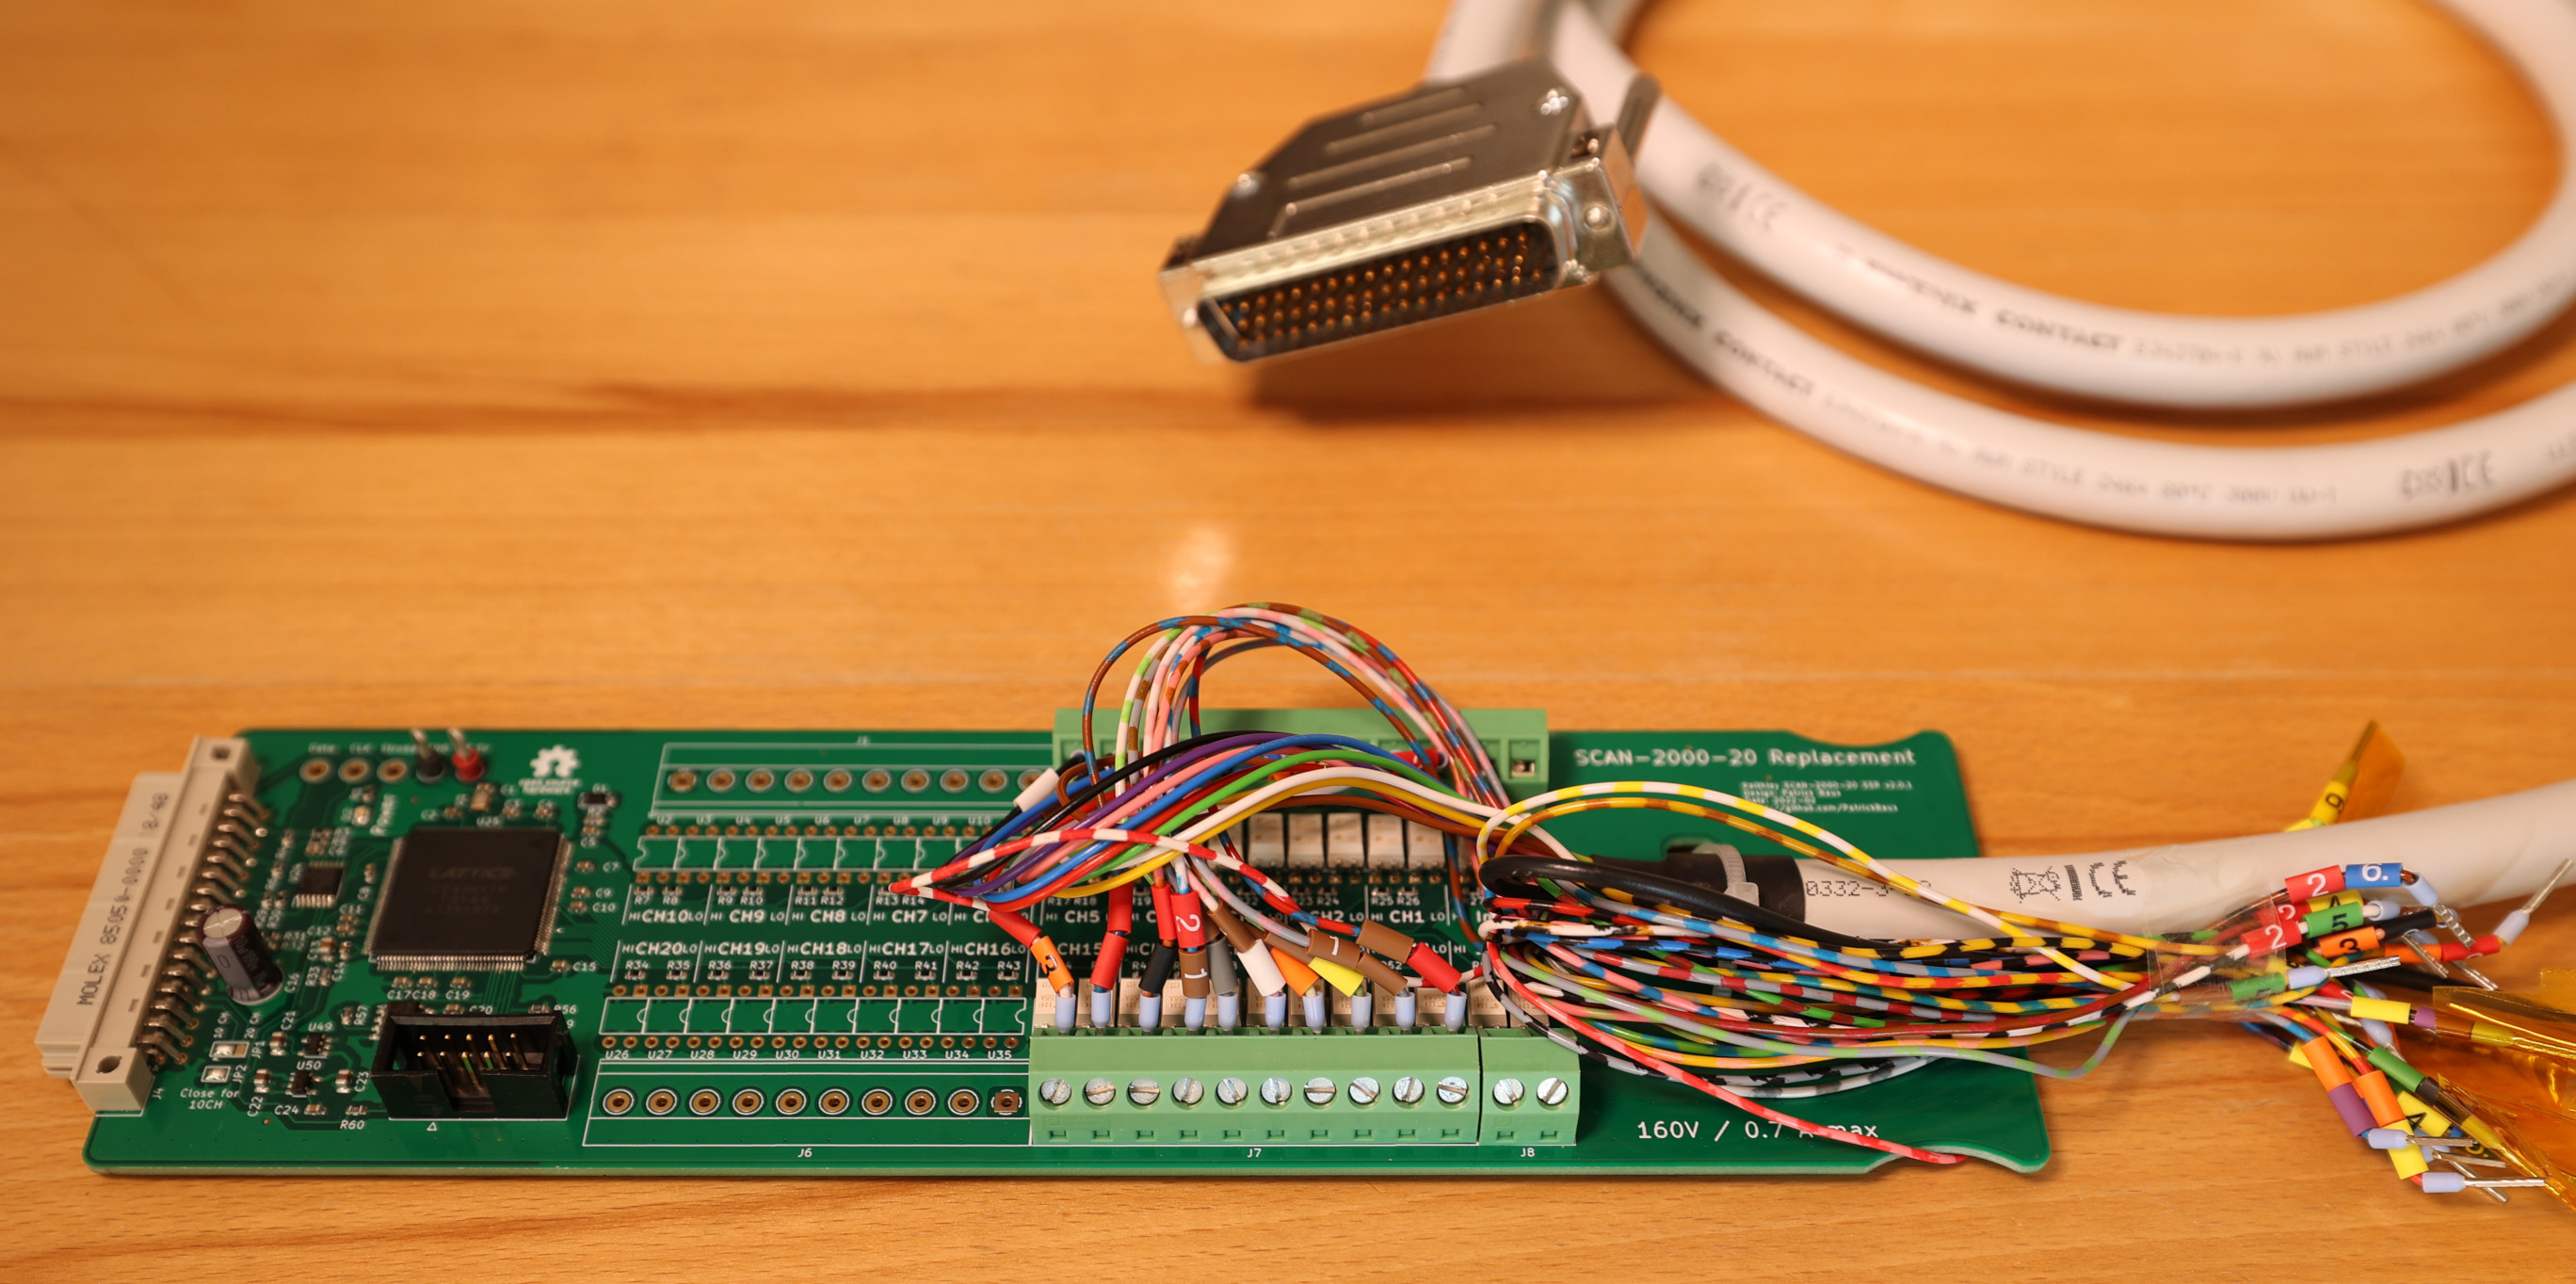
\includegraphics[width=0.75\textwidth]{images/BM1A2145_SCAN2000_lowres.JPG}
    \caption{A \num{10} channel solid-state scanner module developed for the Keithley \device{Model 2002} including the connector for the reference PCB.}
    \label{fig:scan200_pcb}
\end{figure}

With a scanner and multimeter selected, the focus now lies on the test fixture for the Zener diode. This test setup consists of a mounting PCB, that holds up to 20 Zener diodes \cite{git_lm399_burnin_board}. It provides power regulation and a minimal circuit required to support each diode. This circuit is shown in figure \ref{fig:zener_burnin}.
\begin{figure}[ht]
    \centering
    %\scalebox{0.7} % scalebox
    \caption{Circuit used for the burn-in of \device{LM399} and \device{ADR1399} Zener diodes.}
    \label{fig:zener_burnin}
\end{figure}

The compensation network is required when using the \device{ADR1399}, because of its very low dynamic impedance as recommended in the data sheet \cite{datasheet_ADR1399}. It is not strictly required for the \device{LM399}, but fitted nonetheless, because there are no downsides to it. This makes the board compatible with both types of references. Each Zener diode output is protected using a buffer, which provides isolation and short circuit protection. Finally there is a common mode filter at the output to suppress high frequency noise via ground loops.

Using this test setup, \num{102} \device{LM399} Zener diodes were tested up to this date (2023-04). Of those \num{39} were found suitable for the \device{DgDrive}. This low yield of only \qty{40}{\percent} is a matter of concern and has significantly delayed the development and production of the drivers. Using the automated test setup, the latter issue is manageable, but still slows down the production. Tests are currently conducted to replace the \device{LM399} with the newer \device{ADR1399} Zener diode, but unfortunately, it is still not available in quantities surpassing individual samples. Two of those samples were thoroughly tested and showed significantly better performance in terms of both lower white noise and reduced burst noise. Although these results are promising, more samples need to be tested to give a final verdict. Using the screened Zener diodes a first batch of \num{15} laser drivers was built.

\subsection{Summary}%
\label{sec_dgDrive_summary}
\begin{figure}[h]
    \centering
    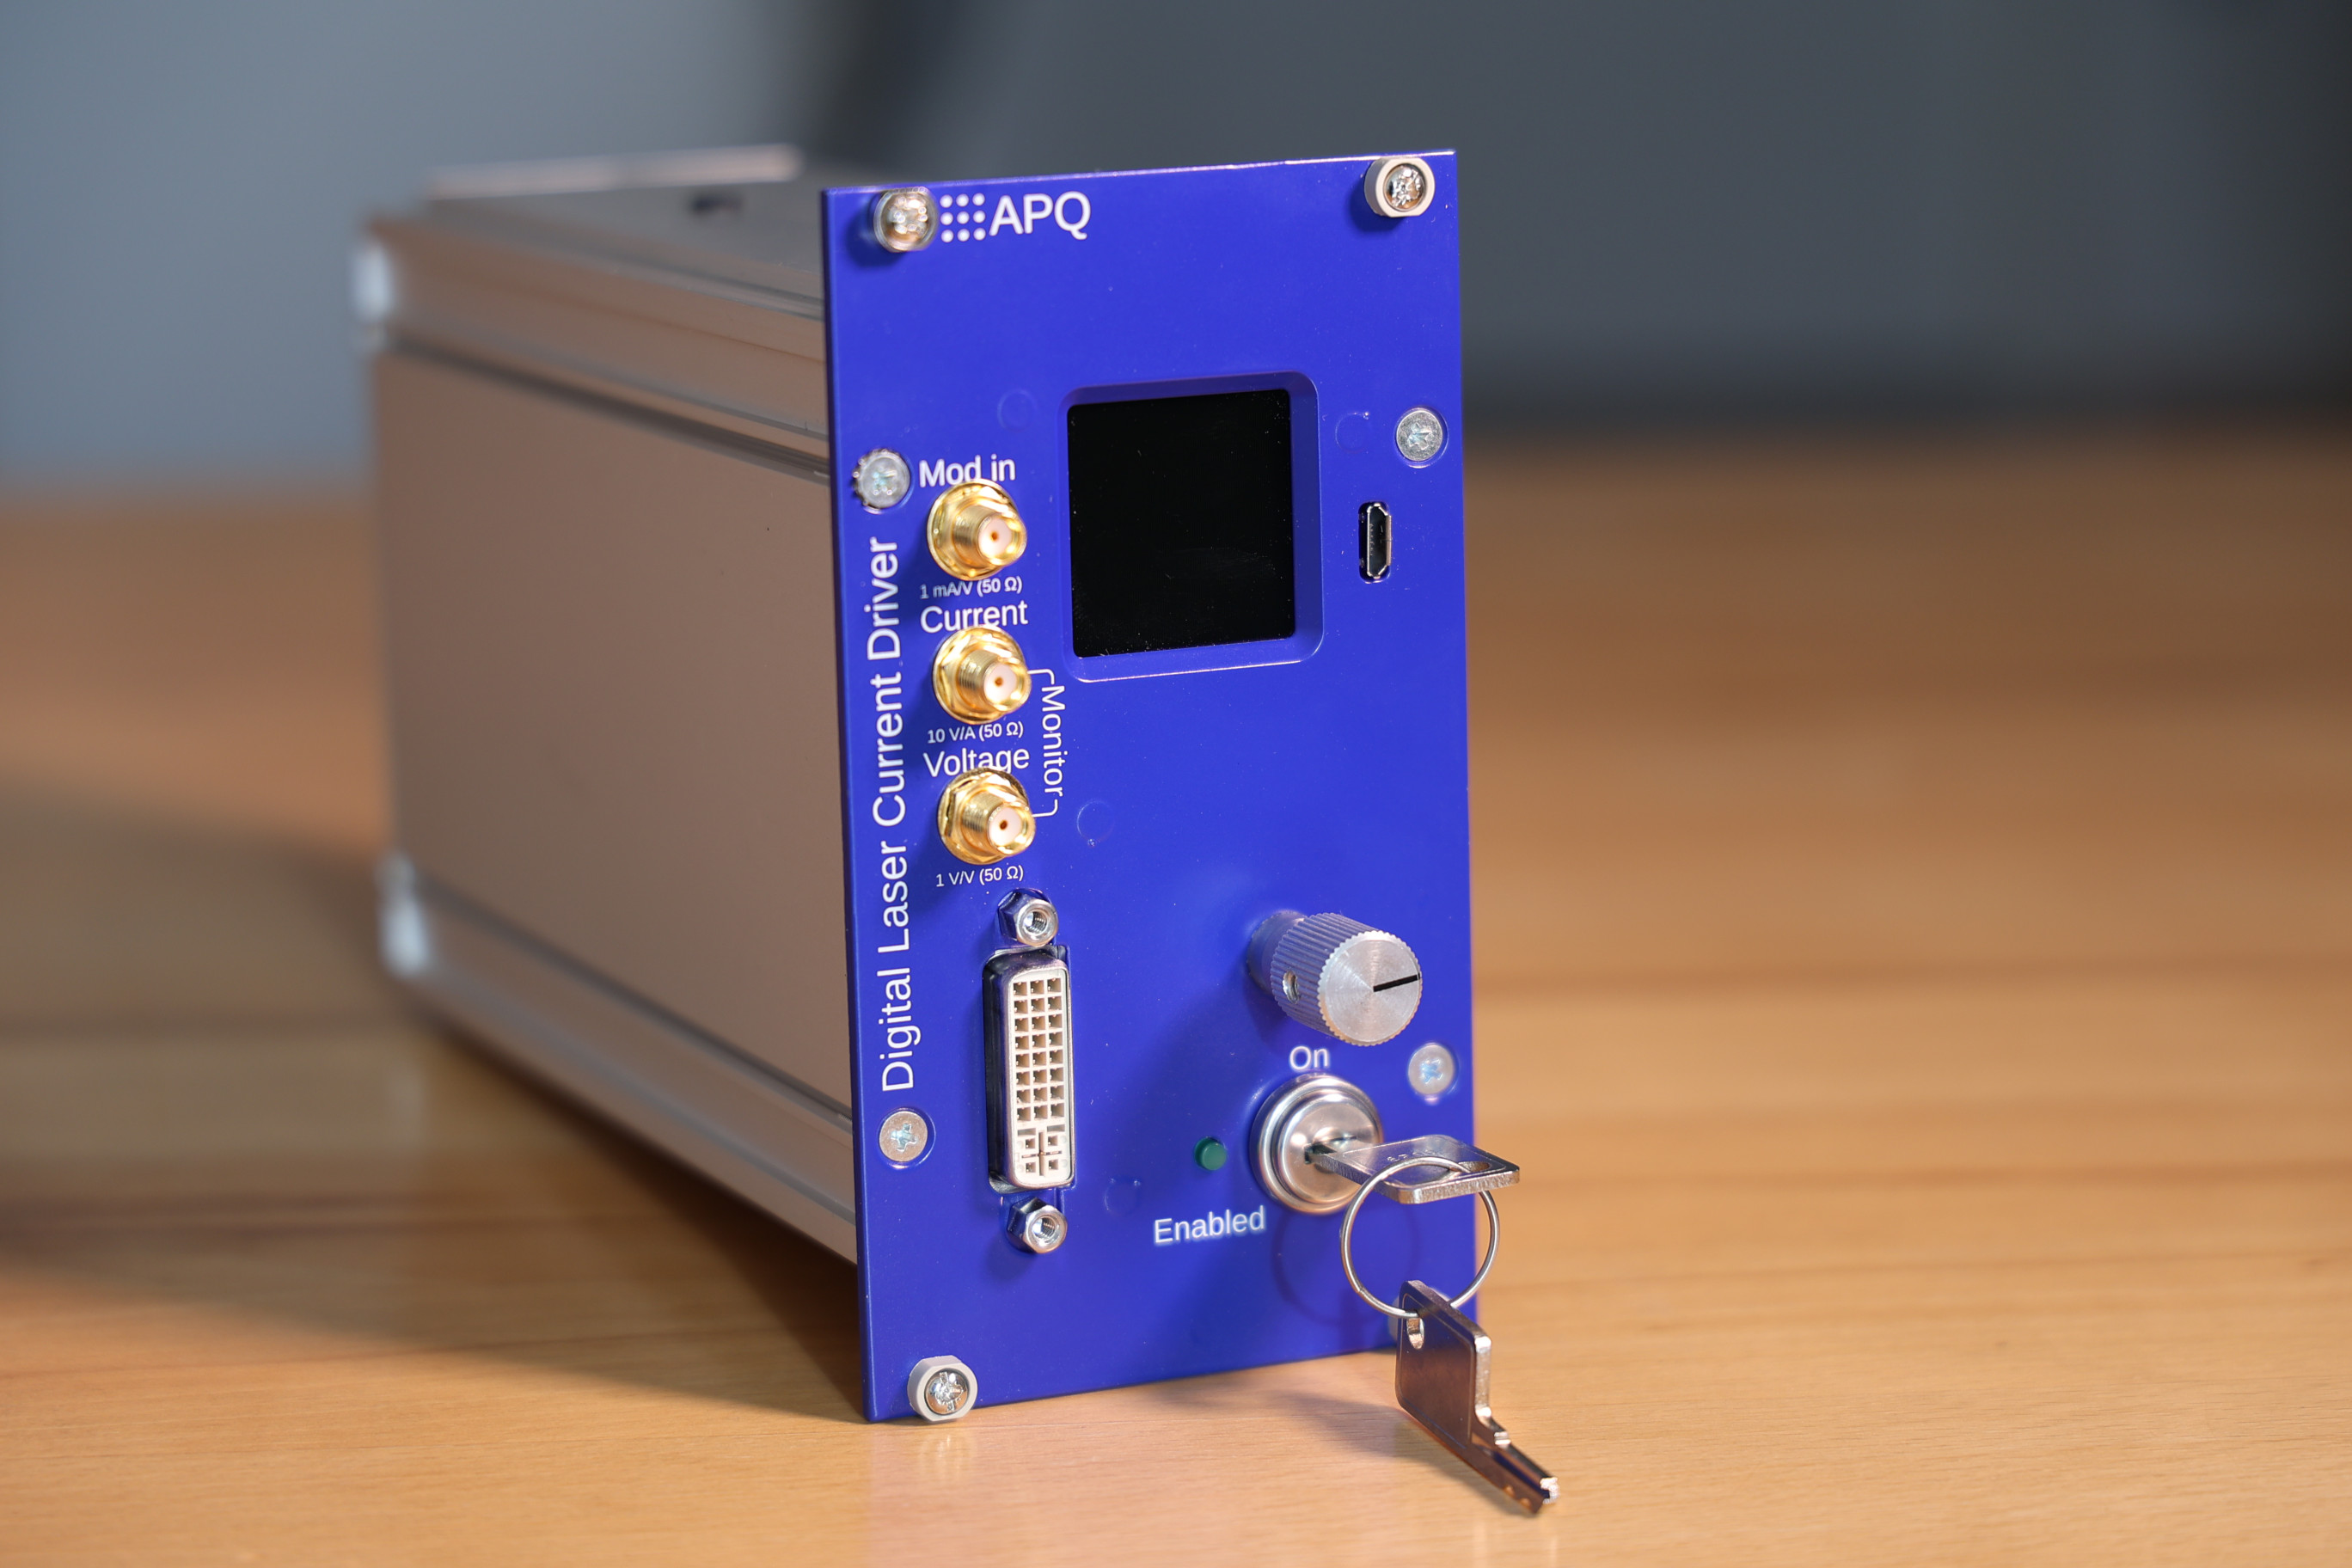
\includegraphics[width=0.75\textwidth]{images/BM1A6451_dgDrive_lowres.JPG}
    \caption{Picture of the digital current driver \device{DgDrive}.}
\end{figure}

This section saw the evaluation of several commercial current driver representing the state of the art at the time of writing. These drivers were all found to be unsuitable to drive modern blue laser diodes like the Osram \device{PL 450B} \cite{datasheet_osram_pl450b} used in the ARTEMIS experiment for the \qty{453}{\nm} master laser. The most common problem identified was the limited compliance voltage especially with low-noise drivers like the Vescent \device{D2-105}, which can barely drive modern high power laser diodes like the Thorlabs \device{L785H1} \cite{datasheet_thorlabs_780nm} that require a compliance voltage of more than \qty{2.5}{\V} at high currents. The only solution with such driver is to use a higher output current model and run it at a reduced current. This strategy negatively impact the noise figure as higher current model have a higher output noise. Additionally, node of the low noise drivers have a digital interface to allow remote control.

To address these problems, a new laser driver design is presented that not only surpasses all commercial alternatives, both in performance and price, but also delivers the much needed digital interface to integrate into modern experimental setups. To address the compliance voltage issue which is an inherent problem in the original design by \citeauthor{libbrecht_hall} \cite{libbrecht_hall} upon which all of the driver tested rely one, a novel current source configuration was developed that separates the current source from the load. This ensures low noise, a high compliance voltage and strong noise immunity.

The current driver performance was demonstrated in several of the previous sections and a summary of those finding can be found in the following table.
\begin{center}
    \begin{deviceProperties}[label={lst:dgDrive_summary}]{DgDrive device properties}
    \begin{itemize}
        \item Maximum output current: \qty{500}{\mA} (p. \pageref{tab:dgDrive_configurations})
        \item Temperature coefficient: $\qty{0.1}{\uA \per \K} + \qty{0.5}{\uA \per \A \per \K} \cdot I_{out}$ (p. \pageref{fig:dgDrive_tempco_50mA})
        \item Stability: \qty{< 1 \pm 2}{\uA \per \A \per a} (p. \pageref{fig:stability_dgDrive})
        \item Noise: \qty{< 70}{\pA \per \Hz\tothe{0.5}} above \qty{100}{\Hz} (\pageref{fig:laser_driver_noise_measurement})
        \item Below shot noise above \qty{20}{\mA} for the \qty{500}{\mA} version. (p. \pageref{fig:laser_driver_noise_hmp4040})
        \item Modulation bandwidth: \qty{1}{\MHz} (p. \pageref{fig:dgDrive_modulation_amplitude})
        \item Output impedance: \qty{>1}{\giga\ohm} resulting in excellent noise immunity (p. \pageref{fig:dgDrive_output_impedance_comparison})
        \item Digital control
        \item Python API for remote control
    \end{itemize}
    \end{deviceProperties}
\end{center}

%\begin{figure}[h]
%    \centering
    %\import{figures/}{dgDrive_protocol.tex}
%\end{figure}

%Custom made cables with PTFE insulator, silver plated AWG18 copper wires with a braided shield, M27500

\clearpage








\begin{figure}[ht]
    \centering
\end{figure}





\begin{figure}[ht]
    \centering
\end{figure}

    \centering
        \toprule
        \midrule
        \bottomrule
    \end{tabular}
\end{table}


    \centering
\end{figure}


    \centering
\end{figure}


    \centering
\end{figure}




